\documentclass[twoside,11pt]{article}

% Any additional packages needed should be included after jmlr2e.
% Note that jmlr2e.sty includes epsfig, amssymb, natbib and graphicx,
% and defines many common macros, such as 'proof' and 'example'.
%
% It also sets the bibliographystyle to plainnat; for more information on
% natbib citation styles, see the natbib documentation, a copy of which
% is archived at http://www.jmlr.org/format/natbib.pdf

\usepackage{jmlr2e}

% Definitions of handy macros can go here

\usepackage{subcaption}
\usepackage{tikz}
% \usetikzlibrary{positioning, automata, arrows}
\usepackage{tikz-cd}
\usepackage{pgfplots}
\usepackage{amsmath}
\usepackage{cleveref}

\usepackage{todonotes}
\setuptodonotes{inline}

\usepackage{csquotes}

\usetikzlibrary{
  arrows.meta,                        % for arrow tips
  backgrounds,                        % for background layer
  ext.paths.ortho,                    % for ortho paths
  ext.positioning-plus,               % for 
  ext.node-families.shapes.geometric, % loads ext.node-families and
% shapes.geometric,                   % for ellipse
  calc}                               % for ($<calculations>$)
\pgfplotsset{compat=newest}
\usepgfplotslibrary{patchplots}
\usepgfplotslibrary{fillbetween}
\pgfplotsset{%
    layers/standard/.define layer set={%
        background,axis background,axis grid,axis ticks,axis lines,axis tick labels,pre main,main,axis descriptions,axis foreground%
    }{
        grid style={/pgfplots/on layer=axis grid},%
        tick style={/pgfplots/on layer=axis ticks},%
        axis line style={/pgfplots/on layer=axis lines},%
        label style={/pgfplots/on layer=axis descriptions},%
        legend style={/pgfplots/on layer=axis descriptions},%
        title style={/pgfplots/on layer=axis descriptions},%
        colorbar style={/pgfplots/on layer=axis descriptions},%
        ticklabel style={/pgfplots/on layer=axis tick labels},%
        axis background@ style={/pgfplots/on layer=axis background},%
        3d box foreground style={/pgfplots/on layer=axis foreground},%
    },
}

\usepgfplotslibrary{groupplots}
\usepgfplotslibrary{polar}
\usepgfplotslibrary{smithchart}
\usepgfplotslibrary{statistics}
\usepgfplotslibrary{dateplot}
\usepgfplotslibrary{ternary}

\tikzset{
  basic box/.style={
    shape=rectangle, rounded corners, align=center, draw=#1,very thick},
  header node/.style={
    node family/width=header nodes, rounded corners,
    text depth=+.3ex, fill=white, draw},
  header/.style={%
    inner ysep=+1.5em,
    append after command={
      \pgfextra{\let\TikZlastnode\tikzlastnode}
      node [header node] (header-\TikZlastnode) at (\TikZlastnode.north) {#1}
      % the next node contains both \tikzlastnode and its header
      % this is needed so that h-<name> can be used to connect lines
      node [span=(\TikZlastnode)(header-\TikZlastnode)]
           at (fit bounding box) (h-\TikZlastnode) {}
    }
  },
}


\newcommand{\dataset}{{\cal D}}
\newcommand{\fracpartial}[2]{\frac{\partial #1}{\partial  #2}}

\usepackage{xcolor}
\definecolor{onyx}{HTML}{393E41}
\definecolor{redviolet}{HTML}{8B2635}
\definecolor{munsellblue}{HTML}{4B88A2}
\definecolor{maxpurple}{HTML}{7E2E84}
\hypersetup{
    hidelinks,
    citecolor={green!50!black},
    urlcolor={blue!80!black}
}


% Heading arguments are {volume}{year}{pages}{submitted}{published}{author-full-names}

\jmlrheading{1}{2000}{1-48}{4/00}{10/00}{Authors}

% Short headings should be running head and authors last names

\ShortHeadings{Paper Title}{Authors}
\firstpageno{1}

\begin{document}

\title{Paper Title}

\author{Authors}

\editor{Editor}

\maketitle

\begin{abstract}%   <- trailing '%' for backward compatibility of .sty file
TODO
\end{abstract}

\begin{keywords}
\end{keywords}

\section{Introduction}

\begin{itemize}
    \item Latent SDEs are a recent technique that combines generative machine learning with stochastic differential equations
    \item Promise of many advantages to recurrent techniques for stochastic time series: model entirely expressed as SDE \(\implies\) arbitrary discretization, elegant formulation, better analysis of model, constraint "it is an SDE" often useful
    \item Potential applications, for instance, in paleoclimatology
    \item Goal: match probability distribution of data with distribution of SDEs
    \item We show that latent SDEs do not match the probability distribution, in particular cannot replicate the diffusion
    \item First thorough experimental investigation of latent SDE behavior
    \item Explain why and propose solution
\end{itemize}

\section{Related Work}
Neural SDEs are probabilistic machine learning methods, a general term for any machine learning method where the model yields a probability distribution. In different applications of the same method, this distribution may have a different meaning to the modeler. Probabilistic machine learning methods are often used for uncertainty quantification within a Bayesian framework.

A standard probabilistic machine learning method is the Gaussian Process (GP) \citep{williams2006gaussian}. A GP is a generalized Gaussian distribution over the path space. GPs always have Gaussian marginals, making their distribution easy to reason about (whereas the distribution of an SDE is hard to reason about) but limiting their modeling capacity. As such, they are often used for uncertainty quantification and cannot be used for matching the probability distribution of an arbitrary stochastic time series.

Neural SDEs can also be used for uncertainty quantification. However, we use them for something else: we aim to match the probability distribution of the model to the \enquote{distribution of the data}. This is the goal of generative machine learning. Generative machine learning methods add a framework around the generator, in this case, a neural SDE, so that they can learn from data in an unsupervised way. We do not propose a new method but look into applying one of two already existing methods to the problem: SDE-GANs \citep{kidgergan} and latent neural SDEs \citep{li2020scalable}. Neural SDEs can be viewed as an extension of neural ordinary differential equations (neural ODEs) \citep{chen2018neural}, but neural ODEs are not generative or otherwise probabilistic models.

Score-based diffusion models are a recent trend involving stochastic differential equations and generative machine learning \citep{song2020score}. The methods used in these models are interested in a probability distribution induced through the marginals of an SDE at some point. A data sample is an element of the SDE's state space. In contrast, neural SDEs are interested in the probability distribution of an SDE on the path space. A data sample is a path over the SDE's state space.

The main contributions of this thesis are a thorough investigation of applying the latent neural SDE method proposed by \cite{li2020scalable} to datasets similar to paleoclimate data. Other papers extend that same paper. We only mention published papers or papers accepted to workshops, as many preprints exist. \cite{fagin2023latent} apply latent SDEs to data from astrophysics. They use them as a drop-in replacement for Gaussian Processes, so the noise is interpreted as uncertainty. \cite{xu} consider latent SDEs with a fixed diffusion, a continuous analog of Bayesian recurrent neural networks. \cite{kidgerefficient} introduce a reversible Heun solver for differential equations and train a latent neural SDE on an air quality data set from Beijing. \cite{hasan2021identifying} propose a different latent SDE framework to recover a mapping from one high-dimensional probabilistic space to another.

\section{Latent SDEs}

\newsavebox{\dataplot}
\sbox{\dataplot}{%
% Recommended preamble:
% \usetikzlibrary{arrows.meta}
% \usetikzlibrary{backgrounds}
% \usepgfplotslibrary{patchplots}
% \usepgfplotslibrary{fillbetween}
% \pgfplotsset{%
%     layers/standard/.define layer set={%
%         background,axis background,axis grid,axis ticks,axis lines,axis tick labels,pre main,main,axis descriptions,axis foreground%
%     }{
%         grid style={/pgfplots/on layer=axis grid},%
%         tick style={/pgfplots/on layer=axis ticks},%
%         axis line style={/pgfplots/on layer=axis lines},%
%         label style={/pgfplots/on layer=axis descriptions},%
%         legend style={/pgfplots/on layer=axis descriptions},%
%         title style={/pgfplots/on layer=axis descriptions},%
%         colorbar style={/pgfplots/on layer=axis descriptions},%
%         ticklabel style={/pgfplots/on layer=axis tick labels},%
%         axis background@ style={/pgfplots/on layer=axis background},%
%         3d box foreground style={/pgfplots/on layer=axis foreground},%
%     },
% }

\begin{tikzpicture}[/tikz/background rectangle/.style={fill={rgb,1:red,1.0;green,1.0;blue,1.0}, fill opacity={0.0}, draw opacity={0.0}}, show background rectangle]
\begin{axis}[point meta max={nan}, point meta min={nan}, legend cell align={left}, legend columns={1}, title={}, title style={at={{(0.5,1)}}, anchor={south}, font={{\fontsize{14 pt}{18.2 pt}\selectfont}}, color={rgb,1:red,0.0;green,0.0;blue,0.0}, draw opacity={1.0}, rotate={0.0}, align={center}}, legend style={color={rgb,1:red,0.0;green,0.0;blue,0.0}, draw opacity={1.0}, line width={1}, solid, fill={rgb,1:red,1.0;green,1.0;blue,1.0}, fill opacity={0.0}, text opacity={1.0}, font={{\fontsize{8 pt}{10.4 pt}\selectfont}}, text={rgb,1:red,0.0;green,0.0;blue,0.0}, cells={anchor={center}}, at={(1.02, 1)}, anchor={north west}}, axis background/.style={fill={rgb,1:red,1.0;green,1.0;blue,1.0}, opacity={0.0}}, anchor={north west}, xshift={1.0mm}, yshift={-1.0mm}, width={125.0mm}, height={61.5mm}, scaled x ticks={false}, xlabel={}, x tick style={color={rgb,1:red,0.0;green,0.0;blue,0.0}, opacity={1.0}}, x tick label style={color={rgb,1:red,0.0;green,0.0;blue,0.0}, opacity={1.0}, rotate={0}}, xlabel style={at={(ticklabel cs:0.5)}, anchor=near ticklabel, at={{(ticklabel cs:0.5)}}, anchor={near ticklabel}, font={{\fontsize{11 pt}{14.3 pt}\selectfont}}, color={rgb,1:red,0.0;green,0.0;blue,0.0}, draw opacity={1.0}, rotate={0.0}}, xmajorgrids={false}, xmin={-0.6000000000000014}, xmax={20.6}, xticklabels={{}}, xtick={{}}, xtick style={draw=none}, xticklabel style={font={{\fontsize{8 pt}{10.4 pt}\selectfont}}, color={rgb,1:red,0.0;green,0.0;blue,0.0}, draw opacity={1.0}, rotate={0.0}}, x grid style={color={rgb,1:red,0.0;green,0.0;blue,0.0}, draw opacity={0.1}, line width={0.5}, solid}, axis x line*={left}, separate axis lines, x axis line style={{draw opacity = 0}}, scaled y ticks={false}, ylabel={}, y tick style={color={rgb,1:red,0.0;green,0.0;blue,0.0}, opacity={1.0}}, y tick label style={color={rgb,1:red,0.0;green,0.0;blue,0.0}, opacity={1.0}, rotate={0}}, ylabel style={at={(ticklabel cs:0.5)}, anchor=near ticklabel, at={{(ticklabel cs:0.5)}}, anchor={near ticklabel}, font={{\fontsize{11 pt}{14.3 pt}\selectfont}}, color={rgb,1:red,0.0;green,0.0;blue,0.0}, draw opacity={1.0}, rotate={0.0}}, ymajorgrids={false}, ymin={0.35618046155633776}, ymax={0.7659114545145511}, yticklabels={{}}, ytick={{}}, ytick style={draw=none}, yticklabel style={font={{\fontsize{8 pt}{10.4 pt}\selectfont}}, color={rgb,1:red,0.0;green,0.0;blue,0.0}, draw opacity={1.0}, rotate={0.0}}, y grid style={color={rgb,1:red,0.0;green,0.0;blue,0.0}, draw opacity={0.1}, line width={0.5}, solid}, axis y line*={left}, y axis line style={{draw opacity = 0}}, colorbar={false}]
    \addplot[color={rgb,1:red,0.0;green,0.0;blue,0.0}, name path={832575b1-b2b6-446e-aa47-8001a8523ca9}, draw opacity={1.0}, line width={1}, solid]
        table[row sep={\\}]
        {
            \\
            0.0  0.4823432601040162  \\
            0.8333333333333334  0.4616003052225949  \\
            1.6666666666666667  0.45385454544295467  \\
            2.5  0.44541283961663963  \\
            3.3333333333333335  0.44081169479489796  \\
            4.166666666666667  0.4121605009713489  \\
            5.0  0.40304304009322667  \\
            5.833333333333333  0.3959550425713564  \\
            6.666666666666667  0.3952495278072296  \\
            7.5  0.36777662173440046  \\
            8.333333333333334  0.40802452589304056  \\
            9.166666666666666  0.4461731626617858  \\
            10.0  0.5224955721757875  \\
            10.833333333333334  0.4677833720651737  \\
            11.666666666666666  0.4682796706089865  \\
            12.5  0.41228193079681785  \\
            13.333333333333334  0.4209019560732842  \\
            14.166666666666666  0.4840165941272772  \\
            15.0  0.48621059614021617  \\
            15.833333333333334  0.5534786355466049  \\
            16.666666666666668  0.6513833625898784  \\
            17.5  0.6832508192526212  \\
            18.333333333333332  0.7104365711818745  \\
            19.166666666666668  0.7358904662784639  \\
            20.0  0.7543152943364885  \\
        }
        ;
\end{axis}
\end{tikzpicture}

}

\newsavebox{\posteriorplot}
\sbox{\posteriorplot}{%
% Recommended preamble:
% \usetikzlibrary{arrows.meta}
% \usetikzlibrary{backgrounds}
% \usepgfplotslibrary{patchplots}
% \usepgfplotslibrary{fillbetween}
% \pgfplotsset{%
%     layers/standard/.define layer set={%
%         background,axis background,axis grid,axis ticks,axis lines,axis tick labels,pre main,main,axis descriptions,axis foreground%
%     }{
%         grid style={/pgfplots/on layer=axis grid},%
%         tick style={/pgfplots/on layer=axis ticks},%
%         axis line style={/pgfplots/on layer=axis lines},%
%         label style={/pgfplots/on layer=axis descriptions},%
%         legend style={/pgfplots/on layer=axis descriptions},%
%         title style={/pgfplots/on layer=axis descriptions},%
%         colorbar style={/pgfplots/on layer=axis descriptions},%
%         ticklabel style={/pgfplots/on layer=axis tick labels},%
%         axis background@ style={/pgfplots/on layer=axis background},%
%         3d box foreground style={/pgfplots/on layer=axis foreground},%
%     },
% }

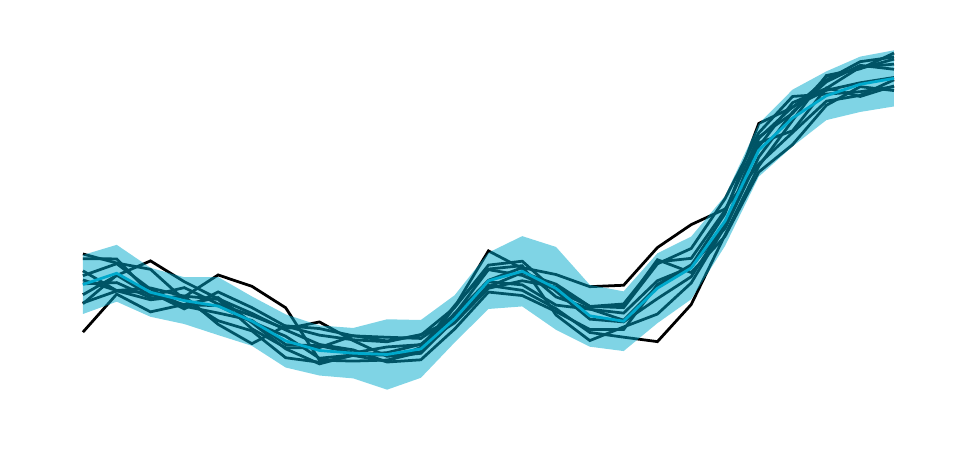
\begin{tikzpicture}[/tikz/background rectangle/.style={fill={rgb,1:red,1.0;green,1.0;blue,1.0}, fill opacity={0.0}, draw opacity={0.0}}, show background rectangle]
\begin{axis}[point meta max={nan}, point meta min={nan}, legend cell align={left}, legend columns={1}, title={}, title style={at={{(0.5,1)}}, anchor={south}, font={{\fontsize{14 pt}{18.2 pt}\selectfont}}, color={rgb,1:red,0.0;green,0.0;blue,0.0}, draw opacity={1.0}, rotate={0.0}, align={center}}, legend style={color={rgb,1:red,0.0;green,0.0;blue,0.0}, draw opacity={1.0}, line width={1}, solid, fill={rgb,1:red,1.0;green,1.0;blue,1.0}, fill opacity={0.0}, text opacity={1.0}, font={{\fontsize{8 pt}{10.4 pt}\selectfont}}, text={rgb,1:red,0.0;green,0.0;blue,0.0}, cells={anchor={center}}, at={(1.02, 1)}, anchor={north west}}, axis background/.style={fill={rgb,1:red,1.0;green,1.0;blue,1.0}, opacity={0.0}}, anchor={north west}, xshift={1.0mm}, yshift={-1.0mm}, width={125.0mm}, height={61.5mm}, scaled x ticks={false}, xlabel={}, x tick style={color={rgb,1:red,0.0;green,0.0;blue,0.0}, opacity={1.0}}, x tick label style={color={rgb,1:red,0.0;green,0.0;blue,0.0}, opacity={1.0}, rotate={0}}, xlabel style={at={(ticklabel cs:0.5)}, anchor=near ticklabel, at={{(ticklabel cs:0.5)}}, anchor={near ticklabel}, font={{\fontsize{11 pt}{14.3 pt}\selectfont}}, color={rgb,1:red,0.0;green,0.0;blue,0.0}, draw opacity={1.0}, rotate={0.0}}, xmajorgrids={false}, xmin={-0.6000000000000014}, xmax={20.6}, xticklabels={{}}, xtick={{}}, xtick style={draw=none}, xticklabel style={font={{\fontsize{8 pt}{10.4 pt}\selectfont}}, color={rgb,1:red,0.0;green,0.0;blue,0.0}, draw opacity={1.0}, rotate={0.0}}, x grid style={color={rgb,1:red,0.0;green,0.0;blue,0.0}, draw opacity={0.1}, line width={0.5}, solid}, axis x line*={left}, separate axis lines, x axis line style={{draw opacity = 0}}, scaled y ticks={false}, ylabel={}, y tick style={color={rgb,1:red,0.0;green,0.0;blue,0.0}, opacity={1.0}}, y tick label style={color={rgb,1:red,0.0;green,0.0;blue,0.0}, opacity={1.0}, rotate={0}}, ylabel style={at={(ticklabel cs:0.5)}, anchor=near ticklabel, at={{(ticklabel cs:0.5)}}, anchor={near ticklabel}, font={{\fontsize{11 pt}{14.3 pt}\selectfont}}, color={rgb,1:red,0.0;green,0.0;blue,0.0}, draw opacity={1.0}, rotate={0.0}}, ymajorgrids={false}, ymin={0.3272350250097698}, ymax={0.7805860917385203}, yticklabels={{}}, ytick={{}}, ytick style={draw=none}, yticklabel style={font={{\fontsize{8 pt}{10.4 pt}\selectfont}}, color={rgb,1:red,0.0;green,0.0;blue,0.0}, draw opacity={1.0}, rotate={0.0}}, y grid style={color={rgb,1:red,0.0;green,0.0;blue,0.0}, draw opacity={0.1}, line width={0.5}, solid}, axis y line*={left}, y axis line style={{draw opacity = 0}}, colorbar={false}]
    \addplot[color={rgb,1:red,0.0;green,0.0;blue,0.0}, name path={2e7de59c-639b-4f1c-aaba-db217a2b7117}, draw opacity={1.0}, line width={1}, solid]
        table[row sep={\\}]
        {
            \\
            0.0  0.44938593900417284  \\
            0.8333333333333334  0.46444823766501275  \\
            1.6666666666666667  0.46245253027102406  \\
            2.5  0.44188845652643627  \\
            3.3333333333333335  0.4632905271834473  \\
            4.166666666666667  0.44351809977573775  \\
            5.0  0.41999961354616533  \\
            5.833333333333333  0.4087721294762502  \\
            6.666666666666667  0.40294243764773174  \\
            7.5  0.40043820025766264  \\
            8.333333333333334  0.4095251959715347  \\
            9.166666666666666  0.42895008089191755  \\
            10.0  0.4697995040150159  \\
            10.833333333333334  0.48763138894787883  \\
            11.666666666666666  0.47305023466854046  \\
            12.5  0.4450680922365966  \\
            13.333333333333334  0.44345719713134135  \\
            14.166666666666666  0.4986086806618486  \\
            15.0  0.5180291871495082  \\
            15.833333333333334  0.5806145963553282  \\
            16.666666666666668  0.663900411008732  \\
            17.5  0.7096169484693471  \\
            18.333333333333332  0.7125777035566347  \\
            19.166666666666668  0.7155753335496421  \\
            20.0  0.7219895586822785  \\
        }
        ;
    \addplot[color={rgb,1:red,0.0;green,0.0;blue,0.0}, name path={8fd1c3de-dbdb-4c42-8873-c62a9fbabcfa}, draw opacity={1.0}, line width={1}, solid]
        table[row sep={\\}]
        {
            \\
            0.0  0.4125620060931739  \\
            0.8333333333333334  0.4604788590952095  \\
            1.6666666666666667  0.43812360974290765  \\
            2.5  0.44747679076369606  \\
            3.3333333333333335  0.45613545997195404  \\
            4.166666666666667  0.42448240926139447  \\
            5.0  0.39153907420701217  \\
            5.833333333333333  0.3726030442442515  \\
            6.666666666666667  0.3837740318421863  \\
            7.5  0.3867211176189447  \\
            8.333333333333334  0.39725898978665153  \\
            9.166666666666666  0.42429540018957634  \\
            10.0  0.46787368730732937  \\
            10.833333333333334  0.4773104152931672  \\
            11.666666666666666  0.4693537825211118  \\
            12.5  0.4449160108992183  \\
            13.333333333333334  0.44809023529598213  \\
            14.166666666666666  0.5010556318921853  \\
            15.0  0.505590036534601  \\
            15.833333333333334  0.5659531547800857  \\
            16.666666666666668  0.6585278987924733  \\
            17.5  0.6883530506961542  \\
            18.333333333333332  0.7348587480277574  \\
            19.166666666666668  0.7444725152696111  \\
            20.0  0.7642692037051267  \\
        }
        ;
    \addplot[color={rgb,1:red,0.0;green,0.0;blue,0.0}, name path={75f3df05-ea83-4567-be90-160eb3deec8e}, draw opacity={1.0}, line width={1}, solid]
        table[row sep={\\}]
        {
            \\
            0.0  0.4783404372241217  \\
            0.8333333333333334  0.46504199869941454  \\
            1.6666666666666667  0.46823837768755183  \\
            2.5  0.4578190880525165  \\
            3.3333333333333335  0.4224170868096935  \\
            4.166666666666667  0.39805158507340266  \\
            5.0  0.42052799200383617  \\
            5.833333333333333  0.4170749791984949  \\
            6.666666666666667  0.4078949363267107  \\
            7.5  0.40611727821012944  \\
            8.333333333333334  0.4046474783267834  \\
            9.166666666666666  0.4335858319794972  \\
            10.0  0.47794407924163806  \\
            10.833333333333334  0.4938207849965617  \\
            11.666666666666666  0.48516336427140594  \\
            12.5  0.4698891820633714  \\
            13.333333333333334  0.4716726251623943  \\
            14.166666666666666  0.5191734547475391  \\
            15.0  0.5481035711157844  \\
            15.833333333333334  0.5676993406625254  \\
            16.666666666666668  0.6244761719708849  \\
            17.5  0.6641570926063946  \\
            18.333333333333332  0.7036739511780281  \\
            19.166666666666668  0.7109795457655174  \\
            20.0  0.7305560190432372  \\
        }
        ;
    \addplot[color={rgb,1:red,0.0;green,0.0;blue,0.0}, name path={f8ad204a-3802-4ea7-bce6-ad33f54ae2fa}, draw opacity={1.0}, line width={1}, solid]
        table[row sep={\\}]
        {
            \\
            0.0  0.4836917486325893  \\
            0.8333333333333334  0.4988248143207046  \\
            1.6666666666666667  0.4668686790868609  \\
            2.5  0.44525892246956744  \\
            3.3333333333333335  0.4366937944173447  \\
            4.166666666666667  0.427376578356903  \\
            5.0  0.3968572123355659  \\
            5.833333333333333  0.3953979784408863  \\
            6.666666666666667  0.38641673905745555  \\
            7.5  0.39390042739207776  \\
            8.333333333333334  0.396775163363577  \\
            9.166666666666666  0.43511861952031117  \\
            10.0  0.49131218719397085  \\
            10.833333333333334  0.48413723099190376  \\
            11.666666666666666  0.4655330568452438  \\
            12.5  0.44483699724948367  \\
            13.333333333333334  0.44485848748029755  \\
            14.166666666666666  0.5038299249872227  \\
            15.0  0.4876903820743831  \\
            15.833333333333334  0.5333313533712768  \\
            16.666666666666668  0.614405865054769  \\
            17.5  0.6489148764696122  \\
            18.333333333333332  0.6984784052177312  \\
            19.166666666666668  0.721957423858036  \\
            20.0  0.7170198038867643  \\
        }
        ;
    \addplot[color={rgb,1:red,0.0;green,0.0;blue,0.0}, name path={7cccdadf-1321-4d5f-ba5b-dd33d95251dd}, draw opacity={1.0}, line width={1}, solid]
        table[row sep={\\}]
        {
            \\
            0.0  0.44836106053778074  \\
            0.8333333333333334  0.484395087678673  \\
            1.6666666666666667  0.45877101749003124  \\
            2.5  0.4686509099852577  \\
            3.3333333333333335  0.44808190209099197  \\
            4.166666666666667  0.4334558509354507  \\
            5.0  0.41677263295686195  \\
            5.833333333333333  0.42543290847631754  \\
            6.666666666666667  0.4018775552311553  \\
            7.5  0.38204011408465854  \\
            8.333333333333334  0.3858751691047272  \\
            9.166666666666666  0.4282037989428925  \\
            10.0  0.47139354234593056  \\
            10.833333333333334  0.46526794448256803  \\
            11.666666666666666  0.44210821446019644  \\
            12.5  0.41215037482872685  \\
            13.333333333333334  0.4062190332967234  \\
            14.166666666666666  0.4006205547227696  \\
            15.0  0.4474221356417796  \\
            15.833333333333334  0.5350443030052522  \\
            16.666666666666668  0.6218673480893404  \\
            17.5  0.6794577350664555  \\
            18.333333333333332  0.736014915683454  \\
            19.166666666666668  0.7448153938866515  \\
            20.0  0.7566420318315356  \\
        }
        ;
    \addplot[color={rgb,1:red,0.0;green,0.0;blue,0.0}, name path={b9ac4883-7b1c-463c-b1ed-a266a8bc82ec}, draw opacity={1.0}, line width={1}, solid]
        table[row sep={\\}]
        {
            \\
            0.0  0.5051781390808207  \\
            0.8333333333333334  0.5048548468783053  \\
            1.6666666666666667  0.4607458649783087  \\
            2.5  0.4470733754529669  \\
            3.3333333333333335  0.44595411212555847  \\
            4.166666666666667  0.42552538403441886  \\
            5.0  0.40739295313306756  \\
            5.833333333333333  0.379659738849886  \\
            6.666666666666667  0.38388127479466205  \\
            7.5  0.38392922295406495  \\
            8.333333333333334  0.38791170708271294  \\
            9.166666666666666  0.44440764410869815  \\
            10.0  0.5149719404011964  \\
            10.833333333333334  0.49276416614409313  \\
            11.666666666666666  0.4569371762626697  \\
            12.5  0.4419643558916486  \\
            13.333333333333334  0.4276110537581399  \\
            14.166666666666666  0.4701876691080573  \\
            15.0  0.49660933691109055  \\
            15.833333333333334  0.5618615992664596  \\
            16.666666666666668  0.675616879387983  \\
            17.5  0.6958678979014805  \\
            18.333333333333332  0.7303505632284354  \\
            19.166666666666668  0.753433069348942  \\
            20.0  0.7593781826324446  \\
        }
        ;
    \addplot[color={rgb,1:red,0.0;green,0.0;blue,0.0}, name path={4006bea0-de4e-48e8-9fdc-8149d85421e2}, draw opacity={1.0}, line width={1}, solid]
        table[row sep={\\}]
        {
            \\
            0.0  0.4597564602955859  \\
            0.8333333333333334  0.48404558023306365  \\
            1.6666666666666667  0.5023685533342899  \\
            2.5  0.47613931582712865  \\
            3.3333333333333335  0.45478761715787375  \\
            4.166666666666667  0.4362537521773274  \\
            5.0  0.41533637955482783  \\
            5.833333333333333  0.3970408642309051  \\
            6.666666666666667  0.39021246128802234  \\
            7.5  0.37490064640380183  \\
            8.333333333333334  0.3777274604897195  \\
            9.166666666666666  0.41651740919827673  \\
            10.0  0.46307256079994485  \\
            10.833333333333334  0.4586906165413076  \\
            11.666666666666666  0.4384549258199163  \\
            12.5  0.41591721696638784  \\
            13.333333333333334  0.4157689303028055  \\
            14.166666666666666  0.472593943460488  \\
            15.0  0.49735117161646325  \\
            15.833333333333334  0.5431946325210046  \\
            16.666666666666668  0.6334079269797819  \\
            17.5  0.6899493531228544  \\
            18.333333333333332  0.7280564678050198  \\
            19.166666666666668  0.7488065746448016  \\
            20.0  0.7438743876624948  \\
        }
        ;
    \addplot[color={rgb,1:red,0.0;green,0.0;blue,0.0}, name path={e1d7a2c1-1ee7-48ab-9657-eede7e62ffa8}, draw opacity={1.0}, line width={1}, solid]
        table[row sep={\\}]
        {
            \\
            0.0  0.48985497050949445  \\
            0.8333333333333334  0.46473949315250873  \\
            1.6666666666666667  0.453390558618865  \\
            2.5  0.4580368586002964  \\
            3.3333333333333335  0.45388313867560137  \\
            4.166666666666667  0.4167965370309936  \\
            5.0  0.39290006403371236  \\
            5.833333333333333  0.3930815063176585  \\
            6.666666666666667  0.40805233086081527  \\
            7.5  0.40143809313172785  \\
            8.333333333333334  0.4088133292177133  \\
            9.166666666666666  0.4435771861313653  \\
            10.0  0.4970613721380718  \\
            10.833333333333334  0.5019805209580227  \\
            11.666666666666666  0.4640952470064723  \\
            12.5  0.42895996446723894  \\
            13.333333333333334  0.42548400189179025  \\
            14.166666666666666  0.45481011273451477  \\
            15.0  0.48241546934336066  \\
            15.833333333333334  0.5480486066330518  \\
            16.666666666666668  0.6569932198879482  \\
            17.5  0.6964423484891551  \\
            18.333333333333332  0.7173743166575703  \\
            19.166666666666668  0.7268635976912927  \\
            20.0  0.7335401849818161  \\
        }
        ;
    \addplot[color={rgb,1:red,0.0;green,0.0;blue,0.0}, name path={90e91646-604d-4038-8d75-eac60eafb5b6}, draw opacity={1.0}, line width={1}, solid]
        table[row sep={\\}]
        {
            \\
            0.0  0.5110871503284784  \\
            0.8333333333333334  0.49966325913013493  \\
            1.6666666666666667  0.4917610645065047  \\
            2.5  0.45335761712864453  \\
            3.3333333333333335  0.42695166578207033  \\
            4.166666666666667  0.4141765643614417  \\
            5.0  0.3803083884421724  \\
            5.833333333333333  0.3746460884881281  \\
            6.666666666666667  0.3832247728341077  \\
            7.5  0.37569329975068066  \\
            8.333333333333334  0.3935096846600008  \\
            9.166666666666666  0.44609627024626997  \\
            10.0  0.4920832652778624  \\
            10.833333333333334  0.4963351515650464  \\
            11.666666666666666  0.43413041923325324  \\
            12.5  0.4019563088915695  \\
            13.333333333333334  0.41911647941988217  \\
            14.166666666666666  0.43536554043159603  \\
            15.0  0.4745610127998803  \\
            15.833333333333334  0.5456116726961556  \\
            16.666666666666668  0.6510541015442867  \\
            17.5  0.6663440222202962  \\
            18.333333333333332  0.7204360769753037  \\
            19.166666666666668  0.709565404086333  \\
            20.0  0.7228534875354563  \\
        }
        ;
    \addplot[color={rgb,1:red,0.0;green,0.0;blue,0.0}, name path={293e29fb-a1ad-46e7-88c6-e08862c7cc79}, draw opacity={1.0}, line width={1}, solid]
        table[row sep={\\}]
        {
            \\
            0.0  0.473483605622806  \\
            0.8333333333333334  0.4749884064468818  \\
            1.6666666666666667  0.4559479676313844  \\
            2.5  0.45707711102822424  \\
            3.3333333333333335  0.48463149627849034  \\
            4.166666666666667  0.47033076414561525  \\
            5.0  0.44329641026261446  \\
            5.833333333333333  0.37724398721600805  \\
            6.666666666666667  0.37611312950980536  \\
            7.5  0.37737461755319046  \\
            8.333333333333334  0.3873788272677452  \\
            9.166666666666666  0.43636128259395346  \\
            10.0  0.47592349404641077  \\
            10.833333333333334  0.4722008318987787  \\
            11.666666666666666  0.4466291611404597  \\
            12.5  0.4414232356282547  \\
            13.333333333333334  0.43654899499781896  \\
            14.166666666666666  0.4773544728999175  \\
            15.0  0.49469329152078734  \\
            15.833333333333334  0.5475441465170333  \\
            16.666666666666668  0.6466647365800103  \\
            17.5  0.7017958896007562  \\
            18.333333333333332  0.7198213943954754  \\
            19.166666666666668  0.7466119883930167  \\
            20.0  0.7503220661131161  \\
        }
        ;
    \addplot+[line width={0}, draw opacity={0}, fill={rgb,1:red,0.0;green,0.6609;blue,0.7982}, fill opacity={0.5}, mark={none}, forget plot]
        coordinates {
            (0.0,0.4726377343502752)
            (0.8333333333333334,0.48677652172875635)
            (1.6666666666666667,0.4627833248980668)
            (2.5,0.4523013991568897)
            (3.3333333333333335,0.4454738188491336)
            (4.166666666666667,0.426474931017193)
            (5.0,0.4014948375433889)
            (5.833333333333333,0.3894455169036738)
            (6.666666666666667,0.38604952248583746)
            (7.5,0.3844206298019805)
            (8.333333333333334,0.3914474166523573)
            (9.166666666666666,0.4293361675641106)
            (10.0,0.47731305952421826)
            (10.833333333333334,0.4892761711613655)
            (11.666666666666666,0.46770978131763874)
            (12.5,0.4331529149744361)
            (13.333333333333334,0.4263437946644662)
            (14.166666666666666,0.46793319100853725)
            (15.0,0.4935280636026792)
            (15.833333333333334,0.5526362025495848)
            (16.666666666666668,0.6419293375651034)
            (17.5,0.6824867554959417)
            (18.333333333333332,0.7105353928797274)
            (19.166666666666668,0.7249493367916706)
            (20.0,0.7323924736995823)
            (20.0,0.697029546228439)
            (19.166666666666668,0.6900864894062815)
            (18.333333333333332,0.6798303929776442)
            (17.5,0.6467493980652564)
            (16.666666666666668,0.6086104966876099)
            (15.833333333333334,0.5211454737130933)
            (15.0,0.4540125700023871)
            (14.166666666666666,0.42391019781501466)
            (13.333333333333334,0.3887310841617849)
            (12.5,0.39422945562187384)
            (11.666666666666666,0.41551853704156744)
            (10.833333333333334,0.4449896955454736)
            (10.0,0.4417904218773575)
            (9.166666666666666,0.39957866370133105)
            (8.333333333333334,0.35501806424403154)
            (7.5,0.3400657155775647)
            (6.666666666666667,0.3542759323360155)
            (5.833333333333333,0.35791313741433495)
            (5.0,0.36799314838056113)
            (4.166666666666667,0.3953684235763788)
            (3.3333333333333335,0.40888653007454345)
            (2.5,0.42280008029504523)
            (1.6666666666666667,0.43192979342481685)
            (0.8333333333333334,0.4509554280843465)
            (0.0,0.43544260623427256)
            (0.0,0.4726377343502752)
        }
        ;
    \addplot+[line width={0}, draw opacity={0}, fill={rgb,1:red,0.0;green,0.6609;blue,0.7982}, fill opacity={0.5}, mark={none}, forget plot]
        coordinates {
            (0.0,0.4726377343502752)
            (0.8333333333333334,0.48677652172875635)
            (1.6666666666666667,0.4627833248980668)
            (2.5,0.4523013991568897)
            (3.3333333333333335,0.4454738188491336)
            (4.166666666666667,0.426474931017193)
            (5.0,0.4014948375433889)
            (5.833333333333333,0.3894455169036738)
            (6.666666666666667,0.38604952248583746)
            (7.5,0.3844206298019805)
            (8.333333333333334,0.3914474166523573)
            (9.166666666666666,0.4293361675641106)
            (10.0,0.47731305952421826)
            (10.833333333333334,0.4892761711613655)
            (11.666666666666666,0.46770978131763874)
            (12.5,0.4331529149744361)
            (13.333333333333334,0.4263437946644662)
            (14.166666666666666,0.46793319100853725)
            (15.0,0.4935280636026792)
            (15.833333333333334,0.5526362025495848)
            (16.666666666666668,0.6419293375651034)
            (17.5,0.6824867554959417)
            (18.333333333333332,0.7105353928797274)
            (19.166666666666668,0.7249493367916706)
            (20.0,0.7323924736995823)
            (20.0,0.7677554011707255)
            (19.166666666666668,0.7598121841770598)
            (18.333333333333332,0.7412403927818106)
            (17.5,0.718224112926627)
            (16.666666666666668,0.6752481784425969)
            (15.833333333333334,0.5841269313860763)
            (15.0,0.5330435572029714)
            (14.166666666666666,0.5119561842020599)
            (13.333333333333334,0.4639565051671475)
            (12.5,0.47207637432699834)
            (11.666666666666666,0.51990102559371)
            (10.833333333333334,0.5335626467772575)
            (10.0,0.512835697171079)
            (9.166666666666666,0.4590936714268901)
            (8.333333333333334,0.4278767690606831)
            (7.5,0.4287755440263963)
            (6.666666666666667,0.4178231126356594)
            (5.833333333333333,0.42097789639301264)
            (5.0,0.43499652670621664)
            (4.166666666666667,0.45758143845800725)
            (3.3333333333333335,0.4820611076237238)
            (2.5,0.4818027180187342)
            (1.6666666666666667,0.4936368563713167)
            (0.8333333333333334,0.5225976153731662)
            (0.0,0.5098328624662778)
            (0.0,0.4726377343502752)
        }
        ;
    \addplot[color={rgb,1:red,0.0;green,0.6609;blue,0.7982}, name path={5b7bac76-8c90-44de-bd83-1a870e446391}, draw opacity={1.0}, line width={1}, solid]
        table[row sep={\\}]
        {
            \\
            0.0  0.4726377343502752  \\
            0.8333333333333334  0.48677652172875635  \\
            1.6666666666666667  0.4627833248980668  \\
            2.5  0.4523013991568897  \\
            3.3333333333333335  0.4454738188491336  \\
            4.166666666666667  0.426474931017193  \\
            5.0  0.4014948375433889  \\
            5.833333333333333  0.3894455169036738  \\
            6.666666666666667  0.38604952248583746  \\
            7.5  0.3844206298019805  \\
            8.333333333333334  0.3914474166523573  \\
            9.166666666666666  0.4293361675641106  \\
            10.0  0.47731305952421826  \\
            10.833333333333334  0.4892761711613655  \\
            11.666666666666666  0.46770978131763874  \\
            12.5  0.4331529149744361  \\
            13.333333333333334  0.4263437946644662  \\
            14.166666666666666  0.46793319100853725  \\
            15.0  0.4935280636026792  \\
            15.833333333333334  0.5526362025495848  \\
            16.666666666666668  0.6419293375651034  \\
            17.5  0.6824867554959417  \\
            18.333333333333332  0.7105353928797274  \\
            19.166666666666668  0.7249493367916706  \\
            20.0  0.7323924736995823  \\
        }
        ;
\end{axis}
\end{tikzpicture}

}

\newsavebox{\priorplot}
\sbox{\priorplot}{%
% Recommended preamble:
% \usetikzlibrary{arrows.meta}
% \usetikzlibrary{backgrounds}
% \usepgfplotslibrary{patchplots}
% \usepgfplotslibrary{fillbetween}
% \pgfplotsset{%
%     layers/standard/.define layer set={%
%         background,axis background,axis grid,axis ticks,axis lines,axis tick labels,pre main,main,axis descriptions,axis foreground%
%     }{
%         grid style={/pgfplots/on layer=axis grid},%
%         tick style={/pgfplots/on layer=axis ticks},%
%         axis line style={/pgfplots/on layer=axis lines},%
%         label style={/pgfplots/on layer=axis descriptions},%
%         legend style={/pgfplots/on layer=axis descriptions},%
%         title style={/pgfplots/on layer=axis descriptions},%
%         colorbar style={/pgfplots/on layer=axis descriptions},%
%         ticklabel style={/pgfplots/on layer=axis tick labels},%
%         axis background@ style={/pgfplots/on layer=axis background},%
%         3d box foreground style={/pgfplots/on layer=axis foreground},%
%     },
% }

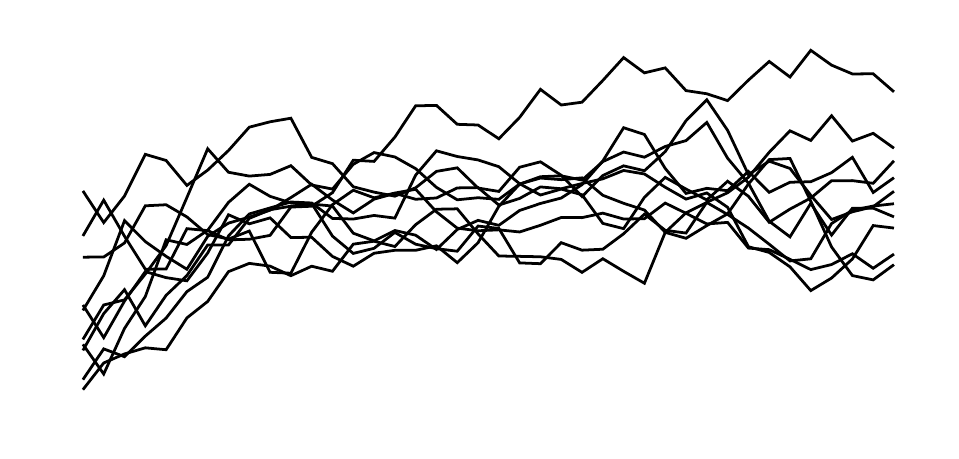
\begin{tikzpicture}[/tikz/background rectangle/.style={fill={rgb,1:red,1.0;green,1.0;blue,1.0}, fill opacity={0.0}, draw opacity={0.0}}, show background rectangle]
\begin{axis}[point meta max={nan}, point meta min={nan}, legend cell align={left}, legend columns={1}, title={}, title style={at={{(0.5,1)}}, anchor={south}, font={{\fontsize{14 pt}{18.2 pt}\selectfont}}, color={rgb,1:red,0.0;green,0.0;blue,0.0}, draw opacity={1.0}, rotate={0.0}, align={center}}, legend style={color={rgb,1:red,0.0;green,0.0;blue,0.0}, draw opacity={1.0}, line width={1}, solid, fill={rgb,1:red,1.0;green,1.0;blue,1.0}, fill opacity={0.0}, text opacity={1.0}, font={{\fontsize{8 pt}{10.4 pt}\selectfont}}, text={rgb,1:red,0.0;green,0.0;blue,0.0}, cells={anchor={center}}, at={(1.02, 1)}, anchor={north west}}, axis background/.style={fill={rgb,1:red,1.0;green,1.0;blue,1.0}, opacity={0.0}}, anchor={north west}, xshift={1.0mm}, yshift={-1.0mm}, width={125.0mm}, height={61.5mm}, scaled x ticks={false}, xlabel={}, x tick style={color={rgb,1:red,0.0;green,0.0;blue,0.0}, opacity={1.0}}, x tick label style={color={rgb,1:red,0.0;green,0.0;blue,0.0}, opacity={1.0}, rotate={0}}, xlabel style={at={(ticklabel cs:0.5)}, anchor=near ticklabel, at={{(ticklabel cs:0.5)}}, anchor={near ticklabel}, font={{\fontsize{11 pt}{14.3 pt}\selectfont}}, color={rgb,1:red,0.0;green,0.0;blue,0.0}, draw opacity={1.0}, rotate={0.0}}, xmajorgrids={false}, xmin={-0.6000000000000014}, xmax={20.6}, xticklabels={{}}, xtick={{}}, xtick style={draw=none}, xticklabel style={font={{\fontsize{8 pt}{10.4 pt}\selectfont}}, color={rgb,1:red,0.0;green,0.0;blue,0.0}, draw opacity={1.0}, rotate={0.0}}, x grid style={color={rgb,1:red,0.0;green,0.0;blue,0.0}, draw opacity={0.1}, line width={0.5}, solid}, axis x line*={left}, separate axis lines, x axis line style={{draw opacity = 0}}, scaled y ticks={false}, ylabel={}, y tick style={color={rgb,1:red,0.0;green,0.0;blue,0.0}, opacity={1.0}}, y tick label style={color={rgb,1:red,0.0;green,0.0;blue,0.0}, opacity={1.0}, rotate={0}}, ylabel style={at={(ticklabel cs:0.5)}, anchor=near ticklabel, at={{(ticklabel cs:0.5)}}, anchor={near ticklabel}, font={{\fontsize{11 pt}{14.3 pt}\selectfont}}, color={rgb,1:red,0.0;green,0.0;blue,0.0}, draw opacity={1.0}, rotate={0.0}}, ymajorgrids={false}, ymin={-0.04189027075633733}, ymax={0.9907697847633727}, yticklabels={{}}, ytick={{}}, ytick style={draw=none}, yticklabel style={font={{\fontsize{8 pt}{10.4 pt}\selectfont}}, color={rgb,1:red,0.0;green,0.0;blue,0.0}, draw opacity={1.0}, rotate={0.0}}, y grid style={color={rgb,1:red,0.0;green,0.0;blue,0.0}, draw opacity={0.1}, line width={0.5}, solid}, axis y line*={left}, y axis line style={{draw opacity = 0}}, colorbar={false}]
    \addplot[color={rgb,1:red,0.0;green,0.0;blue,0.0}, name path={f2f60186-39d4-46eb-a4af-5cc4ff99963d}, draw opacity={1.0}, line width={1}, solid]
        table[row sep={\\}]
        {
            \\
            0.0  -0.01266404276993034  \\
            0.5128205128205128  0.06400463836292701  \\
            1.0256410256410255  0.08994136514198918  \\
            1.5384615384615385  0.1074840695162828  \\
            2.051282051282051  0.10200327860103324  \\
            2.5641025641025643  0.19334242031274368  \\
            3.076923076923077  0.24063260038872586  \\
            3.58974358974359  0.3261855290084173  \\
            4.102564102564102  0.349908818482701  \\
            4.615384615384615  0.34199687885640956  \\
            5.128205128205129  0.31449076928636116  \\
            5.641025641025641  0.3417301698914536  \\
            6.153846153846154  0.3272939894403825  \\
            6.666666666666667  0.4050404161279741  \\
            7.17948717948718  0.41351054626917455  \\
            7.6923076923076925  0.3982605703237347  \\
            8.205128205128204  0.4610677460663412  \\
            8.717948717948717  0.5053389450554918  \\
            9.23076923076923  0.5065263407127213  \\
            9.743589743589743  0.4346572386511884  \\
            10.256410256410257  0.371081951669991  \\
            10.76923076923077  0.3700723678521404  \\
            11.282051282051283  0.36883571387199193  \\
            11.794871794871796  0.3612464967529491  \\
            12.307692307692308  0.3241115083252903  \\
            12.820512820512821  0.36325139096143627  \\
            13.333333333333334  0.32711790344166064  \\
            13.846153846153847  0.29284059478502317  \\
            14.35897435897436  0.4388758230049225  \\
            14.871794871794872  0.49498794956809195  \\
            15.384615384615385  0.5246349741961055  \\
            15.897435897435898  0.490205377992938  \\
            16.41025641025641  0.451209871807084  \\
            16.923076923076923  0.4048923877237331  \\
            17.435897435897434  0.3569505092093081  \\
            17.94871794871795  0.36303664549902565  \\
            18.46153846153846  0.46432630341070497  \\
            18.974358974358974  0.5026033865315319  \\
            19.487179487179485  0.5144511928699084  \\
            20.0  0.5211375394221719  \\
        }
        ;
    \addplot[color={rgb,1:red,0.0;green,0.0;blue,0.0}, name path={76f4f8dd-26e3-49d4-a35a-308bc3edecdd}, draw opacity={1.0}, line width={1}, solid]
        table[row sep={\\}]
        {
            \\
            0.0  0.42868331085628897  \\
            0.5128205128205128  0.5313493538245052  \\
            1.0256410256410255  0.4278225433498443  \\
            1.5384615384615385  0.33326436700368295  \\
            2.051282051282051  0.3335770803051526  \\
            2.5641025641025643  0.44954348007304507  \\
            3.076923076923077  0.4439693759197297  \\
            3.58974358974359  0.41747869872276927  \\
            4.102564102564102  0.4191610356816943  \\
            4.615384615384615  0.4303221157899803  \\
            5.128205128205129  0.5115439495723854  \\
            5.641025641025641  0.5139704273712172  \\
            6.153846153846154  0.5528726140052128  \\
            6.666666666666667  0.6460725126544721  \\
            7.17948717948718  0.642688459924207  \\
            7.6923076923076925  0.7124253589217441  \\
            8.205128205128204  0.8022256906364765  \\
            8.717948717948717  0.8034331228990889  \\
            9.23076923076923  0.7491398601346312  \\
            9.743589743589743  0.7471517593713642  \\
            10.256410256410257  0.707607254349551  \\
            10.76923076923077  0.7690159632856931  \\
            11.282051282051283  0.8494388931658104  \\
            11.794871794871796  0.8045836846010083  \\
            12.307692307692308  0.8126148176785429  \\
            12.820512820512821  0.8750621667638837  \\
            13.333333333333334  0.9406907455408268  \\
            13.846153846153847  0.8968536589749788  \\
            14.35897435897436  0.9110598387839516  \\
            14.871794871794872  0.845878353920143  \\
            15.384615384615385  0.836856277346203  \\
            15.897435897435898  0.8171417010092178  \\
            16.41025641025641  0.8758909817760522  \\
            16.923076923076923  0.9294886298047037  \\
            17.435897435897434  0.8848968980773458  \\
            17.94871794871795  0.9615435567769658  \\
            18.46153846153846  0.9189654732918792  \\
            18.974358974358974  0.8937604508208224  \\
            19.487179487179485  0.8941122611904869  \\
            20.0  0.8423813541858968  \\
        }
        ;
    \addplot[color={rgb,1:red,0.0;green,0.0;blue,0.0}, name path={f2439710-14a7-49ea-bf92-707b192710a3}, draw opacity={1.0}, line width={1}, solid]
        table[row sep={\\}]
        {
            \\
            0.0  0.3677286473088362  \\
            0.5128205128205128  0.3682113729056545  \\
            1.0256410256410255  0.40847971451219306  \\
            1.5384615384615385  0.5151927112052266  \\
            2.051282051282051  0.518198043296077  \\
            2.5641025641025643  0.4832950710051381  \\
            3.076923076923077  0.43267048018473736  \\
            3.58974358974359  0.4197392620542419  \\
            4.102564102564102  0.44275047946352036  \\
            4.615384615384615  0.3243173487670012  \\
            5.128205128205129  0.3215852459386494  \\
            5.641025641025641  0.4394429621684272  \\
            6.153846153846154  0.5184665831611063  \\
            6.666666666666667  0.5598895788046018  \\
            7.17948717948718  0.5381622860575547  \\
            7.6923076923076925  0.5517467709030458  \\
            8.205128205128204  0.5627109111163543  \\
            8.717948717948717  0.49776510248740696  \\
            9.23076923076923  0.4509795984633859  \\
            9.743589743589743  0.4435149772724047  \\
            10.256410256410257  0.44620792843869456  \\
            10.76923076923077  0.440077570764757  \\
            11.282051282051283  0.4592609828886693  \\
            11.794871794871796  0.4816062330920769  \\
            12.307692307692308  0.4812610488099109  \\
            12.820512820512821  0.4941063002641021  \\
            13.333333333333334  0.47722319886382686  \\
            13.846153846153847  0.4781646948305755  \\
            14.35897435897436  0.5230293408563057  \\
            14.871794871794872  0.4937433251539451  \\
            15.384615384615385  0.4630997088751105  \\
            15.897435897435898  0.4675413510591621  \\
            16.41025641025641  0.393778422708382  \\
            16.923076923076923  0.38924713105507286  \\
            17.435897435897434  0.36155609940842676  \\
            17.94871794871795  0.33207080725437227  \\
            18.46153846153846  0.34658833742436607  \\
            18.974358974358974  0.37752606732502086  \\
            19.487179487179485  0.3358408882455863  \\
            20.0  0.37654036798997675  \\
        }
        ;
    \addplot[color={rgb,1:red,0.0;green,0.0;blue,0.0}, name path={ba04d10a-ee3c-41ae-9259-3a016a1c5982}, draw opacity={1.0}, line width={1}, solid]
        table[row sep={\\}]
        {
            \\
            0.0  0.21488662655615326  \\
            0.5128205128205128  0.3142202824981559  \\
            1.0256410256410255  0.47244223741227526  \\
            1.5384615384615385  0.41249012782229183  \\
            2.051282051282051  0.37014357501599143  \\
            2.5641025641025643  0.33304668750659544  \\
            3.076923076923077  0.42747217014184974  \\
            3.58974358974359  0.4654896114606601  \\
            4.102564102564102  0.48277349267847597  \\
            4.615384615384615  0.5026831485710287  \\
            5.128205128205129  0.538839324068654  \\
            5.641025641025641  0.57709080499409  \\
            6.153846153846154  0.5318288086179087  \\
            6.666666666666667  0.49470398343378313  \\
            7.17948717948718  0.534228252738924  \\
            7.6923076923076925  0.5508047049756218  \\
            8.205128205128204  0.5339695050381271  \\
            8.717948717948717  0.5376728500601388  \\
            9.23076923076923  0.566542161976702  \\
            9.743589743589743  0.5674861031365396  \\
            10.256410256410257  0.5173452229621102  \\
            10.76923076923077  0.5363520221148698  \\
            11.282051282051283  0.5693878200594474  \\
            11.794871794871796  0.564118333238156  \\
            12.307692307692308  0.5791501874122617  \\
            12.820512820512821  0.592630837460634  \\
            13.333333333333334  0.6165857713746773  \\
            13.846153846153847  0.6065633050246496  \\
            14.35897435897436  0.5684531681725452  \\
            14.871794871794872  0.5345032587741977  \\
            15.384615384615385  0.552035994142016  \\
            15.897435897435898  0.5108768410472605  \\
            16.41025641025641  0.39779192017668324  \\
            16.923076923076923  0.3812717531439726  \\
            17.435897435897434  0.34003386189842305  \\
            17.94871794871795  0.271783291179483  \\
            18.46153846153846  0.30783566309578897  \\
            18.974358974358974  0.3625181903438823  \\
            19.487179487179485  0.4584512897328616  \\
            20.0  0.45125579098896135  \\
        }
        ;
    \addplot[color={rgb,1:red,0.0;green,0.0;blue,0.0}, name path={36d7be5e-a418-43ce-ad33-dd71582b27c3}, draw opacity={1.0}, line width={1}, solid]
        table[row sep={\\}]
        {
            \\
            0.0  0.100098651183587  \\
            0.5128205128205128  0.20566082099254057  \\
            1.0256410256410255  0.2744642956542011  \\
            1.5384615384615385  0.17068274486164497  \\
            2.051282051282051  0.2582143641548738  \\
            2.5641025641025643  0.3149904895113725  \\
            3.076923076923077  0.4029129601872509  \\
            3.58974358974359  0.40265674094981246  \\
            4.102564102564102  0.479195318969787  \\
            4.615384615384615  0.5038563912774607  \\
            5.128205128205129  0.5140858552670083  \\
            5.641025641025641  0.5217595714959403  \\
            6.153846153846154  0.4281265714787668  \\
            6.666666666666667  0.3785240686314865  \\
            7.17948717948718  0.39316896606838786  \\
            7.6923076923076925  0.43870359556271515  \\
            8.205128205128204  0.4049610894816011  \\
            8.717948717948717  0.39215093414271246  \\
            9.23076923076923  0.38481673769107866  \\
            9.743589743589743  0.4570550334603058  \\
            10.256410256410257  0.4502186632079945  \\
            10.76923076923077  0.351263674909634  \\
            11.282051282051283  0.3489727565045226  \\
            11.794871794871796  0.40929801930673654  \\
            12.307692307692308  0.3877994756589033  \\
            12.820512820512821  0.3905204363288625  \\
            13.333333333333334  0.43492173293604636  \\
            13.846153846153847  0.4913081550600051  \\
            14.35897435897436  0.44481946662659205  \\
            14.871794871794872  0.43695825634212343  \\
            15.384615384615385  0.5253218249102712  \\
            15.897435897435898  0.5526690104439408  \\
            16.41025641025641  0.5969478068948751  \\
            16.923076923076923  0.6688624369021735  \\
            17.435897435897434  0.7304484635290788  \\
            17.94871794871795  0.7027971147509834  \\
            18.46153846153846  0.7737101265668312  \\
            18.974358974358974  0.7009912403326056  \\
            19.487179487179485  0.7232571427441666  \\
            20.0  0.6804939116421137  \\
        }
        ;
    \addplot[color={rgb,1:red,0.0;green,0.0;blue,0.0}, name path={05d1c2d5-688a-480d-af80-46ed45c90bcc}, draw opacity={1.0}, line width={1}, solid]
        table[row sep={\\}]
        {
            \\
            0.0  0.13160442402840505  \\
            0.5128205128205128  0.23047546383021572  \\
            1.0256410256410255  0.2451268991202334  \\
            1.5384615384615385  0.3192285404862356  \\
            2.051282051282051  0.40091847259309626  \\
            2.5641025641025643  0.5389608077108121  \\
            3.076923076923077  0.6789059375007306  \\
            3.58974358974359  0.6114882563089471  \\
            4.102564102564102  0.6004913629814891  \\
            4.615384615384615  0.6052817295210269  \\
            5.128205128205129  0.630343263755808  \\
            5.641025641025641  0.5749127790247519  \\
            6.153846153846154  0.5632156648787674  \\
            6.666666666666667  0.63430253662532  \\
            7.17948717948718  0.6679476707055388  \\
            7.6923076923076925  0.6554309345834312  \\
            8.205128205128204  0.6218570031414524  \\
            8.717948717948717  0.5680527983256481  \\
            9.23076923076923  0.5324033533690148  \\
            9.743589743589743  0.5383947597959448  \\
            10.256410256410257  0.5336762434273935  \\
            10.76923076923077  0.5777552426527736  \\
            11.282051282051283  0.5948664098440818  \\
            11.794871794871796  0.5902103883704745  \\
            12.307692307692308  0.595392207716786  \\
            12.820512820512821  0.5453542227893383  \\
            13.333333333333334  0.5223856483664912  \\
            13.846153846153847  0.5030448159423783  \\
            14.35897435897436  0.43900914425186927  \\
            14.871794871794872  0.4218899330940655  \\
            15.384615384615385  0.4583804590782227  \\
            15.897435897435898  0.49213998318208735  \\
            16.41025641025641  0.577728617111844  \\
            16.923076923076923  0.6477735225836866  \\
            17.435897435897434  0.6511076526787686  \\
            17.94871794871795  0.5281059107086202  \\
            18.46153846153846  0.3969009118188264  \\
            18.974358974358974  0.314881820071134  \\
            19.487179487179485  0.30252649247121094  \\
            20.0  0.34622693481827066  \\
        }
        ;
    \addplot[color={rgb,1:red,0.0;green,0.0;blue,0.0}, name path={7959977e-16e9-4c95-a67f-a5e3a8a4edad}, draw opacity={1.0}, line width={1}, solid]
        table[row sep={\\}]
        {
            \\
            0.0  0.016174311544302253  \\
            0.5128205128205128  0.10437868608341065  \\
            1.0256410256410255  0.08201143455718611  \\
            1.5384615384615385  0.14112931727940287  \\
            2.051282051282051  0.19276908907365903  \\
            2.5641025641025643  0.26881099605132536  \\
            3.076923076923077  0.31009067915586314  \\
            3.58974358974359  0.4287770149425347  \\
            4.102564102564102  0.49180782323363975  \\
            4.615384615384615  0.5090436196045544  \\
            5.128205128205129  0.526092021601753  \\
            5.641025641025641  0.5233001293641727  \\
            6.153846153846154  0.4789591957717811  \\
            6.666666666666667  0.47720838051145215  \\
            7.17948717948718  0.48748917244653506  \\
            7.6923076923076925  0.47987282421125305  \\
            8.205128205128204  0.6032967006057505  \\
            8.717948717948717  0.6730681822012047  \\
            9.23076923076923  0.6566695462598692  \\
            9.743589743589743  0.6468705900900668  \\
            10.256410256410257  0.6274196741732924  \\
            10.76923076923077  0.5784650110870421  \\
            11.282051282051283  0.5461468343612831  \\
            11.794871794871796  0.5631646617121328  \\
            12.307692307692308  0.5468758078906247  \\
            12.820512820512821  0.46469498994594244  \\
            13.333333333333334  0.44954722162948685  \\
            13.846153846153847  0.5394720095249653  \\
            14.35897435897436  0.5968094012618989  \\
            14.871794871794872  0.5632593458007428  \\
            15.384615384615385  0.531977708271474  \\
            15.897435897435898  0.5856772618270553  \\
            16.41025641025641  0.5426622494347445  \\
            16.923076923076923  0.46798185349453475  \\
            17.435897435897434  0.5057580210094433  \\
            17.94871794871795  0.5375306820500022  \\
            18.46153846153846  0.5873385025743262  \\
            18.974358974358974  0.5874450130332486  \\
            19.487179487179485  0.5797600536891908  \\
            20.0  0.6443964648127959  \\
        }
        ;
    \addplot[color={rgb,1:red,0.0;green,0.0;blue,0.0}, name path={cca6dd21-6b01-493f-baeb-0177e706b4ba}, draw opacity={1.0}, line width={1}, solid]
        table[row sep={\\}]
        {
            \\
            0.0  0.5578124666204619  \\
            0.5128205128205128  0.46704763622147066  \\
            1.0256410256410255  0.5432590037811411  \\
            1.5384615384615385  0.662926594331754  \\
            2.051282051282051  0.6453330026573902  \\
            2.5641025641025643  0.5737138774394552  \\
            3.076923076923077  0.6176765629543234  \\
            3.58974358974359  0.6739364598262426  \\
            4.102564102564102  0.7408996370228765  \\
            4.615384615384615  0.7563625863404718  \\
            5.128205128205129  0.7666357434920047  \\
            5.641025641025641  0.654161491542513  \\
            6.153846153846154  0.6361866350437583  \\
            6.666666666666667  0.5697943478146773  \\
            7.17948717948718  0.5544971749844835  \\
            7.6923076923076925  0.5427762570236462  \\
            8.205128205128204  0.5669754700771993  \\
            8.717948717948717  0.6140014064651161  \\
            9.23076923076923  0.6241518085976009  \\
            9.743589743589743  0.5661901196487827  \\
            10.256410256410257  0.5564213770257974  \\
            10.76923076923077  0.6259087943910516  \\
            11.282051282051283  0.6414647708471294  \\
            11.794871794871796  0.6028761565260133  \\
            12.307692307692308  0.5417128398116772  \\
            12.820512820512821  0.6021514039119814  \\
            13.333333333333334  0.629921704051538  \\
            13.846153846153847  0.615869207244217  \\
            14.35897435897436  0.6707941499665827  \\
            14.871794871794872  0.7595158188070831  \\
            15.384615384615385  0.8195843851851793  \\
            15.897435897435898  0.7318190413833908  \\
            16.41025641025641  0.6048884498090988  \\
            16.923076923076923  0.6432328420967127  \\
            17.435897435897434  0.6224056573250266  \\
            17.94871794871795  0.5453887644254963  \\
            18.46153846153846  0.47590448278371217  \\
            18.974358974358974  0.49790070721869  \\
            19.487179487179485  0.5125136747001015  \\
            20.0  0.5567620191692729  \\
        }
        ;
    \addplot[color={rgb,1:red,0.0;green,0.0;blue,0.0}, name path={cf344bf6-b1f7-4a0f-8581-fcb0f10688db}, draw opacity={1.0}, line width={1}, solid]
        table[row sep={\\}]
        {
            \\
            0.0  0.11757072491907121  \\
            0.5128205128205128  0.03228878117556537  \\
            1.0256410256410255  0.16319745355475163  \\
            1.5384615384615385  0.2546047742597067  \\
            2.051282051282051  0.41767178901528207  \\
            2.5641025641025643  0.4042057573675822  \\
            3.076923076923077  0.4449800303675084  \\
            3.58974358974359  0.525045252041538  \\
            4.102564102564102  0.5770437825862498  \\
            4.615384615384615  0.5423084513497031  \\
            5.128205128205129  0.5235565144795508  \\
            5.641025641025641  0.5201004188387389  \\
            6.153846153846154  0.5145027810391533  \\
            6.666666666666667  0.436548767450702  \\
            7.17948717948718  0.4144432441173373  \\
            7.6923076923076925  0.4442682832088724  \\
            8.205128205128204  0.430787136548391  \\
            8.717948717948717  0.38968863613918553  \\
            9.23076923076923  0.4471389274769068  \\
            9.743589743589743  0.4733677642155713  \\
            10.256410256410257  0.45914512623586295  \\
            10.76923076923077  0.5018436366236109  \\
            11.282051282051283  0.5218828711486804  \\
            11.794871794871796  0.5375449079572033  \\
            12.307692307692308  0.5758557166263584  \\
            12.820512820512821  0.6439802286141244  \\
            13.333333333333334  0.7393331101801103  \\
            13.846153846153847  0.71994944638214  \\
            14.35897435897436  0.622429643228725  \\
            14.871794871794872  0.5508110317714389  \\
            15.384615384615385  0.5653148992128806  \\
            15.897435897435898  0.5585770197059486  \\
            16.41025641025641  0.6139883425665366  \\
            16.923076923076923  0.5538518567081586  \\
            17.435897435897434  0.5828448797859674  \\
            17.94871794871795  0.5843186613586889  \\
            18.46153846153846  0.6104117894262503  \\
            18.974358974358974  0.6543573329858133  \\
            19.487179487179485  0.5535038948517795  \\
            20.0  0.5958608302679257  \\
        }
        ;
    \addplot[color={rgb,1:red,0.0;green,0.0;blue,0.0}, name path={f97ba205-51a7-4d9a-846e-85368c8d42c2}, draw opacity={1.0}, line width={1}, solid]
        table[row sep={\\}]
        {
            \\
            0.0  0.2305542802037474  \\
            0.5128205128205128  0.13677370593738292  \\
            1.0256410256410255  0.24167758308324644  \\
            1.5384615384615385  0.3262880192560374  \\
            2.051282051282051  0.30896692434857936  \\
            2.5641025641025643  0.2998216860788924  \\
            3.076923076923077  0.3797043529133764  \\
            3.58974358974359  0.48947950200736606  \\
            4.102564102564102  0.46347703323161366  \\
            4.615384615384615  0.48047840512231504  \\
            5.128205128205129  0.42427400504377116  \\
            5.641025641025641  0.4247502578460873  \\
            6.153846153846154  0.36984082986532235  \\
            6.666666666666667  0.34178096039767353  \\
            7.17948717948718  0.37901425661542415  \\
            7.6923076923076925  0.3874886442018807  \\
            8.205128205128204  0.3874780184255275  \\
            8.717948717948717  0.4003540233924367  \\
            9.23076923076923  0.35193608690263795  \\
            9.743589743589743  0.4091237232967832  \\
            10.256410256410257  0.5137950229186353  \\
            10.76923076923077  0.5773167328894458  \\
            11.282051282051283  0.5987243628185336  \\
            11.794871794871796  0.6012487259870966  \\
            12.307692307692308  0.5890035824068282  \\
            12.820512820512821  0.6420593157057805  \\
            13.333333333333334  0.6695144540499222  \\
            13.846153846153847  0.6546778187809231  \\
            14.35897435897436  0.685573447788182  \\
            14.871794871794872  0.7022841395583269  \\
            15.384615384615385  0.7545015611154909  \\
            15.897435897435898  0.6517952676841273  \\
            16.41025641025641  0.580176492135653  \\
            16.923076923076923  0.4708342246592682  \\
            17.435897435897434  0.42605298530428753  \\
            17.94871794871795  0.5222326229750963  \\
            18.46153846153846  0.43114994893341024  \\
            18.974358974358974  0.5080932819892606  \\
            19.487179487179485  0.5084526654336871  \\
            20.0  0.48343281736986005  \\
        }
        ;
\end{axis}
\end{tikzpicture}

}

\newsavebox{\firstprior}
\sbox{\firstprior}{%
% Recommended preamble:
% \usetikzlibrary{arrows.meta}
% \usetikzlibrary{backgrounds}
% \usepgfplotslibrary{patchplots}
% \usepgfplotslibrary{fillbetween}
% \pgfplotsset{%
%     layers/standard/.define layer set={%
%         background,axis background,axis grid,axis ticks,axis lines,axis tick labels,pre main,main,axis descriptions,axis foreground%
%     }{
%         grid style={/pgfplots/on layer=axis grid},%
%         tick style={/pgfplots/on layer=axis ticks},%
%         axis line style={/pgfplots/on layer=axis lines},%
%         label style={/pgfplots/on layer=axis descriptions},%
%         legend style={/pgfplots/on layer=axis descriptions},%
%         title style={/pgfplots/on layer=axis descriptions},%
%         colorbar style={/pgfplots/on layer=axis descriptions},%
%         ticklabel style={/pgfplots/on layer=axis tick labels},%
%         axis background@ style={/pgfplots/on layer=axis background},%
%         3d box foreground style={/pgfplots/on layer=axis foreground},%
%     },
% }

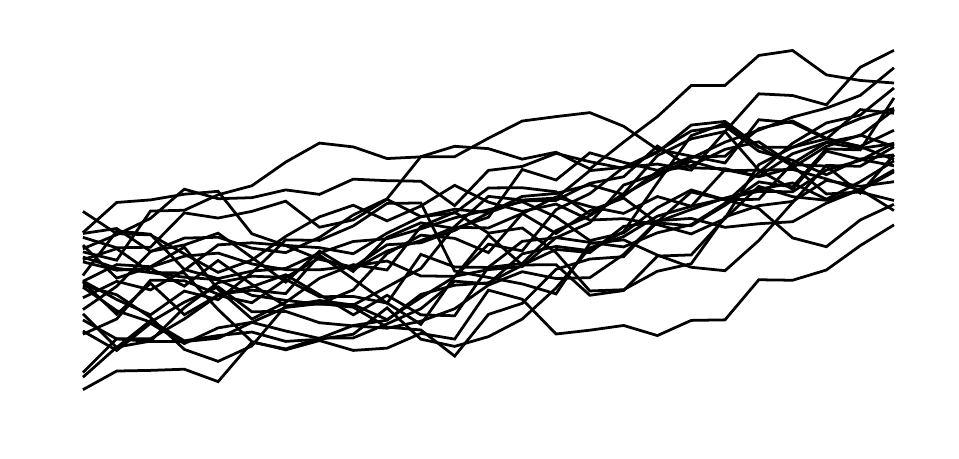
\begin{tikzpicture}[/tikz/background rectangle/.style={fill={rgb,1:red,1.0;green,1.0;blue,1.0}, fill opacity={0.0}, draw opacity={0.0}}, show background rectangle]
\begin{axis}[point meta max={nan}, point meta min={nan}, legend cell align={left}, legend columns={1}, title={}, title style={at={{(0.5,1)}}, anchor={south}, font={{\fontsize{14 pt}{18.2 pt}\selectfont}}, color={rgb,1:red,0.0;green,0.0;blue,0.0}, draw opacity={1.0}, rotate={0.0}, align={center}}, legend style={color={rgb,1:red,0.0;green,0.0;blue,0.0}, draw opacity={1.0}, line width={1}, solid, fill={rgb,1:red,1.0;green,1.0;blue,1.0}, fill opacity={0.0}, text opacity={1.0}, font={{\fontsize{8 pt}{10.4 pt}\selectfont}}, text={rgb,1:red,0.0;green,0.0;blue,0.0}, cells={anchor={center}}, at={(1.02, 1)}, anchor={north west}}, axis background/.style={fill={rgb,1:red,1.0;green,1.0;blue,1.0}, opacity={0.0}}, anchor={north west}, xshift={1.0mm}, yshift={-1.0mm}, width={125.0mm}, height={61.5mm}, scaled x ticks={false}, xlabel={}, x tick style={color={rgb,1:red,0.0;green,0.0;blue,0.0}, opacity={1.0}}, x tick label style={color={rgb,1:red,0.0;green,0.0;blue,0.0}, opacity={1.0}, rotate={0}}, xlabel style={at={(ticklabel cs:0.5)}, anchor=near ticklabel, at={{(ticklabel cs:0.5)}}, anchor={near ticklabel}, font={{\fontsize{11 pt}{14.3 pt}\selectfont}}, color={rgb,1:red,0.0;green,0.0;blue,0.0}, draw opacity={1.0}, rotate={0.0}}, xmajorgrids={false}, xmin={-0.6000000000000014}, xmax={20.6}, xticklabels={{}}, xtick={{}}, xtick style={draw=none}, xticklabel style={font={{\fontsize{8 pt}{10.4 pt}\selectfont}}, color={rgb,1:red,0.0;green,0.0;blue,0.0}, draw opacity={1.0}, rotate={0.0}}, x grid style={color={rgb,1:red,0.0;green,0.0;blue,0.0}, draw opacity={0.1}, line width={0.5}, solid}, axis x line*={left}, separate axis lines, x axis line style={{draw opacity = 0}}, scaled y ticks={false}, ylabel={}, y tick style={color={rgb,1:red,0.0;green,0.0;blue,0.0}, opacity={1.0}}, y tick label style={color={rgb,1:red,0.0;green,0.0;blue,0.0}, opacity={1.0}, rotate={0}}, ylabel style={at={(ticklabel cs:0.5)}, anchor=near ticklabel, at={{(ticklabel cs:0.5)}}, anchor={near ticklabel}, font={{\fontsize{11 pt}{14.3 pt}\selectfont}}, color={rgb,1:red,0.0;green,0.0;blue,0.0}, draw opacity={1.0}, rotate={0.0}}, ymajorgrids={false}, ymin={0.22079442976013675}, ymax={0.8794295941900958}, yticklabels={{}}, ytick={{}}, ytick style={draw=none}, yticklabel style={font={{\fontsize{8 pt}{10.4 pt}\selectfont}}, color={rgb,1:red,0.0;green,0.0;blue,0.0}, draw opacity={1.0}, rotate={0.0}}, y grid style={color={rgb,1:red,0.0;green,0.0;blue,0.0}, draw opacity={0.1}, line width={0.5}, solid}, axis y line*={left}, y axis line style={{draw opacity = 0}}, colorbar={false}]
    \addplot[color={rgb,1:red,0.0;green,0.0;blue,0.0}, name path={b1807882-62f1-4610-ac66-4151161f982c}, draw opacity={1.0}, line width={1}, solid]
        table[row sep={\\}]
        {
            \\
            0.0  0.4823432601040162  \\
            0.8333333333333334  0.4616003052225949  \\
            1.6666666666666667  0.45385454544295467  \\
            2.5  0.44541283961663963  \\
            3.3333333333333335  0.44081169479489796  \\
            4.166666666666667  0.4121605009713489  \\
            5.0  0.40304304009322667  \\
            5.833333333333333  0.3959550425713564  \\
            6.666666666666667  0.3952495278072296  \\
            7.5  0.36777662173440046  \\
            8.333333333333334  0.40802452589304056  \\
            9.166666666666666  0.4461731626617858  \\
            10.0  0.5224955721757875  \\
            10.833333333333334  0.4677833720651737  \\
            11.666666666666666  0.4682796706089865  \\
            12.5  0.41228193079681785  \\
            13.333333333333334  0.4209019560732842  \\
            14.166666666666666  0.4840165941272772  \\
            15.0  0.48621059614021617  \\
            15.833333333333334  0.5534786355466049  \\
            16.666666666666668  0.6513833625898784  \\
            17.5  0.6832508192526212  \\
            18.333333333333332  0.7104365711818745  \\
            19.166666666666668  0.7358904662784639  \\
            20.0  0.7543152943364885  \\
        }
        ;
    \addplot[color={rgb,1:red,0.0;green,0.0;blue,0.0}, name path={cc26b21d-c449-4cc0-853b-e1656eb8d7a4}, draw opacity={1.0}, line width={1}, solid]
        table[row sep={\\}]
        {
            \\
            0.0  0.47749714186671677  \\
            0.8333333333333334  0.4975084702927057  \\
            1.6666666666666667  0.4540539296147667  \\
            2.5  0.4530551252755739  \\
            3.3333333333333335  0.38632931237914303  \\
            4.166666666666667  0.3274848704686917  \\
            5.0  0.31239746992378203  \\
            5.833333333333333  0.3293932997499  \\
            6.666666666666667  0.3113375377770337  \\
            7.5  0.3155286347468031  \\
            8.333333333333334  0.3424246322974476  \\
            9.166666666666666  0.332036629547017  \\
            10.0  0.4216815878646488  \\
            10.833333333333334  0.4049617344451234  \\
            11.666666666666666  0.34137994254535925  \\
            12.5  0.348351055765895  \\
            13.333333333333334  0.3570360909797427  \\
            14.166666666666666  0.3385119724676766  \\
            15.0  0.3663000188435299  \\
            15.833333333333334  0.3672825721203645  \\
            16.666666666666668  0.440690153214299  \\
            17.5  0.4398198591170927  \\
            18.333333333333332  0.45858992459652387  \\
            19.166666666666668  0.5031358759589093  \\
            20.0  0.5412278727409984  \\
        }
        ;
    \addplot[color={rgb,1:red,0.0;green,0.0;blue,0.0}, name path={a1ce2970-3fc1-448d-a0e6-cd4422a40b74}, draw opacity={1.0}, line width={1}, solid]
        table[row sep={\\}]
        {
            \\
            0.0  0.4917754375703085  \\
            0.8333333333333334  0.4764916983300937  \\
            1.6666666666666667  0.5665302571317289  \\
            2.5  0.5679426048315317  \\
            3.3333333333333335  0.5962696404307701  \\
            4.166666666666667  0.6128153653299323  \\
            5.0  0.6561037273652813  \\
            5.833333333333333  0.6909577596124001  \\
            6.666666666666667  0.6839552074714298  \\
            7.5  0.6626428790059168  \\
            8.333333333333334  0.665719373760234  \\
            9.166666666666666  0.666086651659073  \\
            10.0  0.6998320101005655  \\
            10.833333333333334  0.7313052805861253  \\
            11.666666666666666  0.7394322949076253  \\
            12.5  0.746692102869865  \\
            13.333333333333334  0.7217283575715077  \\
            14.166666666666666  0.679390228929347  \\
            15.0  0.6670814352753899  \\
            15.833333333333334  0.6545704962751182  \\
            16.666666666666668  0.7336938452847723  \\
            17.5  0.7281040212641754  \\
            18.333333333333332  0.6983649235555769  \\
            19.166666666666668  0.7522650670608513  \\
            20.0  0.74554377829198  \\
        }
        ;
    \addplot[color={rgb,1:red,0.0;green,0.0;blue,0.0}, name path={53d758ac-1a58-4bb6-af81-8fa35afd0337}, draw opacity={1.0}, line width={1}, solid]
        table[row sep={\\}]
        {
            \\
            0.0  0.4366527203834918  \\
            0.8333333333333334  0.37739285248805704  \\
            1.6666666666666667  0.43420695621744504  \\
            2.5  0.37675417861051147  \\
            3.3333333333333335  0.4125123674627065  \\
            4.166666666666667  0.42799414005451286  \\
            5.0  0.4498518897573174  \\
            5.833333333333333  0.41348016678713634  \\
            6.666666666666667  0.37645907165852777  \\
            7.5  0.4122206420581562  \\
            8.333333333333334  0.37647327041677886  \\
            9.166666666666666  0.3748028678223054  \\
            10.0  0.46374252037783464  \\
            10.833333333333334  0.5111032930941153  \\
            11.666666666666666  0.5176137788993097  \\
            12.5  0.5450429878091277  \\
            13.333333333333334  0.6141126251369395  \\
            14.166666666666666  0.635176858745065  \\
            15.0  0.6575839941578029  \\
            15.833333333333334  0.6401473702904606  \\
            16.666666666666668  0.6414155393530581  \\
            17.5  0.6064915123393133  \\
            18.333333333333332  0.6762764452626971  \\
            19.166666666666668  0.6611341381546267  \\
            20.0  0.6493928695193175  \\
        }
        ;
    \addplot[color={rgb,1:red,0.0;green,0.0;blue,0.0}, name path={10d30fa7-1bae-44f3-918f-6b7bd46e3727}, draw opacity={1.0}, line width={1}, solid]
        table[row sep={\\}]
        {
            \\
            0.0  0.4385953706400076  \\
            0.8333333333333334  0.40451682207043566  \\
            1.6666666666666667  0.3764330519757785  \\
            2.5  0.4199936197589995  \\
            3.3333333333333335  0.4041365321825646  \\
            4.166666666666667  0.45352046285998854  \\
            5.0  0.5137421199223511  \\
            5.833333333333333  0.5128063124546081  \\
            6.666666666666667  0.5392422632453368  \\
            7.5  0.5805345932082189  \\
            8.333333333333334  0.5812805143015135  \\
            9.166666666666666  0.4565921031817147  \\
            10.0  0.44496618111045655  \\
            10.833333333333334  0.43311125533677797  \\
            11.666666666666666  0.41481259955858873  \\
            12.5  0.5070981663663939  \\
            13.333333333333334  0.5138107036979778  \\
            14.166666666666666  0.48583961321334146  \\
            15.0  0.4635597690472418  \\
            15.833333333333334  0.4572771631174545  \\
            16.666666666666668  0.5125749568951271  \\
            17.5  0.5821266587919189  \\
            18.333333333333332  0.6500195854851185  \\
            19.166666666666668  0.6484583780025601  \\
            20.0  0.684134107677034  \\
        }
        ;
    \addplot[color={rgb,1:red,0.0;green,0.0;blue,0.0}, name path={b2219066-0ea4-441a-ba4e-b91a0b34bb27}, draw opacity={1.0}, line width={1}, solid]
        table[row sep={\\}]
        {
            \\
            0.0  0.5041479034311052  \\
            0.8333333333333334  0.4437039608214958  \\
            1.6666666666666667  0.4638396763882718  \\
            2.5  0.4838230603133764  \\
            3.3333333333333335  0.48953584299897956  \\
            4.166666666666667  0.46973847638063354  \\
            5.0  0.4592737309784891  \\
            5.833333333333333  0.4588627544861911  \\
            6.666666666666667  0.46605991410305353  \\
            7.5  0.4749945665468326  \\
            8.333333333333334  0.44761854962329467  \\
            9.166666666666666  0.4470576867814861  \\
            10.0  0.45925501568330396  \\
            10.833333333333334  0.4647419572586591  \\
            11.666666666666666  0.5179358228961279  \\
            12.5  0.5091366631985688  \\
            13.333333333333334  0.5008202775886048  \\
            14.166666666666666  0.5267330671334237  \\
            15.0  0.5415279363906723  \\
            15.833333333333334  0.5809745971115512  \\
            16.666666666666668  0.6368974841028987  \\
            17.5  0.6906846352358726  \\
            18.333333333333332  0.7279045871811094  \\
            19.166666666666668  0.7420913135237319  \\
            20.0  0.7917300652613243  \\
        }
        ;
    \addplot[color={rgb,1:red,0.0;green,0.0;blue,0.0}, name path={160c833f-4314-4329-8854-27f77357394c}, draw opacity={1.0}, line width={1}, solid]
        table[row sep={\\}]
        {
            \\
            0.0  0.5183366477879328  \\
            0.8333333333333334  0.4992709819458251  \\
            1.6666666666666667  0.5002531978661225  \\
            2.5  0.5631702794762606  \\
            3.3333333333333335  0.5536950671595103  \\
            4.166666666666667  0.5659238139703081  \\
            5.0  0.5845930715113513  \\
            5.833333333333333  0.5368516563157792  \\
            6.666666666666667  0.5503137803455792  \\
            7.5  0.5879491600482254  \\
            8.333333333333334  0.5563005898072051  \\
            9.166666666666666  0.5629123755767134  \\
            10.0  0.6088326637258704  \\
            10.833333333333334  0.6091678422934875  \\
            11.666666666666666  0.6018008960784015  \\
            12.5  0.5604620772383013  \\
            13.333333333333334  0.594218494052761  \\
            14.166666666666666  0.6386061893458774  \\
            15.0  0.649643643684018  \\
            15.833333333333334  0.6794543753323162  \\
            16.666666666666668  0.6932744783891188  \\
            17.5  0.6514328400857909  \\
            18.333333333333332  0.6488934038947849  \\
            19.166666666666668  0.5994361892066137  \\
            20.0  0.6691150494335234  \\
        }
        ;
    \addplot[color={rgb,1:red,0.0;green,0.0;blue,0.0}, name path={497bc6da-b78b-4d79-a42f-28a0f2f48e96}, draw opacity={1.0}, line width={1}, solid]
        table[row sep={\\}]
        {
            \\
            0.0  0.38608971512833695  \\
            0.8333333333333334  0.4287673542294606  \\
            1.6666666666666667  0.49213435641179776  \\
            2.5  0.5169566957404748  \\
            3.3333333333333335  0.5185652335952953  \\
            4.166666666666667  0.49855317512917385  \\
            5.0  0.49033825569073103  \\
            5.833333333333333  0.518204485783691  \\
            6.666666666666667  0.55935970867206  \\
            7.5  0.5889370090523621  \\
            8.333333333333334  0.6661072691888532  \\
            9.166666666666666  0.6850383888473076  \\
            10.0  0.6807559906918171  \\
            10.833333333333334  0.6615401166795651  \\
            11.666666666666666  0.6742525957511974  \\
            12.5  0.6435985413237458  \\
            13.333333333333334  0.6927670587333951  \\
            14.166666666666666  0.7392903336580323  \\
            15.0  0.7962110877036228  \\
            15.833333333333334  0.7966123662998978  \\
            16.666666666666668  0.851374182209602  \\
            17.5  0.860479378417927  \\
            18.333333333333332  0.8158638632501848  \\
            19.166666666666668  0.8056235027535958  \\
            20.0  0.8009041451259458  \\
        }
        ;
    \addplot[color={rgb,1:red,0.0;green,0.0;blue,0.0}, name path={603ea59c-9583-48be-bf44-6ad9d9360c8c}, draw opacity={1.0}, line width={1}, solid]
        table[row sep={\\}]
        {
            \\
            0.0  0.37825223636351896  \\
            0.8333333333333334  0.3166703865603477  \\
            1.6666666666666667  0.3658701738567187  \\
            2.5  0.3288970281691906  \\
            3.3333333333333335  0.33851121677794926  \\
            4.166666666666667  0.344997753911482  \\
            5.0  0.32783652088830634  \\
            5.833333333333333  0.33178306081236303  \\
            6.666666666666667  0.34098096332697747  \\
            7.5  0.38922202662858474  \\
            8.333333333333334  0.331909039454868  \\
            9.166666666666666  0.31870157959833756  \\
            10.0  0.33654302655912  \\
            10.833333333333334  0.36874723033189666  \\
            11.666666666666666  0.4255129444738982  \\
            12.5  0.49898052736910536  \\
            13.333333333333334  0.5198051595872634  \\
            14.166666666666666  0.5572177251972708  \\
            15.0  0.5750949054233584  \\
            15.833333333333334  0.6423679576954533  \\
            16.666666666666668  0.6293765241380614  \\
            17.5  0.6460017336804065  \\
            18.333333333333332  0.6848565282369521  \\
            19.166666666666668  0.7056445841054227  \\
            20.0  0.6845135872475001  \\
        }
        ;
    \addplot[color={rgb,1:red,0.0;green,0.0;blue,0.0}, name path={402833b3-ce66-437e-be1f-51978ec5a5c7}, draw opacity={1.0}, line width={1}, solid]
        table[row sep={\\}]
        {
            \\
            0.0  0.42716249513094423  \\
            0.8333333333333334  0.38403141520758033  \\
            1.6666666666666667  0.36326155864222226  \\
            2.5  0.3996408771229091  \\
            3.3333333333333335  0.4278980225780998  \\
            4.166666666666667  0.3821278663006816  \\
            5.0  0.3828487264369396  \\
            5.833333333333333  0.3620422146705293  \\
            6.666666666666667  0.35626583112160876  \\
            7.5  0.3520119502538693  \\
            8.333333333333334  0.3648641640039639  \\
            9.166666666666666  0.387605163938773  \\
            10.0  0.4309418480949458  \\
            10.833333333333334  0.4554717323893759  \\
            11.666666666666666  0.4430025389545612  \\
            12.5  0.4445115048264653  \\
            13.333333333333334  0.48706010099951996  \\
            14.166666666666666  0.548881254344392  \\
            15.0  0.5529821029765691  \\
            15.833333333333334  0.5367100682897632  \\
            16.666666666666668  0.5432845093148819  \\
            17.5  0.5469476679733325  \\
            18.333333333333332  0.58093173678844  \\
            19.166666666666668  0.605785497394544  \\
            20.0  0.5673867660173305  \\
        }
        ;
    \addplot[color={rgb,1:red,0.0;green,0.0;blue,0.0}, name path={68567348-c3fa-4a79-9cbe-586ffc448c69}, draw opacity={1.0}, line width={1}, solid]
        table[row sep={\\}]
        {
            \\
            0.0  0.5658354787628227  \\
            0.8333333333333334  0.5250667525777383  \\
            1.6666666666666667  0.5228708542726217  \\
            2.5  0.4880776652607815  \\
            3.3333333333333335  0.4542685495511729  \\
            4.166666666666667  0.47679920658265923  \\
            5.0  0.5200574317424411  \\
            5.833333333333333  0.5558247263986965  \\
            6.666666666666667  0.5771906986369746  \\
            7.5  0.5485341789226718  \\
            8.333333333333334  0.5757043288645356  \\
            9.166666666666666  0.6135483154601524  \\
            10.0  0.5828621944502863  \\
            10.833333333333334  0.5658761929254191  \\
            11.666666666666666  0.5792715989030849  \\
            12.5  0.5499864630534622  \\
            13.333333333333334  0.5525856966436186  \\
            14.166666666666666  0.5416725428641125  \\
            15.0  0.5246431240377832  \\
            15.833333333333334  0.5526322965601678  \\
            16.666666666666668  0.611632221893586  \\
            17.5  0.5928224962902203  \\
            18.333333333333332  0.5862045939790806  \\
            19.166666666666668  0.6063016685856218  \\
            20.0  0.6419269583455446  \\
        }
        ;
    \addplot[color={rgb,1:red,0.0;green,0.0;blue,0.0}, name path={e3155926-ed9c-4294-ae33-07cb6be12caa}, draw opacity={1.0}, line width={1}, solid]
        table[row sep={\\}]
        {
            \\
            0.0  0.4076902182360638  \\
            0.8333333333333334  0.4377730794623348  \\
            1.6666666666666667  0.4221726223701779  \\
            2.5  0.4579422934692872  \\
            3.3333333333333335  0.5046369657871719  \\
            4.166666666666667  0.5083938849826942  \\
            5.0  0.5033607618752177  \\
            5.833333333333333  0.47821079829950225  \\
            6.666666666666667  0.46357645171220535  \\
            7.5  0.5048284105518889  \\
            8.333333333333334  0.5083794011824097  \\
            9.166666666666666  0.5310440954507553  \\
            10.0  0.5630093331609457  \\
            10.833333333333334  0.5932887624012148  \\
            11.666666666666666  0.5987316669413212  \\
            12.5  0.6144213263481436  \\
            13.333333333333334  0.5967550121212946  \\
            14.166666666666666  0.6307182381055237  \\
            15.0  0.6634390716579814  \\
            15.833333333333334  0.6926907570997226  \\
            16.666666666666668  0.7146303656514775  \\
            17.5  0.7384462864091718  \\
            18.333333333333332  0.7548912120129487  \\
            19.166666666666668  0.7781682476977597  \\
            20.0  0.828766492224624  \\
        }
        ;
    \addplot[color={rgb,1:red,0.0;green,0.0;blue,0.0}, name path={1625961d-c2eb-4dfb-92a3-59c1f47aa200}, draw opacity={1.0}, line width={1}, solid]
        table[row sep={\\}]
        {
            \\
            0.0  0.23943504762136197  \\
            0.8333333333333334  0.27359780269835704  \\
            1.6666666666666667  0.2747797017167812  \\
            2.5  0.27691636116935425  \\
            3.3333333333333335  0.25417062861141104  \\
            4.166666666666667  0.3262373135845451  \\
            5.0  0.3141434432292015  \\
            5.833333333333333  0.33382043820923313  \\
            6.666666666666667  0.3342262550296749  \\
            7.5  0.35994719194820307  \\
            8.333333333333334  0.38768282535550486  \\
            9.166666666666666  0.4380905117819602  \\
            10.0  0.4331230442954271  \\
            10.833333333333334  0.488140614673845  \\
            11.666666666666666  0.5018108552638442  \\
            12.5  0.4938488562939114  \\
            13.333333333333334  0.5289067862980963  \\
            14.166666666666666  0.6182096996430158  \\
            15.0  0.7045296806933979  \\
            15.833333333333334  0.7268437803888735  \\
            16.666666666666668  0.6831160146488496  \\
            17.5  0.6833366455688269  \\
            18.333333333333332  0.698695512479433  \\
            19.166666666666668  0.6847855802219567  \\
            20.0  0.7144188135562477  \\
        }
        ;
    \addplot[color={rgb,1:red,0.0;green,0.0;blue,0.0}, name path={c5ebc878-ff7c-44ab-9037-a9bb28509b79}, draw opacity={1.0}, line width={1}, solid]
        table[row sep={\\}]
        {
            \\
            0.0  0.5269855800074557  \\
            0.8333333333333334  0.5822365255245261  \\
            1.6666666666666667  0.5869079032117003  \\
            2.5  0.5973124127740015  \\
            3.3333333333333335  0.6026638127523629  \\
            4.166666666666667  0.5248317985143123  \\
            5.0  0.5036166580028936  \\
            5.833333333333333  0.49947111592979415  \\
            6.666666666666667  0.48839542641757694  \\
            7.5  0.5260103919240331  \\
            8.333333333333334  0.5560010085602963  \\
            9.166666666666666  0.5698496727625225  \\
            10.0  0.5636376408144087  \\
            10.833333333333334  0.5852300403636563  \\
            11.666666666666666  0.5860355323374262  \\
            12.5  0.6173707244749174  \\
            13.333333333333334  0.629247549341738  \\
            14.166666666666666  0.6855957194734147  \\
            15.0  0.6455492047871211  \\
            15.833333333333334  0.6439579002572835  \\
            16.666666666666668  0.6298989332111895  \\
            17.5  0.671472420201831  \\
            18.333333333333332  0.692416276820331  \\
            19.166666666666668  0.7044161993180322  \\
            20.0  0.7517771335358137  \\
        }
        ;
    \addplot[color={rgb,1:red,0.0;green,0.0;blue,0.0}, name path={01c8bb3b-f99b-4d8a-b5b7-2aa2098e985d}, draw opacity={1.0}, line width={1}, solid]
        table[row sep={\\}]
        {
            \\
            0.0  0.4305969043176452  \\
            0.8333333333333334  0.41324971072340744  \\
            1.6666666666666667  0.37176491156601105  \\
            2.5  0.313214236959743  \\
            3.3333333333333335  0.2913086787709717  \\
            4.166666666666667  0.3195771106228941  \\
            5.0  0.393012909875515  \\
            5.833333333333333  0.3967149908722275  \\
            6.666666666666667  0.42225221956392844  \\
            7.5  0.4885256286889993  \\
            8.333333333333334  0.5223310108637913  \\
            9.166666666666666  0.5165599061054739  \\
            10.0  0.4904044200655392  \\
            10.833333333333334  0.5617962671348198  \\
            11.666666666666666  0.59236458847714  \\
            12.5  0.5746523880210901  \\
            13.333333333333334  0.5622432859845752  \\
            14.166666666666666  0.5930509923552116  \\
            15.0  0.5753346860424431  \\
            15.833333333333334  0.5893259024445927  \\
            16.666666666666668  0.6025555973418577  \\
            17.5  0.6018030763631583  \\
            18.333333333333332  0.6415652393715281  \\
            19.166666666666668  0.6591744385022961  \\
            20.0  0.690994677119303  \\
        }
        ;
    \addplot[color={rgb,1:red,0.0;green,0.0;blue,0.0}, name path={7dd9191f-9010-447d-8228-d98c2a49d059}, draw opacity={1.0}, line width={1}, solid]
        table[row sep={\\}]
        {
            \\
            0.0  0.4734766266297724  \\
            0.8333333333333334  0.45821138373335685  \\
            1.6666666666666667  0.46161892287974415  \\
            2.5  0.42904688114625544  \\
            3.3333333333333335  0.47602532402137165  \\
            4.166666666666667  0.43211251988047017  \\
            5.0  0.39238895583371414  \\
            5.833333333333333  0.4027150256319305  \\
            6.666666666666667  0.39438497853909243  \\
            7.5  0.42745335133062823  \\
            8.333333333333334  0.4612882245528645  \\
            9.166666666666666  0.5382379460364819  \\
            10.0  0.5933626759210856  \\
            10.833333333333334  0.5866999207274081  \\
            11.666666666666666  0.590273385845699  \\
            12.5  0.6405396537152885  \\
            13.333333333333334  0.6465211535681834  \\
            14.166666666666666  0.6756780285959414  \\
            15.0  0.7130796997241423  \\
            15.833333333333334  0.7217132741724974  \\
            16.666666666666668  0.6760169698023245  \\
            17.5  0.6593771871730062  \\
            18.333333333333332  0.6330039135685996  \\
            19.166666666666668  0.6617780268746588  \\
            20.0  0.6693399513692826  \\
        }
        ;
    \addplot[color={rgb,1:red,0.0;green,0.0;blue,0.0}, name path={83777a4b-8719-4441-9953-774ab9b55562}, draw opacity={1.0}, line width={1}, solid]
        table[row sep={\\}]
        {
            \\
            0.0  0.4975444922279432  \\
            0.8333333333333334  0.5232235591894241  \\
            1.6666666666666667  0.5530842312307388  \\
            2.5  0.606538473004102  \\
            3.3333333333333335  0.5890894697159992  \\
            4.166666666666667  0.5910130444030758  \\
            5.0  0.6052274554826087  \\
            5.833333333333333  0.5970074266674162  \\
            6.666666666666667  0.6248963338783335  \\
            7.5  0.6221030008143874  \\
            8.333333333333334  0.6210647762032138  \\
            9.166666666666666  0.576448121676282  \\
            10.0  0.6409803814963015  \\
            10.833333333333334  0.6482505396234968  \\
            11.666666666666666  0.6720927083691096  \\
            12.5  0.6568534828683148  \\
            13.333333333333334  0.6446785971936106  \\
            14.166666666666666  0.673813047132334  \\
            15.0  0.7239463099607211  \\
            15.833333333333334  0.7305819778197551  \\
            16.666666666666668  0.6845434099206186  \\
            17.5  0.649083025281809  \\
            18.333333333333332  0.597810967081225  \\
            19.166666666666668  0.6012628541639568  \\
            20.0  0.5858217437770108  \\
        }
        ;
    \addplot[color={rgb,1:red,0.0;green,0.0;blue,0.0}, name path={346bcc45-a4eb-40a0-802a-a834ede9a421}, draw opacity={1.0}, line width={1}, solid]
        table[row sep={\\}]
        {
            \\
            0.0  0.26225461728349303  \\
            0.8333333333333334  0.3173220277558435  \\
            1.6666666666666667  0.32846858810862467  \\
            2.5  0.38960556357488213  \\
            3.3333333333333335  0.4354659072708468  \\
            4.166666666666667  0.44724001476532  \\
            5.0  0.44490703160834766  \\
            5.833333333333333  0.4806376509312688  \\
            6.666666666666667  0.45948333848833656  \\
            7.5  0.49328900696679057  \\
            8.333333333333334  0.5124552808793392  \\
            9.166666666666666  0.5366870698711446  \\
            10.0  0.5356124697945234  \\
            10.833333333333334  0.5620617267821111  \\
            11.666666666666666  0.5253632578764532  \\
            12.5  0.5669782720672488  \\
            13.333333333333334  0.5903861551194508  \\
            14.166666666666666  0.5448230924215394  \\
            15.0  0.5395186544601625  \\
            15.833333333333334  0.5770459481404439  \\
            16.666666666666668  0.6198456487944511  \\
            17.5  0.6106078392961088  \\
            18.333333333333332  0.6803140196450133  \\
            19.166666666666668  0.67852587508328  \\
            20.0  0.7735553239858373  \\
        }
        ;
    \addplot[color={rgb,1:red,0.0;green,0.0;blue,0.0}, name path={8226e7d2-09b5-495e-b994-69f10117843e}, draw opacity={1.0}, line width={1}, solid]
        table[row sep={\\}]
        {
            \\
            0.0  0.44854536246972476  \\
            0.8333333333333334  0.5298355664385961  \\
            1.6666666666666667  0.5240969211625829  \\
            2.5  0.45953758532483174  \\
            3.3333333333333335  0.44288213589843817  \\
            4.166666666666667  0.4565424830818297  \\
            5.0  0.46141957167169073  \\
            5.833333333333333  0.4896679452644536  \\
            6.666666666666667  0.5107934230797679  \\
            7.5  0.5158214176530622  \\
            8.333333333333334  0.533932695025009  \\
            9.166666666666666  0.5540407360538141  \\
            10.0  0.568920492626006  \\
            10.833333333333334  0.5835207908765612  \\
            11.666666666666666  0.5556557083315259  \\
            12.5  0.5124599520062758  \\
            13.333333333333334  0.526539526550626  \\
            14.166666666666666  0.5726482707872415  \\
            15.0  0.6051190732555959  \\
            15.833333333333334  0.5872388148899181  \\
            16.666666666666668  0.588025714673964  \\
            17.5  0.6537036122062118  \\
            18.333333333333332  0.691911976401966  \\
            19.166666666666668  0.6811532790745662  \\
            20.0  0.6899979521934253  \\
        }
        ;
    \addplot[color={rgb,1:red,0.0;green,0.0;blue,0.0}, name path={853de1f5-a9cb-4a77-b906-59de9c89784a}, draw opacity={1.0}, line width={1}, solid]
        table[row sep={\\}]
        {
            \\
            0.0  0.2706784639781373  \\
            0.8333333333333334  0.3327659626106278  \\
            1.6666666666666667  0.332580449958103  \\
            2.5  0.3688003295133447  \\
            3.3333333333333335  0.4119487322941892  \\
            4.166666666666667  0.39868925900934865  \\
            5.0  0.44135208840976936  \\
            5.833333333333333  0.40964722158846834  \\
            6.666666666666667  0.410180288262671  \\
            7.5  0.39806961272012265  \\
            8.333333333333334  0.35906298580383733  \\
            9.166666666666666  0.44618704276143195  \\
            10.0  0.5058136166475109  \\
            10.833333333333334  0.4935830241261881  \\
            11.666666666666666  0.5689997575504155  \\
            12.5  0.5983897089746133  \\
            13.333333333333334  0.646603686237033  \\
            14.166666666666666  0.6525243589695834  \\
            15.0  0.6413237494020859  \\
            15.833333333333334  0.7120065700599452  \\
            16.666666666666668  0.78114521132795  \\
            17.5  0.7780048605289889  \\
            18.333333333333332  0.7610270896560425  \\
            19.166666666666668  0.8296557129120308  \\
            20.0  0.8607889763288705  \\
        }
        ;
    \addplot[color={rgb,1:red,0.0;green,0.0;blue,0.0}, name path={c26553d6-5165-4a0f-9de8-684e29766114}, draw opacity={1.0}, line width={1}, solid]
        table[row sep={\\}]
        {
            \\
            0.0  0.34102246450859874  \\
            0.8333333333333334  0.36888798232493236  \\
            1.6666666666666667  0.4399646111150772  \\
            2.5  0.4389318214810712  \\
            3.3333333333333335  0.414227266688796  \\
            4.166666666666667  0.42164524865544345  \\
            5.0  0.41533600373683116  \\
            5.833333333333333  0.48591792536163186  \\
            6.666666666666667  0.44211790629698094  \\
            7.5  0.397656661189693  \\
            8.333333333333334  0.4871239680182788  \\
            9.166666666666666  0.46412562451529066  \\
            10.0  0.46323910690418346  \\
            10.833333333333334  0.47045326039015073  \\
            11.666666666666666  0.5307552270068586  \\
            12.5  0.5577293889561367  \\
            13.333333333333334  0.5982208807254464  \\
            14.166666666666666  0.6680288829104353  \\
            15.0  0.6986893894941049  \\
            15.833333333333334  0.7122561231606763  \\
            16.666666666666668  0.6412391666660064  \\
            17.5  0.64272336194598  \\
            18.333333333333332  0.6252880204863509  \\
            19.166666666666668  0.6044129173704809  \\
            20.0  0.6383581192181089  \\
        }
        ;
    \addplot[color={rgb,1:red,0.0;green,0.0;blue,0.0}, name path={cf7381f6-5444-4d4f-b6cf-7831eca854b1}, draw opacity={1.0}, line width={1}, solid]
        table[row sep={\\}]
        {
            \\
            0.0  0.43780206733802596  \\
            0.8333333333333334  0.46844660713554026  \\
            1.6666666666666667  0.46457702855118593  \\
            2.5  0.5003087430567553  \\
            3.3333333333333335  0.4231955738834818  \\
            4.166666666666667  0.3688445476592944  \\
            5.0  0.3994841597860646  \\
            5.833333333333333  0.4434245331102202  \\
            6.666666666666667  0.46836437609681303  \\
            7.5  0.4586053767578439  \\
            8.333333333333334  0.5381275138753182  \\
            9.166666666666666  0.5643085988414254  \\
            10.0  0.5260672436561442  \\
            10.833333333333334  0.5354685474159296  \\
            11.666666666666666  0.4904145368419624  \\
            12.5  0.42021643001825004  \\
            13.333333333333334  0.4224516675802622  \\
            14.166666666666666  0.4562842903205191  \\
            15.0  0.46997308841106816  \\
            15.833333333333334  0.5558186713220964  \\
            16.666666666666668  0.576397236529995  \\
            17.5  0.5841066323273644  \\
            18.333333333333332  0.6226246687096032  \\
            19.166666666666668  0.6118247197058406  \\
            20.0  0.6201933905262077  \\
        }
        ;
    \addplot[color={rgb,1:red,0.0;green,0.0;blue,0.0}, name path={6ceec245-fa85-4735-96b2-327ffad4c729}, draw opacity={1.0}, line width={1}, solid]
        table[row sep={\\}]
        {
            \\
            0.0  0.5254838659457344  \\
            0.8333333333333334  0.5345527777952408  \\
            1.6666666666666667  0.4927918070654898  \\
            2.5  0.5043806825802789  \\
            3.3333333333333335  0.525951307444575  \\
            4.166666666666667  0.48139151138092723  \\
            5.0  0.4364043542584971  \\
            5.833333333333333  0.4930023450892711  \\
            6.666666666666667  0.45581669944710057  \\
            7.5  0.5183200989427188  \\
            8.333333333333334  0.5450327885155456  \\
            9.166666666666666  0.5344342260974679  \\
            10.0  0.5550618886614526  \\
            10.833333333333334  0.6425386233200325  \\
            11.666666666666666  0.6233677541996073  \\
            12.5  0.6730727714919889  \\
            13.333333333333334  0.6555663282805738  \\
            14.166666666666666  0.6410423034384657  \\
            15.0  0.6654935904481499  \\
            15.833333333333334  0.666952514780045  \\
            16.666666666666668  0.71732106351365  \\
            17.5  0.7313819760257291  \\
            18.333333333333332  0.6995902760267723  \\
            19.166666666666668  0.6844362243997063  \\
            20.0  0.660755936372467  \\
        }
        ;
    \addplot[color={rgb,1:red,0.0;green,0.0;blue,0.0}, name path={07ca6c08-cc76-4759-8f26-893937dc64dd}, draw opacity={1.0}, line width={1}, solid]
        table[row sep={\\}]
        {
            \\
            0.0  0.3468894270760382  \\
            0.8333333333333334  0.31131476021617616  \\
            1.6666666666666667  0.36095073155497176  \\
            2.5  0.32389738392916245  \\
            3.3333333333333335  0.3525584346554814  \\
            4.166666666666667  0.3628175653786585  \\
            5.0  0.38998600462938593  \\
            5.833333333333333  0.3971535110275145  \\
            6.666666666666667  0.39042698792639197  \\
            7.5  0.35398924016713457  \\
            8.333333333333334  0.34878310089787584  \\
            9.166666666666666  0.30092030886526905  \\
            10.0  0.3772328045865271  \\
            10.833333333333334  0.3975560270836276  \\
            11.666666666666666  0.45991901781989464  \\
            12.5  0.47862385339709435  \\
            13.333333333333334  0.4829496641983045  \\
            14.166666666666666  0.5466862509600586  \\
            15.0  0.5693362720799203  \\
            15.833333333333334  0.5903030452157592  \\
            16.666666666666668  0.6062225729249352  \\
            17.5  0.6179862722708284  \\
            18.333333333333332  0.5881715993557136  \\
            19.166666666666668  0.6201548510246866  \\
            20.0  0.65824387216025  \\
        }
        ;
    \addplot[color={rgb,1:red,0.0;green,0.0;blue,0.0}, name path={e5e34efa-dfa2-4fd7-8534-245ca86cacaf}, draw opacity={1.0}, line width={1}, solid]
        table[row sep={\\}]
        {
            \\
            0.0  0.36703188227778544  \\
            0.8333333333333334  0.3322763227453815  \\
            1.6666666666666667  0.3277768855193342  \\
            2.5  0.3274822200993005  \\
            3.3333333333333335  0.3336274007749448  \\
            4.166666666666667  0.3626937994932964  \\
            5.0  0.3468711192974021  \\
            5.833333333333333  0.3333231489503605  \\
            6.666666666666667  0.35701083155820507  \\
            7.5  0.36667202620655687  \\
            8.333333333333334  0.4139035485446978  \\
            9.166666666666666  0.4307043936729337  \\
            10.0  0.4351616911028035  \\
            10.833333333333334  0.46731011817319595  \\
            11.666666666666666  0.4962061403235697  \\
            12.5  0.4904180622003198  \\
            13.333333333333334  0.5384795051186648  \\
            14.166666666666666  0.546758481690685  \\
            15.0  0.6013648854126377  \\
            15.833333333333334  0.5869840038986366  \\
            16.666666666666668  0.5710448138848367  \\
            17.5  0.5173216427833873  \\
            18.333333333333332  0.5012100241528413  \\
            19.166666666666668  0.5501339819398587  \\
            20.0  0.5788544915391157  \\
        }
        ;
\end{axis}
\end{tikzpicture}

}
\newsavebox{\secondprior}
\sbox{\secondprior}{%
% Recommended preamble:
% \usetikzlibrary{arrows.meta}
% \usetikzlibrary{backgrounds}
% \usepgfplotslibrary{patchplots}
% \usepgfplotslibrary{fillbetween}
% \pgfplotsset{%
%     layers/standard/.define layer set={%
%         background,axis background,axis grid,axis ticks,axis lines,axis tick labels,pre main,main,axis descriptions,axis foreground%
%     }{
%         grid style={/pgfplots/on layer=axis grid},%
%         tick style={/pgfplots/on layer=axis ticks},%
%         axis line style={/pgfplots/on layer=axis lines},%
%         label style={/pgfplots/on layer=axis descriptions},%
%         legend style={/pgfplots/on layer=axis descriptions},%
%         title style={/pgfplots/on layer=axis descriptions},%
%         colorbar style={/pgfplots/on layer=axis descriptions},%
%         ticklabel style={/pgfplots/on layer=axis tick labels},%
%         axis background@ style={/pgfplots/on layer=axis background},%
%         3d box foreground style={/pgfplots/on layer=axis foreground},%
%     },
% }

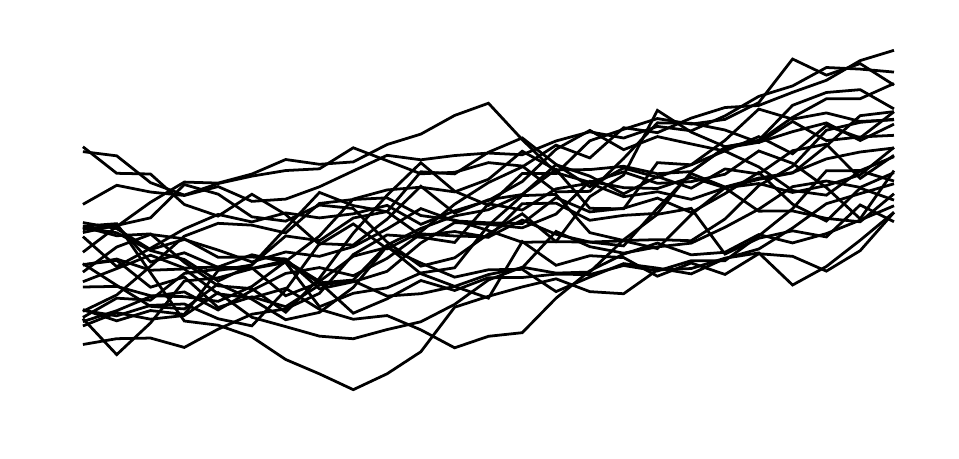
\begin{tikzpicture}[/tikz/background rectangle/.style={fill={rgb,1:red,1.0;green,1.0;blue,1.0}, fill opacity={0.0}, draw opacity={0.0}}, show background rectangle]
\begin{axis}[point meta max={nan}, point meta min={nan}, legend cell align={left}, legend columns={1}, title={}, title style={at={{(0.5,1)}}, anchor={south}, font={{\fontsize{14 pt}{18.2 pt}\selectfont}}, color={rgb,1:red,0.0;green,0.0;blue,0.0}, draw opacity={1.0}, rotate={0.0}, align={center}}, legend style={color={rgb,1:red,0.0;green,0.0;blue,0.0}, draw opacity={1.0}, line width={1}, solid, fill={rgb,1:red,1.0;green,1.0;blue,1.0}, fill opacity={0.0}, text opacity={1.0}, font={{\fontsize{8 pt}{10.4 pt}\selectfont}}, text={rgb,1:red,0.0;green,0.0;blue,0.0}, cells={anchor={center}}, at={(1.02, 1)}, anchor={north west}}, axis background/.style={fill={rgb,1:red,1.0;green,1.0;blue,1.0}, opacity={0.0}}, anchor={north west}, xshift={1.0mm}, yshift={-1.0mm}, width={125.0mm}, height={61.5mm}, scaled x ticks={false}, xlabel={}, x tick style={color={rgb,1:red,0.0;green,0.0;blue,0.0}, opacity={1.0}}, x tick label style={color={rgb,1:red,0.0;green,0.0;blue,0.0}, opacity={1.0}, rotate={0}}, xlabel style={at={(ticklabel cs:0.5)}, anchor=near ticklabel, at={{(ticklabel cs:0.5)}}, anchor={near ticklabel}, font={{\fontsize{11 pt}{14.3 pt}\selectfont}}, color={rgb,1:red,0.0;green,0.0;blue,0.0}, draw opacity={1.0}, rotate={0.0}}, xmajorgrids={false}, xmin={-0.6000000000000014}, xmax={20.6}, xticklabels={{}}, xtick={{}}, xtick style={draw=none}, xticklabel style={font={{\fontsize{8 pt}{10.4 pt}\selectfont}}, color={rgb,1:red,0.0;green,0.0;blue,0.0}, draw opacity={1.0}, rotate={0.0}}, x grid style={color={rgb,1:red,0.0;green,0.0;blue,0.0}, draw opacity={0.1}, line width={0.5}, solid}, axis x line*={left}, separate axis lines, x axis line style={{draw opacity = 0}}, scaled y ticks={false}, ylabel={}, y tick style={color={rgb,1:red,0.0;green,0.0;blue,0.0}, opacity={1.0}}, y tick label style={color={rgb,1:red,0.0;green,0.0;blue,0.0}, opacity={1.0}, rotate={0}}, ylabel style={at={(ticklabel cs:0.5)}, anchor=near ticklabel, at={{(ticklabel cs:0.5)}}, anchor={near ticklabel}, font={{\fontsize{11 pt}{14.3 pt}\selectfont}}, color={rgb,1:red,0.0;green,0.0;blue,0.0}, draw opacity={1.0}, rotate={0.0}}, ymajorgrids={false}, ymin={0.18263458083993206}, ymax={0.8342887978144777}, yticklabels={{}}, ytick={{}}, ytick style={draw=none}, yticklabel style={font={{\fontsize{8 pt}{10.4 pt}\selectfont}}, color={rgb,1:red,0.0;green,0.0;blue,0.0}, draw opacity={1.0}, rotate={0.0}}, y grid style={color={rgb,1:red,0.0;green,0.0;blue,0.0}, draw opacity={0.1}, line width={0.5}, solid}, axis y line*={left}, y axis line style={{draw opacity = 0}}, colorbar={false}]
    \addplot[color={rgb,1:red,0.0;green,0.0;blue,0.0}, name path={a5643316-5452-4ccb-ab66-ac94c285f747}, draw opacity={1.0}, line width={1}, solid]
        table[row sep={\\}]
        {
            \\
            0.0  0.4972343034144008  \\
            0.8333333333333334  0.5017812678447651  \\
            1.6666666666666667  0.41289112222018576  \\
            2.5  0.325457335101298  \\
            3.3333333333333335  0.3178622131837694  \\
            4.166666666666667  0.2965748434866852  \\
            5.0  0.2557358871443357  \\
            5.833333333333333  0.22966450706417102  \\
            6.666666666666667  0.2010776247165702  \\
            7.5  0.22982632144627796  \\
            8.333333333333334  0.26983469767862184  \\
            9.166666666666666  0.35045805618399084  \\
            10.0  0.3702500558821306  \\
            10.833333333333334  0.38723360781237204  \\
            11.666666666666666  0.40190160423757104  \\
            12.5  0.37868417200698157  \\
            13.333333333333334  0.37485842723777  \\
            14.166666666666666  0.4181334496761067  \\
            15.0  0.4205219298365213  \\
            15.833333333333334  0.4392449063021069  \\
            16.666666666666668  0.4488480548173349  \\
            17.5  0.3906720601083305  \\
            18.333333333333332  0.42428147105957054  \\
            19.166666666666668  0.4717981094402794  \\
            20.0  0.5224595730716334  \\
        }
        ;
    \addplot[color={rgb,1:red,0.0;green,0.0;blue,0.0}, name path={4d1245d1-795a-4b4d-ade3-c41b5b162ba7}, draw opacity={1.0}, line width={1}, solid]
        table[row sep={\\}]
        {
            \\
            0.0  0.346180710403881  \\
            0.8333333333333334  0.3258022145384702  \\
            1.6666666666666667  0.34440810000904243  \\
            2.5  0.33741031113897724  \\
            3.3333333333333335  0.41698714186647146  \\
            4.166666666666667  0.4270358655269946  \\
            5.0  0.49335646781962494  \\
            5.833333333333333  0.5583827090208721  \\
            6.666666666666667  0.5345152141145031  \\
            7.5  0.5234638881692681  \\
            8.333333333333334  0.5958155866307694  \\
            9.166666666666666  0.5919913036468412  \\
            10.0  0.6311687415318338  \\
            10.833333333333334  0.6572061681864465  \\
            11.666666666666666  0.6092172080653561  \\
            12.5  0.5687885305304825  \\
            13.333333333333334  0.6027176020662045  \\
            14.166666666666666  0.5855881365662019  \\
            15.0  0.6086876572029244  \\
            15.833333333333334  0.6527573018273283  \\
            16.666666666666668  0.7093586110273491  \\
            17.5  0.691181128871083  \\
            18.333333333333332  0.7024277268992856  \\
            19.166666666666668  0.687036995152733  \\
            20.0  0.6899560733761267  \\
        }
        ;
    \addplot[color={rgb,1:red,0.0;green,0.0;blue,0.0}, name path={499d401b-1127-45d0-9bcc-5de566634fd1}, draw opacity={1.0}, line width={1}, solid]
        table[row sep={\\}]
        {
            \\
            0.0  0.32982850853954  \\
            0.8333333333333334  0.26458118142918957  \\
            1.6666666666666667  0.3219025537259653  \\
            2.5  0.3979341431652198  \\
            3.3333333333333335  0.40364654126767496  \\
            4.166666666666667  0.42027172902856735  \\
            5.0  0.431441217808481  \\
            5.833333333333333  0.3513509121010487  \\
            6.666666666666667  0.37567710833592266  \\
            7.5  0.3856032949813167  \\
            8.333333333333334  0.41250539566845157  \\
            9.166666666666666  0.42184707336632593  \\
            10.0  0.49862782512816844  \\
            10.833333333333334  0.5526829855875941  \\
            11.666666666666666  0.5547484199264298  \\
            12.5  0.4855446410637871  \\
            13.333333333333334  0.4712891859894203  \\
            14.166666666666666  0.4728556456618184  \\
            15.0  0.47091757675437773  \\
            15.833333333333334  0.5102599793613468  \\
            16.666666666666668  0.5707432083968007  \\
            17.5  0.6057098752532297  \\
            18.333333333333332  0.6710759197171972  \\
            19.166666666666668  0.6853497178912809  \\
            20.0  0.6909737201584175  \\
        }
        ;
    \addplot[color={rgb,1:red,0.0;green,0.0;blue,0.0}, name path={eb680fbb-569d-480c-9c5c-9a7283b7c23a}, draw opacity={1.0}, line width={1}, solid]
        table[row sep={\\}]
        {
            \\
            0.0  0.3430724361768753  \\
            0.8333333333333334  0.37264659649021203  \\
            1.6666666666666667  0.4245673500653153  \\
            2.5  0.4791810374814645  \\
            3.3333333333333335  0.5024298585597337  \\
            4.166666666666667  0.4991215513193747  \\
            5.0  0.48506161768237543  \\
            5.833333333333333  0.5384408783025892  \\
            6.666666666666667  0.5455718088005911  \\
            7.5  0.5486128497121362  \\
            8.333333333333334  0.5165201474278154  \\
            9.166666666666666  0.5082434209548551  \\
            10.0  0.4893505100755819  \\
            10.833333333333334  0.46806047056213734  \\
            11.666666666666666  0.46912315749289063  \\
            12.5  0.550769660022477  \\
            13.333333333333334  0.5897313848761877  \\
            14.166666666666666  0.7070422183378866  \\
            15.0  0.6676406765565652  \\
            15.833333333333334  0.6412853612343868  \\
            16.666666666666668  0.6511522964519317  \\
            17.5  0.6944269107597322  \\
            18.333333333333332  0.7279928812409755  \\
            19.166666666666668  0.7281974469183157  \\
            20.0  0.7556750850214382  \\
        }
        ;
    \addplot[color={rgb,1:red,0.0;green,0.0;blue,0.0}, name path={efbe7c5a-4af1-4fe2-a878-b23722f9eef6}, draw opacity={1.0}, line width={1}, solid]
        table[row sep={\\}]
        {
            \\
            0.0  0.4268397236906759  \\
            0.8333333333333334  0.43772297042627295  \\
            1.6666666666666667  0.41743692502749696  \\
            2.5  0.41969074684566443  \\
            3.3333333333333335  0.3746564112670932  \\
            4.166666666666667  0.3672079704362782  \\
            5.0  0.38470371676508014  \\
            5.833333333333333  0.34667226245903404  \\
            6.666666666666667  0.32865608571835936  \\
            7.5  0.3353496237996412  \\
            8.333333333333334  0.30944296802989246  \\
            9.166666666666666  0.27691214516244117  \\
            10.0  0.2977589683303791  \\
            10.833333333333334  0.3043166403441545  \\
            11.666666666666666  0.3668388411315209  \\
            12.5  0.4163392418951228  \\
            13.333333333333334  0.4466789693636417  \\
            14.166666666666666  0.46664897796398147  \\
            15.0  0.44537180167697477  \\
            15.833333333333334  0.44998592518105296  \\
            16.666666666666668  0.4821245887148959  \\
            17.5  0.4669433749936147  \\
            18.333333333333332  0.48381623129689116  \\
            19.166666666666668  0.5082485309981919  \\
            20.0  0.5342332086358186  \\
        }
        ;
    \addplot[color={rgb,1:red,0.0;green,0.0;blue,0.0}, name path={6a70f4ca-6897-4b9b-8c3c-5bd678685a34}, draw opacity={1.0}, line width={1}, solid]
        table[row sep={\\}]
        {
            \\
            0.0  0.5367930318868727  \\
            0.8333333333333334  0.5713131690606712  \\
            1.6666666666666667  0.559122059868805  \\
            2.5  0.5528937970398904  \\
            3.3333333333333335  0.5690530378441703  \\
            4.166666666666667  0.542230378453597  \\
            5.0  0.5463036544885408  \\
            5.833333333333333  0.5686312541650098  \\
            6.666666666666667  0.5973867274909483  \\
            7.5  0.6256357917876721  \\
            8.333333333333334  0.6175278711515046  \\
            9.166666666666666  0.6252378845305866  \\
            10.0  0.6297149459661511  \\
            10.833333333333334  0.6266628556643741  \\
            11.666666666666666  0.6516300496111025  \\
            12.5  0.6682026812816515  \\
            13.333333333333334  0.6569564593504916  \\
            14.166666666666666  0.6779611747079334  \\
            15.0  0.6700312178074632  \\
            15.833333333333334  0.6971126669443157  \\
            16.666666666666668  0.732428078106898  \\
            17.5  0.7513547103529353  \\
            18.333333333333332  0.7847187747922728  \\
            19.166666666666668  0.781840197783928  \\
            20.0  0.776405159028123  \\
        }
        ;
    \addplot[color={rgb,1:red,0.0;green,0.0;blue,0.0}, name path={517b4260-d371-4019-97af-ebf13d32b011}, draw opacity={1.0}, line width={1}, solid]
        table[row sep={\\}]
        {
            \\
            0.0  0.38708116174926516  \\
            0.8333333333333334  0.3881553658600256  \\
            1.6666666666666667  0.3712945172546838  \\
            2.5  0.36956393214674205  \\
            3.3333333333333335  0.3610547439840426  \\
            4.166666666666667  0.3880680907808842  \\
            5.0  0.43343258585010996  \\
            5.833333333333333  0.47940034864193143  \\
            6.666666666666667  0.5463824111371363  \\
            7.5  0.5629210835181842  \\
            8.333333333333334  0.5678740953172218  \\
            9.166666666666666  0.5593914836315165  \\
            10.0  0.5822104621779726  \\
            10.833333333333334  0.6330835811167288  \\
            11.666666666666666  0.5992279971324292  \\
            12.5  0.5998085033858975  \\
            13.333333333333334  0.6057759471133933  \\
            14.166666666666666  0.5923158187971898  \\
            15.0  0.5961512291545568  \\
            15.833333333333334  0.6390376296430976  \\
            16.666666666666668  0.6491602127737114  \\
            17.5  0.6685223435583268  \\
            18.333333333333332  0.6843098132039009  \\
            19.166666666666668  0.6524125500527708  \\
            20.0  0.6820446238390491  \\
        }
        ;
    \addplot[color={rgb,1:red,0.0;green,0.0;blue,0.0}, name path={e3557b04-39f5-489f-89e4-c605161f0fa6}, draw opacity={1.0}, line width={1}, solid]
        table[row sep={\\}]
        {
            \\
            0.0  0.42941271324813485  \\
            0.8333333333333334  0.3900538741177002  \\
            1.6666666666666667  0.352083104795885  \\
            2.5  0.347332904741846  \\
            3.3333333333333335  0.39282112768505095  \\
            4.166666666666667  0.3649279605200457  \\
            5.0  0.32783833706864113  \\
            5.833333333333333  0.3410795506331792  \\
            6.666666666666667  0.3862697984756888  \\
            7.5  0.46109631538349766  \\
            8.333333333333334  0.4111767587893834  \\
            9.166666666666666  0.38820273271242006  \\
            10.0  0.40963699815158633  \\
            10.833333333333334  0.4217511500995559  \\
            11.666666666666666  0.48776686475492526  \\
            12.5  0.46016064059523315  \\
            13.333333333333334  0.4483459904805504  \\
            14.166666666666666  0.45975847977271067  \\
            15.0  0.46656982507370426  \\
            15.833333333333334  0.49527186348223723  \\
            16.666666666666668  0.5280656714430272  \\
            17.5  0.5688470115194526  \\
            18.333333333333332  0.5791110639224346  \\
            19.166666666666668  0.5675232690663079  \\
            20.0  0.5942669030337425  \\
        }
        ;
    \addplot[color={rgb,1:red,0.0;green,0.0;blue,0.0}, name path={9f15df34-7ac1-49ef-bb2c-6088f8b46cdc}, draw opacity={1.0}, line width={1}, solid]
        table[row sep={\\}]
        {
            \\
            0.0  0.4857522559935073  \\
            0.8333333333333334  0.49864920614061825  \\
            1.6666666666666667  0.5123759866133742  \\
            2.5  0.572632355292784  \\
            3.3333333333333335  0.5553316643866812  \\
            4.166666666666667  0.5142175575436584  \\
            5.0  0.5063817404240536  \\
            5.833333333333333  0.5355330019405216  \\
            6.666666666666667  0.5292893617014532  \\
            7.5  0.4684813995355807  \\
            8.333333333333334  0.42473392543297817  \\
            9.166666666666666  0.43996045630026503  \\
            10.0  0.4831179845104304  \\
            10.833333333333334  0.5196686876125928  \\
            11.666666666666666  0.4691876192267644  \\
            12.5  0.4684408983209776  \\
            13.333333333333334  0.461553469507278  \\
            14.166666666666666  0.5298770086261704  \\
            15.0  0.5925552626214687  \\
            15.833333333333334  0.568245630352046  \\
            16.666666666666668  0.5844994664568035  \\
            17.5  0.5942839798317359  \\
            18.333333333333332  0.6191395507481506  \\
            19.166666666666668  0.6316591077187484  \\
            20.0  0.6389207457576844  \\
        }
        ;
    \addplot[color={rgb,1:red,0.0;green,0.0;blue,0.0}, name path={9af31332-0360-4dca-ac53-cc495fc0a290}, draw opacity={1.0}, line width={1}, solid]
        table[row sep={\\}]
        {
            \\
            0.0  0.49112207482097586  \\
            0.8333333333333334  0.4993935814423394  \\
            1.6666666666666667  0.43237465202656433  \\
            2.5  0.44906957666990605  \\
            3.3333333333333335  0.42267783018818483  \\
            4.166666666666667  0.42182164549080836  \\
            5.0  0.37123084890615843  \\
            5.833333333333333  0.39537658113728363  \\
            6.666666666666667  0.3396681139151356  \\
            7.5  0.3656026025364793  \\
            8.333333333333334  0.3988551872069551  \\
            9.166666666666666  0.380771499840884  \\
            10.0  0.40393033304219483  \\
            10.833333333333334  0.4042875815105199  \\
            11.666666666666666  0.41033701840077597  \\
            12.5  0.40959730865346095  \\
            13.333333333333334  0.426039027998272  \\
            14.166666666666666  0.41613834573322717  \\
            15.0  0.43471890268055774  \\
            15.833333333333334  0.43478310957473687  \\
            16.666666666666668  0.47973349655262565  \\
            17.5  0.5290185513815244  \\
            18.333333333333332  0.5976948968042639  \\
            19.166666666666668  0.597933061919129  \\
            20.0  0.6231281529246129  \\
        }
        ;
    \addplot[color={rgb,1:red,0.0;green,0.0;blue,0.0}, name path={e8fa3d73-a2d2-4be0-9449-f2427d9a2195}, draw opacity={1.0}, line width={1}, solid]
        table[row sep={\\}]
        {
            \\
            0.0  0.42750636284634497  \\
            0.8333333333333334  0.43525726633284273  \\
            1.6666666666666667  0.386697170888381  \\
            2.5  0.4051040560670777  \\
            3.3333333333333335  0.34997394506928164  \\
            4.166666666666667  0.36926200721365887  \\
            5.0  0.351380753897746  \\
            5.833333333333333  0.39051061701666484  \\
            6.666666666666667  0.39824422310756186  \\
            7.5  0.37066181539548393  \\
            8.333333333333334  0.3749430882671064  \\
            9.166666666666666  0.38814150706262257  \\
            10.0  0.36692611981994677  \\
            10.833333333333334  0.46939646161936954  \\
            11.666666666666666  0.42641276147788465  \\
            12.5  0.4437379583431166  \\
            13.333333333333334  0.44035003568584863  \\
            14.166666666666666  0.4066055629479653  \\
            15.0  0.43064082637307033  \\
            15.833333333333334  0.4098186639198787  \\
            16.666666666666668  0.44739237948476474  \\
            17.5  0.44262283377508166  \\
            18.333333333333332  0.4158011973602106  \\
            19.166666666666668  0.45289157296871607  \\
            20.0  0.522339874748215  \\
        }
        ;
    \addplot[color={rgb,1:red,0.0;green,0.0;blue,0.0}, name path={0023973f-41d1-43ac-b644-c077ce1e22b7}, draw opacity={1.0}, line width={1}, solid]
        table[row sep={\\}]
        {
            \\
            0.0  0.5037538553088692  \\
            0.8333333333333334  0.4928804362258688  \\
            1.6666666666666667  0.454918222899423  \\
            2.5  0.4732533026454248  \\
            3.3333333333333335  0.4539650643465671  \\
            4.166666666666667  0.43245768521484784  \\
            5.0  0.45056169593832907  \\
            5.833333333333333  0.44257883749598376  \\
            6.666666666666667  0.46016783865891686  \\
            7.5  0.49225968703495265  \\
            8.333333333333334  0.5290914399198092  \\
            9.166666666666666  0.5068547439408202  \\
            10.0  0.5033729566346024  \\
            10.833333333333334  0.5020292639390719  \\
            11.666666666666666  0.549124507225276  \\
            12.5  0.5231158466050381  \\
            13.333333333333334  0.5297145120076232  \\
            14.166666666666666  0.5481215027942876  \\
            15.0  0.5219457808269138  \\
            15.833333333333334  0.5562153919870588  \\
            16.666666666666668  0.5947362507424414  \\
            17.5  0.5370513251772943  \\
            18.333333333333332  0.5065117198077709  \\
            19.166666666666668  0.5662723145234146  \\
            20.0  0.5444671058752312  \\
        }
        ;
    \addplot[color={rgb,1:red,0.0;green,0.0;blue,0.0}, name path={6e8a267f-5ca5-4a8b-ab3b-542d405c1f13}, draw opacity={1.0}, line width={1}, solid]
        table[row sep={\\}]
        {
            \\
            0.0  0.31652923200698785  \\
            0.8333333333333334  0.34066934403772053  \\
            1.6666666666666667  0.3287507591868365  \\
            2.5  0.33548817824687044  \\
            3.3333333333333335  0.3768990420296253  \\
            4.166666666666667  0.3321839034558097  \\
            5.0  0.3152950244936638  \\
            5.833333333333333  0.298021309963082  \\
            6.666666666666667  0.29334577484910535  \\
            7.5  0.3099557224703248  \\
            8.333333333333334  0.3241180727312981  \\
            9.166666666666666  0.35565645619715464  \\
            10.0  0.39978777241101765  \\
            10.833333333333334  0.42300984483216825  \\
            11.666666666666666  0.41228585716168553  \\
            12.5  0.414146781861024  \\
            13.333333333333334  0.472687687069151  \\
            14.166666666666666  0.5187183691845118  \\
            15.0  0.5295282577151673  \\
            15.833333333333334  0.44678295012377445  \\
            16.666666666666668  0.47539689037171784  \\
            17.5  0.4888641999769443  \\
            18.333333333333332  0.4777875221526465  \\
            19.166666666666668  0.5357270951332977  \\
            20.0  0.5053380944489583  \\
        }
        ;
    \addplot[color={rgb,1:red,0.0;green,0.0;blue,0.0}, name path={96a6fcb6-8932-4a78-96e1-8e1602c5c650}, draw opacity={1.0}, line width={1}, solid]
        table[row sep={\\}]
        {
            \\
            0.0  0.4140837721148693  \\
            0.8333333333333334  0.45951857238200894  \\
            1.6666666666666667  0.48234550024489425  \\
            2.5  0.4743648176110292  \\
            3.3333333333333335  0.44094537549668344  \\
            4.166666666666667  0.44134188837251526  \\
            5.0  0.43788955190169493  \\
            5.833333333333333  0.383659884047198  \\
            6.666666666666667  0.3964859191034621  \\
            7.5  0.41542385169057794  \\
            8.333333333333334  0.466875506856005  \\
            9.166666666666666  0.5037748320928229  \\
            10.0  0.5005091499829257  \\
            10.833333333333334  0.49428420675703455  \\
            11.666666666666666  0.5191953180439918  \\
            12.5  0.5786891308886809  \\
            13.333333333333334  0.5670811343421793  \\
            14.166666666666666  0.5655248220409443  \\
            15.0  0.585831134654615  \\
            15.833333333333334  0.5666799272348051  \\
            16.666666666666668  0.5745075123682466  \\
            17.5  0.5583354241782221  \\
            18.333333333333332  0.5709793002063482  \\
            19.166666666666668  0.5903338962785987  \\
            20.0  0.6399737331757185  \\
        }
        ;
    \addplot[color={rgb,1:red,0.0;green,0.0;blue,0.0}, name path={e7927d61-872f-41d2-ba5a-b859ec922065}, draw opacity={1.0}, line width={1}, solid]
        table[row sep={\\}]
        {
            \\
            0.0  0.47843946850018454  \\
            0.8333333333333334  0.4239066514976698  \\
            1.6666666666666667  0.4572104522510554  \\
            2.5  0.4922409671998041  \\
            3.3333333333333335  0.5185739195505992  \\
            4.166666666666667  0.5049415704233299  \\
            5.0  0.5213126537759143  \\
            5.833333333333333  0.512230368736291  \\
            6.666666666666667  0.5196469469710285  \\
            7.5  0.5349344366287502  \\
            8.333333333333334  0.5006244416239823  \\
            9.166666666666666  0.5250549202711216  \\
            10.0  0.5438130541600585  \\
            10.833333333333334  0.5780954466286705  \\
            11.666666666666666  0.6365645449107432  \\
            12.5  0.6707454874883162  \\
            13.333333333333334  0.6358575616311456  \\
            14.166666666666666  0.6595940068517562  \\
            15.0  0.6462143035009562  \\
            15.833333333333334  0.6332414246806923  \\
            16.666666666666668  0.6045945275105254  \\
            17.5  0.5618680302799108  \\
            18.333333333333332  0.5534351022415354  \\
            19.166666666666668  0.5973644220190718  \\
            20.0  0.5790234602747676  \\
        }
        ;
    \addplot[color={rgb,1:red,0.0;green,0.0;blue,0.0}, name path={6d39990a-acc8-4af2-9e32-10530bb154e3}, draw opacity={1.0}, line width={1}, solid]
        table[row sep={\\}]
        {
            \\
            0.0  0.4958997369881066  \\
            0.8333333333333334  0.4799316545400693  \\
            1.6666666666666667  0.4832771417547099  \\
            2.5  0.4317163229485123  \\
            3.3333333333333335  0.3891646240918482  \\
            4.166666666666667  0.384166797126192  \\
            5.0  0.3414816106821978  \\
            5.833333333333333  0.4029557810683185  \\
            6.666666666666667  0.4845692877564924  \\
            7.5  0.5532221776492536  \\
            8.333333333333334  0.6121381225711314  \\
            9.166666666666666  0.5605770967361073  \\
            10.0  0.5349612582493505  \\
            10.833333333333334  0.592667218301761  \\
            11.666666666666666  0.5925610823471923  \\
            12.5  0.6519732029581773  \\
            13.333333333333334  0.6727411996225475  \\
            14.166666666666666  0.6922294550013742  \\
            15.0  0.6821623428507794  \\
            15.833333333333334  0.6907196486550797  \\
            16.666666666666668  0.7211995310618666  \\
            17.5  0.8000588405854412  \\
            18.333333333333332  0.770914455635379  \\
            19.166666666666668  0.7917960650148053  \\
            20.0  0.7529064881378824  \\
        }
        ;
    \addplot[color={rgb,1:red,0.0;green,0.0;blue,0.0}, name path={7d82f084-e800-4c87-ad27-d7cc36ea35e0}, draw opacity={1.0}, line width={1}, solid]
        table[row sep={\\}]
        {
            \\
            0.0  0.33204842225312714  \\
            0.8333333333333334  0.36683402149219924  \\
            1.6666666666666667  0.36317967939605234  \\
            2.5  0.41163606393992086  \\
            3.3333333333333335  0.41953684722293033  \\
            4.166666666666667  0.42049363293047276  \\
            5.0  0.43505568418174395  \\
            5.833333333333333  0.39738682455398416  \\
            6.666666666666667  0.4427876252921619  \\
            7.5  0.4588637430655347  \\
            8.333333333333334  0.4304728351693124  \\
            9.166666666666666  0.4049349972683679  \\
            10.0  0.41829283059921113  \\
            10.833333333333334  0.41905902411419177  \\
            11.666666666666666  0.37878505369460036  \\
            12.5  0.40504789838055166  \\
            13.333333333333334  0.42946656034124875  \\
            14.166666666666666  0.42128743006166836  \\
            15.0  0.4108585150099821  \\
            15.833333333333334  0.4386804751785658  \\
            16.666666666666668  0.4559297347376716  \\
            17.5  0.4939938808960619  \\
            18.333333333333332  0.5380060393353933  \\
            19.166666666666668  0.5563401604620264  \\
            20.0  0.5740881365245416  \\
        }
        ;
    \addplot[color={rgb,1:red,0.0;green,0.0;blue,0.0}, name path={7437b158-5e70-45a0-b8f5-3aa706ef4875}, draw opacity={1.0}, line width={1}, solid]
        table[row sep={\\}]
        {
            \\
            0.0  0.6323145219180109  \\
            0.8333333333333334  0.6246795607858135  \\
            1.6666666666666667  0.5761462320036395  \\
            2.5  0.5535547522822136  \\
            3.3333333333333335  0.5745159655989641  \\
            4.166666666666667  0.5878938617675565  \\
            5.0  0.5980666944149713  \\
            5.833333333333333  0.6012051985349064  \\
            6.666666666666667  0.6393085993670203  \\
            7.5  0.6158769151909761  \\
            8.333333333333334  0.5921693438641484  \\
            9.166666666666666  0.5948306827747711  \\
            10.0  0.6123857517606707  \\
            10.833333333333334  0.6062431591614416  \\
            11.666666666666666  0.5595761440576558  \\
            12.5  0.5603557526052247  \\
            13.333333333333334  0.6199890977066042  \\
            14.166666666666666  0.6844136551247463  \\
            15.0  0.6837128861350807  \\
            15.833333333333334  0.6714804882055142  \\
            16.666666666666668  0.648699962161462  \\
            17.5  0.6869955570473978  \\
            18.333333333333332  0.6522904009050627  \\
            19.166666666666668  0.6589375053264861  \\
            20.0  0.6618536031573207  \\
        }
        ;
    \addplot[color={rgb,1:red,0.0;green,0.0;blue,0.0}, name path={721ce9b1-2bfc-4822-bc17-05ba6e588c35}, draw opacity={1.0}, line width={1}, solid]
        table[row sep={\\}]
        {
            \\
            0.0  0.3447934836099312  \\
            0.8333333333333334  0.3348053821285717  \\
            1.6666666666666667  0.35378705055703064  \\
            2.5  0.35632806746715384  \\
            3.3333333333333335  0.3295775470097925  \\
            4.166666666666667  0.3166906021825487  \\
            5.0  0.38171184764863575  \\
            5.833333333333333  0.46566121055258897  \\
            6.666666666666667  0.46320235718785935  \\
            7.5  0.5099678431054875  \\
            8.333333333333334  0.5696378903300513  \\
            9.166666666666666  0.5208268126510542  \\
            10.0  0.5451408781193352  \\
            10.833333333333334  0.5545536324098469  \\
            11.666666666666666  0.6087374587973591  \\
            12.5  0.5879320137837192  \\
            13.333333333333334  0.555836683482536  \\
            14.166666666666666  0.5872452964793439  \\
            15.0  0.5660828372645733  \\
            15.833333333333334  0.6009454138361396  \\
            16.666666666666668  0.5917502202454312  \\
            17.5  0.6340330941075186  \\
            18.333333333333332  0.6458504613982103  \\
            19.166666666666668  0.5837420491421152  \\
            20.0  0.6256646319098922  \\
        }
        ;
    \addplot[color={rgb,1:red,0.0;green,0.0;blue,0.0}, name path={2d63e0ba-6fca-4ccd-a5b4-380327125556}, draw opacity={1.0}, line width={1}, solid]
        table[row sep={\\}]
        {
            \\
            0.0  0.4943167962467255  \\
            0.8333333333333334  0.48530763856346026  \\
            1.6666666666666667  0.45317135692908567  \\
            2.5  0.43692625018713965  \\
            3.3333333333333335  0.39774973937739033  \\
            4.166666666666667  0.4273892199927446  \\
            5.0  0.47955831493514683  \\
            5.833333333333333  0.4709445746471319  \\
            6.666666666666667  0.5120811621507282  \\
            7.5  0.5236918218765806  \\
            8.333333333333334  0.48007685047898496  \\
            9.166666666666666  0.4876067859785887  \\
            10.0  0.47724235184400354  \\
            10.833333333333334  0.5379952700499605  \\
            11.666666666666666  0.5389450316625436  \\
            12.5  0.5079490473493952  \\
            13.333333333333334  0.5168902097754521  \\
            14.166666666666666  0.5205224294251267  \\
            15.0  0.5956239796615561  \\
            15.833333333333334  0.6403377885537465  \\
            16.666666666666668  0.6529612307981307  \\
            17.5  0.7162353690856886  \\
            18.333333333333332  0.7394964850133324  \\
            19.166666666666668  0.7445684393709486  \\
            20.0  0.7097375381074061  \\
        }
        ;
    \addplot[color={rgb,1:red,0.0;green,0.0;blue,0.0}, name path={7dff771e-3693-4f95-a695-d34a6e422b81}, draw opacity={1.0}, line width={1}, solid]
        table[row sep={\\}]
        {
            \\
            0.0  0.28293592964921116  \\
            0.8333333333333334  0.29343772054794703  \\
            1.6666666666666667  0.294612116847827  \\
            2.5  0.2775988058518929  \\
            3.3333333333333335  0.31067603886955675  \\
            4.166666666666667  0.33780568691359175  \\
            5.0  0.34738214485821917  \\
            5.833333333333333  0.37558889152389097  \\
            6.666666666666667  0.44588868261923825  \\
            7.5  0.4813598838326255  \\
            8.333333333333334  0.477167210858675  \\
            9.166666666666666  0.46773333462851857  \\
            10.0  0.5378449003726389  \\
            10.833333333333334  0.5265077665407855  \\
            11.666666666666666  0.564867480998966  \\
            12.5  0.575152367338777  \\
            13.333333333333334  0.5506815735630307  \\
            14.166666666666666  0.5596372439262063  \\
            15.0  0.5458140184954225  \\
            15.833333333333334  0.5666047421122273  \\
            16.666666666666668  0.5245080243870659  \\
            17.5  0.5248991769736319  \\
            18.333333333333332  0.5113562882950575  \\
            19.166666666666668  0.5052233325772435  \\
            20.0  0.5559921362309102  \\
        }
        ;
    \addplot[color={rgb,1:red,0.0;green,0.0;blue,0.0}, name path={216ad7e9-cd13-4d38-92b2-687c456870cd}, draw opacity={1.0}, line width={1}, solid]
        table[row sep={\\}]
        {
            \\
            0.0  0.450127276443745  \\
            0.8333333333333334  0.49657176641347656  \\
            1.6666666666666667  0.5405525205996298  \\
            2.5  0.5771319441356361  \\
            3.3333333333333335  0.5753585527321323  \\
            4.166666666666667  0.5917158003504724  \\
            5.0  0.6180453908006599  \\
            5.833333333333333  0.6093646531189302  \\
            6.666666666666667  0.6137258542053201  \\
            7.5  0.6451479766139326  \\
            8.333333333333334  0.6640740012432741  \\
            9.166666666666666  0.6978834028413253  \\
            10.0  0.7200059148201461  \\
            10.833333333333334  0.654050829057635  \\
            11.666666666666666  0.5940586276710226  \\
            12.5  0.5767929341184268  \\
            13.333333333333334  0.5955275676726894  \\
            14.166666666666666  0.5749370796509772  \\
            15.0  0.5779072786351657  \\
            15.833333333333334  0.5913340602992063  \\
            16.666666666666668  0.633519054233504  \\
            17.5  0.6111011606276019  \\
            18.333333333333332  0.5671746854303775  \\
            19.166666666666668  0.5105617115866489  \\
            20.0  0.5978712160223673  \\
        }
        ;
    \addplot[color={rgb,1:red,0.0;green,0.0;blue,0.0}, name path={b8b252b9-d296-43bc-a0dd-5423ff682dee}, draw opacity={1.0}, line width={1}, solid]
        table[row sep={\\}]
        {
            \\
            0.0  0.324437413140768  \\
            0.8333333333333334  0.34416888094269565  \\
            1.6666666666666667  0.36980055237643206  \\
            2.5  0.37821442936689087  \\
            3.3333333333333335  0.3455040354662065  \\
            4.166666666666667  0.3809341313643368  \\
            5.0  0.4116441868604957  \\
            5.833333333333333  0.42228965899084214  \\
            6.666666666666667  0.40748060988267343  \\
            7.5  0.4389280885933772  \\
            8.333333333333334  0.4834232772009171  \\
            9.166666666666666  0.4795478910759351  \\
            10.0  0.47767648421991943  \\
            10.833333333333334  0.5083652575418534  \\
            11.666666666666666  0.48260051150653016  \\
            12.5  0.46850586552090195  \\
            13.333333333333334  0.4706452772025981  \\
            14.166666666666666  0.4566948730323366  \\
            15.0  0.5181430792601947  \\
            15.833333333333334  0.5668819350857889  \\
            16.666666666666668  0.5820702306826824  \\
            17.5  0.5936662137677379  \\
            18.333333333333332  0.6426287672124562  \\
            19.166666666666668  0.6974735727932848  \\
            20.0  0.7047633857512723  \\
        }
        ;
    \addplot[color={rgb,1:red,0.0;green,0.0;blue,0.0}, name path={74c48aa6-ca1c-43ba-8897-6baaffa8b73f}, draw opacity={1.0}, line width={1}, solid]
        table[row sep={\\}]
        {
            \\
            0.0  0.3966392506526933  \\
            0.8333333333333334  0.4203581607468043  \\
            1.6666666666666667  0.4446932130714127  \\
            2.5  0.421444906806761  \\
            3.3333333333333335  0.4232417412630113  \\
            4.166666666666667  0.4454784834668444  \\
            5.0  0.431889730175742  \\
            5.833333333333333  0.3946210135714587  \\
            6.666666666666667  0.3996665623023401  \\
            7.5  0.4630940364102524  \\
            8.333333333333334  0.49318487767667557  \\
            9.166666666666666  0.5158242228916481  \\
            10.0  0.5271168097582297  \\
            10.833333333333334  0.554681505907156  \\
            11.666666666666666  0.5999466117535872  \\
            12.5  0.5296144327598069  \\
            13.333333333333334  0.5287042596352297  \\
            14.166666666666666  0.6123479382648913  \\
            15.0  0.6084489175405617  \\
            15.833333333333334  0.6337819635000632  \\
            16.666666666666668  0.6595514260530959  \\
            17.5  0.6284135196843385  \\
            18.333333333333332  0.6795003424818687  \\
            19.166666666666668  0.6573666571550413  \\
            20.0  0.7045564420161815  \\
        }
        ;
    \addplot[color={rgb,1:red,0.0;green,0.0;blue,0.0}, name path={00b410ec-ca75-4f74-a7c8-a9d0d1a88979}, draw opacity={1.0}, line width={1}, solid]
        table[row sep={\\}]
        {
            \\
            0.0  0.641093755092444  \\
            0.8333333333333334  0.5930505672122093  \\
            1.6666666666666667  0.5917714388381999  \\
            2.5  0.5365794171774242  \\
            3.3333333333333335  0.5155407640221369  \\
            4.166666666666667  0.5550765211713307  \\
            5.0  0.5184651108313374  \\
            5.833333333333333  0.4641322633962998  \\
            6.666666666666667  0.5013573061935033  \\
            7.5  0.4562438115727093  \\
            8.333333333333334  0.4871114612391307  \\
            9.166666666666666  0.537030383030612  \\
            10.0  0.5762797093365273  \\
            10.833333333333334  0.6047029946214667  \\
            11.666666666666666  0.6440587420979446  \\
            12.5  0.6208591829681954  \\
            13.333333333333334  0.6756494891419995  \\
            14.166666666666666  0.6667107764562266  \\
            15.0  0.6930447132628512  \\
            15.833333333333334  0.7122179451668758  \\
            16.666666666666668  0.7160177308909949  \\
            17.5  0.7397852322169445  \\
            18.333333333333332  0.7615351111657473  \\
            19.166666666666668  0.7972344932662846  \\
            20.0  0.8158457539378398  \\
        }
        ;
\end{axis}
\end{tikzpicture}

}


\begin{figure}
\begin{center}
\begin{tikzpicture}[
    node distance=1cm and 1.2cm,
    nodes={align=center},
    ortho/install shortcuts]
  \node[basic box=redviolet, header=Data Sample \(x_{t_i} \sim p(\cdot)\), anchor=north]
    (data) {
        \scalebox{0.5}{
            \usebox{\dataplot}
        }
    };
  \node[basic box=munsellblue, header=Posterior Samples \(z_{t_i} \sim q(\cdot | x_{t_i})\), anchor=north, below of=data, shift=(down:y_node_dist*3.5)]
    (posterior) {
        \scalebox{0.5}{
            \usebox{\posteriorplot}
        }
    };
  \node [basic box=maxpurple, left=40pt of (data.south west)(posterior.north west)]
    (encode) {encode\\give context};
  \node [basic box=maxpurple, right=40pt of (data.south east)(posterior.north east)]
    (sample) {likelihood \(p(x_{t_i} | z_{t_i})\)};
  \path[->]
    (data.west) edge[->, very thick, bend right] (encode.north)
    (encode.south) edge[->, very thick, bend right] (posterior.west)
    (posterior.east) edge[->, very thick] (sample.south west)
    (data.east) edge[->, very thick] (sample.north west)
    ;
  \end{tikzpicture}
\end{center}
\caption{The data sample is encoded and given as the context \(\color{munsellblue}\phi\) to the posterior SDE, which yields a probability distribution. The likelihood of the data given realizations of the distribution is maximized in training.} 
\label{fig:posterior}
\begin{center}
\begin{tikzpicture}[
    node distance=1cm and 1.2cm,
    nodes={align=center},
    ortho/install shortcuts]
  \node[basic box=munsellblue, header=Posterior Samples \(z_{t_i} \sim q(\cdot | x_{t_i})\), anchor=north]
    (posterior) {
        \scalebox{0.5}{
            \usebox{\firstprior}
        }
    };
  \node[basic box=onyx, header=Prior Samples \(y_{t_i} \sim q(\cdot)\), anchor=north, below of=data, shift=(down:y_node_dist*3.5)]
    (prior) {
        \scalebox{0.5}{
            \usebox{\secondprior}
        }
    };
  \node [basic box=maxpurple, left=40pt of (posterior.west)]
    (encode) {encode\\give context};
  \node [basic box=maxpurple, right=40pt of (posterior.south east)(prior.north east)]
    (sample) {KL divergence\\ \(D_{KL}(z_{t_i} || y_{t_i})\)};
  \path[->]
    (encode.east) edge[->, very thick] (posterior.west)
    (posterior.east) edge[->, very thick] (sample.north west)
    (prior.east) edge[->, very thick] (sample.south west)
    ;
  \end{tikzpicture}
\end{center}
\caption{The distance between the posterior SDE and the prior SDE is quantified by the KL divergence, which is minimized in training.} 
\label{fig:prior}
\end{figure}

Comparing the probability distribution of a data set to an SDE is intractable: finding the probability distribution of the data would mean we have already solved the problem. Even the probability distribution of a general neural SDE is intractable (there is no closed form), as we can only sample from the distribution using an SDE solver. Generative machine learning algorithms have been considered to match the distributions and fit an SDE to data. Two major forms of generative models for SDEs have been considered: latent neural SDEs and SDE-GANs. We consider latent SDEs.

Latent neural SDEs \citep{li2020scalable} \cite[see also][82-84]{kidgerthesis} are generative models that aim to reproduce the probability distribution of a data set. A latent neural SDE consists of two neural SDEs: the posterior and the prior. We start with an informal explanation of both SDEs and precisely define the model later. We also refer to latent neural SDEs as latent SDEs.
\paragraph{Posterior SDE.}
The drift of the posterior SDE is parameterized by context, which is time-dependent information that is computed using an input trajectory from the data set. We will discuss how we compute the context later. First, we view it as some external input representing the data. In general, we can write the posterior SDE as
\begin{align*}
  % d \tilde{u}(t) &= f_{\color{blue}\theta}(\tilde{u}(t), t) dt + g_{\color{blue}\theta}(\tilde{u}(t), t) d B_t \tag{prior} \\
  d u(t) &= h_{ {\color{redviolet}\theta} \cup {\color{munsellblue}\phi}}(u(t), t) dt + g_{\color{redviolet}\theta}(u(t), t) d B_t \tag{posterior}
\end{align*}
where \({\color{redviolet}\theta}\) are the latent neural SDE's parameters, and \({\color{munsellblue}\phi}\) is the context. Given \({\color{munsellblue}\phi}\), the posterior SDE induces a probability distribution that aims to reconstruct and trace the data. We illustrate this in \cref{fig:posterior}. In training, we draw samples from this distribution and minimize their distance to the input data, corresponding to maximizing a likelihood in an observation model.

To minimize the distance between the data and the posterior, we can maximize the likelihood of an observation model we define around the data. For instance, suppose we have data \(x_{t_i}\) and a run of the posterior returns the path \(z_{t_i}\). As an observation model, we define a distribution \(\mathcal{N}(z_{t_i}, \sigma^2)\) for a fixed variance \(\sigma^2\). We write \(p(x_{t_i} | z_{t_i})\) for the likelihood of the observations given the model's output. For the entire path, it makes sense to quantify this as a log-likelihood (like \cite{li2020scalable}, but as an integral):
\[
  \mathcal{L}_E = \int_{0}^T \log p(x_{t} | z_{t}) dt.
\]
Alternatively, but not equivalently, we can minimize a squared distance between the model and data \citep[83]{kidgerthesis}:
\[
  \mathcal{L}_E = \int_{0}^T (x_{t} - z_{t})^2 dt.
\]
The posterior alone cannot model the data's probability distribution: it always needs data as input (through the context) and thus is not a generative model alone. Additionally, if we were to train the posterior alone, its diffusion would eventually be zero, as the posterior would repeat the data we input.

\paragraph{Prior SDE.}
The prior SDE aims to model the data distribution without further input. Its general form is
\begin{align*}
  d \tilde{u}(t) &= f_{\color{redviolet}\theta}(\tilde{u}(t), t) dt + g_{\color{redviolet}\theta}(\tilde{u}(t), t) d B_t \tag{prior}
\end{align*}
which lacks the context \({\color{munsellblue}\phi}\). Note that while its drift is different from the posterior, the prior and posterior share the same diffusion. Because of this, we can quantify the \emph{Kullback-Leibler (KL) divergence} between both SDEs, which is a measure of the difference between their probability distributions \citep{li2020scalable, tzen2019neural}. Note that this is the KL divergence of the distributions over the path space, not the KL divergence over the marginals.

We can minimize the KL divergence while training to align the prior to the posterior, as illustrated in \cref{fig:prior}. When we minimize the KL divergence between the prior and posterior, the posterior influences the prior to match the data distribution, and the prior also influences the posterior to prevent its diffusion from converging to zero.

We train the posterior and prior SDEs in parallel and minimize the KL divergence while maximizing the log-likelihood. After training, the posterior SDE is supposed to fit the data, while the prior SDE is supposed to fit the posterior SDE. Thus, the posterior SDE is used \enquote{as a bridge} between the prior SDE and the data set to align the prior SDE's distribution to the distribution of the data set.

\paragraph{Encoder and Projector.}
The encoder transforms a given path from data into the context \({\color{munsellblue}\phi}\); the projector transforms a path sampled from the SDEs back into data space. Theoretically, the encoder is unnecessary, as we could directly set \({\color{munsellblue}\phi} = x_{t_i}\). However, choosing the encoder as a recurrent neural network that has seen future observations in the data is helpful, and the literature always does this \citep{kidgerthesis,li2020scalable}. The intuitive advantage of an encoder is that the posterior SDE can look as far into the future as it wants to.

An RNN-based encoder works like this: suppose we are given the regularly-sampled time series \(x_{t_1}, \ldots, x_{t_N}\). We run the encoder on the time series in reverse, which outputs the context \(a_{t_1}, \ldots, a_{t_N}\). This means the output \(a_{t_i}\) depends on the input values \(x_{t_i}, x_{t_{i+1}}, \ldots, x_{t_N}\). To integrate the posterior SDE based on the data \(x\), at time \(t \in [t_i, t_{i+1})\), we set \({\color{munsellblue}\phi} = a_{t_i}\).

We have yet to mention that the latent space (containing \(y_{t_i}\) and \(z_{t_i}\)) and data space (containing \(x_{t_i}\)) might differ. For instance, the latent space could have more dimensions than the data space. In this case, we need a projector in the architecture. We will choose it as a fixed vector that selects the first dimension of the latent space, whereas \cite{li2020scalable} choose it as a trainable linear combination from the latent dimensions. We discuss these choices in the experimental section.

\paragraph{Training Objective.}
With prior and posterior as above, the KL divergence is
\[
  \mathcal{L}_{KL} = D_{KL}(\mu_q || \mu_p) = \mathbb{E}_{B_t} \int_0^T \frac{1}{2} \left\lVert \frac{ h_{
    {\color{redviolet}\theta} \cup {\color{munsellblue}\phi}}(u(t), t) -
  f_{\color{redviolet}\theta}(u(t), t) }{ g_{\color{redviolet}\theta}(u(t), t) } \right\rVert^2_2 dt.
\]
Here, \(\mu_q\) is the probability distribution of the posterior, and \(\mu_p\) of the prior SDE, and we integrate along a trajectory \(u(t)\) of the posterior along Brownian motion \(B_t\) \citep{li2020scalable} \citep[83]{kidgerthesis}.

We train the distance between data and posterior and the distance between prior and posterior together, yielding the objective
\[
  \max_{\theta, \phi} \mathbb{E}_{x_{\text{data}}} (\mathcal{L}_E - \mathcal{L}_{KL}).
\]
This objective can be interpreted as a so-called evidence lower bound (ELBO) from variational inference, making a latent neural SDE a Bayesian variational autoencoder as first proposed by \citep{autoencoding}. The names \enquote{prior} and \enquote{posterior} come from the variational inference framework. In this context, the posterior is not the actual posterior; it is only the approximate posterior, but we call it the posterior as that is an unwieldy name.

To have more control over the model, it is desirable to weigh the KL-divergence using a tunable factor \(\beta\) \citep{higgins2016beta, li2020scalable}: \[ \max_{\theta, \phi} \mathbb{E}_{x_{\text{data}}} (\mathcal{L}_E - \beta \mathcal{L}_{KL}). \] We explore the selection of this hyperparameter in the experimental section.

% \subsubsection{SDE-GANs}

% Because latent neural SDEs are the SDE analog of variational autoencoders, it is natural to conceive of SDE analogs of other generative machine learning methods. The most successful generative method is the Generative Adversarial Network (GAN) \cite{bond2021deep}, and \citeauthor{kidgergan} propose the SDE-GAN \cite{kidgergan}. We keep this introduction shorter because we do not work with SDE-GANs in this thesis (see \cref{sec:which} for the reasons).

% GANs also consist of two components: the generator and the discriminator. The generator generates random samples from its distribution, while the discriminator takes samples as input and outputs a yes/no verdict. The discriminator is trained to differentiate samples from the data set from samples that were output by the generator. The generator is trained to trick the discriminator, making it as hard as possible for the discriminator to differentiate its output from actual data. These objectives give a min-max loss function \cite{bond2021deep}. Wasserstein GANs are a modification to classic GANs that have a loss function that is more interpretable and suffers less from training instability \cite{arjovsky2017wasserstein}.

% SDE-GANs follow the Wasserstein GAN architecture. The generator is a neural SDE, the target SDE we want to fit to the data. The discriminator could be chosen as multiple architectures; \citeauthor{kidgergan} choose it to be a neural controlled differential equation (neural CDE), which intuitively is a neural SDE that can take a sample as an input and come to a binary conclusion \cite{kidgergan}.


\section{Experimental Setup}

We consider two models: first, the zero-dimensional energy balance model
\[
    dT(t) = (a_1 + a_2 \tanh (T(t) - T_0) - a_3 T(t)^4) dt + 40 d B_t
\]
where \(a_1 = 235.175\), \(a_2 = 81.8\), \(a_3 = 3.402\), \(T_0 = 273\).
These constants are similar to those found in the literature \citep{fraedrich1979catastrophes, ghil1976climate, sutera}. We have slightly increased the \(\alpha\) values to yield closer attractors for more frequent tipping behavior.

For the simplest reproduction of our results, we also considered the Ornstein-Uhlenbeck process
\[
    du(t) = u(t) dt + d B_t.
\]

For the neural SDEs, we use the same setup already used in \cite{li2020scalable}, except for the choices below.

\paragraph{Latent SDE architecture.}
We use a one-dimensional latent space for data generated from a model with a one-dimensional state space. In contrast, \cite{li2020scalable} use a four-dimensional latent space for data generated from a model with a two-dimensional state space. They use a trainable projector, whereas we use a projector that selects the first dimension of the SDE. We choose this to make the model more transparent. We use \textit{discretize-then-optimize} gradients \cite[][cf.]{kidgerefficient} with an Euler-Maruyama solver.

\citeauthor{li2020scalable} use a final sigmoid activation in the diffusion \cite{li2020scalable}. If set to that architecture, the sigmoid limits its output to a maximum value of one, which it will fully maximize in our experiments. To remove the limit on the diffusion's value but to keep the sigmoid's limiting effect, we add another layer with a final softplus activation to keep the output positive. We also attempted to leave out the sigmoid activation altogether, but this led to instabilities while training.

As in \cite{li2020scalable}, the prior and posterior SDEs are time-independent, so they do not receive the current time \(t\) as input, only the current position in state space \(u(t)\). The encoder is also time-independent, so it does not receive time information alongside the data.

\paragraph{Hyperparameter search.}
The main hyperparameter to vary in a latent SDE is the KL-weighting factor \(\beta\). We sweep \(\beta\) from \(0.01\) to \(10000\) in increments of factor \(10\). We train for 10000 epochs and use a linear KL-annealing schedule \citep{fu2019cyclical} that ramps up beta from zero to its final value in 1000 epochs. We performed informal experiments without a KL scheduler and found that training was less stable. We use a larger learning rate decay factor, yielding a slower decay, and train the model with more epochs.

\paragraph{Training and test set.}
The model trains on the timespan \([0, t_{\text{train}})\), which can be different for each model. We set \(t_{\text{train}} = 4\) for the energy balance model. To evaluate the statistics of the trained model, we use \([0.5 t_{\text{train}}, t_{\text{train}})\) as the train set and \([t_{\text{train}}, 5 t_{\text{train}})\) as the test set because we are less interested in the evolution from the Gaussian initial state and more interested in the long-run behavior of the system. We also show plots where we consider the first half of the training timespan.

\paragraph{Data preprocessing.}
We normalize the data.
We do not corrupt or perturb the data after generation, although we still use an observation model based on a log-likelihood. It is out of the scope of this experiment to answer whether latent SDEs can reconstruct dynamics from data that was noisily measured. The log-likelihood model worked better than squared distances, and we chose a variance of \(0.01\) to match \citeauthor{li2020scalable} \citep{li2020scalable}. Changing the variance will impact the values for \(\beta\).

\paragraph{Analysis of results.}
We compute the marginals as histograms for the prior SDEs and the data. To quantify how close these are numerically, we use the \emph{Wasserstein distance}, which intuitively represents the cost of turning one pile into another by moving the ground \citep{panaretos2019statistical}. The Wasserstein distances of the train and test set on the Ornstein-Uhlenbeck data set, depending on the hyperparameter \(\beta\), are shown in \cref{fig:first_wasserstein}.


\begin{figure}
    \begin{subfigure}{.5\textwidth}
        \centering
        %% Creator: Matplotlib, PGF backend
%%
%% To include the figure in your LaTeX document, write
%%   \input{<filename>.pgf}
%%
%% Make sure the required packages are loaded in your preamble
%%   \usepackage{pgf}
%%
%% Also ensure that all the required font packages are loaded; for instance,
%% the lmodern package is sometimes necessary when using math font.
%%   \usepackage{lmodern}
%%
%% Figures using additional raster images can only be included by \input if
%% they are in the same directory as the main LaTeX file. For loading figures
%% from other directories you can use the `import` package
%%   \usepackage{import}
%%
%% and then include the figures with
%%   \import{<path to file>}{<filename>.pgf}
%%
%% Matplotlib used the following preamble
%%   
%%   \usepackage{fontspec}
%%   \makeatletter\@ifpackageloaded{underscore}{}{\usepackage[strings]{underscore}}\makeatother
%%
\begingroup%
\makeatletter%
\begin{pgfpicture}%
\pgfpathrectangle{\pgfpointorigin}{\pgfqpoint{2.800000in}{1.800000in}}%
\pgfusepath{use as bounding box, clip}%
\begin{pgfscope}%
\pgfsetbuttcap%
\pgfsetmiterjoin%
\definecolor{currentfill}{rgb}{1.000000,1.000000,1.000000}%
\pgfsetfillcolor{currentfill}%
\pgfsetlinewidth{0.000000pt}%
\definecolor{currentstroke}{rgb}{1.000000,1.000000,1.000000}%
\pgfsetstrokecolor{currentstroke}%
\pgfsetdash{}{0pt}%
\pgfpathmoveto{\pgfqpoint{0.000000in}{0.000000in}}%
\pgfpathlineto{\pgfqpoint{2.800000in}{0.000000in}}%
\pgfpathlineto{\pgfqpoint{2.800000in}{1.800000in}}%
\pgfpathlineto{\pgfqpoint{0.000000in}{1.800000in}}%
\pgfpathlineto{\pgfqpoint{0.000000in}{0.000000in}}%
\pgfpathclose%
\pgfusepath{fill}%
\end{pgfscope}%
\begin{pgfscope}%
\pgfsetbuttcap%
\pgfsetmiterjoin%
\definecolor{currentfill}{rgb}{1.000000,1.000000,1.000000}%
\pgfsetfillcolor{currentfill}%
\pgfsetlinewidth{0.000000pt}%
\definecolor{currentstroke}{rgb}{0.000000,0.000000,0.000000}%
\pgfsetstrokecolor{currentstroke}%
\pgfsetstrokeopacity{0.000000}%
\pgfsetdash{}{0pt}%
\pgfpathmoveto{\pgfqpoint{0.579921in}{0.395889in}}%
\pgfpathlineto{\pgfqpoint{2.766667in}{0.395889in}}%
\pgfpathlineto{\pgfqpoint{2.766667in}{1.766667in}}%
\pgfpathlineto{\pgfqpoint{0.579921in}{1.766667in}}%
\pgfpathlineto{\pgfqpoint{0.579921in}{0.395889in}}%
\pgfpathclose%
\pgfusepath{fill}%
\end{pgfscope}%
\begin{pgfscope}%
\pgfpathrectangle{\pgfqpoint{0.579921in}{0.395889in}}{\pgfqpoint{2.186746in}{1.370778in}}%
\pgfusepath{clip}%
\pgfsetbuttcap%
\pgfsetmiterjoin%
\definecolor{currentfill}{rgb}{0.000000,0.000000,0.501961}%
\pgfsetfillcolor{currentfill}%
\pgfsetfillopacity{0.250000}%
\pgfsetlinewidth{0pt}%
\definecolor{currentstroke}{rgb}{0.000000,0.000000,0.000000}%
\pgfsetstrokecolor{currentstroke}%
\pgfsetstrokeopacity{0.250000}%
\pgfsetdash{}{0pt}%
\pgfpathmoveto{\pgfqpoint{0.679318in}{0.395889in}}%
\pgfpathlineto{\pgfqpoint{0.699399in}{0.395889in}}%
\pgfpathlineto{\pgfqpoint{0.699399in}{0.395889in}}%
\pgfpathlineto{\pgfqpoint{0.679318in}{0.395889in}}%
\pgfpathlineto{\pgfqpoint{0.679318in}{0.395889in}}%
\pgfpathclose%
\pgfusepath{stroke,fill}%
\end{pgfscope}%
\begin{pgfscope}%
\pgfpathrectangle{\pgfqpoint{0.579921in}{0.395889in}}{\pgfqpoint{2.186746in}{1.370778in}}%
\pgfusepath{clip}%
\pgfsetbuttcap%
\pgfsetmiterjoin%
\definecolor{currentfill}{rgb}{0.000000,0.000000,0.501961}%
\pgfsetfillcolor{currentfill}%
\pgfsetfillopacity{0.250000}%
\pgfsetlinewidth{0pt}%
\definecolor{currentstroke}{rgb}{0.000000,0.000000,0.000000}%
\pgfsetstrokecolor{currentstroke}%
\pgfsetstrokeopacity{0.250000}%
\pgfsetdash{}{0pt}%
\pgfpathmoveto{\pgfqpoint{0.699399in}{0.395889in}}%
\pgfpathlineto{\pgfqpoint{0.719479in}{0.395889in}}%
\pgfpathlineto{\pgfqpoint{0.719479in}{0.395889in}}%
\pgfpathlineto{\pgfqpoint{0.699399in}{0.395889in}}%
\pgfpathlineto{\pgfqpoint{0.699399in}{0.395889in}}%
\pgfpathclose%
\pgfusepath{stroke,fill}%
\end{pgfscope}%
\begin{pgfscope}%
\pgfpathrectangle{\pgfqpoint{0.579921in}{0.395889in}}{\pgfqpoint{2.186746in}{1.370778in}}%
\pgfusepath{clip}%
\pgfsetbuttcap%
\pgfsetmiterjoin%
\definecolor{currentfill}{rgb}{0.000000,0.000000,0.501961}%
\pgfsetfillcolor{currentfill}%
\pgfsetfillopacity{0.250000}%
\pgfsetlinewidth{0pt}%
\definecolor{currentstroke}{rgb}{0.000000,0.000000,0.000000}%
\pgfsetstrokecolor{currentstroke}%
\pgfsetstrokeopacity{0.250000}%
\pgfsetdash{}{0pt}%
\pgfpathmoveto{\pgfqpoint{0.719479in}{0.395889in}}%
\pgfpathlineto{\pgfqpoint{0.739559in}{0.395889in}}%
\pgfpathlineto{\pgfqpoint{0.739559in}{0.395889in}}%
\pgfpathlineto{\pgfqpoint{0.719479in}{0.395889in}}%
\pgfpathlineto{\pgfqpoint{0.719479in}{0.395889in}}%
\pgfpathclose%
\pgfusepath{stroke,fill}%
\end{pgfscope}%
\begin{pgfscope}%
\pgfpathrectangle{\pgfqpoint{0.579921in}{0.395889in}}{\pgfqpoint{2.186746in}{1.370778in}}%
\pgfusepath{clip}%
\pgfsetbuttcap%
\pgfsetmiterjoin%
\definecolor{currentfill}{rgb}{0.000000,0.000000,0.501961}%
\pgfsetfillcolor{currentfill}%
\pgfsetfillopacity{0.250000}%
\pgfsetlinewidth{0pt}%
\definecolor{currentstroke}{rgb}{0.000000,0.000000,0.000000}%
\pgfsetstrokecolor{currentstroke}%
\pgfsetstrokeopacity{0.250000}%
\pgfsetdash{}{0pt}%
\pgfpathmoveto{\pgfqpoint{0.739559in}{0.395889in}}%
\pgfpathlineto{\pgfqpoint{0.759639in}{0.395889in}}%
\pgfpathlineto{\pgfqpoint{0.759639in}{0.395889in}}%
\pgfpathlineto{\pgfqpoint{0.739559in}{0.395889in}}%
\pgfpathlineto{\pgfqpoint{0.739559in}{0.395889in}}%
\pgfpathclose%
\pgfusepath{stroke,fill}%
\end{pgfscope}%
\begin{pgfscope}%
\pgfpathrectangle{\pgfqpoint{0.579921in}{0.395889in}}{\pgfqpoint{2.186746in}{1.370778in}}%
\pgfusepath{clip}%
\pgfsetbuttcap%
\pgfsetmiterjoin%
\definecolor{currentfill}{rgb}{0.000000,0.000000,0.501961}%
\pgfsetfillcolor{currentfill}%
\pgfsetfillopacity{0.250000}%
\pgfsetlinewidth{0pt}%
\definecolor{currentstroke}{rgb}{0.000000,0.000000,0.000000}%
\pgfsetstrokecolor{currentstroke}%
\pgfsetstrokeopacity{0.250000}%
\pgfsetdash{}{0pt}%
\pgfpathmoveto{\pgfqpoint{0.759639in}{0.395889in}}%
\pgfpathlineto{\pgfqpoint{0.779720in}{0.395889in}}%
\pgfpathlineto{\pgfqpoint{0.779720in}{0.395889in}}%
\pgfpathlineto{\pgfqpoint{0.759639in}{0.395889in}}%
\pgfpathlineto{\pgfqpoint{0.759639in}{0.395889in}}%
\pgfpathclose%
\pgfusepath{stroke,fill}%
\end{pgfscope}%
\begin{pgfscope}%
\pgfpathrectangle{\pgfqpoint{0.579921in}{0.395889in}}{\pgfqpoint{2.186746in}{1.370778in}}%
\pgfusepath{clip}%
\pgfsetbuttcap%
\pgfsetmiterjoin%
\definecolor{currentfill}{rgb}{0.000000,0.000000,0.501961}%
\pgfsetfillcolor{currentfill}%
\pgfsetfillopacity{0.250000}%
\pgfsetlinewidth{0pt}%
\definecolor{currentstroke}{rgb}{0.000000,0.000000,0.000000}%
\pgfsetstrokecolor{currentstroke}%
\pgfsetstrokeopacity{0.250000}%
\pgfsetdash{}{0pt}%
\pgfpathmoveto{\pgfqpoint{0.779720in}{0.395889in}}%
\pgfpathlineto{\pgfqpoint{0.799800in}{0.395889in}}%
\pgfpathlineto{\pgfqpoint{0.799800in}{0.395889in}}%
\pgfpathlineto{\pgfqpoint{0.779720in}{0.395889in}}%
\pgfpathlineto{\pgfqpoint{0.779720in}{0.395889in}}%
\pgfpathclose%
\pgfusepath{stroke,fill}%
\end{pgfscope}%
\begin{pgfscope}%
\pgfpathrectangle{\pgfqpoint{0.579921in}{0.395889in}}{\pgfqpoint{2.186746in}{1.370778in}}%
\pgfusepath{clip}%
\pgfsetbuttcap%
\pgfsetmiterjoin%
\definecolor{currentfill}{rgb}{0.000000,0.000000,0.501961}%
\pgfsetfillcolor{currentfill}%
\pgfsetfillopacity{0.250000}%
\pgfsetlinewidth{0pt}%
\definecolor{currentstroke}{rgb}{0.000000,0.000000,0.000000}%
\pgfsetstrokecolor{currentstroke}%
\pgfsetstrokeopacity{0.250000}%
\pgfsetdash{}{0pt}%
\pgfpathmoveto{\pgfqpoint{0.799800in}{0.395889in}}%
\pgfpathlineto{\pgfqpoint{0.819880in}{0.395889in}}%
\pgfpathlineto{\pgfqpoint{0.819880in}{0.395889in}}%
\pgfpathlineto{\pgfqpoint{0.799800in}{0.395889in}}%
\pgfpathlineto{\pgfqpoint{0.799800in}{0.395889in}}%
\pgfpathclose%
\pgfusepath{stroke,fill}%
\end{pgfscope}%
\begin{pgfscope}%
\pgfpathrectangle{\pgfqpoint{0.579921in}{0.395889in}}{\pgfqpoint{2.186746in}{1.370778in}}%
\pgfusepath{clip}%
\pgfsetbuttcap%
\pgfsetmiterjoin%
\definecolor{currentfill}{rgb}{0.000000,0.000000,0.501961}%
\pgfsetfillcolor{currentfill}%
\pgfsetfillopacity{0.250000}%
\pgfsetlinewidth{0pt}%
\definecolor{currentstroke}{rgb}{0.000000,0.000000,0.000000}%
\pgfsetstrokecolor{currentstroke}%
\pgfsetstrokeopacity{0.250000}%
\pgfsetdash{}{0pt}%
\pgfpathmoveto{\pgfqpoint{0.819880in}{0.395889in}}%
\pgfpathlineto{\pgfqpoint{0.839961in}{0.395889in}}%
\pgfpathlineto{\pgfqpoint{0.839961in}{0.395889in}}%
\pgfpathlineto{\pgfqpoint{0.819880in}{0.395889in}}%
\pgfpathlineto{\pgfqpoint{0.819880in}{0.395889in}}%
\pgfpathclose%
\pgfusepath{stroke,fill}%
\end{pgfscope}%
\begin{pgfscope}%
\pgfpathrectangle{\pgfqpoint{0.579921in}{0.395889in}}{\pgfqpoint{2.186746in}{1.370778in}}%
\pgfusepath{clip}%
\pgfsetbuttcap%
\pgfsetmiterjoin%
\definecolor{currentfill}{rgb}{0.000000,0.000000,0.501961}%
\pgfsetfillcolor{currentfill}%
\pgfsetfillopacity{0.250000}%
\pgfsetlinewidth{0pt}%
\definecolor{currentstroke}{rgb}{0.000000,0.000000,0.000000}%
\pgfsetstrokecolor{currentstroke}%
\pgfsetstrokeopacity{0.250000}%
\pgfsetdash{}{0pt}%
\pgfpathmoveto{\pgfqpoint{0.839961in}{0.395889in}}%
\pgfpathlineto{\pgfqpoint{0.860041in}{0.395889in}}%
\pgfpathlineto{\pgfqpoint{0.860041in}{0.395889in}}%
\pgfpathlineto{\pgfqpoint{0.839961in}{0.395889in}}%
\pgfpathlineto{\pgfqpoint{0.839961in}{0.395889in}}%
\pgfpathclose%
\pgfusepath{stroke,fill}%
\end{pgfscope}%
\begin{pgfscope}%
\pgfpathrectangle{\pgfqpoint{0.579921in}{0.395889in}}{\pgfqpoint{2.186746in}{1.370778in}}%
\pgfusepath{clip}%
\pgfsetbuttcap%
\pgfsetmiterjoin%
\definecolor{currentfill}{rgb}{0.000000,0.000000,0.501961}%
\pgfsetfillcolor{currentfill}%
\pgfsetfillopacity{0.250000}%
\pgfsetlinewidth{0pt}%
\definecolor{currentstroke}{rgb}{0.000000,0.000000,0.000000}%
\pgfsetstrokecolor{currentstroke}%
\pgfsetstrokeopacity{0.250000}%
\pgfsetdash{}{0pt}%
\pgfpathmoveto{\pgfqpoint{0.860041in}{0.395889in}}%
\pgfpathlineto{\pgfqpoint{0.880121in}{0.395889in}}%
\pgfpathlineto{\pgfqpoint{0.880121in}{0.395924in}}%
\pgfpathlineto{\pgfqpoint{0.860041in}{0.395924in}}%
\pgfpathlineto{\pgfqpoint{0.860041in}{0.395889in}}%
\pgfpathclose%
\pgfusepath{stroke,fill}%
\end{pgfscope}%
\begin{pgfscope}%
\pgfpathrectangle{\pgfqpoint{0.579921in}{0.395889in}}{\pgfqpoint{2.186746in}{1.370778in}}%
\pgfusepath{clip}%
\pgfsetbuttcap%
\pgfsetmiterjoin%
\definecolor{currentfill}{rgb}{0.000000,0.000000,0.501961}%
\pgfsetfillcolor{currentfill}%
\pgfsetfillopacity{0.250000}%
\pgfsetlinewidth{0pt}%
\definecolor{currentstroke}{rgb}{0.000000,0.000000,0.000000}%
\pgfsetstrokecolor{currentstroke}%
\pgfsetstrokeopacity{0.250000}%
\pgfsetdash{}{0pt}%
\pgfpathmoveto{\pgfqpoint{0.880121in}{0.395889in}}%
\pgfpathlineto{\pgfqpoint{0.900202in}{0.395889in}}%
\pgfpathlineto{\pgfqpoint{0.900202in}{0.395960in}}%
\pgfpathlineto{\pgfqpoint{0.880121in}{0.395960in}}%
\pgfpathlineto{\pgfqpoint{0.880121in}{0.395889in}}%
\pgfpathclose%
\pgfusepath{stroke,fill}%
\end{pgfscope}%
\begin{pgfscope}%
\pgfpathrectangle{\pgfqpoint{0.579921in}{0.395889in}}{\pgfqpoint{2.186746in}{1.370778in}}%
\pgfusepath{clip}%
\pgfsetbuttcap%
\pgfsetmiterjoin%
\definecolor{currentfill}{rgb}{0.000000,0.000000,0.501961}%
\pgfsetfillcolor{currentfill}%
\pgfsetfillopacity{0.250000}%
\pgfsetlinewidth{0pt}%
\definecolor{currentstroke}{rgb}{0.000000,0.000000,0.000000}%
\pgfsetstrokecolor{currentstroke}%
\pgfsetstrokeopacity{0.250000}%
\pgfsetdash{}{0pt}%
\pgfpathmoveto{\pgfqpoint{0.900202in}{0.395889in}}%
\pgfpathlineto{\pgfqpoint{0.920282in}{0.395889in}}%
\pgfpathlineto{\pgfqpoint{0.920282in}{0.395924in}}%
\pgfpathlineto{\pgfqpoint{0.900202in}{0.395924in}}%
\pgfpathlineto{\pgfqpoint{0.900202in}{0.395889in}}%
\pgfpathclose%
\pgfusepath{stroke,fill}%
\end{pgfscope}%
\begin{pgfscope}%
\pgfpathrectangle{\pgfqpoint{0.579921in}{0.395889in}}{\pgfqpoint{2.186746in}{1.370778in}}%
\pgfusepath{clip}%
\pgfsetbuttcap%
\pgfsetmiterjoin%
\definecolor{currentfill}{rgb}{0.000000,0.000000,0.501961}%
\pgfsetfillcolor{currentfill}%
\pgfsetfillopacity{0.250000}%
\pgfsetlinewidth{0pt}%
\definecolor{currentstroke}{rgb}{0.000000,0.000000,0.000000}%
\pgfsetstrokecolor{currentstroke}%
\pgfsetstrokeopacity{0.250000}%
\pgfsetdash{}{0pt}%
\pgfpathmoveto{\pgfqpoint{0.920282in}{0.395889in}}%
\pgfpathlineto{\pgfqpoint{0.940362in}{0.395889in}}%
\pgfpathlineto{\pgfqpoint{0.940362in}{0.395995in}}%
\pgfpathlineto{\pgfqpoint{0.920282in}{0.395995in}}%
\pgfpathlineto{\pgfqpoint{0.920282in}{0.395889in}}%
\pgfpathclose%
\pgfusepath{stroke,fill}%
\end{pgfscope}%
\begin{pgfscope}%
\pgfpathrectangle{\pgfqpoint{0.579921in}{0.395889in}}{\pgfqpoint{2.186746in}{1.370778in}}%
\pgfusepath{clip}%
\pgfsetbuttcap%
\pgfsetmiterjoin%
\definecolor{currentfill}{rgb}{0.000000,0.000000,0.501961}%
\pgfsetfillcolor{currentfill}%
\pgfsetfillopacity{0.250000}%
\pgfsetlinewidth{0pt}%
\definecolor{currentstroke}{rgb}{0.000000,0.000000,0.000000}%
\pgfsetstrokecolor{currentstroke}%
\pgfsetstrokeopacity{0.250000}%
\pgfsetdash{}{0pt}%
\pgfpathmoveto{\pgfqpoint{0.940362in}{0.395889in}}%
\pgfpathlineto{\pgfqpoint{0.960443in}{0.395889in}}%
\pgfpathlineto{\pgfqpoint{0.960443in}{0.396209in}}%
\pgfpathlineto{\pgfqpoint{0.940362in}{0.396209in}}%
\pgfpathlineto{\pgfqpoint{0.940362in}{0.395889in}}%
\pgfpathclose%
\pgfusepath{stroke,fill}%
\end{pgfscope}%
\begin{pgfscope}%
\pgfpathrectangle{\pgfqpoint{0.579921in}{0.395889in}}{\pgfqpoint{2.186746in}{1.370778in}}%
\pgfusepath{clip}%
\pgfsetbuttcap%
\pgfsetmiterjoin%
\definecolor{currentfill}{rgb}{0.000000,0.000000,0.501961}%
\pgfsetfillcolor{currentfill}%
\pgfsetfillopacity{0.250000}%
\pgfsetlinewidth{0pt}%
\definecolor{currentstroke}{rgb}{0.000000,0.000000,0.000000}%
\pgfsetstrokecolor{currentstroke}%
\pgfsetstrokeopacity{0.250000}%
\pgfsetdash{}{0pt}%
\pgfpathmoveto{\pgfqpoint{0.960443in}{0.395889in}}%
\pgfpathlineto{\pgfqpoint{0.980523in}{0.395889in}}%
\pgfpathlineto{\pgfqpoint{0.980523in}{0.396031in}}%
\pgfpathlineto{\pgfqpoint{0.960443in}{0.396031in}}%
\pgfpathlineto{\pgfqpoint{0.960443in}{0.395889in}}%
\pgfpathclose%
\pgfusepath{stroke,fill}%
\end{pgfscope}%
\begin{pgfscope}%
\pgfpathrectangle{\pgfqpoint{0.579921in}{0.395889in}}{\pgfqpoint{2.186746in}{1.370778in}}%
\pgfusepath{clip}%
\pgfsetbuttcap%
\pgfsetmiterjoin%
\definecolor{currentfill}{rgb}{0.000000,0.000000,0.501961}%
\pgfsetfillcolor{currentfill}%
\pgfsetfillopacity{0.250000}%
\pgfsetlinewidth{0pt}%
\definecolor{currentstroke}{rgb}{0.000000,0.000000,0.000000}%
\pgfsetstrokecolor{currentstroke}%
\pgfsetstrokeopacity{0.250000}%
\pgfsetdash{}{0pt}%
\pgfpathmoveto{\pgfqpoint{0.980523in}{0.395889in}}%
\pgfpathlineto{\pgfqpoint{1.000603in}{0.395889in}}%
\pgfpathlineto{\pgfqpoint{1.000603in}{0.396386in}}%
\pgfpathlineto{\pgfqpoint{0.980523in}{0.396386in}}%
\pgfpathlineto{\pgfqpoint{0.980523in}{0.395889in}}%
\pgfpathclose%
\pgfusepath{stroke,fill}%
\end{pgfscope}%
\begin{pgfscope}%
\pgfpathrectangle{\pgfqpoint{0.579921in}{0.395889in}}{\pgfqpoint{2.186746in}{1.370778in}}%
\pgfusepath{clip}%
\pgfsetbuttcap%
\pgfsetmiterjoin%
\definecolor{currentfill}{rgb}{0.000000,0.000000,0.501961}%
\pgfsetfillcolor{currentfill}%
\pgfsetfillopacity{0.250000}%
\pgfsetlinewidth{0pt}%
\definecolor{currentstroke}{rgb}{0.000000,0.000000,0.000000}%
\pgfsetstrokecolor{currentstroke}%
\pgfsetstrokeopacity{0.250000}%
\pgfsetdash{}{0pt}%
\pgfpathmoveto{\pgfqpoint{1.000603in}{0.395889in}}%
\pgfpathlineto{\pgfqpoint{1.020684in}{0.395889in}}%
\pgfpathlineto{\pgfqpoint{1.020684in}{0.396813in}}%
\pgfpathlineto{\pgfqpoint{1.000603in}{0.396813in}}%
\pgfpathlineto{\pgfqpoint{1.000603in}{0.395889in}}%
\pgfpathclose%
\pgfusepath{stroke,fill}%
\end{pgfscope}%
\begin{pgfscope}%
\pgfpathrectangle{\pgfqpoint{0.579921in}{0.395889in}}{\pgfqpoint{2.186746in}{1.370778in}}%
\pgfusepath{clip}%
\pgfsetbuttcap%
\pgfsetmiterjoin%
\definecolor{currentfill}{rgb}{0.000000,0.000000,0.501961}%
\pgfsetfillcolor{currentfill}%
\pgfsetfillopacity{0.250000}%
\pgfsetlinewidth{0pt}%
\definecolor{currentstroke}{rgb}{0.000000,0.000000,0.000000}%
\pgfsetstrokecolor{currentstroke}%
\pgfsetstrokeopacity{0.250000}%
\pgfsetdash{}{0pt}%
\pgfpathmoveto{\pgfqpoint{1.020684in}{0.395889in}}%
\pgfpathlineto{\pgfqpoint{1.040764in}{0.395889in}}%
\pgfpathlineto{\pgfqpoint{1.040764in}{0.397417in}}%
\pgfpathlineto{\pgfqpoint{1.020684in}{0.397417in}}%
\pgfpathlineto{\pgfqpoint{1.020684in}{0.395889in}}%
\pgfpathclose%
\pgfusepath{stroke,fill}%
\end{pgfscope}%
\begin{pgfscope}%
\pgfpathrectangle{\pgfqpoint{0.579921in}{0.395889in}}{\pgfqpoint{2.186746in}{1.370778in}}%
\pgfusepath{clip}%
\pgfsetbuttcap%
\pgfsetmiterjoin%
\definecolor{currentfill}{rgb}{0.000000,0.000000,0.501961}%
\pgfsetfillcolor{currentfill}%
\pgfsetfillopacity{0.250000}%
\pgfsetlinewidth{0pt}%
\definecolor{currentstroke}{rgb}{0.000000,0.000000,0.000000}%
\pgfsetstrokecolor{currentstroke}%
\pgfsetstrokeopacity{0.250000}%
\pgfsetdash{}{0pt}%
\pgfpathmoveto{\pgfqpoint{1.040764in}{0.395889in}}%
\pgfpathlineto{\pgfqpoint{1.060844in}{0.395889in}}%
\pgfpathlineto{\pgfqpoint{1.060844in}{0.397631in}}%
\pgfpathlineto{\pgfqpoint{1.040764in}{0.397631in}}%
\pgfpathlineto{\pgfqpoint{1.040764in}{0.395889in}}%
\pgfpathclose%
\pgfusepath{stroke,fill}%
\end{pgfscope}%
\begin{pgfscope}%
\pgfpathrectangle{\pgfqpoint{0.579921in}{0.395889in}}{\pgfqpoint{2.186746in}{1.370778in}}%
\pgfusepath{clip}%
\pgfsetbuttcap%
\pgfsetmiterjoin%
\definecolor{currentfill}{rgb}{0.000000,0.000000,0.501961}%
\pgfsetfillcolor{currentfill}%
\pgfsetfillopacity{0.250000}%
\pgfsetlinewidth{0pt}%
\definecolor{currentstroke}{rgb}{0.000000,0.000000,0.000000}%
\pgfsetstrokecolor{currentstroke}%
\pgfsetstrokeopacity{0.250000}%
\pgfsetdash{}{0pt}%
\pgfpathmoveto{\pgfqpoint{1.060844in}{0.395889in}}%
\pgfpathlineto{\pgfqpoint{1.080924in}{0.395889in}}%
\pgfpathlineto{\pgfqpoint{1.080924in}{0.397524in}}%
\pgfpathlineto{\pgfqpoint{1.060844in}{0.397524in}}%
\pgfpathlineto{\pgfqpoint{1.060844in}{0.395889in}}%
\pgfpathclose%
\pgfusepath{stroke,fill}%
\end{pgfscope}%
\begin{pgfscope}%
\pgfpathrectangle{\pgfqpoint{0.579921in}{0.395889in}}{\pgfqpoint{2.186746in}{1.370778in}}%
\pgfusepath{clip}%
\pgfsetbuttcap%
\pgfsetmiterjoin%
\definecolor{currentfill}{rgb}{0.000000,0.000000,0.501961}%
\pgfsetfillcolor{currentfill}%
\pgfsetfillopacity{0.250000}%
\pgfsetlinewidth{0pt}%
\definecolor{currentstroke}{rgb}{0.000000,0.000000,0.000000}%
\pgfsetstrokecolor{currentstroke}%
\pgfsetstrokeopacity{0.250000}%
\pgfsetdash{}{0pt}%
\pgfpathmoveto{\pgfqpoint{1.080924in}{0.395889in}}%
\pgfpathlineto{\pgfqpoint{1.101005in}{0.395889in}}%
\pgfpathlineto{\pgfqpoint{1.101005in}{0.398235in}}%
\pgfpathlineto{\pgfqpoint{1.080924in}{0.398235in}}%
\pgfpathlineto{\pgfqpoint{1.080924in}{0.395889in}}%
\pgfpathclose%
\pgfusepath{stroke,fill}%
\end{pgfscope}%
\begin{pgfscope}%
\pgfpathrectangle{\pgfqpoint{0.579921in}{0.395889in}}{\pgfqpoint{2.186746in}{1.370778in}}%
\pgfusepath{clip}%
\pgfsetbuttcap%
\pgfsetmiterjoin%
\definecolor{currentfill}{rgb}{0.000000,0.000000,0.501961}%
\pgfsetfillcolor{currentfill}%
\pgfsetfillopacity{0.250000}%
\pgfsetlinewidth{0pt}%
\definecolor{currentstroke}{rgb}{0.000000,0.000000,0.000000}%
\pgfsetstrokecolor{currentstroke}%
\pgfsetstrokeopacity{0.250000}%
\pgfsetdash{}{0pt}%
\pgfpathmoveto{\pgfqpoint{1.101005in}{0.395889in}}%
\pgfpathlineto{\pgfqpoint{1.121085in}{0.395889in}}%
\pgfpathlineto{\pgfqpoint{1.121085in}{0.398057in}}%
\pgfpathlineto{\pgfqpoint{1.101005in}{0.398057in}}%
\pgfpathlineto{\pgfqpoint{1.101005in}{0.395889in}}%
\pgfpathclose%
\pgfusepath{stroke,fill}%
\end{pgfscope}%
\begin{pgfscope}%
\pgfpathrectangle{\pgfqpoint{0.579921in}{0.395889in}}{\pgfqpoint{2.186746in}{1.370778in}}%
\pgfusepath{clip}%
\pgfsetbuttcap%
\pgfsetmiterjoin%
\definecolor{currentfill}{rgb}{0.000000,0.000000,0.501961}%
\pgfsetfillcolor{currentfill}%
\pgfsetfillopacity{0.250000}%
\pgfsetlinewidth{0pt}%
\definecolor{currentstroke}{rgb}{0.000000,0.000000,0.000000}%
\pgfsetstrokecolor{currentstroke}%
\pgfsetstrokeopacity{0.250000}%
\pgfsetdash{}{0pt}%
\pgfpathmoveto{\pgfqpoint{1.121085in}{0.395889in}}%
\pgfpathlineto{\pgfqpoint{1.141165in}{0.395889in}}%
\pgfpathlineto{\pgfqpoint{1.141165in}{0.400972in}}%
\pgfpathlineto{\pgfqpoint{1.121085in}{0.400972in}}%
\pgfpathlineto{\pgfqpoint{1.121085in}{0.395889in}}%
\pgfpathclose%
\pgfusepath{stroke,fill}%
\end{pgfscope}%
\begin{pgfscope}%
\pgfpathrectangle{\pgfqpoint{0.579921in}{0.395889in}}{\pgfqpoint{2.186746in}{1.370778in}}%
\pgfusepath{clip}%
\pgfsetbuttcap%
\pgfsetmiterjoin%
\definecolor{currentfill}{rgb}{0.000000,0.000000,0.501961}%
\pgfsetfillcolor{currentfill}%
\pgfsetfillopacity{0.250000}%
\pgfsetlinewidth{0pt}%
\definecolor{currentstroke}{rgb}{0.000000,0.000000,0.000000}%
\pgfsetstrokecolor{currentstroke}%
\pgfsetstrokeopacity{0.250000}%
\pgfsetdash{}{0pt}%
\pgfpathmoveto{\pgfqpoint{1.141165in}{0.395889in}}%
\pgfpathlineto{\pgfqpoint{1.161246in}{0.395889in}}%
\pgfpathlineto{\pgfqpoint{1.161246in}{0.405131in}}%
\pgfpathlineto{\pgfqpoint{1.141165in}{0.405131in}}%
\pgfpathlineto{\pgfqpoint{1.141165in}{0.395889in}}%
\pgfpathclose%
\pgfusepath{stroke,fill}%
\end{pgfscope}%
\begin{pgfscope}%
\pgfpathrectangle{\pgfqpoint{0.579921in}{0.395889in}}{\pgfqpoint{2.186746in}{1.370778in}}%
\pgfusepath{clip}%
\pgfsetbuttcap%
\pgfsetmiterjoin%
\definecolor{currentfill}{rgb}{0.000000,0.000000,0.501961}%
\pgfsetfillcolor{currentfill}%
\pgfsetfillopacity{0.250000}%
\pgfsetlinewidth{0pt}%
\definecolor{currentstroke}{rgb}{0.000000,0.000000,0.000000}%
\pgfsetstrokecolor{currentstroke}%
\pgfsetstrokeopacity{0.250000}%
\pgfsetdash{}{0pt}%
\pgfpathmoveto{\pgfqpoint{1.161246in}{0.395889in}}%
\pgfpathlineto{\pgfqpoint{1.181326in}{0.395889in}}%
\pgfpathlineto{\pgfqpoint{1.181326in}{0.410286in}}%
\pgfpathlineto{\pgfqpoint{1.161246in}{0.410286in}}%
\pgfpathlineto{\pgfqpoint{1.161246in}{0.395889in}}%
\pgfpathclose%
\pgfusepath{stroke,fill}%
\end{pgfscope}%
\begin{pgfscope}%
\pgfpathrectangle{\pgfqpoint{0.579921in}{0.395889in}}{\pgfqpoint{2.186746in}{1.370778in}}%
\pgfusepath{clip}%
\pgfsetbuttcap%
\pgfsetmiterjoin%
\definecolor{currentfill}{rgb}{0.000000,0.000000,0.501961}%
\pgfsetfillcolor{currentfill}%
\pgfsetfillopacity{0.250000}%
\pgfsetlinewidth{0pt}%
\definecolor{currentstroke}{rgb}{0.000000,0.000000,0.000000}%
\pgfsetstrokecolor{currentstroke}%
\pgfsetstrokeopacity{0.250000}%
\pgfsetdash{}{0pt}%
\pgfpathmoveto{\pgfqpoint{1.181326in}{0.395889in}}%
\pgfpathlineto{\pgfqpoint{1.201406in}{0.395889in}}%
\pgfpathlineto{\pgfqpoint{1.201406in}{0.427278in}}%
\pgfpathlineto{\pgfqpoint{1.181326in}{0.427278in}}%
\pgfpathlineto{\pgfqpoint{1.181326in}{0.395889in}}%
\pgfpathclose%
\pgfusepath{stroke,fill}%
\end{pgfscope}%
\begin{pgfscope}%
\pgfpathrectangle{\pgfqpoint{0.579921in}{0.395889in}}{\pgfqpoint{2.186746in}{1.370778in}}%
\pgfusepath{clip}%
\pgfsetbuttcap%
\pgfsetmiterjoin%
\definecolor{currentfill}{rgb}{0.000000,0.000000,0.501961}%
\pgfsetfillcolor{currentfill}%
\pgfsetfillopacity{0.250000}%
\pgfsetlinewidth{0pt}%
\definecolor{currentstroke}{rgb}{0.000000,0.000000,0.000000}%
\pgfsetstrokecolor{currentstroke}%
\pgfsetstrokeopacity{0.250000}%
\pgfsetdash{}{0pt}%
\pgfpathmoveto{\pgfqpoint{1.201406in}{0.395889in}}%
\pgfpathlineto{\pgfqpoint{1.221487in}{0.395889in}}%
\pgfpathlineto{\pgfqpoint{1.221487in}{0.490695in}}%
\pgfpathlineto{\pgfqpoint{1.201406in}{0.490695in}}%
\pgfpathlineto{\pgfqpoint{1.201406in}{0.395889in}}%
\pgfpathclose%
\pgfusepath{stroke,fill}%
\end{pgfscope}%
\begin{pgfscope}%
\pgfpathrectangle{\pgfqpoint{0.579921in}{0.395889in}}{\pgfqpoint{2.186746in}{1.370778in}}%
\pgfusepath{clip}%
\pgfsetbuttcap%
\pgfsetmiterjoin%
\definecolor{currentfill}{rgb}{0.000000,0.000000,0.501961}%
\pgfsetfillcolor{currentfill}%
\pgfsetfillopacity{0.250000}%
\pgfsetlinewidth{0pt}%
\definecolor{currentstroke}{rgb}{0.000000,0.000000,0.000000}%
\pgfsetstrokecolor{currentstroke}%
\pgfsetstrokeopacity{0.250000}%
\pgfsetdash{}{0pt}%
\pgfpathmoveto{\pgfqpoint{1.221487in}{0.395889in}}%
\pgfpathlineto{\pgfqpoint{1.241567in}{0.395889in}}%
\pgfpathlineto{\pgfqpoint{1.241567in}{0.616429in}}%
\pgfpathlineto{\pgfqpoint{1.221487in}{0.616429in}}%
\pgfpathlineto{\pgfqpoint{1.221487in}{0.395889in}}%
\pgfpathclose%
\pgfusepath{stroke,fill}%
\end{pgfscope}%
\begin{pgfscope}%
\pgfpathrectangle{\pgfqpoint{0.579921in}{0.395889in}}{\pgfqpoint{2.186746in}{1.370778in}}%
\pgfusepath{clip}%
\pgfsetbuttcap%
\pgfsetmiterjoin%
\definecolor{currentfill}{rgb}{0.000000,0.000000,0.501961}%
\pgfsetfillcolor{currentfill}%
\pgfsetfillopacity{0.250000}%
\pgfsetlinewidth{0pt}%
\definecolor{currentstroke}{rgb}{0.000000,0.000000,0.000000}%
\pgfsetstrokecolor{currentstroke}%
\pgfsetstrokeopacity{0.250000}%
\pgfsetdash{}{0pt}%
\pgfpathmoveto{\pgfqpoint{1.241567in}{0.395889in}}%
\pgfpathlineto{\pgfqpoint{1.261647in}{0.395889in}}%
\pgfpathlineto{\pgfqpoint{1.261647in}{0.850122in}}%
\pgfpathlineto{\pgfqpoint{1.241567in}{0.850122in}}%
\pgfpathlineto{\pgfqpoint{1.241567in}{0.395889in}}%
\pgfpathclose%
\pgfusepath{stroke,fill}%
\end{pgfscope}%
\begin{pgfscope}%
\pgfpathrectangle{\pgfqpoint{0.579921in}{0.395889in}}{\pgfqpoint{2.186746in}{1.370778in}}%
\pgfusepath{clip}%
\pgfsetbuttcap%
\pgfsetmiterjoin%
\definecolor{currentfill}{rgb}{0.000000,0.000000,0.501961}%
\pgfsetfillcolor{currentfill}%
\pgfsetfillopacity{0.250000}%
\pgfsetlinewidth{0pt}%
\definecolor{currentstroke}{rgb}{0.000000,0.000000,0.000000}%
\pgfsetstrokecolor{currentstroke}%
\pgfsetstrokeopacity{0.250000}%
\pgfsetdash{}{0pt}%
\pgfpathmoveto{\pgfqpoint{1.261647in}{0.395889in}}%
\pgfpathlineto{\pgfqpoint{1.281728in}{0.395889in}}%
\pgfpathlineto{\pgfqpoint{1.281728in}{1.193054in}}%
\pgfpathlineto{\pgfqpoint{1.261647in}{1.193054in}}%
\pgfpathlineto{\pgfqpoint{1.261647in}{0.395889in}}%
\pgfpathclose%
\pgfusepath{stroke,fill}%
\end{pgfscope}%
\begin{pgfscope}%
\pgfpathrectangle{\pgfqpoint{0.579921in}{0.395889in}}{\pgfqpoint{2.186746in}{1.370778in}}%
\pgfusepath{clip}%
\pgfsetbuttcap%
\pgfsetmiterjoin%
\definecolor{currentfill}{rgb}{0.000000,0.000000,0.501961}%
\pgfsetfillcolor{currentfill}%
\pgfsetfillopacity{0.250000}%
\pgfsetlinewidth{0pt}%
\definecolor{currentstroke}{rgb}{0.000000,0.000000,0.000000}%
\pgfsetstrokecolor{currentstroke}%
\pgfsetstrokeopacity{0.250000}%
\pgfsetdash{}{0pt}%
\pgfpathmoveto{\pgfqpoint{1.281728in}{0.395889in}}%
\pgfpathlineto{\pgfqpoint{1.301808in}{0.395889in}}%
\pgfpathlineto{\pgfqpoint{1.301808in}{1.528272in}}%
\pgfpathlineto{\pgfqpoint{1.281728in}{1.528272in}}%
\pgfpathlineto{\pgfqpoint{1.281728in}{0.395889in}}%
\pgfpathclose%
\pgfusepath{stroke,fill}%
\end{pgfscope}%
\begin{pgfscope}%
\pgfpathrectangle{\pgfqpoint{0.579921in}{0.395889in}}{\pgfqpoint{2.186746in}{1.370778in}}%
\pgfusepath{clip}%
\pgfsetbuttcap%
\pgfsetmiterjoin%
\definecolor{currentfill}{rgb}{0.000000,0.000000,0.501961}%
\pgfsetfillcolor{currentfill}%
\pgfsetfillopacity{0.250000}%
\pgfsetlinewidth{0pt}%
\definecolor{currentstroke}{rgb}{0.000000,0.000000,0.000000}%
\pgfsetstrokecolor{currentstroke}%
\pgfsetstrokeopacity{0.250000}%
\pgfsetdash{}{0pt}%
\pgfpathmoveto{\pgfqpoint{1.301808in}{0.395889in}}%
\pgfpathlineto{\pgfqpoint{1.321888in}{0.395889in}}%
\pgfpathlineto{\pgfqpoint{1.321888in}{1.701392in}}%
\pgfpathlineto{\pgfqpoint{1.301808in}{1.701392in}}%
\pgfpathlineto{\pgfqpoint{1.301808in}{0.395889in}}%
\pgfpathclose%
\pgfusepath{stroke,fill}%
\end{pgfscope}%
\begin{pgfscope}%
\pgfpathrectangle{\pgfqpoint{0.579921in}{0.395889in}}{\pgfqpoint{2.186746in}{1.370778in}}%
\pgfusepath{clip}%
\pgfsetbuttcap%
\pgfsetmiterjoin%
\definecolor{currentfill}{rgb}{0.000000,0.000000,0.501961}%
\pgfsetfillcolor{currentfill}%
\pgfsetfillopacity{0.250000}%
\pgfsetlinewidth{0pt}%
\definecolor{currentstroke}{rgb}{0.000000,0.000000,0.000000}%
\pgfsetstrokecolor{currentstroke}%
\pgfsetstrokeopacity{0.250000}%
\pgfsetdash{}{0pt}%
\pgfpathmoveto{\pgfqpoint{1.321888in}{0.395889in}}%
\pgfpathlineto{\pgfqpoint{1.341969in}{0.395889in}}%
\pgfpathlineto{\pgfqpoint{1.341969in}{1.666732in}}%
\pgfpathlineto{\pgfqpoint{1.321888in}{1.666732in}}%
\pgfpathlineto{\pgfqpoint{1.321888in}{0.395889in}}%
\pgfpathclose%
\pgfusepath{stroke,fill}%
\end{pgfscope}%
\begin{pgfscope}%
\pgfpathrectangle{\pgfqpoint{0.579921in}{0.395889in}}{\pgfqpoint{2.186746in}{1.370778in}}%
\pgfusepath{clip}%
\pgfsetbuttcap%
\pgfsetmiterjoin%
\definecolor{currentfill}{rgb}{0.000000,0.000000,0.501961}%
\pgfsetfillcolor{currentfill}%
\pgfsetfillopacity{0.250000}%
\pgfsetlinewidth{0pt}%
\definecolor{currentstroke}{rgb}{0.000000,0.000000,0.000000}%
\pgfsetstrokecolor{currentstroke}%
\pgfsetstrokeopacity{0.250000}%
\pgfsetdash{}{0pt}%
\pgfpathmoveto{\pgfqpoint{1.341969in}{0.395889in}}%
\pgfpathlineto{\pgfqpoint{1.362049in}{0.395889in}}%
\pgfpathlineto{\pgfqpoint{1.362049in}{1.421948in}}%
\pgfpathlineto{\pgfqpoint{1.341969in}{1.421948in}}%
\pgfpathlineto{\pgfqpoint{1.341969in}{0.395889in}}%
\pgfpathclose%
\pgfusepath{stroke,fill}%
\end{pgfscope}%
\begin{pgfscope}%
\pgfpathrectangle{\pgfqpoint{0.579921in}{0.395889in}}{\pgfqpoint{2.186746in}{1.370778in}}%
\pgfusepath{clip}%
\pgfsetbuttcap%
\pgfsetmiterjoin%
\definecolor{currentfill}{rgb}{0.000000,0.000000,0.501961}%
\pgfsetfillcolor{currentfill}%
\pgfsetfillopacity{0.250000}%
\pgfsetlinewidth{0pt}%
\definecolor{currentstroke}{rgb}{0.000000,0.000000,0.000000}%
\pgfsetstrokecolor{currentstroke}%
\pgfsetstrokeopacity{0.250000}%
\pgfsetdash{}{0pt}%
\pgfpathmoveto{\pgfqpoint{1.362049in}{0.395889in}}%
\pgfpathlineto{\pgfqpoint{1.382129in}{0.395889in}}%
\pgfpathlineto{\pgfqpoint{1.382129in}{1.113142in}}%
\pgfpathlineto{\pgfqpoint{1.362049in}{1.113142in}}%
\pgfpathlineto{\pgfqpoint{1.362049in}{0.395889in}}%
\pgfpathclose%
\pgfusepath{stroke,fill}%
\end{pgfscope}%
\begin{pgfscope}%
\pgfpathrectangle{\pgfqpoint{0.579921in}{0.395889in}}{\pgfqpoint{2.186746in}{1.370778in}}%
\pgfusepath{clip}%
\pgfsetbuttcap%
\pgfsetmiterjoin%
\definecolor{currentfill}{rgb}{0.000000,0.000000,0.501961}%
\pgfsetfillcolor{currentfill}%
\pgfsetfillopacity{0.250000}%
\pgfsetlinewidth{0pt}%
\definecolor{currentstroke}{rgb}{0.000000,0.000000,0.000000}%
\pgfsetstrokecolor{currentstroke}%
\pgfsetstrokeopacity{0.250000}%
\pgfsetdash{}{0pt}%
\pgfpathmoveto{\pgfqpoint{1.382129in}{0.395889in}}%
\pgfpathlineto{\pgfqpoint{1.402209in}{0.395889in}}%
\pgfpathlineto{\pgfqpoint{1.402209in}{0.829682in}}%
\pgfpathlineto{\pgfqpoint{1.382129in}{0.829682in}}%
\pgfpathlineto{\pgfqpoint{1.382129in}{0.395889in}}%
\pgfpathclose%
\pgfusepath{stroke,fill}%
\end{pgfscope}%
\begin{pgfscope}%
\pgfpathrectangle{\pgfqpoint{0.579921in}{0.395889in}}{\pgfqpoint{2.186746in}{1.370778in}}%
\pgfusepath{clip}%
\pgfsetbuttcap%
\pgfsetmiterjoin%
\definecolor{currentfill}{rgb}{0.000000,0.000000,0.501961}%
\pgfsetfillcolor{currentfill}%
\pgfsetfillopacity{0.250000}%
\pgfsetlinewidth{0pt}%
\definecolor{currentstroke}{rgb}{0.000000,0.000000,0.000000}%
\pgfsetstrokecolor{currentstroke}%
\pgfsetstrokeopacity{0.250000}%
\pgfsetdash{}{0pt}%
\pgfpathmoveto{\pgfqpoint{1.402209in}{0.395889in}}%
\pgfpathlineto{\pgfqpoint{1.422290in}{0.395889in}}%
\pgfpathlineto{\pgfqpoint{1.422290in}{0.629902in}}%
\pgfpathlineto{\pgfqpoint{1.402209in}{0.629902in}}%
\pgfpathlineto{\pgfqpoint{1.402209in}{0.395889in}}%
\pgfpathclose%
\pgfusepath{stroke,fill}%
\end{pgfscope}%
\begin{pgfscope}%
\pgfpathrectangle{\pgfqpoint{0.579921in}{0.395889in}}{\pgfqpoint{2.186746in}{1.370778in}}%
\pgfusepath{clip}%
\pgfsetbuttcap%
\pgfsetmiterjoin%
\definecolor{currentfill}{rgb}{0.000000,0.000000,0.501961}%
\pgfsetfillcolor{currentfill}%
\pgfsetfillopacity{0.250000}%
\pgfsetlinewidth{0pt}%
\definecolor{currentstroke}{rgb}{0.000000,0.000000,0.000000}%
\pgfsetstrokecolor{currentstroke}%
\pgfsetstrokeopacity{0.250000}%
\pgfsetdash{}{0pt}%
\pgfpathmoveto{\pgfqpoint{1.422290in}{0.395889in}}%
\pgfpathlineto{\pgfqpoint{1.442370in}{0.395889in}}%
\pgfpathlineto{\pgfqpoint{1.442370in}{0.523542in}}%
\pgfpathlineto{\pgfqpoint{1.422290in}{0.523542in}}%
\pgfpathlineto{\pgfqpoint{1.422290in}{0.395889in}}%
\pgfpathclose%
\pgfusepath{stroke,fill}%
\end{pgfscope}%
\begin{pgfscope}%
\pgfpathrectangle{\pgfqpoint{0.579921in}{0.395889in}}{\pgfqpoint{2.186746in}{1.370778in}}%
\pgfusepath{clip}%
\pgfsetbuttcap%
\pgfsetmiterjoin%
\definecolor{currentfill}{rgb}{0.000000,0.000000,0.501961}%
\pgfsetfillcolor{currentfill}%
\pgfsetfillopacity{0.250000}%
\pgfsetlinewidth{0pt}%
\definecolor{currentstroke}{rgb}{0.000000,0.000000,0.000000}%
\pgfsetstrokecolor{currentstroke}%
\pgfsetstrokeopacity{0.250000}%
\pgfsetdash{}{0pt}%
\pgfpathmoveto{\pgfqpoint{1.442370in}{0.395889in}}%
\pgfpathlineto{\pgfqpoint{1.462450in}{0.395889in}}%
\pgfpathlineto{\pgfqpoint{1.462450in}{0.475552in}}%
\pgfpathlineto{\pgfqpoint{1.442370in}{0.475552in}}%
\pgfpathlineto{\pgfqpoint{1.442370in}{0.395889in}}%
\pgfpathclose%
\pgfusepath{stroke,fill}%
\end{pgfscope}%
\begin{pgfscope}%
\pgfpathrectangle{\pgfqpoint{0.579921in}{0.395889in}}{\pgfqpoint{2.186746in}{1.370778in}}%
\pgfusepath{clip}%
\pgfsetbuttcap%
\pgfsetmiterjoin%
\definecolor{currentfill}{rgb}{0.000000,0.000000,0.501961}%
\pgfsetfillcolor{currentfill}%
\pgfsetfillopacity{0.250000}%
\pgfsetlinewidth{0pt}%
\definecolor{currentstroke}{rgb}{0.000000,0.000000,0.000000}%
\pgfsetstrokecolor{currentstroke}%
\pgfsetstrokeopacity{0.250000}%
\pgfsetdash{}{0pt}%
\pgfpathmoveto{\pgfqpoint{1.462450in}{0.395889in}}%
\pgfpathlineto{\pgfqpoint{1.482531in}{0.395889in}}%
\pgfpathlineto{\pgfqpoint{1.482531in}{0.452197in}}%
\pgfpathlineto{\pgfqpoint{1.462450in}{0.452197in}}%
\pgfpathlineto{\pgfqpoint{1.462450in}{0.395889in}}%
\pgfpathclose%
\pgfusepath{stroke,fill}%
\end{pgfscope}%
\begin{pgfscope}%
\pgfpathrectangle{\pgfqpoint{0.579921in}{0.395889in}}{\pgfqpoint{2.186746in}{1.370778in}}%
\pgfusepath{clip}%
\pgfsetbuttcap%
\pgfsetmiterjoin%
\definecolor{currentfill}{rgb}{0.000000,0.000000,0.501961}%
\pgfsetfillcolor{currentfill}%
\pgfsetfillopacity{0.250000}%
\pgfsetlinewidth{0pt}%
\definecolor{currentstroke}{rgb}{0.000000,0.000000,0.000000}%
\pgfsetstrokecolor{currentstroke}%
\pgfsetstrokeopacity{0.250000}%
\pgfsetdash{}{0pt}%
\pgfpathmoveto{\pgfqpoint{1.482531in}{0.395889in}}%
\pgfpathlineto{\pgfqpoint{1.502611in}{0.395889in}}%
\pgfpathlineto{\pgfqpoint{1.502611in}{0.437338in}}%
\pgfpathlineto{\pgfqpoint{1.482531in}{0.437338in}}%
\pgfpathlineto{\pgfqpoint{1.482531in}{0.395889in}}%
\pgfpathclose%
\pgfusepath{stroke,fill}%
\end{pgfscope}%
\begin{pgfscope}%
\pgfpathrectangle{\pgfqpoint{0.579921in}{0.395889in}}{\pgfqpoint{2.186746in}{1.370778in}}%
\pgfusepath{clip}%
\pgfsetbuttcap%
\pgfsetmiterjoin%
\definecolor{currentfill}{rgb}{0.000000,0.000000,0.501961}%
\pgfsetfillcolor{currentfill}%
\pgfsetfillopacity{0.250000}%
\pgfsetlinewidth{0pt}%
\definecolor{currentstroke}{rgb}{0.000000,0.000000,0.000000}%
\pgfsetstrokecolor{currentstroke}%
\pgfsetstrokeopacity{0.250000}%
\pgfsetdash{}{0pt}%
\pgfpathmoveto{\pgfqpoint{1.502611in}{0.395889in}}%
\pgfpathlineto{\pgfqpoint{1.522691in}{0.395889in}}%
\pgfpathlineto{\pgfqpoint{1.522691in}{0.425820in}}%
\pgfpathlineto{\pgfqpoint{1.502611in}{0.425820in}}%
\pgfpathlineto{\pgfqpoint{1.502611in}{0.395889in}}%
\pgfpathclose%
\pgfusepath{stroke,fill}%
\end{pgfscope}%
\begin{pgfscope}%
\pgfpathrectangle{\pgfqpoint{0.579921in}{0.395889in}}{\pgfqpoint{2.186746in}{1.370778in}}%
\pgfusepath{clip}%
\pgfsetbuttcap%
\pgfsetmiterjoin%
\definecolor{currentfill}{rgb}{0.000000,0.000000,0.501961}%
\pgfsetfillcolor{currentfill}%
\pgfsetfillopacity{0.250000}%
\pgfsetlinewidth{0pt}%
\definecolor{currentstroke}{rgb}{0.000000,0.000000,0.000000}%
\pgfsetstrokecolor{currentstroke}%
\pgfsetstrokeopacity{0.250000}%
\pgfsetdash{}{0pt}%
\pgfpathmoveto{\pgfqpoint{1.522691in}{0.395889in}}%
\pgfpathlineto{\pgfqpoint{1.542772in}{0.395889in}}%
\pgfpathlineto{\pgfqpoint{1.542772in}{0.415582in}}%
\pgfpathlineto{\pgfqpoint{1.522691in}{0.415582in}}%
\pgfpathlineto{\pgfqpoint{1.522691in}{0.395889in}}%
\pgfpathclose%
\pgfusepath{stroke,fill}%
\end{pgfscope}%
\begin{pgfscope}%
\pgfpathrectangle{\pgfqpoint{0.579921in}{0.395889in}}{\pgfqpoint{2.186746in}{1.370778in}}%
\pgfusepath{clip}%
\pgfsetbuttcap%
\pgfsetmiterjoin%
\definecolor{currentfill}{rgb}{0.000000,0.000000,0.501961}%
\pgfsetfillcolor{currentfill}%
\pgfsetfillopacity{0.250000}%
\pgfsetlinewidth{0pt}%
\definecolor{currentstroke}{rgb}{0.000000,0.000000,0.000000}%
\pgfsetstrokecolor{currentstroke}%
\pgfsetstrokeopacity{0.250000}%
\pgfsetdash{}{0pt}%
\pgfpathmoveto{\pgfqpoint{1.542772in}{0.395889in}}%
\pgfpathlineto{\pgfqpoint{1.562852in}{0.395889in}}%
\pgfpathlineto{\pgfqpoint{1.562852in}{0.407584in}}%
\pgfpathlineto{\pgfqpoint{1.542772in}{0.407584in}}%
\pgfpathlineto{\pgfqpoint{1.542772in}{0.395889in}}%
\pgfpathclose%
\pgfusepath{stroke,fill}%
\end{pgfscope}%
\begin{pgfscope}%
\pgfpathrectangle{\pgfqpoint{0.579921in}{0.395889in}}{\pgfqpoint{2.186746in}{1.370778in}}%
\pgfusepath{clip}%
\pgfsetbuttcap%
\pgfsetmiterjoin%
\definecolor{currentfill}{rgb}{0.000000,0.000000,0.501961}%
\pgfsetfillcolor{currentfill}%
\pgfsetfillopacity{0.250000}%
\pgfsetlinewidth{0pt}%
\definecolor{currentstroke}{rgb}{0.000000,0.000000,0.000000}%
\pgfsetstrokecolor{currentstroke}%
\pgfsetstrokeopacity{0.250000}%
\pgfsetdash{}{0pt}%
\pgfpathmoveto{\pgfqpoint{1.562852in}{0.395889in}}%
\pgfpathlineto{\pgfqpoint{1.582932in}{0.395889in}}%
\pgfpathlineto{\pgfqpoint{1.582932in}{0.403638in}}%
\pgfpathlineto{\pgfqpoint{1.562852in}{0.403638in}}%
\pgfpathlineto{\pgfqpoint{1.562852in}{0.395889in}}%
\pgfpathclose%
\pgfusepath{stroke,fill}%
\end{pgfscope}%
\begin{pgfscope}%
\pgfpathrectangle{\pgfqpoint{0.579921in}{0.395889in}}{\pgfqpoint{2.186746in}{1.370778in}}%
\pgfusepath{clip}%
\pgfsetbuttcap%
\pgfsetmiterjoin%
\definecolor{currentfill}{rgb}{0.000000,0.000000,0.501961}%
\pgfsetfillcolor{currentfill}%
\pgfsetfillopacity{0.250000}%
\pgfsetlinewidth{0pt}%
\definecolor{currentstroke}{rgb}{0.000000,0.000000,0.000000}%
\pgfsetstrokecolor{currentstroke}%
\pgfsetstrokeopacity{0.250000}%
\pgfsetdash{}{0pt}%
\pgfpathmoveto{\pgfqpoint{1.582932in}{0.395889in}}%
\pgfpathlineto{\pgfqpoint{1.603013in}{0.395889in}}%
\pgfpathlineto{\pgfqpoint{1.603013in}{0.404456in}}%
\pgfpathlineto{\pgfqpoint{1.582932in}{0.404456in}}%
\pgfpathlineto{\pgfqpoint{1.582932in}{0.395889in}}%
\pgfpathclose%
\pgfusepath{stroke,fill}%
\end{pgfscope}%
\begin{pgfscope}%
\pgfpathrectangle{\pgfqpoint{0.579921in}{0.395889in}}{\pgfqpoint{2.186746in}{1.370778in}}%
\pgfusepath{clip}%
\pgfsetbuttcap%
\pgfsetmiterjoin%
\definecolor{currentfill}{rgb}{0.000000,0.000000,0.501961}%
\pgfsetfillcolor{currentfill}%
\pgfsetfillopacity{0.250000}%
\pgfsetlinewidth{0pt}%
\definecolor{currentstroke}{rgb}{0.000000,0.000000,0.000000}%
\pgfsetstrokecolor{currentstroke}%
\pgfsetstrokeopacity{0.250000}%
\pgfsetdash{}{0pt}%
\pgfpathmoveto{\pgfqpoint{1.603013in}{0.395889in}}%
\pgfpathlineto{\pgfqpoint{1.623093in}{0.395889in}}%
\pgfpathlineto{\pgfqpoint{1.623093in}{0.404385in}}%
\pgfpathlineto{\pgfqpoint{1.603013in}{0.404385in}}%
\pgfpathlineto{\pgfqpoint{1.603013in}{0.395889in}}%
\pgfpathclose%
\pgfusepath{stroke,fill}%
\end{pgfscope}%
\begin{pgfscope}%
\pgfpathrectangle{\pgfqpoint{0.579921in}{0.395889in}}{\pgfqpoint{2.186746in}{1.370778in}}%
\pgfusepath{clip}%
\pgfsetbuttcap%
\pgfsetmiterjoin%
\definecolor{currentfill}{rgb}{0.000000,0.000000,0.501961}%
\pgfsetfillcolor{currentfill}%
\pgfsetfillopacity{0.250000}%
\pgfsetlinewidth{0pt}%
\definecolor{currentstroke}{rgb}{0.000000,0.000000,0.000000}%
\pgfsetstrokecolor{currentstroke}%
\pgfsetstrokeopacity{0.250000}%
\pgfsetdash{}{0pt}%
\pgfpathmoveto{\pgfqpoint{1.623093in}{0.395889in}}%
\pgfpathlineto{\pgfqpoint{1.643173in}{0.395889in}}%
\pgfpathlineto{\pgfqpoint{1.643173in}{0.405913in}}%
\pgfpathlineto{\pgfqpoint{1.623093in}{0.405913in}}%
\pgfpathlineto{\pgfqpoint{1.623093in}{0.395889in}}%
\pgfpathclose%
\pgfusepath{stroke,fill}%
\end{pgfscope}%
\begin{pgfscope}%
\pgfpathrectangle{\pgfqpoint{0.579921in}{0.395889in}}{\pgfqpoint{2.186746in}{1.370778in}}%
\pgfusepath{clip}%
\pgfsetbuttcap%
\pgfsetmiterjoin%
\definecolor{currentfill}{rgb}{0.000000,0.000000,0.501961}%
\pgfsetfillcolor{currentfill}%
\pgfsetfillopacity{0.250000}%
\pgfsetlinewidth{0pt}%
\definecolor{currentstroke}{rgb}{0.000000,0.000000,0.000000}%
\pgfsetstrokecolor{currentstroke}%
\pgfsetstrokeopacity{0.250000}%
\pgfsetdash{}{0pt}%
\pgfpathmoveto{\pgfqpoint{1.643173in}{0.395889in}}%
\pgfpathlineto{\pgfqpoint{1.663254in}{0.395889in}}%
\pgfpathlineto{\pgfqpoint{1.663254in}{0.410641in}}%
\pgfpathlineto{\pgfqpoint{1.643173in}{0.410641in}}%
\pgfpathlineto{\pgfqpoint{1.643173in}{0.395889in}}%
\pgfpathclose%
\pgfusepath{stroke,fill}%
\end{pgfscope}%
\begin{pgfscope}%
\pgfpathrectangle{\pgfqpoint{0.579921in}{0.395889in}}{\pgfqpoint{2.186746in}{1.370778in}}%
\pgfusepath{clip}%
\pgfsetbuttcap%
\pgfsetmiterjoin%
\definecolor{currentfill}{rgb}{0.000000,0.000000,0.501961}%
\pgfsetfillcolor{currentfill}%
\pgfsetfillopacity{0.250000}%
\pgfsetlinewidth{0pt}%
\definecolor{currentstroke}{rgb}{0.000000,0.000000,0.000000}%
\pgfsetstrokecolor{currentstroke}%
\pgfsetstrokeopacity{0.250000}%
\pgfsetdash{}{0pt}%
\pgfpathmoveto{\pgfqpoint{1.663254in}{0.395889in}}%
\pgfpathlineto{\pgfqpoint{1.683334in}{0.395889in}}%
\pgfpathlineto{\pgfqpoint{1.683334in}{0.416720in}}%
\pgfpathlineto{\pgfqpoint{1.663254in}{0.416720in}}%
\pgfpathlineto{\pgfqpoint{1.663254in}{0.395889in}}%
\pgfpathclose%
\pgfusepath{stroke,fill}%
\end{pgfscope}%
\begin{pgfscope}%
\pgfpathrectangle{\pgfqpoint{0.579921in}{0.395889in}}{\pgfqpoint{2.186746in}{1.370778in}}%
\pgfusepath{clip}%
\pgfsetbuttcap%
\pgfsetmiterjoin%
\definecolor{currentfill}{rgb}{0.000000,0.000000,0.501961}%
\pgfsetfillcolor{currentfill}%
\pgfsetfillopacity{0.250000}%
\pgfsetlinewidth{0pt}%
\definecolor{currentstroke}{rgb}{0.000000,0.000000,0.000000}%
\pgfsetstrokecolor{currentstroke}%
\pgfsetstrokeopacity{0.250000}%
\pgfsetdash{}{0pt}%
\pgfpathmoveto{\pgfqpoint{1.683334in}{0.395889in}}%
\pgfpathlineto{\pgfqpoint{1.703414in}{0.395889in}}%
\pgfpathlineto{\pgfqpoint{1.703414in}{0.420488in}}%
\pgfpathlineto{\pgfqpoint{1.683334in}{0.420488in}}%
\pgfpathlineto{\pgfqpoint{1.683334in}{0.395889in}}%
\pgfpathclose%
\pgfusepath{stroke,fill}%
\end{pgfscope}%
\begin{pgfscope}%
\pgfpathrectangle{\pgfqpoint{0.579921in}{0.395889in}}{\pgfqpoint{2.186746in}{1.370778in}}%
\pgfusepath{clip}%
\pgfsetbuttcap%
\pgfsetmiterjoin%
\definecolor{currentfill}{rgb}{0.000000,0.000000,0.501961}%
\pgfsetfillcolor{currentfill}%
\pgfsetfillopacity{0.250000}%
\pgfsetlinewidth{0pt}%
\definecolor{currentstroke}{rgb}{0.000000,0.000000,0.000000}%
\pgfsetstrokecolor{currentstroke}%
\pgfsetstrokeopacity{0.250000}%
\pgfsetdash{}{0pt}%
\pgfpathmoveto{\pgfqpoint{1.703414in}{0.395889in}}%
\pgfpathlineto{\pgfqpoint{1.723494in}{0.395889in}}%
\pgfpathlineto{\pgfqpoint{1.723494in}{0.434423in}}%
\pgfpathlineto{\pgfqpoint{1.703414in}{0.434423in}}%
\pgfpathlineto{\pgfqpoint{1.703414in}{0.395889in}}%
\pgfpathclose%
\pgfusepath{stroke,fill}%
\end{pgfscope}%
\begin{pgfscope}%
\pgfpathrectangle{\pgfqpoint{0.579921in}{0.395889in}}{\pgfqpoint{2.186746in}{1.370778in}}%
\pgfusepath{clip}%
\pgfsetbuttcap%
\pgfsetmiterjoin%
\definecolor{currentfill}{rgb}{0.000000,0.000000,0.501961}%
\pgfsetfillcolor{currentfill}%
\pgfsetfillopacity{0.250000}%
\pgfsetlinewidth{0pt}%
\definecolor{currentstroke}{rgb}{0.000000,0.000000,0.000000}%
\pgfsetstrokecolor{currentstroke}%
\pgfsetstrokeopacity{0.250000}%
\pgfsetdash{}{0pt}%
\pgfpathmoveto{\pgfqpoint{1.723494in}{0.395889in}}%
\pgfpathlineto{\pgfqpoint{1.743575in}{0.395889in}}%
\pgfpathlineto{\pgfqpoint{1.743575in}{0.458276in}}%
\pgfpathlineto{\pgfqpoint{1.723494in}{0.458276in}}%
\pgfpathlineto{\pgfqpoint{1.723494in}{0.395889in}}%
\pgfpathclose%
\pgfusepath{stroke,fill}%
\end{pgfscope}%
\begin{pgfscope}%
\pgfpathrectangle{\pgfqpoint{0.579921in}{0.395889in}}{\pgfqpoint{2.186746in}{1.370778in}}%
\pgfusepath{clip}%
\pgfsetbuttcap%
\pgfsetmiterjoin%
\definecolor{currentfill}{rgb}{0.000000,0.000000,0.501961}%
\pgfsetfillcolor{currentfill}%
\pgfsetfillopacity{0.250000}%
\pgfsetlinewidth{0pt}%
\definecolor{currentstroke}{rgb}{0.000000,0.000000,0.000000}%
\pgfsetstrokecolor{currentstroke}%
\pgfsetstrokeopacity{0.250000}%
\pgfsetdash{}{0pt}%
\pgfpathmoveto{\pgfqpoint{1.743575in}{0.395889in}}%
\pgfpathlineto{\pgfqpoint{1.763655in}{0.395889in}}%
\pgfpathlineto{\pgfqpoint{1.763655in}{0.506265in}}%
\pgfpathlineto{\pgfqpoint{1.743575in}{0.506265in}}%
\pgfpathlineto{\pgfqpoint{1.743575in}{0.395889in}}%
\pgfpathclose%
\pgfusepath{stroke,fill}%
\end{pgfscope}%
\begin{pgfscope}%
\pgfpathrectangle{\pgfqpoint{0.579921in}{0.395889in}}{\pgfqpoint{2.186746in}{1.370778in}}%
\pgfusepath{clip}%
\pgfsetbuttcap%
\pgfsetmiterjoin%
\definecolor{currentfill}{rgb}{0.000000,0.000000,0.501961}%
\pgfsetfillcolor{currentfill}%
\pgfsetfillopacity{0.250000}%
\pgfsetlinewidth{0pt}%
\definecolor{currentstroke}{rgb}{0.000000,0.000000,0.000000}%
\pgfsetstrokecolor{currentstroke}%
\pgfsetstrokeopacity{0.250000}%
\pgfsetdash{}{0pt}%
\pgfpathmoveto{\pgfqpoint{1.763655in}{0.395889in}}%
\pgfpathlineto{\pgfqpoint{1.783735in}{0.395889in}}%
\pgfpathlineto{\pgfqpoint{1.783735in}{0.623645in}}%
\pgfpathlineto{\pgfqpoint{1.763655in}{0.623645in}}%
\pgfpathlineto{\pgfqpoint{1.763655in}{0.395889in}}%
\pgfpathclose%
\pgfusepath{stroke,fill}%
\end{pgfscope}%
\begin{pgfscope}%
\pgfpathrectangle{\pgfqpoint{0.579921in}{0.395889in}}{\pgfqpoint{2.186746in}{1.370778in}}%
\pgfusepath{clip}%
\pgfsetbuttcap%
\pgfsetmiterjoin%
\definecolor{currentfill}{rgb}{0.000000,0.000000,0.501961}%
\pgfsetfillcolor{currentfill}%
\pgfsetfillopacity{0.250000}%
\pgfsetlinewidth{0pt}%
\definecolor{currentstroke}{rgb}{0.000000,0.000000,0.000000}%
\pgfsetstrokecolor{currentstroke}%
\pgfsetstrokeopacity{0.250000}%
\pgfsetdash{}{0pt}%
\pgfpathmoveto{\pgfqpoint{1.783735in}{0.395889in}}%
\pgfpathlineto{\pgfqpoint{1.803816in}{0.395889in}}%
\pgfpathlineto{\pgfqpoint{1.803816in}{0.862884in}}%
\pgfpathlineto{\pgfqpoint{1.783735in}{0.862884in}}%
\pgfpathlineto{\pgfqpoint{1.783735in}{0.395889in}}%
\pgfpathclose%
\pgfusepath{stroke,fill}%
\end{pgfscope}%
\begin{pgfscope}%
\pgfpathrectangle{\pgfqpoint{0.579921in}{0.395889in}}{\pgfqpoint{2.186746in}{1.370778in}}%
\pgfusepath{clip}%
\pgfsetbuttcap%
\pgfsetmiterjoin%
\definecolor{currentfill}{rgb}{0.000000,0.000000,0.501961}%
\pgfsetfillcolor{currentfill}%
\pgfsetfillopacity{0.250000}%
\pgfsetlinewidth{0pt}%
\definecolor{currentstroke}{rgb}{0.000000,0.000000,0.000000}%
\pgfsetstrokecolor{currentstroke}%
\pgfsetstrokeopacity{0.250000}%
\pgfsetdash{}{0pt}%
\pgfpathmoveto{\pgfqpoint{1.803816in}{0.395889in}}%
\pgfpathlineto{\pgfqpoint{1.823896in}{0.395889in}}%
\pgfpathlineto{\pgfqpoint{1.823896in}{1.194369in}}%
\pgfpathlineto{\pgfqpoint{1.803816in}{1.194369in}}%
\pgfpathlineto{\pgfqpoint{1.803816in}{0.395889in}}%
\pgfpathclose%
\pgfusepath{stroke,fill}%
\end{pgfscope}%
\begin{pgfscope}%
\pgfpathrectangle{\pgfqpoint{0.579921in}{0.395889in}}{\pgfqpoint{2.186746in}{1.370778in}}%
\pgfusepath{clip}%
\pgfsetbuttcap%
\pgfsetmiterjoin%
\definecolor{currentfill}{rgb}{0.000000,0.000000,0.501961}%
\pgfsetfillcolor{currentfill}%
\pgfsetfillopacity{0.250000}%
\pgfsetlinewidth{0pt}%
\definecolor{currentstroke}{rgb}{0.000000,0.000000,0.000000}%
\pgfsetstrokecolor{currentstroke}%
\pgfsetstrokeopacity{0.250000}%
\pgfsetdash{}{0pt}%
\pgfpathmoveto{\pgfqpoint{1.823896in}{0.395889in}}%
\pgfpathlineto{\pgfqpoint{1.843976in}{0.395889in}}%
\pgfpathlineto{\pgfqpoint{1.843976in}{1.491302in}}%
\pgfpathlineto{\pgfqpoint{1.823896in}{1.491302in}}%
\pgfpathlineto{\pgfqpoint{1.823896in}{0.395889in}}%
\pgfpathclose%
\pgfusepath{stroke,fill}%
\end{pgfscope}%
\begin{pgfscope}%
\pgfpathrectangle{\pgfqpoint{0.579921in}{0.395889in}}{\pgfqpoint{2.186746in}{1.370778in}}%
\pgfusepath{clip}%
\pgfsetbuttcap%
\pgfsetmiterjoin%
\definecolor{currentfill}{rgb}{0.000000,0.000000,0.501961}%
\pgfsetfillcolor{currentfill}%
\pgfsetfillopacity{0.250000}%
\pgfsetlinewidth{0pt}%
\definecolor{currentstroke}{rgb}{0.000000,0.000000,0.000000}%
\pgfsetstrokecolor{currentstroke}%
\pgfsetstrokeopacity{0.250000}%
\pgfsetdash{}{0pt}%
\pgfpathmoveto{\pgfqpoint{1.843976in}{0.395889in}}%
\pgfpathlineto{\pgfqpoint{1.864057in}{0.395889in}}%
\pgfpathlineto{\pgfqpoint{1.864057in}{1.644479in}}%
\pgfpathlineto{\pgfqpoint{1.843976in}{1.644479in}}%
\pgfpathlineto{\pgfqpoint{1.843976in}{0.395889in}}%
\pgfpathclose%
\pgfusepath{stroke,fill}%
\end{pgfscope}%
\begin{pgfscope}%
\pgfpathrectangle{\pgfqpoint{0.579921in}{0.395889in}}{\pgfqpoint{2.186746in}{1.370778in}}%
\pgfusepath{clip}%
\pgfsetbuttcap%
\pgfsetmiterjoin%
\definecolor{currentfill}{rgb}{0.000000,0.000000,0.501961}%
\pgfsetfillcolor{currentfill}%
\pgfsetfillopacity{0.250000}%
\pgfsetlinewidth{0pt}%
\definecolor{currentstroke}{rgb}{0.000000,0.000000,0.000000}%
\pgfsetstrokecolor{currentstroke}%
\pgfsetstrokeopacity{0.250000}%
\pgfsetdash{}{0pt}%
\pgfpathmoveto{\pgfqpoint{1.864057in}{0.395889in}}%
\pgfpathlineto{\pgfqpoint{1.884137in}{0.395889in}}%
\pgfpathlineto{\pgfqpoint{1.884137in}{1.477901in}}%
\pgfpathlineto{\pgfqpoint{1.864057in}{1.477901in}}%
\pgfpathlineto{\pgfqpoint{1.864057in}{0.395889in}}%
\pgfpathclose%
\pgfusepath{stroke,fill}%
\end{pgfscope}%
\begin{pgfscope}%
\pgfpathrectangle{\pgfqpoint{0.579921in}{0.395889in}}{\pgfqpoint{2.186746in}{1.370778in}}%
\pgfusepath{clip}%
\pgfsetbuttcap%
\pgfsetmiterjoin%
\definecolor{currentfill}{rgb}{0.000000,0.000000,0.501961}%
\pgfsetfillcolor{currentfill}%
\pgfsetfillopacity{0.250000}%
\pgfsetlinewidth{0pt}%
\definecolor{currentstroke}{rgb}{0.000000,0.000000,0.000000}%
\pgfsetstrokecolor{currentstroke}%
\pgfsetstrokeopacity{0.250000}%
\pgfsetdash{}{0pt}%
\pgfpathmoveto{\pgfqpoint{1.884137in}{0.395889in}}%
\pgfpathlineto{\pgfqpoint{1.904217in}{0.395889in}}%
\pgfpathlineto{\pgfqpoint{1.904217in}{1.102371in}}%
\pgfpathlineto{\pgfqpoint{1.884137in}{1.102371in}}%
\pgfpathlineto{\pgfqpoint{1.884137in}{0.395889in}}%
\pgfpathclose%
\pgfusepath{stroke,fill}%
\end{pgfscope}%
\begin{pgfscope}%
\pgfpathrectangle{\pgfqpoint{0.579921in}{0.395889in}}{\pgfqpoint{2.186746in}{1.370778in}}%
\pgfusepath{clip}%
\pgfsetbuttcap%
\pgfsetmiterjoin%
\definecolor{currentfill}{rgb}{0.000000,0.000000,0.501961}%
\pgfsetfillcolor{currentfill}%
\pgfsetfillopacity{0.250000}%
\pgfsetlinewidth{0pt}%
\definecolor{currentstroke}{rgb}{0.000000,0.000000,0.000000}%
\pgfsetstrokecolor{currentstroke}%
\pgfsetstrokeopacity{0.250000}%
\pgfsetdash{}{0pt}%
\pgfpathmoveto{\pgfqpoint{1.904217in}{0.395889in}}%
\pgfpathlineto{\pgfqpoint{1.924298in}{0.395889in}}%
\pgfpathlineto{\pgfqpoint{1.924298in}{0.719732in}}%
\pgfpathlineto{\pgfqpoint{1.904217in}{0.719732in}}%
\pgfpathlineto{\pgfqpoint{1.904217in}{0.395889in}}%
\pgfpathclose%
\pgfusepath{stroke,fill}%
\end{pgfscope}%
\begin{pgfscope}%
\pgfpathrectangle{\pgfqpoint{0.579921in}{0.395889in}}{\pgfqpoint{2.186746in}{1.370778in}}%
\pgfusepath{clip}%
\pgfsetbuttcap%
\pgfsetmiterjoin%
\definecolor{currentfill}{rgb}{0.000000,0.000000,0.501961}%
\pgfsetfillcolor{currentfill}%
\pgfsetfillopacity{0.250000}%
\pgfsetlinewidth{0pt}%
\definecolor{currentstroke}{rgb}{0.000000,0.000000,0.000000}%
\pgfsetstrokecolor{currentstroke}%
\pgfsetstrokeopacity{0.250000}%
\pgfsetdash{}{0pt}%
\pgfpathmoveto{\pgfqpoint{1.924298in}{0.395889in}}%
\pgfpathlineto{\pgfqpoint{1.944378in}{0.395889in}}%
\pgfpathlineto{\pgfqpoint{1.944378in}{0.512877in}}%
\pgfpathlineto{\pgfqpoint{1.924298in}{0.512877in}}%
\pgfpathlineto{\pgfqpoint{1.924298in}{0.395889in}}%
\pgfpathclose%
\pgfusepath{stroke,fill}%
\end{pgfscope}%
\begin{pgfscope}%
\pgfpathrectangle{\pgfqpoint{0.579921in}{0.395889in}}{\pgfqpoint{2.186746in}{1.370778in}}%
\pgfusepath{clip}%
\pgfsetbuttcap%
\pgfsetmiterjoin%
\definecolor{currentfill}{rgb}{0.000000,0.000000,0.501961}%
\pgfsetfillcolor{currentfill}%
\pgfsetfillopacity{0.250000}%
\pgfsetlinewidth{0pt}%
\definecolor{currentstroke}{rgb}{0.000000,0.000000,0.000000}%
\pgfsetstrokecolor{currentstroke}%
\pgfsetstrokeopacity{0.250000}%
\pgfsetdash{}{0pt}%
\pgfpathmoveto{\pgfqpoint{1.944378in}{0.395889in}}%
\pgfpathlineto{\pgfqpoint{1.964458in}{0.395889in}}%
\pgfpathlineto{\pgfqpoint{1.964458in}{0.435240in}}%
\pgfpathlineto{\pgfqpoint{1.944378in}{0.435240in}}%
\pgfpathlineto{\pgfqpoint{1.944378in}{0.395889in}}%
\pgfpathclose%
\pgfusepath{stroke,fill}%
\end{pgfscope}%
\begin{pgfscope}%
\pgfpathrectangle{\pgfqpoint{0.579921in}{0.395889in}}{\pgfqpoint{2.186746in}{1.370778in}}%
\pgfusepath{clip}%
\pgfsetbuttcap%
\pgfsetmiterjoin%
\definecolor{currentfill}{rgb}{0.000000,0.000000,0.501961}%
\pgfsetfillcolor{currentfill}%
\pgfsetfillopacity{0.250000}%
\pgfsetlinewidth{0pt}%
\definecolor{currentstroke}{rgb}{0.000000,0.000000,0.000000}%
\pgfsetstrokecolor{currentstroke}%
\pgfsetstrokeopacity{0.250000}%
\pgfsetdash{}{0pt}%
\pgfpathmoveto{\pgfqpoint{1.964458in}{0.395889in}}%
\pgfpathlineto{\pgfqpoint{1.984539in}{0.395889in}}%
\pgfpathlineto{\pgfqpoint{1.984539in}{0.407300in}}%
\pgfpathlineto{\pgfqpoint{1.964458in}{0.407300in}}%
\pgfpathlineto{\pgfqpoint{1.964458in}{0.395889in}}%
\pgfpathclose%
\pgfusepath{stroke,fill}%
\end{pgfscope}%
\begin{pgfscope}%
\pgfpathrectangle{\pgfqpoint{0.579921in}{0.395889in}}{\pgfqpoint{2.186746in}{1.370778in}}%
\pgfusepath{clip}%
\pgfsetbuttcap%
\pgfsetmiterjoin%
\definecolor{currentfill}{rgb}{0.000000,0.000000,0.501961}%
\pgfsetfillcolor{currentfill}%
\pgfsetfillopacity{0.250000}%
\pgfsetlinewidth{0pt}%
\definecolor{currentstroke}{rgb}{0.000000,0.000000,0.000000}%
\pgfsetstrokecolor{currentstroke}%
\pgfsetstrokeopacity{0.250000}%
\pgfsetdash{}{0pt}%
\pgfpathmoveto{\pgfqpoint{1.984539in}{0.395889in}}%
\pgfpathlineto{\pgfqpoint{2.004619in}{0.395889in}}%
\pgfpathlineto{\pgfqpoint{2.004619in}{0.399159in}}%
\pgfpathlineto{\pgfqpoint{1.984539in}{0.399159in}}%
\pgfpathlineto{\pgfqpoint{1.984539in}{0.395889in}}%
\pgfpathclose%
\pgfusepath{stroke,fill}%
\end{pgfscope}%
\begin{pgfscope}%
\pgfpathrectangle{\pgfqpoint{0.579921in}{0.395889in}}{\pgfqpoint{2.186746in}{1.370778in}}%
\pgfusepath{clip}%
\pgfsetbuttcap%
\pgfsetmiterjoin%
\definecolor{currentfill}{rgb}{0.000000,0.000000,0.501961}%
\pgfsetfillcolor{currentfill}%
\pgfsetfillopacity{0.250000}%
\pgfsetlinewidth{0pt}%
\definecolor{currentstroke}{rgb}{0.000000,0.000000,0.000000}%
\pgfsetstrokecolor{currentstroke}%
\pgfsetstrokeopacity{0.250000}%
\pgfsetdash{}{0pt}%
\pgfpathmoveto{\pgfqpoint{2.004619in}{0.395889in}}%
\pgfpathlineto{\pgfqpoint{2.024699in}{0.395889in}}%
\pgfpathlineto{\pgfqpoint{2.024699in}{0.398164in}}%
\pgfpathlineto{\pgfqpoint{2.004619in}{0.398164in}}%
\pgfpathlineto{\pgfqpoint{2.004619in}{0.395889in}}%
\pgfpathclose%
\pgfusepath{stroke,fill}%
\end{pgfscope}%
\begin{pgfscope}%
\pgfpathrectangle{\pgfqpoint{0.579921in}{0.395889in}}{\pgfqpoint{2.186746in}{1.370778in}}%
\pgfusepath{clip}%
\pgfsetbuttcap%
\pgfsetmiterjoin%
\definecolor{currentfill}{rgb}{0.000000,0.000000,0.501961}%
\pgfsetfillcolor{currentfill}%
\pgfsetfillopacity{0.250000}%
\pgfsetlinewidth{0pt}%
\definecolor{currentstroke}{rgb}{0.000000,0.000000,0.000000}%
\pgfsetstrokecolor{currentstroke}%
\pgfsetstrokeopacity{0.250000}%
\pgfsetdash{}{0pt}%
\pgfpathmoveto{\pgfqpoint{2.024699in}{0.395889in}}%
\pgfpathlineto{\pgfqpoint{2.044779in}{0.395889in}}%
\pgfpathlineto{\pgfqpoint{2.044779in}{0.397666in}}%
\pgfpathlineto{\pgfqpoint{2.024699in}{0.397666in}}%
\pgfpathlineto{\pgfqpoint{2.024699in}{0.395889in}}%
\pgfpathclose%
\pgfusepath{stroke,fill}%
\end{pgfscope}%
\begin{pgfscope}%
\pgfpathrectangle{\pgfqpoint{0.579921in}{0.395889in}}{\pgfqpoint{2.186746in}{1.370778in}}%
\pgfusepath{clip}%
\pgfsetbuttcap%
\pgfsetmiterjoin%
\definecolor{currentfill}{rgb}{0.000000,0.000000,0.501961}%
\pgfsetfillcolor{currentfill}%
\pgfsetfillopacity{0.250000}%
\pgfsetlinewidth{0pt}%
\definecolor{currentstroke}{rgb}{0.000000,0.000000,0.000000}%
\pgfsetstrokecolor{currentstroke}%
\pgfsetstrokeopacity{0.250000}%
\pgfsetdash{}{0pt}%
\pgfpathmoveto{\pgfqpoint{2.044779in}{0.395889in}}%
\pgfpathlineto{\pgfqpoint{2.064860in}{0.395889in}}%
\pgfpathlineto{\pgfqpoint{2.064860in}{0.397204in}}%
\pgfpathlineto{\pgfqpoint{2.044779in}{0.397204in}}%
\pgfpathlineto{\pgfqpoint{2.044779in}{0.395889in}}%
\pgfpathclose%
\pgfusepath{stroke,fill}%
\end{pgfscope}%
\begin{pgfscope}%
\pgfpathrectangle{\pgfqpoint{0.579921in}{0.395889in}}{\pgfqpoint{2.186746in}{1.370778in}}%
\pgfusepath{clip}%
\pgfsetbuttcap%
\pgfsetmiterjoin%
\definecolor{currentfill}{rgb}{0.000000,0.000000,0.501961}%
\pgfsetfillcolor{currentfill}%
\pgfsetfillopacity{0.250000}%
\pgfsetlinewidth{0pt}%
\definecolor{currentstroke}{rgb}{0.000000,0.000000,0.000000}%
\pgfsetstrokecolor{currentstroke}%
\pgfsetstrokeopacity{0.250000}%
\pgfsetdash{}{0pt}%
\pgfpathmoveto{\pgfqpoint{2.064860in}{0.395889in}}%
\pgfpathlineto{\pgfqpoint{2.084940in}{0.395889in}}%
\pgfpathlineto{\pgfqpoint{2.084940in}{0.396777in}}%
\pgfpathlineto{\pgfqpoint{2.064860in}{0.396777in}}%
\pgfpathlineto{\pgfqpoint{2.064860in}{0.395889in}}%
\pgfpathclose%
\pgfusepath{stroke,fill}%
\end{pgfscope}%
\begin{pgfscope}%
\pgfpathrectangle{\pgfqpoint{0.579921in}{0.395889in}}{\pgfqpoint{2.186746in}{1.370778in}}%
\pgfusepath{clip}%
\pgfsetbuttcap%
\pgfsetmiterjoin%
\definecolor{currentfill}{rgb}{0.000000,0.000000,0.501961}%
\pgfsetfillcolor{currentfill}%
\pgfsetfillopacity{0.250000}%
\pgfsetlinewidth{0pt}%
\definecolor{currentstroke}{rgb}{0.000000,0.000000,0.000000}%
\pgfsetstrokecolor{currentstroke}%
\pgfsetstrokeopacity{0.250000}%
\pgfsetdash{}{0pt}%
\pgfpathmoveto{\pgfqpoint{2.084940in}{0.395889in}}%
\pgfpathlineto{\pgfqpoint{2.105020in}{0.395889in}}%
\pgfpathlineto{\pgfqpoint{2.105020in}{0.396742in}}%
\pgfpathlineto{\pgfqpoint{2.084940in}{0.396742in}}%
\pgfpathlineto{\pgfqpoint{2.084940in}{0.395889in}}%
\pgfpathclose%
\pgfusepath{stroke,fill}%
\end{pgfscope}%
\begin{pgfscope}%
\pgfpathrectangle{\pgfqpoint{0.579921in}{0.395889in}}{\pgfqpoint{2.186746in}{1.370778in}}%
\pgfusepath{clip}%
\pgfsetbuttcap%
\pgfsetmiterjoin%
\definecolor{currentfill}{rgb}{0.000000,0.000000,0.501961}%
\pgfsetfillcolor{currentfill}%
\pgfsetfillopacity{0.250000}%
\pgfsetlinewidth{0pt}%
\definecolor{currentstroke}{rgb}{0.000000,0.000000,0.000000}%
\pgfsetstrokecolor{currentstroke}%
\pgfsetstrokeopacity{0.250000}%
\pgfsetdash{}{0pt}%
\pgfpathmoveto{\pgfqpoint{2.105020in}{0.395889in}}%
\pgfpathlineto{\pgfqpoint{2.125101in}{0.395889in}}%
\pgfpathlineto{\pgfqpoint{2.125101in}{0.396458in}}%
\pgfpathlineto{\pgfqpoint{2.105020in}{0.396458in}}%
\pgfpathlineto{\pgfqpoint{2.105020in}{0.395889in}}%
\pgfpathclose%
\pgfusepath{stroke,fill}%
\end{pgfscope}%
\begin{pgfscope}%
\pgfpathrectangle{\pgfqpoint{0.579921in}{0.395889in}}{\pgfqpoint{2.186746in}{1.370778in}}%
\pgfusepath{clip}%
\pgfsetbuttcap%
\pgfsetmiterjoin%
\definecolor{currentfill}{rgb}{0.000000,0.000000,0.501961}%
\pgfsetfillcolor{currentfill}%
\pgfsetfillopacity{0.250000}%
\pgfsetlinewidth{0pt}%
\definecolor{currentstroke}{rgb}{0.000000,0.000000,0.000000}%
\pgfsetstrokecolor{currentstroke}%
\pgfsetstrokeopacity{0.250000}%
\pgfsetdash{}{0pt}%
\pgfpathmoveto{\pgfqpoint{2.125101in}{0.395889in}}%
\pgfpathlineto{\pgfqpoint{2.145181in}{0.395889in}}%
\pgfpathlineto{\pgfqpoint{2.145181in}{0.396244in}}%
\pgfpathlineto{\pgfqpoint{2.125101in}{0.396244in}}%
\pgfpathlineto{\pgfqpoint{2.125101in}{0.395889in}}%
\pgfpathclose%
\pgfusepath{stroke,fill}%
\end{pgfscope}%
\begin{pgfscope}%
\pgfpathrectangle{\pgfqpoint{0.579921in}{0.395889in}}{\pgfqpoint{2.186746in}{1.370778in}}%
\pgfusepath{clip}%
\pgfsetbuttcap%
\pgfsetmiterjoin%
\definecolor{currentfill}{rgb}{0.000000,0.000000,0.501961}%
\pgfsetfillcolor{currentfill}%
\pgfsetfillopacity{0.250000}%
\pgfsetlinewidth{0pt}%
\definecolor{currentstroke}{rgb}{0.000000,0.000000,0.000000}%
\pgfsetstrokecolor{currentstroke}%
\pgfsetstrokeopacity{0.250000}%
\pgfsetdash{}{0pt}%
\pgfpathmoveto{\pgfqpoint{2.145181in}{0.395889in}}%
\pgfpathlineto{\pgfqpoint{2.165261in}{0.395889in}}%
\pgfpathlineto{\pgfqpoint{2.165261in}{0.396280in}}%
\pgfpathlineto{\pgfqpoint{2.145181in}{0.396280in}}%
\pgfpathlineto{\pgfqpoint{2.145181in}{0.395889in}}%
\pgfpathclose%
\pgfusepath{stroke,fill}%
\end{pgfscope}%
\begin{pgfscope}%
\pgfpathrectangle{\pgfqpoint{0.579921in}{0.395889in}}{\pgfqpoint{2.186746in}{1.370778in}}%
\pgfusepath{clip}%
\pgfsetbuttcap%
\pgfsetmiterjoin%
\definecolor{currentfill}{rgb}{0.000000,0.000000,0.501961}%
\pgfsetfillcolor{currentfill}%
\pgfsetfillopacity{0.250000}%
\pgfsetlinewidth{0pt}%
\definecolor{currentstroke}{rgb}{0.000000,0.000000,0.000000}%
\pgfsetstrokecolor{currentstroke}%
\pgfsetstrokeopacity{0.250000}%
\pgfsetdash{}{0pt}%
\pgfpathmoveto{\pgfqpoint{2.165261in}{0.395889in}}%
\pgfpathlineto{\pgfqpoint{2.185342in}{0.395889in}}%
\pgfpathlineto{\pgfqpoint{2.185342in}{0.396031in}}%
\pgfpathlineto{\pgfqpoint{2.165261in}{0.396031in}}%
\pgfpathlineto{\pgfqpoint{2.165261in}{0.395889in}}%
\pgfpathclose%
\pgfusepath{stroke,fill}%
\end{pgfscope}%
\begin{pgfscope}%
\pgfpathrectangle{\pgfqpoint{0.579921in}{0.395889in}}{\pgfqpoint{2.186746in}{1.370778in}}%
\pgfusepath{clip}%
\pgfsetbuttcap%
\pgfsetmiterjoin%
\definecolor{currentfill}{rgb}{0.000000,0.000000,0.501961}%
\pgfsetfillcolor{currentfill}%
\pgfsetfillopacity{0.250000}%
\pgfsetlinewidth{0pt}%
\definecolor{currentstroke}{rgb}{0.000000,0.000000,0.000000}%
\pgfsetstrokecolor{currentstroke}%
\pgfsetstrokeopacity{0.250000}%
\pgfsetdash{}{0pt}%
\pgfpathmoveto{\pgfqpoint{2.185342in}{0.395889in}}%
\pgfpathlineto{\pgfqpoint{2.205422in}{0.395889in}}%
\pgfpathlineto{\pgfqpoint{2.205422in}{0.396031in}}%
\pgfpathlineto{\pgfqpoint{2.185342in}{0.396031in}}%
\pgfpathlineto{\pgfqpoint{2.185342in}{0.395889in}}%
\pgfpathclose%
\pgfusepath{stroke,fill}%
\end{pgfscope}%
\begin{pgfscope}%
\pgfpathrectangle{\pgfqpoint{0.579921in}{0.395889in}}{\pgfqpoint{2.186746in}{1.370778in}}%
\pgfusepath{clip}%
\pgfsetbuttcap%
\pgfsetmiterjoin%
\definecolor{currentfill}{rgb}{0.000000,0.000000,0.501961}%
\pgfsetfillcolor{currentfill}%
\pgfsetfillopacity{0.250000}%
\pgfsetlinewidth{0pt}%
\definecolor{currentstroke}{rgb}{0.000000,0.000000,0.000000}%
\pgfsetstrokecolor{currentstroke}%
\pgfsetstrokeopacity{0.250000}%
\pgfsetdash{}{0pt}%
\pgfpathmoveto{\pgfqpoint{2.205422in}{0.395889in}}%
\pgfpathlineto{\pgfqpoint{2.225502in}{0.395889in}}%
\pgfpathlineto{\pgfqpoint{2.225502in}{0.396031in}}%
\pgfpathlineto{\pgfqpoint{2.205422in}{0.396031in}}%
\pgfpathlineto{\pgfqpoint{2.205422in}{0.395889in}}%
\pgfpathclose%
\pgfusepath{stroke,fill}%
\end{pgfscope}%
\begin{pgfscope}%
\pgfpathrectangle{\pgfqpoint{0.579921in}{0.395889in}}{\pgfqpoint{2.186746in}{1.370778in}}%
\pgfusepath{clip}%
\pgfsetbuttcap%
\pgfsetmiterjoin%
\definecolor{currentfill}{rgb}{0.000000,0.000000,0.501961}%
\pgfsetfillcolor{currentfill}%
\pgfsetfillopacity{0.250000}%
\pgfsetlinewidth{0pt}%
\definecolor{currentstroke}{rgb}{0.000000,0.000000,0.000000}%
\pgfsetstrokecolor{currentstroke}%
\pgfsetstrokeopacity{0.250000}%
\pgfsetdash{}{0pt}%
\pgfpathmoveto{\pgfqpoint{2.225502in}{0.395889in}}%
\pgfpathlineto{\pgfqpoint{2.245583in}{0.395889in}}%
\pgfpathlineto{\pgfqpoint{2.245583in}{0.395924in}}%
\pgfpathlineto{\pgfqpoint{2.225502in}{0.395924in}}%
\pgfpathlineto{\pgfqpoint{2.225502in}{0.395889in}}%
\pgfpathclose%
\pgfusepath{stroke,fill}%
\end{pgfscope}%
\begin{pgfscope}%
\pgfpathrectangle{\pgfqpoint{0.579921in}{0.395889in}}{\pgfqpoint{2.186746in}{1.370778in}}%
\pgfusepath{clip}%
\pgfsetbuttcap%
\pgfsetmiterjoin%
\definecolor{currentfill}{rgb}{0.000000,0.000000,0.501961}%
\pgfsetfillcolor{currentfill}%
\pgfsetfillopacity{0.250000}%
\pgfsetlinewidth{0pt}%
\definecolor{currentstroke}{rgb}{0.000000,0.000000,0.000000}%
\pgfsetstrokecolor{currentstroke}%
\pgfsetstrokeopacity{0.250000}%
\pgfsetdash{}{0pt}%
\pgfpathmoveto{\pgfqpoint{2.245583in}{0.395889in}}%
\pgfpathlineto{\pgfqpoint{2.265663in}{0.395889in}}%
\pgfpathlineto{\pgfqpoint{2.265663in}{0.395889in}}%
\pgfpathlineto{\pgfqpoint{2.245583in}{0.395889in}}%
\pgfpathlineto{\pgfqpoint{2.245583in}{0.395889in}}%
\pgfpathclose%
\pgfusepath{stroke,fill}%
\end{pgfscope}%
\begin{pgfscope}%
\pgfpathrectangle{\pgfqpoint{0.579921in}{0.395889in}}{\pgfqpoint{2.186746in}{1.370778in}}%
\pgfusepath{clip}%
\pgfsetbuttcap%
\pgfsetmiterjoin%
\definecolor{currentfill}{rgb}{0.000000,0.000000,0.501961}%
\pgfsetfillcolor{currentfill}%
\pgfsetfillopacity{0.250000}%
\pgfsetlinewidth{0pt}%
\definecolor{currentstroke}{rgb}{0.000000,0.000000,0.000000}%
\pgfsetstrokecolor{currentstroke}%
\pgfsetstrokeopacity{0.250000}%
\pgfsetdash{}{0pt}%
\pgfpathmoveto{\pgfqpoint{2.265663in}{0.395889in}}%
\pgfpathlineto{\pgfqpoint{2.285743in}{0.395889in}}%
\pgfpathlineto{\pgfqpoint{2.285743in}{0.395924in}}%
\pgfpathlineto{\pgfqpoint{2.265663in}{0.395924in}}%
\pgfpathlineto{\pgfqpoint{2.265663in}{0.395889in}}%
\pgfpathclose%
\pgfusepath{stroke,fill}%
\end{pgfscope}%
\begin{pgfscope}%
\pgfpathrectangle{\pgfqpoint{0.579921in}{0.395889in}}{\pgfqpoint{2.186746in}{1.370778in}}%
\pgfusepath{clip}%
\pgfsetbuttcap%
\pgfsetmiterjoin%
\definecolor{currentfill}{rgb}{0.000000,0.000000,0.501961}%
\pgfsetfillcolor{currentfill}%
\pgfsetfillopacity{0.250000}%
\pgfsetlinewidth{0pt}%
\definecolor{currentstroke}{rgb}{0.000000,0.000000,0.000000}%
\pgfsetstrokecolor{currentstroke}%
\pgfsetstrokeopacity{0.250000}%
\pgfsetdash{}{0pt}%
\pgfpathmoveto{\pgfqpoint{2.285743in}{0.395889in}}%
\pgfpathlineto{\pgfqpoint{2.305824in}{0.395889in}}%
\pgfpathlineto{\pgfqpoint{2.305824in}{0.395889in}}%
\pgfpathlineto{\pgfqpoint{2.285743in}{0.395889in}}%
\pgfpathlineto{\pgfqpoint{2.285743in}{0.395889in}}%
\pgfpathclose%
\pgfusepath{stroke,fill}%
\end{pgfscope}%
\begin{pgfscope}%
\pgfpathrectangle{\pgfqpoint{0.579921in}{0.395889in}}{\pgfqpoint{2.186746in}{1.370778in}}%
\pgfusepath{clip}%
\pgfsetbuttcap%
\pgfsetmiterjoin%
\definecolor{currentfill}{rgb}{0.000000,0.000000,0.501961}%
\pgfsetfillcolor{currentfill}%
\pgfsetfillopacity{0.250000}%
\pgfsetlinewidth{0pt}%
\definecolor{currentstroke}{rgb}{0.000000,0.000000,0.000000}%
\pgfsetstrokecolor{currentstroke}%
\pgfsetstrokeopacity{0.250000}%
\pgfsetdash{}{0pt}%
\pgfpathmoveto{\pgfqpoint{2.305824in}{0.395889in}}%
\pgfpathlineto{\pgfqpoint{2.325904in}{0.395889in}}%
\pgfpathlineto{\pgfqpoint{2.325904in}{0.395889in}}%
\pgfpathlineto{\pgfqpoint{2.305824in}{0.395889in}}%
\pgfpathlineto{\pgfqpoint{2.305824in}{0.395889in}}%
\pgfpathclose%
\pgfusepath{stroke,fill}%
\end{pgfscope}%
\begin{pgfscope}%
\pgfpathrectangle{\pgfqpoint{0.579921in}{0.395889in}}{\pgfqpoint{2.186746in}{1.370778in}}%
\pgfusepath{clip}%
\pgfsetbuttcap%
\pgfsetmiterjoin%
\definecolor{currentfill}{rgb}{0.000000,0.000000,0.501961}%
\pgfsetfillcolor{currentfill}%
\pgfsetfillopacity{0.250000}%
\pgfsetlinewidth{0pt}%
\definecolor{currentstroke}{rgb}{0.000000,0.000000,0.000000}%
\pgfsetstrokecolor{currentstroke}%
\pgfsetstrokeopacity{0.250000}%
\pgfsetdash{}{0pt}%
\pgfpathmoveto{\pgfqpoint{2.325904in}{0.395889in}}%
\pgfpathlineto{\pgfqpoint{2.345984in}{0.395889in}}%
\pgfpathlineto{\pgfqpoint{2.345984in}{0.395889in}}%
\pgfpathlineto{\pgfqpoint{2.325904in}{0.395889in}}%
\pgfpathlineto{\pgfqpoint{2.325904in}{0.395889in}}%
\pgfpathclose%
\pgfusepath{stroke,fill}%
\end{pgfscope}%
\begin{pgfscope}%
\pgfpathrectangle{\pgfqpoint{0.579921in}{0.395889in}}{\pgfqpoint{2.186746in}{1.370778in}}%
\pgfusepath{clip}%
\pgfsetbuttcap%
\pgfsetmiterjoin%
\definecolor{currentfill}{rgb}{0.000000,0.000000,0.501961}%
\pgfsetfillcolor{currentfill}%
\pgfsetfillopacity{0.250000}%
\pgfsetlinewidth{0pt}%
\definecolor{currentstroke}{rgb}{0.000000,0.000000,0.000000}%
\pgfsetstrokecolor{currentstroke}%
\pgfsetstrokeopacity{0.250000}%
\pgfsetdash{}{0pt}%
\pgfpathmoveto{\pgfqpoint{2.345984in}{0.395889in}}%
\pgfpathlineto{\pgfqpoint{2.366064in}{0.395889in}}%
\pgfpathlineto{\pgfqpoint{2.366064in}{0.395889in}}%
\pgfpathlineto{\pgfqpoint{2.345984in}{0.395889in}}%
\pgfpathlineto{\pgfqpoint{2.345984in}{0.395889in}}%
\pgfpathclose%
\pgfusepath{stroke,fill}%
\end{pgfscope}%
\begin{pgfscope}%
\pgfpathrectangle{\pgfqpoint{0.579921in}{0.395889in}}{\pgfqpoint{2.186746in}{1.370778in}}%
\pgfusepath{clip}%
\pgfsetbuttcap%
\pgfsetmiterjoin%
\definecolor{currentfill}{rgb}{0.000000,0.000000,0.501961}%
\pgfsetfillcolor{currentfill}%
\pgfsetfillopacity{0.250000}%
\pgfsetlinewidth{0pt}%
\definecolor{currentstroke}{rgb}{0.000000,0.000000,0.000000}%
\pgfsetstrokecolor{currentstroke}%
\pgfsetstrokeopacity{0.250000}%
\pgfsetdash{}{0pt}%
\pgfpathmoveto{\pgfqpoint{2.366064in}{0.395889in}}%
\pgfpathlineto{\pgfqpoint{2.386145in}{0.395889in}}%
\pgfpathlineto{\pgfqpoint{2.386145in}{0.395889in}}%
\pgfpathlineto{\pgfqpoint{2.366064in}{0.395889in}}%
\pgfpathlineto{\pgfqpoint{2.366064in}{0.395889in}}%
\pgfpathclose%
\pgfusepath{stroke,fill}%
\end{pgfscope}%
\begin{pgfscope}%
\pgfpathrectangle{\pgfqpoint{0.579921in}{0.395889in}}{\pgfqpoint{2.186746in}{1.370778in}}%
\pgfusepath{clip}%
\pgfsetbuttcap%
\pgfsetmiterjoin%
\definecolor{currentfill}{rgb}{0.000000,0.000000,0.501961}%
\pgfsetfillcolor{currentfill}%
\pgfsetfillopacity{0.250000}%
\pgfsetlinewidth{0pt}%
\definecolor{currentstroke}{rgb}{0.000000,0.000000,0.000000}%
\pgfsetstrokecolor{currentstroke}%
\pgfsetstrokeopacity{0.250000}%
\pgfsetdash{}{0pt}%
\pgfpathmoveto{\pgfqpoint{2.386145in}{0.395889in}}%
\pgfpathlineto{\pgfqpoint{2.406225in}{0.395889in}}%
\pgfpathlineto{\pgfqpoint{2.406225in}{0.395889in}}%
\pgfpathlineto{\pgfqpoint{2.386145in}{0.395889in}}%
\pgfpathlineto{\pgfqpoint{2.386145in}{0.395889in}}%
\pgfpathclose%
\pgfusepath{stroke,fill}%
\end{pgfscope}%
\begin{pgfscope}%
\pgfpathrectangle{\pgfqpoint{0.579921in}{0.395889in}}{\pgfqpoint{2.186746in}{1.370778in}}%
\pgfusepath{clip}%
\pgfsetbuttcap%
\pgfsetmiterjoin%
\definecolor{currentfill}{rgb}{0.000000,0.000000,0.501961}%
\pgfsetfillcolor{currentfill}%
\pgfsetfillopacity{0.250000}%
\pgfsetlinewidth{0pt}%
\definecolor{currentstroke}{rgb}{0.000000,0.000000,0.000000}%
\pgfsetstrokecolor{currentstroke}%
\pgfsetstrokeopacity{0.250000}%
\pgfsetdash{}{0pt}%
\pgfpathmoveto{\pgfqpoint{2.406225in}{0.395889in}}%
\pgfpathlineto{\pgfqpoint{2.426305in}{0.395889in}}%
\pgfpathlineto{\pgfqpoint{2.426305in}{0.395889in}}%
\pgfpathlineto{\pgfqpoint{2.406225in}{0.395889in}}%
\pgfpathlineto{\pgfqpoint{2.406225in}{0.395889in}}%
\pgfpathclose%
\pgfusepath{stroke,fill}%
\end{pgfscope}%
\begin{pgfscope}%
\pgfpathrectangle{\pgfqpoint{0.579921in}{0.395889in}}{\pgfqpoint{2.186746in}{1.370778in}}%
\pgfusepath{clip}%
\pgfsetbuttcap%
\pgfsetmiterjoin%
\definecolor{currentfill}{rgb}{0.000000,0.000000,0.501961}%
\pgfsetfillcolor{currentfill}%
\pgfsetfillopacity{0.250000}%
\pgfsetlinewidth{0pt}%
\definecolor{currentstroke}{rgb}{0.000000,0.000000,0.000000}%
\pgfsetstrokecolor{currentstroke}%
\pgfsetstrokeopacity{0.250000}%
\pgfsetdash{}{0pt}%
\pgfpathmoveto{\pgfqpoint{2.426305in}{0.395889in}}%
\pgfpathlineto{\pgfqpoint{2.446386in}{0.395889in}}%
\pgfpathlineto{\pgfqpoint{2.446386in}{0.395889in}}%
\pgfpathlineto{\pgfqpoint{2.426305in}{0.395889in}}%
\pgfpathlineto{\pgfqpoint{2.426305in}{0.395889in}}%
\pgfpathclose%
\pgfusepath{stroke,fill}%
\end{pgfscope}%
\begin{pgfscope}%
\pgfpathrectangle{\pgfqpoint{0.579921in}{0.395889in}}{\pgfqpoint{2.186746in}{1.370778in}}%
\pgfusepath{clip}%
\pgfsetbuttcap%
\pgfsetmiterjoin%
\definecolor{currentfill}{rgb}{0.000000,0.000000,0.501961}%
\pgfsetfillcolor{currentfill}%
\pgfsetfillopacity{0.250000}%
\pgfsetlinewidth{0pt}%
\definecolor{currentstroke}{rgb}{0.000000,0.000000,0.000000}%
\pgfsetstrokecolor{currentstroke}%
\pgfsetstrokeopacity{0.250000}%
\pgfsetdash{}{0pt}%
\pgfpathmoveto{\pgfqpoint{2.446386in}{0.395889in}}%
\pgfpathlineto{\pgfqpoint{2.466466in}{0.395889in}}%
\pgfpathlineto{\pgfqpoint{2.466466in}{0.395889in}}%
\pgfpathlineto{\pgfqpoint{2.446386in}{0.395889in}}%
\pgfpathlineto{\pgfqpoint{2.446386in}{0.395889in}}%
\pgfpathclose%
\pgfusepath{stroke,fill}%
\end{pgfscope}%
\begin{pgfscope}%
\pgfpathrectangle{\pgfqpoint{0.579921in}{0.395889in}}{\pgfqpoint{2.186746in}{1.370778in}}%
\pgfusepath{clip}%
\pgfsetbuttcap%
\pgfsetmiterjoin%
\definecolor{currentfill}{rgb}{0.000000,0.000000,0.501961}%
\pgfsetfillcolor{currentfill}%
\pgfsetfillopacity{0.250000}%
\pgfsetlinewidth{0pt}%
\definecolor{currentstroke}{rgb}{0.000000,0.000000,0.000000}%
\pgfsetstrokecolor{currentstroke}%
\pgfsetstrokeopacity{0.250000}%
\pgfsetdash{}{0pt}%
\pgfpathmoveto{\pgfqpoint{2.466466in}{0.395889in}}%
\pgfpathlineto{\pgfqpoint{2.486546in}{0.395889in}}%
\pgfpathlineto{\pgfqpoint{2.486546in}{0.395889in}}%
\pgfpathlineto{\pgfqpoint{2.466466in}{0.395889in}}%
\pgfpathlineto{\pgfqpoint{2.466466in}{0.395889in}}%
\pgfpathclose%
\pgfusepath{stroke,fill}%
\end{pgfscope}%
\begin{pgfscope}%
\pgfpathrectangle{\pgfqpoint{0.579921in}{0.395889in}}{\pgfqpoint{2.186746in}{1.370778in}}%
\pgfusepath{clip}%
\pgfsetbuttcap%
\pgfsetmiterjoin%
\definecolor{currentfill}{rgb}{0.000000,0.000000,0.501961}%
\pgfsetfillcolor{currentfill}%
\pgfsetfillopacity{0.250000}%
\pgfsetlinewidth{0pt}%
\definecolor{currentstroke}{rgb}{0.000000,0.000000,0.000000}%
\pgfsetstrokecolor{currentstroke}%
\pgfsetstrokeopacity{0.250000}%
\pgfsetdash{}{0pt}%
\pgfpathmoveto{\pgfqpoint{2.486546in}{0.395889in}}%
\pgfpathlineto{\pgfqpoint{2.506627in}{0.395889in}}%
\pgfpathlineto{\pgfqpoint{2.506627in}{0.395889in}}%
\pgfpathlineto{\pgfqpoint{2.486546in}{0.395889in}}%
\pgfpathlineto{\pgfqpoint{2.486546in}{0.395889in}}%
\pgfpathclose%
\pgfusepath{stroke,fill}%
\end{pgfscope}%
\begin{pgfscope}%
\pgfpathrectangle{\pgfqpoint{0.579921in}{0.395889in}}{\pgfqpoint{2.186746in}{1.370778in}}%
\pgfusepath{clip}%
\pgfsetbuttcap%
\pgfsetmiterjoin%
\definecolor{currentfill}{rgb}{0.000000,0.000000,0.501961}%
\pgfsetfillcolor{currentfill}%
\pgfsetfillopacity{0.250000}%
\pgfsetlinewidth{0pt}%
\definecolor{currentstroke}{rgb}{0.000000,0.000000,0.000000}%
\pgfsetstrokecolor{currentstroke}%
\pgfsetstrokeopacity{0.250000}%
\pgfsetdash{}{0pt}%
\pgfpathmoveto{\pgfqpoint{2.506627in}{0.395889in}}%
\pgfpathlineto{\pgfqpoint{2.526707in}{0.395889in}}%
\pgfpathlineto{\pgfqpoint{2.526707in}{0.395889in}}%
\pgfpathlineto{\pgfqpoint{2.506627in}{0.395889in}}%
\pgfpathlineto{\pgfqpoint{2.506627in}{0.395889in}}%
\pgfpathclose%
\pgfusepath{stroke,fill}%
\end{pgfscope}%
\begin{pgfscope}%
\pgfpathrectangle{\pgfqpoint{0.579921in}{0.395889in}}{\pgfqpoint{2.186746in}{1.370778in}}%
\pgfusepath{clip}%
\pgfsetbuttcap%
\pgfsetmiterjoin%
\definecolor{currentfill}{rgb}{0.000000,0.000000,0.501961}%
\pgfsetfillcolor{currentfill}%
\pgfsetfillopacity{0.250000}%
\pgfsetlinewidth{0pt}%
\definecolor{currentstroke}{rgb}{0.000000,0.000000,0.000000}%
\pgfsetstrokecolor{currentstroke}%
\pgfsetstrokeopacity{0.250000}%
\pgfsetdash{}{0pt}%
\pgfpathmoveto{\pgfqpoint{2.526707in}{0.395889in}}%
\pgfpathlineto{\pgfqpoint{2.546787in}{0.395889in}}%
\pgfpathlineto{\pgfqpoint{2.546787in}{0.395889in}}%
\pgfpathlineto{\pgfqpoint{2.526707in}{0.395889in}}%
\pgfpathlineto{\pgfqpoint{2.526707in}{0.395889in}}%
\pgfpathclose%
\pgfusepath{stroke,fill}%
\end{pgfscope}%
\begin{pgfscope}%
\pgfpathrectangle{\pgfqpoint{0.579921in}{0.395889in}}{\pgfqpoint{2.186746in}{1.370778in}}%
\pgfusepath{clip}%
\pgfsetbuttcap%
\pgfsetmiterjoin%
\definecolor{currentfill}{rgb}{0.000000,0.000000,0.501961}%
\pgfsetfillcolor{currentfill}%
\pgfsetfillopacity{0.250000}%
\pgfsetlinewidth{0pt}%
\definecolor{currentstroke}{rgb}{0.000000,0.000000,0.000000}%
\pgfsetstrokecolor{currentstroke}%
\pgfsetstrokeopacity{0.250000}%
\pgfsetdash{}{0pt}%
\pgfpathmoveto{\pgfqpoint{2.546787in}{0.395889in}}%
\pgfpathlineto{\pgfqpoint{2.566868in}{0.395889in}}%
\pgfpathlineto{\pgfqpoint{2.566868in}{0.395889in}}%
\pgfpathlineto{\pgfqpoint{2.546787in}{0.395889in}}%
\pgfpathlineto{\pgfqpoint{2.546787in}{0.395889in}}%
\pgfpathclose%
\pgfusepath{stroke,fill}%
\end{pgfscope}%
\begin{pgfscope}%
\pgfpathrectangle{\pgfqpoint{0.579921in}{0.395889in}}{\pgfqpoint{2.186746in}{1.370778in}}%
\pgfusepath{clip}%
\pgfsetbuttcap%
\pgfsetmiterjoin%
\definecolor{currentfill}{rgb}{0.000000,0.000000,0.501961}%
\pgfsetfillcolor{currentfill}%
\pgfsetfillopacity{0.250000}%
\pgfsetlinewidth{0pt}%
\definecolor{currentstroke}{rgb}{0.000000,0.000000,0.000000}%
\pgfsetstrokecolor{currentstroke}%
\pgfsetstrokeopacity{0.250000}%
\pgfsetdash{}{0pt}%
\pgfpathmoveto{\pgfqpoint{2.566868in}{0.395889in}}%
\pgfpathlineto{\pgfqpoint{2.586948in}{0.395889in}}%
\pgfpathlineto{\pgfqpoint{2.586948in}{0.395889in}}%
\pgfpathlineto{\pgfqpoint{2.566868in}{0.395889in}}%
\pgfpathlineto{\pgfqpoint{2.566868in}{0.395889in}}%
\pgfpathclose%
\pgfusepath{stroke,fill}%
\end{pgfscope}%
\begin{pgfscope}%
\pgfpathrectangle{\pgfqpoint{0.579921in}{0.395889in}}{\pgfqpoint{2.186746in}{1.370778in}}%
\pgfusepath{clip}%
\pgfsetbuttcap%
\pgfsetmiterjoin%
\definecolor{currentfill}{rgb}{0.000000,0.000000,0.501961}%
\pgfsetfillcolor{currentfill}%
\pgfsetfillopacity{0.250000}%
\pgfsetlinewidth{0pt}%
\definecolor{currentstroke}{rgb}{0.000000,0.000000,0.000000}%
\pgfsetstrokecolor{currentstroke}%
\pgfsetstrokeopacity{0.250000}%
\pgfsetdash{}{0pt}%
\pgfpathmoveto{\pgfqpoint{2.586948in}{0.395889in}}%
\pgfpathlineto{\pgfqpoint{2.607028in}{0.395889in}}%
\pgfpathlineto{\pgfqpoint{2.607028in}{0.395889in}}%
\pgfpathlineto{\pgfqpoint{2.586948in}{0.395889in}}%
\pgfpathlineto{\pgfqpoint{2.586948in}{0.395889in}}%
\pgfpathclose%
\pgfusepath{stroke,fill}%
\end{pgfscope}%
\begin{pgfscope}%
\pgfpathrectangle{\pgfqpoint{0.579921in}{0.395889in}}{\pgfqpoint{2.186746in}{1.370778in}}%
\pgfusepath{clip}%
\pgfsetbuttcap%
\pgfsetmiterjoin%
\definecolor{currentfill}{rgb}{0.000000,0.000000,0.501961}%
\pgfsetfillcolor{currentfill}%
\pgfsetfillopacity{0.250000}%
\pgfsetlinewidth{0pt}%
\definecolor{currentstroke}{rgb}{0.000000,0.000000,0.000000}%
\pgfsetstrokecolor{currentstroke}%
\pgfsetstrokeopacity{0.250000}%
\pgfsetdash{}{0pt}%
\pgfpathmoveto{\pgfqpoint{2.607028in}{0.395889in}}%
\pgfpathlineto{\pgfqpoint{2.627108in}{0.395889in}}%
\pgfpathlineto{\pgfqpoint{2.627108in}{0.395889in}}%
\pgfpathlineto{\pgfqpoint{2.607028in}{0.395889in}}%
\pgfpathlineto{\pgfqpoint{2.607028in}{0.395889in}}%
\pgfpathclose%
\pgfusepath{stroke,fill}%
\end{pgfscope}%
\begin{pgfscope}%
\pgfpathrectangle{\pgfqpoint{0.579921in}{0.395889in}}{\pgfqpoint{2.186746in}{1.370778in}}%
\pgfusepath{clip}%
\pgfsetbuttcap%
\pgfsetmiterjoin%
\definecolor{currentfill}{rgb}{0.000000,0.000000,0.501961}%
\pgfsetfillcolor{currentfill}%
\pgfsetfillopacity{0.250000}%
\pgfsetlinewidth{0pt}%
\definecolor{currentstroke}{rgb}{0.000000,0.000000,0.000000}%
\pgfsetstrokecolor{currentstroke}%
\pgfsetstrokeopacity{0.250000}%
\pgfsetdash{}{0pt}%
\pgfpathmoveto{\pgfqpoint{2.627108in}{0.395889in}}%
\pgfpathlineto{\pgfqpoint{2.647189in}{0.395889in}}%
\pgfpathlineto{\pgfqpoint{2.647189in}{0.395889in}}%
\pgfpathlineto{\pgfqpoint{2.627108in}{0.395889in}}%
\pgfpathlineto{\pgfqpoint{2.627108in}{0.395889in}}%
\pgfpathclose%
\pgfusepath{stroke,fill}%
\end{pgfscope}%
\begin{pgfscope}%
\pgfpathrectangle{\pgfqpoint{0.579921in}{0.395889in}}{\pgfqpoint{2.186746in}{1.370778in}}%
\pgfusepath{clip}%
\pgfsetbuttcap%
\pgfsetmiterjoin%
\definecolor{currentfill}{rgb}{0.000000,0.000000,0.501961}%
\pgfsetfillcolor{currentfill}%
\pgfsetfillopacity{0.250000}%
\pgfsetlinewidth{0pt}%
\definecolor{currentstroke}{rgb}{0.000000,0.000000,0.000000}%
\pgfsetstrokecolor{currentstroke}%
\pgfsetstrokeopacity{0.250000}%
\pgfsetdash{}{0pt}%
\pgfpathmoveto{\pgfqpoint{2.647189in}{0.395889in}}%
\pgfpathlineto{\pgfqpoint{2.667269in}{0.395889in}}%
\pgfpathlineto{\pgfqpoint{2.667269in}{0.395889in}}%
\pgfpathlineto{\pgfqpoint{2.647189in}{0.395889in}}%
\pgfpathlineto{\pgfqpoint{2.647189in}{0.395889in}}%
\pgfpathclose%
\pgfusepath{stroke,fill}%
\end{pgfscope}%
\begin{pgfscope}%
\pgfpathrectangle{\pgfqpoint{0.579921in}{0.395889in}}{\pgfqpoint{2.186746in}{1.370778in}}%
\pgfusepath{clip}%
\pgfsetbuttcap%
\pgfsetmiterjoin%
\definecolor{currentfill}{rgb}{1.000000,0.647059,0.000000}%
\pgfsetfillcolor{currentfill}%
\pgfsetfillopacity{0.250000}%
\pgfsetlinewidth{0pt}%
\definecolor{currentstroke}{rgb}{0.000000,0.000000,0.000000}%
\pgfsetstrokecolor{currentstroke}%
\pgfsetstrokeopacity{0.250000}%
\pgfsetdash{}{0pt}%
\pgfpathmoveto{\pgfqpoint{0.679318in}{0.395889in}}%
\pgfpathlineto{\pgfqpoint{0.699399in}{0.395889in}}%
\pgfpathlineto{\pgfqpoint{0.699399in}{0.396066in}}%
\pgfpathlineto{\pgfqpoint{0.679318in}{0.396066in}}%
\pgfpathlineto{\pgfqpoint{0.679318in}{0.395889in}}%
\pgfpathclose%
\pgfusepath{stroke,fill}%
\end{pgfscope}%
\begin{pgfscope}%
\pgfpathrectangle{\pgfqpoint{0.579921in}{0.395889in}}{\pgfqpoint{2.186746in}{1.370778in}}%
\pgfusepath{clip}%
\pgfsetbuttcap%
\pgfsetmiterjoin%
\definecolor{currentfill}{rgb}{1.000000,0.647059,0.000000}%
\pgfsetfillcolor{currentfill}%
\pgfsetfillopacity{0.250000}%
\pgfsetlinewidth{0pt}%
\definecolor{currentstroke}{rgb}{0.000000,0.000000,0.000000}%
\pgfsetstrokecolor{currentstroke}%
\pgfsetstrokeopacity{0.250000}%
\pgfsetdash{}{0pt}%
\pgfpathmoveto{\pgfqpoint{0.699399in}{0.395889in}}%
\pgfpathlineto{\pgfqpoint{0.719479in}{0.395889in}}%
\pgfpathlineto{\pgfqpoint{0.719479in}{0.396244in}}%
\pgfpathlineto{\pgfqpoint{0.699399in}{0.396244in}}%
\pgfpathlineto{\pgfqpoint{0.699399in}{0.395889in}}%
\pgfpathclose%
\pgfusepath{stroke,fill}%
\end{pgfscope}%
\begin{pgfscope}%
\pgfpathrectangle{\pgfqpoint{0.579921in}{0.395889in}}{\pgfqpoint{2.186746in}{1.370778in}}%
\pgfusepath{clip}%
\pgfsetbuttcap%
\pgfsetmiterjoin%
\definecolor{currentfill}{rgb}{1.000000,0.647059,0.000000}%
\pgfsetfillcolor{currentfill}%
\pgfsetfillopacity{0.250000}%
\pgfsetlinewidth{0pt}%
\definecolor{currentstroke}{rgb}{0.000000,0.000000,0.000000}%
\pgfsetstrokecolor{currentstroke}%
\pgfsetstrokeopacity{0.250000}%
\pgfsetdash{}{0pt}%
\pgfpathmoveto{\pgfqpoint{0.719479in}{0.395889in}}%
\pgfpathlineto{\pgfqpoint{0.739559in}{0.395889in}}%
\pgfpathlineto{\pgfqpoint{0.739559in}{0.396244in}}%
\pgfpathlineto{\pgfqpoint{0.719479in}{0.396244in}}%
\pgfpathlineto{\pgfqpoint{0.719479in}{0.395889in}}%
\pgfpathclose%
\pgfusepath{stroke,fill}%
\end{pgfscope}%
\begin{pgfscope}%
\pgfpathrectangle{\pgfqpoint{0.579921in}{0.395889in}}{\pgfqpoint{2.186746in}{1.370778in}}%
\pgfusepath{clip}%
\pgfsetbuttcap%
\pgfsetmiterjoin%
\definecolor{currentfill}{rgb}{1.000000,0.647059,0.000000}%
\pgfsetfillcolor{currentfill}%
\pgfsetfillopacity{0.250000}%
\pgfsetlinewidth{0pt}%
\definecolor{currentstroke}{rgb}{0.000000,0.000000,0.000000}%
\pgfsetstrokecolor{currentstroke}%
\pgfsetstrokeopacity{0.250000}%
\pgfsetdash{}{0pt}%
\pgfpathmoveto{\pgfqpoint{0.739559in}{0.395889in}}%
\pgfpathlineto{\pgfqpoint{0.759639in}{0.395889in}}%
\pgfpathlineto{\pgfqpoint{0.759639in}{0.397311in}}%
\pgfpathlineto{\pgfqpoint{0.739559in}{0.397311in}}%
\pgfpathlineto{\pgfqpoint{0.739559in}{0.395889in}}%
\pgfpathclose%
\pgfusepath{stroke,fill}%
\end{pgfscope}%
\begin{pgfscope}%
\pgfpathrectangle{\pgfqpoint{0.579921in}{0.395889in}}{\pgfqpoint{2.186746in}{1.370778in}}%
\pgfusepath{clip}%
\pgfsetbuttcap%
\pgfsetmiterjoin%
\definecolor{currentfill}{rgb}{1.000000,0.647059,0.000000}%
\pgfsetfillcolor{currentfill}%
\pgfsetfillopacity{0.250000}%
\pgfsetlinewidth{0pt}%
\definecolor{currentstroke}{rgb}{0.000000,0.000000,0.000000}%
\pgfsetstrokecolor{currentstroke}%
\pgfsetstrokeopacity{0.250000}%
\pgfsetdash{}{0pt}%
\pgfpathmoveto{\pgfqpoint{0.759639in}{0.395889in}}%
\pgfpathlineto{\pgfqpoint{0.779720in}{0.395889in}}%
\pgfpathlineto{\pgfqpoint{0.779720in}{0.397951in}}%
\pgfpathlineto{\pgfqpoint{0.759639in}{0.397951in}}%
\pgfpathlineto{\pgfqpoint{0.759639in}{0.395889in}}%
\pgfpathclose%
\pgfusepath{stroke,fill}%
\end{pgfscope}%
\begin{pgfscope}%
\pgfpathrectangle{\pgfqpoint{0.579921in}{0.395889in}}{\pgfqpoint{2.186746in}{1.370778in}}%
\pgfusepath{clip}%
\pgfsetbuttcap%
\pgfsetmiterjoin%
\definecolor{currentfill}{rgb}{1.000000,0.647059,0.000000}%
\pgfsetfillcolor{currentfill}%
\pgfsetfillopacity{0.250000}%
\pgfsetlinewidth{0pt}%
\definecolor{currentstroke}{rgb}{0.000000,0.000000,0.000000}%
\pgfsetstrokecolor{currentstroke}%
\pgfsetstrokeopacity{0.250000}%
\pgfsetdash{}{0pt}%
\pgfpathmoveto{\pgfqpoint{0.779720in}{0.395889in}}%
\pgfpathlineto{\pgfqpoint{0.799800in}{0.395889in}}%
\pgfpathlineto{\pgfqpoint{0.799800in}{0.399408in}}%
\pgfpathlineto{\pgfqpoint{0.779720in}{0.399408in}}%
\pgfpathlineto{\pgfqpoint{0.779720in}{0.395889in}}%
\pgfpathclose%
\pgfusepath{stroke,fill}%
\end{pgfscope}%
\begin{pgfscope}%
\pgfpathrectangle{\pgfqpoint{0.579921in}{0.395889in}}{\pgfqpoint{2.186746in}{1.370778in}}%
\pgfusepath{clip}%
\pgfsetbuttcap%
\pgfsetmiterjoin%
\definecolor{currentfill}{rgb}{1.000000,0.647059,0.000000}%
\pgfsetfillcolor{currentfill}%
\pgfsetfillopacity{0.250000}%
\pgfsetlinewidth{0pt}%
\definecolor{currentstroke}{rgb}{0.000000,0.000000,0.000000}%
\pgfsetstrokecolor{currentstroke}%
\pgfsetstrokeopacity{0.250000}%
\pgfsetdash{}{0pt}%
\pgfpathmoveto{\pgfqpoint{0.799800in}{0.395889in}}%
\pgfpathlineto{\pgfqpoint{0.819880in}{0.395889in}}%
\pgfpathlineto{\pgfqpoint{0.819880in}{0.400297in}}%
\pgfpathlineto{\pgfqpoint{0.799800in}{0.400297in}}%
\pgfpathlineto{\pgfqpoint{0.799800in}{0.395889in}}%
\pgfpathclose%
\pgfusepath{stroke,fill}%
\end{pgfscope}%
\begin{pgfscope}%
\pgfpathrectangle{\pgfqpoint{0.579921in}{0.395889in}}{\pgfqpoint{2.186746in}{1.370778in}}%
\pgfusepath{clip}%
\pgfsetbuttcap%
\pgfsetmiterjoin%
\definecolor{currentfill}{rgb}{1.000000,0.647059,0.000000}%
\pgfsetfillcolor{currentfill}%
\pgfsetfillopacity{0.250000}%
\pgfsetlinewidth{0pt}%
\definecolor{currentstroke}{rgb}{0.000000,0.000000,0.000000}%
\pgfsetstrokecolor{currentstroke}%
\pgfsetstrokeopacity{0.250000}%
\pgfsetdash{}{0pt}%
\pgfpathmoveto{\pgfqpoint{0.819880in}{0.395889in}}%
\pgfpathlineto{\pgfqpoint{0.839961in}{0.395889in}}%
\pgfpathlineto{\pgfqpoint{0.839961in}{0.403460in}}%
\pgfpathlineto{\pgfqpoint{0.819880in}{0.403460in}}%
\pgfpathlineto{\pgfqpoint{0.819880in}{0.395889in}}%
\pgfpathclose%
\pgfusepath{stroke,fill}%
\end{pgfscope}%
\begin{pgfscope}%
\pgfpathrectangle{\pgfqpoint{0.579921in}{0.395889in}}{\pgfqpoint{2.186746in}{1.370778in}}%
\pgfusepath{clip}%
\pgfsetbuttcap%
\pgfsetmiterjoin%
\definecolor{currentfill}{rgb}{1.000000,0.647059,0.000000}%
\pgfsetfillcolor{currentfill}%
\pgfsetfillopacity{0.250000}%
\pgfsetlinewidth{0pt}%
\definecolor{currentstroke}{rgb}{0.000000,0.000000,0.000000}%
\pgfsetstrokecolor{currentstroke}%
\pgfsetstrokeopacity{0.250000}%
\pgfsetdash{}{0pt}%
\pgfpathmoveto{\pgfqpoint{0.839961in}{0.395889in}}%
\pgfpathlineto{\pgfqpoint{0.860041in}{0.395889in}}%
\pgfpathlineto{\pgfqpoint{0.860041in}{0.406127in}}%
\pgfpathlineto{\pgfqpoint{0.839961in}{0.406127in}}%
\pgfpathlineto{\pgfqpoint{0.839961in}{0.395889in}}%
\pgfpathclose%
\pgfusepath{stroke,fill}%
\end{pgfscope}%
\begin{pgfscope}%
\pgfpathrectangle{\pgfqpoint{0.579921in}{0.395889in}}{\pgfqpoint{2.186746in}{1.370778in}}%
\pgfusepath{clip}%
\pgfsetbuttcap%
\pgfsetmiterjoin%
\definecolor{currentfill}{rgb}{1.000000,0.647059,0.000000}%
\pgfsetfillcolor{currentfill}%
\pgfsetfillopacity{0.250000}%
\pgfsetlinewidth{0pt}%
\definecolor{currentstroke}{rgb}{0.000000,0.000000,0.000000}%
\pgfsetstrokecolor{currentstroke}%
\pgfsetstrokeopacity{0.250000}%
\pgfsetdash{}{0pt}%
\pgfpathmoveto{\pgfqpoint{0.860041in}{0.395889in}}%
\pgfpathlineto{\pgfqpoint{0.880121in}{0.395889in}}%
\pgfpathlineto{\pgfqpoint{0.880121in}{0.408366in}}%
\pgfpathlineto{\pgfqpoint{0.860041in}{0.408366in}}%
\pgfpathlineto{\pgfqpoint{0.860041in}{0.395889in}}%
\pgfpathclose%
\pgfusepath{stroke,fill}%
\end{pgfscope}%
\begin{pgfscope}%
\pgfpathrectangle{\pgfqpoint{0.579921in}{0.395889in}}{\pgfqpoint{2.186746in}{1.370778in}}%
\pgfusepath{clip}%
\pgfsetbuttcap%
\pgfsetmiterjoin%
\definecolor{currentfill}{rgb}{1.000000,0.647059,0.000000}%
\pgfsetfillcolor{currentfill}%
\pgfsetfillopacity{0.250000}%
\pgfsetlinewidth{0pt}%
\definecolor{currentstroke}{rgb}{0.000000,0.000000,0.000000}%
\pgfsetstrokecolor{currentstroke}%
\pgfsetstrokeopacity{0.250000}%
\pgfsetdash{}{0pt}%
\pgfpathmoveto{\pgfqpoint{0.880121in}{0.395889in}}%
\pgfpathlineto{\pgfqpoint{0.900202in}{0.395889in}}%
\pgfpathlineto{\pgfqpoint{0.900202in}{0.412525in}}%
\pgfpathlineto{\pgfqpoint{0.880121in}{0.412525in}}%
\pgfpathlineto{\pgfqpoint{0.880121in}{0.395889in}}%
\pgfpathclose%
\pgfusepath{stroke,fill}%
\end{pgfscope}%
\begin{pgfscope}%
\pgfpathrectangle{\pgfqpoint{0.579921in}{0.395889in}}{\pgfqpoint{2.186746in}{1.370778in}}%
\pgfusepath{clip}%
\pgfsetbuttcap%
\pgfsetmiterjoin%
\definecolor{currentfill}{rgb}{1.000000,0.647059,0.000000}%
\pgfsetfillcolor{currentfill}%
\pgfsetfillopacity{0.250000}%
\pgfsetlinewidth{0pt}%
\definecolor{currentstroke}{rgb}{0.000000,0.000000,0.000000}%
\pgfsetstrokecolor{currentstroke}%
\pgfsetstrokeopacity{0.250000}%
\pgfsetdash{}{0pt}%
\pgfpathmoveto{\pgfqpoint{0.900202in}{0.395889in}}%
\pgfpathlineto{\pgfqpoint{0.920282in}{0.395889in}}%
\pgfpathlineto{\pgfqpoint{0.920282in}{0.417111in}}%
\pgfpathlineto{\pgfqpoint{0.900202in}{0.417111in}}%
\pgfpathlineto{\pgfqpoint{0.900202in}{0.395889in}}%
\pgfpathclose%
\pgfusepath{stroke,fill}%
\end{pgfscope}%
\begin{pgfscope}%
\pgfpathrectangle{\pgfqpoint{0.579921in}{0.395889in}}{\pgfqpoint{2.186746in}{1.370778in}}%
\pgfusepath{clip}%
\pgfsetbuttcap%
\pgfsetmiterjoin%
\definecolor{currentfill}{rgb}{1.000000,0.647059,0.000000}%
\pgfsetfillcolor{currentfill}%
\pgfsetfillopacity{0.250000}%
\pgfsetlinewidth{0pt}%
\definecolor{currentstroke}{rgb}{0.000000,0.000000,0.000000}%
\pgfsetstrokecolor{currentstroke}%
\pgfsetstrokeopacity{0.250000}%
\pgfsetdash{}{0pt}%
\pgfpathmoveto{\pgfqpoint{0.920282in}{0.395889in}}%
\pgfpathlineto{\pgfqpoint{0.940362in}{0.395889in}}%
\pgfpathlineto{\pgfqpoint{0.940362in}{0.426034in}}%
\pgfpathlineto{\pgfqpoint{0.920282in}{0.426034in}}%
\pgfpathlineto{\pgfqpoint{0.920282in}{0.395889in}}%
\pgfpathclose%
\pgfusepath{stroke,fill}%
\end{pgfscope}%
\begin{pgfscope}%
\pgfpathrectangle{\pgfqpoint{0.579921in}{0.395889in}}{\pgfqpoint{2.186746in}{1.370778in}}%
\pgfusepath{clip}%
\pgfsetbuttcap%
\pgfsetmiterjoin%
\definecolor{currentfill}{rgb}{1.000000,0.647059,0.000000}%
\pgfsetfillcolor{currentfill}%
\pgfsetfillopacity{0.250000}%
\pgfsetlinewidth{0pt}%
\definecolor{currentstroke}{rgb}{0.000000,0.000000,0.000000}%
\pgfsetstrokecolor{currentstroke}%
\pgfsetstrokeopacity{0.250000}%
\pgfsetdash{}{0pt}%
\pgfpathmoveto{\pgfqpoint{0.940362in}{0.395889in}}%
\pgfpathlineto{\pgfqpoint{0.960443in}{0.395889in}}%
\pgfpathlineto{\pgfqpoint{0.960443in}{0.434423in}}%
\pgfpathlineto{\pgfqpoint{0.940362in}{0.434423in}}%
\pgfpathlineto{\pgfqpoint{0.940362in}{0.395889in}}%
\pgfpathclose%
\pgfusepath{stroke,fill}%
\end{pgfscope}%
\begin{pgfscope}%
\pgfpathrectangle{\pgfqpoint{0.579921in}{0.395889in}}{\pgfqpoint{2.186746in}{1.370778in}}%
\pgfusepath{clip}%
\pgfsetbuttcap%
\pgfsetmiterjoin%
\definecolor{currentfill}{rgb}{1.000000,0.647059,0.000000}%
\pgfsetfillcolor{currentfill}%
\pgfsetfillopacity{0.250000}%
\pgfsetlinewidth{0pt}%
\definecolor{currentstroke}{rgb}{0.000000,0.000000,0.000000}%
\pgfsetstrokecolor{currentstroke}%
\pgfsetstrokeopacity{0.250000}%
\pgfsetdash{}{0pt}%
\pgfpathmoveto{\pgfqpoint{0.960443in}{0.395889in}}%
\pgfpathlineto{\pgfqpoint{0.980523in}{0.395889in}}%
\pgfpathlineto{\pgfqpoint{0.980523in}{0.445158in}}%
\pgfpathlineto{\pgfqpoint{0.960443in}{0.445158in}}%
\pgfpathlineto{\pgfqpoint{0.960443in}{0.395889in}}%
\pgfpathclose%
\pgfusepath{stroke,fill}%
\end{pgfscope}%
\begin{pgfscope}%
\pgfpathrectangle{\pgfqpoint{0.579921in}{0.395889in}}{\pgfqpoint{2.186746in}{1.370778in}}%
\pgfusepath{clip}%
\pgfsetbuttcap%
\pgfsetmiterjoin%
\definecolor{currentfill}{rgb}{1.000000,0.647059,0.000000}%
\pgfsetfillcolor{currentfill}%
\pgfsetfillopacity{0.250000}%
\pgfsetlinewidth{0pt}%
\definecolor{currentstroke}{rgb}{0.000000,0.000000,0.000000}%
\pgfsetstrokecolor{currentstroke}%
\pgfsetstrokeopacity{0.250000}%
\pgfsetdash{}{0pt}%
\pgfpathmoveto{\pgfqpoint{0.980523in}{0.395889in}}%
\pgfpathlineto{\pgfqpoint{1.000603in}{0.395889in}}%
\pgfpathlineto{\pgfqpoint{1.000603in}{0.457956in}}%
\pgfpathlineto{\pgfqpoint{0.980523in}{0.457956in}}%
\pgfpathlineto{\pgfqpoint{0.980523in}{0.395889in}}%
\pgfpathclose%
\pgfusepath{stroke,fill}%
\end{pgfscope}%
\begin{pgfscope}%
\pgfpathrectangle{\pgfqpoint{0.579921in}{0.395889in}}{\pgfqpoint{2.186746in}{1.370778in}}%
\pgfusepath{clip}%
\pgfsetbuttcap%
\pgfsetmiterjoin%
\definecolor{currentfill}{rgb}{1.000000,0.647059,0.000000}%
\pgfsetfillcolor{currentfill}%
\pgfsetfillopacity{0.250000}%
\pgfsetlinewidth{0pt}%
\definecolor{currentstroke}{rgb}{0.000000,0.000000,0.000000}%
\pgfsetstrokecolor{currentstroke}%
\pgfsetstrokeopacity{0.250000}%
\pgfsetdash{}{0pt}%
\pgfpathmoveto{\pgfqpoint{1.000603in}{0.395889in}}%
\pgfpathlineto{\pgfqpoint{1.020684in}{0.395889in}}%
\pgfpathlineto{\pgfqpoint{1.020684in}{0.470966in}}%
\pgfpathlineto{\pgfqpoint{1.000603in}{0.470966in}}%
\pgfpathlineto{\pgfqpoint{1.000603in}{0.395889in}}%
\pgfpathclose%
\pgfusepath{stroke,fill}%
\end{pgfscope}%
\begin{pgfscope}%
\pgfpathrectangle{\pgfqpoint{0.579921in}{0.395889in}}{\pgfqpoint{2.186746in}{1.370778in}}%
\pgfusepath{clip}%
\pgfsetbuttcap%
\pgfsetmiterjoin%
\definecolor{currentfill}{rgb}{1.000000,0.647059,0.000000}%
\pgfsetfillcolor{currentfill}%
\pgfsetfillopacity{0.250000}%
\pgfsetlinewidth{0pt}%
\definecolor{currentstroke}{rgb}{0.000000,0.000000,0.000000}%
\pgfsetstrokecolor{currentstroke}%
\pgfsetstrokeopacity{0.250000}%
\pgfsetdash{}{0pt}%
\pgfpathmoveto{\pgfqpoint{1.020684in}{0.395889in}}%
\pgfpathlineto{\pgfqpoint{1.040764in}{0.395889in}}%
\pgfpathlineto{\pgfqpoint{1.040764in}{0.496312in}}%
\pgfpathlineto{\pgfqpoint{1.020684in}{0.496312in}}%
\pgfpathlineto{\pgfqpoint{1.020684in}{0.395889in}}%
\pgfpathclose%
\pgfusepath{stroke,fill}%
\end{pgfscope}%
\begin{pgfscope}%
\pgfpathrectangle{\pgfqpoint{0.579921in}{0.395889in}}{\pgfqpoint{2.186746in}{1.370778in}}%
\pgfusepath{clip}%
\pgfsetbuttcap%
\pgfsetmiterjoin%
\definecolor{currentfill}{rgb}{1.000000,0.647059,0.000000}%
\pgfsetfillcolor{currentfill}%
\pgfsetfillopacity{0.250000}%
\pgfsetlinewidth{0pt}%
\definecolor{currentstroke}{rgb}{0.000000,0.000000,0.000000}%
\pgfsetstrokecolor{currentstroke}%
\pgfsetstrokeopacity{0.250000}%
\pgfsetdash{}{0pt}%
\pgfpathmoveto{\pgfqpoint{1.040764in}{0.395889in}}%
\pgfpathlineto{\pgfqpoint{1.060844in}{0.395889in}}%
\pgfpathlineto{\pgfqpoint{1.060844in}{0.516361in}}%
\pgfpathlineto{\pgfqpoint{1.040764in}{0.516361in}}%
\pgfpathlineto{\pgfqpoint{1.040764in}{0.395889in}}%
\pgfpathclose%
\pgfusepath{stroke,fill}%
\end{pgfscope}%
\begin{pgfscope}%
\pgfpathrectangle{\pgfqpoint{0.579921in}{0.395889in}}{\pgfqpoint{2.186746in}{1.370778in}}%
\pgfusepath{clip}%
\pgfsetbuttcap%
\pgfsetmiterjoin%
\definecolor{currentfill}{rgb}{1.000000,0.647059,0.000000}%
\pgfsetfillcolor{currentfill}%
\pgfsetfillopacity{0.250000}%
\pgfsetlinewidth{0pt}%
\definecolor{currentstroke}{rgb}{0.000000,0.000000,0.000000}%
\pgfsetstrokecolor{currentstroke}%
\pgfsetstrokeopacity{0.250000}%
\pgfsetdash{}{0pt}%
\pgfpathmoveto{\pgfqpoint{1.060844in}{0.395889in}}%
\pgfpathlineto{\pgfqpoint{1.080924in}{0.395889in}}%
\pgfpathlineto{\pgfqpoint{1.080924in}{0.535557in}}%
\pgfpathlineto{\pgfqpoint{1.060844in}{0.535557in}}%
\pgfpathlineto{\pgfqpoint{1.060844in}{0.395889in}}%
\pgfpathclose%
\pgfusepath{stroke,fill}%
\end{pgfscope}%
\begin{pgfscope}%
\pgfpathrectangle{\pgfqpoint{0.579921in}{0.395889in}}{\pgfqpoint{2.186746in}{1.370778in}}%
\pgfusepath{clip}%
\pgfsetbuttcap%
\pgfsetmiterjoin%
\definecolor{currentfill}{rgb}{1.000000,0.647059,0.000000}%
\pgfsetfillcolor{currentfill}%
\pgfsetfillopacity{0.250000}%
\pgfsetlinewidth{0pt}%
\definecolor{currentstroke}{rgb}{0.000000,0.000000,0.000000}%
\pgfsetstrokecolor{currentstroke}%
\pgfsetstrokeopacity{0.250000}%
\pgfsetdash{}{0pt}%
\pgfpathmoveto{\pgfqpoint{1.080924in}{0.395889in}}%
\pgfpathlineto{\pgfqpoint{1.101005in}{0.395889in}}%
\pgfpathlineto{\pgfqpoint{1.101005in}{0.559943in}}%
\pgfpathlineto{\pgfqpoint{1.080924in}{0.559943in}}%
\pgfpathlineto{\pgfqpoint{1.080924in}{0.395889in}}%
\pgfpathclose%
\pgfusepath{stroke,fill}%
\end{pgfscope}%
\begin{pgfscope}%
\pgfpathrectangle{\pgfqpoint{0.579921in}{0.395889in}}{\pgfqpoint{2.186746in}{1.370778in}}%
\pgfusepath{clip}%
\pgfsetbuttcap%
\pgfsetmiterjoin%
\definecolor{currentfill}{rgb}{1.000000,0.647059,0.000000}%
\pgfsetfillcolor{currentfill}%
\pgfsetfillopacity{0.250000}%
\pgfsetlinewidth{0pt}%
\definecolor{currentstroke}{rgb}{0.000000,0.000000,0.000000}%
\pgfsetstrokecolor{currentstroke}%
\pgfsetstrokeopacity{0.250000}%
\pgfsetdash{}{0pt}%
\pgfpathmoveto{\pgfqpoint{1.101005in}{0.395889in}}%
\pgfpathlineto{\pgfqpoint{1.121085in}{0.395889in}}%
\pgfpathlineto{\pgfqpoint{1.121085in}{0.588630in}}%
\pgfpathlineto{\pgfqpoint{1.101005in}{0.588630in}}%
\pgfpathlineto{\pgfqpoint{1.101005in}{0.395889in}}%
\pgfpathclose%
\pgfusepath{stroke,fill}%
\end{pgfscope}%
\begin{pgfscope}%
\pgfpathrectangle{\pgfqpoint{0.579921in}{0.395889in}}{\pgfqpoint{2.186746in}{1.370778in}}%
\pgfusepath{clip}%
\pgfsetbuttcap%
\pgfsetmiterjoin%
\definecolor{currentfill}{rgb}{1.000000,0.647059,0.000000}%
\pgfsetfillcolor{currentfill}%
\pgfsetfillopacity{0.250000}%
\pgfsetlinewidth{0pt}%
\definecolor{currentstroke}{rgb}{0.000000,0.000000,0.000000}%
\pgfsetstrokecolor{currentstroke}%
\pgfsetstrokeopacity{0.250000}%
\pgfsetdash{}{0pt}%
\pgfpathmoveto{\pgfqpoint{1.121085in}{0.395889in}}%
\pgfpathlineto{\pgfqpoint{1.141165in}{0.395889in}}%
\pgfpathlineto{\pgfqpoint{1.141165in}{0.619593in}}%
\pgfpathlineto{\pgfqpoint{1.121085in}{0.619593in}}%
\pgfpathlineto{\pgfqpoint{1.121085in}{0.395889in}}%
\pgfpathclose%
\pgfusepath{stroke,fill}%
\end{pgfscope}%
\begin{pgfscope}%
\pgfpathrectangle{\pgfqpoint{0.579921in}{0.395889in}}{\pgfqpoint{2.186746in}{1.370778in}}%
\pgfusepath{clip}%
\pgfsetbuttcap%
\pgfsetmiterjoin%
\definecolor{currentfill}{rgb}{1.000000,0.647059,0.000000}%
\pgfsetfillcolor{currentfill}%
\pgfsetfillopacity{0.250000}%
\pgfsetlinewidth{0pt}%
\definecolor{currentstroke}{rgb}{0.000000,0.000000,0.000000}%
\pgfsetstrokecolor{currentstroke}%
\pgfsetstrokeopacity{0.250000}%
\pgfsetdash{}{0pt}%
\pgfpathmoveto{\pgfqpoint{1.141165in}{0.395889in}}%
\pgfpathlineto{\pgfqpoint{1.161246in}{0.395889in}}%
\pgfpathlineto{\pgfqpoint{1.161246in}{0.642024in}}%
\pgfpathlineto{\pgfqpoint{1.141165in}{0.642024in}}%
\pgfpathlineto{\pgfqpoint{1.141165in}{0.395889in}}%
\pgfpathclose%
\pgfusepath{stroke,fill}%
\end{pgfscope}%
\begin{pgfscope}%
\pgfpathrectangle{\pgfqpoint{0.579921in}{0.395889in}}{\pgfqpoint{2.186746in}{1.370778in}}%
\pgfusepath{clip}%
\pgfsetbuttcap%
\pgfsetmiterjoin%
\definecolor{currentfill}{rgb}{1.000000,0.647059,0.000000}%
\pgfsetfillcolor{currentfill}%
\pgfsetfillopacity{0.250000}%
\pgfsetlinewidth{0pt}%
\definecolor{currentstroke}{rgb}{0.000000,0.000000,0.000000}%
\pgfsetstrokecolor{currentstroke}%
\pgfsetstrokeopacity{0.250000}%
\pgfsetdash{}{0pt}%
\pgfpathmoveto{\pgfqpoint{1.161246in}{0.395889in}}%
\pgfpathlineto{\pgfqpoint{1.181326in}{0.395889in}}%
\pgfpathlineto{\pgfqpoint{1.181326in}{0.670640in}}%
\pgfpathlineto{\pgfqpoint{1.161246in}{0.670640in}}%
\pgfpathlineto{\pgfqpoint{1.161246in}{0.395889in}}%
\pgfpathclose%
\pgfusepath{stroke,fill}%
\end{pgfscope}%
\begin{pgfscope}%
\pgfpathrectangle{\pgfqpoint{0.579921in}{0.395889in}}{\pgfqpoint{2.186746in}{1.370778in}}%
\pgfusepath{clip}%
\pgfsetbuttcap%
\pgfsetmiterjoin%
\definecolor{currentfill}{rgb}{1.000000,0.647059,0.000000}%
\pgfsetfillcolor{currentfill}%
\pgfsetfillopacity{0.250000}%
\pgfsetlinewidth{0pt}%
\definecolor{currentstroke}{rgb}{0.000000,0.000000,0.000000}%
\pgfsetstrokecolor{currentstroke}%
\pgfsetstrokeopacity{0.250000}%
\pgfsetdash{}{0pt}%
\pgfpathmoveto{\pgfqpoint{1.181326in}{0.395889in}}%
\pgfpathlineto{\pgfqpoint{1.201406in}{0.395889in}}%
\pgfpathlineto{\pgfqpoint{1.201406in}{0.692146in}}%
\pgfpathlineto{\pgfqpoint{1.181326in}{0.692146in}}%
\pgfpathlineto{\pgfqpoint{1.181326in}{0.395889in}}%
\pgfpathclose%
\pgfusepath{stroke,fill}%
\end{pgfscope}%
\begin{pgfscope}%
\pgfpathrectangle{\pgfqpoint{0.579921in}{0.395889in}}{\pgfqpoint{2.186746in}{1.370778in}}%
\pgfusepath{clip}%
\pgfsetbuttcap%
\pgfsetmiterjoin%
\definecolor{currentfill}{rgb}{1.000000,0.647059,0.000000}%
\pgfsetfillcolor{currentfill}%
\pgfsetfillopacity{0.250000}%
\pgfsetlinewidth{0pt}%
\definecolor{currentstroke}{rgb}{0.000000,0.000000,0.000000}%
\pgfsetstrokecolor{currentstroke}%
\pgfsetstrokeopacity{0.250000}%
\pgfsetdash{}{0pt}%
\pgfpathmoveto{\pgfqpoint{1.201406in}{0.395889in}}%
\pgfpathlineto{\pgfqpoint{1.221487in}{0.395889in}}%
\pgfpathlineto{\pgfqpoint{1.221487in}{0.728761in}}%
\pgfpathlineto{\pgfqpoint{1.201406in}{0.728761in}}%
\pgfpathlineto{\pgfqpoint{1.201406in}{0.395889in}}%
\pgfpathclose%
\pgfusepath{stroke,fill}%
\end{pgfscope}%
\begin{pgfscope}%
\pgfpathrectangle{\pgfqpoint{0.579921in}{0.395889in}}{\pgfqpoint{2.186746in}{1.370778in}}%
\pgfusepath{clip}%
\pgfsetbuttcap%
\pgfsetmiterjoin%
\definecolor{currentfill}{rgb}{1.000000,0.647059,0.000000}%
\pgfsetfillcolor{currentfill}%
\pgfsetfillopacity{0.250000}%
\pgfsetlinewidth{0pt}%
\definecolor{currentstroke}{rgb}{0.000000,0.000000,0.000000}%
\pgfsetstrokecolor{currentstroke}%
\pgfsetstrokeopacity{0.250000}%
\pgfsetdash{}{0pt}%
\pgfpathmoveto{\pgfqpoint{1.221487in}{0.395889in}}%
\pgfpathlineto{\pgfqpoint{1.241567in}{0.395889in}}%
\pgfpathlineto{\pgfqpoint{1.241567in}{0.748312in}}%
\pgfpathlineto{\pgfqpoint{1.221487in}{0.748312in}}%
\pgfpathlineto{\pgfqpoint{1.221487in}{0.395889in}}%
\pgfpathclose%
\pgfusepath{stroke,fill}%
\end{pgfscope}%
\begin{pgfscope}%
\pgfpathrectangle{\pgfqpoint{0.579921in}{0.395889in}}{\pgfqpoint{2.186746in}{1.370778in}}%
\pgfusepath{clip}%
\pgfsetbuttcap%
\pgfsetmiterjoin%
\definecolor{currentfill}{rgb}{1.000000,0.647059,0.000000}%
\pgfsetfillcolor{currentfill}%
\pgfsetfillopacity{0.250000}%
\pgfsetlinewidth{0pt}%
\definecolor{currentstroke}{rgb}{0.000000,0.000000,0.000000}%
\pgfsetstrokecolor{currentstroke}%
\pgfsetstrokeopacity{0.250000}%
\pgfsetdash{}{0pt}%
\pgfpathmoveto{\pgfqpoint{1.241567in}{0.395889in}}%
\pgfpathlineto{\pgfqpoint{1.261647in}{0.395889in}}%
\pgfpathlineto{\pgfqpoint{1.261647in}{0.774831in}}%
\pgfpathlineto{\pgfqpoint{1.241567in}{0.774831in}}%
\pgfpathlineto{\pgfqpoint{1.241567in}{0.395889in}}%
\pgfpathclose%
\pgfusepath{stroke,fill}%
\end{pgfscope}%
\begin{pgfscope}%
\pgfpathrectangle{\pgfqpoint{0.579921in}{0.395889in}}{\pgfqpoint{2.186746in}{1.370778in}}%
\pgfusepath{clip}%
\pgfsetbuttcap%
\pgfsetmiterjoin%
\definecolor{currentfill}{rgb}{1.000000,0.647059,0.000000}%
\pgfsetfillcolor{currentfill}%
\pgfsetfillopacity{0.250000}%
\pgfsetlinewidth{0pt}%
\definecolor{currentstroke}{rgb}{0.000000,0.000000,0.000000}%
\pgfsetstrokecolor{currentstroke}%
\pgfsetstrokeopacity{0.250000}%
\pgfsetdash{}{0pt}%
\pgfpathmoveto{\pgfqpoint{1.261647in}{0.395889in}}%
\pgfpathlineto{\pgfqpoint{1.281728in}{0.395889in}}%
\pgfpathlineto{\pgfqpoint{1.281728in}{0.787415in}}%
\pgfpathlineto{\pgfqpoint{1.261647in}{0.787415in}}%
\pgfpathlineto{\pgfqpoint{1.261647in}{0.395889in}}%
\pgfpathclose%
\pgfusepath{stroke,fill}%
\end{pgfscope}%
\begin{pgfscope}%
\pgfpathrectangle{\pgfqpoint{0.579921in}{0.395889in}}{\pgfqpoint{2.186746in}{1.370778in}}%
\pgfusepath{clip}%
\pgfsetbuttcap%
\pgfsetmiterjoin%
\definecolor{currentfill}{rgb}{1.000000,0.647059,0.000000}%
\pgfsetfillcolor{currentfill}%
\pgfsetfillopacity{0.250000}%
\pgfsetlinewidth{0pt}%
\definecolor{currentstroke}{rgb}{0.000000,0.000000,0.000000}%
\pgfsetstrokecolor{currentstroke}%
\pgfsetstrokeopacity{0.250000}%
\pgfsetdash{}{0pt}%
\pgfpathmoveto{\pgfqpoint{1.281728in}{0.395889in}}%
\pgfpathlineto{\pgfqpoint{1.301808in}{0.395889in}}%
\pgfpathlineto{\pgfqpoint{1.301808in}{0.797404in}}%
\pgfpathlineto{\pgfqpoint{1.281728in}{0.797404in}}%
\pgfpathlineto{\pgfqpoint{1.281728in}{0.395889in}}%
\pgfpathclose%
\pgfusepath{stroke,fill}%
\end{pgfscope}%
\begin{pgfscope}%
\pgfpathrectangle{\pgfqpoint{0.579921in}{0.395889in}}{\pgfqpoint{2.186746in}{1.370778in}}%
\pgfusepath{clip}%
\pgfsetbuttcap%
\pgfsetmiterjoin%
\definecolor{currentfill}{rgb}{1.000000,0.647059,0.000000}%
\pgfsetfillcolor{currentfill}%
\pgfsetfillopacity{0.250000}%
\pgfsetlinewidth{0pt}%
\definecolor{currentstroke}{rgb}{0.000000,0.000000,0.000000}%
\pgfsetstrokecolor{currentstroke}%
\pgfsetstrokeopacity{0.250000}%
\pgfsetdash{}{0pt}%
\pgfpathmoveto{\pgfqpoint{1.301808in}{0.395889in}}%
\pgfpathlineto{\pgfqpoint{1.321888in}{0.395889in}}%
\pgfpathlineto{\pgfqpoint{1.321888in}{0.799573in}}%
\pgfpathlineto{\pgfqpoint{1.301808in}{0.799573in}}%
\pgfpathlineto{\pgfqpoint{1.301808in}{0.395889in}}%
\pgfpathclose%
\pgfusepath{stroke,fill}%
\end{pgfscope}%
\begin{pgfscope}%
\pgfpathrectangle{\pgfqpoint{0.579921in}{0.395889in}}{\pgfqpoint{2.186746in}{1.370778in}}%
\pgfusepath{clip}%
\pgfsetbuttcap%
\pgfsetmiterjoin%
\definecolor{currentfill}{rgb}{1.000000,0.647059,0.000000}%
\pgfsetfillcolor{currentfill}%
\pgfsetfillopacity{0.250000}%
\pgfsetlinewidth{0pt}%
\definecolor{currentstroke}{rgb}{0.000000,0.000000,0.000000}%
\pgfsetstrokecolor{currentstroke}%
\pgfsetstrokeopacity{0.250000}%
\pgfsetdash{}{0pt}%
\pgfpathmoveto{\pgfqpoint{1.321888in}{0.395889in}}%
\pgfpathlineto{\pgfqpoint{1.341969in}{0.395889in}}%
\pgfpathlineto{\pgfqpoint{1.341969in}{0.786100in}}%
\pgfpathlineto{\pgfqpoint{1.321888in}{0.786100in}}%
\pgfpathlineto{\pgfqpoint{1.321888in}{0.395889in}}%
\pgfpathclose%
\pgfusepath{stroke,fill}%
\end{pgfscope}%
\begin{pgfscope}%
\pgfpathrectangle{\pgfqpoint{0.579921in}{0.395889in}}{\pgfqpoint{2.186746in}{1.370778in}}%
\pgfusepath{clip}%
\pgfsetbuttcap%
\pgfsetmiterjoin%
\definecolor{currentfill}{rgb}{1.000000,0.647059,0.000000}%
\pgfsetfillcolor{currentfill}%
\pgfsetfillopacity{0.250000}%
\pgfsetlinewidth{0pt}%
\definecolor{currentstroke}{rgb}{0.000000,0.000000,0.000000}%
\pgfsetstrokecolor{currentstroke}%
\pgfsetstrokeopacity{0.250000}%
\pgfsetdash{}{0pt}%
\pgfpathmoveto{\pgfqpoint{1.341969in}{0.395889in}}%
\pgfpathlineto{\pgfqpoint{1.362049in}{0.395889in}}%
\pgfpathlineto{\pgfqpoint{1.362049in}{0.771205in}}%
\pgfpathlineto{\pgfqpoint{1.341969in}{0.771205in}}%
\pgfpathlineto{\pgfqpoint{1.341969in}{0.395889in}}%
\pgfpathclose%
\pgfusepath{stroke,fill}%
\end{pgfscope}%
\begin{pgfscope}%
\pgfpathrectangle{\pgfqpoint{0.579921in}{0.395889in}}{\pgfqpoint{2.186746in}{1.370778in}}%
\pgfusepath{clip}%
\pgfsetbuttcap%
\pgfsetmiterjoin%
\definecolor{currentfill}{rgb}{1.000000,0.647059,0.000000}%
\pgfsetfillcolor{currentfill}%
\pgfsetfillopacity{0.250000}%
\pgfsetlinewidth{0pt}%
\definecolor{currentstroke}{rgb}{0.000000,0.000000,0.000000}%
\pgfsetstrokecolor{currentstroke}%
\pgfsetstrokeopacity{0.250000}%
\pgfsetdash{}{0pt}%
\pgfpathmoveto{\pgfqpoint{1.362049in}{0.395889in}}%
\pgfpathlineto{\pgfqpoint{1.382129in}{0.395889in}}%
\pgfpathlineto{\pgfqpoint{1.382129in}{0.771063in}}%
\pgfpathlineto{\pgfqpoint{1.362049in}{0.771063in}}%
\pgfpathlineto{\pgfqpoint{1.362049in}{0.395889in}}%
\pgfpathclose%
\pgfusepath{stroke,fill}%
\end{pgfscope}%
\begin{pgfscope}%
\pgfpathrectangle{\pgfqpoint{0.579921in}{0.395889in}}{\pgfqpoint{2.186746in}{1.370778in}}%
\pgfusepath{clip}%
\pgfsetbuttcap%
\pgfsetmiterjoin%
\definecolor{currentfill}{rgb}{1.000000,0.647059,0.000000}%
\pgfsetfillcolor{currentfill}%
\pgfsetfillopacity{0.250000}%
\pgfsetlinewidth{0pt}%
\definecolor{currentstroke}{rgb}{0.000000,0.000000,0.000000}%
\pgfsetstrokecolor{currentstroke}%
\pgfsetstrokeopacity{0.250000}%
\pgfsetdash{}{0pt}%
\pgfpathmoveto{\pgfqpoint{1.382129in}{0.395889in}}%
\pgfpathlineto{\pgfqpoint{1.402209in}{0.395889in}}%
\pgfpathlineto{\pgfqpoint{1.402209in}{0.751512in}}%
\pgfpathlineto{\pgfqpoint{1.382129in}{0.751512in}}%
\pgfpathlineto{\pgfqpoint{1.382129in}{0.395889in}}%
\pgfpathclose%
\pgfusepath{stroke,fill}%
\end{pgfscope}%
\begin{pgfscope}%
\pgfpathrectangle{\pgfqpoint{0.579921in}{0.395889in}}{\pgfqpoint{2.186746in}{1.370778in}}%
\pgfusepath{clip}%
\pgfsetbuttcap%
\pgfsetmiterjoin%
\definecolor{currentfill}{rgb}{1.000000,0.647059,0.000000}%
\pgfsetfillcolor{currentfill}%
\pgfsetfillopacity{0.250000}%
\pgfsetlinewidth{0pt}%
\definecolor{currentstroke}{rgb}{0.000000,0.000000,0.000000}%
\pgfsetstrokecolor{currentstroke}%
\pgfsetstrokeopacity{0.250000}%
\pgfsetdash{}{0pt}%
\pgfpathmoveto{\pgfqpoint{1.402209in}{0.395889in}}%
\pgfpathlineto{\pgfqpoint{1.422290in}{0.395889in}}%
\pgfpathlineto{\pgfqpoint{1.422290in}{0.738963in}}%
\pgfpathlineto{\pgfqpoint{1.402209in}{0.738963in}}%
\pgfpathlineto{\pgfqpoint{1.402209in}{0.395889in}}%
\pgfpathclose%
\pgfusepath{stroke,fill}%
\end{pgfscope}%
\begin{pgfscope}%
\pgfpathrectangle{\pgfqpoint{0.579921in}{0.395889in}}{\pgfqpoint{2.186746in}{1.370778in}}%
\pgfusepath{clip}%
\pgfsetbuttcap%
\pgfsetmiterjoin%
\definecolor{currentfill}{rgb}{1.000000,0.647059,0.000000}%
\pgfsetfillcolor{currentfill}%
\pgfsetfillopacity{0.250000}%
\pgfsetlinewidth{0pt}%
\definecolor{currentstroke}{rgb}{0.000000,0.000000,0.000000}%
\pgfsetstrokecolor{currentstroke}%
\pgfsetstrokeopacity{0.250000}%
\pgfsetdash{}{0pt}%
\pgfpathmoveto{\pgfqpoint{1.422290in}{0.395889in}}%
\pgfpathlineto{\pgfqpoint{1.442370in}{0.395889in}}%
\pgfpathlineto{\pgfqpoint{1.442370in}{0.715359in}}%
\pgfpathlineto{\pgfqpoint{1.422290in}{0.715359in}}%
\pgfpathlineto{\pgfqpoint{1.422290in}{0.395889in}}%
\pgfpathclose%
\pgfusepath{stroke,fill}%
\end{pgfscope}%
\begin{pgfscope}%
\pgfpathrectangle{\pgfqpoint{0.579921in}{0.395889in}}{\pgfqpoint{2.186746in}{1.370778in}}%
\pgfusepath{clip}%
\pgfsetbuttcap%
\pgfsetmiterjoin%
\definecolor{currentfill}{rgb}{1.000000,0.647059,0.000000}%
\pgfsetfillcolor{currentfill}%
\pgfsetfillopacity{0.250000}%
\pgfsetlinewidth{0pt}%
\definecolor{currentstroke}{rgb}{0.000000,0.000000,0.000000}%
\pgfsetstrokecolor{currentstroke}%
\pgfsetstrokeopacity{0.250000}%
\pgfsetdash{}{0pt}%
\pgfpathmoveto{\pgfqpoint{1.442370in}{0.395889in}}%
\pgfpathlineto{\pgfqpoint{1.462450in}{0.395889in}}%
\pgfpathlineto{\pgfqpoint{1.462450in}{0.685357in}}%
\pgfpathlineto{\pgfqpoint{1.442370in}{0.685357in}}%
\pgfpathlineto{\pgfqpoint{1.442370in}{0.395889in}}%
\pgfpathclose%
\pgfusepath{stroke,fill}%
\end{pgfscope}%
\begin{pgfscope}%
\pgfpathrectangle{\pgfqpoint{0.579921in}{0.395889in}}{\pgfqpoint{2.186746in}{1.370778in}}%
\pgfusepath{clip}%
\pgfsetbuttcap%
\pgfsetmiterjoin%
\definecolor{currentfill}{rgb}{1.000000,0.647059,0.000000}%
\pgfsetfillcolor{currentfill}%
\pgfsetfillopacity{0.250000}%
\pgfsetlinewidth{0pt}%
\definecolor{currentstroke}{rgb}{0.000000,0.000000,0.000000}%
\pgfsetstrokecolor{currentstroke}%
\pgfsetstrokeopacity{0.250000}%
\pgfsetdash{}{0pt}%
\pgfpathmoveto{\pgfqpoint{1.462450in}{0.395889in}}%
\pgfpathlineto{\pgfqpoint{1.482531in}{0.395889in}}%
\pgfpathlineto{\pgfqpoint{1.482531in}{0.658411in}}%
\pgfpathlineto{\pgfqpoint{1.462450in}{0.658411in}}%
\pgfpathlineto{\pgfqpoint{1.462450in}{0.395889in}}%
\pgfpathclose%
\pgfusepath{stroke,fill}%
\end{pgfscope}%
\begin{pgfscope}%
\pgfpathrectangle{\pgfqpoint{0.579921in}{0.395889in}}{\pgfqpoint{2.186746in}{1.370778in}}%
\pgfusepath{clip}%
\pgfsetbuttcap%
\pgfsetmiterjoin%
\definecolor{currentfill}{rgb}{1.000000,0.647059,0.000000}%
\pgfsetfillcolor{currentfill}%
\pgfsetfillopacity{0.250000}%
\pgfsetlinewidth{0pt}%
\definecolor{currentstroke}{rgb}{0.000000,0.000000,0.000000}%
\pgfsetstrokecolor{currentstroke}%
\pgfsetstrokeopacity{0.250000}%
\pgfsetdash{}{0pt}%
\pgfpathmoveto{\pgfqpoint{1.482531in}{0.395889in}}%
\pgfpathlineto{\pgfqpoint{1.502611in}{0.395889in}}%
\pgfpathlineto{\pgfqpoint{1.502611in}{0.637118in}}%
\pgfpathlineto{\pgfqpoint{1.482531in}{0.637118in}}%
\pgfpathlineto{\pgfqpoint{1.482531in}{0.395889in}}%
\pgfpathclose%
\pgfusepath{stroke,fill}%
\end{pgfscope}%
\begin{pgfscope}%
\pgfpathrectangle{\pgfqpoint{0.579921in}{0.395889in}}{\pgfqpoint{2.186746in}{1.370778in}}%
\pgfusepath{clip}%
\pgfsetbuttcap%
\pgfsetmiterjoin%
\definecolor{currentfill}{rgb}{1.000000,0.647059,0.000000}%
\pgfsetfillcolor{currentfill}%
\pgfsetfillopacity{0.250000}%
\pgfsetlinewidth{0pt}%
\definecolor{currentstroke}{rgb}{0.000000,0.000000,0.000000}%
\pgfsetstrokecolor{currentstroke}%
\pgfsetstrokeopacity{0.250000}%
\pgfsetdash{}{0pt}%
\pgfpathmoveto{\pgfqpoint{1.502611in}{0.395889in}}%
\pgfpathlineto{\pgfqpoint{1.522691in}{0.395889in}}%
\pgfpathlineto{\pgfqpoint{1.522691in}{0.610706in}}%
\pgfpathlineto{\pgfqpoint{1.502611in}{0.610706in}}%
\pgfpathlineto{\pgfqpoint{1.502611in}{0.395889in}}%
\pgfpathclose%
\pgfusepath{stroke,fill}%
\end{pgfscope}%
\begin{pgfscope}%
\pgfpathrectangle{\pgfqpoint{0.579921in}{0.395889in}}{\pgfqpoint{2.186746in}{1.370778in}}%
\pgfusepath{clip}%
\pgfsetbuttcap%
\pgfsetmiterjoin%
\definecolor{currentfill}{rgb}{1.000000,0.647059,0.000000}%
\pgfsetfillcolor{currentfill}%
\pgfsetfillopacity{0.250000}%
\pgfsetlinewidth{0pt}%
\definecolor{currentstroke}{rgb}{0.000000,0.000000,0.000000}%
\pgfsetstrokecolor{currentstroke}%
\pgfsetstrokeopacity{0.250000}%
\pgfsetdash{}{0pt}%
\pgfpathmoveto{\pgfqpoint{1.522691in}{0.395889in}}%
\pgfpathlineto{\pgfqpoint{1.542772in}{0.395889in}}%
\pgfpathlineto{\pgfqpoint{1.542772in}{0.584116in}}%
\pgfpathlineto{\pgfqpoint{1.522691in}{0.584116in}}%
\pgfpathlineto{\pgfqpoint{1.522691in}{0.395889in}}%
\pgfpathclose%
\pgfusepath{stroke,fill}%
\end{pgfscope}%
\begin{pgfscope}%
\pgfpathrectangle{\pgfqpoint{0.579921in}{0.395889in}}{\pgfqpoint{2.186746in}{1.370778in}}%
\pgfusepath{clip}%
\pgfsetbuttcap%
\pgfsetmiterjoin%
\definecolor{currentfill}{rgb}{1.000000,0.647059,0.000000}%
\pgfsetfillcolor{currentfill}%
\pgfsetfillopacity{0.250000}%
\pgfsetlinewidth{0pt}%
\definecolor{currentstroke}{rgb}{0.000000,0.000000,0.000000}%
\pgfsetstrokecolor{currentstroke}%
\pgfsetstrokeopacity{0.250000}%
\pgfsetdash{}{0pt}%
\pgfpathmoveto{\pgfqpoint{1.542772in}{0.395889in}}%
\pgfpathlineto{\pgfqpoint{1.562852in}{0.395889in}}%
\pgfpathlineto{\pgfqpoint{1.562852in}{0.565417in}}%
\pgfpathlineto{\pgfqpoint{1.542772in}{0.565417in}}%
\pgfpathlineto{\pgfqpoint{1.542772in}{0.395889in}}%
\pgfpathclose%
\pgfusepath{stroke,fill}%
\end{pgfscope}%
\begin{pgfscope}%
\pgfpathrectangle{\pgfqpoint{0.579921in}{0.395889in}}{\pgfqpoint{2.186746in}{1.370778in}}%
\pgfusepath{clip}%
\pgfsetbuttcap%
\pgfsetmiterjoin%
\definecolor{currentfill}{rgb}{1.000000,0.647059,0.000000}%
\pgfsetfillcolor{currentfill}%
\pgfsetfillopacity{0.250000}%
\pgfsetlinewidth{0pt}%
\definecolor{currentstroke}{rgb}{0.000000,0.000000,0.000000}%
\pgfsetstrokecolor{currentstroke}%
\pgfsetstrokeopacity{0.250000}%
\pgfsetdash{}{0pt}%
\pgfpathmoveto{\pgfqpoint{1.562852in}{0.395889in}}%
\pgfpathlineto{\pgfqpoint{1.582932in}{0.395889in}}%
\pgfpathlineto{\pgfqpoint{1.582932in}{0.542098in}}%
\pgfpathlineto{\pgfqpoint{1.562852in}{0.542098in}}%
\pgfpathlineto{\pgfqpoint{1.562852in}{0.395889in}}%
\pgfpathclose%
\pgfusepath{stroke,fill}%
\end{pgfscope}%
\begin{pgfscope}%
\pgfpathrectangle{\pgfqpoint{0.579921in}{0.395889in}}{\pgfqpoint{2.186746in}{1.370778in}}%
\pgfusepath{clip}%
\pgfsetbuttcap%
\pgfsetmiterjoin%
\definecolor{currentfill}{rgb}{1.000000,0.647059,0.000000}%
\pgfsetfillcolor{currentfill}%
\pgfsetfillopacity{0.250000}%
\pgfsetlinewidth{0pt}%
\definecolor{currentstroke}{rgb}{0.000000,0.000000,0.000000}%
\pgfsetstrokecolor{currentstroke}%
\pgfsetstrokeopacity{0.250000}%
\pgfsetdash{}{0pt}%
\pgfpathmoveto{\pgfqpoint{1.582932in}{0.395889in}}%
\pgfpathlineto{\pgfqpoint{1.603013in}{0.395889in}}%
\pgfpathlineto{\pgfqpoint{1.603013in}{0.527985in}}%
\pgfpathlineto{\pgfqpoint{1.582932in}{0.527985in}}%
\pgfpathlineto{\pgfqpoint{1.582932in}{0.395889in}}%
\pgfpathclose%
\pgfusepath{stroke,fill}%
\end{pgfscope}%
\begin{pgfscope}%
\pgfpathrectangle{\pgfqpoint{0.579921in}{0.395889in}}{\pgfqpoint{2.186746in}{1.370778in}}%
\pgfusepath{clip}%
\pgfsetbuttcap%
\pgfsetmiterjoin%
\definecolor{currentfill}{rgb}{1.000000,0.647059,0.000000}%
\pgfsetfillcolor{currentfill}%
\pgfsetfillopacity{0.250000}%
\pgfsetlinewidth{0pt}%
\definecolor{currentstroke}{rgb}{0.000000,0.000000,0.000000}%
\pgfsetstrokecolor{currentstroke}%
\pgfsetstrokeopacity{0.250000}%
\pgfsetdash{}{0pt}%
\pgfpathmoveto{\pgfqpoint{1.603013in}{0.395889in}}%
\pgfpathlineto{\pgfqpoint{1.623093in}{0.395889in}}%
\pgfpathlineto{\pgfqpoint{1.623093in}{0.534135in}}%
\pgfpathlineto{\pgfqpoint{1.603013in}{0.534135in}}%
\pgfpathlineto{\pgfqpoint{1.603013in}{0.395889in}}%
\pgfpathclose%
\pgfusepath{stroke,fill}%
\end{pgfscope}%
\begin{pgfscope}%
\pgfpathrectangle{\pgfqpoint{0.579921in}{0.395889in}}{\pgfqpoint{2.186746in}{1.370778in}}%
\pgfusepath{clip}%
\pgfsetbuttcap%
\pgfsetmiterjoin%
\definecolor{currentfill}{rgb}{1.000000,0.647059,0.000000}%
\pgfsetfillcolor{currentfill}%
\pgfsetfillopacity{0.250000}%
\pgfsetlinewidth{0pt}%
\definecolor{currentstroke}{rgb}{0.000000,0.000000,0.000000}%
\pgfsetstrokecolor{currentstroke}%
\pgfsetstrokeopacity{0.250000}%
\pgfsetdash{}{0pt}%
\pgfpathmoveto{\pgfqpoint{1.623093in}{0.395889in}}%
\pgfpathlineto{\pgfqpoint{1.643173in}{0.395889in}}%
\pgfpathlineto{\pgfqpoint{1.643173in}{0.557597in}}%
\pgfpathlineto{\pgfqpoint{1.623093in}{0.557597in}}%
\pgfpathlineto{\pgfqpoint{1.623093in}{0.395889in}}%
\pgfpathclose%
\pgfusepath{stroke,fill}%
\end{pgfscope}%
\begin{pgfscope}%
\pgfpathrectangle{\pgfqpoint{0.579921in}{0.395889in}}{\pgfqpoint{2.186746in}{1.370778in}}%
\pgfusepath{clip}%
\pgfsetbuttcap%
\pgfsetmiterjoin%
\definecolor{currentfill}{rgb}{1.000000,0.647059,0.000000}%
\pgfsetfillcolor{currentfill}%
\pgfsetfillopacity{0.250000}%
\pgfsetlinewidth{0pt}%
\definecolor{currentstroke}{rgb}{0.000000,0.000000,0.000000}%
\pgfsetstrokecolor{currentstroke}%
\pgfsetstrokeopacity{0.250000}%
\pgfsetdash{}{0pt}%
\pgfpathmoveto{\pgfqpoint{1.643173in}{0.395889in}}%
\pgfpathlineto{\pgfqpoint{1.663254in}{0.395889in}}%
\pgfpathlineto{\pgfqpoint{1.663254in}{0.586853in}}%
\pgfpathlineto{\pgfqpoint{1.643173in}{0.586853in}}%
\pgfpathlineto{\pgfqpoint{1.643173in}{0.395889in}}%
\pgfpathclose%
\pgfusepath{stroke,fill}%
\end{pgfscope}%
\begin{pgfscope}%
\pgfpathrectangle{\pgfqpoint{0.579921in}{0.395889in}}{\pgfqpoint{2.186746in}{1.370778in}}%
\pgfusepath{clip}%
\pgfsetbuttcap%
\pgfsetmiterjoin%
\definecolor{currentfill}{rgb}{1.000000,0.647059,0.000000}%
\pgfsetfillcolor{currentfill}%
\pgfsetfillopacity{0.250000}%
\pgfsetlinewidth{0pt}%
\definecolor{currentstroke}{rgb}{0.000000,0.000000,0.000000}%
\pgfsetstrokecolor{currentstroke}%
\pgfsetstrokeopacity{0.250000}%
\pgfsetdash{}{0pt}%
\pgfpathmoveto{\pgfqpoint{1.663254in}{0.395889in}}%
\pgfpathlineto{\pgfqpoint{1.683334in}{0.395889in}}%
\pgfpathlineto{\pgfqpoint{1.683334in}{0.613869in}}%
\pgfpathlineto{\pgfqpoint{1.663254in}{0.613869in}}%
\pgfpathlineto{\pgfqpoint{1.663254in}{0.395889in}}%
\pgfpathclose%
\pgfusepath{stroke,fill}%
\end{pgfscope}%
\begin{pgfscope}%
\pgfpathrectangle{\pgfqpoint{0.579921in}{0.395889in}}{\pgfqpoint{2.186746in}{1.370778in}}%
\pgfusepath{clip}%
\pgfsetbuttcap%
\pgfsetmiterjoin%
\definecolor{currentfill}{rgb}{1.000000,0.647059,0.000000}%
\pgfsetfillcolor{currentfill}%
\pgfsetfillopacity{0.250000}%
\pgfsetlinewidth{0pt}%
\definecolor{currentstroke}{rgb}{0.000000,0.000000,0.000000}%
\pgfsetstrokecolor{currentstroke}%
\pgfsetstrokeopacity{0.250000}%
\pgfsetdash{}{0pt}%
\pgfpathmoveto{\pgfqpoint{1.683334in}{0.395889in}}%
\pgfpathlineto{\pgfqpoint{1.703414in}{0.395889in}}%
\pgfpathlineto{\pgfqpoint{1.703414in}{0.636727in}}%
\pgfpathlineto{\pgfqpoint{1.683334in}{0.636727in}}%
\pgfpathlineto{\pgfqpoint{1.683334in}{0.395889in}}%
\pgfpathclose%
\pgfusepath{stroke,fill}%
\end{pgfscope}%
\begin{pgfscope}%
\pgfpathrectangle{\pgfqpoint{0.579921in}{0.395889in}}{\pgfqpoint{2.186746in}{1.370778in}}%
\pgfusepath{clip}%
\pgfsetbuttcap%
\pgfsetmiterjoin%
\definecolor{currentfill}{rgb}{1.000000,0.647059,0.000000}%
\pgfsetfillcolor{currentfill}%
\pgfsetfillopacity{0.250000}%
\pgfsetlinewidth{0pt}%
\definecolor{currentstroke}{rgb}{0.000000,0.000000,0.000000}%
\pgfsetstrokecolor{currentstroke}%
\pgfsetstrokeopacity{0.250000}%
\pgfsetdash{}{0pt}%
\pgfpathmoveto{\pgfqpoint{1.703414in}{0.395889in}}%
\pgfpathlineto{\pgfqpoint{1.723494in}{0.395889in}}%
\pgfpathlineto{\pgfqpoint{1.723494in}{0.662144in}}%
\pgfpathlineto{\pgfqpoint{1.703414in}{0.662144in}}%
\pgfpathlineto{\pgfqpoint{1.703414in}{0.395889in}}%
\pgfpathclose%
\pgfusepath{stroke,fill}%
\end{pgfscope}%
\begin{pgfscope}%
\pgfpathrectangle{\pgfqpoint{0.579921in}{0.395889in}}{\pgfqpoint{2.186746in}{1.370778in}}%
\pgfusepath{clip}%
\pgfsetbuttcap%
\pgfsetmiterjoin%
\definecolor{currentfill}{rgb}{1.000000,0.647059,0.000000}%
\pgfsetfillcolor{currentfill}%
\pgfsetfillopacity{0.250000}%
\pgfsetlinewidth{0pt}%
\definecolor{currentstroke}{rgb}{0.000000,0.000000,0.000000}%
\pgfsetstrokecolor{currentstroke}%
\pgfsetstrokeopacity{0.250000}%
\pgfsetdash{}{0pt}%
\pgfpathmoveto{\pgfqpoint{1.723494in}{0.395889in}}%
\pgfpathlineto{\pgfqpoint{1.743575in}{0.395889in}}%
\pgfpathlineto{\pgfqpoint{1.743575in}{0.687276in}}%
\pgfpathlineto{\pgfqpoint{1.723494in}{0.687276in}}%
\pgfpathlineto{\pgfqpoint{1.723494in}{0.395889in}}%
\pgfpathclose%
\pgfusepath{stroke,fill}%
\end{pgfscope}%
\begin{pgfscope}%
\pgfpathrectangle{\pgfqpoint{0.579921in}{0.395889in}}{\pgfqpoint{2.186746in}{1.370778in}}%
\pgfusepath{clip}%
\pgfsetbuttcap%
\pgfsetmiterjoin%
\definecolor{currentfill}{rgb}{1.000000,0.647059,0.000000}%
\pgfsetfillcolor{currentfill}%
\pgfsetfillopacity{0.250000}%
\pgfsetlinewidth{0pt}%
\definecolor{currentstroke}{rgb}{0.000000,0.000000,0.000000}%
\pgfsetstrokecolor{currentstroke}%
\pgfsetstrokeopacity{0.250000}%
\pgfsetdash{}{0pt}%
\pgfpathmoveto{\pgfqpoint{1.743575in}{0.395889in}}%
\pgfpathlineto{\pgfqpoint{1.763655in}{0.395889in}}%
\pgfpathlineto{\pgfqpoint{1.763655in}{0.712018in}}%
\pgfpathlineto{\pgfqpoint{1.743575in}{0.712018in}}%
\pgfpathlineto{\pgfqpoint{1.743575in}{0.395889in}}%
\pgfpathclose%
\pgfusepath{stroke,fill}%
\end{pgfscope}%
\begin{pgfscope}%
\pgfpathrectangle{\pgfqpoint{0.579921in}{0.395889in}}{\pgfqpoint{2.186746in}{1.370778in}}%
\pgfusepath{clip}%
\pgfsetbuttcap%
\pgfsetmiterjoin%
\definecolor{currentfill}{rgb}{1.000000,0.647059,0.000000}%
\pgfsetfillcolor{currentfill}%
\pgfsetfillopacity{0.250000}%
\pgfsetlinewidth{0pt}%
\definecolor{currentstroke}{rgb}{0.000000,0.000000,0.000000}%
\pgfsetstrokecolor{currentstroke}%
\pgfsetstrokeopacity{0.250000}%
\pgfsetdash{}{0pt}%
\pgfpathmoveto{\pgfqpoint{1.763655in}{0.395889in}}%
\pgfpathlineto{\pgfqpoint{1.783735in}{0.395889in}}%
\pgfpathlineto{\pgfqpoint{1.783735in}{0.708783in}}%
\pgfpathlineto{\pgfqpoint{1.763655in}{0.708783in}}%
\pgfpathlineto{\pgfqpoint{1.763655in}{0.395889in}}%
\pgfpathclose%
\pgfusepath{stroke,fill}%
\end{pgfscope}%
\begin{pgfscope}%
\pgfpathrectangle{\pgfqpoint{0.579921in}{0.395889in}}{\pgfqpoint{2.186746in}{1.370778in}}%
\pgfusepath{clip}%
\pgfsetbuttcap%
\pgfsetmiterjoin%
\definecolor{currentfill}{rgb}{1.000000,0.647059,0.000000}%
\pgfsetfillcolor{currentfill}%
\pgfsetfillopacity{0.250000}%
\pgfsetlinewidth{0pt}%
\definecolor{currentstroke}{rgb}{0.000000,0.000000,0.000000}%
\pgfsetstrokecolor{currentstroke}%
\pgfsetstrokeopacity{0.250000}%
\pgfsetdash{}{0pt}%
\pgfpathmoveto{\pgfqpoint{1.783735in}{0.395889in}}%
\pgfpathlineto{\pgfqpoint{1.803816in}{0.395889in}}%
\pgfpathlineto{\pgfqpoint{1.803816in}{0.724673in}}%
\pgfpathlineto{\pgfqpoint{1.783735in}{0.724673in}}%
\pgfpathlineto{\pgfqpoint{1.783735in}{0.395889in}}%
\pgfpathclose%
\pgfusepath{stroke,fill}%
\end{pgfscope}%
\begin{pgfscope}%
\pgfpathrectangle{\pgfqpoint{0.579921in}{0.395889in}}{\pgfqpoint{2.186746in}{1.370778in}}%
\pgfusepath{clip}%
\pgfsetbuttcap%
\pgfsetmiterjoin%
\definecolor{currentfill}{rgb}{1.000000,0.647059,0.000000}%
\pgfsetfillcolor{currentfill}%
\pgfsetfillopacity{0.250000}%
\pgfsetlinewidth{0pt}%
\definecolor{currentstroke}{rgb}{0.000000,0.000000,0.000000}%
\pgfsetstrokecolor{currentstroke}%
\pgfsetstrokeopacity{0.250000}%
\pgfsetdash{}{0pt}%
\pgfpathmoveto{\pgfqpoint{1.803816in}{0.395889in}}%
\pgfpathlineto{\pgfqpoint{1.823896in}{0.395889in}}%
\pgfpathlineto{\pgfqpoint{1.823896in}{0.732636in}}%
\pgfpathlineto{\pgfqpoint{1.803816in}{0.732636in}}%
\pgfpathlineto{\pgfqpoint{1.803816in}{0.395889in}}%
\pgfpathclose%
\pgfusepath{stroke,fill}%
\end{pgfscope}%
\begin{pgfscope}%
\pgfpathrectangle{\pgfqpoint{0.579921in}{0.395889in}}{\pgfqpoint{2.186746in}{1.370778in}}%
\pgfusepath{clip}%
\pgfsetbuttcap%
\pgfsetmiterjoin%
\definecolor{currentfill}{rgb}{1.000000,0.647059,0.000000}%
\pgfsetfillcolor{currentfill}%
\pgfsetfillopacity{0.250000}%
\pgfsetlinewidth{0pt}%
\definecolor{currentstroke}{rgb}{0.000000,0.000000,0.000000}%
\pgfsetstrokecolor{currentstroke}%
\pgfsetstrokeopacity{0.250000}%
\pgfsetdash{}{0pt}%
\pgfpathmoveto{\pgfqpoint{1.823896in}{0.395889in}}%
\pgfpathlineto{\pgfqpoint{1.843976in}{0.395889in}}%
\pgfpathlineto{\pgfqpoint{1.843976in}{0.740278in}}%
\pgfpathlineto{\pgfqpoint{1.823896in}{0.740278in}}%
\pgfpathlineto{\pgfqpoint{1.823896in}{0.395889in}}%
\pgfpathclose%
\pgfusepath{stroke,fill}%
\end{pgfscope}%
\begin{pgfscope}%
\pgfpathrectangle{\pgfqpoint{0.579921in}{0.395889in}}{\pgfqpoint{2.186746in}{1.370778in}}%
\pgfusepath{clip}%
\pgfsetbuttcap%
\pgfsetmiterjoin%
\definecolor{currentfill}{rgb}{1.000000,0.647059,0.000000}%
\pgfsetfillcolor{currentfill}%
\pgfsetfillopacity{0.250000}%
\pgfsetlinewidth{0pt}%
\definecolor{currentstroke}{rgb}{0.000000,0.000000,0.000000}%
\pgfsetstrokecolor{currentstroke}%
\pgfsetstrokeopacity{0.250000}%
\pgfsetdash{}{0pt}%
\pgfpathmoveto{\pgfqpoint{1.843976in}{0.395889in}}%
\pgfpathlineto{\pgfqpoint{1.864057in}{0.395889in}}%
\pgfpathlineto{\pgfqpoint{1.864057in}{0.727446in}}%
\pgfpathlineto{\pgfqpoint{1.843976in}{0.727446in}}%
\pgfpathlineto{\pgfqpoint{1.843976in}{0.395889in}}%
\pgfpathclose%
\pgfusepath{stroke,fill}%
\end{pgfscope}%
\begin{pgfscope}%
\pgfpathrectangle{\pgfqpoint{0.579921in}{0.395889in}}{\pgfqpoint{2.186746in}{1.370778in}}%
\pgfusepath{clip}%
\pgfsetbuttcap%
\pgfsetmiterjoin%
\definecolor{currentfill}{rgb}{1.000000,0.647059,0.000000}%
\pgfsetfillcolor{currentfill}%
\pgfsetfillopacity{0.250000}%
\pgfsetlinewidth{0pt}%
\definecolor{currentstroke}{rgb}{0.000000,0.000000,0.000000}%
\pgfsetstrokecolor{currentstroke}%
\pgfsetstrokeopacity{0.250000}%
\pgfsetdash{}{0pt}%
\pgfpathmoveto{\pgfqpoint{1.864057in}{0.395889in}}%
\pgfpathlineto{\pgfqpoint{1.884137in}{0.395889in}}%
\pgfpathlineto{\pgfqpoint{1.884137in}{0.725810in}}%
\pgfpathlineto{\pgfqpoint{1.864057in}{0.725810in}}%
\pgfpathlineto{\pgfqpoint{1.864057in}{0.395889in}}%
\pgfpathclose%
\pgfusepath{stroke,fill}%
\end{pgfscope}%
\begin{pgfscope}%
\pgfpathrectangle{\pgfqpoint{0.579921in}{0.395889in}}{\pgfqpoint{2.186746in}{1.370778in}}%
\pgfusepath{clip}%
\pgfsetbuttcap%
\pgfsetmiterjoin%
\definecolor{currentfill}{rgb}{1.000000,0.647059,0.000000}%
\pgfsetfillcolor{currentfill}%
\pgfsetfillopacity{0.250000}%
\pgfsetlinewidth{0pt}%
\definecolor{currentstroke}{rgb}{0.000000,0.000000,0.000000}%
\pgfsetstrokecolor{currentstroke}%
\pgfsetstrokeopacity{0.250000}%
\pgfsetdash{}{0pt}%
\pgfpathmoveto{\pgfqpoint{1.884137in}{0.395889in}}%
\pgfpathlineto{\pgfqpoint{1.904217in}{0.395889in}}%
\pgfpathlineto{\pgfqpoint{1.904217in}{0.705512in}}%
\pgfpathlineto{\pgfqpoint{1.884137in}{0.705512in}}%
\pgfpathlineto{\pgfqpoint{1.884137in}{0.395889in}}%
\pgfpathclose%
\pgfusepath{stroke,fill}%
\end{pgfscope}%
\begin{pgfscope}%
\pgfpathrectangle{\pgfqpoint{0.579921in}{0.395889in}}{\pgfqpoint{2.186746in}{1.370778in}}%
\pgfusepath{clip}%
\pgfsetbuttcap%
\pgfsetmiterjoin%
\definecolor{currentfill}{rgb}{1.000000,0.647059,0.000000}%
\pgfsetfillcolor{currentfill}%
\pgfsetfillopacity{0.250000}%
\pgfsetlinewidth{0pt}%
\definecolor{currentstroke}{rgb}{0.000000,0.000000,0.000000}%
\pgfsetstrokecolor{currentstroke}%
\pgfsetstrokeopacity{0.250000}%
\pgfsetdash{}{0pt}%
\pgfpathmoveto{\pgfqpoint{1.904217in}{0.395889in}}%
\pgfpathlineto{\pgfqpoint{1.924298in}{0.395889in}}%
\pgfpathlineto{\pgfqpoint{1.924298in}{0.694457in}}%
\pgfpathlineto{\pgfqpoint{1.904217in}{0.694457in}}%
\pgfpathlineto{\pgfqpoint{1.904217in}{0.395889in}}%
\pgfpathclose%
\pgfusepath{stroke,fill}%
\end{pgfscope}%
\begin{pgfscope}%
\pgfpathrectangle{\pgfqpoint{0.579921in}{0.395889in}}{\pgfqpoint{2.186746in}{1.370778in}}%
\pgfusepath{clip}%
\pgfsetbuttcap%
\pgfsetmiterjoin%
\definecolor{currentfill}{rgb}{1.000000,0.647059,0.000000}%
\pgfsetfillcolor{currentfill}%
\pgfsetfillopacity{0.250000}%
\pgfsetlinewidth{0pt}%
\definecolor{currentstroke}{rgb}{0.000000,0.000000,0.000000}%
\pgfsetstrokecolor{currentstroke}%
\pgfsetstrokeopacity{0.250000}%
\pgfsetdash{}{0pt}%
\pgfpathmoveto{\pgfqpoint{1.924298in}{0.395889in}}%
\pgfpathlineto{\pgfqpoint{1.944378in}{0.395889in}}%
\pgfpathlineto{\pgfqpoint{1.944378in}{0.672168in}}%
\pgfpathlineto{\pgfqpoint{1.924298in}{0.672168in}}%
\pgfpathlineto{\pgfqpoint{1.924298in}{0.395889in}}%
\pgfpathclose%
\pgfusepath{stroke,fill}%
\end{pgfscope}%
\begin{pgfscope}%
\pgfpathrectangle{\pgfqpoint{0.579921in}{0.395889in}}{\pgfqpoint{2.186746in}{1.370778in}}%
\pgfusepath{clip}%
\pgfsetbuttcap%
\pgfsetmiterjoin%
\definecolor{currentfill}{rgb}{1.000000,0.647059,0.000000}%
\pgfsetfillcolor{currentfill}%
\pgfsetfillopacity{0.250000}%
\pgfsetlinewidth{0pt}%
\definecolor{currentstroke}{rgb}{0.000000,0.000000,0.000000}%
\pgfsetstrokecolor{currentstroke}%
\pgfsetstrokeopacity{0.250000}%
\pgfsetdash{}{0pt}%
\pgfpathmoveto{\pgfqpoint{1.944378in}{0.395889in}}%
\pgfpathlineto{\pgfqpoint{1.964458in}{0.395889in}}%
\pgfpathlineto{\pgfqpoint{1.964458in}{0.642557in}}%
\pgfpathlineto{\pgfqpoint{1.944378in}{0.642557in}}%
\pgfpathlineto{\pgfqpoint{1.944378in}{0.395889in}}%
\pgfpathclose%
\pgfusepath{stroke,fill}%
\end{pgfscope}%
\begin{pgfscope}%
\pgfpathrectangle{\pgfqpoint{0.579921in}{0.395889in}}{\pgfqpoint{2.186746in}{1.370778in}}%
\pgfusepath{clip}%
\pgfsetbuttcap%
\pgfsetmiterjoin%
\definecolor{currentfill}{rgb}{1.000000,0.647059,0.000000}%
\pgfsetfillcolor{currentfill}%
\pgfsetfillopacity{0.250000}%
\pgfsetlinewidth{0pt}%
\definecolor{currentstroke}{rgb}{0.000000,0.000000,0.000000}%
\pgfsetstrokecolor{currentstroke}%
\pgfsetstrokeopacity{0.250000}%
\pgfsetdash{}{0pt}%
\pgfpathmoveto{\pgfqpoint{1.964458in}{0.395889in}}%
\pgfpathlineto{\pgfqpoint{1.984539in}{0.395889in}}%
\pgfpathlineto{\pgfqpoint{1.984539in}{0.625920in}}%
\pgfpathlineto{\pgfqpoint{1.964458in}{0.625920in}}%
\pgfpathlineto{\pgfqpoint{1.964458in}{0.395889in}}%
\pgfpathclose%
\pgfusepath{stroke,fill}%
\end{pgfscope}%
\begin{pgfscope}%
\pgfpathrectangle{\pgfqpoint{0.579921in}{0.395889in}}{\pgfqpoint{2.186746in}{1.370778in}}%
\pgfusepath{clip}%
\pgfsetbuttcap%
\pgfsetmiterjoin%
\definecolor{currentfill}{rgb}{1.000000,0.647059,0.000000}%
\pgfsetfillcolor{currentfill}%
\pgfsetfillopacity{0.250000}%
\pgfsetlinewidth{0pt}%
\definecolor{currentstroke}{rgb}{0.000000,0.000000,0.000000}%
\pgfsetstrokecolor{currentstroke}%
\pgfsetstrokeopacity{0.250000}%
\pgfsetdash{}{0pt}%
\pgfpathmoveto{\pgfqpoint{1.984539in}{0.395889in}}%
\pgfpathlineto{\pgfqpoint{2.004619in}{0.395889in}}%
\pgfpathlineto{\pgfqpoint{2.004619in}{0.600894in}}%
\pgfpathlineto{\pgfqpoint{1.984539in}{0.600894in}}%
\pgfpathlineto{\pgfqpoint{1.984539in}{0.395889in}}%
\pgfpathclose%
\pgfusepath{stroke,fill}%
\end{pgfscope}%
\begin{pgfscope}%
\pgfpathrectangle{\pgfqpoint{0.579921in}{0.395889in}}{\pgfqpoint{2.186746in}{1.370778in}}%
\pgfusepath{clip}%
\pgfsetbuttcap%
\pgfsetmiterjoin%
\definecolor{currentfill}{rgb}{1.000000,0.647059,0.000000}%
\pgfsetfillcolor{currentfill}%
\pgfsetfillopacity{0.250000}%
\pgfsetlinewidth{0pt}%
\definecolor{currentstroke}{rgb}{0.000000,0.000000,0.000000}%
\pgfsetstrokecolor{currentstroke}%
\pgfsetstrokeopacity{0.250000}%
\pgfsetdash{}{0pt}%
\pgfpathmoveto{\pgfqpoint{2.004619in}{0.395889in}}%
\pgfpathlineto{\pgfqpoint{2.024699in}{0.395889in}}%
\pgfpathlineto{\pgfqpoint{2.024699in}{0.579139in}}%
\pgfpathlineto{\pgfqpoint{2.004619in}{0.579139in}}%
\pgfpathlineto{\pgfqpoint{2.004619in}{0.395889in}}%
\pgfpathclose%
\pgfusepath{stroke,fill}%
\end{pgfscope}%
\begin{pgfscope}%
\pgfpathrectangle{\pgfqpoint{0.579921in}{0.395889in}}{\pgfqpoint{2.186746in}{1.370778in}}%
\pgfusepath{clip}%
\pgfsetbuttcap%
\pgfsetmiterjoin%
\definecolor{currentfill}{rgb}{1.000000,0.647059,0.000000}%
\pgfsetfillcolor{currentfill}%
\pgfsetfillopacity{0.250000}%
\pgfsetlinewidth{0pt}%
\definecolor{currentstroke}{rgb}{0.000000,0.000000,0.000000}%
\pgfsetstrokecolor{currentstroke}%
\pgfsetstrokeopacity{0.250000}%
\pgfsetdash{}{0pt}%
\pgfpathmoveto{\pgfqpoint{2.024699in}{0.395889in}}%
\pgfpathlineto{\pgfqpoint{2.044779in}{0.395889in}}%
\pgfpathlineto{\pgfqpoint{2.044779in}{0.550914in}}%
\pgfpathlineto{\pgfqpoint{2.024699in}{0.550914in}}%
\pgfpathlineto{\pgfqpoint{2.024699in}{0.395889in}}%
\pgfpathclose%
\pgfusepath{stroke,fill}%
\end{pgfscope}%
\begin{pgfscope}%
\pgfpathrectangle{\pgfqpoint{0.579921in}{0.395889in}}{\pgfqpoint{2.186746in}{1.370778in}}%
\pgfusepath{clip}%
\pgfsetbuttcap%
\pgfsetmiterjoin%
\definecolor{currentfill}{rgb}{1.000000,0.647059,0.000000}%
\pgfsetfillcolor{currentfill}%
\pgfsetfillopacity{0.250000}%
\pgfsetlinewidth{0pt}%
\definecolor{currentstroke}{rgb}{0.000000,0.000000,0.000000}%
\pgfsetstrokecolor{currentstroke}%
\pgfsetstrokeopacity{0.250000}%
\pgfsetdash{}{0pt}%
\pgfpathmoveto{\pgfqpoint{2.044779in}{0.395889in}}%
\pgfpathlineto{\pgfqpoint{2.064860in}{0.395889in}}%
\pgfpathlineto{\pgfqpoint{2.064860in}{0.530118in}}%
\pgfpathlineto{\pgfqpoint{2.044779in}{0.530118in}}%
\pgfpathlineto{\pgfqpoint{2.044779in}{0.395889in}}%
\pgfpathclose%
\pgfusepath{stroke,fill}%
\end{pgfscope}%
\begin{pgfscope}%
\pgfpathrectangle{\pgfqpoint{0.579921in}{0.395889in}}{\pgfqpoint{2.186746in}{1.370778in}}%
\pgfusepath{clip}%
\pgfsetbuttcap%
\pgfsetmiterjoin%
\definecolor{currentfill}{rgb}{1.000000,0.647059,0.000000}%
\pgfsetfillcolor{currentfill}%
\pgfsetfillopacity{0.250000}%
\pgfsetlinewidth{0pt}%
\definecolor{currentstroke}{rgb}{0.000000,0.000000,0.000000}%
\pgfsetstrokecolor{currentstroke}%
\pgfsetstrokeopacity{0.250000}%
\pgfsetdash{}{0pt}%
\pgfpathmoveto{\pgfqpoint{2.064860in}{0.395889in}}%
\pgfpathlineto{\pgfqpoint{2.084940in}{0.395889in}}%
\pgfpathlineto{\pgfqpoint{2.084940in}{0.511136in}}%
\pgfpathlineto{\pgfqpoint{2.064860in}{0.511136in}}%
\pgfpathlineto{\pgfqpoint{2.064860in}{0.395889in}}%
\pgfpathclose%
\pgfusepath{stroke,fill}%
\end{pgfscope}%
\begin{pgfscope}%
\pgfpathrectangle{\pgfqpoint{0.579921in}{0.395889in}}{\pgfqpoint{2.186746in}{1.370778in}}%
\pgfusepath{clip}%
\pgfsetbuttcap%
\pgfsetmiterjoin%
\definecolor{currentfill}{rgb}{1.000000,0.647059,0.000000}%
\pgfsetfillcolor{currentfill}%
\pgfsetfillopacity{0.250000}%
\pgfsetlinewidth{0pt}%
\definecolor{currentstroke}{rgb}{0.000000,0.000000,0.000000}%
\pgfsetstrokecolor{currentstroke}%
\pgfsetstrokeopacity{0.250000}%
\pgfsetdash{}{0pt}%
\pgfpathmoveto{\pgfqpoint{2.084940in}{0.395889in}}%
\pgfpathlineto{\pgfqpoint{2.105020in}{0.395889in}}%
\pgfpathlineto{\pgfqpoint{2.105020in}{0.487532in}}%
\pgfpathlineto{\pgfqpoint{2.084940in}{0.487532in}}%
\pgfpathlineto{\pgfqpoint{2.084940in}{0.395889in}}%
\pgfpathclose%
\pgfusepath{stroke,fill}%
\end{pgfscope}%
\begin{pgfscope}%
\pgfpathrectangle{\pgfqpoint{0.579921in}{0.395889in}}{\pgfqpoint{2.186746in}{1.370778in}}%
\pgfusepath{clip}%
\pgfsetbuttcap%
\pgfsetmiterjoin%
\definecolor{currentfill}{rgb}{1.000000,0.647059,0.000000}%
\pgfsetfillcolor{currentfill}%
\pgfsetfillopacity{0.250000}%
\pgfsetlinewidth{0pt}%
\definecolor{currentstroke}{rgb}{0.000000,0.000000,0.000000}%
\pgfsetstrokecolor{currentstroke}%
\pgfsetstrokeopacity{0.250000}%
\pgfsetdash{}{0pt}%
\pgfpathmoveto{\pgfqpoint{2.105020in}{0.395889in}}%
\pgfpathlineto{\pgfqpoint{2.125101in}{0.395889in}}%
\pgfpathlineto{\pgfqpoint{2.125101in}{0.472637in}}%
\pgfpathlineto{\pgfqpoint{2.105020in}{0.472637in}}%
\pgfpathlineto{\pgfqpoint{2.105020in}{0.395889in}}%
\pgfpathclose%
\pgfusepath{stroke,fill}%
\end{pgfscope}%
\begin{pgfscope}%
\pgfpathrectangle{\pgfqpoint{0.579921in}{0.395889in}}{\pgfqpoint{2.186746in}{1.370778in}}%
\pgfusepath{clip}%
\pgfsetbuttcap%
\pgfsetmiterjoin%
\definecolor{currentfill}{rgb}{1.000000,0.647059,0.000000}%
\pgfsetfillcolor{currentfill}%
\pgfsetfillopacity{0.250000}%
\pgfsetlinewidth{0pt}%
\definecolor{currentstroke}{rgb}{0.000000,0.000000,0.000000}%
\pgfsetstrokecolor{currentstroke}%
\pgfsetstrokeopacity{0.250000}%
\pgfsetdash{}{0pt}%
\pgfpathmoveto{\pgfqpoint{2.125101in}{0.395889in}}%
\pgfpathlineto{\pgfqpoint{2.145181in}{0.395889in}}%
\pgfpathlineto{\pgfqpoint{2.145181in}{0.457529in}}%
\pgfpathlineto{\pgfqpoint{2.125101in}{0.457529in}}%
\pgfpathlineto{\pgfqpoint{2.125101in}{0.395889in}}%
\pgfpathclose%
\pgfusepath{stroke,fill}%
\end{pgfscope}%
\begin{pgfscope}%
\pgfpathrectangle{\pgfqpoint{0.579921in}{0.395889in}}{\pgfqpoint{2.186746in}{1.370778in}}%
\pgfusepath{clip}%
\pgfsetbuttcap%
\pgfsetmiterjoin%
\definecolor{currentfill}{rgb}{1.000000,0.647059,0.000000}%
\pgfsetfillcolor{currentfill}%
\pgfsetfillopacity{0.250000}%
\pgfsetlinewidth{0pt}%
\definecolor{currentstroke}{rgb}{0.000000,0.000000,0.000000}%
\pgfsetstrokecolor{currentstroke}%
\pgfsetstrokeopacity{0.250000}%
\pgfsetdash{}{0pt}%
\pgfpathmoveto{\pgfqpoint{2.145181in}{0.395889in}}%
\pgfpathlineto{\pgfqpoint{2.165261in}{0.395889in}}%
\pgfpathlineto{\pgfqpoint{2.165261in}{0.446154in}}%
\pgfpathlineto{\pgfqpoint{2.145181in}{0.446154in}}%
\pgfpathlineto{\pgfqpoint{2.145181in}{0.395889in}}%
\pgfpathclose%
\pgfusepath{stroke,fill}%
\end{pgfscope}%
\begin{pgfscope}%
\pgfpathrectangle{\pgfqpoint{0.579921in}{0.395889in}}{\pgfqpoint{2.186746in}{1.370778in}}%
\pgfusepath{clip}%
\pgfsetbuttcap%
\pgfsetmiterjoin%
\definecolor{currentfill}{rgb}{1.000000,0.647059,0.000000}%
\pgfsetfillcolor{currentfill}%
\pgfsetfillopacity{0.250000}%
\pgfsetlinewidth{0pt}%
\definecolor{currentstroke}{rgb}{0.000000,0.000000,0.000000}%
\pgfsetstrokecolor{currentstroke}%
\pgfsetstrokeopacity{0.250000}%
\pgfsetdash{}{0pt}%
\pgfpathmoveto{\pgfqpoint{2.165261in}{0.395889in}}%
\pgfpathlineto{\pgfqpoint{2.185342in}{0.395889in}}%
\pgfpathlineto{\pgfqpoint{2.185342in}{0.436805in}}%
\pgfpathlineto{\pgfqpoint{2.165261in}{0.436805in}}%
\pgfpathlineto{\pgfqpoint{2.165261in}{0.395889in}}%
\pgfpathclose%
\pgfusepath{stroke,fill}%
\end{pgfscope}%
\begin{pgfscope}%
\pgfpathrectangle{\pgfqpoint{0.579921in}{0.395889in}}{\pgfqpoint{2.186746in}{1.370778in}}%
\pgfusepath{clip}%
\pgfsetbuttcap%
\pgfsetmiterjoin%
\definecolor{currentfill}{rgb}{1.000000,0.647059,0.000000}%
\pgfsetfillcolor{currentfill}%
\pgfsetfillopacity{0.250000}%
\pgfsetlinewidth{0pt}%
\definecolor{currentstroke}{rgb}{0.000000,0.000000,0.000000}%
\pgfsetstrokecolor{currentstroke}%
\pgfsetstrokeopacity{0.250000}%
\pgfsetdash{}{0pt}%
\pgfpathmoveto{\pgfqpoint{2.185342in}{0.395889in}}%
\pgfpathlineto{\pgfqpoint{2.205422in}{0.395889in}}%
\pgfpathlineto{\pgfqpoint{2.205422in}{0.427562in}}%
\pgfpathlineto{\pgfqpoint{2.185342in}{0.427562in}}%
\pgfpathlineto{\pgfqpoint{2.185342in}{0.395889in}}%
\pgfpathclose%
\pgfusepath{stroke,fill}%
\end{pgfscope}%
\begin{pgfscope}%
\pgfpathrectangle{\pgfqpoint{0.579921in}{0.395889in}}{\pgfqpoint{2.186746in}{1.370778in}}%
\pgfusepath{clip}%
\pgfsetbuttcap%
\pgfsetmiterjoin%
\definecolor{currentfill}{rgb}{1.000000,0.647059,0.000000}%
\pgfsetfillcolor{currentfill}%
\pgfsetfillopacity{0.250000}%
\pgfsetlinewidth{0pt}%
\definecolor{currentstroke}{rgb}{0.000000,0.000000,0.000000}%
\pgfsetstrokecolor{currentstroke}%
\pgfsetstrokeopacity{0.250000}%
\pgfsetdash{}{0pt}%
\pgfpathmoveto{\pgfqpoint{2.205422in}{0.395889in}}%
\pgfpathlineto{\pgfqpoint{2.225502in}{0.395889in}}%
\pgfpathlineto{\pgfqpoint{2.225502in}{0.420168in}}%
\pgfpathlineto{\pgfqpoint{2.205422in}{0.420168in}}%
\pgfpathlineto{\pgfqpoint{2.205422in}{0.395889in}}%
\pgfpathclose%
\pgfusepath{stroke,fill}%
\end{pgfscope}%
\begin{pgfscope}%
\pgfpathrectangle{\pgfqpoint{0.579921in}{0.395889in}}{\pgfqpoint{2.186746in}{1.370778in}}%
\pgfusepath{clip}%
\pgfsetbuttcap%
\pgfsetmiterjoin%
\definecolor{currentfill}{rgb}{1.000000,0.647059,0.000000}%
\pgfsetfillcolor{currentfill}%
\pgfsetfillopacity{0.250000}%
\pgfsetlinewidth{0pt}%
\definecolor{currentstroke}{rgb}{0.000000,0.000000,0.000000}%
\pgfsetstrokecolor{currentstroke}%
\pgfsetstrokeopacity{0.250000}%
\pgfsetdash{}{0pt}%
\pgfpathmoveto{\pgfqpoint{2.225502in}{0.395889in}}%
\pgfpathlineto{\pgfqpoint{2.245583in}{0.395889in}}%
\pgfpathlineto{\pgfqpoint{2.245583in}{0.414480in}}%
\pgfpathlineto{\pgfqpoint{2.225502in}{0.414480in}}%
\pgfpathlineto{\pgfqpoint{2.225502in}{0.395889in}}%
\pgfpathclose%
\pgfusepath{stroke,fill}%
\end{pgfscope}%
\begin{pgfscope}%
\pgfpathrectangle{\pgfqpoint{0.579921in}{0.395889in}}{\pgfqpoint{2.186746in}{1.370778in}}%
\pgfusepath{clip}%
\pgfsetbuttcap%
\pgfsetmiterjoin%
\definecolor{currentfill}{rgb}{1.000000,0.647059,0.000000}%
\pgfsetfillcolor{currentfill}%
\pgfsetfillopacity{0.250000}%
\pgfsetlinewidth{0pt}%
\definecolor{currentstroke}{rgb}{0.000000,0.000000,0.000000}%
\pgfsetstrokecolor{currentstroke}%
\pgfsetstrokeopacity{0.250000}%
\pgfsetdash{}{0pt}%
\pgfpathmoveto{\pgfqpoint{2.245583in}{0.395889in}}%
\pgfpathlineto{\pgfqpoint{2.265663in}{0.395889in}}%
\pgfpathlineto{\pgfqpoint{2.265663in}{0.409539in}}%
\pgfpathlineto{\pgfqpoint{2.245583in}{0.409539in}}%
\pgfpathlineto{\pgfqpoint{2.245583in}{0.395889in}}%
\pgfpathclose%
\pgfusepath{stroke,fill}%
\end{pgfscope}%
\begin{pgfscope}%
\pgfpathrectangle{\pgfqpoint{0.579921in}{0.395889in}}{\pgfqpoint{2.186746in}{1.370778in}}%
\pgfusepath{clip}%
\pgfsetbuttcap%
\pgfsetmiterjoin%
\definecolor{currentfill}{rgb}{1.000000,0.647059,0.000000}%
\pgfsetfillcolor{currentfill}%
\pgfsetfillopacity{0.250000}%
\pgfsetlinewidth{0pt}%
\definecolor{currentstroke}{rgb}{0.000000,0.000000,0.000000}%
\pgfsetstrokecolor{currentstroke}%
\pgfsetstrokeopacity{0.250000}%
\pgfsetdash{}{0pt}%
\pgfpathmoveto{\pgfqpoint{2.265663in}{0.395889in}}%
\pgfpathlineto{\pgfqpoint{2.285743in}{0.395889in}}%
\pgfpathlineto{\pgfqpoint{2.285743in}{0.404918in}}%
\pgfpathlineto{\pgfqpoint{2.265663in}{0.404918in}}%
\pgfpathlineto{\pgfqpoint{2.265663in}{0.395889in}}%
\pgfpathclose%
\pgfusepath{stroke,fill}%
\end{pgfscope}%
\begin{pgfscope}%
\pgfpathrectangle{\pgfqpoint{0.579921in}{0.395889in}}{\pgfqpoint{2.186746in}{1.370778in}}%
\pgfusepath{clip}%
\pgfsetbuttcap%
\pgfsetmiterjoin%
\definecolor{currentfill}{rgb}{1.000000,0.647059,0.000000}%
\pgfsetfillcolor{currentfill}%
\pgfsetfillopacity{0.250000}%
\pgfsetlinewidth{0pt}%
\definecolor{currentstroke}{rgb}{0.000000,0.000000,0.000000}%
\pgfsetstrokecolor{currentstroke}%
\pgfsetstrokeopacity{0.250000}%
\pgfsetdash{}{0pt}%
\pgfpathmoveto{\pgfqpoint{2.285743in}{0.395889in}}%
\pgfpathlineto{\pgfqpoint{2.305824in}{0.395889in}}%
\pgfpathlineto{\pgfqpoint{2.305824in}{0.403460in}}%
\pgfpathlineto{\pgfqpoint{2.285743in}{0.403460in}}%
\pgfpathlineto{\pgfqpoint{2.285743in}{0.395889in}}%
\pgfpathclose%
\pgfusepath{stroke,fill}%
\end{pgfscope}%
\begin{pgfscope}%
\pgfpathrectangle{\pgfqpoint{0.579921in}{0.395889in}}{\pgfqpoint{2.186746in}{1.370778in}}%
\pgfusepath{clip}%
\pgfsetbuttcap%
\pgfsetmiterjoin%
\definecolor{currentfill}{rgb}{1.000000,0.647059,0.000000}%
\pgfsetfillcolor{currentfill}%
\pgfsetfillopacity{0.250000}%
\pgfsetlinewidth{0pt}%
\definecolor{currentstroke}{rgb}{0.000000,0.000000,0.000000}%
\pgfsetstrokecolor{currentstroke}%
\pgfsetstrokeopacity{0.250000}%
\pgfsetdash{}{0pt}%
\pgfpathmoveto{\pgfqpoint{2.305824in}{0.395889in}}%
\pgfpathlineto{\pgfqpoint{2.325904in}{0.395889in}}%
\pgfpathlineto{\pgfqpoint{2.325904in}{0.401150in}}%
\pgfpathlineto{\pgfqpoint{2.305824in}{0.401150in}}%
\pgfpathlineto{\pgfqpoint{2.305824in}{0.395889in}}%
\pgfpathclose%
\pgfusepath{stroke,fill}%
\end{pgfscope}%
\begin{pgfscope}%
\pgfpathrectangle{\pgfqpoint{0.579921in}{0.395889in}}{\pgfqpoint{2.186746in}{1.370778in}}%
\pgfusepath{clip}%
\pgfsetbuttcap%
\pgfsetmiterjoin%
\definecolor{currentfill}{rgb}{1.000000,0.647059,0.000000}%
\pgfsetfillcolor{currentfill}%
\pgfsetfillopacity{0.250000}%
\pgfsetlinewidth{0pt}%
\definecolor{currentstroke}{rgb}{0.000000,0.000000,0.000000}%
\pgfsetstrokecolor{currentstroke}%
\pgfsetstrokeopacity{0.250000}%
\pgfsetdash{}{0pt}%
\pgfpathmoveto{\pgfqpoint{2.325904in}{0.395889in}}%
\pgfpathlineto{\pgfqpoint{2.345984in}{0.395889in}}%
\pgfpathlineto{\pgfqpoint{2.345984in}{0.398804in}}%
\pgfpathlineto{\pgfqpoint{2.325904in}{0.398804in}}%
\pgfpathlineto{\pgfqpoint{2.325904in}{0.395889in}}%
\pgfpathclose%
\pgfusepath{stroke,fill}%
\end{pgfscope}%
\begin{pgfscope}%
\pgfpathrectangle{\pgfqpoint{0.579921in}{0.395889in}}{\pgfqpoint{2.186746in}{1.370778in}}%
\pgfusepath{clip}%
\pgfsetbuttcap%
\pgfsetmiterjoin%
\definecolor{currentfill}{rgb}{1.000000,0.647059,0.000000}%
\pgfsetfillcolor{currentfill}%
\pgfsetfillopacity{0.250000}%
\pgfsetlinewidth{0pt}%
\definecolor{currentstroke}{rgb}{0.000000,0.000000,0.000000}%
\pgfsetstrokecolor{currentstroke}%
\pgfsetstrokeopacity{0.250000}%
\pgfsetdash{}{0pt}%
\pgfpathmoveto{\pgfqpoint{2.345984in}{0.395889in}}%
\pgfpathlineto{\pgfqpoint{2.366064in}{0.395889in}}%
\pgfpathlineto{\pgfqpoint{2.366064in}{0.398128in}}%
\pgfpathlineto{\pgfqpoint{2.345984in}{0.398128in}}%
\pgfpathlineto{\pgfqpoint{2.345984in}{0.395889in}}%
\pgfpathclose%
\pgfusepath{stroke,fill}%
\end{pgfscope}%
\begin{pgfscope}%
\pgfpathrectangle{\pgfqpoint{0.579921in}{0.395889in}}{\pgfqpoint{2.186746in}{1.370778in}}%
\pgfusepath{clip}%
\pgfsetbuttcap%
\pgfsetmiterjoin%
\definecolor{currentfill}{rgb}{1.000000,0.647059,0.000000}%
\pgfsetfillcolor{currentfill}%
\pgfsetfillopacity{0.250000}%
\pgfsetlinewidth{0pt}%
\definecolor{currentstroke}{rgb}{0.000000,0.000000,0.000000}%
\pgfsetstrokecolor{currentstroke}%
\pgfsetstrokeopacity{0.250000}%
\pgfsetdash{}{0pt}%
\pgfpathmoveto{\pgfqpoint{2.366064in}{0.395889in}}%
\pgfpathlineto{\pgfqpoint{2.386145in}{0.395889in}}%
\pgfpathlineto{\pgfqpoint{2.386145in}{0.397453in}}%
\pgfpathlineto{\pgfqpoint{2.366064in}{0.397453in}}%
\pgfpathlineto{\pgfqpoint{2.366064in}{0.395889in}}%
\pgfpathclose%
\pgfusepath{stroke,fill}%
\end{pgfscope}%
\begin{pgfscope}%
\pgfpathrectangle{\pgfqpoint{0.579921in}{0.395889in}}{\pgfqpoint{2.186746in}{1.370778in}}%
\pgfusepath{clip}%
\pgfsetbuttcap%
\pgfsetmiterjoin%
\definecolor{currentfill}{rgb}{1.000000,0.647059,0.000000}%
\pgfsetfillcolor{currentfill}%
\pgfsetfillopacity{0.250000}%
\pgfsetlinewidth{0pt}%
\definecolor{currentstroke}{rgb}{0.000000,0.000000,0.000000}%
\pgfsetstrokecolor{currentstroke}%
\pgfsetstrokeopacity{0.250000}%
\pgfsetdash{}{0pt}%
\pgfpathmoveto{\pgfqpoint{2.386145in}{0.395889in}}%
\pgfpathlineto{\pgfqpoint{2.406225in}{0.395889in}}%
\pgfpathlineto{\pgfqpoint{2.406225in}{0.396920in}}%
\pgfpathlineto{\pgfqpoint{2.386145in}{0.396920in}}%
\pgfpathlineto{\pgfqpoint{2.386145in}{0.395889in}}%
\pgfpathclose%
\pgfusepath{stroke,fill}%
\end{pgfscope}%
\begin{pgfscope}%
\pgfpathrectangle{\pgfqpoint{0.579921in}{0.395889in}}{\pgfqpoint{2.186746in}{1.370778in}}%
\pgfusepath{clip}%
\pgfsetbuttcap%
\pgfsetmiterjoin%
\definecolor{currentfill}{rgb}{1.000000,0.647059,0.000000}%
\pgfsetfillcolor{currentfill}%
\pgfsetfillopacity{0.250000}%
\pgfsetlinewidth{0pt}%
\definecolor{currentstroke}{rgb}{0.000000,0.000000,0.000000}%
\pgfsetstrokecolor{currentstroke}%
\pgfsetstrokeopacity{0.250000}%
\pgfsetdash{}{0pt}%
\pgfpathmoveto{\pgfqpoint{2.406225in}{0.395889in}}%
\pgfpathlineto{\pgfqpoint{2.426305in}{0.395889in}}%
\pgfpathlineto{\pgfqpoint{2.426305in}{0.396671in}}%
\pgfpathlineto{\pgfqpoint{2.406225in}{0.396671in}}%
\pgfpathlineto{\pgfqpoint{2.406225in}{0.395889in}}%
\pgfpathclose%
\pgfusepath{stroke,fill}%
\end{pgfscope}%
\begin{pgfscope}%
\pgfpathrectangle{\pgfqpoint{0.579921in}{0.395889in}}{\pgfqpoint{2.186746in}{1.370778in}}%
\pgfusepath{clip}%
\pgfsetbuttcap%
\pgfsetmiterjoin%
\definecolor{currentfill}{rgb}{1.000000,0.647059,0.000000}%
\pgfsetfillcolor{currentfill}%
\pgfsetfillopacity{0.250000}%
\pgfsetlinewidth{0pt}%
\definecolor{currentstroke}{rgb}{0.000000,0.000000,0.000000}%
\pgfsetstrokecolor{currentstroke}%
\pgfsetstrokeopacity{0.250000}%
\pgfsetdash{}{0pt}%
\pgfpathmoveto{\pgfqpoint{2.426305in}{0.395889in}}%
\pgfpathlineto{\pgfqpoint{2.446386in}{0.395889in}}%
\pgfpathlineto{\pgfqpoint{2.446386in}{0.396422in}}%
\pgfpathlineto{\pgfqpoint{2.426305in}{0.396422in}}%
\pgfpathlineto{\pgfqpoint{2.426305in}{0.395889in}}%
\pgfpathclose%
\pgfusepath{stroke,fill}%
\end{pgfscope}%
\begin{pgfscope}%
\pgfpathrectangle{\pgfqpoint{0.579921in}{0.395889in}}{\pgfqpoint{2.186746in}{1.370778in}}%
\pgfusepath{clip}%
\pgfsetbuttcap%
\pgfsetmiterjoin%
\definecolor{currentfill}{rgb}{1.000000,0.647059,0.000000}%
\pgfsetfillcolor{currentfill}%
\pgfsetfillopacity{0.250000}%
\pgfsetlinewidth{0pt}%
\definecolor{currentstroke}{rgb}{0.000000,0.000000,0.000000}%
\pgfsetstrokecolor{currentstroke}%
\pgfsetstrokeopacity{0.250000}%
\pgfsetdash{}{0pt}%
\pgfpathmoveto{\pgfqpoint{2.446386in}{0.395889in}}%
\pgfpathlineto{\pgfqpoint{2.466466in}{0.395889in}}%
\pgfpathlineto{\pgfqpoint{2.466466in}{0.396173in}}%
\pgfpathlineto{\pgfqpoint{2.446386in}{0.396173in}}%
\pgfpathlineto{\pgfqpoint{2.446386in}{0.395889in}}%
\pgfpathclose%
\pgfusepath{stroke,fill}%
\end{pgfscope}%
\begin{pgfscope}%
\pgfpathrectangle{\pgfqpoint{0.579921in}{0.395889in}}{\pgfqpoint{2.186746in}{1.370778in}}%
\pgfusepath{clip}%
\pgfsetbuttcap%
\pgfsetmiterjoin%
\definecolor{currentfill}{rgb}{1.000000,0.647059,0.000000}%
\pgfsetfillcolor{currentfill}%
\pgfsetfillopacity{0.250000}%
\pgfsetlinewidth{0pt}%
\definecolor{currentstroke}{rgb}{0.000000,0.000000,0.000000}%
\pgfsetstrokecolor{currentstroke}%
\pgfsetstrokeopacity{0.250000}%
\pgfsetdash{}{0pt}%
\pgfpathmoveto{\pgfqpoint{2.466466in}{0.395889in}}%
\pgfpathlineto{\pgfqpoint{2.486546in}{0.395889in}}%
\pgfpathlineto{\pgfqpoint{2.486546in}{0.396138in}}%
\pgfpathlineto{\pgfqpoint{2.466466in}{0.396138in}}%
\pgfpathlineto{\pgfqpoint{2.466466in}{0.395889in}}%
\pgfpathclose%
\pgfusepath{stroke,fill}%
\end{pgfscope}%
\begin{pgfscope}%
\pgfpathrectangle{\pgfqpoint{0.579921in}{0.395889in}}{\pgfqpoint{2.186746in}{1.370778in}}%
\pgfusepath{clip}%
\pgfsetbuttcap%
\pgfsetmiterjoin%
\definecolor{currentfill}{rgb}{1.000000,0.647059,0.000000}%
\pgfsetfillcolor{currentfill}%
\pgfsetfillopacity{0.250000}%
\pgfsetlinewidth{0pt}%
\definecolor{currentstroke}{rgb}{0.000000,0.000000,0.000000}%
\pgfsetstrokecolor{currentstroke}%
\pgfsetstrokeopacity{0.250000}%
\pgfsetdash{}{0pt}%
\pgfpathmoveto{\pgfqpoint{2.486546in}{0.395889in}}%
\pgfpathlineto{\pgfqpoint{2.506627in}{0.395889in}}%
\pgfpathlineto{\pgfqpoint{2.506627in}{0.395889in}}%
\pgfpathlineto{\pgfqpoint{2.486546in}{0.395889in}}%
\pgfpathlineto{\pgfqpoint{2.486546in}{0.395889in}}%
\pgfpathclose%
\pgfusepath{stroke,fill}%
\end{pgfscope}%
\begin{pgfscope}%
\pgfpathrectangle{\pgfqpoint{0.579921in}{0.395889in}}{\pgfqpoint{2.186746in}{1.370778in}}%
\pgfusepath{clip}%
\pgfsetbuttcap%
\pgfsetmiterjoin%
\definecolor{currentfill}{rgb}{1.000000,0.647059,0.000000}%
\pgfsetfillcolor{currentfill}%
\pgfsetfillopacity{0.250000}%
\pgfsetlinewidth{0pt}%
\definecolor{currentstroke}{rgb}{0.000000,0.000000,0.000000}%
\pgfsetstrokecolor{currentstroke}%
\pgfsetstrokeopacity{0.250000}%
\pgfsetdash{}{0pt}%
\pgfpathmoveto{\pgfqpoint{2.506627in}{0.395889in}}%
\pgfpathlineto{\pgfqpoint{2.526707in}{0.395889in}}%
\pgfpathlineto{\pgfqpoint{2.526707in}{0.395924in}}%
\pgfpathlineto{\pgfqpoint{2.506627in}{0.395924in}}%
\pgfpathlineto{\pgfqpoint{2.506627in}{0.395889in}}%
\pgfpathclose%
\pgfusepath{stroke,fill}%
\end{pgfscope}%
\begin{pgfscope}%
\pgfpathrectangle{\pgfqpoint{0.579921in}{0.395889in}}{\pgfqpoint{2.186746in}{1.370778in}}%
\pgfusepath{clip}%
\pgfsetbuttcap%
\pgfsetmiterjoin%
\definecolor{currentfill}{rgb}{1.000000,0.647059,0.000000}%
\pgfsetfillcolor{currentfill}%
\pgfsetfillopacity{0.250000}%
\pgfsetlinewidth{0pt}%
\definecolor{currentstroke}{rgb}{0.000000,0.000000,0.000000}%
\pgfsetstrokecolor{currentstroke}%
\pgfsetstrokeopacity{0.250000}%
\pgfsetdash{}{0pt}%
\pgfpathmoveto{\pgfqpoint{2.526707in}{0.395889in}}%
\pgfpathlineto{\pgfqpoint{2.546787in}{0.395889in}}%
\pgfpathlineto{\pgfqpoint{2.546787in}{0.395889in}}%
\pgfpathlineto{\pgfqpoint{2.526707in}{0.395889in}}%
\pgfpathlineto{\pgfqpoint{2.526707in}{0.395889in}}%
\pgfpathclose%
\pgfusepath{stroke,fill}%
\end{pgfscope}%
\begin{pgfscope}%
\pgfpathrectangle{\pgfqpoint{0.579921in}{0.395889in}}{\pgfqpoint{2.186746in}{1.370778in}}%
\pgfusepath{clip}%
\pgfsetbuttcap%
\pgfsetmiterjoin%
\definecolor{currentfill}{rgb}{1.000000,0.647059,0.000000}%
\pgfsetfillcolor{currentfill}%
\pgfsetfillopacity{0.250000}%
\pgfsetlinewidth{0pt}%
\definecolor{currentstroke}{rgb}{0.000000,0.000000,0.000000}%
\pgfsetstrokecolor{currentstroke}%
\pgfsetstrokeopacity{0.250000}%
\pgfsetdash{}{0pt}%
\pgfpathmoveto{\pgfqpoint{2.546787in}{0.395889in}}%
\pgfpathlineto{\pgfqpoint{2.566868in}{0.395889in}}%
\pgfpathlineto{\pgfqpoint{2.566868in}{0.395960in}}%
\pgfpathlineto{\pgfqpoint{2.546787in}{0.395960in}}%
\pgfpathlineto{\pgfqpoint{2.546787in}{0.395889in}}%
\pgfpathclose%
\pgfusepath{stroke,fill}%
\end{pgfscope}%
\begin{pgfscope}%
\pgfpathrectangle{\pgfqpoint{0.579921in}{0.395889in}}{\pgfqpoint{2.186746in}{1.370778in}}%
\pgfusepath{clip}%
\pgfsetbuttcap%
\pgfsetmiterjoin%
\definecolor{currentfill}{rgb}{1.000000,0.647059,0.000000}%
\pgfsetfillcolor{currentfill}%
\pgfsetfillopacity{0.250000}%
\pgfsetlinewidth{0pt}%
\definecolor{currentstroke}{rgb}{0.000000,0.000000,0.000000}%
\pgfsetstrokecolor{currentstroke}%
\pgfsetstrokeopacity{0.250000}%
\pgfsetdash{}{0pt}%
\pgfpathmoveto{\pgfqpoint{2.566868in}{0.395889in}}%
\pgfpathlineto{\pgfqpoint{2.586948in}{0.395889in}}%
\pgfpathlineto{\pgfqpoint{2.586948in}{0.395924in}}%
\pgfpathlineto{\pgfqpoint{2.566868in}{0.395924in}}%
\pgfpathlineto{\pgfqpoint{2.566868in}{0.395889in}}%
\pgfpathclose%
\pgfusepath{stroke,fill}%
\end{pgfscope}%
\begin{pgfscope}%
\pgfpathrectangle{\pgfqpoint{0.579921in}{0.395889in}}{\pgfqpoint{2.186746in}{1.370778in}}%
\pgfusepath{clip}%
\pgfsetbuttcap%
\pgfsetmiterjoin%
\definecolor{currentfill}{rgb}{1.000000,0.647059,0.000000}%
\pgfsetfillcolor{currentfill}%
\pgfsetfillopacity{0.250000}%
\pgfsetlinewidth{0pt}%
\definecolor{currentstroke}{rgb}{0.000000,0.000000,0.000000}%
\pgfsetstrokecolor{currentstroke}%
\pgfsetstrokeopacity{0.250000}%
\pgfsetdash{}{0pt}%
\pgfpathmoveto{\pgfqpoint{2.586948in}{0.395889in}}%
\pgfpathlineto{\pgfqpoint{2.607028in}{0.395889in}}%
\pgfpathlineto{\pgfqpoint{2.607028in}{0.395924in}}%
\pgfpathlineto{\pgfqpoint{2.586948in}{0.395924in}}%
\pgfpathlineto{\pgfqpoint{2.586948in}{0.395889in}}%
\pgfpathclose%
\pgfusepath{stroke,fill}%
\end{pgfscope}%
\begin{pgfscope}%
\pgfpathrectangle{\pgfqpoint{0.579921in}{0.395889in}}{\pgfqpoint{2.186746in}{1.370778in}}%
\pgfusepath{clip}%
\pgfsetbuttcap%
\pgfsetmiterjoin%
\definecolor{currentfill}{rgb}{1.000000,0.647059,0.000000}%
\pgfsetfillcolor{currentfill}%
\pgfsetfillopacity{0.250000}%
\pgfsetlinewidth{0pt}%
\definecolor{currentstroke}{rgb}{0.000000,0.000000,0.000000}%
\pgfsetstrokecolor{currentstroke}%
\pgfsetstrokeopacity{0.250000}%
\pgfsetdash{}{0pt}%
\pgfpathmoveto{\pgfqpoint{2.607028in}{0.395889in}}%
\pgfpathlineto{\pgfqpoint{2.627108in}{0.395889in}}%
\pgfpathlineto{\pgfqpoint{2.627108in}{0.395889in}}%
\pgfpathlineto{\pgfqpoint{2.607028in}{0.395889in}}%
\pgfpathlineto{\pgfqpoint{2.607028in}{0.395889in}}%
\pgfpathclose%
\pgfusepath{stroke,fill}%
\end{pgfscope}%
\begin{pgfscope}%
\pgfpathrectangle{\pgfqpoint{0.579921in}{0.395889in}}{\pgfqpoint{2.186746in}{1.370778in}}%
\pgfusepath{clip}%
\pgfsetbuttcap%
\pgfsetmiterjoin%
\definecolor{currentfill}{rgb}{1.000000,0.647059,0.000000}%
\pgfsetfillcolor{currentfill}%
\pgfsetfillopacity{0.250000}%
\pgfsetlinewidth{0pt}%
\definecolor{currentstroke}{rgb}{0.000000,0.000000,0.000000}%
\pgfsetstrokecolor{currentstroke}%
\pgfsetstrokeopacity{0.250000}%
\pgfsetdash{}{0pt}%
\pgfpathmoveto{\pgfqpoint{2.627108in}{0.395889in}}%
\pgfpathlineto{\pgfqpoint{2.647189in}{0.395889in}}%
\pgfpathlineto{\pgfqpoint{2.647189in}{0.395889in}}%
\pgfpathlineto{\pgfqpoint{2.627108in}{0.395889in}}%
\pgfpathlineto{\pgfqpoint{2.627108in}{0.395889in}}%
\pgfpathclose%
\pgfusepath{stroke,fill}%
\end{pgfscope}%
\begin{pgfscope}%
\pgfpathrectangle{\pgfqpoint{0.579921in}{0.395889in}}{\pgfqpoint{2.186746in}{1.370778in}}%
\pgfusepath{clip}%
\pgfsetbuttcap%
\pgfsetmiterjoin%
\definecolor{currentfill}{rgb}{1.000000,0.647059,0.000000}%
\pgfsetfillcolor{currentfill}%
\pgfsetfillopacity{0.250000}%
\pgfsetlinewidth{0pt}%
\definecolor{currentstroke}{rgb}{0.000000,0.000000,0.000000}%
\pgfsetstrokecolor{currentstroke}%
\pgfsetstrokeopacity{0.250000}%
\pgfsetdash{}{0pt}%
\pgfpathmoveto{\pgfqpoint{2.647189in}{0.395889in}}%
\pgfpathlineto{\pgfqpoint{2.667269in}{0.395889in}}%
\pgfpathlineto{\pgfqpoint{2.667269in}{0.395924in}}%
\pgfpathlineto{\pgfqpoint{2.647189in}{0.395924in}}%
\pgfpathlineto{\pgfqpoint{2.647189in}{0.395889in}}%
\pgfpathclose%
\pgfusepath{stroke,fill}%
\end{pgfscope}%
\begin{pgfscope}%
\pgfsetbuttcap%
\pgfsetroundjoin%
\definecolor{currentfill}{rgb}{0.000000,0.000000,0.000000}%
\pgfsetfillcolor{currentfill}%
\pgfsetlinewidth{0.803000pt}%
\definecolor{currentstroke}{rgb}{0.000000,0.000000,0.000000}%
\pgfsetstrokecolor{currentstroke}%
\pgfsetdash{}{0pt}%
\pgfsys@defobject{currentmarker}{\pgfqpoint{0.000000in}{-0.048611in}}{\pgfqpoint{0.000000in}{0.000000in}}{%
\pgfpathmoveto{\pgfqpoint{0.000000in}{0.000000in}}%
\pgfpathlineto{\pgfqpoint{0.000000in}{-0.048611in}}%
\pgfusepath{stroke,fill}%
}%
\begin{pgfscope}%
\pgfsys@transformshift{0.682832in}{0.395889in}%
\pgfsys@useobject{currentmarker}{}%
\end{pgfscope}%
\end{pgfscope}%
\begin{pgfscope}%
\definecolor{textcolor}{rgb}{0.000000,0.000000,0.000000}%
\pgfsetstrokecolor{textcolor}%
\pgfsetfillcolor{textcolor}%
\pgftext[x=0.682832in,y=0.298667in,,top]{\color{textcolor}\rmfamily\fontsize{8.000000}{9.600000}\selectfont \(\displaystyle {\ensuremath{-}4}\)}%
\end{pgfscope}%
\begin{pgfscope}%
\pgfsetbuttcap%
\pgfsetroundjoin%
\definecolor{currentfill}{rgb}{0.000000,0.000000,0.000000}%
\pgfsetfillcolor{currentfill}%
\pgfsetlinewidth{0.803000pt}%
\definecolor{currentstroke}{rgb}{0.000000,0.000000,0.000000}%
\pgfsetstrokecolor{currentstroke}%
\pgfsetdash{}{0pt}%
\pgfsys@defobject{currentmarker}{\pgfqpoint{0.000000in}{-0.048611in}}{\pgfqpoint{0.000000in}{0.000000in}}{%
\pgfpathmoveto{\pgfqpoint{0.000000in}{0.000000in}}%
\pgfpathlineto{\pgfqpoint{0.000000in}{-0.048611in}}%
\pgfusepath{stroke,fill}%
}%
\begin{pgfscope}%
\pgfsys@transformshift{1.120137in}{0.395889in}%
\pgfsys@useobject{currentmarker}{}%
\end{pgfscope}%
\end{pgfscope}%
\begin{pgfscope}%
\definecolor{textcolor}{rgb}{0.000000,0.000000,0.000000}%
\pgfsetstrokecolor{textcolor}%
\pgfsetfillcolor{textcolor}%
\pgftext[x=1.120137in,y=0.298667in,,top]{\color{textcolor}\rmfamily\fontsize{8.000000}{9.600000}\selectfont \(\displaystyle {\ensuremath{-}2}\)}%
\end{pgfscope}%
\begin{pgfscope}%
\pgfsetbuttcap%
\pgfsetroundjoin%
\definecolor{currentfill}{rgb}{0.000000,0.000000,0.000000}%
\pgfsetfillcolor{currentfill}%
\pgfsetlinewidth{0.803000pt}%
\definecolor{currentstroke}{rgb}{0.000000,0.000000,0.000000}%
\pgfsetstrokecolor{currentstroke}%
\pgfsetdash{}{0pt}%
\pgfsys@defobject{currentmarker}{\pgfqpoint{0.000000in}{-0.048611in}}{\pgfqpoint{0.000000in}{0.000000in}}{%
\pgfpathmoveto{\pgfqpoint{0.000000in}{0.000000in}}%
\pgfpathlineto{\pgfqpoint{0.000000in}{-0.048611in}}%
\pgfusepath{stroke,fill}%
}%
\begin{pgfscope}%
\pgfsys@transformshift{1.557442in}{0.395889in}%
\pgfsys@useobject{currentmarker}{}%
\end{pgfscope}%
\end{pgfscope}%
\begin{pgfscope}%
\definecolor{textcolor}{rgb}{0.000000,0.000000,0.000000}%
\pgfsetstrokecolor{textcolor}%
\pgfsetfillcolor{textcolor}%
\pgftext[x=1.557442in,y=0.298667in,,top]{\color{textcolor}\rmfamily\fontsize{8.000000}{9.600000}\selectfont \(\displaystyle {0}\)}%
\end{pgfscope}%
\begin{pgfscope}%
\pgfsetbuttcap%
\pgfsetroundjoin%
\definecolor{currentfill}{rgb}{0.000000,0.000000,0.000000}%
\pgfsetfillcolor{currentfill}%
\pgfsetlinewidth{0.803000pt}%
\definecolor{currentstroke}{rgb}{0.000000,0.000000,0.000000}%
\pgfsetstrokecolor{currentstroke}%
\pgfsetdash{}{0pt}%
\pgfsys@defobject{currentmarker}{\pgfqpoint{0.000000in}{-0.048611in}}{\pgfqpoint{0.000000in}{0.000000in}}{%
\pgfpathmoveto{\pgfqpoint{0.000000in}{0.000000in}}%
\pgfpathlineto{\pgfqpoint{0.000000in}{-0.048611in}}%
\pgfusepath{stroke,fill}%
}%
\begin{pgfscope}%
\pgfsys@transformshift{1.994748in}{0.395889in}%
\pgfsys@useobject{currentmarker}{}%
\end{pgfscope}%
\end{pgfscope}%
\begin{pgfscope}%
\definecolor{textcolor}{rgb}{0.000000,0.000000,0.000000}%
\pgfsetstrokecolor{textcolor}%
\pgfsetfillcolor{textcolor}%
\pgftext[x=1.994748in,y=0.298667in,,top]{\color{textcolor}\rmfamily\fontsize{8.000000}{9.600000}\selectfont \(\displaystyle {2}\)}%
\end{pgfscope}%
\begin{pgfscope}%
\pgfsetbuttcap%
\pgfsetroundjoin%
\definecolor{currentfill}{rgb}{0.000000,0.000000,0.000000}%
\pgfsetfillcolor{currentfill}%
\pgfsetlinewidth{0.803000pt}%
\definecolor{currentstroke}{rgb}{0.000000,0.000000,0.000000}%
\pgfsetstrokecolor{currentstroke}%
\pgfsetdash{}{0pt}%
\pgfsys@defobject{currentmarker}{\pgfqpoint{0.000000in}{-0.048611in}}{\pgfqpoint{0.000000in}{0.000000in}}{%
\pgfpathmoveto{\pgfqpoint{0.000000in}{0.000000in}}%
\pgfpathlineto{\pgfqpoint{0.000000in}{-0.048611in}}%
\pgfusepath{stroke,fill}%
}%
\begin{pgfscope}%
\pgfsys@transformshift{2.432053in}{0.395889in}%
\pgfsys@useobject{currentmarker}{}%
\end{pgfscope}%
\end{pgfscope}%
\begin{pgfscope}%
\definecolor{textcolor}{rgb}{0.000000,0.000000,0.000000}%
\pgfsetstrokecolor{textcolor}%
\pgfsetfillcolor{textcolor}%
\pgftext[x=2.432053in,y=0.298667in,,top]{\color{textcolor}\rmfamily\fontsize{8.000000}{9.600000}\selectfont \(\displaystyle {4}\)}%
\end{pgfscope}%
\begin{pgfscope}%
\definecolor{textcolor}{rgb}{0.000000,0.000000,0.000000}%
\pgfsetstrokecolor{textcolor}%
\pgfsetfillcolor{textcolor}%
\pgftext[x=1.673294in,y=0.144444in,,top]{\color{textcolor}\rmfamily\fontsize{8.000000}{9.600000}\selectfont Value \(\displaystyle u(t)\)}%
\end{pgfscope}%
\begin{pgfscope}%
\pgfsetbuttcap%
\pgfsetroundjoin%
\definecolor{currentfill}{rgb}{0.000000,0.000000,0.000000}%
\pgfsetfillcolor{currentfill}%
\pgfsetlinewidth{0.803000pt}%
\definecolor{currentstroke}{rgb}{0.000000,0.000000,0.000000}%
\pgfsetstrokecolor{currentstroke}%
\pgfsetdash{}{0pt}%
\pgfsys@defobject{currentmarker}{\pgfqpoint{-0.048611in}{0.000000in}}{\pgfqpoint{-0.000000in}{0.000000in}}{%
\pgfpathmoveto{\pgfqpoint{-0.000000in}{0.000000in}}%
\pgfpathlineto{\pgfqpoint{-0.048611in}{0.000000in}}%
\pgfusepath{stroke,fill}%
}%
\begin{pgfscope}%
\pgfsys@transformshift{0.579921in}{0.395889in}%
\pgfsys@useobject{currentmarker}{}%
\end{pgfscope}%
\end{pgfscope}%
\begin{pgfscope}%
\definecolor{textcolor}{rgb}{0.000000,0.000000,0.000000}%
\pgfsetstrokecolor{textcolor}%
\pgfsetfillcolor{textcolor}%
\pgftext[x=0.423670in, y=0.357333in, left, base]{\color{textcolor}\rmfamily\fontsize{8.000000}{9.600000}\selectfont \(\displaystyle {0}\)}%
\end{pgfscope}%
\begin{pgfscope}%
\pgfsetbuttcap%
\pgfsetroundjoin%
\definecolor{currentfill}{rgb}{0.000000,0.000000,0.000000}%
\pgfsetfillcolor{currentfill}%
\pgfsetlinewidth{0.803000pt}%
\definecolor{currentstroke}{rgb}{0.000000,0.000000,0.000000}%
\pgfsetstrokecolor{currentstroke}%
\pgfsetdash{}{0pt}%
\pgfsys@defobject{currentmarker}{\pgfqpoint{-0.048611in}{0.000000in}}{\pgfqpoint{-0.000000in}{0.000000in}}{%
\pgfpathmoveto{\pgfqpoint{-0.000000in}{0.000000in}}%
\pgfpathlineto{\pgfqpoint{-0.048611in}{0.000000in}}%
\pgfusepath{stroke,fill}%
}%
\begin{pgfscope}%
\pgfsys@transformshift{0.579921in}{0.751369in}%
\pgfsys@useobject{currentmarker}{}%
\end{pgfscope}%
\end{pgfscope}%
\begin{pgfscope}%
\definecolor{textcolor}{rgb}{0.000000,0.000000,0.000000}%
\pgfsetstrokecolor{textcolor}%
\pgfsetfillcolor{textcolor}%
\pgftext[x=0.187555in, y=0.712814in, left, base]{\color{textcolor}\rmfamily\fontsize{8.000000}{9.600000}\selectfont \(\displaystyle {10000}\)}%
\end{pgfscope}%
\begin{pgfscope}%
\pgfsetbuttcap%
\pgfsetroundjoin%
\definecolor{currentfill}{rgb}{0.000000,0.000000,0.000000}%
\pgfsetfillcolor{currentfill}%
\pgfsetlinewidth{0.803000pt}%
\definecolor{currentstroke}{rgb}{0.000000,0.000000,0.000000}%
\pgfsetstrokecolor{currentstroke}%
\pgfsetdash{}{0pt}%
\pgfsys@defobject{currentmarker}{\pgfqpoint{-0.048611in}{0.000000in}}{\pgfqpoint{-0.000000in}{0.000000in}}{%
\pgfpathmoveto{\pgfqpoint{-0.000000in}{0.000000in}}%
\pgfpathlineto{\pgfqpoint{-0.048611in}{0.000000in}}%
\pgfusepath{stroke,fill}%
}%
\begin{pgfscope}%
\pgfsys@transformshift{0.579921in}{1.106850in}%
\pgfsys@useobject{currentmarker}{}%
\end{pgfscope}%
\end{pgfscope}%
\begin{pgfscope}%
\definecolor{textcolor}{rgb}{0.000000,0.000000,0.000000}%
\pgfsetstrokecolor{textcolor}%
\pgfsetfillcolor{textcolor}%
\pgftext[x=0.187555in, y=1.068295in, left, base]{\color{textcolor}\rmfamily\fontsize{8.000000}{9.600000}\selectfont \(\displaystyle {20000}\)}%
\end{pgfscope}%
\begin{pgfscope}%
\pgfsetbuttcap%
\pgfsetroundjoin%
\definecolor{currentfill}{rgb}{0.000000,0.000000,0.000000}%
\pgfsetfillcolor{currentfill}%
\pgfsetlinewidth{0.803000pt}%
\definecolor{currentstroke}{rgb}{0.000000,0.000000,0.000000}%
\pgfsetstrokecolor{currentstroke}%
\pgfsetdash{}{0pt}%
\pgfsys@defobject{currentmarker}{\pgfqpoint{-0.048611in}{0.000000in}}{\pgfqpoint{-0.000000in}{0.000000in}}{%
\pgfpathmoveto{\pgfqpoint{-0.000000in}{0.000000in}}%
\pgfpathlineto{\pgfqpoint{-0.048611in}{0.000000in}}%
\pgfusepath{stroke,fill}%
}%
\begin{pgfscope}%
\pgfsys@transformshift{0.579921in}{1.462331in}%
\pgfsys@useobject{currentmarker}{}%
\end{pgfscope}%
\end{pgfscope}%
\begin{pgfscope}%
\definecolor{textcolor}{rgb}{0.000000,0.000000,0.000000}%
\pgfsetstrokecolor{textcolor}%
\pgfsetfillcolor{textcolor}%
\pgftext[x=0.187555in, y=1.423775in, left, base]{\color{textcolor}\rmfamily\fontsize{8.000000}{9.600000}\selectfont \(\displaystyle {30000}\)}%
\end{pgfscope}%
\begin{pgfscope}%
\definecolor{textcolor}{rgb}{0.000000,0.000000,0.000000}%
\pgfsetstrokecolor{textcolor}%
\pgfsetfillcolor{textcolor}%
\pgftext[x=0.132000in,y=1.081278in,,bottom,rotate=90.000000]{\color{textcolor}\rmfamily\fontsize{8.000000}{9.600000}\selectfont Frequency}%
\end{pgfscope}%
\begin{pgfscope}%
\pgfsetrectcap%
\pgfsetmiterjoin%
\pgfsetlinewidth{0.803000pt}%
\definecolor{currentstroke}{rgb}{0.000000,0.000000,0.000000}%
\pgfsetstrokecolor{currentstroke}%
\pgfsetdash{}{0pt}%
\pgfpathmoveto{\pgfqpoint{0.579921in}{0.395889in}}%
\pgfpathlineto{\pgfqpoint{0.579921in}{1.766667in}}%
\pgfusepath{stroke}%
\end{pgfscope}%
\begin{pgfscope}%
\pgfsetrectcap%
\pgfsetmiterjoin%
\pgfsetlinewidth{0.803000pt}%
\definecolor{currentstroke}{rgb}{0.000000,0.000000,0.000000}%
\pgfsetstrokecolor{currentstroke}%
\pgfsetdash{}{0pt}%
\pgfpathmoveto{\pgfqpoint{0.579921in}{0.395889in}}%
\pgfpathlineto{\pgfqpoint{2.766667in}{0.395889in}}%
\pgfusepath{stroke}%
\end{pgfscope}%
\begin{pgfscope}%
\pgfsetbuttcap%
\pgfsetmiterjoin%
\definecolor{currentfill}{rgb}{1.000000,1.000000,1.000000}%
\pgfsetfillcolor{currentfill}%
\pgfsetfillopacity{0.800000}%
\pgfsetlinewidth{1.003750pt}%
\definecolor{currentstroke}{rgb}{0.800000,0.800000,0.800000}%
\pgfsetstrokecolor{currentstroke}%
\pgfsetstrokeopacity{0.800000}%
\pgfsetdash{}{0pt}%
\pgfpathmoveto{\pgfqpoint{1.718778in}{1.368000in}}%
\pgfpathlineto{\pgfqpoint{2.688889in}{1.368000in}}%
\pgfpathquadraticcurveto{\pgfqpoint{2.711111in}{1.368000in}}{\pgfqpoint{2.711111in}{1.390222in}}%
\pgfpathlineto{\pgfqpoint{2.711111in}{1.688889in}}%
\pgfpathquadraticcurveto{\pgfqpoint{2.711111in}{1.711111in}}{\pgfqpoint{2.688889in}{1.711111in}}%
\pgfpathlineto{\pgfqpoint{1.718778in}{1.711111in}}%
\pgfpathquadraticcurveto{\pgfqpoint{1.696556in}{1.711111in}}{\pgfqpoint{1.696556in}{1.688889in}}%
\pgfpathlineto{\pgfqpoint{1.696556in}{1.390222in}}%
\pgfpathquadraticcurveto{\pgfqpoint{1.696556in}{1.368000in}}{\pgfqpoint{1.718778in}{1.368000in}}%
\pgfpathlineto{\pgfqpoint{1.718778in}{1.368000in}}%
\pgfpathclose%
\pgfusepath{stroke,fill}%
\end{pgfscope}%
\begin{pgfscope}%
\pgfsetbuttcap%
\pgfsetmiterjoin%
\definecolor{currentfill}{rgb}{0.000000,0.000000,0.501961}%
\pgfsetfillcolor{currentfill}%
\pgfsetfillopacity{0.250000}%
\pgfsetlinewidth{0pt}%
\definecolor{currentstroke}{rgb}{0.000000,0.000000,0.000000}%
\pgfsetstrokecolor{currentstroke}%
\pgfsetstrokeopacity{0.250000}%
\pgfsetdash{}{0pt}%
\pgfpathmoveto{\pgfqpoint{1.741000in}{1.588889in}}%
\pgfpathlineto{\pgfqpoint{1.963222in}{1.588889in}}%
\pgfpathlineto{\pgfqpoint{1.963222in}{1.666667in}}%
\pgfpathlineto{\pgfqpoint{1.741000in}{1.666667in}}%
\pgfpathlineto{\pgfqpoint{1.741000in}{1.588889in}}%
\pgfpathclose%
\pgfusepath{stroke,fill}%
\end{pgfscope}%
\begin{pgfscope}%
\definecolor{textcolor}{rgb}{0.000000,0.000000,0.000000}%
\pgfsetstrokecolor{textcolor}%
\pgfsetfillcolor{textcolor}%
\pgftext[x=2.052111in,y=1.588889in,left,base]{\color{textcolor}\rmfamily\fontsize{8.000000}{9.600000}\selectfont Latent SDE}%
\end{pgfscope}%
\begin{pgfscope}%
\pgfsetbuttcap%
\pgfsetmiterjoin%
\definecolor{currentfill}{rgb}{1.000000,0.647059,0.000000}%
\pgfsetfillcolor{currentfill}%
\pgfsetfillopacity{0.250000}%
\pgfsetlinewidth{0pt}%
\definecolor{currentstroke}{rgb}{0.000000,0.000000,0.000000}%
\pgfsetstrokecolor{currentstroke}%
\pgfsetstrokeopacity{0.250000}%
\pgfsetdash{}{0pt}%
\pgfpathmoveto{\pgfqpoint{1.741000in}{1.434000in}}%
\pgfpathlineto{\pgfqpoint{1.963222in}{1.434000in}}%
\pgfpathlineto{\pgfqpoint{1.963222in}{1.511778in}}%
\pgfpathlineto{\pgfqpoint{1.741000in}{1.511778in}}%
\pgfpathlineto{\pgfqpoint{1.741000in}{1.434000in}}%
\pgfpathclose%
\pgfusepath{stroke,fill}%
\end{pgfscope}%
\begin{pgfscope}%
\definecolor{textcolor}{rgb}{0.000000,0.000000,0.000000}%
\pgfsetstrokecolor{textcolor}%
\pgfsetfillcolor{textcolor}%
\pgftext[x=2.052111in,y=1.434000in,left,base]{\color{textcolor}\rmfamily\fontsize{8.000000}{9.600000}\selectfont Noisy EBM}%
\end{pgfscope}%
\end{pgfpicture}%
\makeatother%
\endgroup%

        \caption{Marginals, \(\beta=0.01\)}
    \end{subfigure}
    \begin{subfigure}{.5\textwidth}
        \centering
        %% Creator: Matplotlib, PGF backend
%%
%% To include the figure in your LaTeX document, write
%%   \input{<filename>.pgf}
%%
%% Make sure the required packages are loaded in your preamble
%%   \usepackage{pgf}
%%
%% Also ensure that all the required font packages are loaded; for instance,
%% the lmodern package is sometimes necessary when using math font.
%%   \usepackage{lmodern}
%%
%% Figures using additional raster images can only be included by \input if
%% they are in the same directory as the main LaTeX file. For loading figures
%% from other directories you can use the `import` package
%%   \usepackage{import}
%%
%% and then include the figures with
%%   \import{<path to file>}{<filename>.pgf}
%%
%% Matplotlib used the following preamble
%%   
%%   \usepackage{fontspec}
%%   \makeatletter\@ifpackageloaded{underscore}{}{\usepackage[strings]{underscore}}\makeatother
%%
\begingroup%
\makeatletter%
\begin{pgfpicture}%
\pgfpathrectangle{\pgfpointorigin}{\pgfqpoint{2.800000in}{1.800000in}}%
\pgfusepath{use as bounding box, clip}%
\begin{pgfscope}%
\pgfsetbuttcap%
\pgfsetmiterjoin%
\definecolor{currentfill}{rgb}{1.000000,1.000000,1.000000}%
\pgfsetfillcolor{currentfill}%
\pgfsetlinewidth{0.000000pt}%
\definecolor{currentstroke}{rgb}{1.000000,1.000000,1.000000}%
\pgfsetstrokecolor{currentstroke}%
\pgfsetdash{}{0pt}%
\pgfpathmoveto{\pgfqpoint{0.000000in}{0.000000in}}%
\pgfpathlineto{\pgfqpoint{2.800000in}{0.000000in}}%
\pgfpathlineto{\pgfqpoint{2.800000in}{1.800000in}}%
\pgfpathlineto{\pgfqpoint{0.000000in}{1.800000in}}%
\pgfpathlineto{\pgfqpoint{0.000000in}{0.000000in}}%
\pgfpathclose%
\pgfusepath{fill}%
\end{pgfscope}%
\begin{pgfscope}%
\pgfsetbuttcap%
\pgfsetmiterjoin%
\definecolor{currentfill}{rgb}{1.000000,1.000000,1.000000}%
\pgfsetfillcolor{currentfill}%
\pgfsetlinewidth{0.000000pt}%
\definecolor{currentstroke}{rgb}{0.000000,0.000000,0.000000}%
\pgfsetstrokecolor{currentstroke}%
\pgfsetstrokeopacity{0.000000}%
\pgfsetdash{}{0pt}%
\pgfpathmoveto{\pgfqpoint{0.579921in}{0.395889in}}%
\pgfpathlineto{\pgfqpoint{2.766667in}{0.395889in}}%
\pgfpathlineto{\pgfqpoint{2.766667in}{1.766667in}}%
\pgfpathlineto{\pgfqpoint{0.579921in}{1.766667in}}%
\pgfpathlineto{\pgfqpoint{0.579921in}{0.395889in}}%
\pgfpathclose%
\pgfusepath{fill}%
\end{pgfscope}%
\begin{pgfscope}%
\pgfpathrectangle{\pgfqpoint{0.579921in}{0.395889in}}{\pgfqpoint{2.186746in}{1.370778in}}%
\pgfusepath{clip}%
\pgfsetbuttcap%
\pgfsetmiterjoin%
\definecolor{currentfill}{rgb}{0.000000,0.000000,0.501961}%
\pgfsetfillcolor{currentfill}%
\pgfsetfillopacity{0.250000}%
\pgfsetlinewidth{0pt}%
\definecolor{currentstroke}{rgb}{0.000000,0.000000,0.000000}%
\pgfsetstrokecolor{currentstroke}%
\pgfsetstrokeopacity{0.250000}%
\pgfsetdash{}{0pt}%
\pgfpathmoveto{\pgfqpoint{0.679318in}{0.395889in}}%
\pgfpathlineto{\pgfqpoint{0.699399in}{0.395889in}}%
\pgfpathlineto{\pgfqpoint{0.699399in}{0.395889in}}%
\pgfpathlineto{\pgfqpoint{0.679318in}{0.395889in}}%
\pgfpathlineto{\pgfqpoint{0.679318in}{0.395889in}}%
\pgfpathclose%
\pgfusepath{stroke,fill}%
\end{pgfscope}%
\begin{pgfscope}%
\pgfpathrectangle{\pgfqpoint{0.579921in}{0.395889in}}{\pgfqpoint{2.186746in}{1.370778in}}%
\pgfusepath{clip}%
\pgfsetbuttcap%
\pgfsetmiterjoin%
\definecolor{currentfill}{rgb}{0.000000,0.000000,0.501961}%
\pgfsetfillcolor{currentfill}%
\pgfsetfillopacity{0.250000}%
\pgfsetlinewidth{0pt}%
\definecolor{currentstroke}{rgb}{0.000000,0.000000,0.000000}%
\pgfsetstrokecolor{currentstroke}%
\pgfsetstrokeopacity{0.250000}%
\pgfsetdash{}{0pt}%
\pgfpathmoveto{\pgfqpoint{0.699399in}{0.395889in}}%
\pgfpathlineto{\pgfqpoint{0.719479in}{0.395889in}}%
\pgfpathlineto{\pgfqpoint{0.719479in}{0.395889in}}%
\pgfpathlineto{\pgfqpoint{0.699399in}{0.395889in}}%
\pgfpathlineto{\pgfqpoint{0.699399in}{0.395889in}}%
\pgfpathclose%
\pgfusepath{stroke,fill}%
\end{pgfscope}%
\begin{pgfscope}%
\pgfpathrectangle{\pgfqpoint{0.579921in}{0.395889in}}{\pgfqpoint{2.186746in}{1.370778in}}%
\pgfusepath{clip}%
\pgfsetbuttcap%
\pgfsetmiterjoin%
\definecolor{currentfill}{rgb}{0.000000,0.000000,0.501961}%
\pgfsetfillcolor{currentfill}%
\pgfsetfillopacity{0.250000}%
\pgfsetlinewidth{0pt}%
\definecolor{currentstroke}{rgb}{0.000000,0.000000,0.000000}%
\pgfsetstrokecolor{currentstroke}%
\pgfsetstrokeopacity{0.250000}%
\pgfsetdash{}{0pt}%
\pgfpathmoveto{\pgfqpoint{0.719479in}{0.395889in}}%
\pgfpathlineto{\pgfqpoint{0.739559in}{0.395889in}}%
\pgfpathlineto{\pgfqpoint{0.739559in}{0.395889in}}%
\pgfpathlineto{\pgfqpoint{0.719479in}{0.395889in}}%
\pgfpathlineto{\pgfqpoint{0.719479in}{0.395889in}}%
\pgfpathclose%
\pgfusepath{stroke,fill}%
\end{pgfscope}%
\begin{pgfscope}%
\pgfpathrectangle{\pgfqpoint{0.579921in}{0.395889in}}{\pgfqpoint{2.186746in}{1.370778in}}%
\pgfusepath{clip}%
\pgfsetbuttcap%
\pgfsetmiterjoin%
\definecolor{currentfill}{rgb}{0.000000,0.000000,0.501961}%
\pgfsetfillcolor{currentfill}%
\pgfsetfillopacity{0.250000}%
\pgfsetlinewidth{0pt}%
\definecolor{currentstroke}{rgb}{0.000000,0.000000,0.000000}%
\pgfsetstrokecolor{currentstroke}%
\pgfsetstrokeopacity{0.250000}%
\pgfsetdash{}{0pt}%
\pgfpathmoveto{\pgfqpoint{0.739559in}{0.395889in}}%
\pgfpathlineto{\pgfqpoint{0.759639in}{0.395889in}}%
\pgfpathlineto{\pgfqpoint{0.759639in}{0.395889in}}%
\pgfpathlineto{\pgfqpoint{0.739559in}{0.395889in}}%
\pgfpathlineto{\pgfqpoint{0.739559in}{0.395889in}}%
\pgfpathclose%
\pgfusepath{stroke,fill}%
\end{pgfscope}%
\begin{pgfscope}%
\pgfpathrectangle{\pgfqpoint{0.579921in}{0.395889in}}{\pgfqpoint{2.186746in}{1.370778in}}%
\pgfusepath{clip}%
\pgfsetbuttcap%
\pgfsetmiterjoin%
\definecolor{currentfill}{rgb}{0.000000,0.000000,0.501961}%
\pgfsetfillcolor{currentfill}%
\pgfsetfillopacity{0.250000}%
\pgfsetlinewidth{0pt}%
\definecolor{currentstroke}{rgb}{0.000000,0.000000,0.000000}%
\pgfsetstrokecolor{currentstroke}%
\pgfsetstrokeopacity{0.250000}%
\pgfsetdash{}{0pt}%
\pgfpathmoveto{\pgfqpoint{0.759639in}{0.395889in}}%
\pgfpathlineto{\pgfqpoint{0.779720in}{0.395889in}}%
\pgfpathlineto{\pgfqpoint{0.779720in}{0.395889in}}%
\pgfpathlineto{\pgfqpoint{0.759639in}{0.395889in}}%
\pgfpathlineto{\pgfqpoint{0.759639in}{0.395889in}}%
\pgfpathclose%
\pgfusepath{stroke,fill}%
\end{pgfscope}%
\begin{pgfscope}%
\pgfpathrectangle{\pgfqpoint{0.579921in}{0.395889in}}{\pgfqpoint{2.186746in}{1.370778in}}%
\pgfusepath{clip}%
\pgfsetbuttcap%
\pgfsetmiterjoin%
\definecolor{currentfill}{rgb}{0.000000,0.000000,0.501961}%
\pgfsetfillcolor{currentfill}%
\pgfsetfillopacity{0.250000}%
\pgfsetlinewidth{0pt}%
\definecolor{currentstroke}{rgb}{0.000000,0.000000,0.000000}%
\pgfsetstrokecolor{currentstroke}%
\pgfsetstrokeopacity{0.250000}%
\pgfsetdash{}{0pt}%
\pgfpathmoveto{\pgfqpoint{0.779720in}{0.395889in}}%
\pgfpathlineto{\pgfqpoint{0.799800in}{0.395889in}}%
\pgfpathlineto{\pgfqpoint{0.799800in}{0.395889in}}%
\pgfpathlineto{\pgfqpoint{0.779720in}{0.395889in}}%
\pgfpathlineto{\pgfqpoint{0.779720in}{0.395889in}}%
\pgfpathclose%
\pgfusepath{stroke,fill}%
\end{pgfscope}%
\begin{pgfscope}%
\pgfpathrectangle{\pgfqpoint{0.579921in}{0.395889in}}{\pgfqpoint{2.186746in}{1.370778in}}%
\pgfusepath{clip}%
\pgfsetbuttcap%
\pgfsetmiterjoin%
\definecolor{currentfill}{rgb}{0.000000,0.000000,0.501961}%
\pgfsetfillcolor{currentfill}%
\pgfsetfillopacity{0.250000}%
\pgfsetlinewidth{0pt}%
\definecolor{currentstroke}{rgb}{0.000000,0.000000,0.000000}%
\pgfsetstrokecolor{currentstroke}%
\pgfsetstrokeopacity{0.250000}%
\pgfsetdash{}{0pt}%
\pgfpathmoveto{\pgfqpoint{0.799800in}{0.395889in}}%
\pgfpathlineto{\pgfqpoint{0.819880in}{0.395889in}}%
\pgfpathlineto{\pgfqpoint{0.819880in}{0.395889in}}%
\pgfpathlineto{\pgfqpoint{0.799800in}{0.395889in}}%
\pgfpathlineto{\pgfqpoint{0.799800in}{0.395889in}}%
\pgfpathclose%
\pgfusepath{stroke,fill}%
\end{pgfscope}%
\begin{pgfscope}%
\pgfpathrectangle{\pgfqpoint{0.579921in}{0.395889in}}{\pgfqpoint{2.186746in}{1.370778in}}%
\pgfusepath{clip}%
\pgfsetbuttcap%
\pgfsetmiterjoin%
\definecolor{currentfill}{rgb}{0.000000,0.000000,0.501961}%
\pgfsetfillcolor{currentfill}%
\pgfsetfillopacity{0.250000}%
\pgfsetlinewidth{0pt}%
\definecolor{currentstroke}{rgb}{0.000000,0.000000,0.000000}%
\pgfsetstrokecolor{currentstroke}%
\pgfsetstrokeopacity{0.250000}%
\pgfsetdash{}{0pt}%
\pgfpathmoveto{\pgfqpoint{0.819880in}{0.395889in}}%
\pgfpathlineto{\pgfqpoint{0.839961in}{0.395889in}}%
\pgfpathlineto{\pgfqpoint{0.839961in}{0.395889in}}%
\pgfpathlineto{\pgfqpoint{0.819880in}{0.395889in}}%
\pgfpathlineto{\pgfqpoint{0.819880in}{0.395889in}}%
\pgfpathclose%
\pgfusepath{stroke,fill}%
\end{pgfscope}%
\begin{pgfscope}%
\pgfpathrectangle{\pgfqpoint{0.579921in}{0.395889in}}{\pgfqpoint{2.186746in}{1.370778in}}%
\pgfusepath{clip}%
\pgfsetbuttcap%
\pgfsetmiterjoin%
\definecolor{currentfill}{rgb}{0.000000,0.000000,0.501961}%
\pgfsetfillcolor{currentfill}%
\pgfsetfillopacity{0.250000}%
\pgfsetlinewidth{0pt}%
\definecolor{currentstroke}{rgb}{0.000000,0.000000,0.000000}%
\pgfsetstrokecolor{currentstroke}%
\pgfsetstrokeopacity{0.250000}%
\pgfsetdash{}{0pt}%
\pgfpathmoveto{\pgfqpoint{0.839961in}{0.395889in}}%
\pgfpathlineto{\pgfqpoint{0.860041in}{0.395889in}}%
\pgfpathlineto{\pgfqpoint{0.860041in}{0.396052in}}%
\pgfpathlineto{\pgfqpoint{0.839961in}{0.396052in}}%
\pgfpathlineto{\pgfqpoint{0.839961in}{0.395889in}}%
\pgfpathclose%
\pgfusepath{stroke,fill}%
\end{pgfscope}%
\begin{pgfscope}%
\pgfpathrectangle{\pgfqpoint{0.579921in}{0.395889in}}{\pgfqpoint{2.186746in}{1.370778in}}%
\pgfusepath{clip}%
\pgfsetbuttcap%
\pgfsetmiterjoin%
\definecolor{currentfill}{rgb}{0.000000,0.000000,0.501961}%
\pgfsetfillcolor{currentfill}%
\pgfsetfillopacity{0.250000}%
\pgfsetlinewidth{0pt}%
\definecolor{currentstroke}{rgb}{0.000000,0.000000,0.000000}%
\pgfsetstrokecolor{currentstroke}%
\pgfsetstrokeopacity{0.250000}%
\pgfsetdash{}{0pt}%
\pgfpathmoveto{\pgfqpoint{0.860041in}{0.395889in}}%
\pgfpathlineto{\pgfqpoint{0.880121in}{0.395889in}}%
\pgfpathlineto{\pgfqpoint{0.880121in}{0.396134in}}%
\pgfpathlineto{\pgfqpoint{0.860041in}{0.396134in}}%
\pgfpathlineto{\pgfqpoint{0.860041in}{0.395889in}}%
\pgfpathclose%
\pgfusepath{stroke,fill}%
\end{pgfscope}%
\begin{pgfscope}%
\pgfpathrectangle{\pgfqpoint{0.579921in}{0.395889in}}{\pgfqpoint{2.186746in}{1.370778in}}%
\pgfusepath{clip}%
\pgfsetbuttcap%
\pgfsetmiterjoin%
\definecolor{currentfill}{rgb}{0.000000,0.000000,0.501961}%
\pgfsetfillcolor{currentfill}%
\pgfsetfillopacity{0.250000}%
\pgfsetlinewidth{0pt}%
\definecolor{currentstroke}{rgb}{0.000000,0.000000,0.000000}%
\pgfsetstrokecolor{currentstroke}%
\pgfsetstrokeopacity{0.250000}%
\pgfsetdash{}{0pt}%
\pgfpathmoveto{\pgfqpoint{0.880121in}{0.395889in}}%
\pgfpathlineto{\pgfqpoint{0.900202in}{0.395889in}}%
\pgfpathlineto{\pgfqpoint{0.900202in}{0.397031in}}%
\pgfpathlineto{\pgfqpoint{0.880121in}{0.397031in}}%
\pgfpathlineto{\pgfqpoint{0.880121in}{0.395889in}}%
\pgfpathclose%
\pgfusepath{stroke,fill}%
\end{pgfscope}%
\begin{pgfscope}%
\pgfpathrectangle{\pgfqpoint{0.579921in}{0.395889in}}{\pgfqpoint{2.186746in}{1.370778in}}%
\pgfusepath{clip}%
\pgfsetbuttcap%
\pgfsetmiterjoin%
\definecolor{currentfill}{rgb}{0.000000,0.000000,0.501961}%
\pgfsetfillcolor{currentfill}%
\pgfsetfillopacity{0.250000}%
\pgfsetlinewidth{0pt}%
\definecolor{currentstroke}{rgb}{0.000000,0.000000,0.000000}%
\pgfsetstrokecolor{currentstroke}%
\pgfsetstrokeopacity{0.250000}%
\pgfsetdash{}{0pt}%
\pgfpathmoveto{\pgfqpoint{0.900202in}{0.395889in}}%
\pgfpathlineto{\pgfqpoint{0.920282in}{0.395889in}}%
\pgfpathlineto{\pgfqpoint{0.920282in}{0.399398in}}%
\pgfpathlineto{\pgfqpoint{0.900202in}{0.399398in}}%
\pgfpathlineto{\pgfqpoint{0.900202in}{0.395889in}}%
\pgfpathclose%
\pgfusepath{stroke,fill}%
\end{pgfscope}%
\begin{pgfscope}%
\pgfpathrectangle{\pgfqpoint{0.579921in}{0.395889in}}{\pgfqpoint{2.186746in}{1.370778in}}%
\pgfusepath{clip}%
\pgfsetbuttcap%
\pgfsetmiterjoin%
\definecolor{currentfill}{rgb}{0.000000,0.000000,0.501961}%
\pgfsetfillcolor{currentfill}%
\pgfsetfillopacity{0.250000}%
\pgfsetlinewidth{0pt}%
\definecolor{currentstroke}{rgb}{0.000000,0.000000,0.000000}%
\pgfsetstrokecolor{currentstroke}%
\pgfsetstrokeopacity{0.250000}%
\pgfsetdash{}{0pt}%
\pgfpathmoveto{\pgfqpoint{0.920282in}{0.395889in}}%
\pgfpathlineto{\pgfqpoint{0.940362in}{0.395889in}}%
\pgfpathlineto{\pgfqpoint{0.940362in}{0.404540in}}%
\pgfpathlineto{\pgfqpoint{0.920282in}{0.404540in}}%
\pgfpathlineto{\pgfqpoint{0.920282in}{0.395889in}}%
\pgfpathclose%
\pgfusepath{stroke,fill}%
\end{pgfscope}%
\begin{pgfscope}%
\pgfpathrectangle{\pgfqpoint{0.579921in}{0.395889in}}{\pgfqpoint{2.186746in}{1.370778in}}%
\pgfusepath{clip}%
\pgfsetbuttcap%
\pgfsetmiterjoin%
\definecolor{currentfill}{rgb}{0.000000,0.000000,0.501961}%
\pgfsetfillcolor{currentfill}%
\pgfsetfillopacity{0.250000}%
\pgfsetlinewidth{0pt}%
\definecolor{currentstroke}{rgb}{0.000000,0.000000,0.000000}%
\pgfsetstrokecolor{currentstroke}%
\pgfsetstrokeopacity{0.250000}%
\pgfsetdash{}{0pt}%
\pgfpathmoveto{\pgfqpoint{0.940362in}{0.395889in}}%
\pgfpathlineto{\pgfqpoint{0.960443in}{0.395889in}}%
\pgfpathlineto{\pgfqpoint{0.960443in}{0.413763in}}%
\pgfpathlineto{\pgfqpoint{0.940362in}{0.413763in}}%
\pgfpathlineto{\pgfqpoint{0.940362in}{0.395889in}}%
\pgfpathclose%
\pgfusepath{stroke,fill}%
\end{pgfscope}%
\begin{pgfscope}%
\pgfpathrectangle{\pgfqpoint{0.579921in}{0.395889in}}{\pgfqpoint{2.186746in}{1.370778in}}%
\pgfusepath{clip}%
\pgfsetbuttcap%
\pgfsetmiterjoin%
\definecolor{currentfill}{rgb}{0.000000,0.000000,0.501961}%
\pgfsetfillcolor{currentfill}%
\pgfsetfillopacity{0.250000}%
\pgfsetlinewidth{0pt}%
\definecolor{currentstroke}{rgb}{0.000000,0.000000,0.000000}%
\pgfsetstrokecolor{currentstroke}%
\pgfsetstrokeopacity{0.250000}%
\pgfsetdash{}{0pt}%
\pgfpathmoveto{\pgfqpoint{0.960443in}{0.395889in}}%
\pgfpathlineto{\pgfqpoint{0.980523in}{0.395889in}}%
\pgfpathlineto{\pgfqpoint{0.980523in}{0.422986in}}%
\pgfpathlineto{\pgfqpoint{0.960443in}{0.422986in}}%
\pgfpathlineto{\pgfqpoint{0.960443in}{0.395889in}}%
\pgfpathclose%
\pgfusepath{stroke,fill}%
\end{pgfscope}%
\begin{pgfscope}%
\pgfpathrectangle{\pgfqpoint{0.579921in}{0.395889in}}{\pgfqpoint{2.186746in}{1.370778in}}%
\pgfusepath{clip}%
\pgfsetbuttcap%
\pgfsetmiterjoin%
\definecolor{currentfill}{rgb}{0.000000,0.000000,0.501961}%
\pgfsetfillcolor{currentfill}%
\pgfsetfillopacity{0.250000}%
\pgfsetlinewidth{0pt}%
\definecolor{currentstroke}{rgb}{0.000000,0.000000,0.000000}%
\pgfsetstrokecolor{currentstroke}%
\pgfsetstrokeopacity{0.250000}%
\pgfsetdash{}{0pt}%
\pgfpathmoveto{\pgfqpoint{0.980523in}{0.395889in}}%
\pgfpathlineto{\pgfqpoint{1.000603in}{0.395889in}}%
\pgfpathlineto{\pgfqpoint{1.000603in}{0.434984in}}%
\pgfpathlineto{\pgfqpoint{0.980523in}{0.434984in}}%
\pgfpathlineto{\pgfqpoint{0.980523in}{0.395889in}}%
\pgfpathclose%
\pgfusepath{stroke,fill}%
\end{pgfscope}%
\begin{pgfscope}%
\pgfpathrectangle{\pgfqpoint{0.579921in}{0.395889in}}{\pgfqpoint{2.186746in}{1.370778in}}%
\pgfusepath{clip}%
\pgfsetbuttcap%
\pgfsetmiterjoin%
\definecolor{currentfill}{rgb}{0.000000,0.000000,0.501961}%
\pgfsetfillcolor{currentfill}%
\pgfsetfillopacity{0.250000}%
\pgfsetlinewidth{0pt}%
\definecolor{currentstroke}{rgb}{0.000000,0.000000,0.000000}%
\pgfsetstrokecolor{currentstroke}%
\pgfsetstrokeopacity{0.250000}%
\pgfsetdash{}{0pt}%
\pgfpathmoveto{\pgfqpoint{1.000603in}{0.395889in}}%
\pgfpathlineto{\pgfqpoint{1.020684in}{0.395889in}}%
\pgfpathlineto{\pgfqpoint{1.020684in}{0.451716in}}%
\pgfpathlineto{\pgfqpoint{1.000603in}{0.451716in}}%
\pgfpathlineto{\pgfqpoint{1.000603in}{0.395889in}}%
\pgfpathclose%
\pgfusepath{stroke,fill}%
\end{pgfscope}%
\begin{pgfscope}%
\pgfpathrectangle{\pgfqpoint{0.579921in}{0.395889in}}{\pgfqpoint{2.186746in}{1.370778in}}%
\pgfusepath{clip}%
\pgfsetbuttcap%
\pgfsetmiterjoin%
\definecolor{currentfill}{rgb}{0.000000,0.000000,0.501961}%
\pgfsetfillcolor{currentfill}%
\pgfsetfillopacity{0.250000}%
\pgfsetlinewidth{0pt}%
\definecolor{currentstroke}{rgb}{0.000000,0.000000,0.000000}%
\pgfsetstrokecolor{currentstroke}%
\pgfsetstrokeopacity{0.250000}%
\pgfsetdash{}{0pt}%
\pgfpathmoveto{\pgfqpoint{1.020684in}{0.395889in}}%
\pgfpathlineto{\pgfqpoint{1.040764in}{0.395889in}}%
\pgfpathlineto{\pgfqpoint{1.040764in}{0.475713in}}%
\pgfpathlineto{\pgfqpoint{1.020684in}{0.475713in}}%
\pgfpathlineto{\pgfqpoint{1.020684in}{0.395889in}}%
\pgfpathclose%
\pgfusepath{stroke,fill}%
\end{pgfscope}%
\begin{pgfscope}%
\pgfpathrectangle{\pgfqpoint{0.579921in}{0.395889in}}{\pgfqpoint{2.186746in}{1.370778in}}%
\pgfusepath{clip}%
\pgfsetbuttcap%
\pgfsetmiterjoin%
\definecolor{currentfill}{rgb}{0.000000,0.000000,0.501961}%
\pgfsetfillcolor{currentfill}%
\pgfsetfillopacity{0.250000}%
\pgfsetlinewidth{0pt}%
\definecolor{currentstroke}{rgb}{0.000000,0.000000,0.000000}%
\pgfsetstrokecolor{currentstroke}%
\pgfsetstrokeopacity{0.250000}%
\pgfsetdash{}{0pt}%
\pgfpathmoveto{\pgfqpoint{1.040764in}{0.395889in}}%
\pgfpathlineto{\pgfqpoint{1.060844in}{0.395889in}}%
\pgfpathlineto{\pgfqpoint{1.060844in}{0.512196in}}%
\pgfpathlineto{\pgfqpoint{1.040764in}{0.512196in}}%
\pgfpathlineto{\pgfqpoint{1.040764in}{0.395889in}}%
\pgfpathclose%
\pgfusepath{stroke,fill}%
\end{pgfscope}%
\begin{pgfscope}%
\pgfpathrectangle{\pgfqpoint{0.579921in}{0.395889in}}{\pgfqpoint{2.186746in}{1.370778in}}%
\pgfusepath{clip}%
\pgfsetbuttcap%
\pgfsetmiterjoin%
\definecolor{currentfill}{rgb}{0.000000,0.000000,0.501961}%
\pgfsetfillcolor{currentfill}%
\pgfsetfillopacity{0.250000}%
\pgfsetlinewidth{0pt}%
\definecolor{currentstroke}{rgb}{0.000000,0.000000,0.000000}%
\pgfsetstrokecolor{currentstroke}%
\pgfsetstrokeopacity{0.250000}%
\pgfsetdash{}{0pt}%
\pgfpathmoveto{\pgfqpoint{1.060844in}{0.395889in}}%
\pgfpathlineto{\pgfqpoint{1.080924in}{0.395889in}}%
\pgfpathlineto{\pgfqpoint{1.080924in}{0.563372in}}%
\pgfpathlineto{\pgfqpoint{1.060844in}{0.563372in}}%
\pgfpathlineto{\pgfqpoint{1.060844in}{0.395889in}}%
\pgfpathclose%
\pgfusepath{stroke,fill}%
\end{pgfscope}%
\begin{pgfscope}%
\pgfpathrectangle{\pgfqpoint{0.579921in}{0.395889in}}{\pgfqpoint{2.186746in}{1.370778in}}%
\pgfusepath{clip}%
\pgfsetbuttcap%
\pgfsetmiterjoin%
\definecolor{currentfill}{rgb}{0.000000,0.000000,0.501961}%
\pgfsetfillcolor{currentfill}%
\pgfsetfillopacity{0.250000}%
\pgfsetlinewidth{0pt}%
\definecolor{currentstroke}{rgb}{0.000000,0.000000,0.000000}%
\pgfsetstrokecolor{currentstroke}%
\pgfsetstrokeopacity{0.250000}%
\pgfsetdash{}{0pt}%
\pgfpathmoveto{\pgfqpoint{1.080924in}{0.395889in}}%
\pgfpathlineto{\pgfqpoint{1.101005in}{0.395889in}}%
\pgfpathlineto{\pgfqpoint{1.101005in}{0.620914in}}%
\pgfpathlineto{\pgfqpoint{1.080924in}{0.620914in}}%
\pgfpathlineto{\pgfqpoint{1.080924in}{0.395889in}}%
\pgfpathclose%
\pgfusepath{stroke,fill}%
\end{pgfscope}%
\begin{pgfscope}%
\pgfpathrectangle{\pgfqpoint{0.579921in}{0.395889in}}{\pgfqpoint{2.186746in}{1.370778in}}%
\pgfusepath{clip}%
\pgfsetbuttcap%
\pgfsetmiterjoin%
\definecolor{currentfill}{rgb}{0.000000,0.000000,0.501961}%
\pgfsetfillcolor{currentfill}%
\pgfsetfillopacity{0.250000}%
\pgfsetlinewidth{0pt}%
\definecolor{currentstroke}{rgb}{0.000000,0.000000,0.000000}%
\pgfsetstrokecolor{currentstroke}%
\pgfsetstrokeopacity{0.250000}%
\pgfsetdash{}{0pt}%
\pgfpathmoveto{\pgfqpoint{1.101005in}{0.395889in}}%
\pgfpathlineto{\pgfqpoint{1.121085in}{0.395889in}}%
\pgfpathlineto{\pgfqpoint{1.121085in}{0.688413in}}%
\pgfpathlineto{\pgfqpoint{1.101005in}{0.688413in}}%
\pgfpathlineto{\pgfqpoint{1.101005in}{0.395889in}}%
\pgfpathclose%
\pgfusepath{stroke,fill}%
\end{pgfscope}%
\begin{pgfscope}%
\pgfpathrectangle{\pgfqpoint{0.579921in}{0.395889in}}{\pgfqpoint{2.186746in}{1.370778in}}%
\pgfusepath{clip}%
\pgfsetbuttcap%
\pgfsetmiterjoin%
\definecolor{currentfill}{rgb}{0.000000,0.000000,0.501961}%
\pgfsetfillcolor{currentfill}%
\pgfsetfillopacity{0.250000}%
\pgfsetlinewidth{0pt}%
\definecolor{currentstroke}{rgb}{0.000000,0.000000,0.000000}%
\pgfsetstrokecolor{currentstroke}%
\pgfsetstrokeopacity{0.250000}%
\pgfsetdash{}{0pt}%
\pgfpathmoveto{\pgfqpoint{1.121085in}{0.395889in}}%
\pgfpathlineto{\pgfqpoint{1.141165in}{0.395889in}}%
\pgfpathlineto{\pgfqpoint{1.141165in}{0.791580in}}%
\pgfpathlineto{\pgfqpoint{1.121085in}{0.791580in}}%
\pgfpathlineto{\pgfqpoint{1.121085in}{0.395889in}}%
\pgfpathclose%
\pgfusepath{stroke,fill}%
\end{pgfscope}%
\begin{pgfscope}%
\pgfpathrectangle{\pgfqpoint{0.579921in}{0.395889in}}{\pgfqpoint{2.186746in}{1.370778in}}%
\pgfusepath{clip}%
\pgfsetbuttcap%
\pgfsetmiterjoin%
\definecolor{currentfill}{rgb}{0.000000,0.000000,0.501961}%
\pgfsetfillcolor{currentfill}%
\pgfsetfillopacity{0.250000}%
\pgfsetlinewidth{0pt}%
\definecolor{currentstroke}{rgb}{0.000000,0.000000,0.000000}%
\pgfsetstrokecolor{currentstroke}%
\pgfsetstrokeopacity{0.250000}%
\pgfsetdash{}{0pt}%
\pgfpathmoveto{\pgfqpoint{1.141165in}{0.395889in}}%
\pgfpathlineto{\pgfqpoint{1.161246in}{0.395889in}}%
\pgfpathlineto{\pgfqpoint{1.161246in}{0.922334in}}%
\pgfpathlineto{\pgfqpoint{1.141165in}{0.922334in}}%
\pgfpathlineto{\pgfqpoint{1.141165in}{0.395889in}}%
\pgfpathclose%
\pgfusepath{stroke,fill}%
\end{pgfscope}%
\begin{pgfscope}%
\pgfpathrectangle{\pgfqpoint{0.579921in}{0.395889in}}{\pgfqpoint{2.186746in}{1.370778in}}%
\pgfusepath{clip}%
\pgfsetbuttcap%
\pgfsetmiterjoin%
\definecolor{currentfill}{rgb}{0.000000,0.000000,0.501961}%
\pgfsetfillcolor{currentfill}%
\pgfsetfillopacity{0.250000}%
\pgfsetlinewidth{0pt}%
\definecolor{currentstroke}{rgb}{0.000000,0.000000,0.000000}%
\pgfsetstrokecolor{currentstroke}%
\pgfsetstrokeopacity{0.250000}%
\pgfsetdash{}{0pt}%
\pgfpathmoveto{\pgfqpoint{1.161246in}{0.395889in}}%
\pgfpathlineto{\pgfqpoint{1.181326in}{0.395889in}}%
\pgfpathlineto{\pgfqpoint{1.181326in}{1.058557in}}%
\pgfpathlineto{\pgfqpoint{1.161246in}{1.058557in}}%
\pgfpathlineto{\pgfqpoint{1.161246in}{0.395889in}}%
\pgfpathclose%
\pgfusepath{stroke,fill}%
\end{pgfscope}%
\begin{pgfscope}%
\pgfpathrectangle{\pgfqpoint{0.579921in}{0.395889in}}{\pgfqpoint{2.186746in}{1.370778in}}%
\pgfusepath{clip}%
\pgfsetbuttcap%
\pgfsetmiterjoin%
\definecolor{currentfill}{rgb}{0.000000,0.000000,0.501961}%
\pgfsetfillcolor{currentfill}%
\pgfsetfillopacity{0.250000}%
\pgfsetlinewidth{0pt}%
\definecolor{currentstroke}{rgb}{0.000000,0.000000,0.000000}%
\pgfsetstrokecolor{currentstroke}%
\pgfsetstrokeopacity{0.250000}%
\pgfsetdash{}{0pt}%
\pgfpathmoveto{\pgfqpoint{1.181326in}{0.395889in}}%
\pgfpathlineto{\pgfqpoint{1.201406in}{0.395889in}}%
\pgfpathlineto{\pgfqpoint{1.201406in}{1.203676in}}%
\pgfpathlineto{\pgfqpoint{1.181326in}{1.203676in}}%
\pgfpathlineto{\pgfqpoint{1.181326in}{0.395889in}}%
\pgfpathclose%
\pgfusepath{stroke,fill}%
\end{pgfscope}%
\begin{pgfscope}%
\pgfpathrectangle{\pgfqpoint{0.579921in}{0.395889in}}{\pgfqpoint{2.186746in}{1.370778in}}%
\pgfusepath{clip}%
\pgfsetbuttcap%
\pgfsetmiterjoin%
\definecolor{currentfill}{rgb}{0.000000,0.000000,0.501961}%
\pgfsetfillcolor{currentfill}%
\pgfsetfillopacity{0.250000}%
\pgfsetlinewidth{0pt}%
\definecolor{currentstroke}{rgb}{0.000000,0.000000,0.000000}%
\pgfsetstrokecolor{currentstroke}%
\pgfsetstrokeopacity{0.250000}%
\pgfsetdash{}{0pt}%
\pgfpathmoveto{\pgfqpoint{1.201406in}{0.395889in}}%
\pgfpathlineto{\pgfqpoint{1.221487in}{0.395889in}}%
\pgfpathlineto{\pgfqpoint{1.221487in}{1.305701in}}%
\pgfpathlineto{\pgfqpoint{1.201406in}{1.305701in}}%
\pgfpathlineto{\pgfqpoint{1.201406in}{0.395889in}}%
\pgfpathclose%
\pgfusepath{stroke,fill}%
\end{pgfscope}%
\begin{pgfscope}%
\pgfpathrectangle{\pgfqpoint{0.579921in}{0.395889in}}{\pgfqpoint{2.186746in}{1.370778in}}%
\pgfusepath{clip}%
\pgfsetbuttcap%
\pgfsetmiterjoin%
\definecolor{currentfill}{rgb}{0.000000,0.000000,0.501961}%
\pgfsetfillcolor{currentfill}%
\pgfsetfillopacity{0.250000}%
\pgfsetlinewidth{0pt}%
\definecolor{currentstroke}{rgb}{0.000000,0.000000,0.000000}%
\pgfsetstrokecolor{currentstroke}%
\pgfsetstrokeopacity{0.250000}%
\pgfsetdash{}{0pt}%
\pgfpathmoveto{\pgfqpoint{1.221487in}{0.395889in}}%
\pgfpathlineto{\pgfqpoint{1.241567in}{0.395889in}}%
\pgfpathlineto{\pgfqpoint{1.241567in}{1.467633in}}%
\pgfpathlineto{\pgfqpoint{1.221487in}{1.467633in}}%
\pgfpathlineto{\pgfqpoint{1.221487in}{0.395889in}}%
\pgfpathclose%
\pgfusepath{stroke,fill}%
\end{pgfscope}%
\begin{pgfscope}%
\pgfpathrectangle{\pgfqpoint{0.579921in}{0.395889in}}{\pgfqpoint{2.186746in}{1.370778in}}%
\pgfusepath{clip}%
\pgfsetbuttcap%
\pgfsetmiterjoin%
\definecolor{currentfill}{rgb}{0.000000,0.000000,0.501961}%
\pgfsetfillcolor{currentfill}%
\pgfsetfillopacity{0.250000}%
\pgfsetlinewidth{0pt}%
\definecolor{currentstroke}{rgb}{0.000000,0.000000,0.000000}%
\pgfsetstrokecolor{currentstroke}%
\pgfsetstrokeopacity{0.250000}%
\pgfsetdash{}{0pt}%
\pgfpathmoveto{\pgfqpoint{1.241567in}{0.395889in}}%
\pgfpathlineto{\pgfqpoint{1.261647in}{0.395889in}}%
\pgfpathlineto{\pgfqpoint{1.261647in}{1.584594in}}%
\pgfpathlineto{\pgfqpoint{1.241567in}{1.584594in}}%
\pgfpathlineto{\pgfqpoint{1.241567in}{0.395889in}}%
\pgfpathclose%
\pgfusepath{stroke,fill}%
\end{pgfscope}%
\begin{pgfscope}%
\pgfpathrectangle{\pgfqpoint{0.579921in}{0.395889in}}{\pgfqpoint{2.186746in}{1.370778in}}%
\pgfusepath{clip}%
\pgfsetbuttcap%
\pgfsetmiterjoin%
\definecolor{currentfill}{rgb}{0.000000,0.000000,0.501961}%
\pgfsetfillcolor{currentfill}%
\pgfsetfillopacity{0.250000}%
\pgfsetlinewidth{0pt}%
\definecolor{currentstroke}{rgb}{0.000000,0.000000,0.000000}%
\pgfsetstrokecolor{currentstroke}%
\pgfsetstrokeopacity{0.250000}%
\pgfsetdash{}{0pt}%
\pgfpathmoveto{\pgfqpoint{1.261647in}{0.395889in}}%
\pgfpathlineto{\pgfqpoint{1.281728in}{0.395889in}}%
\pgfpathlineto{\pgfqpoint{1.281728in}{1.662704in}}%
\pgfpathlineto{\pgfqpoint{1.261647in}{1.662704in}}%
\pgfpathlineto{\pgfqpoint{1.261647in}{0.395889in}}%
\pgfpathclose%
\pgfusepath{stroke,fill}%
\end{pgfscope}%
\begin{pgfscope}%
\pgfpathrectangle{\pgfqpoint{0.579921in}{0.395889in}}{\pgfqpoint{2.186746in}{1.370778in}}%
\pgfusepath{clip}%
\pgfsetbuttcap%
\pgfsetmiterjoin%
\definecolor{currentfill}{rgb}{0.000000,0.000000,0.501961}%
\pgfsetfillcolor{currentfill}%
\pgfsetfillopacity{0.250000}%
\pgfsetlinewidth{0pt}%
\definecolor{currentstroke}{rgb}{0.000000,0.000000,0.000000}%
\pgfsetstrokecolor{currentstroke}%
\pgfsetstrokeopacity{0.250000}%
\pgfsetdash{}{0pt}%
\pgfpathmoveto{\pgfqpoint{1.281728in}{0.395889in}}%
\pgfpathlineto{\pgfqpoint{1.301808in}{0.395889in}}%
\pgfpathlineto{\pgfqpoint{1.301808in}{1.701392in}}%
\pgfpathlineto{\pgfqpoint{1.281728in}{1.701392in}}%
\pgfpathlineto{\pgfqpoint{1.281728in}{0.395889in}}%
\pgfpathclose%
\pgfusepath{stroke,fill}%
\end{pgfscope}%
\begin{pgfscope}%
\pgfpathrectangle{\pgfqpoint{0.579921in}{0.395889in}}{\pgfqpoint{2.186746in}{1.370778in}}%
\pgfusepath{clip}%
\pgfsetbuttcap%
\pgfsetmiterjoin%
\definecolor{currentfill}{rgb}{0.000000,0.000000,0.501961}%
\pgfsetfillcolor{currentfill}%
\pgfsetfillopacity{0.250000}%
\pgfsetlinewidth{0pt}%
\definecolor{currentstroke}{rgb}{0.000000,0.000000,0.000000}%
\pgfsetstrokecolor{currentstroke}%
\pgfsetstrokeopacity{0.250000}%
\pgfsetdash{}{0pt}%
\pgfpathmoveto{\pgfqpoint{1.301808in}{0.395889in}}%
\pgfpathlineto{\pgfqpoint{1.321888in}{0.395889in}}%
\pgfpathlineto{\pgfqpoint{1.321888in}{1.686863in}}%
\pgfpathlineto{\pgfqpoint{1.301808in}{1.686863in}}%
\pgfpathlineto{\pgfqpoint{1.301808in}{0.395889in}}%
\pgfpathclose%
\pgfusepath{stroke,fill}%
\end{pgfscope}%
\begin{pgfscope}%
\pgfpathrectangle{\pgfqpoint{0.579921in}{0.395889in}}{\pgfqpoint{2.186746in}{1.370778in}}%
\pgfusepath{clip}%
\pgfsetbuttcap%
\pgfsetmiterjoin%
\definecolor{currentfill}{rgb}{0.000000,0.000000,0.501961}%
\pgfsetfillcolor{currentfill}%
\pgfsetfillopacity{0.250000}%
\pgfsetlinewidth{0pt}%
\definecolor{currentstroke}{rgb}{0.000000,0.000000,0.000000}%
\pgfsetstrokecolor{currentstroke}%
\pgfsetstrokeopacity{0.250000}%
\pgfsetdash{}{0pt}%
\pgfpathmoveto{\pgfqpoint{1.321888in}{0.395889in}}%
\pgfpathlineto{\pgfqpoint{1.341969in}{0.395889in}}%
\pgfpathlineto{\pgfqpoint{1.341969in}{1.649400in}}%
\pgfpathlineto{\pgfqpoint{1.321888in}{1.649400in}}%
\pgfpathlineto{\pgfqpoint{1.321888in}{0.395889in}}%
\pgfpathclose%
\pgfusepath{stroke,fill}%
\end{pgfscope}%
\begin{pgfscope}%
\pgfpathrectangle{\pgfqpoint{0.579921in}{0.395889in}}{\pgfqpoint{2.186746in}{1.370778in}}%
\pgfusepath{clip}%
\pgfsetbuttcap%
\pgfsetmiterjoin%
\definecolor{currentfill}{rgb}{0.000000,0.000000,0.501961}%
\pgfsetfillcolor{currentfill}%
\pgfsetfillopacity{0.250000}%
\pgfsetlinewidth{0pt}%
\definecolor{currentstroke}{rgb}{0.000000,0.000000,0.000000}%
\pgfsetstrokecolor{currentstroke}%
\pgfsetstrokeopacity{0.250000}%
\pgfsetdash{}{0pt}%
\pgfpathmoveto{\pgfqpoint{1.341969in}{0.395889in}}%
\pgfpathlineto{\pgfqpoint{1.362049in}{0.395889in}}%
\pgfpathlineto{\pgfqpoint{1.362049in}{1.602387in}}%
\pgfpathlineto{\pgfqpoint{1.341969in}{1.602387in}}%
\pgfpathlineto{\pgfqpoint{1.341969in}{0.395889in}}%
\pgfpathclose%
\pgfusepath{stroke,fill}%
\end{pgfscope}%
\begin{pgfscope}%
\pgfpathrectangle{\pgfqpoint{0.579921in}{0.395889in}}{\pgfqpoint{2.186746in}{1.370778in}}%
\pgfusepath{clip}%
\pgfsetbuttcap%
\pgfsetmiterjoin%
\definecolor{currentfill}{rgb}{0.000000,0.000000,0.501961}%
\pgfsetfillcolor{currentfill}%
\pgfsetfillopacity{0.250000}%
\pgfsetlinewidth{0pt}%
\definecolor{currentstroke}{rgb}{0.000000,0.000000,0.000000}%
\pgfsetstrokecolor{currentstroke}%
\pgfsetstrokeopacity{0.250000}%
\pgfsetdash{}{0pt}%
\pgfpathmoveto{\pgfqpoint{1.362049in}{0.395889in}}%
\pgfpathlineto{\pgfqpoint{1.382129in}{0.395889in}}%
\pgfpathlineto{\pgfqpoint{1.382129in}{1.514238in}}%
\pgfpathlineto{\pgfqpoint{1.362049in}{1.514238in}}%
\pgfpathlineto{\pgfqpoint{1.362049in}{0.395889in}}%
\pgfpathclose%
\pgfusepath{stroke,fill}%
\end{pgfscope}%
\begin{pgfscope}%
\pgfpathrectangle{\pgfqpoint{0.579921in}{0.395889in}}{\pgfqpoint{2.186746in}{1.370778in}}%
\pgfusepath{clip}%
\pgfsetbuttcap%
\pgfsetmiterjoin%
\definecolor{currentfill}{rgb}{0.000000,0.000000,0.501961}%
\pgfsetfillcolor{currentfill}%
\pgfsetfillopacity{0.250000}%
\pgfsetlinewidth{0pt}%
\definecolor{currentstroke}{rgb}{0.000000,0.000000,0.000000}%
\pgfsetstrokecolor{currentstroke}%
\pgfsetstrokeopacity{0.250000}%
\pgfsetdash{}{0pt}%
\pgfpathmoveto{\pgfqpoint{1.382129in}{0.395889in}}%
\pgfpathlineto{\pgfqpoint{1.402209in}{0.395889in}}%
\pgfpathlineto{\pgfqpoint{1.402209in}{1.413683in}}%
\pgfpathlineto{\pgfqpoint{1.382129in}{1.413683in}}%
\pgfpathlineto{\pgfqpoint{1.382129in}{0.395889in}}%
\pgfpathclose%
\pgfusepath{stroke,fill}%
\end{pgfscope}%
\begin{pgfscope}%
\pgfpathrectangle{\pgfqpoint{0.579921in}{0.395889in}}{\pgfqpoint{2.186746in}{1.370778in}}%
\pgfusepath{clip}%
\pgfsetbuttcap%
\pgfsetmiterjoin%
\definecolor{currentfill}{rgb}{0.000000,0.000000,0.501961}%
\pgfsetfillcolor{currentfill}%
\pgfsetfillopacity{0.250000}%
\pgfsetlinewidth{0pt}%
\definecolor{currentstroke}{rgb}{0.000000,0.000000,0.000000}%
\pgfsetstrokecolor{currentstroke}%
\pgfsetstrokeopacity{0.250000}%
\pgfsetdash{}{0pt}%
\pgfpathmoveto{\pgfqpoint{1.402209in}{0.395889in}}%
\pgfpathlineto{\pgfqpoint{1.422290in}{0.395889in}}%
\pgfpathlineto{\pgfqpoint{1.422290in}{1.327003in}}%
\pgfpathlineto{\pgfqpoint{1.402209in}{1.327003in}}%
\pgfpathlineto{\pgfqpoint{1.402209in}{0.395889in}}%
\pgfpathclose%
\pgfusepath{stroke,fill}%
\end{pgfscope}%
\begin{pgfscope}%
\pgfpathrectangle{\pgfqpoint{0.579921in}{0.395889in}}{\pgfqpoint{2.186746in}{1.370778in}}%
\pgfusepath{clip}%
\pgfsetbuttcap%
\pgfsetmiterjoin%
\definecolor{currentfill}{rgb}{0.000000,0.000000,0.501961}%
\pgfsetfillcolor{currentfill}%
\pgfsetfillopacity{0.250000}%
\pgfsetlinewidth{0pt}%
\definecolor{currentstroke}{rgb}{0.000000,0.000000,0.000000}%
\pgfsetstrokecolor{currentstroke}%
\pgfsetstrokeopacity{0.250000}%
\pgfsetdash{}{0pt}%
\pgfpathmoveto{\pgfqpoint{1.422290in}{0.395889in}}%
\pgfpathlineto{\pgfqpoint{1.442370in}{0.395889in}}%
\pgfpathlineto{\pgfqpoint{1.442370in}{1.215185in}}%
\pgfpathlineto{\pgfqpoint{1.422290in}{1.215185in}}%
\pgfpathlineto{\pgfqpoint{1.422290in}{0.395889in}}%
\pgfpathclose%
\pgfusepath{stroke,fill}%
\end{pgfscope}%
\begin{pgfscope}%
\pgfpathrectangle{\pgfqpoint{0.579921in}{0.395889in}}{\pgfqpoint{2.186746in}{1.370778in}}%
\pgfusepath{clip}%
\pgfsetbuttcap%
\pgfsetmiterjoin%
\definecolor{currentfill}{rgb}{0.000000,0.000000,0.501961}%
\pgfsetfillcolor{currentfill}%
\pgfsetfillopacity{0.250000}%
\pgfsetlinewidth{0pt}%
\definecolor{currentstroke}{rgb}{0.000000,0.000000,0.000000}%
\pgfsetstrokecolor{currentstroke}%
\pgfsetstrokeopacity{0.250000}%
\pgfsetdash{}{0pt}%
\pgfpathmoveto{\pgfqpoint{1.442370in}{0.395889in}}%
\pgfpathlineto{\pgfqpoint{1.462450in}{0.395889in}}%
\pgfpathlineto{\pgfqpoint{1.462450in}{1.086634in}}%
\pgfpathlineto{\pgfqpoint{1.442370in}{1.086634in}}%
\pgfpathlineto{\pgfqpoint{1.442370in}{0.395889in}}%
\pgfpathclose%
\pgfusepath{stroke,fill}%
\end{pgfscope}%
\begin{pgfscope}%
\pgfpathrectangle{\pgfqpoint{0.579921in}{0.395889in}}{\pgfqpoint{2.186746in}{1.370778in}}%
\pgfusepath{clip}%
\pgfsetbuttcap%
\pgfsetmiterjoin%
\definecolor{currentfill}{rgb}{0.000000,0.000000,0.501961}%
\pgfsetfillcolor{currentfill}%
\pgfsetfillopacity{0.250000}%
\pgfsetlinewidth{0pt}%
\definecolor{currentstroke}{rgb}{0.000000,0.000000,0.000000}%
\pgfsetstrokecolor{currentstroke}%
\pgfsetstrokeopacity{0.250000}%
\pgfsetdash{}{0pt}%
\pgfpathmoveto{\pgfqpoint{1.462450in}{0.395889in}}%
\pgfpathlineto{\pgfqpoint{1.482531in}{0.395889in}}%
\pgfpathlineto{\pgfqpoint{1.482531in}{0.949921in}}%
\pgfpathlineto{\pgfqpoint{1.462450in}{0.949921in}}%
\pgfpathlineto{\pgfqpoint{1.462450in}{0.395889in}}%
\pgfpathclose%
\pgfusepath{stroke,fill}%
\end{pgfscope}%
\begin{pgfscope}%
\pgfpathrectangle{\pgfqpoint{0.579921in}{0.395889in}}{\pgfqpoint{2.186746in}{1.370778in}}%
\pgfusepath{clip}%
\pgfsetbuttcap%
\pgfsetmiterjoin%
\definecolor{currentfill}{rgb}{0.000000,0.000000,0.501961}%
\pgfsetfillcolor{currentfill}%
\pgfsetfillopacity{0.250000}%
\pgfsetlinewidth{0pt}%
\definecolor{currentstroke}{rgb}{0.000000,0.000000,0.000000}%
\pgfsetstrokecolor{currentstroke}%
\pgfsetstrokeopacity{0.250000}%
\pgfsetdash{}{0pt}%
\pgfpathmoveto{\pgfqpoint{1.482531in}{0.395889in}}%
\pgfpathlineto{\pgfqpoint{1.502611in}{0.395889in}}%
\pgfpathlineto{\pgfqpoint{1.502611in}{0.841286in}}%
\pgfpathlineto{\pgfqpoint{1.482531in}{0.841286in}}%
\pgfpathlineto{\pgfqpoint{1.482531in}{0.395889in}}%
\pgfpathclose%
\pgfusepath{stroke,fill}%
\end{pgfscope}%
\begin{pgfscope}%
\pgfpathrectangle{\pgfqpoint{0.579921in}{0.395889in}}{\pgfqpoint{2.186746in}{1.370778in}}%
\pgfusepath{clip}%
\pgfsetbuttcap%
\pgfsetmiterjoin%
\definecolor{currentfill}{rgb}{0.000000,0.000000,0.501961}%
\pgfsetfillcolor{currentfill}%
\pgfsetfillopacity{0.250000}%
\pgfsetlinewidth{0pt}%
\definecolor{currentstroke}{rgb}{0.000000,0.000000,0.000000}%
\pgfsetstrokecolor{currentstroke}%
\pgfsetstrokeopacity{0.250000}%
\pgfsetdash{}{0pt}%
\pgfpathmoveto{\pgfqpoint{1.502611in}{0.395889in}}%
\pgfpathlineto{\pgfqpoint{1.522691in}{0.395889in}}%
\pgfpathlineto{\pgfqpoint{1.522691in}{0.741874in}}%
\pgfpathlineto{\pgfqpoint{1.502611in}{0.741874in}}%
\pgfpathlineto{\pgfqpoint{1.502611in}{0.395889in}}%
\pgfpathclose%
\pgfusepath{stroke,fill}%
\end{pgfscope}%
\begin{pgfscope}%
\pgfpathrectangle{\pgfqpoint{0.579921in}{0.395889in}}{\pgfqpoint{2.186746in}{1.370778in}}%
\pgfusepath{clip}%
\pgfsetbuttcap%
\pgfsetmiterjoin%
\definecolor{currentfill}{rgb}{0.000000,0.000000,0.501961}%
\pgfsetfillcolor{currentfill}%
\pgfsetfillopacity{0.250000}%
\pgfsetlinewidth{0pt}%
\definecolor{currentstroke}{rgb}{0.000000,0.000000,0.000000}%
\pgfsetstrokecolor{currentstroke}%
\pgfsetstrokeopacity{0.250000}%
\pgfsetdash{}{0pt}%
\pgfpathmoveto{\pgfqpoint{1.522691in}{0.395889in}}%
\pgfpathlineto{\pgfqpoint{1.542772in}{0.395889in}}%
\pgfpathlineto{\pgfqpoint{1.542772in}{0.641726in}}%
\pgfpathlineto{\pgfqpoint{1.522691in}{0.641726in}}%
\pgfpathlineto{\pgfqpoint{1.522691in}{0.395889in}}%
\pgfpathclose%
\pgfusepath{stroke,fill}%
\end{pgfscope}%
\begin{pgfscope}%
\pgfpathrectangle{\pgfqpoint{0.579921in}{0.395889in}}{\pgfqpoint{2.186746in}{1.370778in}}%
\pgfusepath{clip}%
\pgfsetbuttcap%
\pgfsetmiterjoin%
\definecolor{currentfill}{rgb}{0.000000,0.000000,0.501961}%
\pgfsetfillcolor{currentfill}%
\pgfsetfillopacity{0.250000}%
\pgfsetlinewidth{0pt}%
\definecolor{currentstroke}{rgb}{0.000000,0.000000,0.000000}%
\pgfsetstrokecolor{currentstroke}%
\pgfsetstrokeopacity{0.250000}%
\pgfsetdash{}{0pt}%
\pgfpathmoveto{\pgfqpoint{1.542772in}{0.395889in}}%
\pgfpathlineto{\pgfqpoint{1.562852in}{0.395889in}}%
\pgfpathlineto{\pgfqpoint{1.562852in}{0.585654in}}%
\pgfpathlineto{\pgfqpoint{1.542772in}{0.585654in}}%
\pgfpathlineto{\pgfqpoint{1.542772in}{0.395889in}}%
\pgfpathclose%
\pgfusepath{stroke,fill}%
\end{pgfscope}%
\begin{pgfscope}%
\pgfpathrectangle{\pgfqpoint{0.579921in}{0.395889in}}{\pgfqpoint{2.186746in}{1.370778in}}%
\pgfusepath{clip}%
\pgfsetbuttcap%
\pgfsetmiterjoin%
\definecolor{currentfill}{rgb}{0.000000,0.000000,0.501961}%
\pgfsetfillcolor{currentfill}%
\pgfsetfillopacity{0.250000}%
\pgfsetlinewidth{0pt}%
\definecolor{currentstroke}{rgb}{0.000000,0.000000,0.000000}%
\pgfsetstrokecolor{currentstroke}%
\pgfsetstrokeopacity{0.250000}%
\pgfsetdash{}{0pt}%
\pgfpathmoveto{\pgfqpoint{1.562852in}{0.395889in}}%
\pgfpathlineto{\pgfqpoint{1.582932in}{0.395889in}}%
\pgfpathlineto{\pgfqpoint{1.582932in}{0.553904in}}%
\pgfpathlineto{\pgfqpoint{1.562852in}{0.553904in}}%
\pgfpathlineto{\pgfqpoint{1.562852in}{0.395889in}}%
\pgfpathclose%
\pgfusepath{stroke,fill}%
\end{pgfscope}%
\begin{pgfscope}%
\pgfpathrectangle{\pgfqpoint{0.579921in}{0.395889in}}{\pgfqpoint{2.186746in}{1.370778in}}%
\pgfusepath{clip}%
\pgfsetbuttcap%
\pgfsetmiterjoin%
\definecolor{currentfill}{rgb}{0.000000,0.000000,0.501961}%
\pgfsetfillcolor{currentfill}%
\pgfsetfillopacity{0.250000}%
\pgfsetlinewidth{0pt}%
\definecolor{currentstroke}{rgb}{0.000000,0.000000,0.000000}%
\pgfsetstrokecolor{currentstroke}%
\pgfsetstrokeopacity{0.250000}%
\pgfsetdash{}{0pt}%
\pgfpathmoveto{\pgfqpoint{1.582932in}{0.395889in}}%
\pgfpathlineto{\pgfqpoint{1.603013in}{0.395889in}}%
\pgfpathlineto{\pgfqpoint{1.603013in}{0.538968in}}%
\pgfpathlineto{\pgfqpoint{1.582932in}{0.538968in}}%
\pgfpathlineto{\pgfqpoint{1.582932in}{0.395889in}}%
\pgfpathclose%
\pgfusepath{stroke,fill}%
\end{pgfscope}%
\begin{pgfscope}%
\pgfpathrectangle{\pgfqpoint{0.579921in}{0.395889in}}{\pgfqpoint{2.186746in}{1.370778in}}%
\pgfusepath{clip}%
\pgfsetbuttcap%
\pgfsetmiterjoin%
\definecolor{currentfill}{rgb}{0.000000,0.000000,0.501961}%
\pgfsetfillcolor{currentfill}%
\pgfsetfillopacity{0.250000}%
\pgfsetlinewidth{0pt}%
\definecolor{currentstroke}{rgb}{0.000000,0.000000,0.000000}%
\pgfsetstrokecolor{currentstroke}%
\pgfsetstrokeopacity{0.250000}%
\pgfsetdash{}{0pt}%
\pgfpathmoveto{\pgfqpoint{1.603013in}{0.395889in}}%
\pgfpathlineto{\pgfqpoint{1.623093in}{0.395889in}}%
\pgfpathlineto{\pgfqpoint{1.623093in}{0.555618in}}%
\pgfpathlineto{\pgfqpoint{1.603013in}{0.555618in}}%
\pgfpathlineto{\pgfqpoint{1.603013in}{0.395889in}}%
\pgfpathclose%
\pgfusepath{stroke,fill}%
\end{pgfscope}%
\begin{pgfscope}%
\pgfpathrectangle{\pgfqpoint{0.579921in}{0.395889in}}{\pgfqpoint{2.186746in}{1.370778in}}%
\pgfusepath{clip}%
\pgfsetbuttcap%
\pgfsetmiterjoin%
\definecolor{currentfill}{rgb}{0.000000,0.000000,0.501961}%
\pgfsetfillcolor{currentfill}%
\pgfsetfillopacity{0.250000}%
\pgfsetlinewidth{0pt}%
\definecolor{currentstroke}{rgb}{0.000000,0.000000,0.000000}%
\pgfsetstrokecolor{currentstroke}%
\pgfsetstrokeopacity{0.250000}%
\pgfsetdash{}{0pt}%
\pgfpathmoveto{\pgfqpoint{1.623093in}{0.395889in}}%
\pgfpathlineto{\pgfqpoint{1.643173in}{0.395889in}}%
\pgfpathlineto{\pgfqpoint{1.643173in}{0.585409in}}%
\pgfpathlineto{\pgfqpoint{1.623093in}{0.585409in}}%
\pgfpathlineto{\pgfqpoint{1.623093in}{0.395889in}}%
\pgfpathclose%
\pgfusepath{stroke,fill}%
\end{pgfscope}%
\begin{pgfscope}%
\pgfpathrectangle{\pgfqpoint{0.579921in}{0.395889in}}{\pgfqpoint{2.186746in}{1.370778in}}%
\pgfusepath{clip}%
\pgfsetbuttcap%
\pgfsetmiterjoin%
\definecolor{currentfill}{rgb}{0.000000,0.000000,0.501961}%
\pgfsetfillcolor{currentfill}%
\pgfsetfillopacity{0.250000}%
\pgfsetlinewidth{0pt}%
\definecolor{currentstroke}{rgb}{0.000000,0.000000,0.000000}%
\pgfsetstrokecolor{currentstroke}%
\pgfsetstrokeopacity{0.250000}%
\pgfsetdash{}{0pt}%
\pgfpathmoveto{\pgfqpoint{1.643173in}{0.395889in}}%
\pgfpathlineto{\pgfqpoint{1.663254in}{0.395889in}}%
\pgfpathlineto{\pgfqpoint{1.663254in}{0.646624in}}%
\pgfpathlineto{\pgfqpoint{1.643173in}{0.646624in}}%
\pgfpathlineto{\pgfqpoint{1.643173in}{0.395889in}}%
\pgfpathclose%
\pgfusepath{stroke,fill}%
\end{pgfscope}%
\begin{pgfscope}%
\pgfpathrectangle{\pgfqpoint{0.579921in}{0.395889in}}{\pgfqpoint{2.186746in}{1.370778in}}%
\pgfusepath{clip}%
\pgfsetbuttcap%
\pgfsetmiterjoin%
\definecolor{currentfill}{rgb}{0.000000,0.000000,0.501961}%
\pgfsetfillcolor{currentfill}%
\pgfsetfillopacity{0.250000}%
\pgfsetlinewidth{0pt}%
\definecolor{currentstroke}{rgb}{0.000000,0.000000,0.000000}%
\pgfsetstrokecolor{currentstroke}%
\pgfsetstrokeopacity{0.250000}%
\pgfsetdash{}{0pt}%
\pgfpathmoveto{\pgfqpoint{1.663254in}{0.395889in}}%
\pgfpathlineto{\pgfqpoint{1.683334in}{0.395889in}}%
\pgfpathlineto{\pgfqpoint{1.683334in}{0.723672in}}%
\pgfpathlineto{\pgfqpoint{1.663254in}{0.723672in}}%
\pgfpathlineto{\pgfqpoint{1.663254in}{0.395889in}}%
\pgfpathclose%
\pgfusepath{stroke,fill}%
\end{pgfscope}%
\begin{pgfscope}%
\pgfpathrectangle{\pgfqpoint{0.579921in}{0.395889in}}{\pgfqpoint{2.186746in}{1.370778in}}%
\pgfusepath{clip}%
\pgfsetbuttcap%
\pgfsetmiterjoin%
\definecolor{currentfill}{rgb}{0.000000,0.000000,0.501961}%
\pgfsetfillcolor{currentfill}%
\pgfsetfillopacity{0.250000}%
\pgfsetlinewidth{0pt}%
\definecolor{currentstroke}{rgb}{0.000000,0.000000,0.000000}%
\pgfsetstrokecolor{currentstroke}%
\pgfsetstrokeopacity{0.250000}%
\pgfsetdash{}{0pt}%
\pgfpathmoveto{\pgfqpoint{1.683334in}{0.395889in}}%
\pgfpathlineto{\pgfqpoint{1.703414in}{0.395889in}}%
\pgfpathlineto{\pgfqpoint{1.703414in}{0.818677in}}%
\pgfpathlineto{\pgfqpoint{1.683334in}{0.818677in}}%
\pgfpathlineto{\pgfqpoint{1.683334in}{0.395889in}}%
\pgfpathclose%
\pgfusepath{stroke,fill}%
\end{pgfscope}%
\begin{pgfscope}%
\pgfpathrectangle{\pgfqpoint{0.579921in}{0.395889in}}{\pgfqpoint{2.186746in}{1.370778in}}%
\pgfusepath{clip}%
\pgfsetbuttcap%
\pgfsetmiterjoin%
\definecolor{currentfill}{rgb}{0.000000,0.000000,0.501961}%
\pgfsetfillcolor{currentfill}%
\pgfsetfillopacity{0.250000}%
\pgfsetlinewidth{0pt}%
\definecolor{currentstroke}{rgb}{0.000000,0.000000,0.000000}%
\pgfsetstrokecolor{currentstroke}%
\pgfsetstrokeopacity{0.250000}%
\pgfsetdash{}{0pt}%
\pgfpathmoveto{\pgfqpoint{1.703414in}{0.395889in}}%
\pgfpathlineto{\pgfqpoint{1.723494in}{0.395889in}}%
\pgfpathlineto{\pgfqpoint{1.723494in}{0.921926in}}%
\pgfpathlineto{\pgfqpoint{1.703414in}{0.921926in}}%
\pgfpathlineto{\pgfqpoint{1.703414in}{0.395889in}}%
\pgfpathclose%
\pgfusepath{stroke,fill}%
\end{pgfscope}%
\begin{pgfscope}%
\pgfpathrectangle{\pgfqpoint{0.579921in}{0.395889in}}{\pgfqpoint{2.186746in}{1.370778in}}%
\pgfusepath{clip}%
\pgfsetbuttcap%
\pgfsetmiterjoin%
\definecolor{currentfill}{rgb}{0.000000,0.000000,0.501961}%
\pgfsetfillcolor{currentfill}%
\pgfsetfillopacity{0.250000}%
\pgfsetlinewidth{0pt}%
\definecolor{currentstroke}{rgb}{0.000000,0.000000,0.000000}%
\pgfsetstrokecolor{currentstroke}%
\pgfsetstrokeopacity{0.250000}%
\pgfsetdash{}{0pt}%
\pgfpathmoveto{\pgfqpoint{1.723494in}{0.395889in}}%
\pgfpathlineto{\pgfqpoint{1.743575in}{0.395889in}}%
\pgfpathlineto{\pgfqpoint{1.743575in}{1.037417in}}%
\pgfpathlineto{\pgfqpoint{1.723494in}{1.037417in}}%
\pgfpathlineto{\pgfqpoint{1.723494in}{0.395889in}}%
\pgfpathclose%
\pgfusepath{stroke,fill}%
\end{pgfscope}%
\begin{pgfscope}%
\pgfpathrectangle{\pgfqpoint{0.579921in}{0.395889in}}{\pgfqpoint{2.186746in}{1.370778in}}%
\pgfusepath{clip}%
\pgfsetbuttcap%
\pgfsetmiterjoin%
\definecolor{currentfill}{rgb}{0.000000,0.000000,0.501961}%
\pgfsetfillcolor{currentfill}%
\pgfsetfillopacity{0.250000}%
\pgfsetlinewidth{0pt}%
\definecolor{currentstroke}{rgb}{0.000000,0.000000,0.000000}%
\pgfsetstrokecolor{currentstroke}%
\pgfsetstrokeopacity{0.250000}%
\pgfsetdash{}{0pt}%
\pgfpathmoveto{\pgfqpoint{1.743575in}{0.395889in}}%
\pgfpathlineto{\pgfqpoint{1.763655in}{0.395889in}}%
\pgfpathlineto{\pgfqpoint{1.763655in}{1.175354in}}%
\pgfpathlineto{\pgfqpoint{1.743575in}{1.175354in}}%
\pgfpathlineto{\pgfqpoint{1.743575in}{0.395889in}}%
\pgfpathclose%
\pgfusepath{stroke,fill}%
\end{pgfscope}%
\begin{pgfscope}%
\pgfpathrectangle{\pgfqpoint{0.579921in}{0.395889in}}{\pgfqpoint{2.186746in}{1.370778in}}%
\pgfusepath{clip}%
\pgfsetbuttcap%
\pgfsetmiterjoin%
\definecolor{currentfill}{rgb}{0.000000,0.000000,0.501961}%
\pgfsetfillcolor{currentfill}%
\pgfsetfillopacity{0.250000}%
\pgfsetlinewidth{0pt}%
\definecolor{currentstroke}{rgb}{0.000000,0.000000,0.000000}%
\pgfsetstrokecolor{currentstroke}%
\pgfsetstrokeopacity{0.250000}%
\pgfsetdash{}{0pt}%
\pgfpathmoveto{\pgfqpoint{1.763655in}{0.395889in}}%
\pgfpathlineto{\pgfqpoint{1.783735in}{0.395889in}}%
\pgfpathlineto{\pgfqpoint{1.783735in}{1.283582in}}%
\pgfpathlineto{\pgfqpoint{1.763655in}{1.283582in}}%
\pgfpathlineto{\pgfqpoint{1.763655in}{0.395889in}}%
\pgfpathclose%
\pgfusepath{stroke,fill}%
\end{pgfscope}%
\begin{pgfscope}%
\pgfpathrectangle{\pgfqpoint{0.579921in}{0.395889in}}{\pgfqpoint{2.186746in}{1.370778in}}%
\pgfusepath{clip}%
\pgfsetbuttcap%
\pgfsetmiterjoin%
\definecolor{currentfill}{rgb}{0.000000,0.000000,0.501961}%
\pgfsetfillcolor{currentfill}%
\pgfsetfillopacity{0.250000}%
\pgfsetlinewidth{0pt}%
\definecolor{currentstroke}{rgb}{0.000000,0.000000,0.000000}%
\pgfsetstrokecolor{currentstroke}%
\pgfsetstrokeopacity{0.250000}%
\pgfsetdash{}{0pt}%
\pgfpathmoveto{\pgfqpoint{1.783735in}{0.395889in}}%
\pgfpathlineto{\pgfqpoint{1.803816in}{0.395889in}}%
\pgfpathlineto{\pgfqpoint{1.803816in}{1.365201in}}%
\pgfpathlineto{\pgfqpoint{1.783735in}{1.365201in}}%
\pgfpathlineto{\pgfqpoint{1.783735in}{0.395889in}}%
\pgfpathclose%
\pgfusepath{stroke,fill}%
\end{pgfscope}%
\begin{pgfscope}%
\pgfpathrectangle{\pgfqpoint{0.579921in}{0.395889in}}{\pgfqpoint{2.186746in}{1.370778in}}%
\pgfusepath{clip}%
\pgfsetbuttcap%
\pgfsetmiterjoin%
\definecolor{currentfill}{rgb}{0.000000,0.000000,0.501961}%
\pgfsetfillcolor{currentfill}%
\pgfsetfillopacity{0.250000}%
\pgfsetlinewidth{0pt}%
\definecolor{currentstroke}{rgb}{0.000000,0.000000,0.000000}%
\pgfsetstrokecolor{currentstroke}%
\pgfsetstrokeopacity{0.250000}%
\pgfsetdash{}{0pt}%
\pgfpathmoveto{\pgfqpoint{1.803816in}{0.395889in}}%
\pgfpathlineto{\pgfqpoint{1.823896in}{0.395889in}}%
\pgfpathlineto{\pgfqpoint{1.823896in}{1.442984in}}%
\pgfpathlineto{\pgfqpoint{1.803816in}{1.442984in}}%
\pgfpathlineto{\pgfqpoint{1.803816in}{0.395889in}}%
\pgfpathclose%
\pgfusepath{stroke,fill}%
\end{pgfscope}%
\begin{pgfscope}%
\pgfpathrectangle{\pgfqpoint{0.579921in}{0.395889in}}{\pgfqpoint{2.186746in}{1.370778in}}%
\pgfusepath{clip}%
\pgfsetbuttcap%
\pgfsetmiterjoin%
\definecolor{currentfill}{rgb}{0.000000,0.000000,0.501961}%
\pgfsetfillcolor{currentfill}%
\pgfsetfillopacity{0.250000}%
\pgfsetlinewidth{0pt}%
\definecolor{currentstroke}{rgb}{0.000000,0.000000,0.000000}%
\pgfsetstrokecolor{currentstroke}%
\pgfsetstrokeopacity{0.250000}%
\pgfsetdash{}{0pt}%
\pgfpathmoveto{\pgfqpoint{1.823896in}{0.395889in}}%
\pgfpathlineto{\pgfqpoint{1.843976in}{0.395889in}}%
\pgfpathlineto{\pgfqpoint{1.843976in}{1.491140in}}%
\pgfpathlineto{\pgfqpoint{1.823896in}{1.491140in}}%
\pgfpathlineto{\pgfqpoint{1.823896in}{0.395889in}}%
\pgfpathclose%
\pgfusepath{stroke,fill}%
\end{pgfscope}%
\begin{pgfscope}%
\pgfpathrectangle{\pgfqpoint{0.579921in}{0.395889in}}{\pgfqpoint{2.186746in}{1.370778in}}%
\pgfusepath{clip}%
\pgfsetbuttcap%
\pgfsetmiterjoin%
\definecolor{currentfill}{rgb}{0.000000,0.000000,0.501961}%
\pgfsetfillcolor{currentfill}%
\pgfsetfillopacity{0.250000}%
\pgfsetlinewidth{0pt}%
\definecolor{currentstroke}{rgb}{0.000000,0.000000,0.000000}%
\pgfsetstrokecolor{currentstroke}%
\pgfsetstrokeopacity{0.250000}%
\pgfsetdash{}{0pt}%
\pgfpathmoveto{\pgfqpoint{1.843976in}{0.395889in}}%
\pgfpathlineto{\pgfqpoint{1.864057in}{0.395889in}}%
\pgfpathlineto{\pgfqpoint{1.864057in}{1.472367in}}%
\pgfpathlineto{\pgfqpoint{1.843976in}{1.472367in}}%
\pgfpathlineto{\pgfqpoint{1.843976in}{0.395889in}}%
\pgfpathclose%
\pgfusepath{stroke,fill}%
\end{pgfscope}%
\begin{pgfscope}%
\pgfpathrectangle{\pgfqpoint{0.579921in}{0.395889in}}{\pgfqpoint{2.186746in}{1.370778in}}%
\pgfusepath{clip}%
\pgfsetbuttcap%
\pgfsetmiterjoin%
\definecolor{currentfill}{rgb}{0.000000,0.000000,0.501961}%
\pgfsetfillcolor{currentfill}%
\pgfsetfillopacity{0.250000}%
\pgfsetlinewidth{0pt}%
\definecolor{currentstroke}{rgb}{0.000000,0.000000,0.000000}%
\pgfsetstrokecolor{currentstroke}%
\pgfsetstrokeopacity{0.250000}%
\pgfsetdash{}{0pt}%
\pgfpathmoveto{\pgfqpoint{1.864057in}{0.395889in}}%
\pgfpathlineto{\pgfqpoint{1.884137in}{0.395889in}}%
\pgfpathlineto{\pgfqpoint{1.884137in}{1.397359in}}%
\pgfpathlineto{\pgfqpoint{1.864057in}{1.397359in}}%
\pgfpathlineto{\pgfqpoint{1.864057in}{0.395889in}}%
\pgfpathclose%
\pgfusepath{stroke,fill}%
\end{pgfscope}%
\begin{pgfscope}%
\pgfpathrectangle{\pgfqpoint{0.579921in}{0.395889in}}{\pgfqpoint{2.186746in}{1.370778in}}%
\pgfusepath{clip}%
\pgfsetbuttcap%
\pgfsetmiterjoin%
\definecolor{currentfill}{rgb}{0.000000,0.000000,0.501961}%
\pgfsetfillcolor{currentfill}%
\pgfsetfillopacity{0.250000}%
\pgfsetlinewidth{0pt}%
\definecolor{currentstroke}{rgb}{0.000000,0.000000,0.000000}%
\pgfsetstrokecolor{currentstroke}%
\pgfsetstrokeopacity{0.250000}%
\pgfsetdash{}{0pt}%
\pgfpathmoveto{\pgfqpoint{1.884137in}{0.395889in}}%
\pgfpathlineto{\pgfqpoint{1.904217in}{0.395889in}}%
\pgfpathlineto{\pgfqpoint{1.904217in}{1.302762in}}%
\pgfpathlineto{\pgfqpoint{1.884137in}{1.302762in}}%
\pgfpathlineto{\pgfqpoint{1.884137in}{0.395889in}}%
\pgfpathclose%
\pgfusepath{stroke,fill}%
\end{pgfscope}%
\begin{pgfscope}%
\pgfpathrectangle{\pgfqpoint{0.579921in}{0.395889in}}{\pgfqpoint{2.186746in}{1.370778in}}%
\pgfusepath{clip}%
\pgfsetbuttcap%
\pgfsetmiterjoin%
\definecolor{currentfill}{rgb}{0.000000,0.000000,0.501961}%
\pgfsetfillcolor{currentfill}%
\pgfsetfillopacity{0.250000}%
\pgfsetlinewidth{0pt}%
\definecolor{currentstroke}{rgb}{0.000000,0.000000,0.000000}%
\pgfsetstrokecolor{currentstroke}%
\pgfsetstrokeopacity{0.250000}%
\pgfsetdash{}{0pt}%
\pgfpathmoveto{\pgfqpoint{1.904217in}{0.395889in}}%
\pgfpathlineto{\pgfqpoint{1.924298in}{0.395889in}}%
\pgfpathlineto{\pgfqpoint{1.924298in}{1.177313in}}%
\pgfpathlineto{\pgfqpoint{1.904217in}{1.177313in}}%
\pgfpathlineto{\pgfqpoint{1.904217in}{0.395889in}}%
\pgfpathclose%
\pgfusepath{stroke,fill}%
\end{pgfscope}%
\begin{pgfscope}%
\pgfpathrectangle{\pgfqpoint{0.579921in}{0.395889in}}{\pgfqpoint{2.186746in}{1.370778in}}%
\pgfusepath{clip}%
\pgfsetbuttcap%
\pgfsetmiterjoin%
\definecolor{currentfill}{rgb}{0.000000,0.000000,0.501961}%
\pgfsetfillcolor{currentfill}%
\pgfsetfillopacity{0.250000}%
\pgfsetlinewidth{0pt}%
\definecolor{currentstroke}{rgb}{0.000000,0.000000,0.000000}%
\pgfsetstrokecolor{currentstroke}%
\pgfsetstrokeopacity{0.250000}%
\pgfsetdash{}{0pt}%
\pgfpathmoveto{\pgfqpoint{1.924298in}{0.395889in}}%
\pgfpathlineto{\pgfqpoint{1.944378in}{0.395889in}}%
\pgfpathlineto{\pgfqpoint{1.944378in}{1.049579in}}%
\pgfpathlineto{\pgfqpoint{1.924298in}{1.049579in}}%
\pgfpathlineto{\pgfqpoint{1.924298in}{0.395889in}}%
\pgfpathclose%
\pgfusepath{stroke,fill}%
\end{pgfscope}%
\begin{pgfscope}%
\pgfpathrectangle{\pgfqpoint{0.579921in}{0.395889in}}{\pgfqpoint{2.186746in}{1.370778in}}%
\pgfusepath{clip}%
\pgfsetbuttcap%
\pgfsetmiterjoin%
\definecolor{currentfill}{rgb}{0.000000,0.000000,0.501961}%
\pgfsetfillcolor{currentfill}%
\pgfsetfillopacity{0.250000}%
\pgfsetlinewidth{0pt}%
\definecolor{currentstroke}{rgb}{0.000000,0.000000,0.000000}%
\pgfsetstrokecolor{currentstroke}%
\pgfsetstrokeopacity{0.250000}%
\pgfsetdash{}{0pt}%
\pgfpathmoveto{\pgfqpoint{1.944378in}{0.395889in}}%
\pgfpathlineto{\pgfqpoint{1.964458in}{0.395889in}}%
\pgfpathlineto{\pgfqpoint{1.964458in}{0.967470in}}%
\pgfpathlineto{\pgfqpoint{1.944378in}{0.967470in}}%
\pgfpathlineto{\pgfqpoint{1.944378in}{0.395889in}}%
\pgfpathclose%
\pgfusepath{stroke,fill}%
\end{pgfscope}%
\begin{pgfscope}%
\pgfpathrectangle{\pgfqpoint{0.579921in}{0.395889in}}{\pgfqpoint{2.186746in}{1.370778in}}%
\pgfusepath{clip}%
\pgfsetbuttcap%
\pgfsetmiterjoin%
\definecolor{currentfill}{rgb}{0.000000,0.000000,0.501961}%
\pgfsetfillcolor{currentfill}%
\pgfsetfillopacity{0.250000}%
\pgfsetlinewidth{0pt}%
\definecolor{currentstroke}{rgb}{0.000000,0.000000,0.000000}%
\pgfsetstrokecolor{currentstroke}%
\pgfsetstrokeopacity{0.250000}%
\pgfsetdash{}{0pt}%
\pgfpathmoveto{\pgfqpoint{1.964458in}{0.395889in}}%
\pgfpathlineto{\pgfqpoint{1.984539in}{0.395889in}}%
\pgfpathlineto{\pgfqpoint{1.984539in}{0.853774in}}%
\pgfpathlineto{\pgfqpoint{1.964458in}{0.853774in}}%
\pgfpathlineto{\pgfqpoint{1.964458in}{0.395889in}}%
\pgfpathclose%
\pgfusepath{stroke,fill}%
\end{pgfscope}%
\begin{pgfscope}%
\pgfpathrectangle{\pgfqpoint{0.579921in}{0.395889in}}{\pgfqpoint{2.186746in}{1.370778in}}%
\pgfusepath{clip}%
\pgfsetbuttcap%
\pgfsetmiterjoin%
\definecolor{currentfill}{rgb}{0.000000,0.000000,0.501961}%
\pgfsetfillcolor{currentfill}%
\pgfsetfillopacity{0.250000}%
\pgfsetlinewidth{0pt}%
\definecolor{currentstroke}{rgb}{0.000000,0.000000,0.000000}%
\pgfsetstrokecolor{currentstroke}%
\pgfsetstrokeopacity{0.250000}%
\pgfsetdash{}{0pt}%
\pgfpathmoveto{\pgfqpoint{1.984539in}{0.395889in}}%
\pgfpathlineto{\pgfqpoint{2.004619in}{0.395889in}}%
\pgfpathlineto{\pgfqpoint{2.004619in}{0.752076in}}%
\pgfpathlineto{\pgfqpoint{1.984539in}{0.752076in}}%
\pgfpathlineto{\pgfqpoint{1.984539in}{0.395889in}}%
\pgfpathclose%
\pgfusepath{stroke,fill}%
\end{pgfscope}%
\begin{pgfscope}%
\pgfpathrectangle{\pgfqpoint{0.579921in}{0.395889in}}{\pgfqpoint{2.186746in}{1.370778in}}%
\pgfusepath{clip}%
\pgfsetbuttcap%
\pgfsetmiterjoin%
\definecolor{currentfill}{rgb}{0.000000,0.000000,0.501961}%
\pgfsetfillcolor{currentfill}%
\pgfsetfillopacity{0.250000}%
\pgfsetlinewidth{0pt}%
\definecolor{currentstroke}{rgb}{0.000000,0.000000,0.000000}%
\pgfsetstrokecolor{currentstroke}%
\pgfsetstrokeopacity{0.250000}%
\pgfsetdash{}{0pt}%
\pgfpathmoveto{\pgfqpoint{2.004619in}{0.395889in}}%
\pgfpathlineto{\pgfqpoint{2.024699in}{0.395889in}}%
\pgfpathlineto{\pgfqpoint{2.024699in}{0.645563in}}%
\pgfpathlineto{\pgfqpoint{2.004619in}{0.645563in}}%
\pgfpathlineto{\pgfqpoint{2.004619in}{0.395889in}}%
\pgfpathclose%
\pgfusepath{stroke,fill}%
\end{pgfscope}%
\begin{pgfscope}%
\pgfpathrectangle{\pgfqpoint{0.579921in}{0.395889in}}{\pgfqpoint{2.186746in}{1.370778in}}%
\pgfusepath{clip}%
\pgfsetbuttcap%
\pgfsetmiterjoin%
\definecolor{currentfill}{rgb}{0.000000,0.000000,0.501961}%
\pgfsetfillcolor{currentfill}%
\pgfsetfillopacity{0.250000}%
\pgfsetlinewidth{0pt}%
\definecolor{currentstroke}{rgb}{0.000000,0.000000,0.000000}%
\pgfsetstrokecolor{currentstroke}%
\pgfsetstrokeopacity{0.250000}%
\pgfsetdash{}{0pt}%
\pgfpathmoveto{\pgfqpoint{2.024699in}{0.395889in}}%
\pgfpathlineto{\pgfqpoint{2.044779in}{0.395889in}}%
\pgfpathlineto{\pgfqpoint{2.044779in}{0.579941in}}%
\pgfpathlineto{\pgfqpoint{2.024699in}{0.579941in}}%
\pgfpathlineto{\pgfqpoint{2.024699in}{0.395889in}}%
\pgfpathclose%
\pgfusepath{stroke,fill}%
\end{pgfscope}%
\begin{pgfscope}%
\pgfpathrectangle{\pgfqpoint{0.579921in}{0.395889in}}{\pgfqpoint{2.186746in}{1.370778in}}%
\pgfusepath{clip}%
\pgfsetbuttcap%
\pgfsetmiterjoin%
\definecolor{currentfill}{rgb}{0.000000,0.000000,0.501961}%
\pgfsetfillcolor{currentfill}%
\pgfsetfillopacity{0.250000}%
\pgfsetlinewidth{0pt}%
\definecolor{currentstroke}{rgb}{0.000000,0.000000,0.000000}%
\pgfsetstrokecolor{currentstroke}%
\pgfsetstrokeopacity{0.250000}%
\pgfsetdash{}{0pt}%
\pgfpathmoveto{\pgfqpoint{2.044779in}{0.395889in}}%
\pgfpathlineto{\pgfqpoint{2.064860in}{0.395889in}}%
\pgfpathlineto{\pgfqpoint{2.064860in}{0.516849in}}%
\pgfpathlineto{\pgfqpoint{2.044779in}{0.516849in}}%
\pgfpathlineto{\pgfqpoint{2.044779in}{0.395889in}}%
\pgfpathclose%
\pgfusepath{stroke,fill}%
\end{pgfscope}%
\begin{pgfscope}%
\pgfpathrectangle{\pgfqpoint{0.579921in}{0.395889in}}{\pgfqpoint{2.186746in}{1.370778in}}%
\pgfusepath{clip}%
\pgfsetbuttcap%
\pgfsetmiterjoin%
\definecolor{currentfill}{rgb}{0.000000,0.000000,0.501961}%
\pgfsetfillcolor{currentfill}%
\pgfsetfillopacity{0.250000}%
\pgfsetlinewidth{0pt}%
\definecolor{currentstroke}{rgb}{0.000000,0.000000,0.000000}%
\pgfsetstrokecolor{currentstroke}%
\pgfsetstrokeopacity{0.250000}%
\pgfsetdash{}{0pt}%
\pgfpathmoveto{\pgfqpoint{2.064860in}{0.395889in}}%
\pgfpathlineto{\pgfqpoint{2.084940in}{0.395889in}}%
\pgfpathlineto{\pgfqpoint{2.084940in}{0.469346in}}%
\pgfpathlineto{\pgfqpoint{2.064860in}{0.469346in}}%
\pgfpathlineto{\pgfqpoint{2.064860in}{0.395889in}}%
\pgfpathclose%
\pgfusepath{stroke,fill}%
\end{pgfscope}%
\begin{pgfscope}%
\pgfpathrectangle{\pgfqpoint{0.579921in}{0.395889in}}{\pgfqpoint{2.186746in}{1.370778in}}%
\pgfusepath{clip}%
\pgfsetbuttcap%
\pgfsetmiterjoin%
\definecolor{currentfill}{rgb}{0.000000,0.000000,0.501961}%
\pgfsetfillcolor{currentfill}%
\pgfsetfillopacity{0.250000}%
\pgfsetlinewidth{0pt}%
\definecolor{currentstroke}{rgb}{0.000000,0.000000,0.000000}%
\pgfsetstrokecolor{currentstroke}%
\pgfsetstrokeopacity{0.250000}%
\pgfsetdash{}{0pt}%
\pgfpathmoveto{\pgfqpoint{2.084940in}{0.395889in}}%
\pgfpathlineto{\pgfqpoint{2.105020in}{0.395889in}}%
\pgfpathlineto{\pgfqpoint{2.105020in}{0.447472in}}%
\pgfpathlineto{\pgfqpoint{2.084940in}{0.447472in}}%
\pgfpathlineto{\pgfqpoint{2.084940in}{0.395889in}}%
\pgfpathclose%
\pgfusepath{stroke,fill}%
\end{pgfscope}%
\begin{pgfscope}%
\pgfpathrectangle{\pgfqpoint{0.579921in}{0.395889in}}{\pgfqpoint{2.186746in}{1.370778in}}%
\pgfusepath{clip}%
\pgfsetbuttcap%
\pgfsetmiterjoin%
\definecolor{currentfill}{rgb}{0.000000,0.000000,0.501961}%
\pgfsetfillcolor{currentfill}%
\pgfsetfillopacity{0.250000}%
\pgfsetlinewidth{0pt}%
\definecolor{currentstroke}{rgb}{0.000000,0.000000,0.000000}%
\pgfsetstrokecolor{currentstroke}%
\pgfsetstrokeopacity{0.250000}%
\pgfsetdash{}{0pt}%
\pgfpathmoveto{\pgfqpoint{2.105020in}{0.395889in}}%
\pgfpathlineto{\pgfqpoint{2.125101in}{0.395889in}}%
\pgfpathlineto{\pgfqpoint{2.125101in}{0.427557in}}%
\pgfpathlineto{\pgfqpoint{2.105020in}{0.427557in}}%
\pgfpathlineto{\pgfqpoint{2.105020in}{0.395889in}}%
\pgfpathclose%
\pgfusepath{stroke,fill}%
\end{pgfscope}%
\begin{pgfscope}%
\pgfpathrectangle{\pgfqpoint{0.579921in}{0.395889in}}{\pgfqpoint{2.186746in}{1.370778in}}%
\pgfusepath{clip}%
\pgfsetbuttcap%
\pgfsetmiterjoin%
\definecolor{currentfill}{rgb}{0.000000,0.000000,0.501961}%
\pgfsetfillcolor{currentfill}%
\pgfsetfillopacity{0.250000}%
\pgfsetlinewidth{0pt}%
\definecolor{currentstroke}{rgb}{0.000000,0.000000,0.000000}%
\pgfsetstrokecolor{currentstroke}%
\pgfsetstrokeopacity{0.250000}%
\pgfsetdash{}{0pt}%
\pgfpathmoveto{\pgfqpoint{2.125101in}{0.395889in}}%
\pgfpathlineto{\pgfqpoint{2.145181in}{0.395889in}}%
\pgfpathlineto{\pgfqpoint{2.145181in}{0.414090in}}%
\pgfpathlineto{\pgfqpoint{2.125101in}{0.414090in}}%
\pgfpathlineto{\pgfqpoint{2.125101in}{0.395889in}}%
\pgfpathclose%
\pgfusepath{stroke,fill}%
\end{pgfscope}%
\begin{pgfscope}%
\pgfpathrectangle{\pgfqpoint{0.579921in}{0.395889in}}{\pgfqpoint{2.186746in}{1.370778in}}%
\pgfusepath{clip}%
\pgfsetbuttcap%
\pgfsetmiterjoin%
\definecolor{currentfill}{rgb}{0.000000,0.000000,0.501961}%
\pgfsetfillcolor{currentfill}%
\pgfsetfillopacity{0.250000}%
\pgfsetlinewidth{0pt}%
\definecolor{currentstroke}{rgb}{0.000000,0.000000,0.000000}%
\pgfsetstrokecolor{currentstroke}%
\pgfsetstrokeopacity{0.250000}%
\pgfsetdash{}{0pt}%
\pgfpathmoveto{\pgfqpoint{2.145181in}{0.395889in}}%
\pgfpathlineto{\pgfqpoint{2.165261in}{0.395889in}}%
\pgfpathlineto{\pgfqpoint{2.165261in}{0.404377in}}%
\pgfpathlineto{\pgfqpoint{2.145181in}{0.404377in}}%
\pgfpathlineto{\pgfqpoint{2.145181in}{0.395889in}}%
\pgfpathclose%
\pgfusepath{stroke,fill}%
\end{pgfscope}%
\begin{pgfscope}%
\pgfpathrectangle{\pgfqpoint{0.579921in}{0.395889in}}{\pgfqpoint{2.186746in}{1.370778in}}%
\pgfusepath{clip}%
\pgfsetbuttcap%
\pgfsetmiterjoin%
\definecolor{currentfill}{rgb}{0.000000,0.000000,0.501961}%
\pgfsetfillcolor{currentfill}%
\pgfsetfillopacity{0.250000}%
\pgfsetlinewidth{0pt}%
\definecolor{currentstroke}{rgb}{0.000000,0.000000,0.000000}%
\pgfsetstrokecolor{currentstroke}%
\pgfsetstrokeopacity{0.250000}%
\pgfsetdash{}{0pt}%
\pgfpathmoveto{\pgfqpoint{2.165261in}{0.395889in}}%
\pgfpathlineto{\pgfqpoint{2.185342in}{0.395889in}}%
\pgfpathlineto{\pgfqpoint{2.185342in}{0.401765in}}%
\pgfpathlineto{\pgfqpoint{2.165261in}{0.401765in}}%
\pgfpathlineto{\pgfqpoint{2.165261in}{0.395889in}}%
\pgfpathclose%
\pgfusepath{stroke,fill}%
\end{pgfscope}%
\begin{pgfscope}%
\pgfpathrectangle{\pgfqpoint{0.579921in}{0.395889in}}{\pgfqpoint{2.186746in}{1.370778in}}%
\pgfusepath{clip}%
\pgfsetbuttcap%
\pgfsetmiterjoin%
\definecolor{currentfill}{rgb}{0.000000,0.000000,0.501961}%
\pgfsetfillcolor{currentfill}%
\pgfsetfillopacity{0.250000}%
\pgfsetlinewidth{0pt}%
\definecolor{currentstroke}{rgb}{0.000000,0.000000,0.000000}%
\pgfsetstrokecolor{currentstroke}%
\pgfsetstrokeopacity{0.250000}%
\pgfsetdash{}{0pt}%
\pgfpathmoveto{\pgfqpoint{2.185342in}{0.395889in}}%
\pgfpathlineto{\pgfqpoint{2.205422in}{0.395889in}}%
\pgfpathlineto{\pgfqpoint{2.205422in}{0.398256in}}%
\pgfpathlineto{\pgfqpoint{2.185342in}{0.398256in}}%
\pgfpathlineto{\pgfqpoint{2.185342in}{0.395889in}}%
\pgfpathclose%
\pgfusepath{stroke,fill}%
\end{pgfscope}%
\begin{pgfscope}%
\pgfpathrectangle{\pgfqpoint{0.579921in}{0.395889in}}{\pgfqpoint{2.186746in}{1.370778in}}%
\pgfusepath{clip}%
\pgfsetbuttcap%
\pgfsetmiterjoin%
\definecolor{currentfill}{rgb}{0.000000,0.000000,0.501961}%
\pgfsetfillcolor{currentfill}%
\pgfsetfillopacity{0.250000}%
\pgfsetlinewidth{0pt}%
\definecolor{currentstroke}{rgb}{0.000000,0.000000,0.000000}%
\pgfsetstrokecolor{currentstroke}%
\pgfsetstrokeopacity{0.250000}%
\pgfsetdash{}{0pt}%
\pgfpathmoveto{\pgfqpoint{2.205422in}{0.395889in}}%
\pgfpathlineto{\pgfqpoint{2.225502in}{0.395889in}}%
\pgfpathlineto{\pgfqpoint{2.225502in}{0.396297in}}%
\pgfpathlineto{\pgfqpoint{2.205422in}{0.396297in}}%
\pgfpathlineto{\pgfqpoint{2.205422in}{0.395889in}}%
\pgfpathclose%
\pgfusepath{stroke,fill}%
\end{pgfscope}%
\begin{pgfscope}%
\pgfpathrectangle{\pgfqpoint{0.579921in}{0.395889in}}{\pgfqpoint{2.186746in}{1.370778in}}%
\pgfusepath{clip}%
\pgfsetbuttcap%
\pgfsetmiterjoin%
\definecolor{currentfill}{rgb}{0.000000,0.000000,0.501961}%
\pgfsetfillcolor{currentfill}%
\pgfsetfillopacity{0.250000}%
\pgfsetlinewidth{0pt}%
\definecolor{currentstroke}{rgb}{0.000000,0.000000,0.000000}%
\pgfsetstrokecolor{currentstroke}%
\pgfsetstrokeopacity{0.250000}%
\pgfsetdash{}{0pt}%
\pgfpathmoveto{\pgfqpoint{2.225502in}{0.395889in}}%
\pgfpathlineto{\pgfqpoint{2.245583in}{0.395889in}}%
\pgfpathlineto{\pgfqpoint{2.245583in}{0.396378in}}%
\pgfpathlineto{\pgfqpoint{2.225502in}{0.396378in}}%
\pgfpathlineto{\pgfqpoint{2.225502in}{0.395889in}}%
\pgfpathclose%
\pgfusepath{stroke,fill}%
\end{pgfscope}%
\begin{pgfscope}%
\pgfpathrectangle{\pgfqpoint{0.579921in}{0.395889in}}{\pgfqpoint{2.186746in}{1.370778in}}%
\pgfusepath{clip}%
\pgfsetbuttcap%
\pgfsetmiterjoin%
\definecolor{currentfill}{rgb}{0.000000,0.000000,0.501961}%
\pgfsetfillcolor{currentfill}%
\pgfsetfillopacity{0.250000}%
\pgfsetlinewidth{0pt}%
\definecolor{currentstroke}{rgb}{0.000000,0.000000,0.000000}%
\pgfsetstrokecolor{currentstroke}%
\pgfsetstrokeopacity{0.250000}%
\pgfsetdash{}{0pt}%
\pgfpathmoveto{\pgfqpoint{2.245583in}{0.395889in}}%
\pgfpathlineto{\pgfqpoint{2.265663in}{0.395889in}}%
\pgfpathlineto{\pgfqpoint{2.265663in}{0.396134in}}%
\pgfpathlineto{\pgfqpoint{2.245583in}{0.396134in}}%
\pgfpathlineto{\pgfqpoint{2.245583in}{0.395889in}}%
\pgfpathclose%
\pgfusepath{stroke,fill}%
\end{pgfscope}%
\begin{pgfscope}%
\pgfpathrectangle{\pgfqpoint{0.579921in}{0.395889in}}{\pgfqpoint{2.186746in}{1.370778in}}%
\pgfusepath{clip}%
\pgfsetbuttcap%
\pgfsetmiterjoin%
\definecolor{currentfill}{rgb}{0.000000,0.000000,0.501961}%
\pgfsetfillcolor{currentfill}%
\pgfsetfillopacity{0.250000}%
\pgfsetlinewidth{0pt}%
\definecolor{currentstroke}{rgb}{0.000000,0.000000,0.000000}%
\pgfsetstrokecolor{currentstroke}%
\pgfsetstrokeopacity{0.250000}%
\pgfsetdash{}{0pt}%
\pgfpathmoveto{\pgfqpoint{2.265663in}{0.395889in}}%
\pgfpathlineto{\pgfqpoint{2.285743in}{0.395889in}}%
\pgfpathlineto{\pgfqpoint{2.285743in}{0.395970in}}%
\pgfpathlineto{\pgfqpoint{2.265663in}{0.395970in}}%
\pgfpathlineto{\pgfqpoint{2.265663in}{0.395889in}}%
\pgfpathclose%
\pgfusepath{stroke,fill}%
\end{pgfscope}%
\begin{pgfscope}%
\pgfpathrectangle{\pgfqpoint{0.579921in}{0.395889in}}{\pgfqpoint{2.186746in}{1.370778in}}%
\pgfusepath{clip}%
\pgfsetbuttcap%
\pgfsetmiterjoin%
\definecolor{currentfill}{rgb}{0.000000,0.000000,0.501961}%
\pgfsetfillcolor{currentfill}%
\pgfsetfillopacity{0.250000}%
\pgfsetlinewidth{0pt}%
\definecolor{currentstroke}{rgb}{0.000000,0.000000,0.000000}%
\pgfsetstrokecolor{currentstroke}%
\pgfsetstrokeopacity{0.250000}%
\pgfsetdash{}{0pt}%
\pgfpathmoveto{\pgfqpoint{2.285743in}{0.395889in}}%
\pgfpathlineto{\pgfqpoint{2.305824in}{0.395889in}}%
\pgfpathlineto{\pgfqpoint{2.305824in}{0.396052in}}%
\pgfpathlineto{\pgfqpoint{2.285743in}{0.396052in}}%
\pgfpathlineto{\pgfqpoint{2.285743in}{0.395889in}}%
\pgfpathclose%
\pgfusepath{stroke,fill}%
\end{pgfscope}%
\begin{pgfscope}%
\pgfpathrectangle{\pgfqpoint{0.579921in}{0.395889in}}{\pgfqpoint{2.186746in}{1.370778in}}%
\pgfusepath{clip}%
\pgfsetbuttcap%
\pgfsetmiterjoin%
\definecolor{currentfill}{rgb}{0.000000,0.000000,0.501961}%
\pgfsetfillcolor{currentfill}%
\pgfsetfillopacity{0.250000}%
\pgfsetlinewidth{0pt}%
\definecolor{currentstroke}{rgb}{0.000000,0.000000,0.000000}%
\pgfsetstrokecolor{currentstroke}%
\pgfsetstrokeopacity{0.250000}%
\pgfsetdash{}{0pt}%
\pgfpathmoveto{\pgfqpoint{2.305824in}{0.395889in}}%
\pgfpathlineto{\pgfqpoint{2.325904in}{0.395889in}}%
\pgfpathlineto{\pgfqpoint{2.325904in}{0.395970in}}%
\pgfpathlineto{\pgfqpoint{2.305824in}{0.395970in}}%
\pgfpathlineto{\pgfqpoint{2.305824in}{0.395889in}}%
\pgfpathclose%
\pgfusepath{stroke,fill}%
\end{pgfscope}%
\begin{pgfscope}%
\pgfpathrectangle{\pgfqpoint{0.579921in}{0.395889in}}{\pgfqpoint{2.186746in}{1.370778in}}%
\pgfusepath{clip}%
\pgfsetbuttcap%
\pgfsetmiterjoin%
\definecolor{currentfill}{rgb}{0.000000,0.000000,0.501961}%
\pgfsetfillcolor{currentfill}%
\pgfsetfillopacity{0.250000}%
\pgfsetlinewidth{0pt}%
\definecolor{currentstroke}{rgb}{0.000000,0.000000,0.000000}%
\pgfsetstrokecolor{currentstroke}%
\pgfsetstrokeopacity{0.250000}%
\pgfsetdash{}{0pt}%
\pgfpathmoveto{\pgfqpoint{2.325904in}{0.395889in}}%
\pgfpathlineto{\pgfqpoint{2.345984in}{0.395889in}}%
\pgfpathlineto{\pgfqpoint{2.345984in}{0.395889in}}%
\pgfpathlineto{\pgfqpoint{2.325904in}{0.395889in}}%
\pgfpathlineto{\pgfqpoint{2.325904in}{0.395889in}}%
\pgfpathclose%
\pgfusepath{stroke,fill}%
\end{pgfscope}%
\begin{pgfscope}%
\pgfpathrectangle{\pgfqpoint{0.579921in}{0.395889in}}{\pgfqpoint{2.186746in}{1.370778in}}%
\pgfusepath{clip}%
\pgfsetbuttcap%
\pgfsetmiterjoin%
\definecolor{currentfill}{rgb}{0.000000,0.000000,0.501961}%
\pgfsetfillcolor{currentfill}%
\pgfsetfillopacity{0.250000}%
\pgfsetlinewidth{0pt}%
\definecolor{currentstroke}{rgb}{0.000000,0.000000,0.000000}%
\pgfsetstrokecolor{currentstroke}%
\pgfsetstrokeopacity{0.250000}%
\pgfsetdash{}{0pt}%
\pgfpathmoveto{\pgfqpoint{2.345984in}{0.395889in}}%
\pgfpathlineto{\pgfqpoint{2.366064in}{0.395889in}}%
\pgfpathlineto{\pgfqpoint{2.366064in}{0.396134in}}%
\pgfpathlineto{\pgfqpoint{2.345984in}{0.396134in}}%
\pgfpathlineto{\pgfqpoint{2.345984in}{0.395889in}}%
\pgfpathclose%
\pgfusepath{stroke,fill}%
\end{pgfscope}%
\begin{pgfscope}%
\pgfpathrectangle{\pgfqpoint{0.579921in}{0.395889in}}{\pgfqpoint{2.186746in}{1.370778in}}%
\pgfusepath{clip}%
\pgfsetbuttcap%
\pgfsetmiterjoin%
\definecolor{currentfill}{rgb}{0.000000,0.000000,0.501961}%
\pgfsetfillcolor{currentfill}%
\pgfsetfillopacity{0.250000}%
\pgfsetlinewidth{0pt}%
\definecolor{currentstroke}{rgb}{0.000000,0.000000,0.000000}%
\pgfsetstrokecolor{currentstroke}%
\pgfsetstrokeopacity{0.250000}%
\pgfsetdash{}{0pt}%
\pgfpathmoveto{\pgfqpoint{2.366064in}{0.395889in}}%
\pgfpathlineto{\pgfqpoint{2.386145in}{0.395889in}}%
\pgfpathlineto{\pgfqpoint{2.386145in}{0.395970in}}%
\pgfpathlineto{\pgfqpoint{2.366064in}{0.395970in}}%
\pgfpathlineto{\pgfqpoint{2.366064in}{0.395889in}}%
\pgfpathclose%
\pgfusepath{stroke,fill}%
\end{pgfscope}%
\begin{pgfscope}%
\pgfpathrectangle{\pgfqpoint{0.579921in}{0.395889in}}{\pgfqpoint{2.186746in}{1.370778in}}%
\pgfusepath{clip}%
\pgfsetbuttcap%
\pgfsetmiterjoin%
\definecolor{currentfill}{rgb}{0.000000,0.000000,0.501961}%
\pgfsetfillcolor{currentfill}%
\pgfsetfillopacity{0.250000}%
\pgfsetlinewidth{0pt}%
\definecolor{currentstroke}{rgb}{0.000000,0.000000,0.000000}%
\pgfsetstrokecolor{currentstroke}%
\pgfsetstrokeopacity{0.250000}%
\pgfsetdash{}{0pt}%
\pgfpathmoveto{\pgfqpoint{2.386145in}{0.395889in}}%
\pgfpathlineto{\pgfqpoint{2.406225in}{0.395889in}}%
\pgfpathlineto{\pgfqpoint{2.406225in}{0.396134in}}%
\pgfpathlineto{\pgfqpoint{2.386145in}{0.396134in}}%
\pgfpathlineto{\pgfqpoint{2.386145in}{0.395889in}}%
\pgfpathclose%
\pgfusepath{stroke,fill}%
\end{pgfscope}%
\begin{pgfscope}%
\pgfpathrectangle{\pgfqpoint{0.579921in}{0.395889in}}{\pgfqpoint{2.186746in}{1.370778in}}%
\pgfusepath{clip}%
\pgfsetbuttcap%
\pgfsetmiterjoin%
\definecolor{currentfill}{rgb}{0.000000,0.000000,0.501961}%
\pgfsetfillcolor{currentfill}%
\pgfsetfillopacity{0.250000}%
\pgfsetlinewidth{0pt}%
\definecolor{currentstroke}{rgb}{0.000000,0.000000,0.000000}%
\pgfsetstrokecolor{currentstroke}%
\pgfsetstrokeopacity{0.250000}%
\pgfsetdash{}{0pt}%
\pgfpathmoveto{\pgfqpoint{2.406225in}{0.395889in}}%
\pgfpathlineto{\pgfqpoint{2.426305in}{0.395889in}}%
\pgfpathlineto{\pgfqpoint{2.426305in}{0.395889in}}%
\pgfpathlineto{\pgfqpoint{2.406225in}{0.395889in}}%
\pgfpathlineto{\pgfqpoint{2.406225in}{0.395889in}}%
\pgfpathclose%
\pgfusepath{stroke,fill}%
\end{pgfscope}%
\begin{pgfscope}%
\pgfpathrectangle{\pgfqpoint{0.579921in}{0.395889in}}{\pgfqpoint{2.186746in}{1.370778in}}%
\pgfusepath{clip}%
\pgfsetbuttcap%
\pgfsetmiterjoin%
\definecolor{currentfill}{rgb}{0.000000,0.000000,0.501961}%
\pgfsetfillcolor{currentfill}%
\pgfsetfillopacity{0.250000}%
\pgfsetlinewidth{0pt}%
\definecolor{currentstroke}{rgb}{0.000000,0.000000,0.000000}%
\pgfsetstrokecolor{currentstroke}%
\pgfsetstrokeopacity{0.250000}%
\pgfsetdash{}{0pt}%
\pgfpathmoveto{\pgfqpoint{2.426305in}{0.395889in}}%
\pgfpathlineto{\pgfqpoint{2.446386in}{0.395889in}}%
\pgfpathlineto{\pgfqpoint{2.446386in}{0.395970in}}%
\pgfpathlineto{\pgfqpoint{2.426305in}{0.395970in}}%
\pgfpathlineto{\pgfqpoint{2.426305in}{0.395889in}}%
\pgfpathclose%
\pgfusepath{stroke,fill}%
\end{pgfscope}%
\begin{pgfscope}%
\pgfpathrectangle{\pgfqpoint{0.579921in}{0.395889in}}{\pgfqpoint{2.186746in}{1.370778in}}%
\pgfusepath{clip}%
\pgfsetbuttcap%
\pgfsetmiterjoin%
\definecolor{currentfill}{rgb}{0.000000,0.000000,0.501961}%
\pgfsetfillcolor{currentfill}%
\pgfsetfillopacity{0.250000}%
\pgfsetlinewidth{0pt}%
\definecolor{currentstroke}{rgb}{0.000000,0.000000,0.000000}%
\pgfsetstrokecolor{currentstroke}%
\pgfsetstrokeopacity{0.250000}%
\pgfsetdash{}{0pt}%
\pgfpathmoveto{\pgfqpoint{2.446386in}{0.395889in}}%
\pgfpathlineto{\pgfqpoint{2.466466in}{0.395889in}}%
\pgfpathlineto{\pgfqpoint{2.466466in}{0.395889in}}%
\pgfpathlineto{\pgfqpoint{2.446386in}{0.395889in}}%
\pgfpathlineto{\pgfqpoint{2.446386in}{0.395889in}}%
\pgfpathclose%
\pgfusepath{stroke,fill}%
\end{pgfscope}%
\begin{pgfscope}%
\pgfpathrectangle{\pgfqpoint{0.579921in}{0.395889in}}{\pgfqpoint{2.186746in}{1.370778in}}%
\pgfusepath{clip}%
\pgfsetbuttcap%
\pgfsetmiterjoin%
\definecolor{currentfill}{rgb}{0.000000,0.000000,0.501961}%
\pgfsetfillcolor{currentfill}%
\pgfsetfillopacity{0.250000}%
\pgfsetlinewidth{0pt}%
\definecolor{currentstroke}{rgb}{0.000000,0.000000,0.000000}%
\pgfsetstrokecolor{currentstroke}%
\pgfsetstrokeopacity{0.250000}%
\pgfsetdash{}{0pt}%
\pgfpathmoveto{\pgfqpoint{2.466466in}{0.395889in}}%
\pgfpathlineto{\pgfqpoint{2.486546in}{0.395889in}}%
\pgfpathlineto{\pgfqpoint{2.486546in}{0.395889in}}%
\pgfpathlineto{\pgfqpoint{2.466466in}{0.395889in}}%
\pgfpathlineto{\pgfqpoint{2.466466in}{0.395889in}}%
\pgfpathclose%
\pgfusepath{stroke,fill}%
\end{pgfscope}%
\begin{pgfscope}%
\pgfpathrectangle{\pgfqpoint{0.579921in}{0.395889in}}{\pgfqpoint{2.186746in}{1.370778in}}%
\pgfusepath{clip}%
\pgfsetbuttcap%
\pgfsetmiterjoin%
\definecolor{currentfill}{rgb}{0.000000,0.000000,0.501961}%
\pgfsetfillcolor{currentfill}%
\pgfsetfillopacity{0.250000}%
\pgfsetlinewidth{0pt}%
\definecolor{currentstroke}{rgb}{0.000000,0.000000,0.000000}%
\pgfsetstrokecolor{currentstroke}%
\pgfsetstrokeopacity{0.250000}%
\pgfsetdash{}{0pt}%
\pgfpathmoveto{\pgfqpoint{2.486546in}{0.395889in}}%
\pgfpathlineto{\pgfqpoint{2.506627in}{0.395889in}}%
\pgfpathlineto{\pgfqpoint{2.506627in}{0.395889in}}%
\pgfpathlineto{\pgfqpoint{2.486546in}{0.395889in}}%
\pgfpathlineto{\pgfqpoint{2.486546in}{0.395889in}}%
\pgfpathclose%
\pgfusepath{stroke,fill}%
\end{pgfscope}%
\begin{pgfscope}%
\pgfpathrectangle{\pgfqpoint{0.579921in}{0.395889in}}{\pgfqpoint{2.186746in}{1.370778in}}%
\pgfusepath{clip}%
\pgfsetbuttcap%
\pgfsetmiterjoin%
\definecolor{currentfill}{rgb}{0.000000,0.000000,0.501961}%
\pgfsetfillcolor{currentfill}%
\pgfsetfillopacity{0.250000}%
\pgfsetlinewidth{0pt}%
\definecolor{currentstroke}{rgb}{0.000000,0.000000,0.000000}%
\pgfsetstrokecolor{currentstroke}%
\pgfsetstrokeopacity{0.250000}%
\pgfsetdash{}{0pt}%
\pgfpathmoveto{\pgfqpoint{2.506627in}{0.395889in}}%
\pgfpathlineto{\pgfqpoint{2.526707in}{0.395889in}}%
\pgfpathlineto{\pgfqpoint{2.526707in}{0.395889in}}%
\pgfpathlineto{\pgfqpoint{2.506627in}{0.395889in}}%
\pgfpathlineto{\pgfqpoint{2.506627in}{0.395889in}}%
\pgfpathclose%
\pgfusepath{stroke,fill}%
\end{pgfscope}%
\begin{pgfscope}%
\pgfpathrectangle{\pgfqpoint{0.579921in}{0.395889in}}{\pgfqpoint{2.186746in}{1.370778in}}%
\pgfusepath{clip}%
\pgfsetbuttcap%
\pgfsetmiterjoin%
\definecolor{currentfill}{rgb}{0.000000,0.000000,0.501961}%
\pgfsetfillcolor{currentfill}%
\pgfsetfillopacity{0.250000}%
\pgfsetlinewidth{0pt}%
\definecolor{currentstroke}{rgb}{0.000000,0.000000,0.000000}%
\pgfsetstrokecolor{currentstroke}%
\pgfsetstrokeopacity{0.250000}%
\pgfsetdash{}{0pt}%
\pgfpathmoveto{\pgfqpoint{2.526707in}{0.395889in}}%
\pgfpathlineto{\pgfqpoint{2.546787in}{0.395889in}}%
\pgfpathlineto{\pgfqpoint{2.546787in}{0.395889in}}%
\pgfpathlineto{\pgfqpoint{2.526707in}{0.395889in}}%
\pgfpathlineto{\pgfqpoint{2.526707in}{0.395889in}}%
\pgfpathclose%
\pgfusepath{stroke,fill}%
\end{pgfscope}%
\begin{pgfscope}%
\pgfpathrectangle{\pgfqpoint{0.579921in}{0.395889in}}{\pgfqpoint{2.186746in}{1.370778in}}%
\pgfusepath{clip}%
\pgfsetbuttcap%
\pgfsetmiterjoin%
\definecolor{currentfill}{rgb}{0.000000,0.000000,0.501961}%
\pgfsetfillcolor{currentfill}%
\pgfsetfillopacity{0.250000}%
\pgfsetlinewidth{0pt}%
\definecolor{currentstroke}{rgb}{0.000000,0.000000,0.000000}%
\pgfsetstrokecolor{currentstroke}%
\pgfsetstrokeopacity{0.250000}%
\pgfsetdash{}{0pt}%
\pgfpathmoveto{\pgfqpoint{2.546787in}{0.395889in}}%
\pgfpathlineto{\pgfqpoint{2.566868in}{0.395889in}}%
\pgfpathlineto{\pgfqpoint{2.566868in}{0.395889in}}%
\pgfpathlineto{\pgfqpoint{2.546787in}{0.395889in}}%
\pgfpathlineto{\pgfqpoint{2.546787in}{0.395889in}}%
\pgfpathclose%
\pgfusepath{stroke,fill}%
\end{pgfscope}%
\begin{pgfscope}%
\pgfpathrectangle{\pgfqpoint{0.579921in}{0.395889in}}{\pgfqpoint{2.186746in}{1.370778in}}%
\pgfusepath{clip}%
\pgfsetbuttcap%
\pgfsetmiterjoin%
\definecolor{currentfill}{rgb}{0.000000,0.000000,0.501961}%
\pgfsetfillcolor{currentfill}%
\pgfsetfillopacity{0.250000}%
\pgfsetlinewidth{0pt}%
\definecolor{currentstroke}{rgb}{0.000000,0.000000,0.000000}%
\pgfsetstrokecolor{currentstroke}%
\pgfsetstrokeopacity{0.250000}%
\pgfsetdash{}{0pt}%
\pgfpathmoveto{\pgfqpoint{2.566868in}{0.395889in}}%
\pgfpathlineto{\pgfqpoint{2.586948in}{0.395889in}}%
\pgfpathlineto{\pgfqpoint{2.586948in}{0.395889in}}%
\pgfpathlineto{\pgfqpoint{2.566868in}{0.395889in}}%
\pgfpathlineto{\pgfqpoint{2.566868in}{0.395889in}}%
\pgfpathclose%
\pgfusepath{stroke,fill}%
\end{pgfscope}%
\begin{pgfscope}%
\pgfpathrectangle{\pgfqpoint{0.579921in}{0.395889in}}{\pgfqpoint{2.186746in}{1.370778in}}%
\pgfusepath{clip}%
\pgfsetbuttcap%
\pgfsetmiterjoin%
\definecolor{currentfill}{rgb}{0.000000,0.000000,0.501961}%
\pgfsetfillcolor{currentfill}%
\pgfsetfillopacity{0.250000}%
\pgfsetlinewidth{0pt}%
\definecolor{currentstroke}{rgb}{0.000000,0.000000,0.000000}%
\pgfsetstrokecolor{currentstroke}%
\pgfsetstrokeopacity{0.250000}%
\pgfsetdash{}{0pt}%
\pgfpathmoveto{\pgfqpoint{2.586948in}{0.395889in}}%
\pgfpathlineto{\pgfqpoint{2.607028in}{0.395889in}}%
\pgfpathlineto{\pgfqpoint{2.607028in}{0.395889in}}%
\pgfpathlineto{\pgfqpoint{2.586948in}{0.395889in}}%
\pgfpathlineto{\pgfqpoint{2.586948in}{0.395889in}}%
\pgfpathclose%
\pgfusepath{stroke,fill}%
\end{pgfscope}%
\begin{pgfscope}%
\pgfpathrectangle{\pgfqpoint{0.579921in}{0.395889in}}{\pgfqpoint{2.186746in}{1.370778in}}%
\pgfusepath{clip}%
\pgfsetbuttcap%
\pgfsetmiterjoin%
\definecolor{currentfill}{rgb}{0.000000,0.000000,0.501961}%
\pgfsetfillcolor{currentfill}%
\pgfsetfillopacity{0.250000}%
\pgfsetlinewidth{0pt}%
\definecolor{currentstroke}{rgb}{0.000000,0.000000,0.000000}%
\pgfsetstrokecolor{currentstroke}%
\pgfsetstrokeopacity{0.250000}%
\pgfsetdash{}{0pt}%
\pgfpathmoveto{\pgfqpoint{2.607028in}{0.395889in}}%
\pgfpathlineto{\pgfqpoint{2.627108in}{0.395889in}}%
\pgfpathlineto{\pgfqpoint{2.627108in}{0.395889in}}%
\pgfpathlineto{\pgfqpoint{2.607028in}{0.395889in}}%
\pgfpathlineto{\pgfqpoint{2.607028in}{0.395889in}}%
\pgfpathclose%
\pgfusepath{stroke,fill}%
\end{pgfscope}%
\begin{pgfscope}%
\pgfpathrectangle{\pgfqpoint{0.579921in}{0.395889in}}{\pgfqpoint{2.186746in}{1.370778in}}%
\pgfusepath{clip}%
\pgfsetbuttcap%
\pgfsetmiterjoin%
\definecolor{currentfill}{rgb}{0.000000,0.000000,0.501961}%
\pgfsetfillcolor{currentfill}%
\pgfsetfillopacity{0.250000}%
\pgfsetlinewidth{0pt}%
\definecolor{currentstroke}{rgb}{0.000000,0.000000,0.000000}%
\pgfsetstrokecolor{currentstroke}%
\pgfsetstrokeopacity{0.250000}%
\pgfsetdash{}{0pt}%
\pgfpathmoveto{\pgfqpoint{2.627108in}{0.395889in}}%
\pgfpathlineto{\pgfqpoint{2.647189in}{0.395889in}}%
\pgfpathlineto{\pgfqpoint{2.647189in}{0.395889in}}%
\pgfpathlineto{\pgfqpoint{2.627108in}{0.395889in}}%
\pgfpathlineto{\pgfqpoint{2.627108in}{0.395889in}}%
\pgfpathclose%
\pgfusepath{stroke,fill}%
\end{pgfscope}%
\begin{pgfscope}%
\pgfpathrectangle{\pgfqpoint{0.579921in}{0.395889in}}{\pgfqpoint{2.186746in}{1.370778in}}%
\pgfusepath{clip}%
\pgfsetbuttcap%
\pgfsetmiterjoin%
\definecolor{currentfill}{rgb}{0.000000,0.000000,0.501961}%
\pgfsetfillcolor{currentfill}%
\pgfsetfillopacity{0.250000}%
\pgfsetlinewidth{0pt}%
\definecolor{currentstroke}{rgb}{0.000000,0.000000,0.000000}%
\pgfsetstrokecolor{currentstroke}%
\pgfsetstrokeopacity{0.250000}%
\pgfsetdash{}{0pt}%
\pgfpathmoveto{\pgfqpoint{2.647189in}{0.395889in}}%
\pgfpathlineto{\pgfqpoint{2.667269in}{0.395889in}}%
\pgfpathlineto{\pgfqpoint{2.667269in}{0.395889in}}%
\pgfpathlineto{\pgfqpoint{2.647189in}{0.395889in}}%
\pgfpathlineto{\pgfqpoint{2.647189in}{0.395889in}}%
\pgfpathclose%
\pgfusepath{stroke,fill}%
\end{pgfscope}%
\begin{pgfscope}%
\pgfpathrectangle{\pgfqpoint{0.579921in}{0.395889in}}{\pgfqpoint{2.186746in}{1.370778in}}%
\pgfusepath{clip}%
\pgfsetbuttcap%
\pgfsetmiterjoin%
\definecolor{currentfill}{rgb}{1.000000,0.647059,0.000000}%
\pgfsetfillcolor{currentfill}%
\pgfsetfillopacity{0.250000}%
\pgfsetlinewidth{0pt}%
\definecolor{currentstroke}{rgb}{0.000000,0.000000,0.000000}%
\pgfsetstrokecolor{currentstroke}%
\pgfsetstrokeopacity{0.250000}%
\pgfsetdash{}{0pt}%
\pgfpathmoveto{\pgfqpoint{0.679318in}{0.395889in}}%
\pgfpathlineto{\pgfqpoint{0.699399in}{0.395889in}}%
\pgfpathlineto{\pgfqpoint{0.699399in}{0.396297in}}%
\pgfpathlineto{\pgfqpoint{0.679318in}{0.396297in}}%
\pgfpathlineto{\pgfqpoint{0.679318in}{0.395889in}}%
\pgfpathclose%
\pgfusepath{stroke,fill}%
\end{pgfscope}%
\begin{pgfscope}%
\pgfpathrectangle{\pgfqpoint{0.579921in}{0.395889in}}{\pgfqpoint{2.186746in}{1.370778in}}%
\pgfusepath{clip}%
\pgfsetbuttcap%
\pgfsetmiterjoin%
\definecolor{currentfill}{rgb}{1.000000,0.647059,0.000000}%
\pgfsetfillcolor{currentfill}%
\pgfsetfillopacity{0.250000}%
\pgfsetlinewidth{0pt}%
\definecolor{currentstroke}{rgb}{0.000000,0.000000,0.000000}%
\pgfsetstrokecolor{currentstroke}%
\pgfsetstrokeopacity{0.250000}%
\pgfsetdash{}{0pt}%
\pgfpathmoveto{\pgfqpoint{0.699399in}{0.395889in}}%
\pgfpathlineto{\pgfqpoint{0.719479in}{0.395889in}}%
\pgfpathlineto{\pgfqpoint{0.719479in}{0.396705in}}%
\pgfpathlineto{\pgfqpoint{0.699399in}{0.396705in}}%
\pgfpathlineto{\pgfqpoint{0.699399in}{0.395889in}}%
\pgfpathclose%
\pgfusepath{stroke,fill}%
\end{pgfscope}%
\begin{pgfscope}%
\pgfpathrectangle{\pgfqpoint{0.579921in}{0.395889in}}{\pgfqpoint{2.186746in}{1.370778in}}%
\pgfusepath{clip}%
\pgfsetbuttcap%
\pgfsetmiterjoin%
\definecolor{currentfill}{rgb}{1.000000,0.647059,0.000000}%
\pgfsetfillcolor{currentfill}%
\pgfsetfillopacity{0.250000}%
\pgfsetlinewidth{0pt}%
\definecolor{currentstroke}{rgb}{0.000000,0.000000,0.000000}%
\pgfsetstrokecolor{currentstroke}%
\pgfsetstrokeopacity{0.250000}%
\pgfsetdash{}{0pt}%
\pgfpathmoveto{\pgfqpoint{0.719479in}{0.395889in}}%
\pgfpathlineto{\pgfqpoint{0.739559in}{0.395889in}}%
\pgfpathlineto{\pgfqpoint{0.739559in}{0.396705in}}%
\pgfpathlineto{\pgfqpoint{0.719479in}{0.396705in}}%
\pgfpathlineto{\pgfqpoint{0.719479in}{0.395889in}}%
\pgfpathclose%
\pgfusepath{stroke,fill}%
\end{pgfscope}%
\begin{pgfscope}%
\pgfpathrectangle{\pgfqpoint{0.579921in}{0.395889in}}{\pgfqpoint{2.186746in}{1.370778in}}%
\pgfusepath{clip}%
\pgfsetbuttcap%
\pgfsetmiterjoin%
\definecolor{currentfill}{rgb}{1.000000,0.647059,0.000000}%
\pgfsetfillcolor{currentfill}%
\pgfsetfillopacity{0.250000}%
\pgfsetlinewidth{0pt}%
\definecolor{currentstroke}{rgb}{0.000000,0.000000,0.000000}%
\pgfsetstrokecolor{currentstroke}%
\pgfsetstrokeopacity{0.250000}%
\pgfsetdash{}{0pt}%
\pgfpathmoveto{\pgfqpoint{0.739559in}{0.395889in}}%
\pgfpathlineto{\pgfqpoint{0.759639in}{0.395889in}}%
\pgfpathlineto{\pgfqpoint{0.759639in}{0.399154in}}%
\pgfpathlineto{\pgfqpoint{0.739559in}{0.399154in}}%
\pgfpathlineto{\pgfqpoint{0.739559in}{0.395889in}}%
\pgfpathclose%
\pgfusepath{stroke,fill}%
\end{pgfscope}%
\begin{pgfscope}%
\pgfpathrectangle{\pgfqpoint{0.579921in}{0.395889in}}{\pgfqpoint{2.186746in}{1.370778in}}%
\pgfusepath{clip}%
\pgfsetbuttcap%
\pgfsetmiterjoin%
\definecolor{currentfill}{rgb}{1.000000,0.647059,0.000000}%
\pgfsetfillcolor{currentfill}%
\pgfsetfillopacity{0.250000}%
\pgfsetlinewidth{0pt}%
\definecolor{currentstroke}{rgb}{0.000000,0.000000,0.000000}%
\pgfsetstrokecolor{currentstroke}%
\pgfsetstrokeopacity{0.250000}%
\pgfsetdash{}{0pt}%
\pgfpathmoveto{\pgfqpoint{0.759639in}{0.395889in}}%
\pgfpathlineto{\pgfqpoint{0.779720in}{0.395889in}}%
\pgfpathlineto{\pgfqpoint{0.779720in}{0.400623in}}%
\pgfpathlineto{\pgfqpoint{0.759639in}{0.400623in}}%
\pgfpathlineto{\pgfqpoint{0.759639in}{0.395889in}}%
\pgfpathclose%
\pgfusepath{stroke,fill}%
\end{pgfscope}%
\begin{pgfscope}%
\pgfpathrectangle{\pgfqpoint{0.579921in}{0.395889in}}{\pgfqpoint{2.186746in}{1.370778in}}%
\pgfusepath{clip}%
\pgfsetbuttcap%
\pgfsetmiterjoin%
\definecolor{currentfill}{rgb}{1.000000,0.647059,0.000000}%
\pgfsetfillcolor{currentfill}%
\pgfsetfillopacity{0.250000}%
\pgfsetlinewidth{0pt}%
\definecolor{currentstroke}{rgb}{0.000000,0.000000,0.000000}%
\pgfsetstrokecolor{currentstroke}%
\pgfsetstrokeopacity{0.250000}%
\pgfsetdash{}{0pt}%
\pgfpathmoveto{\pgfqpoint{0.779720in}{0.395889in}}%
\pgfpathlineto{\pgfqpoint{0.799800in}{0.395889in}}%
\pgfpathlineto{\pgfqpoint{0.799800in}{0.403969in}}%
\pgfpathlineto{\pgfqpoint{0.779720in}{0.403969in}}%
\pgfpathlineto{\pgfqpoint{0.779720in}{0.395889in}}%
\pgfpathclose%
\pgfusepath{stroke,fill}%
\end{pgfscope}%
\begin{pgfscope}%
\pgfpathrectangle{\pgfqpoint{0.579921in}{0.395889in}}{\pgfqpoint{2.186746in}{1.370778in}}%
\pgfusepath{clip}%
\pgfsetbuttcap%
\pgfsetmiterjoin%
\definecolor{currentfill}{rgb}{1.000000,0.647059,0.000000}%
\pgfsetfillcolor{currentfill}%
\pgfsetfillopacity{0.250000}%
\pgfsetlinewidth{0pt}%
\definecolor{currentstroke}{rgb}{0.000000,0.000000,0.000000}%
\pgfsetstrokecolor{currentstroke}%
\pgfsetstrokeopacity{0.250000}%
\pgfsetdash{}{0pt}%
\pgfpathmoveto{\pgfqpoint{0.799800in}{0.395889in}}%
\pgfpathlineto{\pgfqpoint{0.819880in}{0.395889in}}%
\pgfpathlineto{\pgfqpoint{0.819880in}{0.406010in}}%
\pgfpathlineto{\pgfqpoint{0.799800in}{0.406010in}}%
\pgfpathlineto{\pgfqpoint{0.799800in}{0.395889in}}%
\pgfpathclose%
\pgfusepath{stroke,fill}%
\end{pgfscope}%
\begin{pgfscope}%
\pgfpathrectangle{\pgfqpoint{0.579921in}{0.395889in}}{\pgfqpoint{2.186746in}{1.370778in}}%
\pgfusepath{clip}%
\pgfsetbuttcap%
\pgfsetmiterjoin%
\definecolor{currentfill}{rgb}{1.000000,0.647059,0.000000}%
\pgfsetfillcolor{currentfill}%
\pgfsetfillopacity{0.250000}%
\pgfsetlinewidth{0pt}%
\definecolor{currentstroke}{rgb}{0.000000,0.000000,0.000000}%
\pgfsetstrokecolor{currentstroke}%
\pgfsetstrokeopacity{0.250000}%
\pgfsetdash{}{0pt}%
\pgfpathmoveto{\pgfqpoint{0.819880in}{0.395889in}}%
\pgfpathlineto{\pgfqpoint{0.839961in}{0.395889in}}%
\pgfpathlineto{\pgfqpoint{0.839961in}{0.413274in}}%
\pgfpathlineto{\pgfqpoint{0.819880in}{0.413274in}}%
\pgfpathlineto{\pgfqpoint{0.819880in}{0.395889in}}%
\pgfpathclose%
\pgfusepath{stroke,fill}%
\end{pgfscope}%
\begin{pgfscope}%
\pgfpathrectangle{\pgfqpoint{0.579921in}{0.395889in}}{\pgfqpoint{2.186746in}{1.370778in}}%
\pgfusepath{clip}%
\pgfsetbuttcap%
\pgfsetmiterjoin%
\definecolor{currentfill}{rgb}{1.000000,0.647059,0.000000}%
\pgfsetfillcolor{currentfill}%
\pgfsetfillopacity{0.250000}%
\pgfsetlinewidth{0pt}%
\definecolor{currentstroke}{rgb}{0.000000,0.000000,0.000000}%
\pgfsetstrokecolor{currentstroke}%
\pgfsetstrokeopacity{0.250000}%
\pgfsetdash{}{0pt}%
\pgfpathmoveto{\pgfqpoint{0.839961in}{0.395889in}}%
\pgfpathlineto{\pgfqpoint{0.860041in}{0.395889in}}%
\pgfpathlineto{\pgfqpoint{0.860041in}{0.419395in}}%
\pgfpathlineto{\pgfqpoint{0.839961in}{0.419395in}}%
\pgfpathlineto{\pgfqpoint{0.839961in}{0.395889in}}%
\pgfpathclose%
\pgfusepath{stroke,fill}%
\end{pgfscope}%
\begin{pgfscope}%
\pgfpathrectangle{\pgfqpoint{0.579921in}{0.395889in}}{\pgfqpoint{2.186746in}{1.370778in}}%
\pgfusepath{clip}%
\pgfsetbuttcap%
\pgfsetmiterjoin%
\definecolor{currentfill}{rgb}{1.000000,0.647059,0.000000}%
\pgfsetfillcolor{currentfill}%
\pgfsetfillopacity{0.250000}%
\pgfsetlinewidth{0pt}%
\definecolor{currentstroke}{rgb}{0.000000,0.000000,0.000000}%
\pgfsetstrokecolor{currentstroke}%
\pgfsetstrokeopacity{0.250000}%
\pgfsetdash{}{0pt}%
\pgfpathmoveto{\pgfqpoint{0.860041in}{0.395889in}}%
\pgfpathlineto{\pgfqpoint{0.880121in}{0.395889in}}%
\pgfpathlineto{\pgfqpoint{0.880121in}{0.424537in}}%
\pgfpathlineto{\pgfqpoint{0.860041in}{0.424537in}}%
\pgfpathlineto{\pgfqpoint{0.860041in}{0.395889in}}%
\pgfpathclose%
\pgfusepath{stroke,fill}%
\end{pgfscope}%
\begin{pgfscope}%
\pgfpathrectangle{\pgfqpoint{0.579921in}{0.395889in}}{\pgfqpoint{2.186746in}{1.370778in}}%
\pgfusepath{clip}%
\pgfsetbuttcap%
\pgfsetmiterjoin%
\definecolor{currentfill}{rgb}{1.000000,0.647059,0.000000}%
\pgfsetfillcolor{currentfill}%
\pgfsetfillopacity{0.250000}%
\pgfsetlinewidth{0pt}%
\definecolor{currentstroke}{rgb}{0.000000,0.000000,0.000000}%
\pgfsetstrokecolor{currentstroke}%
\pgfsetstrokeopacity{0.250000}%
\pgfsetdash{}{0pt}%
\pgfpathmoveto{\pgfqpoint{0.880121in}{0.395889in}}%
\pgfpathlineto{\pgfqpoint{0.900202in}{0.395889in}}%
\pgfpathlineto{\pgfqpoint{0.900202in}{0.434087in}}%
\pgfpathlineto{\pgfqpoint{0.880121in}{0.434087in}}%
\pgfpathlineto{\pgfqpoint{0.880121in}{0.395889in}}%
\pgfpathclose%
\pgfusepath{stroke,fill}%
\end{pgfscope}%
\begin{pgfscope}%
\pgfpathrectangle{\pgfqpoint{0.579921in}{0.395889in}}{\pgfqpoint{2.186746in}{1.370778in}}%
\pgfusepath{clip}%
\pgfsetbuttcap%
\pgfsetmiterjoin%
\definecolor{currentfill}{rgb}{1.000000,0.647059,0.000000}%
\pgfsetfillcolor{currentfill}%
\pgfsetfillopacity{0.250000}%
\pgfsetlinewidth{0pt}%
\definecolor{currentstroke}{rgb}{0.000000,0.000000,0.000000}%
\pgfsetstrokecolor{currentstroke}%
\pgfsetstrokeopacity{0.250000}%
\pgfsetdash{}{0pt}%
\pgfpathmoveto{\pgfqpoint{0.900202in}{0.395889in}}%
\pgfpathlineto{\pgfqpoint{0.920282in}{0.395889in}}%
\pgfpathlineto{\pgfqpoint{0.920282in}{0.444616in}}%
\pgfpathlineto{\pgfqpoint{0.900202in}{0.444616in}}%
\pgfpathlineto{\pgfqpoint{0.900202in}{0.395889in}}%
\pgfpathclose%
\pgfusepath{stroke,fill}%
\end{pgfscope}%
\begin{pgfscope}%
\pgfpathrectangle{\pgfqpoint{0.579921in}{0.395889in}}{\pgfqpoint{2.186746in}{1.370778in}}%
\pgfusepath{clip}%
\pgfsetbuttcap%
\pgfsetmiterjoin%
\definecolor{currentfill}{rgb}{1.000000,0.647059,0.000000}%
\pgfsetfillcolor{currentfill}%
\pgfsetfillopacity{0.250000}%
\pgfsetlinewidth{0pt}%
\definecolor{currentstroke}{rgb}{0.000000,0.000000,0.000000}%
\pgfsetstrokecolor{currentstroke}%
\pgfsetstrokeopacity{0.250000}%
\pgfsetdash{}{0pt}%
\pgfpathmoveto{\pgfqpoint{0.920282in}{0.395889in}}%
\pgfpathlineto{\pgfqpoint{0.940362in}{0.395889in}}%
\pgfpathlineto{\pgfqpoint{0.940362in}{0.465102in}}%
\pgfpathlineto{\pgfqpoint{0.920282in}{0.465102in}}%
\pgfpathlineto{\pgfqpoint{0.920282in}{0.395889in}}%
\pgfpathclose%
\pgfusepath{stroke,fill}%
\end{pgfscope}%
\begin{pgfscope}%
\pgfpathrectangle{\pgfqpoint{0.579921in}{0.395889in}}{\pgfqpoint{2.186746in}{1.370778in}}%
\pgfusepath{clip}%
\pgfsetbuttcap%
\pgfsetmiterjoin%
\definecolor{currentfill}{rgb}{1.000000,0.647059,0.000000}%
\pgfsetfillcolor{currentfill}%
\pgfsetfillopacity{0.250000}%
\pgfsetlinewidth{0pt}%
\definecolor{currentstroke}{rgb}{0.000000,0.000000,0.000000}%
\pgfsetstrokecolor{currentstroke}%
\pgfsetstrokeopacity{0.250000}%
\pgfsetdash{}{0pt}%
\pgfpathmoveto{\pgfqpoint{0.940362in}{0.395889in}}%
\pgfpathlineto{\pgfqpoint{0.960443in}{0.395889in}}%
\pgfpathlineto{\pgfqpoint{0.960443in}{0.484364in}}%
\pgfpathlineto{\pgfqpoint{0.940362in}{0.484364in}}%
\pgfpathlineto{\pgfqpoint{0.940362in}{0.395889in}}%
\pgfpathclose%
\pgfusepath{stroke,fill}%
\end{pgfscope}%
\begin{pgfscope}%
\pgfpathrectangle{\pgfqpoint{0.579921in}{0.395889in}}{\pgfqpoint{2.186746in}{1.370778in}}%
\pgfusepath{clip}%
\pgfsetbuttcap%
\pgfsetmiterjoin%
\definecolor{currentfill}{rgb}{1.000000,0.647059,0.000000}%
\pgfsetfillcolor{currentfill}%
\pgfsetfillopacity{0.250000}%
\pgfsetlinewidth{0pt}%
\definecolor{currentstroke}{rgb}{0.000000,0.000000,0.000000}%
\pgfsetstrokecolor{currentstroke}%
\pgfsetstrokeopacity{0.250000}%
\pgfsetdash{}{0pt}%
\pgfpathmoveto{\pgfqpoint{0.960443in}{0.395889in}}%
\pgfpathlineto{\pgfqpoint{0.980523in}{0.395889in}}%
\pgfpathlineto{\pgfqpoint{0.980523in}{0.509013in}}%
\pgfpathlineto{\pgfqpoint{0.960443in}{0.509013in}}%
\pgfpathlineto{\pgfqpoint{0.960443in}{0.395889in}}%
\pgfpathclose%
\pgfusepath{stroke,fill}%
\end{pgfscope}%
\begin{pgfscope}%
\pgfpathrectangle{\pgfqpoint{0.579921in}{0.395889in}}{\pgfqpoint{2.186746in}{1.370778in}}%
\pgfusepath{clip}%
\pgfsetbuttcap%
\pgfsetmiterjoin%
\definecolor{currentfill}{rgb}{1.000000,0.647059,0.000000}%
\pgfsetfillcolor{currentfill}%
\pgfsetfillopacity{0.250000}%
\pgfsetlinewidth{0pt}%
\definecolor{currentstroke}{rgb}{0.000000,0.000000,0.000000}%
\pgfsetstrokecolor{currentstroke}%
\pgfsetstrokeopacity{0.250000}%
\pgfsetdash{}{0pt}%
\pgfpathmoveto{\pgfqpoint{0.980523in}{0.395889in}}%
\pgfpathlineto{\pgfqpoint{1.000603in}{0.395889in}}%
\pgfpathlineto{\pgfqpoint{1.000603in}{0.538396in}}%
\pgfpathlineto{\pgfqpoint{0.980523in}{0.538396in}}%
\pgfpathlineto{\pgfqpoint{0.980523in}{0.395889in}}%
\pgfpathclose%
\pgfusepath{stroke,fill}%
\end{pgfscope}%
\begin{pgfscope}%
\pgfpathrectangle{\pgfqpoint{0.579921in}{0.395889in}}{\pgfqpoint{2.186746in}{1.370778in}}%
\pgfusepath{clip}%
\pgfsetbuttcap%
\pgfsetmiterjoin%
\definecolor{currentfill}{rgb}{1.000000,0.647059,0.000000}%
\pgfsetfillcolor{currentfill}%
\pgfsetfillopacity{0.250000}%
\pgfsetlinewidth{0pt}%
\definecolor{currentstroke}{rgb}{0.000000,0.000000,0.000000}%
\pgfsetstrokecolor{currentstroke}%
\pgfsetstrokeopacity{0.250000}%
\pgfsetdash{}{0pt}%
\pgfpathmoveto{\pgfqpoint{1.000603in}{0.395889in}}%
\pgfpathlineto{\pgfqpoint{1.020684in}{0.395889in}}%
\pgfpathlineto{\pgfqpoint{1.020684in}{0.568269in}}%
\pgfpathlineto{\pgfqpoint{1.000603in}{0.568269in}}%
\pgfpathlineto{\pgfqpoint{1.000603in}{0.395889in}}%
\pgfpathclose%
\pgfusepath{stroke,fill}%
\end{pgfscope}%
\begin{pgfscope}%
\pgfpathrectangle{\pgfqpoint{0.579921in}{0.395889in}}{\pgfqpoint{2.186746in}{1.370778in}}%
\pgfusepath{clip}%
\pgfsetbuttcap%
\pgfsetmiterjoin%
\definecolor{currentfill}{rgb}{1.000000,0.647059,0.000000}%
\pgfsetfillcolor{currentfill}%
\pgfsetfillopacity{0.250000}%
\pgfsetlinewidth{0pt}%
\definecolor{currentstroke}{rgb}{0.000000,0.000000,0.000000}%
\pgfsetstrokecolor{currentstroke}%
\pgfsetstrokeopacity{0.250000}%
\pgfsetdash{}{0pt}%
\pgfpathmoveto{\pgfqpoint{1.020684in}{0.395889in}}%
\pgfpathlineto{\pgfqpoint{1.040764in}{0.395889in}}%
\pgfpathlineto{\pgfqpoint{1.040764in}{0.626464in}}%
\pgfpathlineto{\pgfqpoint{1.020684in}{0.626464in}}%
\pgfpathlineto{\pgfqpoint{1.020684in}{0.395889in}}%
\pgfpathclose%
\pgfusepath{stroke,fill}%
\end{pgfscope}%
\begin{pgfscope}%
\pgfpathrectangle{\pgfqpoint{0.579921in}{0.395889in}}{\pgfqpoint{2.186746in}{1.370778in}}%
\pgfusepath{clip}%
\pgfsetbuttcap%
\pgfsetmiterjoin%
\definecolor{currentfill}{rgb}{1.000000,0.647059,0.000000}%
\pgfsetfillcolor{currentfill}%
\pgfsetfillopacity{0.250000}%
\pgfsetlinewidth{0pt}%
\definecolor{currentstroke}{rgb}{0.000000,0.000000,0.000000}%
\pgfsetstrokecolor{currentstroke}%
\pgfsetstrokeopacity{0.250000}%
\pgfsetdash{}{0pt}%
\pgfpathmoveto{\pgfqpoint{1.040764in}{0.395889in}}%
\pgfpathlineto{\pgfqpoint{1.060844in}{0.395889in}}%
\pgfpathlineto{\pgfqpoint{1.060844in}{0.672497in}}%
\pgfpathlineto{\pgfqpoint{1.040764in}{0.672497in}}%
\pgfpathlineto{\pgfqpoint{1.040764in}{0.395889in}}%
\pgfpathclose%
\pgfusepath{stroke,fill}%
\end{pgfscope}%
\begin{pgfscope}%
\pgfpathrectangle{\pgfqpoint{0.579921in}{0.395889in}}{\pgfqpoint{2.186746in}{1.370778in}}%
\pgfusepath{clip}%
\pgfsetbuttcap%
\pgfsetmiterjoin%
\definecolor{currentfill}{rgb}{1.000000,0.647059,0.000000}%
\pgfsetfillcolor{currentfill}%
\pgfsetfillopacity{0.250000}%
\pgfsetlinewidth{0pt}%
\definecolor{currentstroke}{rgb}{0.000000,0.000000,0.000000}%
\pgfsetstrokecolor{currentstroke}%
\pgfsetstrokeopacity{0.250000}%
\pgfsetdash{}{0pt}%
\pgfpathmoveto{\pgfqpoint{1.060844in}{0.395889in}}%
\pgfpathlineto{\pgfqpoint{1.080924in}{0.395889in}}%
\pgfpathlineto{\pgfqpoint{1.080924in}{0.716571in}}%
\pgfpathlineto{\pgfqpoint{1.060844in}{0.716571in}}%
\pgfpathlineto{\pgfqpoint{1.060844in}{0.395889in}}%
\pgfpathclose%
\pgfusepath{stroke,fill}%
\end{pgfscope}%
\begin{pgfscope}%
\pgfpathrectangle{\pgfqpoint{0.579921in}{0.395889in}}{\pgfqpoint{2.186746in}{1.370778in}}%
\pgfusepath{clip}%
\pgfsetbuttcap%
\pgfsetmiterjoin%
\definecolor{currentfill}{rgb}{1.000000,0.647059,0.000000}%
\pgfsetfillcolor{currentfill}%
\pgfsetfillopacity{0.250000}%
\pgfsetlinewidth{0pt}%
\definecolor{currentstroke}{rgb}{0.000000,0.000000,0.000000}%
\pgfsetstrokecolor{currentstroke}%
\pgfsetstrokeopacity{0.250000}%
\pgfsetdash{}{0pt}%
\pgfpathmoveto{\pgfqpoint{1.080924in}{0.395889in}}%
\pgfpathlineto{\pgfqpoint{1.101005in}{0.395889in}}%
\pgfpathlineto{\pgfqpoint{1.101005in}{0.772562in}}%
\pgfpathlineto{\pgfqpoint{1.080924in}{0.772562in}}%
\pgfpathlineto{\pgfqpoint{1.080924in}{0.395889in}}%
\pgfpathclose%
\pgfusepath{stroke,fill}%
\end{pgfscope}%
\begin{pgfscope}%
\pgfpathrectangle{\pgfqpoint{0.579921in}{0.395889in}}{\pgfqpoint{2.186746in}{1.370778in}}%
\pgfusepath{clip}%
\pgfsetbuttcap%
\pgfsetmiterjoin%
\definecolor{currentfill}{rgb}{1.000000,0.647059,0.000000}%
\pgfsetfillcolor{currentfill}%
\pgfsetfillopacity{0.250000}%
\pgfsetlinewidth{0pt}%
\definecolor{currentstroke}{rgb}{0.000000,0.000000,0.000000}%
\pgfsetstrokecolor{currentstroke}%
\pgfsetstrokeopacity{0.250000}%
\pgfsetdash{}{0pt}%
\pgfpathmoveto{\pgfqpoint{1.101005in}{0.395889in}}%
\pgfpathlineto{\pgfqpoint{1.121085in}{0.395889in}}%
\pgfpathlineto{\pgfqpoint{1.121085in}{0.838429in}}%
\pgfpathlineto{\pgfqpoint{1.101005in}{0.838429in}}%
\pgfpathlineto{\pgfqpoint{1.101005in}{0.395889in}}%
\pgfpathclose%
\pgfusepath{stroke,fill}%
\end{pgfscope}%
\begin{pgfscope}%
\pgfpathrectangle{\pgfqpoint{0.579921in}{0.395889in}}{\pgfqpoint{2.186746in}{1.370778in}}%
\pgfusepath{clip}%
\pgfsetbuttcap%
\pgfsetmiterjoin%
\definecolor{currentfill}{rgb}{1.000000,0.647059,0.000000}%
\pgfsetfillcolor{currentfill}%
\pgfsetfillopacity{0.250000}%
\pgfsetlinewidth{0pt}%
\definecolor{currentstroke}{rgb}{0.000000,0.000000,0.000000}%
\pgfsetstrokecolor{currentstroke}%
\pgfsetstrokeopacity{0.250000}%
\pgfsetdash{}{0pt}%
\pgfpathmoveto{\pgfqpoint{1.121085in}{0.395889in}}%
\pgfpathlineto{\pgfqpoint{1.141165in}{0.395889in}}%
\pgfpathlineto{\pgfqpoint{1.141165in}{0.909520in}}%
\pgfpathlineto{\pgfqpoint{1.121085in}{0.909520in}}%
\pgfpathlineto{\pgfqpoint{1.121085in}{0.395889in}}%
\pgfpathclose%
\pgfusepath{stroke,fill}%
\end{pgfscope}%
\begin{pgfscope}%
\pgfpathrectangle{\pgfqpoint{0.579921in}{0.395889in}}{\pgfqpoint{2.186746in}{1.370778in}}%
\pgfusepath{clip}%
\pgfsetbuttcap%
\pgfsetmiterjoin%
\definecolor{currentfill}{rgb}{1.000000,0.647059,0.000000}%
\pgfsetfillcolor{currentfill}%
\pgfsetfillopacity{0.250000}%
\pgfsetlinewidth{0pt}%
\definecolor{currentstroke}{rgb}{0.000000,0.000000,0.000000}%
\pgfsetstrokecolor{currentstroke}%
\pgfsetstrokeopacity{0.250000}%
\pgfsetdash{}{0pt}%
\pgfpathmoveto{\pgfqpoint{1.141165in}{0.395889in}}%
\pgfpathlineto{\pgfqpoint{1.161246in}{0.395889in}}%
\pgfpathlineto{\pgfqpoint{1.161246in}{0.961022in}}%
\pgfpathlineto{\pgfqpoint{1.141165in}{0.961022in}}%
\pgfpathlineto{\pgfqpoint{1.141165in}{0.395889in}}%
\pgfpathclose%
\pgfusepath{stroke,fill}%
\end{pgfscope}%
\begin{pgfscope}%
\pgfpathrectangle{\pgfqpoint{0.579921in}{0.395889in}}{\pgfqpoint{2.186746in}{1.370778in}}%
\pgfusepath{clip}%
\pgfsetbuttcap%
\pgfsetmiterjoin%
\definecolor{currentfill}{rgb}{1.000000,0.647059,0.000000}%
\pgfsetfillcolor{currentfill}%
\pgfsetfillopacity{0.250000}%
\pgfsetlinewidth{0pt}%
\definecolor{currentstroke}{rgb}{0.000000,0.000000,0.000000}%
\pgfsetstrokecolor{currentstroke}%
\pgfsetstrokeopacity{0.250000}%
\pgfsetdash{}{0pt}%
\pgfpathmoveto{\pgfqpoint{1.161246in}{0.395889in}}%
\pgfpathlineto{\pgfqpoint{1.181326in}{0.395889in}}%
\pgfpathlineto{\pgfqpoint{1.181326in}{1.026725in}}%
\pgfpathlineto{\pgfqpoint{1.161246in}{1.026725in}}%
\pgfpathlineto{\pgfqpoint{1.161246in}{0.395889in}}%
\pgfpathclose%
\pgfusepath{stroke,fill}%
\end{pgfscope}%
\begin{pgfscope}%
\pgfpathrectangle{\pgfqpoint{0.579921in}{0.395889in}}{\pgfqpoint{2.186746in}{1.370778in}}%
\pgfusepath{clip}%
\pgfsetbuttcap%
\pgfsetmiterjoin%
\definecolor{currentfill}{rgb}{1.000000,0.647059,0.000000}%
\pgfsetfillcolor{currentfill}%
\pgfsetfillopacity{0.250000}%
\pgfsetlinewidth{0pt}%
\definecolor{currentstroke}{rgb}{0.000000,0.000000,0.000000}%
\pgfsetstrokecolor{currentstroke}%
\pgfsetstrokeopacity{0.250000}%
\pgfsetdash{}{0pt}%
\pgfpathmoveto{\pgfqpoint{1.181326in}{0.395889in}}%
\pgfpathlineto{\pgfqpoint{1.201406in}{0.395889in}}%
\pgfpathlineto{\pgfqpoint{1.201406in}{1.076105in}}%
\pgfpathlineto{\pgfqpoint{1.181326in}{1.076105in}}%
\pgfpathlineto{\pgfqpoint{1.181326in}{0.395889in}}%
\pgfpathclose%
\pgfusepath{stroke,fill}%
\end{pgfscope}%
\begin{pgfscope}%
\pgfpathrectangle{\pgfqpoint{0.579921in}{0.395889in}}{\pgfqpoint{2.186746in}{1.370778in}}%
\pgfusepath{clip}%
\pgfsetbuttcap%
\pgfsetmiterjoin%
\definecolor{currentfill}{rgb}{1.000000,0.647059,0.000000}%
\pgfsetfillcolor{currentfill}%
\pgfsetfillopacity{0.250000}%
\pgfsetlinewidth{0pt}%
\definecolor{currentstroke}{rgb}{0.000000,0.000000,0.000000}%
\pgfsetstrokecolor{currentstroke}%
\pgfsetstrokeopacity{0.250000}%
\pgfsetdash{}{0pt}%
\pgfpathmoveto{\pgfqpoint{1.201406in}{0.395889in}}%
\pgfpathlineto{\pgfqpoint{1.221487in}{0.395889in}}%
\pgfpathlineto{\pgfqpoint{1.221487in}{1.160173in}}%
\pgfpathlineto{\pgfqpoint{1.201406in}{1.160173in}}%
\pgfpathlineto{\pgfqpoint{1.201406in}{0.395889in}}%
\pgfpathclose%
\pgfusepath{stroke,fill}%
\end{pgfscope}%
\begin{pgfscope}%
\pgfpathrectangle{\pgfqpoint{0.579921in}{0.395889in}}{\pgfqpoint{2.186746in}{1.370778in}}%
\pgfusepath{clip}%
\pgfsetbuttcap%
\pgfsetmiterjoin%
\definecolor{currentfill}{rgb}{1.000000,0.647059,0.000000}%
\pgfsetfillcolor{currentfill}%
\pgfsetfillopacity{0.250000}%
\pgfsetlinewidth{0pt}%
\definecolor{currentstroke}{rgb}{0.000000,0.000000,0.000000}%
\pgfsetstrokecolor{currentstroke}%
\pgfsetstrokeopacity{0.250000}%
\pgfsetdash{}{0pt}%
\pgfpathmoveto{\pgfqpoint{1.221487in}{0.395889in}}%
\pgfpathlineto{\pgfqpoint{1.241567in}{0.395889in}}%
\pgfpathlineto{\pgfqpoint{1.241567in}{1.205064in}}%
\pgfpathlineto{\pgfqpoint{1.221487in}{1.205064in}}%
\pgfpathlineto{\pgfqpoint{1.221487in}{0.395889in}}%
\pgfpathclose%
\pgfusepath{stroke,fill}%
\end{pgfscope}%
\begin{pgfscope}%
\pgfpathrectangle{\pgfqpoint{0.579921in}{0.395889in}}{\pgfqpoint{2.186746in}{1.370778in}}%
\pgfusepath{clip}%
\pgfsetbuttcap%
\pgfsetmiterjoin%
\definecolor{currentfill}{rgb}{1.000000,0.647059,0.000000}%
\pgfsetfillcolor{currentfill}%
\pgfsetfillopacity{0.250000}%
\pgfsetlinewidth{0pt}%
\definecolor{currentstroke}{rgb}{0.000000,0.000000,0.000000}%
\pgfsetstrokecolor{currentstroke}%
\pgfsetstrokeopacity{0.250000}%
\pgfsetdash{}{0pt}%
\pgfpathmoveto{\pgfqpoint{1.241567in}{0.395889in}}%
\pgfpathlineto{\pgfqpoint{1.261647in}{0.395889in}}%
\pgfpathlineto{\pgfqpoint{1.261647in}{1.265952in}}%
\pgfpathlineto{\pgfqpoint{1.241567in}{1.265952in}}%
\pgfpathlineto{\pgfqpoint{1.241567in}{0.395889in}}%
\pgfpathclose%
\pgfusepath{stroke,fill}%
\end{pgfscope}%
\begin{pgfscope}%
\pgfpathrectangle{\pgfqpoint{0.579921in}{0.395889in}}{\pgfqpoint{2.186746in}{1.370778in}}%
\pgfusepath{clip}%
\pgfsetbuttcap%
\pgfsetmiterjoin%
\definecolor{currentfill}{rgb}{1.000000,0.647059,0.000000}%
\pgfsetfillcolor{currentfill}%
\pgfsetfillopacity{0.250000}%
\pgfsetlinewidth{0pt}%
\definecolor{currentstroke}{rgb}{0.000000,0.000000,0.000000}%
\pgfsetstrokecolor{currentstroke}%
\pgfsetstrokeopacity{0.250000}%
\pgfsetdash{}{0pt}%
\pgfpathmoveto{\pgfqpoint{1.261647in}{0.395889in}}%
\pgfpathlineto{\pgfqpoint{1.281728in}{0.395889in}}%
\pgfpathlineto{\pgfqpoint{1.281728in}{1.294845in}}%
\pgfpathlineto{\pgfqpoint{1.261647in}{1.294845in}}%
\pgfpathlineto{\pgfqpoint{1.261647in}{0.395889in}}%
\pgfpathclose%
\pgfusepath{stroke,fill}%
\end{pgfscope}%
\begin{pgfscope}%
\pgfpathrectangle{\pgfqpoint{0.579921in}{0.395889in}}{\pgfqpoint{2.186746in}{1.370778in}}%
\pgfusepath{clip}%
\pgfsetbuttcap%
\pgfsetmiterjoin%
\definecolor{currentfill}{rgb}{1.000000,0.647059,0.000000}%
\pgfsetfillcolor{currentfill}%
\pgfsetfillopacity{0.250000}%
\pgfsetlinewidth{0pt}%
\definecolor{currentstroke}{rgb}{0.000000,0.000000,0.000000}%
\pgfsetstrokecolor{currentstroke}%
\pgfsetstrokeopacity{0.250000}%
\pgfsetdash{}{0pt}%
\pgfpathmoveto{\pgfqpoint{1.281728in}{0.395889in}}%
\pgfpathlineto{\pgfqpoint{1.301808in}{0.395889in}}%
\pgfpathlineto{\pgfqpoint{1.301808in}{1.317780in}}%
\pgfpathlineto{\pgfqpoint{1.281728in}{1.317780in}}%
\pgfpathlineto{\pgfqpoint{1.281728in}{0.395889in}}%
\pgfpathclose%
\pgfusepath{stroke,fill}%
\end{pgfscope}%
\begin{pgfscope}%
\pgfpathrectangle{\pgfqpoint{0.579921in}{0.395889in}}{\pgfqpoint{2.186746in}{1.370778in}}%
\pgfusepath{clip}%
\pgfsetbuttcap%
\pgfsetmiterjoin%
\definecolor{currentfill}{rgb}{1.000000,0.647059,0.000000}%
\pgfsetfillcolor{currentfill}%
\pgfsetfillopacity{0.250000}%
\pgfsetlinewidth{0pt}%
\definecolor{currentstroke}{rgb}{0.000000,0.000000,0.000000}%
\pgfsetstrokecolor{currentstroke}%
\pgfsetstrokeopacity{0.250000}%
\pgfsetdash{}{0pt}%
\pgfpathmoveto{\pgfqpoint{1.301808in}{0.395889in}}%
\pgfpathlineto{\pgfqpoint{1.321888in}{0.395889in}}%
\pgfpathlineto{\pgfqpoint{1.321888in}{1.322759in}}%
\pgfpathlineto{\pgfqpoint{1.301808in}{1.322759in}}%
\pgfpathlineto{\pgfqpoint{1.301808in}{0.395889in}}%
\pgfpathclose%
\pgfusepath{stroke,fill}%
\end{pgfscope}%
\begin{pgfscope}%
\pgfpathrectangle{\pgfqpoint{0.579921in}{0.395889in}}{\pgfqpoint{2.186746in}{1.370778in}}%
\pgfusepath{clip}%
\pgfsetbuttcap%
\pgfsetmiterjoin%
\definecolor{currentfill}{rgb}{1.000000,0.647059,0.000000}%
\pgfsetfillcolor{currentfill}%
\pgfsetfillopacity{0.250000}%
\pgfsetlinewidth{0pt}%
\definecolor{currentstroke}{rgb}{0.000000,0.000000,0.000000}%
\pgfsetstrokecolor{currentstroke}%
\pgfsetstrokeopacity{0.250000}%
\pgfsetdash{}{0pt}%
\pgfpathmoveto{\pgfqpoint{1.321888in}{0.395889in}}%
\pgfpathlineto{\pgfqpoint{1.341969in}{0.395889in}}%
\pgfpathlineto{\pgfqpoint{1.341969in}{1.291825in}}%
\pgfpathlineto{\pgfqpoint{1.321888in}{1.291825in}}%
\pgfpathlineto{\pgfqpoint{1.321888in}{0.395889in}}%
\pgfpathclose%
\pgfusepath{stroke,fill}%
\end{pgfscope}%
\begin{pgfscope}%
\pgfpathrectangle{\pgfqpoint{0.579921in}{0.395889in}}{\pgfqpoint{2.186746in}{1.370778in}}%
\pgfusepath{clip}%
\pgfsetbuttcap%
\pgfsetmiterjoin%
\definecolor{currentfill}{rgb}{1.000000,0.647059,0.000000}%
\pgfsetfillcolor{currentfill}%
\pgfsetfillopacity{0.250000}%
\pgfsetlinewidth{0pt}%
\definecolor{currentstroke}{rgb}{0.000000,0.000000,0.000000}%
\pgfsetstrokecolor{currentstroke}%
\pgfsetstrokeopacity{0.250000}%
\pgfsetdash{}{0pt}%
\pgfpathmoveto{\pgfqpoint{1.341969in}{0.395889in}}%
\pgfpathlineto{\pgfqpoint{1.362049in}{0.395889in}}%
\pgfpathlineto{\pgfqpoint{1.362049in}{1.257627in}}%
\pgfpathlineto{\pgfqpoint{1.341969in}{1.257627in}}%
\pgfpathlineto{\pgfqpoint{1.341969in}{0.395889in}}%
\pgfpathclose%
\pgfusepath{stroke,fill}%
\end{pgfscope}%
\begin{pgfscope}%
\pgfpathrectangle{\pgfqpoint{0.579921in}{0.395889in}}{\pgfqpoint{2.186746in}{1.370778in}}%
\pgfusepath{clip}%
\pgfsetbuttcap%
\pgfsetmiterjoin%
\definecolor{currentfill}{rgb}{1.000000,0.647059,0.000000}%
\pgfsetfillcolor{currentfill}%
\pgfsetfillopacity{0.250000}%
\pgfsetlinewidth{0pt}%
\definecolor{currentstroke}{rgb}{0.000000,0.000000,0.000000}%
\pgfsetstrokecolor{currentstroke}%
\pgfsetstrokeopacity{0.250000}%
\pgfsetdash{}{0pt}%
\pgfpathmoveto{\pgfqpoint{1.362049in}{0.395889in}}%
\pgfpathlineto{\pgfqpoint{1.382129in}{0.395889in}}%
\pgfpathlineto{\pgfqpoint{1.382129in}{1.257300in}}%
\pgfpathlineto{\pgfqpoint{1.362049in}{1.257300in}}%
\pgfpathlineto{\pgfqpoint{1.362049in}{0.395889in}}%
\pgfpathclose%
\pgfusepath{stroke,fill}%
\end{pgfscope}%
\begin{pgfscope}%
\pgfpathrectangle{\pgfqpoint{0.579921in}{0.395889in}}{\pgfqpoint{2.186746in}{1.370778in}}%
\pgfusepath{clip}%
\pgfsetbuttcap%
\pgfsetmiterjoin%
\definecolor{currentfill}{rgb}{1.000000,0.647059,0.000000}%
\pgfsetfillcolor{currentfill}%
\pgfsetfillopacity{0.250000}%
\pgfsetlinewidth{0pt}%
\definecolor{currentstroke}{rgb}{0.000000,0.000000,0.000000}%
\pgfsetstrokecolor{currentstroke}%
\pgfsetstrokeopacity{0.250000}%
\pgfsetdash{}{0pt}%
\pgfpathmoveto{\pgfqpoint{1.382129in}{0.395889in}}%
\pgfpathlineto{\pgfqpoint{1.402209in}{0.395889in}}%
\pgfpathlineto{\pgfqpoint{1.402209in}{1.212410in}}%
\pgfpathlineto{\pgfqpoint{1.382129in}{1.212410in}}%
\pgfpathlineto{\pgfqpoint{1.382129in}{0.395889in}}%
\pgfpathclose%
\pgfusepath{stroke,fill}%
\end{pgfscope}%
\begin{pgfscope}%
\pgfpathrectangle{\pgfqpoint{0.579921in}{0.395889in}}{\pgfqpoint{2.186746in}{1.370778in}}%
\pgfusepath{clip}%
\pgfsetbuttcap%
\pgfsetmiterjoin%
\definecolor{currentfill}{rgb}{1.000000,0.647059,0.000000}%
\pgfsetfillcolor{currentfill}%
\pgfsetfillopacity{0.250000}%
\pgfsetlinewidth{0pt}%
\definecolor{currentstroke}{rgb}{0.000000,0.000000,0.000000}%
\pgfsetstrokecolor{currentstroke}%
\pgfsetstrokeopacity{0.250000}%
\pgfsetdash{}{0pt}%
\pgfpathmoveto{\pgfqpoint{1.402209in}{0.395889in}}%
\pgfpathlineto{\pgfqpoint{1.422290in}{0.395889in}}%
\pgfpathlineto{\pgfqpoint{1.422290in}{1.183598in}}%
\pgfpathlineto{\pgfqpoint{1.402209in}{1.183598in}}%
\pgfpathlineto{\pgfqpoint{1.402209in}{0.395889in}}%
\pgfpathclose%
\pgfusepath{stroke,fill}%
\end{pgfscope}%
\begin{pgfscope}%
\pgfpathrectangle{\pgfqpoint{0.579921in}{0.395889in}}{\pgfqpoint{2.186746in}{1.370778in}}%
\pgfusepath{clip}%
\pgfsetbuttcap%
\pgfsetmiterjoin%
\definecolor{currentfill}{rgb}{1.000000,0.647059,0.000000}%
\pgfsetfillcolor{currentfill}%
\pgfsetfillopacity{0.250000}%
\pgfsetlinewidth{0pt}%
\definecolor{currentstroke}{rgb}{0.000000,0.000000,0.000000}%
\pgfsetstrokecolor{currentstroke}%
\pgfsetstrokeopacity{0.250000}%
\pgfsetdash{}{0pt}%
\pgfpathmoveto{\pgfqpoint{1.422290in}{0.395889in}}%
\pgfpathlineto{\pgfqpoint{1.442370in}{0.395889in}}%
\pgfpathlineto{\pgfqpoint{1.442370in}{1.129403in}}%
\pgfpathlineto{\pgfqpoint{1.422290in}{1.129403in}}%
\pgfpathlineto{\pgfqpoint{1.422290in}{0.395889in}}%
\pgfpathclose%
\pgfusepath{stroke,fill}%
\end{pgfscope}%
\begin{pgfscope}%
\pgfpathrectangle{\pgfqpoint{0.579921in}{0.395889in}}{\pgfqpoint{2.186746in}{1.370778in}}%
\pgfusepath{clip}%
\pgfsetbuttcap%
\pgfsetmiterjoin%
\definecolor{currentfill}{rgb}{1.000000,0.647059,0.000000}%
\pgfsetfillcolor{currentfill}%
\pgfsetfillopacity{0.250000}%
\pgfsetlinewidth{0pt}%
\definecolor{currentstroke}{rgb}{0.000000,0.000000,0.000000}%
\pgfsetstrokecolor{currentstroke}%
\pgfsetstrokeopacity{0.250000}%
\pgfsetdash{}{0pt}%
\pgfpathmoveto{\pgfqpoint{1.442370in}{0.395889in}}%
\pgfpathlineto{\pgfqpoint{1.462450in}{0.395889in}}%
\pgfpathlineto{\pgfqpoint{1.462450in}{1.060516in}}%
\pgfpathlineto{\pgfqpoint{1.442370in}{1.060516in}}%
\pgfpathlineto{\pgfqpoint{1.442370in}{0.395889in}}%
\pgfpathclose%
\pgfusepath{stroke,fill}%
\end{pgfscope}%
\begin{pgfscope}%
\pgfpathrectangle{\pgfqpoint{0.579921in}{0.395889in}}{\pgfqpoint{2.186746in}{1.370778in}}%
\pgfusepath{clip}%
\pgfsetbuttcap%
\pgfsetmiterjoin%
\definecolor{currentfill}{rgb}{1.000000,0.647059,0.000000}%
\pgfsetfillcolor{currentfill}%
\pgfsetfillopacity{0.250000}%
\pgfsetlinewidth{0pt}%
\definecolor{currentstroke}{rgb}{0.000000,0.000000,0.000000}%
\pgfsetstrokecolor{currentstroke}%
\pgfsetstrokeopacity{0.250000}%
\pgfsetdash{}{0pt}%
\pgfpathmoveto{\pgfqpoint{1.462450in}{0.395889in}}%
\pgfpathlineto{\pgfqpoint{1.482531in}{0.395889in}}%
\pgfpathlineto{\pgfqpoint{1.482531in}{0.998648in}}%
\pgfpathlineto{\pgfqpoint{1.462450in}{0.998648in}}%
\pgfpathlineto{\pgfqpoint{1.462450in}{0.395889in}}%
\pgfpathclose%
\pgfusepath{stroke,fill}%
\end{pgfscope}%
\begin{pgfscope}%
\pgfpathrectangle{\pgfqpoint{0.579921in}{0.395889in}}{\pgfqpoint{2.186746in}{1.370778in}}%
\pgfusepath{clip}%
\pgfsetbuttcap%
\pgfsetmiterjoin%
\definecolor{currentfill}{rgb}{1.000000,0.647059,0.000000}%
\pgfsetfillcolor{currentfill}%
\pgfsetfillopacity{0.250000}%
\pgfsetlinewidth{0pt}%
\definecolor{currentstroke}{rgb}{0.000000,0.000000,0.000000}%
\pgfsetstrokecolor{currentstroke}%
\pgfsetstrokeopacity{0.250000}%
\pgfsetdash{}{0pt}%
\pgfpathmoveto{\pgfqpoint{1.482531in}{0.395889in}}%
\pgfpathlineto{\pgfqpoint{1.502611in}{0.395889in}}%
\pgfpathlineto{\pgfqpoint{1.502611in}{0.949758in}}%
\pgfpathlineto{\pgfqpoint{1.482531in}{0.949758in}}%
\pgfpathlineto{\pgfqpoint{1.482531in}{0.395889in}}%
\pgfpathclose%
\pgfusepath{stroke,fill}%
\end{pgfscope}%
\begin{pgfscope}%
\pgfpathrectangle{\pgfqpoint{0.579921in}{0.395889in}}{\pgfqpoint{2.186746in}{1.370778in}}%
\pgfusepath{clip}%
\pgfsetbuttcap%
\pgfsetmiterjoin%
\definecolor{currentfill}{rgb}{1.000000,0.647059,0.000000}%
\pgfsetfillcolor{currentfill}%
\pgfsetfillopacity{0.250000}%
\pgfsetlinewidth{0pt}%
\definecolor{currentstroke}{rgb}{0.000000,0.000000,0.000000}%
\pgfsetstrokecolor{currentstroke}%
\pgfsetstrokeopacity{0.250000}%
\pgfsetdash{}{0pt}%
\pgfpathmoveto{\pgfqpoint{1.502611in}{0.395889in}}%
\pgfpathlineto{\pgfqpoint{1.522691in}{0.395889in}}%
\pgfpathlineto{\pgfqpoint{1.522691in}{0.889115in}}%
\pgfpathlineto{\pgfqpoint{1.502611in}{0.889115in}}%
\pgfpathlineto{\pgfqpoint{1.502611in}{0.395889in}}%
\pgfpathclose%
\pgfusepath{stroke,fill}%
\end{pgfscope}%
\begin{pgfscope}%
\pgfpathrectangle{\pgfqpoint{0.579921in}{0.395889in}}{\pgfqpoint{2.186746in}{1.370778in}}%
\pgfusepath{clip}%
\pgfsetbuttcap%
\pgfsetmiterjoin%
\definecolor{currentfill}{rgb}{1.000000,0.647059,0.000000}%
\pgfsetfillcolor{currentfill}%
\pgfsetfillopacity{0.250000}%
\pgfsetlinewidth{0pt}%
\definecolor{currentstroke}{rgb}{0.000000,0.000000,0.000000}%
\pgfsetstrokecolor{currentstroke}%
\pgfsetstrokeopacity{0.250000}%
\pgfsetdash{}{0pt}%
\pgfpathmoveto{\pgfqpoint{1.522691in}{0.395889in}}%
\pgfpathlineto{\pgfqpoint{1.542772in}{0.395889in}}%
\pgfpathlineto{\pgfqpoint{1.542772in}{0.828064in}}%
\pgfpathlineto{\pgfqpoint{1.522691in}{0.828064in}}%
\pgfpathlineto{\pgfqpoint{1.522691in}{0.395889in}}%
\pgfpathclose%
\pgfusepath{stroke,fill}%
\end{pgfscope}%
\begin{pgfscope}%
\pgfpathrectangle{\pgfqpoint{0.579921in}{0.395889in}}{\pgfqpoint{2.186746in}{1.370778in}}%
\pgfusepath{clip}%
\pgfsetbuttcap%
\pgfsetmiterjoin%
\definecolor{currentfill}{rgb}{1.000000,0.647059,0.000000}%
\pgfsetfillcolor{currentfill}%
\pgfsetfillopacity{0.250000}%
\pgfsetlinewidth{0pt}%
\definecolor{currentstroke}{rgb}{0.000000,0.000000,0.000000}%
\pgfsetstrokecolor{currentstroke}%
\pgfsetstrokeopacity{0.250000}%
\pgfsetdash{}{0pt}%
\pgfpathmoveto{\pgfqpoint{1.542772in}{0.395889in}}%
\pgfpathlineto{\pgfqpoint{1.562852in}{0.395889in}}%
\pgfpathlineto{\pgfqpoint{1.562852in}{0.785132in}}%
\pgfpathlineto{\pgfqpoint{1.542772in}{0.785132in}}%
\pgfpathlineto{\pgfqpoint{1.542772in}{0.395889in}}%
\pgfpathclose%
\pgfusepath{stroke,fill}%
\end{pgfscope}%
\begin{pgfscope}%
\pgfpathrectangle{\pgfqpoint{0.579921in}{0.395889in}}{\pgfqpoint{2.186746in}{1.370778in}}%
\pgfusepath{clip}%
\pgfsetbuttcap%
\pgfsetmiterjoin%
\definecolor{currentfill}{rgb}{1.000000,0.647059,0.000000}%
\pgfsetfillcolor{currentfill}%
\pgfsetfillopacity{0.250000}%
\pgfsetlinewidth{0pt}%
\definecolor{currentstroke}{rgb}{0.000000,0.000000,0.000000}%
\pgfsetstrokecolor{currentstroke}%
\pgfsetstrokeopacity{0.250000}%
\pgfsetdash{}{0pt}%
\pgfpathmoveto{\pgfqpoint{1.562852in}{0.395889in}}%
\pgfpathlineto{\pgfqpoint{1.582932in}{0.395889in}}%
\pgfpathlineto{\pgfqpoint{1.582932in}{0.731589in}}%
\pgfpathlineto{\pgfqpoint{1.562852in}{0.731589in}}%
\pgfpathlineto{\pgfqpoint{1.562852in}{0.395889in}}%
\pgfpathclose%
\pgfusepath{stroke,fill}%
\end{pgfscope}%
\begin{pgfscope}%
\pgfpathrectangle{\pgfqpoint{0.579921in}{0.395889in}}{\pgfqpoint{2.186746in}{1.370778in}}%
\pgfusepath{clip}%
\pgfsetbuttcap%
\pgfsetmiterjoin%
\definecolor{currentfill}{rgb}{1.000000,0.647059,0.000000}%
\pgfsetfillcolor{currentfill}%
\pgfsetfillopacity{0.250000}%
\pgfsetlinewidth{0pt}%
\definecolor{currentstroke}{rgb}{0.000000,0.000000,0.000000}%
\pgfsetstrokecolor{currentstroke}%
\pgfsetstrokeopacity{0.250000}%
\pgfsetdash{}{0pt}%
\pgfpathmoveto{\pgfqpoint{1.582932in}{0.395889in}}%
\pgfpathlineto{\pgfqpoint{1.603013in}{0.395889in}}%
\pgfpathlineto{\pgfqpoint{1.603013in}{0.699187in}}%
\pgfpathlineto{\pgfqpoint{1.582932in}{0.699187in}}%
\pgfpathlineto{\pgfqpoint{1.582932in}{0.395889in}}%
\pgfpathclose%
\pgfusepath{stroke,fill}%
\end{pgfscope}%
\begin{pgfscope}%
\pgfpathrectangle{\pgfqpoint{0.579921in}{0.395889in}}{\pgfqpoint{2.186746in}{1.370778in}}%
\pgfusepath{clip}%
\pgfsetbuttcap%
\pgfsetmiterjoin%
\definecolor{currentfill}{rgb}{1.000000,0.647059,0.000000}%
\pgfsetfillcolor{currentfill}%
\pgfsetfillopacity{0.250000}%
\pgfsetlinewidth{0pt}%
\definecolor{currentstroke}{rgb}{0.000000,0.000000,0.000000}%
\pgfsetstrokecolor{currentstroke}%
\pgfsetstrokeopacity{0.250000}%
\pgfsetdash{}{0pt}%
\pgfpathmoveto{\pgfqpoint{1.603013in}{0.395889in}}%
\pgfpathlineto{\pgfqpoint{1.623093in}{0.395889in}}%
\pgfpathlineto{\pgfqpoint{1.623093in}{0.713307in}}%
\pgfpathlineto{\pgfqpoint{1.603013in}{0.713307in}}%
\pgfpathlineto{\pgfqpoint{1.603013in}{0.395889in}}%
\pgfpathclose%
\pgfusepath{stroke,fill}%
\end{pgfscope}%
\begin{pgfscope}%
\pgfpathrectangle{\pgfqpoint{0.579921in}{0.395889in}}{\pgfqpoint{2.186746in}{1.370778in}}%
\pgfusepath{clip}%
\pgfsetbuttcap%
\pgfsetmiterjoin%
\definecolor{currentfill}{rgb}{1.000000,0.647059,0.000000}%
\pgfsetfillcolor{currentfill}%
\pgfsetfillopacity{0.250000}%
\pgfsetlinewidth{0pt}%
\definecolor{currentstroke}{rgb}{0.000000,0.000000,0.000000}%
\pgfsetstrokecolor{currentstroke}%
\pgfsetstrokeopacity{0.250000}%
\pgfsetdash{}{0pt}%
\pgfpathmoveto{\pgfqpoint{1.623093in}{0.395889in}}%
\pgfpathlineto{\pgfqpoint{1.643173in}{0.395889in}}%
\pgfpathlineto{\pgfqpoint{1.643173in}{0.767176in}}%
\pgfpathlineto{\pgfqpoint{1.623093in}{0.767176in}}%
\pgfpathlineto{\pgfqpoint{1.623093in}{0.395889in}}%
\pgfpathclose%
\pgfusepath{stroke,fill}%
\end{pgfscope}%
\begin{pgfscope}%
\pgfpathrectangle{\pgfqpoint{0.579921in}{0.395889in}}{\pgfqpoint{2.186746in}{1.370778in}}%
\pgfusepath{clip}%
\pgfsetbuttcap%
\pgfsetmiterjoin%
\definecolor{currentfill}{rgb}{1.000000,0.647059,0.000000}%
\pgfsetfillcolor{currentfill}%
\pgfsetfillopacity{0.250000}%
\pgfsetlinewidth{0pt}%
\definecolor{currentstroke}{rgb}{0.000000,0.000000,0.000000}%
\pgfsetstrokecolor{currentstroke}%
\pgfsetstrokeopacity{0.250000}%
\pgfsetdash{}{0pt}%
\pgfpathmoveto{\pgfqpoint{1.643173in}{0.395889in}}%
\pgfpathlineto{\pgfqpoint{1.663254in}{0.395889in}}%
\pgfpathlineto{\pgfqpoint{1.663254in}{0.834348in}}%
\pgfpathlineto{\pgfqpoint{1.643173in}{0.834348in}}%
\pgfpathlineto{\pgfqpoint{1.643173in}{0.395889in}}%
\pgfpathclose%
\pgfusepath{stroke,fill}%
\end{pgfscope}%
\begin{pgfscope}%
\pgfpathrectangle{\pgfqpoint{0.579921in}{0.395889in}}{\pgfqpoint{2.186746in}{1.370778in}}%
\pgfusepath{clip}%
\pgfsetbuttcap%
\pgfsetmiterjoin%
\definecolor{currentfill}{rgb}{1.000000,0.647059,0.000000}%
\pgfsetfillcolor{currentfill}%
\pgfsetfillopacity{0.250000}%
\pgfsetlinewidth{0pt}%
\definecolor{currentstroke}{rgb}{0.000000,0.000000,0.000000}%
\pgfsetstrokecolor{currentstroke}%
\pgfsetstrokeopacity{0.250000}%
\pgfsetdash{}{0pt}%
\pgfpathmoveto{\pgfqpoint{1.663254in}{0.395889in}}%
\pgfpathlineto{\pgfqpoint{1.683334in}{0.395889in}}%
\pgfpathlineto{\pgfqpoint{1.683334in}{0.896379in}}%
\pgfpathlineto{\pgfqpoint{1.663254in}{0.896379in}}%
\pgfpathlineto{\pgfqpoint{1.663254in}{0.395889in}}%
\pgfpathclose%
\pgfusepath{stroke,fill}%
\end{pgfscope}%
\begin{pgfscope}%
\pgfpathrectangle{\pgfqpoint{0.579921in}{0.395889in}}{\pgfqpoint{2.186746in}{1.370778in}}%
\pgfusepath{clip}%
\pgfsetbuttcap%
\pgfsetmiterjoin%
\definecolor{currentfill}{rgb}{1.000000,0.647059,0.000000}%
\pgfsetfillcolor{currentfill}%
\pgfsetfillopacity{0.250000}%
\pgfsetlinewidth{0pt}%
\definecolor{currentstroke}{rgb}{0.000000,0.000000,0.000000}%
\pgfsetstrokecolor{currentstroke}%
\pgfsetstrokeopacity{0.250000}%
\pgfsetdash{}{0pt}%
\pgfpathmoveto{\pgfqpoint{1.683334in}{0.395889in}}%
\pgfpathlineto{\pgfqpoint{1.703414in}{0.395889in}}%
\pgfpathlineto{\pgfqpoint{1.703414in}{0.948860in}}%
\pgfpathlineto{\pgfqpoint{1.683334in}{0.948860in}}%
\pgfpathlineto{\pgfqpoint{1.683334in}{0.395889in}}%
\pgfpathclose%
\pgfusepath{stroke,fill}%
\end{pgfscope}%
\begin{pgfscope}%
\pgfpathrectangle{\pgfqpoint{0.579921in}{0.395889in}}{\pgfqpoint{2.186746in}{1.370778in}}%
\pgfusepath{clip}%
\pgfsetbuttcap%
\pgfsetmiterjoin%
\definecolor{currentfill}{rgb}{1.000000,0.647059,0.000000}%
\pgfsetfillcolor{currentfill}%
\pgfsetfillopacity{0.250000}%
\pgfsetlinewidth{0pt}%
\definecolor{currentstroke}{rgb}{0.000000,0.000000,0.000000}%
\pgfsetstrokecolor{currentstroke}%
\pgfsetstrokeopacity{0.250000}%
\pgfsetdash{}{0pt}%
\pgfpathmoveto{\pgfqpoint{1.703414in}{0.395889in}}%
\pgfpathlineto{\pgfqpoint{1.723494in}{0.395889in}}%
\pgfpathlineto{\pgfqpoint{1.723494in}{1.007218in}}%
\pgfpathlineto{\pgfqpoint{1.703414in}{1.007218in}}%
\pgfpathlineto{\pgfqpoint{1.703414in}{0.395889in}}%
\pgfpathclose%
\pgfusepath{stroke,fill}%
\end{pgfscope}%
\begin{pgfscope}%
\pgfpathrectangle{\pgfqpoint{0.579921in}{0.395889in}}{\pgfqpoint{2.186746in}{1.370778in}}%
\pgfusepath{clip}%
\pgfsetbuttcap%
\pgfsetmiterjoin%
\definecolor{currentfill}{rgb}{1.000000,0.647059,0.000000}%
\pgfsetfillcolor{currentfill}%
\pgfsetfillopacity{0.250000}%
\pgfsetlinewidth{0pt}%
\definecolor{currentstroke}{rgb}{0.000000,0.000000,0.000000}%
\pgfsetstrokecolor{currentstroke}%
\pgfsetstrokeopacity{0.250000}%
\pgfsetdash{}{0pt}%
\pgfpathmoveto{\pgfqpoint{1.723494in}{0.395889in}}%
\pgfpathlineto{\pgfqpoint{1.743575in}{0.395889in}}%
\pgfpathlineto{\pgfqpoint{1.743575in}{1.064923in}}%
\pgfpathlineto{\pgfqpoint{1.723494in}{1.064923in}}%
\pgfpathlineto{\pgfqpoint{1.723494in}{0.395889in}}%
\pgfpathclose%
\pgfusepath{stroke,fill}%
\end{pgfscope}%
\begin{pgfscope}%
\pgfpathrectangle{\pgfqpoint{0.579921in}{0.395889in}}{\pgfqpoint{2.186746in}{1.370778in}}%
\pgfusepath{clip}%
\pgfsetbuttcap%
\pgfsetmiterjoin%
\definecolor{currentfill}{rgb}{1.000000,0.647059,0.000000}%
\pgfsetfillcolor{currentfill}%
\pgfsetfillopacity{0.250000}%
\pgfsetlinewidth{0pt}%
\definecolor{currentstroke}{rgb}{0.000000,0.000000,0.000000}%
\pgfsetstrokecolor{currentstroke}%
\pgfsetstrokeopacity{0.250000}%
\pgfsetdash{}{0pt}%
\pgfpathmoveto{\pgfqpoint{1.743575in}{0.395889in}}%
\pgfpathlineto{\pgfqpoint{1.763655in}{0.395889in}}%
\pgfpathlineto{\pgfqpoint{1.763655in}{1.121730in}}%
\pgfpathlineto{\pgfqpoint{1.743575in}{1.121730in}}%
\pgfpathlineto{\pgfqpoint{1.743575in}{0.395889in}}%
\pgfpathclose%
\pgfusepath{stroke,fill}%
\end{pgfscope}%
\begin{pgfscope}%
\pgfpathrectangle{\pgfqpoint{0.579921in}{0.395889in}}{\pgfqpoint{2.186746in}{1.370778in}}%
\pgfusepath{clip}%
\pgfsetbuttcap%
\pgfsetmiterjoin%
\definecolor{currentfill}{rgb}{1.000000,0.647059,0.000000}%
\pgfsetfillcolor{currentfill}%
\pgfsetfillopacity{0.250000}%
\pgfsetlinewidth{0pt}%
\definecolor{currentstroke}{rgb}{0.000000,0.000000,0.000000}%
\pgfsetstrokecolor{currentstroke}%
\pgfsetstrokeopacity{0.250000}%
\pgfsetdash{}{0pt}%
\pgfpathmoveto{\pgfqpoint{1.763655in}{0.395889in}}%
\pgfpathlineto{\pgfqpoint{1.783735in}{0.395889in}}%
\pgfpathlineto{\pgfqpoint{1.783735in}{1.114303in}}%
\pgfpathlineto{\pgfqpoint{1.763655in}{1.114303in}}%
\pgfpathlineto{\pgfqpoint{1.763655in}{0.395889in}}%
\pgfpathclose%
\pgfusepath{stroke,fill}%
\end{pgfscope}%
\begin{pgfscope}%
\pgfpathrectangle{\pgfqpoint{0.579921in}{0.395889in}}{\pgfqpoint{2.186746in}{1.370778in}}%
\pgfusepath{clip}%
\pgfsetbuttcap%
\pgfsetmiterjoin%
\definecolor{currentfill}{rgb}{1.000000,0.647059,0.000000}%
\pgfsetfillcolor{currentfill}%
\pgfsetfillopacity{0.250000}%
\pgfsetlinewidth{0pt}%
\definecolor{currentstroke}{rgb}{0.000000,0.000000,0.000000}%
\pgfsetstrokecolor{currentstroke}%
\pgfsetstrokeopacity{0.250000}%
\pgfsetdash{}{0pt}%
\pgfpathmoveto{\pgfqpoint{1.783735in}{0.395889in}}%
\pgfpathlineto{\pgfqpoint{1.803816in}{0.395889in}}%
\pgfpathlineto{\pgfqpoint{1.803816in}{1.150787in}}%
\pgfpathlineto{\pgfqpoint{1.783735in}{1.150787in}}%
\pgfpathlineto{\pgfqpoint{1.783735in}{0.395889in}}%
\pgfpathclose%
\pgfusepath{stroke,fill}%
\end{pgfscope}%
\begin{pgfscope}%
\pgfpathrectangle{\pgfqpoint{0.579921in}{0.395889in}}{\pgfqpoint{2.186746in}{1.370778in}}%
\pgfusepath{clip}%
\pgfsetbuttcap%
\pgfsetmiterjoin%
\definecolor{currentfill}{rgb}{1.000000,0.647059,0.000000}%
\pgfsetfillcolor{currentfill}%
\pgfsetfillopacity{0.250000}%
\pgfsetlinewidth{0pt}%
\definecolor{currentstroke}{rgb}{0.000000,0.000000,0.000000}%
\pgfsetstrokecolor{currentstroke}%
\pgfsetstrokeopacity{0.250000}%
\pgfsetdash{}{0pt}%
\pgfpathmoveto{\pgfqpoint{1.803816in}{0.395889in}}%
\pgfpathlineto{\pgfqpoint{1.823896in}{0.395889in}}%
\pgfpathlineto{\pgfqpoint{1.823896in}{1.169070in}}%
\pgfpathlineto{\pgfqpoint{1.803816in}{1.169070in}}%
\pgfpathlineto{\pgfqpoint{1.803816in}{0.395889in}}%
\pgfpathclose%
\pgfusepath{stroke,fill}%
\end{pgfscope}%
\begin{pgfscope}%
\pgfpathrectangle{\pgfqpoint{0.579921in}{0.395889in}}{\pgfqpoint{2.186746in}{1.370778in}}%
\pgfusepath{clip}%
\pgfsetbuttcap%
\pgfsetmiterjoin%
\definecolor{currentfill}{rgb}{1.000000,0.647059,0.000000}%
\pgfsetfillcolor{currentfill}%
\pgfsetfillopacity{0.250000}%
\pgfsetlinewidth{0pt}%
\definecolor{currentstroke}{rgb}{0.000000,0.000000,0.000000}%
\pgfsetstrokecolor{currentstroke}%
\pgfsetstrokeopacity{0.250000}%
\pgfsetdash{}{0pt}%
\pgfpathmoveto{\pgfqpoint{1.823896in}{0.395889in}}%
\pgfpathlineto{\pgfqpoint{1.843976in}{0.395889in}}%
\pgfpathlineto{\pgfqpoint{1.843976in}{1.186618in}}%
\pgfpathlineto{\pgfqpoint{1.823896in}{1.186618in}}%
\pgfpathlineto{\pgfqpoint{1.823896in}{0.395889in}}%
\pgfpathclose%
\pgfusepath{stroke,fill}%
\end{pgfscope}%
\begin{pgfscope}%
\pgfpathrectangle{\pgfqpoint{0.579921in}{0.395889in}}{\pgfqpoint{2.186746in}{1.370778in}}%
\pgfusepath{clip}%
\pgfsetbuttcap%
\pgfsetmiterjoin%
\definecolor{currentfill}{rgb}{1.000000,0.647059,0.000000}%
\pgfsetfillcolor{currentfill}%
\pgfsetfillopacity{0.250000}%
\pgfsetlinewidth{0pt}%
\definecolor{currentstroke}{rgb}{0.000000,0.000000,0.000000}%
\pgfsetstrokecolor{currentstroke}%
\pgfsetstrokeopacity{0.250000}%
\pgfsetdash{}{0pt}%
\pgfpathmoveto{\pgfqpoint{1.843976in}{0.395889in}}%
\pgfpathlineto{\pgfqpoint{1.864057in}{0.395889in}}%
\pgfpathlineto{\pgfqpoint{1.864057in}{1.157153in}}%
\pgfpathlineto{\pgfqpoint{1.843976in}{1.157153in}}%
\pgfpathlineto{\pgfqpoint{1.843976in}{0.395889in}}%
\pgfpathclose%
\pgfusepath{stroke,fill}%
\end{pgfscope}%
\begin{pgfscope}%
\pgfpathrectangle{\pgfqpoint{0.579921in}{0.395889in}}{\pgfqpoint{2.186746in}{1.370778in}}%
\pgfusepath{clip}%
\pgfsetbuttcap%
\pgfsetmiterjoin%
\definecolor{currentfill}{rgb}{1.000000,0.647059,0.000000}%
\pgfsetfillcolor{currentfill}%
\pgfsetfillopacity{0.250000}%
\pgfsetlinewidth{0pt}%
\definecolor{currentstroke}{rgb}{0.000000,0.000000,0.000000}%
\pgfsetstrokecolor{currentstroke}%
\pgfsetstrokeopacity{0.250000}%
\pgfsetdash{}{0pt}%
\pgfpathmoveto{\pgfqpoint{1.864057in}{0.395889in}}%
\pgfpathlineto{\pgfqpoint{1.884137in}{0.395889in}}%
\pgfpathlineto{\pgfqpoint{1.884137in}{1.153399in}}%
\pgfpathlineto{\pgfqpoint{1.864057in}{1.153399in}}%
\pgfpathlineto{\pgfqpoint{1.864057in}{0.395889in}}%
\pgfpathclose%
\pgfusepath{stroke,fill}%
\end{pgfscope}%
\begin{pgfscope}%
\pgfpathrectangle{\pgfqpoint{0.579921in}{0.395889in}}{\pgfqpoint{2.186746in}{1.370778in}}%
\pgfusepath{clip}%
\pgfsetbuttcap%
\pgfsetmiterjoin%
\definecolor{currentfill}{rgb}{1.000000,0.647059,0.000000}%
\pgfsetfillcolor{currentfill}%
\pgfsetfillopacity{0.250000}%
\pgfsetlinewidth{0pt}%
\definecolor{currentstroke}{rgb}{0.000000,0.000000,0.000000}%
\pgfsetstrokecolor{currentstroke}%
\pgfsetstrokeopacity{0.250000}%
\pgfsetdash{}{0pt}%
\pgfpathmoveto{\pgfqpoint{1.884137in}{0.395889in}}%
\pgfpathlineto{\pgfqpoint{1.904217in}{0.395889in}}%
\pgfpathlineto{\pgfqpoint{1.904217in}{1.106794in}}%
\pgfpathlineto{\pgfqpoint{1.884137in}{1.106794in}}%
\pgfpathlineto{\pgfqpoint{1.884137in}{0.395889in}}%
\pgfpathclose%
\pgfusepath{stroke,fill}%
\end{pgfscope}%
\begin{pgfscope}%
\pgfpathrectangle{\pgfqpoint{0.579921in}{0.395889in}}{\pgfqpoint{2.186746in}{1.370778in}}%
\pgfusepath{clip}%
\pgfsetbuttcap%
\pgfsetmiterjoin%
\definecolor{currentfill}{rgb}{1.000000,0.647059,0.000000}%
\pgfsetfillcolor{currentfill}%
\pgfsetfillopacity{0.250000}%
\pgfsetlinewidth{0pt}%
\definecolor{currentstroke}{rgb}{0.000000,0.000000,0.000000}%
\pgfsetstrokecolor{currentstroke}%
\pgfsetstrokeopacity{0.250000}%
\pgfsetdash{}{0pt}%
\pgfpathmoveto{\pgfqpoint{1.904217in}{0.395889in}}%
\pgfpathlineto{\pgfqpoint{1.924298in}{0.395889in}}%
\pgfpathlineto{\pgfqpoint{1.924298in}{1.081410in}}%
\pgfpathlineto{\pgfqpoint{1.904217in}{1.081410in}}%
\pgfpathlineto{\pgfqpoint{1.904217in}{0.395889in}}%
\pgfpathclose%
\pgfusepath{stroke,fill}%
\end{pgfscope}%
\begin{pgfscope}%
\pgfpathrectangle{\pgfqpoint{0.579921in}{0.395889in}}{\pgfqpoint{2.186746in}{1.370778in}}%
\pgfusepath{clip}%
\pgfsetbuttcap%
\pgfsetmiterjoin%
\definecolor{currentfill}{rgb}{1.000000,0.647059,0.000000}%
\pgfsetfillcolor{currentfill}%
\pgfsetfillopacity{0.250000}%
\pgfsetlinewidth{0pt}%
\definecolor{currentstroke}{rgb}{0.000000,0.000000,0.000000}%
\pgfsetstrokecolor{currentstroke}%
\pgfsetstrokeopacity{0.250000}%
\pgfsetdash{}{0pt}%
\pgfpathmoveto{\pgfqpoint{1.924298in}{0.395889in}}%
\pgfpathlineto{\pgfqpoint{1.944378in}{0.395889in}}%
\pgfpathlineto{\pgfqpoint{1.944378in}{1.030235in}}%
\pgfpathlineto{\pgfqpoint{1.924298in}{1.030235in}}%
\pgfpathlineto{\pgfqpoint{1.924298in}{0.395889in}}%
\pgfpathclose%
\pgfusepath{stroke,fill}%
\end{pgfscope}%
\begin{pgfscope}%
\pgfpathrectangle{\pgfqpoint{0.579921in}{0.395889in}}{\pgfqpoint{2.186746in}{1.370778in}}%
\pgfusepath{clip}%
\pgfsetbuttcap%
\pgfsetmiterjoin%
\definecolor{currentfill}{rgb}{1.000000,0.647059,0.000000}%
\pgfsetfillcolor{currentfill}%
\pgfsetfillopacity{0.250000}%
\pgfsetlinewidth{0pt}%
\definecolor{currentstroke}{rgb}{0.000000,0.000000,0.000000}%
\pgfsetstrokecolor{currentstroke}%
\pgfsetstrokeopacity{0.250000}%
\pgfsetdash{}{0pt}%
\pgfpathmoveto{\pgfqpoint{1.944378in}{0.395889in}}%
\pgfpathlineto{\pgfqpoint{1.964458in}{0.395889in}}%
\pgfpathlineto{\pgfqpoint{1.964458in}{0.962246in}}%
\pgfpathlineto{\pgfqpoint{1.944378in}{0.962246in}}%
\pgfpathlineto{\pgfqpoint{1.944378in}{0.395889in}}%
\pgfpathclose%
\pgfusepath{stroke,fill}%
\end{pgfscope}%
\begin{pgfscope}%
\pgfpathrectangle{\pgfqpoint{0.579921in}{0.395889in}}{\pgfqpoint{2.186746in}{1.370778in}}%
\pgfusepath{clip}%
\pgfsetbuttcap%
\pgfsetmiterjoin%
\definecolor{currentfill}{rgb}{1.000000,0.647059,0.000000}%
\pgfsetfillcolor{currentfill}%
\pgfsetfillopacity{0.250000}%
\pgfsetlinewidth{0pt}%
\definecolor{currentstroke}{rgb}{0.000000,0.000000,0.000000}%
\pgfsetstrokecolor{currentstroke}%
\pgfsetstrokeopacity{0.250000}%
\pgfsetdash{}{0pt}%
\pgfpathmoveto{\pgfqpoint{1.964458in}{0.395889in}}%
\pgfpathlineto{\pgfqpoint{1.984539in}{0.395889in}}%
\pgfpathlineto{\pgfqpoint{1.984539in}{0.924048in}}%
\pgfpathlineto{\pgfqpoint{1.964458in}{0.924048in}}%
\pgfpathlineto{\pgfqpoint{1.964458in}{0.395889in}}%
\pgfpathclose%
\pgfusepath{stroke,fill}%
\end{pgfscope}%
\begin{pgfscope}%
\pgfpathrectangle{\pgfqpoint{0.579921in}{0.395889in}}{\pgfqpoint{2.186746in}{1.370778in}}%
\pgfusepath{clip}%
\pgfsetbuttcap%
\pgfsetmiterjoin%
\definecolor{currentfill}{rgb}{1.000000,0.647059,0.000000}%
\pgfsetfillcolor{currentfill}%
\pgfsetfillopacity{0.250000}%
\pgfsetlinewidth{0pt}%
\definecolor{currentstroke}{rgb}{0.000000,0.000000,0.000000}%
\pgfsetstrokecolor{currentstroke}%
\pgfsetstrokeopacity{0.250000}%
\pgfsetdash{}{0pt}%
\pgfpathmoveto{\pgfqpoint{1.984539in}{0.395889in}}%
\pgfpathlineto{\pgfqpoint{2.004619in}{0.395889in}}%
\pgfpathlineto{\pgfqpoint{2.004619in}{0.866588in}}%
\pgfpathlineto{\pgfqpoint{1.984539in}{0.866588in}}%
\pgfpathlineto{\pgfqpoint{1.984539in}{0.395889in}}%
\pgfpathclose%
\pgfusepath{stroke,fill}%
\end{pgfscope}%
\begin{pgfscope}%
\pgfpathrectangle{\pgfqpoint{0.579921in}{0.395889in}}{\pgfqpoint{2.186746in}{1.370778in}}%
\pgfusepath{clip}%
\pgfsetbuttcap%
\pgfsetmiterjoin%
\definecolor{currentfill}{rgb}{1.000000,0.647059,0.000000}%
\pgfsetfillcolor{currentfill}%
\pgfsetfillopacity{0.250000}%
\pgfsetlinewidth{0pt}%
\definecolor{currentstroke}{rgb}{0.000000,0.000000,0.000000}%
\pgfsetstrokecolor{currentstroke}%
\pgfsetstrokeopacity{0.250000}%
\pgfsetdash{}{0pt}%
\pgfpathmoveto{\pgfqpoint{2.004619in}{0.395889in}}%
\pgfpathlineto{\pgfqpoint{2.024699in}{0.395889in}}%
\pgfpathlineto{\pgfqpoint{2.024699in}{0.816637in}}%
\pgfpathlineto{\pgfqpoint{2.004619in}{0.816637in}}%
\pgfpathlineto{\pgfqpoint{2.004619in}{0.395889in}}%
\pgfpathclose%
\pgfusepath{stroke,fill}%
\end{pgfscope}%
\begin{pgfscope}%
\pgfpathrectangle{\pgfqpoint{0.579921in}{0.395889in}}{\pgfqpoint{2.186746in}{1.370778in}}%
\pgfusepath{clip}%
\pgfsetbuttcap%
\pgfsetmiterjoin%
\definecolor{currentfill}{rgb}{1.000000,0.647059,0.000000}%
\pgfsetfillcolor{currentfill}%
\pgfsetfillopacity{0.250000}%
\pgfsetlinewidth{0pt}%
\definecolor{currentstroke}{rgb}{0.000000,0.000000,0.000000}%
\pgfsetstrokecolor{currentstroke}%
\pgfsetstrokeopacity{0.250000}%
\pgfsetdash{}{0pt}%
\pgfpathmoveto{\pgfqpoint{2.024699in}{0.395889in}}%
\pgfpathlineto{\pgfqpoint{2.044779in}{0.395889in}}%
\pgfpathlineto{\pgfqpoint{2.044779in}{0.751831in}}%
\pgfpathlineto{\pgfqpoint{2.024699in}{0.751831in}}%
\pgfpathlineto{\pgfqpoint{2.024699in}{0.395889in}}%
\pgfpathclose%
\pgfusepath{stroke,fill}%
\end{pgfscope}%
\begin{pgfscope}%
\pgfpathrectangle{\pgfqpoint{0.579921in}{0.395889in}}{\pgfqpoint{2.186746in}{1.370778in}}%
\pgfusepath{clip}%
\pgfsetbuttcap%
\pgfsetmiterjoin%
\definecolor{currentfill}{rgb}{1.000000,0.647059,0.000000}%
\pgfsetfillcolor{currentfill}%
\pgfsetfillopacity{0.250000}%
\pgfsetlinewidth{0pt}%
\definecolor{currentstroke}{rgb}{0.000000,0.000000,0.000000}%
\pgfsetstrokecolor{currentstroke}%
\pgfsetstrokeopacity{0.250000}%
\pgfsetdash{}{0pt}%
\pgfpathmoveto{\pgfqpoint{2.044779in}{0.395889in}}%
\pgfpathlineto{\pgfqpoint{2.064860in}{0.395889in}}%
\pgfpathlineto{\pgfqpoint{2.064860in}{0.704084in}}%
\pgfpathlineto{\pgfqpoint{2.044779in}{0.704084in}}%
\pgfpathlineto{\pgfqpoint{2.044779in}{0.395889in}}%
\pgfpathclose%
\pgfusepath{stroke,fill}%
\end{pgfscope}%
\begin{pgfscope}%
\pgfpathrectangle{\pgfqpoint{0.579921in}{0.395889in}}{\pgfqpoint{2.186746in}{1.370778in}}%
\pgfusepath{clip}%
\pgfsetbuttcap%
\pgfsetmiterjoin%
\definecolor{currentfill}{rgb}{1.000000,0.647059,0.000000}%
\pgfsetfillcolor{currentfill}%
\pgfsetfillopacity{0.250000}%
\pgfsetlinewidth{0pt}%
\definecolor{currentstroke}{rgb}{0.000000,0.000000,0.000000}%
\pgfsetstrokecolor{currentstroke}%
\pgfsetstrokeopacity{0.250000}%
\pgfsetdash{}{0pt}%
\pgfpathmoveto{\pgfqpoint{2.064860in}{0.395889in}}%
\pgfpathlineto{\pgfqpoint{2.084940in}{0.395889in}}%
\pgfpathlineto{\pgfqpoint{2.084940in}{0.660499in}}%
\pgfpathlineto{\pgfqpoint{2.064860in}{0.660499in}}%
\pgfpathlineto{\pgfqpoint{2.064860in}{0.395889in}}%
\pgfpathclose%
\pgfusepath{stroke,fill}%
\end{pgfscope}%
\begin{pgfscope}%
\pgfpathrectangle{\pgfqpoint{0.579921in}{0.395889in}}{\pgfqpoint{2.186746in}{1.370778in}}%
\pgfusepath{clip}%
\pgfsetbuttcap%
\pgfsetmiterjoin%
\definecolor{currentfill}{rgb}{1.000000,0.647059,0.000000}%
\pgfsetfillcolor{currentfill}%
\pgfsetfillopacity{0.250000}%
\pgfsetlinewidth{0pt}%
\definecolor{currentstroke}{rgb}{0.000000,0.000000,0.000000}%
\pgfsetstrokecolor{currentstroke}%
\pgfsetstrokeopacity{0.250000}%
\pgfsetdash{}{0pt}%
\pgfpathmoveto{\pgfqpoint{2.084940in}{0.395889in}}%
\pgfpathlineto{\pgfqpoint{2.105020in}{0.395889in}}%
\pgfpathlineto{\pgfqpoint{2.105020in}{0.606304in}}%
\pgfpathlineto{\pgfqpoint{2.084940in}{0.606304in}}%
\pgfpathlineto{\pgfqpoint{2.084940in}{0.395889in}}%
\pgfpathclose%
\pgfusepath{stroke,fill}%
\end{pgfscope}%
\begin{pgfscope}%
\pgfpathrectangle{\pgfqpoint{0.579921in}{0.395889in}}{\pgfqpoint{2.186746in}{1.370778in}}%
\pgfusepath{clip}%
\pgfsetbuttcap%
\pgfsetmiterjoin%
\definecolor{currentfill}{rgb}{1.000000,0.647059,0.000000}%
\pgfsetfillcolor{currentfill}%
\pgfsetfillopacity{0.250000}%
\pgfsetlinewidth{0pt}%
\definecolor{currentstroke}{rgb}{0.000000,0.000000,0.000000}%
\pgfsetstrokecolor{currentstroke}%
\pgfsetstrokeopacity{0.250000}%
\pgfsetdash{}{0pt}%
\pgfpathmoveto{\pgfqpoint{2.105020in}{0.395889in}}%
\pgfpathlineto{\pgfqpoint{2.125101in}{0.395889in}}%
\pgfpathlineto{\pgfqpoint{2.125101in}{0.572105in}}%
\pgfpathlineto{\pgfqpoint{2.105020in}{0.572105in}}%
\pgfpathlineto{\pgfqpoint{2.105020in}{0.395889in}}%
\pgfpathclose%
\pgfusepath{stroke,fill}%
\end{pgfscope}%
\begin{pgfscope}%
\pgfpathrectangle{\pgfqpoint{0.579921in}{0.395889in}}{\pgfqpoint{2.186746in}{1.370778in}}%
\pgfusepath{clip}%
\pgfsetbuttcap%
\pgfsetmiterjoin%
\definecolor{currentfill}{rgb}{1.000000,0.647059,0.000000}%
\pgfsetfillcolor{currentfill}%
\pgfsetfillopacity{0.250000}%
\pgfsetlinewidth{0pt}%
\definecolor{currentstroke}{rgb}{0.000000,0.000000,0.000000}%
\pgfsetstrokecolor{currentstroke}%
\pgfsetstrokeopacity{0.250000}%
\pgfsetdash{}{0pt}%
\pgfpathmoveto{\pgfqpoint{2.125101in}{0.395889in}}%
\pgfpathlineto{\pgfqpoint{2.145181in}{0.395889in}}%
\pgfpathlineto{\pgfqpoint{2.145181in}{0.537417in}}%
\pgfpathlineto{\pgfqpoint{2.125101in}{0.537417in}}%
\pgfpathlineto{\pgfqpoint{2.125101in}{0.395889in}}%
\pgfpathclose%
\pgfusepath{stroke,fill}%
\end{pgfscope}%
\begin{pgfscope}%
\pgfpathrectangle{\pgfqpoint{0.579921in}{0.395889in}}{\pgfqpoint{2.186746in}{1.370778in}}%
\pgfusepath{clip}%
\pgfsetbuttcap%
\pgfsetmiterjoin%
\definecolor{currentfill}{rgb}{1.000000,0.647059,0.000000}%
\pgfsetfillcolor{currentfill}%
\pgfsetfillopacity{0.250000}%
\pgfsetlinewidth{0pt}%
\definecolor{currentstroke}{rgb}{0.000000,0.000000,0.000000}%
\pgfsetstrokecolor{currentstroke}%
\pgfsetstrokeopacity{0.250000}%
\pgfsetdash{}{0pt}%
\pgfpathmoveto{\pgfqpoint{2.145181in}{0.395889in}}%
\pgfpathlineto{\pgfqpoint{2.165261in}{0.395889in}}%
\pgfpathlineto{\pgfqpoint{2.165261in}{0.511299in}}%
\pgfpathlineto{\pgfqpoint{2.145181in}{0.511299in}}%
\pgfpathlineto{\pgfqpoint{2.145181in}{0.395889in}}%
\pgfpathclose%
\pgfusepath{stroke,fill}%
\end{pgfscope}%
\begin{pgfscope}%
\pgfpathrectangle{\pgfqpoint{0.579921in}{0.395889in}}{\pgfqpoint{2.186746in}{1.370778in}}%
\pgfusepath{clip}%
\pgfsetbuttcap%
\pgfsetmiterjoin%
\definecolor{currentfill}{rgb}{1.000000,0.647059,0.000000}%
\pgfsetfillcolor{currentfill}%
\pgfsetfillopacity{0.250000}%
\pgfsetlinewidth{0pt}%
\definecolor{currentstroke}{rgb}{0.000000,0.000000,0.000000}%
\pgfsetstrokecolor{currentstroke}%
\pgfsetstrokeopacity{0.250000}%
\pgfsetdash{}{0pt}%
\pgfpathmoveto{\pgfqpoint{2.165261in}{0.395889in}}%
\pgfpathlineto{\pgfqpoint{2.185342in}{0.395889in}}%
\pgfpathlineto{\pgfqpoint{2.185342in}{0.489833in}}%
\pgfpathlineto{\pgfqpoint{2.165261in}{0.489833in}}%
\pgfpathlineto{\pgfqpoint{2.165261in}{0.395889in}}%
\pgfpathclose%
\pgfusepath{stroke,fill}%
\end{pgfscope}%
\begin{pgfscope}%
\pgfpathrectangle{\pgfqpoint{0.579921in}{0.395889in}}{\pgfqpoint{2.186746in}{1.370778in}}%
\pgfusepath{clip}%
\pgfsetbuttcap%
\pgfsetmiterjoin%
\definecolor{currentfill}{rgb}{1.000000,0.647059,0.000000}%
\pgfsetfillcolor{currentfill}%
\pgfsetfillopacity{0.250000}%
\pgfsetlinewidth{0pt}%
\definecolor{currentstroke}{rgb}{0.000000,0.000000,0.000000}%
\pgfsetstrokecolor{currentstroke}%
\pgfsetstrokeopacity{0.250000}%
\pgfsetdash{}{0pt}%
\pgfpathmoveto{\pgfqpoint{2.185342in}{0.395889in}}%
\pgfpathlineto{\pgfqpoint{2.205422in}{0.395889in}}%
\pgfpathlineto{\pgfqpoint{2.205422in}{0.468612in}}%
\pgfpathlineto{\pgfqpoint{2.185342in}{0.468612in}}%
\pgfpathlineto{\pgfqpoint{2.185342in}{0.395889in}}%
\pgfpathclose%
\pgfusepath{stroke,fill}%
\end{pgfscope}%
\begin{pgfscope}%
\pgfpathrectangle{\pgfqpoint{0.579921in}{0.395889in}}{\pgfqpoint{2.186746in}{1.370778in}}%
\pgfusepath{clip}%
\pgfsetbuttcap%
\pgfsetmiterjoin%
\definecolor{currentfill}{rgb}{1.000000,0.647059,0.000000}%
\pgfsetfillcolor{currentfill}%
\pgfsetfillopacity{0.250000}%
\pgfsetlinewidth{0pt}%
\definecolor{currentstroke}{rgb}{0.000000,0.000000,0.000000}%
\pgfsetstrokecolor{currentstroke}%
\pgfsetstrokeopacity{0.250000}%
\pgfsetdash{}{0pt}%
\pgfpathmoveto{\pgfqpoint{2.205422in}{0.395889in}}%
\pgfpathlineto{\pgfqpoint{2.225502in}{0.395889in}}%
\pgfpathlineto{\pgfqpoint{2.225502in}{0.451635in}}%
\pgfpathlineto{\pgfqpoint{2.205422in}{0.451635in}}%
\pgfpathlineto{\pgfqpoint{2.205422in}{0.395889in}}%
\pgfpathclose%
\pgfusepath{stroke,fill}%
\end{pgfscope}%
\begin{pgfscope}%
\pgfpathrectangle{\pgfqpoint{0.579921in}{0.395889in}}{\pgfqpoint{2.186746in}{1.370778in}}%
\pgfusepath{clip}%
\pgfsetbuttcap%
\pgfsetmiterjoin%
\definecolor{currentfill}{rgb}{1.000000,0.647059,0.000000}%
\pgfsetfillcolor{currentfill}%
\pgfsetfillopacity{0.250000}%
\pgfsetlinewidth{0pt}%
\definecolor{currentstroke}{rgb}{0.000000,0.000000,0.000000}%
\pgfsetstrokecolor{currentstroke}%
\pgfsetstrokeopacity{0.250000}%
\pgfsetdash{}{0pt}%
\pgfpathmoveto{\pgfqpoint{2.225502in}{0.395889in}}%
\pgfpathlineto{\pgfqpoint{2.245583in}{0.395889in}}%
\pgfpathlineto{\pgfqpoint{2.245583in}{0.438576in}}%
\pgfpathlineto{\pgfqpoint{2.225502in}{0.438576in}}%
\pgfpathlineto{\pgfqpoint{2.225502in}{0.395889in}}%
\pgfpathclose%
\pgfusepath{stroke,fill}%
\end{pgfscope}%
\begin{pgfscope}%
\pgfpathrectangle{\pgfqpoint{0.579921in}{0.395889in}}{\pgfqpoint{2.186746in}{1.370778in}}%
\pgfusepath{clip}%
\pgfsetbuttcap%
\pgfsetmiterjoin%
\definecolor{currentfill}{rgb}{1.000000,0.647059,0.000000}%
\pgfsetfillcolor{currentfill}%
\pgfsetfillopacity{0.250000}%
\pgfsetlinewidth{0pt}%
\definecolor{currentstroke}{rgb}{0.000000,0.000000,0.000000}%
\pgfsetstrokecolor{currentstroke}%
\pgfsetstrokeopacity{0.250000}%
\pgfsetdash{}{0pt}%
\pgfpathmoveto{\pgfqpoint{2.245583in}{0.395889in}}%
\pgfpathlineto{\pgfqpoint{2.265663in}{0.395889in}}%
\pgfpathlineto{\pgfqpoint{2.265663in}{0.427231in}}%
\pgfpathlineto{\pgfqpoint{2.245583in}{0.427231in}}%
\pgfpathlineto{\pgfqpoint{2.245583in}{0.395889in}}%
\pgfpathclose%
\pgfusepath{stroke,fill}%
\end{pgfscope}%
\begin{pgfscope}%
\pgfpathrectangle{\pgfqpoint{0.579921in}{0.395889in}}{\pgfqpoint{2.186746in}{1.370778in}}%
\pgfusepath{clip}%
\pgfsetbuttcap%
\pgfsetmiterjoin%
\definecolor{currentfill}{rgb}{1.000000,0.647059,0.000000}%
\pgfsetfillcolor{currentfill}%
\pgfsetfillopacity{0.250000}%
\pgfsetlinewidth{0pt}%
\definecolor{currentstroke}{rgb}{0.000000,0.000000,0.000000}%
\pgfsetstrokecolor{currentstroke}%
\pgfsetstrokeopacity{0.250000}%
\pgfsetdash{}{0pt}%
\pgfpathmoveto{\pgfqpoint{2.265663in}{0.395889in}}%
\pgfpathlineto{\pgfqpoint{2.285743in}{0.395889in}}%
\pgfpathlineto{\pgfqpoint{2.285743in}{0.416620in}}%
\pgfpathlineto{\pgfqpoint{2.265663in}{0.416620in}}%
\pgfpathlineto{\pgfqpoint{2.265663in}{0.395889in}}%
\pgfpathclose%
\pgfusepath{stroke,fill}%
\end{pgfscope}%
\begin{pgfscope}%
\pgfpathrectangle{\pgfqpoint{0.579921in}{0.395889in}}{\pgfqpoint{2.186746in}{1.370778in}}%
\pgfusepath{clip}%
\pgfsetbuttcap%
\pgfsetmiterjoin%
\definecolor{currentfill}{rgb}{1.000000,0.647059,0.000000}%
\pgfsetfillcolor{currentfill}%
\pgfsetfillopacity{0.250000}%
\pgfsetlinewidth{0pt}%
\definecolor{currentstroke}{rgb}{0.000000,0.000000,0.000000}%
\pgfsetstrokecolor{currentstroke}%
\pgfsetstrokeopacity{0.250000}%
\pgfsetdash{}{0pt}%
\pgfpathmoveto{\pgfqpoint{2.285743in}{0.395889in}}%
\pgfpathlineto{\pgfqpoint{2.305824in}{0.395889in}}%
\pgfpathlineto{\pgfqpoint{2.305824in}{0.413274in}}%
\pgfpathlineto{\pgfqpoint{2.285743in}{0.413274in}}%
\pgfpathlineto{\pgfqpoint{2.285743in}{0.395889in}}%
\pgfpathclose%
\pgfusepath{stroke,fill}%
\end{pgfscope}%
\begin{pgfscope}%
\pgfpathrectangle{\pgfqpoint{0.579921in}{0.395889in}}{\pgfqpoint{2.186746in}{1.370778in}}%
\pgfusepath{clip}%
\pgfsetbuttcap%
\pgfsetmiterjoin%
\definecolor{currentfill}{rgb}{1.000000,0.647059,0.000000}%
\pgfsetfillcolor{currentfill}%
\pgfsetfillopacity{0.250000}%
\pgfsetlinewidth{0pt}%
\definecolor{currentstroke}{rgb}{0.000000,0.000000,0.000000}%
\pgfsetstrokecolor{currentstroke}%
\pgfsetstrokeopacity{0.250000}%
\pgfsetdash{}{0pt}%
\pgfpathmoveto{\pgfqpoint{2.305824in}{0.395889in}}%
\pgfpathlineto{\pgfqpoint{2.325904in}{0.395889in}}%
\pgfpathlineto{\pgfqpoint{2.325904in}{0.407968in}}%
\pgfpathlineto{\pgfqpoint{2.305824in}{0.407968in}}%
\pgfpathlineto{\pgfqpoint{2.305824in}{0.395889in}}%
\pgfpathclose%
\pgfusepath{stroke,fill}%
\end{pgfscope}%
\begin{pgfscope}%
\pgfpathrectangle{\pgfqpoint{0.579921in}{0.395889in}}{\pgfqpoint{2.186746in}{1.370778in}}%
\pgfusepath{clip}%
\pgfsetbuttcap%
\pgfsetmiterjoin%
\definecolor{currentfill}{rgb}{1.000000,0.647059,0.000000}%
\pgfsetfillcolor{currentfill}%
\pgfsetfillopacity{0.250000}%
\pgfsetlinewidth{0pt}%
\definecolor{currentstroke}{rgb}{0.000000,0.000000,0.000000}%
\pgfsetstrokecolor{currentstroke}%
\pgfsetstrokeopacity{0.250000}%
\pgfsetdash{}{0pt}%
\pgfpathmoveto{\pgfqpoint{2.325904in}{0.395889in}}%
\pgfpathlineto{\pgfqpoint{2.345984in}{0.395889in}}%
\pgfpathlineto{\pgfqpoint{2.345984in}{0.402582in}}%
\pgfpathlineto{\pgfqpoint{2.325904in}{0.402582in}}%
\pgfpathlineto{\pgfqpoint{2.325904in}{0.395889in}}%
\pgfpathclose%
\pgfusepath{stroke,fill}%
\end{pgfscope}%
\begin{pgfscope}%
\pgfpathrectangle{\pgfqpoint{0.579921in}{0.395889in}}{\pgfqpoint{2.186746in}{1.370778in}}%
\pgfusepath{clip}%
\pgfsetbuttcap%
\pgfsetmiterjoin%
\definecolor{currentfill}{rgb}{1.000000,0.647059,0.000000}%
\pgfsetfillcolor{currentfill}%
\pgfsetfillopacity{0.250000}%
\pgfsetlinewidth{0pt}%
\definecolor{currentstroke}{rgb}{0.000000,0.000000,0.000000}%
\pgfsetstrokecolor{currentstroke}%
\pgfsetstrokeopacity{0.250000}%
\pgfsetdash{}{0pt}%
\pgfpathmoveto{\pgfqpoint{2.345984in}{0.395889in}}%
\pgfpathlineto{\pgfqpoint{2.366064in}{0.395889in}}%
\pgfpathlineto{\pgfqpoint{2.366064in}{0.401031in}}%
\pgfpathlineto{\pgfqpoint{2.345984in}{0.401031in}}%
\pgfpathlineto{\pgfqpoint{2.345984in}{0.395889in}}%
\pgfpathclose%
\pgfusepath{stroke,fill}%
\end{pgfscope}%
\begin{pgfscope}%
\pgfpathrectangle{\pgfqpoint{0.579921in}{0.395889in}}{\pgfqpoint{2.186746in}{1.370778in}}%
\pgfusepath{clip}%
\pgfsetbuttcap%
\pgfsetmiterjoin%
\definecolor{currentfill}{rgb}{1.000000,0.647059,0.000000}%
\pgfsetfillcolor{currentfill}%
\pgfsetfillopacity{0.250000}%
\pgfsetlinewidth{0pt}%
\definecolor{currentstroke}{rgb}{0.000000,0.000000,0.000000}%
\pgfsetstrokecolor{currentstroke}%
\pgfsetstrokeopacity{0.250000}%
\pgfsetdash{}{0pt}%
\pgfpathmoveto{\pgfqpoint{2.366064in}{0.395889in}}%
\pgfpathlineto{\pgfqpoint{2.386145in}{0.395889in}}%
\pgfpathlineto{\pgfqpoint{2.386145in}{0.399480in}}%
\pgfpathlineto{\pgfqpoint{2.366064in}{0.399480in}}%
\pgfpathlineto{\pgfqpoint{2.366064in}{0.395889in}}%
\pgfpathclose%
\pgfusepath{stroke,fill}%
\end{pgfscope}%
\begin{pgfscope}%
\pgfpathrectangle{\pgfqpoint{0.579921in}{0.395889in}}{\pgfqpoint{2.186746in}{1.370778in}}%
\pgfusepath{clip}%
\pgfsetbuttcap%
\pgfsetmiterjoin%
\definecolor{currentfill}{rgb}{1.000000,0.647059,0.000000}%
\pgfsetfillcolor{currentfill}%
\pgfsetfillopacity{0.250000}%
\pgfsetlinewidth{0pt}%
\definecolor{currentstroke}{rgb}{0.000000,0.000000,0.000000}%
\pgfsetstrokecolor{currentstroke}%
\pgfsetstrokeopacity{0.250000}%
\pgfsetdash{}{0pt}%
\pgfpathmoveto{\pgfqpoint{2.386145in}{0.395889in}}%
\pgfpathlineto{\pgfqpoint{2.406225in}{0.395889in}}%
\pgfpathlineto{\pgfqpoint{2.406225in}{0.398256in}}%
\pgfpathlineto{\pgfqpoint{2.386145in}{0.398256in}}%
\pgfpathlineto{\pgfqpoint{2.386145in}{0.395889in}}%
\pgfpathclose%
\pgfusepath{stroke,fill}%
\end{pgfscope}%
\begin{pgfscope}%
\pgfpathrectangle{\pgfqpoint{0.579921in}{0.395889in}}{\pgfqpoint{2.186746in}{1.370778in}}%
\pgfusepath{clip}%
\pgfsetbuttcap%
\pgfsetmiterjoin%
\definecolor{currentfill}{rgb}{1.000000,0.647059,0.000000}%
\pgfsetfillcolor{currentfill}%
\pgfsetfillopacity{0.250000}%
\pgfsetlinewidth{0pt}%
\definecolor{currentstroke}{rgb}{0.000000,0.000000,0.000000}%
\pgfsetstrokecolor{currentstroke}%
\pgfsetstrokeopacity{0.250000}%
\pgfsetdash{}{0pt}%
\pgfpathmoveto{\pgfqpoint{2.406225in}{0.395889in}}%
\pgfpathlineto{\pgfqpoint{2.426305in}{0.395889in}}%
\pgfpathlineto{\pgfqpoint{2.426305in}{0.397684in}}%
\pgfpathlineto{\pgfqpoint{2.406225in}{0.397684in}}%
\pgfpathlineto{\pgfqpoint{2.406225in}{0.395889in}}%
\pgfpathclose%
\pgfusepath{stroke,fill}%
\end{pgfscope}%
\begin{pgfscope}%
\pgfpathrectangle{\pgfqpoint{0.579921in}{0.395889in}}{\pgfqpoint{2.186746in}{1.370778in}}%
\pgfusepath{clip}%
\pgfsetbuttcap%
\pgfsetmiterjoin%
\definecolor{currentfill}{rgb}{1.000000,0.647059,0.000000}%
\pgfsetfillcolor{currentfill}%
\pgfsetfillopacity{0.250000}%
\pgfsetlinewidth{0pt}%
\definecolor{currentstroke}{rgb}{0.000000,0.000000,0.000000}%
\pgfsetstrokecolor{currentstroke}%
\pgfsetstrokeopacity{0.250000}%
\pgfsetdash{}{0pt}%
\pgfpathmoveto{\pgfqpoint{2.426305in}{0.395889in}}%
\pgfpathlineto{\pgfqpoint{2.446386in}{0.395889in}}%
\pgfpathlineto{\pgfqpoint{2.446386in}{0.397113in}}%
\pgfpathlineto{\pgfqpoint{2.426305in}{0.397113in}}%
\pgfpathlineto{\pgfqpoint{2.426305in}{0.395889in}}%
\pgfpathclose%
\pgfusepath{stroke,fill}%
\end{pgfscope}%
\begin{pgfscope}%
\pgfpathrectangle{\pgfqpoint{0.579921in}{0.395889in}}{\pgfqpoint{2.186746in}{1.370778in}}%
\pgfusepath{clip}%
\pgfsetbuttcap%
\pgfsetmiterjoin%
\definecolor{currentfill}{rgb}{1.000000,0.647059,0.000000}%
\pgfsetfillcolor{currentfill}%
\pgfsetfillopacity{0.250000}%
\pgfsetlinewidth{0pt}%
\definecolor{currentstroke}{rgb}{0.000000,0.000000,0.000000}%
\pgfsetstrokecolor{currentstroke}%
\pgfsetstrokeopacity{0.250000}%
\pgfsetdash{}{0pt}%
\pgfpathmoveto{\pgfqpoint{2.446386in}{0.395889in}}%
\pgfpathlineto{\pgfqpoint{2.466466in}{0.395889in}}%
\pgfpathlineto{\pgfqpoint{2.466466in}{0.396542in}}%
\pgfpathlineto{\pgfqpoint{2.446386in}{0.396542in}}%
\pgfpathlineto{\pgfqpoint{2.446386in}{0.395889in}}%
\pgfpathclose%
\pgfusepath{stroke,fill}%
\end{pgfscope}%
\begin{pgfscope}%
\pgfpathrectangle{\pgfqpoint{0.579921in}{0.395889in}}{\pgfqpoint{2.186746in}{1.370778in}}%
\pgfusepath{clip}%
\pgfsetbuttcap%
\pgfsetmiterjoin%
\definecolor{currentfill}{rgb}{1.000000,0.647059,0.000000}%
\pgfsetfillcolor{currentfill}%
\pgfsetfillopacity{0.250000}%
\pgfsetlinewidth{0pt}%
\definecolor{currentstroke}{rgb}{0.000000,0.000000,0.000000}%
\pgfsetstrokecolor{currentstroke}%
\pgfsetstrokeopacity{0.250000}%
\pgfsetdash{}{0pt}%
\pgfpathmoveto{\pgfqpoint{2.466466in}{0.395889in}}%
\pgfpathlineto{\pgfqpoint{2.486546in}{0.395889in}}%
\pgfpathlineto{\pgfqpoint{2.486546in}{0.396460in}}%
\pgfpathlineto{\pgfqpoint{2.466466in}{0.396460in}}%
\pgfpathlineto{\pgfqpoint{2.466466in}{0.395889in}}%
\pgfpathclose%
\pgfusepath{stroke,fill}%
\end{pgfscope}%
\begin{pgfscope}%
\pgfpathrectangle{\pgfqpoint{0.579921in}{0.395889in}}{\pgfqpoint{2.186746in}{1.370778in}}%
\pgfusepath{clip}%
\pgfsetbuttcap%
\pgfsetmiterjoin%
\definecolor{currentfill}{rgb}{1.000000,0.647059,0.000000}%
\pgfsetfillcolor{currentfill}%
\pgfsetfillopacity{0.250000}%
\pgfsetlinewidth{0pt}%
\definecolor{currentstroke}{rgb}{0.000000,0.000000,0.000000}%
\pgfsetstrokecolor{currentstroke}%
\pgfsetstrokeopacity{0.250000}%
\pgfsetdash{}{0pt}%
\pgfpathmoveto{\pgfqpoint{2.486546in}{0.395889in}}%
\pgfpathlineto{\pgfqpoint{2.506627in}{0.395889in}}%
\pgfpathlineto{\pgfqpoint{2.506627in}{0.395889in}}%
\pgfpathlineto{\pgfqpoint{2.486546in}{0.395889in}}%
\pgfpathlineto{\pgfqpoint{2.486546in}{0.395889in}}%
\pgfpathclose%
\pgfusepath{stroke,fill}%
\end{pgfscope}%
\begin{pgfscope}%
\pgfpathrectangle{\pgfqpoint{0.579921in}{0.395889in}}{\pgfqpoint{2.186746in}{1.370778in}}%
\pgfusepath{clip}%
\pgfsetbuttcap%
\pgfsetmiterjoin%
\definecolor{currentfill}{rgb}{1.000000,0.647059,0.000000}%
\pgfsetfillcolor{currentfill}%
\pgfsetfillopacity{0.250000}%
\pgfsetlinewidth{0pt}%
\definecolor{currentstroke}{rgb}{0.000000,0.000000,0.000000}%
\pgfsetstrokecolor{currentstroke}%
\pgfsetstrokeopacity{0.250000}%
\pgfsetdash{}{0pt}%
\pgfpathmoveto{\pgfqpoint{2.506627in}{0.395889in}}%
\pgfpathlineto{\pgfqpoint{2.526707in}{0.395889in}}%
\pgfpathlineto{\pgfqpoint{2.526707in}{0.395970in}}%
\pgfpathlineto{\pgfqpoint{2.506627in}{0.395970in}}%
\pgfpathlineto{\pgfqpoint{2.506627in}{0.395889in}}%
\pgfpathclose%
\pgfusepath{stroke,fill}%
\end{pgfscope}%
\begin{pgfscope}%
\pgfpathrectangle{\pgfqpoint{0.579921in}{0.395889in}}{\pgfqpoint{2.186746in}{1.370778in}}%
\pgfusepath{clip}%
\pgfsetbuttcap%
\pgfsetmiterjoin%
\definecolor{currentfill}{rgb}{1.000000,0.647059,0.000000}%
\pgfsetfillcolor{currentfill}%
\pgfsetfillopacity{0.250000}%
\pgfsetlinewidth{0pt}%
\definecolor{currentstroke}{rgb}{0.000000,0.000000,0.000000}%
\pgfsetstrokecolor{currentstroke}%
\pgfsetstrokeopacity{0.250000}%
\pgfsetdash{}{0pt}%
\pgfpathmoveto{\pgfqpoint{2.526707in}{0.395889in}}%
\pgfpathlineto{\pgfqpoint{2.546787in}{0.395889in}}%
\pgfpathlineto{\pgfqpoint{2.546787in}{0.395889in}}%
\pgfpathlineto{\pgfqpoint{2.526707in}{0.395889in}}%
\pgfpathlineto{\pgfqpoint{2.526707in}{0.395889in}}%
\pgfpathclose%
\pgfusepath{stroke,fill}%
\end{pgfscope}%
\begin{pgfscope}%
\pgfpathrectangle{\pgfqpoint{0.579921in}{0.395889in}}{\pgfqpoint{2.186746in}{1.370778in}}%
\pgfusepath{clip}%
\pgfsetbuttcap%
\pgfsetmiterjoin%
\definecolor{currentfill}{rgb}{1.000000,0.647059,0.000000}%
\pgfsetfillcolor{currentfill}%
\pgfsetfillopacity{0.250000}%
\pgfsetlinewidth{0pt}%
\definecolor{currentstroke}{rgb}{0.000000,0.000000,0.000000}%
\pgfsetstrokecolor{currentstroke}%
\pgfsetstrokeopacity{0.250000}%
\pgfsetdash{}{0pt}%
\pgfpathmoveto{\pgfqpoint{2.546787in}{0.395889in}}%
\pgfpathlineto{\pgfqpoint{2.566868in}{0.395889in}}%
\pgfpathlineto{\pgfqpoint{2.566868in}{0.396052in}}%
\pgfpathlineto{\pgfqpoint{2.546787in}{0.396052in}}%
\pgfpathlineto{\pgfqpoint{2.546787in}{0.395889in}}%
\pgfpathclose%
\pgfusepath{stroke,fill}%
\end{pgfscope}%
\begin{pgfscope}%
\pgfpathrectangle{\pgfqpoint{0.579921in}{0.395889in}}{\pgfqpoint{2.186746in}{1.370778in}}%
\pgfusepath{clip}%
\pgfsetbuttcap%
\pgfsetmiterjoin%
\definecolor{currentfill}{rgb}{1.000000,0.647059,0.000000}%
\pgfsetfillcolor{currentfill}%
\pgfsetfillopacity{0.250000}%
\pgfsetlinewidth{0pt}%
\definecolor{currentstroke}{rgb}{0.000000,0.000000,0.000000}%
\pgfsetstrokecolor{currentstroke}%
\pgfsetstrokeopacity{0.250000}%
\pgfsetdash{}{0pt}%
\pgfpathmoveto{\pgfqpoint{2.566868in}{0.395889in}}%
\pgfpathlineto{\pgfqpoint{2.586948in}{0.395889in}}%
\pgfpathlineto{\pgfqpoint{2.586948in}{0.395970in}}%
\pgfpathlineto{\pgfqpoint{2.566868in}{0.395970in}}%
\pgfpathlineto{\pgfqpoint{2.566868in}{0.395889in}}%
\pgfpathclose%
\pgfusepath{stroke,fill}%
\end{pgfscope}%
\begin{pgfscope}%
\pgfpathrectangle{\pgfqpoint{0.579921in}{0.395889in}}{\pgfqpoint{2.186746in}{1.370778in}}%
\pgfusepath{clip}%
\pgfsetbuttcap%
\pgfsetmiterjoin%
\definecolor{currentfill}{rgb}{1.000000,0.647059,0.000000}%
\pgfsetfillcolor{currentfill}%
\pgfsetfillopacity{0.250000}%
\pgfsetlinewidth{0pt}%
\definecolor{currentstroke}{rgb}{0.000000,0.000000,0.000000}%
\pgfsetstrokecolor{currentstroke}%
\pgfsetstrokeopacity{0.250000}%
\pgfsetdash{}{0pt}%
\pgfpathmoveto{\pgfqpoint{2.586948in}{0.395889in}}%
\pgfpathlineto{\pgfqpoint{2.607028in}{0.395889in}}%
\pgfpathlineto{\pgfqpoint{2.607028in}{0.395970in}}%
\pgfpathlineto{\pgfqpoint{2.586948in}{0.395970in}}%
\pgfpathlineto{\pgfqpoint{2.586948in}{0.395889in}}%
\pgfpathclose%
\pgfusepath{stroke,fill}%
\end{pgfscope}%
\begin{pgfscope}%
\pgfpathrectangle{\pgfqpoint{0.579921in}{0.395889in}}{\pgfqpoint{2.186746in}{1.370778in}}%
\pgfusepath{clip}%
\pgfsetbuttcap%
\pgfsetmiterjoin%
\definecolor{currentfill}{rgb}{1.000000,0.647059,0.000000}%
\pgfsetfillcolor{currentfill}%
\pgfsetfillopacity{0.250000}%
\pgfsetlinewidth{0pt}%
\definecolor{currentstroke}{rgb}{0.000000,0.000000,0.000000}%
\pgfsetstrokecolor{currentstroke}%
\pgfsetstrokeopacity{0.250000}%
\pgfsetdash{}{0pt}%
\pgfpathmoveto{\pgfqpoint{2.607028in}{0.395889in}}%
\pgfpathlineto{\pgfqpoint{2.627108in}{0.395889in}}%
\pgfpathlineto{\pgfqpoint{2.627108in}{0.395889in}}%
\pgfpathlineto{\pgfqpoint{2.607028in}{0.395889in}}%
\pgfpathlineto{\pgfqpoint{2.607028in}{0.395889in}}%
\pgfpathclose%
\pgfusepath{stroke,fill}%
\end{pgfscope}%
\begin{pgfscope}%
\pgfpathrectangle{\pgfqpoint{0.579921in}{0.395889in}}{\pgfqpoint{2.186746in}{1.370778in}}%
\pgfusepath{clip}%
\pgfsetbuttcap%
\pgfsetmiterjoin%
\definecolor{currentfill}{rgb}{1.000000,0.647059,0.000000}%
\pgfsetfillcolor{currentfill}%
\pgfsetfillopacity{0.250000}%
\pgfsetlinewidth{0pt}%
\definecolor{currentstroke}{rgb}{0.000000,0.000000,0.000000}%
\pgfsetstrokecolor{currentstroke}%
\pgfsetstrokeopacity{0.250000}%
\pgfsetdash{}{0pt}%
\pgfpathmoveto{\pgfqpoint{2.627108in}{0.395889in}}%
\pgfpathlineto{\pgfqpoint{2.647189in}{0.395889in}}%
\pgfpathlineto{\pgfqpoint{2.647189in}{0.395889in}}%
\pgfpathlineto{\pgfqpoint{2.627108in}{0.395889in}}%
\pgfpathlineto{\pgfqpoint{2.627108in}{0.395889in}}%
\pgfpathclose%
\pgfusepath{stroke,fill}%
\end{pgfscope}%
\begin{pgfscope}%
\pgfpathrectangle{\pgfqpoint{0.579921in}{0.395889in}}{\pgfqpoint{2.186746in}{1.370778in}}%
\pgfusepath{clip}%
\pgfsetbuttcap%
\pgfsetmiterjoin%
\definecolor{currentfill}{rgb}{1.000000,0.647059,0.000000}%
\pgfsetfillcolor{currentfill}%
\pgfsetfillopacity{0.250000}%
\pgfsetlinewidth{0pt}%
\definecolor{currentstroke}{rgb}{0.000000,0.000000,0.000000}%
\pgfsetstrokecolor{currentstroke}%
\pgfsetstrokeopacity{0.250000}%
\pgfsetdash{}{0pt}%
\pgfpathmoveto{\pgfqpoint{2.647189in}{0.395889in}}%
\pgfpathlineto{\pgfqpoint{2.667269in}{0.395889in}}%
\pgfpathlineto{\pgfqpoint{2.667269in}{0.395970in}}%
\pgfpathlineto{\pgfqpoint{2.647189in}{0.395970in}}%
\pgfpathlineto{\pgfqpoint{2.647189in}{0.395889in}}%
\pgfpathclose%
\pgfusepath{stroke,fill}%
\end{pgfscope}%
\begin{pgfscope}%
\pgfsetbuttcap%
\pgfsetroundjoin%
\definecolor{currentfill}{rgb}{0.000000,0.000000,0.000000}%
\pgfsetfillcolor{currentfill}%
\pgfsetlinewidth{0.803000pt}%
\definecolor{currentstroke}{rgb}{0.000000,0.000000,0.000000}%
\pgfsetstrokecolor{currentstroke}%
\pgfsetdash{}{0pt}%
\pgfsys@defobject{currentmarker}{\pgfqpoint{0.000000in}{-0.048611in}}{\pgfqpoint{0.000000in}{0.000000in}}{%
\pgfpathmoveto{\pgfqpoint{0.000000in}{0.000000in}}%
\pgfpathlineto{\pgfqpoint{0.000000in}{-0.048611in}}%
\pgfusepath{stroke,fill}%
}%
\begin{pgfscope}%
\pgfsys@transformshift{0.682832in}{0.395889in}%
\pgfsys@useobject{currentmarker}{}%
\end{pgfscope}%
\end{pgfscope}%
\begin{pgfscope}%
\definecolor{textcolor}{rgb}{0.000000,0.000000,0.000000}%
\pgfsetstrokecolor{textcolor}%
\pgfsetfillcolor{textcolor}%
\pgftext[x=0.682832in,y=0.298667in,,top]{\color{textcolor}\rmfamily\fontsize{8.000000}{9.600000}\selectfont \(\displaystyle {\ensuremath{-}4}\)}%
\end{pgfscope}%
\begin{pgfscope}%
\pgfsetbuttcap%
\pgfsetroundjoin%
\definecolor{currentfill}{rgb}{0.000000,0.000000,0.000000}%
\pgfsetfillcolor{currentfill}%
\pgfsetlinewidth{0.803000pt}%
\definecolor{currentstroke}{rgb}{0.000000,0.000000,0.000000}%
\pgfsetstrokecolor{currentstroke}%
\pgfsetdash{}{0pt}%
\pgfsys@defobject{currentmarker}{\pgfqpoint{0.000000in}{-0.048611in}}{\pgfqpoint{0.000000in}{0.000000in}}{%
\pgfpathmoveto{\pgfqpoint{0.000000in}{0.000000in}}%
\pgfpathlineto{\pgfqpoint{0.000000in}{-0.048611in}}%
\pgfusepath{stroke,fill}%
}%
\begin{pgfscope}%
\pgfsys@transformshift{1.120137in}{0.395889in}%
\pgfsys@useobject{currentmarker}{}%
\end{pgfscope}%
\end{pgfscope}%
\begin{pgfscope}%
\definecolor{textcolor}{rgb}{0.000000,0.000000,0.000000}%
\pgfsetstrokecolor{textcolor}%
\pgfsetfillcolor{textcolor}%
\pgftext[x=1.120137in,y=0.298667in,,top]{\color{textcolor}\rmfamily\fontsize{8.000000}{9.600000}\selectfont \(\displaystyle {\ensuremath{-}2}\)}%
\end{pgfscope}%
\begin{pgfscope}%
\pgfsetbuttcap%
\pgfsetroundjoin%
\definecolor{currentfill}{rgb}{0.000000,0.000000,0.000000}%
\pgfsetfillcolor{currentfill}%
\pgfsetlinewidth{0.803000pt}%
\definecolor{currentstroke}{rgb}{0.000000,0.000000,0.000000}%
\pgfsetstrokecolor{currentstroke}%
\pgfsetdash{}{0pt}%
\pgfsys@defobject{currentmarker}{\pgfqpoint{0.000000in}{-0.048611in}}{\pgfqpoint{0.000000in}{0.000000in}}{%
\pgfpathmoveto{\pgfqpoint{0.000000in}{0.000000in}}%
\pgfpathlineto{\pgfqpoint{0.000000in}{-0.048611in}}%
\pgfusepath{stroke,fill}%
}%
\begin{pgfscope}%
\pgfsys@transformshift{1.557442in}{0.395889in}%
\pgfsys@useobject{currentmarker}{}%
\end{pgfscope}%
\end{pgfscope}%
\begin{pgfscope}%
\definecolor{textcolor}{rgb}{0.000000,0.000000,0.000000}%
\pgfsetstrokecolor{textcolor}%
\pgfsetfillcolor{textcolor}%
\pgftext[x=1.557442in,y=0.298667in,,top]{\color{textcolor}\rmfamily\fontsize{8.000000}{9.600000}\selectfont \(\displaystyle {0}\)}%
\end{pgfscope}%
\begin{pgfscope}%
\pgfsetbuttcap%
\pgfsetroundjoin%
\definecolor{currentfill}{rgb}{0.000000,0.000000,0.000000}%
\pgfsetfillcolor{currentfill}%
\pgfsetlinewidth{0.803000pt}%
\definecolor{currentstroke}{rgb}{0.000000,0.000000,0.000000}%
\pgfsetstrokecolor{currentstroke}%
\pgfsetdash{}{0pt}%
\pgfsys@defobject{currentmarker}{\pgfqpoint{0.000000in}{-0.048611in}}{\pgfqpoint{0.000000in}{0.000000in}}{%
\pgfpathmoveto{\pgfqpoint{0.000000in}{0.000000in}}%
\pgfpathlineto{\pgfqpoint{0.000000in}{-0.048611in}}%
\pgfusepath{stroke,fill}%
}%
\begin{pgfscope}%
\pgfsys@transformshift{1.994748in}{0.395889in}%
\pgfsys@useobject{currentmarker}{}%
\end{pgfscope}%
\end{pgfscope}%
\begin{pgfscope}%
\definecolor{textcolor}{rgb}{0.000000,0.000000,0.000000}%
\pgfsetstrokecolor{textcolor}%
\pgfsetfillcolor{textcolor}%
\pgftext[x=1.994748in,y=0.298667in,,top]{\color{textcolor}\rmfamily\fontsize{8.000000}{9.600000}\selectfont \(\displaystyle {2}\)}%
\end{pgfscope}%
\begin{pgfscope}%
\pgfsetbuttcap%
\pgfsetroundjoin%
\definecolor{currentfill}{rgb}{0.000000,0.000000,0.000000}%
\pgfsetfillcolor{currentfill}%
\pgfsetlinewidth{0.803000pt}%
\definecolor{currentstroke}{rgb}{0.000000,0.000000,0.000000}%
\pgfsetstrokecolor{currentstroke}%
\pgfsetdash{}{0pt}%
\pgfsys@defobject{currentmarker}{\pgfqpoint{0.000000in}{-0.048611in}}{\pgfqpoint{0.000000in}{0.000000in}}{%
\pgfpathmoveto{\pgfqpoint{0.000000in}{0.000000in}}%
\pgfpathlineto{\pgfqpoint{0.000000in}{-0.048611in}}%
\pgfusepath{stroke,fill}%
}%
\begin{pgfscope}%
\pgfsys@transformshift{2.432053in}{0.395889in}%
\pgfsys@useobject{currentmarker}{}%
\end{pgfscope}%
\end{pgfscope}%
\begin{pgfscope}%
\definecolor{textcolor}{rgb}{0.000000,0.000000,0.000000}%
\pgfsetstrokecolor{textcolor}%
\pgfsetfillcolor{textcolor}%
\pgftext[x=2.432053in,y=0.298667in,,top]{\color{textcolor}\rmfamily\fontsize{8.000000}{9.600000}\selectfont \(\displaystyle {4}\)}%
\end{pgfscope}%
\begin{pgfscope}%
\definecolor{textcolor}{rgb}{0.000000,0.000000,0.000000}%
\pgfsetstrokecolor{textcolor}%
\pgfsetfillcolor{textcolor}%
\pgftext[x=1.673294in,y=0.144444in,,top]{\color{textcolor}\rmfamily\fontsize{8.000000}{9.600000}\selectfont Value \(\displaystyle u(t)\)}%
\end{pgfscope}%
\begin{pgfscope}%
\pgfsetbuttcap%
\pgfsetroundjoin%
\definecolor{currentfill}{rgb}{0.000000,0.000000,0.000000}%
\pgfsetfillcolor{currentfill}%
\pgfsetlinewidth{0.803000pt}%
\definecolor{currentstroke}{rgb}{0.000000,0.000000,0.000000}%
\pgfsetstrokecolor{currentstroke}%
\pgfsetdash{}{0pt}%
\pgfsys@defobject{currentmarker}{\pgfqpoint{-0.048611in}{0.000000in}}{\pgfqpoint{-0.000000in}{0.000000in}}{%
\pgfpathmoveto{\pgfqpoint{-0.000000in}{0.000000in}}%
\pgfpathlineto{\pgfqpoint{-0.048611in}{0.000000in}}%
\pgfusepath{stroke,fill}%
}%
\begin{pgfscope}%
\pgfsys@transformshift{0.579921in}{0.395889in}%
\pgfsys@useobject{currentmarker}{}%
\end{pgfscope}%
\end{pgfscope}%
\begin{pgfscope}%
\definecolor{textcolor}{rgb}{0.000000,0.000000,0.000000}%
\pgfsetstrokecolor{textcolor}%
\pgfsetfillcolor{textcolor}%
\pgftext[x=0.423670in, y=0.357333in, left, base]{\color{textcolor}\rmfamily\fontsize{8.000000}{9.600000}\selectfont \(\displaystyle {0}\)}%
\end{pgfscope}%
\begin{pgfscope}%
\pgfsetbuttcap%
\pgfsetroundjoin%
\definecolor{currentfill}{rgb}{0.000000,0.000000,0.000000}%
\pgfsetfillcolor{currentfill}%
\pgfsetlinewidth{0.803000pt}%
\definecolor{currentstroke}{rgb}{0.000000,0.000000,0.000000}%
\pgfsetstrokecolor{currentstroke}%
\pgfsetdash{}{0pt}%
\pgfsys@defobject{currentmarker}{\pgfqpoint{-0.048611in}{0.000000in}}{\pgfqpoint{-0.000000in}{0.000000in}}{%
\pgfpathmoveto{\pgfqpoint{-0.000000in}{0.000000in}}%
\pgfpathlineto{\pgfqpoint{-0.048611in}{0.000000in}}%
\pgfusepath{stroke,fill}%
}%
\begin{pgfscope}%
\pgfsys@transformshift{0.579921in}{0.803986in}%
\pgfsys@useobject{currentmarker}{}%
\end{pgfscope}%
\end{pgfscope}%
\begin{pgfscope}%
\definecolor{textcolor}{rgb}{0.000000,0.000000,0.000000}%
\pgfsetstrokecolor{textcolor}%
\pgfsetfillcolor{textcolor}%
\pgftext[x=0.246584in, y=0.765430in, left, base]{\color{textcolor}\rmfamily\fontsize{8.000000}{9.600000}\selectfont \(\displaystyle {5000}\)}%
\end{pgfscope}%
\begin{pgfscope}%
\pgfsetbuttcap%
\pgfsetroundjoin%
\definecolor{currentfill}{rgb}{0.000000,0.000000,0.000000}%
\pgfsetfillcolor{currentfill}%
\pgfsetlinewidth{0.803000pt}%
\definecolor{currentstroke}{rgb}{0.000000,0.000000,0.000000}%
\pgfsetstrokecolor{currentstroke}%
\pgfsetdash{}{0pt}%
\pgfsys@defobject{currentmarker}{\pgfqpoint{-0.048611in}{0.000000in}}{\pgfqpoint{-0.000000in}{0.000000in}}{%
\pgfpathmoveto{\pgfqpoint{-0.000000in}{0.000000in}}%
\pgfpathlineto{\pgfqpoint{-0.048611in}{0.000000in}}%
\pgfusepath{stroke,fill}%
}%
\begin{pgfscope}%
\pgfsys@transformshift{0.579921in}{1.212083in}%
\pgfsys@useobject{currentmarker}{}%
\end{pgfscope}%
\end{pgfscope}%
\begin{pgfscope}%
\definecolor{textcolor}{rgb}{0.000000,0.000000,0.000000}%
\pgfsetstrokecolor{textcolor}%
\pgfsetfillcolor{textcolor}%
\pgftext[x=0.187555in, y=1.173527in, left, base]{\color{textcolor}\rmfamily\fontsize{8.000000}{9.600000}\selectfont \(\displaystyle {10000}\)}%
\end{pgfscope}%
\begin{pgfscope}%
\pgfsetbuttcap%
\pgfsetroundjoin%
\definecolor{currentfill}{rgb}{0.000000,0.000000,0.000000}%
\pgfsetfillcolor{currentfill}%
\pgfsetlinewidth{0.803000pt}%
\definecolor{currentstroke}{rgb}{0.000000,0.000000,0.000000}%
\pgfsetstrokecolor{currentstroke}%
\pgfsetdash{}{0pt}%
\pgfsys@defobject{currentmarker}{\pgfqpoint{-0.048611in}{0.000000in}}{\pgfqpoint{-0.000000in}{0.000000in}}{%
\pgfpathmoveto{\pgfqpoint{-0.000000in}{0.000000in}}%
\pgfpathlineto{\pgfqpoint{-0.048611in}{0.000000in}}%
\pgfusepath{stroke,fill}%
}%
\begin{pgfscope}%
\pgfsys@transformshift{0.579921in}{1.620180in}%
\pgfsys@useobject{currentmarker}{}%
\end{pgfscope}%
\end{pgfscope}%
\begin{pgfscope}%
\definecolor{textcolor}{rgb}{0.000000,0.000000,0.000000}%
\pgfsetstrokecolor{textcolor}%
\pgfsetfillcolor{textcolor}%
\pgftext[x=0.187555in, y=1.581625in, left, base]{\color{textcolor}\rmfamily\fontsize{8.000000}{9.600000}\selectfont \(\displaystyle {15000}\)}%
\end{pgfscope}%
\begin{pgfscope}%
\definecolor{textcolor}{rgb}{0.000000,0.000000,0.000000}%
\pgfsetstrokecolor{textcolor}%
\pgfsetfillcolor{textcolor}%
\pgftext[x=0.132000in,y=1.081278in,,bottom,rotate=90.000000]{\color{textcolor}\rmfamily\fontsize{8.000000}{9.600000}\selectfont Frequency}%
\end{pgfscope}%
\begin{pgfscope}%
\pgfsetrectcap%
\pgfsetmiterjoin%
\pgfsetlinewidth{0.803000pt}%
\definecolor{currentstroke}{rgb}{0.000000,0.000000,0.000000}%
\pgfsetstrokecolor{currentstroke}%
\pgfsetdash{}{0pt}%
\pgfpathmoveto{\pgfqpoint{0.579921in}{0.395889in}}%
\pgfpathlineto{\pgfqpoint{0.579921in}{1.766667in}}%
\pgfusepath{stroke}%
\end{pgfscope}%
\begin{pgfscope}%
\pgfsetrectcap%
\pgfsetmiterjoin%
\pgfsetlinewidth{0.803000pt}%
\definecolor{currentstroke}{rgb}{0.000000,0.000000,0.000000}%
\pgfsetstrokecolor{currentstroke}%
\pgfsetdash{}{0pt}%
\pgfpathmoveto{\pgfqpoint{0.579921in}{0.395889in}}%
\pgfpathlineto{\pgfqpoint{2.766667in}{0.395889in}}%
\pgfusepath{stroke}%
\end{pgfscope}%
\begin{pgfscope}%
\pgfsetbuttcap%
\pgfsetmiterjoin%
\definecolor{currentfill}{rgb}{1.000000,1.000000,1.000000}%
\pgfsetfillcolor{currentfill}%
\pgfsetfillopacity{0.800000}%
\pgfsetlinewidth{1.003750pt}%
\definecolor{currentstroke}{rgb}{0.800000,0.800000,0.800000}%
\pgfsetstrokecolor{currentstroke}%
\pgfsetstrokeopacity{0.800000}%
\pgfsetdash{}{0pt}%
\pgfpathmoveto{\pgfqpoint{1.718778in}{1.368000in}}%
\pgfpathlineto{\pgfqpoint{2.688889in}{1.368000in}}%
\pgfpathquadraticcurveto{\pgfqpoint{2.711111in}{1.368000in}}{\pgfqpoint{2.711111in}{1.390222in}}%
\pgfpathlineto{\pgfqpoint{2.711111in}{1.688889in}}%
\pgfpathquadraticcurveto{\pgfqpoint{2.711111in}{1.711111in}}{\pgfqpoint{2.688889in}{1.711111in}}%
\pgfpathlineto{\pgfqpoint{1.718778in}{1.711111in}}%
\pgfpathquadraticcurveto{\pgfqpoint{1.696556in}{1.711111in}}{\pgfqpoint{1.696556in}{1.688889in}}%
\pgfpathlineto{\pgfqpoint{1.696556in}{1.390222in}}%
\pgfpathquadraticcurveto{\pgfqpoint{1.696556in}{1.368000in}}{\pgfqpoint{1.718778in}{1.368000in}}%
\pgfpathlineto{\pgfqpoint{1.718778in}{1.368000in}}%
\pgfpathclose%
\pgfusepath{stroke,fill}%
\end{pgfscope}%
\begin{pgfscope}%
\pgfsetbuttcap%
\pgfsetmiterjoin%
\definecolor{currentfill}{rgb}{0.000000,0.000000,0.501961}%
\pgfsetfillcolor{currentfill}%
\pgfsetfillopacity{0.250000}%
\pgfsetlinewidth{0pt}%
\definecolor{currentstroke}{rgb}{0.000000,0.000000,0.000000}%
\pgfsetstrokecolor{currentstroke}%
\pgfsetstrokeopacity{0.250000}%
\pgfsetdash{}{0pt}%
\pgfpathmoveto{\pgfqpoint{1.741000in}{1.588889in}}%
\pgfpathlineto{\pgfqpoint{1.963222in}{1.588889in}}%
\pgfpathlineto{\pgfqpoint{1.963222in}{1.666667in}}%
\pgfpathlineto{\pgfqpoint{1.741000in}{1.666667in}}%
\pgfpathlineto{\pgfqpoint{1.741000in}{1.588889in}}%
\pgfpathclose%
\pgfusepath{stroke,fill}%
\end{pgfscope}%
\begin{pgfscope}%
\definecolor{textcolor}{rgb}{0.000000,0.000000,0.000000}%
\pgfsetstrokecolor{textcolor}%
\pgfsetfillcolor{textcolor}%
\pgftext[x=2.052111in,y=1.588889in,left,base]{\color{textcolor}\rmfamily\fontsize{8.000000}{9.600000}\selectfont Latent SDE}%
\end{pgfscope}%
\begin{pgfscope}%
\pgfsetbuttcap%
\pgfsetmiterjoin%
\definecolor{currentfill}{rgb}{1.000000,0.647059,0.000000}%
\pgfsetfillcolor{currentfill}%
\pgfsetfillopacity{0.250000}%
\pgfsetlinewidth{0pt}%
\definecolor{currentstroke}{rgb}{0.000000,0.000000,0.000000}%
\pgfsetstrokecolor{currentstroke}%
\pgfsetstrokeopacity{0.250000}%
\pgfsetdash{}{0pt}%
\pgfpathmoveto{\pgfqpoint{1.741000in}{1.434000in}}%
\pgfpathlineto{\pgfqpoint{1.963222in}{1.434000in}}%
\pgfpathlineto{\pgfqpoint{1.963222in}{1.511778in}}%
\pgfpathlineto{\pgfqpoint{1.741000in}{1.511778in}}%
\pgfpathlineto{\pgfqpoint{1.741000in}{1.434000in}}%
\pgfpathclose%
\pgfusepath{stroke,fill}%
\end{pgfscope}%
\begin{pgfscope}%
\definecolor{textcolor}{rgb}{0.000000,0.000000,0.000000}%
\pgfsetstrokecolor{textcolor}%
\pgfsetfillcolor{textcolor}%
\pgftext[x=2.052111in,y=1.434000in,left,base]{\color{textcolor}\rmfamily\fontsize{8.000000}{9.600000}\selectfont Noisy EBM}%
\end{pgfscope}%
\end{pgfpicture}%
\makeatother%
\endgroup%

        \caption{Marginals, \(\beta=1\)}
    \end{subfigure}
    \begin{subfigure}{.5\textwidth}
        \centering
        %% Creator: Matplotlib, PGF backend
%%
%% To include the figure in your LaTeX document, write
%%   \input{<filename>.pgf}
%%
%% Make sure the required packages are loaded in your preamble
%%   \usepackage{pgf}
%%
%% Also ensure that all the required font packages are loaded; for instance,
%% the lmodern package is sometimes necessary when using math font.
%%   \usepackage{lmodern}
%%
%% Figures using additional raster images can only be included by \input if
%% they are in the same directory as the main LaTeX file. For loading figures
%% from other directories you can use the `import` package
%%   \usepackage{import}
%%
%% and then include the figures with
%%   \import{<path to file>}{<filename>.pgf}
%%
%% Matplotlib used the following preamble
%%   
%%   \usepackage{fontspec}
%%   \makeatletter\@ifpackageloaded{underscore}{}{\usepackage[strings]{underscore}}\makeatother
%%
\begingroup%
\makeatletter%
\begin{pgfpicture}%
\pgfpathrectangle{\pgfpointorigin}{\pgfqpoint{2.800000in}{1.800000in}}%
\pgfusepath{use as bounding box, clip}%
\begin{pgfscope}%
\pgfsetbuttcap%
\pgfsetmiterjoin%
\definecolor{currentfill}{rgb}{1.000000,1.000000,1.000000}%
\pgfsetfillcolor{currentfill}%
\pgfsetlinewidth{0.000000pt}%
\definecolor{currentstroke}{rgb}{1.000000,1.000000,1.000000}%
\pgfsetstrokecolor{currentstroke}%
\pgfsetdash{}{0pt}%
\pgfpathmoveto{\pgfqpoint{0.000000in}{0.000000in}}%
\pgfpathlineto{\pgfqpoint{2.800000in}{0.000000in}}%
\pgfpathlineto{\pgfqpoint{2.800000in}{1.800000in}}%
\pgfpathlineto{\pgfqpoint{0.000000in}{1.800000in}}%
\pgfpathlineto{\pgfqpoint{0.000000in}{0.000000in}}%
\pgfpathclose%
\pgfusepath{fill}%
\end{pgfscope}%
\begin{pgfscope}%
\pgfsetbuttcap%
\pgfsetmiterjoin%
\definecolor{currentfill}{rgb}{1.000000,1.000000,1.000000}%
\pgfsetfillcolor{currentfill}%
\pgfsetlinewidth{0.000000pt}%
\definecolor{currentstroke}{rgb}{0.000000,0.000000,0.000000}%
\pgfsetstrokecolor{currentstroke}%
\pgfsetstrokeopacity{0.000000}%
\pgfsetdash{}{0pt}%
\pgfpathmoveto{\pgfqpoint{0.579921in}{0.395889in}}%
\pgfpathlineto{\pgfqpoint{2.766667in}{0.395889in}}%
\pgfpathlineto{\pgfqpoint{2.766667in}{1.766667in}}%
\pgfpathlineto{\pgfqpoint{0.579921in}{1.766667in}}%
\pgfpathlineto{\pgfqpoint{0.579921in}{0.395889in}}%
\pgfpathclose%
\pgfusepath{fill}%
\end{pgfscope}%
\begin{pgfscope}%
\pgfpathrectangle{\pgfqpoint{0.579921in}{0.395889in}}{\pgfqpoint{2.186746in}{1.370778in}}%
\pgfusepath{clip}%
\pgfsetbuttcap%
\pgfsetmiterjoin%
\definecolor{currentfill}{rgb}{0.000000,0.000000,0.501961}%
\pgfsetfillcolor{currentfill}%
\pgfsetfillopacity{0.250000}%
\pgfsetlinewidth{0pt}%
\definecolor{currentstroke}{rgb}{0.000000,0.000000,0.000000}%
\pgfsetstrokecolor{currentstroke}%
\pgfsetstrokeopacity{0.250000}%
\pgfsetdash{}{0pt}%
\pgfpathmoveto{\pgfqpoint{0.679318in}{0.395889in}}%
\pgfpathlineto{\pgfqpoint{0.699399in}{0.395889in}}%
\pgfpathlineto{\pgfqpoint{0.699399in}{0.395889in}}%
\pgfpathlineto{\pgfqpoint{0.679318in}{0.395889in}}%
\pgfpathlineto{\pgfqpoint{0.679318in}{0.395889in}}%
\pgfpathclose%
\pgfusepath{stroke,fill}%
\end{pgfscope}%
\begin{pgfscope}%
\pgfpathrectangle{\pgfqpoint{0.579921in}{0.395889in}}{\pgfqpoint{2.186746in}{1.370778in}}%
\pgfusepath{clip}%
\pgfsetbuttcap%
\pgfsetmiterjoin%
\definecolor{currentfill}{rgb}{0.000000,0.000000,0.501961}%
\pgfsetfillcolor{currentfill}%
\pgfsetfillopacity{0.250000}%
\pgfsetlinewidth{0pt}%
\definecolor{currentstroke}{rgb}{0.000000,0.000000,0.000000}%
\pgfsetstrokecolor{currentstroke}%
\pgfsetstrokeopacity{0.250000}%
\pgfsetdash{}{0pt}%
\pgfpathmoveto{\pgfqpoint{0.699399in}{0.395889in}}%
\pgfpathlineto{\pgfqpoint{0.719479in}{0.395889in}}%
\pgfpathlineto{\pgfqpoint{0.719479in}{0.395889in}}%
\pgfpathlineto{\pgfqpoint{0.699399in}{0.395889in}}%
\pgfpathlineto{\pgfqpoint{0.699399in}{0.395889in}}%
\pgfpathclose%
\pgfusepath{stroke,fill}%
\end{pgfscope}%
\begin{pgfscope}%
\pgfpathrectangle{\pgfqpoint{0.579921in}{0.395889in}}{\pgfqpoint{2.186746in}{1.370778in}}%
\pgfusepath{clip}%
\pgfsetbuttcap%
\pgfsetmiterjoin%
\definecolor{currentfill}{rgb}{0.000000,0.000000,0.501961}%
\pgfsetfillcolor{currentfill}%
\pgfsetfillopacity{0.250000}%
\pgfsetlinewidth{0pt}%
\definecolor{currentstroke}{rgb}{0.000000,0.000000,0.000000}%
\pgfsetstrokecolor{currentstroke}%
\pgfsetstrokeopacity{0.250000}%
\pgfsetdash{}{0pt}%
\pgfpathmoveto{\pgfqpoint{0.719479in}{0.395889in}}%
\pgfpathlineto{\pgfqpoint{0.739559in}{0.395889in}}%
\pgfpathlineto{\pgfqpoint{0.739559in}{0.395990in}}%
\pgfpathlineto{\pgfqpoint{0.719479in}{0.395990in}}%
\pgfpathlineto{\pgfqpoint{0.719479in}{0.395889in}}%
\pgfpathclose%
\pgfusepath{stroke,fill}%
\end{pgfscope}%
\begin{pgfscope}%
\pgfpathrectangle{\pgfqpoint{0.579921in}{0.395889in}}{\pgfqpoint{2.186746in}{1.370778in}}%
\pgfusepath{clip}%
\pgfsetbuttcap%
\pgfsetmiterjoin%
\definecolor{currentfill}{rgb}{0.000000,0.000000,0.501961}%
\pgfsetfillcolor{currentfill}%
\pgfsetfillopacity{0.250000}%
\pgfsetlinewidth{0pt}%
\definecolor{currentstroke}{rgb}{0.000000,0.000000,0.000000}%
\pgfsetstrokecolor{currentstroke}%
\pgfsetstrokeopacity{0.250000}%
\pgfsetdash{}{0pt}%
\pgfpathmoveto{\pgfqpoint{0.739559in}{0.395889in}}%
\pgfpathlineto{\pgfqpoint{0.759639in}{0.395889in}}%
\pgfpathlineto{\pgfqpoint{0.759639in}{0.396191in}}%
\pgfpathlineto{\pgfqpoint{0.739559in}{0.396191in}}%
\pgfpathlineto{\pgfqpoint{0.739559in}{0.395889in}}%
\pgfpathclose%
\pgfusepath{stroke,fill}%
\end{pgfscope}%
\begin{pgfscope}%
\pgfpathrectangle{\pgfqpoint{0.579921in}{0.395889in}}{\pgfqpoint{2.186746in}{1.370778in}}%
\pgfusepath{clip}%
\pgfsetbuttcap%
\pgfsetmiterjoin%
\definecolor{currentfill}{rgb}{0.000000,0.000000,0.501961}%
\pgfsetfillcolor{currentfill}%
\pgfsetfillopacity{0.250000}%
\pgfsetlinewidth{0pt}%
\definecolor{currentstroke}{rgb}{0.000000,0.000000,0.000000}%
\pgfsetstrokecolor{currentstroke}%
\pgfsetstrokeopacity{0.250000}%
\pgfsetdash{}{0pt}%
\pgfpathmoveto{\pgfqpoint{0.759639in}{0.395889in}}%
\pgfpathlineto{\pgfqpoint{0.779720in}{0.395889in}}%
\pgfpathlineto{\pgfqpoint{0.779720in}{0.397906in}}%
\pgfpathlineto{\pgfqpoint{0.759639in}{0.397906in}}%
\pgfpathlineto{\pgfqpoint{0.759639in}{0.395889in}}%
\pgfpathclose%
\pgfusepath{stroke,fill}%
\end{pgfscope}%
\begin{pgfscope}%
\pgfpathrectangle{\pgfqpoint{0.579921in}{0.395889in}}{\pgfqpoint{2.186746in}{1.370778in}}%
\pgfusepath{clip}%
\pgfsetbuttcap%
\pgfsetmiterjoin%
\definecolor{currentfill}{rgb}{0.000000,0.000000,0.501961}%
\pgfsetfillcolor{currentfill}%
\pgfsetfillopacity{0.250000}%
\pgfsetlinewidth{0pt}%
\definecolor{currentstroke}{rgb}{0.000000,0.000000,0.000000}%
\pgfsetstrokecolor{currentstroke}%
\pgfsetstrokeopacity{0.250000}%
\pgfsetdash{}{0pt}%
\pgfpathmoveto{\pgfqpoint{0.779720in}{0.395889in}}%
\pgfpathlineto{\pgfqpoint{0.799800in}{0.395889in}}%
\pgfpathlineto{\pgfqpoint{0.799800in}{0.399117in}}%
\pgfpathlineto{\pgfqpoint{0.779720in}{0.399117in}}%
\pgfpathlineto{\pgfqpoint{0.779720in}{0.395889in}}%
\pgfpathclose%
\pgfusepath{stroke,fill}%
\end{pgfscope}%
\begin{pgfscope}%
\pgfpathrectangle{\pgfqpoint{0.579921in}{0.395889in}}{\pgfqpoint{2.186746in}{1.370778in}}%
\pgfusepath{clip}%
\pgfsetbuttcap%
\pgfsetmiterjoin%
\definecolor{currentfill}{rgb}{0.000000,0.000000,0.501961}%
\pgfsetfillcolor{currentfill}%
\pgfsetfillopacity{0.250000}%
\pgfsetlinewidth{0pt}%
\definecolor{currentstroke}{rgb}{0.000000,0.000000,0.000000}%
\pgfsetstrokecolor{currentstroke}%
\pgfsetstrokeopacity{0.250000}%
\pgfsetdash{}{0pt}%
\pgfpathmoveto{\pgfqpoint{0.799800in}{0.395889in}}%
\pgfpathlineto{\pgfqpoint{0.819880in}{0.395889in}}%
\pgfpathlineto{\pgfqpoint{0.819880in}{0.399621in}}%
\pgfpathlineto{\pgfqpoint{0.799800in}{0.399621in}}%
\pgfpathlineto{\pgfqpoint{0.799800in}{0.395889in}}%
\pgfpathclose%
\pgfusepath{stroke,fill}%
\end{pgfscope}%
\begin{pgfscope}%
\pgfpathrectangle{\pgfqpoint{0.579921in}{0.395889in}}{\pgfqpoint{2.186746in}{1.370778in}}%
\pgfusepath{clip}%
\pgfsetbuttcap%
\pgfsetmiterjoin%
\definecolor{currentfill}{rgb}{0.000000,0.000000,0.501961}%
\pgfsetfillcolor{currentfill}%
\pgfsetfillopacity{0.250000}%
\pgfsetlinewidth{0pt}%
\definecolor{currentstroke}{rgb}{0.000000,0.000000,0.000000}%
\pgfsetstrokecolor{currentstroke}%
\pgfsetstrokeopacity{0.250000}%
\pgfsetdash{}{0pt}%
\pgfpathmoveto{\pgfqpoint{0.819880in}{0.395889in}}%
\pgfpathlineto{\pgfqpoint{0.839961in}{0.395889in}}%
\pgfpathlineto{\pgfqpoint{0.839961in}{0.401336in}}%
\pgfpathlineto{\pgfqpoint{0.819880in}{0.401336in}}%
\pgfpathlineto{\pgfqpoint{0.819880in}{0.395889in}}%
\pgfpathclose%
\pgfusepath{stroke,fill}%
\end{pgfscope}%
\begin{pgfscope}%
\pgfpathrectangle{\pgfqpoint{0.579921in}{0.395889in}}{\pgfqpoint{2.186746in}{1.370778in}}%
\pgfusepath{clip}%
\pgfsetbuttcap%
\pgfsetmiterjoin%
\definecolor{currentfill}{rgb}{0.000000,0.000000,0.501961}%
\pgfsetfillcolor{currentfill}%
\pgfsetfillopacity{0.250000}%
\pgfsetlinewidth{0pt}%
\definecolor{currentstroke}{rgb}{0.000000,0.000000,0.000000}%
\pgfsetstrokecolor{currentstroke}%
\pgfsetstrokeopacity{0.250000}%
\pgfsetdash{}{0pt}%
\pgfpathmoveto{\pgfqpoint{0.839961in}{0.395889in}}%
\pgfpathlineto{\pgfqpoint{0.860041in}{0.395889in}}%
\pgfpathlineto{\pgfqpoint{0.860041in}{0.405976in}}%
\pgfpathlineto{\pgfqpoint{0.839961in}{0.405976in}}%
\pgfpathlineto{\pgfqpoint{0.839961in}{0.395889in}}%
\pgfpathclose%
\pgfusepath{stroke,fill}%
\end{pgfscope}%
\begin{pgfscope}%
\pgfpathrectangle{\pgfqpoint{0.579921in}{0.395889in}}{\pgfqpoint{2.186746in}{1.370778in}}%
\pgfusepath{clip}%
\pgfsetbuttcap%
\pgfsetmiterjoin%
\definecolor{currentfill}{rgb}{0.000000,0.000000,0.501961}%
\pgfsetfillcolor{currentfill}%
\pgfsetfillopacity{0.250000}%
\pgfsetlinewidth{0pt}%
\definecolor{currentstroke}{rgb}{0.000000,0.000000,0.000000}%
\pgfsetstrokecolor{currentstroke}%
\pgfsetstrokeopacity{0.250000}%
\pgfsetdash{}{0pt}%
\pgfpathmoveto{\pgfqpoint{0.860041in}{0.395889in}}%
\pgfpathlineto{\pgfqpoint{0.880121in}{0.395889in}}%
\pgfpathlineto{\pgfqpoint{0.880121in}{0.410616in}}%
\pgfpathlineto{\pgfqpoint{0.860041in}{0.410616in}}%
\pgfpathlineto{\pgfqpoint{0.860041in}{0.395889in}}%
\pgfpathclose%
\pgfusepath{stroke,fill}%
\end{pgfscope}%
\begin{pgfscope}%
\pgfpathrectangle{\pgfqpoint{0.579921in}{0.395889in}}{\pgfqpoint{2.186746in}{1.370778in}}%
\pgfusepath{clip}%
\pgfsetbuttcap%
\pgfsetmiterjoin%
\definecolor{currentfill}{rgb}{0.000000,0.000000,0.501961}%
\pgfsetfillcolor{currentfill}%
\pgfsetfillopacity{0.250000}%
\pgfsetlinewidth{0pt}%
\definecolor{currentstroke}{rgb}{0.000000,0.000000,0.000000}%
\pgfsetstrokecolor{currentstroke}%
\pgfsetstrokeopacity{0.250000}%
\pgfsetdash{}{0pt}%
\pgfpathmoveto{\pgfqpoint{0.880121in}{0.395889in}}%
\pgfpathlineto{\pgfqpoint{0.900202in}{0.395889in}}%
\pgfpathlineto{\pgfqpoint{0.900202in}{0.417476in}}%
\pgfpathlineto{\pgfqpoint{0.880121in}{0.417476in}}%
\pgfpathlineto{\pgfqpoint{0.880121in}{0.395889in}}%
\pgfpathclose%
\pgfusepath{stroke,fill}%
\end{pgfscope}%
\begin{pgfscope}%
\pgfpathrectangle{\pgfqpoint{0.579921in}{0.395889in}}{\pgfqpoint{2.186746in}{1.370778in}}%
\pgfusepath{clip}%
\pgfsetbuttcap%
\pgfsetmiterjoin%
\definecolor{currentfill}{rgb}{0.000000,0.000000,0.501961}%
\pgfsetfillcolor{currentfill}%
\pgfsetfillopacity{0.250000}%
\pgfsetlinewidth{0pt}%
\definecolor{currentstroke}{rgb}{0.000000,0.000000,0.000000}%
\pgfsetstrokecolor{currentstroke}%
\pgfsetstrokeopacity{0.250000}%
\pgfsetdash{}{0pt}%
\pgfpathmoveto{\pgfqpoint{0.900202in}{0.395889in}}%
\pgfpathlineto{\pgfqpoint{0.920282in}{0.395889in}}%
\pgfpathlineto{\pgfqpoint{0.920282in}{0.428673in}}%
\pgfpathlineto{\pgfqpoint{0.900202in}{0.428673in}}%
\pgfpathlineto{\pgfqpoint{0.900202in}{0.395889in}}%
\pgfpathclose%
\pgfusepath{stroke,fill}%
\end{pgfscope}%
\begin{pgfscope}%
\pgfpathrectangle{\pgfqpoint{0.579921in}{0.395889in}}{\pgfqpoint{2.186746in}{1.370778in}}%
\pgfusepath{clip}%
\pgfsetbuttcap%
\pgfsetmiterjoin%
\definecolor{currentfill}{rgb}{0.000000,0.000000,0.501961}%
\pgfsetfillcolor{currentfill}%
\pgfsetfillopacity{0.250000}%
\pgfsetlinewidth{0pt}%
\definecolor{currentstroke}{rgb}{0.000000,0.000000,0.000000}%
\pgfsetstrokecolor{currentstroke}%
\pgfsetstrokeopacity{0.250000}%
\pgfsetdash{}{0pt}%
\pgfpathmoveto{\pgfqpoint{0.920282in}{0.395889in}}%
\pgfpathlineto{\pgfqpoint{0.940362in}{0.395889in}}%
\pgfpathlineto{\pgfqpoint{0.940362in}{0.448444in}}%
\pgfpathlineto{\pgfqpoint{0.920282in}{0.448444in}}%
\pgfpathlineto{\pgfqpoint{0.920282in}{0.395889in}}%
\pgfpathclose%
\pgfusepath{stroke,fill}%
\end{pgfscope}%
\begin{pgfscope}%
\pgfpathrectangle{\pgfqpoint{0.579921in}{0.395889in}}{\pgfqpoint{2.186746in}{1.370778in}}%
\pgfusepath{clip}%
\pgfsetbuttcap%
\pgfsetmiterjoin%
\definecolor{currentfill}{rgb}{0.000000,0.000000,0.501961}%
\pgfsetfillcolor{currentfill}%
\pgfsetfillopacity{0.250000}%
\pgfsetlinewidth{0pt}%
\definecolor{currentstroke}{rgb}{0.000000,0.000000,0.000000}%
\pgfsetstrokecolor{currentstroke}%
\pgfsetstrokeopacity{0.250000}%
\pgfsetdash{}{0pt}%
\pgfpathmoveto{\pgfqpoint{0.940362in}{0.395889in}}%
\pgfpathlineto{\pgfqpoint{0.960443in}{0.395889in}}%
\pgfpathlineto{\pgfqpoint{0.960443in}{0.477394in}}%
\pgfpathlineto{\pgfqpoint{0.940362in}{0.477394in}}%
\pgfpathlineto{\pgfqpoint{0.940362in}{0.395889in}}%
\pgfpathclose%
\pgfusepath{stroke,fill}%
\end{pgfscope}%
\begin{pgfscope}%
\pgfpathrectangle{\pgfqpoint{0.579921in}{0.395889in}}{\pgfqpoint{2.186746in}{1.370778in}}%
\pgfusepath{clip}%
\pgfsetbuttcap%
\pgfsetmiterjoin%
\definecolor{currentfill}{rgb}{0.000000,0.000000,0.501961}%
\pgfsetfillcolor{currentfill}%
\pgfsetfillopacity{0.250000}%
\pgfsetlinewidth{0pt}%
\definecolor{currentstroke}{rgb}{0.000000,0.000000,0.000000}%
\pgfsetstrokecolor{currentstroke}%
\pgfsetstrokeopacity{0.250000}%
\pgfsetdash{}{0pt}%
\pgfpathmoveto{\pgfqpoint{0.960443in}{0.395889in}}%
\pgfpathlineto{\pgfqpoint{0.980523in}{0.395889in}}%
\pgfpathlineto{\pgfqpoint{0.980523in}{0.504227in}}%
\pgfpathlineto{\pgfqpoint{0.960443in}{0.504227in}}%
\pgfpathlineto{\pgfqpoint{0.960443in}{0.395889in}}%
\pgfpathclose%
\pgfusepath{stroke,fill}%
\end{pgfscope}%
\begin{pgfscope}%
\pgfpathrectangle{\pgfqpoint{0.579921in}{0.395889in}}{\pgfqpoint{2.186746in}{1.370778in}}%
\pgfusepath{clip}%
\pgfsetbuttcap%
\pgfsetmiterjoin%
\definecolor{currentfill}{rgb}{0.000000,0.000000,0.501961}%
\pgfsetfillcolor{currentfill}%
\pgfsetfillopacity{0.250000}%
\pgfsetlinewidth{0pt}%
\definecolor{currentstroke}{rgb}{0.000000,0.000000,0.000000}%
\pgfsetstrokecolor{currentstroke}%
\pgfsetstrokeopacity{0.250000}%
\pgfsetdash{}{0pt}%
\pgfpathmoveto{\pgfqpoint{0.980523in}{0.395889in}}%
\pgfpathlineto{\pgfqpoint{1.000603in}{0.395889in}}%
\pgfpathlineto{\pgfqpoint{1.000603in}{0.535699in}}%
\pgfpathlineto{\pgfqpoint{0.980523in}{0.535699in}}%
\pgfpathlineto{\pgfqpoint{0.980523in}{0.395889in}}%
\pgfpathclose%
\pgfusepath{stroke,fill}%
\end{pgfscope}%
\begin{pgfscope}%
\pgfpathrectangle{\pgfqpoint{0.579921in}{0.395889in}}{\pgfqpoint{2.186746in}{1.370778in}}%
\pgfusepath{clip}%
\pgfsetbuttcap%
\pgfsetmiterjoin%
\definecolor{currentfill}{rgb}{0.000000,0.000000,0.501961}%
\pgfsetfillcolor{currentfill}%
\pgfsetfillopacity{0.250000}%
\pgfsetlinewidth{0pt}%
\definecolor{currentstroke}{rgb}{0.000000,0.000000,0.000000}%
\pgfsetstrokecolor{currentstroke}%
\pgfsetstrokeopacity{0.250000}%
\pgfsetdash{}{0pt}%
\pgfpathmoveto{\pgfqpoint{1.000603in}{0.395889in}}%
\pgfpathlineto{\pgfqpoint{1.020684in}{0.395889in}}%
\pgfpathlineto{\pgfqpoint{1.020684in}{0.564751in}}%
\pgfpathlineto{\pgfqpoint{1.000603in}{0.564751in}}%
\pgfpathlineto{\pgfqpoint{1.000603in}{0.395889in}}%
\pgfpathclose%
\pgfusepath{stroke,fill}%
\end{pgfscope}%
\begin{pgfscope}%
\pgfpathrectangle{\pgfqpoint{0.579921in}{0.395889in}}{\pgfqpoint{2.186746in}{1.370778in}}%
\pgfusepath{clip}%
\pgfsetbuttcap%
\pgfsetmiterjoin%
\definecolor{currentfill}{rgb}{0.000000,0.000000,0.501961}%
\pgfsetfillcolor{currentfill}%
\pgfsetfillopacity{0.250000}%
\pgfsetlinewidth{0pt}%
\definecolor{currentstroke}{rgb}{0.000000,0.000000,0.000000}%
\pgfsetstrokecolor{currentstroke}%
\pgfsetstrokeopacity{0.250000}%
\pgfsetdash{}{0pt}%
\pgfpathmoveto{\pgfqpoint{1.020684in}{0.395889in}}%
\pgfpathlineto{\pgfqpoint{1.040764in}{0.395889in}}%
\pgfpathlineto{\pgfqpoint{1.040764in}{0.615591in}}%
\pgfpathlineto{\pgfqpoint{1.020684in}{0.615591in}}%
\pgfpathlineto{\pgfqpoint{1.020684in}{0.395889in}}%
\pgfpathclose%
\pgfusepath{stroke,fill}%
\end{pgfscope}%
\begin{pgfscope}%
\pgfpathrectangle{\pgfqpoint{0.579921in}{0.395889in}}{\pgfqpoint{2.186746in}{1.370778in}}%
\pgfusepath{clip}%
\pgfsetbuttcap%
\pgfsetmiterjoin%
\definecolor{currentfill}{rgb}{0.000000,0.000000,0.501961}%
\pgfsetfillcolor{currentfill}%
\pgfsetfillopacity{0.250000}%
\pgfsetlinewidth{0pt}%
\definecolor{currentstroke}{rgb}{0.000000,0.000000,0.000000}%
\pgfsetstrokecolor{currentstroke}%
\pgfsetstrokeopacity{0.250000}%
\pgfsetdash{}{0pt}%
\pgfpathmoveto{\pgfqpoint{1.040764in}{0.395889in}}%
\pgfpathlineto{\pgfqpoint{1.060844in}{0.395889in}}%
\pgfpathlineto{\pgfqpoint{1.060844in}{0.673593in}}%
\pgfpathlineto{\pgfqpoint{1.040764in}{0.673593in}}%
\pgfpathlineto{\pgfqpoint{1.040764in}{0.395889in}}%
\pgfpathclose%
\pgfusepath{stroke,fill}%
\end{pgfscope}%
\begin{pgfscope}%
\pgfpathrectangle{\pgfqpoint{0.579921in}{0.395889in}}{\pgfqpoint{2.186746in}{1.370778in}}%
\pgfusepath{clip}%
\pgfsetbuttcap%
\pgfsetmiterjoin%
\definecolor{currentfill}{rgb}{0.000000,0.000000,0.501961}%
\pgfsetfillcolor{currentfill}%
\pgfsetfillopacity{0.250000}%
\pgfsetlinewidth{0pt}%
\definecolor{currentstroke}{rgb}{0.000000,0.000000,0.000000}%
\pgfsetstrokecolor{currentstroke}%
\pgfsetstrokeopacity{0.250000}%
\pgfsetdash{}{0pt}%
\pgfpathmoveto{\pgfqpoint{1.060844in}{0.395889in}}%
\pgfpathlineto{\pgfqpoint{1.080924in}{0.395889in}}%
\pgfpathlineto{\pgfqpoint{1.080924in}{0.755401in}}%
\pgfpathlineto{\pgfqpoint{1.060844in}{0.755401in}}%
\pgfpathlineto{\pgfqpoint{1.060844in}{0.395889in}}%
\pgfpathclose%
\pgfusepath{stroke,fill}%
\end{pgfscope}%
\begin{pgfscope}%
\pgfpathrectangle{\pgfqpoint{0.579921in}{0.395889in}}{\pgfqpoint{2.186746in}{1.370778in}}%
\pgfusepath{clip}%
\pgfsetbuttcap%
\pgfsetmiterjoin%
\definecolor{currentfill}{rgb}{0.000000,0.000000,0.501961}%
\pgfsetfillcolor{currentfill}%
\pgfsetfillopacity{0.250000}%
\pgfsetlinewidth{0pt}%
\definecolor{currentstroke}{rgb}{0.000000,0.000000,0.000000}%
\pgfsetstrokecolor{currentstroke}%
\pgfsetstrokeopacity{0.250000}%
\pgfsetdash{}{0pt}%
\pgfpathmoveto{\pgfqpoint{1.080924in}{0.395889in}}%
\pgfpathlineto{\pgfqpoint{1.101005in}{0.395889in}}%
\pgfpathlineto{\pgfqpoint{1.101005in}{0.816934in}}%
\pgfpathlineto{\pgfqpoint{1.080924in}{0.816934in}}%
\pgfpathlineto{\pgfqpoint{1.080924in}{0.395889in}}%
\pgfpathclose%
\pgfusepath{stroke,fill}%
\end{pgfscope}%
\begin{pgfscope}%
\pgfpathrectangle{\pgfqpoint{0.579921in}{0.395889in}}{\pgfqpoint{2.186746in}{1.370778in}}%
\pgfusepath{clip}%
\pgfsetbuttcap%
\pgfsetmiterjoin%
\definecolor{currentfill}{rgb}{0.000000,0.000000,0.501961}%
\pgfsetfillcolor{currentfill}%
\pgfsetfillopacity{0.250000}%
\pgfsetlinewidth{0pt}%
\definecolor{currentstroke}{rgb}{0.000000,0.000000,0.000000}%
\pgfsetstrokecolor{currentstroke}%
\pgfsetstrokeopacity{0.250000}%
\pgfsetdash{}{0pt}%
\pgfpathmoveto{\pgfqpoint{1.101005in}{0.395889in}}%
\pgfpathlineto{\pgfqpoint{1.121085in}{0.395889in}}%
\pgfpathlineto{\pgfqpoint{1.121085in}{0.906409in}}%
\pgfpathlineto{\pgfqpoint{1.101005in}{0.906409in}}%
\pgfpathlineto{\pgfqpoint{1.101005in}{0.395889in}}%
\pgfpathclose%
\pgfusepath{stroke,fill}%
\end{pgfscope}%
\begin{pgfscope}%
\pgfpathrectangle{\pgfqpoint{0.579921in}{0.395889in}}{\pgfqpoint{2.186746in}{1.370778in}}%
\pgfusepath{clip}%
\pgfsetbuttcap%
\pgfsetmiterjoin%
\definecolor{currentfill}{rgb}{0.000000,0.000000,0.501961}%
\pgfsetfillcolor{currentfill}%
\pgfsetfillopacity{0.250000}%
\pgfsetlinewidth{0pt}%
\definecolor{currentstroke}{rgb}{0.000000,0.000000,0.000000}%
\pgfsetstrokecolor{currentstroke}%
\pgfsetstrokeopacity{0.250000}%
\pgfsetdash{}{0pt}%
\pgfpathmoveto{\pgfqpoint{1.121085in}{0.395889in}}%
\pgfpathlineto{\pgfqpoint{1.141165in}{0.395889in}}%
\pgfpathlineto{\pgfqpoint{1.141165in}{1.017470in}}%
\pgfpathlineto{\pgfqpoint{1.121085in}{1.017470in}}%
\pgfpathlineto{\pgfqpoint{1.121085in}{0.395889in}}%
\pgfpathclose%
\pgfusepath{stroke,fill}%
\end{pgfscope}%
\begin{pgfscope}%
\pgfpathrectangle{\pgfqpoint{0.579921in}{0.395889in}}{\pgfqpoint{2.186746in}{1.370778in}}%
\pgfusepath{clip}%
\pgfsetbuttcap%
\pgfsetmiterjoin%
\definecolor{currentfill}{rgb}{0.000000,0.000000,0.501961}%
\pgfsetfillcolor{currentfill}%
\pgfsetfillopacity{0.250000}%
\pgfsetlinewidth{0pt}%
\definecolor{currentstroke}{rgb}{0.000000,0.000000,0.000000}%
\pgfsetstrokecolor{currentstroke}%
\pgfsetstrokeopacity{0.250000}%
\pgfsetdash{}{0pt}%
\pgfpathmoveto{\pgfqpoint{1.141165in}{0.395889in}}%
\pgfpathlineto{\pgfqpoint{1.161246in}{0.395889in}}%
\pgfpathlineto{\pgfqpoint{1.161246in}{1.109769in}}%
\pgfpathlineto{\pgfqpoint{1.141165in}{1.109769in}}%
\pgfpathlineto{\pgfqpoint{1.141165in}{0.395889in}}%
\pgfpathclose%
\pgfusepath{stroke,fill}%
\end{pgfscope}%
\begin{pgfscope}%
\pgfpathrectangle{\pgfqpoint{0.579921in}{0.395889in}}{\pgfqpoint{2.186746in}{1.370778in}}%
\pgfusepath{clip}%
\pgfsetbuttcap%
\pgfsetmiterjoin%
\definecolor{currentfill}{rgb}{0.000000,0.000000,0.501961}%
\pgfsetfillcolor{currentfill}%
\pgfsetfillopacity{0.250000}%
\pgfsetlinewidth{0pt}%
\definecolor{currentstroke}{rgb}{0.000000,0.000000,0.000000}%
\pgfsetstrokecolor{currentstroke}%
\pgfsetstrokeopacity{0.250000}%
\pgfsetdash{}{0pt}%
\pgfpathmoveto{\pgfqpoint{1.161246in}{0.395889in}}%
\pgfpathlineto{\pgfqpoint{1.181326in}{0.395889in}}%
\pgfpathlineto{\pgfqpoint{1.181326in}{1.186635in}}%
\pgfpathlineto{\pgfqpoint{1.161246in}{1.186635in}}%
\pgfpathlineto{\pgfqpoint{1.161246in}{0.395889in}}%
\pgfpathclose%
\pgfusepath{stroke,fill}%
\end{pgfscope}%
\begin{pgfscope}%
\pgfpathrectangle{\pgfqpoint{0.579921in}{0.395889in}}{\pgfqpoint{2.186746in}{1.370778in}}%
\pgfusepath{clip}%
\pgfsetbuttcap%
\pgfsetmiterjoin%
\definecolor{currentfill}{rgb}{0.000000,0.000000,0.501961}%
\pgfsetfillcolor{currentfill}%
\pgfsetfillopacity{0.250000}%
\pgfsetlinewidth{0pt}%
\definecolor{currentstroke}{rgb}{0.000000,0.000000,0.000000}%
\pgfsetstrokecolor{currentstroke}%
\pgfsetstrokeopacity{0.250000}%
\pgfsetdash{}{0pt}%
\pgfpathmoveto{\pgfqpoint{1.181326in}{0.395889in}}%
\pgfpathlineto{\pgfqpoint{1.201406in}{0.395889in}}%
\pgfpathlineto{\pgfqpoint{1.201406in}{1.271671in}}%
\pgfpathlineto{\pgfqpoint{1.181326in}{1.271671in}}%
\pgfpathlineto{\pgfqpoint{1.181326in}{0.395889in}}%
\pgfpathclose%
\pgfusepath{stroke,fill}%
\end{pgfscope}%
\begin{pgfscope}%
\pgfpathrectangle{\pgfqpoint{0.579921in}{0.395889in}}{\pgfqpoint{2.186746in}{1.370778in}}%
\pgfusepath{clip}%
\pgfsetbuttcap%
\pgfsetmiterjoin%
\definecolor{currentfill}{rgb}{0.000000,0.000000,0.501961}%
\pgfsetfillcolor{currentfill}%
\pgfsetfillopacity{0.250000}%
\pgfsetlinewidth{0pt}%
\definecolor{currentstroke}{rgb}{0.000000,0.000000,0.000000}%
\pgfsetstrokecolor{currentstroke}%
\pgfsetstrokeopacity{0.250000}%
\pgfsetdash{}{0pt}%
\pgfpathmoveto{\pgfqpoint{1.201406in}{0.395889in}}%
\pgfpathlineto{\pgfqpoint{1.221487in}{0.395889in}}%
\pgfpathlineto{\pgfqpoint{1.221487in}{1.347326in}}%
\pgfpathlineto{\pgfqpoint{1.201406in}{1.347326in}}%
\pgfpathlineto{\pgfqpoint{1.201406in}{0.395889in}}%
\pgfpathclose%
\pgfusepath{stroke,fill}%
\end{pgfscope}%
\begin{pgfscope}%
\pgfpathrectangle{\pgfqpoint{0.579921in}{0.395889in}}{\pgfqpoint{2.186746in}{1.370778in}}%
\pgfusepath{clip}%
\pgfsetbuttcap%
\pgfsetmiterjoin%
\definecolor{currentfill}{rgb}{0.000000,0.000000,0.501961}%
\pgfsetfillcolor{currentfill}%
\pgfsetfillopacity{0.250000}%
\pgfsetlinewidth{0pt}%
\definecolor{currentstroke}{rgb}{0.000000,0.000000,0.000000}%
\pgfsetstrokecolor{currentstroke}%
\pgfsetstrokeopacity{0.250000}%
\pgfsetdash{}{0pt}%
\pgfpathmoveto{\pgfqpoint{1.221487in}{0.395889in}}%
\pgfpathlineto{\pgfqpoint{1.241567in}{0.395889in}}%
\pgfpathlineto{\pgfqpoint{1.241567in}{1.470089in}}%
\pgfpathlineto{\pgfqpoint{1.221487in}{1.470089in}}%
\pgfpathlineto{\pgfqpoint{1.221487in}{0.395889in}}%
\pgfpathclose%
\pgfusepath{stroke,fill}%
\end{pgfscope}%
\begin{pgfscope}%
\pgfpathrectangle{\pgfqpoint{0.579921in}{0.395889in}}{\pgfqpoint{2.186746in}{1.370778in}}%
\pgfusepath{clip}%
\pgfsetbuttcap%
\pgfsetmiterjoin%
\definecolor{currentfill}{rgb}{0.000000,0.000000,0.501961}%
\pgfsetfillcolor{currentfill}%
\pgfsetfillopacity{0.250000}%
\pgfsetlinewidth{0pt}%
\definecolor{currentstroke}{rgb}{0.000000,0.000000,0.000000}%
\pgfsetstrokecolor{currentstroke}%
\pgfsetstrokeopacity{0.250000}%
\pgfsetdash{}{0pt}%
\pgfpathmoveto{\pgfqpoint{1.241567in}{0.395889in}}%
\pgfpathlineto{\pgfqpoint{1.261647in}{0.395889in}}%
\pgfpathlineto{\pgfqpoint{1.261647in}{1.532328in}}%
\pgfpathlineto{\pgfqpoint{1.241567in}{1.532328in}}%
\pgfpathlineto{\pgfqpoint{1.241567in}{0.395889in}}%
\pgfpathclose%
\pgfusepath{stroke,fill}%
\end{pgfscope}%
\begin{pgfscope}%
\pgfpathrectangle{\pgfqpoint{0.579921in}{0.395889in}}{\pgfqpoint{2.186746in}{1.370778in}}%
\pgfusepath{clip}%
\pgfsetbuttcap%
\pgfsetmiterjoin%
\definecolor{currentfill}{rgb}{0.000000,0.000000,0.501961}%
\pgfsetfillcolor{currentfill}%
\pgfsetfillopacity{0.250000}%
\pgfsetlinewidth{0pt}%
\definecolor{currentstroke}{rgb}{0.000000,0.000000,0.000000}%
\pgfsetstrokecolor{currentstroke}%
\pgfsetstrokeopacity{0.250000}%
\pgfsetdash{}{0pt}%
\pgfpathmoveto{\pgfqpoint{1.261647in}{0.395889in}}%
\pgfpathlineto{\pgfqpoint{1.281728in}{0.395889in}}%
\pgfpathlineto{\pgfqpoint{1.281728in}{1.591339in}}%
\pgfpathlineto{\pgfqpoint{1.261647in}{1.591339in}}%
\pgfpathlineto{\pgfqpoint{1.261647in}{0.395889in}}%
\pgfpathclose%
\pgfusepath{stroke,fill}%
\end{pgfscope}%
\begin{pgfscope}%
\pgfpathrectangle{\pgfqpoint{0.579921in}{0.395889in}}{\pgfqpoint{2.186746in}{1.370778in}}%
\pgfusepath{clip}%
\pgfsetbuttcap%
\pgfsetmiterjoin%
\definecolor{currentfill}{rgb}{0.000000,0.000000,0.501961}%
\pgfsetfillcolor{currentfill}%
\pgfsetfillopacity{0.250000}%
\pgfsetlinewidth{0pt}%
\definecolor{currentstroke}{rgb}{0.000000,0.000000,0.000000}%
\pgfsetstrokecolor{currentstroke}%
\pgfsetstrokeopacity{0.250000}%
\pgfsetdash{}{0pt}%
\pgfpathmoveto{\pgfqpoint{1.281728in}{0.395889in}}%
\pgfpathlineto{\pgfqpoint{1.301808in}{0.395889in}}%
\pgfpathlineto{\pgfqpoint{1.301808in}{1.660840in}}%
\pgfpathlineto{\pgfqpoint{1.281728in}{1.660840in}}%
\pgfpathlineto{\pgfqpoint{1.281728in}{0.395889in}}%
\pgfpathclose%
\pgfusepath{stroke,fill}%
\end{pgfscope}%
\begin{pgfscope}%
\pgfpathrectangle{\pgfqpoint{0.579921in}{0.395889in}}{\pgfqpoint{2.186746in}{1.370778in}}%
\pgfusepath{clip}%
\pgfsetbuttcap%
\pgfsetmiterjoin%
\definecolor{currentfill}{rgb}{0.000000,0.000000,0.501961}%
\pgfsetfillcolor{currentfill}%
\pgfsetfillopacity{0.250000}%
\pgfsetlinewidth{0pt}%
\definecolor{currentstroke}{rgb}{0.000000,0.000000,0.000000}%
\pgfsetstrokecolor{currentstroke}%
\pgfsetstrokeopacity{0.250000}%
\pgfsetdash{}{0pt}%
\pgfpathmoveto{\pgfqpoint{1.301808in}{0.395889in}}%
\pgfpathlineto{\pgfqpoint{1.321888in}{0.395889in}}%
\pgfpathlineto{\pgfqpoint{1.321888in}{1.701392in}}%
\pgfpathlineto{\pgfqpoint{1.301808in}{1.701392in}}%
\pgfpathlineto{\pgfqpoint{1.301808in}{0.395889in}}%
\pgfpathclose%
\pgfusepath{stroke,fill}%
\end{pgfscope}%
\begin{pgfscope}%
\pgfpathrectangle{\pgfqpoint{0.579921in}{0.395889in}}{\pgfqpoint{2.186746in}{1.370778in}}%
\pgfusepath{clip}%
\pgfsetbuttcap%
\pgfsetmiterjoin%
\definecolor{currentfill}{rgb}{0.000000,0.000000,0.501961}%
\pgfsetfillcolor{currentfill}%
\pgfsetfillopacity{0.250000}%
\pgfsetlinewidth{0pt}%
\definecolor{currentstroke}{rgb}{0.000000,0.000000,0.000000}%
\pgfsetstrokecolor{currentstroke}%
\pgfsetstrokeopacity{0.250000}%
\pgfsetdash{}{0pt}%
\pgfpathmoveto{\pgfqpoint{1.321888in}{0.395889in}}%
\pgfpathlineto{\pgfqpoint{1.341969in}{0.395889in}}%
\pgfpathlineto{\pgfqpoint{1.341969in}{1.687168in}}%
\pgfpathlineto{\pgfqpoint{1.321888in}{1.687168in}}%
\pgfpathlineto{\pgfqpoint{1.321888in}{0.395889in}}%
\pgfpathclose%
\pgfusepath{stroke,fill}%
\end{pgfscope}%
\begin{pgfscope}%
\pgfpathrectangle{\pgfqpoint{0.579921in}{0.395889in}}{\pgfqpoint{2.186746in}{1.370778in}}%
\pgfusepath{clip}%
\pgfsetbuttcap%
\pgfsetmiterjoin%
\definecolor{currentfill}{rgb}{0.000000,0.000000,0.501961}%
\pgfsetfillcolor{currentfill}%
\pgfsetfillopacity{0.250000}%
\pgfsetlinewidth{0pt}%
\definecolor{currentstroke}{rgb}{0.000000,0.000000,0.000000}%
\pgfsetstrokecolor{currentstroke}%
\pgfsetstrokeopacity{0.250000}%
\pgfsetdash{}{0pt}%
\pgfpathmoveto{\pgfqpoint{1.341969in}{0.395889in}}%
\pgfpathlineto{\pgfqpoint{1.362049in}{0.395889in}}%
\pgfpathlineto{\pgfqpoint{1.362049in}{1.625131in}}%
\pgfpathlineto{\pgfqpoint{1.341969in}{1.625131in}}%
\pgfpathlineto{\pgfqpoint{1.341969in}{0.395889in}}%
\pgfpathclose%
\pgfusepath{stroke,fill}%
\end{pgfscope}%
\begin{pgfscope}%
\pgfpathrectangle{\pgfqpoint{0.579921in}{0.395889in}}{\pgfqpoint{2.186746in}{1.370778in}}%
\pgfusepath{clip}%
\pgfsetbuttcap%
\pgfsetmiterjoin%
\definecolor{currentfill}{rgb}{0.000000,0.000000,0.501961}%
\pgfsetfillcolor{currentfill}%
\pgfsetfillopacity{0.250000}%
\pgfsetlinewidth{0pt}%
\definecolor{currentstroke}{rgb}{0.000000,0.000000,0.000000}%
\pgfsetstrokecolor{currentstroke}%
\pgfsetstrokeopacity{0.250000}%
\pgfsetdash{}{0pt}%
\pgfpathmoveto{\pgfqpoint{1.362049in}{0.395889in}}%
\pgfpathlineto{\pgfqpoint{1.382129in}{0.395889in}}%
\pgfpathlineto{\pgfqpoint{1.382129in}{1.561077in}}%
\pgfpathlineto{\pgfqpoint{1.362049in}{1.561077in}}%
\pgfpathlineto{\pgfqpoint{1.362049in}{0.395889in}}%
\pgfpathclose%
\pgfusepath{stroke,fill}%
\end{pgfscope}%
\begin{pgfscope}%
\pgfpathrectangle{\pgfqpoint{0.579921in}{0.395889in}}{\pgfqpoint{2.186746in}{1.370778in}}%
\pgfusepath{clip}%
\pgfsetbuttcap%
\pgfsetmiterjoin%
\definecolor{currentfill}{rgb}{0.000000,0.000000,0.501961}%
\pgfsetfillcolor{currentfill}%
\pgfsetfillopacity{0.250000}%
\pgfsetlinewidth{0pt}%
\definecolor{currentstroke}{rgb}{0.000000,0.000000,0.000000}%
\pgfsetstrokecolor{currentstroke}%
\pgfsetstrokeopacity{0.250000}%
\pgfsetdash{}{0pt}%
\pgfpathmoveto{\pgfqpoint{1.382129in}{0.395889in}}%
\pgfpathlineto{\pgfqpoint{1.402209in}{0.395889in}}%
\pgfpathlineto{\pgfqpoint{1.402209in}{1.515381in}}%
\pgfpathlineto{\pgfqpoint{1.382129in}{1.515381in}}%
\pgfpathlineto{\pgfqpoint{1.382129in}{0.395889in}}%
\pgfpathclose%
\pgfusepath{stroke,fill}%
\end{pgfscope}%
\begin{pgfscope}%
\pgfpathrectangle{\pgfqpoint{0.579921in}{0.395889in}}{\pgfqpoint{2.186746in}{1.370778in}}%
\pgfusepath{clip}%
\pgfsetbuttcap%
\pgfsetmiterjoin%
\definecolor{currentfill}{rgb}{0.000000,0.000000,0.501961}%
\pgfsetfillcolor{currentfill}%
\pgfsetfillopacity{0.250000}%
\pgfsetlinewidth{0pt}%
\definecolor{currentstroke}{rgb}{0.000000,0.000000,0.000000}%
\pgfsetstrokecolor{currentstroke}%
\pgfsetstrokeopacity{0.250000}%
\pgfsetdash{}{0pt}%
\pgfpathmoveto{\pgfqpoint{1.402209in}{0.395889in}}%
\pgfpathlineto{\pgfqpoint{1.422290in}{0.395889in}}%
\pgfpathlineto{\pgfqpoint{1.422290in}{1.436498in}}%
\pgfpathlineto{\pgfqpoint{1.402209in}{1.436498in}}%
\pgfpathlineto{\pgfqpoint{1.402209in}{0.395889in}}%
\pgfpathclose%
\pgfusepath{stroke,fill}%
\end{pgfscope}%
\begin{pgfscope}%
\pgfpathrectangle{\pgfqpoint{0.579921in}{0.395889in}}{\pgfqpoint{2.186746in}{1.370778in}}%
\pgfusepath{clip}%
\pgfsetbuttcap%
\pgfsetmiterjoin%
\definecolor{currentfill}{rgb}{0.000000,0.000000,0.501961}%
\pgfsetfillcolor{currentfill}%
\pgfsetfillopacity{0.250000}%
\pgfsetlinewidth{0pt}%
\definecolor{currentstroke}{rgb}{0.000000,0.000000,0.000000}%
\pgfsetstrokecolor{currentstroke}%
\pgfsetstrokeopacity{0.250000}%
\pgfsetdash{}{0pt}%
\pgfpathmoveto{\pgfqpoint{1.422290in}{0.395889in}}%
\pgfpathlineto{\pgfqpoint{1.442370in}{0.395889in}}%
\pgfpathlineto{\pgfqpoint{1.442370in}{1.336734in}}%
\pgfpathlineto{\pgfqpoint{1.422290in}{1.336734in}}%
\pgfpathlineto{\pgfqpoint{1.422290in}{0.395889in}}%
\pgfpathclose%
\pgfusepath{stroke,fill}%
\end{pgfscope}%
\begin{pgfscope}%
\pgfpathrectangle{\pgfqpoint{0.579921in}{0.395889in}}{\pgfqpoint{2.186746in}{1.370778in}}%
\pgfusepath{clip}%
\pgfsetbuttcap%
\pgfsetmiterjoin%
\definecolor{currentfill}{rgb}{0.000000,0.000000,0.501961}%
\pgfsetfillcolor{currentfill}%
\pgfsetfillopacity{0.250000}%
\pgfsetlinewidth{0pt}%
\definecolor{currentstroke}{rgb}{0.000000,0.000000,0.000000}%
\pgfsetstrokecolor{currentstroke}%
\pgfsetstrokeopacity{0.250000}%
\pgfsetdash{}{0pt}%
\pgfpathmoveto{\pgfqpoint{1.442370in}{0.395889in}}%
\pgfpathlineto{\pgfqpoint{1.462450in}{0.395889in}}%
\pgfpathlineto{\pgfqpoint{1.462450in}{1.205700in}}%
\pgfpathlineto{\pgfqpoint{1.442370in}{1.205700in}}%
\pgfpathlineto{\pgfqpoint{1.442370in}{0.395889in}}%
\pgfpathclose%
\pgfusepath{stroke,fill}%
\end{pgfscope}%
\begin{pgfscope}%
\pgfpathrectangle{\pgfqpoint{0.579921in}{0.395889in}}{\pgfqpoint{2.186746in}{1.370778in}}%
\pgfusepath{clip}%
\pgfsetbuttcap%
\pgfsetmiterjoin%
\definecolor{currentfill}{rgb}{0.000000,0.000000,0.501961}%
\pgfsetfillcolor{currentfill}%
\pgfsetfillopacity{0.250000}%
\pgfsetlinewidth{0pt}%
\definecolor{currentstroke}{rgb}{0.000000,0.000000,0.000000}%
\pgfsetstrokecolor{currentstroke}%
\pgfsetstrokeopacity{0.250000}%
\pgfsetdash{}{0pt}%
\pgfpathmoveto{\pgfqpoint{1.462450in}{0.395889in}}%
\pgfpathlineto{\pgfqpoint{1.482531in}{0.395889in}}%
\pgfpathlineto{\pgfqpoint{1.482531in}{1.092924in}}%
\pgfpathlineto{\pgfqpoint{1.462450in}{1.092924in}}%
\pgfpathlineto{\pgfqpoint{1.462450in}{0.395889in}}%
\pgfpathclose%
\pgfusepath{stroke,fill}%
\end{pgfscope}%
\begin{pgfscope}%
\pgfpathrectangle{\pgfqpoint{0.579921in}{0.395889in}}{\pgfqpoint{2.186746in}{1.370778in}}%
\pgfusepath{clip}%
\pgfsetbuttcap%
\pgfsetmiterjoin%
\definecolor{currentfill}{rgb}{0.000000,0.000000,0.501961}%
\pgfsetfillcolor{currentfill}%
\pgfsetfillopacity{0.250000}%
\pgfsetlinewidth{0pt}%
\definecolor{currentstroke}{rgb}{0.000000,0.000000,0.000000}%
\pgfsetstrokecolor{currentstroke}%
\pgfsetstrokeopacity{0.250000}%
\pgfsetdash{}{0pt}%
\pgfpathmoveto{\pgfqpoint{1.482531in}{0.395889in}}%
\pgfpathlineto{\pgfqpoint{1.502611in}{0.395889in}}%
\pgfpathlineto{\pgfqpoint{1.502611in}{0.989528in}}%
\pgfpathlineto{\pgfqpoint{1.482531in}{0.989528in}}%
\pgfpathlineto{\pgfqpoint{1.482531in}{0.395889in}}%
\pgfpathclose%
\pgfusepath{stroke,fill}%
\end{pgfscope}%
\begin{pgfscope}%
\pgfpathrectangle{\pgfqpoint{0.579921in}{0.395889in}}{\pgfqpoint{2.186746in}{1.370778in}}%
\pgfusepath{clip}%
\pgfsetbuttcap%
\pgfsetmiterjoin%
\definecolor{currentfill}{rgb}{0.000000,0.000000,0.501961}%
\pgfsetfillcolor{currentfill}%
\pgfsetfillopacity{0.250000}%
\pgfsetlinewidth{0pt}%
\definecolor{currentstroke}{rgb}{0.000000,0.000000,0.000000}%
\pgfsetstrokecolor{currentstroke}%
\pgfsetstrokeopacity{0.250000}%
\pgfsetdash{}{0pt}%
\pgfpathmoveto{\pgfqpoint{1.502611in}{0.395889in}}%
\pgfpathlineto{\pgfqpoint{1.522691in}{0.395889in}}%
\pgfpathlineto{\pgfqpoint{1.522691in}{0.908628in}}%
\pgfpathlineto{\pgfqpoint{1.502611in}{0.908628in}}%
\pgfpathlineto{\pgfqpoint{1.502611in}{0.395889in}}%
\pgfpathclose%
\pgfusepath{stroke,fill}%
\end{pgfscope}%
\begin{pgfscope}%
\pgfpathrectangle{\pgfqpoint{0.579921in}{0.395889in}}{\pgfqpoint{2.186746in}{1.370778in}}%
\pgfusepath{clip}%
\pgfsetbuttcap%
\pgfsetmiterjoin%
\definecolor{currentfill}{rgb}{0.000000,0.000000,0.501961}%
\pgfsetfillcolor{currentfill}%
\pgfsetfillopacity{0.250000}%
\pgfsetlinewidth{0pt}%
\definecolor{currentstroke}{rgb}{0.000000,0.000000,0.000000}%
\pgfsetstrokecolor{currentstroke}%
\pgfsetstrokeopacity{0.250000}%
\pgfsetdash{}{0pt}%
\pgfpathmoveto{\pgfqpoint{1.522691in}{0.395889in}}%
\pgfpathlineto{\pgfqpoint{1.542772in}{0.395889in}}%
\pgfpathlineto{\pgfqpoint{1.542772in}{0.842959in}}%
\pgfpathlineto{\pgfqpoint{1.522691in}{0.842959in}}%
\pgfpathlineto{\pgfqpoint{1.522691in}{0.395889in}}%
\pgfpathclose%
\pgfusepath{stroke,fill}%
\end{pgfscope}%
\begin{pgfscope}%
\pgfpathrectangle{\pgfqpoint{0.579921in}{0.395889in}}{\pgfqpoint{2.186746in}{1.370778in}}%
\pgfusepath{clip}%
\pgfsetbuttcap%
\pgfsetmiterjoin%
\definecolor{currentfill}{rgb}{0.000000,0.000000,0.501961}%
\pgfsetfillcolor{currentfill}%
\pgfsetfillopacity{0.250000}%
\pgfsetlinewidth{0pt}%
\definecolor{currentstroke}{rgb}{0.000000,0.000000,0.000000}%
\pgfsetstrokecolor{currentstroke}%
\pgfsetstrokeopacity{0.250000}%
\pgfsetdash{}{0pt}%
\pgfpathmoveto{\pgfqpoint{1.542772in}{0.395889in}}%
\pgfpathlineto{\pgfqpoint{1.562852in}{0.395889in}}%
\pgfpathlineto{\pgfqpoint{1.562852in}{0.791110in}}%
\pgfpathlineto{\pgfqpoint{1.542772in}{0.791110in}}%
\pgfpathlineto{\pgfqpoint{1.542772in}{0.395889in}}%
\pgfpathclose%
\pgfusepath{stroke,fill}%
\end{pgfscope}%
\begin{pgfscope}%
\pgfpathrectangle{\pgfqpoint{0.579921in}{0.395889in}}{\pgfqpoint{2.186746in}{1.370778in}}%
\pgfusepath{clip}%
\pgfsetbuttcap%
\pgfsetmiterjoin%
\definecolor{currentfill}{rgb}{0.000000,0.000000,0.501961}%
\pgfsetfillcolor{currentfill}%
\pgfsetfillopacity{0.250000}%
\pgfsetlinewidth{0pt}%
\definecolor{currentstroke}{rgb}{0.000000,0.000000,0.000000}%
\pgfsetstrokecolor{currentstroke}%
\pgfsetstrokeopacity{0.250000}%
\pgfsetdash{}{0pt}%
\pgfpathmoveto{\pgfqpoint{1.562852in}{0.395889in}}%
\pgfpathlineto{\pgfqpoint{1.582932in}{0.395889in}}%
\pgfpathlineto{\pgfqpoint{1.582932in}{0.770835in}}%
\pgfpathlineto{\pgfqpoint{1.562852in}{0.770835in}}%
\pgfpathlineto{\pgfqpoint{1.562852in}{0.395889in}}%
\pgfpathclose%
\pgfusepath{stroke,fill}%
\end{pgfscope}%
\begin{pgfscope}%
\pgfpathrectangle{\pgfqpoint{0.579921in}{0.395889in}}{\pgfqpoint{2.186746in}{1.370778in}}%
\pgfusepath{clip}%
\pgfsetbuttcap%
\pgfsetmiterjoin%
\definecolor{currentfill}{rgb}{0.000000,0.000000,0.501961}%
\pgfsetfillcolor{currentfill}%
\pgfsetfillopacity{0.250000}%
\pgfsetlinewidth{0pt}%
\definecolor{currentstroke}{rgb}{0.000000,0.000000,0.000000}%
\pgfsetstrokecolor{currentstroke}%
\pgfsetstrokeopacity{0.250000}%
\pgfsetdash{}{0pt}%
\pgfpathmoveto{\pgfqpoint{1.582932in}{0.395889in}}%
\pgfpathlineto{\pgfqpoint{1.603013in}{0.395889in}}%
\pgfpathlineto{\pgfqpoint{1.603013in}{0.769120in}}%
\pgfpathlineto{\pgfqpoint{1.582932in}{0.769120in}}%
\pgfpathlineto{\pgfqpoint{1.582932in}{0.395889in}}%
\pgfpathclose%
\pgfusepath{stroke,fill}%
\end{pgfscope}%
\begin{pgfscope}%
\pgfpathrectangle{\pgfqpoint{0.579921in}{0.395889in}}{\pgfqpoint{2.186746in}{1.370778in}}%
\pgfusepath{clip}%
\pgfsetbuttcap%
\pgfsetmiterjoin%
\definecolor{currentfill}{rgb}{0.000000,0.000000,0.501961}%
\pgfsetfillcolor{currentfill}%
\pgfsetfillopacity{0.250000}%
\pgfsetlinewidth{0pt}%
\definecolor{currentstroke}{rgb}{0.000000,0.000000,0.000000}%
\pgfsetstrokecolor{currentstroke}%
\pgfsetstrokeopacity{0.250000}%
\pgfsetdash{}{0pt}%
\pgfpathmoveto{\pgfqpoint{1.603013in}{0.395889in}}%
\pgfpathlineto{\pgfqpoint{1.623093in}{0.395889in}}%
\pgfpathlineto{\pgfqpoint{1.623093in}{0.776786in}}%
\pgfpathlineto{\pgfqpoint{1.603013in}{0.776786in}}%
\pgfpathlineto{\pgfqpoint{1.603013in}{0.395889in}}%
\pgfpathclose%
\pgfusepath{stroke,fill}%
\end{pgfscope}%
\begin{pgfscope}%
\pgfpathrectangle{\pgfqpoint{0.579921in}{0.395889in}}{\pgfqpoint{2.186746in}{1.370778in}}%
\pgfusepath{clip}%
\pgfsetbuttcap%
\pgfsetmiterjoin%
\definecolor{currentfill}{rgb}{0.000000,0.000000,0.501961}%
\pgfsetfillcolor{currentfill}%
\pgfsetfillopacity{0.250000}%
\pgfsetlinewidth{0pt}%
\definecolor{currentstroke}{rgb}{0.000000,0.000000,0.000000}%
\pgfsetstrokecolor{currentstroke}%
\pgfsetstrokeopacity{0.250000}%
\pgfsetdash{}{0pt}%
\pgfpathmoveto{\pgfqpoint{1.623093in}{0.395889in}}%
\pgfpathlineto{\pgfqpoint{1.643173in}{0.395889in}}%
\pgfpathlineto{\pgfqpoint{1.643173in}{0.805334in}}%
\pgfpathlineto{\pgfqpoint{1.623093in}{0.805334in}}%
\pgfpathlineto{\pgfqpoint{1.623093in}{0.395889in}}%
\pgfpathclose%
\pgfusepath{stroke,fill}%
\end{pgfscope}%
\begin{pgfscope}%
\pgfpathrectangle{\pgfqpoint{0.579921in}{0.395889in}}{\pgfqpoint{2.186746in}{1.370778in}}%
\pgfusepath{clip}%
\pgfsetbuttcap%
\pgfsetmiterjoin%
\definecolor{currentfill}{rgb}{0.000000,0.000000,0.501961}%
\pgfsetfillcolor{currentfill}%
\pgfsetfillopacity{0.250000}%
\pgfsetlinewidth{0pt}%
\definecolor{currentstroke}{rgb}{0.000000,0.000000,0.000000}%
\pgfsetstrokecolor{currentstroke}%
\pgfsetstrokeopacity{0.250000}%
\pgfsetdash{}{0pt}%
\pgfpathmoveto{\pgfqpoint{1.643173in}{0.395889in}}%
\pgfpathlineto{\pgfqpoint{1.663254in}{0.395889in}}%
\pgfpathlineto{\pgfqpoint{1.663254in}{0.832771in}}%
\pgfpathlineto{\pgfqpoint{1.643173in}{0.832771in}}%
\pgfpathlineto{\pgfqpoint{1.643173in}{0.395889in}}%
\pgfpathclose%
\pgfusepath{stroke,fill}%
\end{pgfscope}%
\begin{pgfscope}%
\pgfpathrectangle{\pgfqpoint{0.579921in}{0.395889in}}{\pgfqpoint{2.186746in}{1.370778in}}%
\pgfusepath{clip}%
\pgfsetbuttcap%
\pgfsetmiterjoin%
\definecolor{currentfill}{rgb}{0.000000,0.000000,0.501961}%
\pgfsetfillcolor{currentfill}%
\pgfsetfillopacity{0.250000}%
\pgfsetlinewidth{0pt}%
\definecolor{currentstroke}{rgb}{0.000000,0.000000,0.000000}%
\pgfsetstrokecolor{currentstroke}%
\pgfsetstrokeopacity{0.250000}%
\pgfsetdash{}{0pt}%
\pgfpathmoveto{\pgfqpoint{1.663254in}{0.395889in}}%
\pgfpathlineto{\pgfqpoint{1.683334in}{0.395889in}}%
\pgfpathlineto{\pgfqpoint{1.683334in}{0.902676in}}%
\pgfpathlineto{\pgfqpoint{1.663254in}{0.902676in}}%
\pgfpathlineto{\pgfqpoint{1.663254in}{0.395889in}}%
\pgfpathclose%
\pgfusepath{stroke,fill}%
\end{pgfscope}%
\begin{pgfscope}%
\pgfpathrectangle{\pgfqpoint{0.579921in}{0.395889in}}{\pgfqpoint{2.186746in}{1.370778in}}%
\pgfusepath{clip}%
\pgfsetbuttcap%
\pgfsetmiterjoin%
\definecolor{currentfill}{rgb}{0.000000,0.000000,0.501961}%
\pgfsetfillcolor{currentfill}%
\pgfsetfillopacity{0.250000}%
\pgfsetlinewidth{0pt}%
\definecolor{currentstroke}{rgb}{0.000000,0.000000,0.000000}%
\pgfsetstrokecolor{currentstroke}%
\pgfsetstrokeopacity{0.250000}%
\pgfsetdash{}{0pt}%
\pgfpathmoveto{\pgfqpoint{1.683334in}{0.395889in}}%
\pgfpathlineto{\pgfqpoint{1.703414in}{0.395889in}}%
\pgfpathlineto{\pgfqpoint{1.703414in}{0.975608in}}%
\pgfpathlineto{\pgfqpoint{1.683334in}{0.975608in}}%
\pgfpathlineto{\pgfqpoint{1.683334in}{0.395889in}}%
\pgfpathclose%
\pgfusepath{stroke,fill}%
\end{pgfscope}%
\begin{pgfscope}%
\pgfpathrectangle{\pgfqpoint{0.579921in}{0.395889in}}{\pgfqpoint{2.186746in}{1.370778in}}%
\pgfusepath{clip}%
\pgfsetbuttcap%
\pgfsetmiterjoin%
\definecolor{currentfill}{rgb}{0.000000,0.000000,0.501961}%
\pgfsetfillcolor{currentfill}%
\pgfsetfillopacity{0.250000}%
\pgfsetlinewidth{0pt}%
\definecolor{currentstroke}{rgb}{0.000000,0.000000,0.000000}%
\pgfsetstrokecolor{currentstroke}%
\pgfsetstrokeopacity{0.250000}%
\pgfsetdash{}{0pt}%
\pgfpathmoveto{\pgfqpoint{1.703414in}{0.395889in}}%
\pgfpathlineto{\pgfqpoint{1.723494in}{0.395889in}}%
\pgfpathlineto{\pgfqpoint{1.723494in}{1.083441in}}%
\pgfpathlineto{\pgfqpoint{1.703414in}{1.083441in}}%
\pgfpathlineto{\pgfqpoint{1.703414in}{0.395889in}}%
\pgfpathclose%
\pgfusepath{stroke,fill}%
\end{pgfscope}%
\begin{pgfscope}%
\pgfpathrectangle{\pgfqpoint{0.579921in}{0.395889in}}{\pgfqpoint{2.186746in}{1.370778in}}%
\pgfusepath{clip}%
\pgfsetbuttcap%
\pgfsetmiterjoin%
\definecolor{currentfill}{rgb}{0.000000,0.000000,0.501961}%
\pgfsetfillcolor{currentfill}%
\pgfsetfillopacity{0.250000}%
\pgfsetlinewidth{0pt}%
\definecolor{currentstroke}{rgb}{0.000000,0.000000,0.000000}%
\pgfsetstrokecolor{currentstroke}%
\pgfsetstrokeopacity{0.250000}%
\pgfsetdash{}{0pt}%
\pgfpathmoveto{\pgfqpoint{1.723494in}{0.395889in}}%
\pgfpathlineto{\pgfqpoint{1.743575in}{0.395889in}}%
\pgfpathlineto{\pgfqpoint{1.743575in}{1.184315in}}%
\pgfpathlineto{\pgfqpoint{1.723494in}{1.184315in}}%
\pgfpathlineto{\pgfqpoint{1.723494in}{0.395889in}}%
\pgfpathclose%
\pgfusepath{stroke,fill}%
\end{pgfscope}%
\begin{pgfscope}%
\pgfpathrectangle{\pgfqpoint{0.579921in}{0.395889in}}{\pgfqpoint{2.186746in}{1.370778in}}%
\pgfusepath{clip}%
\pgfsetbuttcap%
\pgfsetmiterjoin%
\definecolor{currentfill}{rgb}{0.000000,0.000000,0.501961}%
\pgfsetfillcolor{currentfill}%
\pgfsetfillopacity{0.250000}%
\pgfsetlinewidth{0pt}%
\definecolor{currentstroke}{rgb}{0.000000,0.000000,0.000000}%
\pgfsetstrokecolor{currentstroke}%
\pgfsetstrokeopacity{0.250000}%
\pgfsetdash{}{0pt}%
\pgfpathmoveto{\pgfqpoint{1.743575in}{0.395889in}}%
\pgfpathlineto{\pgfqpoint{1.763655in}{0.395889in}}%
\pgfpathlineto{\pgfqpoint{1.763655in}{1.280044in}}%
\pgfpathlineto{\pgfqpoint{1.743575in}{1.280044in}}%
\pgfpathlineto{\pgfqpoint{1.743575in}{0.395889in}}%
\pgfpathclose%
\pgfusepath{stroke,fill}%
\end{pgfscope}%
\begin{pgfscope}%
\pgfpathrectangle{\pgfqpoint{0.579921in}{0.395889in}}{\pgfqpoint{2.186746in}{1.370778in}}%
\pgfusepath{clip}%
\pgfsetbuttcap%
\pgfsetmiterjoin%
\definecolor{currentfill}{rgb}{0.000000,0.000000,0.501961}%
\pgfsetfillcolor{currentfill}%
\pgfsetfillopacity{0.250000}%
\pgfsetlinewidth{0pt}%
\definecolor{currentstroke}{rgb}{0.000000,0.000000,0.000000}%
\pgfsetstrokecolor{currentstroke}%
\pgfsetstrokeopacity{0.250000}%
\pgfsetdash{}{0pt}%
\pgfpathmoveto{\pgfqpoint{1.763655in}{0.395889in}}%
\pgfpathlineto{\pgfqpoint{1.783735in}{0.395889in}}%
\pgfpathlineto{\pgfqpoint{1.783735in}{1.368610in}}%
\pgfpathlineto{\pgfqpoint{1.763655in}{1.368610in}}%
\pgfpathlineto{\pgfqpoint{1.763655in}{0.395889in}}%
\pgfpathclose%
\pgfusepath{stroke,fill}%
\end{pgfscope}%
\begin{pgfscope}%
\pgfpathrectangle{\pgfqpoint{0.579921in}{0.395889in}}{\pgfqpoint{2.186746in}{1.370778in}}%
\pgfusepath{clip}%
\pgfsetbuttcap%
\pgfsetmiterjoin%
\definecolor{currentfill}{rgb}{0.000000,0.000000,0.501961}%
\pgfsetfillcolor{currentfill}%
\pgfsetfillopacity{0.250000}%
\pgfsetlinewidth{0pt}%
\definecolor{currentstroke}{rgb}{0.000000,0.000000,0.000000}%
\pgfsetstrokecolor{currentstroke}%
\pgfsetstrokeopacity{0.250000}%
\pgfsetdash{}{0pt}%
\pgfpathmoveto{\pgfqpoint{1.783735in}{0.395889in}}%
\pgfpathlineto{\pgfqpoint{1.803816in}{0.395889in}}%
\pgfpathlineto{\pgfqpoint{1.803816in}{1.461918in}}%
\pgfpathlineto{\pgfqpoint{1.783735in}{1.461918in}}%
\pgfpathlineto{\pgfqpoint{1.783735in}{0.395889in}}%
\pgfpathclose%
\pgfusepath{stroke,fill}%
\end{pgfscope}%
\begin{pgfscope}%
\pgfpathrectangle{\pgfqpoint{0.579921in}{0.395889in}}{\pgfqpoint{2.186746in}{1.370778in}}%
\pgfusepath{clip}%
\pgfsetbuttcap%
\pgfsetmiterjoin%
\definecolor{currentfill}{rgb}{0.000000,0.000000,0.501961}%
\pgfsetfillcolor{currentfill}%
\pgfsetfillopacity{0.250000}%
\pgfsetlinewidth{0pt}%
\definecolor{currentstroke}{rgb}{0.000000,0.000000,0.000000}%
\pgfsetstrokecolor{currentstroke}%
\pgfsetstrokeopacity{0.250000}%
\pgfsetdash{}{0pt}%
\pgfpathmoveto{\pgfqpoint{1.803816in}{0.395889in}}%
\pgfpathlineto{\pgfqpoint{1.823896in}{0.395889in}}%
\pgfpathlineto{\pgfqpoint{1.823896in}{1.496720in}}%
\pgfpathlineto{\pgfqpoint{1.803816in}{1.496720in}}%
\pgfpathlineto{\pgfqpoint{1.803816in}{0.395889in}}%
\pgfpathclose%
\pgfusepath{stroke,fill}%
\end{pgfscope}%
\begin{pgfscope}%
\pgfpathrectangle{\pgfqpoint{0.579921in}{0.395889in}}{\pgfqpoint{2.186746in}{1.370778in}}%
\pgfusepath{clip}%
\pgfsetbuttcap%
\pgfsetmiterjoin%
\definecolor{currentfill}{rgb}{0.000000,0.000000,0.501961}%
\pgfsetfillcolor{currentfill}%
\pgfsetfillopacity{0.250000}%
\pgfsetlinewidth{0pt}%
\definecolor{currentstroke}{rgb}{0.000000,0.000000,0.000000}%
\pgfsetstrokecolor{currentstroke}%
\pgfsetstrokeopacity{0.250000}%
\pgfsetdash{}{0pt}%
\pgfpathmoveto{\pgfqpoint{1.823896in}{0.395889in}}%
\pgfpathlineto{\pgfqpoint{1.843976in}{0.395889in}}%
\pgfpathlineto{\pgfqpoint{1.843976in}{1.510741in}}%
\pgfpathlineto{\pgfqpoint{1.823896in}{1.510741in}}%
\pgfpathlineto{\pgfqpoint{1.823896in}{0.395889in}}%
\pgfpathclose%
\pgfusepath{stroke,fill}%
\end{pgfscope}%
\begin{pgfscope}%
\pgfpathrectangle{\pgfqpoint{0.579921in}{0.395889in}}{\pgfqpoint{2.186746in}{1.370778in}}%
\pgfusepath{clip}%
\pgfsetbuttcap%
\pgfsetmiterjoin%
\definecolor{currentfill}{rgb}{0.000000,0.000000,0.501961}%
\pgfsetfillcolor{currentfill}%
\pgfsetfillopacity{0.250000}%
\pgfsetlinewidth{0pt}%
\definecolor{currentstroke}{rgb}{0.000000,0.000000,0.000000}%
\pgfsetstrokecolor{currentstroke}%
\pgfsetstrokeopacity{0.250000}%
\pgfsetdash{}{0pt}%
\pgfpathmoveto{\pgfqpoint{1.843976in}{0.395889in}}%
\pgfpathlineto{\pgfqpoint{1.864057in}{0.395889in}}%
\pgfpathlineto{\pgfqpoint{1.864057in}{1.509228in}}%
\pgfpathlineto{\pgfqpoint{1.843976in}{1.509228in}}%
\pgfpathlineto{\pgfqpoint{1.843976in}{0.395889in}}%
\pgfpathclose%
\pgfusepath{stroke,fill}%
\end{pgfscope}%
\begin{pgfscope}%
\pgfpathrectangle{\pgfqpoint{0.579921in}{0.395889in}}{\pgfqpoint{2.186746in}{1.370778in}}%
\pgfusepath{clip}%
\pgfsetbuttcap%
\pgfsetmiterjoin%
\definecolor{currentfill}{rgb}{0.000000,0.000000,0.501961}%
\pgfsetfillcolor{currentfill}%
\pgfsetfillopacity{0.250000}%
\pgfsetlinewidth{0pt}%
\definecolor{currentstroke}{rgb}{0.000000,0.000000,0.000000}%
\pgfsetstrokecolor{currentstroke}%
\pgfsetstrokeopacity{0.250000}%
\pgfsetdash{}{0pt}%
\pgfpathmoveto{\pgfqpoint{1.864057in}{0.395889in}}%
\pgfpathlineto{\pgfqpoint{1.884137in}{0.395889in}}%
\pgfpathlineto{\pgfqpoint{1.884137in}{1.487237in}}%
\pgfpathlineto{\pgfqpoint{1.864057in}{1.487237in}}%
\pgfpathlineto{\pgfqpoint{1.864057in}{0.395889in}}%
\pgfpathclose%
\pgfusepath{stroke,fill}%
\end{pgfscope}%
\begin{pgfscope}%
\pgfpathrectangle{\pgfqpoint{0.579921in}{0.395889in}}{\pgfqpoint{2.186746in}{1.370778in}}%
\pgfusepath{clip}%
\pgfsetbuttcap%
\pgfsetmiterjoin%
\definecolor{currentfill}{rgb}{0.000000,0.000000,0.501961}%
\pgfsetfillcolor{currentfill}%
\pgfsetfillopacity{0.250000}%
\pgfsetlinewidth{0pt}%
\definecolor{currentstroke}{rgb}{0.000000,0.000000,0.000000}%
\pgfsetstrokecolor{currentstroke}%
\pgfsetstrokeopacity{0.250000}%
\pgfsetdash{}{0pt}%
\pgfpathmoveto{\pgfqpoint{1.884137in}{0.395889in}}%
\pgfpathlineto{\pgfqpoint{1.904217in}{0.395889in}}%
\pgfpathlineto{\pgfqpoint{1.904217in}{1.439625in}}%
\pgfpathlineto{\pgfqpoint{1.884137in}{1.439625in}}%
\pgfpathlineto{\pgfqpoint{1.884137in}{0.395889in}}%
\pgfpathclose%
\pgfusepath{stroke,fill}%
\end{pgfscope}%
\begin{pgfscope}%
\pgfpathrectangle{\pgfqpoint{0.579921in}{0.395889in}}{\pgfqpoint{2.186746in}{1.370778in}}%
\pgfusepath{clip}%
\pgfsetbuttcap%
\pgfsetmiterjoin%
\definecolor{currentfill}{rgb}{0.000000,0.000000,0.501961}%
\pgfsetfillcolor{currentfill}%
\pgfsetfillopacity{0.250000}%
\pgfsetlinewidth{0pt}%
\definecolor{currentstroke}{rgb}{0.000000,0.000000,0.000000}%
\pgfsetstrokecolor{currentstroke}%
\pgfsetstrokeopacity{0.250000}%
\pgfsetdash{}{0pt}%
\pgfpathmoveto{\pgfqpoint{1.904217in}{0.395889in}}%
\pgfpathlineto{\pgfqpoint{1.924298in}{0.395889in}}%
\pgfpathlineto{\pgfqpoint{1.924298in}{1.356102in}}%
\pgfpathlineto{\pgfqpoint{1.904217in}{1.356102in}}%
\pgfpathlineto{\pgfqpoint{1.904217in}{0.395889in}}%
\pgfpathclose%
\pgfusepath{stroke,fill}%
\end{pgfscope}%
\begin{pgfscope}%
\pgfpathrectangle{\pgfqpoint{0.579921in}{0.395889in}}{\pgfqpoint{2.186746in}{1.370778in}}%
\pgfusepath{clip}%
\pgfsetbuttcap%
\pgfsetmiterjoin%
\definecolor{currentfill}{rgb}{0.000000,0.000000,0.501961}%
\pgfsetfillcolor{currentfill}%
\pgfsetfillopacity{0.250000}%
\pgfsetlinewidth{0pt}%
\definecolor{currentstroke}{rgb}{0.000000,0.000000,0.000000}%
\pgfsetstrokecolor{currentstroke}%
\pgfsetstrokeopacity{0.250000}%
\pgfsetdash{}{0pt}%
\pgfpathmoveto{\pgfqpoint{1.924298in}{0.395889in}}%
\pgfpathlineto{\pgfqpoint{1.944378in}{0.395889in}}%
\pgfpathlineto{\pgfqpoint{1.944378in}{1.261786in}}%
\pgfpathlineto{\pgfqpoint{1.924298in}{1.261786in}}%
\pgfpathlineto{\pgfqpoint{1.924298in}{0.395889in}}%
\pgfpathclose%
\pgfusepath{stroke,fill}%
\end{pgfscope}%
\begin{pgfscope}%
\pgfpathrectangle{\pgfqpoint{0.579921in}{0.395889in}}{\pgfqpoint{2.186746in}{1.370778in}}%
\pgfusepath{clip}%
\pgfsetbuttcap%
\pgfsetmiterjoin%
\definecolor{currentfill}{rgb}{0.000000,0.000000,0.501961}%
\pgfsetfillcolor{currentfill}%
\pgfsetfillopacity{0.250000}%
\pgfsetlinewidth{0pt}%
\definecolor{currentstroke}{rgb}{0.000000,0.000000,0.000000}%
\pgfsetstrokecolor{currentstroke}%
\pgfsetstrokeopacity{0.250000}%
\pgfsetdash{}{0pt}%
\pgfpathmoveto{\pgfqpoint{1.944378in}{0.395889in}}%
\pgfpathlineto{\pgfqpoint{1.964458in}{0.395889in}}%
\pgfpathlineto{\pgfqpoint{1.964458in}{1.171302in}}%
\pgfpathlineto{\pgfqpoint{1.944378in}{1.171302in}}%
\pgfpathlineto{\pgfqpoint{1.944378in}{0.395889in}}%
\pgfpathclose%
\pgfusepath{stroke,fill}%
\end{pgfscope}%
\begin{pgfscope}%
\pgfpathrectangle{\pgfqpoint{0.579921in}{0.395889in}}{\pgfqpoint{2.186746in}{1.370778in}}%
\pgfusepath{clip}%
\pgfsetbuttcap%
\pgfsetmiterjoin%
\definecolor{currentfill}{rgb}{0.000000,0.000000,0.501961}%
\pgfsetfillcolor{currentfill}%
\pgfsetfillopacity{0.250000}%
\pgfsetlinewidth{0pt}%
\definecolor{currentstroke}{rgb}{0.000000,0.000000,0.000000}%
\pgfsetstrokecolor{currentstroke}%
\pgfsetstrokeopacity{0.250000}%
\pgfsetdash{}{0pt}%
\pgfpathmoveto{\pgfqpoint{1.964458in}{0.395889in}}%
\pgfpathlineto{\pgfqpoint{1.984539in}{0.395889in}}%
\pgfpathlineto{\pgfqpoint{1.984539in}{1.061148in}}%
\pgfpathlineto{\pgfqpoint{1.964458in}{1.061148in}}%
\pgfpathlineto{\pgfqpoint{1.964458in}{0.395889in}}%
\pgfpathclose%
\pgfusepath{stroke,fill}%
\end{pgfscope}%
\begin{pgfscope}%
\pgfpathrectangle{\pgfqpoint{0.579921in}{0.395889in}}{\pgfqpoint{2.186746in}{1.370778in}}%
\pgfusepath{clip}%
\pgfsetbuttcap%
\pgfsetmiterjoin%
\definecolor{currentfill}{rgb}{0.000000,0.000000,0.501961}%
\pgfsetfillcolor{currentfill}%
\pgfsetfillopacity{0.250000}%
\pgfsetlinewidth{0pt}%
\definecolor{currentstroke}{rgb}{0.000000,0.000000,0.000000}%
\pgfsetstrokecolor{currentstroke}%
\pgfsetstrokeopacity{0.250000}%
\pgfsetdash{}{0pt}%
\pgfpathmoveto{\pgfqpoint{1.984539in}{0.395889in}}%
\pgfpathlineto{\pgfqpoint{2.004619in}{0.395889in}}%
\pgfpathlineto{\pgfqpoint{2.004619in}{0.943429in}}%
\pgfpathlineto{\pgfqpoint{1.984539in}{0.943429in}}%
\pgfpathlineto{\pgfqpoint{1.984539in}{0.395889in}}%
\pgfpathclose%
\pgfusepath{stroke,fill}%
\end{pgfscope}%
\begin{pgfscope}%
\pgfpathrectangle{\pgfqpoint{0.579921in}{0.395889in}}{\pgfqpoint{2.186746in}{1.370778in}}%
\pgfusepath{clip}%
\pgfsetbuttcap%
\pgfsetmiterjoin%
\definecolor{currentfill}{rgb}{0.000000,0.000000,0.501961}%
\pgfsetfillcolor{currentfill}%
\pgfsetfillopacity{0.250000}%
\pgfsetlinewidth{0pt}%
\definecolor{currentstroke}{rgb}{0.000000,0.000000,0.000000}%
\pgfsetstrokecolor{currentstroke}%
\pgfsetstrokeopacity{0.250000}%
\pgfsetdash{}{0pt}%
\pgfpathmoveto{\pgfqpoint{2.004619in}{0.395889in}}%
\pgfpathlineto{\pgfqpoint{2.024699in}{0.395889in}}%
\pgfpathlineto{\pgfqpoint{2.024699in}{0.864748in}}%
\pgfpathlineto{\pgfqpoint{2.004619in}{0.864748in}}%
\pgfpathlineto{\pgfqpoint{2.004619in}{0.395889in}}%
\pgfpathclose%
\pgfusepath{stroke,fill}%
\end{pgfscope}%
\begin{pgfscope}%
\pgfpathrectangle{\pgfqpoint{0.579921in}{0.395889in}}{\pgfqpoint{2.186746in}{1.370778in}}%
\pgfusepath{clip}%
\pgfsetbuttcap%
\pgfsetmiterjoin%
\definecolor{currentfill}{rgb}{0.000000,0.000000,0.501961}%
\pgfsetfillcolor{currentfill}%
\pgfsetfillopacity{0.250000}%
\pgfsetlinewidth{0pt}%
\definecolor{currentstroke}{rgb}{0.000000,0.000000,0.000000}%
\pgfsetstrokecolor{currentstroke}%
\pgfsetstrokeopacity{0.250000}%
\pgfsetdash{}{0pt}%
\pgfpathmoveto{\pgfqpoint{2.024699in}{0.395889in}}%
\pgfpathlineto{\pgfqpoint{2.044779in}{0.395889in}}%
\pgfpathlineto{\pgfqpoint{2.044779in}{0.758831in}}%
\pgfpathlineto{\pgfqpoint{2.024699in}{0.758831in}}%
\pgfpathlineto{\pgfqpoint{2.024699in}{0.395889in}}%
\pgfpathclose%
\pgfusepath{stroke,fill}%
\end{pgfscope}%
\begin{pgfscope}%
\pgfpathrectangle{\pgfqpoint{0.579921in}{0.395889in}}{\pgfqpoint{2.186746in}{1.370778in}}%
\pgfusepath{clip}%
\pgfsetbuttcap%
\pgfsetmiterjoin%
\definecolor{currentfill}{rgb}{0.000000,0.000000,0.501961}%
\pgfsetfillcolor{currentfill}%
\pgfsetfillopacity{0.250000}%
\pgfsetlinewidth{0pt}%
\definecolor{currentstroke}{rgb}{0.000000,0.000000,0.000000}%
\pgfsetstrokecolor{currentstroke}%
\pgfsetstrokeopacity{0.250000}%
\pgfsetdash{}{0pt}%
\pgfpathmoveto{\pgfqpoint{2.044779in}{0.395889in}}%
\pgfpathlineto{\pgfqpoint{2.064860in}{0.395889in}}%
\pgfpathlineto{\pgfqpoint{2.064860in}{0.695079in}}%
\pgfpathlineto{\pgfqpoint{2.044779in}{0.695079in}}%
\pgfpathlineto{\pgfqpoint{2.044779in}{0.395889in}}%
\pgfpathclose%
\pgfusepath{stroke,fill}%
\end{pgfscope}%
\begin{pgfscope}%
\pgfpathrectangle{\pgfqpoint{0.579921in}{0.395889in}}{\pgfqpoint{2.186746in}{1.370778in}}%
\pgfusepath{clip}%
\pgfsetbuttcap%
\pgfsetmiterjoin%
\definecolor{currentfill}{rgb}{0.000000,0.000000,0.501961}%
\pgfsetfillcolor{currentfill}%
\pgfsetfillopacity{0.250000}%
\pgfsetlinewidth{0pt}%
\definecolor{currentstroke}{rgb}{0.000000,0.000000,0.000000}%
\pgfsetstrokecolor{currentstroke}%
\pgfsetstrokeopacity{0.250000}%
\pgfsetdash{}{0pt}%
\pgfpathmoveto{\pgfqpoint{2.064860in}{0.395889in}}%
\pgfpathlineto{\pgfqpoint{2.084940in}{0.395889in}}%
\pgfpathlineto{\pgfqpoint{2.084940in}{0.613170in}}%
\pgfpathlineto{\pgfqpoint{2.064860in}{0.613170in}}%
\pgfpathlineto{\pgfqpoint{2.064860in}{0.395889in}}%
\pgfpathclose%
\pgfusepath{stroke,fill}%
\end{pgfscope}%
\begin{pgfscope}%
\pgfpathrectangle{\pgfqpoint{0.579921in}{0.395889in}}{\pgfqpoint{2.186746in}{1.370778in}}%
\pgfusepath{clip}%
\pgfsetbuttcap%
\pgfsetmiterjoin%
\definecolor{currentfill}{rgb}{0.000000,0.000000,0.501961}%
\pgfsetfillcolor{currentfill}%
\pgfsetfillopacity{0.250000}%
\pgfsetlinewidth{0pt}%
\definecolor{currentstroke}{rgb}{0.000000,0.000000,0.000000}%
\pgfsetstrokecolor{currentstroke}%
\pgfsetstrokeopacity{0.250000}%
\pgfsetdash{}{0pt}%
\pgfpathmoveto{\pgfqpoint{2.084940in}{0.395889in}}%
\pgfpathlineto{\pgfqpoint{2.105020in}{0.395889in}}%
\pgfpathlineto{\pgfqpoint{2.105020in}{0.562632in}}%
\pgfpathlineto{\pgfqpoint{2.084940in}{0.562632in}}%
\pgfpathlineto{\pgfqpoint{2.084940in}{0.395889in}}%
\pgfpathclose%
\pgfusepath{stroke,fill}%
\end{pgfscope}%
\begin{pgfscope}%
\pgfpathrectangle{\pgfqpoint{0.579921in}{0.395889in}}{\pgfqpoint{2.186746in}{1.370778in}}%
\pgfusepath{clip}%
\pgfsetbuttcap%
\pgfsetmiterjoin%
\definecolor{currentfill}{rgb}{0.000000,0.000000,0.501961}%
\pgfsetfillcolor{currentfill}%
\pgfsetfillopacity{0.250000}%
\pgfsetlinewidth{0pt}%
\definecolor{currentstroke}{rgb}{0.000000,0.000000,0.000000}%
\pgfsetstrokecolor{currentstroke}%
\pgfsetstrokeopacity{0.250000}%
\pgfsetdash{}{0pt}%
\pgfpathmoveto{\pgfqpoint{2.105020in}{0.395889in}}%
\pgfpathlineto{\pgfqpoint{2.125101in}{0.395889in}}%
\pgfpathlineto{\pgfqpoint{2.125101in}{0.521577in}}%
\pgfpathlineto{\pgfqpoint{2.105020in}{0.521577in}}%
\pgfpathlineto{\pgfqpoint{2.105020in}{0.395889in}}%
\pgfpathclose%
\pgfusepath{stroke,fill}%
\end{pgfscope}%
\begin{pgfscope}%
\pgfpathrectangle{\pgfqpoint{0.579921in}{0.395889in}}{\pgfqpoint{2.186746in}{1.370778in}}%
\pgfusepath{clip}%
\pgfsetbuttcap%
\pgfsetmiterjoin%
\definecolor{currentfill}{rgb}{0.000000,0.000000,0.501961}%
\pgfsetfillcolor{currentfill}%
\pgfsetfillopacity{0.250000}%
\pgfsetlinewidth{0pt}%
\definecolor{currentstroke}{rgb}{0.000000,0.000000,0.000000}%
\pgfsetstrokecolor{currentstroke}%
\pgfsetstrokeopacity{0.250000}%
\pgfsetdash{}{0pt}%
\pgfpathmoveto{\pgfqpoint{2.125101in}{0.395889in}}%
\pgfpathlineto{\pgfqpoint{2.145181in}{0.395889in}}%
\pgfpathlineto{\pgfqpoint{2.145181in}{0.488390in}}%
\pgfpathlineto{\pgfqpoint{2.125101in}{0.488390in}}%
\pgfpathlineto{\pgfqpoint{2.125101in}{0.395889in}}%
\pgfpathclose%
\pgfusepath{stroke,fill}%
\end{pgfscope}%
\begin{pgfscope}%
\pgfpathrectangle{\pgfqpoint{0.579921in}{0.395889in}}{\pgfqpoint{2.186746in}{1.370778in}}%
\pgfusepath{clip}%
\pgfsetbuttcap%
\pgfsetmiterjoin%
\definecolor{currentfill}{rgb}{0.000000,0.000000,0.501961}%
\pgfsetfillcolor{currentfill}%
\pgfsetfillopacity{0.250000}%
\pgfsetlinewidth{0pt}%
\definecolor{currentstroke}{rgb}{0.000000,0.000000,0.000000}%
\pgfsetstrokecolor{currentstroke}%
\pgfsetstrokeopacity{0.250000}%
\pgfsetdash{}{0pt}%
\pgfpathmoveto{\pgfqpoint{2.145181in}{0.395889in}}%
\pgfpathlineto{\pgfqpoint{2.165261in}{0.395889in}}%
\pgfpathlineto{\pgfqpoint{2.165261in}{0.463474in}}%
\pgfpathlineto{\pgfqpoint{2.145181in}{0.463474in}}%
\pgfpathlineto{\pgfqpoint{2.145181in}{0.395889in}}%
\pgfpathclose%
\pgfusepath{stroke,fill}%
\end{pgfscope}%
\begin{pgfscope}%
\pgfpathrectangle{\pgfqpoint{0.579921in}{0.395889in}}{\pgfqpoint{2.186746in}{1.370778in}}%
\pgfusepath{clip}%
\pgfsetbuttcap%
\pgfsetmiterjoin%
\definecolor{currentfill}{rgb}{0.000000,0.000000,0.501961}%
\pgfsetfillcolor{currentfill}%
\pgfsetfillopacity{0.250000}%
\pgfsetlinewidth{0pt}%
\definecolor{currentstroke}{rgb}{0.000000,0.000000,0.000000}%
\pgfsetstrokecolor{currentstroke}%
\pgfsetstrokeopacity{0.250000}%
\pgfsetdash{}{0pt}%
\pgfpathmoveto{\pgfqpoint{2.165261in}{0.395889in}}%
\pgfpathlineto{\pgfqpoint{2.185342in}{0.395889in}}%
\pgfpathlineto{\pgfqpoint{2.185342in}{0.439466in}}%
\pgfpathlineto{\pgfqpoint{2.165261in}{0.439466in}}%
\pgfpathlineto{\pgfqpoint{2.165261in}{0.395889in}}%
\pgfpathclose%
\pgfusepath{stroke,fill}%
\end{pgfscope}%
\begin{pgfscope}%
\pgfpathrectangle{\pgfqpoint{0.579921in}{0.395889in}}{\pgfqpoint{2.186746in}{1.370778in}}%
\pgfusepath{clip}%
\pgfsetbuttcap%
\pgfsetmiterjoin%
\definecolor{currentfill}{rgb}{0.000000,0.000000,0.501961}%
\pgfsetfillcolor{currentfill}%
\pgfsetfillopacity{0.250000}%
\pgfsetlinewidth{0pt}%
\definecolor{currentstroke}{rgb}{0.000000,0.000000,0.000000}%
\pgfsetstrokecolor{currentstroke}%
\pgfsetstrokeopacity{0.250000}%
\pgfsetdash{}{0pt}%
\pgfpathmoveto{\pgfqpoint{2.185342in}{0.395889in}}%
\pgfpathlineto{\pgfqpoint{2.205422in}{0.395889in}}%
\pgfpathlineto{\pgfqpoint{2.205422in}{0.435128in}}%
\pgfpathlineto{\pgfqpoint{2.185342in}{0.435128in}}%
\pgfpathlineto{\pgfqpoint{2.185342in}{0.395889in}}%
\pgfpathclose%
\pgfusepath{stroke,fill}%
\end{pgfscope}%
\begin{pgfscope}%
\pgfpathrectangle{\pgfqpoint{0.579921in}{0.395889in}}{\pgfqpoint{2.186746in}{1.370778in}}%
\pgfusepath{clip}%
\pgfsetbuttcap%
\pgfsetmiterjoin%
\definecolor{currentfill}{rgb}{0.000000,0.000000,0.501961}%
\pgfsetfillcolor{currentfill}%
\pgfsetfillopacity{0.250000}%
\pgfsetlinewidth{0pt}%
\definecolor{currentstroke}{rgb}{0.000000,0.000000,0.000000}%
\pgfsetstrokecolor{currentstroke}%
\pgfsetstrokeopacity{0.250000}%
\pgfsetdash{}{0pt}%
\pgfpathmoveto{\pgfqpoint{2.205422in}{0.395889in}}%
\pgfpathlineto{\pgfqpoint{2.225502in}{0.395889in}}%
\pgfpathlineto{\pgfqpoint{2.225502in}{0.425142in}}%
\pgfpathlineto{\pgfqpoint{2.205422in}{0.425142in}}%
\pgfpathlineto{\pgfqpoint{2.205422in}{0.395889in}}%
\pgfpathclose%
\pgfusepath{stroke,fill}%
\end{pgfscope}%
\begin{pgfscope}%
\pgfpathrectangle{\pgfqpoint{0.579921in}{0.395889in}}{\pgfqpoint{2.186746in}{1.370778in}}%
\pgfusepath{clip}%
\pgfsetbuttcap%
\pgfsetmiterjoin%
\definecolor{currentfill}{rgb}{0.000000,0.000000,0.501961}%
\pgfsetfillcolor{currentfill}%
\pgfsetfillopacity{0.250000}%
\pgfsetlinewidth{0pt}%
\definecolor{currentstroke}{rgb}{0.000000,0.000000,0.000000}%
\pgfsetstrokecolor{currentstroke}%
\pgfsetstrokeopacity{0.250000}%
\pgfsetdash{}{0pt}%
\pgfpathmoveto{\pgfqpoint{2.225502in}{0.395889in}}%
\pgfpathlineto{\pgfqpoint{2.245583in}{0.395889in}}%
\pgfpathlineto{\pgfqpoint{2.245583in}{0.414954in}}%
\pgfpathlineto{\pgfqpoint{2.225502in}{0.414954in}}%
\pgfpathlineto{\pgfqpoint{2.225502in}{0.395889in}}%
\pgfpathclose%
\pgfusepath{stroke,fill}%
\end{pgfscope}%
\begin{pgfscope}%
\pgfpathrectangle{\pgfqpoint{0.579921in}{0.395889in}}{\pgfqpoint{2.186746in}{1.370778in}}%
\pgfusepath{clip}%
\pgfsetbuttcap%
\pgfsetmiterjoin%
\definecolor{currentfill}{rgb}{0.000000,0.000000,0.501961}%
\pgfsetfillcolor{currentfill}%
\pgfsetfillopacity{0.250000}%
\pgfsetlinewidth{0pt}%
\definecolor{currentstroke}{rgb}{0.000000,0.000000,0.000000}%
\pgfsetstrokecolor{currentstroke}%
\pgfsetstrokeopacity{0.250000}%
\pgfsetdash{}{0pt}%
\pgfpathmoveto{\pgfqpoint{2.245583in}{0.395889in}}%
\pgfpathlineto{\pgfqpoint{2.265663in}{0.395889in}}%
\pgfpathlineto{\pgfqpoint{2.265663in}{0.408296in}}%
\pgfpathlineto{\pgfqpoint{2.245583in}{0.408296in}}%
\pgfpathlineto{\pgfqpoint{2.245583in}{0.395889in}}%
\pgfpathclose%
\pgfusepath{stroke,fill}%
\end{pgfscope}%
\begin{pgfscope}%
\pgfpathrectangle{\pgfqpoint{0.579921in}{0.395889in}}{\pgfqpoint{2.186746in}{1.370778in}}%
\pgfusepath{clip}%
\pgfsetbuttcap%
\pgfsetmiterjoin%
\definecolor{currentfill}{rgb}{0.000000,0.000000,0.501961}%
\pgfsetfillcolor{currentfill}%
\pgfsetfillopacity{0.250000}%
\pgfsetlinewidth{0pt}%
\definecolor{currentstroke}{rgb}{0.000000,0.000000,0.000000}%
\pgfsetstrokecolor{currentstroke}%
\pgfsetstrokeopacity{0.250000}%
\pgfsetdash{}{0pt}%
\pgfpathmoveto{\pgfqpoint{2.265663in}{0.395889in}}%
\pgfpathlineto{\pgfqpoint{2.285743in}{0.395889in}}%
\pgfpathlineto{\pgfqpoint{2.285743in}{0.407388in}}%
\pgfpathlineto{\pgfqpoint{2.265663in}{0.407388in}}%
\pgfpathlineto{\pgfqpoint{2.265663in}{0.395889in}}%
\pgfpathclose%
\pgfusepath{stroke,fill}%
\end{pgfscope}%
\begin{pgfscope}%
\pgfpathrectangle{\pgfqpoint{0.579921in}{0.395889in}}{\pgfqpoint{2.186746in}{1.370778in}}%
\pgfusepath{clip}%
\pgfsetbuttcap%
\pgfsetmiterjoin%
\definecolor{currentfill}{rgb}{0.000000,0.000000,0.501961}%
\pgfsetfillcolor{currentfill}%
\pgfsetfillopacity{0.250000}%
\pgfsetlinewidth{0pt}%
\definecolor{currentstroke}{rgb}{0.000000,0.000000,0.000000}%
\pgfsetstrokecolor{currentstroke}%
\pgfsetstrokeopacity{0.250000}%
\pgfsetdash{}{0pt}%
\pgfpathmoveto{\pgfqpoint{2.285743in}{0.395889in}}%
\pgfpathlineto{\pgfqpoint{2.305824in}{0.395889in}}%
\pgfpathlineto{\pgfqpoint{2.305824in}{0.402849in}}%
\pgfpathlineto{\pgfqpoint{2.285743in}{0.402849in}}%
\pgfpathlineto{\pgfqpoint{2.285743in}{0.395889in}}%
\pgfpathclose%
\pgfusepath{stroke,fill}%
\end{pgfscope}%
\begin{pgfscope}%
\pgfpathrectangle{\pgfqpoint{0.579921in}{0.395889in}}{\pgfqpoint{2.186746in}{1.370778in}}%
\pgfusepath{clip}%
\pgfsetbuttcap%
\pgfsetmiterjoin%
\definecolor{currentfill}{rgb}{0.000000,0.000000,0.501961}%
\pgfsetfillcolor{currentfill}%
\pgfsetfillopacity{0.250000}%
\pgfsetlinewidth{0pt}%
\definecolor{currentstroke}{rgb}{0.000000,0.000000,0.000000}%
\pgfsetstrokecolor{currentstroke}%
\pgfsetstrokeopacity{0.250000}%
\pgfsetdash{}{0pt}%
\pgfpathmoveto{\pgfqpoint{2.305824in}{0.395889in}}%
\pgfpathlineto{\pgfqpoint{2.325904in}{0.395889in}}%
\pgfpathlineto{\pgfqpoint{2.325904in}{0.400630in}}%
\pgfpathlineto{\pgfqpoint{2.305824in}{0.400630in}}%
\pgfpathlineto{\pgfqpoint{2.305824in}{0.395889in}}%
\pgfpathclose%
\pgfusepath{stroke,fill}%
\end{pgfscope}%
\begin{pgfscope}%
\pgfpathrectangle{\pgfqpoint{0.579921in}{0.395889in}}{\pgfqpoint{2.186746in}{1.370778in}}%
\pgfusepath{clip}%
\pgfsetbuttcap%
\pgfsetmiterjoin%
\definecolor{currentfill}{rgb}{0.000000,0.000000,0.501961}%
\pgfsetfillcolor{currentfill}%
\pgfsetfillopacity{0.250000}%
\pgfsetlinewidth{0pt}%
\definecolor{currentstroke}{rgb}{0.000000,0.000000,0.000000}%
\pgfsetstrokecolor{currentstroke}%
\pgfsetstrokeopacity{0.250000}%
\pgfsetdash{}{0pt}%
\pgfpathmoveto{\pgfqpoint{2.325904in}{0.395889in}}%
\pgfpathlineto{\pgfqpoint{2.345984in}{0.395889in}}%
\pgfpathlineto{\pgfqpoint{2.345984in}{0.397402in}}%
\pgfpathlineto{\pgfqpoint{2.325904in}{0.397402in}}%
\pgfpathlineto{\pgfqpoint{2.325904in}{0.395889in}}%
\pgfpathclose%
\pgfusepath{stroke,fill}%
\end{pgfscope}%
\begin{pgfscope}%
\pgfpathrectangle{\pgfqpoint{0.579921in}{0.395889in}}{\pgfqpoint{2.186746in}{1.370778in}}%
\pgfusepath{clip}%
\pgfsetbuttcap%
\pgfsetmiterjoin%
\definecolor{currentfill}{rgb}{0.000000,0.000000,0.501961}%
\pgfsetfillcolor{currentfill}%
\pgfsetfillopacity{0.250000}%
\pgfsetlinewidth{0pt}%
\definecolor{currentstroke}{rgb}{0.000000,0.000000,0.000000}%
\pgfsetstrokecolor{currentstroke}%
\pgfsetstrokeopacity{0.250000}%
\pgfsetdash{}{0pt}%
\pgfpathmoveto{\pgfqpoint{2.345984in}{0.395889in}}%
\pgfpathlineto{\pgfqpoint{2.366064in}{0.395889in}}%
\pgfpathlineto{\pgfqpoint{2.366064in}{0.396897in}}%
\pgfpathlineto{\pgfqpoint{2.345984in}{0.396897in}}%
\pgfpathlineto{\pgfqpoint{2.345984in}{0.395889in}}%
\pgfpathclose%
\pgfusepath{stroke,fill}%
\end{pgfscope}%
\begin{pgfscope}%
\pgfpathrectangle{\pgfqpoint{0.579921in}{0.395889in}}{\pgfqpoint{2.186746in}{1.370778in}}%
\pgfusepath{clip}%
\pgfsetbuttcap%
\pgfsetmiterjoin%
\definecolor{currentfill}{rgb}{0.000000,0.000000,0.501961}%
\pgfsetfillcolor{currentfill}%
\pgfsetfillopacity{0.250000}%
\pgfsetlinewidth{0pt}%
\definecolor{currentstroke}{rgb}{0.000000,0.000000,0.000000}%
\pgfsetstrokecolor{currentstroke}%
\pgfsetstrokeopacity{0.250000}%
\pgfsetdash{}{0pt}%
\pgfpathmoveto{\pgfqpoint{2.366064in}{0.395889in}}%
\pgfpathlineto{\pgfqpoint{2.386145in}{0.395889in}}%
\pgfpathlineto{\pgfqpoint{2.386145in}{0.396595in}}%
\pgfpathlineto{\pgfqpoint{2.366064in}{0.396595in}}%
\pgfpathlineto{\pgfqpoint{2.366064in}{0.395889in}}%
\pgfpathclose%
\pgfusepath{stroke,fill}%
\end{pgfscope}%
\begin{pgfscope}%
\pgfpathrectangle{\pgfqpoint{0.579921in}{0.395889in}}{\pgfqpoint{2.186746in}{1.370778in}}%
\pgfusepath{clip}%
\pgfsetbuttcap%
\pgfsetmiterjoin%
\definecolor{currentfill}{rgb}{0.000000,0.000000,0.501961}%
\pgfsetfillcolor{currentfill}%
\pgfsetfillopacity{0.250000}%
\pgfsetlinewidth{0pt}%
\definecolor{currentstroke}{rgb}{0.000000,0.000000,0.000000}%
\pgfsetstrokecolor{currentstroke}%
\pgfsetstrokeopacity{0.250000}%
\pgfsetdash{}{0pt}%
\pgfpathmoveto{\pgfqpoint{2.386145in}{0.395889in}}%
\pgfpathlineto{\pgfqpoint{2.406225in}{0.395889in}}%
\pgfpathlineto{\pgfqpoint{2.406225in}{0.396696in}}%
\pgfpathlineto{\pgfqpoint{2.386145in}{0.396696in}}%
\pgfpathlineto{\pgfqpoint{2.386145in}{0.395889in}}%
\pgfpathclose%
\pgfusepath{stroke,fill}%
\end{pgfscope}%
\begin{pgfscope}%
\pgfpathrectangle{\pgfqpoint{0.579921in}{0.395889in}}{\pgfqpoint{2.186746in}{1.370778in}}%
\pgfusepath{clip}%
\pgfsetbuttcap%
\pgfsetmiterjoin%
\definecolor{currentfill}{rgb}{0.000000,0.000000,0.501961}%
\pgfsetfillcolor{currentfill}%
\pgfsetfillopacity{0.250000}%
\pgfsetlinewidth{0pt}%
\definecolor{currentstroke}{rgb}{0.000000,0.000000,0.000000}%
\pgfsetstrokecolor{currentstroke}%
\pgfsetstrokeopacity{0.250000}%
\pgfsetdash{}{0pt}%
\pgfpathmoveto{\pgfqpoint{2.406225in}{0.395889in}}%
\pgfpathlineto{\pgfqpoint{2.426305in}{0.395889in}}%
\pgfpathlineto{\pgfqpoint{2.426305in}{0.396595in}}%
\pgfpathlineto{\pgfqpoint{2.406225in}{0.396595in}}%
\pgfpathlineto{\pgfqpoint{2.406225in}{0.395889in}}%
\pgfpathclose%
\pgfusepath{stroke,fill}%
\end{pgfscope}%
\begin{pgfscope}%
\pgfpathrectangle{\pgfqpoint{0.579921in}{0.395889in}}{\pgfqpoint{2.186746in}{1.370778in}}%
\pgfusepath{clip}%
\pgfsetbuttcap%
\pgfsetmiterjoin%
\definecolor{currentfill}{rgb}{0.000000,0.000000,0.501961}%
\pgfsetfillcolor{currentfill}%
\pgfsetfillopacity{0.250000}%
\pgfsetlinewidth{0pt}%
\definecolor{currentstroke}{rgb}{0.000000,0.000000,0.000000}%
\pgfsetstrokecolor{currentstroke}%
\pgfsetstrokeopacity{0.250000}%
\pgfsetdash{}{0pt}%
\pgfpathmoveto{\pgfqpoint{2.426305in}{0.395889in}}%
\pgfpathlineto{\pgfqpoint{2.446386in}{0.395889in}}%
\pgfpathlineto{\pgfqpoint{2.446386in}{0.396393in}}%
\pgfpathlineto{\pgfqpoint{2.426305in}{0.396393in}}%
\pgfpathlineto{\pgfqpoint{2.426305in}{0.395889in}}%
\pgfpathclose%
\pgfusepath{stroke,fill}%
\end{pgfscope}%
\begin{pgfscope}%
\pgfpathrectangle{\pgfqpoint{0.579921in}{0.395889in}}{\pgfqpoint{2.186746in}{1.370778in}}%
\pgfusepath{clip}%
\pgfsetbuttcap%
\pgfsetmiterjoin%
\definecolor{currentfill}{rgb}{0.000000,0.000000,0.501961}%
\pgfsetfillcolor{currentfill}%
\pgfsetfillopacity{0.250000}%
\pgfsetlinewidth{0pt}%
\definecolor{currentstroke}{rgb}{0.000000,0.000000,0.000000}%
\pgfsetstrokecolor{currentstroke}%
\pgfsetstrokeopacity{0.250000}%
\pgfsetdash{}{0pt}%
\pgfpathmoveto{\pgfqpoint{2.446386in}{0.395889in}}%
\pgfpathlineto{\pgfqpoint{2.466466in}{0.395889in}}%
\pgfpathlineto{\pgfqpoint{2.466466in}{0.395889in}}%
\pgfpathlineto{\pgfqpoint{2.446386in}{0.395889in}}%
\pgfpathlineto{\pgfqpoint{2.446386in}{0.395889in}}%
\pgfpathclose%
\pgfusepath{stroke,fill}%
\end{pgfscope}%
\begin{pgfscope}%
\pgfpathrectangle{\pgfqpoint{0.579921in}{0.395889in}}{\pgfqpoint{2.186746in}{1.370778in}}%
\pgfusepath{clip}%
\pgfsetbuttcap%
\pgfsetmiterjoin%
\definecolor{currentfill}{rgb}{0.000000,0.000000,0.501961}%
\pgfsetfillcolor{currentfill}%
\pgfsetfillopacity{0.250000}%
\pgfsetlinewidth{0pt}%
\definecolor{currentstroke}{rgb}{0.000000,0.000000,0.000000}%
\pgfsetstrokecolor{currentstroke}%
\pgfsetstrokeopacity{0.250000}%
\pgfsetdash{}{0pt}%
\pgfpathmoveto{\pgfqpoint{2.466466in}{0.395889in}}%
\pgfpathlineto{\pgfqpoint{2.486546in}{0.395889in}}%
\pgfpathlineto{\pgfqpoint{2.486546in}{0.395889in}}%
\pgfpathlineto{\pgfqpoint{2.466466in}{0.395889in}}%
\pgfpathlineto{\pgfqpoint{2.466466in}{0.395889in}}%
\pgfpathclose%
\pgfusepath{stroke,fill}%
\end{pgfscope}%
\begin{pgfscope}%
\pgfpathrectangle{\pgfqpoint{0.579921in}{0.395889in}}{\pgfqpoint{2.186746in}{1.370778in}}%
\pgfusepath{clip}%
\pgfsetbuttcap%
\pgfsetmiterjoin%
\definecolor{currentfill}{rgb}{0.000000,0.000000,0.501961}%
\pgfsetfillcolor{currentfill}%
\pgfsetfillopacity{0.250000}%
\pgfsetlinewidth{0pt}%
\definecolor{currentstroke}{rgb}{0.000000,0.000000,0.000000}%
\pgfsetstrokecolor{currentstroke}%
\pgfsetstrokeopacity{0.250000}%
\pgfsetdash{}{0pt}%
\pgfpathmoveto{\pgfqpoint{2.486546in}{0.395889in}}%
\pgfpathlineto{\pgfqpoint{2.506627in}{0.395889in}}%
\pgfpathlineto{\pgfqpoint{2.506627in}{0.395889in}}%
\pgfpathlineto{\pgfqpoint{2.486546in}{0.395889in}}%
\pgfpathlineto{\pgfqpoint{2.486546in}{0.395889in}}%
\pgfpathclose%
\pgfusepath{stroke,fill}%
\end{pgfscope}%
\begin{pgfscope}%
\pgfpathrectangle{\pgfqpoint{0.579921in}{0.395889in}}{\pgfqpoint{2.186746in}{1.370778in}}%
\pgfusepath{clip}%
\pgfsetbuttcap%
\pgfsetmiterjoin%
\definecolor{currentfill}{rgb}{0.000000,0.000000,0.501961}%
\pgfsetfillcolor{currentfill}%
\pgfsetfillopacity{0.250000}%
\pgfsetlinewidth{0pt}%
\definecolor{currentstroke}{rgb}{0.000000,0.000000,0.000000}%
\pgfsetstrokecolor{currentstroke}%
\pgfsetstrokeopacity{0.250000}%
\pgfsetdash{}{0pt}%
\pgfpathmoveto{\pgfqpoint{2.506627in}{0.395889in}}%
\pgfpathlineto{\pgfqpoint{2.526707in}{0.395889in}}%
\pgfpathlineto{\pgfqpoint{2.526707in}{0.395889in}}%
\pgfpathlineto{\pgfqpoint{2.506627in}{0.395889in}}%
\pgfpathlineto{\pgfqpoint{2.506627in}{0.395889in}}%
\pgfpathclose%
\pgfusepath{stroke,fill}%
\end{pgfscope}%
\begin{pgfscope}%
\pgfpathrectangle{\pgfqpoint{0.579921in}{0.395889in}}{\pgfqpoint{2.186746in}{1.370778in}}%
\pgfusepath{clip}%
\pgfsetbuttcap%
\pgfsetmiterjoin%
\definecolor{currentfill}{rgb}{0.000000,0.000000,0.501961}%
\pgfsetfillcolor{currentfill}%
\pgfsetfillopacity{0.250000}%
\pgfsetlinewidth{0pt}%
\definecolor{currentstroke}{rgb}{0.000000,0.000000,0.000000}%
\pgfsetstrokecolor{currentstroke}%
\pgfsetstrokeopacity{0.250000}%
\pgfsetdash{}{0pt}%
\pgfpathmoveto{\pgfqpoint{2.526707in}{0.395889in}}%
\pgfpathlineto{\pgfqpoint{2.546787in}{0.395889in}}%
\pgfpathlineto{\pgfqpoint{2.546787in}{0.395889in}}%
\pgfpathlineto{\pgfqpoint{2.526707in}{0.395889in}}%
\pgfpathlineto{\pgfqpoint{2.526707in}{0.395889in}}%
\pgfpathclose%
\pgfusepath{stroke,fill}%
\end{pgfscope}%
\begin{pgfscope}%
\pgfpathrectangle{\pgfqpoint{0.579921in}{0.395889in}}{\pgfqpoint{2.186746in}{1.370778in}}%
\pgfusepath{clip}%
\pgfsetbuttcap%
\pgfsetmiterjoin%
\definecolor{currentfill}{rgb}{0.000000,0.000000,0.501961}%
\pgfsetfillcolor{currentfill}%
\pgfsetfillopacity{0.250000}%
\pgfsetlinewidth{0pt}%
\definecolor{currentstroke}{rgb}{0.000000,0.000000,0.000000}%
\pgfsetstrokecolor{currentstroke}%
\pgfsetstrokeopacity{0.250000}%
\pgfsetdash{}{0pt}%
\pgfpathmoveto{\pgfqpoint{2.546787in}{0.395889in}}%
\pgfpathlineto{\pgfqpoint{2.566868in}{0.395889in}}%
\pgfpathlineto{\pgfqpoint{2.566868in}{0.395889in}}%
\pgfpathlineto{\pgfqpoint{2.546787in}{0.395889in}}%
\pgfpathlineto{\pgfqpoint{2.546787in}{0.395889in}}%
\pgfpathclose%
\pgfusepath{stroke,fill}%
\end{pgfscope}%
\begin{pgfscope}%
\pgfpathrectangle{\pgfqpoint{0.579921in}{0.395889in}}{\pgfqpoint{2.186746in}{1.370778in}}%
\pgfusepath{clip}%
\pgfsetbuttcap%
\pgfsetmiterjoin%
\definecolor{currentfill}{rgb}{0.000000,0.000000,0.501961}%
\pgfsetfillcolor{currentfill}%
\pgfsetfillopacity{0.250000}%
\pgfsetlinewidth{0pt}%
\definecolor{currentstroke}{rgb}{0.000000,0.000000,0.000000}%
\pgfsetstrokecolor{currentstroke}%
\pgfsetstrokeopacity{0.250000}%
\pgfsetdash{}{0pt}%
\pgfpathmoveto{\pgfqpoint{2.566868in}{0.395889in}}%
\pgfpathlineto{\pgfqpoint{2.586948in}{0.395889in}}%
\pgfpathlineto{\pgfqpoint{2.586948in}{0.395889in}}%
\pgfpathlineto{\pgfqpoint{2.566868in}{0.395889in}}%
\pgfpathlineto{\pgfqpoint{2.566868in}{0.395889in}}%
\pgfpathclose%
\pgfusepath{stroke,fill}%
\end{pgfscope}%
\begin{pgfscope}%
\pgfpathrectangle{\pgfqpoint{0.579921in}{0.395889in}}{\pgfqpoint{2.186746in}{1.370778in}}%
\pgfusepath{clip}%
\pgfsetbuttcap%
\pgfsetmiterjoin%
\definecolor{currentfill}{rgb}{0.000000,0.000000,0.501961}%
\pgfsetfillcolor{currentfill}%
\pgfsetfillopacity{0.250000}%
\pgfsetlinewidth{0pt}%
\definecolor{currentstroke}{rgb}{0.000000,0.000000,0.000000}%
\pgfsetstrokecolor{currentstroke}%
\pgfsetstrokeopacity{0.250000}%
\pgfsetdash{}{0pt}%
\pgfpathmoveto{\pgfqpoint{2.586948in}{0.395889in}}%
\pgfpathlineto{\pgfqpoint{2.607028in}{0.395889in}}%
\pgfpathlineto{\pgfqpoint{2.607028in}{0.395889in}}%
\pgfpathlineto{\pgfqpoint{2.586948in}{0.395889in}}%
\pgfpathlineto{\pgfqpoint{2.586948in}{0.395889in}}%
\pgfpathclose%
\pgfusepath{stroke,fill}%
\end{pgfscope}%
\begin{pgfscope}%
\pgfpathrectangle{\pgfqpoint{0.579921in}{0.395889in}}{\pgfqpoint{2.186746in}{1.370778in}}%
\pgfusepath{clip}%
\pgfsetbuttcap%
\pgfsetmiterjoin%
\definecolor{currentfill}{rgb}{0.000000,0.000000,0.501961}%
\pgfsetfillcolor{currentfill}%
\pgfsetfillopacity{0.250000}%
\pgfsetlinewidth{0pt}%
\definecolor{currentstroke}{rgb}{0.000000,0.000000,0.000000}%
\pgfsetstrokecolor{currentstroke}%
\pgfsetstrokeopacity{0.250000}%
\pgfsetdash{}{0pt}%
\pgfpathmoveto{\pgfqpoint{2.607028in}{0.395889in}}%
\pgfpathlineto{\pgfqpoint{2.627108in}{0.395889in}}%
\pgfpathlineto{\pgfqpoint{2.627108in}{0.395889in}}%
\pgfpathlineto{\pgfqpoint{2.607028in}{0.395889in}}%
\pgfpathlineto{\pgfqpoint{2.607028in}{0.395889in}}%
\pgfpathclose%
\pgfusepath{stroke,fill}%
\end{pgfscope}%
\begin{pgfscope}%
\pgfpathrectangle{\pgfqpoint{0.579921in}{0.395889in}}{\pgfqpoint{2.186746in}{1.370778in}}%
\pgfusepath{clip}%
\pgfsetbuttcap%
\pgfsetmiterjoin%
\definecolor{currentfill}{rgb}{0.000000,0.000000,0.501961}%
\pgfsetfillcolor{currentfill}%
\pgfsetfillopacity{0.250000}%
\pgfsetlinewidth{0pt}%
\definecolor{currentstroke}{rgb}{0.000000,0.000000,0.000000}%
\pgfsetstrokecolor{currentstroke}%
\pgfsetstrokeopacity{0.250000}%
\pgfsetdash{}{0pt}%
\pgfpathmoveto{\pgfqpoint{2.627108in}{0.395889in}}%
\pgfpathlineto{\pgfqpoint{2.647189in}{0.395889in}}%
\pgfpathlineto{\pgfqpoint{2.647189in}{0.395889in}}%
\pgfpathlineto{\pgfqpoint{2.627108in}{0.395889in}}%
\pgfpathlineto{\pgfqpoint{2.627108in}{0.395889in}}%
\pgfpathclose%
\pgfusepath{stroke,fill}%
\end{pgfscope}%
\begin{pgfscope}%
\pgfpathrectangle{\pgfqpoint{0.579921in}{0.395889in}}{\pgfqpoint{2.186746in}{1.370778in}}%
\pgfusepath{clip}%
\pgfsetbuttcap%
\pgfsetmiterjoin%
\definecolor{currentfill}{rgb}{0.000000,0.000000,0.501961}%
\pgfsetfillcolor{currentfill}%
\pgfsetfillopacity{0.250000}%
\pgfsetlinewidth{0pt}%
\definecolor{currentstroke}{rgb}{0.000000,0.000000,0.000000}%
\pgfsetstrokecolor{currentstroke}%
\pgfsetstrokeopacity{0.250000}%
\pgfsetdash{}{0pt}%
\pgfpathmoveto{\pgfqpoint{2.647189in}{0.395889in}}%
\pgfpathlineto{\pgfqpoint{2.667269in}{0.395889in}}%
\pgfpathlineto{\pgfqpoint{2.667269in}{0.395889in}}%
\pgfpathlineto{\pgfqpoint{2.647189in}{0.395889in}}%
\pgfpathlineto{\pgfqpoint{2.647189in}{0.395889in}}%
\pgfpathclose%
\pgfusepath{stroke,fill}%
\end{pgfscope}%
\begin{pgfscope}%
\pgfpathrectangle{\pgfqpoint{0.579921in}{0.395889in}}{\pgfqpoint{2.186746in}{1.370778in}}%
\pgfusepath{clip}%
\pgfsetbuttcap%
\pgfsetmiterjoin%
\definecolor{currentfill}{rgb}{1.000000,0.647059,0.000000}%
\pgfsetfillcolor{currentfill}%
\pgfsetfillopacity{0.250000}%
\pgfsetlinewidth{0pt}%
\definecolor{currentstroke}{rgb}{0.000000,0.000000,0.000000}%
\pgfsetstrokecolor{currentstroke}%
\pgfsetstrokeopacity{0.250000}%
\pgfsetdash{}{0pt}%
\pgfpathmoveto{\pgfqpoint{0.679318in}{0.395889in}}%
\pgfpathlineto{\pgfqpoint{0.699399in}{0.395889in}}%
\pgfpathlineto{\pgfqpoint{0.699399in}{0.396393in}}%
\pgfpathlineto{\pgfqpoint{0.679318in}{0.396393in}}%
\pgfpathlineto{\pgfqpoint{0.679318in}{0.395889in}}%
\pgfpathclose%
\pgfusepath{stroke,fill}%
\end{pgfscope}%
\begin{pgfscope}%
\pgfpathrectangle{\pgfqpoint{0.579921in}{0.395889in}}{\pgfqpoint{2.186746in}{1.370778in}}%
\pgfusepath{clip}%
\pgfsetbuttcap%
\pgfsetmiterjoin%
\definecolor{currentfill}{rgb}{1.000000,0.647059,0.000000}%
\pgfsetfillcolor{currentfill}%
\pgfsetfillopacity{0.250000}%
\pgfsetlinewidth{0pt}%
\definecolor{currentstroke}{rgb}{0.000000,0.000000,0.000000}%
\pgfsetstrokecolor{currentstroke}%
\pgfsetstrokeopacity{0.250000}%
\pgfsetdash{}{0pt}%
\pgfpathmoveto{\pgfqpoint{0.699399in}{0.395889in}}%
\pgfpathlineto{\pgfqpoint{0.719479in}{0.395889in}}%
\pgfpathlineto{\pgfqpoint{0.719479in}{0.396897in}}%
\pgfpathlineto{\pgfqpoint{0.699399in}{0.396897in}}%
\pgfpathlineto{\pgfqpoint{0.699399in}{0.395889in}}%
\pgfpathclose%
\pgfusepath{stroke,fill}%
\end{pgfscope}%
\begin{pgfscope}%
\pgfpathrectangle{\pgfqpoint{0.579921in}{0.395889in}}{\pgfqpoint{2.186746in}{1.370778in}}%
\pgfusepath{clip}%
\pgfsetbuttcap%
\pgfsetmiterjoin%
\definecolor{currentfill}{rgb}{1.000000,0.647059,0.000000}%
\pgfsetfillcolor{currentfill}%
\pgfsetfillopacity{0.250000}%
\pgfsetlinewidth{0pt}%
\definecolor{currentstroke}{rgb}{0.000000,0.000000,0.000000}%
\pgfsetstrokecolor{currentstroke}%
\pgfsetstrokeopacity{0.250000}%
\pgfsetdash{}{0pt}%
\pgfpathmoveto{\pgfqpoint{0.719479in}{0.395889in}}%
\pgfpathlineto{\pgfqpoint{0.739559in}{0.395889in}}%
\pgfpathlineto{\pgfqpoint{0.739559in}{0.396897in}}%
\pgfpathlineto{\pgfqpoint{0.719479in}{0.396897in}}%
\pgfpathlineto{\pgfqpoint{0.719479in}{0.395889in}}%
\pgfpathclose%
\pgfusepath{stroke,fill}%
\end{pgfscope}%
\begin{pgfscope}%
\pgfpathrectangle{\pgfqpoint{0.579921in}{0.395889in}}{\pgfqpoint{2.186746in}{1.370778in}}%
\pgfusepath{clip}%
\pgfsetbuttcap%
\pgfsetmiterjoin%
\definecolor{currentfill}{rgb}{1.000000,0.647059,0.000000}%
\pgfsetfillcolor{currentfill}%
\pgfsetfillopacity{0.250000}%
\pgfsetlinewidth{0pt}%
\definecolor{currentstroke}{rgb}{0.000000,0.000000,0.000000}%
\pgfsetstrokecolor{currentstroke}%
\pgfsetstrokeopacity{0.250000}%
\pgfsetdash{}{0pt}%
\pgfpathmoveto{\pgfqpoint{0.739559in}{0.395889in}}%
\pgfpathlineto{\pgfqpoint{0.759639in}{0.395889in}}%
\pgfpathlineto{\pgfqpoint{0.759639in}{0.399924in}}%
\pgfpathlineto{\pgfqpoint{0.739559in}{0.399924in}}%
\pgfpathlineto{\pgfqpoint{0.739559in}{0.395889in}}%
\pgfpathclose%
\pgfusepath{stroke,fill}%
\end{pgfscope}%
\begin{pgfscope}%
\pgfpathrectangle{\pgfqpoint{0.579921in}{0.395889in}}{\pgfqpoint{2.186746in}{1.370778in}}%
\pgfusepath{clip}%
\pgfsetbuttcap%
\pgfsetmiterjoin%
\definecolor{currentfill}{rgb}{1.000000,0.647059,0.000000}%
\pgfsetfillcolor{currentfill}%
\pgfsetfillopacity{0.250000}%
\pgfsetlinewidth{0pt}%
\definecolor{currentstroke}{rgb}{0.000000,0.000000,0.000000}%
\pgfsetstrokecolor{currentstroke}%
\pgfsetstrokeopacity{0.250000}%
\pgfsetdash{}{0pt}%
\pgfpathmoveto{\pgfqpoint{0.759639in}{0.395889in}}%
\pgfpathlineto{\pgfqpoint{0.779720in}{0.395889in}}%
\pgfpathlineto{\pgfqpoint{0.779720in}{0.401739in}}%
\pgfpathlineto{\pgfqpoint{0.759639in}{0.401739in}}%
\pgfpathlineto{\pgfqpoint{0.759639in}{0.395889in}}%
\pgfpathclose%
\pgfusepath{stroke,fill}%
\end{pgfscope}%
\begin{pgfscope}%
\pgfpathrectangle{\pgfqpoint{0.579921in}{0.395889in}}{\pgfqpoint{2.186746in}{1.370778in}}%
\pgfusepath{clip}%
\pgfsetbuttcap%
\pgfsetmiterjoin%
\definecolor{currentfill}{rgb}{1.000000,0.647059,0.000000}%
\pgfsetfillcolor{currentfill}%
\pgfsetfillopacity{0.250000}%
\pgfsetlinewidth{0pt}%
\definecolor{currentstroke}{rgb}{0.000000,0.000000,0.000000}%
\pgfsetstrokecolor{currentstroke}%
\pgfsetstrokeopacity{0.250000}%
\pgfsetdash{}{0pt}%
\pgfpathmoveto{\pgfqpoint{0.779720in}{0.395889in}}%
\pgfpathlineto{\pgfqpoint{0.799800in}{0.395889in}}%
\pgfpathlineto{\pgfqpoint{0.799800in}{0.405875in}}%
\pgfpathlineto{\pgfqpoint{0.779720in}{0.405875in}}%
\pgfpathlineto{\pgfqpoint{0.779720in}{0.395889in}}%
\pgfpathclose%
\pgfusepath{stroke,fill}%
\end{pgfscope}%
\begin{pgfscope}%
\pgfpathrectangle{\pgfqpoint{0.579921in}{0.395889in}}{\pgfqpoint{2.186746in}{1.370778in}}%
\pgfusepath{clip}%
\pgfsetbuttcap%
\pgfsetmiterjoin%
\definecolor{currentfill}{rgb}{1.000000,0.647059,0.000000}%
\pgfsetfillcolor{currentfill}%
\pgfsetfillopacity{0.250000}%
\pgfsetlinewidth{0pt}%
\definecolor{currentstroke}{rgb}{0.000000,0.000000,0.000000}%
\pgfsetstrokecolor{currentstroke}%
\pgfsetstrokeopacity{0.250000}%
\pgfsetdash{}{0pt}%
\pgfpathmoveto{\pgfqpoint{0.799800in}{0.395889in}}%
\pgfpathlineto{\pgfqpoint{0.819880in}{0.395889in}}%
\pgfpathlineto{\pgfqpoint{0.819880in}{0.408397in}}%
\pgfpathlineto{\pgfqpoint{0.799800in}{0.408397in}}%
\pgfpathlineto{\pgfqpoint{0.799800in}{0.395889in}}%
\pgfpathclose%
\pgfusepath{stroke,fill}%
\end{pgfscope}%
\begin{pgfscope}%
\pgfpathrectangle{\pgfqpoint{0.579921in}{0.395889in}}{\pgfqpoint{2.186746in}{1.370778in}}%
\pgfusepath{clip}%
\pgfsetbuttcap%
\pgfsetmiterjoin%
\definecolor{currentfill}{rgb}{1.000000,0.647059,0.000000}%
\pgfsetfillcolor{currentfill}%
\pgfsetfillopacity{0.250000}%
\pgfsetlinewidth{0pt}%
\definecolor{currentstroke}{rgb}{0.000000,0.000000,0.000000}%
\pgfsetstrokecolor{currentstroke}%
\pgfsetstrokeopacity{0.250000}%
\pgfsetdash{}{0pt}%
\pgfpathmoveto{\pgfqpoint{0.819880in}{0.395889in}}%
\pgfpathlineto{\pgfqpoint{0.839961in}{0.395889in}}%
\pgfpathlineto{\pgfqpoint{0.839961in}{0.417375in}}%
\pgfpathlineto{\pgfqpoint{0.819880in}{0.417375in}}%
\pgfpathlineto{\pgfqpoint{0.819880in}{0.395889in}}%
\pgfpathclose%
\pgfusepath{stroke,fill}%
\end{pgfscope}%
\begin{pgfscope}%
\pgfpathrectangle{\pgfqpoint{0.579921in}{0.395889in}}{\pgfqpoint{2.186746in}{1.370778in}}%
\pgfusepath{clip}%
\pgfsetbuttcap%
\pgfsetmiterjoin%
\definecolor{currentfill}{rgb}{1.000000,0.647059,0.000000}%
\pgfsetfillcolor{currentfill}%
\pgfsetfillopacity{0.250000}%
\pgfsetlinewidth{0pt}%
\definecolor{currentstroke}{rgb}{0.000000,0.000000,0.000000}%
\pgfsetstrokecolor{currentstroke}%
\pgfsetstrokeopacity{0.250000}%
\pgfsetdash{}{0pt}%
\pgfpathmoveto{\pgfqpoint{0.839961in}{0.395889in}}%
\pgfpathlineto{\pgfqpoint{0.860041in}{0.395889in}}%
\pgfpathlineto{\pgfqpoint{0.860041in}{0.424940in}}%
\pgfpathlineto{\pgfqpoint{0.839961in}{0.424940in}}%
\pgfpathlineto{\pgfqpoint{0.839961in}{0.395889in}}%
\pgfpathclose%
\pgfusepath{stroke,fill}%
\end{pgfscope}%
\begin{pgfscope}%
\pgfpathrectangle{\pgfqpoint{0.579921in}{0.395889in}}{\pgfqpoint{2.186746in}{1.370778in}}%
\pgfusepath{clip}%
\pgfsetbuttcap%
\pgfsetmiterjoin%
\definecolor{currentfill}{rgb}{1.000000,0.647059,0.000000}%
\pgfsetfillcolor{currentfill}%
\pgfsetfillopacity{0.250000}%
\pgfsetlinewidth{0pt}%
\definecolor{currentstroke}{rgb}{0.000000,0.000000,0.000000}%
\pgfsetstrokecolor{currentstroke}%
\pgfsetstrokeopacity{0.250000}%
\pgfsetdash{}{0pt}%
\pgfpathmoveto{\pgfqpoint{0.860041in}{0.395889in}}%
\pgfpathlineto{\pgfqpoint{0.880121in}{0.395889in}}%
\pgfpathlineto{\pgfqpoint{0.880121in}{0.431295in}}%
\pgfpathlineto{\pgfqpoint{0.860041in}{0.431295in}}%
\pgfpathlineto{\pgfqpoint{0.860041in}{0.395889in}}%
\pgfpathclose%
\pgfusepath{stroke,fill}%
\end{pgfscope}%
\begin{pgfscope}%
\pgfpathrectangle{\pgfqpoint{0.579921in}{0.395889in}}{\pgfqpoint{2.186746in}{1.370778in}}%
\pgfusepath{clip}%
\pgfsetbuttcap%
\pgfsetmiterjoin%
\definecolor{currentfill}{rgb}{1.000000,0.647059,0.000000}%
\pgfsetfillcolor{currentfill}%
\pgfsetfillopacity{0.250000}%
\pgfsetlinewidth{0pt}%
\definecolor{currentstroke}{rgb}{0.000000,0.000000,0.000000}%
\pgfsetstrokecolor{currentstroke}%
\pgfsetstrokeopacity{0.250000}%
\pgfsetdash{}{0pt}%
\pgfpathmoveto{\pgfqpoint{0.880121in}{0.395889in}}%
\pgfpathlineto{\pgfqpoint{0.900202in}{0.395889in}}%
\pgfpathlineto{\pgfqpoint{0.900202in}{0.443097in}}%
\pgfpathlineto{\pgfqpoint{0.880121in}{0.443097in}}%
\pgfpathlineto{\pgfqpoint{0.880121in}{0.395889in}}%
\pgfpathclose%
\pgfusepath{stroke,fill}%
\end{pgfscope}%
\begin{pgfscope}%
\pgfpathrectangle{\pgfqpoint{0.579921in}{0.395889in}}{\pgfqpoint{2.186746in}{1.370778in}}%
\pgfusepath{clip}%
\pgfsetbuttcap%
\pgfsetmiterjoin%
\definecolor{currentfill}{rgb}{1.000000,0.647059,0.000000}%
\pgfsetfillcolor{currentfill}%
\pgfsetfillopacity{0.250000}%
\pgfsetlinewidth{0pt}%
\definecolor{currentstroke}{rgb}{0.000000,0.000000,0.000000}%
\pgfsetstrokecolor{currentstroke}%
\pgfsetstrokeopacity{0.250000}%
\pgfsetdash{}{0pt}%
\pgfpathmoveto{\pgfqpoint{0.900202in}{0.395889in}}%
\pgfpathlineto{\pgfqpoint{0.920282in}{0.395889in}}%
\pgfpathlineto{\pgfqpoint{0.920282in}{0.456110in}}%
\pgfpathlineto{\pgfqpoint{0.900202in}{0.456110in}}%
\pgfpathlineto{\pgfqpoint{0.900202in}{0.395889in}}%
\pgfpathclose%
\pgfusepath{stroke,fill}%
\end{pgfscope}%
\begin{pgfscope}%
\pgfpathrectangle{\pgfqpoint{0.579921in}{0.395889in}}{\pgfqpoint{2.186746in}{1.370778in}}%
\pgfusepath{clip}%
\pgfsetbuttcap%
\pgfsetmiterjoin%
\definecolor{currentfill}{rgb}{1.000000,0.647059,0.000000}%
\pgfsetfillcolor{currentfill}%
\pgfsetfillopacity{0.250000}%
\pgfsetlinewidth{0pt}%
\definecolor{currentstroke}{rgb}{0.000000,0.000000,0.000000}%
\pgfsetstrokecolor{currentstroke}%
\pgfsetstrokeopacity{0.250000}%
\pgfsetdash{}{0pt}%
\pgfpathmoveto{\pgfqpoint{0.920282in}{0.395889in}}%
\pgfpathlineto{\pgfqpoint{0.940362in}{0.395889in}}%
\pgfpathlineto{\pgfqpoint{0.940362in}{0.481429in}}%
\pgfpathlineto{\pgfqpoint{0.920282in}{0.481429in}}%
\pgfpathlineto{\pgfqpoint{0.920282in}{0.395889in}}%
\pgfpathclose%
\pgfusepath{stroke,fill}%
\end{pgfscope}%
\begin{pgfscope}%
\pgfpathrectangle{\pgfqpoint{0.579921in}{0.395889in}}{\pgfqpoint{2.186746in}{1.370778in}}%
\pgfusepath{clip}%
\pgfsetbuttcap%
\pgfsetmiterjoin%
\definecolor{currentfill}{rgb}{1.000000,0.647059,0.000000}%
\pgfsetfillcolor{currentfill}%
\pgfsetfillopacity{0.250000}%
\pgfsetlinewidth{0pt}%
\definecolor{currentstroke}{rgb}{0.000000,0.000000,0.000000}%
\pgfsetstrokecolor{currentstroke}%
\pgfsetstrokeopacity{0.250000}%
\pgfsetdash{}{0pt}%
\pgfpathmoveto{\pgfqpoint{0.940362in}{0.395889in}}%
\pgfpathlineto{\pgfqpoint{0.960443in}{0.395889in}}%
\pgfpathlineto{\pgfqpoint{0.960443in}{0.505235in}}%
\pgfpathlineto{\pgfqpoint{0.940362in}{0.505235in}}%
\pgfpathlineto{\pgfqpoint{0.940362in}{0.395889in}}%
\pgfpathclose%
\pgfusepath{stroke,fill}%
\end{pgfscope}%
\begin{pgfscope}%
\pgfpathrectangle{\pgfqpoint{0.579921in}{0.395889in}}{\pgfqpoint{2.186746in}{1.370778in}}%
\pgfusepath{clip}%
\pgfsetbuttcap%
\pgfsetmiterjoin%
\definecolor{currentfill}{rgb}{1.000000,0.647059,0.000000}%
\pgfsetfillcolor{currentfill}%
\pgfsetfillopacity{0.250000}%
\pgfsetlinewidth{0pt}%
\definecolor{currentstroke}{rgb}{0.000000,0.000000,0.000000}%
\pgfsetstrokecolor{currentstroke}%
\pgfsetstrokeopacity{0.250000}%
\pgfsetdash{}{0pt}%
\pgfpathmoveto{\pgfqpoint{0.960443in}{0.395889in}}%
\pgfpathlineto{\pgfqpoint{0.980523in}{0.395889in}}%
\pgfpathlineto{\pgfqpoint{0.980523in}{0.535699in}}%
\pgfpathlineto{\pgfqpoint{0.960443in}{0.535699in}}%
\pgfpathlineto{\pgfqpoint{0.960443in}{0.395889in}}%
\pgfpathclose%
\pgfusepath{stroke,fill}%
\end{pgfscope}%
\begin{pgfscope}%
\pgfpathrectangle{\pgfqpoint{0.579921in}{0.395889in}}{\pgfqpoint{2.186746in}{1.370778in}}%
\pgfusepath{clip}%
\pgfsetbuttcap%
\pgfsetmiterjoin%
\definecolor{currentfill}{rgb}{1.000000,0.647059,0.000000}%
\pgfsetfillcolor{currentfill}%
\pgfsetfillopacity{0.250000}%
\pgfsetlinewidth{0pt}%
\definecolor{currentstroke}{rgb}{0.000000,0.000000,0.000000}%
\pgfsetstrokecolor{currentstroke}%
\pgfsetstrokeopacity{0.250000}%
\pgfsetdash{}{0pt}%
\pgfpathmoveto{\pgfqpoint{0.980523in}{0.395889in}}%
\pgfpathlineto{\pgfqpoint{1.000603in}{0.395889in}}%
\pgfpathlineto{\pgfqpoint{1.000603in}{0.572014in}}%
\pgfpathlineto{\pgfqpoint{0.980523in}{0.572014in}}%
\pgfpathlineto{\pgfqpoint{0.980523in}{0.395889in}}%
\pgfpathclose%
\pgfusepath{stroke,fill}%
\end{pgfscope}%
\begin{pgfscope}%
\pgfpathrectangle{\pgfqpoint{0.579921in}{0.395889in}}{\pgfqpoint{2.186746in}{1.370778in}}%
\pgfusepath{clip}%
\pgfsetbuttcap%
\pgfsetmiterjoin%
\definecolor{currentfill}{rgb}{1.000000,0.647059,0.000000}%
\pgfsetfillcolor{currentfill}%
\pgfsetfillopacity{0.250000}%
\pgfsetlinewidth{0pt}%
\definecolor{currentstroke}{rgb}{0.000000,0.000000,0.000000}%
\pgfsetstrokecolor{currentstroke}%
\pgfsetstrokeopacity{0.250000}%
\pgfsetdash{}{0pt}%
\pgfpathmoveto{\pgfqpoint{1.000603in}{0.395889in}}%
\pgfpathlineto{\pgfqpoint{1.020684in}{0.395889in}}%
\pgfpathlineto{\pgfqpoint{1.020684in}{0.608933in}}%
\pgfpathlineto{\pgfqpoint{1.000603in}{0.608933in}}%
\pgfpathlineto{\pgfqpoint{1.000603in}{0.395889in}}%
\pgfpathclose%
\pgfusepath{stroke,fill}%
\end{pgfscope}%
\begin{pgfscope}%
\pgfpathrectangle{\pgfqpoint{0.579921in}{0.395889in}}{\pgfqpoint{2.186746in}{1.370778in}}%
\pgfusepath{clip}%
\pgfsetbuttcap%
\pgfsetmiterjoin%
\definecolor{currentfill}{rgb}{1.000000,0.647059,0.000000}%
\pgfsetfillcolor{currentfill}%
\pgfsetfillopacity{0.250000}%
\pgfsetlinewidth{0pt}%
\definecolor{currentstroke}{rgb}{0.000000,0.000000,0.000000}%
\pgfsetstrokecolor{currentstroke}%
\pgfsetstrokeopacity{0.250000}%
\pgfsetdash{}{0pt}%
\pgfpathmoveto{\pgfqpoint{1.020684in}{0.395889in}}%
\pgfpathlineto{\pgfqpoint{1.040764in}{0.395889in}}%
\pgfpathlineto{\pgfqpoint{1.040764in}{0.680856in}}%
\pgfpathlineto{\pgfqpoint{1.020684in}{0.680856in}}%
\pgfpathlineto{\pgfqpoint{1.020684in}{0.395889in}}%
\pgfpathclose%
\pgfusepath{stroke,fill}%
\end{pgfscope}%
\begin{pgfscope}%
\pgfpathrectangle{\pgfqpoint{0.579921in}{0.395889in}}{\pgfqpoint{2.186746in}{1.370778in}}%
\pgfusepath{clip}%
\pgfsetbuttcap%
\pgfsetmiterjoin%
\definecolor{currentfill}{rgb}{1.000000,0.647059,0.000000}%
\pgfsetfillcolor{currentfill}%
\pgfsetfillopacity{0.250000}%
\pgfsetlinewidth{0pt}%
\definecolor{currentstroke}{rgb}{0.000000,0.000000,0.000000}%
\pgfsetstrokecolor{currentstroke}%
\pgfsetstrokeopacity{0.250000}%
\pgfsetdash{}{0pt}%
\pgfpathmoveto{\pgfqpoint{1.040764in}{0.395889in}}%
\pgfpathlineto{\pgfqpoint{1.060844in}{0.395889in}}%
\pgfpathlineto{\pgfqpoint{1.060844in}{0.737749in}}%
\pgfpathlineto{\pgfqpoint{1.040764in}{0.737749in}}%
\pgfpathlineto{\pgfqpoint{1.040764in}{0.395889in}}%
\pgfpathclose%
\pgfusepath{stroke,fill}%
\end{pgfscope}%
\begin{pgfscope}%
\pgfpathrectangle{\pgfqpoint{0.579921in}{0.395889in}}{\pgfqpoint{2.186746in}{1.370778in}}%
\pgfusepath{clip}%
\pgfsetbuttcap%
\pgfsetmiterjoin%
\definecolor{currentfill}{rgb}{1.000000,0.647059,0.000000}%
\pgfsetfillcolor{currentfill}%
\pgfsetfillopacity{0.250000}%
\pgfsetlinewidth{0pt}%
\definecolor{currentstroke}{rgb}{0.000000,0.000000,0.000000}%
\pgfsetstrokecolor{currentstroke}%
\pgfsetstrokeopacity{0.250000}%
\pgfsetdash{}{0pt}%
\pgfpathmoveto{\pgfqpoint{1.060844in}{0.395889in}}%
\pgfpathlineto{\pgfqpoint{1.080924in}{0.395889in}}%
\pgfpathlineto{\pgfqpoint{1.080924in}{0.792220in}}%
\pgfpathlineto{\pgfqpoint{1.060844in}{0.792220in}}%
\pgfpathlineto{\pgfqpoint{1.060844in}{0.395889in}}%
\pgfpathclose%
\pgfusepath{stroke,fill}%
\end{pgfscope}%
\begin{pgfscope}%
\pgfpathrectangle{\pgfqpoint{0.579921in}{0.395889in}}{\pgfqpoint{2.186746in}{1.370778in}}%
\pgfusepath{clip}%
\pgfsetbuttcap%
\pgfsetmiterjoin%
\definecolor{currentfill}{rgb}{1.000000,0.647059,0.000000}%
\pgfsetfillcolor{currentfill}%
\pgfsetfillopacity{0.250000}%
\pgfsetlinewidth{0pt}%
\definecolor{currentstroke}{rgb}{0.000000,0.000000,0.000000}%
\pgfsetstrokecolor{currentstroke}%
\pgfsetstrokeopacity{0.250000}%
\pgfsetdash{}{0pt}%
\pgfpathmoveto{\pgfqpoint{1.080924in}{0.395889in}}%
\pgfpathlineto{\pgfqpoint{1.101005in}{0.395889in}}%
\pgfpathlineto{\pgfqpoint{1.101005in}{0.861419in}}%
\pgfpathlineto{\pgfqpoint{1.080924in}{0.861419in}}%
\pgfpathlineto{\pgfqpoint{1.080924in}{0.395889in}}%
\pgfpathclose%
\pgfusepath{stroke,fill}%
\end{pgfscope}%
\begin{pgfscope}%
\pgfpathrectangle{\pgfqpoint{0.579921in}{0.395889in}}{\pgfqpoint{2.186746in}{1.370778in}}%
\pgfusepath{clip}%
\pgfsetbuttcap%
\pgfsetmiterjoin%
\definecolor{currentfill}{rgb}{1.000000,0.647059,0.000000}%
\pgfsetfillcolor{currentfill}%
\pgfsetfillopacity{0.250000}%
\pgfsetlinewidth{0pt}%
\definecolor{currentstroke}{rgb}{0.000000,0.000000,0.000000}%
\pgfsetstrokecolor{currentstroke}%
\pgfsetstrokeopacity{0.250000}%
\pgfsetdash{}{0pt}%
\pgfpathmoveto{\pgfqpoint{1.101005in}{0.395889in}}%
\pgfpathlineto{\pgfqpoint{1.121085in}{0.395889in}}%
\pgfpathlineto{\pgfqpoint{1.121085in}{0.942824in}}%
\pgfpathlineto{\pgfqpoint{1.101005in}{0.942824in}}%
\pgfpathlineto{\pgfqpoint{1.101005in}{0.395889in}}%
\pgfpathclose%
\pgfusepath{stroke,fill}%
\end{pgfscope}%
\begin{pgfscope}%
\pgfpathrectangle{\pgfqpoint{0.579921in}{0.395889in}}{\pgfqpoint{2.186746in}{1.370778in}}%
\pgfusepath{clip}%
\pgfsetbuttcap%
\pgfsetmiterjoin%
\definecolor{currentfill}{rgb}{1.000000,0.647059,0.000000}%
\pgfsetfillcolor{currentfill}%
\pgfsetfillopacity{0.250000}%
\pgfsetlinewidth{0pt}%
\definecolor{currentstroke}{rgb}{0.000000,0.000000,0.000000}%
\pgfsetstrokecolor{currentstroke}%
\pgfsetstrokeopacity{0.250000}%
\pgfsetdash{}{0pt}%
\pgfpathmoveto{\pgfqpoint{1.121085in}{0.395889in}}%
\pgfpathlineto{\pgfqpoint{1.141165in}{0.395889in}}%
\pgfpathlineto{\pgfqpoint{1.141165in}{1.030685in}}%
\pgfpathlineto{\pgfqpoint{1.121085in}{1.030685in}}%
\pgfpathlineto{\pgfqpoint{1.121085in}{0.395889in}}%
\pgfpathclose%
\pgfusepath{stroke,fill}%
\end{pgfscope}%
\begin{pgfscope}%
\pgfpathrectangle{\pgfqpoint{0.579921in}{0.395889in}}{\pgfqpoint{2.186746in}{1.370778in}}%
\pgfusepath{clip}%
\pgfsetbuttcap%
\pgfsetmiterjoin%
\definecolor{currentfill}{rgb}{1.000000,0.647059,0.000000}%
\pgfsetfillcolor{currentfill}%
\pgfsetfillopacity{0.250000}%
\pgfsetlinewidth{0pt}%
\definecolor{currentstroke}{rgb}{0.000000,0.000000,0.000000}%
\pgfsetstrokecolor{currentstroke}%
\pgfsetstrokeopacity{0.250000}%
\pgfsetdash{}{0pt}%
\pgfpathmoveto{\pgfqpoint{1.141165in}{0.395889in}}%
\pgfpathlineto{\pgfqpoint{1.161246in}{0.395889in}}%
\pgfpathlineto{\pgfqpoint{1.161246in}{1.094336in}}%
\pgfpathlineto{\pgfqpoint{1.141165in}{1.094336in}}%
\pgfpathlineto{\pgfqpoint{1.141165in}{0.395889in}}%
\pgfpathclose%
\pgfusepath{stroke,fill}%
\end{pgfscope}%
\begin{pgfscope}%
\pgfpathrectangle{\pgfqpoint{0.579921in}{0.395889in}}{\pgfqpoint{2.186746in}{1.370778in}}%
\pgfusepath{clip}%
\pgfsetbuttcap%
\pgfsetmiterjoin%
\definecolor{currentfill}{rgb}{1.000000,0.647059,0.000000}%
\pgfsetfillcolor{currentfill}%
\pgfsetfillopacity{0.250000}%
\pgfsetlinewidth{0pt}%
\definecolor{currentstroke}{rgb}{0.000000,0.000000,0.000000}%
\pgfsetstrokecolor{currentstroke}%
\pgfsetstrokeopacity{0.250000}%
\pgfsetdash{}{0pt}%
\pgfpathmoveto{\pgfqpoint{1.161246in}{0.395889in}}%
\pgfpathlineto{\pgfqpoint{1.181326in}{0.395889in}}%
\pgfpathlineto{\pgfqpoint{1.181326in}{1.175539in}}%
\pgfpathlineto{\pgfqpoint{1.161246in}{1.175539in}}%
\pgfpathlineto{\pgfqpoint{1.161246in}{0.395889in}}%
\pgfpathclose%
\pgfusepath{stroke,fill}%
\end{pgfscope}%
\begin{pgfscope}%
\pgfpathrectangle{\pgfqpoint{0.579921in}{0.395889in}}{\pgfqpoint{2.186746in}{1.370778in}}%
\pgfusepath{clip}%
\pgfsetbuttcap%
\pgfsetmiterjoin%
\definecolor{currentfill}{rgb}{1.000000,0.647059,0.000000}%
\pgfsetfillcolor{currentfill}%
\pgfsetfillopacity{0.250000}%
\pgfsetlinewidth{0pt}%
\definecolor{currentstroke}{rgb}{0.000000,0.000000,0.000000}%
\pgfsetstrokecolor{currentstroke}%
\pgfsetstrokeopacity{0.250000}%
\pgfsetdash{}{0pt}%
\pgfpathmoveto{\pgfqpoint{1.181326in}{0.395889in}}%
\pgfpathlineto{\pgfqpoint{1.201406in}{0.395889in}}%
\pgfpathlineto{\pgfqpoint{1.201406in}{1.236567in}}%
\pgfpathlineto{\pgfqpoint{1.181326in}{1.236567in}}%
\pgfpathlineto{\pgfqpoint{1.181326in}{0.395889in}}%
\pgfpathclose%
\pgfusepath{stroke,fill}%
\end{pgfscope}%
\begin{pgfscope}%
\pgfpathrectangle{\pgfqpoint{0.579921in}{0.395889in}}{\pgfqpoint{2.186746in}{1.370778in}}%
\pgfusepath{clip}%
\pgfsetbuttcap%
\pgfsetmiterjoin%
\definecolor{currentfill}{rgb}{1.000000,0.647059,0.000000}%
\pgfsetfillcolor{currentfill}%
\pgfsetfillopacity{0.250000}%
\pgfsetlinewidth{0pt}%
\definecolor{currentstroke}{rgb}{0.000000,0.000000,0.000000}%
\pgfsetstrokecolor{currentstroke}%
\pgfsetstrokeopacity{0.250000}%
\pgfsetdash{}{0pt}%
\pgfpathmoveto{\pgfqpoint{1.201406in}{0.395889in}}%
\pgfpathlineto{\pgfqpoint{1.221487in}{0.395889in}}%
\pgfpathlineto{\pgfqpoint{1.221487in}{1.340467in}}%
\pgfpathlineto{\pgfqpoint{1.201406in}{1.340467in}}%
\pgfpathlineto{\pgfqpoint{1.201406in}{0.395889in}}%
\pgfpathclose%
\pgfusepath{stroke,fill}%
\end{pgfscope}%
\begin{pgfscope}%
\pgfpathrectangle{\pgfqpoint{0.579921in}{0.395889in}}{\pgfqpoint{2.186746in}{1.370778in}}%
\pgfusepath{clip}%
\pgfsetbuttcap%
\pgfsetmiterjoin%
\definecolor{currentfill}{rgb}{1.000000,0.647059,0.000000}%
\pgfsetfillcolor{currentfill}%
\pgfsetfillopacity{0.250000}%
\pgfsetlinewidth{0pt}%
\definecolor{currentstroke}{rgb}{0.000000,0.000000,0.000000}%
\pgfsetstrokecolor{currentstroke}%
\pgfsetstrokeopacity{0.250000}%
\pgfsetdash{}{0pt}%
\pgfpathmoveto{\pgfqpoint{1.221487in}{0.395889in}}%
\pgfpathlineto{\pgfqpoint{1.241567in}{0.395889in}}%
\pgfpathlineto{\pgfqpoint{1.241567in}{1.395947in}}%
\pgfpathlineto{\pgfqpoint{1.221487in}{1.395947in}}%
\pgfpathlineto{\pgfqpoint{1.221487in}{0.395889in}}%
\pgfpathclose%
\pgfusepath{stroke,fill}%
\end{pgfscope}%
\begin{pgfscope}%
\pgfpathrectangle{\pgfqpoint{0.579921in}{0.395889in}}{\pgfqpoint{2.186746in}{1.370778in}}%
\pgfusepath{clip}%
\pgfsetbuttcap%
\pgfsetmiterjoin%
\definecolor{currentfill}{rgb}{1.000000,0.647059,0.000000}%
\pgfsetfillcolor{currentfill}%
\pgfsetfillopacity{0.250000}%
\pgfsetlinewidth{0pt}%
\definecolor{currentstroke}{rgb}{0.000000,0.000000,0.000000}%
\pgfsetstrokecolor{currentstroke}%
\pgfsetstrokeopacity{0.250000}%
\pgfsetdash{}{0pt}%
\pgfpathmoveto{\pgfqpoint{1.241567in}{0.395889in}}%
\pgfpathlineto{\pgfqpoint{1.261647in}{0.395889in}}%
\pgfpathlineto{\pgfqpoint{1.261647in}{1.471199in}}%
\pgfpathlineto{\pgfqpoint{1.241567in}{1.471199in}}%
\pgfpathlineto{\pgfqpoint{1.241567in}{0.395889in}}%
\pgfpathclose%
\pgfusepath{stroke,fill}%
\end{pgfscope}%
\begin{pgfscope}%
\pgfpathrectangle{\pgfqpoint{0.579921in}{0.395889in}}{\pgfqpoint{2.186746in}{1.370778in}}%
\pgfusepath{clip}%
\pgfsetbuttcap%
\pgfsetmiterjoin%
\definecolor{currentfill}{rgb}{1.000000,0.647059,0.000000}%
\pgfsetfillcolor{currentfill}%
\pgfsetfillopacity{0.250000}%
\pgfsetlinewidth{0pt}%
\definecolor{currentstroke}{rgb}{0.000000,0.000000,0.000000}%
\pgfsetstrokecolor{currentstroke}%
\pgfsetstrokeopacity{0.250000}%
\pgfsetdash{}{0pt}%
\pgfpathmoveto{\pgfqpoint{1.261647in}{0.395889in}}%
\pgfpathlineto{\pgfqpoint{1.281728in}{0.395889in}}%
\pgfpathlineto{\pgfqpoint{1.281728in}{1.506908in}}%
\pgfpathlineto{\pgfqpoint{1.261647in}{1.506908in}}%
\pgfpathlineto{\pgfqpoint{1.261647in}{0.395889in}}%
\pgfpathclose%
\pgfusepath{stroke,fill}%
\end{pgfscope}%
\begin{pgfscope}%
\pgfpathrectangle{\pgfqpoint{0.579921in}{0.395889in}}{\pgfqpoint{2.186746in}{1.370778in}}%
\pgfusepath{clip}%
\pgfsetbuttcap%
\pgfsetmiterjoin%
\definecolor{currentfill}{rgb}{1.000000,0.647059,0.000000}%
\pgfsetfillcolor{currentfill}%
\pgfsetfillopacity{0.250000}%
\pgfsetlinewidth{0pt}%
\definecolor{currentstroke}{rgb}{0.000000,0.000000,0.000000}%
\pgfsetstrokecolor{currentstroke}%
\pgfsetstrokeopacity{0.250000}%
\pgfsetdash{}{0pt}%
\pgfpathmoveto{\pgfqpoint{1.281728in}{0.395889in}}%
\pgfpathlineto{\pgfqpoint{1.301808in}{0.395889in}}%
\pgfpathlineto{\pgfqpoint{1.301808in}{1.535253in}}%
\pgfpathlineto{\pgfqpoint{1.281728in}{1.535253in}}%
\pgfpathlineto{\pgfqpoint{1.281728in}{0.395889in}}%
\pgfpathclose%
\pgfusepath{stroke,fill}%
\end{pgfscope}%
\begin{pgfscope}%
\pgfpathrectangle{\pgfqpoint{0.579921in}{0.395889in}}{\pgfqpoint{2.186746in}{1.370778in}}%
\pgfusepath{clip}%
\pgfsetbuttcap%
\pgfsetmiterjoin%
\definecolor{currentfill}{rgb}{1.000000,0.647059,0.000000}%
\pgfsetfillcolor{currentfill}%
\pgfsetfillopacity{0.250000}%
\pgfsetlinewidth{0pt}%
\definecolor{currentstroke}{rgb}{0.000000,0.000000,0.000000}%
\pgfsetstrokecolor{currentstroke}%
\pgfsetstrokeopacity{0.250000}%
\pgfsetdash{}{0pt}%
\pgfpathmoveto{\pgfqpoint{1.301808in}{0.395889in}}%
\pgfpathlineto{\pgfqpoint{1.321888in}{0.395889in}}%
\pgfpathlineto{\pgfqpoint{1.321888in}{1.541406in}}%
\pgfpathlineto{\pgfqpoint{1.301808in}{1.541406in}}%
\pgfpathlineto{\pgfqpoint{1.301808in}{0.395889in}}%
\pgfpathclose%
\pgfusepath{stroke,fill}%
\end{pgfscope}%
\begin{pgfscope}%
\pgfpathrectangle{\pgfqpoint{0.579921in}{0.395889in}}{\pgfqpoint{2.186746in}{1.370778in}}%
\pgfusepath{clip}%
\pgfsetbuttcap%
\pgfsetmiterjoin%
\definecolor{currentfill}{rgb}{1.000000,0.647059,0.000000}%
\pgfsetfillcolor{currentfill}%
\pgfsetfillopacity{0.250000}%
\pgfsetlinewidth{0pt}%
\definecolor{currentstroke}{rgb}{0.000000,0.000000,0.000000}%
\pgfsetstrokecolor{currentstroke}%
\pgfsetstrokeopacity{0.250000}%
\pgfsetdash{}{0pt}%
\pgfpathmoveto{\pgfqpoint{1.321888in}{0.395889in}}%
\pgfpathlineto{\pgfqpoint{1.341969in}{0.395889in}}%
\pgfpathlineto{\pgfqpoint{1.341969in}{1.503175in}}%
\pgfpathlineto{\pgfqpoint{1.321888in}{1.503175in}}%
\pgfpathlineto{\pgfqpoint{1.321888in}{0.395889in}}%
\pgfpathclose%
\pgfusepath{stroke,fill}%
\end{pgfscope}%
\begin{pgfscope}%
\pgfpathrectangle{\pgfqpoint{0.579921in}{0.395889in}}{\pgfqpoint{2.186746in}{1.370778in}}%
\pgfusepath{clip}%
\pgfsetbuttcap%
\pgfsetmiterjoin%
\definecolor{currentfill}{rgb}{1.000000,0.647059,0.000000}%
\pgfsetfillcolor{currentfill}%
\pgfsetfillopacity{0.250000}%
\pgfsetlinewidth{0pt}%
\definecolor{currentstroke}{rgb}{0.000000,0.000000,0.000000}%
\pgfsetstrokecolor{currentstroke}%
\pgfsetstrokeopacity{0.250000}%
\pgfsetdash{}{0pt}%
\pgfpathmoveto{\pgfqpoint{1.341969in}{0.395889in}}%
\pgfpathlineto{\pgfqpoint{1.362049in}{0.395889in}}%
\pgfpathlineto{\pgfqpoint{1.362049in}{1.460909in}}%
\pgfpathlineto{\pgfqpoint{1.341969in}{1.460909in}}%
\pgfpathlineto{\pgfqpoint{1.341969in}{0.395889in}}%
\pgfpathclose%
\pgfusepath{stroke,fill}%
\end{pgfscope}%
\begin{pgfscope}%
\pgfpathrectangle{\pgfqpoint{0.579921in}{0.395889in}}{\pgfqpoint{2.186746in}{1.370778in}}%
\pgfusepath{clip}%
\pgfsetbuttcap%
\pgfsetmiterjoin%
\definecolor{currentfill}{rgb}{1.000000,0.647059,0.000000}%
\pgfsetfillcolor{currentfill}%
\pgfsetfillopacity{0.250000}%
\pgfsetlinewidth{0pt}%
\definecolor{currentstroke}{rgb}{0.000000,0.000000,0.000000}%
\pgfsetstrokecolor{currentstroke}%
\pgfsetstrokeopacity{0.250000}%
\pgfsetdash{}{0pt}%
\pgfpathmoveto{\pgfqpoint{1.362049in}{0.395889in}}%
\pgfpathlineto{\pgfqpoint{1.382129in}{0.395889in}}%
\pgfpathlineto{\pgfqpoint{1.382129in}{1.460506in}}%
\pgfpathlineto{\pgfqpoint{1.362049in}{1.460506in}}%
\pgfpathlineto{\pgfqpoint{1.362049in}{0.395889in}}%
\pgfpathclose%
\pgfusepath{stroke,fill}%
\end{pgfscope}%
\begin{pgfscope}%
\pgfpathrectangle{\pgfqpoint{0.579921in}{0.395889in}}{\pgfqpoint{2.186746in}{1.370778in}}%
\pgfusepath{clip}%
\pgfsetbuttcap%
\pgfsetmiterjoin%
\definecolor{currentfill}{rgb}{1.000000,0.647059,0.000000}%
\pgfsetfillcolor{currentfill}%
\pgfsetfillopacity{0.250000}%
\pgfsetlinewidth{0pt}%
\definecolor{currentstroke}{rgb}{0.000000,0.000000,0.000000}%
\pgfsetstrokecolor{currentstroke}%
\pgfsetstrokeopacity{0.250000}%
\pgfsetdash{}{0pt}%
\pgfpathmoveto{\pgfqpoint{1.382129in}{0.395889in}}%
\pgfpathlineto{\pgfqpoint{1.402209in}{0.395889in}}%
\pgfpathlineto{\pgfqpoint{1.402209in}{1.405026in}}%
\pgfpathlineto{\pgfqpoint{1.382129in}{1.405026in}}%
\pgfpathlineto{\pgfqpoint{1.382129in}{0.395889in}}%
\pgfpathclose%
\pgfusepath{stroke,fill}%
\end{pgfscope}%
\begin{pgfscope}%
\pgfpathrectangle{\pgfqpoint{0.579921in}{0.395889in}}{\pgfqpoint{2.186746in}{1.370778in}}%
\pgfusepath{clip}%
\pgfsetbuttcap%
\pgfsetmiterjoin%
\definecolor{currentfill}{rgb}{1.000000,0.647059,0.000000}%
\pgfsetfillcolor{currentfill}%
\pgfsetfillopacity{0.250000}%
\pgfsetlinewidth{0pt}%
\definecolor{currentstroke}{rgb}{0.000000,0.000000,0.000000}%
\pgfsetstrokecolor{currentstroke}%
\pgfsetstrokeopacity{0.250000}%
\pgfsetdash{}{0pt}%
\pgfpathmoveto{\pgfqpoint{1.402209in}{0.395889in}}%
\pgfpathlineto{\pgfqpoint{1.422290in}{0.395889in}}%
\pgfpathlineto{\pgfqpoint{1.422290in}{1.369417in}}%
\pgfpathlineto{\pgfqpoint{1.402209in}{1.369417in}}%
\pgfpathlineto{\pgfqpoint{1.402209in}{0.395889in}}%
\pgfpathclose%
\pgfusepath{stroke,fill}%
\end{pgfscope}%
\begin{pgfscope}%
\pgfpathrectangle{\pgfqpoint{0.579921in}{0.395889in}}{\pgfqpoint{2.186746in}{1.370778in}}%
\pgfusepath{clip}%
\pgfsetbuttcap%
\pgfsetmiterjoin%
\definecolor{currentfill}{rgb}{1.000000,0.647059,0.000000}%
\pgfsetfillcolor{currentfill}%
\pgfsetfillopacity{0.250000}%
\pgfsetlinewidth{0pt}%
\definecolor{currentstroke}{rgb}{0.000000,0.000000,0.000000}%
\pgfsetstrokecolor{currentstroke}%
\pgfsetstrokeopacity{0.250000}%
\pgfsetdash{}{0pt}%
\pgfpathmoveto{\pgfqpoint{1.422290in}{0.395889in}}%
\pgfpathlineto{\pgfqpoint{1.442370in}{0.395889in}}%
\pgfpathlineto{\pgfqpoint{1.442370in}{1.302437in}}%
\pgfpathlineto{\pgfqpoint{1.422290in}{1.302437in}}%
\pgfpathlineto{\pgfqpoint{1.422290in}{0.395889in}}%
\pgfpathclose%
\pgfusepath{stroke,fill}%
\end{pgfscope}%
\begin{pgfscope}%
\pgfpathrectangle{\pgfqpoint{0.579921in}{0.395889in}}{\pgfqpoint{2.186746in}{1.370778in}}%
\pgfusepath{clip}%
\pgfsetbuttcap%
\pgfsetmiterjoin%
\definecolor{currentfill}{rgb}{1.000000,0.647059,0.000000}%
\pgfsetfillcolor{currentfill}%
\pgfsetfillopacity{0.250000}%
\pgfsetlinewidth{0pt}%
\definecolor{currentstroke}{rgb}{0.000000,0.000000,0.000000}%
\pgfsetstrokecolor{currentstroke}%
\pgfsetstrokeopacity{0.250000}%
\pgfsetdash{}{0pt}%
\pgfpathmoveto{\pgfqpoint{1.442370in}{0.395889in}}%
\pgfpathlineto{\pgfqpoint{1.462450in}{0.395889in}}%
\pgfpathlineto{\pgfqpoint{1.462450in}{1.217300in}}%
\pgfpathlineto{\pgfqpoint{1.442370in}{1.217300in}}%
\pgfpathlineto{\pgfqpoint{1.442370in}{0.395889in}}%
\pgfpathclose%
\pgfusepath{stroke,fill}%
\end{pgfscope}%
\begin{pgfscope}%
\pgfpathrectangle{\pgfqpoint{0.579921in}{0.395889in}}{\pgfqpoint{2.186746in}{1.370778in}}%
\pgfusepath{clip}%
\pgfsetbuttcap%
\pgfsetmiterjoin%
\definecolor{currentfill}{rgb}{1.000000,0.647059,0.000000}%
\pgfsetfillcolor{currentfill}%
\pgfsetfillopacity{0.250000}%
\pgfsetlinewidth{0pt}%
\definecolor{currentstroke}{rgb}{0.000000,0.000000,0.000000}%
\pgfsetstrokecolor{currentstroke}%
\pgfsetstrokeopacity{0.250000}%
\pgfsetdash{}{0pt}%
\pgfpathmoveto{\pgfqpoint{1.462450in}{0.395889in}}%
\pgfpathlineto{\pgfqpoint{1.482531in}{0.395889in}}%
\pgfpathlineto{\pgfqpoint{1.482531in}{1.140838in}}%
\pgfpathlineto{\pgfqpoint{1.462450in}{1.140838in}}%
\pgfpathlineto{\pgfqpoint{1.462450in}{0.395889in}}%
\pgfpathclose%
\pgfusepath{stroke,fill}%
\end{pgfscope}%
\begin{pgfscope}%
\pgfpathrectangle{\pgfqpoint{0.579921in}{0.395889in}}{\pgfqpoint{2.186746in}{1.370778in}}%
\pgfusepath{clip}%
\pgfsetbuttcap%
\pgfsetmiterjoin%
\definecolor{currentfill}{rgb}{1.000000,0.647059,0.000000}%
\pgfsetfillcolor{currentfill}%
\pgfsetfillopacity{0.250000}%
\pgfsetlinewidth{0pt}%
\definecolor{currentstroke}{rgb}{0.000000,0.000000,0.000000}%
\pgfsetstrokecolor{currentstroke}%
\pgfsetstrokeopacity{0.250000}%
\pgfsetdash{}{0pt}%
\pgfpathmoveto{\pgfqpoint{1.482531in}{0.395889in}}%
\pgfpathlineto{\pgfqpoint{1.502611in}{0.395889in}}%
\pgfpathlineto{\pgfqpoint{1.502611in}{1.080415in}}%
\pgfpathlineto{\pgfqpoint{1.482531in}{1.080415in}}%
\pgfpathlineto{\pgfqpoint{1.482531in}{0.395889in}}%
\pgfpathclose%
\pgfusepath{stroke,fill}%
\end{pgfscope}%
\begin{pgfscope}%
\pgfpathrectangle{\pgfqpoint{0.579921in}{0.395889in}}{\pgfqpoint{2.186746in}{1.370778in}}%
\pgfusepath{clip}%
\pgfsetbuttcap%
\pgfsetmiterjoin%
\definecolor{currentfill}{rgb}{1.000000,0.647059,0.000000}%
\pgfsetfillcolor{currentfill}%
\pgfsetfillopacity{0.250000}%
\pgfsetlinewidth{0pt}%
\definecolor{currentstroke}{rgb}{0.000000,0.000000,0.000000}%
\pgfsetstrokecolor{currentstroke}%
\pgfsetstrokeopacity{0.250000}%
\pgfsetdash{}{0pt}%
\pgfpathmoveto{\pgfqpoint{1.502611in}{0.395889in}}%
\pgfpathlineto{\pgfqpoint{1.522691in}{0.395889in}}%
\pgfpathlineto{\pgfqpoint{1.522691in}{1.005466in}}%
\pgfpathlineto{\pgfqpoint{1.502611in}{1.005466in}}%
\pgfpathlineto{\pgfqpoint{1.502611in}{0.395889in}}%
\pgfpathclose%
\pgfusepath{stroke,fill}%
\end{pgfscope}%
\begin{pgfscope}%
\pgfpathrectangle{\pgfqpoint{0.579921in}{0.395889in}}{\pgfqpoint{2.186746in}{1.370778in}}%
\pgfusepath{clip}%
\pgfsetbuttcap%
\pgfsetmiterjoin%
\definecolor{currentfill}{rgb}{1.000000,0.647059,0.000000}%
\pgfsetfillcolor{currentfill}%
\pgfsetfillopacity{0.250000}%
\pgfsetlinewidth{0pt}%
\definecolor{currentstroke}{rgb}{0.000000,0.000000,0.000000}%
\pgfsetstrokecolor{currentstroke}%
\pgfsetstrokeopacity{0.250000}%
\pgfsetdash{}{0pt}%
\pgfpathmoveto{\pgfqpoint{1.522691in}{0.395889in}}%
\pgfpathlineto{\pgfqpoint{1.542772in}{0.395889in}}%
\pgfpathlineto{\pgfqpoint{1.542772in}{0.930013in}}%
\pgfpathlineto{\pgfqpoint{1.522691in}{0.930013in}}%
\pgfpathlineto{\pgfqpoint{1.522691in}{0.395889in}}%
\pgfpathclose%
\pgfusepath{stroke,fill}%
\end{pgfscope}%
\begin{pgfscope}%
\pgfpathrectangle{\pgfqpoint{0.579921in}{0.395889in}}{\pgfqpoint{2.186746in}{1.370778in}}%
\pgfusepath{clip}%
\pgfsetbuttcap%
\pgfsetmiterjoin%
\definecolor{currentfill}{rgb}{1.000000,0.647059,0.000000}%
\pgfsetfillcolor{currentfill}%
\pgfsetfillopacity{0.250000}%
\pgfsetlinewidth{0pt}%
\definecolor{currentstroke}{rgb}{0.000000,0.000000,0.000000}%
\pgfsetstrokecolor{currentstroke}%
\pgfsetstrokeopacity{0.250000}%
\pgfsetdash{}{0pt}%
\pgfpathmoveto{\pgfqpoint{1.542772in}{0.395889in}}%
\pgfpathlineto{\pgfqpoint{1.562852in}{0.395889in}}%
\pgfpathlineto{\pgfqpoint{1.562852in}{0.876954in}}%
\pgfpathlineto{\pgfqpoint{1.542772in}{0.876954in}}%
\pgfpathlineto{\pgfqpoint{1.542772in}{0.395889in}}%
\pgfpathclose%
\pgfusepath{stroke,fill}%
\end{pgfscope}%
\begin{pgfscope}%
\pgfpathrectangle{\pgfqpoint{0.579921in}{0.395889in}}{\pgfqpoint{2.186746in}{1.370778in}}%
\pgfusepath{clip}%
\pgfsetbuttcap%
\pgfsetmiterjoin%
\definecolor{currentfill}{rgb}{1.000000,0.647059,0.000000}%
\pgfsetfillcolor{currentfill}%
\pgfsetfillopacity{0.250000}%
\pgfsetlinewidth{0pt}%
\definecolor{currentstroke}{rgb}{0.000000,0.000000,0.000000}%
\pgfsetstrokecolor{currentstroke}%
\pgfsetstrokeopacity{0.250000}%
\pgfsetdash{}{0pt}%
\pgfpathmoveto{\pgfqpoint{1.562852in}{0.395889in}}%
\pgfpathlineto{\pgfqpoint{1.582932in}{0.395889in}}%
\pgfpathlineto{\pgfqpoint{1.582932in}{0.810781in}}%
\pgfpathlineto{\pgfqpoint{1.562852in}{0.810781in}}%
\pgfpathlineto{\pgfqpoint{1.562852in}{0.395889in}}%
\pgfpathclose%
\pgfusepath{stroke,fill}%
\end{pgfscope}%
\begin{pgfscope}%
\pgfpathrectangle{\pgfqpoint{0.579921in}{0.395889in}}{\pgfqpoint{2.186746in}{1.370778in}}%
\pgfusepath{clip}%
\pgfsetbuttcap%
\pgfsetmiterjoin%
\definecolor{currentfill}{rgb}{1.000000,0.647059,0.000000}%
\pgfsetfillcolor{currentfill}%
\pgfsetfillopacity{0.250000}%
\pgfsetlinewidth{0pt}%
\definecolor{currentstroke}{rgb}{0.000000,0.000000,0.000000}%
\pgfsetstrokecolor{currentstroke}%
\pgfsetstrokeopacity{0.250000}%
\pgfsetdash{}{0pt}%
\pgfpathmoveto{\pgfqpoint{1.582932in}{0.395889in}}%
\pgfpathlineto{\pgfqpoint{1.603013in}{0.395889in}}%
\pgfpathlineto{\pgfqpoint{1.603013in}{0.770734in}}%
\pgfpathlineto{\pgfqpoint{1.582932in}{0.770734in}}%
\pgfpathlineto{\pgfqpoint{1.582932in}{0.395889in}}%
\pgfpathclose%
\pgfusepath{stroke,fill}%
\end{pgfscope}%
\begin{pgfscope}%
\pgfpathrectangle{\pgfqpoint{0.579921in}{0.395889in}}{\pgfqpoint{2.186746in}{1.370778in}}%
\pgfusepath{clip}%
\pgfsetbuttcap%
\pgfsetmiterjoin%
\definecolor{currentfill}{rgb}{1.000000,0.647059,0.000000}%
\pgfsetfillcolor{currentfill}%
\pgfsetfillopacity{0.250000}%
\pgfsetlinewidth{0pt}%
\definecolor{currentstroke}{rgb}{0.000000,0.000000,0.000000}%
\pgfsetstrokecolor{currentstroke}%
\pgfsetstrokeopacity{0.250000}%
\pgfsetdash{}{0pt}%
\pgfpathmoveto{\pgfqpoint{1.603013in}{0.395889in}}%
\pgfpathlineto{\pgfqpoint{1.623093in}{0.395889in}}%
\pgfpathlineto{\pgfqpoint{1.623093in}{0.788185in}}%
\pgfpathlineto{\pgfqpoint{1.603013in}{0.788185in}}%
\pgfpathlineto{\pgfqpoint{1.603013in}{0.395889in}}%
\pgfpathclose%
\pgfusepath{stroke,fill}%
\end{pgfscope}%
\begin{pgfscope}%
\pgfpathrectangle{\pgfqpoint{0.579921in}{0.395889in}}{\pgfqpoint{2.186746in}{1.370778in}}%
\pgfusepath{clip}%
\pgfsetbuttcap%
\pgfsetmiterjoin%
\definecolor{currentfill}{rgb}{1.000000,0.647059,0.000000}%
\pgfsetfillcolor{currentfill}%
\pgfsetfillopacity{0.250000}%
\pgfsetlinewidth{0pt}%
\definecolor{currentstroke}{rgb}{0.000000,0.000000,0.000000}%
\pgfsetstrokecolor{currentstroke}%
\pgfsetstrokeopacity{0.250000}%
\pgfsetdash{}{0pt}%
\pgfpathmoveto{\pgfqpoint{1.623093in}{0.395889in}}%
\pgfpathlineto{\pgfqpoint{1.643173in}{0.395889in}}%
\pgfpathlineto{\pgfqpoint{1.643173in}{0.854762in}}%
\pgfpathlineto{\pgfqpoint{1.623093in}{0.854762in}}%
\pgfpathlineto{\pgfqpoint{1.623093in}{0.395889in}}%
\pgfpathclose%
\pgfusepath{stroke,fill}%
\end{pgfscope}%
\begin{pgfscope}%
\pgfpathrectangle{\pgfqpoint{0.579921in}{0.395889in}}{\pgfqpoint{2.186746in}{1.370778in}}%
\pgfusepath{clip}%
\pgfsetbuttcap%
\pgfsetmiterjoin%
\definecolor{currentfill}{rgb}{1.000000,0.647059,0.000000}%
\pgfsetfillcolor{currentfill}%
\pgfsetfillopacity{0.250000}%
\pgfsetlinewidth{0pt}%
\definecolor{currentstroke}{rgb}{0.000000,0.000000,0.000000}%
\pgfsetstrokecolor{currentstroke}%
\pgfsetstrokeopacity{0.250000}%
\pgfsetdash{}{0pt}%
\pgfpathmoveto{\pgfqpoint{1.643173in}{0.395889in}}%
\pgfpathlineto{\pgfqpoint{1.663254in}{0.395889in}}%
\pgfpathlineto{\pgfqpoint{1.663254in}{0.937780in}}%
\pgfpathlineto{\pgfqpoint{1.643173in}{0.937780in}}%
\pgfpathlineto{\pgfqpoint{1.643173in}{0.395889in}}%
\pgfpathclose%
\pgfusepath{stroke,fill}%
\end{pgfscope}%
\begin{pgfscope}%
\pgfpathrectangle{\pgfqpoint{0.579921in}{0.395889in}}{\pgfqpoint{2.186746in}{1.370778in}}%
\pgfusepath{clip}%
\pgfsetbuttcap%
\pgfsetmiterjoin%
\definecolor{currentfill}{rgb}{1.000000,0.647059,0.000000}%
\pgfsetfillcolor{currentfill}%
\pgfsetfillopacity{0.250000}%
\pgfsetlinewidth{0pt}%
\definecolor{currentstroke}{rgb}{0.000000,0.000000,0.000000}%
\pgfsetstrokecolor{currentstroke}%
\pgfsetstrokeopacity{0.250000}%
\pgfsetdash{}{0pt}%
\pgfpathmoveto{\pgfqpoint{1.663254in}{0.395889in}}%
\pgfpathlineto{\pgfqpoint{1.683334in}{0.395889in}}%
\pgfpathlineto{\pgfqpoint{1.683334in}{1.014444in}}%
\pgfpathlineto{\pgfqpoint{1.663254in}{1.014444in}}%
\pgfpathlineto{\pgfqpoint{1.663254in}{0.395889in}}%
\pgfpathclose%
\pgfusepath{stroke,fill}%
\end{pgfscope}%
\begin{pgfscope}%
\pgfpathrectangle{\pgfqpoint{0.579921in}{0.395889in}}{\pgfqpoint{2.186746in}{1.370778in}}%
\pgfusepath{clip}%
\pgfsetbuttcap%
\pgfsetmiterjoin%
\definecolor{currentfill}{rgb}{1.000000,0.647059,0.000000}%
\pgfsetfillcolor{currentfill}%
\pgfsetfillopacity{0.250000}%
\pgfsetlinewidth{0pt}%
\definecolor{currentstroke}{rgb}{0.000000,0.000000,0.000000}%
\pgfsetstrokecolor{currentstroke}%
\pgfsetstrokeopacity{0.250000}%
\pgfsetdash{}{0pt}%
\pgfpathmoveto{\pgfqpoint{1.683334in}{0.395889in}}%
\pgfpathlineto{\pgfqpoint{1.703414in}{0.395889in}}%
\pgfpathlineto{\pgfqpoint{1.703414in}{1.079306in}}%
\pgfpathlineto{\pgfqpoint{1.683334in}{1.079306in}}%
\pgfpathlineto{\pgfqpoint{1.683334in}{0.395889in}}%
\pgfpathclose%
\pgfusepath{stroke,fill}%
\end{pgfscope}%
\begin{pgfscope}%
\pgfpathrectangle{\pgfqpoint{0.579921in}{0.395889in}}{\pgfqpoint{2.186746in}{1.370778in}}%
\pgfusepath{clip}%
\pgfsetbuttcap%
\pgfsetmiterjoin%
\definecolor{currentfill}{rgb}{1.000000,0.647059,0.000000}%
\pgfsetfillcolor{currentfill}%
\pgfsetfillopacity{0.250000}%
\pgfsetlinewidth{0pt}%
\definecolor{currentstroke}{rgb}{0.000000,0.000000,0.000000}%
\pgfsetstrokecolor{currentstroke}%
\pgfsetstrokeopacity{0.250000}%
\pgfsetdash{}{0pt}%
\pgfpathmoveto{\pgfqpoint{1.703414in}{0.395889in}}%
\pgfpathlineto{\pgfqpoint{1.723494in}{0.395889in}}%
\pgfpathlineto{\pgfqpoint{1.723494in}{1.151430in}}%
\pgfpathlineto{\pgfqpoint{1.703414in}{1.151430in}}%
\pgfpathlineto{\pgfqpoint{1.703414in}{0.395889in}}%
\pgfpathclose%
\pgfusepath{stroke,fill}%
\end{pgfscope}%
\begin{pgfscope}%
\pgfpathrectangle{\pgfqpoint{0.579921in}{0.395889in}}{\pgfqpoint{2.186746in}{1.370778in}}%
\pgfusepath{clip}%
\pgfsetbuttcap%
\pgfsetmiterjoin%
\definecolor{currentfill}{rgb}{1.000000,0.647059,0.000000}%
\pgfsetfillcolor{currentfill}%
\pgfsetfillopacity{0.250000}%
\pgfsetlinewidth{0pt}%
\definecolor{currentstroke}{rgb}{0.000000,0.000000,0.000000}%
\pgfsetstrokecolor{currentstroke}%
\pgfsetstrokeopacity{0.250000}%
\pgfsetdash{}{0pt}%
\pgfpathmoveto{\pgfqpoint{1.723494in}{0.395889in}}%
\pgfpathlineto{\pgfqpoint{1.743575in}{0.395889in}}%
\pgfpathlineto{\pgfqpoint{1.743575in}{1.222748in}}%
\pgfpathlineto{\pgfqpoint{1.723494in}{1.222748in}}%
\pgfpathlineto{\pgfqpoint{1.723494in}{0.395889in}}%
\pgfpathclose%
\pgfusepath{stroke,fill}%
\end{pgfscope}%
\begin{pgfscope}%
\pgfpathrectangle{\pgfqpoint{0.579921in}{0.395889in}}{\pgfqpoint{2.186746in}{1.370778in}}%
\pgfusepath{clip}%
\pgfsetbuttcap%
\pgfsetmiterjoin%
\definecolor{currentfill}{rgb}{1.000000,0.647059,0.000000}%
\pgfsetfillcolor{currentfill}%
\pgfsetfillopacity{0.250000}%
\pgfsetlinewidth{0pt}%
\definecolor{currentstroke}{rgb}{0.000000,0.000000,0.000000}%
\pgfsetstrokecolor{currentstroke}%
\pgfsetstrokeopacity{0.250000}%
\pgfsetdash{}{0pt}%
\pgfpathmoveto{\pgfqpoint{1.743575in}{0.395889in}}%
\pgfpathlineto{\pgfqpoint{1.763655in}{0.395889in}}%
\pgfpathlineto{\pgfqpoint{1.763655in}{1.292955in}}%
\pgfpathlineto{\pgfqpoint{1.743575in}{1.292955in}}%
\pgfpathlineto{\pgfqpoint{1.743575in}{0.395889in}}%
\pgfpathclose%
\pgfusepath{stroke,fill}%
\end{pgfscope}%
\begin{pgfscope}%
\pgfpathrectangle{\pgfqpoint{0.579921in}{0.395889in}}{\pgfqpoint{2.186746in}{1.370778in}}%
\pgfusepath{clip}%
\pgfsetbuttcap%
\pgfsetmiterjoin%
\definecolor{currentfill}{rgb}{1.000000,0.647059,0.000000}%
\pgfsetfillcolor{currentfill}%
\pgfsetfillopacity{0.250000}%
\pgfsetlinewidth{0pt}%
\definecolor{currentstroke}{rgb}{0.000000,0.000000,0.000000}%
\pgfsetstrokecolor{currentstroke}%
\pgfsetstrokeopacity{0.250000}%
\pgfsetdash{}{0pt}%
\pgfpathmoveto{\pgfqpoint{1.763655in}{0.395889in}}%
\pgfpathlineto{\pgfqpoint{1.783735in}{0.395889in}}%
\pgfpathlineto{\pgfqpoint{1.783735in}{1.283776in}}%
\pgfpathlineto{\pgfqpoint{1.763655in}{1.283776in}}%
\pgfpathlineto{\pgfqpoint{1.763655in}{0.395889in}}%
\pgfpathclose%
\pgfusepath{stroke,fill}%
\end{pgfscope}%
\begin{pgfscope}%
\pgfpathrectangle{\pgfqpoint{0.579921in}{0.395889in}}{\pgfqpoint{2.186746in}{1.370778in}}%
\pgfusepath{clip}%
\pgfsetbuttcap%
\pgfsetmiterjoin%
\definecolor{currentfill}{rgb}{1.000000,0.647059,0.000000}%
\pgfsetfillcolor{currentfill}%
\pgfsetfillopacity{0.250000}%
\pgfsetlinewidth{0pt}%
\definecolor{currentstroke}{rgb}{0.000000,0.000000,0.000000}%
\pgfsetstrokecolor{currentstroke}%
\pgfsetstrokeopacity{0.250000}%
\pgfsetdash{}{0pt}%
\pgfpathmoveto{\pgfqpoint{1.783735in}{0.395889in}}%
\pgfpathlineto{\pgfqpoint{1.803816in}{0.395889in}}%
\pgfpathlineto{\pgfqpoint{1.803816in}{1.328866in}}%
\pgfpathlineto{\pgfqpoint{1.783735in}{1.328866in}}%
\pgfpathlineto{\pgfqpoint{1.783735in}{0.395889in}}%
\pgfpathclose%
\pgfusepath{stroke,fill}%
\end{pgfscope}%
\begin{pgfscope}%
\pgfpathrectangle{\pgfqpoint{0.579921in}{0.395889in}}{\pgfqpoint{2.186746in}{1.370778in}}%
\pgfusepath{clip}%
\pgfsetbuttcap%
\pgfsetmiterjoin%
\definecolor{currentfill}{rgb}{1.000000,0.647059,0.000000}%
\pgfsetfillcolor{currentfill}%
\pgfsetfillopacity{0.250000}%
\pgfsetlinewidth{0pt}%
\definecolor{currentstroke}{rgb}{0.000000,0.000000,0.000000}%
\pgfsetstrokecolor{currentstroke}%
\pgfsetstrokeopacity{0.250000}%
\pgfsetdash{}{0pt}%
\pgfpathmoveto{\pgfqpoint{1.803816in}{0.395889in}}%
\pgfpathlineto{\pgfqpoint{1.823896in}{0.395889in}}%
\pgfpathlineto{\pgfqpoint{1.823896in}{1.351462in}}%
\pgfpathlineto{\pgfqpoint{1.803816in}{1.351462in}}%
\pgfpathlineto{\pgfqpoint{1.803816in}{0.395889in}}%
\pgfpathclose%
\pgfusepath{stroke,fill}%
\end{pgfscope}%
\begin{pgfscope}%
\pgfpathrectangle{\pgfqpoint{0.579921in}{0.395889in}}{\pgfqpoint{2.186746in}{1.370778in}}%
\pgfusepath{clip}%
\pgfsetbuttcap%
\pgfsetmiterjoin%
\definecolor{currentfill}{rgb}{1.000000,0.647059,0.000000}%
\pgfsetfillcolor{currentfill}%
\pgfsetfillopacity{0.250000}%
\pgfsetlinewidth{0pt}%
\definecolor{currentstroke}{rgb}{0.000000,0.000000,0.000000}%
\pgfsetstrokecolor{currentstroke}%
\pgfsetstrokeopacity{0.250000}%
\pgfsetdash{}{0pt}%
\pgfpathmoveto{\pgfqpoint{1.823896in}{0.395889in}}%
\pgfpathlineto{\pgfqpoint{1.843976in}{0.395889in}}%
\pgfpathlineto{\pgfqpoint{1.843976in}{1.373150in}}%
\pgfpathlineto{\pgfqpoint{1.823896in}{1.373150in}}%
\pgfpathlineto{\pgfqpoint{1.823896in}{0.395889in}}%
\pgfpathclose%
\pgfusepath{stroke,fill}%
\end{pgfscope}%
\begin{pgfscope}%
\pgfpathrectangle{\pgfqpoint{0.579921in}{0.395889in}}{\pgfqpoint{2.186746in}{1.370778in}}%
\pgfusepath{clip}%
\pgfsetbuttcap%
\pgfsetmiterjoin%
\definecolor{currentfill}{rgb}{1.000000,0.647059,0.000000}%
\pgfsetfillcolor{currentfill}%
\pgfsetfillopacity{0.250000}%
\pgfsetlinewidth{0pt}%
\definecolor{currentstroke}{rgb}{0.000000,0.000000,0.000000}%
\pgfsetstrokecolor{currentstroke}%
\pgfsetstrokeopacity{0.250000}%
\pgfsetdash{}{0pt}%
\pgfpathmoveto{\pgfqpoint{1.843976in}{0.395889in}}%
\pgfpathlineto{\pgfqpoint{1.864057in}{0.395889in}}%
\pgfpathlineto{\pgfqpoint{1.864057in}{1.336734in}}%
\pgfpathlineto{\pgfqpoint{1.843976in}{1.336734in}}%
\pgfpathlineto{\pgfqpoint{1.843976in}{0.395889in}}%
\pgfpathclose%
\pgfusepath{stroke,fill}%
\end{pgfscope}%
\begin{pgfscope}%
\pgfpathrectangle{\pgfqpoint{0.579921in}{0.395889in}}{\pgfqpoint{2.186746in}{1.370778in}}%
\pgfusepath{clip}%
\pgfsetbuttcap%
\pgfsetmiterjoin%
\definecolor{currentfill}{rgb}{1.000000,0.647059,0.000000}%
\pgfsetfillcolor{currentfill}%
\pgfsetfillopacity{0.250000}%
\pgfsetlinewidth{0pt}%
\definecolor{currentstroke}{rgb}{0.000000,0.000000,0.000000}%
\pgfsetstrokecolor{currentstroke}%
\pgfsetstrokeopacity{0.250000}%
\pgfsetdash{}{0pt}%
\pgfpathmoveto{\pgfqpoint{1.864057in}{0.395889in}}%
\pgfpathlineto{\pgfqpoint{1.884137in}{0.395889in}}%
\pgfpathlineto{\pgfqpoint{1.884137in}{1.332094in}}%
\pgfpathlineto{\pgfqpoint{1.864057in}{1.332094in}}%
\pgfpathlineto{\pgfqpoint{1.864057in}{0.395889in}}%
\pgfpathclose%
\pgfusepath{stroke,fill}%
\end{pgfscope}%
\begin{pgfscope}%
\pgfpathrectangle{\pgfqpoint{0.579921in}{0.395889in}}{\pgfqpoint{2.186746in}{1.370778in}}%
\pgfusepath{clip}%
\pgfsetbuttcap%
\pgfsetmiterjoin%
\definecolor{currentfill}{rgb}{1.000000,0.647059,0.000000}%
\pgfsetfillcolor{currentfill}%
\pgfsetfillopacity{0.250000}%
\pgfsetlinewidth{0pt}%
\definecolor{currentstroke}{rgb}{0.000000,0.000000,0.000000}%
\pgfsetstrokecolor{currentstroke}%
\pgfsetstrokeopacity{0.250000}%
\pgfsetdash{}{0pt}%
\pgfpathmoveto{\pgfqpoint{1.884137in}{0.395889in}}%
\pgfpathlineto{\pgfqpoint{1.904217in}{0.395889in}}%
\pgfpathlineto{\pgfqpoint{1.904217in}{1.274496in}}%
\pgfpathlineto{\pgfqpoint{1.884137in}{1.274496in}}%
\pgfpathlineto{\pgfqpoint{1.884137in}{0.395889in}}%
\pgfpathclose%
\pgfusepath{stroke,fill}%
\end{pgfscope}%
\begin{pgfscope}%
\pgfpathrectangle{\pgfqpoint{0.579921in}{0.395889in}}{\pgfqpoint{2.186746in}{1.370778in}}%
\pgfusepath{clip}%
\pgfsetbuttcap%
\pgfsetmiterjoin%
\definecolor{currentfill}{rgb}{1.000000,0.647059,0.000000}%
\pgfsetfillcolor{currentfill}%
\pgfsetfillopacity{0.250000}%
\pgfsetlinewidth{0pt}%
\definecolor{currentstroke}{rgb}{0.000000,0.000000,0.000000}%
\pgfsetstrokecolor{currentstroke}%
\pgfsetstrokeopacity{0.250000}%
\pgfsetdash{}{0pt}%
\pgfpathmoveto{\pgfqpoint{1.904217in}{0.395889in}}%
\pgfpathlineto{\pgfqpoint{1.924298in}{0.395889in}}%
\pgfpathlineto{\pgfqpoint{1.924298in}{1.243124in}}%
\pgfpathlineto{\pgfqpoint{1.904217in}{1.243124in}}%
\pgfpathlineto{\pgfqpoint{1.904217in}{0.395889in}}%
\pgfpathclose%
\pgfusepath{stroke,fill}%
\end{pgfscope}%
\begin{pgfscope}%
\pgfpathrectangle{\pgfqpoint{0.579921in}{0.395889in}}{\pgfqpoint{2.186746in}{1.370778in}}%
\pgfusepath{clip}%
\pgfsetbuttcap%
\pgfsetmiterjoin%
\definecolor{currentfill}{rgb}{1.000000,0.647059,0.000000}%
\pgfsetfillcolor{currentfill}%
\pgfsetfillopacity{0.250000}%
\pgfsetlinewidth{0pt}%
\definecolor{currentstroke}{rgb}{0.000000,0.000000,0.000000}%
\pgfsetstrokecolor{currentstroke}%
\pgfsetstrokeopacity{0.250000}%
\pgfsetdash{}{0pt}%
\pgfpathmoveto{\pgfqpoint{1.924298in}{0.395889in}}%
\pgfpathlineto{\pgfqpoint{1.944378in}{0.395889in}}%
\pgfpathlineto{\pgfqpoint{1.944378in}{1.179876in}}%
\pgfpathlineto{\pgfqpoint{1.924298in}{1.179876in}}%
\pgfpathlineto{\pgfqpoint{1.924298in}{0.395889in}}%
\pgfpathclose%
\pgfusepath{stroke,fill}%
\end{pgfscope}%
\begin{pgfscope}%
\pgfpathrectangle{\pgfqpoint{0.579921in}{0.395889in}}{\pgfqpoint{2.186746in}{1.370778in}}%
\pgfusepath{clip}%
\pgfsetbuttcap%
\pgfsetmiterjoin%
\definecolor{currentfill}{rgb}{1.000000,0.647059,0.000000}%
\pgfsetfillcolor{currentfill}%
\pgfsetfillopacity{0.250000}%
\pgfsetlinewidth{0pt}%
\definecolor{currentstroke}{rgb}{0.000000,0.000000,0.000000}%
\pgfsetstrokecolor{currentstroke}%
\pgfsetstrokeopacity{0.250000}%
\pgfsetdash{}{0pt}%
\pgfpathmoveto{\pgfqpoint{1.944378in}{0.395889in}}%
\pgfpathlineto{\pgfqpoint{1.964458in}{0.395889in}}%
\pgfpathlineto{\pgfqpoint{1.964458in}{1.095849in}}%
\pgfpathlineto{\pgfqpoint{1.944378in}{1.095849in}}%
\pgfpathlineto{\pgfqpoint{1.944378in}{0.395889in}}%
\pgfpathclose%
\pgfusepath{stroke,fill}%
\end{pgfscope}%
\begin{pgfscope}%
\pgfpathrectangle{\pgfqpoint{0.579921in}{0.395889in}}{\pgfqpoint{2.186746in}{1.370778in}}%
\pgfusepath{clip}%
\pgfsetbuttcap%
\pgfsetmiterjoin%
\definecolor{currentfill}{rgb}{1.000000,0.647059,0.000000}%
\pgfsetfillcolor{currentfill}%
\pgfsetfillopacity{0.250000}%
\pgfsetlinewidth{0pt}%
\definecolor{currentstroke}{rgb}{0.000000,0.000000,0.000000}%
\pgfsetstrokecolor{currentstroke}%
\pgfsetstrokeopacity{0.250000}%
\pgfsetdash{}{0pt}%
\pgfpathmoveto{\pgfqpoint{1.964458in}{0.395889in}}%
\pgfpathlineto{\pgfqpoint{1.984539in}{0.395889in}}%
\pgfpathlineto{\pgfqpoint{1.984539in}{1.048640in}}%
\pgfpathlineto{\pgfqpoint{1.964458in}{1.048640in}}%
\pgfpathlineto{\pgfqpoint{1.964458in}{0.395889in}}%
\pgfpathclose%
\pgfusepath{stroke,fill}%
\end{pgfscope}%
\begin{pgfscope}%
\pgfpathrectangle{\pgfqpoint{0.579921in}{0.395889in}}{\pgfqpoint{2.186746in}{1.370778in}}%
\pgfusepath{clip}%
\pgfsetbuttcap%
\pgfsetmiterjoin%
\definecolor{currentfill}{rgb}{1.000000,0.647059,0.000000}%
\pgfsetfillcolor{currentfill}%
\pgfsetfillopacity{0.250000}%
\pgfsetlinewidth{0pt}%
\definecolor{currentstroke}{rgb}{0.000000,0.000000,0.000000}%
\pgfsetstrokecolor{currentstroke}%
\pgfsetstrokeopacity{0.250000}%
\pgfsetdash{}{0pt}%
\pgfpathmoveto{\pgfqpoint{1.984539in}{0.395889in}}%
\pgfpathlineto{\pgfqpoint{2.004619in}{0.395889in}}%
\pgfpathlineto{\pgfqpoint{2.004619in}{0.977625in}}%
\pgfpathlineto{\pgfqpoint{1.984539in}{0.977625in}}%
\pgfpathlineto{\pgfqpoint{1.984539in}{0.395889in}}%
\pgfpathclose%
\pgfusepath{stroke,fill}%
\end{pgfscope}%
\begin{pgfscope}%
\pgfpathrectangle{\pgfqpoint{0.579921in}{0.395889in}}{\pgfqpoint{2.186746in}{1.370778in}}%
\pgfusepath{clip}%
\pgfsetbuttcap%
\pgfsetmiterjoin%
\definecolor{currentfill}{rgb}{1.000000,0.647059,0.000000}%
\pgfsetfillcolor{currentfill}%
\pgfsetfillopacity{0.250000}%
\pgfsetlinewidth{0pt}%
\definecolor{currentstroke}{rgb}{0.000000,0.000000,0.000000}%
\pgfsetstrokecolor{currentstroke}%
\pgfsetstrokeopacity{0.250000}%
\pgfsetdash{}{0pt}%
\pgfpathmoveto{\pgfqpoint{2.004619in}{0.395889in}}%
\pgfpathlineto{\pgfqpoint{2.024699in}{0.395889in}}%
\pgfpathlineto{\pgfqpoint{2.024699in}{0.915891in}}%
\pgfpathlineto{\pgfqpoint{2.004619in}{0.915891in}}%
\pgfpathlineto{\pgfqpoint{2.004619in}{0.395889in}}%
\pgfpathclose%
\pgfusepath{stroke,fill}%
\end{pgfscope}%
\begin{pgfscope}%
\pgfpathrectangle{\pgfqpoint{0.579921in}{0.395889in}}{\pgfqpoint{2.186746in}{1.370778in}}%
\pgfusepath{clip}%
\pgfsetbuttcap%
\pgfsetmiterjoin%
\definecolor{currentfill}{rgb}{1.000000,0.647059,0.000000}%
\pgfsetfillcolor{currentfill}%
\pgfsetfillopacity{0.250000}%
\pgfsetlinewidth{0pt}%
\definecolor{currentstroke}{rgb}{0.000000,0.000000,0.000000}%
\pgfsetstrokecolor{currentstroke}%
\pgfsetstrokeopacity{0.250000}%
\pgfsetdash{}{0pt}%
\pgfpathmoveto{\pgfqpoint{2.024699in}{0.395889in}}%
\pgfpathlineto{\pgfqpoint{2.044779in}{0.395889in}}%
\pgfpathlineto{\pgfqpoint{2.044779in}{0.835797in}}%
\pgfpathlineto{\pgfqpoint{2.024699in}{0.835797in}}%
\pgfpathlineto{\pgfqpoint{2.024699in}{0.395889in}}%
\pgfpathclose%
\pgfusepath{stroke,fill}%
\end{pgfscope}%
\begin{pgfscope}%
\pgfpathrectangle{\pgfqpoint{0.579921in}{0.395889in}}{\pgfqpoint{2.186746in}{1.370778in}}%
\pgfusepath{clip}%
\pgfsetbuttcap%
\pgfsetmiterjoin%
\definecolor{currentfill}{rgb}{1.000000,0.647059,0.000000}%
\pgfsetfillcolor{currentfill}%
\pgfsetfillopacity{0.250000}%
\pgfsetlinewidth{0pt}%
\definecolor{currentstroke}{rgb}{0.000000,0.000000,0.000000}%
\pgfsetstrokecolor{currentstroke}%
\pgfsetstrokeopacity{0.250000}%
\pgfsetdash{}{0pt}%
\pgfpathmoveto{\pgfqpoint{2.044779in}{0.395889in}}%
\pgfpathlineto{\pgfqpoint{2.064860in}{0.395889in}}%
\pgfpathlineto{\pgfqpoint{2.064860in}{0.776786in}}%
\pgfpathlineto{\pgfqpoint{2.044779in}{0.776786in}}%
\pgfpathlineto{\pgfqpoint{2.044779in}{0.395889in}}%
\pgfpathclose%
\pgfusepath{stroke,fill}%
\end{pgfscope}%
\begin{pgfscope}%
\pgfpathrectangle{\pgfqpoint{0.579921in}{0.395889in}}{\pgfqpoint{2.186746in}{1.370778in}}%
\pgfusepath{clip}%
\pgfsetbuttcap%
\pgfsetmiterjoin%
\definecolor{currentfill}{rgb}{1.000000,0.647059,0.000000}%
\pgfsetfillcolor{currentfill}%
\pgfsetfillopacity{0.250000}%
\pgfsetlinewidth{0pt}%
\definecolor{currentstroke}{rgb}{0.000000,0.000000,0.000000}%
\pgfsetstrokecolor{currentstroke}%
\pgfsetstrokeopacity{0.250000}%
\pgfsetdash{}{0pt}%
\pgfpathmoveto{\pgfqpoint{2.064860in}{0.395889in}}%
\pgfpathlineto{\pgfqpoint{2.084940in}{0.395889in}}%
\pgfpathlineto{\pgfqpoint{2.084940in}{0.722920in}}%
\pgfpathlineto{\pgfqpoint{2.064860in}{0.722920in}}%
\pgfpathlineto{\pgfqpoint{2.064860in}{0.395889in}}%
\pgfpathclose%
\pgfusepath{stroke,fill}%
\end{pgfscope}%
\begin{pgfscope}%
\pgfpathrectangle{\pgfqpoint{0.579921in}{0.395889in}}{\pgfqpoint{2.186746in}{1.370778in}}%
\pgfusepath{clip}%
\pgfsetbuttcap%
\pgfsetmiterjoin%
\definecolor{currentfill}{rgb}{1.000000,0.647059,0.000000}%
\pgfsetfillcolor{currentfill}%
\pgfsetfillopacity{0.250000}%
\pgfsetlinewidth{0pt}%
\definecolor{currentstroke}{rgb}{0.000000,0.000000,0.000000}%
\pgfsetstrokecolor{currentstroke}%
\pgfsetstrokeopacity{0.250000}%
\pgfsetdash{}{0pt}%
\pgfpathmoveto{\pgfqpoint{2.084940in}{0.395889in}}%
\pgfpathlineto{\pgfqpoint{2.105020in}{0.395889in}}%
\pgfpathlineto{\pgfqpoint{2.105020in}{0.655940in}}%
\pgfpathlineto{\pgfqpoint{2.084940in}{0.655940in}}%
\pgfpathlineto{\pgfqpoint{2.084940in}{0.395889in}}%
\pgfpathclose%
\pgfusepath{stroke,fill}%
\end{pgfscope}%
\begin{pgfscope}%
\pgfpathrectangle{\pgfqpoint{0.579921in}{0.395889in}}{\pgfqpoint{2.186746in}{1.370778in}}%
\pgfusepath{clip}%
\pgfsetbuttcap%
\pgfsetmiterjoin%
\definecolor{currentfill}{rgb}{1.000000,0.647059,0.000000}%
\pgfsetfillcolor{currentfill}%
\pgfsetfillopacity{0.250000}%
\pgfsetlinewidth{0pt}%
\definecolor{currentstroke}{rgb}{0.000000,0.000000,0.000000}%
\pgfsetstrokecolor{currentstroke}%
\pgfsetstrokeopacity{0.250000}%
\pgfsetdash{}{0pt}%
\pgfpathmoveto{\pgfqpoint{2.105020in}{0.395889in}}%
\pgfpathlineto{\pgfqpoint{2.125101in}{0.395889in}}%
\pgfpathlineto{\pgfqpoint{2.125101in}{0.613674in}}%
\pgfpathlineto{\pgfqpoint{2.105020in}{0.613674in}}%
\pgfpathlineto{\pgfqpoint{2.105020in}{0.395889in}}%
\pgfpathclose%
\pgfusepath{stroke,fill}%
\end{pgfscope}%
\begin{pgfscope}%
\pgfpathrectangle{\pgfqpoint{0.579921in}{0.395889in}}{\pgfqpoint{2.186746in}{1.370778in}}%
\pgfusepath{clip}%
\pgfsetbuttcap%
\pgfsetmiterjoin%
\definecolor{currentfill}{rgb}{1.000000,0.647059,0.000000}%
\pgfsetfillcolor{currentfill}%
\pgfsetfillopacity{0.250000}%
\pgfsetlinewidth{0pt}%
\definecolor{currentstroke}{rgb}{0.000000,0.000000,0.000000}%
\pgfsetstrokecolor{currentstroke}%
\pgfsetstrokeopacity{0.250000}%
\pgfsetdash{}{0pt}%
\pgfpathmoveto{\pgfqpoint{2.125101in}{0.395889in}}%
\pgfpathlineto{\pgfqpoint{2.145181in}{0.395889in}}%
\pgfpathlineto{\pgfqpoint{2.145181in}{0.570803in}}%
\pgfpathlineto{\pgfqpoint{2.125101in}{0.570803in}}%
\pgfpathlineto{\pgfqpoint{2.125101in}{0.395889in}}%
\pgfpathclose%
\pgfusepath{stroke,fill}%
\end{pgfscope}%
\begin{pgfscope}%
\pgfpathrectangle{\pgfqpoint{0.579921in}{0.395889in}}{\pgfqpoint{2.186746in}{1.370778in}}%
\pgfusepath{clip}%
\pgfsetbuttcap%
\pgfsetmiterjoin%
\definecolor{currentfill}{rgb}{1.000000,0.647059,0.000000}%
\pgfsetfillcolor{currentfill}%
\pgfsetfillopacity{0.250000}%
\pgfsetlinewidth{0pt}%
\definecolor{currentstroke}{rgb}{0.000000,0.000000,0.000000}%
\pgfsetstrokecolor{currentstroke}%
\pgfsetstrokeopacity{0.250000}%
\pgfsetdash{}{0pt}%
\pgfpathmoveto{\pgfqpoint{2.145181in}{0.395889in}}%
\pgfpathlineto{\pgfqpoint{2.165261in}{0.395889in}}%
\pgfpathlineto{\pgfqpoint{2.165261in}{0.538524in}}%
\pgfpathlineto{\pgfqpoint{2.145181in}{0.538524in}}%
\pgfpathlineto{\pgfqpoint{2.145181in}{0.395889in}}%
\pgfpathclose%
\pgfusepath{stroke,fill}%
\end{pgfscope}%
\begin{pgfscope}%
\pgfpathrectangle{\pgfqpoint{0.579921in}{0.395889in}}{\pgfqpoint{2.186746in}{1.370778in}}%
\pgfusepath{clip}%
\pgfsetbuttcap%
\pgfsetmiterjoin%
\definecolor{currentfill}{rgb}{1.000000,0.647059,0.000000}%
\pgfsetfillcolor{currentfill}%
\pgfsetfillopacity{0.250000}%
\pgfsetlinewidth{0pt}%
\definecolor{currentstroke}{rgb}{0.000000,0.000000,0.000000}%
\pgfsetstrokecolor{currentstroke}%
\pgfsetstrokeopacity{0.250000}%
\pgfsetdash{}{0pt}%
\pgfpathmoveto{\pgfqpoint{2.165261in}{0.395889in}}%
\pgfpathlineto{\pgfqpoint{2.185342in}{0.395889in}}%
\pgfpathlineto{\pgfqpoint{2.185342in}{0.511994in}}%
\pgfpathlineto{\pgfqpoint{2.165261in}{0.511994in}}%
\pgfpathlineto{\pgfqpoint{2.165261in}{0.395889in}}%
\pgfpathclose%
\pgfusepath{stroke,fill}%
\end{pgfscope}%
\begin{pgfscope}%
\pgfpathrectangle{\pgfqpoint{0.579921in}{0.395889in}}{\pgfqpoint{2.186746in}{1.370778in}}%
\pgfusepath{clip}%
\pgfsetbuttcap%
\pgfsetmiterjoin%
\definecolor{currentfill}{rgb}{1.000000,0.647059,0.000000}%
\pgfsetfillcolor{currentfill}%
\pgfsetfillopacity{0.250000}%
\pgfsetlinewidth{0pt}%
\definecolor{currentstroke}{rgb}{0.000000,0.000000,0.000000}%
\pgfsetstrokecolor{currentstroke}%
\pgfsetstrokeopacity{0.250000}%
\pgfsetdash{}{0pt}%
\pgfpathmoveto{\pgfqpoint{2.185342in}{0.395889in}}%
\pgfpathlineto{\pgfqpoint{2.205422in}{0.395889in}}%
\pgfpathlineto{\pgfqpoint{2.205422in}{0.485767in}}%
\pgfpathlineto{\pgfqpoint{2.185342in}{0.485767in}}%
\pgfpathlineto{\pgfqpoint{2.185342in}{0.395889in}}%
\pgfpathclose%
\pgfusepath{stroke,fill}%
\end{pgfscope}%
\begin{pgfscope}%
\pgfpathrectangle{\pgfqpoint{0.579921in}{0.395889in}}{\pgfqpoint{2.186746in}{1.370778in}}%
\pgfusepath{clip}%
\pgfsetbuttcap%
\pgfsetmiterjoin%
\definecolor{currentfill}{rgb}{1.000000,0.647059,0.000000}%
\pgfsetfillcolor{currentfill}%
\pgfsetfillopacity{0.250000}%
\pgfsetlinewidth{0pt}%
\definecolor{currentstroke}{rgb}{0.000000,0.000000,0.000000}%
\pgfsetstrokecolor{currentstroke}%
\pgfsetstrokeopacity{0.250000}%
\pgfsetdash{}{0pt}%
\pgfpathmoveto{\pgfqpoint{2.205422in}{0.395889in}}%
\pgfpathlineto{\pgfqpoint{2.225502in}{0.395889in}}%
\pgfpathlineto{\pgfqpoint{2.225502in}{0.464785in}}%
\pgfpathlineto{\pgfqpoint{2.205422in}{0.464785in}}%
\pgfpathlineto{\pgfqpoint{2.205422in}{0.395889in}}%
\pgfpathclose%
\pgfusepath{stroke,fill}%
\end{pgfscope}%
\begin{pgfscope}%
\pgfpathrectangle{\pgfqpoint{0.579921in}{0.395889in}}{\pgfqpoint{2.186746in}{1.370778in}}%
\pgfusepath{clip}%
\pgfsetbuttcap%
\pgfsetmiterjoin%
\definecolor{currentfill}{rgb}{1.000000,0.647059,0.000000}%
\pgfsetfillcolor{currentfill}%
\pgfsetfillopacity{0.250000}%
\pgfsetlinewidth{0pt}%
\definecolor{currentstroke}{rgb}{0.000000,0.000000,0.000000}%
\pgfsetstrokecolor{currentstroke}%
\pgfsetstrokeopacity{0.250000}%
\pgfsetdash{}{0pt}%
\pgfpathmoveto{\pgfqpoint{2.225502in}{0.395889in}}%
\pgfpathlineto{\pgfqpoint{2.245583in}{0.395889in}}%
\pgfpathlineto{\pgfqpoint{2.245583in}{0.448646in}}%
\pgfpathlineto{\pgfqpoint{2.225502in}{0.448646in}}%
\pgfpathlineto{\pgfqpoint{2.225502in}{0.395889in}}%
\pgfpathclose%
\pgfusepath{stroke,fill}%
\end{pgfscope}%
\begin{pgfscope}%
\pgfpathrectangle{\pgfqpoint{0.579921in}{0.395889in}}{\pgfqpoint{2.186746in}{1.370778in}}%
\pgfusepath{clip}%
\pgfsetbuttcap%
\pgfsetmiterjoin%
\definecolor{currentfill}{rgb}{1.000000,0.647059,0.000000}%
\pgfsetfillcolor{currentfill}%
\pgfsetfillopacity{0.250000}%
\pgfsetlinewidth{0pt}%
\definecolor{currentstroke}{rgb}{0.000000,0.000000,0.000000}%
\pgfsetstrokecolor{currentstroke}%
\pgfsetstrokeopacity{0.250000}%
\pgfsetdash{}{0pt}%
\pgfpathmoveto{\pgfqpoint{2.245583in}{0.395889in}}%
\pgfpathlineto{\pgfqpoint{2.265663in}{0.395889in}}%
\pgfpathlineto{\pgfqpoint{2.265663in}{0.434624in}}%
\pgfpathlineto{\pgfqpoint{2.245583in}{0.434624in}}%
\pgfpathlineto{\pgfqpoint{2.245583in}{0.395889in}}%
\pgfpathclose%
\pgfusepath{stroke,fill}%
\end{pgfscope}%
\begin{pgfscope}%
\pgfpathrectangle{\pgfqpoint{0.579921in}{0.395889in}}{\pgfqpoint{2.186746in}{1.370778in}}%
\pgfusepath{clip}%
\pgfsetbuttcap%
\pgfsetmiterjoin%
\definecolor{currentfill}{rgb}{1.000000,0.647059,0.000000}%
\pgfsetfillcolor{currentfill}%
\pgfsetfillopacity{0.250000}%
\pgfsetlinewidth{0pt}%
\definecolor{currentstroke}{rgb}{0.000000,0.000000,0.000000}%
\pgfsetstrokecolor{currentstroke}%
\pgfsetstrokeopacity{0.250000}%
\pgfsetdash{}{0pt}%
\pgfpathmoveto{\pgfqpoint{2.265663in}{0.395889in}}%
\pgfpathlineto{\pgfqpoint{2.285743in}{0.395889in}}%
\pgfpathlineto{\pgfqpoint{2.285743in}{0.421511in}}%
\pgfpathlineto{\pgfqpoint{2.265663in}{0.421511in}}%
\pgfpathlineto{\pgfqpoint{2.265663in}{0.395889in}}%
\pgfpathclose%
\pgfusepath{stroke,fill}%
\end{pgfscope}%
\begin{pgfscope}%
\pgfpathrectangle{\pgfqpoint{0.579921in}{0.395889in}}{\pgfqpoint{2.186746in}{1.370778in}}%
\pgfusepath{clip}%
\pgfsetbuttcap%
\pgfsetmiterjoin%
\definecolor{currentfill}{rgb}{1.000000,0.647059,0.000000}%
\pgfsetfillcolor{currentfill}%
\pgfsetfillopacity{0.250000}%
\pgfsetlinewidth{0pt}%
\definecolor{currentstroke}{rgb}{0.000000,0.000000,0.000000}%
\pgfsetstrokecolor{currentstroke}%
\pgfsetstrokeopacity{0.250000}%
\pgfsetdash{}{0pt}%
\pgfpathmoveto{\pgfqpoint{2.285743in}{0.395889in}}%
\pgfpathlineto{\pgfqpoint{2.305824in}{0.395889in}}%
\pgfpathlineto{\pgfqpoint{2.305824in}{0.417375in}}%
\pgfpathlineto{\pgfqpoint{2.285743in}{0.417375in}}%
\pgfpathlineto{\pgfqpoint{2.285743in}{0.395889in}}%
\pgfpathclose%
\pgfusepath{stroke,fill}%
\end{pgfscope}%
\begin{pgfscope}%
\pgfpathrectangle{\pgfqpoint{0.579921in}{0.395889in}}{\pgfqpoint{2.186746in}{1.370778in}}%
\pgfusepath{clip}%
\pgfsetbuttcap%
\pgfsetmiterjoin%
\definecolor{currentfill}{rgb}{1.000000,0.647059,0.000000}%
\pgfsetfillcolor{currentfill}%
\pgfsetfillopacity{0.250000}%
\pgfsetlinewidth{0pt}%
\definecolor{currentstroke}{rgb}{0.000000,0.000000,0.000000}%
\pgfsetstrokecolor{currentstroke}%
\pgfsetstrokeopacity{0.250000}%
\pgfsetdash{}{0pt}%
\pgfpathmoveto{\pgfqpoint{2.305824in}{0.395889in}}%
\pgfpathlineto{\pgfqpoint{2.325904in}{0.395889in}}%
\pgfpathlineto{\pgfqpoint{2.325904in}{0.410818in}}%
\pgfpathlineto{\pgfqpoint{2.305824in}{0.410818in}}%
\pgfpathlineto{\pgfqpoint{2.305824in}{0.395889in}}%
\pgfpathclose%
\pgfusepath{stroke,fill}%
\end{pgfscope}%
\begin{pgfscope}%
\pgfpathrectangle{\pgfqpoint{0.579921in}{0.395889in}}{\pgfqpoint{2.186746in}{1.370778in}}%
\pgfusepath{clip}%
\pgfsetbuttcap%
\pgfsetmiterjoin%
\definecolor{currentfill}{rgb}{1.000000,0.647059,0.000000}%
\pgfsetfillcolor{currentfill}%
\pgfsetfillopacity{0.250000}%
\pgfsetlinewidth{0pt}%
\definecolor{currentstroke}{rgb}{0.000000,0.000000,0.000000}%
\pgfsetstrokecolor{currentstroke}%
\pgfsetstrokeopacity{0.250000}%
\pgfsetdash{}{0pt}%
\pgfpathmoveto{\pgfqpoint{2.325904in}{0.395889in}}%
\pgfpathlineto{\pgfqpoint{2.345984in}{0.395889in}}%
\pgfpathlineto{\pgfqpoint{2.345984in}{0.404160in}}%
\pgfpathlineto{\pgfqpoint{2.325904in}{0.404160in}}%
\pgfpathlineto{\pgfqpoint{2.325904in}{0.395889in}}%
\pgfpathclose%
\pgfusepath{stroke,fill}%
\end{pgfscope}%
\begin{pgfscope}%
\pgfpathrectangle{\pgfqpoint{0.579921in}{0.395889in}}{\pgfqpoint{2.186746in}{1.370778in}}%
\pgfusepath{clip}%
\pgfsetbuttcap%
\pgfsetmiterjoin%
\definecolor{currentfill}{rgb}{1.000000,0.647059,0.000000}%
\pgfsetfillcolor{currentfill}%
\pgfsetfillopacity{0.250000}%
\pgfsetlinewidth{0pt}%
\definecolor{currentstroke}{rgb}{0.000000,0.000000,0.000000}%
\pgfsetstrokecolor{currentstroke}%
\pgfsetstrokeopacity{0.250000}%
\pgfsetdash{}{0pt}%
\pgfpathmoveto{\pgfqpoint{2.345984in}{0.395889in}}%
\pgfpathlineto{\pgfqpoint{2.366064in}{0.395889in}}%
\pgfpathlineto{\pgfqpoint{2.366064in}{0.402244in}}%
\pgfpathlineto{\pgfqpoint{2.345984in}{0.402244in}}%
\pgfpathlineto{\pgfqpoint{2.345984in}{0.395889in}}%
\pgfpathclose%
\pgfusepath{stroke,fill}%
\end{pgfscope}%
\begin{pgfscope}%
\pgfpathrectangle{\pgfqpoint{0.579921in}{0.395889in}}{\pgfqpoint{2.186746in}{1.370778in}}%
\pgfusepath{clip}%
\pgfsetbuttcap%
\pgfsetmiterjoin%
\definecolor{currentfill}{rgb}{1.000000,0.647059,0.000000}%
\pgfsetfillcolor{currentfill}%
\pgfsetfillopacity{0.250000}%
\pgfsetlinewidth{0pt}%
\definecolor{currentstroke}{rgb}{0.000000,0.000000,0.000000}%
\pgfsetstrokecolor{currentstroke}%
\pgfsetstrokeopacity{0.250000}%
\pgfsetdash{}{0pt}%
\pgfpathmoveto{\pgfqpoint{2.366064in}{0.395889in}}%
\pgfpathlineto{\pgfqpoint{2.386145in}{0.395889in}}%
\pgfpathlineto{\pgfqpoint{2.386145in}{0.400327in}}%
\pgfpathlineto{\pgfqpoint{2.366064in}{0.400327in}}%
\pgfpathlineto{\pgfqpoint{2.366064in}{0.395889in}}%
\pgfpathclose%
\pgfusepath{stroke,fill}%
\end{pgfscope}%
\begin{pgfscope}%
\pgfpathrectangle{\pgfqpoint{0.579921in}{0.395889in}}{\pgfqpoint{2.186746in}{1.370778in}}%
\pgfusepath{clip}%
\pgfsetbuttcap%
\pgfsetmiterjoin%
\definecolor{currentfill}{rgb}{1.000000,0.647059,0.000000}%
\pgfsetfillcolor{currentfill}%
\pgfsetfillopacity{0.250000}%
\pgfsetlinewidth{0pt}%
\definecolor{currentstroke}{rgb}{0.000000,0.000000,0.000000}%
\pgfsetstrokecolor{currentstroke}%
\pgfsetstrokeopacity{0.250000}%
\pgfsetdash{}{0pt}%
\pgfpathmoveto{\pgfqpoint{2.386145in}{0.395889in}}%
\pgfpathlineto{\pgfqpoint{2.406225in}{0.395889in}}%
\pgfpathlineto{\pgfqpoint{2.406225in}{0.398814in}}%
\pgfpathlineto{\pgfqpoint{2.386145in}{0.398814in}}%
\pgfpathlineto{\pgfqpoint{2.386145in}{0.395889in}}%
\pgfpathclose%
\pgfusepath{stroke,fill}%
\end{pgfscope}%
\begin{pgfscope}%
\pgfpathrectangle{\pgfqpoint{0.579921in}{0.395889in}}{\pgfqpoint{2.186746in}{1.370778in}}%
\pgfusepath{clip}%
\pgfsetbuttcap%
\pgfsetmiterjoin%
\definecolor{currentfill}{rgb}{1.000000,0.647059,0.000000}%
\pgfsetfillcolor{currentfill}%
\pgfsetfillopacity{0.250000}%
\pgfsetlinewidth{0pt}%
\definecolor{currentstroke}{rgb}{0.000000,0.000000,0.000000}%
\pgfsetstrokecolor{currentstroke}%
\pgfsetstrokeopacity{0.250000}%
\pgfsetdash{}{0pt}%
\pgfpathmoveto{\pgfqpoint{2.406225in}{0.395889in}}%
\pgfpathlineto{\pgfqpoint{2.426305in}{0.395889in}}%
\pgfpathlineto{\pgfqpoint{2.426305in}{0.398108in}}%
\pgfpathlineto{\pgfqpoint{2.406225in}{0.398108in}}%
\pgfpathlineto{\pgfqpoint{2.406225in}{0.395889in}}%
\pgfpathclose%
\pgfusepath{stroke,fill}%
\end{pgfscope}%
\begin{pgfscope}%
\pgfpathrectangle{\pgfqpoint{0.579921in}{0.395889in}}{\pgfqpoint{2.186746in}{1.370778in}}%
\pgfusepath{clip}%
\pgfsetbuttcap%
\pgfsetmiterjoin%
\definecolor{currentfill}{rgb}{1.000000,0.647059,0.000000}%
\pgfsetfillcolor{currentfill}%
\pgfsetfillopacity{0.250000}%
\pgfsetlinewidth{0pt}%
\definecolor{currentstroke}{rgb}{0.000000,0.000000,0.000000}%
\pgfsetstrokecolor{currentstroke}%
\pgfsetstrokeopacity{0.250000}%
\pgfsetdash{}{0pt}%
\pgfpathmoveto{\pgfqpoint{2.426305in}{0.395889in}}%
\pgfpathlineto{\pgfqpoint{2.446386in}{0.395889in}}%
\pgfpathlineto{\pgfqpoint{2.446386in}{0.397402in}}%
\pgfpathlineto{\pgfqpoint{2.426305in}{0.397402in}}%
\pgfpathlineto{\pgfqpoint{2.426305in}{0.395889in}}%
\pgfpathclose%
\pgfusepath{stroke,fill}%
\end{pgfscope}%
\begin{pgfscope}%
\pgfpathrectangle{\pgfqpoint{0.579921in}{0.395889in}}{\pgfqpoint{2.186746in}{1.370778in}}%
\pgfusepath{clip}%
\pgfsetbuttcap%
\pgfsetmiterjoin%
\definecolor{currentfill}{rgb}{1.000000,0.647059,0.000000}%
\pgfsetfillcolor{currentfill}%
\pgfsetfillopacity{0.250000}%
\pgfsetlinewidth{0pt}%
\definecolor{currentstroke}{rgb}{0.000000,0.000000,0.000000}%
\pgfsetstrokecolor{currentstroke}%
\pgfsetstrokeopacity{0.250000}%
\pgfsetdash{}{0pt}%
\pgfpathmoveto{\pgfqpoint{2.446386in}{0.395889in}}%
\pgfpathlineto{\pgfqpoint{2.466466in}{0.395889in}}%
\pgfpathlineto{\pgfqpoint{2.466466in}{0.396696in}}%
\pgfpathlineto{\pgfqpoint{2.446386in}{0.396696in}}%
\pgfpathlineto{\pgfqpoint{2.446386in}{0.395889in}}%
\pgfpathclose%
\pgfusepath{stroke,fill}%
\end{pgfscope}%
\begin{pgfscope}%
\pgfpathrectangle{\pgfqpoint{0.579921in}{0.395889in}}{\pgfqpoint{2.186746in}{1.370778in}}%
\pgfusepath{clip}%
\pgfsetbuttcap%
\pgfsetmiterjoin%
\definecolor{currentfill}{rgb}{1.000000,0.647059,0.000000}%
\pgfsetfillcolor{currentfill}%
\pgfsetfillopacity{0.250000}%
\pgfsetlinewidth{0pt}%
\definecolor{currentstroke}{rgb}{0.000000,0.000000,0.000000}%
\pgfsetstrokecolor{currentstroke}%
\pgfsetstrokeopacity{0.250000}%
\pgfsetdash{}{0pt}%
\pgfpathmoveto{\pgfqpoint{2.466466in}{0.395889in}}%
\pgfpathlineto{\pgfqpoint{2.486546in}{0.395889in}}%
\pgfpathlineto{\pgfqpoint{2.486546in}{0.396595in}}%
\pgfpathlineto{\pgfqpoint{2.466466in}{0.396595in}}%
\pgfpathlineto{\pgfqpoint{2.466466in}{0.395889in}}%
\pgfpathclose%
\pgfusepath{stroke,fill}%
\end{pgfscope}%
\begin{pgfscope}%
\pgfpathrectangle{\pgfqpoint{0.579921in}{0.395889in}}{\pgfqpoint{2.186746in}{1.370778in}}%
\pgfusepath{clip}%
\pgfsetbuttcap%
\pgfsetmiterjoin%
\definecolor{currentfill}{rgb}{1.000000,0.647059,0.000000}%
\pgfsetfillcolor{currentfill}%
\pgfsetfillopacity{0.250000}%
\pgfsetlinewidth{0pt}%
\definecolor{currentstroke}{rgb}{0.000000,0.000000,0.000000}%
\pgfsetstrokecolor{currentstroke}%
\pgfsetstrokeopacity{0.250000}%
\pgfsetdash{}{0pt}%
\pgfpathmoveto{\pgfqpoint{2.486546in}{0.395889in}}%
\pgfpathlineto{\pgfqpoint{2.506627in}{0.395889in}}%
\pgfpathlineto{\pgfqpoint{2.506627in}{0.395889in}}%
\pgfpathlineto{\pgfqpoint{2.486546in}{0.395889in}}%
\pgfpathlineto{\pgfqpoint{2.486546in}{0.395889in}}%
\pgfpathclose%
\pgfusepath{stroke,fill}%
\end{pgfscope}%
\begin{pgfscope}%
\pgfpathrectangle{\pgfqpoint{0.579921in}{0.395889in}}{\pgfqpoint{2.186746in}{1.370778in}}%
\pgfusepath{clip}%
\pgfsetbuttcap%
\pgfsetmiterjoin%
\definecolor{currentfill}{rgb}{1.000000,0.647059,0.000000}%
\pgfsetfillcolor{currentfill}%
\pgfsetfillopacity{0.250000}%
\pgfsetlinewidth{0pt}%
\definecolor{currentstroke}{rgb}{0.000000,0.000000,0.000000}%
\pgfsetstrokecolor{currentstroke}%
\pgfsetstrokeopacity{0.250000}%
\pgfsetdash{}{0pt}%
\pgfpathmoveto{\pgfqpoint{2.506627in}{0.395889in}}%
\pgfpathlineto{\pgfqpoint{2.526707in}{0.395889in}}%
\pgfpathlineto{\pgfqpoint{2.526707in}{0.395990in}}%
\pgfpathlineto{\pgfqpoint{2.506627in}{0.395990in}}%
\pgfpathlineto{\pgfqpoint{2.506627in}{0.395889in}}%
\pgfpathclose%
\pgfusepath{stroke,fill}%
\end{pgfscope}%
\begin{pgfscope}%
\pgfpathrectangle{\pgfqpoint{0.579921in}{0.395889in}}{\pgfqpoint{2.186746in}{1.370778in}}%
\pgfusepath{clip}%
\pgfsetbuttcap%
\pgfsetmiterjoin%
\definecolor{currentfill}{rgb}{1.000000,0.647059,0.000000}%
\pgfsetfillcolor{currentfill}%
\pgfsetfillopacity{0.250000}%
\pgfsetlinewidth{0pt}%
\definecolor{currentstroke}{rgb}{0.000000,0.000000,0.000000}%
\pgfsetstrokecolor{currentstroke}%
\pgfsetstrokeopacity{0.250000}%
\pgfsetdash{}{0pt}%
\pgfpathmoveto{\pgfqpoint{2.526707in}{0.395889in}}%
\pgfpathlineto{\pgfqpoint{2.546787in}{0.395889in}}%
\pgfpathlineto{\pgfqpoint{2.546787in}{0.395889in}}%
\pgfpathlineto{\pgfqpoint{2.526707in}{0.395889in}}%
\pgfpathlineto{\pgfqpoint{2.526707in}{0.395889in}}%
\pgfpathclose%
\pgfusepath{stroke,fill}%
\end{pgfscope}%
\begin{pgfscope}%
\pgfpathrectangle{\pgfqpoint{0.579921in}{0.395889in}}{\pgfqpoint{2.186746in}{1.370778in}}%
\pgfusepath{clip}%
\pgfsetbuttcap%
\pgfsetmiterjoin%
\definecolor{currentfill}{rgb}{1.000000,0.647059,0.000000}%
\pgfsetfillcolor{currentfill}%
\pgfsetfillopacity{0.250000}%
\pgfsetlinewidth{0pt}%
\definecolor{currentstroke}{rgb}{0.000000,0.000000,0.000000}%
\pgfsetstrokecolor{currentstroke}%
\pgfsetstrokeopacity{0.250000}%
\pgfsetdash{}{0pt}%
\pgfpathmoveto{\pgfqpoint{2.546787in}{0.395889in}}%
\pgfpathlineto{\pgfqpoint{2.566868in}{0.395889in}}%
\pgfpathlineto{\pgfqpoint{2.566868in}{0.396090in}}%
\pgfpathlineto{\pgfqpoint{2.546787in}{0.396090in}}%
\pgfpathlineto{\pgfqpoint{2.546787in}{0.395889in}}%
\pgfpathclose%
\pgfusepath{stroke,fill}%
\end{pgfscope}%
\begin{pgfscope}%
\pgfpathrectangle{\pgfqpoint{0.579921in}{0.395889in}}{\pgfqpoint{2.186746in}{1.370778in}}%
\pgfusepath{clip}%
\pgfsetbuttcap%
\pgfsetmiterjoin%
\definecolor{currentfill}{rgb}{1.000000,0.647059,0.000000}%
\pgfsetfillcolor{currentfill}%
\pgfsetfillopacity{0.250000}%
\pgfsetlinewidth{0pt}%
\definecolor{currentstroke}{rgb}{0.000000,0.000000,0.000000}%
\pgfsetstrokecolor{currentstroke}%
\pgfsetstrokeopacity{0.250000}%
\pgfsetdash{}{0pt}%
\pgfpathmoveto{\pgfqpoint{2.566868in}{0.395889in}}%
\pgfpathlineto{\pgfqpoint{2.586948in}{0.395889in}}%
\pgfpathlineto{\pgfqpoint{2.586948in}{0.395990in}}%
\pgfpathlineto{\pgfqpoint{2.566868in}{0.395990in}}%
\pgfpathlineto{\pgfqpoint{2.566868in}{0.395889in}}%
\pgfpathclose%
\pgfusepath{stroke,fill}%
\end{pgfscope}%
\begin{pgfscope}%
\pgfpathrectangle{\pgfqpoint{0.579921in}{0.395889in}}{\pgfqpoint{2.186746in}{1.370778in}}%
\pgfusepath{clip}%
\pgfsetbuttcap%
\pgfsetmiterjoin%
\definecolor{currentfill}{rgb}{1.000000,0.647059,0.000000}%
\pgfsetfillcolor{currentfill}%
\pgfsetfillopacity{0.250000}%
\pgfsetlinewidth{0pt}%
\definecolor{currentstroke}{rgb}{0.000000,0.000000,0.000000}%
\pgfsetstrokecolor{currentstroke}%
\pgfsetstrokeopacity{0.250000}%
\pgfsetdash{}{0pt}%
\pgfpathmoveto{\pgfqpoint{2.586948in}{0.395889in}}%
\pgfpathlineto{\pgfqpoint{2.607028in}{0.395889in}}%
\pgfpathlineto{\pgfqpoint{2.607028in}{0.395990in}}%
\pgfpathlineto{\pgfqpoint{2.586948in}{0.395990in}}%
\pgfpathlineto{\pgfqpoint{2.586948in}{0.395889in}}%
\pgfpathclose%
\pgfusepath{stroke,fill}%
\end{pgfscope}%
\begin{pgfscope}%
\pgfpathrectangle{\pgfqpoint{0.579921in}{0.395889in}}{\pgfqpoint{2.186746in}{1.370778in}}%
\pgfusepath{clip}%
\pgfsetbuttcap%
\pgfsetmiterjoin%
\definecolor{currentfill}{rgb}{1.000000,0.647059,0.000000}%
\pgfsetfillcolor{currentfill}%
\pgfsetfillopacity{0.250000}%
\pgfsetlinewidth{0pt}%
\definecolor{currentstroke}{rgb}{0.000000,0.000000,0.000000}%
\pgfsetstrokecolor{currentstroke}%
\pgfsetstrokeopacity{0.250000}%
\pgfsetdash{}{0pt}%
\pgfpathmoveto{\pgfqpoint{2.607028in}{0.395889in}}%
\pgfpathlineto{\pgfqpoint{2.627108in}{0.395889in}}%
\pgfpathlineto{\pgfqpoint{2.627108in}{0.395889in}}%
\pgfpathlineto{\pgfqpoint{2.607028in}{0.395889in}}%
\pgfpathlineto{\pgfqpoint{2.607028in}{0.395889in}}%
\pgfpathclose%
\pgfusepath{stroke,fill}%
\end{pgfscope}%
\begin{pgfscope}%
\pgfpathrectangle{\pgfqpoint{0.579921in}{0.395889in}}{\pgfqpoint{2.186746in}{1.370778in}}%
\pgfusepath{clip}%
\pgfsetbuttcap%
\pgfsetmiterjoin%
\definecolor{currentfill}{rgb}{1.000000,0.647059,0.000000}%
\pgfsetfillcolor{currentfill}%
\pgfsetfillopacity{0.250000}%
\pgfsetlinewidth{0pt}%
\definecolor{currentstroke}{rgb}{0.000000,0.000000,0.000000}%
\pgfsetstrokecolor{currentstroke}%
\pgfsetstrokeopacity{0.250000}%
\pgfsetdash{}{0pt}%
\pgfpathmoveto{\pgfqpoint{2.627108in}{0.395889in}}%
\pgfpathlineto{\pgfqpoint{2.647189in}{0.395889in}}%
\pgfpathlineto{\pgfqpoint{2.647189in}{0.395889in}}%
\pgfpathlineto{\pgfqpoint{2.627108in}{0.395889in}}%
\pgfpathlineto{\pgfqpoint{2.627108in}{0.395889in}}%
\pgfpathclose%
\pgfusepath{stroke,fill}%
\end{pgfscope}%
\begin{pgfscope}%
\pgfpathrectangle{\pgfqpoint{0.579921in}{0.395889in}}{\pgfqpoint{2.186746in}{1.370778in}}%
\pgfusepath{clip}%
\pgfsetbuttcap%
\pgfsetmiterjoin%
\definecolor{currentfill}{rgb}{1.000000,0.647059,0.000000}%
\pgfsetfillcolor{currentfill}%
\pgfsetfillopacity{0.250000}%
\pgfsetlinewidth{0pt}%
\definecolor{currentstroke}{rgb}{0.000000,0.000000,0.000000}%
\pgfsetstrokecolor{currentstroke}%
\pgfsetstrokeopacity{0.250000}%
\pgfsetdash{}{0pt}%
\pgfpathmoveto{\pgfqpoint{2.647189in}{0.395889in}}%
\pgfpathlineto{\pgfqpoint{2.667269in}{0.395889in}}%
\pgfpathlineto{\pgfqpoint{2.667269in}{0.395990in}}%
\pgfpathlineto{\pgfqpoint{2.647189in}{0.395990in}}%
\pgfpathlineto{\pgfqpoint{2.647189in}{0.395889in}}%
\pgfpathclose%
\pgfusepath{stroke,fill}%
\end{pgfscope}%
\begin{pgfscope}%
\pgfsetbuttcap%
\pgfsetroundjoin%
\definecolor{currentfill}{rgb}{0.000000,0.000000,0.000000}%
\pgfsetfillcolor{currentfill}%
\pgfsetlinewidth{0.803000pt}%
\definecolor{currentstroke}{rgb}{0.000000,0.000000,0.000000}%
\pgfsetstrokecolor{currentstroke}%
\pgfsetdash{}{0pt}%
\pgfsys@defobject{currentmarker}{\pgfqpoint{0.000000in}{-0.048611in}}{\pgfqpoint{0.000000in}{0.000000in}}{%
\pgfpathmoveto{\pgfqpoint{0.000000in}{0.000000in}}%
\pgfpathlineto{\pgfqpoint{0.000000in}{-0.048611in}}%
\pgfusepath{stroke,fill}%
}%
\begin{pgfscope}%
\pgfsys@transformshift{0.682832in}{0.395889in}%
\pgfsys@useobject{currentmarker}{}%
\end{pgfscope}%
\end{pgfscope}%
\begin{pgfscope}%
\definecolor{textcolor}{rgb}{0.000000,0.000000,0.000000}%
\pgfsetstrokecolor{textcolor}%
\pgfsetfillcolor{textcolor}%
\pgftext[x=0.682832in,y=0.298667in,,top]{\color{textcolor}\rmfamily\fontsize{8.000000}{9.600000}\selectfont \(\displaystyle {\ensuremath{-}4}\)}%
\end{pgfscope}%
\begin{pgfscope}%
\pgfsetbuttcap%
\pgfsetroundjoin%
\definecolor{currentfill}{rgb}{0.000000,0.000000,0.000000}%
\pgfsetfillcolor{currentfill}%
\pgfsetlinewidth{0.803000pt}%
\definecolor{currentstroke}{rgb}{0.000000,0.000000,0.000000}%
\pgfsetstrokecolor{currentstroke}%
\pgfsetdash{}{0pt}%
\pgfsys@defobject{currentmarker}{\pgfqpoint{0.000000in}{-0.048611in}}{\pgfqpoint{0.000000in}{0.000000in}}{%
\pgfpathmoveto{\pgfqpoint{0.000000in}{0.000000in}}%
\pgfpathlineto{\pgfqpoint{0.000000in}{-0.048611in}}%
\pgfusepath{stroke,fill}%
}%
\begin{pgfscope}%
\pgfsys@transformshift{1.120137in}{0.395889in}%
\pgfsys@useobject{currentmarker}{}%
\end{pgfscope}%
\end{pgfscope}%
\begin{pgfscope}%
\definecolor{textcolor}{rgb}{0.000000,0.000000,0.000000}%
\pgfsetstrokecolor{textcolor}%
\pgfsetfillcolor{textcolor}%
\pgftext[x=1.120137in,y=0.298667in,,top]{\color{textcolor}\rmfamily\fontsize{8.000000}{9.600000}\selectfont \(\displaystyle {\ensuremath{-}2}\)}%
\end{pgfscope}%
\begin{pgfscope}%
\pgfsetbuttcap%
\pgfsetroundjoin%
\definecolor{currentfill}{rgb}{0.000000,0.000000,0.000000}%
\pgfsetfillcolor{currentfill}%
\pgfsetlinewidth{0.803000pt}%
\definecolor{currentstroke}{rgb}{0.000000,0.000000,0.000000}%
\pgfsetstrokecolor{currentstroke}%
\pgfsetdash{}{0pt}%
\pgfsys@defobject{currentmarker}{\pgfqpoint{0.000000in}{-0.048611in}}{\pgfqpoint{0.000000in}{0.000000in}}{%
\pgfpathmoveto{\pgfqpoint{0.000000in}{0.000000in}}%
\pgfpathlineto{\pgfqpoint{0.000000in}{-0.048611in}}%
\pgfusepath{stroke,fill}%
}%
\begin{pgfscope}%
\pgfsys@transformshift{1.557442in}{0.395889in}%
\pgfsys@useobject{currentmarker}{}%
\end{pgfscope}%
\end{pgfscope}%
\begin{pgfscope}%
\definecolor{textcolor}{rgb}{0.000000,0.000000,0.000000}%
\pgfsetstrokecolor{textcolor}%
\pgfsetfillcolor{textcolor}%
\pgftext[x=1.557442in,y=0.298667in,,top]{\color{textcolor}\rmfamily\fontsize{8.000000}{9.600000}\selectfont \(\displaystyle {0}\)}%
\end{pgfscope}%
\begin{pgfscope}%
\pgfsetbuttcap%
\pgfsetroundjoin%
\definecolor{currentfill}{rgb}{0.000000,0.000000,0.000000}%
\pgfsetfillcolor{currentfill}%
\pgfsetlinewidth{0.803000pt}%
\definecolor{currentstroke}{rgb}{0.000000,0.000000,0.000000}%
\pgfsetstrokecolor{currentstroke}%
\pgfsetdash{}{0pt}%
\pgfsys@defobject{currentmarker}{\pgfqpoint{0.000000in}{-0.048611in}}{\pgfqpoint{0.000000in}{0.000000in}}{%
\pgfpathmoveto{\pgfqpoint{0.000000in}{0.000000in}}%
\pgfpathlineto{\pgfqpoint{0.000000in}{-0.048611in}}%
\pgfusepath{stroke,fill}%
}%
\begin{pgfscope}%
\pgfsys@transformshift{1.994748in}{0.395889in}%
\pgfsys@useobject{currentmarker}{}%
\end{pgfscope}%
\end{pgfscope}%
\begin{pgfscope}%
\definecolor{textcolor}{rgb}{0.000000,0.000000,0.000000}%
\pgfsetstrokecolor{textcolor}%
\pgfsetfillcolor{textcolor}%
\pgftext[x=1.994748in,y=0.298667in,,top]{\color{textcolor}\rmfamily\fontsize{8.000000}{9.600000}\selectfont \(\displaystyle {2}\)}%
\end{pgfscope}%
\begin{pgfscope}%
\pgfsetbuttcap%
\pgfsetroundjoin%
\definecolor{currentfill}{rgb}{0.000000,0.000000,0.000000}%
\pgfsetfillcolor{currentfill}%
\pgfsetlinewidth{0.803000pt}%
\definecolor{currentstroke}{rgb}{0.000000,0.000000,0.000000}%
\pgfsetstrokecolor{currentstroke}%
\pgfsetdash{}{0pt}%
\pgfsys@defobject{currentmarker}{\pgfqpoint{0.000000in}{-0.048611in}}{\pgfqpoint{0.000000in}{0.000000in}}{%
\pgfpathmoveto{\pgfqpoint{0.000000in}{0.000000in}}%
\pgfpathlineto{\pgfqpoint{0.000000in}{-0.048611in}}%
\pgfusepath{stroke,fill}%
}%
\begin{pgfscope}%
\pgfsys@transformshift{2.432053in}{0.395889in}%
\pgfsys@useobject{currentmarker}{}%
\end{pgfscope}%
\end{pgfscope}%
\begin{pgfscope}%
\definecolor{textcolor}{rgb}{0.000000,0.000000,0.000000}%
\pgfsetstrokecolor{textcolor}%
\pgfsetfillcolor{textcolor}%
\pgftext[x=2.432053in,y=0.298667in,,top]{\color{textcolor}\rmfamily\fontsize{8.000000}{9.600000}\selectfont \(\displaystyle {4}\)}%
\end{pgfscope}%
\begin{pgfscope}%
\definecolor{textcolor}{rgb}{0.000000,0.000000,0.000000}%
\pgfsetstrokecolor{textcolor}%
\pgfsetfillcolor{textcolor}%
\pgftext[x=1.673294in,y=0.144444in,,top]{\color{textcolor}\rmfamily\fontsize{8.000000}{9.600000}\selectfont Value \(\displaystyle u(t)\)}%
\end{pgfscope}%
\begin{pgfscope}%
\pgfsetbuttcap%
\pgfsetroundjoin%
\definecolor{currentfill}{rgb}{0.000000,0.000000,0.000000}%
\pgfsetfillcolor{currentfill}%
\pgfsetlinewidth{0.803000pt}%
\definecolor{currentstroke}{rgb}{0.000000,0.000000,0.000000}%
\pgfsetstrokecolor{currentstroke}%
\pgfsetdash{}{0pt}%
\pgfsys@defobject{currentmarker}{\pgfqpoint{-0.048611in}{0.000000in}}{\pgfqpoint{-0.000000in}{0.000000in}}{%
\pgfpathmoveto{\pgfqpoint{-0.000000in}{0.000000in}}%
\pgfpathlineto{\pgfqpoint{-0.048611in}{0.000000in}}%
\pgfusepath{stroke,fill}%
}%
\begin{pgfscope}%
\pgfsys@transformshift{0.579921in}{0.395889in}%
\pgfsys@useobject{currentmarker}{}%
\end{pgfscope}%
\end{pgfscope}%
\begin{pgfscope}%
\definecolor{textcolor}{rgb}{0.000000,0.000000,0.000000}%
\pgfsetstrokecolor{textcolor}%
\pgfsetfillcolor{textcolor}%
\pgftext[x=0.423670in, y=0.357333in, left, base]{\color{textcolor}\rmfamily\fontsize{8.000000}{9.600000}\selectfont \(\displaystyle {0}\)}%
\end{pgfscope}%
\begin{pgfscope}%
\pgfsetbuttcap%
\pgfsetroundjoin%
\definecolor{currentfill}{rgb}{0.000000,0.000000,0.000000}%
\pgfsetfillcolor{currentfill}%
\pgfsetlinewidth{0.803000pt}%
\definecolor{currentstroke}{rgb}{0.000000,0.000000,0.000000}%
\pgfsetstrokecolor{currentstroke}%
\pgfsetdash{}{0pt}%
\pgfsys@defobject{currentmarker}{\pgfqpoint{-0.048611in}{0.000000in}}{\pgfqpoint{-0.000000in}{0.000000in}}{%
\pgfpathmoveto{\pgfqpoint{-0.000000in}{0.000000in}}%
\pgfpathlineto{\pgfqpoint{-0.048611in}{0.000000in}}%
\pgfusepath{stroke,fill}%
}%
\begin{pgfscope}%
\pgfsys@transformshift{0.579921in}{0.648072in}%
\pgfsys@useobject{currentmarker}{}%
\end{pgfscope}%
\end{pgfscope}%
\begin{pgfscope}%
\definecolor{textcolor}{rgb}{0.000000,0.000000,0.000000}%
\pgfsetstrokecolor{textcolor}%
\pgfsetfillcolor{textcolor}%
\pgftext[x=0.246584in, y=0.609517in, left, base]{\color{textcolor}\rmfamily\fontsize{8.000000}{9.600000}\selectfont \(\displaystyle {2500}\)}%
\end{pgfscope}%
\begin{pgfscope}%
\pgfsetbuttcap%
\pgfsetroundjoin%
\definecolor{currentfill}{rgb}{0.000000,0.000000,0.000000}%
\pgfsetfillcolor{currentfill}%
\pgfsetlinewidth{0.803000pt}%
\definecolor{currentstroke}{rgb}{0.000000,0.000000,0.000000}%
\pgfsetstrokecolor{currentstroke}%
\pgfsetdash{}{0pt}%
\pgfsys@defobject{currentmarker}{\pgfqpoint{-0.048611in}{0.000000in}}{\pgfqpoint{-0.000000in}{0.000000in}}{%
\pgfpathmoveto{\pgfqpoint{-0.000000in}{0.000000in}}%
\pgfpathlineto{\pgfqpoint{-0.048611in}{0.000000in}}%
\pgfusepath{stroke,fill}%
}%
\begin{pgfscope}%
\pgfsys@transformshift{0.579921in}{0.900255in}%
\pgfsys@useobject{currentmarker}{}%
\end{pgfscope}%
\end{pgfscope}%
\begin{pgfscope}%
\definecolor{textcolor}{rgb}{0.000000,0.000000,0.000000}%
\pgfsetstrokecolor{textcolor}%
\pgfsetfillcolor{textcolor}%
\pgftext[x=0.246584in, y=0.861700in, left, base]{\color{textcolor}\rmfamily\fontsize{8.000000}{9.600000}\selectfont \(\displaystyle {5000}\)}%
\end{pgfscope}%
\begin{pgfscope}%
\pgfsetbuttcap%
\pgfsetroundjoin%
\definecolor{currentfill}{rgb}{0.000000,0.000000,0.000000}%
\pgfsetfillcolor{currentfill}%
\pgfsetlinewidth{0.803000pt}%
\definecolor{currentstroke}{rgb}{0.000000,0.000000,0.000000}%
\pgfsetstrokecolor{currentstroke}%
\pgfsetdash{}{0pt}%
\pgfsys@defobject{currentmarker}{\pgfqpoint{-0.048611in}{0.000000in}}{\pgfqpoint{-0.000000in}{0.000000in}}{%
\pgfpathmoveto{\pgfqpoint{-0.000000in}{0.000000in}}%
\pgfpathlineto{\pgfqpoint{-0.048611in}{0.000000in}}%
\pgfusepath{stroke,fill}%
}%
\begin{pgfscope}%
\pgfsys@transformshift{0.579921in}{1.152439in}%
\pgfsys@useobject{currentmarker}{}%
\end{pgfscope}%
\end{pgfscope}%
\begin{pgfscope}%
\definecolor{textcolor}{rgb}{0.000000,0.000000,0.000000}%
\pgfsetstrokecolor{textcolor}%
\pgfsetfillcolor{textcolor}%
\pgftext[x=0.246584in, y=1.113883in, left, base]{\color{textcolor}\rmfamily\fontsize{8.000000}{9.600000}\selectfont \(\displaystyle {7500}\)}%
\end{pgfscope}%
\begin{pgfscope}%
\pgfsetbuttcap%
\pgfsetroundjoin%
\definecolor{currentfill}{rgb}{0.000000,0.000000,0.000000}%
\pgfsetfillcolor{currentfill}%
\pgfsetlinewidth{0.803000pt}%
\definecolor{currentstroke}{rgb}{0.000000,0.000000,0.000000}%
\pgfsetstrokecolor{currentstroke}%
\pgfsetdash{}{0pt}%
\pgfsys@defobject{currentmarker}{\pgfqpoint{-0.048611in}{0.000000in}}{\pgfqpoint{-0.000000in}{0.000000in}}{%
\pgfpathmoveto{\pgfqpoint{-0.000000in}{0.000000in}}%
\pgfpathlineto{\pgfqpoint{-0.048611in}{0.000000in}}%
\pgfusepath{stroke,fill}%
}%
\begin{pgfscope}%
\pgfsys@transformshift{0.579921in}{1.404622in}%
\pgfsys@useobject{currentmarker}{}%
\end{pgfscope}%
\end{pgfscope}%
\begin{pgfscope}%
\definecolor{textcolor}{rgb}{0.000000,0.000000,0.000000}%
\pgfsetstrokecolor{textcolor}%
\pgfsetfillcolor{textcolor}%
\pgftext[x=0.187555in, y=1.366067in, left, base]{\color{textcolor}\rmfamily\fontsize{8.000000}{9.600000}\selectfont \(\displaystyle {10000}\)}%
\end{pgfscope}%
\begin{pgfscope}%
\pgfsetbuttcap%
\pgfsetroundjoin%
\definecolor{currentfill}{rgb}{0.000000,0.000000,0.000000}%
\pgfsetfillcolor{currentfill}%
\pgfsetlinewidth{0.803000pt}%
\definecolor{currentstroke}{rgb}{0.000000,0.000000,0.000000}%
\pgfsetstrokecolor{currentstroke}%
\pgfsetdash{}{0pt}%
\pgfsys@defobject{currentmarker}{\pgfqpoint{-0.048611in}{0.000000in}}{\pgfqpoint{-0.000000in}{0.000000in}}{%
\pgfpathmoveto{\pgfqpoint{-0.000000in}{0.000000in}}%
\pgfpathlineto{\pgfqpoint{-0.048611in}{0.000000in}}%
\pgfusepath{stroke,fill}%
}%
\begin{pgfscope}%
\pgfsys@transformshift{0.579921in}{1.656806in}%
\pgfsys@useobject{currentmarker}{}%
\end{pgfscope}%
\end{pgfscope}%
\begin{pgfscope}%
\definecolor{textcolor}{rgb}{0.000000,0.000000,0.000000}%
\pgfsetstrokecolor{textcolor}%
\pgfsetfillcolor{textcolor}%
\pgftext[x=0.187555in, y=1.618250in, left, base]{\color{textcolor}\rmfamily\fontsize{8.000000}{9.600000}\selectfont \(\displaystyle {12500}\)}%
\end{pgfscope}%
\begin{pgfscope}%
\definecolor{textcolor}{rgb}{0.000000,0.000000,0.000000}%
\pgfsetstrokecolor{textcolor}%
\pgfsetfillcolor{textcolor}%
\pgftext[x=0.132000in,y=1.081278in,,bottom,rotate=90.000000]{\color{textcolor}\rmfamily\fontsize{8.000000}{9.600000}\selectfont Frequency}%
\end{pgfscope}%
\begin{pgfscope}%
\pgfsetrectcap%
\pgfsetmiterjoin%
\pgfsetlinewidth{0.803000pt}%
\definecolor{currentstroke}{rgb}{0.000000,0.000000,0.000000}%
\pgfsetstrokecolor{currentstroke}%
\pgfsetdash{}{0pt}%
\pgfpathmoveto{\pgfqpoint{0.579921in}{0.395889in}}%
\pgfpathlineto{\pgfqpoint{0.579921in}{1.766667in}}%
\pgfusepath{stroke}%
\end{pgfscope}%
\begin{pgfscope}%
\pgfsetrectcap%
\pgfsetmiterjoin%
\pgfsetlinewidth{0.803000pt}%
\definecolor{currentstroke}{rgb}{0.000000,0.000000,0.000000}%
\pgfsetstrokecolor{currentstroke}%
\pgfsetdash{}{0pt}%
\pgfpathmoveto{\pgfqpoint{0.579921in}{0.395889in}}%
\pgfpathlineto{\pgfqpoint{2.766667in}{0.395889in}}%
\pgfusepath{stroke}%
\end{pgfscope}%
\begin{pgfscope}%
\pgfsetbuttcap%
\pgfsetmiterjoin%
\definecolor{currentfill}{rgb}{1.000000,1.000000,1.000000}%
\pgfsetfillcolor{currentfill}%
\pgfsetfillopacity{0.800000}%
\pgfsetlinewidth{1.003750pt}%
\definecolor{currentstroke}{rgb}{0.800000,0.800000,0.800000}%
\pgfsetstrokecolor{currentstroke}%
\pgfsetstrokeopacity{0.800000}%
\pgfsetdash{}{0pt}%
\pgfpathmoveto{\pgfqpoint{1.718778in}{1.368000in}}%
\pgfpathlineto{\pgfqpoint{2.688889in}{1.368000in}}%
\pgfpathquadraticcurveto{\pgfqpoint{2.711111in}{1.368000in}}{\pgfqpoint{2.711111in}{1.390222in}}%
\pgfpathlineto{\pgfqpoint{2.711111in}{1.688889in}}%
\pgfpathquadraticcurveto{\pgfqpoint{2.711111in}{1.711111in}}{\pgfqpoint{2.688889in}{1.711111in}}%
\pgfpathlineto{\pgfqpoint{1.718778in}{1.711111in}}%
\pgfpathquadraticcurveto{\pgfqpoint{1.696556in}{1.711111in}}{\pgfqpoint{1.696556in}{1.688889in}}%
\pgfpathlineto{\pgfqpoint{1.696556in}{1.390222in}}%
\pgfpathquadraticcurveto{\pgfqpoint{1.696556in}{1.368000in}}{\pgfqpoint{1.718778in}{1.368000in}}%
\pgfpathlineto{\pgfqpoint{1.718778in}{1.368000in}}%
\pgfpathclose%
\pgfusepath{stroke,fill}%
\end{pgfscope}%
\begin{pgfscope}%
\pgfsetbuttcap%
\pgfsetmiterjoin%
\definecolor{currentfill}{rgb}{0.000000,0.000000,0.501961}%
\pgfsetfillcolor{currentfill}%
\pgfsetfillopacity{0.250000}%
\pgfsetlinewidth{0pt}%
\definecolor{currentstroke}{rgb}{0.000000,0.000000,0.000000}%
\pgfsetstrokecolor{currentstroke}%
\pgfsetstrokeopacity{0.250000}%
\pgfsetdash{}{0pt}%
\pgfpathmoveto{\pgfqpoint{1.741000in}{1.588889in}}%
\pgfpathlineto{\pgfqpoint{1.963222in}{1.588889in}}%
\pgfpathlineto{\pgfqpoint{1.963222in}{1.666667in}}%
\pgfpathlineto{\pgfqpoint{1.741000in}{1.666667in}}%
\pgfpathlineto{\pgfqpoint{1.741000in}{1.588889in}}%
\pgfpathclose%
\pgfusepath{stroke,fill}%
\end{pgfscope}%
\begin{pgfscope}%
\definecolor{textcolor}{rgb}{0.000000,0.000000,0.000000}%
\pgfsetstrokecolor{textcolor}%
\pgfsetfillcolor{textcolor}%
\pgftext[x=2.052111in,y=1.588889in,left,base]{\color{textcolor}\rmfamily\fontsize{8.000000}{9.600000}\selectfont Latent SDE}%
\end{pgfscope}%
\begin{pgfscope}%
\pgfsetbuttcap%
\pgfsetmiterjoin%
\definecolor{currentfill}{rgb}{1.000000,0.647059,0.000000}%
\pgfsetfillcolor{currentfill}%
\pgfsetfillopacity{0.250000}%
\pgfsetlinewidth{0pt}%
\definecolor{currentstroke}{rgb}{0.000000,0.000000,0.000000}%
\pgfsetstrokecolor{currentstroke}%
\pgfsetstrokeopacity{0.250000}%
\pgfsetdash{}{0pt}%
\pgfpathmoveto{\pgfqpoint{1.741000in}{1.434000in}}%
\pgfpathlineto{\pgfqpoint{1.963222in}{1.434000in}}%
\pgfpathlineto{\pgfqpoint{1.963222in}{1.511778in}}%
\pgfpathlineto{\pgfqpoint{1.741000in}{1.511778in}}%
\pgfpathlineto{\pgfqpoint{1.741000in}{1.434000in}}%
\pgfpathclose%
\pgfusepath{stroke,fill}%
\end{pgfscope}%
\begin{pgfscope}%
\definecolor{textcolor}{rgb}{0.000000,0.000000,0.000000}%
\pgfsetstrokecolor{textcolor}%
\pgfsetfillcolor{textcolor}%
\pgftext[x=2.052111in,y=1.434000in,left,base]{\color{textcolor}\rmfamily\fontsize{8.000000}{9.600000}\selectfont Noisy EBM}%
\end{pgfscope}%
\end{pgfpicture}%
\makeatother%
\endgroup%

        \caption{Marginals, \(\beta=100\)}
    \end{subfigure}
    \begin{subfigure}{.5\textwidth}
        \centering
        %% Creator: Matplotlib, PGF backend
%%
%% To include the figure in your LaTeX document, write
%%   \input{<filename>.pgf}
%%
%% Make sure the required packages are loaded in your preamble
%%   \usepackage{pgf}
%%
%% Also ensure that all the required font packages are loaded; for instance,
%% the lmodern package is sometimes necessary when using math font.
%%   \usepackage{lmodern}
%%
%% Figures using additional raster images can only be included by \input if
%% they are in the same directory as the main LaTeX file. For loading figures
%% from other directories you can use the `import` package
%%   \usepackage{import}
%%
%% and then include the figures with
%%   \import{<path to file>}{<filename>.pgf}
%%
%% Matplotlib used the following preamble
%%   
%%   \usepackage{fontspec}
%%   \makeatletter\@ifpackageloaded{underscore}{}{\usepackage[strings]{underscore}}\makeatother
%%
\begingroup%
\makeatletter%
\begin{pgfpicture}%
\pgfpathrectangle{\pgfpointorigin}{\pgfqpoint{2.800000in}{1.800000in}}%
\pgfusepath{use as bounding box, clip}%
\begin{pgfscope}%
\pgfsetbuttcap%
\pgfsetmiterjoin%
\definecolor{currentfill}{rgb}{1.000000,1.000000,1.000000}%
\pgfsetfillcolor{currentfill}%
\pgfsetlinewidth{0.000000pt}%
\definecolor{currentstroke}{rgb}{1.000000,1.000000,1.000000}%
\pgfsetstrokecolor{currentstroke}%
\pgfsetdash{}{0pt}%
\pgfpathmoveto{\pgfqpoint{0.000000in}{0.000000in}}%
\pgfpathlineto{\pgfqpoint{2.800000in}{0.000000in}}%
\pgfpathlineto{\pgfqpoint{2.800000in}{1.800000in}}%
\pgfpathlineto{\pgfqpoint{0.000000in}{1.800000in}}%
\pgfpathlineto{\pgfqpoint{0.000000in}{0.000000in}}%
\pgfpathclose%
\pgfusepath{fill}%
\end{pgfscope}%
\begin{pgfscope}%
\pgfsetbuttcap%
\pgfsetmiterjoin%
\definecolor{currentfill}{rgb}{1.000000,1.000000,1.000000}%
\pgfsetfillcolor{currentfill}%
\pgfsetlinewidth{0.000000pt}%
\definecolor{currentstroke}{rgb}{0.000000,0.000000,0.000000}%
\pgfsetstrokecolor{currentstroke}%
\pgfsetstrokeopacity{0.000000}%
\pgfsetdash{}{0pt}%
\pgfpathmoveto{\pgfqpoint{0.579921in}{0.395889in}}%
\pgfpathlineto{\pgfqpoint{2.766667in}{0.395889in}}%
\pgfpathlineto{\pgfqpoint{2.766667in}{1.766667in}}%
\pgfpathlineto{\pgfqpoint{0.579921in}{1.766667in}}%
\pgfpathlineto{\pgfqpoint{0.579921in}{0.395889in}}%
\pgfpathclose%
\pgfusepath{fill}%
\end{pgfscope}%
\begin{pgfscope}%
\pgfpathrectangle{\pgfqpoint{0.579921in}{0.395889in}}{\pgfqpoint{2.186746in}{1.370778in}}%
\pgfusepath{clip}%
\pgfsetbuttcap%
\pgfsetmiterjoin%
\definecolor{currentfill}{rgb}{0.000000,0.000000,0.501961}%
\pgfsetfillcolor{currentfill}%
\pgfsetfillopacity{0.250000}%
\pgfsetlinewidth{0pt}%
\definecolor{currentstroke}{rgb}{0.000000,0.000000,0.000000}%
\pgfsetstrokecolor{currentstroke}%
\pgfsetstrokeopacity{0.250000}%
\pgfsetdash{}{0pt}%
\pgfpathmoveto{\pgfqpoint{0.679318in}{0.395889in}}%
\pgfpathlineto{\pgfqpoint{0.699399in}{0.395889in}}%
\pgfpathlineto{\pgfqpoint{0.699399in}{0.395889in}}%
\pgfpathlineto{\pgfqpoint{0.679318in}{0.395889in}}%
\pgfpathlineto{\pgfqpoint{0.679318in}{0.395889in}}%
\pgfpathclose%
\pgfusepath{stroke,fill}%
\end{pgfscope}%
\begin{pgfscope}%
\pgfpathrectangle{\pgfqpoint{0.579921in}{0.395889in}}{\pgfqpoint{2.186746in}{1.370778in}}%
\pgfusepath{clip}%
\pgfsetbuttcap%
\pgfsetmiterjoin%
\definecolor{currentfill}{rgb}{0.000000,0.000000,0.501961}%
\pgfsetfillcolor{currentfill}%
\pgfsetfillopacity{0.250000}%
\pgfsetlinewidth{0pt}%
\definecolor{currentstroke}{rgb}{0.000000,0.000000,0.000000}%
\pgfsetstrokecolor{currentstroke}%
\pgfsetstrokeopacity{0.250000}%
\pgfsetdash{}{0pt}%
\pgfpathmoveto{\pgfqpoint{0.699399in}{0.395889in}}%
\pgfpathlineto{\pgfqpoint{0.719479in}{0.395889in}}%
\pgfpathlineto{\pgfqpoint{0.719479in}{0.395889in}}%
\pgfpathlineto{\pgfqpoint{0.699399in}{0.395889in}}%
\pgfpathlineto{\pgfqpoint{0.699399in}{0.395889in}}%
\pgfpathclose%
\pgfusepath{stroke,fill}%
\end{pgfscope}%
\begin{pgfscope}%
\pgfpathrectangle{\pgfqpoint{0.579921in}{0.395889in}}{\pgfqpoint{2.186746in}{1.370778in}}%
\pgfusepath{clip}%
\pgfsetbuttcap%
\pgfsetmiterjoin%
\definecolor{currentfill}{rgb}{0.000000,0.000000,0.501961}%
\pgfsetfillcolor{currentfill}%
\pgfsetfillopacity{0.250000}%
\pgfsetlinewidth{0pt}%
\definecolor{currentstroke}{rgb}{0.000000,0.000000,0.000000}%
\pgfsetstrokecolor{currentstroke}%
\pgfsetstrokeopacity{0.250000}%
\pgfsetdash{}{0pt}%
\pgfpathmoveto{\pgfqpoint{0.719479in}{0.395889in}}%
\pgfpathlineto{\pgfqpoint{0.739559in}{0.395889in}}%
\pgfpathlineto{\pgfqpoint{0.739559in}{0.395889in}}%
\pgfpathlineto{\pgfqpoint{0.719479in}{0.395889in}}%
\pgfpathlineto{\pgfqpoint{0.719479in}{0.395889in}}%
\pgfpathclose%
\pgfusepath{stroke,fill}%
\end{pgfscope}%
\begin{pgfscope}%
\pgfpathrectangle{\pgfqpoint{0.579921in}{0.395889in}}{\pgfqpoint{2.186746in}{1.370778in}}%
\pgfusepath{clip}%
\pgfsetbuttcap%
\pgfsetmiterjoin%
\definecolor{currentfill}{rgb}{0.000000,0.000000,0.501961}%
\pgfsetfillcolor{currentfill}%
\pgfsetfillopacity{0.250000}%
\pgfsetlinewidth{0pt}%
\definecolor{currentstroke}{rgb}{0.000000,0.000000,0.000000}%
\pgfsetstrokecolor{currentstroke}%
\pgfsetstrokeopacity{0.250000}%
\pgfsetdash{}{0pt}%
\pgfpathmoveto{\pgfqpoint{0.739559in}{0.395889in}}%
\pgfpathlineto{\pgfqpoint{0.759639in}{0.395889in}}%
\pgfpathlineto{\pgfqpoint{0.759639in}{0.395889in}}%
\pgfpathlineto{\pgfqpoint{0.739559in}{0.395889in}}%
\pgfpathlineto{\pgfqpoint{0.739559in}{0.395889in}}%
\pgfpathclose%
\pgfusepath{stroke,fill}%
\end{pgfscope}%
\begin{pgfscope}%
\pgfpathrectangle{\pgfqpoint{0.579921in}{0.395889in}}{\pgfqpoint{2.186746in}{1.370778in}}%
\pgfusepath{clip}%
\pgfsetbuttcap%
\pgfsetmiterjoin%
\definecolor{currentfill}{rgb}{0.000000,0.000000,0.501961}%
\pgfsetfillcolor{currentfill}%
\pgfsetfillopacity{0.250000}%
\pgfsetlinewidth{0pt}%
\definecolor{currentstroke}{rgb}{0.000000,0.000000,0.000000}%
\pgfsetstrokecolor{currentstroke}%
\pgfsetstrokeopacity{0.250000}%
\pgfsetdash{}{0pt}%
\pgfpathmoveto{\pgfqpoint{0.759639in}{0.395889in}}%
\pgfpathlineto{\pgfqpoint{0.779720in}{0.395889in}}%
\pgfpathlineto{\pgfqpoint{0.779720in}{0.395889in}}%
\pgfpathlineto{\pgfqpoint{0.759639in}{0.395889in}}%
\pgfpathlineto{\pgfqpoint{0.759639in}{0.395889in}}%
\pgfpathclose%
\pgfusepath{stroke,fill}%
\end{pgfscope}%
\begin{pgfscope}%
\pgfpathrectangle{\pgfqpoint{0.579921in}{0.395889in}}{\pgfqpoint{2.186746in}{1.370778in}}%
\pgfusepath{clip}%
\pgfsetbuttcap%
\pgfsetmiterjoin%
\definecolor{currentfill}{rgb}{0.000000,0.000000,0.501961}%
\pgfsetfillcolor{currentfill}%
\pgfsetfillopacity{0.250000}%
\pgfsetlinewidth{0pt}%
\definecolor{currentstroke}{rgb}{0.000000,0.000000,0.000000}%
\pgfsetstrokecolor{currentstroke}%
\pgfsetstrokeopacity{0.250000}%
\pgfsetdash{}{0pt}%
\pgfpathmoveto{\pgfqpoint{0.779720in}{0.395889in}}%
\pgfpathlineto{\pgfqpoint{0.799800in}{0.395889in}}%
\pgfpathlineto{\pgfqpoint{0.799800in}{0.395889in}}%
\pgfpathlineto{\pgfqpoint{0.779720in}{0.395889in}}%
\pgfpathlineto{\pgfqpoint{0.779720in}{0.395889in}}%
\pgfpathclose%
\pgfusepath{stroke,fill}%
\end{pgfscope}%
\begin{pgfscope}%
\pgfpathrectangle{\pgfqpoint{0.579921in}{0.395889in}}{\pgfqpoint{2.186746in}{1.370778in}}%
\pgfusepath{clip}%
\pgfsetbuttcap%
\pgfsetmiterjoin%
\definecolor{currentfill}{rgb}{0.000000,0.000000,0.501961}%
\pgfsetfillcolor{currentfill}%
\pgfsetfillopacity{0.250000}%
\pgfsetlinewidth{0pt}%
\definecolor{currentstroke}{rgb}{0.000000,0.000000,0.000000}%
\pgfsetstrokecolor{currentstroke}%
\pgfsetstrokeopacity{0.250000}%
\pgfsetdash{}{0pt}%
\pgfpathmoveto{\pgfqpoint{0.799800in}{0.395889in}}%
\pgfpathlineto{\pgfqpoint{0.819880in}{0.395889in}}%
\pgfpathlineto{\pgfqpoint{0.819880in}{0.395889in}}%
\pgfpathlineto{\pgfqpoint{0.799800in}{0.395889in}}%
\pgfpathlineto{\pgfqpoint{0.799800in}{0.395889in}}%
\pgfpathclose%
\pgfusepath{stroke,fill}%
\end{pgfscope}%
\begin{pgfscope}%
\pgfpathrectangle{\pgfqpoint{0.579921in}{0.395889in}}{\pgfqpoint{2.186746in}{1.370778in}}%
\pgfusepath{clip}%
\pgfsetbuttcap%
\pgfsetmiterjoin%
\definecolor{currentfill}{rgb}{0.000000,0.000000,0.501961}%
\pgfsetfillcolor{currentfill}%
\pgfsetfillopacity{0.250000}%
\pgfsetlinewidth{0pt}%
\definecolor{currentstroke}{rgb}{0.000000,0.000000,0.000000}%
\pgfsetstrokecolor{currentstroke}%
\pgfsetstrokeopacity{0.250000}%
\pgfsetdash{}{0pt}%
\pgfpathmoveto{\pgfqpoint{0.819880in}{0.395889in}}%
\pgfpathlineto{\pgfqpoint{0.839961in}{0.395889in}}%
\pgfpathlineto{\pgfqpoint{0.839961in}{0.395889in}}%
\pgfpathlineto{\pgfqpoint{0.819880in}{0.395889in}}%
\pgfpathlineto{\pgfqpoint{0.819880in}{0.395889in}}%
\pgfpathclose%
\pgfusepath{stroke,fill}%
\end{pgfscope}%
\begin{pgfscope}%
\pgfpathrectangle{\pgfqpoint{0.579921in}{0.395889in}}{\pgfqpoint{2.186746in}{1.370778in}}%
\pgfusepath{clip}%
\pgfsetbuttcap%
\pgfsetmiterjoin%
\definecolor{currentfill}{rgb}{0.000000,0.000000,0.501961}%
\pgfsetfillcolor{currentfill}%
\pgfsetfillopacity{0.250000}%
\pgfsetlinewidth{0pt}%
\definecolor{currentstroke}{rgb}{0.000000,0.000000,0.000000}%
\pgfsetstrokecolor{currentstroke}%
\pgfsetstrokeopacity{0.250000}%
\pgfsetdash{}{0pt}%
\pgfpathmoveto{\pgfqpoint{0.839961in}{0.395889in}}%
\pgfpathlineto{\pgfqpoint{0.860041in}{0.395889in}}%
\pgfpathlineto{\pgfqpoint{0.860041in}{0.395889in}}%
\pgfpathlineto{\pgfqpoint{0.839961in}{0.395889in}}%
\pgfpathlineto{\pgfqpoint{0.839961in}{0.395889in}}%
\pgfpathclose%
\pgfusepath{stroke,fill}%
\end{pgfscope}%
\begin{pgfscope}%
\pgfpathrectangle{\pgfqpoint{0.579921in}{0.395889in}}{\pgfqpoint{2.186746in}{1.370778in}}%
\pgfusepath{clip}%
\pgfsetbuttcap%
\pgfsetmiterjoin%
\definecolor{currentfill}{rgb}{0.000000,0.000000,0.501961}%
\pgfsetfillcolor{currentfill}%
\pgfsetfillopacity{0.250000}%
\pgfsetlinewidth{0pt}%
\definecolor{currentstroke}{rgb}{0.000000,0.000000,0.000000}%
\pgfsetstrokecolor{currentstroke}%
\pgfsetstrokeopacity{0.250000}%
\pgfsetdash{}{0pt}%
\pgfpathmoveto{\pgfqpoint{0.860041in}{0.395889in}}%
\pgfpathlineto{\pgfqpoint{0.880121in}{0.395889in}}%
\pgfpathlineto{\pgfqpoint{0.880121in}{0.395889in}}%
\pgfpathlineto{\pgfqpoint{0.860041in}{0.395889in}}%
\pgfpathlineto{\pgfqpoint{0.860041in}{0.395889in}}%
\pgfpathclose%
\pgfusepath{stroke,fill}%
\end{pgfscope}%
\begin{pgfscope}%
\pgfpathrectangle{\pgfqpoint{0.579921in}{0.395889in}}{\pgfqpoint{2.186746in}{1.370778in}}%
\pgfusepath{clip}%
\pgfsetbuttcap%
\pgfsetmiterjoin%
\definecolor{currentfill}{rgb}{0.000000,0.000000,0.501961}%
\pgfsetfillcolor{currentfill}%
\pgfsetfillopacity{0.250000}%
\pgfsetlinewidth{0pt}%
\definecolor{currentstroke}{rgb}{0.000000,0.000000,0.000000}%
\pgfsetstrokecolor{currentstroke}%
\pgfsetstrokeopacity{0.250000}%
\pgfsetdash{}{0pt}%
\pgfpathmoveto{\pgfqpoint{0.880121in}{0.395889in}}%
\pgfpathlineto{\pgfqpoint{0.900202in}{0.395889in}}%
\pgfpathlineto{\pgfqpoint{0.900202in}{0.395889in}}%
\pgfpathlineto{\pgfqpoint{0.880121in}{0.395889in}}%
\pgfpathlineto{\pgfqpoint{0.880121in}{0.395889in}}%
\pgfpathclose%
\pgfusepath{stroke,fill}%
\end{pgfscope}%
\begin{pgfscope}%
\pgfpathrectangle{\pgfqpoint{0.579921in}{0.395889in}}{\pgfqpoint{2.186746in}{1.370778in}}%
\pgfusepath{clip}%
\pgfsetbuttcap%
\pgfsetmiterjoin%
\definecolor{currentfill}{rgb}{0.000000,0.000000,0.501961}%
\pgfsetfillcolor{currentfill}%
\pgfsetfillopacity{0.250000}%
\pgfsetlinewidth{0pt}%
\definecolor{currentstroke}{rgb}{0.000000,0.000000,0.000000}%
\pgfsetstrokecolor{currentstroke}%
\pgfsetstrokeopacity{0.250000}%
\pgfsetdash{}{0pt}%
\pgfpathmoveto{\pgfqpoint{0.900202in}{0.395889in}}%
\pgfpathlineto{\pgfqpoint{0.920282in}{0.395889in}}%
\pgfpathlineto{\pgfqpoint{0.920282in}{0.395889in}}%
\pgfpathlineto{\pgfqpoint{0.900202in}{0.395889in}}%
\pgfpathlineto{\pgfqpoint{0.900202in}{0.395889in}}%
\pgfpathclose%
\pgfusepath{stroke,fill}%
\end{pgfscope}%
\begin{pgfscope}%
\pgfpathrectangle{\pgfqpoint{0.579921in}{0.395889in}}{\pgfqpoint{2.186746in}{1.370778in}}%
\pgfusepath{clip}%
\pgfsetbuttcap%
\pgfsetmiterjoin%
\definecolor{currentfill}{rgb}{0.000000,0.000000,0.501961}%
\pgfsetfillcolor{currentfill}%
\pgfsetfillopacity{0.250000}%
\pgfsetlinewidth{0pt}%
\definecolor{currentstroke}{rgb}{0.000000,0.000000,0.000000}%
\pgfsetstrokecolor{currentstroke}%
\pgfsetstrokeopacity{0.250000}%
\pgfsetdash{}{0pt}%
\pgfpathmoveto{\pgfqpoint{0.920282in}{0.395889in}}%
\pgfpathlineto{\pgfqpoint{0.940362in}{0.395889in}}%
\pgfpathlineto{\pgfqpoint{0.940362in}{0.395889in}}%
\pgfpathlineto{\pgfqpoint{0.920282in}{0.395889in}}%
\pgfpathlineto{\pgfqpoint{0.920282in}{0.395889in}}%
\pgfpathclose%
\pgfusepath{stroke,fill}%
\end{pgfscope}%
\begin{pgfscope}%
\pgfpathrectangle{\pgfqpoint{0.579921in}{0.395889in}}{\pgfqpoint{2.186746in}{1.370778in}}%
\pgfusepath{clip}%
\pgfsetbuttcap%
\pgfsetmiterjoin%
\definecolor{currentfill}{rgb}{0.000000,0.000000,0.501961}%
\pgfsetfillcolor{currentfill}%
\pgfsetfillopacity{0.250000}%
\pgfsetlinewidth{0pt}%
\definecolor{currentstroke}{rgb}{0.000000,0.000000,0.000000}%
\pgfsetstrokecolor{currentstroke}%
\pgfsetstrokeopacity{0.250000}%
\pgfsetdash{}{0pt}%
\pgfpathmoveto{\pgfqpoint{0.940362in}{0.395889in}}%
\pgfpathlineto{\pgfqpoint{0.960443in}{0.395889in}}%
\pgfpathlineto{\pgfqpoint{0.960443in}{0.395889in}}%
\pgfpathlineto{\pgfqpoint{0.940362in}{0.395889in}}%
\pgfpathlineto{\pgfqpoint{0.940362in}{0.395889in}}%
\pgfpathclose%
\pgfusepath{stroke,fill}%
\end{pgfscope}%
\begin{pgfscope}%
\pgfpathrectangle{\pgfqpoint{0.579921in}{0.395889in}}{\pgfqpoint{2.186746in}{1.370778in}}%
\pgfusepath{clip}%
\pgfsetbuttcap%
\pgfsetmiterjoin%
\definecolor{currentfill}{rgb}{0.000000,0.000000,0.501961}%
\pgfsetfillcolor{currentfill}%
\pgfsetfillopacity{0.250000}%
\pgfsetlinewidth{0pt}%
\definecolor{currentstroke}{rgb}{0.000000,0.000000,0.000000}%
\pgfsetstrokecolor{currentstroke}%
\pgfsetstrokeopacity{0.250000}%
\pgfsetdash{}{0pt}%
\pgfpathmoveto{\pgfqpoint{0.960443in}{0.395889in}}%
\pgfpathlineto{\pgfqpoint{0.980523in}{0.395889in}}%
\pgfpathlineto{\pgfqpoint{0.980523in}{0.395889in}}%
\pgfpathlineto{\pgfqpoint{0.960443in}{0.395889in}}%
\pgfpathlineto{\pgfqpoint{0.960443in}{0.395889in}}%
\pgfpathclose%
\pgfusepath{stroke,fill}%
\end{pgfscope}%
\begin{pgfscope}%
\pgfpathrectangle{\pgfqpoint{0.579921in}{0.395889in}}{\pgfqpoint{2.186746in}{1.370778in}}%
\pgfusepath{clip}%
\pgfsetbuttcap%
\pgfsetmiterjoin%
\definecolor{currentfill}{rgb}{0.000000,0.000000,0.501961}%
\pgfsetfillcolor{currentfill}%
\pgfsetfillopacity{0.250000}%
\pgfsetlinewidth{0pt}%
\definecolor{currentstroke}{rgb}{0.000000,0.000000,0.000000}%
\pgfsetstrokecolor{currentstroke}%
\pgfsetstrokeopacity{0.250000}%
\pgfsetdash{}{0pt}%
\pgfpathmoveto{\pgfqpoint{0.980523in}{0.395889in}}%
\pgfpathlineto{\pgfqpoint{1.000603in}{0.395889in}}%
\pgfpathlineto{\pgfqpoint{1.000603in}{0.395889in}}%
\pgfpathlineto{\pgfqpoint{0.980523in}{0.395889in}}%
\pgfpathlineto{\pgfqpoint{0.980523in}{0.395889in}}%
\pgfpathclose%
\pgfusepath{stroke,fill}%
\end{pgfscope}%
\begin{pgfscope}%
\pgfpathrectangle{\pgfqpoint{0.579921in}{0.395889in}}{\pgfqpoint{2.186746in}{1.370778in}}%
\pgfusepath{clip}%
\pgfsetbuttcap%
\pgfsetmiterjoin%
\definecolor{currentfill}{rgb}{0.000000,0.000000,0.501961}%
\pgfsetfillcolor{currentfill}%
\pgfsetfillopacity{0.250000}%
\pgfsetlinewidth{0pt}%
\definecolor{currentstroke}{rgb}{0.000000,0.000000,0.000000}%
\pgfsetstrokecolor{currentstroke}%
\pgfsetstrokeopacity{0.250000}%
\pgfsetdash{}{0pt}%
\pgfpathmoveto{\pgfqpoint{1.000603in}{0.395889in}}%
\pgfpathlineto{\pgfqpoint{1.020684in}{0.395889in}}%
\pgfpathlineto{\pgfqpoint{1.020684in}{0.395924in}}%
\pgfpathlineto{\pgfqpoint{1.000603in}{0.395924in}}%
\pgfpathlineto{\pgfqpoint{1.000603in}{0.395889in}}%
\pgfpathclose%
\pgfusepath{stroke,fill}%
\end{pgfscope}%
\begin{pgfscope}%
\pgfpathrectangle{\pgfqpoint{0.579921in}{0.395889in}}{\pgfqpoint{2.186746in}{1.370778in}}%
\pgfusepath{clip}%
\pgfsetbuttcap%
\pgfsetmiterjoin%
\definecolor{currentfill}{rgb}{0.000000,0.000000,0.501961}%
\pgfsetfillcolor{currentfill}%
\pgfsetfillopacity{0.250000}%
\pgfsetlinewidth{0pt}%
\definecolor{currentstroke}{rgb}{0.000000,0.000000,0.000000}%
\pgfsetstrokecolor{currentstroke}%
\pgfsetstrokeopacity{0.250000}%
\pgfsetdash{}{0pt}%
\pgfpathmoveto{\pgfqpoint{1.020684in}{0.395889in}}%
\pgfpathlineto{\pgfqpoint{1.040764in}{0.395889in}}%
\pgfpathlineto{\pgfqpoint{1.040764in}{0.396028in}}%
\pgfpathlineto{\pgfqpoint{1.020684in}{0.396028in}}%
\pgfpathlineto{\pgfqpoint{1.020684in}{0.395889in}}%
\pgfpathclose%
\pgfusepath{stroke,fill}%
\end{pgfscope}%
\begin{pgfscope}%
\pgfpathrectangle{\pgfqpoint{0.579921in}{0.395889in}}{\pgfqpoint{2.186746in}{1.370778in}}%
\pgfusepath{clip}%
\pgfsetbuttcap%
\pgfsetmiterjoin%
\definecolor{currentfill}{rgb}{0.000000,0.000000,0.501961}%
\pgfsetfillcolor{currentfill}%
\pgfsetfillopacity{0.250000}%
\pgfsetlinewidth{0pt}%
\definecolor{currentstroke}{rgb}{0.000000,0.000000,0.000000}%
\pgfsetstrokecolor{currentstroke}%
\pgfsetstrokeopacity{0.250000}%
\pgfsetdash{}{0pt}%
\pgfpathmoveto{\pgfqpoint{1.040764in}{0.395889in}}%
\pgfpathlineto{\pgfqpoint{1.060844in}{0.395889in}}%
\pgfpathlineto{\pgfqpoint{1.060844in}{0.396203in}}%
\pgfpathlineto{\pgfqpoint{1.040764in}{0.396203in}}%
\pgfpathlineto{\pgfqpoint{1.040764in}{0.395889in}}%
\pgfpathclose%
\pgfusepath{stroke,fill}%
\end{pgfscope}%
\begin{pgfscope}%
\pgfpathrectangle{\pgfqpoint{0.579921in}{0.395889in}}{\pgfqpoint{2.186746in}{1.370778in}}%
\pgfusepath{clip}%
\pgfsetbuttcap%
\pgfsetmiterjoin%
\definecolor{currentfill}{rgb}{0.000000,0.000000,0.501961}%
\pgfsetfillcolor{currentfill}%
\pgfsetfillopacity{0.250000}%
\pgfsetlinewidth{0pt}%
\definecolor{currentstroke}{rgb}{0.000000,0.000000,0.000000}%
\pgfsetstrokecolor{currentstroke}%
\pgfsetstrokeopacity{0.250000}%
\pgfsetdash{}{0pt}%
\pgfpathmoveto{\pgfqpoint{1.060844in}{0.395889in}}%
\pgfpathlineto{\pgfqpoint{1.080924in}{0.395889in}}%
\pgfpathlineto{\pgfqpoint{1.080924in}{0.396133in}}%
\pgfpathlineto{\pgfqpoint{1.060844in}{0.396133in}}%
\pgfpathlineto{\pgfqpoint{1.060844in}{0.395889in}}%
\pgfpathclose%
\pgfusepath{stroke,fill}%
\end{pgfscope}%
\begin{pgfscope}%
\pgfpathrectangle{\pgfqpoint{0.579921in}{0.395889in}}{\pgfqpoint{2.186746in}{1.370778in}}%
\pgfusepath{clip}%
\pgfsetbuttcap%
\pgfsetmiterjoin%
\definecolor{currentfill}{rgb}{0.000000,0.000000,0.501961}%
\pgfsetfillcolor{currentfill}%
\pgfsetfillopacity{0.250000}%
\pgfsetlinewidth{0pt}%
\definecolor{currentstroke}{rgb}{0.000000,0.000000,0.000000}%
\pgfsetstrokecolor{currentstroke}%
\pgfsetstrokeopacity{0.250000}%
\pgfsetdash{}{0pt}%
\pgfpathmoveto{\pgfqpoint{1.080924in}{0.395889in}}%
\pgfpathlineto{\pgfqpoint{1.101005in}{0.395889in}}%
\pgfpathlineto{\pgfqpoint{1.101005in}{0.396238in}}%
\pgfpathlineto{\pgfqpoint{1.080924in}{0.396238in}}%
\pgfpathlineto{\pgfqpoint{1.080924in}{0.395889in}}%
\pgfpathclose%
\pgfusepath{stroke,fill}%
\end{pgfscope}%
\begin{pgfscope}%
\pgfpathrectangle{\pgfqpoint{0.579921in}{0.395889in}}{\pgfqpoint{2.186746in}{1.370778in}}%
\pgfusepath{clip}%
\pgfsetbuttcap%
\pgfsetmiterjoin%
\definecolor{currentfill}{rgb}{0.000000,0.000000,0.501961}%
\pgfsetfillcolor{currentfill}%
\pgfsetfillopacity{0.250000}%
\pgfsetlinewidth{0pt}%
\definecolor{currentstroke}{rgb}{0.000000,0.000000,0.000000}%
\pgfsetstrokecolor{currentstroke}%
\pgfsetstrokeopacity{0.250000}%
\pgfsetdash{}{0pt}%
\pgfpathmoveto{\pgfqpoint{1.101005in}{0.395889in}}%
\pgfpathlineto{\pgfqpoint{1.121085in}{0.395889in}}%
\pgfpathlineto{\pgfqpoint{1.121085in}{0.396063in}}%
\pgfpathlineto{\pgfqpoint{1.101005in}{0.396063in}}%
\pgfpathlineto{\pgfqpoint{1.101005in}{0.395889in}}%
\pgfpathclose%
\pgfusepath{stroke,fill}%
\end{pgfscope}%
\begin{pgfscope}%
\pgfpathrectangle{\pgfqpoint{0.579921in}{0.395889in}}{\pgfqpoint{2.186746in}{1.370778in}}%
\pgfusepath{clip}%
\pgfsetbuttcap%
\pgfsetmiterjoin%
\definecolor{currentfill}{rgb}{0.000000,0.000000,0.501961}%
\pgfsetfillcolor{currentfill}%
\pgfsetfillopacity{0.250000}%
\pgfsetlinewidth{0pt}%
\definecolor{currentstroke}{rgb}{0.000000,0.000000,0.000000}%
\pgfsetstrokecolor{currentstroke}%
\pgfsetstrokeopacity{0.250000}%
\pgfsetdash{}{0pt}%
\pgfpathmoveto{\pgfqpoint{1.121085in}{0.395889in}}%
\pgfpathlineto{\pgfqpoint{1.141165in}{0.395889in}}%
\pgfpathlineto{\pgfqpoint{1.141165in}{0.396063in}}%
\pgfpathlineto{\pgfqpoint{1.121085in}{0.396063in}}%
\pgfpathlineto{\pgfqpoint{1.121085in}{0.395889in}}%
\pgfpathclose%
\pgfusepath{stroke,fill}%
\end{pgfscope}%
\begin{pgfscope}%
\pgfpathrectangle{\pgfqpoint{0.579921in}{0.395889in}}{\pgfqpoint{2.186746in}{1.370778in}}%
\pgfusepath{clip}%
\pgfsetbuttcap%
\pgfsetmiterjoin%
\definecolor{currentfill}{rgb}{0.000000,0.000000,0.501961}%
\pgfsetfillcolor{currentfill}%
\pgfsetfillopacity{0.250000}%
\pgfsetlinewidth{0pt}%
\definecolor{currentstroke}{rgb}{0.000000,0.000000,0.000000}%
\pgfsetstrokecolor{currentstroke}%
\pgfsetstrokeopacity{0.250000}%
\pgfsetdash{}{0pt}%
\pgfpathmoveto{\pgfqpoint{1.141165in}{0.395889in}}%
\pgfpathlineto{\pgfqpoint{1.161246in}{0.395889in}}%
\pgfpathlineto{\pgfqpoint{1.161246in}{0.396168in}}%
\pgfpathlineto{\pgfqpoint{1.141165in}{0.396168in}}%
\pgfpathlineto{\pgfqpoint{1.141165in}{0.395889in}}%
\pgfpathclose%
\pgfusepath{stroke,fill}%
\end{pgfscope}%
\begin{pgfscope}%
\pgfpathrectangle{\pgfqpoint{0.579921in}{0.395889in}}{\pgfqpoint{2.186746in}{1.370778in}}%
\pgfusepath{clip}%
\pgfsetbuttcap%
\pgfsetmiterjoin%
\definecolor{currentfill}{rgb}{0.000000,0.000000,0.501961}%
\pgfsetfillcolor{currentfill}%
\pgfsetfillopacity{0.250000}%
\pgfsetlinewidth{0pt}%
\definecolor{currentstroke}{rgb}{0.000000,0.000000,0.000000}%
\pgfsetstrokecolor{currentstroke}%
\pgfsetstrokeopacity{0.250000}%
\pgfsetdash{}{0pt}%
\pgfpathmoveto{\pgfqpoint{1.161246in}{0.395889in}}%
\pgfpathlineto{\pgfqpoint{1.181326in}{0.395889in}}%
\pgfpathlineto{\pgfqpoint{1.181326in}{0.396203in}}%
\pgfpathlineto{\pgfqpoint{1.161246in}{0.396203in}}%
\pgfpathlineto{\pgfqpoint{1.161246in}{0.395889in}}%
\pgfpathclose%
\pgfusepath{stroke,fill}%
\end{pgfscope}%
\begin{pgfscope}%
\pgfpathrectangle{\pgfqpoint{0.579921in}{0.395889in}}{\pgfqpoint{2.186746in}{1.370778in}}%
\pgfusepath{clip}%
\pgfsetbuttcap%
\pgfsetmiterjoin%
\definecolor{currentfill}{rgb}{0.000000,0.000000,0.501961}%
\pgfsetfillcolor{currentfill}%
\pgfsetfillopacity{0.250000}%
\pgfsetlinewidth{0pt}%
\definecolor{currentstroke}{rgb}{0.000000,0.000000,0.000000}%
\pgfsetstrokecolor{currentstroke}%
\pgfsetstrokeopacity{0.250000}%
\pgfsetdash{}{0pt}%
\pgfpathmoveto{\pgfqpoint{1.181326in}{0.395889in}}%
\pgfpathlineto{\pgfqpoint{1.201406in}{0.395889in}}%
\pgfpathlineto{\pgfqpoint{1.201406in}{0.396552in}}%
\pgfpathlineto{\pgfqpoint{1.181326in}{0.396552in}}%
\pgfpathlineto{\pgfqpoint{1.181326in}{0.395889in}}%
\pgfpathclose%
\pgfusepath{stroke,fill}%
\end{pgfscope}%
\begin{pgfscope}%
\pgfpathrectangle{\pgfqpoint{0.579921in}{0.395889in}}{\pgfqpoint{2.186746in}{1.370778in}}%
\pgfusepath{clip}%
\pgfsetbuttcap%
\pgfsetmiterjoin%
\definecolor{currentfill}{rgb}{0.000000,0.000000,0.501961}%
\pgfsetfillcolor{currentfill}%
\pgfsetfillopacity{0.250000}%
\pgfsetlinewidth{0pt}%
\definecolor{currentstroke}{rgb}{0.000000,0.000000,0.000000}%
\pgfsetstrokecolor{currentstroke}%
\pgfsetstrokeopacity{0.250000}%
\pgfsetdash{}{0pt}%
\pgfpathmoveto{\pgfqpoint{1.201406in}{0.395889in}}%
\pgfpathlineto{\pgfqpoint{1.221487in}{0.395889in}}%
\pgfpathlineto{\pgfqpoint{1.221487in}{0.399520in}}%
\pgfpathlineto{\pgfqpoint{1.201406in}{0.399520in}}%
\pgfpathlineto{\pgfqpoint{1.201406in}{0.395889in}}%
\pgfpathclose%
\pgfusepath{stroke,fill}%
\end{pgfscope}%
\begin{pgfscope}%
\pgfpathrectangle{\pgfqpoint{0.579921in}{0.395889in}}{\pgfqpoint{2.186746in}{1.370778in}}%
\pgfusepath{clip}%
\pgfsetbuttcap%
\pgfsetmiterjoin%
\definecolor{currentfill}{rgb}{0.000000,0.000000,0.501961}%
\pgfsetfillcolor{currentfill}%
\pgfsetfillopacity{0.250000}%
\pgfsetlinewidth{0pt}%
\definecolor{currentstroke}{rgb}{0.000000,0.000000,0.000000}%
\pgfsetstrokecolor{currentstroke}%
\pgfsetstrokeopacity{0.250000}%
\pgfsetdash{}{0pt}%
\pgfpathmoveto{\pgfqpoint{1.221487in}{0.395889in}}%
\pgfpathlineto{\pgfqpoint{1.241567in}{0.395889in}}%
\pgfpathlineto{\pgfqpoint{1.241567in}{0.424240in}}%
\pgfpathlineto{\pgfqpoint{1.221487in}{0.424240in}}%
\pgfpathlineto{\pgfqpoint{1.221487in}{0.395889in}}%
\pgfpathclose%
\pgfusepath{stroke,fill}%
\end{pgfscope}%
\begin{pgfscope}%
\pgfpathrectangle{\pgfqpoint{0.579921in}{0.395889in}}{\pgfqpoint{2.186746in}{1.370778in}}%
\pgfusepath{clip}%
\pgfsetbuttcap%
\pgfsetmiterjoin%
\definecolor{currentfill}{rgb}{0.000000,0.000000,0.501961}%
\pgfsetfillcolor{currentfill}%
\pgfsetfillopacity{0.250000}%
\pgfsetlinewidth{0pt}%
\definecolor{currentstroke}{rgb}{0.000000,0.000000,0.000000}%
\pgfsetstrokecolor{currentstroke}%
\pgfsetstrokeopacity{0.250000}%
\pgfsetdash{}{0pt}%
\pgfpathmoveto{\pgfqpoint{1.241567in}{0.395889in}}%
\pgfpathlineto{\pgfqpoint{1.261647in}{0.395889in}}%
\pgfpathlineto{\pgfqpoint{1.261647in}{0.591552in}}%
\pgfpathlineto{\pgfqpoint{1.241567in}{0.591552in}}%
\pgfpathlineto{\pgfqpoint{1.241567in}{0.395889in}}%
\pgfpathclose%
\pgfusepath{stroke,fill}%
\end{pgfscope}%
\begin{pgfscope}%
\pgfpathrectangle{\pgfqpoint{0.579921in}{0.395889in}}{\pgfqpoint{2.186746in}{1.370778in}}%
\pgfusepath{clip}%
\pgfsetbuttcap%
\pgfsetmiterjoin%
\definecolor{currentfill}{rgb}{0.000000,0.000000,0.501961}%
\pgfsetfillcolor{currentfill}%
\pgfsetfillopacity{0.250000}%
\pgfsetlinewidth{0pt}%
\definecolor{currentstroke}{rgb}{0.000000,0.000000,0.000000}%
\pgfsetstrokecolor{currentstroke}%
\pgfsetstrokeopacity{0.250000}%
\pgfsetdash{}{0pt}%
\pgfpathmoveto{\pgfqpoint{1.261647in}{0.395889in}}%
\pgfpathlineto{\pgfqpoint{1.281728in}{0.395889in}}%
\pgfpathlineto{\pgfqpoint{1.281728in}{1.051590in}}%
\pgfpathlineto{\pgfqpoint{1.261647in}{1.051590in}}%
\pgfpathlineto{\pgfqpoint{1.261647in}{0.395889in}}%
\pgfpathclose%
\pgfusepath{stroke,fill}%
\end{pgfscope}%
\begin{pgfscope}%
\pgfpathrectangle{\pgfqpoint{0.579921in}{0.395889in}}{\pgfqpoint{2.186746in}{1.370778in}}%
\pgfusepath{clip}%
\pgfsetbuttcap%
\pgfsetmiterjoin%
\definecolor{currentfill}{rgb}{0.000000,0.000000,0.501961}%
\pgfsetfillcolor{currentfill}%
\pgfsetfillopacity{0.250000}%
\pgfsetlinewidth{0pt}%
\definecolor{currentstroke}{rgb}{0.000000,0.000000,0.000000}%
\pgfsetstrokecolor{currentstroke}%
\pgfsetstrokeopacity{0.250000}%
\pgfsetdash{}{0pt}%
\pgfpathmoveto{\pgfqpoint{1.281728in}{0.395889in}}%
\pgfpathlineto{\pgfqpoint{1.301808in}{0.395889in}}%
\pgfpathlineto{\pgfqpoint{1.301808in}{1.638056in}}%
\pgfpathlineto{\pgfqpoint{1.281728in}{1.638056in}}%
\pgfpathlineto{\pgfqpoint{1.281728in}{0.395889in}}%
\pgfpathclose%
\pgfusepath{stroke,fill}%
\end{pgfscope}%
\begin{pgfscope}%
\pgfpathrectangle{\pgfqpoint{0.579921in}{0.395889in}}{\pgfqpoint{2.186746in}{1.370778in}}%
\pgfusepath{clip}%
\pgfsetbuttcap%
\pgfsetmiterjoin%
\definecolor{currentfill}{rgb}{0.000000,0.000000,0.501961}%
\pgfsetfillcolor{currentfill}%
\pgfsetfillopacity{0.250000}%
\pgfsetlinewidth{0pt}%
\definecolor{currentstroke}{rgb}{0.000000,0.000000,0.000000}%
\pgfsetstrokecolor{currentstroke}%
\pgfsetstrokeopacity{0.250000}%
\pgfsetdash{}{0pt}%
\pgfpathmoveto{\pgfqpoint{1.301808in}{0.395889in}}%
\pgfpathlineto{\pgfqpoint{1.321888in}{0.395889in}}%
\pgfpathlineto{\pgfqpoint{1.321888in}{1.701392in}}%
\pgfpathlineto{\pgfqpoint{1.301808in}{1.701392in}}%
\pgfpathlineto{\pgfqpoint{1.301808in}{0.395889in}}%
\pgfpathclose%
\pgfusepath{stroke,fill}%
\end{pgfscope}%
\begin{pgfscope}%
\pgfpathrectangle{\pgfqpoint{0.579921in}{0.395889in}}{\pgfqpoint{2.186746in}{1.370778in}}%
\pgfusepath{clip}%
\pgfsetbuttcap%
\pgfsetmiterjoin%
\definecolor{currentfill}{rgb}{0.000000,0.000000,0.501961}%
\pgfsetfillcolor{currentfill}%
\pgfsetfillopacity{0.250000}%
\pgfsetlinewidth{0pt}%
\definecolor{currentstroke}{rgb}{0.000000,0.000000,0.000000}%
\pgfsetstrokecolor{currentstroke}%
\pgfsetstrokeopacity{0.250000}%
\pgfsetdash{}{0pt}%
\pgfpathmoveto{\pgfqpoint{1.321888in}{0.395889in}}%
\pgfpathlineto{\pgfqpoint{1.341969in}{0.395889in}}%
\pgfpathlineto{\pgfqpoint{1.341969in}{1.383666in}}%
\pgfpathlineto{\pgfqpoint{1.321888in}{1.383666in}}%
\pgfpathlineto{\pgfqpoint{1.321888in}{0.395889in}}%
\pgfpathclose%
\pgfusepath{stroke,fill}%
\end{pgfscope}%
\begin{pgfscope}%
\pgfpathrectangle{\pgfqpoint{0.579921in}{0.395889in}}{\pgfqpoint{2.186746in}{1.370778in}}%
\pgfusepath{clip}%
\pgfsetbuttcap%
\pgfsetmiterjoin%
\definecolor{currentfill}{rgb}{0.000000,0.000000,0.501961}%
\pgfsetfillcolor{currentfill}%
\pgfsetfillopacity{0.250000}%
\pgfsetlinewidth{0pt}%
\definecolor{currentstroke}{rgb}{0.000000,0.000000,0.000000}%
\pgfsetstrokecolor{currentstroke}%
\pgfsetstrokeopacity{0.250000}%
\pgfsetdash{}{0pt}%
\pgfpathmoveto{\pgfqpoint{1.341969in}{0.395889in}}%
\pgfpathlineto{\pgfqpoint{1.362049in}{0.395889in}}%
\pgfpathlineto{\pgfqpoint{1.362049in}{1.079697in}}%
\pgfpathlineto{\pgfqpoint{1.341969in}{1.079697in}}%
\pgfpathlineto{\pgfqpoint{1.341969in}{0.395889in}}%
\pgfpathclose%
\pgfusepath{stroke,fill}%
\end{pgfscope}%
\begin{pgfscope}%
\pgfpathrectangle{\pgfqpoint{0.579921in}{0.395889in}}{\pgfqpoint{2.186746in}{1.370778in}}%
\pgfusepath{clip}%
\pgfsetbuttcap%
\pgfsetmiterjoin%
\definecolor{currentfill}{rgb}{0.000000,0.000000,0.501961}%
\pgfsetfillcolor{currentfill}%
\pgfsetfillopacity{0.250000}%
\pgfsetlinewidth{0pt}%
\definecolor{currentstroke}{rgb}{0.000000,0.000000,0.000000}%
\pgfsetstrokecolor{currentstroke}%
\pgfsetstrokeopacity{0.250000}%
\pgfsetdash{}{0pt}%
\pgfpathmoveto{\pgfqpoint{1.362049in}{0.395889in}}%
\pgfpathlineto{\pgfqpoint{1.382129in}{0.395889in}}%
\pgfpathlineto{\pgfqpoint{1.382129in}{0.867833in}}%
\pgfpathlineto{\pgfqpoint{1.362049in}{0.867833in}}%
\pgfpathlineto{\pgfqpoint{1.362049in}{0.395889in}}%
\pgfpathclose%
\pgfusepath{stroke,fill}%
\end{pgfscope}%
\begin{pgfscope}%
\pgfpathrectangle{\pgfqpoint{0.579921in}{0.395889in}}{\pgfqpoint{2.186746in}{1.370778in}}%
\pgfusepath{clip}%
\pgfsetbuttcap%
\pgfsetmiterjoin%
\definecolor{currentfill}{rgb}{0.000000,0.000000,0.501961}%
\pgfsetfillcolor{currentfill}%
\pgfsetfillopacity{0.250000}%
\pgfsetlinewidth{0pt}%
\definecolor{currentstroke}{rgb}{0.000000,0.000000,0.000000}%
\pgfsetstrokecolor{currentstroke}%
\pgfsetstrokeopacity{0.250000}%
\pgfsetdash{}{0pt}%
\pgfpathmoveto{\pgfqpoint{1.382129in}{0.395889in}}%
\pgfpathlineto{\pgfqpoint{1.402209in}{0.395889in}}%
\pgfpathlineto{\pgfqpoint{1.402209in}{0.748634in}}%
\pgfpathlineto{\pgfqpoint{1.382129in}{0.748634in}}%
\pgfpathlineto{\pgfqpoint{1.382129in}{0.395889in}}%
\pgfpathclose%
\pgfusepath{stroke,fill}%
\end{pgfscope}%
\begin{pgfscope}%
\pgfpathrectangle{\pgfqpoint{0.579921in}{0.395889in}}{\pgfqpoint{2.186746in}{1.370778in}}%
\pgfusepath{clip}%
\pgfsetbuttcap%
\pgfsetmiterjoin%
\definecolor{currentfill}{rgb}{0.000000,0.000000,0.501961}%
\pgfsetfillcolor{currentfill}%
\pgfsetfillopacity{0.250000}%
\pgfsetlinewidth{0pt}%
\definecolor{currentstroke}{rgb}{0.000000,0.000000,0.000000}%
\pgfsetstrokecolor{currentstroke}%
\pgfsetstrokeopacity{0.250000}%
\pgfsetdash{}{0pt}%
\pgfpathmoveto{\pgfqpoint{1.402209in}{0.395889in}}%
\pgfpathlineto{\pgfqpoint{1.422290in}{0.395889in}}%
\pgfpathlineto{\pgfqpoint{1.422290in}{0.681912in}}%
\pgfpathlineto{\pgfqpoint{1.402209in}{0.681912in}}%
\pgfpathlineto{\pgfqpoint{1.402209in}{0.395889in}}%
\pgfpathclose%
\pgfusepath{stroke,fill}%
\end{pgfscope}%
\begin{pgfscope}%
\pgfpathrectangle{\pgfqpoint{0.579921in}{0.395889in}}{\pgfqpoint{2.186746in}{1.370778in}}%
\pgfusepath{clip}%
\pgfsetbuttcap%
\pgfsetmiterjoin%
\definecolor{currentfill}{rgb}{0.000000,0.000000,0.501961}%
\pgfsetfillcolor{currentfill}%
\pgfsetfillopacity{0.250000}%
\pgfsetlinewidth{0pt}%
\definecolor{currentstroke}{rgb}{0.000000,0.000000,0.000000}%
\pgfsetstrokecolor{currentstroke}%
\pgfsetstrokeopacity{0.250000}%
\pgfsetdash{}{0pt}%
\pgfpathmoveto{\pgfqpoint{1.422290in}{0.395889in}}%
\pgfpathlineto{\pgfqpoint{1.442370in}{0.395889in}}%
\pgfpathlineto{\pgfqpoint{1.442370in}{0.648777in}}%
\pgfpathlineto{\pgfqpoint{1.422290in}{0.648777in}}%
\pgfpathlineto{\pgfqpoint{1.422290in}{0.395889in}}%
\pgfpathclose%
\pgfusepath{stroke,fill}%
\end{pgfscope}%
\begin{pgfscope}%
\pgfpathrectangle{\pgfqpoint{0.579921in}{0.395889in}}{\pgfqpoint{2.186746in}{1.370778in}}%
\pgfusepath{clip}%
\pgfsetbuttcap%
\pgfsetmiterjoin%
\definecolor{currentfill}{rgb}{0.000000,0.000000,0.501961}%
\pgfsetfillcolor{currentfill}%
\pgfsetfillopacity{0.250000}%
\pgfsetlinewidth{0pt}%
\definecolor{currentstroke}{rgb}{0.000000,0.000000,0.000000}%
\pgfsetstrokecolor{currentstroke}%
\pgfsetstrokeopacity{0.250000}%
\pgfsetdash{}{0pt}%
\pgfpathmoveto{\pgfqpoint{1.442370in}{0.395889in}}%
\pgfpathlineto{\pgfqpoint{1.462450in}{0.395889in}}%
\pgfpathlineto{\pgfqpoint{1.462450in}{0.620392in}}%
\pgfpathlineto{\pgfqpoint{1.442370in}{0.620392in}}%
\pgfpathlineto{\pgfqpoint{1.442370in}{0.395889in}}%
\pgfpathclose%
\pgfusepath{stroke,fill}%
\end{pgfscope}%
\begin{pgfscope}%
\pgfpathrectangle{\pgfqpoint{0.579921in}{0.395889in}}{\pgfqpoint{2.186746in}{1.370778in}}%
\pgfusepath{clip}%
\pgfsetbuttcap%
\pgfsetmiterjoin%
\definecolor{currentfill}{rgb}{0.000000,0.000000,0.501961}%
\pgfsetfillcolor{currentfill}%
\pgfsetfillopacity{0.250000}%
\pgfsetlinewidth{0pt}%
\definecolor{currentstroke}{rgb}{0.000000,0.000000,0.000000}%
\pgfsetstrokecolor{currentstroke}%
\pgfsetstrokeopacity{0.250000}%
\pgfsetdash{}{0pt}%
\pgfpathmoveto{\pgfqpoint{1.462450in}{0.395889in}}%
\pgfpathlineto{\pgfqpoint{1.482531in}{0.395889in}}%
\pgfpathlineto{\pgfqpoint{1.482531in}{0.606670in}}%
\pgfpathlineto{\pgfqpoint{1.462450in}{0.606670in}}%
\pgfpathlineto{\pgfqpoint{1.462450in}{0.395889in}}%
\pgfpathclose%
\pgfusepath{stroke,fill}%
\end{pgfscope}%
\begin{pgfscope}%
\pgfpathrectangle{\pgfqpoint{0.579921in}{0.395889in}}{\pgfqpoint{2.186746in}{1.370778in}}%
\pgfusepath{clip}%
\pgfsetbuttcap%
\pgfsetmiterjoin%
\definecolor{currentfill}{rgb}{0.000000,0.000000,0.501961}%
\pgfsetfillcolor{currentfill}%
\pgfsetfillopacity{0.250000}%
\pgfsetlinewidth{0pt}%
\definecolor{currentstroke}{rgb}{0.000000,0.000000,0.000000}%
\pgfsetstrokecolor{currentstroke}%
\pgfsetstrokeopacity{0.250000}%
\pgfsetdash{}{0pt}%
\pgfpathmoveto{\pgfqpoint{1.482531in}{0.395889in}}%
\pgfpathlineto{\pgfqpoint{1.502611in}{0.395889in}}%
\pgfpathlineto{\pgfqpoint{1.502611in}{0.602341in}}%
\pgfpathlineto{\pgfqpoint{1.482531in}{0.602341in}}%
\pgfpathlineto{\pgfqpoint{1.482531in}{0.395889in}}%
\pgfpathclose%
\pgfusepath{stroke,fill}%
\end{pgfscope}%
\begin{pgfscope}%
\pgfpathrectangle{\pgfqpoint{0.579921in}{0.395889in}}{\pgfqpoint{2.186746in}{1.370778in}}%
\pgfusepath{clip}%
\pgfsetbuttcap%
\pgfsetmiterjoin%
\definecolor{currentfill}{rgb}{0.000000,0.000000,0.501961}%
\pgfsetfillcolor{currentfill}%
\pgfsetfillopacity{0.250000}%
\pgfsetlinewidth{0pt}%
\definecolor{currentstroke}{rgb}{0.000000,0.000000,0.000000}%
\pgfsetstrokecolor{currentstroke}%
\pgfsetstrokeopacity{0.250000}%
\pgfsetdash{}{0pt}%
\pgfpathmoveto{\pgfqpoint{1.502611in}{0.395889in}}%
\pgfpathlineto{\pgfqpoint{1.522691in}{0.395889in}}%
\pgfpathlineto{\pgfqpoint{1.522691in}{0.594136in}}%
\pgfpathlineto{\pgfqpoint{1.502611in}{0.594136in}}%
\pgfpathlineto{\pgfqpoint{1.502611in}{0.395889in}}%
\pgfpathclose%
\pgfusepath{stroke,fill}%
\end{pgfscope}%
\begin{pgfscope}%
\pgfpathrectangle{\pgfqpoint{0.579921in}{0.395889in}}{\pgfqpoint{2.186746in}{1.370778in}}%
\pgfusepath{clip}%
\pgfsetbuttcap%
\pgfsetmiterjoin%
\definecolor{currentfill}{rgb}{0.000000,0.000000,0.501961}%
\pgfsetfillcolor{currentfill}%
\pgfsetfillopacity{0.250000}%
\pgfsetlinewidth{0pt}%
\definecolor{currentstroke}{rgb}{0.000000,0.000000,0.000000}%
\pgfsetstrokecolor{currentstroke}%
\pgfsetstrokeopacity{0.250000}%
\pgfsetdash{}{0pt}%
\pgfpathmoveto{\pgfqpoint{1.522691in}{0.395889in}}%
\pgfpathlineto{\pgfqpoint{1.542772in}{0.395889in}}%
\pgfpathlineto{\pgfqpoint{1.542772in}{0.587502in}}%
\pgfpathlineto{\pgfqpoint{1.522691in}{0.587502in}}%
\pgfpathlineto{\pgfqpoint{1.522691in}{0.395889in}}%
\pgfpathclose%
\pgfusepath{stroke,fill}%
\end{pgfscope}%
\begin{pgfscope}%
\pgfpathrectangle{\pgfqpoint{0.579921in}{0.395889in}}{\pgfqpoint{2.186746in}{1.370778in}}%
\pgfusepath{clip}%
\pgfsetbuttcap%
\pgfsetmiterjoin%
\definecolor{currentfill}{rgb}{0.000000,0.000000,0.501961}%
\pgfsetfillcolor{currentfill}%
\pgfsetfillopacity{0.250000}%
\pgfsetlinewidth{0pt}%
\definecolor{currentstroke}{rgb}{0.000000,0.000000,0.000000}%
\pgfsetstrokecolor{currentstroke}%
\pgfsetstrokeopacity{0.250000}%
\pgfsetdash{}{0pt}%
\pgfpathmoveto{\pgfqpoint{1.542772in}{0.395889in}}%
\pgfpathlineto{\pgfqpoint{1.562852in}{0.395889in}}%
\pgfpathlineto{\pgfqpoint{1.562852in}{0.576189in}}%
\pgfpathlineto{\pgfqpoint{1.542772in}{0.576189in}}%
\pgfpathlineto{\pgfqpoint{1.542772in}{0.395889in}}%
\pgfpathclose%
\pgfusepath{stroke,fill}%
\end{pgfscope}%
\begin{pgfscope}%
\pgfpathrectangle{\pgfqpoint{0.579921in}{0.395889in}}{\pgfqpoint{2.186746in}{1.370778in}}%
\pgfusepath{clip}%
\pgfsetbuttcap%
\pgfsetmiterjoin%
\definecolor{currentfill}{rgb}{0.000000,0.000000,0.501961}%
\pgfsetfillcolor{currentfill}%
\pgfsetfillopacity{0.250000}%
\pgfsetlinewidth{0pt}%
\definecolor{currentstroke}{rgb}{0.000000,0.000000,0.000000}%
\pgfsetstrokecolor{currentstroke}%
\pgfsetstrokeopacity{0.250000}%
\pgfsetdash{}{0pt}%
\pgfpathmoveto{\pgfqpoint{1.562852in}{0.395889in}}%
\pgfpathlineto{\pgfqpoint{1.582932in}{0.395889in}}%
\pgfpathlineto{\pgfqpoint{1.582932in}{0.578179in}}%
\pgfpathlineto{\pgfqpoint{1.562852in}{0.578179in}}%
\pgfpathlineto{\pgfqpoint{1.562852in}{0.395889in}}%
\pgfpathclose%
\pgfusepath{stroke,fill}%
\end{pgfscope}%
\begin{pgfscope}%
\pgfpathrectangle{\pgfqpoint{0.579921in}{0.395889in}}{\pgfqpoint{2.186746in}{1.370778in}}%
\pgfusepath{clip}%
\pgfsetbuttcap%
\pgfsetmiterjoin%
\definecolor{currentfill}{rgb}{0.000000,0.000000,0.501961}%
\pgfsetfillcolor{currentfill}%
\pgfsetfillopacity{0.250000}%
\pgfsetlinewidth{0pt}%
\definecolor{currentstroke}{rgb}{0.000000,0.000000,0.000000}%
\pgfsetstrokecolor{currentstroke}%
\pgfsetstrokeopacity{0.250000}%
\pgfsetdash{}{0pt}%
\pgfpathmoveto{\pgfqpoint{1.582932in}{0.395889in}}%
\pgfpathlineto{\pgfqpoint{1.603013in}{0.395889in}}%
\pgfpathlineto{\pgfqpoint{1.603013in}{0.578633in}}%
\pgfpathlineto{\pgfqpoint{1.582932in}{0.578633in}}%
\pgfpathlineto{\pgfqpoint{1.582932in}{0.395889in}}%
\pgfpathclose%
\pgfusepath{stroke,fill}%
\end{pgfscope}%
\begin{pgfscope}%
\pgfpathrectangle{\pgfqpoint{0.579921in}{0.395889in}}{\pgfqpoint{2.186746in}{1.370778in}}%
\pgfusepath{clip}%
\pgfsetbuttcap%
\pgfsetmiterjoin%
\definecolor{currentfill}{rgb}{0.000000,0.000000,0.501961}%
\pgfsetfillcolor{currentfill}%
\pgfsetfillopacity{0.250000}%
\pgfsetlinewidth{0pt}%
\definecolor{currentstroke}{rgb}{0.000000,0.000000,0.000000}%
\pgfsetstrokecolor{currentstroke}%
\pgfsetstrokeopacity{0.250000}%
\pgfsetdash{}{0pt}%
\pgfpathmoveto{\pgfqpoint{1.603013in}{0.395889in}}%
\pgfpathlineto{\pgfqpoint{1.623093in}{0.395889in}}%
\pgfpathlineto{\pgfqpoint{1.623093in}{0.579262in}}%
\pgfpathlineto{\pgfqpoint{1.603013in}{0.579262in}}%
\pgfpathlineto{\pgfqpoint{1.603013in}{0.395889in}}%
\pgfpathclose%
\pgfusepath{stroke,fill}%
\end{pgfscope}%
\begin{pgfscope}%
\pgfpathrectangle{\pgfqpoint{0.579921in}{0.395889in}}{\pgfqpoint{2.186746in}{1.370778in}}%
\pgfusepath{clip}%
\pgfsetbuttcap%
\pgfsetmiterjoin%
\definecolor{currentfill}{rgb}{0.000000,0.000000,0.501961}%
\pgfsetfillcolor{currentfill}%
\pgfsetfillopacity{0.250000}%
\pgfsetlinewidth{0pt}%
\definecolor{currentstroke}{rgb}{0.000000,0.000000,0.000000}%
\pgfsetstrokecolor{currentstroke}%
\pgfsetstrokeopacity{0.250000}%
\pgfsetdash{}{0pt}%
\pgfpathmoveto{\pgfqpoint{1.623093in}{0.395889in}}%
\pgfpathlineto{\pgfqpoint{1.643173in}{0.395889in}}%
\pgfpathlineto{\pgfqpoint{1.643173in}{0.591866in}}%
\pgfpathlineto{\pgfqpoint{1.623093in}{0.591866in}}%
\pgfpathlineto{\pgfqpoint{1.623093in}{0.395889in}}%
\pgfpathclose%
\pgfusepath{stroke,fill}%
\end{pgfscope}%
\begin{pgfscope}%
\pgfpathrectangle{\pgfqpoint{0.579921in}{0.395889in}}{\pgfqpoint{2.186746in}{1.370778in}}%
\pgfusepath{clip}%
\pgfsetbuttcap%
\pgfsetmiterjoin%
\definecolor{currentfill}{rgb}{0.000000,0.000000,0.501961}%
\pgfsetfillcolor{currentfill}%
\pgfsetfillopacity{0.250000}%
\pgfsetlinewidth{0pt}%
\definecolor{currentstroke}{rgb}{0.000000,0.000000,0.000000}%
\pgfsetstrokecolor{currentstroke}%
\pgfsetstrokeopacity{0.250000}%
\pgfsetdash{}{0pt}%
\pgfpathmoveto{\pgfqpoint{1.643173in}{0.395889in}}%
\pgfpathlineto{\pgfqpoint{1.663254in}{0.395889in}}%
\pgfpathlineto{\pgfqpoint{1.663254in}{0.608520in}}%
\pgfpathlineto{\pgfqpoint{1.643173in}{0.608520in}}%
\pgfpathlineto{\pgfqpoint{1.643173in}{0.395889in}}%
\pgfpathclose%
\pgfusepath{stroke,fill}%
\end{pgfscope}%
\begin{pgfscope}%
\pgfpathrectangle{\pgfqpoint{0.579921in}{0.395889in}}{\pgfqpoint{2.186746in}{1.370778in}}%
\pgfusepath{clip}%
\pgfsetbuttcap%
\pgfsetmiterjoin%
\definecolor{currentfill}{rgb}{0.000000,0.000000,0.501961}%
\pgfsetfillcolor{currentfill}%
\pgfsetfillopacity{0.250000}%
\pgfsetlinewidth{0pt}%
\definecolor{currentstroke}{rgb}{0.000000,0.000000,0.000000}%
\pgfsetstrokecolor{currentstroke}%
\pgfsetstrokeopacity{0.250000}%
\pgfsetdash{}{0pt}%
\pgfpathmoveto{\pgfqpoint{1.663254in}{0.395889in}}%
\pgfpathlineto{\pgfqpoint{1.683334in}{0.395889in}}%
\pgfpathlineto{\pgfqpoint{1.683334in}{0.627654in}}%
\pgfpathlineto{\pgfqpoint{1.663254in}{0.627654in}}%
\pgfpathlineto{\pgfqpoint{1.663254in}{0.395889in}}%
\pgfpathclose%
\pgfusepath{stroke,fill}%
\end{pgfscope}%
\begin{pgfscope}%
\pgfpathrectangle{\pgfqpoint{0.579921in}{0.395889in}}{\pgfqpoint{2.186746in}{1.370778in}}%
\pgfusepath{clip}%
\pgfsetbuttcap%
\pgfsetmiterjoin%
\definecolor{currentfill}{rgb}{0.000000,0.000000,0.501961}%
\pgfsetfillcolor{currentfill}%
\pgfsetfillopacity{0.250000}%
\pgfsetlinewidth{0pt}%
\definecolor{currentstroke}{rgb}{0.000000,0.000000,0.000000}%
\pgfsetstrokecolor{currentstroke}%
\pgfsetstrokeopacity{0.250000}%
\pgfsetdash{}{0pt}%
\pgfpathmoveto{\pgfqpoint{1.683334in}{0.395889in}}%
\pgfpathlineto{\pgfqpoint{1.703414in}{0.395889in}}%
\pgfpathlineto{\pgfqpoint{1.703414in}{0.647346in}}%
\pgfpathlineto{\pgfqpoint{1.683334in}{0.647346in}}%
\pgfpathlineto{\pgfqpoint{1.683334in}{0.395889in}}%
\pgfpathclose%
\pgfusepath{stroke,fill}%
\end{pgfscope}%
\begin{pgfscope}%
\pgfpathrectangle{\pgfqpoint{0.579921in}{0.395889in}}{\pgfqpoint{2.186746in}{1.370778in}}%
\pgfusepath{clip}%
\pgfsetbuttcap%
\pgfsetmiterjoin%
\definecolor{currentfill}{rgb}{0.000000,0.000000,0.501961}%
\pgfsetfillcolor{currentfill}%
\pgfsetfillopacity{0.250000}%
\pgfsetlinewidth{0pt}%
\definecolor{currentstroke}{rgb}{0.000000,0.000000,0.000000}%
\pgfsetstrokecolor{currentstroke}%
\pgfsetstrokeopacity{0.250000}%
\pgfsetdash{}{0pt}%
\pgfpathmoveto{\pgfqpoint{1.703414in}{0.395889in}}%
\pgfpathlineto{\pgfqpoint{1.723494in}{0.395889in}}%
\pgfpathlineto{\pgfqpoint{1.723494in}{0.682365in}}%
\pgfpathlineto{\pgfqpoint{1.703414in}{0.682365in}}%
\pgfpathlineto{\pgfqpoint{1.703414in}{0.395889in}}%
\pgfpathclose%
\pgfusepath{stroke,fill}%
\end{pgfscope}%
\begin{pgfscope}%
\pgfpathrectangle{\pgfqpoint{0.579921in}{0.395889in}}{\pgfqpoint{2.186746in}{1.370778in}}%
\pgfusepath{clip}%
\pgfsetbuttcap%
\pgfsetmiterjoin%
\definecolor{currentfill}{rgb}{0.000000,0.000000,0.501961}%
\pgfsetfillcolor{currentfill}%
\pgfsetfillopacity{0.250000}%
\pgfsetlinewidth{0pt}%
\definecolor{currentstroke}{rgb}{0.000000,0.000000,0.000000}%
\pgfsetstrokecolor{currentstroke}%
\pgfsetstrokeopacity{0.250000}%
\pgfsetdash{}{0pt}%
\pgfpathmoveto{\pgfqpoint{1.723494in}{0.395889in}}%
\pgfpathlineto{\pgfqpoint{1.743575in}{0.395889in}}%
\pgfpathlineto{\pgfqpoint{1.743575in}{0.736379in}}%
\pgfpathlineto{\pgfqpoint{1.723494in}{0.736379in}}%
\pgfpathlineto{\pgfqpoint{1.723494in}{0.395889in}}%
\pgfpathclose%
\pgfusepath{stroke,fill}%
\end{pgfscope}%
\begin{pgfscope}%
\pgfpathrectangle{\pgfqpoint{0.579921in}{0.395889in}}{\pgfqpoint{2.186746in}{1.370778in}}%
\pgfusepath{clip}%
\pgfsetbuttcap%
\pgfsetmiterjoin%
\definecolor{currentfill}{rgb}{0.000000,0.000000,0.501961}%
\pgfsetfillcolor{currentfill}%
\pgfsetfillopacity{0.250000}%
\pgfsetlinewidth{0pt}%
\definecolor{currentstroke}{rgb}{0.000000,0.000000,0.000000}%
\pgfsetstrokecolor{currentstroke}%
\pgfsetstrokeopacity{0.250000}%
\pgfsetdash{}{0pt}%
\pgfpathmoveto{\pgfqpoint{1.743575in}{0.395889in}}%
\pgfpathlineto{\pgfqpoint{1.763655in}{0.395889in}}%
\pgfpathlineto{\pgfqpoint{1.763655in}{0.818184in}}%
\pgfpathlineto{\pgfqpoint{1.743575in}{0.818184in}}%
\pgfpathlineto{\pgfqpoint{1.743575in}{0.395889in}}%
\pgfpathclose%
\pgfusepath{stroke,fill}%
\end{pgfscope}%
\begin{pgfscope}%
\pgfpathrectangle{\pgfqpoint{0.579921in}{0.395889in}}{\pgfqpoint{2.186746in}{1.370778in}}%
\pgfusepath{clip}%
\pgfsetbuttcap%
\pgfsetmiterjoin%
\definecolor{currentfill}{rgb}{0.000000,0.000000,0.501961}%
\pgfsetfillcolor{currentfill}%
\pgfsetfillopacity{0.250000}%
\pgfsetlinewidth{0pt}%
\definecolor{currentstroke}{rgb}{0.000000,0.000000,0.000000}%
\pgfsetstrokecolor{currentstroke}%
\pgfsetstrokeopacity{0.250000}%
\pgfsetdash{}{0pt}%
\pgfpathmoveto{\pgfqpoint{1.763655in}{0.395889in}}%
\pgfpathlineto{\pgfqpoint{1.783735in}{0.395889in}}%
\pgfpathlineto{\pgfqpoint{1.783735in}{0.937489in}}%
\pgfpathlineto{\pgfqpoint{1.763655in}{0.937489in}}%
\pgfpathlineto{\pgfqpoint{1.763655in}{0.395889in}}%
\pgfpathclose%
\pgfusepath{stroke,fill}%
\end{pgfscope}%
\begin{pgfscope}%
\pgfpathrectangle{\pgfqpoint{0.579921in}{0.395889in}}{\pgfqpoint{2.186746in}{1.370778in}}%
\pgfusepath{clip}%
\pgfsetbuttcap%
\pgfsetmiterjoin%
\definecolor{currentfill}{rgb}{0.000000,0.000000,0.501961}%
\pgfsetfillcolor{currentfill}%
\pgfsetfillopacity{0.250000}%
\pgfsetlinewidth{0pt}%
\definecolor{currentstroke}{rgb}{0.000000,0.000000,0.000000}%
\pgfsetstrokecolor{currentstroke}%
\pgfsetstrokeopacity{0.250000}%
\pgfsetdash{}{0pt}%
\pgfpathmoveto{\pgfqpoint{1.783735in}{0.395889in}}%
\pgfpathlineto{\pgfqpoint{1.803816in}{0.395889in}}%
\pgfpathlineto{\pgfqpoint{1.803816in}{1.143556in}}%
\pgfpathlineto{\pgfqpoint{1.783735in}{1.143556in}}%
\pgfpathlineto{\pgfqpoint{1.783735in}{0.395889in}}%
\pgfpathclose%
\pgfusepath{stroke,fill}%
\end{pgfscope}%
\begin{pgfscope}%
\pgfpathrectangle{\pgfqpoint{0.579921in}{0.395889in}}{\pgfqpoint{2.186746in}{1.370778in}}%
\pgfusepath{clip}%
\pgfsetbuttcap%
\pgfsetmiterjoin%
\definecolor{currentfill}{rgb}{0.000000,0.000000,0.501961}%
\pgfsetfillcolor{currentfill}%
\pgfsetfillopacity{0.250000}%
\pgfsetlinewidth{0pt}%
\definecolor{currentstroke}{rgb}{0.000000,0.000000,0.000000}%
\pgfsetstrokecolor{currentstroke}%
\pgfsetstrokeopacity{0.250000}%
\pgfsetdash{}{0pt}%
\pgfpathmoveto{\pgfqpoint{1.803816in}{0.395889in}}%
\pgfpathlineto{\pgfqpoint{1.823896in}{0.395889in}}%
\pgfpathlineto{\pgfqpoint{1.823896in}{1.332341in}}%
\pgfpathlineto{\pgfqpoint{1.803816in}{1.332341in}}%
\pgfpathlineto{\pgfqpoint{1.803816in}{0.395889in}}%
\pgfpathclose%
\pgfusepath{stroke,fill}%
\end{pgfscope}%
\begin{pgfscope}%
\pgfpathrectangle{\pgfqpoint{0.579921in}{0.395889in}}{\pgfqpoint{2.186746in}{1.370778in}}%
\pgfusepath{clip}%
\pgfsetbuttcap%
\pgfsetmiterjoin%
\definecolor{currentfill}{rgb}{0.000000,0.000000,0.501961}%
\pgfsetfillcolor{currentfill}%
\pgfsetfillopacity{0.250000}%
\pgfsetlinewidth{0pt}%
\definecolor{currentstroke}{rgb}{0.000000,0.000000,0.000000}%
\pgfsetstrokecolor{currentstroke}%
\pgfsetstrokeopacity{0.250000}%
\pgfsetdash{}{0pt}%
\pgfpathmoveto{\pgfqpoint{1.823896in}{0.395889in}}%
\pgfpathlineto{\pgfqpoint{1.843976in}{0.395889in}}%
\pgfpathlineto{\pgfqpoint{1.843976in}{1.374414in}}%
\pgfpathlineto{\pgfqpoint{1.823896in}{1.374414in}}%
\pgfpathlineto{\pgfqpoint{1.823896in}{0.395889in}}%
\pgfpathclose%
\pgfusepath{stroke,fill}%
\end{pgfscope}%
\begin{pgfscope}%
\pgfpathrectangle{\pgfqpoint{0.579921in}{0.395889in}}{\pgfqpoint{2.186746in}{1.370778in}}%
\pgfusepath{clip}%
\pgfsetbuttcap%
\pgfsetmiterjoin%
\definecolor{currentfill}{rgb}{0.000000,0.000000,0.501961}%
\pgfsetfillcolor{currentfill}%
\pgfsetfillopacity{0.250000}%
\pgfsetlinewidth{0pt}%
\definecolor{currentstroke}{rgb}{0.000000,0.000000,0.000000}%
\pgfsetstrokecolor{currentstroke}%
\pgfsetstrokeopacity{0.250000}%
\pgfsetdash{}{0pt}%
\pgfpathmoveto{\pgfqpoint{1.843976in}{0.395889in}}%
\pgfpathlineto{\pgfqpoint{1.864057in}{0.395889in}}%
\pgfpathlineto{\pgfqpoint{1.864057in}{1.044782in}}%
\pgfpathlineto{\pgfqpoint{1.843976in}{1.044782in}}%
\pgfpathlineto{\pgfqpoint{1.843976in}{0.395889in}}%
\pgfpathclose%
\pgfusepath{stroke,fill}%
\end{pgfscope}%
\begin{pgfscope}%
\pgfpathrectangle{\pgfqpoint{0.579921in}{0.395889in}}{\pgfqpoint{2.186746in}{1.370778in}}%
\pgfusepath{clip}%
\pgfsetbuttcap%
\pgfsetmiterjoin%
\definecolor{currentfill}{rgb}{0.000000,0.000000,0.501961}%
\pgfsetfillcolor{currentfill}%
\pgfsetfillopacity{0.250000}%
\pgfsetlinewidth{0pt}%
\definecolor{currentstroke}{rgb}{0.000000,0.000000,0.000000}%
\pgfsetstrokecolor{currentstroke}%
\pgfsetstrokeopacity{0.250000}%
\pgfsetdash{}{0pt}%
\pgfpathmoveto{\pgfqpoint{1.864057in}{0.395889in}}%
\pgfpathlineto{\pgfqpoint{1.884137in}{0.395889in}}%
\pgfpathlineto{\pgfqpoint{1.884137in}{0.616237in}}%
\pgfpathlineto{\pgfqpoint{1.864057in}{0.616237in}}%
\pgfpathlineto{\pgfqpoint{1.864057in}{0.395889in}}%
\pgfpathclose%
\pgfusepath{stroke,fill}%
\end{pgfscope}%
\begin{pgfscope}%
\pgfpathrectangle{\pgfqpoint{0.579921in}{0.395889in}}{\pgfqpoint{2.186746in}{1.370778in}}%
\pgfusepath{clip}%
\pgfsetbuttcap%
\pgfsetmiterjoin%
\definecolor{currentfill}{rgb}{0.000000,0.000000,0.501961}%
\pgfsetfillcolor{currentfill}%
\pgfsetfillopacity{0.250000}%
\pgfsetlinewidth{0pt}%
\definecolor{currentstroke}{rgb}{0.000000,0.000000,0.000000}%
\pgfsetstrokecolor{currentstroke}%
\pgfsetstrokeopacity{0.250000}%
\pgfsetdash{}{0pt}%
\pgfpathmoveto{\pgfqpoint{1.884137in}{0.395889in}}%
\pgfpathlineto{\pgfqpoint{1.904217in}{0.395889in}}%
\pgfpathlineto{\pgfqpoint{1.904217in}{0.434889in}}%
\pgfpathlineto{\pgfqpoint{1.884137in}{0.434889in}}%
\pgfpathlineto{\pgfqpoint{1.884137in}{0.395889in}}%
\pgfpathclose%
\pgfusepath{stroke,fill}%
\end{pgfscope}%
\begin{pgfscope}%
\pgfpathrectangle{\pgfqpoint{0.579921in}{0.395889in}}{\pgfqpoint{2.186746in}{1.370778in}}%
\pgfusepath{clip}%
\pgfsetbuttcap%
\pgfsetmiterjoin%
\definecolor{currentfill}{rgb}{0.000000,0.000000,0.501961}%
\pgfsetfillcolor{currentfill}%
\pgfsetfillopacity{0.250000}%
\pgfsetlinewidth{0pt}%
\definecolor{currentstroke}{rgb}{0.000000,0.000000,0.000000}%
\pgfsetstrokecolor{currentstroke}%
\pgfsetstrokeopacity{0.250000}%
\pgfsetdash{}{0pt}%
\pgfpathmoveto{\pgfqpoint{1.904217in}{0.395889in}}%
\pgfpathlineto{\pgfqpoint{1.924298in}{0.395889in}}%
\pgfpathlineto{\pgfqpoint{1.924298in}{0.403849in}}%
\pgfpathlineto{\pgfqpoint{1.904217in}{0.403849in}}%
\pgfpathlineto{\pgfqpoint{1.904217in}{0.395889in}}%
\pgfpathclose%
\pgfusepath{stroke,fill}%
\end{pgfscope}%
\begin{pgfscope}%
\pgfpathrectangle{\pgfqpoint{0.579921in}{0.395889in}}{\pgfqpoint{2.186746in}{1.370778in}}%
\pgfusepath{clip}%
\pgfsetbuttcap%
\pgfsetmiterjoin%
\definecolor{currentfill}{rgb}{0.000000,0.000000,0.501961}%
\pgfsetfillcolor{currentfill}%
\pgfsetfillopacity{0.250000}%
\pgfsetlinewidth{0pt}%
\definecolor{currentstroke}{rgb}{0.000000,0.000000,0.000000}%
\pgfsetstrokecolor{currentstroke}%
\pgfsetstrokeopacity{0.250000}%
\pgfsetdash{}{0pt}%
\pgfpathmoveto{\pgfqpoint{1.924298in}{0.395889in}}%
\pgfpathlineto{\pgfqpoint{1.944378in}{0.395889in}}%
\pgfpathlineto{\pgfqpoint{1.944378in}{0.400777in}}%
\pgfpathlineto{\pgfqpoint{1.924298in}{0.400777in}}%
\pgfpathlineto{\pgfqpoint{1.924298in}{0.395889in}}%
\pgfpathclose%
\pgfusepath{stroke,fill}%
\end{pgfscope}%
\begin{pgfscope}%
\pgfpathrectangle{\pgfqpoint{0.579921in}{0.395889in}}{\pgfqpoint{2.186746in}{1.370778in}}%
\pgfusepath{clip}%
\pgfsetbuttcap%
\pgfsetmiterjoin%
\definecolor{currentfill}{rgb}{0.000000,0.000000,0.501961}%
\pgfsetfillcolor{currentfill}%
\pgfsetfillopacity{0.250000}%
\pgfsetlinewidth{0pt}%
\definecolor{currentstroke}{rgb}{0.000000,0.000000,0.000000}%
\pgfsetstrokecolor{currentstroke}%
\pgfsetstrokeopacity{0.250000}%
\pgfsetdash{}{0pt}%
\pgfpathmoveto{\pgfqpoint{1.944378in}{0.395889in}}%
\pgfpathlineto{\pgfqpoint{1.964458in}{0.395889in}}%
\pgfpathlineto{\pgfqpoint{1.964458in}{0.398403in}}%
\pgfpathlineto{\pgfqpoint{1.944378in}{0.398403in}}%
\pgfpathlineto{\pgfqpoint{1.944378in}{0.395889in}}%
\pgfpathclose%
\pgfusepath{stroke,fill}%
\end{pgfscope}%
\begin{pgfscope}%
\pgfpathrectangle{\pgfqpoint{0.579921in}{0.395889in}}{\pgfqpoint{2.186746in}{1.370778in}}%
\pgfusepath{clip}%
\pgfsetbuttcap%
\pgfsetmiterjoin%
\definecolor{currentfill}{rgb}{0.000000,0.000000,0.501961}%
\pgfsetfillcolor{currentfill}%
\pgfsetfillopacity{0.250000}%
\pgfsetlinewidth{0pt}%
\definecolor{currentstroke}{rgb}{0.000000,0.000000,0.000000}%
\pgfsetstrokecolor{currentstroke}%
\pgfsetstrokeopacity{0.250000}%
\pgfsetdash{}{0pt}%
\pgfpathmoveto{\pgfqpoint{1.964458in}{0.395889in}}%
\pgfpathlineto{\pgfqpoint{1.984539in}{0.395889in}}%
\pgfpathlineto{\pgfqpoint{1.984539in}{0.397006in}}%
\pgfpathlineto{\pgfqpoint{1.964458in}{0.397006in}}%
\pgfpathlineto{\pgfqpoint{1.964458in}{0.395889in}}%
\pgfpathclose%
\pgfusepath{stroke,fill}%
\end{pgfscope}%
\begin{pgfscope}%
\pgfpathrectangle{\pgfqpoint{0.579921in}{0.395889in}}{\pgfqpoint{2.186746in}{1.370778in}}%
\pgfusepath{clip}%
\pgfsetbuttcap%
\pgfsetmiterjoin%
\definecolor{currentfill}{rgb}{0.000000,0.000000,0.501961}%
\pgfsetfillcolor{currentfill}%
\pgfsetfillopacity{0.250000}%
\pgfsetlinewidth{0pt}%
\definecolor{currentstroke}{rgb}{0.000000,0.000000,0.000000}%
\pgfsetstrokecolor{currentstroke}%
\pgfsetstrokeopacity{0.250000}%
\pgfsetdash{}{0pt}%
\pgfpathmoveto{\pgfqpoint{1.984539in}{0.395889in}}%
\pgfpathlineto{\pgfqpoint{2.004619in}{0.395889in}}%
\pgfpathlineto{\pgfqpoint{2.004619in}{0.396936in}}%
\pgfpathlineto{\pgfqpoint{1.984539in}{0.396936in}}%
\pgfpathlineto{\pgfqpoint{1.984539in}{0.395889in}}%
\pgfpathclose%
\pgfusepath{stroke,fill}%
\end{pgfscope}%
\begin{pgfscope}%
\pgfpathrectangle{\pgfqpoint{0.579921in}{0.395889in}}{\pgfqpoint{2.186746in}{1.370778in}}%
\pgfusepath{clip}%
\pgfsetbuttcap%
\pgfsetmiterjoin%
\definecolor{currentfill}{rgb}{0.000000,0.000000,0.501961}%
\pgfsetfillcolor{currentfill}%
\pgfsetfillopacity{0.250000}%
\pgfsetlinewidth{0pt}%
\definecolor{currentstroke}{rgb}{0.000000,0.000000,0.000000}%
\pgfsetstrokecolor{currentstroke}%
\pgfsetstrokeopacity{0.250000}%
\pgfsetdash{}{0pt}%
\pgfpathmoveto{\pgfqpoint{2.004619in}{0.395889in}}%
\pgfpathlineto{\pgfqpoint{2.024699in}{0.395889in}}%
\pgfpathlineto{\pgfqpoint{2.024699in}{0.396378in}}%
\pgfpathlineto{\pgfqpoint{2.004619in}{0.396378in}}%
\pgfpathlineto{\pgfqpoint{2.004619in}{0.395889in}}%
\pgfpathclose%
\pgfusepath{stroke,fill}%
\end{pgfscope}%
\begin{pgfscope}%
\pgfpathrectangle{\pgfqpoint{0.579921in}{0.395889in}}{\pgfqpoint{2.186746in}{1.370778in}}%
\pgfusepath{clip}%
\pgfsetbuttcap%
\pgfsetmiterjoin%
\definecolor{currentfill}{rgb}{0.000000,0.000000,0.501961}%
\pgfsetfillcolor{currentfill}%
\pgfsetfillopacity{0.250000}%
\pgfsetlinewidth{0pt}%
\definecolor{currentstroke}{rgb}{0.000000,0.000000,0.000000}%
\pgfsetstrokecolor{currentstroke}%
\pgfsetstrokeopacity{0.250000}%
\pgfsetdash{}{0pt}%
\pgfpathmoveto{\pgfqpoint{2.024699in}{0.395889in}}%
\pgfpathlineto{\pgfqpoint{2.044779in}{0.395889in}}%
\pgfpathlineto{\pgfqpoint{2.044779in}{0.396238in}}%
\pgfpathlineto{\pgfqpoint{2.024699in}{0.396238in}}%
\pgfpathlineto{\pgfqpoint{2.024699in}{0.395889in}}%
\pgfpathclose%
\pgfusepath{stroke,fill}%
\end{pgfscope}%
\begin{pgfscope}%
\pgfpathrectangle{\pgfqpoint{0.579921in}{0.395889in}}{\pgfqpoint{2.186746in}{1.370778in}}%
\pgfusepath{clip}%
\pgfsetbuttcap%
\pgfsetmiterjoin%
\definecolor{currentfill}{rgb}{0.000000,0.000000,0.501961}%
\pgfsetfillcolor{currentfill}%
\pgfsetfillopacity{0.250000}%
\pgfsetlinewidth{0pt}%
\definecolor{currentstroke}{rgb}{0.000000,0.000000,0.000000}%
\pgfsetstrokecolor{currentstroke}%
\pgfsetstrokeopacity{0.250000}%
\pgfsetdash{}{0pt}%
\pgfpathmoveto{\pgfqpoint{2.044779in}{0.395889in}}%
\pgfpathlineto{\pgfqpoint{2.064860in}{0.395889in}}%
\pgfpathlineto{\pgfqpoint{2.064860in}{0.395889in}}%
\pgfpathlineto{\pgfqpoint{2.044779in}{0.395889in}}%
\pgfpathlineto{\pgfqpoint{2.044779in}{0.395889in}}%
\pgfpathclose%
\pgfusepath{stroke,fill}%
\end{pgfscope}%
\begin{pgfscope}%
\pgfpathrectangle{\pgfqpoint{0.579921in}{0.395889in}}{\pgfqpoint{2.186746in}{1.370778in}}%
\pgfusepath{clip}%
\pgfsetbuttcap%
\pgfsetmiterjoin%
\definecolor{currentfill}{rgb}{0.000000,0.000000,0.501961}%
\pgfsetfillcolor{currentfill}%
\pgfsetfillopacity{0.250000}%
\pgfsetlinewidth{0pt}%
\definecolor{currentstroke}{rgb}{0.000000,0.000000,0.000000}%
\pgfsetstrokecolor{currentstroke}%
\pgfsetstrokeopacity{0.250000}%
\pgfsetdash{}{0pt}%
\pgfpathmoveto{\pgfqpoint{2.064860in}{0.395889in}}%
\pgfpathlineto{\pgfqpoint{2.084940in}{0.395889in}}%
\pgfpathlineto{\pgfqpoint{2.084940in}{0.395889in}}%
\pgfpathlineto{\pgfqpoint{2.064860in}{0.395889in}}%
\pgfpathlineto{\pgfqpoint{2.064860in}{0.395889in}}%
\pgfpathclose%
\pgfusepath{stroke,fill}%
\end{pgfscope}%
\begin{pgfscope}%
\pgfpathrectangle{\pgfqpoint{0.579921in}{0.395889in}}{\pgfqpoint{2.186746in}{1.370778in}}%
\pgfusepath{clip}%
\pgfsetbuttcap%
\pgfsetmiterjoin%
\definecolor{currentfill}{rgb}{0.000000,0.000000,0.501961}%
\pgfsetfillcolor{currentfill}%
\pgfsetfillopacity{0.250000}%
\pgfsetlinewidth{0pt}%
\definecolor{currentstroke}{rgb}{0.000000,0.000000,0.000000}%
\pgfsetstrokecolor{currentstroke}%
\pgfsetstrokeopacity{0.250000}%
\pgfsetdash{}{0pt}%
\pgfpathmoveto{\pgfqpoint{2.084940in}{0.395889in}}%
\pgfpathlineto{\pgfqpoint{2.105020in}{0.395889in}}%
\pgfpathlineto{\pgfqpoint{2.105020in}{0.395889in}}%
\pgfpathlineto{\pgfqpoint{2.084940in}{0.395889in}}%
\pgfpathlineto{\pgfqpoint{2.084940in}{0.395889in}}%
\pgfpathclose%
\pgfusepath{stroke,fill}%
\end{pgfscope}%
\begin{pgfscope}%
\pgfpathrectangle{\pgfqpoint{0.579921in}{0.395889in}}{\pgfqpoint{2.186746in}{1.370778in}}%
\pgfusepath{clip}%
\pgfsetbuttcap%
\pgfsetmiterjoin%
\definecolor{currentfill}{rgb}{0.000000,0.000000,0.501961}%
\pgfsetfillcolor{currentfill}%
\pgfsetfillopacity{0.250000}%
\pgfsetlinewidth{0pt}%
\definecolor{currentstroke}{rgb}{0.000000,0.000000,0.000000}%
\pgfsetstrokecolor{currentstroke}%
\pgfsetstrokeopacity{0.250000}%
\pgfsetdash{}{0pt}%
\pgfpathmoveto{\pgfqpoint{2.105020in}{0.395889in}}%
\pgfpathlineto{\pgfqpoint{2.125101in}{0.395889in}}%
\pgfpathlineto{\pgfqpoint{2.125101in}{0.395889in}}%
\pgfpathlineto{\pgfqpoint{2.105020in}{0.395889in}}%
\pgfpathlineto{\pgfqpoint{2.105020in}{0.395889in}}%
\pgfpathclose%
\pgfusepath{stroke,fill}%
\end{pgfscope}%
\begin{pgfscope}%
\pgfpathrectangle{\pgfqpoint{0.579921in}{0.395889in}}{\pgfqpoint{2.186746in}{1.370778in}}%
\pgfusepath{clip}%
\pgfsetbuttcap%
\pgfsetmiterjoin%
\definecolor{currentfill}{rgb}{0.000000,0.000000,0.501961}%
\pgfsetfillcolor{currentfill}%
\pgfsetfillopacity{0.250000}%
\pgfsetlinewidth{0pt}%
\definecolor{currentstroke}{rgb}{0.000000,0.000000,0.000000}%
\pgfsetstrokecolor{currentstroke}%
\pgfsetstrokeopacity{0.250000}%
\pgfsetdash{}{0pt}%
\pgfpathmoveto{\pgfqpoint{2.125101in}{0.395889in}}%
\pgfpathlineto{\pgfqpoint{2.145181in}{0.395889in}}%
\pgfpathlineto{\pgfqpoint{2.145181in}{0.395889in}}%
\pgfpathlineto{\pgfqpoint{2.125101in}{0.395889in}}%
\pgfpathlineto{\pgfqpoint{2.125101in}{0.395889in}}%
\pgfpathclose%
\pgfusepath{stroke,fill}%
\end{pgfscope}%
\begin{pgfscope}%
\pgfpathrectangle{\pgfqpoint{0.579921in}{0.395889in}}{\pgfqpoint{2.186746in}{1.370778in}}%
\pgfusepath{clip}%
\pgfsetbuttcap%
\pgfsetmiterjoin%
\definecolor{currentfill}{rgb}{0.000000,0.000000,0.501961}%
\pgfsetfillcolor{currentfill}%
\pgfsetfillopacity{0.250000}%
\pgfsetlinewidth{0pt}%
\definecolor{currentstroke}{rgb}{0.000000,0.000000,0.000000}%
\pgfsetstrokecolor{currentstroke}%
\pgfsetstrokeopacity{0.250000}%
\pgfsetdash{}{0pt}%
\pgfpathmoveto{\pgfqpoint{2.145181in}{0.395889in}}%
\pgfpathlineto{\pgfqpoint{2.165261in}{0.395889in}}%
\pgfpathlineto{\pgfqpoint{2.165261in}{0.395889in}}%
\pgfpathlineto{\pgfqpoint{2.145181in}{0.395889in}}%
\pgfpathlineto{\pgfqpoint{2.145181in}{0.395889in}}%
\pgfpathclose%
\pgfusepath{stroke,fill}%
\end{pgfscope}%
\begin{pgfscope}%
\pgfpathrectangle{\pgfqpoint{0.579921in}{0.395889in}}{\pgfqpoint{2.186746in}{1.370778in}}%
\pgfusepath{clip}%
\pgfsetbuttcap%
\pgfsetmiterjoin%
\definecolor{currentfill}{rgb}{0.000000,0.000000,0.501961}%
\pgfsetfillcolor{currentfill}%
\pgfsetfillopacity{0.250000}%
\pgfsetlinewidth{0pt}%
\definecolor{currentstroke}{rgb}{0.000000,0.000000,0.000000}%
\pgfsetstrokecolor{currentstroke}%
\pgfsetstrokeopacity{0.250000}%
\pgfsetdash{}{0pt}%
\pgfpathmoveto{\pgfqpoint{2.165261in}{0.395889in}}%
\pgfpathlineto{\pgfqpoint{2.185342in}{0.395889in}}%
\pgfpathlineto{\pgfqpoint{2.185342in}{0.395889in}}%
\pgfpathlineto{\pgfqpoint{2.165261in}{0.395889in}}%
\pgfpathlineto{\pgfqpoint{2.165261in}{0.395889in}}%
\pgfpathclose%
\pgfusepath{stroke,fill}%
\end{pgfscope}%
\begin{pgfscope}%
\pgfpathrectangle{\pgfqpoint{0.579921in}{0.395889in}}{\pgfqpoint{2.186746in}{1.370778in}}%
\pgfusepath{clip}%
\pgfsetbuttcap%
\pgfsetmiterjoin%
\definecolor{currentfill}{rgb}{0.000000,0.000000,0.501961}%
\pgfsetfillcolor{currentfill}%
\pgfsetfillopacity{0.250000}%
\pgfsetlinewidth{0pt}%
\definecolor{currentstroke}{rgb}{0.000000,0.000000,0.000000}%
\pgfsetstrokecolor{currentstroke}%
\pgfsetstrokeopacity{0.250000}%
\pgfsetdash{}{0pt}%
\pgfpathmoveto{\pgfqpoint{2.185342in}{0.395889in}}%
\pgfpathlineto{\pgfqpoint{2.205422in}{0.395889in}}%
\pgfpathlineto{\pgfqpoint{2.205422in}{0.395889in}}%
\pgfpathlineto{\pgfqpoint{2.185342in}{0.395889in}}%
\pgfpathlineto{\pgfqpoint{2.185342in}{0.395889in}}%
\pgfpathclose%
\pgfusepath{stroke,fill}%
\end{pgfscope}%
\begin{pgfscope}%
\pgfpathrectangle{\pgfqpoint{0.579921in}{0.395889in}}{\pgfqpoint{2.186746in}{1.370778in}}%
\pgfusepath{clip}%
\pgfsetbuttcap%
\pgfsetmiterjoin%
\definecolor{currentfill}{rgb}{0.000000,0.000000,0.501961}%
\pgfsetfillcolor{currentfill}%
\pgfsetfillopacity{0.250000}%
\pgfsetlinewidth{0pt}%
\definecolor{currentstroke}{rgb}{0.000000,0.000000,0.000000}%
\pgfsetstrokecolor{currentstroke}%
\pgfsetstrokeopacity{0.250000}%
\pgfsetdash{}{0pt}%
\pgfpathmoveto{\pgfqpoint{2.205422in}{0.395889in}}%
\pgfpathlineto{\pgfqpoint{2.225502in}{0.395889in}}%
\pgfpathlineto{\pgfqpoint{2.225502in}{0.395889in}}%
\pgfpathlineto{\pgfqpoint{2.205422in}{0.395889in}}%
\pgfpathlineto{\pgfqpoint{2.205422in}{0.395889in}}%
\pgfpathclose%
\pgfusepath{stroke,fill}%
\end{pgfscope}%
\begin{pgfscope}%
\pgfpathrectangle{\pgfqpoint{0.579921in}{0.395889in}}{\pgfqpoint{2.186746in}{1.370778in}}%
\pgfusepath{clip}%
\pgfsetbuttcap%
\pgfsetmiterjoin%
\definecolor{currentfill}{rgb}{0.000000,0.000000,0.501961}%
\pgfsetfillcolor{currentfill}%
\pgfsetfillopacity{0.250000}%
\pgfsetlinewidth{0pt}%
\definecolor{currentstroke}{rgb}{0.000000,0.000000,0.000000}%
\pgfsetstrokecolor{currentstroke}%
\pgfsetstrokeopacity{0.250000}%
\pgfsetdash{}{0pt}%
\pgfpathmoveto{\pgfqpoint{2.225502in}{0.395889in}}%
\pgfpathlineto{\pgfqpoint{2.245583in}{0.395889in}}%
\pgfpathlineto{\pgfqpoint{2.245583in}{0.395889in}}%
\pgfpathlineto{\pgfqpoint{2.225502in}{0.395889in}}%
\pgfpathlineto{\pgfqpoint{2.225502in}{0.395889in}}%
\pgfpathclose%
\pgfusepath{stroke,fill}%
\end{pgfscope}%
\begin{pgfscope}%
\pgfpathrectangle{\pgfqpoint{0.579921in}{0.395889in}}{\pgfqpoint{2.186746in}{1.370778in}}%
\pgfusepath{clip}%
\pgfsetbuttcap%
\pgfsetmiterjoin%
\definecolor{currentfill}{rgb}{0.000000,0.000000,0.501961}%
\pgfsetfillcolor{currentfill}%
\pgfsetfillopacity{0.250000}%
\pgfsetlinewidth{0pt}%
\definecolor{currentstroke}{rgb}{0.000000,0.000000,0.000000}%
\pgfsetstrokecolor{currentstroke}%
\pgfsetstrokeopacity{0.250000}%
\pgfsetdash{}{0pt}%
\pgfpathmoveto{\pgfqpoint{2.245583in}{0.395889in}}%
\pgfpathlineto{\pgfqpoint{2.265663in}{0.395889in}}%
\pgfpathlineto{\pgfqpoint{2.265663in}{0.395889in}}%
\pgfpathlineto{\pgfqpoint{2.245583in}{0.395889in}}%
\pgfpathlineto{\pgfqpoint{2.245583in}{0.395889in}}%
\pgfpathclose%
\pgfusepath{stroke,fill}%
\end{pgfscope}%
\begin{pgfscope}%
\pgfpathrectangle{\pgfqpoint{0.579921in}{0.395889in}}{\pgfqpoint{2.186746in}{1.370778in}}%
\pgfusepath{clip}%
\pgfsetbuttcap%
\pgfsetmiterjoin%
\definecolor{currentfill}{rgb}{0.000000,0.000000,0.501961}%
\pgfsetfillcolor{currentfill}%
\pgfsetfillopacity{0.250000}%
\pgfsetlinewidth{0pt}%
\definecolor{currentstroke}{rgb}{0.000000,0.000000,0.000000}%
\pgfsetstrokecolor{currentstroke}%
\pgfsetstrokeopacity{0.250000}%
\pgfsetdash{}{0pt}%
\pgfpathmoveto{\pgfqpoint{2.265663in}{0.395889in}}%
\pgfpathlineto{\pgfqpoint{2.285743in}{0.395889in}}%
\pgfpathlineto{\pgfqpoint{2.285743in}{0.395889in}}%
\pgfpathlineto{\pgfqpoint{2.265663in}{0.395889in}}%
\pgfpathlineto{\pgfqpoint{2.265663in}{0.395889in}}%
\pgfpathclose%
\pgfusepath{stroke,fill}%
\end{pgfscope}%
\begin{pgfscope}%
\pgfpathrectangle{\pgfqpoint{0.579921in}{0.395889in}}{\pgfqpoint{2.186746in}{1.370778in}}%
\pgfusepath{clip}%
\pgfsetbuttcap%
\pgfsetmiterjoin%
\definecolor{currentfill}{rgb}{0.000000,0.000000,0.501961}%
\pgfsetfillcolor{currentfill}%
\pgfsetfillopacity{0.250000}%
\pgfsetlinewidth{0pt}%
\definecolor{currentstroke}{rgb}{0.000000,0.000000,0.000000}%
\pgfsetstrokecolor{currentstroke}%
\pgfsetstrokeopacity{0.250000}%
\pgfsetdash{}{0pt}%
\pgfpathmoveto{\pgfqpoint{2.285743in}{0.395889in}}%
\pgfpathlineto{\pgfqpoint{2.305824in}{0.395889in}}%
\pgfpathlineto{\pgfqpoint{2.305824in}{0.395889in}}%
\pgfpathlineto{\pgfqpoint{2.285743in}{0.395889in}}%
\pgfpathlineto{\pgfqpoint{2.285743in}{0.395889in}}%
\pgfpathclose%
\pgfusepath{stroke,fill}%
\end{pgfscope}%
\begin{pgfscope}%
\pgfpathrectangle{\pgfqpoint{0.579921in}{0.395889in}}{\pgfqpoint{2.186746in}{1.370778in}}%
\pgfusepath{clip}%
\pgfsetbuttcap%
\pgfsetmiterjoin%
\definecolor{currentfill}{rgb}{0.000000,0.000000,0.501961}%
\pgfsetfillcolor{currentfill}%
\pgfsetfillopacity{0.250000}%
\pgfsetlinewidth{0pt}%
\definecolor{currentstroke}{rgb}{0.000000,0.000000,0.000000}%
\pgfsetstrokecolor{currentstroke}%
\pgfsetstrokeopacity{0.250000}%
\pgfsetdash{}{0pt}%
\pgfpathmoveto{\pgfqpoint{2.305824in}{0.395889in}}%
\pgfpathlineto{\pgfqpoint{2.325904in}{0.395889in}}%
\pgfpathlineto{\pgfqpoint{2.325904in}{0.395889in}}%
\pgfpathlineto{\pgfqpoint{2.305824in}{0.395889in}}%
\pgfpathlineto{\pgfqpoint{2.305824in}{0.395889in}}%
\pgfpathclose%
\pgfusepath{stroke,fill}%
\end{pgfscope}%
\begin{pgfscope}%
\pgfpathrectangle{\pgfqpoint{0.579921in}{0.395889in}}{\pgfqpoint{2.186746in}{1.370778in}}%
\pgfusepath{clip}%
\pgfsetbuttcap%
\pgfsetmiterjoin%
\definecolor{currentfill}{rgb}{0.000000,0.000000,0.501961}%
\pgfsetfillcolor{currentfill}%
\pgfsetfillopacity{0.250000}%
\pgfsetlinewidth{0pt}%
\definecolor{currentstroke}{rgb}{0.000000,0.000000,0.000000}%
\pgfsetstrokecolor{currentstroke}%
\pgfsetstrokeopacity{0.250000}%
\pgfsetdash{}{0pt}%
\pgfpathmoveto{\pgfqpoint{2.325904in}{0.395889in}}%
\pgfpathlineto{\pgfqpoint{2.345984in}{0.395889in}}%
\pgfpathlineto{\pgfqpoint{2.345984in}{0.395889in}}%
\pgfpathlineto{\pgfqpoint{2.325904in}{0.395889in}}%
\pgfpathlineto{\pgfqpoint{2.325904in}{0.395889in}}%
\pgfpathclose%
\pgfusepath{stroke,fill}%
\end{pgfscope}%
\begin{pgfscope}%
\pgfpathrectangle{\pgfqpoint{0.579921in}{0.395889in}}{\pgfqpoint{2.186746in}{1.370778in}}%
\pgfusepath{clip}%
\pgfsetbuttcap%
\pgfsetmiterjoin%
\definecolor{currentfill}{rgb}{0.000000,0.000000,0.501961}%
\pgfsetfillcolor{currentfill}%
\pgfsetfillopacity{0.250000}%
\pgfsetlinewidth{0pt}%
\definecolor{currentstroke}{rgb}{0.000000,0.000000,0.000000}%
\pgfsetstrokecolor{currentstroke}%
\pgfsetstrokeopacity{0.250000}%
\pgfsetdash{}{0pt}%
\pgfpathmoveto{\pgfqpoint{2.345984in}{0.395889in}}%
\pgfpathlineto{\pgfqpoint{2.366064in}{0.395889in}}%
\pgfpathlineto{\pgfqpoint{2.366064in}{0.395889in}}%
\pgfpathlineto{\pgfqpoint{2.345984in}{0.395889in}}%
\pgfpathlineto{\pgfqpoint{2.345984in}{0.395889in}}%
\pgfpathclose%
\pgfusepath{stroke,fill}%
\end{pgfscope}%
\begin{pgfscope}%
\pgfpathrectangle{\pgfqpoint{0.579921in}{0.395889in}}{\pgfqpoint{2.186746in}{1.370778in}}%
\pgfusepath{clip}%
\pgfsetbuttcap%
\pgfsetmiterjoin%
\definecolor{currentfill}{rgb}{0.000000,0.000000,0.501961}%
\pgfsetfillcolor{currentfill}%
\pgfsetfillopacity{0.250000}%
\pgfsetlinewidth{0pt}%
\definecolor{currentstroke}{rgb}{0.000000,0.000000,0.000000}%
\pgfsetstrokecolor{currentstroke}%
\pgfsetstrokeopacity{0.250000}%
\pgfsetdash{}{0pt}%
\pgfpathmoveto{\pgfqpoint{2.366064in}{0.395889in}}%
\pgfpathlineto{\pgfqpoint{2.386145in}{0.395889in}}%
\pgfpathlineto{\pgfqpoint{2.386145in}{0.395889in}}%
\pgfpathlineto{\pgfqpoint{2.366064in}{0.395889in}}%
\pgfpathlineto{\pgfqpoint{2.366064in}{0.395889in}}%
\pgfpathclose%
\pgfusepath{stroke,fill}%
\end{pgfscope}%
\begin{pgfscope}%
\pgfpathrectangle{\pgfqpoint{0.579921in}{0.395889in}}{\pgfqpoint{2.186746in}{1.370778in}}%
\pgfusepath{clip}%
\pgfsetbuttcap%
\pgfsetmiterjoin%
\definecolor{currentfill}{rgb}{0.000000,0.000000,0.501961}%
\pgfsetfillcolor{currentfill}%
\pgfsetfillopacity{0.250000}%
\pgfsetlinewidth{0pt}%
\definecolor{currentstroke}{rgb}{0.000000,0.000000,0.000000}%
\pgfsetstrokecolor{currentstroke}%
\pgfsetstrokeopacity{0.250000}%
\pgfsetdash{}{0pt}%
\pgfpathmoveto{\pgfqpoint{2.386145in}{0.395889in}}%
\pgfpathlineto{\pgfqpoint{2.406225in}{0.395889in}}%
\pgfpathlineto{\pgfqpoint{2.406225in}{0.395889in}}%
\pgfpathlineto{\pgfqpoint{2.386145in}{0.395889in}}%
\pgfpathlineto{\pgfqpoint{2.386145in}{0.395889in}}%
\pgfpathclose%
\pgfusepath{stroke,fill}%
\end{pgfscope}%
\begin{pgfscope}%
\pgfpathrectangle{\pgfqpoint{0.579921in}{0.395889in}}{\pgfqpoint{2.186746in}{1.370778in}}%
\pgfusepath{clip}%
\pgfsetbuttcap%
\pgfsetmiterjoin%
\definecolor{currentfill}{rgb}{0.000000,0.000000,0.501961}%
\pgfsetfillcolor{currentfill}%
\pgfsetfillopacity{0.250000}%
\pgfsetlinewidth{0pt}%
\definecolor{currentstroke}{rgb}{0.000000,0.000000,0.000000}%
\pgfsetstrokecolor{currentstroke}%
\pgfsetstrokeopacity{0.250000}%
\pgfsetdash{}{0pt}%
\pgfpathmoveto{\pgfqpoint{2.406225in}{0.395889in}}%
\pgfpathlineto{\pgfqpoint{2.426305in}{0.395889in}}%
\pgfpathlineto{\pgfqpoint{2.426305in}{0.395889in}}%
\pgfpathlineto{\pgfqpoint{2.406225in}{0.395889in}}%
\pgfpathlineto{\pgfqpoint{2.406225in}{0.395889in}}%
\pgfpathclose%
\pgfusepath{stroke,fill}%
\end{pgfscope}%
\begin{pgfscope}%
\pgfpathrectangle{\pgfqpoint{0.579921in}{0.395889in}}{\pgfqpoint{2.186746in}{1.370778in}}%
\pgfusepath{clip}%
\pgfsetbuttcap%
\pgfsetmiterjoin%
\definecolor{currentfill}{rgb}{0.000000,0.000000,0.501961}%
\pgfsetfillcolor{currentfill}%
\pgfsetfillopacity{0.250000}%
\pgfsetlinewidth{0pt}%
\definecolor{currentstroke}{rgb}{0.000000,0.000000,0.000000}%
\pgfsetstrokecolor{currentstroke}%
\pgfsetstrokeopacity{0.250000}%
\pgfsetdash{}{0pt}%
\pgfpathmoveto{\pgfqpoint{2.426305in}{0.395889in}}%
\pgfpathlineto{\pgfqpoint{2.446386in}{0.395889in}}%
\pgfpathlineto{\pgfqpoint{2.446386in}{0.395889in}}%
\pgfpathlineto{\pgfqpoint{2.426305in}{0.395889in}}%
\pgfpathlineto{\pgfqpoint{2.426305in}{0.395889in}}%
\pgfpathclose%
\pgfusepath{stroke,fill}%
\end{pgfscope}%
\begin{pgfscope}%
\pgfpathrectangle{\pgfqpoint{0.579921in}{0.395889in}}{\pgfqpoint{2.186746in}{1.370778in}}%
\pgfusepath{clip}%
\pgfsetbuttcap%
\pgfsetmiterjoin%
\definecolor{currentfill}{rgb}{0.000000,0.000000,0.501961}%
\pgfsetfillcolor{currentfill}%
\pgfsetfillopacity{0.250000}%
\pgfsetlinewidth{0pt}%
\definecolor{currentstroke}{rgb}{0.000000,0.000000,0.000000}%
\pgfsetstrokecolor{currentstroke}%
\pgfsetstrokeopacity{0.250000}%
\pgfsetdash{}{0pt}%
\pgfpathmoveto{\pgfqpoint{2.446386in}{0.395889in}}%
\pgfpathlineto{\pgfqpoint{2.466466in}{0.395889in}}%
\pgfpathlineto{\pgfqpoint{2.466466in}{0.395889in}}%
\pgfpathlineto{\pgfqpoint{2.446386in}{0.395889in}}%
\pgfpathlineto{\pgfqpoint{2.446386in}{0.395889in}}%
\pgfpathclose%
\pgfusepath{stroke,fill}%
\end{pgfscope}%
\begin{pgfscope}%
\pgfpathrectangle{\pgfqpoint{0.579921in}{0.395889in}}{\pgfqpoint{2.186746in}{1.370778in}}%
\pgfusepath{clip}%
\pgfsetbuttcap%
\pgfsetmiterjoin%
\definecolor{currentfill}{rgb}{0.000000,0.000000,0.501961}%
\pgfsetfillcolor{currentfill}%
\pgfsetfillopacity{0.250000}%
\pgfsetlinewidth{0pt}%
\definecolor{currentstroke}{rgb}{0.000000,0.000000,0.000000}%
\pgfsetstrokecolor{currentstroke}%
\pgfsetstrokeopacity{0.250000}%
\pgfsetdash{}{0pt}%
\pgfpathmoveto{\pgfqpoint{2.466466in}{0.395889in}}%
\pgfpathlineto{\pgfqpoint{2.486546in}{0.395889in}}%
\pgfpathlineto{\pgfqpoint{2.486546in}{0.395889in}}%
\pgfpathlineto{\pgfqpoint{2.466466in}{0.395889in}}%
\pgfpathlineto{\pgfqpoint{2.466466in}{0.395889in}}%
\pgfpathclose%
\pgfusepath{stroke,fill}%
\end{pgfscope}%
\begin{pgfscope}%
\pgfpathrectangle{\pgfqpoint{0.579921in}{0.395889in}}{\pgfqpoint{2.186746in}{1.370778in}}%
\pgfusepath{clip}%
\pgfsetbuttcap%
\pgfsetmiterjoin%
\definecolor{currentfill}{rgb}{0.000000,0.000000,0.501961}%
\pgfsetfillcolor{currentfill}%
\pgfsetfillopacity{0.250000}%
\pgfsetlinewidth{0pt}%
\definecolor{currentstroke}{rgb}{0.000000,0.000000,0.000000}%
\pgfsetstrokecolor{currentstroke}%
\pgfsetstrokeopacity{0.250000}%
\pgfsetdash{}{0pt}%
\pgfpathmoveto{\pgfqpoint{2.486546in}{0.395889in}}%
\pgfpathlineto{\pgfqpoint{2.506627in}{0.395889in}}%
\pgfpathlineto{\pgfqpoint{2.506627in}{0.395889in}}%
\pgfpathlineto{\pgfqpoint{2.486546in}{0.395889in}}%
\pgfpathlineto{\pgfqpoint{2.486546in}{0.395889in}}%
\pgfpathclose%
\pgfusepath{stroke,fill}%
\end{pgfscope}%
\begin{pgfscope}%
\pgfpathrectangle{\pgfqpoint{0.579921in}{0.395889in}}{\pgfqpoint{2.186746in}{1.370778in}}%
\pgfusepath{clip}%
\pgfsetbuttcap%
\pgfsetmiterjoin%
\definecolor{currentfill}{rgb}{0.000000,0.000000,0.501961}%
\pgfsetfillcolor{currentfill}%
\pgfsetfillopacity{0.250000}%
\pgfsetlinewidth{0pt}%
\definecolor{currentstroke}{rgb}{0.000000,0.000000,0.000000}%
\pgfsetstrokecolor{currentstroke}%
\pgfsetstrokeopacity{0.250000}%
\pgfsetdash{}{0pt}%
\pgfpathmoveto{\pgfqpoint{2.506627in}{0.395889in}}%
\pgfpathlineto{\pgfqpoint{2.526707in}{0.395889in}}%
\pgfpathlineto{\pgfqpoint{2.526707in}{0.395889in}}%
\pgfpathlineto{\pgfqpoint{2.506627in}{0.395889in}}%
\pgfpathlineto{\pgfqpoint{2.506627in}{0.395889in}}%
\pgfpathclose%
\pgfusepath{stroke,fill}%
\end{pgfscope}%
\begin{pgfscope}%
\pgfpathrectangle{\pgfqpoint{0.579921in}{0.395889in}}{\pgfqpoint{2.186746in}{1.370778in}}%
\pgfusepath{clip}%
\pgfsetbuttcap%
\pgfsetmiterjoin%
\definecolor{currentfill}{rgb}{0.000000,0.000000,0.501961}%
\pgfsetfillcolor{currentfill}%
\pgfsetfillopacity{0.250000}%
\pgfsetlinewidth{0pt}%
\definecolor{currentstroke}{rgb}{0.000000,0.000000,0.000000}%
\pgfsetstrokecolor{currentstroke}%
\pgfsetstrokeopacity{0.250000}%
\pgfsetdash{}{0pt}%
\pgfpathmoveto{\pgfqpoint{2.526707in}{0.395889in}}%
\pgfpathlineto{\pgfqpoint{2.546787in}{0.395889in}}%
\pgfpathlineto{\pgfqpoint{2.546787in}{0.395889in}}%
\pgfpathlineto{\pgfqpoint{2.526707in}{0.395889in}}%
\pgfpathlineto{\pgfqpoint{2.526707in}{0.395889in}}%
\pgfpathclose%
\pgfusepath{stroke,fill}%
\end{pgfscope}%
\begin{pgfscope}%
\pgfpathrectangle{\pgfqpoint{0.579921in}{0.395889in}}{\pgfqpoint{2.186746in}{1.370778in}}%
\pgfusepath{clip}%
\pgfsetbuttcap%
\pgfsetmiterjoin%
\definecolor{currentfill}{rgb}{0.000000,0.000000,0.501961}%
\pgfsetfillcolor{currentfill}%
\pgfsetfillopacity{0.250000}%
\pgfsetlinewidth{0pt}%
\definecolor{currentstroke}{rgb}{0.000000,0.000000,0.000000}%
\pgfsetstrokecolor{currentstroke}%
\pgfsetstrokeopacity{0.250000}%
\pgfsetdash{}{0pt}%
\pgfpathmoveto{\pgfqpoint{2.546787in}{0.395889in}}%
\pgfpathlineto{\pgfqpoint{2.566868in}{0.395889in}}%
\pgfpathlineto{\pgfqpoint{2.566868in}{0.395889in}}%
\pgfpathlineto{\pgfqpoint{2.546787in}{0.395889in}}%
\pgfpathlineto{\pgfqpoint{2.546787in}{0.395889in}}%
\pgfpathclose%
\pgfusepath{stroke,fill}%
\end{pgfscope}%
\begin{pgfscope}%
\pgfpathrectangle{\pgfqpoint{0.579921in}{0.395889in}}{\pgfqpoint{2.186746in}{1.370778in}}%
\pgfusepath{clip}%
\pgfsetbuttcap%
\pgfsetmiterjoin%
\definecolor{currentfill}{rgb}{0.000000,0.000000,0.501961}%
\pgfsetfillcolor{currentfill}%
\pgfsetfillopacity{0.250000}%
\pgfsetlinewidth{0pt}%
\definecolor{currentstroke}{rgb}{0.000000,0.000000,0.000000}%
\pgfsetstrokecolor{currentstroke}%
\pgfsetstrokeopacity{0.250000}%
\pgfsetdash{}{0pt}%
\pgfpathmoveto{\pgfqpoint{2.566868in}{0.395889in}}%
\pgfpathlineto{\pgfqpoint{2.586948in}{0.395889in}}%
\pgfpathlineto{\pgfqpoint{2.586948in}{0.395889in}}%
\pgfpathlineto{\pgfqpoint{2.566868in}{0.395889in}}%
\pgfpathlineto{\pgfqpoint{2.566868in}{0.395889in}}%
\pgfpathclose%
\pgfusepath{stroke,fill}%
\end{pgfscope}%
\begin{pgfscope}%
\pgfpathrectangle{\pgfqpoint{0.579921in}{0.395889in}}{\pgfqpoint{2.186746in}{1.370778in}}%
\pgfusepath{clip}%
\pgfsetbuttcap%
\pgfsetmiterjoin%
\definecolor{currentfill}{rgb}{0.000000,0.000000,0.501961}%
\pgfsetfillcolor{currentfill}%
\pgfsetfillopacity{0.250000}%
\pgfsetlinewidth{0pt}%
\definecolor{currentstroke}{rgb}{0.000000,0.000000,0.000000}%
\pgfsetstrokecolor{currentstroke}%
\pgfsetstrokeopacity{0.250000}%
\pgfsetdash{}{0pt}%
\pgfpathmoveto{\pgfqpoint{2.586948in}{0.395889in}}%
\pgfpathlineto{\pgfqpoint{2.607028in}{0.395889in}}%
\pgfpathlineto{\pgfqpoint{2.607028in}{0.395889in}}%
\pgfpathlineto{\pgfqpoint{2.586948in}{0.395889in}}%
\pgfpathlineto{\pgfqpoint{2.586948in}{0.395889in}}%
\pgfpathclose%
\pgfusepath{stroke,fill}%
\end{pgfscope}%
\begin{pgfscope}%
\pgfpathrectangle{\pgfqpoint{0.579921in}{0.395889in}}{\pgfqpoint{2.186746in}{1.370778in}}%
\pgfusepath{clip}%
\pgfsetbuttcap%
\pgfsetmiterjoin%
\definecolor{currentfill}{rgb}{0.000000,0.000000,0.501961}%
\pgfsetfillcolor{currentfill}%
\pgfsetfillopacity{0.250000}%
\pgfsetlinewidth{0pt}%
\definecolor{currentstroke}{rgb}{0.000000,0.000000,0.000000}%
\pgfsetstrokecolor{currentstroke}%
\pgfsetstrokeopacity{0.250000}%
\pgfsetdash{}{0pt}%
\pgfpathmoveto{\pgfqpoint{2.607028in}{0.395889in}}%
\pgfpathlineto{\pgfqpoint{2.627108in}{0.395889in}}%
\pgfpathlineto{\pgfqpoint{2.627108in}{0.395889in}}%
\pgfpathlineto{\pgfqpoint{2.607028in}{0.395889in}}%
\pgfpathlineto{\pgfqpoint{2.607028in}{0.395889in}}%
\pgfpathclose%
\pgfusepath{stroke,fill}%
\end{pgfscope}%
\begin{pgfscope}%
\pgfpathrectangle{\pgfqpoint{0.579921in}{0.395889in}}{\pgfqpoint{2.186746in}{1.370778in}}%
\pgfusepath{clip}%
\pgfsetbuttcap%
\pgfsetmiterjoin%
\definecolor{currentfill}{rgb}{0.000000,0.000000,0.501961}%
\pgfsetfillcolor{currentfill}%
\pgfsetfillopacity{0.250000}%
\pgfsetlinewidth{0pt}%
\definecolor{currentstroke}{rgb}{0.000000,0.000000,0.000000}%
\pgfsetstrokecolor{currentstroke}%
\pgfsetstrokeopacity{0.250000}%
\pgfsetdash{}{0pt}%
\pgfpathmoveto{\pgfqpoint{2.627108in}{0.395889in}}%
\pgfpathlineto{\pgfqpoint{2.647189in}{0.395889in}}%
\pgfpathlineto{\pgfqpoint{2.647189in}{0.395889in}}%
\pgfpathlineto{\pgfqpoint{2.627108in}{0.395889in}}%
\pgfpathlineto{\pgfqpoint{2.627108in}{0.395889in}}%
\pgfpathclose%
\pgfusepath{stroke,fill}%
\end{pgfscope}%
\begin{pgfscope}%
\pgfpathrectangle{\pgfqpoint{0.579921in}{0.395889in}}{\pgfqpoint{2.186746in}{1.370778in}}%
\pgfusepath{clip}%
\pgfsetbuttcap%
\pgfsetmiterjoin%
\definecolor{currentfill}{rgb}{0.000000,0.000000,0.501961}%
\pgfsetfillcolor{currentfill}%
\pgfsetfillopacity{0.250000}%
\pgfsetlinewidth{0pt}%
\definecolor{currentstroke}{rgb}{0.000000,0.000000,0.000000}%
\pgfsetstrokecolor{currentstroke}%
\pgfsetstrokeopacity{0.250000}%
\pgfsetdash{}{0pt}%
\pgfpathmoveto{\pgfqpoint{2.647189in}{0.395889in}}%
\pgfpathlineto{\pgfqpoint{2.667269in}{0.395889in}}%
\pgfpathlineto{\pgfqpoint{2.667269in}{0.395889in}}%
\pgfpathlineto{\pgfqpoint{2.647189in}{0.395889in}}%
\pgfpathlineto{\pgfqpoint{2.647189in}{0.395889in}}%
\pgfpathclose%
\pgfusepath{stroke,fill}%
\end{pgfscope}%
\begin{pgfscope}%
\pgfpathrectangle{\pgfqpoint{0.579921in}{0.395889in}}{\pgfqpoint{2.186746in}{1.370778in}}%
\pgfusepath{clip}%
\pgfsetbuttcap%
\pgfsetmiterjoin%
\definecolor{currentfill}{rgb}{1.000000,0.647059,0.000000}%
\pgfsetfillcolor{currentfill}%
\pgfsetfillopacity{0.250000}%
\pgfsetlinewidth{0pt}%
\definecolor{currentstroke}{rgb}{0.000000,0.000000,0.000000}%
\pgfsetstrokecolor{currentstroke}%
\pgfsetstrokeopacity{0.250000}%
\pgfsetdash{}{0pt}%
\pgfpathmoveto{\pgfqpoint{0.679318in}{0.395889in}}%
\pgfpathlineto{\pgfqpoint{0.699399in}{0.395889in}}%
\pgfpathlineto{\pgfqpoint{0.699399in}{0.396063in}}%
\pgfpathlineto{\pgfqpoint{0.679318in}{0.396063in}}%
\pgfpathlineto{\pgfqpoint{0.679318in}{0.395889in}}%
\pgfpathclose%
\pgfusepath{stroke,fill}%
\end{pgfscope}%
\begin{pgfscope}%
\pgfpathrectangle{\pgfqpoint{0.579921in}{0.395889in}}{\pgfqpoint{2.186746in}{1.370778in}}%
\pgfusepath{clip}%
\pgfsetbuttcap%
\pgfsetmiterjoin%
\definecolor{currentfill}{rgb}{1.000000,0.647059,0.000000}%
\pgfsetfillcolor{currentfill}%
\pgfsetfillopacity{0.250000}%
\pgfsetlinewidth{0pt}%
\definecolor{currentstroke}{rgb}{0.000000,0.000000,0.000000}%
\pgfsetstrokecolor{currentstroke}%
\pgfsetstrokeopacity{0.250000}%
\pgfsetdash{}{0pt}%
\pgfpathmoveto{\pgfqpoint{0.699399in}{0.395889in}}%
\pgfpathlineto{\pgfqpoint{0.719479in}{0.395889in}}%
\pgfpathlineto{\pgfqpoint{0.719479in}{0.396238in}}%
\pgfpathlineto{\pgfqpoint{0.699399in}{0.396238in}}%
\pgfpathlineto{\pgfqpoint{0.699399in}{0.395889in}}%
\pgfpathclose%
\pgfusepath{stroke,fill}%
\end{pgfscope}%
\begin{pgfscope}%
\pgfpathrectangle{\pgfqpoint{0.579921in}{0.395889in}}{\pgfqpoint{2.186746in}{1.370778in}}%
\pgfusepath{clip}%
\pgfsetbuttcap%
\pgfsetmiterjoin%
\definecolor{currentfill}{rgb}{1.000000,0.647059,0.000000}%
\pgfsetfillcolor{currentfill}%
\pgfsetfillopacity{0.250000}%
\pgfsetlinewidth{0pt}%
\definecolor{currentstroke}{rgb}{0.000000,0.000000,0.000000}%
\pgfsetstrokecolor{currentstroke}%
\pgfsetstrokeopacity{0.250000}%
\pgfsetdash{}{0pt}%
\pgfpathmoveto{\pgfqpoint{0.719479in}{0.395889in}}%
\pgfpathlineto{\pgfqpoint{0.739559in}{0.395889in}}%
\pgfpathlineto{\pgfqpoint{0.739559in}{0.396238in}}%
\pgfpathlineto{\pgfqpoint{0.719479in}{0.396238in}}%
\pgfpathlineto{\pgfqpoint{0.719479in}{0.395889in}}%
\pgfpathclose%
\pgfusepath{stroke,fill}%
\end{pgfscope}%
\begin{pgfscope}%
\pgfpathrectangle{\pgfqpoint{0.579921in}{0.395889in}}{\pgfqpoint{2.186746in}{1.370778in}}%
\pgfusepath{clip}%
\pgfsetbuttcap%
\pgfsetmiterjoin%
\definecolor{currentfill}{rgb}{1.000000,0.647059,0.000000}%
\pgfsetfillcolor{currentfill}%
\pgfsetfillopacity{0.250000}%
\pgfsetlinewidth{0pt}%
\definecolor{currentstroke}{rgb}{0.000000,0.000000,0.000000}%
\pgfsetstrokecolor{currentstroke}%
\pgfsetstrokeopacity{0.250000}%
\pgfsetdash{}{0pt}%
\pgfpathmoveto{\pgfqpoint{0.739559in}{0.395889in}}%
\pgfpathlineto{\pgfqpoint{0.759639in}{0.395889in}}%
\pgfpathlineto{\pgfqpoint{0.759639in}{0.397285in}}%
\pgfpathlineto{\pgfqpoint{0.739559in}{0.397285in}}%
\pgfpathlineto{\pgfqpoint{0.739559in}{0.395889in}}%
\pgfpathclose%
\pgfusepath{stroke,fill}%
\end{pgfscope}%
\begin{pgfscope}%
\pgfpathrectangle{\pgfqpoint{0.579921in}{0.395889in}}{\pgfqpoint{2.186746in}{1.370778in}}%
\pgfusepath{clip}%
\pgfsetbuttcap%
\pgfsetmiterjoin%
\definecolor{currentfill}{rgb}{1.000000,0.647059,0.000000}%
\pgfsetfillcolor{currentfill}%
\pgfsetfillopacity{0.250000}%
\pgfsetlinewidth{0pt}%
\definecolor{currentstroke}{rgb}{0.000000,0.000000,0.000000}%
\pgfsetstrokecolor{currentstroke}%
\pgfsetstrokeopacity{0.250000}%
\pgfsetdash{}{0pt}%
\pgfpathmoveto{\pgfqpoint{0.759639in}{0.395889in}}%
\pgfpathlineto{\pgfqpoint{0.779720in}{0.395889in}}%
\pgfpathlineto{\pgfqpoint{0.779720in}{0.397914in}}%
\pgfpathlineto{\pgfqpoint{0.759639in}{0.397914in}}%
\pgfpathlineto{\pgfqpoint{0.759639in}{0.395889in}}%
\pgfpathclose%
\pgfusepath{stroke,fill}%
\end{pgfscope}%
\begin{pgfscope}%
\pgfpathrectangle{\pgfqpoint{0.579921in}{0.395889in}}{\pgfqpoint{2.186746in}{1.370778in}}%
\pgfusepath{clip}%
\pgfsetbuttcap%
\pgfsetmiterjoin%
\definecolor{currentfill}{rgb}{1.000000,0.647059,0.000000}%
\pgfsetfillcolor{currentfill}%
\pgfsetfillopacity{0.250000}%
\pgfsetlinewidth{0pt}%
\definecolor{currentstroke}{rgb}{0.000000,0.000000,0.000000}%
\pgfsetstrokecolor{currentstroke}%
\pgfsetstrokeopacity{0.250000}%
\pgfsetdash{}{0pt}%
\pgfpathmoveto{\pgfqpoint{0.779720in}{0.395889in}}%
\pgfpathlineto{\pgfqpoint{0.799800in}{0.395889in}}%
\pgfpathlineto{\pgfqpoint{0.799800in}{0.399345in}}%
\pgfpathlineto{\pgfqpoint{0.779720in}{0.399345in}}%
\pgfpathlineto{\pgfqpoint{0.779720in}{0.395889in}}%
\pgfpathclose%
\pgfusepath{stroke,fill}%
\end{pgfscope}%
\begin{pgfscope}%
\pgfpathrectangle{\pgfqpoint{0.579921in}{0.395889in}}{\pgfqpoint{2.186746in}{1.370778in}}%
\pgfusepath{clip}%
\pgfsetbuttcap%
\pgfsetmiterjoin%
\definecolor{currentfill}{rgb}{1.000000,0.647059,0.000000}%
\pgfsetfillcolor{currentfill}%
\pgfsetfillopacity{0.250000}%
\pgfsetlinewidth{0pt}%
\definecolor{currentstroke}{rgb}{0.000000,0.000000,0.000000}%
\pgfsetstrokecolor{currentstroke}%
\pgfsetstrokeopacity{0.250000}%
\pgfsetdash{}{0pt}%
\pgfpathmoveto{\pgfqpoint{0.799800in}{0.395889in}}%
\pgfpathlineto{\pgfqpoint{0.819880in}{0.395889in}}%
\pgfpathlineto{\pgfqpoint{0.819880in}{0.400218in}}%
\pgfpathlineto{\pgfqpoint{0.799800in}{0.400218in}}%
\pgfpathlineto{\pgfqpoint{0.799800in}{0.395889in}}%
\pgfpathclose%
\pgfusepath{stroke,fill}%
\end{pgfscope}%
\begin{pgfscope}%
\pgfpathrectangle{\pgfqpoint{0.579921in}{0.395889in}}{\pgfqpoint{2.186746in}{1.370778in}}%
\pgfusepath{clip}%
\pgfsetbuttcap%
\pgfsetmiterjoin%
\definecolor{currentfill}{rgb}{1.000000,0.647059,0.000000}%
\pgfsetfillcolor{currentfill}%
\pgfsetfillopacity{0.250000}%
\pgfsetlinewidth{0pt}%
\definecolor{currentstroke}{rgb}{0.000000,0.000000,0.000000}%
\pgfsetstrokecolor{currentstroke}%
\pgfsetstrokeopacity{0.250000}%
\pgfsetdash{}{0pt}%
\pgfpathmoveto{\pgfqpoint{0.819880in}{0.395889in}}%
\pgfpathlineto{\pgfqpoint{0.839961in}{0.395889in}}%
\pgfpathlineto{\pgfqpoint{0.839961in}{0.403326in}}%
\pgfpathlineto{\pgfqpoint{0.819880in}{0.403326in}}%
\pgfpathlineto{\pgfqpoint{0.819880in}{0.395889in}}%
\pgfpathclose%
\pgfusepath{stroke,fill}%
\end{pgfscope}%
\begin{pgfscope}%
\pgfpathrectangle{\pgfqpoint{0.579921in}{0.395889in}}{\pgfqpoint{2.186746in}{1.370778in}}%
\pgfusepath{clip}%
\pgfsetbuttcap%
\pgfsetmiterjoin%
\definecolor{currentfill}{rgb}{1.000000,0.647059,0.000000}%
\pgfsetfillcolor{currentfill}%
\pgfsetfillopacity{0.250000}%
\pgfsetlinewidth{0pt}%
\definecolor{currentstroke}{rgb}{0.000000,0.000000,0.000000}%
\pgfsetstrokecolor{currentstroke}%
\pgfsetstrokeopacity{0.250000}%
\pgfsetdash{}{0pt}%
\pgfpathmoveto{\pgfqpoint{0.839961in}{0.395889in}}%
\pgfpathlineto{\pgfqpoint{0.860041in}{0.395889in}}%
\pgfpathlineto{\pgfqpoint{0.860041in}{0.405944in}}%
\pgfpathlineto{\pgfqpoint{0.839961in}{0.405944in}}%
\pgfpathlineto{\pgfqpoint{0.839961in}{0.395889in}}%
\pgfpathclose%
\pgfusepath{stroke,fill}%
\end{pgfscope}%
\begin{pgfscope}%
\pgfpathrectangle{\pgfqpoint{0.579921in}{0.395889in}}{\pgfqpoint{2.186746in}{1.370778in}}%
\pgfusepath{clip}%
\pgfsetbuttcap%
\pgfsetmiterjoin%
\definecolor{currentfill}{rgb}{1.000000,0.647059,0.000000}%
\pgfsetfillcolor{currentfill}%
\pgfsetfillopacity{0.250000}%
\pgfsetlinewidth{0pt}%
\definecolor{currentstroke}{rgb}{0.000000,0.000000,0.000000}%
\pgfsetstrokecolor{currentstroke}%
\pgfsetstrokeopacity{0.250000}%
\pgfsetdash{}{0pt}%
\pgfpathmoveto{\pgfqpoint{0.860041in}{0.395889in}}%
\pgfpathlineto{\pgfqpoint{0.880121in}{0.395889in}}%
\pgfpathlineto{\pgfqpoint{0.880121in}{0.408144in}}%
\pgfpathlineto{\pgfqpoint{0.860041in}{0.408144in}}%
\pgfpathlineto{\pgfqpoint{0.860041in}{0.395889in}}%
\pgfpathclose%
\pgfusepath{stroke,fill}%
\end{pgfscope}%
\begin{pgfscope}%
\pgfpathrectangle{\pgfqpoint{0.579921in}{0.395889in}}{\pgfqpoint{2.186746in}{1.370778in}}%
\pgfusepath{clip}%
\pgfsetbuttcap%
\pgfsetmiterjoin%
\definecolor{currentfill}{rgb}{1.000000,0.647059,0.000000}%
\pgfsetfillcolor{currentfill}%
\pgfsetfillopacity{0.250000}%
\pgfsetlinewidth{0pt}%
\definecolor{currentstroke}{rgb}{0.000000,0.000000,0.000000}%
\pgfsetstrokecolor{currentstroke}%
\pgfsetstrokeopacity{0.250000}%
\pgfsetdash{}{0pt}%
\pgfpathmoveto{\pgfqpoint{0.880121in}{0.395889in}}%
\pgfpathlineto{\pgfqpoint{0.900202in}{0.395889in}}%
\pgfpathlineto{\pgfqpoint{0.900202in}{0.412229in}}%
\pgfpathlineto{\pgfqpoint{0.880121in}{0.412229in}}%
\pgfpathlineto{\pgfqpoint{0.880121in}{0.395889in}}%
\pgfpathclose%
\pgfusepath{stroke,fill}%
\end{pgfscope}%
\begin{pgfscope}%
\pgfpathrectangle{\pgfqpoint{0.579921in}{0.395889in}}{\pgfqpoint{2.186746in}{1.370778in}}%
\pgfusepath{clip}%
\pgfsetbuttcap%
\pgfsetmiterjoin%
\definecolor{currentfill}{rgb}{1.000000,0.647059,0.000000}%
\pgfsetfillcolor{currentfill}%
\pgfsetfillopacity{0.250000}%
\pgfsetlinewidth{0pt}%
\definecolor{currentstroke}{rgb}{0.000000,0.000000,0.000000}%
\pgfsetstrokecolor{currentstroke}%
\pgfsetstrokeopacity{0.250000}%
\pgfsetdash{}{0pt}%
\pgfpathmoveto{\pgfqpoint{0.900202in}{0.395889in}}%
\pgfpathlineto{\pgfqpoint{0.920282in}{0.395889in}}%
\pgfpathlineto{\pgfqpoint{0.920282in}{0.416733in}}%
\pgfpathlineto{\pgfqpoint{0.900202in}{0.416733in}}%
\pgfpathlineto{\pgfqpoint{0.900202in}{0.395889in}}%
\pgfpathclose%
\pgfusepath{stroke,fill}%
\end{pgfscope}%
\begin{pgfscope}%
\pgfpathrectangle{\pgfqpoint{0.579921in}{0.395889in}}{\pgfqpoint{2.186746in}{1.370778in}}%
\pgfusepath{clip}%
\pgfsetbuttcap%
\pgfsetmiterjoin%
\definecolor{currentfill}{rgb}{1.000000,0.647059,0.000000}%
\pgfsetfillcolor{currentfill}%
\pgfsetfillopacity{0.250000}%
\pgfsetlinewidth{0pt}%
\definecolor{currentstroke}{rgb}{0.000000,0.000000,0.000000}%
\pgfsetstrokecolor{currentstroke}%
\pgfsetstrokeopacity{0.250000}%
\pgfsetdash{}{0pt}%
\pgfpathmoveto{\pgfqpoint{0.920282in}{0.395889in}}%
\pgfpathlineto{\pgfqpoint{0.940362in}{0.395889in}}%
\pgfpathlineto{\pgfqpoint{0.940362in}{0.425497in}}%
\pgfpathlineto{\pgfqpoint{0.920282in}{0.425497in}}%
\pgfpathlineto{\pgfqpoint{0.920282in}{0.395889in}}%
\pgfpathclose%
\pgfusepath{stroke,fill}%
\end{pgfscope}%
\begin{pgfscope}%
\pgfpathrectangle{\pgfqpoint{0.579921in}{0.395889in}}{\pgfqpoint{2.186746in}{1.370778in}}%
\pgfusepath{clip}%
\pgfsetbuttcap%
\pgfsetmiterjoin%
\definecolor{currentfill}{rgb}{1.000000,0.647059,0.000000}%
\pgfsetfillcolor{currentfill}%
\pgfsetfillopacity{0.250000}%
\pgfsetlinewidth{0pt}%
\definecolor{currentstroke}{rgb}{0.000000,0.000000,0.000000}%
\pgfsetstrokecolor{currentstroke}%
\pgfsetstrokeopacity{0.250000}%
\pgfsetdash{}{0pt}%
\pgfpathmoveto{\pgfqpoint{0.940362in}{0.395889in}}%
\pgfpathlineto{\pgfqpoint{0.960443in}{0.395889in}}%
\pgfpathlineto{\pgfqpoint{0.960443in}{0.433736in}}%
\pgfpathlineto{\pgfqpoint{0.940362in}{0.433736in}}%
\pgfpathlineto{\pgfqpoint{0.940362in}{0.395889in}}%
\pgfpathclose%
\pgfusepath{stroke,fill}%
\end{pgfscope}%
\begin{pgfscope}%
\pgfpathrectangle{\pgfqpoint{0.579921in}{0.395889in}}{\pgfqpoint{2.186746in}{1.370778in}}%
\pgfusepath{clip}%
\pgfsetbuttcap%
\pgfsetmiterjoin%
\definecolor{currentfill}{rgb}{1.000000,0.647059,0.000000}%
\pgfsetfillcolor{currentfill}%
\pgfsetfillopacity{0.250000}%
\pgfsetlinewidth{0pt}%
\definecolor{currentstroke}{rgb}{0.000000,0.000000,0.000000}%
\pgfsetstrokecolor{currentstroke}%
\pgfsetstrokeopacity{0.250000}%
\pgfsetdash{}{0pt}%
\pgfpathmoveto{\pgfqpoint{0.960443in}{0.395889in}}%
\pgfpathlineto{\pgfqpoint{0.980523in}{0.395889in}}%
\pgfpathlineto{\pgfqpoint{0.980523in}{0.444281in}}%
\pgfpathlineto{\pgfqpoint{0.960443in}{0.444281in}}%
\pgfpathlineto{\pgfqpoint{0.960443in}{0.395889in}}%
\pgfpathclose%
\pgfusepath{stroke,fill}%
\end{pgfscope}%
\begin{pgfscope}%
\pgfpathrectangle{\pgfqpoint{0.579921in}{0.395889in}}{\pgfqpoint{2.186746in}{1.370778in}}%
\pgfusepath{clip}%
\pgfsetbuttcap%
\pgfsetmiterjoin%
\definecolor{currentfill}{rgb}{1.000000,0.647059,0.000000}%
\pgfsetfillcolor{currentfill}%
\pgfsetfillopacity{0.250000}%
\pgfsetlinewidth{0pt}%
\definecolor{currentstroke}{rgb}{0.000000,0.000000,0.000000}%
\pgfsetstrokecolor{currentstroke}%
\pgfsetstrokeopacity{0.250000}%
\pgfsetdash{}{0pt}%
\pgfpathmoveto{\pgfqpoint{0.980523in}{0.395889in}}%
\pgfpathlineto{\pgfqpoint{1.000603in}{0.395889in}}%
\pgfpathlineto{\pgfqpoint{1.000603in}{0.456850in}}%
\pgfpathlineto{\pgfqpoint{0.980523in}{0.456850in}}%
\pgfpathlineto{\pgfqpoint{0.980523in}{0.395889in}}%
\pgfpathclose%
\pgfusepath{stroke,fill}%
\end{pgfscope}%
\begin{pgfscope}%
\pgfpathrectangle{\pgfqpoint{0.579921in}{0.395889in}}{\pgfqpoint{2.186746in}{1.370778in}}%
\pgfusepath{clip}%
\pgfsetbuttcap%
\pgfsetmiterjoin%
\definecolor{currentfill}{rgb}{1.000000,0.647059,0.000000}%
\pgfsetfillcolor{currentfill}%
\pgfsetfillopacity{0.250000}%
\pgfsetlinewidth{0pt}%
\definecolor{currentstroke}{rgb}{0.000000,0.000000,0.000000}%
\pgfsetstrokecolor{currentstroke}%
\pgfsetstrokeopacity{0.250000}%
\pgfsetdash{}{0pt}%
\pgfpathmoveto{\pgfqpoint{1.000603in}{0.395889in}}%
\pgfpathlineto{\pgfqpoint{1.020684in}{0.395889in}}%
\pgfpathlineto{\pgfqpoint{1.020684in}{0.469629in}}%
\pgfpathlineto{\pgfqpoint{1.000603in}{0.469629in}}%
\pgfpathlineto{\pgfqpoint{1.000603in}{0.395889in}}%
\pgfpathclose%
\pgfusepath{stroke,fill}%
\end{pgfscope}%
\begin{pgfscope}%
\pgfpathrectangle{\pgfqpoint{0.579921in}{0.395889in}}{\pgfqpoint{2.186746in}{1.370778in}}%
\pgfusepath{clip}%
\pgfsetbuttcap%
\pgfsetmiterjoin%
\definecolor{currentfill}{rgb}{1.000000,0.647059,0.000000}%
\pgfsetfillcolor{currentfill}%
\pgfsetfillopacity{0.250000}%
\pgfsetlinewidth{0pt}%
\definecolor{currentstroke}{rgb}{0.000000,0.000000,0.000000}%
\pgfsetstrokecolor{currentstroke}%
\pgfsetstrokeopacity{0.250000}%
\pgfsetdash{}{0pt}%
\pgfpathmoveto{\pgfqpoint{1.020684in}{0.395889in}}%
\pgfpathlineto{\pgfqpoint{1.040764in}{0.395889in}}%
\pgfpathlineto{\pgfqpoint{1.040764in}{0.494523in}}%
\pgfpathlineto{\pgfqpoint{1.020684in}{0.494523in}}%
\pgfpathlineto{\pgfqpoint{1.020684in}{0.395889in}}%
\pgfpathclose%
\pgfusepath{stroke,fill}%
\end{pgfscope}%
\begin{pgfscope}%
\pgfpathrectangle{\pgfqpoint{0.579921in}{0.395889in}}{\pgfqpoint{2.186746in}{1.370778in}}%
\pgfusepath{clip}%
\pgfsetbuttcap%
\pgfsetmiterjoin%
\definecolor{currentfill}{rgb}{1.000000,0.647059,0.000000}%
\pgfsetfillcolor{currentfill}%
\pgfsetfillopacity{0.250000}%
\pgfsetlinewidth{0pt}%
\definecolor{currentstroke}{rgb}{0.000000,0.000000,0.000000}%
\pgfsetstrokecolor{currentstroke}%
\pgfsetstrokeopacity{0.250000}%
\pgfsetdash{}{0pt}%
\pgfpathmoveto{\pgfqpoint{1.040764in}{0.395889in}}%
\pgfpathlineto{\pgfqpoint{1.060844in}{0.395889in}}%
\pgfpathlineto{\pgfqpoint{1.060844in}{0.514215in}}%
\pgfpathlineto{\pgfqpoint{1.040764in}{0.514215in}}%
\pgfpathlineto{\pgfqpoint{1.040764in}{0.395889in}}%
\pgfpathclose%
\pgfusepath{stroke,fill}%
\end{pgfscope}%
\begin{pgfscope}%
\pgfpathrectangle{\pgfqpoint{0.579921in}{0.395889in}}{\pgfqpoint{2.186746in}{1.370778in}}%
\pgfusepath{clip}%
\pgfsetbuttcap%
\pgfsetmiterjoin%
\definecolor{currentfill}{rgb}{1.000000,0.647059,0.000000}%
\pgfsetfillcolor{currentfill}%
\pgfsetfillopacity{0.250000}%
\pgfsetlinewidth{0pt}%
\definecolor{currentstroke}{rgb}{0.000000,0.000000,0.000000}%
\pgfsetstrokecolor{currentstroke}%
\pgfsetstrokeopacity{0.250000}%
\pgfsetdash{}{0pt}%
\pgfpathmoveto{\pgfqpoint{1.060844in}{0.395889in}}%
\pgfpathlineto{\pgfqpoint{1.080924in}{0.395889in}}%
\pgfpathlineto{\pgfqpoint{1.080924in}{0.533069in}}%
\pgfpathlineto{\pgfqpoint{1.060844in}{0.533069in}}%
\pgfpathlineto{\pgfqpoint{1.060844in}{0.395889in}}%
\pgfpathclose%
\pgfusepath{stroke,fill}%
\end{pgfscope}%
\begin{pgfscope}%
\pgfpathrectangle{\pgfqpoint{0.579921in}{0.395889in}}{\pgfqpoint{2.186746in}{1.370778in}}%
\pgfusepath{clip}%
\pgfsetbuttcap%
\pgfsetmiterjoin%
\definecolor{currentfill}{rgb}{1.000000,0.647059,0.000000}%
\pgfsetfillcolor{currentfill}%
\pgfsetfillopacity{0.250000}%
\pgfsetlinewidth{0pt}%
\definecolor{currentstroke}{rgb}{0.000000,0.000000,0.000000}%
\pgfsetstrokecolor{currentstroke}%
\pgfsetstrokeopacity{0.250000}%
\pgfsetdash{}{0pt}%
\pgfpathmoveto{\pgfqpoint{1.080924in}{0.395889in}}%
\pgfpathlineto{\pgfqpoint{1.101005in}{0.395889in}}%
\pgfpathlineto{\pgfqpoint{1.101005in}{0.557021in}}%
\pgfpathlineto{\pgfqpoint{1.080924in}{0.557021in}}%
\pgfpathlineto{\pgfqpoint{1.080924in}{0.395889in}}%
\pgfpathclose%
\pgfusepath{stroke,fill}%
\end{pgfscope}%
\begin{pgfscope}%
\pgfpathrectangle{\pgfqpoint{0.579921in}{0.395889in}}{\pgfqpoint{2.186746in}{1.370778in}}%
\pgfusepath{clip}%
\pgfsetbuttcap%
\pgfsetmiterjoin%
\definecolor{currentfill}{rgb}{1.000000,0.647059,0.000000}%
\pgfsetfillcolor{currentfill}%
\pgfsetfillopacity{0.250000}%
\pgfsetlinewidth{0pt}%
\definecolor{currentstroke}{rgb}{0.000000,0.000000,0.000000}%
\pgfsetstrokecolor{currentstroke}%
\pgfsetstrokeopacity{0.250000}%
\pgfsetdash{}{0pt}%
\pgfpathmoveto{\pgfqpoint{1.101005in}{0.395889in}}%
\pgfpathlineto{\pgfqpoint{1.121085in}{0.395889in}}%
\pgfpathlineto{\pgfqpoint{1.121085in}{0.585197in}}%
\pgfpathlineto{\pgfqpoint{1.101005in}{0.585197in}}%
\pgfpathlineto{\pgfqpoint{1.101005in}{0.395889in}}%
\pgfpathclose%
\pgfusepath{stroke,fill}%
\end{pgfscope}%
\begin{pgfscope}%
\pgfpathrectangle{\pgfqpoint{0.579921in}{0.395889in}}{\pgfqpoint{2.186746in}{1.370778in}}%
\pgfusepath{clip}%
\pgfsetbuttcap%
\pgfsetmiterjoin%
\definecolor{currentfill}{rgb}{1.000000,0.647059,0.000000}%
\pgfsetfillcolor{currentfill}%
\pgfsetfillopacity{0.250000}%
\pgfsetlinewidth{0pt}%
\definecolor{currentstroke}{rgb}{0.000000,0.000000,0.000000}%
\pgfsetstrokecolor{currentstroke}%
\pgfsetstrokeopacity{0.250000}%
\pgfsetdash{}{0pt}%
\pgfpathmoveto{\pgfqpoint{1.121085in}{0.395889in}}%
\pgfpathlineto{\pgfqpoint{1.141165in}{0.395889in}}%
\pgfpathlineto{\pgfqpoint{1.141165in}{0.615608in}}%
\pgfpathlineto{\pgfqpoint{1.121085in}{0.615608in}}%
\pgfpathlineto{\pgfqpoint{1.121085in}{0.395889in}}%
\pgfpathclose%
\pgfusepath{stroke,fill}%
\end{pgfscope}%
\begin{pgfscope}%
\pgfpathrectangle{\pgfqpoint{0.579921in}{0.395889in}}{\pgfqpoint{2.186746in}{1.370778in}}%
\pgfusepath{clip}%
\pgfsetbuttcap%
\pgfsetmiterjoin%
\definecolor{currentfill}{rgb}{1.000000,0.647059,0.000000}%
\pgfsetfillcolor{currentfill}%
\pgfsetfillopacity{0.250000}%
\pgfsetlinewidth{0pt}%
\definecolor{currentstroke}{rgb}{0.000000,0.000000,0.000000}%
\pgfsetstrokecolor{currentstroke}%
\pgfsetstrokeopacity{0.250000}%
\pgfsetdash{}{0pt}%
\pgfpathmoveto{\pgfqpoint{1.141165in}{0.395889in}}%
\pgfpathlineto{\pgfqpoint{1.161246in}{0.395889in}}%
\pgfpathlineto{\pgfqpoint{1.161246in}{0.637639in}}%
\pgfpathlineto{\pgfqpoint{1.141165in}{0.637639in}}%
\pgfpathlineto{\pgfqpoint{1.141165in}{0.395889in}}%
\pgfpathclose%
\pgfusepath{stroke,fill}%
\end{pgfscope}%
\begin{pgfscope}%
\pgfpathrectangle{\pgfqpoint{0.579921in}{0.395889in}}{\pgfqpoint{2.186746in}{1.370778in}}%
\pgfusepath{clip}%
\pgfsetbuttcap%
\pgfsetmiterjoin%
\definecolor{currentfill}{rgb}{1.000000,0.647059,0.000000}%
\pgfsetfillcolor{currentfill}%
\pgfsetfillopacity{0.250000}%
\pgfsetlinewidth{0pt}%
\definecolor{currentstroke}{rgb}{0.000000,0.000000,0.000000}%
\pgfsetstrokecolor{currentstroke}%
\pgfsetstrokeopacity{0.250000}%
\pgfsetdash{}{0pt}%
\pgfpathmoveto{\pgfqpoint{1.161246in}{0.395889in}}%
\pgfpathlineto{\pgfqpoint{1.181326in}{0.395889in}}%
\pgfpathlineto{\pgfqpoint{1.181326in}{0.665746in}}%
\pgfpathlineto{\pgfqpoint{1.161246in}{0.665746in}}%
\pgfpathlineto{\pgfqpoint{1.161246in}{0.395889in}}%
\pgfpathclose%
\pgfusepath{stroke,fill}%
\end{pgfscope}%
\begin{pgfscope}%
\pgfpathrectangle{\pgfqpoint{0.579921in}{0.395889in}}{\pgfqpoint{2.186746in}{1.370778in}}%
\pgfusepath{clip}%
\pgfsetbuttcap%
\pgfsetmiterjoin%
\definecolor{currentfill}{rgb}{1.000000,0.647059,0.000000}%
\pgfsetfillcolor{currentfill}%
\pgfsetfillopacity{0.250000}%
\pgfsetlinewidth{0pt}%
\definecolor{currentstroke}{rgb}{0.000000,0.000000,0.000000}%
\pgfsetstrokecolor{currentstroke}%
\pgfsetstrokeopacity{0.250000}%
\pgfsetdash{}{0pt}%
\pgfpathmoveto{\pgfqpoint{1.181326in}{0.395889in}}%
\pgfpathlineto{\pgfqpoint{1.201406in}{0.395889in}}%
\pgfpathlineto{\pgfqpoint{1.201406in}{0.686869in}}%
\pgfpathlineto{\pgfqpoint{1.181326in}{0.686869in}}%
\pgfpathlineto{\pgfqpoint{1.181326in}{0.395889in}}%
\pgfpathclose%
\pgfusepath{stroke,fill}%
\end{pgfscope}%
\begin{pgfscope}%
\pgfpathrectangle{\pgfqpoint{0.579921in}{0.395889in}}{\pgfqpoint{2.186746in}{1.370778in}}%
\pgfusepath{clip}%
\pgfsetbuttcap%
\pgfsetmiterjoin%
\definecolor{currentfill}{rgb}{1.000000,0.647059,0.000000}%
\pgfsetfillcolor{currentfill}%
\pgfsetfillopacity{0.250000}%
\pgfsetlinewidth{0pt}%
\definecolor{currentstroke}{rgb}{0.000000,0.000000,0.000000}%
\pgfsetstrokecolor{currentstroke}%
\pgfsetstrokeopacity{0.250000}%
\pgfsetdash{}{0pt}%
\pgfpathmoveto{\pgfqpoint{1.201406in}{0.395889in}}%
\pgfpathlineto{\pgfqpoint{1.221487in}{0.395889in}}%
\pgfpathlineto{\pgfqpoint{1.221487in}{0.722832in}}%
\pgfpathlineto{\pgfqpoint{1.201406in}{0.722832in}}%
\pgfpathlineto{\pgfqpoint{1.201406in}{0.395889in}}%
\pgfpathclose%
\pgfusepath{stroke,fill}%
\end{pgfscope}%
\begin{pgfscope}%
\pgfpathrectangle{\pgfqpoint{0.579921in}{0.395889in}}{\pgfqpoint{2.186746in}{1.370778in}}%
\pgfusepath{clip}%
\pgfsetbuttcap%
\pgfsetmiterjoin%
\definecolor{currentfill}{rgb}{1.000000,0.647059,0.000000}%
\pgfsetfillcolor{currentfill}%
\pgfsetfillopacity{0.250000}%
\pgfsetlinewidth{0pt}%
\definecolor{currentstroke}{rgb}{0.000000,0.000000,0.000000}%
\pgfsetstrokecolor{currentstroke}%
\pgfsetstrokeopacity{0.250000}%
\pgfsetdash{}{0pt}%
\pgfpathmoveto{\pgfqpoint{1.221487in}{0.395889in}}%
\pgfpathlineto{\pgfqpoint{1.241567in}{0.395889in}}%
\pgfpathlineto{\pgfqpoint{1.241567in}{0.742035in}}%
\pgfpathlineto{\pgfqpoint{1.221487in}{0.742035in}}%
\pgfpathlineto{\pgfqpoint{1.221487in}{0.395889in}}%
\pgfpathclose%
\pgfusepath{stroke,fill}%
\end{pgfscope}%
\begin{pgfscope}%
\pgfpathrectangle{\pgfqpoint{0.579921in}{0.395889in}}{\pgfqpoint{2.186746in}{1.370778in}}%
\pgfusepath{clip}%
\pgfsetbuttcap%
\pgfsetmiterjoin%
\definecolor{currentfill}{rgb}{1.000000,0.647059,0.000000}%
\pgfsetfillcolor{currentfill}%
\pgfsetfillopacity{0.250000}%
\pgfsetlinewidth{0pt}%
\definecolor{currentstroke}{rgb}{0.000000,0.000000,0.000000}%
\pgfsetstrokecolor{currentstroke}%
\pgfsetstrokeopacity{0.250000}%
\pgfsetdash{}{0pt}%
\pgfpathmoveto{\pgfqpoint{1.241567in}{0.395889in}}%
\pgfpathlineto{\pgfqpoint{1.261647in}{0.395889in}}%
\pgfpathlineto{\pgfqpoint{1.261647in}{0.768082in}}%
\pgfpathlineto{\pgfqpoint{1.241567in}{0.768082in}}%
\pgfpathlineto{\pgfqpoint{1.241567in}{0.395889in}}%
\pgfpathclose%
\pgfusepath{stroke,fill}%
\end{pgfscope}%
\begin{pgfscope}%
\pgfpathrectangle{\pgfqpoint{0.579921in}{0.395889in}}{\pgfqpoint{2.186746in}{1.370778in}}%
\pgfusepath{clip}%
\pgfsetbuttcap%
\pgfsetmiterjoin%
\definecolor{currentfill}{rgb}{1.000000,0.647059,0.000000}%
\pgfsetfillcolor{currentfill}%
\pgfsetfillopacity{0.250000}%
\pgfsetlinewidth{0pt}%
\definecolor{currentstroke}{rgb}{0.000000,0.000000,0.000000}%
\pgfsetstrokecolor{currentstroke}%
\pgfsetstrokeopacity{0.250000}%
\pgfsetdash{}{0pt}%
\pgfpathmoveto{\pgfqpoint{1.261647in}{0.395889in}}%
\pgfpathlineto{\pgfqpoint{1.281728in}{0.395889in}}%
\pgfpathlineto{\pgfqpoint{1.281728in}{0.780441in}}%
\pgfpathlineto{\pgfqpoint{1.261647in}{0.780441in}}%
\pgfpathlineto{\pgfqpoint{1.261647in}{0.395889in}}%
\pgfpathclose%
\pgfusepath{stroke,fill}%
\end{pgfscope}%
\begin{pgfscope}%
\pgfpathrectangle{\pgfqpoint{0.579921in}{0.395889in}}{\pgfqpoint{2.186746in}{1.370778in}}%
\pgfusepath{clip}%
\pgfsetbuttcap%
\pgfsetmiterjoin%
\definecolor{currentfill}{rgb}{1.000000,0.647059,0.000000}%
\pgfsetfillcolor{currentfill}%
\pgfsetfillopacity{0.250000}%
\pgfsetlinewidth{0pt}%
\definecolor{currentstroke}{rgb}{0.000000,0.000000,0.000000}%
\pgfsetstrokecolor{currentstroke}%
\pgfsetstrokeopacity{0.250000}%
\pgfsetdash{}{0pt}%
\pgfpathmoveto{\pgfqpoint{1.281728in}{0.395889in}}%
\pgfpathlineto{\pgfqpoint{1.301808in}{0.395889in}}%
\pgfpathlineto{\pgfqpoint{1.301808in}{0.790252in}}%
\pgfpathlineto{\pgfqpoint{1.281728in}{0.790252in}}%
\pgfpathlineto{\pgfqpoint{1.281728in}{0.395889in}}%
\pgfpathclose%
\pgfusepath{stroke,fill}%
\end{pgfscope}%
\begin{pgfscope}%
\pgfpathrectangle{\pgfqpoint{0.579921in}{0.395889in}}{\pgfqpoint{2.186746in}{1.370778in}}%
\pgfusepath{clip}%
\pgfsetbuttcap%
\pgfsetmiterjoin%
\definecolor{currentfill}{rgb}{1.000000,0.647059,0.000000}%
\pgfsetfillcolor{currentfill}%
\pgfsetfillopacity{0.250000}%
\pgfsetlinewidth{0pt}%
\definecolor{currentstroke}{rgb}{0.000000,0.000000,0.000000}%
\pgfsetstrokecolor{currentstroke}%
\pgfsetstrokeopacity{0.250000}%
\pgfsetdash{}{0pt}%
\pgfpathmoveto{\pgfqpoint{1.301808in}{0.395889in}}%
\pgfpathlineto{\pgfqpoint{1.321888in}{0.395889in}}%
\pgfpathlineto{\pgfqpoint{1.321888in}{0.792382in}}%
\pgfpathlineto{\pgfqpoint{1.301808in}{0.792382in}}%
\pgfpathlineto{\pgfqpoint{1.301808in}{0.395889in}}%
\pgfpathclose%
\pgfusepath{stroke,fill}%
\end{pgfscope}%
\begin{pgfscope}%
\pgfpathrectangle{\pgfqpoint{0.579921in}{0.395889in}}{\pgfqpoint{2.186746in}{1.370778in}}%
\pgfusepath{clip}%
\pgfsetbuttcap%
\pgfsetmiterjoin%
\definecolor{currentfill}{rgb}{1.000000,0.647059,0.000000}%
\pgfsetfillcolor{currentfill}%
\pgfsetfillopacity{0.250000}%
\pgfsetlinewidth{0pt}%
\definecolor{currentstroke}{rgb}{0.000000,0.000000,0.000000}%
\pgfsetstrokecolor{currentstroke}%
\pgfsetstrokeopacity{0.250000}%
\pgfsetdash{}{0pt}%
\pgfpathmoveto{\pgfqpoint{1.321888in}{0.395889in}}%
\pgfpathlineto{\pgfqpoint{1.341969in}{0.395889in}}%
\pgfpathlineto{\pgfqpoint{1.341969in}{0.779150in}}%
\pgfpathlineto{\pgfqpoint{1.321888in}{0.779150in}}%
\pgfpathlineto{\pgfqpoint{1.321888in}{0.395889in}}%
\pgfpathclose%
\pgfusepath{stroke,fill}%
\end{pgfscope}%
\begin{pgfscope}%
\pgfpathrectangle{\pgfqpoint{0.579921in}{0.395889in}}{\pgfqpoint{2.186746in}{1.370778in}}%
\pgfusepath{clip}%
\pgfsetbuttcap%
\pgfsetmiterjoin%
\definecolor{currentfill}{rgb}{1.000000,0.647059,0.000000}%
\pgfsetfillcolor{currentfill}%
\pgfsetfillopacity{0.250000}%
\pgfsetlinewidth{0pt}%
\definecolor{currentstroke}{rgb}{0.000000,0.000000,0.000000}%
\pgfsetstrokecolor{currentstroke}%
\pgfsetstrokeopacity{0.250000}%
\pgfsetdash{}{0pt}%
\pgfpathmoveto{\pgfqpoint{1.341969in}{0.395889in}}%
\pgfpathlineto{\pgfqpoint{1.362049in}{0.395889in}}%
\pgfpathlineto{\pgfqpoint{1.362049in}{0.764520in}}%
\pgfpathlineto{\pgfqpoint{1.341969in}{0.764520in}}%
\pgfpathlineto{\pgfqpoint{1.341969in}{0.395889in}}%
\pgfpathclose%
\pgfusepath{stroke,fill}%
\end{pgfscope}%
\begin{pgfscope}%
\pgfpathrectangle{\pgfqpoint{0.579921in}{0.395889in}}{\pgfqpoint{2.186746in}{1.370778in}}%
\pgfusepath{clip}%
\pgfsetbuttcap%
\pgfsetmiterjoin%
\definecolor{currentfill}{rgb}{1.000000,0.647059,0.000000}%
\pgfsetfillcolor{currentfill}%
\pgfsetfillopacity{0.250000}%
\pgfsetlinewidth{0pt}%
\definecolor{currentstroke}{rgb}{0.000000,0.000000,0.000000}%
\pgfsetstrokecolor{currentstroke}%
\pgfsetstrokeopacity{0.250000}%
\pgfsetdash{}{0pt}%
\pgfpathmoveto{\pgfqpoint{1.362049in}{0.395889in}}%
\pgfpathlineto{\pgfqpoint{1.382129in}{0.395889in}}%
\pgfpathlineto{\pgfqpoint{1.382129in}{0.764381in}}%
\pgfpathlineto{\pgfqpoint{1.362049in}{0.764381in}}%
\pgfpathlineto{\pgfqpoint{1.362049in}{0.395889in}}%
\pgfpathclose%
\pgfusepath{stroke,fill}%
\end{pgfscope}%
\begin{pgfscope}%
\pgfpathrectangle{\pgfqpoint{0.579921in}{0.395889in}}{\pgfqpoint{2.186746in}{1.370778in}}%
\pgfusepath{clip}%
\pgfsetbuttcap%
\pgfsetmiterjoin%
\definecolor{currentfill}{rgb}{1.000000,0.647059,0.000000}%
\pgfsetfillcolor{currentfill}%
\pgfsetfillopacity{0.250000}%
\pgfsetlinewidth{0pt}%
\definecolor{currentstroke}{rgb}{0.000000,0.000000,0.000000}%
\pgfsetstrokecolor{currentstroke}%
\pgfsetstrokeopacity{0.250000}%
\pgfsetdash{}{0pt}%
\pgfpathmoveto{\pgfqpoint{1.382129in}{0.395889in}}%
\pgfpathlineto{\pgfqpoint{1.402209in}{0.395889in}}%
\pgfpathlineto{\pgfqpoint{1.402209in}{0.745177in}}%
\pgfpathlineto{\pgfqpoint{1.382129in}{0.745177in}}%
\pgfpathlineto{\pgfqpoint{1.382129in}{0.395889in}}%
\pgfpathclose%
\pgfusepath{stroke,fill}%
\end{pgfscope}%
\begin{pgfscope}%
\pgfpathrectangle{\pgfqpoint{0.579921in}{0.395889in}}{\pgfqpoint{2.186746in}{1.370778in}}%
\pgfusepath{clip}%
\pgfsetbuttcap%
\pgfsetmiterjoin%
\definecolor{currentfill}{rgb}{1.000000,0.647059,0.000000}%
\pgfsetfillcolor{currentfill}%
\pgfsetfillopacity{0.250000}%
\pgfsetlinewidth{0pt}%
\definecolor{currentstroke}{rgb}{0.000000,0.000000,0.000000}%
\pgfsetstrokecolor{currentstroke}%
\pgfsetstrokeopacity{0.250000}%
\pgfsetdash{}{0pt}%
\pgfpathmoveto{\pgfqpoint{1.402209in}{0.395889in}}%
\pgfpathlineto{\pgfqpoint{1.422290in}{0.395889in}}%
\pgfpathlineto{\pgfqpoint{1.422290in}{0.732852in}}%
\pgfpathlineto{\pgfqpoint{1.402209in}{0.732852in}}%
\pgfpathlineto{\pgfqpoint{1.402209in}{0.395889in}}%
\pgfpathclose%
\pgfusepath{stroke,fill}%
\end{pgfscope}%
\begin{pgfscope}%
\pgfpathrectangle{\pgfqpoint{0.579921in}{0.395889in}}{\pgfqpoint{2.186746in}{1.370778in}}%
\pgfusepath{clip}%
\pgfsetbuttcap%
\pgfsetmiterjoin%
\definecolor{currentfill}{rgb}{1.000000,0.647059,0.000000}%
\pgfsetfillcolor{currentfill}%
\pgfsetfillopacity{0.250000}%
\pgfsetlinewidth{0pt}%
\definecolor{currentstroke}{rgb}{0.000000,0.000000,0.000000}%
\pgfsetstrokecolor{currentstroke}%
\pgfsetstrokeopacity{0.250000}%
\pgfsetdash{}{0pt}%
\pgfpathmoveto{\pgfqpoint{1.422290in}{0.395889in}}%
\pgfpathlineto{\pgfqpoint{1.442370in}{0.395889in}}%
\pgfpathlineto{\pgfqpoint{1.442370in}{0.709669in}}%
\pgfpathlineto{\pgfqpoint{1.422290in}{0.709669in}}%
\pgfpathlineto{\pgfqpoint{1.422290in}{0.395889in}}%
\pgfpathclose%
\pgfusepath{stroke,fill}%
\end{pgfscope}%
\begin{pgfscope}%
\pgfpathrectangle{\pgfqpoint{0.579921in}{0.395889in}}{\pgfqpoint{2.186746in}{1.370778in}}%
\pgfusepath{clip}%
\pgfsetbuttcap%
\pgfsetmiterjoin%
\definecolor{currentfill}{rgb}{1.000000,0.647059,0.000000}%
\pgfsetfillcolor{currentfill}%
\pgfsetfillopacity{0.250000}%
\pgfsetlinewidth{0pt}%
\definecolor{currentstroke}{rgb}{0.000000,0.000000,0.000000}%
\pgfsetstrokecolor{currentstroke}%
\pgfsetstrokeopacity{0.250000}%
\pgfsetdash{}{0pt}%
\pgfpathmoveto{\pgfqpoint{1.442370in}{0.395889in}}%
\pgfpathlineto{\pgfqpoint{1.462450in}{0.395889in}}%
\pgfpathlineto{\pgfqpoint{1.462450in}{0.680201in}}%
\pgfpathlineto{\pgfqpoint{1.442370in}{0.680201in}}%
\pgfpathlineto{\pgfqpoint{1.442370in}{0.395889in}}%
\pgfpathclose%
\pgfusepath{stroke,fill}%
\end{pgfscope}%
\begin{pgfscope}%
\pgfpathrectangle{\pgfqpoint{0.579921in}{0.395889in}}{\pgfqpoint{2.186746in}{1.370778in}}%
\pgfusepath{clip}%
\pgfsetbuttcap%
\pgfsetmiterjoin%
\definecolor{currentfill}{rgb}{1.000000,0.647059,0.000000}%
\pgfsetfillcolor{currentfill}%
\pgfsetfillopacity{0.250000}%
\pgfsetlinewidth{0pt}%
\definecolor{currentstroke}{rgb}{0.000000,0.000000,0.000000}%
\pgfsetstrokecolor{currentstroke}%
\pgfsetstrokeopacity{0.250000}%
\pgfsetdash{}{0pt}%
\pgfpathmoveto{\pgfqpoint{1.462450in}{0.395889in}}%
\pgfpathlineto{\pgfqpoint{1.482531in}{0.395889in}}%
\pgfpathlineto{\pgfqpoint{1.482531in}{0.653735in}}%
\pgfpathlineto{\pgfqpoint{1.462450in}{0.653735in}}%
\pgfpathlineto{\pgfqpoint{1.462450in}{0.395889in}}%
\pgfpathclose%
\pgfusepath{stroke,fill}%
\end{pgfscope}%
\begin{pgfscope}%
\pgfpathrectangle{\pgfqpoint{0.579921in}{0.395889in}}{\pgfqpoint{2.186746in}{1.370778in}}%
\pgfusepath{clip}%
\pgfsetbuttcap%
\pgfsetmiterjoin%
\definecolor{currentfill}{rgb}{1.000000,0.647059,0.000000}%
\pgfsetfillcolor{currentfill}%
\pgfsetfillopacity{0.250000}%
\pgfsetlinewidth{0pt}%
\definecolor{currentstroke}{rgb}{0.000000,0.000000,0.000000}%
\pgfsetstrokecolor{currentstroke}%
\pgfsetstrokeopacity{0.250000}%
\pgfsetdash{}{0pt}%
\pgfpathmoveto{\pgfqpoint{1.482531in}{0.395889in}}%
\pgfpathlineto{\pgfqpoint{1.502611in}{0.395889in}}%
\pgfpathlineto{\pgfqpoint{1.502611in}{0.632821in}}%
\pgfpathlineto{\pgfqpoint{1.482531in}{0.632821in}}%
\pgfpathlineto{\pgfqpoint{1.482531in}{0.395889in}}%
\pgfpathclose%
\pgfusepath{stroke,fill}%
\end{pgfscope}%
\begin{pgfscope}%
\pgfpathrectangle{\pgfqpoint{0.579921in}{0.395889in}}{\pgfqpoint{2.186746in}{1.370778in}}%
\pgfusepath{clip}%
\pgfsetbuttcap%
\pgfsetmiterjoin%
\definecolor{currentfill}{rgb}{1.000000,0.647059,0.000000}%
\pgfsetfillcolor{currentfill}%
\pgfsetfillopacity{0.250000}%
\pgfsetlinewidth{0pt}%
\definecolor{currentstroke}{rgb}{0.000000,0.000000,0.000000}%
\pgfsetstrokecolor{currentstroke}%
\pgfsetstrokeopacity{0.250000}%
\pgfsetdash{}{0pt}%
\pgfpathmoveto{\pgfqpoint{1.502611in}{0.395889in}}%
\pgfpathlineto{\pgfqpoint{1.522691in}{0.395889in}}%
\pgfpathlineto{\pgfqpoint{1.522691in}{0.606879in}}%
\pgfpathlineto{\pgfqpoint{1.502611in}{0.606879in}}%
\pgfpathlineto{\pgfqpoint{1.502611in}{0.395889in}}%
\pgfpathclose%
\pgfusepath{stroke,fill}%
\end{pgfscope}%
\begin{pgfscope}%
\pgfpathrectangle{\pgfqpoint{0.579921in}{0.395889in}}{\pgfqpoint{2.186746in}{1.370778in}}%
\pgfusepath{clip}%
\pgfsetbuttcap%
\pgfsetmiterjoin%
\definecolor{currentfill}{rgb}{1.000000,0.647059,0.000000}%
\pgfsetfillcolor{currentfill}%
\pgfsetfillopacity{0.250000}%
\pgfsetlinewidth{0pt}%
\definecolor{currentstroke}{rgb}{0.000000,0.000000,0.000000}%
\pgfsetstrokecolor{currentstroke}%
\pgfsetstrokeopacity{0.250000}%
\pgfsetdash{}{0pt}%
\pgfpathmoveto{\pgfqpoint{1.522691in}{0.395889in}}%
\pgfpathlineto{\pgfqpoint{1.542772in}{0.395889in}}%
\pgfpathlineto{\pgfqpoint{1.542772in}{0.580763in}}%
\pgfpathlineto{\pgfqpoint{1.522691in}{0.580763in}}%
\pgfpathlineto{\pgfqpoint{1.522691in}{0.395889in}}%
\pgfpathclose%
\pgfusepath{stroke,fill}%
\end{pgfscope}%
\begin{pgfscope}%
\pgfpathrectangle{\pgfqpoint{0.579921in}{0.395889in}}{\pgfqpoint{2.186746in}{1.370778in}}%
\pgfusepath{clip}%
\pgfsetbuttcap%
\pgfsetmiterjoin%
\definecolor{currentfill}{rgb}{1.000000,0.647059,0.000000}%
\pgfsetfillcolor{currentfill}%
\pgfsetfillopacity{0.250000}%
\pgfsetlinewidth{0pt}%
\definecolor{currentstroke}{rgb}{0.000000,0.000000,0.000000}%
\pgfsetstrokecolor{currentstroke}%
\pgfsetstrokeopacity{0.250000}%
\pgfsetdash{}{0pt}%
\pgfpathmoveto{\pgfqpoint{1.542772in}{0.395889in}}%
\pgfpathlineto{\pgfqpoint{1.562852in}{0.395889in}}%
\pgfpathlineto{\pgfqpoint{1.562852in}{0.562398in}}%
\pgfpathlineto{\pgfqpoint{1.542772in}{0.562398in}}%
\pgfpathlineto{\pgfqpoint{1.542772in}{0.395889in}}%
\pgfpathclose%
\pgfusepath{stroke,fill}%
\end{pgfscope}%
\begin{pgfscope}%
\pgfpathrectangle{\pgfqpoint{0.579921in}{0.395889in}}{\pgfqpoint{2.186746in}{1.370778in}}%
\pgfusepath{clip}%
\pgfsetbuttcap%
\pgfsetmiterjoin%
\definecolor{currentfill}{rgb}{1.000000,0.647059,0.000000}%
\pgfsetfillcolor{currentfill}%
\pgfsetfillopacity{0.250000}%
\pgfsetlinewidth{0pt}%
\definecolor{currentstroke}{rgb}{0.000000,0.000000,0.000000}%
\pgfsetstrokecolor{currentstroke}%
\pgfsetstrokeopacity{0.250000}%
\pgfsetdash{}{0pt}%
\pgfpathmoveto{\pgfqpoint{1.562852in}{0.395889in}}%
\pgfpathlineto{\pgfqpoint{1.582932in}{0.395889in}}%
\pgfpathlineto{\pgfqpoint{1.582932in}{0.539494in}}%
\pgfpathlineto{\pgfqpoint{1.562852in}{0.539494in}}%
\pgfpathlineto{\pgfqpoint{1.562852in}{0.395889in}}%
\pgfpathclose%
\pgfusepath{stroke,fill}%
\end{pgfscope}%
\begin{pgfscope}%
\pgfpathrectangle{\pgfqpoint{0.579921in}{0.395889in}}{\pgfqpoint{2.186746in}{1.370778in}}%
\pgfusepath{clip}%
\pgfsetbuttcap%
\pgfsetmiterjoin%
\definecolor{currentfill}{rgb}{1.000000,0.647059,0.000000}%
\pgfsetfillcolor{currentfill}%
\pgfsetfillopacity{0.250000}%
\pgfsetlinewidth{0pt}%
\definecolor{currentstroke}{rgb}{0.000000,0.000000,0.000000}%
\pgfsetstrokecolor{currentstroke}%
\pgfsetstrokeopacity{0.250000}%
\pgfsetdash{}{0pt}%
\pgfpathmoveto{\pgfqpoint{1.582932in}{0.395889in}}%
\pgfpathlineto{\pgfqpoint{1.603013in}{0.395889in}}%
\pgfpathlineto{\pgfqpoint{1.603013in}{0.525632in}}%
\pgfpathlineto{\pgfqpoint{1.582932in}{0.525632in}}%
\pgfpathlineto{\pgfqpoint{1.582932in}{0.395889in}}%
\pgfpathclose%
\pgfusepath{stroke,fill}%
\end{pgfscope}%
\begin{pgfscope}%
\pgfpathrectangle{\pgfqpoint{0.579921in}{0.395889in}}{\pgfqpoint{2.186746in}{1.370778in}}%
\pgfusepath{clip}%
\pgfsetbuttcap%
\pgfsetmiterjoin%
\definecolor{currentfill}{rgb}{1.000000,0.647059,0.000000}%
\pgfsetfillcolor{currentfill}%
\pgfsetfillopacity{0.250000}%
\pgfsetlinewidth{0pt}%
\definecolor{currentstroke}{rgb}{0.000000,0.000000,0.000000}%
\pgfsetstrokecolor{currentstroke}%
\pgfsetstrokeopacity{0.250000}%
\pgfsetdash{}{0pt}%
\pgfpathmoveto{\pgfqpoint{1.603013in}{0.395889in}}%
\pgfpathlineto{\pgfqpoint{1.623093in}{0.395889in}}%
\pgfpathlineto{\pgfqpoint{1.623093in}{0.531673in}}%
\pgfpathlineto{\pgfqpoint{1.603013in}{0.531673in}}%
\pgfpathlineto{\pgfqpoint{1.603013in}{0.395889in}}%
\pgfpathclose%
\pgfusepath{stroke,fill}%
\end{pgfscope}%
\begin{pgfscope}%
\pgfpathrectangle{\pgfqpoint{0.579921in}{0.395889in}}{\pgfqpoint{2.186746in}{1.370778in}}%
\pgfusepath{clip}%
\pgfsetbuttcap%
\pgfsetmiterjoin%
\definecolor{currentfill}{rgb}{1.000000,0.647059,0.000000}%
\pgfsetfillcolor{currentfill}%
\pgfsetfillopacity{0.250000}%
\pgfsetlinewidth{0pt}%
\definecolor{currentstroke}{rgb}{0.000000,0.000000,0.000000}%
\pgfsetstrokecolor{currentstroke}%
\pgfsetstrokeopacity{0.250000}%
\pgfsetdash{}{0pt}%
\pgfpathmoveto{\pgfqpoint{1.623093in}{0.395889in}}%
\pgfpathlineto{\pgfqpoint{1.643173in}{0.395889in}}%
\pgfpathlineto{\pgfqpoint{1.643173in}{0.554717in}}%
\pgfpathlineto{\pgfqpoint{1.623093in}{0.554717in}}%
\pgfpathlineto{\pgfqpoint{1.623093in}{0.395889in}}%
\pgfpathclose%
\pgfusepath{stroke,fill}%
\end{pgfscope}%
\begin{pgfscope}%
\pgfpathrectangle{\pgfqpoint{0.579921in}{0.395889in}}{\pgfqpoint{2.186746in}{1.370778in}}%
\pgfusepath{clip}%
\pgfsetbuttcap%
\pgfsetmiterjoin%
\definecolor{currentfill}{rgb}{1.000000,0.647059,0.000000}%
\pgfsetfillcolor{currentfill}%
\pgfsetfillopacity{0.250000}%
\pgfsetlinewidth{0pt}%
\definecolor{currentstroke}{rgb}{0.000000,0.000000,0.000000}%
\pgfsetstrokecolor{currentstroke}%
\pgfsetstrokeopacity{0.250000}%
\pgfsetdash{}{0pt}%
\pgfpathmoveto{\pgfqpoint{1.643173in}{0.395889in}}%
\pgfpathlineto{\pgfqpoint{1.663254in}{0.395889in}}%
\pgfpathlineto{\pgfqpoint{1.663254in}{0.583452in}}%
\pgfpathlineto{\pgfqpoint{1.643173in}{0.583452in}}%
\pgfpathlineto{\pgfqpoint{1.643173in}{0.395889in}}%
\pgfpathclose%
\pgfusepath{stroke,fill}%
\end{pgfscope}%
\begin{pgfscope}%
\pgfpathrectangle{\pgfqpoint{0.579921in}{0.395889in}}{\pgfqpoint{2.186746in}{1.370778in}}%
\pgfusepath{clip}%
\pgfsetbuttcap%
\pgfsetmiterjoin%
\definecolor{currentfill}{rgb}{1.000000,0.647059,0.000000}%
\pgfsetfillcolor{currentfill}%
\pgfsetfillopacity{0.250000}%
\pgfsetlinewidth{0pt}%
\definecolor{currentstroke}{rgb}{0.000000,0.000000,0.000000}%
\pgfsetstrokecolor{currentstroke}%
\pgfsetstrokeopacity{0.250000}%
\pgfsetdash{}{0pt}%
\pgfpathmoveto{\pgfqpoint{1.663254in}{0.395889in}}%
\pgfpathlineto{\pgfqpoint{1.683334in}{0.395889in}}%
\pgfpathlineto{\pgfqpoint{1.683334in}{0.609987in}}%
\pgfpathlineto{\pgfqpoint{1.663254in}{0.609987in}}%
\pgfpathlineto{\pgfqpoint{1.663254in}{0.395889in}}%
\pgfpathclose%
\pgfusepath{stroke,fill}%
\end{pgfscope}%
\begin{pgfscope}%
\pgfpathrectangle{\pgfqpoint{0.579921in}{0.395889in}}{\pgfqpoint{2.186746in}{1.370778in}}%
\pgfusepath{clip}%
\pgfsetbuttcap%
\pgfsetmiterjoin%
\definecolor{currentfill}{rgb}{1.000000,0.647059,0.000000}%
\pgfsetfillcolor{currentfill}%
\pgfsetfillopacity{0.250000}%
\pgfsetlinewidth{0pt}%
\definecolor{currentstroke}{rgb}{0.000000,0.000000,0.000000}%
\pgfsetstrokecolor{currentstroke}%
\pgfsetstrokeopacity{0.250000}%
\pgfsetdash{}{0pt}%
\pgfpathmoveto{\pgfqpoint{1.683334in}{0.395889in}}%
\pgfpathlineto{\pgfqpoint{1.703414in}{0.395889in}}%
\pgfpathlineto{\pgfqpoint{1.703414in}{0.632437in}}%
\pgfpathlineto{\pgfqpoint{1.683334in}{0.632437in}}%
\pgfpathlineto{\pgfqpoint{1.683334in}{0.395889in}}%
\pgfpathclose%
\pgfusepath{stroke,fill}%
\end{pgfscope}%
\begin{pgfscope}%
\pgfpathrectangle{\pgfqpoint{0.579921in}{0.395889in}}{\pgfqpoint{2.186746in}{1.370778in}}%
\pgfusepath{clip}%
\pgfsetbuttcap%
\pgfsetmiterjoin%
\definecolor{currentfill}{rgb}{1.000000,0.647059,0.000000}%
\pgfsetfillcolor{currentfill}%
\pgfsetfillopacity{0.250000}%
\pgfsetlinewidth{0pt}%
\definecolor{currentstroke}{rgb}{0.000000,0.000000,0.000000}%
\pgfsetstrokecolor{currentstroke}%
\pgfsetstrokeopacity{0.250000}%
\pgfsetdash{}{0pt}%
\pgfpathmoveto{\pgfqpoint{1.703414in}{0.395889in}}%
\pgfpathlineto{\pgfqpoint{1.723494in}{0.395889in}}%
\pgfpathlineto{\pgfqpoint{1.723494in}{0.657401in}}%
\pgfpathlineto{\pgfqpoint{1.703414in}{0.657401in}}%
\pgfpathlineto{\pgfqpoint{1.703414in}{0.395889in}}%
\pgfpathclose%
\pgfusepath{stroke,fill}%
\end{pgfscope}%
\begin{pgfscope}%
\pgfpathrectangle{\pgfqpoint{0.579921in}{0.395889in}}{\pgfqpoint{2.186746in}{1.370778in}}%
\pgfusepath{clip}%
\pgfsetbuttcap%
\pgfsetmiterjoin%
\definecolor{currentfill}{rgb}{1.000000,0.647059,0.000000}%
\pgfsetfillcolor{currentfill}%
\pgfsetfillopacity{0.250000}%
\pgfsetlinewidth{0pt}%
\definecolor{currentstroke}{rgb}{0.000000,0.000000,0.000000}%
\pgfsetstrokecolor{currentstroke}%
\pgfsetstrokeopacity{0.250000}%
\pgfsetdash{}{0pt}%
\pgfpathmoveto{\pgfqpoint{1.723494in}{0.395889in}}%
\pgfpathlineto{\pgfqpoint{1.743575in}{0.395889in}}%
\pgfpathlineto{\pgfqpoint{1.743575in}{0.682086in}}%
\pgfpathlineto{\pgfqpoint{1.723494in}{0.682086in}}%
\pgfpathlineto{\pgfqpoint{1.723494in}{0.395889in}}%
\pgfpathclose%
\pgfusepath{stroke,fill}%
\end{pgfscope}%
\begin{pgfscope}%
\pgfpathrectangle{\pgfqpoint{0.579921in}{0.395889in}}{\pgfqpoint{2.186746in}{1.370778in}}%
\pgfusepath{clip}%
\pgfsetbuttcap%
\pgfsetmiterjoin%
\definecolor{currentfill}{rgb}{1.000000,0.647059,0.000000}%
\pgfsetfillcolor{currentfill}%
\pgfsetfillopacity{0.250000}%
\pgfsetlinewidth{0pt}%
\definecolor{currentstroke}{rgb}{0.000000,0.000000,0.000000}%
\pgfsetstrokecolor{currentstroke}%
\pgfsetstrokeopacity{0.250000}%
\pgfsetdash{}{0pt}%
\pgfpathmoveto{\pgfqpoint{1.743575in}{0.395889in}}%
\pgfpathlineto{\pgfqpoint{1.763655in}{0.395889in}}%
\pgfpathlineto{\pgfqpoint{1.763655in}{0.706387in}}%
\pgfpathlineto{\pgfqpoint{1.743575in}{0.706387in}}%
\pgfpathlineto{\pgfqpoint{1.743575in}{0.395889in}}%
\pgfpathclose%
\pgfusepath{stroke,fill}%
\end{pgfscope}%
\begin{pgfscope}%
\pgfpathrectangle{\pgfqpoint{0.579921in}{0.395889in}}{\pgfqpoint{2.186746in}{1.370778in}}%
\pgfusepath{clip}%
\pgfsetbuttcap%
\pgfsetmiterjoin%
\definecolor{currentfill}{rgb}{1.000000,0.647059,0.000000}%
\pgfsetfillcolor{currentfill}%
\pgfsetfillopacity{0.250000}%
\pgfsetlinewidth{0pt}%
\definecolor{currentstroke}{rgb}{0.000000,0.000000,0.000000}%
\pgfsetstrokecolor{currentstroke}%
\pgfsetstrokeopacity{0.250000}%
\pgfsetdash{}{0pt}%
\pgfpathmoveto{\pgfqpoint{1.763655in}{0.395889in}}%
\pgfpathlineto{\pgfqpoint{1.783735in}{0.395889in}}%
\pgfpathlineto{\pgfqpoint{1.783735in}{0.703210in}}%
\pgfpathlineto{\pgfqpoint{1.763655in}{0.703210in}}%
\pgfpathlineto{\pgfqpoint{1.763655in}{0.395889in}}%
\pgfpathclose%
\pgfusepath{stroke,fill}%
\end{pgfscope}%
\begin{pgfscope}%
\pgfpathrectangle{\pgfqpoint{0.579921in}{0.395889in}}{\pgfqpoint{2.186746in}{1.370778in}}%
\pgfusepath{clip}%
\pgfsetbuttcap%
\pgfsetmiterjoin%
\definecolor{currentfill}{rgb}{1.000000,0.647059,0.000000}%
\pgfsetfillcolor{currentfill}%
\pgfsetfillopacity{0.250000}%
\pgfsetlinewidth{0pt}%
\definecolor{currentstroke}{rgb}{0.000000,0.000000,0.000000}%
\pgfsetstrokecolor{currentstroke}%
\pgfsetstrokeopacity{0.250000}%
\pgfsetdash{}{0pt}%
\pgfpathmoveto{\pgfqpoint{1.783735in}{0.395889in}}%
\pgfpathlineto{\pgfqpoint{1.803816in}{0.395889in}}%
\pgfpathlineto{\pgfqpoint{1.803816in}{0.718817in}}%
\pgfpathlineto{\pgfqpoint{1.783735in}{0.718817in}}%
\pgfpathlineto{\pgfqpoint{1.783735in}{0.395889in}}%
\pgfpathclose%
\pgfusepath{stroke,fill}%
\end{pgfscope}%
\begin{pgfscope}%
\pgfpathrectangle{\pgfqpoint{0.579921in}{0.395889in}}{\pgfqpoint{2.186746in}{1.370778in}}%
\pgfusepath{clip}%
\pgfsetbuttcap%
\pgfsetmiterjoin%
\definecolor{currentfill}{rgb}{1.000000,0.647059,0.000000}%
\pgfsetfillcolor{currentfill}%
\pgfsetfillopacity{0.250000}%
\pgfsetlinewidth{0pt}%
\definecolor{currentstroke}{rgb}{0.000000,0.000000,0.000000}%
\pgfsetstrokecolor{currentstroke}%
\pgfsetstrokeopacity{0.250000}%
\pgfsetdash{}{0pt}%
\pgfpathmoveto{\pgfqpoint{1.803816in}{0.395889in}}%
\pgfpathlineto{\pgfqpoint{1.823896in}{0.395889in}}%
\pgfpathlineto{\pgfqpoint{1.823896in}{0.726638in}}%
\pgfpathlineto{\pgfqpoint{1.803816in}{0.726638in}}%
\pgfpathlineto{\pgfqpoint{1.803816in}{0.395889in}}%
\pgfpathclose%
\pgfusepath{stroke,fill}%
\end{pgfscope}%
\begin{pgfscope}%
\pgfpathrectangle{\pgfqpoint{0.579921in}{0.395889in}}{\pgfqpoint{2.186746in}{1.370778in}}%
\pgfusepath{clip}%
\pgfsetbuttcap%
\pgfsetmiterjoin%
\definecolor{currentfill}{rgb}{1.000000,0.647059,0.000000}%
\pgfsetfillcolor{currentfill}%
\pgfsetfillopacity{0.250000}%
\pgfsetlinewidth{0pt}%
\definecolor{currentstroke}{rgb}{0.000000,0.000000,0.000000}%
\pgfsetstrokecolor{currentstroke}%
\pgfsetstrokeopacity{0.250000}%
\pgfsetdash{}{0pt}%
\pgfpathmoveto{\pgfqpoint{1.823896in}{0.395889in}}%
\pgfpathlineto{\pgfqpoint{1.843976in}{0.395889in}}%
\pgfpathlineto{\pgfqpoint{1.843976in}{0.734144in}}%
\pgfpathlineto{\pgfqpoint{1.823896in}{0.734144in}}%
\pgfpathlineto{\pgfqpoint{1.823896in}{0.395889in}}%
\pgfpathclose%
\pgfusepath{stroke,fill}%
\end{pgfscope}%
\begin{pgfscope}%
\pgfpathrectangle{\pgfqpoint{0.579921in}{0.395889in}}{\pgfqpoint{2.186746in}{1.370778in}}%
\pgfusepath{clip}%
\pgfsetbuttcap%
\pgfsetmiterjoin%
\definecolor{currentfill}{rgb}{1.000000,0.647059,0.000000}%
\pgfsetfillcolor{currentfill}%
\pgfsetfillopacity{0.250000}%
\pgfsetlinewidth{0pt}%
\definecolor{currentstroke}{rgb}{0.000000,0.000000,0.000000}%
\pgfsetstrokecolor{currentstroke}%
\pgfsetstrokeopacity{0.250000}%
\pgfsetdash{}{0pt}%
\pgfpathmoveto{\pgfqpoint{1.843976in}{0.395889in}}%
\pgfpathlineto{\pgfqpoint{1.864057in}{0.395889in}}%
\pgfpathlineto{\pgfqpoint{1.864057in}{0.721540in}}%
\pgfpathlineto{\pgfqpoint{1.843976in}{0.721540in}}%
\pgfpathlineto{\pgfqpoint{1.843976in}{0.395889in}}%
\pgfpathclose%
\pgfusepath{stroke,fill}%
\end{pgfscope}%
\begin{pgfscope}%
\pgfpathrectangle{\pgfqpoint{0.579921in}{0.395889in}}{\pgfqpoint{2.186746in}{1.370778in}}%
\pgfusepath{clip}%
\pgfsetbuttcap%
\pgfsetmiterjoin%
\definecolor{currentfill}{rgb}{1.000000,0.647059,0.000000}%
\pgfsetfillcolor{currentfill}%
\pgfsetfillopacity{0.250000}%
\pgfsetlinewidth{0pt}%
\definecolor{currentstroke}{rgb}{0.000000,0.000000,0.000000}%
\pgfsetstrokecolor{currentstroke}%
\pgfsetstrokeopacity{0.250000}%
\pgfsetdash{}{0pt}%
\pgfpathmoveto{\pgfqpoint{1.864057in}{0.395889in}}%
\pgfpathlineto{\pgfqpoint{1.884137in}{0.395889in}}%
\pgfpathlineto{\pgfqpoint{1.884137in}{0.719934in}}%
\pgfpathlineto{\pgfqpoint{1.864057in}{0.719934in}}%
\pgfpathlineto{\pgfqpoint{1.864057in}{0.395889in}}%
\pgfpathclose%
\pgfusepath{stroke,fill}%
\end{pgfscope}%
\begin{pgfscope}%
\pgfpathrectangle{\pgfqpoint{0.579921in}{0.395889in}}{\pgfqpoint{2.186746in}{1.370778in}}%
\pgfusepath{clip}%
\pgfsetbuttcap%
\pgfsetmiterjoin%
\definecolor{currentfill}{rgb}{1.000000,0.647059,0.000000}%
\pgfsetfillcolor{currentfill}%
\pgfsetfillopacity{0.250000}%
\pgfsetlinewidth{0pt}%
\definecolor{currentstroke}{rgb}{0.000000,0.000000,0.000000}%
\pgfsetstrokecolor{currentstroke}%
\pgfsetstrokeopacity{0.250000}%
\pgfsetdash{}{0pt}%
\pgfpathmoveto{\pgfqpoint{1.884137in}{0.395889in}}%
\pgfpathlineto{\pgfqpoint{1.904217in}{0.395889in}}%
\pgfpathlineto{\pgfqpoint{1.904217in}{0.699997in}}%
\pgfpathlineto{\pgfqpoint{1.884137in}{0.699997in}}%
\pgfpathlineto{\pgfqpoint{1.884137in}{0.395889in}}%
\pgfpathclose%
\pgfusepath{stroke,fill}%
\end{pgfscope}%
\begin{pgfscope}%
\pgfpathrectangle{\pgfqpoint{0.579921in}{0.395889in}}{\pgfqpoint{2.186746in}{1.370778in}}%
\pgfusepath{clip}%
\pgfsetbuttcap%
\pgfsetmiterjoin%
\definecolor{currentfill}{rgb}{1.000000,0.647059,0.000000}%
\pgfsetfillcolor{currentfill}%
\pgfsetfillopacity{0.250000}%
\pgfsetlinewidth{0pt}%
\definecolor{currentstroke}{rgb}{0.000000,0.000000,0.000000}%
\pgfsetstrokecolor{currentstroke}%
\pgfsetstrokeopacity{0.250000}%
\pgfsetdash{}{0pt}%
\pgfpathmoveto{\pgfqpoint{1.904217in}{0.395889in}}%
\pgfpathlineto{\pgfqpoint{1.924298in}{0.395889in}}%
\pgfpathlineto{\pgfqpoint{1.924298in}{0.689139in}}%
\pgfpathlineto{\pgfqpoint{1.904217in}{0.689139in}}%
\pgfpathlineto{\pgfqpoint{1.904217in}{0.395889in}}%
\pgfpathclose%
\pgfusepath{stroke,fill}%
\end{pgfscope}%
\begin{pgfscope}%
\pgfpathrectangle{\pgfqpoint{0.579921in}{0.395889in}}{\pgfqpoint{2.186746in}{1.370778in}}%
\pgfusepath{clip}%
\pgfsetbuttcap%
\pgfsetmiterjoin%
\definecolor{currentfill}{rgb}{1.000000,0.647059,0.000000}%
\pgfsetfillcolor{currentfill}%
\pgfsetfillopacity{0.250000}%
\pgfsetlinewidth{0pt}%
\definecolor{currentstroke}{rgb}{0.000000,0.000000,0.000000}%
\pgfsetstrokecolor{currentstroke}%
\pgfsetstrokeopacity{0.250000}%
\pgfsetdash{}{0pt}%
\pgfpathmoveto{\pgfqpoint{1.924298in}{0.395889in}}%
\pgfpathlineto{\pgfqpoint{1.944378in}{0.395889in}}%
\pgfpathlineto{\pgfqpoint{1.944378in}{0.667247in}}%
\pgfpathlineto{\pgfqpoint{1.924298in}{0.667247in}}%
\pgfpathlineto{\pgfqpoint{1.924298in}{0.395889in}}%
\pgfpathclose%
\pgfusepath{stroke,fill}%
\end{pgfscope}%
\begin{pgfscope}%
\pgfpathrectangle{\pgfqpoint{0.579921in}{0.395889in}}{\pgfqpoint{2.186746in}{1.370778in}}%
\pgfusepath{clip}%
\pgfsetbuttcap%
\pgfsetmiterjoin%
\definecolor{currentfill}{rgb}{1.000000,0.647059,0.000000}%
\pgfsetfillcolor{currentfill}%
\pgfsetfillopacity{0.250000}%
\pgfsetlinewidth{0pt}%
\definecolor{currentstroke}{rgb}{0.000000,0.000000,0.000000}%
\pgfsetstrokecolor{currentstroke}%
\pgfsetstrokeopacity{0.250000}%
\pgfsetdash{}{0pt}%
\pgfpathmoveto{\pgfqpoint{1.944378in}{0.395889in}}%
\pgfpathlineto{\pgfqpoint{1.964458in}{0.395889in}}%
\pgfpathlineto{\pgfqpoint{1.964458in}{0.638163in}}%
\pgfpathlineto{\pgfqpoint{1.944378in}{0.638163in}}%
\pgfpathlineto{\pgfqpoint{1.944378in}{0.395889in}}%
\pgfpathclose%
\pgfusepath{stroke,fill}%
\end{pgfscope}%
\begin{pgfscope}%
\pgfpathrectangle{\pgfqpoint{0.579921in}{0.395889in}}{\pgfqpoint{2.186746in}{1.370778in}}%
\pgfusepath{clip}%
\pgfsetbuttcap%
\pgfsetmiterjoin%
\definecolor{currentfill}{rgb}{1.000000,0.647059,0.000000}%
\pgfsetfillcolor{currentfill}%
\pgfsetfillopacity{0.250000}%
\pgfsetlinewidth{0pt}%
\definecolor{currentstroke}{rgb}{0.000000,0.000000,0.000000}%
\pgfsetstrokecolor{currentstroke}%
\pgfsetstrokeopacity{0.250000}%
\pgfsetdash{}{0pt}%
\pgfpathmoveto{\pgfqpoint{1.964458in}{0.395889in}}%
\pgfpathlineto{\pgfqpoint{1.984539in}{0.395889in}}%
\pgfpathlineto{\pgfqpoint{1.984539in}{0.621823in}}%
\pgfpathlineto{\pgfqpoint{1.964458in}{0.621823in}}%
\pgfpathlineto{\pgfqpoint{1.964458in}{0.395889in}}%
\pgfpathclose%
\pgfusepath{stroke,fill}%
\end{pgfscope}%
\begin{pgfscope}%
\pgfpathrectangle{\pgfqpoint{0.579921in}{0.395889in}}{\pgfqpoint{2.186746in}{1.370778in}}%
\pgfusepath{clip}%
\pgfsetbuttcap%
\pgfsetmiterjoin%
\definecolor{currentfill}{rgb}{1.000000,0.647059,0.000000}%
\pgfsetfillcolor{currentfill}%
\pgfsetfillopacity{0.250000}%
\pgfsetlinewidth{0pt}%
\definecolor{currentstroke}{rgb}{0.000000,0.000000,0.000000}%
\pgfsetstrokecolor{currentstroke}%
\pgfsetstrokeopacity{0.250000}%
\pgfsetdash{}{0pt}%
\pgfpathmoveto{\pgfqpoint{1.984539in}{0.395889in}}%
\pgfpathlineto{\pgfqpoint{2.004619in}{0.395889in}}%
\pgfpathlineto{\pgfqpoint{2.004619in}{0.597243in}}%
\pgfpathlineto{\pgfqpoint{1.984539in}{0.597243in}}%
\pgfpathlineto{\pgfqpoint{1.984539in}{0.395889in}}%
\pgfpathclose%
\pgfusepath{stroke,fill}%
\end{pgfscope}%
\begin{pgfscope}%
\pgfpathrectangle{\pgfqpoint{0.579921in}{0.395889in}}{\pgfqpoint{2.186746in}{1.370778in}}%
\pgfusepath{clip}%
\pgfsetbuttcap%
\pgfsetmiterjoin%
\definecolor{currentfill}{rgb}{1.000000,0.647059,0.000000}%
\pgfsetfillcolor{currentfill}%
\pgfsetfillopacity{0.250000}%
\pgfsetlinewidth{0pt}%
\definecolor{currentstroke}{rgb}{0.000000,0.000000,0.000000}%
\pgfsetstrokecolor{currentstroke}%
\pgfsetstrokeopacity{0.250000}%
\pgfsetdash{}{0pt}%
\pgfpathmoveto{\pgfqpoint{2.004619in}{0.395889in}}%
\pgfpathlineto{\pgfqpoint{2.024699in}{0.395889in}}%
\pgfpathlineto{\pgfqpoint{2.024699in}{0.575875in}}%
\pgfpathlineto{\pgfqpoint{2.004619in}{0.575875in}}%
\pgfpathlineto{\pgfqpoint{2.004619in}{0.395889in}}%
\pgfpathclose%
\pgfusepath{stroke,fill}%
\end{pgfscope}%
\begin{pgfscope}%
\pgfpathrectangle{\pgfqpoint{0.579921in}{0.395889in}}{\pgfqpoint{2.186746in}{1.370778in}}%
\pgfusepath{clip}%
\pgfsetbuttcap%
\pgfsetmiterjoin%
\definecolor{currentfill}{rgb}{1.000000,0.647059,0.000000}%
\pgfsetfillcolor{currentfill}%
\pgfsetfillopacity{0.250000}%
\pgfsetlinewidth{0pt}%
\definecolor{currentstroke}{rgb}{0.000000,0.000000,0.000000}%
\pgfsetstrokecolor{currentstroke}%
\pgfsetstrokeopacity{0.250000}%
\pgfsetdash{}{0pt}%
\pgfpathmoveto{\pgfqpoint{2.024699in}{0.395889in}}%
\pgfpathlineto{\pgfqpoint{2.044779in}{0.395889in}}%
\pgfpathlineto{\pgfqpoint{2.044779in}{0.548153in}}%
\pgfpathlineto{\pgfqpoint{2.024699in}{0.548153in}}%
\pgfpathlineto{\pgfqpoint{2.024699in}{0.395889in}}%
\pgfpathclose%
\pgfusepath{stroke,fill}%
\end{pgfscope}%
\begin{pgfscope}%
\pgfpathrectangle{\pgfqpoint{0.579921in}{0.395889in}}{\pgfqpoint{2.186746in}{1.370778in}}%
\pgfusepath{clip}%
\pgfsetbuttcap%
\pgfsetmiterjoin%
\definecolor{currentfill}{rgb}{1.000000,0.647059,0.000000}%
\pgfsetfillcolor{currentfill}%
\pgfsetfillopacity{0.250000}%
\pgfsetlinewidth{0pt}%
\definecolor{currentstroke}{rgb}{0.000000,0.000000,0.000000}%
\pgfsetstrokecolor{currentstroke}%
\pgfsetstrokeopacity{0.250000}%
\pgfsetdash{}{0pt}%
\pgfpathmoveto{\pgfqpoint{2.044779in}{0.395889in}}%
\pgfpathlineto{\pgfqpoint{2.064860in}{0.395889in}}%
\pgfpathlineto{\pgfqpoint{2.064860in}{0.527727in}}%
\pgfpathlineto{\pgfqpoint{2.044779in}{0.527727in}}%
\pgfpathlineto{\pgfqpoint{2.044779in}{0.395889in}}%
\pgfpathclose%
\pgfusepath{stroke,fill}%
\end{pgfscope}%
\begin{pgfscope}%
\pgfpathrectangle{\pgfqpoint{0.579921in}{0.395889in}}{\pgfqpoint{2.186746in}{1.370778in}}%
\pgfusepath{clip}%
\pgfsetbuttcap%
\pgfsetmiterjoin%
\definecolor{currentfill}{rgb}{1.000000,0.647059,0.000000}%
\pgfsetfillcolor{currentfill}%
\pgfsetfillopacity{0.250000}%
\pgfsetlinewidth{0pt}%
\definecolor{currentstroke}{rgb}{0.000000,0.000000,0.000000}%
\pgfsetstrokecolor{currentstroke}%
\pgfsetstrokeopacity{0.250000}%
\pgfsetdash{}{0pt}%
\pgfpathmoveto{\pgfqpoint{2.064860in}{0.395889in}}%
\pgfpathlineto{\pgfqpoint{2.084940in}{0.395889in}}%
\pgfpathlineto{\pgfqpoint{2.084940in}{0.509083in}}%
\pgfpathlineto{\pgfqpoint{2.064860in}{0.509083in}}%
\pgfpathlineto{\pgfqpoint{2.064860in}{0.395889in}}%
\pgfpathclose%
\pgfusepath{stroke,fill}%
\end{pgfscope}%
\begin{pgfscope}%
\pgfpathrectangle{\pgfqpoint{0.579921in}{0.395889in}}{\pgfqpoint{2.186746in}{1.370778in}}%
\pgfusepath{clip}%
\pgfsetbuttcap%
\pgfsetmiterjoin%
\definecolor{currentfill}{rgb}{1.000000,0.647059,0.000000}%
\pgfsetfillcolor{currentfill}%
\pgfsetfillopacity{0.250000}%
\pgfsetlinewidth{0pt}%
\definecolor{currentstroke}{rgb}{0.000000,0.000000,0.000000}%
\pgfsetstrokecolor{currentstroke}%
\pgfsetstrokeopacity{0.250000}%
\pgfsetdash{}{0pt}%
\pgfpathmoveto{\pgfqpoint{2.084940in}{0.395889in}}%
\pgfpathlineto{\pgfqpoint{2.105020in}{0.395889in}}%
\pgfpathlineto{\pgfqpoint{2.105020in}{0.485899in}}%
\pgfpathlineto{\pgfqpoint{2.084940in}{0.485899in}}%
\pgfpathlineto{\pgfqpoint{2.084940in}{0.395889in}}%
\pgfpathclose%
\pgfusepath{stroke,fill}%
\end{pgfscope}%
\begin{pgfscope}%
\pgfpathrectangle{\pgfqpoint{0.579921in}{0.395889in}}{\pgfqpoint{2.186746in}{1.370778in}}%
\pgfusepath{clip}%
\pgfsetbuttcap%
\pgfsetmiterjoin%
\definecolor{currentfill}{rgb}{1.000000,0.647059,0.000000}%
\pgfsetfillcolor{currentfill}%
\pgfsetfillopacity{0.250000}%
\pgfsetlinewidth{0pt}%
\definecolor{currentstroke}{rgb}{0.000000,0.000000,0.000000}%
\pgfsetstrokecolor{currentstroke}%
\pgfsetstrokeopacity{0.250000}%
\pgfsetdash{}{0pt}%
\pgfpathmoveto{\pgfqpoint{2.105020in}{0.395889in}}%
\pgfpathlineto{\pgfqpoint{2.125101in}{0.395889in}}%
\pgfpathlineto{\pgfqpoint{2.125101in}{0.471270in}}%
\pgfpathlineto{\pgfqpoint{2.105020in}{0.471270in}}%
\pgfpathlineto{\pgfqpoint{2.105020in}{0.395889in}}%
\pgfpathclose%
\pgfusepath{stroke,fill}%
\end{pgfscope}%
\begin{pgfscope}%
\pgfpathrectangle{\pgfqpoint{0.579921in}{0.395889in}}{\pgfqpoint{2.186746in}{1.370778in}}%
\pgfusepath{clip}%
\pgfsetbuttcap%
\pgfsetmiterjoin%
\definecolor{currentfill}{rgb}{1.000000,0.647059,0.000000}%
\pgfsetfillcolor{currentfill}%
\pgfsetfillopacity{0.250000}%
\pgfsetlinewidth{0pt}%
\definecolor{currentstroke}{rgb}{0.000000,0.000000,0.000000}%
\pgfsetstrokecolor{currentstroke}%
\pgfsetstrokeopacity{0.250000}%
\pgfsetdash{}{0pt}%
\pgfpathmoveto{\pgfqpoint{2.125101in}{0.395889in}}%
\pgfpathlineto{\pgfqpoint{2.145181in}{0.395889in}}%
\pgfpathlineto{\pgfqpoint{2.145181in}{0.456431in}}%
\pgfpathlineto{\pgfqpoint{2.125101in}{0.456431in}}%
\pgfpathlineto{\pgfqpoint{2.125101in}{0.395889in}}%
\pgfpathclose%
\pgfusepath{stroke,fill}%
\end{pgfscope}%
\begin{pgfscope}%
\pgfpathrectangle{\pgfqpoint{0.579921in}{0.395889in}}{\pgfqpoint{2.186746in}{1.370778in}}%
\pgfusepath{clip}%
\pgfsetbuttcap%
\pgfsetmiterjoin%
\definecolor{currentfill}{rgb}{1.000000,0.647059,0.000000}%
\pgfsetfillcolor{currentfill}%
\pgfsetfillopacity{0.250000}%
\pgfsetlinewidth{0pt}%
\definecolor{currentstroke}{rgb}{0.000000,0.000000,0.000000}%
\pgfsetstrokecolor{currentstroke}%
\pgfsetstrokeopacity{0.250000}%
\pgfsetdash{}{0pt}%
\pgfpathmoveto{\pgfqpoint{2.145181in}{0.395889in}}%
\pgfpathlineto{\pgfqpoint{2.165261in}{0.395889in}}%
\pgfpathlineto{\pgfqpoint{2.165261in}{0.445258in}}%
\pgfpathlineto{\pgfqpoint{2.145181in}{0.445258in}}%
\pgfpathlineto{\pgfqpoint{2.145181in}{0.395889in}}%
\pgfpathclose%
\pgfusepath{stroke,fill}%
\end{pgfscope}%
\begin{pgfscope}%
\pgfpathrectangle{\pgfqpoint{0.579921in}{0.395889in}}{\pgfqpoint{2.186746in}{1.370778in}}%
\pgfusepath{clip}%
\pgfsetbuttcap%
\pgfsetmiterjoin%
\definecolor{currentfill}{rgb}{1.000000,0.647059,0.000000}%
\pgfsetfillcolor{currentfill}%
\pgfsetfillopacity{0.250000}%
\pgfsetlinewidth{0pt}%
\definecolor{currentstroke}{rgb}{0.000000,0.000000,0.000000}%
\pgfsetstrokecolor{currentstroke}%
\pgfsetstrokeopacity{0.250000}%
\pgfsetdash{}{0pt}%
\pgfpathmoveto{\pgfqpoint{2.165261in}{0.395889in}}%
\pgfpathlineto{\pgfqpoint{2.185342in}{0.395889in}}%
\pgfpathlineto{\pgfqpoint{2.185342in}{0.436076in}}%
\pgfpathlineto{\pgfqpoint{2.165261in}{0.436076in}}%
\pgfpathlineto{\pgfqpoint{2.165261in}{0.395889in}}%
\pgfpathclose%
\pgfusepath{stroke,fill}%
\end{pgfscope}%
\begin{pgfscope}%
\pgfpathrectangle{\pgfqpoint{0.579921in}{0.395889in}}{\pgfqpoint{2.186746in}{1.370778in}}%
\pgfusepath{clip}%
\pgfsetbuttcap%
\pgfsetmiterjoin%
\definecolor{currentfill}{rgb}{1.000000,0.647059,0.000000}%
\pgfsetfillcolor{currentfill}%
\pgfsetfillopacity{0.250000}%
\pgfsetlinewidth{0pt}%
\definecolor{currentstroke}{rgb}{0.000000,0.000000,0.000000}%
\pgfsetstrokecolor{currentstroke}%
\pgfsetstrokeopacity{0.250000}%
\pgfsetdash{}{0pt}%
\pgfpathmoveto{\pgfqpoint{2.185342in}{0.395889in}}%
\pgfpathlineto{\pgfqpoint{2.205422in}{0.395889in}}%
\pgfpathlineto{\pgfqpoint{2.205422in}{0.426998in}}%
\pgfpathlineto{\pgfqpoint{2.185342in}{0.426998in}}%
\pgfpathlineto{\pgfqpoint{2.185342in}{0.395889in}}%
\pgfpathclose%
\pgfusepath{stroke,fill}%
\end{pgfscope}%
\begin{pgfscope}%
\pgfpathrectangle{\pgfqpoint{0.579921in}{0.395889in}}{\pgfqpoint{2.186746in}{1.370778in}}%
\pgfusepath{clip}%
\pgfsetbuttcap%
\pgfsetmiterjoin%
\definecolor{currentfill}{rgb}{1.000000,0.647059,0.000000}%
\pgfsetfillcolor{currentfill}%
\pgfsetfillopacity{0.250000}%
\pgfsetlinewidth{0pt}%
\definecolor{currentstroke}{rgb}{0.000000,0.000000,0.000000}%
\pgfsetstrokecolor{currentstroke}%
\pgfsetstrokeopacity{0.250000}%
\pgfsetdash{}{0pt}%
\pgfpathmoveto{\pgfqpoint{2.205422in}{0.395889in}}%
\pgfpathlineto{\pgfqpoint{2.225502in}{0.395889in}}%
\pgfpathlineto{\pgfqpoint{2.225502in}{0.419736in}}%
\pgfpathlineto{\pgfqpoint{2.205422in}{0.419736in}}%
\pgfpathlineto{\pgfqpoint{2.205422in}{0.395889in}}%
\pgfpathclose%
\pgfusepath{stroke,fill}%
\end{pgfscope}%
\begin{pgfscope}%
\pgfpathrectangle{\pgfqpoint{0.579921in}{0.395889in}}{\pgfqpoint{2.186746in}{1.370778in}}%
\pgfusepath{clip}%
\pgfsetbuttcap%
\pgfsetmiterjoin%
\definecolor{currentfill}{rgb}{1.000000,0.647059,0.000000}%
\pgfsetfillcolor{currentfill}%
\pgfsetfillopacity{0.250000}%
\pgfsetlinewidth{0pt}%
\definecolor{currentstroke}{rgb}{0.000000,0.000000,0.000000}%
\pgfsetstrokecolor{currentstroke}%
\pgfsetstrokeopacity{0.250000}%
\pgfsetdash{}{0pt}%
\pgfpathmoveto{\pgfqpoint{2.225502in}{0.395889in}}%
\pgfpathlineto{\pgfqpoint{2.245583in}{0.395889in}}%
\pgfpathlineto{\pgfqpoint{2.245583in}{0.414149in}}%
\pgfpathlineto{\pgfqpoint{2.225502in}{0.414149in}}%
\pgfpathlineto{\pgfqpoint{2.225502in}{0.395889in}}%
\pgfpathclose%
\pgfusepath{stroke,fill}%
\end{pgfscope}%
\begin{pgfscope}%
\pgfpathrectangle{\pgfqpoint{0.579921in}{0.395889in}}{\pgfqpoint{2.186746in}{1.370778in}}%
\pgfusepath{clip}%
\pgfsetbuttcap%
\pgfsetmiterjoin%
\definecolor{currentfill}{rgb}{1.000000,0.647059,0.000000}%
\pgfsetfillcolor{currentfill}%
\pgfsetfillopacity{0.250000}%
\pgfsetlinewidth{0pt}%
\definecolor{currentstroke}{rgb}{0.000000,0.000000,0.000000}%
\pgfsetstrokecolor{currentstroke}%
\pgfsetstrokeopacity{0.250000}%
\pgfsetdash{}{0pt}%
\pgfpathmoveto{\pgfqpoint{2.245583in}{0.395889in}}%
\pgfpathlineto{\pgfqpoint{2.265663in}{0.395889in}}%
\pgfpathlineto{\pgfqpoint{2.265663in}{0.409296in}}%
\pgfpathlineto{\pgfqpoint{2.245583in}{0.409296in}}%
\pgfpathlineto{\pgfqpoint{2.245583in}{0.395889in}}%
\pgfpathclose%
\pgfusepath{stroke,fill}%
\end{pgfscope}%
\begin{pgfscope}%
\pgfpathrectangle{\pgfqpoint{0.579921in}{0.395889in}}{\pgfqpoint{2.186746in}{1.370778in}}%
\pgfusepath{clip}%
\pgfsetbuttcap%
\pgfsetmiterjoin%
\definecolor{currentfill}{rgb}{1.000000,0.647059,0.000000}%
\pgfsetfillcolor{currentfill}%
\pgfsetfillopacity{0.250000}%
\pgfsetlinewidth{0pt}%
\definecolor{currentstroke}{rgb}{0.000000,0.000000,0.000000}%
\pgfsetstrokecolor{currentstroke}%
\pgfsetstrokeopacity{0.250000}%
\pgfsetdash{}{0pt}%
\pgfpathmoveto{\pgfqpoint{2.265663in}{0.395889in}}%
\pgfpathlineto{\pgfqpoint{2.285743in}{0.395889in}}%
\pgfpathlineto{\pgfqpoint{2.285743in}{0.404757in}}%
\pgfpathlineto{\pgfqpoint{2.265663in}{0.404757in}}%
\pgfpathlineto{\pgfqpoint{2.265663in}{0.395889in}}%
\pgfpathclose%
\pgfusepath{stroke,fill}%
\end{pgfscope}%
\begin{pgfscope}%
\pgfpathrectangle{\pgfqpoint{0.579921in}{0.395889in}}{\pgfqpoint{2.186746in}{1.370778in}}%
\pgfusepath{clip}%
\pgfsetbuttcap%
\pgfsetmiterjoin%
\definecolor{currentfill}{rgb}{1.000000,0.647059,0.000000}%
\pgfsetfillcolor{currentfill}%
\pgfsetfillopacity{0.250000}%
\pgfsetlinewidth{0pt}%
\definecolor{currentstroke}{rgb}{0.000000,0.000000,0.000000}%
\pgfsetstrokecolor{currentstroke}%
\pgfsetstrokeopacity{0.250000}%
\pgfsetdash{}{0pt}%
\pgfpathmoveto{\pgfqpoint{2.285743in}{0.395889in}}%
\pgfpathlineto{\pgfqpoint{2.305824in}{0.395889in}}%
\pgfpathlineto{\pgfqpoint{2.305824in}{0.403326in}}%
\pgfpathlineto{\pgfqpoint{2.285743in}{0.403326in}}%
\pgfpathlineto{\pgfqpoint{2.285743in}{0.395889in}}%
\pgfpathclose%
\pgfusepath{stroke,fill}%
\end{pgfscope}%
\begin{pgfscope}%
\pgfpathrectangle{\pgfqpoint{0.579921in}{0.395889in}}{\pgfqpoint{2.186746in}{1.370778in}}%
\pgfusepath{clip}%
\pgfsetbuttcap%
\pgfsetmiterjoin%
\definecolor{currentfill}{rgb}{1.000000,0.647059,0.000000}%
\pgfsetfillcolor{currentfill}%
\pgfsetfillopacity{0.250000}%
\pgfsetlinewidth{0pt}%
\definecolor{currentstroke}{rgb}{0.000000,0.000000,0.000000}%
\pgfsetstrokecolor{currentstroke}%
\pgfsetstrokeopacity{0.250000}%
\pgfsetdash{}{0pt}%
\pgfpathmoveto{\pgfqpoint{2.305824in}{0.395889in}}%
\pgfpathlineto{\pgfqpoint{2.325904in}{0.395889in}}%
\pgfpathlineto{\pgfqpoint{2.325904in}{0.401056in}}%
\pgfpathlineto{\pgfqpoint{2.305824in}{0.401056in}}%
\pgfpathlineto{\pgfqpoint{2.305824in}{0.395889in}}%
\pgfpathclose%
\pgfusepath{stroke,fill}%
\end{pgfscope}%
\begin{pgfscope}%
\pgfpathrectangle{\pgfqpoint{0.579921in}{0.395889in}}{\pgfqpoint{2.186746in}{1.370778in}}%
\pgfusepath{clip}%
\pgfsetbuttcap%
\pgfsetmiterjoin%
\definecolor{currentfill}{rgb}{1.000000,0.647059,0.000000}%
\pgfsetfillcolor{currentfill}%
\pgfsetfillopacity{0.250000}%
\pgfsetlinewidth{0pt}%
\definecolor{currentstroke}{rgb}{0.000000,0.000000,0.000000}%
\pgfsetstrokecolor{currentstroke}%
\pgfsetstrokeopacity{0.250000}%
\pgfsetdash{}{0pt}%
\pgfpathmoveto{\pgfqpoint{2.325904in}{0.395889in}}%
\pgfpathlineto{\pgfqpoint{2.345984in}{0.395889in}}%
\pgfpathlineto{\pgfqpoint{2.345984in}{0.398752in}}%
\pgfpathlineto{\pgfqpoint{2.325904in}{0.398752in}}%
\pgfpathlineto{\pgfqpoint{2.325904in}{0.395889in}}%
\pgfpathclose%
\pgfusepath{stroke,fill}%
\end{pgfscope}%
\begin{pgfscope}%
\pgfpathrectangle{\pgfqpoint{0.579921in}{0.395889in}}{\pgfqpoint{2.186746in}{1.370778in}}%
\pgfusepath{clip}%
\pgfsetbuttcap%
\pgfsetmiterjoin%
\definecolor{currentfill}{rgb}{1.000000,0.647059,0.000000}%
\pgfsetfillcolor{currentfill}%
\pgfsetfillopacity{0.250000}%
\pgfsetlinewidth{0pt}%
\definecolor{currentstroke}{rgb}{0.000000,0.000000,0.000000}%
\pgfsetstrokecolor{currentstroke}%
\pgfsetstrokeopacity{0.250000}%
\pgfsetdash{}{0pt}%
\pgfpathmoveto{\pgfqpoint{2.345984in}{0.395889in}}%
\pgfpathlineto{\pgfqpoint{2.366064in}{0.395889in}}%
\pgfpathlineto{\pgfqpoint{2.366064in}{0.398088in}}%
\pgfpathlineto{\pgfqpoint{2.345984in}{0.398088in}}%
\pgfpathlineto{\pgfqpoint{2.345984in}{0.395889in}}%
\pgfpathclose%
\pgfusepath{stroke,fill}%
\end{pgfscope}%
\begin{pgfscope}%
\pgfpathrectangle{\pgfqpoint{0.579921in}{0.395889in}}{\pgfqpoint{2.186746in}{1.370778in}}%
\pgfusepath{clip}%
\pgfsetbuttcap%
\pgfsetmiterjoin%
\definecolor{currentfill}{rgb}{1.000000,0.647059,0.000000}%
\pgfsetfillcolor{currentfill}%
\pgfsetfillopacity{0.250000}%
\pgfsetlinewidth{0pt}%
\definecolor{currentstroke}{rgb}{0.000000,0.000000,0.000000}%
\pgfsetstrokecolor{currentstroke}%
\pgfsetstrokeopacity{0.250000}%
\pgfsetdash{}{0pt}%
\pgfpathmoveto{\pgfqpoint{2.366064in}{0.395889in}}%
\pgfpathlineto{\pgfqpoint{2.386145in}{0.395889in}}%
\pgfpathlineto{\pgfqpoint{2.386145in}{0.397425in}}%
\pgfpathlineto{\pgfqpoint{2.366064in}{0.397425in}}%
\pgfpathlineto{\pgfqpoint{2.366064in}{0.395889in}}%
\pgfpathclose%
\pgfusepath{stroke,fill}%
\end{pgfscope}%
\begin{pgfscope}%
\pgfpathrectangle{\pgfqpoint{0.579921in}{0.395889in}}{\pgfqpoint{2.186746in}{1.370778in}}%
\pgfusepath{clip}%
\pgfsetbuttcap%
\pgfsetmiterjoin%
\definecolor{currentfill}{rgb}{1.000000,0.647059,0.000000}%
\pgfsetfillcolor{currentfill}%
\pgfsetfillopacity{0.250000}%
\pgfsetlinewidth{0pt}%
\definecolor{currentstroke}{rgb}{0.000000,0.000000,0.000000}%
\pgfsetstrokecolor{currentstroke}%
\pgfsetstrokeopacity{0.250000}%
\pgfsetdash{}{0pt}%
\pgfpathmoveto{\pgfqpoint{2.386145in}{0.395889in}}%
\pgfpathlineto{\pgfqpoint{2.406225in}{0.395889in}}%
\pgfpathlineto{\pgfqpoint{2.406225in}{0.396901in}}%
\pgfpathlineto{\pgfqpoint{2.386145in}{0.396901in}}%
\pgfpathlineto{\pgfqpoint{2.386145in}{0.395889in}}%
\pgfpathclose%
\pgfusepath{stroke,fill}%
\end{pgfscope}%
\begin{pgfscope}%
\pgfpathrectangle{\pgfqpoint{0.579921in}{0.395889in}}{\pgfqpoint{2.186746in}{1.370778in}}%
\pgfusepath{clip}%
\pgfsetbuttcap%
\pgfsetmiterjoin%
\definecolor{currentfill}{rgb}{1.000000,0.647059,0.000000}%
\pgfsetfillcolor{currentfill}%
\pgfsetfillopacity{0.250000}%
\pgfsetlinewidth{0pt}%
\definecolor{currentstroke}{rgb}{0.000000,0.000000,0.000000}%
\pgfsetstrokecolor{currentstroke}%
\pgfsetstrokeopacity{0.250000}%
\pgfsetdash{}{0pt}%
\pgfpathmoveto{\pgfqpoint{2.406225in}{0.395889in}}%
\pgfpathlineto{\pgfqpoint{2.426305in}{0.395889in}}%
\pgfpathlineto{\pgfqpoint{2.426305in}{0.396657in}}%
\pgfpathlineto{\pgfqpoint{2.406225in}{0.396657in}}%
\pgfpathlineto{\pgfqpoint{2.406225in}{0.395889in}}%
\pgfpathclose%
\pgfusepath{stroke,fill}%
\end{pgfscope}%
\begin{pgfscope}%
\pgfpathrectangle{\pgfqpoint{0.579921in}{0.395889in}}{\pgfqpoint{2.186746in}{1.370778in}}%
\pgfusepath{clip}%
\pgfsetbuttcap%
\pgfsetmiterjoin%
\definecolor{currentfill}{rgb}{1.000000,0.647059,0.000000}%
\pgfsetfillcolor{currentfill}%
\pgfsetfillopacity{0.250000}%
\pgfsetlinewidth{0pt}%
\definecolor{currentstroke}{rgb}{0.000000,0.000000,0.000000}%
\pgfsetstrokecolor{currentstroke}%
\pgfsetstrokeopacity{0.250000}%
\pgfsetdash{}{0pt}%
\pgfpathmoveto{\pgfqpoint{2.426305in}{0.395889in}}%
\pgfpathlineto{\pgfqpoint{2.446386in}{0.395889in}}%
\pgfpathlineto{\pgfqpoint{2.446386in}{0.396412in}}%
\pgfpathlineto{\pgfqpoint{2.426305in}{0.396412in}}%
\pgfpathlineto{\pgfqpoint{2.426305in}{0.395889in}}%
\pgfpathclose%
\pgfusepath{stroke,fill}%
\end{pgfscope}%
\begin{pgfscope}%
\pgfpathrectangle{\pgfqpoint{0.579921in}{0.395889in}}{\pgfqpoint{2.186746in}{1.370778in}}%
\pgfusepath{clip}%
\pgfsetbuttcap%
\pgfsetmiterjoin%
\definecolor{currentfill}{rgb}{1.000000,0.647059,0.000000}%
\pgfsetfillcolor{currentfill}%
\pgfsetfillopacity{0.250000}%
\pgfsetlinewidth{0pt}%
\definecolor{currentstroke}{rgb}{0.000000,0.000000,0.000000}%
\pgfsetstrokecolor{currentstroke}%
\pgfsetstrokeopacity{0.250000}%
\pgfsetdash{}{0pt}%
\pgfpathmoveto{\pgfqpoint{2.446386in}{0.395889in}}%
\pgfpathlineto{\pgfqpoint{2.466466in}{0.395889in}}%
\pgfpathlineto{\pgfqpoint{2.466466in}{0.396168in}}%
\pgfpathlineto{\pgfqpoint{2.446386in}{0.396168in}}%
\pgfpathlineto{\pgfqpoint{2.446386in}{0.395889in}}%
\pgfpathclose%
\pgfusepath{stroke,fill}%
\end{pgfscope}%
\begin{pgfscope}%
\pgfpathrectangle{\pgfqpoint{0.579921in}{0.395889in}}{\pgfqpoint{2.186746in}{1.370778in}}%
\pgfusepath{clip}%
\pgfsetbuttcap%
\pgfsetmiterjoin%
\definecolor{currentfill}{rgb}{1.000000,0.647059,0.000000}%
\pgfsetfillcolor{currentfill}%
\pgfsetfillopacity{0.250000}%
\pgfsetlinewidth{0pt}%
\definecolor{currentstroke}{rgb}{0.000000,0.000000,0.000000}%
\pgfsetstrokecolor{currentstroke}%
\pgfsetstrokeopacity{0.250000}%
\pgfsetdash{}{0pt}%
\pgfpathmoveto{\pgfqpoint{2.466466in}{0.395889in}}%
\pgfpathlineto{\pgfqpoint{2.486546in}{0.395889in}}%
\pgfpathlineto{\pgfqpoint{2.486546in}{0.396133in}}%
\pgfpathlineto{\pgfqpoint{2.466466in}{0.396133in}}%
\pgfpathlineto{\pgfqpoint{2.466466in}{0.395889in}}%
\pgfpathclose%
\pgfusepath{stroke,fill}%
\end{pgfscope}%
\begin{pgfscope}%
\pgfpathrectangle{\pgfqpoint{0.579921in}{0.395889in}}{\pgfqpoint{2.186746in}{1.370778in}}%
\pgfusepath{clip}%
\pgfsetbuttcap%
\pgfsetmiterjoin%
\definecolor{currentfill}{rgb}{1.000000,0.647059,0.000000}%
\pgfsetfillcolor{currentfill}%
\pgfsetfillopacity{0.250000}%
\pgfsetlinewidth{0pt}%
\definecolor{currentstroke}{rgb}{0.000000,0.000000,0.000000}%
\pgfsetstrokecolor{currentstroke}%
\pgfsetstrokeopacity{0.250000}%
\pgfsetdash{}{0pt}%
\pgfpathmoveto{\pgfqpoint{2.486546in}{0.395889in}}%
\pgfpathlineto{\pgfqpoint{2.506627in}{0.395889in}}%
\pgfpathlineto{\pgfqpoint{2.506627in}{0.395889in}}%
\pgfpathlineto{\pgfqpoint{2.486546in}{0.395889in}}%
\pgfpathlineto{\pgfqpoint{2.486546in}{0.395889in}}%
\pgfpathclose%
\pgfusepath{stroke,fill}%
\end{pgfscope}%
\begin{pgfscope}%
\pgfpathrectangle{\pgfqpoint{0.579921in}{0.395889in}}{\pgfqpoint{2.186746in}{1.370778in}}%
\pgfusepath{clip}%
\pgfsetbuttcap%
\pgfsetmiterjoin%
\definecolor{currentfill}{rgb}{1.000000,0.647059,0.000000}%
\pgfsetfillcolor{currentfill}%
\pgfsetfillopacity{0.250000}%
\pgfsetlinewidth{0pt}%
\definecolor{currentstroke}{rgb}{0.000000,0.000000,0.000000}%
\pgfsetstrokecolor{currentstroke}%
\pgfsetstrokeopacity{0.250000}%
\pgfsetdash{}{0pt}%
\pgfpathmoveto{\pgfqpoint{2.506627in}{0.395889in}}%
\pgfpathlineto{\pgfqpoint{2.526707in}{0.395889in}}%
\pgfpathlineto{\pgfqpoint{2.526707in}{0.395924in}}%
\pgfpathlineto{\pgfqpoint{2.506627in}{0.395924in}}%
\pgfpathlineto{\pgfqpoint{2.506627in}{0.395889in}}%
\pgfpathclose%
\pgfusepath{stroke,fill}%
\end{pgfscope}%
\begin{pgfscope}%
\pgfpathrectangle{\pgfqpoint{0.579921in}{0.395889in}}{\pgfqpoint{2.186746in}{1.370778in}}%
\pgfusepath{clip}%
\pgfsetbuttcap%
\pgfsetmiterjoin%
\definecolor{currentfill}{rgb}{1.000000,0.647059,0.000000}%
\pgfsetfillcolor{currentfill}%
\pgfsetfillopacity{0.250000}%
\pgfsetlinewidth{0pt}%
\definecolor{currentstroke}{rgb}{0.000000,0.000000,0.000000}%
\pgfsetstrokecolor{currentstroke}%
\pgfsetstrokeopacity{0.250000}%
\pgfsetdash{}{0pt}%
\pgfpathmoveto{\pgfqpoint{2.526707in}{0.395889in}}%
\pgfpathlineto{\pgfqpoint{2.546787in}{0.395889in}}%
\pgfpathlineto{\pgfqpoint{2.546787in}{0.395889in}}%
\pgfpathlineto{\pgfqpoint{2.526707in}{0.395889in}}%
\pgfpathlineto{\pgfqpoint{2.526707in}{0.395889in}}%
\pgfpathclose%
\pgfusepath{stroke,fill}%
\end{pgfscope}%
\begin{pgfscope}%
\pgfpathrectangle{\pgfqpoint{0.579921in}{0.395889in}}{\pgfqpoint{2.186746in}{1.370778in}}%
\pgfusepath{clip}%
\pgfsetbuttcap%
\pgfsetmiterjoin%
\definecolor{currentfill}{rgb}{1.000000,0.647059,0.000000}%
\pgfsetfillcolor{currentfill}%
\pgfsetfillopacity{0.250000}%
\pgfsetlinewidth{0pt}%
\definecolor{currentstroke}{rgb}{0.000000,0.000000,0.000000}%
\pgfsetstrokecolor{currentstroke}%
\pgfsetstrokeopacity{0.250000}%
\pgfsetdash{}{0pt}%
\pgfpathmoveto{\pgfqpoint{2.546787in}{0.395889in}}%
\pgfpathlineto{\pgfqpoint{2.566868in}{0.395889in}}%
\pgfpathlineto{\pgfqpoint{2.566868in}{0.395959in}}%
\pgfpathlineto{\pgfqpoint{2.546787in}{0.395959in}}%
\pgfpathlineto{\pgfqpoint{2.546787in}{0.395889in}}%
\pgfpathclose%
\pgfusepath{stroke,fill}%
\end{pgfscope}%
\begin{pgfscope}%
\pgfpathrectangle{\pgfqpoint{0.579921in}{0.395889in}}{\pgfqpoint{2.186746in}{1.370778in}}%
\pgfusepath{clip}%
\pgfsetbuttcap%
\pgfsetmiterjoin%
\definecolor{currentfill}{rgb}{1.000000,0.647059,0.000000}%
\pgfsetfillcolor{currentfill}%
\pgfsetfillopacity{0.250000}%
\pgfsetlinewidth{0pt}%
\definecolor{currentstroke}{rgb}{0.000000,0.000000,0.000000}%
\pgfsetstrokecolor{currentstroke}%
\pgfsetstrokeopacity{0.250000}%
\pgfsetdash{}{0pt}%
\pgfpathmoveto{\pgfqpoint{2.566868in}{0.395889in}}%
\pgfpathlineto{\pgfqpoint{2.586948in}{0.395889in}}%
\pgfpathlineto{\pgfqpoint{2.586948in}{0.395924in}}%
\pgfpathlineto{\pgfqpoint{2.566868in}{0.395924in}}%
\pgfpathlineto{\pgfqpoint{2.566868in}{0.395889in}}%
\pgfpathclose%
\pgfusepath{stroke,fill}%
\end{pgfscope}%
\begin{pgfscope}%
\pgfpathrectangle{\pgfqpoint{0.579921in}{0.395889in}}{\pgfqpoint{2.186746in}{1.370778in}}%
\pgfusepath{clip}%
\pgfsetbuttcap%
\pgfsetmiterjoin%
\definecolor{currentfill}{rgb}{1.000000,0.647059,0.000000}%
\pgfsetfillcolor{currentfill}%
\pgfsetfillopacity{0.250000}%
\pgfsetlinewidth{0pt}%
\definecolor{currentstroke}{rgb}{0.000000,0.000000,0.000000}%
\pgfsetstrokecolor{currentstroke}%
\pgfsetstrokeopacity{0.250000}%
\pgfsetdash{}{0pt}%
\pgfpathmoveto{\pgfqpoint{2.586948in}{0.395889in}}%
\pgfpathlineto{\pgfqpoint{2.607028in}{0.395889in}}%
\pgfpathlineto{\pgfqpoint{2.607028in}{0.395924in}}%
\pgfpathlineto{\pgfqpoint{2.586948in}{0.395924in}}%
\pgfpathlineto{\pgfqpoint{2.586948in}{0.395889in}}%
\pgfpathclose%
\pgfusepath{stroke,fill}%
\end{pgfscope}%
\begin{pgfscope}%
\pgfpathrectangle{\pgfqpoint{0.579921in}{0.395889in}}{\pgfqpoint{2.186746in}{1.370778in}}%
\pgfusepath{clip}%
\pgfsetbuttcap%
\pgfsetmiterjoin%
\definecolor{currentfill}{rgb}{1.000000,0.647059,0.000000}%
\pgfsetfillcolor{currentfill}%
\pgfsetfillopacity{0.250000}%
\pgfsetlinewidth{0pt}%
\definecolor{currentstroke}{rgb}{0.000000,0.000000,0.000000}%
\pgfsetstrokecolor{currentstroke}%
\pgfsetstrokeopacity{0.250000}%
\pgfsetdash{}{0pt}%
\pgfpathmoveto{\pgfqpoint{2.607028in}{0.395889in}}%
\pgfpathlineto{\pgfqpoint{2.627108in}{0.395889in}}%
\pgfpathlineto{\pgfqpoint{2.627108in}{0.395889in}}%
\pgfpathlineto{\pgfqpoint{2.607028in}{0.395889in}}%
\pgfpathlineto{\pgfqpoint{2.607028in}{0.395889in}}%
\pgfpathclose%
\pgfusepath{stroke,fill}%
\end{pgfscope}%
\begin{pgfscope}%
\pgfpathrectangle{\pgfqpoint{0.579921in}{0.395889in}}{\pgfqpoint{2.186746in}{1.370778in}}%
\pgfusepath{clip}%
\pgfsetbuttcap%
\pgfsetmiterjoin%
\definecolor{currentfill}{rgb}{1.000000,0.647059,0.000000}%
\pgfsetfillcolor{currentfill}%
\pgfsetfillopacity{0.250000}%
\pgfsetlinewidth{0pt}%
\definecolor{currentstroke}{rgb}{0.000000,0.000000,0.000000}%
\pgfsetstrokecolor{currentstroke}%
\pgfsetstrokeopacity{0.250000}%
\pgfsetdash{}{0pt}%
\pgfpathmoveto{\pgfqpoint{2.627108in}{0.395889in}}%
\pgfpathlineto{\pgfqpoint{2.647189in}{0.395889in}}%
\pgfpathlineto{\pgfqpoint{2.647189in}{0.395889in}}%
\pgfpathlineto{\pgfqpoint{2.627108in}{0.395889in}}%
\pgfpathlineto{\pgfqpoint{2.627108in}{0.395889in}}%
\pgfpathclose%
\pgfusepath{stroke,fill}%
\end{pgfscope}%
\begin{pgfscope}%
\pgfpathrectangle{\pgfqpoint{0.579921in}{0.395889in}}{\pgfqpoint{2.186746in}{1.370778in}}%
\pgfusepath{clip}%
\pgfsetbuttcap%
\pgfsetmiterjoin%
\definecolor{currentfill}{rgb}{1.000000,0.647059,0.000000}%
\pgfsetfillcolor{currentfill}%
\pgfsetfillopacity{0.250000}%
\pgfsetlinewidth{0pt}%
\definecolor{currentstroke}{rgb}{0.000000,0.000000,0.000000}%
\pgfsetstrokecolor{currentstroke}%
\pgfsetstrokeopacity{0.250000}%
\pgfsetdash{}{0pt}%
\pgfpathmoveto{\pgfqpoint{2.647189in}{0.395889in}}%
\pgfpathlineto{\pgfqpoint{2.667269in}{0.395889in}}%
\pgfpathlineto{\pgfqpoint{2.667269in}{0.395924in}}%
\pgfpathlineto{\pgfqpoint{2.647189in}{0.395924in}}%
\pgfpathlineto{\pgfqpoint{2.647189in}{0.395889in}}%
\pgfpathclose%
\pgfusepath{stroke,fill}%
\end{pgfscope}%
\begin{pgfscope}%
\pgfsetbuttcap%
\pgfsetroundjoin%
\definecolor{currentfill}{rgb}{0.000000,0.000000,0.000000}%
\pgfsetfillcolor{currentfill}%
\pgfsetlinewidth{0.803000pt}%
\definecolor{currentstroke}{rgb}{0.000000,0.000000,0.000000}%
\pgfsetstrokecolor{currentstroke}%
\pgfsetdash{}{0pt}%
\pgfsys@defobject{currentmarker}{\pgfqpoint{0.000000in}{-0.048611in}}{\pgfqpoint{0.000000in}{0.000000in}}{%
\pgfpathmoveto{\pgfqpoint{0.000000in}{0.000000in}}%
\pgfpathlineto{\pgfqpoint{0.000000in}{-0.048611in}}%
\pgfusepath{stroke,fill}%
}%
\begin{pgfscope}%
\pgfsys@transformshift{0.682832in}{0.395889in}%
\pgfsys@useobject{currentmarker}{}%
\end{pgfscope}%
\end{pgfscope}%
\begin{pgfscope}%
\definecolor{textcolor}{rgb}{0.000000,0.000000,0.000000}%
\pgfsetstrokecolor{textcolor}%
\pgfsetfillcolor{textcolor}%
\pgftext[x=0.682832in,y=0.298667in,,top]{\color{textcolor}\rmfamily\fontsize{8.000000}{9.600000}\selectfont \(\displaystyle {\ensuremath{-}4}\)}%
\end{pgfscope}%
\begin{pgfscope}%
\pgfsetbuttcap%
\pgfsetroundjoin%
\definecolor{currentfill}{rgb}{0.000000,0.000000,0.000000}%
\pgfsetfillcolor{currentfill}%
\pgfsetlinewidth{0.803000pt}%
\definecolor{currentstroke}{rgb}{0.000000,0.000000,0.000000}%
\pgfsetstrokecolor{currentstroke}%
\pgfsetdash{}{0pt}%
\pgfsys@defobject{currentmarker}{\pgfqpoint{0.000000in}{-0.048611in}}{\pgfqpoint{0.000000in}{0.000000in}}{%
\pgfpathmoveto{\pgfqpoint{0.000000in}{0.000000in}}%
\pgfpathlineto{\pgfqpoint{0.000000in}{-0.048611in}}%
\pgfusepath{stroke,fill}%
}%
\begin{pgfscope}%
\pgfsys@transformshift{1.120137in}{0.395889in}%
\pgfsys@useobject{currentmarker}{}%
\end{pgfscope}%
\end{pgfscope}%
\begin{pgfscope}%
\definecolor{textcolor}{rgb}{0.000000,0.000000,0.000000}%
\pgfsetstrokecolor{textcolor}%
\pgfsetfillcolor{textcolor}%
\pgftext[x=1.120137in,y=0.298667in,,top]{\color{textcolor}\rmfamily\fontsize{8.000000}{9.600000}\selectfont \(\displaystyle {\ensuremath{-}2}\)}%
\end{pgfscope}%
\begin{pgfscope}%
\pgfsetbuttcap%
\pgfsetroundjoin%
\definecolor{currentfill}{rgb}{0.000000,0.000000,0.000000}%
\pgfsetfillcolor{currentfill}%
\pgfsetlinewidth{0.803000pt}%
\definecolor{currentstroke}{rgb}{0.000000,0.000000,0.000000}%
\pgfsetstrokecolor{currentstroke}%
\pgfsetdash{}{0pt}%
\pgfsys@defobject{currentmarker}{\pgfqpoint{0.000000in}{-0.048611in}}{\pgfqpoint{0.000000in}{0.000000in}}{%
\pgfpathmoveto{\pgfqpoint{0.000000in}{0.000000in}}%
\pgfpathlineto{\pgfqpoint{0.000000in}{-0.048611in}}%
\pgfusepath{stroke,fill}%
}%
\begin{pgfscope}%
\pgfsys@transformshift{1.557442in}{0.395889in}%
\pgfsys@useobject{currentmarker}{}%
\end{pgfscope}%
\end{pgfscope}%
\begin{pgfscope}%
\definecolor{textcolor}{rgb}{0.000000,0.000000,0.000000}%
\pgfsetstrokecolor{textcolor}%
\pgfsetfillcolor{textcolor}%
\pgftext[x=1.557442in,y=0.298667in,,top]{\color{textcolor}\rmfamily\fontsize{8.000000}{9.600000}\selectfont \(\displaystyle {0}\)}%
\end{pgfscope}%
\begin{pgfscope}%
\pgfsetbuttcap%
\pgfsetroundjoin%
\definecolor{currentfill}{rgb}{0.000000,0.000000,0.000000}%
\pgfsetfillcolor{currentfill}%
\pgfsetlinewidth{0.803000pt}%
\definecolor{currentstroke}{rgb}{0.000000,0.000000,0.000000}%
\pgfsetstrokecolor{currentstroke}%
\pgfsetdash{}{0pt}%
\pgfsys@defobject{currentmarker}{\pgfqpoint{0.000000in}{-0.048611in}}{\pgfqpoint{0.000000in}{0.000000in}}{%
\pgfpathmoveto{\pgfqpoint{0.000000in}{0.000000in}}%
\pgfpathlineto{\pgfqpoint{0.000000in}{-0.048611in}}%
\pgfusepath{stroke,fill}%
}%
\begin{pgfscope}%
\pgfsys@transformshift{1.994748in}{0.395889in}%
\pgfsys@useobject{currentmarker}{}%
\end{pgfscope}%
\end{pgfscope}%
\begin{pgfscope}%
\definecolor{textcolor}{rgb}{0.000000,0.000000,0.000000}%
\pgfsetstrokecolor{textcolor}%
\pgfsetfillcolor{textcolor}%
\pgftext[x=1.994748in,y=0.298667in,,top]{\color{textcolor}\rmfamily\fontsize{8.000000}{9.600000}\selectfont \(\displaystyle {2}\)}%
\end{pgfscope}%
\begin{pgfscope}%
\pgfsetbuttcap%
\pgfsetroundjoin%
\definecolor{currentfill}{rgb}{0.000000,0.000000,0.000000}%
\pgfsetfillcolor{currentfill}%
\pgfsetlinewidth{0.803000pt}%
\definecolor{currentstroke}{rgb}{0.000000,0.000000,0.000000}%
\pgfsetstrokecolor{currentstroke}%
\pgfsetdash{}{0pt}%
\pgfsys@defobject{currentmarker}{\pgfqpoint{0.000000in}{-0.048611in}}{\pgfqpoint{0.000000in}{0.000000in}}{%
\pgfpathmoveto{\pgfqpoint{0.000000in}{0.000000in}}%
\pgfpathlineto{\pgfqpoint{0.000000in}{-0.048611in}}%
\pgfusepath{stroke,fill}%
}%
\begin{pgfscope}%
\pgfsys@transformshift{2.432053in}{0.395889in}%
\pgfsys@useobject{currentmarker}{}%
\end{pgfscope}%
\end{pgfscope}%
\begin{pgfscope}%
\definecolor{textcolor}{rgb}{0.000000,0.000000,0.000000}%
\pgfsetstrokecolor{textcolor}%
\pgfsetfillcolor{textcolor}%
\pgftext[x=2.432053in,y=0.298667in,,top]{\color{textcolor}\rmfamily\fontsize{8.000000}{9.600000}\selectfont \(\displaystyle {4}\)}%
\end{pgfscope}%
\begin{pgfscope}%
\definecolor{textcolor}{rgb}{0.000000,0.000000,0.000000}%
\pgfsetstrokecolor{textcolor}%
\pgfsetfillcolor{textcolor}%
\pgftext[x=1.673294in,y=0.144444in,,top]{\color{textcolor}\rmfamily\fontsize{8.000000}{9.600000}\selectfont Value \(\displaystyle u(t)\)}%
\end{pgfscope}%
\begin{pgfscope}%
\pgfsetbuttcap%
\pgfsetroundjoin%
\definecolor{currentfill}{rgb}{0.000000,0.000000,0.000000}%
\pgfsetfillcolor{currentfill}%
\pgfsetlinewidth{0.803000pt}%
\definecolor{currentstroke}{rgb}{0.000000,0.000000,0.000000}%
\pgfsetstrokecolor{currentstroke}%
\pgfsetdash{}{0pt}%
\pgfsys@defobject{currentmarker}{\pgfqpoint{-0.048611in}{0.000000in}}{\pgfqpoint{-0.000000in}{0.000000in}}{%
\pgfpathmoveto{\pgfqpoint{-0.000000in}{0.000000in}}%
\pgfpathlineto{\pgfqpoint{-0.048611in}{0.000000in}}%
\pgfusepath{stroke,fill}%
}%
\begin{pgfscope}%
\pgfsys@transformshift{0.579921in}{0.395889in}%
\pgfsys@useobject{currentmarker}{}%
\end{pgfscope}%
\end{pgfscope}%
\begin{pgfscope}%
\definecolor{textcolor}{rgb}{0.000000,0.000000,0.000000}%
\pgfsetstrokecolor{textcolor}%
\pgfsetfillcolor{textcolor}%
\pgftext[x=0.423670in, y=0.357333in, left, base]{\color{textcolor}\rmfamily\fontsize{8.000000}{9.600000}\selectfont \(\displaystyle {0}\)}%
\end{pgfscope}%
\begin{pgfscope}%
\pgfsetbuttcap%
\pgfsetroundjoin%
\definecolor{currentfill}{rgb}{0.000000,0.000000,0.000000}%
\pgfsetfillcolor{currentfill}%
\pgfsetlinewidth{0.803000pt}%
\definecolor{currentstroke}{rgb}{0.000000,0.000000,0.000000}%
\pgfsetstrokecolor{currentstroke}%
\pgfsetdash{}{0pt}%
\pgfsys@defobject{currentmarker}{\pgfqpoint{-0.048611in}{0.000000in}}{\pgfqpoint{-0.000000in}{0.000000in}}{%
\pgfpathmoveto{\pgfqpoint{-0.000000in}{0.000000in}}%
\pgfpathlineto{\pgfqpoint{-0.048611in}{0.000000in}}%
\pgfusepath{stroke,fill}%
}%
\begin{pgfscope}%
\pgfsys@transformshift{0.579921in}{0.745038in}%
\pgfsys@useobject{currentmarker}{}%
\end{pgfscope}%
\end{pgfscope}%
\begin{pgfscope}%
\definecolor{textcolor}{rgb}{0.000000,0.000000,0.000000}%
\pgfsetstrokecolor{textcolor}%
\pgfsetfillcolor{textcolor}%
\pgftext[x=0.187555in, y=0.706482in, left, base]{\color{textcolor}\rmfamily\fontsize{8.000000}{9.600000}\selectfont \(\displaystyle {10000}\)}%
\end{pgfscope}%
\begin{pgfscope}%
\pgfsetbuttcap%
\pgfsetroundjoin%
\definecolor{currentfill}{rgb}{0.000000,0.000000,0.000000}%
\pgfsetfillcolor{currentfill}%
\pgfsetlinewidth{0.803000pt}%
\definecolor{currentstroke}{rgb}{0.000000,0.000000,0.000000}%
\pgfsetstrokecolor{currentstroke}%
\pgfsetdash{}{0pt}%
\pgfsys@defobject{currentmarker}{\pgfqpoint{-0.048611in}{0.000000in}}{\pgfqpoint{-0.000000in}{0.000000in}}{%
\pgfpathmoveto{\pgfqpoint{-0.000000in}{0.000000in}}%
\pgfpathlineto{\pgfqpoint{-0.048611in}{0.000000in}}%
\pgfusepath{stroke,fill}%
}%
\begin{pgfscope}%
\pgfsys@transformshift{0.579921in}{1.094187in}%
\pgfsys@useobject{currentmarker}{}%
\end{pgfscope}%
\end{pgfscope}%
\begin{pgfscope}%
\definecolor{textcolor}{rgb}{0.000000,0.000000,0.000000}%
\pgfsetstrokecolor{textcolor}%
\pgfsetfillcolor{textcolor}%
\pgftext[x=0.187555in, y=1.055631in, left, base]{\color{textcolor}\rmfamily\fontsize{8.000000}{9.600000}\selectfont \(\displaystyle {20000}\)}%
\end{pgfscope}%
\begin{pgfscope}%
\pgfsetbuttcap%
\pgfsetroundjoin%
\definecolor{currentfill}{rgb}{0.000000,0.000000,0.000000}%
\pgfsetfillcolor{currentfill}%
\pgfsetlinewidth{0.803000pt}%
\definecolor{currentstroke}{rgb}{0.000000,0.000000,0.000000}%
\pgfsetstrokecolor{currentstroke}%
\pgfsetdash{}{0pt}%
\pgfsys@defobject{currentmarker}{\pgfqpoint{-0.048611in}{0.000000in}}{\pgfqpoint{-0.000000in}{0.000000in}}{%
\pgfpathmoveto{\pgfqpoint{-0.000000in}{0.000000in}}%
\pgfpathlineto{\pgfqpoint{-0.048611in}{0.000000in}}%
\pgfusepath{stroke,fill}%
}%
\begin{pgfscope}%
\pgfsys@transformshift{0.579921in}{1.443336in}%
\pgfsys@useobject{currentmarker}{}%
\end{pgfscope}%
\end{pgfscope}%
\begin{pgfscope}%
\definecolor{textcolor}{rgb}{0.000000,0.000000,0.000000}%
\pgfsetstrokecolor{textcolor}%
\pgfsetfillcolor{textcolor}%
\pgftext[x=0.187555in, y=1.404780in, left, base]{\color{textcolor}\rmfamily\fontsize{8.000000}{9.600000}\selectfont \(\displaystyle {30000}\)}%
\end{pgfscope}%
\begin{pgfscope}%
\definecolor{textcolor}{rgb}{0.000000,0.000000,0.000000}%
\pgfsetstrokecolor{textcolor}%
\pgfsetfillcolor{textcolor}%
\pgftext[x=0.132000in,y=1.081278in,,bottom,rotate=90.000000]{\color{textcolor}\rmfamily\fontsize{8.000000}{9.600000}\selectfont Frequency}%
\end{pgfscope}%
\begin{pgfscope}%
\pgfsetrectcap%
\pgfsetmiterjoin%
\pgfsetlinewidth{0.803000pt}%
\definecolor{currentstroke}{rgb}{0.000000,0.000000,0.000000}%
\pgfsetstrokecolor{currentstroke}%
\pgfsetdash{}{0pt}%
\pgfpathmoveto{\pgfqpoint{0.579921in}{0.395889in}}%
\pgfpathlineto{\pgfqpoint{0.579921in}{1.766667in}}%
\pgfusepath{stroke}%
\end{pgfscope}%
\begin{pgfscope}%
\pgfsetrectcap%
\pgfsetmiterjoin%
\pgfsetlinewidth{0.803000pt}%
\definecolor{currentstroke}{rgb}{0.000000,0.000000,0.000000}%
\pgfsetstrokecolor{currentstroke}%
\pgfsetdash{}{0pt}%
\pgfpathmoveto{\pgfqpoint{0.579921in}{0.395889in}}%
\pgfpathlineto{\pgfqpoint{2.766667in}{0.395889in}}%
\pgfusepath{stroke}%
\end{pgfscope}%
\begin{pgfscope}%
\pgfsetbuttcap%
\pgfsetmiterjoin%
\definecolor{currentfill}{rgb}{1.000000,1.000000,1.000000}%
\pgfsetfillcolor{currentfill}%
\pgfsetfillopacity{0.800000}%
\pgfsetlinewidth{1.003750pt}%
\definecolor{currentstroke}{rgb}{0.800000,0.800000,0.800000}%
\pgfsetstrokecolor{currentstroke}%
\pgfsetstrokeopacity{0.800000}%
\pgfsetdash{}{0pt}%
\pgfpathmoveto{\pgfqpoint{1.718778in}{1.368000in}}%
\pgfpathlineto{\pgfqpoint{2.688889in}{1.368000in}}%
\pgfpathquadraticcurveto{\pgfqpoint{2.711111in}{1.368000in}}{\pgfqpoint{2.711111in}{1.390222in}}%
\pgfpathlineto{\pgfqpoint{2.711111in}{1.688889in}}%
\pgfpathquadraticcurveto{\pgfqpoint{2.711111in}{1.711111in}}{\pgfqpoint{2.688889in}{1.711111in}}%
\pgfpathlineto{\pgfqpoint{1.718778in}{1.711111in}}%
\pgfpathquadraticcurveto{\pgfqpoint{1.696556in}{1.711111in}}{\pgfqpoint{1.696556in}{1.688889in}}%
\pgfpathlineto{\pgfqpoint{1.696556in}{1.390222in}}%
\pgfpathquadraticcurveto{\pgfqpoint{1.696556in}{1.368000in}}{\pgfqpoint{1.718778in}{1.368000in}}%
\pgfpathlineto{\pgfqpoint{1.718778in}{1.368000in}}%
\pgfpathclose%
\pgfusepath{stroke,fill}%
\end{pgfscope}%
\begin{pgfscope}%
\pgfsetbuttcap%
\pgfsetmiterjoin%
\definecolor{currentfill}{rgb}{0.000000,0.000000,0.501961}%
\pgfsetfillcolor{currentfill}%
\pgfsetfillopacity{0.250000}%
\pgfsetlinewidth{0pt}%
\definecolor{currentstroke}{rgb}{0.000000,0.000000,0.000000}%
\pgfsetstrokecolor{currentstroke}%
\pgfsetstrokeopacity{0.250000}%
\pgfsetdash{}{0pt}%
\pgfpathmoveto{\pgfqpoint{1.741000in}{1.588889in}}%
\pgfpathlineto{\pgfqpoint{1.963222in}{1.588889in}}%
\pgfpathlineto{\pgfqpoint{1.963222in}{1.666667in}}%
\pgfpathlineto{\pgfqpoint{1.741000in}{1.666667in}}%
\pgfpathlineto{\pgfqpoint{1.741000in}{1.588889in}}%
\pgfpathclose%
\pgfusepath{stroke,fill}%
\end{pgfscope}%
\begin{pgfscope}%
\definecolor{textcolor}{rgb}{0.000000,0.000000,0.000000}%
\pgfsetstrokecolor{textcolor}%
\pgfsetfillcolor{textcolor}%
\pgftext[x=2.052111in,y=1.588889in,left,base]{\color{textcolor}\rmfamily\fontsize{8.000000}{9.600000}\selectfont Latent SDE}%
\end{pgfscope}%
\begin{pgfscope}%
\pgfsetbuttcap%
\pgfsetmiterjoin%
\definecolor{currentfill}{rgb}{1.000000,0.647059,0.000000}%
\pgfsetfillcolor{currentfill}%
\pgfsetfillopacity{0.250000}%
\pgfsetlinewidth{0pt}%
\definecolor{currentstroke}{rgb}{0.000000,0.000000,0.000000}%
\pgfsetstrokecolor{currentstroke}%
\pgfsetstrokeopacity{0.250000}%
\pgfsetdash{}{0pt}%
\pgfpathmoveto{\pgfqpoint{1.741000in}{1.434000in}}%
\pgfpathlineto{\pgfqpoint{1.963222in}{1.434000in}}%
\pgfpathlineto{\pgfqpoint{1.963222in}{1.511778in}}%
\pgfpathlineto{\pgfqpoint{1.741000in}{1.511778in}}%
\pgfpathlineto{\pgfqpoint{1.741000in}{1.434000in}}%
\pgfpathclose%
\pgfusepath{stroke,fill}%
\end{pgfscope}%
\begin{pgfscope}%
\definecolor{textcolor}{rgb}{0.000000,0.000000,0.000000}%
\pgfsetstrokecolor{textcolor}%
\pgfsetfillcolor{textcolor}%
\pgftext[x=2.052111in,y=1.434000in,left,base]{\color{textcolor}\rmfamily\fontsize{8.000000}{9.600000}\selectfont Noisy EBM}%
\end{pgfscope}%
\end{pgfpicture}%
\makeatother%
\endgroup%

        \caption{Marginals, \(\beta=10000\)}
    \end{subfigure}
    \caption{EBM: Marginals for \(\beta\) in interval \((0, t_{\text{train}})\)}
    \label{fig:first_marginals}
\end{figure}


\begin{figure}
    \begin{center}
    %% Creator: Matplotlib, PGF backend
%%
%% To include the figure in your LaTeX document, write
%%   \input{<filename>.pgf}
%%
%% Make sure the required packages are loaded in your preamble
%%   \usepackage{pgf}
%%
%% Also ensure that all the required font packages are loaded; for instance,
%% the lmodern package is sometimes necessary when using math font.
%%   \usepackage{lmodern}
%%
%% Figures using additional raster images can only be included by \input if
%% they are in the same directory as the main LaTeX file. For loading figures
%% from other directories you can use the `import` package
%%   \usepackage{import}
%%
%% and then include the figures with
%%   \import{<path to file>}{<filename>.pgf}
%%
%% Matplotlib used the following preamble
%%   
%%   \usepackage{fontspec}
%%   \makeatletter\@ifpackageloaded{underscore}{}{\usepackage[strings]{underscore}}\makeatother
%%
\begingroup%
\makeatletter%
\begin{pgfpicture}%
\pgfpathrectangle{\pgfpointorigin}{\pgfqpoint{5.000000in}{1.800000in}}%
\pgfusepath{use as bounding box, clip}%
\begin{pgfscope}%
\pgfsetbuttcap%
\pgfsetmiterjoin%
\definecolor{currentfill}{rgb}{1.000000,1.000000,1.000000}%
\pgfsetfillcolor{currentfill}%
\pgfsetlinewidth{0.000000pt}%
\definecolor{currentstroke}{rgb}{1.000000,1.000000,1.000000}%
\pgfsetstrokecolor{currentstroke}%
\pgfsetdash{}{0pt}%
\pgfpathmoveto{\pgfqpoint{0.000000in}{0.000000in}}%
\pgfpathlineto{\pgfqpoint{5.000000in}{0.000000in}}%
\pgfpathlineto{\pgfqpoint{5.000000in}{1.800000in}}%
\pgfpathlineto{\pgfqpoint{0.000000in}{1.800000in}}%
\pgfpathlineto{\pgfqpoint{0.000000in}{0.000000in}}%
\pgfpathclose%
\pgfusepath{fill}%
\end{pgfscope}%
\begin{pgfscope}%
\pgfsetbuttcap%
\pgfsetmiterjoin%
\definecolor{currentfill}{rgb}{1.000000,1.000000,1.000000}%
\pgfsetfillcolor{currentfill}%
\pgfsetlinewidth{0.000000pt}%
\definecolor{currentstroke}{rgb}{0.000000,0.000000,0.000000}%
\pgfsetstrokecolor{currentstroke}%
\pgfsetstrokeopacity{0.000000}%
\pgfsetdash{}{0pt}%
\pgfpathmoveto{\pgfqpoint{0.435629in}{0.384738in}}%
\pgfpathlineto{\pgfqpoint{4.966667in}{0.384738in}}%
\pgfpathlineto{\pgfqpoint{4.966667in}{1.766667in}}%
\pgfpathlineto{\pgfqpoint{0.435629in}{1.766667in}}%
\pgfpathlineto{\pgfqpoint{0.435629in}{0.384738in}}%
\pgfpathclose%
\pgfusepath{fill}%
\end{pgfscope}%
\begin{pgfscope}%
\pgfsetbuttcap%
\pgfsetroundjoin%
\definecolor{currentfill}{rgb}{0.000000,0.000000,0.000000}%
\pgfsetfillcolor{currentfill}%
\pgfsetlinewidth{0.803000pt}%
\definecolor{currentstroke}{rgb}{0.000000,0.000000,0.000000}%
\pgfsetstrokecolor{currentstroke}%
\pgfsetdash{}{0pt}%
\pgfsys@defobject{currentmarker}{\pgfqpoint{0.000000in}{-0.048611in}}{\pgfqpoint{0.000000in}{0.000000in}}{%
\pgfpathmoveto{\pgfqpoint{0.000000in}{0.000000in}}%
\pgfpathlineto{\pgfqpoint{0.000000in}{-0.048611in}}%
\pgfusepath{stroke,fill}%
}%
\begin{pgfscope}%
\pgfsys@transformshift{0.641585in}{0.384738in}%
\pgfsys@useobject{currentmarker}{}%
\end{pgfscope}%
\end{pgfscope}%
\begin{pgfscope}%
\definecolor{textcolor}{rgb}{0.000000,0.000000,0.000000}%
\pgfsetstrokecolor{textcolor}%
\pgfsetfillcolor{textcolor}%
\pgftext[x=0.641585in,y=0.287515in,,top]{\color{textcolor}\rmfamily\fontsize{8.000000}{9.600000}\selectfont \(\displaystyle {10^{-2}}\)}%
\end{pgfscope}%
\begin{pgfscope}%
\pgfsetbuttcap%
\pgfsetroundjoin%
\definecolor{currentfill}{rgb}{0.000000,0.000000,0.000000}%
\pgfsetfillcolor{currentfill}%
\pgfsetlinewidth{0.803000pt}%
\definecolor{currentstroke}{rgb}{0.000000,0.000000,0.000000}%
\pgfsetstrokecolor{currentstroke}%
\pgfsetdash{}{0pt}%
\pgfsys@defobject{currentmarker}{\pgfqpoint{0.000000in}{-0.048611in}}{\pgfqpoint{0.000000in}{0.000000in}}{%
\pgfpathmoveto{\pgfqpoint{0.000000in}{0.000000in}}%
\pgfpathlineto{\pgfqpoint{0.000000in}{-0.048611in}}%
\pgfusepath{stroke,fill}%
}%
\begin{pgfscope}%
\pgfsys@transformshift{1.328106in}{0.384738in}%
\pgfsys@useobject{currentmarker}{}%
\end{pgfscope}%
\end{pgfscope}%
\begin{pgfscope}%
\definecolor{textcolor}{rgb}{0.000000,0.000000,0.000000}%
\pgfsetstrokecolor{textcolor}%
\pgfsetfillcolor{textcolor}%
\pgftext[x=1.328106in,y=0.287515in,,top]{\color{textcolor}\rmfamily\fontsize{8.000000}{9.600000}\selectfont \(\displaystyle {10^{-1}}\)}%
\end{pgfscope}%
\begin{pgfscope}%
\pgfsetbuttcap%
\pgfsetroundjoin%
\definecolor{currentfill}{rgb}{0.000000,0.000000,0.000000}%
\pgfsetfillcolor{currentfill}%
\pgfsetlinewidth{0.803000pt}%
\definecolor{currentstroke}{rgb}{0.000000,0.000000,0.000000}%
\pgfsetstrokecolor{currentstroke}%
\pgfsetdash{}{0pt}%
\pgfsys@defobject{currentmarker}{\pgfqpoint{0.000000in}{-0.048611in}}{\pgfqpoint{0.000000in}{0.000000in}}{%
\pgfpathmoveto{\pgfqpoint{0.000000in}{0.000000in}}%
\pgfpathlineto{\pgfqpoint{0.000000in}{-0.048611in}}%
\pgfusepath{stroke,fill}%
}%
\begin{pgfscope}%
\pgfsys@transformshift{2.014627in}{0.384738in}%
\pgfsys@useobject{currentmarker}{}%
\end{pgfscope}%
\end{pgfscope}%
\begin{pgfscope}%
\definecolor{textcolor}{rgb}{0.000000,0.000000,0.000000}%
\pgfsetstrokecolor{textcolor}%
\pgfsetfillcolor{textcolor}%
\pgftext[x=2.014627in,y=0.287515in,,top]{\color{textcolor}\rmfamily\fontsize{8.000000}{9.600000}\selectfont \(\displaystyle {10^{0}}\)}%
\end{pgfscope}%
\begin{pgfscope}%
\pgfsetbuttcap%
\pgfsetroundjoin%
\definecolor{currentfill}{rgb}{0.000000,0.000000,0.000000}%
\pgfsetfillcolor{currentfill}%
\pgfsetlinewidth{0.803000pt}%
\definecolor{currentstroke}{rgb}{0.000000,0.000000,0.000000}%
\pgfsetstrokecolor{currentstroke}%
\pgfsetdash{}{0pt}%
\pgfsys@defobject{currentmarker}{\pgfqpoint{0.000000in}{-0.048611in}}{\pgfqpoint{0.000000in}{0.000000in}}{%
\pgfpathmoveto{\pgfqpoint{0.000000in}{0.000000in}}%
\pgfpathlineto{\pgfqpoint{0.000000in}{-0.048611in}}%
\pgfusepath{stroke,fill}%
}%
\begin{pgfscope}%
\pgfsys@transformshift{2.701148in}{0.384738in}%
\pgfsys@useobject{currentmarker}{}%
\end{pgfscope}%
\end{pgfscope}%
\begin{pgfscope}%
\definecolor{textcolor}{rgb}{0.000000,0.000000,0.000000}%
\pgfsetstrokecolor{textcolor}%
\pgfsetfillcolor{textcolor}%
\pgftext[x=2.701148in,y=0.287515in,,top]{\color{textcolor}\rmfamily\fontsize{8.000000}{9.600000}\selectfont \(\displaystyle {10^{1}}\)}%
\end{pgfscope}%
\begin{pgfscope}%
\pgfsetbuttcap%
\pgfsetroundjoin%
\definecolor{currentfill}{rgb}{0.000000,0.000000,0.000000}%
\pgfsetfillcolor{currentfill}%
\pgfsetlinewidth{0.803000pt}%
\definecolor{currentstroke}{rgb}{0.000000,0.000000,0.000000}%
\pgfsetstrokecolor{currentstroke}%
\pgfsetdash{}{0pt}%
\pgfsys@defobject{currentmarker}{\pgfqpoint{0.000000in}{-0.048611in}}{\pgfqpoint{0.000000in}{0.000000in}}{%
\pgfpathmoveto{\pgfqpoint{0.000000in}{0.000000in}}%
\pgfpathlineto{\pgfqpoint{0.000000in}{-0.048611in}}%
\pgfusepath{stroke,fill}%
}%
\begin{pgfscope}%
\pgfsys@transformshift{3.387669in}{0.384738in}%
\pgfsys@useobject{currentmarker}{}%
\end{pgfscope}%
\end{pgfscope}%
\begin{pgfscope}%
\definecolor{textcolor}{rgb}{0.000000,0.000000,0.000000}%
\pgfsetstrokecolor{textcolor}%
\pgfsetfillcolor{textcolor}%
\pgftext[x=3.387669in,y=0.287515in,,top]{\color{textcolor}\rmfamily\fontsize{8.000000}{9.600000}\selectfont \(\displaystyle {10^{2}}\)}%
\end{pgfscope}%
\begin{pgfscope}%
\pgfsetbuttcap%
\pgfsetroundjoin%
\definecolor{currentfill}{rgb}{0.000000,0.000000,0.000000}%
\pgfsetfillcolor{currentfill}%
\pgfsetlinewidth{0.803000pt}%
\definecolor{currentstroke}{rgb}{0.000000,0.000000,0.000000}%
\pgfsetstrokecolor{currentstroke}%
\pgfsetdash{}{0pt}%
\pgfsys@defobject{currentmarker}{\pgfqpoint{0.000000in}{-0.048611in}}{\pgfqpoint{0.000000in}{0.000000in}}{%
\pgfpathmoveto{\pgfqpoint{0.000000in}{0.000000in}}%
\pgfpathlineto{\pgfqpoint{0.000000in}{-0.048611in}}%
\pgfusepath{stroke,fill}%
}%
\begin{pgfscope}%
\pgfsys@transformshift{4.074189in}{0.384738in}%
\pgfsys@useobject{currentmarker}{}%
\end{pgfscope}%
\end{pgfscope}%
\begin{pgfscope}%
\definecolor{textcolor}{rgb}{0.000000,0.000000,0.000000}%
\pgfsetstrokecolor{textcolor}%
\pgfsetfillcolor{textcolor}%
\pgftext[x=4.074189in,y=0.287515in,,top]{\color{textcolor}\rmfamily\fontsize{8.000000}{9.600000}\selectfont \(\displaystyle {10^{3}}\)}%
\end{pgfscope}%
\begin{pgfscope}%
\pgfsetbuttcap%
\pgfsetroundjoin%
\definecolor{currentfill}{rgb}{0.000000,0.000000,0.000000}%
\pgfsetfillcolor{currentfill}%
\pgfsetlinewidth{0.803000pt}%
\definecolor{currentstroke}{rgb}{0.000000,0.000000,0.000000}%
\pgfsetstrokecolor{currentstroke}%
\pgfsetdash{}{0pt}%
\pgfsys@defobject{currentmarker}{\pgfqpoint{0.000000in}{-0.048611in}}{\pgfqpoint{0.000000in}{0.000000in}}{%
\pgfpathmoveto{\pgfqpoint{0.000000in}{0.000000in}}%
\pgfpathlineto{\pgfqpoint{0.000000in}{-0.048611in}}%
\pgfusepath{stroke,fill}%
}%
\begin{pgfscope}%
\pgfsys@transformshift{4.760710in}{0.384738in}%
\pgfsys@useobject{currentmarker}{}%
\end{pgfscope}%
\end{pgfscope}%
\begin{pgfscope}%
\definecolor{textcolor}{rgb}{0.000000,0.000000,0.000000}%
\pgfsetstrokecolor{textcolor}%
\pgfsetfillcolor{textcolor}%
\pgftext[x=4.760710in,y=0.287515in,,top]{\color{textcolor}\rmfamily\fontsize{8.000000}{9.600000}\selectfont \(\displaystyle {10^{4}}\)}%
\end{pgfscope}%
\begin{pgfscope}%
\pgfsetbuttcap%
\pgfsetroundjoin%
\definecolor{currentfill}{rgb}{0.000000,0.000000,0.000000}%
\pgfsetfillcolor{currentfill}%
\pgfsetlinewidth{0.602250pt}%
\definecolor{currentstroke}{rgb}{0.000000,0.000000,0.000000}%
\pgfsetstrokecolor{currentstroke}%
\pgfsetdash{}{0pt}%
\pgfsys@defobject{currentmarker}{\pgfqpoint{0.000000in}{-0.027778in}}{\pgfqpoint{0.000000in}{0.000000in}}{%
\pgfpathmoveto{\pgfqpoint{0.000000in}{0.000000in}}%
\pgfpathlineto{\pgfqpoint{0.000000in}{-0.027778in}}%
\pgfusepath{stroke,fill}%
}%
\begin{pgfscope}%
\pgfsys@transformshift{0.489281in}{0.384738in}%
\pgfsys@useobject{currentmarker}{}%
\end{pgfscope}%
\end{pgfscope}%
\begin{pgfscope}%
\pgfsetbuttcap%
\pgfsetroundjoin%
\definecolor{currentfill}{rgb}{0.000000,0.000000,0.000000}%
\pgfsetfillcolor{currentfill}%
\pgfsetlinewidth{0.602250pt}%
\definecolor{currentstroke}{rgb}{0.000000,0.000000,0.000000}%
\pgfsetstrokecolor{currentstroke}%
\pgfsetdash{}{0pt}%
\pgfsys@defobject{currentmarker}{\pgfqpoint{0.000000in}{-0.027778in}}{\pgfqpoint{0.000000in}{0.000000in}}{%
\pgfpathmoveto{\pgfqpoint{0.000000in}{0.000000in}}%
\pgfpathlineto{\pgfqpoint{0.000000in}{-0.027778in}}%
\pgfusepath{stroke,fill}%
}%
\begin{pgfscope}%
\pgfsys@transformshift{0.535241in}{0.384738in}%
\pgfsys@useobject{currentmarker}{}%
\end{pgfscope}%
\end{pgfscope}%
\begin{pgfscope}%
\pgfsetbuttcap%
\pgfsetroundjoin%
\definecolor{currentfill}{rgb}{0.000000,0.000000,0.000000}%
\pgfsetfillcolor{currentfill}%
\pgfsetlinewidth{0.602250pt}%
\definecolor{currentstroke}{rgb}{0.000000,0.000000,0.000000}%
\pgfsetstrokecolor{currentstroke}%
\pgfsetdash{}{0pt}%
\pgfsys@defobject{currentmarker}{\pgfqpoint{0.000000in}{-0.027778in}}{\pgfqpoint{0.000000in}{0.000000in}}{%
\pgfpathmoveto{\pgfqpoint{0.000000in}{0.000000in}}%
\pgfpathlineto{\pgfqpoint{0.000000in}{-0.027778in}}%
\pgfusepath{stroke,fill}%
}%
\begin{pgfscope}%
\pgfsys@transformshift{0.575054in}{0.384738in}%
\pgfsys@useobject{currentmarker}{}%
\end{pgfscope}%
\end{pgfscope}%
\begin{pgfscope}%
\pgfsetbuttcap%
\pgfsetroundjoin%
\definecolor{currentfill}{rgb}{0.000000,0.000000,0.000000}%
\pgfsetfillcolor{currentfill}%
\pgfsetlinewidth{0.602250pt}%
\definecolor{currentstroke}{rgb}{0.000000,0.000000,0.000000}%
\pgfsetstrokecolor{currentstroke}%
\pgfsetdash{}{0pt}%
\pgfsys@defobject{currentmarker}{\pgfqpoint{0.000000in}{-0.027778in}}{\pgfqpoint{0.000000in}{0.000000in}}{%
\pgfpathmoveto{\pgfqpoint{0.000000in}{0.000000in}}%
\pgfpathlineto{\pgfqpoint{0.000000in}{-0.027778in}}%
\pgfusepath{stroke,fill}%
}%
\begin{pgfscope}%
\pgfsys@transformshift{0.610171in}{0.384738in}%
\pgfsys@useobject{currentmarker}{}%
\end{pgfscope}%
\end{pgfscope}%
\begin{pgfscope}%
\pgfsetbuttcap%
\pgfsetroundjoin%
\definecolor{currentfill}{rgb}{0.000000,0.000000,0.000000}%
\pgfsetfillcolor{currentfill}%
\pgfsetlinewidth{0.602250pt}%
\definecolor{currentstroke}{rgb}{0.000000,0.000000,0.000000}%
\pgfsetstrokecolor{currentstroke}%
\pgfsetdash{}{0pt}%
\pgfsys@defobject{currentmarker}{\pgfqpoint{0.000000in}{-0.027778in}}{\pgfqpoint{0.000000in}{0.000000in}}{%
\pgfpathmoveto{\pgfqpoint{0.000000in}{0.000000in}}%
\pgfpathlineto{\pgfqpoint{0.000000in}{-0.027778in}}%
\pgfusepath{stroke,fill}%
}%
\begin{pgfscope}%
\pgfsys@transformshift{0.848248in}{0.384738in}%
\pgfsys@useobject{currentmarker}{}%
\end{pgfscope}%
\end{pgfscope}%
\begin{pgfscope}%
\pgfsetbuttcap%
\pgfsetroundjoin%
\definecolor{currentfill}{rgb}{0.000000,0.000000,0.000000}%
\pgfsetfillcolor{currentfill}%
\pgfsetlinewidth{0.602250pt}%
\definecolor{currentstroke}{rgb}{0.000000,0.000000,0.000000}%
\pgfsetstrokecolor{currentstroke}%
\pgfsetdash{}{0pt}%
\pgfsys@defobject{currentmarker}{\pgfqpoint{0.000000in}{-0.027778in}}{\pgfqpoint{0.000000in}{0.000000in}}{%
\pgfpathmoveto{\pgfqpoint{0.000000in}{0.000000in}}%
\pgfpathlineto{\pgfqpoint{0.000000in}{-0.027778in}}%
\pgfusepath{stroke,fill}%
}%
\begin{pgfscope}%
\pgfsys@transformshift{0.969139in}{0.384738in}%
\pgfsys@useobject{currentmarker}{}%
\end{pgfscope}%
\end{pgfscope}%
\begin{pgfscope}%
\pgfsetbuttcap%
\pgfsetroundjoin%
\definecolor{currentfill}{rgb}{0.000000,0.000000,0.000000}%
\pgfsetfillcolor{currentfill}%
\pgfsetlinewidth{0.602250pt}%
\definecolor{currentstroke}{rgb}{0.000000,0.000000,0.000000}%
\pgfsetstrokecolor{currentstroke}%
\pgfsetdash{}{0pt}%
\pgfsys@defobject{currentmarker}{\pgfqpoint{0.000000in}{-0.027778in}}{\pgfqpoint{0.000000in}{0.000000in}}{%
\pgfpathmoveto{\pgfqpoint{0.000000in}{0.000000in}}%
\pgfpathlineto{\pgfqpoint{0.000000in}{-0.027778in}}%
\pgfusepath{stroke,fill}%
}%
\begin{pgfscope}%
\pgfsys@transformshift{1.054912in}{0.384738in}%
\pgfsys@useobject{currentmarker}{}%
\end{pgfscope}%
\end{pgfscope}%
\begin{pgfscope}%
\pgfsetbuttcap%
\pgfsetroundjoin%
\definecolor{currentfill}{rgb}{0.000000,0.000000,0.000000}%
\pgfsetfillcolor{currentfill}%
\pgfsetlinewidth{0.602250pt}%
\definecolor{currentstroke}{rgb}{0.000000,0.000000,0.000000}%
\pgfsetstrokecolor{currentstroke}%
\pgfsetdash{}{0pt}%
\pgfsys@defobject{currentmarker}{\pgfqpoint{0.000000in}{-0.027778in}}{\pgfqpoint{0.000000in}{0.000000in}}{%
\pgfpathmoveto{\pgfqpoint{0.000000in}{0.000000in}}%
\pgfpathlineto{\pgfqpoint{0.000000in}{-0.027778in}}%
\pgfusepath{stroke,fill}%
}%
\begin{pgfscope}%
\pgfsys@transformshift{1.121442in}{0.384738in}%
\pgfsys@useobject{currentmarker}{}%
\end{pgfscope}%
\end{pgfscope}%
\begin{pgfscope}%
\pgfsetbuttcap%
\pgfsetroundjoin%
\definecolor{currentfill}{rgb}{0.000000,0.000000,0.000000}%
\pgfsetfillcolor{currentfill}%
\pgfsetlinewidth{0.602250pt}%
\definecolor{currentstroke}{rgb}{0.000000,0.000000,0.000000}%
\pgfsetstrokecolor{currentstroke}%
\pgfsetdash{}{0pt}%
\pgfsys@defobject{currentmarker}{\pgfqpoint{0.000000in}{-0.027778in}}{\pgfqpoint{0.000000in}{0.000000in}}{%
\pgfpathmoveto{\pgfqpoint{0.000000in}{0.000000in}}%
\pgfpathlineto{\pgfqpoint{0.000000in}{-0.027778in}}%
\pgfusepath{stroke,fill}%
}%
\begin{pgfscope}%
\pgfsys@transformshift{1.175802in}{0.384738in}%
\pgfsys@useobject{currentmarker}{}%
\end{pgfscope}%
\end{pgfscope}%
\begin{pgfscope}%
\pgfsetbuttcap%
\pgfsetroundjoin%
\definecolor{currentfill}{rgb}{0.000000,0.000000,0.000000}%
\pgfsetfillcolor{currentfill}%
\pgfsetlinewidth{0.602250pt}%
\definecolor{currentstroke}{rgb}{0.000000,0.000000,0.000000}%
\pgfsetstrokecolor{currentstroke}%
\pgfsetdash{}{0pt}%
\pgfsys@defobject{currentmarker}{\pgfqpoint{0.000000in}{-0.027778in}}{\pgfqpoint{0.000000in}{0.000000in}}{%
\pgfpathmoveto{\pgfqpoint{0.000000in}{0.000000in}}%
\pgfpathlineto{\pgfqpoint{0.000000in}{-0.027778in}}%
\pgfusepath{stroke,fill}%
}%
\begin{pgfscope}%
\pgfsys@transformshift{1.221762in}{0.384738in}%
\pgfsys@useobject{currentmarker}{}%
\end{pgfscope}%
\end{pgfscope}%
\begin{pgfscope}%
\pgfsetbuttcap%
\pgfsetroundjoin%
\definecolor{currentfill}{rgb}{0.000000,0.000000,0.000000}%
\pgfsetfillcolor{currentfill}%
\pgfsetlinewidth{0.602250pt}%
\definecolor{currentstroke}{rgb}{0.000000,0.000000,0.000000}%
\pgfsetstrokecolor{currentstroke}%
\pgfsetdash{}{0pt}%
\pgfsys@defobject{currentmarker}{\pgfqpoint{0.000000in}{-0.027778in}}{\pgfqpoint{0.000000in}{0.000000in}}{%
\pgfpathmoveto{\pgfqpoint{0.000000in}{0.000000in}}%
\pgfpathlineto{\pgfqpoint{0.000000in}{-0.027778in}}%
\pgfusepath{stroke,fill}%
}%
\begin{pgfscope}%
\pgfsys@transformshift{1.261575in}{0.384738in}%
\pgfsys@useobject{currentmarker}{}%
\end{pgfscope}%
\end{pgfscope}%
\begin{pgfscope}%
\pgfsetbuttcap%
\pgfsetroundjoin%
\definecolor{currentfill}{rgb}{0.000000,0.000000,0.000000}%
\pgfsetfillcolor{currentfill}%
\pgfsetlinewidth{0.602250pt}%
\definecolor{currentstroke}{rgb}{0.000000,0.000000,0.000000}%
\pgfsetstrokecolor{currentstroke}%
\pgfsetdash{}{0pt}%
\pgfsys@defobject{currentmarker}{\pgfqpoint{0.000000in}{-0.027778in}}{\pgfqpoint{0.000000in}{0.000000in}}{%
\pgfpathmoveto{\pgfqpoint{0.000000in}{0.000000in}}%
\pgfpathlineto{\pgfqpoint{0.000000in}{-0.027778in}}%
\pgfusepath{stroke,fill}%
}%
\begin{pgfscope}%
\pgfsys@transformshift{1.296692in}{0.384738in}%
\pgfsys@useobject{currentmarker}{}%
\end{pgfscope}%
\end{pgfscope}%
\begin{pgfscope}%
\pgfsetbuttcap%
\pgfsetroundjoin%
\definecolor{currentfill}{rgb}{0.000000,0.000000,0.000000}%
\pgfsetfillcolor{currentfill}%
\pgfsetlinewidth{0.602250pt}%
\definecolor{currentstroke}{rgb}{0.000000,0.000000,0.000000}%
\pgfsetstrokecolor{currentstroke}%
\pgfsetdash{}{0pt}%
\pgfsys@defobject{currentmarker}{\pgfqpoint{0.000000in}{-0.027778in}}{\pgfqpoint{0.000000in}{0.000000in}}{%
\pgfpathmoveto{\pgfqpoint{0.000000in}{0.000000in}}%
\pgfpathlineto{\pgfqpoint{0.000000in}{-0.027778in}}%
\pgfusepath{stroke,fill}%
}%
\begin{pgfscope}%
\pgfsys@transformshift{1.534769in}{0.384738in}%
\pgfsys@useobject{currentmarker}{}%
\end{pgfscope}%
\end{pgfscope}%
\begin{pgfscope}%
\pgfsetbuttcap%
\pgfsetroundjoin%
\definecolor{currentfill}{rgb}{0.000000,0.000000,0.000000}%
\pgfsetfillcolor{currentfill}%
\pgfsetlinewidth{0.602250pt}%
\definecolor{currentstroke}{rgb}{0.000000,0.000000,0.000000}%
\pgfsetstrokecolor{currentstroke}%
\pgfsetdash{}{0pt}%
\pgfsys@defobject{currentmarker}{\pgfqpoint{0.000000in}{-0.027778in}}{\pgfqpoint{0.000000in}{0.000000in}}{%
\pgfpathmoveto{\pgfqpoint{0.000000in}{0.000000in}}%
\pgfpathlineto{\pgfqpoint{0.000000in}{-0.027778in}}%
\pgfusepath{stroke,fill}%
}%
\begin{pgfscope}%
\pgfsys@transformshift{1.655660in}{0.384738in}%
\pgfsys@useobject{currentmarker}{}%
\end{pgfscope}%
\end{pgfscope}%
\begin{pgfscope}%
\pgfsetbuttcap%
\pgfsetroundjoin%
\definecolor{currentfill}{rgb}{0.000000,0.000000,0.000000}%
\pgfsetfillcolor{currentfill}%
\pgfsetlinewidth{0.602250pt}%
\definecolor{currentstroke}{rgb}{0.000000,0.000000,0.000000}%
\pgfsetstrokecolor{currentstroke}%
\pgfsetdash{}{0pt}%
\pgfsys@defobject{currentmarker}{\pgfqpoint{0.000000in}{-0.027778in}}{\pgfqpoint{0.000000in}{0.000000in}}{%
\pgfpathmoveto{\pgfqpoint{0.000000in}{0.000000in}}%
\pgfpathlineto{\pgfqpoint{0.000000in}{-0.027778in}}%
\pgfusepath{stroke,fill}%
}%
\begin{pgfscope}%
\pgfsys@transformshift{1.741433in}{0.384738in}%
\pgfsys@useobject{currentmarker}{}%
\end{pgfscope}%
\end{pgfscope}%
\begin{pgfscope}%
\pgfsetbuttcap%
\pgfsetroundjoin%
\definecolor{currentfill}{rgb}{0.000000,0.000000,0.000000}%
\pgfsetfillcolor{currentfill}%
\pgfsetlinewidth{0.602250pt}%
\definecolor{currentstroke}{rgb}{0.000000,0.000000,0.000000}%
\pgfsetstrokecolor{currentstroke}%
\pgfsetdash{}{0pt}%
\pgfsys@defobject{currentmarker}{\pgfqpoint{0.000000in}{-0.027778in}}{\pgfqpoint{0.000000in}{0.000000in}}{%
\pgfpathmoveto{\pgfqpoint{0.000000in}{0.000000in}}%
\pgfpathlineto{\pgfqpoint{0.000000in}{-0.027778in}}%
\pgfusepath{stroke,fill}%
}%
\begin{pgfscope}%
\pgfsys@transformshift{1.807963in}{0.384738in}%
\pgfsys@useobject{currentmarker}{}%
\end{pgfscope}%
\end{pgfscope}%
\begin{pgfscope}%
\pgfsetbuttcap%
\pgfsetroundjoin%
\definecolor{currentfill}{rgb}{0.000000,0.000000,0.000000}%
\pgfsetfillcolor{currentfill}%
\pgfsetlinewidth{0.602250pt}%
\definecolor{currentstroke}{rgb}{0.000000,0.000000,0.000000}%
\pgfsetstrokecolor{currentstroke}%
\pgfsetdash{}{0pt}%
\pgfsys@defobject{currentmarker}{\pgfqpoint{0.000000in}{-0.027778in}}{\pgfqpoint{0.000000in}{0.000000in}}{%
\pgfpathmoveto{\pgfqpoint{0.000000in}{0.000000in}}%
\pgfpathlineto{\pgfqpoint{0.000000in}{-0.027778in}}%
\pgfusepath{stroke,fill}%
}%
\begin{pgfscope}%
\pgfsys@transformshift{1.862323in}{0.384738in}%
\pgfsys@useobject{currentmarker}{}%
\end{pgfscope}%
\end{pgfscope}%
\begin{pgfscope}%
\pgfsetbuttcap%
\pgfsetroundjoin%
\definecolor{currentfill}{rgb}{0.000000,0.000000,0.000000}%
\pgfsetfillcolor{currentfill}%
\pgfsetlinewidth{0.602250pt}%
\definecolor{currentstroke}{rgb}{0.000000,0.000000,0.000000}%
\pgfsetstrokecolor{currentstroke}%
\pgfsetdash{}{0pt}%
\pgfsys@defobject{currentmarker}{\pgfqpoint{0.000000in}{-0.027778in}}{\pgfqpoint{0.000000in}{0.000000in}}{%
\pgfpathmoveto{\pgfqpoint{0.000000in}{0.000000in}}%
\pgfpathlineto{\pgfqpoint{0.000000in}{-0.027778in}}%
\pgfusepath{stroke,fill}%
}%
\begin{pgfscope}%
\pgfsys@transformshift{1.908283in}{0.384738in}%
\pgfsys@useobject{currentmarker}{}%
\end{pgfscope}%
\end{pgfscope}%
\begin{pgfscope}%
\pgfsetbuttcap%
\pgfsetroundjoin%
\definecolor{currentfill}{rgb}{0.000000,0.000000,0.000000}%
\pgfsetfillcolor{currentfill}%
\pgfsetlinewidth{0.602250pt}%
\definecolor{currentstroke}{rgb}{0.000000,0.000000,0.000000}%
\pgfsetstrokecolor{currentstroke}%
\pgfsetdash{}{0pt}%
\pgfsys@defobject{currentmarker}{\pgfqpoint{0.000000in}{-0.027778in}}{\pgfqpoint{0.000000in}{0.000000in}}{%
\pgfpathmoveto{\pgfqpoint{0.000000in}{0.000000in}}%
\pgfpathlineto{\pgfqpoint{0.000000in}{-0.027778in}}%
\pgfusepath{stroke,fill}%
}%
\begin{pgfscope}%
\pgfsys@transformshift{1.948096in}{0.384738in}%
\pgfsys@useobject{currentmarker}{}%
\end{pgfscope}%
\end{pgfscope}%
\begin{pgfscope}%
\pgfsetbuttcap%
\pgfsetroundjoin%
\definecolor{currentfill}{rgb}{0.000000,0.000000,0.000000}%
\pgfsetfillcolor{currentfill}%
\pgfsetlinewidth{0.602250pt}%
\definecolor{currentstroke}{rgb}{0.000000,0.000000,0.000000}%
\pgfsetstrokecolor{currentstroke}%
\pgfsetdash{}{0pt}%
\pgfsys@defobject{currentmarker}{\pgfqpoint{0.000000in}{-0.027778in}}{\pgfqpoint{0.000000in}{0.000000in}}{%
\pgfpathmoveto{\pgfqpoint{0.000000in}{0.000000in}}%
\pgfpathlineto{\pgfqpoint{0.000000in}{-0.027778in}}%
\pgfusepath{stroke,fill}%
}%
\begin{pgfscope}%
\pgfsys@transformshift{1.983213in}{0.384738in}%
\pgfsys@useobject{currentmarker}{}%
\end{pgfscope}%
\end{pgfscope}%
\begin{pgfscope}%
\pgfsetbuttcap%
\pgfsetroundjoin%
\definecolor{currentfill}{rgb}{0.000000,0.000000,0.000000}%
\pgfsetfillcolor{currentfill}%
\pgfsetlinewidth{0.602250pt}%
\definecolor{currentstroke}{rgb}{0.000000,0.000000,0.000000}%
\pgfsetstrokecolor{currentstroke}%
\pgfsetdash{}{0pt}%
\pgfsys@defobject{currentmarker}{\pgfqpoint{0.000000in}{-0.027778in}}{\pgfqpoint{0.000000in}{0.000000in}}{%
\pgfpathmoveto{\pgfqpoint{0.000000in}{0.000000in}}%
\pgfpathlineto{\pgfqpoint{0.000000in}{-0.027778in}}%
\pgfusepath{stroke,fill}%
}%
\begin{pgfscope}%
\pgfsys@transformshift{2.221290in}{0.384738in}%
\pgfsys@useobject{currentmarker}{}%
\end{pgfscope}%
\end{pgfscope}%
\begin{pgfscope}%
\pgfsetbuttcap%
\pgfsetroundjoin%
\definecolor{currentfill}{rgb}{0.000000,0.000000,0.000000}%
\pgfsetfillcolor{currentfill}%
\pgfsetlinewidth{0.602250pt}%
\definecolor{currentstroke}{rgb}{0.000000,0.000000,0.000000}%
\pgfsetstrokecolor{currentstroke}%
\pgfsetdash{}{0pt}%
\pgfsys@defobject{currentmarker}{\pgfqpoint{0.000000in}{-0.027778in}}{\pgfqpoint{0.000000in}{0.000000in}}{%
\pgfpathmoveto{\pgfqpoint{0.000000in}{0.000000in}}%
\pgfpathlineto{\pgfqpoint{0.000000in}{-0.027778in}}%
\pgfusepath{stroke,fill}%
}%
\begin{pgfscope}%
\pgfsys@transformshift{2.342180in}{0.384738in}%
\pgfsys@useobject{currentmarker}{}%
\end{pgfscope}%
\end{pgfscope}%
\begin{pgfscope}%
\pgfsetbuttcap%
\pgfsetroundjoin%
\definecolor{currentfill}{rgb}{0.000000,0.000000,0.000000}%
\pgfsetfillcolor{currentfill}%
\pgfsetlinewidth{0.602250pt}%
\definecolor{currentstroke}{rgb}{0.000000,0.000000,0.000000}%
\pgfsetstrokecolor{currentstroke}%
\pgfsetdash{}{0pt}%
\pgfsys@defobject{currentmarker}{\pgfqpoint{0.000000in}{-0.027778in}}{\pgfqpoint{0.000000in}{0.000000in}}{%
\pgfpathmoveto{\pgfqpoint{0.000000in}{0.000000in}}%
\pgfpathlineto{\pgfqpoint{0.000000in}{-0.027778in}}%
\pgfusepath{stroke,fill}%
}%
\begin{pgfscope}%
\pgfsys@transformshift{2.427953in}{0.384738in}%
\pgfsys@useobject{currentmarker}{}%
\end{pgfscope}%
\end{pgfscope}%
\begin{pgfscope}%
\pgfsetbuttcap%
\pgfsetroundjoin%
\definecolor{currentfill}{rgb}{0.000000,0.000000,0.000000}%
\pgfsetfillcolor{currentfill}%
\pgfsetlinewidth{0.602250pt}%
\definecolor{currentstroke}{rgb}{0.000000,0.000000,0.000000}%
\pgfsetstrokecolor{currentstroke}%
\pgfsetdash{}{0pt}%
\pgfsys@defobject{currentmarker}{\pgfqpoint{0.000000in}{-0.027778in}}{\pgfqpoint{0.000000in}{0.000000in}}{%
\pgfpathmoveto{\pgfqpoint{0.000000in}{0.000000in}}%
\pgfpathlineto{\pgfqpoint{0.000000in}{-0.027778in}}%
\pgfusepath{stroke,fill}%
}%
\begin{pgfscope}%
\pgfsys@transformshift{2.494484in}{0.384738in}%
\pgfsys@useobject{currentmarker}{}%
\end{pgfscope}%
\end{pgfscope}%
\begin{pgfscope}%
\pgfsetbuttcap%
\pgfsetroundjoin%
\definecolor{currentfill}{rgb}{0.000000,0.000000,0.000000}%
\pgfsetfillcolor{currentfill}%
\pgfsetlinewidth{0.602250pt}%
\definecolor{currentstroke}{rgb}{0.000000,0.000000,0.000000}%
\pgfsetstrokecolor{currentstroke}%
\pgfsetdash{}{0pt}%
\pgfsys@defobject{currentmarker}{\pgfqpoint{0.000000in}{-0.027778in}}{\pgfqpoint{0.000000in}{0.000000in}}{%
\pgfpathmoveto{\pgfqpoint{0.000000in}{0.000000in}}%
\pgfpathlineto{\pgfqpoint{0.000000in}{-0.027778in}}%
\pgfusepath{stroke,fill}%
}%
\begin{pgfscope}%
\pgfsys@transformshift{2.548844in}{0.384738in}%
\pgfsys@useobject{currentmarker}{}%
\end{pgfscope}%
\end{pgfscope}%
\begin{pgfscope}%
\pgfsetbuttcap%
\pgfsetroundjoin%
\definecolor{currentfill}{rgb}{0.000000,0.000000,0.000000}%
\pgfsetfillcolor{currentfill}%
\pgfsetlinewidth{0.602250pt}%
\definecolor{currentstroke}{rgb}{0.000000,0.000000,0.000000}%
\pgfsetstrokecolor{currentstroke}%
\pgfsetdash{}{0pt}%
\pgfsys@defobject{currentmarker}{\pgfqpoint{0.000000in}{-0.027778in}}{\pgfqpoint{0.000000in}{0.000000in}}{%
\pgfpathmoveto{\pgfqpoint{0.000000in}{0.000000in}}%
\pgfpathlineto{\pgfqpoint{0.000000in}{-0.027778in}}%
\pgfusepath{stroke,fill}%
}%
\begin{pgfscope}%
\pgfsys@transformshift{2.594804in}{0.384738in}%
\pgfsys@useobject{currentmarker}{}%
\end{pgfscope}%
\end{pgfscope}%
\begin{pgfscope}%
\pgfsetbuttcap%
\pgfsetroundjoin%
\definecolor{currentfill}{rgb}{0.000000,0.000000,0.000000}%
\pgfsetfillcolor{currentfill}%
\pgfsetlinewidth{0.602250pt}%
\definecolor{currentstroke}{rgb}{0.000000,0.000000,0.000000}%
\pgfsetstrokecolor{currentstroke}%
\pgfsetdash{}{0pt}%
\pgfsys@defobject{currentmarker}{\pgfqpoint{0.000000in}{-0.027778in}}{\pgfqpoint{0.000000in}{0.000000in}}{%
\pgfpathmoveto{\pgfqpoint{0.000000in}{0.000000in}}%
\pgfpathlineto{\pgfqpoint{0.000000in}{-0.027778in}}%
\pgfusepath{stroke,fill}%
}%
\begin{pgfscope}%
\pgfsys@transformshift{2.634617in}{0.384738in}%
\pgfsys@useobject{currentmarker}{}%
\end{pgfscope}%
\end{pgfscope}%
\begin{pgfscope}%
\pgfsetbuttcap%
\pgfsetroundjoin%
\definecolor{currentfill}{rgb}{0.000000,0.000000,0.000000}%
\pgfsetfillcolor{currentfill}%
\pgfsetlinewidth{0.602250pt}%
\definecolor{currentstroke}{rgb}{0.000000,0.000000,0.000000}%
\pgfsetstrokecolor{currentstroke}%
\pgfsetdash{}{0pt}%
\pgfsys@defobject{currentmarker}{\pgfqpoint{0.000000in}{-0.027778in}}{\pgfqpoint{0.000000in}{0.000000in}}{%
\pgfpathmoveto{\pgfqpoint{0.000000in}{0.000000in}}%
\pgfpathlineto{\pgfqpoint{0.000000in}{-0.027778in}}%
\pgfusepath{stroke,fill}%
}%
\begin{pgfscope}%
\pgfsys@transformshift{2.669734in}{0.384738in}%
\pgfsys@useobject{currentmarker}{}%
\end{pgfscope}%
\end{pgfscope}%
\begin{pgfscope}%
\pgfsetbuttcap%
\pgfsetroundjoin%
\definecolor{currentfill}{rgb}{0.000000,0.000000,0.000000}%
\pgfsetfillcolor{currentfill}%
\pgfsetlinewidth{0.602250pt}%
\definecolor{currentstroke}{rgb}{0.000000,0.000000,0.000000}%
\pgfsetstrokecolor{currentstroke}%
\pgfsetdash{}{0pt}%
\pgfsys@defobject{currentmarker}{\pgfqpoint{0.000000in}{-0.027778in}}{\pgfqpoint{0.000000in}{0.000000in}}{%
\pgfpathmoveto{\pgfqpoint{0.000000in}{0.000000in}}%
\pgfpathlineto{\pgfqpoint{0.000000in}{-0.027778in}}%
\pgfusepath{stroke,fill}%
}%
\begin{pgfscope}%
\pgfsys@transformshift{2.907811in}{0.384738in}%
\pgfsys@useobject{currentmarker}{}%
\end{pgfscope}%
\end{pgfscope}%
\begin{pgfscope}%
\pgfsetbuttcap%
\pgfsetroundjoin%
\definecolor{currentfill}{rgb}{0.000000,0.000000,0.000000}%
\pgfsetfillcolor{currentfill}%
\pgfsetlinewidth{0.602250pt}%
\definecolor{currentstroke}{rgb}{0.000000,0.000000,0.000000}%
\pgfsetstrokecolor{currentstroke}%
\pgfsetdash{}{0pt}%
\pgfsys@defobject{currentmarker}{\pgfqpoint{0.000000in}{-0.027778in}}{\pgfqpoint{0.000000in}{0.000000in}}{%
\pgfpathmoveto{\pgfqpoint{0.000000in}{0.000000in}}%
\pgfpathlineto{\pgfqpoint{0.000000in}{-0.027778in}}%
\pgfusepath{stroke,fill}%
}%
\begin{pgfscope}%
\pgfsys@transformshift{3.028701in}{0.384738in}%
\pgfsys@useobject{currentmarker}{}%
\end{pgfscope}%
\end{pgfscope}%
\begin{pgfscope}%
\pgfsetbuttcap%
\pgfsetroundjoin%
\definecolor{currentfill}{rgb}{0.000000,0.000000,0.000000}%
\pgfsetfillcolor{currentfill}%
\pgfsetlinewidth{0.602250pt}%
\definecolor{currentstroke}{rgb}{0.000000,0.000000,0.000000}%
\pgfsetstrokecolor{currentstroke}%
\pgfsetdash{}{0pt}%
\pgfsys@defobject{currentmarker}{\pgfqpoint{0.000000in}{-0.027778in}}{\pgfqpoint{0.000000in}{0.000000in}}{%
\pgfpathmoveto{\pgfqpoint{0.000000in}{0.000000in}}%
\pgfpathlineto{\pgfqpoint{0.000000in}{-0.027778in}}%
\pgfusepath{stroke,fill}%
}%
\begin{pgfscope}%
\pgfsys@transformshift{3.114474in}{0.384738in}%
\pgfsys@useobject{currentmarker}{}%
\end{pgfscope}%
\end{pgfscope}%
\begin{pgfscope}%
\pgfsetbuttcap%
\pgfsetroundjoin%
\definecolor{currentfill}{rgb}{0.000000,0.000000,0.000000}%
\pgfsetfillcolor{currentfill}%
\pgfsetlinewidth{0.602250pt}%
\definecolor{currentstroke}{rgb}{0.000000,0.000000,0.000000}%
\pgfsetstrokecolor{currentstroke}%
\pgfsetdash{}{0pt}%
\pgfsys@defobject{currentmarker}{\pgfqpoint{0.000000in}{-0.027778in}}{\pgfqpoint{0.000000in}{0.000000in}}{%
\pgfpathmoveto{\pgfqpoint{0.000000in}{0.000000in}}%
\pgfpathlineto{\pgfqpoint{0.000000in}{-0.027778in}}%
\pgfusepath{stroke,fill}%
}%
\begin{pgfscope}%
\pgfsys@transformshift{3.181005in}{0.384738in}%
\pgfsys@useobject{currentmarker}{}%
\end{pgfscope}%
\end{pgfscope}%
\begin{pgfscope}%
\pgfsetbuttcap%
\pgfsetroundjoin%
\definecolor{currentfill}{rgb}{0.000000,0.000000,0.000000}%
\pgfsetfillcolor{currentfill}%
\pgfsetlinewidth{0.602250pt}%
\definecolor{currentstroke}{rgb}{0.000000,0.000000,0.000000}%
\pgfsetstrokecolor{currentstroke}%
\pgfsetdash{}{0pt}%
\pgfsys@defobject{currentmarker}{\pgfqpoint{0.000000in}{-0.027778in}}{\pgfqpoint{0.000000in}{0.000000in}}{%
\pgfpathmoveto{\pgfqpoint{0.000000in}{0.000000in}}%
\pgfpathlineto{\pgfqpoint{0.000000in}{-0.027778in}}%
\pgfusepath{stroke,fill}%
}%
\begin{pgfscope}%
\pgfsys@transformshift{3.235365in}{0.384738in}%
\pgfsys@useobject{currentmarker}{}%
\end{pgfscope}%
\end{pgfscope}%
\begin{pgfscope}%
\pgfsetbuttcap%
\pgfsetroundjoin%
\definecolor{currentfill}{rgb}{0.000000,0.000000,0.000000}%
\pgfsetfillcolor{currentfill}%
\pgfsetlinewidth{0.602250pt}%
\definecolor{currentstroke}{rgb}{0.000000,0.000000,0.000000}%
\pgfsetstrokecolor{currentstroke}%
\pgfsetdash{}{0pt}%
\pgfsys@defobject{currentmarker}{\pgfqpoint{0.000000in}{-0.027778in}}{\pgfqpoint{0.000000in}{0.000000in}}{%
\pgfpathmoveto{\pgfqpoint{0.000000in}{0.000000in}}%
\pgfpathlineto{\pgfqpoint{0.000000in}{-0.027778in}}%
\pgfusepath{stroke,fill}%
}%
\begin{pgfscope}%
\pgfsys@transformshift{3.281325in}{0.384738in}%
\pgfsys@useobject{currentmarker}{}%
\end{pgfscope}%
\end{pgfscope}%
\begin{pgfscope}%
\pgfsetbuttcap%
\pgfsetroundjoin%
\definecolor{currentfill}{rgb}{0.000000,0.000000,0.000000}%
\pgfsetfillcolor{currentfill}%
\pgfsetlinewidth{0.602250pt}%
\definecolor{currentstroke}{rgb}{0.000000,0.000000,0.000000}%
\pgfsetstrokecolor{currentstroke}%
\pgfsetdash{}{0pt}%
\pgfsys@defobject{currentmarker}{\pgfqpoint{0.000000in}{-0.027778in}}{\pgfqpoint{0.000000in}{0.000000in}}{%
\pgfpathmoveto{\pgfqpoint{0.000000in}{0.000000in}}%
\pgfpathlineto{\pgfqpoint{0.000000in}{-0.027778in}}%
\pgfusepath{stroke,fill}%
}%
\begin{pgfscope}%
\pgfsys@transformshift{3.321138in}{0.384738in}%
\pgfsys@useobject{currentmarker}{}%
\end{pgfscope}%
\end{pgfscope}%
\begin{pgfscope}%
\pgfsetbuttcap%
\pgfsetroundjoin%
\definecolor{currentfill}{rgb}{0.000000,0.000000,0.000000}%
\pgfsetfillcolor{currentfill}%
\pgfsetlinewidth{0.602250pt}%
\definecolor{currentstroke}{rgb}{0.000000,0.000000,0.000000}%
\pgfsetstrokecolor{currentstroke}%
\pgfsetdash{}{0pt}%
\pgfsys@defobject{currentmarker}{\pgfqpoint{0.000000in}{-0.027778in}}{\pgfqpoint{0.000000in}{0.000000in}}{%
\pgfpathmoveto{\pgfqpoint{0.000000in}{0.000000in}}%
\pgfpathlineto{\pgfqpoint{0.000000in}{-0.027778in}}%
\pgfusepath{stroke,fill}%
}%
\begin{pgfscope}%
\pgfsys@transformshift{3.356255in}{0.384738in}%
\pgfsys@useobject{currentmarker}{}%
\end{pgfscope}%
\end{pgfscope}%
\begin{pgfscope}%
\pgfsetbuttcap%
\pgfsetroundjoin%
\definecolor{currentfill}{rgb}{0.000000,0.000000,0.000000}%
\pgfsetfillcolor{currentfill}%
\pgfsetlinewidth{0.602250pt}%
\definecolor{currentstroke}{rgb}{0.000000,0.000000,0.000000}%
\pgfsetstrokecolor{currentstroke}%
\pgfsetdash{}{0pt}%
\pgfsys@defobject{currentmarker}{\pgfqpoint{0.000000in}{-0.027778in}}{\pgfqpoint{0.000000in}{0.000000in}}{%
\pgfpathmoveto{\pgfqpoint{0.000000in}{0.000000in}}%
\pgfpathlineto{\pgfqpoint{0.000000in}{-0.027778in}}%
\pgfusepath{stroke,fill}%
}%
\begin{pgfscope}%
\pgfsys@transformshift{3.594332in}{0.384738in}%
\pgfsys@useobject{currentmarker}{}%
\end{pgfscope}%
\end{pgfscope}%
\begin{pgfscope}%
\pgfsetbuttcap%
\pgfsetroundjoin%
\definecolor{currentfill}{rgb}{0.000000,0.000000,0.000000}%
\pgfsetfillcolor{currentfill}%
\pgfsetlinewidth{0.602250pt}%
\definecolor{currentstroke}{rgb}{0.000000,0.000000,0.000000}%
\pgfsetstrokecolor{currentstroke}%
\pgfsetdash{}{0pt}%
\pgfsys@defobject{currentmarker}{\pgfqpoint{0.000000in}{-0.027778in}}{\pgfqpoint{0.000000in}{0.000000in}}{%
\pgfpathmoveto{\pgfqpoint{0.000000in}{0.000000in}}%
\pgfpathlineto{\pgfqpoint{0.000000in}{-0.027778in}}%
\pgfusepath{stroke,fill}%
}%
\begin{pgfscope}%
\pgfsys@transformshift{3.715222in}{0.384738in}%
\pgfsys@useobject{currentmarker}{}%
\end{pgfscope}%
\end{pgfscope}%
\begin{pgfscope}%
\pgfsetbuttcap%
\pgfsetroundjoin%
\definecolor{currentfill}{rgb}{0.000000,0.000000,0.000000}%
\pgfsetfillcolor{currentfill}%
\pgfsetlinewidth{0.602250pt}%
\definecolor{currentstroke}{rgb}{0.000000,0.000000,0.000000}%
\pgfsetstrokecolor{currentstroke}%
\pgfsetdash{}{0pt}%
\pgfsys@defobject{currentmarker}{\pgfqpoint{0.000000in}{-0.027778in}}{\pgfqpoint{0.000000in}{0.000000in}}{%
\pgfpathmoveto{\pgfqpoint{0.000000in}{0.000000in}}%
\pgfpathlineto{\pgfqpoint{0.000000in}{-0.027778in}}%
\pgfusepath{stroke,fill}%
}%
\begin{pgfscope}%
\pgfsys@transformshift{3.800995in}{0.384738in}%
\pgfsys@useobject{currentmarker}{}%
\end{pgfscope}%
\end{pgfscope}%
\begin{pgfscope}%
\pgfsetbuttcap%
\pgfsetroundjoin%
\definecolor{currentfill}{rgb}{0.000000,0.000000,0.000000}%
\pgfsetfillcolor{currentfill}%
\pgfsetlinewidth{0.602250pt}%
\definecolor{currentstroke}{rgb}{0.000000,0.000000,0.000000}%
\pgfsetstrokecolor{currentstroke}%
\pgfsetdash{}{0pt}%
\pgfsys@defobject{currentmarker}{\pgfqpoint{0.000000in}{-0.027778in}}{\pgfqpoint{0.000000in}{0.000000in}}{%
\pgfpathmoveto{\pgfqpoint{0.000000in}{0.000000in}}%
\pgfpathlineto{\pgfqpoint{0.000000in}{-0.027778in}}%
\pgfusepath{stroke,fill}%
}%
\begin{pgfscope}%
\pgfsys@transformshift{3.867526in}{0.384738in}%
\pgfsys@useobject{currentmarker}{}%
\end{pgfscope}%
\end{pgfscope}%
\begin{pgfscope}%
\pgfsetbuttcap%
\pgfsetroundjoin%
\definecolor{currentfill}{rgb}{0.000000,0.000000,0.000000}%
\pgfsetfillcolor{currentfill}%
\pgfsetlinewidth{0.602250pt}%
\definecolor{currentstroke}{rgb}{0.000000,0.000000,0.000000}%
\pgfsetstrokecolor{currentstroke}%
\pgfsetdash{}{0pt}%
\pgfsys@defobject{currentmarker}{\pgfqpoint{0.000000in}{-0.027778in}}{\pgfqpoint{0.000000in}{0.000000in}}{%
\pgfpathmoveto{\pgfqpoint{0.000000in}{0.000000in}}%
\pgfpathlineto{\pgfqpoint{0.000000in}{-0.027778in}}%
\pgfusepath{stroke,fill}%
}%
\begin{pgfscope}%
\pgfsys@transformshift{3.921886in}{0.384738in}%
\pgfsys@useobject{currentmarker}{}%
\end{pgfscope}%
\end{pgfscope}%
\begin{pgfscope}%
\pgfsetbuttcap%
\pgfsetroundjoin%
\definecolor{currentfill}{rgb}{0.000000,0.000000,0.000000}%
\pgfsetfillcolor{currentfill}%
\pgfsetlinewidth{0.602250pt}%
\definecolor{currentstroke}{rgb}{0.000000,0.000000,0.000000}%
\pgfsetstrokecolor{currentstroke}%
\pgfsetdash{}{0pt}%
\pgfsys@defobject{currentmarker}{\pgfqpoint{0.000000in}{-0.027778in}}{\pgfqpoint{0.000000in}{0.000000in}}{%
\pgfpathmoveto{\pgfqpoint{0.000000in}{0.000000in}}%
\pgfpathlineto{\pgfqpoint{0.000000in}{-0.027778in}}%
\pgfusepath{stroke,fill}%
}%
\begin{pgfscope}%
\pgfsys@transformshift{3.967846in}{0.384738in}%
\pgfsys@useobject{currentmarker}{}%
\end{pgfscope}%
\end{pgfscope}%
\begin{pgfscope}%
\pgfsetbuttcap%
\pgfsetroundjoin%
\definecolor{currentfill}{rgb}{0.000000,0.000000,0.000000}%
\pgfsetfillcolor{currentfill}%
\pgfsetlinewidth{0.602250pt}%
\definecolor{currentstroke}{rgb}{0.000000,0.000000,0.000000}%
\pgfsetstrokecolor{currentstroke}%
\pgfsetdash{}{0pt}%
\pgfsys@defobject{currentmarker}{\pgfqpoint{0.000000in}{-0.027778in}}{\pgfqpoint{0.000000in}{0.000000in}}{%
\pgfpathmoveto{\pgfqpoint{0.000000in}{0.000000in}}%
\pgfpathlineto{\pgfqpoint{0.000000in}{-0.027778in}}%
\pgfusepath{stroke,fill}%
}%
\begin{pgfscope}%
\pgfsys@transformshift{4.007659in}{0.384738in}%
\pgfsys@useobject{currentmarker}{}%
\end{pgfscope}%
\end{pgfscope}%
\begin{pgfscope}%
\pgfsetbuttcap%
\pgfsetroundjoin%
\definecolor{currentfill}{rgb}{0.000000,0.000000,0.000000}%
\pgfsetfillcolor{currentfill}%
\pgfsetlinewidth{0.602250pt}%
\definecolor{currentstroke}{rgb}{0.000000,0.000000,0.000000}%
\pgfsetstrokecolor{currentstroke}%
\pgfsetdash{}{0pt}%
\pgfsys@defobject{currentmarker}{\pgfqpoint{0.000000in}{-0.027778in}}{\pgfqpoint{0.000000in}{0.000000in}}{%
\pgfpathmoveto{\pgfqpoint{0.000000in}{0.000000in}}%
\pgfpathlineto{\pgfqpoint{0.000000in}{-0.027778in}}%
\pgfusepath{stroke,fill}%
}%
\begin{pgfscope}%
\pgfsys@transformshift{4.042776in}{0.384738in}%
\pgfsys@useobject{currentmarker}{}%
\end{pgfscope}%
\end{pgfscope}%
\begin{pgfscope}%
\pgfsetbuttcap%
\pgfsetroundjoin%
\definecolor{currentfill}{rgb}{0.000000,0.000000,0.000000}%
\pgfsetfillcolor{currentfill}%
\pgfsetlinewidth{0.602250pt}%
\definecolor{currentstroke}{rgb}{0.000000,0.000000,0.000000}%
\pgfsetstrokecolor{currentstroke}%
\pgfsetdash{}{0pt}%
\pgfsys@defobject{currentmarker}{\pgfqpoint{0.000000in}{-0.027778in}}{\pgfqpoint{0.000000in}{0.000000in}}{%
\pgfpathmoveto{\pgfqpoint{0.000000in}{0.000000in}}%
\pgfpathlineto{\pgfqpoint{0.000000in}{-0.027778in}}%
\pgfusepath{stroke,fill}%
}%
\begin{pgfscope}%
\pgfsys@transformshift{4.280853in}{0.384738in}%
\pgfsys@useobject{currentmarker}{}%
\end{pgfscope}%
\end{pgfscope}%
\begin{pgfscope}%
\pgfsetbuttcap%
\pgfsetroundjoin%
\definecolor{currentfill}{rgb}{0.000000,0.000000,0.000000}%
\pgfsetfillcolor{currentfill}%
\pgfsetlinewidth{0.602250pt}%
\definecolor{currentstroke}{rgb}{0.000000,0.000000,0.000000}%
\pgfsetstrokecolor{currentstroke}%
\pgfsetdash{}{0pt}%
\pgfsys@defobject{currentmarker}{\pgfqpoint{0.000000in}{-0.027778in}}{\pgfqpoint{0.000000in}{0.000000in}}{%
\pgfpathmoveto{\pgfqpoint{0.000000in}{0.000000in}}%
\pgfpathlineto{\pgfqpoint{0.000000in}{-0.027778in}}%
\pgfusepath{stroke,fill}%
}%
\begin{pgfscope}%
\pgfsys@transformshift{4.401743in}{0.384738in}%
\pgfsys@useobject{currentmarker}{}%
\end{pgfscope}%
\end{pgfscope}%
\begin{pgfscope}%
\pgfsetbuttcap%
\pgfsetroundjoin%
\definecolor{currentfill}{rgb}{0.000000,0.000000,0.000000}%
\pgfsetfillcolor{currentfill}%
\pgfsetlinewidth{0.602250pt}%
\definecolor{currentstroke}{rgb}{0.000000,0.000000,0.000000}%
\pgfsetstrokecolor{currentstroke}%
\pgfsetdash{}{0pt}%
\pgfsys@defobject{currentmarker}{\pgfqpoint{0.000000in}{-0.027778in}}{\pgfqpoint{0.000000in}{0.000000in}}{%
\pgfpathmoveto{\pgfqpoint{0.000000in}{0.000000in}}%
\pgfpathlineto{\pgfqpoint{0.000000in}{-0.027778in}}%
\pgfusepath{stroke,fill}%
}%
\begin{pgfscope}%
\pgfsys@transformshift{4.487516in}{0.384738in}%
\pgfsys@useobject{currentmarker}{}%
\end{pgfscope}%
\end{pgfscope}%
\begin{pgfscope}%
\pgfsetbuttcap%
\pgfsetroundjoin%
\definecolor{currentfill}{rgb}{0.000000,0.000000,0.000000}%
\pgfsetfillcolor{currentfill}%
\pgfsetlinewidth{0.602250pt}%
\definecolor{currentstroke}{rgb}{0.000000,0.000000,0.000000}%
\pgfsetstrokecolor{currentstroke}%
\pgfsetdash{}{0pt}%
\pgfsys@defobject{currentmarker}{\pgfqpoint{0.000000in}{-0.027778in}}{\pgfqpoint{0.000000in}{0.000000in}}{%
\pgfpathmoveto{\pgfqpoint{0.000000in}{0.000000in}}%
\pgfpathlineto{\pgfqpoint{0.000000in}{-0.027778in}}%
\pgfusepath{stroke,fill}%
}%
\begin{pgfscope}%
\pgfsys@transformshift{4.554047in}{0.384738in}%
\pgfsys@useobject{currentmarker}{}%
\end{pgfscope}%
\end{pgfscope}%
\begin{pgfscope}%
\pgfsetbuttcap%
\pgfsetroundjoin%
\definecolor{currentfill}{rgb}{0.000000,0.000000,0.000000}%
\pgfsetfillcolor{currentfill}%
\pgfsetlinewidth{0.602250pt}%
\definecolor{currentstroke}{rgb}{0.000000,0.000000,0.000000}%
\pgfsetstrokecolor{currentstroke}%
\pgfsetdash{}{0pt}%
\pgfsys@defobject{currentmarker}{\pgfqpoint{0.000000in}{-0.027778in}}{\pgfqpoint{0.000000in}{0.000000in}}{%
\pgfpathmoveto{\pgfqpoint{0.000000in}{0.000000in}}%
\pgfpathlineto{\pgfqpoint{0.000000in}{-0.027778in}}%
\pgfusepath{stroke,fill}%
}%
\begin{pgfscope}%
\pgfsys@transformshift{4.608407in}{0.384738in}%
\pgfsys@useobject{currentmarker}{}%
\end{pgfscope}%
\end{pgfscope}%
\begin{pgfscope}%
\pgfsetbuttcap%
\pgfsetroundjoin%
\definecolor{currentfill}{rgb}{0.000000,0.000000,0.000000}%
\pgfsetfillcolor{currentfill}%
\pgfsetlinewidth{0.602250pt}%
\definecolor{currentstroke}{rgb}{0.000000,0.000000,0.000000}%
\pgfsetstrokecolor{currentstroke}%
\pgfsetdash{}{0pt}%
\pgfsys@defobject{currentmarker}{\pgfqpoint{0.000000in}{-0.027778in}}{\pgfqpoint{0.000000in}{0.000000in}}{%
\pgfpathmoveto{\pgfqpoint{0.000000in}{0.000000in}}%
\pgfpathlineto{\pgfqpoint{0.000000in}{-0.027778in}}%
\pgfusepath{stroke,fill}%
}%
\begin{pgfscope}%
\pgfsys@transformshift{4.654367in}{0.384738in}%
\pgfsys@useobject{currentmarker}{}%
\end{pgfscope}%
\end{pgfscope}%
\begin{pgfscope}%
\pgfsetbuttcap%
\pgfsetroundjoin%
\definecolor{currentfill}{rgb}{0.000000,0.000000,0.000000}%
\pgfsetfillcolor{currentfill}%
\pgfsetlinewidth{0.602250pt}%
\definecolor{currentstroke}{rgb}{0.000000,0.000000,0.000000}%
\pgfsetstrokecolor{currentstroke}%
\pgfsetdash{}{0pt}%
\pgfsys@defobject{currentmarker}{\pgfqpoint{0.000000in}{-0.027778in}}{\pgfqpoint{0.000000in}{0.000000in}}{%
\pgfpathmoveto{\pgfqpoint{0.000000in}{0.000000in}}%
\pgfpathlineto{\pgfqpoint{0.000000in}{-0.027778in}}%
\pgfusepath{stroke,fill}%
}%
\begin{pgfscope}%
\pgfsys@transformshift{4.694180in}{0.384738in}%
\pgfsys@useobject{currentmarker}{}%
\end{pgfscope}%
\end{pgfscope}%
\begin{pgfscope}%
\pgfsetbuttcap%
\pgfsetroundjoin%
\definecolor{currentfill}{rgb}{0.000000,0.000000,0.000000}%
\pgfsetfillcolor{currentfill}%
\pgfsetlinewidth{0.602250pt}%
\definecolor{currentstroke}{rgb}{0.000000,0.000000,0.000000}%
\pgfsetstrokecolor{currentstroke}%
\pgfsetdash{}{0pt}%
\pgfsys@defobject{currentmarker}{\pgfqpoint{0.000000in}{-0.027778in}}{\pgfqpoint{0.000000in}{0.000000in}}{%
\pgfpathmoveto{\pgfqpoint{0.000000in}{0.000000in}}%
\pgfpathlineto{\pgfqpoint{0.000000in}{-0.027778in}}%
\pgfusepath{stroke,fill}%
}%
\begin{pgfscope}%
\pgfsys@transformshift{4.729297in}{0.384738in}%
\pgfsys@useobject{currentmarker}{}%
\end{pgfscope}%
\end{pgfscope}%
\begin{pgfscope}%
\definecolor{textcolor}{rgb}{0.000000,0.000000,0.000000}%
\pgfsetstrokecolor{textcolor}%
\pgfsetfillcolor{textcolor}%
\pgftext[x=2.701148in,y=0.132099in,,top]{\color{textcolor}\rmfamily\fontsize{8.000000}{9.600000}\selectfont \(\displaystyle \beta\)}%
\end{pgfscope}%
\begin{pgfscope}%
\pgfsetbuttcap%
\pgfsetroundjoin%
\definecolor{currentfill}{rgb}{0.000000,0.000000,0.000000}%
\pgfsetfillcolor{currentfill}%
\pgfsetlinewidth{0.803000pt}%
\definecolor{currentstroke}{rgb}{0.000000,0.000000,0.000000}%
\pgfsetstrokecolor{currentstroke}%
\pgfsetdash{}{0pt}%
\pgfsys@defobject{currentmarker}{\pgfqpoint{-0.048611in}{0.000000in}}{\pgfqpoint{-0.000000in}{0.000000in}}{%
\pgfpathmoveto{\pgfqpoint{-0.000000in}{0.000000in}}%
\pgfpathlineto{\pgfqpoint{-0.048611in}{0.000000in}}%
\pgfusepath{stroke,fill}%
}%
\begin{pgfscope}%
\pgfsys@transformshift{0.435629in}{0.589805in}%
\pgfsys@useobject{currentmarker}{}%
\end{pgfscope}%
\end{pgfscope}%
\begin{pgfscope}%
\definecolor{textcolor}{rgb}{0.000000,0.000000,0.000000}%
\pgfsetstrokecolor{textcolor}%
\pgfsetfillcolor{textcolor}%
\pgftext[x=0.187555in, y=0.551249in, left, base]{\color{textcolor}\rmfamily\fontsize{8.000000}{9.600000}\selectfont \(\displaystyle {0.1}\)}%
\end{pgfscope}%
\begin{pgfscope}%
\pgfsetbuttcap%
\pgfsetroundjoin%
\definecolor{currentfill}{rgb}{0.000000,0.000000,0.000000}%
\pgfsetfillcolor{currentfill}%
\pgfsetlinewidth{0.803000pt}%
\definecolor{currentstroke}{rgb}{0.000000,0.000000,0.000000}%
\pgfsetstrokecolor{currentstroke}%
\pgfsetdash{}{0pt}%
\pgfsys@defobject{currentmarker}{\pgfqpoint{-0.048611in}{0.000000in}}{\pgfqpoint{-0.000000in}{0.000000in}}{%
\pgfpathmoveto{\pgfqpoint{-0.000000in}{0.000000in}}%
\pgfpathlineto{\pgfqpoint{-0.048611in}{0.000000in}}%
\pgfusepath{stroke,fill}%
}%
\begin{pgfscope}%
\pgfsys@transformshift{0.435629in}{0.944132in}%
\pgfsys@useobject{currentmarker}{}%
\end{pgfscope}%
\end{pgfscope}%
\begin{pgfscope}%
\definecolor{textcolor}{rgb}{0.000000,0.000000,0.000000}%
\pgfsetstrokecolor{textcolor}%
\pgfsetfillcolor{textcolor}%
\pgftext[x=0.187555in, y=0.905576in, left, base]{\color{textcolor}\rmfamily\fontsize{8.000000}{9.600000}\selectfont \(\displaystyle {0.2}\)}%
\end{pgfscope}%
\begin{pgfscope}%
\pgfsetbuttcap%
\pgfsetroundjoin%
\definecolor{currentfill}{rgb}{0.000000,0.000000,0.000000}%
\pgfsetfillcolor{currentfill}%
\pgfsetlinewidth{0.803000pt}%
\definecolor{currentstroke}{rgb}{0.000000,0.000000,0.000000}%
\pgfsetstrokecolor{currentstroke}%
\pgfsetdash{}{0pt}%
\pgfsys@defobject{currentmarker}{\pgfqpoint{-0.048611in}{0.000000in}}{\pgfqpoint{-0.000000in}{0.000000in}}{%
\pgfpathmoveto{\pgfqpoint{-0.000000in}{0.000000in}}%
\pgfpathlineto{\pgfqpoint{-0.048611in}{0.000000in}}%
\pgfusepath{stroke,fill}%
}%
\begin{pgfscope}%
\pgfsys@transformshift{0.435629in}{1.298459in}%
\pgfsys@useobject{currentmarker}{}%
\end{pgfscope}%
\end{pgfscope}%
\begin{pgfscope}%
\definecolor{textcolor}{rgb}{0.000000,0.000000,0.000000}%
\pgfsetstrokecolor{textcolor}%
\pgfsetfillcolor{textcolor}%
\pgftext[x=0.187555in, y=1.259903in, left, base]{\color{textcolor}\rmfamily\fontsize{8.000000}{9.600000}\selectfont \(\displaystyle {0.3}\)}%
\end{pgfscope}%
\begin{pgfscope}%
\pgfsetbuttcap%
\pgfsetroundjoin%
\definecolor{currentfill}{rgb}{0.000000,0.000000,0.000000}%
\pgfsetfillcolor{currentfill}%
\pgfsetlinewidth{0.803000pt}%
\definecolor{currentstroke}{rgb}{0.000000,0.000000,0.000000}%
\pgfsetstrokecolor{currentstroke}%
\pgfsetdash{}{0pt}%
\pgfsys@defobject{currentmarker}{\pgfqpoint{-0.048611in}{0.000000in}}{\pgfqpoint{-0.000000in}{0.000000in}}{%
\pgfpathmoveto{\pgfqpoint{-0.000000in}{0.000000in}}%
\pgfpathlineto{\pgfqpoint{-0.048611in}{0.000000in}}%
\pgfusepath{stroke,fill}%
}%
\begin{pgfscope}%
\pgfsys@transformshift{0.435629in}{1.652786in}%
\pgfsys@useobject{currentmarker}{}%
\end{pgfscope}%
\end{pgfscope}%
\begin{pgfscope}%
\definecolor{textcolor}{rgb}{0.000000,0.000000,0.000000}%
\pgfsetstrokecolor{textcolor}%
\pgfsetfillcolor{textcolor}%
\pgftext[x=0.187555in, y=1.614230in, left, base]{\color{textcolor}\rmfamily\fontsize{8.000000}{9.600000}\selectfont \(\displaystyle {0.4}\)}%
\end{pgfscope}%
\begin{pgfscope}%
\definecolor{textcolor}{rgb}{0.000000,0.000000,0.000000}%
\pgfsetstrokecolor{textcolor}%
\pgfsetfillcolor{textcolor}%
\pgftext[x=0.132000in,y=1.075702in,,bottom,rotate=90.000000]{\color{textcolor}\rmfamily\fontsize{8.000000}{9.600000}\selectfont Wasserstein Distance}%
\end{pgfscope}%
\begin{pgfscope}%
\pgfpathrectangle{\pgfqpoint{0.435629in}{0.384738in}}{\pgfqpoint{4.531038in}{1.381929in}}%
\pgfusepath{clip}%
\pgfsetrectcap%
\pgfsetroundjoin%
\pgfsetlinewidth{1.505625pt}%
\definecolor{currentstroke}{rgb}{0.000000,0.000000,0.501961}%
\pgfsetstrokecolor{currentstroke}%
\pgfsetdash{}{0pt}%
\pgfpathmoveto{\pgfqpoint{0.641585in}{1.679392in}}%
\pgfpathlineto{\pgfqpoint{1.328106in}{1.269074in}}%
\pgfpathlineto{\pgfqpoint{2.014627in}{0.817728in}}%
\pgfpathlineto{\pgfqpoint{2.701148in}{0.487801in}}%
\pgfpathlineto{\pgfqpoint{2.871386in}{0.467059in}}%
\pgfpathlineto{\pgfqpoint{3.044193in}{0.483001in}}%
\pgfpathlineto{\pgfqpoint{3.215857in}{0.447553in}}%
\pgfpathlineto{\pgfqpoint{3.387669in}{0.507467in}}%
\pgfpathlineto{\pgfqpoint{3.559252in}{0.587045in}}%
\pgfpathlineto{\pgfqpoint{3.730903in}{0.516253in}}%
\pgfpathlineto{\pgfqpoint{3.902537in}{0.612482in}}%
\pgfpathlineto{\pgfqpoint{4.074189in}{0.704486in}}%
\pgfpathlineto{\pgfqpoint{4.760710in}{1.563727in}}%
\pgfusepath{stroke}%
\end{pgfscope}%
\begin{pgfscope}%
\pgfpathrectangle{\pgfqpoint{0.435629in}{0.384738in}}{\pgfqpoint{4.531038in}{1.381929in}}%
\pgfusepath{clip}%
\pgfsetrectcap%
\pgfsetroundjoin%
\pgfsetlinewidth{1.505625pt}%
\definecolor{currentstroke}{rgb}{1.000000,0.498039,0.054902}%
\pgfsetstrokecolor{currentstroke}%
\pgfsetdash{}{0pt}%
\pgfpathmoveto{\pgfqpoint{0.641585in}{1.703852in}}%
\pgfpathlineto{\pgfqpoint{1.328106in}{1.330713in}}%
\pgfpathlineto{\pgfqpoint{2.014627in}{0.936954in}}%
\pgfpathlineto{\pgfqpoint{2.701148in}{0.658515in}}%
\pgfpathlineto{\pgfqpoint{2.871386in}{0.548769in}}%
\pgfpathlineto{\pgfqpoint{3.044193in}{0.478806in}}%
\pgfpathlineto{\pgfqpoint{3.215857in}{0.484240in}}%
\pgfpathlineto{\pgfqpoint{3.387669in}{0.464731in}}%
\pgfpathlineto{\pgfqpoint{3.559252in}{0.540239in}}%
\pgfpathlineto{\pgfqpoint{3.730903in}{0.527960in}}%
\pgfpathlineto{\pgfqpoint{3.902537in}{0.670606in}}%
\pgfpathlineto{\pgfqpoint{4.074189in}{0.646480in}}%
\pgfpathlineto{\pgfqpoint{4.760710in}{1.679914in}}%
\pgfusepath{stroke}%
\end{pgfscope}%
\begin{pgfscope}%
\pgfsetrectcap%
\pgfsetmiterjoin%
\pgfsetlinewidth{0.803000pt}%
\definecolor{currentstroke}{rgb}{0.000000,0.000000,0.000000}%
\pgfsetstrokecolor{currentstroke}%
\pgfsetdash{}{0pt}%
\pgfpathmoveto{\pgfqpoint{0.435629in}{0.384738in}}%
\pgfpathlineto{\pgfqpoint{0.435629in}{1.766667in}}%
\pgfusepath{stroke}%
\end{pgfscope}%
\begin{pgfscope}%
\pgfsetrectcap%
\pgfsetmiterjoin%
\pgfsetlinewidth{0.803000pt}%
\definecolor{currentstroke}{rgb}{0.000000,0.000000,0.000000}%
\pgfsetstrokecolor{currentstroke}%
\pgfsetdash{}{0pt}%
\pgfpathmoveto{\pgfqpoint{0.435629in}{0.384738in}}%
\pgfpathlineto{\pgfqpoint{4.966667in}{0.384738in}}%
\pgfusepath{stroke}%
\end{pgfscope}%
\begin{pgfscope}%
\pgfsetbuttcap%
\pgfsetmiterjoin%
\definecolor{currentfill}{rgb}{1.000000,1.000000,1.000000}%
\pgfsetfillcolor{currentfill}%
\pgfsetfillopacity{0.800000}%
\pgfsetlinewidth{1.003750pt}%
\definecolor{currentstroke}{rgb}{0.800000,0.800000,0.800000}%
\pgfsetstrokecolor{currentstroke}%
\pgfsetstrokeopacity{0.800000}%
\pgfsetdash{}{0pt}%
\pgfpathmoveto{\pgfqpoint{0.513406in}{0.440293in}}%
\pgfpathlineto{\pgfqpoint{1.759802in}{0.440293in}}%
\pgfpathquadraticcurveto{\pgfqpoint{1.782024in}{0.440293in}}{\pgfqpoint{1.782024in}{0.462515in}}%
\pgfpathlineto{\pgfqpoint{1.782024in}{0.784738in}}%
\pgfpathquadraticcurveto{\pgfqpoint{1.782024in}{0.806960in}}{\pgfqpoint{1.759802in}{0.806960in}}%
\pgfpathlineto{\pgfqpoint{0.513406in}{0.806960in}}%
\pgfpathquadraticcurveto{\pgfqpoint{0.491184in}{0.806960in}}{\pgfqpoint{0.491184in}{0.784738in}}%
\pgfpathlineto{\pgfqpoint{0.491184in}{0.462515in}}%
\pgfpathquadraticcurveto{\pgfqpoint{0.491184in}{0.440293in}}{\pgfqpoint{0.513406in}{0.440293in}}%
\pgfpathlineto{\pgfqpoint{0.513406in}{0.440293in}}%
\pgfpathclose%
\pgfusepath{stroke,fill}%
\end{pgfscope}%
\begin{pgfscope}%
\pgfsetrectcap%
\pgfsetroundjoin%
\pgfsetlinewidth{1.505625pt}%
\definecolor{currentstroke}{rgb}{0.000000,0.000000,0.501961}%
\pgfsetstrokecolor{currentstroke}%
\pgfsetdash{}{0pt}%
\pgfpathmoveto{\pgfqpoint{0.535629in}{0.718071in}}%
\pgfpathlineto{\pgfqpoint{0.646740in}{0.718071in}}%
\pgfpathlineto{\pgfqpoint{0.757851in}{0.718071in}}%
\pgfusepath{stroke}%
\end{pgfscope}%
\begin{pgfscope}%
\definecolor{textcolor}{rgb}{0.000000,0.000000,0.000000}%
\pgfsetstrokecolor{textcolor}%
\pgfsetfillcolor{textcolor}%
\pgftext[x=0.846740in,y=0.679182in,left,base]{\color{textcolor}\rmfamily\fontsize{8.000000}{9.600000}\selectfont Training Data Set}%
\end{pgfscope}%
\begin{pgfscope}%
\pgfsetrectcap%
\pgfsetroundjoin%
\pgfsetlinewidth{1.505625pt}%
\definecolor{currentstroke}{rgb}{1.000000,0.498039,0.054902}%
\pgfsetstrokecolor{currentstroke}%
\pgfsetdash{}{0pt}%
\pgfpathmoveto{\pgfqpoint{0.535629in}{0.551404in}}%
\pgfpathlineto{\pgfqpoint{0.646740in}{0.551404in}}%
\pgfpathlineto{\pgfqpoint{0.757851in}{0.551404in}}%
\pgfusepath{stroke}%
\end{pgfscope}%
\begin{pgfscope}%
\definecolor{textcolor}{rgb}{0.000000,0.000000,0.000000}%
\pgfsetstrokecolor{textcolor}%
\pgfsetfillcolor{textcolor}%
\pgftext[x=0.846740in,y=0.512515in,left,base]{\color{textcolor}\rmfamily\fontsize{8.000000}{9.600000}\selectfont Test Data Set}%
\end{pgfscope}%
\end{pgfpicture}%
\makeatother%
\endgroup%

    \end{center}
    \caption{EBM: Wasserstein distance for \(\beta\)}
    \label{fig:first_wasserstein}
\end{figure}

\begin{figure}
    \begin{center}
    %% Creator: Matplotlib, PGF backend
%%
%% To include the figure in your LaTeX document, write
%%   \input{<filename>.pgf}
%%
%% Make sure the required packages are loaded in your preamble
%%   \usepackage{pgf}
%%
%% Also ensure that all the required font packages are loaded; for instance,
%% the lmodern package is sometimes necessary when using math font.
%%   \usepackage{lmodern}
%%
%% Figures using additional raster images can only be included by \input if
%% they are in the same directory as the main LaTeX file. For loading figures
%% from other directories you can use the `import` package
%%   \usepackage{import}
%%
%% and then include the figures with
%%   \import{<path to file>}{<filename>.pgf}
%%
%% Matplotlib used the following preamble
%%   
%%   \usepackage{fontspec}
%%   \makeatletter\@ifpackageloaded{underscore}{}{\usepackage[strings]{underscore}}\makeatother
%%
\begingroup%
\makeatletter%
\begin{pgfpicture}%
\pgfpathrectangle{\pgfpointorigin}{\pgfqpoint{5.000000in}{1.800000in}}%
\pgfusepath{use as bounding box, clip}%
\begin{pgfscope}%
\pgfsetbuttcap%
\pgfsetmiterjoin%
\definecolor{currentfill}{rgb}{1.000000,1.000000,1.000000}%
\pgfsetfillcolor{currentfill}%
\pgfsetlinewidth{0.000000pt}%
\definecolor{currentstroke}{rgb}{1.000000,1.000000,1.000000}%
\pgfsetstrokecolor{currentstroke}%
\pgfsetdash{}{0pt}%
\pgfpathmoveto{\pgfqpoint{0.000000in}{0.000000in}}%
\pgfpathlineto{\pgfqpoint{5.000000in}{0.000000in}}%
\pgfpathlineto{\pgfqpoint{5.000000in}{1.800000in}}%
\pgfpathlineto{\pgfqpoint{0.000000in}{1.800000in}}%
\pgfpathlineto{\pgfqpoint{0.000000in}{0.000000in}}%
\pgfpathclose%
\pgfusepath{fill}%
\end{pgfscope}%
\begin{pgfscope}%
\pgfsetbuttcap%
\pgfsetmiterjoin%
\definecolor{currentfill}{rgb}{1.000000,1.000000,1.000000}%
\pgfsetfillcolor{currentfill}%
\pgfsetlinewidth{0.000000pt}%
\definecolor{currentstroke}{rgb}{0.000000,0.000000,0.000000}%
\pgfsetstrokecolor{currentstroke}%
\pgfsetstrokeopacity{0.000000}%
\pgfsetdash{}{0pt}%
\pgfpathmoveto{\pgfqpoint{0.461863in}{0.384738in}}%
\pgfpathlineto{\pgfqpoint{2.933604in}{0.384738in}}%
\pgfpathlineto{\pgfqpoint{2.933604in}{1.766667in}}%
\pgfpathlineto{\pgfqpoint{0.461863in}{1.766667in}}%
\pgfpathlineto{\pgfqpoint{0.461863in}{0.384738in}}%
\pgfpathclose%
\pgfusepath{fill}%
\end{pgfscope}%
\begin{pgfscope}%
\pgfsetbuttcap%
\pgfsetroundjoin%
\definecolor{currentfill}{rgb}{0.000000,0.000000,0.000000}%
\pgfsetfillcolor{currentfill}%
\pgfsetlinewidth{0.803000pt}%
\definecolor{currentstroke}{rgb}{0.000000,0.000000,0.000000}%
\pgfsetstrokecolor{currentstroke}%
\pgfsetdash{}{0pt}%
\pgfsys@defobject{currentmarker}{\pgfqpoint{0.000000in}{-0.048611in}}{\pgfqpoint{0.000000in}{0.000000in}}{%
\pgfpathmoveto{\pgfqpoint{0.000000in}{0.000000in}}%
\pgfpathlineto{\pgfqpoint{0.000000in}{-0.048611in}}%
\pgfusepath{stroke,fill}%
}%
\begin{pgfscope}%
\pgfsys@transformshift{0.948721in}{0.384738in}%
\pgfsys@useobject{currentmarker}{}%
\end{pgfscope}%
\end{pgfscope}%
\begin{pgfscope}%
\definecolor{textcolor}{rgb}{0.000000,0.000000,0.000000}%
\pgfsetstrokecolor{textcolor}%
\pgfsetfillcolor{textcolor}%
\pgftext[x=0.948721in,y=0.287515in,,top]{\color{textcolor}\rmfamily\fontsize{8.000000}{9.600000}\selectfont \(\displaystyle {10^{-1}}\)}%
\end{pgfscope}%
\begin{pgfscope}%
\pgfsetbuttcap%
\pgfsetroundjoin%
\definecolor{currentfill}{rgb}{0.000000,0.000000,0.000000}%
\pgfsetfillcolor{currentfill}%
\pgfsetlinewidth{0.803000pt}%
\definecolor{currentstroke}{rgb}{0.000000,0.000000,0.000000}%
\pgfsetstrokecolor{currentstroke}%
\pgfsetdash{}{0pt}%
\pgfsys@defobject{currentmarker}{\pgfqpoint{0.000000in}{-0.048611in}}{\pgfqpoint{0.000000in}{0.000000in}}{%
\pgfpathmoveto{\pgfqpoint{0.000000in}{0.000000in}}%
\pgfpathlineto{\pgfqpoint{0.000000in}{-0.048611in}}%
\pgfusepath{stroke,fill}%
}%
\begin{pgfscope}%
\pgfsys@transformshift{1.697734in}{0.384738in}%
\pgfsys@useobject{currentmarker}{}%
\end{pgfscope}%
\end{pgfscope}%
\begin{pgfscope}%
\definecolor{textcolor}{rgb}{0.000000,0.000000,0.000000}%
\pgfsetstrokecolor{textcolor}%
\pgfsetfillcolor{textcolor}%
\pgftext[x=1.697734in,y=0.287515in,,top]{\color{textcolor}\rmfamily\fontsize{8.000000}{9.600000}\selectfont \(\displaystyle {10^{1}}\)}%
\end{pgfscope}%
\begin{pgfscope}%
\pgfsetbuttcap%
\pgfsetroundjoin%
\definecolor{currentfill}{rgb}{0.000000,0.000000,0.000000}%
\pgfsetfillcolor{currentfill}%
\pgfsetlinewidth{0.803000pt}%
\definecolor{currentstroke}{rgb}{0.000000,0.000000,0.000000}%
\pgfsetstrokecolor{currentstroke}%
\pgfsetdash{}{0pt}%
\pgfsys@defobject{currentmarker}{\pgfqpoint{0.000000in}{-0.048611in}}{\pgfqpoint{0.000000in}{0.000000in}}{%
\pgfpathmoveto{\pgfqpoint{0.000000in}{0.000000in}}%
\pgfpathlineto{\pgfqpoint{0.000000in}{-0.048611in}}%
\pgfusepath{stroke,fill}%
}%
\begin{pgfscope}%
\pgfsys@transformshift{2.446746in}{0.384738in}%
\pgfsys@useobject{currentmarker}{}%
\end{pgfscope}%
\end{pgfscope}%
\begin{pgfscope}%
\definecolor{textcolor}{rgb}{0.000000,0.000000,0.000000}%
\pgfsetstrokecolor{textcolor}%
\pgfsetfillcolor{textcolor}%
\pgftext[x=2.446746in,y=0.287515in,,top]{\color{textcolor}\rmfamily\fontsize{8.000000}{9.600000}\selectfont \(\displaystyle {10^{3}}\)}%
\end{pgfscope}%
\begin{pgfscope}%
\definecolor{textcolor}{rgb}{0.000000,0.000000,0.000000}%
\pgfsetstrokecolor{textcolor}%
\pgfsetfillcolor{textcolor}%
\pgftext[x=1.697734in,y=0.132099in,,top]{\color{textcolor}\rmfamily\fontsize{8.000000}{9.600000}\selectfont \(\displaystyle \beta\)}%
\end{pgfscope}%
\begin{pgfscope}%
\pgfsetbuttcap%
\pgfsetroundjoin%
\definecolor{currentfill}{rgb}{0.000000,0.000000,0.000000}%
\pgfsetfillcolor{currentfill}%
\pgfsetlinewidth{0.803000pt}%
\definecolor{currentstroke}{rgb}{0.000000,0.000000,0.000000}%
\pgfsetstrokecolor{currentstroke}%
\pgfsetdash{}{0pt}%
\pgfsys@defobject{currentmarker}{\pgfqpoint{-0.048611in}{0.000000in}}{\pgfqpoint{-0.000000in}{0.000000in}}{%
\pgfpathmoveto{\pgfqpoint{-0.000000in}{0.000000in}}%
\pgfpathlineto{\pgfqpoint{-0.048611in}{0.000000in}}%
\pgfusepath{stroke,fill}%
}%
\begin{pgfscope}%
\pgfsys@transformshift{0.461863in}{0.447553in}%
\pgfsys@useobject{currentmarker}{}%
\end{pgfscope}%
\end{pgfscope}%
\begin{pgfscope}%
\definecolor{textcolor}{rgb}{0.000000,0.000000,0.000000}%
\pgfsetstrokecolor{textcolor}%
\pgfsetfillcolor{textcolor}%
\pgftext[x=0.305613in, y=0.408997in, left, base]{\color{textcolor}\rmfamily\fontsize{8.000000}{9.600000}\selectfont \(\displaystyle {0}\)}%
\end{pgfscope}%
\begin{pgfscope}%
\pgfsetbuttcap%
\pgfsetroundjoin%
\definecolor{currentfill}{rgb}{0.000000,0.000000,0.000000}%
\pgfsetfillcolor{currentfill}%
\pgfsetlinewidth{0.803000pt}%
\definecolor{currentstroke}{rgb}{0.000000,0.000000,0.000000}%
\pgfsetstrokecolor{currentstroke}%
\pgfsetdash{}{0pt}%
\pgfsys@defobject{currentmarker}{\pgfqpoint{-0.048611in}{0.000000in}}{\pgfqpoint{-0.000000in}{0.000000in}}{%
\pgfpathmoveto{\pgfqpoint{-0.000000in}{0.000000in}}%
\pgfpathlineto{\pgfqpoint{-0.048611in}{0.000000in}}%
\pgfusepath{stroke,fill}%
}%
\begin{pgfscope}%
\pgfsys@transformshift{0.461863in}{0.691145in}%
\pgfsys@useobject{currentmarker}{}%
\end{pgfscope}%
\end{pgfscope}%
\begin{pgfscope}%
\definecolor{textcolor}{rgb}{0.000000,0.000000,0.000000}%
\pgfsetstrokecolor{textcolor}%
\pgfsetfillcolor{textcolor}%
\pgftext[x=0.246584in, y=0.652590in, left, base]{\color{textcolor}\rmfamily\fontsize{8.000000}{9.600000}\selectfont \(\displaystyle {25}\)}%
\end{pgfscope}%
\begin{pgfscope}%
\pgfsetbuttcap%
\pgfsetroundjoin%
\definecolor{currentfill}{rgb}{0.000000,0.000000,0.000000}%
\pgfsetfillcolor{currentfill}%
\pgfsetlinewidth{0.803000pt}%
\definecolor{currentstroke}{rgb}{0.000000,0.000000,0.000000}%
\pgfsetstrokecolor{currentstroke}%
\pgfsetdash{}{0pt}%
\pgfsys@defobject{currentmarker}{\pgfqpoint{-0.048611in}{0.000000in}}{\pgfqpoint{-0.000000in}{0.000000in}}{%
\pgfpathmoveto{\pgfqpoint{-0.000000in}{0.000000in}}%
\pgfpathlineto{\pgfqpoint{-0.048611in}{0.000000in}}%
\pgfusepath{stroke,fill}%
}%
\begin{pgfscope}%
\pgfsys@transformshift{0.461863in}{0.934738in}%
\pgfsys@useobject{currentmarker}{}%
\end{pgfscope}%
\end{pgfscope}%
\begin{pgfscope}%
\definecolor{textcolor}{rgb}{0.000000,0.000000,0.000000}%
\pgfsetstrokecolor{textcolor}%
\pgfsetfillcolor{textcolor}%
\pgftext[x=0.246584in, y=0.896183in, left, base]{\color{textcolor}\rmfamily\fontsize{8.000000}{9.600000}\selectfont \(\displaystyle {50}\)}%
\end{pgfscope}%
\begin{pgfscope}%
\pgfsetbuttcap%
\pgfsetroundjoin%
\definecolor{currentfill}{rgb}{0.000000,0.000000,0.000000}%
\pgfsetfillcolor{currentfill}%
\pgfsetlinewidth{0.803000pt}%
\definecolor{currentstroke}{rgb}{0.000000,0.000000,0.000000}%
\pgfsetstrokecolor{currentstroke}%
\pgfsetdash{}{0pt}%
\pgfsys@defobject{currentmarker}{\pgfqpoint{-0.048611in}{0.000000in}}{\pgfqpoint{-0.000000in}{0.000000in}}{%
\pgfpathmoveto{\pgfqpoint{-0.000000in}{0.000000in}}%
\pgfpathlineto{\pgfqpoint{-0.048611in}{0.000000in}}%
\pgfusepath{stroke,fill}%
}%
\begin{pgfscope}%
\pgfsys@transformshift{0.461863in}{1.178331in}%
\pgfsys@useobject{currentmarker}{}%
\end{pgfscope}%
\end{pgfscope}%
\begin{pgfscope}%
\definecolor{textcolor}{rgb}{0.000000,0.000000,0.000000}%
\pgfsetstrokecolor{textcolor}%
\pgfsetfillcolor{textcolor}%
\pgftext[x=0.246584in, y=1.139776in, left, base]{\color{textcolor}\rmfamily\fontsize{8.000000}{9.600000}\selectfont \(\displaystyle {75}\)}%
\end{pgfscope}%
\begin{pgfscope}%
\pgfsetbuttcap%
\pgfsetroundjoin%
\definecolor{currentfill}{rgb}{0.000000,0.000000,0.000000}%
\pgfsetfillcolor{currentfill}%
\pgfsetlinewidth{0.803000pt}%
\definecolor{currentstroke}{rgb}{0.000000,0.000000,0.000000}%
\pgfsetstrokecolor{currentstroke}%
\pgfsetdash{}{0pt}%
\pgfsys@defobject{currentmarker}{\pgfqpoint{-0.048611in}{0.000000in}}{\pgfqpoint{-0.000000in}{0.000000in}}{%
\pgfpathmoveto{\pgfqpoint{-0.000000in}{0.000000in}}%
\pgfpathlineto{\pgfqpoint{-0.048611in}{0.000000in}}%
\pgfusepath{stroke,fill}%
}%
\begin{pgfscope}%
\pgfsys@transformshift{0.461863in}{1.421924in}%
\pgfsys@useobject{currentmarker}{}%
\end{pgfscope}%
\end{pgfscope}%
\begin{pgfscope}%
\definecolor{textcolor}{rgb}{0.000000,0.000000,0.000000}%
\pgfsetstrokecolor{textcolor}%
\pgfsetfillcolor{textcolor}%
\pgftext[x=0.187555in, y=1.383368in, left, base]{\color{textcolor}\rmfamily\fontsize{8.000000}{9.600000}\selectfont \(\displaystyle {100}\)}%
\end{pgfscope}%
\begin{pgfscope}%
\pgfsetbuttcap%
\pgfsetroundjoin%
\definecolor{currentfill}{rgb}{0.000000,0.000000,0.000000}%
\pgfsetfillcolor{currentfill}%
\pgfsetlinewidth{0.803000pt}%
\definecolor{currentstroke}{rgb}{0.000000,0.000000,0.000000}%
\pgfsetstrokecolor{currentstroke}%
\pgfsetdash{}{0pt}%
\pgfsys@defobject{currentmarker}{\pgfqpoint{-0.048611in}{0.000000in}}{\pgfqpoint{-0.000000in}{0.000000in}}{%
\pgfpathmoveto{\pgfqpoint{-0.000000in}{0.000000in}}%
\pgfpathlineto{\pgfqpoint{-0.048611in}{0.000000in}}%
\pgfusepath{stroke,fill}%
}%
\begin{pgfscope}%
\pgfsys@transformshift{0.461863in}{1.665517in}%
\pgfsys@useobject{currentmarker}{}%
\end{pgfscope}%
\end{pgfscope}%
\begin{pgfscope}%
\definecolor{textcolor}{rgb}{0.000000,0.000000,0.000000}%
\pgfsetstrokecolor{textcolor}%
\pgfsetfillcolor{textcolor}%
\pgftext[x=0.187555in, y=1.626961in, left, base]{\color{textcolor}\rmfamily\fontsize{8.000000}{9.600000}\selectfont \(\displaystyle {125}\)}%
\end{pgfscope}%
\begin{pgfscope}%
\definecolor{textcolor}{rgb}{0.000000,0.000000,0.000000}%
\pgfsetstrokecolor{textcolor}%
\pgfsetfillcolor{textcolor}%
\pgftext[x=0.132000in,y=1.075702in,,bottom,rotate=90.000000]{\color{textcolor}\rmfamily\fontsize{8.000000}{9.600000}\selectfont Tipping Rate}%
\end{pgfscope}%
\begin{pgfscope}%
\pgfpathrectangle{\pgfqpoint{0.461863in}{0.384738in}}{\pgfqpoint{2.471741in}{1.381929in}}%
\pgfusepath{clip}%
\pgfsetrectcap%
\pgfsetroundjoin%
\pgfsetlinewidth{1.505625pt}%
\definecolor{currentstroke}{rgb}{0.000000,0.000000,0.501961}%
\pgfsetstrokecolor{currentstroke}%
\pgfsetdash{}{0pt}%
\pgfpathmoveto{\pgfqpoint{0.574215in}{0.447553in}}%
\pgfpathlineto{\pgfqpoint{0.948721in}{0.454240in}}%
\pgfpathlineto{\pgfqpoint{1.323228in}{0.661076in}}%
\pgfpathlineto{\pgfqpoint{1.697734in}{0.919501in}}%
\pgfpathlineto{\pgfqpoint{1.790601in}{0.928099in}}%
\pgfpathlineto{\pgfqpoint{1.884870in}{1.056595in}}%
\pgfpathlineto{\pgfqpoint{1.978515in}{1.006916in}}%
\pgfpathlineto{\pgfqpoint{2.072240in}{1.031278in}}%
\pgfpathlineto{\pgfqpoint{2.165841in}{1.135890in}}%
\pgfpathlineto{\pgfqpoint{2.259479in}{0.969657in}}%
\pgfpathlineto{\pgfqpoint{2.353108in}{1.058028in}}%
\pgfpathlineto{\pgfqpoint{2.446746in}{1.048474in}}%
\pgfpathlineto{\pgfqpoint{2.821252in}{0.743237in}}%
\pgfusepath{stroke}%
\end{pgfscope}%
\begin{pgfscope}%
\pgfpathrectangle{\pgfqpoint{0.461863in}{0.384738in}}{\pgfqpoint{2.471741in}{1.381929in}}%
\pgfusepath{clip}%
\pgfsetrectcap%
\pgfsetroundjoin%
\pgfsetlinewidth{1.505625pt}%
\definecolor{currentstroke}{rgb}{1.000000,0.498039,0.054902}%
\pgfsetstrokecolor{currentstroke}%
\pgfsetdash{}{0pt}%
\pgfpathmoveto{\pgfqpoint{0.574215in}{1.703852in}}%
\pgfpathlineto{\pgfqpoint{0.948721in}{1.703852in}}%
\pgfpathlineto{\pgfqpoint{1.323228in}{1.703852in}}%
\pgfpathlineto{\pgfqpoint{1.697734in}{1.703852in}}%
\pgfpathlineto{\pgfqpoint{1.790601in}{1.703852in}}%
\pgfpathlineto{\pgfqpoint{1.884870in}{1.703852in}}%
\pgfpathlineto{\pgfqpoint{1.978515in}{1.703852in}}%
\pgfpathlineto{\pgfqpoint{2.072240in}{1.703852in}}%
\pgfpathlineto{\pgfqpoint{2.165841in}{1.703852in}}%
\pgfpathlineto{\pgfqpoint{2.259479in}{1.703852in}}%
\pgfpathlineto{\pgfqpoint{2.353108in}{1.703852in}}%
\pgfpathlineto{\pgfqpoint{2.446746in}{1.703852in}}%
\pgfpathlineto{\pgfqpoint{2.821252in}{1.703852in}}%
\pgfusepath{stroke}%
\end{pgfscope}%
\begin{pgfscope}%
\pgfpathrectangle{\pgfqpoint{0.461863in}{0.384738in}}{\pgfqpoint{2.471741in}{1.381929in}}%
\pgfusepath{clip}%
\pgfsetrectcap%
\pgfsetroundjoin%
\pgfsetlinewidth{1.505625pt}%
\definecolor{currentstroke}{rgb}{0.172549,0.627451,0.172549}%
\pgfsetstrokecolor{currentstroke}%
\pgfsetdash{}{0pt}%
\pgfpathmoveto{\pgfqpoint{0.574215in}{0.447553in}}%
\pgfpathlineto{\pgfqpoint{0.948721in}{0.456767in}}%
\pgfpathlineto{\pgfqpoint{1.323228in}{0.619181in}}%
\pgfpathlineto{\pgfqpoint{1.697734in}{0.839676in}}%
\pgfpathlineto{\pgfqpoint{1.790601in}{0.860186in}}%
\pgfpathlineto{\pgfqpoint{1.884870in}{0.929919in}}%
\pgfpathlineto{\pgfqpoint{1.978515in}{0.971295in}}%
\pgfpathlineto{\pgfqpoint{2.072240in}{0.990140in}}%
\pgfpathlineto{\pgfqpoint{2.165841in}{1.063024in}}%
\pgfpathlineto{\pgfqpoint{2.259479in}{0.983482in}}%
\pgfpathlineto{\pgfqpoint{2.353108in}{1.014633in}}%
\pgfpathlineto{\pgfqpoint{2.446746in}{1.007024in}}%
\pgfpathlineto{\pgfqpoint{2.821252in}{0.609431in}}%
\pgfusepath{stroke}%
\end{pgfscope}%
\begin{pgfscope}%
\pgfpathrectangle{\pgfqpoint{0.461863in}{0.384738in}}{\pgfqpoint{2.471741in}{1.381929in}}%
\pgfusepath{clip}%
\pgfsetrectcap%
\pgfsetroundjoin%
\pgfsetlinewidth{1.505625pt}%
\definecolor{currentstroke}{rgb}{0.839216,0.152941,0.156863}%
\pgfsetstrokecolor{currentstroke}%
\pgfsetdash{}{0pt}%
\pgfpathmoveto{\pgfqpoint{0.574215in}{1.657689in}}%
\pgfpathlineto{\pgfqpoint{0.948721in}{1.657689in}}%
\pgfpathlineto{\pgfqpoint{1.323228in}{1.657689in}}%
\pgfpathlineto{\pgfqpoint{1.697734in}{1.657689in}}%
\pgfpathlineto{\pgfqpoint{1.790601in}{1.657689in}}%
\pgfpathlineto{\pgfqpoint{1.884870in}{1.657689in}}%
\pgfpathlineto{\pgfqpoint{1.978515in}{1.657689in}}%
\pgfpathlineto{\pgfqpoint{2.072240in}{1.657689in}}%
\pgfpathlineto{\pgfqpoint{2.165841in}{1.657689in}}%
\pgfpathlineto{\pgfqpoint{2.259479in}{1.657689in}}%
\pgfpathlineto{\pgfqpoint{2.353108in}{1.657689in}}%
\pgfpathlineto{\pgfqpoint{2.446746in}{1.657689in}}%
\pgfpathlineto{\pgfqpoint{2.821252in}{1.657689in}}%
\pgfusepath{stroke}%
\end{pgfscope}%
\begin{pgfscope}%
\pgfsetrectcap%
\pgfsetmiterjoin%
\pgfsetlinewidth{0.803000pt}%
\definecolor{currentstroke}{rgb}{0.000000,0.000000,0.000000}%
\pgfsetstrokecolor{currentstroke}%
\pgfsetdash{}{0pt}%
\pgfpathmoveto{\pgfqpoint{0.461863in}{0.384738in}}%
\pgfpathlineto{\pgfqpoint{0.461863in}{1.766667in}}%
\pgfusepath{stroke}%
\end{pgfscope}%
\begin{pgfscope}%
\pgfsetrectcap%
\pgfsetmiterjoin%
\pgfsetlinewidth{0.803000pt}%
\definecolor{currentstroke}{rgb}{0.000000,0.000000,0.000000}%
\pgfsetstrokecolor{currentstroke}%
\pgfsetdash{}{0pt}%
\pgfpathmoveto{\pgfqpoint{0.461863in}{0.384738in}}%
\pgfpathlineto{\pgfqpoint{2.933604in}{0.384738in}}%
\pgfusepath{stroke}%
\end{pgfscope}%
\begin{pgfscope}%
\pgfsetbuttcap%
\pgfsetmiterjoin%
\definecolor{currentfill}{rgb}{1.000000,1.000000,1.000000}%
\pgfsetfillcolor{currentfill}%
\pgfsetfillopacity{0.800000}%
\pgfsetlinewidth{1.003750pt}%
\definecolor{currentstroke}{rgb}{0.800000,0.800000,0.800000}%
\pgfsetstrokecolor{currentstroke}%
\pgfsetstrokeopacity{0.800000}%
\pgfsetdash{}{0pt}%
\pgfpathmoveto{\pgfqpoint{3.011382in}{0.725702in}}%
\pgfpathlineto{\pgfqpoint{4.944444in}{0.725702in}}%
\pgfpathquadraticcurveto{\pgfqpoint{4.966667in}{0.725702in}}{\pgfqpoint{4.966667in}{0.747924in}}%
\pgfpathlineto{\pgfqpoint{4.966667in}{1.403480in}}%
\pgfpathquadraticcurveto{\pgfqpoint{4.966667in}{1.425702in}}{\pgfqpoint{4.944444in}{1.425702in}}%
\pgfpathlineto{\pgfqpoint{3.011382in}{1.425702in}}%
\pgfpathquadraticcurveto{\pgfqpoint{2.989160in}{1.425702in}}{\pgfqpoint{2.989160in}{1.403480in}}%
\pgfpathlineto{\pgfqpoint{2.989160in}{0.747924in}}%
\pgfpathquadraticcurveto{\pgfqpoint{2.989160in}{0.725702in}}{\pgfqpoint{3.011382in}{0.725702in}}%
\pgfpathlineto{\pgfqpoint{3.011382in}{0.725702in}}%
\pgfpathclose%
\pgfusepath{stroke,fill}%
\end{pgfscope}%
\begin{pgfscope}%
\pgfsetrectcap%
\pgfsetroundjoin%
\pgfsetlinewidth{1.505625pt}%
\definecolor{currentstroke}{rgb}{0.000000,0.000000,0.501961}%
\pgfsetstrokecolor{currentstroke}%
\pgfsetdash{}{0pt}%
\pgfpathmoveto{\pgfqpoint{3.033604in}{1.336813in}}%
\pgfpathlineto{\pgfqpoint{3.144715in}{1.336813in}}%
\pgfpathlineto{\pgfqpoint{3.255826in}{1.336813in}}%
\pgfusepath{stroke}%
\end{pgfscope}%
\begin{pgfscope}%
\definecolor{textcolor}{rgb}{0.000000,0.000000,0.000000}%
\pgfsetstrokecolor{textcolor}%
\pgfsetfillcolor{textcolor}%
\pgftext[x=3.344715in,y=1.297924in,left,base]{\color{textcolor}\rmfamily\fontsize{8.000000}{9.600000}\selectfont Latent SDE, Training Data Set}%
\end{pgfscope}%
\begin{pgfscope}%
\pgfsetrectcap%
\pgfsetroundjoin%
\pgfsetlinewidth{1.505625pt}%
\definecolor{currentstroke}{rgb}{1.000000,0.498039,0.054902}%
\pgfsetstrokecolor{currentstroke}%
\pgfsetdash{}{0pt}%
\pgfpathmoveto{\pgfqpoint{3.033604in}{1.170147in}}%
\pgfpathlineto{\pgfqpoint{3.144715in}{1.170147in}}%
\pgfpathlineto{\pgfqpoint{3.255826in}{1.170147in}}%
\pgfusepath{stroke}%
\end{pgfscope}%
\begin{pgfscope}%
\definecolor{textcolor}{rgb}{0.000000,0.000000,0.000000}%
\pgfsetstrokecolor{textcolor}%
\pgfsetfillcolor{textcolor}%
\pgftext[x=3.344715in,y=1.131258in,left,base]{\color{textcolor}\rmfamily\fontsize{8.000000}{9.600000}\selectfont Noisy EBM, Training Data Set}%
\end{pgfscope}%
\begin{pgfscope}%
\pgfsetrectcap%
\pgfsetroundjoin%
\pgfsetlinewidth{1.505625pt}%
\definecolor{currentstroke}{rgb}{0.172549,0.627451,0.172549}%
\pgfsetstrokecolor{currentstroke}%
\pgfsetdash{}{0pt}%
\pgfpathmoveto{\pgfqpoint{3.033604in}{1.003480in}}%
\pgfpathlineto{\pgfqpoint{3.144715in}{1.003480in}}%
\pgfpathlineto{\pgfqpoint{3.255826in}{1.003480in}}%
\pgfusepath{stroke}%
\end{pgfscope}%
\begin{pgfscope}%
\definecolor{textcolor}{rgb}{0.000000,0.000000,0.000000}%
\pgfsetstrokecolor{textcolor}%
\pgfsetfillcolor{textcolor}%
\pgftext[x=3.344715in,y=0.964591in,left,base]{\color{textcolor}\rmfamily\fontsize{8.000000}{9.600000}\selectfont Latent SDE, Test Data Set}%
\end{pgfscope}%
\begin{pgfscope}%
\pgfsetrectcap%
\pgfsetroundjoin%
\pgfsetlinewidth{1.505625pt}%
\definecolor{currentstroke}{rgb}{0.839216,0.152941,0.156863}%
\pgfsetstrokecolor{currentstroke}%
\pgfsetdash{}{0pt}%
\pgfpathmoveto{\pgfqpoint{3.033604in}{0.836813in}}%
\pgfpathlineto{\pgfqpoint{3.144715in}{0.836813in}}%
\pgfpathlineto{\pgfqpoint{3.255826in}{0.836813in}}%
\pgfusepath{stroke}%
\end{pgfscope}%
\begin{pgfscope}%
\definecolor{textcolor}{rgb}{0.000000,0.000000,0.000000}%
\pgfsetstrokecolor{textcolor}%
\pgfsetfillcolor{textcolor}%
\pgftext[x=3.344715in,y=0.797924in,left,base]{\color{textcolor}\rmfamily\fontsize{8.000000}{9.600000}\selectfont Noisy EBM, Test Data Set}%
\end{pgfscope}%
\end{pgfpicture}%
\makeatother%
\endgroup%

    \end{center}
    \caption{EBM: Tipping rate for \(\beta\)}
    \label{fig:first_tipping_rate}
\end{figure}

\section{Experiments}

We plot the marginals in \cref{fig:first_marginals}. There seems to be a sweet spot for \(\beta\) between \(10^1\) and \(10^3\), where the Wasserstein distances are much lower. For \(\beta\) that are smaller or larger, the histograms of the latent SDEs become more concentrated on the attractor and less broadly around it. This may suggest that the diffusion size in the latent SDE is smaller there, which we confirm later.

The Wasserstein distances of the test set are almost the same as those of the training set because we chose a one-dimensional latent SDE with the knowledge that the underlying model is one-dimensional.

Next, we investigate the tipping rates in \cref{fig:first_tipping_rate}. We can immediately see that the tipping rates of all latent SDEs are too low, less than half of the EBM's tipping rates. With values of \(\beta\) that are too high or too low, the tipping rates decrease alongside the size of the diffusion.

\todo{What are the consequences? What does this mean?}

\section{Investigation of Noise Underestimation}

We have observed that latent SDEs underestimate the size and cannot fit the shape of the diffusion. What is the role of diffusion in the training procedure of latent SDEs? Recall the loss function of a latent SDE
\[
  \max_{\theta, \phi} \mathbb{E}_{x_{\text{data}}} (\mathcal{L}_E - \beta \mathcal{L}_{KL}).
\]
The size of the diffusion term, as shown in \cref{fig:first_diffusion_size}, significantly decreases with high values of \(\beta\). This is surprising when considering the formulation of the training loss: as the KL divergence is proportional to the inverse of the diffusion and \(\beta\) increases its importance, we expected the size of the diffusion term to continue to increase. A possible explanation would be that as \(\beta\) increases so much that the log-likelihoods become unimportant, there is no need to increase the diffusion if prior and posterior are so close that their difference is almost at zero. An extreme case of this is that the prior and posterior are equal, making the size of the diffusion arbitrary.

One can expect that for very small values of \(\beta\), the magnitude of the trained diffusion will be close to zero, as only the posterior loss \(\mathcal{L}_E\) is minimized. Adding diffusion will compromise its accuracy as the posterior traces a data sample. In this extreme case, the diffusion size of the latent SDE has nothing to do with the amount of noise in the data.

\begin{figure}
    \begin{center}
    %% Creator: Matplotlib, PGF backend
%%
%% To include the figure in your LaTeX document, write
%%   \input{<filename>.pgf}
%%
%% Make sure the required packages are loaded in your preamble
%%   \usepackage{pgf}
%%
%% Also ensure that all the required font packages are loaded; for instance,
%% the lmodern package is sometimes necessary when using math font.
%%   \usepackage{lmodern}
%%
%% Figures using additional raster images can only be included by \input if
%% they are in the same directory as the main LaTeX file. For loading figures
%% from other directories you can use the `import` package
%%   \usepackage{import}
%%
%% and then include the figures with
%%   \import{<path to file>}{<filename>.pgf}
%%
%% Matplotlib used the following preamble
%%   
%%   \usepackage{fontspec}
%%   \makeatletter\@ifpackageloaded{underscore}{}{\usepackage[strings]{underscore}}\makeatother
%%
\begingroup%
\makeatletter%
\begin{pgfpicture}%
\pgfpathrectangle{\pgfpointorigin}{\pgfqpoint{5.000000in}{1.800000in}}%
\pgfusepath{use as bounding box, clip}%
\begin{pgfscope}%
\pgfsetbuttcap%
\pgfsetmiterjoin%
\definecolor{currentfill}{rgb}{1.000000,1.000000,1.000000}%
\pgfsetfillcolor{currentfill}%
\pgfsetlinewidth{0.000000pt}%
\definecolor{currentstroke}{rgb}{1.000000,1.000000,1.000000}%
\pgfsetstrokecolor{currentstroke}%
\pgfsetdash{}{0pt}%
\pgfpathmoveto{\pgfqpoint{0.000000in}{0.000000in}}%
\pgfpathlineto{\pgfqpoint{5.000000in}{0.000000in}}%
\pgfpathlineto{\pgfqpoint{5.000000in}{1.800000in}}%
\pgfpathlineto{\pgfqpoint{0.000000in}{1.800000in}}%
\pgfpathlineto{\pgfqpoint{0.000000in}{0.000000in}}%
\pgfpathclose%
\pgfusepath{fill}%
\end{pgfscope}%
\begin{pgfscope}%
\pgfsetbuttcap%
\pgfsetmiterjoin%
\definecolor{currentfill}{rgb}{1.000000,1.000000,1.000000}%
\pgfsetfillcolor{currentfill}%
\pgfsetlinewidth{0.000000pt}%
\definecolor{currentstroke}{rgb}{0.000000,0.000000,0.000000}%
\pgfsetstrokecolor{currentstroke}%
\pgfsetstrokeopacity{0.000000}%
\pgfsetdash{}{0pt}%
\pgfpathmoveto{\pgfqpoint{0.540951in}{0.383444in}}%
\pgfpathlineto{\pgfqpoint{4.966667in}{0.383444in}}%
\pgfpathlineto{\pgfqpoint{4.966667in}{1.758389in}}%
\pgfpathlineto{\pgfqpoint{0.540951in}{1.758389in}}%
\pgfpathlineto{\pgfqpoint{0.540951in}{0.383444in}}%
\pgfpathclose%
\pgfusepath{fill}%
\end{pgfscope}%
\begin{pgfscope}%
\pgfsetbuttcap%
\pgfsetroundjoin%
\definecolor{currentfill}{rgb}{0.000000,0.000000,0.000000}%
\pgfsetfillcolor{currentfill}%
\pgfsetlinewidth{0.803000pt}%
\definecolor{currentstroke}{rgb}{0.000000,0.000000,0.000000}%
\pgfsetstrokecolor{currentstroke}%
\pgfsetdash{}{0pt}%
\pgfsys@defobject{currentmarker}{\pgfqpoint{0.000000in}{-0.048611in}}{\pgfqpoint{0.000000in}{0.000000in}}{%
\pgfpathmoveto{\pgfqpoint{0.000000in}{0.000000in}}%
\pgfpathlineto{\pgfqpoint{0.000000in}{-0.048611in}}%
\pgfusepath{stroke,fill}%
}%
\begin{pgfscope}%
\pgfsys@transformshift{0.742120in}{0.383444in}%
\pgfsys@useobject{currentmarker}{}%
\end{pgfscope}%
\end{pgfscope}%
\begin{pgfscope}%
\definecolor{textcolor}{rgb}{0.000000,0.000000,0.000000}%
\pgfsetstrokecolor{textcolor}%
\pgfsetfillcolor{textcolor}%
\pgftext[x=0.742120in,y=0.286222in,,top]{\color{textcolor}\rmfamily\fontsize{8.000000}{9.600000}\selectfont \(\displaystyle {0.0}\)}%
\end{pgfscope}%
\begin{pgfscope}%
\pgfsetbuttcap%
\pgfsetroundjoin%
\definecolor{currentfill}{rgb}{0.000000,0.000000,0.000000}%
\pgfsetfillcolor{currentfill}%
\pgfsetlinewidth{0.803000pt}%
\definecolor{currentstroke}{rgb}{0.000000,0.000000,0.000000}%
\pgfsetstrokecolor{currentstroke}%
\pgfsetdash{}{0pt}%
\pgfsys@defobject{currentmarker}{\pgfqpoint{0.000000in}{-0.048611in}}{\pgfqpoint{0.000000in}{0.000000in}}{%
\pgfpathmoveto{\pgfqpoint{0.000000in}{0.000000in}}%
\pgfpathlineto{\pgfqpoint{0.000000in}{-0.048611in}}%
\pgfusepath{stroke,fill}%
}%
\begin{pgfscope}%
\pgfsys@transformshift{1.412683in}{0.383444in}%
\pgfsys@useobject{currentmarker}{}%
\end{pgfscope}%
\end{pgfscope}%
\begin{pgfscope}%
\definecolor{textcolor}{rgb}{0.000000,0.000000,0.000000}%
\pgfsetstrokecolor{textcolor}%
\pgfsetfillcolor{textcolor}%
\pgftext[x=1.412683in,y=0.286222in,,top]{\color{textcolor}\rmfamily\fontsize{8.000000}{9.600000}\selectfont \(\displaystyle {0.1}\)}%
\end{pgfscope}%
\begin{pgfscope}%
\pgfsetbuttcap%
\pgfsetroundjoin%
\definecolor{currentfill}{rgb}{0.000000,0.000000,0.000000}%
\pgfsetfillcolor{currentfill}%
\pgfsetlinewidth{0.803000pt}%
\definecolor{currentstroke}{rgb}{0.000000,0.000000,0.000000}%
\pgfsetstrokecolor{currentstroke}%
\pgfsetdash{}{0pt}%
\pgfsys@defobject{currentmarker}{\pgfqpoint{0.000000in}{-0.048611in}}{\pgfqpoint{0.000000in}{0.000000in}}{%
\pgfpathmoveto{\pgfqpoint{0.000000in}{0.000000in}}%
\pgfpathlineto{\pgfqpoint{0.000000in}{-0.048611in}}%
\pgfusepath{stroke,fill}%
}%
\begin{pgfscope}%
\pgfsys@transformshift{2.083246in}{0.383444in}%
\pgfsys@useobject{currentmarker}{}%
\end{pgfscope}%
\end{pgfscope}%
\begin{pgfscope}%
\definecolor{textcolor}{rgb}{0.000000,0.000000,0.000000}%
\pgfsetstrokecolor{textcolor}%
\pgfsetfillcolor{textcolor}%
\pgftext[x=2.083246in,y=0.286222in,,top]{\color{textcolor}\rmfamily\fontsize{8.000000}{9.600000}\selectfont \(\displaystyle {0.2}\)}%
\end{pgfscope}%
\begin{pgfscope}%
\pgfsetbuttcap%
\pgfsetroundjoin%
\definecolor{currentfill}{rgb}{0.000000,0.000000,0.000000}%
\pgfsetfillcolor{currentfill}%
\pgfsetlinewidth{0.803000pt}%
\definecolor{currentstroke}{rgb}{0.000000,0.000000,0.000000}%
\pgfsetstrokecolor{currentstroke}%
\pgfsetdash{}{0pt}%
\pgfsys@defobject{currentmarker}{\pgfqpoint{0.000000in}{-0.048611in}}{\pgfqpoint{0.000000in}{0.000000in}}{%
\pgfpathmoveto{\pgfqpoint{0.000000in}{0.000000in}}%
\pgfpathlineto{\pgfqpoint{0.000000in}{-0.048611in}}%
\pgfusepath{stroke,fill}%
}%
\begin{pgfscope}%
\pgfsys@transformshift{2.753809in}{0.383444in}%
\pgfsys@useobject{currentmarker}{}%
\end{pgfscope}%
\end{pgfscope}%
\begin{pgfscope}%
\definecolor{textcolor}{rgb}{0.000000,0.000000,0.000000}%
\pgfsetstrokecolor{textcolor}%
\pgfsetfillcolor{textcolor}%
\pgftext[x=2.753809in,y=0.286222in,,top]{\color{textcolor}\rmfamily\fontsize{8.000000}{9.600000}\selectfont \(\displaystyle {0.3}\)}%
\end{pgfscope}%
\begin{pgfscope}%
\pgfsetbuttcap%
\pgfsetroundjoin%
\definecolor{currentfill}{rgb}{0.000000,0.000000,0.000000}%
\pgfsetfillcolor{currentfill}%
\pgfsetlinewidth{0.803000pt}%
\definecolor{currentstroke}{rgb}{0.000000,0.000000,0.000000}%
\pgfsetstrokecolor{currentstroke}%
\pgfsetdash{}{0pt}%
\pgfsys@defobject{currentmarker}{\pgfqpoint{0.000000in}{-0.048611in}}{\pgfqpoint{0.000000in}{0.000000in}}{%
\pgfpathmoveto{\pgfqpoint{0.000000in}{0.000000in}}%
\pgfpathlineto{\pgfqpoint{0.000000in}{-0.048611in}}%
\pgfusepath{stroke,fill}%
}%
\begin{pgfscope}%
\pgfsys@transformshift{3.424372in}{0.383444in}%
\pgfsys@useobject{currentmarker}{}%
\end{pgfscope}%
\end{pgfscope}%
\begin{pgfscope}%
\definecolor{textcolor}{rgb}{0.000000,0.000000,0.000000}%
\pgfsetstrokecolor{textcolor}%
\pgfsetfillcolor{textcolor}%
\pgftext[x=3.424372in,y=0.286222in,,top]{\color{textcolor}\rmfamily\fontsize{8.000000}{9.600000}\selectfont \(\displaystyle {0.4}\)}%
\end{pgfscope}%
\begin{pgfscope}%
\pgfsetbuttcap%
\pgfsetroundjoin%
\definecolor{currentfill}{rgb}{0.000000,0.000000,0.000000}%
\pgfsetfillcolor{currentfill}%
\pgfsetlinewidth{0.803000pt}%
\definecolor{currentstroke}{rgb}{0.000000,0.000000,0.000000}%
\pgfsetstrokecolor{currentstroke}%
\pgfsetdash{}{0pt}%
\pgfsys@defobject{currentmarker}{\pgfqpoint{0.000000in}{-0.048611in}}{\pgfqpoint{0.000000in}{0.000000in}}{%
\pgfpathmoveto{\pgfqpoint{0.000000in}{0.000000in}}%
\pgfpathlineto{\pgfqpoint{0.000000in}{-0.048611in}}%
\pgfusepath{stroke,fill}%
}%
\begin{pgfscope}%
\pgfsys@transformshift{4.094935in}{0.383444in}%
\pgfsys@useobject{currentmarker}{}%
\end{pgfscope}%
\end{pgfscope}%
\begin{pgfscope}%
\definecolor{textcolor}{rgb}{0.000000,0.000000,0.000000}%
\pgfsetstrokecolor{textcolor}%
\pgfsetfillcolor{textcolor}%
\pgftext[x=4.094935in,y=0.286222in,,top]{\color{textcolor}\rmfamily\fontsize{8.000000}{9.600000}\selectfont \(\displaystyle {0.5}\)}%
\end{pgfscope}%
\begin{pgfscope}%
\pgfsetbuttcap%
\pgfsetroundjoin%
\definecolor{currentfill}{rgb}{0.000000,0.000000,0.000000}%
\pgfsetfillcolor{currentfill}%
\pgfsetlinewidth{0.803000pt}%
\definecolor{currentstroke}{rgb}{0.000000,0.000000,0.000000}%
\pgfsetstrokecolor{currentstroke}%
\pgfsetdash{}{0pt}%
\pgfsys@defobject{currentmarker}{\pgfqpoint{0.000000in}{-0.048611in}}{\pgfqpoint{0.000000in}{0.000000in}}{%
\pgfpathmoveto{\pgfqpoint{0.000000in}{0.000000in}}%
\pgfpathlineto{\pgfqpoint{0.000000in}{-0.048611in}}%
\pgfusepath{stroke,fill}%
}%
\begin{pgfscope}%
\pgfsys@transformshift{4.765498in}{0.383444in}%
\pgfsys@useobject{currentmarker}{}%
\end{pgfscope}%
\end{pgfscope}%
\begin{pgfscope}%
\definecolor{textcolor}{rgb}{0.000000,0.000000,0.000000}%
\pgfsetstrokecolor{textcolor}%
\pgfsetfillcolor{textcolor}%
\pgftext[x=4.765498in,y=0.286222in,,top]{\color{textcolor}\rmfamily\fontsize{8.000000}{9.600000}\selectfont \(\displaystyle {0.6}\)}%
\end{pgfscope}%
\begin{pgfscope}%
\definecolor{textcolor}{rgb}{0.000000,0.000000,0.000000}%
\pgfsetstrokecolor{textcolor}%
\pgfsetfillcolor{textcolor}%
\pgftext[x=2.753809in,y=0.132000in,,top]{\color{textcolor}\rmfamily\fontsize{8.000000}{9.600000}\selectfont EBM Noise Level}%
\end{pgfscope}%
\begin{pgfscope}%
\pgfsetbuttcap%
\pgfsetroundjoin%
\definecolor{currentfill}{rgb}{0.000000,0.000000,0.000000}%
\pgfsetfillcolor{currentfill}%
\pgfsetlinewidth{0.803000pt}%
\definecolor{currentstroke}{rgb}{0.000000,0.000000,0.000000}%
\pgfsetstrokecolor{currentstroke}%
\pgfsetdash{}{0pt}%
\pgfsys@defobject{currentmarker}{\pgfqpoint{-0.048611in}{0.000000in}}{\pgfqpoint{-0.000000in}{0.000000in}}{%
\pgfpathmoveto{\pgfqpoint{-0.000000in}{0.000000in}}%
\pgfpathlineto{\pgfqpoint{-0.048611in}{0.000000in}}%
\pgfusepath{stroke,fill}%
}%
\begin{pgfscope}%
\pgfsys@transformshift{0.540951in}{0.827703in}%
\pgfsys@useobject{currentmarker}{}%
\end{pgfscope}%
\end{pgfscope}%
\begin{pgfscope}%
\definecolor{textcolor}{rgb}{0.000000,0.000000,0.000000}%
\pgfsetstrokecolor{textcolor}%
\pgfsetfillcolor{textcolor}%
\pgftext[x=0.187555in, y=0.788550in, left, base]{\color{textcolor}\rmfamily\fontsize{8.000000}{9.600000}\selectfont \(\displaystyle {10^{-1}}\)}%
\end{pgfscope}%
\begin{pgfscope}%
\pgfsetbuttcap%
\pgfsetroundjoin%
\definecolor{currentfill}{rgb}{0.000000,0.000000,0.000000}%
\pgfsetfillcolor{currentfill}%
\pgfsetlinewidth{0.803000pt}%
\definecolor{currentstroke}{rgb}{0.000000,0.000000,0.000000}%
\pgfsetstrokecolor{currentstroke}%
\pgfsetdash{}{0pt}%
\pgfsys@defobject{currentmarker}{\pgfqpoint{-0.048611in}{0.000000in}}{\pgfqpoint{-0.000000in}{0.000000in}}{%
\pgfpathmoveto{\pgfqpoint{-0.000000in}{0.000000in}}%
\pgfpathlineto{\pgfqpoint{-0.048611in}{0.000000in}}%
\pgfusepath{stroke,fill}%
}%
\begin{pgfscope}%
\pgfsys@transformshift{0.540951in}{1.727760in}%
\pgfsys@useobject{currentmarker}{}%
\end{pgfscope}%
\end{pgfscope}%
\begin{pgfscope}%
\definecolor{textcolor}{rgb}{0.000000,0.000000,0.000000}%
\pgfsetstrokecolor{textcolor}%
\pgfsetfillcolor{textcolor}%
\pgftext[x=0.267802in, y=1.688607in, left, base]{\color{textcolor}\rmfamily\fontsize{8.000000}{9.600000}\selectfont \(\displaystyle {10^{0}}\)}%
\end{pgfscope}%
\begin{pgfscope}%
\pgfsetbuttcap%
\pgfsetroundjoin%
\definecolor{currentfill}{rgb}{0.000000,0.000000,0.000000}%
\pgfsetfillcolor{currentfill}%
\pgfsetlinewidth{0.602250pt}%
\definecolor{currentstroke}{rgb}{0.000000,0.000000,0.000000}%
\pgfsetstrokecolor{currentstroke}%
\pgfsetdash{}{0pt}%
\pgfsys@defobject{currentmarker}{\pgfqpoint{-0.027778in}{0.000000in}}{\pgfqpoint{-0.000000in}{0.000000in}}{%
\pgfpathmoveto{\pgfqpoint{-0.000000in}{0.000000in}}%
\pgfpathlineto{\pgfqpoint{-0.027778in}{0.000000in}}%
\pgfusepath{stroke,fill}%
}%
\begin{pgfscope}%
\pgfsys@transformshift{0.540951in}{0.469534in}%
\pgfsys@useobject{currentmarker}{}%
\end{pgfscope}%
\end{pgfscope}%
\begin{pgfscope}%
\pgfsetbuttcap%
\pgfsetroundjoin%
\definecolor{currentfill}{rgb}{0.000000,0.000000,0.000000}%
\pgfsetfillcolor{currentfill}%
\pgfsetlinewidth{0.602250pt}%
\definecolor{currentstroke}{rgb}{0.000000,0.000000,0.000000}%
\pgfsetstrokecolor{currentstroke}%
\pgfsetdash{}{0pt}%
\pgfsys@defobject{currentmarker}{\pgfqpoint{-0.027778in}{0.000000in}}{\pgfqpoint{-0.000000in}{0.000000in}}{%
\pgfpathmoveto{\pgfqpoint{-0.000000in}{0.000000in}}%
\pgfpathlineto{\pgfqpoint{-0.027778in}{0.000000in}}%
\pgfusepath{stroke,fill}%
}%
\begin{pgfscope}%
\pgfsys@transformshift{0.540951in}{0.556759in}%
\pgfsys@useobject{currentmarker}{}%
\end{pgfscope}%
\end{pgfscope}%
\begin{pgfscope}%
\pgfsetbuttcap%
\pgfsetroundjoin%
\definecolor{currentfill}{rgb}{0.000000,0.000000,0.000000}%
\pgfsetfillcolor{currentfill}%
\pgfsetlinewidth{0.602250pt}%
\definecolor{currentstroke}{rgb}{0.000000,0.000000,0.000000}%
\pgfsetstrokecolor{currentstroke}%
\pgfsetdash{}{0pt}%
\pgfsys@defobject{currentmarker}{\pgfqpoint{-0.027778in}{0.000000in}}{\pgfqpoint{-0.000000in}{0.000000in}}{%
\pgfpathmoveto{\pgfqpoint{-0.000000in}{0.000000in}}%
\pgfpathlineto{\pgfqpoint{-0.027778in}{0.000000in}}%
\pgfusepath{stroke,fill}%
}%
\begin{pgfscope}%
\pgfsys@transformshift{0.540951in}{0.628026in}%
\pgfsys@useobject{currentmarker}{}%
\end{pgfscope}%
\end{pgfscope}%
\begin{pgfscope}%
\pgfsetbuttcap%
\pgfsetroundjoin%
\definecolor{currentfill}{rgb}{0.000000,0.000000,0.000000}%
\pgfsetfillcolor{currentfill}%
\pgfsetlinewidth{0.602250pt}%
\definecolor{currentstroke}{rgb}{0.000000,0.000000,0.000000}%
\pgfsetstrokecolor{currentstroke}%
\pgfsetdash{}{0pt}%
\pgfsys@defobject{currentmarker}{\pgfqpoint{-0.027778in}{0.000000in}}{\pgfqpoint{-0.000000in}{0.000000in}}{%
\pgfpathmoveto{\pgfqpoint{-0.000000in}{0.000000in}}%
\pgfpathlineto{\pgfqpoint{-0.027778in}{0.000000in}}%
\pgfusepath{stroke,fill}%
}%
\begin{pgfscope}%
\pgfsys@transformshift{0.540951in}{0.688282in}%
\pgfsys@useobject{currentmarker}{}%
\end{pgfscope}%
\end{pgfscope}%
\begin{pgfscope}%
\pgfsetbuttcap%
\pgfsetroundjoin%
\definecolor{currentfill}{rgb}{0.000000,0.000000,0.000000}%
\pgfsetfillcolor{currentfill}%
\pgfsetlinewidth{0.602250pt}%
\definecolor{currentstroke}{rgb}{0.000000,0.000000,0.000000}%
\pgfsetstrokecolor{currentstroke}%
\pgfsetdash{}{0pt}%
\pgfsys@defobject{currentmarker}{\pgfqpoint{-0.027778in}{0.000000in}}{\pgfqpoint{-0.000000in}{0.000000in}}{%
\pgfpathmoveto{\pgfqpoint{-0.000000in}{0.000000in}}%
\pgfpathlineto{\pgfqpoint{-0.027778in}{0.000000in}}%
\pgfusepath{stroke,fill}%
}%
\begin{pgfscope}%
\pgfsys@transformshift{0.540951in}{0.740478in}%
\pgfsys@useobject{currentmarker}{}%
\end{pgfscope}%
\end{pgfscope}%
\begin{pgfscope}%
\pgfsetbuttcap%
\pgfsetroundjoin%
\definecolor{currentfill}{rgb}{0.000000,0.000000,0.000000}%
\pgfsetfillcolor{currentfill}%
\pgfsetlinewidth{0.602250pt}%
\definecolor{currentstroke}{rgb}{0.000000,0.000000,0.000000}%
\pgfsetstrokecolor{currentstroke}%
\pgfsetdash{}{0pt}%
\pgfsys@defobject{currentmarker}{\pgfqpoint{-0.027778in}{0.000000in}}{\pgfqpoint{-0.000000in}{0.000000in}}{%
\pgfpathmoveto{\pgfqpoint{-0.000000in}{0.000000in}}%
\pgfpathlineto{\pgfqpoint{-0.027778in}{0.000000in}}%
\pgfusepath{stroke,fill}%
}%
\begin{pgfscope}%
\pgfsys@transformshift{0.540951in}{0.786518in}%
\pgfsys@useobject{currentmarker}{}%
\end{pgfscope}%
\end{pgfscope}%
\begin{pgfscope}%
\pgfsetbuttcap%
\pgfsetroundjoin%
\definecolor{currentfill}{rgb}{0.000000,0.000000,0.000000}%
\pgfsetfillcolor{currentfill}%
\pgfsetlinewidth{0.602250pt}%
\definecolor{currentstroke}{rgb}{0.000000,0.000000,0.000000}%
\pgfsetstrokecolor{currentstroke}%
\pgfsetdash{}{0pt}%
\pgfsys@defobject{currentmarker}{\pgfqpoint{-0.027778in}{0.000000in}}{\pgfqpoint{-0.000000in}{0.000000in}}{%
\pgfpathmoveto{\pgfqpoint{-0.000000in}{0.000000in}}%
\pgfpathlineto{\pgfqpoint{-0.027778in}{0.000000in}}%
\pgfusepath{stroke,fill}%
}%
\begin{pgfscope}%
\pgfsys@transformshift{0.540951in}{1.098647in}%
\pgfsys@useobject{currentmarker}{}%
\end{pgfscope}%
\end{pgfscope}%
\begin{pgfscope}%
\pgfsetbuttcap%
\pgfsetroundjoin%
\definecolor{currentfill}{rgb}{0.000000,0.000000,0.000000}%
\pgfsetfillcolor{currentfill}%
\pgfsetlinewidth{0.602250pt}%
\definecolor{currentstroke}{rgb}{0.000000,0.000000,0.000000}%
\pgfsetstrokecolor{currentstroke}%
\pgfsetdash{}{0pt}%
\pgfsys@defobject{currentmarker}{\pgfqpoint{-0.027778in}{0.000000in}}{\pgfqpoint{-0.000000in}{0.000000in}}{%
\pgfpathmoveto{\pgfqpoint{-0.000000in}{0.000000in}}%
\pgfpathlineto{\pgfqpoint{-0.027778in}{0.000000in}}%
\pgfusepath{stroke,fill}%
}%
\begin{pgfscope}%
\pgfsys@transformshift{0.540951in}{1.257139in}%
\pgfsys@useobject{currentmarker}{}%
\end{pgfscope}%
\end{pgfscope}%
\begin{pgfscope}%
\pgfsetbuttcap%
\pgfsetroundjoin%
\definecolor{currentfill}{rgb}{0.000000,0.000000,0.000000}%
\pgfsetfillcolor{currentfill}%
\pgfsetlinewidth{0.602250pt}%
\definecolor{currentstroke}{rgb}{0.000000,0.000000,0.000000}%
\pgfsetstrokecolor{currentstroke}%
\pgfsetdash{}{0pt}%
\pgfsys@defobject{currentmarker}{\pgfqpoint{-0.027778in}{0.000000in}}{\pgfqpoint{-0.000000in}{0.000000in}}{%
\pgfpathmoveto{\pgfqpoint{-0.000000in}{0.000000in}}%
\pgfpathlineto{\pgfqpoint{-0.027778in}{0.000000in}}%
\pgfusepath{stroke,fill}%
}%
\begin{pgfscope}%
\pgfsys@transformshift{0.540951in}{1.369591in}%
\pgfsys@useobject{currentmarker}{}%
\end{pgfscope}%
\end{pgfscope}%
\begin{pgfscope}%
\pgfsetbuttcap%
\pgfsetroundjoin%
\definecolor{currentfill}{rgb}{0.000000,0.000000,0.000000}%
\pgfsetfillcolor{currentfill}%
\pgfsetlinewidth{0.602250pt}%
\definecolor{currentstroke}{rgb}{0.000000,0.000000,0.000000}%
\pgfsetstrokecolor{currentstroke}%
\pgfsetdash{}{0pt}%
\pgfsys@defobject{currentmarker}{\pgfqpoint{-0.027778in}{0.000000in}}{\pgfqpoint{-0.000000in}{0.000000in}}{%
\pgfpathmoveto{\pgfqpoint{-0.000000in}{0.000000in}}%
\pgfpathlineto{\pgfqpoint{-0.027778in}{0.000000in}}%
\pgfusepath{stroke,fill}%
}%
\begin{pgfscope}%
\pgfsys@transformshift{0.540951in}{1.456816in}%
\pgfsys@useobject{currentmarker}{}%
\end{pgfscope}%
\end{pgfscope}%
\begin{pgfscope}%
\pgfsetbuttcap%
\pgfsetroundjoin%
\definecolor{currentfill}{rgb}{0.000000,0.000000,0.000000}%
\pgfsetfillcolor{currentfill}%
\pgfsetlinewidth{0.602250pt}%
\definecolor{currentstroke}{rgb}{0.000000,0.000000,0.000000}%
\pgfsetstrokecolor{currentstroke}%
\pgfsetdash{}{0pt}%
\pgfsys@defobject{currentmarker}{\pgfqpoint{-0.027778in}{0.000000in}}{\pgfqpoint{-0.000000in}{0.000000in}}{%
\pgfpathmoveto{\pgfqpoint{-0.000000in}{0.000000in}}%
\pgfpathlineto{\pgfqpoint{-0.027778in}{0.000000in}}%
\pgfusepath{stroke,fill}%
}%
\begin{pgfscope}%
\pgfsys@transformshift{0.540951in}{1.528084in}%
\pgfsys@useobject{currentmarker}{}%
\end{pgfscope}%
\end{pgfscope}%
\begin{pgfscope}%
\pgfsetbuttcap%
\pgfsetroundjoin%
\definecolor{currentfill}{rgb}{0.000000,0.000000,0.000000}%
\pgfsetfillcolor{currentfill}%
\pgfsetlinewidth{0.602250pt}%
\definecolor{currentstroke}{rgb}{0.000000,0.000000,0.000000}%
\pgfsetstrokecolor{currentstroke}%
\pgfsetdash{}{0pt}%
\pgfsys@defobject{currentmarker}{\pgfqpoint{-0.027778in}{0.000000in}}{\pgfqpoint{-0.000000in}{0.000000in}}{%
\pgfpathmoveto{\pgfqpoint{-0.000000in}{0.000000in}}%
\pgfpathlineto{\pgfqpoint{-0.027778in}{0.000000in}}%
\pgfusepath{stroke,fill}%
}%
\begin{pgfscope}%
\pgfsys@transformshift{0.540951in}{1.588340in}%
\pgfsys@useobject{currentmarker}{}%
\end{pgfscope}%
\end{pgfscope}%
\begin{pgfscope}%
\pgfsetbuttcap%
\pgfsetroundjoin%
\definecolor{currentfill}{rgb}{0.000000,0.000000,0.000000}%
\pgfsetfillcolor{currentfill}%
\pgfsetlinewidth{0.602250pt}%
\definecolor{currentstroke}{rgb}{0.000000,0.000000,0.000000}%
\pgfsetstrokecolor{currentstroke}%
\pgfsetdash{}{0pt}%
\pgfsys@defobject{currentmarker}{\pgfqpoint{-0.027778in}{0.000000in}}{\pgfqpoint{-0.000000in}{0.000000in}}{%
\pgfpathmoveto{\pgfqpoint{-0.000000in}{0.000000in}}%
\pgfpathlineto{\pgfqpoint{-0.027778in}{0.000000in}}%
\pgfusepath{stroke,fill}%
}%
\begin{pgfscope}%
\pgfsys@transformshift{0.540951in}{1.640536in}%
\pgfsys@useobject{currentmarker}{}%
\end{pgfscope}%
\end{pgfscope}%
\begin{pgfscope}%
\pgfsetbuttcap%
\pgfsetroundjoin%
\definecolor{currentfill}{rgb}{0.000000,0.000000,0.000000}%
\pgfsetfillcolor{currentfill}%
\pgfsetlinewidth{0.602250pt}%
\definecolor{currentstroke}{rgb}{0.000000,0.000000,0.000000}%
\pgfsetstrokecolor{currentstroke}%
\pgfsetdash{}{0pt}%
\pgfsys@defobject{currentmarker}{\pgfqpoint{-0.027778in}{0.000000in}}{\pgfqpoint{-0.000000in}{0.000000in}}{%
\pgfpathmoveto{\pgfqpoint{-0.000000in}{0.000000in}}%
\pgfpathlineto{\pgfqpoint{-0.027778in}{0.000000in}}%
\pgfusepath{stroke,fill}%
}%
\begin{pgfscope}%
\pgfsys@transformshift{0.540951in}{1.686576in}%
\pgfsys@useobject{currentmarker}{}%
\end{pgfscope}%
\end{pgfscope}%
\begin{pgfscope}%
\definecolor{textcolor}{rgb}{0.000000,0.000000,0.000000}%
\pgfsetstrokecolor{textcolor}%
\pgfsetfillcolor{textcolor}%
\pgftext[x=0.132000in,y=1.070917in,,bottom,rotate=90.000000]{\color{textcolor}\rmfamily\fontsize{8.000000}{9.600000}\selectfont Wasserstein Distance}%
\end{pgfscope}%
\begin{pgfscope}%
\pgfpathrectangle{\pgfqpoint{0.540951in}{0.383444in}}{\pgfqpoint{4.425716in}{1.374945in}}%
\pgfusepath{clip}%
\pgfsetrectcap%
\pgfsetroundjoin%
\pgfsetlinewidth{1.505625pt}%
\definecolor{currentstroke}{rgb}{0.000000,0.000000,0.501961}%
\pgfsetstrokecolor{currentstroke}%
\pgfsetdash{}{0pt}%
\pgfpathmoveto{\pgfqpoint{0.742120in}{0.445942in}}%
\pgfpathlineto{\pgfqpoint{0.876232in}{0.704697in}}%
\pgfpathlineto{\pgfqpoint{1.010345in}{0.711367in}}%
\pgfpathlineto{\pgfqpoint{1.144457in}{0.581592in}}%
\pgfpathlineto{\pgfqpoint{1.278570in}{0.706335in}}%
\pgfpathlineto{\pgfqpoint{1.412683in}{0.700094in}}%
\pgfpathlineto{\pgfqpoint{1.546795in}{0.743637in}}%
\pgfpathlineto{\pgfqpoint{1.680908in}{0.728497in}}%
\pgfpathlineto{\pgfqpoint{1.815020in}{0.799157in}}%
\pgfpathlineto{\pgfqpoint{1.949133in}{0.860354in}}%
\pgfpathlineto{\pgfqpoint{2.083246in}{1.003979in}}%
\pgfpathlineto{\pgfqpoint{2.418527in}{1.191616in}}%
\pgfpathlineto{\pgfqpoint{2.753809in}{1.370084in}}%
\pgfpathlineto{\pgfqpoint{3.089090in}{1.478905in}}%
\pgfpathlineto{\pgfqpoint{3.424372in}{1.583855in}}%
\pgfpathlineto{\pgfqpoint{3.759653in}{1.544589in}}%
\pgfpathlineto{\pgfqpoint{4.094935in}{1.547839in}}%
\pgfpathlineto{\pgfqpoint{4.430216in}{1.671805in}}%
\pgfpathlineto{\pgfqpoint{4.765498in}{1.637234in}}%
\pgfusepath{stroke}%
\end{pgfscope}%
\begin{pgfscope}%
\pgfpathrectangle{\pgfqpoint{0.540951in}{0.383444in}}{\pgfqpoint{4.425716in}{1.374945in}}%
\pgfusepath{clip}%
\pgfsetrectcap%
\pgfsetroundjoin%
\pgfsetlinewidth{1.505625pt}%
\definecolor{currentstroke}{rgb}{1.000000,0.498039,0.054902}%
\pgfsetstrokecolor{currentstroke}%
\pgfsetdash{}{0pt}%
\pgfpathmoveto{\pgfqpoint{0.742120in}{0.460090in}}%
\pgfpathlineto{\pgfqpoint{0.876232in}{0.713291in}}%
\pgfpathlineto{\pgfqpoint{1.010345in}{0.737491in}}%
\pgfpathlineto{\pgfqpoint{1.144457in}{0.689702in}}%
\pgfpathlineto{\pgfqpoint{1.278570in}{0.841099in}}%
\pgfpathlineto{\pgfqpoint{1.412683in}{0.737342in}}%
\pgfpathlineto{\pgfqpoint{1.546795in}{0.749785in}}%
\pgfpathlineto{\pgfqpoint{1.680908in}{0.737337in}}%
\pgfpathlineto{\pgfqpoint{1.815020in}{0.916538in}}%
\pgfpathlineto{\pgfqpoint{1.949133in}{0.961322in}}%
\pgfpathlineto{\pgfqpoint{2.083246in}{0.981449in}}%
\pgfpathlineto{\pgfqpoint{2.418527in}{1.162758in}}%
\pgfpathlineto{\pgfqpoint{2.753809in}{1.324377in}}%
\pgfpathlineto{\pgfqpoint{3.089090in}{1.440985in}}%
\pgfpathlineto{\pgfqpoint{3.424372in}{1.564406in}}%
\pgfpathlineto{\pgfqpoint{3.759653in}{1.543895in}}%
\pgfpathlineto{\pgfqpoint{4.094935in}{1.601857in}}%
\pgfpathlineto{\pgfqpoint{4.430216in}{1.690796in}}%
\pgfpathlineto{\pgfqpoint{4.765498in}{1.695892in}}%
\pgfusepath{stroke}%
\end{pgfscope}%
\begin{pgfscope}%
\pgfsetrectcap%
\pgfsetmiterjoin%
\pgfsetlinewidth{0.803000pt}%
\definecolor{currentstroke}{rgb}{0.000000,0.000000,0.000000}%
\pgfsetstrokecolor{currentstroke}%
\pgfsetdash{}{0pt}%
\pgfpathmoveto{\pgfqpoint{0.540951in}{0.383444in}}%
\pgfpathlineto{\pgfqpoint{0.540951in}{1.758389in}}%
\pgfusepath{stroke}%
\end{pgfscope}%
\begin{pgfscope}%
\pgfsetrectcap%
\pgfsetmiterjoin%
\pgfsetlinewidth{0.803000pt}%
\definecolor{currentstroke}{rgb}{0.000000,0.000000,0.000000}%
\pgfsetstrokecolor{currentstroke}%
\pgfsetdash{}{0pt}%
\pgfpathmoveto{\pgfqpoint{0.540951in}{0.383444in}}%
\pgfpathlineto{\pgfqpoint{4.966667in}{0.383444in}}%
\pgfusepath{stroke}%
\end{pgfscope}%
\begin{pgfscope}%
\pgfsetbuttcap%
\pgfsetmiterjoin%
\definecolor{currentfill}{rgb}{1.000000,1.000000,1.000000}%
\pgfsetfillcolor{currentfill}%
\pgfsetfillopacity{0.800000}%
\pgfsetlinewidth{1.003750pt}%
\definecolor{currentstroke}{rgb}{0.800000,0.800000,0.800000}%
\pgfsetstrokecolor{currentstroke}%
\pgfsetstrokeopacity{0.800000}%
\pgfsetdash{}{0pt}%
\pgfpathmoveto{\pgfqpoint{0.618728in}{1.336167in}}%
\pgfpathlineto{\pgfqpoint{1.865124in}{1.336167in}}%
\pgfpathquadraticcurveto{\pgfqpoint{1.887347in}{1.336167in}}{\pgfqpoint{1.887347in}{1.358389in}}%
\pgfpathlineto{\pgfqpoint{1.887347in}{1.680612in}}%
\pgfpathquadraticcurveto{\pgfqpoint{1.887347in}{1.702834in}}{\pgfqpoint{1.865124in}{1.702834in}}%
\pgfpathlineto{\pgfqpoint{0.618728in}{1.702834in}}%
\pgfpathquadraticcurveto{\pgfqpoint{0.596506in}{1.702834in}}{\pgfqpoint{0.596506in}{1.680612in}}%
\pgfpathlineto{\pgfqpoint{0.596506in}{1.358389in}}%
\pgfpathquadraticcurveto{\pgfqpoint{0.596506in}{1.336167in}}{\pgfqpoint{0.618728in}{1.336167in}}%
\pgfpathlineto{\pgfqpoint{0.618728in}{1.336167in}}%
\pgfpathclose%
\pgfusepath{stroke,fill}%
\end{pgfscope}%
\begin{pgfscope}%
\pgfsetrectcap%
\pgfsetroundjoin%
\pgfsetlinewidth{1.505625pt}%
\definecolor{currentstroke}{rgb}{0.000000,0.000000,0.501961}%
\pgfsetstrokecolor{currentstroke}%
\pgfsetdash{}{0pt}%
\pgfpathmoveto{\pgfqpoint{0.640951in}{1.613945in}}%
\pgfpathlineto{\pgfqpoint{0.752062in}{1.613945in}}%
\pgfpathlineto{\pgfqpoint{0.863173in}{1.613945in}}%
\pgfusepath{stroke}%
\end{pgfscope}%
\begin{pgfscope}%
\definecolor{textcolor}{rgb}{0.000000,0.000000,0.000000}%
\pgfsetstrokecolor{textcolor}%
\pgfsetfillcolor{textcolor}%
\pgftext[x=0.952062in,y=1.575056in,left,base]{\color{textcolor}\rmfamily\fontsize{8.000000}{9.600000}\selectfont Training Data Set}%
\end{pgfscope}%
\begin{pgfscope}%
\pgfsetrectcap%
\pgfsetroundjoin%
\pgfsetlinewidth{1.505625pt}%
\definecolor{currentstroke}{rgb}{1.000000,0.498039,0.054902}%
\pgfsetstrokecolor{currentstroke}%
\pgfsetdash{}{0pt}%
\pgfpathmoveto{\pgfqpoint{0.640951in}{1.447278in}}%
\pgfpathlineto{\pgfqpoint{0.752062in}{1.447278in}}%
\pgfpathlineto{\pgfqpoint{0.863173in}{1.447278in}}%
\pgfusepath{stroke}%
\end{pgfscope}%
\begin{pgfscope}%
\definecolor{textcolor}{rgb}{0.000000,0.000000,0.000000}%
\pgfsetstrokecolor{textcolor}%
\pgfsetfillcolor{textcolor}%
\pgftext[x=0.952062in,y=1.408389in,left,base]{\color{textcolor}\rmfamily\fontsize{8.000000}{9.600000}\selectfont Test Data Set}%
\end{pgfscope}%
\end{pgfpicture}%
\makeatother%
\endgroup%

    \end{center}
    \caption{Wasserstein distance for EBM noise levels}
    \label{fig:noise_wasserstein}
\end{figure}

\begin{figure}
    \begin{center}
    %% Creator: Matplotlib, PGF backend
%%
%% To include the figure in your LaTeX document, write
%%   \input{<filename>.pgf}
%%
%% Make sure the required packages are loaded in your preamble
%%   \usepackage{pgf}
%%
%% Also ensure that all the required font packages are loaded; for instance,
%% the lmodern package is sometimes necessary when using math font.
%%   \usepackage{lmodern}
%%
%% Figures using additional raster images can only be included by \input if
%% they are in the same directory as the main LaTeX file. For loading figures
%% from other directories you can use the `import` package
%%   \usepackage{import}
%%
%% and then include the figures with
%%   \import{<path to file>}{<filename>.pgf}
%%
%% Matplotlib used the following preamble
%%   
%%   \usepackage{fontspec}
%%   \makeatletter\@ifpackageloaded{underscore}{}{\usepackage[strings]{underscore}}\makeatother
%%
\begingroup%
\makeatletter%
\begin{pgfpicture}%
\pgfpathrectangle{\pgfpointorigin}{\pgfqpoint{5.000000in}{1.800000in}}%
\pgfusepath{use as bounding box, clip}%
\begin{pgfscope}%
\pgfsetbuttcap%
\pgfsetmiterjoin%
\definecolor{currentfill}{rgb}{1.000000,1.000000,1.000000}%
\pgfsetfillcolor{currentfill}%
\pgfsetlinewidth{0.000000pt}%
\definecolor{currentstroke}{rgb}{1.000000,1.000000,1.000000}%
\pgfsetstrokecolor{currentstroke}%
\pgfsetdash{}{0pt}%
\pgfpathmoveto{\pgfqpoint{0.000000in}{0.000000in}}%
\pgfpathlineto{\pgfqpoint{5.000000in}{0.000000in}}%
\pgfpathlineto{\pgfqpoint{5.000000in}{1.800000in}}%
\pgfpathlineto{\pgfqpoint{0.000000in}{1.800000in}}%
\pgfpathlineto{\pgfqpoint{0.000000in}{0.000000in}}%
\pgfpathclose%
\pgfusepath{fill}%
\end{pgfscope}%
\begin{pgfscope}%
\pgfsetbuttcap%
\pgfsetmiterjoin%
\definecolor{currentfill}{rgb}{1.000000,1.000000,1.000000}%
\pgfsetfillcolor{currentfill}%
\pgfsetlinewidth{0.000000pt}%
\definecolor{currentstroke}{rgb}{0.000000,0.000000,0.000000}%
\pgfsetstrokecolor{currentstroke}%
\pgfsetstrokeopacity{0.000000}%
\pgfsetdash{}{0pt}%
\pgfpathmoveto{\pgfqpoint{0.461863in}{0.383444in}}%
\pgfpathlineto{\pgfqpoint{2.933604in}{0.383444in}}%
\pgfpathlineto{\pgfqpoint{2.933604in}{1.766667in}}%
\pgfpathlineto{\pgfqpoint{0.461863in}{1.766667in}}%
\pgfpathlineto{\pgfqpoint{0.461863in}{0.383444in}}%
\pgfpathclose%
\pgfusepath{fill}%
\end{pgfscope}%
\begin{pgfscope}%
\pgfsetbuttcap%
\pgfsetroundjoin%
\definecolor{currentfill}{rgb}{0.000000,0.000000,0.000000}%
\pgfsetfillcolor{currentfill}%
\pgfsetlinewidth{0.803000pt}%
\definecolor{currentstroke}{rgb}{0.000000,0.000000,0.000000}%
\pgfsetstrokecolor{currentstroke}%
\pgfsetdash{}{0pt}%
\pgfsys@defobject{currentmarker}{\pgfqpoint{0.000000in}{-0.048611in}}{\pgfqpoint{0.000000in}{0.000000in}}{%
\pgfpathmoveto{\pgfqpoint{0.000000in}{0.000000in}}%
\pgfpathlineto{\pgfqpoint{0.000000in}{-0.048611in}}%
\pgfusepath{stroke,fill}%
}%
\begin{pgfscope}%
\pgfsys@transformshift{0.574215in}{0.383444in}%
\pgfsys@useobject{currentmarker}{}%
\end{pgfscope}%
\end{pgfscope}%
\begin{pgfscope}%
\definecolor{textcolor}{rgb}{0.000000,0.000000,0.000000}%
\pgfsetstrokecolor{textcolor}%
\pgfsetfillcolor{textcolor}%
\pgftext[x=0.574215in,y=0.286222in,,top]{\color{textcolor}\rmfamily\fontsize{8.000000}{9.600000}\selectfont \(\displaystyle {0.0}\)}%
\end{pgfscope}%
\begin{pgfscope}%
\pgfsetbuttcap%
\pgfsetroundjoin%
\definecolor{currentfill}{rgb}{0.000000,0.000000,0.000000}%
\pgfsetfillcolor{currentfill}%
\pgfsetlinewidth{0.803000pt}%
\definecolor{currentstroke}{rgb}{0.000000,0.000000,0.000000}%
\pgfsetstrokecolor{currentstroke}%
\pgfsetdash{}{0pt}%
\pgfsys@defobject{currentmarker}{\pgfqpoint{0.000000in}{-0.048611in}}{\pgfqpoint{0.000000in}{0.000000in}}{%
\pgfpathmoveto{\pgfqpoint{0.000000in}{0.000000in}}%
\pgfpathlineto{\pgfqpoint{0.000000in}{-0.048611in}}%
\pgfusepath{stroke,fill}%
}%
\begin{pgfscope}%
\pgfsys@transformshift{0.948721in}{0.383444in}%
\pgfsys@useobject{currentmarker}{}%
\end{pgfscope}%
\end{pgfscope}%
\begin{pgfscope}%
\definecolor{textcolor}{rgb}{0.000000,0.000000,0.000000}%
\pgfsetstrokecolor{textcolor}%
\pgfsetfillcolor{textcolor}%
\pgftext[x=0.948721in,y=0.286222in,,top]{\color{textcolor}\rmfamily\fontsize{8.000000}{9.600000}\selectfont \(\displaystyle {0.1}\)}%
\end{pgfscope}%
\begin{pgfscope}%
\pgfsetbuttcap%
\pgfsetroundjoin%
\definecolor{currentfill}{rgb}{0.000000,0.000000,0.000000}%
\pgfsetfillcolor{currentfill}%
\pgfsetlinewidth{0.803000pt}%
\definecolor{currentstroke}{rgb}{0.000000,0.000000,0.000000}%
\pgfsetstrokecolor{currentstroke}%
\pgfsetdash{}{0pt}%
\pgfsys@defobject{currentmarker}{\pgfqpoint{0.000000in}{-0.048611in}}{\pgfqpoint{0.000000in}{0.000000in}}{%
\pgfpathmoveto{\pgfqpoint{0.000000in}{0.000000in}}%
\pgfpathlineto{\pgfqpoint{0.000000in}{-0.048611in}}%
\pgfusepath{stroke,fill}%
}%
\begin{pgfscope}%
\pgfsys@transformshift{1.323228in}{0.383444in}%
\pgfsys@useobject{currentmarker}{}%
\end{pgfscope}%
\end{pgfscope}%
\begin{pgfscope}%
\definecolor{textcolor}{rgb}{0.000000,0.000000,0.000000}%
\pgfsetstrokecolor{textcolor}%
\pgfsetfillcolor{textcolor}%
\pgftext[x=1.323228in,y=0.286222in,,top]{\color{textcolor}\rmfamily\fontsize{8.000000}{9.600000}\selectfont \(\displaystyle {0.2}\)}%
\end{pgfscope}%
\begin{pgfscope}%
\pgfsetbuttcap%
\pgfsetroundjoin%
\definecolor{currentfill}{rgb}{0.000000,0.000000,0.000000}%
\pgfsetfillcolor{currentfill}%
\pgfsetlinewidth{0.803000pt}%
\definecolor{currentstroke}{rgb}{0.000000,0.000000,0.000000}%
\pgfsetstrokecolor{currentstroke}%
\pgfsetdash{}{0pt}%
\pgfsys@defobject{currentmarker}{\pgfqpoint{0.000000in}{-0.048611in}}{\pgfqpoint{0.000000in}{0.000000in}}{%
\pgfpathmoveto{\pgfqpoint{0.000000in}{0.000000in}}%
\pgfpathlineto{\pgfqpoint{0.000000in}{-0.048611in}}%
\pgfusepath{stroke,fill}%
}%
\begin{pgfscope}%
\pgfsys@transformshift{1.697734in}{0.383444in}%
\pgfsys@useobject{currentmarker}{}%
\end{pgfscope}%
\end{pgfscope}%
\begin{pgfscope}%
\definecolor{textcolor}{rgb}{0.000000,0.000000,0.000000}%
\pgfsetstrokecolor{textcolor}%
\pgfsetfillcolor{textcolor}%
\pgftext[x=1.697734in,y=0.286222in,,top]{\color{textcolor}\rmfamily\fontsize{8.000000}{9.600000}\selectfont \(\displaystyle {0.3}\)}%
\end{pgfscope}%
\begin{pgfscope}%
\pgfsetbuttcap%
\pgfsetroundjoin%
\definecolor{currentfill}{rgb}{0.000000,0.000000,0.000000}%
\pgfsetfillcolor{currentfill}%
\pgfsetlinewidth{0.803000pt}%
\definecolor{currentstroke}{rgb}{0.000000,0.000000,0.000000}%
\pgfsetstrokecolor{currentstroke}%
\pgfsetdash{}{0pt}%
\pgfsys@defobject{currentmarker}{\pgfqpoint{0.000000in}{-0.048611in}}{\pgfqpoint{0.000000in}{0.000000in}}{%
\pgfpathmoveto{\pgfqpoint{0.000000in}{0.000000in}}%
\pgfpathlineto{\pgfqpoint{0.000000in}{-0.048611in}}%
\pgfusepath{stroke,fill}%
}%
\begin{pgfscope}%
\pgfsys@transformshift{2.072240in}{0.383444in}%
\pgfsys@useobject{currentmarker}{}%
\end{pgfscope}%
\end{pgfscope}%
\begin{pgfscope}%
\definecolor{textcolor}{rgb}{0.000000,0.000000,0.000000}%
\pgfsetstrokecolor{textcolor}%
\pgfsetfillcolor{textcolor}%
\pgftext[x=2.072240in,y=0.286222in,,top]{\color{textcolor}\rmfamily\fontsize{8.000000}{9.600000}\selectfont \(\displaystyle {0.4}\)}%
\end{pgfscope}%
\begin{pgfscope}%
\pgfsetbuttcap%
\pgfsetroundjoin%
\definecolor{currentfill}{rgb}{0.000000,0.000000,0.000000}%
\pgfsetfillcolor{currentfill}%
\pgfsetlinewidth{0.803000pt}%
\definecolor{currentstroke}{rgb}{0.000000,0.000000,0.000000}%
\pgfsetstrokecolor{currentstroke}%
\pgfsetdash{}{0pt}%
\pgfsys@defobject{currentmarker}{\pgfqpoint{0.000000in}{-0.048611in}}{\pgfqpoint{0.000000in}{0.000000in}}{%
\pgfpathmoveto{\pgfqpoint{0.000000in}{0.000000in}}%
\pgfpathlineto{\pgfqpoint{0.000000in}{-0.048611in}}%
\pgfusepath{stroke,fill}%
}%
\begin{pgfscope}%
\pgfsys@transformshift{2.446746in}{0.383444in}%
\pgfsys@useobject{currentmarker}{}%
\end{pgfscope}%
\end{pgfscope}%
\begin{pgfscope}%
\definecolor{textcolor}{rgb}{0.000000,0.000000,0.000000}%
\pgfsetstrokecolor{textcolor}%
\pgfsetfillcolor{textcolor}%
\pgftext[x=2.446746in,y=0.286222in,,top]{\color{textcolor}\rmfamily\fontsize{8.000000}{9.600000}\selectfont \(\displaystyle {0.5}\)}%
\end{pgfscope}%
\begin{pgfscope}%
\pgfsetbuttcap%
\pgfsetroundjoin%
\definecolor{currentfill}{rgb}{0.000000,0.000000,0.000000}%
\pgfsetfillcolor{currentfill}%
\pgfsetlinewidth{0.803000pt}%
\definecolor{currentstroke}{rgb}{0.000000,0.000000,0.000000}%
\pgfsetstrokecolor{currentstroke}%
\pgfsetdash{}{0pt}%
\pgfsys@defobject{currentmarker}{\pgfqpoint{0.000000in}{-0.048611in}}{\pgfqpoint{0.000000in}{0.000000in}}{%
\pgfpathmoveto{\pgfqpoint{0.000000in}{0.000000in}}%
\pgfpathlineto{\pgfqpoint{0.000000in}{-0.048611in}}%
\pgfusepath{stroke,fill}%
}%
\begin{pgfscope}%
\pgfsys@transformshift{2.821252in}{0.383444in}%
\pgfsys@useobject{currentmarker}{}%
\end{pgfscope}%
\end{pgfscope}%
\begin{pgfscope}%
\definecolor{textcolor}{rgb}{0.000000,0.000000,0.000000}%
\pgfsetstrokecolor{textcolor}%
\pgfsetfillcolor{textcolor}%
\pgftext[x=2.821252in,y=0.286222in,,top]{\color{textcolor}\rmfamily\fontsize{8.000000}{9.600000}\selectfont \(\displaystyle {0.6}\)}%
\end{pgfscope}%
\begin{pgfscope}%
\definecolor{textcolor}{rgb}{0.000000,0.000000,0.000000}%
\pgfsetstrokecolor{textcolor}%
\pgfsetfillcolor{textcolor}%
\pgftext[x=1.697734in,y=0.132000in,,top]{\color{textcolor}\rmfamily\fontsize{8.000000}{9.600000}\selectfont EBM Noise Level}%
\end{pgfscope}%
\begin{pgfscope}%
\pgfsetbuttcap%
\pgfsetroundjoin%
\definecolor{currentfill}{rgb}{0.000000,0.000000,0.000000}%
\pgfsetfillcolor{currentfill}%
\pgfsetlinewidth{0.803000pt}%
\definecolor{currentstroke}{rgb}{0.000000,0.000000,0.000000}%
\pgfsetstrokecolor{currentstroke}%
\pgfsetdash{}{0pt}%
\pgfsys@defobject{currentmarker}{\pgfqpoint{-0.048611in}{0.000000in}}{\pgfqpoint{-0.000000in}{0.000000in}}{%
\pgfpathmoveto{\pgfqpoint{-0.000000in}{0.000000in}}%
\pgfpathlineto{\pgfqpoint{-0.048611in}{0.000000in}}%
\pgfusepath{stroke,fill}%
}%
\begin{pgfscope}%
\pgfsys@transformshift{0.461863in}{0.446318in}%
\pgfsys@useobject{currentmarker}{}%
\end{pgfscope}%
\end{pgfscope}%
\begin{pgfscope}%
\definecolor{textcolor}{rgb}{0.000000,0.000000,0.000000}%
\pgfsetstrokecolor{textcolor}%
\pgfsetfillcolor{textcolor}%
\pgftext[x=0.305613in, y=0.407762in, left, base]{\color{textcolor}\rmfamily\fontsize{8.000000}{9.600000}\selectfont \(\displaystyle {0}\)}%
\end{pgfscope}%
\begin{pgfscope}%
\pgfsetbuttcap%
\pgfsetroundjoin%
\definecolor{currentfill}{rgb}{0.000000,0.000000,0.000000}%
\pgfsetfillcolor{currentfill}%
\pgfsetlinewidth{0.803000pt}%
\definecolor{currentstroke}{rgb}{0.000000,0.000000,0.000000}%
\pgfsetstrokecolor{currentstroke}%
\pgfsetdash{}{0pt}%
\pgfsys@defobject{currentmarker}{\pgfqpoint{-0.048611in}{0.000000in}}{\pgfqpoint{-0.000000in}{0.000000in}}{%
\pgfpathmoveto{\pgfqpoint{-0.000000in}{0.000000in}}%
\pgfpathlineto{\pgfqpoint{-0.048611in}{0.000000in}}%
\pgfusepath{stroke,fill}%
}%
\begin{pgfscope}%
\pgfsys@transformshift{0.461863in}{0.716830in}%
\pgfsys@useobject{currentmarker}{}%
\end{pgfscope}%
\end{pgfscope}%
\begin{pgfscope}%
\definecolor{textcolor}{rgb}{0.000000,0.000000,0.000000}%
\pgfsetstrokecolor{textcolor}%
\pgfsetfillcolor{textcolor}%
\pgftext[x=0.187555in, y=0.678274in, left, base]{\color{textcolor}\rmfamily\fontsize{8.000000}{9.600000}\selectfont \(\displaystyle {100}\)}%
\end{pgfscope}%
\begin{pgfscope}%
\pgfsetbuttcap%
\pgfsetroundjoin%
\definecolor{currentfill}{rgb}{0.000000,0.000000,0.000000}%
\pgfsetfillcolor{currentfill}%
\pgfsetlinewidth{0.803000pt}%
\definecolor{currentstroke}{rgb}{0.000000,0.000000,0.000000}%
\pgfsetstrokecolor{currentstroke}%
\pgfsetdash{}{0pt}%
\pgfsys@defobject{currentmarker}{\pgfqpoint{-0.048611in}{0.000000in}}{\pgfqpoint{-0.000000in}{0.000000in}}{%
\pgfpathmoveto{\pgfqpoint{-0.000000in}{0.000000in}}%
\pgfpathlineto{\pgfqpoint{-0.048611in}{0.000000in}}%
\pgfusepath{stroke,fill}%
}%
\begin{pgfscope}%
\pgfsys@transformshift{0.461863in}{0.987342in}%
\pgfsys@useobject{currentmarker}{}%
\end{pgfscope}%
\end{pgfscope}%
\begin{pgfscope}%
\definecolor{textcolor}{rgb}{0.000000,0.000000,0.000000}%
\pgfsetstrokecolor{textcolor}%
\pgfsetfillcolor{textcolor}%
\pgftext[x=0.187555in, y=0.948786in, left, base]{\color{textcolor}\rmfamily\fontsize{8.000000}{9.600000}\selectfont \(\displaystyle {200}\)}%
\end{pgfscope}%
\begin{pgfscope}%
\pgfsetbuttcap%
\pgfsetroundjoin%
\definecolor{currentfill}{rgb}{0.000000,0.000000,0.000000}%
\pgfsetfillcolor{currentfill}%
\pgfsetlinewidth{0.803000pt}%
\definecolor{currentstroke}{rgb}{0.000000,0.000000,0.000000}%
\pgfsetstrokecolor{currentstroke}%
\pgfsetdash{}{0pt}%
\pgfsys@defobject{currentmarker}{\pgfqpoint{-0.048611in}{0.000000in}}{\pgfqpoint{-0.000000in}{0.000000in}}{%
\pgfpathmoveto{\pgfqpoint{-0.000000in}{0.000000in}}%
\pgfpathlineto{\pgfqpoint{-0.048611in}{0.000000in}}%
\pgfusepath{stroke,fill}%
}%
\begin{pgfscope}%
\pgfsys@transformshift{0.461863in}{1.257854in}%
\pgfsys@useobject{currentmarker}{}%
\end{pgfscope}%
\end{pgfscope}%
\begin{pgfscope}%
\definecolor{textcolor}{rgb}{0.000000,0.000000,0.000000}%
\pgfsetstrokecolor{textcolor}%
\pgfsetfillcolor{textcolor}%
\pgftext[x=0.187555in, y=1.219299in, left, base]{\color{textcolor}\rmfamily\fontsize{8.000000}{9.600000}\selectfont \(\displaystyle {300}\)}%
\end{pgfscope}%
\begin{pgfscope}%
\pgfsetbuttcap%
\pgfsetroundjoin%
\definecolor{currentfill}{rgb}{0.000000,0.000000,0.000000}%
\pgfsetfillcolor{currentfill}%
\pgfsetlinewidth{0.803000pt}%
\definecolor{currentstroke}{rgb}{0.000000,0.000000,0.000000}%
\pgfsetstrokecolor{currentstroke}%
\pgfsetdash{}{0pt}%
\pgfsys@defobject{currentmarker}{\pgfqpoint{-0.048611in}{0.000000in}}{\pgfqpoint{-0.000000in}{0.000000in}}{%
\pgfpathmoveto{\pgfqpoint{-0.000000in}{0.000000in}}%
\pgfpathlineto{\pgfqpoint{-0.048611in}{0.000000in}}%
\pgfusepath{stroke,fill}%
}%
\begin{pgfscope}%
\pgfsys@transformshift{0.461863in}{1.528366in}%
\pgfsys@useobject{currentmarker}{}%
\end{pgfscope}%
\end{pgfscope}%
\begin{pgfscope}%
\definecolor{textcolor}{rgb}{0.000000,0.000000,0.000000}%
\pgfsetstrokecolor{textcolor}%
\pgfsetfillcolor{textcolor}%
\pgftext[x=0.187555in, y=1.489811in, left, base]{\color{textcolor}\rmfamily\fontsize{8.000000}{9.600000}\selectfont \(\displaystyle {400}\)}%
\end{pgfscope}%
\begin{pgfscope}%
\definecolor{textcolor}{rgb}{0.000000,0.000000,0.000000}%
\pgfsetstrokecolor{textcolor}%
\pgfsetfillcolor{textcolor}%
\pgftext[x=0.132000in,y=1.075055in,,bottom,rotate=90.000000]{\color{textcolor}\rmfamily\fontsize{8.000000}{9.600000}\selectfont Tipping Rate}%
\end{pgfscope}%
\begin{pgfscope}%
\pgfpathrectangle{\pgfqpoint{0.461863in}{0.383444in}}{\pgfqpoint{2.471741in}{1.383222in}}%
\pgfusepath{clip}%
\pgfsetrectcap%
\pgfsetroundjoin%
\pgfsetlinewidth{1.505625pt}%
\definecolor{currentstroke}{rgb}{0.000000,0.000000,0.501961}%
\pgfsetstrokecolor{currentstroke}%
\pgfsetdash{}{0pt}%
\pgfpathmoveto{\pgfqpoint{0.574215in}{0.446318in}}%
\pgfpathlineto{\pgfqpoint{0.649117in}{0.446318in}}%
\pgfpathlineto{\pgfqpoint{0.724018in}{0.446848in}}%
\pgfpathlineto{\pgfqpoint{0.798919in}{0.447114in}}%
\pgfpathlineto{\pgfqpoint{0.873820in}{0.452949in}}%
\pgfpathlineto{\pgfqpoint{0.948721in}{0.479605in}}%
\pgfpathlineto{\pgfqpoint{1.023623in}{0.522838in}}%
\pgfpathlineto{\pgfqpoint{1.098524in}{0.602408in}}%
\pgfpathlineto{\pgfqpoint{1.173425in}{0.653598in}}%
\pgfpathlineto{\pgfqpoint{1.248326in}{0.721233in}}%
\pgfpathlineto{\pgfqpoint{1.323228in}{0.808760in}}%
\pgfpathlineto{\pgfqpoint{1.510481in}{0.909152in}}%
\pgfpathlineto{\pgfqpoint{1.697734in}{0.992302in}}%
\pgfpathlineto{\pgfqpoint{1.884987in}{1.094152in}}%
\pgfpathlineto{\pgfqpoint{2.072240in}{1.101181in}}%
\pgfpathlineto{\pgfqpoint{2.259493in}{1.037392in}}%
\pgfpathlineto{\pgfqpoint{2.446746in}{1.031822in}}%
\pgfpathlineto{\pgfqpoint{2.633999in}{1.213375in}}%
\pgfpathlineto{\pgfqpoint{2.821252in}{1.085930in}}%
\pgfusepath{stroke}%
\end{pgfscope}%
\begin{pgfscope}%
\pgfpathrectangle{\pgfqpoint{0.461863in}{0.383444in}}{\pgfqpoint{2.471741in}{1.383222in}}%
\pgfusepath{clip}%
\pgfsetrectcap%
\pgfsetroundjoin%
\pgfsetlinewidth{1.505625pt}%
\definecolor{currentstroke}{rgb}{1.000000,0.498039,0.054902}%
\pgfsetstrokecolor{currentstroke}%
\pgfsetdash{}{0pt}%
\pgfpathmoveto{\pgfqpoint{0.574215in}{0.446318in}}%
\pgfpathlineto{\pgfqpoint{0.649117in}{0.446318in}}%
\pgfpathlineto{\pgfqpoint{0.724018in}{0.446848in}}%
\pgfpathlineto{\pgfqpoint{0.798919in}{0.450562in}}%
\pgfpathlineto{\pgfqpoint{0.873820in}{0.485042in}}%
\pgfpathlineto{\pgfqpoint{0.948721in}{0.559838in}}%
\pgfpathlineto{\pgfqpoint{1.023623in}{0.692057in}}%
\pgfpathlineto{\pgfqpoint{1.098524in}{0.827459in}}%
\pgfpathlineto{\pgfqpoint{1.173425in}{0.945489in}}%
\pgfpathlineto{\pgfqpoint{1.248326in}{1.038984in}}%
\pgfpathlineto{\pgfqpoint{1.323228in}{1.129296in}}%
\pgfpathlineto{\pgfqpoint{1.510481in}{1.319734in}}%
\pgfpathlineto{\pgfqpoint{1.697734in}{1.453677in}}%
\pgfpathlineto{\pgfqpoint{1.884987in}{1.548764in}}%
\pgfpathlineto{\pgfqpoint{2.072240in}{1.614674in}}%
\pgfpathlineto{\pgfqpoint{2.259493in}{1.632710in}}%
\pgfpathlineto{\pgfqpoint{2.446746in}{1.660825in}}%
\pgfpathlineto{\pgfqpoint{2.633999in}{1.695306in}}%
\pgfpathlineto{\pgfqpoint{2.821252in}{1.703793in}}%
\pgfusepath{stroke}%
\end{pgfscope}%
\begin{pgfscope}%
\pgfpathrectangle{\pgfqpoint{0.461863in}{0.383444in}}{\pgfqpoint{2.471741in}{1.383222in}}%
\pgfusepath{clip}%
\pgfsetrectcap%
\pgfsetroundjoin%
\pgfsetlinewidth{1.505625pt}%
\definecolor{currentstroke}{rgb}{0.172549,0.627451,0.172549}%
\pgfsetstrokecolor{currentstroke}%
\pgfsetdash{}{0pt}%
\pgfpathmoveto{\pgfqpoint{0.574215in}{0.446318in}}%
\pgfpathlineto{\pgfqpoint{0.649117in}{0.446318in}}%
\pgfpathlineto{\pgfqpoint{0.724018in}{0.446318in}}%
\pgfpathlineto{\pgfqpoint{0.798919in}{0.446516in}}%
\pgfpathlineto{\pgfqpoint{0.873820in}{0.450708in}}%
\pgfpathlineto{\pgfqpoint{0.948721in}{0.475597in}}%
\pgfpathlineto{\pgfqpoint{1.023623in}{0.519235in}}%
\pgfpathlineto{\pgfqpoint{1.098524in}{0.571720in}}%
\pgfpathlineto{\pgfqpoint{1.173425in}{0.623313in}}%
\pgfpathlineto{\pgfqpoint{1.248326in}{0.665532in}}%
\pgfpathlineto{\pgfqpoint{1.323228in}{0.747130in}}%
\pgfpathlineto{\pgfqpoint{1.510481in}{0.855433in}}%
\pgfpathlineto{\pgfqpoint{1.697734in}{0.942330in}}%
\pgfpathlineto{\pgfqpoint{1.884987in}{1.014752in}}%
\pgfpathlineto{\pgfqpoint{2.072240in}{1.056690in}}%
\pgfpathlineto{\pgfqpoint{2.259493in}{0.946043in}}%
\pgfpathlineto{\pgfqpoint{2.446746in}{0.948387in}}%
\pgfpathlineto{\pgfqpoint{2.633999in}{1.125316in}}%
\pgfpathlineto{\pgfqpoint{2.821252in}{0.946736in}}%
\pgfusepath{stroke}%
\end{pgfscope}%
\begin{pgfscope}%
\pgfpathrectangle{\pgfqpoint{0.461863in}{0.383444in}}{\pgfqpoint{2.471741in}{1.383222in}}%
\pgfusepath{clip}%
\pgfsetrectcap%
\pgfsetroundjoin%
\pgfsetlinewidth{1.505625pt}%
\definecolor{currentstroke}{rgb}{0.839216,0.152941,0.156863}%
\pgfsetstrokecolor{currentstroke}%
\pgfsetdash{}{0pt}%
\pgfpathmoveto{\pgfqpoint{0.574215in}{0.446318in}}%
\pgfpathlineto{\pgfqpoint{0.649117in}{0.446351in}}%
\pgfpathlineto{\pgfqpoint{0.724018in}{0.446384in}}%
\pgfpathlineto{\pgfqpoint{0.798919in}{0.449173in}}%
\pgfpathlineto{\pgfqpoint{0.873820in}{0.486721in}}%
\pgfpathlineto{\pgfqpoint{0.948721in}{0.572545in}}%
\pgfpathlineto{\pgfqpoint{1.023623in}{0.691097in}}%
\pgfpathlineto{\pgfqpoint{1.098524in}{0.815475in}}%
\pgfpathlineto{\pgfqpoint{1.173425in}{0.922838in}}%
\pgfpathlineto{\pgfqpoint{1.248326in}{1.032527in}}%
\pgfpathlineto{\pgfqpoint{1.323228in}{1.116535in}}%
\pgfpathlineto{\pgfqpoint{1.510481in}{1.297343in}}%
\pgfpathlineto{\pgfqpoint{1.697734in}{1.414558in}}%
\pgfpathlineto{\pgfqpoint{1.884987in}{1.494556in}}%
\pgfpathlineto{\pgfqpoint{2.072240in}{1.548938in}}%
\pgfpathlineto{\pgfqpoint{2.259493in}{1.598716in}}%
\pgfpathlineto{\pgfqpoint{2.446746in}{1.619957in}}%
\pgfpathlineto{\pgfqpoint{2.633999in}{1.639103in}}%
\pgfpathlineto{\pgfqpoint{2.821252in}{1.653363in}}%
\pgfusepath{stroke}%
\end{pgfscope}%
\begin{pgfscope}%
\pgfsetrectcap%
\pgfsetmiterjoin%
\pgfsetlinewidth{0.803000pt}%
\definecolor{currentstroke}{rgb}{0.000000,0.000000,0.000000}%
\pgfsetstrokecolor{currentstroke}%
\pgfsetdash{}{0pt}%
\pgfpathmoveto{\pgfqpoint{0.461863in}{0.383444in}}%
\pgfpathlineto{\pgfqpoint{0.461863in}{1.766667in}}%
\pgfusepath{stroke}%
\end{pgfscope}%
\begin{pgfscope}%
\pgfsetrectcap%
\pgfsetmiterjoin%
\pgfsetlinewidth{0.803000pt}%
\definecolor{currentstroke}{rgb}{0.000000,0.000000,0.000000}%
\pgfsetstrokecolor{currentstroke}%
\pgfsetdash{}{0pt}%
\pgfpathmoveto{\pgfqpoint{0.461863in}{0.383444in}}%
\pgfpathlineto{\pgfqpoint{2.933604in}{0.383444in}}%
\pgfusepath{stroke}%
\end{pgfscope}%
\begin{pgfscope}%
\pgfsetbuttcap%
\pgfsetmiterjoin%
\definecolor{currentfill}{rgb}{1.000000,1.000000,1.000000}%
\pgfsetfillcolor{currentfill}%
\pgfsetfillopacity{0.800000}%
\pgfsetlinewidth{1.003750pt}%
\definecolor{currentstroke}{rgb}{0.800000,0.800000,0.800000}%
\pgfsetstrokecolor{currentstroke}%
\pgfsetstrokeopacity{0.800000}%
\pgfsetdash{}{0pt}%
\pgfpathmoveto{\pgfqpoint{3.011382in}{0.725055in}}%
\pgfpathlineto{\pgfqpoint{4.944444in}{0.725055in}}%
\pgfpathquadraticcurveto{\pgfqpoint{4.966667in}{0.725055in}}{\pgfqpoint{4.966667in}{0.747278in}}%
\pgfpathlineto{\pgfqpoint{4.966667in}{1.402833in}}%
\pgfpathquadraticcurveto{\pgfqpoint{4.966667in}{1.425055in}}{\pgfqpoint{4.944444in}{1.425055in}}%
\pgfpathlineto{\pgfqpoint{3.011382in}{1.425055in}}%
\pgfpathquadraticcurveto{\pgfqpoint{2.989160in}{1.425055in}}{\pgfqpoint{2.989160in}{1.402833in}}%
\pgfpathlineto{\pgfqpoint{2.989160in}{0.747278in}}%
\pgfpathquadraticcurveto{\pgfqpoint{2.989160in}{0.725055in}}{\pgfqpoint{3.011382in}{0.725055in}}%
\pgfpathlineto{\pgfqpoint{3.011382in}{0.725055in}}%
\pgfpathclose%
\pgfusepath{stroke,fill}%
\end{pgfscope}%
\begin{pgfscope}%
\pgfsetrectcap%
\pgfsetroundjoin%
\pgfsetlinewidth{1.505625pt}%
\definecolor{currentstroke}{rgb}{0.000000,0.000000,0.501961}%
\pgfsetstrokecolor{currentstroke}%
\pgfsetdash{}{0pt}%
\pgfpathmoveto{\pgfqpoint{3.033604in}{1.336167in}}%
\pgfpathlineto{\pgfqpoint{3.144715in}{1.336167in}}%
\pgfpathlineto{\pgfqpoint{3.255826in}{1.336167in}}%
\pgfusepath{stroke}%
\end{pgfscope}%
\begin{pgfscope}%
\definecolor{textcolor}{rgb}{0.000000,0.000000,0.000000}%
\pgfsetstrokecolor{textcolor}%
\pgfsetfillcolor{textcolor}%
\pgftext[x=3.344715in,y=1.297278in,left,base]{\color{textcolor}\rmfamily\fontsize{8.000000}{9.600000}\selectfont Latent SDE, Training Data Set}%
\end{pgfscope}%
\begin{pgfscope}%
\pgfsetrectcap%
\pgfsetroundjoin%
\pgfsetlinewidth{1.505625pt}%
\definecolor{currentstroke}{rgb}{1.000000,0.498039,0.054902}%
\pgfsetstrokecolor{currentstroke}%
\pgfsetdash{}{0pt}%
\pgfpathmoveto{\pgfqpoint{3.033604in}{1.169500in}}%
\pgfpathlineto{\pgfqpoint{3.144715in}{1.169500in}}%
\pgfpathlineto{\pgfqpoint{3.255826in}{1.169500in}}%
\pgfusepath{stroke}%
\end{pgfscope}%
\begin{pgfscope}%
\definecolor{textcolor}{rgb}{0.000000,0.000000,0.000000}%
\pgfsetstrokecolor{textcolor}%
\pgfsetfillcolor{textcolor}%
\pgftext[x=3.344715in,y=1.130611in,left,base]{\color{textcolor}\rmfamily\fontsize{8.000000}{9.600000}\selectfont Noisy EBM, Training Data Set}%
\end{pgfscope}%
\begin{pgfscope}%
\pgfsetrectcap%
\pgfsetroundjoin%
\pgfsetlinewidth{1.505625pt}%
\definecolor{currentstroke}{rgb}{0.172549,0.627451,0.172549}%
\pgfsetstrokecolor{currentstroke}%
\pgfsetdash{}{0pt}%
\pgfpathmoveto{\pgfqpoint{3.033604in}{1.002833in}}%
\pgfpathlineto{\pgfqpoint{3.144715in}{1.002833in}}%
\pgfpathlineto{\pgfqpoint{3.255826in}{1.002833in}}%
\pgfusepath{stroke}%
\end{pgfscope}%
\begin{pgfscope}%
\definecolor{textcolor}{rgb}{0.000000,0.000000,0.000000}%
\pgfsetstrokecolor{textcolor}%
\pgfsetfillcolor{textcolor}%
\pgftext[x=3.344715in,y=0.963944in,left,base]{\color{textcolor}\rmfamily\fontsize{8.000000}{9.600000}\selectfont Latent SDE, Test Data Set}%
\end{pgfscope}%
\begin{pgfscope}%
\pgfsetrectcap%
\pgfsetroundjoin%
\pgfsetlinewidth{1.505625pt}%
\definecolor{currentstroke}{rgb}{0.839216,0.152941,0.156863}%
\pgfsetstrokecolor{currentstroke}%
\pgfsetdash{}{0pt}%
\pgfpathmoveto{\pgfqpoint{3.033604in}{0.836167in}}%
\pgfpathlineto{\pgfqpoint{3.144715in}{0.836167in}}%
\pgfpathlineto{\pgfqpoint{3.255826in}{0.836167in}}%
\pgfusepath{stroke}%
\end{pgfscope}%
\begin{pgfscope}%
\definecolor{textcolor}{rgb}{0.000000,0.000000,0.000000}%
\pgfsetstrokecolor{textcolor}%
\pgfsetfillcolor{textcolor}%
\pgftext[x=3.344715in,y=0.797278in,left,base]{\color{textcolor}\rmfamily\fontsize{8.000000}{9.600000}\selectfont Noisy EBM, Test Data Set}%
\end{pgfscope}%
\end{pgfpicture}%
\makeatother%
\endgroup%

    \end{center}
    \caption{Tipping rate for EBM noise levels}
    \label{fig:noise_tipping_rate}
\end{figure}

\begin{figure}
    \begin{subfigure}{.5\textwidth}
        \centering
        %% Creator: Matplotlib, PGF backend
%%
%% To include the figure in your LaTeX document, write
%%   \input{<filename>.pgf}
%%
%% Make sure the required packages are loaded in your preamble
%%   \usepackage{pgf}
%%
%% Also ensure that all the required font packages are loaded; for instance,
%% the lmodern package is sometimes necessary when using math font.
%%   \usepackage{lmodern}
%%
%% Figures using additional raster images can only be included by \input if
%% they are in the same directory as the main LaTeX file. For loading figures
%% from other directories you can use the `import` package
%%   \usepackage{import}
%%
%% and then include the figures with
%%   \import{<path to file>}{<filename>.pgf}
%%
%% Matplotlib used the following preamble
%%   
%%   \usepackage{fontspec}
%%   \makeatletter\@ifpackageloaded{underscore}{}{\usepackage[strings]{underscore}}\makeatother
%%
\begingroup%
\makeatletter%
\begin{pgfpicture}%
\pgfpathrectangle{\pgfpointorigin}{\pgfqpoint{2.800000in}{1.800000in}}%
\pgfusepath{use as bounding box, clip}%
\begin{pgfscope}%
\pgfsetbuttcap%
\pgfsetmiterjoin%
\definecolor{currentfill}{rgb}{1.000000,1.000000,1.000000}%
\pgfsetfillcolor{currentfill}%
\pgfsetlinewidth{0.000000pt}%
\definecolor{currentstroke}{rgb}{1.000000,1.000000,1.000000}%
\pgfsetstrokecolor{currentstroke}%
\pgfsetdash{}{0pt}%
\pgfpathmoveto{\pgfqpoint{0.000000in}{0.000000in}}%
\pgfpathlineto{\pgfqpoint{2.800000in}{0.000000in}}%
\pgfpathlineto{\pgfqpoint{2.800000in}{1.800000in}}%
\pgfpathlineto{\pgfqpoint{0.000000in}{1.800000in}}%
\pgfpathlineto{\pgfqpoint{0.000000in}{0.000000in}}%
\pgfpathclose%
\pgfusepath{fill}%
\end{pgfscope}%
\begin{pgfscope}%
\pgfsetbuttcap%
\pgfsetmiterjoin%
\definecolor{currentfill}{rgb}{1.000000,1.000000,1.000000}%
\pgfsetfillcolor{currentfill}%
\pgfsetlinewidth{0.000000pt}%
\definecolor{currentstroke}{rgb}{0.000000,0.000000,0.000000}%
\pgfsetstrokecolor{currentstroke}%
\pgfsetstrokeopacity{0.000000}%
\pgfsetdash{}{0pt}%
\pgfpathmoveto{\pgfqpoint{0.461863in}{0.383444in}}%
\pgfpathlineto{\pgfqpoint{2.766667in}{0.383444in}}%
\pgfpathlineto{\pgfqpoint{2.766667in}{1.766667in}}%
\pgfpathlineto{\pgfqpoint{0.461863in}{1.766667in}}%
\pgfpathlineto{\pgfqpoint{0.461863in}{0.383444in}}%
\pgfpathclose%
\pgfusepath{fill}%
\end{pgfscope}%
\begin{pgfscope}%
\pgfsetbuttcap%
\pgfsetroundjoin%
\definecolor{currentfill}{rgb}{0.000000,0.000000,0.000000}%
\pgfsetfillcolor{currentfill}%
\pgfsetlinewidth{0.803000pt}%
\definecolor{currentstroke}{rgb}{0.000000,0.000000,0.000000}%
\pgfsetstrokecolor{currentstroke}%
\pgfsetdash{}{0pt}%
\pgfsys@defobject{currentmarker}{\pgfqpoint{0.000000in}{-0.048611in}}{\pgfqpoint{0.000000in}{0.000000in}}{%
\pgfpathmoveto{\pgfqpoint{0.000000in}{0.000000in}}%
\pgfpathlineto{\pgfqpoint{0.000000in}{-0.048611in}}%
\pgfusepath{stroke,fill}%
}%
\begin{pgfscope}%
\pgfsys@transformshift{0.566627in}{0.383444in}%
\pgfsys@useobject{currentmarker}{}%
\end{pgfscope}%
\end{pgfscope}%
\begin{pgfscope}%
\definecolor{textcolor}{rgb}{0.000000,0.000000,0.000000}%
\pgfsetstrokecolor{textcolor}%
\pgfsetfillcolor{textcolor}%
\pgftext[x=0.566627in,y=0.286222in,,top]{\color{textcolor}\rmfamily\fontsize{8.000000}{9.600000}\selectfont \(\displaystyle {0.0}\)}%
\end{pgfscope}%
\begin{pgfscope}%
\pgfsetbuttcap%
\pgfsetroundjoin%
\definecolor{currentfill}{rgb}{0.000000,0.000000,0.000000}%
\pgfsetfillcolor{currentfill}%
\pgfsetlinewidth{0.803000pt}%
\definecolor{currentstroke}{rgb}{0.000000,0.000000,0.000000}%
\pgfsetstrokecolor{currentstroke}%
\pgfsetdash{}{0pt}%
\pgfsys@defobject{currentmarker}{\pgfqpoint{0.000000in}{-0.048611in}}{\pgfqpoint{0.000000in}{0.000000in}}{%
\pgfpathmoveto{\pgfqpoint{0.000000in}{0.000000in}}%
\pgfpathlineto{\pgfqpoint{0.000000in}{-0.048611in}}%
\pgfusepath{stroke,fill}%
}%
\begin{pgfscope}%
\pgfsys@transformshift{1.265052in}{0.383444in}%
\pgfsys@useobject{currentmarker}{}%
\end{pgfscope}%
\end{pgfscope}%
\begin{pgfscope}%
\definecolor{textcolor}{rgb}{0.000000,0.000000,0.000000}%
\pgfsetstrokecolor{textcolor}%
\pgfsetfillcolor{textcolor}%
\pgftext[x=1.265052in,y=0.286222in,,top]{\color{textcolor}\rmfamily\fontsize{8.000000}{9.600000}\selectfont \(\displaystyle {0.2}\)}%
\end{pgfscope}%
\begin{pgfscope}%
\pgfsetbuttcap%
\pgfsetroundjoin%
\definecolor{currentfill}{rgb}{0.000000,0.000000,0.000000}%
\pgfsetfillcolor{currentfill}%
\pgfsetlinewidth{0.803000pt}%
\definecolor{currentstroke}{rgb}{0.000000,0.000000,0.000000}%
\pgfsetstrokecolor{currentstroke}%
\pgfsetdash{}{0pt}%
\pgfsys@defobject{currentmarker}{\pgfqpoint{0.000000in}{-0.048611in}}{\pgfqpoint{0.000000in}{0.000000in}}{%
\pgfpathmoveto{\pgfqpoint{0.000000in}{0.000000in}}%
\pgfpathlineto{\pgfqpoint{0.000000in}{-0.048611in}}%
\pgfusepath{stroke,fill}%
}%
\begin{pgfscope}%
\pgfsys@transformshift{1.963478in}{0.383444in}%
\pgfsys@useobject{currentmarker}{}%
\end{pgfscope}%
\end{pgfscope}%
\begin{pgfscope}%
\definecolor{textcolor}{rgb}{0.000000,0.000000,0.000000}%
\pgfsetstrokecolor{textcolor}%
\pgfsetfillcolor{textcolor}%
\pgftext[x=1.963478in,y=0.286222in,,top]{\color{textcolor}\rmfamily\fontsize{8.000000}{9.600000}\selectfont \(\displaystyle {0.4}\)}%
\end{pgfscope}%
\begin{pgfscope}%
\pgfsetbuttcap%
\pgfsetroundjoin%
\definecolor{currentfill}{rgb}{0.000000,0.000000,0.000000}%
\pgfsetfillcolor{currentfill}%
\pgfsetlinewidth{0.803000pt}%
\definecolor{currentstroke}{rgb}{0.000000,0.000000,0.000000}%
\pgfsetstrokecolor{currentstroke}%
\pgfsetdash{}{0pt}%
\pgfsys@defobject{currentmarker}{\pgfqpoint{0.000000in}{-0.048611in}}{\pgfqpoint{0.000000in}{0.000000in}}{%
\pgfpathmoveto{\pgfqpoint{0.000000in}{0.000000in}}%
\pgfpathlineto{\pgfqpoint{0.000000in}{-0.048611in}}%
\pgfusepath{stroke,fill}%
}%
\begin{pgfscope}%
\pgfsys@transformshift{2.661903in}{0.383444in}%
\pgfsys@useobject{currentmarker}{}%
\end{pgfscope}%
\end{pgfscope}%
\begin{pgfscope}%
\definecolor{textcolor}{rgb}{0.000000,0.000000,0.000000}%
\pgfsetstrokecolor{textcolor}%
\pgfsetfillcolor{textcolor}%
\pgftext[x=2.661903in,y=0.286222in,,top]{\color{textcolor}\rmfamily\fontsize{8.000000}{9.600000}\selectfont \(\displaystyle {0.6}\)}%
\end{pgfscope}%
\begin{pgfscope}%
\definecolor{textcolor}{rgb}{0.000000,0.000000,0.000000}%
\pgfsetstrokecolor{textcolor}%
\pgfsetfillcolor{textcolor}%
\pgftext[x=1.614265in,y=0.132000in,,top]{\color{textcolor}\rmfamily\fontsize{8.000000}{9.600000}\selectfont EBM Noise Level}%
\end{pgfscope}%
\begin{pgfscope}%
\pgfsetbuttcap%
\pgfsetroundjoin%
\definecolor{currentfill}{rgb}{0.000000,0.000000,0.000000}%
\pgfsetfillcolor{currentfill}%
\pgfsetlinewidth{0.803000pt}%
\definecolor{currentstroke}{rgb}{0.000000,0.000000,0.000000}%
\pgfsetstrokecolor{currentstroke}%
\pgfsetdash{}{0pt}%
\pgfsys@defobject{currentmarker}{\pgfqpoint{-0.048611in}{0.000000in}}{\pgfqpoint{-0.000000in}{0.000000in}}{%
\pgfpathmoveto{\pgfqpoint{-0.000000in}{0.000000in}}%
\pgfpathlineto{\pgfqpoint{-0.048611in}{0.000000in}}%
\pgfusepath{stroke,fill}%
}%
\begin{pgfscope}%
\pgfsys@transformshift{0.461863in}{0.434246in}%
\pgfsys@useobject{currentmarker}{}%
\end{pgfscope}%
\end{pgfscope}%
\begin{pgfscope}%
\definecolor{textcolor}{rgb}{0.000000,0.000000,0.000000}%
\pgfsetstrokecolor{textcolor}%
\pgfsetfillcolor{textcolor}%
\pgftext[x=0.305613in, y=0.395691in, left, base]{\color{textcolor}\rmfamily\fontsize{8.000000}{9.600000}\selectfont \(\displaystyle {0}\)}%
\end{pgfscope}%
\begin{pgfscope}%
\pgfsetbuttcap%
\pgfsetroundjoin%
\definecolor{currentfill}{rgb}{0.000000,0.000000,0.000000}%
\pgfsetfillcolor{currentfill}%
\pgfsetlinewidth{0.803000pt}%
\definecolor{currentstroke}{rgb}{0.000000,0.000000,0.000000}%
\pgfsetstrokecolor{currentstroke}%
\pgfsetdash{}{0pt}%
\pgfsys@defobject{currentmarker}{\pgfqpoint{-0.048611in}{0.000000in}}{\pgfqpoint{-0.000000in}{0.000000in}}{%
\pgfpathmoveto{\pgfqpoint{-0.000000in}{0.000000in}}%
\pgfpathlineto{\pgfqpoint{-0.048611in}{0.000000in}}%
\pgfusepath{stroke,fill}%
}%
\begin{pgfscope}%
\pgfsys@transformshift{0.461863in}{0.814452in}%
\pgfsys@useobject{currentmarker}{}%
\end{pgfscope}%
\end{pgfscope}%
\begin{pgfscope}%
\definecolor{textcolor}{rgb}{0.000000,0.000000,0.000000}%
\pgfsetstrokecolor{textcolor}%
\pgfsetfillcolor{textcolor}%
\pgftext[x=0.187555in, y=0.775897in, left, base]{\color{textcolor}\rmfamily\fontsize{8.000000}{9.600000}\selectfont \(\displaystyle {100}\)}%
\end{pgfscope}%
\begin{pgfscope}%
\pgfsetbuttcap%
\pgfsetroundjoin%
\definecolor{currentfill}{rgb}{0.000000,0.000000,0.000000}%
\pgfsetfillcolor{currentfill}%
\pgfsetlinewidth{0.803000pt}%
\definecolor{currentstroke}{rgb}{0.000000,0.000000,0.000000}%
\pgfsetstrokecolor{currentstroke}%
\pgfsetdash{}{0pt}%
\pgfsys@defobject{currentmarker}{\pgfqpoint{-0.048611in}{0.000000in}}{\pgfqpoint{-0.000000in}{0.000000in}}{%
\pgfpathmoveto{\pgfqpoint{-0.000000in}{0.000000in}}%
\pgfpathlineto{\pgfqpoint{-0.048611in}{0.000000in}}%
\pgfusepath{stroke,fill}%
}%
\begin{pgfscope}%
\pgfsys@transformshift{0.461863in}{1.194658in}%
\pgfsys@useobject{currentmarker}{}%
\end{pgfscope}%
\end{pgfscope}%
\begin{pgfscope}%
\definecolor{textcolor}{rgb}{0.000000,0.000000,0.000000}%
\pgfsetstrokecolor{textcolor}%
\pgfsetfillcolor{textcolor}%
\pgftext[x=0.187555in, y=1.156103in, left, base]{\color{textcolor}\rmfamily\fontsize{8.000000}{9.600000}\selectfont \(\displaystyle {200}\)}%
\end{pgfscope}%
\begin{pgfscope}%
\pgfsetbuttcap%
\pgfsetroundjoin%
\definecolor{currentfill}{rgb}{0.000000,0.000000,0.000000}%
\pgfsetfillcolor{currentfill}%
\pgfsetlinewidth{0.803000pt}%
\definecolor{currentstroke}{rgb}{0.000000,0.000000,0.000000}%
\pgfsetstrokecolor{currentstroke}%
\pgfsetdash{}{0pt}%
\pgfsys@defobject{currentmarker}{\pgfqpoint{-0.048611in}{0.000000in}}{\pgfqpoint{-0.000000in}{0.000000in}}{%
\pgfpathmoveto{\pgfqpoint{-0.000000in}{0.000000in}}%
\pgfpathlineto{\pgfqpoint{-0.048611in}{0.000000in}}%
\pgfusepath{stroke,fill}%
}%
\begin{pgfscope}%
\pgfsys@transformshift{0.461863in}{1.574864in}%
\pgfsys@useobject{currentmarker}{}%
\end{pgfscope}%
\end{pgfscope}%
\begin{pgfscope}%
\definecolor{textcolor}{rgb}{0.000000,0.000000,0.000000}%
\pgfsetstrokecolor{textcolor}%
\pgfsetfillcolor{textcolor}%
\pgftext[x=0.187555in, y=1.536309in, left, base]{\color{textcolor}\rmfamily\fontsize{8.000000}{9.600000}\selectfont \(\displaystyle {300}\)}%
\end{pgfscope}%
\begin{pgfscope}%
\definecolor{textcolor}{rgb}{0.000000,0.000000,0.000000}%
\pgfsetstrokecolor{textcolor}%
\pgfsetfillcolor{textcolor}%
\pgftext[x=0.132000in,y=1.075055in,,bottom,rotate=90.000000]{\color{textcolor}\rmfamily\fontsize{8.000000}{9.600000}\selectfont KL Divergence}%
\end{pgfscope}%
\begin{pgfscope}%
\pgfpathrectangle{\pgfqpoint{0.461863in}{0.383444in}}{\pgfqpoint{2.304803in}{1.383222in}}%
\pgfusepath{clip}%
\pgfsetrectcap%
\pgfsetroundjoin%
\pgfsetlinewidth{1.505625pt}%
\definecolor{currentstroke}{rgb}{0.000000,0.000000,0.501961}%
\pgfsetstrokecolor{currentstroke}%
\pgfsetdash{}{0pt}%
\pgfpathmoveto{\pgfqpoint{0.566627in}{0.446318in}}%
\pgfpathlineto{\pgfqpoint{0.636470in}{0.466638in}}%
\pgfpathlineto{\pgfqpoint{0.706312in}{0.506812in}}%
\pgfpathlineto{\pgfqpoint{0.776155in}{0.549836in}}%
\pgfpathlineto{\pgfqpoint{0.845997in}{0.594877in}}%
\pgfpathlineto{\pgfqpoint{0.915840in}{0.641760in}}%
\pgfpathlineto{\pgfqpoint{0.985682in}{0.686290in}}%
\pgfpathlineto{\pgfqpoint{1.055525in}{0.734059in}}%
\pgfpathlineto{\pgfqpoint{1.125367in}{0.778907in}}%
\pgfpathlineto{\pgfqpoint{1.195210in}{0.821761in}}%
\pgfpathlineto{\pgfqpoint{1.265052in}{0.864245in}}%
\pgfpathlineto{\pgfqpoint{1.439659in}{0.971719in}}%
\pgfpathlineto{\pgfqpoint{1.614265in}{1.076829in}}%
\pgfpathlineto{\pgfqpoint{1.788871in}{1.184486in}}%
\pgfpathlineto{\pgfqpoint{1.963478in}{1.277577in}}%
\pgfpathlineto{\pgfqpoint{2.138084in}{1.401545in}}%
\pgfpathlineto{\pgfqpoint{2.312690in}{1.501486in}}%
\pgfpathlineto{\pgfqpoint{2.487297in}{1.573893in}}%
\pgfpathlineto{\pgfqpoint{2.661903in}{1.703793in}}%
\pgfusepath{stroke}%
\end{pgfscope}%
\begin{pgfscope}%
\pgfsetrectcap%
\pgfsetmiterjoin%
\pgfsetlinewidth{0.803000pt}%
\definecolor{currentstroke}{rgb}{0.000000,0.000000,0.000000}%
\pgfsetstrokecolor{currentstroke}%
\pgfsetdash{}{0pt}%
\pgfpathmoveto{\pgfqpoint{0.461863in}{0.383444in}}%
\pgfpathlineto{\pgfqpoint{0.461863in}{1.766667in}}%
\pgfusepath{stroke}%
\end{pgfscope}%
\begin{pgfscope}%
\pgfsetrectcap%
\pgfsetmiterjoin%
\pgfsetlinewidth{0.803000pt}%
\definecolor{currentstroke}{rgb}{0.000000,0.000000,0.000000}%
\pgfsetstrokecolor{currentstroke}%
\pgfsetdash{}{0pt}%
\pgfpathmoveto{\pgfqpoint{0.461863in}{0.383444in}}%
\pgfpathlineto{\pgfqpoint{2.766667in}{0.383444in}}%
\pgfusepath{stroke}%
\end{pgfscope}%
\end{pgfpicture}%
\makeatother%
\endgroup%

        \caption{KL divergence for EBM noise levels}
    \end{subfigure}
    \begin{subfigure}{.5\textwidth}
        \centering
        %% Creator: Matplotlib, PGF backend
%%
%% To include the figure in your LaTeX document, write
%%   \input{<filename>.pgf}
%%
%% Make sure the required packages are loaded in your preamble
%%   \usepackage{pgf}
%%
%% Also ensure that all the required font packages are loaded; for instance,
%% the lmodern package is sometimes necessary when using math font.
%%   \usepackage{lmodern}
%%
%% Figures using additional raster images can only be included by \input if
%% they are in the same directory as the main LaTeX file. For loading figures
%% from other directories you can use the `import` package
%%   \usepackage{import}
%%
%% and then include the figures with
%%   \import{<path to file>}{<filename>.pgf}
%%
%% Matplotlib used the following preamble
%%   
%%   \usepackage{fontspec}
%%   \makeatletter\@ifpackageloaded{underscore}{}{\usepackage[strings]{underscore}}\makeatother
%%
\begingroup%
\makeatletter%
\begin{pgfpicture}%
\pgfpathrectangle{\pgfpointorigin}{\pgfqpoint{2.800000in}{1.800000in}}%
\pgfusepath{use as bounding box, clip}%
\begin{pgfscope}%
\pgfsetbuttcap%
\pgfsetmiterjoin%
\definecolor{currentfill}{rgb}{1.000000,1.000000,1.000000}%
\pgfsetfillcolor{currentfill}%
\pgfsetlinewidth{0.000000pt}%
\definecolor{currentstroke}{rgb}{1.000000,1.000000,1.000000}%
\pgfsetstrokecolor{currentstroke}%
\pgfsetdash{}{0pt}%
\pgfpathmoveto{\pgfqpoint{0.000000in}{0.000000in}}%
\pgfpathlineto{\pgfqpoint{2.800000in}{0.000000in}}%
\pgfpathlineto{\pgfqpoint{2.800000in}{1.800000in}}%
\pgfpathlineto{\pgfqpoint{0.000000in}{1.800000in}}%
\pgfpathlineto{\pgfqpoint{0.000000in}{0.000000in}}%
\pgfpathclose%
\pgfusepath{fill}%
\end{pgfscope}%
\begin{pgfscope}%
\pgfsetbuttcap%
\pgfsetmiterjoin%
\definecolor{currentfill}{rgb}{1.000000,1.000000,1.000000}%
\pgfsetfillcolor{currentfill}%
\pgfsetlinewidth{0.000000pt}%
\definecolor{currentstroke}{rgb}{0.000000,0.000000,0.000000}%
\pgfsetstrokecolor{currentstroke}%
\pgfsetstrokeopacity{0.000000}%
\pgfsetdash{}{0pt}%
\pgfpathmoveto{\pgfqpoint{0.613937in}{0.383444in}}%
\pgfpathlineto{\pgfqpoint{2.766667in}{0.383444in}}%
\pgfpathlineto{\pgfqpoint{2.766667in}{1.766667in}}%
\pgfpathlineto{\pgfqpoint{0.613937in}{1.766667in}}%
\pgfpathlineto{\pgfqpoint{0.613937in}{0.383444in}}%
\pgfpathclose%
\pgfusepath{fill}%
\end{pgfscope}%
\begin{pgfscope}%
\pgfsetbuttcap%
\pgfsetroundjoin%
\definecolor{currentfill}{rgb}{0.000000,0.000000,0.000000}%
\pgfsetfillcolor{currentfill}%
\pgfsetlinewidth{0.803000pt}%
\definecolor{currentstroke}{rgb}{0.000000,0.000000,0.000000}%
\pgfsetstrokecolor{currentstroke}%
\pgfsetdash{}{0pt}%
\pgfsys@defobject{currentmarker}{\pgfqpoint{0.000000in}{-0.048611in}}{\pgfqpoint{0.000000in}{0.000000in}}{%
\pgfpathmoveto{\pgfqpoint{0.000000in}{0.000000in}}%
\pgfpathlineto{\pgfqpoint{0.000000in}{-0.048611in}}%
\pgfusepath{stroke,fill}%
}%
\begin{pgfscope}%
\pgfsys@transformshift{0.711788in}{0.383444in}%
\pgfsys@useobject{currentmarker}{}%
\end{pgfscope}%
\end{pgfscope}%
\begin{pgfscope}%
\definecolor{textcolor}{rgb}{0.000000,0.000000,0.000000}%
\pgfsetstrokecolor{textcolor}%
\pgfsetfillcolor{textcolor}%
\pgftext[x=0.711788in,y=0.286222in,,top]{\color{textcolor}\rmfamily\fontsize{8.000000}{9.600000}\selectfont \(\displaystyle {0.0}\)}%
\end{pgfscope}%
\begin{pgfscope}%
\pgfsetbuttcap%
\pgfsetroundjoin%
\definecolor{currentfill}{rgb}{0.000000,0.000000,0.000000}%
\pgfsetfillcolor{currentfill}%
\pgfsetlinewidth{0.803000pt}%
\definecolor{currentstroke}{rgb}{0.000000,0.000000,0.000000}%
\pgfsetstrokecolor{currentstroke}%
\pgfsetdash{}{0pt}%
\pgfsys@defobject{currentmarker}{\pgfqpoint{0.000000in}{-0.048611in}}{\pgfqpoint{0.000000in}{0.000000in}}{%
\pgfpathmoveto{\pgfqpoint{0.000000in}{0.000000in}}%
\pgfpathlineto{\pgfqpoint{0.000000in}{-0.048611in}}%
\pgfusepath{stroke,fill}%
}%
\begin{pgfscope}%
\pgfsys@transformshift{1.364130in}{0.383444in}%
\pgfsys@useobject{currentmarker}{}%
\end{pgfscope}%
\end{pgfscope}%
\begin{pgfscope}%
\definecolor{textcolor}{rgb}{0.000000,0.000000,0.000000}%
\pgfsetstrokecolor{textcolor}%
\pgfsetfillcolor{textcolor}%
\pgftext[x=1.364130in,y=0.286222in,,top]{\color{textcolor}\rmfamily\fontsize{8.000000}{9.600000}\selectfont \(\displaystyle {0.2}\)}%
\end{pgfscope}%
\begin{pgfscope}%
\pgfsetbuttcap%
\pgfsetroundjoin%
\definecolor{currentfill}{rgb}{0.000000,0.000000,0.000000}%
\pgfsetfillcolor{currentfill}%
\pgfsetlinewidth{0.803000pt}%
\definecolor{currentstroke}{rgb}{0.000000,0.000000,0.000000}%
\pgfsetstrokecolor{currentstroke}%
\pgfsetdash{}{0pt}%
\pgfsys@defobject{currentmarker}{\pgfqpoint{0.000000in}{-0.048611in}}{\pgfqpoint{0.000000in}{0.000000in}}{%
\pgfpathmoveto{\pgfqpoint{0.000000in}{0.000000in}}%
\pgfpathlineto{\pgfqpoint{0.000000in}{-0.048611in}}%
\pgfusepath{stroke,fill}%
}%
\begin{pgfscope}%
\pgfsys@transformshift{2.016473in}{0.383444in}%
\pgfsys@useobject{currentmarker}{}%
\end{pgfscope}%
\end{pgfscope}%
\begin{pgfscope}%
\definecolor{textcolor}{rgb}{0.000000,0.000000,0.000000}%
\pgfsetstrokecolor{textcolor}%
\pgfsetfillcolor{textcolor}%
\pgftext[x=2.016473in,y=0.286222in,,top]{\color{textcolor}\rmfamily\fontsize{8.000000}{9.600000}\selectfont \(\displaystyle {0.4}\)}%
\end{pgfscope}%
\begin{pgfscope}%
\pgfsetbuttcap%
\pgfsetroundjoin%
\definecolor{currentfill}{rgb}{0.000000,0.000000,0.000000}%
\pgfsetfillcolor{currentfill}%
\pgfsetlinewidth{0.803000pt}%
\definecolor{currentstroke}{rgb}{0.000000,0.000000,0.000000}%
\pgfsetstrokecolor{currentstroke}%
\pgfsetdash{}{0pt}%
\pgfsys@defobject{currentmarker}{\pgfqpoint{0.000000in}{-0.048611in}}{\pgfqpoint{0.000000in}{0.000000in}}{%
\pgfpathmoveto{\pgfqpoint{0.000000in}{0.000000in}}%
\pgfpathlineto{\pgfqpoint{0.000000in}{-0.048611in}}%
\pgfusepath{stroke,fill}%
}%
\begin{pgfscope}%
\pgfsys@transformshift{2.668815in}{0.383444in}%
\pgfsys@useobject{currentmarker}{}%
\end{pgfscope}%
\end{pgfscope}%
\begin{pgfscope}%
\definecolor{textcolor}{rgb}{0.000000,0.000000,0.000000}%
\pgfsetstrokecolor{textcolor}%
\pgfsetfillcolor{textcolor}%
\pgftext[x=2.668815in,y=0.286222in,,top]{\color{textcolor}\rmfamily\fontsize{8.000000}{9.600000}\selectfont \(\displaystyle {0.6}\)}%
\end{pgfscope}%
\begin{pgfscope}%
\definecolor{textcolor}{rgb}{0.000000,0.000000,0.000000}%
\pgfsetstrokecolor{textcolor}%
\pgfsetfillcolor{textcolor}%
\pgftext[x=1.690302in,y=0.132000in,,top]{\color{textcolor}\rmfamily\fontsize{8.000000}{9.600000}\selectfont EBM Noise Level}%
\end{pgfscope}%
\begin{pgfscope}%
\pgfsetbuttcap%
\pgfsetroundjoin%
\definecolor{currentfill}{rgb}{0.000000,0.000000,0.000000}%
\pgfsetfillcolor{currentfill}%
\pgfsetlinewidth{0.803000pt}%
\definecolor{currentstroke}{rgb}{0.000000,0.000000,0.000000}%
\pgfsetstrokecolor{currentstroke}%
\pgfsetdash{}{0pt}%
\pgfsys@defobject{currentmarker}{\pgfqpoint{-0.048611in}{0.000000in}}{\pgfqpoint{-0.000000in}{0.000000in}}{%
\pgfpathmoveto{\pgfqpoint{-0.000000in}{0.000000in}}%
\pgfpathlineto{\pgfqpoint{-0.048611in}{0.000000in}}%
\pgfusepath{stroke,fill}%
}%
\begin{pgfscope}%
\pgfsys@transformshift{0.613937in}{0.491917in}%
\pgfsys@useobject{currentmarker}{}%
\end{pgfscope}%
\end{pgfscope}%
\begin{pgfscope}%
\definecolor{textcolor}{rgb}{0.000000,0.000000,0.000000}%
\pgfsetstrokecolor{textcolor}%
\pgfsetfillcolor{textcolor}%
\pgftext[x=0.188777in, y=0.453362in, left, base]{\color{textcolor}\rmfamily\fontsize{8.000000}{9.600000}\selectfont \(\displaystyle {\ensuremath{-}4000}\)}%
\end{pgfscope}%
\begin{pgfscope}%
\pgfsetbuttcap%
\pgfsetroundjoin%
\definecolor{currentfill}{rgb}{0.000000,0.000000,0.000000}%
\pgfsetfillcolor{currentfill}%
\pgfsetlinewidth{0.803000pt}%
\definecolor{currentstroke}{rgb}{0.000000,0.000000,0.000000}%
\pgfsetstrokecolor{currentstroke}%
\pgfsetdash{}{0pt}%
\pgfsys@defobject{currentmarker}{\pgfqpoint{-0.048611in}{0.000000in}}{\pgfqpoint{-0.000000in}{0.000000in}}{%
\pgfpathmoveto{\pgfqpoint{-0.000000in}{0.000000in}}%
\pgfpathlineto{\pgfqpoint{-0.048611in}{0.000000in}}%
\pgfusepath{stroke,fill}%
}%
\begin{pgfscope}%
\pgfsys@transformshift{0.613937in}{0.795275in}%
\pgfsys@useobject{currentmarker}{}%
\end{pgfscope}%
\end{pgfscope}%
\begin{pgfscope}%
\definecolor{textcolor}{rgb}{0.000000,0.000000,0.000000}%
\pgfsetstrokecolor{textcolor}%
\pgfsetfillcolor{textcolor}%
\pgftext[x=0.188777in, y=0.756719in, left, base]{\color{textcolor}\rmfamily\fontsize{8.000000}{9.600000}\selectfont \(\displaystyle {\ensuremath{-}3000}\)}%
\end{pgfscope}%
\begin{pgfscope}%
\pgfsetbuttcap%
\pgfsetroundjoin%
\definecolor{currentfill}{rgb}{0.000000,0.000000,0.000000}%
\pgfsetfillcolor{currentfill}%
\pgfsetlinewidth{0.803000pt}%
\definecolor{currentstroke}{rgb}{0.000000,0.000000,0.000000}%
\pgfsetstrokecolor{currentstroke}%
\pgfsetdash{}{0pt}%
\pgfsys@defobject{currentmarker}{\pgfqpoint{-0.048611in}{0.000000in}}{\pgfqpoint{-0.000000in}{0.000000in}}{%
\pgfpathmoveto{\pgfqpoint{-0.000000in}{0.000000in}}%
\pgfpathlineto{\pgfqpoint{-0.048611in}{0.000000in}}%
\pgfusepath{stroke,fill}%
}%
\begin{pgfscope}%
\pgfsys@transformshift{0.613937in}{1.098632in}%
\pgfsys@useobject{currentmarker}{}%
\end{pgfscope}%
\end{pgfscope}%
\begin{pgfscope}%
\definecolor{textcolor}{rgb}{0.000000,0.000000,0.000000}%
\pgfsetstrokecolor{textcolor}%
\pgfsetfillcolor{textcolor}%
\pgftext[x=0.188777in, y=1.060076in, left, base]{\color{textcolor}\rmfamily\fontsize{8.000000}{9.600000}\selectfont \(\displaystyle {\ensuremath{-}2000}\)}%
\end{pgfscope}%
\begin{pgfscope}%
\pgfsetbuttcap%
\pgfsetroundjoin%
\definecolor{currentfill}{rgb}{0.000000,0.000000,0.000000}%
\pgfsetfillcolor{currentfill}%
\pgfsetlinewidth{0.803000pt}%
\definecolor{currentstroke}{rgb}{0.000000,0.000000,0.000000}%
\pgfsetstrokecolor{currentstroke}%
\pgfsetdash{}{0pt}%
\pgfsys@defobject{currentmarker}{\pgfqpoint{-0.048611in}{0.000000in}}{\pgfqpoint{-0.000000in}{0.000000in}}{%
\pgfpathmoveto{\pgfqpoint{-0.000000in}{0.000000in}}%
\pgfpathlineto{\pgfqpoint{-0.048611in}{0.000000in}}%
\pgfusepath{stroke,fill}%
}%
\begin{pgfscope}%
\pgfsys@transformshift{0.613937in}{1.401989in}%
\pgfsys@useobject{currentmarker}{}%
\end{pgfscope}%
\end{pgfscope}%
\begin{pgfscope}%
\definecolor{textcolor}{rgb}{0.000000,0.000000,0.000000}%
\pgfsetstrokecolor{textcolor}%
\pgfsetfillcolor{textcolor}%
\pgftext[x=0.188777in, y=1.363433in, left, base]{\color{textcolor}\rmfamily\fontsize{8.000000}{9.600000}\selectfont \(\displaystyle {\ensuremath{-}1000}\)}%
\end{pgfscope}%
\begin{pgfscope}%
\pgfsetbuttcap%
\pgfsetroundjoin%
\definecolor{currentfill}{rgb}{0.000000,0.000000,0.000000}%
\pgfsetfillcolor{currentfill}%
\pgfsetlinewidth{0.803000pt}%
\definecolor{currentstroke}{rgb}{0.000000,0.000000,0.000000}%
\pgfsetstrokecolor{currentstroke}%
\pgfsetdash{}{0pt}%
\pgfsys@defobject{currentmarker}{\pgfqpoint{-0.048611in}{0.000000in}}{\pgfqpoint{-0.000000in}{0.000000in}}{%
\pgfpathmoveto{\pgfqpoint{-0.000000in}{0.000000in}}%
\pgfpathlineto{\pgfqpoint{-0.048611in}{0.000000in}}%
\pgfusepath{stroke,fill}%
}%
\begin{pgfscope}%
\pgfsys@transformshift{0.613937in}{1.705346in}%
\pgfsys@useobject{currentmarker}{}%
\end{pgfscope}%
\end{pgfscope}%
\begin{pgfscope}%
\definecolor{textcolor}{rgb}{0.000000,0.000000,0.000000}%
\pgfsetstrokecolor{textcolor}%
\pgfsetfillcolor{textcolor}%
\pgftext[x=0.457686in, y=1.666790in, left, base]{\color{textcolor}\rmfamily\fontsize{8.000000}{9.600000}\selectfont \(\displaystyle {0}\)}%
\end{pgfscope}%
\begin{pgfscope}%
\definecolor{textcolor}{rgb}{0.000000,0.000000,0.000000}%
\pgfsetstrokecolor{textcolor}%
\pgfsetfillcolor{textcolor}%
\pgftext[x=0.133222in,y=1.075055in,,bottom,rotate=90.000000]{\color{textcolor}\rmfamily\fontsize{8.000000}{9.600000}\selectfont Log-Likelihood}%
\end{pgfscope}%
\begin{pgfscope}%
\pgfpathrectangle{\pgfqpoint{0.613937in}{0.383444in}}{\pgfqpoint{2.152730in}{1.383222in}}%
\pgfusepath{clip}%
\pgfsetrectcap%
\pgfsetroundjoin%
\pgfsetlinewidth{1.505625pt}%
\definecolor{currentstroke}{rgb}{1.000000,0.647059,0.000000}%
\pgfsetstrokecolor{currentstroke}%
\pgfsetdash{}{0pt}%
\pgfpathmoveto{\pgfqpoint{0.711788in}{1.703793in}}%
\pgfpathlineto{\pgfqpoint{0.777022in}{1.673603in}}%
\pgfpathlineto{\pgfqpoint{0.842256in}{1.636767in}}%
\pgfpathlineto{\pgfqpoint{0.907491in}{1.598254in}}%
\pgfpathlineto{\pgfqpoint{0.972725in}{1.559053in}}%
\pgfpathlineto{\pgfqpoint{1.037959in}{1.519373in}}%
\pgfpathlineto{\pgfqpoint{1.103193in}{1.477357in}}%
\pgfpathlineto{\pgfqpoint{1.168428in}{1.436179in}}%
\pgfpathlineto{\pgfqpoint{1.233662in}{1.396181in}}%
\pgfpathlineto{\pgfqpoint{1.298896in}{1.352159in}}%
\pgfpathlineto{\pgfqpoint{1.364130in}{1.311893in}}%
\pgfpathlineto{\pgfqpoint{1.527216in}{1.206954in}}%
\pgfpathlineto{\pgfqpoint{1.690302in}{1.100148in}}%
\pgfpathlineto{\pgfqpoint{1.853387in}{0.997430in}}%
\pgfpathlineto{\pgfqpoint{2.016473in}{0.891915in}}%
\pgfpathlineto{\pgfqpoint{2.179558in}{0.767571in}}%
\pgfpathlineto{\pgfqpoint{2.342644in}{0.658911in}}%
\pgfpathlineto{\pgfqpoint{2.505730in}{0.577261in}}%
\pgfpathlineto{\pgfqpoint{2.668815in}{0.446318in}}%
\pgfusepath{stroke}%
\end{pgfscope}%
\begin{pgfscope}%
\pgfsetrectcap%
\pgfsetmiterjoin%
\pgfsetlinewidth{0.803000pt}%
\definecolor{currentstroke}{rgb}{0.000000,0.000000,0.000000}%
\pgfsetstrokecolor{currentstroke}%
\pgfsetdash{}{0pt}%
\pgfpathmoveto{\pgfqpoint{0.613937in}{0.383444in}}%
\pgfpathlineto{\pgfqpoint{0.613937in}{1.766667in}}%
\pgfusepath{stroke}%
\end{pgfscope}%
\begin{pgfscope}%
\pgfsetrectcap%
\pgfsetmiterjoin%
\pgfsetlinewidth{0.803000pt}%
\definecolor{currentstroke}{rgb}{0.000000,0.000000,0.000000}%
\pgfsetstrokecolor{currentstroke}%
\pgfsetdash{}{0pt}%
\pgfpathmoveto{\pgfqpoint{0.613937in}{0.383444in}}%
\pgfpathlineto{\pgfqpoint{2.766667in}{0.383444in}}%
\pgfusepath{stroke}%
\end{pgfscope}%
\end{pgfpicture}%
\makeatother%
\endgroup%

        \caption{Log-Likelihood for EBM noise levels}
    \end{subfigure}
    \begin{subfigure}{\textwidth}
        \centering
        %% Creator: Matplotlib, PGF backend
%%
%% To include the figure in your LaTeX document, write
%%   \input{<filename>.pgf}
%%
%% Make sure the required packages are loaded in your preamble
%%   \usepackage{pgf}
%%
%% Also ensure that all the required font packages are loaded; for instance,
%% the lmodern package is sometimes necessary when using math font.
%%   \usepackage{lmodern}
%%
%% Figures using additional raster images can only be included by \input if
%% they are in the same directory as the main LaTeX file. For loading figures
%% from other directories you can use the `import` package
%%   \usepackage{import}
%%
%% and then include the figures with
%%   \import{<path to file>}{<filename>.pgf}
%%
%% Matplotlib used the following preamble
%%   
%%   \usepackage{fontspec}
%%   \makeatletter\@ifpackageloaded{underscore}{}{\usepackage[strings]{underscore}}\makeatother
%%
\begingroup%
\makeatletter%
\begin{pgfpicture}%
\pgfpathrectangle{\pgfpointorigin}{\pgfqpoint{2.800000in}{1.800000in}}%
\pgfusepath{use as bounding box, clip}%
\begin{pgfscope}%
\pgfsetbuttcap%
\pgfsetmiterjoin%
\definecolor{currentfill}{rgb}{1.000000,1.000000,1.000000}%
\pgfsetfillcolor{currentfill}%
\pgfsetlinewidth{0.000000pt}%
\definecolor{currentstroke}{rgb}{1.000000,1.000000,1.000000}%
\pgfsetstrokecolor{currentstroke}%
\pgfsetdash{}{0pt}%
\pgfpathmoveto{\pgfqpoint{0.000000in}{0.000000in}}%
\pgfpathlineto{\pgfqpoint{2.800000in}{0.000000in}}%
\pgfpathlineto{\pgfqpoint{2.800000in}{1.800000in}}%
\pgfpathlineto{\pgfqpoint{0.000000in}{1.800000in}}%
\pgfpathlineto{\pgfqpoint{0.000000in}{0.000000in}}%
\pgfpathclose%
\pgfusepath{fill}%
\end{pgfscope}%
\begin{pgfscope}%
\pgfsetbuttcap%
\pgfsetmiterjoin%
\definecolor{currentfill}{rgb}{1.000000,1.000000,1.000000}%
\pgfsetfillcolor{currentfill}%
\pgfsetlinewidth{0.000000pt}%
\definecolor{currentstroke}{rgb}{0.000000,0.000000,0.000000}%
\pgfsetstrokecolor{currentstroke}%
\pgfsetstrokeopacity{0.000000}%
\pgfsetdash{}{0pt}%
\pgfpathmoveto{\pgfqpoint{0.402835in}{0.383444in}}%
\pgfpathlineto{\pgfqpoint{2.766667in}{0.383444in}}%
\pgfpathlineto{\pgfqpoint{2.766667in}{1.766667in}}%
\pgfpathlineto{\pgfqpoint{0.402835in}{1.766667in}}%
\pgfpathlineto{\pgfqpoint{0.402835in}{0.383444in}}%
\pgfpathclose%
\pgfusepath{fill}%
\end{pgfscope}%
\begin{pgfscope}%
\pgfsetbuttcap%
\pgfsetroundjoin%
\definecolor{currentfill}{rgb}{0.000000,0.000000,0.000000}%
\pgfsetfillcolor{currentfill}%
\pgfsetlinewidth{0.803000pt}%
\definecolor{currentstroke}{rgb}{0.000000,0.000000,0.000000}%
\pgfsetstrokecolor{currentstroke}%
\pgfsetdash{}{0pt}%
\pgfsys@defobject{currentmarker}{\pgfqpoint{0.000000in}{-0.048611in}}{\pgfqpoint{0.000000in}{0.000000in}}{%
\pgfpathmoveto{\pgfqpoint{0.000000in}{0.000000in}}%
\pgfpathlineto{\pgfqpoint{0.000000in}{-0.048611in}}%
\pgfusepath{stroke,fill}%
}%
\begin{pgfscope}%
\pgfsys@transformshift{0.510282in}{0.383444in}%
\pgfsys@useobject{currentmarker}{}%
\end{pgfscope}%
\end{pgfscope}%
\begin{pgfscope}%
\definecolor{textcolor}{rgb}{0.000000,0.000000,0.000000}%
\pgfsetstrokecolor{textcolor}%
\pgfsetfillcolor{textcolor}%
\pgftext[x=0.510282in,y=0.286222in,,top]{\color{textcolor}\rmfamily\fontsize{8.000000}{9.600000}\selectfont \(\displaystyle {0.0}\)}%
\end{pgfscope}%
\begin{pgfscope}%
\pgfsetbuttcap%
\pgfsetroundjoin%
\definecolor{currentfill}{rgb}{0.000000,0.000000,0.000000}%
\pgfsetfillcolor{currentfill}%
\pgfsetlinewidth{0.803000pt}%
\definecolor{currentstroke}{rgb}{0.000000,0.000000,0.000000}%
\pgfsetstrokecolor{currentstroke}%
\pgfsetdash{}{0pt}%
\pgfsys@defobject{currentmarker}{\pgfqpoint{0.000000in}{-0.048611in}}{\pgfqpoint{0.000000in}{0.000000in}}{%
\pgfpathmoveto{\pgfqpoint{0.000000in}{0.000000in}}%
\pgfpathlineto{\pgfqpoint{0.000000in}{-0.048611in}}%
\pgfusepath{stroke,fill}%
}%
\begin{pgfscope}%
\pgfsys@transformshift{0.868438in}{0.383444in}%
\pgfsys@useobject{currentmarker}{}%
\end{pgfscope}%
\end{pgfscope}%
\begin{pgfscope}%
\definecolor{textcolor}{rgb}{0.000000,0.000000,0.000000}%
\pgfsetstrokecolor{textcolor}%
\pgfsetfillcolor{textcolor}%
\pgftext[x=0.868438in,y=0.286222in,,top]{\color{textcolor}\rmfamily\fontsize{8.000000}{9.600000}\selectfont \(\displaystyle {0.1}\)}%
\end{pgfscope}%
\begin{pgfscope}%
\pgfsetbuttcap%
\pgfsetroundjoin%
\definecolor{currentfill}{rgb}{0.000000,0.000000,0.000000}%
\pgfsetfillcolor{currentfill}%
\pgfsetlinewidth{0.803000pt}%
\definecolor{currentstroke}{rgb}{0.000000,0.000000,0.000000}%
\pgfsetstrokecolor{currentstroke}%
\pgfsetdash{}{0pt}%
\pgfsys@defobject{currentmarker}{\pgfqpoint{0.000000in}{-0.048611in}}{\pgfqpoint{0.000000in}{0.000000in}}{%
\pgfpathmoveto{\pgfqpoint{0.000000in}{0.000000in}}%
\pgfpathlineto{\pgfqpoint{0.000000in}{-0.048611in}}%
\pgfusepath{stroke,fill}%
}%
\begin{pgfscope}%
\pgfsys@transformshift{1.226594in}{0.383444in}%
\pgfsys@useobject{currentmarker}{}%
\end{pgfscope}%
\end{pgfscope}%
\begin{pgfscope}%
\definecolor{textcolor}{rgb}{0.000000,0.000000,0.000000}%
\pgfsetstrokecolor{textcolor}%
\pgfsetfillcolor{textcolor}%
\pgftext[x=1.226594in,y=0.286222in,,top]{\color{textcolor}\rmfamily\fontsize{8.000000}{9.600000}\selectfont \(\displaystyle {0.2}\)}%
\end{pgfscope}%
\begin{pgfscope}%
\pgfsetbuttcap%
\pgfsetroundjoin%
\definecolor{currentfill}{rgb}{0.000000,0.000000,0.000000}%
\pgfsetfillcolor{currentfill}%
\pgfsetlinewidth{0.803000pt}%
\definecolor{currentstroke}{rgb}{0.000000,0.000000,0.000000}%
\pgfsetstrokecolor{currentstroke}%
\pgfsetdash{}{0pt}%
\pgfsys@defobject{currentmarker}{\pgfqpoint{0.000000in}{-0.048611in}}{\pgfqpoint{0.000000in}{0.000000in}}{%
\pgfpathmoveto{\pgfqpoint{0.000000in}{0.000000in}}%
\pgfpathlineto{\pgfqpoint{0.000000in}{-0.048611in}}%
\pgfusepath{stroke,fill}%
}%
\begin{pgfscope}%
\pgfsys@transformshift{1.584751in}{0.383444in}%
\pgfsys@useobject{currentmarker}{}%
\end{pgfscope}%
\end{pgfscope}%
\begin{pgfscope}%
\definecolor{textcolor}{rgb}{0.000000,0.000000,0.000000}%
\pgfsetstrokecolor{textcolor}%
\pgfsetfillcolor{textcolor}%
\pgftext[x=1.584751in,y=0.286222in,,top]{\color{textcolor}\rmfamily\fontsize{8.000000}{9.600000}\selectfont \(\displaystyle {0.3}\)}%
\end{pgfscope}%
\begin{pgfscope}%
\pgfsetbuttcap%
\pgfsetroundjoin%
\definecolor{currentfill}{rgb}{0.000000,0.000000,0.000000}%
\pgfsetfillcolor{currentfill}%
\pgfsetlinewidth{0.803000pt}%
\definecolor{currentstroke}{rgb}{0.000000,0.000000,0.000000}%
\pgfsetstrokecolor{currentstroke}%
\pgfsetdash{}{0pt}%
\pgfsys@defobject{currentmarker}{\pgfqpoint{0.000000in}{-0.048611in}}{\pgfqpoint{0.000000in}{0.000000in}}{%
\pgfpathmoveto{\pgfqpoint{0.000000in}{0.000000in}}%
\pgfpathlineto{\pgfqpoint{0.000000in}{-0.048611in}}%
\pgfusepath{stroke,fill}%
}%
\begin{pgfscope}%
\pgfsys@transformshift{1.942907in}{0.383444in}%
\pgfsys@useobject{currentmarker}{}%
\end{pgfscope}%
\end{pgfscope}%
\begin{pgfscope}%
\definecolor{textcolor}{rgb}{0.000000,0.000000,0.000000}%
\pgfsetstrokecolor{textcolor}%
\pgfsetfillcolor{textcolor}%
\pgftext[x=1.942907in,y=0.286222in,,top]{\color{textcolor}\rmfamily\fontsize{8.000000}{9.600000}\selectfont \(\displaystyle {0.4}\)}%
\end{pgfscope}%
\begin{pgfscope}%
\pgfsetbuttcap%
\pgfsetroundjoin%
\definecolor{currentfill}{rgb}{0.000000,0.000000,0.000000}%
\pgfsetfillcolor{currentfill}%
\pgfsetlinewidth{0.803000pt}%
\definecolor{currentstroke}{rgb}{0.000000,0.000000,0.000000}%
\pgfsetstrokecolor{currentstroke}%
\pgfsetdash{}{0pt}%
\pgfsys@defobject{currentmarker}{\pgfqpoint{0.000000in}{-0.048611in}}{\pgfqpoint{0.000000in}{0.000000in}}{%
\pgfpathmoveto{\pgfqpoint{0.000000in}{0.000000in}}%
\pgfpathlineto{\pgfqpoint{0.000000in}{-0.048611in}}%
\pgfusepath{stroke,fill}%
}%
\begin{pgfscope}%
\pgfsys@transformshift{2.301063in}{0.383444in}%
\pgfsys@useobject{currentmarker}{}%
\end{pgfscope}%
\end{pgfscope}%
\begin{pgfscope}%
\definecolor{textcolor}{rgb}{0.000000,0.000000,0.000000}%
\pgfsetstrokecolor{textcolor}%
\pgfsetfillcolor{textcolor}%
\pgftext[x=2.301063in,y=0.286222in,,top]{\color{textcolor}\rmfamily\fontsize{8.000000}{9.600000}\selectfont \(\displaystyle {0.5}\)}%
\end{pgfscope}%
\begin{pgfscope}%
\pgfsetbuttcap%
\pgfsetroundjoin%
\definecolor{currentfill}{rgb}{0.000000,0.000000,0.000000}%
\pgfsetfillcolor{currentfill}%
\pgfsetlinewidth{0.803000pt}%
\definecolor{currentstroke}{rgb}{0.000000,0.000000,0.000000}%
\pgfsetstrokecolor{currentstroke}%
\pgfsetdash{}{0pt}%
\pgfsys@defobject{currentmarker}{\pgfqpoint{0.000000in}{-0.048611in}}{\pgfqpoint{0.000000in}{0.000000in}}{%
\pgfpathmoveto{\pgfqpoint{0.000000in}{0.000000in}}%
\pgfpathlineto{\pgfqpoint{0.000000in}{-0.048611in}}%
\pgfusepath{stroke,fill}%
}%
\begin{pgfscope}%
\pgfsys@transformshift{2.659220in}{0.383444in}%
\pgfsys@useobject{currentmarker}{}%
\end{pgfscope}%
\end{pgfscope}%
\begin{pgfscope}%
\definecolor{textcolor}{rgb}{0.000000,0.000000,0.000000}%
\pgfsetstrokecolor{textcolor}%
\pgfsetfillcolor{textcolor}%
\pgftext[x=2.659220in,y=0.286222in,,top]{\color{textcolor}\rmfamily\fontsize{8.000000}{9.600000}\selectfont \(\displaystyle {0.6}\)}%
\end{pgfscope}%
\begin{pgfscope}%
\definecolor{textcolor}{rgb}{0.000000,0.000000,0.000000}%
\pgfsetstrokecolor{textcolor}%
\pgfsetfillcolor{textcolor}%
\pgftext[x=1.584751in,y=0.132000in,,top]{\color{textcolor}\rmfamily\fontsize{8.000000}{9.600000}\selectfont EBM Noise Level}%
\end{pgfscope}%
\begin{pgfscope}%
\pgfsetbuttcap%
\pgfsetroundjoin%
\definecolor{currentfill}{rgb}{0.000000,0.000000,0.000000}%
\pgfsetfillcolor{currentfill}%
\pgfsetlinewidth{0.803000pt}%
\definecolor{currentstroke}{rgb}{0.000000,0.000000,0.000000}%
\pgfsetstrokecolor{currentstroke}%
\pgfsetdash{}{0pt}%
\pgfsys@defobject{currentmarker}{\pgfqpoint{-0.048611in}{0.000000in}}{\pgfqpoint{-0.000000in}{0.000000in}}{%
\pgfpathmoveto{\pgfqpoint{-0.000000in}{0.000000in}}%
\pgfpathlineto{\pgfqpoint{-0.048611in}{0.000000in}}%
\pgfusepath{stroke,fill}%
}%
\begin{pgfscope}%
\pgfsys@transformshift{0.402835in}{0.418262in}%
\pgfsys@useobject{currentmarker}{}%
\end{pgfscope}%
\end{pgfscope}%
\begin{pgfscope}%
\definecolor{textcolor}{rgb}{0.000000,0.000000,0.000000}%
\pgfsetstrokecolor{textcolor}%
\pgfsetfillcolor{textcolor}%
\pgftext[x=0.246584in, y=0.379706in, left, base]{\color{textcolor}\rmfamily\fontsize{8.000000}{9.600000}\selectfont \(\displaystyle {0}\)}%
\end{pgfscope}%
\begin{pgfscope}%
\pgfsetbuttcap%
\pgfsetroundjoin%
\definecolor{currentfill}{rgb}{0.000000,0.000000,0.000000}%
\pgfsetfillcolor{currentfill}%
\pgfsetlinewidth{0.803000pt}%
\definecolor{currentstroke}{rgb}{0.000000,0.000000,0.000000}%
\pgfsetstrokecolor{currentstroke}%
\pgfsetdash{}{0pt}%
\pgfsys@defobject{currentmarker}{\pgfqpoint{-0.048611in}{0.000000in}}{\pgfqpoint{-0.000000in}{0.000000in}}{%
\pgfpathmoveto{\pgfqpoint{-0.000000in}{0.000000in}}%
\pgfpathlineto{\pgfqpoint{-0.048611in}{0.000000in}}%
\pgfusepath{stroke,fill}%
}%
\begin{pgfscope}%
\pgfsys@transformshift{0.402835in}{0.852997in}%
\pgfsys@useobject{currentmarker}{}%
\end{pgfscope}%
\end{pgfscope}%
\begin{pgfscope}%
\definecolor{textcolor}{rgb}{0.000000,0.000000,0.000000}%
\pgfsetstrokecolor{textcolor}%
\pgfsetfillcolor{textcolor}%
\pgftext[x=0.246584in, y=0.814442in, left, base]{\color{textcolor}\rmfamily\fontsize{8.000000}{9.600000}\selectfont \(\displaystyle {5}\)}%
\end{pgfscope}%
\begin{pgfscope}%
\pgfsetbuttcap%
\pgfsetroundjoin%
\definecolor{currentfill}{rgb}{0.000000,0.000000,0.000000}%
\pgfsetfillcolor{currentfill}%
\pgfsetlinewidth{0.803000pt}%
\definecolor{currentstroke}{rgb}{0.000000,0.000000,0.000000}%
\pgfsetstrokecolor{currentstroke}%
\pgfsetdash{}{0pt}%
\pgfsys@defobject{currentmarker}{\pgfqpoint{-0.048611in}{0.000000in}}{\pgfqpoint{-0.000000in}{0.000000in}}{%
\pgfpathmoveto{\pgfqpoint{-0.000000in}{0.000000in}}%
\pgfpathlineto{\pgfqpoint{-0.048611in}{0.000000in}}%
\pgfusepath{stroke,fill}%
}%
\begin{pgfscope}%
\pgfsys@transformshift{0.402835in}{1.287733in}%
\pgfsys@useobject{currentmarker}{}%
\end{pgfscope}%
\end{pgfscope}%
\begin{pgfscope}%
\definecolor{textcolor}{rgb}{0.000000,0.000000,0.000000}%
\pgfsetstrokecolor{textcolor}%
\pgfsetfillcolor{textcolor}%
\pgftext[x=0.187555in, y=1.249177in, left, base]{\color{textcolor}\rmfamily\fontsize{8.000000}{9.600000}\selectfont \(\displaystyle {10}\)}%
\end{pgfscope}%
\begin{pgfscope}%
\pgfsetbuttcap%
\pgfsetroundjoin%
\definecolor{currentfill}{rgb}{0.000000,0.000000,0.000000}%
\pgfsetfillcolor{currentfill}%
\pgfsetlinewidth{0.803000pt}%
\definecolor{currentstroke}{rgb}{0.000000,0.000000,0.000000}%
\pgfsetstrokecolor{currentstroke}%
\pgfsetdash{}{0pt}%
\pgfsys@defobject{currentmarker}{\pgfqpoint{-0.048611in}{0.000000in}}{\pgfqpoint{-0.000000in}{0.000000in}}{%
\pgfpathmoveto{\pgfqpoint{-0.000000in}{0.000000in}}%
\pgfpathlineto{\pgfqpoint{-0.048611in}{0.000000in}}%
\pgfusepath{stroke,fill}%
}%
\begin{pgfscope}%
\pgfsys@transformshift{0.402835in}{1.722468in}%
\pgfsys@useobject{currentmarker}{}%
\end{pgfscope}%
\end{pgfscope}%
\begin{pgfscope}%
\definecolor{textcolor}{rgb}{0.000000,0.000000,0.000000}%
\pgfsetstrokecolor{textcolor}%
\pgfsetfillcolor{textcolor}%
\pgftext[x=0.187555in, y=1.683913in, left, base]{\color{textcolor}\rmfamily\fontsize{8.000000}{9.600000}\selectfont \(\displaystyle {15}\)}%
\end{pgfscope}%
\begin{pgfscope}%
\definecolor{textcolor}{rgb}{0.000000,0.000000,0.000000}%
\pgfsetstrokecolor{textcolor}%
\pgfsetfillcolor{textcolor}%
\pgftext[x=0.132000in,y=1.075055in,,bottom,rotate=90.000000]{\color{textcolor}\rmfamily\fontsize{8.000000}{9.600000}\selectfont Diffusion Size}%
\end{pgfscope}%
\begin{pgfscope}%
\pgfpathrectangle{\pgfqpoint{0.402835in}{0.383444in}}{\pgfqpoint{2.363832in}{1.383222in}}%
\pgfusepath{clip}%
\pgfsetrectcap%
\pgfsetroundjoin%
\pgfsetlinewidth{1.505625pt}%
\definecolor{currentstroke}{rgb}{0.172549,0.627451,0.172549}%
\pgfsetstrokecolor{currentstroke}%
\pgfsetdash{}{0pt}%
\pgfpathmoveto{\pgfqpoint{0.510282in}{0.446318in}}%
\pgfpathlineto{\pgfqpoint{0.581913in}{0.467905in}}%
\pgfpathlineto{\pgfqpoint{0.653544in}{0.525040in}}%
\pgfpathlineto{\pgfqpoint{0.725176in}{0.583242in}}%
\pgfpathlineto{\pgfqpoint{0.796807in}{0.642424in}}%
\pgfpathlineto{\pgfqpoint{0.868438in}{0.700204in}}%
\pgfpathlineto{\pgfqpoint{0.940069in}{0.755335in}}%
\pgfpathlineto{\pgfqpoint{1.011701in}{0.808384in}}%
\pgfpathlineto{\pgfqpoint{1.083332in}{0.859524in}}%
\pgfpathlineto{\pgfqpoint{1.154963in}{0.908515in}}%
\pgfpathlineto{\pgfqpoint{1.226594in}{0.950732in}}%
\pgfpathlineto{\pgfqpoint{1.405673in}{1.062164in}}%
\pgfpathlineto{\pgfqpoint{1.584751in}{1.169155in}}%
\pgfpathlineto{\pgfqpoint{1.763829in}{1.266878in}}%
\pgfpathlineto{\pgfqpoint{1.942907in}{1.353585in}}%
\pgfpathlineto{\pgfqpoint{2.121985in}{1.461999in}}%
\pgfpathlineto{\pgfqpoint{2.301063in}{1.546719in}}%
\pgfpathlineto{\pgfqpoint{2.480142in}{1.621021in}}%
\pgfpathlineto{\pgfqpoint{2.659220in}{1.703793in}}%
\pgfusepath{stroke}%
\end{pgfscope}%
\begin{pgfscope}%
\pgfsetrectcap%
\pgfsetmiterjoin%
\pgfsetlinewidth{0.803000pt}%
\definecolor{currentstroke}{rgb}{0.000000,0.000000,0.000000}%
\pgfsetstrokecolor{currentstroke}%
\pgfsetdash{}{0pt}%
\pgfpathmoveto{\pgfqpoint{0.402835in}{0.383444in}}%
\pgfpathlineto{\pgfqpoint{0.402835in}{1.766667in}}%
\pgfusepath{stroke}%
\end{pgfscope}%
\begin{pgfscope}%
\pgfsetrectcap%
\pgfsetmiterjoin%
\pgfsetlinewidth{0.803000pt}%
\definecolor{currentstroke}{rgb}{0.000000,0.000000,0.000000}%
\pgfsetstrokecolor{currentstroke}%
\pgfsetdash{}{0pt}%
\pgfpathmoveto{\pgfqpoint{0.402835in}{0.383444in}}%
\pgfpathlineto{\pgfqpoint{2.766667in}{0.383444in}}%
\pgfusepath{stroke}%
\end{pgfscope}%
\end{pgfpicture}%
\makeatother%
\endgroup%

        \caption{Diffusion size of latent SDE for EBM noise levels}
    \end{subfigure}
    \caption{Training information for EBM noise levels}
    \label{fig:noise_kl_logpxs}
\end{figure}

\begin{figure}
    \begin{subfigure}{.5\textwidth}
        \centering
        %% Creator: Matplotlib, PGF backend
%%
%% To include the figure in your LaTeX document, write
%%   \input{<filename>.pgf}
%%
%% Make sure the required packages are loaded in your preamble
%%   \usepackage{pgf}
%%
%% Also ensure that all the required font packages are loaded; for instance,
%% the lmodern package is sometimes necessary when using math font.
%%   \usepackage{lmodern}
%%
%% Figures using additional raster images can only be included by \input if
%% they are in the same directory as the main LaTeX file. For loading figures
%% from other directories you can use the `import` package
%%   \usepackage{import}
%%
%% and then include the figures with
%%   \import{<path to file>}{<filename>.pgf}
%%
%% Matplotlib used the following preamble
%%   
%%   \usepackage{fontspec}
%%   \makeatletter\@ifpackageloaded{underscore}{}{\usepackage[strings]{underscore}}\makeatother
%%
\begingroup%
\makeatletter%
\begin{pgfpicture}%
\pgfpathrectangle{\pgfpointorigin}{\pgfqpoint{2.800000in}{1.800000in}}%
\pgfusepath{use as bounding box, clip}%
\begin{pgfscope}%
\pgfsetbuttcap%
\pgfsetmiterjoin%
\definecolor{currentfill}{rgb}{1.000000,1.000000,1.000000}%
\pgfsetfillcolor{currentfill}%
\pgfsetlinewidth{0.000000pt}%
\definecolor{currentstroke}{rgb}{1.000000,1.000000,1.000000}%
\pgfsetstrokecolor{currentstroke}%
\pgfsetdash{}{0pt}%
\pgfpathmoveto{\pgfqpoint{0.000000in}{0.000000in}}%
\pgfpathlineto{\pgfqpoint{2.800000in}{0.000000in}}%
\pgfpathlineto{\pgfqpoint{2.800000in}{1.800000in}}%
\pgfpathlineto{\pgfqpoint{0.000000in}{1.800000in}}%
\pgfpathlineto{\pgfqpoint{0.000000in}{0.000000in}}%
\pgfpathclose%
\pgfusepath{fill}%
\end{pgfscope}%
\begin{pgfscope}%
\pgfsetbuttcap%
\pgfsetmiterjoin%
\definecolor{currentfill}{rgb}{1.000000,1.000000,1.000000}%
\pgfsetfillcolor{currentfill}%
\pgfsetlinewidth{0.000000pt}%
\definecolor{currentstroke}{rgb}{0.000000,0.000000,0.000000}%
\pgfsetstrokecolor{currentstroke}%
\pgfsetstrokeopacity{0.000000}%
\pgfsetdash{}{0pt}%
\pgfpathmoveto{\pgfqpoint{0.460704in}{0.383444in}}%
\pgfpathlineto{\pgfqpoint{2.766667in}{0.383444in}}%
\pgfpathlineto{\pgfqpoint{2.766667in}{1.766667in}}%
\pgfpathlineto{\pgfqpoint{0.460704in}{1.766667in}}%
\pgfpathlineto{\pgfqpoint{0.460704in}{0.383444in}}%
\pgfpathclose%
\pgfusepath{fill}%
\end{pgfscope}%
\begin{pgfscope}%
\pgfsetbuttcap%
\pgfsetroundjoin%
\definecolor{currentfill}{rgb}{0.000000,0.000000,0.000000}%
\pgfsetfillcolor{currentfill}%
\pgfsetlinewidth{0.803000pt}%
\definecolor{currentstroke}{rgb}{0.000000,0.000000,0.000000}%
\pgfsetstrokecolor{currentstroke}%
\pgfsetdash{}{0pt}%
\pgfsys@defobject{currentmarker}{\pgfqpoint{0.000000in}{-0.048611in}}{\pgfqpoint{0.000000in}{0.000000in}}{%
\pgfpathmoveto{\pgfqpoint{0.000000in}{0.000000in}}%
\pgfpathlineto{\pgfqpoint{0.000000in}{-0.048611in}}%
\pgfusepath{stroke,fill}%
}%
\begin{pgfscope}%
\pgfsys@transformshift{0.565521in}{0.383444in}%
\pgfsys@useobject{currentmarker}{}%
\end{pgfscope}%
\end{pgfscope}%
\begin{pgfscope}%
\definecolor{textcolor}{rgb}{0.000000,0.000000,0.000000}%
\pgfsetstrokecolor{textcolor}%
\pgfsetfillcolor{textcolor}%
\pgftext[x=0.565521in,y=0.286222in,,top]{\color{textcolor}\rmfamily\fontsize{8.000000}{9.600000}\selectfont \(\displaystyle {0.0}\)}%
\end{pgfscope}%
\begin{pgfscope}%
\pgfsetbuttcap%
\pgfsetroundjoin%
\definecolor{currentfill}{rgb}{0.000000,0.000000,0.000000}%
\pgfsetfillcolor{currentfill}%
\pgfsetlinewidth{0.803000pt}%
\definecolor{currentstroke}{rgb}{0.000000,0.000000,0.000000}%
\pgfsetstrokecolor{currentstroke}%
\pgfsetdash{}{0pt}%
\pgfsys@defobject{currentmarker}{\pgfqpoint{0.000000in}{-0.048611in}}{\pgfqpoint{0.000000in}{0.000000in}}{%
\pgfpathmoveto{\pgfqpoint{0.000000in}{0.000000in}}%
\pgfpathlineto{\pgfqpoint{0.000000in}{-0.048611in}}%
\pgfusepath{stroke,fill}%
}%
\begin{pgfscope}%
\pgfsys@transformshift{1.094897in}{0.383444in}%
\pgfsys@useobject{currentmarker}{}%
\end{pgfscope}%
\end{pgfscope}%
\begin{pgfscope}%
\definecolor{textcolor}{rgb}{0.000000,0.000000,0.000000}%
\pgfsetstrokecolor{textcolor}%
\pgfsetfillcolor{textcolor}%
\pgftext[x=1.094897in,y=0.286222in,,top]{\color{textcolor}\rmfamily\fontsize{8.000000}{9.600000}\selectfont \(\displaystyle {0.5}\)}%
\end{pgfscope}%
\begin{pgfscope}%
\pgfsetbuttcap%
\pgfsetroundjoin%
\definecolor{currentfill}{rgb}{0.000000,0.000000,0.000000}%
\pgfsetfillcolor{currentfill}%
\pgfsetlinewidth{0.803000pt}%
\definecolor{currentstroke}{rgb}{0.000000,0.000000,0.000000}%
\pgfsetstrokecolor{currentstroke}%
\pgfsetdash{}{0pt}%
\pgfsys@defobject{currentmarker}{\pgfqpoint{0.000000in}{-0.048611in}}{\pgfqpoint{0.000000in}{0.000000in}}{%
\pgfpathmoveto{\pgfqpoint{0.000000in}{0.000000in}}%
\pgfpathlineto{\pgfqpoint{0.000000in}{-0.048611in}}%
\pgfusepath{stroke,fill}%
}%
\begin{pgfscope}%
\pgfsys@transformshift{1.624273in}{0.383444in}%
\pgfsys@useobject{currentmarker}{}%
\end{pgfscope}%
\end{pgfscope}%
\begin{pgfscope}%
\definecolor{textcolor}{rgb}{0.000000,0.000000,0.000000}%
\pgfsetstrokecolor{textcolor}%
\pgfsetfillcolor{textcolor}%
\pgftext[x=1.624273in,y=0.286222in,,top]{\color{textcolor}\rmfamily\fontsize{8.000000}{9.600000}\selectfont \(\displaystyle {1.0}\)}%
\end{pgfscope}%
\begin{pgfscope}%
\pgfsetbuttcap%
\pgfsetroundjoin%
\definecolor{currentfill}{rgb}{0.000000,0.000000,0.000000}%
\pgfsetfillcolor{currentfill}%
\pgfsetlinewidth{0.803000pt}%
\definecolor{currentstroke}{rgb}{0.000000,0.000000,0.000000}%
\pgfsetstrokecolor{currentstroke}%
\pgfsetdash{}{0pt}%
\pgfsys@defobject{currentmarker}{\pgfqpoint{0.000000in}{-0.048611in}}{\pgfqpoint{0.000000in}{0.000000in}}{%
\pgfpathmoveto{\pgfqpoint{0.000000in}{0.000000in}}%
\pgfpathlineto{\pgfqpoint{0.000000in}{-0.048611in}}%
\pgfusepath{stroke,fill}%
}%
\begin{pgfscope}%
\pgfsys@transformshift{2.153649in}{0.383444in}%
\pgfsys@useobject{currentmarker}{}%
\end{pgfscope}%
\end{pgfscope}%
\begin{pgfscope}%
\definecolor{textcolor}{rgb}{0.000000,0.000000,0.000000}%
\pgfsetstrokecolor{textcolor}%
\pgfsetfillcolor{textcolor}%
\pgftext[x=2.153649in,y=0.286222in,,top]{\color{textcolor}\rmfamily\fontsize{8.000000}{9.600000}\selectfont \(\displaystyle {1.5}\)}%
\end{pgfscope}%
\begin{pgfscope}%
\pgfsetbuttcap%
\pgfsetroundjoin%
\definecolor{currentfill}{rgb}{0.000000,0.000000,0.000000}%
\pgfsetfillcolor{currentfill}%
\pgfsetlinewidth{0.803000pt}%
\definecolor{currentstroke}{rgb}{0.000000,0.000000,0.000000}%
\pgfsetstrokecolor{currentstroke}%
\pgfsetdash{}{0pt}%
\pgfsys@defobject{currentmarker}{\pgfqpoint{0.000000in}{-0.048611in}}{\pgfqpoint{0.000000in}{0.000000in}}{%
\pgfpathmoveto{\pgfqpoint{0.000000in}{0.000000in}}%
\pgfpathlineto{\pgfqpoint{0.000000in}{-0.048611in}}%
\pgfusepath{stroke,fill}%
}%
\begin{pgfscope}%
\pgfsys@transformshift{2.683025in}{0.383444in}%
\pgfsys@useobject{currentmarker}{}%
\end{pgfscope}%
\end{pgfscope}%
\begin{pgfscope}%
\definecolor{textcolor}{rgb}{0.000000,0.000000,0.000000}%
\pgfsetstrokecolor{textcolor}%
\pgfsetfillcolor{textcolor}%
\pgftext[x=2.683025in,y=0.286222in,,top]{\color{textcolor}\rmfamily\fontsize{8.000000}{9.600000}\selectfont \(\displaystyle {2.0}\)}%
\end{pgfscope}%
\begin{pgfscope}%
\definecolor{textcolor}{rgb}{0.000000,0.000000,0.000000}%
\pgfsetstrokecolor{textcolor}%
\pgfsetfillcolor{textcolor}%
\pgftext[x=1.613686in,y=0.132000in,,top]{\color{textcolor}\rmfamily\fontsize{8.000000}{9.600000}\selectfont Constant value of diffusion}%
\end{pgfscope}%
\begin{pgfscope}%
\pgfsetbuttcap%
\pgfsetroundjoin%
\definecolor{currentfill}{rgb}{0.000000,0.000000,0.000000}%
\pgfsetfillcolor{currentfill}%
\pgfsetlinewidth{0.803000pt}%
\definecolor{currentstroke}{rgb}{0.000000,0.000000,0.000000}%
\pgfsetstrokecolor{currentstroke}%
\pgfsetdash{}{0pt}%
\pgfsys@defobject{currentmarker}{\pgfqpoint{-0.048611in}{0.000000in}}{\pgfqpoint{-0.000000in}{0.000000in}}{%
\pgfpathmoveto{\pgfqpoint{-0.000000in}{0.000000in}}%
\pgfpathlineto{\pgfqpoint{-0.048611in}{0.000000in}}%
\pgfusepath{stroke,fill}%
}%
\begin{pgfscope}%
\pgfsys@transformshift{0.460704in}{0.578048in}%
\pgfsys@useobject{currentmarker}{}%
\end{pgfscope}%
\end{pgfscope}%
\begin{pgfscope}%
\definecolor{textcolor}{rgb}{0.000000,0.000000,0.000000}%
\pgfsetstrokecolor{textcolor}%
\pgfsetfillcolor{textcolor}%
\pgftext[x=0.187555in, y=0.538895in, left, base]{\color{textcolor}\rmfamily\fontsize{8.000000}{9.600000}\selectfont \(\displaystyle {10^{1}}\)}%
\end{pgfscope}%
\begin{pgfscope}%
\pgfsetbuttcap%
\pgfsetroundjoin%
\definecolor{currentfill}{rgb}{0.000000,0.000000,0.000000}%
\pgfsetfillcolor{currentfill}%
\pgfsetlinewidth{0.803000pt}%
\definecolor{currentstroke}{rgb}{0.000000,0.000000,0.000000}%
\pgfsetstrokecolor{currentstroke}%
\pgfsetdash{}{0pt}%
\pgfsys@defobject{currentmarker}{\pgfqpoint{-0.048611in}{0.000000in}}{\pgfqpoint{-0.000000in}{0.000000in}}{%
\pgfpathmoveto{\pgfqpoint{-0.000000in}{0.000000in}}%
\pgfpathlineto{\pgfqpoint{-0.048611in}{0.000000in}}%
\pgfusepath{stroke,fill}%
}%
\begin{pgfscope}%
\pgfsys@transformshift{0.460704in}{0.929671in}%
\pgfsys@useobject{currentmarker}{}%
\end{pgfscope}%
\end{pgfscope}%
\begin{pgfscope}%
\definecolor{textcolor}{rgb}{0.000000,0.000000,0.000000}%
\pgfsetstrokecolor{textcolor}%
\pgfsetfillcolor{textcolor}%
\pgftext[x=0.187555in, y=0.890518in, left, base]{\color{textcolor}\rmfamily\fontsize{8.000000}{9.600000}\selectfont \(\displaystyle {10^{2}}\)}%
\end{pgfscope}%
\begin{pgfscope}%
\pgfsetbuttcap%
\pgfsetroundjoin%
\definecolor{currentfill}{rgb}{0.000000,0.000000,0.000000}%
\pgfsetfillcolor{currentfill}%
\pgfsetlinewidth{0.803000pt}%
\definecolor{currentstroke}{rgb}{0.000000,0.000000,0.000000}%
\pgfsetstrokecolor{currentstroke}%
\pgfsetdash{}{0pt}%
\pgfsys@defobject{currentmarker}{\pgfqpoint{-0.048611in}{0.000000in}}{\pgfqpoint{-0.000000in}{0.000000in}}{%
\pgfpathmoveto{\pgfqpoint{-0.000000in}{0.000000in}}%
\pgfpathlineto{\pgfqpoint{-0.048611in}{0.000000in}}%
\pgfusepath{stroke,fill}%
}%
\begin{pgfscope}%
\pgfsys@transformshift{0.460704in}{1.281293in}%
\pgfsys@useobject{currentmarker}{}%
\end{pgfscope}%
\end{pgfscope}%
\begin{pgfscope}%
\definecolor{textcolor}{rgb}{0.000000,0.000000,0.000000}%
\pgfsetstrokecolor{textcolor}%
\pgfsetfillcolor{textcolor}%
\pgftext[x=0.187555in, y=1.242141in, left, base]{\color{textcolor}\rmfamily\fontsize{8.000000}{9.600000}\selectfont \(\displaystyle {10^{3}}\)}%
\end{pgfscope}%
\begin{pgfscope}%
\pgfsetbuttcap%
\pgfsetroundjoin%
\definecolor{currentfill}{rgb}{0.000000,0.000000,0.000000}%
\pgfsetfillcolor{currentfill}%
\pgfsetlinewidth{0.803000pt}%
\definecolor{currentstroke}{rgb}{0.000000,0.000000,0.000000}%
\pgfsetstrokecolor{currentstroke}%
\pgfsetdash{}{0pt}%
\pgfsys@defobject{currentmarker}{\pgfqpoint{-0.048611in}{0.000000in}}{\pgfqpoint{-0.000000in}{0.000000in}}{%
\pgfpathmoveto{\pgfqpoint{-0.000000in}{0.000000in}}%
\pgfpathlineto{\pgfqpoint{-0.048611in}{0.000000in}}%
\pgfusepath{stroke,fill}%
}%
\begin{pgfscope}%
\pgfsys@transformshift{0.460704in}{1.632916in}%
\pgfsys@useobject{currentmarker}{}%
\end{pgfscope}%
\end{pgfscope}%
\begin{pgfscope}%
\definecolor{textcolor}{rgb}{0.000000,0.000000,0.000000}%
\pgfsetstrokecolor{textcolor}%
\pgfsetfillcolor{textcolor}%
\pgftext[x=0.187555in, y=1.593763in, left, base]{\color{textcolor}\rmfamily\fontsize{8.000000}{9.600000}\selectfont \(\displaystyle {10^{4}}\)}%
\end{pgfscope}%
\begin{pgfscope}%
\pgfsetbuttcap%
\pgfsetroundjoin%
\definecolor{currentfill}{rgb}{0.000000,0.000000,0.000000}%
\pgfsetfillcolor{currentfill}%
\pgfsetlinewidth{0.602250pt}%
\definecolor{currentstroke}{rgb}{0.000000,0.000000,0.000000}%
\pgfsetstrokecolor{currentstroke}%
\pgfsetdash{}{0pt}%
\pgfsys@defobject{currentmarker}{\pgfqpoint{-0.027778in}{0.000000in}}{\pgfqpoint{-0.000000in}{0.000000in}}{%
\pgfpathmoveto{\pgfqpoint{-0.000000in}{0.000000in}}%
\pgfpathlineto{\pgfqpoint{-0.027778in}{0.000000in}}%
\pgfusepath{stroke,fill}%
}%
\begin{pgfscope}%
\pgfsys@transformshift{0.460704in}{0.394192in}%
\pgfsys@useobject{currentmarker}{}%
\end{pgfscope}%
\end{pgfscope}%
\begin{pgfscope}%
\pgfsetbuttcap%
\pgfsetroundjoin%
\definecolor{currentfill}{rgb}{0.000000,0.000000,0.000000}%
\pgfsetfillcolor{currentfill}%
\pgfsetlinewidth{0.602250pt}%
\definecolor{currentstroke}{rgb}{0.000000,0.000000,0.000000}%
\pgfsetstrokecolor{currentstroke}%
\pgfsetdash{}{0pt}%
\pgfsys@defobject{currentmarker}{\pgfqpoint{-0.027778in}{0.000000in}}{\pgfqpoint{-0.000000in}{0.000000in}}{%
\pgfpathmoveto{\pgfqpoint{-0.000000in}{0.000000in}}%
\pgfpathlineto{\pgfqpoint{-0.027778in}{0.000000in}}%
\pgfusepath{stroke,fill}%
}%
\begin{pgfscope}%
\pgfsys@transformshift{0.460704in}{0.438123in}%
\pgfsys@useobject{currentmarker}{}%
\end{pgfscope}%
\end{pgfscope}%
\begin{pgfscope}%
\pgfsetbuttcap%
\pgfsetroundjoin%
\definecolor{currentfill}{rgb}{0.000000,0.000000,0.000000}%
\pgfsetfillcolor{currentfill}%
\pgfsetlinewidth{0.602250pt}%
\definecolor{currentstroke}{rgb}{0.000000,0.000000,0.000000}%
\pgfsetstrokecolor{currentstroke}%
\pgfsetdash{}{0pt}%
\pgfsys@defobject{currentmarker}{\pgfqpoint{-0.027778in}{0.000000in}}{\pgfqpoint{-0.000000in}{0.000000in}}{%
\pgfpathmoveto{\pgfqpoint{-0.000000in}{0.000000in}}%
\pgfpathlineto{\pgfqpoint{-0.027778in}{0.000000in}}%
\pgfusepath{stroke,fill}%
}%
\begin{pgfscope}%
\pgfsys@transformshift{0.460704in}{0.472199in}%
\pgfsys@useobject{currentmarker}{}%
\end{pgfscope}%
\end{pgfscope}%
\begin{pgfscope}%
\pgfsetbuttcap%
\pgfsetroundjoin%
\definecolor{currentfill}{rgb}{0.000000,0.000000,0.000000}%
\pgfsetfillcolor{currentfill}%
\pgfsetlinewidth{0.602250pt}%
\definecolor{currentstroke}{rgb}{0.000000,0.000000,0.000000}%
\pgfsetstrokecolor{currentstroke}%
\pgfsetdash{}{0pt}%
\pgfsys@defobject{currentmarker}{\pgfqpoint{-0.027778in}{0.000000in}}{\pgfqpoint{-0.000000in}{0.000000in}}{%
\pgfpathmoveto{\pgfqpoint{-0.000000in}{0.000000in}}%
\pgfpathlineto{\pgfqpoint{-0.027778in}{0.000000in}}%
\pgfusepath{stroke,fill}%
}%
\begin{pgfscope}%
\pgfsys@transformshift{0.460704in}{0.500041in}%
\pgfsys@useobject{currentmarker}{}%
\end{pgfscope}%
\end{pgfscope}%
\begin{pgfscope}%
\pgfsetbuttcap%
\pgfsetroundjoin%
\definecolor{currentfill}{rgb}{0.000000,0.000000,0.000000}%
\pgfsetfillcolor{currentfill}%
\pgfsetlinewidth{0.602250pt}%
\definecolor{currentstroke}{rgb}{0.000000,0.000000,0.000000}%
\pgfsetstrokecolor{currentstroke}%
\pgfsetdash{}{0pt}%
\pgfsys@defobject{currentmarker}{\pgfqpoint{-0.027778in}{0.000000in}}{\pgfqpoint{-0.000000in}{0.000000in}}{%
\pgfpathmoveto{\pgfqpoint{-0.000000in}{0.000000in}}%
\pgfpathlineto{\pgfqpoint{-0.027778in}{0.000000in}}%
\pgfusepath{stroke,fill}%
}%
\begin{pgfscope}%
\pgfsys@transformshift{0.460704in}{0.523581in}%
\pgfsys@useobject{currentmarker}{}%
\end{pgfscope}%
\end{pgfscope}%
\begin{pgfscope}%
\pgfsetbuttcap%
\pgfsetroundjoin%
\definecolor{currentfill}{rgb}{0.000000,0.000000,0.000000}%
\pgfsetfillcolor{currentfill}%
\pgfsetlinewidth{0.602250pt}%
\definecolor{currentstroke}{rgb}{0.000000,0.000000,0.000000}%
\pgfsetstrokecolor{currentstroke}%
\pgfsetdash{}{0pt}%
\pgfsys@defobject{currentmarker}{\pgfqpoint{-0.027778in}{0.000000in}}{\pgfqpoint{-0.000000in}{0.000000in}}{%
\pgfpathmoveto{\pgfqpoint{-0.000000in}{0.000000in}}%
\pgfpathlineto{\pgfqpoint{-0.027778in}{0.000000in}}%
\pgfusepath{stroke,fill}%
}%
\begin{pgfscope}%
\pgfsys@transformshift{0.460704in}{0.543972in}%
\pgfsys@useobject{currentmarker}{}%
\end{pgfscope}%
\end{pgfscope}%
\begin{pgfscope}%
\pgfsetbuttcap%
\pgfsetroundjoin%
\definecolor{currentfill}{rgb}{0.000000,0.000000,0.000000}%
\pgfsetfillcolor{currentfill}%
\pgfsetlinewidth{0.602250pt}%
\definecolor{currentstroke}{rgb}{0.000000,0.000000,0.000000}%
\pgfsetstrokecolor{currentstroke}%
\pgfsetdash{}{0pt}%
\pgfsys@defobject{currentmarker}{\pgfqpoint{-0.027778in}{0.000000in}}{\pgfqpoint{-0.000000in}{0.000000in}}{%
\pgfpathmoveto{\pgfqpoint{-0.000000in}{0.000000in}}%
\pgfpathlineto{\pgfqpoint{-0.027778in}{0.000000in}}%
\pgfusepath{stroke,fill}%
}%
\begin{pgfscope}%
\pgfsys@transformshift{0.460704in}{0.561959in}%
\pgfsys@useobject{currentmarker}{}%
\end{pgfscope}%
\end{pgfscope}%
\begin{pgfscope}%
\pgfsetbuttcap%
\pgfsetroundjoin%
\definecolor{currentfill}{rgb}{0.000000,0.000000,0.000000}%
\pgfsetfillcolor{currentfill}%
\pgfsetlinewidth{0.602250pt}%
\definecolor{currentstroke}{rgb}{0.000000,0.000000,0.000000}%
\pgfsetstrokecolor{currentstroke}%
\pgfsetdash{}{0pt}%
\pgfsys@defobject{currentmarker}{\pgfqpoint{-0.027778in}{0.000000in}}{\pgfqpoint{-0.000000in}{0.000000in}}{%
\pgfpathmoveto{\pgfqpoint{-0.000000in}{0.000000in}}%
\pgfpathlineto{\pgfqpoint{-0.027778in}{0.000000in}}%
\pgfusepath{stroke,fill}%
}%
\begin{pgfscope}%
\pgfsys@transformshift{0.460704in}{0.683897in}%
\pgfsys@useobject{currentmarker}{}%
\end{pgfscope}%
\end{pgfscope}%
\begin{pgfscope}%
\pgfsetbuttcap%
\pgfsetroundjoin%
\definecolor{currentfill}{rgb}{0.000000,0.000000,0.000000}%
\pgfsetfillcolor{currentfill}%
\pgfsetlinewidth{0.602250pt}%
\definecolor{currentstroke}{rgb}{0.000000,0.000000,0.000000}%
\pgfsetstrokecolor{currentstroke}%
\pgfsetdash{}{0pt}%
\pgfsys@defobject{currentmarker}{\pgfqpoint{-0.027778in}{0.000000in}}{\pgfqpoint{-0.000000in}{0.000000in}}{%
\pgfpathmoveto{\pgfqpoint{-0.000000in}{0.000000in}}%
\pgfpathlineto{\pgfqpoint{-0.027778in}{0.000000in}}%
\pgfusepath{stroke,fill}%
}%
\begin{pgfscope}%
\pgfsys@transformshift{0.460704in}{0.745815in}%
\pgfsys@useobject{currentmarker}{}%
\end{pgfscope}%
\end{pgfscope}%
\begin{pgfscope}%
\pgfsetbuttcap%
\pgfsetroundjoin%
\definecolor{currentfill}{rgb}{0.000000,0.000000,0.000000}%
\pgfsetfillcolor{currentfill}%
\pgfsetlinewidth{0.602250pt}%
\definecolor{currentstroke}{rgb}{0.000000,0.000000,0.000000}%
\pgfsetstrokecolor{currentstroke}%
\pgfsetdash{}{0pt}%
\pgfsys@defobject{currentmarker}{\pgfqpoint{-0.027778in}{0.000000in}}{\pgfqpoint{-0.000000in}{0.000000in}}{%
\pgfpathmoveto{\pgfqpoint{-0.000000in}{0.000000in}}%
\pgfpathlineto{\pgfqpoint{-0.027778in}{0.000000in}}%
\pgfusepath{stroke,fill}%
}%
\begin{pgfscope}%
\pgfsys@transformshift{0.460704in}{0.789746in}%
\pgfsys@useobject{currentmarker}{}%
\end{pgfscope}%
\end{pgfscope}%
\begin{pgfscope}%
\pgfsetbuttcap%
\pgfsetroundjoin%
\definecolor{currentfill}{rgb}{0.000000,0.000000,0.000000}%
\pgfsetfillcolor{currentfill}%
\pgfsetlinewidth{0.602250pt}%
\definecolor{currentstroke}{rgb}{0.000000,0.000000,0.000000}%
\pgfsetstrokecolor{currentstroke}%
\pgfsetdash{}{0pt}%
\pgfsys@defobject{currentmarker}{\pgfqpoint{-0.027778in}{0.000000in}}{\pgfqpoint{-0.000000in}{0.000000in}}{%
\pgfpathmoveto{\pgfqpoint{-0.000000in}{0.000000in}}%
\pgfpathlineto{\pgfqpoint{-0.027778in}{0.000000in}}%
\pgfusepath{stroke,fill}%
}%
\begin{pgfscope}%
\pgfsys@transformshift{0.460704in}{0.823822in}%
\pgfsys@useobject{currentmarker}{}%
\end{pgfscope}%
\end{pgfscope}%
\begin{pgfscope}%
\pgfsetbuttcap%
\pgfsetroundjoin%
\definecolor{currentfill}{rgb}{0.000000,0.000000,0.000000}%
\pgfsetfillcolor{currentfill}%
\pgfsetlinewidth{0.602250pt}%
\definecolor{currentstroke}{rgb}{0.000000,0.000000,0.000000}%
\pgfsetstrokecolor{currentstroke}%
\pgfsetdash{}{0pt}%
\pgfsys@defobject{currentmarker}{\pgfqpoint{-0.027778in}{0.000000in}}{\pgfqpoint{-0.000000in}{0.000000in}}{%
\pgfpathmoveto{\pgfqpoint{-0.000000in}{0.000000in}}%
\pgfpathlineto{\pgfqpoint{-0.027778in}{0.000000in}}%
\pgfusepath{stroke,fill}%
}%
\begin{pgfscope}%
\pgfsys@transformshift{0.460704in}{0.851664in}%
\pgfsys@useobject{currentmarker}{}%
\end{pgfscope}%
\end{pgfscope}%
\begin{pgfscope}%
\pgfsetbuttcap%
\pgfsetroundjoin%
\definecolor{currentfill}{rgb}{0.000000,0.000000,0.000000}%
\pgfsetfillcolor{currentfill}%
\pgfsetlinewidth{0.602250pt}%
\definecolor{currentstroke}{rgb}{0.000000,0.000000,0.000000}%
\pgfsetstrokecolor{currentstroke}%
\pgfsetdash{}{0pt}%
\pgfsys@defobject{currentmarker}{\pgfqpoint{-0.027778in}{0.000000in}}{\pgfqpoint{-0.000000in}{0.000000in}}{%
\pgfpathmoveto{\pgfqpoint{-0.000000in}{0.000000in}}%
\pgfpathlineto{\pgfqpoint{-0.027778in}{0.000000in}}%
\pgfusepath{stroke,fill}%
}%
\begin{pgfscope}%
\pgfsys@transformshift{0.460704in}{0.875204in}%
\pgfsys@useobject{currentmarker}{}%
\end{pgfscope}%
\end{pgfscope}%
\begin{pgfscope}%
\pgfsetbuttcap%
\pgfsetroundjoin%
\definecolor{currentfill}{rgb}{0.000000,0.000000,0.000000}%
\pgfsetfillcolor{currentfill}%
\pgfsetlinewidth{0.602250pt}%
\definecolor{currentstroke}{rgb}{0.000000,0.000000,0.000000}%
\pgfsetstrokecolor{currentstroke}%
\pgfsetdash{}{0pt}%
\pgfsys@defobject{currentmarker}{\pgfqpoint{-0.027778in}{0.000000in}}{\pgfqpoint{-0.000000in}{0.000000in}}{%
\pgfpathmoveto{\pgfqpoint{-0.000000in}{0.000000in}}%
\pgfpathlineto{\pgfqpoint{-0.027778in}{0.000000in}}%
\pgfusepath{stroke,fill}%
}%
\begin{pgfscope}%
\pgfsys@transformshift{0.460704in}{0.895595in}%
\pgfsys@useobject{currentmarker}{}%
\end{pgfscope}%
\end{pgfscope}%
\begin{pgfscope}%
\pgfsetbuttcap%
\pgfsetroundjoin%
\definecolor{currentfill}{rgb}{0.000000,0.000000,0.000000}%
\pgfsetfillcolor{currentfill}%
\pgfsetlinewidth{0.602250pt}%
\definecolor{currentstroke}{rgb}{0.000000,0.000000,0.000000}%
\pgfsetstrokecolor{currentstroke}%
\pgfsetdash{}{0pt}%
\pgfsys@defobject{currentmarker}{\pgfqpoint{-0.027778in}{0.000000in}}{\pgfqpoint{-0.000000in}{0.000000in}}{%
\pgfpathmoveto{\pgfqpoint{-0.000000in}{0.000000in}}%
\pgfpathlineto{\pgfqpoint{-0.027778in}{0.000000in}}%
\pgfusepath{stroke,fill}%
}%
\begin{pgfscope}%
\pgfsys@transformshift{0.460704in}{0.913581in}%
\pgfsys@useobject{currentmarker}{}%
\end{pgfscope}%
\end{pgfscope}%
\begin{pgfscope}%
\pgfsetbuttcap%
\pgfsetroundjoin%
\definecolor{currentfill}{rgb}{0.000000,0.000000,0.000000}%
\pgfsetfillcolor{currentfill}%
\pgfsetlinewidth{0.602250pt}%
\definecolor{currentstroke}{rgb}{0.000000,0.000000,0.000000}%
\pgfsetstrokecolor{currentstroke}%
\pgfsetdash{}{0pt}%
\pgfsys@defobject{currentmarker}{\pgfqpoint{-0.027778in}{0.000000in}}{\pgfqpoint{-0.000000in}{0.000000in}}{%
\pgfpathmoveto{\pgfqpoint{-0.000000in}{0.000000in}}%
\pgfpathlineto{\pgfqpoint{-0.027778in}{0.000000in}}%
\pgfusepath{stroke,fill}%
}%
\begin{pgfscope}%
\pgfsys@transformshift{0.460704in}{1.035520in}%
\pgfsys@useobject{currentmarker}{}%
\end{pgfscope}%
\end{pgfscope}%
\begin{pgfscope}%
\pgfsetbuttcap%
\pgfsetroundjoin%
\definecolor{currentfill}{rgb}{0.000000,0.000000,0.000000}%
\pgfsetfillcolor{currentfill}%
\pgfsetlinewidth{0.602250pt}%
\definecolor{currentstroke}{rgb}{0.000000,0.000000,0.000000}%
\pgfsetstrokecolor{currentstroke}%
\pgfsetdash{}{0pt}%
\pgfsys@defobject{currentmarker}{\pgfqpoint{-0.027778in}{0.000000in}}{\pgfqpoint{-0.000000in}{0.000000in}}{%
\pgfpathmoveto{\pgfqpoint{-0.000000in}{0.000000in}}%
\pgfpathlineto{\pgfqpoint{-0.027778in}{0.000000in}}%
\pgfusepath{stroke,fill}%
}%
\begin{pgfscope}%
\pgfsys@transformshift{0.460704in}{1.097437in}%
\pgfsys@useobject{currentmarker}{}%
\end{pgfscope}%
\end{pgfscope}%
\begin{pgfscope}%
\pgfsetbuttcap%
\pgfsetroundjoin%
\definecolor{currentfill}{rgb}{0.000000,0.000000,0.000000}%
\pgfsetfillcolor{currentfill}%
\pgfsetlinewidth{0.602250pt}%
\definecolor{currentstroke}{rgb}{0.000000,0.000000,0.000000}%
\pgfsetstrokecolor{currentstroke}%
\pgfsetdash{}{0pt}%
\pgfsys@defobject{currentmarker}{\pgfqpoint{-0.027778in}{0.000000in}}{\pgfqpoint{-0.000000in}{0.000000in}}{%
\pgfpathmoveto{\pgfqpoint{-0.000000in}{0.000000in}}%
\pgfpathlineto{\pgfqpoint{-0.027778in}{0.000000in}}%
\pgfusepath{stroke,fill}%
}%
\begin{pgfscope}%
\pgfsys@transformshift{0.460704in}{1.141369in}%
\pgfsys@useobject{currentmarker}{}%
\end{pgfscope}%
\end{pgfscope}%
\begin{pgfscope}%
\pgfsetbuttcap%
\pgfsetroundjoin%
\definecolor{currentfill}{rgb}{0.000000,0.000000,0.000000}%
\pgfsetfillcolor{currentfill}%
\pgfsetlinewidth{0.602250pt}%
\definecolor{currentstroke}{rgb}{0.000000,0.000000,0.000000}%
\pgfsetstrokecolor{currentstroke}%
\pgfsetdash{}{0pt}%
\pgfsys@defobject{currentmarker}{\pgfqpoint{-0.027778in}{0.000000in}}{\pgfqpoint{-0.000000in}{0.000000in}}{%
\pgfpathmoveto{\pgfqpoint{-0.000000in}{0.000000in}}%
\pgfpathlineto{\pgfqpoint{-0.027778in}{0.000000in}}%
\pgfusepath{stroke,fill}%
}%
\begin{pgfscope}%
\pgfsys@transformshift{0.460704in}{1.175444in}%
\pgfsys@useobject{currentmarker}{}%
\end{pgfscope}%
\end{pgfscope}%
\begin{pgfscope}%
\pgfsetbuttcap%
\pgfsetroundjoin%
\definecolor{currentfill}{rgb}{0.000000,0.000000,0.000000}%
\pgfsetfillcolor{currentfill}%
\pgfsetlinewidth{0.602250pt}%
\definecolor{currentstroke}{rgb}{0.000000,0.000000,0.000000}%
\pgfsetstrokecolor{currentstroke}%
\pgfsetdash{}{0pt}%
\pgfsys@defobject{currentmarker}{\pgfqpoint{-0.027778in}{0.000000in}}{\pgfqpoint{-0.000000in}{0.000000in}}{%
\pgfpathmoveto{\pgfqpoint{-0.000000in}{0.000000in}}%
\pgfpathlineto{\pgfqpoint{-0.027778in}{0.000000in}}%
\pgfusepath{stroke,fill}%
}%
\begin{pgfscope}%
\pgfsys@transformshift{0.460704in}{1.203286in}%
\pgfsys@useobject{currentmarker}{}%
\end{pgfscope}%
\end{pgfscope}%
\begin{pgfscope}%
\pgfsetbuttcap%
\pgfsetroundjoin%
\definecolor{currentfill}{rgb}{0.000000,0.000000,0.000000}%
\pgfsetfillcolor{currentfill}%
\pgfsetlinewidth{0.602250pt}%
\definecolor{currentstroke}{rgb}{0.000000,0.000000,0.000000}%
\pgfsetstrokecolor{currentstroke}%
\pgfsetdash{}{0pt}%
\pgfsys@defobject{currentmarker}{\pgfqpoint{-0.027778in}{0.000000in}}{\pgfqpoint{-0.000000in}{0.000000in}}{%
\pgfpathmoveto{\pgfqpoint{-0.000000in}{0.000000in}}%
\pgfpathlineto{\pgfqpoint{-0.027778in}{0.000000in}}%
\pgfusepath{stroke,fill}%
}%
\begin{pgfscope}%
\pgfsys@transformshift{0.460704in}{1.226826in}%
\pgfsys@useobject{currentmarker}{}%
\end{pgfscope}%
\end{pgfscope}%
\begin{pgfscope}%
\pgfsetbuttcap%
\pgfsetroundjoin%
\definecolor{currentfill}{rgb}{0.000000,0.000000,0.000000}%
\pgfsetfillcolor{currentfill}%
\pgfsetlinewidth{0.602250pt}%
\definecolor{currentstroke}{rgb}{0.000000,0.000000,0.000000}%
\pgfsetstrokecolor{currentstroke}%
\pgfsetdash{}{0pt}%
\pgfsys@defobject{currentmarker}{\pgfqpoint{-0.027778in}{0.000000in}}{\pgfqpoint{-0.000000in}{0.000000in}}{%
\pgfpathmoveto{\pgfqpoint{-0.000000in}{0.000000in}}%
\pgfpathlineto{\pgfqpoint{-0.027778in}{0.000000in}}%
\pgfusepath{stroke,fill}%
}%
\begin{pgfscope}%
\pgfsys@transformshift{0.460704in}{1.247218in}%
\pgfsys@useobject{currentmarker}{}%
\end{pgfscope}%
\end{pgfscope}%
\begin{pgfscope}%
\pgfsetbuttcap%
\pgfsetroundjoin%
\definecolor{currentfill}{rgb}{0.000000,0.000000,0.000000}%
\pgfsetfillcolor{currentfill}%
\pgfsetlinewidth{0.602250pt}%
\definecolor{currentstroke}{rgb}{0.000000,0.000000,0.000000}%
\pgfsetstrokecolor{currentstroke}%
\pgfsetdash{}{0pt}%
\pgfsys@defobject{currentmarker}{\pgfqpoint{-0.027778in}{0.000000in}}{\pgfqpoint{-0.000000in}{0.000000in}}{%
\pgfpathmoveto{\pgfqpoint{-0.000000in}{0.000000in}}%
\pgfpathlineto{\pgfqpoint{-0.027778in}{0.000000in}}%
\pgfusepath{stroke,fill}%
}%
\begin{pgfscope}%
\pgfsys@transformshift{0.460704in}{1.265204in}%
\pgfsys@useobject{currentmarker}{}%
\end{pgfscope}%
\end{pgfscope}%
\begin{pgfscope}%
\pgfsetbuttcap%
\pgfsetroundjoin%
\definecolor{currentfill}{rgb}{0.000000,0.000000,0.000000}%
\pgfsetfillcolor{currentfill}%
\pgfsetlinewidth{0.602250pt}%
\definecolor{currentstroke}{rgb}{0.000000,0.000000,0.000000}%
\pgfsetstrokecolor{currentstroke}%
\pgfsetdash{}{0pt}%
\pgfsys@defobject{currentmarker}{\pgfqpoint{-0.027778in}{0.000000in}}{\pgfqpoint{-0.000000in}{0.000000in}}{%
\pgfpathmoveto{\pgfqpoint{-0.000000in}{0.000000in}}%
\pgfpathlineto{\pgfqpoint{-0.027778in}{0.000000in}}%
\pgfusepath{stroke,fill}%
}%
\begin{pgfscope}%
\pgfsys@transformshift{0.460704in}{1.387142in}%
\pgfsys@useobject{currentmarker}{}%
\end{pgfscope}%
\end{pgfscope}%
\begin{pgfscope}%
\pgfsetbuttcap%
\pgfsetroundjoin%
\definecolor{currentfill}{rgb}{0.000000,0.000000,0.000000}%
\pgfsetfillcolor{currentfill}%
\pgfsetlinewidth{0.602250pt}%
\definecolor{currentstroke}{rgb}{0.000000,0.000000,0.000000}%
\pgfsetstrokecolor{currentstroke}%
\pgfsetdash{}{0pt}%
\pgfsys@defobject{currentmarker}{\pgfqpoint{-0.027778in}{0.000000in}}{\pgfqpoint{-0.000000in}{0.000000in}}{%
\pgfpathmoveto{\pgfqpoint{-0.000000in}{0.000000in}}%
\pgfpathlineto{\pgfqpoint{-0.027778in}{0.000000in}}%
\pgfusepath{stroke,fill}%
}%
\begin{pgfscope}%
\pgfsys@transformshift{0.460704in}{1.449060in}%
\pgfsys@useobject{currentmarker}{}%
\end{pgfscope}%
\end{pgfscope}%
\begin{pgfscope}%
\pgfsetbuttcap%
\pgfsetroundjoin%
\definecolor{currentfill}{rgb}{0.000000,0.000000,0.000000}%
\pgfsetfillcolor{currentfill}%
\pgfsetlinewidth{0.602250pt}%
\definecolor{currentstroke}{rgb}{0.000000,0.000000,0.000000}%
\pgfsetstrokecolor{currentstroke}%
\pgfsetdash{}{0pt}%
\pgfsys@defobject{currentmarker}{\pgfqpoint{-0.027778in}{0.000000in}}{\pgfqpoint{-0.000000in}{0.000000in}}{%
\pgfpathmoveto{\pgfqpoint{-0.000000in}{0.000000in}}%
\pgfpathlineto{\pgfqpoint{-0.027778in}{0.000000in}}%
\pgfusepath{stroke,fill}%
}%
\begin{pgfscope}%
\pgfsys@transformshift{0.460704in}{1.492991in}%
\pgfsys@useobject{currentmarker}{}%
\end{pgfscope}%
\end{pgfscope}%
\begin{pgfscope}%
\pgfsetbuttcap%
\pgfsetroundjoin%
\definecolor{currentfill}{rgb}{0.000000,0.000000,0.000000}%
\pgfsetfillcolor{currentfill}%
\pgfsetlinewidth{0.602250pt}%
\definecolor{currentstroke}{rgb}{0.000000,0.000000,0.000000}%
\pgfsetstrokecolor{currentstroke}%
\pgfsetdash{}{0pt}%
\pgfsys@defobject{currentmarker}{\pgfqpoint{-0.027778in}{0.000000in}}{\pgfqpoint{-0.000000in}{0.000000in}}{%
\pgfpathmoveto{\pgfqpoint{-0.000000in}{0.000000in}}%
\pgfpathlineto{\pgfqpoint{-0.027778in}{0.000000in}}%
\pgfusepath{stroke,fill}%
}%
\begin{pgfscope}%
\pgfsys@transformshift{0.460704in}{1.527067in}%
\pgfsys@useobject{currentmarker}{}%
\end{pgfscope}%
\end{pgfscope}%
\begin{pgfscope}%
\pgfsetbuttcap%
\pgfsetroundjoin%
\definecolor{currentfill}{rgb}{0.000000,0.000000,0.000000}%
\pgfsetfillcolor{currentfill}%
\pgfsetlinewidth{0.602250pt}%
\definecolor{currentstroke}{rgb}{0.000000,0.000000,0.000000}%
\pgfsetstrokecolor{currentstroke}%
\pgfsetdash{}{0pt}%
\pgfsys@defobject{currentmarker}{\pgfqpoint{-0.027778in}{0.000000in}}{\pgfqpoint{-0.000000in}{0.000000in}}{%
\pgfpathmoveto{\pgfqpoint{-0.000000in}{0.000000in}}%
\pgfpathlineto{\pgfqpoint{-0.027778in}{0.000000in}}%
\pgfusepath{stroke,fill}%
}%
\begin{pgfscope}%
\pgfsys@transformshift{0.460704in}{1.554909in}%
\pgfsys@useobject{currentmarker}{}%
\end{pgfscope}%
\end{pgfscope}%
\begin{pgfscope}%
\pgfsetbuttcap%
\pgfsetroundjoin%
\definecolor{currentfill}{rgb}{0.000000,0.000000,0.000000}%
\pgfsetfillcolor{currentfill}%
\pgfsetlinewidth{0.602250pt}%
\definecolor{currentstroke}{rgb}{0.000000,0.000000,0.000000}%
\pgfsetstrokecolor{currentstroke}%
\pgfsetdash{}{0pt}%
\pgfsys@defobject{currentmarker}{\pgfqpoint{-0.027778in}{0.000000in}}{\pgfqpoint{-0.000000in}{0.000000in}}{%
\pgfpathmoveto{\pgfqpoint{-0.000000in}{0.000000in}}%
\pgfpathlineto{\pgfqpoint{-0.027778in}{0.000000in}}%
\pgfusepath{stroke,fill}%
}%
\begin{pgfscope}%
\pgfsys@transformshift{0.460704in}{1.578449in}%
\pgfsys@useobject{currentmarker}{}%
\end{pgfscope}%
\end{pgfscope}%
\begin{pgfscope}%
\pgfsetbuttcap%
\pgfsetroundjoin%
\definecolor{currentfill}{rgb}{0.000000,0.000000,0.000000}%
\pgfsetfillcolor{currentfill}%
\pgfsetlinewidth{0.602250pt}%
\definecolor{currentstroke}{rgb}{0.000000,0.000000,0.000000}%
\pgfsetstrokecolor{currentstroke}%
\pgfsetdash{}{0pt}%
\pgfsys@defobject{currentmarker}{\pgfqpoint{-0.027778in}{0.000000in}}{\pgfqpoint{-0.000000in}{0.000000in}}{%
\pgfpathmoveto{\pgfqpoint{-0.000000in}{0.000000in}}%
\pgfpathlineto{\pgfqpoint{-0.027778in}{0.000000in}}%
\pgfusepath{stroke,fill}%
}%
\begin{pgfscope}%
\pgfsys@transformshift{0.460704in}{1.598840in}%
\pgfsys@useobject{currentmarker}{}%
\end{pgfscope}%
\end{pgfscope}%
\begin{pgfscope}%
\pgfsetbuttcap%
\pgfsetroundjoin%
\definecolor{currentfill}{rgb}{0.000000,0.000000,0.000000}%
\pgfsetfillcolor{currentfill}%
\pgfsetlinewidth{0.602250pt}%
\definecolor{currentstroke}{rgb}{0.000000,0.000000,0.000000}%
\pgfsetstrokecolor{currentstroke}%
\pgfsetdash{}{0pt}%
\pgfsys@defobject{currentmarker}{\pgfqpoint{-0.027778in}{0.000000in}}{\pgfqpoint{-0.000000in}{0.000000in}}{%
\pgfpathmoveto{\pgfqpoint{-0.000000in}{0.000000in}}%
\pgfpathlineto{\pgfqpoint{-0.027778in}{0.000000in}}%
\pgfusepath{stroke,fill}%
}%
\begin{pgfscope}%
\pgfsys@transformshift{0.460704in}{1.616827in}%
\pgfsys@useobject{currentmarker}{}%
\end{pgfscope}%
\end{pgfscope}%
\begin{pgfscope}%
\pgfsetbuttcap%
\pgfsetroundjoin%
\definecolor{currentfill}{rgb}{0.000000,0.000000,0.000000}%
\pgfsetfillcolor{currentfill}%
\pgfsetlinewidth{0.602250pt}%
\definecolor{currentstroke}{rgb}{0.000000,0.000000,0.000000}%
\pgfsetstrokecolor{currentstroke}%
\pgfsetdash{}{0pt}%
\pgfsys@defobject{currentmarker}{\pgfqpoint{-0.027778in}{0.000000in}}{\pgfqpoint{-0.000000in}{0.000000in}}{%
\pgfpathmoveto{\pgfqpoint{-0.000000in}{0.000000in}}%
\pgfpathlineto{\pgfqpoint{-0.027778in}{0.000000in}}%
\pgfusepath{stroke,fill}%
}%
\begin{pgfscope}%
\pgfsys@transformshift{0.460704in}{1.738765in}%
\pgfsys@useobject{currentmarker}{}%
\end{pgfscope}%
\end{pgfscope}%
\begin{pgfscope}%
\definecolor{textcolor}{rgb}{0.000000,0.000000,0.000000}%
\pgfsetstrokecolor{textcolor}%
\pgfsetfillcolor{textcolor}%
\pgftext[x=0.132000in,y=1.075055in,,bottom,rotate=90.000000]{\color{textcolor}\rmfamily\fontsize{8.000000}{9.600000}\selectfont Loss Score}%
\end{pgfscope}%
\begin{pgfscope}%
\pgfpathrectangle{\pgfqpoint{0.460704in}{0.383444in}}{\pgfqpoint{2.305962in}{1.383222in}}%
\pgfusepath{clip}%
\pgfsetrectcap%
\pgfsetroundjoin%
\pgfsetlinewidth{1.505625pt}%
\definecolor{currentstroke}{rgb}{0.000000,0.000000,0.501961}%
\pgfsetstrokecolor{currentstroke}%
\pgfsetdash{}{0pt}%
\pgfpathmoveto{\pgfqpoint{0.565521in}{0.985235in}}%
\pgfpathlineto{\pgfqpoint{0.586696in}{0.985291in}}%
\pgfpathlineto{\pgfqpoint{0.607871in}{0.985490in}}%
\pgfpathlineto{\pgfqpoint{0.629046in}{0.985853in}}%
\pgfpathlineto{\pgfqpoint{0.650221in}{0.986333in}}%
\pgfpathlineto{\pgfqpoint{0.671396in}{0.986978in}}%
\pgfpathlineto{\pgfqpoint{0.692571in}{0.987577in}}%
\pgfpathlineto{\pgfqpoint{0.713746in}{0.988544in}}%
\pgfpathlineto{\pgfqpoint{0.734921in}{0.989538in}}%
\pgfpathlineto{\pgfqpoint{0.756096in}{0.990728in}}%
\pgfpathlineto{\pgfqpoint{0.777271in}{0.991981in}}%
\pgfpathlineto{\pgfqpoint{0.798446in}{0.993253in}}%
\pgfpathlineto{\pgfqpoint{0.819621in}{0.994790in}}%
\pgfpathlineto{\pgfqpoint{0.840796in}{0.996588in}}%
\pgfpathlineto{\pgfqpoint{0.861972in}{0.998048in}}%
\pgfpathlineto{\pgfqpoint{0.883147in}{1.000093in}}%
\pgfpathlineto{\pgfqpoint{0.904322in}{1.001776in}}%
\pgfpathlineto{\pgfqpoint{0.925497in}{1.003990in}}%
\pgfpathlineto{\pgfqpoint{0.946672in}{1.006366in}}%
\pgfpathlineto{\pgfqpoint{0.967847in}{1.008625in}}%
\pgfpathlineto{\pgfqpoint{0.989022in}{1.010843in}}%
\pgfpathlineto{\pgfqpoint{1.010197in}{1.013096in}}%
\pgfpathlineto{\pgfqpoint{1.031372in}{1.015404in}}%
\pgfpathlineto{\pgfqpoint{1.052547in}{1.018245in}}%
\pgfpathlineto{\pgfqpoint{1.073722in}{1.021009in}}%
\pgfpathlineto{\pgfqpoint{1.094897in}{1.023410in}}%
\pgfpathlineto{\pgfqpoint{1.116072in}{1.026075in}}%
\pgfpathlineto{\pgfqpoint{1.137247in}{1.029013in}}%
\pgfpathlineto{\pgfqpoint{1.158422in}{1.031925in}}%
\pgfpathlineto{\pgfqpoint{1.179597in}{1.034436in}}%
\pgfpathlineto{\pgfqpoint{1.200772in}{1.037992in}}%
\pgfpathlineto{\pgfqpoint{1.221947in}{1.040698in}}%
\pgfpathlineto{\pgfqpoint{1.243122in}{1.043608in}}%
\pgfpathlineto{\pgfqpoint{1.264297in}{1.047341in}}%
\pgfpathlineto{\pgfqpoint{1.285472in}{1.049965in}}%
\pgfpathlineto{\pgfqpoint{1.306647in}{1.053398in}}%
\pgfpathlineto{\pgfqpoint{1.327822in}{1.056087in}}%
\pgfpathlineto{\pgfqpoint{1.348998in}{1.058923in}}%
\pgfpathlineto{\pgfqpoint{1.370173in}{1.062420in}}%
\pgfpathlineto{\pgfqpoint{1.391348in}{1.065716in}}%
\pgfpathlineto{\pgfqpoint{1.412523in}{1.068672in}}%
\pgfpathlineto{\pgfqpoint{1.433698in}{1.072365in}}%
\pgfpathlineto{\pgfqpoint{1.454873in}{1.075129in}}%
\pgfpathlineto{\pgfqpoint{1.476048in}{1.078711in}}%
\pgfpathlineto{\pgfqpoint{1.497223in}{1.081992in}}%
\pgfpathlineto{\pgfqpoint{1.518398in}{1.085265in}}%
\pgfpathlineto{\pgfqpoint{1.539573in}{1.088500in}}%
\pgfpathlineto{\pgfqpoint{1.560748in}{1.091589in}}%
\pgfpathlineto{\pgfqpoint{1.581923in}{1.094737in}}%
\pgfpathlineto{\pgfqpoint{1.603098in}{1.098243in}}%
\pgfpathlineto{\pgfqpoint{1.624273in}{1.101692in}}%
\pgfpathlineto{\pgfqpoint{1.645448in}{1.104381in}}%
\pgfpathlineto{\pgfqpoint{1.666623in}{1.108503in}}%
\pgfpathlineto{\pgfqpoint{1.687798in}{1.111313in}}%
\pgfpathlineto{\pgfqpoint{1.708973in}{1.114600in}}%
\pgfpathlineto{\pgfqpoint{1.730148in}{1.117848in}}%
\pgfpathlineto{\pgfqpoint{1.751323in}{1.121063in}}%
\pgfpathlineto{\pgfqpoint{1.772498in}{1.124394in}}%
\pgfpathlineto{\pgfqpoint{1.793673in}{1.127962in}}%
\pgfpathlineto{\pgfqpoint{1.814848in}{1.130756in}}%
\pgfpathlineto{\pgfqpoint{1.836024in}{1.133890in}}%
\pgfpathlineto{\pgfqpoint{1.857199in}{1.136946in}}%
\pgfpathlineto{\pgfqpoint{1.878374in}{1.140122in}}%
\pgfpathlineto{\pgfqpoint{1.899549in}{1.143151in}}%
\pgfpathlineto{\pgfqpoint{1.920724in}{1.147399in}}%
\pgfpathlineto{\pgfqpoint{1.941899in}{1.149061in}}%
\pgfpathlineto{\pgfqpoint{1.963074in}{1.152521in}}%
\pgfpathlineto{\pgfqpoint{1.984249in}{1.155298in}}%
\pgfpathlineto{\pgfqpoint{2.005424in}{1.158312in}}%
\pgfpathlineto{\pgfqpoint{2.026599in}{1.161636in}}%
\pgfpathlineto{\pgfqpoint{2.047774in}{1.164592in}}%
\pgfpathlineto{\pgfqpoint{2.068949in}{1.167709in}}%
\pgfpathlineto{\pgfqpoint{2.090124in}{1.170721in}}%
\pgfpathlineto{\pgfqpoint{2.111299in}{1.173967in}}%
\pgfpathlineto{\pgfqpoint{2.132474in}{1.177035in}}%
\pgfpathlineto{\pgfqpoint{2.153649in}{1.179613in}}%
\pgfpathlineto{\pgfqpoint{2.174824in}{1.182410in}}%
\pgfpathlineto{\pgfqpoint{2.195999in}{1.185421in}}%
\pgfpathlineto{\pgfqpoint{2.217174in}{1.188099in}}%
\pgfpathlineto{\pgfqpoint{2.238349in}{1.191578in}}%
\pgfpathlineto{\pgfqpoint{2.259524in}{1.193862in}}%
\pgfpathlineto{\pgfqpoint{2.280699in}{1.197261in}}%
\pgfpathlineto{\pgfqpoint{2.301874in}{1.199959in}}%
\pgfpathlineto{\pgfqpoint{2.323050in}{1.203109in}}%
\pgfpathlineto{\pgfqpoint{2.344225in}{1.205399in}}%
\pgfpathlineto{\pgfqpoint{2.365400in}{1.208446in}}%
\pgfpathlineto{\pgfqpoint{2.386575in}{1.210744in}}%
\pgfpathlineto{\pgfqpoint{2.407750in}{1.213812in}}%
\pgfpathlineto{\pgfqpoint{2.428925in}{1.216604in}}%
\pgfpathlineto{\pgfqpoint{2.450100in}{1.219250in}}%
\pgfpathlineto{\pgfqpoint{2.471275in}{1.222614in}}%
\pgfpathlineto{\pgfqpoint{2.492450in}{1.224470in}}%
\pgfpathlineto{\pgfqpoint{2.513625in}{1.227334in}}%
\pgfpathlineto{\pgfqpoint{2.534800in}{1.229730in}}%
\pgfpathlineto{\pgfqpoint{2.555975in}{1.232291in}}%
\pgfpathlineto{\pgfqpoint{2.577150in}{1.235300in}}%
\pgfpathlineto{\pgfqpoint{2.598325in}{1.237049in}}%
\pgfpathlineto{\pgfqpoint{2.619500in}{1.240408in}}%
\pgfpathlineto{\pgfqpoint{2.640675in}{1.242421in}}%
\pgfpathlineto{\pgfqpoint{2.661850in}{1.245526in}}%
\pgfusepath{stroke}%
\end{pgfscope}%
\begin{pgfscope}%
\pgfpathrectangle{\pgfqpoint{0.460704in}{0.383444in}}{\pgfqpoint{2.305962in}{1.383222in}}%
\pgfusepath{clip}%
\pgfsetrectcap%
\pgfsetroundjoin%
\pgfsetlinewidth{1.505625pt}%
\definecolor{currentstroke}{rgb}{1.000000,0.647059,0.000000}%
\pgfsetstrokecolor{currentstroke}%
\pgfsetdash{}{0pt}%
\pgfpathmoveto{\pgfqpoint{0.586696in}{1.703793in}}%
\pgfpathlineto{\pgfqpoint{0.607871in}{1.492174in}}%
\pgfpathlineto{\pgfqpoint{0.629046in}{1.368477in}}%
\pgfpathlineto{\pgfqpoint{0.650221in}{1.280755in}}%
\pgfpathlineto{\pgfqpoint{0.671396in}{1.212903in}}%
\pgfpathlineto{\pgfqpoint{0.692571in}{1.157403in}}%
\pgfpathlineto{\pgfqpoint{0.713746in}{1.110684in}}%
\pgfpathlineto{\pgfqpoint{0.734921in}{1.070228in}}%
\pgfpathlineto{\pgfqpoint{0.756096in}{1.034746in}}%
\pgfpathlineto{\pgfqpoint{0.777271in}{1.003038in}}%
\pgfpathlineto{\pgfqpoint{0.798446in}{0.974366in}}%
\pgfpathlineto{\pgfqpoint{0.819621in}{0.948514in}}%
\pgfpathlineto{\pgfqpoint{0.840796in}{0.924699in}}%
\pgfpathlineto{\pgfqpoint{0.861972in}{0.902553in}}%
\pgfpathlineto{\pgfqpoint{0.883147in}{0.882451in}}%
\pgfpathlineto{\pgfqpoint{0.904322in}{0.863268in}}%
\pgfpathlineto{\pgfqpoint{0.925497in}{0.845703in}}%
\pgfpathlineto{\pgfqpoint{0.946672in}{0.829180in}}%
\pgfpathlineto{\pgfqpoint{0.967847in}{0.813699in}}%
\pgfpathlineto{\pgfqpoint{0.989022in}{0.798826in}}%
\pgfpathlineto{\pgfqpoint{1.010197in}{0.784860in}}%
\pgfpathlineto{\pgfqpoint{1.031372in}{0.771754in}}%
\pgfpathlineto{\pgfqpoint{1.052547in}{0.759169in}}%
\pgfpathlineto{\pgfqpoint{1.073722in}{0.747472in}}%
\pgfpathlineto{\pgfqpoint{1.094897in}{0.735947in}}%
\pgfpathlineto{\pgfqpoint{1.116072in}{0.725318in}}%
\pgfpathlineto{\pgfqpoint{1.137247in}{0.714890in}}%
\pgfpathlineto{\pgfqpoint{1.158422in}{0.704987in}}%
\pgfpathlineto{\pgfqpoint{1.179597in}{0.695419in}}%
\pgfpathlineto{\pgfqpoint{1.200772in}{0.686653in}}%
\pgfpathlineto{\pgfqpoint{1.221947in}{0.677903in}}%
\pgfpathlineto{\pgfqpoint{1.243122in}{0.669628in}}%
\pgfpathlineto{\pgfqpoint{1.264297in}{0.662014in}}%
\pgfpathlineto{\pgfqpoint{1.285472in}{0.654288in}}%
\pgfpathlineto{\pgfqpoint{1.306647in}{0.646824in}}%
\pgfpathlineto{\pgfqpoint{1.327822in}{0.639499in}}%
\pgfpathlineto{\pgfqpoint{1.348998in}{0.632305in}}%
\pgfpathlineto{\pgfqpoint{1.370173in}{0.626118in}}%
\pgfpathlineto{\pgfqpoint{1.391348in}{0.619747in}}%
\pgfpathlineto{\pgfqpoint{1.412523in}{0.613299in}}%
\pgfpathlineto{\pgfqpoint{1.433698in}{0.607954in}}%
\pgfpathlineto{\pgfqpoint{1.454873in}{0.601553in}}%
\pgfpathlineto{\pgfqpoint{1.476048in}{0.596664in}}%
\pgfpathlineto{\pgfqpoint{1.497223in}{0.591117in}}%
\pgfpathlineto{\pgfqpoint{1.518398in}{0.585992in}}%
\pgfpathlineto{\pgfqpoint{1.539573in}{0.580966in}}%
\pgfpathlineto{\pgfqpoint{1.560748in}{0.575981in}}%
\pgfpathlineto{\pgfqpoint{1.581923in}{0.571475in}}%
\pgfpathlineto{\pgfqpoint{1.603098in}{0.566889in}}%
\pgfpathlineto{\pgfqpoint{1.624273in}{0.562464in}}%
\pgfpathlineto{\pgfqpoint{1.645448in}{0.558091in}}%
\pgfpathlineto{\pgfqpoint{1.666623in}{0.554451in}}%
\pgfpathlineto{\pgfqpoint{1.687798in}{0.550309in}}%
\pgfpathlineto{\pgfqpoint{1.708973in}{0.546444in}}%
\pgfpathlineto{\pgfqpoint{1.730148in}{0.542658in}}%
\pgfpathlineto{\pgfqpoint{1.751323in}{0.539079in}}%
\pgfpathlineto{\pgfqpoint{1.772498in}{0.535303in}}%
\pgfpathlineto{\pgfqpoint{1.793673in}{0.532364in}}%
\pgfpathlineto{\pgfqpoint{1.814848in}{0.528816in}}%
\pgfpathlineto{\pgfqpoint{1.836024in}{0.525241in}}%
\pgfpathlineto{\pgfqpoint{1.857199in}{0.522293in}}%
\pgfpathlineto{\pgfqpoint{1.878374in}{0.519011in}}%
\pgfpathlineto{\pgfqpoint{1.899549in}{0.516194in}}%
\pgfpathlineto{\pgfqpoint{1.920724in}{0.513878in}}%
\pgfpathlineto{\pgfqpoint{1.941899in}{0.509913in}}%
\pgfpathlineto{\pgfqpoint{1.963074in}{0.507795in}}%
\pgfpathlineto{\pgfqpoint{1.984249in}{0.504851in}}%
\pgfpathlineto{\pgfqpoint{2.005424in}{0.502025in}}%
\pgfpathlineto{\pgfqpoint{2.026599in}{0.499908in}}%
\pgfpathlineto{\pgfqpoint{2.047774in}{0.497101in}}%
\pgfpathlineto{\pgfqpoint{2.068949in}{0.494809in}}%
\pgfpathlineto{\pgfqpoint{2.090124in}{0.492395in}}%
\pgfpathlineto{\pgfqpoint{2.111299in}{0.490629in}}%
\pgfpathlineto{\pgfqpoint{2.132474in}{0.488150in}}%
\pgfpathlineto{\pgfqpoint{2.153649in}{0.485940in}}%
\pgfpathlineto{\pgfqpoint{2.174824in}{0.483579in}}%
\pgfpathlineto{\pgfqpoint{2.195999in}{0.481472in}}%
\pgfpathlineto{\pgfqpoint{2.217174in}{0.479315in}}%
\pgfpathlineto{\pgfqpoint{2.238349in}{0.477963in}}%
\pgfpathlineto{\pgfqpoint{2.259524in}{0.475503in}}%
\pgfpathlineto{\pgfqpoint{2.280699in}{0.474346in}}%
\pgfpathlineto{\pgfqpoint{2.301874in}{0.472087in}}%
\pgfpathlineto{\pgfqpoint{2.323050in}{0.470280in}}%
\pgfpathlineto{\pgfqpoint{2.344225in}{0.468272in}}%
\pgfpathlineto{\pgfqpoint{2.365400in}{0.466764in}}%
\pgfpathlineto{\pgfqpoint{2.386575in}{0.464817in}}%
\pgfpathlineto{\pgfqpoint{2.407750in}{0.463451in}}%
\pgfpathlineto{\pgfqpoint{2.428925in}{0.461975in}}%
\pgfpathlineto{\pgfqpoint{2.450100in}{0.460200in}}%
\pgfpathlineto{\pgfqpoint{2.471275in}{0.459557in}}%
\pgfpathlineto{\pgfqpoint{2.492450in}{0.457016in}}%
\pgfpathlineto{\pgfqpoint{2.513625in}{0.455745in}}%
\pgfpathlineto{\pgfqpoint{2.534800in}{0.453890in}}%
\pgfpathlineto{\pgfqpoint{2.555975in}{0.452457in}}%
\pgfpathlineto{\pgfqpoint{2.577150in}{0.451410in}}%
\pgfpathlineto{\pgfqpoint{2.598325in}{0.449463in}}%
\pgfpathlineto{\pgfqpoint{2.619500in}{0.448702in}}%
\pgfpathlineto{\pgfqpoint{2.640675in}{0.446969in}}%
\pgfpathlineto{\pgfqpoint{2.661850in}{0.446318in}}%
\pgfusepath{stroke}%
\end{pgfscope}%
\begin{pgfscope}%
\pgfsetrectcap%
\pgfsetmiterjoin%
\pgfsetlinewidth{0.803000pt}%
\definecolor{currentstroke}{rgb}{0.000000,0.000000,0.000000}%
\pgfsetstrokecolor{currentstroke}%
\pgfsetdash{}{0pt}%
\pgfpathmoveto{\pgfqpoint{0.460704in}{0.383444in}}%
\pgfpathlineto{\pgfqpoint{0.460704in}{1.766667in}}%
\pgfusepath{stroke}%
\end{pgfscope}%
\begin{pgfscope}%
\pgfsetrectcap%
\pgfsetmiterjoin%
\pgfsetlinewidth{0.803000pt}%
\definecolor{currentstroke}{rgb}{0.000000,0.000000,0.000000}%
\pgfsetstrokecolor{currentstroke}%
\pgfsetdash{}{0pt}%
\pgfpathmoveto{\pgfqpoint{0.460704in}{0.383444in}}%
\pgfpathlineto{\pgfqpoint{2.766667in}{0.383444in}}%
\pgfusepath{stroke}%
\end{pgfscope}%
\begin{pgfscope}%
\pgfsetbuttcap%
\pgfsetmiterjoin%
\definecolor{currentfill}{rgb}{1.000000,1.000000,1.000000}%
\pgfsetfillcolor{currentfill}%
\pgfsetfillopacity{0.800000}%
\pgfsetlinewidth{1.003750pt}%
\definecolor{currentstroke}{rgb}{0.800000,0.800000,0.800000}%
\pgfsetstrokecolor{currentstroke}%
\pgfsetstrokeopacity{0.800000}%
\pgfsetdash{}{0pt}%
\pgfpathmoveto{\pgfqpoint{1.058111in}{1.365556in}}%
\pgfpathlineto{\pgfqpoint{2.688889in}{1.365556in}}%
\pgfpathquadraticcurveto{\pgfqpoint{2.711111in}{1.365556in}}{\pgfqpoint{2.711111in}{1.387778in}}%
\pgfpathlineto{\pgfqpoint{2.711111in}{1.688889in}}%
\pgfpathquadraticcurveto{\pgfqpoint{2.711111in}{1.711111in}}{\pgfqpoint{2.688889in}{1.711111in}}%
\pgfpathlineto{\pgfqpoint{1.058111in}{1.711111in}}%
\pgfpathquadraticcurveto{\pgfqpoint{1.035889in}{1.711111in}}{\pgfqpoint{1.035889in}{1.688889in}}%
\pgfpathlineto{\pgfqpoint{1.035889in}{1.387778in}}%
\pgfpathquadraticcurveto{\pgfqpoint{1.035889in}{1.365556in}}{\pgfqpoint{1.058111in}{1.365556in}}%
\pgfpathlineto{\pgfqpoint{1.058111in}{1.365556in}}%
\pgfpathclose%
\pgfusepath{stroke,fill}%
\end{pgfscope}%
\begin{pgfscope}%
\pgfsetrectcap%
\pgfsetroundjoin%
\pgfsetlinewidth{1.505625pt}%
\definecolor{currentstroke}{rgb}{0.000000,0.000000,0.501961}%
\pgfsetstrokecolor{currentstroke}%
\pgfsetdash{}{0pt}%
\pgfpathmoveto{\pgfqpoint{1.080333in}{1.627778in}}%
\pgfpathlineto{\pgfqpoint{1.191444in}{1.627778in}}%
\pgfpathlineto{\pgfqpoint{1.302555in}{1.627778in}}%
\pgfusepath{stroke}%
\end{pgfscope}%
\begin{pgfscope}%
\definecolor{textcolor}{rgb}{0.000000,0.000000,0.000000}%
\pgfsetstrokecolor{textcolor}%
\pgfsetfillcolor{textcolor}%
\pgftext[x=1.391444in,y=1.588889in,left,base]{\color{textcolor}\rmfamily\fontsize{8.000000}{9.600000}\selectfont negative Log-Probability}%
\end{pgfscope}%
\begin{pgfscope}%
\pgfsetrectcap%
\pgfsetroundjoin%
\pgfsetlinewidth{1.505625pt}%
\definecolor{currentstroke}{rgb}{1.000000,0.647059,0.000000}%
\pgfsetstrokecolor{currentstroke}%
\pgfsetdash{}{0pt}%
\pgfpathmoveto{\pgfqpoint{1.080333in}{1.471667in}}%
\pgfpathlineto{\pgfqpoint{1.191444in}{1.471667in}}%
\pgfpathlineto{\pgfqpoint{1.302555in}{1.471667in}}%
\pgfusepath{stroke}%
\end{pgfscope}%
\begin{pgfscope}%
\definecolor{textcolor}{rgb}{0.000000,0.000000,0.000000}%
\pgfsetstrokecolor{textcolor}%
\pgfsetfillcolor{textcolor}%
\pgftext[x=1.391444in,y=1.432778in,left,base]{\color{textcolor}\rmfamily\fontsize{8.000000}{9.600000}\selectfont \(\displaystyle \beta \cdot\) KL Divergence}%
\end{pgfscope}%
\end{pgfpicture}%
\makeatother%
\endgroup%

        \caption{Diffusion balance, \(\beta=0.01\)}
    \end{subfigure}
    \begin{subfigure}{0.5\textwidth}
        \centering
        %% Creator: Matplotlib, PGF backend
%%
%% To include the figure in your LaTeX document, write
%%   \input{<filename>.pgf}
%%
%% Make sure the required packages are loaded in your preamble
%%   \usepackage{pgf}
%%
%% Also ensure that all the required font packages are loaded; for instance,
%% the lmodern package is sometimes necessary when using math font.
%%   \usepackage{lmodern}
%%
%% Figures using additional raster images can only be included by \input if
%% they are in the same directory as the main LaTeX file. For loading figures
%% from other directories you can use the `import` package
%%   \usepackage{import}
%%
%% and then include the figures with
%%   \import{<path to file>}{<filename>.pgf}
%%
%% Matplotlib used the following preamble
%%   
%%   \usepackage{fontspec}
%%   \makeatletter\@ifpackageloaded{underscore}{}{\usepackage[strings]{underscore}}\makeatother
%%
\begingroup%
\makeatletter%
\begin{pgfpicture}%
\pgfpathrectangle{\pgfpointorigin}{\pgfqpoint{2.800000in}{1.800000in}}%
\pgfusepath{use as bounding box, clip}%
\begin{pgfscope}%
\pgfsetbuttcap%
\pgfsetmiterjoin%
\definecolor{currentfill}{rgb}{1.000000,1.000000,1.000000}%
\pgfsetfillcolor{currentfill}%
\pgfsetlinewidth{0.000000pt}%
\definecolor{currentstroke}{rgb}{1.000000,1.000000,1.000000}%
\pgfsetstrokecolor{currentstroke}%
\pgfsetdash{}{0pt}%
\pgfpathmoveto{\pgfqpoint{0.000000in}{0.000000in}}%
\pgfpathlineto{\pgfqpoint{2.800000in}{0.000000in}}%
\pgfpathlineto{\pgfqpoint{2.800000in}{1.800000in}}%
\pgfpathlineto{\pgfqpoint{0.000000in}{1.800000in}}%
\pgfpathlineto{\pgfqpoint{0.000000in}{0.000000in}}%
\pgfpathclose%
\pgfusepath{fill}%
\end{pgfscope}%
\begin{pgfscope}%
\pgfsetbuttcap%
\pgfsetmiterjoin%
\definecolor{currentfill}{rgb}{1.000000,1.000000,1.000000}%
\pgfsetfillcolor{currentfill}%
\pgfsetlinewidth{0.000000pt}%
\definecolor{currentstroke}{rgb}{0.000000,0.000000,0.000000}%
\pgfsetstrokecolor{currentstroke}%
\pgfsetstrokeopacity{0.000000}%
\pgfsetdash{}{0pt}%
\pgfpathmoveto{\pgfqpoint{0.460704in}{0.383444in}}%
\pgfpathlineto{\pgfqpoint{2.766667in}{0.383444in}}%
\pgfpathlineto{\pgfqpoint{2.766667in}{1.766667in}}%
\pgfpathlineto{\pgfqpoint{0.460704in}{1.766667in}}%
\pgfpathlineto{\pgfqpoint{0.460704in}{0.383444in}}%
\pgfpathclose%
\pgfusepath{fill}%
\end{pgfscope}%
\begin{pgfscope}%
\pgfsetbuttcap%
\pgfsetroundjoin%
\definecolor{currentfill}{rgb}{0.000000,0.000000,0.000000}%
\pgfsetfillcolor{currentfill}%
\pgfsetlinewidth{0.803000pt}%
\definecolor{currentstroke}{rgb}{0.000000,0.000000,0.000000}%
\pgfsetstrokecolor{currentstroke}%
\pgfsetdash{}{0pt}%
\pgfsys@defobject{currentmarker}{\pgfqpoint{0.000000in}{-0.048611in}}{\pgfqpoint{0.000000in}{0.000000in}}{%
\pgfpathmoveto{\pgfqpoint{0.000000in}{0.000000in}}%
\pgfpathlineto{\pgfqpoint{0.000000in}{-0.048611in}}%
\pgfusepath{stroke,fill}%
}%
\begin{pgfscope}%
\pgfsys@transformshift{0.565521in}{0.383444in}%
\pgfsys@useobject{currentmarker}{}%
\end{pgfscope}%
\end{pgfscope}%
\begin{pgfscope}%
\definecolor{textcolor}{rgb}{0.000000,0.000000,0.000000}%
\pgfsetstrokecolor{textcolor}%
\pgfsetfillcolor{textcolor}%
\pgftext[x=0.565521in,y=0.286222in,,top]{\color{textcolor}\rmfamily\fontsize{8.000000}{9.600000}\selectfont \(\displaystyle {0.0}\)}%
\end{pgfscope}%
\begin{pgfscope}%
\pgfsetbuttcap%
\pgfsetroundjoin%
\definecolor{currentfill}{rgb}{0.000000,0.000000,0.000000}%
\pgfsetfillcolor{currentfill}%
\pgfsetlinewidth{0.803000pt}%
\definecolor{currentstroke}{rgb}{0.000000,0.000000,0.000000}%
\pgfsetstrokecolor{currentstroke}%
\pgfsetdash{}{0pt}%
\pgfsys@defobject{currentmarker}{\pgfqpoint{0.000000in}{-0.048611in}}{\pgfqpoint{0.000000in}{0.000000in}}{%
\pgfpathmoveto{\pgfqpoint{0.000000in}{0.000000in}}%
\pgfpathlineto{\pgfqpoint{0.000000in}{-0.048611in}}%
\pgfusepath{stroke,fill}%
}%
\begin{pgfscope}%
\pgfsys@transformshift{1.094897in}{0.383444in}%
\pgfsys@useobject{currentmarker}{}%
\end{pgfscope}%
\end{pgfscope}%
\begin{pgfscope}%
\definecolor{textcolor}{rgb}{0.000000,0.000000,0.000000}%
\pgfsetstrokecolor{textcolor}%
\pgfsetfillcolor{textcolor}%
\pgftext[x=1.094897in,y=0.286222in,,top]{\color{textcolor}\rmfamily\fontsize{8.000000}{9.600000}\selectfont \(\displaystyle {0.5}\)}%
\end{pgfscope}%
\begin{pgfscope}%
\pgfsetbuttcap%
\pgfsetroundjoin%
\definecolor{currentfill}{rgb}{0.000000,0.000000,0.000000}%
\pgfsetfillcolor{currentfill}%
\pgfsetlinewidth{0.803000pt}%
\definecolor{currentstroke}{rgb}{0.000000,0.000000,0.000000}%
\pgfsetstrokecolor{currentstroke}%
\pgfsetdash{}{0pt}%
\pgfsys@defobject{currentmarker}{\pgfqpoint{0.000000in}{-0.048611in}}{\pgfqpoint{0.000000in}{0.000000in}}{%
\pgfpathmoveto{\pgfqpoint{0.000000in}{0.000000in}}%
\pgfpathlineto{\pgfqpoint{0.000000in}{-0.048611in}}%
\pgfusepath{stroke,fill}%
}%
\begin{pgfscope}%
\pgfsys@transformshift{1.624273in}{0.383444in}%
\pgfsys@useobject{currentmarker}{}%
\end{pgfscope}%
\end{pgfscope}%
\begin{pgfscope}%
\definecolor{textcolor}{rgb}{0.000000,0.000000,0.000000}%
\pgfsetstrokecolor{textcolor}%
\pgfsetfillcolor{textcolor}%
\pgftext[x=1.624273in,y=0.286222in,,top]{\color{textcolor}\rmfamily\fontsize{8.000000}{9.600000}\selectfont \(\displaystyle {1.0}\)}%
\end{pgfscope}%
\begin{pgfscope}%
\pgfsetbuttcap%
\pgfsetroundjoin%
\definecolor{currentfill}{rgb}{0.000000,0.000000,0.000000}%
\pgfsetfillcolor{currentfill}%
\pgfsetlinewidth{0.803000pt}%
\definecolor{currentstroke}{rgb}{0.000000,0.000000,0.000000}%
\pgfsetstrokecolor{currentstroke}%
\pgfsetdash{}{0pt}%
\pgfsys@defobject{currentmarker}{\pgfqpoint{0.000000in}{-0.048611in}}{\pgfqpoint{0.000000in}{0.000000in}}{%
\pgfpathmoveto{\pgfqpoint{0.000000in}{0.000000in}}%
\pgfpathlineto{\pgfqpoint{0.000000in}{-0.048611in}}%
\pgfusepath{stroke,fill}%
}%
\begin{pgfscope}%
\pgfsys@transformshift{2.153649in}{0.383444in}%
\pgfsys@useobject{currentmarker}{}%
\end{pgfscope}%
\end{pgfscope}%
\begin{pgfscope}%
\definecolor{textcolor}{rgb}{0.000000,0.000000,0.000000}%
\pgfsetstrokecolor{textcolor}%
\pgfsetfillcolor{textcolor}%
\pgftext[x=2.153649in,y=0.286222in,,top]{\color{textcolor}\rmfamily\fontsize{8.000000}{9.600000}\selectfont \(\displaystyle {1.5}\)}%
\end{pgfscope}%
\begin{pgfscope}%
\pgfsetbuttcap%
\pgfsetroundjoin%
\definecolor{currentfill}{rgb}{0.000000,0.000000,0.000000}%
\pgfsetfillcolor{currentfill}%
\pgfsetlinewidth{0.803000pt}%
\definecolor{currentstroke}{rgb}{0.000000,0.000000,0.000000}%
\pgfsetstrokecolor{currentstroke}%
\pgfsetdash{}{0pt}%
\pgfsys@defobject{currentmarker}{\pgfqpoint{0.000000in}{-0.048611in}}{\pgfqpoint{0.000000in}{0.000000in}}{%
\pgfpathmoveto{\pgfqpoint{0.000000in}{0.000000in}}%
\pgfpathlineto{\pgfqpoint{0.000000in}{-0.048611in}}%
\pgfusepath{stroke,fill}%
}%
\begin{pgfscope}%
\pgfsys@transformshift{2.683025in}{0.383444in}%
\pgfsys@useobject{currentmarker}{}%
\end{pgfscope}%
\end{pgfscope}%
\begin{pgfscope}%
\definecolor{textcolor}{rgb}{0.000000,0.000000,0.000000}%
\pgfsetstrokecolor{textcolor}%
\pgfsetfillcolor{textcolor}%
\pgftext[x=2.683025in,y=0.286222in,,top]{\color{textcolor}\rmfamily\fontsize{8.000000}{9.600000}\selectfont \(\displaystyle {2.0}\)}%
\end{pgfscope}%
\begin{pgfscope}%
\definecolor{textcolor}{rgb}{0.000000,0.000000,0.000000}%
\pgfsetstrokecolor{textcolor}%
\pgfsetfillcolor{textcolor}%
\pgftext[x=1.613686in,y=0.132000in,,top]{\color{textcolor}\rmfamily\fontsize{8.000000}{9.600000}\selectfont Constant value of diffusion}%
\end{pgfscope}%
\begin{pgfscope}%
\pgfsetbuttcap%
\pgfsetroundjoin%
\definecolor{currentfill}{rgb}{0.000000,0.000000,0.000000}%
\pgfsetfillcolor{currentfill}%
\pgfsetlinewidth{0.803000pt}%
\definecolor{currentstroke}{rgb}{0.000000,0.000000,0.000000}%
\pgfsetstrokecolor{currentstroke}%
\pgfsetdash{}{0pt}%
\pgfsys@defobject{currentmarker}{\pgfqpoint{-0.048611in}{0.000000in}}{\pgfqpoint{-0.000000in}{0.000000in}}{%
\pgfpathmoveto{\pgfqpoint{-0.000000in}{0.000000in}}%
\pgfpathlineto{\pgfqpoint{-0.048611in}{0.000000in}}%
\pgfusepath{stroke,fill}%
}%
\begin{pgfscope}%
\pgfsys@transformshift{0.460704in}{0.408372in}%
\pgfsys@useobject{currentmarker}{}%
\end{pgfscope}%
\end{pgfscope}%
\begin{pgfscope}%
\definecolor{textcolor}{rgb}{0.000000,0.000000,0.000000}%
\pgfsetstrokecolor{textcolor}%
\pgfsetfillcolor{textcolor}%
\pgftext[x=0.187555in, y=0.369220in, left, base]{\color{textcolor}\rmfamily\fontsize{8.000000}{9.600000}\selectfont \(\displaystyle {10^{2}}\)}%
\end{pgfscope}%
\begin{pgfscope}%
\pgfsetbuttcap%
\pgfsetroundjoin%
\definecolor{currentfill}{rgb}{0.000000,0.000000,0.000000}%
\pgfsetfillcolor{currentfill}%
\pgfsetlinewidth{0.803000pt}%
\definecolor{currentstroke}{rgb}{0.000000,0.000000,0.000000}%
\pgfsetstrokecolor{currentstroke}%
\pgfsetdash{}{0pt}%
\pgfsys@defobject{currentmarker}{\pgfqpoint{-0.048611in}{0.000000in}}{\pgfqpoint{-0.000000in}{0.000000in}}{%
\pgfpathmoveto{\pgfqpoint{-0.000000in}{0.000000in}}%
\pgfpathlineto{\pgfqpoint{-0.048611in}{0.000000in}}%
\pgfusepath{stroke,fill}%
}%
\begin{pgfscope}%
\pgfsys@transformshift{0.460704in}{0.771769in}%
\pgfsys@useobject{currentmarker}{}%
\end{pgfscope}%
\end{pgfscope}%
\begin{pgfscope}%
\definecolor{textcolor}{rgb}{0.000000,0.000000,0.000000}%
\pgfsetstrokecolor{textcolor}%
\pgfsetfillcolor{textcolor}%
\pgftext[x=0.187555in, y=0.732616in, left, base]{\color{textcolor}\rmfamily\fontsize{8.000000}{9.600000}\selectfont \(\displaystyle {10^{3}}\)}%
\end{pgfscope}%
\begin{pgfscope}%
\pgfsetbuttcap%
\pgfsetroundjoin%
\definecolor{currentfill}{rgb}{0.000000,0.000000,0.000000}%
\pgfsetfillcolor{currentfill}%
\pgfsetlinewidth{0.803000pt}%
\definecolor{currentstroke}{rgb}{0.000000,0.000000,0.000000}%
\pgfsetstrokecolor{currentstroke}%
\pgfsetdash{}{0pt}%
\pgfsys@defobject{currentmarker}{\pgfqpoint{-0.048611in}{0.000000in}}{\pgfqpoint{-0.000000in}{0.000000in}}{%
\pgfpathmoveto{\pgfqpoint{-0.000000in}{0.000000in}}%
\pgfpathlineto{\pgfqpoint{-0.048611in}{0.000000in}}%
\pgfusepath{stroke,fill}%
}%
\begin{pgfscope}%
\pgfsys@transformshift{0.460704in}{1.135165in}%
\pgfsys@useobject{currentmarker}{}%
\end{pgfscope}%
\end{pgfscope}%
\begin{pgfscope}%
\definecolor{textcolor}{rgb}{0.000000,0.000000,0.000000}%
\pgfsetstrokecolor{textcolor}%
\pgfsetfillcolor{textcolor}%
\pgftext[x=0.187555in, y=1.096012in, left, base]{\color{textcolor}\rmfamily\fontsize{8.000000}{9.600000}\selectfont \(\displaystyle {10^{4}}\)}%
\end{pgfscope}%
\begin{pgfscope}%
\pgfsetbuttcap%
\pgfsetroundjoin%
\definecolor{currentfill}{rgb}{0.000000,0.000000,0.000000}%
\pgfsetfillcolor{currentfill}%
\pgfsetlinewidth{0.803000pt}%
\definecolor{currentstroke}{rgb}{0.000000,0.000000,0.000000}%
\pgfsetstrokecolor{currentstroke}%
\pgfsetdash{}{0pt}%
\pgfsys@defobject{currentmarker}{\pgfqpoint{-0.048611in}{0.000000in}}{\pgfqpoint{-0.000000in}{0.000000in}}{%
\pgfpathmoveto{\pgfqpoint{-0.000000in}{0.000000in}}%
\pgfpathlineto{\pgfqpoint{-0.048611in}{0.000000in}}%
\pgfusepath{stroke,fill}%
}%
\begin{pgfscope}%
\pgfsys@transformshift{0.460704in}{1.498561in}%
\pgfsys@useobject{currentmarker}{}%
\end{pgfscope}%
\end{pgfscope}%
\begin{pgfscope}%
\definecolor{textcolor}{rgb}{0.000000,0.000000,0.000000}%
\pgfsetstrokecolor{textcolor}%
\pgfsetfillcolor{textcolor}%
\pgftext[x=0.187555in, y=1.459408in, left, base]{\color{textcolor}\rmfamily\fontsize{8.000000}{9.600000}\selectfont \(\displaystyle {10^{5}}\)}%
\end{pgfscope}%
\begin{pgfscope}%
\pgfsetbuttcap%
\pgfsetroundjoin%
\definecolor{currentfill}{rgb}{0.000000,0.000000,0.000000}%
\pgfsetfillcolor{currentfill}%
\pgfsetlinewidth{0.602250pt}%
\definecolor{currentstroke}{rgb}{0.000000,0.000000,0.000000}%
\pgfsetstrokecolor{currentstroke}%
\pgfsetdash{}{0pt}%
\pgfsys@defobject{currentmarker}{\pgfqpoint{-0.027778in}{0.000000in}}{\pgfqpoint{-0.000000in}{0.000000in}}{%
\pgfpathmoveto{\pgfqpoint{-0.000000in}{0.000000in}}%
\pgfpathlineto{\pgfqpoint{-0.027778in}{0.000000in}}%
\pgfusepath{stroke,fill}%
}%
\begin{pgfscope}%
\pgfsys@transformshift{0.460704in}{0.391744in}%
\pgfsys@useobject{currentmarker}{}%
\end{pgfscope}%
\end{pgfscope}%
\begin{pgfscope}%
\pgfsetbuttcap%
\pgfsetroundjoin%
\definecolor{currentfill}{rgb}{0.000000,0.000000,0.000000}%
\pgfsetfillcolor{currentfill}%
\pgfsetlinewidth{0.602250pt}%
\definecolor{currentstroke}{rgb}{0.000000,0.000000,0.000000}%
\pgfsetstrokecolor{currentstroke}%
\pgfsetdash{}{0pt}%
\pgfsys@defobject{currentmarker}{\pgfqpoint{-0.027778in}{0.000000in}}{\pgfqpoint{-0.000000in}{0.000000in}}{%
\pgfpathmoveto{\pgfqpoint{-0.000000in}{0.000000in}}%
\pgfpathlineto{\pgfqpoint{-0.027778in}{0.000000in}}%
\pgfusepath{stroke,fill}%
}%
\begin{pgfscope}%
\pgfsys@transformshift{0.460704in}{0.517766in}%
\pgfsys@useobject{currentmarker}{}%
\end{pgfscope}%
\end{pgfscope}%
\begin{pgfscope}%
\pgfsetbuttcap%
\pgfsetroundjoin%
\definecolor{currentfill}{rgb}{0.000000,0.000000,0.000000}%
\pgfsetfillcolor{currentfill}%
\pgfsetlinewidth{0.602250pt}%
\definecolor{currentstroke}{rgb}{0.000000,0.000000,0.000000}%
\pgfsetstrokecolor{currentstroke}%
\pgfsetdash{}{0pt}%
\pgfsys@defobject{currentmarker}{\pgfqpoint{-0.027778in}{0.000000in}}{\pgfqpoint{-0.000000in}{0.000000in}}{%
\pgfpathmoveto{\pgfqpoint{-0.000000in}{0.000000in}}%
\pgfpathlineto{\pgfqpoint{-0.027778in}{0.000000in}}%
\pgfusepath{stroke,fill}%
}%
\begin{pgfscope}%
\pgfsys@transformshift{0.460704in}{0.581756in}%
\pgfsys@useobject{currentmarker}{}%
\end{pgfscope}%
\end{pgfscope}%
\begin{pgfscope}%
\pgfsetbuttcap%
\pgfsetroundjoin%
\definecolor{currentfill}{rgb}{0.000000,0.000000,0.000000}%
\pgfsetfillcolor{currentfill}%
\pgfsetlinewidth{0.602250pt}%
\definecolor{currentstroke}{rgb}{0.000000,0.000000,0.000000}%
\pgfsetstrokecolor{currentstroke}%
\pgfsetdash{}{0pt}%
\pgfsys@defobject{currentmarker}{\pgfqpoint{-0.027778in}{0.000000in}}{\pgfqpoint{-0.000000in}{0.000000in}}{%
\pgfpathmoveto{\pgfqpoint{-0.000000in}{0.000000in}}%
\pgfpathlineto{\pgfqpoint{-0.027778in}{0.000000in}}%
\pgfusepath{stroke,fill}%
}%
\begin{pgfscope}%
\pgfsys@transformshift{0.460704in}{0.627159in}%
\pgfsys@useobject{currentmarker}{}%
\end{pgfscope}%
\end{pgfscope}%
\begin{pgfscope}%
\pgfsetbuttcap%
\pgfsetroundjoin%
\definecolor{currentfill}{rgb}{0.000000,0.000000,0.000000}%
\pgfsetfillcolor{currentfill}%
\pgfsetlinewidth{0.602250pt}%
\definecolor{currentstroke}{rgb}{0.000000,0.000000,0.000000}%
\pgfsetstrokecolor{currentstroke}%
\pgfsetdash{}{0pt}%
\pgfsys@defobject{currentmarker}{\pgfqpoint{-0.027778in}{0.000000in}}{\pgfqpoint{-0.000000in}{0.000000in}}{%
\pgfpathmoveto{\pgfqpoint{-0.000000in}{0.000000in}}%
\pgfpathlineto{\pgfqpoint{-0.027778in}{0.000000in}}%
\pgfusepath{stroke,fill}%
}%
\begin{pgfscope}%
\pgfsys@transformshift{0.460704in}{0.662375in}%
\pgfsys@useobject{currentmarker}{}%
\end{pgfscope}%
\end{pgfscope}%
\begin{pgfscope}%
\pgfsetbuttcap%
\pgfsetroundjoin%
\definecolor{currentfill}{rgb}{0.000000,0.000000,0.000000}%
\pgfsetfillcolor{currentfill}%
\pgfsetlinewidth{0.602250pt}%
\definecolor{currentstroke}{rgb}{0.000000,0.000000,0.000000}%
\pgfsetstrokecolor{currentstroke}%
\pgfsetdash{}{0pt}%
\pgfsys@defobject{currentmarker}{\pgfqpoint{-0.027778in}{0.000000in}}{\pgfqpoint{-0.000000in}{0.000000in}}{%
\pgfpathmoveto{\pgfqpoint{-0.000000in}{0.000000in}}%
\pgfpathlineto{\pgfqpoint{-0.027778in}{0.000000in}}%
\pgfusepath{stroke,fill}%
}%
\begin{pgfscope}%
\pgfsys@transformshift{0.460704in}{0.691150in}%
\pgfsys@useobject{currentmarker}{}%
\end{pgfscope}%
\end{pgfscope}%
\begin{pgfscope}%
\pgfsetbuttcap%
\pgfsetroundjoin%
\definecolor{currentfill}{rgb}{0.000000,0.000000,0.000000}%
\pgfsetfillcolor{currentfill}%
\pgfsetlinewidth{0.602250pt}%
\definecolor{currentstroke}{rgb}{0.000000,0.000000,0.000000}%
\pgfsetstrokecolor{currentstroke}%
\pgfsetdash{}{0pt}%
\pgfsys@defobject{currentmarker}{\pgfqpoint{-0.027778in}{0.000000in}}{\pgfqpoint{-0.000000in}{0.000000in}}{%
\pgfpathmoveto{\pgfqpoint{-0.000000in}{0.000000in}}%
\pgfpathlineto{\pgfqpoint{-0.027778in}{0.000000in}}%
\pgfusepath{stroke,fill}%
}%
\begin{pgfscope}%
\pgfsys@transformshift{0.460704in}{0.715478in}%
\pgfsys@useobject{currentmarker}{}%
\end{pgfscope}%
\end{pgfscope}%
\begin{pgfscope}%
\pgfsetbuttcap%
\pgfsetroundjoin%
\definecolor{currentfill}{rgb}{0.000000,0.000000,0.000000}%
\pgfsetfillcolor{currentfill}%
\pgfsetlinewidth{0.602250pt}%
\definecolor{currentstroke}{rgb}{0.000000,0.000000,0.000000}%
\pgfsetstrokecolor{currentstroke}%
\pgfsetdash{}{0pt}%
\pgfsys@defobject{currentmarker}{\pgfqpoint{-0.027778in}{0.000000in}}{\pgfqpoint{-0.000000in}{0.000000in}}{%
\pgfpathmoveto{\pgfqpoint{-0.000000in}{0.000000in}}%
\pgfpathlineto{\pgfqpoint{-0.027778in}{0.000000in}}%
\pgfusepath{stroke,fill}%
}%
\begin{pgfscope}%
\pgfsys@transformshift{0.460704in}{0.736552in}%
\pgfsys@useobject{currentmarker}{}%
\end{pgfscope}%
\end{pgfscope}%
\begin{pgfscope}%
\pgfsetbuttcap%
\pgfsetroundjoin%
\definecolor{currentfill}{rgb}{0.000000,0.000000,0.000000}%
\pgfsetfillcolor{currentfill}%
\pgfsetlinewidth{0.602250pt}%
\definecolor{currentstroke}{rgb}{0.000000,0.000000,0.000000}%
\pgfsetstrokecolor{currentstroke}%
\pgfsetdash{}{0pt}%
\pgfsys@defobject{currentmarker}{\pgfqpoint{-0.027778in}{0.000000in}}{\pgfqpoint{-0.000000in}{0.000000in}}{%
\pgfpathmoveto{\pgfqpoint{-0.000000in}{0.000000in}}%
\pgfpathlineto{\pgfqpoint{-0.027778in}{0.000000in}}%
\pgfusepath{stroke,fill}%
}%
\begin{pgfscope}%
\pgfsys@transformshift{0.460704in}{0.755140in}%
\pgfsys@useobject{currentmarker}{}%
\end{pgfscope}%
\end{pgfscope}%
\begin{pgfscope}%
\pgfsetbuttcap%
\pgfsetroundjoin%
\definecolor{currentfill}{rgb}{0.000000,0.000000,0.000000}%
\pgfsetfillcolor{currentfill}%
\pgfsetlinewidth{0.602250pt}%
\definecolor{currentstroke}{rgb}{0.000000,0.000000,0.000000}%
\pgfsetstrokecolor{currentstroke}%
\pgfsetdash{}{0pt}%
\pgfsys@defobject{currentmarker}{\pgfqpoint{-0.027778in}{0.000000in}}{\pgfqpoint{-0.000000in}{0.000000in}}{%
\pgfpathmoveto{\pgfqpoint{-0.000000in}{0.000000in}}%
\pgfpathlineto{\pgfqpoint{-0.027778in}{0.000000in}}%
\pgfusepath{stroke,fill}%
}%
\begin{pgfscope}%
\pgfsys@transformshift{0.460704in}{0.881162in}%
\pgfsys@useobject{currentmarker}{}%
\end{pgfscope}%
\end{pgfscope}%
\begin{pgfscope}%
\pgfsetbuttcap%
\pgfsetroundjoin%
\definecolor{currentfill}{rgb}{0.000000,0.000000,0.000000}%
\pgfsetfillcolor{currentfill}%
\pgfsetlinewidth{0.602250pt}%
\definecolor{currentstroke}{rgb}{0.000000,0.000000,0.000000}%
\pgfsetstrokecolor{currentstroke}%
\pgfsetdash{}{0pt}%
\pgfsys@defobject{currentmarker}{\pgfqpoint{-0.027778in}{0.000000in}}{\pgfqpoint{-0.000000in}{0.000000in}}{%
\pgfpathmoveto{\pgfqpoint{-0.000000in}{0.000000in}}%
\pgfpathlineto{\pgfqpoint{-0.027778in}{0.000000in}}%
\pgfusepath{stroke,fill}%
}%
\begin{pgfscope}%
\pgfsys@transformshift{0.460704in}{0.945153in}%
\pgfsys@useobject{currentmarker}{}%
\end{pgfscope}%
\end{pgfscope}%
\begin{pgfscope}%
\pgfsetbuttcap%
\pgfsetroundjoin%
\definecolor{currentfill}{rgb}{0.000000,0.000000,0.000000}%
\pgfsetfillcolor{currentfill}%
\pgfsetlinewidth{0.602250pt}%
\definecolor{currentstroke}{rgb}{0.000000,0.000000,0.000000}%
\pgfsetstrokecolor{currentstroke}%
\pgfsetdash{}{0pt}%
\pgfsys@defobject{currentmarker}{\pgfqpoint{-0.027778in}{0.000000in}}{\pgfqpoint{-0.000000in}{0.000000in}}{%
\pgfpathmoveto{\pgfqpoint{-0.000000in}{0.000000in}}%
\pgfpathlineto{\pgfqpoint{-0.027778in}{0.000000in}}%
\pgfusepath{stroke,fill}%
}%
\begin{pgfscope}%
\pgfsys@transformshift{0.460704in}{0.990555in}%
\pgfsys@useobject{currentmarker}{}%
\end{pgfscope}%
\end{pgfscope}%
\begin{pgfscope}%
\pgfsetbuttcap%
\pgfsetroundjoin%
\definecolor{currentfill}{rgb}{0.000000,0.000000,0.000000}%
\pgfsetfillcolor{currentfill}%
\pgfsetlinewidth{0.602250pt}%
\definecolor{currentstroke}{rgb}{0.000000,0.000000,0.000000}%
\pgfsetstrokecolor{currentstroke}%
\pgfsetdash{}{0pt}%
\pgfsys@defobject{currentmarker}{\pgfqpoint{-0.027778in}{0.000000in}}{\pgfqpoint{-0.000000in}{0.000000in}}{%
\pgfpathmoveto{\pgfqpoint{-0.000000in}{0.000000in}}%
\pgfpathlineto{\pgfqpoint{-0.027778in}{0.000000in}}%
\pgfusepath{stroke,fill}%
}%
\begin{pgfscope}%
\pgfsys@transformshift{0.460704in}{1.025771in}%
\pgfsys@useobject{currentmarker}{}%
\end{pgfscope}%
\end{pgfscope}%
\begin{pgfscope}%
\pgfsetbuttcap%
\pgfsetroundjoin%
\definecolor{currentfill}{rgb}{0.000000,0.000000,0.000000}%
\pgfsetfillcolor{currentfill}%
\pgfsetlinewidth{0.602250pt}%
\definecolor{currentstroke}{rgb}{0.000000,0.000000,0.000000}%
\pgfsetstrokecolor{currentstroke}%
\pgfsetdash{}{0pt}%
\pgfsys@defobject{currentmarker}{\pgfqpoint{-0.027778in}{0.000000in}}{\pgfqpoint{-0.000000in}{0.000000in}}{%
\pgfpathmoveto{\pgfqpoint{-0.000000in}{0.000000in}}%
\pgfpathlineto{\pgfqpoint{-0.027778in}{0.000000in}}%
\pgfusepath{stroke,fill}%
}%
\begin{pgfscope}%
\pgfsys@transformshift{0.460704in}{1.054546in}%
\pgfsys@useobject{currentmarker}{}%
\end{pgfscope}%
\end{pgfscope}%
\begin{pgfscope}%
\pgfsetbuttcap%
\pgfsetroundjoin%
\definecolor{currentfill}{rgb}{0.000000,0.000000,0.000000}%
\pgfsetfillcolor{currentfill}%
\pgfsetlinewidth{0.602250pt}%
\definecolor{currentstroke}{rgb}{0.000000,0.000000,0.000000}%
\pgfsetstrokecolor{currentstroke}%
\pgfsetdash{}{0pt}%
\pgfsys@defobject{currentmarker}{\pgfqpoint{-0.027778in}{0.000000in}}{\pgfqpoint{-0.000000in}{0.000000in}}{%
\pgfpathmoveto{\pgfqpoint{-0.000000in}{0.000000in}}%
\pgfpathlineto{\pgfqpoint{-0.027778in}{0.000000in}}%
\pgfusepath{stroke,fill}%
}%
\begin{pgfscope}%
\pgfsys@transformshift{0.460704in}{1.078874in}%
\pgfsys@useobject{currentmarker}{}%
\end{pgfscope}%
\end{pgfscope}%
\begin{pgfscope}%
\pgfsetbuttcap%
\pgfsetroundjoin%
\definecolor{currentfill}{rgb}{0.000000,0.000000,0.000000}%
\pgfsetfillcolor{currentfill}%
\pgfsetlinewidth{0.602250pt}%
\definecolor{currentstroke}{rgb}{0.000000,0.000000,0.000000}%
\pgfsetstrokecolor{currentstroke}%
\pgfsetdash{}{0pt}%
\pgfsys@defobject{currentmarker}{\pgfqpoint{-0.027778in}{0.000000in}}{\pgfqpoint{-0.000000in}{0.000000in}}{%
\pgfpathmoveto{\pgfqpoint{-0.000000in}{0.000000in}}%
\pgfpathlineto{\pgfqpoint{-0.027778in}{0.000000in}}%
\pgfusepath{stroke,fill}%
}%
\begin{pgfscope}%
\pgfsys@transformshift{0.460704in}{1.099948in}%
\pgfsys@useobject{currentmarker}{}%
\end{pgfscope}%
\end{pgfscope}%
\begin{pgfscope}%
\pgfsetbuttcap%
\pgfsetroundjoin%
\definecolor{currentfill}{rgb}{0.000000,0.000000,0.000000}%
\pgfsetfillcolor{currentfill}%
\pgfsetlinewidth{0.602250pt}%
\definecolor{currentstroke}{rgb}{0.000000,0.000000,0.000000}%
\pgfsetstrokecolor{currentstroke}%
\pgfsetdash{}{0pt}%
\pgfsys@defobject{currentmarker}{\pgfqpoint{-0.027778in}{0.000000in}}{\pgfqpoint{-0.000000in}{0.000000in}}{%
\pgfpathmoveto{\pgfqpoint{-0.000000in}{0.000000in}}%
\pgfpathlineto{\pgfqpoint{-0.027778in}{0.000000in}}%
\pgfusepath{stroke,fill}%
}%
\begin{pgfscope}%
\pgfsys@transformshift{0.460704in}{1.118537in}%
\pgfsys@useobject{currentmarker}{}%
\end{pgfscope}%
\end{pgfscope}%
\begin{pgfscope}%
\pgfsetbuttcap%
\pgfsetroundjoin%
\definecolor{currentfill}{rgb}{0.000000,0.000000,0.000000}%
\pgfsetfillcolor{currentfill}%
\pgfsetlinewidth{0.602250pt}%
\definecolor{currentstroke}{rgb}{0.000000,0.000000,0.000000}%
\pgfsetstrokecolor{currentstroke}%
\pgfsetdash{}{0pt}%
\pgfsys@defobject{currentmarker}{\pgfqpoint{-0.027778in}{0.000000in}}{\pgfqpoint{-0.000000in}{0.000000in}}{%
\pgfpathmoveto{\pgfqpoint{-0.000000in}{0.000000in}}%
\pgfpathlineto{\pgfqpoint{-0.027778in}{0.000000in}}%
\pgfusepath{stroke,fill}%
}%
\begin{pgfscope}%
\pgfsys@transformshift{0.460704in}{1.244558in}%
\pgfsys@useobject{currentmarker}{}%
\end{pgfscope}%
\end{pgfscope}%
\begin{pgfscope}%
\pgfsetbuttcap%
\pgfsetroundjoin%
\definecolor{currentfill}{rgb}{0.000000,0.000000,0.000000}%
\pgfsetfillcolor{currentfill}%
\pgfsetlinewidth{0.602250pt}%
\definecolor{currentstroke}{rgb}{0.000000,0.000000,0.000000}%
\pgfsetstrokecolor{currentstroke}%
\pgfsetdash{}{0pt}%
\pgfsys@defobject{currentmarker}{\pgfqpoint{-0.027778in}{0.000000in}}{\pgfqpoint{-0.000000in}{0.000000in}}{%
\pgfpathmoveto{\pgfqpoint{-0.000000in}{0.000000in}}%
\pgfpathlineto{\pgfqpoint{-0.027778in}{0.000000in}}%
\pgfusepath{stroke,fill}%
}%
\begin{pgfscope}%
\pgfsys@transformshift{0.460704in}{1.308549in}%
\pgfsys@useobject{currentmarker}{}%
\end{pgfscope}%
\end{pgfscope}%
\begin{pgfscope}%
\pgfsetbuttcap%
\pgfsetroundjoin%
\definecolor{currentfill}{rgb}{0.000000,0.000000,0.000000}%
\pgfsetfillcolor{currentfill}%
\pgfsetlinewidth{0.602250pt}%
\definecolor{currentstroke}{rgb}{0.000000,0.000000,0.000000}%
\pgfsetstrokecolor{currentstroke}%
\pgfsetdash{}{0pt}%
\pgfsys@defobject{currentmarker}{\pgfqpoint{-0.027778in}{0.000000in}}{\pgfqpoint{-0.000000in}{0.000000in}}{%
\pgfpathmoveto{\pgfqpoint{-0.000000in}{0.000000in}}%
\pgfpathlineto{\pgfqpoint{-0.027778in}{0.000000in}}%
\pgfusepath{stroke,fill}%
}%
\begin{pgfscope}%
\pgfsys@transformshift{0.460704in}{1.353951in}%
\pgfsys@useobject{currentmarker}{}%
\end{pgfscope}%
\end{pgfscope}%
\begin{pgfscope}%
\pgfsetbuttcap%
\pgfsetroundjoin%
\definecolor{currentfill}{rgb}{0.000000,0.000000,0.000000}%
\pgfsetfillcolor{currentfill}%
\pgfsetlinewidth{0.602250pt}%
\definecolor{currentstroke}{rgb}{0.000000,0.000000,0.000000}%
\pgfsetstrokecolor{currentstroke}%
\pgfsetdash{}{0pt}%
\pgfsys@defobject{currentmarker}{\pgfqpoint{-0.027778in}{0.000000in}}{\pgfqpoint{-0.000000in}{0.000000in}}{%
\pgfpathmoveto{\pgfqpoint{-0.000000in}{0.000000in}}%
\pgfpathlineto{\pgfqpoint{-0.027778in}{0.000000in}}%
\pgfusepath{stroke,fill}%
}%
\begin{pgfscope}%
\pgfsys@transformshift{0.460704in}{1.389168in}%
\pgfsys@useobject{currentmarker}{}%
\end{pgfscope}%
\end{pgfscope}%
\begin{pgfscope}%
\pgfsetbuttcap%
\pgfsetroundjoin%
\definecolor{currentfill}{rgb}{0.000000,0.000000,0.000000}%
\pgfsetfillcolor{currentfill}%
\pgfsetlinewidth{0.602250pt}%
\definecolor{currentstroke}{rgb}{0.000000,0.000000,0.000000}%
\pgfsetstrokecolor{currentstroke}%
\pgfsetdash{}{0pt}%
\pgfsys@defobject{currentmarker}{\pgfqpoint{-0.027778in}{0.000000in}}{\pgfqpoint{-0.000000in}{0.000000in}}{%
\pgfpathmoveto{\pgfqpoint{-0.000000in}{0.000000in}}%
\pgfpathlineto{\pgfqpoint{-0.027778in}{0.000000in}}%
\pgfusepath{stroke,fill}%
}%
\begin{pgfscope}%
\pgfsys@transformshift{0.460704in}{1.417942in}%
\pgfsys@useobject{currentmarker}{}%
\end{pgfscope}%
\end{pgfscope}%
\begin{pgfscope}%
\pgfsetbuttcap%
\pgfsetroundjoin%
\definecolor{currentfill}{rgb}{0.000000,0.000000,0.000000}%
\pgfsetfillcolor{currentfill}%
\pgfsetlinewidth{0.602250pt}%
\definecolor{currentstroke}{rgb}{0.000000,0.000000,0.000000}%
\pgfsetstrokecolor{currentstroke}%
\pgfsetdash{}{0pt}%
\pgfsys@defobject{currentmarker}{\pgfqpoint{-0.027778in}{0.000000in}}{\pgfqpoint{-0.000000in}{0.000000in}}{%
\pgfpathmoveto{\pgfqpoint{-0.000000in}{0.000000in}}%
\pgfpathlineto{\pgfqpoint{-0.027778in}{0.000000in}}%
\pgfusepath{stroke,fill}%
}%
\begin{pgfscope}%
\pgfsys@transformshift{0.460704in}{1.442270in}%
\pgfsys@useobject{currentmarker}{}%
\end{pgfscope}%
\end{pgfscope}%
\begin{pgfscope}%
\pgfsetbuttcap%
\pgfsetroundjoin%
\definecolor{currentfill}{rgb}{0.000000,0.000000,0.000000}%
\pgfsetfillcolor{currentfill}%
\pgfsetlinewidth{0.602250pt}%
\definecolor{currentstroke}{rgb}{0.000000,0.000000,0.000000}%
\pgfsetstrokecolor{currentstroke}%
\pgfsetdash{}{0pt}%
\pgfsys@defobject{currentmarker}{\pgfqpoint{-0.027778in}{0.000000in}}{\pgfqpoint{-0.000000in}{0.000000in}}{%
\pgfpathmoveto{\pgfqpoint{-0.000000in}{0.000000in}}%
\pgfpathlineto{\pgfqpoint{-0.027778in}{0.000000in}}%
\pgfusepath{stroke,fill}%
}%
\begin{pgfscope}%
\pgfsys@transformshift{0.460704in}{1.463344in}%
\pgfsys@useobject{currentmarker}{}%
\end{pgfscope}%
\end{pgfscope}%
\begin{pgfscope}%
\pgfsetbuttcap%
\pgfsetroundjoin%
\definecolor{currentfill}{rgb}{0.000000,0.000000,0.000000}%
\pgfsetfillcolor{currentfill}%
\pgfsetlinewidth{0.602250pt}%
\definecolor{currentstroke}{rgb}{0.000000,0.000000,0.000000}%
\pgfsetstrokecolor{currentstroke}%
\pgfsetdash{}{0pt}%
\pgfsys@defobject{currentmarker}{\pgfqpoint{-0.027778in}{0.000000in}}{\pgfqpoint{-0.000000in}{0.000000in}}{%
\pgfpathmoveto{\pgfqpoint{-0.000000in}{0.000000in}}%
\pgfpathlineto{\pgfqpoint{-0.027778in}{0.000000in}}%
\pgfusepath{stroke,fill}%
}%
\begin{pgfscope}%
\pgfsys@transformshift{0.460704in}{1.481933in}%
\pgfsys@useobject{currentmarker}{}%
\end{pgfscope}%
\end{pgfscope}%
\begin{pgfscope}%
\pgfsetbuttcap%
\pgfsetroundjoin%
\definecolor{currentfill}{rgb}{0.000000,0.000000,0.000000}%
\pgfsetfillcolor{currentfill}%
\pgfsetlinewidth{0.602250pt}%
\definecolor{currentstroke}{rgb}{0.000000,0.000000,0.000000}%
\pgfsetstrokecolor{currentstroke}%
\pgfsetdash{}{0pt}%
\pgfsys@defobject{currentmarker}{\pgfqpoint{-0.027778in}{0.000000in}}{\pgfqpoint{-0.000000in}{0.000000in}}{%
\pgfpathmoveto{\pgfqpoint{-0.000000in}{0.000000in}}%
\pgfpathlineto{\pgfqpoint{-0.027778in}{0.000000in}}%
\pgfusepath{stroke,fill}%
}%
\begin{pgfscope}%
\pgfsys@transformshift{0.460704in}{1.607954in}%
\pgfsys@useobject{currentmarker}{}%
\end{pgfscope}%
\end{pgfscope}%
\begin{pgfscope}%
\pgfsetbuttcap%
\pgfsetroundjoin%
\definecolor{currentfill}{rgb}{0.000000,0.000000,0.000000}%
\pgfsetfillcolor{currentfill}%
\pgfsetlinewidth{0.602250pt}%
\definecolor{currentstroke}{rgb}{0.000000,0.000000,0.000000}%
\pgfsetstrokecolor{currentstroke}%
\pgfsetdash{}{0pt}%
\pgfsys@defobject{currentmarker}{\pgfqpoint{-0.027778in}{0.000000in}}{\pgfqpoint{-0.000000in}{0.000000in}}{%
\pgfpathmoveto{\pgfqpoint{-0.000000in}{0.000000in}}%
\pgfpathlineto{\pgfqpoint{-0.027778in}{0.000000in}}%
\pgfusepath{stroke,fill}%
}%
\begin{pgfscope}%
\pgfsys@transformshift{0.460704in}{1.671945in}%
\pgfsys@useobject{currentmarker}{}%
\end{pgfscope}%
\end{pgfscope}%
\begin{pgfscope}%
\pgfsetbuttcap%
\pgfsetroundjoin%
\definecolor{currentfill}{rgb}{0.000000,0.000000,0.000000}%
\pgfsetfillcolor{currentfill}%
\pgfsetlinewidth{0.602250pt}%
\definecolor{currentstroke}{rgb}{0.000000,0.000000,0.000000}%
\pgfsetstrokecolor{currentstroke}%
\pgfsetdash{}{0pt}%
\pgfsys@defobject{currentmarker}{\pgfqpoint{-0.027778in}{0.000000in}}{\pgfqpoint{-0.000000in}{0.000000in}}{%
\pgfpathmoveto{\pgfqpoint{-0.000000in}{0.000000in}}%
\pgfpathlineto{\pgfqpoint{-0.027778in}{0.000000in}}%
\pgfusepath{stroke,fill}%
}%
\begin{pgfscope}%
\pgfsys@transformshift{0.460704in}{1.717347in}%
\pgfsys@useobject{currentmarker}{}%
\end{pgfscope}%
\end{pgfscope}%
\begin{pgfscope}%
\pgfsetbuttcap%
\pgfsetroundjoin%
\definecolor{currentfill}{rgb}{0.000000,0.000000,0.000000}%
\pgfsetfillcolor{currentfill}%
\pgfsetlinewidth{0.602250pt}%
\definecolor{currentstroke}{rgb}{0.000000,0.000000,0.000000}%
\pgfsetstrokecolor{currentstroke}%
\pgfsetdash{}{0pt}%
\pgfsys@defobject{currentmarker}{\pgfqpoint{-0.027778in}{0.000000in}}{\pgfqpoint{-0.000000in}{0.000000in}}{%
\pgfpathmoveto{\pgfqpoint{-0.000000in}{0.000000in}}%
\pgfpathlineto{\pgfqpoint{-0.027778in}{0.000000in}}%
\pgfusepath{stroke,fill}%
}%
\begin{pgfscope}%
\pgfsys@transformshift{0.460704in}{1.752564in}%
\pgfsys@useobject{currentmarker}{}%
\end{pgfscope}%
\end{pgfscope}%
\begin{pgfscope}%
\definecolor{textcolor}{rgb}{0.000000,0.000000,0.000000}%
\pgfsetstrokecolor{textcolor}%
\pgfsetfillcolor{textcolor}%
\pgftext[x=0.132000in,y=1.075055in,,bottom,rotate=90.000000]{\color{textcolor}\rmfamily\fontsize{8.000000}{9.600000}\selectfont Loss Score}%
\end{pgfscope}%
\begin{pgfscope}%
\pgfpathrectangle{\pgfqpoint{0.460704in}{0.383444in}}{\pgfqpoint{2.305962in}{1.383222in}}%
\pgfusepath{clip}%
\pgfsetrectcap%
\pgfsetroundjoin%
\pgfsetlinewidth{1.505625pt}%
\definecolor{currentstroke}{rgb}{0.000000,0.000000,0.501961}%
\pgfsetstrokecolor{currentstroke}%
\pgfsetdash{}{0pt}%
\pgfpathmoveto{\pgfqpoint{0.565521in}{0.499271in}}%
\pgfpathlineto{\pgfqpoint{0.586696in}{0.499380in}}%
\pgfpathlineto{\pgfqpoint{0.607871in}{0.499572in}}%
\pgfpathlineto{\pgfqpoint{0.629046in}{0.500011in}}%
\pgfpathlineto{\pgfqpoint{0.650221in}{0.500402in}}%
\pgfpathlineto{\pgfqpoint{0.671396in}{0.501148in}}%
\pgfpathlineto{\pgfqpoint{0.692571in}{0.501994in}}%
\pgfpathlineto{\pgfqpoint{0.713746in}{0.502963in}}%
\pgfpathlineto{\pgfqpoint{0.734921in}{0.504027in}}%
\pgfpathlineto{\pgfqpoint{0.756096in}{0.505150in}}%
\pgfpathlineto{\pgfqpoint{0.777271in}{0.506395in}}%
\pgfpathlineto{\pgfqpoint{0.798446in}{0.507716in}}%
\pgfpathlineto{\pgfqpoint{0.819621in}{0.509564in}}%
\pgfpathlineto{\pgfqpoint{0.840796in}{0.511287in}}%
\pgfpathlineto{\pgfqpoint{0.861972in}{0.513221in}}%
\pgfpathlineto{\pgfqpoint{0.883147in}{0.514992in}}%
\pgfpathlineto{\pgfqpoint{0.904322in}{0.516898in}}%
\pgfpathlineto{\pgfqpoint{0.925497in}{0.519181in}}%
\pgfpathlineto{\pgfqpoint{0.946672in}{0.521400in}}%
\pgfpathlineto{\pgfqpoint{0.967847in}{0.523572in}}%
\pgfpathlineto{\pgfqpoint{0.989022in}{0.526213in}}%
\pgfpathlineto{\pgfqpoint{1.010197in}{0.528682in}}%
\pgfpathlineto{\pgfqpoint{1.031372in}{0.531287in}}%
\pgfpathlineto{\pgfqpoint{1.052547in}{0.533918in}}%
\pgfpathlineto{\pgfqpoint{1.073722in}{0.536546in}}%
\pgfpathlineto{\pgfqpoint{1.094897in}{0.539399in}}%
\pgfpathlineto{\pgfqpoint{1.116072in}{0.541923in}}%
\pgfpathlineto{\pgfqpoint{1.137247in}{0.545112in}}%
\pgfpathlineto{\pgfqpoint{1.158422in}{0.548094in}}%
\pgfpathlineto{\pgfqpoint{1.179597in}{0.551003in}}%
\pgfpathlineto{\pgfqpoint{1.200772in}{0.553690in}}%
\pgfpathlineto{\pgfqpoint{1.221947in}{0.557405in}}%
\pgfpathlineto{\pgfqpoint{1.243122in}{0.560875in}}%
\pgfpathlineto{\pgfqpoint{1.264297in}{0.563960in}}%
\pgfpathlineto{\pgfqpoint{1.285472in}{0.567469in}}%
\pgfpathlineto{\pgfqpoint{1.306647in}{0.570044in}}%
\pgfpathlineto{\pgfqpoint{1.327822in}{0.573516in}}%
\pgfpathlineto{\pgfqpoint{1.348998in}{0.577022in}}%
\pgfpathlineto{\pgfqpoint{1.370173in}{0.580582in}}%
\pgfpathlineto{\pgfqpoint{1.391348in}{0.583958in}}%
\pgfpathlineto{\pgfqpoint{1.412523in}{0.586977in}}%
\pgfpathlineto{\pgfqpoint{1.433698in}{0.590567in}}%
\pgfpathlineto{\pgfqpoint{1.454873in}{0.594117in}}%
\pgfpathlineto{\pgfqpoint{1.476048in}{0.596674in}}%
\pgfpathlineto{\pgfqpoint{1.497223in}{0.600398in}}%
\pgfpathlineto{\pgfqpoint{1.518398in}{0.604052in}}%
\pgfpathlineto{\pgfqpoint{1.539573in}{0.606673in}}%
\pgfpathlineto{\pgfqpoint{1.560748in}{0.611042in}}%
\pgfpathlineto{\pgfqpoint{1.581923in}{0.613735in}}%
\pgfpathlineto{\pgfqpoint{1.603098in}{0.617373in}}%
\pgfpathlineto{\pgfqpoint{1.624273in}{0.620723in}}%
\pgfpathlineto{\pgfqpoint{1.645448in}{0.624004in}}%
\pgfpathlineto{\pgfqpoint{1.666623in}{0.627668in}}%
\pgfpathlineto{\pgfqpoint{1.687798in}{0.630649in}}%
\pgfpathlineto{\pgfqpoint{1.708973in}{0.634154in}}%
\pgfpathlineto{\pgfqpoint{1.730148in}{0.637432in}}%
\pgfpathlineto{\pgfqpoint{1.751323in}{0.641375in}}%
\pgfpathlineto{\pgfqpoint{1.772498in}{0.644198in}}%
\pgfpathlineto{\pgfqpoint{1.793673in}{0.648139in}}%
\pgfpathlineto{\pgfqpoint{1.814848in}{0.651060in}}%
\pgfpathlineto{\pgfqpoint{1.836024in}{0.655629in}}%
\pgfpathlineto{\pgfqpoint{1.857199in}{0.657679in}}%
\pgfpathlineto{\pgfqpoint{1.878374in}{0.661601in}}%
\pgfpathlineto{\pgfqpoint{1.899549in}{0.664539in}}%
\pgfpathlineto{\pgfqpoint{1.920724in}{0.667612in}}%
\pgfpathlineto{\pgfqpoint{1.941899in}{0.671328in}}%
\pgfpathlineto{\pgfqpoint{1.963074in}{0.673476in}}%
\pgfpathlineto{\pgfqpoint{1.984249in}{0.677541in}}%
\pgfpathlineto{\pgfqpoint{2.005424in}{0.680137in}}%
\pgfpathlineto{\pgfqpoint{2.026599in}{0.683120in}}%
\pgfpathlineto{\pgfqpoint{2.047774in}{0.686117in}}%
\pgfpathlineto{\pgfqpoint{2.068949in}{0.688918in}}%
\pgfpathlineto{\pgfqpoint{2.090124in}{0.692459in}}%
\pgfpathlineto{\pgfqpoint{2.111299in}{0.695402in}}%
\pgfpathlineto{\pgfqpoint{2.132474in}{0.699031in}}%
\pgfpathlineto{\pgfqpoint{2.153649in}{0.702262in}}%
\pgfpathlineto{\pgfqpoint{2.174824in}{0.705035in}}%
\pgfpathlineto{\pgfqpoint{2.195999in}{0.707867in}}%
\pgfpathlineto{\pgfqpoint{2.217174in}{0.711955in}}%
\pgfpathlineto{\pgfqpoint{2.238349in}{0.713383in}}%
\pgfpathlineto{\pgfqpoint{2.259524in}{0.717189in}}%
\pgfpathlineto{\pgfqpoint{2.280699in}{0.720345in}}%
\pgfpathlineto{\pgfqpoint{2.301874in}{0.723183in}}%
\pgfpathlineto{\pgfqpoint{2.323050in}{0.725913in}}%
\pgfpathlineto{\pgfqpoint{2.344225in}{0.728670in}}%
\pgfpathlineto{\pgfqpoint{2.365400in}{0.732031in}}%
\pgfpathlineto{\pgfqpoint{2.386575in}{0.735039in}}%
\pgfpathlineto{\pgfqpoint{2.407750in}{0.737449in}}%
\pgfpathlineto{\pgfqpoint{2.428925in}{0.740274in}}%
\pgfpathlineto{\pgfqpoint{2.450100in}{0.742527in}}%
\pgfpathlineto{\pgfqpoint{2.471275in}{0.746124in}}%
\pgfpathlineto{\pgfqpoint{2.492450in}{0.748719in}}%
\pgfpathlineto{\pgfqpoint{2.513625in}{0.750835in}}%
\pgfpathlineto{\pgfqpoint{2.534800in}{0.753875in}}%
\pgfpathlineto{\pgfqpoint{2.555975in}{0.757277in}}%
\pgfpathlineto{\pgfqpoint{2.577150in}{0.758971in}}%
\pgfpathlineto{\pgfqpoint{2.598325in}{0.761675in}}%
\pgfpathlineto{\pgfqpoint{2.619500in}{0.765149in}}%
\pgfpathlineto{\pgfqpoint{2.640675in}{0.766981in}}%
\pgfpathlineto{\pgfqpoint{2.661850in}{0.770735in}}%
\pgfusepath{stroke}%
\end{pgfscope}%
\begin{pgfscope}%
\pgfpathrectangle{\pgfqpoint{0.460704in}{0.383444in}}{\pgfqpoint{2.305962in}{1.383222in}}%
\pgfusepath{clip}%
\pgfsetrectcap%
\pgfsetroundjoin%
\pgfsetlinewidth{1.505625pt}%
\definecolor{currentstroke}{rgb}{1.000000,0.647059,0.000000}%
\pgfsetstrokecolor{currentstroke}%
\pgfsetdash{}{0pt}%
\pgfpathmoveto{\pgfqpoint{0.586696in}{1.703793in}}%
\pgfpathlineto{\pgfqpoint{0.607871in}{1.485153in}}%
\pgfpathlineto{\pgfqpoint{0.629046in}{1.357362in}}%
\pgfpathlineto{\pgfqpoint{0.650221in}{1.266842in}}%
\pgfpathlineto{\pgfqpoint{0.671396in}{1.196801in}}%
\pgfpathlineto{\pgfqpoint{0.692571in}{1.139628in}}%
\pgfpathlineto{\pgfqpoint{0.713746in}{1.091430in}}%
\pgfpathlineto{\pgfqpoint{0.734921in}{1.049898in}}%
\pgfpathlineto{\pgfqpoint{0.756096in}{1.013493in}}%
\pgfpathlineto{\pgfqpoint{0.777271in}{0.980703in}}%
\pgfpathlineto{\pgfqpoint{0.798446in}{0.951408in}}%
\pgfpathlineto{\pgfqpoint{0.819621in}{0.924929in}}%
\pgfpathlineto{\pgfqpoint{0.840796in}{0.900598in}}%
\pgfpathlineto{\pgfqpoint{0.861972in}{0.878181in}}%
\pgfpathlineto{\pgfqpoint{0.883147in}{0.857344in}}%
\pgfpathlineto{\pgfqpoint{0.904322in}{0.837974in}}%
\pgfpathlineto{\pgfqpoint{0.925497in}{0.820296in}}%
\pgfpathlineto{\pgfqpoint{0.946672in}{0.803559in}}%
\pgfpathlineto{\pgfqpoint{0.967847in}{0.787651in}}%
\pgfpathlineto{\pgfqpoint{0.989022in}{0.772949in}}%
\pgfpathlineto{\pgfqpoint{1.010197in}{0.758995in}}%
\pgfpathlineto{\pgfqpoint{1.031372in}{0.745515in}}%
\pgfpathlineto{\pgfqpoint{1.052547in}{0.733250in}}%
\pgfpathlineto{\pgfqpoint{1.073722in}{0.721632in}}%
\pgfpathlineto{\pgfqpoint{1.094897in}{0.710235in}}%
\pgfpathlineto{\pgfqpoint{1.116072in}{0.699531in}}%
\pgfpathlineto{\pgfqpoint{1.137247in}{0.689264in}}%
\pgfpathlineto{\pgfqpoint{1.158422in}{0.679360in}}%
\pgfpathlineto{\pgfqpoint{1.179597in}{0.670059in}}%
\pgfpathlineto{\pgfqpoint{1.200772in}{0.661330in}}%
\pgfpathlineto{\pgfqpoint{1.221947in}{0.653012in}}%
\pgfpathlineto{\pgfqpoint{1.243122in}{0.645579in}}%
\pgfpathlineto{\pgfqpoint{1.264297in}{0.637696in}}%
\pgfpathlineto{\pgfqpoint{1.285472in}{0.630063in}}%
\pgfpathlineto{\pgfqpoint{1.306647in}{0.622533in}}%
\pgfpathlineto{\pgfqpoint{1.327822in}{0.616303in}}%
\pgfpathlineto{\pgfqpoint{1.348998in}{0.609383in}}%
\pgfpathlineto{\pgfqpoint{1.370173in}{0.603632in}}%
\pgfpathlineto{\pgfqpoint{1.391348in}{0.597921in}}%
\pgfpathlineto{\pgfqpoint{1.412523in}{0.591807in}}%
\pgfpathlineto{\pgfqpoint{1.433698in}{0.586126in}}%
\pgfpathlineto{\pgfqpoint{1.454873in}{0.580481in}}%
\pgfpathlineto{\pgfqpoint{1.476048in}{0.575446in}}%
\pgfpathlineto{\pgfqpoint{1.497223in}{0.570401in}}%
\pgfpathlineto{\pgfqpoint{1.518398in}{0.565899in}}%
\pgfpathlineto{\pgfqpoint{1.539573in}{0.560679in}}%
\pgfpathlineto{\pgfqpoint{1.560748in}{0.556988in}}%
\pgfpathlineto{\pgfqpoint{1.581923in}{0.552241in}}%
\pgfpathlineto{\pgfqpoint{1.603098in}{0.548195in}}%
\pgfpathlineto{\pgfqpoint{1.624273in}{0.544561in}}%
\pgfpathlineto{\pgfqpoint{1.645448in}{0.540216in}}%
\pgfpathlineto{\pgfqpoint{1.666623in}{0.536863in}}%
\pgfpathlineto{\pgfqpoint{1.687798in}{0.532976in}}%
\pgfpathlineto{\pgfqpoint{1.708973in}{0.529410in}}%
\pgfpathlineto{\pgfqpoint{1.730148in}{0.526047in}}%
\pgfpathlineto{\pgfqpoint{1.751323in}{0.522919in}}%
\pgfpathlineto{\pgfqpoint{1.772498in}{0.519951in}}%
\pgfpathlineto{\pgfqpoint{1.793673in}{0.517350in}}%
\pgfpathlineto{\pgfqpoint{1.814848in}{0.514420in}}%
\pgfpathlineto{\pgfqpoint{1.836024in}{0.511817in}}%
\pgfpathlineto{\pgfqpoint{1.857199in}{0.508075in}}%
\pgfpathlineto{\pgfqpoint{1.878374in}{0.506554in}}%
\pgfpathlineto{\pgfqpoint{1.899549in}{0.503327in}}%
\pgfpathlineto{\pgfqpoint{1.920724in}{0.501035in}}%
\pgfpathlineto{\pgfqpoint{1.941899in}{0.498010in}}%
\pgfpathlineto{\pgfqpoint{1.963074in}{0.495542in}}%
\pgfpathlineto{\pgfqpoint{1.984249in}{0.494020in}}%
\pgfpathlineto{\pgfqpoint{2.005424in}{0.491253in}}%
\pgfpathlineto{\pgfqpoint{2.026599in}{0.489336in}}%
\pgfpathlineto{\pgfqpoint{2.047774in}{0.486531in}}%
\pgfpathlineto{\pgfqpoint{2.068949in}{0.484239in}}%
\pgfpathlineto{\pgfqpoint{2.090124in}{0.482675in}}%
\pgfpathlineto{\pgfqpoint{2.111299in}{0.480696in}}%
\pgfpathlineto{\pgfqpoint{2.132474in}{0.479462in}}%
\pgfpathlineto{\pgfqpoint{2.153649in}{0.477685in}}%
\pgfpathlineto{\pgfqpoint{2.174824in}{0.475590in}}%
\pgfpathlineto{\pgfqpoint{2.195999in}{0.473529in}}%
\pgfpathlineto{\pgfqpoint{2.217174in}{0.472982in}}%
\pgfpathlineto{\pgfqpoint{2.238349in}{0.469926in}}%
\pgfpathlineto{\pgfqpoint{2.259524in}{0.468917in}}%
\pgfpathlineto{\pgfqpoint{2.280699in}{0.467838in}}%
\pgfpathlineto{\pgfqpoint{2.301874in}{0.466273in}}%
\pgfpathlineto{\pgfqpoint{2.323050in}{0.465049in}}%
\pgfpathlineto{\pgfqpoint{2.344225in}{0.463305in}}%
\pgfpathlineto{\pgfqpoint{2.365400in}{0.462218in}}%
\pgfpathlineto{\pgfqpoint{2.386575in}{0.460908in}}%
\pgfpathlineto{\pgfqpoint{2.407750in}{0.460037in}}%
\pgfpathlineto{\pgfqpoint{2.428925in}{0.457814in}}%
\pgfpathlineto{\pgfqpoint{2.450100in}{0.456594in}}%
\pgfpathlineto{\pgfqpoint{2.471275in}{0.456109in}}%
\pgfpathlineto{\pgfqpoint{2.492450in}{0.454235in}}%
\pgfpathlineto{\pgfqpoint{2.513625in}{0.453052in}}%
\pgfpathlineto{\pgfqpoint{2.534800in}{0.452442in}}%
\pgfpathlineto{\pgfqpoint{2.555975in}{0.451351in}}%
\pgfpathlineto{\pgfqpoint{2.577150in}{0.449427in}}%
\pgfpathlineto{\pgfqpoint{2.598325in}{0.448754in}}%
\pgfpathlineto{\pgfqpoint{2.619500in}{0.447930in}}%
\pgfpathlineto{\pgfqpoint{2.640675in}{0.446567in}}%
\pgfpathlineto{\pgfqpoint{2.661850in}{0.446318in}}%
\pgfusepath{stroke}%
\end{pgfscope}%
\begin{pgfscope}%
\pgfsetrectcap%
\pgfsetmiterjoin%
\pgfsetlinewidth{0.803000pt}%
\definecolor{currentstroke}{rgb}{0.000000,0.000000,0.000000}%
\pgfsetstrokecolor{currentstroke}%
\pgfsetdash{}{0pt}%
\pgfpathmoveto{\pgfqpoint{0.460704in}{0.383444in}}%
\pgfpathlineto{\pgfqpoint{0.460704in}{1.766667in}}%
\pgfusepath{stroke}%
\end{pgfscope}%
\begin{pgfscope}%
\pgfsetrectcap%
\pgfsetmiterjoin%
\pgfsetlinewidth{0.803000pt}%
\definecolor{currentstroke}{rgb}{0.000000,0.000000,0.000000}%
\pgfsetstrokecolor{currentstroke}%
\pgfsetdash{}{0pt}%
\pgfpathmoveto{\pgfqpoint{0.460704in}{0.383444in}}%
\pgfpathlineto{\pgfqpoint{2.766667in}{0.383444in}}%
\pgfusepath{stroke}%
\end{pgfscope}%
\begin{pgfscope}%
\pgfsetbuttcap%
\pgfsetmiterjoin%
\definecolor{currentfill}{rgb}{1.000000,1.000000,1.000000}%
\pgfsetfillcolor{currentfill}%
\pgfsetfillopacity{0.800000}%
\pgfsetlinewidth{1.003750pt}%
\definecolor{currentstroke}{rgb}{0.800000,0.800000,0.800000}%
\pgfsetstrokecolor{currentstroke}%
\pgfsetstrokeopacity{0.800000}%
\pgfsetdash{}{0pt}%
\pgfpathmoveto{\pgfqpoint{1.058111in}{1.365556in}}%
\pgfpathlineto{\pgfqpoint{2.688889in}{1.365556in}}%
\pgfpathquadraticcurveto{\pgfqpoint{2.711111in}{1.365556in}}{\pgfqpoint{2.711111in}{1.387778in}}%
\pgfpathlineto{\pgfqpoint{2.711111in}{1.688889in}}%
\pgfpathquadraticcurveto{\pgfqpoint{2.711111in}{1.711111in}}{\pgfqpoint{2.688889in}{1.711111in}}%
\pgfpathlineto{\pgfqpoint{1.058111in}{1.711111in}}%
\pgfpathquadraticcurveto{\pgfqpoint{1.035889in}{1.711111in}}{\pgfqpoint{1.035889in}{1.688889in}}%
\pgfpathlineto{\pgfqpoint{1.035889in}{1.387778in}}%
\pgfpathquadraticcurveto{\pgfqpoint{1.035889in}{1.365556in}}{\pgfqpoint{1.058111in}{1.365556in}}%
\pgfpathlineto{\pgfqpoint{1.058111in}{1.365556in}}%
\pgfpathclose%
\pgfusepath{stroke,fill}%
\end{pgfscope}%
\begin{pgfscope}%
\pgfsetrectcap%
\pgfsetroundjoin%
\pgfsetlinewidth{1.505625pt}%
\definecolor{currentstroke}{rgb}{0.000000,0.000000,0.501961}%
\pgfsetstrokecolor{currentstroke}%
\pgfsetdash{}{0pt}%
\pgfpathmoveto{\pgfqpoint{1.080333in}{1.627778in}}%
\pgfpathlineto{\pgfqpoint{1.191444in}{1.627778in}}%
\pgfpathlineto{\pgfqpoint{1.302555in}{1.627778in}}%
\pgfusepath{stroke}%
\end{pgfscope}%
\begin{pgfscope}%
\definecolor{textcolor}{rgb}{0.000000,0.000000,0.000000}%
\pgfsetstrokecolor{textcolor}%
\pgfsetfillcolor{textcolor}%
\pgftext[x=1.391444in,y=1.588889in,left,base]{\color{textcolor}\rmfamily\fontsize{8.000000}{9.600000}\selectfont negative Log-Probability}%
\end{pgfscope}%
\begin{pgfscope}%
\pgfsetrectcap%
\pgfsetroundjoin%
\pgfsetlinewidth{1.505625pt}%
\definecolor{currentstroke}{rgb}{1.000000,0.647059,0.000000}%
\pgfsetstrokecolor{currentstroke}%
\pgfsetdash{}{0pt}%
\pgfpathmoveto{\pgfqpoint{1.080333in}{1.471667in}}%
\pgfpathlineto{\pgfqpoint{1.191444in}{1.471667in}}%
\pgfpathlineto{\pgfqpoint{1.302555in}{1.471667in}}%
\pgfusepath{stroke}%
\end{pgfscope}%
\begin{pgfscope}%
\definecolor{textcolor}{rgb}{0.000000,0.000000,0.000000}%
\pgfsetstrokecolor{textcolor}%
\pgfsetfillcolor{textcolor}%
\pgftext[x=1.391444in,y=1.432778in,left,base]{\color{textcolor}\rmfamily\fontsize{8.000000}{9.600000}\selectfont \(\displaystyle \beta \cdot\) KL Divergence}%
\end{pgfscope}%
\end{pgfpicture}%
\makeatother%
\endgroup%

        \caption{Diffusion balance, \(\beta=1\)}
    \end{subfigure}
    \caption{EBM: The balance between KL divergence and log-likelihood yields the diffusion size}
    \label{fig:balance}
\end{figure}

For other values of \(\beta\), it is unclear how the data noise and the latent SDE's diffusion size relate. We check if they have any relationship by varying the diffusion size of the energy balance model and training a latent SDE with \(\beta=10\) on the data. The results are shown in \cref{fig:noise_wasserstein} and \cref{fig:noise_tipping_rate}, where \enquote{EBM noise level} is the size of the constant in the linear diffusion term of the energy balance model that is generating the data. We observe a correspondence between this and the size of the latent SDE's diffusion, although the latent SDE's diffusion is always smaller.

It is more enlightening to plot the size of the KL divergence, log-likelihood, and diffusion of the latent SDE trained on EBM data with different noise levels, as in \cref{fig:noise_kl_logpxs}. First, we observe that the data gets harder to approximate with increasing noise levels as both the KL divergence and log-likelihoods worsen. Like the KL divergence and log-likelihood, the latent SDE's diffusion size grows almost linearly with the EBM noise level.

This gives rise to the following explanation: For latent SDEs, there is a \enquote{balance point} between the KL divergence and the log-likelihood. \cref{fig:noise_kl_logpxs} suggests that the diffusion size is chosen according to this balance while training. Increasing the diffusion size worsens the log-likelihoods, and decreasing it worsens the KL divergence. To show this, we now use the latent SDE for \(\beta=1\) and replace the diffusion with constant values from zero to two in \cref{fig:balance}. The actual size of the final model's diffusion, as seen in \cref{fig:value_of_diffusion}, is correlated with the point where these two scores meet. The harder the problem becomes to predict, the further this point moves to the right, leading to the relationship between the EBM's noise level and the latent SDE's diffusion size we observed.


\section{Injecting Noise Into Latent SDEs}
\label{sec:noise}

As an attempt to match the tipping rate of the data as well as the marginals, we amend the loss function to include a term for the size of the diffusion:
\begin{align*}
    \max_{\theta, \phi} \mathbb{E}_{x_{\text{data}}} (\mathcal{L}_E - \beta \mathcal{L}_{KL} + \gamma \mathcal{L}_G) \\
    \text{where } \mathcal{L}_G = \int_0^T g_{\theta}(u(t), t) dt.
\end{align*}

Alternatively, assuming we would know the desired value of \(\mathcal{L}_N\), we could use a regularization-like penalty:
\begin{align*}
    \max_{\theta, \phi} \mathbb{E}_{x_{\text{data}}} (\mathcal{L}_E - \beta \mathcal{L}_{KL} + \gamma (\mathcal{L}_G - g_{\text{target}})^2).
\end{align*}
However, we do not know \(g_{\text{target}}\) in general, so this adds two hyperparameters instead of one. Thus, we choose the first loss function for simplicity. We compute \(\mathcal{L}_G\) just like \(\mathcal{L}_{KL}\), adding another dimension in the integration of the posterior \cite[][cf.]{li2020scalable}. For this experiment, we choose \(\beta=10\).

\begin{figure}
    \begin{subfigure}{.5\textwidth}
        \centering
        %% Creator: Matplotlib, PGF backend
%%
%% To include the figure in your LaTeX document, write
%%   \input{<filename>.pgf}
%%
%% Make sure the required packages are loaded in your preamble
%%   \usepackage{pgf}
%%
%% Also ensure that all the required font packages are loaded; for instance,
%% the lmodern package is sometimes necessary when using math font.
%%   \usepackage{lmodern}
%%
%% Figures using additional raster images can only be included by \input if
%% they are in the same directory as the main LaTeX file. For loading figures
%% from other directories you can use the `import` package
%%   \usepackage{import}
%%
%% and then include the figures with
%%   \import{<path to file>}{<filename>.pgf}
%%
%% Matplotlib used the following preamble
%%   
%%   \usepackage{fontspec}
%%   \makeatletter\@ifpackageloaded{underscore}{}{\usepackage[strings]{underscore}}\makeatother
%%
\begingroup%
\makeatletter%
\begin{pgfpicture}%
\pgfpathrectangle{\pgfpointorigin}{\pgfqpoint{2.800000in}{1.800000in}}%
\pgfusepath{use as bounding box, clip}%
\begin{pgfscope}%
\pgfsetbuttcap%
\pgfsetmiterjoin%
\definecolor{currentfill}{rgb}{1.000000,1.000000,1.000000}%
\pgfsetfillcolor{currentfill}%
\pgfsetlinewidth{0.000000pt}%
\definecolor{currentstroke}{rgb}{1.000000,1.000000,1.000000}%
\pgfsetstrokecolor{currentstroke}%
\pgfsetdash{}{0pt}%
\pgfpathmoveto{\pgfqpoint{0.000000in}{0.000000in}}%
\pgfpathlineto{\pgfqpoint{2.800000in}{0.000000in}}%
\pgfpathlineto{\pgfqpoint{2.800000in}{1.800000in}}%
\pgfpathlineto{\pgfqpoint{0.000000in}{1.800000in}}%
\pgfpathlineto{\pgfqpoint{0.000000in}{0.000000in}}%
\pgfpathclose%
\pgfusepath{fill}%
\end{pgfscope}%
\begin{pgfscope}%
\pgfsetbuttcap%
\pgfsetmiterjoin%
\definecolor{currentfill}{rgb}{1.000000,1.000000,1.000000}%
\pgfsetfillcolor{currentfill}%
\pgfsetlinewidth{0.000000pt}%
\definecolor{currentstroke}{rgb}{0.000000,0.000000,0.000000}%
\pgfsetstrokecolor{currentstroke}%
\pgfsetstrokeopacity{0.000000}%
\pgfsetdash{}{0pt}%
\pgfpathmoveto{\pgfqpoint{0.494657in}{0.384555in}}%
\pgfpathlineto{\pgfqpoint{2.766667in}{0.384555in}}%
\pgfpathlineto{\pgfqpoint{2.766667in}{1.766667in}}%
\pgfpathlineto{\pgfqpoint{0.494657in}{1.766667in}}%
\pgfpathlineto{\pgfqpoint{0.494657in}{0.384555in}}%
\pgfpathclose%
\pgfusepath{fill}%
\end{pgfscope}%
\begin{pgfscope}%
\pgfsetbuttcap%
\pgfsetroundjoin%
\definecolor{currentfill}{rgb}{0.000000,0.000000,0.000000}%
\pgfsetfillcolor{currentfill}%
\pgfsetlinewidth{0.803000pt}%
\definecolor{currentstroke}{rgb}{0.000000,0.000000,0.000000}%
\pgfsetstrokecolor{currentstroke}%
\pgfsetdash{}{0pt}%
\pgfsys@defobject{currentmarker}{\pgfqpoint{0.000000in}{-0.048611in}}{\pgfqpoint{0.000000in}{0.000000in}}{%
\pgfpathmoveto{\pgfqpoint{0.000000in}{0.000000in}}%
\pgfpathlineto{\pgfqpoint{0.000000in}{-0.048611in}}%
\pgfusepath{stroke,fill}%
}%
\begin{pgfscope}%
\pgfsys@transformshift{0.597930in}{0.384555in}%
\pgfsys@useobject{currentmarker}{}%
\end{pgfscope}%
\end{pgfscope}%
\begin{pgfscope}%
\definecolor{textcolor}{rgb}{0.000000,0.000000,0.000000}%
\pgfsetstrokecolor{textcolor}%
\pgfsetfillcolor{textcolor}%
\pgftext[x=0.597930in,y=0.287333in,,top]{\color{textcolor}\rmfamily\fontsize{8.000000}{9.600000}\selectfont \(\displaystyle {0}\)}%
\end{pgfscope}%
\begin{pgfscope}%
\pgfsetbuttcap%
\pgfsetroundjoin%
\definecolor{currentfill}{rgb}{0.000000,0.000000,0.000000}%
\pgfsetfillcolor{currentfill}%
\pgfsetlinewidth{0.803000pt}%
\definecolor{currentstroke}{rgb}{0.000000,0.000000,0.000000}%
\pgfsetstrokecolor{currentstroke}%
\pgfsetdash{}{0pt}%
\pgfsys@defobject{currentmarker}{\pgfqpoint{0.000000in}{-0.048611in}}{\pgfqpoint{0.000000in}{0.000000in}}{%
\pgfpathmoveto{\pgfqpoint{0.000000in}{0.000000in}}%
\pgfpathlineto{\pgfqpoint{0.000000in}{-0.048611in}}%
\pgfusepath{stroke,fill}%
}%
\begin{pgfscope}%
\pgfsys@transformshift{1.286418in}{0.384555in}%
\pgfsys@useobject{currentmarker}{}%
\end{pgfscope}%
\end{pgfscope}%
\begin{pgfscope}%
\definecolor{textcolor}{rgb}{0.000000,0.000000,0.000000}%
\pgfsetstrokecolor{textcolor}%
\pgfsetfillcolor{textcolor}%
\pgftext[x=1.286418in,y=0.287333in,,top]{\color{textcolor}\rmfamily\fontsize{8.000000}{9.600000}\selectfont \(\displaystyle {100}\)}%
\end{pgfscope}%
\begin{pgfscope}%
\pgfsetbuttcap%
\pgfsetroundjoin%
\definecolor{currentfill}{rgb}{0.000000,0.000000,0.000000}%
\pgfsetfillcolor{currentfill}%
\pgfsetlinewidth{0.803000pt}%
\definecolor{currentstroke}{rgb}{0.000000,0.000000,0.000000}%
\pgfsetstrokecolor{currentstroke}%
\pgfsetdash{}{0pt}%
\pgfsys@defobject{currentmarker}{\pgfqpoint{0.000000in}{-0.048611in}}{\pgfqpoint{0.000000in}{0.000000in}}{%
\pgfpathmoveto{\pgfqpoint{0.000000in}{0.000000in}}%
\pgfpathlineto{\pgfqpoint{0.000000in}{-0.048611in}}%
\pgfusepath{stroke,fill}%
}%
\begin{pgfscope}%
\pgfsys@transformshift{1.974906in}{0.384555in}%
\pgfsys@useobject{currentmarker}{}%
\end{pgfscope}%
\end{pgfscope}%
\begin{pgfscope}%
\definecolor{textcolor}{rgb}{0.000000,0.000000,0.000000}%
\pgfsetstrokecolor{textcolor}%
\pgfsetfillcolor{textcolor}%
\pgftext[x=1.974906in,y=0.287333in,,top]{\color{textcolor}\rmfamily\fontsize{8.000000}{9.600000}\selectfont \(\displaystyle {200}\)}%
\end{pgfscope}%
\begin{pgfscope}%
\pgfsetbuttcap%
\pgfsetroundjoin%
\definecolor{currentfill}{rgb}{0.000000,0.000000,0.000000}%
\pgfsetfillcolor{currentfill}%
\pgfsetlinewidth{0.803000pt}%
\definecolor{currentstroke}{rgb}{0.000000,0.000000,0.000000}%
\pgfsetstrokecolor{currentstroke}%
\pgfsetdash{}{0pt}%
\pgfsys@defobject{currentmarker}{\pgfqpoint{0.000000in}{-0.048611in}}{\pgfqpoint{0.000000in}{0.000000in}}{%
\pgfpathmoveto{\pgfqpoint{0.000000in}{0.000000in}}%
\pgfpathlineto{\pgfqpoint{0.000000in}{-0.048611in}}%
\pgfusepath{stroke,fill}%
}%
\begin{pgfscope}%
\pgfsys@transformshift{2.663394in}{0.384555in}%
\pgfsys@useobject{currentmarker}{}%
\end{pgfscope}%
\end{pgfscope}%
\begin{pgfscope}%
\definecolor{textcolor}{rgb}{0.000000,0.000000,0.000000}%
\pgfsetstrokecolor{textcolor}%
\pgfsetfillcolor{textcolor}%
\pgftext[x=2.663394in,y=0.287333in,,top]{\color{textcolor}\rmfamily\fontsize{8.000000}{9.600000}\selectfont \(\displaystyle {300}\)}%
\end{pgfscope}%
\begin{pgfscope}%
\definecolor{textcolor}{rgb}{0.000000,0.000000,0.000000}%
\pgfsetstrokecolor{textcolor}%
\pgfsetfillcolor{textcolor}%
\pgftext[x=1.630662in,y=0.133111in,,top]{\color{textcolor}\rmfamily\fontsize{8.000000}{9.600000}\selectfont Noise Penalty}%
\end{pgfscope}%
\begin{pgfscope}%
\pgfsetbuttcap%
\pgfsetroundjoin%
\definecolor{currentfill}{rgb}{0.000000,0.000000,0.000000}%
\pgfsetfillcolor{currentfill}%
\pgfsetlinewidth{0.803000pt}%
\definecolor{currentstroke}{rgb}{0.000000,0.000000,0.000000}%
\pgfsetstrokecolor{currentstroke}%
\pgfsetdash{}{0pt}%
\pgfsys@defobject{currentmarker}{\pgfqpoint{-0.048611in}{0.000000in}}{\pgfqpoint{-0.000000in}{0.000000in}}{%
\pgfpathmoveto{\pgfqpoint{-0.000000in}{0.000000in}}%
\pgfpathlineto{\pgfqpoint{-0.048611in}{0.000000in}}%
\pgfusepath{stroke,fill}%
}%
\begin{pgfscope}%
\pgfsys@transformshift{0.494657in}{0.508895in}%
\pgfsys@useobject{currentmarker}{}%
\end{pgfscope}%
\end{pgfscope}%
\begin{pgfscope}%
\definecolor{textcolor}{rgb}{0.000000,0.000000,0.000000}%
\pgfsetstrokecolor{textcolor}%
\pgfsetfillcolor{textcolor}%
\pgftext[x=0.246584in, y=0.470339in, left, base]{\color{textcolor}\rmfamily\fontsize{8.000000}{9.600000}\selectfont \(\displaystyle {5.0}\)}%
\end{pgfscope}%
\begin{pgfscope}%
\pgfsetbuttcap%
\pgfsetroundjoin%
\definecolor{currentfill}{rgb}{0.000000,0.000000,0.000000}%
\pgfsetfillcolor{currentfill}%
\pgfsetlinewidth{0.803000pt}%
\definecolor{currentstroke}{rgb}{0.000000,0.000000,0.000000}%
\pgfsetstrokecolor{currentstroke}%
\pgfsetdash{}{0pt}%
\pgfsys@defobject{currentmarker}{\pgfqpoint{-0.048611in}{0.000000in}}{\pgfqpoint{-0.000000in}{0.000000in}}{%
\pgfpathmoveto{\pgfqpoint{-0.000000in}{0.000000in}}%
\pgfpathlineto{\pgfqpoint{-0.048611in}{0.000000in}}%
\pgfusepath{stroke,fill}%
}%
\begin{pgfscope}%
\pgfsys@transformshift{0.494657in}{0.741436in}%
\pgfsys@useobject{currentmarker}{}%
\end{pgfscope}%
\end{pgfscope}%
\begin{pgfscope}%
\definecolor{textcolor}{rgb}{0.000000,0.000000,0.000000}%
\pgfsetstrokecolor{textcolor}%
\pgfsetfillcolor{textcolor}%
\pgftext[x=0.246584in, y=0.702881in, left, base]{\color{textcolor}\rmfamily\fontsize{8.000000}{9.600000}\selectfont \(\displaystyle {7.5}\)}%
\end{pgfscope}%
\begin{pgfscope}%
\pgfsetbuttcap%
\pgfsetroundjoin%
\definecolor{currentfill}{rgb}{0.000000,0.000000,0.000000}%
\pgfsetfillcolor{currentfill}%
\pgfsetlinewidth{0.803000pt}%
\definecolor{currentstroke}{rgb}{0.000000,0.000000,0.000000}%
\pgfsetstrokecolor{currentstroke}%
\pgfsetdash{}{0pt}%
\pgfsys@defobject{currentmarker}{\pgfqpoint{-0.048611in}{0.000000in}}{\pgfqpoint{-0.000000in}{0.000000in}}{%
\pgfpathmoveto{\pgfqpoint{-0.000000in}{0.000000in}}%
\pgfpathlineto{\pgfqpoint{-0.048611in}{0.000000in}}%
\pgfusepath{stroke,fill}%
}%
\begin{pgfscope}%
\pgfsys@transformshift{0.494657in}{0.973978in}%
\pgfsys@useobject{currentmarker}{}%
\end{pgfscope}%
\end{pgfscope}%
\begin{pgfscope}%
\definecolor{textcolor}{rgb}{0.000000,0.000000,0.000000}%
\pgfsetstrokecolor{textcolor}%
\pgfsetfillcolor{textcolor}%
\pgftext[x=0.187555in, y=0.935422in, left, base]{\color{textcolor}\rmfamily\fontsize{8.000000}{9.600000}\selectfont \(\displaystyle {10.0}\)}%
\end{pgfscope}%
\begin{pgfscope}%
\pgfsetbuttcap%
\pgfsetroundjoin%
\definecolor{currentfill}{rgb}{0.000000,0.000000,0.000000}%
\pgfsetfillcolor{currentfill}%
\pgfsetlinewidth{0.803000pt}%
\definecolor{currentstroke}{rgb}{0.000000,0.000000,0.000000}%
\pgfsetstrokecolor{currentstroke}%
\pgfsetdash{}{0pt}%
\pgfsys@defobject{currentmarker}{\pgfqpoint{-0.048611in}{0.000000in}}{\pgfqpoint{-0.000000in}{0.000000in}}{%
\pgfpathmoveto{\pgfqpoint{-0.000000in}{0.000000in}}%
\pgfpathlineto{\pgfqpoint{-0.048611in}{0.000000in}}%
\pgfusepath{stroke,fill}%
}%
\begin{pgfscope}%
\pgfsys@transformshift{0.494657in}{1.206520in}%
\pgfsys@useobject{currentmarker}{}%
\end{pgfscope}%
\end{pgfscope}%
\begin{pgfscope}%
\definecolor{textcolor}{rgb}{0.000000,0.000000,0.000000}%
\pgfsetstrokecolor{textcolor}%
\pgfsetfillcolor{textcolor}%
\pgftext[x=0.187555in, y=1.167964in, left, base]{\color{textcolor}\rmfamily\fontsize{8.000000}{9.600000}\selectfont \(\displaystyle {12.5}\)}%
\end{pgfscope}%
\begin{pgfscope}%
\pgfsetbuttcap%
\pgfsetroundjoin%
\definecolor{currentfill}{rgb}{0.000000,0.000000,0.000000}%
\pgfsetfillcolor{currentfill}%
\pgfsetlinewidth{0.803000pt}%
\definecolor{currentstroke}{rgb}{0.000000,0.000000,0.000000}%
\pgfsetstrokecolor{currentstroke}%
\pgfsetdash{}{0pt}%
\pgfsys@defobject{currentmarker}{\pgfqpoint{-0.048611in}{0.000000in}}{\pgfqpoint{-0.000000in}{0.000000in}}{%
\pgfpathmoveto{\pgfqpoint{-0.000000in}{0.000000in}}%
\pgfpathlineto{\pgfqpoint{-0.048611in}{0.000000in}}%
\pgfusepath{stroke,fill}%
}%
\begin{pgfscope}%
\pgfsys@transformshift{0.494657in}{1.439062in}%
\pgfsys@useobject{currentmarker}{}%
\end{pgfscope}%
\end{pgfscope}%
\begin{pgfscope}%
\definecolor{textcolor}{rgb}{0.000000,0.000000,0.000000}%
\pgfsetstrokecolor{textcolor}%
\pgfsetfillcolor{textcolor}%
\pgftext[x=0.187555in, y=1.400506in, left, base]{\color{textcolor}\rmfamily\fontsize{8.000000}{9.600000}\selectfont \(\displaystyle {15.0}\)}%
\end{pgfscope}%
\begin{pgfscope}%
\pgfsetbuttcap%
\pgfsetroundjoin%
\definecolor{currentfill}{rgb}{0.000000,0.000000,0.000000}%
\pgfsetfillcolor{currentfill}%
\pgfsetlinewidth{0.803000pt}%
\definecolor{currentstroke}{rgb}{0.000000,0.000000,0.000000}%
\pgfsetstrokecolor{currentstroke}%
\pgfsetdash{}{0pt}%
\pgfsys@defobject{currentmarker}{\pgfqpoint{-0.048611in}{0.000000in}}{\pgfqpoint{-0.000000in}{0.000000in}}{%
\pgfpathmoveto{\pgfqpoint{-0.000000in}{0.000000in}}%
\pgfpathlineto{\pgfqpoint{-0.048611in}{0.000000in}}%
\pgfusepath{stroke,fill}%
}%
\begin{pgfscope}%
\pgfsys@transformshift{0.494657in}{1.671603in}%
\pgfsys@useobject{currentmarker}{}%
\end{pgfscope}%
\end{pgfscope}%
\begin{pgfscope}%
\definecolor{textcolor}{rgb}{0.000000,0.000000,0.000000}%
\pgfsetstrokecolor{textcolor}%
\pgfsetfillcolor{textcolor}%
\pgftext[x=0.187555in, y=1.633048in, left, base]{\color{textcolor}\rmfamily\fontsize{8.000000}{9.600000}\selectfont \(\displaystyle {17.5}\)}%
\end{pgfscope}%
\begin{pgfscope}%
\definecolor{textcolor}{rgb}{0.000000,0.000000,0.000000}%
\pgfsetstrokecolor{textcolor}%
\pgfsetfillcolor{textcolor}%
\pgftext[x=0.132000in,y=1.075611in,,bottom,rotate=90.000000]{\color{textcolor}\rmfamily\fontsize{8.000000}{9.600000}\selectfont Diffusion Size}%
\end{pgfscope}%
\begin{pgfscope}%
\pgfpathrectangle{\pgfqpoint{0.494657in}{0.384555in}}{\pgfqpoint{2.272009in}{1.382111in}}%
\pgfusepath{clip}%
\pgfsetrectcap%
\pgfsetroundjoin%
\pgfsetlinewidth{1.505625pt}%
\definecolor{currentstroke}{rgb}{0.172549,0.627451,0.172549}%
\pgfsetstrokecolor{currentstroke}%
\pgfsetdash{}{0pt}%
\pgfpathmoveto{\pgfqpoint{0.597930in}{0.447379in}}%
\pgfpathlineto{\pgfqpoint{0.770052in}{0.475383in}}%
\pgfpathlineto{\pgfqpoint{0.942174in}{0.508726in}}%
\pgfpathlineto{\pgfqpoint{1.114296in}{0.546539in}}%
\pgfpathlineto{\pgfqpoint{1.286418in}{0.598684in}}%
\pgfpathlineto{\pgfqpoint{1.458540in}{0.661747in}}%
\pgfpathlineto{\pgfqpoint{1.630662in}{0.743970in}}%
\pgfpathlineto{\pgfqpoint{1.802784in}{0.846982in}}%
\pgfpathlineto{\pgfqpoint{1.974906in}{0.974483in}}%
\pgfpathlineto{\pgfqpoint{2.147028in}{1.115736in}}%
\pgfpathlineto{\pgfqpoint{2.319150in}{1.176482in}}%
\pgfpathlineto{\pgfqpoint{2.491272in}{1.463719in}}%
\pgfpathlineto{\pgfqpoint{2.663394in}{1.703843in}}%
\pgfusepath{stroke}%
\end{pgfscope}%
\begin{pgfscope}%
\pgfsetrectcap%
\pgfsetmiterjoin%
\pgfsetlinewidth{0.803000pt}%
\definecolor{currentstroke}{rgb}{0.000000,0.000000,0.000000}%
\pgfsetstrokecolor{currentstroke}%
\pgfsetdash{}{0pt}%
\pgfpathmoveto{\pgfqpoint{0.494657in}{0.384555in}}%
\pgfpathlineto{\pgfqpoint{0.494657in}{1.766667in}}%
\pgfusepath{stroke}%
\end{pgfscope}%
\begin{pgfscope}%
\pgfsetrectcap%
\pgfsetmiterjoin%
\pgfsetlinewidth{0.803000pt}%
\definecolor{currentstroke}{rgb}{0.000000,0.000000,0.000000}%
\pgfsetstrokecolor{currentstroke}%
\pgfsetdash{}{0pt}%
\pgfpathmoveto{\pgfqpoint{0.494657in}{0.384555in}}%
\pgfpathlineto{\pgfqpoint{2.766667in}{0.384555in}}%
\pgfusepath{stroke}%
\end{pgfscope}%
\end{pgfpicture}%
\makeatother%
\endgroup%

        \caption{Noise penalty \(\gamma\) injects noise}
        \label{fig:penalty_diffusion_size}
    \end{subfigure}
    \begin{subfigure}{.5\textwidth}
        \centering
        %% Creator: Matplotlib, PGF backend
%%
%% To include the figure in your LaTeX document, write
%%   \input{<filename>.pgf}
%%
%% Make sure the required packages are loaded in your preamble
%%   \usepackage{pgf}
%%
%% Also ensure that all the required font packages are loaded; for instance,
%% the lmodern package is sometimes necessary when using math font.
%%   \usepackage{lmodern}
%%
%% Figures using additional raster images can only be included by \input if
%% they are in the same directory as the main LaTeX file. For loading figures
%% from other directories you can use the `import` package
%%   \usepackage{import}
%%
%% and then include the figures with
%%   \import{<path to file>}{<filename>.pgf}
%%
%% Matplotlib used the following preamble
%%   
%%   \usepackage{fontspec}
%%   \makeatletter\@ifpackageloaded{underscore}{}{\usepackage[strings]{underscore}}\makeatother
%%
\begingroup%
\makeatletter%
\begin{pgfpicture}%
\pgfpathrectangle{\pgfpointorigin}{\pgfqpoint{2.800000in}{1.800000in}}%
\pgfusepath{use as bounding box, clip}%
\begin{pgfscope}%
\pgfsetbuttcap%
\pgfsetmiterjoin%
\definecolor{currentfill}{rgb}{1.000000,1.000000,1.000000}%
\pgfsetfillcolor{currentfill}%
\pgfsetlinewidth{0.000000pt}%
\definecolor{currentstroke}{rgb}{1.000000,1.000000,1.000000}%
\pgfsetstrokecolor{currentstroke}%
\pgfsetdash{}{0pt}%
\pgfpathmoveto{\pgfqpoint{0.000000in}{0.000000in}}%
\pgfpathlineto{\pgfqpoint{2.800000in}{0.000000in}}%
\pgfpathlineto{\pgfqpoint{2.800000in}{1.800000in}}%
\pgfpathlineto{\pgfqpoint{0.000000in}{1.800000in}}%
\pgfpathlineto{\pgfqpoint{0.000000in}{0.000000in}}%
\pgfpathclose%
\pgfusepath{fill}%
\end{pgfscope}%
\begin{pgfscope}%
\pgfsetbuttcap%
\pgfsetmiterjoin%
\definecolor{currentfill}{rgb}{1.000000,1.000000,1.000000}%
\pgfsetfillcolor{currentfill}%
\pgfsetlinewidth{0.000000pt}%
\definecolor{currentstroke}{rgb}{0.000000,0.000000,0.000000}%
\pgfsetstrokecolor{currentstroke}%
\pgfsetstrokeopacity{0.000000}%
\pgfsetdash{}{0pt}%
\pgfpathmoveto{\pgfqpoint{0.494657in}{0.383444in}}%
\pgfpathlineto{\pgfqpoint{2.766667in}{0.383444in}}%
\pgfpathlineto{\pgfqpoint{2.766667in}{1.766667in}}%
\pgfpathlineto{\pgfqpoint{0.494657in}{1.766667in}}%
\pgfpathlineto{\pgfqpoint{0.494657in}{0.383444in}}%
\pgfpathclose%
\pgfusepath{fill}%
\end{pgfscope}%
\begin{pgfscope}%
\pgfsetbuttcap%
\pgfsetroundjoin%
\definecolor{currentfill}{rgb}{0.000000,0.000000,0.000000}%
\pgfsetfillcolor{currentfill}%
\pgfsetlinewidth{0.803000pt}%
\definecolor{currentstroke}{rgb}{0.000000,0.000000,0.000000}%
\pgfsetstrokecolor{currentstroke}%
\pgfsetdash{}{0pt}%
\pgfsys@defobject{currentmarker}{\pgfqpoint{0.000000in}{-0.048611in}}{\pgfqpoint{0.000000in}{0.000000in}}{%
\pgfpathmoveto{\pgfqpoint{0.000000in}{0.000000in}}%
\pgfpathlineto{\pgfqpoint{0.000000in}{-0.048611in}}%
\pgfusepath{stroke,fill}%
}%
\begin{pgfscope}%
\pgfsys@transformshift{0.727103in}{0.383444in}%
\pgfsys@useobject{currentmarker}{}%
\end{pgfscope}%
\end{pgfscope}%
\begin{pgfscope}%
\definecolor{textcolor}{rgb}{0.000000,0.000000,0.000000}%
\pgfsetstrokecolor{textcolor}%
\pgfsetfillcolor{textcolor}%
\pgftext[x=0.727103in,y=0.286222in,,top]{\color{textcolor}\rmfamily\fontsize{8.000000}{9.600000}\selectfont \(\displaystyle {5}\)}%
\end{pgfscope}%
\begin{pgfscope}%
\pgfsetbuttcap%
\pgfsetroundjoin%
\definecolor{currentfill}{rgb}{0.000000,0.000000,0.000000}%
\pgfsetfillcolor{currentfill}%
\pgfsetlinewidth{0.803000pt}%
\definecolor{currentstroke}{rgb}{0.000000,0.000000,0.000000}%
\pgfsetstrokecolor{currentstroke}%
\pgfsetdash{}{0pt}%
\pgfsys@defobject{currentmarker}{\pgfqpoint{0.000000in}{-0.048611in}}{\pgfqpoint{0.000000in}{0.000000in}}{%
\pgfpathmoveto{\pgfqpoint{0.000000in}{0.000000in}}%
\pgfpathlineto{\pgfqpoint{0.000000in}{-0.048611in}}%
\pgfusepath{stroke,fill}%
}%
\begin{pgfscope}%
\pgfsys@transformshift{1.374260in}{0.383444in}%
\pgfsys@useobject{currentmarker}{}%
\end{pgfscope}%
\end{pgfscope}%
\begin{pgfscope}%
\definecolor{textcolor}{rgb}{0.000000,0.000000,0.000000}%
\pgfsetstrokecolor{textcolor}%
\pgfsetfillcolor{textcolor}%
\pgftext[x=1.374260in,y=0.286222in,,top]{\color{textcolor}\rmfamily\fontsize{8.000000}{9.600000}\selectfont \(\displaystyle {10}\)}%
\end{pgfscope}%
\begin{pgfscope}%
\pgfsetbuttcap%
\pgfsetroundjoin%
\definecolor{currentfill}{rgb}{0.000000,0.000000,0.000000}%
\pgfsetfillcolor{currentfill}%
\pgfsetlinewidth{0.803000pt}%
\definecolor{currentstroke}{rgb}{0.000000,0.000000,0.000000}%
\pgfsetstrokecolor{currentstroke}%
\pgfsetdash{}{0pt}%
\pgfsys@defobject{currentmarker}{\pgfqpoint{0.000000in}{-0.048611in}}{\pgfqpoint{0.000000in}{0.000000in}}{%
\pgfpathmoveto{\pgfqpoint{0.000000in}{0.000000in}}%
\pgfpathlineto{\pgfqpoint{0.000000in}{-0.048611in}}%
\pgfusepath{stroke,fill}%
}%
\begin{pgfscope}%
\pgfsys@transformshift{2.021416in}{0.383444in}%
\pgfsys@useobject{currentmarker}{}%
\end{pgfscope}%
\end{pgfscope}%
\begin{pgfscope}%
\definecolor{textcolor}{rgb}{0.000000,0.000000,0.000000}%
\pgfsetstrokecolor{textcolor}%
\pgfsetfillcolor{textcolor}%
\pgftext[x=2.021416in,y=0.286222in,,top]{\color{textcolor}\rmfamily\fontsize{8.000000}{9.600000}\selectfont \(\displaystyle {15}\)}%
\end{pgfscope}%
\begin{pgfscope}%
\pgfsetbuttcap%
\pgfsetroundjoin%
\definecolor{currentfill}{rgb}{0.000000,0.000000,0.000000}%
\pgfsetfillcolor{currentfill}%
\pgfsetlinewidth{0.803000pt}%
\definecolor{currentstroke}{rgb}{0.000000,0.000000,0.000000}%
\pgfsetstrokecolor{currentstroke}%
\pgfsetdash{}{0pt}%
\pgfsys@defobject{currentmarker}{\pgfqpoint{0.000000in}{-0.048611in}}{\pgfqpoint{0.000000in}{0.000000in}}{%
\pgfpathmoveto{\pgfqpoint{0.000000in}{0.000000in}}%
\pgfpathlineto{\pgfqpoint{0.000000in}{-0.048611in}}%
\pgfusepath{stroke,fill}%
}%
\begin{pgfscope}%
\pgfsys@transformshift{2.668573in}{0.383444in}%
\pgfsys@useobject{currentmarker}{}%
\end{pgfscope}%
\end{pgfscope}%
\begin{pgfscope}%
\definecolor{textcolor}{rgb}{0.000000,0.000000,0.000000}%
\pgfsetstrokecolor{textcolor}%
\pgfsetfillcolor{textcolor}%
\pgftext[x=2.668573in,y=0.286222in,,top]{\color{textcolor}\rmfamily\fontsize{8.000000}{9.600000}\selectfont \(\displaystyle {20}\)}%
\end{pgfscope}%
\begin{pgfscope}%
\definecolor{textcolor}{rgb}{0.000000,0.000000,0.000000}%
\pgfsetstrokecolor{textcolor}%
\pgfsetfillcolor{textcolor}%
\pgftext[x=1.630662in,y=0.132000in,,top]{\color{textcolor}\rmfamily\fontsize{8.000000}{9.600000}\selectfont Time \(\displaystyle t\)}%
\end{pgfscope}%
\begin{pgfscope}%
\pgfsetbuttcap%
\pgfsetroundjoin%
\definecolor{currentfill}{rgb}{0.000000,0.000000,0.000000}%
\pgfsetfillcolor{currentfill}%
\pgfsetlinewidth{0.803000pt}%
\definecolor{currentstroke}{rgb}{0.000000,0.000000,0.000000}%
\pgfsetstrokecolor{currentstroke}%
\pgfsetdash{}{0pt}%
\pgfsys@defobject{currentmarker}{\pgfqpoint{-0.048611in}{0.000000in}}{\pgfqpoint{-0.000000in}{0.000000in}}{%
\pgfpathmoveto{\pgfqpoint{-0.000000in}{0.000000in}}%
\pgfpathlineto{\pgfqpoint{-0.048611in}{0.000000in}}%
\pgfusepath{stroke,fill}%
}%
\begin{pgfscope}%
\pgfsys@transformshift{0.494657in}{0.423762in}%
\pgfsys@useobject{currentmarker}{}%
\end{pgfscope}%
\end{pgfscope}%
\begin{pgfscope}%
\definecolor{textcolor}{rgb}{0.000000,0.000000,0.000000}%
\pgfsetstrokecolor{textcolor}%
\pgfsetfillcolor{textcolor}%
\pgftext[x=0.187555in, y=0.385207in, left, base]{\color{textcolor}\rmfamily\fontsize{8.000000}{9.600000}\selectfont \(\displaystyle {0.04}\)}%
\end{pgfscope}%
\begin{pgfscope}%
\pgfsetbuttcap%
\pgfsetroundjoin%
\definecolor{currentfill}{rgb}{0.000000,0.000000,0.000000}%
\pgfsetfillcolor{currentfill}%
\pgfsetlinewidth{0.803000pt}%
\definecolor{currentstroke}{rgb}{0.000000,0.000000,0.000000}%
\pgfsetstrokecolor{currentstroke}%
\pgfsetdash{}{0pt}%
\pgfsys@defobject{currentmarker}{\pgfqpoint{-0.048611in}{0.000000in}}{\pgfqpoint{-0.000000in}{0.000000in}}{%
\pgfpathmoveto{\pgfqpoint{-0.000000in}{0.000000in}}%
\pgfpathlineto{\pgfqpoint{-0.048611in}{0.000000in}}%
\pgfusepath{stroke,fill}%
}%
\begin{pgfscope}%
\pgfsys@transformshift{0.494657in}{0.726853in}%
\pgfsys@useobject{currentmarker}{}%
\end{pgfscope}%
\end{pgfscope}%
\begin{pgfscope}%
\definecolor{textcolor}{rgb}{0.000000,0.000000,0.000000}%
\pgfsetstrokecolor{textcolor}%
\pgfsetfillcolor{textcolor}%
\pgftext[x=0.187555in, y=0.688298in, left, base]{\color{textcolor}\rmfamily\fontsize{8.000000}{9.600000}\selectfont \(\displaystyle {0.06}\)}%
\end{pgfscope}%
\begin{pgfscope}%
\pgfsetbuttcap%
\pgfsetroundjoin%
\definecolor{currentfill}{rgb}{0.000000,0.000000,0.000000}%
\pgfsetfillcolor{currentfill}%
\pgfsetlinewidth{0.803000pt}%
\definecolor{currentstroke}{rgb}{0.000000,0.000000,0.000000}%
\pgfsetstrokecolor{currentstroke}%
\pgfsetdash{}{0pt}%
\pgfsys@defobject{currentmarker}{\pgfqpoint{-0.048611in}{0.000000in}}{\pgfqpoint{-0.000000in}{0.000000in}}{%
\pgfpathmoveto{\pgfqpoint{-0.000000in}{0.000000in}}%
\pgfpathlineto{\pgfqpoint{-0.048611in}{0.000000in}}%
\pgfusepath{stroke,fill}%
}%
\begin{pgfscope}%
\pgfsys@transformshift{0.494657in}{1.029944in}%
\pgfsys@useobject{currentmarker}{}%
\end{pgfscope}%
\end{pgfscope}%
\begin{pgfscope}%
\definecolor{textcolor}{rgb}{0.000000,0.000000,0.000000}%
\pgfsetstrokecolor{textcolor}%
\pgfsetfillcolor{textcolor}%
\pgftext[x=0.187555in, y=0.991389in, left, base]{\color{textcolor}\rmfamily\fontsize{8.000000}{9.600000}\selectfont \(\displaystyle {0.08}\)}%
\end{pgfscope}%
\begin{pgfscope}%
\pgfsetbuttcap%
\pgfsetroundjoin%
\definecolor{currentfill}{rgb}{0.000000,0.000000,0.000000}%
\pgfsetfillcolor{currentfill}%
\pgfsetlinewidth{0.803000pt}%
\definecolor{currentstroke}{rgb}{0.000000,0.000000,0.000000}%
\pgfsetstrokecolor{currentstroke}%
\pgfsetdash{}{0pt}%
\pgfsys@defobject{currentmarker}{\pgfqpoint{-0.048611in}{0.000000in}}{\pgfqpoint{-0.000000in}{0.000000in}}{%
\pgfpathmoveto{\pgfqpoint{-0.000000in}{0.000000in}}%
\pgfpathlineto{\pgfqpoint{-0.048611in}{0.000000in}}%
\pgfusepath{stroke,fill}%
}%
\begin{pgfscope}%
\pgfsys@transformshift{0.494657in}{1.333036in}%
\pgfsys@useobject{currentmarker}{}%
\end{pgfscope}%
\end{pgfscope}%
\begin{pgfscope}%
\definecolor{textcolor}{rgb}{0.000000,0.000000,0.000000}%
\pgfsetstrokecolor{textcolor}%
\pgfsetfillcolor{textcolor}%
\pgftext[x=0.187555in, y=1.294480in, left, base]{\color{textcolor}\rmfamily\fontsize{8.000000}{9.600000}\selectfont \(\displaystyle {0.10}\)}%
\end{pgfscope}%
\begin{pgfscope}%
\pgfsetbuttcap%
\pgfsetroundjoin%
\definecolor{currentfill}{rgb}{0.000000,0.000000,0.000000}%
\pgfsetfillcolor{currentfill}%
\pgfsetlinewidth{0.803000pt}%
\definecolor{currentstroke}{rgb}{0.000000,0.000000,0.000000}%
\pgfsetstrokecolor{currentstroke}%
\pgfsetdash{}{0pt}%
\pgfsys@defobject{currentmarker}{\pgfqpoint{-0.048611in}{0.000000in}}{\pgfqpoint{-0.000000in}{0.000000in}}{%
\pgfpathmoveto{\pgfqpoint{-0.000000in}{0.000000in}}%
\pgfpathlineto{\pgfqpoint{-0.048611in}{0.000000in}}%
\pgfusepath{stroke,fill}%
}%
\begin{pgfscope}%
\pgfsys@transformshift{0.494657in}{1.636127in}%
\pgfsys@useobject{currentmarker}{}%
\end{pgfscope}%
\end{pgfscope}%
\begin{pgfscope}%
\definecolor{textcolor}{rgb}{0.000000,0.000000,0.000000}%
\pgfsetstrokecolor{textcolor}%
\pgfsetfillcolor{textcolor}%
\pgftext[x=0.187555in, y=1.597571in, left, base]{\color{textcolor}\rmfamily\fontsize{8.000000}{9.600000}\selectfont \(\displaystyle {0.12}\)}%
\end{pgfscope}%
\begin{pgfscope}%
\definecolor{textcolor}{rgb}{0.000000,0.000000,0.000000}%
\pgfsetstrokecolor{textcolor}%
\pgfsetfillcolor{textcolor}%
\pgftext[x=0.132000in,y=1.075055in,,bottom,rotate=90.000000]{\color{textcolor}\rmfamily\fontsize{8.000000}{9.600000}\selectfont }%
\end{pgfscope}%
\begin{pgfscope}%
\pgfpathrectangle{\pgfqpoint{0.494657in}{0.383444in}}{\pgfqpoint{2.272009in}{1.383222in}}%
\pgfusepath{clip}%
\pgfsetrectcap%
\pgfsetroundjoin%
\pgfsetlinewidth{1.505625pt}%
\definecolor{currentstroke}{rgb}{0.000000,0.000000,0.501961}%
\pgfsetstrokecolor{currentstroke}%
\pgfsetdash{}{0pt}%
\pgfpathmoveto{\pgfqpoint{0.597930in}{1.278471in}}%
\pgfpathlineto{\pgfqpoint{0.604405in}{1.333948in}}%
\pgfpathlineto{\pgfqpoint{0.610880in}{1.278471in}}%
\pgfpathlineto{\pgfqpoint{0.617355in}{1.093548in}}%
\pgfpathlineto{\pgfqpoint{0.623830in}{1.426409in}}%
\pgfpathlineto{\pgfqpoint{0.630304in}{1.278470in}}%
\pgfpathlineto{\pgfqpoint{0.636779in}{1.241486in}}%
\pgfpathlineto{\pgfqpoint{0.643254in}{1.222994in}}%
\pgfpathlineto{\pgfqpoint{0.662678in}{1.112040in}}%
\pgfpathlineto{\pgfqpoint{0.669153in}{1.093548in}}%
\pgfpathlineto{\pgfqpoint{0.675628in}{1.056563in}}%
\pgfpathlineto{\pgfqpoint{0.682103in}{1.204501in}}%
\pgfpathlineto{\pgfqpoint{0.688578in}{1.112040in}}%
\pgfpathlineto{\pgfqpoint{0.695052in}{0.945609in}}%
\pgfpathlineto{\pgfqpoint{0.701527in}{1.222994in}}%
\pgfpathlineto{\pgfqpoint{0.708002in}{1.204501in}}%
\pgfpathlineto{\pgfqpoint{0.714477in}{1.537362in}}%
\pgfpathlineto{\pgfqpoint{0.720952in}{1.149025in}}%
\pgfpathlineto{\pgfqpoint{0.727426in}{0.853148in}}%
\pgfpathlineto{\pgfqpoint{0.733901in}{1.222994in}}%
\pgfpathlineto{\pgfqpoint{0.740376in}{0.927117in}}%
\pgfpathlineto{\pgfqpoint{0.746851in}{1.370932in}}%
\pgfpathlineto{\pgfqpoint{0.753326in}{1.389424in}}%
\pgfpathlineto{\pgfqpoint{0.759801in}{0.945610in}}%
\pgfpathlineto{\pgfqpoint{0.766275in}{0.964102in}}%
\pgfpathlineto{\pgfqpoint{0.779225in}{1.518870in}}%
\pgfpathlineto{\pgfqpoint{0.785700in}{1.167517in}}%
\pgfpathlineto{\pgfqpoint{0.792175in}{1.186009in}}%
\pgfpathlineto{\pgfqpoint{0.798649in}{1.241486in}}%
\pgfpathlineto{\pgfqpoint{0.805124in}{1.019579in}}%
\pgfpathlineto{\pgfqpoint{0.811599in}{1.296963in}}%
\pgfpathlineto{\pgfqpoint{0.818074in}{0.834656in}}%
\pgfpathlineto{\pgfqpoint{0.824549in}{0.945609in}}%
\pgfpathlineto{\pgfqpoint{0.831023in}{1.370932in}}%
\pgfpathlineto{\pgfqpoint{0.837498in}{1.112040in}}%
\pgfpathlineto{\pgfqpoint{0.843973in}{1.592839in}}%
\pgfpathlineto{\pgfqpoint{0.856923in}{1.112040in}}%
\pgfpathlineto{\pgfqpoint{0.863397in}{1.019579in}}%
\pgfpathlineto{\pgfqpoint{0.869872in}{1.500378in}}%
\pgfpathlineto{\pgfqpoint{0.876347in}{1.259978in}}%
\pgfpathlineto{\pgfqpoint{0.882822in}{0.945610in}}%
\pgfpathlineto{\pgfqpoint{0.889297in}{1.038071in}}%
\pgfpathlineto{\pgfqpoint{0.895771in}{1.149025in}}%
\pgfpathlineto{\pgfqpoint{0.902246in}{1.186009in}}%
\pgfpathlineto{\pgfqpoint{0.908721in}{1.315455in}}%
\pgfpathlineto{\pgfqpoint{0.915196in}{1.149025in}}%
\pgfpathlineto{\pgfqpoint{0.921671in}{1.093548in}}%
\pgfpathlineto{\pgfqpoint{0.928146in}{1.093548in}}%
\pgfpathlineto{\pgfqpoint{0.934620in}{1.389424in}}%
\pgfpathlineto{\pgfqpoint{0.941095in}{1.112040in}}%
\pgfpathlineto{\pgfqpoint{0.947570in}{1.075055in}}%
\pgfpathlineto{\pgfqpoint{0.954045in}{0.668225in}}%
\pgfpathlineto{\pgfqpoint{0.960520in}{1.259978in}}%
\pgfpathlineto{\pgfqpoint{0.966994in}{0.982594in}}%
\pgfpathlineto{\pgfqpoint{0.973469in}{1.130532in}}%
\pgfpathlineto{\pgfqpoint{0.979944in}{1.093548in}}%
\pgfpathlineto{\pgfqpoint{0.986419in}{0.871640in}}%
\pgfpathlineto{\pgfqpoint{0.992894in}{0.723702in}}%
\pgfpathlineto{\pgfqpoint{0.999368in}{1.186009in}}%
\pgfpathlineto{\pgfqpoint{1.005843in}{0.890133in}}%
\pgfpathlineto{\pgfqpoint{1.012318in}{0.816164in}}%
\pgfpathlineto{\pgfqpoint{1.018793in}{1.222994in}}%
\pgfpathlineto{\pgfqpoint{1.025268in}{1.296963in}}%
\pgfpathlineto{\pgfqpoint{1.031742in}{1.019579in}}%
\pgfpathlineto{\pgfqpoint{1.038217in}{1.278471in}}%
\pgfpathlineto{\pgfqpoint{1.044692in}{0.853148in}}%
\pgfpathlineto{\pgfqpoint{1.051167in}{1.112040in}}%
\pgfpathlineto{\pgfqpoint{1.057642in}{0.797671in}}%
\pgfpathlineto{\pgfqpoint{1.064116in}{0.797671in}}%
\pgfpathlineto{\pgfqpoint{1.077066in}{1.352440in}}%
\pgfpathlineto{\pgfqpoint{1.083541in}{1.130532in}}%
\pgfpathlineto{\pgfqpoint{1.090016in}{1.167517in}}%
\pgfpathlineto{\pgfqpoint{1.096490in}{1.093548in}}%
\pgfpathlineto{\pgfqpoint{1.102965in}{1.149025in}}%
\pgfpathlineto{\pgfqpoint{1.109440in}{1.075055in}}%
\pgfpathlineto{\pgfqpoint{1.115915in}{1.075055in}}%
\pgfpathlineto{\pgfqpoint{1.122390in}{1.186009in}}%
\pgfpathlineto{\pgfqpoint{1.128865in}{1.056563in}}%
\pgfpathlineto{\pgfqpoint{1.135339in}{1.130532in}}%
\pgfpathlineto{\pgfqpoint{1.141814in}{1.241486in}}%
\pgfpathlineto{\pgfqpoint{1.148289in}{1.186009in}}%
\pgfpathlineto{\pgfqpoint{1.154764in}{0.853148in}}%
\pgfpathlineto{\pgfqpoint{1.167713in}{0.890133in}}%
\pgfpathlineto{\pgfqpoint{1.174188in}{0.982594in}}%
\pgfpathlineto{\pgfqpoint{1.180663in}{1.204501in}}%
\pgfpathlineto{\pgfqpoint{1.187138in}{1.112040in}}%
\pgfpathlineto{\pgfqpoint{1.193613in}{1.112040in}}%
\pgfpathlineto{\pgfqpoint{1.200087in}{1.315455in}}%
\pgfpathlineto{\pgfqpoint{1.206562in}{1.389424in}}%
\pgfpathlineto{\pgfqpoint{1.213037in}{1.038071in}}%
\pgfpathlineto{\pgfqpoint{1.219512in}{0.964102in}}%
\pgfpathlineto{\pgfqpoint{1.225987in}{1.001086in}}%
\pgfpathlineto{\pgfqpoint{1.232461in}{0.871640in}}%
\pgfpathlineto{\pgfqpoint{1.238936in}{1.186009in}}%
\pgfpathlineto{\pgfqpoint{1.245411in}{0.927117in}}%
\pgfpathlineto{\pgfqpoint{1.251886in}{1.093548in}}%
\pgfpathlineto{\pgfqpoint{1.258361in}{1.056563in}}%
\pgfpathlineto{\pgfqpoint{1.264835in}{1.315455in}}%
\pgfpathlineto{\pgfqpoint{1.271310in}{0.668225in}}%
\pgfpathlineto{\pgfqpoint{1.277785in}{1.075055in}}%
\pgfpathlineto{\pgfqpoint{1.284260in}{1.186009in}}%
\pgfpathlineto{\pgfqpoint{1.290735in}{0.908625in}}%
\pgfpathlineto{\pgfqpoint{1.297210in}{1.112040in}}%
\pgfpathlineto{\pgfqpoint{1.303684in}{0.945609in}}%
\pgfpathlineto{\pgfqpoint{1.310159in}{1.296963in}}%
\pgfpathlineto{\pgfqpoint{1.316634in}{0.982594in}}%
\pgfpathlineto{\pgfqpoint{1.323109in}{0.927117in}}%
\pgfpathlineto{\pgfqpoint{1.329584in}{1.056563in}}%
\pgfpathlineto{\pgfqpoint{1.336058in}{0.871640in}}%
\pgfpathlineto{\pgfqpoint{1.342533in}{1.315455in}}%
\pgfpathlineto{\pgfqpoint{1.349008in}{1.278470in}}%
\pgfpathlineto{\pgfqpoint{1.355483in}{1.056563in}}%
\pgfpathlineto{\pgfqpoint{1.361958in}{1.241486in}}%
\pgfpathlineto{\pgfqpoint{1.368432in}{1.001086in}}%
\pgfpathlineto{\pgfqpoint{1.374907in}{1.149025in}}%
\pgfpathlineto{\pgfqpoint{1.387857in}{0.834656in}}%
\pgfpathlineto{\pgfqpoint{1.394331in}{1.130532in}}%
\pgfpathlineto{\pgfqpoint{1.400806in}{0.982594in}}%
\pgfpathlineto{\pgfqpoint{1.407281in}{1.075055in}}%
\pgfpathlineto{\pgfqpoint{1.413756in}{1.112040in}}%
\pgfpathlineto{\pgfqpoint{1.420231in}{0.908625in}}%
\pgfpathlineto{\pgfqpoint{1.426705in}{1.149025in}}%
\pgfpathlineto{\pgfqpoint{1.433180in}{1.130532in}}%
\pgfpathlineto{\pgfqpoint{1.439655in}{1.407916in}}%
\pgfpathlineto{\pgfqpoint{1.446130in}{0.890133in}}%
\pgfpathlineto{\pgfqpoint{1.452605in}{1.130532in}}%
\pgfpathlineto{\pgfqpoint{1.459080in}{0.945609in}}%
\pgfpathlineto{\pgfqpoint{1.465554in}{1.075055in}}%
\pgfpathlineto{\pgfqpoint{1.472029in}{0.612748in}}%
\pgfpathlineto{\pgfqpoint{1.478504in}{0.797671in}}%
\pgfpathlineto{\pgfqpoint{1.484979in}{0.927117in}}%
\pgfpathlineto{\pgfqpoint{1.491454in}{1.001086in}}%
\pgfpathlineto{\pgfqpoint{1.497928in}{1.259978in}}%
\pgfpathlineto{\pgfqpoint{1.504403in}{1.075055in}}%
\pgfpathlineto{\pgfqpoint{1.510878in}{1.149025in}}%
\pgfpathlineto{\pgfqpoint{1.517353in}{1.001086in}}%
\pgfpathlineto{\pgfqpoint{1.523828in}{1.019579in}}%
\pgfpathlineto{\pgfqpoint{1.530302in}{0.834656in}}%
\pgfpathlineto{\pgfqpoint{1.536777in}{0.742194in}}%
\pgfpathlineto{\pgfqpoint{1.543252in}{0.890133in}}%
\pgfpathlineto{\pgfqpoint{1.549727in}{1.112040in}}%
\pgfpathlineto{\pgfqpoint{1.556202in}{0.908625in}}%
\pgfpathlineto{\pgfqpoint{1.562676in}{1.333948in}}%
\pgfpathlineto{\pgfqpoint{1.569151in}{1.130532in}}%
\pgfpathlineto{\pgfqpoint{1.575626in}{1.130532in}}%
\pgfpathlineto{\pgfqpoint{1.582101in}{1.370932in}}%
\pgfpathlineto{\pgfqpoint{1.588576in}{1.130532in}}%
\pgfpathlineto{\pgfqpoint{1.595050in}{1.056563in}}%
\pgfpathlineto{\pgfqpoint{1.601525in}{0.927117in}}%
\pgfpathlineto{\pgfqpoint{1.608000in}{1.019579in}}%
\pgfpathlineto{\pgfqpoint{1.614475in}{1.056563in}}%
\pgfpathlineto{\pgfqpoint{1.620950in}{1.186009in}}%
\pgfpathlineto{\pgfqpoint{1.627424in}{1.352440in}}%
\pgfpathlineto{\pgfqpoint{1.633899in}{0.908625in}}%
\pgfpathlineto{\pgfqpoint{1.640374in}{1.019579in}}%
\pgfpathlineto{\pgfqpoint{1.646849in}{0.945609in}}%
\pgfpathlineto{\pgfqpoint{1.653324in}{0.945609in}}%
\pgfpathlineto{\pgfqpoint{1.659798in}{1.001086in}}%
\pgfpathlineto{\pgfqpoint{1.666273in}{0.834656in}}%
\pgfpathlineto{\pgfqpoint{1.679223in}{1.112040in}}%
\pgfpathlineto{\pgfqpoint{1.685698in}{1.167517in}}%
\pgfpathlineto{\pgfqpoint{1.692173in}{1.075055in}}%
\pgfpathlineto{\pgfqpoint{1.698647in}{1.038071in}}%
\pgfpathlineto{\pgfqpoint{1.705122in}{0.964102in}}%
\pgfpathlineto{\pgfqpoint{1.711597in}{1.167517in}}%
\pgfpathlineto{\pgfqpoint{1.718072in}{0.964102in}}%
\pgfpathlineto{\pgfqpoint{1.731021in}{1.333947in}}%
\pgfpathlineto{\pgfqpoint{1.737496in}{0.945609in}}%
\pgfpathlineto{\pgfqpoint{1.743971in}{0.705210in}}%
\pgfpathlineto{\pgfqpoint{1.750446in}{0.834656in}}%
\pgfpathlineto{\pgfqpoint{1.756921in}{0.871640in}}%
\pgfpathlineto{\pgfqpoint{1.763395in}{1.001086in}}%
\pgfpathlineto{\pgfqpoint{1.769870in}{0.723702in}}%
\pgfpathlineto{\pgfqpoint{1.776345in}{1.019579in}}%
\pgfpathlineto{\pgfqpoint{1.782820in}{1.167517in}}%
\pgfpathlineto{\pgfqpoint{1.789295in}{1.112040in}}%
\pgfpathlineto{\pgfqpoint{1.795769in}{0.908625in}}%
\pgfpathlineto{\pgfqpoint{1.802244in}{0.890133in}}%
\pgfpathlineto{\pgfqpoint{1.815194in}{1.038071in}}%
\pgfpathlineto{\pgfqpoint{1.821669in}{0.945610in}}%
\pgfpathlineto{\pgfqpoint{1.828143in}{1.130532in}}%
\pgfpathlineto{\pgfqpoint{1.834618in}{1.463393in}}%
\pgfpathlineto{\pgfqpoint{1.841093in}{1.112040in}}%
\pgfpathlineto{\pgfqpoint{1.847568in}{1.038071in}}%
\pgfpathlineto{\pgfqpoint{1.854043in}{1.130532in}}%
\pgfpathlineto{\pgfqpoint{1.860517in}{0.890133in}}%
\pgfpathlineto{\pgfqpoint{1.866992in}{0.908625in}}%
\pgfpathlineto{\pgfqpoint{1.873467in}{1.130532in}}%
\pgfpathlineto{\pgfqpoint{1.879942in}{1.112040in}}%
\pgfpathlineto{\pgfqpoint{1.886417in}{1.204501in}}%
\pgfpathlineto{\pgfqpoint{1.892891in}{1.315455in}}%
\pgfpathlineto{\pgfqpoint{1.899366in}{1.296963in}}%
\pgfpathlineto{\pgfqpoint{1.905841in}{0.945610in}}%
\pgfpathlineto{\pgfqpoint{1.912316in}{1.149025in}}%
\pgfpathlineto{\pgfqpoint{1.918791in}{1.001086in}}%
\pgfpathlineto{\pgfqpoint{1.925266in}{1.333947in}}%
\pgfpathlineto{\pgfqpoint{1.931740in}{1.130532in}}%
\pgfpathlineto{\pgfqpoint{1.938215in}{1.407916in}}%
\pgfpathlineto{\pgfqpoint{1.951165in}{1.112040in}}%
\pgfpathlineto{\pgfqpoint{1.957640in}{1.315455in}}%
\pgfpathlineto{\pgfqpoint{1.964114in}{1.241486in}}%
\pgfpathlineto{\pgfqpoint{1.970589in}{1.389424in}}%
\pgfpathlineto{\pgfqpoint{1.977064in}{1.500378in}}%
\pgfpathlineto{\pgfqpoint{1.990014in}{0.982594in}}%
\pgfpathlineto{\pgfqpoint{1.996488in}{1.370932in}}%
\pgfpathlineto{\pgfqpoint{2.002963in}{1.167517in}}%
\pgfpathlineto{\pgfqpoint{2.009438in}{1.038071in}}%
\pgfpathlineto{\pgfqpoint{2.015913in}{1.075055in}}%
\pgfpathlineto{\pgfqpoint{2.022388in}{0.945609in}}%
\pgfpathlineto{\pgfqpoint{2.028862in}{1.241486in}}%
\pgfpathlineto{\pgfqpoint{2.035337in}{1.001086in}}%
\pgfpathlineto{\pgfqpoint{2.041812in}{1.167517in}}%
\pgfpathlineto{\pgfqpoint{2.048287in}{1.093548in}}%
\pgfpathlineto{\pgfqpoint{2.061236in}{1.241486in}}%
\pgfpathlineto{\pgfqpoint{2.067711in}{1.112040in}}%
\pgfpathlineto{\pgfqpoint{2.074186in}{1.186009in}}%
\pgfpathlineto{\pgfqpoint{2.080661in}{1.038071in}}%
\pgfpathlineto{\pgfqpoint{2.087136in}{0.945609in}}%
\pgfpathlineto{\pgfqpoint{2.093610in}{0.742194in}}%
\pgfpathlineto{\pgfqpoint{2.100085in}{1.075056in}}%
\pgfpathlineto{\pgfqpoint{2.106560in}{0.945609in}}%
\pgfpathlineto{\pgfqpoint{2.113035in}{1.038071in}}%
\pgfpathlineto{\pgfqpoint{2.119510in}{0.964102in}}%
\pgfpathlineto{\pgfqpoint{2.125985in}{1.315455in}}%
\pgfpathlineto{\pgfqpoint{2.132459in}{1.149025in}}%
\pgfpathlineto{\pgfqpoint{2.138934in}{1.315455in}}%
\pgfpathlineto{\pgfqpoint{2.145409in}{1.444901in}}%
\pgfpathlineto{\pgfqpoint{2.151884in}{0.908625in}}%
\pgfpathlineto{\pgfqpoint{2.158359in}{0.927117in}}%
\pgfpathlineto{\pgfqpoint{2.164833in}{1.241486in}}%
\pgfpathlineto{\pgfqpoint{2.171308in}{1.296963in}}%
\pgfpathlineto{\pgfqpoint{2.184258in}{0.945609in}}%
\pgfpathlineto{\pgfqpoint{2.190733in}{1.038071in}}%
\pgfpathlineto{\pgfqpoint{2.197207in}{1.093548in}}%
\pgfpathlineto{\pgfqpoint{2.203682in}{1.186009in}}%
\pgfpathlineto{\pgfqpoint{2.210157in}{0.723702in}}%
\pgfpathlineto{\pgfqpoint{2.216632in}{1.093548in}}%
\pgfpathlineto{\pgfqpoint{2.223107in}{0.908625in}}%
\pgfpathlineto{\pgfqpoint{2.229582in}{1.038071in}}%
\pgfpathlineto{\pgfqpoint{2.236056in}{1.222994in}}%
\pgfpathlineto{\pgfqpoint{2.242531in}{0.982594in}}%
\pgfpathlineto{\pgfqpoint{2.249006in}{1.149025in}}%
\pgfpathlineto{\pgfqpoint{2.255481in}{1.130532in}}%
\pgfpathlineto{\pgfqpoint{2.261955in}{1.075055in}}%
\pgfpathlineto{\pgfqpoint{2.268430in}{1.241486in}}%
\pgfpathlineto{\pgfqpoint{2.274905in}{1.130532in}}%
\pgfpathlineto{\pgfqpoint{2.281380in}{1.186009in}}%
\pgfpathlineto{\pgfqpoint{2.287855in}{1.500378in}}%
\pgfpathlineto{\pgfqpoint{2.294330in}{1.389424in}}%
\pgfpathlineto{\pgfqpoint{2.300804in}{1.333947in}}%
\pgfpathlineto{\pgfqpoint{2.307279in}{0.834656in}}%
\pgfpathlineto{\pgfqpoint{2.313754in}{1.019579in}}%
\pgfpathlineto{\pgfqpoint{2.320229in}{1.278470in}}%
\pgfpathlineto{\pgfqpoint{2.326704in}{1.333947in}}%
\pgfpathlineto{\pgfqpoint{2.333178in}{1.426409in}}%
\pgfpathlineto{\pgfqpoint{2.339653in}{1.444901in}}%
\pgfpathlineto{\pgfqpoint{2.346128in}{1.259978in}}%
\pgfpathlineto{\pgfqpoint{2.352603in}{1.001086in}}%
\pgfpathlineto{\pgfqpoint{2.359078in}{1.241486in}}%
\pgfpathlineto{\pgfqpoint{2.365552in}{1.315455in}}%
\pgfpathlineto{\pgfqpoint{2.378502in}{1.038071in}}%
\pgfpathlineto{\pgfqpoint{2.384977in}{1.167517in}}%
\pgfpathlineto{\pgfqpoint{2.391452in}{1.149025in}}%
\pgfpathlineto{\pgfqpoint{2.397926in}{0.927117in}}%
\pgfpathlineto{\pgfqpoint{2.404401in}{1.463393in}}%
\pgfpathlineto{\pgfqpoint{2.410876in}{1.204501in}}%
\pgfpathlineto{\pgfqpoint{2.417351in}{1.352440in}}%
\pgfpathlineto{\pgfqpoint{2.430300in}{1.093548in}}%
\pgfpathlineto{\pgfqpoint{2.436775in}{1.186009in}}%
\pgfpathlineto{\pgfqpoint{2.443250in}{1.407916in}}%
\pgfpathlineto{\pgfqpoint{2.449725in}{1.167517in}}%
\pgfpathlineto{\pgfqpoint{2.456200in}{1.278471in}}%
\pgfpathlineto{\pgfqpoint{2.462675in}{1.555855in}}%
\pgfpathlineto{\pgfqpoint{2.475624in}{1.019579in}}%
\pgfpathlineto{\pgfqpoint{2.482099in}{1.629824in}}%
\pgfpathlineto{\pgfqpoint{2.488574in}{1.555855in}}%
\pgfpathlineto{\pgfqpoint{2.495049in}{1.574347in}}%
\pgfpathlineto{\pgfqpoint{2.501523in}{1.056563in}}%
\pgfpathlineto{\pgfqpoint{2.507998in}{1.038071in}}%
\pgfpathlineto{\pgfqpoint{2.514473in}{1.112040in}}%
\pgfpathlineto{\pgfqpoint{2.520948in}{1.426409in}}%
\pgfpathlineto{\pgfqpoint{2.527423in}{1.001086in}}%
\pgfpathlineto{\pgfqpoint{2.533897in}{1.352440in}}%
\pgfpathlineto{\pgfqpoint{2.540372in}{1.333947in}}%
\pgfpathlineto{\pgfqpoint{2.546847in}{1.278470in}}%
\pgfpathlineto{\pgfqpoint{2.559797in}{1.518870in}}%
\pgfpathlineto{\pgfqpoint{2.566271in}{1.296963in}}%
\pgfpathlineto{\pgfqpoint{2.572746in}{1.278471in}}%
\pgfpathlineto{\pgfqpoint{2.579221in}{1.204501in}}%
\pgfpathlineto{\pgfqpoint{2.585696in}{1.075055in}}%
\pgfpathlineto{\pgfqpoint{2.592171in}{1.537362in}}%
\pgfpathlineto{\pgfqpoint{2.598645in}{1.149025in}}%
\pgfpathlineto{\pgfqpoint{2.605120in}{1.592839in}}%
\pgfpathlineto{\pgfqpoint{2.611595in}{1.186009in}}%
\pgfpathlineto{\pgfqpoint{2.618070in}{1.296963in}}%
\pgfpathlineto{\pgfqpoint{2.624545in}{1.333947in}}%
\pgfpathlineto{\pgfqpoint{2.631019in}{1.703793in}}%
\pgfpathlineto{\pgfqpoint{2.637494in}{1.296963in}}%
\pgfpathlineto{\pgfqpoint{2.643969in}{1.407916in}}%
\pgfpathlineto{\pgfqpoint{2.650444in}{1.001086in}}%
\pgfpathlineto{\pgfqpoint{2.656919in}{1.149025in}}%
\pgfpathlineto{\pgfqpoint{2.663394in}{1.167517in}}%
\pgfpathlineto{\pgfqpoint{2.663394in}{1.167517in}}%
\pgfusepath{stroke}%
\end{pgfscope}%
\begin{pgfscope}%
\pgfpathrectangle{\pgfqpoint{0.494657in}{0.383444in}}{\pgfqpoint{2.272009in}{1.383222in}}%
\pgfusepath{clip}%
\pgfsetrectcap%
\pgfsetroundjoin%
\pgfsetlinewidth{1.505625pt}%
\definecolor{currentstroke}{rgb}{1.000000,0.647059,0.000000}%
\pgfsetstrokecolor{currentstroke}%
\pgfsetdash{}{0pt}%
\pgfpathmoveto{\pgfqpoint{0.597930in}{0.982594in}}%
\pgfpathlineto{\pgfqpoint{0.604405in}{0.668225in}}%
\pgfpathlineto{\pgfqpoint{0.610880in}{0.871640in}}%
\pgfpathlineto{\pgfqpoint{0.617355in}{1.112040in}}%
\pgfpathlineto{\pgfqpoint{0.623830in}{1.056563in}}%
\pgfpathlineto{\pgfqpoint{0.630304in}{0.890133in}}%
\pgfpathlineto{\pgfqpoint{0.636779in}{1.019579in}}%
\pgfpathlineto{\pgfqpoint{0.643254in}{1.038071in}}%
\pgfpathlineto{\pgfqpoint{0.649729in}{1.241486in}}%
\pgfpathlineto{\pgfqpoint{0.656204in}{1.241486in}}%
\pgfpathlineto{\pgfqpoint{0.662678in}{1.167517in}}%
\pgfpathlineto{\pgfqpoint{0.669153in}{1.112040in}}%
\pgfpathlineto{\pgfqpoint{0.675628in}{1.112040in}}%
\pgfpathlineto{\pgfqpoint{0.682103in}{1.149025in}}%
\pgfpathlineto{\pgfqpoint{0.688578in}{1.444901in}}%
\pgfpathlineto{\pgfqpoint{0.695052in}{1.038071in}}%
\pgfpathlineto{\pgfqpoint{0.701527in}{1.130532in}}%
\pgfpathlineto{\pgfqpoint{0.708002in}{1.204501in}}%
\pgfpathlineto{\pgfqpoint{0.714477in}{1.167517in}}%
\pgfpathlineto{\pgfqpoint{0.720952in}{1.149025in}}%
\pgfpathlineto{\pgfqpoint{0.727426in}{0.816163in}}%
\pgfpathlineto{\pgfqpoint{0.733901in}{1.167517in}}%
\pgfpathlineto{\pgfqpoint{0.740376in}{1.352440in}}%
\pgfpathlineto{\pgfqpoint{0.746851in}{1.463393in}}%
\pgfpathlineto{\pgfqpoint{0.753326in}{1.315455in}}%
\pgfpathlineto{\pgfqpoint{0.766275in}{0.853148in}}%
\pgfpathlineto{\pgfqpoint{0.772750in}{1.130532in}}%
\pgfpathlineto{\pgfqpoint{0.779225in}{1.001086in}}%
\pgfpathlineto{\pgfqpoint{0.785700in}{1.278471in}}%
\pgfpathlineto{\pgfqpoint{0.792175in}{1.296963in}}%
\pgfpathlineto{\pgfqpoint{0.798649in}{1.093548in}}%
\pgfpathlineto{\pgfqpoint{0.805124in}{0.945610in}}%
\pgfpathlineto{\pgfqpoint{0.811599in}{1.204501in}}%
\pgfpathlineto{\pgfqpoint{0.818074in}{0.797671in}}%
\pgfpathlineto{\pgfqpoint{0.824549in}{0.779179in}}%
\pgfpathlineto{\pgfqpoint{0.831023in}{1.001086in}}%
\pgfpathlineto{\pgfqpoint{0.837498in}{0.723702in}}%
\pgfpathlineto{\pgfqpoint{0.843973in}{1.056563in}}%
\pgfpathlineto{\pgfqpoint{0.850448in}{0.871640in}}%
\pgfpathlineto{\pgfqpoint{0.856923in}{0.945609in}}%
\pgfpathlineto{\pgfqpoint{0.863397in}{1.130532in}}%
\pgfpathlineto{\pgfqpoint{0.869872in}{1.259978in}}%
\pgfpathlineto{\pgfqpoint{0.876347in}{0.927117in}}%
\pgfpathlineto{\pgfqpoint{0.882822in}{1.259978in}}%
\pgfpathlineto{\pgfqpoint{0.889297in}{1.518870in}}%
\pgfpathlineto{\pgfqpoint{0.895771in}{1.222994in}}%
\pgfpathlineto{\pgfqpoint{0.902246in}{1.130532in}}%
\pgfpathlineto{\pgfqpoint{0.908721in}{1.093548in}}%
\pgfpathlineto{\pgfqpoint{0.915196in}{1.093548in}}%
\pgfpathlineto{\pgfqpoint{0.921671in}{1.038071in}}%
\pgfpathlineto{\pgfqpoint{0.928146in}{1.093548in}}%
\pgfpathlineto{\pgfqpoint{0.934620in}{0.723702in}}%
\pgfpathlineto{\pgfqpoint{0.941095in}{0.927117in}}%
\pgfpathlineto{\pgfqpoint{0.947570in}{0.779179in}}%
\pgfpathlineto{\pgfqpoint{0.954045in}{1.001086in}}%
\pgfpathlineto{\pgfqpoint{0.960520in}{0.964102in}}%
\pgfpathlineto{\pgfqpoint{0.966994in}{1.038071in}}%
\pgfpathlineto{\pgfqpoint{0.973469in}{0.834656in}}%
\pgfpathlineto{\pgfqpoint{0.979944in}{1.112040in}}%
\pgfpathlineto{\pgfqpoint{0.986419in}{1.130532in}}%
\pgfpathlineto{\pgfqpoint{0.992894in}{1.278471in}}%
\pgfpathlineto{\pgfqpoint{0.999368in}{1.149025in}}%
\pgfpathlineto{\pgfqpoint{1.005843in}{1.075055in}}%
\pgfpathlineto{\pgfqpoint{1.012318in}{1.333948in}}%
\pgfpathlineto{\pgfqpoint{1.018793in}{1.056563in}}%
\pgfpathlineto{\pgfqpoint{1.025268in}{1.222994in}}%
\pgfpathlineto{\pgfqpoint{1.031742in}{0.816163in}}%
\pgfpathlineto{\pgfqpoint{1.038217in}{0.834656in}}%
\pgfpathlineto{\pgfqpoint{1.044692in}{0.760687in}}%
\pgfpathlineto{\pgfqpoint{1.051167in}{0.871640in}}%
\pgfpathlineto{\pgfqpoint{1.057642in}{1.112040in}}%
\pgfpathlineto{\pgfqpoint{1.064116in}{1.001086in}}%
\pgfpathlineto{\pgfqpoint{1.070591in}{0.760687in}}%
\pgfpathlineto{\pgfqpoint{1.077066in}{1.278470in}}%
\pgfpathlineto{\pgfqpoint{1.083541in}{0.779179in}}%
\pgfpathlineto{\pgfqpoint{1.090016in}{0.797671in}}%
\pgfpathlineto{\pgfqpoint{1.096490in}{0.834656in}}%
\pgfpathlineto{\pgfqpoint{1.102965in}{0.834656in}}%
\pgfpathlineto{\pgfqpoint{1.109440in}{1.186009in}}%
\pgfpathlineto{\pgfqpoint{1.115915in}{0.982594in}}%
\pgfpathlineto{\pgfqpoint{1.122390in}{1.093548in}}%
\pgfpathlineto{\pgfqpoint{1.128865in}{0.686718in}}%
\pgfpathlineto{\pgfqpoint{1.135339in}{0.723702in}}%
\pgfpathlineto{\pgfqpoint{1.141814in}{0.908625in}}%
\pgfpathlineto{\pgfqpoint{1.148289in}{0.890133in}}%
\pgfpathlineto{\pgfqpoint{1.154764in}{0.816163in}}%
\pgfpathlineto{\pgfqpoint{1.161239in}{1.019579in}}%
\pgfpathlineto{\pgfqpoint{1.167713in}{0.890133in}}%
\pgfpathlineto{\pgfqpoint{1.174188in}{0.908625in}}%
\pgfpathlineto{\pgfqpoint{1.180663in}{0.668225in}}%
\pgfpathlineto{\pgfqpoint{1.187138in}{0.557272in}}%
\pgfpathlineto{\pgfqpoint{1.200087in}{0.945609in}}%
\pgfpathlineto{\pgfqpoint{1.206562in}{0.945610in}}%
\pgfpathlineto{\pgfqpoint{1.219512in}{1.352440in}}%
\pgfpathlineto{\pgfqpoint{1.232461in}{1.038071in}}%
\pgfpathlineto{\pgfqpoint{1.238936in}{0.945609in}}%
\pgfpathlineto{\pgfqpoint{1.245411in}{1.056563in}}%
\pgfpathlineto{\pgfqpoint{1.251886in}{0.982594in}}%
\pgfpathlineto{\pgfqpoint{1.258361in}{1.093548in}}%
\pgfpathlineto{\pgfqpoint{1.264835in}{0.853148in}}%
\pgfpathlineto{\pgfqpoint{1.271310in}{0.871640in}}%
\pgfpathlineto{\pgfqpoint{1.277785in}{1.001086in}}%
\pgfpathlineto{\pgfqpoint{1.284260in}{1.038071in}}%
\pgfpathlineto{\pgfqpoint{1.290735in}{1.149025in}}%
\pgfpathlineto{\pgfqpoint{1.297210in}{0.797671in}}%
\pgfpathlineto{\pgfqpoint{1.303684in}{0.853148in}}%
\pgfpathlineto{\pgfqpoint{1.310159in}{0.742194in}}%
\pgfpathlineto{\pgfqpoint{1.316634in}{1.019579in}}%
\pgfpathlineto{\pgfqpoint{1.323109in}{0.964102in}}%
\pgfpathlineto{\pgfqpoint{1.329584in}{0.927117in}}%
\pgfpathlineto{\pgfqpoint{1.342533in}{0.890133in}}%
\pgfpathlineto{\pgfqpoint{1.349008in}{0.964102in}}%
\pgfpathlineto{\pgfqpoint{1.355483in}{1.278471in}}%
\pgfpathlineto{\pgfqpoint{1.361958in}{0.834656in}}%
\pgfpathlineto{\pgfqpoint{1.368432in}{0.797671in}}%
\pgfpathlineto{\pgfqpoint{1.374907in}{1.241486in}}%
\pgfpathlineto{\pgfqpoint{1.381382in}{1.075055in}}%
\pgfpathlineto{\pgfqpoint{1.387857in}{0.816163in}}%
\pgfpathlineto{\pgfqpoint{1.394331in}{0.890133in}}%
\pgfpathlineto{\pgfqpoint{1.400806in}{0.945610in}}%
\pgfpathlineto{\pgfqpoint{1.407281in}{1.149025in}}%
\pgfpathlineto{\pgfqpoint{1.413756in}{0.779179in}}%
\pgfpathlineto{\pgfqpoint{1.420231in}{0.982594in}}%
\pgfpathlineto{\pgfqpoint{1.426705in}{1.370932in}}%
\pgfpathlineto{\pgfqpoint{1.433180in}{1.186009in}}%
\pgfpathlineto{\pgfqpoint{1.446130in}{1.001086in}}%
\pgfpathlineto{\pgfqpoint{1.452605in}{1.001086in}}%
\pgfpathlineto{\pgfqpoint{1.459080in}{1.130532in}}%
\pgfpathlineto{\pgfqpoint{1.465554in}{1.112040in}}%
\pgfpathlineto{\pgfqpoint{1.472029in}{0.779179in}}%
\pgfpathlineto{\pgfqpoint{1.478504in}{1.075056in}}%
\pgfpathlineto{\pgfqpoint{1.484979in}{1.167517in}}%
\pgfpathlineto{\pgfqpoint{1.491454in}{1.093548in}}%
\pgfpathlineto{\pgfqpoint{1.497928in}{1.093548in}}%
\pgfpathlineto{\pgfqpoint{1.510878in}{1.019579in}}%
\pgfpathlineto{\pgfqpoint{1.517353in}{0.890133in}}%
\pgfpathlineto{\pgfqpoint{1.523828in}{1.093548in}}%
\pgfpathlineto{\pgfqpoint{1.530302in}{0.871640in}}%
\pgfpathlineto{\pgfqpoint{1.549727in}{0.871640in}}%
\pgfpathlineto{\pgfqpoint{1.556202in}{0.890133in}}%
\pgfpathlineto{\pgfqpoint{1.562676in}{0.464810in}}%
\pgfpathlineto{\pgfqpoint{1.569151in}{0.908625in}}%
\pgfpathlineto{\pgfqpoint{1.575626in}{1.112040in}}%
\pgfpathlineto{\pgfqpoint{1.582101in}{1.241486in}}%
\pgfpathlineto{\pgfqpoint{1.588576in}{1.093548in}}%
\pgfpathlineto{\pgfqpoint{1.595050in}{1.222994in}}%
\pgfpathlineto{\pgfqpoint{1.601525in}{1.259978in}}%
\pgfpathlineto{\pgfqpoint{1.608000in}{1.222994in}}%
\pgfpathlineto{\pgfqpoint{1.614475in}{0.982594in}}%
\pgfpathlineto{\pgfqpoint{1.620950in}{0.853148in}}%
\pgfpathlineto{\pgfqpoint{1.627424in}{0.760687in}}%
\pgfpathlineto{\pgfqpoint{1.633899in}{1.056563in}}%
\pgfpathlineto{\pgfqpoint{1.640374in}{1.075055in}}%
\pgfpathlineto{\pgfqpoint{1.646849in}{1.019579in}}%
\pgfpathlineto{\pgfqpoint{1.653324in}{1.629824in}}%
\pgfpathlineto{\pgfqpoint{1.659798in}{1.130532in}}%
\pgfpathlineto{\pgfqpoint{1.666273in}{0.982594in}}%
\pgfpathlineto{\pgfqpoint{1.672748in}{1.001086in}}%
\pgfpathlineto{\pgfqpoint{1.679223in}{1.222994in}}%
\pgfpathlineto{\pgfqpoint{1.685698in}{0.686718in}}%
\pgfpathlineto{\pgfqpoint{1.692173in}{0.834656in}}%
\pgfpathlineto{\pgfqpoint{1.698647in}{0.816164in}}%
\pgfpathlineto{\pgfqpoint{1.711597in}{1.038071in}}%
\pgfpathlineto{\pgfqpoint{1.718072in}{1.112040in}}%
\pgfpathlineto{\pgfqpoint{1.724547in}{0.816163in}}%
\pgfpathlineto{\pgfqpoint{1.731021in}{1.112040in}}%
\pgfpathlineto{\pgfqpoint{1.737496in}{1.278471in}}%
\pgfpathlineto{\pgfqpoint{1.750446in}{0.705210in}}%
\pgfpathlineto{\pgfqpoint{1.756921in}{0.705210in}}%
\pgfpathlineto{\pgfqpoint{1.763395in}{0.668225in}}%
\pgfpathlineto{\pgfqpoint{1.769870in}{0.649733in}}%
\pgfpathlineto{\pgfqpoint{1.776345in}{0.927117in}}%
\pgfpathlineto{\pgfqpoint{1.782820in}{0.982594in}}%
\pgfpathlineto{\pgfqpoint{1.789295in}{0.927117in}}%
\pgfpathlineto{\pgfqpoint{1.795769in}{0.834656in}}%
\pgfpathlineto{\pgfqpoint{1.802244in}{0.853148in}}%
\pgfpathlineto{\pgfqpoint{1.808719in}{1.093548in}}%
\pgfpathlineto{\pgfqpoint{1.815194in}{0.816164in}}%
\pgfpathlineto{\pgfqpoint{1.821669in}{1.093548in}}%
\pgfpathlineto{\pgfqpoint{1.828143in}{0.853148in}}%
\pgfpathlineto{\pgfqpoint{1.834618in}{0.871640in}}%
\pgfpathlineto{\pgfqpoint{1.841093in}{0.982594in}}%
\pgfpathlineto{\pgfqpoint{1.847568in}{0.982594in}}%
\pgfpathlineto{\pgfqpoint{1.854043in}{0.742194in}}%
\pgfpathlineto{\pgfqpoint{1.860517in}{1.056563in}}%
\pgfpathlineto{\pgfqpoint{1.866992in}{1.093548in}}%
\pgfpathlineto{\pgfqpoint{1.873467in}{0.816163in}}%
\pgfpathlineto{\pgfqpoint{1.879942in}{0.686718in}}%
\pgfpathlineto{\pgfqpoint{1.886417in}{1.296963in}}%
\pgfpathlineto{\pgfqpoint{1.892891in}{1.629824in}}%
\pgfpathlineto{\pgfqpoint{1.899366in}{1.130532in}}%
\pgfpathlineto{\pgfqpoint{1.905841in}{0.964102in}}%
\pgfpathlineto{\pgfqpoint{1.912316in}{1.056563in}}%
\pgfpathlineto{\pgfqpoint{1.918791in}{0.964102in}}%
\pgfpathlineto{\pgfqpoint{1.925266in}{1.056563in}}%
\pgfpathlineto{\pgfqpoint{1.931740in}{1.389424in}}%
\pgfpathlineto{\pgfqpoint{1.938215in}{1.056563in}}%
\pgfpathlineto{\pgfqpoint{1.944690in}{1.278471in}}%
\pgfpathlineto{\pgfqpoint{1.957640in}{0.797671in}}%
\pgfpathlineto{\pgfqpoint{1.964114in}{1.075055in}}%
\pgfpathlineto{\pgfqpoint{1.970589in}{0.871640in}}%
\pgfpathlineto{\pgfqpoint{1.977064in}{0.964102in}}%
\pgfpathlineto{\pgfqpoint{1.983539in}{1.093548in}}%
\pgfpathlineto{\pgfqpoint{1.990014in}{1.019579in}}%
\pgfpathlineto{\pgfqpoint{1.996488in}{0.908625in}}%
\pgfpathlineto{\pgfqpoint{2.002963in}{0.890133in}}%
\pgfpathlineto{\pgfqpoint{2.009438in}{0.797671in}}%
\pgfpathlineto{\pgfqpoint{2.015913in}{0.631241in}}%
\pgfpathlineto{\pgfqpoint{2.022388in}{0.816163in}}%
\pgfpathlineto{\pgfqpoint{2.028862in}{1.056563in}}%
\pgfpathlineto{\pgfqpoint{2.035337in}{0.816163in}}%
\pgfpathlineto{\pgfqpoint{2.041812in}{1.001086in}}%
\pgfpathlineto{\pgfqpoint{2.048287in}{1.019579in}}%
\pgfpathlineto{\pgfqpoint{2.054762in}{1.093548in}}%
\pgfpathlineto{\pgfqpoint{2.067711in}{0.834656in}}%
\pgfpathlineto{\pgfqpoint{2.074186in}{0.908625in}}%
\pgfpathlineto{\pgfqpoint{2.080661in}{0.816164in}}%
\pgfpathlineto{\pgfqpoint{2.087136in}{1.019579in}}%
\pgfpathlineto{\pgfqpoint{2.093610in}{0.631241in}}%
\pgfpathlineto{\pgfqpoint{2.100085in}{0.890133in}}%
\pgfpathlineto{\pgfqpoint{2.106560in}{0.945610in}}%
\pgfpathlineto{\pgfqpoint{2.113035in}{0.779179in}}%
\pgfpathlineto{\pgfqpoint{2.119510in}{0.853148in}}%
\pgfpathlineto{\pgfqpoint{2.125985in}{0.908625in}}%
\pgfpathlineto{\pgfqpoint{2.132459in}{0.853148in}}%
\pgfpathlineto{\pgfqpoint{2.138934in}{0.964102in}}%
\pgfpathlineto{\pgfqpoint{2.145409in}{0.927117in}}%
\pgfpathlineto{\pgfqpoint{2.151884in}{1.001086in}}%
\pgfpathlineto{\pgfqpoint{2.158359in}{1.426409in}}%
\pgfpathlineto{\pgfqpoint{2.164833in}{1.038071in}}%
\pgfpathlineto{\pgfqpoint{2.171308in}{0.982594in}}%
\pgfpathlineto{\pgfqpoint{2.177783in}{1.093548in}}%
\pgfpathlineto{\pgfqpoint{2.184258in}{1.093548in}}%
\pgfpathlineto{\pgfqpoint{2.190733in}{1.112040in}}%
\pgfpathlineto{\pgfqpoint{2.197207in}{0.705210in}}%
\pgfpathlineto{\pgfqpoint{2.203682in}{0.797671in}}%
\pgfpathlineto{\pgfqpoint{2.216632in}{0.871640in}}%
\pgfpathlineto{\pgfqpoint{2.223107in}{0.890133in}}%
\pgfpathlineto{\pgfqpoint{2.229582in}{0.945609in}}%
\pgfpathlineto{\pgfqpoint{2.236056in}{1.222994in}}%
\pgfpathlineto{\pgfqpoint{2.242531in}{1.019579in}}%
\pgfpathlineto{\pgfqpoint{2.249006in}{0.686718in}}%
\pgfpathlineto{\pgfqpoint{2.255481in}{0.853148in}}%
\pgfpathlineto{\pgfqpoint{2.261955in}{1.296963in}}%
\pgfpathlineto{\pgfqpoint{2.268430in}{1.056563in}}%
\pgfpathlineto{\pgfqpoint{2.274905in}{1.444901in}}%
\pgfpathlineto{\pgfqpoint{2.281380in}{0.964102in}}%
\pgfpathlineto{\pgfqpoint{2.287855in}{0.908625in}}%
\pgfpathlineto{\pgfqpoint{2.294330in}{1.038071in}}%
\pgfpathlineto{\pgfqpoint{2.300804in}{1.222994in}}%
\pgfpathlineto{\pgfqpoint{2.307279in}{1.352440in}}%
\pgfpathlineto{\pgfqpoint{2.313754in}{1.093548in}}%
\pgfpathlineto{\pgfqpoint{2.320229in}{1.075055in}}%
\pgfpathlineto{\pgfqpoint{2.326704in}{0.871640in}}%
\pgfpathlineto{\pgfqpoint{2.333178in}{0.908625in}}%
\pgfpathlineto{\pgfqpoint{2.339653in}{1.112040in}}%
\pgfpathlineto{\pgfqpoint{2.346128in}{0.890133in}}%
\pgfpathlineto{\pgfqpoint{2.352603in}{1.038071in}}%
\pgfpathlineto{\pgfqpoint{2.359078in}{1.038071in}}%
\pgfpathlineto{\pgfqpoint{2.372027in}{1.112040in}}%
\pgfpathlineto{\pgfqpoint{2.378502in}{0.908625in}}%
\pgfpathlineto{\pgfqpoint{2.384977in}{0.742194in}}%
\pgfpathlineto{\pgfqpoint{2.391452in}{1.075055in}}%
\pgfpathlineto{\pgfqpoint{2.397926in}{0.446318in}}%
\pgfpathlineto{\pgfqpoint{2.404401in}{0.834656in}}%
\pgfpathlineto{\pgfqpoint{2.410876in}{0.871640in}}%
\pgfpathlineto{\pgfqpoint{2.417351in}{1.112040in}}%
\pgfpathlineto{\pgfqpoint{2.423826in}{0.834656in}}%
\pgfpathlineto{\pgfqpoint{2.430300in}{1.038071in}}%
\pgfpathlineto{\pgfqpoint{2.436775in}{1.204501in}}%
\pgfpathlineto{\pgfqpoint{2.443250in}{1.204501in}}%
\pgfpathlineto{\pgfqpoint{2.456200in}{0.982594in}}%
\pgfpathlineto{\pgfqpoint{2.462675in}{1.315455in}}%
\pgfpathlineto{\pgfqpoint{2.469149in}{1.038071in}}%
\pgfpathlineto{\pgfqpoint{2.475624in}{1.130532in}}%
\pgfpathlineto{\pgfqpoint{2.482099in}{1.500378in}}%
\pgfpathlineto{\pgfqpoint{2.488574in}{1.019579in}}%
\pgfpathlineto{\pgfqpoint{2.495049in}{0.927117in}}%
\pgfpathlineto{\pgfqpoint{2.501523in}{0.890133in}}%
\pgfpathlineto{\pgfqpoint{2.507998in}{1.167517in}}%
\pgfpathlineto{\pgfqpoint{2.514473in}{1.149025in}}%
\pgfpathlineto{\pgfqpoint{2.520948in}{0.945609in}}%
\pgfpathlineto{\pgfqpoint{2.527423in}{1.222994in}}%
\pgfpathlineto{\pgfqpoint{2.533897in}{0.723702in}}%
\pgfpathlineto{\pgfqpoint{2.540372in}{0.945610in}}%
\pgfpathlineto{\pgfqpoint{2.546847in}{0.520287in}}%
\pgfpathlineto{\pgfqpoint{2.553322in}{0.779179in}}%
\pgfpathlineto{\pgfqpoint{2.559797in}{0.705210in}}%
\pgfpathlineto{\pgfqpoint{2.566271in}{0.834656in}}%
\pgfpathlineto{\pgfqpoint{2.572746in}{1.001086in}}%
\pgfpathlineto{\pgfqpoint{2.579221in}{0.927117in}}%
\pgfpathlineto{\pgfqpoint{2.585696in}{0.927117in}}%
\pgfpathlineto{\pgfqpoint{2.592171in}{0.742194in}}%
\pgfpathlineto{\pgfqpoint{2.598645in}{0.668225in}}%
\pgfpathlineto{\pgfqpoint{2.605120in}{0.797671in}}%
\pgfpathlineto{\pgfqpoint{2.611595in}{0.890133in}}%
\pgfpathlineto{\pgfqpoint{2.618070in}{1.019579in}}%
\pgfpathlineto{\pgfqpoint{2.624545in}{1.075055in}}%
\pgfpathlineto{\pgfqpoint{2.631019in}{0.705210in}}%
\pgfpathlineto{\pgfqpoint{2.637494in}{0.483302in}}%
\pgfpathlineto{\pgfqpoint{2.643969in}{1.296963in}}%
\pgfpathlineto{\pgfqpoint{2.650444in}{1.056563in}}%
\pgfpathlineto{\pgfqpoint{2.656919in}{1.149025in}}%
\pgfpathlineto{\pgfqpoint{2.663394in}{0.705210in}}%
\pgfpathlineto{\pgfqpoint{2.663394in}{0.705210in}}%
\pgfusepath{stroke}%
\end{pgfscope}%
\begin{pgfscope}%
\pgfsetrectcap%
\pgfsetmiterjoin%
\pgfsetlinewidth{0.803000pt}%
\definecolor{currentstroke}{rgb}{0.000000,0.000000,0.000000}%
\pgfsetstrokecolor{currentstroke}%
\pgfsetdash{}{0pt}%
\pgfpathmoveto{\pgfqpoint{0.494657in}{0.383444in}}%
\pgfpathlineto{\pgfqpoint{0.494657in}{1.766667in}}%
\pgfusepath{stroke}%
\end{pgfscope}%
\begin{pgfscope}%
\pgfsetrectcap%
\pgfsetmiterjoin%
\pgfsetlinewidth{0.803000pt}%
\definecolor{currentstroke}{rgb}{0.000000,0.000000,0.000000}%
\pgfsetstrokecolor{currentstroke}%
\pgfsetdash{}{0pt}%
\pgfpathmoveto{\pgfqpoint{0.494657in}{0.383444in}}%
\pgfpathlineto{\pgfqpoint{2.766667in}{0.383444in}}%
\pgfusepath{stroke}%
\end{pgfscope}%
\begin{pgfscope}%
\pgfsetbuttcap%
\pgfsetmiterjoin%
\definecolor{currentfill}{rgb}{1.000000,1.000000,1.000000}%
\pgfsetfillcolor{currentfill}%
\pgfsetfillopacity{0.800000}%
\pgfsetlinewidth{1.003750pt}%
\definecolor{currentstroke}{rgb}{0.800000,0.800000,0.800000}%
\pgfsetstrokecolor{currentstroke}%
\pgfsetstrokeopacity{0.800000}%
\pgfsetdash{}{0pt}%
\pgfpathmoveto{\pgfqpoint{1.145606in}{1.368000in}}%
\pgfpathlineto{\pgfqpoint{2.115718in}{1.368000in}}%
\pgfpathquadraticcurveto{\pgfqpoint{2.137940in}{1.368000in}}{\pgfqpoint{2.137940in}{1.390222in}}%
\pgfpathlineto{\pgfqpoint{2.137940in}{1.688889in}}%
\pgfpathquadraticcurveto{\pgfqpoint{2.137940in}{1.711111in}}{\pgfqpoint{2.115718in}{1.711111in}}%
\pgfpathlineto{\pgfqpoint{1.145606in}{1.711111in}}%
\pgfpathquadraticcurveto{\pgfqpoint{1.123384in}{1.711111in}}{\pgfqpoint{1.123384in}{1.688889in}}%
\pgfpathlineto{\pgfqpoint{1.123384in}{1.390222in}}%
\pgfpathquadraticcurveto{\pgfqpoint{1.123384in}{1.368000in}}{\pgfqpoint{1.145606in}{1.368000in}}%
\pgfpathlineto{\pgfqpoint{1.145606in}{1.368000in}}%
\pgfpathclose%
\pgfusepath{stroke,fill}%
\end{pgfscope}%
\begin{pgfscope}%
\pgfsetrectcap%
\pgfsetroundjoin%
\pgfsetlinewidth{1.505625pt}%
\definecolor{currentstroke}{rgb}{0.000000,0.000000,0.501961}%
\pgfsetstrokecolor{currentstroke}%
\pgfsetdash{}{0pt}%
\pgfpathmoveto{\pgfqpoint{1.167829in}{1.627778in}}%
\pgfpathlineto{\pgfqpoint{1.278940in}{1.627778in}}%
\pgfpathlineto{\pgfqpoint{1.390051in}{1.627778in}}%
\pgfusepath{stroke}%
\end{pgfscope}%
\begin{pgfscope}%
\definecolor{textcolor}{rgb}{0.000000,0.000000,0.000000}%
\pgfsetstrokecolor{textcolor}%
\pgfsetfillcolor{textcolor}%
\pgftext[x=1.478940in,y=1.588889in,left,base]{\color{textcolor}\rmfamily\fontsize{8.000000}{9.600000}\selectfont Latent SDE}%
\end{pgfscope}%
\begin{pgfscope}%
\pgfsetrectcap%
\pgfsetroundjoin%
\pgfsetlinewidth{1.505625pt}%
\definecolor{currentstroke}{rgb}{1.000000,0.647059,0.000000}%
\pgfsetstrokecolor{currentstroke}%
\pgfsetdash{}{0pt}%
\pgfpathmoveto{\pgfqpoint{1.167829in}{1.472889in}}%
\pgfpathlineto{\pgfqpoint{1.278940in}{1.472889in}}%
\pgfpathlineto{\pgfqpoint{1.390051in}{1.472889in}}%
\pgfusepath{stroke}%
\end{pgfscope}%
\begin{pgfscope}%
\definecolor{textcolor}{rgb}{0.000000,0.000000,0.000000}%
\pgfsetstrokecolor{textcolor}%
\pgfsetfillcolor{textcolor}%
\pgftext[x=1.478940in,y=1.434000in,left,base]{\color{textcolor}\rmfamily\fontsize{8.000000}{9.600000}\selectfont Noisy EBM}%
\end{pgfscope}%
\end{pgfpicture}%
\makeatother%
\endgroup%

        \caption{Tipping for \(\gamma=200\)}
        \label{fig:tipping_gamma_200}
    \end{subfigure}
    \caption{EBM-Penalty: Injecting noise}
\end{figure}


\begin{figure}
    \begin{center}
    %% Creator: Matplotlib, PGF backend
%%
%% To include the figure in your LaTeX document, write
%%   \input{<filename>.pgf}
%%
%% Make sure the required packages are loaded in your preamble
%%   \usepackage{pgf}
%%
%% Also ensure that all the required font packages are loaded; for instance,
%% the lmodern package is sometimes necessary when using math font.
%%   \usepackage{lmodern}
%%
%% Figures using additional raster images can only be included by \input if
%% they are in the same directory as the main LaTeX file. For loading figures
%% from other directories you can use the `import` package
%%   \usepackage{import}
%%
%% and then include the figures with
%%   \import{<path to file>}{<filename>.pgf}
%%
%% Matplotlib used the following preamble
%%   
%%   \usepackage{fontspec}
%%   \makeatletter\@ifpackageloaded{underscore}{}{\usepackage[strings]{underscore}}\makeatother
%%
\begingroup%
\makeatletter%
\begin{pgfpicture}%
\pgfpathrectangle{\pgfpointorigin}{\pgfqpoint{5.000000in}{1.800000in}}%
\pgfusepath{use as bounding box, clip}%
\begin{pgfscope}%
\pgfsetbuttcap%
\pgfsetmiterjoin%
\definecolor{currentfill}{rgb}{1.000000,1.000000,1.000000}%
\pgfsetfillcolor{currentfill}%
\pgfsetlinewidth{0.000000pt}%
\definecolor{currentstroke}{rgb}{1.000000,1.000000,1.000000}%
\pgfsetstrokecolor{currentstroke}%
\pgfsetdash{}{0pt}%
\pgfpathmoveto{\pgfqpoint{0.000000in}{0.000000in}}%
\pgfpathlineto{\pgfqpoint{5.000000in}{0.000000in}}%
\pgfpathlineto{\pgfqpoint{5.000000in}{1.800000in}}%
\pgfpathlineto{\pgfqpoint{0.000000in}{1.800000in}}%
\pgfpathlineto{\pgfqpoint{0.000000in}{0.000000in}}%
\pgfpathclose%
\pgfusepath{fill}%
\end{pgfscope}%
\begin{pgfscope}%
\pgfsetbuttcap%
\pgfsetmiterjoin%
\definecolor{currentfill}{rgb}{1.000000,1.000000,1.000000}%
\pgfsetfillcolor{currentfill}%
\pgfsetlinewidth{0.000000pt}%
\definecolor{currentstroke}{rgb}{0.000000,0.000000,0.000000}%
\pgfsetstrokecolor{currentstroke}%
\pgfsetstrokeopacity{0.000000}%
\pgfsetdash{}{0pt}%
\pgfpathmoveto{\pgfqpoint{0.494657in}{0.384555in}}%
\pgfpathlineto{\pgfqpoint{4.966667in}{0.384555in}}%
\pgfpathlineto{\pgfqpoint{4.966667in}{1.766667in}}%
\pgfpathlineto{\pgfqpoint{0.494657in}{1.766667in}}%
\pgfpathlineto{\pgfqpoint{0.494657in}{0.384555in}}%
\pgfpathclose%
\pgfusepath{fill}%
\end{pgfscope}%
\begin{pgfscope}%
\pgfsetbuttcap%
\pgfsetroundjoin%
\definecolor{currentfill}{rgb}{0.000000,0.000000,0.000000}%
\pgfsetfillcolor{currentfill}%
\pgfsetlinewidth{0.803000pt}%
\definecolor{currentstroke}{rgb}{0.000000,0.000000,0.000000}%
\pgfsetstrokecolor{currentstroke}%
\pgfsetdash{}{0pt}%
\pgfsys@defobject{currentmarker}{\pgfqpoint{0.000000in}{-0.048611in}}{\pgfqpoint{0.000000in}{0.000000in}}{%
\pgfpathmoveto{\pgfqpoint{0.000000in}{0.000000in}}%
\pgfpathlineto{\pgfqpoint{0.000000in}{-0.048611in}}%
\pgfusepath{stroke,fill}%
}%
\begin{pgfscope}%
\pgfsys@transformshift{0.697930in}{0.384555in}%
\pgfsys@useobject{currentmarker}{}%
\end{pgfscope}%
\end{pgfscope}%
\begin{pgfscope}%
\definecolor{textcolor}{rgb}{0.000000,0.000000,0.000000}%
\pgfsetstrokecolor{textcolor}%
\pgfsetfillcolor{textcolor}%
\pgftext[x=0.697930in,y=0.287333in,,top]{\color{textcolor}\rmfamily\fontsize{8.000000}{9.600000}\selectfont \(\displaystyle {0}\)}%
\end{pgfscope}%
\begin{pgfscope}%
\pgfsetbuttcap%
\pgfsetroundjoin%
\definecolor{currentfill}{rgb}{0.000000,0.000000,0.000000}%
\pgfsetfillcolor{currentfill}%
\pgfsetlinewidth{0.803000pt}%
\definecolor{currentstroke}{rgb}{0.000000,0.000000,0.000000}%
\pgfsetstrokecolor{currentstroke}%
\pgfsetdash{}{0pt}%
\pgfsys@defobject{currentmarker}{\pgfqpoint{0.000000in}{-0.048611in}}{\pgfqpoint{0.000000in}{0.000000in}}{%
\pgfpathmoveto{\pgfqpoint{0.000000in}{0.000000in}}%
\pgfpathlineto{\pgfqpoint{0.000000in}{-0.048611in}}%
\pgfusepath{stroke,fill}%
}%
\begin{pgfscope}%
\pgfsys@transformshift{1.375508in}{0.384555in}%
\pgfsys@useobject{currentmarker}{}%
\end{pgfscope}%
\end{pgfscope}%
\begin{pgfscope}%
\definecolor{textcolor}{rgb}{0.000000,0.000000,0.000000}%
\pgfsetstrokecolor{textcolor}%
\pgfsetfillcolor{textcolor}%
\pgftext[x=1.375508in,y=0.287333in,,top]{\color{textcolor}\rmfamily\fontsize{8.000000}{9.600000}\selectfont \(\displaystyle {50}\)}%
\end{pgfscope}%
\begin{pgfscope}%
\pgfsetbuttcap%
\pgfsetroundjoin%
\definecolor{currentfill}{rgb}{0.000000,0.000000,0.000000}%
\pgfsetfillcolor{currentfill}%
\pgfsetlinewidth{0.803000pt}%
\definecolor{currentstroke}{rgb}{0.000000,0.000000,0.000000}%
\pgfsetstrokecolor{currentstroke}%
\pgfsetdash{}{0pt}%
\pgfsys@defobject{currentmarker}{\pgfqpoint{0.000000in}{-0.048611in}}{\pgfqpoint{0.000000in}{0.000000in}}{%
\pgfpathmoveto{\pgfqpoint{0.000000in}{0.000000in}}%
\pgfpathlineto{\pgfqpoint{0.000000in}{-0.048611in}}%
\pgfusepath{stroke,fill}%
}%
\begin{pgfscope}%
\pgfsys@transformshift{2.053085in}{0.384555in}%
\pgfsys@useobject{currentmarker}{}%
\end{pgfscope}%
\end{pgfscope}%
\begin{pgfscope}%
\definecolor{textcolor}{rgb}{0.000000,0.000000,0.000000}%
\pgfsetstrokecolor{textcolor}%
\pgfsetfillcolor{textcolor}%
\pgftext[x=2.053085in,y=0.287333in,,top]{\color{textcolor}\rmfamily\fontsize{8.000000}{9.600000}\selectfont \(\displaystyle {100}\)}%
\end{pgfscope}%
\begin{pgfscope}%
\pgfsetbuttcap%
\pgfsetroundjoin%
\definecolor{currentfill}{rgb}{0.000000,0.000000,0.000000}%
\pgfsetfillcolor{currentfill}%
\pgfsetlinewidth{0.803000pt}%
\definecolor{currentstroke}{rgb}{0.000000,0.000000,0.000000}%
\pgfsetstrokecolor{currentstroke}%
\pgfsetdash{}{0pt}%
\pgfsys@defobject{currentmarker}{\pgfqpoint{0.000000in}{-0.048611in}}{\pgfqpoint{0.000000in}{0.000000in}}{%
\pgfpathmoveto{\pgfqpoint{0.000000in}{0.000000in}}%
\pgfpathlineto{\pgfqpoint{0.000000in}{-0.048611in}}%
\pgfusepath{stroke,fill}%
}%
\begin{pgfscope}%
\pgfsys@transformshift{2.730662in}{0.384555in}%
\pgfsys@useobject{currentmarker}{}%
\end{pgfscope}%
\end{pgfscope}%
\begin{pgfscope}%
\definecolor{textcolor}{rgb}{0.000000,0.000000,0.000000}%
\pgfsetstrokecolor{textcolor}%
\pgfsetfillcolor{textcolor}%
\pgftext[x=2.730662in,y=0.287333in,,top]{\color{textcolor}\rmfamily\fontsize{8.000000}{9.600000}\selectfont \(\displaystyle {150}\)}%
\end{pgfscope}%
\begin{pgfscope}%
\pgfsetbuttcap%
\pgfsetroundjoin%
\definecolor{currentfill}{rgb}{0.000000,0.000000,0.000000}%
\pgfsetfillcolor{currentfill}%
\pgfsetlinewidth{0.803000pt}%
\definecolor{currentstroke}{rgb}{0.000000,0.000000,0.000000}%
\pgfsetstrokecolor{currentstroke}%
\pgfsetdash{}{0pt}%
\pgfsys@defobject{currentmarker}{\pgfqpoint{0.000000in}{-0.048611in}}{\pgfqpoint{0.000000in}{0.000000in}}{%
\pgfpathmoveto{\pgfqpoint{0.000000in}{0.000000in}}%
\pgfpathlineto{\pgfqpoint{0.000000in}{-0.048611in}}%
\pgfusepath{stroke,fill}%
}%
\begin{pgfscope}%
\pgfsys@transformshift{3.408239in}{0.384555in}%
\pgfsys@useobject{currentmarker}{}%
\end{pgfscope}%
\end{pgfscope}%
\begin{pgfscope}%
\definecolor{textcolor}{rgb}{0.000000,0.000000,0.000000}%
\pgfsetstrokecolor{textcolor}%
\pgfsetfillcolor{textcolor}%
\pgftext[x=3.408239in,y=0.287333in,,top]{\color{textcolor}\rmfamily\fontsize{8.000000}{9.600000}\selectfont \(\displaystyle {200}\)}%
\end{pgfscope}%
\begin{pgfscope}%
\pgfsetbuttcap%
\pgfsetroundjoin%
\definecolor{currentfill}{rgb}{0.000000,0.000000,0.000000}%
\pgfsetfillcolor{currentfill}%
\pgfsetlinewidth{0.803000pt}%
\definecolor{currentstroke}{rgb}{0.000000,0.000000,0.000000}%
\pgfsetstrokecolor{currentstroke}%
\pgfsetdash{}{0pt}%
\pgfsys@defobject{currentmarker}{\pgfqpoint{0.000000in}{-0.048611in}}{\pgfqpoint{0.000000in}{0.000000in}}{%
\pgfpathmoveto{\pgfqpoint{0.000000in}{0.000000in}}%
\pgfpathlineto{\pgfqpoint{0.000000in}{-0.048611in}}%
\pgfusepath{stroke,fill}%
}%
\begin{pgfscope}%
\pgfsys@transformshift{4.085816in}{0.384555in}%
\pgfsys@useobject{currentmarker}{}%
\end{pgfscope}%
\end{pgfscope}%
\begin{pgfscope}%
\definecolor{textcolor}{rgb}{0.000000,0.000000,0.000000}%
\pgfsetstrokecolor{textcolor}%
\pgfsetfillcolor{textcolor}%
\pgftext[x=4.085816in,y=0.287333in,,top]{\color{textcolor}\rmfamily\fontsize{8.000000}{9.600000}\selectfont \(\displaystyle {250}\)}%
\end{pgfscope}%
\begin{pgfscope}%
\pgfsetbuttcap%
\pgfsetroundjoin%
\definecolor{currentfill}{rgb}{0.000000,0.000000,0.000000}%
\pgfsetfillcolor{currentfill}%
\pgfsetlinewidth{0.803000pt}%
\definecolor{currentstroke}{rgb}{0.000000,0.000000,0.000000}%
\pgfsetstrokecolor{currentstroke}%
\pgfsetdash{}{0pt}%
\pgfsys@defobject{currentmarker}{\pgfqpoint{0.000000in}{-0.048611in}}{\pgfqpoint{0.000000in}{0.000000in}}{%
\pgfpathmoveto{\pgfqpoint{0.000000in}{0.000000in}}%
\pgfpathlineto{\pgfqpoint{0.000000in}{-0.048611in}}%
\pgfusepath{stroke,fill}%
}%
\begin{pgfscope}%
\pgfsys@transformshift{4.763394in}{0.384555in}%
\pgfsys@useobject{currentmarker}{}%
\end{pgfscope}%
\end{pgfscope}%
\begin{pgfscope}%
\definecolor{textcolor}{rgb}{0.000000,0.000000,0.000000}%
\pgfsetstrokecolor{textcolor}%
\pgfsetfillcolor{textcolor}%
\pgftext[x=4.763394in,y=0.287333in,,top]{\color{textcolor}\rmfamily\fontsize{8.000000}{9.600000}\selectfont \(\displaystyle {300}\)}%
\end{pgfscope}%
\begin{pgfscope}%
\definecolor{textcolor}{rgb}{0.000000,0.000000,0.000000}%
\pgfsetstrokecolor{textcolor}%
\pgfsetfillcolor{textcolor}%
\pgftext[x=2.730662in,y=0.133111in,,top]{\color{textcolor}\rmfamily\fontsize{8.000000}{9.600000}\selectfont Noise Penalty}%
\end{pgfscope}%
\begin{pgfscope}%
\pgfsetbuttcap%
\pgfsetroundjoin%
\definecolor{currentfill}{rgb}{0.000000,0.000000,0.000000}%
\pgfsetfillcolor{currentfill}%
\pgfsetlinewidth{0.803000pt}%
\definecolor{currentstroke}{rgb}{0.000000,0.000000,0.000000}%
\pgfsetstrokecolor{currentstroke}%
\pgfsetdash{}{0pt}%
\pgfsys@defobject{currentmarker}{\pgfqpoint{-0.048611in}{0.000000in}}{\pgfqpoint{-0.000000in}{0.000000in}}{%
\pgfpathmoveto{\pgfqpoint{-0.000000in}{0.000000in}}%
\pgfpathlineto{\pgfqpoint{-0.048611in}{0.000000in}}%
\pgfusepath{stroke,fill}%
}%
\begin{pgfscope}%
\pgfsys@transformshift{0.494657in}{0.603580in}%
\pgfsys@useobject{currentmarker}{}%
\end{pgfscope}%
\end{pgfscope}%
\begin{pgfscope}%
\definecolor{textcolor}{rgb}{0.000000,0.000000,0.000000}%
\pgfsetstrokecolor{textcolor}%
\pgfsetfillcolor{textcolor}%
\pgftext[x=0.187555in, y=0.565025in, left, base]{\color{textcolor}\rmfamily\fontsize{8.000000}{9.600000}\selectfont \(\displaystyle {0.08}\)}%
\end{pgfscope}%
\begin{pgfscope}%
\pgfsetbuttcap%
\pgfsetroundjoin%
\definecolor{currentfill}{rgb}{0.000000,0.000000,0.000000}%
\pgfsetfillcolor{currentfill}%
\pgfsetlinewidth{0.803000pt}%
\definecolor{currentstroke}{rgb}{0.000000,0.000000,0.000000}%
\pgfsetstrokecolor{currentstroke}%
\pgfsetdash{}{0pt}%
\pgfsys@defobject{currentmarker}{\pgfqpoint{-0.048611in}{0.000000in}}{\pgfqpoint{-0.000000in}{0.000000in}}{%
\pgfpathmoveto{\pgfqpoint{-0.000000in}{0.000000in}}%
\pgfpathlineto{\pgfqpoint{-0.048611in}{0.000000in}}%
\pgfusepath{stroke,fill}%
}%
\begin{pgfscope}%
\pgfsys@transformshift{0.494657in}{0.918197in}%
\pgfsys@useobject{currentmarker}{}%
\end{pgfscope}%
\end{pgfscope}%
\begin{pgfscope}%
\definecolor{textcolor}{rgb}{0.000000,0.000000,0.000000}%
\pgfsetstrokecolor{textcolor}%
\pgfsetfillcolor{textcolor}%
\pgftext[x=0.187555in, y=0.879642in, left, base]{\color{textcolor}\rmfamily\fontsize{8.000000}{9.600000}\selectfont \(\displaystyle {0.10}\)}%
\end{pgfscope}%
\begin{pgfscope}%
\pgfsetbuttcap%
\pgfsetroundjoin%
\definecolor{currentfill}{rgb}{0.000000,0.000000,0.000000}%
\pgfsetfillcolor{currentfill}%
\pgfsetlinewidth{0.803000pt}%
\definecolor{currentstroke}{rgb}{0.000000,0.000000,0.000000}%
\pgfsetstrokecolor{currentstroke}%
\pgfsetdash{}{0pt}%
\pgfsys@defobject{currentmarker}{\pgfqpoint{-0.048611in}{0.000000in}}{\pgfqpoint{-0.000000in}{0.000000in}}{%
\pgfpathmoveto{\pgfqpoint{-0.000000in}{0.000000in}}%
\pgfpathlineto{\pgfqpoint{-0.048611in}{0.000000in}}%
\pgfusepath{stroke,fill}%
}%
\begin{pgfscope}%
\pgfsys@transformshift{0.494657in}{1.232814in}%
\pgfsys@useobject{currentmarker}{}%
\end{pgfscope}%
\end{pgfscope}%
\begin{pgfscope}%
\definecolor{textcolor}{rgb}{0.000000,0.000000,0.000000}%
\pgfsetstrokecolor{textcolor}%
\pgfsetfillcolor{textcolor}%
\pgftext[x=0.187555in, y=1.194259in, left, base]{\color{textcolor}\rmfamily\fontsize{8.000000}{9.600000}\selectfont \(\displaystyle {0.12}\)}%
\end{pgfscope}%
\begin{pgfscope}%
\pgfsetbuttcap%
\pgfsetroundjoin%
\definecolor{currentfill}{rgb}{0.000000,0.000000,0.000000}%
\pgfsetfillcolor{currentfill}%
\pgfsetlinewidth{0.803000pt}%
\definecolor{currentstroke}{rgb}{0.000000,0.000000,0.000000}%
\pgfsetstrokecolor{currentstroke}%
\pgfsetdash{}{0pt}%
\pgfsys@defobject{currentmarker}{\pgfqpoint{-0.048611in}{0.000000in}}{\pgfqpoint{-0.000000in}{0.000000in}}{%
\pgfpathmoveto{\pgfqpoint{-0.000000in}{0.000000in}}%
\pgfpathlineto{\pgfqpoint{-0.048611in}{0.000000in}}%
\pgfusepath{stroke,fill}%
}%
\begin{pgfscope}%
\pgfsys@transformshift{0.494657in}{1.547431in}%
\pgfsys@useobject{currentmarker}{}%
\end{pgfscope}%
\end{pgfscope}%
\begin{pgfscope}%
\definecolor{textcolor}{rgb}{0.000000,0.000000,0.000000}%
\pgfsetstrokecolor{textcolor}%
\pgfsetfillcolor{textcolor}%
\pgftext[x=0.187555in, y=1.508875in, left, base]{\color{textcolor}\rmfamily\fontsize{8.000000}{9.600000}\selectfont \(\displaystyle {0.14}\)}%
\end{pgfscope}%
\begin{pgfscope}%
\definecolor{textcolor}{rgb}{0.000000,0.000000,0.000000}%
\pgfsetstrokecolor{textcolor}%
\pgfsetfillcolor{textcolor}%
\pgftext[x=0.132000in,y=1.075611in,,bottom,rotate=90.000000]{\color{textcolor}\rmfamily\fontsize{8.000000}{9.600000}\selectfont Wasserstein Distance}%
\end{pgfscope}%
\begin{pgfscope}%
\pgfpathrectangle{\pgfqpoint{0.494657in}{0.384555in}}{\pgfqpoint{4.472009in}{1.382111in}}%
\pgfusepath{clip}%
\pgfsetrectcap%
\pgfsetroundjoin%
\pgfsetlinewidth{1.505625pt}%
\definecolor{currentstroke}{rgb}{0.000000,0.000000,0.501961}%
\pgfsetstrokecolor{currentstroke}%
\pgfsetdash{}{0pt}%
\pgfpathmoveto{\pgfqpoint{0.697930in}{1.523444in}}%
\pgfpathlineto{\pgfqpoint{1.036719in}{0.571330in}}%
\pgfpathlineto{\pgfqpoint{1.375508in}{0.526029in}}%
\pgfpathlineto{\pgfqpoint{1.714296in}{0.558180in}}%
\pgfpathlineto{\pgfqpoint{2.053085in}{0.613474in}}%
\pgfpathlineto{\pgfqpoint{2.391873in}{0.678577in}}%
\pgfpathlineto{\pgfqpoint{2.730662in}{0.447379in}}%
\pgfpathlineto{\pgfqpoint{3.069451in}{1.051023in}}%
\pgfpathlineto{\pgfqpoint{3.408239in}{0.867176in}}%
\pgfpathlineto{\pgfqpoint{3.747028in}{0.939628in}}%
\pgfpathlineto{\pgfqpoint{4.085816in}{0.958882in}}%
\pgfpathlineto{\pgfqpoint{4.424605in}{1.143993in}}%
\pgfpathlineto{\pgfqpoint{4.763394in}{1.468455in}}%
\pgfusepath{stroke}%
\end{pgfscope}%
\begin{pgfscope}%
\pgfpathrectangle{\pgfqpoint{0.494657in}{0.384555in}}{\pgfqpoint{4.472009in}{1.382111in}}%
\pgfusepath{clip}%
\pgfsetrectcap%
\pgfsetroundjoin%
\pgfsetlinewidth{1.505625pt}%
\definecolor{currentstroke}{rgb}{1.000000,0.498039,0.054902}%
\pgfsetstrokecolor{currentstroke}%
\pgfsetdash{}{0pt}%
\pgfpathmoveto{\pgfqpoint{0.697930in}{1.260355in}}%
\pgfpathlineto{\pgfqpoint{1.036719in}{0.955731in}}%
\pgfpathlineto{\pgfqpoint{1.375508in}{0.964001in}}%
\pgfpathlineto{\pgfqpoint{1.714296in}{1.368256in}}%
\pgfpathlineto{\pgfqpoint{2.053085in}{1.703843in}}%
\pgfpathlineto{\pgfqpoint{2.391873in}{1.519091in}}%
\pgfpathlineto{\pgfqpoint{2.730662in}{1.176970in}}%
\pgfpathlineto{\pgfqpoint{3.069451in}{1.307669in}}%
\pgfpathlineto{\pgfqpoint{3.408239in}{1.200272in}}%
\pgfpathlineto{\pgfqpoint{3.747028in}{0.925584in}}%
\pgfpathlineto{\pgfqpoint{4.085816in}{1.087550in}}%
\pgfpathlineto{\pgfqpoint{4.424605in}{1.085840in}}%
\pgfpathlineto{\pgfqpoint{4.763394in}{1.117570in}}%
\pgfusepath{stroke}%
\end{pgfscope}%
\begin{pgfscope}%
\pgfsetrectcap%
\pgfsetmiterjoin%
\pgfsetlinewidth{0.803000pt}%
\definecolor{currentstroke}{rgb}{0.000000,0.000000,0.000000}%
\pgfsetstrokecolor{currentstroke}%
\pgfsetdash{}{0pt}%
\pgfpathmoveto{\pgfqpoint{0.494657in}{0.384555in}}%
\pgfpathlineto{\pgfqpoint{0.494657in}{1.766667in}}%
\pgfusepath{stroke}%
\end{pgfscope}%
\begin{pgfscope}%
\pgfsetrectcap%
\pgfsetmiterjoin%
\pgfsetlinewidth{0.803000pt}%
\definecolor{currentstroke}{rgb}{0.000000,0.000000,0.000000}%
\pgfsetstrokecolor{currentstroke}%
\pgfsetdash{}{0pt}%
\pgfpathmoveto{\pgfqpoint{0.494657in}{0.384555in}}%
\pgfpathlineto{\pgfqpoint{4.966667in}{0.384555in}}%
\pgfusepath{stroke}%
\end{pgfscope}%
\begin{pgfscope}%
\pgfsetbuttcap%
\pgfsetmiterjoin%
\definecolor{currentfill}{rgb}{1.000000,1.000000,1.000000}%
\pgfsetfillcolor{currentfill}%
\pgfsetfillopacity{0.800000}%
\pgfsetlinewidth{1.003750pt}%
\definecolor{currentstroke}{rgb}{0.800000,0.800000,0.800000}%
\pgfsetstrokecolor{currentstroke}%
\pgfsetstrokeopacity{0.800000}%
\pgfsetdash{}{0pt}%
\pgfpathmoveto{\pgfqpoint{3.642493in}{0.440111in}}%
\pgfpathlineto{\pgfqpoint{4.888889in}{0.440111in}}%
\pgfpathquadraticcurveto{\pgfqpoint{4.911111in}{0.440111in}}{\pgfqpoint{4.911111in}{0.462333in}}%
\pgfpathlineto{\pgfqpoint{4.911111in}{0.784555in}}%
\pgfpathquadraticcurveto{\pgfqpoint{4.911111in}{0.806777in}}{\pgfqpoint{4.888889in}{0.806777in}}%
\pgfpathlineto{\pgfqpoint{3.642493in}{0.806777in}}%
\pgfpathquadraticcurveto{\pgfqpoint{3.620271in}{0.806777in}}{\pgfqpoint{3.620271in}{0.784555in}}%
\pgfpathlineto{\pgfqpoint{3.620271in}{0.462333in}}%
\pgfpathquadraticcurveto{\pgfqpoint{3.620271in}{0.440111in}}{\pgfqpoint{3.642493in}{0.440111in}}%
\pgfpathlineto{\pgfqpoint{3.642493in}{0.440111in}}%
\pgfpathclose%
\pgfusepath{stroke,fill}%
\end{pgfscope}%
\begin{pgfscope}%
\pgfsetrectcap%
\pgfsetroundjoin%
\pgfsetlinewidth{1.505625pt}%
\definecolor{currentstroke}{rgb}{0.000000,0.000000,0.501961}%
\pgfsetstrokecolor{currentstroke}%
\pgfsetdash{}{0pt}%
\pgfpathmoveto{\pgfqpoint{3.664715in}{0.717889in}}%
\pgfpathlineto{\pgfqpoint{3.775826in}{0.717889in}}%
\pgfpathlineto{\pgfqpoint{3.886937in}{0.717889in}}%
\pgfusepath{stroke}%
\end{pgfscope}%
\begin{pgfscope}%
\definecolor{textcolor}{rgb}{0.000000,0.000000,0.000000}%
\pgfsetstrokecolor{textcolor}%
\pgfsetfillcolor{textcolor}%
\pgftext[x=3.975826in,y=0.679000in,left,base]{\color{textcolor}\rmfamily\fontsize{8.000000}{9.600000}\selectfont Training Data Set}%
\end{pgfscope}%
\begin{pgfscope}%
\pgfsetrectcap%
\pgfsetroundjoin%
\pgfsetlinewidth{1.505625pt}%
\definecolor{currentstroke}{rgb}{1.000000,0.498039,0.054902}%
\pgfsetstrokecolor{currentstroke}%
\pgfsetdash{}{0pt}%
\pgfpathmoveto{\pgfqpoint{3.664715in}{0.551222in}}%
\pgfpathlineto{\pgfqpoint{3.775826in}{0.551222in}}%
\pgfpathlineto{\pgfqpoint{3.886937in}{0.551222in}}%
\pgfusepath{stroke}%
\end{pgfscope}%
\begin{pgfscope}%
\definecolor{textcolor}{rgb}{0.000000,0.000000,0.000000}%
\pgfsetstrokecolor{textcolor}%
\pgfsetfillcolor{textcolor}%
\pgftext[x=3.975826in,y=0.512333in,left,base]{\color{textcolor}\rmfamily\fontsize{8.000000}{9.600000}\selectfont Test Data Set}%
\end{pgfscope}%
\end{pgfpicture}%
\makeatother%
\endgroup%

    \end{center}
    \caption{EBM-Penalty: Wasserstein distance for \(\gamma\)}
\label{fig:gamma_wasserstein}
\end{figure}

\begin{figure}
    \begin{center}
    %% Creator: Matplotlib, PGF backend
%%
%% To include the figure in your LaTeX document, write
%%   \input{<filename>.pgf}
%%
%% Make sure the required packages are loaded in your preamble
%%   \usepackage{pgf}
%%
%% Also ensure that all the required font packages are loaded; for instance,
%% the lmodern package is sometimes necessary when using math font.
%%   \usepackage{lmodern}
%%
%% Figures using additional raster images can only be included by \input if
%% they are in the same directory as the main LaTeX file. For loading figures
%% from other directories you can use the `import` package
%%   \usepackage{import}
%%
%% and then include the figures with
%%   \import{<path to file>}{<filename>.pgf}
%%
%% Matplotlib used the following preamble
%%   
%%   \usepackage{fontspec}
%%   \makeatletter\@ifpackageloaded{underscore}{}{\usepackage[strings]{underscore}}\makeatother
%%
\begingroup%
\makeatletter%
\begin{pgfpicture}%
\pgfpathrectangle{\pgfpointorigin}{\pgfqpoint{5.000000in}{1.800000in}}%
\pgfusepath{use as bounding box, clip}%
\begin{pgfscope}%
\pgfsetbuttcap%
\pgfsetmiterjoin%
\definecolor{currentfill}{rgb}{1.000000,1.000000,1.000000}%
\pgfsetfillcolor{currentfill}%
\pgfsetlinewidth{0.000000pt}%
\definecolor{currentstroke}{rgb}{1.000000,1.000000,1.000000}%
\pgfsetstrokecolor{currentstroke}%
\pgfsetdash{}{0pt}%
\pgfpathmoveto{\pgfqpoint{0.000000in}{0.000000in}}%
\pgfpathlineto{\pgfqpoint{5.000000in}{0.000000in}}%
\pgfpathlineto{\pgfqpoint{5.000000in}{1.800000in}}%
\pgfpathlineto{\pgfqpoint{0.000000in}{1.800000in}}%
\pgfpathlineto{\pgfqpoint{0.000000in}{0.000000in}}%
\pgfpathclose%
\pgfusepath{fill}%
\end{pgfscope}%
\begin{pgfscope}%
\pgfsetbuttcap%
\pgfsetmiterjoin%
\definecolor{currentfill}{rgb}{1.000000,1.000000,1.000000}%
\pgfsetfillcolor{currentfill}%
\pgfsetlinewidth{0.000000pt}%
\definecolor{currentstroke}{rgb}{0.000000,0.000000,0.000000}%
\pgfsetstrokecolor{currentstroke}%
\pgfsetstrokeopacity{0.000000}%
\pgfsetdash{}{0pt}%
\pgfpathmoveto{\pgfqpoint{0.461863in}{0.384555in}}%
\pgfpathlineto{\pgfqpoint{2.933604in}{0.384555in}}%
\pgfpathlineto{\pgfqpoint{2.933604in}{1.766667in}}%
\pgfpathlineto{\pgfqpoint{0.461863in}{1.766667in}}%
\pgfpathlineto{\pgfqpoint{0.461863in}{0.384555in}}%
\pgfpathclose%
\pgfusepath{fill}%
\end{pgfscope}%
\begin{pgfscope}%
\pgfsetbuttcap%
\pgfsetroundjoin%
\definecolor{currentfill}{rgb}{0.000000,0.000000,0.000000}%
\pgfsetfillcolor{currentfill}%
\pgfsetlinewidth{0.803000pt}%
\definecolor{currentstroke}{rgb}{0.000000,0.000000,0.000000}%
\pgfsetstrokecolor{currentstroke}%
\pgfsetdash{}{0pt}%
\pgfsys@defobject{currentmarker}{\pgfqpoint{0.000000in}{-0.048611in}}{\pgfqpoint{0.000000in}{0.000000in}}{%
\pgfpathmoveto{\pgfqpoint{0.000000in}{0.000000in}}%
\pgfpathlineto{\pgfqpoint{0.000000in}{-0.048611in}}%
\pgfusepath{stroke,fill}%
}%
\begin{pgfscope}%
\pgfsys@transformshift{0.574215in}{0.384555in}%
\pgfsys@useobject{currentmarker}{}%
\end{pgfscope}%
\end{pgfscope}%
\begin{pgfscope}%
\definecolor{textcolor}{rgb}{0.000000,0.000000,0.000000}%
\pgfsetstrokecolor{textcolor}%
\pgfsetfillcolor{textcolor}%
\pgftext[x=0.574215in,y=0.287333in,,top]{\color{textcolor}\rmfamily\fontsize{8.000000}{9.600000}\selectfont \(\displaystyle {0}\)}%
\end{pgfscope}%
\begin{pgfscope}%
\pgfsetbuttcap%
\pgfsetroundjoin%
\definecolor{currentfill}{rgb}{0.000000,0.000000,0.000000}%
\pgfsetfillcolor{currentfill}%
\pgfsetlinewidth{0.803000pt}%
\definecolor{currentstroke}{rgb}{0.000000,0.000000,0.000000}%
\pgfsetstrokecolor{currentstroke}%
\pgfsetdash{}{0pt}%
\pgfsys@defobject{currentmarker}{\pgfqpoint{0.000000in}{-0.048611in}}{\pgfqpoint{0.000000in}{0.000000in}}{%
\pgfpathmoveto{\pgfqpoint{0.000000in}{0.000000in}}%
\pgfpathlineto{\pgfqpoint{0.000000in}{-0.048611in}}%
\pgfusepath{stroke,fill}%
}%
\begin{pgfscope}%
\pgfsys@transformshift{0.948721in}{0.384555in}%
\pgfsys@useobject{currentmarker}{}%
\end{pgfscope}%
\end{pgfscope}%
\begin{pgfscope}%
\definecolor{textcolor}{rgb}{0.000000,0.000000,0.000000}%
\pgfsetstrokecolor{textcolor}%
\pgfsetfillcolor{textcolor}%
\pgftext[x=0.948721in,y=0.287333in,,top]{\color{textcolor}\rmfamily\fontsize{8.000000}{9.600000}\selectfont \(\displaystyle {50}\)}%
\end{pgfscope}%
\begin{pgfscope}%
\pgfsetbuttcap%
\pgfsetroundjoin%
\definecolor{currentfill}{rgb}{0.000000,0.000000,0.000000}%
\pgfsetfillcolor{currentfill}%
\pgfsetlinewidth{0.803000pt}%
\definecolor{currentstroke}{rgb}{0.000000,0.000000,0.000000}%
\pgfsetstrokecolor{currentstroke}%
\pgfsetdash{}{0pt}%
\pgfsys@defobject{currentmarker}{\pgfqpoint{0.000000in}{-0.048611in}}{\pgfqpoint{0.000000in}{0.000000in}}{%
\pgfpathmoveto{\pgfqpoint{0.000000in}{0.000000in}}%
\pgfpathlineto{\pgfqpoint{0.000000in}{-0.048611in}}%
\pgfusepath{stroke,fill}%
}%
\begin{pgfscope}%
\pgfsys@transformshift{1.323228in}{0.384555in}%
\pgfsys@useobject{currentmarker}{}%
\end{pgfscope}%
\end{pgfscope}%
\begin{pgfscope}%
\definecolor{textcolor}{rgb}{0.000000,0.000000,0.000000}%
\pgfsetstrokecolor{textcolor}%
\pgfsetfillcolor{textcolor}%
\pgftext[x=1.323228in,y=0.287333in,,top]{\color{textcolor}\rmfamily\fontsize{8.000000}{9.600000}\selectfont \(\displaystyle {100}\)}%
\end{pgfscope}%
\begin{pgfscope}%
\pgfsetbuttcap%
\pgfsetroundjoin%
\definecolor{currentfill}{rgb}{0.000000,0.000000,0.000000}%
\pgfsetfillcolor{currentfill}%
\pgfsetlinewidth{0.803000pt}%
\definecolor{currentstroke}{rgb}{0.000000,0.000000,0.000000}%
\pgfsetstrokecolor{currentstroke}%
\pgfsetdash{}{0pt}%
\pgfsys@defobject{currentmarker}{\pgfqpoint{0.000000in}{-0.048611in}}{\pgfqpoint{0.000000in}{0.000000in}}{%
\pgfpathmoveto{\pgfqpoint{0.000000in}{0.000000in}}%
\pgfpathlineto{\pgfqpoint{0.000000in}{-0.048611in}}%
\pgfusepath{stroke,fill}%
}%
\begin{pgfscope}%
\pgfsys@transformshift{1.697734in}{0.384555in}%
\pgfsys@useobject{currentmarker}{}%
\end{pgfscope}%
\end{pgfscope}%
\begin{pgfscope}%
\definecolor{textcolor}{rgb}{0.000000,0.000000,0.000000}%
\pgfsetstrokecolor{textcolor}%
\pgfsetfillcolor{textcolor}%
\pgftext[x=1.697734in,y=0.287333in,,top]{\color{textcolor}\rmfamily\fontsize{8.000000}{9.600000}\selectfont \(\displaystyle {150}\)}%
\end{pgfscope}%
\begin{pgfscope}%
\pgfsetbuttcap%
\pgfsetroundjoin%
\definecolor{currentfill}{rgb}{0.000000,0.000000,0.000000}%
\pgfsetfillcolor{currentfill}%
\pgfsetlinewidth{0.803000pt}%
\definecolor{currentstroke}{rgb}{0.000000,0.000000,0.000000}%
\pgfsetstrokecolor{currentstroke}%
\pgfsetdash{}{0pt}%
\pgfsys@defobject{currentmarker}{\pgfqpoint{0.000000in}{-0.048611in}}{\pgfqpoint{0.000000in}{0.000000in}}{%
\pgfpathmoveto{\pgfqpoint{0.000000in}{0.000000in}}%
\pgfpathlineto{\pgfqpoint{0.000000in}{-0.048611in}}%
\pgfusepath{stroke,fill}%
}%
\begin{pgfscope}%
\pgfsys@transformshift{2.072240in}{0.384555in}%
\pgfsys@useobject{currentmarker}{}%
\end{pgfscope}%
\end{pgfscope}%
\begin{pgfscope}%
\definecolor{textcolor}{rgb}{0.000000,0.000000,0.000000}%
\pgfsetstrokecolor{textcolor}%
\pgfsetfillcolor{textcolor}%
\pgftext[x=2.072240in,y=0.287333in,,top]{\color{textcolor}\rmfamily\fontsize{8.000000}{9.600000}\selectfont \(\displaystyle {200}\)}%
\end{pgfscope}%
\begin{pgfscope}%
\pgfsetbuttcap%
\pgfsetroundjoin%
\definecolor{currentfill}{rgb}{0.000000,0.000000,0.000000}%
\pgfsetfillcolor{currentfill}%
\pgfsetlinewidth{0.803000pt}%
\definecolor{currentstroke}{rgb}{0.000000,0.000000,0.000000}%
\pgfsetstrokecolor{currentstroke}%
\pgfsetdash{}{0pt}%
\pgfsys@defobject{currentmarker}{\pgfqpoint{0.000000in}{-0.048611in}}{\pgfqpoint{0.000000in}{0.000000in}}{%
\pgfpathmoveto{\pgfqpoint{0.000000in}{0.000000in}}%
\pgfpathlineto{\pgfqpoint{0.000000in}{-0.048611in}}%
\pgfusepath{stroke,fill}%
}%
\begin{pgfscope}%
\pgfsys@transformshift{2.446746in}{0.384555in}%
\pgfsys@useobject{currentmarker}{}%
\end{pgfscope}%
\end{pgfscope}%
\begin{pgfscope}%
\definecolor{textcolor}{rgb}{0.000000,0.000000,0.000000}%
\pgfsetstrokecolor{textcolor}%
\pgfsetfillcolor{textcolor}%
\pgftext[x=2.446746in,y=0.287333in,,top]{\color{textcolor}\rmfamily\fontsize{8.000000}{9.600000}\selectfont \(\displaystyle {250}\)}%
\end{pgfscope}%
\begin{pgfscope}%
\pgfsetbuttcap%
\pgfsetroundjoin%
\definecolor{currentfill}{rgb}{0.000000,0.000000,0.000000}%
\pgfsetfillcolor{currentfill}%
\pgfsetlinewidth{0.803000pt}%
\definecolor{currentstroke}{rgb}{0.000000,0.000000,0.000000}%
\pgfsetstrokecolor{currentstroke}%
\pgfsetdash{}{0pt}%
\pgfsys@defobject{currentmarker}{\pgfqpoint{0.000000in}{-0.048611in}}{\pgfqpoint{0.000000in}{0.000000in}}{%
\pgfpathmoveto{\pgfqpoint{0.000000in}{0.000000in}}%
\pgfpathlineto{\pgfqpoint{0.000000in}{-0.048611in}}%
\pgfusepath{stroke,fill}%
}%
\begin{pgfscope}%
\pgfsys@transformshift{2.821252in}{0.384555in}%
\pgfsys@useobject{currentmarker}{}%
\end{pgfscope}%
\end{pgfscope}%
\begin{pgfscope}%
\definecolor{textcolor}{rgb}{0.000000,0.000000,0.000000}%
\pgfsetstrokecolor{textcolor}%
\pgfsetfillcolor{textcolor}%
\pgftext[x=2.821252in,y=0.287333in,,top]{\color{textcolor}\rmfamily\fontsize{8.000000}{9.600000}\selectfont \(\displaystyle {300}\)}%
\end{pgfscope}%
\begin{pgfscope}%
\definecolor{textcolor}{rgb}{0.000000,0.000000,0.000000}%
\pgfsetstrokecolor{textcolor}%
\pgfsetfillcolor{textcolor}%
\pgftext[x=1.697734in,y=0.133111in,,top]{\color{textcolor}\rmfamily\fontsize{8.000000}{9.600000}\selectfont Noise Penalty}%
\end{pgfscope}%
\begin{pgfscope}%
\pgfsetbuttcap%
\pgfsetroundjoin%
\definecolor{currentfill}{rgb}{0.000000,0.000000,0.000000}%
\pgfsetfillcolor{currentfill}%
\pgfsetlinewidth{0.803000pt}%
\definecolor{currentstroke}{rgb}{0.000000,0.000000,0.000000}%
\pgfsetstrokecolor{currentstroke}%
\pgfsetdash{}{0pt}%
\pgfsys@defobject{currentmarker}{\pgfqpoint{-0.048611in}{0.000000in}}{\pgfqpoint{-0.000000in}{0.000000in}}{%
\pgfpathmoveto{\pgfqpoint{-0.000000in}{0.000000in}}%
\pgfpathlineto{\pgfqpoint{-0.048611in}{0.000000in}}%
\pgfusepath{stroke,fill}%
}%
\begin{pgfscope}%
\pgfsys@transformshift{0.461863in}{0.673092in}%
\pgfsys@useobject{currentmarker}{}%
\end{pgfscope}%
\end{pgfscope}%
\begin{pgfscope}%
\definecolor{textcolor}{rgb}{0.000000,0.000000,0.000000}%
\pgfsetstrokecolor{textcolor}%
\pgfsetfillcolor{textcolor}%
\pgftext[x=0.187555in, y=0.634536in, left, base]{\color{textcolor}\rmfamily\fontsize{8.000000}{9.600000}\selectfont \(\displaystyle {100}\)}%
\end{pgfscope}%
\begin{pgfscope}%
\pgfsetbuttcap%
\pgfsetroundjoin%
\definecolor{currentfill}{rgb}{0.000000,0.000000,0.000000}%
\pgfsetfillcolor{currentfill}%
\pgfsetlinewidth{0.803000pt}%
\definecolor{currentstroke}{rgb}{0.000000,0.000000,0.000000}%
\pgfsetstrokecolor{currentstroke}%
\pgfsetdash{}{0pt}%
\pgfsys@defobject{currentmarker}{\pgfqpoint{-0.048611in}{0.000000in}}{\pgfqpoint{-0.000000in}{0.000000in}}{%
\pgfpathmoveto{\pgfqpoint{-0.000000in}{0.000000in}}%
\pgfpathlineto{\pgfqpoint{-0.048611in}{0.000000in}}%
\pgfusepath{stroke,fill}%
}%
\begin{pgfscope}%
\pgfsys@transformshift{0.461863in}{1.069854in}%
\pgfsys@useobject{currentmarker}{}%
\end{pgfscope}%
\end{pgfscope}%
\begin{pgfscope}%
\definecolor{textcolor}{rgb}{0.000000,0.000000,0.000000}%
\pgfsetstrokecolor{textcolor}%
\pgfsetfillcolor{textcolor}%
\pgftext[x=0.187555in, y=1.031299in, left, base]{\color{textcolor}\rmfamily\fontsize{8.000000}{9.600000}\selectfont \(\displaystyle {200}\)}%
\end{pgfscope}%
\begin{pgfscope}%
\pgfsetbuttcap%
\pgfsetroundjoin%
\definecolor{currentfill}{rgb}{0.000000,0.000000,0.000000}%
\pgfsetfillcolor{currentfill}%
\pgfsetlinewidth{0.803000pt}%
\definecolor{currentstroke}{rgb}{0.000000,0.000000,0.000000}%
\pgfsetstrokecolor{currentstroke}%
\pgfsetdash{}{0pt}%
\pgfsys@defobject{currentmarker}{\pgfqpoint{-0.048611in}{0.000000in}}{\pgfqpoint{-0.000000in}{0.000000in}}{%
\pgfpathmoveto{\pgfqpoint{-0.000000in}{0.000000in}}%
\pgfpathlineto{\pgfqpoint{-0.048611in}{0.000000in}}%
\pgfusepath{stroke,fill}%
}%
\begin{pgfscope}%
\pgfsys@transformshift{0.461863in}{1.466617in}%
\pgfsys@useobject{currentmarker}{}%
\end{pgfscope}%
\end{pgfscope}%
\begin{pgfscope}%
\definecolor{textcolor}{rgb}{0.000000,0.000000,0.000000}%
\pgfsetstrokecolor{textcolor}%
\pgfsetfillcolor{textcolor}%
\pgftext[x=0.187555in, y=1.428061in, left, base]{\color{textcolor}\rmfamily\fontsize{8.000000}{9.600000}\selectfont \(\displaystyle {300}\)}%
\end{pgfscope}%
\begin{pgfscope}%
\definecolor{textcolor}{rgb}{0.000000,0.000000,0.000000}%
\pgfsetstrokecolor{textcolor}%
\pgfsetfillcolor{textcolor}%
\pgftext[x=0.132000in,y=1.075611in,,bottom,rotate=90.000000]{\color{textcolor}\rmfamily\fontsize{8.000000}{9.600000}\selectfont Tipping Rate}%
\end{pgfscope}%
\begin{pgfscope}%
\pgfpathrectangle{\pgfqpoint{0.461863in}{0.384555in}}{\pgfqpoint{2.471741in}{1.382111in}}%
\pgfusepath{clip}%
\pgfsetrectcap%
\pgfsetroundjoin%
\pgfsetlinewidth{1.505625pt}%
\definecolor{currentstroke}{rgb}{0.000000,0.000000,0.501961}%
\pgfsetstrokecolor{currentstroke}%
\pgfsetdash{}{0pt}%
\pgfpathmoveto{\pgfqpoint{0.574215in}{0.480371in}}%
\pgfpathlineto{\pgfqpoint{0.761468in}{0.485234in}}%
\pgfpathlineto{\pgfqpoint{0.948721in}{0.531722in}}%
\pgfpathlineto{\pgfqpoint{1.135975in}{0.560898in}}%
\pgfpathlineto{\pgfqpoint{1.323228in}{0.572374in}}%
\pgfpathlineto{\pgfqpoint{1.510481in}{0.638119in}}%
\pgfpathlineto{\pgfqpoint{1.697734in}{0.662433in}}%
\pgfpathlineto{\pgfqpoint{1.884987in}{0.755214in}}%
\pgfpathlineto{\pgfqpoint{2.072240in}{0.844884in}}%
\pgfpathlineto{\pgfqpoint{2.259493in}{0.975984in}}%
\pgfpathlineto{\pgfqpoint{2.446746in}{1.057484in}}%
\pgfpathlineto{\pgfqpoint{2.633999in}{1.364422in}}%
\pgfpathlineto{\pgfqpoint{2.821252in}{1.703843in}}%
\pgfusepath{stroke}%
\end{pgfscope}%
\begin{pgfscope}%
\pgfpathrectangle{\pgfqpoint{0.461863in}{0.384555in}}{\pgfqpoint{2.471741in}{1.382111in}}%
\pgfusepath{clip}%
\pgfsetrectcap%
\pgfsetroundjoin%
\pgfsetlinewidth{1.505625pt}%
\definecolor{currentstroke}{rgb}{1.000000,0.498039,0.054902}%
\pgfsetstrokecolor{currentstroke}%
\pgfsetdash{}{0pt}%
\pgfpathmoveto{\pgfqpoint{0.574215in}{0.787892in}}%
\pgfpathlineto{\pgfqpoint{0.761468in}{0.787892in}}%
\pgfpathlineto{\pgfqpoint{0.948721in}{0.787892in}}%
\pgfpathlineto{\pgfqpoint{1.135975in}{0.787892in}}%
\pgfpathlineto{\pgfqpoint{1.323228in}{0.787892in}}%
\pgfpathlineto{\pgfqpoint{1.510481in}{0.787892in}}%
\pgfpathlineto{\pgfqpoint{1.697734in}{0.787892in}}%
\pgfpathlineto{\pgfqpoint{1.884987in}{0.787892in}}%
\pgfpathlineto{\pgfqpoint{2.072240in}{0.787892in}}%
\pgfpathlineto{\pgfqpoint{2.259493in}{0.787892in}}%
\pgfpathlineto{\pgfqpoint{2.446746in}{0.787892in}}%
\pgfpathlineto{\pgfqpoint{2.633999in}{0.787892in}}%
\pgfpathlineto{\pgfqpoint{2.821252in}{0.787892in}}%
\pgfusepath{stroke}%
\end{pgfscope}%
\begin{pgfscope}%
\pgfpathrectangle{\pgfqpoint{0.461863in}{0.384555in}}{\pgfqpoint{2.471741in}{1.382111in}}%
\pgfusepath{clip}%
\pgfsetrectcap%
\pgfsetroundjoin%
\pgfsetlinewidth{1.505625pt}%
\definecolor{currentstroke}{rgb}{0.172549,0.627451,0.172549}%
\pgfsetstrokecolor{currentstroke}%
\pgfsetdash{}{0pt}%
\pgfpathmoveto{\pgfqpoint{0.574215in}{0.447379in}}%
\pgfpathlineto{\pgfqpoint{0.761468in}{0.465195in}}%
\pgfpathlineto{\pgfqpoint{0.948721in}{0.484634in}}%
\pgfpathlineto{\pgfqpoint{1.135975in}{0.545249in}}%
\pgfpathlineto{\pgfqpoint{1.323228in}{0.555150in}}%
\pgfpathlineto{\pgfqpoint{1.510481in}{0.605066in}}%
\pgfpathlineto{\pgfqpoint{1.697734in}{0.653408in}}%
\pgfpathlineto{\pgfqpoint{1.884987in}{0.714023in}}%
\pgfpathlineto{\pgfqpoint{2.072240in}{0.828427in}}%
\pgfpathlineto{\pgfqpoint{2.259493in}{0.928162in}}%
\pgfpathlineto{\pgfqpoint{2.446746in}{0.999501in}}%
\pgfpathlineto{\pgfqpoint{2.633999in}{1.262611in}}%
\pgfpathlineto{\pgfqpoint{2.821252in}{1.565906in}}%
\pgfusepath{stroke}%
\end{pgfscope}%
\begin{pgfscope}%
\pgfpathrectangle{\pgfqpoint{0.461863in}{0.384555in}}{\pgfqpoint{2.471741in}{1.382111in}}%
\pgfusepath{clip}%
\pgfsetrectcap%
\pgfsetroundjoin%
\pgfsetlinewidth{1.505625pt}%
\definecolor{currentstroke}{rgb}{0.839216,0.152941,0.156863}%
\pgfsetstrokecolor{currentstroke}%
\pgfsetdash{}{0pt}%
\pgfpathmoveto{\pgfqpoint{0.574215in}{0.769095in}}%
\pgfpathlineto{\pgfqpoint{0.761468in}{0.769095in}}%
\pgfpathlineto{\pgfqpoint{0.948721in}{0.769095in}}%
\pgfpathlineto{\pgfqpoint{1.135975in}{0.769095in}}%
\pgfpathlineto{\pgfqpoint{1.323228in}{0.769095in}}%
\pgfpathlineto{\pgfqpoint{1.510481in}{0.769095in}}%
\pgfpathlineto{\pgfqpoint{1.697734in}{0.769095in}}%
\pgfpathlineto{\pgfqpoint{1.884987in}{0.769095in}}%
\pgfpathlineto{\pgfqpoint{2.072240in}{0.769095in}}%
\pgfpathlineto{\pgfqpoint{2.259493in}{0.769095in}}%
\pgfpathlineto{\pgfqpoint{2.446746in}{0.769095in}}%
\pgfpathlineto{\pgfqpoint{2.633999in}{0.769095in}}%
\pgfpathlineto{\pgfqpoint{2.821252in}{0.769095in}}%
\pgfusepath{stroke}%
\end{pgfscope}%
\begin{pgfscope}%
\pgfsetrectcap%
\pgfsetmiterjoin%
\pgfsetlinewidth{0.803000pt}%
\definecolor{currentstroke}{rgb}{0.000000,0.000000,0.000000}%
\pgfsetstrokecolor{currentstroke}%
\pgfsetdash{}{0pt}%
\pgfpathmoveto{\pgfqpoint{0.461863in}{0.384555in}}%
\pgfpathlineto{\pgfqpoint{0.461863in}{1.766667in}}%
\pgfusepath{stroke}%
\end{pgfscope}%
\begin{pgfscope}%
\pgfsetrectcap%
\pgfsetmiterjoin%
\pgfsetlinewidth{0.803000pt}%
\definecolor{currentstroke}{rgb}{0.000000,0.000000,0.000000}%
\pgfsetstrokecolor{currentstroke}%
\pgfsetdash{}{0pt}%
\pgfpathmoveto{\pgfqpoint{0.461863in}{0.384555in}}%
\pgfpathlineto{\pgfqpoint{2.933604in}{0.384555in}}%
\pgfusepath{stroke}%
\end{pgfscope}%
\begin{pgfscope}%
\pgfsetbuttcap%
\pgfsetmiterjoin%
\definecolor{currentfill}{rgb}{1.000000,1.000000,1.000000}%
\pgfsetfillcolor{currentfill}%
\pgfsetfillopacity{0.800000}%
\pgfsetlinewidth{1.003750pt}%
\definecolor{currentstroke}{rgb}{0.800000,0.800000,0.800000}%
\pgfsetstrokecolor{currentstroke}%
\pgfsetstrokeopacity{0.800000}%
\pgfsetdash{}{0pt}%
\pgfpathmoveto{\pgfqpoint{3.011382in}{0.725611in}}%
\pgfpathlineto{\pgfqpoint{4.944444in}{0.725611in}}%
\pgfpathquadraticcurveto{\pgfqpoint{4.966667in}{0.725611in}}{\pgfqpoint{4.966667in}{0.747833in}}%
\pgfpathlineto{\pgfqpoint{4.966667in}{1.403389in}}%
\pgfpathquadraticcurveto{\pgfqpoint{4.966667in}{1.425611in}}{\pgfqpoint{4.944444in}{1.425611in}}%
\pgfpathlineto{\pgfqpoint{3.011382in}{1.425611in}}%
\pgfpathquadraticcurveto{\pgfqpoint{2.989160in}{1.425611in}}{\pgfqpoint{2.989160in}{1.403389in}}%
\pgfpathlineto{\pgfqpoint{2.989160in}{0.747833in}}%
\pgfpathquadraticcurveto{\pgfqpoint{2.989160in}{0.725611in}}{\pgfqpoint{3.011382in}{0.725611in}}%
\pgfpathlineto{\pgfqpoint{3.011382in}{0.725611in}}%
\pgfpathclose%
\pgfusepath{stroke,fill}%
\end{pgfscope}%
\begin{pgfscope}%
\pgfsetrectcap%
\pgfsetroundjoin%
\pgfsetlinewidth{1.505625pt}%
\definecolor{currentstroke}{rgb}{0.000000,0.000000,0.501961}%
\pgfsetstrokecolor{currentstroke}%
\pgfsetdash{}{0pt}%
\pgfpathmoveto{\pgfqpoint{3.033604in}{1.336722in}}%
\pgfpathlineto{\pgfqpoint{3.144715in}{1.336722in}}%
\pgfpathlineto{\pgfqpoint{3.255826in}{1.336722in}}%
\pgfusepath{stroke}%
\end{pgfscope}%
\begin{pgfscope}%
\definecolor{textcolor}{rgb}{0.000000,0.000000,0.000000}%
\pgfsetstrokecolor{textcolor}%
\pgfsetfillcolor{textcolor}%
\pgftext[x=3.344715in,y=1.297833in,left,base]{\color{textcolor}\rmfamily\fontsize{8.000000}{9.600000}\selectfont Latent SDE, Training Data Set}%
\end{pgfscope}%
\begin{pgfscope}%
\pgfsetrectcap%
\pgfsetroundjoin%
\pgfsetlinewidth{1.505625pt}%
\definecolor{currentstroke}{rgb}{1.000000,0.498039,0.054902}%
\pgfsetstrokecolor{currentstroke}%
\pgfsetdash{}{0pt}%
\pgfpathmoveto{\pgfqpoint{3.033604in}{1.170055in}}%
\pgfpathlineto{\pgfqpoint{3.144715in}{1.170055in}}%
\pgfpathlineto{\pgfqpoint{3.255826in}{1.170055in}}%
\pgfusepath{stroke}%
\end{pgfscope}%
\begin{pgfscope}%
\definecolor{textcolor}{rgb}{0.000000,0.000000,0.000000}%
\pgfsetstrokecolor{textcolor}%
\pgfsetfillcolor{textcolor}%
\pgftext[x=3.344715in,y=1.131167in,left,base]{\color{textcolor}\rmfamily\fontsize{8.000000}{9.600000}\selectfont Noisy EBM, Training Data Set}%
\end{pgfscope}%
\begin{pgfscope}%
\pgfsetrectcap%
\pgfsetroundjoin%
\pgfsetlinewidth{1.505625pt}%
\definecolor{currentstroke}{rgb}{0.172549,0.627451,0.172549}%
\pgfsetstrokecolor{currentstroke}%
\pgfsetdash{}{0pt}%
\pgfpathmoveto{\pgfqpoint{3.033604in}{1.003389in}}%
\pgfpathlineto{\pgfqpoint{3.144715in}{1.003389in}}%
\pgfpathlineto{\pgfqpoint{3.255826in}{1.003389in}}%
\pgfusepath{stroke}%
\end{pgfscope}%
\begin{pgfscope}%
\definecolor{textcolor}{rgb}{0.000000,0.000000,0.000000}%
\pgfsetstrokecolor{textcolor}%
\pgfsetfillcolor{textcolor}%
\pgftext[x=3.344715in,y=0.964500in,left,base]{\color{textcolor}\rmfamily\fontsize{8.000000}{9.600000}\selectfont Latent SDE, Test Data Set}%
\end{pgfscope}%
\begin{pgfscope}%
\pgfsetrectcap%
\pgfsetroundjoin%
\pgfsetlinewidth{1.505625pt}%
\definecolor{currentstroke}{rgb}{0.839216,0.152941,0.156863}%
\pgfsetstrokecolor{currentstroke}%
\pgfsetdash{}{0pt}%
\pgfpathmoveto{\pgfqpoint{3.033604in}{0.836722in}}%
\pgfpathlineto{\pgfqpoint{3.144715in}{0.836722in}}%
\pgfpathlineto{\pgfqpoint{3.255826in}{0.836722in}}%
\pgfusepath{stroke}%
\end{pgfscope}%
\begin{pgfscope}%
\definecolor{textcolor}{rgb}{0.000000,0.000000,0.000000}%
\pgfsetstrokecolor{textcolor}%
\pgfsetfillcolor{textcolor}%
\pgftext[x=3.344715in,y=0.797833in,left,base]{\color{textcolor}\rmfamily\fontsize{8.000000}{9.600000}\selectfont Noisy EBM, Test Data Set}%
\end{pgfscope}%
\end{pgfpicture}%
\makeatother%
\endgroup%

    \end{center}
    \caption{EBM-Penalty: Tipping rate for \(\gamma\)}
    \label{fig:gamma_tipping_rate}
\end{figure}

\begin{figure}
    \begin{subfigure}{\textwidth}
        \begin{center}
            %% Creator: Matplotlib, PGF backend
%%
%% To include the figure in your LaTeX document, write
%%   \input{<filename>.pgf}
%%
%% Make sure the required packages are loaded in your preamble
%%   \usepackage{pgf}
%%
%% Also ensure that all the required font packages are loaded; for instance,
%% the lmodern package is sometimes necessary when using math font.
%%   \usepackage{lmodern}
%%
%% Figures using additional raster images can only be included by \input if
%% they are in the same directory as the main LaTeX file. For loading figures
%% from other directories you can use the `import` package
%%   \usepackage{import}
%%
%% and then include the figures with
%%   \import{<path to file>}{<filename>.pgf}
%%
%% Matplotlib used the following preamble
%%   
%%   \usepackage{fontspec}
%%   \makeatletter\@ifpackageloaded{underscore}{}{\usepackage[strings]{underscore}}\makeatother
%%
\begingroup%
\makeatletter%
\begin{pgfpicture}%
\pgfpathrectangle{\pgfpointorigin}{\pgfqpoint{5.000000in}{1.800000in}}%
\pgfusepath{use as bounding box, clip}%
\begin{pgfscope}%
\pgfsetbuttcap%
\pgfsetmiterjoin%
\definecolor{currentfill}{rgb}{1.000000,1.000000,1.000000}%
\pgfsetfillcolor{currentfill}%
\pgfsetlinewidth{0.000000pt}%
\definecolor{currentstroke}{rgb}{1.000000,1.000000,1.000000}%
\pgfsetstrokecolor{currentstroke}%
\pgfsetdash{}{0pt}%
\pgfpathmoveto{\pgfqpoint{0.000000in}{0.000000in}}%
\pgfpathlineto{\pgfqpoint{5.000000in}{0.000000in}}%
\pgfpathlineto{\pgfqpoint{5.000000in}{1.800000in}}%
\pgfpathlineto{\pgfqpoint{0.000000in}{1.800000in}}%
\pgfpathlineto{\pgfqpoint{0.000000in}{0.000000in}}%
\pgfpathclose%
\pgfusepath{fill}%
\end{pgfscope}%
\begin{pgfscope}%
\pgfsetbuttcap%
\pgfsetmiterjoin%
\definecolor{currentfill}{rgb}{1.000000,1.000000,1.000000}%
\pgfsetfillcolor{currentfill}%
\pgfsetlinewidth{0.000000pt}%
\definecolor{currentstroke}{rgb}{0.000000,0.000000,0.000000}%
\pgfsetstrokecolor{currentstroke}%
\pgfsetstrokeopacity{0.000000}%
\pgfsetdash{}{0pt}%
\pgfpathmoveto{\pgfqpoint{0.448073in}{0.383444in}}%
\pgfpathlineto{\pgfqpoint{4.966667in}{0.383444in}}%
\pgfpathlineto{\pgfqpoint{4.966667in}{1.728111in}}%
\pgfpathlineto{\pgfqpoint{0.448073in}{1.728111in}}%
\pgfpathlineto{\pgfqpoint{0.448073in}{0.383444in}}%
\pgfpathclose%
\pgfusepath{fill}%
\end{pgfscope}%
\begin{pgfscope}%
\pgfsetbuttcap%
\pgfsetroundjoin%
\definecolor{currentfill}{rgb}{0.000000,0.000000,0.000000}%
\pgfsetfillcolor{currentfill}%
\pgfsetlinewidth{0.803000pt}%
\definecolor{currentstroke}{rgb}{0.000000,0.000000,0.000000}%
\pgfsetstrokecolor{currentstroke}%
\pgfsetdash{}{0pt}%
\pgfsys@defobject{currentmarker}{\pgfqpoint{0.000000in}{-0.048611in}}{\pgfqpoint{0.000000in}{0.000000in}}{%
\pgfpathmoveto{\pgfqpoint{0.000000in}{0.000000in}}%
\pgfpathlineto{\pgfqpoint{0.000000in}{-0.048611in}}%
\pgfusepath{stroke,fill}%
}%
\begin{pgfscope}%
\pgfsys@transformshift{0.652950in}{0.383444in}%
\pgfsys@useobject{currentmarker}{}%
\end{pgfscope}%
\end{pgfscope}%
\begin{pgfscope}%
\definecolor{textcolor}{rgb}{0.000000,0.000000,0.000000}%
\pgfsetstrokecolor{textcolor}%
\pgfsetfillcolor{textcolor}%
\pgftext[x=0.652950in,y=0.286222in,,top]{\color{textcolor}\rmfamily\fontsize{8.000000}{9.600000}\selectfont \(\displaystyle {4}\)}%
\end{pgfscope}%
\begin{pgfscope}%
\pgfsetbuttcap%
\pgfsetroundjoin%
\definecolor{currentfill}{rgb}{0.000000,0.000000,0.000000}%
\pgfsetfillcolor{currentfill}%
\pgfsetlinewidth{0.803000pt}%
\definecolor{currentstroke}{rgb}{0.000000,0.000000,0.000000}%
\pgfsetstrokecolor{currentstroke}%
\pgfsetdash{}{0pt}%
\pgfsys@defobject{currentmarker}{\pgfqpoint{0.000000in}{-0.048611in}}{\pgfqpoint{0.000000in}{0.000000in}}{%
\pgfpathmoveto{\pgfqpoint{0.000000in}{0.000000in}}%
\pgfpathlineto{\pgfqpoint{0.000000in}{-0.048611in}}%
\pgfusepath{stroke,fill}%
}%
\begin{pgfscope}%
\pgfsys@transformshift{1.166491in}{0.383444in}%
\pgfsys@useobject{currentmarker}{}%
\end{pgfscope}%
\end{pgfscope}%
\begin{pgfscope}%
\definecolor{textcolor}{rgb}{0.000000,0.000000,0.000000}%
\pgfsetstrokecolor{textcolor}%
\pgfsetfillcolor{textcolor}%
\pgftext[x=1.166491in,y=0.286222in,,top]{\color{textcolor}\rmfamily\fontsize{8.000000}{9.600000}\selectfont \(\displaystyle {6}\)}%
\end{pgfscope}%
\begin{pgfscope}%
\pgfsetbuttcap%
\pgfsetroundjoin%
\definecolor{currentfill}{rgb}{0.000000,0.000000,0.000000}%
\pgfsetfillcolor{currentfill}%
\pgfsetlinewidth{0.803000pt}%
\definecolor{currentstroke}{rgb}{0.000000,0.000000,0.000000}%
\pgfsetstrokecolor{currentstroke}%
\pgfsetdash{}{0pt}%
\pgfsys@defobject{currentmarker}{\pgfqpoint{0.000000in}{-0.048611in}}{\pgfqpoint{0.000000in}{0.000000in}}{%
\pgfpathmoveto{\pgfqpoint{0.000000in}{0.000000in}}%
\pgfpathlineto{\pgfqpoint{0.000000in}{-0.048611in}}%
\pgfusepath{stroke,fill}%
}%
\begin{pgfscope}%
\pgfsys@transformshift{1.680031in}{0.383444in}%
\pgfsys@useobject{currentmarker}{}%
\end{pgfscope}%
\end{pgfscope}%
\begin{pgfscope}%
\definecolor{textcolor}{rgb}{0.000000,0.000000,0.000000}%
\pgfsetstrokecolor{textcolor}%
\pgfsetfillcolor{textcolor}%
\pgftext[x=1.680031in,y=0.286222in,,top]{\color{textcolor}\rmfamily\fontsize{8.000000}{9.600000}\selectfont \(\displaystyle {8}\)}%
\end{pgfscope}%
\begin{pgfscope}%
\pgfsetbuttcap%
\pgfsetroundjoin%
\definecolor{currentfill}{rgb}{0.000000,0.000000,0.000000}%
\pgfsetfillcolor{currentfill}%
\pgfsetlinewidth{0.803000pt}%
\definecolor{currentstroke}{rgb}{0.000000,0.000000,0.000000}%
\pgfsetstrokecolor{currentstroke}%
\pgfsetdash{}{0pt}%
\pgfsys@defobject{currentmarker}{\pgfqpoint{0.000000in}{-0.048611in}}{\pgfqpoint{0.000000in}{0.000000in}}{%
\pgfpathmoveto{\pgfqpoint{0.000000in}{0.000000in}}%
\pgfpathlineto{\pgfqpoint{0.000000in}{-0.048611in}}%
\pgfusepath{stroke,fill}%
}%
\begin{pgfscope}%
\pgfsys@transformshift{2.193572in}{0.383444in}%
\pgfsys@useobject{currentmarker}{}%
\end{pgfscope}%
\end{pgfscope}%
\begin{pgfscope}%
\definecolor{textcolor}{rgb}{0.000000,0.000000,0.000000}%
\pgfsetstrokecolor{textcolor}%
\pgfsetfillcolor{textcolor}%
\pgftext[x=2.193572in,y=0.286222in,,top]{\color{textcolor}\rmfamily\fontsize{8.000000}{9.600000}\selectfont \(\displaystyle {10}\)}%
\end{pgfscope}%
\begin{pgfscope}%
\pgfsetbuttcap%
\pgfsetroundjoin%
\definecolor{currentfill}{rgb}{0.000000,0.000000,0.000000}%
\pgfsetfillcolor{currentfill}%
\pgfsetlinewidth{0.803000pt}%
\definecolor{currentstroke}{rgb}{0.000000,0.000000,0.000000}%
\pgfsetstrokecolor{currentstroke}%
\pgfsetdash{}{0pt}%
\pgfsys@defobject{currentmarker}{\pgfqpoint{0.000000in}{-0.048611in}}{\pgfqpoint{0.000000in}{0.000000in}}{%
\pgfpathmoveto{\pgfqpoint{0.000000in}{0.000000in}}%
\pgfpathlineto{\pgfqpoint{0.000000in}{-0.048611in}}%
\pgfusepath{stroke,fill}%
}%
\begin{pgfscope}%
\pgfsys@transformshift{2.707113in}{0.383444in}%
\pgfsys@useobject{currentmarker}{}%
\end{pgfscope}%
\end{pgfscope}%
\begin{pgfscope}%
\definecolor{textcolor}{rgb}{0.000000,0.000000,0.000000}%
\pgfsetstrokecolor{textcolor}%
\pgfsetfillcolor{textcolor}%
\pgftext[x=2.707113in,y=0.286222in,,top]{\color{textcolor}\rmfamily\fontsize{8.000000}{9.600000}\selectfont \(\displaystyle {12}\)}%
\end{pgfscope}%
\begin{pgfscope}%
\pgfsetbuttcap%
\pgfsetroundjoin%
\definecolor{currentfill}{rgb}{0.000000,0.000000,0.000000}%
\pgfsetfillcolor{currentfill}%
\pgfsetlinewidth{0.803000pt}%
\definecolor{currentstroke}{rgb}{0.000000,0.000000,0.000000}%
\pgfsetstrokecolor{currentstroke}%
\pgfsetdash{}{0pt}%
\pgfsys@defobject{currentmarker}{\pgfqpoint{0.000000in}{-0.048611in}}{\pgfqpoint{0.000000in}{0.000000in}}{%
\pgfpathmoveto{\pgfqpoint{0.000000in}{0.000000in}}%
\pgfpathlineto{\pgfqpoint{0.000000in}{-0.048611in}}%
\pgfusepath{stroke,fill}%
}%
\begin{pgfscope}%
\pgfsys@transformshift{3.220654in}{0.383444in}%
\pgfsys@useobject{currentmarker}{}%
\end{pgfscope}%
\end{pgfscope}%
\begin{pgfscope}%
\definecolor{textcolor}{rgb}{0.000000,0.000000,0.000000}%
\pgfsetstrokecolor{textcolor}%
\pgfsetfillcolor{textcolor}%
\pgftext[x=3.220654in,y=0.286222in,,top]{\color{textcolor}\rmfamily\fontsize{8.000000}{9.600000}\selectfont \(\displaystyle {14}\)}%
\end{pgfscope}%
\begin{pgfscope}%
\pgfsetbuttcap%
\pgfsetroundjoin%
\definecolor{currentfill}{rgb}{0.000000,0.000000,0.000000}%
\pgfsetfillcolor{currentfill}%
\pgfsetlinewidth{0.803000pt}%
\definecolor{currentstroke}{rgb}{0.000000,0.000000,0.000000}%
\pgfsetstrokecolor{currentstroke}%
\pgfsetdash{}{0pt}%
\pgfsys@defobject{currentmarker}{\pgfqpoint{0.000000in}{-0.048611in}}{\pgfqpoint{0.000000in}{0.000000in}}{%
\pgfpathmoveto{\pgfqpoint{0.000000in}{0.000000in}}%
\pgfpathlineto{\pgfqpoint{0.000000in}{-0.048611in}}%
\pgfusepath{stroke,fill}%
}%
\begin{pgfscope}%
\pgfsys@transformshift{3.734195in}{0.383444in}%
\pgfsys@useobject{currentmarker}{}%
\end{pgfscope}%
\end{pgfscope}%
\begin{pgfscope}%
\definecolor{textcolor}{rgb}{0.000000,0.000000,0.000000}%
\pgfsetstrokecolor{textcolor}%
\pgfsetfillcolor{textcolor}%
\pgftext[x=3.734195in,y=0.286222in,,top]{\color{textcolor}\rmfamily\fontsize{8.000000}{9.600000}\selectfont \(\displaystyle {16}\)}%
\end{pgfscope}%
\begin{pgfscope}%
\pgfsetbuttcap%
\pgfsetroundjoin%
\definecolor{currentfill}{rgb}{0.000000,0.000000,0.000000}%
\pgfsetfillcolor{currentfill}%
\pgfsetlinewidth{0.803000pt}%
\definecolor{currentstroke}{rgb}{0.000000,0.000000,0.000000}%
\pgfsetstrokecolor{currentstroke}%
\pgfsetdash{}{0pt}%
\pgfsys@defobject{currentmarker}{\pgfqpoint{0.000000in}{-0.048611in}}{\pgfqpoint{0.000000in}{0.000000in}}{%
\pgfpathmoveto{\pgfqpoint{0.000000in}{0.000000in}}%
\pgfpathlineto{\pgfqpoint{0.000000in}{-0.048611in}}%
\pgfusepath{stroke,fill}%
}%
\begin{pgfscope}%
\pgfsys@transformshift{4.247735in}{0.383444in}%
\pgfsys@useobject{currentmarker}{}%
\end{pgfscope}%
\end{pgfscope}%
\begin{pgfscope}%
\definecolor{textcolor}{rgb}{0.000000,0.000000,0.000000}%
\pgfsetstrokecolor{textcolor}%
\pgfsetfillcolor{textcolor}%
\pgftext[x=4.247735in,y=0.286222in,,top]{\color{textcolor}\rmfamily\fontsize{8.000000}{9.600000}\selectfont \(\displaystyle {18}\)}%
\end{pgfscope}%
\begin{pgfscope}%
\pgfsetbuttcap%
\pgfsetroundjoin%
\definecolor{currentfill}{rgb}{0.000000,0.000000,0.000000}%
\pgfsetfillcolor{currentfill}%
\pgfsetlinewidth{0.803000pt}%
\definecolor{currentstroke}{rgb}{0.000000,0.000000,0.000000}%
\pgfsetstrokecolor{currentstroke}%
\pgfsetdash{}{0pt}%
\pgfsys@defobject{currentmarker}{\pgfqpoint{0.000000in}{-0.048611in}}{\pgfqpoint{0.000000in}{0.000000in}}{%
\pgfpathmoveto{\pgfqpoint{0.000000in}{0.000000in}}%
\pgfpathlineto{\pgfqpoint{0.000000in}{-0.048611in}}%
\pgfusepath{stroke,fill}%
}%
\begin{pgfscope}%
\pgfsys@transformshift{4.761276in}{0.383444in}%
\pgfsys@useobject{currentmarker}{}%
\end{pgfscope}%
\end{pgfscope}%
\begin{pgfscope}%
\definecolor{textcolor}{rgb}{0.000000,0.000000,0.000000}%
\pgfsetstrokecolor{textcolor}%
\pgfsetfillcolor{textcolor}%
\pgftext[x=4.761276in,y=0.286222in,,top]{\color{textcolor}\rmfamily\fontsize{8.000000}{9.600000}\selectfont \(\displaystyle {20}\)}%
\end{pgfscope}%
\begin{pgfscope}%
\definecolor{textcolor}{rgb}{0.000000,0.000000,0.000000}%
\pgfsetstrokecolor{textcolor}%
\pgfsetfillcolor{textcolor}%
\pgftext[x=2.707370in,y=0.132000in,,top]{\color{textcolor}\rmfamily\fontsize{8.000000}{9.600000}\selectfont Time \(\displaystyle t\)}%
\end{pgfscope}%
\begin{pgfscope}%
\pgfsetbuttcap%
\pgfsetroundjoin%
\definecolor{currentfill}{rgb}{0.000000,0.000000,0.000000}%
\pgfsetfillcolor{currentfill}%
\pgfsetlinewidth{0.803000pt}%
\definecolor{currentstroke}{rgb}{0.000000,0.000000,0.000000}%
\pgfsetstrokecolor{currentstroke}%
\pgfsetdash{}{0pt}%
\pgfsys@defobject{currentmarker}{\pgfqpoint{-0.048611in}{0.000000in}}{\pgfqpoint{-0.000000in}{0.000000in}}{%
\pgfpathmoveto{\pgfqpoint{-0.000000in}{0.000000in}}%
\pgfpathlineto{\pgfqpoint{-0.048611in}{0.000000in}}%
\pgfusepath{stroke,fill}%
}%
\begin{pgfscope}%
\pgfsys@transformshift{0.448073in}{0.383444in}%
\pgfsys@useobject{currentmarker}{}%
\end{pgfscope}%
\end{pgfscope}%
\begin{pgfscope}%
\definecolor{textcolor}{rgb}{0.000000,0.000000,0.000000}%
\pgfsetstrokecolor{textcolor}%
\pgfsetfillcolor{textcolor}%
\pgftext[x=0.200000in, y=0.344889in, left, base]{\color{textcolor}\rmfamily\fontsize{8.000000}{9.600000}\selectfont \(\displaystyle {\ensuremath{-}4}\)}%
\end{pgfscope}%
\begin{pgfscope}%
\pgfsetbuttcap%
\pgfsetroundjoin%
\definecolor{currentfill}{rgb}{0.000000,0.000000,0.000000}%
\pgfsetfillcolor{currentfill}%
\pgfsetlinewidth{0.803000pt}%
\definecolor{currentstroke}{rgb}{0.000000,0.000000,0.000000}%
\pgfsetstrokecolor{currentstroke}%
\pgfsetdash{}{0pt}%
\pgfsys@defobject{currentmarker}{\pgfqpoint{-0.048611in}{0.000000in}}{\pgfqpoint{-0.000000in}{0.000000in}}{%
\pgfpathmoveto{\pgfqpoint{-0.000000in}{0.000000in}}%
\pgfpathlineto{\pgfqpoint{-0.048611in}{0.000000in}}%
\pgfusepath{stroke,fill}%
}%
\begin{pgfscope}%
\pgfsys@transformshift{0.448073in}{0.719611in}%
\pgfsys@useobject{currentmarker}{}%
\end{pgfscope}%
\end{pgfscope}%
\begin{pgfscope}%
\definecolor{textcolor}{rgb}{0.000000,0.000000,0.000000}%
\pgfsetstrokecolor{textcolor}%
\pgfsetfillcolor{textcolor}%
\pgftext[x=0.200000in, y=0.681055in, left, base]{\color{textcolor}\rmfamily\fontsize{8.000000}{9.600000}\selectfont \(\displaystyle {\ensuremath{-}2}\)}%
\end{pgfscope}%
\begin{pgfscope}%
\pgfsetbuttcap%
\pgfsetroundjoin%
\definecolor{currentfill}{rgb}{0.000000,0.000000,0.000000}%
\pgfsetfillcolor{currentfill}%
\pgfsetlinewidth{0.803000pt}%
\definecolor{currentstroke}{rgb}{0.000000,0.000000,0.000000}%
\pgfsetstrokecolor{currentstroke}%
\pgfsetdash{}{0pt}%
\pgfsys@defobject{currentmarker}{\pgfqpoint{-0.048611in}{0.000000in}}{\pgfqpoint{-0.000000in}{0.000000in}}{%
\pgfpathmoveto{\pgfqpoint{-0.000000in}{0.000000in}}%
\pgfpathlineto{\pgfqpoint{-0.048611in}{0.000000in}}%
\pgfusepath{stroke,fill}%
}%
\begin{pgfscope}%
\pgfsys@transformshift{0.448073in}{1.055778in}%
\pgfsys@useobject{currentmarker}{}%
\end{pgfscope}%
\end{pgfscope}%
\begin{pgfscope}%
\definecolor{textcolor}{rgb}{0.000000,0.000000,0.000000}%
\pgfsetstrokecolor{textcolor}%
\pgfsetfillcolor{textcolor}%
\pgftext[x=0.291822in, y=1.017222in, left, base]{\color{textcolor}\rmfamily\fontsize{8.000000}{9.600000}\selectfont \(\displaystyle {0}\)}%
\end{pgfscope}%
\begin{pgfscope}%
\pgfsetbuttcap%
\pgfsetroundjoin%
\definecolor{currentfill}{rgb}{0.000000,0.000000,0.000000}%
\pgfsetfillcolor{currentfill}%
\pgfsetlinewidth{0.803000pt}%
\definecolor{currentstroke}{rgb}{0.000000,0.000000,0.000000}%
\pgfsetstrokecolor{currentstroke}%
\pgfsetdash{}{0pt}%
\pgfsys@defobject{currentmarker}{\pgfqpoint{-0.048611in}{0.000000in}}{\pgfqpoint{-0.000000in}{0.000000in}}{%
\pgfpathmoveto{\pgfqpoint{-0.000000in}{0.000000in}}%
\pgfpathlineto{\pgfqpoint{-0.048611in}{0.000000in}}%
\pgfusepath{stroke,fill}%
}%
\begin{pgfscope}%
\pgfsys@transformshift{0.448073in}{1.391944in}%
\pgfsys@useobject{currentmarker}{}%
\end{pgfscope}%
\end{pgfscope}%
\begin{pgfscope}%
\definecolor{textcolor}{rgb}{0.000000,0.000000,0.000000}%
\pgfsetstrokecolor{textcolor}%
\pgfsetfillcolor{textcolor}%
\pgftext[x=0.291822in, y=1.353389in, left, base]{\color{textcolor}\rmfamily\fontsize{8.000000}{9.600000}\selectfont \(\displaystyle {2}\)}%
\end{pgfscope}%
\begin{pgfscope}%
\pgfsetbuttcap%
\pgfsetroundjoin%
\definecolor{currentfill}{rgb}{0.000000,0.000000,0.000000}%
\pgfsetfillcolor{currentfill}%
\pgfsetlinewidth{0.803000pt}%
\definecolor{currentstroke}{rgb}{0.000000,0.000000,0.000000}%
\pgfsetstrokecolor{currentstroke}%
\pgfsetdash{}{0pt}%
\pgfsys@defobject{currentmarker}{\pgfqpoint{-0.048611in}{0.000000in}}{\pgfqpoint{-0.000000in}{0.000000in}}{%
\pgfpathmoveto{\pgfqpoint{-0.000000in}{0.000000in}}%
\pgfpathlineto{\pgfqpoint{-0.048611in}{0.000000in}}%
\pgfusepath{stroke,fill}%
}%
\begin{pgfscope}%
\pgfsys@transformshift{0.448073in}{1.728111in}%
\pgfsys@useobject{currentmarker}{}%
\end{pgfscope}%
\end{pgfscope}%
\begin{pgfscope}%
\definecolor{textcolor}{rgb}{0.000000,0.000000,0.000000}%
\pgfsetstrokecolor{textcolor}%
\pgfsetfillcolor{textcolor}%
\pgftext[x=0.291822in, y=1.689556in, left, base]{\color{textcolor}\rmfamily\fontsize{8.000000}{9.600000}\selectfont \(\displaystyle {4}\)}%
\end{pgfscope}%
\begin{pgfscope}%
\definecolor{textcolor}{rgb}{0.000000,0.000000,0.000000}%
\pgfsetstrokecolor{textcolor}%
\pgfsetfillcolor{textcolor}%
\pgftext[x=0.144444in,y=1.055778in,,bottom,rotate=90.000000]{\color{textcolor}\rmfamily\fontsize{8.000000}{9.600000}\selectfont Value \(\displaystyle u(t)\)}%
\end{pgfscope}%
\begin{pgfscope}%
\pgfpathrectangle{\pgfqpoint{0.448073in}{0.383444in}}{\pgfqpoint{4.518593in}{1.344667in}}%
\pgfusepath{clip}%
\pgfsetrectcap%
\pgfsetroundjoin%
\pgfsetlinewidth{0.501875pt}%
\definecolor{currentstroke}{rgb}{0.000000,0.000000,0.501961}%
\pgfsetstrokecolor{currentstroke}%
\pgfsetdash{}{0pt}%
\pgfpathmoveto{\pgfqpoint{0.653464in}{1.332942in}}%
\pgfpathlineto{\pgfqpoint{0.656033in}{1.331320in}}%
\pgfpathlineto{\pgfqpoint{0.658602in}{1.345736in}}%
\pgfpathlineto{\pgfqpoint{0.661171in}{1.385337in}}%
\pgfpathlineto{\pgfqpoint{0.666309in}{1.363833in}}%
\pgfpathlineto{\pgfqpoint{0.668878in}{1.365203in}}%
\pgfpathlineto{\pgfqpoint{0.671447in}{1.371646in}}%
\pgfpathlineto{\pgfqpoint{0.674016in}{1.382422in}}%
\pgfpathlineto{\pgfqpoint{0.676585in}{1.353167in}}%
\pgfpathlineto{\pgfqpoint{0.679154in}{1.367668in}}%
\pgfpathlineto{\pgfqpoint{0.681723in}{1.360326in}}%
\pgfpathlineto{\pgfqpoint{0.686861in}{1.403828in}}%
\pgfpathlineto{\pgfqpoint{0.689430in}{1.387331in}}%
\pgfpathlineto{\pgfqpoint{0.691999in}{1.420329in}}%
\pgfpathlineto{\pgfqpoint{0.694568in}{1.473632in}}%
\pgfpathlineto{\pgfqpoint{0.699706in}{1.486921in}}%
\pgfpathlineto{\pgfqpoint{0.702275in}{1.518660in}}%
\pgfpathlineto{\pgfqpoint{0.704844in}{1.517400in}}%
\pgfpathlineto{\pgfqpoint{0.707413in}{1.475710in}}%
\pgfpathlineto{\pgfqpoint{0.709982in}{1.475852in}}%
\pgfpathlineto{\pgfqpoint{0.712551in}{1.385117in}}%
\pgfpathlineto{\pgfqpoint{0.715119in}{1.339446in}}%
\pgfpathlineto{\pgfqpoint{0.717688in}{1.374581in}}%
\pgfpathlineto{\pgfqpoint{0.720257in}{1.380266in}}%
\pgfpathlineto{\pgfqpoint{0.722826in}{1.409480in}}%
\pgfpathlineto{\pgfqpoint{0.725395in}{1.416225in}}%
\pgfpathlineto{\pgfqpoint{0.727964in}{1.377862in}}%
\pgfpathlineto{\pgfqpoint{0.730533in}{1.363495in}}%
\pgfpathlineto{\pgfqpoint{0.735671in}{1.293783in}}%
\pgfpathlineto{\pgfqpoint{0.738240in}{1.297795in}}%
\pgfpathlineto{\pgfqpoint{0.740809in}{1.340451in}}%
\pgfpathlineto{\pgfqpoint{0.743378in}{1.316236in}}%
\pgfpathlineto{\pgfqpoint{0.745947in}{1.365265in}}%
\pgfpathlineto{\pgfqpoint{0.748516in}{1.346850in}}%
\pgfpathlineto{\pgfqpoint{0.751085in}{1.367065in}}%
\pgfpathlineto{\pgfqpoint{0.753654in}{1.365921in}}%
\pgfpathlineto{\pgfqpoint{0.756223in}{1.331271in}}%
\pgfpathlineto{\pgfqpoint{0.758792in}{1.319801in}}%
\pgfpathlineto{\pgfqpoint{0.761361in}{1.343385in}}%
\pgfpathlineto{\pgfqpoint{0.763930in}{1.329234in}}%
\pgfpathlineto{\pgfqpoint{0.766499in}{1.358215in}}%
\pgfpathlineto{\pgfqpoint{0.769068in}{1.345192in}}%
\pgfpathlineto{\pgfqpoint{0.771637in}{1.403618in}}%
\pgfpathlineto{\pgfqpoint{0.774206in}{1.406353in}}%
\pgfpathlineto{\pgfqpoint{0.776775in}{1.434401in}}%
\pgfpathlineto{\pgfqpoint{0.779344in}{1.442460in}}%
\pgfpathlineto{\pgfqpoint{0.781913in}{1.441131in}}%
\pgfpathlineto{\pgfqpoint{0.784482in}{1.445089in}}%
\pgfpathlineto{\pgfqpoint{0.787051in}{1.429600in}}%
\pgfpathlineto{\pgfqpoint{0.789620in}{1.427591in}}%
\pgfpathlineto{\pgfqpoint{0.792189in}{1.436281in}}%
\pgfpathlineto{\pgfqpoint{0.794758in}{1.439110in}}%
\pgfpathlineto{\pgfqpoint{0.797327in}{1.410953in}}%
\pgfpathlineto{\pgfqpoint{0.799896in}{1.447868in}}%
\pgfpathlineto{\pgfqpoint{0.802465in}{1.461507in}}%
\pgfpathlineto{\pgfqpoint{0.805034in}{1.481342in}}%
\pgfpathlineto{\pgfqpoint{0.807603in}{1.454833in}}%
\pgfpathlineto{\pgfqpoint{0.810172in}{1.515364in}}%
\pgfpathlineto{\pgfqpoint{0.812741in}{1.438505in}}%
\pgfpathlineto{\pgfqpoint{0.815310in}{1.443067in}}%
\pgfpathlineto{\pgfqpoint{0.817879in}{1.397031in}}%
\pgfpathlineto{\pgfqpoint{0.820448in}{1.381580in}}%
\pgfpathlineto{\pgfqpoint{0.823017in}{1.308845in}}%
\pgfpathlineto{\pgfqpoint{0.825586in}{1.304218in}}%
\pgfpathlineto{\pgfqpoint{0.833293in}{1.267315in}}%
\pgfpathlineto{\pgfqpoint{0.835862in}{1.338386in}}%
\pgfpathlineto{\pgfqpoint{0.838431in}{1.321482in}}%
\pgfpathlineto{\pgfqpoint{0.841000in}{1.318336in}}%
\pgfpathlineto{\pgfqpoint{0.846138in}{1.263153in}}%
\pgfpathlineto{\pgfqpoint{0.848707in}{1.289068in}}%
\pgfpathlineto{\pgfqpoint{0.851276in}{1.273051in}}%
\pgfpathlineto{\pgfqpoint{0.853845in}{1.238350in}}%
\pgfpathlineto{\pgfqpoint{0.858983in}{1.293344in}}%
\pgfpathlineto{\pgfqpoint{0.861552in}{1.278073in}}%
\pgfpathlineto{\pgfqpoint{0.864121in}{1.331312in}}%
\pgfpathlineto{\pgfqpoint{0.866690in}{1.336126in}}%
\pgfpathlineto{\pgfqpoint{0.869259in}{1.345793in}}%
\pgfpathlineto{\pgfqpoint{0.874397in}{1.422901in}}%
\pgfpathlineto{\pgfqpoint{0.879535in}{1.379271in}}%
\pgfpathlineto{\pgfqpoint{0.882104in}{1.401901in}}%
\pgfpathlineto{\pgfqpoint{0.884673in}{1.383820in}}%
\pgfpathlineto{\pgfqpoint{0.887242in}{1.385100in}}%
\pgfpathlineto{\pgfqpoint{0.889811in}{1.366525in}}%
\pgfpathlineto{\pgfqpoint{0.892380in}{1.372068in}}%
\pgfpathlineto{\pgfqpoint{0.894949in}{1.406303in}}%
\pgfpathlineto{\pgfqpoint{0.900087in}{1.364752in}}%
\pgfpathlineto{\pgfqpoint{0.902656in}{1.383128in}}%
\pgfpathlineto{\pgfqpoint{0.905225in}{1.346155in}}%
\pgfpathlineto{\pgfqpoint{0.907794in}{1.325619in}}%
\pgfpathlineto{\pgfqpoint{0.910363in}{1.288136in}}%
\pgfpathlineto{\pgfqpoint{0.912932in}{1.293716in}}%
\pgfpathlineto{\pgfqpoint{0.915501in}{1.267946in}}%
\pgfpathlineto{\pgfqpoint{0.918070in}{1.287280in}}%
\pgfpathlineto{\pgfqpoint{0.920639in}{1.325986in}}%
\pgfpathlineto{\pgfqpoint{0.923208in}{1.325092in}}%
\pgfpathlineto{\pgfqpoint{0.925777in}{1.335958in}}%
\pgfpathlineto{\pgfqpoint{0.928346in}{1.374308in}}%
\pgfpathlineto{\pgfqpoint{0.930915in}{1.358835in}}%
\pgfpathlineto{\pgfqpoint{0.933484in}{1.364378in}}%
\pgfpathlineto{\pgfqpoint{0.936052in}{1.348712in}}%
\pgfpathlineto{\pgfqpoint{0.938621in}{1.347666in}}%
\pgfpathlineto{\pgfqpoint{0.941190in}{1.325154in}}%
\pgfpathlineto{\pgfqpoint{0.943759in}{1.292756in}}%
\pgfpathlineto{\pgfqpoint{0.946328in}{1.280712in}}%
\pgfpathlineto{\pgfqpoint{0.948897in}{1.317792in}}%
\pgfpathlineto{\pgfqpoint{0.951466in}{1.317741in}}%
\pgfpathlineto{\pgfqpoint{0.954035in}{1.298912in}}%
\pgfpathlineto{\pgfqpoint{0.956604in}{1.256725in}}%
\pgfpathlineto{\pgfqpoint{0.959173in}{1.238952in}}%
\pgfpathlineto{\pgfqpoint{0.961742in}{1.293533in}}%
\pgfpathlineto{\pgfqpoint{0.969449in}{1.210603in}}%
\pgfpathlineto{\pgfqpoint{0.972018in}{1.208210in}}%
\pgfpathlineto{\pgfqpoint{0.974587in}{1.167385in}}%
\pgfpathlineto{\pgfqpoint{0.977156in}{1.172829in}}%
\pgfpathlineto{\pgfqpoint{0.979725in}{1.164447in}}%
\pgfpathlineto{\pgfqpoint{0.982294in}{1.167785in}}%
\pgfpathlineto{\pgfqpoint{0.984863in}{1.124330in}}%
\pgfpathlineto{\pgfqpoint{0.987432in}{1.106017in}}%
\pgfpathlineto{\pgfqpoint{0.990001in}{1.148289in}}%
\pgfpathlineto{\pgfqpoint{0.995139in}{1.127910in}}%
\pgfpathlineto{\pgfqpoint{0.997708in}{1.117934in}}%
\pgfpathlineto{\pgfqpoint{1.000277in}{1.138273in}}%
\pgfpathlineto{\pgfqpoint{1.002846in}{1.120209in}}%
\pgfpathlineto{\pgfqpoint{1.005415in}{1.118827in}}%
\pgfpathlineto{\pgfqpoint{1.007984in}{1.157122in}}%
\pgfpathlineto{\pgfqpoint{1.010553in}{1.157276in}}%
\pgfpathlineto{\pgfqpoint{1.013122in}{1.148622in}}%
\pgfpathlineto{\pgfqpoint{1.015691in}{1.159960in}}%
\pgfpathlineto{\pgfqpoint{1.020829in}{1.110380in}}%
\pgfpathlineto{\pgfqpoint{1.025967in}{1.168225in}}%
\pgfpathlineto{\pgfqpoint{1.028536in}{1.158561in}}%
\pgfpathlineto{\pgfqpoint{1.031105in}{1.119154in}}%
\pgfpathlineto{\pgfqpoint{1.033674in}{1.125840in}}%
\pgfpathlineto{\pgfqpoint{1.036243in}{1.102512in}}%
\pgfpathlineto{\pgfqpoint{1.038812in}{1.130919in}}%
\pgfpathlineto{\pgfqpoint{1.041381in}{1.132368in}}%
\pgfpathlineto{\pgfqpoint{1.043950in}{1.107191in}}%
\pgfpathlineto{\pgfqpoint{1.046519in}{1.146065in}}%
\pgfpathlineto{\pgfqpoint{1.049088in}{1.213122in}}%
\pgfpathlineto{\pgfqpoint{1.051657in}{1.222225in}}%
\pgfpathlineto{\pgfqpoint{1.054226in}{1.215477in}}%
\pgfpathlineto{\pgfqpoint{1.056795in}{1.226285in}}%
\pgfpathlineto{\pgfqpoint{1.059364in}{1.176049in}}%
\pgfpathlineto{\pgfqpoint{1.061933in}{1.163814in}}%
\pgfpathlineto{\pgfqpoint{1.064502in}{1.111195in}}%
\pgfpathlineto{\pgfqpoint{1.069640in}{1.178200in}}%
\pgfpathlineto{\pgfqpoint{1.072209in}{1.155283in}}%
\pgfpathlineto{\pgfqpoint{1.074778in}{1.147019in}}%
\pgfpathlineto{\pgfqpoint{1.082485in}{1.189652in}}%
\pgfpathlineto{\pgfqpoint{1.085054in}{1.244791in}}%
\pgfpathlineto{\pgfqpoint{1.087623in}{1.267064in}}%
\pgfpathlineto{\pgfqpoint{1.090192in}{1.227133in}}%
\pgfpathlineto{\pgfqpoint{1.092761in}{1.213138in}}%
\pgfpathlineto{\pgfqpoint{1.095330in}{1.148572in}}%
\pgfpathlineto{\pgfqpoint{1.097899in}{1.159841in}}%
\pgfpathlineto{\pgfqpoint{1.105606in}{1.247634in}}%
\pgfpathlineto{\pgfqpoint{1.108175in}{1.242818in}}%
\pgfpathlineto{\pgfqpoint{1.110744in}{1.198625in}}%
\pgfpathlineto{\pgfqpoint{1.113313in}{1.223936in}}%
\pgfpathlineto{\pgfqpoint{1.115882in}{1.201097in}}%
\pgfpathlineto{\pgfqpoint{1.118451in}{1.211419in}}%
\pgfpathlineto{\pgfqpoint{1.121020in}{1.241642in}}%
\pgfpathlineto{\pgfqpoint{1.126158in}{1.242951in}}%
\pgfpathlineto{\pgfqpoint{1.128727in}{1.263185in}}%
\pgfpathlineto{\pgfqpoint{1.133865in}{1.337047in}}%
\pgfpathlineto{\pgfqpoint{1.136434in}{1.321002in}}%
\pgfpathlineto{\pgfqpoint{1.139003in}{1.349078in}}%
\pgfpathlineto{\pgfqpoint{1.141572in}{1.310972in}}%
\pgfpathlineto{\pgfqpoint{1.144141in}{1.335731in}}%
\pgfpathlineto{\pgfqpoint{1.151848in}{1.189645in}}%
\pgfpathlineto{\pgfqpoint{1.154417in}{1.194044in}}%
\pgfpathlineto{\pgfqpoint{1.156985in}{1.242834in}}%
\pgfpathlineto{\pgfqpoint{1.159554in}{1.197510in}}%
\pgfpathlineto{\pgfqpoint{1.162123in}{1.225199in}}%
\pgfpathlineto{\pgfqpoint{1.164692in}{1.270133in}}%
\pgfpathlineto{\pgfqpoint{1.167261in}{1.237847in}}%
\pgfpathlineto{\pgfqpoint{1.169830in}{1.234244in}}%
\pgfpathlineto{\pgfqpoint{1.172399in}{1.214679in}}%
\pgfpathlineto{\pgfqpoint{1.174968in}{1.230115in}}%
\pgfpathlineto{\pgfqpoint{1.177537in}{1.232405in}}%
\pgfpathlineto{\pgfqpoint{1.180106in}{1.209554in}}%
\pgfpathlineto{\pgfqpoint{1.182675in}{1.250871in}}%
\pgfpathlineto{\pgfqpoint{1.185244in}{1.237865in}}%
\pgfpathlineto{\pgfqpoint{1.187813in}{1.192813in}}%
\pgfpathlineto{\pgfqpoint{1.190382in}{1.214104in}}%
\pgfpathlineto{\pgfqpoint{1.192951in}{1.217119in}}%
\pgfpathlineto{\pgfqpoint{1.195520in}{1.227787in}}%
\pgfpathlineto{\pgfqpoint{1.198089in}{1.301233in}}%
\pgfpathlineto{\pgfqpoint{1.200658in}{1.319664in}}%
\pgfpathlineto{\pgfqpoint{1.203227in}{1.286781in}}%
\pgfpathlineto{\pgfqpoint{1.205796in}{1.304679in}}%
\pgfpathlineto{\pgfqpoint{1.208365in}{1.240748in}}%
\pgfpathlineto{\pgfqpoint{1.210934in}{1.235323in}}%
\pgfpathlineto{\pgfqpoint{1.213503in}{1.276894in}}%
\pgfpathlineto{\pgfqpoint{1.223779in}{1.167021in}}%
\pgfpathlineto{\pgfqpoint{1.226348in}{1.165282in}}%
\pgfpathlineto{\pgfqpoint{1.234055in}{1.310082in}}%
\pgfpathlineto{\pgfqpoint{1.236624in}{1.309740in}}%
\pgfpathlineto{\pgfqpoint{1.239193in}{1.330601in}}%
\pgfpathlineto{\pgfqpoint{1.241762in}{1.332079in}}%
\pgfpathlineto{\pgfqpoint{1.244331in}{1.269904in}}%
\pgfpathlineto{\pgfqpoint{1.246900in}{1.254424in}}%
\pgfpathlineto{\pgfqpoint{1.249469in}{1.314839in}}%
\pgfpathlineto{\pgfqpoint{1.252038in}{1.316161in}}%
\pgfpathlineto{\pgfqpoint{1.254607in}{1.277586in}}%
\pgfpathlineto{\pgfqpoint{1.257176in}{1.273504in}}%
\pgfpathlineto{\pgfqpoint{1.259745in}{1.265497in}}%
\pgfpathlineto{\pgfqpoint{1.262314in}{1.302953in}}%
\pgfpathlineto{\pgfqpoint{1.264883in}{1.290686in}}%
\pgfpathlineto{\pgfqpoint{1.267452in}{1.343989in}}%
\pgfpathlineto{\pgfqpoint{1.270021in}{1.337420in}}%
\pgfpathlineto{\pgfqpoint{1.272590in}{1.294947in}}%
\pgfpathlineto{\pgfqpoint{1.275159in}{1.303848in}}%
\pgfpathlineto{\pgfqpoint{1.277728in}{1.275372in}}%
\pgfpathlineto{\pgfqpoint{1.280297in}{1.298429in}}%
\pgfpathlineto{\pgfqpoint{1.282866in}{1.266197in}}%
\pgfpathlineto{\pgfqpoint{1.285435in}{1.300670in}}%
\pgfpathlineto{\pgfqpoint{1.288004in}{1.319807in}}%
\pgfpathlineto{\pgfqpoint{1.290573in}{1.325804in}}%
\pgfpathlineto{\pgfqpoint{1.293142in}{1.301983in}}%
\pgfpathlineto{\pgfqpoint{1.295711in}{1.261985in}}%
\pgfpathlineto{\pgfqpoint{1.300849in}{1.280767in}}%
\pgfpathlineto{\pgfqpoint{1.303418in}{1.358644in}}%
\pgfpathlineto{\pgfqpoint{1.305987in}{1.362366in}}%
\pgfpathlineto{\pgfqpoint{1.311125in}{1.297026in}}%
\pgfpathlineto{\pgfqpoint{1.313694in}{1.274824in}}%
\pgfpathlineto{\pgfqpoint{1.316263in}{1.199218in}}%
\pgfpathlineto{\pgfqpoint{1.321401in}{1.288530in}}%
\pgfpathlineto{\pgfqpoint{1.323970in}{1.318324in}}%
\pgfpathlineto{\pgfqpoint{1.326539in}{1.295929in}}%
\pgfpathlineto{\pgfqpoint{1.329108in}{1.214491in}}%
\pgfpathlineto{\pgfqpoint{1.331677in}{1.202990in}}%
\pgfpathlineto{\pgfqpoint{1.334246in}{1.179078in}}%
\pgfpathlineto{\pgfqpoint{1.336815in}{1.171376in}}%
\pgfpathlineto{\pgfqpoint{1.341953in}{1.273264in}}%
\pgfpathlineto{\pgfqpoint{1.347091in}{1.208567in}}%
\pgfpathlineto{\pgfqpoint{1.349660in}{1.223019in}}%
\pgfpathlineto{\pgfqpoint{1.352229in}{1.217471in}}%
\pgfpathlineto{\pgfqpoint{1.354798in}{1.186100in}}%
\pgfpathlineto{\pgfqpoint{1.357367in}{1.192894in}}%
\pgfpathlineto{\pgfqpoint{1.359936in}{1.227169in}}%
\pgfpathlineto{\pgfqpoint{1.362505in}{1.244076in}}%
\pgfpathlineto{\pgfqpoint{1.365074in}{1.222846in}}%
\pgfpathlineto{\pgfqpoint{1.370212in}{1.154229in}}%
\pgfpathlineto{\pgfqpoint{1.375350in}{1.131408in}}%
\pgfpathlineto{\pgfqpoint{1.380487in}{1.230698in}}%
\pgfpathlineto{\pgfqpoint{1.383056in}{1.246432in}}%
\pgfpathlineto{\pgfqpoint{1.385625in}{1.164624in}}%
\pgfpathlineto{\pgfqpoint{1.388194in}{1.162177in}}%
\pgfpathlineto{\pgfqpoint{1.390763in}{1.153660in}}%
\pgfpathlineto{\pgfqpoint{1.393332in}{1.129094in}}%
\pgfpathlineto{\pgfqpoint{1.395901in}{1.143687in}}%
\pgfpathlineto{\pgfqpoint{1.398470in}{1.144789in}}%
\pgfpathlineto{\pgfqpoint{1.401039in}{1.155928in}}%
\pgfpathlineto{\pgfqpoint{1.403608in}{1.191034in}}%
\pgfpathlineto{\pgfqpoint{1.406177in}{1.204276in}}%
\pgfpathlineto{\pgfqpoint{1.408746in}{1.188548in}}%
\pgfpathlineto{\pgfqpoint{1.411315in}{1.219463in}}%
\pgfpathlineto{\pgfqpoint{1.413884in}{1.209099in}}%
\pgfpathlineto{\pgfqpoint{1.419022in}{1.348286in}}%
\pgfpathlineto{\pgfqpoint{1.421591in}{1.381975in}}%
\pgfpathlineto{\pgfqpoint{1.424160in}{1.377914in}}%
\pgfpathlineto{\pgfqpoint{1.429298in}{1.424021in}}%
\pgfpathlineto{\pgfqpoint{1.431867in}{1.405064in}}%
\pgfpathlineto{\pgfqpoint{1.434436in}{1.368646in}}%
\pgfpathlineto{\pgfqpoint{1.437005in}{1.385271in}}%
\pgfpathlineto{\pgfqpoint{1.442143in}{1.315056in}}%
\pgfpathlineto{\pgfqpoint{1.444712in}{1.258441in}}%
\pgfpathlineto{\pgfqpoint{1.449850in}{1.332157in}}%
\pgfpathlineto{\pgfqpoint{1.452419in}{1.343542in}}%
\pgfpathlineto{\pgfqpoint{1.454988in}{1.236469in}}%
\pgfpathlineto{\pgfqpoint{1.457557in}{1.249311in}}%
\pgfpathlineto{\pgfqpoint{1.462695in}{1.290420in}}%
\pgfpathlineto{\pgfqpoint{1.465264in}{1.294010in}}%
\pgfpathlineto{\pgfqpoint{1.467833in}{1.307043in}}%
\pgfpathlineto{\pgfqpoint{1.470402in}{1.308820in}}%
\pgfpathlineto{\pgfqpoint{1.472971in}{1.287070in}}%
\pgfpathlineto{\pgfqpoint{1.475540in}{1.315766in}}%
\pgfpathlineto{\pgfqpoint{1.478109in}{1.318332in}}%
\pgfpathlineto{\pgfqpoint{1.480678in}{1.315378in}}%
\pgfpathlineto{\pgfqpoint{1.485816in}{1.352933in}}%
\pgfpathlineto{\pgfqpoint{1.488385in}{1.359798in}}%
\pgfpathlineto{\pgfqpoint{1.490954in}{1.348857in}}%
\pgfpathlineto{\pgfqpoint{1.496092in}{1.441034in}}%
\pgfpathlineto{\pgfqpoint{1.498661in}{1.442770in}}%
\pgfpathlineto{\pgfqpoint{1.503799in}{1.501538in}}%
\pgfpathlineto{\pgfqpoint{1.506368in}{1.401664in}}%
\pgfpathlineto{\pgfqpoint{1.508937in}{1.386516in}}%
\pgfpathlineto{\pgfqpoint{1.511506in}{1.401302in}}%
\pgfpathlineto{\pgfqpoint{1.514075in}{1.348743in}}%
\pgfpathlineto{\pgfqpoint{1.516644in}{1.349833in}}%
\pgfpathlineto{\pgfqpoint{1.519213in}{1.369949in}}%
\pgfpathlineto{\pgfqpoint{1.521782in}{1.352461in}}%
\pgfpathlineto{\pgfqpoint{1.524351in}{1.347953in}}%
\pgfpathlineto{\pgfqpoint{1.526920in}{1.354791in}}%
\pgfpathlineto{\pgfqpoint{1.529489in}{1.318196in}}%
\pgfpathlineto{\pgfqpoint{1.532058in}{1.345769in}}%
\pgfpathlineto{\pgfqpoint{1.534627in}{1.316959in}}%
\pgfpathlineto{\pgfqpoint{1.537196in}{1.330714in}}%
\pgfpathlineto{\pgfqpoint{1.539765in}{1.333041in}}%
\pgfpathlineto{\pgfqpoint{1.542334in}{1.372053in}}%
\pgfpathlineto{\pgfqpoint{1.544903in}{1.360028in}}%
\pgfpathlineto{\pgfqpoint{1.547472in}{1.383715in}}%
\pgfpathlineto{\pgfqpoint{1.552610in}{1.384261in}}%
\pgfpathlineto{\pgfqpoint{1.555179in}{1.374156in}}%
\pgfpathlineto{\pgfqpoint{1.557748in}{1.346541in}}%
\pgfpathlineto{\pgfqpoint{1.560317in}{1.380055in}}%
\pgfpathlineto{\pgfqpoint{1.562886in}{1.389808in}}%
\pgfpathlineto{\pgfqpoint{1.565455in}{1.359287in}}%
\pgfpathlineto{\pgfqpoint{1.568024in}{1.371181in}}%
\pgfpathlineto{\pgfqpoint{1.570593in}{1.411834in}}%
\pgfpathlineto{\pgfqpoint{1.573162in}{1.342080in}}%
\pgfpathlineto{\pgfqpoint{1.578300in}{1.399922in}}%
\pgfpathlineto{\pgfqpoint{1.580869in}{1.423930in}}%
\pgfpathlineto{\pgfqpoint{1.586007in}{1.337340in}}%
\pgfpathlineto{\pgfqpoint{1.588576in}{1.314051in}}%
\pgfpathlineto{\pgfqpoint{1.591145in}{1.307297in}}%
\pgfpathlineto{\pgfqpoint{1.593714in}{1.333887in}}%
\pgfpathlineto{\pgfqpoint{1.596283in}{1.343491in}}%
\pgfpathlineto{\pgfqpoint{1.598852in}{1.299389in}}%
\pgfpathlineto{\pgfqpoint{1.601420in}{1.287645in}}%
\pgfpathlineto{\pgfqpoint{1.603989in}{1.289955in}}%
\pgfpathlineto{\pgfqpoint{1.606558in}{1.332043in}}%
\pgfpathlineto{\pgfqpoint{1.609127in}{1.335346in}}%
\pgfpathlineto{\pgfqpoint{1.611696in}{1.284470in}}%
\pgfpathlineto{\pgfqpoint{1.614265in}{1.275605in}}%
\pgfpathlineto{\pgfqpoint{1.619403in}{1.316410in}}%
\pgfpathlineto{\pgfqpoint{1.621972in}{1.291952in}}%
\pgfpathlineto{\pgfqpoint{1.624541in}{1.307713in}}%
\pgfpathlineto{\pgfqpoint{1.627110in}{1.280535in}}%
\pgfpathlineto{\pgfqpoint{1.629679in}{1.301706in}}%
\pgfpathlineto{\pgfqpoint{1.632248in}{1.291768in}}%
\pgfpathlineto{\pgfqpoint{1.634817in}{1.228483in}}%
\pgfpathlineto{\pgfqpoint{1.637386in}{1.252050in}}%
\pgfpathlineto{\pgfqpoint{1.639955in}{1.233299in}}%
\pgfpathlineto{\pgfqpoint{1.642524in}{1.281072in}}%
\pgfpathlineto{\pgfqpoint{1.645093in}{1.307421in}}%
\pgfpathlineto{\pgfqpoint{1.647662in}{1.254623in}}%
\pgfpathlineto{\pgfqpoint{1.650231in}{1.267145in}}%
\pgfpathlineto{\pgfqpoint{1.655369in}{1.197595in}}%
\pgfpathlineto{\pgfqpoint{1.657938in}{1.183954in}}%
\pgfpathlineto{\pgfqpoint{1.660507in}{1.150407in}}%
\pgfpathlineto{\pgfqpoint{1.663076in}{1.163533in}}%
\pgfpathlineto{\pgfqpoint{1.665645in}{1.135153in}}%
\pgfpathlineto{\pgfqpoint{1.668214in}{1.142766in}}%
\pgfpathlineto{\pgfqpoint{1.670783in}{1.163909in}}%
\pgfpathlineto{\pgfqpoint{1.673352in}{1.138428in}}%
\pgfpathlineto{\pgfqpoint{1.675921in}{1.167529in}}%
\pgfpathlineto{\pgfqpoint{1.678490in}{1.168111in}}%
\pgfpathlineto{\pgfqpoint{1.681059in}{1.177410in}}%
\pgfpathlineto{\pgfqpoint{1.683628in}{1.214123in}}%
\pgfpathlineto{\pgfqpoint{1.686197in}{1.223182in}}%
\pgfpathlineto{\pgfqpoint{1.688766in}{1.214301in}}%
\pgfpathlineto{\pgfqpoint{1.691335in}{1.226839in}}%
\pgfpathlineto{\pgfqpoint{1.693904in}{1.247850in}}%
\pgfpathlineto{\pgfqpoint{1.696473in}{1.247306in}}%
\pgfpathlineto{\pgfqpoint{1.699042in}{1.217353in}}%
\pgfpathlineto{\pgfqpoint{1.704180in}{1.118449in}}%
\pgfpathlineto{\pgfqpoint{1.706749in}{1.128749in}}%
\pgfpathlineto{\pgfqpoint{1.709318in}{1.055331in}}%
\pgfpathlineto{\pgfqpoint{1.711887in}{1.075851in}}%
\pgfpathlineto{\pgfqpoint{1.714456in}{1.058031in}}%
\pgfpathlineto{\pgfqpoint{1.717025in}{1.002855in}}%
\pgfpathlineto{\pgfqpoint{1.719594in}{0.975567in}}%
\pgfpathlineto{\pgfqpoint{1.722163in}{1.003679in}}%
\pgfpathlineto{\pgfqpoint{1.724732in}{0.981619in}}%
\pgfpathlineto{\pgfqpoint{1.727301in}{1.010565in}}%
\pgfpathlineto{\pgfqpoint{1.729870in}{0.997743in}}%
\pgfpathlineto{\pgfqpoint{1.732439in}{0.958884in}}%
\pgfpathlineto{\pgfqpoint{1.735008in}{0.945353in}}%
\pgfpathlineto{\pgfqpoint{1.737577in}{0.943700in}}%
\pgfpathlineto{\pgfqpoint{1.740146in}{0.957782in}}%
\pgfpathlineto{\pgfqpoint{1.745284in}{1.014388in}}%
\pgfpathlineto{\pgfqpoint{1.747853in}{1.013517in}}%
\pgfpathlineto{\pgfqpoint{1.750422in}{1.004700in}}%
\pgfpathlineto{\pgfqpoint{1.755560in}{1.029179in}}%
\pgfpathlineto{\pgfqpoint{1.758129in}{1.010079in}}%
\pgfpathlineto{\pgfqpoint{1.760698in}{1.072710in}}%
\pgfpathlineto{\pgfqpoint{1.765836in}{1.125004in}}%
\pgfpathlineto{\pgfqpoint{1.768405in}{1.099199in}}%
\pgfpathlineto{\pgfqpoint{1.770974in}{1.097853in}}%
\pgfpathlineto{\pgfqpoint{1.773543in}{1.099577in}}%
\pgfpathlineto{\pgfqpoint{1.776112in}{1.113547in}}%
\pgfpathlineto{\pgfqpoint{1.778681in}{1.089044in}}%
\pgfpathlineto{\pgfqpoint{1.781250in}{1.036219in}}%
\pgfpathlineto{\pgfqpoint{1.786388in}{0.992713in}}%
\pgfpathlineto{\pgfqpoint{1.788957in}{1.013045in}}%
\pgfpathlineto{\pgfqpoint{1.791526in}{1.006294in}}%
\pgfpathlineto{\pgfqpoint{1.794095in}{1.003978in}}%
\pgfpathlineto{\pgfqpoint{1.796664in}{0.942661in}}%
\pgfpathlineto{\pgfqpoint{1.799233in}{0.946789in}}%
\pgfpathlineto{\pgfqpoint{1.801802in}{0.915365in}}%
\pgfpathlineto{\pgfqpoint{1.804371in}{0.862256in}}%
\pgfpathlineto{\pgfqpoint{1.806940in}{0.844941in}}%
\pgfpathlineto{\pgfqpoint{1.809509in}{0.852108in}}%
\pgfpathlineto{\pgfqpoint{1.812078in}{0.823740in}}%
\pgfpathlineto{\pgfqpoint{1.814647in}{0.813383in}}%
\pgfpathlineto{\pgfqpoint{1.817216in}{0.813212in}}%
\pgfpathlineto{\pgfqpoint{1.819785in}{0.790841in}}%
\pgfpathlineto{\pgfqpoint{1.822353in}{0.846905in}}%
\pgfpathlineto{\pgfqpoint{1.824922in}{0.856623in}}%
\pgfpathlineto{\pgfqpoint{1.827491in}{0.849470in}}%
\pgfpathlineto{\pgfqpoint{1.830060in}{0.853738in}}%
\pgfpathlineto{\pgfqpoint{1.832629in}{0.847632in}}%
\pgfpathlineto{\pgfqpoint{1.835198in}{0.849188in}}%
\pgfpathlineto{\pgfqpoint{1.840336in}{0.878946in}}%
\pgfpathlineto{\pgfqpoint{1.842905in}{0.831738in}}%
\pgfpathlineto{\pgfqpoint{1.845474in}{0.838029in}}%
\pgfpathlineto{\pgfqpoint{1.848043in}{0.841323in}}%
\pgfpathlineto{\pgfqpoint{1.850612in}{0.840286in}}%
\pgfpathlineto{\pgfqpoint{1.853181in}{0.829991in}}%
\pgfpathlineto{\pgfqpoint{1.858319in}{0.896646in}}%
\pgfpathlineto{\pgfqpoint{1.860888in}{0.894430in}}%
\pgfpathlineto{\pgfqpoint{1.863457in}{0.888173in}}%
\pgfpathlineto{\pgfqpoint{1.868595in}{0.943053in}}%
\pgfpathlineto{\pgfqpoint{1.871164in}{0.998949in}}%
\pgfpathlineto{\pgfqpoint{1.873733in}{0.980116in}}%
\pgfpathlineto{\pgfqpoint{1.876302in}{0.938311in}}%
\pgfpathlineto{\pgfqpoint{1.878871in}{0.868584in}}%
\pgfpathlineto{\pgfqpoint{1.881440in}{0.875265in}}%
\pgfpathlineto{\pgfqpoint{1.886578in}{0.798543in}}%
\pgfpathlineto{\pgfqpoint{1.889147in}{0.770058in}}%
\pgfpathlineto{\pgfqpoint{1.891716in}{0.761008in}}%
\pgfpathlineto{\pgfqpoint{1.894285in}{0.787835in}}%
\pgfpathlineto{\pgfqpoint{1.896854in}{0.778893in}}%
\pgfpathlineto{\pgfqpoint{1.899423in}{0.801753in}}%
\pgfpathlineto{\pgfqpoint{1.901992in}{0.784466in}}%
\pgfpathlineto{\pgfqpoint{1.904561in}{0.802577in}}%
\pgfpathlineto{\pgfqpoint{1.907130in}{0.831970in}}%
\pgfpathlineto{\pgfqpoint{1.909699in}{0.825319in}}%
\pgfpathlineto{\pgfqpoint{1.912268in}{0.852602in}}%
\pgfpathlineto{\pgfqpoint{1.914837in}{0.803673in}}%
\pgfpathlineto{\pgfqpoint{1.917406in}{0.786978in}}%
\pgfpathlineto{\pgfqpoint{1.919975in}{0.802563in}}%
\pgfpathlineto{\pgfqpoint{1.922544in}{0.827018in}}%
\pgfpathlineto{\pgfqpoint{1.925113in}{0.806088in}}%
\pgfpathlineto{\pgfqpoint{1.927682in}{0.823225in}}%
\pgfpathlineto{\pgfqpoint{1.930251in}{0.790159in}}%
\pgfpathlineto{\pgfqpoint{1.932820in}{0.840197in}}%
\pgfpathlineto{\pgfqpoint{1.940527in}{0.790294in}}%
\pgfpathlineto{\pgfqpoint{1.943096in}{0.783389in}}%
\pgfpathlineto{\pgfqpoint{1.945665in}{0.814570in}}%
\pgfpathlineto{\pgfqpoint{1.948234in}{0.776973in}}%
\pgfpathlineto{\pgfqpoint{1.950803in}{0.767575in}}%
\pgfpathlineto{\pgfqpoint{1.953372in}{0.787218in}}%
\pgfpathlineto{\pgfqpoint{1.955941in}{0.782488in}}%
\pgfpathlineto{\pgfqpoint{1.958510in}{0.763775in}}%
\pgfpathlineto{\pgfqpoint{1.961079in}{0.753376in}}%
\pgfpathlineto{\pgfqpoint{1.963648in}{0.764915in}}%
\pgfpathlineto{\pgfqpoint{1.966217in}{0.789913in}}%
\pgfpathlineto{\pgfqpoint{1.968786in}{0.778122in}}%
\pgfpathlineto{\pgfqpoint{1.971355in}{0.814599in}}%
\pgfpathlineto{\pgfqpoint{1.973924in}{0.834425in}}%
\pgfpathlineto{\pgfqpoint{1.976493in}{0.882816in}}%
\pgfpathlineto{\pgfqpoint{1.984200in}{0.820215in}}%
\pgfpathlineto{\pgfqpoint{1.991907in}{0.903796in}}%
\pgfpathlineto{\pgfqpoint{1.994476in}{0.815626in}}%
\pgfpathlineto{\pgfqpoint{1.997045in}{0.782663in}}%
\pgfpathlineto{\pgfqpoint{1.999614in}{0.806306in}}%
\pgfpathlineto{\pgfqpoint{2.002183in}{0.818658in}}%
\pgfpathlineto{\pgfqpoint{2.007321in}{0.860894in}}%
\pgfpathlineto{\pgfqpoint{2.009890in}{0.815764in}}%
\pgfpathlineto{\pgfqpoint{2.012459in}{0.825850in}}%
\pgfpathlineto{\pgfqpoint{2.015028in}{0.777780in}}%
\pgfpathlineto{\pgfqpoint{2.017597in}{0.781663in}}%
\pgfpathlineto{\pgfqpoint{2.020165in}{0.719360in}}%
\pgfpathlineto{\pgfqpoint{2.022734in}{0.710357in}}%
\pgfpathlineto{\pgfqpoint{2.027872in}{0.763621in}}%
\pgfpathlineto{\pgfqpoint{2.030441in}{0.771162in}}%
\pgfpathlineto{\pgfqpoint{2.033010in}{0.785987in}}%
\pgfpathlineto{\pgfqpoint{2.035579in}{0.789796in}}%
\pgfpathlineto{\pgfqpoint{2.038149in}{0.823685in}}%
\pgfpathlineto{\pgfqpoint{2.040718in}{0.877721in}}%
\pgfpathlineto{\pgfqpoint{2.045856in}{0.899376in}}%
\pgfpathlineto{\pgfqpoint{2.048425in}{0.897052in}}%
\pgfpathlineto{\pgfqpoint{2.050994in}{0.885430in}}%
\pgfpathlineto{\pgfqpoint{2.056132in}{0.844519in}}%
\pgfpathlineto{\pgfqpoint{2.061270in}{0.815933in}}%
\pgfpathlineto{\pgfqpoint{2.063839in}{0.821163in}}%
\pgfpathlineto{\pgfqpoint{2.066407in}{0.874870in}}%
\pgfpathlineto{\pgfqpoint{2.068976in}{0.875443in}}%
\pgfpathlineto{\pgfqpoint{2.071545in}{0.878323in}}%
\pgfpathlineto{\pgfqpoint{2.074114in}{0.868941in}}%
\pgfpathlineto{\pgfqpoint{2.076683in}{0.908541in}}%
\pgfpathlineto{\pgfqpoint{2.079252in}{0.903911in}}%
\pgfpathlineto{\pgfqpoint{2.081821in}{0.925373in}}%
\pgfpathlineto{\pgfqpoint{2.084390in}{0.898929in}}%
\pgfpathlineto{\pgfqpoint{2.086959in}{0.934067in}}%
\pgfpathlineto{\pgfqpoint{2.089528in}{0.941896in}}%
\pgfpathlineto{\pgfqpoint{2.092097in}{0.954385in}}%
\pgfpathlineto{\pgfqpoint{2.094666in}{0.976634in}}%
\pgfpathlineto{\pgfqpoint{2.097235in}{0.966077in}}%
\pgfpathlineto{\pgfqpoint{2.099804in}{1.004960in}}%
\pgfpathlineto{\pgfqpoint{2.102373in}{0.993111in}}%
\pgfpathlineto{\pgfqpoint{2.104942in}{1.021786in}}%
\pgfpathlineto{\pgfqpoint{2.107511in}{1.014334in}}%
\pgfpathlineto{\pgfqpoint{2.110080in}{1.014351in}}%
\pgfpathlineto{\pgfqpoint{2.112649in}{1.018697in}}%
\pgfpathlineto{\pgfqpoint{2.115218in}{1.078488in}}%
\pgfpathlineto{\pgfqpoint{2.117787in}{1.079049in}}%
\pgfpathlineto{\pgfqpoint{2.120356in}{1.100015in}}%
\pgfpathlineto{\pgfqpoint{2.122925in}{1.130902in}}%
\pgfpathlineto{\pgfqpoint{2.125494in}{1.125818in}}%
\pgfpathlineto{\pgfqpoint{2.128063in}{1.045794in}}%
\pgfpathlineto{\pgfqpoint{2.133201in}{1.137415in}}%
\pgfpathlineto{\pgfqpoint{2.135770in}{1.097969in}}%
\pgfpathlineto{\pgfqpoint{2.138339in}{1.092032in}}%
\pgfpathlineto{\pgfqpoint{2.140908in}{1.109207in}}%
\pgfpathlineto{\pgfqpoint{2.143477in}{1.110380in}}%
\pgfpathlineto{\pgfqpoint{2.146046in}{1.104652in}}%
\pgfpathlineto{\pgfqpoint{2.148615in}{1.108719in}}%
\pgfpathlineto{\pgfqpoint{2.151184in}{1.120820in}}%
\pgfpathlineto{\pgfqpoint{2.153753in}{1.144448in}}%
\pgfpathlineto{\pgfqpoint{2.156322in}{1.131106in}}%
\pgfpathlineto{\pgfqpoint{2.158891in}{1.145211in}}%
\pgfpathlineto{\pgfqpoint{2.161460in}{1.128056in}}%
\pgfpathlineto{\pgfqpoint{2.164029in}{1.138828in}}%
\pgfpathlineto{\pgfqpoint{2.166598in}{1.128580in}}%
\pgfpathlineto{\pgfqpoint{2.169167in}{1.138935in}}%
\pgfpathlineto{\pgfqpoint{2.171736in}{1.103775in}}%
\pgfpathlineto{\pgfqpoint{2.174305in}{1.118714in}}%
\pgfpathlineto{\pgfqpoint{2.176874in}{1.054122in}}%
\pgfpathlineto{\pgfqpoint{2.179443in}{1.040225in}}%
\pgfpathlineto{\pgfqpoint{2.182012in}{1.038163in}}%
\pgfpathlineto{\pgfqpoint{2.184581in}{1.099395in}}%
\pgfpathlineto{\pgfqpoint{2.189719in}{1.045144in}}%
\pgfpathlineto{\pgfqpoint{2.192288in}{1.009319in}}%
\pgfpathlineto{\pgfqpoint{2.194857in}{0.990963in}}%
\pgfpathlineto{\pgfqpoint{2.197426in}{1.037120in}}%
\pgfpathlineto{\pgfqpoint{2.199995in}{1.106450in}}%
\pgfpathlineto{\pgfqpoint{2.202564in}{1.097014in}}%
\pgfpathlineto{\pgfqpoint{2.205133in}{1.126553in}}%
\pgfpathlineto{\pgfqpoint{2.207702in}{1.115325in}}%
\pgfpathlineto{\pgfqpoint{2.210271in}{1.124526in}}%
\pgfpathlineto{\pgfqpoint{2.212840in}{1.159413in}}%
\pgfpathlineto{\pgfqpoint{2.215408in}{1.132386in}}%
\pgfpathlineto{\pgfqpoint{2.217977in}{1.163351in}}%
\pgfpathlineto{\pgfqpoint{2.220546in}{1.131902in}}%
\pgfpathlineto{\pgfqpoint{2.223115in}{1.119640in}}%
\pgfpathlineto{\pgfqpoint{2.225684in}{1.135717in}}%
\pgfpathlineto{\pgfqpoint{2.228253in}{1.142079in}}%
\pgfpathlineto{\pgfqpoint{2.230822in}{1.144546in}}%
\pgfpathlineto{\pgfqpoint{2.233391in}{1.180677in}}%
\pgfpathlineto{\pgfqpoint{2.235960in}{1.253221in}}%
\pgfpathlineto{\pgfqpoint{2.238529in}{1.211068in}}%
\pgfpathlineto{\pgfqpoint{2.241098in}{1.223336in}}%
\pgfpathlineto{\pgfqpoint{2.243667in}{1.205995in}}%
\pgfpathlineto{\pgfqpoint{2.246236in}{1.204059in}}%
\pgfpathlineto{\pgfqpoint{2.248805in}{1.172621in}}%
\pgfpathlineto{\pgfqpoint{2.251374in}{1.176572in}}%
\pgfpathlineto{\pgfqpoint{2.253943in}{1.230966in}}%
\pgfpathlineto{\pgfqpoint{2.256512in}{1.240243in}}%
\pgfpathlineto{\pgfqpoint{2.259081in}{1.230176in}}%
\pgfpathlineto{\pgfqpoint{2.261650in}{1.232500in}}%
\pgfpathlineto{\pgfqpoint{2.266788in}{1.318967in}}%
\pgfpathlineto{\pgfqpoint{2.269357in}{1.279687in}}%
\pgfpathlineto{\pgfqpoint{2.271926in}{1.306511in}}%
\pgfpathlineto{\pgfqpoint{2.274495in}{1.282207in}}%
\pgfpathlineto{\pgfqpoint{2.277064in}{1.316463in}}%
\pgfpathlineto{\pgfqpoint{2.279633in}{1.330990in}}%
\pgfpathlineto{\pgfqpoint{2.284771in}{1.271429in}}%
\pgfpathlineto{\pgfqpoint{2.287340in}{1.302260in}}%
\pgfpathlineto{\pgfqpoint{2.289909in}{1.355988in}}%
\pgfpathlineto{\pgfqpoint{2.292478in}{1.367122in}}%
\pgfpathlineto{\pgfqpoint{2.295047in}{1.340208in}}%
\pgfpathlineto{\pgfqpoint{2.297616in}{1.357900in}}%
\pgfpathlineto{\pgfqpoint{2.300185in}{1.326478in}}%
\pgfpathlineto{\pgfqpoint{2.302754in}{1.384974in}}%
\pgfpathlineto{\pgfqpoint{2.305323in}{1.395222in}}%
\pgfpathlineto{\pgfqpoint{2.307892in}{1.385333in}}%
\pgfpathlineto{\pgfqpoint{2.310461in}{1.432372in}}%
\pgfpathlineto{\pgfqpoint{2.313030in}{1.409748in}}%
\pgfpathlineto{\pgfqpoint{2.315599in}{1.427733in}}%
\pgfpathlineto{\pgfqpoint{2.320737in}{1.362526in}}%
\pgfpathlineto{\pgfqpoint{2.323306in}{1.344343in}}%
\pgfpathlineto{\pgfqpoint{2.328444in}{1.413706in}}%
\pgfpathlineto{\pgfqpoint{2.331013in}{1.413198in}}%
\pgfpathlineto{\pgfqpoint{2.333582in}{1.402615in}}%
\pgfpathlineto{\pgfqpoint{2.336151in}{1.354332in}}%
\pgfpathlineto{\pgfqpoint{2.338720in}{1.343475in}}%
\pgfpathlineto{\pgfqpoint{2.341289in}{1.344421in}}%
\pgfpathlineto{\pgfqpoint{2.343858in}{1.388272in}}%
\pgfpathlineto{\pgfqpoint{2.346427in}{1.374032in}}%
\pgfpathlineto{\pgfqpoint{2.348996in}{1.339457in}}%
\pgfpathlineto{\pgfqpoint{2.351565in}{1.336685in}}%
\pgfpathlineto{\pgfqpoint{2.354134in}{1.341485in}}%
\pgfpathlineto{\pgfqpoint{2.356703in}{1.349525in}}%
\pgfpathlineto{\pgfqpoint{2.359272in}{1.380706in}}%
\pgfpathlineto{\pgfqpoint{2.361841in}{1.394537in}}%
\pgfpathlineto{\pgfqpoint{2.364410in}{1.395400in}}%
\pgfpathlineto{\pgfqpoint{2.366979in}{1.425509in}}%
\pgfpathlineto{\pgfqpoint{2.369548in}{1.435721in}}%
\pgfpathlineto{\pgfqpoint{2.372117in}{1.479324in}}%
\pgfpathlineto{\pgfqpoint{2.374686in}{1.451537in}}%
\pgfpathlineto{\pgfqpoint{2.377255in}{1.404814in}}%
\pgfpathlineto{\pgfqpoint{2.379824in}{1.405005in}}%
\pgfpathlineto{\pgfqpoint{2.382393in}{1.436777in}}%
\pgfpathlineto{\pgfqpoint{2.384962in}{1.375147in}}%
\pgfpathlineto{\pgfqpoint{2.390100in}{1.416220in}}%
\pgfpathlineto{\pgfqpoint{2.395238in}{1.388777in}}%
\pgfpathlineto{\pgfqpoint{2.397807in}{1.392668in}}%
\pgfpathlineto{\pgfqpoint{2.400376in}{1.363239in}}%
\pgfpathlineto{\pgfqpoint{2.402945in}{1.368561in}}%
\pgfpathlineto{\pgfqpoint{2.405514in}{1.364665in}}%
\pgfpathlineto{\pgfqpoint{2.408083in}{1.313480in}}%
\pgfpathlineto{\pgfqpoint{2.410652in}{1.290116in}}%
\pgfpathlineto{\pgfqpoint{2.415790in}{1.293107in}}%
\pgfpathlineto{\pgfqpoint{2.418359in}{1.336159in}}%
\pgfpathlineto{\pgfqpoint{2.420928in}{1.331097in}}%
\pgfpathlineto{\pgfqpoint{2.423497in}{1.312692in}}%
\pgfpathlineto{\pgfqpoint{2.426066in}{1.315541in}}%
\pgfpathlineto{\pgfqpoint{2.428635in}{1.254770in}}%
\pgfpathlineto{\pgfqpoint{2.431204in}{1.247948in}}%
\pgfpathlineto{\pgfqpoint{2.433773in}{1.223951in}}%
\pgfpathlineto{\pgfqpoint{2.436342in}{1.228682in}}%
\pgfpathlineto{\pgfqpoint{2.438911in}{1.203228in}}%
\pgfpathlineto{\pgfqpoint{2.441480in}{1.202252in}}%
\pgfpathlineto{\pgfqpoint{2.444049in}{1.190402in}}%
\pgfpathlineto{\pgfqpoint{2.446618in}{1.185376in}}%
\pgfpathlineto{\pgfqpoint{2.449187in}{1.150232in}}%
\pgfpathlineto{\pgfqpoint{2.451756in}{1.164816in}}%
\pgfpathlineto{\pgfqpoint{2.454325in}{1.108217in}}%
\pgfpathlineto{\pgfqpoint{2.456894in}{1.127529in}}%
\pgfpathlineto{\pgfqpoint{2.459463in}{1.118249in}}%
\pgfpathlineto{\pgfqpoint{2.462031in}{1.134204in}}%
\pgfpathlineto{\pgfqpoint{2.467169in}{1.209677in}}%
\pgfpathlineto{\pgfqpoint{2.469738in}{1.232418in}}%
\pgfpathlineto{\pgfqpoint{2.472307in}{1.244501in}}%
\pgfpathlineto{\pgfqpoint{2.474876in}{1.267720in}}%
\pgfpathlineto{\pgfqpoint{2.477445in}{1.237665in}}%
\pgfpathlineto{\pgfqpoint{2.480014in}{1.276498in}}%
\pgfpathlineto{\pgfqpoint{2.482583in}{1.272866in}}%
\pgfpathlineto{\pgfqpoint{2.485152in}{1.209904in}}%
\pgfpathlineto{\pgfqpoint{2.487721in}{1.237065in}}%
\pgfpathlineto{\pgfqpoint{2.490290in}{1.285103in}}%
\pgfpathlineto{\pgfqpoint{2.492859in}{1.278560in}}%
\pgfpathlineto{\pgfqpoint{2.495428in}{1.218813in}}%
\pgfpathlineto{\pgfqpoint{2.497997in}{1.214620in}}%
\pgfpathlineto{\pgfqpoint{2.503135in}{1.278085in}}%
\pgfpathlineto{\pgfqpoint{2.505704in}{1.268537in}}%
\pgfpathlineto{\pgfqpoint{2.508273in}{1.252487in}}%
\pgfpathlineto{\pgfqpoint{2.510842in}{1.249712in}}%
\pgfpathlineto{\pgfqpoint{2.513411in}{1.193960in}}%
\pgfpathlineto{\pgfqpoint{2.515980in}{1.202281in}}%
\pgfpathlineto{\pgfqpoint{2.518549in}{1.179275in}}%
\pgfpathlineto{\pgfqpoint{2.521118in}{1.204245in}}%
\pgfpathlineto{\pgfqpoint{2.526256in}{1.123650in}}%
\pgfpathlineto{\pgfqpoint{2.528825in}{1.101910in}}%
\pgfpathlineto{\pgfqpoint{2.531394in}{1.125474in}}%
\pgfpathlineto{\pgfqpoint{2.533963in}{1.137548in}}%
\pgfpathlineto{\pgfqpoint{2.536532in}{1.118125in}}%
\pgfpathlineto{\pgfqpoint{2.539101in}{1.125134in}}%
\pgfpathlineto{\pgfqpoint{2.541670in}{1.155937in}}%
\pgfpathlineto{\pgfqpoint{2.544239in}{1.170930in}}%
\pgfpathlineto{\pgfqpoint{2.546808in}{1.164943in}}%
\pgfpathlineto{\pgfqpoint{2.549377in}{1.174727in}}%
\pgfpathlineto{\pgfqpoint{2.551946in}{1.154623in}}%
\pgfpathlineto{\pgfqpoint{2.557084in}{1.075413in}}%
\pgfpathlineto{\pgfqpoint{2.559653in}{1.143846in}}%
\pgfpathlineto{\pgfqpoint{2.564791in}{1.172665in}}%
\pgfpathlineto{\pgfqpoint{2.569929in}{1.251042in}}%
\pgfpathlineto{\pgfqpoint{2.572498in}{1.214608in}}%
\pgfpathlineto{\pgfqpoint{2.575067in}{1.213546in}}%
\pgfpathlineto{\pgfqpoint{2.577636in}{1.189819in}}%
\pgfpathlineto{\pgfqpoint{2.580205in}{1.150699in}}%
\pgfpathlineto{\pgfqpoint{2.585343in}{1.212239in}}%
\pgfpathlineto{\pgfqpoint{2.587912in}{1.193277in}}%
\pgfpathlineto{\pgfqpoint{2.590481in}{1.205123in}}%
\pgfpathlineto{\pgfqpoint{2.598188in}{1.139682in}}%
\pgfpathlineto{\pgfqpoint{2.600757in}{1.113576in}}%
\pgfpathlineto{\pgfqpoint{2.603326in}{1.099102in}}%
\pgfpathlineto{\pgfqpoint{2.608464in}{1.151309in}}%
\pgfpathlineto{\pgfqpoint{2.616171in}{1.232933in}}%
\pgfpathlineto{\pgfqpoint{2.618740in}{1.243954in}}%
\pgfpathlineto{\pgfqpoint{2.621309in}{1.295676in}}%
\pgfpathlineto{\pgfqpoint{2.623878in}{1.301900in}}%
\pgfpathlineto{\pgfqpoint{2.626447in}{1.318563in}}%
\pgfpathlineto{\pgfqpoint{2.629016in}{1.318698in}}%
\pgfpathlineto{\pgfqpoint{2.631585in}{1.270325in}}%
\pgfpathlineto{\pgfqpoint{2.634154in}{1.299043in}}%
\pgfpathlineto{\pgfqpoint{2.636723in}{1.284511in}}%
\pgfpathlineto{\pgfqpoint{2.639292in}{1.237219in}}%
\pgfpathlineto{\pgfqpoint{2.641861in}{1.269950in}}%
\pgfpathlineto{\pgfqpoint{2.644430in}{1.242749in}}%
\pgfpathlineto{\pgfqpoint{2.646999in}{1.230993in}}%
\pgfpathlineto{\pgfqpoint{2.649568in}{1.199644in}}%
\pgfpathlineto{\pgfqpoint{2.652137in}{1.183942in}}%
\pgfpathlineto{\pgfqpoint{2.657275in}{1.214680in}}%
\pgfpathlineto{\pgfqpoint{2.659843in}{1.177923in}}%
\pgfpathlineto{\pgfqpoint{2.662412in}{1.171916in}}%
\pgfpathlineto{\pgfqpoint{2.664981in}{1.111070in}}%
\pgfpathlineto{\pgfqpoint{2.667550in}{1.184950in}}%
\pgfpathlineto{\pgfqpoint{2.670119in}{1.196761in}}%
\pgfpathlineto{\pgfqpoint{2.672688in}{1.157671in}}%
\pgfpathlineto{\pgfqpoint{2.675257in}{1.143484in}}%
\pgfpathlineto{\pgfqpoint{2.677826in}{1.135836in}}%
\pgfpathlineto{\pgfqpoint{2.680395in}{1.145803in}}%
\pgfpathlineto{\pgfqpoint{2.682964in}{1.147915in}}%
\pgfpathlineto{\pgfqpoint{2.688102in}{1.172713in}}%
\pgfpathlineto{\pgfqpoint{2.690671in}{1.170313in}}%
\pgfpathlineto{\pgfqpoint{2.693240in}{1.189338in}}%
\pgfpathlineto{\pgfqpoint{2.695809in}{1.217595in}}%
\pgfpathlineto{\pgfqpoint{2.698378in}{1.206002in}}%
\pgfpathlineto{\pgfqpoint{2.700947in}{1.116678in}}%
\pgfpathlineto{\pgfqpoint{2.703516in}{1.191710in}}%
\pgfpathlineto{\pgfqpoint{2.706085in}{1.198978in}}%
\pgfpathlineto{\pgfqpoint{2.708654in}{1.201531in}}%
\pgfpathlineto{\pgfqpoint{2.713792in}{1.244492in}}%
\pgfpathlineto{\pgfqpoint{2.716361in}{1.236680in}}%
\pgfpathlineto{\pgfqpoint{2.718930in}{1.205829in}}%
\pgfpathlineto{\pgfqpoint{2.721499in}{1.213794in}}%
\pgfpathlineto{\pgfqpoint{2.724068in}{1.146685in}}%
\pgfpathlineto{\pgfqpoint{2.726637in}{1.175454in}}%
\pgfpathlineto{\pgfqpoint{2.729206in}{1.149279in}}%
\pgfpathlineto{\pgfqpoint{2.731775in}{1.139389in}}%
\pgfpathlineto{\pgfqpoint{2.739482in}{1.013158in}}%
\pgfpathlineto{\pgfqpoint{2.742051in}{1.008928in}}%
\pgfpathlineto{\pgfqpoint{2.744620in}{0.998784in}}%
\pgfpathlineto{\pgfqpoint{2.747189in}{1.015326in}}%
\pgfpathlineto{\pgfqpoint{2.749758in}{0.945517in}}%
\pgfpathlineto{\pgfqpoint{2.752327in}{0.948557in}}%
\pgfpathlineto{\pgfqpoint{2.754896in}{0.973713in}}%
\pgfpathlineto{\pgfqpoint{2.757465in}{0.933591in}}%
\pgfpathlineto{\pgfqpoint{2.760034in}{0.933140in}}%
\pgfpathlineto{\pgfqpoint{2.762603in}{0.986870in}}%
\pgfpathlineto{\pgfqpoint{2.765172in}{0.991150in}}%
\pgfpathlineto{\pgfqpoint{2.767741in}{0.935960in}}%
\pgfpathlineto{\pgfqpoint{2.770310in}{0.946858in}}%
\pgfpathlineto{\pgfqpoint{2.772879in}{0.977271in}}%
\pgfpathlineto{\pgfqpoint{2.775448in}{0.971318in}}%
\pgfpathlineto{\pgfqpoint{2.778017in}{0.984872in}}%
\pgfpathlineto{\pgfqpoint{2.780586in}{0.972894in}}%
\pgfpathlineto{\pgfqpoint{2.783155in}{0.891831in}}%
\pgfpathlineto{\pgfqpoint{2.785724in}{0.919986in}}%
\pgfpathlineto{\pgfqpoint{2.790862in}{0.945816in}}%
\pgfpathlineto{\pgfqpoint{2.793431in}{0.924936in}}%
\pgfpathlineto{\pgfqpoint{2.796000in}{0.893551in}}%
\pgfpathlineto{\pgfqpoint{2.798569in}{0.923309in}}%
\pgfpathlineto{\pgfqpoint{2.801138in}{0.983555in}}%
\pgfpathlineto{\pgfqpoint{2.803707in}{1.001181in}}%
\pgfpathlineto{\pgfqpoint{2.806276in}{1.037972in}}%
\pgfpathlineto{\pgfqpoint{2.808845in}{1.049309in}}%
\pgfpathlineto{\pgfqpoint{2.811414in}{1.007476in}}%
\pgfpathlineto{\pgfqpoint{2.813983in}{0.933727in}}%
\pgfpathlineto{\pgfqpoint{2.816552in}{0.935639in}}%
\pgfpathlineto{\pgfqpoint{2.819121in}{0.921939in}}%
\pgfpathlineto{\pgfqpoint{2.821690in}{0.916607in}}%
\pgfpathlineto{\pgfqpoint{2.824259in}{0.857353in}}%
\pgfpathlineto{\pgfqpoint{2.829397in}{0.962329in}}%
\pgfpathlineto{\pgfqpoint{2.831966in}{0.914682in}}%
\pgfpathlineto{\pgfqpoint{2.834535in}{0.910742in}}%
\pgfpathlineto{\pgfqpoint{2.837104in}{0.915846in}}%
\pgfpathlineto{\pgfqpoint{2.839673in}{0.910887in}}%
\pgfpathlineto{\pgfqpoint{2.842242in}{0.883227in}}%
\pgfpathlineto{\pgfqpoint{2.847380in}{0.913358in}}%
\pgfpathlineto{\pgfqpoint{2.849949in}{0.918081in}}%
\pgfpathlineto{\pgfqpoint{2.852518in}{0.873212in}}%
\pgfpathlineto{\pgfqpoint{2.855087in}{0.888943in}}%
\pgfpathlineto{\pgfqpoint{2.857656in}{0.890910in}}%
\pgfpathlineto{\pgfqpoint{2.862794in}{0.792068in}}%
\pgfpathlineto{\pgfqpoint{2.865363in}{0.739872in}}%
\pgfpathlineto{\pgfqpoint{2.867932in}{0.734643in}}%
\pgfpathlineto{\pgfqpoint{2.870501in}{0.708253in}}%
\pgfpathlineto{\pgfqpoint{2.873070in}{0.699460in}}%
\pgfpathlineto{\pgfqpoint{2.875639in}{0.712389in}}%
\pgfpathlineto{\pgfqpoint{2.878208in}{0.708487in}}%
\pgfpathlineto{\pgfqpoint{2.883346in}{0.689925in}}%
\pgfpathlineto{\pgfqpoint{2.885915in}{0.671141in}}%
\pgfpathlineto{\pgfqpoint{2.888484in}{0.621477in}}%
\pgfpathlineto{\pgfqpoint{2.891053in}{0.629222in}}%
\pgfpathlineto{\pgfqpoint{2.896191in}{0.604549in}}%
\pgfpathlineto{\pgfqpoint{2.898760in}{0.576288in}}%
\pgfpathlineto{\pgfqpoint{2.901329in}{0.587127in}}%
\pgfpathlineto{\pgfqpoint{2.903897in}{0.630328in}}%
\pgfpathlineto{\pgfqpoint{2.906466in}{0.617086in}}%
\pgfpathlineto{\pgfqpoint{2.909035in}{0.632082in}}%
\pgfpathlineto{\pgfqpoint{2.911604in}{0.623454in}}%
\pgfpathlineto{\pgfqpoint{2.914173in}{0.644489in}}%
\pgfpathlineto{\pgfqpoint{2.916742in}{0.644661in}}%
\pgfpathlineto{\pgfqpoint{2.919311in}{0.621154in}}%
\pgfpathlineto{\pgfqpoint{2.921880in}{0.579985in}}%
\pgfpathlineto{\pgfqpoint{2.924449in}{0.586872in}}%
\pgfpathlineto{\pgfqpoint{2.927018in}{0.620199in}}%
\pgfpathlineto{\pgfqpoint{2.929587in}{0.619078in}}%
\pgfpathlineto{\pgfqpoint{2.932156in}{0.626942in}}%
\pgfpathlineto{\pgfqpoint{2.934725in}{0.621254in}}%
\pgfpathlineto{\pgfqpoint{2.937294in}{0.647321in}}%
\pgfpathlineto{\pgfqpoint{2.939863in}{0.637085in}}%
\pgfpathlineto{\pgfqpoint{2.942432in}{0.646165in}}%
\pgfpathlineto{\pgfqpoint{2.945001in}{0.695514in}}%
\pgfpathlineto{\pgfqpoint{2.947570in}{0.652213in}}%
\pgfpathlineto{\pgfqpoint{2.950139in}{0.652283in}}%
\pgfpathlineto{\pgfqpoint{2.952708in}{0.628202in}}%
\pgfpathlineto{\pgfqpoint{2.955277in}{0.632217in}}%
\pgfpathlineto{\pgfqpoint{2.957846in}{0.652294in}}%
\pgfpathlineto{\pgfqpoint{2.960415in}{0.692109in}}%
\pgfpathlineto{\pgfqpoint{2.962984in}{0.676073in}}%
\pgfpathlineto{\pgfqpoint{2.965553in}{0.681585in}}%
\pgfpathlineto{\pgfqpoint{2.970691in}{0.803662in}}%
\pgfpathlineto{\pgfqpoint{2.975829in}{0.782333in}}%
\pgfpathlineto{\pgfqpoint{2.978398in}{0.747368in}}%
\pgfpathlineto{\pgfqpoint{2.980967in}{0.746211in}}%
\pgfpathlineto{\pgfqpoint{2.983536in}{0.765339in}}%
\pgfpathlineto{\pgfqpoint{2.986105in}{0.768011in}}%
\pgfpathlineto{\pgfqpoint{2.988674in}{0.717316in}}%
\pgfpathlineto{\pgfqpoint{2.993812in}{0.681349in}}%
\pgfpathlineto{\pgfqpoint{2.996381in}{0.704231in}}%
\pgfpathlineto{\pgfqpoint{2.998950in}{0.703993in}}%
\pgfpathlineto{\pgfqpoint{3.001519in}{0.732484in}}%
\pgfpathlineto{\pgfqpoint{3.004088in}{0.713523in}}%
\pgfpathlineto{\pgfqpoint{3.006657in}{0.720483in}}%
\pgfpathlineto{\pgfqpoint{3.009226in}{0.715041in}}%
\pgfpathlineto{\pgfqpoint{3.011795in}{0.664491in}}%
\pgfpathlineto{\pgfqpoint{3.014364in}{0.685382in}}%
\pgfpathlineto{\pgfqpoint{3.016933in}{0.739562in}}%
\pgfpathlineto{\pgfqpoint{3.019502in}{0.735926in}}%
\pgfpathlineto{\pgfqpoint{3.022071in}{0.738761in}}%
\pgfpathlineto{\pgfqpoint{3.027209in}{0.823615in}}%
\pgfpathlineto{\pgfqpoint{3.029778in}{0.841990in}}%
\pgfpathlineto{\pgfqpoint{3.032347in}{0.822982in}}%
\pgfpathlineto{\pgfqpoint{3.034916in}{0.789426in}}%
\pgfpathlineto{\pgfqpoint{3.037485in}{0.779342in}}%
\pgfpathlineto{\pgfqpoint{3.040054in}{0.786030in}}%
\pgfpathlineto{\pgfqpoint{3.042623in}{0.769537in}}%
\pgfpathlineto{\pgfqpoint{3.045192in}{0.770119in}}%
\pgfpathlineto{\pgfqpoint{3.047761in}{0.794872in}}%
\pgfpathlineto{\pgfqpoint{3.050330in}{0.852581in}}%
\pgfpathlineto{\pgfqpoint{3.052899in}{0.853509in}}%
\pgfpathlineto{\pgfqpoint{3.055468in}{0.845943in}}%
\pgfpathlineto{\pgfqpoint{3.060606in}{0.821152in}}%
\pgfpathlineto{\pgfqpoint{3.063175in}{0.798711in}}%
\pgfpathlineto{\pgfqpoint{3.065744in}{0.815542in}}%
\pgfpathlineto{\pgfqpoint{3.068313in}{0.778861in}}%
\pgfpathlineto{\pgfqpoint{3.070882in}{0.799338in}}%
\pgfpathlineto{\pgfqpoint{3.076020in}{0.743614in}}%
\pgfpathlineto{\pgfqpoint{3.078589in}{0.773851in}}%
\pgfpathlineto{\pgfqpoint{3.081158in}{0.788431in}}%
\pgfpathlineto{\pgfqpoint{3.083727in}{0.794356in}}%
\pgfpathlineto{\pgfqpoint{3.086296in}{0.812299in}}%
\pgfpathlineto{\pgfqpoint{3.088865in}{0.744670in}}%
\pgfpathlineto{\pgfqpoint{3.094003in}{0.709989in}}%
\pgfpathlineto{\pgfqpoint{3.096572in}{0.673702in}}%
\pgfpathlineto{\pgfqpoint{3.099141in}{0.670890in}}%
\pgfpathlineto{\pgfqpoint{3.101709in}{0.672127in}}%
\pgfpathlineto{\pgfqpoint{3.104278in}{0.684122in}}%
\pgfpathlineto{\pgfqpoint{3.106847in}{0.690752in}}%
\pgfpathlineto{\pgfqpoint{3.109416in}{0.626152in}}%
\pgfpathlineto{\pgfqpoint{3.111985in}{0.618815in}}%
\pgfpathlineto{\pgfqpoint{3.114554in}{0.596972in}}%
\pgfpathlineto{\pgfqpoint{3.117123in}{0.592653in}}%
\pgfpathlineto{\pgfqpoint{3.119692in}{0.624538in}}%
\pgfpathlineto{\pgfqpoint{3.122261in}{0.621813in}}%
\pgfpathlineto{\pgfqpoint{3.124830in}{0.614725in}}%
\pgfpathlineto{\pgfqpoint{3.127399in}{0.618918in}}%
\pgfpathlineto{\pgfqpoint{3.132537in}{0.690935in}}%
\pgfpathlineto{\pgfqpoint{3.137675in}{0.624767in}}%
\pgfpathlineto{\pgfqpoint{3.142813in}{0.656713in}}%
\pgfpathlineto{\pgfqpoint{3.145382in}{0.692714in}}%
\pgfpathlineto{\pgfqpoint{3.147951in}{0.694337in}}%
\pgfpathlineto{\pgfqpoint{3.150520in}{0.687036in}}%
\pgfpathlineto{\pgfqpoint{3.153089in}{0.659647in}}%
\pgfpathlineto{\pgfqpoint{3.155658in}{0.676319in}}%
\pgfpathlineto{\pgfqpoint{3.158227in}{0.663226in}}%
\pgfpathlineto{\pgfqpoint{3.163365in}{0.590225in}}%
\pgfpathlineto{\pgfqpoint{3.165934in}{0.579257in}}%
\pgfpathlineto{\pgfqpoint{3.171072in}{0.512168in}}%
\pgfpathlineto{\pgfqpoint{3.173641in}{0.500409in}}%
\pgfpathlineto{\pgfqpoint{3.176210in}{0.469165in}}%
\pgfpathlineto{\pgfqpoint{3.178779in}{0.490122in}}%
\pgfpathlineto{\pgfqpoint{3.181348in}{0.485214in}}%
\pgfpathlineto{\pgfqpoint{3.189055in}{0.558447in}}%
\pgfpathlineto{\pgfqpoint{3.191624in}{0.556428in}}%
\pgfpathlineto{\pgfqpoint{3.194193in}{0.575225in}}%
\pgfpathlineto{\pgfqpoint{3.196762in}{0.580527in}}%
\pgfpathlineto{\pgfqpoint{3.199331in}{0.601791in}}%
\pgfpathlineto{\pgfqpoint{3.201900in}{0.607492in}}%
\pgfpathlineto{\pgfqpoint{3.207038in}{0.711766in}}%
\pgfpathlineto{\pgfqpoint{3.209607in}{0.686863in}}%
\pgfpathlineto{\pgfqpoint{3.219883in}{0.729094in}}%
\pgfpathlineto{\pgfqpoint{3.222452in}{0.754028in}}%
\pgfpathlineto{\pgfqpoint{3.225021in}{0.763749in}}%
\pgfpathlineto{\pgfqpoint{3.232728in}{0.781011in}}%
\pgfpathlineto{\pgfqpoint{3.235297in}{0.760396in}}%
\pgfpathlineto{\pgfqpoint{3.237866in}{0.705766in}}%
\pgfpathlineto{\pgfqpoint{3.240435in}{0.682337in}}%
\pgfpathlineto{\pgfqpoint{3.243004in}{0.671454in}}%
\pgfpathlineto{\pgfqpoint{3.245573in}{0.678917in}}%
\pgfpathlineto{\pgfqpoint{3.248142in}{0.697547in}}%
\pgfpathlineto{\pgfqpoint{3.253280in}{0.709350in}}%
\pgfpathlineto{\pgfqpoint{3.255849in}{0.739443in}}%
\pgfpathlineto{\pgfqpoint{3.258418in}{0.755797in}}%
\pgfpathlineto{\pgfqpoint{3.260987in}{0.757506in}}%
\pgfpathlineto{\pgfqpoint{3.263556in}{0.768423in}}%
\pgfpathlineto{\pgfqpoint{3.266125in}{0.799538in}}%
\pgfpathlineto{\pgfqpoint{3.268694in}{0.786444in}}%
\pgfpathlineto{\pgfqpoint{3.271263in}{0.811960in}}%
\pgfpathlineto{\pgfqpoint{3.273832in}{0.810260in}}%
\pgfpathlineto{\pgfqpoint{3.276401in}{0.850206in}}%
\pgfpathlineto{\pgfqpoint{3.278970in}{0.857410in}}%
\pgfpathlineto{\pgfqpoint{3.281539in}{0.891381in}}%
\pgfpathlineto{\pgfqpoint{3.284108in}{0.909144in}}%
\pgfpathlineto{\pgfqpoint{3.286677in}{0.916257in}}%
\pgfpathlineto{\pgfqpoint{3.291815in}{0.851464in}}%
\pgfpathlineto{\pgfqpoint{3.294384in}{0.847929in}}%
\pgfpathlineto{\pgfqpoint{3.296953in}{0.815367in}}%
\pgfpathlineto{\pgfqpoint{3.299522in}{0.820570in}}%
\pgfpathlineto{\pgfqpoint{3.302091in}{0.872770in}}%
\pgfpathlineto{\pgfqpoint{3.304660in}{0.886793in}}%
\pgfpathlineto{\pgfqpoint{3.307229in}{0.916952in}}%
\pgfpathlineto{\pgfqpoint{3.312367in}{0.871306in}}%
\pgfpathlineto{\pgfqpoint{3.314936in}{0.876488in}}%
\pgfpathlineto{\pgfqpoint{3.322643in}{0.768042in}}%
\pgfpathlineto{\pgfqpoint{3.325212in}{0.751478in}}%
\pgfpathlineto{\pgfqpoint{3.327781in}{0.759251in}}%
\pgfpathlineto{\pgfqpoint{3.330350in}{0.754886in}}%
\pgfpathlineto{\pgfqpoint{3.332919in}{0.760715in}}%
\pgfpathlineto{\pgfqpoint{3.335488in}{0.777796in}}%
\pgfpathlineto{\pgfqpoint{3.338057in}{0.784223in}}%
\pgfpathlineto{\pgfqpoint{3.340626in}{0.781064in}}%
\pgfpathlineto{\pgfqpoint{3.343195in}{0.825930in}}%
\pgfpathlineto{\pgfqpoint{3.345763in}{0.849594in}}%
\pgfpathlineto{\pgfqpoint{3.350901in}{0.772657in}}%
\pgfpathlineto{\pgfqpoint{3.353470in}{0.768009in}}%
\pgfpathlineto{\pgfqpoint{3.356039in}{0.738901in}}%
\pgfpathlineto{\pgfqpoint{3.358608in}{0.758869in}}%
\pgfpathlineto{\pgfqpoint{3.363746in}{0.776027in}}%
\pgfpathlineto{\pgfqpoint{3.366315in}{0.743345in}}%
\pgfpathlineto{\pgfqpoint{3.368884in}{0.727110in}}%
\pgfpathlineto{\pgfqpoint{3.371453in}{0.701201in}}%
\pgfpathlineto{\pgfqpoint{3.374022in}{0.649529in}}%
\pgfpathlineto{\pgfqpoint{3.376591in}{0.630337in}}%
\pgfpathlineto{\pgfqpoint{3.381729in}{0.622288in}}%
\pgfpathlineto{\pgfqpoint{3.386867in}{0.652468in}}%
\pgfpathlineto{\pgfqpoint{3.392005in}{0.611341in}}%
\pgfpathlineto{\pgfqpoint{3.394574in}{0.621975in}}%
\pgfpathlineto{\pgfqpoint{3.397143in}{0.563739in}}%
\pgfpathlineto{\pgfqpoint{3.399712in}{0.543744in}}%
\pgfpathlineto{\pgfqpoint{3.402281in}{0.533839in}}%
\pgfpathlineto{\pgfqpoint{3.407419in}{0.565937in}}%
\pgfpathlineto{\pgfqpoint{3.409988in}{0.559180in}}%
\pgfpathlineto{\pgfqpoint{3.412557in}{0.566523in}}%
\pgfpathlineto{\pgfqpoint{3.415126in}{0.598973in}}%
\pgfpathlineto{\pgfqpoint{3.417695in}{0.591222in}}%
\pgfpathlineto{\pgfqpoint{3.420264in}{0.635520in}}%
\pgfpathlineto{\pgfqpoint{3.427971in}{0.699812in}}%
\pgfpathlineto{\pgfqpoint{3.430540in}{0.704007in}}%
\pgfpathlineto{\pgfqpoint{3.433109in}{0.697804in}}%
\pgfpathlineto{\pgfqpoint{3.438247in}{0.798850in}}%
\pgfpathlineto{\pgfqpoint{3.440816in}{0.799584in}}%
\pgfpathlineto{\pgfqpoint{3.443385in}{0.830562in}}%
\pgfpathlineto{\pgfqpoint{3.448523in}{0.869401in}}%
\pgfpathlineto{\pgfqpoint{3.451092in}{0.891839in}}%
\pgfpathlineto{\pgfqpoint{3.453661in}{0.886488in}}%
\pgfpathlineto{\pgfqpoint{3.456230in}{0.855500in}}%
\pgfpathlineto{\pgfqpoint{3.458799in}{0.878965in}}%
\pgfpathlineto{\pgfqpoint{3.461368in}{0.915906in}}%
\pgfpathlineto{\pgfqpoint{3.463937in}{0.883421in}}%
\pgfpathlineto{\pgfqpoint{3.469075in}{0.870869in}}%
\pgfpathlineto{\pgfqpoint{3.471644in}{0.872560in}}%
\pgfpathlineto{\pgfqpoint{3.474213in}{0.865067in}}%
\pgfpathlineto{\pgfqpoint{3.476782in}{0.835922in}}%
\pgfpathlineto{\pgfqpoint{3.479351in}{0.863540in}}%
\pgfpathlineto{\pgfqpoint{3.481920in}{0.861768in}}%
\pgfpathlineto{\pgfqpoint{3.484489in}{0.839566in}}%
\pgfpathlineto{\pgfqpoint{3.487058in}{0.833674in}}%
\pgfpathlineto{\pgfqpoint{3.489627in}{0.850527in}}%
\pgfpathlineto{\pgfqpoint{3.492196in}{0.827320in}}%
\pgfpathlineto{\pgfqpoint{3.494765in}{0.862193in}}%
\pgfpathlineto{\pgfqpoint{3.497334in}{0.912273in}}%
\pgfpathlineto{\pgfqpoint{3.499903in}{0.914916in}}%
\pgfpathlineto{\pgfqpoint{3.502472in}{0.912441in}}%
\pgfpathlineto{\pgfqpoint{3.505041in}{0.935315in}}%
\pgfpathlineto{\pgfqpoint{3.507610in}{0.939599in}}%
\pgfpathlineto{\pgfqpoint{3.510179in}{0.971456in}}%
\pgfpathlineto{\pgfqpoint{3.512748in}{0.982989in}}%
\pgfpathlineto{\pgfqpoint{3.515317in}{0.939266in}}%
\pgfpathlineto{\pgfqpoint{3.517886in}{0.979547in}}%
\pgfpathlineto{\pgfqpoint{3.520455in}{0.973147in}}%
\pgfpathlineto{\pgfqpoint{3.523024in}{0.960017in}}%
\pgfpathlineto{\pgfqpoint{3.525593in}{0.954333in}}%
\pgfpathlineto{\pgfqpoint{3.530731in}{0.872664in}}%
\pgfpathlineto{\pgfqpoint{3.533300in}{0.876475in}}%
\pgfpathlineto{\pgfqpoint{3.535869in}{0.898868in}}%
\pgfpathlineto{\pgfqpoint{3.538438in}{0.911286in}}%
\pgfpathlineto{\pgfqpoint{3.543575in}{0.901446in}}%
\pgfpathlineto{\pgfqpoint{3.546144in}{0.902469in}}%
\pgfpathlineto{\pgfqpoint{3.548713in}{0.868813in}}%
\pgfpathlineto{\pgfqpoint{3.553851in}{0.908023in}}%
\pgfpathlineto{\pgfqpoint{3.556420in}{0.884409in}}%
\pgfpathlineto{\pgfqpoint{3.558989in}{0.846476in}}%
\pgfpathlineto{\pgfqpoint{3.561558in}{0.843796in}}%
\pgfpathlineto{\pgfqpoint{3.566696in}{0.919239in}}%
\pgfpathlineto{\pgfqpoint{3.569265in}{0.893811in}}%
\pgfpathlineto{\pgfqpoint{3.574403in}{0.973333in}}%
\pgfpathlineto{\pgfqpoint{3.576972in}{0.964132in}}%
\pgfpathlineto{\pgfqpoint{3.579541in}{0.961832in}}%
\pgfpathlineto{\pgfqpoint{3.582110in}{0.975352in}}%
\pgfpathlineto{\pgfqpoint{3.584679in}{0.967441in}}%
\pgfpathlineto{\pgfqpoint{3.587248in}{0.988202in}}%
\pgfpathlineto{\pgfqpoint{3.589817in}{0.994329in}}%
\pgfpathlineto{\pgfqpoint{3.592386in}{0.984532in}}%
\pgfpathlineto{\pgfqpoint{3.594955in}{0.983006in}}%
\pgfpathlineto{\pgfqpoint{3.597524in}{1.033393in}}%
\pgfpathlineto{\pgfqpoint{3.605231in}{0.922734in}}%
\pgfpathlineto{\pgfqpoint{3.607800in}{0.922650in}}%
\pgfpathlineto{\pgfqpoint{3.610369in}{0.880193in}}%
\pgfpathlineto{\pgfqpoint{3.618076in}{0.975870in}}%
\pgfpathlineto{\pgfqpoint{3.620645in}{0.965176in}}%
\pgfpathlineto{\pgfqpoint{3.623214in}{0.947460in}}%
\pgfpathlineto{\pgfqpoint{3.625783in}{0.970440in}}%
\pgfpathlineto{\pgfqpoint{3.630921in}{0.902412in}}%
\pgfpathlineto{\pgfqpoint{3.633490in}{0.835126in}}%
\pgfpathlineto{\pgfqpoint{3.638628in}{0.816265in}}%
\pgfpathlineto{\pgfqpoint{3.641197in}{0.798930in}}%
\pgfpathlineto{\pgfqpoint{3.643766in}{0.763906in}}%
\pgfpathlineto{\pgfqpoint{3.646335in}{0.774912in}}%
\pgfpathlineto{\pgfqpoint{3.648904in}{0.768372in}}%
\pgfpathlineto{\pgfqpoint{3.651473in}{0.800301in}}%
\pgfpathlineto{\pgfqpoint{3.654042in}{0.810382in}}%
\pgfpathlineto{\pgfqpoint{3.656611in}{0.834060in}}%
\pgfpathlineto{\pgfqpoint{3.659180in}{0.829302in}}%
\pgfpathlineto{\pgfqpoint{3.661749in}{0.848897in}}%
\pgfpathlineto{\pgfqpoint{3.664318in}{0.854409in}}%
\pgfpathlineto{\pgfqpoint{3.666887in}{0.869856in}}%
\pgfpathlineto{\pgfqpoint{3.669456in}{0.876807in}}%
\pgfpathlineto{\pgfqpoint{3.672025in}{0.888152in}}%
\pgfpathlineto{\pgfqpoint{3.674594in}{0.937128in}}%
\pgfpathlineto{\pgfqpoint{3.677163in}{0.912191in}}%
\pgfpathlineto{\pgfqpoint{3.679732in}{0.898727in}}%
\pgfpathlineto{\pgfqpoint{3.682301in}{0.834071in}}%
\pgfpathlineto{\pgfqpoint{3.684870in}{0.871816in}}%
\pgfpathlineto{\pgfqpoint{3.687439in}{0.871886in}}%
\pgfpathlineto{\pgfqpoint{3.690008in}{0.855266in}}%
\pgfpathlineto{\pgfqpoint{3.692577in}{0.905764in}}%
\pgfpathlineto{\pgfqpoint{3.700284in}{0.956543in}}%
\pgfpathlineto{\pgfqpoint{3.702853in}{0.962022in}}%
\pgfpathlineto{\pgfqpoint{3.705422in}{0.922076in}}%
\pgfpathlineto{\pgfqpoint{3.707991in}{0.920954in}}%
\pgfpathlineto{\pgfqpoint{3.710560in}{1.015165in}}%
\pgfpathlineto{\pgfqpoint{3.713129in}{1.022529in}}%
\pgfpathlineto{\pgfqpoint{3.715698in}{1.013191in}}%
\pgfpathlineto{\pgfqpoint{3.718267in}{1.032402in}}%
\pgfpathlineto{\pgfqpoint{3.720836in}{1.022436in}}%
\pgfpathlineto{\pgfqpoint{3.723405in}{1.030905in}}%
\pgfpathlineto{\pgfqpoint{3.725974in}{1.073281in}}%
\pgfpathlineto{\pgfqpoint{3.728543in}{1.066288in}}%
\pgfpathlineto{\pgfqpoint{3.733681in}{0.998805in}}%
\pgfpathlineto{\pgfqpoint{3.738819in}{1.071889in}}%
\pgfpathlineto{\pgfqpoint{3.741387in}{1.048214in}}%
\pgfpathlineto{\pgfqpoint{3.743957in}{1.047744in}}%
\pgfpathlineto{\pgfqpoint{3.746525in}{1.066285in}}%
\pgfpathlineto{\pgfqpoint{3.749095in}{1.053600in}}%
\pgfpathlineto{\pgfqpoint{3.751663in}{1.016253in}}%
\pgfpathlineto{\pgfqpoint{3.754233in}{0.997512in}}%
\pgfpathlineto{\pgfqpoint{3.756801in}{1.001379in}}%
\pgfpathlineto{\pgfqpoint{3.759371in}{0.976467in}}%
\pgfpathlineto{\pgfqpoint{3.761939in}{0.980084in}}%
\pgfpathlineto{\pgfqpoint{3.767077in}{0.928478in}}%
\pgfpathlineto{\pgfqpoint{3.769647in}{0.970263in}}%
\pgfpathlineto{\pgfqpoint{3.772215in}{0.992251in}}%
\pgfpathlineto{\pgfqpoint{3.774785in}{0.977626in}}%
\pgfpathlineto{\pgfqpoint{3.777353in}{0.991007in}}%
\pgfpathlineto{\pgfqpoint{3.779923in}{0.956872in}}%
\pgfpathlineto{\pgfqpoint{3.782491in}{0.961903in}}%
\pgfpathlineto{\pgfqpoint{3.785061in}{0.953356in}}%
\pgfpathlineto{\pgfqpoint{3.787629in}{0.956282in}}%
\pgfpathlineto{\pgfqpoint{3.790198in}{1.012996in}}%
\pgfpathlineto{\pgfqpoint{3.792767in}{0.984746in}}%
\pgfpathlineto{\pgfqpoint{3.795336in}{0.941992in}}%
\pgfpathlineto{\pgfqpoint{3.797905in}{0.942683in}}%
\pgfpathlineto{\pgfqpoint{3.800474in}{0.941560in}}%
\pgfpathlineto{\pgfqpoint{3.803043in}{0.899706in}}%
\pgfpathlineto{\pgfqpoint{3.805612in}{0.920692in}}%
\pgfpathlineto{\pgfqpoint{3.808181in}{0.868374in}}%
\pgfpathlineto{\pgfqpoint{3.810750in}{0.880489in}}%
\pgfpathlineto{\pgfqpoint{3.813319in}{0.917428in}}%
\pgfpathlineto{\pgfqpoint{3.815888in}{0.907915in}}%
\pgfpathlineto{\pgfqpoint{3.818457in}{0.914631in}}%
\pgfpathlineto{\pgfqpoint{3.821026in}{0.883660in}}%
\pgfpathlineto{\pgfqpoint{3.823595in}{0.906483in}}%
\pgfpathlineto{\pgfqpoint{3.826164in}{0.887005in}}%
\pgfpathlineto{\pgfqpoint{3.828733in}{0.948052in}}%
\pgfpathlineto{\pgfqpoint{3.831302in}{0.945443in}}%
\pgfpathlineto{\pgfqpoint{3.833871in}{0.928609in}}%
\pgfpathlineto{\pgfqpoint{3.836440in}{0.885666in}}%
\pgfpathlineto{\pgfqpoint{3.839009in}{0.816950in}}%
\pgfpathlineto{\pgfqpoint{3.841578in}{0.834571in}}%
\pgfpathlineto{\pgfqpoint{3.844147in}{0.821153in}}%
\pgfpathlineto{\pgfqpoint{3.846716in}{0.871723in}}%
\pgfpathlineto{\pgfqpoint{3.849285in}{0.871136in}}%
\pgfpathlineto{\pgfqpoint{3.851854in}{0.865193in}}%
\pgfpathlineto{\pgfqpoint{3.854423in}{0.867024in}}%
\pgfpathlineto{\pgfqpoint{3.856992in}{0.903958in}}%
\pgfpathlineto{\pgfqpoint{3.859561in}{0.916433in}}%
\pgfpathlineto{\pgfqpoint{3.862130in}{0.962554in}}%
\pgfpathlineto{\pgfqpoint{3.864699in}{0.962790in}}%
\pgfpathlineto{\pgfqpoint{3.867268in}{0.992029in}}%
\pgfpathlineto{\pgfqpoint{3.869837in}{0.940611in}}%
\pgfpathlineto{\pgfqpoint{3.872406in}{0.912210in}}%
\pgfpathlineto{\pgfqpoint{3.874975in}{0.932742in}}%
\pgfpathlineto{\pgfqpoint{3.877544in}{0.875239in}}%
\pgfpathlineto{\pgfqpoint{3.880113in}{0.844108in}}%
\pgfpathlineto{\pgfqpoint{3.885251in}{0.866056in}}%
\pgfpathlineto{\pgfqpoint{3.887820in}{0.899670in}}%
\pgfpathlineto{\pgfqpoint{3.890389in}{0.891179in}}%
\pgfpathlineto{\pgfqpoint{3.892958in}{0.857885in}}%
\pgfpathlineto{\pgfqpoint{3.895527in}{0.853417in}}%
\pgfpathlineto{\pgfqpoint{3.898096in}{0.868852in}}%
\pgfpathlineto{\pgfqpoint{3.900665in}{0.870958in}}%
\pgfpathlineto{\pgfqpoint{3.903234in}{0.807872in}}%
\pgfpathlineto{\pgfqpoint{3.905803in}{0.795188in}}%
\pgfpathlineto{\pgfqpoint{3.908372in}{0.800095in}}%
\pgfpathlineto{\pgfqpoint{3.910941in}{0.798309in}}%
\pgfpathlineto{\pgfqpoint{3.913510in}{0.751381in}}%
\pgfpathlineto{\pgfqpoint{3.918648in}{0.719021in}}%
\pgfpathlineto{\pgfqpoint{3.921217in}{0.687311in}}%
\pgfpathlineto{\pgfqpoint{3.923786in}{0.686404in}}%
\pgfpathlineto{\pgfqpoint{3.926355in}{0.730040in}}%
\pgfpathlineto{\pgfqpoint{3.928924in}{0.724620in}}%
\pgfpathlineto{\pgfqpoint{3.931493in}{0.786075in}}%
\pgfpathlineto{\pgfqpoint{3.934062in}{0.791050in}}%
\pgfpathlineto{\pgfqpoint{3.936631in}{0.787091in}}%
\pgfpathlineto{\pgfqpoint{3.939200in}{0.778540in}}%
\pgfpathlineto{\pgfqpoint{3.941769in}{0.736044in}}%
\pgfpathlineto{\pgfqpoint{3.944338in}{0.715822in}}%
\pgfpathlineto{\pgfqpoint{3.949476in}{0.712588in}}%
\pgfpathlineto{\pgfqpoint{3.952045in}{0.735201in}}%
\pgfpathlineto{\pgfqpoint{3.954614in}{0.687981in}}%
\pgfpathlineto{\pgfqpoint{3.957183in}{0.673409in}}%
\pgfpathlineto{\pgfqpoint{3.959752in}{0.708860in}}%
\pgfpathlineto{\pgfqpoint{3.962321in}{0.715976in}}%
\pgfpathlineto{\pgfqpoint{3.964890in}{0.776787in}}%
\pgfpathlineto{\pgfqpoint{3.967459in}{0.773722in}}%
\pgfpathlineto{\pgfqpoint{3.970028in}{0.808031in}}%
\pgfpathlineto{\pgfqpoint{3.972597in}{0.810429in}}%
\pgfpathlineto{\pgfqpoint{3.975166in}{0.844397in}}%
\pgfpathlineto{\pgfqpoint{3.977735in}{0.832103in}}%
\pgfpathlineto{\pgfqpoint{3.980304in}{0.862518in}}%
\pgfpathlineto{\pgfqpoint{3.982873in}{0.850324in}}%
\pgfpathlineto{\pgfqpoint{3.985441in}{0.877068in}}%
\pgfpathlineto{\pgfqpoint{3.988011in}{0.842862in}}%
\pgfpathlineto{\pgfqpoint{3.990579in}{0.879004in}}%
\pgfpathlineto{\pgfqpoint{3.993149in}{0.861097in}}%
\pgfpathlineto{\pgfqpoint{3.995717in}{0.874123in}}%
\pgfpathlineto{\pgfqpoint{3.998287in}{0.905180in}}%
\pgfpathlineto{\pgfqpoint{4.000855in}{0.978180in}}%
\pgfpathlineto{\pgfqpoint{4.003425in}{0.967344in}}%
\pgfpathlineto{\pgfqpoint{4.008563in}{1.017313in}}%
\pgfpathlineto{\pgfqpoint{4.011131in}{0.976000in}}%
\pgfpathlineto{\pgfqpoint{4.016269in}{1.012464in}}%
\pgfpathlineto{\pgfqpoint{4.021407in}{0.920102in}}%
\pgfpathlineto{\pgfqpoint{4.029115in}{0.978335in}}%
\pgfpathlineto{\pgfqpoint{4.031683in}{1.018633in}}%
\pgfpathlineto{\pgfqpoint{4.036821in}{0.992406in}}%
\pgfpathlineto{\pgfqpoint{4.039390in}{0.974286in}}%
\pgfpathlineto{\pgfqpoint{4.041959in}{0.974645in}}%
\pgfpathlineto{\pgfqpoint{4.044528in}{0.963367in}}%
\pgfpathlineto{\pgfqpoint{4.047097in}{0.987411in}}%
\pgfpathlineto{\pgfqpoint{4.049666in}{0.969556in}}%
\pgfpathlineto{\pgfqpoint{4.052235in}{0.961310in}}%
\pgfpathlineto{\pgfqpoint{4.054804in}{1.014791in}}%
\pgfpathlineto{\pgfqpoint{4.057373in}{0.985035in}}%
\pgfpathlineto{\pgfqpoint{4.059942in}{0.984044in}}%
\pgfpathlineto{\pgfqpoint{4.062511in}{0.945550in}}%
\pgfpathlineto{\pgfqpoint{4.065080in}{0.949037in}}%
\pgfpathlineto{\pgfqpoint{4.067649in}{0.978793in}}%
\pgfpathlineto{\pgfqpoint{4.070218in}{1.024574in}}%
\pgfpathlineto{\pgfqpoint{4.072787in}{0.979524in}}%
\pgfpathlineto{\pgfqpoint{4.075356in}{0.967803in}}%
\pgfpathlineto{\pgfqpoint{4.080494in}{0.931620in}}%
\pgfpathlineto{\pgfqpoint{4.083063in}{0.948429in}}%
\pgfpathlineto{\pgfqpoint{4.085632in}{0.945283in}}%
\pgfpathlineto{\pgfqpoint{4.088201in}{0.951142in}}%
\pgfpathlineto{\pgfqpoint{4.090770in}{0.946393in}}%
\pgfpathlineto{\pgfqpoint{4.093339in}{0.951796in}}%
\pgfpathlineto{\pgfqpoint{4.095908in}{0.972414in}}%
\pgfpathlineto{\pgfqpoint{4.101046in}{1.087374in}}%
\pgfpathlineto{\pgfqpoint{4.106184in}{1.001086in}}%
\pgfpathlineto{\pgfqpoint{4.108753in}{1.038071in}}%
\pgfpathlineto{\pgfqpoint{4.111322in}{1.040460in}}%
\pgfpathlineto{\pgfqpoint{4.113891in}{1.044796in}}%
\pgfpathlineto{\pgfqpoint{4.116460in}{1.018942in}}%
\pgfpathlineto{\pgfqpoint{4.119029in}{0.969262in}}%
\pgfpathlineto{\pgfqpoint{4.121598in}{0.945611in}}%
\pgfpathlineto{\pgfqpoint{4.124167in}{0.971020in}}%
\pgfpathlineto{\pgfqpoint{4.126736in}{0.899977in}}%
\pgfpathlineto{\pgfqpoint{4.129305in}{0.920205in}}%
\pgfpathlineto{\pgfqpoint{4.134443in}{0.909352in}}%
\pgfpathlineto{\pgfqpoint{4.137012in}{0.910219in}}%
\pgfpathlineto{\pgfqpoint{4.144719in}{0.950709in}}%
\pgfpathlineto{\pgfqpoint{4.147288in}{0.953065in}}%
\pgfpathlineto{\pgfqpoint{4.152426in}{0.870851in}}%
\pgfpathlineto{\pgfqpoint{4.154995in}{0.835859in}}%
\pgfpathlineto{\pgfqpoint{4.157564in}{0.893111in}}%
\pgfpathlineto{\pgfqpoint{4.160133in}{0.874342in}}%
\pgfpathlineto{\pgfqpoint{4.162702in}{0.828318in}}%
\pgfpathlineto{\pgfqpoint{4.165271in}{0.812044in}}%
\pgfpathlineto{\pgfqpoint{4.167840in}{0.813108in}}%
\pgfpathlineto{\pgfqpoint{4.170409in}{0.787301in}}%
\pgfpathlineto{\pgfqpoint{4.172978in}{0.813450in}}%
\pgfpathlineto{\pgfqpoint{4.175547in}{0.757378in}}%
\pgfpathlineto{\pgfqpoint{4.178116in}{0.750906in}}%
\pgfpathlineto{\pgfqpoint{4.180685in}{0.765078in}}%
\pgfpathlineto{\pgfqpoint{4.183254in}{0.765474in}}%
\pgfpathlineto{\pgfqpoint{4.185822in}{0.754442in}}%
\pgfpathlineto{\pgfqpoint{4.188392in}{0.749822in}}%
\pgfpathlineto{\pgfqpoint{4.193530in}{0.771319in}}%
\pgfpathlineto{\pgfqpoint{4.196098in}{0.766250in}}%
\pgfpathlineto{\pgfqpoint{4.198668in}{0.764054in}}%
\pgfpathlineto{\pgfqpoint{4.201236in}{0.798562in}}%
\pgfpathlineto{\pgfqpoint{4.203806in}{0.809566in}}%
\pgfpathlineto{\pgfqpoint{4.208944in}{0.888282in}}%
\pgfpathlineto{\pgfqpoint{4.211512in}{0.871235in}}%
\pgfpathlineto{\pgfqpoint{4.214082in}{0.887275in}}%
\pgfpathlineto{\pgfqpoint{4.216650in}{0.857301in}}%
\pgfpathlineto{\pgfqpoint{4.219220in}{0.925252in}}%
\pgfpathlineto{\pgfqpoint{4.221788in}{0.924122in}}%
\pgfpathlineto{\pgfqpoint{4.224358in}{0.936649in}}%
\pgfpathlineto{\pgfqpoint{4.226926in}{0.925955in}}%
\pgfpathlineto{\pgfqpoint{4.229496in}{0.971873in}}%
\pgfpathlineto{\pgfqpoint{4.232064in}{0.964390in}}%
\pgfpathlineto{\pgfqpoint{4.234633in}{0.965450in}}%
\pgfpathlineto{\pgfqpoint{4.237202in}{0.950251in}}%
\pgfpathlineto{\pgfqpoint{4.242340in}{0.880772in}}%
\pgfpathlineto{\pgfqpoint{4.247478in}{0.918623in}}%
\pgfpathlineto{\pgfqpoint{4.250047in}{0.898875in}}%
\pgfpathlineto{\pgfqpoint{4.252616in}{0.899495in}}%
\pgfpathlineto{\pgfqpoint{4.255185in}{0.892116in}}%
\pgfpathlineto{\pgfqpoint{4.257754in}{0.899715in}}%
\pgfpathlineto{\pgfqpoint{4.260323in}{0.856522in}}%
\pgfpathlineto{\pgfqpoint{4.262892in}{0.841378in}}%
\pgfpathlineto{\pgfqpoint{4.265461in}{0.833270in}}%
\pgfpathlineto{\pgfqpoint{4.270599in}{0.868604in}}%
\pgfpathlineto{\pgfqpoint{4.273168in}{0.865170in}}%
\pgfpathlineto{\pgfqpoint{4.278306in}{0.794564in}}%
\pgfpathlineto{\pgfqpoint{4.280875in}{0.797304in}}%
\pgfpathlineto{\pgfqpoint{4.283444in}{0.755695in}}%
\pgfpathlineto{\pgfqpoint{4.286013in}{0.760005in}}%
\pgfpathlineto{\pgfqpoint{4.288582in}{0.744915in}}%
\pgfpathlineto{\pgfqpoint{4.293720in}{0.770572in}}%
\pgfpathlineto{\pgfqpoint{4.303996in}{0.889454in}}%
\pgfpathlineto{\pgfqpoint{4.306565in}{0.833549in}}%
\pgfpathlineto{\pgfqpoint{4.311703in}{0.800109in}}%
\pgfpathlineto{\pgfqpoint{4.314272in}{0.823463in}}%
\pgfpathlineto{\pgfqpoint{4.316841in}{0.796520in}}%
\pgfpathlineto{\pgfqpoint{4.319410in}{0.792027in}}%
\pgfpathlineto{\pgfqpoint{4.321979in}{0.757297in}}%
\pgfpathlineto{\pgfqpoint{4.324548in}{0.769699in}}%
\pgfpathlineto{\pgfqpoint{4.327117in}{0.793855in}}%
\pgfpathlineto{\pgfqpoint{4.329686in}{0.805203in}}%
\pgfpathlineto{\pgfqpoint{4.332255in}{0.775432in}}%
\pgfpathlineto{\pgfqpoint{4.334824in}{0.805675in}}%
\pgfpathlineto{\pgfqpoint{4.337393in}{0.808036in}}%
\pgfpathlineto{\pgfqpoint{4.342531in}{0.797194in}}%
\pgfpathlineto{\pgfqpoint{4.345100in}{0.767519in}}%
\pgfpathlineto{\pgfqpoint{4.347669in}{0.762919in}}%
\pgfpathlineto{\pgfqpoint{4.350238in}{0.751994in}}%
\pgfpathlineto{\pgfqpoint{4.352807in}{0.761152in}}%
\pgfpathlineto{\pgfqpoint{4.355376in}{0.765941in}}%
\pgfpathlineto{\pgfqpoint{4.357945in}{0.737171in}}%
\pgfpathlineto{\pgfqpoint{4.363083in}{0.747580in}}%
\pgfpathlineto{\pgfqpoint{4.365652in}{0.748231in}}%
\pgfpathlineto{\pgfqpoint{4.368221in}{0.781950in}}%
\pgfpathlineto{\pgfqpoint{4.370790in}{0.769820in}}%
\pgfpathlineto{\pgfqpoint{4.373359in}{0.815127in}}%
\pgfpathlineto{\pgfqpoint{4.375928in}{0.829675in}}%
\pgfpathlineto{\pgfqpoint{4.381066in}{0.775824in}}%
\pgfpathlineto{\pgfqpoint{4.383635in}{0.781718in}}%
\pgfpathlineto{\pgfqpoint{4.386204in}{0.769169in}}%
\pgfpathlineto{\pgfqpoint{4.388773in}{0.780408in}}%
\pgfpathlineto{\pgfqpoint{4.391342in}{0.728390in}}%
\pgfpathlineto{\pgfqpoint{4.393911in}{0.735765in}}%
\pgfpathlineto{\pgfqpoint{4.396480in}{0.707557in}}%
\pgfpathlineto{\pgfqpoint{4.401618in}{0.754408in}}%
\pgfpathlineto{\pgfqpoint{4.404187in}{0.748960in}}%
\pgfpathlineto{\pgfqpoint{4.406756in}{0.761978in}}%
\pgfpathlineto{\pgfqpoint{4.409325in}{0.758886in}}%
\pgfpathlineto{\pgfqpoint{4.411894in}{0.768018in}}%
\pgfpathlineto{\pgfqpoint{4.419601in}{0.854149in}}%
\pgfpathlineto{\pgfqpoint{4.422170in}{0.877044in}}%
\pgfpathlineto{\pgfqpoint{4.424739in}{0.929547in}}%
\pgfpathlineto{\pgfqpoint{4.427308in}{0.866791in}}%
\pgfpathlineto{\pgfqpoint{4.429876in}{0.856492in}}%
\pgfpathlineto{\pgfqpoint{4.432446in}{0.832114in}}%
\pgfpathlineto{\pgfqpoint{4.435014in}{0.850255in}}%
\pgfpathlineto{\pgfqpoint{4.437584in}{0.882541in}}%
\pgfpathlineto{\pgfqpoint{4.440152in}{0.867980in}}%
\pgfpathlineto{\pgfqpoint{4.442722in}{0.872684in}}%
\pgfpathlineto{\pgfqpoint{4.445290in}{0.896588in}}%
\pgfpathlineto{\pgfqpoint{4.447860in}{0.963129in}}%
\pgfpathlineto{\pgfqpoint{4.450428in}{0.906565in}}%
\pgfpathlineto{\pgfqpoint{4.455566in}{0.897566in}}%
\pgfpathlineto{\pgfqpoint{4.460704in}{0.896953in}}%
\pgfpathlineto{\pgfqpoint{4.463274in}{0.907433in}}%
\pgfpathlineto{\pgfqpoint{4.465842in}{0.893455in}}%
\pgfpathlineto{\pgfqpoint{4.473550in}{0.971315in}}%
\pgfpathlineto{\pgfqpoint{4.476118in}{0.930102in}}%
\pgfpathlineto{\pgfqpoint{4.478687in}{0.941096in}}%
\pgfpathlineto{\pgfqpoint{4.483825in}{0.908795in}}%
\pgfpathlineto{\pgfqpoint{4.486394in}{0.957985in}}%
\pgfpathlineto{\pgfqpoint{4.491532in}{1.110721in}}%
\pgfpathlineto{\pgfqpoint{4.494101in}{1.147502in}}%
\pgfpathlineto{\pgfqpoint{4.496670in}{1.150885in}}%
\pgfpathlineto{\pgfqpoint{4.499239in}{1.210947in}}%
\pgfpathlineto{\pgfqpoint{4.501808in}{1.209963in}}%
\pgfpathlineto{\pgfqpoint{4.504377in}{1.211163in}}%
\pgfpathlineto{\pgfqpoint{4.506946in}{1.193544in}}%
\pgfpathlineto{\pgfqpoint{4.509515in}{1.200734in}}%
\pgfpathlineto{\pgfqpoint{4.512084in}{1.217418in}}%
\pgfpathlineto{\pgfqpoint{4.514653in}{1.180387in}}%
\pgfpathlineto{\pgfqpoint{4.517222in}{1.202998in}}%
\pgfpathlineto{\pgfqpoint{4.519791in}{1.254951in}}%
\pgfpathlineto{\pgfqpoint{4.522360in}{1.256906in}}%
\pgfpathlineto{\pgfqpoint{4.524929in}{1.312605in}}%
\pgfpathlineto{\pgfqpoint{4.527498in}{1.327612in}}%
\pgfpathlineto{\pgfqpoint{4.530067in}{1.371434in}}%
\pgfpathlineto{\pgfqpoint{4.532636in}{1.345270in}}%
\pgfpathlineto{\pgfqpoint{4.537774in}{1.337186in}}%
\pgfpathlineto{\pgfqpoint{4.540343in}{1.362324in}}%
\pgfpathlineto{\pgfqpoint{4.545481in}{1.293649in}}%
\pgfpathlineto{\pgfqpoint{4.548050in}{1.261638in}}%
\pgfpathlineto{\pgfqpoint{4.550619in}{1.277422in}}%
\pgfpathlineto{\pgfqpoint{4.553188in}{1.274798in}}%
\pgfpathlineto{\pgfqpoint{4.555757in}{1.262702in}}%
\pgfpathlineto{\pgfqpoint{4.558326in}{1.260054in}}%
\pgfpathlineto{\pgfqpoint{4.560895in}{1.292421in}}%
\pgfpathlineto{\pgfqpoint{4.563464in}{1.287260in}}%
\pgfpathlineto{\pgfqpoint{4.568602in}{1.259452in}}%
\pgfpathlineto{\pgfqpoint{4.571171in}{1.259163in}}%
\pgfpathlineto{\pgfqpoint{4.576309in}{1.382924in}}%
\pgfpathlineto{\pgfqpoint{4.578878in}{1.361205in}}%
\pgfpathlineto{\pgfqpoint{4.581447in}{1.353565in}}%
\pgfpathlineto{\pgfqpoint{4.584016in}{1.372319in}}%
\pgfpathlineto{\pgfqpoint{4.586585in}{1.365561in}}%
\pgfpathlineto{\pgfqpoint{4.589154in}{1.347817in}}%
\pgfpathlineto{\pgfqpoint{4.591723in}{1.353820in}}%
\pgfpathlineto{\pgfqpoint{4.594292in}{1.348499in}}%
\pgfpathlineto{\pgfqpoint{4.596861in}{1.335258in}}%
\pgfpathlineto{\pgfqpoint{4.599430in}{1.397138in}}%
\pgfpathlineto{\pgfqpoint{4.601999in}{1.387660in}}%
\pgfpathlineto{\pgfqpoint{4.604568in}{1.360347in}}%
\pgfpathlineto{\pgfqpoint{4.609706in}{1.387884in}}%
\pgfpathlineto{\pgfqpoint{4.612275in}{1.463800in}}%
\pgfpathlineto{\pgfqpoint{4.614844in}{1.422512in}}%
\pgfpathlineto{\pgfqpoint{4.617413in}{1.425979in}}%
\pgfpathlineto{\pgfqpoint{4.619982in}{1.432140in}}%
\pgfpathlineto{\pgfqpoint{4.625119in}{1.484605in}}%
\pgfpathlineto{\pgfqpoint{4.627689in}{1.411278in}}%
\pgfpathlineto{\pgfqpoint{4.630257in}{1.381328in}}%
\pgfpathlineto{\pgfqpoint{4.635395in}{1.237973in}}%
\pgfpathlineto{\pgfqpoint{4.637965in}{1.239663in}}%
\pgfpathlineto{\pgfqpoint{4.640533in}{1.244956in}}%
\pgfpathlineto{\pgfqpoint{4.643103in}{1.222102in}}%
\pgfpathlineto{\pgfqpoint{4.645671in}{1.222622in}}%
\pgfpathlineto{\pgfqpoint{4.648241in}{1.211386in}}%
\pgfpathlineto{\pgfqpoint{4.650809in}{1.220296in}}%
\pgfpathlineto{\pgfqpoint{4.655947in}{1.143365in}}%
\pgfpathlineto{\pgfqpoint{4.658517in}{1.145199in}}%
\pgfpathlineto{\pgfqpoint{4.663655in}{1.144248in}}%
\pgfpathlineto{\pgfqpoint{4.666223in}{1.129129in}}%
\pgfpathlineto{\pgfqpoint{4.671361in}{1.164428in}}%
\pgfpathlineto{\pgfqpoint{4.673930in}{1.213930in}}%
\pgfpathlineto{\pgfqpoint{4.676499in}{1.206677in}}%
\pgfpathlineto{\pgfqpoint{4.684206in}{1.399216in}}%
\pgfpathlineto{\pgfqpoint{4.686775in}{1.370065in}}%
\pgfpathlineto{\pgfqpoint{4.689344in}{1.422376in}}%
\pgfpathlineto{\pgfqpoint{4.691913in}{1.406655in}}%
\pgfpathlineto{\pgfqpoint{4.694482in}{1.452479in}}%
\pgfpathlineto{\pgfqpoint{4.697051in}{1.451643in}}%
\pgfpathlineto{\pgfqpoint{4.699620in}{1.402194in}}%
\pgfpathlineto{\pgfqpoint{4.702189in}{1.379371in}}%
\pgfpathlineto{\pgfqpoint{4.704758in}{1.325121in}}%
\pgfpathlineto{\pgfqpoint{4.707327in}{1.373757in}}%
\pgfpathlineto{\pgfqpoint{4.709896in}{1.383639in}}%
\pgfpathlineto{\pgfqpoint{4.712465in}{1.387152in}}%
\pgfpathlineto{\pgfqpoint{4.715034in}{1.427942in}}%
\pgfpathlineto{\pgfqpoint{4.717603in}{1.433942in}}%
\pgfpathlineto{\pgfqpoint{4.720172in}{1.386979in}}%
\pgfpathlineto{\pgfqpoint{4.722741in}{1.388343in}}%
\pgfpathlineto{\pgfqpoint{4.727879in}{1.406202in}}%
\pgfpathlineto{\pgfqpoint{4.730448in}{1.389880in}}%
\pgfpathlineto{\pgfqpoint{4.733017in}{1.315320in}}%
\pgfpathlineto{\pgfqpoint{4.735586in}{1.317813in}}%
\pgfpathlineto{\pgfqpoint{4.738155in}{1.325775in}}%
\pgfpathlineto{\pgfqpoint{4.745862in}{1.476066in}}%
\pgfpathlineto{\pgfqpoint{4.748431in}{1.457609in}}%
\pgfpathlineto{\pgfqpoint{4.751000in}{1.402501in}}%
\pgfpathlineto{\pgfqpoint{4.753569in}{1.393577in}}%
\pgfpathlineto{\pgfqpoint{4.761276in}{1.286231in}}%
\pgfpathlineto{\pgfqpoint{4.761276in}{1.286231in}}%
\pgfusepath{stroke}%
\end{pgfscope}%
\begin{pgfscope}%
\pgfpathrectangle{\pgfqpoint{0.448073in}{0.383444in}}{\pgfqpoint{4.518593in}{1.344667in}}%
\pgfusepath{clip}%
\pgfsetrectcap%
\pgfsetroundjoin%
\pgfsetlinewidth{0.501875pt}%
\definecolor{currentstroke}{rgb}{1.000000,0.498039,0.054902}%
\pgfsetstrokecolor{currentstroke}%
\pgfsetdash{}{0pt}%
\pgfpathmoveto{\pgfqpoint{0.653464in}{0.907613in}}%
\pgfpathlineto{\pgfqpoint{0.656033in}{0.955236in}}%
\pgfpathlineto{\pgfqpoint{0.658602in}{0.979066in}}%
\pgfpathlineto{\pgfqpoint{0.661171in}{0.942137in}}%
\pgfpathlineto{\pgfqpoint{0.663740in}{0.949601in}}%
\pgfpathlineto{\pgfqpoint{0.666309in}{0.930829in}}%
\pgfpathlineto{\pgfqpoint{0.668878in}{0.942829in}}%
\pgfpathlineto{\pgfqpoint{0.671447in}{0.915483in}}%
\pgfpathlineto{\pgfqpoint{0.674016in}{0.953677in}}%
\pgfpathlineto{\pgfqpoint{0.676585in}{0.932033in}}%
\pgfpathlineto{\pgfqpoint{0.679154in}{0.942085in}}%
\pgfpathlineto{\pgfqpoint{0.681723in}{0.937482in}}%
\pgfpathlineto{\pgfqpoint{0.684292in}{0.916104in}}%
\pgfpathlineto{\pgfqpoint{0.686861in}{0.937156in}}%
\pgfpathlineto{\pgfqpoint{0.689430in}{0.925893in}}%
\pgfpathlineto{\pgfqpoint{0.694568in}{0.850935in}}%
\pgfpathlineto{\pgfqpoint{0.697137in}{0.893541in}}%
\pgfpathlineto{\pgfqpoint{0.699706in}{0.900722in}}%
\pgfpathlineto{\pgfqpoint{0.702275in}{0.918960in}}%
\pgfpathlineto{\pgfqpoint{0.704844in}{0.951167in}}%
\pgfpathlineto{\pgfqpoint{0.707413in}{0.962561in}}%
\pgfpathlineto{\pgfqpoint{0.709982in}{0.990426in}}%
\pgfpathlineto{\pgfqpoint{0.712551in}{0.990226in}}%
\pgfpathlineto{\pgfqpoint{0.720257in}{1.106065in}}%
\pgfpathlineto{\pgfqpoint{0.725395in}{1.070532in}}%
\pgfpathlineto{\pgfqpoint{0.727964in}{1.028593in}}%
\pgfpathlineto{\pgfqpoint{0.730533in}{1.021111in}}%
\pgfpathlineto{\pgfqpoint{0.733102in}{1.010029in}}%
\pgfpathlineto{\pgfqpoint{0.735671in}{1.020973in}}%
\pgfpathlineto{\pgfqpoint{0.738240in}{1.006113in}}%
\pgfpathlineto{\pgfqpoint{0.740809in}{0.957173in}}%
\pgfpathlineto{\pgfqpoint{0.743378in}{0.974384in}}%
\pgfpathlineto{\pgfqpoint{0.745947in}{0.959692in}}%
\pgfpathlineto{\pgfqpoint{0.748516in}{0.982655in}}%
\pgfpathlineto{\pgfqpoint{0.751085in}{0.967825in}}%
\pgfpathlineto{\pgfqpoint{0.753654in}{0.994765in}}%
\pgfpathlineto{\pgfqpoint{0.756223in}{1.044644in}}%
\pgfpathlineto{\pgfqpoint{0.758792in}{1.064474in}}%
\pgfpathlineto{\pgfqpoint{0.763930in}{1.044501in}}%
\pgfpathlineto{\pgfqpoint{0.766499in}{1.019204in}}%
\pgfpathlineto{\pgfqpoint{0.769068in}{1.020676in}}%
\pgfpathlineto{\pgfqpoint{0.771637in}{0.991413in}}%
\pgfpathlineto{\pgfqpoint{0.774206in}{0.981103in}}%
\pgfpathlineto{\pgfqpoint{0.779344in}{0.935155in}}%
\pgfpathlineto{\pgfqpoint{0.781913in}{0.920901in}}%
\pgfpathlineto{\pgfqpoint{0.784482in}{0.892511in}}%
\pgfpathlineto{\pgfqpoint{0.787051in}{0.937865in}}%
\pgfpathlineto{\pgfqpoint{0.789620in}{0.962067in}}%
\pgfpathlineto{\pgfqpoint{0.792189in}{0.953809in}}%
\pgfpathlineto{\pgfqpoint{0.794758in}{0.975760in}}%
\pgfpathlineto{\pgfqpoint{0.797327in}{0.982650in}}%
\pgfpathlineto{\pgfqpoint{0.802465in}{1.008899in}}%
\pgfpathlineto{\pgfqpoint{0.805034in}{1.020847in}}%
\pgfpathlineto{\pgfqpoint{0.807603in}{1.018427in}}%
\pgfpathlineto{\pgfqpoint{0.810172in}{0.973988in}}%
\pgfpathlineto{\pgfqpoint{0.815310in}{1.044738in}}%
\pgfpathlineto{\pgfqpoint{0.817879in}{1.050348in}}%
\pgfpathlineto{\pgfqpoint{0.820448in}{1.045964in}}%
\pgfpathlineto{\pgfqpoint{0.823017in}{1.015512in}}%
\pgfpathlineto{\pgfqpoint{0.825586in}{1.026720in}}%
\pgfpathlineto{\pgfqpoint{0.828155in}{1.045775in}}%
\pgfpathlineto{\pgfqpoint{0.830724in}{0.987364in}}%
\pgfpathlineto{\pgfqpoint{0.833293in}{1.011393in}}%
\pgfpathlineto{\pgfqpoint{0.835862in}{0.989264in}}%
\pgfpathlineto{\pgfqpoint{0.838431in}{1.010774in}}%
\pgfpathlineto{\pgfqpoint{0.843569in}{0.977029in}}%
\pgfpathlineto{\pgfqpoint{0.846138in}{0.969745in}}%
\pgfpathlineto{\pgfqpoint{0.848707in}{0.971057in}}%
\pgfpathlineto{\pgfqpoint{0.851276in}{0.984474in}}%
\pgfpathlineto{\pgfqpoint{0.853845in}{0.969442in}}%
\pgfpathlineto{\pgfqpoint{0.856414in}{0.898956in}}%
\pgfpathlineto{\pgfqpoint{0.858983in}{0.881712in}}%
\pgfpathlineto{\pgfqpoint{0.861552in}{0.856714in}}%
\pgfpathlineto{\pgfqpoint{0.864121in}{0.860315in}}%
\pgfpathlineto{\pgfqpoint{0.866690in}{0.845691in}}%
\pgfpathlineto{\pgfqpoint{0.869259in}{0.846588in}}%
\pgfpathlineto{\pgfqpoint{0.871828in}{0.835869in}}%
\pgfpathlineto{\pgfqpoint{0.876966in}{0.794851in}}%
\pgfpathlineto{\pgfqpoint{0.879535in}{0.812784in}}%
\pgfpathlineto{\pgfqpoint{0.882104in}{0.897656in}}%
\pgfpathlineto{\pgfqpoint{0.884673in}{0.871602in}}%
\pgfpathlineto{\pgfqpoint{0.887242in}{0.881747in}}%
\pgfpathlineto{\pgfqpoint{0.889811in}{0.883206in}}%
\pgfpathlineto{\pgfqpoint{0.892380in}{0.865732in}}%
\pgfpathlineto{\pgfqpoint{0.894949in}{0.819301in}}%
\pgfpathlineto{\pgfqpoint{0.897518in}{0.812346in}}%
\pgfpathlineto{\pgfqpoint{0.900087in}{0.849178in}}%
\pgfpathlineto{\pgfqpoint{0.902656in}{0.861723in}}%
\pgfpathlineto{\pgfqpoint{0.907794in}{0.770478in}}%
\pgfpathlineto{\pgfqpoint{0.910363in}{0.754918in}}%
\pgfpathlineto{\pgfqpoint{0.912932in}{0.785950in}}%
\pgfpathlineto{\pgfqpoint{0.918070in}{0.809414in}}%
\pgfpathlineto{\pgfqpoint{0.920639in}{0.769659in}}%
\pgfpathlineto{\pgfqpoint{0.923208in}{0.782782in}}%
\pgfpathlineto{\pgfqpoint{0.925777in}{0.811849in}}%
\pgfpathlineto{\pgfqpoint{0.928346in}{0.815988in}}%
\pgfpathlineto{\pgfqpoint{0.930915in}{0.830768in}}%
\pgfpathlineto{\pgfqpoint{0.936052in}{0.820219in}}%
\pgfpathlineto{\pgfqpoint{0.938621in}{0.818328in}}%
\pgfpathlineto{\pgfqpoint{0.941190in}{0.876212in}}%
\pgfpathlineto{\pgfqpoint{0.943759in}{0.882248in}}%
\pgfpathlineto{\pgfqpoint{0.946328in}{0.914724in}}%
\pgfpathlineto{\pgfqpoint{0.948897in}{0.926548in}}%
\pgfpathlineto{\pgfqpoint{0.951466in}{0.926653in}}%
\pgfpathlineto{\pgfqpoint{0.956604in}{0.895742in}}%
\pgfpathlineto{\pgfqpoint{0.959173in}{0.929311in}}%
\pgfpathlineto{\pgfqpoint{0.961742in}{0.922281in}}%
\pgfpathlineto{\pgfqpoint{0.964311in}{0.893228in}}%
\pgfpathlineto{\pgfqpoint{0.966880in}{0.904943in}}%
\pgfpathlineto{\pgfqpoint{0.969449in}{0.927440in}}%
\pgfpathlineto{\pgfqpoint{0.972018in}{0.927390in}}%
\pgfpathlineto{\pgfqpoint{0.977156in}{0.884753in}}%
\pgfpathlineto{\pgfqpoint{0.979725in}{0.940701in}}%
\pgfpathlineto{\pgfqpoint{0.982294in}{0.911505in}}%
\pgfpathlineto{\pgfqpoint{0.984863in}{0.914494in}}%
\pgfpathlineto{\pgfqpoint{0.990001in}{0.885833in}}%
\pgfpathlineto{\pgfqpoint{0.992570in}{0.858406in}}%
\pgfpathlineto{\pgfqpoint{0.995139in}{0.866804in}}%
\pgfpathlineto{\pgfqpoint{0.997708in}{0.861054in}}%
\pgfpathlineto{\pgfqpoint{1.000277in}{0.888307in}}%
\pgfpathlineto{\pgfqpoint{1.002846in}{0.886780in}}%
\pgfpathlineto{\pgfqpoint{1.005415in}{0.871528in}}%
\pgfpathlineto{\pgfqpoint{1.007984in}{0.873835in}}%
\pgfpathlineto{\pgfqpoint{1.010553in}{0.897276in}}%
\pgfpathlineto{\pgfqpoint{1.013122in}{0.893798in}}%
\pgfpathlineto{\pgfqpoint{1.015691in}{0.903466in}}%
\pgfpathlineto{\pgfqpoint{1.018260in}{0.889607in}}%
\pgfpathlineto{\pgfqpoint{1.020829in}{0.913504in}}%
\pgfpathlineto{\pgfqpoint{1.023398in}{0.917504in}}%
\pgfpathlineto{\pgfqpoint{1.025967in}{0.894982in}}%
\pgfpathlineto{\pgfqpoint{1.028536in}{0.920305in}}%
\pgfpathlineto{\pgfqpoint{1.031105in}{0.920007in}}%
\pgfpathlineto{\pgfqpoint{1.033674in}{1.005426in}}%
\pgfpathlineto{\pgfqpoint{1.036243in}{1.003668in}}%
\pgfpathlineto{\pgfqpoint{1.038812in}{1.023313in}}%
\pgfpathlineto{\pgfqpoint{1.041381in}{1.029184in}}%
\pgfpathlineto{\pgfqpoint{1.043950in}{1.060142in}}%
\pgfpathlineto{\pgfqpoint{1.046519in}{1.052204in}}%
\pgfpathlineto{\pgfqpoint{1.049088in}{1.082757in}}%
\pgfpathlineto{\pgfqpoint{1.051657in}{1.046646in}}%
\pgfpathlineto{\pgfqpoint{1.054226in}{1.095691in}}%
\pgfpathlineto{\pgfqpoint{1.059364in}{0.980085in}}%
\pgfpathlineto{\pgfqpoint{1.061933in}{0.964374in}}%
\pgfpathlineto{\pgfqpoint{1.067071in}{1.015641in}}%
\pgfpathlineto{\pgfqpoint{1.069640in}{1.016176in}}%
\pgfpathlineto{\pgfqpoint{1.072209in}{1.039799in}}%
\pgfpathlineto{\pgfqpoint{1.074778in}{1.041828in}}%
\pgfpathlineto{\pgfqpoint{1.077347in}{1.032473in}}%
\pgfpathlineto{\pgfqpoint{1.079916in}{1.043627in}}%
\pgfpathlineto{\pgfqpoint{1.082485in}{1.094493in}}%
\pgfpathlineto{\pgfqpoint{1.087623in}{1.086222in}}%
\pgfpathlineto{\pgfqpoint{1.090192in}{1.096709in}}%
\pgfpathlineto{\pgfqpoint{1.092761in}{1.068492in}}%
\pgfpathlineto{\pgfqpoint{1.095330in}{1.093611in}}%
\pgfpathlineto{\pgfqpoint{1.097899in}{1.093191in}}%
\pgfpathlineto{\pgfqpoint{1.100468in}{1.052768in}}%
\pgfpathlineto{\pgfqpoint{1.103037in}{1.048064in}}%
\pgfpathlineto{\pgfqpoint{1.105606in}{1.049135in}}%
\pgfpathlineto{\pgfqpoint{1.108175in}{1.051940in}}%
\pgfpathlineto{\pgfqpoint{1.110744in}{1.050475in}}%
\pgfpathlineto{\pgfqpoint{1.118451in}{1.146769in}}%
\pgfpathlineto{\pgfqpoint{1.121020in}{1.133084in}}%
\pgfpathlineto{\pgfqpoint{1.123589in}{1.165699in}}%
\pgfpathlineto{\pgfqpoint{1.126158in}{1.214284in}}%
\pgfpathlineto{\pgfqpoint{1.128727in}{1.228006in}}%
\pgfpathlineto{\pgfqpoint{1.131296in}{1.192706in}}%
\pgfpathlineto{\pgfqpoint{1.133865in}{1.184671in}}%
\pgfpathlineto{\pgfqpoint{1.136434in}{1.165342in}}%
\pgfpathlineto{\pgfqpoint{1.139003in}{1.207136in}}%
\pgfpathlineto{\pgfqpoint{1.141572in}{1.213123in}}%
\pgfpathlineto{\pgfqpoint{1.144141in}{1.230441in}}%
\pgfpathlineto{\pgfqpoint{1.149279in}{1.318864in}}%
\pgfpathlineto{\pgfqpoint{1.151848in}{1.275185in}}%
\pgfpathlineto{\pgfqpoint{1.154417in}{1.262255in}}%
\pgfpathlineto{\pgfqpoint{1.156985in}{1.262392in}}%
\pgfpathlineto{\pgfqpoint{1.159554in}{1.235367in}}%
\pgfpathlineto{\pgfqpoint{1.164692in}{1.111803in}}%
\pgfpathlineto{\pgfqpoint{1.167261in}{1.110354in}}%
\pgfpathlineto{\pgfqpoint{1.169830in}{1.077451in}}%
\pgfpathlineto{\pgfqpoint{1.172399in}{1.020518in}}%
\pgfpathlineto{\pgfqpoint{1.174968in}{1.020358in}}%
\pgfpathlineto{\pgfqpoint{1.177537in}{1.049342in}}%
\pgfpathlineto{\pgfqpoint{1.180106in}{1.044167in}}%
\pgfpathlineto{\pgfqpoint{1.185244in}{1.022928in}}%
\pgfpathlineto{\pgfqpoint{1.187813in}{1.003423in}}%
\pgfpathlineto{\pgfqpoint{1.192951in}{1.102679in}}%
\pgfpathlineto{\pgfqpoint{1.198089in}{1.076141in}}%
\pgfpathlineto{\pgfqpoint{1.200658in}{1.033390in}}%
\pgfpathlineto{\pgfqpoint{1.203227in}{1.047223in}}%
\pgfpathlineto{\pgfqpoint{1.205796in}{1.009628in}}%
\pgfpathlineto{\pgfqpoint{1.208365in}{1.025717in}}%
\pgfpathlineto{\pgfqpoint{1.210934in}{1.024991in}}%
\pgfpathlineto{\pgfqpoint{1.213503in}{1.004656in}}%
\pgfpathlineto{\pgfqpoint{1.216072in}{1.014917in}}%
\pgfpathlineto{\pgfqpoint{1.218641in}{1.016747in}}%
\pgfpathlineto{\pgfqpoint{1.221210in}{1.031990in}}%
\pgfpathlineto{\pgfqpoint{1.223779in}{1.005949in}}%
\pgfpathlineto{\pgfqpoint{1.226348in}{1.025079in}}%
\pgfpathlineto{\pgfqpoint{1.228917in}{0.977011in}}%
\pgfpathlineto{\pgfqpoint{1.231486in}{0.976685in}}%
\pgfpathlineto{\pgfqpoint{1.234055in}{0.997371in}}%
\pgfpathlineto{\pgfqpoint{1.236624in}{1.002408in}}%
\pgfpathlineto{\pgfqpoint{1.239193in}{1.022492in}}%
\pgfpathlineto{\pgfqpoint{1.241762in}{0.991366in}}%
\pgfpathlineto{\pgfqpoint{1.246900in}{0.970199in}}%
\pgfpathlineto{\pgfqpoint{1.252038in}{0.908041in}}%
\pgfpathlineto{\pgfqpoint{1.254607in}{0.934770in}}%
\pgfpathlineto{\pgfqpoint{1.257176in}{0.925381in}}%
\pgfpathlineto{\pgfqpoint{1.259745in}{0.948410in}}%
\pgfpathlineto{\pgfqpoint{1.262314in}{0.951175in}}%
\pgfpathlineto{\pgfqpoint{1.264883in}{0.973621in}}%
\pgfpathlineto{\pgfqpoint{1.270021in}{0.990018in}}%
\pgfpathlineto{\pgfqpoint{1.275159in}{1.000976in}}%
\pgfpathlineto{\pgfqpoint{1.282866in}{0.925647in}}%
\pgfpathlineto{\pgfqpoint{1.285435in}{0.942925in}}%
\pgfpathlineto{\pgfqpoint{1.288004in}{0.968368in}}%
\pgfpathlineto{\pgfqpoint{1.290573in}{0.958812in}}%
\pgfpathlineto{\pgfqpoint{1.293142in}{0.935945in}}%
\pgfpathlineto{\pgfqpoint{1.295711in}{0.962786in}}%
\pgfpathlineto{\pgfqpoint{1.298280in}{1.012537in}}%
\pgfpathlineto{\pgfqpoint{1.300849in}{0.977180in}}%
\pgfpathlineto{\pgfqpoint{1.303418in}{1.001185in}}%
\pgfpathlineto{\pgfqpoint{1.305987in}{0.951104in}}%
\pgfpathlineto{\pgfqpoint{1.308556in}{0.941659in}}%
\pgfpathlineto{\pgfqpoint{1.311125in}{0.892803in}}%
\pgfpathlineto{\pgfqpoint{1.313694in}{0.926699in}}%
\pgfpathlineto{\pgfqpoint{1.316263in}{0.876297in}}%
\pgfpathlineto{\pgfqpoint{1.321401in}{0.901308in}}%
\pgfpathlineto{\pgfqpoint{1.323970in}{0.858755in}}%
\pgfpathlineto{\pgfqpoint{1.334246in}{0.919837in}}%
\pgfpathlineto{\pgfqpoint{1.336815in}{0.904655in}}%
\pgfpathlineto{\pgfqpoint{1.339384in}{0.927647in}}%
\pgfpathlineto{\pgfqpoint{1.341953in}{0.901263in}}%
\pgfpathlineto{\pgfqpoint{1.344522in}{0.916500in}}%
\pgfpathlineto{\pgfqpoint{1.349660in}{0.854233in}}%
\pgfpathlineto{\pgfqpoint{1.352229in}{0.887094in}}%
\pgfpathlineto{\pgfqpoint{1.354798in}{0.857330in}}%
\pgfpathlineto{\pgfqpoint{1.359936in}{0.885124in}}%
\pgfpathlineto{\pgfqpoint{1.362505in}{0.845780in}}%
\pgfpathlineto{\pgfqpoint{1.365074in}{0.854713in}}%
\pgfpathlineto{\pgfqpoint{1.367643in}{0.831477in}}%
\pgfpathlineto{\pgfqpoint{1.375350in}{0.901579in}}%
\pgfpathlineto{\pgfqpoint{1.377918in}{0.943185in}}%
\pgfpathlineto{\pgfqpoint{1.380487in}{0.933254in}}%
\pgfpathlineto{\pgfqpoint{1.383056in}{0.945095in}}%
\pgfpathlineto{\pgfqpoint{1.385625in}{0.951564in}}%
\pgfpathlineto{\pgfqpoint{1.388194in}{0.944077in}}%
\pgfpathlineto{\pgfqpoint{1.390763in}{0.981394in}}%
\pgfpathlineto{\pgfqpoint{1.393332in}{0.924866in}}%
\pgfpathlineto{\pgfqpoint{1.395901in}{0.927910in}}%
\pgfpathlineto{\pgfqpoint{1.398470in}{0.941133in}}%
\pgfpathlineto{\pgfqpoint{1.401039in}{0.928652in}}%
\pgfpathlineto{\pgfqpoint{1.403608in}{0.926785in}}%
\pgfpathlineto{\pgfqpoint{1.406177in}{0.928136in}}%
\pgfpathlineto{\pgfqpoint{1.408746in}{0.935016in}}%
\pgfpathlineto{\pgfqpoint{1.411315in}{0.923438in}}%
\pgfpathlineto{\pgfqpoint{1.413884in}{0.917582in}}%
\pgfpathlineto{\pgfqpoint{1.416453in}{0.885083in}}%
\pgfpathlineto{\pgfqpoint{1.419022in}{0.938478in}}%
\pgfpathlineto{\pgfqpoint{1.421591in}{0.930498in}}%
\pgfpathlineto{\pgfqpoint{1.424160in}{0.947453in}}%
\pgfpathlineto{\pgfqpoint{1.426729in}{0.992454in}}%
\pgfpathlineto{\pgfqpoint{1.429298in}{0.963903in}}%
\pgfpathlineto{\pgfqpoint{1.431867in}{0.968194in}}%
\pgfpathlineto{\pgfqpoint{1.434436in}{0.953459in}}%
\pgfpathlineto{\pgfqpoint{1.437005in}{0.969015in}}%
\pgfpathlineto{\pgfqpoint{1.439574in}{0.958592in}}%
\pgfpathlineto{\pgfqpoint{1.442143in}{0.970445in}}%
\pgfpathlineto{\pgfqpoint{1.444712in}{0.946804in}}%
\pgfpathlineto{\pgfqpoint{1.449850in}{1.035325in}}%
\pgfpathlineto{\pgfqpoint{1.452419in}{1.023201in}}%
\pgfpathlineto{\pgfqpoint{1.454988in}{0.940373in}}%
\pgfpathlineto{\pgfqpoint{1.457557in}{0.930016in}}%
\pgfpathlineto{\pgfqpoint{1.460126in}{0.878322in}}%
\pgfpathlineto{\pgfqpoint{1.462695in}{0.854440in}}%
\pgfpathlineto{\pgfqpoint{1.465264in}{0.862676in}}%
\pgfpathlineto{\pgfqpoint{1.467833in}{0.834561in}}%
\pgfpathlineto{\pgfqpoint{1.470402in}{0.834826in}}%
\pgfpathlineto{\pgfqpoint{1.472971in}{0.812671in}}%
\pgfpathlineto{\pgfqpoint{1.475540in}{0.821293in}}%
\pgfpathlineto{\pgfqpoint{1.478109in}{0.775087in}}%
\pgfpathlineto{\pgfqpoint{1.480678in}{0.784404in}}%
\pgfpathlineto{\pgfqpoint{1.483247in}{0.773386in}}%
\pgfpathlineto{\pgfqpoint{1.485816in}{0.781312in}}%
\pgfpathlineto{\pgfqpoint{1.490954in}{0.750693in}}%
\pgfpathlineto{\pgfqpoint{1.493523in}{0.759166in}}%
\pgfpathlineto{\pgfqpoint{1.496092in}{0.715441in}}%
\pgfpathlineto{\pgfqpoint{1.501230in}{0.749025in}}%
\pgfpathlineto{\pgfqpoint{1.506368in}{0.682696in}}%
\pgfpathlineto{\pgfqpoint{1.508937in}{0.688342in}}%
\pgfpathlineto{\pgfqpoint{1.511506in}{0.735312in}}%
\pgfpathlineto{\pgfqpoint{1.514075in}{0.731215in}}%
\pgfpathlineto{\pgfqpoint{1.519213in}{0.761501in}}%
\pgfpathlineto{\pgfqpoint{1.521782in}{0.752891in}}%
\pgfpathlineto{\pgfqpoint{1.524351in}{0.704503in}}%
\pgfpathlineto{\pgfqpoint{1.526920in}{0.739678in}}%
\pgfpathlineto{\pgfqpoint{1.529489in}{0.745336in}}%
\pgfpathlineto{\pgfqpoint{1.532058in}{0.744341in}}%
\pgfpathlineto{\pgfqpoint{1.534627in}{0.749334in}}%
\pgfpathlineto{\pgfqpoint{1.537196in}{0.743668in}}%
\pgfpathlineto{\pgfqpoint{1.539765in}{0.756248in}}%
\pgfpathlineto{\pgfqpoint{1.542334in}{0.741565in}}%
\pgfpathlineto{\pgfqpoint{1.544903in}{0.809521in}}%
\pgfpathlineto{\pgfqpoint{1.547472in}{0.810117in}}%
\pgfpathlineto{\pgfqpoint{1.550041in}{0.825896in}}%
\pgfpathlineto{\pgfqpoint{1.552610in}{0.774608in}}%
\pgfpathlineto{\pgfqpoint{1.555179in}{0.805789in}}%
\pgfpathlineto{\pgfqpoint{1.557748in}{0.808153in}}%
\pgfpathlineto{\pgfqpoint{1.560317in}{0.765525in}}%
\pgfpathlineto{\pgfqpoint{1.565455in}{0.746539in}}%
\pgfpathlineto{\pgfqpoint{1.568024in}{0.750925in}}%
\pgfpathlineto{\pgfqpoint{1.570593in}{0.748061in}}%
\pgfpathlineto{\pgfqpoint{1.573162in}{0.717039in}}%
\pgfpathlineto{\pgfqpoint{1.575731in}{0.729000in}}%
\pgfpathlineto{\pgfqpoint{1.578300in}{0.708840in}}%
\pgfpathlineto{\pgfqpoint{1.580869in}{0.671682in}}%
\pgfpathlineto{\pgfqpoint{1.583438in}{0.731555in}}%
\pgfpathlineto{\pgfqpoint{1.586007in}{0.758143in}}%
\pgfpathlineto{\pgfqpoint{1.588576in}{0.746678in}}%
\pgfpathlineto{\pgfqpoint{1.591145in}{0.763085in}}%
\pgfpathlineto{\pgfqpoint{1.593714in}{0.763213in}}%
\pgfpathlineto{\pgfqpoint{1.596283in}{0.717320in}}%
\pgfpathlineto{\pgfqpoint{1.598852in}{0.729646in}}%
\pgfpathlineto{\pgfqpoint{1.603989in}{0.697727in}}%
\pgfpathlineto{\pgfqpoint{1.606558in}{0.716845in}}%
\pgfpathlineto{\pgfqpoint{1.609127in}{0.746565in}}%
\pgfpathlineto{\pgfqpoint{1.614265in}{0.716212in}}%
\pgfpathlineto{\pgfqpoint{1.616834in}{0.715195in}}%
\pgfpathlineto{\pgfqpoint{1.619403in}{0.732693in}}%
\pgfpathlineto{\pgfqpoint{1.621972in}{0.727579in}}%
\pgfpathlineto{\pgfqpoint{1.624541in}{0.773216in}}%
\pgfpathlineto{\pgfqpoint{1.627110in}{0.738171in}}%
\pgfpathlineto{\pgfqpoint{1.629679in}{0.742918in}}%
\pgfpathlineto{\pgfqpoint{1.634817in}{0.788883in}}%
\pgfpathlineto{\pgfqpoint{1.637386in}{0.778551in}}%
\pgfpathlineto{\pgfqpoint{1.639955in}{0.750158in}}%
\pgfpathlineto{\pgfqpoint{1.642524in}{0.767357in}}%
\pgfpathlineto{\pgfqpoint{1.645093in}{0.741796in}}%
\pgfpathlineto{\pgfqpoint{1.650231in}{0.799105in}}%
\pgfpathlineto{\pgfqpoint{1.652800in}{0.773951in}}%
\pgfpathlineto{\pgfqpoint{1.655369in}{0.776796in}}%
\pgfpathlineto{\pgfqpoint{1.657938in}{0.772734in}}%
\pgfpathlineto{\pgfqpoint{1.660507in}{0.749962in}}%
\pgfpathlineto{\pgfqpoint{1.663076in}{0.757252in}}%
\pgfpathlineto{\pgfqpoint{1.665645in}{0.756320in}}%
\pgfpathlineto{\pgfqpoint{1.670783in}{0.709918in}}%
\pgfpathlineto{\pgfqpoint{1.673352in}{0.625625in}}%
\pgfpathlineto{\pgfqpoint{1.678490in}{0.645087in}}%
\pgfpathlineto{\pgfqpoint{1.681059in}{0.647694in}}%
\pgfpathlineto{\pgfqpoint{1.686197in}{0.574982in}}%
\pgfpathlineto{\pgfqpoint{1.688766in}{0.590653in}}%
\pgfpathlineto{\pgfqpoint{1.693904in}{0.682820in}}%
\pgfpathlineto{\pgfqpoint{1.696473in}{0.657892in}}%
\pgfpathlineto{\pgfqpoint{1.699042in}{0.664095in}}%
\pgfpathlineto{\pgfqpoint{1.701611in}{0.665821in}}%
\pgfpathlineto{\pgfqpoint{1.704180in}{0.691814in}}%
\pgfpathlineto{\pgfqpoint{1.706749in}{0.735511in}}%
\pgfpathlineto{\pgfqpoint{1.709318in}{0.734673in}}%
\pgfpathlineto{\pgfqpoint{1.711887in}{0.718009in}}%
\pgfpathlineto{\pgfqpoint{1.714456in}{0.752979in}}%
\pgfpathlineto{\pgfqpoint{1.717025in}{0.764649in}}%
\pgfpathlineto{\pgfqpoint{1.722163in}{0.752729in}}%
\pgfpathlineto{\pgfqpoint{1.724732in}{0.755002in}}%
\pgfpathlineto{\pgfqpoint{1.729870in}{0.714930in}}%
\pgfpathlineto{\pgfqpoint{1.732439in}{0.735117in}}%
\pgfpathlineto{\pgfqpoint{1.735008in}{0.723401in}}%
\pgfpathlineto{\pgfqpoint{1.737577in}{0.743780in}}%
\pgfpathlineto{\pgfqpoint{1.740146in}{0.749339in}}%
\pgfpathlineto{\pgfqpoint{1.742715in}{0.711398in}}%
\pgfpathlineto{\pgfqpoint{1.745284in}{0.776969in}}%
\pgfpathlineto{\pgfqpoint{1.747853in}{0.774927in}}%
\pgfpathlineto{\pgfqpoint{1.750422in}{0.736880in}}%
\pgfpathlineto{\pgfqpoint{1.752991in}{0.757775in}}%
\pgfpathlineto{\pgfqpoint{1.755560in}{0.728264in}}%
\pgfpathlineto{\pgfqpoint{1.758129in}{0.717231in}}%
\pgfpathlineto{\pgfqpoint{1.763267in}{0.756102in}}%
\pgfpathlineto{\pgfqpoint{1.765836in}{0.750956in}}%
\pgfpathlineto{\pgfqpoint{1.768405in}{0.762092in}}%
\pgfpathlineto{\pgfqpoint{1.770974in}{0.740544in}}%
\pgfpathlineto{\pgfqpoint{1.773543in}{0.771146in}}%
\pgfpathlineto{\pgfqpoint{1.776112in}{0.734139in}}%
\pgfpathlineto{\pgfqpoint{1.778681in}{0.724435in}}%
\pgfpathlineto{\pgfqpoint{1.781250in}{0.743481in}}%
\pgfpathlineto{\pgfqpoint{1.783819in}{0.734592in}}%
\pgfpathlineto{\pgfqpoint{1.786388in}{0.710854in}}%
\pgfpathlineto{\pgfqpoint{1.788957in}{0.717390in}}%
\pgfpathlineto{\pgfqpoint{1.791526in}{0.731046in}}%
\pgfpathlineto{\pgfqpoint{1.794095in}{0.730528in}}%
\pgfpathlineto{\pgfqpoint{1.796664in}{0.757887in}}%
\pgfpathlineto{\pgfqpoint{1.799233in}{0.739997in}}%
\pgfpathlineto{\pgfqpoint{1.806940in}{0.775569in}}%
\pgfpathlineto{\pgfqpoint{1.809509in}{0.777674in}}%
\pgfpathlineto{\pgfqpoint{1.812078in}{0.832561in}}%
\pgfpathlineto{\pgfqpoint{1.819785in}{0.791875in}}%
\pgfpathlineto{\pgfqpoint{1.822353in}{0.763179in}}%
\pgfpathlineto{\pgfqpoint{1.824922in}{0.797024in}}%
\pgfpathlineto{\pgfqpoint{1.827491in}{0.790420in}}%
\pgfpathlineto{\pgfqpoint{1.830060in}{0.832606in}}%
\pgfpathlineto{\pgfqpoint{1.832629in}{0.819809in}}%
\pgfpathlineto{\pgfqpoint{1.835198in}{0.854593in}}%
\pgfpathlineto{\pgfqpoint{1.837767in}{0.866311in}}%
\pgfpathlineto{\pgfqpoint{1.840336in}{0.888358in}}%
\pgfpathlineto{\pgfqpoint{1.845474in}{0.996086in}}%
\pgfpathlineto{\pgfqpoint{1.848043in}{0.962771in}}%
\pgfpathlineto{\pgfqpoint{1.850612in}{0.993059in}}%
\pgfpathlineto{\pgfqpoint{1.855750in}{0.898094in}}%
\pgfpathlineto{\pgfqpoint{1.858319in}{0.895188in}}%
\pgfpathlineto{\pgfqpoint{1.860888in}{0.906153in}}%
\pgfpathlineto{\pgfqpoint{1.863457in}{0.957118in}}%
\pgfpathlineto{\pgfqpoint{1.866026in}{0.975396in}}%
\pgfpathlineto{\pgfqpoint{1.868595in}{0.945327in}}%
\pgfpathlineto{\pgfqpoint{1.871164in}{0.901517in}}%
\pgfpathlineto{\pgfqpoint{1.873733in}{0.907044in}}%
\pgfpathlineto{\pgfqpoint{1.876302in}{0.950046in}}%
\pgfpathlineto{\pgfqpoint{1.878871in}{0.931215in}}%
\pgfpathlineto{\pgfqpoint{1.881440in}{0.964831in}}%
\pgfpathlineto{\pgfqpoint{1.884009in}{0.959458in}}%
\pgfpathlineto{\pgfqpoint{1.889147in}{1.021446in}}%
\pgfpathlineto{\pgfqpoint{1.891716in}{0.922201in}}%
\pgfpathlineto{\pgfqpoint{1.894285in}{0.956960in}}%
\pgfpathlineto{\pgfqpoint{1.896854in}{0.932154in}}%
\pgfpathlineto{\pgfqpoint{1.899423in}{0.861652in}}%
\pgfpathlineto{\pgfqpoint{1.901992in}{0.871927in}}%
\pgfpathlineto{\pgfqpoint{1.904561in}{0.855503in}}%
\pgfpathlineto{\pgfqpoint{1.907130in}{0.847816in}}%
\pgfpathlineto{\pgfqpoint{1.909699in}{0.868575in}}%
\pgfpathlineto{\pgfqpoint{1.912268in}{0.863789in}}%
\pgfpathlineto{\pgfqpoint{1.914837in}{0.835364in}}%
\pgfpathlineto{\pgfqpoint{1.917406in}{0.868322in}}%
\pgfpathlineto{\pgfqpoint{1.919975in}{0.886319in}}%
\pgfpathlineto{\pgfqpoint{1.922544in}{0.823382in}}%
\pgfpathlineto{\pgfqpoint{1.925113in}{0.816934in}}%
\pgfpathlineto{\pgfqpoint{1.927682in}{0.833270in}}%
\pgfpathlineto{\pgfqpoint{1.930251in}{0.892254in}}%
\pgfpathlineto{\pgfqpoint{1.932820in}{0.915537in}}%
\pgfpathlineto{\pgfqpoint{1.935389in}{0.897551in}}%
\pgfpathlineto{\pgfqpoint{1.937958in}{0.849249in}}%
\pgfpathlineto{\pgfqpoint{1.940527in}{0.910485in}}%
\pgfpathlineto{\pgfqpoint{1.943096in}{0.894837in}}%
\pgfpathlineto{\pgfqpoint{1.945665in}{0.964640in}}%
\pgfpathlineto{\pgfqpoint{1.948234in}{0.967590in}}%
\pgfpathlineto{\pgfqpoint{1.950803in}{0.964169in}}%
\pgfpathlineto{\pgfqpoint{1.953372in}{0.966841in}}%
\pgfpathlineto{\pgfqpoint{1.955941in}{0.971127in}}%
\pgfpathlineto{\pgfqpoint{1.958510in}{1.013807in}}%
\pgfpathlineto{\pgfqpoint{1.961079in}{1.024438in}}%
\pgfpathlineto{\pgfqpoint{1.963648in}{0.954310in}}%
\pgfpathlineto{\pgfqpoint{1.966217in}{0.938818in}}%
\pgfpathlineto{\pgfqpoint{1.968786in}{1.007657in}}%
\pgfpathlineto{\pgfqpoint{1.971355in}{1.005063in}}%
\pgfpathlineto{\pgfqpoint{1.973924in}{0.967494in}}%
\pgfpathlineto{\pgfqpoint{1.976493in}{0.963192in}}%
\pgfpathlineto{\pgfqpoint{1.979062in}{0.983684in}}%
\pgfpathlineto{\pgfqpoint{1.981631in}{0.985190in}}%
\pgfpathlineto{\pgfqpoint{1.984200in}{1.011595in}}%
\pgfpathlineto{\pgfqpoint{1.986769in}{1.012988in}}%
\pgfpathlineto{\pgfqpoint{1.989338in}{1.022784in}}%
\pgfpathlineto{\pgfqpoint{1.991907in}{1.025063in}}%
\pgfpathlineto{\pgfqpoint{1.994476in}{0.989273in}}%
\pgfpathlineto{\pgfqpoint{1.999614in}{0.978817in}}%
\pgfpathlineto{\pgfqpoint{2.002183in}{0.958948in}}%
\pgfpathlineto{\pgfqpoint{2.004752in}{0.959319in}}%
\pgfpathlineto{\pgfqpoint{2.007321in}{0.983136in}}%
\pgfpathlineto{\pgfqpoint{2.009890in}{0.986451in}}%
\pgfpathlineto{\pgfqpoint{2.012459in}{0.935938in}}%
\pgfpathlineto{\pgfqpoint{2.017597in}{0.895520in}}%
\pgfpathlineto{\pgfqpoint{2.020165in}{0.906876in}}%
\pgfpathlineto{\pgfqpoint{2.025303in}{0.946616in}}%
\pgfpathlineto{\pgfqpoint{2.027872in}{0.935015in}}%
\pgfpathlineto{\pgfqpoint{2.030441in}{0.971648in}}%
\pgfpathlineto{\pgfqpoint{2.033010in}{0.942607in}}%
\pgfpathlineto{\pgfqpoint{2.035579in}{0.942704in}}%
\pgfpathlineto{\pgfqpoint{2.038149in}{0.965851in}}%
\pgfpathlineto{\pgfqpoint{2.040718in}{0.971822in}}%
\pgfpathlineto{\pgfqpoint{2.043287in}{0.948275in}}%
\pgfpathlineto{\pgfqpoint{2.048425in}{0.870676in}}%
\pgfpathlineto{\pgfqpoint{2.050994in}{0.882577in}}%
\pgfpathlineto{\pgfqpoint{2.053563in}{0.860300in}}%
\pgfpathlineto{\pgfqpoint{2.056132in}{0.855155in}}%
\pgfpathlineto{\pgfqpoint{2.058701in}{0.902975in}}%
\pgfpathlineto{\pgfqpoint{2.061270in}{0.873146in}}%
\pgfpathlineto{\pgfqpoint{2.063839in}{0.930774in}}%
\pgfpathlineto{\pgfqpoint{2.066407in}{0.949190in}}%
\pgfpathlineto{\pgfqpoint{2.068976in}{0.976439in}}%
\pgfpathlineto{\pgfqpoint{2.071545in}{0.980243in}}%
\pgfpathlineto{\pgfqpoint{2.074114in}{0.948806in}}%
\pgfpathlineto{\pgfqpoint{2.076683in}{0.938972in}}%
\pgfpathlineto{\pgfqpoint{2.079252in}{0.971854in}}%
\pgfpathlineto{\pgfqpoint{2.081821in}{0.966323in}}%
\pgfpathlineto{\pgfqpoint{2.084390in}{0.940706in}}%
\pgfpathlineto{\pgfqpoint{2.092097in}{1.040423in}}%
\pgfpathlineto{\pgfqpoint{2.094666in}{1.038692in}}%
\pgfpathlineto{\pgfqpoint{2.097235in}{1.080080in}}%
\pgfpathlineto{\pgfqpoint{2.099804in}{1.070859in}}%
\pgfpathlineto{\pgfqpoint{2.102373in}{1.041684in}}%
\pgfpathlineto{\pgfqpoint{2.107511in}{1.103181in}}%
\pgfpathlineto{\pgfqpoint{2.110080in}{1.093049in}}%
\pgfpathlineto{\pgfqpoint{2.112649in}{1.058845in}}%
\pgfpathlineto{\pgfqpoint{2.115218in}{1.077513in}}%
\pgfpathlineto{\pgfqpoint{2.117787in}{1.107434in}}%
\pgfpathlineto{\pgfqpoint{2.120356in}{1.168379in}}%
\pgfpathlineto{\pgfqpoint{2.122925in}{1.155613in}}%
\pgfpathlineto{\pgfqpoint{2.128063in}{1.072205in}}%
\pgfpathlineto{\pgfqpoint{2.130632in}{1.124334in}}%
\pgfpathlineto{\pgfqpoint{2.133201in}{1.143790in}}%
\pgfpathlineto{\pgfqpoint{2.135770in}{1.145836in}}%
\pgfpathlineto{\pgfqpoint{2.138339in}{1.135850in}}%
\pgfpathlineto{\pgfqpoint{2.140908in}{1.160986in}}%
\pgfpathlineto{\pgfqpoint{2.143477in}{1.226316in}}%
\pgfpathlineto{\pgfqpoint{2.146046in}{1.237539in}}%
\pgfpathlineto{\pgfqpoint{2.148615in}{1.173756in}}%
\pgfpathlineto{\pgfqpoint{2.151184in}{1.205570in}}%
\pgfpathlineto{\pgfqpoint{2.153753in}{1.190193in}}%
\pgfpathlineto{\pgfqpoint{2.156322in}{1.235614in}}%
\pgfpathlineto{\pgfqpoint{2.158891in}{1.249098in}}%
\pgfpathlineto{\pgfqpoint{2.161460in}{1.255395in}}%
\pgfpathlineto{\pgfqpoint{2.166598in}{1.302107in}}%
\pgfpathlineto{\pgfqpoint{2.171736in}{1.350768in}}%
\pgfpathlineto{\pgfqpoint{2.174305in}{1.312179in}}%
\pgfpathlineto{\pgfqpoint{2.176874in}{1.355186in}}%
\pgfpathlineto{\pgfqpoint{2.179443in}{1.267931in}}%
\pgfpathlineto{\pgfqpoint{2.184581in}{1.227058in}}%
\pgfpathlineto{\pgfqpoint{2.187150in}{1.209901in}}%
\pgfpathlineto{\pgfqpoint{2.189719in}{1.182147in}}%
\pgfpathlineto{\pgfqpoint{2.192288in}{1.231503in}}%
\pgfpathlineto{\pgfqpoint{2.194857in}{1.196991in}}%
\pgfpathlineto{\pgfqpoint{2.197426in}{1.179116in}}%
\pgfpathlineto{\pgfqpoint{2.199995in}{1.172251in}}%
\pgfpathlineto{\pgfqpoint{2.205133in}{1.229277in}}%
\pgfpathlineto{\pgfqpoint{2.207702in}{1.224000in}}%
\pgfpathlineto{\pgfqpoint{2.210271in}{1.180396in}}%
\pgfpathlineto{\pgfqpoint{2.212840in}{1.200935in}}%
\pgfpathlineto{\pgfqpoint{2.215408in}{1.162337in}}%
\pgfpathlineto{\pgfqpoint{2.217977in}{1.188890in}}%
\pgfpathlineto{\pgfqpoint{2.220546in}{1.191329in}}%
\pgfpathlineto{\pgfqpoint{2.223115in}{1.199759in}}%
\pgfpathlineto{\pgfqpoint{2.225684in}{1.192201in}}%
\pgfpathlineto{\pgfqpoint{2.228253in}{1.198095in}}%
\pgfpathlineto{\pgfqpoint{2.230822in}{1.211177in}}%
\pgfpathlineto{\pgfqpoint{2.233391in}{1.238765in}}%
\pgfpathlineto{\pgfqpoint{2.235960in}{1.220461in}}%
\pgfpathlineto{\pgfqpoint{2.241098in}{1.302034in}}%
\pgfpathlineto{\pgfqpoint{2.243667in}{1.332974in}}%
\pgfpathlineto{\pgfqpoint{2.246236in}{1.299857in}}%
\pgfpathlineto{\pgfqpoint{2.248805in}{1.320697in}}%
\pgfpathlineto{\pgfqpoint{2.253943in}{1.422834in}}%
\pgfpathlineto{\pgfqpoint{2.256512in}{1.441521in}}%
\pgfpathlineto{\pgfqpoint{2.259081in}{1.446414in}}%
\pgfpathlineto{\pgfqpoint{2.261650in}{1.416455in}}%
\pgfpathlineto{\pgfqpoint{2.264219in}{1.427577in}}%
\pgfpathlineto{\pgfqpoint{2.266788in}{1.423695in}}%
\pgfpathlineto{\pgfqpoint{2.269357in}{1.367183in}}%
\pgfpathlineto{\pgfqpoint{2.271926in}{1.358607in}}%
\pgfpathlineto{\pgfqpoint{2.274495in}{1.339368in}}%
\pgfpathlineto{\pgfqpoint{2.279633in}{1.380533in}}%
\pgfpathlineto{\pgfqpoint{2.282202in}{1.361491in}}%
\pgfpathlineto{\pgfqpoint{2.284771in}{1.363744in}}%
\pgfpathlineto{\pgfqpoint{2.287340in}{1.270264in}}%
\pgfpathlineto{\pgfqpoint{2.295047in}{1.370059in}}%
\pgfpathlineto{\pgfqpoint{2.297616in}{1.364326in}}%
\pgfpathlineto{\pgfqpoint{2.300185in}{1.438818in}}%
\pgfpathlineto{\pgfqpoint{2.302754in}{1.459357in}}%
\pgfpathlineto{\pgfqpoint{2.305323in}{1.453506in}}%
\pgfpathlineto{\pgfqpoint{2.307892in}{1.453649in}}%
\pgfpathlineto{\pgfqpoint{2.310461in}{1.441386in}}%
\pgfpathlineto{\pgfqpoint{2.318168in}{1.237529in}}%
\pgfpathlineto{\pgfqpoint{2.320737in}{1.273660in}}%
\pgfpathlineto{\pgfqpoint{2.323306in}{1.336810in}}%
\pgfpathlineto{\pgfqpoint{2.325875in}{1.321991in}}%
\pgfpathlineto{\pgfqpoint{2.328444in}{1.410575in}}%
\pgfpathlineto{\pgfqpoint{2.331013in}{1.366509in}}%
\pgfpathlineto{\pgfqpoint{2.333582in}{1.415428in}}%
\pgfpathlineto{\pgfqpoint{2.336151in}{1.413266in}}%
\pgfpathlineto{\pgfqpoint{2.338720in}{1.430083in}}%
\pgfpathlineto{\pgfqpoint{2.343858in}{1.370997in}}%
\pgfpathlineto{\pgfqpoint{2.346427in}{1.363380in}}%
\pgfpathlineto{\pgfqpoint{2.348996in}{1.373769in}}%
\pgfpathlineto{\pgfqpoint{2.351565in}{1.353405in}}%
\pgfpathlineto{\pgfqpoint{2.354134in}{1.369579in}}%
\pgfpathlineto{\pgfqpoint{2.356703in}{1.370091in}}%
\pgfpathlineto{\pgfqpoint{2.359272in}{1.316168in}}%
\pgfpathlineto{\pgfqpoint{2.361841in}{1.337634in}}%
\pgfpathlineto{\pgfqpoint{2.364410in}{1.262295in}}%
\pgfpathlineto{\pgfqpoint{2.366979in}{1.303538in}}%
\pgfpathlineto{\pgfqpoint{2.369548in}{1.316073in}}%
\pgfpathlineto{\pgfqpoint{2.372117in}{1.358365in}}%
\pgfpathlineto{\pgfqpoint{2.377255in}{1.342762in}}%
\pgfpathlineto{\pgfqpoint{2.379824in}{1.364987in}}%
\pgfpathlineto{\pgfqpoint{2.382393in}{1.337305in}}%
\pgfpathlineto{\pgfqpoint{2.384962in}{1.339850in}}%
\pgfpathlineto{\pgfqpoint{2.387531in}{1.349499in}}%
\pgfpathlineto{\pgfqpoint{2.390100in}{1.382993in}}%
\pgfpathlineto{\pgfqpoint{2.392669in}{1.383733in}}%
\pgfpathlineto{\pgfqpoint{2.397807in}{1.381459in}}%
\pgfpathlineto{\pgfqpoint{2.400376in}{1.418437in}}%
\pgfpathlineto{\pgfqpoint{2.405514in}{1.378471in}}%
\pgfpathlineto{\pgfqpoint{2.408083in}{1.372041in}}%
\pgfpathlineto{\pgfqpoint{2.413221in}{1.445813in}}%
\pgfpathlineto{\pgfqpoint{2.418359in}{1.512069in}}%
\pgfpathlineto{\pgfqpoint{2.420928in}{1.496745in}}%
\pgfpathlineto{\pgfqpoint{2.423497in}{1.548088in}}%
\pgfpathlineto{\pgfqpoint{2.426066in}{1.488428in}}%
\pgfpathlineto{\pgfqpoint{2.428635in}{1.549375in}}%
\pgfpathlineto{\pgfqpoint{2.431204in}{1.471881in}}%
\pgfpathlineto{\pgfqpoint{2.433773in}{1.472776in}}%
\pgfpathlineto{\pgfqpoint{2.436342in}{1.427890in}}%
\pgfpathlineto{\pgfqpoint{2.438911in}{1.447984in}}%
\pgfpathlineto{\pgfqpoint{2.441480in}{1.506016in}}%
\pgfpathlineto{\pgfqpoint{2.444049in}{1.431906in}}%
\pgfpathlineto{\pgfqpoint{2.446618in}{1.426121in}}%
\pgfpathlineto{\pgfqpoint{2.449187in}{1.440449in}}%
\pgfpathlineto{\pgfqpoint{2.451756in}{1.483711in}}%
\pgfpathlineto{\pgfqpoint{2.456894in}{1.457069in}}%
\pgfpathlineto{\pgfqpoint{2.459463in}{1.462774in}}%
\pgfpathlineto{\pgfqpoint{2.462031in}{1.476619in}}%
\pgfpathlineto{\pgfqpoint{2.464600in}{1.467084in}}%
\pgfpathlineto{\pgfqpoint{2.467169in}{1.452166in}}%
\pgfpathlineto{\pgfqpoint{2.469738in}{1.415606in}}%
\pgfpathlineto{\pgfqpoint{2.472307in}{1.403560in}}%
\pgfpathlineto{\pgfqpoint{2.477445in}{1.370992in}}%
\pgfpathlineto{\pgfqpoint{2.480014in}{1.399656in}}%
\pgfpathlineto{\pgfqpoint{2.485152in}{1.333161in}}%
\pgfpathlineto{\pgfqpoint{2.487721in}{1.331906in}}%
\pgfpathlineto{\pgfqpoint{2.490290in}{1.323704in}}%
\pgfpathlineto{\pgfqpoint{2.492859in}{1.327083in}}%
\pgfpathlineto{\pgfqpoint{2.497997in}{1.356405in}}%
\pgfpathlineto{\pgfqpoint{2.500566in}{1.405113in}}%
\pgfpathlineto{\pgfqpoint{2.503135in}{1.406148in}}%
\pgfpathlineto{\pgfqpoint{2.505704in}{1.413308in}}%
\pgfpathlineto{\pgfqpoint{2.508273in}{1.456614in}}%
\pgfpathlineto{\pgfqpoint{2.515980in}{1.400208in}}%
\pgfpathlineto{\pgfqpoint{2.518549in}{1.398444in}}%
\pgfpathlineto{\pgfqpoint{2.521118in}{1.435121in}}%
\pgfpathlineto{\pgfqpoint{2.523687in}{1.431477in}}%
\pgfpathlineto{\pgfqpoint{2.526256in}{1.413479in}}%
\pgfpathlineto{\pgfqpoint{2.528825in}{1.358547in}}%
\pgfpathlineto{\pgfqpoint{2.531394in}{1.368408in}}%
\pgfpathlineto{\pgfqpoint{2.533963in}{1.351612in}}%
\pgfpathlineto{\pgfqpoint{2.536532in}{1.345549in}}%
\pgfpathlineto{\pgfqpoint{2.539101in}{1.355864in}}%
\pgfpathlineto{\pgfqpoint{2.541670in}{1.300135in}}%
\pgfpathlineto{\pgfqpoint{2.546808in}{1.276466in}}%
\pgfpathlineto{\pgfqpoint{2.549377in}{1.225132in}}%
\pgfpathlineto{\pgfqpoint{2.554515in}{1.271445in}}%
\pgfpathlineto{\pgfqpoint{2.557084in}{1.236620in}}%
\pgfpathlineto{\pgfqpoint{2.562222in}{1.304875in}}%
\pgfpathlineto{\pgfqpoint{2.564791in}{1.318280in}}%
\pgfpathlineto{\pgfqpoint{2.567360in}{1.306101in}}%
\pgfpathlineto{\pgfqpoint{2.569929in}{1.335688in}}%
\pgfpathlineto{\pgfqpoint{2.572498in}{1.294232in}}%
\pgfpathlineto{\pgfqpoint{2.575067in}{1.271896in}}%
\pgfpathlineto{\pgfqpoint{2.577636in}{1.280702in}}%
\pgfpathlineto{\pgfqpoint{2.580205in}{1.243067in}}%
\pgfpathlineto{\pgfqpoint{2.582774in}{1.252421in}}%
\pgfpathlineto{\pgfqpoint{2.585343in}{1.270029in}}%
\pgfpathlineto{\pgfqpoint{2.587912in}{1.268880in}}%
\pgfpathlineto{\pgfqpoint{2.590481in}{1.289504in}}%
\pgfpathlineto{\pgfqpoint{2.593050in}{1.375669in}}%
\pgfpathlineto{\pgfqpoint{2.595619in}{1.361538in}}%
\pgfpathlineto{\pgfqpoint{2.598188in}{1.308231in}}%
\pgfpathlineto{\pgfqpoint{2.600757in}{1.298321in}}%
\pgfpathlineto{\pgfqpoint{2.605895in}{1.222943in}}%
\pgfpathlineto{\pgfqpoint{2.608464in}{1.223588in}}%
\pgfpathlineto{\pgfqpoint{2.611033in}{1.217859in}}%
\pgfpathlineto{\pgfqpoint{2.613602in}{1.191382in}}%
\pgfpathlineto{\pgfqpoint{2.616171in}{1.211787in}}%
\pgfpathlineto{\pgfqpoint{2.618740in}{1.176043in}}%
\pgfpathlineto{\pgfqpoint{2.621309in}{1.190004in}}%
\pgfpathlineto{\pgfqpoint{2.623878in}{1.221983in}}%
\pgfpathlineto{\pgfqpoint{2.629016in}{1.256380in}}%
\pgfpathlineto{\pgfqpoint{2.631585in}{1.245749in}}%
\pgfpathlineto{\pgfqpoint{2.634154in}{1.256578in}}%
\pgfpathlineto{\pgfqpoint{2.636723in}{1.178546in}}%
\pgfpathlineto{\pgfqpoint{2.639292in}{1.169827in}}%
\pgfpathlineto{\pgfqpoint{2.641861in}{1.137848in}}%
\pgfpathlineto{\pgfqpoint{2.644430in}{1.172768in}}%
\pgfpathlineto{\pgfqpoint{2.649568in}{1.126748in}}%
\pgfpathlineto{\pgfqpoint{2.652137in}{1.128594in}}%
\pgfpathlineto{\pgfqpoint{2.654706in}{1.137403in}}%
\pgfpathlineto{\pgfqpoint{2.657275in}{1.133023in}}%
\pgfpathlineto{\pgfqpoint{2.659843in}{1.161549in}}%
\pgfpathlineto{\pgfqpoint{2.664981in}{1.195588in}}%
\pgfpathlineto{\pgfqpoint{2.670119in}{1.305392in}}%
\pgfpathlineto{\pgfqpoint{2.672688in}{1.295265in}}%
\pgfpathlineto{\pgfqpoint{2.675257in}{1.263130in}}%
\pgfpathlineto{\pgfqpoint{2.677826in}{1.308330in}}%
\pgfpathlineto{\pgfqpoint{2.680395in}{1.329286in}}%
\pgfpathlineto{\pgfqpoint{2.682964in}{1.332725in}}%
\pgfpathlineto{\pgfqpoint{2.685533in}{1.290857in}}%
\pgfpathlineto{\pgfqpoint{2.688102in}{1.286614in}}%
\pgfpathlineto{\pgfqpoint{2.690671in}{1.294381in}}%
\pgfpathlineto{\pgfqpoint{2.693240in}{1.267679in}}%
\pgfpathlineto{\pgfqpoint{2.695809in}{1.279821in}}%
\pgfpathlineto{\pgfqpoint{2.698378in}{1.338169in}}%
\pgfpathlineto{\pgfqpoint{2.700947in}{1.367544in}}%
\pgfpathlineto{\pgfqpoint{2.706085in}{1.304152in}}%
\pgfpathlineto{\pgfqpoint{2.708654in}{1.306206in}}%
\pgfpathlineto{\pgfqpoint{2.713792in}{1.403791in}}%
\pgfpathlineto{\pgfqpoint{2.716361in}{1.404107in}}%
\pgfpathlineto{\pgfqpoint{2.718930in}{1.418717in}}%
\pgfpathlineto{\pgfqpoint{2.721499in}{1.367763in}}%
\pgfpathlineto{\pgfqpoint{2.724068in}{1.357943in}}%
\pgfpathlineto{\pgfqpoint{2.726637in}{1.389361in}}%
\pgfpathlineto{\pgfqpoint{2.729206in}{1.324437in}}%
\pgfpathlineto{\pgfqpoint{2.731775in}{1.331453in}}%
\pgfpathlineto{\pgfqpoint{2.734344in}{1.377676in}}%
\pgfpathlineto{\pgfqpoint{2.736913in}{1.337738in}}%
\pgfpathlineto{\pgfqpoint{2.739482in}{1.328887in}}%
\pgfpathlineto{\pgfqpoint{2.742051in}{1.386651in}}%
\pgfpathlineto{\pgfqpoint{2.744620in}{1.376911in}}%
\pgfpathlineto{\pgfqpoint{2.747189in}{1.422408in}}%
\pgfpathlineto{\pgfqpoint{2.749758in}{1.415563in}}%
\pgfpathlineto{\pgfqpoint{2.752327in}{1.404431in}}%
\pgfpathlineto{\pgfqpoint{2.754896in}{1.378843in}}%
\pgfpathlineto{\pgfqpoint{2.757465in}{1.407920in}}%
\pgfpathlineto{\pgfqpoint{2.760034in}{1.458618in}}%
\pgfpathlineto{\pgfqpoint{2.765172in}{1.525645in}}%
\pgfpathlineto{\pgfqpoint{2.767741in}{1.508716in}}%
\pgfpathlineto{\pgfqpoint{2.770310in}{1.499237in}}%
\pgfpathlineto{\pgfqpoint{2.772879in}{1.514244in}}%
\pgfpathlineto{\pgfqpoint{2.775448in}{1.501029in}}%
\pgfpathlineto{\pgfqpoint{2.778017in}{1.445427in}}%
\pgfpathlineto{\pgfqpoint{2.780586in}{1.510121in}}%
\pgfpathlineto{\pgfqpoint{2.785724in}{1.432813in}}%
\pgfpathlineto{\pgfqpoint{2.788293in}{1.453512in}}%
\pgfpathlineto{\pgfqpoint{2.790862in}{1.453596in}}%
\pgfpathlineto{\pgfqpoint{2.793431in}{1.433620in}}%
\pgfpathlineto{\pgfqpoint{2.796000in}{1.473668in}}%
\pgfpathlineto{\pgfqpoint{2.798569in}{1.462799in}}%
\pgfpathlineto{\pgfqpoint{2.801138in}{1.443673in}}%
\pgfpathlineto{\pgfqpoint{2.803707in}{1.394468in}}%
\pgfpathlineto{\pgfqpoint{2.808845in}{1.357283in}}%
\pgfpathlineto{\pgfqpoint{2.811414in}{1.352522in}}%
\pgfpathlineto{\pgfqpoint{2.813983in}{1.321430in}}%
\pgfpathlineto{\pgfqpoint{2.816552in}{1.333118in}}%
\pgfpathlineto{\pgfqpoint{2.819121in}{1.284021in}}%
\pgfpathlineto{\pgfqpoint{2.821690in}{1.277323in}}%
\pgfpathlineto{\pgfqpoint{2.824259in}{1.306058in}}%
\pgfpathlineto{\pgfqpoint{2.826828in}{1.264908in}}%
\pgfpathlineto{\pgfqpoint{2.829397in}{1.278458in}}%
\pgfpathlineto{\pgfqpoint{2.834535in}{1.236636in}}%
\pgfpathlineto{\pgfqpoint{2.842242in}{1.366510in}}%
\pgfpathlineto{\pgfqpoint{2.844811in}{1.378567in}}%
\pgfpathlineto{\pgfqpoint{2.847380in}{1.400266in}}%
\pgfpathlineto{\pgfqpoint{2.849949in}{1.323374in}}%
\pgfpathlineto{\pgfqpoint{2.852518in}{1.336479in}}%
\pgfpathlineto{\pgfqpoint{2.855087in}{1.284183in}}%
\pgfpathlineto{\pgfqpoint{2.857656in}{1.310704in}}%
\pgfpathlineto{\pgfqpoint{2.860225in}{1.290358in}}%
\pgfpathlineto{\pgfqpoint{2.862794in}{1.303104in}}%
\pgfpathlineto{\pgfqpoint{2.865363in}{1.254569in}}%
\pgfpathlineto{\pgfqpoint{2.867932in}{1.299719in}}%
\pgfpathlineto{\pgfqpoint{2.870501in}{1.265572in}}%
\pgfpathlineto{\pgfqpoint{2.873070in}{1.276048in}}%
\pgfpathlineto{\pgfqpoint{2.875639in}{1.297647in}}%
\pgfpathlineto{\pgfqpoint{2.878208in}{1.264960in}}%
\pgfpathlineto{\pgfqpoint{2.880777in}{1.268223in}}%
\pgfpathlineto{\pgfqpoint{2.883346in}{1.260332in}}%
\pgfpathlineto{\pgfqpoint{2.885915in}{1.308439in}}%
\pgfpathlineto{\pgfqpoint{2.888484in}{1.314928in}}%
\pgfpathlineto{\pgfqpoint{2.891053in}{1.266969in}}%
\pgfpathlineto{\pgfqpoint{2.896191in}{1.243147in}}%
\pgfpathlineto{\pgfqpoint{2.898760in}{1.259631in}}%
\pgfpathlineto{\pgfqpoint{2.901329in}{1.236738in}}%
\pgfpathlineto{\pgfqpoint{2.903897in}{1.263525in}}%
\pgfpathlineto{\pgfqpoint{2.906466in}{1.262328in}}%
\pgfpathlineto{\pgfqpoint{2.909035in}{1.331441in}}%
\pgfpathlineto{\pgfqpoint{2.911604in}{1.302458in}}%
\pgfpathlineto{\pgfqpoint{2.914173in}{1.306770in}}%
\pgfpathlineto{\pgfqpoint{2.916742in}{1.299927in}}%
\pgfpathlineto{\pgfqpoint{2.919311in}{1.300422in}}%
\pgfpathlineto{\pgfqpoint{2.921880in}{1.326534in}}%
\pgfpathlineto{\pgfqpoint{2.924449in}{1.290673in}}%
\pgfpathlineto{\pgfqpoint{2.927018in}{1.320024in}}%
\pgfpathlineto{\pgfqpoint{2.929587in}{1.306996in}}%
\pgfpathlineto{\pgfqpoint{2.932156in}{1.382823in}}%
\pgfpathlineto{\pgfqpoint{2.937294in}{1.386742in}}%
\pgfpathlineto{\pgfqpoint{2.939863in}{1.369213in}}%
\pgfpathlineto{\pgfqpoint{2.942432in}{1.397520in}}%
\pgfpathlineto{\pgfqpoint{2.945001in}{1.386452in}}%
\pgfpathlineto{\pgfqpoint{2.947570in}{1.388351in}}%
\pgfpathlineto{\pgfqpoint{2.950139in}{1.416880in}}%
\pgfpathlineto{\pgfqpoint{2.952708in}{1.353868in}}%
\pgfpathlineto{\pgfqpoint{2.955277in}{1.327879in}}%
\pgfpathlineto{\pgfqpoint{2.957846in}{1.346697in}}%
\pgfpathlineto{\pgfqpoint{2.960415in}{1.350744in}}%
\pgfpathlineto{\pgfqpoint{2.962984in}{1.264379in}}%
\pgfpathlineto{\pgfqpoint{2.965553in}{1.313634in}}%
\pgfpathlineto{\pgfqpoint{2.968122in}{1.301137in}}%
\pgfpathlineto{\pgfqpoint{2.970691in}{1.319999in}}%
\pgfpathlineto{\pgfqpoint{2.973260in}{1.304944in}}%
\pgfpathlineto{\pgfqpoint{2.975829in}{1.306454in}}%
\pgfpathlineto{\pgfqpoint{2.978398in}{1.340343in}}%
\pgfpathlineto{\pgfqpoint{2.980967in}{1.309682in}}%
\pgfpathlineto{\pgfqpoint{2.983536in}{1.339913in}}%
\pgfpathlineto{\pgfqpoint{2.986105in}{1.417387in}}%
\pgfpathlineto{\pgfqpoint{2.988674in}{1.379015in}}%
\pgfpathlineto{\pgfqpoint{2.991243in}{1.360960in}}%
\pgfpathlineto{\pgfqpoint{2.993812in}{1.354427in}}%
\pgfpathlineto{\pgfqpoint{2.996381in}{1.354312in}}%
\pgfpathlineto{\pgfqpoint{2.998950in}{1.432246in}}%
\pgfpathlineto{\pgfqpoint{3.004088in}{1.496170in}}%
\pgfpathlineto{\pgfqpoint{3.006657in}{1.504401in}}%
\pgfpathlineto{\pgfqpoint{3.011795in}{1.438126in}}%
\pgfpathlineto{\pgfqpoint{3.014364in}{1.529518in}}%
\pgfpathlineto{\pgfqpoint{3.016933in}{1.546252in}}%
\pgfpathlineto{\pgfqpoint{3.019502in}{1.449117in}}%
\pgfpathlineto{\pgfqpoint{3.022071in}{1.468122in}}%
\pgfpathlineto{\pgfqpoint{3.024640in}{1.447174in}}%
\pgfpathlineto{\pgfqpoint{3.027209in}{1.394810in}}%
\pgfpathlineto{\pgfqpoint{3.029778in}{1.425800in}}%
\pgfpathlineto{\pgfqpoint{3.032347in}{1.327232in}}%
\pgfpathlineto{\pgfqpoint{3.034916in}{1.326673in}}%
\pgfpathlineto{\pgfqpoint{3.037485in}{1.293224in}}%
\pgfpathlineto{\pgfqpoint{3.040054in}{1.294178in}}%
\pgfpathlineto{\pgfqpoint{3.042623in}{1.280697in}}%
\pgfpathlineto{\pgfqpoint{3.045192in}{1.293718in}}%
\pgfpathlineto{\pgfqpoint{3.050330in}{1.256681in}}%
\pgfpathlineto{\pgfqpoint{3.052899in}{1.258859in}}%
\pgfpathlineto{\pgfqpoint{3.055468in}{1.255766in}}%
\pgfpathlineto{\pgfqpoint{3.058037in}{1.241081in}}%
\pgfpathlineto{\pgfqpoint{3.060606in}{1.181984in}}%
\pgfpathlineto{\pgfqpoint{3.063175in}{1.193633in}}%
\pgfpathlineto{\pgfqpoint{3.065744in}{1.192187in}}%
\pgfpathlineto{\pgfqpoint{3.068313in}{1.189119in}}%
\pgfpathlineto{\pgfqpoint{3.070882in}{1.175650in}}%
\pgfpathlineto{\pgfqpoint{3.073451in}{1.127440in}}%
\pgfpathlineto{\pgfqpoint{3.078589in}{1.162079in}}%
\pgfpathlineto{\pgfqpoint{3.081158in}{1.137440in}}%
\pgfpathlineto{\pgfqpoint{3.086296in}{1.047932in}}%
\pgfpathlineto{\pgfqpoint{3.088865in}{1.060472in}}%
\pgfpathlineto{\pgfqpoint{3.091434in}{1.041662in}}%
\pgfpathlineto{\pgfqpoint{3.094003in}{1.049234in}}%
\pgfpathlineto{\pgfqpoint{3.096572in}{0.989199in}}%
\pgfpathlineto{\pgfqpoint{3.099141in}{0.968651in}}%
\pgfpathlineto{\pgfqpoint{3.101709in}{0.974710in}}%
\pgfpathlineto{\pgfqpoint{3.104278in}{0.986532in}}%
\pgfpathlineto{\pgfqpoint{3.106847in}{0.919487in}}%
\pgfpathlineto{\pgfqpoint{3.111985in}{1.005246in}}%
\pgfpathlineto{\pgfqpoint{3.114554in}{1.001827in}}%
\pgfpathlineto{\pgfqpoint{3.119692in}{0.969262in}}%
\pgfpathlineto{\pgfqpoint{3.122261in}{0.932313in}}%
\pgfpathlineto{\pgfqpoint{3.124830in}{0.987223in}}%
\pgfpathlineto{\pgfqpoint{3.127399in}{0.948140in}}%
\pgfpathlineto{\pgfqpoint{3.129968in}{0.953139in}}%
\pgfpathlineto{\pgfqpoint{3.132537in}{0.950577in}}%
\pgfpathlineto{\pgfqpoint{3.135106in}{0.945994in}}%
\pgfpathlineto{\pgfqpoint{3.137675in}{0.955424in}}%
\pgfpathlineto{\pgfqpoint{3.140244in}{1.010438in}}%
\pgfpathlineto{\pgfqpoint{3.142813in}{1.022329in}}%
\pgfpathlineto{\pgfqpoint{3.145382in}{1.012789in}}%
\pgfpathlineto{\pgfqpoint{3.147951in}{1.008363in}}%
\pgfpathlineto{\pgfqpoint{3.150520in}{1.019276in}}%
\pgfpathlineto{\pgfqpoint{3.153089in}{1.017578in}}%
\pgfpathlineto{\pgfqpoint{3.155658in}{1.011782in}}%
\pgfpathlineto{\pgfqpoint{3.158227in}{1.051678in}}%
\pgfpathlineto{\pgfqpoint{3.160796in}{1.048494in}}%
\pgfpathlineto{\pgfqpoint{3.163365in}{1.052833in}}%
\pgfpathlineto{\pgfqpoint{3.165934in}{1.023900in}}%
\pgfpathlineto{\pgfqpoint{3.168503in}{1.026579in}}%
\pgfpathlineto{\pgfqpoint{3.171072in}{1.015203in}}%
\pgfpathlineto{\pgfqpoint{3.173641in}{0.981016in}}%
\pgfpathlineto{\pgfqpoint{3.176210in}{0.974867in}}%
\pgfpathlineto{\pgfqpoint{3.178779in}{0.938007in}}%
\pgfpathlineto{\pgfqpoint{3.181348in}{0.933504in}}%
\pgfpathlineto{\pgfqpoint{3.183917in}{0.960632in}}%
\pgfpathlineto{\pgfqpoint{3.186486in}{0.958896in}}%
\pgfpathlineto{\pgfqpoint{3.189055in}{1.013607in}}%
\pgfpathlineto{\pgfqpoint{3.191624in}{1.011949in}}%
\pgfpathlineto{\pgfqpoint{3.196762in}{0.966521in}}%
\pgfpathlineto{\pgfqpoint{3.204469in}{1.006247in}}%
\pgfpathlineto{\pgfqpoint{3.207038in}{1.026266in}}%
\pgfpathlineto{\pgfqpoint{3.212176in}{1.112937in}}%
\pgfpathlineto{\pgfqpoint{3.217314in}{1.032057in}}%
\pgfpathlineto{\pgfqpoint{3.219883in}{1.053207in}}%
\pgfpathlineto{\pgfqpoint{3.222452in}{1.052106in}}%
\pgfpathlineto{\pgfqpoint{3.227590in}{1.092045in}}%
\pgfpathlineto{\pgfqpoint{3.230159in}{1.084205in}}%
\pgfpathlineto{\pgfqpoint{3.232728in}{1.049201in}}%
\pgfpathlineto{\pgfqpoint{3.235297in}{1.050760in}}%
\pgfpathlineto{\pgfqpoint{3.237866in}{1.058912in}}%
\pgfpathlineto{\pgfqpoint{3.240435in}{1.062493in}}%
\pgfpathlineto{\pgfqpoint{3.243004in}{1.018124in}}%
\pgfpathlineto{\pgfqpoint{3.245573in}{1.003129in}}%
\pgfpathlineto{\pgfqpoint{3.248142in}{1.030479in}}%
\pgfpathlineto{\pgfqpoint{3.250711in}{1.044524in}}%
\pgfpathlineto{\pgfqpoint{3.253280in}{1.065701in}}%
\pgfpathlineto{\pgfqpoint{3.260987in}{1.189949in}}%
\pgfpathlineto{\pgfqpoint{3.263556in}{1.205564in}}%
\pgfpathlineto{\pgfqpoint{3.271263in}{1.140637in}}%
\pgfpathlineto{\pgfqpoint{3.273832in}{1.164625in}}%
\pgfpathlineto{\pgfqpoint{3.276401in}{1.171711in}}%
\pgfpathlineto{\pgfqpoint{3.278970in}{1.193161in}}%
\pgfpathlineto{\pgfqpoint{3.281539in}{1.170610in}}%
\pgfpathlineto{\pgfqpoint{3.284108in}{1.174491in}}%
\pgfpathlineto{\pgfqpoint{3.286677in}{1.152989in}}%
\pgfpathlineto{\pgfqpoint{3.289246in}{1.148469in}}%
\pgfpathlineto{\pgfqpoint{3.291815in}{1.129949in}}%
\pgfpathlineto{\pgfqpoint{3.296953in}{1.049718in}}%
\pgfpathlineto{\pgfqpoint{3.299522in}{1.054078in}}%
\pgfpathlineto{\pgfqpoint{3.302091in}{1.082689in}}%
\pgfpathlineto{\pgfqpoint{3.304660in}{1.081170in}}%
\pgfpathlineto{\pgfqpoint{3.307229in}{1.036522in}}%
\pgfpathlineto{\pgfqpoint{3.309798in}{1.025405in}}%
\pgfpathlineto{\pgfqpoint{3.312367in}{1.027803in}}%
\pgfpathlineto{\pgfqpoint{3.314936in}{1.043241in}}%
\pgfpathlineto{\pgfqpoint{3.317505in}{1.004104in}}%
\pgfpathlineto{\pgfqpoint{3.320074in}{1.028306in}}%
\pgfpathlineto{\pgfqpoint{3.322643in}{1.038346in}}%
\pgfpathlineto{\pgfqpoint{3.325212in}{0.982829in}}%
\pgfpathlineto{\pgfqpoint{3.327781in}{0.968583in}}%
\pgfpathlineto{\pgfqpoint{3.330350in}{1.011745in}}%
\pgfpathlineto{\pgfqpoint{3.332919in}{1.022916in}}%
\pgfpathlineto{\pgfqpoint{3.335488in}{1.060706in}}%
\pgfpathlineto{\pgfqpoint{3.338057in}{1.074382in}}%
\pgfpathlineto{\pgfqpoint{3.343195in}{1.064806in}}%
\pgfpathlineto{\pgfqpoint{3.345763in}{1.045712in}}%
\pgfpathlineto{\pgfqpoint{3.348332in}{1.147001in}}%
\pgfpathlineto{\pgfqpoint{3.350901in}{1.173193in}}%
\pgfpathlineto{\pgfqpoint{3.353470in}{1.163752in}}%
\pgfpathlineto{\pgfqpoint{3.356039in}{1.147871in}}%
\pgfpathlineto{\pgfqpoint{3.358608in}{1.118977in}}%
\pgfpathlineto{\pgfqpoint{3.361177in}{1.179003in}}%
\pgfpathlineto{\pgfqpoint{3.368884in}{1.254351in}}%
\pgfpathlineto{\pgfqpoint{3.371453in}{1.282606in}}%
\pgfpathlineto{\pgfqpoint{3.374022in}{1.284660in}}%
\pgfpathlineto{\pgfqpoint{3.376591in}{1.233537in}}%
\pgfpathlineto{\pgfqpoint{3.379160in}{1.306841in}}%
\pgfpathlineto{\pgfqpoint{3.381729in}{1.253835in}}%
\pgfpathlineto{\pgfqpoint{3.386867in}{1.306225in}}%
\pgfpathlineto{\pgfqpoint{3.389436in}{1.268252in}}%
\pgfpathlineto{\pgfqpoint{3.392005in}{1.263511in}}%
\pgfpathlineto{\pgfqpoint{3.394574in}{1.304380in}}%
\pgfpathlineto{\pgfqpoint{3.397143in}{1.317146in}}%
\pgfpathlineto{\pgfqpoint{3.399712in}{1.318674in}}%
\pgfpathlineto{\pgfqpoint{3.402281in}{1.339652in}}%
\pgfpathlineto{\pgfqpoint{3.404850in}{1.306123in}}%
\pgfpathlineto{\pgfqpoint{3.407419in}{1.290494in}}%
\pgfpathlineto{\pgfqpoint{3.412557in}{1.339521in}}%
\pgfpathlineto{\pgfqpoint{3.415126in}{1.391680in}}%
\pgfpathlineto{\pgfqpoint{3.417695in}{1.380107in}}%
\pgfpathlineto{\pgfqpoint{3.420264in}{1.312335in}}%
\pgfpathlineto{\pgfqpoint{3.422833in}{1.328161in}}%
\pgfpathlineto{\pgfqpoint{3.425402in}{1.295736in}}%
\pgfpathlineto{\pgfqpoint{3.427971in}{1.342884in}}%
\pgfpathlineto{\pgfqpoint{3.430540in}{1.308898in}}%
\pgfpathlineto{\pgfqpoint{3.433109in}{1.335985in}}%
\pgfpathlineto{\pgfqpoint{3.435678in}{1.351109in}}%
\pgfpathlineto{\pgfqpoint{3.438247in}{1.292885in}}%
\pgfpathlineto{\pgfqpoint{3.445954in}{1.372427in}}%
\pgfpathlineto{\pgfqpoint{3.448523in}{1.428407in}}%
\pgfpathlineto{\pgfqpoint{3.451092in}{1.416362in}}%
\pgfpathlineto{\pgfqpoint{3.453661in}{1.461881in}}%
\pgfpathlineto{\pgfqpoint{3.456230in}{1.422183in}}%
\pgfpathlineto{\pgfqpoint{3.458799in}{1.450804in}}%
\pgfpathlineto{\pgfqpoint{3.461368in}{1.511618in}}%
\pgfpathlineto{\pgfqpoint{3.463937in}{1.490099in}}%
\pgfpathlineto{\pgfqpoint{3.466506in}{1.398626in}}%
\pgfpathlineto{\pgfqpoint{3.469075in}{1.406723in}}%
\pgfpathlineto{\pgfqpoint{3.471644in}{1.380063in}}%
\pgfpathlineto{\pgfqpoint{3.474213in}{1.388666in}}%
\pgfpathlineto{\pgfqpoint{3.476782in}{1.355741in}}%
\pgfpathlineto{\pgfqpoint{3.479351in}{1.355454in}}%
\pgfpathlineto{\pgfqpoint{3.481920in}{1.362220in}}%
\pgfpathlineto{\pgfqpoint{3.484489in}{1.333357in}}%
\pgfpathlineto{\pgfqpoint{3.487058in}{1.331245in}}%
\pgfpathlineto{\pgfqpoint{3.489627in}{1.342657in}}%
\pgfpathlineto{\pgfqpoint{3.492196in}{1.342234in}}%
\pgfpathlineto{\pgfqpoint{3.494765in}{1.349881in}}%
\pgfpathlineto{\pgfqpoint{3.497334in}{1.366555in}}%
\pgfpathlineto{\pgfqpoint{3.499903in}{1.365189in}}%
\pgfpathlineto{\pgfqpoint{3.502472in}{1.333975in}}%
\pgfpathlineto{\pgfqpoint{3.505041in}{1.330613in}}%
\pgfpathlineto{\pgfqpoint{3.507610in}{1.300805in}}%
\pgfpathlineto{\pgfqpoint{3.510179in}{1.310334in}}%
\pgfpathlineto{\pgfqpoint{3.512748in}{1.249658in}}%
\pgfpathlineto{\pgfqpoint{3.515317in}{1.273814in}}%
\pgfpathlineto{\pgfqpoint{3.523024in}{1.308075in}}%
\pgfpathlineto{\pgfqpoint{3.525593in}{1.308422in}}%
\pgfpathlineto{\pgfqpoint{3.528162in}{1.312006in}}%
\pgfpathlineto{\pgfqpoint{3.533300in}{1.347357in}}%
\pgfpathlineto{\pgfqpoint{3.535869in}{1.294112in}}%
\pgfpathlineto{\pgfqpoint{3.538438in}{1.375909in}}%
\pgfpathlineto{\pgfqpoint{3.541007in}{1.359714in}}%
\pgfpathlineto{\pgfqpoint{3.543575in}{1.419547in}}%
\pgfpathlineto{\pgfqpoint{3.546144in}{1.411812in}}%
\pgfpathlineto{\pgfqpoint{3.548713in}{1.383743in}}%
\pgfpathlineto{\pgfqpoint{3.551282in}{1.412062in}}%
\pgfpathlineto{\pgfqpoint{3.553851in}{1.365779in}}%
\pgfpathlineto{\pgfqpoint{3.556420in}{1.379212in}}%
\pgfpathlineto{\pgfqpoint{3.558989in}{1.426973in}}%
\pgfpathlineto{\pgfqpoint{3.561558in}{1.425062in}}%
\pgfpathlineto{\pgfqpoint{3.564127in}{1.419103in}}%
\pgfpathlineto{\pgfqpoint{3.566696in}{1.446037in}}%
\pgfpathlineto{\pgfqpoint{3.571834in}{1.401163in}}%
\pgfpathlineto{\pgfqpoint{3.574403in}{1.451481in}}%
\pgfpathlineto{\pgfqpoint{3.576972in}{1.442454in}}%
\pgfpathlineto{\pgfqpoint{3.579541in}{1.446598in}}%
\pgfpathlineto{\pgfqpoint{3.582110in}{1.395724in}}%
\pgfpathlineto{\pgfqpoint{3.584679in}{1.438218in}}%
\pgfpathlineto{\pgfqpoint{3.587248in}{1.412345in}}%
\pgfpathlineto{\pgfqpoint{3.589817in}{1.359074in}}%
\pgfpathlineto{\pgfqpoint{3.592386in}{1.385676in}}%
\pgfpathlineto{\pgfqpoint{3.597524in}{1.317297in}}%
\pgfpathlineto{\pgfqpoint{3.600093in}{1.316704in}}%
\pgfpathlineto{\pgfqpoint{3.602662in}{1.340456in}}%
\pgfpathlineto{\pgfqpoint{3.605231in}{1.318192in}}%
\pgfpathlineto{\pgfqpoint{3.607800in}{1.327104in}}%
\pgfpathlineto{\pgfqpoint{3.612938in}{1.309958in}}%
\pgfpathlineto{\pgfqpoint{3.618076in}{1.331303in}}%
\pgfpathlineto{\pgfqpoint{3.623214in}{1.291282in}}%
\pgfpathlineto{\pgfqpoint{3.628352in}{1.337675in}}%
\pgfpathlineto{\pgfqpoint{3.630921in}{1.262949in}}%
\pgfpathlineto{\pgfqpoint{3.633490in}{1.254923in}}%
\pgfpathlineto{\pgfqpoint{3.636059in}{1.251815in}}%
\pgfpathlineto{\pgfqpoint{3.638628in}{1.262733in}}%
\pgfpathlineto{\pgfqpoint{3.641197in}{1.216552in}}%
\pgfpathlineto{\pgfqpoint{3.643766in}{1.238807in}}%
\pgfpathlineto{\pgfqpoint{3.651473in}{1.109233in}}%
\pgfpathlineto{\pgfqpoint{3.654042in}{1.110118in}}%
\pgfpathlineto{\pgfqpoint{3.659180in}{1.071803in}}%
\pgfpathlineto{\pgfqpoint{3.661749in}{1.139695in}}%
\pgfpathlineto{\pgfqpoint{3.664318in}{1.158847in}}%
\pgfpathlineto{\pgfqpoint{3.666887in}{1.158338in}}%
\pgfpathlineto{\pgfqpoint{3.669456in}{1.109450in}}%
\pgfpathlineto{\pgfqpoint{3.672025in}{1.150183in}}%
\pgfpathlineto{\pgfqpoint{3.674594in}{1.166260in}}%
\pgfpathlineto{\pgfqpoint{3.677163in}{1.154884in}}%
\pgfpathlineto{\pgfqpoint{3.679732in}{1.167478in}}%
\pgfpathlineto{\pgfqpoint{3.682301in}{1.151053in}}%
\pgfpathlineto{\pgfqpoint{3.684870in}{1.114240in}}%
\pgfpathlineto{\pgfqpoint{3.687439in}{1.098182in}}%
\pgfpathlineto{\pgfqpoint{3.692577in}{1.016234in}}%
\pgfpathlineto{\pgfqpoint{3.695146in}{0.995001in}}%
\pgfpathlineto{\pgfqpoint{3.697715in}{1.031033in}}%
\pgfpathlineto{\pgfqpoint{3.700284in}{0.993538in}}%
\pgfpathlineto{\pgfqpoint{3.702853in}{0.974286in}}%
\pgfpathlineto{\pgfqpoint{3.707991in}{1.003210in}}%
\pgfpathlineto{\pgfqpoint{3.710560in}{0.961057in}}%
\pgfpathlineto{\pgfqpoint{3.713129in}{0.944426in}}%
\pgfpathlineto{\pgfqpoint{3.715698in}{0.974483in}}%
\pgfpathlineto{\pgfqpoint{3.718267in}{0.983710in}}%
\pgfpathlineto{\pgfqpoint{3.720836in}{0.982150in}}%
\pgfpathlineto{\pgfqpoint{3.723405in}{1.016631in}}%
\pgfpathlineto{\pgfqpoint{3.725974in}{1.066612in}}%
\pgfpathlineto{\pgfqpoint{3.728543in}{1.082721in}}%
\pgfpathlineto{\pgfqpoint{3.731112in}{1.040621in}}%
\pgfpathlineto{\pgfqpoint{3.733681in}{1.044376in}}%
\pgfpathlineto{\pgfqpoint{3.738819in}{1.002932in}}%
\pgfpathlineto{\pgfqpoint{3.743957in}{0.895853in}}%
\pgfpathlineto{\pgfqpoint{3.746525in}{0.908244in}}%
\pgfpathlineto{\pgfqpoint{3.749095in}{0.938242in}}%
\pgfpathlineto{\pgfqpoint{3.751663in}{0.911860in}}%
\pgfpathlineto{\pgfqpoint{3.754233in}{0.918922in}}%
\pgfpathlineto{\pgfqpoint{3.759371in}{0.942865in}}%
\pgfpathlineto{\pgfqpoint{3.761939in}{0.950126in}}%
\pgfpathlineto{\pgfqpoint{3.764509in}{0.973310in}}%
\pgfpathlineto{\pgfqpoint{3.767077in}{1.031399in}}%
\pgfpathlineto{\pgfqpoint{3.769647in}{1.050597in}}%
\pgfpathlineto{\pgfqpoint{3.772215in}{1.120846in}}%
\pgfpathlineto{\pgfqpoint{3.774785in}{1.127962in}}%
\pgfpathlineto{\pgfqpoint{3.777353in}{1.147661in}}%
\pgfpathlineto{\pgfqpoint{3.779923in}{1.133001in}}%
\pgfpathlineto{\pgfqpoint{3.782491in}{1.151817in}}%
\pgfpathlineto{\pgfqpoint{3.785061in}{1.157839in}}%
\pgfpathlineto{\pgfqpoint{3.787629in}{1.149503in}}%
\pgfpathlineto{\pgfqpoint{3.790198in}{1.123947in}}%
\pgfpathlineto{\pgfqpoint{3.792767in}{1.150446in}}%
\pgfpathlineto{\pgfqpoint{3.795336in}{1.158977in}}%
\pgfpathlineto{\pgfqpoint{3.797905in}{1.153742in}}%
\pgfpathlineto{\pgfqpoint{3.800474in}{1.145442in}}%
\pgfpathlineto{\pgfqpoint{3.803043in}{1.215650in}}%
\pgfpathlineto{\pgfqpoint{3.805612in}{1.187516in}}%
\pgfpathlineto{\pgfqpoint{3.808181in}{1.242031in}}%
\pgfpathlineto{\pgfqpoint{3.810750in}{1.257452in}}%
\pgfpathlineto{\pgfqpoint{3.813319in}{1.235931in}}%
\pgfpathlineto{\pgfqpoint{3.815888in}{1.290121in}}%
\pgfpathlineto{\pgfqpoint{3.818457in}{1.300085in}}%
\pgfpathlineto{\pgfqpoint{3.821026in}{1.281293in}}%
\pgfpathlineto{\pgfqpoint{3.823595in}{1.274012in}}%
\pgfpathlineto{\pgfqpoint{3.826164in}{1.258068in}}%
\pgfpathlineto{\pgfqpoint{3.831302in}{1.285668in}}%
\pgfpathlineto{\pgfqpoint{3.833871in}{1.282618in}}%
\pgfpathlineto{\pgfqpoint{3.836440in}{1.290385in}}%
\pgfpathlineto{\pgfqpoint{3.839009in}{1.333909in}}%
\pgfpathlineto{\pgfqpoint{3.841578in}{1.350174in}}%
\pgfpathlineto{\pgfqpoint{3.844147in}{1.332229in}}%
\pgfpathlineto{\pgfqpoint{3.849285in}{1.284176in}}%
\pgfpathlineto{\pgfqpoint{3.851854in}{1.294406in}}%
\pgfpathlineto{\pgfqpoint{3.854423in}{1.276432in}}%
\pgfpathlineto{\pgfqpoint{3.856992in}{1.305621in}}%
\pgfpathlineto{\pgfqpoint{3.859561in}{1.350514in}}%
\pgfpathlineto{\pgfqpoint{3.867268in}{1.284137in}}%
\pgfpathlineto{\pgfqpoint{3.869837in}{1.312515in}}%
\pgfpathlineto{\pgfqpoint{3.872406in}{1.269960in}}%
\pgfpathlineto{\pgfqpoint{3.874975in}{1.275207in}}%
\pgfpathlineto{\pgfqpoint{3.877544in}{1.290747in}}%
\pgfpathlineto{\pgfqpoint{3.880113in}{1.268072in}}%
\pgfpathlineto{\pgfqpoint{3.882682in}{1.289384in}}%
\pgfpathlineto{\pgfqpoint{3.885251in}{1.294653in}}%
\pgfpathlineto{\pgfqpoint{3.887820in}{1.351245in}}%
\pgfpathlineto{\pgfqpoint{3.890389in}{1.359157in}}%
\pgfpathlineto{\pgfqpoint{3.892958in}{1.318666in}}%
\pgfpathlineto{\pgfqpoint{3.895527in}{1.310215in}}%
\pgfpathlineto{\pgfqpoint{3.900665in}{1.349187in}}%
\pgfpathlineto{\pgfqpoint{3.903234in}{1.347037in}}%
\pgfpathlineto{\pgfqpoint{3.908372in}{1.431930in}}%
\pgfpathlineto{\pgfqpoint{3.910941in}{1.400025in}}%
\pgfpathlineto{\pgfqpoint{3.913510in}{1.472935in}}%
\pgfpathlineto{\pgfqpoint{3.916079in}{1.470088in}}%
\pgfpathlineto{\pgfqpoint{3.921217in}{1.424702in}}%
\pgfpathlineto{\pgfqpoint{3.923786in}{1.407439in}}%
\pgfpathlineto{\pgfqpoint{3.926355in}{1.406548in}}%
\pgfpathlineto{\pgfqpoint{3.928924in}{1.341977in}}%
\pgfpathlineto{\pgfqpoint{3.931493in}{1.332913in}}%
\pgfpathlineto{\pgfqpoint{3.934062in}{1.336918in}}%
\pgfpathlineto{\pgfqpoint{3.936631in}{1.322336in}}%
\pgfpathlineto{\pgfqpoint{3.939200in}{1.362400in}}%
\pgfpathlineto{\pgfqpoint{3.941769in}{1.314675in}}%
\pgfpathlineto{\pgfqpoint{3.944338in}{1.292140in}}%
\pgfpathlineto{\pgfqpoint{3.946907in}{1.292294in}}%
\pgfpathlineto{\pgfqpoint{3.949476in}{1.316580in}}%
\pgfpathlineto{\pgfqpoint{3.952045in}{1.277210in}}%
\pgfpathlineto{\pgfqpoint{3.954614in}{1.294003in}}%
\pgfpathlineto{\pgfqpoint{3.959752in}{1.287553in}}%
\pgfpathlineto{\pgfqpoint{3.962321in}{1.234415in}}%
\pgfpathlineto{\pgfqpoint{3.964890in}{1.213422in}}%
\pgfpathlineto{\pgfqpoint{3.967459in}{1.176937in}}%
\pgfpathlineto{\pgfqpoint{3.970028in}{1.193644in}}%
\pgfpathlineto{\pgfqpoint{3.972597in}{1.220362in}}%
\pgfpathlineto{\pgfqpoint{3.975166in}{1.183923in}}%
\pgfpathlineto{\pgfqpoint{3.977735in}{1.177462in}}%
\pgfpathlineto{\pgfqpoint{3.980304in}{1.153491in}}%
\pgfpathlineto{\pgfqpoint{3.982873in}{1.152541in}}%
\pgfpathlineto{\pgfqpoint{3.985441in}{1.111345in}}%
\pgfpathlineto{\pgfqpoint{3.988011in}{1.115150in}}%
\pgfpathlineto{\pgfqpoint{3.990579in}{1.142971in}}%
\pgfpathlineto{\pgfqpoint{3.995717in}{1.211130in}}%
\pgfpathlineto{\pgfqpoint{3.998287in}{1.199480in}}%
\pgfpathlineto{\pgfqpoint{4.000855in}{1.216579in}}%
\pgfpathlineto{\pgfqpoint{4.003425in}{1.151526in}}%
\pgfpathlineto{\pgfqpoint{4.005993in}{1.128380in}}%
\pgfpathlineto{\pgfqpoint{4.008563in}{1.133165in}}%
\pgfpathlineto{\pgfqpoint{4.011131in}{1.182626in}}%
\pgfpathlineto{\pgfqpoint{4.013701in}{1.201183in}}%
\pgfpathlineto{\pgfqpoint{4.016269in}{1.232350in}}%
\pgfpathlineto{\pgfqpoint{4.018839in}{1.243317in}}%
\pgfpathlineto{\pgfqpoint{4.021407in}{1.198273in}}%
\pgfpathlineto{\pgfqpoint{4.023977in}{1.254342in}}%
\pgfpathlineto{\pgfqpoint{4.026545in}{1.250569in}}%
\pgfpathlineto{\pgfqpoint{4.031683in}{1.240729in}}%
\pgfpathlineto{\pgfqpoint{4.034252in}{1.252130in}}%
\pgfpathlineto{\pgfqpoint{4.039390in}{1.339530in}}%
\pgfpathlineto{\pgfqpoint{4.041959in}{1.353362in}}%
\pgfpathlineto{\pgfqpoint{4.044528in}{1.320508in}}%
\pgfpathlineto{\pgfqpoint{4.047097in}{1.260594in}}%
\pgfpathlineto{\pgfqpoint{4.049666in}{1.238717in}}%
\pgfpathlineto{\pgfqpoint{4.052235in}{1.272473in}}%
\pgfpathlineto{\pgfqpoint{4.054804in}{1.278841in}}%
\pgfpathlineto{\pgfqpoint{4.059942in}{1.390468in}}%
\pgfpathlineto{\pgfqpoint{4.062511in}{1.451354in}}%
\pgfpathlineto{\pgfqpoint{4.065080in}{1.438641in}}%
\pgfpathlineto{\pgfqpoint{4.067649in}{1.477436in}}%
\pgfpathlineto{\pgfqpoint{4.070218in}{1.453113in}}%
\pgfpathlineto{\pgfqpoint{4.072787in}{1.465948in}}%
\pgfpathlineto{\pgfqpoint{4.077925in}{1.425696in}}%
\pgfpathlineto{\pgfqpoint{4.080494in}{1.451912in}}%
\pgfpathlineto{\pgfqpoint{4.083063in}{1.419706in}}%
\pgfpathlineto{\pgfqpoint{4.093339in}{1.369939in}}%
\pgfpathlineto{\pgfqpoint{4.095908in}{1.373956in}}%
\pgfpathlineto{\pgfqpoint{4.098477in}{1.387006in}}%
\pgfpathlineto{\pgfqpoint{4.101046in}{1.387208in}}%
\pgfpathlineto{\pgfqpoint{4.103615in}{1.379819in}}%
\pgfpathlineto{\pgfqpoint{4.106184in}{1.385479in}}%
\pgfpathlineto{\pgfqpoint{4.108753in}{1.380599in}}%
\pgfpathlineto{\pgfqpoint{4.111322in}{1.408042in}}%
\pgfpathlineto{\pgfqpoint{4.113891in}{1.375481in}}%
\pgfpathlineto{\pgfqpoint{4.116460in}{1.415315in}}%
\pgfpathlineto{\pgfqpoint{4.119029in}{1.376026in}}%
\pgfpathlineto{\pgfqpoint{4.121598in}{1.382597in}}%
\pgfpathlineto{\pgfqpoint{4.124167in}{1.392931in}}%
\pgfpathlineto{\pgfqpoint{4.131874in}{1.266606in}}%
\pgfpathlineto{\pgfqpoint{4.134443in}{1.253956in}}%
\pgfpathlineto{\pgfqpoint{4.139581in}{1.187889in}}%
\pgfpathlineto{\pgfqpoint{4.144719in}{1.235887in}}%
\pgfpathlineto{\pgfqpoint{4.147288in}{1.227332in}}%
\pgfpathlineto{\pgfqpoint{4.149857in}{1.202165in}}%
\pgfpathlineto{\pgfqpoint{4.152426in}{1.241299in}}%
\pgfpathlineto{\pgfqpoint{4.154995in}{1.344833in}}%
\pgfpathlineto{\pgfqpoint{4.157564in}{1.339137in}}%
\pgfpathlineto{\pgfqpoint{4.162702in}{1.296599in}}%
\pgfpathlineto{\pgfqpoint{4.165271in}{1.332037in}}%
\pgfpathlineto{\pgfqpoint{4.167840in}{1.336913in}}%
\pgfpathlineto{\pgfqpoint{4.170409in}{1.354338in}}%
\pgfpathlineto{\pgfqpoint{4.172978in}{1.388806in}}%
\pgfpathlineto{\pgfqpoint{4.175547in}{1.376628in}}%
\pgfpathlineto{\pgfqpoint{4.178116in}{1.373621in}}%
\pgfpathlineto{\pgfqpoint{4.180685in}{1.330751in}}%
\pgfpathlineto{\pgfqpoint{4.183254in}{1.331195in}}%
\pgfpathlineto{\pgfqpoint{4.185822in}{1.298519in}}%
\pgfpathlineto{\pgfqpoint{4.188392in}{1.334097in}}%
\pgfpathlineto{\pgfqpoint{4.190960in}{1.303929in}}%
\pgfpathlineto{\pgfqpoint{4.193530in}{1.345236in}}%
\pgfpathlineto{\pgfqpoint{4.196098in}{1.354388in}}%
\pgfpathlineto{\pgfqpoint{4.198668in}{1.373521in}}%
\pgfpathlineto{\pgfqpoint{4.201236in}{1.381326in}}%
\pgfpathlineto{\pgfqpoint{4.203806in}{1.380678in}}%
\pgfpathlineto{\pgfqpoint{4.206374in}{1.384637in}}%
\pgfpathlineto{\pgfqpoint{4.208944in}{1.429429in}}%
\pgfpathlineto{\pgfqpoint{4.211512in}{1.386573in}}%
\pgfpathlineto{\pgfqpoint{4.214082in}{1.411243in}}%
\pgfpathlineto{\pgfqpoint{4.216650in}{1.399118in}}%
\pgfpathlineto{\pgfqpoint{4.219220in}{1.412425in}}%
\pgfpathlineto{\pgfqpoint{4.224358in}{1.493151in}}%
\pgfpathlineto{\pgfqpoint{4.226926in}{1.449573in}}%
\pgfpathlineto{\pgfqpoint{4.229496in}{1.429194in}}%
\pgfpathlineto{\pgfqpoint{4.232064in}{1.476502in}}%
\pgfpathlineto{\pgfqpoint{4.234633in}{1.446594in}}%
\pgfpathlineto{\pgfqpoint{4.237202in}{1.439769in}}%
\pgfpathlineto{\pgfqpoint{4.239771in}{1.429336in}}%
\pgfpathlineto{\pgfqpoint{4.242340in}{1.411513in}}%
\pgfpathlineto{\pgfqpoint{4.244909in}{1.498250in}}%
\pgfpathlineto{\pgfqpoint{4.247478in}{1.500257in}}%
\pgfpathlineto{\pgfqpoint{4.250047in}{1.550411in}}%
\pgfpathlineto{\pgfqpoint{4.252616in}{1.522400in}}%
\pgfpathlineto{\pgfqpoint{4.255185in}{1.544227in}}%
\pgfpathlineto{\pgfqpoint{4.257754in}{1.486285in}}%
\pgfpathlineto{\pgfqpoint{4.260323in}{1.489444in}}%
\pgfpathlineto{\pgfqpoint{4.262892in}{1.466456in}}%
\pgfpathlineto{\pgfqpoint{4.268030in}{1.498173in}}%
\pgfpathlineto{\pgfqpoint{4.270599in}{1.470583in}}%
\pgfpathlineto{\pgfqpoint{4.275737in}{1.394883in}}%
\pgfpathlineto{\pgfqpoint{4.278306in}{1.391565in}}%
\pgfpathlineto{\pgfqpoint{4.280875in}{1.358561in}}%
\pgfpathlineto{\pgfqpoint{4.283444in}{1.349774in}}%
\pgfpathlineto{\pgfqpoint{4.286013in}{1.346336in}}%
\pgfpathlineto{\pgfqpoint{4.288582in}{1.351923in}}%
\pgfpathlineto{\pgfqpoint{4.291151in}{1.341158in}}%
\pgfpathlineto{\pgfqpoint{4.293720in}{1.322198in}}%
\pgfpathlineto{\pgfqpoint{4.296289in}{1.286029in}}%
\pgfpathlineto{\pgfqpoint{4.298858in}{1.278998in}}%
\pgfpathlineto{\pgfqpoint{4.303996in}{1.305862in}}%
\pgfpathlineto{\pgfqpoint{4.306565in}{1.337530in}}%
\pgfpathlineto{\pgfqpoint{4.309134in}{1.297375in}}%
\pgfpathlineto{\pgfqpoint{4.311703in}{1.298901in}}%
\pgfpathlineto{\pgfqpoint{4.314272in}{1.247411in}}%
\pgfpathlineto{\pgfqpoint{4.316841in}{1.273767in}}%
\pgfpathlineto{\pgfqpoint{4.319410in}{1.287495in}}%
\pgfpathlineto{\pgfqpoint{4.321979in}{1.240197in}}%
\pgfpathlineto{\pgfqpoint{4.324548in}{1.274478in}}%
\pgfpathlineto{\pgfqpoint{4.327117in}{1.260184in}}%
\pgfpathlineto{\pgfqpoint{4.329686in}{1.225578in}}%
\pgfpathlineto{\pgfqpoint{4.332255in}{1.277431in}}%
\pgfpathlineto{\pgfqpoint{4.334824in}{1.231620in}}%
\pgfpathlineto{\pgfqpoint{4.339962in}{1.231055in}}%
\pgfpathlineto{\pgfqpoint{4.342531in}{1.239940in}}%
\pgfpathlineto{\pgfqpoint{4.345100in}{1.279636in}}%
\pgfpathlineto{\pgfqpoint{4.347669in}{1.268345in}}%
\pgfpathlineto{\pgfqpoint{4.350238in}{1.282963in}}%
\pgfpathlineto{\pgfqpoint{4.352807in}{1.308852in}}%
\pgfpathlineto{\pgfqpoint{4.355376in}{1.289069in}}%
\pgfpathlineto{\pgfqpoint{4.357945in}{1.291787in}}%
\pgfpathlineto{\pgfqpoint{4.360514in}{1.245691in}}%
\pgfpathlineto{\pgfqpoint{4.363083in}{1.256765in}}%
\pgfpathlineto{\pgfqpoint{4.365652in}{1.243475in}}%
\pgfpathlineto{\pgfqpoint{4.368221in}{1.292747in}}%
\pgfpathlineto{\pgfqpoint{4.370790in}{1.282524in}}%
\pgfpathlineto{\pgfqpoint{4.373359in}{1.256368in}}%
\pgfpathlineto{\pgfqpoint{4.375928in}{1.260212in}}%
\pgfpathlineto{\pgfqpoint{4.378497in}{1.248843in}}%
\pgfpathlineto{\pgfqpoint{4.381066in}{1.212056in}}%
\pgfpathlineto{\pgfqpoint{4.386204in}{1.238843in}}%
\pgfpathlineto{\pgfqpoint{4.388773in}{1.294623in}}%
\pgfpathlineto{\pgfqpoint{4.391342in}{1.323148in}}%
\pgfpathlineto{\pgfqpoint{4.393911in}{1.319126in}}%
\pgfpathlineto{\pgfqpoint{4.396480in}{1.359841in}}%
\pgfpathlineto{\pgfqpoint{4.399049in}{1.339558in}}%
\pgfpathlineto{\pgfqpoint{4.401618in}{1.329389in}}%
\pgfpathlineto{\pgfqpoint{4.409325in}{1.267914in}}%
\pgfpathlineto{\pgfqpoint{4.411894in}{1.302530in}}%
\pgfpathlineto{\pgfqpoint{4.417032in}{1.282882in}}%
\pgfpathlineto{\pgfqpoint{4.419601in}{1.252454in}}%
\pgfpathlineto{\pgfqpoint{4.422170in}{1.271832in}}%
\pgfpathlineto{\pgfqpoint{4.429876in}{1.239861in}}%
\pgfpathlineto{\pgfqpoint{4.432446in}{1.213478in}}%
\pgfpathlineto{\pgfqpoint{4.435014in}{1.204016in}}%
\pgfpathlineto{\pgfqpoint{4.437584in}{1.223473in}}%
\pgfpathlineto{\pgfqpoint{4.440152in}{1.290406in}}%
\pgfpathlineto{\pgfqpoint{4.442722in}{1.290763in}}%
\pgfpathlineto{\pgfqpoint{4.445290in}{1.273600in}}%
\pgfpathlineto{\pgfqpoint{4.447860in}{1.279077in}}%
\pgfpathlineto{\pgfqpoint{4.452998in}{1.370617in}}%
\pgfpathlineto{\pgfqpoint{4.455566in}{1.339722in}}%
\pgfpathlineto{\pgfqpoint{4.458136in}{1.340256in}}%
\pgfpathlineto{\pgfqpoint{4.460704in}{1.298062in}}%
\pgfpathlineto{\pgfqpoint{4.463274in}{1.285741in}}%
\pgfpathlineto{\pgfqpoint{4.465842in}{1.259044in}}%
\pgfpathlineto{\pgfqpoint{4.468412in}{1.245707in}}%
\pgfpathlineto{\pgfqpoint{4.470980in}{1.244365in}}%
\pgfpathlineto{\pgfqpoint{4.476118in}{1.348394in}}%
\pgfpathlineto{\pgfqpoint{4.478687in}{1.282158in}}%
\pgfpathlineto{\pgfqpoint{4.481256in}{1.360843in}}%
\pgfpathlineto{\pgfqpoint{4.483825in}{1.348233in}}%
\pgfpathlineto{\pgfqpoint{4.488963in}{1.295118in}}%
\pgfpathlineto{\pgfqpoint{4.491532in}{1.295286in}}%
\pgfpathlineto{\pgfqpoint{4.494101in}{1.269675in}}%
\pgfpathlineto{\pgfqpoint{4.496670in}{1.353018in}}%
\pgfpathlineto{\pgfqpoint{4.499239in}{1.368044in}}%
\pgfpathlineto{\pgfqpoint{4.501808in}{1.391188in}}%
\pgfpathlineto{\pgfqpoint{4.509515in}{1.298884in}}%
\pgfpathlineto{\pgfqpoint{4.512084in}{1.289781in}}%
\pgfpathlineto{\pgfqpoint{4.517222in}{1.255611in}}%
\pgfpathlineto{\pgfqpoint{4.519791in}{1.227434in}}%
\pgfpathlineto{\pgfqpoint{4.524929in}{1.298147in}}%
\pgfpathlineto{\pgfqpoint{4.532636in}{1.219670in}}%
\pgfpathlineto{\pgfqpoint{4.535205in}{1.241747in}}%
\pgfpathlineto{\pgfqpoint{4.537774in}{1.240780in}}%
\pgfpathlineto{\pgfqpoint{4.540343in}{1.254261in}}%
\pgfpathlineto{\pgfqpoint{4.542912in}{1.234679in}}%
\pgfpathlineto{\pgfqpoint{4.545481in}{1.265908in}}%
\pgfpathlineto{\pgfqpoint{4.555757in}{1.154629in}}%
\pgfpathlineto{\pgfqpoint{4.560895in}{1.146590in}}%
\pgfpathlineto{\pgfqpoint{4.563464in}{1.179714in}}%
\pgfpathlineto{\pgfqpoint{4.568602in}{1.217189in}}%
\pgfpathlineto{\pgfqpoint{4.581447in}{1.362147in}}%
\pgfpathlineto{\pgfqpoint{4.584016in}{1.320451in}}%
\pgfpathlineto{\pgfqpoint{4.586585in}{1.343990in}}%
\pgfpathlineto{\pgfqpoint{4.589154in}{1.322619in}}%
\pgfpathlineto{\pgfqpoint{4.591723in}{1.286805in}}%
\pgfpathlineto{\pgfqpoint{4.594292in}{1.314661in}}%
\pgfpathlineto{\pgfqpoint{4.596861in}{1.315427in}}%
\pgfpathlineto{\pgfqpoint{4.599430in}{1.322348in}}%
\pgfpathlineto{\pgfqpoint{4.601999in}{1.315440in}}%
\pgfpathlineto{\pgfqpoint{4.604568in}{1.342613in}}%
\pgfpathlineto{\pgfqpoint{4.607137in}{1.352882in}}%
\pgfpathlineto{\pgfqpoint{4.609706in}{1.308373in}}%
\pgfpathlineto{\pgfqpoint{4.612275in}{1.311768in}}%
\pgfpathlineto{\pgfqpoint{4.614844in}{1.329466in}}%
\pgfpathlineto{\pgfqpoint{4.617413in}{1.325930in}}%
\pgfpathlineto{\pgfqpoint{4.619982in}{1.328816in}}%
\pgfpathlineto{\pgfqpoint{4.622551in}{1.316297in}}%
\pgfpathlineto{\pgfqpoint{4.625119in}{1.351151in}}%
\pgfpathlineto{\pgfqpoint{4.630257in}{1.290917in}}%
\pgfpathlineto{\pgfqpoint{4.632827in}{1.276488in}}%
\pgfpathlineto{\pgfqpoint{4.635395in}{1.301158in}}%
\pgfpathlineto{\pgfqpoint{4.637965in}{1.280066in}}%
\pgfpathlineto{\pgfqpoint{4.640533in}{1.238990in}}%
\pgfpathlineto{\pgfqpoint{4.643103in}{1.168069in}}%
\pgfpathlineto{\pgfqpoint{4.645671in}{1.136611in}}%
\pgfpathlineto{\pgfqpoint{4.648241in}{1.132550in}}%
\pgfpathlineto{\pgfqpoint{4.650809in}{1.151535in}}%
\pgfpathlineto{\pgfqpoint{4.653379in}{1.137144in}}%
\pgfpathlineto{\pgfqpoint{4.655947in}{1.159585in}}%
\pgfpathlineto{\pgfqpoint{4.661085in}{1.076212in}}%
\pgfpathlineto{\pgfqpoint{4.663655in}{1.144968in}}%
\pgfpathlineto{\pgfqpoint{4.668793in}{1.200177in}}%
\pgfpathlineto{\pgfqpoint{4.671361in}{1.174911in}}%
\pgfpathlineto{\pgfqpoint{4.673930in}{1.132396in}}%
\pgfpathlineto{\pgfqpoint{4.676499in}{1.139965in}}%
\pgfpathlineto{\pgfqpoint{4.681637in}{1.060950in}}%
\pgfpathlineto{\pgfqpoint{4.684206in}{1.067213in}}%
\pgfpathlineto{\pgfqpoint{4.686775in}{1.098102in}}%
\pgfpathlineto{\pgfqpoint{4.691913in}{1.092367in}}%
\pgfpathlineto{\pgfqpoint{4.694482in}{1.166005in}}%
\pgfpathlineto{\pgfqpoint{4.697051in}{1.183000in}}%
\pgfpathlineto{\pgfqpoint{4.699620in}{1.177153in}}%
\pgfpathlineto{\pgfqpoint{4.702189in}{1.151406in}}%
\pgfpathlineto{\pgfqpoint{4.704758in}{1.155104in}}%
\pgfpathlineto{\pgfqpoint{4.707327in}{1.189615in}}%
\pgfpathlineto{\pgfqpoint{4.709896in}{1.186521in}}%
\pgfpathlineto{\pgfqpoint{4.712465in}{1.172382in}}%
\pgfpathlineto{\pgfqpoint{4.715034in}{1.226027in}}%
\pgfpathlineto{\pgfqpoint{4.717603in}{1.254509in}}%
\pgfpathlineto{\pgfqpoint{4.720172in}{1.243236in}}%
\pgfpathlineto{\pgfqpoint{4.722741in}{1.176513in}}%
\pgfpathlineto{\pgfqpoint{4.725310in}{1.167752in}}%
\pgfpathlineto{\pgfqpoint{4.727879in}{1.189891in}}%
\pgfpathlineto{\pgfqpoint{4.735586in}{1.117651in}}%
\pgfpathlineto{\pgfqpoint{4.738155in}{1.127688in}}%
\pgfpathlineto{\pgfqpoint{4.740724in}{1.165223in}}%
\pgfpathlineto{\pgfqpoint{4.743293in}{1.175947in}}%
\pgfpathlineto{\pgfqpoint{4.745862in}{1.149925in}}%
\pgfpathlineto{\pgfqpoint{4.751000in}{1.173693in}}%
\pgfpathlineto{\pgfqpoint{4.753569in}{1.156227in}}%
\pgfpathlineto{\pgfqpoint{4.756138in}{1.184836in}}%
\pgfpathlineto{\pgfqpoint{4.758707in}{1.137755in}}%
\pgfpathlineto{\pgfqpoint{4.761276in}{1.163322in}}%
\pgfpathlineto{\pgfqpoint{4.761276in}{1.163322in}}%
\pgfusepath{stroke}%
\end{pgfscope}%
\begin{pgfscope}%
\pgfpathrectangle{\pgfqpoint{0.448073in}{0.383444in}}{\pgfqpoint{4.518593in}{1.344667in}}%
\pgfusepath{clip}%
\pgfsetrectcap%
\pgfsetroundjoin%
\pgfsetlinewidth{0.501875pt}%
\definecolor{currentstroke}{rgb}{0.172549,0.627451,0.172549}%
\pgfsetstrokecolor{currentstroke}%
\pgfsetdash{}{0pt}%
\pgfpathmoveto{\pgfqpoint{0.653464in}{1.195691in}}%
\pgfpathlineto{\pgfqpoint{0.656033in}{1.217346in}}%
\pgfpathlineto{\pgfqpoint{0.658602in}{1.185255in}}%
\pgfpathlineto{\pgfqpoint{0.661171in}{1.185131in}}%
\pgfpathlineto{\pgfqpoint{0.663740in}{1.229772in}}%
\pgfpathlineto{\pgfqpoint{0.666309in}{1.224165in}}%
\pgfpathlineto{\pgfqpoint{0.668878in}{1.239548in}}%
\pgfpathlineto{\pgfqpoint{0.671447in}{1.219729in}}%
\pgfpathlineto{\pgfqpoint{0.674016in}{1.213906in}}%
\pgfpathlineto{\pgfqpoint{0.676585in}{1.146689in}}%
\pgfpathlineto{\pgfqpoint{0.679154in}{1.124317in}}%
\pgfpathlineto{\pgfqpoint{0.681723in}{1.219184in}}%
\pgfpathlineto{\pgfqpoint{0.684292in}{1.233328in}}%
\pgfpathlineto{\pgfqpoint{0.686861in}{1.257113in}}%
\pgfpathlineto{\pgfqpoint{0.689430in}{1.303172in}}%
\pgfpathlineto{\pgfqpoint{0.691999in}{1.329232in}}%
\pgfpathlineto{\pgfqpoint{0.694568in}{1.290737in}}%
\pgfpathlineto{\pgfqpoint{0.697137in}{1.288497in}}%
\pgfpathlineto{\pgfqpoint{0.699706in}{1.304745in}}%
\pgfpathlineto{\pgfqpoint{0.702275in}{1.212802in}}%
\pgfpathlineto{\pgfqpoint{0.704844in}{1.183877in}}%
\pgfpathlineto{\pgfqpoint{0.707413in}{1.199573in}}%
\pgfpathlineto{\pgfqpoint{0.709982in}{1.195978in}}%
\pgfpathlineto{\pgfqpoint{0.712551in}{1.183984in}}%
\pgfpathlineto{\pgfqpoint{0.715119in}{1.228272in}}%
\pgfpathlineto{\pgfqpoint{0.717688in}{1.220268in}}%
\pgfpathlineto{\pgfqpoint{0.720257in}{1.221943in}}%
\pgfpathlineto{\pgfqpoint{0.727964in}{1.323999in}}%
\pgfpathlineto{\pgfqpoint{0.730533in}{1.315296in}}%
\pgfpathlineto{\pgfqpoint{0.733102in}{1.290772in}}%
\pgfpathlineto{\pgfqpoint{0.735671in}{1.307259in}}%
\pgfpathlineto{\pgfqpoint{0.738240in}{1.259287in}}%
\pgfpathlineto{\pgfqpoint{0.745947in}{1.339507in}}%
\pgfpathlineto{\pgfqpoint{0.748516in}{1.322169in}}%
\pgfpathlineto{\pgfqpoint{0.751085in}{1.291524in}}%
\pgfpathlineto{\pgfqpoint{0.753654in}{1.288281in}}%
\pgfpathlineto{\pgfqpoint{0.756223in}{1.279753in}}%
\pgfpathlineto{\pgfqpoint{0.758792in}{1.262252in}}%
\pgfpathlineto{\pgfqpoint{0.761361in}{1.279996in}}%
\pgfpathlineto{\pgfqpoint{0.763930in}{1.335433in}}%
\pgfpathlineto{\pgfqpoint{0.766499in}{1.266737in}}%
\pgfpathlineto{\pgfqpoint{0.769068in}{1.265568in}}%
\pgfpathlineto{\pgfqpoint{0.771637in}{1.279357in}}%
\pgfpathlineto{\pgfqpoint{0.776775in}{1.337082in}}%
\pgfpathlineto{\pgfqpoint{0.779344in}{1.293783in}}%
\pgfpathlineto{\pgfqpoint{0.781913in}{1.287615in}}%
\pgfpathlineto{\pgfqpoint{0.784482in}{1.262874in}}%
\pgfpathlineto{\pgfqpoint{0.787051in}{1.286097in}}%
\pgfpathlineto{\pgfqpoint{0.789620in}{1.278643in}}%
\pgfpathlineto{\pgfqpoint{0.792189in}{1.243629in}}%
\pgfpathlineto{\pgfqpoint{0.794758in}{1.260278in}}%
\pgfpathlineto{\pgfqpoint{0.797327in}{1.255278in}}%
\pgfpathlineto{\pgfqpoint{0.799896in}{1.244507in}}%
\pgfpathlineto{\pgfqpoint{0.802465in}{1.245792in}}%
\pgfpathlineto{\pgfqpoint{0.805034in}{1.322285in}}%
\pgfpathlineto{\pgfqpoint{0.807603in}{1.280718in}}%
\pgfpathlineto{\pgfqpoint{0.810172in}{1.286104in}}%
\pgfpathlineto{\pgfqpoint{0.812741in}{1.260216in}}%
\pgfpathlineto{\pgfqpoint{0.815310in}{1.252378in}}%
\pgfpathlineto{\pgfqpoint{0.817879in}{1.264047in}}%
\pgfpathlineto{\pgfqpoint{0.820448in}{1.235252in}}%
\pgfpathlineto{\pgfqpoint{0.823017in}{1.339785in}}%
\pgfpathlineto{\pgfqpoint{0.825586in}{1.345522in}}%
\pgfpathlineto{\pgfqpoint{0.828155in}{1.363697in}}%
\pgfpathlineto{\pgfqpoint{0.830724in}{1.356091in}}%
\pgfpathlineto{\pgfqpoint{0.833293in}{1.366013in}}%
\pgfpathlineto{\pgfqpoint{0.835862in}{1.351418in}}%
\pgfpathlineto{\pgfqpoint{0.838431in}{1.401511in}}%
\pgfpathlineto{\pgfqpoint{0.841000in}{1.424390in}}%
\pgfpathlineto{\pgfqpoint{0.846138in}{1.352617in}}%
\pgfpathlineto{\pgfqpoint{0.848707in}{1.386510in}}%
\pgfpathlineto{\pgfqpoint{0.851276in}{1.397578in}}%
\pgfpathlineto{\pgfqpoint{0.853845in}{1.368384in}}%
\pgfpathlineto{\pgfqpoint{0.856414in}{1.313735in}}%
\pgfpathlineto{\pgfqpoint{0.858983in}{1.295133in}}%
\pgfpathlineto{\pgfqpoint{0.861552in}{1.303421in}}%
\pgfpathlineto{\pgfqpoint{0.864121in}{1.289043in}}%
\pgfpathlineto{\pgfqpoint{0.869259in}{1.410034in}}%
\pgfpathlineto{\pgfqpoint{0.871828in}{1.391966in}}%
\pgfpathlineto{\pgfqpoint{0.876966in}{1.437623in}}%
\pgfpathlineto{\pgfqpoint{0.879535in}{1.412774in}}%
\pgfpathlineto{\pgfqpoint{0.882104in}{1.433206in}}%
\pgfpathlineto{\pgfqpoint{0.884673in}{1.433665in}}%
\pgfpathlineto{\pgfqpoint{0.887242in}{1.463604in}}%
\pgfpathlineto{\pgfqpoint{0.889811in}{1.430072in}}%
\pgfpathlineto{\pgfqpoint{0.892380in}{1.455241in}}%
\pgfpathlineto{\pgfqpoint{0.894949in}{1.435683in}}%
\pgfpathlineto{\pgfqpoint{0.897518in}{1.432734in}}%
\pgfpathlineto{\pgfqpoint{0.900087in}{1.411173in}}%
\pgfpathlineto{\pgfqpoint{0.902656in}{1.463253in}}%
\pgfpathlineto{\pgfqpoint{0.905225in}{1.457929in}}%
\pgfpathlineto{\pgfqpoint{0.907794in}{1.416976in}}%
\pgfpathlineto{\pgfqpoint{0.910363in}{1.447064in}}%
\pgfpathlineto{\pgfqpoint{0.915501in}{1.321671in}}%
\pgfpathlineto{\pgfqpoint{0.918070in}{1.364471in}}%
\pgfpathlineto{\pgfqpoint{0.920639in}{1.337029in}}%
\pgfpathlineto{\pgfqpoint{0.923208in}{1.379614in}}%
\pgfpathlineto{\pgfqpoint{0.925777in}{1.371548in}}%
\pgfpathlineto{\pgfqpoint{0.933484in}{1.288892in}}%
\pgfpathlineto{\pgfqpoint{0.936052in}{1.227141in}}%
\pgfpathlineto{\pgfqpoint{0.938621in}{1.235862in}}%
\pgfpathlineto{\pgfqpoint{0.941190in}{1.250650in}}%
\pgfpathlineto{\pgfqpoint{0.946328in}{1.189479in}}%
\pgfpathlineto{\pgfqpoint{0.948897in}{1.198262in}}%
\pgfpathlineto{\pgfqpoint{0.954035in}{1.228392in}}%
\pgfpathlineto{\pgfqpoint{0.956604in}{1.185406in}}%
\pgfpathlineto{\pgfqpoint{0.959173in}{1.213733in}}%
\pgfpathlineto{\pgfqpoint{0.961742in}{1.195676in}}%
\pgfpathlineto{\pgfqpoint{0.964311in}{1.217718in}}%
\pgfpathlineto{\pgfqpoint{0.966880in}{1.228215in}}%
\pgfpathlineto{\pgfqpoint{0.969449in}{1.231198in}}%
\pgfpathlineto{\pgfqpoint{0.972018in}{1.254216in}}%
\pgfpathlineto{\pgfqpoint{0.974587in}{1.306504in}}%
\pgfpathlineto{\pgfqpoint{0.977156in}{1.265633in}}%
\pgfpathlineto{\pgfqpoint{0.979725in}{1.263814in}}%
\pgfpathlineto{\pgfqpoint{0.982294in}{1.259765in}}%
\pgfpathlineto{\pgfqpoint{0.984863in}{1.257987in}}%
\pgfpathlineto{\pgfqpoint{0.987432in}{1.292563in}}%
\pgfpathlineto{\pgfqpoint{0.990001in}{1.280467in}}%
\pgfpathlineto{\pgfqpoint{0.992570in}{1.261123in}}%
\pgfpathlineto{\pgfqpoint{0.995139in}{1.252529in}}%
\pgfpathlineto{\pgfqpoint{0.997708in}{1.176431in}}%
\pgfpathlineto{\pgfqpoint{1.000277in}{1.180733in}}%
\pgfpathlineto{\pgfqpoint{1.002846in}{1.191394in}}%
\pgfpathlineto{\pgfqpoint{1.005415in}{1.192009in}}%
\pgfpathlineto{\pgfqpoint{1.007984in}{1.195861in}}%
\pgfpathlineto{\pgfqpoint{1.010553in}{1.219690in}}%
\pgfpathlineto{\pgfqpoint{1.015691in}{1.217015in}}%
\pgfpathlineto{\pgfqpoint{1.018260in}{1.224335in}}%
\pgfpathlineto{\pgfqpoint{1.020829in}{1.252454in}}%
\pgfpathlineto{\pgfqpoint{1.023398in}{1.252582in}}%
\pgfpathlineto{\pgfqpoint{1.025967in}{1.235048in}}%
\pgfpathlineto{\pgfqpoint{1.028536in}{1.245008in}}%
\pgfpathlineto{\pgfqpoint{1.033674in}{1.274933in}}%
\pgfpathlineto{\pgfqpoint{1.036243in}{1.267989in}}%
\pgfpathlineto{\pgfqpoint{1.038812in}{1.252889in}}%
\pgfpathlineto{\pgfqpoint{1.041381in}{1.261067in}}%
\pgfpathlineto{\pgfqpoint{1.043950in}{1.244715in}}%
\pgfpathlineto{\pgfqpoint{1.046519in}{1.267053in}}%
\pgfpathlineto{\pgfqpoint{1.049088in}{1.198906in}}%
\pgfpathlineto{\pgfqpoint{1.051657in}{1.232371in}}%
\pgfpathlineto{\pgfqpoint{1.054226in}{1.284910in}}%
\pgfpathlineto{\pgfqpoint{1.056795in}{1.294660in}}%
\pgfpathlineto{\pgfqpoint{1.059364in}{1.293680in}}%
\pgfpathlineto{\pgfqpoint{1.061933in}{1.280633in}}%
\pgfpathlineto{\pgfqpoint{1.064502in}{1.242585in}}%
\pgfpathlineto{\pgfqpoint{1.067071in}{1.273864in}}%
\pgfpathlineto{\pgfqpoint{1.069640in}{1.255807in}}%
\pgfpathlineto{\pgfqpoint{1.072209in}{1.310081in}}%
\pgfpathlineto{\pgfqpoint{1.074778in}{1.306526in}}%
\pgfpathlineto{\pgfqpoint{1.077347in}{1.285015in}}%
\pgfpathlineto{\pgfqpoint{1.082485in}{1.405864in}}%
\pgfpathlineto{\pgfqpoint{1.085054in}{1.384675in}}%
\pgfpathlineto{\pgfqpoint{1.087623in}{1.395648in}}%
\pgfpathlineto{\pgfqpoint{1.090192in}{1.422953in}}%
\pgfpathlineto{\pgfqpoint{1.092761in}{1.417157in}}%
\pgfpathlineto{\pgfqpoint{1.095330in}{1.395483in}}%
\pgfpathlineto{\pgfqpoint{1.097899in}{1.399065in}}%
\pgfpathlineto{\pgfqpoint{1.105606in}{1.329871in}}%
\pgfpathlineto{\pgfqpoint{1.108175in}{1.343101in}}%
\pgfpathlineto{\pgfqpoint{1.110744in}{1.341151in}}%
\pgfpathlineto{\pgfqpoint{1.113313in}{1.312414in}}%
\pgfpathlineto{\pgfqpoint{1.115882in}{1.308637in}}%
\pgfpathlineto{\pgfqpoint{1.118451in}{1.307343in}}%
\pgfpathlineto{\pgfqpoint{1.121020in}{1.292357in}}%
\pgfpathlineto{\pgfqpoint{1.123589in}{1.297467in}}%
\pgfpathlineto{\pgfqpoint{1.126158in}{1.315320in}}%
\pgfpathlineto{\pgfqpoint{1.128727in}{1.309941in}}%
\pgfpathlineto{\pgfqpoint{1.131296in}{1.312924in}}%
\pgfpathlineto{\pgfqpoint{1.133865in}{1.275877in}}%
\pgfpathlineto{\pgfqpoint{1.136434in}{1.289619in}}%
\pgfpathlineto{\pgfqpoint{1.139003in}{1.235166in}}%
\pgfpathlineto{\pgfqpoint{1.141572in}{1.269352in}}%
\pgfpathlineto{\pgfqpoint{1.144141in}{1.324218in}}%
\pgfpathlineto{\pgfqpoint{1.146710in}{1.267465in}}%
\pgfpathlineto{\pgfqpoint{1.149279in}{1.299841in}}%
\pgfpathlineto{\pgfqpoint{1.151848in}{1.305731in}}%
\pgfpathlineto{\pgfqpoint{1.154417in}{1.333742in}}%
\pgfpathlineto{\pgfqpoint{1.162123in}{1.279636in}}%
\pgfpathlineto{\pgfqpoint{1.164692in}{1.275717in}}%
\pgfpathlineto{\pgfqpoint{1.167261in}{1.281778in}}%
\pgfpathlineto{\pgfqpoint{1.169830in}{1.310758in}}%
\pgfpathlineto{\pgfqpoint{1.172399in}{1.267671in}}%
\pgfpathlineto{\pgfqpoint{1.174968in}{1.297426in}}%
\pgfpathlineto{\pgfqpoint{1.177537in}{1.263768in}}%
\pgfpathlineto{\pgfqpoint{1.180106in}{1.254558in}}%
\pgfpathlineto{\pgfqpoint{1.182675in}{1.218739in}}%
\pgfpathlineto{\pgfqpoint{1.185244in}{1.234004in}}%
\pgfpathlineto{\pgfqpoint{1.187813in}{1.209760in}}%
\pgfpathlineto{\pgfqpoint{1.190382in}{1.232014in}}%
\pgfpathlineto{\pgfqpoint{1.192951in}{1.236055in}}%
\pgfpathlineto{\pgfqpoint{1.195520in}{1.211613in}}%
\pgfpathlineto{\pgfqpoint{1.198089in}{1.226771in}}%
\pgfpathlineto{\pgfqpoint{1.200658in}{1.253565in}}%
\pgfpathlineto{\pgfqpoint{1.203227in}{1.248483in}}%
\pgfpathlineto{\pgfqpoint{1.205796in}{1.294448in}}%
\pgfpathlineto{\pgfqpoint{1.208365in}{1.293928in}}%
\pgfpathlineto{\pgfqpoint{1.210934in}{1.313720in}}%
\pgfpathlineto{\pgfqpoint{1.213503in}{1.345915in}}%
\pgfpathlineto{\pgfqpoint{1.216072in}{1.317344in}}%
\pgfpathlineto{\pgfqpoint{1.218641in}{1.323051in}}%
\pgfpathlineto{\pgfqpoint{1.221210in}{1.333946in}}%
\pgfpathlineto{\pgfqpoint{1.223779in}{1.334286in}}%
\pgfpathlineto{\pgfqpoint{1.226348in}{1.371016in}}%
\pgfpathlineto{\pgfqpoint{1.228917in}{1.371450in}}%
\pgfpathlineto{\pgfqpoint{1.231486in}{1.328093in}}%
\pgfpathlineto{\pgfqpoint{1.234055in}{1.340034in}}%
\pgfpathlineto{\pgfqpoint{1.236624in}{1.313234in}}%
\pgfpathlineto{\pgfqpoint{1.241762in}{1.411628in}}%
\pgfpathlineto{\pgfqpoint{1.244331in}{1.409180in}}%
\pgfpathlineto{\pgfqpoint{1.246900in}{1.366791in}}%
\pgfpathlineto{\pgfqpoint{1.252038in}{1.443337in}}%
\pgfpathlineto{\pgfqpoint{1.254607in}{1.439410in}}%
\pgfpathlineto{\pgfqpoint{1.257176in}{1.431286in}}%
\pgfpathlineto{\pgfqpoint{1.259745in}{1.384638in}}%
\pgfpathlineto{\pgfqpoint{1.262314in}{1.365322in}}%
\pgfpathlineto{\pgfqpoint{1.267452in}{1.386073in}}%
\pgfpathlineto{\pgfqpoint{1.270021in}{1.370851in}}%
\pgfpathlineto{\pgfqpoint{1.272590in}{1.391839in}}%
\pgfpathlineto{\pgfqpoint{1.275159in}{1.337392in}}%
\pgfpathlineto{\pgfqpoint{1.280297in}{1.291792in}}%
\pgfpathlineto{\pgfqpoint{1.285435in}{1.139865in}}%
\pgfpathlineto{\pgfqpoint{1.288004in}{1.141713in}}%
\pgfpathlineto{\pgfqpoint{1.290573in}{1.174816in}}%
\pgfpathlineto{\pgfqpoint{1.293142in}{1.224535in}}%
\pgfpathlineto{\pgfqpoint{1.295711in}{1.199233in}}%
\pgfpathlineto{\pgfqpoint{1.298280in}{1.201174in}}%
\pgfpathlineto{\pgfqpoint{1.300849in}{1.198334in}}%
\pgfpathlineto{\pgfqpoint{1.303418in}{1.233037in}}%
\pgfpathlineto{\pgfqpoint{1.305987in}{1.204277in}}%
\pgfpathlineto{\pgfqpoint{1.308556in}{1.254310in}}%
\pgfpathlineto{\pgfqpoint{1.313694in}{1.193453in}}%
\pgfpathlineto{\pgfqpoint{1.316263in}{1.159007in}}%
\pgfpathlineto{\pgfqpoint{1.318832in}{1.108965in}}%
\pgfpathlineto{\pgfqpoint{1.321401in}{1.164042in}}%
\pgfpathlineto{\pgfqpoint{1.323970in}{1.160473in}}%
\pgfpathlineto{\pgfqpoint{1.329108in}{1.211354in}}%
\pgfpathlineto{\pgfqpoint{1.336815in}{1.132982in}}%
\pgfpathlineto{\pgfqpoint{1.339384in}{1.132932in}}%
\pgfpathlineto{\pgfqpoint{1.341953in}{1.094269in}}%
\pgfpathlineto{\pgfqpoint{1.344522in}{1.074181in}}%
\pgfpathlineto{\pgfqpoint{1.347091in}{1.104443in}}%
\pgfpathlineto{\pgfqpoint{1.349660in}{1.120508in}}%
\pgfpathlineto{\pgfqpoint{1.352229in}{1.099100in}}%
\pgfpathlineto{\pgfqpoint{1.357367in}{1.166972in}}%
\pgfpathlineto{\pgfqpoint{1.359936in}{1.156259in}}%
\pgfpathlineto{\pgfqpoint{1.362505in}{1.167433in}}%
\pgfpathlineto{\pgfqpoint{1.365074in}{1.215973in}}%
\pgfpathlineto{\pgfqpoint{1.370212in}{1.258470in}}%
\pgfpathlineto{\pgfqpoint{1.372781in}{1.245926in}}%
\pgfpathlineto{\pgfqpoint{1.375350in}{1.280779in}}%
\pgfpathlineto{\pgfqpoint{1.377918in}{1.263125in}}%
\pgfpathlineto{\pgfqpoint{1.380487in}{1.263345in}}%
\pgfpathlineto{\pgfqpoint{1.383056in}{1.261063in}}%
\pgfpathlineto{\pgfqpoint{1.385625in}{1.211898in}}%
\pgfpathlineto{\pgfqpoint{1.388194in}{1.205819in}}%
\pgfpathlineto{\pgfqpoint{1.390763in}{1.260030in}}%
\pgfpathlineto{\pgfqpoint{1.393332in}{1.215075in}}%
\pgfpathlineto{\pgfqpoint{1.395901in}{1.202809in}}%
\pgfpathlineto{\pgfqpoint{1.401039in}{1.255053in}}%
\pgfpathlineto{\pgfqpoint{1.403608in}{1.253920in}}%
\pgfpathlineto{\pgfqpoint{1.406177in}{1.291403in}}%
\pgfpathlineto{\pgfqpoint{1.411315in}{1.217038in}}%
\pgfpathlineto{\pgfqpoint{1.413884in}{1.176798in}}%
\pgfpathlineto{\pgfqpoint{1.416453in}{1.205773in}}%
\pgfpathlineto{\pgfqpoint{1.419022in}{1.207643in}}%
\pgfpathlineto{\pgfqpoint{1.421591in}{1.170793in}}%
\pgfpathlineto{\pgfqpoint{1.424160in}{1.174396in}}%
\pgfpathlineto{\pgfqpoint{1.426729in}{1.182075in}}%
\pgfpathlineto{\pgfqpoint{1.431867in}{1.148776in}}%
\pgfpathlineto{\pgfqpoint{1.434436in}{1.178737in}}%
\pgfpathlineto{\pgfqpoint{1.437005in}{1.130770in}}%
\pgfpathlineto{\pgfqpoint{1.439574in}{1.109500in}}%
\pgfpathlineto{\pgfqpoint{1.442143in}{1.116659in}}%
\pgfpathlineto{\pgfqpoint{1.444712in}{1.114229in}}%
\pgfpathlineto{\pgfqpoint{1.447281in}{1.096562in}}%
\pgfpathlineto{\pgfqpoint{1.449850in}{1.161167in}}%
\pgfpathlineto{\pgfqpoint{1.452419in}{1.100926in}}%
\pgfpathlineto{\pgfqpoint{1.454988in}{1.143944in}}%
\pgfpathlineto{\pgfqpoint{1.457557in}{1.134613in}}%
\pgfpathlineto{\pgfqpoint{1.460126in}{1.133179in}}%
\pgfpathlineto{\pgfqpoint{1.462695in}{1.127484in}}%
\pgfpathlineto{\pgfqpoint{1.465264in}{1.124531in}}%
\pgfpathlineto{\pgfqpoint{1.467833in}{1.146079in}}%
\pgfpathlineto{\pgfqpoint{1.470402in}{1.183371in}}%
\pgfpathlineto{\pgfqpoint{1.472971in}{1.174448in}}%
\pgfpathlineto{\pgfqpoint{1.475540in}{1.193636in}}%
\pgfpathlineto{\pgfqpoint{1.478109in}{1.239681in}}%
\pgfpathlineto{\pgfqpoint{1.483247in}{1.180977in}}%
\pgfpathlineto{\pgfqpoint{1.485816in}{1.163513in}}%
\pgfpathlineto{\pgfqpoint{1.488385in}{1.198186in}}%
\pgfpathlineto{\pgfqpoint{1.490954in}{1.176315in}}%
\pgfpathlineto{\pgfqpoint{1.496092in}{1.107613in}}%
\pgfpathlineto{\pgfqpoint{1.501230in}{1.153322in}}%
\pgfpathlineto{\pgfqpoint{1.506368in}{1.151307in}}%
\pgfpathlineto{\pgfqpoint{1.511506in}{1.166150in}}%
\pgfpathlineto{\pgfqpoint{1.514075in}{1.147046in}}%
\pgfpathlineto{\pgfqpoint{1.516644in}{1.237501in}}%
\pgfpathlineto{\pgfqpoint{1.519213in}{1.241379in}}%
\pgfpathlineto{\pgfqpoint{1.521782in}{1.252553in}}%
\pgfpathlineto{\pgfqpoint{1.524351in}{1.238877in}}%
\pgfpathlineto{\pgfqpoint{1.526920in}{1.250081in}}%
\pgfpathlineto{\pgfqpoint{1.529489in}{1.175450in}}%
\pgfpathlineto{\pgfqpoint{1.532058in}{1.163191in}}%
\pgfpathlineto{\pgfqpoint{1.534627in}{1.142755in}}%
\pgfpathlineto{\pgfqpoint{1.537196in}{1.143375in}}%
\pgfpathlineto{\pgfqpoint{1.539765in}{1.162154in}}%
\pgfpathlineto{\pgfqpoint{1.544903in}{1.129474in}}%
\pgfpathlineto{\pgfqpoint{1.547472in}{1.132924in}}%
\pgfpathlineto{\pgfqpoint{1.550041in}{1.112365in}}%
\pgfpathlineto{\pgfqpoint{1.552610in}{1.077231in}}%
\pgfpathlineto{\pgfqpoint{1.557748in}{1.143450in}}%
\pgfpathlineto{\pgfqpoint{1.560317in}{1.122723in}}%
\pgfpathlineto{\pgfqpoint{1.562886in}{1.074149in}}%
\pgfpathlineto{\pgfqpoint{1.565455in}{1.069753in}}%
\pgfpathlineto{\pgfqpoint{1.568024in}{1.080142in}}%
\pgfpathlineto{\pgfqpoint{1.570593in}{1.111372in}}%
\pgfpathlineto{\pgfqpoint{1.573162in}{1.100417in}}%
\pgfpathlineto{\pgfqpoint{1.575731in}{1.142099in}}%
\pgfpathlineto{\pgfqpoint{1.578300in}{1.141645in}}%
\pgfpathlineto{\pgfqpoint{1.580869in}{1.139024in}}%
\pgfpathlineto{\pgfqpoint{1.583438in}{1.176270in}}%
\pgfpathlineto{\pgfqpoint{1.586007in}{1.186277in}}%
\pgfpathlineto{\pgfqpoint{1.588576in}{1.125456in}}%
\pgfpathlineto{\pgfqpoint{1.591145in}{1.154379in}}%
\pgfpathlineto{\pgfqpoint{1.596283in}{1.164857in}}%
\pgfpathlineto{\pgfqpoint{1.598852in}{1.166629in}}%
\pgfpathlineto{\pgfqpoint{1.601420in}{1.204142in}}%
\pgfpathlineto{\pgfqpoint{1.603989in}{1.261331in}}%
\pgfpathlineto{\pgfqpoint{1.606558in}{1.242878in}}%
\pgfpathlineto{\pgfqpoint{1.609127in}{1.250992in}}%
\pgfpathlineto{\pgfqpoint{1.611696in}{1.269316in}}%
\pgfpathlineto{\pgfqpoint{1.614265in}{1.213663in}}%
\pgfpathlineto{\pgfqpoint{1.616834in}{1.187551in}}%
\pgfpathlineto{\pgfqpoint{1.619403in}{1.200502in}}%
\pgfpathlineto{\pgfqpoint{1.621972in}{1.167789in}}%
\pgfpathlineto{\pgfqpoint{1.624541in}{1.177444in}}%
\pgfpathlineto{\pgfqpoint{1.627110in}{1.233674in}}%
\pgfpathlineto{\pgfqpoint{1.629679in}{1.257605in}}%
\pgfpathlineto{\pgfqpoint{1.632248in}{1.225998in}}%
\pgfpathlineto{\pgfqpoint{1.634817in}{1.256798in}}%
\pgfpathlineto{\pgfqpoint{1.637386in}{1.272737in}}%
\pgfpathlineto{\pgfqpoint{1.639955in}{1.323573in}}%
\pgfpathlineto{\pgfqpoint{1.642524in}{1.335498in}}%
\pgfpathlineto{\pgfqpoint{1.645093in}{1.341219in}}%
\pgfpathlineto{\pgfqpoint{1.647662in}{1.358690in}}%
\pgfpathlineto{\pgfqpoint{1.650231in}{1.362870in}}%
\pgfpathlineto{\pgfqpoint{1.652800in}{1.337616in}}%
\pgfpathlineto{\pgfqpoint{1.655369in}{1.261477in}}%
\pgfpathlineto{\pgfqpoint{1.657938in}{1.273148in}}%
\pgfpathlineto{\pgfqpoint{1.660507in}{1.320317in}}%
\pgfpathlineto{\pgfqpoint{1.663076in}{1.330194in}}%
\pgfpathlineto{\pgfqpoint{1.665645in}{1.367425in}}%
\pgfpathlineto{\pgfqpoint{1.668214in}{1.362843in}}%
\pgfpathlineto{\pgfqpoint{1.670783in}{1.348881in}}%
\pgfpathlineto{\pgfqpoint{1.673352in}{1.327528in}}%
\pgfpathlineto{\pgfqpoint{1.675921in}{1.349901in}}%
\pgfpathlineto{\pgfqpoint{1.678490in}{1.327236in}}%
\pgfpathlineto{\pgfqpoint{1.681059in}{1.350159in}}%
\pgfpathlineto{\pgfqpoint{1.683628in}{1.335231in}}%
\pgfpathlineto{\pgfqpoint{1.686197in}{1.282240in}}%
\pgfpathlineto{\pgfqpoint{1.688766in}{1.295808in}}%
\pgfpathlineto{\pgfqpoint{1.691335in}{1.290502in}}%
\pgfpathlineto{\pgfqpoint{1.699042in}{1.158746in}}%
\pgfpathlineto{\pgfqpoint{1.704180in}{1.210222in}}%
\pgfpathlineto{\pgfqpoint{1.709318in}{1.182623in}}%
\pgfpathlineto{\pgfqpoint{1.714456in}{1.195966in}}%
\pgfpathlineto{\pgfqpoint{1.717025in}{1.247829in}}%
\pgfpathlineto{\pgfqpoint{1.719594in}{1.241929in}}%
\pgfpathlineto{\pgfqpoint{1.722163in}{1.254085in}}%
\pgfpathlineto{\pgfqpoint{1.724732in}{1.256343in}}%
\pgfpathlineto{\pgfqpoint{1.727301in}{1.266381in}}%
\pgfpathlineto{\pgfqpoint{1.729870in}{1.291750in}}%
\pgfpathlineto{\pgfqpoint{1.732439in}{1.256100in}}%
\pgfpathlineto{\pgfqpoint{1.735008in}{1.256775in}}%
\pgfpathlineto{\pgfqpoint{1.737577in}{1.275176in}}%
\pgfpathlineto{\pgfqpoint{1.740146in}{1.240536in}}%
\pgfpathlineto{\pgfqpoint{1.745284in}{1.284217in}}%
\pgfpathlineto{\pgfqpoint{1.747853in}{1.275194in}}%
\pgfpathlineto{\pgfqpoint{1.750422in}{1.331411in}}%
\pgfpathlineto{\pgfqpoint{1.752991in}{1.332242in}}%
\pgfpathlineto{\pgfqpoint{1.755560in}{1.327294in}}%
\pgfpathlineto{\pgfqpoint{1.760698in}{1.310097in}}%
\pgfpathlineto{\pgfqpoint{1.763267in}{1.309763in}}%
\pgfpathlineto{\pgfqpoint{1.765836in}{1.294150in}}%
\pgfpathlineto{\pgfqpoint{1.768405in}{1.297860in}}%
\pgfpathlineto{\pgfqpoint{1.770974in}{1.333091in}}%
\pgfpathlineto{\pgfqpoint{1.773543in}{1.326430in}}%
\pgfpathlineto{\pgfqpoint{1.776112in}{1.299844in}}%
\pgfpathlineto{\pgfqpoint{1.778681in}{1.312383in}}%
\pgfpathlineto{\pgfqpoint{1.781250in}{1.293442in}}%
\pgfpathlineto{\pgfqpoint{1.783819in}{1.311184in}}%
\pgfpathlineto{\pgfqpoint{1.786388in}{1.345228in}}%
\pgfpathlineto{\pgfqpoint{1.791526in}{1.455733in}}%
\pgfpathlineto{\pgfqpoint{1.794095in}{1.441163in}}%
\pgfpathlineto{\pgfqpoint{1.796664in}{1.355847in}}%
\pgfpathlineto{\pgfqpoint{1.799233in}{1.377724in}}%
\pgfpathlineto{\pgfqpoint{1.801802in}{1.364967in}}%
\pgfpathlineto{\pgfqpoint{1.804371in}{1.429342in}}%
\pgfpathlineto{\pgfqpoint{1.806940in}{1.419423in}}%
\pgfpathlineto{\pgfqpoint{1.809509in}{1.418359in}}%
\pgfpathlineto{\pgfqpoint{1.812078in}{1.427720in}}%
\pgfpathlineto{\pgfqpoint{1.814647in}{1.400565in}}%
\pgfpathlineto{\pgfqpoint{1.819785in}{1.306732in}}%
\pgfpathlineto{\pgfqpoint{1.822353in}{1.301783in}}%
\pgfpathlineto{\pgfqpoint{1.824922in}{1.344273in}}%
\pgfpathlineto{\pgfqpoint{1.827491in}{1.351877in}}%
\pgfpathlineto{\pgfqpoint{1.830060in}{1.337877in}}%
\pgfpathlineto{\pgfqpoint{1.832629in}{1.262785in}}%
\pgfpathlineto{\pgfqpoint{1.837767in}{1.247832in}}%
\pgfpathlineto{\pgfqpoint{1.840336in}{1.259866in}}%
\pgfpathlineto{\pgfqpoint{1.842905in}{1.280871in}}%
\pgfpathlineto{\pgfqpoint{1.845474in}{1.347182in}}%
\pgfpathlineto{\pgfqpoint{1.848043in}{1.303061in}}%
\pgfpathlineto{\pgfqpoint{1.850612in}{1.334718in}}%
\pgfpathlineto{\pgfqpoint{1.855750in}{1.444002in}}%
\pgfpathlineto{\pgfqpoint{1.858319in}{1.462928in}}%
\pgfpathlineto{\pgfqpoint{1.860888in}{1.456891in}}%
\pgfpathlineto{\pgfqpoint{1.863457in}{1.378985in}}%
\pgfpathlineto{\pgfqpoint{1.871164in}{1.241054in}}%
\pgfpathlineto{\pgfqpoint{1.873733in}{1.287624in}}%
\pgfpathlineto{\pgfqpoint{1.876302in}{1.214303in}}%
\pgfpathlineto{\pgfqpoint{1.878871in}{1.222733in}}%
\pgfpathlineto{\pgfqpoint{1.881440in}{1.222442in}}%
\pgfpathlineto{\pgfqpoint{1.886578in}{1.132477in}}%
\pgfpathlineto{\pgfqpoint{1.889147in}{1.155779in}}%
\pgfpathlineto{\pgfqpoint{1.891716in}{1.122885in}}%
\pgfpathlineto{\pgfqpoint{1.894285in}{1.126097in}}%
\pgfpathlineto{\pgfqpoint{1.896854in}{1.185241in}}%
\pgfpathlineto{\pgfqpoint{1.901992in}{1.150416in}}%
\pgfpathlineto{\pgfqpoint{1.904561in}{1.148012in}}%
\pgfpathlineto{\pgfqpoint{1.907130in}{1.076187in}}%
\pgfpathlineto{\pgfqpoint{1.909699in}{1.132065in}}%
\pgfpathlineto{\pgfqpoint{1.912268in}{1.136211in}}%
\pgfpathlineto{\pgfqpoint{1.914837in}{1.153030in}}%
\pgfpathlineto{\pgfqpoint{1.917406in}{1.159640in}}%
\pgfpathlineto{\pgfqpoint{1.922544in}{1.113384in}}%
\pgfpathlineto{\pgfqpoint{1.925113in}{1.118896in}}%
\pgfpathlineto{\pgfqpoint{1.927682in}{1.160616in}}%
\pgfpathlineto{\pgfqpoint{1.930251in}{1.119251in}}%
\pgfpathlineto{\pgfqpoint{1.932820in}{1.119570in}}%
\pgfpathlineto{\pgfqpoint{1.935389in}{1.153530in}}%
\pgfpathlineto{\pgfqpoint{1.937958in}{1.163995in}}%
\pgfpathlineto{\pgfqpoint{1.940527in}{1.161968in}}%
\pgfpathlineto{\pgfqpoint{1.943096in}{1.196088in}}%
\pgfpathlineto{\pgfqpoint{1.945665in}{1.175811in}}%
\pgfpathlineto{\pgfqpoint{1.948234in}{1.200125in}}%
\pgfpathlineto{\pgfqpoint{1.950803in}{1.171308in}}%
\pgfpathlineto{\pgfqpoint{1.953372in}{1.159348in}}%
\pgfpathlineto{\pgfqpoint{1.955941in}{1.194703in}}%
\pgfpathlineto{\pgfqpoint{1.958510in}{1.273194in}}%
\pgfpathlineto{\pgfqpoint{1.961079in}{1.283880in}}%
\pgfpathlineto{\pgfqpoint{1.963648in}{1.256441in}}%
\pgfpathlineto{\pgfqpoint{1.966217in}{1.315446in}}%
\pgfpathlineto{\pgfqpoint{1.968786in}{1.322840in}}%
\pgfpathlineto{\pgfqpoint{1.971355in}{1.301446in}}%
\pgfpathlineto{\pgfqpoint{1.973924in}{1.293623in}}%
\pgfpathlineto{\pgfqpoint{1.976493in}{1.261628in}}%
\pgfpathlineto{\pgfqpoint{1.979062in}{1.300553in}}%
\pgfpathlineto{\pgfqpoint{1.981631in}{1.369280in}}%
\pgfpathlineto{\pgfqpoint{1.986769in}{1.281999in}}%
\pgfpathlineto{\pgfqpoint{1.989338in}{1.291622in}}%
\pgfpathlineto{\pgfqpoint{1.991907in}{1.247834in}}%
\pgfpathlineto{\pgfqpoint{1.994476in}{1.246676in}}%
\pgfpathlineto{\pgfqpoint{1.997045in}{1.229090in}}%
\pgfpathlineto{\pgfqpoint{1.999614in}{1.234736in}}%
\pgfpathlineto{\pgfqpoint{2.002183in}{1.293552in}}%
\pgfpathlineto{\pgfqpoint{2.004752in}{1.317682in}}%
\pgfpathlineto{\pgfqpoint{2.009890in}{1.389734in}}%
\pgfpathlineto{\pgfqpoint{2.015028in}{1.403733in}}%
\pgfpathlineto{\pgfqpoint{2.017597in}{1.394124in}}%
\pgfpathlineto{\pgfqpoint{2.022734in}{1.315094in}}%
\pgfpathlineto{\pgfqpoint{2.025303in}{1.288738in}}%
\pgfpathlineto{\pgfqpoint{2.027872in}{1.314239in}}%
\pgfpathlineto{\pgfqpoint{2.035579in}{1.256961in}}%
\pgfpathlineto{\pgfqpoint{2.038149in}{1.314238in}}%
\pgfpathlineto{\pgfqpoint{2.040718in}{1.268775in}}%
\pgfpathlineto{\pgfqpoint{2.043287in}{1.325037in}}%
\pgfpathlineto{\pgfqpoint{2.045856in}{1.324386in}}%
\pgfpathlineto{\pgfqpoint{2.048425in}{1.273443in}}%
\pgfpathlineto{\pgfqpoint{2.053563in}{1.223882in}}%
\pgfpathlineto{\pgfqpoint{2.056132in}{1.259917in}}%
\pgfpathlineto{\pgfqpoint{2.058701in}{1.250931in}}%
\pgfpathlineto{\pgfqpoint{2.061270in}{1.228394in}}%
\pgfpathlineto{\pgfqpoint{2.063839in}{1.188727in}}%
\pgfpathlineto{\pgfqpoint{2.066407in}{1.194850in}}%
\pgfpathlineto{\pgfqpoint{2.068976in}{1.176942in}}%
\pgfpathlineto{\pgfqpoint{2.071545in}{1.214803in}}%
\pgfpathlineto{\pgfqpoint{2.074114in}{1.169956in}}%
\pgfpathlineto{\pgfqpoint{2.079252in}{1.232895in}}%
\pgfpathlineto{\pgfqpoint{2.081821in}{1.235488in}}%
\pgfpathlineto{\pgfqpoint{2.086959in}{1.177637in}}%
\pgfpathlineto{\pgfqpoint{2.092097in}{1.265770in}}%
\pgfpathlineto{\pgfqpoint{2.094666in}{1.295181in}}%
\pgfpathlineto{\pgfqpoint{2.097235in}{1.284522in}}%
\pgfpathlineto{\pgfqpoint{2.099804in}{1.319878in}}%
\pgfpathlineto{\pgfqpoint{2.102373in}{1.274311in}}%
\pgfpathlineto{\pgfqpoint{2.107511in}{1.358991in}}%
\pgfpathlineto{\pgfqpoint{2.110080in}{1.367751in}}%
\pgfpathlineto{\pgfqpoint{2.112649in}{1.333665in}}%
\pgfpathlineto{\pgfqpoint{2.117787in}{1.361108in}}%
\pgfpathlineto{\pgfqpoint{2.120356in}{1.400076in}}%
\pgfpathlineto{\pgfqpoint{2.122925in}{1.415830in}}%
\pgfpathlineto{\pgfqpoint{2.125494in}{1.424381in}}%
\pgfpathlineto{\pgfqpoint{2.128063in}{1.472753in}}%
\pgfpathlineto{\pgfqpoint{2.130632in}{1.451713in}}%
\pgfpathlineto{\pgfqpoint{2.133201in}{1.469681in}}%
\pgfpathlineto{\pgfqpoint{2.135770in}{1.533671in}}%
\pgfpathlineto{\pgfqpoint{2.138339in}{1.522267in}}%
\pgfpathlineto{\pgfqpoint{2.140908in}{1.536752in}}%
\pgfpathlineto{\pgfqpoint{2.143477in}{1.506587in}}%
\pgfpathlineto{\pgfqpoint{2.146046in}{1.506306in}}%
\pgfpathlineto{\pgfqpoint{2.151184in}{1.427544in}}%
\pgfpathlineto{\pgfqpoint{2.153753in}{1.436444in}}%
\pgfpathlineto{\pgfqpoint{2.158891in}{1.394907in}}%
\pgfpathlineto{\pgfqpoint{2.161460in}{1.388889in}}%
\pgfpathlineto{\pgfqpoint{2.164029in}{1.329353in}}%
\pgfpathlineto{\pgfqpoint{2.166598in}{1.385383in}}%
\pgfpathlineto{\pgfqpoint{2.169167in}{1.402355in}}%
\pgfpathlineto{\pgfqpoint{2.171736in}{1.386328in}}%
\pgfpathlineto{\pgfqpoint{2.174305in}{1.389225in}}%
\pgfpathlineto{\pgfqpoint{2.176874in}{1.437497in}}%
\pgfpathlineto{\pgfqpoint{2.179443in}{1.449968in}}%
\pgfpathlineto{\pgfqpoint{2.182012in}{1.446960in}}%
\pgfpathlineto{\pgfqpoint{2.184581in}{1.454386in}}%
\pgfpathlineto{\pgfqpoint{2.187150in}{1.455929in}}%
\pgfpathlineto{\pgfqpoint{2.192288in}{1.479361in}}%
\pgfpathlineto{\pgfqpoint{2.194857in}{1.444387in}}%
\pgfpathlineto{\pgfqpoint{2.197426in}{1.451786in}}%
\pgfpathlineto{\pgfqpoint{2.202564in}{1.459832in}}%
\pgfpathlineto{\pgfqpoint{2.205133in}{1.491977in}}%
\pgfpathlineto{\pgfqpoint{2.207702in}{1.502135in}}%
\pgfpathlineto{\pgfqpoint{2.210271in}{1.489002in}}%
\pgfpathlineto{\pgfqpoint{2.212840in}{1.514523in}}%
\pgfpathlineto{\pgfqpoint{2.215408in}{1.422452in}}%
\pgfpathlineto{\pgfqpoint{2.220546in}{1.469812in}}%
\pgfpathlineto{\pgfqpoint{2.223115in}{1.477190in}}%
\pgfpathlineto{\pgfqpoint{2.225684in}{1.463763in}}%
\pgfpathlineto{\pgfqpoint{2.228253in}{1.477678in}}%
\pgfpathlineto{\pgfqpoint{2.233391in}{1.412895in}}%
\pgfpathlineto{\pgfqpoint{2.235960in}{1.458098in}}%
\pgfpathlineto{\pgfqpoint{2.241098in}{1.330534in}}%
\pgfpathlineto{\pgfqpoint{2.248805in}{1.243336in}}%
\pgfpathlineto{\pgfqpoint{2.251374in}{1.220420in}}%
\pgfpathlineto{\pgfqpoint{2.253943in}{1.229068in}}%
\pgfpathlineto{\pgfqpoint{2.256512in}{1.218112in}}%
\pgfpathlineto{\pgfqpoint{2.259081in}{1.235040in}}%
\pgfpathlineto{\pgfqpoint{2.261650in}{1.234468in}}%
\pgfpathlineto{\pgfqpoint{2.264219in}{1.269868in}}%
\pgfpathlineto{\pgfqpoint{2.266788in}{1.283576in}}%
\pgfpathlineto{\pgfqpoint{2.271926in}{1.254820in}}%
\pgfpathlineto{\pgfqpoint{2.274495in}{1.302941in}}%
\pgfpathlineto{\pgfqpoint{2.277064in}{1.304030in}}%
\pgfpathlineto{\pgfqpoint{2.279633in}{1.294007in}}%
\pgfpathlineto{\pgfqpoint{2.284771in}{1.331787in}}%
\pgfpathlineto{\pgfqpoint{2.287340in}{1.258990in}}%
\pgfpathlineto{\pgfqpoint{2.289909in}{1.279336in}}%
\pgfpathlineto{\pgfqpoint{2.292478in}{1.262598in}}%
\pgfpathlineto{\pgfqpoint{2.295047in}{1.230777in}}%
\pgfpathlineto{\pgfqpoint{2.297616in}{1.183468in}}%
\pgfpathlineto{\pgfqpoint{2.300185in}{1.174847in}}%
\pgfpathlineto{\pgfqpoint{2.305323in}{1.131579in}}%
\pgfpathlineto{\pgfqpoint{2.307892in}{1.130256in}}%
\pgfpathlineto{\pgfqpoint{2.313030in}{1.178393in}}%
\pgfpathlineto{\pgfqpoint{2.315599in}{1.111405in}}%
\pgfpathlineto{\pgfqpoint{2.323306in}{1.251107in}}%
\pgfpathlineto{\pgfqpoint{2.325875in}{1.264486in}}%
\pgfpathlineto{\pgfqpoint{2.328444in}{1.249450in}}%
\pgfpathlineto{\pgfqpoint{2.331013in}{1.262202in}}%
\pgfpathlineto{\pgfqpoint{2.333582in}{1.295889in}}%
\pgfpathlineto{\pgfqpoint{2.336151in}{1.233929in}}%
\pgfpathlineto{\pgfqpoint{2.338720in}{1.231616in}}%
\pgfpathlineto{\pgfqpoint{2.341289in}{1.239294in}}%
\pgfpathlineto{\pgfqpoint{2.343858in}{1.285385in}}%
\pgfpathlineto{\pgfqpoint{2.346427in}{1.291425in}}%
\pgfpathlineto{\pgfqpoint{2.348996in}{1.256616in}}%
\pgfpathlineto{\pgfqpoint{2.351565in}{1.173918in}}%
\pgfpathlineto{\pgfqpoint{2.354134in}{1.199450in}}%
\pgfpathlineto{\pgfqpoint{2.356703in}{1.181143in}}%
\pgfpathlineto{\pgfqpoint{2.359272in}{1.194181in}}%
\pgfpathlineto{\pgfqpoint{2.361841in}{1.185649in}}%
\pgfpathlineto{\pgfqpoint{2.364410in}{1.153382in}}%
\pgfpathlineto{\pgfqpoint{2.366979in}{1.175744in}}%
\pgfpathlineto{\pgfqpoint{2.369548in}{1.210308in}}%
\pgfpathlineto{\pgfqpoint{2.372117in}{1.197127in}}%
\pgfpathlineto{\pgfqpoint{2.374686in}{1.232902in}}%
\pgfpathlineto{\pgfqpoint{2.377255in}{1.223074in}}%
\pgfpathlineto{\pgfqpoint{2.379824in}{1.221268in}}%
\pgfpathlineto{\pgfqpoint{2.382393in}{1.266800in}}%
\pgfpathlineto{\pgfqpoint{2.384962in}{1.271671in}}%
\pgfpathlineto{\pgfqpoint{2.387531in}{1.323492in}}%
\pgfpathlineto{\pgfqpoint{2.392669in}{1.285588in}}%
\pgfpathlineto{\pgfqpoint{2.395238in}{1.304627in}}%
\pgfpathlineto{\pgfqpoint{2.397807in}{1.262859in}}%
\pgfpathlineto{\pgfqpoint{2.400376in}{1.295773in}}%
\pgfpathlineto{\pgfqpoint{2.402945in}{1.291809in}}%
\pgfpathlineto{\pgfqpoint{2.405514in}{1.278142in}}%
\pgfpathlineto{\pgfqpoint{2.408083in}{1.275396in}}%
\pgfpathlineto{\pgfqpoint{2.410652in}{1.283204in}}%
\pgfpathlineto{\pgfqpoint{2.413221in}{1.305913in}}%
\pgfpathlineto{\pgfqpoint{2.418359in}{1.386671in}}%
\pgfpathlineto{\pgfqpoint{2.423497in}{1.368754in}}%
\pgfpathlineto{\pgfqpoint{2.428635in}{1.200139in}}%
\pgfpathlineto{\pgfqpoint{2.431204in}{1.233304in}}%
\pgfpathlineto{\pgfqpoint{2.433773in}{1.244423in}}%
\pgfpathlineto{\pgfqpoint{2.436342in}{1.271226in}}%
\pgfpathlineto{\pgfqpoint{2.441480in}{1.368439in}}%
\pgfpathlineto{\pgfqpoint{2.444049in}{1.380255in}}%
\pgfpathlineto{\pgfqpoint{2.449187in}{1.346855in}}%
\pgfpathlineto{\pgfqpoint{2.451756in}{1.361637in}}%
\pgfpathlineto{\pgfqpoint{2.454325in}{1.322951in}}%
\pgfpathlineto{\pgfqpoint{2.456894in}{1.307298in}}%
\pgfpathlineto{\pgfqpoint{2.459463in}{1.330701in}}%
\pgfpathlineto{\pgfqpoint{2.462031in}{1.326460in}}%
\pgfpathlineto{\pgfqpoint{2.464600in}{1.258208in}}%
\pgfpathlineto{\pgfqpoint{2.467169in}{1.267385in}}%
\pgfpathlineto{\pgfqpoint{2.469738in}{1.263783in}}%
\pgfpathlineto{\pgfqpoint{2.472307in}{1.278777in}}%
\pgfpathlineto{\pgfqpoint{2.477445in}{1.222312in}}%
\pgfpathlineto{\pgfqpoint{2.480014in}{1.219838in}}%
\pgfpathlineto{\pgfqpoint{2.482583in}{1.204649in}}%
\pgfpathlineto{\pgfqpoint{2.485152in}{1.218500in}}%
\pgfpathlineto{\pgfqpoint{2.487721in}{1.244923in}}%
\pgfpathlineto{\pgfqpoint{2.492859in}{1.190273in}}%
\pgfpathlineto{\pgfqpoint{2.495428in}{1.193456in}}%
\pgfpathlineto{\pgfqpoint{2.497997in}{1.204698in}}%
\pgfpathlineto{\pgfqpoint{2.500566in}{1.158388in}}%
\pgfpathlineto{\pgfqpoint{2.505704in}{1.202503in}}%
\pgfpathlineto{\pgfqpoint{2.508273in}{1.205801in}}%
\pgfpathlineto{\pgfqpoint{2.510842in}{1.226509in}}%
\pgfpathlineto{\pgfqpoint{2.513411in}{1.190398in}}%
\pgfpathlineto{\pgfqpoint{2.515980in}{1.190331in}}%
\pgfpathlineto{\pgfqpoint{2.518549in}{1.209722in}}%
\pgfpathlineto{\pgfqpoint{2.521118in}{1.208190in}}%
\pgfpathlineto{\pgfqpoint{2.523687in}{1.220229in}}%
\pgfpathlineto{\pgfqpoint{2.526256in}{1.255299in}}%
\pgfpathlineto{\pgfqpoint{2.528825in}{1.308473in}}%
\pgfpathlineto{\pgfqpoint{2.531394in}{1.310410in}}%
\pgfpathlineto{\pgfqpoint{2.536532in}{1.405460in}}%
\pgfpathlineto{\pgfqpoint{2.539101in}{1.400359in}}%
\pgfpathlineto{\pgfqpoint{2.541670in}{1.389522in}}%
\pgfpathlineto{\pgfqpoint{2.544239in}{1.402040in}}%
\pgfpathlineto{\pgfqpoint{2.546808in}{1.352625in}}%
\pgfpathlineto{\pgfqpoint{2.549377in}{1.380967in}}%
\pgfpathlineto{\pgfqpoint{2.551946in}{1.352211in}}%
\pgfpathlineto{\pgfqpoint{2.554515in}{1.371641in}}%
\pgfpathlineto{\pgfqpoint{2.557084in}{1.376959in}}%
\pgfpathlineto{\pgfqpoint{2.559653in}{1.407176in}}%
\pgfpathlineto{\pgfqpoint{2.562222in}{1.387988in}}%
\pgfpathlineto{\pgfqpoint{2.564791in}{1.401009in}}%
\pgfpathlineto{\pgfqpoint{2.567360in}{1.364203in}}%
\pgfpathlineto{\pgfqpoint{2.569929in}{1.363837in}}%
\pgfpathlineto{\pgfqpoint{2.572498in}{1.352507in}}%
\pgfpathlineto{\pgfqpoint{2.575067in}{1.393725in}}%
\pgfpathlineto{\pgfqpoint{2.577636in}{1.335619in}}%
\pgfpathlineto{\pgfqpoint{2.580205in}{1.329101in}}%
\pgfpathlineto{\pgfqpoint{2.585343in}{1.275921in}}%
\pgfpathlineto{\pgfqpoint{2.587912in}{1.303609in}}%
\pgfpathlineto{\pgfqpoint{2.590481in}{1.274489in}}%
\pgfpathlineto{\pgfqpoint{2.593050in}{1.303082in}}%
\pgfpathlineto{\pgfqpoint{2.595619in}{1.301688in}}%
\pgfpathlineto{\pgfqpoint{2.598188in}{1.283280in}}%
\pgfpathlineto{\pgfqpoint{2.600757in}{1.342875in}}%
\pgfpathlineto{\pgfqpoint{2.603326in}{1.333817in}}%
\pgfpathlineto{\pgfqpoint{2.605895in}{1.333664in}}%
\pgfpathlineto{\pgfqpoint{2.608464in}{1.322236in}}%
\pgfpathlineto{\pgfqpoint{2.611033in}{1.340277in}}%
\pgfpathlineto{\pgfqpoint{2.613602in}{1.274721in}}%
\pgfpathlineto{\pgfqpoint{2.618740in}{1.279317in}}%
\pgfpathlineto{\pgfqpoint{2.621309in}{1.248446in}}%
\pgfpathlineto{\pgfqpoint{2.623878in}{1.248110in}}%
\pgfpathlineto{\pgfqpoint{2.626447in}{1.275625in}}%
\pgfpathlineto{\pgfqpoint{2.629016in}{1.277753in}}%
\pgfpathlineto{\pgfqpoint{2.631585in}{1.281710in}}%
\pgfpathlineto{\pgfqpoint{2.634154in}{1.265055in}}%
\pgfpathlineto{\pgfqpoint{2.636723in}{1.270211in}}%
\pgfpathlineto{\pgfqpoint{2.639292in}{1.229786in}}%
\pgfpathlineto{\pgfqpoint{2.641861in}{1.213683in}}%
\pgfpathlineto{\pgfqpoint{2.646999in}{1.253880in}}%
\pgfpathlineto{\pgfqpoint{2.649568in}{1.227570in}}%
\pgfpathlineto{\pgfqpoint{2.652137in}{1.216204in}}%
\pgfpathlineto{\pgfqpoint{2.654706in}{1.227358in}}%
\pgfpathlineto{\pgfqpoint{2.657275in}{1.188354in}}%
\pgfpathlineto{\pgfqpoint{2.659843in}{1.247638in}}%
\pgfpathlineto{\pgfqpoint{2.662412in}{1.251622in}}%
\pgfpathlineto{\pgfqpoint{2.664981in}{1.266733in}}%
\pgfpathlineto{\pgfqpoint{2.667550in}{1.258065in}}%
\pgfpathlineto{\pgfqpoint{2.670119in}{1.293164in}}%
\pgfpathlineto{\pgfqpoint{2.672688in}{1.291297in}}%
\pgfpathlineto{\pgfqpoint{2.675257in}{1.311536in}}%
\pgfpathlineto{\pgfqpoint{2.677826in}{1.292394in}}%
\pgfpathlineto{\pgfqpoint{2.680395in}{1.290319in}}%
\pgfpathlineto{\pgfqpoint{2.682964in}{1.301013in}}%
\pgfpathlineto{\pgfqpoint{2.685533in}{1.365238in}}%
\pgfpathlineto{\pgfqpoint{2.688102in}{1.382779in}}%
\pgfpathlineto{\pgfqpoint{2.690671in}{1.387925in}}%
\pgfpathlineto{\pgfqpoint{2.693240in}{1.434757in}}%
\pgfpathlineto{\pgfqpoint{2.695809in}{1.441154in}}%
\pgfpathlineto{\pgfqpoint{2.698378in}{1.462071in}}%
\pgfpathlineto{\pgfqpoint{2.703516in}{1.375606in}}%
\pgfpathlineto{\pgfqpoint{2.706085in}{1.390095in}}%
\pgfpathlineto{\pgfqpoint{2.708654in}{1.425139in}}%
\pgfpathlineto{\pgfqpoint{2.711223in}{1.418377in}}%
\pgfpathlineto{\pgfqpoint{2.713792in}{1.427738in}}%
\pgfpathlineto{\pgfqpoint{2.716361in}{1.346957in}}%
\pgfpathlineto{\pgfqpoint{2.718930in}{1.358501in}}%
\pgfpathlineto{\pgfqpoint{2.721499in}{1.351710in}}%
\pgfpathlineto{\pgfqpoint{2.724068in}{1.371762in}}%
\pgfpathlineto{\pgfqpoint{2.726637in}{1.355576in}}%
\pgfpathlineto{\pgfqpoint{2.729206in}{1.422834in}}%
\pgfpathlineto{\pgfqpoint{2.731775in}{1.386450in}}%
\pgfpathlineto{\pgfqpoint{2.734344in}{1.378600in}}%
\pgfpathlineto{\pgfqpoint{2.736913in}{1.374484in}}%
\pgfpathlineto{\pgfqpoint{2.739482in}{1.378966in}}%
\pgfpathlineto{\pgfqpoint{2.747189in}{1.449694in}}%
\pgfpathlineto{\pgfqpoint{2.749758in}{1.444917in}}%
\pgfpathlineto{\pgfqpoint{2.752327in}{1.408032in}}%
\pgfpathlineto{\pgfqpoint{2.754896in}{1.389854in}}%
\pgfpathlineto{\pgfqpoint{2.757465in}{1.356019in}}%
\pgfpathlineto{\pgfqpoint{2.765172in}{1.396769in}}%
\pgfpathlineto{\pgfqpoint{2.767741in}{1.440332in}}%
\pgfpathlineto{\pgfqpoint{2.770310in}{1.390410in}}%
\pgfpathlineto{\pgfqpoint{2.772879in}{1.403076in}}%
\pgfpathlineto{\pgfqpoint{2.775448in}{1.387185in}}%
\pgfpathlineto{\pgfqpoint{2.778017in}{1.386315in}}%
\pgfpathlineto{\pgfqpoint{2.780586in}{1.426726in}}%
\pgfpathlineto{\pgfqpoint{2.783155in}{1.444626in}}%
\pgfpathlineto{\pgfqpoint{2.785724in}{1.425785in}}%
\pgfpathlineto{\pgfqpoint{2.788293in}{1.441350in}}%
\pgfpathlineto{\pgfqpoint{2.790862in}{1.414824in}}%
\pgfpathlineto{\pgfqpoint{2.793431in}{1.415363in}}%
\pgfpathlineto{\pgfqpoint{2.798569in}{1.427774in}}%
\pgfpathlineto{\pgfqpoint{2.801138in}{1.436426in}}%
\pgfpathlineto{\pgfqpoint{2.803707in}{1.454613in}}%
\pgfpathlineto{\pgfqpoint{2.806276in}{1.484895in}}%
\pgfpathlineto{\pgfqpoint{2.808845in}{1.441953in}}%
\pgfpathlineto{\pgfqpoint{2.813983in}{1.411252in}}%
\pgfpathlineto{\pgfqpoint{2.816552in}{1.459447in}}%
\pgfpathlineto{\pgfqpoint{2.819121in}{1.414134in}}%
\pgfpathlineto{\pgfqpoint{2.821690in}{1.398195in}}%
\pgfpathlineto{\pgfqpoint{2.824259in}{1.394921in}}%
\pgfpathlineto{\pgfqpoint{2.826828in}{1.402901in}}%
\pgfpathlineto{\pgfqpoint{2.829397in}{1.371235in}}%
\pgfpathlineto{\pgfqpoint{2.831966in}{1.427375in}}%
\pgfpathlineto{\pgfqpoint{2.834535in}{1.422731in}}%
\pgfpathlineto{\pgfqpoint{2.837104in}{1.444402in}}%
\pgfpathlineto{\pgfqpoint{2.839673in}{1.437475in}}%
\pgfpathlineto{\pgfqpoint{2.842242in}{1.408157in}}%
\pgfpathlineto{\pgfqpoint{2.844811in}{1.400875in}}%
\pgfpathlineto{\pgfqpoint{2.847380in}{1.350220in}}%
\pgfpathlineto{\pgfqpoint{2.852518in}{1.397455in}}%
\pgfpathlineto{\pgfqpoint{2.855087in}{1.370647in}}%
\pgfpathlineto{\pgfqpoint{2.857656in}{1.389475in}}%
\pgfpathlineto{\pgfqpoint{2.860225in}{1.376520in}}%
\pgfpathlineto{\pgfqpoint{2.862794in}{1.342446in}}%
\pgfpathlineto{\pgfqpoint{2.865363in}{1.388810in}}%
\pgfpathlineto{\pgfqpoint{2.867932in}{1.399711in}}%
\pgfpathlineto{\pgfqpoint{2.870501in}{1.386308in}}%
\pgfpathlineto{\pgfqpoint{2.873070in}{1.398875in}}%
\pgfpathlineto{\pgfqpoint{2.878208in}{1.285827in}}%
\pgfpathlineto{\pgfqpoint{2.880777in}{1.281832in}}%
\pgfpathlineto{\pgfqpoint{2.883346in}{1.256478in}}%
\pgfpathlineto{\pgfqpoint{2.885915in}{1.257385in}}%
\pgfpathlineto{\pgfqpoint{2.888484in}{1.256246in}}%
\pgfpathlineto{\pgfqpoint{2.891053in}{1.273832in}}%
\pgfpathlineto{\pgfqpoint{2.893622in}{1.357348in}}%
\pgfpathlineto{\pgfqpoint{2.896191in}{1.334225in}}%
\pgfpathlineto{\pgfqpoint{2.898760in}{1.341655in}}%
\pgfpathlineto{\pgfqpoint{2.903897in}{1.405567in}}%
\pgfpathlineto{\pgfqpoint{2.906466in}{1.371389in}}%
\pgfpathlineto{\pgfqpoint{2.909035in}{1.405344in}}%
\pgfpathlineto{\pgfqpoint{2.911604in}{1.412285in}}%
\pgfpathlineto{\pgfqpoint{2.914173in}{1.410263in}}%
\pgfpathlineto{\pgfqpoint{2.916742in}{1.401028in}}%
\pgfpathlineto{\pgfqpoint{2.919311in}{1.426369in}}%
\pgfpathlineto{\pgfqpoint{2.921880in}{1.376887in}}%
\pgfpathlineto{\pgfqpoint{2.924449in}{1.387611in}}%
\pgfpathlineto{\pgfqpoint{2.927018in}{1.412807in}}%
\pgfpathlineto{\pgfqpoint{2.929587in}{1.407228in}}%
\pgfpathlineto{\pgfqpoint{2.932156in}{1.404910in}}%
\pgfpathlineto{\pgfqpoint{2.934725in}{1.425542in}}%
\pgfpathlineto{\pgfqpoint{2.937294in}{1.329667in}}%
\pgfpathlineto{\pgfqpoint{2.939863in}{1.343124in}}%
\pgfpathlineto{\pgfqpoint{2.942432in}{1.323814in}}%
\pgfpathlineto{\pgfqpoint{2.945001in}{1.289411in}}%
\pgfpathlineto{\pgfqpoint{2.947570in}{1.329941in}}%
\pgfpathlineto{\pgfqpoint{2.950139in}{1.242524in}}%
\pgfpathlineto{\pgfqpoint{2.952708in}{1.266662in}}%
\pgfpathlineto{\pgfqpoint{2.955277in}{1.264784in}}%
\pgfpathlineto{\pgfqpoint{2.957846in}{1.215707in}}%
\pgfpathlineto{\pgfqpoint{2.960415in}{1.215224in}}%
\pgfpathlineto{\pgfqpoint{2.962984in}{1.173969in}}%
\pgfpathlineto{\pgfqpoint{2.965553in}{1.198925in}}%
\pgfpathlineto{\pgfqpoint{2.968122in}{1.169401in}}%
\pgfpathlineto{\pgfqpoint{2.970691in}{1.181438in}}%
\pgfpathlineto{\pgfqpoint{2.973260in}{1.223706in}}%
\pgfpathlineto{\pgfqpoint{2.975829in}{1.236638in}}%
\pgfpathlineto{\pgfqpoint{2.978398in}{1.241455in}}%
\pgfpathlineto{\pgfqpoint{2.980967in}{1.210009in}}%
\pgfpathlineto{\pgfqpoint{2.983536in}{1.218426in}}%
\pgfpathlineto{\pgfqpoint{2.986105in}{1.248551in}}%
\pgfpathlineto{\pgfqpoint{2.988674in}{1.262770in}}%
\pgfpathlineto{\pgfqpoint{2.991243in}{1.298073in}}%
\pgfpathlineto{\pgfqpoint{2.993812in}{1.368612in}}%
\pgfpathlineto{\pgfqpoint{2.996381in}{1.331802in}}%
\pgfpathlineto{\pgfqpoint{3.001519in}{1.300755in}}%
\pgfpathlineto{\pgfqpoint{3.004088in}{1.313520in}}%
\pgfpathlineto{\pgfqpoint{3.009226in}{1.294074in}}%
\pgfpathlineto{\pgfqpoint{3.011795in}{1.305329in}}%
\pgfpathlineto{\pgfqpoint{3.014364in}{1.262338in}}%
\pgfpathlineto{\pgfqpoint{3.016933in}{1.266433in}}%
\pgfpathlineto{\pgfqpoint{3.019502in}{1.258366in}}%
\pgfpathlineto{\pgfqpoint{3.022071in}{1.254199in}}%
\pgfpathlineto{\pgfqpoint{3.024640in}{1.321503in}}%
\pgfpathlineto{\pgfqpoint{3.027209in}{1.283415in}}%
\pgfpathlineto{\pgfqpoint{3.029778in}{1.274380in}}%
\pgfpathlineto{\pgfqpoint{3.032347in}{1.308812in}}%
\pgfpathlineto{\pgfqpoint{3.034916in}{1.292942in}}%
\pgfpathlineto{\pgfqpoint{3.040054in}{1.352405in}}%
\pgfpathlineto{\pgfqpoint{3.042623in}{1.326567in}}%
\pgfpathlineto{\pgfqpoint{3.045192in}{1.372204in}}%
\pgfpathlineto{\pgfqpoint{3.047761in}{1.335353in}}%
\pgfpathlineto{\pgfqpoint{3.050330in}{1.383678in}}%
\pgfpathlineto{\pgfqpoint{3.052899in}{1.331427in}}%
\pgfpathlineto{\pgfqpoint{3.055468in}{1.318985in}}%
\pgfpathlineto{\pgfqpoint{3.060606in}{1.248491in}}%
\pgfpathlineto{\pgfqpoint{3.063175in}{1.239903in}}%
\pgfpathlineto{\pgfqpoint{3.065744in}{1.257023in}}%
\pgfpathlineto{\pgfqpoint{3.068313in}{1.238808in}}%
\pgfpathlineto{\pgfqpoint{3.070882in}{1.265442in}}%
\pgfpathlineto{\pgfqpoint{3.073451in}{1.254086in}}%
\pgfpathlineto{\pgfqpoint{3.076020in}{1.279441in}}%
\pgfpathlineto{\pgfqpoint{3.078589in}{1.226892in}}%
\pgfpathlineto{\pgfqpoint{3.081158in}{1.219286in}}%
\pgfpathlineto{\pgfqpoint{3.083727in}{1.177863in}}%
\pgfpathlineto{\pgfqpoint{3.086296in}{1.212876in}}%
\pgfpathlineto{\pgfqpoint{3.088865in}{1.215695in}}%
\pgfpathlineto{\pgfqpoint{3.091434in}{1.248089in}}%
\pgfpathlineto{\pgfqpoint{3.094003in}{1.215431in}}%
\pgfpathlineto{\pgfqpoint{3.096572in}{1.213506in}}%
\pgfpathlineto{\pgfqpoint{3.099141in}{1.246862in}}%
\pgfpathlineto{\pgfqpoint{3.101709in}{1.246119in}}%
\pgfpathlineto{\pgfqpoint{3.104278in}{1.236254in}}%
\pgfpathlineto{\pgfqpoint{3.106847in}{1.206454in}}%
\pgfpathlineto{\pgfqpoint{3.109416in}{1.239388in}}%
\pgfpathlineto{\pgfqpoint{3.111985in}{1.217244in}}%
\pgfpathlineto{\pgfqpoint{3.114554in}{1.213107in}}%
\pgfpathlineto{\pgfqpoint{3.117123in}{1.199729in}}%
\pgfpathlineto{\pgfqpoint{3.119692in}{1.221208in}}%
\pgfpathlineto{\pgfqpoint{3.122261in}{1.275484in}}%
\pgfpathlineto{\pgfqpoint{3.124830in}{1.275433in}}%
\pgfpathlineto{\pgfqpoint{3.127399in}{1.290192in}}%
\pgfpathlineto{\pgfqpoint{3.129968in}{1.285734in}}%
\pgfpathlineto{\pgfqpoint{3.132537in}{1.267314in}}%
\pgfpathlineto{\pgfqpoint{3.135106in}{1.159420in}}%
\pgfpathlineto{\pgfqpoint{3.137675in}{1.118975in}}%
\pgfpathlineto{\pgfqpoint{3.142813in}{1.224558in}}%
\pgfpathlineto{\pgfqpoint{3.145382in}{1.240465in}}%
\pgfpathlineto{\pgfqpoint{3.147951in}{1.227382in}}%
\pgfpathlineto{\pgfqpoint{3.153089in}{1.169757in}}%
\pgfpathlineto{\pgfqpoint{3.160796in}{1.221134in}}%
\pgfpathlineto{\pgfqpoint{3.163365in}{1.260073in}}%
\pgfpathlineto{\pgfqpoint{3.165934in}{1.215375in}}%
\pgfpathlineto{\pgfqpoint{3.176210in}{1.283174in}}%
\pgfpathlineto{\pgfqpoint{3.181348in}{1.193266in}}%
\pgfpathlineto{\pgfqpoint{3.183917in}{1.189736in}}%
\pgfpathlineto{\pgfqpoint{3.186486in}{1.196897in}}%
\pgfpathlineto{\pgfqpoint{3.189055in}{1.179773in}}%
\pgfpathlineto{\pgfqpoint{3.191624in}{1.121086in}}%
\pgfpathlineto{\pgfqpoint{3.194193in}{1.152146in}}%
\pgfpathlineto{\pgfqpoint{3.196762in}{1.168904in}}%
\pgfpathlineto{\pgfqpoint{3.201900in}{1.094590in}}%
\pgfpathlineto{\pgfqpoint{3.204469in}{1.079268in}}%
\pgfpathlineto{\pgfqpoint{3.207038in}{1.047491in}}%
\pgfpathlineto{\pgfqpoint{3.209607in}{1.076258in}}%
\pgfpathlineto{\pgfqpoint{3.212176in}{1.009699in}}%
\pgfpathlineto{\pgfqpoint{3.214745in}{1.016406in}}%
\pgfpathlineto{\pgfqpoint{3.217314in}{0.994781in}}%
\pgfpathlineto{\pgfqpoint{3.219883in}{0.993815in}}%
\pgfpathlineto{\pgfqpoint{3.225021in}{0.931012in}}%
\pgfpathlineto{\pgfqpoint{3.232728in}{0.897540in}}%
\pgfpathlineto{\pgfqpoint{3.235297in}{0.859922in}}%
\pgfpathlineto{\pgfqpoint{3.237866in}{0.859493in}}%
\pgfpathlineto{\pgfqpoint{3.240435in}{0.830715in}}%
\pgfpathlineto{\pgfqpoint{3.243004in}{0.819040in}}%
\pgfpathlineto{\pgfqpoint{3.248142in}{0.854238in}}%
\pgfpathlineto{\pgfqpoint{3.250711in}{0.902354in}}%
\pgfpathlineto{\pgfqpoint{3.253280in}{0.846230in}}%
\pgfpathlineto{\pgfqpoint{3.255849in}{0.860230in}}%
\pgfpathlineto{\pgfqpoint{3.258418in}{0.836765in}}%
\pgfpathlineto{\pgfqpoint{3.260987in}{0.766433in}}%
\pgfpathlineto{\pgfqpoint{3.263556in}{0.802974in}}%
\pgfpathlineto{\pgfqpoint{3.266125in}{0.771245in}}%
\pgfpathlineto{\pgfqpoint{3.271263in}{0.796505in}}%
\pgfpathlineto{\pgfqpoint{3.273832in}{0.820449in}}%
\pgfpathlineto{\pgfqpoint{3.276401in}{0.803635in}}%
\pgfpathlineto{\pgfqpoint{3.278970in}{0.831111in}}%
\pgfpathlineto{\pgfqpoint{3.281539in}{0.797601in}}%
\pgfpathlineto{\pgfqpoint{3.284108in}{0.786980in}}%
\pgfpathlineto{\pgfqpoint{3.291815in}{0.882453in}}%
\pgfpathlineto{\pgfqpoint{3.294384in}{0.867942in}}%
\pgfpathlineto{\pgfqpoint{3.299522in}{0.883330in}}%
\pgfpathlineto{\pgfqpoint{3.302091in}{0.893423in}}%
\pgfpathlineto{\pgfqpoint{3.304660in}{0.916867in}}%
\pgfpathlineto{\pgfqpoint{3.307229in}{0.951836in}}%
\pgfpathlineto{\pgfqpoint{3.309798in}{0.953462in}}%
\pgfpathlineto{\pgfqpoint{3.312367in}{0.924990in}}%
\pgfpathlineto{\pgfqpoint{3.314936in}{0.910483in}}%
\pgfpathlineto{\pgfqpoint{3.317505in}{0.950385in}}%
\pgfpathlineto{\pgfqpoint{3.320074in}{0.933184in}}%
\pgfpathlineto{\pgfqpoint{3.327781in}{0.824326in}}%
\pgfpathlineto{\pgfqpoint{3.330350in}{0.785563in}}%
\pgfpathlineto{\pgfqpoint{3.332919in}{0.789569in}}%
\pgfpathlineto{\pgfqpoint{3.335488in}{0.801247in}}%
\pgfpathlineto{\pgfqpoint{3.338057in}{0.842360in}}%
\pgfpathlineto{\pgfqpoint{3.340626in}{0.853472in}}%
\pgfpathlineto{\pgfqpoint{3.345763in}{0.941527in}}%
\pgfpathlineto{\pgfqpoint{3.348332in}{0.910162in}}%
\pgfpathlineto{\pgfqpoint{3.350901in}{0.910853in}}%
\pgfpathlineto{\pgfqpoint{3.353470in}{0.919305in}}%
\pgfpathlineto{\pgfqpoint{3.356039in}{0.919351in}}%
\pgfpathlineto{\pgfqpoint{3.358608in}{0.967600in}}%
\pgfpathlineto{\pgfqpoint{3.361177in}{0.932366in}}%
\pgfpathlineto{\pgfqpoint{3.363746in}{0.927236in}}%
\pgfpathlineto{\pgfqpoint{3.368884in}{0.851476in}}%
\pgfpathlineto{\pgfqpoint{3.371453in}{0.904321in}}%
\pgfpathlineto{\pgfqpoint{3.374022in}{0.926388in}}%
\pgfpathlineto{\pgfqpoint{3.376591in}{0.935897in}}%
\pgfpathlineto{\pgfqpoint{3.379160in}{0.969163in}}%
\pgfpathlineto{\pgfqpoint{3.381729in}{0.958281in}}%
\pgfpathlineto{\pgfqpoint{3.384298in}{0.927682in}}%
\pgfpathlineto{\pgfqpoint{3.386867in}{0.927966in}}%
\pgfpathlineto{\pgfqpoint{3.392005in}{0.956773in}}%
\pgfpathlineto{\pgfqpoint{3.394574in}{0.927457in}}%
\pgfpathlineto{\pgfqpoint{3.397143in}{0.955910in}}%
\pgfpathlineto{\pgfqpoint{3.399712in}{0.966587in}}%
\pgfpathlineto{\pgfqpoint{3.402281in}{0.963129in}}%
\pgfpathlineto{\pgfqpoint{3.404850in}{0.968033in}}%
\pgfpathlineto{\pgfqpoint{3.407419in}{0.921295in}}%
\pgfpathlineto{\pgfqpoint{3.409988in}{0.907755in}}%
\pgfpathlineto{\pgfqpoint{3.412557in}{0.926533in}}%
\pgfpathlineto{\pgfqpoint{3.415126in}{0.935853in}}%
\pgfpathlineto{\pgfqpoint{3.417695in}{0.931169in}}%
\pgfpathlineto{\pgfqpoint{3.420264in}{0.937780in}}%
\pgfpathlineto{\pgfqpoint{3.422833in}{0.994364in}}%
\pgfpathlineto{\pgfqpoint{3.425402in}{0.988797in}}%
\pgfpathlineto{\pgfqpoint{3.427971in}{0.962928in}}%
\pgfpathlineto{\pgfqpoint{3.430540in}{0.958940in}}%
\pgfpathlineto{\pgfqpoint{3.435678in}{0.833561in}}%
\pgfpathlineto{\pgfqpoint{3.438247in}{0.869342in}}%
\pgfpathlineto{\pgfqpoint{3.440816in}{0.865792in}}%
\pgfpathlineto{\pgfqpoint{3.443385in}{0.866466in}}%
\pgfpathlineto{\pgfqpoint{3.445954in}{0.877377in}}%
\pgfpathlineto{\pgfqpoint{3.448523in}{0.831200in}}%
\pgfpathlineto{\pgfqpoint{3.451092in}{0.867021in}}%
\pgfpathlineto{\pgfqpoint{3.453661in}{0.886505in}}%
\pgfpathlineto{\pgfqpoint{3.456230in}{0.815131in}}%
\pgfpathlineto{\pgfqpoint{3.458799in}{0.816510in}}%
\pgfpathlineto{\pgfqpoint{3.463937in}{0.787840in}}%
\pgfpathlineto{\pgfqpoint{3.466506in}{0.810714in}}%
\pgfpathlineto{\pgfqpoint{3.469075in}{0.800636in}}%
\pgfpathlineto{\pgfqpoint{3.471644in}{0.754174in}}%
\pgfpathlineto{\pgfqpoint{3.474213in}{0.743788in}}%
\pgfpathlineto{\pgfqpoint{3.476782in}{0.715548in}}%
\pgfpathlineto{\pgfqpoint{3.481920in}{0.724588in}}%
\pgfpathlineto{\pgfqpoint{3.484489in}{0.671108in}}%
\pgfpathlineto{\pgfqpoint{3.487058in}{0.675611in}}%
\pgfpathlineto{\pgfqpoint{3.489627in}{0.666830in}}%
\pgfpathlineto{\pgfqpoint{3.492196in}{0.651953in}}%
\pgfpathlineto{\pgfqpoint{3.494765in}{0.627429in}}%
\pgfpathlineto{\pgfqpoint{3.499903in}{0.608184in}}%
\pgfpathlineto{\pgfqpoint{3.502472in}{0.634178in}}%
\pgfpathlineto{\pgfqpoint{3.507610in}{0.649695in}}%
\pgfpathlineto{\pgfqpoint{3.510179in}{0.665123in}}%
\pgfpathlineto{\pgfqpoint{3.512748in}{0.672916in}}%
\pgfpathlineto{\pgfqpoint{3.515317in}{0.706314in}}%
\pgfpathlineto{\pgfqpoint{3.517886in}{0.705322in}}%
\pgfpathlineto{\pgfqpoint{3.520455in}{0.744197in}}%
\pgfpathlineto{\pgfqpoint{3.523024in}{0.739557in}}%
\pgfpathlineto{\pgfqpoint{3.525593in}{0.764986in}}%
\pgfpathlineto{\pgfqpoint{3.528162in}{0.756017in}}%
\pgfpathlineto{\pgfqpoint{3.530731in}{0.741373in}}%
\pgfpathlineto{\pgfqpoint{3.533300in}{0.738472in}}%
\pgfpathlineto{\pgfqpoint{3.535869in}{0.787705in}}%
\pgfpathlineto{\pgfqpoint{3.538438in}{0.789874in}}%
\pgfpathlineto{\pgfqpoint{3.541007in}{0.816529in}}%
\pgfpathlineto{\pgfqpoint{3.543575in}{0.822346in}}%
\pgfpathlineto{\pgfqpoint{3.546144in}{0.809869in}}%
\pgfpathlineto{\pgfqpoint{3.548713in}{0.774917in}}%
\pgfpathlineto{\pgfqpoint{3.551282in}{0.769270in}}%
\pgfpathlineto{\pgfqpoint{3.553851in}{0.779181in}}%
\pgfpathlineto{\pgfqpoint{3.556420in}{0.795602in}}%
\pgfpathlineto{\pgfqpoint{3.558989in}{0.794015in}}%
\pgfpathlineto{\pgfqpoint{3.561558in}{0.806370in}}%
\pgfpathlineto{\pgfqpoint{3.564127in}{0.794418in}}%
\pgfpathlineto{\pgfqpoint{3.566696in}{0.790943in}}%
\pgfpathlineto{\pgfqpoint{3.569265in}{0.802373in}}%
\pgfpathlineto{\pgfqpoint{3.574403in}{0.756707in}}%
\pgfpathlineto{\pgfqpoint{3.576972in}{0.784638in}}%
\pgfpathlineto{\pgfqpoint{3.579541in}{0.780630in}}%
\pgfpathlineto{\pgfqpoint{3.582110in}{0.805683in}}%
\pgfpathlineto{\pgfqpoint{3.587248in}{0.752395in}}%
\pgfpathlineto{\pgfqpoint{3.592386in}{0.833770in}}%
\pgfpathlineto{\pgfqpoint{3.594955in}{0.849199in}}%
\pgfpathlineto{\pgfqpoint{3.597524in}{0.887132in}}%
\pgfpathlineto{\pgfqpoint{3.600093in}{0.875732in}}%
\pgfpathlineto{\pgfqpoint{3.605231in}{0.938917in}}%
\pgfpathlineto{\pgfqpoint{3.610369in}{0.896702in}}%
\pgfpathlineto{\pgfqpoint{3.615507in}{0.952218in}}%
\pgfpathlineto{\pgfqpoint{3.618076in}{0.944467in}}%
\pgfpathlineto{\pgfqpoint{3.620645in}{0.943936in}}%
\pgfpathlineto{\pgfqpoint{3.623214in}{0.981463in}}%
\pgfpathlineto{\pgfqpoint{3.628352in}{0.934745in}}%
\pgfpathlineto{\pgfqpoint{3.630921in}{0.949112in}}%
\pgfpathlineto{\pgfqpoint{3.633490in}{0.923264in}}%
\pgfpathlineto{\pgfqpoint{3.636059in}{0.929283in}}%
\pgfpathlineto{\pgfqpoint{3.638628in}{0.924050in}}%
\pgfpathlineto{\pgfqpoint{3.641197in}{0.935201in}}%
\pgfpathlineto{\pgfqpoint{3.646335in}{0.878776in}}%
\pgfpathlineto{\pgfqpoint{3.648904in}{0.921341in}}%
\pgfpathlineto{\pgfqpoint{3.654042in}{0.905778in}}%
\pgfpathlineto{\pgfqpoint{3.656611in}{0.923156in}}%
\pgfpathlineto{\pgfqpoint{3.661749in}{0.891318in}}%
\pgfpathlineto{\pgfqpoint{3.664318in}{0.834634in}}%
\pgfpathlineto{\pgfqpoint{3.666887in}{0.853892in}}%
\pgfpathlineto{\pgfqpoint{3.669456in}{0.834697in}}%
\pgfpathlineto{\pgfqpoint{3.672025in}{0.796341in}}%
\pgfpathlineto{\pgfqpoint{3.674594in}{0.808645in}}%
\pgfpathlineto{\pgfqpoint{3.677163in}{0.778146in}}%
\pgfpathlineto{\pgfqpoint{3.679732in}{0.768758in}}%
\pgfpathlineto{\pgfqpoint{3.682301in}{0.774939in}}%
\pgfpathlineto{\pgfqpoint{3.684870in}{0.806525in}}%
\pgfpathlineto{\pgfqpoint{3.687439in}{0.784620in}}%
\pgfpathlineto{\pgfqpoint{3.690008in}{0.817767in}}%
\pgfpathlineto{\pgfqpoint{3.692577in}{0.805655in}}%
\pgfpathlineto{\pgfqpoint{3.695146in}{0.810728in}}%
\pgfpathlineto{\pgfqpoint{3.697715in}{0.808018in}}%
\pgfpathlineto{\pgfqpoint{3.702853in}{0.866054in}}%
\pgfpathlineto{\pgfqpoint{3.705422in}{0.841358in}}%
\pgfpathlineto{\pgfqpoint{3.710560in}{0.846231in}}%
\pgfpathlineto{\pgfqpoint{3.713129in}{0.893818in}}%
\pgfpathlineto{\pgfqpoint{3.715698in}{0.905799in}}%
\pgfpathlineto{\pgfqpoint{3.718267in}{0.903800in}}%
\pgfpathlineto{\pgfqpoint{3.720836in}{0.894778in}}%
\pgfpathlineto{\pgfqpoint{3.723405in}{0.898795in}}%
\pgfpathlineto{\pgfqpoint{3.725974in}{0.918231in}}%
\pgfpathlineto{\pgfqpoint{3.728543in}{0.953569in}}%
\pgfpathlineto{\pgfqpoint{3.733681in}{0.970481in}}%
\pgfpathlineto{\pgfqpoint{3.736250in}{0.925894in}}%
\pgfpathlineto{\pgfqpoint{3.738819in}{0.922461in}}%
\pgfpathlineto{\pgfqpoint{3.743957in}{0.907074in}}%
\pgfpathlineto{\pgfqpoint{3.746525in}{0.928211in}}%
\pgfpathlineto{\pgfqpoint{3.754233in}{1.013653in}}%
\pgfpathlineto{\pgfqpoint{3.756801in}{1.012457in}}%
\pgfpathlineto{\pgfqpoint{3.759371in}{0.999081in}}%
\pgfpathlineto{\pgfqpoint{3.764509in}{0.920302in}}%
\pgfpathlineto{\pgfqpoint{3.767077in}{0.910518in}}%
\pgfpathlineto{\pgfqpoint{3.769647in}{0.874221in}}%
\pgfpathlineto{\pgfqpoint{3.772215in}{0.916982in}}%
\pgfpathlineto{\pgfqpoint{3.774785in}{0.895050in}}%
\pgfpathlineto{\pgfqpoint{3.777353in}{0.896828in}}%
\pgfpathlineto{\pgfqpoint{3.779923in}{0.924110in}}%
\pgfpathlineto{\pgfqpoint{3.782491in}{0.915764in}}%
\pgfpathlineto{\pgfqpoint{3.785061in}{0.871888in}}%
\pgfpathlineto{\pgfqpoint{3.787629in}{0.898618in}}%
\pgfpathlineto{\pgfqpoint{3.790198in}{0.887138in}}%
\pgfpathlineto{\pgfqpoint{3.792767in}{0.891302in}}%
\pgfpathlineto{\pgfqpoint{3.795336in}{0.892047in}}%
\pgfpathlineto{\pgfqpoint{3.797905in}{0.861602in}}%
\pgfpathlineto{\pgfqpoint{3.800474in}{0.863377in}}%
\pgfpathlineto{\pgfqpoint{3.803043in}{0.848686in}}%
\pgfpathlineto{\pgfqpoint{3.805612in}{0.863622in}}%
\pgfpathlineto{\pgfqpoint{3.808181in}{0.864387in}}%
\pgfpathlineto{\pgfqpoint{3.810750in}{0.881828in}}%
\pgfpathlineto{\pgfqpoint{3.813319in}{0.887561in}}%
\pgfpathlineto{\pgfqpoint{3.815888in}{0.865385in}}%
\pgfpathlineto{\pgfqpoint{3.818457in}{0.812213in}}%
\pgfpathlineto{\pgfqpoint{3.821026in}{0.835900in}}%
\pgfpathlineto{\pgfqpoint{3.823595in}{0.816771in}}%
\pgfpathlineto{\pgfqpoint{3.826164in}{0.810965in}}%
\pgfpathlineto{\pgfqpoint{3.828733in}{0.795142in}}%
\pgfpathlineto{\pgfqpoint{3.831302in}{0.755931in}}%
\pgfpathlineto{\pgfqpoint{3.833871in}{0.813576in}}%
\pgfpathlineto{\pgfqpoint{3.836440in}{0.838217in}}%
\pgfpathlineto{\pgfqpoint{3.839009in}{0.802155in}}%
\pgfpathlineto{\pgfqpoint{3.841578in}{0.783369in}}%
\pgfpathlineto{\pgfqpoint{3.844147in}{0.780010in}}%
\pgfpathlineto{\pgfqpoint{3.846716in}{0.732826in}}%
\pgfpathlineto{\pgfqpoint{3.849285in}{0.775568in}}%
\pgfpathlineto{\pgfqpoint{3.851854in}{0.760063in}}%
\pgfpathlineto{\pgfqpoint{3.856992in}{0.835644in}}%
\pgfpathlineto{\pgfqpoint{3.859561in}{0.793398in}}%
\pgfpathlineto{\pgfqpoint{3.862130in}{0.790496in}}%
\pgfpathlineto{\pgfqpoint{3.864699in}{0.771329in}}%
\pgfpathlineto{\pgfqpoint{3.867268in}{0.775731in}}%
\pgfpathlineto{\pgfqpoint{3.869837in}{0.806102in}}%
\pgfpathlineto{\pgfqpoint{3.872406in}{0.804950in}}%
\pgfpathlineto{\pgfqpoint{3.874975in}{0.777896in}}%
\pgfpathlineto{\pgfqpoint{3.877544in}{0.788708in}}%
\pgfpathlineto{\pgfqpoint{3.882682in}{0.720818in}}%
\pgfpathlineto{\pgfqpoint{3.887820in}{0.705656in}}%
\pgfpathlineto{\pgfqpoint{3.890389in}{0.682021in}}%
\pgfpathlineto{\pgfqpoint{3.892958in}{0.729706in}}%
\pgfpathlineto{\pgfqpoint{3.895527in}{0.742402in}}%
\pgfpathlineto{\pgfqpoint{3.898096in}{0.735904in}}%
\pgfpathlineto{\pgfqpoint{3.900665in}{0.790232in}}%
\pgfpathlineto{\pgfqpoint{3.903234in}{0.776447in}}%
\pgfpathlineto{\pgfqpoint{3.905803in}{0.821016in}}%
\pgfpathlineto{\pgfqpoint{3.908372in}{0.836799in}}%
\pgfpathlineto{\pgfqpoint{3.910941in}{0.789817in}}%
\pgfpathlineto{\pgfqpoint{3.913510in}{0.845506in}}%
\pgfpathlineto{\pgfqpoint{3.918648in}{0.898063in}}%
\pgfpathlineto{\pgfqpoint{3.921217in}{0.884757in}}%
\pgfpathlineto{\pgfqpoint{3.923786in}{0.863328in}}%
\pgfpathlineto{\pgfqpoint{3.926355in}{0.827609in}}%
\pgfpathlineto{\pgfqpoint{3.928924in}{0.832914in}}%
\pgfpathlineto{\pgfqpoint{3.931493in}{0.834115in}}%
\pgfpathlineto{\pgfqpoint{3.934062in}{0.887682in}}%
\pgfpathlineto{\pgfqpoint{3.936631in}{0.869197in}}%
\pgfpathlineto{\pgfqpoint{3.941769in}{0.942670in}}%
\pgfpathlineto{\pgfqpoint{3.944338in}{0.989730in}}%
\pgfpathlineto{\pgfqpoint{3.946907in}{1.012067in}}%
\pgfpathlineto{\pgfqpoint{3.949476in}{1.050746in}}%
\pgfpathlineto{\pgfqpoint{3.952045in}{1.034993in}}%
\pgfpathlineto{\pgfqpoint{3.954614in}{1.033480in}}%
\pgfpathlineto{\pgfqpoint{3.957183in}{1.051957in}}%
\pgfpathlineto{\pgfqpoint{3.959752in}{1.078942in}}%
\pgfpathlineto{\pgfqpoint{3.962321in}{1.059787in}}%
\pgfpathlineto{\pgfqpoint{3.964890in}{0.995260in}}%
\pgfpathlineto{\pgfqpoint{3.967459in}{0.984227in}}%
\pgfpathlineto{\pgfqpoint{3.970028in}{1.007333in}}%
\pgfpathlineto{\pgfqpoint{3.972597in}{0.995915in}}%
\pgfpathlineto{\pgfqpoint{3.975166in}{0.974293in}}%
\pgfpathlineto{\pgfqpoint{3.977735in}{0.964929in}}%
\pgfpathlineto{\pgfqpoint{3.982873in}{1.005665in}}%
\pgfpathlineto{\pgfqpoint{3.985441in}{1.023697in}}%
\pgfpathlineto{\pgfqpoint{3.988011in}{1.064639in}}%
\pgfpathlineto{\pgfqpoint{3.990579in}{1.055608in}}%
\pgfpathlineto{\pgfqpoint{3.993149in}{1.053689in}}%
\pgfpathlineto{\pgfqpoint{3.995717in}{1.085679in}}%
\pgfpathlineto{\pgfqpoint{3.998287in}{1.138488in}}%
\pgfpathlineto{\pgfqpoint{4.003425in}{1.088459in}}%
\pgfpathlineto{\pgfqpoint{4.005993in}{1.094540in}}%
\pgfpathlineto{\pgfqpoint{4.008563in}{1.135029in}}%
\pgfpathlineto{\pgfqpoint{4.011131in}{1.142491in}}%
\pgfpathlineto{\pgfqpoint{4.013701in}{1.108135in}}%
\pgfpathlineto{\pgfqpoint{4.016269in}{1.146923in}}%
\pgfpathlineto{\pgfqpoint{4.018839in}{1.147096in}}%
\pgfpathlineto{\pgfqpoint{4.021407in}{1.124443in}}%
\pgfpathlineto{\pgfqpoint{4.023977in}{1.130947in}}%
\pgfpathlineto{\pgfqpoint{4.026545in}{1.164039in}}%
\pgfpathlineto{\pgfqpoint{4.029115in}{1.168650in}}%
\pgfpathlineto{\pgfqpoint{4.031683in}{1.210390in}}%
\pgfpathlineto{\pgfqpoint{4.036821in}{1.175733in}}%
\pgfpathlineto{\pgfqpoint{4.039390in}{1.126551in}}%
\pgfpathlineto{\pgfqpoint{4.041959in}{1.119549in}}%
\pgfpathlineto{\pgfqpoint{4.044528in}{1.116313in}}%
\pgfpathlineto{\pgfqpoint{4.049666in}{1.134339in}}%
\pgfpathlineto{\pgfqpoint{4.052235in}{1.133750in}}%
\pgfpathlineto{\pgfqpoint{4.054804in}{1.126883in}}%
\pgfpathlineto{\pgfqpoint{4.057373in}{1.152539in}}%
\pgfpathlineto{\pgfqpoint{4.059942in}{1.108469in}}%
\pgfpathlineto{\pgfqpoint{4.062511in}{1.108344in}}%
\pgfpathlineto{\pgfqpoint{4.065080in}{1.156180in}}%
\pgfpathlineto{\pgfqpoint{4.067649in}{1.169316in}}%
\pgfpathlineto{\pgfqpoint{4.070218in}{1.188607in}}%
\pgfpathlineto{\pgfqpoint{4.072787in}{1.179177in}}%
\pgfpathlineto{\pgfqpoint{4.075356in}{1.176295in}}%
\pgfpathlineto{\pgfqpoint{4.077925in}{1.155961in}}%
\pgfpathlineto{\pgfqpoint{4.085632in}{1.232983in}}%
\pgfpathlineto{\pgfqpoint{4.088201in}{1.237918in}}%
\pgfpathlineto{\pgfqpoint{4.090770in}{1.161042in}}%
\pgfpathlineto{\pgfqpoint{4.093339in}{1.217331in}}%
\pgfpathlineto{\pgfqpoint{4.095908in}{1.226493in}}%
\pgfpathlineto{\pgfqpoint{4.098477in}{1.243938in}}%
\pgfpathlineto{\pgfqpoint{4.101046in}{1.278778in}}%
\pgfpathlineto{\pgfqpoint{4.106184in}{1.300034in}}%
\pgfpathlineto{\pgfqpoint{4.108753in}{1.256560in}}%
\pgfpathlineto{\pgfqpoint{4.111322in}{1.244144in}}%
\pgfpathlineto{\pgfqpoint{4.113891in}{1.250348in}}%
\pgfpathlineto{\pgfqpoint{4.116460in}{1.245947in}}%
\pgfpathlineto{\pgfqpoint{4.119029in}{1.274210in}}%
\pgfpathlineto{\pgfqpoint{4.121598in}{1.244836in}}%
\pgfpathlineto{\pgfqpoint{4.124167in}{1.235097in}}%
\pgfpathlineto{\pgfqpoint{4.126736in}{1.186718in}}%
\pgfpathlineto{\pgfqpoint{4.129305in}{1.181966in}}%
\pgfpathlineto{\pgfqpoint{4.131874in}{1.186028in}}%
\pgfpathlineto{\pgfqpoint{4.134443in}{1.181835in}}%
\pgfpathlineto{\pgfqpoint{4.137012in}{1.203062in}}%
\pgfpathlineto{\pgfqpoint{4.139581in}{1.185039in}}%
\pgfpathlineto{\pgfqpoint{4.142150in}{1.119039in}}%
\pgfpathlineto{\pgfqpoint{4.144719in}{1.135430in}}%
\pgfpathlineto{\pgfqpoint{4.147288in}{1.091273in}}%
\pgfpathlineto{\pgfqpoint{4.149857in}{1.094843in}}%
\pgfpathlineto{\pgfqpoint{4.152426in}{1.067854in}}%
\pgfpathlineto{\pgfqpoint{4.154995in}{1.071488in}}%
\pgfpathlineto{\pgfqpoint{4.157564in}{1.042180in}}%
\pgfpathlineto{\pgfqpoint{4.160133in}{1.063891in}}%
\pgfpathlineto{\pgfqpoint{4.162702in}{1.047821in}}%
\pgfpathlineto{\pgfqpoint{4.165271in}{0.984901in}}%
\pgfpathlineto{\pgfqpoint{4.172978in}{0.998483in}}%
\pgfpathlineto{\pgfqpoint{4.175547in}{0.984450in}}%
\pgfpathlineto{\pgfqpoint{4.178116in}{0.955592in}}%
\pgfpathlineto{\pgfqpoint{4.180685in}{0.957161in}}%
\pgfpathlineto{\pgfqpoint{4.183254in}{0.946841in}}%
\pgfpathlineto{\pgfqpoint{4.185822in}{0.963693in}}%
\pgfpathlineto{\pgfqpoint{4.188392in}{0.955914in}}%
\pgfpathlineto{\pgfqpoint{4.190960in}{0.953956in}}%
\pgfpathlineto{\pgfqpoint{4.193530in}{0.943409in}}%
\pgfpathlineto{\pgfqpoint{4.196098in}{0.962676in}}%
\pgfpathlineto{\pgfqpoint{4.198668in}{0.911959in}}%
\pgfpathlineto{\pgfqpoint{4.201236in}{0.940644in}}%
\pgfpathlineto{\pgfqpoint{4.206374in}{0.926875in}}%
\pgfpathlineto{\pgfqpoint{4.208944in}{0.956235in}}%
\pgfpathlineto{\pgfqpoint{4.211512in}{0.910318in}}%
\pgfpathlineto{\pgfqpoint{4.216650in}{0.946501in}}%
\pgfpathlineto{\pgfqpoint{4.219220in}{0.942457in}}%
\pgfpathlineto{\pgfqpoint{4.221788in}{0.945546in}}%
\pgfpathlineto{\pgfqpoint{4.224358in}{0.942608in}}%
\pgfpathlineto{\pgfqpoint{4.226926in}{0.937971in}}%
\pgfpathlineto{\pgfqpoint{4.229496in}{0.916044in}}%
\pgfpathlineto{\pgfqpoint{4.237202in}{0.939154in}}%
\pgfpathlineto{\pgfqpoint{4.239771in}{0.943039in}}%
\pgfpathlineto{\pgfqpoint{4.242340in}{0.902874in}}%
\pgfpathlineto{\pgfqpoint{4.244909in}{0.895873in}}%
\pgfpathlineto{\pgfqpoint{4.247478in}{0.872516in}}%
\pgfpathlineto{\pgfqpoint{4.250047in}{0.910982in}}%
\pgfpathlineto{\pgfqpoint{4.252616in}{0.902821in}}%
\pgfpathlineto{\pgfqpoint{4.255185in}{0.877904in}}%
\pgfpathlineto{\pgfqpoint{4.257754in}{0.871603in}}%
\pgfpathlineto{\pgfqpoint{4.260323in}{0.881777in}}%
\pgfpathlineto{\pgfqpoint{4.262892in}{0.865349in}}%
\pgfpathlineto{\pgfqpoint{4.270599in}{0.777115in}}%
\pgfpathlineto{\pgfqpoint{4.273168in}{0.781990in}}%
\pgfpathlineto{\pgfqpoint{4.278306in}{0.842295in}}%
\pgfpathlineto{\pgfqpoint{4.280875in}{0.821707in}}%
\pgfpathlineto{\pgfqpoint{4.283444in}{0.879203in}}%
\pgfpathlineto{\pgfqpoint{4.286013in}{0.890422in}}%
\pgfpathlineto{\pgfqpoint{4.288582in}{0.873569in}}%
\pgfpathlineto{\pgfqpoint{4.291151in}{0.868259in}}%
\pgfpathlineto{\pgfqpoint{4.293720in}{0.889864in}}%
\pgfpathlineto{\pgfqpoint{4.296289in}{0.893225in}}%
\pgfpathlineto{\pgfqpoint{4.298858in}{0.893313in}}%
\pgfpathlineto{\pgfqpoint{4.301427in}{0.887561in}}%
\pgfpathlineto{\pgfqpoint{4.303996in}{0.907875in}}%
\pgfpathlineto{\pgfqpoint{4.306565in}{0.907379in}}%
\pgfpathlineto{\pgfqpoint{4.309134in}{0.899082in}}%
\pgfpathlineto{\pgfqpoint{4.311703in}{0.920449in}}%
\pgfpathlineto{\pgfqpoint{4.316841in}{0.911182in}}%
\pgfpathlineto{\pgfqpoint{4.319410in}{0.898877in}}%
\pgfpathlineto{\pgfqpoint{4.321979in}{0.877867in}}%
\pgfpathlineto{\pgfqpoint{4.324548in}{0.875984in}}%
\pgfpathlineto{\pgfqpoint{4.327117in}{0.846807in}}%
\pgfpathlineto{\pgfqpoint{4.329686in}{0.837226in}}%
\pgfpathlineto{\pgfqpoint{4.334824in}{0.744613in}}%
\pgfpathlineto{\pgfqpoint{4.337393in}{0.783860in}}%
\pgfpathlineto{\pgfqpoint{4.339962in}{0.771648in}}%
\pgfpathlineto{\pgfqpoint{4.342531in}{0.765151in}}%
\pgfpathlineto{\pgfqpoint{4.345100in}{0.803319in}}%
\pgfpathlineto{\pgfqpoint{4.347669in}{0.812430in}}%
\pgfpathlineto{\pgfqpoint{4.350238in}{0.854264in}}%
\pgfpathlineto{\pgfqpoint{4.352807in}{0.837356in}}%
\pgfpathlineto{\pgfqpoint{4.360514in}{0.760832in}}%
\pgfpathlineto{\pgfqpoint{4.363083in}{0.772600in}}%
\pgfpathlineto{\pgfqpoint{4.365652in}{0.795188in}}%
\pgfpathlineto{\pgfqpoint{4.368221in}{0.796490in}}%
\pgfpathlineto{\pgfqpoint{4.370790in}{0.796421in}}%
\pgfpathlineto{\pgfqpoint{4.373359in}{0.835426in}}%
\pgfpathlineto{\pgfqpoint{4.378497in}{0.792117in}}%
\pgfpathlineto{\pgfqpoint{4.381066in}{0.807246in}}%
\pgfpathlineto{\pgfqpoint{4.383635in}{0.855393in}}%
\pgfpathlineto{\pgfqpoint{4.386204in}{0.876183in}}%
\pgfpathlineto{\pgfqpoint{4.388773in}{0.877153in}}%
\pgfpathlineto{\pgfqpoint{4.391342in}{0.893946in}}%
\pgfpathlineto{\pgfqpoint{4.393911in}{0.801168in}}%
\pgfpathlineto{\pgfqpoint{4.396480in}{0.832977in}}%
\pgfpathlineto{\pgfqpoint{4.399049in}{0.838237in}}%
\pgfpathlineto{\pgfqpoint{4.401618in}{0.853570in}}%
\pgfpathlineto{\pgfqpoint{4.404187in}{0.842456in}}%
\pgfpathlineto{\pgfqpoint{4.406756in}{0.891654in}}%
\pgfpathlineto{\pgfqpoint{4.409325in}{0.918029in}}%
\pgfpathlineto{\pgfqpoint{4.411894in}{0.882877in}}%
\pgfpathlineto{\pgfqpoint{4.414463in}{0.871814in}}%
\pgfpathlineto{\pgfqpoint{4.417032in}{0.895452in}}%
\pgfpathlineto{\pgfqpoint{4.419601in}{0.885541in}}%
\pgfpathlineto{\pgfqpoint{4.422170in}{0.901383in}}%
\pgfpathlineto{\pgfqpoint{4.424739in}{0.909011in}}%
\pgfpathlineto{\pgfqpoint{4.429876in}{1.009073in}}%
\pgfpathlineto{\pgfqpoint{4.432446in}{1.024696in}}%
\pgfpathlineto{\pgfqpoint{4.435014in}{1.006365in}}%
\pgfpathlineto{\pgfqpoint{4.440152in}{1.051710in}}%
\pgfpathlineto{\pgfqpoint{4.442722in}{1.045513in}}%
\pgfpathlineto{\pgfqpoint{4.445290in}{1.055080in}}%
\pgfpathlineto{\pgfqpoint{4.447860in}{1.019993in}}%
\pgfpathlineto{\pgfqpoint{4.450428in}{0.955828in}}%
\pgfpathlineto{\pgfqpoint{4.452998in}{0.946976in}}%
\pgfpathlineto{\pgfqpoint{4.458136in}{0.985552in}}%
\pgfpathlineto{\pgfqpoint{4.460704in}{0.970388in}}%
\pgfpathlineto{\pgfqpoint{4.463274in}{0.995335in}}%
\pgfpathlineto{\pgfqpoint{4.465842in}{0.995533in}}%
\pgfpathlineto{\pgfqpoint{4.468412in}{0.988155in}}%
\pgfpathlineto{\pgfqpoint{4.470980in}{1.039571in}}%
\pgfpathlineto{\pgfqpoint{4.473550in}{1.065354in}}%
\pgfpathlineto{\pgfqpoint{4.476118in}{1.063800in}}%
\pgfpathlineto{\pgfqpoint{4.478687in}{1.012387in}}%
\pgfpathlineto{\pgfqpoint{4.486394in}{0.950129in}}%
\pgfpathlineto{\pgfqpoint{4.488963in}{0.938371in}}%
\pgfpathlineto{\pgfqpoint{4.494101in}{0.992623in}}%
\pgfpathlineto{\pgfqpoint{4.496670in}{0.991510in}}%
\pgfpathlineto{\pgfqpoint{4.499239in}{0.982431in}}%
\pgfpathlineto{\pgfqpoint{4.501808in}{0.958059in}}%
\pgfpathlineto{\pgfqpoint{4.504377in}{0.973026in}}%
\pgfpathlineto{\pgfqpoint{4.506946in}{1.036239in}}%
\pgfpathlineto{\pgfqpoint{4.509515in}{1.046468in}}%
\pgfpathlineto{\pgfqpoint{4.512084in}{1.050208in}}%
\pgfpathlineto{\pgfqpoint{4.514653in}{0.977105in}}%
\pgfpathlineto{\pgfqpoint{4.517222in}{0.974513in}}%
\pgfpathlineto{\pgfqpoint{4.519791in}{0.959978in}}%
\pgfpathlineto{\pgfqpoint{4.522360in}{0.977212in}}%
\pgfpathlineto{\pgfqpoint{4.524929in}{0.919101in}}%
\pgfpathlineto{\pgfqpoint{4.532636in}{0.965557in}}%
\pgfpathlineto{\pgfqpoint{4.535205in}{0.949138in}}%
\pgfpathlineto{\pgfqpoint{4.540343in}{1.017428in}}%
\pgfpathlineto{\pgfqpoint{4.542912in}{0.995162in}}%
\pgfpathlineto{\pgfqpoint{4.545481in}{1.009785in}}%
\pgfpathlineto{\pgfqpoint{4.548050in}{1.000520in}}%
\pgfpathlineto{\pgfqpoint{4.553188in}{1.061361in}}%
\pgfpathlineto{\pgfqpoint{4.555757in}{1.074200in}}%
\pgfpathlineto{\pgfqpoint{4.558326in}{1.110593in}}%
\pgfpathlineto{\pgfqpoint{4.560895in}{1.115976in}}%
\pgfpathlineto{\pgfqpoint{4.563464in}{1.128840in}}%
\pgfpathlineto{\pgfqpoint{4.566033in}{1.119479in}}%
\pgfpathlineto{\pgfqpoint{4.568602in}{1.134783in}}%
\pgfpathlineto{\pgfqpoint{4.571171in}{1.213626in}}%
\pgfpathlineto{\pgfqpoint{4.573740in}{1.179338in}}%
\pgfpathlineto{\pgfqpoint{4.576309in}{1.116452in}}%
\pgfpathlineto{\pgfqpoint{4.578878in}{1.120713in}}%
\pgfpathlineto{\pgfqpoint{4.581447in}{1.103283in}}%
\pgfpathlineto{\pgfqpoint{4.586585in}{1.160477in}}%
\pgfpathlineto{\pgfqpoint{4.589154in}{1.151022in}}%
\pgfpathlineto{\pgfqpoint{4.591723in}{1.159431in}}%
\pgfpathlineto{\pgfqpoint{4.594292in}{1.142201in}}%
\pgfpathlineto{\pgfqpoint{4.596861in}{1.181594in}}%
\pgfpathlineto{\pgfqpoint{4.599430in}{1.155216in}}%
\pgfpathlineto{\pgfqpoint{4.601999in}{1.152862in}}%
\pgfpathlineto{\pgfqpoint{4.604568in}{1.178771in}}%
\pgfpathlineto{\pgfqpoint{4.607137in}{1.166383in}}%
\pgfpathlineto{\pgfqpoint{4.609706in}{1.190198in}}%
\pgfpathlineto{\pgfqpoint{4.612275in}{1.185939in}}%
\pgfpathlineto{\pgfqpoint{4.614844in}{1.264999in}}%
\pgfpathlineto{\pgfqpoint{4.617413in}{1.295530in}}%
\pgfpathlineto{\pgfqpoint{4.619982in}{1.291153in}}%
\pgfpathlineto{\pgfqpoint{4.622551in}{1.353186in}}%
\pgfpathlineto{\pgfqpoint{4.625119in}{1.371295in}}%
\pgfpathlineto{\pgfqpoint{4.627689in}{1.350560in}}%
\pgfpathlineto{\pgfqpoint{4.635395in}{1.255724in}}%
\pgfpathlineto{\pgfqpoint{4.637965in}{1.245323in}}%
\pgfpathlineto{\pgfqpoint{4.643103in}{1.163178in}}%
\pgfpathlineto{\pgfqpoint{4.648241in}{1.243916in}}%
\pgfpathlineto{\pgfqpoint{4.650809in}{1.243455in}}%
\pgfpathlineto{\pgfqpoint{4.653379in}{1.264953in}}%
\pgfpathlineto{\pgfqpoint{4.658517in}{1.367485in}}%
\pgfpathlineto{\pgfqpoint{4.661085in}{1.346995in}}%
\pgfpathlineto{\pgfqpoint{4.663655in}{1.313904in}}%
\pgfpathlineto{\pgfqpoint{4.666223in}{1.382800in}}%
\pgfpathlineto{\pgfqpoint{4.668793in}{1.372269in}}%
\pgfpathlineto{\pgfqpoint{4.671361in}{1.317427in}}%
\pgfpathlineto{\pgfqpoint{4.673930in}{1.343307in}}%
\pgfpathlineto{\pgfqpoint{4.676499in}{1.342086in}}%
\pgfpathlineto{\pgfqpoint{4.679068in}{1.400868in}}%
\pgfpathlineto{\pgfqpoint{4.681637in}{1.327251in}}%
\pgfpathlineto{\pgfqpoint{4.684206in}{1.311131in}}%
\pgfpathlineto{\pgfqpoint{4.686775in}{1.281451in}}%
\pgfpathlineto{\pgfqpoint{4.689344in}{1.282360in}}%
\pgfpathlineto{\pgfqpoint{4.691913in}{1.323080in}}%
\pgfpathlineto{\pgfqpoint{4.694482in}{1.328569in}}%
\pgfpathlineto{\pgfqpoint{4.697051in}{1.374623in}}%
\pgfpathlineto{\pgfqpoint{4.699620in}{1.396963in}}%
\pgfpathlineto{\pgfqpoint{4.702189in}{1.371749in}}%
\pgfpathlineto{\pgfqpoint{4.704758in}{1.369626in}}%
\pgfpathlineto{\pgfqpoint{4.707327in}{1.400743in}}%
\pgfpathlineto{\pgfqpoint{4.715034in}{1.360612in}}%
\pgfpathlineto{\pgfqpoint{4.717603in}{1.367506in}}%
\pgfpathlineto{\pgfqpoint{4.720172in}{1.366045in}}%
\pgfpathlineto{\pgfqpoint{4.722741in}{1.300885in}}%
\pgfpathlineto{\pgfqpoint{4.725310in}{1.278341in}}%
\pgfpathlineto{\pgfqpoint{4.727879in}{1.301399in}}%
\pgfpathlineto{\pgfqpoint{4.730448in}{1.246697in}}%
\pgfpathlineto{\pgfqpoint{4.733017in}{1.286949in}}%
\pgfpathlineto{\pgfqpoint{4.735586in}{1.228639in}}%
\pgfpathlineto{\pgfqpoint{4.738155in}{1.221912in}}%
\pgfpathlineto{\pgfqpoint{4.740724in}{1.199651in}}%
\pgfpathlineto{\pgfqpoint{4.745862in}{1.246013in}}%
\pgfpathlineto{\pgfqpoint{4.751000in}{1.257829in}}%
\pgfpathlineto{\pgfqpoint{4.753569in}{1.306720in}}%
\pgfpathlineto{\pgfqpoint{4.756138in}{1.277249in}}%
\pgfpathlineto{\pgfqpoint{4.758707in}{1.232414in}}%
\pgfpathlineto{\pgfqpoint{4.761276in}{1.237635in}}%
\pgfpathlineto{\pgfqpoint{4.761276in}{1.237635in}}%
\pgfusepath{stroke}%
\end{pgfscope}%
\begin{pgfscope}%
\pgfpathrectangle{\pgfqpoint{0.448073in}{0.383444in}}{\pgfqpoint{4.518593in}{1.344667in}}%
\pgfusepath{clip}%
\pgfsetrectcap%
\pgfsetroundjoin%
\pgfsetlinewidth{0.501875pt}%
\definecolor{currentstroke}{rgb}{0.839216,0.152941,0.156863}%
\pgfsetstrokecolor{currentstroke}%
\pgfsetdash{}{0pt}%
\pgfpathmoveto{\pgfqpoint{0.653464in}{1.477952in}}%
\pgfpathlineto{\pgfqpoint{0.656033in}{1.461376in}}%
\pgfpathlineto{\pgfqpoint{0.658602in}{1.477660in}}%
\pgfpathlineto{\pgfqpoint{0.661171in}{1.537061in}}%
\pgfpathlineto{\pgfqpoint{0.666309in}{1.433419in}}%
\pgfpathlineto{\pgfqpoint{0.668878in}{1.459273in}}%
\pgfpathlineto{\pgfqpoint{0.671447in}{1.412100in}}%
\pgfpathlineto{\pgfqpoint{0.674016in}{1.427540in}}%
\pgfpathlineto{\pgfqpoint{0.676585in}{1.468046in}}%
\pgfpathlineto{\pgfqpoint{0.679154in}{1.459477in}}%
\pgfpathlineto{\pgfqpoint{0.681723in}{1.403969in}}%
\pgfpathlineto{\pgfqpoint{0.684292in}{1.414605in}}%
\pgfpathlineto{\pgfqpoint{0.686861in}{1.410889in}}%
\pgfpathlineto{\pgfqpoint{0.689430in}{1.378516in}}%
\pgfpathlineto{\pgfqpoint{0.694568in}{1.351025in}}%
\pgfpathlineto{\pgfqpoint{0.697137in}{1.373106in}}%
\pgfpathlineto{\pgfqpoint{0.699706in}{1.355954in}}%
\pgfpathlineto{\pgfqpoint{0.702275in}{1.383840in}}%
\pgfpathlineto{\pgfqpoint{0.704844in}{1.385023in}}%
\pgfpathlineto{\pgfqpoint{0.707413in}{1.397353in}}%
\pgfpathlineto{\pgfqpoint{0.709982in}{1.373562in}}%
\pgfpathlineto{\pgfqpoint{0.715119in}{1.434984in}}%
\pgfpathlineto{\pgfqpoint{0.717688in}{1.435924in}}%
\pgfpathlineto{\pgfqpoint{0.720257in}{1.470278in}}%
\pgfpathlineto{\pgfqpoint{0.722826in}{1.455253in}}%
\pgfpathlineto{\pgfqpoint{0.725395in}{1.479958in}}%
\pgfpathlineto{\pgfqpoint{0.730533in}{1.383610in}}%
\pgfpathlineto{\pgfqpoint{0.735671in}{1.301335in}}%
\pgfpathlineto{\pgfqpoint{0.738240in}{1.310038in}}%
\pgfpathlineto{\pgfqpoint{0.743378in}{1.285544in}}%
\pgfpathlineto{\pgfqpoint{0.745947in}{1.267710in}}%
\pgfpathlineto{\pgfqpoint{0.748516in}{1.239743in}}%
\pgfpathlineto{\pgfqpoint{0.758792in}{1.356785in}}%
\pgfpathlineto{\pgfqpoint{0.761361in}{1.310418in}}%
\pgfpathlineto{\pgfqpoint{0.763930in}{1.308849in}}%
\pgfpathlineto{\pgfqpoint{0.766499in}{1.329931in}}%
\pgfpathlineto{\pgfqpoint{0.771637in}{1.256015in}}%
\pgfpathlineto{\pgfqpoint{0.774206in}{1.281924in}}%
\pgfpathlineto{\pgfqpoint{0.784482in}{1.171002in}}%
\pgfpathlineto{\pgfqpoint{0.787051in}{1.207214in}}%
\pgfpathlineto{\pgfqpoint{0.789620in}{1.218744in}}%
\pgfpathlineto{\pgfqpoint{0.792189in}{1.239575in}}%
\pgfpathlineto{\pgfqpoint{0.794758in}{1.215177in}}%
\pgfpathlineto{\pgfqpoint{0.797327in}{1.219791in}}%
\pgfpathlineto{\pgfqpoint{0.799896in}{1.219004in}}%
\pgfpathlineto{\pgfqpoint{0.810172in}{1.372661in}}%
\pgfpathlineto{\pgfqpoint{0.820448in}{1.263442in}}%
\pgfpathlineto{\pgfqpoint{0.823017in}{1.285623in}}%
\pgfpathlineto{\pgfqpoint{0.825586in}{1.267959in}}%
\pgfpathlineto{\pgfqpoint{0.828155in}{1.272537in}}%
\pgfpathlineto{\pgfqpoint{0.830724in}{1.263791in}}%
\pgfpathlineto{\pgfqpoint{0.833293in}{1.221038in}}%
\pgfpathlineto{\pgfqpoint{0.835862in}{1.216447in}}%
\pgfpathlineto{\pgfqpoint{0.838431in}{1.176242in}}%
\pgfpathlineto{\pgfqpoint{0.841000in}{1.213237in}}%
\pgfpathlineto{\pgfqpoint{0.843569in}{1.214381in}}%
\pgfpathlineto{\pgfqpoint{0.846138in}{1.211291in}}%
\pgfpathlineto{\pgfqpoint{0.851276in}{1.323398in}}%
\pgfpathlineto{\pgfqpoint{0.853845in}{1.360057in}}%
\pgfpathlineto{\pgfqpoint{0.856414in}{1.329089in}}%
\pgfpathlineto{\pgfqpoint{0.858983in}{1.373707in}}%
\pgfpathlineto{\pgfqpoint{0.861552in}{1.456663in}}%
\pgfpathlineto{\pgfqpoint{0.864121in}{1.427432in}}%
\pgfpathlineto{\pgfqpoint{0.866690in}{1.452236in}}%
\pgfpathlineto{\pgfqpoint{0.869259in}{1.497243in}}%
\pgfpathlineto{\pgfqpoint{0.871828in}{1.418591in}}%
\pgfpathlineto{\pgfqpoint{0.876966in}{1.378650in}}%
\pgfpathlineto{\pgfqpoint{0.879535in}{1.352179in}}%
\pgfpathlineto{\pgfqpoint{0.882104in}{1.354547in}}%
\pgfpathlineto{\pgfqpoint{0.884673in}{1.293833in}}%
\pgfpathlineto{\pgfqpoint{0.887242in}{1.298685in}}%
\pgfpathlineto{\pgfqpoint{0.889811in}{1.316278in}}%
\pgfpathlineto{\pgfqpoint{0.892380in}{1.307632in}}%
\pgfpathlineto{\pgfqpoint{0.894949in}{1.269760in}}%
\pgfpathlineto{\pgfqpoint{0.897518in}{1.279123in}}%
\pgfpathlineto{\pgfqpoint{0.900087in}{1.253159in}}%
\pgfpathlineto{\pgfqpoint{0.902656in}{1.243879in}}%
\pgfpathlineto{\pgfqpoint{0.905225in}{1.302345in}}%
\pgfpathlineto{\pgfqpoint{0.907794in}{1.325472in}}%
\pgfpathlineto{\pgfqpoint{0.910363in}{1.254105in}}%
\pgfpathlineto{\pgfqpoint{0.912932in}{1.304923in}}%
\pgfpathlineto{\pgfqpoint{0.915501in}{1.288018in}}%
\pgfpathlineto{\pgfqpoint{0.918070in}{1.301760in}}%
\pgfpathlineto{\pgfqpoint{0.920639in}{1.322153in}}%
\pgfpathlineto{\pgfqpoint{0.925777in}{1.391738in}}%
\pgfpathlineto{\pgfqpoint{0.928346in}{1.475615in}}%
\pgfpathlineto{\pgfqpoint{0.930915in}{1.449491in}}%
\pgfpathlineto{\pgfqpoint{0.936052in}{1.541112in}}%
\pgfpathlineto{\pgfqpoint{0.938621in}{1.539310in}}%
\pgfpathlineto{\pgfqpoint{0.941190in}{1.506232in}}%
\pgfpathlineto{\pgfqpoint{0.943759in}{1.560275in}}%
\pgfpathlineto{\pgfqpoint{0.946328in}{1.543508in}}%
\pgfpathlineto{\pgfqpoint{0.951466in}{1.569401in}}%
\pgfpathlineto{\pgfqpoint{0.956604in}{1.515938in}}%
\pgfpathlineto{\pgfqpoint{0.959173in}{1.506521in}}%
\pgfpathlineto{\pgfqpoint{0.961742in}{1.515370in}}%
\pgfpathlineto{\pgfqpoint{0.964311in}{1.433454in}}%
\pgfpathlineto{\pgfqpoint{0.966880in}{1.455724in}}%
\pgfpathlineto{\pgfqpoint{0.969449in}{1.490799in}}%
\pgfpathlineto{\pgfqpoint{0.972018in}{1.463525in}}%
\pgfpathlineto{\pgfqpoint{0.974587in}{1.454447in}}%
\pgfpathlineto{\pgfqpoint{0.977156in}{1.421063in}}%
\pgfpathlineto{\pgfqpoint{0.979725in}{1.421574in}}%
\pgfpathlineto{\pgfqpoint{0.982294in}{1.400965in}}%
\pgfpathlineto{\pgfqpoint{0.984863in}{1.405955in}}%
\pgfpathlineto{\pgfqpoint{0.987432in}{1.373742in}}%
\pgfpathlineto{\pgfqpoint{0.992570in}{1.439271in}}%
\pgfpathlineto{\pgfqpoint{0.995139in}{1.411687in}}%
\pgfpathlineto{\pgfqpoint{0.997708in}{1.405585in}}%
\pgfpathlineto{\pgfqpoint{1.000277in}{1.394541in}}%
\pgfpathlineto{\pgfqpoint{1.002846in}{1.417328in}}%
\pgfpathlineto{\pgfqpoint{1.005415in}{1.473285in}}%
\pgfpathlineto{\pgfqpoint{1.007984in}{1.437751in}}%
\pgfpathlineto{\pgfqpoint{1.010553in}{1.469952in}}%
\pgfpathlineto{\pgfqpoint{1.013122in}{1.426349in}}%
\pgfpathlineto{\pgfqpoint{1.015691in}{1.427362in}}%
\pgfpathlineto{\pgfqpoint{1.018260in}{1.458940in}}%
\pgfpathlineto{\pgfqpoint{1.023398in}{1.444011in}}%
\pgfpathlineto{\pgfqpoint{1.025967in}{1.513914in}}%
\pgfpathlineto{\pgfqpoint{1.028536in}{1.431674in}}%
\pgfpathlineto{\pgfqpoint{1.031105in}{1.438911in}}%
\pgfpathlineto{\pgfqpoint{1.033674in}{1.427711in}}%
\pgfpathlineto{\pgfqpoint{1.036243in}{1.424695in}}%
\pgfpathlineto{\pgfqpoint{1.038812in}{1.425238in}}%
\pgfpathlineto{\pgfqpoint{1.041381in}{1.428716in}}%
\pgfpathlineto{\pgfqpoint{1.043950in}{1.353960in}}%
\pgfpathlineto{\pgfqpoint{1.049088in}{1.313070in}}%
\pgfpathlineto{\pgfqpoint{1.051657in}{1.296167in}}%
\pgfpathlineto{\pgfqpoint{1.054226in}{1.304590in}}%
\pgfpathlineto{\pgfqpoint{1.056795in}{1.271424in}}%
\pgfpathlineto{\pgfqpoint{1.059364in}{1.276660in}}%
\pgfpathlineto{\pgfqpoint{1.061933in}{1.249816in}}%
\pgfpathlineto{\pgfqpoint{1.064502in}{1.294618in}}%
\pgfpathlineto{\pgfqpoint{1.067071in}{1.286901in}}%
\pgfpathlineto{\pgfqpoint{1.069640in}{1.294377in}}%
\pgfpathlineto{\pgfqpoint{1.072209in}{1.261808in}}%
\pgfpathlineto{\pgfqpoint{1.074778in}{1.247525in}}%
\pgfpathlineto{\pgfqpoint{1.077347in}{1.289625in}}%
\pgfpathlineto{\pgfqpoint{1.079916in}{1.313319in}}%
\pgfpathlineto{\pgfqpoint{1.082485in}{1.363828in}}%
\pgfpathlineto{\pgfqpoint{1.087623in}{1.327315in}}%
\pgfpathlineto{\pgfqpoint{1.090192in}{1.339917in}}%
\pgfpathlineto{\pgfqpoint{1.092761in}{1.333345in}}%
\pgfpathlineto{\pgfqpoint{1.095330in}{1.350165in}}%
\pgfpathlineto{\pgfqpoint{1.103037in}{1.498635in}}%
\pgfpathlineto{\pgfqpoint{1.105606in}{1.480400in}}%
\pgfpathlineto{\pgfqpoint{1.108175in}{1.428011in}}%
\pgfpathlineto{\pgfqpoint{1.113313in}{1.383047in}}%
\pgfpathlineto{\pgfqpoint{1.115882in}{1.349087in}}%
\pgfpathlineto{\pgfqpoint{1.118451in}{1.397250in}}%
\pgfpathlineto{\pgfqpoint{1.121020in}{1.421499in}}%
\pgfpathlineto{\pgfqpoint{1.123589in}{1.457088in}}%
\pgfpathlineto{\pgfqpoint{1.126158in}{1.462560in}}%
\pgfpathlineto{\pgfqpoint{1.128727in}{1.425273in}}%
\pgfpathlineto{\pgfqpoint{1.131296in}{1.407031in}}%
\pgfpathlineto{\pgfqpoint{1.133865in}{1.412788in}}%
\pgfpathlineto{\pgfqpoint{1.136434in}{1.428266in}}%
\pgfpathlineto{\pgfqpoint{1.139003in}{1.462882in}}%
\pgfpathlineto{\pgfqpoint{1.141572in}{1.419198in}}%
\pgfpathlineto{\pgfqpoint{1.144141in}{1.418895in}}%
\pgfpathlineto{\pgfqpoint{1.146710in}{1.416740in}}%
\pgfpathlineto{\pgfqpoint{1.149279in}{1.380646in}}%
\pgfpathlineto{\pgfqpoint{1.151848in}{1.401085in}}%
\pgfpathlineto{\pgfqpoint{1.156985in}{1.410902in}}%
\pgfpathlineto{\pgfqpoint{1.159554in}{1.338636in}}%
\pgfpathlineto{\pgfqpoint{1.162123in}{1.344612in}}%
\pgfpathlineto{\pgfqpoint{1.164692in}{1.407137in}}%
\pgfpathlineto{\pgfqpoint{1.167261in}{1.380369in}}%
\pgfpathlineto{\pgfqpoint{1.169830in}{1.373642in}}%
\pgfpathlineto{\pgfqpoint{1.172399in}{1.349350in}}%
\pgfpathlineto{\pgfqpoint{1.174968in}{1.374665in}}%
\pgfpathlineto{\pgfqpoint{1.177537in}{1.357752in}}%
\pgfpathlineto{\pgfqpoint{1.180106in}{1.331922in}}%
\pgfpathlineto{\pgfqpoint{1.182675in}{1.330890in}}%
\pgfpathlineto{\pgfqpoint{1.185244in}{1.339658in}}%
\pgfpathlineto{\pgfqpoint{1.187813in}{1.343354in}}%
\pgfpathlineto{\pgfqpoint{1.190382in}{1.318749in}}%
\pgfpathlineto{\pgfqpoint{1.192951in}{1.321177in}}%
\pgfpathlineto{\pgfqpoint{1.195520in}{1.333965in}}%
\pgfpathlineto{\pgfqpoint{1.200658in}{1.302806in}}%
\pgfpathlineto{\pgfqpoint{1.205796in}{1.209635in}}%
\pgfpathlineto{\pgfqpoint{1.208365in}{1.154839in}}%
\pgfpathlineto{\pgfqpoint{1.210934in}{1.152651in}}%
\pgfpathlineto{\pgfqpoint{1.213503in}{1.173232in}}%
\pgfpathlineto{\pgfqpoint{1.216072in}{1.146641in}}%
\pgfpathlineto{\pgfqpoint{1.218641in}{1.170232in}}%
\pgfpathlineto{\pgfqpoint{1.221210in}{1.175117in}}%
\pgfpathlineto{\pgfqpoint{1.223779in}{1.191637in}}%
\pgfpathlineto{\pgfqpoint{1.226348in}{1.183521in}}%
\pgfpathlineto{\pgfqpoint{1.228917in}{1.230300in}}%
\pgfpathlineto{\pgfqpoint{1.231486in}{1.213825in}}%
\pgfpathlineto{\pgfqpoint{1.234055in}{1.237014in}}%
\pgfpathlineto{\pgfqpoint{1.236624in}{1.239558in}}%
\pgfpathlineto{\pgfqpoint{1.241762in}{1.261864in}}%
\pgfpathlineto{\pgfqpoint{1.244331in}{1.206597in}}%
\pgfpathlineto{\pgfqpoint{1.246900in}{1.181175in}}%
\pgfpathlineto{\pgfqpoint{1.249469in}{1.173854in}}%
\pgfpathlineto{\pgfqpoint{1.252038in}{1.180228in}}%
\pgfpathlineto{\pgfqpoint{1.257176in}{1.256522in}}%
\pgfpathlineto{\pgfqpoint{1.259745in}{1.232020in}}%
\pgfpathlineto{\pgfqpoint{1.262314in}{1.246864in}}%
\pgfpathlineto{\pgfqpoint{1.264883in}{1.251560in}}%
\pgfpathlineto{\pgfqpoint{1.267452in}{1.218728in}}%
\pgfpathlineto{\pgfqpoint{1.272590in}{1.261268in}}%
\pgfpathlineto{\pgfqpoint{1.275159in}{1.235948in}}%
\pgfpathlineto{\pgfqpoint{1.277728in}{1.263900in}}%
\pgfpathlineto{\pgfqpoint{1.280297in}{1.265717in}}%
\pgfpathlineto{\pgfqpoint{1.282866in}{1.313761in}}%
\pgfpathlineto{\pgfqpoint{1.285435in}{1.314652in}}%
\pgfpathlineto{\pgfqpoint{1.290573in}{1.397746in}}%
\pgfpathlineto{\pgfqpoint{1.293142in}{1.395828in}}%
\pgfpathlineto{\pgfqpoint{1.295711in}{1.419431in}}%
\pgfpathlineto{\pgfqpoint{1.298280in}{1.402504in}}%
\pgfpathlineto{\pgfqpoint{1.300849in}{1.352930in}}%
\pgfpathlineto{\pgfqpoint{1.305987in}{1.394171in}}%
\pgfpathlineto{\pgfqpoint{1.313694in}{1.347408in}}%
\pgfpathlineto{\pgfqpoint{1.316263in}{1.408348in}}%
\pgfpathlineto{\pgfqpoint{1.318832in}{1.429697in}}%
\pgfpathlineto{\pgfqpoint{1.321401in}{1.379012in}}%
\pgfpathlineto{\pgfqpoint{1.323970in}{1.414494in}}%
\pgfpathlineto{\pgfqpoint{1.326539in}{1.399176in}}%
\pgfpathlineto{\pgfqpoint{1.331677in}{1.355137in}}%
\pgfpathlineto{\pgfqpoint{1.334246in}{1.382324in}}%
\pgfpathlineto{\pgfqpoint{1.336815in}{1.375600in}}%
\pgfpathlineto{\pgfqpoint{1.339384in}{1.391284in}}%
\pgfpathlineto{\pgfqpoint{1.341953in}{1.393160in}}%
\pgfpathlineto{\pgfqpoint{1.344522in}{1.407660in}}%
\pgfpathlineto{\pgfqpoint{1.347091in}{1.370156in}}%
\pgfpathlineto{\pgfqpoint{1.349660in}{1.388937in}}%
\pgfpathlineto{\pgfqpoint{1.352229in}{1.380858in}}%
\pgfpathlineto{\pgfqpoint{1.354798in}{1.356121in}}%
\pgfpathlineto{\pgfqpoint{1.357367in}{1.370083in}}%
\pgfpathlineto{\pgfqpoint{1.359936in}{1.363672in}}%
\pgfpathlineto{\pgfqpoint{1.365074in}{1.381575in}}%
\pgfpathlineto{\pgfqpoint{1.367643in}{1.361084in}}%
\pgfpathlineto{\pgfqpoint{1.370212in}{1.368381in}}%
\pgfpathlineto{\pgfqpoint{1.372781in}{1.343764in}}%
\pgfpathlineto{\pgfqpoint{1.375350in}{1.283071in}}%
\pgfpathlineto{\pgfqpoint{1.377918in}{1.323424in}}%
\pgfpathlineto{\pgfqpoint{1.383056in}{1.253405in}}%
\pgfpathlineto{\pgfqpoint{1.385625in}{1.254639in}}%
\pgfpathlineto{\pgfqpoint{1.388194in}{1.249558in}}%
\pgfpathlineto{\pgfqpoint{1.390763in}{1.255813in}}%
\pgfpathlineto{\pgfqpoint{1.393332in}{1.254566in}}%
\pgfpathlineto{\pgfqpoint{1.395901in}{1.290465in}}%
\pgfpathlineto{\pgfqpoint{1.398470in}{1.260940in}}%
\pgfpathlineto{\pgfqpoint{1.401039in}{1.250974in}}%
\pgfpathlineto{\pgfqpoint{1.403608in}{1.197735in}}%
\pgfpathlineto{\pgfqpoint{1.406177in}{1.235732in}}%
\pgfpathlineto{\pgfqpoint{1.411315in}{1.178059in}}%
\pgfpathlineto{\pgfqpoint{1.413884in}{1.171774in}}%
\pgfpathlineto{\pgfqpoint{1.421591in}{1.251073in}}%
\pgfpathlineto{\pgfqpoint{1.424160in}{1.244869in}}%
\pgfpathlineto{\pgfqpoint{1.426729in}{1.206290in}}%
\pgfpathlineto{\pgfqpoint{1.429298in}{1.200310in}}%
\pgfpathlineto{\pgfqpoint{1.431867in}{1.186406in}}%
\pgfpathlineto{\pgfqpoint{1.437005in}{1.127388in}}%
\pgfpathlineto{\pgfqpoint{1.442143in}{1.141637in}}%
\pgfpathlineto{\pgfqpoint{1.444712in}{1.181324in}}%
\pgfpathlineto{\pgfqpoint{1.447281in}{1.179932in}}%
\pgfpathlineto{\pgfqpoint{1.449850in}{1.211257in}}%
\pgfpathlineto{\pgfqpoint{1.452419in}{1.220656in}}%
\pgfpathlineto{\pgfqpoint{1.457557in}{1.266607in}}%
\pgfpathlineto{\pgfqpoint{1.460126in}{1.231635in}}%
\pgfpathlineto{\pgfqpoint{1.462695in}{1.286718in}}%
\pgfpathlineto{\pgfqpoint{1.465264in}{1.274240in}}%
\pgfpathlineto{\pgfqpoint{1.467833in}{1.306014in}}%
\pgfpathlineto{\pgfqpoint{1.470402in}{1.291819in}}%
\pgfpathlineto{\pgfqpoint{1.472971in}{1.293359in}}%
\pgfpathlineto{\pgfqpoint{1.475540in}{1.311454in}}%
\pgfpathlineto{\pgfqpoint{1.480678in}{1.289205in}}%
\pgfpathlineto{\pgfqpoint{1.483247in}{1.303533in}}%
\pgfpathlineto{\pgfqpoint{1.485816in}{1.304258in}}%
\pgfpathlineto{\pgfqpoint{1.488385in}{1.286703in}}%
\pgfpathlineto{\pgfqpoint{1.490954in}{1.277869in}}%
\pgfpathlineto{\pgfqpoint{1.493523in}{1.288430in}}%
\pgfpathlineto{\pgfqpoint{1.496092in}{1.356528in}}%
\pgfpathlineto{\pgfqpoint{1.498661in}{1.367041in}}%
\pgfpathlineto{\pgfqpoint{1.501230in}{1.340759in}}%
\pgfpathlineto{\pgfqpoint{1.503799in}{1.332239in}}%
\pgfpathlineto{\pgfqpoint{1.506368in}{1.363440in}}%
\pgfpathlineto{\pgfqpoint{1.508937in}{1.280897in}}%
\pgfpathlineto{\pgfqpoint{1.511506in}{1.261590in}}%
\pgfpathlineto{\pgfqpoint{1.514075in}{1.309690in}}%
\pgfpathlineto{\pgfqpoint{1.516644in}{1.301558in}}%
\pgfpathlineto{\pgfqpoint{1.519213in}{1.338482in}}%
\pgfpathlineto{\pgfqpoint{1.521782in}{1.344048in}}%
\pgfpathlineto{\pgfqpoint{1.524351in}{1.303052in}}%
\pgfpathlineto{\pgfqpoint{1.526920in}{1.296379in}}%
\pgfpathlineto{\pgfqpoint{1.532058in}{1.389799in}}%
\pgfpathlineto{\pgfqpoint{1.534627in}{1.371132in}}%
\pgfpathlineto{\pgfqpoint{1.537196in}{1.379538in}}%
\pgfpathlineto{\pgfqpoint{1.539765in}{1.403319in}}%
\pgfpathlineto{\pgfqpoint{1.542334in}{1.391186in}}%
\pgfpathlineto{\pgfqpoint{1.544903in}{1.369976in}}%
\pgfpathlineto{\pgfqpoint{1.547472in}{1.330128in}}%
\pgfpathlineto{\pgfqpoint{1.552610in}{1.285115in}}%
\pgfpathlineto{\pgfqpoint{1.555179in}{1.288092in}}%
\pgfpathlineto{\pgfqpoint{1.557748in}{1.340400in}}%
\pgfpathlineto{\pgfqpoint{1.560317in}{1.291533in}}%
\pgfpathlineto{\pgfqpoint{1.562886in}{1.320006in}}%
\pgfpathlineto{\pgfqpoint{1.568024in}{1.261284in}}%
\pgfpathlineto{\pgfqpoint{1.570593in}{1.255013in}}%
\pgfpathlineto{\pgfqpoint{1.573162in}{1.288231in}}%
\pgfpathlineto{\pgfqpoint{1.575731in}{1.342280in}}%
\pgfpathlineto{\pgfqpoint{1.578300in}{1.327566in}}%
\pgfpathlineto{\pgfqpoint{1.580869in}{1.323531in}}%
\pgfpathlineto{\pgfqpoint{1.583438in}{1.327715in}}%
\pgfpathlineto{\pgfqpoint{1.586007in}{1.338087in}}%
\pgfpathlineto{\pgfqpoint{1.588576in}{1.340569in}}%
\pgfpathlineto{\pgfqpoint{1.591145in}{1.353159in}}%
\pgfpathlineto{\pgfqpoint{1.593714in}{1.355775in}}%
\pgfpathlineto{\pgfqpoint{1.596283in}{1.336406in}}%
\pgfpathlineto{\pgfqpoint{1.598852in}{1.384195in}}%
\pgfpathlineto{\pgfqpoint{1.601420in}{1.331933in}}%
\pgfpathlineto{\pgfqpoint{1.603989in}{1.327679in}}%
\pgfpathlineto{\pgfqpoint{1.609127in}{1.291491in}}%
\pgfpathlineto{\pgfqpoint{1.611696in}{1.323115in}}%
\pgfpathlineto{\pgfqpoint{1.614265in}{1.302077in}}%
\pgfpathlineto{\pgfqpoint{1.616834in}{1.265477in}}%
\pgfpathlineto{\pgfqpoint{1.619403in}{1.252554in}}%
\pgfpathlineto{\pgfqpoint{1.621972in}{1.225912in}}%
\pgfpathlineto{\pgfqpoint{1.624541in}{1.241956in}}%
\pgfpathlineto{\pgfqpoint{1.627110in}{1.230154in}}%
\pgfpathlineto{\pgfqpoint{1.629679in}{1.256832in}}%
\pgfpathlineto{\pgfqpoint{1.632248in}{1.305129in}}%
\pgfpathlineto{\pgfqpoint{1.634817in}{1.272629in}}%
\pgfpathlineto{\pgfqpoint{1.637386in}{1.346693in}}%
\pgfpathlineto{\pgfqpoint{1.642524in}{1.285197in}}%
\pgfpathlineto{\pgfqpoint{1.645093in}{1.284218in}}%
\pgfpathlineto{\pgfqpoint{1.647662in}{1.330185in}}%
\pgfpathlineto{\pgfqpoint{1.650231in}{1.318745in}}%
\pgfpathlineto{\pgfqpoint{1.652800in}{1.330460in}}%
\pgfpathlineto{\pgfqpoint{1.655369in}{1.331220in}}%
\pgfpathlineto{\pgfqpoint{1.657938in}{1.329008in}}%
\pgfpathlineto{\pgfqpoint{1.663076in}{1.397563in}}%
\pgfpathlineto{\pgfqpoint{1.665645in}{1.387168in}}%
\pgfpathlineto{\pgfqpoint{1.668214in}{1.404043in}}%
\pgfpathlineto{\pgfqpoint{1.670783in}{1.395629in}}%
\pgfpathlineto{\pgfqpoint{1.673352in}{1.324418in}}%
\pgfpathlineto{\pgfqpoint{1.675921in}{1.302310in}}%
\pgfpathlineto{\pgfqpoint{1.681059in}{1.238766in}}%
\pgfpathlineto{\pgfqpoint{1.683628in}{1.234402in}}%
\pgfpathlineto{\pgfqpoint{1.686197in}{1.247704in}}%
\pgfpathlineto{\pgfqpoint{1.688766in}{1.233058in}}%
\pgfpathlineto{\pgfqpoint{1.691335in}{1.250260in}}%
\pgfpathlineto{\pgfqpoint{1.693904in}{1.217181in}}%
\pgfpathlineto{\pgfqpoint{1.696473in}{1.282061in}}%
\pgfpathlineto{\pgfqpoint{1.701611in}{1.299752in}}%
\pgfpathlineto{\pgfqpoint{1.704180in}{1.269877in}}%
\pgfpathlineto{\pgfqpoint{1.706749in}{1.303652in}}%
\pgfpathlineto{\pgfqpoint{1.709318in}{1.372947in}}%
\pgfpathlineto{\pgfqpoint{1.711887in}{1.370239in}}%
\pgfpathlineto{\pgfqpoint{1.714456in}{1.406247in}}%
\pgfpathlineto{\pgfqpoint{1.717025in}{1.394010in}}%
\pgfpathlineto{\pgfqpoint{1.719594in}{1.369280in}}%
\pgfpathlineto{\pgfqpoint{1.722163in}{1.393767in}}%
\pgfpathlineto{\pgfqpoint{1.724732in}{1.394203in}}%
\pgfpathlineto{\pgfqpoint{1.729870in}{1.307324in}}%
\pgfpathlineto{\pgfqpoint{1.732439in}{1.310296in}}%
\pgfpathlineto{\pgfqpoint{1.735008in}{1.279966in}}%
\pgfpathlineto{\pgfqpoint{1.737577in}{1.299609in}}%
\pgfpathlineto{\pgfqpoint{1.740146in}{1.215116in}}%
\pgfpathlineto{\pgfqpoint{1.742715in}{1.230482in}}%
\pgfpathlineto{\pgfqpoint{1.745284in}{1.262154in}}%
\pgfpathlineto{\pgfqpoint{1.747853in}{1.255877in}}%
\pgfpathlineto{\pgfqpoint{1.750422in}{1.304781in}}%
\pgfpathlineto{\pgfqpoint{1.752991in}{1.331581in}}%
\pgfpathlineto{\pgfqpoint{1.755560in}{1.315066in}}%
\pgfpathlineto{\pgfqpoint{1.758129in}{1.275050in}}%
\pgfpathlineto{\pgfqpoint{1.760698in}{1.281993in}}%
\pgfpathlineto{\pgfqpoint{1.763267in}{1.339758in}}%
\pgfpathlineto{\pgfqpoint{1.765836in}{1.301710in}}%
\pgfpathlineto{\pgfqpoint{1.768405in}{1.305805in}}%
\pgfpathlineto{\pgfqpoint{1.770974in}{1.298895in}}%
\pgfpathlineto{\pgfqpoint{1.773543in}{1.328163in}}%
\pgfpathlineto{\pgfqpoint{1.776112in}{1.324253in}}%
\pgfpathlineto{\pgfqpoint{1.781250in}{1.434107in}}%
\pgfpathlineto{\pgfqpoint{1.783819in}{1.441668in}}%
\pgfpathlineto{\pgfqpoint{1.786388in}{1.478346in}}%
\pgfpathlineto{\pgfqpoint{1.791526in}{1.496608in}}%
\pgfpathlineto{\pgfqpoint{1.794095in}{1.461837in}}%
\pgfpathlineto{\pgfqpoint{1.796664in}{1.458892in}}%
\pgfpathlineto{\pgfqpoint{1.799233in}{1.387941in}}%
\pgfpathlineto{\pgfqpoint{1.801802in}{1.401120in}}%
\pgfpathlineto{\pgfqpoint{1.806940in}{1.311131in}}%
\pgfpathlineto{\pgfqpoint{1.809509in}{1.332402in}}%
\pgfpathlineto{\pgfqpoint{1.812078in}{1.331984in}}%
\pgfpathlineto{\pgfqpoint{1.814647in}{1.363866in}}%
\pgfpathlineto{\pgfqpoint{1.817216in}{1.279612in}}%
\pgfpathlineto{\pgfqpoint{1.819785in}{1.301639in}}%
\pgfpathlineto{\pgfqpoint{1.822353in}{1.258349in}}%
\pgfpathlineto{\pgfqpoint{1.824922in}{1.280082in}}%
\pgfpathlineto{\pgfqpoint{1.827491in}{1.254718in}}%
\pgfpathlineto{\pgfqpoint{1.832629in}{1.281385in}}%
\pgfpathlineto{\pgfqpoint{1.837767in}{1.353598in}}%
\pgfpathlineto{\pgfqpoint{1.840336in}{1.385736in}}%
\pgfpathlineto{\pgfqpoint{1.842905in}{1.439626in}}%
\pgfpathlineto{\pgfqpoint{1.848043in}{1.478563in}}%
\pgfpathlineto{\pgfqpoint{1.850612in}{1.440331in}}%
\pgfpathlineto{\pgfqpoint{1.853181in}{1.458303in}}%
\pgfpathlineto{\pgfqpoint{1.860888in}{1.392504in}}%
\pgfpathlineto{\pgfqpoint{1.863457in}{1.403858in}}%
\pgfpathlineto{\pgfqpoint{1.866026in}{1.400369in}}%
\pgfpathlineto{\pgfqpoint{1.868595in}{1.400607in}}%
\pgfpathlineto{\pgfqpoint{1.871164in}{1.413554in}}%
\pgfpathlineto{\pgfqpoint{1.873733in}{1.384505in}}%
\pgfpathlineto{\pgfqpoint{1.876302in}{1.446814in}}%
\pgfpathlineto{\pgfqpoint{1.881440in}{1.426703in}}%
\pgfpathlineto{\pgfqpoint{1.884009in}{1.389511in}}%
\pgfpathlineto{\pgfqpoint{1.886578in}{1.386518in}}%
\pgfpathlineto{\pgfqpoint{1.889147in}{1.416943in}}%
\pgfpathlineto{\pgfqpoint{1.894285in}{1.363743in}}%
\pgfpathlineto{\pgfqpoint{1.901992in}{1.227791in}}%
\pgfpathlineto{\pgfqpoint{1.904561in}{1.202922in}}%
\pgfpathlineto{\pgfqpoint{1.907130in}{1.270840in}}%
\pgfpathlineto{\pgfqpoint{1.909699in}{1.277246in}}%
\pgfpathlineto{\pgfqpoint{1.912268in}{1.249473in}}%
\pgfpathlineto{\pgfqpoint{1.917406in}{1.328086in}}%
\pgfpathlineto{\pgfqpoint{1.919975in}{1.330227in}}%
\pgfpathlineto{\pgfqpoint{1.922544in}{1.354190in}}%
\pgfpathlineto{\pgfqpoint{1.925113in}{1.365385in}}%
\pgfpathlineto{\pgfqpoint{1.927682in}{1.342784in}}%
\pgfpathlineto{\pgfqpoint{1.930251in}{1.348187in}}%
\pgfpathlineto{\pgfqpoint{1.932820in}{1.338987in}}%
\pgfpathlineto{\pgfqpoint{1.935389in}{1.298125in}}%
\pgfpathlineto{\pgfqpoint{1.937958in}{1.292603in}}%
\pgfpathlineto{\pgfqpoint{1.940527in}{1.355723in}}%
\pgfpathlineto{\pgfqpoint{1.945665in}{1.410491in}}%
\pgfpathlineto{\pgfqpoint{1.950803in}{1.443145in}}%
\pgfpathlineto{\pgfqpoint{1.955941in}{1.390161in}}%
\pgfpathlineto{\pgfqpoint{1.958510in}{1.373530in}}%
\pgfpathlineto{\pgfqpoint{1.961079in}{1.338558in}}%
\pgfpathlineto{\pgfqpoint{1.963648in}{1.423203in}}%
\pgfpathlineto{\pgfqpoint{1.966217in}{1.407689in}}%
\pgfpathlineto{\pgfqpoint{1.968786in}{1.444426in}}%
\pgfpathlineto{\pgfqpoint{1.971355in}{1.440848in}}%
\pgfpathlineto{\pgfqpoint{1.973924in}{1.410570in}}%
\pgfpathlineto{\pgfqpoint{1.976493in}{1.398152in}}%
\pgfpathlineto{\pgfqpoint{1.979062in}{1.409429in}}%
\pgfpathlineto{\pgfqpoint{1.981631in}{1.434108in}}%
\pgfpathlineto{\pgfqpoint{1.986769in}{1.455207in}}%
\pgfpathlineto{\pgfqpoint{1.989338in}{1.418234in}}%
\pgfpathlineto{\pgfqpoint{1.991907in}{1.407360in}}%
\pgfpathlineto{\pgfqpoint{1.994476in}{1.367765in}}%
\pgfpathlineto{\pgfqpoint{1.997045in}{1.349103in}}%
\pgfpathlineto{\pgfqpoint{1.999614in}{1.292801in}}%
\pgfpathlineto{\pgfqpoint{2.002183in}{1.379182in}}%
\pgfpathlineto{\pgfqpoint{2.004752in}{1.371626in}}%
\pgfpathlineto{\pgfqpoint{2.007321in}{1.343225in}}%
\pgfpathlineto{\pgfqpoint{2.009890in}{1.338728in}}%
\pgfpathlineto{\pgfqpoint{2.012459in}{1.327238in}}%
\pgfpathlineto{\pgfqpoint{2.015028in}{1.308728in}}%
\pgfpathlineto{\pgfqpoint{2.017597in}{1.270766in}}%
\pgfpathlineto{\pgfqpoint{2.020165in}{1.270297in}}%
\pgfpathlineto{\pgfqpoint{2.022734in}{1.261743in}}%
\pgfpathlineto{\pgfqpoint{2.025303in}{1.308296in}}%
\pgfpathlineto{\pgfqpoint{2.027872in}{1.317028in}}%
\pgfpathlineto{\pgfqpoint{2.030441in}{1.340012in}}%
\pgfpathlineto{\pgfqpoint{2.033010in}{1.321272in}}%
\pgfpathlineto{\pgfqpoint{2.035579in}{1.327264in}}%
\pgfpathlineto{\pgfqpoint{2.040718in}{1.365653in}}%
\pgfpathlineto{\pgfqpoint{2.043287in}{1.327828in}}%
\pgfpathlineto{\pgfqpoint{2.045856in}{1.338021in}}%
\pgfpathlineto{\pgfqpoint{2.048425in}{1.312521in}}%
\pgfpathlineto{\pgfqpoint{2.050994in}{1.339213in}}%
\pgfpathlineto{\pgfqpoint{2.053563in}{1.302201in}}%
\pgfpathlineto{\pgfqpoint{2.056132in}{1.314150in}}%
\pgfpathlineto{\pgfqpoint{2.058701in}{1.312589in}}%
\pgfpathlineto{\pgfqpoint{2.061270in}{1.313304in}}%
\pgfpathlineto{\pgfqpoint{2.063839in}{1.319452in}}%
\pgfpathlineto{\pgfqpoint{2.068976in}{1.372388in}}%
\pgfpathlineto{\pgfqpoint{2.071545in}{1.346153in}}%
\pgfpathlineto{\pgfqpoint{2.079252in}{1.459940in}}%
\pgfpathlineto{\pgfqpoint{2.081821in}{1.462046in}}%
\pgfpathlineto{\pgfqpoint{2.084390in}{1.454599in}}%
\pgfpathlineto{\pgfqpoint{2.086959in}{1.442430in}}%
\pgfpathlineto{\pgfqpoint{2.089528in}{1.418355in}}%
\pgfpathlineto{\pgfqpoint{2.092097in}{1.427575in}}%
\pgfpathlineto{\pgfqpoint{2.097235in}{1.413348in}}%
\pgfpathlineto{\pgfqpoint{2.099804in}{1.464260in}}%
\pgfpathlineto{\pgfqpoint{2.102373in}{1.421350in}}%
\pgfpathlineto{\pgfqpoint{2.104942in}{1.418459in}}%
\pgfpathlineto{\pgfqpoint{2.107511in}{1.393283in}}%
\pgfpathlineto{\pgfqpoint{2.110080in}{1.407331in}}%
\pgfpathlineto{\pgfqpoint{2.112649in}{1.382243in}}%
\pgfpathlineto{\pgfqpoint{2.115218in}{1.370575in}}%
\pgfpathlineto{\pgfqpoint{2.117787in}{1.398113in}}%
\pgfpathlineto{\pgfqpoint{2.122925in}{1.430105in}}%
\pgfpathlineto{\pgfqpoint{2.125494in}{1.381093in}}%
\pgfpathlineto{\pgfqpoint{2.128063in}{1.385344in}}%
\pgfpathlineto{\pgfqpoint{2.130632in}{1.361820in}}%
\pgfpathlineto{\pgfqpoint{2.133201in}{1.357603in}}%
\pgfpathlineto{\pgfqpoint{2.135770in}{1.328142in}}%
\pgfpathlineto{\pgfqpoint{2.138339in}{1.316051in}}%
\pgfpathlineto{\pgfqpoint{2.140908in}{1.238387in}}%
\pgfpathlineto{\pgfqpoint{2.143477in}{1.255077in}}%
\pgfpathlineto{\pgfqpoint{2.146046in}{1.252536in}}%
\pgfpathlineto{\pgfqpoint{2.148615in}{1.221854in}}%
\pgfpathlineto{\pgfqpoint{2.151184in}{1.152384in}}%
\pgfpathlineto{\pgfqpoint{2.153753in}{1.162050in}}%
\pgfpathlineto{\pgfqpoint{2.156322in}{1.160765in}}%
\pgfpathlineto{\pgfqpoint{2.158891in}{1.201350in}}%
\pgfpathlineto{\pgfqpoint{2.161460in}{1.198696in}}%
\pgfpathlineto{\pgfqpoint{2.164029in}{1.189805in}}%
\pgfpathlineto{\pgfqpoint{2.166598in}{1.210144in}}%
\pgfpathlineto{\pgfqpoint{2.169167in}{1.217741in}}%
\pgfpathlineto{\pgfqpoint{2.171736in}{1.235646in}}%
\pgfpathlineto{\pgfqpoint{2.174305in}{1.222814in}}%
\pgfpathlineto{\pgfqpoint{2.176874in}{1.277085in}}%
\pgfpathlineto{\pgfqpoint{2.179443in}{1.257823in}}%
\pgfpathlineto{\pgfqpoint{2.182012in}{1.300930in}}%
\pgfpathlineto{\pgfqpoint{2.187150in}{1.238632in}}%
\pgfpathlineto{\pgfqpoint{2.189719in}{1.193041in}}%
\pgfpathlineto{\pgfqpoint{2.192288in}{1.215258in}}%
\pgfpathlineto{\pgfqpoint{2.194857in}{1.211814in}}%
\pgfpathlineto{\pgfqpoint{2.199995in}{1.229298in}}%
\pgfpathlineto{\pgfqpoint{2.202564in}{1.217036in}}%
\pgfpathlineto{\pgfqpoint{2.210271in}{1.266020in}}%
\pgfpathlineto{\pgfqpoint{2.212840in}{1.291488in}}%
\pgfpathlineto{\pgfqpoint{2.215408in}{1.355107in}}%
\pgfpathlineto{\pgfqpoint{2.217977in}{1.359382in}}%
\pgfpathlineto{\pgfqpoint{2.223115in}{1.315093in}}%
\pgfpathlineto{\pgfqpoint{2.225684in}{1.299644in}}%
\pgfpathlineto{\pgfqpoint{2.228253in}{1.359737in}}%
\pgfpathlineto{\pgfqpoint{2.230822in}{1.348608in}}%
\pgfpathlineto{\pgfqpoint{2.233391in}{1.293473in}}%
\pgfpathlineto{\pgfqpoint{2.235960in}{1.276668in}}%
\pgfpathlineto{\pgfqpoint{2.238529in}{1.283952in}}%
\pgfpathlineto{\pgfqpoint{2.241098in}{1.305499in}}%
\pgfpathlineto{\pgfqpoint{2.243667in}{1.340039in}}%
\pgfpathlineto{\pgfqpoint{2.246236in}{1.322616in}}%
\pgfpathlineto{\pgfqpoint{2.248805in}{1.252268in}}%
\pgfpathlineto{\pgfqpoint{2.253943in}{1.188677in}}%
\pgfpathlineto{\pgfqpoint{2.256512in}{1.201712in}}%
\pgfpathlineto{\pgfqpoint{2.259081in}{1.176356in}}%
\pgfpathlineto{\pgfqpoint{2.261650in}{1.225247in}}%
\pgfpathlineto{\pgfqpoint{2.266788in}{1.222799in}}%
\pgfpathlineto{\pgfqpoint{2.269357in}{1.165311in}}%
\pgfpathlineto{\pgfqpoint{2.271926in}{1.227216in}}%
\pgfpathlineto{\pgfqpoint{2.274495in}{1.201567in}}%
\pgfpathlineto{\pgfqpoint{2.277064in}{1.235187in}}%
\pgfpathlineto{\pgfqpoint{2.279633in}{1.285936in}}%
\pgfpathlineto{\pgfqpoint{2.282202in}{1.272175in}}%
\pgfpathlineto{\pgfqpoint{2.284771in}{1.285652in}}%
\pgfpathlineto{\pgfqpoint{2.287340in}{1.326719in}}%
\pgfpathlineto{\pgfqpoint{2.289909in}{1.317879in}}%
\pgfpathlineto{\pgfqpoint{2.292478in}{1.286313in}}%
\pgfpathlineto{\pgfqpoint{2.295047in}{1.277486in}}%
\pgfpathlineto{\pgfqpoint{2.297616in}{1.256245in}}%
\pgfpathlineto{\pgfqpoint{2.302754in}{1.162487in}}%
\pgfpathlineto{\pgfqpoint{2.305323in}{1.165557in}}%
\pgfpathlineto{\pgfqpoint{2.307892in}{1.198009in}}%
\pgfpathlineto{\pgfqpoint{2.313030in}{1.212547in}}%
\pgfpathlineto{\pgfqpoint{2.315599in}{1.150581in}}%
\pgfpathlineto{\pgfqpoint{2.318168in}{1.139123in}}%
\pgfpathlineto{\pgfqpoint{2.323306in}{1.194738in}}%
\pgfpathlineto{\pgfqpoint{2.325875in}{1.178783in}}%
\pgfpathlineto{\pgfqpoint{2.328444in}{1.178812in}}%
\pgfpathlineto{\pgfqpoint{2.331013in}{1.143396in}}%
\pgfpathlineto{\pgfqpoint{2.333582in}{1.163255in}}%
\pgfpathlineto{\pgfqpoint{2.336151in}{1.138651in}}%
\pgfpathlineto{\pgfqpoint{2.338720in}{1.185083in}}%
\pgfpathlineto{\pgfqpoint{2.341289in}{1.157277in}}%
\pgfpathlineto{\pgfqpoint{2.343858in}{1.146169in}}%
\pgfpathlineto{\pgfqpoint{2.346427in}{1.117168in}}%
\pgfpathlineto{\pgfqpoint{2.348996in}{1.114461in}}%
\pgfpathlineto{\pgfqpoint{2.351565in}{1.102234in}}%
\pgfpathlineto{\pgfqpoint{2.354134in}{1.104210in}}%
\pgfpathlineto{\pgfqpoint{2.369548in}{1.279055in}}%
\pgfpathlineto{\pgfqpoint{2.372117in}{1.287288in}}%
\pgfpathlineto{\pgfqpoint{2.374686in}{1.210493in}}%
\pgfpathlineto{\pgfqpoint{2.377255in}{1.189988in}}%
\pgfpathlineto{\pgfqpoint{2.379824in}{1.244517in}}%
\pgfpathlineto{\pgfqpoint{2.382393in}{1.262494in}}%
\pgfpathlineto{\pgfqpoint{2.384962in}{1.230767in}}%
\pgfpathlineto{\pgfqpoint{2.387531in}{1.239000in}}%
\pgfpathlineto{\pgfqpoint{2.390100in}{1.320913in}}%
\pgfpathlineto{\pgfqpoint{2.395238in}{1.347419in}}%
\pgfpathlineto{\pgfqpoint{2.397807in}{1.334114in}}%
\pgfpathlineto{\pgfqpoint{2.400376in}{1.335972in}}%
\pgfpathlineto{\pgfqpoint{2.402945in}{1.371127in}}%
\pgfpathlineto{\pgfqpoint{2.405514in}{1.375309in}}%
\pgfpathlineto{\pgfqpoint{2.408083in}{1.388255in}}%
\pgfpathlineto{\pgfqpoint{2.413221in}{1.324317in}}%
\pgfpathlineto{\pgfqpoint{2.415790in}{1.331198in}}%
\pgfpathlineto{\pgfqpoint{2.418359in}{1.298520in}}%
\pgfpathlineto{\pgfqpoint{2.420928in}{1.317446in}}%
\pgfpathlineto{\pgfqpoint{2.423497in}{1.345976in}}%
\pgfpathlineto{\pgfqpoint{2.426066in}{1.277217in}}%
\pgfpathlineto{\pgfqpoint{2.431204in}{1.352999in}}%
\pgfpathlineto{\pgfqpoint{2.433773in}{1.333333in}}%
\pgfpathlineto{\pgfqpoint{2.436342in}{1.282414in}}%
\pgfpathlineto{\pgfqpoint{2.438911in}{1.254899in}}%
\pgfpathlineto{\pgfqpoint{2.441480in}{1.261701in}}%
\pgfpathlineto{\pgfqpoint{2.444049in}{1.338070in}}%
\pgfpathlineto{\pgfqpoint{2.446618in}{1.332257in}}%
\pgfpathlineto{\pgfqpoint{2.449187in}{1.352111in}}%
\pgfpathlineto{\pgfqpoint{2.451756in}{1.316993in}}%
\pgfpathlineto{\pgfqpoint{2.456894in}{1.434778in}}%
\pgfpathlineto{\pgfqpoint{2.459463in}{1.426441in}}%
\pgfpathlineto{\pgfqpoint{2.462031in}{1.477787in}}%
\pgfpathlineto{\pgfqpoint{2.464600in}{1.422737in}}%
\pgfpathlineto{\pgfqpoint{2.467169in}{1.430635in}}%
\pgfpathlineto{\pgfqpoint{2.469738in}{1.486829in}}%
\pgfpathlineto{\pgfqpoint{2.472307in}{1.496078in}}%
\pgfpathlineto{\pgfqpoint{2.474876in}{1.494058in}}%
\pgfpathlineto{\pgfqpoint{2.477445in}{1.457306in}}%
\pgfpathlineto{\pgfqpoint{2.482583in}{1.363281in}}%
\pgfpathlineto{\pgfqpoint{2.485152in}{1.373490in}}%
\pgfpathlineto{\pgfqpoint{2.487721in}{1.362626in}}%
\pgfpathlineto{\pgfqpoint{2.490290in}{1.321087in}}%
\pgfpathlineto{\pgfqpoint{2.495428in}{1.374396in}}%
\pgfpathlineto{\pgfqpoint{2.497997in}{1.363974in}}%
\pgfpathlineto{\pgfqpoint{2.500566in}{1.364663in}}%
\pgfpathlineto{\pgfqpoint{2.503135in}{1.362887in}}%
\pgfpathlineto{\pgfqpoint{2.505704in}{1.307176in}}%
\pgfpathlineto{\pgfqpoint{2.508273in}{1.302792in}}%
\pgfpathlineto{\pgfqpoint{2.510842in}{1.312528in}}%
\pgfpathlineto{\pgfqpoint{2.513411in}{1.312504in}}%
\pgfpathlineto{\pgfqpoint{2.518549in}{1.291657in}}%
\pgfpathlineto{\pgfqpoint{2.521118in}{1.306410in}}%
\pgfpathlineto{\pgfqpoint{2.523687in}{1.292383in}}%
\pgfpathlineto{\pgfqpoint{2.526256in}{1.259602in}}%
\pgfpathlineto{\pgfqpoint{2.528825in}{1.261242in}}%
\pgfpathlineto{\pgfqpoint{2.531394in}{1.192389in}}%
\pgfpathlineto{\pgfqpoint{2.533963in}{1.183194in}}%
\pgfpathlineto{\pgfqpoint{2.536532in}{1.145120in}}%
\pgfpathlineto{\pgfqpoint{2.541670in}{1.215153in}}%
\pgfpathlineto{\pgfqpoint{2.544239in}{1.181295in}}%
\pgfpathlineto{\pgfqpoint{2.546808in}{1.244341in}}%
\pgfpathlineto{\pgfqpoint{2.549377in}{1.264427in}}%
\pgfpathlineto{\pgfqpoint{2.551946in}{1.239832in}}%
\pgfpathlineto{\pgfqpoint{2.554515in}{1.178870in}}%
\pgfpathlineto{\pgfqpoint{2.557084in}{1.188129in}}%
\pgfpathlineto{\pgfqpoint{2.559653in}{1.232342in}}%
\pgfpathlineto{\pgfqpoint{2.562222in}{1.236058in}}%
\pgfpathlineto{\pgfqpoint{2.564791in}{1.182965in}}%
\pgfpathlineto{\pgfqpoint{2.567360in}{1.201493in}}%
\pgfpathlineto{\pgfqpoint{2.569929in}{1.187371in}}%
\pgfpathlineto{\pgfqpoint{2.572498in}{1.189588in}}%
\pgfpathlineto{\pgfqpoint{2.575067in}{1.230127in}}%
\pgfpathlineto{\pgfqpoint{2.577636in}{1.221866in}}%
\pgfpathlineto{\pgfqpoint{2.580205in}{1.293823in}}%
\pgfpathlineto{\pgfqpoint{2.582774in}{1.281516in}}%
\pgfpathlineto{\pgfqpoint{2.585343in}{1.279179in}}%
\pgfpathlineto{\pgfqpoint{2.587912in}{1.207692in}}%
\pgfpathlineto{\pgfqpoint{2.590481in}{1.193290in}}%
\pgfpathlineto{\pgfqpoint{2.593050in}{1.155039in}}%
\pgfpathlineto{\pgfqpoint{2.598188in}{1.133549in}}%
\pgfpathlineto{\pgfqpoint{2.600757in}{1.162815in}}%
\pgfpathlineto{\pgfqpoint{2.603326in}{1.177751in}}%
\pgfpathlineto{\pgfqpoint{2.605895in}{1.166359in}}%
\pgfpathlineto{\pgfqpoint{2.608464in}{1.213234in}}%
\pgfpathlineto{\pgfqpoint{2.611033in}{1.220953in}}%
\pgfpathlineto{\pgfqpoint{2.613602in}{1.197299in}}%
\pgfpathlineto{\pgfqpoint{2.618740in}{1.265729in}}%
\pgfpathlineto{\pgfqpoint{2.623878in}{1.214430in}}%
\pgfpathlineto{\pgfqpoint{2.626447in}{1.224845in}}%
\pgfpathlineto{\pgfqpoint{2.631585in}{1.204889in}}%
\pgfpathlineto{\pgfqpoint{2.634154in}{1.291334in}}%
\pgfpathlineto{\pgfqpoint{2.636723in}{1.250992in}}%
\pgfpathlineto{\pgfqpoint{2.639292in}{1.254540in}}%
\pgfpathlineto{\pgfqpoint{2.641861in}{1.283271in}}%
\pgfpathlineto{\pgfqpoint{2.644430in}{1.242118in}}%
\pgfpathlineto{\pgfqpoint{2.646999in}{1.241114in}}%
\pgfpathlineto{\pgfqpoint{2.652137in}{1.268464in}}%
\pgfpathlineto{\pgfqpoint{2.657275in}{1.202178in}}%
\pgfpathlineto{\pgfqpoint{2.659843in}{1.201391in}}%
\pgfpathlineto{\pgfqpoint{2.662412in}{1.258692in}}%
\pgfpathlineto{\pgfqpoint{2.667550in}{1.232098in}}%
\pgfpathlineto{\pgfqpoint{2.675257in}{1.271327in}}%
\pgfpathlineto{\pgfqpoint{2.677826in}{1.271665in}}%
\pgfpathlineto{\pgfqpoint{2.680395in}{1.235575in}}%
\pgfpathlineto{\pgfqpoint{2.682964in}{1.234931in}}%
\pgfpathlineto{\pgfqpoint{2.685533in}{1.276737in}}%
\pgfpathlineto{\pgfqpoint{2.688102in}{1.268728in}}%
\pgfpathlineto{\pgfqpoint{2.693240in}{1.371465in}}%
\pgfpathlineto{\pgfqpoint{2.695809in}{1.374667in}}%
\pgfpathlineto{\pgfqpoint{2.698378in}{1.356679in}}%
\pgfpathlineto{\pgfqpoint{2.700947in}{1.307036in}}%
\pgfpathlineto{\pgfqpoint{2.703516in}{1.302236in}}%
\pgfpathlineto{\pgfqpoint{2.706085in}{1.317966in}}%
\pgfpathlineto{\pgfqpoint{2.708654in}{1.281806in}}%
\pgfpathlineto{\pgfqpoint{2.711223in}{1.210955in}}%
\pgfpathlineto{\pgfqpoint{2.713792in}{1.283006in}}%
\pgfpathlineto{\pgfqpoint{2.716361in}{1.249208in}}%
\pgfpathlineto{\pgfqpoint{2.721499in}{1.316173in}}%
\pgfpathlineto{\pgfqpoint{2.724068in}{1.281752in}}%
\pgfpathlineto{\pgfqpoint{2.726637in}{1.290392in}}%
\pgfpathlineto{\pgfqpoint{2.731775in}{1.316093in}}%
\pgfpathlineto{\pgfqpoint{2.739482in}{1.417854in}}%
\pgfpathlineto{\pgfqpoint{2.742051in}{1.374334in}}%
\pgfpathlineto{\pgfqpoint{2.747189in}{1.417712in}}%
\pgfpathlineto{\pgfqpoint{2.749758in}{1.414110in}}%
\pgfpathlineto{\pgfqpoint{2.752327in}{1.469486in}}%
\pgfpathlineto{\pgfqpoint{2.754896in}{1.444436in}}%
\pgfpathlineto{\pgfqpoint{2.757465in}{1.440594in}}%
\pgfpathlineto{\pgfqpoint{2.762603in}{1.426838in}}%
\pgfpathlineto{\pgfqpoint{2.767741in}{1.317025in}}%
\pgfpathlineto{\pgfqpoint{2.770310in}{1.323298in}}%
\pgfpathlineto{\pgfqpoint{2.775448in}{1.412536in}}%
\pgfpathlineto{\pgfqpoint{2.778017in}{1.406246in}}%
\pgfpathlineto{\pgfqpoint{2.780586in}{1.347078in}}%
\pgfpathlineto{\pgfqpoint{2.785724in}{1.346816in}}%
\pgfpathlineto{\pgfqpoint{2.788293in}{1.359755in}}%
\pgfpathlineto{\pgfqpoint{2.793431in}{1.460599in}}%
\pgfpathlineto{\pgfqpoint{2.796000in}{1.480493in}}%
\pgfpathlineto{\pgfqpoint{2.798569in}{1.474181in}}%
\pgfpathlineto{\pgfqpoint{2.801138in}{1.486874in}}%
\pgfpathlineto{\pgfqpoint{2.803707in}{1.510284in}}%
\pgfpathlineto{\pgfqpoint{2.806276in}{1.518410in}}%
\pgfpathlineto{\pgfqpoint{2.808845in}{1.488412in}}%
\pgfpathlineto{\pgfqpoint{2.811414in}{1.504379in}}%
\pgfpathlineto{\pgfqpoint{2.813983in}{1.474798in}}%
\pgfpathlineto{\pgfqpoint{2.816552in}{1.526285in}}%
\pgfpathlineto{\pgfqpoint{2.819121in}{1.529625in}}%
\pgfpathlineto{\pgfqpoint{2.821690in}{1.539075in}}%
\pgfpathlineto{\pgfqpoint{2.824259in}{1.541395in}}%
\pgfpathlineto{\pgfqpoint{2.826828in}{1.516456in}}%
\pgfpathlineto{\pgfqpoint{2.829397in}{1.520760in}}%
\pgfpathlineto{\pgfqpoint{2.831966in}{1.477546in}}%
\pgfpathlineto{\pgfqpoint{2.834535in}{1.414012in}}%
\pgfpathlineto{\pgfqpoint{2.837104in}{1.383170in}}%
\pgfpathlineto{\pgfqpoint{2.839673in}{1.404302in}}%
\pgfpathlineto{\pgfqpoint{2.842242in}{1.468507in}}%
\pgfpathlineto{\pgfqpoint{2.844811in}{1.430412in}}%
\pgfpathlineto{\pgfqpoint{2.847380in}{1.411456in}}%
\pgfpathlineto{\pgfqpoint{2.849949in}{1.433405in}}%
\pgfpathlineto{\pgfqpoint{2.852518in}{1.413683in}}%
\pgfpathlineto{\pgfqpoint{2.855087in}{1.367902in}}%
\pgfpathlineto{\pgfqpoint{2.857656in}{1.405505in}}%
\pgfpathlineto{\pgfqpoint{2.860225in}{1.398528in}}%
\pgfpathlineto{\pgfqpoint{2.862794in}{1.413372in}}%
\pgfpathlineto{\pgfqpoint{2.867932in}{1.479545in}}%
\pgfpathlineto{\pgfqpoint{2.870501in}{1.449493in}}%
\pgfpathlineto{\pgfqpoint{2.873070in}{1.348730in}}%
\pgfpathlineto{\pgfqpoint{2.875639in}{1.311837in}}%
\pgfpathlineto{\pgfqpoint{2.878208in}{1.351370in}}%
\pgfpathlineto{\pgfqpoint{2.880777in}{1.357298in}}%
\pgfpathlineto{\pgfqpoint{2.883346in}{1.324837in}}%
\pgfpathlineto{\pgfqpoint{2.888484in}{1.367404in}}%
\pgfpathlineto{\pgfqpoint{2.891053in}{1.318622in}}%
\pgfpathlineto{\pgfqpoint{2.893622in}{1.378625in}}%
\pgfpathlineto{\pgfqpoint{2.896191in}{1.335342in}}%
\pgfpathlineto{\pgfqpoint{2.898760in}{1.322912in}}%
\pgfpathlineto{\pgfqpoint{2.901329in}{1.335968in}}%
\pgfpathlineto{\pgfqpoint{2.903897in}{1.306708in}}%
\pgfpathlineto{\pgfqpoint{2.906466in}{1.308749in}}%
\pgfpathlineto{\pgfqpoint{2.909035in}{1.298761in}}%
\pgfpathlineto{\pgfqpoint{2.911604in}{1.278202in}}%
\pgfpathlineto{\pgfqpoint{2.916742in}{1.320020in}}%
\pgfpathlineto{\pgfqpoint{2.919311in}{1.319999in}}%
\pgfpathlineto{\pgfqpoint{2.921880in}{1.300369in}}%
\pgfpathlineto{\pgfqpoint{2.924449in}{1.291956in}}%
\pgfpathlineto{\pgfqpoint{2.927018in}{1.288216in}}%
\pgfpathlineto{\pgfqpoint{2.929587in}{1.255514in}}%
\pgfpathlineto{\pgfqpoint{2.932156in}{1.245914in}}%
\pgfpathlineto{\pgfqpoint{2.937294in}{1.332051in}}%
\pgfpathlineto{\pgfqpoint{2.939863in}{1.324760in}}%
\pgfpathlineto{\pgfqpoint{2.942432in}{1.312133in}}%
\pgfpathlineto{\pgfqpoint{2.945001in}{1.266345in}}%
\pgfpathlineto{\pgfqpoint{2.947570in}{1.267985in}}%
\pgfpathlineto{\pgfqpoint{2.950139in}{1.214536in}}%
\pgfpathlineto{\pgfqpoint{2.952708in}{1.260522in}}%
\pgfpathlineto{\pgfqpoint{2.957846in}{1.287889in}}%
\pgfpathlineto{\pgfqpoint{2.960415in}{1.319675in}}%
\pgfpathlineto{\pgfqpoint{2.962984in}{1.323739in}}%
\pgfpathlineto{\pgfqpoint{2.965553in}{1.335571in}}%
\pgfpathlineto{\pgfqpoint{2.968122in}{1.288752in}}%
\pgfpathlineto{\pgfqpoint{2.970691in}{1.271192in}}%
\pgfpathlineto{\pgfqpoint{2.973260in}{1.298923in}}%
\pgfpathlineto{\pgfqpoint{2.978398in}{1.169308in}}%
\pgfpathlineto{\pgfqpoint{2.980967in}{1.196221in}}%
\pgfpathlineto{\pgfqpoint{2.983536in}{1.180400in}}%
\pgfpathlineto{\pgfqpoint{2.986105in}{1.181111in}}%
\pgfpathlineto{\pgfqpoint{2.988674in}{1.151856in}}%
\pgfpathlineto{\pgfqpoint{2.991243in}{1.195752in}}%
\pgfpathlineto{\pgfqpoint{2.993812in}{1.175283in}}%
\pgfpathlineto{\pgfqpoint{2.996381in}{1.230619in}}%
\pgfpathlineto{\pgfqpoint{3.001519in}{1.174513in}}%
\pgfpathlineto{\pgfqpoint{3.004088in}{1.101263in}}%
\pgfpathlineto{\pgfqpoint{3.006657in}{1.085930in}}%
\pgfpathlineto{\pgfqpoint{3.009226in}{1.105063in}}%
\pgfpathlineto{\pgfqpoint{3.011795in}{1.090933in}}%
\pgfpathlineto{\pgfqpoint{3.014364in}{1.093408in}}%
\pgfpathlineto{\pgfqpoint{3.016933in}{1.094194in}}%
\pgfpathlineto{\pgfqpoint{3.019502in}{1.092945in}}%
\pgfpathlineto{\pgfqpoint{3.022071in}{1.113733in}}%
\pgfpathlineto{\pgfqpoint{3.024640in}{1.064674in}}%
\pgfpathlineto{\pgfqpoint{3.027209in}{1.071900in}}%
\pgfpathlineto{\pgfqpoint{3.029778in}{1.016097in}}%
\pgfpathlineto{\pgfqpoint{3.032347in}{1.027826in}}%
\pgfpathlineto{\pgfqpoint{3.034916in}{1.053840in}}%
\pgfpathlineto{\pgfqpoint{3.037485in}{1.045904in}}%
\pgfpathlineto{\pgfqpoint{3.040054in}{0.997965in}}%
\pgfpathlineto{\pgfqpoint{3.042623in}{1.031714in}}%
\pgfpathlineto{\pgfqpoint{3.045192in}{1.035207in}}%
\pgfpathlineto{\pgfqpoint{3.050330in}{1.069593in}}%
\pgfpathlineto{\pgfqpoint{3.052899in}{1.126631in}}%
\pgfpathlineto{\pgfqpoint{3.055468in}{1.107919in}}%
\pgfpathlineto{\pgfqpoint{3.058037in}{1.065173in}}%
\pgfpathlineto{\pgfqpoint{3.060606in}{1.066537in}}%
\pgfpathlineto{\pgfqpoint{3.063175in}{1.047006in}}%
\pgfpathlineto{\pgfqpoint{3.065744in}{1.060718in}}%
\pgfpathlineto{\pgfqpoint{3.068313in}{1.087834in}}%
\pgfpathlineto{\pgfqpoint{3.070882in}{1.087184in}}%
\pgfpathlineto{\pgfqpoint{3.073451in}{1.087927in}}%
\pgfpathlineto{\pgfqpoint{3.076020in}{1.108520in}}%
\pgfpathlineto{\pgfqpoint{3.081158in}{1.075832in}}%
\pgfpathlineto{\pgfqpoint{3.083727in}{1.079288in}}%
\pgfpathlineto{\pgfqpoint{3.088865in}{1.136942in}}%
\pgfpathlineto{\pgfqpoint{3.091434in}{1.085788in}}%
\pgfpathlineto{\pgfqpoint{3.094003in}{1.070761in}}%
\pgfpathlineto{\pgfqpoint{3.096572in}{1.076923in}}%
\pgfpathlineto{\pgfqpoint{3.099141in}{1.139090in}}%
\pgfpathlineto{\pgfqpoint{3.101709in}{1.123632in}}%
\pgfpathlineto{\pgfqpoint{3.106847in}{1.177920in}}%
\pgfpathlineto{\pgfqpoint{3.109416in}{1.241003in}}%
\pgfpathlineto{\pgfqpoint{3.111985in}{1.224486in}}%
\pgfpathlineto{\pgfqpoint{3.114554in}{1.285510in}}%
\pgfpathlineto{\pgfqpoint{3.117123in}{1.303152in}}%
\pgfpathlineto{\pgfqpoint{3.119692in}{1.311529in}}%
\pgfpathlineto{\pgfqpoint{3.122261in}{1.281427in}}%
\pgfpathlineto{\pgfqpoint{3.127399in}{1.341980in}}%
\pgfpathlineto{\pgfqpoint{3.129968in}{1.313266in}}%
\pgfpathlineto{\pgfqpoint{3.135106in}{1.238436in}}%
\pgfpathlineto{\pgfqpoint{3.137675in}{1.236465in}}%
\pgfpathlineto{\pgfqpoint{3.140244in}{1.256115in}}%
\pgfpathlineto{\pgfqpoint{3.145382in}{1.201715in}}%
\pgfpathlineto{\pgfqpoint{3.147951in}{1.194049in}}%
\pgfpathlineto{\pgfqpoint{3.150520in}{1.212425in}}%
\pgfpathlineto{\pgfqpoint{3.153089in}{1.207740in}}%
\pgfpathlineto{\pgfqpoint{3.155658in}{1.232336in}}%
\pgfpathlineto{\pgfqpoint{3.158227in}{1.217758in}}%
\pgfpathlineto{\pgfqpoint{3.163365in}{1.184035in}}%
\pgfpathlineto{\pgfqpoint{3.168503in}{1.233692in}}%
\pgfpathlineto{\pgfqpoint{3.171072in}{1.238417in}}%
\pgfpathlineto{\pgfqpoint{3.176210in}{1.200166in}}%
\pgfpathlineto{\pgfqpoint{3.178779in}{1.231426in}}%
\pgfpathlineto{\pgfqpoint{3.181348in}{1.218253in}}%
\pgfpathlineto{\pgfqpoint{3.183917in}{1.228925in}}%
\pgfpathlineto{\pgfqpoint{3.186486in}{1.210393in}}%
\pgfpathlineto{\pgfqpoint{3.189055in}{1.169747in}}%
\pgfpathlineto{\pgfqpoint{3.191624in}{1.185509in}}%
\pgfpathlineto{\pgfqpoint{3.194193in}{1.191886in}}%
\pgfpathlineto{\pgfqpoint{3.196762in}{1.189995in}}%
\pgfpathlineto{\pgfqpoint{3.199331in}{1.181984in}}%
\pgfpathlineto{\pgfqpoint{3.201900in}{1.131544in}}%
\pgfpathlineto{\pgfqpoint{3.204469in}{1.110425in}}%
\pgfpathlineto{\pgfqpoint{3.207038in}{1.142866in}}%
\pgfpathlineto{\pgfqpoint{3.209607in}{1.140883in}}%
\pgfpathlineto{\pgfqpoint{3.212176in}{1.168936in}}%
\pgfpathlineto{\pgfqpoint{3.214745in}{1.170854in}}%
\pgfpathlineto{\pgfqpoint{3.217314in}{1.171316in}}%
\pgfpathlineto{\pgfqpoint{3.219883in}{1.135631in}}%
\pgfpathlineto{\pgfqpoint{3.222452in}{1.076449in}}%
\pgfpathlineto{\pgfqpoint{3.225021in}{1.098958in}}%
\pgfpathlineto{\pgfqpoint{3.227590in}{1.101109in}}%
\pgfpathlineto{\pgfqpoint{3.230159in}{1.120855in}}%
\pgfpathlineto{\pgfqpoint{3.232728in}{1.118816in}}%
\pgfpathlineto{\pgfqpoint{3.235297in}{1.124728in}}%
\pgfpathlineto{\pgfqpoint{3.237866in}{1.137324in}}%
\pgfpathlineto{\pgfqpoint{3.240435in}{1.094411in}}%
\pgfpathlineto{\pgfqpoint{3.243004in}{1.098394in}}%
\pgfpathlineto{\pgfqpoint{3.245573in}{1.092153in}}%
\pgfpathlineto{\pgfqpoint{3.250711in}{1.087746in}}%
\pgfpathlineto{\pgfqpoint{3.253280in}{1.069188in}}%
\pgfpathlineto{\pgfqpoint{3.255849in}{1.027393in}}%
\pgfpathlineto{\pgfqpoint{3.258418in}{1.015906in}}%
\pgfpathlineto{\pgfqpoint{3.260987in}{1.019577in}}%
\pgfpathlineto{\pgfqpoint{3.263556in}{0.983314in}}%
\pgfpathlineto{\pgfqpoint{3.266125in}{1.009937in}}%
\pgfpathlineto{\pgfqpoint{3.268694in}{1.021766in}}%
\pgfpathlineto{\pgfqpoint{3.271263in}{1.023309in}}%
\pgfpathlineto{\pgfqpoint{3.273832in}{1.085554in}}%
\pgfpathlineto{\pgfqpoint{3.276401in}{1.085237in}}%
\pgfpathlineto{\pgfqpoint{3.278970in}{1.063678in}}%
\pgfpathlineto{\pgfqpoint{3.281539in}{1.057527in}}%
\pgfpathlineto{\pgfqpoint{3.284108in}{1.043907in}}%
\pgfpathlineto{\pgfqpoint{3.286677in}{0.996536in}}%
\pgfpathlineto{\pgfqpoint{3.289246in}{0.988514in}}%
\pgfpathlineto{\pgfqpoint{3.291815in}{0.990351in}}%
\pgfpathlineto{\pgfqpoint{3.296953in}{1.039616in}}%
\pgfpathlineto{\pgfqpoint{3.299522in}{1.039907in}}%
\pgfpathlineto{\pgfqpoint{3.302091in}{1.031826in}}%
\pgfpathlineto{\pgfqpoint{3.304660in}{1.018426in}}%
\pgfpathlineto{\pgfqpoint{3.307229in}{1.022131in}}%
\pgfpathlineto{\pgfqpoint{3.309798in}{0.990602in}}%
\pgfpathlineto{\pgfqpoint{3.312367in}{1.001509in}}%
\pgfpathlineto{\pgfqpoint{3.314936in}{0.989705in}}%
\pgfpathlineto{\pgfqpoint{3.317505in}{0.988049in}}%
\pgfpathlineto{\pgfqpoint{3.320074in}{0.965273in}}%
\pgfpathlineto{\pgfqpoint{3.322643in}{0.973987in}}%
\pgfpathlineto{\pgfqpoint{3.325212in}{0.967461in}}%
\pgfpathlineto{\pgfqpoint{3.330350in}{0.892887in}}%
\pgfpathlineto{\pgfqpoint{3.335488in}{0.937922in}}%
\pgfpathlineto{\pgfqpoint{3.338057in}{1.005834in}}%
\pgfpathlineto{\pgfqpoint{3.340626in}{0.985909in}}%
\pgfpathlineto{\pgfqpoint{3.343195in}{0.979812in}}%
\pgfpathlineto{\pgfqpoint{3.348332in}{0.911057in}}%
\pgfpathlineto{\pgfqpoint{3.350901in}{0.918481in}}%
\pgfpathlineto{\pgfqpoint{3.353470in}{0.975592in}}%
\pgfpathlineto{\pgfqpoint{3.361177in}{0.921449in}}%
\pgfpathlineto{\pgfqpoint{3.363746in}{0.944583in}}%
\pgfpathlineto{\pgfqpoint{3.366315in}{0.881641in}}%
\pgfpathlineto{\pgfqpoint{3.368884in}{0.901646in}}%
\pgfpathlineto{\pgfqpoint{3.371453in}{0.872131in}}%
\pgfpathlineto{\pgfqpoint{3.374022in}{0.870189in}}%
\pgfpathlineto{\pgfqpoint{3.376591in}{0.890386in}}%
\pgfpathlineto{\pgfqpoint{3.379160in}{0.900128in}}%
\pgfpathlineto{\pgfqpoint{3.381729in}{0.873908in}}%
\pgfpathlineto{\pgfqpoint{3.386867in}{0.853436in}}%
\pgfpathlineto{\pgfqpoint{3.392005in}{0.899646in}}%
\pgfpathlineto{\pgfqpoint{3.397143in}{0.842615in}}%
\pgfpathlineto{\pgfqpoint{3.399712in}{0.853542in}}%
\pgfpathlineto{\pgfqpoint{3.402281in}{0.849121in}}%
\pgfpathlineto{\pgfqpoint{3.404850in}{0.852908in}}%
\pgfpathlineto{\pgfqpoint{3.407419in}{0.834777in}}%
\pgfpathlineto{\pgfqpoint{3.409988in}{0.856285in}}%
\pgfpathlineto{\pgfqpoint{3.412557in}{0.809462in}}%
\pgfpathlineto{\pgfqpoint{3.415126in}{0.783143in}}%
\pgfpathlineto{\pgfqpoint{3.417695in}{0.791065in}}%
\pgfpathlineto{\pgfqpoint{3.420264in}{0.820857in}}%
\pgfpathlineto{\pgfqpoint{3.422833in}{0.819170in}}%
\pgfpathlineto{\pgfqpoint{3.425402in}{0.835892in}}%
\pgfpathlineto{\pgfqpoint{3.427971in}{0.807992in}}%
\pgfpathlineto{\pgfqpoint{3.430540in}{0.797085in}}%
\pgfpathlineto{\pgfqpoint{3.433109in}{0.796724in}}%
\pgfpathlineto{\pgfqpoint{3.435678in}{0.794394in}}%
\pgfpathlineto{\pgfqpoint{3.440816in}{0.762435in}}%
\pgfpathlineto{\pgfqpoint{3.445954in}{0.681150in}}%
\pgfpathlineto{\pgfqpoint{3.448523in}{0.720114in}}%
\pgfpathlineto{\pgfqpoint{3.451092in}{0.699840in}}%
\pgfpathlineto{\pgfqpoint{3.453661in}{0.692602in}}%
\pgfpathlineto{\pgfqpoint{3.456230in}{0.693126in}}%
\pgfpathlineto{\pgfqpoint{3.458799in}{0.682002in}}%
\pgfpathlineto{\pgfqpoint{3.461368in}{0.725424in}}%
\pgfpathlineto{\pgfqpoint{3.463937in}{0.704394in}}%
\pgfpathlineto{\pgfqpoint{3.466506in}{0.736815in}}%
\pgfpathlineto{\pgfqpoint{3.469075in}{0.715205in}}%
\pgfpathlineto{\pgfqpoint{3.471644in}{0.683748in}}%
\pgfpathlineto{\pgfqpoint{3.476782in}{0.729576in}}%
\pgfpathlineto{\pgfqpoint{3.479351in}{0.705943in}}%
\pgfpathlineto{\pgfqpoint{3.481920in}{0.704053in}}%
\pgfpathlineto{\pgfqpoint{3.484489in}{0.700686in}}%
\pgfpathlineto{\pgfqpoint{3.487058in}{0.684177in}}%
\pgfpathlineto{\pgfqpoint{3.489627in}{0.688140in}}%
\pgfpathlineto{\pgfqpoint{3.492196in}{0.705964in}}%
\pgfpathlineto{\pgfqpoint{3.494765in}{0.681216in}}%
\pgfpathlineto{\pgfqpoint{3.497334in}{0.693259in}}%
\pgfpathlineto{\pgfqpoint{3.499903in}{0.686240in}}%
\pgfpathlineto{\pgfqpoint{3.505041in}{0.719111in}}%
\pgfpathlineto{\pgfqpoint{3.507610in}{0.728572in}}%
\pgfpathlineto{\pgfqpoint{3.510179in}{0.722673in}}%
\pgfpathlineto{\pgfqpoint{3.512748in}{0.764335in}}%
\pgfpathlineto{\pgfqpoint{3.515317in}{0.774759in}}%
\pgfpathlineto{\pgfqpoint{3.517886in}{0.745999in}}%
\pgfpathlineto{\pgfqpoint{3.520455in}{0.742183in}}%
\pgfpathlineto{\pgfqpoint{3.523024in}{0.753147in}}%
\pgfpathlineto{\pgfqpoint{3.525593in}{0.739248in}}%
\pgfpathlineto{\pgfqpoint{3.533300in}{0.792835in}}%
\pgfpathlineto{\pgfqpoint{3.541007in}{0.887613in}}%
\pgfpathlineto{\pgfqpoint{3.543575in}{0.904594in}}%
\pgfpathlineto{\pgfqpoint{3.546144in}{0.909935in}}%
\pgfpathlineto{\pgfqpoint{3.553851in}{1.019443in}}%
\pgfpathlineto{\pgfqpoint{3.556420in}{1.031832in}}%
\pgfpathlineto{\pgfqpoint{3.558989in}{1.029602in}}%
\pgfpathlineto{\pgfqpoint{3.561558in}{1.080254in}}%
\pgfpathlineto{\pgfqpoint{3.564127in}{1.099648in}}%
\pgfpathlineto{\pgfqpoint{3.566696in}{1.098147in}}%
\pgfpathlineto{\pgfqpoint{3.569265in}{1.091941in}}%
\pgfpathlineto{\pgfqpoint{3.571834in}{1.066135in}}%
\pgfpathlineto{\pgfqpoint{3.574403in}{1.067089in}}%
\pgfpathlineto{\pgfqpoint{3.576972in}{1.091563in}}%
\pgfpathlineto{\pgfqpoint{3.579541in}{1.082203in}}%
\pgfpathlineto{\pgfqpoint{3.582110in}{1.164709in}}%
\pgfpathlineto{\pgfqpoint{3.584679in}{1.171427in}}%
\pgfpathlineto{\pgfqpoint{3.587248in}{1.135450in}}%
\pgfpathlineto{\pgfqpoint{3.589817in}{1.148817in}}%
\pgfpathlineto{\pgfqpoint{3.592386in}{1.132334in}}%
\pgfpathlineto{\pgfqpoint{3.594955in}{1.076615in}}%
\pgfpathlineto{\pgfqpoint{3.597524in}{1.093519in}}%
\pgfpathlineto{\pgfqpoint{3.600093in}{1.123363in}}%
\pgfpathlineto{\pgfqpoint{3.602662in}{1.113623in}}%
\pgfpathlineto{\pgfqpoint{3.605231in}{1.171764in}}%
\pgfpathlineto{\pgfqpoint{3.607800in}{1.170248in}}%
\pgfpathlineto{\pgfqpoint{3.610369in}{1.105636in}}%
\pgfpathlineto{\pgfqpoint{3.612938in}{1.070848in}}%
\pgfpathlineto{\pgfqpoint{3.615507in}{1.071160in}}%
\pgfpathlineto{\pgfqpoint{3.620645in}{1.074593in}}%
\pgfpathlineto{\pgfqpoint{3.623214in}{1.090630in}}%
\pgfpathlineto{\pgfqpoint{3.625783in}{1.028768in}}%
\pgfpathlineto{\pgfqpoint{3.628352in}{1.032908in}}%
\pgfpathlineto{\pgfqpoint{3.633490in}{1.056878in}}%
\pgfpathlineto{\pgfqpoint{3.636059in}{1.057651in}}%
\pgfpathlineto{\pgfqpoint{3.638628in}{1.042108in}}%
\pgfpathlineto{\pgfqpoint{3.641197in}{1.017267in}}%
\pgfpathlineto{\pgfqpoint{3.646335in}{0.948770in}}%
\pgfpathlineto{\pgfqpoint{3.648904in}{0.955939in}}%
\pgfpathlineto{\pgfqpoint{3.651473in}{0.991799in}}%
\pgfpathlineto{\pgfqpoint{3.654042in}{0.997744in}}%
\pgfpathlineto{\pgfqpoint{3.656611in}{0.966727in}}%
\pgfpathlineto{\pgfqpoint{3.659180in}{0.978767in}}%
\pgfpathlineto{\pgfqpoint{3.661749in}{0.976946in}}%
\pgfpathlineto{\pgfqpoint{3.664318in}{0.973443in}}%
\pgfpathlineto{\pgfqpoint{3.666887in}{0.918307in}}%
\pgfpathlineto{\pgfqpoint{3.669456in}{0.909616in}}%
\pgfpathlineto{\pgfqpoint{3.672025in}{0.868496in}}%
\pgfpathlineto{\pgfqpoint{3.674594in}{0.868301in}}%
\pgfpathlineto{\pgfqpoint{3.677163in}{0.893180in}}%
\pgfpathlineto{\pgfqpoint{3.682301in}{0.832420in}}%
\pgfpathlineto{\pgfqpoint{3.684870in}{0.815185in}}%
\pgfpathlineto{\pgfqpoint{3.687439in}{0.808288in}}%
\pgfpathlineto{\pgfqpoint{3.690008in}{0.787842in}}%
\pgfpathlineto{\pgfqpoint{3.692577in}{0.792222in}}%
\pgfpathlineto{\pgfqpoint{3.695146in}{0.789463in}}%
\pgfpathlineto{\pgfqpoint{3.697715in}{0.789103in}}%
\pgfpathlineto{\pgfqpoint{3.700284in}{0.850540in}}%
\pgfpathlineto{\pgfqpoint{3.702853in}{0.781592in}}%
\pgfpathlineto{\pgfqpoint{3.705422in}{0.744834in}}%
\pgfpathlineto{\pgfqpoint{3.707991in}{0.726730in}}%
\pgfpathlineto{\pgfqpoint{3.713129in}{0.795914in}}%
\pgfpathlineto{\pgfqpoint{3.715698in}{0.806139in}}%
\pgfpathlineto{\pgfqpoint{3.718267in}{0.844342in}}%
\pgfpathlineto{\pgfqpoint{3.723405in}{0.789295in}}%
\pgfpathlineto{\pgfqpoint{3.728543in}{0.747370in}}%
\pgfpathlineto{\pgfqpoint{3.731112in}{0.735594in}}%
\pgfpathlineto{\pgfqpoint{3.733681in}{0.777287in}}%
\pgfpathlineto{\pgfqpoint{3.736250in}{0.772448in}}%
\pgfpathlineto{\pgfqpoint{3.738819in}{0.773757in}}%
\pgfpathlineto{\pgfqpoint{3.741387in}{0.770701in}}%
\pgfpathlineto{\pgfqpoint{3.743957in}{0.773917in}}%
\pgfpathlineto{\pgfqpoint{3.746525in}{0.747122in}}%
\pgfpathlineto{\pgfqpoint{3.751663in}{0.777054in}}%
\pgfpathlineto{\pgfqpoint{3.754233in}{0.771584in}}%
\pgfpathlineto{\pgfqpoint{3.756801in}{0.777241in}}%
\pgfpathlineto{\pgfqpoint{3.759371in}{0.796893in}}%
\pgfpathlineto{\pgfqpoint{3.761939in}{0.787232in}}%
\pgfpathlineto{\pgfqpoint{3.764509in}{0.747114in}}%
\pgfpathlineto{\pgfqpoint{3.767077in}{0.780173in}}%
\pgfpathlineto{\pgfqpoint{3.769647in}{0.782481in}}%
\pgfpathlineto{\pgfqpoint{3.772215in}{0.787068in}}%
\pgfpathlineto{\pgfqpoint{3.774785in}{0.841481in}}%
\pgfpathlineto{\pgfqpoint{3.777353in}{0.836195in}}%
\pgfpathlineto{\pgfqpoint{3.779923in}{0.848007in}}%
\pgfpathlineto{\pgfqpoint{3.785061in}{0.943475in}}%
\pgfpathlineto{\pgfqpoint{3.787629in}{0.918415in}}%
\pgfpathlineto{\pgfqpoint{3.790198in}{0.919352in}}%
\pgfpathlineto{\pgfqpoint{3.792767in}{0.982151in}}%
\pgfpathlineto{\pgfqpoint{3.797905in}{0.910218in}}%
\pgfpathlineto{\pgfqpoint{3.800474in}{0.923192in}}%
\pgfpathlineto{\pgfqpoint{3.803043in}{0.947410in}}%
\pgfpathlineto{\pgfqpoint{3.805612in}{0.932506in}}%
\pgfpathlineto{\pgfqpoint{3.813319in}{1.058475in}}%
\pgfpathlineto{\pgfqpoint{3.815888in}{1.057033in}}%
\pgfpathlineto{\pgfqpoint{3.818457in}{1.066422in}}%
\pgfpathlineto{\pgfqpoint{3.821026in}{1.088990in}}%
\pgfpathlineto{\pgfqpoint{3.826164in}{1.031858in}}%
\pgfpathlineto{\pgfqpoint{3.828733in}{1.022657in}}%
\pgfpathlineto{\pgfqpoint{3.831302in}{0.997297in}}%
\pgfpathlineto{\pgfqpoint{3.833871in}{0.989249in}}%
\pgfpathlineto{\pgfqpoint{3.836440in}{1.002867in}}%
\pgfpathlineto{\pgfqpoint{3.839009in}{1.009706in}}%
\pgfpathlineto{\pgfqpoint{3.841578in}{0.968646in}}%
\pgfpathlineto{\pgfqpoint{3.844147in}{0.965235in}}%
\pgfpathlineto{\pgfqpoint{3.846716in}{0.980098in}}%
\pgfpathlineto{\pgfqpoint{3.849285in}{0.962967in}}%
\pgfpathlineto{\pgfqpoint{3.854423in}{1.053722in}}%
\pgfpathlineto{\pgfqpoint{3.856992in}{1.084556in}}%
\pgfpathlineto{\pgfqpoint{3.862130in}{0.992554in}}%
\pgfpathlineto{\pgfqpoint{3.864699in}{0.967287in}}%
\pgfpathlineto{\pgfqpoint{3.867268in}{0.929070in}}%
\pgfpathlineto{\pgfqpoint{3.869837in}{0.956490in}}%
\pgfpathlineto{\pgfqpoint{3.874975in}{0.918111in}}%
\pgfpathlineto{\pgfqpoint{3.877544in}{0.926075in}}%
\pgfpathlineto{\pgfqpoint{3.880113in}{0.908779in}}%
\pgfpathlineto{\pgfqpoint{3.885251in}{0.955181in}}%
\pgfpathlineto{\pgfqpoint{3.887820in}{0.943418in}}%
\pgfpathlineto{\pgfqpoint{3.890389in}{0.913595in}}%
\pgfpathlineto{\pgfqpoint{3.892958in}{0.915190in}}%
\pgfpathlineto{\pgfqpoint{3.895527in}{0.887254in}}%
\pgfpathlineto{\pgfqpoint{3.898096in}{0.939884in}}%
\pgfpathlineto{\pgfqpoint{3.900665in}{0.930696in}}%
\pgfpathlineto{\pgfqpoint{3.903234in}{0.927236in}}%
\pgfpathlineto{\pgfqpoint{3.905803in}{0.936967in}}%
\pgfpathlineto{\pgfqpoint{3.908372in}{0.978428in}}%
\pgfpathlineto{\pgfqpoint{3.910941in}{0.973485in}}%
\pgfpathlineto{\pgfqpoint{3.916079in}{1.010234in}}%
\pgfpathlineto{\pgfqpoint{3.918648in}{1.015753in}}%
\pgfpathlineto{\pgfqpoint{3.921217in}{1.029248in}}%
\pgfpathlineto{\pgfqpoint{3.923786in}{1.015356in}}%
\pgfpathlineto{\pgfqpoint{3.926355in}{1.045855in}}%
\pgfpathlineto{\pgfqpoint{3.928924in}{1.008497in}}%
\pgfpathlineto{\pgfqpoint{3.931493in}{1.003097in}}%
\pgfpathlineto{\pgfqpoint{3.934062in}{0.992677in}}%
\pgfpathlineto{\pgfqpoint{3.936631in}{0.996388in}}%
\pgfpathlineto{\pgfqpoint{3.939200in}{1.021029in}}%
\pgfpathlineto{\pgfqpoint{3.941769in}{0.940953in}}%
\pgfpathlineto{\pgfqpoint{3.944338in}{0.912272in}}%
\pgfpathlineto{\pgfqpoint{3.946907in}{0.950333in}}%
\pgfpathlineto{\pgfqpoint{3.952045in}{0.903869in}}%
\pgfpathlineto{\pgfqpoint{3.957183in}{0.866167in}}%
\pgfpathlineto{\pgfqpoint{3.959752in}{0.847490in}}%
\pgfpathlineto{\pgfqpoint{3.962321in}{0.801171in}}%
\pgfpathlineto{\pgfqpoint{3.967459in}{0.810491in}}%
\pgfpathlineto{\pgfqpoint{3.972597in}{0.772830in}}%
\pgfpathlineto{\pgfqpoint{3.975166in}{0.788213in}}%
\pgfpathlineto{\pgfqpoint{3.977735in}{0.796589in}}%
\pgfpathlineto{\pgfqpoint{3.980304in}{0.829177in}}%
\pgfpathlineto{\pgfqpoint{3.982873in}{0.834404in}}%
\pgfpathlineto{\pgfqpoint{3.985441in}{0.806876in}}%
\pgfpathlineto{\pgfqpoint{3.988011in}{0.812563in}}%
\pgfpathlineto{\pgfqpoint{3.990579in}{0.857298in}}%
\pgfpathlineto{\pgfqpoint{3.993149in}{0.858308in}}%
\pgfpathlineto{\pgfqpoint{3.995717in}{0.856604in}}%
\pgfpathlineto{\pgfqpoint{3.998287in}{0.826337in}}%
\pgfpathlineto{\pgfqpoint{4.000855in}{0.818238in}}%
\pgfpathlineto{\pgfqpoint{4.003425in}{0.857638in}}%
\pgfpathlineto{\pgfqpoint{4.008563in}{0.874731in}}%
\pgfpathlineto{\pgfqpoint{4.011131in}{0.834429in}}%
\pgfpathlineto{\pgfqpoint{4.013701in}{0.826267in}}%
\pgfpathlineto{\pgfqpoint{4.016269in}{0.835722in}}%
\pgfpathlineto{\pgfqpoint{4.021407in}{0.808319in}}%
\pgfpathlineto{\pgfqpoint{4.026545in}{0.850225in}}%
\pgfpathlineto{\pgfqpoint{4.029115in}{0.852106in}}%
\pgfpathlineto{\pgfqpoint{4.034252in}{0.788003in}}%
\pgfpathlineto{\pgfqpoint{4.036821in}{0.838958in}}%
\pgfpathlineto{\pgfqpoint{4.039390in}{0.844710in}}%
\pgfpathlineto{\pgfqpoint{4.041959in}{0.820042in}}%
\pgfpathlineto{\pgfqpoint{4.044528in}{0.847706in}}%
\pgfpathlineto{\pgfqpoint{4.047097in}{0.847990in}}%
\pgfpathlineto{\pgfqpoint{4.049666in}{0.857693in}}%
\pgfpathlineto{\pgfqpoint{4.052235in}{0.847230in}}%
\pgfpathlineto{\pgfqpoint{4.057373in}{0.900449in}}%
\pgfpathlineto{\pgfqpoint{4.059942in}{0.909501in}}%
\pgfpathlineto{\pgfqpoint{4.062511in}{0.902877in}}%
\pgfpathlineto{\pgfqpoint{4.065080in}{0.889649in}}%
\pgfpathlineto{\pgfqpoint{4.067649in}{0.911823in}}%
\pgfpathlineto{\pgfqpoint{4.070218in}{0.889294in}}%
\pgfpathlineto{\pgfqpoint{4.072787in}{0.882725in}}%
\pgfpathlineto{\pgfqpoint{4.075356in}{0.880178in}}%
\pgfpathlineto{\pgfqpoint{4.077925in}{0.873867in}}%
\pgfpathlineto{\pgfqpoint{4.080494in}{0.863139in}}%
\pgfpathlineto{\pgfqpoint{4.083063in}{0.818106in}}%
\pgfpathlineto{\pgfqpoint{4.085632in}{0.798780in}}%
\pgfpathlineto{\pgfqpoint{4.088201in}{0.791491in}}%
\pgfpathlineto{\pgfqpoint{4.098477in}{0.681673in}}%
\pgfpathlineto{\pgfqpoint{4.101046in}{0.737173in}}%
\pgfpathlineto{\pgfqpoint{4.103615in}{0.735165in}}%
\pgfpathlineto{\pgfqpoint{4.106184in}{0.729193in}}%
\pgfpathlineto{\pgfqpoint{4.108753in}{0.716893in}}%
\pgfpathlineto{\pgfqpoint{4.111322in}{0.713470in}}%
\pgfpathlineto{\pgfqpoint{4.113891in}{0.714441in}}%
\pgfpathlineto{\pgfqpoint{4.116460in}{0.710982in}}%
\pgfpathlineto{\pgfqpoint{4.119029in}{0.699627in}}%
\pgfpathlineto{\pgfqpoint{4.121598in}{0.782373in}}%
\pgfpathlineto{\pgfqpoint{4.124167in}{0.762556in}}%
\pgfpathlineto{\pgfqpoint{4.129305in}{0.815219in}}%
\pgfpathlineto{\pgfqpoint{4.131874in}{0.816878in}}%
\pgfpathlineto{\pgfqpoint{4.134443in}{0.799551in}}%
\pgfpathlineto{\pgfqpoint{4.137012in}{0.794688in}}%
\pgfpathlineto{\pgfqpoint{4.139581in}{0.783780in}}%
\pgfpathlineto{\pgfqpoint{4.142150in}{0.788821in}}%
\pgfpathlineto{\pgfqpoint{4.144719in}{0.813841in}}%
\pgfpathlineto{\pgfqpoint{4.147288in}{0.781558in}}%
\pgfpathlineto{\pgfqpoint{4.152426in}{0.823328in}}%
\pgfpathlineto{\pgfqpoint{4.154995in}{0.803370in}}%
\pgfpathlineto{\pgfqpoint{4.157564in}{0.806567in}}%
\pgfpathlineto{\pgfqpoint{4.160133in}{0.801491in}}%
\pgfpathlineto{\pgfqpoint{4.162702in}{0.817056in}}%
\pgfpathlineto{\pgfqpoint{4.165271in}{0.817011in}}%
\pgfpathlineto{\pgfqpoint{4.167840in}{0.855288in}}%
\pgfpathlineto{\pgfqpoint{4.170409in}{0.845839in}}%
\pgfpathlineto{\pgfqpoint{4.172978in}{0.848425in}}%
\pgfpathlineto{\pgfqpoint{4.175547in}{0.843310in}}%
\pgfpathlineto{\pgfqpoint{4.178116in}{0.825518in}}%
\pgfpathlineto{\pgfqpoint{4.180685in}{0.865092in}}%
\pgfpathlineto{\pgfqpoint{4.183254in}{0.875741in}}%
\pgfpathlineto{\pgfqpoint{4.185822in}{0.862211in}}%
\pgfpathlineto{\pgfqpoint{4.188392in}{0.881829in}}%
\pgfpathlineto{\pgfqpoint{4.190960in}{0.863336in}}%
\pgfpathlineto{\pgfqpoint{4.193530in}{0.867682in}}%
\pgfpathlineto{\pgfqpoint{4.196098in}{0.853220in}}%
\pgfpathlineto{\pgfqpoint{4.198668in}{0.896307in}}%
\pgfpathlineto{\pgfqpoint{4.201236in}{0.853149in}}%
\pgfpathlineto{\pgfqpoint{4.203806in}{0.862595in}}%
\pgfpathlineto{\pgfqpoint{4.206374in}{0.865808in}}%
\pgfpathlineto{\pgfqpoint{4.208944in}{0.834960in}}%
\pgfpathlineto{\pgfqpoint{4.211512in}{0.785716in}}%
\pgfpathlineto{\pgfqpoint{4.214082in}{0.830510in}}%
\pgfpathlineto{\pgfqpoint{4.216650in}{0.826725in}}%
\pgfpathlineto{\pgfqpoint{4.219220in}{0.867955in}}%
\pgfpathlineto{\pgfqpoint{4.224358in}{0.791187in}}%
\pgfpathlineto{\pgfqpoint{4.226926in}{0.806977in}}%
\pgfpathlineto{\pgfqpoint{4.234633in}{0.893941in}}%
\pgfpathlineto{\pgfqpoint{4.237202in}{0.913363in}}%
\pgfpathlineto{\pgfqpoint{4.239771in}{0.887505in}}%
\pgfpathlineto{\pgfqpoint{4.242340in}{0.911127in}}%
\pgfpathlineto{\pgfqpoint{4.244909in}{0.880838in}}%
\pgfpathlineto{\pgfqpoint{4.247478in}{0.919302in}}%
\pgfpathlineto{\pgfqpoint{4.250047in}{0.929163in}}%
\pgfpathlineto{\pgfqpoint{4.252616in}{0.897787in}}%
\pgfpathlineto{\pgfqpoint{4.255185in}{0.923793in}}%
\pgfpathlineto{\pgfqpoint{4.257754in}{0.904398in}}%
\pgfpathlineto{\pgfqpoint{4.260323in}{0.917192in}}%
\pgfpathlineto{\pgfqpoint{4.262892in}{0.941566in}}%
\pgfpathlineto{\pgfqpoint{4.265461in}{0.916690in}}%
\pgfpathlineto{\pgfqpoint{4.268030in}{0.935632in}}%
\pgfpathlineto{\pgfqpoint{4.270599in}{0.894507in}}%
\pgfpathlineto{\pgfqpoint{4.273168in}{0.889741in}}%
\pgfpathlineto{\pgfqpoint{4.275737in}{0.905141in}}%
\pgfpathlineto{\pgfqpoint{4.278306in}{0.899650in}}%
\pgfpathlineto{\pgfqpoint{4.280875in}{0.904765in}}%
\pgfpathlineto{\pgfqpoint{4.283444in}{0.905582in}}%
\pgfpathlineto{\pgfqpoint{4.286013in}{0.871914in}}%
\pgfpathlineto{\pgfqpoint{4.288582in}{0.903456in}}%
\pgfpathlineto{\pgfqpoint{4.291151in}{0.900437in}}%
\pgfpathlineto{\pgfqpoint{4.293720in}{0.942811in}}%
\pgfpathlineto{\pgfqpoint{4.296289in}{0.921453in}}%
\pgfpathlineto{\pgfqpoint{4.298858in}{0.887184in}}%
\pgfpathlineto{\pgfqpoint{4.301427in}{0.824958in}}%
\pgfpathlineto{\pgfqpoint{4.303996in}{0.822437in}}%
\pgfpathlineto{\pgfqpoint{4.306565in}{0.873350in}}%
\pgfpathlineto{\pgfqpoint{4.311703in}{0.929430in}}%
\pgfpathlineto{\pgfqpoint{4.314272in}{0.935850in}}%
\pgfpathlineto{\pgfqpoint{4.316841in}{0.922896in}}%
\pgfpathlineto{\pgfqpoint{4.319410in}{0.895308in}}%
\pgfpathlineto{\pgfqpoint{4.324548in}{0.976519in}}%
\pgfpathlineto{\pgfqpoint{4.327117in}{0.991324in}}%
\pgfpathlineto{\pgfqpoint{4.329686in}{0.986469in}}%
\pgfpathlineto{\pgfqpoint{4.332255in}{0.997943in}}%
\pgfpathlineto{\pgfqpoint{4.334824in}{1.029505in}}%
\pgfpathlineto{\pgfqpoint{4.337393in}{0.991793in}}%
\pgfpathlineto{\pgfqpoint{4.339962in}{0.997187in}}%
\pgfpathlineto{\pgfqpoint{4.342531in}{0.986857in}}%
\pgfpathlineto{\pgfqpoint{4.345100in}{0.993731in}}%
\pgfpathlineto{\pgfqpoint{4.347669in}{0.980311in}}%
\pgfpathlineto{\pgfqpoint{4.350238in}{0.999816in}}%
\pgfpathlineto{\pgfqpoint{4.352807in}{1.042117in}}%
\pgfpathlineto{\pgfqpoint{4.355376in}{1.044084in}}%
\pgfpathlineto{\pgfqpoint{4.357945in}{1.022173in}}%
\pgfpathlineto{\pgfqpoint{4.363083in}{0.931163in}}%
\pgfpathlineto{\pgfqpoint{4.365652in}{0.950858in}}%
\pgfpathlineto{\pgfqpoint{4.368221in}{0.945995in}}%
\pgfpathlineto{\pgfqpoint{4.370790in}{0.951647in}}%
\pgfpathlineto{\pgfqpoint{4.373359in}{0.972308in}}%
\pgfpathlineto{\pgfqpoint{4.378497in}{0.980153in}}%
\pgfpathlineto{\pgfqpoint{4.381066in}{0.991319in}}%
\pgfpathlineto{\pgfqpoint{4.383635in}{1.014622in}}%
\pgfpathlineto{\pgfqpoint{4.386204in}{1.000721in}}%
\pgfpathlineto{\pgfqpoint{4.388773in}{0.998563in}}%
\pgfpathlineto{\pgfqpoint{4.391342in}{0.969458in}}%
\pgfpathlineto{\pgfqpoint{4.393911in}{0.975540in}}%
\pgfpathlineto{\pgfqpoint{4.396480in}{0.998131in}}%
\pgfpathlineto{\pgfqpoint{4.399049in}{0.966561in}}%
\pgfpathlineto{\pgfqpoint{4.401618in}{0.915439in}}%
\pgfpathlineto{\pgfqpoint{4.404187in}{0.905610in}}%
\pgfpathlineto{\pgfqpoint{4.406756in}{0.865222in}}%
\pgfpathlineto{\pgfqpoint{4.409325in}{0.848959in}}%
\pgfpathlineto{\pgfqpoint{4.411894in}{0.858565in}}%
\pgfpathlineto{\pgfqpoint{4.414463in}{0.831238in}}%
\pgfpathlineto{\pgfqpoint{4.417032in}{0.830054in}}%
\pgfpathlineto{\pgfqpoint{4.419601in}{0.825718in}}%
\pgfpathlineto{\pgfqpoint{4.422170in}{0.801194in}}%
\pgfpathlineto{\pgfqpoint{4.424739in}{0.765382in}}%
\pgfpathlineto{\pgfqpoint{4.427308in}{0.767826in}}%
\pgfpathlineto{\pgfqpoint{4.429876in}{0.777915in}}%
\pgfpathlineto{\pgfqpoint{4.432446in}{0.753291in}}%
\pgfpathlineto{\pgfqpoint{4.435014in}{0.768122in}}%
\pgfpathlineto{\pgfqpoint{4.440152in}{0.775053in}}%
\pgfpathlineto{\pgfqpoint{4.442722in}{0.760075in}}%
\pgfpathlineto{\pgfqpoint{4.447860in}{0.788354in}}%
\pgfpathlineto{\pgfqpoint{4.450428in}{0.789991in}}%
\pgfpathlineto{\pgfqpoint{4.452998in}{0.777057in}}%
\pgfpathlineto{\pgfqpoint{4.455566in}{0.756441in}}%
\pgfpathlineto{\pgfqpoint{4.458136in}{0.774209in}}%
\pgfpathlineto{\pgfqpoint{4.460704in}{0.759076in}}%
\pgfpathlineto{\pgfqpoint{4.463274in}{0.768684in}}%
\pgfpathlineto{\pgfqpoint{4.468412in}{0.822523in}}%
\pgfpathlineto{\pgfqpoint{4.470980in}{0.828102in}}%
\pgfpathlineto{\pgfqpoint{4.476118in}{0.825182in}}%
\pgfpathlineto{\pgfqpoint{4.478687in}{0.854477in}}%
\pgfpathlineto{\pgfqpoint{4.481256in}{0.857944in}}%
\pgfpathlineto{\pgfqpoint{4.483825in}{0.831956in}}%
\pgfpathlineto{\pgfqpoint{4.488963in}{0.812944in}}%
\pgfpathlineto{\pgfqpoint{4.491532in}{0.824713in}}%
\pgfpathlineto{\pgfqpoint{4.494101in}{0.806566in}}%
\pgfpathlineto{\pgfqpoint{4.496670in}{0.797848in}}%
\pgfpathlineto{\pgfqpoint{4.499239in}{0.741131in}}%
\pgfpathlineto{\pgfqpoint{4.501808in}{0.714585in}}%
\pgfpathlineto{\pgfqpoint{4.504377in}{0.747827in}}%
\pgfpathlineto{\pgfqpoint{4.506946in}{0.765404in}}%
\pgfpathlineto{\pgfqpoint{4.509515in}{0.793240in}}%
\pgfpathlineto{\pgfqpoint{4.512084in}{0.767980in}}%
\pgfpathlineto{\pgfqpoint{4.514653in}{0.769429in}}%
\pgfpathlineto{\pgfqpoint{4.517222in}{0.812149in}}%
\pgfpathlineto{\pgfqpoint{4.519791in}{0.815377in}}%
\pgfpathlineto{\pgfqpoint{4.522360in}{0.811104in}}%
\pgfpathlineto{\pgfqpoint{4.524929in}{0.827997in}}%
\pgfpathlineto{\pgfqpoint{4.527498in}{0.818121in}}%
\pgfpathlineto{\pgfqpoint{4.530067in}{0.817387in}}%
\pgfpathlineto{\pgfqpoint{4.532636in}{0.822538in}}%
\pgfpathlineto{\pgfqpoint{4.535205in}{0.792774in}}%
\pgfpathlineto{\pgfqpoint{4.537774in}{0.784256in}}%
\pgfpathlineto{\pgfqpoint{4.540343in}{0.782024in}}%
\pgfpathlineto{\pgfqpoint{4.542912in}{0.702686in}}%
\pgfpathlineto{\pgfqpoint{4.548050in}{0.654518in}}%
\pgfpathlineto{\pgfqpoint{4.550619in}{0.678114in}}%
\pgfpathlineto{\pgfqpoint{4.553188in}{0.683037in}}%
\pgfpathlineto{\pgfqpoint{4.555757in}{0.638493in}}%
\pgfpathlineto{\pgfqpoint{4.558326in}{0.649123in}}%
\pgfpathlineto{\pgfqpoint{4.560895in}{0.669309in}}%
\pgfpathlineto{\pgfqpoint{4.563464in}{0.641134in}}%
\pgfpathlineto{\pgfqpoint{4.566033in}{0.642299in}}%
\pgfpathlineto{\pgfqpoint{4.571171in}{0.676126in}}%
\pgfpathlineto{\pgfqpoint{4.573740in}{0.665537in}}%
\pgfpathlineto{\pgfqpoint{4.576309in}{0.667436in}}%
\pgfpathlineto{\pgfqpoint{4.581447in}{0.740051in}}%
\pgfpathlineto{\pgfqpoint{4.584016in}{0.744810in}}%
\pgfpathlineto{\pgfqpoint{4.586585in}{0.774445in}}%
\pgfpathlineto{\pgfqpoint{4.589154in}{0.749666in}}%
\pgfpathlineto{\pgfqpoint{4.591723in}{0.789145in}}%
\pgfpathlineto{\pgfqpoint{4.594292in}{0.803726in}}%
\pgfpathlineto{\pgfqpoint{4.596861in}{0.883172in}}%
\pgfpathlineto{\pgfqpoint{4.599430in}{0.914367in}}%
\pgfpathlineto{\pgfqpoint{4.604568in}{0.863189in}}%
\pgfpathlineto{\pgfqpoint{4.607137in}{0.859295in}}%
\pgfpathlineto{\pgfqpoint{4.609706in}{0.897816in}}%
\pgfpathlineto{\pgfqpoint{4.614844in}{0.828549in}}%
\pgfpathlineto{\pgfqpoint{4.617413in}{0.863919in}}%
\pgfpathlineto{\pgfqpoint{4.619982in}{0.877143in}}%
\pgfpathlineto{\pgfqpoint{4.622551in}{0.898623in}}%
\pgfpathlineto{\pgfqpoint{4.625119in}{0.902538in}}%
\pgfpathlineto{\pgfqpoint{4.627689in}{0.937600in}}%
\pgfpathlineto{\pgfqpoint{4.630257in}{0.907344in}}%
\pgfpathlineto{\pgfqpoint{4.632827in}{0.918837in}}%
\pgfpathlineto{\pgfqpoint{4.635395in}{0.962259in}}%
\pgfpathlineto{\pgfqpoint{4.637965in}{0.974950in}}%
\pgfpathlineto{\pgfqpoint{4.643103in}{0.875484in}}%
\pgfpathlineto{\pgfqpoint{4.645671in}{0.863497in}}%
\pgfpathlineto{\pgfqpoint{4.648241in}{0.872276in}}%
\pgfpathlineto{\pgfqpoint{4.650809in}{0.870796in}}%
\pgfpathlineto{\pgfqpoint{4.655947in}{0.952666in}}%
\pgfpathlineto{\pgfqpoint{4.658517in}{0.988105in}}%
\pgfpathlineto{\pgfqpoint{4.661085in}{1.004417in}}%
\pgfpathlineto{\pgfqpoint{4.663655in}{0.974964in}}%
\pgfpathlineto{\pgfqpoint{4.666223in}{0.912003in}}%
\pgfpathlineto{\pgfqpoint{4.668793in}{0.950813in}}%
\pgfpathlineto{\pgfqpoint{4.671361in}{0.953293in}}%
\pgfpathlineto{\pgfqpoint{4.676499in}{0.992616in}}%
\pgfpathlineto{\pgfqpoint{4.679068in}{0.975104in}}%
\pgfpathlineto{\pgfqpoint{4.681637in}{1.034709in}}%
\pgfpathlineto{\pgfqpoint{4.684206in}{1.026996in}}%
\pgfpathlineto{\pgfqpoint{4.686775in}{1.055591in}}%
\pgfpathlineto{\pgfqpoint{4.691913in}{0.990026in}}%
\pgfpathlineto{\pgfqpoint{4.694482in}{1.005515in}}%
\pgfpathlineto{\pgfqpoint{4.699620in}{0.896089in}}%
\pgfpathlineto{\pgfqpoint{4.702189in}{0.933164in}}%
\pgfpathlineto{\pgfqpoint{4.704758in}{0.891056in}}%
\pgfpathlineto{\pgfqpoint{4.707327in}{0.898637in}}%
\pgfpathlineto{\pgfqpoint{4.712465in}{0.937379in}}%
\pgfpathlineto{\pgfqpoint{4.715034in}{0.884279in}}%
\pgfpathlineto{\pgfqpoint{4.717603in}{0.908529in}}%
\pgfpathlineto{\pgfqpoint{4.720172in}{0.910416in}}%
\pgfpathlineto{\pgfqpoint{4.722741in}{0.932882in}}%
\pgfpathlineto{\pgfqpoint{4.725310in}{0.926344in}}%
\pgfpathlineto{\pgfqpoint{4.727879in}{0.926793in}}%
\pgfpathlineto{\pgfqpoint{4.730448in}{0.897036in}}%
\pgfpathlineto{\pgfqpoint{4.733017in}{0.893433in}}%
\pgfpathlineto{\pgfqpoint{4.735586in}{0.929170in}}%
\pgfpathlineto{\pgfqpoint{4.740724in}{0.933010in}}%
\pgfpathlineto{\pgfqpoint{4.748431in}{0.858626in}}%
\pgfpathlineto{\pgfqpoint{4.753569in}{0.890474in}}%
\pgfpathlineto{\pgfqpoint{4.756138in}{0.923799in}}%
\pgfpathlineto{\pgfqpoint{4.761276in}{0.913651in}}%
\pgfpathlineto{\pgfqpoint{4.761276in}{0.913651in}}%
\pgfusepath{stroke}%
\end{pgfscope}%
\begin{pgfscope}%
\pgfpathrectangle{\pgfqpoint{0.448073in}{0.383444in}}{\pgfqpoint{4.518593in}{1.344667in}}%
\pgfusepath{clip}%
\pgfsetrectcap%
\pgfsetroundjoin%
\pgfsetlinewidth{0.501875pt}%
\definecolor{currentstroke}{rgb}{0.580392,0.403922,0.741176}%
\pgfsetstrokecolor{currentstroke}%
\pgfsetdash{}{0pt}%
\pgfpathmoveto{\pgfqpoint{0.653464in}{0.861984in}}%
\pgfpathlineto{\pgfqpoint{0.656033in}{0.811772in}}%
\pgfpathlineto{\pgfqpoint{0.658602in}{0.812996in}}%
\pgfpathlineto{\pgfqpoint{0.661171in}{0.817446in}}%
\pgfpathlineto{\pgfqpoint{0.663740in}{0.817795in}}%
\pgfpathlineto{\pgfqpoint{0.666309in}{0.832148in}}%
\pgfpathlineto{\pgfqpoint{0.668878in}{0.830593in}}%
\pgfpathlineto{\pgfqpoint{0.671447in}{0.840932in}}%
\pgfpathlineto{\pgfqpoint{0.674016in}{0.821787in}}%
\pgfpathlineto{\pgfqpoint{0.676585in}{0.784862in}}%
\pgfpathlineto{\pgfqpoint{0.679154in}{0.839875in}}%
\pgfpathlineto{\pgfqpoint{0.681723in}{0.788173in}}%
\pgfpathlineto{\pgfqpoint{0.686861in}{0.752897in}}%
\pgfpathlineto{\pgfqpoint{0.691999in}{0.746951in}}%
\pgfpathlineto{\pgfqpoint{0.694568in}{0.752352in}}%
\pgfpathlineto{\pgfqpoint{0.697137in}{0.708512in}}%
\pgfpathlineto{\pgfqpoint{0.699706in}{0.693019in}}%
\pgfpathlineto{\pgfqpoint{0.702275in}{0.707879in}}%
\pgfpathlineto{\pgfqpoint{0.704844in}{0.749757in}}%
\pgfpathlineto{\pgfqpoint{0.709982in}{0.777354in}}%
\pgfpathlineto{\pgfqpoint{0.712551in}{0.736886in}}%
\pgfpathlineto{\pgfqpoint{0.715119in}{0.729531in}}%
\pgfpathlineto{\pgfqpoint{0.717688in}{0.768158in}}%
\pgfpathlineto{\pgfqpoint{0.720257in}{0.773796in}}%
\pgfpathlineto{\pgfqpoint{0.722826in}{0.775824in}}%
\pgfpathlineto{\pgfqpoint{0.725395in}{0.798475in}}%
\pgfpathlineto{\pgfqpoint{0.727964in}{0.741657in}}%
\pgfpathlineto{\pgfqpoint{0.730533in}{0.738091in}}%
\pgfpathlineto{\pgfqpoint{0.733102in}{0.764335in}}%
\pgfpathlineto{\pgfqpoint{0.735671in}{0.735565in}}%
\pgfpathlineto{\pgfqpoint{0.738240in}{0.739055in}}%
\pgfpathlineto{\pgfqpoint{0.740809in}{0.769442in}}%
\pgfpathlineto{\pgfqpoint{0.743378in}{0.746135in}}%
\pgfpathlineto{\pgfqpoint{0.745947in}{0.810240in}}%
\pgfpathlineto{\pgfqpoint{0.748516in}{0.805480in}}%
\pgfpathlineto{\pgfqpoint{0.751085in}{0.813285in}}%
\pgfpathlineto{\pgfqpoint{0.753654in}{0.786644in}}%
\pgfpathlineto{\pgfqpoint{0.756223in}{0.837397in}}%
\pgfpathlineto{\pgfqpoint{0.758792in}{0.828533in}}%
\pgfpathlineto{\pgfqpoint{0.761361in}{0.835796in}}%
\pgfpathlineto{\pgfqpoint{0.763930in}{0.811452in}}%
\pgfpathlineto{\pgfqpoint{0.766499in}{0.819874in}}%
\pgfpathlineto{\pgfqpoint{0.769068in}{0.806250in}}%
\pgfpathlineto{\pgfqpoint{0.771637in}{0.769230in}}%
\pgfpathlineto{\pgfqpoint{0.774206in}{0.782920in}}%
\pgfpathlineto{\pgfqpoint{0.776775in}{0.762365in}}%
\pgfpathlineto{\pgfqpoint{0.779344in}{0.780166in}}%
\pgfpathlineto{\pgfqpoint{0.781913in}{0.752828in}}%
\pgfpathlineto{\pgfqpoint{0.784482in}{0.739035in}}%
\pgfpathlineto{\pgfqpoint{0.787051in}{0.716763in}}%
\pgfpathlineto{\pgfqpoint{0.789620in}{0.721483in}}%
\pgfpathlineto{\pgfqpoint{0.794758in}{0.784976in}}%
\pgfpathlineto{\pgfqpoint{0.797327in}{0.786411in}}%
\pgfpathlineto{\pgfqpoint{0.802465in}{0.769879in}}%
\pgfpathlineto{\pgfqpoint{0.805034in}{0.740594in}}%
\pgfpathlineto{\pgfqpoint{0.807603in}{0.747222in}}%
\pgfpathlineto{\pgfqpoint{0.810172in}{0.714052in}}%
\pgfpathlineto{\pgfqpoint{0.817879in}{0.779178in}}%
\pgfpathlineto{\pgfqpoint{0.820448in}{0.768507in}}%
\pgfpathlineto{\pgfqpoint{0.823017in}{0.803019in}}%
\pgfpathlineto{\pgfqpoint{0.825586in}{0.799583in}}%
\pgfpathlineto{\pgfqpoint{0.828155in}{0.837191in}}%
\pgfpathlineto{\pgfqpoint{0.830724in}{0.857349in}}%
\pgfpathlineto{\pgfqpoint{0.833293in}{0.908412in}}%
\pgfpathlineto{\pgfqpoint{0.835862in}{0.935138in}}%
\pgfpathlineto{\pgfqpoint{0.838431in}{0.911430in}}%
\pgfpathlineto{\pgfqpoint{0.841000in}{0.908186in}}%
\pgfpathlineto{\pgfqpoint{0.843569in}{0.888389in}}%
\pgfpathlineto{\pgfqpoint{0.846138in}{0.883987in}}%
\pgfpathlineto{\pgfqpoint{0.848707in}{0.875173in}}%
\pgfpathlineto{\pgfqpoint{0.851276in}{0.875263in}}%
\pgfpathlineto{\pgfqpoint{0.853845in}{0.873877in}}%
\pgfpathlineto{\pgfqpoint{0.856414in}{0.867680in}}%
\pgfpathlineto{\pgfqpoint{0.858983in}{0.904969in}}%
\pgfpathlineto{\pgfqpoint{0.861552in}{0.858329in}}%
\pgfpathlineto{\pgfqpoint{0.864121in}{0.840783in}}%
\pgfpathlineto{\pgfqpoint{0.866690in}{0.860246in}}%
\pgfpathlineto{\pgfqpoint{0.869259in}{0.841047in}}%
\pgfpathlineto{\pgfqpoint{0.871828in}{0.840713in}}%
\pgfpathlineto{\pgfqpoint{0.874397in}{0.841676in}}%
\pgfpathlineto{\pgfqpoint{0.876966in}{0.858226in}}%
\pgfpathlineto{\pgfqpoint{0.879535in}{0.867504in}}%
\pgfpathlineto{\pgfqpoint{0.882104in}{0.861619in}}%
\pgfpathlineto{\pgfqpoint{0.884673in}{0.837749in}}%
\pgfpathlineto{\pgfqpoint{0.887242in}{0.847621in}}%
\pgfpathlineto{\pgfqpoint{0.889811in}{0.885482in}}%
\pgfpathlineto{\pgfqpoint{0.892380in}{0.950994in}}%
\pgfpathlineto{\pgfqpoint{0.894949in}{0.961832in}}%
\pgfpathlineto{\pgfqpoint{0.897518in}{0.918447in}}%
\pgfpathlineto{\pgfqpoint{0.905225in}{0.995082in}}%
\pgfpathlineto{\pgfqpoint{0.907794in}{1.001401in}}%
\pgfpathlineto{\pgfqpoint{0.910363in}{1.024603in}}%
\pgfpathlineto{\pgfqpoint{0.912932in}{1.034463in}}%
\pgfpathlineto{\pgfqpoint{0.915501in}{0.980284in}}%
\pgfpathlineto{\pgfqpoint{0.918070in}{0.982913in}}%
\pgfpathlineto{\pgfqpoint{0.920639in}{0.957817in}}%
\pgfpathlineto{\pgfqpoint{0.923208in}{0.897267in}}%
\pgfpathlineto{\pgfqpoint{0.925777in}{0.899611in}}%
\pgfpathlineto{\pgfqpoint{0.928346in}{0.883610in}}%
\pgfpathlineto{\pgfqpoint{0.930915in}{0.944021in}}%
\pgfpathlineto{\pgfqpoint{0.933484in}{0.945596in}}%
\pgfpathlineto{\pgfqpoint{0.936052in}{0.923848in}}%
\pgfpathlineto{\pgfqpoint{0.938621in}{0.973517in}}%
\pgfpathlineto{\pgfqpoint{0.941190in}{0.959763in}}%
\pgfpathlineto{\pgfqpoint{0.948897in}{0.998851in}}%
\pgfpathlineto{\pgfqpoint{0.951466in}{0.976519in}}%
\pgfpathlineto{\pgfqpoint{0.954035in}{0.998924in}}%
\pgfpathlineto{\pgfqpoint{0.956604in}{0.972358in}}%
\pgfpathlineto{\pgfqpoint{0.961742in}{1.036303in}}%
\pgfpathlineto{\pgfqpoint{0.964311in}{0.975857in}}%
\pgfpathlineto{\pgfqpoint{0.966880in}{0.975604in}}%
\pgfpathlineto{\pgfqpoint{0.969449in}{0.954918in}}%
\pgfpathlineto{\pgfqpoint{0.972018in}{0.959137in}}%
\pgfpathlineto{\pgfqpoint{0.974587in}{0.955492in}}%
\pgfpathlineto{\pgfqpoint{0.977156in}{0.986143in}}%
\pgfpathlineto{\pgfqpoint{0.979725in}{1.047165in}}%
\pgfpathlineto{\pgfqpoint{0.982294in}{1.038341in}}%
\pgfpathlineto{\pgfqpoint{0.984863in}{1.019583in}}%
\pgfpathlineto{\pgfqpoint{0.987432in}{1.039591in}}%
\pgfpathlineto{\pgfqpoint{0.990001in}{1.009143in}}%
\pgfpathlineto{\pgfqpoint{0.992570in}{0.993561in}}%
\pgfpathlineto{\pgfqpoint{0.997708in}{1.046286in}}%
\pgfpathlineto{\pgfqpoint{1.000277in}{1.038287in}}%
\pgfpathlineto{\pgfqpoint{1.002846in}{1.052335in}}%
\pgfpathlineto{\pgfqpoint{1.005415in}{1.042179in}}%
\pgfpathlineto{\pgfqpoint{1.007984in}{0.986611in}}%
\pgfpathlineto{\pgfqpoint{1.013122in}{1.065342in}}%
\pgfpathlineto{\pgfqpoint{1.015691in}{1.068659in}}%
\pgfpathlineto{\pgfqpoint{1.018260in}{1.075524in}}%
\pgfpathlineto{\pgfqpoint{1.020829in}{1.093528in}}%
\pgfpathlineto{\pgfqpoint{1.023398in}{1.088654in}}%
\pgfpathlineto{\pgfqpoint{1.028536in}{1.162319in}}%
\pgfpathlineto{\pgfqpoint{1.033674in}{1.228022in}}%
\pgfpathlineto{\pgfqpoint{1.036243in}{1.261994in}}%
\pgfpathlineto{\pgfqpoint{1.038812in}{1.328344in}}%
\pgfpathlineto{\pgfqpoint{1.041381in}{1.309775in}}%
\pgfpathlineto{\pgfqpoint{1.046519in}{1.221786in}}%
\pgfpathlineto{\pgfqpoint{1.049088in}{1.208091in}}%
\pgfpathlineto{\pgfqpoint{1.054226in}{1.260114in}}%
\pgfpathlineto{\pgfqpoint{1.056795in}{1.167651in}}%
\pgfpathlineto{\pgfqpoint{1.059364in}{1.128789in}}%
\pgfpathlineto{\pgfqpoint{1.061933in}{1.115362in}}%
\pgfpathlineto{\pgfqpoint{1.067071in}{1.219245in}}%
\pgfpathlineto{\pgfqpoint{1.069640in}{1.216512in}}%
\pgfpathlineto{\pgfqpoint{1.072209in}{1.221269in}}%
\pgfpathlineto{\pgfqpoint{1.074778in}{1.199634in}}%
\pgfpathlineto{\pgfqpoint{1.077347in}{1.205814in}}%
\pgfpathlineto{\pgfqpoint{1.079916in}{1.208915in}}%
\pgfpathlineto{\pgfqpoint{1.082485in}{1.188177in}}%
\pgfpathlineto{\pgfqpoint{1.085054in}{1.192181in}}%
\pgfpathlineto{\pgfqpoint{1.087623in}{1.187436in}}%
\pgfpathlineto{\pgfqpoint{1.090192in}{1.126573in}}%
\pgfpathlineto{\pgfqpoint{1.095330in}{1.083286in}}%
\pgfpathlineto{\pgfqpoint{1.097899in}{1.080988in}}%
\pgfpathlineto{\pgfqpoint{1.100468in}{1.090093in}}%
\pgfpathlineto{\pgfqpoint{1.103037in}{1.166453in}}%
\pgfpathlineto{\pgfqpoint{1.108175in}{1.236704in}}%
\pgfpathlineto{\pgfqpoint{1.110744in}{1.232785in}}%
\pgfpathlineto{\pgfqpoint{1.113313in}{1.213042in}}%
\pgfpathlineto{\pgfqpoint{1.115882in}{1.234349in}}%
\pgfpathlineto{\pgfqpoint{1.118451in}{1.218668in}}%
\pgfpathlineto{\pgfqpoint{1.121020in}{1.274317in}}%
\pgfpathlineto{\pgfqpoint{1.123589in}{1.272407in}}%
\pgfpathlineto{\pgfqpoint{1.126158in}{1.244235in}}%
\pgfpathlineto{\pgfqpoint{1.131296in}{1.311890in}}%
\pgfpathlineto{\pgfqpoint{1.133865in}{1.298672in}}%
\pgfpathlineto{\pgfqpoint{1.136434in}{1.320018in}}%
\pgfpathlineto{\pgfqpoint{1.139003in}{1.381807in}}%
\pgfpathlineto{\pgfqpoint{1.144141in}{1.388331in}}%
\pgfpathlineto{\pgfqpoint{1.146710in}{1.349892in}}%
\pgfpathlineto{\pgfqpoint{1.149279in}{1.330945in}}%
\pgfpathlineto{\pgfqpoint{1.151848in}{1.385338in}}%
\pgfpathlineto{\pgfqpoint{1.154417in}{1.348008in}}%
\pgfpathlineto{\pgfqpoint{1.162123in}{1.440057in}}%
\pgfpathlineto{\pgfqpoint{1.164692in}{1.532237in}}%
\pgfpathlineto{\pgfqpoint{1.167261in}{1.571758in}}%
\pgfpathlineto{\pgfqpoint{1.169830in}{1.461918in}}%
\pgfpathlineto{\pgfqpoint{1.172399in}{1.476391in}}%
\pgfpathlineto{\pgfqpoint{1.174968in}{1.461280in}}%
\pgfpathlineto{\pgfqpoint{1.177537in}{1.434873in}}%
\pgfpathlineto{\pgfqpoint{1.180106in}{1.474241in}}%
\pgfpathlineto{\pgfqpoint{1.182675in}{1.463678in}}%
\pgfpathlineto{\pgfqpoint{1.185244in}{1.504173in}}%
\pgfpathlineto{\pgfqpoint{1.187813in}{1.521418in}}%
\pgfpathlineto{\pgfqpoint{1.190382in}{1.510533in}}%
\pgfpathlineto{\pgfqpoint{1.192951in}{1.472486in}}%
\pgfpathlineto{\pgfqpoint{1.195520in}{1.455204in}}%
\pgfpathlineto{\pgfqpoint{1.198089in}{1.482043in}}%
\pgfpathlineto{\pgfqpoint{1.203227in}{1.416368in}}%
\pgfpathlineto{\pgfqpoint{1.205796in}{1.419657in}}%
\pgfpathlineto{\pgfqpoint{1.210934in}{1.284018in}}%
\pgfpathlineto{\pgfqpoint{1.213503in}{1.260760in}}%
\pgfpathlineto{\pgfqpoint{1.216072in}{1.272164in}}%
\pgfpathlineto{\pgfqpoint{1.218641in}{1.257084in}}%
\pgfpathlineto{\pgfqpoint{1.221210in}{1.262041in}}%
\pgfpathlineto{\pgfqpoint{1.223779in}{1.203931in}}%
\pgfpathlineto{\pgfqpoint{1.226348in}{1.185017in}}%
\pgfpathlineto{\pgfqpoint{1.231486in}{1.250171in}}%
\pgfpathlineto{\pgfqpoint{1.234055in}{1.195156in}}%
\pgfpathlineto{\pgfqpoint{1.236624in}{1.194908in}}%
\pgfpathlineto{\pgfqpoint{1.239193in}{1.139965in}}%
\pgfpathlineto{\pgfqpoint{1.241762in}{1.170163in}}%
\pgfpathlineto{\pgfqpoint{1.246900in}{1.195912in}}%
\pgfpathlineto{\pgfqpoint{1.249469in}{1.265501in}}%
\pgfpathlineto{\pgfqpoint{1.252038in}{1.228004in}}%
\pgfpathlineto{\pgfqpoint{1.254607in}{1.231856in}}%
\pgfpathlineto{\pgfqpoint{1.259745in}{1.213104in}}%
\pgfpathlineto{\pgfqpoint{1.262314in}{1.216344in}}%
\pgfpathlineto{\pgfqpoint{1.264883in}{1.191049in}}%
\pgfpathlineto{\pgfqpoint{1.270021in}{1.233940in}}%
\pgfpathlineto{\pgfqpoint{1.272590in}{1.207063in}}%
\pgfpathlineto{\pgfqpoint{1.275159in}{1.260421in}}%
\pgfpathlineto{\pgfqpoint{1.277728in}{1.287299in}}%
\pgfpathlineto{\pgfqpoint{1.282866in}{1.195041in}}%
\pgfpathlineto{\pgfqpoint{1.285435in}{1.194935in}}%
\pgfpathlineto{\pgfqpoint{1.288004in}{1.182478in}}%
\pgfpathlineto{\pgfqpoint{1.298280in}{1.014659in}}%
\pgfpathlineto{\pgfqpoint{1.300849in}{1.075854in}}%
\pgfpathlineto{\pgfqpoint{1.303418in}{1.090177in}}%
\pgfpathlineto{\pgfqpoint{1.305987in}{1.066616in}}%
\pgfpathlineto{\pgfqpoint{1.308556in}{0.978006in}}%
\pgfpathlineto{\pgfqpoint{1.311125in}{0.994215in}}%
\pgfpathlineto{\pgfqpoint{1.313694in}{0.975864in}}%
\pgfpathlineto{\pgfqpoint{1.316263in}{1.017089in}}%
\pgfpathlineto{\pgfqpoint{1.318832in}{0.971632in}}%
\pgfpathlineto{\pgfqpoint{1.321401in}{0.988086in}}%
\pgfpathlineto{\pgfqpoint{1.323970in}{0.956588in}}%
\pgfpathlineto{\pgfqpoint{1.326539in}{0.959741in}}%
\pgfpathlineto{\pgfqpoint{1.329108in}{0.978447in}}%
\pgfpathlineto{\pgfqpoint{1.334246in}{1.099034in}}%
\pgfpathlineto{\pgfqpoint{1.336815in}{1.093820in}}%
\pgfpathlineto{\pgfqpoint{1.339384in}{1.074005in}}%
\pgfpathlineto{\pgfqpoint{1.344522in}{1.054575in}}%
\pgfpathlineto{\pgfqpoint{1.349660in}{0.959194in}}%
\pgfpathlineto{\pgfqpoint{1.352229in}{0.930546in}}%
\pgfpathlineto{\pgfqpoint{1.354798in}{0.918708in}}%
\pgfpathlineto{\pgfqpoint{1.357367in}{0.936058in}}%
\pgfpathlineto{\pgfqpoint{1.359936in}{0.941198in}}%
\pgfpathlineto{\pgfqpoint{1.362505in}{0.953773in}}%
\pgfpathlineto{\pgfqpoint{1.365074in}{0.933168in}}%
\pgfpathlineto{\pgfqpoint{1.370212in}{0.931807in}}%
\pgfpathlineto{\pgfqpoint{1.372781in}{0.902756in}}%
\pgfpathlineto{\pgfqpoint{1.375350in}{0.899421in}}%
\pgfpathlineto{\pgfqpoint{1.377918in}{0.909208in}}%
\pgfpathlineto{\pgfqpoint{1.380487in}{0.887067in}}%
\pgfpathlineto{\pgfqpoint{1.383056in}{0.875394in}}%
\pgfpathlineto{\pgfqpoint{1.385625in}{0.878517in}}%
\pgfpathlineto{\pgfqpoint{1.388194in}{0.817533in}}%
\pgfpathlineto{\pgfqpoint{1.390763in}{0.785500in}}%
\pgfpathlineto{\pgfqpoint{1.393332in}{0.769999in}}%
\pgfpathlineto{\pgfqpoint{1.398470in}{0.765432in}}%
\pgfpathlineto{\pgfqpoint{1.401039in}{0.778439in}}%
\pgfpathlineto{\pgfqpoint{1.403608in}{0.738933in}}%
\pgfpathlineto{\pgfqpoint{1.406177in}{0.768547in}}%
\pgfpathlineto{\pgfqpoint{1.408746in}{0.715156in}}%
\pgfpathlineto{\pgfqpoint{1.411315in}{0.705079in}}%
\pgfpathlineto{\pgfqpoint{1.413884in}{0.718454in}}%
\pgfpathlineto{\pgfqpoint{1.416453in}{0.714557in}}%
\pgfpathlineto{\pgfqpoint{1.421591in}{0.754050in}}%
\pgfpathlineto{\pgfqpoint{1.424160in}{0.800143in}}%
\pgfpathlineto{\pgfqpoint{1.426729in}{0.803264in}}%
\pgfpathlineto{\pgfqpoint{1.429298in}{0.789472in}}%
\pgfpathlineto{\pgfqpoint{1.431867in}{0.782107in}}%
\pgfpathlineto{\pgfqpoint{1.434436in}{0.767191in}}%
\pgfpathlineto{\pgfqpoint{1.437005in}{0.767924in}}%
\pgfpathlineto{\pgfqpoint{1.439574in}{0.785616in}}%
\pgfpathlineto{\pgfqpoint{1.442143in}{0.753460in}}%
\pgfpathlineto{\pgfqpoint{1.444712in}{0.743976in}}%
\pgfpathlineto{\pgfqpoint{1.449850in}{0.830767in}}%
\pgfpathlineto{\pgfqpoint{1.452419in}{0.825612in}}%
\pgfpathlineto{\pgfqpoint{1.454988in}{0.875282in}}%
\pgfpathlineto{\pgfqpoint{1.457557in}{0.872515in}}%
\pgfpathlineto{\pgfqpoint{1.460126in}{0.846185in}}%
\pgfpathlineto{\pgfqpoint{1.462695in}{0.875037in}}%
\pgfpathlineto{\pgfqpoint{1.465264in}{0.835828in}}%
\pgfpathlineto{\pgfqpoint{1.467833in}{0.866310in}}%
\pgfpathlineto{\pgfqpoint{1.470402in}{0.854092in}}%
\pgfpathlineto{\pgfqpoint{1.478109in}{0.894035in}}%
\pgfpathlineto{\pgfqpoint{1.480678in}{0.880460in}}%
\pgfpathlineto{\pgfqpoint{1.483247in}{0.877507in}}%
\pgfpathlineto{\pgfqpoint{1.488385in}{0.796404in}}%
\pgfpathlineto{\pgfqpoint{1.490954in}{0.794563in}}%
\pgfpathlineto{\pgfqpoint{1.493523in}{0.810261in}}%
\pgfpathlineto{\pgfqpoint{1.496092in}{0.795276in}}%
\pgfpathlineto{\pgfqpoint{1.498661in}{0.827810in}}%
\pgfpathlineto{\pgfqpoint{1.501230in}{0.820693in}}%
\pgfpathlineto{\pgfqpoint{1.503799in}{0.807552in}}%
\pgfpathlineto{\pgfqpoint{1.506368in}{0.825917in}}%
\pgfpathlineto{\pgfqpoint{1.508937in}{0.820581in}}%
\pgfpathlineto{\pgfqpoint{1.511506in}{0.877772in}}%
\pgfpathlineto{\pgfqpoint{1.514075in}{0.816481in}}%
\pgfpathlineto{\pgfqpoint{1.516644in}{0.824150in}}%
\pgfpathlineto{\pgfqpoint{1.519213in}{0.796268in}}%
\pgfpathlineto{\pgfqpoint{1.521782in}{0.819057in}}%
\pgfpathlineto{\pgfqpoint{1.526920in}{0.779068in}}%
\pgfpathlineto{\pgfqpoint{1.529489in}{0.786079in}}%
\pgfpathlineto{\pgfqpoint{1.532058in}{0.722879in}}%
\pgfpathlineto{\pgfqpoint{1.534627in}{0.702104in}}%
\pgfpathlineto{\pgfqpoint{1.537196in}{0.642178in}}%
\pgfpathlineto{\pgfqpoint{1.539765in}{0.624372in}}%
\pgfpathlineto{\pgfqpoint{1.542334in}{0.658415in}}%
\pgfpathlineto{\pgfqpoint{1.544903in}{0.634741in}}%
\pgfpathlineto{\pgfqpoint{1.547472in}{0.672191in}}%
\pgfpathlineto{\pgfqpoint{1.550041in}{0.618235in}}%
\pgfpathlineto{\pgfqpoint{1.555179in}{0.682177in}}%
\pgfpathlineto{\pgfqpoint{1.557748in}{0.678842in}}%
\pgfpathlineto{\pgfqpoint{1.560317in}{0.688650in}}%
\pgfpathlineto{\pgfqpoint{1.562886in}{0.724405in}}%
\pgfpathlineto{\pgfqpoint{1.565455in}{0.694658in}}%
\pgfpathlineto{\pgfqpoint{1.568024in}{0.709018in}}%
\pgfpathlineto{\pgfqpoint{1.570593in}{0.696309in}}%
\pgfpathlineto{\pgfqpoint{1.573162in}{0.673393in}}%
\pgfpathlineto{\pgfqpoint{1.575731in}{0.686309in}}%
\pgfpathlineto{\pgfqpoint{1.578300in}{0.731328in}}%
\pgfpathlineto{\pgfqpoint{1.583438in}{0.696448in}}%
\pgfpathlineto{\pgfqpoint{1.586007in}{0.689619in}}%
\pgfpathlineto{\pgfqpoint{1.591145in}{0.710710in}}%
\pgfpathlineto{\pgfqpoint{1.596283in}{0.670201in}}%
\pgfpathlineto{\pgfqpoint{1.598852in}{0.667431in}}%
\pgfpathlineto{\pgfqpoint{1.601420in}{0.650080in}}%
\pgfpathlineto{\pgfqpoint{1.603989in}{0.654188in}}%
\pgfpathlineto{\pgfqpoint{1.606558in}{0.629265in}}%
\pgfpathlineto{\pgfqpoint{1.609127in}{0.666712in}}%
\pgfpathlineto{\pgfqpoint{1.611696in}{0.659296in}}%
\pgfpathlineto{\pgfqpoint{1.616834in}{0.628765in}}%
\pgfpathlineto{\pgfqpoint{1.621972in}{0.588301in}}%
\pgfpathlineto{\pgfqpoint{1.624541in}{0.628515in}}%
\pgfpathlineto{\pgfqpoint{1.627110in}{0.622959in}}%
\pgfpathlineto{\pgfqpoint{1.632248in}{0.669415in}}%
\pgfpathlineto{\pgfqpoint{1.634817in}{0.696920in}}%
\pgfpathlineto{\pgfqpoint{1.637386in}{0.708694in}}%
\pgfpathlineto{\pgfqpoint{1.642524in}{0.611969in}}%
\pgfpathlineto{\pgfqpoint{1.645093in}{0.590423in}}%
\pgfpathlineto{\pgfqpoint{1.652800in}{0.652543in}}%
\pgfpathlineto{\pgfqpoint{1.655369in}{0.647550in}}%
\pgfpathlineto{\pgfqpoint{1.657938in}{0.653948in}}%
\pgfpathlineto{\pgfqpoint{1.660507in}{0.632125in}}%
\pgfpathlineto{\pgfqpoint{1.663076in}{0.621083in}}%
\pgfpathlineto{\pgfqpoint{1.665645in}{0.629374in}}%
\pgfpathlineto{\pgfqpoint{1.668214in}{0.701008in}}%
\pgfpathlineto{\pgfqpoint{1.670783in}{0.688350in}}%
\pgfpathlineto{\pgfqpoint{1.673352in}{0.669620in}}%
\pgfpathlineto{\pgfqpoint{1.675921in}{0.693165in}}%
\pgfpathlineto{\pgfqpoint{1.678490in}{0.667996in}}%
\pgfpathlineto{\pgfqpoint{1.681059in}{0.630154in}}%
\pgfpathlineto{\pgfqpoint{1.686197in}{0.703887in}}%
\pgfpathlineto{\pgfqpoint{1.688766in}{0.713647in}}%
\pgfpathlineto{\pgfqpoint{1.691335in}{0.718277in}}%
\pgfpathlineto{\pgfqpoint{1.693904in}{0.739822in}}%
\pgfpathlineto{\pgfqpoint{1.696473in}{0.735699in}}%
\pgfpathlineto{\pgfqpoint{1.699042in}{0.695760in}}%
\pgfpathlineto{\pgfqpoint{1.701611in}{0.699625in}}%
\pgfpathlineto{\pgfqpoint{1.704180in}{0.700341in}}%
\pgfpathlineto{\pgfqpoint{1.706749in}{0.736000in}}%
\pgfpathlineto{\pgfqpoint{1.709318in}{0.686531in}}%
\pgfpathlineto{\pgfqpoint{1.711887in}{0.688329in}}%
\pgfpathlineto{\pgfqpoint{1.714456in}{0.693238in}}%
\pgfpathlineto{\pgfqpoint{1.717025in}{0.633562in}}%
\pgfpathlineto{\pgfqpoint{1.719594in}{0.619886in}}%
\pgfpathlineto{\pgfqpoint{1.722163in}{0.624715in}}%
\pgfpathlineto{\pgfqpoint{1.724732in}{0.665482in}}%
\pgfpathlineto{\pgfqpoint{1.729870in}{0.617968in}}%
\pgfpathlineto{\pgfqpoint{1.732439in}{0.625679in}}%
\pgfpathlineto{\pgfqpoint{1.737577in}{0.718535in}}%
\pgfpathlineto{\pgfqpoint{1.740146in}{0.725087in}}%
\pgfpathlineto{\pgfqpoint{1.742715in}{0.735400in}}%
\pgfpathlineto{\pgfqpoint{1.745284in}{0.737438in}}%
\pgfpathlineto{\pgfqpoint{1.747853in}{0.763886in}}%
\pgfpathlineto{\pgfqpoint{1.750422in}{0.738026in}}%
\pgfpathlineto{\pgfqpoint{1.752991in}{0.790623in}}%
\pgfpathlineto{\pgfqpoint{1.760698in}{0.730436in}}%
\pgfpathlineto{\pgfqpoint{1.763267in}{0.763988in}}%
\pgfpathlineto{\pgfqpoint{1.765836in}{0.780747in}}%
\pgfpathlineto{\pgfqpoint{1.768405in}{0.721052in}}%
\pgfpathlineto{\pgfqpoint{1.770974in}{0.716780in}}%
\pgfpathlineto{\pgfqpoint{1.773543in}{0.697342in}}%
\pgfpathlineto{\pgfqpoint{1.776112in}{0.703404in}}%
\pgfpathlineto{\pgfqpoint{1.778681in}{0.666514in}}%
\pgfpathlineto{\pgfqpoint{1.781250in}{0.684677in}}%
\pgfpathlineto{\pgfqpoint{1.783819in}{0.646964in}}%
\pgfpathlineto{\pgfqpoint{1.786388in}{0.637461in}}%
\pgfpathlineto{\pgfqpoint{1.788957in}{0.602232in}}%
\pgfpathlineto{\pgfqpoint{1.791526in}{0.610841in}}%
\pgfpathlineto{\pgfqpoint{1.794095in}{0.598660in}}%
\pgfpathlineto{\pgfqpoint{1.796664in}{0.610959in}}%
\pgfpathlineto{\pgfqpoint{1.801802in}{0.589736in}}%
\pgfpathlineto{\pgfqpoint{1.804371in}{0.633055in}}%
\pgfpathlineto{\pgfqpoint{1.806940in}{0.625098in}}%
\pgfpathlineto{\pgfqpoint{1.809509in}{0.604404in}}%
\pgfpathlineto{\pgfqpoint{1.812078in}{0.607789in}}%
\pgfpathlineto{\pgfqpoint{1.814647in}{0.605246in}}%
\pgfpathlineto{\pgfqpoint{1.817216in}{0.640907in}}%
\pgfpathlineto{\pgfqpoint{1.819785in}{0.632670in}}%
\pgfpathlineto{\pgfqpoint{1.822353in}{0.650301in}}%
\pgfpathlineto{\pgfqpoint{1.824922in}{0.639701in}}%
\pgfpathlineto{\pgfqpoint{1.827491in}{0.717378in}}%
\pgfpathlineto{\pgfqpoint{1.830060in}{0.714580in}}%
\pgfpathlineto{\pgfqpoint{1.832629in}{0.713858in}}%
\pgfpathlineto{\pgfqpoint{1.835198in}{0.737940in}}%
\pgfpathlineto{\pgfqpoint{1.837767in}{0.746035in}}%
\pgfpathlineto{\pgfqpoint{1.840336in}{0.762801in}}%
\pgfpathlineto{\pgfqpoint{1.842905in}{0.767967in}}%
\pgfpathlineto{\pgfqpoint{1.845474in}{0.760141in}}%
\pgfpathlineto{\pgfqpoint{1.848043in}{0.759846in}}%
\pgfpathlineto{\pgfqpoint{1.850612in}{0.748310in}}%
\pgfpathlineto{\pgfqpoint{1.855750in}{0.775750in}}%
\pgfpathlineto{\pgfqpoint{1.858319in}{0.743983in}}%
\pgfpathlineto{\pgfqpoint{1.863457in}{0.794549in}}%
\pgfpathlineto{\pgfqpoint{1.866026in}{0.799425in}}%
\pgfpathlineto{\pgfqpoint{1.868595in}{0.810950in}}%
\pgfpathlineto{\pgfqpoint{1.871164in}{0.847119in}}%
\pgfpathlineto{\pgfqpoint{1.873733in}{0.849248in}}%
\pgfpathlineto{\pgfqpoint{1.886578in}{0.973201in}}%
\pgfpathlineto{\pgfqpoint{1.889147in}{1.019227in}}%
\pgfpathlineto{\pgfqpoint{1.891716in}{1.042727in}}%
\pgfpathlineto{\pgfqpoint{1.894285in}{1.025360in}}%
\pgfpathlineto{\pgfqpoint{1.896854in}{1.063429in}}%
\pgfpathlineto{\pgfqpoint{1.901992in}{1.017632in}}%
\pgfpathlineto{\pgfqpoint{1.904561in}{1.027645in}}%
\pgfpathlineto{\pgfqpoint{1.907130in}{1.073516in}}%
\pgfpathlineto{\pgfqpoint{1.909699in}{1.066615in}}%
\pgfpathlineto{\pgfqpoint{1.912268in}{1.068096in}}%
\pgfpathlineto{\pgfqpoint{1.914837in}{1.075907in}}%
\pgfpathlineto{\pgfqpoint{1.917406in}{1.055888in}}%
\pgfpathlineto{\pgfqpoint{1.919975in}{1.057464in}}%
\pgfpathlineto{\pgfqpoint{1.922544in}{1.039506in}}%
\pgfpathlineto{\pgfqpoint{1.925113in}{1.033772in}}%
\pgfpathlineto{\pgfqpoint{1.930251in}{1.102927in}}%
\pgfpathlineto{\pgfqpoint{1.932820in}{1.093556in}}%
\pgfpathlineto{\pgfqpoint{1.935389in}{1.099175in}}%
\pgfpathlineto{\pgfqpoint{1.937958in}{1.147369in}}%
\pgfpathlineto{\pgfqpoint{1.940527in}{1.128585in}}%
\pgfpathlineto{\pgfqpoint{1.943096in}{1.098180in}}%
\pgfpathlineto{\pgfqpoint{1.945665in}{1.115186in}}%
\pgfpathlineto{\pgfqpoint{1.948234in}{1.084629in}}%
\pgfpathlineto{\pgfqpoint{1.953372in}{1.144376in}}%
\pgfpathlineto{\pgfqpoint{1.955941in}{1.136584in}}%
\pgfpathlineto{\pgfqpoint{1.961079in}{1.195150in}}%
\pgfpathlineto{\pgfqpoint{1.963648in}{1.171798in}}%
\pgfpathlineto{\pgfqpoint{1.968786in}{1.304789in}}%
\pgfpathlineto{\pgfqpoint{1.973924in}{1.252761in}}%
\pgfpathlineto{\pgfqpoint{1.976493in}{1.247066in}}%
\pgfpathlineto{\pgfqpoint{1.979062in}{1.245429in}}%
\pgfpathlineto{\pgfqpoint{1.981631in}{1.256475in}}%
\pgfpathlineto{\pgfqpoint{1.986769in}{1.356652in}}%
\pgfpathlineto{\pgfqpoint{1.989338in}{1.360629in}}%
\pgfpathlineto{\pgfqpoint{1.991907in}{1.361292in}}%
\pgfpathlineto{\pgfqpoint{1.994476in}{1.302941in}}%
\pgfpathlineto{\pgfqpoint{1.997045in}{1.297578in}}%
\pgfpathlineto{\pgfqpoint{1.999614in}{1.280541in}}%
\pgfpathlineto{\pgfqpoint{2.002183in}{1.193729in}}%
\pgfpathlineto{\pgfqpoint{2.004752in}{1.204493in}}%
\pgfpathlineto{\pgfqpoint{2.007321in}{1.263353in}}%
\pgfpathlineto{\pgfqpoint{2.009890in}{1.252476in}}%
\pgfpathlineto{\pgfqpoint{2.012459in}{1.225650in}}%
\pgfpathlineto{\pgfqpoint{2.015028in}{1.221818in}}%
\pgfpathlineto{\pgfqpoint{2.017597in}{1.235350in}}%
\pgfpathlineto{\pgfqpoint{2.020165in}{1.288152in}}%
\pgfpathlineto{\pgfqpoint{2.022734in}{1.263387in}}%
\pgfpathlineto{\pgfqpoint{2.025303in}{1.281746in}}%
\pgfpathlineto{\pgfqpoint{2.027872in}{1.284631in}}%
\pgfpathlineto{\pgfqpoint{2.030441in}{1.284523in}}%
\pgfpathlineto{\pgfqpoint{2.033010in}{1.293550in}}%
\pgfpathlineto{\pgfqpoint{2.038149in}{1.275450in}}%
\pgfpathlineto{\pgfqpoint{2.040718in}{1.254765in}}%
\pgfpathlineto{\pgfqpoint{2.043287in}{1.272405in}}%
\pgfpathlineto{\pgfqpoint{2.045856in}{1.270485in}}%
\pgfpathlineto{\pgfqpoint{2.048425in}{1.273016in}}%
\pgfpathlineto{\pgfqpoint{2.050994in}{1.221892in}}%
\pgfpathlineto{\pgfqpoint{2.053563in}{1.230438in}}%
\pgfpathlineto{\pgfqpoint{2.056132in}{1.259344in}}%
\pgfpathlineto{\pgfqpoint{2.058701in}{1.231805in}}%
\pgfpathlineto{\pgfqpoint{2.061270in}{1.248769in}}%
\pgfpathlineto{\pgfqpoint{2.063839in}{1.285744in}}%
\pgfpathlineto{\pgfqpoint{2.066407in}{1.295593in}}%
\pgfpathlineto{\pgfqpoint{2.068976in}{1.345250in}}%
\pgfpathlineto{\pgfqpoint{2.071545in}{1.363147in}}%
\pgfpathlineto{\pgfqpoint{2.074114in}{1.326279in}}%
\pgfpathlineto{\pgfqpoint{2.076683in}{1.317752in}}%
\pgfpathlineto{\pgfqpoint{2.084390in}{1.197850in}}%
\pgfpathlineto{\pgfqpoint{2.086959in}{1.202203in}}%
\pgfpathlineto{\pgfqpoint{2.089528in}{1.149853in}}%
\pgfpathlineto{\pgfqpoint{2.092097in}{1.227034in}}%
\pgfpathlineto{\pgfqpoint{2.097235in}{1.186796in}}%
\pgfpathlineto{\pgfqpoint{2.099804in}{1.189641in}}%
\pgfpathlineto{\pgfqpoint{2.102373in}{1.206071in}}%
\pgfpathlineto{\pgfqpoint{2.107511in}{1.157401in}}%
\pgfpathlineto{\pgfqpoint{2.110080in}{1.164971in}}%
\pgfpathlineto{\pgfqpoint{2.112649in}{1.192926in}}%
\pgfpathlineto{\pgfqpoint{2.115218in}{1.206097in}}%
\pgfpathlineto{\pgfqpoint{2.117787in}{1.212269in}}%
\pgfpathlineto{\pgfqpoint{2.120356in}{1.208029in}}%
\pgfpathlineto{\pgfqpoint{2.122925in}{1.199366in}}%
\pgfpathlineto{\pgfqpoint{2.125494in}{1.158517in}}%
\pgfpathlineto{\pgfqpoint{2.128063in}{1.205896in}}%
\pgfpathlineto{\pgfqpoint{2.130632in}{1.157649in}}%
\pgfpathlineto{\pgfqpoint{2.133201in}{1.213365in}}%
\pgfpathlineto{\pgfqpoint{2.135770in}{1.236861in}}%
\pgfpathlineto{\pgfqpoint{2.138339in}{1.241136in}}%
\pgfpathlineto{\pgfqpoint{2.140908in}{1.175362in}}%
\pgfpathlineto{\pgfqpoint{2.146046in}{1.195747in}}%
\pgfpathlineto{\pgfqpoint{2.148615in}{1.152071in}}%
\pgfpathlineto{\pgfqpoint{2.151184in}{1.161396in}}%
\pgfpathlineto{\pgfqpoint{2.153753in}{1.199628in}}%
\pgfpathlineto{\pgfqpoint{2.156322in}{1.192007in}}%
\pgfpathlineto{\pgfqpoint{2.158891in}{1.225289in}}%
\pgfpathlineto{\pgfqpoint{2.164029in}{1.128992in}}%
\pgfpathlineto{\pgfqpoint{2.166598in}{1.113660in}}%
\pgfpathlineto{\pgfqpoint{2.169167in}{1.077744in}}%
\pgfpathlineto{\pgfqpoint{2.171736in}{1.110049in}}%
\pgfpathlineto{\pgfqpoint{2.174305in}{1.102763in}}%
\pgfpathlineto{\pgfqpoint{2.176874in}{1.161902in}}%
\pgfpathlineto{\pgfqpoint{2.179443in}{1.108327in}}%
\pgfpathlineto{\pgfqpoint{2.182012in}{1.112661in}}%
\pgfpathlineto{\pgfqpoint{2.184581in}{1.102799in}}%
\pgfpathlineto{\pgfqpoint{2.187150in}{1.133132in}}%
\pgfpathlineto{\pgfqpoint{2.189719in}{1.115656in}}%
\pgfpathlineto{\pgfqpoint{2.192288in}{1.124761in}}%
\pgfpathlineto{\pgfqpoint{2.194857in}{1.142019in}}%
\pgfpathlineto{\pgfqpoint{2.197426in}{1.096148in}}%
\pgfpathlineto{\pgfqpoint{2.199995in}{1.093128in}}%
\pgfpathlineto{\pgfqpoint{2.202564in}{1.066447in}}%
\pgfpathlineto{\pgfqpoint{2.207702in}{1.156450in}}%
\pgfpathlineto{\pgfqpoint{2.210271in}{1.162196in}}%
\pgfpathlineto{\pgfqpoint{2.212840in}{1.152848in}}%
\pgfpathlineto{\pgfqpoint{2.217977in}{1.177161in}}%
\pgfpathlineto{\pgfqpoint{2.223115in}{1.232768in}}%
\pgfpathlineto{\pgfqpoint{2.225684in}{1.257008in}}%
\pgfpathlineto{\pgfqpoint{2.228253in}{1.270681in}}%
\pgfpathlineto{\pgfqpoint{2.230822in}{1.215568in}}%
\pgfpathlineto{\pgfqpoint{2.233391in}{1.288538in}}%
\pgfpathlineto{\pgfqpoint{2.235960in}{1.253883in}}%
\pgfpathlineto{\pgfqpoint{2.238529in}{1.257203in}}%
\pgfpathlineto{\pgfqpoint{2.241098in}{1.288517in}}%
\pgfpathlineto{\pgfqpoint{2.243667in}{1.360573in}}%
\pgfpathlineto{\pgfqpoint{2.246236in}{1.338699in}}%
\pgfpathlineto{\pgfqpoint{2.248805in}{1.398409in}}%
\pgfpathlineto{\pgfqpoint{2.251374in}{1.363755in}}%
\pgfpathlineto{\pgfqpoint{2.253943in}{1.344951in}}%
\pgfpathlineto{\pgfqpoint{2.256512in}{1.366749in}}%
\pgfpathlineto{\pgfqpoint{2.259081in}{1.337922in}}%
\pgfpathlineto{\pgfqpoint{2.261650in}{1.324168in}}%
\pgfpathlineto{\pgfqpoint{2.264219in}{1.343361in}}%
\pgfpathlineto{\pgfqpoint{2.266788in}{1.337860in}}%
\pgfpathlineto{\pgfqpoint{2.269357in}{1.359020in}}%
\pgfpathlineto{\pgfqpoint{2.271926in}{1.366871in}}%
\pgfpathlineto{\pgfqpoint{2.274495in}{1.364512in}}%
\pgfpathlineto{\pgfqpoint{2.279633in}{1.263609in}}%
\pgfpathlineto{\pgfqpoint{2.282202in}{1.275403in}}%
\pgfpathlineto{\pgfqpoint{2.284771in}{1.275983in}}%
\pgfpathlineto{\pgfqpoint{2.287340in}{1.230265in}}%
\pgfpathlineto{\pgfqpoint{2.289909in}{1.214653in}}%
\pgfpathlineto{\pgfqpoint{2.292478in}{1.170723in}}%
\pgfpathlineto{\pgfqpoint{2.295047in}{1.206347in}}%
\pgfpathlineto{\pgfqpoint{2.297616in}{1.180383in}}%
\pgfpathlineto{\pgfqpoint{2.302754in}{1.224571in}}%
\pgfpathlineto{\pgfqpoint{2.305323in}{1.228762in}}%
\pgfpathlineto{\pgfqpoint{2.307892in}{1.244652in}}%
\pgfpathlineto{\pgfqpoint{2.310461in}{1.220008in}}%
\pgfpathlineto{\pgfqpoint{2.313030in}{1.283897in}}%
\pgfpathlineto{\pgfqpoint{2.315599in}{1.295238in}}%
\pgfpathlineto{\pgfqpoint{2.318168in}{1.242822in}}%
\pgfpathlineto{\pgfqpoint{2.320737in}{1.229494in}}%
\pgfpathlineto{\pgfqpoint{2.323306in}{1.236421in}}%
\pgfpathlineto{\pgfqpoint{2.325875in}{1.197592in}}%
\pgfpathlineto{\pgfqpoint{2.328444in}{1.244657in}}%
\pgfpathlineto{\pgfqpoint{2.331013in}{1.255711in}}%
\pgfpathlineto{\pgfqpoint{2.333582in}{1.314262in}}%
\pgfpathlineto{\pgfqpoint{2.336151in}{1.313742in}}%
\pgfpathlineto{\pgfqpoint{2.338720in}{1.291606in}}%
\pgfpathlineto{\pgfqpoint{2.341289in}{1.286666in}}%
\pgfpathlineto{\pgfqpoint{2.343858in}{1.298103in}}%
\pgfpathlineto{\pgfqpoint{2.346427in}{1.274115in}}%
\pgfpathlineto{\pgfqpoint{2.348996in}{1.314950in}}%
\pgfpathlineto{\pgfqpoint{2.354134in}{1.325933in}}%
\pgfpathlineto{\pgfqpoint{2.359272in}{1.272554in}}%
\pgfpathlineto{\pgfqpoint{2.361841in}{1.286595in}}%
\pgfpathlineto{\pgfqpoint{2.364410in}{1.294186in}}%
\pgfpathlineto{\pgfqpoint{2.369548in}{1.343377in}}%
\pgfpathlineto{\pgfqpoint{2.372117in}{1.337053in}}%
\pgfpathlineto{\pgfqpoint{2.374686in}{1.294233in}}%
\pgfpathlineto{\pgfqpoint{2.377255in}{1.272081in}}%
\pgfpathlineto{\pgfqpoint{2.379824in}{1.273426in}}%
\pgfpathlineto{\pgfqpoint{2.382393in}{1.312256in}}%
\pgfpathlineto{\pgfqpoint{2.384962in}{1.373047in}}%
\pgfpathlineto{\pgfqpoint{2.387531in}{1.400645in}}%
\pgfpathlineto{\pgfqpoint{2.395238in}{1.312760in}}%
\pgfpathlineto{\pgfqpoint{2.397807in}{1.357741in}}%
\pgfpathlineto{\pgfqpoint{2.400376in}{1.347266in}}%
\pgfpathlineto{\pgfqpoint{2.402945in}{1.354216in}}%
\pgfpathlineto{\pgfqpoint{2.405514in}{1.438862in}}%
\pgfpathlineto{\pgfqpoint{2.410652in}{1.521755in}}%
\pgfpathlineto{\pgfqpoint{2.413221in}{1.494871in}}%
\pgfpathlineto{\pgfqpoint{2.418359in}{1.383994in}}%
\pgfpathlineto{\pgfqpoint{2.420928in}{1.402835in}}%
\pgfpathlineto{\pgfqpoint{2.423497in}{1.412543in}}%
\pgfpathlineto{\pgfqpoint{2.426066in}{1.413293in}}%
\pgfpathlineto{\pgfqpoint{2.428635in}{1.390285in}}%
\pgfpathlineto{\pgfqpoint{2.431204in}{1.334585in}}%
\pgfpathlineto{\pgfqpoint{2.433773in}{1.314829in}}%
\pgfpathlineto{\pgfqpoint{2.436342in}{1.342115in}}%
\pgfpathlineto{\pgfqpoint{2.438911in}{1.320321in}}%
\pgfpathlineto{\pgfqpoint{2.441480in}{1.249816in}}%
\pgfpathlineto{\pgfqpoint{2.444049in}{1.233294in}}%
\pgfpathlineto{\pgfqpoint{2.446618in}{1.245365in}}%
\pgfpathlineto{\pgfqpoint{2.449187in}{1.181589in}}%
\pgfpathlineto{\pgfqpoint{2.451756in}{1.175096in}}%
\pgfpathlineto{\pgfqpoint{2.454325in}{1.239008in}}%
\pgfpathlineto{\pgfqpoint{2.456894in}{1.247689in}}%
\pgfpathlineto{\pgfqpoint{2.459463in}{1.184153in}}%
\pgfpathlineto{\pgfqpoint{2.464600in}{1.163473in}}%
\pgfpathlineto{\pgfqpoint{2.467169in}{1.195965in}}%
\pgfpathlineto{\pgfqpoint{2.469738in}{1.196890in}}%
\pgfpathlineto{\pgfqpoint{2.472307in}{1.154682in}}%
\pgfpathlineto{\pgfqpoint{2.474876in}{1.142415in}}%
\pgfpathlineto{\pgfqpoint{2.480014in}{1.045448in}}%
\pgfpathlineto{\pgfqpoint{2.482583in}{1.034377in}}%
\pgfpathlineto{\pgfqpoint{2.485152in}{1.035367in}}%
\pgfpathlineto{\pgfqpoint{2.487721in}{1.034295in}}%
\pgfpathlineto{\pgfqpoint{2.492859in}{0.951714in}}%
\pgfpathlineto{\pgfqpoint{2.495428in}{0.944449in}}%
\pgfpathlineto{\pgfqpoint{2.497997in}{0.947020in}}%
\pgfpathlineto{\pgfqpoint{2.500566in}{0.943878in}}%
\pgfpathlineto{\pgfqpoint{2.505704in}{0.846449in}}%
\pgfpathlineto{\pgfqpoint{2.508273in}{0.853360in}}%
\pgfpathlineto{\pgfqpoint{2.510842in}{0.867664in}}%
\pgfpathlineto{\pgfqpoint{2.513411in}{0.873349in}}%
\pgfpathlineto{\pgfqpoint{2.515980in}{0.862013in}}%
\pgfpathlineto{\pgfqpoint{2.518549in}{0.820828in}}%
\pgfpathlineto{\pgfqpoint{2.521118in}{0.850599in}}%
\pgfpathlineto{\pgfqpoint{2.523687in}{0.785123in}}%
\pgfpathlineto{\pgfqpoint{2.526256in}{0.825056in}}%
\pgfpathlineto{\pgfqpoint{2.528825in}{0.824061in}}%
\pgfpathlineto{\pgfqpoint{2.531394in}{0.840382in}}%
\pgfpathlineto{\pgfqpoint{2.533963in}{0.843874in}}%
\pgfpathlineto{\pgfqpoint{2.536532in}{0.859535in}}%
\pgfpathlineto{\pgfqpoint{2.539101in}{0.860019in}}%
\pgfpathlineto{\pgfqpoint{2.541670in}{0.926345in}}%
\pgfpathlineto{\pgfqpoint{2.544239in}{0.933630in}}%
\pgfpathlineto{\pgfqpoint{2.546808in}{0.904561in}}%
\pgfpathlineto{\pgfqpoint{2.549377in}{0.904104in}}%
\pgfpathlineto{\pgfqpoint{2.551946in}{0.858863in}}%
\pgfpathlineto{\pgfqpoint{2.554515in}{0.882565in}}%
\pgfpathlineto{\pgfqpoint{2.557084in}{0.895584in}}%
\pgfpathlineto{\pgfqpoint{2.559653in}{0.872927in}}%
\pgfpathlineto{\pgfqpoint{2.562222in}{0.894796in}}%
\pgfpathlineto{\pgfqpoint{2.564791in}{0.904157in}}%
\pgfpathlineto{\pgfqpoint{2.567360in}{0.891404in}}%
\pgfpathlineto{\pgfqpoint{2.569929in}{0.967181in}}%
\pgfpathlineto{\pgfqpoint{2.572498in}{0.964766in}}%
\pgfpathlineto{\pgfqpoint{2.575067in}{0.925181in}}%
\pgfpathlineto{\pgfqpoint{2.577636in}{0.919654in}}%
\pgfpathlineto{\pgfqpoint{2.580205in}{0.920615in}}%
\pgfpathlineto{\pgfqpoint{2.585343in}{1.021815in}}%
\pgfpathlineto{\pgfqpoint{2.593050in}{1.101442in}}%
\pgfpathlineto{\pgfqpoint{2.595619in}{1.155233in}}%
\pgfpathlineto{\pgfqpoint{2.598188in}{1.156834in}}%
\pgfpathlineto{\pgfqpoint{2.600757in}{1.160598in}}%
\pgfpathlineto{\pgfqpoint{2.603326in}{1.142181in}}%
\pgfpathlineto{\pgfqpoint{2.605895in}{1.163397in}}%
\pgfpathlineto{\pgfqpoint{2.608464in}{1.168339in}}%
\pgfpathlineto{\pgfqpoint{2.611033in}{1.239692in}}%
\pgfpathlineto{\pgfqpoint{2.621309in}{1.127663in}}%
\pgfpathlineto{\pgfqpoint{2.623878in}{1.158936in}}%
\pgfpathlineto{\pgfqpoint{2.626447in}{1.162082in}}%
\pgfpathlineto{\pgfqpoint{2.629016in}{1.180280in}}%
\pgfpathlineto{\pgfqpoint{2.631585in}{1.249705in}}%
\pgfpathlineto{\pgfqpoint{2.634154in}{1.261324in}}%
\pgfpathlineto{\pgfqpoint{2.636723in}{1.256415in}}%
\pgfpathlineto{\pgfqpoint{2.639292in}{1.222398in}}%
\pgfpathlineto{\pgfqpoint{2.641861in}{1.257348in}}%
\pgfpathlineto{\pgfqpoint{2.644430in}{1.312559in}}%
\pgfpathlineto{\pgfqpoint{2.646999in}{1.284355in}}%
\pgfpathlineto{\pgfqpoint{2.649568in}{1.243011in}}%
\pgfpathlineto{\pgfqpoint{2.652137in}{1.242130in}}%
\pgfpathlineto{\pgfqpoint{2.654706in}{1.209592in}}%
\pgfpathlineto{\pgfqpoint{2.657275in}{1.247737in}}%
\pgfpathlineto{\pgfqpoint{2.659843in}{1.255538in}}%
\pgfpathlineto{\pgfqpoint{2.662412in}{1.277427in}}%
\pgfpathlineto{\pgfqpoint{2.664981in}{1.261630in}}%
\pgfpathlineto{\pgfqpoint{2.667550in}{1.258424in}}%
\pgfpathlineto{\pgfqpoint{2.672688in}{1.302752in}}%
\pgfpathlineto{\pgfqpoint{2.675257in}{1.267865in}}%
\pgfpathlineto{\pgfqpoint{2.680395in}{1.329959in}}%
\pgfpathlineto{\pgfqpoint{2.682964in}{1.305720in}}%
\pgfpathlineto{\pgfqpoint{2.685533in}{1.317401in}}%
\pgfpathlineto{\pgfqpoint{2.690671in}{1.227641in}}%
\pgfpathlineto{\pgfqpoint{2.693240in}{1.210512in}}%
\pgfpathlineto{\pgfqpoint{2.698378in}{1.238533in}}%
\pgfpathlineto{\pgfqpoint{2.700947in}{1.242800in}}%
\pgfpathlineto{\pgfqpoint{2.703516in}{1.274615in}}%
\pgfpathlineto{\pgfqpoint{2.706085in}{1.269647in}}%
\pgfpathlineto{\pgfqpoint{2.708654in}{1.277640in}}%
\pgfpathlineto{\pgfqpoint{2.711223in}{1.263819in}}%
\pgfpathlineto{\pgfqpoint{2.713792in}{1.218580in}}%
\pgfpathlineto{\pgfqpoint{2.716361in}{1.262931in}}%
\pgfpathlineto{\pgfqpoint{2.718930in}{1.244799in}}%
\pgfpathlineto{\pgfqpoint{2.724068in}{1.282086in}}%
\pgfpathlineto{\pgfqpoint{2.726637in}{1.285627in}}%
\pgfpathlineto{\pgfqpoint{2.729206in}{1.359263in}}%
\pgfpathlineto{\pgfqpoint{2.731775in}{1.360770in}}%
\pgfpathlineto{\pgfqpoint{2.734344in}{1.346412in}}%
\pgfpathlineto{\pgfqpoint{2.736913in}{1.374549in}}%
\pgfpathlineto{\pgfqpoint{2.739482in}{1.378966in}}%
\pgfpathlineto{\pgfqpoint{2.744620in}{1.366051in}}%
\pgfpathlineto{\pgfqpoint{2.747189in}{1.384701in}}%
\pgfpathlineto{\pgfqpoint{2.749758in}{1.386722in}}%
\pgfpathlineto{\pgfqpoint{2.752327in}{1.353371in}}%
\pgfpathlineto{\pgfqpoint{2.754896in}{1.342460in}}%
\pgfpathlineto{\pgfqpoint{2.757465in}{1.287111in}}%
\pgfpathlineto{\pgfqpoint{2.760034in}{1.286740in}}%
\pgfpathlineto{\pgfqpoint{2.762603in}{1.320072in}}%
\pgfpathlineto{\pgfqpoint{2.765172in}{1.371218in}}%
\pgfpathlineto{\pgfqpoint{2.767741in}{1.372888in}}%
\pgfpathlineto{\pgfqpoint{2.770310in}{1.386668in}}%
\pgfpathlineto{\pgfqpoint{2.772879in}{1.390355in}}%
\pgfpathlineto{\pgfqpoint{2.778017in}{1.420339in}}%
\pgfpathlineto{\pgfqpoint{2.783155in}{1.373846in}}%
\pgfpathlineto{\pgfqpoint{2.785724in}{1.390589in}}%
\pgfpathlineto{\pgfqpoint{2.788293in}{1.374531in}}%
\pgfpathlineto{\pgfqpoint{2.790862in}{1.381659in}}%
\pgfpathlineto{\pgfqpoint{2.793431in}{1.448107in}}%
\pgfpathlineto{\pgfqpoint{2.796000in}{1.447270in}}%
\pgfpathlineto{\pgfqpoint{2.798569in}{1.389498in}}%
\pgfpathlineto{\pgfqpoint{2.801138in}{1.372221in}}%
\pgfpathlineto{\pgfqpoint{2.803707in}{1.310060in}}%
\pgfpathlineto{\pgfqpoint{2.806276in}{1.332096in}}%
\pgfpathlineto{\pgfqpoint{2.808845in}{1.299883in}}%
\pgfpathlineto{\pgfqpoint{2.811414in}{1.297517in}}%
\pgfpathlineto{\pgfqpoint{2.816552in}{1.342999in}}%
\pgfpathlineto{\pgfqpoint{2.819121in}{1.343124in}}%
\pgfpathlineto{\pgfqpoint{2.821690in}{1.281866in}}%
\pgfpathlineto{\pgfqpoint{2.824259in}{1.320022in}}%
\pgfpathlineto{\pgfqpoint{2.826828in}{1.260170in}}%
\pgfpathlineto{\pgfqpoint{2.829397in}{1.265888in}}%
\pgfpathlineto{\pgfqpoint{2.831966in}{1.259479in}}%
\pgfpathlineto{\pgfqpoint{2.834535in}{1.257074in}}%
\pgfpathlineto{\pgfqpoint{2.837104in}{1.258436in}}%
\pgfpathlineto{\pgfqpoint{2.842242in}{1.195935in}}%
\pgfpathlineto{\pgfqpoint{2.844811in}{1.272320in}}%
\pgfpathlineto{\pgfqpoint{2.847380in}{1.288971in}}%
\pgfpathlineto{\pgfqpoint{2.849949in}{1.324788in}}%
\pgfpathlineto{\pgfqpoint{2.852518in}{1.386868in}}%
\pgfpathlineto{\pgfqpoint{2.855087in}{1.351727in}}%
\pgfpathlineto{\pgfqpoint{2.857656in}{1.365389in}}%
\pgfpathlineto{\pgfqpoint{2.860225in}{1.316975in}}%
\pgfpathlineto{\pgfqpoint{2.862794in}{1.313163in}}%
\pgfpathlineto{\pgfqpoint{2.865363in}{1.326612in}}%
\pgfpathlineto{\pgfqpoint{2.867932in}{1.298106in}}%
\pgfpathlineto{\pgfqpoint{2.870501in}{1.313281in}}%
\pgfpathlineto{\pgfqpoint{2.873070in}{1.361234in}}%
\pgfpathlineto{\pgfqpoint{2.875639in}{1.375204in}}%
\pgfpathlineto{\pgfqpoint{2.878208in}{1.298249in}}%
\pgfpathlineto{\pgfqpoint{2.880777in}{1.347714in}}%
\pgfpathlineto{\pgfqpoint{2.883346in}{1.319457in}}%
\pgfpathlineto{\pgfqpoint{2.885915in}{1.317531in}}%
\pgfpathlineto{\pgfqpoint{2.888484in}{1.353497in}}%
\pgfpathlineto{\pgfqpoint{2.891053in}{1.360922in}}%
\pgfpathlineto{\pgfqpoint{2.893622in}{1.349287in}}%
\pgfpathlineto{\pgfqpoint{2.898760in}{1.395976in}}%
\pgfpathlineto{\pgfqpoint{2.901329in}{1.384385in}}%
\pgfpathlineto{\pgfqpoint{2.903897in}{1.402193in}}%
\pgfpathlineto{\pgfqpoint{2.906466in}{1.393977in}}%
\pgfpathlineto{\pgfqpoint{2.909035in}{1.414128in}}%
\pgfpathlineto{\pgfqpoint{2.911604in}{1.411077in}}%
\pgfpathlineto{\pgfqpoint{2.914173in}{1.377336in}}%
\pgfpathlineto{\pgfqpoint{2.919311in}{1.293233in}}%
\pgfpathlineto{\pgfqpoint{2.924449in}{1.316755in}}%
\pgfpathlineto{\pgfqpoint{2.927018in}{1.352786in}}%
\pgfpathlineto{\pgfqpoint{2.929587in}{1.322828in}}%
\pgfpathlineto{\pgfqpoint{2.932156in}{1.316600in}}%
\pgfpathlineto{\pgfqpoint{2.934725in}{1.274913in}}%
\pgfpathlineto{\pgfqpoint{2.937294in}{1.373194in}}%
\pgfpathlineto{\pgfqpoint{2.942432in}{1.428287in}}%
\pgfpathlineto{\pgfqpoint{2.947570in}{1.403721in}}%
\pgfpathlineto{\pgfqpoint{2.950139in}{1.395387in}}%
\pgfpathlineto{\pgfqpoint{2.952708in}{1.362719in}}%
\pgfpathlineto{\pgfqpoint{2.957846in}{1.227061in}}%
\pgfpathlineto{\pgfqpoint{2.960415in}{1.271514in}}%
\pgfpathlineto{\pgfqpoint{2.962984in}{1.279051in}}%
\pgfpathlineto{\pgfqpoint{2.965553in}{1.302526in}}%
\pgfpathlineto{\pgfqpoint{2.968122in}{1.294498in}}%
\pgfpathlineto{\pgfqpoint{2.970691in}{1.341859in}}%
\pgfpathlineto{\pgfqpoint{2.975829in}{1.234647in}}%
\pgfpathlineto{\pgfqpoint{2.978398in}{1.275901in}}%
\pgfpathlineto{\pgfqpoint{2.980967in}{1.282647in}}%
\pgfpathlineto{\pgfqpoint{2.983536in}{1.331659in}}%
\pgfpathlineto{\pgfqpoint{2.986105in}{1.330466in}}%
\pgfpathlineto{\pgfqpoint{2.988674in}{1.309326in}}%
\pgfpathlineto{\pgfqpoint{2.991243in}{1.297457in}}%
\pgfpathlineto{\pgfqpoint{2.993812in}{1.295542in}}%
\pgfpathlineto{\pgfqpoint{2.996381in}{1.274571in}}%
\pgfpathlineto{\pgfqpoint{2.998950in}{1.276926in}}%
\pgfpathlineto{\pgfqpoint{3.001519in}{1.299812in}}%
\pgfpathlineto{\pgfqpoint{3.004088in}{1.333415in}}%
\pgfpathlineto{\pgfqpoint{3.006657in}{1.311447in}}%
\pgfpathlineto{\pgfqpoint{3.009226in}{1.322655in}}%
\pgfpathlineto{\pgfqpoint{3.014364in}{1.289061in}}%
\pgfpathlineto{\pgfqpoint{3.016933in}{1.301737in}}%
\pgfpathlineto{\pgfqpoint{3.019502in}{1.273303in}}%
\pgfpathlineto{\pgfqpoint{3.022071in}{1.259816in}}%
\pgfpathlineto{\pgfqpoint{3.027209in}{1.346615in}}%
\pgfpathlineto{\pgfqpoint{3.029778in}{1.364135in}}%
\pgfpathlineto{\pgfqpoint{3.032347in}{1.320594in}}%
\pgfpathlineto{\pgfqpoint{3.034916in}{1.347375in}}%
\pgfpathlineto{\pgfqpoint{3.037485in}{1.354303in}}%
\pgfpathlineto{\pgfqpoint{3.042623in}{1.290859in}}%
\pgfpathlineto{\pgfqpoint{3.045192in}{1.291680in}}%
\pgfpathlineto{\pgfqpoint{3.047761in}{1.317689in}}%
\pgfpathlineto{\pgfqpoint{3.050330in}{1.301046in}}%
\pgfpathlineto{\pgfqpoint{3.052899in}{1.293466in}}%
\pgfpathlineto{\pgfqpoint{3.055468in}{1.229384in}}%
\pgfpathlineto{\pgfqpoint{3.058037in}{1.282253in}}%
\pgfpathlineto{\pgfqpoint{3.060606in}{1.291456in}}%
\pgfpathlineto{\pgfqpoint{3.063175in}{1.281333in}}%
\pgfpathlineto{\pgfqpoint{3.065744in}{1.245839in}}%
\pgfpathlineto{\pgfqpoint{3.068313in}{1.261443in}}%
\pgfpathlineto{\pgfqpoint{3.070882in}{1.225194in}}%
\pgfpathlineto{\pgfqpoint{3.073451in}{1.215308in}}%
\pgfpathlineto{\pgfqpoint{3.076020in}{1.275854in}}%
\pgfpathlineto{\pgfqpoint{3.078589in}{1.293439in}}%
\pgfpathlineto{\pgfqpoint{3.081158in}{1.280380in}}%
\pgfpathlineto{\pgfqpoint{3.083727in}{1.302130in}}%
\pgfpathlineto{\pgfqpoint{3.088865in}{1.273200in}}%
\pgfpathlineto{\pgfqpoint{3.094003in}{1.215860in}}%
\pgfpathlineto{\pgfqpoint{3.096572in}{1.200670in}}%
\pgfpathlineto{\pgfqpoint{3.099141in}{1.218250in}}%
\pgfpathlineto{\pgfqpoint{3.101709in}{1.212114in}}%
\pgfpathlineto{\pgfqpoint{3.104278in}{1.187842in}}%
\pgfpathlineto{\pgfqpoint{3.106847in}{1.252868in}}%
\pgfpathlineto{\pgfqpoint{3.109416in}{1.230242in}}%
\pgfpathlineto{\pgfqpoint{3.111985in}{1.227591in}}%
\pgfpathlineto{\pgfqpoint{3.114554in}{1.305972in}}%
\pgfpathlineto{\pgfqpoint{3.117123in}{1.247565in}}%
\pgfpathlineto{\pgfqpoint{3.119692in}{1.248301in}}%
\pgfpathlineto{\pgfqpoint{3.122261in}{1.246616in}}%
\pgfpathlineto{\pgfqpoint{3.124830in}{1.265129in}}%
\pgfpathlineto{\pgfqpoint{3.127399in}{1.256064in}}%
\pgfpathlineto{\pgfqpoint{3.129968in}{1.236808in}}%
\pgfpathlineto{\pgfqpoint{3.135106in}{1.300732in}}%
\pgfpathlineto{\pgfqpoint{3.137675in}{1.341303in}}%
\pgfpathlineto{\pgfqpoint{3.140244in}{1.291229in}}%
\pgfpathlineto{\pgfqpoint{3.142813in}{1.291020in}}%
\pgfpathlineto{\pgfqpoint{3.145382in}{1.362027in}}%
\pgfpathlineto{\pgfqpoint{3.147951in}{1.386267in}}%
\pgfpathlineto{\pgfqpoint{3.150520in}{1.396484in}}%
\pgfpathlineto{\pgfqpoint{3.153089in}{1.418126in}}%
\pgfpathlineto{\pgfqpoint{3.155658in}{1.426362in}}%
\pgfpathlineto{\pgfqpoint{3.158227in}{1.421298in}}%
\pgfpathlineto{\pgfqpoint{3.160796in}{1.437238in}}%
\pgfpathlineto{\pgfqpoint{3.163365in}{1.482318in}}%
\pgfpathlineto{\pgfqpoint{3.165934in}{1.474971in}}%
\pgfpathlineto{\pgfqpoint{3.173641in}{1.386492in}}%
\pgfpathlineto{\pgfqpoint{3.176210in}{1.283589in}}%
\pgfpathlineto{\pgfqpoint{3.181348in}{1.253222in}}%
\pgfpathlineto{\pgfqpoint{3.186486in}{1.270718in}}%
\pgfpathlineto{\pgfqpoint{3.189055in}{1.275530in}}%
\pgfpathlineto{\pgfqpoint{3.191624in}{1.276095in}}%
\pgfpathlineto{\pgfqpoint{3.194193in}{1.331103in}}%
\pgfpathlineto{\pgfqpoint{3.196762in}{1.307138in}}%
\pgfpathlineto{\pgfqpoint{3.199331in}{1.309157in}}%
\pgfpathlineto{\pgfqpoint{3.201900in}{1.320302in}}%
\pgfpathlineto{\pgfqpoint{3.204469in}{1.291296in}}%
\pgfpathlineto{\pgfqpoint{3.207038in}{1.310948in}}%
\pgfpathlineto{\pgfqpoint{3.209607in}{1.309137in}}%
\pgfpathlineto{\pgfqpoint{3.212176in}{1.275264in}}%
\pgfpathlineto{\pgfqpoint{3.214745in}{1.337030in}}%
\pgfpathlineto{\pgfqpoint{3.217314in}{1.322951in}}%
\pgfpathlineto{\pgfqpoint{3.219883in}{1.281747in}}%
\pgfpathlineto{\pgfqpoint{3.222452in}{1.285511in}}%
\pgfpathlineto{\pgfqpoint{3.225021in}{1.316986in}}%
\pgfpathlineto{\pgfqpoint{3.230159in}{1.279071in}}%
\pgfpathlineto{\pgfqpoint{3.232728in}{1.335130in}}%
\pgfpathlineto{\pgfqpoint{3.235297in}{1.314086in}}%
\pgfpathlineto{\pgfqpoint{3.237866in}{1.276898in}}%
\pgfpathlineto{\pgfqpoint{3.240435in}{1.292686in}}%
\pgfpathlineto{\pgfqpoint{3.243004in}{1.227258in}}%
\pgfpathlineto{\pgfqpoint{3.248142in}{1.198221in}}%
\pgfpathlineto{\pgfqpoint{3.250711in}{1.147994in}}%
\pgfpathlineto{\pgfqpoint{3.253280in}{1.163053in}}%
\pgfpathlineto{\pgfqpoint{3.255849in}{1.186165in}}%
\pgfpathlineto{\pgfqpoint{3.258418in}{1.186577in}}%
\pgfpathlineto{\pgfqpoint{3.260987in}{1.174897in}}%
\pgfpathlineto{\pgfqpoint{3.263556in}{1.201874in}}%
\pgfpathlineto{\pgfqpoint{3.266125in}{1.166050in}}%
\pgfpathlineto{\pgfqpoint{3.268694in}{1.169357in}}%
\pgfpathlineto{\pgfqpoint{3.271263in}{1.188315in}}%
\pgfpathlineto{\pgfqpoint{3.273832in}{1.198935in}}%
\pgfpathlineto{\pgfqpoint{3.278970in}{1.263962in}}%
\pgfpathlineto{\pgfqpoint{3.281539in}{1.263654in}}%
\pgfpathlineto{\pgfqpoint{3.286677in}{1.202995in}}%
\pgfpathlineto{\pgfqpoint{3.289246in}{1.226294in}}%
\pgfpathlineto{\pgfqpoint{3.291815in}{1.224932in}}%
\pgfpathlineto{\pgfqpoint{3.296953in}{1.289713in}}%
\pgfpathlineto{\pgfqpoint{3.302091in}{1.291185in}}%
\pgfpathlineto{\pgfqpoint{3.304660in}{1.286656in}}%
\pgfpathlineto{\pgfqpoint{3.307229in}{1.303553in}}%
\pgfpathlineto{\pgfqpoint{3.309798in}{1.290029in}}%
\pgfpathlineto{\pgfqpoint{3.312367in}{1.304114in}}%
\pgfpathlineto{\pgfqpoint{3.314936in}{1.288565in}}%
\pgfpathlineto{\pgfqpoint{3.317505in}{1.345848in}}%
\pgfpathlineto{\pgfqpoint{3.320074in}{1.314726in}}%
\pgfpathlineto{\pgfqpoint{3.322643in}{1.309796in}}%
\pgfpathlineto{\pgfqpoint{3.325212in}{1.275367in}}%
\pgfpathlineto{\pgfqpoint{3.327781in}{1.295496in}}%
\pgfpathlineto{\pgfqpoint{3.330350in}{1.330724in}}%
\pgfpathlineto{\pgfqpoint{3.332919in}{1.326447in}}%
\pgfpathlineto{\pgfqpoint{3.335488in}{1.315960in}}%
\pgfpathlineto{\pgfqpoint{3.338057in}{1.366721in}}%
\pgfpathlineto{\pgfqpoint{3.340626in}{1.388131in}}%
\pgfpathlineto{\pgfqpoint{3.343195in}{1.376012in}}%
\pgfpathlineto{\pgfqpoint{3.345763in}{1.338300in}}%
\pgfpathlineto{\pgfqpoint{3.348332in}{1.342747in}}%
\pgfpathlineto{\pgfqpoint{3.350901in}{1.325084in}}%
\pgfpathlineto{\pgfqpoint{3.353470in}{1.326093in}}%
\pgfpathlineto{\pgfqpoint{3.356039in}{1.330762in}}%
\pgfpathlineto{\pgfqpoint{3.358608in}{1.328883in}}%
\pgfpathlineto{\pgfqpoint{3.361177in}{1.317615in}}%
\pgfpathlineto{\pgfqpoint{3.363746in}{1.318158in}}%
\pgfpathlineto{\pgfqpoint{3.368884in}{1.276897in}}%
\pgfpathlineto{\pgfqpoint{3.374022in}{1.355181in}}%
\pgfpathlineto{\pgfqpoint{3.379160in}{1.312412in}}%
\pgfpathlineto{\pgfqpoint{3.381729in}{1.316794in}}%
\pgfpathlineto{\pgfqpoint{3.384298in}{1.361868in}}%
\pgfpathlineto{\pgfqpoint{3.389436in}{1.303092in}}%
\pgfpathlineto{\pgfqpoint{3.392005in}{1.311887in}}%
\pgfpathlineto{\pgfqpoint{3.394574in}{1.316657in}}%
\pgfpathlineto{\pgfqpoint{3.397143in}{1.311105in}}%
\pgfpathlineto{\pgfqpoint{3.402281in}{1.378580in}}%
\pgfpathlineto{\pgfqpoint{3.404850in}{1.358823in}}%
\pgfpathlineto{\pgfqpoint{3.407419in}{1.395676in}}%
\pgfpathlineto{\pgfqpoint{3.409988in}{1.403344in}}%
\pgfpathlineto{\pgfqpoint{3.412557in}{1.423181in}}%
\pgfpathlineto{\pgfqpoint{3.415126in}{1.367729in}}%
\pgfpathlineto{\pgfqpoint{3.417695in}{1.368993in}}%
\pgfpathlineto{\pgfqpoint{3.420264in}{1.375114in}}%
\pgfpathlineto{\pgfqpoint{3.422833in}{1.419232in}}%
\pgfpathlineto{\pgfqpoint{3.425402in}{1.439001in}}%
\pgfpathlineto{\pgfqpoint{3.427971in}{1.499766in}}%
\pgfpathlineto{\pgfqpoint{3.430540in}{1.482657in}}%
\pgfpathlineto{\pgfqpoint{3.435678in}{1.433191in}}%
\pgfpathlineto{\pgfqpoint{3.438247in}{1.355775in}}%
\pgfpathlineto{\pgfqpoint{3.440816in}{1.362051in}}%
\pgfpathlineto{\pgfqpoint{3.443385in}{1.353971in}}%
\pgfpathlineto{\pgfqpoint{3.445954in}{1.350974in}}%
\pgfpathlineto{\pgfqpoint{3.448523in}{1.351156in}}%
\pgfpathlineto{\pgfqpoint{3.451092in}{1.349317in}}%
\pgfpathlineto{\pgfqpoint{3.456230in}{1.288164in}}%
\pgfpathlineto{\pgfqpoint{3.458799in}{1.334121in}}%
\pgfpathlineto{\pgfqpoint{3.461368in}{1.353382in}}%
\pgfpathlineto{\pgfqpoint{3.463937in}{1.289895in}}%
\pgfpathlineto{\pgfqpoint{3.469075in}{1.359923in}}%
\pgfpathlineto{\pgfqpoint{3.471644in}{1.345024in}}%
\pgfpathlineto{\pgfqpoint{3.474213in}{1.299379in}}%
\pgfpathlineto{\pgfqpoint{3.479351in}{1.387202in}}%
\pgfpathlineto{\pgfqpoint{3.481920in}{1.359927in}}%
\pgfpathlineto{\pgfqpoint{3.484489in}{1.353902in}}%
\pgfpathlineto{\pgfqpoint{3.487058in}{1.352293in}}%
\pgfpathlineto{\pgfqpoint{3.489627in}{1.343423in}}%
\pgfpathlineto{\pgfqpoint{3.492196in}{1.303244in}}%
\pgfpathlineto{\pgfqpoint{3.494765in}{1.322170in}}%
\pgfpathlineto{\pgfqpoint{3.497334in}{1.293241in}}%
\pgfpathlineto{\pgfqpoint{3.502472in}{1.268815in}}%
\pgfpathlineto{\pgfqpoint{3.505041in}{1.253320in}}%
\pgfpathlineto{\pgfqpoint{3.507610in}{1.273874in}}%
\pgfpathlineto{\pgfqpoint{3.510179in}{1.249496in}}%
\pgfpathlineto{\pgfqpoint{3.512748in}{1.245275in}}%
\pgfpathlineto{\pgfqpoint{3.515317in}{1.281060in}}%
\pgfpathlineto{\pgfqpoint{3.517886in}{1.245124in}}%
\pgfpathlineto{\pgfqpoint{3.520455in}{1.256354in}}%
\pgfpathlineto{\pgfqpoint{3.523024in}{1.281425in}}%
\pgfpathlineto{\pgfqpoint{3.525593in}{1.292747in}}%
\pgfpathlineto{\pgfqpoint{3.528162in}{1.286722in}}%
\pgfpathlineto{\pgfqpoint{3.535869in}{1.308185in}}%
\pgfpathlineto{\pgfqpoint{3.541007in}{1.265698in}}%
\pgfpathlineto{\pgfqpoint{3.543575in}{1.332810in}}%
\pgfpathlineto{\pgfqpoint{3.546144in}{1.345764in}}%
\pgfpathlineto{\pgfqpoint{3.548713in}{1.326024in}}%
\pgfpathlineto{\pgfqpoint{3.551282in}{1.326746in}}%
\pgfpathlineto{\pgfqpoint{3.553851in}{1.302777in}}%
\pgfpathlineto{\pgfqpoint{3.556420in}{1.299692in}}%
\pgfpathlineto{\pgfqpoint{3.558989in}{1.338972in}}%
\pgfpathlineto{\pgfqpoint{3.561558in}{1.359164in}}%
\pgfpathlineto{\pgfqpoint{3.564127in}{1.311187in}}%
\pgfpathlineto{\pgfqpoint{3.566696in}{1.354514in}}%
\pgfpathlineto{\pgfqpoint{3.569265in}{1.344559in}}%
\pgfpathlineto{\pgfqpoint{3.571834in}{1.403112in}}%
\pgfpathlineto{\pgfqpoint{3.574403in}{1.433969in}}%
\pgfpathlineto{\pgfqpoint{3.576972in}{1.443304in}}%
\pgfpathlineto{\pgfqpoint{3.579541in}{1.414821in}}%
\pgfpathlineto{\pgfqpoint{3.582110in}{1.475769in}}%
\pgfpathlineto{\pgfqpoint{3.584679in}{1.487171in}}%
\pgfpathlineto{\pgfqpoint{3.587248in}{1.514309in}}%
\pgfpathlineto{\pgfqpoint{3.589817in}{1.597252in}}%
\pgfpathlineto{\pgfqpoint{3.594955in}{1.492092in}}%
\pgfpathlineto{\pgfqpoint{3.597524in}{1.530858in}}%
\pgfpathlineto{\pgfqpoint{3.602662in}{1.457238in}}%
\pgfpathlineto{\pgfqpoint{3.605231in}{1.555179in}}%
\pgfpathlineto{\pgfqpoint{3.607800in}{1.570503in}}%
\pgfpathlineto{\pgfqpoint{3.610369in}{1.569475in}}%
\pgfpathlineto{\pgfqpoint{3.612938in}{1.512807in}}%
\pgfpathlineto{\pgfqpoint{3.615507in}{1.532303in}}%
\pgfpathlineto{\pgfqpoint{3.618076in}{1.515948in}}%
\pgfpathlineto{\pgfqpoint{3.620645in}{1.541389in}}%
\pgfpathlineto{\pgfqpoint{3.623214in}{1.523487in}}%
\pgfpathlineto{\pgfqpoint{3.625783in}{1.523720in}}%
\pgfpathlineto{\pgfqpoint{3.628352in}{1.468515in}}%
\pgfpathlineto{\pgfqpoint{3.630921in}{1.456837in}}%
\pgfpathlineto{\pgfqpoint{3.633490in}{1.427351in}}%
\pgfpathlineto{\pgfqpoint{3.636059in}{1.451108in}}%
\pgfpathlineto{\pgfqpoint{3.638628in}{1.444175in}}%
\pgfpathlineto{\pgfqpoint{3.641197in}{1.474034in}}%
\pgfpathlineto{\pgfqpoint{3.643766in}{1.407406in}}%
\pgfpathlineto{\pgfqpoint{3.646335in}{1.434906in}}%
\pgfpathlineto{\pgfqpoint{3.648904in}{1.396688in}}%
\pgfpathlineto{\pgfqpoint{3.651473in}{1.330169in}}%
\pgfpathlineto{\pgfqpoint{3.654042in}{1.334500in}}%
\pgfpathlineto{\pgfqpoint{3.656611in}{1.312237in}}%
\pgfpathlineto{\pgfqpoint{3.659180in}{1.302342in}}%
\pgfpathlineto{\pgfqpoint{3.661749in}{1.316277in}}%
\pgfpathlineto{\pgfqpoint{3.664318in}{1.304256in}}%
\pgfpathlineto{\pgfqpoint{3.666887in}{1.351161in}}%
\pgfpathlineto{\pgfqpoint{3.669456in}{1.368109in}}%
\pgfpathlineto{\pgfqpoint{3.674594in}{1.349109in}}%
\pgfpathlineto{\pgfqpoint{3.677163in}{1.368924in}}%
\pgfpathlineto{\pgfqpoint{3.679732in}{1.360768in}}%
\pgfpathlineto{\pgfqpoint{3.682301in}{1.413362in}}%
\pgfpathlineto{\pgfqpoint{3.687439in}{1.437208in}}%
\pgfpathlineto{\pgfqpoint{3.692577in}{1.355464in}}%
\pgfpathlineto{\pgfqpoint{3.695146in}{1.376696in}}%
\pgfpathlineto{\pgfqpoint{3.697715in}{1.374988in}}%
\pgfpathlineto{\pgfqpoint{3.700284in}{1.352582in}}%
\pgfpathlineto{\pgfqpoint{3.705422in}{1.397463in}}%
\pgfpathlineto{\pgfqpoint{3.707991in}{1.386259in}}%
\pgfpathlineto{\pgfqpoint{3.713129in}{1.301138in}}%
\pgfpathlineto{\pgfqpoint{3.715698in}{1.278222in}}%
\pgfpathlineto{\pgfqpoint{3.718267in}{1.223731in}}%
\pgfpathlineto{\pgfqpoint{3.720836in}{1.197883in}}%
\pgfpathlineto{\pgfqpoint{3.723405in}{1.249323in}}%
\pgfpathlineto{\pgfqpoint{3.728543in}{1.277143in}}%
\pgfpathlineto{\pgfqpoint{3.731112in}{1.285104in}}%
\pgfpathlineto{\pgfqpoint{3.733681in}{1.296775in}}%
\pgfpathlineto{\pgfqpoint{3.736250in}{1.329718in}}%
\pgfpathlineto{\pgfqpoint{3.738819in}{1.316441in}}%
\pgfpathlineto{\pgfqpoint{3.741387in}{1.275304in}}%
\pgfpathlineto{\pgfqpoint{3.743957in}{1.266218in}}%
\pgfpathlineto{\pgfqpoint{3.746525in}{1.272173in}}%
\pgfpathlineto{\pgfqpoint{3.749095in}{1.234145in}}%
\pgfpathlineto{\pgfqpoint{3.751663in}{1.241142in}}%
\pgfpathlineto{\pgfqpoint{3.754233in}{1.208575in}}%
\pgfpathlineto{\pgfqpoint{3.759371in}{1.252140in}}%
\pgfpathlineto{\pgfqpoint{3.761939in}{1.185074in}}%
\pgfpathlineto{\pgfqpoint{3.772215in}{1.327145in}}%
\pgfpathlineto{\pgfqpoint{3.774785in}{1.284264in}}%
\pgfpathlineto{\pgfqpoint{3.777353in}{1.300131in}}%
\pgfpathlineto{\pgfqpoint{3.779923in}{1.285450in}}%
\pgfpathlineto{\pgfqpoint{3.782491in}{1.322721in}}%
\pgfpathlineto{\pgfqpoint{3.785061in}{1.254345in}}%
\pgfpathlineto{\pgfqpoint{3.787629in}{1.247497in}}%
\pgfpathlineto{\pgfqpoint{3.792767in}{1.201118in}}%
\pgfpathlineto{\pgfqpoint{3.795336in}{1.224491in}}%
\pgfpathlineto{\pgfqpoint{3.797905in}{1.203686in}}%
\pgfpathlineto{\pgfqpoint{3.800474in}{1.213195in}}%
\pgfpathlineto{\pgfqpoint{3.803043in}{1.247181in}}%
\pgfpathlineto{\pgfqpoint{3.805612in}{1.225421in}}%
\pgfpathlineto{\pgfqpoint{3.808181in}{1.243896in}}%
\pgfpathlineto{\pgfqpoint{3.810750in}{1.272800in}}%
\pgfpathlineto{\pgfqpoint{3.813319in}{1.275479in}}%
\pgfpathlineto{\pgfqpoint{3.815888in}{1.333019in}}%
\pgfpathlineto{\pgfqpoint{3.818457in}{1.333610in}}%
\pgfpathlineto{\pgfqpoint{3.821026in}{1.342571in}}%
\pgfpathlineto{\pgfqpoint{3.823595in}{1.346044in}}%
\pgfpathlineto{\pgfqpoint{3.826164in}{1.399575in}}%
\pgfpathlineto{\pgfqpoint{3.828733in}{1.379786in}}%
\pgfpathlineto{\pgfqpoint{3.831302in}{1.349231in}}%
\pgfpathlineto{\pgfqpoint{3.833871in}{1.343510in}}%
\pgfpathlineto{\pgfqpoint{3.839009in}{1.304508in}}%
\pgfpathlineto{\pgfqpoint{3.841578in}{1.296220in}}%
\pgfpathlineto{\pgfqpoint{3.844147in}{1.320391in}}%
\pgfpathlineto{\pgfqpoint{3.846716in}{1.403274in}}%
\pgfpathlineto{\pgfqpoint{3.849285in}{1.428150in}}%
\pgfpathlineto{\pgfqpoint{3.851854in}{1.428907in}}%
\pgfpathlineto{\pgfqpoint{3.854423in}{1.440851in}}%
\pgfpathlineto{\pgfqpoint{3.859561in}{1.536799in}}%
\pgfpathlineto{\pgfqpoint{3.864699in}{1.477181in}}%
\pgfpathlineto{\pgfqpoint{3.869837in}{1.433733in}}%
\pgfpathlineto{\pgfqpoint{3.872406in}{1.328798in}}%
\pgfpathlineto{\pgfqpoint{3.874975in}{1.329097in}}%
\pgfpathlineto{\pgfqpoint{3.877544in}{1.306305in}}%
\pgfpathlineto{\pgfqpoint{3.880113in}{1.244565in}}%
\pgfpathlineto{\pgfqpoint{3.882682in}{1.213055in}}%
\pgfpathlineto{\pgfqpoint{3.885251in}{1.245761in}}%
\pgfpathlineto{\pgfqpoint{3.887820in}{1.250025in}}%
\pgfpathlineto{\pgfqpoint{3.890389in}{1.240382in}}%
\pgfpathlineto{\pgfqpoint{3.892958in}{1.254540in}}%
\pgfpathlineto{\pgfqpoint{3.895527in}{1.300525in}}%
\pgfpathlineto{\pgfqpoint{3.898096in}{1.298660in}}%
\pgfpathlineto{\pgfqpoint{3.900665in}{1.282445in}}%
\pgfpathlineto{\pgfqpoint{3.903234in}{1.249192in}}%
\pgfpathlineto{\pgfqpoint{3.905803in}{1.240193in}}%
\pgfpathlineto{\pgfqpoint{3.910941in}{1.318135in}}%
\pgfpathlineto{\pgfqpoint{3.916079in}{1.249107in}}%
\pgfpathlineto{\pgfqpoint{3.918648in}{1.235162in}}%
\pgfpathlineto{\pgfqpoint{3.921217in}{1.273596in}}%
\pgfpathlineto{\pgfqpoint{3.923786in}{1.271888in}}%
\pgfpathlineto{\pgfqpoint{3.926355in}{1.295328in}}%
\pgfpathlineto{\pgfqpoint{3.928924in}{1.274980in}}%
\pgfpathlineto{\pgfqpoint{3.931493in}{1.274591in}}%
\pgfpathlineto{\pgfqpoint{3.934062in}{1.294291in}}%
\pgfpathlineto{\pgfqpoint{3.936631in}{1.328417in}}%
\pgfpathlineto{\pgfqpoint{3.939200in}{1.305176in}}%
\pgfpathlineto{\pgfqpoint{3.941769in}{1.307731in}}%
\pgfpathlineto{\pgfqpoint{3.944338in}{1.323104in}}%
\pgfpathlineto{\pgfqpoint{3.946907in}{1.385925in}}%
\pgfpathlineto{\pgfqpoint{3.949476in}{1.401743in}}%
\pgfpathlineto{\pgfqpoint{3.952045in}{1.374503in}}%
\pgfpathlineto{\pgfqpoint{3.954614in}{1.375433in}}%
\pgfpathlineto{\pgfqpoint{3.957183in}{1.406770in}}%
\pgfpathlineto{\pgfqpoint{3.959752in}{1.412888in}}%
\pgfpathlineto{\pgfqpoint{3.962321in}{1.399492in}}%
\pgfpathlineto{\pgfqpoint{3.964890in}{1.368253in}}%
\pgfpathlineto{\pgfqpoint{3.967459in}{1.368316in}}%
\pgfpathlineto{\pgfqpoint{3.972597in}{1.322679in}}%
\pgfpathlineto{\pgfqpoint{3.975166in}{1.319927in}}%
\pgfpathlineto{\pgfqpoint{3.977735in}{1.335002in}}%
\pgfpathlineto{\pgfqpoint{3.980304in}{1.324174in}}%
\pgfpathlineto{\pgfqpoint{3.982873in}{1.272974in}}%
\pgfpathlineto{\pgfqpoint{3.988011in}{1.241187in}}%
\pgfpathlineto{\pgfqpoint{3.995717in}{1.093117in}}%
\pgfpathlineto{\pgfqpoint{3.998287in}{1.089879in}}%
\pgfpathlineto{\pgfqpoint{4.000855in}{1.115935in}}%
\pgfpathlineto{\pgfqpoint{4.003425in}{1.123960in}}%
\pgfpathlineto{\pgfqpoint{4.005993in}{1.112078in}}%
\pgfpathlineto{\pgfqpoint{4.008563in}{1.047671in}}%
\pgfpathlineto{\pgfqpoint{4.013701in}{1.097400in}}%
\pgfpathlineto{\pgfqpoint{4.016269in}{1.138046in}}%
\pgfpathlineto{\pgfqpoint{4.018839in}{1.146744in}}%
\pgfpathlineto{\pgfqpoint{4.021407in}{1.122761in}}%
\pgfpathlineto{\pgfqpoint{4.023977in}{1.123382in}}%
\pgfpathlineto{\pgfqpoint{4.026545in}{1.176278in}}%
\pgfpathlineto{\pgfqpoint{4.029115in}{1.174090in}}%
\pgfpathlineto{\pgfqpoint{4.031683in}{1.223572in}}%
\pgfpathlineto{\pgfqpoint{4.034252in}{1.210076in}}%
\pgfpathlineto{\pgfqpoint{4.036821in}{1.161041in}}%
\pgfpathlineto{\pgfqpoint{4.039390in}{1.176695in}}%
\pgfpathlineto{\pgfqpoint{4.041959in}{1.153062in}}%
\pgfpathlineto{\pgfqpoint{4.044528in}{1.156283in}}%
\pgfpathlineto{\pgfqpoint{4.047097in}{1.139584in}}%
\pgfpathlineto{\pgfqpoint{4.049666in}{1.165302in}}%
\pgfpathlineto{\pgfqpoint{4.052235in}{1.163964in}}%
\pgfpathlineto{\pgfqpoint{4.054804in}{1.150203in}}%
\pgfpathlineto{\pgfqpoint{4.057373in}{1.126309in}}%
\pgfpathlineto{\pgfqpoint{4.059942in}{1.085722in}}%
\pgfpathlineto{\pgfqpoint{4.062511in}{1.152956in}}%
\pgfpathlineto{\pgfqpoint{4.065080in}{1.153599in}}%
\pgfpathlineto{\pgfqpoint{4.067649in}{1.177792in}}%
\pgfpathlineto{\pgfqpoint{4.070218in}{1.172888in}}%
\pgfpathlineto{\pgfqpoint{4.072787in}{1.198419in}}%
\pgfpathlineto{\pgfqpoint{4.075356in}{1.161884in}}%
\pgfpathlineto{\pgfqpoint{4.077925in}{1.169369in}}%
\pgfpathlineto{\pgfqpoint{4.080494in}{1.200208in}}%
\pgfpathlineto{\pgfqpoint{4.083063in}{1.255202in}}%
\pgfpathlineto{\pgfqpoint{4.085632in}{1.237064in}}%
\pgfpathlineto{\pgfqpoint{4.088201in}{1.289618in}}%
\pgfpathlineto{\pgfqpoint{4.090770in}{1.312879in}}%
\pgfpathlineto{\pgfqpoint{4.093339in}{1.314743in}}%
\pgfpathlineto{\pgfqpoint{4.095908in}{1.262780in}}%
\pgfpathlineto{\pgfqpoint{4.098477in}{1.239914in}}%
\pgfpathlineto{\pgfqpoint{4.101046in}{1.194443in}}%
\pgfpathlineto{\pgfqpoint{4.103615in}{1.236313in}}%
\pgfpathlineto{\pgfqpoint{4.106184in}{1.215561in}}%
\pgfpathlineto{\pgfqpoint{4.108753in}{1.177917in}}%
\pgfpathlineto{\pgfqpoint{4.113891in}{1.173456in}}%
\pgfpathlineto{\pgfqpoint{4.116460in}{1.179386in}}%
\pgfpathlineto{\pgfqpoint{4.119029in}{1.181282in}}%
\pgfpathlineto{\pgfqpoint{4.121598in}{1.155390in}}%
\pgfpathlineto{\pgfqpoint{4.124167in}{1.105095in}}%
\pgfpathlineto{\pgfqpoint{4.126736in}{1.140019in}}%
\pgfpathlineto{\pgfqpoint{4.129305in}{1.107550in}}%
\pgfpathlineto{\pgfqpoint{4.131874in}{1.142954in}}%
\pgfpathlineto{\pgfqpoint{4.134443in}{1.196231in}}%
\pgfpathlineto{\pgfqpoint{4.137012in}{1.202093in}}%
\pgfpathlineto{\pgfqpoint{4.142150in}{1.243631in}}%
\pgfpathlineto{\pgfqpoint{4.144719in}{1.234851in}}%
\pgfpathlineto{\pgfqpoint{4.147288in}{1.299319in}}%
\pgfpathlineto{\pgfqpoint{4.149857in}{1.255797in}}%
\pgfpathlineto{\pgfqpoint{4.152426in}{1.266620in}}%
\pgfpathlineto{\pgfqpoint{4.154995in}{1.290149in}}%
\pgfpathlineto{\pgfqpoint{4.157564in}{1.259269in}}%
\pgfpathlineto{\pgfqpoint{4.160133in}{1.296900in}}%
\pgfpathlineto{\pgfqpoint{4.165271in}{1.247588in}}%
\pgfpathlineto{\pgfqpoint{4.167840in}{1.271308in}}%
\pgfpathlineto{\pgfqpoint{4.170409in}{1.281616in}}%
\pgfpathlineto{\pgfqpoint{4.172978in}{1.266691in}}%
\pgfpathlineto{\pgfqpoint{4.178116in}{1.199044in}}%
\pgfpathlineto{\pgfqpoint{4.180685in}{1.189018in}}%
\pgfpathlineto{\pgfqpoint{4.183254in}{1.275640in}}%
\pgfpathlineto{\pgfqpoint{4.185822in}{1.257986in}}%
\pgfpathlineto{\pgfqpoint{4.188392in}{1.298707in}}%
\pgfpathlineto{\pgfqpoint{4.190960in}{1.297382in}}%
\pgfpathlineto{\pgfqpoint{4.193530in}{1.263233in}}%
\pgfpathlineto{\pgfqpoint{4.196098in}{1.304070in}}%
\pgfpathlineto{\pgfqpoint{4.198668in}{1.303131in}}%
\pgfpathlineto{\pgfqpoint{4.203806in}{1.356182in}}%
\pgfpathlineto{\pgfqpoint{4.206374in}{1.366467in}}%
\pgfpathlineto{\pgfqpoint{4.211512in}{1.407373in}}%
\pgfpathlineto{\pgfqpoint{4.216650in}{1.385237in}}%
\pgfpathlineto{\pgfqpoint{4.221788in}{1.320534in}}%
\pgfpathlineto{\pgfqpoint{4.224358in}{1.337285in}}%
\pgfpathlineto{\pgfqpoint{4.226926in}{1.340484in}}%
\pgfpathlineto{\pgfqpoint{4.229496in}{1.405525in}}%
\pgfpathlineto{\pgfqpoint{4.232064in}{1.352711in}}%
\pgfpathlineto{\pgfqpoint{4.234633in}{1.345860in}}%
\pgfpathlineto{\pgfqpoint{4.237202in}{1.343798in}}%
\pgfpathlineto{\pgfqpoint{4.239771in}{1.369303in}}%
\pgfpathlineto{\pgfqpoint{4.244909in}{1.340104in}}%
\pgfpathlineto{\pgfqpoint{4.247478in}{1.390093in}}%
\pgfpathlineto{\pgfqpoint{4.250047in}{1.379945in}}%
\pgfpathlineto{\pgfqpoint{4.252616in}{1.306139in}}%
\pgfpathlineto{\pgfqpoint{4.257754in}{1.364547in}}%
\pgfpathlineto{\pgfqpoint{4.260323in}{1.341711in}}%
\pgfpathlineto{\pgfqpoint{4.262892in}{1.336973in}}%
\pgfpathlineto{\pgfqpoint{4.265461in}{1.323665in}}%
\pgfpathlineto{\pgfqpoint{4.268030in}{1.297387in}}%
\pgfpathlineto{\pgfqpoint{4.270599in}{1.302746in}}%
\pgfpathlineto{\pgfqpoint{4.273168in}{1.291624in}}%
\pgfpathlineto{\pgfqpoint{4.275737in}{1.273722in}}%
\pgfpathlineto{\pgfqpoint{4.278306in}{1.287738in}}%
\pgfpathlineto{\pgfqpoint{4.280875in}{1.295159in}}%
\pgfpathlineto{\pgfqpoint{4.283444in}{1.323343in}}%
\pgfpathlineto{\pgfqpoint{4.286013in}{1.310716in}}%
\pgfpathlineto{\pgfqpoint{4.288582in}{1.343325in}}%
\pgfpathlineto{\pgfqpoint{4.291151in}{1.319040in}}%
\pgfpathlineto{\pgfqpoint{4.293720in}{1.329751in}}%
\pgfpathlineto{\pgfqpoint{4.296289in}{1.333101in}}%
\pgfpathlineto{\pgfqpoint{4.298858in}{1.324204in}}%
\pgfpathlineto{\pgfqpoint{4.303996in}{1.258659in}}%
\pgfpathlineto{\pgfqpoint{4.306565in}{1.186237in}}%
\pgfpathlineto{\pgfqpoint{4.309134in}{1.284898in}}%
\pgfpathlineto{\pgfqpoint{4.314272in}{1.251143in}}%
\pgfpathlineto{\pgfqpoint{4.316841in}{1.164868in}}%
\pgfpathlineto{\pgfqpoint{4.324548in}{1.221932in}}%
\pgfpathlineto{\pgfqpoint{4.327117in}{1.200316in}}%
\pgfpathlineto{\pgfqpoint{4.329686in}{1.203835in}}%
\pgfpathlineto{\pgfqpoint{4.332255in}{1.184311in}}%
\pgfpathlineto{\pgfqpoint{4.334824in}{1.215716in}}%
\pgfpathlineto{\pgfqpoint{4.337393in}{1.197048in}}%
\pgfpathlineto{\pgfqpoint{4.339962in}{1.218804in}}%
\pgfpathlineto{\pgfqpoint{4.342531in}{1.190715in}}%
\pgfpathlineto{\pgfqpoint{4.345100in}{1.201570in}}%
\pgfpathlineto{\pgfqpoint{4.347669in}{1.163675in}}%
\pgfpathlineto{\pgfqpoint{4.350238in}{1.202637in}}%
\pgfpathlineto{\pgfqpoint{4.352807in}{1.181742in}}%
\pgfpathlineto{\pgfqpoint{4.355376in}{1.205132in}}%
\pgfpathlineto{\pgfqpoint{4.357945in}{1.266576in}}%
\pgfpathlineto{\pgfqpoint{4.360514in}{1.274311in}}%
\pgfpathlineto{\pgfqpoint{4.363083in}{1.235973in}}%
\pgfpathlineto{\pgfqpoint{4.368221in}{1.285802in}}%
\pgfpathlineto{\pgfqpoint{4.370790in}{1.273231in}}%
\pgfpathlineto{\pgfqpoint{4.373359in}{1.270486in}}%
\pgfpathlineto{\pgfqpoint{4.378497in}{1.234876in}}%
\pgfpathlineto{\pgfqpoint{4.381066in}{1.252999in}}%
\pgfpathlineto{\pgfqpoint{4.383635in}{1.187846in}}%
\pgfpathlineto{\pgfqpoint{4.386204in}{1.187926in}}%
\pgfpathlineto{\pgfqpoint{4.388773in}{1.177462in}}%
\pgfpathlineto{\pgfqpoint{4.391342in}{1.129697in}}%
\pgfpathlineto{\pgfqpoint{4.396480in}{1.171378in}}%
\pgfpathlineto{\pgfqpoint{4.399049in}{1.208084in}}%
\pgfpathlineto{\pgfqpoint{4.401618in}{1.274544in}}%
\pgfpathlineto{\pgfqpoint{4.404187in}{1.238988in}}%
\pgfpathlineto{\pgfqpoint{4.406756in}{1.228447in}}%
\pgfpathlineto{\pgfqpoint{4.409325in}{1.190701in}}%
\pgfpathlineto{\pgfqpoint{4.411894in}{1.242700in}}%
\pgfpathlineto{\pgfqpoint{4.414463in}{1.225953in}}%
\pgfpathlineto{\pgfqpoint{4.417032in}{1.244216in}}%
\pgfpathlineto{\pgfqpoint{4.419601in}{1.251569in}}%
\pgfpathlineto{\pgfqpoint{4.424739in}{1.169147in}}%
\pgfpathlineto{\pgfqpoint{4.427308in}{1.223775in}}%
\pgfpathlineto{\pgfqpoint{4.432446in}{1.199458in}}%
\pgfpathlineto{\pgfqpoint{4.435014in}{1.205108in}}%
\pgfpathlineto{\pgfqpoint{4.437584in}{1.205348in}}%
\pgfpathlineto{\pgfqpoint{4.440152in}{1.222168in}}%
\pgfpathlineto{\pgfqpoint{4.442722in}{1.134220in}}%
\pgfpathlineto{\pgfqpoint{4.445290in}{1.142900in}}%
\pgfpathlineto{\pgfqpoint{4.447860in}{1.108643in}}%
\pgfpathlineto{\pgfqpoint{4.450428in}{1.131572in}}%
\pgfpathlineto{\pgfqpoint{4.452998in}{1.132160in}}%
\pgfpathlineto{\pgfqpoint{4.455566in}{1.096181in}}%
\pgfpathlineto{\pgfqpoint{4.458136in}{1.114020in}}%
\pgfpathlineto{\pgfqpoint{4.460704in}{1.119891in}}%
\pgfpathlineto{\pgfqpoint{4.463274in}{1.106293in}}%
\pgfpathlineto{\pgfqpoint{4.470980in}{1.199252in}}%
\pgfpathlineto{\pgfqpoint{4.473550in}{1.194980in}}%
\pgfpathlineto{\pgfqpoint{4.476118in}{1.146542in}}%
\pgfpathlineto{\pgfqpoint{4.478687in}{1.170262in}}%
\pgfpathlineto{\pgfqpoint{4.481256in}{1.180645in}}%
\pgfpathlineto{\pgfqpoint{4.483825in}{1.132941in}}%
\pgfpathlineto{\pgfqpoint{4.486394in}{1.124539in}}%
\pgfpathlineto{\pgfqpoint{4.488963in}{1.143915in}}%
\pgfpathlineto{\pgfqpoint{4.491532in}{1.093111in}}%
\pgfpathlineto{\pgfqpoint{4.494101in}{1.098035in}}%
\pgfpathlineto{\pgfqpoint{4.499239in}{1.155298in}}%
\pgfpathlineto{\pgfqpoint{4.501808in}{1.144947in}}%
\pgfpathlineto{\pgfqpoint{4.504377in}{1.162664in}}%
\pgfpathlineto{\pgfqpoint{4.506946in}{1.214462in}}%
\pgfpathlineto{\pgfqpoint{4.509515in}{1.232649in}}%
\pgfpathlineto{\pgfqpoint{4.512084in}{1.205398in}}%
\pgfpathlineto{\pgfqpoint{4.514653in}{1.262653in}}%
\pgfpathlineto{\pgfqpoint{4.517222in}{1.256417in}}%
\pgfpathlineto{\pgfqpoint{4.522360in}{1.331073in}}%
\pgfpathlineto{\pgfqpoint{4.530067in}{1.396148in}}%
\pgfpathlineto{\pgfqpoint{4.532636in}{1.361377in}}%
\pgfpathlineto{\pgfqpoint{4.537774in}{1.425869in}}%
\pgfpathlineto{\pgfqpoint{4.540343in}{1.439078in}}%
\pgfpathlineto{\pgfqpoint{4.542912in}{1.431683in}}%
\pgfpathlineto{\pgfqpoint{4.545481in}{1.428656in}}%
\pgfpathlineto{\pgfqpoint{4.548050in}{1.393170in}}%
\pgfpathlineto{\pgfqpoint{4.553188in}{1.373353in}}%
\pgfpathlineto{\pgfqpoint{4.558326in}{1.274016in}}%
\pgfpathlineto{\pgfqpoint{4.560895in}{1.279495in}}%
\pgfpathlineto{\pgfqpoint{4.563464in}{1.277198in}}%
\pgfpathlineto{\pgfqpoint{4.566033in}{1.291452in}}%
\pgfpathlineto{\pgfqpoint{4.568602in}{1.243037in}}%
\pgfpathlineto{\pgfqpoint{4.571171in}{1.254777in}}%
\pgfpathlineto{\pgfqpoint{4.573740in}{1.220802in}}%
\pgfpathlineto{\pgfqpoint{4.576309in}{1.238786in}}%
\pgfpathlineto{\pgfqpoint{4.578878in}{1.282445in}}%
\pgfpathlineto{\pgfqpoint{4.581447in}{1.284571in}}%
\pgfpathlineto{\pgfqpoint{4.584016in}{1.272519in}}%
\pgfpathlineto{\pgfqpoint{4.586585in}{1.251715in}}%
\pgfpathlineto{\pgfqpoint{4.589154in}{1.204439in}}%
\pgfpathlineto{\pgfqpoint{4.591723in}{1.214470in}}%
\pgfpathlineto{\pgfqpoint{4.594292in}{1.248487in}}%
\pgfpathlineto{\pgfqpoint{4.599430in}{1.218113in}}%
\pgfpathlineto{\pgfqpoint{4.601999in}{1.231041in}}%
\pgfpathlineto{\pgfqpoint{4.604568in}{1.171148in}}%
\pgfpathlineto{\pgfqpoint{4.609706in}{1.157579in}}%
\pgfpathlineto{\pgfqpoint{4.612275in}{1.141513in}}%
\pgfpathlineto{\pgfqpoint{4.617413in}{1.229503in}}%
\pgfpathlineto{\pgfqpoint{4.619982in}{1.214834in}}%
\pgfpathlineto{\pgfqpoint{4.622551in}{1.257048in}}%
\pgfpathlineto{\pgfqpoint{4.625119in}{1.261461in}}%
\pgfpathlineto{\pgfqpoint{4.627689in}{1.272162in}}%
\pgfpathlineto{\pgfqpoint{4.630257in}{1.288451in}}%
\pgfpathlineto{\pgfqpoint{4.632827in}{1.323852in}}%
\pgfpathlineto{\pgfqpoint{4.635395in}{1.289721in}}%
\pgfpathlineto{\pgfqpoint{4.640533in}{1.198790in}}%
\pgfpathlineto{\pgfqpoint{4.645671in}{1.142369in}}%
\pgfpathlineto{\pgfqpoint{4.648241in}{1.116097in}}%
\pgfpathlineto{\pgfqpoint{4.650809in}{1.154890in}}%
\pgfpathlineto{\pgfqpoint{4.653379in}{1.115255in}}%
\pgfpathlineto{\pgfqpoint{4.655947in}{1.099716in}}%
\pgfpathlineto{\pgfqpoint{4.658517in}{1.073652in}}%
\pgfpathlineto{\pgfqpoint{4.661085in}{1.098904in}}%
\pgfpathlineto{\pgfqpoint{4.663655in}{1.137420in}}%
\pgfpathlineto{\pgfqpoint{4.666223in}{1.114100in}}%
\pgfpathlineto{\pgfqpoint{4.668793in}{1.112711in}}%
\pgfpathlineto{\pgfqpoint{4.671361in}{1.115485in}}%
\pgfpathlineto{\pgfqpoint{4.673930in}{1.156910in}}%
\pgfpathlineto{\pgfqpoint{4.676499in}{1.100023in}}%
\pgfpathlineto{\pgfqpoint{4.679068in}{1.087452in}}%
\pgfpathlineto{\pgfqpoint{4.681637in}{1.106151in}}%
\pgfpathlineto{\pgfqpoint{4.684206in}{1.144938in}}%
\pgfpathlineto{\pgfqpoint{4.686775in}{1.148514in}}%
\pgfpathlineto{\pgfqpoint{4.689344in}{1.158873in}}%
\pgfpathlineto{\pgfqpoint{4.691913in}{1.218466in}}%
\pgfpathlineto{\pgfqpoint{4.694482in}{1.215846in}}%
\pgfpathlineto{\pgfqpoint{4.697051in}{1.191107in}}%
\pgfpathlineto{\pgfqpoint{4.699620in}{1.188089in}}%
\pgfpathlineto{\pgfqpoint{4.702189in}{1.201588in}}%
\pgfpathlineto{\pgfqpoint{4.704758in}{1.205152in}}%
\pgfpathlineto{\pgfqpoint{4.709896in}{1.215606in}}%
\pgfpathlineto{\pgfqpoint{4.712465in}{1.207545in}}%
\pgfpathlineto{\pgfqpoint{4.715034in}{1.171651in}}%
\pgfpathlineto{\pgfqpoint{4.717603in}{1.167094in}}%
\pgfpathlineto{\pgfqpoint{4.720172in}{1.155130in}}%
\pgfpathlineto{\pgfqpoint{4.722741in}{1.166120in}}%
\pgfpathlineto{\pgfqpoint{4.725310in}{1.204627in}}%
\pgfpathlineto{\pgfqpoint{4.727879in}{1.195884in}}%
\pgfpathlineto{\pgfqpoint{4.730448in}{1.294354in}}%
\pgfpathlineto{\pgfqpoint{4.733017in}{1.325362in}}%
\pgfpathlineto{\pgfqpoint{4.738155in}{1.305191in}}%
\pgfpathlineto{\pgfqpoint{4.740724in}{1.299025in}}%
\pgfpathlineto{\pgfqpoint{4.743293in}{1.301026in}}%
\pgfpathlineto{\pgfqpoint{4.745862in}{1.283408in}}%
\pgfpathlineto{\pgfqpoint{4.748431in}{1.277187in}}%
\pgfpathlineto{\pgfqpoint{4.751000in}{1.276488in}}%
\pgfpathlineto{\pgfqpoint{4.753569in}{1.270847in}}%
\pgfpathlineto{\pgfqpoint{4.758707in}{1.309419in}}%
\pgfpathlineto{\pgfqpoint{4.761276in}{1.297879in}}%
\pgfpathlineto{\pgfqpoint{4.761276in}{1.297879in}}%
\pgfusepath{stroke}%
\end{pgfscope}%
\begin{pgfscope}%
\pgfpathrectangle{\pgfqpoint{0.448073in}{0.383444in}}{\pgfqpoint{4.518593in}{1.344667in}}%
\pgfusepath{clip}%
\pgfsetrectcap%
\pgfsetroundjoin%
\pgfsetlinewidth{0.501875pt}%
\definecolor{currentstroke}{rgb}{0.549020,0.337255,0.294118}%
\pgfsetstrokecolor{currentstroke}%
\pgfsetdash{}{0pt}%
\pgfpathmoveto{\pgfqpoint{0.653464in}{1.338320in}}%
\pgfpathlineto{\pgfqpoint{0.656033in}{1.310261in}}%
\pgfpathlineto{\pgfqpoint{0.658602in}{1.347337in}}%
\pgfpathlineto{\pgfqpoint{0.663740in}{1.269000in}}%
\pgfpathlineto{\pgfqpoint{0.668878in}{1.358158in}}%
\pgfpathlineto{\pgfqpoint{0.671447in}{1.350292in}}%
\pgfpathlineto{\pgfqpoint{0.674016in}{1.417545in}}%
\pgfpathlineto{\pgfqpoint{0.676585in}{1.453338in}}%
\pgfpathlineto{\pgfqpoint{0.679154in}{1.460793in}}%
\pgfpathlineto{\pgfqpoint{0.684292in}{1.400615in}}%
\pgfpathlineto{\pgfqpoint{0.686861in}{1.388000in}}%
\pgfpathlineto{\pgfqpoint{0.691999in}{1.336462in}}%
\pgfpathlineto{\pgfqpoint{0.694568in}{1.360585in}}%
\pgfpathlineto{\pgfqpoint{0.697137in}{1.334174in}}%
\pgfpathlineto{\pgfqpoint{0.699706in}{1.280246in}}%
\pgfpathlineto{\pgfqpoint{0.702275in}{1.302584in}}%
\pgfpathlineto{\pgfqpoint{0.704844in}{1.305656in}}%
\pgfpathlineto{\pgfqpoint{0.707413in}{1.273178in}}%
\pgfpathlineto{\pgfqpoint{0.709982in}{1.273363in}}%
\pgfpathlineto{\pgfqpoint{0.712551in}{1.242933in}}%
\pgfpathlineto{\pgfqpoint{0.715119in}{1.243060in}}%
\pgfpathlineto{\pgfqpoint{0.720257in}{1.298346in}}%
\pgfpathlineto{\pgfqpoint{0.722826in}{1.216769in}}%
\pgfpathlineto{\pgfqpoint{0.725395in}{1.228590in}}%
\pgfpathlineto{\pgfqpoint{0.727964in}{1.232440in}}%
\pgfpathlineto{\pgfqpoint{0.738240in}{1.059572in}}%
\pgfpathlineto{\pgfqpoint{0.740809in}{1.048883in}}%
\pgfpathlineto{\pgfqpoint{0.743378in}{1.032423in}}%
\pgfpathlineto{\pgfqpoint{0.745947in}{1.044058in}}%
\pgfpathlineto{\pgfqpoint{0.748516in}{1.022939in}}%
\pgfpathlineto{\pgfqpoint{0.753654in}{1.032793in}}%
\pgfpathlineto{\pgfqpoint{0.756223in}{1.034608in}}%
\pgfpathlineto{\pgfqpoint{0.758792in}{1.057708in}}%
\pgfpathlineto{\pgfqpoint{0.761361in}{1.055520in}}%
\pgfpathlineto{\pgfqpoint{0.763930in}{1.071652in}}%
\pgfpathlineto{\pgfqpoint{0.769068in}{1.026325in}}%
\pgfpathlineto{\pgfqpoint{0.776775in}{1.091089in}}%
\pgfpathlineto{\pgfqpoint{0.779344in}{1.092881in}}%
\pgfpathlineto{\pgfqpoint{0.781913in}{1.154299in}}%
\pgfpathlineto{\pgfqpoint{0.784482in}{1.183813in}}%
\pgfpathlineto{\pgfqpoint{0.789620in}{1.133880in}}%
\pgfpathlineto{\pgfqpoint{0.792189in}{1.133555in}}%
\pgfpathlineto{\pgfqpoint{0.794758in}{1.152700in}}%
\pgfpathlineto{\pgfqpoint{0.797327in}{1.150759in}}%
\pgfpathlineto{\pgfqpoint{0.799896in}{1.130361in}}%
\pgfpathlineto{\pgfqpoint{0.802465in}{1.094654in}}%
\pgfpathlineto{\pgfqpoint{0.807603in}{1.050658in}}%
\pgfpathlineto{\pgfqpoint{0.810172in}{1.116685in}}%
\pgfpathlineto{\pgfqpoint{0.812741in}{1.120974in}}%
\pgfpathlineto{\pgfqpoint{0.815310in}{1.130244in}}%
\pgfpathlineto{\pgfqpoint{0.817879in}{1.104398in}}%
\pgfpathlineto{\pgfqpoint{0.820448in}{1.109000in}}%
\pgfpathlineto{\pgfqpoint{0.823017in}{1.095677in}}%
\pgfpathlineto{\pgfqpoint{0.825586in}{1.110979in}}%
\pgfpathlineto{\pgfqpoint{0.828155in}{1.106689in}}%
\pgfpathlineto{\pgfqpoint{0.830724in}{1.122929in}}%
\pgfpathlineto{\pgfqpoint{0.833293in}{1.161669in}}%
\pgfpathlineto{\pgfqpoint{0.835862in}{1.169580in}}%
\pgfpathlineto{\pgfqpoint{0.838431in}{1.135806in}}%
\pgfpathlineto{\pgfqpoint{0.841000in}{1.117703in}}%
\pgfpathlineto{\pgfqpoint{0.843569in}{1.127111in}}%
\pgfpathlineto{\pgfqpoint{0.846138in}{1.111601in}}%
\pgfpathlineto{\pgfqpoint{0.848707in}{1.115965in}}%
\pgfpathlineto{\pgfqpoint{0.851276in}{1.103874in}}%
\pgfpathlineto{\pgfqpoint{0.853845in}{1.109381in}}%
\pgfpathlineto{\pgfqpoint{0.856414in}{1.076775in}}%
\pgfpathlineto{\pgfqpoint{0.858983in}{1.065409in}}%
\pgfpathlineto{\pgfqpoint{0.861552in}{1.029065in}}%
\pgfpathlineto{\pgfqpoint{0.864121in}{1.054679in}}%
\pgfpathlineto{\pgfqpoint{0.866690in}{1.058368in}}%
\pgfpathlineto{\pgfqpoint{0.869259in}{1.038179in}}%
\pgfpathlineto{\pgfqpoint{0.871828in}{1.031241in}}%
\pgfpathlineto{\pgfqpoint{0.874397in}{1.042247in}}%
\pgfpathlineto{\pgfqpoint{0.876966in}{1.110116in}}%
\pgfpathlineto{\pgfqpoint{0.879535in}{1.118358in}}%
\pgfpathlineto{\pgfqpoint{0.882104in}{1.138707in}}%
\pgfpathlineto{\pgfqpoint{0.887242in}{1.116740in}}%
\pgfpathlineto{\pgfqpoint{0.889811in}{1.157995in}}%
\pgfpathlineto{\pgfqpoint{0.892380in}{1.173930in}}%
\pgfpathlineto{\pgfqpoint{0.894949in}{1.172419in}}%
\pgfpathlineto{\pgfqpoint{0.900087in}{1.144537in}}%
\pgfpathlineto{\pgfqpoint{0.902656in}{1.174444in}}%
\pgfpathlineto{\pgfqpoint{0.905225in}{1.154618in}}%
\pgfpathlineto{\pgfqpoint{0.907794in}{1.202472in}}%
\pgfpathlineto{\pgfqpoint{0.910363in}{1.173247in}}%
\pgfpathlineto{\pgfqpoint{0.912932in}{1.195736in}}%
\pgfpathlineto{\pgfqpoint{0.915501in}{1.187636in}}%
\pgfpathlineto{\pgfqpoint{0.918070in}{1.157610in}}%
\pgfpathlineto{\pgfqpoint{0.920639in}{1.196795in}}%
\pgfpathlineto{\pgfqpoint{0.923208in}{1.186962in}}%
\pgfpathlineto{\pgfqpoint{0.925777in}{1.233589in}}%
\pgfpathlineto{\pgfqpoint{0.928346in}{1.242872in}}%
\pgfpathlineto{\pgfqpoint{0.933484in}{1.130053in}}%
\pgfpathlineto{\pgfqpoint{0.936052in}{1.192784in}}%
\pgfpathlineto{\pgfqpoint{0.938621in}{1.216374in}}%
\pgfpathlineto{\pgfqpoint{0.941190in}{1.218545in}}%
\pgfpathlineto{\pgfqpoint{0.943759in}{1.217086in}}%
\pgfpathlineto{\pgfqpoint{0.946328in}{1.233199in}}%
\pgfpathlineto{\pgfqpoint{0.948897in}{1.279787in}}%
\pgfpathlineto{\pgfqpoint{0.951466in}{1.272017in}}%
\pgfpathlineto{\pgfqpoint{0.954035in}{1.268882in}}%
\pgfpathlineto{\pgfqpoint{0.959173in}{1.180639in}}%
\pgfpathlineto{\pgfqpoint{0.961742in}{1.252867in}}%
\pgfpathlineto{\pgfqpoint{0.964311in}{1.235768in}}%
\pgfpathlineto{\pgfqpoint{0.966880in}{1.190999in}}%
\pgfpathlineto{\pgfqpoint{0.972018in}{1.179291in}}%
\pgfpathlineto{\pgfqpoint{0.974587in}{1.138013in}}%
\pgfpathlineto{\pgfqpoint{0.977156in}{1.205496in}}%
\pgfpathlineto{\pgfqpoint{0.979725in}{1.200879in}}%
\pgfpathlineto{\pgfqpoint{0.982294in}{1.249130in}}%
\pgfpathlineto{\pgfqpoint{0.984863in}{1.235878in}}%
\pgfpathlineto{\pgfqpoint{0.987432in}{1.242820in}}%
\pgfpathlineto{\pgfqpoint{0.990001in}{1.238196in}}%
\pgfpathlineto{\pgfqpoint{0.992570in}{1.229394in}}%
\pgfpathlineto{\pgfqpoint{0.995139in}{1.251103in}}%
\pgfpathlineto{\pgfqpoint{0.997708in}{1.236653in}}%
\pgfpathlineto{\pgfqpoint{1.000277in}{1.258571in}}%
\pgfpathlineto{\pgfqpoint{1.002846in}{1.223047in}}%
\pgfpathlineto{\pgfqpoint{1.005415in}{1.243599in}}%
\pgfpathlineto{\pgfqpoint{1.010553in}{1.195569in}}%
\pgfpathlineto{\pgfqpoint{1.013122in}{1.231728in}}%
\pgfpathlineto{\pgfqpoint{1.018260in}{1.259361in}}%
\pgfpathlineto{\pgfqpoint{1.023398in}{1.361764in}}%
\pgfpathlineto{\pgfqpoint{1.025967in}{1.373682in}}%
\pgfpathlineto{\pgfqpoint{1.028536in}{1.325560in}}%
\pgfpathlineto{\pgfqpoint{1.031105in}{1.244001in}}%
\pgfpathlineto{\pgfqpoint{1.033674in}{1.262400in}}%
\pgfpathlineto{\pgfqpoint{1.036243in}{1.232530in}}%
\pgfpathlineto{\pgfqpoint{1.038812in}{1.238571in}}%
\pgfpathlineto{\pgfqpoint{1.041381in}{1.265855in}}%
\pgfpathlineto{\pgfqpoint{1.043950in}{1.243766in}}%
\pgfpathlineto{\pgfqpoint{1.046519in}{1.274032in}}%
\pgfpathlineto{\pgfqpoint{1.049088in}{1.239947in}}%
\pgfpathlineto{\pgfqpoint{1.054226in}{1.210623in}}%
\pgfpathlineto{\pgfqpoint{1.056795in}{1.240660in}}%
\pgfpathlineto{\pgfqpoint{1.059364in}{1.226108in}}%
\pgfpathlineto{\pgfqpoint{1.061933in}{1.231187in}}%
\pgfpathlineto{\pgfqpoint{1.064502in}{1.161009in}}%
\pgfpathlineto{\pgfqpoint{1.067071in}{1.171540in}}%
\pgfpathlineto{\pgfqpoint{1.072209in}{1.244632in}}%
\pgfpathlineto{\pgfqpoint{1.074778in}{1.259398in}}%
\pgfpathlineto{\pgfqpoint{1.077347in}{1.318551in}}%
\pgfpathlineto{\pgfqpoint{1.079916in}{1.293485in}}%
\pgfpathlineto{\pgfqpoint{1.082485in}{1.315503in}}%
\pgfpathlineto{\pgfqpoint{1.085054in}{1.294774in}}%
\pgfpathlineto{\pgfqpoint{1.090192in}{1.204219in}}%
\pgfpathlineto{\pgfqpoint{1.097899in}{1.301079in}}%
\pgfpathlineto{\pgfqpoint{1.100468in}{1.281393in}}%
\pgfpathlineto{\pgfqpoint{1.103037in}{1.218353in}}%
\pgfpathlineto{\pgfqpoint{1.105606in}{1.248570in}}%
\pgfpathlineto{\pgfqpoint{1.108175in}{1.222869in}}%
\pgfpathlineto{\pgfqpoint{1.110744in}{1.216475in}}%
\pgfpathlineto{\pgfqpoint{1.115882in}{1.107762in}}%
\pgfpathlineto{\pgfqpoint{1.118451in}{1.110615in}}%
\pgfpathlineto{\pgfqpoint{1.123589in}{1.165933in}}%
\pgfpathlineto{\pgfqpoint{1.128727in}{1.131025in}}%
\pgfpathlineto{\pgfqpoint{1.131296in}{1.132707in}}%
\pgfpathlineto{\pgfqpoint{1.133865in}{1.205019in}}%
\pgfpathlineto{\pgfqpoint{1.139003in}{1.238434in}}%
\pgfpathlineto{\pgfqpoint{1.144141in}{1.310407in}}%
\pgfpathlineto{\pgfqpoint{1.146710in}{1.322010in}}%
\pgfpathlineto{\pgfqpoint{1.149279in}{1.255439in}}%
\pgfpathlineto{\pgfqpoint{1.151848in}{1.315225in}}%
\pgfpathlineto{\pgfqpoint{1.154417in}{1.281036in}}%
\pgfpathlineto{\pgfqpoint{1.159554in}{1.259800in}}%
\pgfpathlineto{\pgfqpoint{1.162123in}{1.286281in}}%
\pgfpathlineto{\pgfqpoint{1.164692in}{1.340779in}}%
\pgfpathlineto{\pgfqpoint{1.167261in}{1.366939in}}%
\pgfpathlineto{\pgfqpoint{1.169830in}{1.439171in}}%
\pgfpathlineto{\pgfqpoint{1.174968in}{1.463182in}}%
\pgfpathlineto{\pgfqpoint{1.177537in}{1.419931in}}%
\pgfpathlineto{\pgfqpoint{1.180106in}{1.439350in}}%
\pgfpathlineto{\pgfqpoint{1.182675in}{1.385544in}}%
\pgfpathlineto{\pgfqpoint{1.185244in}{1.402611in}}%
\pgfpathlineto{\pgfqpoint{1.187813in}{1.397502in}}%
\pgfpathlineto{\pgfqpoint{1.190382in}{1.381695in}}%
\pgfpathlineto{\pgfqpoint{1.195520in}{1.480075in}}%
\pgfpathlineto{\pgfqpoint{1.198089in}{1.423185in}}%
\pgfpathlineto{\pgfqpoint{1.205796in}{1.345552in}}%
\pgfpathlineto{\pgfqpoint{1.208365in}{1.349339in}}%
\pgfpathlineto{\pgfqpoint{1.210934in}{1.345867in}}%
\pgfpathlineto{\pgfqpoint{1.216072in}{1.425686in}}%
\pgfpathlineto{\pgfqpoint{1.218641in}{1.429913in}}%
\pgfpathlineto{\pgfqpoint{1.221210in}{1.357002in}}%
\pgfpathlineto{\pgfqpoint{1.226348in}{1.298293in}}%
\pgfpathlineto{\pgfqpoint{1.228917in}{1.303908in}}%
\pgfpathlineto{\pgfqpoint{1.231486in}{1.275218in}}%
\pgfpathlineto{\pgfqpoint{1.234055in}{1.279058in}}%
\pgfpathlineto{\pgfqpoint{1.236624in}{1.289219in}}%
\pgfpathlineto{\pgfqpoint{1.239193in}{1.283235in}}%
\pgfpathlineto{\pgfqpoint{1.241762in}{1.267486in}}%
\pgfpathlineto{\pgfqpoint{1.246900in}{1.337216in}}%
\pgfpathlineto{\pgfqpoint{1.249469in}{1.347718in}}%
\pgfpathlineto{\pgfqpoint{1.252038in}{1.269630in}}%
\pgfpathlineto{\pgfqpoint{1.254607in}{1.355307in}}%
\pgfpathlineto{\pgfqpoint{1.257176in}{1.382176in}}%
\pgfpathlineto{\pgfqpoint{1.259745in}{1.426121in}}%
\pgfpathlineto{\pgfqpoint{1.262314in}{1.427640in}}%
\pgfpathlineto{\pgfqpoint{1.264883in}{1.434252in}}%
\pgfpathlineto{\pgfqpoint{1.267452in}{1.476781in}}%
\pgfpathlineto{\pgfqpoint{1.270021in}{1.492275in}}%
\pgfpathlineto{\pgfqpoint{1.272590in}{1.484019in}}%
\pgfpathlineto{\pgfqpoint{1.275159in}{1.525405in}}%
\pgfpathlineto{\pgfqpoint{1.277728in}{1.520409in}}%
\pgfpathlineto{\pgfqpoint{1.280297in}{1.533514in}}%
\pgfpathlineto{\pgfqpoint{1.282866in}{1.503077in}}%
\pgfpathlineto{\pgfqpoint{1.285435in}{1.429694in}}%
\pgfpathlineto{\pgfqpoint{1.288004in}{1.418770in}}%
\pgfpathlineto{\pgfqpoint{1.290573in}{1.418940in}}%
\pgfpathlineto{\pgfqpoint{1.293142in}{1.437393in}}%
\pgfpathlineto{\pgfqpoint{1.300849in}{1.356209in}}%
\pgfpathlineto{\pgfqpoint{1.303418in}{1.411352in}}%
\pgfpathlineto{\pgfqpoint{1.305987in}{1.407479in}}%
\pgfpathlineto{\pgfqpoint{1.308556in}{1.426022in}}%
\pgfpathlineto{\pgfqpoint{1.311125in}{1.464357in}}%
\pgfpathlineto{\pgfqpoint{1.316263in}{1.500819in}}%
\pgfpathlineto{\pgfqpoint{1.318832in}{1.500834in}}%
\pgfpathlineto{\pgfqpoint{1.321401in}{1.477791in}}%
\pgfpathlineto{\pgfqpoint{1.326539in}{1.532774in}}%
\pgfpathlineto{\pgfqpoint{1.331677in}{1.482343in}}%
\pgfpathlineto{\pgfqpoint{1.334246in}{1.442433in}}%
\pgfpathlineto{\pgfqpoint{1.336815in}{1.432765in}}%
\pgfpathlineto{\pgfqpoint{1.339384in}{1.399652in}}%
\pgfpathlineto{\pgfqpoint{1.341953in}{1.381461in}}%
\pgfpathlineto{\pgfqpoint{1.344522in}{1.351434in}}%
\pgfpathlineto{\pgfqpoint{1.347091in}{1.336431in}}%
\pgfpathlineto{\pgfqpoint{1.349660in}{1.397754in}}%
\pgfpathlineto{\pgfqpoint{1.352229in}{1.402716in}}%
\pgfpathlineto{\pgfqpoint{1.354798in}{1.359209in}}%
\pgfpathlineto{\pgfqpoint{1.357367in}{1.374837in}}%
\pgfpathlineto{\pgfqpoint{1.359936in}{1.367790in}}%
\pgfpathlineto{\pgfqpoint{1.362505in}{1.367735in}}%
\pgfpathlineto{\pgfqpoint{1.365074in}{1.392428in}}%
\pgfpathlineto{\pgfqpoint{1.367643in}{1.340459in}}%
\pgfpathlineto{\pgfqpoint{1.370212in}{1.344861in}}%
\pgfpathlineto{\pgfqpoint{1.372781in}{1.338417in}}%
\pgfpathlineto{\pgfqpoint{1.375350in}{1.403544in}}%
\pgfpathlineto{\pgfqpoint{1.377918in}{1.396850in}}%
\pgfpathlineto{\pgfqpoint{1.380487in}{1.379110in}}%
\pgfpathlineto{\pgfqpoint{1.385625in}{1.254346in}}%
\pgfpathlineto{\pgfqpoint{1.390763in}{1.344183in}}%
\pgfpathlineto{\pgfqpoint{1.395901in}{1.297798in}}%
\pgfpathlineto{\pgfqpoint{1.398470in}{1.340654in}}%
\pgfpathlineto{\pgfqpoint{1.401039in}{1.329192in}}%
\pgfpathlineto{\pgfqpoint{1.403608in}{1.329931in}}%
\pgfpathlineto{\pgfqpoint{1.408746in}{1.260766in}}%
\pgfpathlineto{\pgfqpoint{1.411315in}{1.252471in}}%
\pgfpathlineto{\pgfqpoint{1.413884in}{1.259621in}}%
\pgfpathlineto{\pgfqpoint{1.416453in}{1.261396in}}%
\pgfpathlineto{\pgfqpoint{1.419022in}{1.250485in}}%
\pgfpathlineto{\pgfqpoint{1.421591in}{1.268569in}}%
\pgfpathlineto{\pgfqpoint{1.424160in}{1.233842in}}%
\pgfpathlineto{\pgfqpoint{1.426729in}{1.179541in}}%
\pgfpathlineto{\pgfqpoint{1.429298in}{1.165733in}}%
\pgfpathlineto{\pgfqpoint{1.431867in}{1.169137in}}%
\pgfpathlineto{\pgfqpoint{1.434436in}{1.158195in}}%
\pgfpathlineto{\pgfqpoint{1.437005in}{1.159556in}}%
\pgfpathlineto{\pgfqpoint{1.439574in}{1.129426in}}%
\pgfpathlineto{\pgfqpoint{1.442143in}{1.136307in}}%
\pgfpathlineto{\pgfqpoint{1.447281in}{1.055964in}}%
\pgfpathlineto{\pgfqpoint{1.449850in}{1.091257in}}%
\pgfpathlineto{\pgfqpoint{1.452419in}{1.097248in}}%
\pgfpathlineto{\pgfqpoint{1.454988in}{1.071451in}}%
\pgfpathlineto{\pgfqpoint{1.457557in}{1.077498in}}%
\pgfpathlineto{\pgfqpoint{1.460126in}{1.136833in}}%
\pgfpathlineto{\pgfqpoint{1.462695in}{1.161656in}}%
\pgfpathlineto{\pgfqpoint{1.465264in}{1.162210in}}%
\pgfpathlineto{\pgfqpoint{1.467833in}{1.166108in}}%
\pgfpathlineto{\pgfqpoint{1.470402in}{1.182707in}}%
\pgfpathlineto{\pgfqpoint{1.472971in}{1.165357in}}%
\pgfpathlineto{\pgfqpoint{1.478109in}{1.078808in}}%
\pgfpathlineto{\pgfqpoint{1.480678in}{1.065123in}}%
\pgfpathlineto{\pgfqpoint{1.483247in}{1.068346in}}%
\pgfpathlineto{\pgfqpoint{1.485816in}{1.063437in}}%
\pgfpathlineto{\pgfqpoint{1.488385in}{1.117673in}}%
\pgfpathlineto{\pgfqpoint{1.493523in}{1.159166in}}%
\pgfpathlineto{\pgfqpoint{1.498661in}{1.230666in}}%
\pgfpathlineto{\pgfqpoint{1.501230in}{1.194627in}}%
\pgfpathlineto{\pgfqpoint{1.503799in}{1.192282in}}%
\pgfpathlineto{\pgfqpoint{1.506368in}{1.228544in}}%
\pgfpathlineto{\pgfqpoint{1.511506in}{1.164837in}}%
\pgfpathlineto{\pgfqpoint{1.514075in}{1.162589in}}%
\pgfpathlineto{\pgfqpoint{1.516644in}{1.200047in}}%
\pgfpathlineto{\pgfqpoint{1.519213in}{1.191055in}}%
\pgfpathlineto{\pgfqpoint{1.521782in}{1.245240in}}%
\pgfpathlineto{\pgfqpoint{1.524351in}{1.233984in}}%
\pgfpathlineto{\pgfqpoint{1.526920in}{1.235345in}}%
\pgfpathlineto{\pgfqpoint{1.529489in}{1.209525in}}%
\pgfpathlineto{\pgfqpoint{1.532058in}{1.211135in}}%
\pgfpathlineto{\pgfqpoint{1.534627in}{1.215851in}}%
\pgfpathlineto{\pgfqpoint{1.537196in}{1.172166in}}%
\pgfpathlineto{\pgfqpoint{1.542334in}{1.208932in}}%
\pgfpathlineto{\pgfqpoint{1.547472in}{1.157991in}}%
\pgfpathlineto{\pgfqpoint{1.552610in}{1.255772in}}%
\pgfpathlineto{\pgfqpoint{1.557748in}{1.222899in}}%
\pgfpathlineto{\pgfqpoint{1.562886in}{1.247209in}}%
\pgfpathlineto{\pgfqpoint{1.565455in}{1.190132in}}%
\pgfpathlineto{\pgfqpoint{1.568024in}{1.235330in}}%
\pgfpathlineto{\pgfqpoint{1.573162in}{1.275066in}}%
\pgfpathlineto{\pgfqpoint{1.578300in}{1.313408in}}%
\pgfpathlineto{\pgfqpoint{1.580869in}{1.301764in}}%
\pgfpathlineto{\pgfqpoint{1.583438in}{1.328618in}}%
\pgfpathlineto{\pgfqpoint{1.586007in}{1.291932in}}%
\pgfpathlineto{\pgfqpoint{1.588576in}{1.299062in}}%
\pgfpathlineto{\pgfqpoint{1.593714in}{1.246722in}}%
\pgfpathlineto{\pgfqpoint{1.596283in}{1.276942in}}%
\pgfpathlineto{\pgfqpoint{1.598852in}{1.273679in}}%
\pgfpathlineto{\pgfqpoint{1.601420in}{1.272281in}}%
\pgfpathlineto{\pgfqpoint{1.603989in}{1.256387in}}%
\pgfpathlineto{\pgfqpoint{1.606558in}{1.282193in}}%
\pgfpathlineto{\pgfqpoint{1.609127in}{1.361641in}}%
\pgfpathlineto{\pgfqpoint{1.611696in}{1.383813in}}%
\pgfpathlineto{\pgfqpoint{1.614265in}{1.423174in}}%
\pgfpathlineto{\pgfqpoint{1.616834in}{1.381848in}}%
\pgfpathlineto{\pgfqpoint{1.619403in}{1.404722in}}%
\pgfpathlineto{\pgfqpoint{1.621972in}{1.339172in}}%
\pgfpathlineto{\pgfqpoint{1.627110in}{1.357253in}}%
\pgfpathlineto{\pgfqpoint{1.629679in}{1.379003in}}%
\pgfpathlineto{\pgfqpoint{1.634817in}{1.326826in}}%
\pgfpathlineto{\pgfqpoint{1.637386in}{1.313952in}}%
\pgfpathlineto{\pgfqpoint{1.639955in}{1.306958in}}%
\pgfpathlineto{\pgfqpoint{1.642524in}{1.350246in}}%
\pgfpathlineto{\pgfqpoint{1.645093in}{1.366789in}}%
\pgfpathlineto{\pgfqpoint{1.647662in}{1.391433in}}%
\pgfpathlineto{\pgfqpoint{1.650231in}{1.334771in}}%
\pgfpathlineto{\pgfqpoint{1.652800in}{1.338850in}}%
\pgfpathlineto{\pgfqpoint{1.655369in}{1.318351in}}%
\pgfpathlineto{\pgfqpoint{1.657938in}{1.307870in}}%
\pgfpathlineto{\pgfqpoint{1.660507in}{1.340708in}}%
\pgfpathlineto{\pgfqpoint{1.663076in}{1.339827in}}%
\pgfpathlineto{\pgfqpoint{1.665645in}{1.341840in}}%
\pgfpathlineto{\pgfqpoint{1.668214in}{1.282507in}}%
\pgfpathlineto{\pgfqpoint{1.670783in}{1.280876in}}%
\pgfpathlineto{\pgfqpoint{1.673352in}{1.337449in}}%
\pgfpathlineto{\pgfqpoint{1.675921in}{1.308462in}}%
\pgfpathlineto{\pgfqpoint{1.678490in}{1.257939in}}%
\pgfpathlineto{\pgfqpoint{1.681059in}{1.264288in}}%
\pgfpathlineto{\pgfqpoint{1.683628in}{1.277572in}}%
\pgfpathlineto{\pgfqpoint{1.686197in}{1.300962in}}%
\pgfpathlineto{\pgfqpoint{1.691335in}{1.185713in}}%
\pgfpathlineto{\pgfqpoint{1.693904in}{1.171504in}}%
\pgfpathlineto{\pgfqpoint{1.699042in}{1.201834in}}%
\pgfpathlineto{\pgfqpoint{1.701611in}{1.304410in}}%
\pgfpathlineto{\pgfqpoint{1.704180in}{1.283883in}}%
\pgfpathlineto{\pgfqpoint{1.706749in}{1.287865in}}%
\pgfpathlineto{\pgfqpoint{1.709318in}{1.246558in}}%
\pgfpathlineto{\pgfqpoint{1.711887in}{1.269424in}}%
\pgfpathlineto{\pgfqpoint{1.714456in}{1.271466in}}%
\pgfpathlineto{\pgfqpoint{1.717025in}{1.339666in}}%
\pgfpathlineto{\pgfqpoint{1.719594in}{1.357430in}}%
\pgfpathlineto{\pgfqpoint{1.722163in}{1.348345in}}%
\pgfpathlineto{\pgfqpoint{1.724732in}{1.303808in}}%
\pgfpathlineto{\pgfqpoint{1.727301in}{1.317937in}}%
\pgfpathlineto{\pgfqpoint{1.729870in}{1.357076in}}%
\pgfpathlineto{\pgfqpoint{1.732439in}{1.316780in}}%
\pgfpathlineto{\pgfqpoint{1.735008in}{1.348337in}}%
\pgfpathlineto{\pgfqpoint{1.742715in}{1.274353in}}%
\pgfpathlineto{\pgfqpoint{1.745284in}{1.296374in}}%
\pgfpathlineto{\pgfqpoint{1.747853in}{1.305506in}}%
\pgfpathlineto{\pgfqpoint{1.750422in}{1.326753in}}%
\pgfpathlineto{\pgfqpoint{1.752991in}{1.306187in}}%
\pgfpathlineto{\pgfqpoint{1.755560in}{1.327886in}}%
\pgfpathlineto{\pgfqpoint{1.758129in}{1.322500in}}%
\pgfpathlineto{\pgfqpoint{1.760698in}{1.399056in}}%
\pgfpathlineto{\pgfqpoint{1.763267in}{1.379256in}}%
\pgfpathlineto{\pgfqpoint{1.765836in}{1.388278in}}%
\pgfpathlineto{\pgfqpoint{1.768405in}{1.417867in}}%
\pgfpathlineto{\pgfqpoint{1.770974in}{1.369099in}}%
\pgfpathlineto{\pgfqpoint{1.773543in}{1.351125in}}%
\pgfpathlineto{\pgfqpoint{1.776112in}{1.296550in}}%
\pgfpathlineto{\pgfqpoint{1.781250in}{1.349836in}}%
\pgfpathlineto{\pgfqpoint{1.783819in}{1.367522in}}%
\pgfpathlineto{\pgfqpoint{1.786388in}{1.347315in}}%
\pgfpathlineto{\pgfqpoint{1.788957in}{1.376410in}}%
\pgfpathlineto{\pgfqpoint{1.791526in}{1.316399in}}%
\pgfpathlineto{\pgfqpoint{1.794095in}{1.316306in}}%
\pgfpathlineto{\pgfqpoint{1.796664in}{1.308186in}}%
\pgfpathlineto{\pgfqpoint{1.799233in}{1.337341in}}%
\pgfpathlineto{\pgfqpoint{1.804371in}{1.278861in}}%
\pgfpathlineto{\pgfqpoint{1.806940in}{1.292556in}}%
\pgfpathlineto{\pgfqpoint{1.809509in}{1.312947in}}%
\pgfpathlineto{\pgfqpoint{1.812078in}{1.289787in}}%
\pgfpathlineto{\pgfqpoint{1.814647in}{1.280493in}}%
\pgfpathlineto{\pgfqpoint{1.817216in}{1.252344in}}%
\pgfpathlineto{\pgfqpoint{1.819785in}{1.263210in}}%
\pgfpathlineto{\pgfqpoint{1.822353in}{1.317655in}}%
\pgfpathlineto{\pgfqpoint{1.824922in}{1.289476in}}%
\pgfpathlineto{\pgfqpoint{1.827491in}{1.296393in}}%
\pgfpathlineto{\pgfqpoint{1.830060in}{1.290286in}}%
\pgfpathlineto{\pgfqpoint{1.835198in}{1.179628in}}%
\pgfpathlineto{\pgfqpoint{1.840336in}{1.100314in}}%
\pgfpathlineto{\pgfqpoint{1.848043in}{1.189405in}}%
\pgfpathlineto{\pgfqpoint{1.850612in}{1.158556in}}%
\pgfpathlineto{\pgfqpoint{1.853181in}{1.193402in}}%
\pgfpathlineto{\pgfqpoint{1.855750in}{1.172636in}}%
\pgfpathlineto{\pgfqpoint{1.858319in}{1.180526in}}%
\pgfpathlineto{\pgfqpoint{1.860888in}{1.173779in}}%
\pgfpathlineto{\pgfqpoint{1.863457in}{1.163469in}}%
\pgfpathlineto{\pgfqpoint{1.866026in}{1.144479in}}%
\pgfpathlineto{\pgfqpoint{1.868595in}{1.106755in}}%
\pgfpathlineto{\pgfqpoint{1.871164in}{1.114622in}}%
\pgfpathlineto{\pgfqpoint{1.873733in}{1.140729in}}%
\pgfpathlineto{\pgfqpoint{1.876302in}{1.118248in}}%
\pgfpathlineto{\pgfqpoint{1.881440in}{1.233819in}}%
\pgfpathlineto{\pgfqpoint{1.884009in}{1.205605in}}%
\pgfpathlineto{\pgfqpoint{1.886578in}{1.197837in}}%
\pgfpathlineto{\pgfqpoint{1.889147in}{1.155867in}}%
\pgfpathlineto{\pgfqpoint{1.891716in}{1.188823in}}%
\pgfpathlineto{\pgfqpoint{1.894285in}{1.177475in}}%
\pgfpathlineto{\pgfqpoint{1.896854in}{1.191886in}}%
\pgfpathlineto{\pgfqpoint{1.899423in}{1.159236in}}%
\pgfpathlineto{\pgfqpoint{1.901992in}{1.149476in}}%
\pgfpathlineto{\pgfqpoint{1.904561in}{1.156554in}}%
\pgfpathlineto{\pgfqpoint{1.907130in}{1.205311in}}%
\pgfpathlineto{\pgfqpoint{1.909699in}{1.183571in}}%
\pgfpathlineto{\pgfqpoint{1.912268in}{1.174658in}}%
\pgfpathlineto{\pgfqpoint{1.914837in}{1.198708in}}%
\pgfpathlineto{\pgfqpoint{1.917406in}{1.165905in}}%
\pgfpathlineto{\pgfqpoint{1.919975in}{1.161111in}}%
\pgfpathlineto{\pgfqpoint{1.922544in}{1.140527in}}%
\pgfpathlineto{\pgfqpoint{1.925113in}{1.149117in}}%
\pgfpathlineto{\pgfqpoint{1.927682in}{1.133617in}}%
\pgfpathlineto{\pgfqpoint{1.930251in}{1.173558in}}%
\pgfpathlineto{\pgfqpoint{1.932820in}{1.167739in}}%
\pgfpathlineto{\pgfqpoint{1.935389in}{1.204482in}}%
\pgfpathlineto{\pgfqpoint{1.937958in}{1.204313in}}%
\pgfpathlineto{\pgfqpoint{1.940527in}{1.206466in}}%
\pgfpathlineto{\pgfqpoint{1.943096in}{1.184907in}}%
\pgfpathlineto{\pgfqpoint{1.945665in}{1.199640in}}%
\pgfpathlineto{\pgfqpoint{1.948234in}{1.253990in}}%
\pgfpathlineto{\pgfqpoint{1.953372in}{1.183333in}}%
\pgfpathlineto{\pgfqpoint{1.955941in}{1.229636in}}%
\pgfpathlineto{\pgfqpoint{1.958510in}{1.160480in}}%
\pgfpathlineto{\pgfqpoint{1.961079in}{1.177924in}}%
\pgfpathlineto{\pgfqpoint{1.963648in}{1.161778in}}%
\pgfpathlineto{\pgfqpoint{1.968786in}{1.191903in}}%
\pgfpathlineto{\pgfqpoint{1.971355in}{1.191776in}}%
\pgfpathlineto{\pgfqpoint{1.973924in}{1.225674in}}%
\pgfpathlineto{\pgfqpoint{1.976493in}{1.243070in}}%
\pgfpathlineto{\pgfqpoint{1.979062in}{1.274843in}}%
\pgfpathlineto{\pgfqpoint{1.984200in}{1.252457in}}%
\pgfpathlineto{\pgfqpoint{1.986769in}{1.276081in}}%
\pgfpathlineto{\pgfqpoint{1.989338in}{1.255610in}}%
\pgfpathlineto{\pgfqpoint{1.991907in}{1.278223in}}%
\pgfpathlineto{\pgfqpoint{1.994476in}{1.316399in}}%
\pgfpathlineto{\pgfqpoint{1.997045in}{1.337543in}}%
\pgfpathlineto{\pgfqpoint{1.999614in}{1.307153in}}%
\pgfpathlineto{\pgfqpoint{2.004752in}{1.391752in}}%
\pgfpathlineto{\pgfqpoint{2.007321in}{1.401665in}}%
\pgfpathlineto{\pgfqpoint{2.009890in}{1.361528in}}%
\pgfpathlineto{\pgfqpoint{2.012459in}{1.399435in}}%
\pgfpathlineto{\pgfqpoint{2.015028in}{1.395487in}}%
\pgfpathlineto{\pgfqpoint{2.020165in}{1.457742in}}%
\pgfpathlineto{\pgfqpoint{2.022734in}{1.433161in}}%
\pgfpathlineto{\pgfqpoint{2.025303in}{1.381226in}}%
\pgfpathlineto{\pgfqpoint{2.027872in}{1.400934in}}%
\pgfpathlineto{\pgfqpoint{2.030441in}{1.348314in}}%
\pgfpathlineto{\pgfqpoint{2.035579in}{1.343845in}}%
\pgfpathlineto{\pgfqpoint{2.038149in}{1.365309in}}%
\pgfpathlineto{\pgfqpoint{2.040718in}{1.344319in}}%
\pgfpathlineto{\pgfqpoint{2.043287in}{1.341701in}}%
\pgfpathlineto{\pgfqpoint{2.045856in}{1.334423in}}%
\pgfpathlineto{\pgfqpoint{2.048425in}{1.288355in}}%
\pgfpathlineto{\pgfqpoint{2.056132in}{1.353086in}}%
\pgfpathlineto{\pgfqpoint{2.058701in}{1.323067in}}%
\pgfpathlineto{\pgfqpoint{2.061270in}{1.327119in}}%
\pgfpathlineto{\pgfqpoint{2.063839in}{1.307832in}}%
\pgfpathlineto{\pgfqpoint{2.066407in}{1.305473in}}%
\pgfpathlineto{\pgfqpoint{2.068976in}{1.309052in}}%
\pgfpathlineto{\pgfqpoint{2.071545in}{1.322503in}}%
\pgfpathlineto{\pgfqpoint{2.074114in}{1.300249in}}%
\pgfpathlineto{\pgfqpoint{2.076683in}{1.312908in}}%
\pgfpathlineto{\pgfqpoint{2.081821in}{1.407989in}}%
\pgfpathlineto{\pgfqpoint{2.084390in}{1.410190in}}%
\pgfpathlineto{\pgfqpoint{2.086959in}{1.375203in}}%
\pgfpathlineto{\pgfqpoint{2.089528in}{1.388114in}}%
\pgfpathlineto{\pgfqpoint{2.092097in}{1.389834in}}%
\pgfpathlineto{\pgfqpoint{2.094666in}{1.394452in}}%
\pgfpathlineto{\pgfqpoint{2.099804in}{1.335848in}}%
\pgfpathlineto{\pgfqpoint{2.102373in}{1.346439in}}%
\pgfpathlineto{\pgfqpoint{2.104942in}{1.319242in}}%
\pgfpathlineto{\pgfqpoint{2.107511in}{1.238462in}}%
\pgfpathlineto{\pgfqpoint{2.110080in}{1.271310in}}%
\pgfpathlineto{\pgfqpoint{2.115218in}{1.228987in}}%
\pgfpathlineto{\pgfqpoint{2.117787in}{1.219588in}}%
\pgfpathlineto{\pgfqpoint{2.122925in}{1.298680in}}%
\pgfpathlineto{\pgfqpoint{2.125494in}{1.285877in}}%
\pgfpathlineto{\pgfqpoint{2.128063in}{1.293944in}}%
\pgfpathlineto{\pgfqpoint{2.133201in}{1.285081in}}%
\pgfpathlineto{\pgfqpoint{2.135770in}{1.240586in}}%
\pgfpathlineto{\pgfqpoint{2.138339in}{1.291580in}}%
\pgfpathlineto{\pgfqpoint{2.140908in}{1.309234in}}%
\pgfpathlineto{\pgfqpoint{2.143477in}{1.286283in}}%
\pgfpathlineto{\pgfqpoint{2.146046in}{1.313642in}}%
\pgfpathlineto{\pgfqpoint{2.148615in}{1.322595in}}%
\pgfpathlineto{\pgfqpoint{2.151184in}{1.295977in}}%
\pgfpathlineto{\pgfqpoint{2.153753in}{1.283666in}}%
\pgfpathlineto{\pgfqpoint{2.156322in}{1.288737in}}%
\pgfpathlineto{\pgfqpoint{2.158891in}{1.343403in}}%
\pgfpathlineto{\pgfqpoint{2.164029in}{1.254193in}}%
\pgfpathlineto{\pgfqpoint{2.166598in}{1.198240in}}%
\pgfpathlineto{\pgfqpoint{2.169167in}{1.201601in}}%
\pgfpathlineto{\pgfqpoint{2.174305in}{1.288198in}}%
\pgfpathlineto{\pgfqpoint{2.176874in}{1.211934in}}%
\pgfpathlineto{\pgfqpoint{2.179443in}{1.247226in}}%
\pgfpathlineto{\pgfqpoint{2.182012in}{1.227018in}}%
\pgfpathlineto{\pgfqpoint{2.184581in}{1.174476in}}%
\pgfpathlineto{\pgfqpoint{2.187150in}{1.223432in}}%
\pgfpathlineto{\pgfqpoint{2.189719in}{1.213084in}}%
\pgfpathlineto{\pgfqpoint{2.192288in}{1.210542in}}%
\pgfpathlineto{\pgfqpoint{2.194857in}{1.191565in}}%
\pgfpathlineto{\pgfqpoint{2.197426in}{1.188576in}}%
\pgfpathlineto{\pgfqpoint{2.199995in}{1.211134in}}%
\pgfpathlineto{\pgfqpoint{2.202564in}{1.204620in}}%
\pgfpathlineto{\pgfqpoint{2.205133in}{1.161017in}}%
\pgfpathlineto{\pgfqpoint{2.207702in}{1.155087in}}%
\pgfpathlineto{\pgfqpoint{2.212840in}{1.073156in}}%
\pgfpathlineto{\pgfqpoint{2.215408in}{1.097185in}}%
\pgfpathlineto{\pgfqpoint{2.217977in}{1.076616in}}%
\pgfpathlineto{\pgfqpoint{2.220546in}{1.044844in}}%
\pgfpathlineto{\pgfqpoint{2.223115in}{1.037418in}}%
\pgfpathlineto{\pgfqpoint{2.225684in}{0.992058in}}%
\pgfpathlineto{\pgfqpoint{2.230822in}{0.954390in}}%
\pgfpathlineto{\pgfqpoint{2.233391in}{0.945553in}}%
\pgfpathlineto{\pgfqpoint{2.238529in}{0.905863in}}%
\pgfpathlineto{\pgfqpoint{2.241098in}{0.898573in}}%
\pgfpathlineto{\pgfqpoint{2.243667in}{0.863851in}}%
\pgfpathlineto{\pgfqpoint{2.246236in}{0.891447in}}%
\pgfpathlineto{\pgfqpoint{2.248805in}{0.844694in}}%
\pgfpathlineto{\pgfqpoint{2.251374in}{0.843372in}}%
\pgfpathlineto{\pgfqpoint{2.253943in}{0.771668in}}%
\pgfpathlineto{\pgfqpoint{2.256512in}{0.778925in}}%
\pgfpathlineto{\pgfqpoint{2.259081in}{0.778129in}}%
\pgfpathlineto{\pgfqpoint{2.261650in}{0.784071in}}%
\pgfpathlineto{\pgfqpoint{2.264219in}{0.821655in}}%
\pgfpathlineto{\pgfqpoint{2.266788in}{0.828466in}}%
\pgfpathlineto{\pgfqpoint{2.269357in}{0.799170in}}%
\pgfpathlineto{\pgfqpoint{2.274495in}{0.844436in}}%
\pgfpathlineto{\pgfqpoint{2.277064in}{0.795072in}}%
\pgfpathlineto{\pgfqpoint{2.279633in}{0.801803in}}%
\pgfpathlineto{\pgfqpoint{2.282202in}{0.804413in}}%
\pgfpathlineto{\pgfqpoint{2.284771in}{0.829164in}}%
\pgfpathlineto{\pgfqpoint{2.287340in}{0.883014in}}%
\pgfpathlineto{\pgfqpoint{2.289909in}{0.885011in}}%
\pgfpathlineto{\pgfqpoint{2.292478in}{0.837469in}}%
\pgfpathlineto{\pgfqpoint{2.297616in}{0.889113in}}%
\pgfpathlineto{\pgfqpoint{2.300185in}{0.868877in}}%
\pgfpathlineto{\pgfqpoint{2.302754in}{0.869356in}}%
\pgfpathlineto{\pgfqpoint{2.305323in}{0.882227in}}%
\pgfpathlineto{\pgfqpoint{2.307892in}{0.860663in}}%
\pgfpathlineto{\pgfqpoint{2.310461in}{0.896897in}}%
\pgfpathlineto{\pgfqpoint{2.313030in}{0.873479in}}%
\pgfpathlineto{\pgfqpoint{2.315599in}{0.861192in}}%
\pgfpathlineto{\pgfqpoint{2.320737in}{0.805004in}}%
\pgfpathlineto{\pgfqpoint{2.323306in}{0.820563in}}%
\pgfpathlineto{\pgfqpoint{2.325875in}{0.821915in}}%
\pgfpathlineto{\pgfqpoint{2.328444in}{0.812059in}}%
\pgfpathlineto{\pgfqpoint{2.331013in}{0.888999in}}%
\pgfpathlineto{\pgfqpoint{2.333582in}{0.866756in}}%
\pgfpathlineto{\pgfqpoint{2.336151in}{0.871688in}}%
\pgfpathlineto{\pgfqpoint{2.338720in}{0.840314in}}%
\pgfpathlineto{\pgfqpoint{2.341289in}{0.883318in}}%
\pgfpathlineto{\pgfqpoint{2.343858in}{0.887277in}}%
\pgfpathlineto{\pgfqpoint{2.346427in}{0.923520in}}%
\pgfpathlineto{\pgfqpoint{2.348996in}{0.890219in}}%
\pgfpathlineto{\pgfqpoint{2.351565in}{0.909263in}}%
\pgfpathlineto{\pgfqpoint{2.354134in}{0.908789in}}%
\pgfpathlineto{\pgfqpoint{2.356703in}{0.935624in}}%
\pgfpathlineto{\pgfqpoint{2.359272in}{0.998014in}}%
\pgfpathlineto{\pgfqpoint{2.361841in}{0.999894in}}%
\pgfpathlineto{\pgfqpoint{2.364410in}{0.974189in}}%
\pgfpathlineto{\pgfqpoint{2.366979in}{0.931632in}}%
\pgfpathlineto{\pgfqpoint{2.369548in}{0.958483in}}%
\pgfpathlineto{\pgfqpoint{2.372117in}{1.052378in}}%
\pgfpathlineto{\pgfqpoint{2.374686in}{1.049125in}}%
\pgfpathlineto{\pgfqpoint{2.377255in}{1.040918in}}%
\pgfpathlineto{\pgfqpoint{2.379824in}{1.041199in}}%
\pgfpathlineto{\pgfqpoint{2.382393in}{1.063028in}}%
\pgfpathlineto{\pgfqpoint{2.384962in}{1.099069in}}%
\pgfpathlineto{\pgfqpoint{2.387531in}{1.109655in}}%
\pgfpathlineto{\pgfqpoint{2.390100in}{1.125514in}}%
\pgfpathlineto{\pgfqpoint{2.392669in}{1.165170in}}%
\pgfpathlineto{\pgfqpoint{2.395238in}{1.162837in}}%
\pgfpathlineto{\pgfqpoint{2.400376in}{1.208720in}}%
\pgfpathlineto{\pgfqpoint{2.405514in}{1.179099in}}%
\pgfpathlineto{\pgfqpoint{2.408083in}{1.190233in}}%
\pgfpathlineto{\pgfqpoint{2.410652in}{1.195877in}}%
\pgfpathlineto{\pgfqpoint{2.418359in}{1.244861in}}%
\pgfpathlineto{\pgfqpoint{2.423497in}{1.335376in}}%
\pgfpathlineto{\pgfqpoint{2.428635in}{1.348888in}}%
\pgfpathlineto{\pgfqpoint{2.431204in}{1.332455in}}%
\pgfpathlineto{\pgfqpoint{2.436342in}{1.408883in}}%
\pgfpathlineto{\pgfqpoint{2.438911in}{1.443004in}}%
\pgfpathlineto{\pgfqpoint{2.441480in}{1.447491in}}%
\pgfpathlineto{\pgfqpoint{2.444049in}{1.425005in}}%
\pgfpathlineto{\pgfqpoint{2.446618in}{1.432288in}}%
\pgfpathlineto{\pgfqpoint{2.449187in}{1.404361in}}%
\pgfpathlineto{\pgfqpoint{2.451756in}{1.433505in}}%
\pgfpathlineto{\pgfqpoint{2.454325in}{1.356448in}}%
\pgfpathlineto{\pgfqpoint{2.456894in}{1.375948in}}%
\pgfpathlineto{\pgfqpoint{2.459463in}{1.378305in}}%
\pgfpathlineto{\pgfqpoint{2.464600in}{1.291590in}}%
\pgfpathlineto{\pgfqpoint{2.469738in}{1.238239in}}%
\pgfpathlineto{\pgfqpoint{2.474876in}{1.337779in}}%
\pgfpathlineto{\pgfqpoint{2.480014in}{1.263739in}}%
\pgfpathlineto{\pgfqpoint{2.482583in}{1.252311in}}%
\pgfpathlineto{\pgfqpoint{2.485152in}{1.253591in}}%
\pgfpathlineto{\pgfqpoint{2.487721in}{1.269519in}}%
\pgfpathlineto{\pgfqpoint{2.490290in}{1.260854in}}%
\pgfpathlineto{\pgfqpoint{2.492859in}{1.231780in}}%
\pgfpathlineto{\pgfqpoint{2.495428in}{1.281577in}}%
\pgfpathlineto{\pgfqpoint{2.497997in}{1.296157in}}%
\pgfpathlineto{\pgfqpoint{2.500566in}{1.291355in}}%
\pgfpathlineto{\pgfqpoint{2.503135in}{1.312664in}}%
\pgfpathlineto{\pgfqpoint{2.508273in}{1.187617in}}%
\pgfpathlineto{\pgfqpoint{2.510842in}{1.198954in}}%
\pgfpathlineto{\pgfqpoint{2.513411in}{1.216704in}}%
\pgfpathlineto{\pgfqpoint{2.515980in}{1.175244in}}%
\pgfpathlineto{\pgfqpoint{2.523687in}{1.252110in}}%
\pgfpathlineto{\pgfqpoint{2.526256in}{1.218480in}}%
\pgfpathlineto{\pgfqpoint{2.528825in}{1.149682in}}%
\pgfpathlineto{\pgfqpoint{2.531394in}{1.142707in}}%
\pgfpathlineto{\pgfqpoint{2.533963in}{1.120112in}}%
\pgfpathlineto{\pgfqpoint{2.536532in}{1.118641in}}%
\pgfpathlineto{\pgfqpoint{2.539101in}{1.063159in}}%
\pgfpathlineto{\pgfqpoint{2.544239in}{1.013156in}}%
\pgfpathlineto{\pgfqpoint{2.546808in}{1.016309in}}%
\pgfpathlineto{\pgfqpoint{2.549377in}{0.958827in}}%
\pgfpathlineto{\pgfqpoint{2.554515in}{1.036732in}}%
\pgfpathlineto{\pgfqpoint{2.557084in}{1.005004in}}%
\pgfpathlineto{\pgfqpoint{2.559653in}{0.897996in}}%
\pgfpathlineto{\pgfqpoint{2.562222in}{0.907598in}}%
\pgfpathlineto{\pgfqpoint{2.564791in}{0.968436in}}%
\pgfpathlineto{\pgfqpoint{2.569929in}{0.931643in}}%
\pgfpathlineto{\pgfqpoint{2.572498in}{0.960475in}}%
\pgfpathlineto{\pgfqpoint{2.575067in}{0.933421in}}%
\pgfpathlineto{\pgfqpoint{2.577636in}{0.937266in}}%
\pgfpathlineto{\pgfqpoint{2.580205in}{0.960244in}}%
\pgfpathlineto{\pgfqpoint{2.582774in}{0.969190in}}%
\pgfpathlineto{\pgfqpoint{2.585343in}{0.959827in}}%
\pgfpathlineto{\pgfqpoint{2.587912in}{0.964428in}}%
\pgfpathlineto{\pgfqpoint{2.590481in}{0.977570in}}%
\pgfpathlineto{\pgfqpoint{2.593050in}{0.974775in}}%
\pgfpathlineto{\pgfqpoint{2.595619in}{0.977245in}}%
\pgfpathlineto{\pgfqpoint{2.598188in}{0.991062in}}%
\pgfpathlineto{\pgfqpoint{2.600757in}{1.017642in}}%
\pgfpathlineto{\pgfqpoint{2.603326in}{1.013881in}}%
\pgfpathlineto{\pgfqpoint{2.605895in}{1.026060in}}%
\pgfpathlineto{\pgfqpoint{2.608464in}{1.027132in}}%
\pgfpathlineto{\pgfqpoint{2.611033in}{1.005484in}}%
\pgfpathlineto{\pgfqpoint{2.613602in}{1.015369in}}%
\pgfpathlineto{\pgfqpoint{2.616171in}{1.078495in}}%
\pgfpathlineto{\pgfqpoint{2.618740in}{1.034440in}}%
\pgfpathlineto{\pgfqpoint{2.621309in}{1.025644in}}%
\pgfpathlineto{\pgfqpoint{2.623878in}{1.006738in}}%
\pgfpathlineto{\pgfqpoint{2.626447in}{1.001159in}}%
\pgfpathlineto{\pgfqpoint{2.629016in}{0.971059in}}%
\pgfpathlineto{\pgfqpoint{2.631585in}{0.997211in}}%
\pgfpathlineto{\pgfqpoint{2.634154in}{0.992230in}}%
\pgfpathlineto{\pgfqpoint{2.636723in}{0.997531in}}%
\pgfpathlineto{\pgfqpoint{2.641861in}{1.051265in}}%
\pgfpathlineto{\pgfqpoint{2.644430in}{1.038270in}}%
\pgfpathlineto{\pgfqpoint{2.646999in}{1.008033in}}%
\pgfpathlineto{\pgfqpoint{2.649568in}{1.023746in}}%
\pgfpathlineto{\pgfqpoint{2.652137in}{1.053227in}}%
\pgfpathlineto{\pgfqpoint{2.654706in}{1.036074in}}%
\pgfpathlineto{\pgfqpoint{2.657275in}{0.987810in}}%
\pgfpathlineto{\pgfqpoint{2.659843in}{0.968635in}}%
\pgfpathlineto{\pgfqpoint{2.662412in}{1.012929in}}%
\pgfpathlineto{\pgfqpoint{2.664981in}{1.094328in}}%
\pgfpathlineto{\pgfqpoint{2.667550in}{1.106621in}}%
\pgfpathlineto{\pgfqpoint{2.670119in}{1.080042in}}%
\pgfpathlineto{\pgfqpoint{2.672688in}{1.109349in}}%
\pgfpathlineto{\pgfqpoint{2.675257in}{1.109032in}}%
\pgfpathlineto{\pgfqpoint{2.680395in}{1.152147in}}%
\pgfpathlineto{\pgfqpoint{2.682964in}{1.119787in}}%
\pgfpathlineto{\pgfqpoint{2.685533in}{1.135731in}}%
\pgfpathlineto{\pgfqpoint{2.688102in}{1.167879in}}%
\pgfpathlineto{\pgfqpoint{2.690671in}{1.120781in}}%
\pgfpathlineto{\pgfqpoint{2.693240in}{1.147926in}}%
\pgfpathlineto{\pgfqpoint{2.695809in}{1.145036in}}%
\pgfpathlineto{\pgfqpoint{2.698378in}{1.104044in}}%
\pgfpathlineto{\pgfqpoint{2.706085in}{1.169542in}}%
\pgfpathlineto{\pgfqpoint{2.708654in}{1.250176in}}%
\pgfpathlineto{\pgfqpoint{2.713792in}{1.203828in}}%
\pgfpathlineto{\pgfqpoint{2.716361in}{1.132148in}}%
\pgfpathlineto{\pgfqpoint{2.718930in}{1.116234in}}%
\pgfpathlineto{\pgfqpoint{2.721499in}{1.126890in}}%
\pgfpathlineto{\pgfqpoint{2.724068in}{1.130541in}}%
\pgfpathlineto{\pgfqpoint{2.726637in}{1.118745in}}%
\pgfpathlineto{\pgfqpoint{2.729206in}{1.133112in}}%
\pgfpathlineto{\pgfqpoint{2.731775in}{1.039425in}}%
\pgfpathlineto{\pgfqpoint{2.734344in}{0.998799in}}%
\pgfpathlineto{\pgfqpoint{2.736913in}{0.980010in}}%
\pgfpathlineto{\pgfqpoint{2.739482in}{0.991029in}}%
\pgfpathlineto{\pgfqpoint{2.744620in}{1.042205in}}%
\pgfpathlineto{\pgfqpoint{2.747189in}{1.098184in}}%
\pgfpathlineto{\pgfqpoint{2.752327in}{1.012884in}}%
\pgfpathlineto{\pgfqpoint{2.754896in}{1.015350in}}%
\pgfpathlineto{\pgfqpoint{2.757465in}{0.992938in}}%
\pgfpathlineto{\pgfqpoint{2.760034in}{1.005179in}}%
\pgfpathlineto{\pgfqpoint{2.762603in}{0.968636in}}%
\pgfpathlineto{\pgfqpoint{2.765172in}{0.960837in}}%
\pgfpathlineto{\pgfqpoint{2.767741in}{0.980675in}}%
\pgfpathlineto{\pgfqpoint{2.770310in}{0.967794in}}%
\pgfpathlineto{\pgfqpoint{2.772879in}{0.927347in}}%
\pgfpathlineto{\pgfqpoint{2.775448in}{0.961130in}}%
\pgfpathlineto{\pgfqpoint{2.778017in}{0.951671in}}%
\pgfpathlineto{\pgfqpoint{2.780586in}{0.968908in}}%
\pgfpathlineto{\pgfqpoint{2.783155in}{0.956981in}}%
\pgfpathlineto{\pgfqpoint{2.793431in}{0.877391in}}%
\pgfpathlineto{\pgfqpoint{2.796000in}{0.866522in}}%
\pgfpathlineto{\pgfqpoint{2.798569in}{0.869091in}}%
\pgfpathlineto{\pgfqpoint{2.801138in}{0.906194in}}%
\pgfpathlineto{\pgfqpoint{2.803707in}{0.903085in}}%
\pgfpathlineto{\pgfqpoint{2.806276in}{0.922300in}}%
\pgfpathlineto{\pgfqpoint{2.808845in}{0.953882in}}%
\pgfpathlineto{\pgfqpoint{2.811414in}{0.931843in}}%
\pgfpathlineto{\pgfqpoint{2.813983in}{0.965834in}}%
\pgfpathlineto{\pgfqpoint{2.816552in}{0.953273in}}%
\pgfpathlineto{\pgfqpoint{2.819121in}{0.913781in}}%
\pgfpathlineto{\pgfqpoint{2.821690in}{0.855212in}}%
\pgfpathlineto{\pgfqpoint{2.824259in}{0.890832in}}%
\pgfpathlineto{\pgfqpoint{2.826828in}{0.894271in}}%
\pgfpathlineto{\pgfqpoint{2.834535in}{0.880089in}}%
\pgfpathlineto{\pgfqpoint{2.837104in}{0.902219in}}%
\pgfpathlineto{\pgfqpoint{2.839673in}{0.895292in}}%
\pgfpathlineto{\pgfqpoint{2.842242in}{0.880169in}}%
\pgfpathlineto{\pgfqpoint{2.844811in}{0.889937in}}%
\pgfpathlineto{\pgfqpoint{2.847380in}{0.881994in}}%
\pgfpathlineto{\pgfqpoint{2.849949in}{0.853166in}}%
\pgfpathlineto{\pgfqpoint{2.855087in}{0.840483in}}%
\pgfpathlineto{\pgfqpoint{2.857656in}{0.847741in}}%
\pgfpathlineto{\pgfqpoint{2.860225in}{0.826692in}}%
\pgfpathlineto{\pgfqpoint{2.862794in}{0.795809in}}%
\pgfpathlineto{\pgfqpoint{2.865363in}{0.800426in}}%
\pgfpathlineto{\pgfqpoint{2.867932in}{0.798763in}}%
\pgfpathlineto{\pgfqpoint{2.873070in}{0.824428in}}%
\pgfpathlineto{\pgfqpoint{2.878208in}{0.819156in}}%
\pgfpathlineto{\pgfqpoint{2.880777in}{0.809193in}}%
\pgfpathlineto{\pgfqpoint{2.883346in}{0.785487in}}%
\pgfpathlineto{\pgfqpoint{2.885915in}{0.772951in}}%
\pgfpathlineto{\pgfqpoint{2.888484in}{0.782200in}}%
\pgfpathlineto{\pgfqpoint{2.891053in}{0.703602in}}%
\pgfpathlineto{\pgfqpoint{2.893622in}{0.671920in}}%
\pgfpathlineto{\pgfqpoint{2.896191in}{0.681143in}}%
\pgfpathlineto{\pgfqpoint{2.898760in}{0.700841in}}%
\pgfpathlineto{\pgfqpoint{2.901329in}{0.686034in}}%
\pgfpathlineto{\pgfqpoint{2.903897in}{0.695201in}}%
\pgfpathlineto{\pgfqpoint{2.906466in}{0.695132in}}%
\pgfpathlineto{\pgfqpoint{2.909035in}{0.702411in}}%
\pgfpathlineto{\pgfqpoint{2.911604in}{0.683140in}}%
\pgfpathlineto{\pgfqpoint{2.916742in}{0.634980in}}%
\pgfpathlineto{\pgfqpoint{2.919311in}{0.640794in}}%
\pgfpathlineto{\pgfqpoint{2.921880in}{0.660744in}}%
\pgfpathlineto{\pgfqpoint{2.924449in}{0.650808in}}%
\pgfpathlineto{\pgfqpoint{2.927018in}{0.685815in}}%
\pgfpathlineto{\pgfqpoint{2.929587in}{0.668445in}}%
\pgfpathlineto{\pgfqpoint{2.934725in}{0.683977in}}%
\pgfpathlineto{\pgfqpoint{2.939863in}{0.717345in}}%
\pgfpathlineto{\pgfqpoint{2.942432in}{0.711833in}}%
\pgfpathlineto{\pgfqpoint{2.945001in}{0.693906in}}%
\pgfpathlineto{\pgfqpoint{2.947570in}{0.743654in}}%
\pgfpathlineto{\pgfqpoint{2.952708in}{0.739654in}}%
\pgfpathlineto{\pgfqpoint{2.955277in}{0.740747in}}%
\pgfpathlineto{\pgfqpoint{2.957846in}{0.739159in}}%
\pgfpathlineto{\pgfqpoint{2.960415in}{0.722057in}}%
\pgfpathlineto{\pgfqpoint{2.962984in}{0.739738in}}%
\pgfpathlineto{\pgfqpoint{2.965553in}{0.715789in}}%
\pgfpathlineto{\pgfqpoint{2.968122in}{0.731450in}}%
\pgfpathlineto{\pgfqpoint{2.970691in}{0.706529in}}%
\pgfpathlineto{\pgfqpoint{2.975829in}{0.710822in}}%
\pgfpathlineto{\pgfqpoint{2.978398in}{0.713510in}}%
\pgfpathlineto{\pgfqpoint{2.980967in}{0.720256in}}%
\pgfpathlineto{\pgfqpoint{2.983536in}{0.736539in}}%
\pgfpathlineto{\pgfqpoint{2.986105in}{0.760866in}}%
\pgfpathlineto{\pgfqpoint{2.988674in}{0.761965in}}%
\pgfpathlineto{\pgfqpoint{2.991243in}{0.760096in}}%
\pgfpathlineto{\pgfqpoint{2.993812in}{0.752536in}}%
\pgfpathlineto{\pgfqpoint{2.996381in}{0.769531in}}%
\pgfpathlineto{\pgfqpoint{2.998950in}{0.778798in}}%
\pgfpathlineto{\pgfqpoint{3.004088in}{0.783986in}}%
\pgfpathlineto{\pgfqpoint{3.006657in}{0.803565in}}%
\pgfpathlineto{\pgfqpoint{3.009226in}{0.773639in}}%
\pgfpathlineto{\pgfqpoint{3.011795in}{0.791877in}}%
\pgfpathlineto{\pgfqpoint{3.014364in}{0.793498in}}%
\pgfpathlineto{\pgfqpoint{3.016933in}{0.815866in}}%
\pgfpathlineto{\pgfqpoint{3.022071in}{0.888226in}}%
\pgfpathlineto{\pgfqpoint{3.024640in}{0.875205in}}%
\pgfpathlineto{\pgfqpoint{3.027209in}{0.845716in}}%
\pgfpathlineto{\pgfqpoint{3.029778in}{0.870568in}}%
\pgfpathlineto{\pgfqpoint{3.032347in}{0.871437in}}%
\pgfpathlineto{\pgfqpoint{3.034916in}{0.842907in}}%
\pgfpathlineto{\pgfqpoint{3.040054in}{0.864369in}}%
\pgfpathlineto{\pgfqpoint{3.042623in}{0.837619in}}%
\pgfpathlineto{\pgfqpoint{3.045192in}{0.850025in}}%
\pgfpathlineto{\pgfqpoint{3.047761in}{0.795036in}}%
\pgfpathlineto{\pgfqpoint{3.050330in}{0.796083in}}%
\pgfpathlineto{\pgfqpoint{3.052899in}{0.788033in}}%
\pgfpathlineto{\pgfqpoint{3.055468in}{0.769563in}}%
\pgfpathlineto{\pgfqpoint{3.058037in}{0.807998in}}%
\pgfpathlineto{\pgfqpoint{3.060606in}{0.798778in}}%
\pgfpathlineto{\pgfqpoint{3.063175in}{0.809789in}}%
\pgfpathlineto{\pgfqpoint{3.065744in}{0.828206in}}%
\pgfpathlineto{\pgfqpoint{3.068313in}{0.865408in}}%
\pgfpathlineto{\pgfqpoint{3.070882in}{0.880871in}}%
\pgfpathlineto{\pgfqpoint{3.073451in}{0.866787in}}%
\pgfpathlineto{\pgfqpoint{3.076020in}{0.909558in}}%
\pgfpathlineto{\pgfqpoint{3.078589in}{0.897070in}}%
\pgfpathlineto{\pgfqpoint{3.083727in}{0.901859in}}%
\pgfpathlineto{\pgfqpoint{3.086296in}{0.963450in}}%
\pgfpathlineto{\pgfqpoint{3.088865in}{0.931167in}}%
\pgfpathlineto{\pgfqpoint{3.091434in}{0.943845in}}%
\pgfpathlineto{\pgfqpoint{3.094003in}{0.922332in}}%
\pgfpathlineto{\pgfqpoint{3.096572in}{0.968835in}}%
\pgfpathlineto{\pgfqpoint{3.099141in}{0.981500in}}%
\pgfpathlineto{\pgfqpoint{3.101709in}{1.021308in}}%
\pgfpathlineto{\pgfqpoint{3.104278in}{1.009758in}}%
\pgfpathlineto{\pgfqpoint{3.109416in}{1.047228in}}%
\pgfpathlineto{\pgfqpoint{3.111985in}{1.099807in}}%
\pgfpathlineto{\pgfqpoint{3.114554in}{1.099897in}}%
\pgfpathlineto{\pgfqpoint{3.117123in}{1.096412in}}%
\pgfpathlineto{\pgfqpoint{3.119692in}{1.087006in}}%
\pgfpathlineto{\pgfqpoint{3.122261in}{1.092248in}}%
\pgfpathlineto{\pgfqpoint{3.124830in}{1.128455in}}%
\pgfpathlineto{\pgfqpoint{3.127399in}{1.140565in}}%
\pgfpathlineto{\pgfqpoint{3.129968in}{1.178742in}}%
\pgfpathlineto{\pgfqpoint{3.132537in}{1.174772in}}%
\pgfpathlineto{\pgfqpoint{3.137675in}{1.206386in}}%
\pgfpathlineto{\pgfqpoint{3.140244in}{1.172188in}}%
\pgfpathlineto{\pgfqpoint{3.142813in}{1.173075in}}%
\pgfpathlineto{\pgfqpoint{3.147951in}{1.125594in}}%
\pgfpathlineto{\pgfqpoint{3.150520in}{1.160258in}}%
\pgfpathlineto{\pgfqpoint{3.153089in}{1.170270in}}%
\pgfpathlineto{\pgfqpoint{3.155658in}{1.133894in}}%
\pgfpathlineto{\pgfqpoint{3.158227in}{1.116512in}}%
\pgfpathlineto{\pgfqpoint{3.160796in}{1.135934in}}%
\pgfpathlineto{\pgfqpoint{3.163365in}{1.166706in}}%
\pgfpathlineto{\pgfqpoint{3.165934in}{1.149501in}}%
\pgfpathlineto{\pgfqpoint{3.168503in}{1.188904in}}%
\pgfpathlineto{\pgfqpoint{3.171072in}{1.153845in}}%
\pgfpathlineto{\pgfqpoint{3.173641in}{1.158691in}}%
\pgfpathlineto{\pgfqpoint{3.176210in}{1.124359in}}%
\pgfpathlineto{\pgfqpoint{3.178779in}{1.130711in}}%
\pgfpathlineto{\pgfqpoint{3.181348in}{1.133914in}}%
\pgfpathlineto{\pgfqpoint{3.183917in}{1.085842in}}%
\pgfpathlineto{\pgfqpoint{3.186486in}{1.077659in}}%
\pgfpathlineto{\pgfqpoint{3.189055in}{1.045547in}}%
\pgfpathlineto{\pgfqpoint{3.191624in}{0.985928in}}%
\pgfpathlineto{\pgfqpoint{3.194193in}{0.991683in}}%
\pgfpathlineto{\pgfqpoint{3.199331in}{1.041484in}}%
\pgfpathlineto{\pgfqpoint{3.204469in}{0.979055in}}%
\pgfpathlineto{\pgfqpoint{3.207038in}{1.016094in}}%
\pgfpathlineto{\pgfqpoint{3.209607in}{0.951156in}}%
\pgfpathlineto{\pgfqpoint{3.214745in}{1.020824in}}%
\pgfpathlineto{\pgfqpoint{3.217314in}{1.008895in}}%
\pgfpathlineto{\pgfqpoint{3.219883in}{0.989057in}}%
\pgfpathlineto{\pgfqpoint{3.222452in}{0.995634in}}%
\pgfpathlineto{\pgfqpoint{3.225021in}{1.005379in}}%
\pgfpathlineto{\pgfqpoint{3.227590in}{1.034888in}}%
\pgfpathlineto{\pgfqpoint{3.230159in}{1.017628in}}%
\pgfpathlineto{\pgfqpoint{3.235297in}{1.045229in}}%
\pgfpathlineto{\pgfqpoint{3.237866in}{1.034671in}}%
\pgfpathlineto{\pgfqpoint{3.240435in}{1.005790in}}%
\pgfpathlineto{\pgfqpoint{3.245573in}{1.066518in}}%
\pgfpathlineto{\pgfqpoint{3.248142in}{1.026475in}}%
\pgfpathlineto{\pgfqpoint{3.253280in}{0.997233in}}%
\pgfpathlineto{\pgfqpoint{3.255849in}{0.983807in}}%
\pgfpathlineto{\pgfqpoint{3.258418in}{0.957656in}}%
\pgfpathlineto{\pgfqpoint{3.260987in}{0.962859in}}%
\pgfpathlineto{\pgfqpoint{3.263556in}{0.898319in}}%
\pgfpathlineto{\pgfqpoint{3.266125in}{0.921175in}}%
\pgfpathlineto{\pgfqpoint{3.271263in}{0.902358in}}%
\pgfpathlineto{\pgfqpoint{3.273832in}{0.924721in}}%
\pgfpathlineto{\pgfqpoint{3.276401in}{0.931535in}}%
\pgfpathlineto{\pgfqpoint{3.278970in}{0.902918in}}%
\pgfpathlineto{\pgfqpoint{3.281539in}{0.921991in}}%
\pgfpathlineto{\pgfqpoint{3.284108in}{0.910501in}}%
\pgfpathlineto{\pgfqpoint{3.286677in}{0.912829in}}%
\pgfpathlineto{\pgfqpoint{3.289246in}{0.926829in}}%
\pgfpathlineto{\pgfqpoint{3.291815in}{0.924672in}}%
\pgfpathlineto{\pgfqpoint{3.294384in}{0.952815in}}%
\pgfpathlineto{\pgfqpoint{3.296953in}{0.950201in}}%
\pgfpathlineto{\pgfqpoint{3.299522in}{0.951075in}}%
\pgfpathlineto{\pgfqpoint{3.302091in}{0.962543in}}%
\pgfpathlineto{\pgfqpoint{3.307229in}{0.891324in}}%
\pgfpathlineto{\pgfqpoint{3.309798in}{0.900880in}}%
\pgfpathlineto{\pgfqpoint{3.312367in}{0.842891in}}%
\pgfpathlineto{\pgfqpoint{3.314936in}{0.818236in}}%
\pgfpathlineto{\pgfqpoint{3.317505in}{0.765837in}}%
\pgfpathlineto{\pgfqpoint{3.320074in}{0.748731in}}%
\pgfpathlineto{\pgfqpoint{3.322643in}{0.753838in}}%
\pgfpathlineto{\pgfqpoint{3.325212in}{0.753132in}}%
\pgfpathlineto{\pgfqpoint{3.327781in}{0.713437in}}%
\pgfpathlineto{\pgfqpoint{3.330350in}{0.732399in}}%
\pgfpathlineto{\pgfqpoint{3.332919in}{0.780585in}}%
\pgfpathlineto{\pgfqpoint{3.335488in}{0.761579in}}%
\pgfpathlineto{\pgfqpoint{3.338057in}{0.829150in}}%
\pgfpathlineto{\pgfqpoint{3.340626in}{0.823526in}}%
\pgfpathlineto{\pgfqpoint{3.343195in}{0.828094in}}%
\pgfpathlineto{\pgfqpoint{3.345763in}{0.807333in}}%
\pgfpathlineto{\pgfqpoint{3.348332in}{0.827251in}}%
\pgfpathlineto{\pgfqpoint{3.350901in}{0.769313in}}%
\pgfpathlineto{\pgfqpoint{3.353470in}{0.796847in}}%
\pgfpathlineto{\pgfqpoint{3.356039in}{0.785082in}}%
\pgfpathlineto{\pgfqpoint{3.358608in}{0.822075in}}%
\pgfpathlineto{\pgfqpoint{3.361177in}{0.836561in}}%
\pgfpathlineto{\pgfqpoint{3.366315in}{0.814413in}}%
\pgfpathlineto{\pgfqpoint{3.368884in}{0.807509in}}%
\pgfpathlineto{\pgfqpoint{3.371453in}{0.806064in}}%
\pgfpathlineto{\pgfqpoint{3.374022in}{0.790878in}}%
\pgfpathlineto{\pgfqpoint{3.376591in}{0.832945in}}%
\pgfpathlineto{\pgfqpoint{3.379160in}{0.835090in}}%
\pgfpathlineto{\pgfqpoint{3.384298in}{0.864926in}}%
\pgfpathlineto{\pgfqpoint{3.386867in}{0.893567in}}%
\pgfpathlineto{\pgfqpoint{3.389436in}{0.868948in}}%
\pgfpathlineto{\pgfqpoint{3.392005in}{0.895937in}}%
\pgfpathlineto{\pgfqpoint{3.394574in}{0.875051in}}%
\pgfpathlineto{\pgfqpoint{3.397143in}{0.890166in}}%
\pgfpathlineto{\pgfqpoint{3.399712in}{0.887531in}}%
\pgfpathlineto{\pgfqpoint{3.402281in}{0.895897in}}%
\pgfpathlineto{\pgfqpoint{3.404850in}{0.868071in}}%
\pgfpathlineto{\pgfqpoint{3.407419in}{0.886050in}}%
\pgfpathlineto{\pgfqpoint{3.409988in}{0.826463in}}%
\pgfpathlineto{\pgfqpoint{3.412557in}{0.839119in}}%
\pgfpathlineto{\pgfqpoint{3.415126in}{0.819428in}}%
\pgfpathlineto{\pgfqpoint{3.417695in}{0.871042in}}%
\pgfpathlineto{\pgfqpoint{3.420264in}{0.880214in}}%
\pgfpathlineto{\pgfqpoint{3.422833in}{0.877632in}}%
\pgfpathlineto{\pgfqpoint{3.425402in}{0.854114in}}%
\pgfpathlineto{\pgfqpoint{3.433109in}{0.925752in}}%
\pgfpathlineto{\pgfqpoint{3.438247in}{0.961579in}}%
\pgfpathlineto{\pgfqpoint{3.440816in}{0.981212in}}%
\pgfpathlineto{\pgfqpoint{3.443385in}{0.957744in}}%
\pgfpathlineto{\pgfqpoint{3.445954in}{0.971603in}}%
\pgfpathlineto{\pgfqpoint{3.448523in}{0.995956in}}%
\pgfpathlineto{\pgfqpoint{3.451092in}{0.999566in}}%
\pgfpathlineto{\pgfqpoint{3.453661in}{1.010659in}}%
\pgfpathlineto{\pgfqpoint{3.458799in}{0.973222in}}%
\pgfpathlineto{\pgfqpoint{3.461368in}{0.963800in}}%
\pgfpathlineto{\pgfqpoint{3.463937in}{0.964833in}}%
\pgfpathlineto{\pgfqpoint{3.466506in}{0.979307in}}%
\pgfpathlineto{\pgfqpoint{3.469075in}{0.969923in}}%
\pgfpathlineto{\pgfqpoint{3.471644in}{0.954691in}}%
\pgfpathlineto{\pgfqpoint{3.474213in}{0.926829in}}%
\pgfpathlineto{\pgfqpoint{3.476782in}{0.927708in}}%
\pgfpathlineto{\pgfqpoint{3.479351in}{0.924925in}}%
\pgfpathlineto{\pgfqpoint{3.481920in}{0.918428in}}%
\pgfpathlineto{\pgfqpoint{3.484489in}{0.904635in}}%
\pgfpathlineto{\pgfqpoint{3.487058in}{0.915840in}}%
\pgfpathlineto{\pgfqpoint{3.492196in}{0.923655in}}%
\pgfpathlineto{\pgfqpoint{3.494765in}{0.941531in}}%
\pgfpathlineto{\pgfqpoint{3.499903in}{1.000825in}}%
\pgfpathlineto{\pgfqpoint{3.502472in}{0.995365in}}%
\pgfpathlineto{\pgfqpoint{3.505041in}{0.972666in}}%
\pgfpathlineto{\pgfqpoint{3.507610in}{0.974749in}}%
\pgfpathlineto{\pgfqpoint{3.510179in}{0.949299in}}%
\pgfpathlineto{\pgfqpoint{3.512748in}{0.981439in}}%
\pgfpathlineto{\pgfqpoint{3.515317in}{0.996522in}}%
\pgfpathlineto{\pgfqpoint{3.517886in}{1.044158in}}%
\pgfpathlineto{\pgfqpoint{3.523024in}{0.998393in}}%
\pgfpathlineto{\pgfqpoint{3.525593in}{1.011208in}}%
\pgfpathlineto{\pgfqpoint{3.530731in}{1.098146in}}%
\pgfpathlineto{\pgfqpoint{3.533300in}{1.056780in}}%
\pgfpathlineto{\pgfqpoint{3.535869in}{1.064364in}}%
\pgfpathlineto{\pgfqpoint{3.538438in}{1.039755in}}%
\pgfpathlineto{\pgfqpoint{3.541007in}{1.003302in}}%
\pgfpathlineto{\pgfqpoint{3.543575in}{1.030764in}}%
\pgfpathlineto{\pgfqpoint{3.546144in}{1.096574in}}%
\pgfpathlineto{\pgfqpoint{3.548713in}{1.118980in}}%
\pgfpathlineto{\pgfqpoint{3.551282in}{1.107251in}}%
\pgfpathlineto{\pgfqpoint{3.553851in}{1.118245in}}%
\pgfpathlineto{\pgfqpoint{3.556420in}{1.155990in}}%
\pgfpathlineto{\pgfqpoint{3.558989in}{1.174102in}}%
\pgfpathlineto{\pgfqpoint{3.564127in}{1.236184in}}%
\pgfpathlineto{\pgfqpoint{3.566696in}{1.249847in}}%
\pgfpathlineto{\pgfqpoint{3.569265in}{1.218091in}}%
\pgfpathlineto{\pgfqpoint{3.571834in}{1.207173in}}%
\pgfpathlineto{\pgfqpoint{3.574403in}{1.201552in}}%
\pgfpathlineto{\pgfqpoint{3.576972in}{1.211622in}}%
\pgfpathlineto{\pgfqpoint{3.579541in}{1.154177in}}%
\pgfpathlineto{\pgfqpoint{3.582110in}{1.196515in}}%
\pgfpathlineto{\pgfqpoint{3.584679in}{1.204272in}}%
\pgfpathlineto{\pgfqpoint{3.587248in}{1.187070in}}%
\pgfpathlineto{\pgfqpoint{3.589817in}{1.182617in}}%
\pgfpathlineto{\pgfqpoint{3.592386in}{1.142882in}}%
\pgfpathlineto{\pgfqpoint{3.594955in}{1.061241in}}%
\pgfpathlineto{\pgfqpoint{3.597524in}{1.096764in}}%
\pgfpathlineto{\pgfqpoint{3.600093in}{1.074296in}}%
\pgfpathlineto{\pgfqpoint{3.602662in}{1.066731in}}%
\pgfpathlineto{\pgfqpoint{3.605231in}{1.047719in}}%
\pgfpathlineto{\pgfqpoint{3.607800in}{1.050761in}}%
\pgfpathlineto{\pgfqpoint{3.610369in}{1.131140in}}%
\pgfpathlineto{\pgfqpoint{3.612938in}{1.127641in}}%
\pgfpathlineto{\pgfqpoint{3.618076in}{1.144686in}}%
\pgfpathlineto{\pgfqpoint{3.620645in}{1.176145in}}%
\pgfpathlineto{\pgfqpoint{3.623214in}{1.179115in}}%
\pgfpathlineto{\pgfqpoint{3.625783in}{1.207090in}}%
\pgfpathlineto{\pgfqpoint{3.628352in}{1.222569in}}%
\pgfpathlineto{\pgfqpoint{3.630921in}{1.265392in}}%
\pgfpathlineto{\pgfqpoint{3.633490in}{1.243758in}}%
\pgfpathlineto{\pgfqpoint{3.636059in}{1.270394in}}%
\pgfpathlineto{\pgfqpoint{3.638628in}{1.246026in}}%
\pgfpathlineto{\pgfqpoint{3.641197in}{1.284686in}}%
\pgfpathlineto{\pgfqpoint{3.643766in}{1.297846in}}%
\pgfpathlineto{\pgfqpoint{3.646335in}{1.342396in}}%
\pgfpathlineto{\pgfqpoint{3.648904in}{1.335785in}}%
\pgfpathlineto{\pgfqpoint{3.654042in}{1.235032in}}%
\pgfpathlineto{\pgfqpoint{3.656611in}{1.236704in}}%
\pgfpathlineto{\pgfqpoint{3.659180in}{1.172483in}}%
\pgfpathlineto{\pgfqpoint{3.661749in}{1.172271in}}%
\pgfpathlineto{\pgfqpoint{3.664318in}{1.150364in}}%
\pgfpathlineto{\pgfqpoint{3.666887in}{1.108018in}}%
\pgfpathlineto{\pgfqpoint{3.669456in}{1.037929in}}%
\pgfpathlineto{\pgfqpoint{3.674594in}{1.024066in}}%
\pgfpathlineto{\pgfqpoint{3.677163in}{1.000273in}}%
\pgfpathlineto{\pgfqpoint{3.679732in}{0.999683in}}%
\pgfpathlineto{\pgfqpoint{3.682301in}{0.983550in}}%
\pgfpathlineto{\pgfqpoint{3.684870in}{1.002356in}}%
\pgfpathlineto{\pgfqpoint{3.687439in}{0.975960in}}%
\pgfpathlineto{\pgfqpoint{3.690008in}{1.018310in}}%
\pgfpathlineto{\pgfqpoint{3.692577in}{1.001383in}}%
\pgfpathlineto{\pgfqpoint{3.695146in}{1.025796in}}%
\pgfpathlineto{\pgfqpoint{3.697715in}{1.025240in}}%
\pgfpathlineto{\pgfqpoint{3.700284in}{1.043510in}}%
\pgfpathlineto{\pgfqpoint{3.705422in}{0.974135in}}%
\pgfpathlineto{\pgfqpoint{3.707991in}{0.982679in}}%
\pgfpathlineto{\pgfqpoint{3.710560in}{0.947686in}}%
\pgfpathlineto{\pgfqpoint{3.713129in}{0.893305in}}%
\pgfpathlineto{\pgfqpoint{3.715698in}{0.875702in}}%
\pgfpathlineto{\pgfqpoint{3.718267in}{0.896585in}}%
\pgfpathlineto{\pgfqpoint{3.720836in}{0.942590in}}%
\pgfpathlineto{\pgfqpoint{3.723405in}{0.873802in}}%
\pgfpathlineto{\pgfqpoint{3.725974in}{0.940624in}}%
\pgfpathlineto{\pgfqpoint{3.728543in}{0.947253in}}%
\pgfpathlineto{\pgfqpoint{3.731112in}{0.967616in}}%
\pgfpathlineto{\pgfqpoint{3.733681in}{0.978567in}}%
\pgfpathlineto{\pgfqpoint{3.736250in}{0.945920in}}%
\pgfpathlineto{\pgfqpoint{3.738819in}{0.945161in}}%
\pgfpathlineto{\pgfqpoint{3.741387in}{0.964256in}}%
\pgfpathlineto{\pgfqpoint{3.743957in}{0.960915in}}%
\pgfpathlineto{\pgfqpoint{3.746525in}{0.996667in}}%
\pgfpathlineto{\pgfqpoint{3.749095in}{1.011058in}}%
\pgfpathlineto{\pgfqpoint{3.751663in}{0.956872in}}%
\pgfpathlineto{\pgfqpoint{3.754233in}{0.930308in}}%
\pgfpathlineto{\pgfqpoint{3.756801in}{0.984110in}}%
\pgfpathlineto{\pgfqpoint{3.759371in}{0.927402in}}%
\pgfpathlineto{\pgfqpoint{3.761939in}{0.939079in}}%
\pgfpathlineto{\pgfqpoint{3.764509in}{0.931419in}}%
\pgfpathlineto{\pgfqpoint{3.767077in}{0.948445in}}%
\pgfpathlineto{\pgfqpoint{3.769647in}{0.946436in}}%
\pgfpathlineto{\pgfqpoint{3.774785in}{0.922042in}}%
\pgfpathlineto{\pgfqpoint{3.777353in}{0.924034in}}%
\pgfpathlineto{\pgfqpoint{3.779923in}{0.923484in}}%
\pgfpathlineto{\pgfqpoint{3.785061in}{0.872555in}}%
\pgfpathlineto{\pgfqpoint{3.787629in}{0.822412in}}%
\pgfpathlineto{\pgfqpoint{3.790198in}{0.820156in}}%
\pgfpathlineto{\pgfqpoint{3.792767in}{0.829095in}}%
\pgfpathlineto{\pgfqpoint{3.795336in}{0.811433in}}%
\pgfpathlineto{\pgfqpoint{3.797905in}{0.810640in}}%
\pgfpathlineto{\pgfqpoint{3.800474in}{0.818889in}}%
\pgfpathlineto{\pgfqpoint{3.803043in}{0.766102in}}%
\pgfpathlineto{\pgfqpoint{3.805612in}{0.761707in}}%
\pgfpathlineto{\pgfqpoint{3.810750in}{0.705421in}}%
\pgfpathlineto{\pgfqpoint{3.813319in}{0.707229in}}%
\pgfpathlineto{\pgfqpoint{3.815888in}{0.672555in}}%
\pgfpathlineto{\pgfqpoint{3.818457in}{0.670416in}}%
\pgfpathlineto{\pgfqpoint{3.821026in}{0.702566in}}%
\pgfpathlineto{\pgfqpoint{3.823595in}{0.670996in}}%
\pgfpathlineto{\pgfqpoint{3.826164in}{0.684624in}}%
\pgfpathlineto{\pgfqpoint{3.828733in}{0.730504in}}%
\pgfpathlineto{\pgfqpoint{3.833871in}{0.759506in}}%
\pgfpathlineto{\pgfqpoint{3.836440in}{0.773577in}}%
\pgfpathlineto{\pgfqpoint{3.839009in}{0.778633in}}%
\pgfpathlineto{\pgfqpoint{3.841578in}{0.801073in}}%
\pgfpathlineto{\pgfqpoint{3.844147in}{0.793783in}}%
\pgfpathlineto{\pgfqpoint{3.846716in}{0.794360in}}%
\pgfpathlineto{\pgfqpoint{3.849285in}{0.796914in}}%
\pgfpathlineto{\pgfqpoint{3.851854in}{0.752308in}}%
\pgfpathlineto{\pgfqpoint{3.854423in}{0.789408in}}%
\pgfpathlineto{\pgfqpoint{3.856992in}{0.746239in}}%
\pgfpathlineto{\pgfqpoint{3.859561in}{0.730268in}}%
\pgfpathlineto{\pgfqpoint{3.864699in}{0.767132in}}%
\pgfpathlineto{\pgfqpoint{3.867268in}{0.778392in}}%
\pgfpathlineto{\pgfqpoint{3.869837in}{0.757584in}}%
\pgfpathlineto{\pgfqpoint{3.872406in}{0.756514in}}%
\pgfpathlineto{\pgfqpoint{3.874975in}{0.760958in}}%
\pgfpathlineto{\pgfqpoint{3.877544in}{0.768890in}}%
\pgfpathlineto{\pgfqpoint{3.880113in}{0.798158in}}%
\pgfpathlineto{\pgfqpoint{3.882682in}{0.785076in}}%
\pgfpathlineto{\pgfqpoint{3.885251in}{0.816427in}}%
\pgfpathlineto{\pgfqpoint{3.887820in}{0.785034in}}%
\pgfpathlineto{\pgfqpoint{3.890389in}{0.782803in}}%
\pgfpathlineto{\pgfqpoint{3.892958in}{0.820608in}}%
\pgfpathlineto{\pgfqpoint{3.895527in}{0.834408in}}%
\pgfpathlineto{\pgfqpoint{3.900665in}{0.770675in}}%
\pgfpathlineto{\pgfqpoint{3.903234in}{0.778091in}}%
\pgfpathlineto{\pgfqpoint{3.905803in}{0.789940in}}%
\pgfpathlineto{\pgfqpoint{3.908372in}{0.815836in}}%
\pgfpathlineto{\pgfqpoint{3.910941in}{0.792595in}}%
\pgfpathlineto{\pgfqpoint{3.913510in}{0.757181in}}%
\pgfpathlineto{\pgfqpoint{3.916079in}{0.743951in}}%
\pgfpathlineto{\pgfqpoint{3.918648in}{0.808196in}}%
\pgfpathlineto{\pgfqpoint{3.923786in}{0.831001in}}%
\pgfpathlineto{\pgfqpoint{3.926355in}{0.831133in}}%
\pgfpathlineto{\pgfqpoint{3.928924in}{0.846313in}}%
\pgfpathlineto{\pgfqpoint{3.931493in}{0.828680in}}%
\pgfpathlineto{\pgfqpoint{3.934062in}{0.825135in}}%
\pgfpathlineto{\pgfqpoint{3.936631in}{0.835998in}}%
\pgfpathlineto{\pgfqpoint{3.939200in}{0.839382in}}%
\pgfpathlineto{\pgfqpoint{3.944338in}{0.783412in}}%
\pgfpathlineto{\pgfqpoint{3.946907in}{0.783824in}}%
\pgfpathlineto{\pgfqpoint{3.949476in}{0.788200in}}%
\pgfpathlineto{\pgfqpoint{3.952045in}{0.755644in}}%
\pgfpathlineto{\pgfqpoint{3.957183in}{0.791173in}}%
\pgfpathlineto{\pgfqpoint{3.962321in}{0.765962in}}%
\pgfpathlineto{\pgfqpoint{3.964890in}{0.803913in}}%
\pgfpathlineto{\pgfqpoint{3.967459in}{0.801717in}}%
\pgfpathlineto{\pgfqpoint{3.970028in}{0.765888in}}%
\pgfpathlineto{\pgfqpoint{3.972597in}{0.782515in}}%
\pgfpathlineto{\pgfqpoint{3.975166in}{0.763707in}}%
\pgfpathlineto{\pgfqpoint{3.977735in}{0.795887in}}%
\pgfpathlineto{\pgfqpoint{3.980304in}{0.771609in}}%
\pgfpathlineto{\pgfqpoint{3.982873in}{0.798854in}}%
\pgfpathlineto{\pgfqpoint{3.985441in}{0.781710in}}%
\pgfpathlineto{\pgfqpoint{3.988011in}{0.756427in}}%
\pgfpathlineto{\pgfqpoint{3.990579in}{0.751483in}}%
\pgfpathlineto{\pgfqpoint{3.993149in}{0.804163in}}%
\pgfpathlineto{\pgfqpoint{3.995717in}{0.782835in}}%
\pgfpathlineto{\pgfqpoint{3.998287in}{0.780593in}}%
\pgfpathlineto{\pgfqpoint{4.000855in}{0.814905in}}%
\pgfpathlineto{\pgfqpoint{4.003425in}{0.800358in}}%
\pgfpathlineto{\pgfqpoint{4.005993in}{0.794873in}}%
\pgfpathlineto{\pgfqpoint{4.008563in}{0.827825in}}%
\pgfpathlineto{\pgfqpoint{4.011131in}{0.800349in}}%
\pgfpathlineto{\pgfqpoint{4.013701in}{0.818182in}}%
\pgfpathlineto{\pgfqpoint{4.016269in}{0.785923in}}%
\pgfpathlineto{\pgfqpoint{4.018839in}{0.796113in}}%
\pgfpathlineto{\pgfqpoint{4.021407in}{0.825096in}}%
\pgfpathlineto{\pgfqpoint{4.023977in}{0.822193in}}%
\pgfpathlineto{\pgfqpoint{4.026545in}{0.787110in}}%
\pgfpathlineto{\pgfqpoint{4.029115in}{0.780025in}}%
\pgfpathlineto{\pgfqpoint{4.031683in}{0.788702in}}%
\pgfpathlineto{\pgfqpoint{4.034252in}{0.783915in}}%
\pgfpathlineto{\pgfqpoint{4.036821in}{0.789275in}}%
\pgfpathlineto{\pgfqpoint{4.039390in}{0.810823in}}%
\pgfpathlineto{\pgfqpoint{4.041959in}{0.773346in}}%
\pgfpathlineto{\pgfqpoint{4.044528in}{0.776718in}}%
\pgfpathlineto{\pgfqpoint{4.047097in}{0.772623in}}%
\pgfpathlineto{\pgfqpoint{4.049666in}{0.805776in}}%
\pgfpathlineto{\pgfqpoint{4.052235in}{0.815100in}}%
\pgfpathlineto{\pgfqpoint{4.054804in}{0.847885in}}%
\pgfpathlineto{\pgfqpoint{4.057373in}{0.821520in}}%
\pgfpathlineto{\pgfqpoint{4.059942in}{0.830070in}}%
\pgfpathlineto{\pgfqpoint{4.062511in}{0.821811in}}%
\pgfpathlineto{\pgfqpoint{4.065080in}{0.847178in}}%
\pgfpathlineto{\pgfqpoint{4.067649in}{0.819637in}}%
\pgfpathlineto{\pgfqpoint{4.070218in}{0.843536in}}%
\pgfpathlineto{\pgfqpoint{4.072787in}{0.845710in}}%
\pgfpathlineto{\pgfqpoint{4.075356in}{0.858275in}}%
\pgfpathlineto{\pgfqpoint{4.077925in}{0.848278in}}%
\pgfpathlineto{\pgfqpoint{4.080494in}{0.867987in}}%
\pgfpathlineto{\pgfqpoint{4.083063in}{0.874651in}}%
\pgfpathlineto{\pgfqpoint{4.085632in}{0.890676in}}%
\pgfpathlineto{\pgfqpoint{4.088201in}{0.859555in}}%
\pgfpathlineto{\pgfqpoint{4.093339in}{0.910974in}}%
\pgfpathlineto{\pgfqpoint{4.095908in}{0.875249in}}%
\pgfpathlineto{\pgfqpoint{4.098477in}{0.880709in}}%
\pgfpathlineto{\pgfqpoint{4.101046in}{0.854956in}}%
\pgfpathlineto{\pgfqpoint{4.103615in}{0.876794in}}%
\pgfpathlineto{\pgfqpoint{4.106184in}{0.866847in}}%
\pgfpathlineto{\pgfqpoint{4.111322in}{0.836089in}}%
\pgfpathlineto{\pgfqpoint{4.113891in}{0.826538in}}%
\pgfpathlineto{\pgfqpoint{4.116460in}{0.834388in}}%
\pgfpathlineto{\pgfqpoint{4.119029in}{0.898386in}}%
\pgfpathlineto{\pgfqpoint{4.121598in}{0.874950in}}%
\pgfpathlineto{\pgfqpoint{4.126736in}{0.894990in}}%
\pgfpathlineto{\pgfqpoint{4.129305in}{0.847952in}}%
\pgfpathlineto{\pgfqpoint{4.131874in}{0.828463in}}%
\pgfpathlineto{\pgfqpoint{4.134443in}{0.850544in}}%
\pgfpathlineto{\pgfqpoint{4.137012in}{0.849438in}}%
\pgfpathlineto{\pgfqpoint{4.142150in}{0.795998in}}%
\pgfpathlineto{\pgfqpoint{4.144719in}{0.761068in}}%
\pgfpathlineto{\pgfqpoint{4.147288in}{0.748482in}}%
\pgfpathlineto{\pgfqpoint{4.149857in}{0.770957in}}%
\pgfpathlineto{\pgfqpoint{4.152426in}{0.742475in}}%
\pgfpathlineto{\pgfqpoint{4.154995in}{0.756022in}}%
\pgfpathlineto{\pgfqpoint{4.157564in}{0.747653in}}%
\pgfpathlineto{\pgfqpoint{4.160133in}{0.767488in}}%
\pgfpathlineto{\pgfqpoint{4.162702in}{0.804222in}}%
\pgfpathlineto{\pgfqpoint{4.165271in}{0.869021in}}%
\pgfpathlineto{\pgfqpoint{4.167840in}{0.835613in}}%
\pgfpathlineto{\pgfqpoint{4.172978in}{0.881909in}}%
\pgfpathlineto{\pgfqpoint{4.175547in}{0.868638in}}%
\pgfpathlineto{\pgfqpoint{4.178116in}{0.895290in}}%
\pgfpathlineto{\pgfqpoint{4.180685in}{0.881686in}}%
\pgfpathlineto{\pgfqpoint{4.183254in}{0.888197in}}%
\pgfpathlineto{\pgfqpoint{4.185822in}{0.876313in}}%
\pgfpathlineto{\pgfqpoint{4.188392in}{0.924859in}}%
\pgfpathlineto{\pgfqpoint{4.190960in}{0.927633in}}%
\pgfpathlineto{\pgfqpoint{4.196098in}{0.851479in}}%
\pgfpathlineto{\pgfqpoint{4.198668in}{0.861945in}}%
\pgfpathlineto{\pgfqpoint{4.201236in}{0.890287in}}%
\pgfpathlineto{\pgfqpoint{4.203806in}{0.851078in}}%
\pgfpathlineto{\pgfqpoint{4.206374in}{0.896093in}}%
\pgfpathlineto{\pgfqpoint{4.208944in}{0.881883in}}%
\pgfpathlineto{\pgfqpoint{4.211512in}{0.893962in}}%
\pgfpathlineto{\pgfqpoint{4.214082in}{0.880886in}}%
\pgfpathlineto{\pgfqpoint{4.216650in}{0.887778in}}%
\pgfpathlineto{\pgfqpoint{4.219220in}{0.843699in}}%
\pgfpathlineto{\pgfqpoint{4.221788in}{0.859826in}}%
\pgfpathlineto{\pgfqpoint{4.224358in}{0.825458in}}%
\pgfpathlineto{\pgfqpoint{4.226926in}{0.828978in}}%
\pgfpathlineto{\pgfqpoint{4.229496in}{0.817343in}}%
\pgfpathlineto{\pgfqpoint{4.232064in}{0.843681in}}%
\pgfpathlineto{\pgfqpoint{4.234633in}{0.845259in}}%
\pgfpathlineto{\pgfqpoint{4.239771in}{0.902551in}}%
\pgfpathlineto{\pgfqpoint{4.242340in}{0.871216in}}%
\pgfpathlineto{\pgfqpoint{4.244909in}{0.863059in}}%
\pgfpathlineto{\pgfqpoint{4.247478in}{0.868176in}}%
\pgfpathlineto{\pgfqpoint{4.250047in}{0.889065in}}%
\pgfpathlineto{\pgfqpoint{4.252616in}{0.883611in}}%
\pgfpathlineto{\pgfqpoint{4.255185in}{0.907398in}}%
\pgfpathlineto{\pgfqpoint{4.260323in}{0.928771in}}%
\pgfpathlineto{\pgfqpoint{4.262892in}{0.922544in}}%
\pgfpathlineto{\pgfqpoint{4.265461in}{0.911711in}}%
\pgfpathlineto{\pgfqpoint{4.268030in}{0.894086in}}%
\pgfpathlineto{\pgfqpoint{4.270599in}{0.858483in}}%
\pgfpathlineto{\pgfqpoint{4.273168in}{0.859768in}}%
\pgfpathlineto{\pgfqpoint{4.275737in}{0.885254in}}%
\pgfpathlineto{\pgfqpoint{4.278306in}{0.849580in}}%
\pgfpathlineto{\pgfqpoint{4.280875in}{0.847097in}}%
\pgfpathlineto{\pgfqpoint{4.286013in}{0.873124in}}%
\pgfpathlineto{\pgfqpoint{4.288582in}{0.877479in}}%
\pgfpathlineto{\pgfqpoint{4.291151in}{0.887955in}}%
\pgfpathlineto{\pgfqpoint{4.293720in}{0.888948in}}%
\pgfpathlineto{\pgfqpoint{4.296289in}{0.931454in}}%
\pgfpathlineto{\pgfqpoint{4.301427in}{0.963244in}}%
\pgfpathlineto{\pgfqpoint{4.303996in}{0.960907in}}%
\pgfpathlineto{\pgfqpoint{4.306565in}{0.995773in}}%
\pgfpathlineto{\pgfqpoint{4.309134in}{0.977976in}}%
\pgfpathlineto{\pgfqpoint{4.311703in}{0.985748in}}%
\pgfpathlineto{\pgfqpoint{4.316841in}{1.017656in}}%
\pgfpathlineto{\pgfqpoint{4.319410in}{0.996659in}}%
\pgfpathlineto{\pgfqpoint{4.321979in}{0.945613in}}%
\pgfpathlineto{\pgfqpoint{4.324548in}{0.977201in}}%
\pgfpathlineto{\pgfqpoint{4.327117in}{0.925264in}}%
\pgfpathlineto{\pgfqpoint{4.329686in}{0.942546in}}%
\pgfpathlineto{\pgfqpoint{4.332255in}{0.984549in}}%
\pgfpathlineto{\pgfqpoint{4.334824in}{0.954398in}}%
\pgfpathlineto{\pgfqpoint{4.337393in}{0.994058in}}%
\pgfpathlineto{\pgfqpoint{4.339962in}{0.958278in}}%
\pgfpathlineto{\pgfqpoint{4.342531in}{0.975606in}}%
\pgfpathlineto{\pgfqpoint{4.347669in}{0.950060in}}%
\pgfpathlineto{\pgfqpoint{4.350238in}{0.976495in}}%
\pgfpathlineto{\pgfqpoint{4.352807in}{0.969619in}}%
\pgfpathlineto{\pgfqpoint{4.355376in}{0.915049in}}%
\pgfpathlineto{\pgfqpoint{4.357945in}{0.956492in}}%
\pgfpathlineto{\pgfqpoint{4.360514in}{0.945205in}}%
\pgfpathlineto{\pgfqpoint{4.363083in}{0.913669in}}%
\pgfpathlineto{\pgfqpoint{4.365652in}{0.942676in}}%
\pgfpathlineto{\pgfqpoint{4.368221in}{0.919311in}}%
\pgfpathlineto{\pgfqpoint{4.373359in}{0.902264in}}%
\pgfpathlineto{\pgfqpoint{4.378497in}{0.926803in}}%
\pgfpathlineto{\pgfqpoint{4.381066in}{0.959416in}}%
\pgfpathlineto{\pgfqpoint{4.383635in}{0.957271in}}%
\pgfpathlineto{\pgfqpoint{4.386204in}{0.964918in}}%
\pgfpathlineto{\pgfqpoint{4.388773in}{0.936707in}}%
\pgfpathlineto{\pgfqpoint{4.391342in}{0.969991in}}%
\pgfpathlineto{\pgfqpoint{4.393911in}{0.965811in}}%
\pgfpathlineto{\pgfqpoint{4.396480in}{0.924883in}}%
\pgfpathlineto{\pgfqpoint{4.399049in}{0.959429in}}%
\pgfpathlineto{\pgfqpoint{4.401618in}{0.951021in}}%
\pgfpathlineto{\pgfqpoint{4.404187in}{0.981774in}}%
\pgfpathlineto{\pgfqpoint{4.406756in}{0.962275in}}%
\pgfpathlineto{\pgfqpoint{4.409325in}{0.970457in}}%
\pgfpathlineto{\pgfqpoint{4.414463in}{0.919505in}}%
\pgfpathlineto{\pgfqpoint{4.417032in}{0.929147in}}%
\pgfpathlineto{\pgfqpoint{4.419601in}{0.934327in}}%
\pgfpathlineto{\pgfqpoint{4.422170in}{0.925001in}}%
\pgfpathlineto{\pgfqpoint{4.424739in}{0.920973in}}%
\pgfpathlineto{\pgfqpoint{4.427308in}{0.962969in}}%
\pgfpathlineto{\pgfqpoint{4.429876in}{0.975816in}}%
\pgfpathlineto{\pgfqpoint{4.432446in}{1.000445in}}%
\pgfpathlineto{\pgfqpoint{4.435014in}{0.989113in}}%
\pgfpathlineto{\pgfqpoint{4.437584in}{0.988272in}}%
\pgfpathlineto{\pgfqpoint{4.440152in}{0.961598in}}%
\pgfpathlineto{\pgfqpoint{4.442722in}{0.980743in}}%
\pgfpathlineto{\pgfqpoint{4.445290in}{0.950534in}}%
\pgfpathlineto{\pgfqpoint{4.450428in}{0.975126in}}%
\pgfpathlineto{\pgfqpoint{4.452998in}{0.934534in}}%
\pgfpathlineto{\pgfqpoint{4.455566in}{0.990241in}}%
\pgfpathlineto{\pgfqpoint{4.458136in}{0.983933in}}%
\pgfpathlineto{\pgfqpoint{4.460704in}{0.917699in}}%
\pgfpathlineto{\pgfqpoint{4.463274in}{0.887231in}}%
\pgfpathlineto{\pgfqpoint{4.465842in}{0.902235in}}%
\pgfpathlineto{\pgfqpoint{4.470980in}{0.947796in}}%
\pgfpathlineto{\pgfqpoint{4.473550in}{0.952391in}}%
\pgfpathlineto{\pgfqpoint{4.476118in}{1.012690in}}%
\pgfpathlineto{\pgfqpoint{4.478687in}{1.021091in}}%
\pgfpathlineto{\pgfqpoint{4.481256in}{1.020092in}}%
\pgfpathlineto{\pgfqpoint{4.483825in}{0.978971in}}%
\pgfpathlineto{\pgfqpoint{4.486394in}{1.019006in}}%
\pgfpathlineto{\pgfqpoint{4.491532in}{0.987951in}}%
\pgfpathlineto{\pgfqpoint{4.494101in}{1.014610in}}%
\pgfpathlineto{\pgfqpoint{4.499239in}{0.991304in}}%
\pgfpathlineto{\pgfqpoint{4.504377in}{0.954925in}}%
\pgfpathlineto{\pgfqpoint{4.506946in}{0.897938in}}%
\pgfpathlineto{\pgfqpoint{4.509515in}{0.933876in}}%
\pgfpathlineto{\pgfqpoint{4.512084in}{0.912195in}}%
\pgfpathlineto{\pgfqpoint{4.514653in}{0.919554in}}%
\pgfpathlineto{\pgfqpoint{4.519791in}{0.877218in}}%
\pgfpathlineto{\pgfqpoint{4.522360in}{0.901839in}}%
\pgfpathlineto{\pgfqpoint{4.527498in}{0.886008in}}%
\pgfpathlineto{\pgfqpoint{4.530067in}{0.823540in}}%
\pgfpathlineto{\pgfqpoint{4.532636in}{0.900119in}}%
\pgfpathlineto{\pgfqpoint{4.535205in}{0.831586in}}%
\pgfpathlineto{\pgfqpoint{4.537774in}{0.837920in}}%
\pgfpathlineto{\pgfqpoint{4.540343in}{0.905373in}}%
\pgfpathlineto{\pgfqpoint{4.545481in}{0.898284in}}%
\pgfpathlineto{\pgfqpoint{4.548050in}{0.859100in}}%
\pgfpathlineto{\pgfqpoint{4.550619in}{0.890028in}}%
\pgfpathlineto{\pgfqpoint{4.553188in}{0.849564in}}%
\pgfpathlineto{\pgfqpoint{4.555757in}{0.788833in}}%
\pgfpathlineto{\pgfqpoint{4.558326in}{0.828748in}}%
\pgfpathlineto{\pgfqpoint{4.563464in}{0.859961in}}%
\pgfpathlineto{\pgfqpoint{4.566033in}{0.869735in}}%
\pgfpathlineto{\pgfqpoint{4.568602in}{0.889737in}}%
\pgfpathlineto{\pgfqpoint{4.571171in}{0.879857in}}%
\pgfpathlineto{\pgfqpoint{4.573740in}{0.886309in}}%
\pgfpathlineto{\pgfqpoint{4.576309in}{0.887468in}}%
\pgfpathlineto{\pgfqpoint{4.578878in}{0.848416in}}%
\pgfpathlineto{\pgfqpoint{4.584016in}{0.980721in}}%
\pgfpathlineto{\pgfqpoint{4.586585in}{0.954218in}}%
\pgfpathlineto{\pgfqpoint{4.589154in}{0.998698in}}%
\pgfpathlineto{\pgfqpoint{4.591723in}{0.939883in}}%
\pgfpathlineto{\pgfqpoint{4.594292in}{0.962864in}}%
\pgfpathlineto{\pgfqpoint{4.596861in}{0.963036in}}%
\pgfpathlineto{\pgfqpoint{4.599430in}{0.939913in}}%
\pgfpathlineto{\pgfqpoint{4.601999in}{0.954730in}}%
\pgfpathlineto{\pgfqpoint{4.604568in}{0.957770in}}%
\pgfpathlineto{\pgfqpoint{4.607137in}{0.972759in}}%
\pgfpathlineto{\pgfqpoint{4.609706in}{1.004102in}}%
\pgfpathlineto{\pgfqpoint{4.612275in}{0.998627in}}%
\pgfpathlineto{\pgfqpoint{4.614844in}{1.003136in}}%
\pgfpathlineto{\pgfqpoint{4.617413in}{0.992782in}}%
\pgfpathlineto{\pgfqpoint{4.619982in}{1.038150in}}%
\pgfpathlineto{\pgfqpoint{4.622551in}{1.039676in}}%
\pgfpathlineto{\pgfqpoint{4.625119in}{1.038087in}}%
\pgfpathlineto{\pgfqpoint{4.627689in}{1.060287in}}%
\pgfpathlineto{\pgfqpoint{4.630257in}{1.060404in}}%
\pgfpathlineto{\pgfqpoint{4.632827in}{1.066219in}}%
\pgfpathlineto{\pgfqpoint{4.635395in}{1.116356in}}%
\pgfpathlineto{\pgfqpoint{4.637965in}{1.075572in}}%
\pgfpathlineto{\pgfqpoint{4.640533in}{1.102256in}}%
\pgfpathlineto{\pgfqpoint{4.643103in}{1.163731in}}%
\pgfpathlineto{\pgfqpoint{4.645671in}{1.148446in}}%
\pgfpathlineto{\pgfqpoint{4.648241in}{1.166367in}}%
\pgfpathlineto{\pgfqpoint{4.653379in}{1.166527in}}%
\pgfpathlineto{\pgfqpoint{4.655947in}{1.203907in}}%
\pgfpathlineto{\pgfqpoint{4.658517in}{1.195023in}}%
\pgfpathlineto{\pgfqpoint{4.661085in}{1.201175in}}%
\pgfpathlineto{\pgfqpoint{4.663655in}{1.169105in}}%
\pgfpathlineto{\pgfqpoint{4.666223in}{1.173598in}}%
\pgfpathlineto{\pgfqpoint{4.668793in}{1.174785in}}%
\pgfpathlineto{\pgfqpoint{4.671361in}{1.172728in}}%
\pgfpathlineto{\pgfqpoint{4.673930in}{1.154446in}}%
\pgfpathlineto{\pgfqpoint{4.676499in}{1.157608in}}%
\pgfpathlineto{\pgfqpoint{4.679068in}{1.132202in}}%
\pgfpathlineto{\pgfqpoint{4.684206in}{1.168583in}}%
\pgfpathlineto{\pgfqpoint{4.686775in}{1.180108in}}%
\pgfpathlineto{\pgfqpoint{4.689344in}{1.108938in}}%
\pgfpathlineto{\pgfqpoint{4.691913in}{1.120750in}}%
\pgfpathlineto{\pgfqpoint{4.694482in}{1.176974in}}%
\pgfpathlineto{\pgfqpoint{4.697051in}{1.160796in}}%
\pgfpathlineto{\pgfqpoint{4.699620in}{1.187358in}}%
\pgfpathlineto{\pgfqpoint{4.707327in}{1.083651in}}%
\pgfpathlineto{\pgfqpoint{4.709896in}{1.096469in}}%
\pgfpathlineto{\pgfqpoint{4.712465in}{1.087456in}}%
\pgfpathlineto{\pgfqpoint{4.715034in}{1.099488in}}%
\pgfpathlineto{\pgfqpoint{4.717603in}{1.099782in}}%
\pgfpathlineto{\pgfqpoint{4.720172in}{1.054215in}}%
\pgfpathlineto{\pgfqpoint{4.722741in}{1.132280in}}%
\pgfpathlineto{\pgfqpoint{4.725310in}{1.105061in}}%
\pgfpathlineto{\pgfqpoint{4.727879in}{1.148221in}}%
\pgfpathlineto{\pgfqpoint{4.730448in}{1.127749in}}%
\pgfpathlineto{\pgfqpoint{4.733017in}{1.094395in}}%
\pgfpathlineto{\pgfqpoint{4.735586in}{1.087548in}}%
\pgfpathlineto{\pgfqpoint{4.738155in}{1.094043in}}%
\pgfpathlineto{\pgfqpoint{4.740724in}{1.085492in}}%
\pgfpathlineto{\pgfqpoint{4.748431in}{1.171952in}}%
\pgfpathlineto{\pgfqpoint{4.751000in}{1.145732in}}%
\pgfpathlineto{\pgfqpoint{4.756138in}{1.167488in}}%
\pgfpathlineto{\pgfqpoint{4.758707in}{1.146738in}}%
\pgfpathlineto{\pgfqpoint{4.761276in}{1.168713in}}%
\pgfpathlineto{\pgfqpoint{4.761276in}{1.168713in}}%
\pgfusepath{stroke}%
\end{pgfscope}%
\begin{pgfscope}%
\pgfpathrectangle{\pgfqpoint{0.448073in}{0.383444in}}{\pgfqpoint{4.518593in}{1.344667in}}%
\pgfusepath{clip}%
\pgfsetrectcap%
\pgfsetroundjoin%
\pgfsetlinewidth{0.501875pt}%
\definecolor{currentstroke}{rgb}{0.890196,0.466667,0.760784}%
\pgfsetstrokecolor{currentstroke}%
\pgfsetdash{}{0pt}%
\pgfpathmoveto{\pgfqpoint{0.653464in}{0.787299in}}%
\pgfpathlineto{\pgfqpoint{0.658602in}{0.848338in}}%
\pgfpathlineto{\pgfqpoint{0.661171in}{0.859227in}}%
\pgfpathlineto{\pgfqpoint{0.663740in}{0.823798in}}%
\pgfpathlineto{\pgfqpoint{0.666309in}{0.821950in}}%
\pgfpathlineto{\pgfqpoint{0.668878in}{0.797650in}}%
\pgfpathlineto{\pgfqpoint{0.671447in}{0.748710in}}%
\pgfpathlineto{\pgfqpoint{0.674016in}{0.792857in}}%
\pgfpathlineto{\pgfqpoint{0.676585in}{0.779456in}}%
\pgfpathlineto{\pgfqpoint{0.679154in}{0.795925in}}%
\pgfpathlineto{\pgfqpoint{0.681723in}{0.795100in}}%
\pgfpathlineto{\pgfqpoint{0.684292in}{0.801673in}}%
\pgfpathlineto{\pgfqpoint{0.686861in}{0.791358in}}%
\pgfpathlineto{\pgfqpoint{0.689430in}{0.823141in}}%
\pgfpathlineto{\pgfqpoint{0.691999in}{0.816497in}}%
\pgfpathlineto{\pgfqpoint{0.694568in}{0.838078in}}%
\pgfpathlineto{\pgfqpoint{0.697137in}{0.838961in}}%
\pgfpathlineto{\pgfqpoint{0.699706in}{0.801677in}}%
\pgfpathlineto{\pgfqpoint{0.702275in}{0.833238in}}%
\pgfpathlineto{\pgfqpoint{0.704844in}{0.881671in}}%
\pgfpathlineto{\pgfqpoint{0.707413in}{0.878738in}}%
\pgfpathlineto{\pgfqpoint{0.709982in}{0.846519in}}%
\pgfpathlineto{\pgfqpoint{0.712551in}{0.862071in}}%
\pgfpathlineto{\pgfqpoint{0.715119in}{0.897307in}}%
\pgfpathlineto{\pgfqpoint{0.717688in}{0.914008in}}%
\pgfpathlineto{\pgfqpoint{0.720257in}{0.918510in}}%
\pgfpathlineto{\pgfqpoint{0.722826in}{0.919907in}}%
\pgfpathlineto{\pgfqpoint{0.725395in}{0.913103in}}%
\pgfpathlineto{\pgfqpoint{0.727964in}{0.937047in}}%
\pgfpathlineto{\pgfqpoint{0.730533in}{0.913040in}}%
\pgfpathlineto{\pgfqpoint{0.733102in}{0.914342in}}%
\pgfpathlineto{\pgfqpoint{0.740809in}{0.828253in}}%
\pgfpathlineto{\pgfqpoint{0.743378in}{0.782272in}}%
\pgfpathlineto{\pgfqpoint{0.745947in}{0.761446in}}%
\pgfpathlineto{\pgfqpoint{0.751085in}{0.799995in}}%
\pgfpathlineto{\pgfqpoint{0.753654in}{0.844773in}}%
\pgfpathlineto{\pgfqpoint{0.756223in}{0.859864in}}%
\pgfpathlineto{\pgfqpoint{0.758792in}{0.891424in}}%
\pgfpathlineto{\pgfqpoint{0.761361in}{0.878775in}}%
\pgfpathlineto{\pgfqpoint{0.763930in}{0.878247in}}%
\pgfpathlineto{\pgfqpoint{0.769068in}{0.786615in}}%
\pgfpathlineto{\pgfqpoint{0.771637in}{0.800044in}}%
\pgfpathlineto{\pgfqpoint{0.774206in}{0.791698in}}%
\pgfpathlineto{\pgfqpoint{0.776775in}{0.816635in}}%
\pgfpathlineto{\pgfqpoint{0.781913in}{0.883969in}}%
\pgfpathlineto{\pgfqpoint{0.784482in}{0.903094in}}%
\pgfpathlineto{\pgfqpoint{0.787051in}{0.939373in}}%
\pgfpathlineto{\pgfqpoint{0.794758in}{0.985719in}}%
\pgfpathlineto{\pgfqpoint{0.797327in}{0.950771in}}%
\pgfpathlineto{\pgfqpoint{0.799896in}{0.939723in}}%
\pgfpathlineto{\pgfqpoint{0.802465in}{0.923448in}}%
\pgfpathlineto{\pgfqpoint{0.805034in}{0.874592in}}%
\pgfpathlineto{\pgfqpoint{0.807603in}{0.848464in}}%
\pgfpathlineto{\pgfqpoint{0.810172in}{0.848349in}}%
\pgfpathlineto{\pgfqpoint{0.812741in}{0.828483in}}%
\pgfpathlineto{\pgfqpoint{0.815310in}{0.852448in}}%
\pgfpathlineto{\pgfqpoint{0.820448in}{0.826981in}}%
\pgfpathlineto{\pgfqpoint{0.823017in}{0.855192in}}%
\pgfpathlineto{\pgfqpoint{0.825586in}{0.862475in}}%
\pgfpathlineto{\pgfqpoint{0.828155in}{0.851080in}}%
\pgfpathlineto{\pgfqpoint{0.830724in}{0.850738in}}%
\pgfpathlineto{\pgfqpoint{0.833293in}{0.845379in}}%
\pgfpathlineto{\pgfqpoint{0.835862in}{0.848091in}}%
\pgfpathlineto{\pgfqpoint{0.838431in}{0.813104in}}%
\pgfpathlineto{\pgfqpoint{0.841000in}{0.812466in}}%
\pgfpathlineto{\pgfqpoint{0.843569in}{0.868106in}}%
\pgfpathlineto{\pgfqpoint{0.846138in}{0.868579in}}%
\pgfpathlineto{\pgfqpoint{0.848707in}{0.913226in}}%
\pgfpathlineto{\pgfqpoint{0.851276in}{0.895358in}}%
\pgfpathlineto{\pgfqpoint{0.853845in}{0.896758in}}%
\pgfpathlineto{\pgfqpoint{0.856414in}{0.895026in}}%
\pgfpathlineto{\pgfqpoint{0.861552in}{0.776685in}}%
\pgfpathlineto{\pgfqpoint{0.864121in}{0.797480in}}%
\pgfpathlineto{\pgfqpoint{0.866690in}{0.806817in}}%
\pgfpathlineto{\pgfqpoint{0.871828in}{0.868924in}}%
\pgfpathlineto{\pgfqpoint{0.876966in}{0.805109in}}%
\pgfpathlineto{\pgfqpoint{0.879535in}{0.798477in}}%
\pgfpathlineto{\pgfqpoint{0.882104in}{0.822924in}}%
\pgfpathlineto{\pgfqpoint{0.884673in}{0.835952in}}%
\pgfpathlineto{\pgfqpoint{0.887242in}{0.815564in}}%
\pgfpathlineto{\pgfqpoint{0.889811in}{0.878907in}}%
\pgfpathlineto{\pgfqpoint{0.892380in}{0.861972in}}%
\pgfpathlineto{\pgfqpoint{0.894949in}{0.794985in}}%
\pgfpathlineto{\pgfqpoint{0.897518in}{0.822797in}}%
\pgfpathlineto{\pgfqpoint{0.900087in}{0.825348in}}%
\pgfpathlineto{\pgfqpoint{0.902656in}{0.883706in}}%
\pgfpathlineto{\pgfqpoint{0.905225in}{0.904905in}}%
\pgfpathlineto{\pgfqpoint{0.907794in}{0.879854in}}%
\pgfpathlineto{\pgfqpoint{0.910363in}{0.877941in}}%
\pgfpathlineto{\pgfqpoint{0.912932in}{0.854226in}}%
\pgfpathlineto{\pgfqpoint{0.915501in}{0.846630in}}%
\pgfpathlineto{\pgfqpoint{0.918070in}{0.862427in}}%
\pgfpathlineto{\pgfqpoint{0.920639in}{0.857077in}}%
\pgfpathlineto{\pgfqpoint{0.923208in}{0.878017in}}%
\pgfpathlineto{\pgfqpoint{0.930915in}{0.789634in}}%
\pgfpathlineto{\pgfqpoint{0.933484in}{0.824028in}}%
\pgfpathlineto{\pgfqpoint{0.936052in}{0.825677in}}%
\pgfpathlineto{\pgfqpoint{0.943759in}{0.731648in}}%
\pgfpathlineto{\pgfqpoint{0.946328in}{0.739255in}}%
\pgfpathlineto{\pgfqpoint{0.948897in}{0.740785in}}%
\pgfpathlineto{\pgfqpoint{0.951466in}{0.724449in}}%
\pgfpathlineto{\pgfqpoint{0.954035in}{0.753268in}}%
\pgfpathlineto{\pgfqpoint{0.956604in}{0.747218in}}%
\pgfpathlineto{\pgfqpoint{0.959173in}{0.753920in}}%
\pgfpathlineto{\pgfqpoint{0.961742in}{0.773233in}}%
\pgfpathlineto{\pgfqpoint{0.964311in}{0.777596in}}%
\pgfpathlineto{\pgfqpoint{0.966880in}{0.827892in}}%
\pgfpathlineto{\pgfqpoint{0.969449in}{0.828692in}}%
\pgfpathlineto{\pgfqpoint{0.974587in}{0.806017in}}%
\pgfpathlineto{\pgfqpoint{0.979725in}{0.860408in}}%
\pgfpathlineto{\pgfqpoint{0.982294in}{0.848908in}}%
\pgfpathlineto{\pgfqpoint{0.987432in}{0.911259in}}%
\pgfpathlineto{\pgfqpoint{0.990001in}{0.856754in}}%
\pgfpathlineto{\pgfqpoint{0.992570in}{0.902800in}}%
\pgfpathlineto{\pgfqpoint{0.995139in}{0.897470in}}%
\pgfpathlineto{\pgfqpoint{0.997708in}{0.938616in}}%
\pgfpathlineto{\pgfqpoint{1.000277in}{0.944836in}}%
\pgfpathlineto{\pgfqpoint{1.002846in}{0.914073in}}%
\pgfpathlineto{\pgfqpoint{1.010553in}{0.886429in}}%
\pgfpathlineto{\pgfqpoint{1.013122in}{0.863813in}}%
\pgfpathlineto{\pgfqpoint{1.015691in}{0.859906in}}%
\pgfpathlineto{\pgfqpoint{1.018260in}{0.841585in}}%
\pgfpathlineto{\pgfqpoint{1.023398in}{0.881845in}}%
\pgfpathlineto{\pgfqpoint{1.025967in}{0.895641in}}%
\pgfpathlineto{\pgfqpoint{1.033674in}{0.784551in}}%
\pgfpathlineto{\pgfqpoint{1.036243in}{0.745233in}}%
\pgfpathlineto{\pgfqpoint{1.043950in}{0.891414in}}%
\pgfpathlineto{\pgfqpoint{1.046519in}{0.868433in}}%
\pgfpathlineto{\pgfqpoint{1.051657in}{0.858493in}}%
\pgfpathlineto{\pgfqpoint{1.054226in}{0.843963in}}%
\pgfpathlineto{\pgfqpoint{1.056795in}{0.836325in}}%
\pgfpathlineto{\pgfqpoint{1.059364in}{0.890856in}}%
\pgfpathlineto{\pgfqpoint{1.061933in}{0.906601in}}%
\pgfpathlineto{\pgfqpoint{1.064502in}{0.948023in}}%
\pgfpathlineto{\pgfqpoint{1.067071in}{0.923163in}}%
\pgfpathlineto{\pgfqpoint{1.069640in}{0.919787in}}%
\pgfpathlineto{\pgfqpoint{1.072209in}{0.953163in}}%
\pgfpathlineto{\pgfqpoint{1.074778in}{1.002258in}}%
\pgfpathlineto{\pgfqpoint{1.077347in}{0.940375in}}%
\pgfpathlineto{\pgfqpoint{1.079916in}{0.958302in}}%
\pgfpathlineto{\pgfqpoint{1.082485in}{0.984886in}}%
\pgfpathlineto{\pgfqpoint{1.085054in}{0.972689in}}%
\pgfpathlineto{\pgfqpoint{1.090192in}{1.034939in}}%
\pgfpathlineto{\pgfqpoint{1.092761in}{0.990840in}}%
\pgfpathlineto{\pgfqpoint{1.095330in}{0.984042in}}%
\pgfpathlineto{\pgfqpoint{1.097899in}{1.015277in}}%
\pgfpathlineto{\pgfqpoint{1.100468in}{1.018693in}}%
\pgfpathlineto{\pgfqpoint{1.103037in}{0.995348in}}%
\pgfpathlineto{\pgfqpoint{1.105606in}{0.984119in}}%
\pgfpathlineto{\pgfqpoint{1.110744in}{1.028633in}}%
\pgfpathlineto{\pgfqpoint{1.113313in}{1.002758in}}%
\pgfpathlineto{\pgfqpoint{1.115882in}{0.961186in}}%
\pgfpathlineto{\pgfqpoint{1.118451in}{0.960920in}}%
\pgfpathlineto{\pgfqpoint{1.123589in}{0.945923in}}%
\pgfpathlineto{\pgfqpoint{1.126158in}{0.958675in}}%
\pgfpathlineto{\pgfqpoint{1.128727in}{0.941071in}}%
\pgfpathlineto{\pgfqpoint{1.131296in}{0.902576in}}%
\pgfpathlineto{\pgfqpoint{1.133865in}{0.910993in}}%
\pgfpathlineto{\pgfqpoint{1.139003in}{0.972592in}}%
\pgfpathlineto{\pgfqpoint{1.141572in}{0.953619in}}%
\pgfpathlineto{\pgfqpoint{1.144141in}{0.953422in}}%
\pgfpathlineto{\pgfqpoint{1.146710in}{0.935861in}}%
\pgfpathlineto{\pgfqpoint{1.149279in}{0.907930in}}%
\pgfpathlineto{\pgfqpoint{1.151848in}{0.918606in}}%
\pgfpathlineto{\pgfqpoint{1.154417in}{0.911756in}}%
\pgfpathlineto{\pgfqpoint{1.156985in}{0.863340in}}%
\pgfpathlineto{\pgfqpoint{1.159554in}{0.880188in}}%
\pgfpathlineto{\pgfqpoint{1.162123in}{0.876926in}}%
\pgfpathlineto{\pgfqpoint{1.164692in}{0.879735in}}%
\pgfpathlineto{\pgfqpoint{1.167261in}{0.898556in}}%
\pgfpathlineto{\pgfqpoint{1.169830in}{0.894441in}}%
\pgfpathlineto{\pgfqpoint{1.172399in}{0.909875in}}%
\pgfpathlineto{\pgfqpoint{1.174968in}{0.888604in}}%
\pgfpathlineto{\pgfqpoint{1.177537in}{0.907498in}}%
\pgfpathlineto{\pgfqpoint{1.180106in}{0.905965in}}%
\pgfpathlineto{\pgfqpoint{1.182675in}{0.933550in}}%
\pgfpathlineto{\pgfqpoint{1.185244in}{0.935063in}}%
\pgfpathlineto{\pgfqpoint{1.187813in}{0.940492in}}%
\pgfpathlineto{\pgfqpoint{1.190382in}{0.931405in}}%
\pgfpathlineto{\pgfqpoint{1.192951in}{0.954369in}}%
\pgfpathlineto{\pgfqpoint{1.195520in}{0.959357in}}%
\pgfpathlineto{\pgfqpoint{1.200658in}{1.048239in}}%
\pgfpathlineto{\pgfqpoint{1.203227in}{1.076891in}}%
\pgfpathlineto{\pgfqpoint{1.205796in}{1.169430in}}%
\pgfpathlineto{\pgfqpoint{1.208365in}{1.157086in}}%
\pgfpathlineto{\pgfqpoint{1.210934in}{1.167044in}}%
\pgfpathlineto{\pgfqpoint{1.216072in}{1.231069in}}%
\pgfpathlineto{\pgfqpoint{1.218641in}{1.226193in}}%
\pgfpathlineto{\pgfqpoint{1.221210in}{1.332850in}}%
\pgfpathlineto{\pgfqpoint{1.223779in}{1.364771in}}%
\pgfpathlineto{\pgfqpoint{1.226348in}{1.368672in}}%
\pgfpathlineto{\pgfqpoint{1.228917in}{1.407735in}}%
\pgfpathlineto{\pgfqpoint{1.234055in}{1.415228in}}%
\pgfpathlineto{\pgfqpoint{1.241762in}{1.457662in}}%
\pgfpathlineto{\pgfqpoint{1.244331in}{1.441452in}}%
\pgfpathlineto{\pgfqpoint{1.249469in}{1.472985in}}%
\pgfpathlineto{\pgfqpoint{1.252038in}{1.467983in}}%
\pgfpathlineto{\pgfqpoint{1.259745in}{1.395183in}}%
\pgfpathlineto{\pgfqpoint{1.262314in}{1.416667in}}%
\pgfpathlineto{\pgfqpoint{1.264883in}{1.349713in}}%
\pgfpathlineto{\pgfqpoint{1.267452in}{1.384994in}}%
\pgfpathlineto{\pgfqpoint{1.270021in}{1.382116in}}%
\pgfpathlineto{\pgfqpoint{1.272590in}{1.311770in}}%
\pgfpathlineto{\pgfqpoint{1.275159in}{1.355634in}}%
\pgfpathlineto{\pgfqpoint{1.277728in}{1.338944in}}%
\pgfpathlineto{\pgfqpoint{1.280297in}{1.343464in}}%
\pgfpathlineto{\pgfqpoint{1.282866in}{1.313642in}}%
\pgfpathlineto{\pgfqpoint{1.290573in}{1.373267in}}%
\pgfpathlineto{\pgfqpoint{1.295711in}{1.449959in}}%
\pgfpathlineto{\pgfqpoint{1.298280in}{1.388021in}}%
\pgfpathlineto{\pgfqpoint{1.300849in}{1.397109in}}%
\pgfpathlineto{\pgfqpoint{1.303418in}{1.397289in}}%
\pgfpathlineto{\pgfqpoint{1.305987in}{1.425526in}}%
\pgfpathlineto{\pgfqpoint{1.311125in}{1.359592in}}%
\pgfpathlineto{\pgfqpoint{1.313694in}{1.350321in}}%
\pgfpathlineto{\pgfqpoint{1.316263in}{1.332789in}}%
\pgfpathlineto{\pgfqpoint{1.318832in}{1.334165in}}%
\pgfpathlineto{\pgfqpoint{1.323970in}{1.251177in}}%
\pgfpathlineto{\pgfqpoint{1.326539in}{1.256651in}}%
\pgfpathlineto{\pgfqpoint{1.329108in}{1.229815in}}%
\pgfpathlineto{\pgfqpoint{1.331677in}{1.259705in}}%
\pgfpathlineto{\pgfqpoint{1.334246in}{1.266242in}}%
\pgfpathlineto{\pgfqpoint{1.336815in}{1.214325in}}%
\pgfpathlineto{\pgfqpoint{1.341953in}{1.226481in}}%
\pgfpathlineto{\pgfqpoint{1.344522in}{1.258663in}}%
\pgfpathlineto{\pgfqpoint{1.349660in}{1.250585in}}%
\pgfpathlineto{\pgfqpoint{1.352229in}{1.223695in}}%
\pgfpathlineto{\pgfqpoint{1.354798in}{1.214731in}}%
\pgfpathlineto{\pgfqpoint{1.357367in}{1.216708in}}%
\pgfpathlineto{\pgfqpoint{1.359936in}{1.241164in}}%
\pgfpathlineto{\pgfqpoint{1.362505in}{1.223497in}}%
\pgfpathlineto{\pgfqpoint{1.365074in}{1.242374in}}%
\pgfpathlineto{\pgfqpoint{1.367643in}{1.212655in}}%
\pgfpathlineto{\pgfqpoint{1.370212in}{1.209589in}}%
\pgfpathlineto{\pgfqpoint{1.372781in}{1.237225in}}%
\pgfpathlineto{\pgfqpoint{1.375350in}{1.232951in}}%
\pgfpathlineto{\pgfqpoint{1.380487in}{1.326779in}}%
\pgfpathlineto{\pgfqpoint{1.383056in}{1.281235in}}%
\pgfpathlineto{\pgfqpoint{1.385625in}{1.271777in}}%
\pgfpathlineto{\pgfqpoint{1.388194in}{1.267772in}}%
\pgfpathlineto{\pgfqpoint{1.390763in}{1.277444in}}%
\pgfpathlineto{\pgfqpoint{1.393332in}{1.266020in}}%
\pgfpathlineto{\pgfqpoint{1.395901in}{1.274665in}}%
\pgfpathlineto{\pgfqpoint{1.398470in}{1.233173in}}%
\pgfpathlineto{\pgfqpoint{1.401039in}{1.256541in}}%
\pgfpathlineto{\pgfqpoint{1.403608in}{1.253177in}}%
\pgfpathlineto{\pgfqpoint{1.406177in}{1.203894in}}%
\pgfpathlineto{\pgfqpoint{1.408746in}{1.176289in}}%
\pgfpathlineto{\pgfqpoint{1.411315in}{1.174501in}}%
\pgfpathlineto{\pgfqpoint{1.413884in}{1.203935in}}%
\pgfpathlineto{\pgfqpoint{1.416453in}{1.212628in}}%
\pgfpathlineto{\pgfqpoint{1.419022in}{1.176758in}}%
\pgfpathlineto{\pgfqpoint{1.421591in}{1.164915in}}%
\pgfpathlineto{\pgfqpoint{1.424160in}{1.189197in}}%
\pgfpathlineto{\pgfqpoint{1.426729in}{1.168904in}}%
\pgfpathlineto{\pgfqpoint{1.429298in}{1.196360in}}%
\pgfpathlineto{\pgfqpoint{1.431867in}{1.167756in}}%
\pgfpathlineto{\pgfqpoint{1.434436in}{1.161769in}}%
\pgfpathlineto{\pgfqpoint{1.437005in}{1.113585in}}%
\pgfpathlineto{\pgfqpoint{1.439574in}{1.019423in}}%
\pgfpathlineto{\pgfqpoint{1.442143in}{1.072933in}}%
\pgfpathlineto{\pgfqpoint{1.444712in}{1.084496in}}%
\pgfpathlineto{\pgfqpoint{1.449850in}{1.177218in}}%
\pgfpathlineto{\pgfqpoint{1.452419in}{1.176246in}}%
\pgfpathlineto{\pgfqpoint{1.454988in}{1.191174in}}%
\pgfpathlineto{\pgfqpoint{1.457557in}{1.181214in}}%
\pgfpathlineto{\pgfqpoint{1.460126in}{1.236342in}}%
\pgfpathlineto{\pgfqpoint{1.462695in}{1.228432in}}%
\pgfpathlineto{\pgfqpoint{1.465264in}{1.237200in}}%
\pgfpathlineto{\pgfqpoint{1.467833in}{1.236874in}}%
\pgfpathlineto{\pgfqpoint{1.470402in}{1.238044in}}%
\pgfpathlineto{\pgfqpoint{1.475540in}{1.312498in}}%
\pgfpathlineto{\pgfqpoint{1.478109in}{1.281474in}}%
\pgfpathlineto{\pgfqpoint{1.483247in}{1.265823in}}%
\pgfpathlineto{\pgfqpoint{1.485816in}{1.214933in}}%
\pgfpathlineto{\pgfqpoint{1.488385in}{1.198450in}}%
\pgfpathlineto{\pgfqpoint{1.490954in}{1.202292in}}%
\pgfpathlineto{\pgfqpoint{1.496092in}{1.164949in}}%
\pgfpathlineto{\pgfqpoint{1.498661in}{1.157404in}}%
\pgfpathlineto{\pgfqpoint{1.501230in}{1.142227in}}%
\pgfpathlineto{\pgfqpoint{1.503799in}{1.144799in}}%
\pgfpathlineto{\pgfqpoint{1.506368in}{1.133567in}}%
\pgfpathlineto{\pgfqpoint{1.511506in}{1.155840in}}%
\pgfpathlineto{\pgfqpoint{1.514075in}{1.163187in}}%
\pgfpathlineto{\pgfqpoint{1.516644in}{1.182740in}}%
\pgfpathlineto{\pgfqpoint{1.519213in}{1.186795in}}%
\pgfpathlineto{\pgfqpoint{1.521782in}{1.238668in}}%
\pgfpathlineto{\pgfqpoint{1.524351in}{1.200321in}}%
\pgfpathlineto{\pgfqpoint{1.529489in}{1.084595in}}%
\pgfpathlineto{\pgfqpoint{1.532058in}{1.109225in}}%
\pgfpathlineto{\pgfqpoint{1.534627in}{1.113734in}}%
\pgfpathlineto{\pgfqpoint{1.537196in}{1.171558in}}%
\pgfpathlineto{\pgfqpoint{1.539765in}{1.168692in}}%
\pgfpathlineto{\pgfqpoint{1.542334in}{1.204862in}}%
\pgfpathlineto{\pgfqpoint{1.544903in}{1.196239in}}%
\pgfpathlineto{\pgfqpoint{1.547472in}{1.175532in}}%
\pgfpathlineto{\pgfqpoint{1.550041in}{1.130129in}}%
\pgfpathlineto{\pgfqpoint{1.552610in}{1.133092in}}%
\pgfpathlineto{\pgfqpoint{1.555179in}{1.140357in}}%
\pgfpathlineto{\pgfqpoint{1.557748in}{1.168158in}}%
\pgfpathlineto{\pgfqpoint{1.560317in}{1.158177in}}%
\pgfpathlineto{\pgfqpoint{1.562886in}{1.162408in}}%
\pgfpathlineto{\pgfqpoint{1.565455in}{1.154451in}}%
\pgfpathlineto{\pgfqpoint{1.568024in}{1.151296in}}%
\pgfpathlineto{\pgfqpoint{1.570593in}{1.178404in}}%
\pgfpathlineto{\pgfqpoint{1.573162in}{1.230539in}}%
\pgfpathlineto{\pgfqpoint{1.578300in}{1.239031in}}%
\pgfpathlineto{\pgfqpoint{1.580869in}{1.274247in}}%
\pgfpathlineto{\pgfqpoint{1.583438in}{1.222271in}}%
\pgfpathlineto{\pgfqpoint{1.586007in}{1.194270in}}%
\pgfpathlineto{\pgfqpoint{1.588576in}{1.194736in}}%
\pgfpathlineto{\pgfqpoint{1.591145in}{1.174564in}}%
\pgfpathlineto{\pgfqpoint{1.593714in}{1.240724in}}%
\pgfpathlineto{\pgfqpoint{1.596283in}{1.214599in}}%
\pgfpathlineto{\pgfqpoint{1.598852in}{1.254568in}}%
\pgfpathlineto{\pgfqpoint{1.601420in}{1.180185in}}%
\pgfpathlineto{\pgfqpoint{1.603989in}{1.188577in}}%
\pgfpathlineto{\pgfqpoint{1.606558in}{1.173585in}}%
\pgfpathlineto{\pgfqpoint{1.609127in}{1.171827in}}%
\pgfpathlineto{\pgfqpoint{1.611696in}{1.162776in}}%
\pgfpathlineto{\pgfqpoint{1.614265in}{1.145559in}}%
\pgfpathlineto{\pgfqpoint{1.616834in}{1.180224in}}%
\pgfpathlineto{\pgfqpoint{1.619403in}{1.131504in}}%
\pgfpathlineto{\pgfqpoint{1.621972in}{1.117141in}}%
\pgfpathlineto{\pgfqpoint{1.624541in}{1.110454in}}%
\pgfpathlineto{\pgfqpoint{1.627110in}{1.148744in}}%
\pgfpathlineto{\pgfqpoint{1.632248in}{1.174837in}}%
\pgfpathlineto{\pgfqpoint{1.634817in}{1.175117in}}%
\pgfpathlineto{\pgfqpoint{1.637386in}{1.163580in}}%
\pgfpathlineto{\pgfqpoint{1.642524in}{1.280680in}}%
\pgfpathlineto{\pgfqpoint{1.645093in}{1.291193in}}%
\pgfpathlineto{\pgfqpoint{1.647662in}{1.267543in}}%
\pgfpathlineto{\pgfqpoint{1.650231in}{1.290190in}}%
\pgfpathlineto{\pgfqpoint{1.652800in}{1.288107in}}%
\pgfpathlineto{\pgfqpoint{1.655369in}{1.280364in}}%
\pgfpathlineto{\pgfqpoint{1.657938in}{1.246812in}}%
\pgfpathlineto{\pgfqpoint{1.660507in}{1.248154in}}%
\pgfpathlineto{\pgfqpoint{1.663076in}{1.215172in}}%
\pgfpathlineto{\pgfqpoint{1.665645in}{1.228946in}}%
\pgfpathlineto{\pgfqpoint{1.668214in}{1.232517in}}%
\pgfpathlineto{\pgfqpoint{1.670783in}{1.243246in}}%
\pgfpathlineto{\pgfqpoint{1.673352in}{1.308639in}}%
\pgfpathlineto{\pgfqpoint{1.675921in}{1.267189in}}%
\pgfpathlineto{\pgfqpoint{1.678490in}{1.280915in}}%
\pgfpathlineto{\pgfqpoint{1.681059in}{1.281874in}}%
\pgfpathlineto{\pgfqpoint{1.683628in}{1.321527in}}%
\pgfpathlineto{\pgfqpoint{1.686197in}{1.292641in}}%
\pgfpathlineto{\pgfqpoint{1.688766in}{1.290878in}}%
\pgfpathlineto{\pgfqpoint{1.691335in}{1.319956in}}%
\pgfpathlineto{\pgfqpoint{1.693904in}{1.287015in}}%
\pgfpathlineto{\pgfqpoint{1.696473in}{1.321275in}}%
\pgfpathlineto{\pgfqpoint{1.699042in}{1.313676in}}%
\pgfpathlineto{\pgfqpoint{1.701611in}{1.331307in}}%
\pgfpathlineto{\pgfqpoint{1.709318in}{1.441105in}}%
\pgfpathlineto{\pgfqpoint{1.711887in}{1.434151in}}%
\pgfpathlineto{\pgfqpoint{1.714456in}{1.482843in}}%
\pgfpathlineto{\pgfqpoint{1.717025in}{1.475004in}}%
\pgfpathlineto{\pgfqpoint{1.722163in}{1.366938in}}%
\pgfpathlineto{\pgfqpoint{1.724732in}{1.385174in}}%
\pgfpathlineto{\pgfqpoint{1.727301in}{1.386251in}}%
\pgfpathlineto{\pgfqpoint{1.729870in}{1.357011in}}%
\pgfpathlineto{\pgfqpoint{1.735008in}{1.460427in}}%
\pgfpathlineto{\pgfqpoint{1.737577in}{1.456140in}}%
\pgfpathlineto{\pgfqpoint{1.740146in}{1.476873in}}%
\pgfpathlineto{\pgfqpoint{1.742715in}{1.469895in}}%
\pgfpathlineto{\pgfqpoint{1.745284in}{1.424665in}}%
\pgfpathlineto{\pgfqpoint{1.747853in}{1.436869in}}%
\pgfpathlineto{\pgfqpoint{1.750422in}{1.464001in}}%
\pgfpathlineto{\pgfqpoint{1.755560in}{1.399401in}}%
\pgfpathlineto{\pgfqpoint{1.758129in}{1.414335in}}%
\pgfpathlineto{\pgfqpoint{1.760698in}{1.456488in}}%
\pgfpathlineto{\pgfqpoint{1.763267in}{1.417907in}}%
\pgfpathlineto{\pgfqpoint{1.765836in}{1.447296in}}%
\pgfpathlineto{\pgfqpoint{1.768405in}{1.433625in}}%
\pgfpathlineto{\pgfqpoint{1.770974in}{1.458361in}}%
\pgfpathlineto{\pgfqpoint{1.773543in}{1.451292in}}%
\pgfpathlineto{\pgfqpoint{1.781250in}{1.366731in}}%
\pgfpathlineto{\pgfqpoint{1.783819in}{1.359909in}}%
\pgfpathlineto{\pgfqpoint{1.788957in}{1.334789in}}%
\pgfpathlineto{\pgfqpoint{1.791526in}{1.309025in}}%
\pgfpathlineto{\pgfqpoint{1.794095in}{1.316000in}}%
\pgfpathlineto{\pgfqpoint{1.796664in}{1.361209in}}%
\pgfpathlineto{\pgfqpoint{1.799233in}{1.375066in}}%
\pgfpathlineto{\pgfqpoint{1.801802in}{1.380074in}}%
\pgfpathlineto{\pgfqpoint{1.804371in}{1.347508in}}%
\pgfpathlineto{\pgfqpoint{1.806940in}{1.337707in}}%
\pgfpathlineto{\pgfqpoint{1.809509in}{1.341592in}}%
\pgfpathlineto{\pgfqpoint{1.812078in}{1.386011in}}%
\pgfpathlineto{\pgfqpoint{1.814647in}{1.392324in}}%
\pgfpathlineto{\pgfqpoint{1.819785in}{1.445178in}}%
\pgfpathlineto{\pgfqpoint{1.822353in}{1.459763in}}%
\pgfpathlineto{\pgfqpoint{1.824922in}{1.435557in}}%
\pgfpathlineto{\pgfqpoint{1.830060in}{1.300629in}}%
\pgfpathlineto{\pgfqpoint{1.832629in}{1.257002in}}%
\pgfpathlineto{\pgfqpoint{1.835198in}{1.288213in}}%
\pgfpathlineto{\pgfqpoint{1.837767in}{1.286024in}}%
\pgfpathlineto{\pgfqpoint{1.840336in}{1.347457in}}%
\pgfpathlineto{\pgfqpoint{1.845474in}{1.218050in}}%
\pgfpathlineto{\pgfqpoint{1.848043in}{1.254175in}}%
\pgfpathlineto{\pgfqpoint{1.850612in}{1.250572in}}%
\pgfpathlineto{\pgfqpoint{1.853181in}{1.253487in}}%
\pgfpathlineto{\pgfqpoint{1.855750in}{1.211298in}}%
\pgfpathlineto{\pgfqpoint{1.858319in}{1.245614in}}%
\pgfpathlineto{\pgfqpoint{1.860888in}{1.228160in}}%
\pgfpathlineto{\pgfqpoint{1.863457in}{1.242801in}}%
\pgfpathlineto{\pgfqpoint{1.866026in}{1.218175in}}%
\pgfpathlineto{\pgfqpoint{1.868595in}{1.245353in}}%
\pgfpathlineto{\pgfqpoint{1.871164in}{1.225674in}}%
\pgfpathlineto{\pgfqpoint{1.873733in}{1.216063in}}%
\pgfpathlineto{\pgfqpoint{1.878871in}{1.125096in}}%
\pgfpathlineto{\pgfqpoint{1.881440in}{1.111721in}}%
\pgfpathlineto{\pgfqpoint{1.884009in}{1.134794in}}%
\pgfpathlineto{\pgfqpoint{1.886578in}{1.171146in}}%
\pgfpathlineto{\pgfqpoint{1.889147in}{1.190892in}}%
\pgfpathlineto{\pgfqpoint{1.894285in}{1.170757in}}%
\pgfpathlineto{\pgfqpoint{1.896854in}{1.201271in}}%
\pgfpathlineto{\pgfqpoint{1.899423in}{1.190125in}}%
\pgfpathlineto{\pgfqpoint{1.901992in}{1.184049in}}%
\pgfpathlineto{\pgfqpoint{1.904561in}{1.147471in}}%
\pgfpathlineto{\pgfqpoint{1.907130in}{1.131172in}}%
\pgfpathlineto{\pgfqpoint{1.909699in}{1.152562in}}%
\pgfpathlineto{\pgfqpoint{1.912268in}{1.149283in}}%
\pgfpathlineto{\pgfqpoint{1.914837in}{1.124800in}}%
\pgfpathlineto{\pgfqpoint{1.917406in}{1.126854in}}%
\pgfpathlineto{\pgfqpoint{1.919975in}{1.141122in}}%
\pgfpathlineto{\pgfqpoint{1.925113in}{1.149394in}}%
\pgfpathlineto{\pgfqpoint{1.927682in}{1.164750in}}%
\pgfpathlineto{\pgfqpoint{1.930251in}{1.161604in}}%
\pgfpathlineto{\pgfqpoint{1.935389in}{1.220717in}}%
\pgfpathlineto{\pgfqpoint{1.937958in}{1.216245in}}%
\pgfpathlineto{\pgfqpoint{1.940527in}{1.200641in}}%
\pgfpathlineto{\pgfqpoint{1.945665in}{1.279759in}}%
\pgfpathlineto{\pgfqpoint{1.948234in}{1.304576in}}%
\pgfpathlineto{\pgfqpoint{1.950803in}{1.342369in}}%
\pgfpathlineto{\pgfqpoint{1.953372in}{1.286823in}}%
\pgfpathlineto{\pgfqpoint{1.955941in}{1.283161in}}%
\pgfpathlineto{\pgfqpoint{1.958510in}{1.313686in}}%
\pgfpathlineto{\pgfqpoint{1.961079in}{1.308277in}}%
\pgfpathlineto{\pgfqpoint{1.966217in}{1.373038in}}%
\pgfpathlineto{\pgfqpoint{1.968786in}{1.295596in}}%
\pgfpathlineto{\pgfqpoint{1.971355in}{1.287396in}}%
\pgfpathlineto{\pgfqpoint{1.973924in}{1.313263in}}%
\pgfpathlineto{\pgfqpoint{1.976493in}{1.256082in}}%
\pgfpathlineto{\pgfqpoint{1.979062in}{1.232637in}}%
\pgfpathlineto{\pgfqpoint{1.981631in}{1.240643in}}%
\pgfpathlineto{\pgfqpoint{1.986769in}{1.224032in}}%
\pgfpathlineto{\pgfqpoint{1.989338in}{1.221433in}}%
\pgfpathlineto{\pgfqpoint{1.991907in}{1.299757in}}%
\pgfpathlineto{\pgfqpoint{1.997045in}{1.233656in}}%
\pgfpathlineto{\pgfqpoint{1.999614in}{1.252685in}}%
\pgfpathlineto{\pgfqpoint{2.002183in}{1.216521in}}%
\pgfpathlineto{\pgfqpoint{2.004752in}{1.197851in}}%
\pgfpathlineto{\pgfqpoint{2.007321in}{1.204280in}}%
\pgfpathlineto{\pgfqpoint{2.012459in}{1.191530in}}%
\pgfpathlineto{\pgfqpoint{2.015028in}{1.214702in}}%
\pgfpathlineto{\pgfqpoint{2.017597in}{1.250816in}}%
\pgfpathlineto{\pgfqpoint{2.020165in}{1.212866in}}%
\pgfpathlineto{\pgfqpoint{2.025303in}{1.286021in}}%
\pgfpathlineto{\pgfqpoint{2.030441in}{1.221376in}}%
\pgfpathlineto{\pgfqpoint{2.033010in}{1.212127in}}%
\pgfpathlineto{\pgfqpoint{2.035579in}{1.221638in}}%
\pgfpathlineto{\pgfqpoint{2.038149in}{1.217306in}}%
\pgfpathlineto{\pgfqpoint{2.043287in}{1.326498in}}%
\pgfpathlineto{\pgfqpoint{2.045856in}{1.299161in}}%
\pgfpathlineto{\pgfqpoint{2.048425in}{1.300211in}}%
\pgfpathlineto{\pgfqpoint{2.053563in}{1.332361in}}%
\pgfpathlineto{\pgfqpoint{2.058701in}{1.228472in}}%
\pgfpathlineto{\pgfqpoint{2.061270in}{1.238201in}}%
\pgfpathlineto{\pgfqpoint{2.063839in}{1.262208in}}%
\pgfpathlineto{\pgfqpoint{2.066407in}{1.273892in}}%
\pgfpathlineto{\pgfqpoint{2.068976in}{1.271080in}}%
\pgfpathlineto{\pgfqpoint{2.071545in}{1.242377in}}%
\pgfpathlineto{\pgfqpoint{2.074114in}{1.287303in}}%
\pgfpathlineto{\pgfqpoint{2.076683in}{1.261942in}}%
\pgfpathlineto{\pgfqpoint{2.079252in}{1.294445in}}%
\pgfpathlineto{\pgfqpoint{2.081821in}{1.302657in}}%
\pgfpathlineto{\pgfqpoint{2.084390in}{1.271242in}}%
\pgfpathlineto{\pgfqpoint{2.086959in}{1.281521in}}%
\pgfpathlineto{\pgfqpoint{2.092097in}{1.240092in}}%
\pgfpathlineto{\pgfqpoint{2.094666in}{1.221057in}}%
\pgfpathlineto{\pgfqpoint{2.097235in}{1.224735in}}%
\pgfpathlineto{\pgfqpoint{2.099804in}{1.233373in}}%
\pgfpathlineto{\pgfqpoint{2.107511in}{1.289507in}}%
\pgfpathlineto{\pgfqpoint{2.110080in}{1.291445in}}%
\pgfpathlineto{\pgfqpoint{2.112649in}{1.275137in}}%
\pgfpathlineto{\pgfqpoint{2.115218in}{1.323862in}}%
\pgfpathlineto{\pgfqpoint{2.117787in}{1.307014in}}%
\pgfpathlineto{\pgfqpoint{2.120356in}{1.356132in}}%
\pgfpathlineto{\pgfqpoint{2.122925in}{1.332284in}}%
\pgfpathlineto{\pgfqpoint{2.125494in}{1.277837in}}%
\pgfpathlineto{\pgfqpoint{2.128063in}{1.258687in}}%
\pgfpathlineto{\pgfqpoint{2.130632in}{1.296030in}}%
\pgfpathlineto{\pgfqpoint{2.133201in}{1.292171in}}%
\pgfpathlineto{\pgfqpoint{2.135770in}{1.269288in}}%
\pgfpathlineto{\pgfqpoint{2.138339in}{1.275848in}}%
\pgfpathlineto{\pgfqpoint{2.140908in}{1.298279in}}%
\pgfpathlineto{\pgfqpoint{2.143477in}{1.300308in}}%
\pgfpathlineto{\pgfqpoint{2.146046in}{1.263602in}}%
\pgfpathlineto{\pgfqpoint{2.148615in}{1.316145in}}%
\pgfpathlineto{\pgfqpoint{2.151184in}{1.260561in}}%
\pgfpathlineto{\pgfqpoint{2.153753in}{1.252886in}}%
\pgfpathlineto{\pgfqpoint{2.156322in}{1.239709in}}%
\pgfpathlineto{\pgfqpoint{2.158891in}{1.244242in}}%
\pgfpathlineto{\pgfqpoint{2.161460in}{1.179439in}}%
\pgfpathlineto{\pgfqpoint{2.164029in}{1.164859in}}%
\pgfpathlineto{\pgfqpoint{2.166598in}{1.182217in}}%
\pgfpathlineto{\pgfqpoint{2.169167in}{1.214037in}}%
\pgfpathlineto{\pgfqpoint{2.176874in}{1.345068in}}%
\pgfpathlineto{\pgfqpoint{2.179443in}{1.332891in}}%
\pgfpathlineto{\pgfqpoint{2.182012in}{1.331227in}}%
\pgfpathlineto{\pgfqpoint{2.184581in}{1.285272in}}%
\pgfpathlineto{\pgfqpoint{2.187150in}{1.315609in}}%
\pgfpathlineto{\pgfqpoint{2.189719in}{1.277528in}}%
\pgfpathlineto{\pgfqpoint{2.192288in}{1.266857in}}%
\pgfpathlineto{\pgfqpoint{2.194857in}{1.360733in}}%
\pgfpathlineto{\pgfqpoint{2.197426in}{1.380436in}}%
\pgfpathlineto{\pgfqpoint{2.199995in}{1.330949in}}%
\pgfpathlineto{\pgfqpoint{2.202564in}{1.326255in}}%
\pgfpathlineto{\pgfqpoint{2.205133in}{1.337597in}}%
\pgfpathlineto{\pgfqpoint{2.207702in}{1.307662in}}%
\pgfpathlineto{\pgfqpoint{2.210271in}{1.317563in}}%
\pgfpathlineto{\pgfqpoint{2.212840in}{1.306737in}}%
\pgfpathlineto{\pgfqpoint{2.215408in}{1.332515in}}%
\pgfpathlineto{\pgfqpoint{2.217977in}{1.370745in}}%
\pgfpathlineto{\pgfqpoint{2.225684in}{1.291987in}}%
\pgfpathlineto{\pgfqpoint{2.228253in}{1.260743in}}%
\pgfpathlineto{\pgfqpoint{2.230822in}{1.316810in}}%
\pgfpathlineto{\pgfqpoint{2.233391in}{1.303053in}}%
\pgfpathlineto{\pgfqpoint{2.235960in}{1.349165in}}%
\pgfpathlineto{\pgfqpoint{2.238529in}{1.301947in}}%
\pgfpathlineto{\pgfqpoint{2.241098in}{1.330391in}}%
\pgfpathlineto{\pgfqpoint{2.243667in}{1.335178in}}%
\pgfpathlineto{\pgfqpoint{2.246236in}{1.309457in}}%
\pgfpathlineto{\pgfqpoint{2.248805in}{1.261732in}}%
\pgfpathlineto{\pgfqpoint{2.251374in}{1.260065in}}%
\pgfpathlineto{\pgfqpoint{2.253943in}{1.240578in}}%
\pgfpathlineto{\pgfqpoint{2.256512in}{1.280275in}}%
\pgfpathlineto{\pgfqpoint{2.259081in}{1.272105in}}%
\pgfpathlineto{\pgfqpoint{2.261650in}{1.309342in}}%
\pgfpathlineto{\pgfqpoint{2.264219in}{1.278991in}}%
\pgfpathlineto{\pgfqpoint{2.266788in}{1.338167in}}%
\pgfpathlineto{\pgfqpoint{2.269357in}{1.355557in}}%
\pgfpathlineto{\pgfqpoint{2.271926in}{1.407586in}}%
\pgfpathlineto{\pgfqpoint{2.277064in}{1.324392in}}%
\pgfpathlineto{\pgfqpoint{2.279633in}{1.331503in}}%
\pgfpathlineto{\pgfqpoint{2.284771in}{1.293157in}}%
\pgfpathlineto{\pgfqpoint{2.287340in}{1.273767in}}%
\pgfpathlineto{\pgfqpoint{2.289909in}{1.262895in}}%
\pgfpathlineto{\pgfqpoint{2.292478in}{1.240387in}}%
\pgfpathlineto{\pgfqpoint{2.295047in}{1.176179in}}%
\pgfpathlineto{\pgfqpoint{2.297616in}{1.179427in}}%
\pgfpathlineto{\pgfqpoint{2.300185in}{1.201536in}}%
\pgfpathlineto{\pgfqpoint{2.302754in}{1.182579in}}%
\pgfpathlineto{\pgfqpoint{2.305323in}{1.233319in}}%
\pgfpathlineto{\pgfqpoint{2.307892in}{1.196543in}}%
\pgfpathlineto{\pgfqpoint{2.313030in}{1.183528in}}%
\pgfpathlineto{\pgfqpoint{2.315599in}{1.186245in}}%
\pgfpathlineto{\pgfqpoint{2.320737in}{1.204467in}}%
\pgfpathlineto{\pgfqpoint{2.323306in}{1.184677in}}%
\pgfpathlineto{\pgfqpoint{2.325875in}{1.177832in}}%
\pgfpathlineto{\pgfqpoint{2.328444in}{1.182331in}}%
\pgfpathlineto{\pgfqpoint{2.331013in}{1.144544in}}%
\pgfpathlineto{\pgfqpoint{2.333582in}{1.152595in}}%
\pgfpathlineto{\pgfqpoint{2.336151in}{1.172854in}}%
\pgfpathlineto{\pgfqpoint{2.341289in}{1.299958in}}%
\pgfpathlineto{\pgfqpoint{2.343858in}{1.293983in}}%
\pgfpathlineto{\pgfqpoint{2.348996in}{1.238451in}}%
\pgfpathlineto{\pgfqpoint{2.351565in}{1.272212in}}%
\pgfpathlineto{\pgfqpoint{2.354134in}{1.269316in}}%
\pgfpathlineto{\pgfqpoint{2.356703in}{1.282413in}}%
\pgfpathlineto{\pgfqpoint{2.359272in}{1.333443in}}%
\pgfpathlineto{\pgfqpoint{2.361841in}{1.277682in}}%
\pgfpathlineto{\pgfqpoint{2.366979in}{1.302255in}}%
\pgfpathlineto{\pgfqpoint{2.369548in}{1.275435in}}%
\pgfpathlineto{\pgfqpoint{2.372117in}{1.282502in}}%
\pgfpathlineto{\pgfqpoint{2.374686in}{1.235017in}}%
\pgfpathlineto{\pgfqpoint{2.382393in}{1.299425in}}%
\pgfpathlineto{\pgfqpoint{2.384962in}{1.249676in}}%
\pgfpathlineto{\pgfqpoint{2.387531in}{1.233611in}}%
\pgfpathlineto{\pgfqpoint{2.390100in}{1.204697in}}%
\pgfpathlineto{\pgfqpoint{2.392669in}{1.224132in}}%
\pgfpathlineto{\pgfqpoint{2.395238in}{1.210344in}}%
\pgfpathlineto{\pgfqpoint{2.397807in}{1.166304in}}%
\pgfpathlineto{\pgfqpoint{2.400376in}{1.162145in}}%
\pgfpathlineto{\pgfqpoint{2.402945in}{1.170319in}}%
\pgfpathlineto{\pgfqpoint{2.405514in}{1.172526in}}%
\pgfpathlineto{\pgfqpoint{2.410652in}{1.126971in}}%
\pgfpathlineto{\pgfqpoint{2.413221in}{1.116416in}}%
\pgfpathlineto{\pgfqpoint{2.415790in}{1.115755in}}%
\pgfpathlineto{\pgfqpoint{2.418359in}{1.127058in}}%
\pgfpathlineto{\pgfqpoint{2.420928in}{1.172908in}}%
\pgfpathlineto{\pgfqpoint{2.423497in}{1.154608in}}%
\pgfpathlineto{\pgfqpoint{2.426066in}{1.146948in}}%
\pgfpathlineto{\pgfqpoint{2.428635in}{1.127611in}}%
\pgfpathlineto{\pgfqpoint{2.431204in}{1.166014in}}%
\pgfpathlineto{\pgfqpoint{2.433773in}{1.179513in}}%
\pgfpathlineto{\pgfqpoint{2.436342in}{1.166869in}}%
\pgfpathlineto{\pgfqpoint{2.438911in}{1.120458in}}%
\pgfpathlineto{\pgfqpoint{2.441480in}{1.127269in}}%
\pgfpathlineto{\pgfqpoint{2.444049in}{1.144125in}}%
\pgfpathlineto{\pgfqpoint{2.446618in}{1.121065in}}%
\pgfpathlineto{\pgfqpoint{2.449187in}{1.131739in}}%
\pgfpathlineto{\pgfqpoint{2.451756in}{1.187299in}}%
\pgfpathlineto{\pgfqpoint{2.454325in}{1.218055in}}%
\pgfpathlineto{\pgfqpoint{2.456894in}{1.221779in}}%
\pgfpathlineto{\pgfqpoint{2.459463in}{1.274780in}}%
\pgfpathlineto{\pgfqpoint{2.462031in}{1.356846in}}%
\pgfpathlineto{\pgfqpoint{2.464600in}{1.342694in}}%
\pgfpathlineto{\pgfqpoint{2.469738in}{1.286104in}}%
\pgfpathlineto{\pgfqpoint{2.472307in}{1.332572in}}%
\pgfpathlineto{\pgfqpoint{2.474876in}{1.357513in}}%
\pgfpathlineto{\pgfqpoint{2.477445in}{1.285668in}}%
\pgfpathlineto{\pgfqpoint{2.480014in}{1.255417in}}%
\pgfpathlineto{\pgfqpoint{2.482583in}{1.260507in}}%
\pgfpathlineto{\pgfqpoint{2.485152in}{1.205012in}}%
\pgfpathlineto{\pgfqpoint{2.487721in}{1.211292in}}%
\pgfpathlineto{\pgfqpoint{2.490290in}{1.184111in}}%
\pgfpathlineto{\pgfqpoint{2.492859in}{1.130514in}}%
\pgfpathlineto{\pgfqpoint{2.495428in}{1.190243in}}%
\pgfpathlineto{\pgfqpoint{2.497997in}{1.198379in}}%
\pgfpathlineto{\pgfqpoint{2.500566in}{1.225599in}}%
\pgfpathlineto{\pgfqpoint{2.503135in}{1.209018in}}%
\pgfpathlineto{\pgfqpoint{2.505704in}{1.180993in}}%
\pgfpathlineto{\pgfqpoint{2.508273in}{1.194576in}}%
\pgfpathlineto{\pgfqpoint{2.510842in}{1.130107in}}%
\pgfpathlineto{\pgfqpoint{2.513411in}{1.108517in}}%
\pgfpathlineto{\pgfqpoint{2.515980in}{1.149178in}}%
\pgfpathlineto{\pgfqpoint{2.518549in}{1.120275in}}%
\pgfpathlineto{\pgfqpoint{2.521118in}{1.119401in}}%
\pgfpathlineto{\pgfqpoint{2.523687in}{1.072100in}}%
\pgfpathlineto{\pgfqpoint{2.526256in}{1.069163in}}%
\pgfpathlineto{\pgfqpoint{2.528825in}{1.071622in}}%
\pgfpathlineto{\pgfqpoint{2.531394in}{1.098484in}}%
\pgfpathlineto{\pgfqpoint{2.533963in}{1.106302in}}%
\pgfpathlineto{\pgfqpoint{2.536532in}{1.068271in}}%
\pgfpathlineto{\pgfqpoint{2.539101in}{1.059694in}}%
\pgfpathlineto{\pgfqpoint{2.544239in}{1.003961in}}%
\pgfpathlineto{\pgfqpoint{2.546808in}{1.000527in}}%
\pgfpathlineto{\pgfqpoint{2.549377in}{0.989880in}}%
\pgfpathlineto{\pgfqpoint{2.551946in}{1.017099in}}%
\pgfpathlineto{\pgfqpoint{2.557084in}{0.930705in}}%
\pgfpathlineto{\pgfqpoint{2.559653in}{0.955908in}}%
\pgfpathlineto{\pgfqpoint{2.562222in}{0.912097in}}%
\pgfpathlineto{\pgfqpoint{2.567360in}{0.788100in}}%
\pgfpathlineto{\pgfqpoint{2.569929in}{0.784261in}}%
\pgfpathlineto{\pgfqpoint{2.572498in}{0.799615in}}%
\pgfpathlineto{\pgfqpoint{2.575067in}{0.777220in}}%
\pgfpathlineto{\pgfqpoint{2.577636in}{0.778821in}}%
\pgfpathlineto{\pgfqpoint{2.580205in}{0.823872in}}%
\pgfpathlineto{\pgfqpoint{2.582774in}{0.771702in}}%
\pgfpathlineto{\pgfqpoint{2.587912in}{0.747062in}}%
\pgfpathlineto{\pgfqpoint{2.590481in}{0.746106in}}%
\pgfpathlineto{\pgfqpoint{2.593050in}{0.775007in}}%
\pgfpathlineto{\pgfqpoint{2.595619in}{0.786726in}}%
\pgfpathlineto{\pgfqpoint{2.598188in}{0.770230in}}%
\pgfpathlineto{\pgfqpoint{2.600757in}{0.776737in}}%
\pgfpathlineto{\pgfqpoint{2.603326in}{0.744827in}}%
\pgfpathlineto{\pgfqpoint{2.605895in}{0.786676in}}%
\pgfpathlineto{\pgfqpoint{2.608464in}{0.770493in}}%
\pgfpathlineto{\pgfqpoint{2.611033in}{0.769110in}}%
\pgfpathlineto{\pgfqpoint{2.613602in}{0.786932in}}%
\pgfpathlineto{\pgfqpoint{2.616171in}{0.789301in}}%
\pgfpathlineto{\pgfqpoint{2.621309in}{0.723087in}}%
\pgfpathlineto{\pgfqpoint{2.626447in}{0.771146in}}%
\pgfpathlineto{\pgfqpoint{2.629016in}{0.755356in}}%
\pgfpathlineto{\pgfqpoint{2.631585in}{0.789262in}}%
\pgfpathlineto{\pgfqpoint{2.634154in}{0.760653in}}%
\pgfpathlineto{\pgfqpoint{2.636723in}{0.747561in}}%
\pgfpathlineto{\pgfqpoint{2.639292in}{0.740517in}}%
\pgfpathlineto{\pgfqpoint{2.641861in}{0.779743in}}%
\pgfpathlineto{\pgfqpoint{2.644430in}{0.759255in}}%
\pgfpathlineto{\pgfqpoint{2.646999in}{0.793094in}}%
\pgfpathlineto{\pgfqpoint{2.649568in}{0.812250in}}%
\pgfpathlineto{\pgfqpoint{2.652137in}{0.775299in}}%
\pgfpathlineto{\pgfqpoint{2.654706in}{0.788730in}}%
\pgfpathlineto{\pgfqpoint{2.657275in}{0.828875in}}%
\pgfpathlineto{\pgfqpoint{2.659843in}{0.848733in}}%
\pgfpathlineto{\pgfqpoint{2.662412in}{0.852100in}}%
\pgfpathlineto{\pgfqpoint{2.664981in}{0.859420in}}%
\pgfpathlineto{\pgfqpoint{2.667550in}{0.841555in}}%
\pgfpathlineto{\pgfqpoint{2.670119in}{0.864363in}}%
\pgfpathlineto{\pgfqpoint{2.672688in}{0.815544in}}%
\pgfpathlineto{\pgfqpoint{2.677826in}{0.809297in}}%
\pgfpathlineto{\pgfqpoint{2.680395in}{0.844479in}}%
\pgfpathlineto{\pgfqpoint{2.682964in}{0.840871in}}%
\pgfpathlineto{\pgfqpoint{2.685533in}{0.829954in}}%
\pgfpathlineto{\pgfqpoint{2.688102in}{0.840503in}}%
\pgfpathlineto{\pgfqpoint{2.690671in}{0.810084in}}%
\pgfpathlineto{\pgfqpoint{2.693240in}{0.819785in}}%
\pgfpathlineto{\pgfqpoint{2.695809in}{0.807271in}}%
\pgfpathlineto{\pgfqpoint{2.698378in}{0.782757in}}%
\pgfpathlineto{\pgfqpoint{2.700947in}{0.782869in}}%
\pgfpathlineto{\pgfqpoint{2.703516in}{0.743210in}}%
\pgfpathlineto{\pgfqpoint{2.706085in}{0.747470in}}%
\pgfpathlineto{\pgfqpoint{2.708654in}{0.746249in}}%
\pgfpathlineto{\pgfqpoint{2.711223in}{0.755594in}}%
\pgfpathlineto{\pgfqpoint{2.716361in}{0.702426in}}%
\pgfpathlineto{\pgfqpoint{2.718930in}{0.665331in}}%
\pgfpathlineto{\pgfqpoint{2.721499in}{0.659893in}}%
\pgfpathlineto{\pgfqpoint{2.724068in}{0.631197in}}%
\pgfpathlineto{\pgfqpoint{2.726637in}{0.568463in}}%
\pgfpathlineto{\pgfqpoint{2.734344in}{0.603413in}}%
\pgfpathlineto{\pgfqpoint{2.736913in}{0.641537in}}%
\pgfpathlineto{\pgfqpoint{2.742051in}{0.664088in}}%
\pgfpathlineto{\pgfqpoint{2.744620in}{0.634082in}}%
\pgfpathlineto{\pgfqpoint{2.747189in}{0.629663in}}%
\pgfpathlineto{\pgfqpoint{2.749758in}{0.642631in}}%
\pgfpathlineto{\pgfqpoint{2.752327in}{0.662162in}}%
\pgfpathlineto{\pgfqpoint{2.754896in}{0.666250in}}%
\pgfpathlineto{\pgfqpoint{2.757465in}{0.673015in}}%
\pgfpathlineto{\pgfqpoint{2.760034in}{0.630707in}}%
\pgfpathlineto{\pgfqpoint{2.762603in}{0.625689in}}%
\pgfpathlineto{\pgfqpoint{2.765172in}{0.645222in}}%
\pgfpathlineto{\pgfqpoint{2.772879in}{0.552174in}}%
\pgfpathlineto{\pgfqpoint{2.775448in}{0.580394in}}%
\pgfpathlineto{\pgfqpoint{2.778017in}{0.567434in}}%
\pgfpathlineto{\pgfqpoint{2.780586in}{0.604343in}}%
\pgfpathlineto{\pgfqpoint{2.783155in}{0.624024in}}%
\pgfpathlineto{\pgfqpoint{2.785724in}{0.566790in}}%
\pgfpathlineto{\pgfqpoint{2.788293in}{0.565542in}}%
\pgfpathlineto{\pgfqpoint{2.790862in}{0.560650in}}%
\pgfpathlineto{\pgfqpoint{2.798569in}{0.620564in}}%
\pgfpathlineto{\pgfqpoint{2.801138in}{0.599116in}}%
\pgfpathlineto{\pgfqpoint{2.803707in}{0.563311in}}%
\pgfpathlineto{\pgfqpoint{2.808845in}{0.477951in}}%
\pgfpathlineto{\pgfqpoint{2.811414in}{0.461161in}}%
\pgfpathlineto{\pgfqpoint{2.816552in}{0.513616in}}%
\pgfpathlineto{\pgfqpoint{2.819121in}{0.495292in}}%
\pgfpathlineto{\pgfqpoint{2.821690in}{0.495522in}}%
\pgfpathlineto{\pgfqpoint{2.826828in}{0.578623in}}%
\pgfpathlineto{\pgfqpoint{2.829397in}{0.584768in}}%
\pgfpathlineto{\pgfqpoint{2.831966in}{0.594631in}}%
\pgfpathlineto{\pgfqpoint{2.837104in}{0.631673in}}%
\pgfpathlineto{\pgfqpoint{2.839673in}{0.640633in}}%
\pgfpathlineto{\pgfqpoint{2.842242in}{0.630024in}}%
\pgfpathlineto{\pgfqpoint{2.844811in}{0.604390in}}%
\pgfpathlineto{\pgfqpoint{2.847380in}{0.589904in}}%
\pgfpathlineto{\pgfqpoint{2.849949in}{0.600732in}}%
\pgfpathlineto{\pgfqpoint{2.852518in}{0.637352in}}%
\pgfpathlineto{\pgfqpoint{2.855087in}{0.615992in}}%
\pgfpathlineto{\pgfqpoint{2.857656in}{0.622567in}}%
\pgfpathlineto{\pgfqpoint{2.860225in}{0.601200in}}%
\pgfpathlineto{\pgfqpoint{2.862794in}{0.569399in}}%
\pgfpathlineto{\pgfqpoint{2.867932in}{0.612416in}}%
\pgfpathlineto{\pgfqpoint{2.870501in}{0.673316in}}%
\pgfpathlineto{\pgfqpoint{2.873070in}{0.698710in}}%
\pgfpathlineto{\pgfqpoint{2.875639in}{0.752281in}}%
\pgfpathlineto{\pgfqpoint{2.878208in}{0.767180in}}%
\pgfpathlineto{\pgfqpoint{2.880777in}{0.704157in}}%
\pgfpathlineto{\pgfqpoint{2.888484in}{0.733172in}}%
\pgfpathlineto{\pgfqpoint{2.891053in}{0.725552in}}%
\pgfpathlineto{\pgfqpoint{2.896191in}{0.741101in}}%
\pgfpathlineto{\pgfqpoint{2.898760in}{0.734854in}}%
\pgfpathlineto{\pgfqpoint{2.901329in}{0.784603in}}%
\pgfpathlineto{\pgfqpoint{2.903897in}{0.801965in}}%
\pgfpathlineto{\pgfqpoint{2.906466in}{0.781470in}}%
\pgfpathlineto{\pgfqpoint{2.909035in}{0.780264in}}%
\pgfpathlineto{\pgfqpoint{2.911604in}{0.790935in}}%
\pgfpathlineto{\pgfqpoint{2.914173in}{0.789917in}}%
\pgfpathlineto{\pgfqpoint{2.916742in}{0.809618in}}%
\pgfpathlineto{\pgfqpoint{2.919311in}{0.746972in}}%
\pgfpathlineto{\pgfqpoint{2.921880in}{0.736783in}}%
\pgfpathlineto{\pgfqpoint{2.924449in}{0.695643in}}%
\pgfpathlineto{\pgfqpoint{2.929587in}{0.678440in}}%
\pgfpathlineto{\pgfqpoint{2.932156in}{0.686450in}}%
\pgfpathlineto{\pgfqpoint{2.934725in}{0.648845in}}%
\pgfpathlineto{\pgfqpoint{2.937294in}{0.665817in}}%
\pgfpathlineto{\pgfqpoint{2.942432in}{0.633687in}}%
\pgfpathlineto{\pgfqpoint{2.945001in}{0.666108in}}%
\pgfpathlineto{\pgfqpoint{2.947570in}{0.669131in}}%
\pgfpathlineto{\pgfqpoint{2.950139in}{0.681075in}}%
\pgfpathlineto{\pgfqpoint{2.952708in}{0.664926in}}%
\pgfpathlineto{\pgfqpoint{2.955277in}{0.604542in}}%
\pgfpathlineto{\pgfqpoint{2.957846in}{0.617326in}}%
\pgfpathlineto{\pgfqpoint{2.960415in}{0.589446in}}%
\pgfpathlineto{\pgfqpoint{2.962984in}{0.596102in}}%
\pgfpathlineto{\pgfqpoint{2.965553in}{0.596088in}}%
\pgfpathlineto{\pgfqpoint{2.968122in}{0.602860in}}%
\pgfpathlineto{\pgfqpoint{2.970691in}{0.582485in}}%
\pgfpathlineto{\pgfqpoint{2.973260in}{0.592469in}}%
\pgfpathlineto{\pgfqpoint{2.975829in}{0.594091in}}%
\pgfpathlineto{\pgfqpoint{2.978398in}{0.600494in}}%
\pgfpathlineto{\pgfqpoint{2.980967in}{0.619887in}}%
\pgfpathlineto{\pgfqpoint{2.986105in}{0.669423in}}%
\pgfpathlineto{\pgfqpoint{2.988674in}{0.669672in}}%
\pgfpathlineto{\pgfqpoint{2.991243in}{0.720563in}}%
\pgfpathlineto{\pgfqpoint{2.993812in}{0.714763in}}%
\pgfpathlineto{\pgfqpoint{2.996381in}{0.741967in}}%
\pgfpathlineto{\pgfqpoint{2.998950in}{0.712289in}}%
\pgfpathlineto{\pgfqpoint{3.001519in}{0.709935in}}%
\pgfpathlineto{\pgfqpoint{3.006657in}{0.777008in}}%
\pgfpathlineto{\pgfqpoint{3.011795in}{0.732217in}}%
\pgfpathlineto{\pgfqpoint{3.019502in}{0.740419in}}%
\pgfpathlineto{\pgfqpoint{3.022071in}{0.778472in}}%
\pgfpathlineto{\pgfqpoint{3.024640in}{0.779886in}}%
\pgfpathlineto{\pgfqpoint{3.027209in}{0.757683in}}%
\pgfpathlineto{\pgfqpoint{3.032347in}{0.823490in}}%
\pgfpathlineto{\pgfqpoint{3.034916in}{0.816869in}}%
\pgfpathlineto{\pgfqpoint{3.037485in}{0.820183in}}%
\pgfpathlineto{\pgfqpoint{3.042623in}{0.841287in}}%
\pgfpathlineto{\pgfqpoint{3.045192in}{0.784951in}}%
\pgfpathlineto{\pgfqpoint{3.050330in}{0.778694in}}%
\pgfpathlineto{\pgfqpoint{3.052899in}{0.794431in}}%
\pgfpathlineto{\pgfqpoint{3.055468in}{0.765245in}}%
\pgfpathlineto{\pgfqpoint{3.058037in}{0.780180in}}%
\pgfpathlineto{\pgfqpoint{3.060606in}{0.720657in}}%
\pgfpathlineto{\pgfqpoint{3.063175in}{0.719766in}}%
\pgfpathlineto{\pgfqpoint{3.068313in}{0.778856in}}%
\pgfpathlineto{\pgfqpoint{3.070882in}{0.826195in}}%
\pgfpathlineto{\pgfqpoint{3.073451in}{0.845236in}}%
\pgfpathlineto{\pgfqpoint{3.076020in}{0.852198in}}%
\pgfpathlineto{\pgfqpoint{3.081158in}{0.820577in}}%
\pgfpathlineto{\pgfqpoint{3.088865in}{0.766063in}}%
\pgfpathlineto{\pgfqpoint{3.091434in}{0.783776in}}%
\pgfpathlineto{\pgfqpoint{3.094003in}{0.826615in}}%
\pgfpathlineto{\pgfqpoint{3.099141in}{0.739752in}}%
\pgfpathlineto{\pgfqpoint{3.101709in}{0.745635in}}%
\pgfpathlineto{\pgfqpoint{3.104278in}{0.754300in}}%
\pgfpathlineto{\pgfqpoint{3.106847in}{0.755502in}}%
\pgfpathlineto{\pgfqpoint{3.109416in}{0.743628in}}%
\pgfpathlineto{\pgfqpoint{3.111985in}{0.724981in}}%
\pgfpathlineto{\pgfqpoint{3.114554in}{0.732545in}}%
\pgfpathlineto{\pgfqpoint{3.117123in}{0.746072in}}%
\pgfpathlineto{\pgfqpoint{3.119692in}{0.777580in}}%
\pgfpathlineto{\pgfqpoint{3.122261in}{0.787426in}}%
\pgfpathlineto{\pgfqpoint{3.127399in}{0.845999in}}%
\pgfpathlineto{\pgfqpoint{3.129968in}{0.818280in}}%
\pgfpathlineto{\pgfqpoint{3.132537in}{0.777364in}}%
\pgfpathlineto{\pgfqpoint{3.135106in}{0.780545in}}%
\pgfpathlineto{\pgfqpoint{3.137675in}{0.818669in}}%
\pgfpathlineto{\pgfqpoint{3.140244in}{0.797772in}}%
\pgfpathlineto{\pgfqpoint{3.142813in}{0.796362in}}%
\pgfpathlineto{\pgfqpoint{3.145382in}{0.786953in}}%
\pgfpathlineto{\pgfqpoint{3.147951in}{0.785090in}}%
\pgfpathlineto{\pgfqpoint{3.155658in}{0.728389in}}%
\pgfpathlineto{\pgfqpoint{3.158227in}{0.665089in}}%
\pgfpathlineto{\pgfqpoint{3.160796in}{0.635290in}}%
\pgfpathlineto{\pgfqpoint{3.163365in}{0.661670in}}%
\pgfpathlineto{\pgfqpoint{3.165934in}{0.675291in}}%
\pgfpathlineto{\pgfqpoint{3.168503in}{0.716702in}}%
\pgfpathlineto{\pgfqpoint{3.171072in}{0.700093in}}%
\pgfpathlineto{\pgfqpoint{3.173641in}{0.729890in}}%
\pgfpathlineto{\pgfqpoint{3.176210in}{0.741093in}}%
\pgfpathlineto{\pgfqpoint{3.178779in}{0.783062in}}%
\pgfpathlineto{\pgfqpoint{3.181348in}{0.743257in}}%
\pgfpathlineto{\pgfqpoint{3.186486in}{0.774487in}}%
\pgfpathlineto{\pgfqpoint{3.189055in}{0.763496in}}%
\pgfpathlineto{\pgfqpoint{3.191624in}{0.766989in}}%
\pgfpathlineto{\pgfqpoint{3.196762in}{0.717698in}}%
\pgfpathlineto{\pgfqpoint{3.199331in}{0.722123in}}%
\pgfpathlineto{\pgfqpoint{3.201900in}{0.690162in}}%
\pgfpathlineto{\pgfqpoint{3.204469in}{0.683657in}}%
\pgfpathlineto{\pgfqpoint{3.207038in}{0.699384in}}%
\pgfpathlineto{\pgfqpoint{3.209607in}{0.666186in}}%
\pgfpathlineto{\pgfqpoint{3.212176in}{0.673159in}}%
\pgfpathlineto{\pgfqpoint{3.214745in}{0.693139in}}%
\pgfpathlineto{\pgfqpoint{3.217314in}{0.758566in}}%
\pgfpathlineto{\pgfqpoint{3.222452in}{0.819020in}}%
\pgfpathlineto{\pgfqpoint{3.225021in}{0.792295in}}%
\pgfpathlineto{\pgfqpoint{3.227590in}{0.794452in}}%
\pgfpathlineto{\pgfqpoint{3.230159in}{0.744967in}}%
\pgfpathlineto{\pgfqpoint{3.232728in}{0.746277in}}%
\pgfpathlineto{\pgfqpoint{3.237866in}{0.745209in}}%
\pgfpathlineto{\pgfqpoint{3.240435in}{0.763586in}}%
\pgfpathlineto{\pgfqpoint{3.243004in}{0.767854in}}%
\pgfpathlineto{\pgfqpoint{3.248142in}{0.748975in}}%
\pgfpathlineto{\pgfqpoint{3.250711in}{0.733699in}}%
\pgfpathlineto{\pgfqpoint{3.253280in}{0.742739in}}%
\pgfpathlineto{\pgfqpoint{3.255849in}{0.719124in}}%
\pgfpathlineto{\pgfqpoint{3.258418in}{0.722421in}}%
\pgfpathlineto{\pgfqpoint{3.260987in}{0.657643in}}%
\pgfpathlineto{\pgfqpoint{3.263556in}{0.640396in}}%
\pgfpathlineto{\pgfqpoint{3.266125in}{0.630922in}}%
\pgfpathlineto{\pgfqpoint{3.268694in}{0.631250in}}%
\pgfpathlineto{\pgfqpoint{3.271263in}{0.618780in}}%
\pgfpathlineto{\pgfqpoint{3.273832in}{0.653960in}}%
\pgfpathlineto{\pgfqpoint{3.276401in}{0.653411in}}%
\pgfpathlineto{\pgfqpoint{3.278970in}{0.647188in}}%
\pgfpathlineto{\pgfqpoint{3.281539in}{0.657369in}}%
\pgfpathlineto{\pgfqpoint{3.284108in}{0.657962in}}%
\pgfpathlineto{\pgfqpoint{3.286677in}{0.621168in}}%
\pgfpathlineto{\pgfqpoint{3.289246in}{0.632652in}}%
\pgfpathlineto{\pgfqpoint{3.291815in}{0.618322in}}%
\pgfpathlineto{\pgfqpoint{3.294384in}{0.625327in}}%
\pgfpathlineto{\pgfqpoint{3.296953in}{0.609748in}}%
\pgfpathlineto{\pgfqpoint{3.299522in}{0.578907in}}%
\pgfpathlineto{\pgfqpoint{3.302091in}{0.582585in}}%
\pgfpathlineto{\pgfqpoint{3.304660in}{0.594183in}}%
\pgfpathlineto{\pgfqpoint{3.307229in}{0.580268in}}%
\pgfpathlineto{\pgfqpoint{3.309798in}{0.591269in}}%
\pgfpathlineto{\pgfqpoint{3.312367in}{0.559128in}}%
\pgfpathlineto{\pgfqpoint{3.314936in}{0.544670in}}%
\pgfpathlineto{\pgfqpoint{3.317505in}{0.591180in}}%
\pgfpathlineto{\pgfqpoint{3.320074in}{0.565231in}}%
\pgfpathlineto{\pgfqpoint{3.322643in}{0.553345in}}%
\pgfpathlineto{\pgfqpoint{3.325212in}{0.595115in}}%
\pgfpathlineto{\pgfqpoint{3.327781in}{0.578141in}}%
\pgfpathlineto{\pgfqpoint{3.335488in}{0.621765in}}%
\pgfpathlineto{\pgfqpoint{3.338057in}{0.657100in}}%
\pgfpathlineto{\pgfqpoint{3.340626in}{0.668213in}}%
\pgfpathlineto{\pgfqpoint{3.343195in}{0.688724in}}%
\pgfpathlineto{\pgfqpoint{3.345763in}{0.725949in}}%
\pgfpathlineto{\pgfqpoint{3.348332in}{0.737699in}}%
\pgfpathlineto{\pgfqpoint{3.350901in}{0.756143in}}%
\pgfpathlineto{\pgfqpoint{3.353470in}{0.701449in}}%
\pgfpathlineto{\pgfqpoint{3.356039in}{0.698732in}}%
\pgfpathlineto{\pgfqpoint{3.358608in}{0.682522in}}%
\pgfpathlineto{\pgfqpoint{3.361177in}{0.675976in}}%
\pgfpathlineto{\pgfqpoint{3.363746in}{0.647398in}}%
\pgfpathlineto{\pgfqpoint{3.366315in}{0.670820in}}%
\pgfpathlineto{\pgfqpoint{3.368884in}{0.655431in}}%
\pgfpathlineto{\pgfqpoint{3.371453in}{0.671978in}}%
\pgfpathlineto{\pgfqpoint{3.376591in}{0.631739in}}%
\pgfpathlineto{\pgfqpoint{3.379160in}{0.623627in}}%
\pgfpathlineto{\pgfqpoint{3.381729in}{0.661162in}}%
\pgfpathlineto{\pgfqpoint{3.384298in}{0.626259in}}%
\pgfpathlineto{\pgfqpoint{3.386867in}{0.669426in}}%
\pgfpathlineto{\pgfqpoint{3.389436in}{0.654561in}}%
\pgfpathlineto{\pgfqpoint{3.392005in}{0.658153in}}%
\pgfpathlineto{\pgfqpoint{3.394574in}{0.653880in}}%
\pgfpathlineto{\pgfqpoint{3.399712in}{0.695182in}}%
\pgfpathlineto{\pgfqpoint{3.402281in}{0.705252in}}%
\pgfpathlineto{\pgfqpoint{3.404850in}{0.670863in}}%
\pgfpathlineto{\pgfqpoint{3.407419in}{0.679445in}}%
\pgfpathlineto{\pgfqpoint{3.412557in}{0.657191in}}%
\pgfpathlineto{\pgfqpoint{3.415126in}{0.669098in}}%
\pgfpathlineto{\pgfqpoint{3.417695in}{0.666163in}}%
\pgfpathlineto{\pgfqpoint{3.420264in}{0.690454in}}%
\pgfpathlineto{\pgfqpoint{3.422833in}{0.659764in}}%
\pgfpathlineto{\pgfqpoint{3.425402in}{0.689829in}}%
\pgfpathlineto{\pgfqpoint{3.427971in}{0.652670in}}%
\pgfpathlineto{\pgfqpoint{3.430540in}{0.644740in}}%
\pgfpathlineto{\pgfqpoint{3.433109in}{0.632201in}}%
\pgfpathlineto{\pgfqpoint{3.435678in}{0.587666in}}%
\pgfpathlineto{\pgfqpoint{3.438247in}{0.600543in}}%
\pgfpathlineto{\pgfqpoint{3.440816in}{0.640930in}}%
\pgfpathlineto{\pgfqpoint{3.443385in}{0.643400in}}%
\pgfpathlineto{\pgfqpoint{3.445954in}{0.648546in}}%
\pgfpathlineto{\pgfqpoint{3.451092in}{0.616539in}}%
\pgfpathlineto{\pgfqpoint{3.456230in}{0.702915in}}%
\pgfpathlineto{\pgfqpoint{3.461368in}{0.727237in}}%
\pgfpathlineto{\pgfqpoint{3.463937in}{0.720154in}}%
\pgfpathlineto{\pgfqpoint{3.466506in}{0.767108in}}%
\pgfpathlineto{\pgfqpoint{3.469075in}{0.742197in}}%
\pgfpathlineto{\pgfqpoint{3.471644in}{0.750083in}}%
\pgfpathlineto{\pgfqpoint{3.474213in}{0.728963in}}%
\pgfpathlineto{\pgfqpoint{3.479351in}{0.802581in}}%
\pgfpathlineto{\pgfqpoint{3.481920in}{0.769421in}}%
\pgfpathlineto{\pgfqpoint{3.492196in}{0.699855in}}%
\pgfpathlineto{\pgfqpoint{3.497334in}{0.738762in}}%
\pgfpathlineto{\pgfqpoint{3.502472in}{0.773426in}}%
\pgfpathlineto{\pgfqpoint{3.505041in}{0.765317in}}%
\pgfpathlineto{\pgfqpoint{3.510179in}{0.792447in}}%
\pgfpathlineto{\pgfqpoint{3.512748in}{0.788595in}}%
\pgfpathlineto{\pgfqpoint{3.515317in}{0.792252in}}%
\pgfpathlineto{\pgfqpoint{3.517886in}{0.747095in}}%
\pgfpathlineto{\pgfqpoint{3.520455in}{0.744979in}}%
\pgfpathlineto{\pgfqpoint{3.523024in}{0.751014in}}%
\pgfpathlineto{\pgfqpoint{3.525593in}{0.764224in}}%
\pgfpathlineto{\pgfqpoint{3.528162in}{0.786018in}}%
\pgfpathlineto{\pgfqpoint{3.530731in}{0.737740in}}%
\pgfpathlineto{\pgfqpoint{3.533300in}{0.761656in}}%
\pgfpathlineto{\pgfqpoint{3.535869in}{0.774743in}}%
\pgfpathlineto{\pgfqpoint{3.541007in}{0.672328in}}%
\pgfpathlineto{\pgfqpoint{3.543575in}{0.673723in}}%
\pgfpathlineto{\pgfqpoint{3.551282in}{0.717735in}}%
\pgfpathlineto{\pgfqpoint{3.553851in}{0.739926in}}%
\pgfpathlineto{\pgfqpoint{3.556420in}{0.722128in}}%
\pgfpathlineto{\pgfqpoint{3.558989in}{0.743130in}}%
\pgfpathlineto{\pgfqpoint{3.564127in}{0.761195in}}%
\pgfpathlineto{\pgfqpoint{3.566696in}{0.774334in}}%
\pgfpathlineto{\pgfqpoint{3.571834in}{0.838891in}}%
\pgfpathlineto{\pgfqpoint{3.576972in}{0.791337in}}%
\pgfpathlineto{\pgfqpoint{3.579541in}{0.785390in}}%
\pgfpathlineto{\pgfqpoint{3.582110in}{0.768691in}}%
\pgfpathlineto{\pgfqpoint{3.584679in}{0.760567in}}%
\pgfpathlineto{\pgfqpoint{3.589817in}{0.787455in}}%
\pgfpathlineto{\pgfqpoint{3.594955in}{0.776934in}}%
\pgfpathlineto{\pgfqpoint{3.597524in}{0.778809in}}%
\pgfpathlineto{\pgfqpoint{3.600093in}{0.776794in}}%
\pgfpathlineto{\pgfqpoint{3.602662in}{0.837505in}}%
\pgfpathlineto{\pgfqpoint{3.605231in}{0.829762in}}%
\pgfpathlineto{\pgfqpoint{3.607800in}{0.781225in}}%
\pgfpathlineto{\pgfqpoint{3.610369in}{0.772174in}}%
\pgfpathlineto{\pgfqpoint{3.612938in}{0.778173in}}%
\pgfpathlineto{\pgfqpoint{3.618076in}{0.743212in}}%
\pgfpathlineto{\pgfqpoint{3.620645in}{0.791434in}}%
\pgfpathlineto{\pgfqpoint{3.623214in}{0.768185in}}%
\pgfpathlineto{\pgfqpoint{3.625783in}{0.722930in}}%
\pgfpathlineto{\pgfqpoint{3.628352in}{0.726898in}}%
\pgfpathlineto{\pgfqpoint{3.630921in}{0.724186in}}%
\pgfpathlineto{\pgfqpoint{3.633490in}{0.704644in}}%
\pgfpathlineto{\pgfqpoint{3.636059in}{0.668554in}}%
\pgfpathlineto{\pgfqpoint{3.638628in}{0.696826in}}%
\pgfpathlineto{\pgfqpoint{3.641197in}{0.696359in}}%
\pgfpathlineto{\pgfqpoint{3.643766in}{0.692595in}}%
\pgfpathlineto{\pgfqpoint{3.646335in}{0.658089in}}%
\pgfpathlineto{\pgfqpoint{3.648904in}{0.638984in}}%
\pgfpathlineto{\pgfqpoint{3.651473in}{0.662136in}}%
\pgfpathlineto{\pgfqpoint{3.654042in}{0.643054in}}%
\pgfpathlineto{\pgfqpoint{3.656611in}{0.656820in}}%
\pgfpathlineto{\pgfqpoint{3.659180in}{0.690713in}}%
\pgfpathlineto{\pgfqpoint{3.661749in}{0.697116in}}%
\pgfpathlineto{\pgfqpoint{3.664318in}{0.698039in}}%
\pgfpathlineto{\pgfqpoint{3.669456in}{0.683853in}}%
\pgfpathlineto{\pgfqpoint{3.672025in}{0.683199in}}%
\pgfpathlineto{\pgfqpoint{3.674594in}{0.679189in}}%
\pgfpathlineto{\pgfqpoint{3.677163in}{0.714649in}}%
\pgfpathlineto{\pgfqpoint{3.679732in}{0.716722in}}%
\pgfpathlineto{\pgfqpoint{3.684870in}{0.786170in}}%
\pgfpathlineto{\pgfqpoint{3.687439in}{0.770537in}}%
\pgfpathlineto{\pgfqpoint{3.690008in}{0.777891in}}%
\pgfpathlineto{\pgfqpoint{3.692577in}{0.763778in}}%
\pgfpathlineto{\pgfqpoint{3.695146in}{0.761903in}}%
\pgfpathlineto{\pgfqpoint{3.697715in}{0.762318in}}%
\pgfpathlineto{\pgfqpoint{3.700284in}{0.735448in}}%
\pgfpathlineto{\pgfqpoint{3.705422in}{0.780202in}}%
\pgfpathlineto{\pgfqpoint{3.707991in}{0.768108in}}%
\pgfpathlineto{\pgfqpoint{3.713129in}{0.839049in}}%
\pgfpathlineto{\pgfqpoint{3.715698in}{0.904788in}}%
\pgfpathlineto{\pgfqpoint{3.718267in}{0.890711in}}%
\pgfpathlineto{\pgfqpoint{3.720836in}{0.903474in}}%
\pgfpathlineto{\pgfqpoint{3.723405in}{0.899191in}}%
\pgfpathlineto{\pgfqpoint{3.725974in}{0.883198in}}%
\pgfpathlineto{\pgfqpoint{3.728543in}{0.847035in}}%
\pgfpathlineto{\pgfqpoint{3.731112in}{0.849360in}}%
\pgfpathlineto{\pgfqpoint{3.733681in}{0.869514in}}%
\pgfpathlineto{\pgfqpoint{3.736250in}{0.864797in}}%
\pgfpathlineto{\pgfqpoint{3.738819in}{0.853577in}}%
\pgfpathlineto{\pgfqpoint{3.743957in}{0.875052in}}%
\pgfpathlineto{\pgfqpoint{3.746525in}{0.880618in}}%
\pgfpathlineto{\pgfqpoint{3.749095in}{0.833029in}}%
\pgfpathlineto{\pgfqpoint{3.764509in}{0.700310in}}%
\pgfpathlineto{\pgfqpoint{3.769647in}{0.708468in}}%
\pgfpathlineto{\pgfqpoint{3.772215in}{0.690555in}}%
\pgfpathlineto{\pgfqpoint{3.774785in}{0.712606in}}%
\pgfpathlineto{\pgfqpoint{3.777353in}{0.756236in}}%
\pgfpathlineto{\pgfqpoint{3.779923in}{0.752707in}}%
\pgfpathlineto{\pgfqpoint{3.782491in}{0.789094in}}%
\pgfpathlineto{\pgfqpoint{3.785061in}{0.798139in}}%
\pgfpathlineto{\pgfqpoint{3.790198in}{0.860949in}}%
\pgfpathlineto{\pgfqpoint{3.792767in}{0.852395in}}%
\pgfpathlineto{\pgfqpoint{3.795336in}{0.868119in}}%
\pgfpathlineto{\pgfqpoint{3.797905in}{0.860846in}}%
\pgfpathlineto{\pgfqpoint{3.800474in}{0.840627in}}%
\pgfpathlineto{\pgfqpoint{3.803043in}{0.855101in}}%
\pgfpathlineto{\pgfqpoint{3.805612in}{0.840225in}}%
\pgfpathlineto{\pgfqpoint{3.808181in}{0.869638in}}%
\pgfpathlineto{\pgfqpoint{3.810750in}{0.875375in}}%
\pgfpathlineto{\pgfqpoint{3.813319in}{0.884650in}}%
\pgfpathlineto{\pgfqpoint{3.815888in}{0.858300in}}%
\pgfpathlineto{\pgfqpoint{3.821026in}{0.905873in}}%
\pgfpathlineto{\pgfqpoint{3.823595in}{0.908936in}}%
\pgfpathlineto{\pgfqpoint{3.826164in}{0.872335in}}%
\pgfpathlineto{\pgfqpoint{3.828733in}{0.864206in}}%
\pgfpathlineto{\pgfqpoint{3.831302in}{0.850952in}}%
\pgfpathlineto{\pgfqpoint{3.833871in}{0.848928in}}%
\pgfpathlineto{\pgfqpoint{3.836440in}{0.854495in}}%
\pgfpathlineto{\pgfqpoint{3.839009in}{0.855752in}}%
\pgfpathlineto{\pgfqpoint{3.846716in}{0.878674in}}%
\pgfpathlineto{\pgfqpoint{3.849285in}{0.829358in}}%
\pgfpathlineto{\pgfqpoint{3.851854in}{0.827472in}}%
\pgfpathlineto{\pgfqpoint{3.854423in}{0.812633in}}%
\pgfpathlineto{\pgfqpoint{3.859561in}{0.837613in}}%
\pgfpathlineto{\pgfqpoint{3.862130in}{0.821461in}}%
\pgfpathlineto{\pgfqpoint{3.864699in}{0.838130in}}%
\pgfpathlineto{\pgfqpoint{3.867268in}{0.864602in}}%
\pgfpathlineto{\pgfqpoint{3.869837in}{0.869821in}}%
\pgfpathlineto{\pgfqpoint{3.872406in}{0.822312in}}%
\pgfpathlineto{\pgfqpoint{3.877544in}{0.841076in}}%
\pgfpathlineto{\pgfqpoint{3.880113in}{0.856921in}}%
\pgfpathlineto{\pgfqpoint{3.882682in}{0.892678in}}%
\pgfpathlineto{\pgfqpoint{3.885251in}{0.911189in}}%
\pgfpathlineto{\pgfqpoint{3.887820in}{0.870000in}}%
\pgfpathlineto{\pgfqpoint{3.890389in}{0.897694in}}%
\pgfpathlineto{\pgfqpoint{3.895527in}{0.860195in}}%
\pgfpathlineto{\pgfqpoint{3.898096in}{0.828973in}}%
\pgfpathlineto{\pgfqpoint{3.900665in}{0.864375in}}%
\pgfpathlineto{\pgfqpoint{3.903234in}{0.851714in}}%
\pgfpathlineto{\pgfqpoint{3.905803in}{0.831467in}}%
\pgfpathlineto{\pgfqpoint{3.908372in}{0.862674in}}%
\pgfpathlineto{\pgfqpoint{3.910941in}{0.853850in}}%
\pgfpathlineto{\pgfqpoint{3.916079in}{0.883334in}}%
\pgfpathlineto{\pgfqpoint{3.918648in}{0.860961in}}%
\pgfpathlineto{\pgfqpoint{3.921217in}{0.863136in}}%
\pgfpathlineto{\pgfqpoint{3.926355in}{0.817653in}}%
\pgfpathlineto{\pgfqpoint{3.931493in}{0.753640in}}%
\pgfpathlineto{\pgfqpoint{3.936631in}{0.660627in}}%
\pgfpathlineto{\pgfqpoint{3.941769in}{0.711871in}}%
\pgfpathlineto{\pgfqpoint{3.944338in}{0.693908in}}%
\pgfpathlineto{\pgfqpoint{3.946907in}{0.707897in}}%
\pgfpathlineto{\pgfqpoint{3.949476in}{0.695965in}}%
\pgfpathlineto{\pgfqpoint{3.954614in}{0.769426in}}%
\pgfpathlineto{\pgfqpoint{3.957183in}{0.757320in}}%
\pgfpathlineto{\pgfqpoint{3.959752in}{0.782857in}}%
\pgfpathlineto{\pgfqpoint{3.962321in}{0.795837in}}%
\pgfpathlineto{\pgfqpoint{3.964890in}{0.762856in}}%
\pgfpathlineto{\pgfqpoint{3.967459in}{0.752842in}}%
\pgfpathlineto{\pgfqpoint{3.970028in}{0.756287in}}%
\pgfpathlineto{\pgfqpoint{3.972597in}{0.748496in}}%
\pgfpathlineto{\pgfqpoint{3.975166in}{0.747813in}}%
\pgfpathlineto{\pgfqpoint{3.977735in}{0.771567in}}%
\pgfpathlineto{\pgfqpoint{3.980304in}{0.777015in}}%
\pgfpathlineto{\pgfqpoint{3.982873in}{0.789988in}}%
\pgfpathlineto{\pgfqpoint{3.985441in}{0.746186in}}%
\pgfpathlineto{\pgfqpoint{3.993149in}{0.698732in}}%
\pgfpathlineto{\pgfqpoint{3.995717in}{0.702544in}}%
\pgfpathlineto{\pgfqpoint{4.000855in}{0.788801in}}%
\pgfpathlineto{\pgfqpoint{4.003425in}{0.781388in}}%
\pgfpathlineto{\pgfqpoint{4.005993in}{0.766746in}}%
\pgfpathlineto{\pgfqpoint{4.013701in}{0.849756in}}%
\pgfpathlineto{\pgfqpoint{4.016269in}{0.854657in}}%
\pgfpathlineto{\pgfqpoint{4.018839in}{0.879759in}}%
\pgfpathlineto{\pgfqpoint{4.021407in}{0.824365in}}%
\pgfpathlineto{\pgfqpoint{4.029115in}{0.767334in}}%
\pgfpathlineto{\pgfqpoint{4.031683in}{0.778743in}}%
\pgfpathlineto{\pgfqpoint{4.034252in}{0.772532in}}%
\pgfpathlineto{\pgfqpoint{4.036821in}{0.815171in}}%
\pgfpathlineto{\pgfqpoint{4.039390in}{0.829850in}}%
\pgfpathlineto{\pgfqpoint{4.041959in}{0.822153in}}%
\pgfpathlineto{\pgfqpoint{4.044528in}{0.797741in}}%
\pgfpathlineto{\pgfqpoint{4.047097in}{0.794163in}}%
\pgfpathlineto{\pgfqpoint{4.049666in}{0.801748in}}%
\pgfpathlineto{\pgfqpoint{4.054804in}{0.714287in}}%
\pgfpathlineto{\pgfqpoint{4.057373in}{0.675346in}}%
\pgfpathlineto{\pgfqpoint{4.059942in}{0.677309in}}%
\pgfpathlineto{\pgfqpoint{4.062511in}{0.688595in}}%
\pgfpathlineto{\pgfqpoint{4.065080in}{0.678815in}}%
\pgfpathlineto{\pgfqpoint{4.067649in}{0.700446in}}%
\pgfpathlineto{\pgfqpoint{4.070218in}{0.658470in}}%
\pgfpathlineto{\pgfqpoint{4.072787in}{0.665633in}}%
\pgfpathlineto{\pgfqpoint{4.075356in}{0.677441in}}%
\pgfpathlineto{\pgfqpoint{4.080494in}{0.689715in}}%
\pgfpathlineto{\pgfqpoint{4.083063in}{0.662604in}}%
\pgfpathlineto{\pgfqpoint{4.085632in}{0.686141in}}%
\pgfpathlineto{\pgfqpoint{4.088201in}{0.663480in}}%
\pgfpathlineto{\pgfqpoint{4.090770in}{0.674050in}}%
\pgfpathlineto{\pgfqpoint{4.093339in}{0.716984in}}%
\pgfpathlineto{\pgfqpoint{4.095908in}{0.730789in}}%
\pgfpathlineto{\pgfqpoint{4.098477in}{0.769867in}}%
\pgfpathlineto{\pgfqpoint{4.101046in}{0.758661in}}%
\pgfpathlineto{\pgfqpoint{4.103615in}{0.754098in}}%
\pgfpathlineto{\pgfqpoint{4.106184in}{0.742931in}}%
\pgfpathlineto{\pgfqpoint{4.108753in}{0.755537in}}%
\pgfpathlineto{\pgfqpoint{4.111322in}{0.727462in}}%
\pgfpathlineto{\pgfqpoint{4.116460in}{0.748131in}}%
\pgfpathlineto{\pgfqpoint{4.119029in}{0.736961in}}%
\pgfpathlineto{\pgfqpoint{4.121598in}{0.752497in}}%
\pgfpathlineto{\pgfqpoint{4.124167in}{0.741074in}}%
\pgfpathlineto{\pgfqpoint{4.126736in}{0.699800in}}%
\pgfpathlineto{\pgfqpoint{4.134443in}{0.833125in}}%
\pgfpathlineto{\pgfqpoint{4.137012in}{0.808361in}}%
\pgfpathlineto{\pgfqpoint{4.139581in}{0.812506in}}%
\pgfpathlineto{\pgfqpoint{4.142150in}{0.813184in}}%
\pgfpathlineto{\pgfqpoint{4.147288in}{0.853454in}}%
\pgfpathlineto{\pgfqpoint{4.149857in}{0.854758in}}%
\pgfpathlineto{\pgfqpoint{4.152426in}{0.827595in}}%
\pgfpathlineto{\pgfqpoint{4.154995in}{0.839337in}}%
\pgfpathlineto{\pgfqpoint{4.157564in}{0.815054in}}%
\pgfpathlineto{\pgfqpoint{4.160133in}{0.819957in}}%
\pgfpathlineto{\pgfqpoint{4.162702in}{0.816245in}}%
\pgfpathlineto{\pgfqpoint{4.165271in}{0.792444in}}%
\pgfpathlineto{\pgfqpoint{4.167840in}{0.859795in}}%
\pgfpathlineto{\pgfqpoint{4.170409in}{0.861565in}}%
\pgfpathlineto{\pgfqpoint{4.175547in}{0.798898in}}%
\pgfpathlineto{\pgfqpoint{4.178116in}{0.813557in}}%
\pgfpathlineto{\pgfqpoint{4.180685in}{0.845925in}}%
\pgfpathlineto{\pgfqpoint{4.183254in}{0.853052in}}%
\pgfpathlineto{\pgfqpoint{4.185822in}{0.894504in}}%
\pgfpathlineto{\pgfqpoint{4.188392in}{0.912260in}}%
\pgfpathlineto{\pgfqpoint{4.190960in}{0.876642in}}%
\pgfpathlineto{\pgfqpoint{4.193530in}{0.882722in}}%
\pgfpathlineto{\pgfqpoint{4.196098in}{0.861297in}}%
\pgfpathlineto{\pgfqpoint{4.198668in}{0.816974in}}%
\pgfpathlineto{\pgfqpoint{4.201236in}{0.820447in}}%
\pgfpathlineto{\pgfqpoint{4.203806in}{0.803151in}}%
\pgfpathlineto{\pgfqpoint{4.206374in}{0.811123in}}%
\pgfpathlineto{\pgfqpoint{4.208944in}{0.834357in}}%
\pgfpathlineto{\pgfqpoint{4.211512in}{0.826546in}}%
\pgfpathlineto{\pgfqpoint{4.214082in}{0.856858in}}%
\pgfpathlineto{\pgfqpoint{4.216650in}{0.860454in}}%
\pgfpathlineto{\pgfqpoint{4.219220in}{0.854122in}}%
\pgfpathlineto{\pgfqpoint{4.221788in}{0.852564in}}%
\pgfpathlineto{\pgfqpoint{4.224358in}{0.860021in}}%
\pgfpathlineto{\pgfqpoint{4.226926in}{0.882983in}}%
\pgfpathlineto{\pgfqpoint{4.229496in}{0.928512in}}%
\pgfpathlineto{\pgfqpoint{4.232064in}{0.950868in}}%
\pgfpathlineto{\pgfqpoint{4.234633in}{0.957410in}}%
\pgfpathlineto{\pgfqpoint{4.239771in}{0.868576in}}%
\pgfpathlineto{\pgfqpoint{4.242340in}{0.867538in}}%
\pgfpathlineto{\pgfqpoint{4.244909in}{0.885303in}}%
\pgfpathlineto{\pgfqpoint{4.250047in}{0.817356in}}%
\pgfpathlineto{\pgfqpoint{4.255185in}{0.894269in}}%
\pgfpathlineto{\pgfqpoint{4.257754in}{0.873977in}}%
\pgfpathlineto{\pgfqpoint{4.260323in}{0.880870in}}%
\pgfpathlineto{\pgfqpoint{4.262892in}{0.859614in}}%
\pgfpathlineto{\pgfqpoint{4.265461in}{0.826563in}}%
\pgfpathlineto{\pgfqpoint{4.268030in}{0.812548in}}%
\pgfpathlineto{\pgfqpoint{4.270599in}{0.830993in}}%
\pgfpathlineto{\pgfqpoint{4.275737in}{0.795076in}}%
\pgfpathlineto{\pgfqpoint{4.280875in}{0.740709in}}%
\pgfpathlineto{\pgfqpoint{4.283444in}{0.740281in}}%
\pgfpathlineto{\pgfqpoint{4.286013in}{0.791755in}}%
\pgfpathlineto{\pgfqpoint{4.288582in}{0.795156in}}%
\pgfpathlineto{\pgfqpoint{4.291151in}{0.793032in}}%
\pgfpathlineto{\pgfqpoint{4.293720in}{0.786912in}}%
\pgfpathlineto{\pgfqpoint{4.298858in}{0.766552in}}%
\pgfpathlineto{\pgfqpoint{4.301427in}{0.793357in}}%
\pgfpathlineto{\pgfqpoint{4.303996in}{0.776249in}}%
\pgfpathlineto{\pgfqpoint{4.309134in}{0.691219in}}%
\pgfpathlineto{\pgfqpoint{4.311703in}{0.703294in}}%
\pgfpathlineto{\pgfqpoint{4.314272in}{0.701756in}}%
\pgfpathlineto{\pgfqpoint{4.316841in}{0.721975in}}%
\pgfpathlineto{\pgfqpoint{4.319410in}{0.765475in}}%
\pgfpathlineto{\pgfqpoint{4.321979in}{0.758926in}}%
\pgfpathlineto{\pgfqpoint{4.324548in}{0.756296in}}%
\pgfpathlineto{\pgfqpoint{4.327117in}{0.800762in}}%
\pgfpathlineto{\pgfqpoint{4.329686in}{0.797387in}}%
\pgfpathlineto{\pgfqpoint{4.334824in}{0.729154in}}%
\pgfpathlineto{\pgfqpoint{4.337393in}{0.729798in}}%
\pgfpathlineto{\pgfqpoint{4.339962in}{0.731746in}}%
\pgfpathlineto{\pgfqpoint{4.342531in}{0.772709in}}%
\pgfpathlineto{\pgfqpoint{4.345100in}{0.792321in}}%
\pgfpathlineto{\pgfqpoint{4.347669in}{0.801937in}}%
\pgfpathlineto{\pgfqpoint{4.350238in}{0.791671in}}%
\pgfpathlineto{\pgfqpoint{4.352807in}{0.799084in}}%
\pgfpathlineto{\pgfqpoint{4.357945in}{0.761666in}}%
\pgfpathlineto{\pgfqpoint{4.360514in}{0.804385in}}%
\pgfpathlineto{\pgfqpoint{4.363083in}{0.795696in}}%
\pgfpathlineto{\pgfqpoint{4.365652in}{0.800929in}}%
\pgfpathlineto{\pgfqpoint{4.368221in}{0.775812in}}%
\pgfpathlineto{\pgfqpoint{4.370790in}{0.785792in}}%
\pgfpathlineto{\pgfqpoint{4.373359in}{0.760468in}}%
\pgfpathlineto{\pgfqpoint{4.375928in}{0.752355in}}%
\pgfpathlineto{\pgfqpoint{4.378497in}{0.765513in}}%
\pgfpathlineto{\pgfqpoint{4.381066in}{0.744164in}}%
\pgfpathlineto{\pgfqpoint{4.383635in}{0.753982in}}%
\pgfpathlineto{\pgfqpoint{4.388773in}{0.795299in}}%
\pgfpathlineto{\pgfqpoint{4.396480in}{0.729740in}}%
\pgfpathlineto{\pgfqpoint{4.399049in}{0.732199in}}%
\pgfpathlineto{\pgfqpoint{4.406756in}{0.627723in}}%
\pgfpathlineto{\pgfqpoint{4.409325in}{0.650170in}}%
\pgfpathlineto{\pgfqpoint{4.411894in}{0.704437in}}%
\pgfpathlineto{\pgfqpoint{4.414463in}{0.697738in}}%
\pgfpathlineto{\pgfqpoint{4.417032in}{0.669829in}}%
\pgfpathlineto{\pgfqpoint{4.419601in}{0.668210in}}%
\pgfpathlineto{\pgfqpoint{4.422170in}{0.685118in}}%
\pgfpathlineto{\pgfqpoint{4.427308in}{0.753283in}}%
\pgfpathlineto{\pgfqpoint{4.432446in}{0.784698in}}%
\pgfpathlineto{\pgfqpoint{4.435014in}{0.787264in}}%
\pgfpathlineto{\pgfqpoint{4.442722in}{0.770674in}}%
\pgfpathlineto{\pgfqpoint{4.445290in}{0.795665in}}%
\pgfpathlineto{\pgfqpoint{4.447860in}{0.802783in}}%
\pgfpathlineto{\pgfqpoint{4.450428in}{0.775586in}}%
\pgfpathlineto{\pgfqpoint{4.455566in}{0.787784in}}%
\pgfpathlineto{\pgfqpoint{4.458136in}{0.744628in}}%
\pgfpathlineto{\pgfqpoint{4.460704in}{0.738068in}}%
\pgfpathlineto{\pgfqpoint{4.463274in}{0.763679in}}%
\pgfpathlineto{\pgfqpoint{4.465842in}{0.767847in}}%
\pgfpathlineto{\pgfqpoint{4.468412in}{0.799630in}}%
\pgfpathlineto{\pgfqpoint{4.473550in}{0.763452in}}%
\pgfpathlineto{\pgfqpoint{4.476118in}{0.779848in}}%
\pgfpathlineto{\pgfqpoint{4.478687in}{0.766982in}}%
\pgfpathlineto{\pgfqpoint{4.486394in}{0.832776in}}%
\pgfpathlineto{\pgfqpoint{4.488963in}{0.795781in}}%
\pgfpathlineto{\pgfqpoint{4.491532in}{0.808557in}}%
\pgfpathlineto{\pgfqpoint{4.494101in}{0.798628in}}%
\pgfpathlineto{\pgfqpoint{4.496670in}{0.819018in}}%
\pgfpathlineto{\pgfqpoint{4.499239in}{0.821309in}}%
\pgfpathlineto{\pgfqpoint{4.506946in}{0.933965in}}%
\pgfpathlineto{\pgfqpoint{4.509515in}{0.901091in}}%
\pgfpathlineto{\pgfqpoint{4.512084in}{0.853761in}}%
\pgfpathlineto{\pgfqpoint{4.514653in}{0.874423in}}%
\pgfpathlineto{\pgfqpoint{4.517222in}{0.875267in}}%
\pgfpathlineto{\pgfqpoint{4.519791in}{0.871999in}}%
\pgfpathlineto{\pgfqpoint{4.524929in}{0.893932in}}%
\pgfpathlineto{\pgfqpoint{4.527498in}{0.870568in}}%
\pgfpathlineto{\pgfqpoint{4.530067in}{0.872616in}}%
\pgfpathlineto{\pgfqpoint{4.532636in}{0.864868in}}%
\pgfpathlineto{\pgfqpoint{4.535205in}{0.847291in}}%
\pgfpathlineto{\pgfqpoint{4.537774in}{0.852115in}}%
\pgfpathlineto{\pgfqpoint{4.542912in}{0.779304in}}%
\pgfpathlineto{\pgfqpoint{4.545481in}{0.798148in}}%
\pgfpathlineto{\pgfqpoint{4.548050in}{0.783855in}}%
\pgfpathlineto{\pgfqpoint{4.550619in}{0.787854in}}%
\pgfpathlineto{\pgfqpoint{4.555757in}{0.827118in}}%
\pgfpathlineto{\pgfqpoint{4.558326in}{0.831666in}}%
\pgfpathlineto{\pgfqpoint{4.563464in}{0.787530in}}%
\pgfpathlineto{\pgfqpoint{4.566033in}{0.755396in}}%
\pgfpathlineto{\pgfqpoint{4.568602in}{0.756159in}}%
\pgfpathlineto{\pgfqpoint{4.571171in}{0.778602in}}%
\pgfpathlineto{\pgfqpoint{4.573740in}{0.780680in}}%
\pgfpathlineto{\pgfqpoint{4.578878in}{0.833090in}}%
\pgfpathlineto{\pgfqpoint{4.581447in}{0.821445in}}%
\pgfpathlineto{\pgfqpoint{4.586585in}{0.857933in}}%
\pgfpathlineto{\pgfqpoint{4.589154in}{0.859180in}}%
\pgfpathlineto{\pgfqpoint{4.594292in}{0.945385in}}%
\pgfpathlineto{\pgfqpoint{4.596861in}{0.907768in}}%
\pgfpathlineto{\pgfqpoint{4.599430in}{0.939383in}}%
\pgfpathlineto{\pgfqpoint{4.601999in}{0.938417in}}%
\pgfpathlineto{\pgfqpoint{4.604568in}{0.878956in}}%
\pgfpathlineto{\pgfqpoint{4.607137in}{0.920889in}}%
\pgfpathlineto{\pgfqpoint{4.609706in}{0.840962in}}%
\pgfpathlineto{\pgfqpoint{4.614844in}{0.940426in}}%
\pgfpathlineto{\pgfqpoint{4.617413in}{0.953875in}}%
\pgfpathlineto{\pgfqpoint{4.619982in}{0.950128in}}%
\pgfpathlineto{\pgfqpoint{4.622551in}{0.954592in}}%
\pgfpathlineto{\pgfqpoint{4.627689in}{0.988706in}}%
\pgfpathlineto{\pgfqpoint{4.630257in}{0.997256in}}%
\pgfpathlineto{\pgfqpoint{4.632827in}{0.996797in}}%
\pgfpathlineto{\pgfqpoint{4.635395in}{1.043979in}}%
\pgfpathlineto{\pgfqpoint{4.637965in}{1.047642in}}%
\pgfpathlineto{\pgfqpoint{4.640533in}{1.009578in}}%
\pgfpathlineto{\pgfqpoint{4.643103in}{1.042193in}}%
\pgfpathlineto{\pgfqpoint{4.645671in}{1.057612in}}%
\pgfpathlineto{\pgfqpoint{4.648241in}{1.108943in}}%
\pgfpathlineto{\pgfqpoint{4.650809in}{1.115004in}}%
\pgfpathlineto{\pgfqpoint{4.653379in}{1.098029in}}%
\pgfpathlineto{\pgfqpoint{4.655947in}{1.127818in}}%
\pgfpathlineto{\pgfqpoint{4.658517in}{1.128319in}}%
\pgfpathlineto{\pgfqpoint{4.661085in}{1.103962in}}%
\pgfpathlineto{\pgfqpoint{4.663655in}{1.095173in}}%
\pgfpathlineto{\pgfqpoint{4.666223in}{1.110463in}}%
\pgfpathlineto{\pgfqpoint{4.668793in}{1.105951in}}%
\pgfpathlineto{\pgfqpoint{4.671361in}{1.117893in}}%
\pgfpathlineto{\pgfqpoint{4.673930in}{1.047941in}}%
\pgfpathlineto{\pgfqpoint{4.679068in}{1.098373in}}%
\pgfpathlineto{\pgfqpoint{4.681637in}{1.032990in}}%
\pgfpathlineto{\pgfqpoint{4.689344in}{1.146277in}}%
\pgfpathlineto{\pgfqpoint{4.691913in}{1.140077in}}%
\pgfpathlineto{\pgfqpoint{4.694482in}{1.122376in}}%
\pgfpathlineto{\pgfqpoint{4.697051in}{1.118447in}}%
\pgfpathlineto{\pgfqpoint{4.699620in}{1.160052in}}%
\pgfpathlineto{\pgfqpoint{4.702189in}{1.172150in}}%
\pgfpathlineto{\pgfqpoint{4.704758in}{1.108913in}}%
\pgfpathlineto{\pgfqpoint{4.709896in}{1.193072in}}%
\pgfpathlineto{\pgfqpoint{4.712465in}{1.188377in}}%
\pgfpathlineto{\pgfqpoint{4.715034in}{1.233689in}}%
\pgfpathlineto{\pgfqpoint{4.720172in}{1.281198in}}%
\pgfpathlineto{\pgfqpoint{4.722741in}{1.275902in}}%
\pgfpathlineto{\pgfqpoint{4.725310in}{1.231644in}}%
\pgfpathlineto{\pgfqpoint{4.727879in}{1.234988in}}%
\pgfpathlineto{\pgfqpoint{4.730448in}{1.235591in}}%
\pgfpathlineto{\pgfqpoint{4.733017in}{1.192980in}}%
\pgfpathlineto{\pgfqpoint{4.735586in}{1.220323in}}%
\pgfpathlineto{\pgfqpoint{4.738155in}{1.165821in}}%
\pgfpathlineto{\pgfqpoint{4.743293in}{1.202017in}}%
\pgfpathlineto{\pgfqpoint{4.745862in}{1.212262in}}%
\pgfpathlineto{\pgfqpoint{4.748431in}{1.264305in}}%
\pgfpathlineto{\pgfqpoint{4.753569in}{1.302959in}}%
\pgfpathlineto{\pgfqpoint{4.756138in}{1.266285in}}%
\pgfpathlineto{\pgfqpoint{4.758707in}{1.299776in}}%
\pgfpathlineto{\pgfqpoint{4.761276in}{1.313779in}}%
\pgfpathlineto{\pgfqpoint{4.761276in}{1.313779in}}%
\pgfusepath{stroke}%
\end{pgfscope}%
\begin{pgfscope}%
\pgfpathrectangle{\pgfqpoint{0.448073in}{0.383444in}}{\pgfqpoint{4.518593in}{1.344667in}}%
\pgfusepath{clip}%
\pgfsetrectcap%
\pgfsetroundjoin%
\pgfsetlinewidth{0.501875pt}%
\definecolor{currentstroke}{rgb}{0.498039,0.498039,0.498039}%
\pgfsetstrokecolor{currentstroke}%
\pgfsetdash{}{0pt}%
\pgfpathmoveto{\pgfqpoint{0.653464in}{0.893702in}}%
\pgfpathlineto{\pgfqpoint{0.656033in}{0.909657in}}%
\pgfpathlineto{\pgfqpoint{0.661171in}{0.889045in}}%
\pgfpathlineto{\pgfqpoint{0.663740in}{0.862111in}}%
\pgfpathlineto{\pgfqpoint{0.666309in}{0.851154in}}%
\pgfpathlineto{\pgfqpoint{0.668878in}{0.855607in}}%
\pgfpathlineto{\pgfqpoint{0.671447in}{0.880125in}}%
\pgfpathlineto{\pgfqpoint{0.676585in}{0.854744in}}%
\pgfpathlineto{\pgfqpoint{0.679154in}{0.772869in}}%
\pgfpathlineto{\pgfqpoint{0.681723in}{0.741350in}}%
\pgfpathlineto{\pgfqpoint{0.684292in}{0.735119in}}%
\pgfpathlineto{\pgfqpoint{0.686861in}{0.775657in}}%
\pgfpathlineto{\pgfqpoint{0.691999in}{0.787114in}}%
\pgfpathlineto{\pgfqpoint{0.694568in}{0.770638in}}%
\pgfpathlineto{\pgfqpoint{0.697137in}{0.738001in}}%
\pgfpathlineto{\pgfqpoint{0.699706in}{0.729421in}}%
\pgfpathlineto{\pgfqpoint{0.702275in}{0.762894in}}%
\pgfpathlineto{\pgfqpoint{0.704844in}{0.753533in}}%
\pgfpathlineto{\pgfqpoint{0.709982in}{0.731818in}}%
\pgfpathlineto{\pgfqpoint{0.712551in}{0.693104in}}%
\pgfpathlineto{\pgfqpoint{0.715119in}{0.712630in}}%
\pgfpathlineto{\pgfqpoint{0.717688in}{0.774621in}}%
\pgfpathlineto{\pgfqpoint{0.720257in}{0.775042in}}%
\pgfpathlineto{\pgfqpoint{0.722826in}{0.786832in}}%
\pgfpathlineto{\pgfqpoint{0.730533in}{0.893159in}}%
\pgfpathlineto{\pgfqpoint{0.733102in}{0.839184in}}%
\pgfpathlineto{\pgfqpoint{0.738240in}{0.802770in}}%
\pgfpathlineto{\pgfqpoint{0.743378in}{0.743838in}}%
\pgfpathlineto{\pgfqpoint{0.745947in}{0.764301in}}%
\pgfpathlineto{\pgfqpoint{0.748516in}{0.798076in}}%
\pgfpathlineto{\pgfqpoint{0.751085in}{0.793859in}}%
\pgfpathlineto{\pgfqpoint{0.758792in}{0.735576in}}%
\pgfpathlineto{\pgfqpoint{0.761361in}{0.729324in}}%
\pgfpathlineto{\pgfqpoint{0.763930in}{0.706449in}}%
\pgfpathlineto{\pgfqpoint{0.766499in}{0.727897in}}%
\pgfpathlineto{\pgfqpoint{0.769068in}{0.707656in}}%
\pgfpathlineto{\pgfqpoint{0.771637in}{0.699703in}}%
\pgfpathlineto{\pgfqpoint{0.774206in}{0.707304in}}%
\pgfpathlineto{\pgfqpoint{0.776775in}{0.694982in}}%
\pgfpathlineto{\pgfqpoint{0.779344in}{0.717923in}}%
\pgfpathlineto{\pgfqpoint{0.781913in}{0.704831in}}%
\pgfpathlineto{\pgfqpoint{0.784482in}{0.709581in}}%
\pgfpathlineto{\pgfqpoint{0.787051in}{0.727135in}}%
\pgfpathlineto{\pgfqpoint{0.789620in}{0.693181in}}%
\pgfpathlineto{\pgfqpoint{0.792189in}{0.720250in}}%
\pgfpathlineto{\pgfqpoint{0.797327in}{0.746197in}}%
\pgfpathlineto{\pgfqpoint{0.799896in}{0.754875in}}%
\pgfpathlineto{\pgfqpoint{0.802465in}{0.768156in}}%
\pgfpathlineto{\pgfqpoint{0.805034in}{0.788204in}}%
\pgfpathlineto{\pgfqpoint{0.807603in}{0.790752in}}%
\pgfpathlineto{\pgfqpoint{0.810172in}{0.802033in}}%
\pgfpathlineto{\pgfqpoint{0.812741in}{0.839754in}}%
\pgfpathlineto{\pgfqpoint{0.815310in}{0.821764in}}%
\pgfpathlineto{\pgfqpoint{0.817879in}{0.784979in}}%
\pgfpathlineto{\pgfqpoint{0.820448in}{0.807090in}}%
\pgfpathlineto{\pgfqpoint{0.823017in}{0.760650in}}%
\pgfpathlineto{\pgfqpoint{0.825586in}{0.795091in}}%
\pgfpathlineto{\pgfqpoint{0.828155in}{0.723249in}}%
\pgfpathlineto{\pgfqpoint{0.830724in}{0.726152in}}%
\pgfpathlineto{\pgfqpoint{0.833293in}{0.709249in}}%
\pgfpathlineto{\pgfqpoint{0.835862in}{0.700682in}}%
\pgfpathlineto{\pgfqpoint{0.838431in}{0.716433in}}%
\pgfpathlineto{\pgfqpoint{0.841000in}{0.753749in}}%
\pgfpathlineto{\pgfqpoint{0.843569in}{0.763219in}}%
\pgfpathlineto{\pgfqpoint{0.846138in}{0.747996in}}%
\pgfpathlineto{\pgfqpoint{0.851276in}{0.805307in}}%
\pgfpathlineto{\pgfqpoint{0.853845in}{0.793861in}}%
\pgfpathlineto{\pgfqpoint{0.856414in}{0.777283in}}%
\pgfpathlineto{\pgfqpoint{0.858983in}{0.741082in}}%
\pgfpathlineto{\pgfqpoint{0.861552in}{0.682483in}}%
\pgfpathlineto{\pgfqpoint{0.866690in}{0.698475in}}%
\pgfpathlineto{\pgfqpoint{0.869259in}{0.698642in}}%
\pgfpathlineto{\pgfqpoint{0.871828in}{0.675650in}}%
\pgfpathlineto{\pgfqpoint{0.874397in}{0.678505in}}%
\pgfpathlineto{\pgfqpoint{0.876966in}{0.692936in}}%
\pgfpathlineto{\pgfqpoint{0.879535in}{0.650753in}}%
\pgfpathlineto{\pgfqpoint{0.882104in}{0.664419in}}%
\pgfpathlineto{\pgfqpoint{0.884673in}{0.665615in}}%
\pgfpathlineto{\pgfqpoint{0.887242in}{0.645758in}}%
\pgfpathlineto{\pgfqpoint{0.889811in}{0.643630in}}%
\pgfpathlineto{\pgfqpoint{0.892380in}{0.654025in}}%
\pgfpathlineto{\pgfqpoint{0.894949in}{0.640233in}}%
\pgfpathlineto{\pgfqpoint{0.897518in}{0.636703in}}%
\pgfpathlineto{\pgfqpoint{0.900087in}{0.636126in}}%
\pgfpathlineto{\pgfqpoint{0.902656in}{0.670556in}}%
\pgfpathlineto{\pgfqpoint{0.910363in}{0.622297in}}%
\pgfpathlineto{\pgfqpoint{0.912932in}{0.645426in}}%
\pgfpathlineto{\pgfqpoint{0.915501in}{0.649989in}}%
\pgfpathlineto{\pgfqpoint{0.918070in}{0.617063in}}%
\pgfpathlineto{\pgfqpoint{0.920639in}{0.631569in}}%
\pgfpathlineto{\pgfqpoint{0.923208in}{0.622559in}}%
\pgfpathlineto{\pgfqpoint{0.925777in}{0.606572in}}%
\pgfpathlineto{\pgfqpoint{0.928346in}{0.598266in}}%
\pgfpathlineto{\pgfqpoint{0.930915in}{0.615400in}}%
\pgfpathlineto{\pgfqpoint{0.933484in}{0.566995in}}%
\pgfpathlineto{\pgfqpoint{0.936052in}{0.563387in}}%
\pgfpathlineto{\pgfqpoint{0.941190in}{0.576140in}}%
\pgfpathlineto{\pgfqpoint{0.943759in}{0.544346in}}%
\pgfpathlineto{\pgfqpoint{0.951466in}{0.612884in}}%
\pgfpathlineto{\pgfqpoint{0.954035in}{0.613811in}}%
\pgfpathlineto{\pgfqpoint{0.956604in}{0.601008in}}%
\pgfpathlineto{\pgfqpoint{0.959173in}{0.603389in}}%
\pgfpathlineto{\pgfqpoint{0.961742in}{0.574900in}}%
\pgfpathlineto{\pgfqpoint{0.964311in}{0.605889in}}%
\pgfpathlineto{\pgfqpoint{0.966880in}{0.600141in}}%
\pgfpathlineto{\pgfqpoint{0.969449in}{0.599067in}}%
\pgfpathlineto{\pgfqpoint{0.977156in}{0.637842in}}%
\pgfpathlineto{\pgfqpoint{0.979725in}{0.658185in}}%
\pgfpathlineto{\pgfqpoint{0.984863in}{0.667995in}}%
\pgfpathlineto{\pgfqpoint{0.987432in}{0.655138in}}%
\pgfpathlineto{\pgfqpoint{0.990001in}{0.694486in}}%
\pgfpathlineto{\pgfqpoint{0.992570in}{0.676278in}}%
\pgfpathlineto{\pgfqpoint{0.995139in}{0.718590in}}%
\pgfpathlineto{\pgfqpoint{0.997708in}{0.696888in}}%
\pgfpathlineto{\pgfqpoint{1.000277in}{0.691464in}}%
\pgfpathlineto{\pgfqpoint{1.002846in}{0.697387in}}%
\pgfpathlineto{\pgfqpoint{1.005415in}{0.696933in}}%
\pgfpathlineto{\pgfqpoint{1.007984in}{0.701878in}}%
\pgfpathlineto{\pgfqpoint{1.010553in}{0.717098in}}%
\pgfpathlineto{\pgfqpoint{1.013122in}{0.756460in}}%
\pgfpathlineto{\pgfqpoint{1.015691in}{0.758901in}}%
\pgfpathlineto{\pgfqpoint{1.018260in}{0.768202in}}%
\pgfpathlineto{\pgfqpoint{1.023398in}{0.803853in}}%
\pgfpathlineto{\pgfqpoint{1.025967in}{0.859355in}}%
\pgfpathlineto{\pgfqpoint{1.028536in}{0.856883in}}%
\pgfpathlineto{\pgfqpoint{1.031105in}{0.835846in}}%
\pgfpathlineto{\pgfqpoint{1.033674in}{0.789829in}}%
\pgfpathlineto{\pgfqpoint{1.036243in}{0.811611in}}%
\pgfpathlineto{\pgfqpoint{1.038812in}{0.797653in}}%
\pgfpathlineto{\pgfqpoint{1.041381in}{0.799678in}}%
\pgfpathlineto{\pgfqpoint{1.043950in}{0.787628in}}%
\pgfpathlineto{\pgfqpoint{1.046519in}{0.821771in}}%
\pgfpathlineto{\pgfqpoint{1.049088in}{0.829932in}}%
\pgfpathlineto{\pgfqpoint{1.051657in}{0.857500in}}%
\pgfpathlineto{\pgfqpoint{1.054226in}{0.900906in}}%
\pgfpathlineto{\pgfqpoint{1.056795in}{0.905749in}}%
\pgfpathlineto{\pgfqpoint{1.059364in}{0.935603in}}%
\pgfpathlineto{\pgfqpoint{1.061933in}{0.931216in}}%
\pgfpathlineto{\pgfqpoint{1.064502in}{0.906620in}}%
\pgfpathlineto{\pgfqpoint{1.067071in}{0.926076in}}%
\pgfpathlineto{\pgfqpoint{1.069640in}{0.934506in}}%
\pgfpathlineto{\pgfqpoint{1.072209in}{0.936751in}}%
\pgfpathlineto{\pgfqpoint{1.074778in}{0.973644in}}%
\pgfpathlineto{\pgfqpoint{1.077347in}{0.960678in}}%
\pgfpathlineto{\pgfqpoint{1.079916in}{0.927824in}}%
\pgfpathlineto{\pgfqpoint{1.082485in}{0.952389in}}%
\pgfpathlineto{\pgfqpoint{1.085054in}{0.965054in}}%
\pgfpathlineto{\pgfqpoint{1.087623in}{0.968282in}}%
\pgfpathlineto{\pgfqpoint{1.090192in}{0.982963in}}%
\pgfpathlineto{\pgfqpoint{1.092761in}{0.974650in}}%
\pgfpathlineto{\pgfqpoint{1.097899in}{0.953748in}}%
\pgfpathlineto{\pgfqpoint{1.100468in}{0.958987in}}%
\pgfpathlineto{\pgfqpoint{1.103037in}{0.929004in}}%
\pgfpathlineto{\pgfqpoint{1.108175in}{0.838117in}}%
\pgfpathlineto{\pgfqpoint{1.110744in}{0.822275in}}%
\pgfpathlineto{\pgfqpoint{1.113313in}{0.792157in}}%
\pgfpathlineto{\pgfqpoint{1.115882in}{0.805748in}}%
\pgfpathlineto{\pgfqpoint{1.118451in}{0.809130in}}%
\pgfpathlineto{\pgfqpoint{1.123589in}{0.828083in}}%
\pgfpathlineto{\pgfqpoint{1.126158in}{0.861882in}}%
\pgfpathlineto{\pgfqpoint{1.128727in}{0.824854in}}%
\pgfpathlineto{\pgfqpoint{1.131296in}{0.841825in}}%
\pgfpathlineto{\pgfqpoint{1.133865in}{0.811904in}}%
\pgfpathlineto{\pgfqpoint{1.136434in}{0.812842in}}%
\pgfpathlineto{\pgfqpoint{1.139003in}{0.869538in}}%
\pgfpathlineto{\pgfqpoint{1.141572in}{0.824162in}}%
\pgfpathlineto{\pgfqpoint{1.144141in}{0.826318in}}%
\pgfpathlineto{\pgfqpoint{1.146710in}{0.779936in}}%
\pgfpathlineto{\pgfqpoint{1.149279in}{0.759929in}}%
\pgfpathlineto{\pgfqpoint{1.151848in}{0.769182in}}%
\pgfpathlineto{\pgfqpoint{1.156985in}{0.694970in}}%
\pgfpathlineto{\pgfqpoint{1.159554in}{0.671271in}}%
\pgfpathlineto{\pgfqpoint{1.164692in}{0.711484in}}%
\pgfpathlineto{\pgfqpoint{1.169830in}{0.637600in}}%
\pgfpathlineto{\pgfqpoint{1.172399in}{0.638300in}}%
\pgfpathlineto{\pgfqpoint{1.174968in}{0.625110in}}%
\pgfpathlineto{\pgfqpoint{1.177537in}{0.619042in}}%
\pgfpathlineto{\pgfqpoint{1.180106in}{0.641699in}}%
\pgfpathlineto{\pgfqpoint{1.182675in}{0.620556in}}%
\pgfpathlineto{\pgfqpoint{1.185244in}{0.616683in}}%
\pgfpathlineto{\pgfqpoint{1.190382in}{0.664555in}}%
\pgfpathlineto{\pgfqpoint{1.192951in}{0.662235in}}%
\pgfpathlineto{\pgfqpoint{1.195520in}{0.690773in}}%
\pgfpathlineto{\pgfqpoint{1.198089in}{0.703937in}}%
\pgfpathlineto{\pgfqpoint{1.203227in}{0.621774in}}%
\pgfpathlineto{\pgfqpoint{1.205796in}{0.620664in}}%
\pgfpathlineto{\pgfqpoint{1.208365in}{0.633463in}}%
\pgfpathlineto{\pgfqpoint{1.210934in}{0.678274in}}%
\pgfpathlineto{\pgfqpoint{1.213503in}{0.637754in}}%
\pgfpathlineto{\pgfqpoint{1.216072in}{0.628912in}}%
\pgfpathlineto{\pgfqpoint{1.218641in}{0.631633in}}%
\pgfpathlineto{\pgfqpoint{1.221210in}{0.612087in}}%
\pgfpathlineto{\pgfqpoint{1.226348in}{0.666629in}}%
\pgfpathlineto{\pgfqpoint{1.231486in}{0.617993in}}%
\pgfpathlineto{\pgfqpoint{1.234055in}{0.630167in}}%
\pgfpathlineto{\pgfqpoint{1.236624in}{0.591546in}}%
\pgfpathlineto{\pgfqpoint{1.239193in}{0.583145in}}%
\pgfpathlineto{\pgfqpoint{1.241762in}{0.592158in}}%
\pgfpathlineto{\pgfqpoint{1.244331in}{0.575252in}}%
\pgfpathlineto{\pgfqpoint{1.246900in}{0.599642in}}%
\pgfpathlineto{\pgfqpoint{1.249469in}{0.598000in}}%
\pgfpathlineto{\pgfqpoint{1.257176in}{0.693949in}}%
\pgfpathlineto{\pgfqpoint{1.259745in}{0.680866in}}%
\pgfpathlineto{\pgfqpoint{1.262314in}{0.695620in}}%
\pgfpathlineto{\pgfqpoint{1.267452in}{0.693787in}}%
\pgfpathlineto{\pgfqpoint{1.270021in}{0.716117in}}%
\pgfpathlineto{\pgfqpoint{1.272590in}{0.691125in}}%
\pgfpathlineto{\pgfqpoint{1.275159in}{0.639523in}}%
\pgfpathlineto{\pgfqpoint{1.277728in}{0.638194in}}%
\pgfpathlineto{\pgfqpoint{1.280297in}{0.678090in}}%
\pgfpathlineto{\pgfqpoint{1.282866in}{0.695222in}}%
\pgfpathlineto{\pgfqpoint{1.285435in}{0.676255in}}%
\pgfpathlineto{\pgfqpoint{1.288004in}{0.683028in}}%
\pgfpathlineto{\pgfqpoint{1.290573in}{0.680623in}}%
\pgfpathlineto{\pgfqpoint{1.293142in}{0.680962in}}%
\pgfpathlineto{\pgfqpoint{1.295711in}{0.725810in}}%
\pgfpathlineto{\pgfqpoint{1.298280in}{0.700397in}}%
\pgfpathlineto{\pgfqpoint{1.300849in}{0.707467in}}%
\pgfpathlineto{\pgfqpoint{1.303418in}{0.675096in}}%
\pgfpathlineto{\pgfqpoint{1.308556in}{0.758879in}}%
\pgfpathlineto{\pgfqpoint{1.311125in}{0.750822in}}%
\pgfpathlineto{\pgfqpoint{1.313694in}{0.768563in}}%
\pgfpathlineto{\pgfqpoint{1.316263in}{0.760442in}}%
\pgfpathlineto{\pgfqpoint{1.326539in}{0.839942in}}%
\pgfpathlineto{\pgfqpoint{1.329108in}{0.841750in}}%
\pgfpathlineto{\pgfqpoint{1.331677in}{0.824388in}}%
\pgfpathlineto{\pgfqpoint{1.334246in}{0.832854in}}%
\pgfpathlineto{\pgfqpoint{1.336815in}{0.846944in}}%
\pgfpathlineto{\pgfqpoint{1.339384in}{0.849551in}}%
\pgfpathlineto{\pgfqpoint{1.341953in}{0.865434in}}%
\pgfpathlineto{\pgfqpoint{1.344522in}{0.916176in}}%
\pgfpathlineto{\pgfqpoint{1.347091in}{0.935432in}}%
\pgfpathlineto{\pgfqpoint{1.349660in}{0.923028in}}%
\pgfpathlineto{\pgfqpoint{1.352229in}{0.955097in}}%
\pgfpathlineto{\pgfqpoint{1.354798in}{0.968830in}}%
\pgfpathlineto{\pgfqpoint{1.357367in}{1.004469in}}%
\pgfpathlineto{\pgfqpoint{1.359936in}{0.994279in}}%
\pgfpathlineto{\pgfqpoint{1.362505in}{0.976584in}}%
\pgfpathlineto{\pgfqpoint{1.365074in}{0.932945in}}%
\pgfpathlineto{\pgfqpoint{1.367643in}{0.927968in}}%
\pgfpathlineto{\pgfqpoint{1.370212in}{0.928375in}}%
\pgfpathlineto{\pgfqpoint{1.372781in}{0.966310in}}%
\pgfpathlineto{\pgfqpoint{1.375350in}{0.974834in}}%
\pgfpathlineto{\pgfqpoint{1.380487in}{1.006425in}}%
\pgfpathlineto{\pgfqpoint{1.385625in}{1.066651in}}%
\pgfpathlineto{\pgfqpoint{1.388194in}{1.027810in}}%
\pgfpathlineto{\pgfqpoint{1.390763in}{1.031612in}}%
\pgfpathlineto{\pgfqpoint{1.393332in}{1.071303in}}%
\pgfpathlineto{\pgfqpoint{1.395901in}{1.065008in}}%
\pgfpathlineto{\pgfqpoint{1.398470in}{1.029475in}}%
\pgfpathlineto{\pgfqpoint{1.401039in}{1.048906in}}%
\pgfpathlineto{\pgfqpoint{1.403608in}{1.032592in}}%
\pgfpathlineto{\pgfqpoint{1.406177in}{0.995822in}}%
\pgfpathlineto{\pgfqpoint{1.408746in}{0.985859in}}%
\pgfpathlineto{\pgfqpoint{1.411315in}{1.023903in}}%
\pgfpathlineto{\pgfqpoint{1.413884in}{1.008830in}}%
\pgfpathlineto{\pgfqpoint{1.419022in}{1.061644in}}%
\pgfpathlineto{\pgfqpoint{1.424160in}{1.127712in}}%
\pgfpathlineto{\pgfqpoint{1.429298in}{1.185753in}}%
\pgfpathlineto{\pgfqpoint{1.431867in}{1.175009in}}%
\pgfpathlineto{\pgfqpoint{1.434436in}{1.195426in}}%
\pgfpathlineto{\pgfqpoint{1.439574in}{1.252277in}}%
\pgfpathlineto{\pgfqpoint{1.442143in}{1.246991in}}%
\pgfpathlineto{\pgfqpoint{1.444712in}{1.251153in}}%
\pgfpathlineto{\pgfqpoint{1.447281in}{1.261235in}}%
\pgfpathlineto{\pgfqpoint{1.449850in}{1.341646in}}%
\pgfpathlineto{\pgfqpoint{1.452419in}{1.352736in}}%
\pgfpathlineto{\pgfqpoint{1.454988in}{1.374196in}}%
\pgfpathlineto{\pgfqpoint{1.457557in}{1.369447in}}%
\pgfpathlineto{\pgfqpoint{1.460126in}{1.390998in}}%
\pgfpathlineto{\pgfqpoint{1.462695in}{1.388302in}}%
\pgfpathlineto{\pgfqpoint{1.465264in}{1.404433in}}%
\pgfpathlineto{\pgfqpoint{1.470402in}{1.384713in}}%
\pgfpathlineto{\pgfqpoint{1.472971in}{1.420997in}}%
\pgfpathlineto{\pgfqpoint{1.475540in}{1.423378in}}%
\pgfpathlineto{\pgfqpoint{1.478109in}{1.427655in}}%
\pgfpathlineto{\pgfqpoint{1.480678in}{1.366708in}}%
\pgfpathlineto{\pgfqpoint{1.483247in}{1.368903in}}%
\pgfpathlineto{\pgfqpoint{1.485816in}{1.330926in}}%
\pgfpathlineto{\pgfqpoint{1.488385in}{1.353591in}}%
\pgfpathlineto{\pgfqpoint{1.490954in}{1.317736in}}%
\pgfpathlineto{\pgfqpoint{1.496092in}{1.371754in}}%
\pgfpathlineto{\pgfqpoint{1.498661in}{1.302557in}}%
\pgfpathlineto{\pgfqpoint{1.501230in}{1.290561in}}%
\pgfpathlineto{\pgfqpoint{1.503799in}{1.305997in}}%
\pgfpathlineto{\pgfqpoint{1.506368in}{1.336864in}}%
\pgfpathlineto{\pgfqpoint{1.508937in}{1.349682in}}%
\pgfpathlineto{\pgfqpoint{1.511506in}{1.334616in}}%
\pgfpathlineto{\pgfqpoint{1.516644in}{1.421012in}}%
\pgfpathlineto{\pgfqpoint{1.521782in}{1.434184in}}%
\pgfpathlineto{\pgfqpoint{1.524351in}{1.423130in}}%
\pgfpathlineto{\pgfqpoint{1.526920in}{1.423451in}}%
\pgfpathlineto{\pgfqpoint{1.529489in}{1.420066in}}%
\pgfpathlineto{\pgfqpoint{1.532058in}{1.454868in}}%
\pgfpathlineto{\pgfqpoint{1.534627in}{1.443875in}}%
\pgfpathlineto{\pgfqpoint{1.537196in}{1.492661in}}%
\pgfpathlineto{\pgfqpoint{1.539765in}{1.472219in}}%
\pgfpathlineto{\pgfqpoint{1.542334in}{1.502539in}}%
\pgfpathlineto{\pgfqpoint{1.552610in}{1.400069in}}%
\pgfpathlineto{\pgfqpoint{1.555179in}{1.415828in}}%
\pgfpathlineto{\pgfqpoint{1.557748in}{1.412591in}}%
\pgfpathlineto{\pgfqpoint{1.560317in}{1.425800in}}%
\pgfpathlineto{\pgfqpoint{1.562886in}{1.474984in}}%
\pgfpathlineto{\pgfqpoint{1.565455in}{1.480770in}}%
\pgfpathlineto{\pgfqpoint{1.568024in}{1.428829in}}%
\pgfpathlineto{\pgfqpoint{1.570593in}{1.342217in}}%
\pgfpathlineto{\pgfqpoint{1.573162in}{1.305985in}}%
\pgfpathlineto{\pgfqpoint{1.575731in}{1.337918in}}%
\pgfpathlineto{\pgfqpoint{1.578300in}{1.341678in}}%
\pgfpathlineto{\pgfqpoint{1.580869in}{1.318973in}}%
\pgfpathlineto{\pgfqpoint{1.583438in}{1.355153in}}%
\pgfpathlineto{\pgfqpoint{1.586007in}{1.289023in}}%
\pgfpathlineto{\pgfqpoint{1.588576in}{1.287169in}}%
\pgfpathlineto{\pgfqpoint{1.591145in}{1.297598in}}%
\pgfpathlineto{\pgfqpoint{1.593714in}{1.253507in}}%
\pgfpathlineto{\pgfqpoint{1.596283in}{1.276685in}}%
\pgfpathlineto{\pgfqpoint{1.598852in}{1.275476in}}%
\pgfpathlineto{\pgfqpoint{1.601420in}{1.271500in}}%
\pgfpathlineto{\pgfqpoint{1.606558in}{1.329381in}}%
\pgfpathlineto{\pgfqpoint{1.609127in}{1.300529in}}%
\pgfpathlineto{\pgfqpoint{1.611696in}{1.310955in}}%
\pgfpathlineto{\pgfqpoint{1.614265in}{1.332771in}}%
\pgfpathlineto{\pgfqpoint{1.616834in}{1.289609in}}%
\pgfpathlineto{\pgfqpoint{1.619403in}{1.327596in}}%
\pgfpathlineto{\pgfqpoint{1.624541in}{1.302754in}}%
\pgfpathlineto{\pgfqpoint{1.627110in}{1.342457in}}%
\pgfpathlineto{\pgfqpoint{1.632248in}{1.234885in}}%
\pgfpathlineto{\pgfqpoint{1.634817in}{1.234023in}}%
\pgfpathlineto{\pgfqpoint{1.637386in}{1.184177in}}%
\pgfpathlineto{\pgfqpoint{1.639955in}{1.188516in}}%
\pgfpathlineto{\pgfqpoint{1.642524in}{1.207219in}}%
\pgfpathlineto{\pgfqpoint{1.645093in}{1.212670in}}%
\pgfpathlineto{\pgfqpoint{1.647662in}{1.262011in}}%
\pgfpathlineto{\pgfqpoint{1.650231in}{1.276929in}}%
\pgfpathlineto{\pgfqpoint{1.652800in}{1.275495in}}%
\pgfpathlineto{\pgfqpoint{1.655369in}{1.299503in}}%
\pgfpathlineto{\pgfqpoint{1.657938in}{1.334731in}}%
\pgfpathlineto{\pgfqpoint{1.660507in}{1.299996in}}%
\pgfpathlineto{\pgfqpoint{1.665645in}{1.339551in}}%
\pgfpathlineto{\pgfqpoint{1.668214in}{1.383812in}}%
\pgfpathlineto{\pgfqpoint{1.670783in}{1.335016in}}%
\pgfpathlineto{\pgfqpoint{1.673352in}{1.333676in}}%
\pgfpathlineto{\pgfqpoint{1.678490in}{1.343213in}}%
\pgfpathlineto{\pgfqpoint{1.681059in}{1.294032in}}%
\pgfpathlineto{\pgfqpoint{1.683628in}{1.283795in}}%
\pgfpathlineto{\pgfqpoint{1.688766in}{1.278234in}}%
\pgfpathlineto{\pgfqpoint{1.691335in}{1.264065in}}%
\pgfpathlineto{\pgfqpoint{1.693904in}{1.284533in}}%
\pgfpathlineto{\pgfqpoint{1.696473in}{1.335748in}}%
\pgfpathlineto{\pgfqpoint{1.699042in}{1.330169in}}%
\pgfpathlineto{\pgfqpoint{1.706749in}{1.235523in}}%
\pgfpathlineto{\pgfqpoint{1.709318in}{1.236357in}}%
\pgfpathlineto{\pgfqpoint{1.711887in}{1.246387in}}%
\pgfpathlineto{\pgfqpoint{1.714456in}{1.245816in}}%
\pgfpathlineto{\pgfqpoint{1.719594in}{1.173156in}}%
\pgfpathlineto{\pgfqpoint{1.722163in}{1.188433in}}%
\pgfpathlineto{\pgfqpoint{1.724732in}{1.217675in}}%
\pgfpathlineto{\pgfqpoint{1.727301in}{1.226588in}}%
\pgfpathlineto{\pgfqpoint{1.729870in}{1.270194in}}%
\pgfpathlineto{\pgfqpoint{1.732439in}{1.280843in}}%
\pgfpathlineto{\pgfqpoint{1.735008in}{1.279938in}}%
\pgfpathlineto{\pgfqpoint{1.737577in}{1.259681in}}%
\pgfpathlineto{\pgfqpoint{1.740146in}{1.263952in}}%
\pgfpathlineto{\pgfqpoint{1.742715in}{1.270708in}}%
\pgfpathlineto{\pgfqpoint{1.747853in}{1.215356in}}%
\pgfpathlineto{\pgfqpoint{1.750422in}{1.155694in}}%
\pgfpathlineto{\pgfqpoint{1.752991in}{1.174041in}}%
\pgfpathlineto{\pgfqpoint{1.758129in}{1.150673in}}%
\pgfpathlineto{\pgfqpoint{1.763267in}{1.210444in}}%
\pgfpathlineto{\pgfqpoint{1.768405in}{1.327736in}}%
\pgfpathlineto{\pgfqpoint{1.770974in}{1.330634in}}%
\pgfpathlineto{\pgfqpoint{1.773543in}{1.336013in}}%
\pgfpathlineto{\pgfqpoint{1.776112in}{1.330648in}}%
\pgfpathlineto{\pgfqpoint{1.778681in}{1.310592in}}%
\pgfpathlineto{\pgfqpoint{1.781250in}{1.274555in}}%
\pgfpathlineto{\pgfqpoint{1.783819in}{1.318670in}}%
\pgfpathlineto{\pgfqpoint{1.786388in}{1.329456in}}%
\pgfpathlineto{\pgfqpoint{1.788957in}{1.280153in}}%
\pgfpathlineto{\pgfqpoint{1.791526in}{1.300928in}}%
\pgfpathlineto{\pgfqpoint{1.794095in}{1.309508in}}%
\pgfpathlineto{\pgfqpoint{1.796664in}{1.323536in}}%
\pgfpathlineto{\pgfqpoint{1.799233in}{1.325112in}}%
\pgfpathlineto{\pgfqpoint{1.801802in}{1.328373in}}%
\pgfpathlineto{\pgfqpoint{1.804371in}{1.364640in}}%
\pgfpathlineto{\pgfqpoint{1.806940in}{1.356116in}}%
\pgfpathlineto{\pgfqpoint{1.809509in}{1.314893in}}%
\pgfpathlineto{\pgfqpoint{1.812078in}{1.301540in}}%
\pgfpathlineto{\pgfqpoint{1.814647in}{1.299436in}}%
\pgfpathlineto{\pgfqpoint{1.817216in}{1.291237in}}%
\pgfpathlineto{\pgfqpoint{1.822353in}{1.307118in}}%
\pgfpathlineto{\pgfqpoint{1.824922in}{1.252491in}}%
\pgfpathlineto{\pgfqpoint{1.827491in}{1.250233in}}%
\pgfpathlineto{\pgfqpoint{1.830060in}{1.229745in}}%
\pgfpathlineto{\pgfqpoint{1.835198in}{1.286820in}}%
\pgfpathlineto{\pgfqpoint{1.837767in}{1.286759in}}%
\pgfpathlineto{\pgfqpoint{1.845474in}{1.220964in}}%
\pgfpathlineto{\pgfqpoint{1.848043in}{1.288418in}}%
\pgfpathlineto{\pgfqpoint{1.853181in}{1.342954in}}%
\pgfpathlineto{\pgfqpoint{1.858319in}{1.280626in}}%
\pgfpathlineto{\pgfqpoint{1.863457in}{1.327882in}}%
\pgfpathlineto{\pgfqpoint{1.866026in}{1.229711in}}%
\pgfpathlineto{\pgfqpoint{1.868595in}{1.228865in}}%
\pgfpathlineto{\pgfqpoint{1.871164in}{1.202926in}}%
\pgfpathlineto{\pgfqpoint{1.873733in}{1.199822in}}%
\pgfpathlineto{\pgfqpoint{1.876302in}{1.187916in}}%
\pgfpathlineto{\pgfqpoint{1.881440in}{1.149975in}}%
\pgfpathlineto{\pgfqpoint{1.884009in}{1.163525in}}%
\pgfpathlineto{\pgfqpoint{1.886578in}{1.155588in}}%
\pgfpathlineto{\pgfqpoint{1.889147in}{1.171447in}}%
\pgfpathlineto{\pgfqpoint{1.891716in}{1.170728in}}%
\pgfpathlineto{\pgfqpoint{1.894285in}{1.157494in}}%
\pgfpathlineto{\pgfqpoint{1.896854in}{1.126723in}}%
\pgfpathlineto{\pgfqpoint{1.901992in}{1.108272in}}%
\pgfpathlineto{\pgfqpoint{1.904561in}{1.145589in}}%
\pgfpathlineto{\pgfqpoint{1.907130in}{1.158299in}}%
\pgfpathlineto{\pgfqpoint{1.912268in}{1.232044in}}%
\pgfpathlineto{\pgfqpoint{1.914837in}{1.253757in}}%
\pgfpathlineto{\pgfqpoint{1.917406in}{1.289936in}}%
\pgfpathlineto{\pgfqpoint{1.919975in}{1.281415in}}%
\pgfpathlineto{\pgfqpoint{1.922544in}{1.237632in}}%
\pgfpathlineto{\pgfqpoint{1.925113in}{1.214456in}}%
\pgfpathlineto{\pgfqpoint{1.927682in}{1.216927in}}%
\pgfpathlineto{\pgfqpoint{1.930251in}{1.198426in}}%
\pgfpathlineto{\pgfqpoint{1.932820in}{1.225471in}}%
\pgfpathlineto{\pgfqpoint{1.935389in}{1.238832in}}%
\pgfpathlineto{\pgfqpoint{1.937958in}{1.213741in}}%
\pgfpathlineto{\pgfqpoint{1.940527in}{1.162096in}}%
\pgfpathlineto{\pgfqpoint{1.943096in}{1.208077in}}%
\pgfpathlineto{\pgfqpoint{1.948234in}{1.128944in}}%
\pgfpathlineto{\pgfqpoint{1.950803in}{1.146307in}}%
\pgfpathlineto{\pgfqpoint{1.953372in}{1.181964in}}%
\pgfpathlineto{\pgfqpoint{1.955941in}{1.184672in}}%
\pgfpathlineto{\pgfqpoint{1.958510in}{1.157701in}}%
\pgfpathlineto{\pgfqpoint{1.961079in}{1.162498in}}%
\pgfpathlineto{\pgfqpoint{1.963648in}{1.170606in}}%
\pgfpathlineto{\pgfqpoint{1.966217in}{1.169138in}}%
\pgfpathlineto{\pgfqpoint{1.968786in}{1.098691in}}%
\pgfpathlineto{\pgfqpoint{1.971355in}{1.075622in}}%
\pgfpathlineto{\pgfqpoint{1.973924in}{1.033475in}}%
\pgfpathlineto{\pgfqpoint{1.976493in}{1.055184in}}%
\pgfpathlineto{\pgfqpoint{1.979062in}{1.047276in}}%
\pgfpathlineto{\pgfqpoint{1.984200in}{1.076090in}}%
\pgfpathlineto{\pgfqpoint{1.986769in}{1.066685in}}%
\pgfpathlineto{\pgfqpoint{1.989338in}{1.076311in}}%
\pgfpathlineto{\pgfqpoint{1.994476in}{1.118187in}}%
\pgfpathlineto{\pgfqpoint{1.997045in}{1.106393in}}%
\pgfpathlineto{\pgfqpoint{2.002183in}{1.047689in}}%
\pgfpathlineto{\pgfqpoint{2.007321in}{0.943315in}}%
\pgfpathlineto{\pgfqpoint{2.012459in}{0.948660in}}%
\pgfpathlineto{\pgfqpoint{2.015028in}{0.930535in}}%
\pgfpathlineto{\pgfqpoint{2.020165in}{0.938213in}}%
\pgfpathlineto{\pgfqpoint{2.025303in}{0.874166in}}%
\pgfpathlineto{\pgfqpoint{2.027872in}{0.901010in}}%
\pgfpathlineto{\pgfqpoint{2.030441in}{0.961959in}}%
\pgfpathlineto{\pgfqpoint{2.035579in}{1.030754in}}%
\pgfpathlineto{\pgfqpoint{2.038149in}{1.014710in}}%
\pgfpathlineto{\pgfqpoint{2.040718in}{1.016660in}}%
\pgfpathlineto{\pgfqpoint{2.043287in}{1.042307in}}%
\pgfpathlineto{\pgfqpoint{2.045856in}{1.000493in}}%
\pgfpathlineto{\pgfqpoint{2.048425in}{1.034503in}}%
\pgfpathlineto{\pgfqpoint{2.050994in}{1.091955in}}%
\pgfpathlineto{\pgfqpoint{2.053563in}{1.098042in}}%
\pgfpathlineto{\pgfqpoint{2.056132in}{1.117312in}}%
\pgfpathlineto{\pgfqpoint{2.058701in}{1.064349in}}%
\pgfpathlineto{\pgfqpoint{2.061270in}{1.063646in}}%
\pgfpathlineto{\pgfqpoint{2.063839in}{1.058230in}}%
\pgfpathlineto{\pgfqpoint{2.066407in}{1.016277in}}%
\pgfpathlineto{\pgfqpoint{2.068976in}{1.044703in}}%
\pgfpathlineto{\pgfqpoint{2.071545in}{1.045590in}}%
\pgfpathlineto{\pgfqpoint{2.074114in}{1.071171in}}%
\pgfpathlineto{\pgfqpoint{2.076683in}{1.054317in}}%
\pgfpathlineto{\pgfqpoint{2.079252in}{1.083372in}}%
\pgfpathlineto{\pgfqpoint{2.081821in}{1.087886in}}%
\pgfpathlineto{\pgfqpoint{2.086959in}{1.191380in}}%
\pgfpathlineto{\pgfqpoint{2.089528in}{1.223068in}}%
\pgfpathlineto{\pgfqpoint{2.092097in}{1.119044in}}%
\pgfpathlineto{\pgfqpoint{2.094666in}{1.146160in}}%
\pgfpathlineto{\pgfqpoint{2.097235in}{1.144107in}}%
\pgfpathlineto{\pgfqpoint{2.099804in}{1.095120in}}%
\pgfpathlineto{\pgfqpoint{2.102373in}{1.102678in}}%
\pgfpathlineto{\pgfqpoint{2.104942in}{1.085873in}}%
\pgfpathlineto{\pgfqpoint{2.107511in}{1.045642in}}%
\pgfpathlineto{\pgfqpoint{2.110080in}{1.025839in}}%
\pgfpathlineto{\pgfqpoint{2.112649in}{1.025278in}}%
\pgfpathlineto{\pgfqpoint{2.115218in}{1.021889in}}%
\pgfpathlineto{\pgfqpoint{2.117787in}{0.968148in}}%
\pgfpathlineto{\pgfqpoint{2.122925in}{1.044909in}}%
\pgfpathlineto{\pgfqpoint{2.125494in}{1.046620in}}%
\pgfpathlineto{\pgfqpoint{2.128063in}{0.982053in}}%
\pgfpathlineto{\pgfqpoint{2.130632in}{0.962730in}}%
\pgfpathlineto{\pgfqpoint{2.133201in}{0.975474in}}%
\pgfpathlineto{\pgfqpoint{2.135770in}{0.980475in}}%
\pgfpathlineto{\pgfqpoint{2.138339in}{0.946668in}}%
\pgfpathlineto{\pgfqpoint{2.140908in}{0.962719in}}%
\pgfpathlineto{\pgfqpoint{2.143477in}{0.960085in}}%
\pgfpathlineto{\pgfqpoint{2.146046in}{0.914468in}}%
\pgfpathlineto{\pgfqpoint{2.148615in}{0.893492in}}%
\pgfpathlineto{\pgfqpoint{2.151184in}{0.861358in}}%
\pgfpathlineto{\pgfqpoint{2.153753in}{0.864597in}}%
\pgfpathlineto{\pgfqpoint{2.156322in}{0.828351in}}%
\pgfpathlineto{\pgfqpoint{2.158891in}{0.864995in}}%
\pgfpathlineto{\pgfqpoint{2.161460in}{0.852817in}}%
\pgfpathlineto{\pgfqpoint{2.164029in}{0.826762in}}%
\pgfpathlineto{\pgfqpoint{2.166598in}{0.829302in}}%
\pgfpathlineto{\pgfqpoint{2.169167in}{0.827370in}}%
\pgfpathlineto{\pgfqpoint{2.176874in}{0.975222in}}%
\pgfpathlineto{\pgfqpoint{2.179443in}{0.977732in}}%
\pgfpathlineto{\pgfqpoint{2.182012in}{1.013074in}}%
\pgfpathlineto{\pgfqpoint{2.187150in}{0.935761in}}%
\pgfpathlineto{\pgfqpoint{2.189719in}{0.962976in}}%
\pgfpathlineto{\pgfqpoint{2.192288in}{0.956792in}}%
\pgfpathlineto{\pgfqpoint{2.194857in}{0.963942in}}%
\pgfpathlineto{\pgfqpoint{2.197426in}{0.890586in}}%
\pgfpathlineto{\pgfqpoint{2.199995in}{0.915283in}}%
\pgfpathlineto{\pgfqpoint{2.202564in}{0.989151in}}%
\pgfpathlineto{\pgfqpoint{2.205133in}{0.993587in}}%
\pgfpathlineto{\pgfqpoint{2.207702in}{1.018503in}}%
\pgfpathlineto{\pgfqpoint{2.210271in}{1.007135in}}%
\pgfpathlineto{\pgfqpoint{2.212840in}{1.009858in}}%
\pgfpathlineto{\pgfqpoint{2.215408in}{1.007617in}}%
\pgfpathlineto{\pgfqpoint{2.217977in}{1.013192in}}%
\pgfpathlineto{\pgfqpoint{2.223115in}{0.955278in}}%
\pgfpathlineto{\pgfqpoint{2.225684in}{0.941822in}}%
\pgfpathlineto{\pgfqpoint{2.228253in}{0.894568in}}%
\pgfpathlineto{\pgfqpoint{2.230822in}{0.916389in}}%
\pgfpathlineto{\pgfqpoint{2.233391in}{0.894356in}}%
\pgfpathlineto{\pgfqpoint{2.235960in}{0.816112in}}%
\pgfpathlineto{\pgfqpoint{2.246236in}{0.864565in}}%
\pgfpathlineto{\pgfqpoint{2.248805in}{0.854836in}}%
\pgfpathlineto{\pgfqpoint{2.256512in}{0.798935in}}%
\pgfpathlineto{\pgfqpoint{2.259081in}{0.810201in}}%
\pgfpathlineto{\pgfqpoint{2.261650in}{0.832417in}}%
\pgfpathlineto{\pgfqpoint{2.264219in}{0.809499in}}%
\pgfpathlineto{\pgfqpoint{2.266788in}{0.817502in}}%
\pgfpathlineto{\pgfqpoint{2.269357in}{0.877993in}}%
\pgfpathlineto{\pgfqpoint{2.271926in}{0.818262in}}%
\pgfpathlineto{\pgfqpoint{2.274495in}{0.809681in}}%
\pgfpathlineto{\pgfqpoint{2.277064in}{0.825667in}}%
\pgfpathlineto{\pgfqpoint{2.282202in}{0.785072in}}%
\pgfpathlineto{\pgfqpoint{2.284771in}{0.824060in}}%
\pgfpathlineto{\pgfqpoint{2.289909in}{0.784417in}}%
\pgfpathlineto{\pgfqpoint{2.292478in}{0.751969in}}%
\pgfpathlineto{\pgfqpoint{2.295047in}{0.748664in}}%
\pgfpathlineto{\pgfqpoint{2.297616in}{0.749198in}}%
\pgfpathlineto{\pgfqpoint{2.302754in}{0.719858in}}%
\pgfpathlineto{\pgfqpoint{2.305323in}{0.755914in}}%
\pgfpathlineto{\pgfqpoint{2.310461in}{0.720905in}}%
\pgfpathlineto{\pgfqpoint{2.313030in}{0.702432in}}%
\pgfpathlineto{\pgfqpoint{2.315599in}{0.702288in}}%
\pgfpathlineto{\pgfqpoint{2.318168in}{0.680174in}}%
\pgfpathlineto{\pgfqpoint{2.320737in}{0.645871in}}%
\pgfpathlineto{\pgfqpoint{2.323306in}{0.651755in}}%
\pgfpathlineto{\pgfqpoint{2.325875in}{0.646251in}}%
\pgfpathlineto{\pgfqpoint{2.328444in}{0.649113in}}%
\pgfpathlineto{\pgfqpoint{2.331013in}{0.660557in}}%
\pgfpathlineto{\pgfqpoint{2.333582in}{0.664118in}}%
\pgfpathlineto{\pgfqpoint{2.336151in}{0.680842in}}%
\pgfpathlineto{\pgfqpoint{2.338720in}{0.677736in}}%
\pgfpathlineto{\pgfqpoint{2.341289in}{0.657746in}}%
\pgfpathlineto{\pgfqpoint{2.343858in}{0.626209in}}%
\pgfpathlineto{\pgfqpoint{2.346427in}{0.617313in}}%
\pgfpathlineto{\pgfqpoint{2.348996in}{0.589482in}}%
\pgfpathlineto{\pgfqpoint{2.354134in}{0.660227in}}%
\pgfpathlineto{\pgfqpoint{2.356703in}{0.634365in}}%
\pgfpathlineto{\pgfqpoint{2.361841in}{0.621060in}}%
\pgfpathlineto{\pgfqpoint{2.364410in}{0.651970in}}%
\pgfpathlineto{\pgfqpoint{2.366979in}{0.638420in}}%
\pgfpathlineto{\pgfqpoint{2.372117in}{0.694323in}}%
\pgfpathlineto{\pgfqpoint{2.377255in}{0.619670in}}%
\pgfpathlineto{\pgfqpoint{2.379824in}{0.645595in}}%
\pgfpathlineto{\pgfqpoint{2.382393in}{0.641428in}}%
\pgfpathlineto{\pgfqpoint{2.384962in}{0.617131in}}%
\pgfpathlineto{\pgfqpoint{2.387531in}{0.607824in}}%
\pgfpathlineto{\pgfqpoint{2.390100in}{0.591498in}}%
\pgfpathlineto{\pgfqpoint{2.392669in}{0.591682in}}%
\pgfpathlineto{\pgfqpoint{2.395238in}{0.574034in}}%
\pgfpathlineto{\pgfqpoint{2.397807in}{0.564310in}}%
\pgfpathlineto{\pgfqpoint{2.400376in}{0.577656in}}%
\pgfpathlineto{\pgfqpoint{2.405514in}{0.628696in}}%
\pgfpathlineto{\pgfqpoint{2.408083in}{0.624555in}}%
\pgfpathlineto{\pgfqpoint{2.410652in}{0.626012in}}%
\pgfpathlineto{\pgfqpoint{2.413221in}{0.648702in}}%
\pgfpathlineto{\pgfqpoint{2.418359in}{0.620866in}}%
\pgfpathlineto{\pgfqpoint{2.423497in}{0.580478in}}%
\pgfpathlineto{\pgfqpoint{2.426066in}{0.623032in}}%
\pgfpathlineto{\pgfqpoint{2.428635in}{0.644903in}}%
\pgfpathlineto{\pgfqpoint{2.431204in}{0.654758in}}%
\pgfpathlineto{\pgfqpoint{2.433773in}{0.648649in}}%
\pgfpathlineto{\pgfqpoint{2.436342in}{0.713825in}}%
\pgfpathlineto{\pgfqpoint{2.438911in}{0.721491in}}%
\pgfpathlineto{\pgfqpoint{2.441480in}{0.719701in}}%
\pgfpathlineto{\pgfqpoint{2.446618in}{0.697885in}}%
\pgfpathlineto{\pgfqpoint{2.451756in}{0.739062in}}%
\pgfpathlineto{\pgfqpoint{2.454325in}{0.748832in}}%
\pgfpathlineto{\pgfqpoint{2.456894in}{0.747731in}}%
\pgfpathlineto{\pgfqpoint{2.459463in}{0.714326in}}%
\pgfpathlineto{\pgfqpoint{2.462031in}{0.712193in}}%
\pgfpathlineto{\pgfqpoint{2.464600in}{0.739002in}}%
\pgfpathlineto{\pgfqpoint{2.467169in}{0.744778in}}%
\pgfpathlineto{\pgfqpoint{2.469738in}{0.746864in}}%
\pgfpathlineto{\pgfqpoint{2.474876in}{0.731725in}}%
\pgfpathlineto{\pgfqpoint{2.480014in}{0.790198in}}%
\pgfpathlineto{\pgfqpoint{2.482583in}{0.838649in}}%
\pgfpathlineto{\pgfqpoint{2.485152in}{0.805954in}}%
\pgfpathlineto{\pgfqpoint{2.487721in}{0.758859in}}%
\pgfpathlineto{\pgfqpoint{2.490290in}{0.797514in}}%
\pgfpathlineto{\pgfqpoint{2.495428in}{0.730885in}}%
\pgfpathlineto{\pgfqpoint{2.497997in}{0.763292in}}%
\pgfpathlineto{\pgfqpoint{2.500566in}{0.766644in}}%
\pgfpathlineto{\pgfqpoint{2.503135in}{0.741501in}}%
\pgfpathlineto{\pgfqpoint{2.505704in}{0.730118in}}%
\pgfpathlineto{\pgfqpoint{2.508273in}{0.742925in}}%
\pgfpathlineto{\pgfqpoint{2.510842in}{0.798940in}}%
\pgfpathlineto{\pgfqpoint{2.513411in}{0.798836in}}%
\pgfpathlineto{\pgfqpoint{2.515980in}{0.802153in}}%
\pgfpathlineto{\pgfqpoint{2.521118in}{0.771242in}}%
\pgfpathlineto{\pgfqpoint{2.526256in}{0.711359in}}%
\pgfpathlineto{\pgfqpoint{2.528825in}{0.707737in}}%
\pgfpathlineto{\pgfqpoint{2.531394in}{0.698428in}}%
\pgfpathlineto{\pgfqpoint{2.533963in}{0.670542in}}%
\pgfpathlineto{\pgfqpoint{2.536532in}{0.680727in}}%
\pgfpathlineto{\pgfqpoint{2.539101in}{0.677750in}}%
\pgfpathlineto{\pgfqpoint{2.541670in}{0.690363in}}%
\pgfpathlineto{\pgfqpoint{2.544239in}{0.683690in}}%
\pgfpathlineto{\pgfqpoint{2.546808in}{0.716605in}}%
\pgfpathlineto{\pgfqpoint{2.549377in}{0.693977in}}%
\pgfpathlineto{\pgfqpoint{2.554515in}{0.725674in}}%
\pgfpathlineto{\pgfqpoint{2.557084in}{0.727241in}}%
\pgfpathlineto{\pgfqpoint{2.559653in}{0.699712in}}%
\pgfpathlineto{\pgfqpoint{2.562222in}{0.694164in}}%
\pgfpathlineto{\pgfqpoint{2.564791in}{0.667874in}}%
\pgfpathlineto{\pgfqpoint{2.567360in}{0.696579in}}%
\pgfpathlineto{\pgfqpoint{2.569929in}{0.680613in}}%
\pgfpathlineto{\pgfqpoint{2.572498in}{0.694740in}}%
\pgfpathlineto{\pgfqpoint{2.575067in}{0.674064in}}%
\pgfpathlineto{\pgfqpoint{2.577636in}{0.704272in}}%
\pgfpathlineto{\pgfqpoint{2.580205in}{0.707586in}}%
\pgfpathlineto{\pgfqpoint{2.582774in}{0.687060in}}%
\pgfpathlineto{\pgfqpoint{2.585343in}{0.702486in}}%
\pgfpathlineto{\pgfqpoint{2.587912in}{0.725142in}}%
\pgfpathlineto{\pgfqpoint{2.593050in}{0.666482in}}%
\pgfpathlineto{\pgfqpoint{2.595619in}{0.667355in}}%
\pgfpathlineto{\pgfqpoint{2.598188in}{0.625019in}}%
\pgfpathlineto{\pgfqpoint{2.600757in}{0.611444in}}%
\pgfpathlineto{\pgfqpoint{2.603326in}{0.607468in}}%
\pgfpathlineto{\pgfqpoint{2.605895in}{0.610739in}}%
\pgfpathlineto{\pgfqpoint{2.608464in}{0.573083in}}%
\pgfpathlineto{\pgfqpoint{2.611033in}{0.585138in}}%
\pgfpathlineto{\pgfqpoint{2.616171in}{0.636994in}}%
\pgfpathlineto{\pgfqpoint{2.618740in}{0.635543in}}%
\pgfpathlineto{\pgfqpoint{2.621309in}{0.651456in}}%
\pgfpathlineto{\pgfqpoint{2.626447in}{0.715779in}}%
\pgfpathlineto{\pgfqpoint{2.629016in}{0.719107in}}%
\pgfpathlineto{\pgfqpoint{2.631585in}{0.694871in}}%
\pgfpathlineto{\pgfqpoint{2.636723in}{0.743254in}}%
\pgfpathlineto{\pgfqpoint{2.639292in}{0.735942in}}%
\pgfpathlineto{\pgfqpoint{2.641861in}{0.724575in}}%
\pgfpathlineto{\pgfqpoint{2.644430in}{0.718986in}}%
\pgfpathlineto{\pgfqpoint{2.646999in}{0.737593in}}%
\pgfpathlineto{\pgfqpoint{2.649568in}{0.700524in}}%
\pgfpathlineto{\pgfqpoint{2.652137in}{0.720484in}}%
\pgfpathlineto{\pgfqpoint{2.654706in}{0.711940in}}%
\pgfpathlineto{\pgfqpoint{2.657275in}{0.675002in}}%
\pgfpathlineto{\pgfqpoint{2.659843in}{0.673394in}}%
\pgfpathlineto{\pgfqpoint{2.664981in}{0.662019in}}%
\pgfpathlineto{\pgfqpoint{2.667550in}{0.647564in}}%
\pgfpathlineto{\pgfqpoint{2.670119in}{0.591326in}}%
\pgfpathlineto{\pgfqpoint{2.672688in}{0.626412in}}%
\pgfpathlineto{\pgfqpoint{2.675257in}{0.601970in}}%
\pgfpathlineto{\pgfqpoint{2.677826in}{0.621480in}}%
\pgfpathlineto{\pgfqpoint{2.680395in}{0.611264in}}%
\pgfpathlineto{\pgfqpoint{2.682964in}{0.614419in}}%
\pgfpathlineto{\pgfqpoint{2.685533in}{0.592276in}}%
\pgfpathlineto{\pgfqpoint{2.688102in}{0.633451in}}%
\pgfpathlineto{\pgfqpoint{2.690671in}{0.630485in}}%
\pgfpathlineto{\pgfqpoint{2.693240in}{0.604679in}}%
\pgfpathlineto{\pgfqpoint{2.695809in}{0.644293in}}%
\pgfpathlineto{\pgfqpoint{2.698378in}{0.647942in}}%
\pgfpathlineto{\pgfqpoint{2.700947in}{0.684923in}}%
\pgfpathlineto{\pgfqpoint{2.706085in}{0.649069in}}%
\pgfpathlineto{\pgfqpoint{2.708654in}{0.649571in}}%
\pgfpathlineto{\pgfqpoint{2.711223in}{0.640501in}}%
\pgfpathlineto{\pgfqpoint{2.713792in}{0.651051in}}%
\pgfpathlineto{\pgfqpoint{2.716361in}{0.668993in}}%
\pgfpathlineto{\pgfqpoint{2.718930in}{0.700192in}}%
\pgfpathlineto{\pgfqpoint{2.721499in}{0.675847in}}%
\pgfpathlineto{\pgfqpoint{2.724068in}{0.713002in}}%
\pgfpathlineto{\pgfqpoint{2.726637in}{0.712563in}}%
\pgfpathlineto{\pgfqpoint{2.729206in}{0.731124in}}%
\pgfpathlineto{\pgfqpoint{2.731775in}{0.694204in}}%
\pgfpathlineto{\pgfqpoint{2.734344in}{0.726793in}}%
\pgfpathlineto{\pgfqpoint{2.736913in}{0.732370in}}%
\pgfpathlineto{\pgfqpoint{2.739482in}{0.747229in}}%
\pgfpathlineto{\pgfqpoint{2.742051in}{0.746180in}}%
\pgfpathlineto{\pgfqpoint{2.744620in}{0.746551in}}%
\pgfpathlineto{\pgfqpoint{2.747189in}{0.741396in}}%
\pgfpathlineto{\pgfqpoint{2.749758in}{0.757710in}}%
\pgfpathlineto{\pgfqpoint{2.752327in}{0.746068in}}%
\pgfpathlineto{\pgfqpoint{2.754896in}{0.742265in}}%
\pgfpathlineto{\pgfqpoint{2.760034in}{0.760022in}}%
\pgfpathlineto{\pgfqpoint{2.765172in}{0.709938in}}%
\pgfpathlineto{\pgfqpoint{2.767741in}{0.735583in}}%
\pgfpathlineto{\pgfqpoint{2.770310in}{0.776127in}}%
\pgfpathlineto{\pgfqpoint{2.772879in}{0.774305in}}%
\pgfpathlineto{\pgfqpoint{2.775448in}{0.781033in}}%
\pgfpathlineto{\pgfqpoint{2.778017in}{0.779416in}}%
\pgfpathlineto{\pgfqpoint{2.780586in}{0.814430in}}%
\pgfpathlineto{\pgfqpoint{2.783155in}{0.805896in}}%
\pgfpathlineto{\pgfqpoint{2.785724in}{0.820867in}}%
\pgfpathlineto{\pgfqpoint{2.788293in}{0.804523in}}%
\pgfpathlineto{\pgfqpoint{2.790862in}{0.773764in}}%
\pgfpathlineto{\pgfqpoint{2.793431in}{0.780050in}}%
\pgfpathlineto{\pgfqpoint{2.796000in}{0.793324in}}%
\pgfpathlineto{\pgfqpoint{2.798569in}{0.785607in}}%
\pgfpathlineto{\pgfqpoint{2.801138in}{0.791817in}}%
\pgfpathlineto{\pgfqpoint{2.806276in}{0.889573in}}%
\pgfpathlineto{\pgfqpoint{2.811414in}{0.900915in}}%
\pgfpathlineto{\pgfqpoint{2.813983in}{0.922286in}}%
\pgfpathlineto{\pgfqpoint{2.816552in}{0.908921in}}%
\pgfpathlineto{\pgfqpoint{2.819121in}{0.937527in}}%
\pgfpathlineto{\pgfqpoint{2.821690in}{0.942068in}}%
\pgfpathlineto{\pgfqpoint{2.824259in}{0.919896in}}%
\pgfpathlineto{\pgfqpoint{2.826828in}{0.948876in}}%
\pgfpathlineto{\pgfqpoint{2.829397in}{0.938113in}}%
\pgfpathlineto{\pgfqpoint{2.831966in}{0.983085in}}%
\pgfpathlineto{\pgfqpoint{2.837104in}{0.933978in}}%
\pgfpathlineto{\pgfqpoint{2.839673in}{0.941008in}}%
\pgfpathlineto{\pgfqpoint{2.842242in}{0.958635in}}%
\pgfpathlineto{\pgfqpoint{2.844811in}{0.928467in}}%
\pgfpathlineto{\pgfqpoint{2.847380in}{0.926578in}}%
\pgfpathlineto{\pgfqpoint{2.849949in}{0.930890in}}%
\pgfpathlineto{\pgfqpoint{2.852518in}{0.899543in}}%
\pgfpathlineto{\pgfqpoint{2.855087in}{0.899305in}}%
\pgfpathlineto{\pgfqpoint{2.857656in}{0.886683in}}%
\pgfpathlineto{\pgfqpoint{2.860225in}{0.879903in}}%
\pgfpathlineto{\pgfqpoint{2.862794in}{0.904403in}}%
\pgfpathlineto{\pgfqpoint{2.867932in}{0.865895in}}%
\pgfpathlineto{\pgfqpoint{2.870501in}{0.904004in}}%
\pgfpathlineto{\pgfqpoint{2.875639in}{0.848421in}}%
\pgfpathlineto{\pgfqpoint{2.878208in}{0.862224in}}%
\pgfpathlineto{\pgfqpoint{2.883346in}{0.816596in}}%
\pgfpathlineto{\pgfqpoint{2.885915in}{0.822254in}}%
\pgfpathlineto{\pgfqpoint{2.888484in}{0.813509in}}%
\pgfpathlineto{\pgfqpoint{2.891053in}{0.831420in}}%
\pgfpathlineto{\pgfqpoint{2.893622in}{0.833949in}}%
\pgfpathlineto{\pgfqpoint{2.896191in}{0.804443in}}%
\pgfpathlineto{\pgfqpoint{2.898760in}{0.811919in}}%
\pgfpathlineto{\pgfqpoint{2.901329in}{0.793006in}}%
\pgfpathlineto{\pgfqpoint{2.903897in}{0.796324in}}%
\pgfpathlineto{\pgfqpoint{2.906466in}{0.813278in}}%
\pgfpathlineto{\pgfqpoint{2.909035in}{0.767024in}}%
\pgfpathlineto{\pgfqpoint{2.911604in}{0.748502in}}%
\pgfpathlineto{\pgfqpoint{2.914173in}{0.773061in}}%
\pgfpathlineto{\pgfqpoint{2.916742in}{0.762813in}}%
\pgfpathlineto{\pgfqpoint{2.921880in}{0.775656in}}%
\pgfpathlineto{\pgfqpoint{2.927018in}{0.753775in}}%
\pgfpathlineto{\pgfqpoint{2.932156in}{0.787156in}}%
\pgfpathlineto{\pgfqpoint{2.934725in}{0.803165in}}%
\pgfpathlineto{\pgfqpoint{2.937294in}{0.862443in}}%
\pgfpathlineto{\pgfqpoint{2.939863in}{0.852908in}}%
\pgfpathlineto{\pgfqpoint{2.942432in}{0.851346in}}%
\pgfpathlineto{\pgfqpoint{2.945001in}{0.866894in}}%
\pgfpathlineto{\pgfqpoint{2.947570in}{0.865119in}}%
\pgfpathlineto{\pgfqpoint{2.952708in}{0.847490in}}%
\pgfpathlineto{\pgfqpoint{2.955277in}{0.876778in}}%
\pgfpathlineto{\pgfqpoint{2.957846in}{0.892473in}}%
\pgfpathlineto{\pgfqpoint{2.960415in}{0.921629in}}%
\pgfpathlineto{\pgfqpoint{2.962984in}{0.890213in}}%
\pgfpathlineto{\pgfqpoint{2.970691in}{0.937658in}}%
\pgfpathlineto{\pgfqpoint{2.975829in}{0.859858in}}%
\pgfpathlineto{\pgfqpoint{2.978398in}{0.913903in}}%
\pgfpathlineto{\pgfqpoint{2.980967in}{0.921177in}}%
\pgfpathlineto{\pgfqpoint{2.983536in}{0.910254in}}%
\pgfpathlineto{\pgfqpoint{2.986105in}{0.922516in}}%
\pgfpathlineto{\pgfqpoint{2.988674in}{0.894433in}}%
\pgfpathlineto{\pgfqpoint{2.991243in}{0.881127in}}%
\pgfpathlineto{\pgfqpoint{2.993812in}{0.923001in}}%
\pgfpathlineto{\pgfqpoint{2.996381in}{0.935490in}}%
\pgfpathlineto{\pgfqpoint{3.001519in}{1.031785in}}%
\pgfpathlineto{\pgfqpoint{3.004088in}{1.066055in}}%
\pgfpathlineto{\pgfqpoint{3.006657in}{1.078444in}}%
\pgfpathlineto{\pgfqpoint{3.011795in}{1.195216in}}%
\pgfpathlineto{\pgfqpoint{3.014364in}{1.141828in}}%
\pgfpathlineto{\pgfqpoint{3.016933in}{1.152141in}}%
\pgfpathlineto{\pgfqpoint{3.019502in}{1.171227in}}%
\pgfpathlineto{\pgfqpoint{3.022071in}{1.156561in}}%
\pgfpathlineto{\pgfqpoint{3.024640in}{1.212268in}}%
\pgfpathlineto{\pgfqpoint{3.027209in}{1.139577in}}%
\pgfpathlineto{\pgfqpoint{3.029778in}{1.127073in}}%
\pgfpathlineto{\pgfqpoint{3.032347in}{1.153799in}}%
\pgfpathlineto{\pgfqpoint{3.034916in}{1.143784in}}%
\pgfpathlineto{\pgfqpoint{3.037485in}{1.148436in}}%
\pgfpathlineto{\pgfqpoint{3.040054in}{1.156452in}}%
\pgfpathlineto{\pgfqpoint{3.042623in}{1.174743in}}%
\pgfpathlineto{\pgfqpoint{3.045192in}{1.215269in}}%
\pgfpathlineto{\pgfqpoint{3.047761in}{1.181616in}}%
\pgfpathlineto{\pgfqpoint{3.050330in}{1.178255in}}%
\pgfpathlineto{\pgfqpoint{3.052899in}{1.193963in}}%
\pgfpathlineto{\pgfqpoint{3.055468in}{1.160964in}}%
\pgfpathlineto{\pgfqpoint{3.058037in}{1.103170in}}%
\pgfpathlineto{\pgfqpoint{3.060606in}{1.104747in}}%
\pgfpathlineto{\pgfqpoint{3.065744in}{1.174301in}}%
\pgfpathlineto{\pgfqpoint{3.068313in}{1.151541in}}%
\pgfpathlineto{\pgfqpoint{3.070882in}{1.204716in}}%
\pgfpathlineto{\pgfqpoint{3.073451in}{1.207329in}}%
\pgfpathlineto{\pgfqpoint{3.076020in}{1.145058in}}%
\pgfpathlineto{\pgfqpoint{3.078589in}{1.149314in}}%
\pgfpathlineto{\pgfqpoint{3.083727in}{1.094970in}}%
\pgfpathlineto{\pgfqpoint{3.086296in}{1.104571in}}%
\pgfpathlineto{\pgfqpoint{3.091434in}{1.016916in}}%
\pgfpathlineto{\pgfqpoint{3.094003in}{1.073732in}}%
\pgfpathlineto{\pgfqpoint{3.096572in}{1.102578in}}%
\pgfpathlineto{\pgfqpoint{3.099141in}{1.105408in}}%
\pgfpathlineto{\pgfqpoint{3.101709in}{1.130293in}}%
\pgfpathlineto{\pgfqpoint{3.104278in}{1.117262in}}%
\pgfpathlineto{\pgfqpoint{3.106847in}{1.128462in}}%
\pgfpathlineto{\pgfqpoint{3.109416in}{1.173312in}}%
\pgfpathlineto{\pgfqpoint{3.111985in}{1.169925in}}%
\pgfpathlineto{\pgfqpoint{3.114554in}{1.161411in}}%
\pgfpathlineto{\pgfqpoint{3.117123in}{1.179650in}}%
\pgfpathlineto{\pgfqpoint{3.119692in}{1.167151in}}%
\pgfpathlineto{\pgfqpoint{3.122261in}{1.194216in}}%
\pgfpathlineto{\pgfqpoint{3.124830in}{1.207473in}}%
\pgfpathlineto{\pgfqpoint{3.127399in}{1.239141in}}%
\pgfpathlineto{\pgfqpoint{3.129968in}{1.251515in}}%
\pgfpathlineto{\pgfqpoint{3.132537in}{1.225003in}}%
\pgfpathlineto{\pgfqpoint{3.135106in}{1.231713in}}%
\pgfpathlineto{\pgfqpoint{3.140244in}{1.284508in}}%
\pgfpathlineto{\pgfqpoint{3.142813in}{1.287772in}}%
\pgfpathlineto{\pgfqpoint{3.145382in}{1.275713in}}%
\pgfpathlineto{\pgfqpoint{3.150520in}{1.189824in}}%
\pgfpathlineto{\pgfqpoint{3.153089in}{1.186753in}}%
\pgfpathlineto{\pgfqpoint{3.158227in}{1.230569in}}%
\pgfpathlineto{\pgfqpoint{3.160796in}{1.217050in}}%
\pgfpathlineto{\pgfqpoint{3.163365in}{1.215436in}}%
\pgfpathlineto{\pgfqpoint{3.165934in}{1.237171in}}%
\pgfpathlineto{\pgfqpoint{3.168503in}{1.189611in}}%
\pgfpathlineto{\pgfqpoint{3.171072in}{1.169913in}}%
\pgfpathlineto{\pgfqpoint{3.173641in}{1.167645in}}%
\pgfpathlineto{\pgfqpoint{3.176210in}{1.132169in}}%
\pgfpathlineto{\pgfqpoint{3.178779in}{1.175854in}}%
\pgfpathlineto{\pgfqpoint{3.181348in}{1.170176in}}%
\pgfpathlineto{\pgfqpoint{3.183917in}{1.156713in}}%
\pgfpathlineto{\pgfqpoint{3.186486in}{1.128244in}}%
\pgfpathlineto{\pgfqpoint{3.189055in}{1.140412in}}%
\pgfpathlineto{\pgfqpoint{3.194193in}{1.066571in}}%
\pgfpathlineto{\pgfqpoint{3.196762in}{1.065290in}}%
\pgfpathlineto{\pgfqpoint{3.204469in}{1.202375in}}%
\pgfpathlineto{\pgfqpoint{3.207038in}{1.221523in}}%
\pgfpathlineto{\pgfqpoint{3.209607in}{1.152799in}}%
\pgfpathlineto{\pgfqpoint{3.212176in}{1.144829in}}%
\pgfpathlineto{\pgfqpoint{3.214745in}{1.202005in}}%
\pgfpathlineto{\pgfqpoint{3.217314in}{1.212946in}}%
\pgfpathlineto{\pgfqpoint{3.219883in}{1.212448in}}%
\pgfpathlineto{\pgfqpoint{3.225021in}{1.221225in}}%
\pgfpathlineto{\pgfqpoint{3.227590in}{1.302426in}}%
\pgfpathlineto{\pgfqpoint{3.232728in}{1.288068in}}%
\pgfpathlineto{\pgfqpoint{3.235297in}{1.285549in}}%
\pgfpathlineto{\pgfqpoint{3.237866in}{1.307078in}}%
\pgfpathlineto{\pgfqpoint{3.240435in}{1.242714in}}%
\pgfpathlineto{\pgfqpoint{3.243004in}{1.226554in}}%
\pgfpathlineto{\pgfqpoint{3.245573in}{1.245037in}}%
\pgfpathlineto{\pgfqpoint{3.248142in}{1.277156in}}%
\pgfpathlineto{\pgfqpoint{3.250711in}{1.281683in}}%
\pgfpathlineto{\pgfqpoint{3.253280in}{1.213353in}}%
\pgfpathlineto{\pgfqpoint{3.255849in}{1.199680in}}%
\pgfpathlineto{\pgfqpoint{3.258418in}{1.208865in}}%
\pgfpathlineto{\pgfqpoint{3.260987in}{1.229507in}}%
\pgfpathlineto{\pgfqpoint{3.263556in}{1.231934in}}%
\pgfpathlineto{\pgfqpoint{3.266125in}{1.246904in}}%
\pgfpathlineto{\pgfqpoint{3.268694in}{1.246165in}}%
\pgfpathlineto{\pgfqpoint{3.271263in}{1.226807in}}%
\pgfpathlineto{\pgfqpoint{3.273832in}{1.235328in}}%
\pgfpathlineto{\pgfqpoint{3.276401in}{1.210926in}}%
\pgfpathlineto{\pgfqpoint{3.278970in}{1.214211in}}%
\pgfpathlineto{\pgfqpoint{3.281539in}{1.180664in}}%
\pgfpathlineto{\pgfqpoint{3.284108in}{1.203432in}}%
\pgfpathlineto{\pgfqpoint{3.286677in}{1.142894in}}%
\pgfpathlineto{\pgfqpoint{3.289246in}{1.111158in}}%
\pgfpathlineto{\pgfqpoint{3.291815in}{1.130349in}}%
\pgfpathlineto{\pgfqpoint{3.294384in}{1.083610in}}%
\pgfpathlineto{\pgfqpoint{3.296953in}{1.133818in}}%
\pgfpathlineto{\pgfqpoint{3.299522in}{1.134588in}}%
\pgfpathlineto{\pgfqpoint{3.302091in}{1.176693in}}%
\pgfpathlineto{\pgfqpoint{3.304660in}{1.157789in}}%
\pgfpathlineto{\pgfqpoint{3.307229in}{1.151077in}}%
\pgfpathlineto{\pgfqpoint{3.309798in}{1.121867in}}%
\pgfpathlineto{\pgfqpoint{3.312367in}{1.136080in}}%
\pgfpathlineto{\pgfqpoint{3.314936in}{1.137419in}}%
\pgfpathlineto{\pgfqpoint{3.317505in}{1.136648in}}%
\pgfpathlineto{\pgfqpoint{3.322643in}{1.174967in}}%
\pgfpathlineto{\pgfqpoint{3.325212in}{1.144500in}}%
\pgfpathlineto{\pgfqpoint{3.327781in}{1.156358in}}%
\pgfpathlineto{\pgfqpoint{3.332919in}{1.195040in}}%
\pgfpathlineto{\pgfqpoint{3.335488in}{1.189950in}}%
\pgfpathlineto{\pgfqpoint{3.338057in}{1.201234in}}%
\pgfpathlineto{\pgfqpoint{3.340626in}{1.184244in}}%
\pgfpathlineto{\pgfqpoint{3.343195in}{1.222026in}}%
\pgfpathlineto{\pgfqpoint{3.345763in}{1.216487in}}%
\pgfpathlineto{\pgfqpoint{3.348332in}{1.223375in}}%
\pgfpathlineto{\pgfqpoint{3.350901in}{1.238409in}}%
\pgfpathlineto{\pgfqpoint{3.353470in}{1.205316in}}%
\pgfpathlineto{\pgfqpoint{3.356039in}{1.257722in}}%
\pgfpathlineto{\pgfqpoint{3.358608in}{1.206261in}}%
\pgfpathlineto{\pgfqpoint{3.361177in}{1.245776in}}%
\pgfpathlineto{\pgfqpoint{3.363746in}{1.217399in}}%
\pgfpathlineto{\pgfqpoint{3.366315in}{1.268715in}}%
\pgfpathlineto{\pgfqpoint{3.368884in}{1.234721in}}%
\pgfpathlineto{\pgfqpoint{3.371453in}{1.240043in}}%
\pgfpathlineto{\pgfqpoint{3.374022in}{1.226807in}}%
\pgfpathlineto{\pgfqpoint{3.376591in}{1.226647in}}%
\pgfpathlineto{\pgfqpoint{3.379160in}{1.230892in}}%
\pgfpathlineto{\pgfqpoint{3.381729in}{1.173922in}}%
\pgfpathlineto{\pgfqpoint{3.384298in}{1.161698in}}%
\pgfpathlineto{\pgfqpoint{3.386867in}{1.186635in}}%
\pgfpathlineto{\pgfqpoint{3.392005in}{1.194340in}}%
\pgfpathlineto{\pgfqpoint{3.394574in}{1.192917in}}%
\pgfpathlineto{\pgfqpoint{3.397143in}{1.186470in}}%
\pgfpathlineto{\pgfqpoint{3.399712in}{1.177005in}}%
\pgfpathlineto{\pgfqpoint{3.402281in}{1.156196in}}%
\pgfpathlineto{\pgfqpoint{3.404850in}{1.162450in}}%
\pgfpathlineto{\pgfqpoint{3.407419in}{1.177758in}}%
\pgfpathlineto{\pgfqpoint{3.409988in}{1.142478in}}%
\pgfpathlineto{\pgfqpoint{3.412557in}{1.141553in}}%
\pgfpathlineto{\pgfqpoint{3.415126in}{1.116950in}}%
\pgfpathlineto{\pgfqpoint{3.417695in}{1.103227in}}%
\pgfpathlineto{\pgfqpoint{3.420264in}{1.159804in}}%
\pgfpathlineto{\pgfqpoint{3.425402in}{1.041988in}}%
\pgfpathlineto{\pgfqpoint{3.427971in}{1.061282in}}%
\pgfpathlineto{\pgfqpoint{3.430540in}{1.051025in}}%
\pgfpathlineto{\pgfqpoint{3.435678in}{1.001742in}}%
\pgfpathlineto{\pgfqpoint{3.438247in}{1.008999in}}%
\pgfpathlineto{\pgfqpoint{3.440816in}{0.964679in}}%
\pgfpathlineto{\pgfqpoint{3.443385in}{1.010832in}}%
\pgfpathlineto{\pgfqpoint{3.445954in}{1.025908in}}%
\pgfpathlineto{\pgfqpoint{3.451092in}{0.968222in}}%
\pgfpathlineto{\pgfqpoint{3.453661in}{0.949669in}}%
\pgfpathlineto{\pgfqpoint{3.456230in}{0.972000in}}%
\pgfpathlineto{\pgfqpoint{3.458799in}{0.961800in}}%
\pgfpathlineto{\pgfqpoint{3.461368in}{0.995945in}}%
\pgfpathlineto{\pgfqpoint{3.463937in}{0.983440in}}%
\pgfpathlineto{\pgfqpoint{3.466506in}{0.944857in}}%
\pgfpathlineto{\pgfqpoint{3.469075in}{0.942671in}}%
\pgfpathlineto{\pgfqpoint{3.471644in}{0.875911in}}%
\pgfpathlineto{\pgfqpoint{3.476782in}{0.910246in}}%
\pgfpathlineto{\pgfqpoint{3.481920in}{0.969574in}}%
\pgfpathlineto{\pgfqpoint{3.484489in}{0.976250in}}%
\pgfpathlineto{\pgfqpoint{3.487058in}{0.923450in}}%
\pgfpathlineto{\pgfqpoint{3.489627in}{0.933918in}}%
\pgfpathlineto{\pgfqpoint{3.492196in}{0.978629in}}%
\pgfpathlineto{\pgfqpoint{3.494765in}{0.950965in}}%
\pgfpathlineto{\pgfqpoint{3.497334in}{0.957160in}}%
\pgfpathlineto{\pgfqpoint{3.499903in}{0.929110in}}%
\pgfpathlineto{\pgfqpoint{3.502472in}{0.922739in}}%
\pgfpathlineto{\pgfqpoint{3.505041in}{0.939826in}}%
\pgfpathlineto{\pgfqpoint{3.510179in}{0.852244in}}%
\pgfpathlineto{\pgfqpoint{3.512748in}{0.832164in}}%
\pgfpathlineto{\pgfqpoint{3.517886in}{0.873815in}}%
\pgfpathlineto{\pgfqpoint{3.520455in}{0.867276in}}%
\pgfpathlineto{\pgfqpoint{3.523024in}{0.902995in}}%
\pgfpathlineto{\pgfqpoint{3.528162in}{0.886689in}}%
\pgfpathlineto{\pgfqpoint{3.535869in}{0.775689in}}%
\pgfpathlineto{\pgfqpoint{3.538438in}{0.771767in}}%
\pgfpathlineto{\pgfqpoint{3.541007in}{0.736818in}}%
\pgfpathlineto{\pgfqpoint{3.543575in}{0.741735in}}%
\pgfpathlineto{\pgfqpoint{3.546144in}{0.716404in}}%
\pgfpathlineto{\pgfqpoint{3.548713in}{0.723967in}}%
\pgfpathlineto{\pgfqpoint{3.551282in}{0.714473in}}%
\pgfpathlineto{\pgfqpoint{3.553851in}{0.750931in}}%
\pgfpathlineto{\pgfqpoint{3.556420in}{0.739885in}}%
\pgfpathlineto{\pgfqpoint{3.558989in}{0.743003in}}%
\pgfpathlineto{\pgfqpoint{3.564127in}{0.705615in}}%
\pgfpathlineto{\pgfqpoint{3.566696in}{0.701995in}}%
\pgfpathlineto{\pgfqpoint{3.569265in}{0.748478in}}%
\pgfpathlineto{\pgfqpoint{3.571834in}{0.744468in}}%
\pgfpathlineto{\pgfqpoint{3.579541in}{0.666795in}}%
\pgfpathlineto{\pgfqpoint{3.582110in}{0.702727in}}%
\pgfpathlineto{\pgfqpoint{3.584679in}{0.717955in}}%
\pgfpathlineto{\pgfqpoint{3.587248in}{0.718903in}}%
\pgfpathlineto{\pgfqpoint{3.589817in}{0.728873in}}%
\pgfpathlineto{\pgfqpoint{3.592386in}{0.728140in}}%
\pgfpathlineto{\pgfqpoint{3.597524in}{0.794626in}}%
\pgfpathlineto{\pgfqpoint{3.600093in}{0.769434in}}%
\pgfpathlineto{\pgfqpoint{3.602662in}{0.760650in}}%
\pgfpathlineto{\pgfqpoint{3.605231in}{0.717777in}}%
\pgfpathlineto{\pgfqpoint{3.607800in}{0.702558in}}%
\pgfpathlineto{\pgfqpoint{3.610369in}{0.710293in}}%
\pgfpathlineto{\pgfqpoint{3.618076in}{0.621843in}}%
\pgfpathlineto{\pgfqpoint{3.620645in}{0.627213in}}%
\pgfpathlineto{\pgfqpoint{3.623214in}{0.628411in}}%
\pgfpathlineto{\pgfqpoint{3.625783in}{0.613936in}}%
\pgfpathlineto{\pgfqpoint{3.628352in}{0.614610in}}%
\pgfpathlineto{\pgfqpoint{3.633490in}{0.656790in}}%
\pgfpathlineto{\pgfqpoint{3.636059in}{0.625290in}}%
\pgfpathlineto{\pgfqpoint{3.641197in}{0.672617in}}%
\pgfpathlineto{\pgfqpoint{3.643766in}{0.631775in}}%
\pgfpathlineto{\pgfqpoint{3.646335in}{0.644246in}}%
\pgfpathlineto{\pgfqpoint{3.648904in}{0.645889in}}%
\pgfpathlineto{\pgfqpoint{3.651473in}{0.672665in}}%
\pgfpathlineto{\pgfqpoint{3.654042in}{0.668844in}}%
\pgfpathlineto{\pgfqpoint{3.656611in}{0.671599in}}%
\pgfpathlineto{\pgfqpoint{3.659180in}{0.668429in}}%
\pgfpathlineto{\pgfqpoint{3.661749in}{0.634299in}}%
\pgfpathlineto{\pgfqpoint{3.664318in}{0.624404in}}%
\pgfpathlineto{\pgfqpoint{3.669456in}{0.736314in}}%
\pgfpathlineto{\pgfqpoint{3.672025in}{0.738143in}}%
\pgfpathlineto{\pgfqpoint{3.674594in}{0.765807in}}%
\pgfpathlineto{\pgfqpoint{3.679732in}{0.783885in}}%
\pgfpathlineto{\pgfqpoint{3.682301in}{0.815718in}}%
\pgfpathlineto{\pgfqpoint{3.684870in}{0.778779in}}%
\pgfpathlineto{\pgfqpoint{3.687439in}{0.773480in}}%
\pgfpathlineto{\pgfqpoint{3.690008in}{0.786428in}}%
\pgfpathlineto{\pgfqpoint{3.692577in}{0.812511in}}%
\pgfpathlineto{\pgfqpoint{3.695146in}{0.810105in}}%
\pgfpathlineto{\pgfqpoint{3.697715in}{0.817385in}}%
\pgfpathlineto{\pgfqpoint{3.700284in}{0.874896in}}%
\pgfpathlineto{\pgfqpoint{3.702853in}{0.842322in}}%
\pgfpathlineto{\pgfqpoint{3.710560in}{0.892917in}}%
\pgfpathlineto{\pgfqpoint{3.718267in}{0.821835in}}%
\pgfpathlineto{\pgfqpoint{3.720836in}{0.809707in}}%
\pgfpathlineto{\pgfqpoint{3.725974in}{0.752149in}}%
\pgfpathlineto{\pgfqpoint{3.728543in}{0.746874in}}%
\pgfpathlineto{\pgfqpoint{3.733681in}{0.800571in}}%
\pgfpathlineto{\pgfqpoint{3.736250in}{0.791551in}}%
\pgfpathlineto{\pgfqpoint{3.738819in}{0.756175in}}%
\pgfpathlineto{\pgfqpoint{3.741387in}{0.746832in}}%
\pgfpathlineto{\pgfqpoint{3.743957in}{0.727639in}}%
\pgfpathlineto{\pgfqpoint{3.746525in}{0.752942in}}%
\pgfpathlineto{\pgfqpoint{3.749095in}{0.755676in}}%
\pgfpathlineto{\pgfqpoint{3.751663in}{0.713408in}}%
\pgfpathlineto{\pgfqpoint{3.754233in}{0.695066in}}%
\pgfpathlineto{\pgfqpoint{3.756801in}{0.690360in}}%
\pgfpathlineto{\pgfqpoint{3.759371in}{0.670919in}}%
\pgfpathlineto{\pgfqpoint{3.761939in}{0.675560in}}%
\pgfpathlineto{\pgfqpoint{3.764509in}{0.626402in}}%
\pgfpathlineto{\pgfqpoint{3.767077in}{0.641921in}}%
\pgfpathlineto{\pgfqpoint{3.769647in}{0.615047in}}%
\pgfpathlineto{\pgfqpoint{3.774785in}{0.677077in}}%
\pgfpathlineto{\pgfqpoint{3.777353in}{0.646953in}}%
\pgfpathlineto{\pgfqpoint{3.779923in}{0.640801in}}%
\pgfpathlineto{\pgfqpoint{3.787629in}{0.576859in}}%
\pgfpathlineto{\pgfqpoint{3.790198in}{0.604766in}}%
\pgfpathlineto{\pgfqpoint{3.792767in}{0.617444in}}%
\pgfpathlineto{\pgfqpoint{3.795336in}{0.606200in}}%
\pgfpathlineto{\pgfqpoint{3.797905in}{0.616750in}}%
\pgfpathlineto{\pgfqpoint{3.800474in}{0.633854in}}%
\pgfpathlineto{\pgfqpoint{3.803043in}{0.638030in}}%
\pgfpathlineto{\pgfqpoint{3.810750in}{0.686210in}}%
\pgfpathlineto{\pgfqpoint{3.813319in}{0.676149in}}%
\pgfpathlineto{\pgfqpoint{3.815888in}{0.661523in}}%
\pgfpathlineto{\pgfqpoint{3.818457in}{0.704982in}}%
\pgfpathlineto{\pgfqpoint{3.821026in}{0.677173in}}%
\pgfpathlineto{\pgfqpoint{3.823595in}{0.678750in}}%
\pgfpathlineto{\pgfqpoint{3.828733in}{0.693560in}}%
\pgfpathlineto{\pgfqpoint{3.831302in}{0.683412in}}%
\pgfpathlineto{\pgfqpoint{3.833871in}{0.681815in}}%
\pgfpathlineto{\pgfqpoint{3.836440in}{0.682483in}}%
\pgfpathlineto{\pgfqpoint{3.839009in}{0.680548in}}%
\pgfpathlineto{\pgfqpoint{3.841578in}{0.718089in}}%
\pgfpathlineto{\pgfqpoint{3.844147in}{0.726480in}}%
\pgfpathlineto{\pgfqpoint{3.846716in}{0.675159in}}%
\pgfpathlineto{\pgfqpoint{3.849285in}{0.696457in}}%
\pgfpathlineto{\pgfqpoint{3.851854in}{0.691807in}}%
\pgfpathlineto{\pgfqpoint{3.854423in}{0.678193in}}%
\pgfpathlineto{\pgfqpoint{3.856992in}{0.676358in}}%
\pgfpathlineto{\pgfqpoint{3.859561in}{0.688272in}}%
\pgfpathlineto{\pgfqpoint{3.862130in}{0.682338in}}%
\pgfpathlineto{\pgfqpoint{3.864699in}{0.679484in}}%
\pgfpathlineto{\pgfqpoint{3.867268in}{0.696810in}}%
\pgfpathlineto{\pgfqpoint{3.869837in}{0.677110in}}%
\pgfpathlineto{\pgfqpoint{3.874975in}{0.697278in}}%
\pgfpathlineto{\pgfqpoint{3.880113in}{0.747448in}}%
\pgfpathlineto{\pgfqpoint{3.882682in}{0.721327in}}%
\pgfpathlineto{\pgfqpoint{3.885251in}{0.745493in}}%
\pgfpathlineto{\pgfqpoint{3.887820in}{0.736276in}}%
\pgfpathlineto{\pgfqpoint{3.890389in}{0.707462in}}%
\pgfpathlineto{\pgfqpoint{3.892958in}{0.728597in}}%
\pgfpathlineto{\pgfqpoint{3.895527in}{0.726234in}}%
\pgfpathlineto{\pgfqpoint{3.898096in}{0.720960in}}%
\pgfpathlineto{\pgfqpoint{3.900665in}{0.744342in}}%
\pgfpathlineto{\pgfqpoint{3.905803in}{0.705613in}}%
\pgfpathlineto{\pgfqpoint{3.908372in}{0.732838in}}%
\pgfpathlineto{\pgfqpoint{3.916079in}{0.645445in}}%
\pgfpathlineto{\pgfqpoint{3.918648in}{0.674501in}}%
\pgfpathlineto{\pgfqpoint{3.921217in}{0.650980in}}%
\pgfpathlineto{\pgfqpoint{3.926355in}{0.706814in}}%
\pgfpathlineto{\pgfqpoint{3.928924in}{0.680343in}}%
\pgfpathlineto{\pgfqpoint{3.931493in}{0.674874in}}%
\pgfpathlineto{\pgfqpoint{3.934062in}{0.628310in}}%
\pgfpathlineto{\pgfqpoint{3.936631in}{0.627870in}}%
\pgfpathlineto{\pgfqpoint{3.939200in}{0.665127in}}%
\pgfpathlineto{\pgfqpoint{3.941769in}{0.661863in}}%
\pgfpathlineto{\pgfqpoint{3.944338in}{0.669919in}}%
\pgfpathlineto{\pgfqpoint{3.946907in}{0.645039in}}%
\pgfpathlineto{\pgfqpoint{3.954614in}{0.713518in}}%
\pgfpathlineto{\pgfqpoint{3.957183in}{0.684217in}}%
\pgfpathlineto{\pgfqpoint{3.959752in}{0.681910in}}%
\pgfpathlineto{\pgfqpoint{3.964890in}{0.688982in}}%
\pgfpathlineto{\pgfqpoint{3.967459in}{0.708561in}}%
\pgfpathlineto{\pgfqpoint{3.972597in}{0.699045in}}%
\pgfpathlineto{\pgfqpoint{3.975166in}{0.686847in}}%
\pgfpathlineto{\pgfqpoint{3.977735in}{0.709807in}}%
\pgfpathlineto{\pgfqpoint{3.980304in}{0.709922in}}%
\pgfpathlineto{\pgfqpoint{3.982873in}{0.695537in}}%
\pgfpathlineto{\pgfqpoint{3.988011in}{0.683110in}}%
\pgfpathlineto{\pgfqpoint{3.990579in}{0.720645in}}%
\pgfpathlineto{\pgfqpoint{3.993149in}{0.698827in}}%
\pgfpathlineto{\pgfqpoint{3.995717in}{0.692283in}}%
\pgfpathlineto{\pgfqpoint{3.998287in}{0.700686in}}%
\pgfpathlineto{\pgfqpoint{4.003425in}{0.734715in}}%
\pgfpathlineto{\pgfqpoint{4.005993in}{0.720341in}}%
\pgfpathlineto{\pgfqpoint{4.008563in}{0.718486in}}%
\pgfpathlineto{\pgfqpoint{4.011131in}{0.707019in}}%
\pgfpathlineto{\pgfqpoint{4.013701in}{0.717678in}}%
\pgfpathlineto{\pgfqpoint{4.016269in}{0.736706in}}%
\pgfpathlineto{\pgfqpoint{4.018839in}{0.719789in}}%
\pgfpathlineto{\pgfqpoint{4.021407in}{0.738796in}}%
\pgfpathlineto{\pgfqpoint{4.026545in}{0.721316in}}%
\pgfpathlineto{\pgfqpoint{4.031683in}{0.741110in}}%
\pgfpathlineto{\pgfqpoint{4.034252in}{0.712389in}}%
\pgfpathlineto{\pgfqpoint{4.036821in}{0.703262in}}%
\pgfpathlineto{\pgfqpoint{4.039390in}{0.705181in}}%
\pgfpathlineto{\pgfqpoint{4.041959in}{0.722340in}}%
\pgfpathlineto{\pgfqpoint{4.044528in}{0.731320in}}%
\pgfpathlineto{\pgfqpoint{4.047097in}{0.732185in}}%
\pgfpathlineto{\pgfqpoint{4.052235in}{0.794786in}}%
\pgfpathlineto{\pgfqpoint{4.054804in}{0.755843in}}%
\pgfpathlineto{\pgfqpoint{4.059942in}{0.825973in}}%
\pgfpathlineto{\pgfqpoint{4.062511in}{0.807963in}}%
\pgfpathlineto{\pgfqpoint{4.065080in}{0.825214in}}%
\pgfpathlineto{\pgfqpoint{4.067649in}{0.807304in}}%
\pgfpathlineto{\pgfqpoint{4.070218in}{0.845215in}}%
\pgfpathlineto{\pgfqpoint{4.075356in}{0.763034in}}%
\pgfpathlineto{\pgfqpoint{4.080494in}{0.823763in}}%
\pgfpathlineto{\pgfqpoint{4.083063in}{0.790554in}}%
\pgfpathlineto{\pgfqpoint{4.085632in}{0.809141in}}%
\pgfpathlineto{\pgfqpoint{4.088201in}{0.797174in}}%
\pgfpathlineto{\pgfqpoint{4.090770in}{0.800513in}}%
\pgfpathlineto{\pgfqpoint{4.095908in}{0.894613in}}%
\pgfpathlineto{\pgfqpoint{4.098477in}{0.904619in}}%
\pgfpathlineto{\pgfqpoint{4.101046in}{0.901924in}}%
\pgfpathlineto{\pgfqpoint{4.103615in}{0.922556in}}%
\pgfpathlineto{\pgfqpoint{4.106184in}{0.913452in}}%
\pgfpathlineto{\pgfqpoint{4.108753in}{0.893702in}}%
\pgfpathlineto{\pgfqpoint{4.111322in}{0.845046in}}%
\pgfpathlineto{\pgfqpoint{4.113891in}{0.857571in}}%
\pgfpathlineto{\pgfqpoint{4.116460in}{0.863547in}}%
\pgfpathlineto{\pgfqpoint{4.119029in}{0.863160in}}%
\pgfpathlineto{\pgfqpoint{4.121598in}{0.910794in}}%
\pgfpathlineto{\pgfqpoint{4.124167in}{0.917542in}}%
\pgfpathlineto{\pgfqpoint{4.126736in}{0.937062in}}%
\pgfpathlineto{\pgfqpoint{4.129305in}{0.940493in}}%
\pgfpathlineto{\pgfqpoint{4.131874in}{0.966394in}}%
\pgfpathlineto{\pgfqpoint{4.134443in}{0.963477in}}%
\pgfpathlineto{\pgfqpoint{4.137012in}{0.989043in}}%
\pgfpathlineto{\pgfqpoint{4.139581in}{0.981714in}}%
\pgfpathlineto{\pgfqpoint{4.142150in}{0.952923in}}%
\pgfpathlineto{\pgfqpoint{4.144719in}{0.972092in}}%
\pgfpathlineto{\pgfqpoint{4.147288in}{0.955586in}}%
\pgfpathlineto{\pgfqpoint{4.149857in}{0.979801in}}%
\pgfpathlineto{\pgfqpoint{4.152426in}{0.947096in}}%
\pgfpathlineto{\pgfqpoint{4.154995in}{0.966659in}}%
\pgfpathlineto{\pgfqpoint{4.157564in}{0.949506in}}%
\pgfpathlineto{\pgfqpoint{4.160133in}{0.949206in}}%
\pgfpathlineto{\pgfqpoint{4.162702in}{0.992134in}}%
\pgfpathlineto{\pgfqpoint{4.165271in}{0.980973in}}%
\pgfpathlineto{\pgfqpoint{4.167840in}{0.992593in}}%
\pgfpathlineto{\pgfqpoint{4.170409in}{0.981283in}}%
\pgfpathlineto{\pgfqpoint{4.172978in}{0.958789in}}%
\pgfpathlineto{\pgfqpoint{4.175547in}{0.952851in}}%
\pgfpathlineto{\pgfqpoint{4.178116in}{0.962245in}}%
\pgfpathlineto{\pgfqpoint{4.180685in}{0.887187in}}%
\pgfpathlineto{\pgfqpoint{4.183254in}{0.898281in}}%
\pgfpathlineto{\pgfqpoint{4.185822in}{0.917796in}}%
\pgfpathlineto{\pgfqpoint{4.190960in}{0.893865in}}%
\pgfpathlineto{\pgfqpoint{4.193530in}{0.872747in}}%
\pgfpathlineto{\pgfqpoint{4.196098in}{0.881881in}}%
\pgfpathlineto{\pgfqpoint{4.201236in}{0.953386in}}%
\pgfpathlineto{\pgfqpoint{4.206374in}{1.052183in}}%
\pgfpathlineto{\pgfqpoint{4.208944in}{1.044224in}}%
\pgfpathlineto{\pgfqpoint{4.211512in}{1.076048in}}%
\pgfpathlineto{\pgfqpoint{4.214082in}{1.059408in}}%
\pgfpathlineto{\pgfqpoint{4.219220in}{1.049362in}}%
\pgfpathlineto{\pgfqpoint{4.221788in}{1.020206in}}%
\pgfpathlineto{\pgfqpoint{4.224358in}{0.962545in}}%
\pgfpathlineto{\pgfqpoint{4.226926in}{0.966485in}}%
\pgfpathlineto{\pgfqpoint{4.232064in}{1.004516in}}%
\pgfpathlineto{\pgfqpoint{4.234633in}{1.040041in}}%
\pgfpathlineto{\pgfqpoint{4.239771in}{1.023835in}}%
\pgfpathlineto{\pgfqpoint{4.242340in}{0.962578in}}%
\pgfpathlineto{\pgfqpoint{4.244909in}{0.965068in}}%
\pgfpathlineto{\pgfqpoint{4.247478in}{0.972246in}}%
\pgfpathlineto{\pgfqpoint{4.250047in}{0.941298in}}%
\pgfpathlineto{\pgfqpoint{4.252616in}{0.967316in}}%
\pgfpathlineto{\pgfqpoint{4.257754in}{0.902077in}}%
\pgfpathlineto{\pgfqpoint{4.260323in}{0.943271in}}%
\pgfpathlineto{\pgfqpoint{4.262892in}{0.896223in}}%
\pgfpathlineto{\pgfqpoint{4.265461in}{0.944631in}}%
\pgfpathlineto{\pgfqpoint{4.268030in}{0.894537in}}%
\pgfpathlineto{\pgfqpoint{4.270599in}{0.886344in}}%
\pgfpathlineto{\pgfqpoint{4.273168in}{0.892375in}}%
\pgfpathlineto{\pgfqpoint{4.275737in}{0.826063in}}%
\pgfpathlineto{\pgfqpoint{4.278306in}{0.836311in}}%
\pgfpathlineto{\pgfqpoint{4.280875in}{0.864626in}}%
\pgfpathlineto{\pgfqpoint{4.286013in}{0.860182in}}%
\pgfpathlineto{\pgfqpoint{4.288582in}{0.850449in}}%
\pgfpathlineto{\pgfqpoint{4.291151in}{0.830878in}}%
\pgfpathlineto{\pgfqpoint{4.296289in}{0.770196in}}%
\pgfpathlineto{\pgfqpoint{4.298858in}{0.828011in}}%
\pgfpathlineto{\pgfqpoint{4.301427in}{0.799691in}}%
\pgfpathlineto{\pgfqpoint{4.303996in}{0.801700in}}%
\pgfpathlineto{\pgfqpoint{4.309134in}{0.819760in}}%
\pgfpathlineto{\pgfqpoint{4.311703in}{0.826943in}}%
\pgfpathlineto{\pgfqpoint{4.314272in}{0.813521in}}%
\pgfpathlineto{\pgfqpoint{4.316841in}{0.856167in}}%
\pgfpathlineto{\pgfqpoint{4.319410in}{0.864796in}}%
\pgfpathlineto{\pgfqpoint{4.329686in}{0.968139in}}%
\pgfpathlineto{\pgfqpoint{4.334824in}{1.043892in}}%
\pgfpathlineto{\pgfqpoint{4.337393in}{1.024527in}}%
\pgfpathlineto{\pgfqpoint{4.339962in}{0.984795in}}%
\pgfpathlineto{\pgfqpoint{4.345100in}{0.968417in}}%
\pgfpathlineto{\pgfqpoint{4.347669in}{0.971863in}}%
\pgfpathlineto{\pgfqpoint{4.350238in}{0.959312in}}%
\pgfpathlineto{\pgfqpoint{4.352807in}{0.966558in}}%
\pgfpathlineto{\pgfqpoint{4.355376in}{0.982509in}}%
\pgfpathlineto{\pgfqpoint{4.357945in}{0.984260in}}%
\pgfpathlineto{\pgfqpoint{4.360514in}{1.020607in}}%
\pgfpathlineto{\pgfqpoint{4.363083in}{1.003534in}}%
\pgfpathlineto{\pgfqpoint{4.365652in}{1.027050in}}%
\pgfpathlineto{\pgfqpoint{4.368221in}{1.004906in}}%
\pgfpathlineto{\pgfqpoint{4.370790in}{1.011055in}}%
\pgfpathlineto{\pgfqpoint{4.373359in}{1.021656in}}%
\pgfpathlineto{\pgfqpoint{4.375928in}{0.978636in}}%
\pgfpathlineto{\pgfqpoint{4.378497in}{0.972124in}}%
\pgfpathlineto{\pgfqpoint{4.381066in}{1.017180in}}%
\pgfpathlineto{\pgfqpoint{4.383635in}{1.019619in}}%
\pgfpathlineto{\pgfqpoint{4.386204in}{1.033103in}}%
\pgfpathlineto{\pgfqpoint{4.388773in}{1.027275in}}%
\pgfpathlineto{\pgfqpoint{4.391342in}{1.013299in}}%
\pgfpathlineto{\pgfqpoint{4.393911in}{1.050811in}}%
\pgfpathlineto{\pgfqpoint{4.399049in}{1.001471in}}%
\pgfpathlineto{\pgfqpoint{4.401618in}{1.005466in}}%
\pgfpathlineto{\pgfqpoint{4.404187in}{0.950801in}}%
\pgfpathlineto{\pgfqpoint{4.406756in}{0.946511in}}%
\pgfpathlineto{\pgfqpoint{4.409325in}{1.003325in}}%
\pgfpathlineto{\pgfqpoint{4.411894in}{0.979645in}}%
\pgfpathlineto{\pgfqpoint{4.414463in}{0.988568in}}%
\pgfpathlineto{\pgfqpoint{4.417032in}{1.017979in}}%
\pgfpathlineto{\pgfqpoint{4.419601in}{1.023399in}}%
\pgfpathlineto{\pgfqpoint{4.422170in}{1.025557in}}%
\pgfpathlineto{\pgfqpoint{4.424739in}{1.058060in}}%
\pgfpathlineto{\pgfqpoint{4.427308in}{1.065470in}}%
\pgfpathlineto{\pgfqpoint{4.432446in}{1.049432in}}%
\pgfpathlineto{\pgfqpoint{4.435014in}{1.080220in}}%
\pgfpathlineto{\pgfqpoint{4.437584in}{1.051901in}}%
\pgfpathlineto{\pgfqpoint{4.440152in}{1.066255in}}%
\pgfpathlineto{\pgfqpoint{4.442722in}{1.099323in}}%
\pgfpathlineto{\pgfqpoint{4.445290in}{1.083824in}}%
\pgfpathlineto{\pgfqpoint{4.447860in}{1.087812in}}%
\pgfpathlineto{\pgfqpoint{4.450428in}{1.064767in}}%
\pgfpathlineto{\pgfqpoint{4.452998in}{1.085967in}}%
\pgfpathlineto{\pgfqpoint{4.455566in}{1.063428in}}%
\pgfpathlineto{\pgfqpoint{4.458136in}{1.116393in}}%
\pgfpathlineto{\pgfqpoint{4.460704in}{1.121392in}}%
\pgfpathlineto{\pgfqpoint{4.463274in}{1.096848in}}%
\pgfpathlineto{\pgfqpoint{4.468412in}{1.120001in}}%
\pgfpathlineto{\pgfqpoint{4.470980in}{1.152995in}}%
\pgfpathlineto{\pgfqpoint{4.473550in}{1.138020in}}%
\pgfpathlineto{\pgfqpoint{4.476118in}{1.114425in}}%
\pgfpathlineto{\pgfqpoint{4.478687in}{1.137509in}}%
\pgfpathlineto{\pgfqpoint{4.481256in}{1.105113in}}%
\pgfpathlineto{\pgfqpoint{4.483825in}{1.115453in}}%
\pgfpathlineto{\pgfqpoint{4.488963in}{1.124990in}}%
\pgfpathlineto{\pgfqpoint{4.491532in}{1.107631in}}%
\pgfpathlineto{\pgfqpoint{4.494101in}{1.131029in}}%
\pgfpathlineto{\pgfqpoint{4.499239in}{1.108809in}}%
\pgfpathlineto{\pgfqpoint{4.501808in}{1.131345in}}%
\pgfpathlineto{\pgfqpoint{4.504377in}{1.103224in}}%
\pgfpathlineto{\pgfqpoint{4.506946in}{1.052264in}}%
\pgfpathlineto{\pgfqpoint{4.509515in}{1.052944in}}%
\pgfpathlineto{\pgfqpoint{4.512084in}{1.035424in}}%
\pgfpathlineto{\pgfqpoint{4.514653in}{1.003531in}}%
\pgfpathlineto{\pgfqpoint{4.517222in}{1.002764in}}%
\pgfpathlineto{\pgfqpoint{4.519791in}{0.991878in}}%
\pgfpathlineto{\pgfqpoint{4.524929in}{1.009397in}}%
\pgfpathlineto{\pgfqpoint{4.527498in}{1.013469in}}%
\pgfpathlineto{\pgfqpoint{4.537774in}{0.962686in}}%
\pgfpathlineto{\pgfqpoint{4.540343in}{1.016151in}}%
\pgfpathlineto{\pgfqpoint{4.542912in}{1.020419in}}%
\pgfpathlineto{\pgfqpoint{4.545481in}{1.009655in}}%
\pgfpathlineto{\pgfqpoint{4.550619in}{0.956005in}}%
\pgfpathlineto{\pgfqpoint{4.553188in}{0.935693in}}%
\pgfpathlineto{\pgfqpoint{4.555757in}{0.896502in}}%
\pgfpathlineto{\pgfqpoint{4.558326in}{0.919351in}}%
\pgfpathlineto{\pgfqpoint{4.560895in}{0.922620in}}%
\pgfpathlineto{\pgfqpoint{4.566033in}{0.848271in}}%
\pgfpathlineto{\pgfqpoint{4.568602in}{0.844531in}}%
\pgfpathlineto{\pgfqpoint{4.571171in}{0.872174in}}%
\pgfpathlineto{\pgfqpoint{4.573740in}{0.825794in}}%
\pgfpathlineto{\pgfqpoint{4.576309in}{0.809808in}}%
\pgfpathlineto{\pgfqpoint{4.581447in}{0.793305in}}%
\pgfpathlineto{\pgfqpoint{4.584016in}{0.772110in}}%
\pgfpathlineto{\pgfqpoint{4.586585in}{0.779336in}}%
\pgfpathlineto{\pgfqpoint{4.589154in}{0.763753in}}%
\pgfpathlineto{\pgfqpoint{4.591723in}{0.771597in}}%
\pgfpathlineto{\pgfqpoint{4.594292in}{0.750271in}}%
\pgfpathlineto{\pgfqpoint{4.596861in}{0.754086in}}%
\pgfpathlineto{\pgfqpoint{4.601999in}{0.710377in}}%
\pgfpathlineto{\pgfqpoint{4.604568in}{0.683473in}}%
\pgfpathlineto{\pgfqpoint{4.607137in}{0.683786in}}%
\pgfpathlineto{\pgfqpoint{4.612275in}{0.636404in}}%
\pgfpathlineto{\pgfqpoint{4.617413in}{0.607333in}}%
\pgfpathlineto{\pgfqpoint{4.619982in}{0.635453in}}%
\pgfpathlineto{\pgfqpoint{4.622551in}{0.575289in}}%
\pgfpathlineto{\pgfqpoint{4.625119in}{0.600309in}}%
\pgfpathlineto{\pgfqpoint{4.627689in}{0.601913in}}%
\pgfpathlineto{\pgfqpoint{4.630257in}{0.637090in}}%
\pgfpathlineto{\pgfqpoint{4.632827in}{0.613615in}}%
\pgfpathlineto{\pgfqpoint{4.635395in}{0.614654in}}%
\pgfpathlineto{\pgfqpoint{4.637965in}{0.588736in}}%
\pgfpathlineto{\pgfqpoint{4.643103in}{0.651534in}}%
\pgfpathlineto{\pgfqpoint{4.645671in}{0.647136in}}%
\pgfpathlineto{\pgfqpoint{4.648241in}{0.652404in}}%
\pgfpathlineto{\pgfqpoint{4.650809in}{0.667330in}}%
\pgfpathlineto{\pgfqpoint{4.653379in}{0.671199in}}%
\pgfpathlineto{\pgfqpoint{4.655947in}{0.680601in}}%
\pgfpathlineto{\pgfqpoint{4.658517in}{0.675256in}}%
\pgfpathlineto{\pgfqpoint{4.661085in}{0.675700in}}%
\pgfpathlineto{\pgfqpoint{4.663655in}{0.656467in}}%
\pgfpathlineto{\pgfqpoint{4.666223in}{0.668415in}}%
\pgfpathlineto{\pgfqpoint{4.668793in}{0.656933in}}%
\pgfpathlineto{\pgfqpoint{4.671361in}{0.673353in}}%
\pgfpathlineto{\pgfqpoint{4.673930in}{0.667593in}}%
\pgfpathlineto{\pgfqpoint{4.679068in}{0.723848in}}%
\pgfpathlineto{\pgfqpoint{4.681637in}{0.701139in}}%
\pgfpathlineto{\pgfqpoint{4.684206in}{0.724914in}}%
\pgfpathlineto{\pgfqpoint{4.686775in}{0.737500in}}%
\pgfpathlineto{\pgfqpoint{4.689344in}{0.761206in}}%
\pgfpathlineto{\pgfqpoint{4.691913in}{0.730879in}}%
\pgfpathlineto{\pgfqpoint{4.694482in}{0.671058in}}%
\pgfpathlineto{\pgfqpoint{4.697051in}{0.701375in}}%
\pgfpathlineto{\pgfqpoint{4.702189in}{0.660538in}}%
\pgfpathlineto{\pgfqpoint{4.707327in}{0.684013in}}%
\pgfpathlineto{\pgfqpoint{4.715034in}{0.635433in}}%
\pgfpathlineto{\pgfqpoint{4.717603in}{0.640637in}}%
\pgfpathlineto{\pgfqpoint{4.720172in}{0.654770in}}%
\pgfpathlineto{\pgfqpoint{4.722741in}{0.651763in}}%
\pgfpathlineto{\pgfqpoint{4.727879in}{0.627784in}}%
\pgfpathlineto{\pgfqpoint{4.730448in}{0.645625in}}%
\pgfpathlineto{\pgfqpoint{4.733017in}{0.652690in}}%
\pgfpathlineto{\pgfqpoint{4.735586in}{0.710055in}}%
\pgfpathlineto{\pgfqpoint{4.738155in}{0.720016in}}%
\pgfpathlineto{\pgfqpoint{4.740724in}{0.752987in}}%
\pgfpathlineto{\pgfqpoint{4.743293in}{0.810303in}}%
\pgfpathlineto{\pgfqpoint{4.745862in}{0.771162in}}%
\pgfpathlineto{\pgfqpoint{4.748431in}{0.757859in}}%
\pgfpathlineto{\pgfqpoint{4.756138in}{0.825522in}}%
\pgfpathlineto{\pgfqpoint{4.758707in}{0.823558in}}%
\pgfpathlineto{\pgfqpoint{4.761276in}{0.851047in}}%
\pgfpathlineto{\pgfqpoint{4.761276in}{0.851047in}}%
\pgfusepath{stroke}%
\end{pgfscope}%
\begin{pgfscope}%
\pgfpathrectangle{\pgfqpoint{0.448073in}{0.383444in}}{\pgfqpoint{4.518593in}{1.344667in}}%
\pgfusepath{clip}%
\pgfsetrectcap%
\pgfsetroundjoin%
\pgfsetlinewidth{0.501875pt}%
\definecolor{currentstroke}{rgb}{0.737255,0.741176,0.133333}%
\pgfsetstrokecolor{currentstroke}%
\pgfsetdash{}{0pt}%
\pgfpathmoveto{\pgfqpoint{0.653464in}{1.220705in}}%
\pgfpathlineto{\pgfqpoint{0.656033in}{1.195750in}}%
\pgfpathlineto{\pgfqpoint{0.658602in}{1.195260in}}%
\pgfpathlineto{\pgfqpoint{0.663740in}{1.134323in}}%
\pgfpathlineto{\pgfqpoint{0.666309in}{1.101507in}}%
\pgfpathlineto{\pgfqpoint{0.671447in}{1.179670in}}%
\pgfpathlineto{\pgfqpoint{0.674016in}{1.216822in}}%
\pgfpathlineto{\pgfqpoint{0.676585in}{1.229753in}}%
\pgfpathlineto{\pgfqpoint{0.679154in}{1.283275in}}%
\pgfpathlineto{\pgfqpoint{0.681723in}{1.286244in}}%
\pgfpathlineto{\pgfqpoint{0.684292in}{1.279444in}}%
\pgfpathlineto{\pgfqpoint{0.689430in}{1.294043in}}%
\pgfpathlineto{\pgfqpoint{0.691999in}{1.237746in}}%
\pgfpathlineto{\pgfqpoint{0.694568in}{1.245755in}}%
\pgfpathlineto{\pgfqpoint{0.697137in}{1.277523in}}%
\pgfpathlineto{\pgfqpoint{0.702275in}{1.246726in}}%
\pgfpathlineto{\pgfqpoint{0.704844in}{1.195953in}}%
\pgfpathlineto{\pgfqpoint{0.707413in}{1.170492in}}%
\pgfpathlineto{\pgfqpoint{0.709982in}{1.175794in}}%
\pgfpathlineto{\pgfqpoint{0.712551in}{1.138824in}}%
\pgfpathlineto{\pgfqpoint{0.715119in}{1.120510in}}%
\pgfpathlineto{\pgfqpoint{0.717688in}{1.093031in}}%
\pgfpathlineto{\pgfqpoint{0.722826in}{1.211882in}}%
\pgfpathlineto{\pgfqpoint{0.725395in}{1.242818in}}%
\pgfpathlineto{\pgfqpoint{0.727964in}{1.255634in}}%
\pgfpathlineto{\pgfqpoint{0.730533in}{1.257024in}}%
\pgfpathlineto{\pgfqpoint{0.733102in}{1.182704in}}%
\pgfpathlineto{\pgfqpoint{0.735671in}{1.183643in}}%
\pgfpathlineto{\pgfqpoint{0.738240in}{1.151461in}}%
\pgfpathlineto{\pgfqpoint{0.740809in}{1.155293in}}%
\pgfpathlineto{\pgfqpoint{0.745947in}{1.133792in}}%
\pgfpathlineto{\pgfqpoint{0.748516in}{1.146166in}}%
\pgfpathlineto{\pgfqpoint{0.751085in}{1.176265in}}%
\pgfpathlineto{\pgfqpoint{0.753654in}{1.159874in}}%
\pgfpathlineto{\pgfqpoint{0.756223in}{1.161258in}}%
\pgfpathlineto{\pgfqpoint{0.758792in}{1.146231in}}%
\pgfpathlineto{\pgfqpoint{0.761361in}{1.140779in}}%
\pgfpathlineto{\pgfqpoint{0.769068in}{1.189400in}}%
\pgfpathlineto{\pgfqpoint{0.776775in}{1.293537in}}%
\pgfpathlineto{\pgfqpoint{0.779344in}{1.243477in}}%
\pgfpathlineto{\pgfqpoint{0.781913in}{1.246114in}}%
\pgfpathlineto{\pgfqpoint{0.784482in}{1.252910in}}%
\pgfpathlineto{\pgfqpoint{0.789620in}{1.166356in}}%
\pgfpathlineto{\pgfqpoint{0.792189in}{1.165842in}}%
\pgfpathlineto{\pgfqpoint{0.794758in}{1.180337in}}%
\pgfpathlineto{\pgfqpoint{0.797327in}{1.211391in}}%
\pgfpathlineto{\pgfqpoint{0.799896in}{1.203032in}}%
\pgfpathlineto{\pgfqpoint{0.802465in}{1.178010in}}%
\pgfpathlineto{\pgfqpoint{0.805034in}{1.180048in}}%
\pgfpathlineto{\pgfqpoint{0.807603in}{1.175911in}}%
\pgfpathlineto{\pgfqpoint{0.812741in}{1.070912in}}%
\pgfpathlineto{\pgfqpoint{0.817879in}{1.164198in}}%
\pgfpathlineto{\pgfqpoint{0.820448in}{1.112277in}}%
\pgfpathlineto{\pgfqpoint{0.823017in}{1.128280in}}%
\pgfpathlineto{\pgfqpoint{0.825586in}{1.124850in}}%
\pgfpathlineto{\pgfqpoint{0.828155in}{1.151252in}}%
\pgfpathlineto{\pgfqpoint{0.830724in}{1.112349in}}%
\pgfpathlineto{\pgfqpoint{0.833293in}{1.132562in}}%
\pgfpathlineto{\pgfqpoint{0.835862in}{1.134215in}}%
\pgfpathlineto{\pgfqpoint{0.838431in}{1.191729in}}%
\pgfpathlineto{\pgfqpoint{0.841000in}{1.187250in}}%
\pgfpathlineto{\pgfqpoint{0.843569in}{1.188459in}}%
\pgfpathlineto{\pgfqpoint{0.846138in}{1.225921in}}%
\pgfpathlineto{\pgfqpoint{0.848707in}{1.203217in}}%
\pgfpathlineto{\pgfqpoint{0.851276in}{1.168646in}}%
\pgfpathlineto{\pgfqpoint{0.853845in}{1.248773in}}%
\pgfpathlineto{\pgfqpoint{0.861552in}{1.301202in}}%
\pgfpathlineto{\pgfqpoint{0.864121in}{1.358214in}}%
\pgfpathlineto{\pgfqpoint{0.866690in}{1.364134in}}%
\pgfpathlineto{\pgfqpoint{0.874397in}{1.543638in}}%
\pgfpathlineto{\pgfqpoint{0.876966in}{1.494114in}}%
\pgfpathlineto{\pgfqpoint{0.879535in}{1.512845in}}%
\pgfpathlineto{\pgfqpoint{0.884673in}{1.479808in}}%
\pgfpathlineto{\pgfqpoint{0.887242in}{1.520374in}}%
\pgfpathlineto{\pgfqpoint{0.889811in}{1.533186in}}%
\pgfpathlineto{\pgfqpoint{0.892380in}{1.515824in}}%
\pgfpathlineto{\pgfqpoint{0.894949in}{1.547979in}}%
\pgfpathlineto{\pgfqpoint{0.897518in}{1.559683in}}%
\pgfpathlineto{\pgfqpoint{0.900087in}{1.529053in}}%
\pgfpathlineto{\pgfqpoint{0.902656in}{1.511779in}}%
\pgfpathlineto{\pgfqpoint{0.905225in}{1.474352in}}%
\pgfpathlineto{\pgfqpoint{0.907794in}{1.479553in}}%
\pgfpathlineto{\pgfqpoint{0.910363in}{1.431510in}}%
\pgfpathlineto{\pgfqpoint{0.912932in}{1.442229in}}%
\pgfpathlineto{\pgfqpoint{0.915501in}{1.443935in}}%
\pgfpathlineto{\pgfqpoint{0.918070in}{1.437592in}}%
\pgfpathlineto{\pgfqpoint{0.920639in}{1.376153in}}%
\pgfpathlineto{\pgfqpoint{0.923208in}{1.431425in}}%
\pgfpathlineto{\pgfqpoint{0.925777in}{1.413922in}}%
\pgfpathlineto{\pgfqpoint{0.928346in}{1.388495in}}%
\pgfpathlineto{\pgfqpoint{0.930915in}{1.415808in}}%
\pgfpathlineto{\pgfqpoint{0.933484in}{1.464835in}}%
\pgfpathlineto{\pgfqpoint{0.936052in}{1.475818in}}%
\pgfpathlineto{\pgfqpoint{0.938621in}{1.463185in}}%
\pgfpathlineto{\pgfqpoint{0.941190in}{1.483933in}}%
\pgfpathlineto{\pgfqpoint{0.943759in}{1.468825in}}%
\pgfpathlineto{\pgfqpoint{0.946328in}{1.416786in}}%
\pgfpathlineto{\pgfqpoint{0.948897in}{1.406448in}}%
\pgfpathlineto{\pgfqpoint{0.951466in}{1.383199in}}%
\pgfpathlineto{\pgfqpoint{0.954035in}{1.284346in}}%
\pgfpathlineto{\pgfqpoint{0.956604in}{1.296562in}}%
\pgfpathlineto{\pgfqpoint{0.959173in}{1.275242in}}%
\pgfpathlineto{\pgfqpoint{0.966880in}{1.349631in}}%
\pgfpathlineto{\pgfqpoint{0.969449in}{1.308279in}}%
\pgfpathlineto{\pgfqpoint{0.972018in}{1.327975in}}%
\pgfpathlineto{\pgfqpoint{0.977156in}{1.214183in}}%
\pgfpathlineto{\pgfqpoint{0.979725in}{1.189660in}}%
\pgfpathlineto{\pgfqpoint{0.982294in}{1.237854in}}%
\pgfpathlineto{\pgfqpoint{0.984863in}{1.257498in}}%
\pgfpathlineto{\pgfqpoint{0.987432in}{1.254710in}}%
\pgfpathlineto{\pgfqpoint{0.990001in}{1.233375in}}%
\pgfpathlineto{\pgfqpoint{0.992570in}{1.180056in}}%
\pgfpathlineto{\pgfqpoint{0.995139in}{1.184833in}}%
\pgfpathlineto{\pgfqpoint{0.997708in}{1.204500in}}%
\pgfpathlineto{\pgfqpoint{1.000277in}{1.213442in}}%
\pgfpathlineto{\pgfqpoint{1.002846in}{1.168405in}}%
\pgfpathlineto{\pgfqpoint{1.005415in}{1.209231in}}%
\pgfpathlineto{\pgfqpoint{1.007984in}{1.165803in}}%
\pgfpathlineto{\pgfqpoint{1.010553in}{1.152973in}}%
\pgfpathlineto{\pgfqpoint{1.013122in}{1.169187in}}%
\pgfpathlineto{\pgfqpoint{1.015691in}{1.161978in}}%
\pgfpathlineto{\pgfqpoint{1.020829in}{1.108426in}}%
\pgfpathlineto{\pgfqpoint{1.023398in}{1.123703in}}%
\pgfpathlineto{\pgfqpoint{1.025967in}{1.189846in}}%
\pgfpathlineto{\pgfqpoint{1.028536in}{1.191836in}}%
\pgfpathlineto{\pgfqpoint{1.031105in}{1.218992in}}%
\pgfpathlineto{\pgfqpoint{1.036243in}{1.254041in}}%
\pgfpathlineto{\pgfqpoint{1.043950in}{1.203026in}}%
\pgfpathlineto{\pgfqpoint{1.049088in}{1.109213in}}%
\pgfpathlineto{\pgfqpoint{1.051657in}{1.112681in}}%
\pgfpathlineto{\pgfqpoint{1.054226in}{1.090397in}}%
\pgfpathlineto{\pgfqpoint{1.056795in}{1.086970in}}%
\pgfpathlineto{\pgfqpoint{1.061933in}{1.147412in}}%
\pgfpathlineto{\pgfqpoint{1.064502in}{1.152595in}}%
\pgfpathlineto{\pgfqpoint{1.067071in}{1.103418in}}%
\pgfpathlineto{\pgfqpoint{1.069640in}{1.123232in}}%
\pgfpathlineto{\pgfqpoint{1.072209in}{1.108845in}}%
\pgfpathlineto{\pgfqpoint{1.074778in}{1.139533in}}%
\pgfpathlineto{\pgfqpoint{1.077347in}{1.143136in}}%
\pgfpathlineto{\pgfqpoint{1.079916in}{1.138640in}}%
\pgfpathlineto{\pgfqpoint{1.082485in}{1.170204in}}%
\pgfpathlineto{\pgfqpoint{1.085054in}{1.128156in}}%
\pgfpathlineto{\pgfqpoint{1.087623in}{1.124850in}}%
\pgfpathlineto{\pgfqpoint{1.092761in}{1.143469in}}%
\pgfpathlineto{\pgfqpoint{1.095330in}{1.181563in}}%
\pgfpathlineto{\pgfqpoint{1.097899in}{1.145242in}}%
\pgfpathlineto{\pgfqpoint{1.100468in}{1.141741in}}%
\pgfpathlineto{\pgfqpoint{1.103037in}{1.183404in}}%
\pgfpathlineto{\pgfqpoint{1.105606in}{1.174148in}}%
\pgfpathlineto{\pgfqpoint{1.108175in}{1.153643in}}%
\pgfpathlineto{\pgfqpoint{1.110744in}{1.170154in}}%
\pgfpathlineto{\pgfqpoint{1.113313in}{1.147652in}}%
\pgfpathlineto{\pgfqpoint{1.115882in}{1.166271in}}%
\pgfpathlineto{\pgfqpoint{1.118451in}{1.161505in}}%
\pgfpathlineto{\pgfqpoint{1.121020in}{1.142262in}}%
\pgfpathlineto{\pgfqpoint{1.123589in}{1.166261in}}%
\pgfpathlineto{\pgfqpoint{1.126158in}{1.165469in}}%
\pgfpathlineto{\pgfqpoint{1.128727in}{1.214923in}}%
\pgfpathlineto{\pgfqpoint{1.131296in}{1.194370in}}%
\pgfpathlineto{\pgfqpoint{1.133865in}{1.225457in}}%
\pgfpathlineto{\pgfqpoint{1.136434in}{1.188986in}}%
\pgfpathlineto{\pgfqpoint{1.139003in}{1.196581in}}%
\pgfpathlineto{\pgfqpoint{1.141572in}{1.198475in}}%
\pgfpathlineto{\pgfqpoint{1.144141in}{1.135379in}}%
\pgfpathlineto{\pgfqpoint{1.149279in}{1.203822in}}%
\pgfpathlineto{\pgfqpoint{1.151848in}{1.193067in}}%
\pgfpathlineto{\pgfqpoint{1.154417in}{1.214091in}}%
\pgfpathlineto{\pgfqpoint{1.156985in}{1.224383in}}%
\pgfpathlineto{\pgfqpoint{1.159554in}{1.203860in}}%
\pgfpathlineto{\pgfqpoint{1.162123in}{1.245299in}}%
\pgfpathlineto{\pgfqpoint{1.167261in}{1.220485in}}%
\pgfpathlineto{\pgfqpoint{1.169830in}{1.265253in}}%
\pgfpathlineto{\pgfqpoint{1.172399in}{1.229273in}}%
\pgfpathlineto{\pgfqpoint{1.174968in}{1.239180in}}%
\pgfpathlineto{\pgfqpoint{1.177537in}{1.209471in}}%
\pgfpathlineto{\pgfqpoint{1.180106in}{1.218184in}}%
\pgfpathlineto{\pgfqpoint{1.182675in}{1.184212in}}%
\pgfpathlineto{\pgfqpoint{1.185244in}{1.184758in}}%
\pgfpathlineto{\pgfqpoint{1.187813in}{1.226016in}}%
\pgfpathlineto{\pgfqpoint{1.190382in}{1.221968in}}%
\pgfpathlineto{\pgfqpoint{1.192951in}{1.243736in}}%
\pgfpathlineto{\pgfqpoint{1.195520in}{1.309349in}}%
\pgfpathlineto{\pgfqpoint{1.198089in}{1.333607in}}%
\pgfpathlineto{\pgfqpoint{1.200658in}{1.275879in}}%
\pgfpathlineto{\pgfqpoint{1.203227in}{1.244218in}}%
\pgfpathlineto{\pgfqpoint{1.205796in}{1.250511in}}%
\pgfpathlineto{\pgfqpoint{1.208365in}{1.277493in}}%
\pgfpathlineto{\pgfqpoint{1.210934in}{1.251429in}}%
\pgfpathlineto{\pgfqpoint{1.216072in}{1.334071in}}%
\pgfpathlineto{\pgfqpoint{1.218641in}{1.336130in}}%
\pgfpathlineto{\pgfqpoint{1.221210in}{1.330526in}}%
\pgfpathlineto{\pgfqpoint{1.223779in}{1.332105in}}%
\pgfpathlineto{\pgfqpoint{1.226348in}{1.323714in}}%
\pgfpathlineto{\pgfqpoint{1.228917in}{1.305927in}}%
\pgfpathlineto{\pgfqpoint{1.231486in}{1.309280in}}%
\pgfpathlineto{\pgfqpoint{1.236624in}{1.302078in}}%
\pgfpathlineto{\pgfqpoint{1.239193in}{1.310317in}}%
\pgfpathlineto{\pgfqpoint{1.241762in}{1.330447in}}%
\pgfpathlineto{\pgfqpoint{1.244331in}{1.364540in}}%
\pgfpathlineto{\pgfqpoint{1.246900in}{1.381633in}}%
\pgfpathlineto{\pgfqpoint{1.249469in}{1.361211in}}%
\pgfpathlineto{\pgfqpoint{1.252038in}{1.440336in}}%
\pgfpathlineto{\pgfqpoint{1.254607in}{1.462116in}}%
\pgfpathlineto{\pgfqpoint{1.257176in}{1.448225in}}%
\pgfpathlineto{\pgfqpoint{1.259745in}{1.418485in}}%
\pgfpathlineto{\pgfqpoint{1.262314in}{1.453778in}}%
\pgfpathlineto{\pgfqpoint{1.264883in}{1.425880in}}%
\pgfpathlineto{\pgfqpoint{1.267452in}{1.364397in}}%
\pgfpathlineto{\pgfqpoint{1.270021in}{1.347412in}}%
\pgfpathlineto{\pgfqpoint{1.272590in}{1.368759in}}%
\pgfpathlineto{\pgfqpoint{1.275159in}{1.370159in}}%
\pgfpathlineto{\pgfqpoint{1.277728in}{1.387016in}}%
\pgfpathlineto{\pgfqpoint{1.280297in}{1.374614in}}%
\pgfpathlineto{\pgfqpoint{1.282866in}{1.350820in}}%
\pgfpathlineto{\pgfqpoint{1.285435in}{1.340820in}}%
\pgfpathlineto{\pgfqpoint{1.288004in}{1.308931in}}%
\pgfpathlineto{\pgfqpoint{1.290573in}{1.298351in}}%
\pgfpathlineto{\pgfqpoint{1.298280in}{1.192654in}}%
\pgfpathlineto{\pgfqpoint{1.300849in}{1.200566in}}%
\pgfpathlineto{\pgfqpoint{1.303418in}{1.181601in}}%
\pgfpathlineto{\pgfqpoint{1.308556in}{1.192655in}}%
\pgfpathlineto{\pgfqpoint{1.311125in}{1.172373in}}%
\pgfpathlineto{\pgfqpoint{1.318832in}{1.138527in}}%
\pgfpathlineto{\pgfqpoint{1.321401in}{1.138359in}}%
\pgfpathlineto{\pgfqpoint{1.323970in}{1.146794in}}%
\pgfpathlineto{\pgfqpoint{1.326539in}{1.097976in}}%
\pgfpathlineto{\pgfqpoint{1.329108in}{1.092650in}}%
\pgfpathlineto{\pgfqpoint{1.331677in}{1.137628in}}%
\pgfpathlineto{\pgfqpoint{1.334246in}{1.158136in}}%
\pgfpathlineto{\pgfqpoint{1.336815in}{1.151479in}}%
\pgfpathlineto{\pgfqpoint{1.339384in}{1.139213in}}%
\pgfpathlineto{\pgfqpoint{1.341953in}{1.112581in}}%
\pgfpathlineto{\pgfqpoint{1.344522in}{1.161685in}}%
\pgfpathlineto{\pgfqpoint{1.347091in}{1.188747in}}%
\pgfpathlineto{\pgfqpoint{1.349660in}{1.200979in}}%
\pgfpathlineto{\pgfqpoint{1.352229in}{1.162026in}}%
\pgfpathlineto{\pgfqpoint{1.354798in}{1.205458in}}%
\pgfpathlineto{\pgfqpoint{1.357367in}{1.167353in}}%
\pgfpathlineto{\pgfqpoint{1.359936in}{1.180888in}}%
\pgfpathlineto{\pgfqpoint{1.362505in}{1.207143in}}%
\pgfpathlineto{\pgfqpoint{1.365074in}{1.217244in}}%
\pgfpathlineto{\pgfqpoint{1.367643in}{1.273877in}}%
\pgfpathlineto{\pgfqpoint{1.370212in}{1.278949in}}%
\pgfpathlineto{\pgfqpoint{1.372781in}{1.258289in}}%
\pgfpathlineto{\pgfqpoint{1.375350in}{1.267478in}}%
\pgfpathlineto{\pgfqpoint{1.377918in}{1.298028in}}%
\pgfpathlineto{\pgfqpoint{1.380487in}{1.261928in}}%
\pgfpathlineto{\pgfqpoint{1.383056in}{1.251290in}}%
\pgfpathlineto{\pgfqpoint{1.388194in}{1.377556in}}%
\pgfpathlineto{\pgfqpoint{1.393332in}{1.419583in}}%
\pgfpathlineto{\pgfqpoint{1.398470in}{1.421780in}}%
\pgfpathlineto{\pgfqpoint{1.401039in}{1.377763in}}%
\pgfpathlineto{\pgfqpoint{1.406177in}{1.438200in}}%
\pgfpathlineto{\pgfqpoint{1.411315in}{1.458863in}}%
\pgfpathlineto{\pgfqpoint{1.413884in}{1.466692in}}%
\pgfpathlineto{\pgfqpoint{1.419022in}{1.535477in}}%
\pgfpathlineto{\pgfqpoint{1.421591in}{1.551255in}}%
\pgfpathlineto{\pgfqpoint{1.424160in}{1.466893in}}%
\pgfpathlineto{\pgfqpoint{1.426729in}{1.516397in}}%
\pgfpathlineto{\pgfqpoint{1.431867in}{1.447808in}}%
\pgfpathlineto{\pgfqpoint{1.434436in}{1.482375in}}%
\pgfpathlineto{\pgfqpoint{1.437005in}{1.445506in}}%
\pgfpathlineto{\pgfqpoint{1.439574in}{1.447110in}}%
\pgfpathlineto{\pgfqpoint{1.442143in}{1.425427in}}%
\pgfpathlineto{\pgfqpoint{1.447281in}{1.444595in}}%
\pgfpathlineto{\pgfqpoint{1.449850in}{1.442785in}}%
\pgfpathlineto{\pgfqpoint{1.452419in}{1.432261in}}%
\pgfpathlineto{\pgfqpoint{1.454988in}{1.352763in}}%
\pgfpathlineto{\pgfqpoint{1.457557in}{1.352913in}}%
\pgfpathlineto{\pgfqpoint{1.460126in}{1.309893in}}%
\pgfpathlineto{\pgfqpoint{1.462695in}{1.329872in}}%
\pgfpathlineto{\pgfqpoint{1.465264in}{1.374917in}}%
\pgfpathlineto{\pgfqpoint{1.467833in}{1.395444in}}%
\pgfpathlineto{\pgfqpoint{1.472971in}{1.456473in}}%
\pgfpathlineto{\pgfqpoint{1.478109in}{1.294786in}}%
\pgfpathlineto{\pgfqpoint{1.480678in}{1.338046in}}%
\pgfpathlineto{\pgfqpoint{1.483247in}{1.360355in}}%
\pgfpathlineto{\pgfqpoint{1.485816in}{1.340273in}}%
\pgfpathlineto{\pgfqpoint{1.488385in}{1.350900in}}%
\pgfpathlineto{\pgfqpoint{1.490954in}{1.308055in}}%
\pgfpathlineto{\pgfqpoint{1.493523in}{1.289793in}}%
\pgfpathlineto{\pgfqpoint{1.496092in}{1.304227in}}%
\pgfpathlineto{\pgfqpoint{1.498661in}{1.312171in}}%
\pgfpathlineto{\pgfqpoint{1.501230in}{1.327578in}}%
\pgfpathlineto{\pgfqpoint{1.503799in}{1.309837in}}%
\pgfpathlineto{\pgfqpoint{1.506368in}{1.328078in}}%
\pgfpathlineto{\pgfqpoint{1.508937in}{1.321890in}}%
\pgfpathlineto{\pgfqpoint{1.511506in}{1.296336in}}%
\pgfpathlineto{\pgfqpoint{1.514075in}{1.299579in}}%
\pgfpathlineto{\pgfqpoint{1.516644in}{1.259794in}}%
\pgfpathlineto{\pgfqpoint{1.519213in}{1.270862in}}%
\pgfpathlineto{\pgfqpoint{1.521782in}{1.269667in}}%
\pgfpathlineto{\pgfqpoint{1.524351in}{1.301212in}}%
\pgfpathlineto{\pgfqpoint{1.526920in}{1.232446in}}%
\pgfpathlineto{\pgfqpoint{1.529489in}{1.254810in}}%
\pgfpathlineto{\pgfqpoint{1.532058in}{1.194353in}}%
\pgfpathlineto{\pgfqpoint{1.534627in}{1.211387in}}%
\pgfpathlineto{\pgfqpoint{1.537196in}{1.150555in}}%
\pgfpathlineto{\pgfqpoint{1.539765in}{1.192450in}}%
\pgfpathlineto{\pgfqpoint{1.542334in}{1.207043in}}%
\pgfpathlineto{\pgfqpoint{1.544903in}{1.161618in}}%
\pgfpathlineto{\pgfqpoint{1.547472in}{1.156956in}}%
\pgfpathlineto{\pgfqpoint{1.550041in}{1.161481in}}%
\pgfpathlineto{\pgfqpoint{1.552610in}{1.206701in}}%
\pgfpathlineto{\pgfqpoint{1.555179in}{1.225250in}}%
\pgfpathlineto{\pgfqpoint{1.560317in}{1.337340in}}%
\pgfpathlineto{\pgfqpoint{1.562886in}{1.374076in}}%
\pgfpathlineto{\pgfqpoint{1.565455in}{1.373003in}}%
\pgfpathlineto{\pgfqpoint{1.568024in}{1.366148in}}%
\pgfpathlineto{\pgfqpoint{1.570593in}{1.430273in}}%
\pgfpathlineto{\pgfqpoint{1.573162in}{1.405531in}}%
\pgfpathlineto{\pgfqpoint{1.575731in}{1.403127in}}%
\pgfpathlineto{\pgfqpoint{1.578300in}{1.422968in}}%
\pgfpathlineto{\pgfqpoint{1.580869in}{1.367211in}}%
\pgfpathlineto{\pgfqpoint{1.583438in}{1.423505in}}%
\pgfpathlineto{\pgfqpoint{1.586007in}{1.376353in}}%
\pgfpathlineto{\pgfqpoint{1.588576in}{1.355988in}}%
\pgfpathlineto{\pgfqpoint{1.591145in}{1.357041in}}%
\pgfpathlineto{\pgfqpoint{1.593714in}{1.319955in}}%
\pgfpathlineto{\pgfqpoint{1.601420in}{1.361027in}}%
\pgfpathlineto{\pgfqpoint{1.603989in}{1.386221in}}%
\pgfpathlineto{\pgfqpoint{1.606558in}{1.396571in}}%
\pgfpathlineto{\pgfqpoint{1.609127in}{1.430871in}}%
\pgfpathlineto{\pgfqpoint{1.611696in}{1.426499in}}%
\pgfpathlineto{\pgfqpoint{1.614265in}{1.401112in}}%
\pgfpathlineto{\pgfqpoint{1.616834in}{1.469822in}}%
\pgfpathlineto{\pgfqpoint{1.619403in}{1.477262in}}%
\pgfpathlineto{\pgfqpoint{1.621972in}{1.453273in}}%
\pgfpathlineto{\pgfqpoint{1.624541in}{1.409190in}}%
\pgfpathlineto{\pgfqpoint{1.627110in}{1.399880in}}%
\pgfpathlineto{\pgfqpoint{1.629679in}{1.406249in}}%
\pgfpathlineto{\pgfqpoint{1.632248in}{1.438797in}}%
\pgfpathlineto{\pgfqpoint{1.634817in}{1.454461in}}%
\pgfpathlineto{\pgfqpoint{1.637386in}{1.431209in}}%
\pgfpathlineto{\pgfqpoint{1.639955in}{1.421532in}}%
\pgfpathlineto{\pgfqpoint{1.642524in}{1.443565in}}%
\pgfpathlineto{\pgfqpoint{1.645093in}{1.382847in}}%
\pgfpathlineto{\pgfqpoint{1.647662in}{1.404316in}}%
\pgfpathlineto{\pgfqpoint{1.650231in}{1.409500in}}%
\pgfpathlineto{\pgfqpoint{1.652800in}{1.406679in}}%
\pgfpathlineto{\pgfqpoint{1.655369in}{1.407223in}}%
\pgfpathlineto{\pgfqpoint{1.657938in}{1.384285in}}%
\pgfpathlineto{\pgfqpoint{1.660507in}{1.335525in}}%
\pgfpathlineto{\pgfqpoint{1.663076in}{1.343125in}}%
\pgfpathlineto{\pgfqpoint{1.668214in}{1.376467in}}%
\pgfpathlineto{\pgfqpoint{1.670783in}{1.363209in}}%
\pgfpathlineto{\pgfqpoint{1.673352in}{1.377242in}}%
\pgfpathlineto{\pgfqpoint{1.675921in}{1.409168in}}%
\pgfpathlineto{\pgfqpoint{1.681059in}{1.335678in}}%
\pgfpathlineto{\pgfqpoint{1.683628in}{1.357386in}}%
\pgfpathlineto{\pgfqpoint{1.686197in}{1.325856in}}%
\pgfpathlineto{\pgfqpoint{1.688766in}{1.343513in}}%
\pgfpathlineto{\pgfqpoint{1.691335in}{1.319686in}}%
\pgfpathlineto{\pgfqpoint{1.693904in}{1.320414in}}%
\pgfpathlineto{\pgfqpoint{1.696473in}{1.306388in}}%
\pgfpathlineto{\pgfqpoint{1.701611in}{1.240417in}}%
\pgfpathlineto{\pgfqpoint{1.704180in}{1.238913in}}%
\pgfpathlineto{\pgfqpoint{1.709318in}{1.266582in}}%
\pgfpathlineto{\pgfqpoint{1.711887in}{1.250978in}}%
\pgfpathlineto{\pgfqpoint{1.714456in}{1.246878in}}%
\pgfpathlineto{\pgfqpoint{1.717025in}{1.239945in}}%
\pgfpathlineto{\pgfqpoint{1.719594in}{1.217920in}}%
\pgfpathlineto{\pgfqpoint{1.722163in}{1.209740in}}%
\pgfpathlineto{\pgfqpoint{1.724732in}{1.210731in}}%
\pgfpathlineto{\pgfqpoint{1.729870in}{1.223380in}}%
\pgfpathlineto{\pgfqpoint{1.732439in}{1.222581in}}%
\pgfpathlineto{\pgfqpoint{1.735008in}{1.238311in}}%
\pgfpathlineto{\pgfqpoint{1.737577in}{1.210562in}}%
\pgfpathlineto{\pgfqpoint{1.740146in}{1.165902in}}%
\pgfpathlineto{\pgfqpoint{1.742715in}{1.159530in}}%
\pgfpathlineto{\pgfqpoint{1.745284in}{1.180240in}}%
\pgfpathlineto{\pgfqpoint{1.747853in}{1.178230in}}%
\pgfpathlineto{\pgfqpoint{1.750422in}{1.217620in}}%
\pgfpathlineto{\pgfqpoint{1.752991in}{1.203143in}}%
\pgfpathlineto{\pgfqpoint{1.755560in}{1.126637in}}%
\pgfpathlineto{\pgfqpoint{1.758129in}{1.135983in}}%
\pgfpathlineto{\pgfqpoint{1.760698in}{1.128339in}}%
\pgfpathlineto{\pgfqpoint{1.763267in}{1.093177in}}%
\pgfpathlineto{\pgfqpoint{1.765836in}{1.188270in}}%
\pgfpathlineto{\pgfqpoint{1.768405in}{1.192949in}}%
\pgfpathlineto{\pgfqpoint{1.770974in}{1.201115in}}%
\pgfpathlineto{\pgfqpoint{1.773543in}{1.198492in}}%
\pgfpathlineto{\pgfqpoint{1.776112in}{1.123327in}}%
\pgfpathlineto{\pgfqpoint{1.778681in}{1.122032in}}%
\pgfpathlineto{\pgfqpoint{1.781250in}{1.111664in}}%
\pgfpathlineto{\pgfqpoint{1.783819in}{1.061535in}}%
\pgfpathlineto{\pgfqpoint{1.788957in}{1.119607in}}%
\pgfpathlineto{\pgfqpoint{1.791526in}{1.135585in}}%
\pgfpathlineto{\pgfqpoint{1.796664in}{1.042363in}}%
\pgfpathlineto{\pgfqpoint{1.799233in}{1.060592in}}%
\pgfpathlineto{\pgfqpoint{1.801802in}{1.088475in}}%
\pgfpathlineto{\pgfqpoint{1.804371in}{1.068351in}}%
\pgfpathlineto{\pgfqpoint{1.806940in}{1.004287in}}%
\pgfpathlineto{\pgfqpoint{1.809509in}{1.037847in}}%
\pgfpathlineto{\pgfqpoint{1.812078in}{1.046997in}}%
\pgfpathlineto{\pgfqpoint{1.814647in}{1.039074in}}%
\pgfpathlineto{\pgfqpoint{1.819785in}{1.064900in}}%
\pgfpathlineto{\pgfqpoint{1.822353in}{1.063928in}}%
\pgfpathlineto{\pgfqpoint{1.824922in}{0.978051in}}%
\pgfpathlineto{\pgfqpoint{1.827491in}{0.982132in}}%
\pgfpathlineto{\pgfqpoint{1.830060in}{0.963513in}}%
\pgfpathlineto{\pgfqpoint{1.832629in}{1.035496in}}%
\pgfpathlineto{\pgfqpoint{1.837767in}{0.958082in}}%
\pgfpathlineto{\pgfqpoint{1.842905in}{0.978021in}}%
\pgfpathlineto{\pgfqpoint{1.845474in}{0.940023in}}%
\pgfpathlineto{\pgfqpoint{1.848043in}{0.927265in}}%
\pgfpathlineto{\pgfqpoint{1.850612in}{0.944821in}}%
\pgfpathlineto{\pgfqpoint{1.853181in}{0.975580in}}%
\pgfpathlineto{\pgfqpoint{1.858319in}{0.940782in}}%
\pgfpathlineto{\pgfqpoint{1.863457in}{0.995398in}}%
\pgfpathlineto{\pgfqpoint{1.866026in}{0.956745in}}%
\pgfpathlineto{\pgfqpoint{1.868595in}{0.939624in}}%
\pgfpathlineto{\pgfqpoint{1.871164in}{0.936581in}}%
\pgfpathlineto{\pgfqpoint{1.873733in}{0.941358in}}%
\pgfpathlineto{\pgfqpoint{1.876302in}{0.969085in}}%
\pgfpathlineto{\pgfqpoint{1.878871in}{0.981627in}}%
\pgfpathlineto{\pgfqpoint{1.881440in}{1.000811in}}%
\pgfpathlineto{\pgfqpoint{1.884009in}{0.948614in}}%
\pgfpathlineto{\pgfqpoint{1.889147in}{0.898138in}}%
\pgfpathlineto{\pgfqpoint{1.891716in}{0.910480in}}%
\pgfpathlineto{\pgfqpoint{1.894285in}{0.874357in}}%
\pgfpathlineto{\pgfqpoint{1.896854in}{0.918493in}}%
\pgfpathlineto{\pgfqpoint{1.899423in}{0.941174in}}%
\pgfpathlineto{\pgfqpoint{1.901992in}{0.949414in}}%
\pgfpathlineto{\pgfqpoint{1.904561in}{0.931044in}}%
\pgfpathlineto{\pgfqpoint{1.912268in}{0.979697in}}%
\pgfpathlineto{\pgfqpoint{1.914837in}{1.013119in}}%
\pgfpathlineto{\pgfqpoint{1.922544in}{0.918056in}}%
\pgfpathlineto{\pgfqpoint{1.925113in}{0.911369in}}%
\pgfpathlineto{\pgfqpoint{1.927682in}{0.877304in}}%
\pgfpathlineto{\pgfqpoint{1.930251in}{0.880873in}}%
\pgfpathlineto{\pgfqpoint{1.932820in}{0.876157in}}%
\pgfpathlineto{\pgfqpoint{1.935389in}{0.853737in}}%
\pgfpathlineto{\pgfqpoint{1.937958in}{0.850072in}}%
\pgfpathlineto{\pgfqpoint{1.940527in}{0.807784in}}%
\pgfpathlineto{\pgfqpoint{1.943096in}{0.804837in}}%
\pgfpathlineto{\pgfqpoint{1.945665in}{0.815606in}}%
\pgfpathlineto{\pgfqpoint{1.948234in}{0.797517in}}%
\pgfpathlineto{\pgfqpoint{1.950803in}{0.792220in}}%
\pgfpathlineto{\pgfqpoint{1.953372in}{0.778773in}}%
\pgfpathlineto{\pgfqpoint{1.955941in}{0.788599in}}%
\pgfpathlineto{\pgfqpoint{1.958510in}{0.792589in}}%
\pgfpathlineto{\pgfqpoint{1.963648in}{0.812124in}}%
\pgfpathlineto{\pgfqpoint{1.966217in}{0.792279in}}%
\pgfpathlineto{\pgfqpoint{1.968786in}{0.793223in}}%
\pgfpathlineto{\pgfqpoint{1.971355in}{0.763287in}}%
\pgfpathlineto{\pgfqpoint{1.973924in}{0.772662in}}%
\pgfpathlineto{\pgfqpoint{1.976493in}{0.830673in}}%
\pgfpathlineto{\pgfqpoint{1.981631in}{0.738705in}}%
\pgfpathlineto{\pgfqpoint{1.984200in}{0.779382in}}%
\pgfpathlineto{\pgfqpoint{1.986769in}{0.724649in}}%
\pgfpathlineto{\pgfqpoint{1.989338in}{0.710105in}}%
\pgfpathlineto{\pgfqpoint{1.991907in}{0.719724in}}%
\pgfpathlineto{\pgfqpoint{1.994476in}{0.750771in}}%
\pgfpathlineto{\pgfqpoint{1.997045in}{0.758663in}}%
\pgfpathlineto{\pgfqpoint{1.999614in}{0.755985in}}%
\pgfpathlineto{\pgfqpoint{2.002183in}{0.799797in}}%
\pgfpathlineto{\pgfqpoint{2.004752in}{0.821838in}}%
\pgfpathlineto{\pgfqpoint{2.007321in}{0.818143in}}%
\pgfpathlineto{\pgfqpoint{2.012459in}{0.795839in}}%
\pgfpathlineto{\pgfqpoint{2.015028in}{0.799000in}}%
\pgfpathlineto{\pgfqpoint{2.017597in}{0.791596in}}%
\pgfpathlineto{\pgfqpoint{2.020165in}{0.795616in}}%
\pgfpathlineto{\pgfqpoint{2.022734in}{0.767753in}}%
\pgfpathlineto{\pgfqpoint{2.025303in}{0.769182in}}%
\pgfpathlineto{\pgfqpoint{2.027872in}{0.768091in}}%
\pgfpathlineto{\pgfqpoint{2.030441in}{0.751595in}}%
\pgfpathlineto{\pgfqpoint{2.033010in}{0.749680in}}%
\pgfpathlineto{\pgfqpoint{2.035579in}{0.727599in}}%
\pgfpathlineto{\pgfqpoint{2.038149in}{0.680524in}}%
\pgfpathlineto{\pgfqpoint{2.040718in}{0.692114in}}%
\pgfpathlineto{\pgfqpoint{2.043287in}{0.655958in}}%
\pgfpathlineto{\pgfqpoint{2.045856in}{0.640216in}}%
\pgfpathlineto{\pgfqpoint{2.048425in}{0.602019in}}%
\pgfpathlineto{\pgfqpoint{2.050994in}{0.612874in}}%
\pgfpathlineto{\pgfqpoint{2.053563in}{0.606278in}}%
\pgfpathlineto{\pgfqpoint{2.056132in}{0.631835in}}%
\pgfpathlineto{\pgfqpoint{2.058701in}{0.628971in}}%
\pgfpathlineto{\pgfqpoint{2.061270in}{0.642481in}}%
\pgfpathlineto{\pgfqpoint{2.068976in}{0.582970in}}%
\pgfpathlineto{\pgfqpoint{2.071545in}{0.525857in}}%
\pgfpathlineto{\pgfqpoint{2.074114in}{0.518894in}}%
\pgfpathlineto{\pgfqpoint{2.076683in}{0.531006in}}%
\pgfpathlineto{\pgfqpoint{2.079252in}{0.529935in}}%
\pgfpathlineto{\pgfqpoint{2.084390in}{0.489449in}}%
\pgfpathlineto{\pgfqpoint{2.086959in}{0.484405in}}%
\pgfpathlineto{\pgfqpoint{2.089528in}{0.497112in}}%
\pgfpathlineto{\pgfqpoint{2.092097in}{0.531251in}}%
\pgfpathlineto{\pgfqpoint{2.094666in}{0.525221in}}%
\pgfpathlineto{\pgfqpoint{2.097235in}{0.526317in}}%
\pgfpathlineto{\pgfqpoint{2.099804in}{0.575216in}}%
\pgfpathlineto{\pgfqpoint{2.102373in}{0.570194in}}%
\pgfpathlineto{\pgfqpoint{2.104942in}{0.606561in}}%
\pgfpathlineto{\pgfqpoint{2.107511in}{0.572123in}}%
\pgfpathlineto{\pgfqpoint{2.110080in}{0.566106in}}%
\pgfpathlineto{\pgfqpoint{2.112649in}{0.594466in}}%
\pgfpathlineto{\pgfqpoint{2.115218in}{0.583832in}}%
\pgfpathlineto{\pgfqpoint{2.117787in}{0.597998in}}%
\pgfpathlineto{\pgfqpoint{2.120356in}{0.601173in}}%
\pgfpathlineto{\pgfqpoint{2.125494in}{0.637862in}}%
\pgfpathlineto{\pgfqpoint{2.130632in}{0.561119in}}%
\pgfpathlineto{\pgfqpoint{2.135770in}{0.546127in}}%
\pgfpathlineto{\pgfqpoint{2.138339in}{0.549515in}}%
\pgfpathlineto{\pgfqpoint{2.143477in}{0.508952in}}%
\pgfpathlineto{\pgfqpoint{2.148615in}{0.552068in}}%
\pgfpathlineto{\pgfqpoint{2.151184in}{0.572531in}}%
\pgfpathlineto{\pgfqpoint{2.156322in}{0.660103in}}%
\pgfpathlineto{\pgfqpoint{2.158891in}{0.652265in}}%
\pgfpathlineto{\pgfqpoint{2.161460in}{0.654101in}}%
\pgfpathlineto{\pgfqpoint{2.164029in}{0.632984in}}%
\pgfpathlineto{\pgfqpoint{2.166598in}{0.638262in}}%
\pgfpathlineto{\pgfqpoint{2.169167in}{0.628215in}}%
\pgfpathlineto{\pgfqpoint{2.171736in}{0.644779in}}%
\pgfpathlineto{\pgfqpoint{2.174305in}{0.647934in}}%
\pgfpathlineto{\pgfqpoint{2.179443in}{0.676345in}}%
\pgfpathlineto{\pgfqpoint{2.182012in}{0.671610in}}%
\pgfpathlineto{\pgfqpoint{2.184581in}{0.687935in}}%
\pgfpathlineto{\pgfqpoint{2.187150in}{0.696495in}}%
\pgfpathlineto{\pgfqpoint{2.189719in}{0.694409in}}%
\pgfpathlineto{\pgfqpoint{2.192288in}{0.705992in}}%
\pgfpathlineto{\pgfqpoint{2.194857in}{0.709641in}}%
\pgfpathlineto{\pgfqpoint{2.197426in}{0.716864in}}%
\pgfpathlineto{\pgfqpoint{2.199995in}{0.774621in}}%
\pgfpathlineto{\pgfqpoint{2.202564in}{0.748665in}}%
\pgfpathlineto{\pgfqpoint{2.207702in}{0.858389in}}%
\pgfpathlineto{\pgfqpoint{2.212840in}{0.810138in}}%
\pgfpathlineto{\pgfqpoint{2.217977in}{0.729356in}}%
\pgfpathlineto{\pgfqpoint{2.220546in}{0.739045in}}%
\pgfpathlineto{\pgfqpoint{2.223115in}{0.756615in}}%
\pgfpathlineto{\pgfqpoint{2.228253in}{0.720161in}}%
\pgfpathlineto{\pgfqpoint{2.230822in}{0.738378in}}%
\pgfpathlineto{\pgfqpoint{2.233391in}{0.719363in}}%
\pgfpathlineto{\pgfqpoint{2.235960in}{0.688164in}}%
\pgfpathlineto{\pgfqpoint{2.238529in}{0.679555in}}%
\pgfpathlineto{\pgfqpoint{2.241098in}{0.659196in}}%
\pgfpathlineto{\pgfqpoint{2.243667in}{0.669949in}}%
\pgfpathlineto{\pgfqpoint{2.246236in}{0.692816in}}%
\pgfpathlineto{\pgfqpoint{2.248805in}{0.690076in}}%
\pgfpathlineto{\pgfqpoint{2.251374in}{0.699406in}}%
\pgfpathlineto{\pgfqpoint{2.253943in}{0.686870in}}%
\pgfpathlineto{\pgfqpoint{2.264219in}{0.565169in}}%
\pgfpathlineto{\pgfqpoint{2.266788in}{0.581276in}}%
\pgfpathlineto{\pgfqpoint{2.269357in}{0.585543in}}%
\pgfpathlineto{\pgfqpoint{2.271926in}{0.564913in}}%
\pgfpathlineto{\pgfqpoint{2.277064in}{0.638610in}}%
\pgfpathlineto{\pgfqpoint{2.282202in}{0.572957in}}%
\pgfpathlineto{\pgfqpoint{2.284771in}{0.625854in}}%
\pgfpathlineto{\pgfqpoint{2.287340in}{0.642053in}}%
\pgfpathlineto{\pgfqpoint{2.292478in}{0.588062in}}%
\pgfpathlineto{\pgfqpoint{2.295047in}{0.610993in}}%
\pgfpathlineto{\pgfqpoint{2.297616in}{0.619313in}}%
\pgfpathlineto{\pgfqpoint{2.300185in}{0.577241in}}%
\pgfpathlineto{\pgfqpoint{2.302754in}{0.605013in}}%
\pgfpathlineto{\pgfqpoint{2.305323in}{0.598344in}}%
\pgfpathlineto{\pgfqpoint{2.307892in}{0.619824in}}%
\pgfpathlineto{\pgfqpoint{2.310461in}{0.609350in}}%
\pgfpathlineto{\pgfqpoint{2.313030in}{0.656539in}}%
\pgfpathlineto{\pgfqpoint{2.315599in}{0.661579in}}%
\pgfpathlineto{\pgfqpoint{2.318168in}{0.680010in}}%
\pgfpathlineto{\pgfqpoint{2.323306in}{0.749935in}}%
\pgfpathlineto{\pgfqpoint{2.325875in}{0.729944in}}%
\pgfpathlineto{\pgfqpoint{2.328444in}{0.731681in}}%
\pgfpathlineto{\pgfqpoint{2.331013in}{0.758381in}}%
\pgfpathlineto{\pgfqpoint{2.336151in}{0.725701in}}%
\pgfpathlineto{\pgfqpoint{2.338720in}{0.713671in}}%
\pgfpathlineto{\pgfqpoint{2.341289in}{0.723279in}}%
\pgfpathlineto{\pgfqpoint{2.343858in}{0.723447in}}%
\pgfpathlineto{\pgfqpoint{2.346427in}{0.699176in}}%
\pgfpathlineto{\pgfqpoint{2.351565in}{0.571648in}}%
\pgfpathlineto{\pgfqpoint{2.354134in}{0.550606in}}%
\pgfpathlineto{\pgfqpoint{2.356703in}{0.542939in}}%
\pgfpathlineto{\pgfqpoint{2.359272in}{0.547612in}}%
\pgfpathlineto{\pgfqpoint{2.361841in}{0.555213in}}%
\pgfpathlineto{\pgfqpoint{2.364410in}{0.614070in}}%
\pgfpathlineto{\pgfqpoint{2.366979in}{0.629265in}}%
\pgfpathlineto{\pgfqpoint{2.369548in}{0.622441in}}%
\pgfpathlineto{\pgfqpoint{2.372117in}{0.632514in}}%
\pgfpathlineto{\pgfqpoint{2.374686in}{0.647352in}}%
\pgfpathlineto{\pgfqpoint{2.377255in}{0.650795in}}%
\pgfpathlineto{\pgfqpoint{2.379824in}{0.618120in}}%
\pgfpathlineto{\pgfqpoint{2.382393in}{0.612245in}}%
\pgfpathlineto{\pgfqpoint{2.384962in}{0.618040in}}%
\pgfpathlineto{\pgfqpoint{2.387531in}{0.619663in}}%
\pgfpathlineto{\pgfqpoint{2.390100in}{0.636638in}}%
\pgfpathlineto{\pgfqpoint{2.397807in}{0.754842in}}%
\pgfpathlineto{\pgfqpoint{2.400376in}{0.762214in}}%
\pgfpathlineto{\pgfqpoint{2.402945in}{0.735694in}}%
\pgfpathlineto{\pgfqpoint{2.405514in}{0.729488in}}%
\pgfpathlineto{\pgfqpoint{2.413221in}{0.684447in}}%
\pgfpathlineto{\pgfqpoint{2.415790in}{0.671751in}}%
\pgfpathlineto{\pgfqpoint{2.418359in}{0.675706in}}%
\pgfpathlineto{\pgfqpoint{2.423497in}{0.709544in}}%
\pgfpathlineto{\pgfqpoint{2.426066in}{0.748083in}}%
\pgfpathlineto{\pgfqpoint{2.428635in}{0.697086in}}%
\pgfpathlineto{\pgfqpoint{2.431204in}{0.733708in}}%
\pgfpathlineto{\pgfqpoint{2.433773in}{0.742041in}}%
\pgfpathlineto{\pgfqpoint{2.436342in}{0.764036in}}%
\pgfpathlineto{\pgfqpoint{2.438911in}{0.764543in}}%
\pgfpathlineto{\pgfqpoint{2.441480in}{0.781729in}}%
\pgfpathlineto{\pgfqpoint{2.444049in}{0.784227in}}%
\pgfpathlineto{\pgfqpoint{2.446618in}{0.824630in}}%
\pgfpathlineto{\pgfqpoint{2.449187in}{0.801569in}}%
\pgfpathlineto{\pgfqpoint{2.451756in}{0.820701in}}%
\pgfpathlineto{\pgfqpoint{2.456894in}{0.900048in}}%
\pgfpathlineto{\pgfqpoint{2.459463in}{0.892190in}}%
\pgfpathlineto{\pgfqpoint{2.462031in}{0.852044in}}%
\pgfpathlineto{\pgfqpoint{2.464600in}{0.877573in}}%
\pgfpathlineto{\pgfqpoint{2.467169in}{0.889776in}}%
\pgfpathlineto{\pgfqpoint{2.469738in}{0.896512in}}%
\pgfpathlineto{\pgfqpoint{2.474876in}{0.940591in}}%
\pgfpathlineto{\pgfqpoint{2.477445in}{0.932249in}}%
\pgfpathlineto{\pgfqpoint{2.480014in}{0.950010in}}%
\pgfpathlineto{\pgfqpoint{2.485152in}{0.881550in}}%
\pgfpathlineto{\pgfqpoint{2.487721in}{0.880721in}}%
\pgfpathlineto{\pgfqpoint{2.490290in}{0.883728in}}%
\pgfpathlineto{\pgfqpoint{2.492859in}{0.862576in}}%
\pgfpathlineto{\pgfqpoint{2.495428in}{0.900138in}}%
\pgfpathlineto{\pgfqpoint{2.497997in}{0.886253in}}%
\pgfpathlineto{\pgfqpoint{2.500566in}{0.832083in}}%
\pgfpathlineto{\pgfqpoint{2.503135in}{0.818324in}}%
\pgfpathlineto{\pgfqpoint{2.505704in}{0.833064in}}%
\pgfpathlineto{\pgfqpoint{2.510842in}{0.779805in}}%
\pgfpathlineto{\pgfqpoint{2.513411in}{0.781123in}}%
\pgfpathlineto{\pgfqpoint{2.515980in}{0.772728in}}%
\pgfpathlineto{\pgfqpoint{2.521118in}{0.881475in}}%
\pgfpathlineto{\pgfqpoint{2.523687in}{0.887773in}}%
\pgfpathlineto{\pgfqpoint{2.526256in}{0.948895in}}%
\pgfpathlineto{\pgfqpoint{2.531394in}{0.908952in}}%
\pgfpathlineto{\pgfqpoint{2.533963in}{0.949786in}}%
\pgfpathlineto{\pgfqpoint{2.536532in}{0.927802in}}%
\pgfpathlineto{\pgfqpoint{2.539101in}{0.933354in}}%
\pgfpathlineto{\pgfqpoint{2.541670in}{0.959491in}}%
\pgfpathlineto{\pgfqpoint{2.544239in}{0.936676in}}%
\pgfpathlineto{\pgfqpoint{2.546808in}{0.948973in}}%
\pgfpathlineto{\pgfqpoint{2.549377in}{1.010009in}}%
\pgfpathlineto{\pgfqpoint{2.551946in}{1.026056in}}%
\pgfpathlineto{\pgfqpoint{2.554515in}{1.068046in}}%
\pgfpathlineto{\pgfqpoint{2.557084in}{1.055039in}}%
\pgfpathlineto{\pgfqpoint{2.559653in}{1.001735in}}%
\pgfpathlineto{\pgfqpoint{2.564791in}{1.027695in}}%
\pgfpathlineto{\pgfqpoint{2.567360in}{1.029909in}}%
\pgfpathlineto{\pgfqpoint{2.569929in}{1.019266in}}%
\pgfpathlineto{\pgfqpoint{2.572498in}{0.998817in}}%
\pgfpathlineto{\pgfqpoint{2.575067in}{1.024175in}}%
\pgfpathlineto{\pgfqpoint{2.577636in}{1.028883in}}%
\pgfpathlineto{\pgfqpoint{2.580205in}{1.007190in}}%
\pgfpathlineto{\pgfqpoint{2.585343in}{1.036920in}}%
\pgfpathlineto{\pgfqpoint{2.587912in}{1.077590in}}%
\pgfpathlineto{\pgfqpoint{2.590481in}{1.098352in}}%
\pgfpathlineto{\pgfqpoint{2.593050in}{1.069813in}}%
\pgfpathlineto{\pgfqpoint{2.595619in}{1.067240in}}%
\pgfpathlineto{\pgfqpoint{2.598188in}{1.035416in}}%
\pgfpathlineto{\pgfqpoint{2.600757in}{1.032701in}}%
\pgfpathlineto{\pgfqpoint{2.603326in}{1.036151in}}%
\pgfpathlineto{\pgfqpoint{2.605895in}{1.048158in}}%
\pgfpathlineto{\pgfqpoint{2.611033in}{1.117213in}}%
\pgfpathlineto{\pgfqpoint{2.613602in}{1.120017in}}%
\pgfpathlineto{\pgfqpoint{2.616171in}{1.084503in}}%
\pgfpathlineto{\pgfqpoint{2.618740in}{1.136075in}}%
\pgfpathlineto{\pgfqpoint{2.621309in}{1.122415in}}%
\pgfpathlineto{\pgfqpoint{2.623878in}{1.115591in}}%
\pgfpathlineto{\pgfqpoint{2.626447in}{1.161213in}}%
\pgfpathlineto{\pgfqpoint{2.629016in}{1.182740in}}%
\pgfpathlineto{\pgfqpoint{2.631585in}{1.180465in}}%
\pgfpathlineto{\pgfqpoint{2.634154in}{1.141882in}}%
\pgfpathlineto{\pgfqpoint{2.636723in}{1.190207in}}%
\pgfpathlineto{\pgfqpoint{2.639292in}{1.215941in}}%
\pgfpathlineto{\pgfqpoint{2.641861in}{1.206969in}}%
\pgfpathlineto{\pgfqpoint{2.644430in}{1.225114in}}%
\pgfpathlineto{\pgfqpoint{2.646999in}{1.231878in}}%
\pgfpathlineto{\pgfqpoint{2.649568in}{1.229790in}}%
\pgfpathlineto{\pgfqpoint{2.654706in}{1.240835in}}%
\pgfpathlineto{\pgfqpoint{2.657275in}{1.197062in}}%
\pgfpathlineto{\pgfqpoint{2.659843in}{1.188979in}}%
\pgfpathlineto{\pgfqpoint{2.662412in}{1.188148in}}%
\pgfpathlineto{\pgfqpoint{2.664981in}{1.168301in}}%
\pgfpathlineto{\pgfqpoint{2.672688in}{1.261074in}}%
\pgfpathlineto{\pgfqpoint{2.675257in}{1.217680in}}%
\pgfpathlineto{\pgfqpoint{2.677826in}{1.234970in}}%
\pgfpathlineto{\pgfqpoint{2.680395in}{1.325968in}}%
\pgfpathlineto{\pgfqpoint{2.682964in}{1.317811in}}%
\pgfpathlineto{\pgfqpoint{2.685533in}{1.328429in}}%
\pgfpathlineto{\pgfqpoint{2.688102in}{1.356895in}}%
\pgfpathlineto{\pgfqpoint{2.690671in}{1.354097in}}%
\pgfpathlineto{\pgfqpoint{2.693240in}{1.339693in}}%
\pgfpathlineto{\pgfqpoint{2.695809in}{1.405159in}}%
\pgfpathlineto{\pgfqpoint{2.698378in}{1.374773in}}%
\pgfpathlineto{\pgfqpoint{2.700947in}{1.304115in}}%
\pgfpathlineto{\pgfqpoint{2.706085in}{1.318002in}}%
\pgfpathlineto{\pgfqpoint{2.708654in}{1.294248in}}%
\pgfpathlineto{\pgfqpoint{2.711223in}{1.282049in}}%
\pgfpathlineto{\pgfqpoint{2.713792in}{1.321722in}}%
\pgfpathlineto{\pgfqpoint{2.716361in}{1.302485in}}%
\pgfpathlineto{\pgfqpoint{2.718930in}{1.309317in}}%
\pgfpathlineto{\pgfqpoint{2.721499in}{1.304874in}}%
\pgfpathlineto{\pgfqpoint{2.724068in}{1.253416in}}%
\pgfpathlineto{\pgfqpoint{2.726637in}{1.266110in}}%
\pgfpathlineto{\pgfqpoint{2.729206in}{1.252386in}}%
\pgfpathlineto{\pgfqpoint{2.731775in}{1.218921in}}%
\pgfpathlineto{\pgfqpoint{2.734344in}{1.241632in}}%
\pgfpathlineto{\pgfqpoint{2.739482in}{1.208675in}}%
\pgfpathlineto{\pgfqpoint{2.742051in}{1.156905in}}%
\pgfpathlineto{\pgfqpoint{2.747189in}{1.190935in}}%
\pgfpathlineto{\pgfqpoint{2.749758in}{1.162524in}}%
\pgfpathlineto{\pgfqpoint{2.752327in}{1.166553in}}%
\pgfpathlineto{\pgfqpoint{2.760034in}{1.135666in}}%
\pgfpathlineto{\pgfqpoint{2.762603in}{1.129095in}}%
\pgfpathlineto{\pgfqpoint{2.765172in}{1.164924in}}%
\pgfpathlineto{\pgfqpoint{2.767741in}{1.117643in}}%
\pgfpathlineto{\pgfqpoint{2.770310in}{1.124346in}}%
\pgfpathlineto{\pgfqpoint{2.772879in}{1.146343in}}%
\pgfpathlineto{\pgfqpoint{2.775448in}{1.191512in}}%
\pgfpathlineto{\pgfqpoint{2.778017in}{1.265754in}}%
\pgfpathlineto{\pgfqpoint{2.783155in}{1.298375in}}%
\pgfpathlineto{\pgfqpoint{2.785724in}{1.298872in}}%
\pgfpathlineto{\pgfqpoint{2.788293in}{1.303093in}}%
\pgfpathlineto{\pgfqpoint{2.790862in}{1.275065in}}%
\pgfpathlineto{\pgfqpoint{2.793431in}{1.338184in}}%
\pgfpathlineto{\pgfqpoint{2.796000in}{1.315794in}}%
\pgfpathlineto{\pgfqpoint{2.798569in}{1.272341in}}%
\pgfpathlineto{\pgfqpoint{2.801138in}{1.295612in}}%
\pgfpathlineto{\pgfqpoint{2.806276in}{1.358025in}}%
\pgfpathlineto{\pgfqpoint{2.811414in}{1.421860in}}%
\pgfpathlineto{\pgfqpoint{2.816552in}{1.331084in}}%
\pgfpathlineto{\pgfqpoint{2.819121in}{1.307125in}}%
\pgfpathlineto{\pgfqpoint{2.821690in}{1.344661in}}%
\pgfpathlineto{\pgfqpoint{2.824259in}{1.301470in}}%
\pgfpathlineto{\pgfqpoint{2.826828in}{1.323155in}}%
\pgfpathlineto{\pgfqpoint{2.829397in}{1.389571in}}%
\pgfpathlineto{\pgfqpoint{2.831966in}{1.382823in}}%
\pgfpathlineto{\pgfqpoint{2.834535in}{1.366859in}}%
\pgfpathlineto{\pgfqpoint{2.837104in}{1.342869in}}%
\pgfpathlineto{\pgfqpoint{2.839673in}{1.344582in}}%
\pgfpathlineto{\pgfqpoint{2.842242in}{1.355405in}}%
\pgfpathlineto{\pgfqpoint{2.844811in}{1.358912in}}%
\pgfpathlineto{\pgfqpoint{2.847380in}{1.313403in}}%
\pgfpathlineto{\pgfqpoint{2.852518in}{1.281918in}}%
\pgfpathlineto{\pgfqpoint{2.855087in}{1.296604in}}%
\pgfpathlineto{\pgfqpoint{2.857656in}{1.304417in}}%
\pgfpathlineto{\pgfqpoint{2.860225in}{1.296277in}}%
\pgfpathlineto{\pgfqpoint{2.862794in}{1.235584in}}%
\pgfpathlineto{\pgfqpoint{2.865363in}{1.265464in}}%
\pgfpathlineto{\pgfqpoint{2.867932in}{1.251962in}}%
\pgfpathlineto{\pgfqpoint{2.870501in}{1.246868in}}%
\pgfpathlineto{\pgfqpoint{2.873070in}{1.259787in}}%
\pgfpathlineto{\pgfqpoint{2.875639in}{1.216290in}}%
\pgfpathlineto{\pgfqpoint{2.878208in}{1.207837in}}%
\pgfpathlineto{\pgfqpoint{2.883346in}{1.141505in}}%
\pgfpathlineto{\pgfqpoint{2.885915in}{1.163953in}}%
\pgfpathlineto{\pgfqpoint{2.888484in}{1.151337in}}%
\pgfpathlineto{\pgfqpoint{2.891053in}{1.157653in}}%
\pgfpathlineto{\pgfqpoint{2.893622in}{1.159129in}}%
\pgfpathlineto{\pgfqpoint{2.896191in}{1.187935in}}%
\pgfpathlineto{\pgfqpoint{2.898760in}{1.203282in}}%
\pgfpathlineto{\pgfqpoint{2.909035in}{1.295926in}}%
\pgfpathlineto{\pgfqpoint{2.911604in}{1.226227in}}%
\pgfpathlineto{\pgfqpoint{2.914173in}{1.231005in}}%
\pgfpathlineto{\pgfqpoint{2.916742in}{1.265657in}}%
\pgfpathlineto{\pgfqpoint{2.919311in}{1.256744in}}%
\pgfpathlineto{\pgfqpoint{2.921880in}{1.259286in}}%
\pgfpathlineto{\pgfqpoint{2.924449in}{1.245418in}}%
\pgfpathlineto{\pgfqpoint{2.927018in}{1.274802in}}%
\pgfpathlineto{\pgfqpoint{2.929587in}{1.232118in}}%
\pgfpathlineto{\pgfqpoint{2.932156in}{1.269673in}}%
\pgfpathlineto{\pgfqpoint{2.934725in}{1.262544in}}%
\pgfpathlineto{\pgfqpoint{2.937294in}{1.346913in}}%
\pgfpathlineto{\pgfqpoint{2.942432in}{1.412155in}}%
\pgfpathlineto{\pgfqpoint{2.945001in}{1.359248in}}%
\pgfpathlineto{\pgfqpoint{2.947570in}{1.358978in}}%
\pgfpathlineto{\pgfqpoint{2.950139in}{1.353099in}}%
\pgfpathlineto{\pgfqpoint{2.952708in}{1.338429in}}%
\pgfpathlineto{\pgfqpoint{2.955277in}{1.343297in}}%
\pgfpathlineto{\pgfqpoint{2.957846in}{1.377197in}}%
\pgfpathlineto{\pgfqpoint{2.962984in}{1.394123in}}%
\pgfpathlineto{\pgfqpoint{2.968122in}{1.266830in}}%
\pgfpathlineto{\pgfqpoint{2.970691in}{1.241725in}}%
\pgfpathlineto{\pgfqpoint{2.973260in}{1.255405in}}%
\pgfpathlineto{\pgfqpoint{2.975829in}{1.244945in}}%
\pgfpathlineto{\pgfqpoint{2.978398in}{1.257504in}}%
\pgfpathlineto{\pgfqpoint{2.980967in}{1.275720in}}%
\pgfpathlineto{\pgfqpoint{2.991243in}{1.193483in}}%
\pgfpathlineto{\pgfqpoint{2.996381in}{1.203224in}}%
\pgfpathlineto{\pgfqpoint{2.998950in}{1.215829in}}%
\pgfpathlineto{\pgfqpoint{3.001519in}{1.181547in}}%
\pgfpathlineto{\pgfqpoint{3.004088in}{1.255131in}}%
\pgfpathlineto{\pgfqpoint{3.006657in}{1.293102in}}%
\pgfpathlineto{\pgfqpoint{3.011795in}{1.314771in}}%
\pgfpathlineto{\pgfqpoint{3.014364in}{1.383452in}}%
\pgfpathlineto{\pgfqpoint{3.019502in}{1.376903in}}%
\pgfpathlineto{\pgfqpoint{3.022071in}{1.421326in}}%
\pgfpathlineto{\pgfqpoint{3.024640in}{1.400694in}}%
\pgfpathlineto{\pgfqpoint{3.027209in}{1.337000in}}%
\pgfpathlineto{\pgfqpoint{3.032347in}{1.419189in}}%
\pgfpathlineto{\pgfqpoint{3.034916in}{1.424167in}}%
\pgfpathlineto{\pgfqpoint{3.040054in}{1.335840in}}%
\pgfpathlineto{\pgfqpoint{3.042623in}{1.398435in}}%
\pgfpathlineto{\pgfqpoint{3.045192in}{1.403788in}}%
\pgfpathlineto{\pgfqpoint{3.047761in}{1.398495in}}%
\pgfpathlineto{\pgfqpoint{3.050330in}{1.435188in}}%
\pgfpathlineto{\pgfqpoint{3.052899in}{1.391910in}}%
\pgfpathlineto{\pgfqpoint{3.055468in}{1.417202in}}%
\pgfpathlineto{\pgfqpoint{3.058037in}{1.352574in}}%
\pgfpathlineto{\pgfqpoint{3.060606in}{1.379785in}}%
\pgfpathlineto{\pgfqpoint{3.063175in}{1.346124in}}%
\pgfpathlineto{\pgfqpoint{3.068313in}{1.336983in}}%
\pgfpathlineto{\pgfqpoint{3.070882in}{1.363796in}}%
\pgfpathlineto{\pgfqpoint{3.076020in}{1.473985in}}%
\pgfpathlineto{\pgfqpoint{3.081158in}{1.375821in}}%
\pgfpathlineto{\pgfqpoint{3.083727in}{1.414493in}}%
\pgfpathlineto{\pgfqpoint{3.086296in}{1.375481in}}%
\pgfpathlineto{\pgfqpoint{3.088865in}{1.379779in}}%
\pgfpathlineto{\pgfqpoint{3.091434in}{1.343682in}}%
\pgfpathlineto{\pgfqpoint{3.094003in}{1.374776in}}%
\pgfpathlineto{\pgfqpoint{3.096572in}{1.323697in}}%
\pgfpathlineto{\pgfqpoint{3.099141in}{1.323060in}}%
\pgfpathlineto{\pgfqpoint{3.101709in}{1.262183in}}%
\pgfpathlineto{\pgfqpoint{3.104278in}{1.275846in}}%
\pgfpathlineto{\pgfqpoint{3.106847in}{1.366847in}}%
\pgfpathlineto{\pgfqpoint{3.109416in}{1.312561in}}%
\pgfpathlineto{\pgfqpoint{3.119692in}{1.431700in}}%
\pgfpathlineto{\pgfqpoint{3.122261in}{1.437378in}}%
\pgfpathlineto{\pgfqpoint{3.124830in}{1.396069in}}%
\pgfpathlineto{\pgfqpoint{3.127399in}{1.375443in}}%
\pgfpathlineto{\pgfqpoint{3.129968in}{1.382978in}}%
\pgfpathlineto{\pgfqpoint{3.132537in}{1.379315in}}%
\pgfpathlineto{\pgfqpoint{3.135106in}{1.390005in}}%
\pgfpathlineto{\pgfqpoint{3.137675in}{1.358396in}}%
\pgfpathlineto{\pgfqpoint{3.140244in}{1.400145in}}%
\pgfpathlineto{\pgfqpoint{3.142813in}{1.381205in}}%
\pgfpathlineto{\pgfqpoint{3.145382in}{1.316991in}}%
\pgfpathlineto{\pgfqpoint{3.150520in}{1.288470in}}%
\pgfpathlineto{\pgfqpoint{3.153089in}{1.246414in}}%
\pgfpathlineto{\pgfqpoint{3.155658in}{1.267815in}}%
\pgfpathlineto{\pgfqpoint{3.158227in}{1.265703in}}%
\pgfpathlineto{\pgfqpoint{3.160796in}{1.267382in}}%
\pgfpathlineto{\pgfqpoint{3.163365in}{1.282536in}}%
\pgfpathlineto{\pgfqpoint{3.165934in}{1.324767in}}%
\pgfpathlineto{\pgfqpoint{3.168503in}{1.324456in}}%
\pgfpathlineto{\pgfqpoint{3.171072in}{1.369567in}}%
\pgfpathlineto{\pgfqpoint{3.173641in}{1.378853in}}%
\pgfpathlineto{\pgfqpoint{3.176210in}{1.382090in}}%
\pgfpathlineto{\pgfqpoint{3.178779in}{1.381607in}}%
\pgfpathlineto{\pgfqpoint{3.181348in}{1.322118in}}%
\pgfpathlineto{\pgfqpoint{3.186486in}{1.370088in}}%
\pgfpathlineto{\pgfqpoint{3.194193in}{1.291953in}}%
\pgfpathlineto{\pgfqpoint{3.196762in}{1.318310in}}%
\pgfpathlineto{\pgfqpoint{3.199331in}{1.317055in}}%
\pgfpathlineto{\pgfqpoint{3.204469in}{1.384946in}}%
\pgfpathlineto{\pgfqpoint{3.209607in}{1.268530in}}%
\pgfpathlineto{\pgfqpoint{3.212176in}{1.284718in}}%
\pgfpathlineto{\pgfqpoint{3.214745in}{1.244038in}}%
\pgfpathlineto{\pgfqpoint{3.217314in}{1.243320in}}%
\pgfpathlineto{\pgfqpoint{3.219883in}{1.227571in}}%
\pgfpathlineto{\pgfqpoint{3.222452in}{1.223368in}}%
\pgfpathlineto{\pgfqpoint{3.225021in}{1.231143in}}%
\pgfpathlineto{\pgfqpoint{3.230159in}{1.200069in}}%
\pgfpathlineto{\pgfqpoint{3.232728in}{1.203455in}}%
\pgfpathlineto{\pgfqpoint{3.235297in}{1.285500in}}%
\pgfpathlineto{\pgfqpoint{3.237866in}{1.282647in}}%
\pgfpathlineto{\pgfqpoint{3.240435in}{1.313772in}}%
\pgfpathlineto{\pgfqpoint{3.243004in}{1.287469in}}%
\pgfpathlineto{\pgfqpoint{3.248142in}{1.263020in}}%
\pgfpathlineto{\pgfqpoint{3.250711in}{1.259365in}}%
\pgfpathlineto{\pgfqpoint{3.253280in}{1.272900in}}%
\pgfpathlineto{\pgfqpoint{3.255849in}{1.292405in}}%
\pgfpathlineto{\pgfqpoint{3.258418in}{1.302206in}}%
\pgfpathlineto{\pgfqpoint{3.260987in}{1.287245in}}%
\pgfpathlineto{\pgfqpoint{3.263556in}{1.354821in}}%
\pgfpathlineto{\pgfqpoint{3.266125in}{1.316128in}}%
\pgfpathlineto{\pgfqpoint{3.273832in}{1.402204in}}%
\pgfpathlineto{\pgfqpoint{3.278970in}{1.336969in}}%
\pgfpathlineto{\pgfqpoint{3.281539in}{1.386851in}}%
\pgfpathlineto{\pgfqpoint{3.284108in}{1.336622in}}%
\pgfpathlineto{\pgfqpoint{3.286677in}{1.369108in}}%
\pgfpathlineto{\pgfqpoint{3.289246in}{1.362556in}}%
\pgfpathlineto{\pgfqpoint{3.291815in}{1.410598in}}%
\pgfpathlineto{\pgfqpoint{3.294384in}{1.375835in}}%
\pgfpathlineto{\pgfqpoint{3.296953in}{1.375585in}}%
\pgfpathlineto{\pgfqpoint{3.302091in}{1.343739in}}%
\pgfpathlineto{\pgfqpoint{3.304660in}{1.298325in}}%
\pgfpathlineto{\pgfqpoint{3.307229in}{1.288928in}}%
\pgfpathlineto{\pgfqpoint{3.309798in}{1.342816in}}%
\pgfpathlineto{\pgfqpoint{3.312367in}{1.253075in}}%
\pgfpathlineto{\pgfqpoint{3.314936in}{1.245116in}}%
\pgfpathlineto{\pgfqpoint{3.317505in}{1.314644in}}%
\pgfpathlineto{\pgfqpoint{3.320074in}{1.264890in}}%
\pgfpathlineto{\pgfqpoint{3.322643in}{1.240446in}}%
\pgfpathlineto{\pgfqpoint{3.325212in}{1.226970in}}%
\pgfpathlineto{\pgfqpoint{3.327781in}{1.198815in}}%
\pgfpathlineto{\pgfqpoint{3.330350in}{1.206254in}}%
\pgfpathlineto{\pgfqpoint{3.332919in}{1.208065in}}%
\pgfpathlineto{\pgfqpoint{3.335488in}{1.226325in}}%
\pgfpathlineto{\pgfqpoint{3.338057in}{1.266181in}}%
\pgfpathlineto{\pgfqpoint{3.340626in}{1.273966in}}%
\pgfpathlineto{\pgfqpoint{3.343195in}{1.301089in}}%
\pgfpathlineto{\pgfqpoint{3.345763in}{1.302488in}}%
\pgfpathlineto{\pgfqpoint{3.348332in}{1.290630in}}%
\pgfpathlineto{\pgfqpoint{3.350901in}{1.265249in}}%
\pgfpathlineto{\pgfqpoint{3.353470in}{1.298980in}}%
\pgfpathlineto{\pgfqpoint{3.356039in}{1.301846in}}%
\pgfpathlineto{\pgfqpoint{3.358608in}{1.328734in}}%
\pgfpathlineto{\pgfqpoint{3.361177in}{1.314529in}}%
\pgfpathlineto{\pgfqpoint{3.363746in}{1.283898in}}%
\pgfpathlineto{\pgfqpoint{3.366315in}{1.299163in}}%
\pgfpathlineto{\pgfqpoint{3.368884in}{1.275014in}}%
\pgfpathlineto{\pgfqpoint{3.374022in}{1.326524in}}%
\pgfpathlineto{\pgfqpoint{3.379160in}{1.216999in}}%
\pgfpathlineto{\pgfqpoint{3.384298in}{1.208833in}}%
\pgfpathlineto{\pgfqpoint{3.386867in}{1.230959in}}%
\pgfpathlineto{\pgfqpoint{3.389436in}{1.209454in}}%
\pgfpathlineto{\pgfqpoint{3.392005in}{1.239894in}}%
\pgfpathlineto{\pgfqpoint{3.394574in}{1.224785in}}%
\pgfpathlineto{\pgfqpoint{3.397143in}{1.236429in}}%
\pgfpathlineto{\pgfqpoint{3.399712in}{1.203846in}}%
\pgfpathlineto{\pgfqpoint{3.402281in}{1.209601in}}%
\pgfpathlineto{\pgfqpoint{3.404850in}{1.249478in}}%
\pgfpathlineto{\pgfqpoint{3.407419in}{1.246332in}}%
\pgfpathlineto{\pgfqpoint{3.409988in}{1.232681in}}%
\pgfpathlineto{\pgfqpoint{3.412557in}{1.260919in}}%
\pgfpathlineto{\pgfqpoint{3.415126in}{1.194829in}}%
\pgfpathlineto{\pgfqpoint{3.417695in}{1.195405in}}%
\pgfpathlineto{\pgfqpoint{3.420264in}{1.168962in}}%
\pgfpathlineto{\pgfqpoint{3.422833in}{1.193037in}}%
\pgfpathlineto{\pgfqpoint{3.425402in}{1.175315in}}%
\pgfpathlineto{\pgfqpoint{3.427971in}{1.171991in}}%
\pgfpathlineto{\pgfqpoint{3.430540in}{1.150657in}}%
\pgfpathlineto{\pgfqpoint{3.433109in}{1.156112in}}%
\pgfpathlineto{\pgfqpoint{3.435678in}{1.145008in}}%
\pgfpathlineto{\pgfqpoint{3.440816in}{1.118079in}}%
\pgfpathlineto{\pgfqpoint{3.443385in}{1.135818in}}%
\pgfpathlineto{\pgfqpoint{3.445954in}{1.163906in}}%
\pgfpathlineto{\pgfqpoint{3.448523in}{1.167722in}}%
\pgfpathlineto{\pgfqpoint{3.453661in}{1.203338in}}%
\pgfpathlineto{\pgfqpoint{3.456230in}{1.204859in}}%
\pgfpathlineto{\pgfqpoint{3.458799in}{1.217792in}}%
\pgfpathlineto{\pgfqpoint{3.461368in}{1.199206in}}%
\pgfpathlineto{\pgfqpoint{3.463937in}{1.204884in}}%
\pgfpathlineto{\pgfqpoint{3.466506in}{1.200017in}}%
\pgfpathlineto{\pgfqpoint{3.469075in}{1.233141in}}%
\pgfpathlineto{\pgfqpoint{3.471644in}{1.220520in}}%
\pgfpathlineto{\pgfqpoint{3.474213in}{1.198079in}}%
\pgfpathlineto{\pgfqpoint{3.476782in}{1.245278in}}%
\pgfpathlineto{\pgfqpoint{3.479351in}{1.242334in}}%
\pgfpathlineto{\pgfqpoint{3.481920in}{1.253132in}}%
\pgfpathlineto{\pgfqpoint{3.484489in}{1.256952in}}%
\pgfpathlineto{\pgfqpoint{3.487058in}{1.212081in}}%
\pgfpathlineto{\pgfqpoint{3.489627in}{1.235094in}}%
\pgfpathlineto{\pgfqpoint{3.494765in}{1.128533in}}%
\pgfpathlineto{\pgfqpoint{3.497334in}{1.127576in}}%
\pgfpathlineto{\pgfqpoint{3.499903in}{1.095872in}}%
\pgfpathlineto{\pgfqpoint{3.502472in}{1.147477in}}%
\pgfpathlineto{\pgfqpoint{3.505041in}{1.080581in}}%
\pgfpathlineto{\pgfqpoint{3.507610in}{1.140517in}}%
\pgfpathlineto{\pgfqpoint{3.510179in}{1.124004in}}%
\pgfpathlineto{\pgfqpoint{3.512748in}{1.125353in}}%
\pgfpathlineto{\pgfqpoint{3.515317in}{1.129829in}}%
\pgfpathlineto{\pgfqpoint{3.520455in}{1.121910in}}%
\pgfpathlineto{\pgfqpoint{3.523024in}{1.139441in}}%
\pgfpathlineto{\pgfqpoint{3.525593in}{1.131577in}}%
\pgfpathlineto{\pgfqpoint{3.528162in}{1.097100in}}%
\pgfpathlineto{\pgfqpoint{3.533300in}{1.177661in}}%
\pgfpathlineto{\pgfqpoint{3.535869in}{1.207169in}}%
\pgfpathlineto{\pgfqpoint{3.538438in}{1.192162in}}%
\pgfpathlineto{\pgfqpoint{3.541007in}{1.149750in}}%
\pgfpathlineto{\pgfqpoint{3.543575in}{1.165357in}}%
\pgfpathlineto{\pgfqpoint{3.546144in}{1.162961in}}%
\pgfpathlineto{\pgfqpoint{3.548713in}{1.111479in}}%
\pgfpathlineto{\pgfqpoint{3.551282in}{1.104526in}}%
\pgfpathlineto{\pgfqpoint{3.558989in}{1.198030in}}%
\pgfpathlineto{\pgfqpoint{3.561558in}{1.147038in}}%
\pgfpathlineto{\pgfqpoint{3.569265in}{1.281537in}}%
\pgfpathlineto{\pgfqpoint{3.571834in}{1.307130in}}%
\pgfpathlineto{\pgfqpoint{3.574403in}{1.265625in}}%
\pgfpathlineto{\pgfqpoint{3.576972in}{1.302220in}}%
\pgfpathlineto{\pgfqpoint{3.579541in}{1.301774in}}%
\pgfpathlineto{\pgfqpoint{3.582110in}{1.296620in}}%
\pgfpathlineto{\pgfqpoint{3.587248in}{1.328892in}}%
\pgfpathlineto{\pgfqpoint{3.589817in}{1.315854in}}%
\pgfpathlineto{\pgfqpoint{3.592386in}{1.260135in}}%
\pgfpathlineto{\pgfqpoint{3.594955in}{1.271878in}}%
\pgfpathlineto{\pgfqpoint{3.600093in}{1.229161in}}%
\pgfpathlineto{\pgfqpoint{3.602662in}{1.223411in}}%
\pgfpathlineto{\pgfqpoint{3.607800in}{1.282696in}}%
\pgfpathlineto{\pgfqpoint{3.610369in}{1.244654in}}%
\pgfpathlineto{\pgfqpoint{3.612938in}{1.318545in}}%
\pgfpathlineto{\pgfqpoint{3.615507in}{1.278933in}}%
\pgfpathlineto{\pgfqpoint{3.618076in}{1.302511in}}%
\pgfpathlineto{\pgfqpoint{3.623214in}{1.364778in}}%
\pgfpathlineto{\pgfqpoint{3.625783in}{1.376635in}}%
\pgfpathlineto{\pgfqpoint{3.628352in}{1.381873in}}%
\pgfpathlineto{\pgfqpoint{3.630921in}{1.399312in}}%
\pgfpathlineto{\pgfqpoint{3.633490in}{1.337776in}}%
\pgfpathlineto{\pgfqpoint{3.636059in}{1.321146in}}%
\pgfpathlineto{\pgfqpoint{3.638628in}{1.327591in}}%
\pgfpathlineto{\pgfqpoint{3.641197in}{1.247215in}}%
\pgfpathlineto{\pgfqpoint{3.646335in}{1.312412in}}%
\pgfpathlineto{\pgfqpoint{3.648904in}{1.303323in}}%
\pgfpathlineto{\pgfqpoint{3.651473in}{1.321343in}}%
\pgfpathlineto{\pgfqpoint{3.654042in}{1.321233in}}%
\pgfpathlineto{\pgfqpoint{3.656611in}{1.333830in}}%
\pgfpathlineto{\pgfqpoint{3.659180in}{1.313867in}}%
\pgfpathlineto{\pgfqpoint{3.661749in}{1.328300in}}%
\pgfpathlineto{\pgfqpoint{3.664318in}{1.372075in}}%
\pgfpathlineto{\pgfqpoint{3.666887in}{1.360409in}}%
\pgfpathlineto{\pgfqpoint{3.669456in}{1.326810in}}%
\pgfpathlineto{\pgfqpoint{3.672025in}{1.323362in}}%
\pgfpathlineto{\pgfqpoint{3.674594in}{1.311963in}}%
\pgfpathlineto{\pgfqpoint{3.677163in}{1.287284in}}%
\pgfpathlineto{\pgfqpoint{3.679732in}{1.242339in}}%
\pgfpathlineto{\pgfqpoint{3.682301in}{1.280409in}}%
\pgfpathlineto{\pgfqpoint{3.684870in}{1.242473in}}%
\pgfpathlineto{\pgfqpoint{3.687439in}{1.271587in}}%
\pgfpathlineto{\pgfqpoint{3.690008in}{1.246343in}}%
\pgfpathlineto{\pgfqpoint{3.692577in}{1.235647in}}%
\pgfpathlineto{\pgfqpoint{3.695146in}{1.250701in}}%
\pgfpathlineto{\pgfqpoint{3.697715in}{1.257479in}}%
\pgfpathlineto{\pgfqpoint{3.700284in}{1.237004in}}%
\pgfpathlineto{\pgfqpoint{3.705422in}{1.183157in}}%
\pgfpathlineto{\pgfqpoint{3.707991in}{1.175039in}}%
\pgfpathlineto{\pgfqpoint{3.710560in}{1.248870in}}%
\pgfpathlineto{\pgfqpoint{3.713129in}{1.245373in}}%
\pgfpathlineto{\pgfqpoint{3.715698in}{1.260736in}}%
\pgfpathlineto{\pgfqpoint{3.720836in}{1.197187in}}%
\pgfpathlineto{\pgfqpoint{3.723405in}{1.236895in}}%
\pgfpathlineto{\pgfqpoint{3.728543in}{1.155788in}}%
\pgfpathlineto{\pgfqpoint{3.731112in}{1.156595in}}%
\pgfpathlineto{\pgfqpoint{3.733681in}{1.138847in}}%
\pgfpathlineto{\pgfqpoint{3.738819in}{1.149800in}}%
\pgfpathlineto{\pgfqpoint{3.741387in}{1.139962in}}%
\pgfpathlineto{\pgfqpoint{3.743957in}{1.170024in}}%
\pgfpathlineto{\pgfqpoint{3.746525in}{1.254680in}}%
\pgfpathlineto{\pgfqpoint{3.749095in}{1.253448in}}%
\pgfpathlineto{\pgfqpoint{3.751663in}{1.283877in}}%
\pgfpathlineto{\pgfqpoint{3.754233in}{1.334943in}}%
\pgfpathlineto{\pgfqpoint{3.756801in}{1.338786in}}%
\pgfpathlineto{\pgfqpoint{3.759371in}{1.376912in}}%
\pgfpathlineto{\pgfqpoint{3.761939in}{1.357614in}}%
\pgfpathlineto{\pgfqpoint{3.764509in}{1.360852in}}%
\pgfpathlineto{\pgfqpoint{3.767077in}{1.382267in}}%
\pgfpathlineto{\pgfqpoint{3.769647in}{1.378194in}}%
\pgfpathlineto{\pgfqpoint{3.772215in}{1.354289in}}%
\pgfpathlineto{\pgfqpoint{3.774785in}{1.358023in}}%
\pgfpathlineto{\pgfqpoint{3.777353in}{1.365811in}}%
\pgfpathlineto{\pgfqpoint{3.779923in}{1.381521in}}%
\pgfpathlineto{\pgfqpoint{3.782491in}{1.314535in}}%
\pgfpathlineto{\pgfqpoint{3.785061in}{1.299214in}}%
\pgfpathlineto{\pgfqpoint{3.787629in}{1.273940in}}%
\pgfpathlineto{\pgfqpoint{3.790198in}{1.228654in}}%
\pgfpathlineto{\pgfqpoint{3.792767in}{1.277537in}}%
\pgfpathlineto{\pgfqpoint{3.795336in}{1.299174in}}%
\pgfpathlineto{\pgfqpoint{3.797905in}{1.287556in}}%
\pgfpathlineto{\pgfqpoint{3.800474in}{1.298941in}}%
\pgfpathlineto{\pgfqpoint{3.803043in}{1.279228in}}%
\pgfpathlineto{\pgfqpoint{3.805612in}{1.284899in}}%
\pgfpathlineto{\pgfqpoint{3.808181in}{1.265864in}}%
\pgfpathlineto{\pgfqpoint{3.810750in}{1.225230in}}%
\pgfpathlineto{\pgfqpoint{3.813319in}{1.241340in}}%
\pgfpathlineto{\pgfqpoint{3.815888in}{1.220941in}}%
\pgfpathlineto{\pgfqpoint{3.818457in}{1.246757in}}%
\pgfpathlineto{\pgfqpoint{3.821026in}{1.194960in}}%
\pgfpathlineto{\pgfqpoint{3.823595in}{1.190656in}}%
\pgfpathlineto{\pgfqpoint{3.826164in}{1.232118in}}%
\pgfpathlineto{\pgfqpoint{3.828733in}{1.242729in}}%
\pgfpathlineto{\pgfqpoint{3.831302in}{1.278028in}}%
\pgfpathlineto{\pgfqpoint{3.833871in}{1.274374in}}%
\pgfpathlineto{\pgfqpoint{3.836440in}{1.323395in}}%
\pgfpathlineto{\pgfqpoint{3.839009in}{1.316546in}}%
\pgfpathlineto{\pgfqpoint{3.844147in}{1.396030in}}%
\pgfpathlineto{\pgfqpoint{3.846716in}{1.397483in}}%
\pgfpathlineto{\pgfqpoint{3.849285in}{1.412316in}}%
\pgfpathlineto{\pgfqpoint{3.851854in}{1.420363in}}%
\pgfpathlineto{\pgfqpoint{3.854423in}{1.366871in}}%
\pgfpathlineto{\pgfqpoint{3.859561in}{1.331180in}}%
\pgfpathlineto{\pgfqpoint{3.862130in}{1.337643in}}%
\pgfpathlineto{\pgfqpoint{3.864699in}{1.333071in}}%
\pgfpathlineto{\pgfqpoint{3.867268in}{1.326157in}}%
\pgfpathlineto{\pgfqpoint{3.874975in}{1.279430in}}%
\pgfpathlineto{\pgfqpoint{3.877544in}{1.298677in}}%
\pgfpathlineto{\pgfqpoint{3.880113in}{1.259097in}}%
\pgfpathlineto{\pgfqpoint{3.882682in}{1.254266in}}%
\pgfpathlineto{\pgfqpoint{3.885251in}{1.252780in}}%
\pgfpathlineto{\pgfqpoint{3.887820in}{1.238379in}}%
\pgfpathlineto{\pgfqpoint{3.890389in}{1.245210in}}%
\pgfpathlineto{\pgfqpoint{3.895527in}{1.168373in}}%
\pgfpathlineto{\pgfqpoint{3.898096in}{1.205303in}}%
\pgfpathlineto{\pgfqpoint{3.900665in}{1.203084in}}%
\pgfpathlineto{\pgfqpoint{3.905803in}{1.165654in}}%
\pgfpathlineto{\pgfqpoint{3.908372in}{1.173956in}}%
\pgfpathlineto{\pgfqpoint{3.910941in}{1.156944in}}%
\pgfpathlineto{\pgfqpoint{3.913510in}{1.156529in}}%
\pgfpathlineto{\pgfqpoint{3.916079in}{1.200054in}}%
\pgfpathlineto{\pgfqpoint{3.918648in}{1.201501in}}%
\pgfpathlineto{\pgfqpoint{3.921217in}{1.091919in}}%
\pgfpathlineto{\pgfqpoint{3.923786in}{1.116073in}}%
\pgfpathlineto{\pgfqpoint{3.926355in}{1.128554in}}%
\pgfpathlineto{\pgfqpoint{3.928924in}{1.177674in}}%
\pgfpathlineto{\pgfqpoint{3.931493in}{1.169687in}}%
\pgfpathlineto{\pgfqpoint{3.934062in}{1.188822in}}%
\pgfpathlineto{\pgfqpoint{3.939200in}{1.300857in}}%
\pgfpathlineto{\pgfqpoint{3.941769in}{1.285309in}}%
\pgfpathlineto{\pgfqpoint{3.946907in}{1.298306in}}%
\pgfpathlineto{\pgfqpoint{3.949476in}{1.381371in}}%
\pgfpathlineto{\pgfqpoint{3.954614in}{1.423095in}}%
\pgfpathlineto{\pgfqpoint{3.957183in}{1.430384in}}%
\pgfpathlineto{\pgfqpoint{3.959752in}{1.491895in}}%
\pgfpathlineto{\pgfqpoint{3.962321in}{1.511143in}}%
\pgfpathlineto{\pgfqpoint{3.964890in}{1.493695in}}%
\pgfpathlineto{\pgfqpoint{3.967459in}{1.493173in}}%
\pgfpathlineto{\pgfqpoint{3.970028in}{1.494364in}}%
\pgfpathlineto{\pgfqpoint{3.972597in}{1.487068in}}%
\pgfpathlineto{\pgfqpoint{3.975166in}{1.509682in}}%
\pgfpathlineto{\pgfqpoint{3.977735in}{1.509088in}}%
\pgfpathlineto{\pgfqpoint{3.980304in}{1.499564in}}%
\pgfpathlineto{\pgfqpoint{3.982873in}{1.477753in}}%
\pgfpathlineto{\pgfqpoint{3.988011in}{1.336005in}}%
\pgfpathlineto{\pgfqpoint{3.990579in}{1.342721in}}%
\pgfpathlineto{\pgfqpoint{3.995717in}{1.392080in}}%
\pgfpathlineto{\pgfqpoint{3.998287in}{1.391404in}}%
\pgfpathlineto{\pgfqpoint{4.000855in}{1.431068in}}%
\pgfpathlineto{\pgfqpoint{4.003425in}{1.449886in}}%
\pgfpathlineto{\pgfqpoint{4.005993in}{1.486097in}}%
\pgfpathlineto{\pgfqpoint{4.008563in}{1.461930in}}%
\pgfpathlineto{\pgfqpoint{4.011131in}{1.422254in}}%
\pgfpathlineto{\pgfqpoint{4.016269in}{1.460022in}}%
\pgfpathlineto{\pgfqpoint{4.018839in}{1.503088in}}%
\pgfpathlineto{\pgfqpoint{4.021407in}{1.472454in}}%
\pgfpathlineto{\pgfqpoint{4.023977in}{1.395155in}}%
\pgfpathlineto{\pgfqpoint{4.029115in}{1.320473in}}%
\pgfpathlineto{\pgfqpoint{4.034252in}{1.293071in}}%
\pgfpathlineto{\pgfqpoint{4.036821in}{1.282592in}}%
\pgfpathlineto{\pgfqpoint{4.039390in}{1.278541in}}%
\pgfpathlineto{\pgfqpoint{4.041959in}{1.286038in}}%
\pgfpathlineto{\pgfqpoint{4.047097in}{1.262766in}}%
\pgfpathlineto{\pgfqpoint{4.049666in}{1.296914in}}%
\pgfpathlineto{\pgfqpoint{4.052235in}{1.313244in}}%
\pgfpathlineto{\pgfqpoint{4.054804in}{1.320704in}}%
\pgfpathlineto{\pgfqpoint{4.057373in}{1.300413in}}%
\pgfpathlineto{\pgfqpoint{4.059942in}{1.321930in}}%
\pgfpathlineto{\pgfqpoint{4.062511in}{1.302535in}}%
\pgfpathlineto{\pgfqpoint{4.065080in}{1.251101in}}%
\pgfpathlineto{\pgfqpoint{4.067649in}{1.299476in}}%
\pgfpathlineto{\pgfqpoint{4.070218in}{1.294395in}}%
\pgfpathlineto{\pgfqpoint{4.072787in}{1.280453in}}%
\pgfpathlineto{\pgfqpoint{4.075356in}{1.321170in}}%
\pgfpathlineto{\pgfqpoint{4.077925in}{1.282571in}}%
\pgfpathlineto{\pgfqpoint{4.080494in}{1.295352in}}%
\pgfpathlineto{\pgfqpoint{4.083063in}{1.300723in}}%
\pgfpathlineto{\pgfqpoint{4.085632in}{1.299602in}}%
\pgfpathlineto{\pgfqpoint{4.088201in}{1.318296in}}%
\pgfpathlineto{\pgfqpoint{4.093339in}{1.294610in}}%
\pgfpathlineto{\pgfqpoint{4.098477in}{1.291016in}}%
\pgfpathlineto{\pgfqpoint{4.101046in}{1.266243in}}%
\pgfpathlineto{\pgfqpoint{4.106184in}{1.325696in}}%
\pgfpathlineto{\pgfqpoint{4.108753in}{1.294356in}}%
\pgfpathlineto{\pgfqpoint{4.111322in}{1.278777in}}%
\pgfpathlineto{\pgfqpoint{4.113891in}{1.279511in}}%
\pgfpathlineto{\pgfqpoint{4.116460in}{1.272646in}}%
\pgfpathlineto{\pgfqpoint{4.119029in}{1.256478in}}%
\pgfpathlineto{\pgfqpoint{4.124167in}{1.313981in}}%
\pgfpathlineto{\pgfqpoint{4.126736in}{1.288042in}}%
\pgfpathlineto{\pgfqpoint{4.129305in}{1.283543in}}%
\pgfpathlineto{\pgfqpoint{4.131874in}{1.249533in}}%
\pgfpathlineto{\pgfqpoint{4.134443in}{1.234945in}}%
\pgfpathlineto{\pgfqpoint{4.137012in}{1.229584in}}%
\pgfpathlineto{\pgfqpoint{4.139581in}{1.214558in}}%
\pgfpathlineto{\pgfqpoint{4.142150in}{1.240262in}}%
\pgfpathlineto{\pgfqpoint{4.144719in}{1.317253in}}%
\pgfpathlineto{\pgfqpoint{4.147288in}{1.320468in}}%
\pgfpathlineto{\pgfqpoint{4.149857in}{1.293275in}}%
\pgfpathlineto{\pgfqpoint{4.154995in}{1.169076in}}%
\pgfpathlineto{\pgfqpoint{4.157564in}{1.152928in}}%
\pgfpathlineto{\pgfqpoint{4.160133in}{1.154457in}}%
\pgfpathlineto{\pgfqpoint{4.162702in}{1.167701in}}%
\pgfpathlineto{\pgfqpoint{4.165271in}{1.119180in}}%
\pgfpathlineto{\pgfqpoint{4.167840in}{1.146633in}}%
\pgfpathlineto{\pgfqpoint{4.170409in}{1.158307in}}%
\pgfpathlineto{\pgfqpoint{4.172978in}{1.161364in}}%
\pgfpathlineto{\pgfqpoint{4.175547in}{1.154523in}}%
\pgfpathlineto{\pgfqpoint{4.178116in}{1.175436in}}%
\pgfpathlineto{\pgfqpoint{4.180685in}{1.173286in}}%
\pgfpathlineto{\pgfqpoint{4.185822in}{1.165085in}}%
\pgfpathlineto{\pgfqpoint{4.188392in}{1.191152in}}%
\pgfpathlineto{\pgfqpoint{4.190960in}{1.195579in}}%
\pgfpathlineto{\pgfqpoint{4.193530in}{1.210548in}}%
\pgfpathlineto{\pgfqpoint{4.196098in}{1.249043in}}%
\pgfpathlineto{\pgfqpoint{4.201236in}{1.240991in}}%
\pgfpathlineto{\pgfqpoint{4.203806in}{1.259292in}}%
\pgfpathlineto{\pgfqpoint{4.206374in}{1.235622in}}%
\pgfpathlineto{\pgfqpoint{4.208944in}{1.280703in}}%
\pgfpathlineto{\pgfqpoint{4.211512in}{1.280659in}}%
\pgfpathlineto{\pgfqpoint{4.214082in}{1.286472in}}%
\pgfpathlineto{\pgfqpoint{4.216650in}{1.230281in}}%
\pgfpathlineto{\pgfqpoint{4.221788in}{1.269867in}}%
\pgfpathlineto{\pgfqpoint{4.224358in}{1.311217in}}%
\pgfpathlineto{\pgfqpoint{4.226926in}{1.274980in}}%
\pgfpathlineto{\pgfqpoint{4.232064in}{1.178615in}}%
\pgfpathlineto{\pgfqpoint{4.234633in}{1.183001in}}%
\pgfpathlineto{\pgfqpoint{4.237202in}{1.219513in}}%
\pgfpathlineto{\pgfqpoint{4.239771in}{1.204111in}}%
\pgfpathlineto{\pgfqpoint{4.242340in}{1.176244in}}%
\pgfpathlineto{\pgfqpoint{4.244909in}{1.181807in}}%
\pgfpathlineto{\pgfqpoint{4.247478in}{1.118988in}}%
\pgfpathlineto{\pgfqpoint{4.250047in}{1.141556in}}%
\pgfpathlineto{\pgfqpoint{4.252616in}{1.127560in}}%
\pgfpathlineto{\pgfqpoint{4.255185in}{1.161317in}}%
\pgfpathlineto{\pgfqpoint{4.257754in}{1.167724in}}%
\pgfpathlineto{\pgfqpoint{4.260323in}{1.162931in}}%
\pgfpathlineto{\pgfqpoint{4.262892in}{1.077333in}}%
\pgfpathlineto{\pgfqpoint{4.265461in}{1.094405in}}%
\pgfpathlineto{\pgfqpoint{4.268030in}{1.099214in}}%
\pgfpathlineto{\pgfqpoint{4.270599in}{1.097126in}}%
\pgfpathlineto{\pgfqpoint{4.273168in}{1.080403in}}%
\pgfpathlineto{\pgfqpoint{4.275737in}{1.026634in}}%
\pgfpathlineto{\pgfqpoint{4.278306in}{1.014512in}}%
\pgfpathlineto{\pgfqpoint{4.283444in}{0.961976in}}%
\pgfpathlineto{\pgfqpoint{4.286013in}{0.950239in}}%
\pgfpathlineto{\pgfqpoint{4.288582in}{0.862183in}}%
\pgfpathlineto{\pgfqpoint{4.291151in}{0.859573in}}%
\pgfpathlineto{\pgfqpoint{4.296289in}{0.822023in}}%
\pgfpathlineto{\pgfqpoint{4.298858in}{0.814370in}}%
\pgfpathlineto{\pgfqpoint{4.301427in}{0.761682in}}%
\pgfpathlineto{\pgfqpoint{4.303996in}{0.793023in}}%
\pgfpathlineto{\pgfqpoint{4.306565in}{0.803044in}}%
\pgfpathlineto{\pgfqpoint{4.309134in}{0.826144in}}%
\pgfpathlineto{\pgfqpoint{4.311703in}{0.825795in}}%
\pgfpathlineto{\pgfqpoint{4.314272in}{0.818238in}}%
\pgfpathlineto{\pgfqpoint{4.316841in}{0.853057in}}%
\pgfpathlineto{\pgfqpoint{4.319410in}{0.860923in}}%
\pgfpathlineto{\pgfqpoint{4.321979in}{0.910239in}}%
\pgfpathlineto{\pgfqpoint{4.324548in}{0.880200in}}%
\pgfpathlineto{\pgfqpoint{4.329686in}{0.952427in}}%
\pgfpathlineto{\pgfqpoint{4.332255in}{0.941499in}}%
\pgfpathlineto{\pgfqpoint{4.334824in}{0.900568in}}%
\pgfpathlineto{\pgfqpoint{4.337393in}{0.892824in}}%
\pgfpathlineto{\pgfqpoint{4.342531in}{0.840059in}}%
\pgfpathlineto{\pgfqpoint{4.345100in}{0.843355in}}%
\pgfpathlineto{\pgfqpoint{4.347669in}{0.855911in}}%
\pgfpathlineto{\pgfqpoint{4.350238in}{0.824897in}}%
\pgfpathlineto{\pgfqpoint{4.352807in}{0.842212in}}%
\pgfpathlineto{\pgfqpoint{4.355376in}{0.901278in}}%
\pgfpathlineto{\pgfqpoint{4.360514in}{0.822171in}}%
\pgfpathlineto{\pgfqpoint{4.363083in}{0.866182in}}%
\pgfpathlineto{\pgfqpoint{4.365652in}{0.855042in}}%
\pgfpathlineto{\pgfqpoint{4.368221in}{0.866113in}}%
\pgfpathlineto{\pgfqpoint{4.373359in}{0.919611in}}%
\pgfpathlineto{\pgfqpoint{4.375928in}{0.908580in}}%
\pgfpathlineto{\pgfqpoint{4.378497in}{0.885676in}}%
\pgfpathlineto{\pgfqpoint{4.383635in}{0.931312in}}%
\pgfpathlineto{\pgfqpoint{4.386204in}{0.872056in}}%
\pgfpathlineto{\pgfqpoint{4.388773in}{0.844389in}}%
\pgfpathlineto{\pgfqpoint{4.391342in}{0.849330in}}%
\pgfpathlineto{\pgfqpoint{4.393911in}{0.825734in}}%
\pgfpathlineto{\pgfqpoint{4.396480in}{0.832981in}}%
\pgfpathlineto{\pgfqpoint{4.399049in}{0.809219in}}%
\pgfpathlineto{\pgfqpoint{4.401618in}{0.825927in}}%
\pgfpathlineto{\pgfqpoint{4.404187in}{0.857320in}}%
\pgfpathlineto{\pgfqpoint{4.406756in}{0.828693in}}%
\pgfpathlineto{\pgfqpoint{4.409325in}{0.831517in}}%
\pgfpathlineto{\pgfqpoint{4.414463in}{0.946853in}}%
\pgfpathlineto{\pgfqpoint{4.417032in}{0.921432in}}%
\pgfpathlineto{\pgfqpoint{4.419601in}{0.878851in}}%
\pgfpathlineto{\pgfqpoint{4.422170in}{0.892114in}}%
\pgfpathlineto{\pgfqpoint{4.424739in}{0.870937in}}%
\pgfpathlineto{\pgfqpoint{4.429876in}{0.905972in}}%
\pgfpathlineto{\pgfqpoint{4.432446in}{0.851132in}}%
\pgfpathlineto{\pgfqpoint{4.435014in}{0.837230in}}%
\pgfpathlineto{\pgfqpoint{4.437584in}{0.837465in}}%
\pgfpathlineto{\pgfqpoint{4.440152in}{0.827577in}}%
\pgfpathlineto{\pgfqpoint{4.442722in}{0.860215in}}%
\pgfpathlineto{\pgfqpoint{4.445290in}{0.843847in}}%
\pgfpathlineto{\pgfqpoint{4.450428in}{0.856573in}}%
\pgfpathlineto{\pgfqpoint{4.452998in}{0.838012in}}%
\pgfpathlineto{\pgfqpoint{4.455566in}{0.796158in}}%
\pgfpathlineto{\pgfqpoint{4.458136in}{0.794193in}}%
\pgfpathlineto{\pgfqpoint{4.465842in}{0.842525in}}%
\pgfpathlineto{\pgfqpoint{4.468412in}{0.831791in}}%
\pgfpathlineto{\pgfqpoint{4.470980in}{0.808774in}}%
\pgfpathlineto{\pgfqpoint{4.473550in}{0.796446in}}%
\pgfpathlineto{\pgfqpoint{4.476118in}{0.776164in}}%
\pgfpathlineto{\pgfqpoint{4.481256in}{0.843597in}}%
\pgfpathlineto{\pgfqpoint{4.483825in}{0.844326in}}%
\pgfpathlineto{\pgfqpoint{4.486394in}{0.898230in}}%
\pgfpathlineto{\pgfqpoint{4.488963in}{0.912618in}}%
\pgfpathlineto{\pgfqpoint{4.491532in}{0.935522in}}%
\pgfpathlineto{\pgfqpoint{4.494101in}{0.898382in}}%
\pgfpathlineto{\pgfqpoint{4.496670in}{0.913445in}}%
\pgfpathlineto{\pgfqpoint{4.499239in}{0.911934in}}%
\pgfpathlineto{\pgfqpoint{4.501808in}{0.901684in}}%
\pgfpathlineto{\pgfqpoint{4.504377in}{0.872653in}}%
\pgfpathlineto{\pgfqpoint{4.509515in}{0.912717in}}%
\pgfpathlineto{\pgfqpoint{4.512084in}{0.938306in}}%
\pgfpathlineto{\pgfqpoint{4.514653in}{1.005557in}}%
\pgfpathlineto{\pgfqpoint{4.517222in}{0.998889in}}%
\pgfpathlineto{\pgfqpoint{4.519791in}{1.023692in}}%
\pgfpathlineto{\pgfqpoint{4.522360in}{1.031261in}}%
\pgfpathlineto{\pgfqpoint{4.524929in}{0.999666in}}%
\pgfpathlineto{\pgfqpoint{4.527498in}{0.988957in}}%
\pgfpathlineto{\pgfqpoint{4.532636in}{1.006179in}}%
\pgfpathlineto{\pgfqpoint{4.535205in}{1.003864in}}%
\pgfpathlineto{\pgfqpoint{4.537774in}{1.024184in}}%
\pgfpathlineto{\pgfqpoint{4.540343in}{0.959432in}}%
\pgfpathlineto{\pgfqpoint{4.542912in}{1.014538in}}%
\pgfpathlineto{\pgfqpoint{4.545481in}{0.982010in}}%
\pgfpathlineto{\pgfqpoint{4.548050in}{0.990206in}}%
\pgfpathlineto{\pgfqpoint{4.550619in}{0.950144in}}%
\pgfpathlineto{\pgfqpoint{4.553188in}{0.977778in}}%
\pgfpathlineto{\pgfqpoint{4.555757in}{0.971197in}}%
\pgfpathlineto{\pgfqpoint{4.558326in}{0.973260in}}%
\pgfpathlineto{\pgfqpoint{4.560895in}{0.990015in}}%
\pgfpathlineto{\pgfqpoint{4.563464in}{0.942023in}}%
\pgfpathlineto{\pgfqpoint{4.566033in}{0.959907in}}%
\pgfpathlineto{\pgfqpoint{4.568602in}{0.940751in}}%
\pgfpathlineto{\pgfqpoint{4.571171in}{0.933312in}}%
\pgfpathlineto{\pgfqpoint{4.573740in}{0.902915in}}%
\pgfpathlineto{\pgfqpoint{4.576309in}{0.942775in}}%
\pgfpathlineto{\pgfqpoint{4.581447in}{0.976541in}}%
\pgfpathlineto{\pgfqpoint{4.584016in}{0.983930in}}%
\pgfpathlineto{\pgfqpoint{4.586585in}{1.002432in}}%
\pgfpathlineto{\pgfqpoint{4.589154in}{0.988236in}}%
\pgfpathlineto{\pgfqpoint{4.591723in}{0.950404in}}%
\pgfpathlineto{\pgfqpoint{4.594292in}{0.954507in}}%
\pgfpathlineto{\pgfqpoint{4.596861in}{0.947467in}}%
\pgfpathlineto{\pgfqpoint{4.599430in}{0.944806in}}%
\pgfpathlineto{\pgfqpoint{4.601999in}{0.916886in}}%
\pgfpathlineto{\pgfqpoint{4.604568in}{0.916682in}}%
\pgfpathlineto{\pgfqpoint{4.607137in}{0.951821in}}%
\pgfpathlineto{\pgfqpoint{4.609706in}{0.946352in}}%
\pgfpathlineto{\pgfqpoint{4.612275in}{0.935552in}}%
\pgfpathlineto{\pgfqpoint{4.614844in}{0.933869in}}%
\pgfpathlineto{\pgfqpoint{4.622551in}{1.043452in}}%
\pgfpathlineto{\pgfqpoint{4.625119in}{1.047607in}}%
\pgfpathlineto{\pgfqpoint{4.627689in}{1.054109in}}%
\pgfpathlineto{\pgfqpoint{4.630257in}{1.104230in}}%
\pgfpathlineto{\pgfqpoint{4.632827in}{1.101009in}}%
\pgfpathlineto{\pgfqpoint{4.637965in}{1.132597in}}%
\pgfpathlineto{\pgfqpoint{4.640533in}{1.124847in}}%
\pgfpathlineto{\pgfqpoint{4.643103in}{1.086232in}}%
\pgfpathlineto{\pgfqpoint{4.648241in}{1.113442in}}%
\pgfpathlineto{\pgfqpoint{4.650809in}{1.093700in}}%
\pgfpathlineto{\pgfqpoint{4.655947in}{1.116715in}}%
\pgfpathlineto{\pgfqpoint{4.661085in}{1.241713in}}%
\pgfpathlineto{\pgfqpoint{4.663655in}{1.233448in}}%
\pgfpathlineto{\pgfqpoint{4.666223in}{1.214526in}}%
\pgfpathlineto{\pgfqpoint{4.668793in}{1.273508in}}%
\pgfpathlineto{\pgfqpoint{4.671361in}{1.247480in}}%
\pgfpathlineto{\pgfqpoint{4.676499in}{1.155090in}}%
\pgfpathlineto{\pgfqpoint{4.679068in}{1.137749in}}%
\pgfpathlineto{\pgfqpoint{4.681637in}{1.159949in}}%
\pgfpathlineto{\pgfqpoint{4.684206in}{1.194615in}}%
\pgfpathlineto{\pgfqpoint{4.686775in}{1.176340in}}%
\pgfpathlineto{\pgfqpoint{4.689344in}{1.191161in}}%
\pgfpathlineto{\pgfqpoint{4.691913in}{1.224134in}}%
\pgfpathlineto{\pgfqpoint{4.694482in}{1.239154in}}%
\pgfpathlineto{\pgfqpoint{4.697051in}{1.285155in}}%
\pgfpathlineto{\pgfqpoint{4.699620in}{1.283170in}}%
\pgfpathlineto{\pgfqpoint{4.702189in}{1.201922in}}%
\pgfpathlineto{\pgfqpoint{4.704758in}{1.177889in}}%
\pgfpathlineto{\pgfqpoint{4.707327in}{1.188101in}}%
\pgfpathlineto{\pgfqpoint{4.709896in}{1.175023in}}%
\pgfpathlineto{\pgfqpoint{4.712465in}{1.145114in}}%
\pgfpathlineto{\pgfqpoint{4.715034in}{1.165490in}}%
\pgfpathlineto{\pgfqpoint{4.717603in}{1.200326in}}%
\pgfpathlineto{\pgfqpoint{4.722741in}{1.142939in}}%
\pgfpathlineto{\pgfqpoint{4.725310in}{1.137027in}}%
\pgfpathlineto{\pgfqpoint{4.727879in}{1.126055in}}%
\pgfpathlineto{\pgfqpoint{4.730448in}{1.130425in}}%
\pgfpathlineto{\pgfqpoint{4.733017in}{1.193939in}}%
\pgfpathlineto{\pgfqpoint{4.735586in}{1.207788in}}%
\pgfpathlineto{\pgfqpoint{4.738155in}{1.200492in}}%
\pgfpathlineto{\pgfqpoint{4.740724in}{1.241463in}}%
\pgfpathlineto{\pgfqpoint{4.743293in}{1.219962in}}%
\pgfpathlineto{\pgfqpoint{4.745862in}{1.234760in}}%
\pgfpathlineto{\pgfqpoint{4.748431in}{1.225637in}}%
\pgfpathlineto{\pgfqpoint{4.751000in}{1.167316in}}%
\pgfpathlineto{\pgfqpoint{4.753569in}{1.196208in}}%
\pgfpathlineto{\pgfqpoint{4.756138in}{1.197068in}}%
\pgfpathlineto{\pgfqpoint{4.761276in}{1.241415in}}%
\pgfpathlineto{\pgfqpoint{4.761276in}{1.241415in}}%
\pgfusepath{stroke}%
\end{pgfscope}%
\begin{pgfscope}%
\pgfpathrectangle{\pgfqpoint{0.448073in}{0.383444in}}{\pgfqpoint{4.518593in}{1.344667in}}%
\pgfusepath{clip}%
\pgfsetrectcap%
\pgfsetroundjoin%
\pgfsetlinewidth{0.501875pt}%
\definecolor{currentstroke}{rgb}{0.090196,0.745098,0.811765}%
\pgfsetstrokecolor{currentstroke}%
\pgfsetdash{}{0pt}%
\pgfpathmoveto{\pgfqpoint{0.653464in}{0.698698in}}%
\pgfpathlineto{\pgfqpoint{0.656033in}{0.667595in}}%
\pgfpathlineto{\pgfqpoint{0.658602in}{0.666309in}}%
\pgfpathlineto{\pgfqpoint{0.661171in}{0.670052in}}%
\pgfpathlineto{\pgfqpoint{0.663740in}{0.701966in}}%
\pgfpathlineto{\pgfqpoint{0.666309in}{0.706095in}}%
\pgfpathlineto{\pgfqpoint{0.668878in}{0.677848in}}%
\pgfpathlineto{\pgfqpoint{0.671447in}{0.683319in}}%
\pgfpathlineto{\pgfqpoint{0.674016in}{0.674828in}}%
\pgfpathlineto{\pgfqpoint{0.676585in}{0.659785in}}%
\pgfpathlineto{\pgfqpoint{0.679154in}{0.678208in}}%
\pgfpathlineto{\pgfqpoint{0.684292in}{0.734926in}}%
\pgfpathlineto{\pgfqpoint{0.686861in}{0.710607in}}%
\pgfpathlineto{\pgfqpoint{0.691999in}{0.812468in}}%
\pgfpathlineto{\pgfqpoint{0.694568in}{0.832971in}}%
\pgfpathlineto{\pgfqpoint{0.697137in}{0.812988in}}%
\pgfpathlineto{\pgfqpoint{0.699706in}{0.825685in}}%
\pgfpathlineto{\pgfqpoint{0.702275in}{0.812089in}}%
\pgfpathlineto{\pgfqpoint{0.704844in}{0.829078in}}%
\pgfpathlineto{\pgfqpoint{0.707413in}{0.810298in}}%
\pgfpathlineto{\pgfqpoint{0.709982in}{0.778839in}}%
\pgfpathlineto{\pgfqpoint{0.712551in}{0.792651in}}%
\pgfpathlineto{\pgfqpoint{0.715119in}{0.797071in}}%
\pgfpathlineto{\pgfqpoint{0.720257in}{0.759075in}}%
\pgfpathlineto{\pgfqpoint{0.722826in}{0.783612in}}%
\pgfpathlineto{\pgfqpoint{0.725395in}{0.826871in}}%
\pgfpathlineto{\pgfqpoint{0.727964in}{0.829699in}}%
\pgfpathlineto{\pgfqpoint{0.730533in}{0.790562in}}%
\pgfpathlineto{\pgfqpoint{0.733102in}{0.788981in}}%
\pgfpathlineto{\pgfqpoint{0.735671in}{0.816594in}}%
\pgfpathlineto{\pgfqpoint{0.738240in}{0.823286in}}%
\pgfpathlineto{\pgfqpoint{0.740809in}{0.812392in}}%
\pgfpathlineto{\pgfqpoint{0.743378in}{0.854806in}}%
\pgfpathlineto{\pgfqpoint{0.745947in}{0.868005in}}%
\pgfpathlineto{\pgfqpoint{0.748516in}{0.846071in}}%
\pgfpathlineto{\pgfqpoint{0.753654in}{0.826161in}}%
\pgfpathlineto{\pgfqpoint{0.756223in}{0.819898in}}%
\pgfpathlineto{\pgfqpoint{0.758792in}{0.805486in}}%
\pgfpathlineto{\pgfqpoint{0.761361in}{0.842559in}}%
\pgfpathlineto{\pgfqpoint{0.763930in}{0.851102in}}%
\pgfpathlineto{\pgfqpoint{0.766499in}{0.933394in}}%
\pgfpathlineto{\pgfqpoint{0.769068in}{0.942685in}}%
\pgfpathlineto{\pgfqpoint{0.771637in}{0.957805in}}%
\pgfpathlineto{\pgfqpoint{0.776775in}{0.924485in}}%
\pgfpathlineto{\pgfqpoint{0.779344in}{0.933852in}}%
\pgfpathlineto{\pgfqpoint{0.781913in}{0.931360in}}%
\pgfpathlineto{\pgfqpoint{0.784482in}{0.933768in}}%
\pgfpathlineto{\pgfqpoint{0.789620in}{1.004018in}}%
\pgfpathlineto{\pgfqpoint{0.792189in}{0.990929in}}%
\pgfpathlineto{\pgfqpoint{0.794758in}{0.953115in}}%
\pgfpathlineto{\pgfqpoint{0.797327in}{0.975508in}}%
\pgfpathlineto{\pgfqpoint{0.799896in}{0.970384in}}%
\pgfpathlineto{\pgfqpoint{0.802465in}{0.999571in}}%
\pgfpathlineto{\pgfqpoint{0.805034in}{0.993464in}}%
\pgfpathlineto{\pgfqpoint{0.807603in}{1.000479in}}%
\pgfpathlineto{\pgfqpoint{0.810172in}{1.012397in}}%
\pgfpathlineto{\pgfqpoint{0.815310in}{1.110765in}}%
\pgfpathlineto{\pgfqpoint{0.820448in}{1.093035in}}%
\pgfpathlineto{\pgfqpoint{0.823017in}{1.088732in}}%
\pgfpathlineto{\pgfqpoint{0.825586in}{1.070249in}}%
\pgfpathlineto{\pgfqpoint{0.828155in}{1.084261in}}%
\pgfpathlineto{\pgfqpoint{0.830724in}{1.033466in}}%
\pgfpathlineto{\pgfqpoint{0.833293in}{1.034600in}}%
\pgfpathlineto{\pgfqpoint{0.835862in}{1.008614in}}%
\pgfpathlineto{\pgfqpoint{0.838431in}{1.042148in}}%
\pgfpathlineto{\pgfqpoint{0.841000in}{1.054397in}}%
\pgfpathlineto{\pgfqpoint{0.843569in}{0.987795in}}%
\pgfpathlineto{\pgfqpoint{0.846138in}{1.003450in}}%
\pgfpathlineto{\pgfqpoint{0.848707in}{0.990760in}}%
\pgfpathlineto{\pgfqpoint{0.853845in}{1.032219in}}%
\pgfpathlineto{\pgfqpoint{0.856414in}{1.011907in}}%
\pgfpathlineto{\pgfqpoint{0.858983in}{1.019219in}}%
\pgfpathlineto{\pgfqpoint{0.861552in}{1.017858in}}%
\pgfpathlineto{\pgfqpoint{0.864121in}{0.980585in}}%
\pgfpathlineto{\pgfqpoint{0.869259in}{0.999186in}}%
\pgfpathlineto{\pgfqpoint{0.871828in}{1.010585in}}%
\pgfpathlineto{\pgfqpoint{0.874397in}{1.005934in}}%
\pgfpathlineto{\pgfqpoint{0.876966in}{0.983309in}}%
\pgfpathlineto{\pgfqpoint{0.879535in}{0.935501in}}%
\pgfpathlineto{\pgfqpoint{0.884673in}{0.963084in}}%
\pgfpathlineto{\pgfqpoint{0.887242in}{0.929292in}}%
\pgfpathlineto{\pgfqpoint{0.889811in}{0.921907in}}%
\pgfpathlineto{\pgfqpoint{0.897518in}{1.027397in}}%
\pgfpathlineto{\pgfqpoint{0.900087in}{0.981787in}}%
\pgfpathlineto{\pgfqpoint{0.902656in}{0.961801in}}%
\pgfpathlineto{\pgfqpoint{0.905225in}{1.006217in}}%
\pgfpathlineto{\pgfqpoint{0.907794in}{0.997106in}}%
\pgfpathlineto{\pgfqpoint{0.910363in}{1.034291in}}%
\pgfpathlineto{\pgfqpoint{0.912932in}{0.997128in}}%
\pgfpathlineto{\pgfqpoint{0.915501in}{0.977539in}}%
\pgfpathlineto{\pgfqpoint{0.920639in}{1.047475in}}%
\pgfpathlineto{\pgfqpoint{0.923208in}{1.069765in}}%
\pgfpathlineto{\pgfqpoint{0.925777in}{1.113836in}}%
\pgfpathlineto{\pgfqpoint{0.928346in}{1.190746in}}%
\pgfpathlineto{\pgfqpoint{0.930915in}{1.189982in}}%
\pgfpathlineto{\pgfqpoint{0.933484in}{1.215293in}}%
\pgfpathlineto{\pgfqpoint{0.936052in}{1.181731in}}%
\pgfpathlineto{\pgfqpoint{0.938621in}{1.175726in}}%
\pgfpathlineto{\pgfqpoint{0.941190in}{1.124879in}}%
\pgfpathlineto{\pgfqpoint{0.946328in}{1.073250in}}%
\pgfpathlineto{\pgfqpoint{0.948897in}{1.083079in}}%
\pgfpathlineto{\pgfqpoint{0.951466in}{1.087780in}}%
\pgfpathlineto{\pgfqpoint{0.954035in}{1.033487in}}%
\pgfpathlineto{\pgfqpoint{0.956604in}{1.090209in}}%
\pgfpathlineto{\pgfqpoint{0.959173in}{1.085953in}}%
\pgfpathlineto{\pgfqpoint{0.961742in}{1.097205in}}%
\pgfpathlineto{\pgfqpoint{0.966880in}{1.028994in}}%
\pgfpathlineto{\pgfqpoint{0.969449in}{1.074228in}}%
\pgfpathlineto{\pgfqpoint{0.972018in}{1.095875in}}%
\pgfpathlineto{\pgfqpoint{0.974587in}{1.081004in}}%
\pgfpathlineto{\pgfqpoint{0.977156in}{1.010146in}}%
\pgfpathlineto{\pgfqpoint{0.979725in}{1.006656in}}%
\pgfpathlineto{\pgfqpoint{0.984863in}{0.988873in}}%
\pgfpathlineto{\pgfqpoint{1.000277in}{0.877704in}}%
\pgfpathlineto{\pgfqpoint{1.002846in}{0.926690in}}%
\pgfpathlineto{\pgfqpoint{1.005415in}{0.929759in}}%
\pgfpathlineto{\pgfqpoint{1.010553in}{0.980727in}}%
\pgfpathlineto{\pgfqpoint{1.013122in}{0.939168in}}%
\pgfpathlineto{\pgfqpoint{1.015691in}{0.938052in}}%
\pgfpathlineto{\pgfqpoint{1.018260in}{0.962132in}}%
\pgfpathlineto{\pgfqpoint{1.020829in}{0.930667in}}%
\pgfpathlineto{\pgfqpoint{1.023398in}{0.926702in}}%
\pgfpathlineto{\pgfqpoint{1.025967in}{0.936381in}}%
\pgfpathlineto{\pgfqpoint{1.028536in}{0.924992in}}%
\pgfpathlineto{\pgfqpoint{1.031105in}{0.929406in}}%
\pgfpathlineto{\pgfqpoint{1.033674in}{0.921401in}}%
\pgfpathlineto{\pgfqpoint{1.036243in}{0.907726in}}%
\pgfpathlineto{\pgfqpoint{1.038812in}{0.958943in}}%
\pgfpathlineto{\pgfqpoint{1.043950in}{0.920649in}}%
\pgfpathlineto{\pgfqpoint{1.046519in}{0.958188in}}%
\pgfpathlineto{\pgfqpoint{1.049088in}{0.936764in}}%
\pgfpathlineto{\pgfqpoint{1.051657in}{0.903791in}}%
\pgfpathlineto{\pgfqpoint{1.054226in}{0.891268in}}%
\pgfpathlineto{\pgfqpoint{1.056795in}{0.900562in}}%
\pgfpathlineto{\pgfqpoint{1.059364in}{0.917969in}}%
\pgfpathlineto{\pgfqpoint{1.061933in}{0.919517in}}%
\pgfpathlineto{\pgfqpoint{1.064502in}{0.939948in}}%
\pgfpathlineto{\pgfqpoint{1.069640in}{0.889486in}}%
\pgfpathlineto{\pgfqpoint{1.072209in}{0.878897in}}%
\pgfpathlineto{\pgfqpoint{1.074778in}{0.906335in}}%
\pgfpathlineto{\pgfqpoint{1.077347in}{0.878275in}}%
\pgfpathlineto{\pgfqpoint{1.079916in}{0.876542in}}%
\pgfpathlineto{\pgfqpoint{1.082485in}{0.862955in}}%
\pgfpathlineto{\pgfqpoint{1.085054in}{0.804086in}}%
\pgfpathlineto{\pgfqpoint{1.087623in}{0.798239in}}%
\pgfpathlineto{\pgfqpoint{1.090192in}{0.815607in}}%
\pgfpathlineto{\pgfqpoint{1.092761in}{0.800960in}}%
\pgfpathlineto{\pgfqpoint{1.095330in}{0.870917in}}%
\pgfpathlineto{\pgfqpoint{1.097899in}{0.885425in}}%
\pgfpathlineto{\pgfqpoint{1.100468in}{0.846562in}}%
\pgfpathlineto{\pgfqpoint{1.103037in}{0.872159in}}%
\pgfpathlineto{\pgfqpoint{1.105606in}{0.866816in}}%
\pgfpathlineto{\pgfqpoint{1.108175in}{0.838174in}}%
\pgfpathlineto{\pgfqpoint{1.110744in}{0.839417in}}%
\pgfpathlineto{\pgfqpoint{1.113313in}{0.859969in}}%
\pgfpathlineto{\pgfqpoint{1.115882in}{0.831499in}}%
\pgfpathlineto{\pgfqpoint{1.118451in}{0.860211in}}%
\pgfpathlineto{\pgfqpoint{1.126158in}{0.906800in}}%
\pgfpathlineto{\pgfqpoint{1.128727in}{0.911898in}}%
\pgfpathlineto{\pgfqpoint{1.131296in}{0.907845in}}%
\pgfpathlineto{\pgfqpoint{1.133865in}{0.886325in}}%
\pgfpathlineto{\pgfqpoint{1.136434in}{0.914249in}}%
\pgfpathlineto{\pgfqpoint{1.139003in}{0.902013in}}%
\pgfpathlineto{\pgfqpoint{1.141572in}{0.853816in}}%
\pgfpathlineto{\pgfqpoint{1.144141in}{0.841736in}}%
\pgfpathlineto{\pgfqpoint{1.146710in}{0.851639in}}%
\pgfpathlineto{\pgfqpoint{1.151848in}{0.744983in}}%
\pgfpathlineto{\pgfqpoint{1.154417in}{0.768387in}}%
\pgfpathlineto{\pgfqpoint{1.156985in}{0.742822in}}%
\pgfpathlineto{\pgfqpoint{1.159554in}{0.770847in}}%
\pgfpathlineto{\pgfqpoint{1.162123in}{0.730579in}}%
\pgfpathlineto{\pgfqpoint{1.164692in}{0.757346in}}%
\pgfpathlineto{\pgfqpoint{1.167261in}{0.766761in}}%
\pgfpathlineto{\pgfqpoint{1.169830in}{0.767630in}}%
\pgfpathlineto{\pgfqpoint{1.172399in}{0.772064in}}%
\pgfpathlineto{\pgfqpoint{1.182675in}{0.888345in}}%
\pgfpathlineto{\pgfqpoint{1.185244in}{0.864298in}}%
\pgfpathlineto{\pgfqpoint{1.187813in}{0.869692in}}%
\pgfpathlineto{\pgfqpoint{1.190382in}{0.833114in}}%
\pgfpathlineto{\pgfqpoint{1.192951in}{0.841207in}}%
\pgfpathlineto{\pgfqpoint{1.195520in}{0.865674in}}%
\pgfpathlineto{\pgfqpoint{1.198089in}{0.906824in}}%
\pgfpathlineto{\pgfqpoint{1.203227in}{0.846557in}}%
\pgfpathlineto{\pgfqpoint{1.205796in}{0.850780in}}%
\pgfpathlineto{\pgfqpoint{1.208365in}{0.826550in}}%
\pgfpathlineto{\pgfqpoint{1.210934in}{0.822521in}}%
\pgfpathlineto{\pgfqpoint{1.213503in}{0.783385in}}%
\pgfpathlineto{\pgfqpoint{1.216072in}{0.782130in}}%
\pgfpathlineto{\pgfqpoint{1.218641in}{0.734958in}}%
\pgfpathlineto{\pgfqpoint{1.221210in}{0.726439in}}%
\pgfpathlineto{\pgfqpoint{1.223779in}{0.701890in}}%
\pgfpathlineto{\pgfqpoint{1.226348in}{0.658571in}}%
\pgfpathlineto{\pgfqpoint{1.228917in}{0.692990in}}%
\pgfpathlineto{\pgfqpoint{1.231486in}{0.695515in}}%
\pgfpathlineto{\pgfqpoint{1.234055in}{0.669721in}}%
\pgfpathlineto{\pgfqpoint{1.236624in}{0.660570in}}%
\pgfpathlineto{\pgfqpoint{1.239193in}{0.689522in}}%
\pgfpathlineto{\pgfqpoint{1.241762in}{0.697916in}}%
\pgfpathlineto{\pgfqpoint{1.244331in}{0.680561in}}%
\pgfpathlineto{\pgfqpoint{1.249469in}{0.733572in}}%
\pgfpathlineto{\pgfqpoint{1.254607in}{0.714849in}}%
\pgfpathlineto{\pgfqpoint{1.257176in}{0.683196in}}%
\pgfpathlineto{\pgfqpoint{1.259745in}{0.707246in}}%
\pgfpathlineto{\pgfqpoint{1.262314in}{0.701184in}}%
\pgfpathlineto{\pgfqpoint{1.264883in}{0.714550in}}%
\pgfpathlineto{\pgfqpoint{1.272590in}{0.737825in}}%
\pgfpathlineto{\pgfqpoint{1.275159in}{0.762980in}}%
\pgfpathlineto{\pgfqpoint{1.277728in}{0.761431in}}%
\pgfpathlineto{\pgfqpoint{1.280297in}{0.762515in}}%
\pgfpathlineto{\pgfqpoint{1.282866in}{0.777230in}}%
\pgfpathlineto{\pgfqpoint{1.285435in}{0.775491in}}%
\pgfpathlineto{\pgfqpoint{1.288004in}{0.736170in}}%
\pgfpathlineto{\pgfqpoint{1.293142in}{0.721135in}}%
\pgfpathlineto{\pgfqpoint{1.295711in}{0.698088in}}%
\pgfpathlineto{\pgfqpoint{1.298280in}{0.716904in}}%
\pgfpathlineto{\pgfqpoint{1.300849in}{0.711799in}}%
\pgfpathlineto{\pgfqpoint{1.303418in}{0.751926in}}%
\pgfpathlineto{\pgfqpoint{1.308556in}{0.757687in}}%
\pgfpathlineto{\pgfqpoint{1.311125in}{0.767488in}}%
\pgfpathlineto{\pgfqpoint{1.316263in}{0.686098in}}%
\pgfpathlineto{\pgfqpoint{1.321401in}{0.758777in}}%
\pgfpathlineto{\pgfqpoint{1.323970in}{0.733739in}}%
\pgfpathlineto{\pgfqpoint{1.326539in}{0.747599in}}%
\pgfpathlineto{\pgfqpoint{1.329108in}{0.736406in}}%
\pgfpathlineto{\pgfqpoint{1.331677in}{0.768969in}}%
\pgfpathlineto{\pgfqpoint{1.334246in}{0.779740in}}%
\pgfpathlineto{\pgfqpoint{1.336815in}{0.774533in}}%
\pgfpathlineto{\pgfqpoint{1.339384in}{0.744696in}}%
\pgfpathlineto{\pgfqpoint{1.341953in}{0.731755in}}%
\pgfpathlineto{\pgfqpoint{1.344522in}{0.725227in}}%
\pgfpathlineto{\pgfqpoint{1.347091in}{0.732805in}}%
\pgfpathlineto{\pgfqpoint{1.352229in}{0.692615in}}%
\pgfpathlineto{\pgfqpoint{1.357367in}{0.713614in}}%
\pgfpathlineto{\pgfqpoint{1.359936in}{0.662941in}}%
\pgfpathlineto{\pgfqpoint{1.362505in}{0.692503in}}%
\pgfpathlineto{\pgfqpoint{1.365074in}{0.700040in}}%
\pgfpathlineto{\pgfqpoint{1.367643in}{0.682096in}}%
\pgfpathlineto{\pgfqpoint{1.370212in}{0.700606in}}%
\pgfpathlineto{\pgfqpoint{1.375350in}{0.618864in}}%
\pgfpathlineto{\pgfqpoint{1.377918in}{0.622505in}}%
\pgfpathlineto{\pgfqpoint{1.380487in}{0.646190in}}%
\pgfpathlineto{\pgfqpoint{1.383056in}{0.649750in}}%
\pgfpathlineto{\pgfqpoint{1.388194in}{0.701774in}}%
\pgfpathlineto{\pgfqpoint{1.390763in}{0.688828in}}%
\pgfpathlineto{\pgfqpoint{1.393332in}{0.691162in}}%
\pgfpathlineto{\pgfqpoint{1.395901in}{0.686503in}}%
\pgfpathlineto{\pgfqpoint{1.401039in}{0.634307in}}%
\pgfpathlineto{\pgfqpoint{1.403608in}{0.650838in}}%
\pgfpathlineto{\pgfqpoint{1.406177in}{0.679093in}}%
\pgfpathlineto{\pgfqpoint{1.408746in}{0.666854in}}%
\pgfpathlineto{\pgfqpoint{1.411315in}{0.730090in}}%
\pgfpathlineto{\pgfqpoint{1.416453in}{0.768734in}}%
\pgfpathlineto{\pgfqpoint{1.421591in}{0.728539in}}%
\pgfpathlineto{\pgfqpoint{1.424160in}{0.751220in}}%
\pgfpathlineto{\pgfqpoint{1.426729in}{0.726407in}}%
\pgfpathlineto{\pgfqpoint{1.429298in}{0.758872in}}%
\pgfpathlineto{\pgfqpoint{1.431867in}{0.727941in}}%
\pgfpathlineto{\pgfqpoint{1.437005in}{0.771587in}}%
\pgfpathlineto{\pgfqpoint{1.439574in}{0.720809in}}%
\pgfpathlineto{\pgfqpoint{1.442143in}{0.767057in}}%
\pgfpathlineto{\pgfqpoint{1.444712in}{0.760050in}}%
\pgfpathlineto{\pgfqpoint{1.452419in}{0.710026in}}%
\pgfpathlineto{\pgfqpoint{1.457557in}{0.716151in}}%
\pgfpathlineto{\pgfqpoint{1.460126in}{0.726553in}}%
\pgfpathlineto{\pgfqpoint{1.462695in}{0.688672in}}%
\pgfpathlineto{\pgfqpoint{1.465264in}{0.708250in}}%
\pgfpathlineto{\pgfqpoint{1.467833in}{0.691862in}}%
\pgfpathlineto{\pgfqpoint{1.470402in}{0.684295in}}%
\pgfpathlineto{\pgfqpoint{1.475540in}{0.734445in}}%
\pgfpathlineto{\pgfqpoint{1.478109in}{0.727285in}}%
\pgfpathlineto{\pgfqpoint{1.480678in}{0.697001in}}%
\pgfpathlineto{\pgfqpoint{1.483247in}{0.700920in}}%
\pgfpathlineto{\pgfqpoint{1.485816in}{0.719218in}}%
\pgfpathlineto{\pgfqpoint{1.488385in}{0.676525in}}%
\pgfpathlineto{\pgfqpoint{1.490954in}{0.656065in}}%
\pgfpathlineto{\pgfqpoint{1.493523in}{0.652577in}}%
\pgfpathlineto{\pgfqpoint{1.496092in}{0.687788in}}%
\pgfpathlineto{\pgfqpoint{1.498661in}{0.706771in}}%
\pgfpathlineto{\pgfqpoint{1.503799in}{0.768110in}}%
\pgfpathlineto{\pgfqpoint{1.506368in}{0.765114in}}%
\pgfpathlineto{\pgfqpoint{1.508937in}{0.779332in}}%
\pgfpathlineto{\pgfqpoint{1.511506in}{0.779133in}}%
\pgfpathlineto{\pgfqpoint{1.514075in}{0.784113in}}%
\pgfpathlineto{\pgfqpoint{1.516644in}{0.764550in}}%
\pgfpathlineto{\pgfqpoint{1.519213in}{0.774036in}}%
\pgfpathlineto{\pgfqpoint{1.521782in}{0.774083in}}%
\pgfpathlineto{\pgfqpoint{1.524351in}{0.810008in}}%
\pgfpathlineto{\pgfqpoint{1.526920in}{0.824771in}}%
\pgfpathlineto{\pgfqpoint{1.529489in}{0.811007in}}%
\pgfpathlineto{\pgfqpoint{1.534627in}{0.847448in}}%
\pgfpathlineto{\pgfqpoint{1.537196in}{0.850951in}}%
\pgfpathlineto{\pgfqpoint{1.539765in}{0.863524in}}%
\pgfpathlineto{\pgfqpoint{1.542334in}{0.853333in}}%
\pgfpathlineto{\pgfqpoint{1.544903in}{0.853968in}}%
\pgfpathlineto{\pgfqpoint{1.547472in}{0.837517in}}%
\pgfpathlineto{\pgfqpoint{1.550041in}{0.832450in}}%
\pgfpathlineto{\pgfqpoint{1.552610in}{0.843180in}}%
\pgfpathlineto{\pgfqpoint{1.555179in}{0.869905in}}%
\pgfpathlineto{\pgfqpoint{1.557748in}{0.854596in}}%
\pgfpathlineto{\pgfqpoint{1.560317in}{0.872904in}}%
\pgfpathlineto{\pgfqpoint{1.562886in}{0.877265in}}%
\pgfpathlineto{\pgfqpoint{1.568024in}{0.855061in}}%
\pgfpathlineto{\pgfqpoint{1.573162in}{0.816498in}}%
\pgfpathlineto{\pgfqpoint{1.575731in}{0.844856in}}%
\pgfpathlineto{\pgfqpoint{1.578300in}{0.824876in}}%
\pgfpathlineto{\pgfqpoint{1.583438in}{0.910765in}}%
\pgfpathlineto{\pgfqpoint{1.586007in}{0.913665in}}%
\pgfpathlineto{\pgfqpoint{1.588576in}{0.895040in}}%
\pgfpathlineto{\pgfqpoint{1.591145in}{0.917408in}}%
\pgfpathlineto{\pgfqpoint{1.593714in}{0.855370in}}%
\pgfpathlineto{\pgfqpoint{1.596283in}{0.899200in}}%
\pgfpathlineto{\pgfqpoint{1.598852in}{0.910781in}}%
\pgfpathlineto{\pgfqpoint{1.603989in}{0.827291in}}%
\pgfpathlineto{\pgfqpoint{1.614265in}{0.694993in}}%
\pgfpathlineto{\pgfqpoint{1.616834in}{0.735188in}}%
\pgfpathlineto{\pgfqpoint{1.619403in}{0.693374in}}%
\pgfpathlineto{\pgfqpoint{1.621972in}{0.696133in}}%
\pgfpathlineto{\pgfqpoint{1.627110in}{0.765859in}}%
\pgfpathlineto{\pgfqpoint{1.629679in}{0.738344in}}%
\pgfpathlineto{\pgfqpoint{1.632248in}{0.770729in}}%
\pgfpathlineto{\pgfqpoint{1.634817in}{0.771143in}}%
\pgfpathlineto{\pgfqpoint{1.637386in}{0.790323in}}%
\pgfpathlineto{\pgfqpoint{1.639955in}{0.773167in}}%
\pgfpathlineto{\pgfqpoint{1.642524in}{0.782057in}}%
\pgfpathlineto{\pgfqpoint{1.645093in}{0.762095in}}%
\pgfpathlineto{\pgfqpoint{1.647662in}{0.787424in}}%
\pgfpathlineto{\pgfqpoint{1.652800in}{0.866099in}}%
\pgfpathlineto{\pgfqpoint{1.655369in}{0.891395in}}%
\pgfpathlineto{\pgfqpoint{1.657938in}{0.868455in}}%
\pgfpathlineto{\pgfqpoint{1.660507in}{0.793817in}}%
\pgfpathlineto{\pgfqpoint{1.663076in}{0.791353in}}%
\pgfpathlineto{\pgfqpoint{1.665645in}{0.838746in}}%
\pgfpathlineto{\pgfqpoint{1.668214in}{0.852681in}}%
\pgfpathlineto{\pgfqpoint{1.670783in}{0.826124in}}%
\pgfpathlineto{\pgfqpoint{1.673352in}{0.753057in}}%
\pgfpathlineto{\pgfqpoint{1.675921in}{0.756699in}}%
\pgfpathlineto{\pgfqpoint{1.678490in}{0.763406in}}%
\pgfpathlineto{\pgfqpoint{1.681059in}{0.761794in}}%
\pgfpathlineto{\pgfqpoint{1.686197in}{0.794718in}}%
\pgfpathlineto{\pgfqpoint{1.688766in}{0.833012in}}%
\pgfpathlineto{\pgfqpoint{1.691335in}{0.835456in}}%
\pgfpathlineto{\pgfqpoint{1.693904in}{0.870835in}}%
\pgfpathlineto{\pgfqpoint{1.696473in}{0.875498in}}%
\pgfpathlineto{\pgfqpoint{1.699042in}{0.882845in}}%
\pgfpathlineto{\pgfqpoint{1.701611in}{0.879173in}}%
\pgfpathlineto{\pgfqpoint{1.704180in}{0.820112in}}%
\pgfpathlineto{\pgfqpoint{1.706749in}{0.814203in}}%
\pgfpathlineto{\pgfqpoint{1.709318in}{0.838793in}}%
\pgfpathlineto{\pgfqpoint{1.714456in}{0.727275in}}%
\pgfpathlineto{\pgfqpoint{1.717025in}{0.738723in}}%
\pgfpathlineto{\pgfqpoint{1.719594in}{0.688709in}}%
\pgfpathlineto{\pgfqpoint{1.722163in}{0.682931in}}%
\pgfpathlineto{\pgfqpoint{1.724732in}{0.692508in}}%
\pgfpathlineto{\pgfqpoint{1.727301in}{0.720418in}}%
\pgfpathlineto{\pgfqpoint{1.729870in}{0.696626in}}%
\pgfpathlineto{\pgfqpoint{1.732439in}{0.746740in}}%
\pgfpathlineto{\pgfqpoint{1.735008in}{0.741125in}}%
\pgfpathlineto{\pgfqpoint{1.737577in}{0.773006in}}%
\pgfpathlineto{\pgfqpoint{1.740146in}{0.781638in}}%
\pgfpathlineto{\pgfqpoint{1.742715in}{0.757466in}}%
\pgfpathlineto{\pgfqpoint{1.745284in}{0.763687in}}%
\pgfpathlineto{\pgfqpoint{1.747853in}{0.763494in}}%
\pgfpathlineto{\pgfqpoint{1.750422in}{0.798212in}}%
\pgfpathlineto{\pgfqpoint{1.752991in}{0.786966in}}%
\pgfpathlineto{\pgfqpoint{1.755560in}{0.731673in}}%
\pgfpathlineto{\pgfqpoint{1.760698in}{0.750917in}}%
\pgfpathlineto{\pgfqpoint{1.763267in}{0.752025in}}%
\pgfpathlineto{\pgfqpoint{1.765836in}{0.727946in}}%
\pgfpathlineto{\pgfqpoint{1.768405in}{0.770909in}}%
\pgfpathlineto{\pgfqpoint{1.770974in}{0.768415in}}%
\pgfpathlineto{\pgfqpoint{1.773543in}{0.784102in}}%
\pgfpathlineto{\pgfqpoint{1.776112in}{0.752579in}}%
\pgfpathlineto{\pgfqpoint{1.778681in}{0.740122in}}%
\pgfpathlineto{\pgfqpoint{1.781250in}{0.707414in}}%
\pgfpathlineto{\pgfqpoint{1.783819in}{0.703589in}}%
\pgfpathlineto{\pgfqpoint{1.786388in}{0.707946in}}%
\pgfpathlineto{\pgfqpoint{1.788957in}{0.686244in}}%
\pgfpathlineto{\pgfqpoint{1.791526in}{0.707201in}}%
\pgfpathlineto{\pgfqpoint{1.796664in}{0.693078in}}%
\pgfpathlineto{\pgfqpoint{1.799233in}{0.675034in}}%
\pgfpathlineto{\pgfqpoint{1.801802in}{0.670598in}}%
\pgfpathlineto{\pgfqpoint{1.812078in}{0.796637in}}%
\pgfpathlineto{\pgfqpoint{1.814647in}{0.882867in}}%
\pgfpathlineto{\pgfqpoint{1.817216in}{0.882974in}}%
\pgfpathlineto{\pgfqpoint{1.819785in}{0.910221in}}%
\pgfpathlineto{\pgfqpoint{1.822353in}{0.881759in}}%
\pgfpathlineto{\pgfqpoint{1.824922in}{0.917536in}}%
\pgfpathlineto{\pgfqpoint{1.827491in}{0.895900in}}%
\pgfpathlineto{\pgfqpoint{1.830060in}{0.914257in}}%
\pgfpathlineto{\pgfqpoint{1.835198in}{0.985618in}}%
\pgfpathlineto{\pgfqpoint{1.840336in}{0.924516in}}%
\pgfpathlineto{\pgfqpoint{1.845474in}{0.941811in}}%
\pgfpathlineto{\pgfqpoint{1.855750in}{0.882151in}}%
\pgfpathlineto{\pgfqpoint{1.858319in}{0.885661in}}%
\pgfpathlineto{\pgfqpoint{1.866026in}{1.033369in}}%
\pgfpathlineto{\pgfqpoint{1.868595in}{1.045420in}}%
\pgfpathlineto{\pgfqpoint{1.871164in}{1.050997in}}%
\pgfpathlineto{\pgfqpoint{1.873733in}{1.064947in}}%
\pgfpathlineto{\pgfqpoint{1.878871in}{1.019471in}}%
\pgfpathlineto{\pgfqpoint{1.881440in}{1.014068in}}%
\pgfpathlineto{\pgfqpoint{1.884009in}{1.018519in}}%
\pgfpathlineto{\pgfqpoint{1.886578in}{0.988244in}}%
\pgfpathlineto{\pgfqpoint{1.889147in}{1.003911in}}%
\pgfpathlineto{\pgfqpoint{1.894285in}{0.950029in}}%
\pgfpathlineto{\pgfqpoint{1.896854in}{0.917920in}}%
\pgfpathlineto{\pgfqpoint{1.899423in}{0.864205in}}%
\pgfpathlineto{\pgfqpoint{1.901992in}{0.858228in}}%
\pgfpathlineto{\pgfqpoint{1.904561in}{0.950371in}}%
\pgfpathlineto{\pgfqpoint{1.907130in}{0.967202in}}%
\pgfpathlineto{\pgfqpoint{1.909699in}{0.960076in}}%
\pgfpathlineto{\pgfqpoint{1.912268in}{0.935328in}}%
\pgfpathlineto{\pgfqpoint{1.914837in}{0.928380in}}%
\pgfpathlineto{\pgfqpoint{1.917406in}{0.958880in}}%
\pgfpathlineto{\pgfqpoint{1.919975in}{0.945745in}}%
\pgfpathlineto{\pgfqpoint{1.922544in}{0.917446in}}%
\pgfpathlineto{\pgfqpoint{1.925113in}{0.922500in}}%
\pgfpathlineto{\pgfqpoint{1.927682in}{0.899135in}}%
\pgfpathlineto{\pgfqpoint{1.930251in}{0.938293in}}%
\pgfpathlineto{\pgfqpoint{1.932820in}{0.927812in}}%
\pgfpathlineto{\pgfqpoint{1.937958in}{0.982375in}}%
\pgfpathlineto{\pgfqpoint{1.940527in}{0.975729in}}%
\pgfpathlineto{\pgfqpoint{1.943096in}{0.958382in}}%
\pgfpathlineto{\pgfqpoint{1.945665in}{0.962296in}}%
\pgfpathlineto{\pgfqpoint{1.948234in}{0.980493in}}%
\pgfpathlineto{\pgfqpoint{1.950803in}{0.977608in}}%
\pgfpathlineto{\pgfqpoint{1.953372in}{0.934431in}}%
\pgfpathlineto{\pgfqpoint{1.955941in}{0.924291in}}%
\pgfpathlineto{\pgfqpoint{1.961079in}{0.882634in}}%
\pgfpathlineto{\pgfqpoint{1.963648in}{0.880008in}}%
\pgfpathlineto{\pgfqpoint{1.966217in}{0.838358in}}%
\pgfpathlineto{\pgfqpoint{1.968786in}{0.844989in}}%
\pgfpathlineto{\pgfqpoint{1.971355in}{0.874082in}}%
\pgfpathlineto{\pgfqpoint{1.973924in}{0.856258in}}%
\pgfpathlineto{\pgfqpoint{1.976493in}{0.902856in}}%
\pgfpathlineto{\pgfqpoint{1.981631in}{0.874228in}}%
\pgfpathlineto{\pgfqpoint{1.984200in}{0.919109in}}%
\pgfpathlineto{\pgfqpoint{1.986769in}{0.898108in}}%
\pgfpathlineto{\pgfqpoint{1.989338in}{0.913102in}}%
\pgfpathlineto{\pgfqpoint{1.991907in}{0.912876in}}%
\pgfpathlineto{\pgfqpoint{1.997045in}{0.957482in}}%
\pgfpathlineto{\pgfqpoint{1.999614in}{0.915050in}}%
\pgfpathlineto{\pgfqpoint{2.002183in}{0.898064in}}%
\pgfpathlineto{\pgfqpoint{2.004752in}{0.891374in}}%
\pgfpathlineto{\pgfqpoint{2.007321in}{0.880011in}}%
\pgfpathlineto{\pgfqpoint{2.009890in}{0.891603in}}%
\pgfpathlineto{\pgfqpoint{2.012459in}{0.872930in}}%
\pgfpathlineto{\pgfqpoint{2.015028in}{0.898030in}}%
\pgfpathlineto{\pgfqpoint{2.017597in}{0.861694in}}%
\pgfpathlineto{\pgfqpoint{2.022734in}{0.916710in}}%
\pgfpathlineto{\pgfqpoint{2.027872in}{0.927425in}}%
\pgfpathlineto{\pgfqpoint{2.030441in}{0.908712in}}%
\pgfpathlineto{\pgfqpoint{2.035579in}{0.939650in}}%
\pgfpathlineto{\pgfqpoint{2.040718in}{1.023165in}}%
\pgfpathlineto{\pgfqpoint{2.043287in}{1.023108in}}%
\pgfpathlineto{\pgfqpoint{2.045856in}{1.001417in}}%
\pgfpathlineto{\pgfqpoint{2.048425in}{1.014193in}}%
\pgfpathlineto{\pgfqpoint{2.050994in}{1.034068in}}%
\pgfpathlineto{\pgfqpoint{2.053563in}{1.007725in}}%
\pgfpathlineto{\pgfqpoint{2.056132in}{0.999415in}}%
\pgfpathlineto{\pgfqpoint{2.058701in}{0.985064in}}%
\pgfpathlineto{\pgfqpoint{2.061270in}{1.038174in}}%
\pgfpathlineto{\pgfqpoint{2.063839in}{1.043530in}}%
\pgfpathlineto{\pgfqpoint{2.066407in}{1.044661in}}%
\pgfpathlineto{\pgfqpoint{2.071545in}{1.005604in}}%
\pgfpathlineto{\pgfqpoint{2.074114in}{1.014669in}}%
\pgfpathlineto{\pgfqpoint{2.076683in}{1.000304in}}%
\pgfpathlineto{\pgfqpoint{2.079252in}{1.011364in}}%
\pgfpathlineto{\pgfqpoint{2.081821in}{0.937070in}}%
\pgfpathlineto{\pgfqpoint{2.084390in}{0.919125in}}%
\pgfpathlineto{\pgfqpoint{2.089528in}{0.929105in}}%
\pgfpathlineto{\pgfqpoint{2.092097in}{0.926637in}}%
\pgfpathlineto{\pgfqpoint{2.094666in}{0.915960in}}%
\pgfpathlineto{\pgfqpoint{2.097235in}{0.911869in}}%
\pgfpathlineto{\pgfqpoint{2.099804in}{0.958170in}}%
\pgfpathlineto{\pgfqpoint{2.102373in}{0.966221in}}%
\pgfpathlineto{\pgfqpoint{2.104942in}{0.990614in}}%
\pgfpathlineto{\pgfqpoint{2.107511in}{0.973548in}}%
\pgfpathlineto{\pgfqpoint{2.110080in}{1.015663in}}%
\pgfpathlineto{\pgfqpoint{2.112649in}{0.970093in}}%
\pgfpathlineto{\pgfqpoint{2.115218in}{0.975819in}}%
\pgfpathlineto{\pgfqpoint{2.120356in}{1.060042in}}%
\pgfpathlineto{\pgfqpoint{2.122925in}{1.078138in}}%
\pgfpathlineto{\pgfqpoint{2.125494in}{1.118840in}}%
\pgfpathlineto{\pgfqpoint{2.128063in}{1.127347in}}%
\pgfpathlineto{\pgfqpoint{2.133201in}{1.158961in}}%
\pgfpathlineto{\pgfqpoint{2.135770in}{1.163888in}}%
\pgfpathlineto{\pgfqpoint{2.138339in}{1.138258in}}%
\pgfpathlineto{\pgfqpoint{2.146046in}{0.965839in}}%
\pgfpathlineto{\pgfqpoint{2.148615in}{1.008676in}}%
\pgfpathlineto{\pgfqpoint{2.153753in}{1.036789in}}%
\pgfpathlineto{\pgfqpoint{2.156322in}{0.994069in}}%
\pgfpathlineto{\pgfqpoint{2.158891in}{1.024680in}}%
\pgfpathlineto{\pgfqpoint{2.161460in}{0.994129in}}%
\pgfpathlineto{\pgfqpoint{2.164029in}{1.013544in}}%
\pgfpathlineto{\pgfqpoint{2.166598in}{0.982658in}}%
\pgfpathlineto{\pgfqpoint{2.169167in}{0.995035in}}%
\pgfpathlineto{\pgfqpoint{2.171736in}{1.012911in}}%
\pgfpathlineto{\pgfqpoint{2.176874in}{0.944686in}}%
\pgfpathlineto{\pgfqpoint{2.179443in}{0.955699in}}%
\pgfpathlineto{\pgfqpoint{2.182012in}{0.994312in}}%
\pgfpathlineto{\pgfqpoint{2.187150in}{1.026109in}}%
\pgfpathlineto{\pgfqpoint{2.189719in}{1.022074in}}%
\pgfpathlineto{\pgfqpoint{2.197426in}{0.939029in}}%
\pgfpathlineto{\pgfqpoint{2.199995in}{0.976884in}}%
\pgfpathlineto{\pgfqpoint{2.202564in}{0.979525in}}%
\pgfpathlineto{\pgfqpoint{2.205133in}{0.943992in}}%
\pgfpathlineto{\pgfqpoint{2.207702in}{0.951992in}}%
\pgfpathlineto{\pgfqpoint{2.210271in}{0.939488in}}%
\pgfpathlineto{\pgfqpoint{2.212840in}{0.910263in}}%
\pgfpathlineto{\pgfqpoint{2.215408in}{0.948608in}}%
\pgfpathlineto{\pgfqpoint{2.217977in}{0.899634in}}%
\pgfpathlineto{\pgfqpoint{2.220546in}{0.908526in}}%
\pgfpathlineto{\pgfqpoint{2.223115in}{0.895359in}}%
\pgfpathlineto{\pgfqpoint{2.225684in}{0.923899in}}%
\pgfpathlineto{\pgfqpoint{2.228253in}{0.887475in}}%
\pgfpathlineto{\pgfqpoint{2.233391in}{0.928474in}}%
\pgfpathlineto{\pgfqpoint{2.235960in}{0.852365in}}%
\pgfpathlineto{\pgfqpoint{2.238529in}{0.827712in}}%
\pgfpathlineto{\pgfqpoint{2.241098in}{0.814822in}}%
\pgfpathlineto{\pgfqpoint{2.248805in}{0.687308in}}%
\pgfpathlineto{\pgfqpoint{2.251374in}{0.694934in}}%
\pgfpathlineto{\pgfqpoint{2.253943in}{0.684565in}}%
\pgfpathlineto{\pgfqpoint{2.256512in}{0.684033in}}%
\pgfpathlineto{\pgfqpoint{2.259081in}{0.667837in}}%
\pgfpathlineto{\pgfqpoint{2.261650in}{0.705575in}}%
\pgfpathlineto{\pgfqpoint{2.264219in}{0.700670in}}%
\pgfpathlineto{\pgfqpoint{2.266788in}{0.688967in}}%
\pgfpathlineto{\pgfqpoint{2.271926in}{0.750130in}}%
\pgfpathlineto{\pgfqpoint{2.274495in}{0.756141in}}%
\pgfpathlineto{\pgfqpoint{2.277064in}{0.772646in}}%
\pgfpathlineto{\pgfqpoint{2.279633in}{0.762396in}}%
\pgfpathlineto{\pgfqpoint{2.282202in}{0.785743in}}%
\pgfpathlineto{\pgfqpoint{2.284771in}{0.786296in}}%
\pgfpathlineto{\pgfqpoint{2.287340in}{0.784239in}}%
\pgfpathlineto{\pgfqpoint{2.289909in}{0.814488in}}%
\pgfpathlineto{\pgfqpoint{2.292478in}{0.806881in}}%
\pgfpathlineto{\pgfqpoint{2.297616in}{0.742555in}}%
\pgfpathlineto{\pgfqpoint{2.300185in}{0.757680in}}%
\pgfpathlineto{\pgfqpoint{2.302754in}{0.787184in}}%
\pgfpathlineto{\pgfqpoint{2.305323in}{0.831615in}}%
\pgfpathlineto{\pgfqpoint{2.307892in}{0.835008in}}%
\pgfpathlineto{\pgfqpoint{2.310461in}{0.827268in}}%
\pgfpathlineto{\pgfqpoint{2.313030in}{0.789017in}}%
\pgfpathlineto{\pgfqpoint{2.315599in}{0.813111in}}%
\pgfpathlineto{\pgfqpoint{2.318168in}{0.786612in}}%
\pgfpathlineto{\pgfqpoint{2.323306in}{0.849996in}}%
\pgfpathlineto{\pgfqpoint{2.325875in}{0.798345in}}%
\pgfpathlineto{\pgfqpoint{2.328444in}{0.807569in}}%
\pgfpathlineto{\pgfqpoint{2.331013in}{0.765259in}}%
\pgfpathlineto{\pgfqpoint{2.333582in}{0.798990in}}%
\pgfpathlineto{\pgfqpoint{2.336151in}{0.806955in}}%
\pgfpathlineto{\pgfqpoint{2.338720in}{0.808325in}}%
\pgfpathlineto{\pgfqpoint{2.341289in}{0.819563in}}%
\pgfpathlineto{\pgfqpoint{2.343858in}{0.841498in}}%
\pgfpathlineto{\pgfqpoint{2.346427in}{0.840335in}}%
\pgfpathlineto{\pgfqpoint{2.348996in}{0.844311in}}%
\pgfpathlineto{\pgfqpoint{2.356703in}{0.741811in}}%
\pgfpathlineto{\pgfqpoint{2.359272in}{0.765897in}}%
\pgfpathlineto{\pgfqpoint{2.361841in}{0.775045in}}%
\pgfpathlineto{\pgfqpoint{2.364410in}{0.763221in}}%
\pgfpathlineto{\pgfqpoint{2.369548in}{0.716409in}}%
\pgfpathlineto{\pgfqpoint{2.374686in}{0.762770in}}%
\pgfpathlineto{\pgfqpoint{2.377255in}{0.749661in}}%
\pgfpathlineto{\pgfqpoint{2.379824in}{0.769275in}}%
\pgfpathlineto{\pgfqpoint{2.382393in}{0.761381in}}%
\pgfpathlineto{\pgfqpoint{2.384962in}{0.759357in}}%
\pgfpathlineto{\pgfqpoint{2.387531in}{0.782877in}}%
\pgfpathlineto{\pgfqpoint{2.390100in}{0.773262in}}%
\pgfpathlineto{\pgfqpoint{2.392669in}{0.747335in}}%
\pgfpathlineto{\pgfqpoint{2.395238in}{0.776479in}}%
\pgfpathlineto{\pgfqpoint{2.397807in}{0.772053in}}%
\pgfpathlineto{\pgfqpoint{2.402945in}{0.808594in}}%
\pgfpathlineto{\pgfqpoint{2.408083in}{0.757359in}}%
\pgfpathlineto{\pgfqpoint{2.410652in}{0.757438in}}%
\pgfpathlineto{\pgfqpoint{2.413221in}{0.748521in}}%
\pgfpathlineto{\pgfqpoint{2.418359in}{0.706572in}}%
\pgfpathlineto{\pgfqpoint{2.420928in}{0.703797in}}%
\pgfpathlineto{\pgfqpoint{2.423497in}{0.676301in}}%
\pgfpathlineto{\pgfqpoint{2.426066in}{0.685109in}}%
\pgfpathlineto{\pgfqpoint{2.428635in}{0.672048in}}%
\pgfpathlineto{\pgfqpoint{2.431204in}{0.685036in}}%
\pgfpathlineto{\pgfqpoint{2.433773in}{0.709309in}}%
\pgfpathlineto{\pgfqpoint{2.436342in}{0.720681in}}%
\pgfpathlineto{\pgfqpoint{2.438911in}{0.738565in}}%
\pgfpathlineto{\pgfqpoint{2.441480in}{0.741745in}}%
\pgfpathlineto{\pgfqpoint{2.444049in}{0.715535in}}%
\pgfpathlineto{\pgfqpoint{2.446618in}{0.750712in}}%
\pgfpathlineto{\pgfqpoint{2.449187in}{0.757389in}}%
\pgfpathlineto{\pgfqpoint{2.451756in}{0.782299in}}%
\pgfpathlineto{\pgfqpoint{2.456894in}{0.722547in}}%
\pgfpathlineto{\pgfqpoint{2.462031in}{0.749056in}}%
\pgfpathlineto{\pgfqpoint{2.464600in}{0.736233in}}%
\pgfpathlineto{\pgfqpoint{2.467169in}{0.750688in}}%
\pgfpathlineto{\pgfqpoint{2.469738in}{0.719670in}}%
\pgfpathlineto{\pgfqpoint{2.472307in}{0.704873in}}%
\pgfpathlineto{\pgfqpoint{2.474876in}{0.664976in}}%
\pgfpathlineto{\pgfqpoint{2.477445in}{0.695722in}}%
\pgfpathlineto{\pgfqpoint{2.480014in}{0.664193in}}%
\pgfpathlineto{\pgfqpoint{2.482583in}{0.690154in}}%
\pgfpathlineto{\pgfqpoint{2.485152in}{0.673927in}}%
\pgfpathlineto{\pgfqpoint{2.487721in}{0.669807in}}%
\pgfpathlineto{\pgfqpoint{2.490290in}{0.740104in}}%
\pgfpathlineto{\pgfqpoint{2.492859in}{0.712434in}}%
\pgfpathlineto{\pgfqpoint{2.495428in}{0.697961in}}%
\pgfpathlineto{\pgfqpoint{2.497997in}{0.706671in}}%
\pgfpathlineto{\pgfqpoint{2.500566in}{0.705000in}}%
\pgfpathlineto{\pgfqpoint{2.503135in}{0.705941in}}%
\pgfpathlineto{\pgfqpoint{2.505704in}{0.724451in}}%
\pgfpathlineto{\pgfqpoint{2.508273in}{0.724577in}}%
\pgfpathlineto{\pgfqpoint{2.510842in}{0.735375in}}%
\pgfpathlineto{\pgfqpoint{2.518549in}{0.702486in}}%
\pgfpathlineto{\pgfqpoint{2.521118in}{0.708480in}}%
\pgfpathlineto{\pgfqpoint{2.526256in}{0.746460in}}%
\pgfpathlineto{\pgfqpoint{2.528825in}{0.799920in}}%
\pgfpathlineto{\pgfqpoint{2.536532in}{0.863334in}}%
\pgfpathlineto{\pgfqpoint{2.539101in}{0.838688in}}%
\pgfpathlineto{\pgfqpoint{2.541670in}{0.846458in}}%
\pgfpathlineto{\pgfqpoint{2.546808in}{0.876738in}}%
\pgfpathlineto{\pgfqpoint{2.549377in}{0.840719in}}%
\pgfpathlineto{\pgfqpoint{2.551946in}{0.865487in}}%
\pgfpathlineto{\pgfqpoint{2.554515in}{0.820209in}}%
\pgfpathlineto{\pgfqpoint{2.559653in}{0.878810in}}%
\pgfpathlineto{\pgfqpoint{2.562222in}{0.876017in}}%
\pgfpathlineto{\pgfqpoint{2.564791in}{0.860114in}}%
\pgfpathlineto{\pgfqpoint{2.567360in}{0.815918in}}%
\pgfpathlineto{\pgfqpoint{2.569929in}{0.824077in}}%
\pgfpathlineto{\pgfqpoint{2.572498in}{0.826773in}}%
\pgfpathlineto{\pgfqpoint{2.580205in}{0.949201in}}%
\pgfpathlineto{\pgfqpoint{2.582774in}{0.931307in}}%
\pgfpathlineto{\pgfqpoint{2.585343in}{0.934305in}}%
\pgfpathlineto{\pgfqpoint{2.587912in}{0.968465in}}%
\pgfpathlineto{\pgfqpoint{2.590481in}{0.953966in}}%
\pgfpathlineto{\pgfqpoint{2.593050in}{0.960945in}}%
\pgfpathlineto{\pgfqpoint{2.595619in}{0.955534in}}%
\pgfpathlineto{\pgfqpoint{2.598188in}{0.976431in}}%
\pgfpathlineto{\pgfqpoint{2.603326in}{0.875878in}}%
\pgfpathlineto{\pgfqpoint{2.605895in}{0.873938in}}%
\pgfpathlineto{\pgfqpoint{2.608464in}{0.902178in}}%
\pgfpathlineto{\pgfqpoint{2.611033in}{0.912059in}}%
\pgfpathlineto{\pgfqpoint{2.613602in}{0.934210in}}%
\pgfpathlineto{\pgfqpoint{2.616171in}{0.889587in}}%
\pgfpathlineto{\pgfqpoint{2.618740in}{0.885781in}}%
\pgfpathlineto{\pgfqpoint{2.621309in}{0.925563in}}%
\pgfpathlineto{\pgfqpoint{2.623878in}{0.880604in}}%
\pgfpathlineto{\pgfqpoint{2.626447in}{0.893256in}}%
\pgfpathlineto{\pgfqpoint{2.629016in}{0.957991in}}%
\pgfpathlineto{\pgfqpoint{2.631585in}{0.961938in}}%
\pgfpathlineto{\pgfqpoint{2.634154in}{0.958129in}}%
\pgfpathlineto{\pgfqpoint{2.636723in}{0.918169in}}%
\pgfpathlineto{\pgfqpoint{2.639292in}{0.902320in}}%
\pgfpathlineto{\pgfqpoint{2.641861in}{0.921280in}}%
\pgfpathlineto{\pgfqpoint{2.644430in}{0.907703in}}%
\pgfpathlineto{\pgfqpoint{2.646999in}{0.913384in}}%
\pgfpathlineto{\pgfqpoint{2.652137in}{0.918854in}}%
\pgfpathlineto{\pgfqpoint{2.657275in}{0.893436in}}%
\pgfpathlineto{\pgfqpoint{2.659843in}{0.910608in}}%
\pgfpathlineto{\pgfqpoint{2.662412in}{0.948693in}}%
\pgfpathlineto{\pgfqpoint{2.664981in}{1.006124in}}%
\pgfpathlineto{\pgfqpoint{2.667550in}{1.018149in}}%
\pgfpathlineto{\pgfqpoint{2.670119in}{1.010804in}}%
\pgfpathlineto{\pgfqpoint{2.672688in}{0.999118in}}%
\pgfpathlineto{\pgfqpoint{2.675257in}{1.055895in}}%
\pgfpathlineto{\pgfqpoint{2.677826in}{1.059980in}}%
\pgfpathlineto{\pgfqpoint{2.680395in}{1.091209in}}%
\pgfpathlineto{\pgfqpoint{2.682964in}{1.099448in}}%
\pgfpathlineto{\pgfqpoint{2.685533in}{1.084188in}}%
\pgfpathlineto{\pgfqpoint{2.688102in}{1.102059in}}%
\pgfpathlineto{\pgfqpoint{2.690671in}{1.158475in}}%
\pgfpathlineto{\pgfqpoint{2.693240in}{1.180975in}}%
\pgfpathlineto{\pgfqpoint{2.695809in}{1.182956in}}%
\pgfpathlineto{\pgfqpoint{2.698378in}{1.188110in}}%
\pgfpathlineto{\pgfqpoint{2.700947in}{1.170042in}}%
\pgfpathlineto{\pgfqpoint{2.703516in}{1.177905in}}%
\pgfpathlineto{\pgfqpoint{2.706085in}{1.173373in}}%
\pgfpathlineto{\pgfqpoint{2.711223in}{1.097018in}}%
\pgfpathlineto{\pgfqpoint{2.713792in}{1.083559in}}%
\pgfpathlineto{\pgfqpoint{2.716361in}{1.025893in}}%
\pgfpathlineto{\pgfqpoint{2.718930in}{1.030085in}}%
\pgfpathlineto{\pgfqpoint{2.721499in}{1.025863in}}%
\pgfpathlineto{\pgfqpoint{2.724068in}{1.032599in}}%
\pgfpathlineto{\pgfqpoint{2.726637in}{1.005601in}}%
\pgfpathlineto{\pgfqpoint{2.729206in}{1.001091in}}%
\pgfpathlineto{\pgfqpoint{2.731775in}{0.988716in}}%
\pgfpathlineto{\pgfqpoint{2.734344in}{0.984382in}}%
\pgfpathlineto{\pgfqpoint{2.736913in}{0.995166in}}%
\pgfpathlineto{\pgfqpoint{2.742051in}{0.946299in}}%
\pgfpathlineto{\pgfqpoint{2.744620in}{0.904215in}}%
\pgfpathlineto{\pgfqpoint{2.747189in}{0.935093in}}%
\pgfpathlineto{\pgfqpoint{2.749758in}{0.912753in}}%
\pgfpathlineto{\pgfqpoint{2.752327in}{0.961516in}}%
\pgfpathlineto{\pgfqpoint{2.754896in}{0.930464in}}%
\pgfpathlineto{\pgfqpoint{2.760034in}{0.964472in}}%
\pgfpathlineto{\pgfqpoint{2.762603in}{0.957768in}}%
\pgfpathlineto{\pgfqpoint{2.767741in}{0.869776in}}%
\pgfpathlineto{\pgfqpoint{2.770310in}{0.915733in}}%
\pgfpathlineto{\pgfqpoint{2.772879in}{0.920381in}}%
\pgfpathlineto{\pgfqpoint{2.775448in}{0.904423in}}%
\pgfpathlineto{\pgfqpoint{2.778017in}{0.919035in}}%
\pgfpathlineto{\pgfqpoint{2.783155in}{0.900770in}}%
\pgfpathlineto{\pgfqpoint{2.785724in}{0.859428in}}%
\pgfpathlineto{\pgfqpoint{2.788293in}{0.851169in}}%
\pgfpathlineto{\pgfqpoint{2.790862in}{0.813598in}}%
\pgfpathlineto{\pgfqpoint{2.793431in}{0.805688in}}%
\pgfpathlineto{\pgfqpoint{2.796000in}{0.789081in}}%
\pgfpathlineto{\pgfqpoint{2.798569in}{0.814489in}}%
\pgfpathlineto{\pgfqpoint{2.801138in}{0.799708in}}%
\pgfpathlineto{\pgfqpoint{2.803707in}{0.797963in}}%
\pgfpathlineto{\pgfqpoint{2.806276in}{0.773089in}}%
\pgfpathlineto{\pgfqpoint{2.808845in}{0.777530in}}%
\pgfpathlineto{\pgfqpoint{2.811414in}{0.731466in}}%
\pgfpathlineto{\pgfqpoint{2.813983in}{0.706791in}}%
\pgfpathlineto{\pgfqpoint{2.816552in}{0.766044in}}%
\pgfpathlineto{\pgfqpoint{2.819121in}{0.777132in}}%
\pgfpathlineto{\pgfqpoint{2.821690in}{0.795078in}}%
\pgfpathlineto{\pgfqpoint{2.824259in}{0.828355in}}%
\pgfpathlineto{\pgfqpoint{2.826828in}{0.816129in}}%
\pgfpathlineto{\pgfqpoint{2.829397in}{0.825140in}}%
\pgfpathlineto{\pgfqpoint{2.831966in}{0.851151in}}%
\pgfpathlineto{\pgfqpoint{2.834535in}{0.861666in}}%
\pgfpathlineto{\pgfqpoint{2.837104in}{0.884791in}}%
\pgfpathlineto{\pgfqpoint{2.839673in}{0.923284in}}%
\pgfpathlineto{\pgfqpoint{2.842242in}{0.885070in}}%
\pgfpathlineto{\pgfqpoint{2.844811in}{0.895748in}}%
\pgfpathlineto{\pgfqpoint{2.847380in}{0.873391in}}%
\pgfpathlineto{\pgfqpoint{2.849949in}{0.877582in}}%
\pgfpathlineto{\pgfqpoint{2.852518in}{0.886732in}}%
\pgfpathlineto{\pgfqpoint{2.855087in}{0.868279in}}%
\pgfpathlineto{\pgfqpoint{2.857656in}{0.795310in}}%
\pgfpathlineto{\pgfqpoint{2.860225in}{0.810396in}}%
\pgfpathlineto{\pgfqpoint{2.862794in}{0.818706in}}%
\pgfpathlineto{\pgfqpoint{2.865363in}{0.803239in}}%
\pgfpathlineto{\pgfqpoint{2.867932in}{0.777518in}}%
\pgfpathlineto{\pgfqpoint{2.870501in}{0.784143in}}%
\pgfpathlineto{\pgfqpoint{2.873070in}{0.757021in}}%
\pgfpathlineto{\pgfqpoint{2.878208in}{0.792701in}}%
\pgfpathlineto{\pgfqpoint{2.880777in}{0.824062in}}%
\pgfpathlineto{\pgfqpoint{2.883346in}{0.790536in}}%
\pgfpathlineto{\pgfqpoint{2.888484in}{0.886432in}}%
\pgfpathlineto{\pgfqpoint{2.891053in}{0.851603in}}%
\pgfpathlineto{\pgfqpoint{2.896191in}{0.880990in}}%
\pgfpathlineto{\pgfqpoint{2.898760in}{0.859736in}}%
\pgfpathlineto{\pgfqpoint{2.901329in}{0.866253in}}%
\pgfpathlineto{\pgfqpoint{2.903897in}{0.896394in}}%
\pgfpathlineto{\pgfqpoint{2.906466in}{0.868175in}}%
\pgfpathlineto{\pgfqpoint{2.911604in}{0.900659in}}%
\pgfpathlineto{\pgfqpoint{2.914173in}{0.959882in}}%
\pgfpathlineto{\pgfqpoint{2.916742in}{0.954169in}}%
\pgfpathlineto{\pgfqpoint{2.919311in}{0.984311in}}%
\pgfpathlineto{\pgfqpoint{2.921880in}{0.989531in}}%
\pgfpathlineto{\pgfqpoint{2.924449in}{1.007534in}}%
\pgfpathlineto{\pgfqpoint{2.927018in}{0.952629in}}%
\pgfpathlineto{\pgfqpoint{2.929587in}{0.991096in}}%
\pgfpathlineto{\pgfqpoint{2.932156in}{0.976142in}}%
\pgfpathlineto{\pgfqpoint{2.934725in}{0.998151in}}%
\pgfpathlineto{\pgfqpoint{2.937294in}{0.995966in}}%
\pgfpathlineto{\pgfqpoint{2.939863in}{1.039621in}}%
\pgfpathlineto{\pgfqpoint{2.942432in}{1.059537in}}%
\pgfpathlineto{\pgfqpoint{2.945001in}{1.041681in}}%
\pgfpathlineto{\pgfqpoint{2.947570in}{1.067839in}}%
\pgfpathlineto{\pgfqpoint{2.952708in}{1.014753in}}%
\pgfpathlineto{\pgfqpoint{2.955277in}{0.987423in}}%
\pgfpathlineto{\pgfqpoint{2.960415in}{0.970395in}}%
\pgfpathlineto{\pgfqpoint{2.962984in}{0.996513in}}%
\pgfpathlineto{\pgfqpoint{2.968122in}{0.914673in}}%
\pgfpathlineto{\pgfqpoint{2.970691in}{0.966309in}}%
\pgfpathlineto{\pgfqpoint{2.973260in}{0.950063in}}%
\pgfpathlineto{\pgfqpoint{2.975829in}{0.941644in}}%
\pgfpathlineto{\pgfqpoint{2.978398in}{0.907774in}}%
\pgfpathlineto{\pgfqpoint{2.980967in}{0.908898in}}%
\pgfpathlineto{\pgfqpoint{2.986105in}{0.860789in}}%
\pgfpathlineto{\pgfqpoint{2.988674in}{0.832153in}}%
\pgfpathlineto{\pgfqpoint{2.991243in}{0.824500in}}%
\pgfpathlineto{\pgfqpoint{2.993812in}{0.835997in}}%
\pgfpathlineto{\pgfqpoint{2.996381in}{0.804773in}}%
\pgfpathlineto{\pgfqpoint{2.998950in}{0.827772in}}%
\pgfpathlineto{\pgfqpoint{3.001519in}{0.830331in}}%
\pgfpathlineto{\pgfqpoint{3.004088in}{0.860032in}}%
\pgfpathlineto{\pgfqpoint{3.006657in}{0.866368in}}%
\pgfpathlineto{\pgfqpoint{3.009226in}{0.865569in}}%
\pgfpathlineto{\pgfqpoint{3.011795in}{0.854768in}}%
\pgfpathlineto{\pgfqpoint{3.014364in}{0.829044in}}%
\pgfpathlineto{\pgfqpoint{3.016933in}{0.865684in}}%
\pgfpathlineto{\pgfqpoint{3.019502in}{0.874922in}}%
\pgfpathlineto{\pgfqpoint{3.022071in}{0.874193in}}%
\pgfpathlineto{\pgfqpoint{3.024640in}{0.903191in}}%
\pgfpathlineto{\pgfqpoint{3.027209in}{0.957205in}}%
\pgfpathlineto{\pgfqpoint{3.029778in}{0.987007in}}%
\pgfpathlineto{\pgfqpoint{3.032347in}{0.970197in}}%
\pgfpathlineto{\pgfqpoint{3.034916in}{0.979971in}}%
\pgfpathlineto{\pgfqpoint{3.037485in}{0.933706in}}%
\pgfpathlineto{\pgfqpoint{3.042623in}{0.958115in}}%
\pgfpathlineto{\pgfqpoint{3.045192in}{0.933912in}}%
\pgfpathlineto{\pgfqpoint{3.050330in}{0.976980in}}%
\pgfpathlineto{\pgfqpoint{3.052899in}{0.980929in}}%
\pgfpathlineto{\pgfqpoint{3.055468in}{0.979907in}}%
\pgfpathlineto{\pgfqpoint{3.058037in}{0.938312in}}%
\pgfpathlineto{\pgfqpoint{3.060606in}{0.991455in}}%
\pgfpathlineto{\pgfqpoint{3.063175in}{1.001536in}}%
\pgfpathlineto{\pgfqpoint{3.065744in}{1.002667in}}%
\pgfpathlineto{\pgfqpoint{3.068313in}{1.002244in}}%
\pgfpathlineto{\pgfqpoint{3.070882in}{1.043490in}}%
\pgfpathlineto{\pgfqpoint{3.073451in}{1.027120in}}%
\pgfpathlineto{\pgfqpoint{3.076020in}{1.052454in}}%
\pgfpathlineto{\pgfqpoint{3.078589in}{1.001277in}}%
\pgfpathlineto{\pgfqpoint{3.083727in}{1.066285in}}%
\pgfpathlineto{\pgfqpoint{3.086296in}{1.013874in}}%
\pgfpathlineto{\pgfqpoint{3.091434in}{1.055459in}}%
\pgfpathlineto{\pgfqpoint{3.094003in}{1.036547in}}%
\pgfpathlineto{\pgfqpoint{3.096572in}{1.034608in}}%
\pgfpathlineto{\pgfqpoint{3.099141in}{1.057118in}}%
\pgfpathlineto{\pgfqpoint{3.101709in}{1.097366in}}%
\pgfpathlineto{\pgfqpoint{3.104278in}{1.115053in}}%
\pgfpathlineto{\pgfqpoint{3.106847in}{1.095291in}}%
\pgfpathlineto{\pgfqpoint{3.109416in}{1.065620in}}%
\pgfpathlineto{\pgfqpoint{3.111985in}{1.058363in}}%
\pgfpathlineto{\pgfqpoint{3.114554in}{1.010712in}}%
\pgfpathlineto{\pgfqpoint{3.117123in}{0.990579in}}%
\pgfpathlineto{\pgfqpoint{3.119692in}{1.007673in}}%
\pgfpathlineto{\pgfqpoint{3.122261in}{0.962363in}}%
\pgfpathlineto{\pgfqpoint{3.124830in}{0.953386in}}%
\pgfpathlineto{\pgfqpoint{3.127399in}{0.950517in}}%
\pgfpathlineto{\pgfqpoint{3.132537in}{0.970966in}}%
\pgfpathlineto{\pgfqpoint{3.135106in}{0.949356in}}%
\pgfpathlineto{\pgfqpoint{3.137675in}{0.948471in}}%
\pgfpathlineto{\pgfqpoint{3.140244in}{0.955022in}}%
\pgfpathlineto{\pgfqpoint{3.142813in}{0.936110in}}%
\pgfpathlineto{\pgfqpoint{3.147951in}{1.019532in}}%
\pgfpathlineto{\pgfqpoint{3.150520in}{1.017353in}}%
\pgfpathlineto{\pgfqpoint{3.155658in}{0.966236in}}%
\pgfpathlineto{\pgfqpoint{3.160796in}{1.019423in}}%
\pgfpathlineto{\pgfqpoint{3.163365in}{1.007096in}}%
\pgfpathlineto{\pgfqpoint{3.165934in}{1.004224in}}%
\pgfpathlineto{\pgfqpoint{3.168503in}{1.036457in}}%
\pgfpathlineto{\pgfqpoint{3.171072in}{0.987945in}}%
\pgfpathlineto{\pgfqpoint{3.173641in}{0.963828in}}%
\pgfpathlineto{\pgfqpoint{3.176210in}{0.954552in}}%
\pgfpathlineto{\pgfqpoint{3.178779in}{0.940777in}}%
\pgfpathlineto{\pgfqpoint{3.181348in}{0.949476in}}%
\pgfpathlineto{\pgfqpoint{3.183917in}{0.967243in}}%
\pgfpathlineto{\pgfqpoint{3.186486in}{1.013610in}}%
\pgfpathlineto{\pgfqpoint{3.191624in}{0.977873in}}%
\pgfpathlineto{\pgfqpoint{3.194193in}{0.921616in}}%
\pgfpathlineto{\pgfqpoint{3.196762in}{0.980557in}}%
\pgfpathlineto{\pgfqpoint{3.201900in}{1.041111in}}%
\pgfpathlineto{\pgfqpoint{3.204469in}{1.035195in}}%
\pgfpathlineto{\pgfqpoint{3.207038in}{1.022140in}}%
\pgfpathlineto{\pgfqpoint{3.209607in}{1.002038in}}%
\pgfpathlineto{\pgfqpoint{3.212176in}{1.026464in}}%
\pgfpathlineto{\pgfqpoint{3.214745in}{1.063013in}}%
\pgfpathlineto{\pgfqpoint{3.217314in}{1.047173in}}%
\pgfpathlineto{\pgfqpoint{3.219883in}{1.044834in}}%
\pgfpathlineto{\pgfqpoint{3.225021in}{1.162071in}}%
\pgfpathlineto{\pgfqpoint{3.227590in}{1.152456in}}%
\pgfpathlineto{\pgfqpoint{3.230159in}{1.174459in}}%
\pgfpathlineto{\pgfqpoint{3.232728in}{1.160436in}}%
\pgfpathlineto{\pgfqpoint{3.235297in}{1.173972in}}%
\pgfpathlineto{\pgfqpoint{3.240435in}{1.222688in}}%
\pgfpathlineto{\pgfqpoint{3.243004in}{1.223197in}}%
\pgfpathlineto{\pgfqpoint{3.245573in}{1.225415in}}%
\pgfpathlineto{\pgfqpoint{3.250711in}{1.176399in}}%
\pgfpathlineto{\pgfqpoint{3.253280in}{1.201116in}}%
\pgfpathlineto{\pgfqpoint{3.258418in}{1.306609in}}%
\pgfpathlineto{\pgfqpoint{3.260987in}{1.289954in}}%
\pgfpathlineto{\pgfqpoint{3.268694in}{1.161356in}}%
\pgfpathlineto{\pgfqpoint{3.273832in}{1.238877in}}%
\pgfpathlineto{\pgfqpoint{3.276401in}{1.243814in}}%
\pgfpathlineto{\pgfqpoint{3.278970in}{1.251873in}}%
\pgfpathlineto{\pgfqpoint{3.281539in}{1.219819in}}%
\pgfpathlineto{\pgfqpoint{3.284108in}{1.246556in}}%
\pgfpathlineto{\pgfqpoint{3.286677in}{1.288211in}}%
\pgfpathlineto{\pgfqpoint{3.294384in}{1.196069in}}%
\pgfpathlineto{\pgfqpoint{3.296953in}{1.232755in}}%
\pgfpathlineto{\pgfqpoint{3.299522in}{1.218727in}}%
\pgfpathlineto{\pgfqpoint{3.302091in}{1.246273in}}%
\pgfpathlineto{\pgfqpoint{3.307229in}{1.209362in}}%
\pgfpathlineto{\pgfqpoint{3.309798in}{1.154725in}}%
\pgfpathlineto{\pgfqpoint{3.312367in}{1.136481in}}%
\pgfpathlineto{\pgfqpoint{3.314936in}{1.147106in}}%
\pgfpathlineto{\pgfqpoint{3.317505in}{1.144511in}}%
\pgfpathlineto{\pgfqpoint{3.320074in}{1.063829in}}%
\pgfpathlineto{\pgfqpoint{3.322643in}{1.058459in}}%
\pgfpathlineto{\pgfqpoint{3.325212in}{1.044451in}}%
\pgfpathlineto{\pgfqpoint{3.327781in}{1.081287in}}%
\pgfpathlineto{\pgfqpoint{3.330350in}{1.076164in}}%
\pgfpathlineto{\pgfqpoint{3.335488in}{1.157241in}}%
\pgfpathlineto{\pgfqpoint{3.338057in}{1.177775in}}%
\pgfpathlineto{\pgfqpoint{3.343195in}{1.138176in}}%
\pgfpathlineto{\pgfqpoint{3.345763in}{1.160968in}}%
\pgfpathlineto{\pgfqpoint{3.348332in}{1.169165in}}%
\pgfpathlineto{\pgfqpoint{3.350901in}{1.164455in}}%
\pgfpathlineto{\pgfqpoint{3.353470in}{1.178307in}}%
\pgfpathlineto{\pgfqpoint{3.356039in}{1.216707in}}%
\pgfpathlineto{\pgfqpoint{3.361177in}{1.160816in}}%
\pgfpathlineto{\pgfqpoint{3.363746in}{1.179431in}}%
\pgfpathlineto{\pgfqpoint{3.366315in}{1.162550in}}%
\pgfpathlineto{\pgfqpoint{3.368884in}{1.178987in}}%
\pgfpathlineto{\pgfqpoint{3.371453in}{1.216732in}}%
\pgfpathlineto{\pgfqpoint{3.374022in}{1.183138in}}%
\pgfpathlineto{\pgfqpoint{3.376591in}{1.173262in}}%
\pgfpathlineto{\pgfqpoint{3.379160in}{1.176616in}}%
\pgfpathlineto{\pgfqpoint{3.381729in}{1.166926in}}%
\pgfpathlineto{\pgfqpoint{3.384298in}{1.114338in}}%
\pgfpathlineto{\pgfqpoint{3.386867in}{1.106544in}}%
\pgfpathlineto{\pgfqpoint{3.389436in}{1.124288in}}%
\pgfpathlineto{\pgfqpoint{3.392005in}{1.057218in}}%
\pgfpathlineto{\pgfqpoint{3.394574in}{1.054885in}}%
\pgfpathlineto{\pgfqpoint{3.397143in}{0.969363in}}%
\pgfpathlineto{\pgfqpoint{3.402281in}{0.958657in}}%
\pgfpathlineto{\pgfqpoint{3.407419in}{0.883570in}}%
\pgfpathlineto{\pgfqpoint{3.409988in}{0.900913in}}%
\pgfpathlineto{\pgfqpoint{3.412557in}{0.940322in}}%
\pgfpathlineto{\pgfqpoint{3.415126in}{0.925047in}}%
\pgfpathlineto{\pgfqpoint{3.417695in}{0.920980in}}%
\pgfpathlineto{\pgfqpoint{3.420264in}{0.943543in}}%
\pgfpathlineto{\pgfqpoint{3.422833in}{0.955604in}}%
\pgfpathlineto{\pgfqpoint{3.425402in}{0.884843in}}%
\pgfpathlineto{\pgfqpoint{3.427971in}{0.916981in}}%
\pgfpathlineto{\pgfqpoint{3.435678in}{0.827557in}}%
\pgfpathlineto{\pgfqpoint{3.438247in}{0.841623in}}%
\pgfpathlineto{\pgfqpoint{3.440816in}{0.823379in}}%
\pgfpathlineto{\pgfqpoint{3.451092in}{0.903585in}}%
\pgfpathlineto{\pgfqpoint{3.453661in}{0.898600in}}%
\pgfpathlineto{\pgfqpoint{3.458799in}{0.910060in}}%
\pgfpathlineto{\pgfqpoint{3.461368in}{0.933122in}}%
\pgfpathlineto{\pgfqpoint{3.466506in}{0.879568in}}%
\pgfpathlineto{\pgfqpoint{3.469075in}{0.863368in}}%
\pgfpathlineto{\pgfqpoint{3.471644in}{0.811842in}}%
\pgfpathlineto{\pgfqpoint{3.474213in}{0.839850in}}%
\pgfpathlineto{\pgfqpoint{3.476782in}{0.797330in}}%
\pgfpathlineto{\pgfqpoint{3.479351in}{0.784365in}}%
\pgfpathlineto{\pgfqpoint{3.481920in}{0.763806in}}%
\pgfpathlineto{\pgfqpoint{3.484489in}{0.763103in}}%
\pgfpathlineto{\pgfqpoint{3.492196in}{0.661267in}}%
\pgfpathlineto{\pgfqpoint{3.494765in}{0.692795in}}%
\pgfpathlineto{\pgfqpoint{3.497334in}{0.686315in}}%
\pgfpathlineto{\pgfqpoint{3.499903in}{0.748200in}}%
\pgfpathlineto{\pgfqpoint{3.502472in}{0.767390in}}%
\pgfpathlineto{\pgfqpoint{3.510179in}{0.850214in}}%
\pgfpathlineto{\pgfqpoint{3.512748in}{0.850731in}}%
\pgfpathlineto{\pgfqpoint{3.515317in}{0.843074in}}%
\pgfpathlineto{\pgfqpoint{3.517886in}{0.861690in}}%
\pgfpathlineto{\pgfqpoint{3.520455in}{0.822272in}}%
\pgfpathlineto{\pgfqpoint{3.523024in}{0.853955in}}%
\pgfpathlineto{\pgfqpoint{3.525593in}{0.838395in}}%
\pgfpathlineto{\pgfqpoint{3.528162in}{0.811808in}}%
\pgfpathlineto{\pgfqpoint{3.530731in}{0.803855in}}%
\pgfpathlineto{\pgfqpoint{3.533300in}{0.835061in}}%
\pgfpathlineto{\pgfqpoint{3.535869in}{0.801150in}}%
\pgfpathlineto{\pgfqpoint{3.541007in}{0.761794in}}%
\pgfpathlineto{\pgfqpoint{3.543575in}{0.773019in}}%
\pgfpathlineto{\pgfqpoint{3.546144in}{0.760311in}}%
\pgfpathlineto{\pgfqpoint{3.548713in}{0.766305in}}%
\pgfpathlineto{\pgfqpoint{3.551282in}{0.727173in}}%
\pgfpathlineto{\pgfqpoint{3.553851in}{0.734600in}}%
\pgfpathlineto{\pgfqpoint{3.556420in}{0.754816in}}%
\pgfpathlineto{\pgfqpoint{3.558989in}{0.753685in}}%
\pgfpathlineto{\pgfqpoint{3.561558in}{0.761118in}}%
\pgfpathlineto{\pgfqpoint{3.564127in}{0.779942in}}%
\pgfpathlineto{\pgfqpoint{3.566696in}{0.735840in}}%
\pgfpathlineto{\pgfqpoint{3.569265in}{0.809036in}}%
\pgfpathlineto{\pgfqpoint{3.571834in}{0.813730in}}%
\pgfpathlineto{\pgfqpoint{3.574403in}{0.796592in}}%
\pgfpathlineto{\pgfqpoint{3.576972in}{0.795735in}}%
\pgfpathlineto{\pgfqpoint{3.579541in}{0.808203in}}%
\pgfpathlineto{\pgfqpoint{3.582110in}{0.810539in}}%
\pgfpathlineto{\pgfqpoint{3.584679in}{0.753876in}}%
\pgfpathlineto{\pgfqpoint{3.587248in}{0.731180in}}%
\pgfpathlineto{\pgfqpoint{3.589817in}{0.744271in}}%
\pgfpathlineto{\pgfqpoint{3.592386in}{0.775005in}}%
\pgfpathlineto{\pgfqpoint{3.594955in}{0.762781in}}%
\pgfpathlineto{\pgfqpoint{3.597524in}{0.758264in}}%
\pgfpathlineto{\pgfqpoint{3.600093in}{0.782532in}}%
\pgfpathlineto{\pgfqpoint{3.602662in}{0.790721in}}%
\pgfpathlineto{\pgfqpoint{3.607800in}{0.840124in}}%
\pgfpathlineto{\pgfqpoint{3.610369in}{0.848706in}}%
\pgfpathlineto{\pgfqpoint{3.612938in}{0.843506in}}%
\pgfpathlineto{\pgfqpoint{3.615507in}{0.841638in}}%
\pgfpathlineto{\pgfqpoint{3.618076in}{0.823454in}}%
\pgfpathlineto{\pgfqpoint{3.620645in}{0.842758in}}%
\pgfpathlineto{\pgfqpoint{3.623214in}{0.841307in}}%
\pgfpathlineto{\pgfqpoint{3.625783in}{0.822132in}}%
\pgfpathlineto{\pgfqpoint{3.628352in}{0.814802in}}%
\pgfpathlineto{\pgfqpoint{3.633490in}{0.844516in}}%
\pgfpathlineto{\pgfqpoint{3.636059in}{0.855469in}}%
\pgfpathlineto{\pgfqpoint{3.638628in}{0.888658in}}%
\pgfpathlineto{\pgfqpoint{3.641197in}{0.846917in}}%
\pgfpathlineto{\pgfqpoint{3.643766in}{0.882760in}}%
\pgfpathlineto{\pgfqpoint{3.646335in}{0.902438in}}%
\pgfpathlineto{\pgfqpoint{3.648904in}{0.892631in}}%
\pgfpathlineto{\pgfqpoint{3.654042in}{0.821620in}}%
\pgfpathlineto{\pgfqpoint{3.656611in}{0.823300in}}%
\pgfpathlineto{\pgfqpoint{3.659180in}{0.862519in}}%
\pgfpathlineto{\pgfqpoint{3.661749in}{0.879792in}}%
\pgfpathlineto{\pgfqpoint{3.664318in}{0.888958in}}%
\pgfpathlineto{\pgfqpoint{3.666887in}{0.814657in}}%
\pgfpathlineto{\pgfqpoint{3.669456in}{0.788417in}}%
\pgfpathlineto{\pgfqpoint{3.672025in}{0.792540in}}%
\pgfpathlineto{\pgfqpoint{3.674594in}{0.804430in}}%
\pgfpathlineto{\pgfqpoint{3.677163in}{0.853353in}}%
\pgfpathlineto{\pgfqpoint{3.679732in}{0.843298in}}%
\pgfpathlineto{\pgfqpoint{3.682301in}{0.784734in}}%
\pgfpathlineto{\pgfqpoint{3.684870in}{0.809679in}}%
\pgfpathlineto{\pgfqpoint{3.687439in}{0.800887in}}%
\pgfpathlineto{\pgfqpoint{3.690008in}{0.760983in}}%
\pgfpathlineto{\pgfqpoint{3.692577in}{0.796447in}}%
\pgfpathlineto{\pgfqpoint{3.695146in}{0.793426in}}%
\pgfpathlineto{\pgfqpoint{3.697715in}{0.780501in}}%
\pgfpathlineto{\pgfqpoint{3.700284in}{0.736819in}}%
\pgfpathlineto{\pgfqpoint{3.702853in}{0.757223in}}%
\pgfpathlineto{\pgfqpoint{3.705422in}{0.759024in}}%
\pgfpathlineto{\pgfqpoint{3.707991in}{0.775564in}}%
\pgfpathlineto{\pgfqpoint{3.710560in}{0.754452in}}%
\pgfpathlineto{\pgfqpoint{3.713129in}{0.800412in}}%
\pgfpathlineto{\pgfqpoint{3.715698in}{0.809918in}}%
\pgfpathlineto{\pgfqpoint{3.718267in}{0.829066in}}%
\pgfpathlineto{\pgfqpoint{3.720836in}{0.811158in}}%
\pgfpathlineto{\pgfqpoint{3.723405in}{0.811203in}}%
\pgfpathlineto{\pgfqpoint{3.728543in}{0.799684in}}%
\pgfpathlineto{\pgfqpoint{3.731112in}{0.799603in}}%
\pgfpathlineto{\pgfqpoint{3.733681in}{0.814180in}}%
\pgfpathlineto{\pgfqpoint{3.736250in}{0.792712in}}%
\pgfpathlineto{\pgfqpoint{3.738819in}{0.759372in}}%
\pgfpathlineto{\pgfqpoint{3.741387in}{0.749189in}}%
\pgfpathlineto{\pgfqpoint{3.743957in}{0.782532in}}%
\pgfpathlineto{\pgfqpoint{3.746525in}{0.790292in}}%
\pgfpathlineto{\pgfqpoint{3.749095in}{0.783963in}}%
\pgfpathlineto{\pgfqpoint{3.751663in}{0.773240in}}%
\pgfpathlineto{\pgfqpoint{3.754233in}{0.808703in}}%
\pgfpathlineto{\pgfqpoint{3.759371in}{0.756893in}}%
\pgfpathlineto{\pgfqpoint{3.761939in}{0.780818in}}%
\pgfpathlineto{\pgfqpoint{3.764509in}{0.788193in}}%
\pgfpathlineto{\pgfqpoint{3.767077in}{0.807276in}}%
\pgfpathlineto{\pgfqpoint{3.769647in}{0.805156in}}%
\pgfpathlineto{\pgfqpoint{3.772215in}{0.821847in}}%
\pgfpathlineto{\pgfqpoint{3.774785in}{0.822779in}}%
\pgfpathlineto{\pgfqpoint{3.777353in}{0.797270in}}%
\pgfpathlineto{\pgfqpoint{3.782491in}{0.859510in}}%
\pgfpathlineto{\pgfqpoint{3.787629in}{0.874398in}}%
\pgfpathlineto{\pgfqpoint{3.790198in}{0.858987in}}%
\pgfpathlineto{\pgfqpoint{3.795336in}{0.868655in}}%
\pgfpathlineto{\pgfqpoint{3.797905in}{0.832716in}}%
\pgfpathlineto{\pgfqpoint{3.800474in}{0.890161in}}%
\pgfpathlineto{\pgfqpoint{3.803043in}{0.836953in}}%
\pgfpathlineto{\pgfqpoint{3.808181in}{0.893987in}}%
\pgfpathlineto{\pgfqpoint{3.810750in}{0.893583in}}%
\pgfpathlineto{\pgfqpoint{3.813319in}{0.900661in}}%
\pgfpathlineto{\pgfqpoint{3.815888in}{0.917229in}}%
\pgfpathlineto{\pgfqpoint{3.818457in}{0.917674in}}%
\pgfpathlineto{\pgfqpoint{3.821026in}{0.888518in}}%
\pgfpathlineto{\pgfqpoint{3.823595in}{0.879844in}}%
\pgfpathlineto{\pgfqpoint{3.826164in}{0.888138in}}%
\pgfpathlineto{\pgfqpoint{3.828733in}{0.880762in}}%
\pgfpathlineto{\pgfqpoint{3.831302in}{0.930624in}}%
\pgfpathlineto{\pgfqpoint{3.833871in}{0.926471in}}%
\pgfpathlineto{\pgfqpoint{3.836440in}{0.924725in}}%
\pgfpathlineto{\pgfqpoint{3.839009in}{0.909220in}}%
\pgfpathlineto{\pgfqpoint{3.841578in}{0.857502in}}%
\pgfpathlineto{\pgfqpoint{3.844147in}{0.855431in}}%
\pgfpathlineto{\pgfqpoint{3.846716in}{0.881921in}}%
\pgfpathlineto{\pgfqpoint{3.849285in}{0.858720in}}%
\pgfpathlineto{\pgfqpoint{3.851854in}{0.859278in}}%
\pgfpathlineto{\pgfqpoint{3.856992in}{0.918257in}}%
\pgfpathlineto{\pgfqpoint{3.859561in}{0.918447in}}%
\pgfpathlineto{\pgfqpoint{3.862130in}{0.914096in}}%
\pgfpathlineto{\pgfqpoint{3.864699in}{0.931062in}}%
\pgfpathlineto{\pgfqpoint{3.867268in}{0.932907in}}%
\pgfpathlineto{\pgfqpoint{3.872406in}{0.858606in}}%
\pgfpathlineto{\pgfqpoint{3.874975in}{0.855609in}}%
\pgfpathlineto{\pgfqpoint{3.877544in}{0.871859in}}%
\pgfpathlineto{\pgfqpoint{3.880113in}{0.899320in}}%
\pgfpathlineto{\pgfqpoint{3.882682in}{0.876470in}}%
\pgfpathlineto{\pgfqpoint{3.885251in}{0.897742in}}%
\pgfpathlineto{\pgfqpoint{3.887820in}{0.884004in}}%
\pgfpathlineto{\pgfqpoint{3.890389in}{0.907753in}}%
\pgfpathlineto{\pgfqpoint{3.892958in}{0.890883in}}%
\pgfpathlineto{\pgfqpoint{3.895527in}{0.927920in}}%
\pgfpathlineto{\pgfqpoint{3.898096in}{0.896911in}}%
\pgfpathlineto{\pgfqpoint{3.900665in}{0.880519in}}%
\pgfpathlineto{\pgfqpoint{3.903234in}{0.871926in}}%
\pgfpathlineto{\pgfqpoint{3.905803in}{0.888050in}}%
\pgfpathlineto{\pgfqpoint{3.910941in}{0.931995in}}%
\pgfpathlineto{\pgfqpoint{3.913510in}{0.933763in}}%
\pgfpathlineto{\pgfqpoint{3.918648in}{1.033926in}}%
\pgfpathlineto{\pgfqpoint{3.921217in}{1.120202in}}%
\pgfpathlineto{\pgfqpoint{3.923786in}{1.099225in}}%
\pgfpathlineto{\pgfqpoint{3.926355in}{1.046368in}}%
\pgfpathlineto{\pgfqpoint{3.928924in}{1.024485in}}%
\pgfpathlineto{\pgfqpoint{3.931493in}{1.024103in}}%
\pgfpathlineto{\pgfqpoint{3.934062in}{1.037622in}}%
\pgfpathlineto{\pgfqpoint{3.936631in}{1.023467in}}%
\pgfpathlineto{\pgfqpoint{3.939200in}{0.976396in}}%
\pgfpathlineto{\pgfqpoint{3.941769in}{0.906434in}}%
\pgfpathlineto{\pgfqpoint{3.944338in}{1.012934in}}%
\pgfpathlineto{\pgfqpoint{3.946907in}{0.968112in}}%
\pgfpathlineto{\pgfqpoint{3.949476in}{0.960157in}}%
\pgfpathlineto{\pgfqpoint{3.954614in}{1.020080in}}%
\pgfpathlineto{\pgfqpoint{3.957183in}{1.002680in}}%
\pgfpathlineto{\pgfqpoint{3.959752in}{1.017879in}}%
\pgfpathlineto{\pgfqpoint{3.964890in}{0.978066in}}%
\pgfpathlineto{\pgfqpoint{3.967459in}{1.019311in}}%
\pgfpathlineto{\pgfqpoint{3.970028in}{1.030361in}}%
\pgfpathlineto{\pgfqpoint{3.972597in}{1.055722in}}%
\pgfpathlineto{\pgfqpoint{3.975166in}{1.046228in}}%
\pgfpathlineto{\pgfqpoint{3.977735in}{0.998671in}}%
\pgfpathlineto{\pgfqpoint{3.980304in}{1.008382in}}%
\pgfpathlineto{\pgfqpoint{3.982873in}{1.032820in}}%
\pgfpathlineto{\pgfqpoint{3.985441in}{1.071276in}}%
\pgfpathlineto{\pgfqpoint{3.988011in}{1.026495in}}%
\pgfpathlineto{\pgfqpoint{3.990579in}{1.007457in}}%
\pgfpathlineto{\pgfqpoint{3.993149in}{1.057647in}}%
\pgfpathlineto{\pgfqpoint{3.995717in}{1.049284in}}%
\pgfpathlineto{\pgfqpoint{3.998287in}{1.061539in}}%
\pgfpathlineto{\pgfqpoint{4.000855in}{1.061117in}}%
\pgfpathlineto{\pgfqpoint{4.005993in}{1.135509in}}%
\pgfpathlineto{\pgfqpoint{4.008563in}{1.136368in}}%
\pgfpathlineto{\pgfqpoint{4.013701in}{1.171850in}}%
\pgfpathlineto{\pgfqpoint{4.016269in}{1.200222in}}%
\pgfpathlineto{\pgfqpoint{4.018839in}{1.248640in}}%
\pgfpathlineto{\pgfqpoint{4.021407in}{1.244931in}}%
\pgfpathlineto{\pgfqpoint{4.023977in}{1.221791in}}%
\pgfpathlineto{\pgfqpoint{4.026545in}{1.214282in}}%
\pgfpathlineto{\pgfqpoint{4.029115in}{1.202741in}}%
\pgfpathlineto{\pgfqpoint{4.034252in}{1.103248in}}%
\pgfpathlineto{\pgfqpoint{4.036821in}{1.108604in}}%
\pgfpathlineto{\pgfqpoint{4.039390in}{1.121761in}}%
\pgfpathlineto{\pgfqpoint{4.041959in}{1.090135in}}%
\pgfpathlineto{\pgfqpoint{4.044528in}{1.103454in}}%
\pgfpathlineto{\pgfqpoint{4.047097in}{1.108618in}}%
\pgfpathlineto{\pgfqpoint{4.049666in}{1.153651in}}%
\pgfpathlineto{\pgfqpoint{4.052235in}{1.099351in}}%
\pgfpathlineto{\pgfqpoint{4.054804in}{1.090075in}}%
\pgfpathlineto{\pgfqpoint{4.057373in}{1.129451in}}%
\pgfpathlineto{\pgfqpoint{4.059942in}{1.147807in}}%
\pgfpathlineto{\pgfqpoint{4.062511in}{1.145102in}}%
\pgfpathlineto{\pgfqpoint{4.065080in}{1.127635in}}%
\pgfpathlineto{\pgfqpoint{4.067649in}{1.137643in}}%
\pgfpathlineto{\pgfqpoint{4.070218in}{1.166837in}}%
\pgfpathlineto{\pgfqpoint{4.072787in}{1.135597in}}%
\pgfpathlineto{\pgfqpoint{4.075356in}{1.170377in}}%
\pgfpathlineto{\pgfqpoint{4.077925in}{1.175663in}}%
\pgfpathlineto{\pgfqpoint{4.080494in}{1.184995in}}%
\pgfpathlineto{\pgfqpoint{4.083063in}{1.190108in}}%
\pgfpathlineto{\pgfqpoint{4.085632in}{1.157096in}}%
\pgfpathlineto{\pgfqpoint{4.088201in}{1.158310in}}%
\pgfpathlineto{\pgfqpoint{4.090770in}{1.211629in}}%
\pgfpathlineto{\pgfqpoint{4.093339in}{1.171225in}}%
\pgfpathlineto{\pgfqpoint{4.095908in}{1.259364in}}%
\pgfpathlineto{\pgfqpoint{4.098477in}{1.254456in}}%
\pgfpathlineto{\pgfqpoint{4.101046in}{1.288676in}}%
\pgfpathlineto{\pgfqpoint{4.103615in}{1.285518in}}%
\pgfpathlineto{\pgfqpoint{4.106184in}{1.314424in}}%
\pgfpathlineto{\pgfqpoint{4.111322in}{1.251231in}}%
\pgfpathlineto{\pgfqpoint{4.113891in}{1.280818in}}%
\pgfpathlineto{\pgfqpoint{4.116460in}{1.268784in}}%
\pgfpathlineto{\pgfqpoint{4.119029in}{1.294419in}}%
\pgfpathlineto{\pgfqpoint{4.121598in}{1.264391in}}%
\pgfpathlineto{\pgfqpoint{4.124167in}{1.261654in}}%
\pgfpathlineto{\pgfqpoint{4.126736in}{1.280957in}}%
\pgfpathlineto{\pgfqpoint{4.129305in}{1.323371in}}%
\pgfpathlineto{\pgfqpoint{4.134443in}{1.342846in}}%
\pgfpathlineto{\pgfqpoint{4.137012in}{1.331736in}}%
\pgfpathlineto{\pgfqpoint{4.142150in}{1.218516in}}%
\pgfpathlineto{\pgfqpoint{4.147288in}{1.197028in}}%
\pgfpathlineto{\pgfqpoint{4.149857in}{1.177553in}}%
\pgfpathlineto{\pgfqpoint{4.152426in}{1.184852in}}%
\pgfpathlineto{\pgfqpoint{4.154995in}{1.195743in}}%
\pgfpathlineto{\pgfqpoint{4.160133in}{1.178007in}}%
\pgfpathlineto{\pgfqpoint{4.162702in}{1.187745in}}%
\pgfpathlineto{\pgfqpoint{4.165271in}{1.225556in}}%
\pgfpathlineto{\pgfqpoint{4.170409in}{1.171071in}}%
\pgfpathlineto{\pgfqpoint{4.172978in}{1.116369in}}%
\pgfpathlineto{\pgfqpoint{4.180685in}{1.204005in}}%
\pgfpathlineto{\pgfqpoint{4.183254in}{1.246700in}}%
\pgfpathlineto{\pgfqpoint{4.185822in}{1.175379in}}%
\pgfpathlineto{\pgfqpoint{4.190960in}{1.210011in}}%
\pgfpathlineto{\pgfqpoint{4.193530in}{1.213958in}}%
\pgfpathlineto{\pgfqpoint{4.196098in}{1.205121in}}%
\pgfpathlineto{\pgfqpoint{4.198668in}{1.257332in}}%
\pgfpathlineto{\pgfqpoint{4.201236in}{1.279116in}}%
\pgfpathlineto{\pgfqpoint{4.203806in}{1.221059in}}%
\pgfpathlineto{\pgfqpoint{4.206374in}{1.245968in}}%
\pgfpathlineto{\pgfqpoint{4.208944in}{1.173877in}}%
\pgfpathlineto{\pgfqpoint{4.214082in}{1.238817in}}%
\pgfpathlineto{\pgfqpoint{4.216650in}{1.213820in}}%
\pgfpathlineto{\pgfqpoint{4.219220in}{1.256628in}}%
\pgfpathlineto{\pgfqpoint{4.221788in}{1.245534in}}%
\pgfpathlineto{\pgfqpoint{4.224358in}{1.205419in}}%
\pgfpathlineto{\pgfqpoint{4.226926in}{1.238590in}}%
\pgfpathlineto{\pgfqpoint{4.229496in}{1.208340in}}%
\pgfpathlineto{\pgfqpoint{4.234633in}{1.167885in}}%
\pgfpathlineto{\pgfqpoint{4.239771in}{1.227390in}}%
\pgfpathlineto{\pgfqpoint{4.242340in}{1.236106in}}%
\pgfpathlineto{\pgfqpoint{4.244909in}{1.255150in}}%
\pgfpathlineto{\pgfqpoint{4.247478in}{1.302589in}}%
\pgfpathlineto{\pgfqpoint{4.250047in}{1.294882in}}%
\pgfpathlineto{\pgfqpoint{4.257754in}{1.237264in}}%
\pgfpathlineto{\pgfqpoint{4.262892in}{1.333970in}}%
\pgfpathlineto{\pgfqpoint{4.265461in}{1.327858in}}%
\pgfpathlineto{\pgfqpoint{4.268030in}{1.306890in}}%
\pgfpathlineto{\pgfqpoint{4.270599in}{1.269654in}}%
\pgfpathlineto{\pgfqpoint{4.273168in}{1.253558in}}%
\pgfpathlineto{\pgfqpoint{4.275737in}{1.277622in}}%
\pgfpathlineto{\pgfqpoint{4.278306in}{1.268457in}}%
\pgfpathlineto{\pgfqpoint{4.283444in}{1.217689in}}%
\pgfpathlineto{\pgfqpoint{4.286013in}{1.230974in}}%
\pgfpathlineto{\pgfqpoint{4.288582in}{1.199023in}}%
\pgfpathlineto{\pgfqpoint{4.291151in}{1.238378in}}%
\pgfpathlineto{\pgfqpoint{4.293720in}{1.296889in}}%
\pgfpathlineto{\pgfqpoint{4.296289in}{1.293841in}}%
\pgfpathlineto{\pgfqpoint{4.298858in}{1.334915in}}%
\pgfpathlineto{\pgfqpoint{4.301427in}{1.296962in}}%
\pgfpathlineto{\pgfqpoint{4.303996in}{1.285043in}}%
\pgfpathlineto{\pgfqpoint{4.306565in}{1.259878in}}%
\pgfpathlineto{\pgfqpoint{4.311703in}{1.186057in}}%
\pgfpathlineto{\pgfqpoint{4.314272in}{1.189481in}}%
\pgfpathlineto{\pgfqpoint{4.321979in}{1.279832in}}%
\pgfpathlineto{\pgfqpoint{4.324548in}{1.287087in}}%
\pgfpathlineto{\pgfqpoint{4.327117in}{1.353656in}}%
\pgfpathlineto{\pgfqpoint{4.329686in}{1.350122in}}%
\pgfpathlineto{\pgfqpoint{4.332255in}{1.373664in}}%
\pgfpathlineto{\pgfqpoint{4.334824in}{1.350461in}}%
\pgfpathlineto{\pgfqpoint{4.337393in}{1.384063in}}%
\pgfpathlineto{\pgfqpoint{4.342531in}{1.259983in}}%
\pgfpathlineto{\pgfqpoint{4.347669in}{1.257159in}}%
\pgfpathlineto{\pgfqpoint{4.350238in}{1.255772in}}%
\pgfpathlineto{\pgfqpoint{4.352807in}{1.216819in}}%
\pgfpathlineto{\pgfqpoint{4.355376in}{1.198707in}}%
\pgfpathlineto{\pgfqpoint{4.357945in}{1.190526in}}%
\pgfpathlineto{\pgfqpoint{4.360514in}{1.198072in}}%
\pgfpathlineto{\pgfqpoint{4.363083in}{1.220675in}}%
\pgfpathlineto{\pgfqpoint{4.365652in}{1.224433in}}%
\pgfpathlineto{\pgfqpoint{4.368221in}{1.216737in}}%
\pgfpathlineto{\pgfqpoint{4.370790in}{1.289460in}}%
\pgfpathlineto{\pgfqpoint{4.375928in}{1.299448in}}%
\pgfpathlineto{\pgfqpoint{4.381066in}{1.279338in}}%
\pgfpathlineto{\pgfqpoint{4.383635in}{1.312871in}}%
\pgfpathlineto{\pgfqpoint{4.388773in}{1.255095in}}%
\pgfpathlineto{\pgfqpoint{4.391342in}{1.242483in}}%
\pgfpathlineto{\pgfqpoint{4.393911in}{1.223029in}}%
\pgfpathlineto{\pgfqpoint{4.396480in}{1.249780in}}%
\pgfpathlineto{\pgfqpoint{4.399049in}{1.240549in}}%
\pgfpathlineto{\pgfqpoint{4.401618in}{1.287892in}}%
\pgfpathlineto{\pgfqpoint{4.404187in}{1.261892in}}%
\pgfpathlineto{\pgfqpoint{4.406756in}{1.247380in}}%
\pgfpathlineto{\pgfqpoint{4.411894in}{1.349031in}}%
\pgfpathlineto{\pgfqpoint{4.414463in}{1.309839in}}%
\pgfpathlineto{\pgfqpoint{4.417032in}{1.360640in}}%
\pgfpathlineto{\pgfqpoint{4.419601in}{1.319047in}}%
\pgfpathlineto{\pgfqpoint{4.422170in}{1.327114in}}%
\pgfpathlineto{\pgfqpoint{4.424739in}{1.339853in}}%
\pgfpathlineto{\pgfqpoint{4.427308in}{1.363961in}}%
\pgfpathlineto{\pgfqpoint{4.429876in}{1.321238in}}%
\pgfpathlineto{\pgfqpoint{4.432446in}{1.338582in}}%
\pgfpathlineto{\pgfqpoint{4.435014in}{1.383267in}}%
\pgfpathlineto{\pgfqpoint{4.437584in}{1.344953in}}%
\pgfpathlineto{\pgfqpoint{4.440152in}{1.273222in}}%
\pgfpathlineto{\pgfqpoint{4.442722in}{1.328755in}}%
\pgfpathlineto{\pgfqpoint{4.445290in}{1.349578in}}%
\pgfpathlineto{\pgfqpoint{4.447860in}{1.355464in}}%
\pgfpathlineto{\pgfqpoint{4.450428in}{1.428384in}}%
\pgfpathlineto{\pgfqpoint{4.452998in}{1.432258in}}%
\pgfpathlineto{\pgfqpoint{4.455566in}{1.407239in}}%
\pgfpathlineto{\pgfqpoint{4.460704in}{1.295714in}}%
\pgfpathlineto{\pgfqpoint{4.463274in}{1.355010in}}%
\pgfpathlineto{\pgfqpoint{4.465842in}{1.347065in}}%
\pgfpathlineto{\pgfqpoint{4.468412in}{1.356836in}}%
\pgfpathlineto{\pgfqpoint{4.470980in}{1.322909in}}%
\pgfpathlineto{\pgfqpoint{4.473550in}{1.327773in}}%
\pgfpathlineto{\pgfqpoint{4.476118in}{1.316681in}}%
\pgfpathlineto{\pgfqpoint{4.478687in}{1.332570in}}%
\pgfpathlineto{\pgfqpoint{4.481256in}{1.416904in}}%
\pgfpathlineto{\pgfqpoint{4.483825in}{1.412403in}}%
\pgfpathlineto{\pgfqpoint{4.486394in}{1.405243in}}%
\pgfpathlineto{\pgfqpoint{4.488963in}{1.331898in}}%
\pgfpathlineto{\pgfqpoint{4.491532in}{1.302623in}}%
\pgfpathlineto{\pgfqpoint{4.496670in}{1.294336in}}%
\pgfpathlineto{\pgfqpoint{4.499239in}{1.307683in}}%
\pgfpathlineto{\pgfqpoint{4.501808in}{1.306972in}}%
\pgfpathlineto{\pgfqpoint{4.504377in}{1.231130in}}%
\pgfpathlineto{\pgfqpoint{4.509515in}{1.347034in}}%
\pgfpathlineto{\pgfqpoint{4.514653in}{1.330485in}}%
\pgfpathlineto{\pgfqpoint{4.517222in}{1.331410in}}%
\pgfpathlineto{\pgfqpoint{4.519791in}{1.346984in}}%
\pgfpathlineto{\pgfqpoint{4.522360in}{1.355274in}}%
\pgfpathlineto{\pgfqpoint{4.524929in}{1.334077in}}%
\pgfpathlineto{\pgfqpoint{4.527498in}{1.356504in}}%
\pgfpathlineto{\pgfqpoint{4.530067in}{1.342988in}}%
\pgfpathlineto{\pgfqpoint{4.532636in}{1.340901in}}%
\pgfpathlineto{\pgfqpoint{4.535205in}{1.384301in}}%
\pgfpathlineto{\pgfqpoint{4.537774in}{1.396277in}}%
\pgfpathlineto{\pgfqpoint{4.540343in}{1.344060in}}%
\pgfpathlineto{\pgfqpoint{4.542912in}{1.373350in}}%
\pgfpathlineto{\pgfqpoint{4.545481in}{1.336851in}}%
\pgfpathlineto{\pgfqpoint{4.548050in}{1.395199in}}%
\pgfpathlineto{\pgfqpoint{4.550619in}{1.355946in}}%
\pgfpathlineto{\pgfqpoint{4.553188in}{1.351795in}}%
\pgfpathlineto{\pgfqpoint{4.555757in}{1.359906in}}%
\pgfpathlineto{\pgfqpoint{4.558326in}{1.358508in}}%
\pgfpathlineto{\pgfqpoint{4.560895in}{1.340140in}}%
\pgfpathlineto{\pgfqpoint{4.568602in}{1.328195in}}%
\pgfpathlineto{\pgfqpoint{4.571171in}{1.307953in}}%
\pgfpathlineto{\pgfqpoint{4.573740in}{1.334931in}}%
\pgfpathlineto{\pgfqpoint{4.576309in}{1.341418in}}%
\pgfpathlineto{\pgfqpoint{4.578878in}{1.327042in}}%
\pgfpathlineto{\pgfqpoint{4.581447in}{1.344396in}}%
\pgfpathlineto{\pgfqpoint{4.584016in}{1.322942in}}%
\pgfpathlineto{\pgfqpoint{4.586585in}{1.333947in}}%
\pgfpathlineto{\pgfqpoint{4.594292in}{1.414687in}}%
\pgfpathlineto{\pgfqpoint{4.596861in}{1.382657in}}%
\pgfpathlineto{\pgfqpoint{4.599430in}{1.413907in}}%
\pgfpathlineto{\pgfqpoint{4.601999in}{1.464607in}}%
\pgfpathlineto{\pgfqpoint{4.604568in}{1.425241in}}%
\pgfpathlineto{\pgfqpoint{4.607137in}{1.424831in}}%
\pgfpathlineto{\pgfqpoint{4.609706in}{1.419098in}}%
\pgfpathlineto{\pgfqpoint{4.612275in}{1.474999in}}%
\pgfpathlineto{\pgfqpoint{4.614844in}{1.384723in}}%
\pgfpathlineto{\pgfqpoint{4.617413in}{1.394845in}}%
\pgfpathlineto{\pgfqpoint{4.619982in}{1.399641in}}%
\pgfpathlineto{\pgfqpoint{4.622551in}{1.346780in}}%
\pgfpathlineto{\pgfqpoint{4.625119in}{1.343638in}}%
\pgfpathlineto{\pgfqpoint{4.627689in}{1.311059in}}%
\pgfpathlineto{\pgfqpoint{4.630257in}{1.294584in}}%
\pgfpathlineto{\pgfqpoint{4.632827in}{1.354996in}}%
\pgfpathlineto{\pgfqpoint{4.637965in}{1.264759in}}%
\pgfpathlineto{\pgfqpoint{4.640533in}{1.259174in}}%
\pgfpathlineto{\pgfqpoint{4.643103in}{1.274309in}}%
\pgfpathlineto{\pgfqpoint{4.645671in}{1.278491in}}%
\pgfpathlineto{\pgfqpoint{4.648241in}{1.275002in}}%
\pgfpathlineto{\pgfqpoint{4.650809in}{1.268376in}}%
\pgfpathlineto{\pgfqpoint{4.653379in}{1.288354in}}%
\pgfpathlineto{\pgfqpoint{4.655947in}{1.273364in}}%
\pgfpathlineto{\pgfqpoint{4.658517in}{1.306044in}}%
\pgfpathlineto{\pgfqpoint{4.661085in}{1.268366in}}%
\pgfpathlineto{\pgfqpoint{4.663655in}{1.290768in}}%
\pgfpathlineto{\pgfqpoint{4.668793in}{1.391492in}}%
\pgfpathlineto{\pgfqpoint{4.671361in}{1.414393in}}%
\pgfpathlineto{\pgfqpoint{4.673930in}{1.353539in}}%
\pgfpathlineto{\pgfqpoint{4.681637in}{1.278037in}}%
\pgfpathlineto{\pgfqpoint{4.684206in}{1.271061in}}%
\pgfpathlineto{\pgfqpoint{4.686775in}{1.288881in}}%
\pgfpathlineto{\pgfqpoint{4.691913in}{1.168826in}}%
\pgfpathlineto{\pgfqpoint{4.694482in}{1.159333in}}%
\pgfpathlineto{\pgfqpoint{4.697051in}{1.164203in}}%
\pgfpathlineto{\pgfqpoint{4.699620in}{1.189740in}}%
\pgfpathlineto{\pgfqpoint{4.702189in}{1.235067in}}%
\pgfpathlineto{\pgfqpoint{4.704758in}{1.239981in}}%
\pgfpathlineto{\pgfqpoint{4.707327in}{1.226954in}}%
\pgfpathlineto{\pgfqpoint{4.709896in}{1.233827in}}%
\pgfpathlineto{\pgfqpoint{4.712465in}{1.235789in}}%
\pgfpathlineto{\pgfqpoint{4.717603in}{1.292717in}}%
\pgfpathlineto{\pgfqpoint{4.720172in}{1.204653in}}%
\pgfpathlineto{\pgfqpoint{4.722741in}{1.226405in}}%
\pgfpathlineto{\pgfqpoint{4.725310in}{1.272963in}}%
\pgfpathlineto{\pgfqpoint{4.727879in}{1.204966in}}%
\pgfpathlineto{\pgfqpoint{4.730448in}{1.227866in}}%
\pgfpathlineto{\pgfqpoint{4.733017in}{1.210156in}}%
\pgfpathlineto{\pgfqpoint{4.740724in}{1.250692in}}%
\pgfpathlineto{\pgfqpoint{4.745862in}{1.185396in}}%
\pgfpathlineto{\pgfqpoint{4.748431in}{1.145250in}}%
\pgfpathlineto{\pgfqpoint{4.751000in}{1.139296in}}%
\pgfpathlineto{\pgfqpoint{4.753569in}{1.155604in}}%
\pgfpathlineto{\pgfqpoint{4.758707in}{1.217870in}}%
\pgfpathlineto{\pgfqpoint{4.761276in}{1.295896in}}%
\pgfpathlineto{\pgfqpoint{4.761276in}{1.295896in}}%
\pgfusepath{stroke}%
\end{pgfscope}%
\begin{pgfscope}%
\pgfpathrectangle{\pgfqpoint{0.448073in}{0.383444in}}{\pgfqpoint{4.518593in}{1.344667in}}%
\pgfusepath{clip}%
\pgfsetrectcap%
\pgfsetroundjoin%
\pgfsetlinewidth{0.501875pt}%
\definecolor{currentstroke}{rgb}{0.000000,0.000000,0.501961}%
\pgfsetstrokecolor{currentstroke}%
\pgfsetdash{}{0pt}%
\pgfpathmoveto{\pgfqpoint{0.653464in}{0.809064in}}%
\pgfpathlineto{\pgfqpoint{0.656033in}{0.772818in}}%
\pgfpathlineto{\pgfqpoint{0.658602in}{0.786387in}}%
\pgfpathlineto{\pgfqpoint{0.661171in}{0.773672in}}%
\pgfpathlineto{\pgfqpoint{0.668878in}{0.895333in}}%
\pgfpathlineto{\pgfqpoint{0.671447in}{0.867664in}}%
\pgfpathlineto{\pgfqpoint{0.674016in}{0.860713in}}%
\pgfpathlineto{\pgfqpoint{0.676585in}{0.873341in}}%
\pgfpathlineto{\pgfqpoint{0.679154in}{0.827382in}}%
\pgfpathlineto{\pgfqpoint{0.681723in}{0.816454in}}%
\pgfpathlineto{\pgfqpoint{0.684292in}{0.795634in}}%
\pgfpathlineto{\pgfqpoint{0.686861in}{0.821856in}}%
\pgfpathlineto{\pgfqpoint{0.689430in}{0.829969in}}%
\pgfpathlineto{\pgfqpoint{0.694568in}{0.782215in}}%
\pgfpathlineto{\pgfqpoint{0.697137in}{0.793756in}}%
\pgfpathlineto{\pgfqpoint{0.699706in}{0.777822in}}%
\pgfpathlineto{\pgfqpoint{0.702275in}{0.772586in}}%
\pgfpathlineto{\pgfqpoint{0.704844in}{0.771730in}}%
\pgfpathlineto{\pgfqpoint{0.707413in}{0.793552in}}%
\pgfpathlineto{\pgfqpoint{0.709982in}{0.762840in}}%
\pgfpathlineto{\pgfqpoint{0.712551in}{0.750041in}}%
\pgfpathlineto{\pgfqpoint{0.715119in}{0.747193in}}%
\pgfpathlineto{\pgfqpoint{0.717688in}{0.746128in}}%
\pgfpathlineto{\pgfqpoint{0.720257in}{0.716467in}}%
\pgfpathlineto{\pgfqpoint{0.722826in}{0.658661in}}%
\pgfpathlineto{\pgfqpoint{0.725395in}{0.687262in}}%
\pgfpathlineto{\pgfqpoint{0.730533in}{0.705599in}}%
\pgfpathlineto{\pgfqpoint{0.735671in}{0.760936in}}%
\pgfpathlineto{\pgfqpoint{0.738240in}{0.717557in}}%
\pgfpathlineto{\pgfqpoint{0.740809in}{0.710952in}}%
\pgfpathlineto{\pgfqpoint{0.743378in}{0.707846in}}%
\pgfpathlineto{\pgfqpoint{0.745947in}{0.750658in}}%
\pgfpathlineto{\pgfqpoint{0.748516in}{0.730852in}}%
\pgfpathlineto{\pgfqpoint{0.751085in}{0.728389in}}%
\pgfpathlineto{\pgfqpoint{0.753654in}{0.756219in}}%
\pgfpathlineto{\pgfqpoint{0.756223in}{0.806383in}}%
\pgfpathlineto{\pgfqpoint{0.761361in}{0.785819in}}%
\pgfpathlineto{\pgfqpoint{0.769068in}{0.821960in}}%
\pgfpathlineto{\pgfqpoint{0.774206in}{0.759125in}}%
\pgfpathlineto{\pgfqpoint{0.776775in}{0.788889in}}%
\pgfpathlineto{\pgfqpoint{0.779344in}{0.781082in}}%
\pgfpathlineto{\pgfqpoint{0.781913in}{0.779390in}}%
\pgfpathlineto{\pgfqpoint{0.784482in}{0.774610in}}%
\pgfpathlineto{\pgfqpoint{0.787051in}{0.803564in}}%
\pgfpathlineto{\pgfqpoint{0.789620in}{0.808690in}}%
\pgfpathlineto{\pgfqpoint{0.794758in}{0.847003in}}%
\pgfpathlineto{\pgfqpoint{0.797327in}{0.827990in}}%
\pgfpathlineto{\pgfqpoint{0.799896in}{0.870898in}}%
\pgfpathlineto{\pgfqpoint{0.802465in}{0.871875in}}%
\pgfpathlineto{\pgfqpoint{0.805034in}{0.889865in}}%
\pgfpathlineto{\pgfqpoint{0.807603in}{0.862434in}}%
\pgfpathlineto{\pgfqpoint{0.810172in}{0.855985in}}%
\pgfpathlineto{\pgfqpoint{0.812741in}{0.841369in}}%
\pgfpathlineto{\pgfqpoint{0.815310in}{0.879571in}}%
\pgfpathlineto{\pgfqpoint{0.817879in}{0.834988in}}%
\pgfpathlineto{\pgfqpoint{0.820448in}{0.824657in}}%
\pgfpathlineto{\pgfqpoint{0.825586in}{0.773877in}}%
\pgfpathlineto{\pgfqpoint{0.828155in}{0.774638in}}%
\pgfpathlineto{\pgfqpoint{0.830724in}{0.776847in}}%
\pgfpathlineto{\pgfqpoint{0.835862in}{0.706548in}}%
\pgfpathlineto{\pgfqpoint{0.838431in}{0.692603in}}%
\pgfpathlineto{\pgfqpoint{0.841000in}{0.690026in}}%
\pgfpathlineto{\pgfqpoint{0.843569in}{0.685156in}}%
\pgfpathlineto{\pgfqpoint{0.846138in}{0.703233in}}%
\pgfpathlineto{\pgfqpoint{0.848707in}{0.731631in}}%
\pgfpathlineto{\pgfqpoint{0.851276in}{0.734706in}}%
\pgfpathlineto{\pgfqpoint{0.853845in}{0.728626in}}%
\pgfpathlineto{\pgfqpoint{0.856414in}{0.712177in}}%
\pgfpathlineto{\pgfqpoint{0.858983in}{0.682409in}}%
\pgfpathlineto{\pgfqpoint{0.861552in}{0.735890in}}%
\pgfpathlineto{\pgfqpoint{0.864121in}{0.730193in}}%
\pgfpathlineto{\pgfqpoint{0.866690in}{0.698188in}}%
\pgfpathlineto{\pgfqpoint{0.871828in}{0.757883in}}%
\pgfpathlineto{\pgfqpoint{0.874397in}{0.751103in}}%
\pgfpathlineto{\pgfqpoint{0.879535in}{0.851733in}}%
\pgfpathlineto{\pgfqpoint{0.882104in}{0.833938in}}%
\pgfpathlineto{\pgfqpoint{0.884673in}{0.837084in}}%
\pgfpathlineto{\pgfqpoint{0.887242in}{0.865999in}}%
\pgfpathlineto{\pgfqpoint{0.892380in}{0.851294in}}%
\pgfpathlineto{\pgfqpoint{0.894949in}{0.870808in}}%
\pgfpathlineto{\pgfqpoint{0.897518in}{0.839949in}}%
\pgfpathlineto{\pgfqpoint{0.900087in}{0.873273in}}%
\pgfpathlineto{\pgfqpoint{0.902656in}{0.869936in}}%
\pgfpathlineto{\pgfqpoint{0.905225in}{0.943788in}}%
\pgfpathlineto{\pgfqpoint{0.907794in}{0.959055in}}%
\pgfpathlineto{\pgfqpoint{0.912932in}{0.903303in}}%
\pgfpathlineto{\pgfqpoint{0.915501in}{0.887332in}}%
\pgfpathlineto{\pgfqpoint{0.918070in}{0.886831in}}%
\pgfpathlineto{\pgfqpoint{0.920639in}{0.913553in}}%
\pgfpathlineto{\pgfqpoint{0.923208in}{0.918991in}}%
\pgfpathlineto{\pgfqpoint{0.925777in}{0.880993in}}%
\pgfpathlineto{\pgfqpoint{0.928346in}{0.877512in}}%
\pgfpathlineto{\pgfqpoint{0.930915in}{0.880051in}}%
\pgfpathlineto{\pgfqpoint{0.933484in}{0.863222in}}%
\pgfpathlineto{\pgfqpoint{0.936052in}{0.856620in}}%
\pgfpathlineto{\pgfqpoint{0.938621in}{0.855442in}}%
\pgfpathlineto{\pgfqpoint{0.941190in}{0.839481in}}%
\pgfpathlineto{\pgfqpoint{0.943759in}{0.795219in}}%
\pgfpathlineto{\pgfqpoint{0.946328in}{0.795177in}}%
\pgfpathlineto{\pgfqpoint{0.948897in}{0.783694in}}%
\pgfpathlineto{\pgfqpoint{0.951466in}{0.791858in}}%
\pgfpathlineto{\pgfqpoint{0.954035in}{0.795572in}}%
\pgfpathlineto{\pgfqpoint{0.956604in}{0.714880in}}%
\pgfpathlineto{\pgfqpoint{0.959173in}{0.718990in}}%
\pgfpathlineto{\pgfqpoint{0.961742in}{0.706012in}}%
\pgfpathlineto{\pgfqpoint{0.966880in}{0.664920in}}%
\pgfpathlineto{\pgfqpoint{0.969449in}{0.691246in}}%
\pgfpathlineto{\pgfqpoint{0.972018in}{0.688098in}}%
\pgfpathlineto{\pgfqpoint{0.977156in}{0.660659in}}%
\pgfpathlineto{\pgfqpoint{0.982294in}{0.699911in}}%
\pgfpathlineto{\pgfqpoint{0.984863in}{0.689480in}}%
\pgfpathlineto{\pgfqpoint{0.987432in}{0.717139in}}%
\pgfpathlineto{\pgfqpoint{0.990001in}{0.724279in}}%
\pgfpathlineto{\pgfqpoint{0.992570in}{0.717384in}}%
\pgfpathlineto{\pgfqpoint{0.995139in}{0.701660in}}%
\pgfpathlineto{\pgfqpoint{0.997708in}{0.673679in}}%
\pgfpathlineto{\pgfqpoint{1.000277in}{0.675333in}}%
\pgfpathlineto{\pgfqpoint{1.002846in}{0.636760in}}%
\pgfpathlineto{\pgfqpoint{1.005415in}{0.656692in}}%
\pgfpathlineto{\pgfqpoint{1.007984in}{0.658337in}}%
\pgfpathlineto{\pgfqpoint{1.010553in}{0.635458in}}%
\pgfpathlineto{\pgfqpoint{1.013122in}{0.649675in}}%
\pgfpathlineto{\pgfqpoint{1.015691in}{0.653385in}}%
\pgfpathlineto{\pgfqpoint{1.018260in}{0.637851in}}%
\pgfpathlineto{\pgfqpoint{1.023398in}{0.765669in}}%
\pgfpathlineto{\pgfqpoint{1.025967in}{0.758953in}}%
\pgfpathlineto{\pgfqpoint{1.028536in}{0.731445in}}%
\pgfpathlineto{\pgfqpoint{1.031105in}{0.771680in}}%
\pgfpathlineto{\pgfqpoint{1.036243in}{0.709484in}}%
\pgfpathlineto{\pgfqpoint{1.038812in}{0.691814in}}%
\pgfpathlineto{\pgfqpoint{1.041381in}{0.703672in}}%
\pgfpathlineto{\pgfqpoint{1.043950in}{0.707141in}}%
\pgfpathlineto{\pgfqpoint{1.049088in}{0.684737in}}%
\pgfpathlineto{\pgfqpoint{1.051657in}{0.681220in}}%
\pgfpathlineto{\pgfqpoint{1.054226in}{0.679734in}}%
\pgfpathlineto{\pgfqpoint{1.059364in}{0.695174in}}%
\pgfpathlineto{\pgfqpoint{1.064502in}{0.728941in}}%
\pgfpathlineto{\pgfqpoint{1.067071in}{0.734306in}}%
\pgfpathlineto{\pgfqpoint{1.069640in}{0.760036in}}%
\pgfpathlineto{\pgfqpoint{1.072209in}{0.764388in}}%
\pgfpathlineto{\pgfqpoint{1.074778in}{0.771269in}}%
\pgfpathlineto{\pgfqpoint{1.077347in}{0.761332in}}%
\pgfpathlineto{\pgfqpoint{1.079916in}{0.716793in}}%
\pgfpathlineto{\pgfqpoint{1.082485in}{0.746426in}}%
\pgfpathlineto{\pgfqpoint{1.085054in}{0.731250in}}%
\pgfpathlineto{\pgfqpoint{1.087623in}{0.726570in}}%
\pgfpathlineto{\pgfqpoint{1.090192in}{0.711287in}}%
\pgfpathlineto{\pgfqpoint{1.092761in}{0.728321in}}%
\pgfpathlineto{\pgfqpoint{1.095330in}{0.714290in}}%
\pgfpathlineto{\pgfqpoint{1.097899in}{0.693479in}}%
\pgfpathlineto{\pgfqpoint{1.100468in}{0.748798in}}%
\pgfpathlineto{\pgfqpoint{1.103037in}{0.758170in}}%
\pgfpathlineto{\pgfqpoint{1.105606in}{0.756971in}}%
\pgfpathlineto{\pgfqpoint{1.108175in}{0.757811in}}%
\pgfpathlineto{\pgfqpoint{1.110744in}{0.756547in}}%
\pgfpathlineto{\pgfqpoint{1.113313in}{0.788591in}}%
\pgfpathlineto{\pgfqpoint{1.118451in}{0.819416in}}%
\pgfpathlineto{\pgfqpoint{1.121020in}{0.786334in}}%
\pgfpathlineto{\pgfqpoint{1.123589in}{0.811931in}}%
\pgfpathlineto{\pgfqpoint{1.126158in}{0.888131in}}%
\pgfpathlineto{\pgfqpoint{1.133865in}{0.805282in}}%
\pgfpathlineto{\pgfqpoint{1.136434in}{0.789561in}}%
\pgfpathlineto{\pgfqpoint{1.146710in}{0.880190in}}%
\pgfpathlineto{\pgfqpoint{1.149279in}{0.890917in}}%
\pgfpathlineto{\pgfqpoint{1.151848in}{0.947290in}}%
\pgfpathlineto{\pgfqpoint{1.154417in}{0.962149in}}%
\pgfpathlineto{\pgfqpoint{1.156985in}{0.951138in}}%
\pgfpathlineto{\pgfqpoint{1.159554in}{0.948391in}}%
\pgfpathlineto{\pgfqpoint{1.162123in}{0.982723in}}%
\pgfpathlineto{\pgfqpoint{1.164692in}{0.950285in}}%
\pgfpathlineto{\pgfqpoint{1.169830in}{1.023444in}}%
\pgfpathlineto{\pgfqpoint{1.172399in}{0.992574in}}%
\pgfpathlineto{\pgfqpoint{1.174968in}{0.998404in}}%
\pgfpathlineto{\pgfqpoint{1.177537in}{0.998263in}}%
\pgfpathlineto{\pgfqpoint{1.180106in}{0.939443in}}%
\pgfpathlineto{\pgfqpoint{1.182675in}{0.981299in}}%
\pgfpathlineto{\pgfqpoint{1.185244in}{0.964250in}}%
\pgfpathlineto{\pgfqpoint{1.187813in}{0.975678in}}%
\pgfpathlineto{\pgfqpoint{1.190382in}{0.978867in}}%
\pgfpathlineto{\pgfqpoint{1.192951in}{1.011261in}}%
\pgfpathlineto{\pgfqpoint{1.195520in}{1.061831in}}%
\pgfpathlineto{\pgfqpoint{1.198089in}{1.063861in}}%
\pgfpathlineto{\pgfqpoint{1.200658in}{1.131040in}}%
\pgfpathlineto{\pgfqpoint{1.205796in}{1.170696in}}%
\pgfpathlineto{\pgfqpoint{1.208365in}{1.162765in}}%
\pgfpathlineto{\pgfqpoint{1.210934in}{1.216071in}}%
\pgfpathlineto{\pgfqpoint{1.213503in}{1.195333in}}%
\pgfpathlineto{\pgfqpoint{1.216072in}{1.193628in}}%
\pgfpathlineto{\pgfqpoint{1.218641in}{1.195210in}}%
\pgfpathlineto{\pgfqpoint{1.221210in}{1.184354in}}%
\pgfpathlineto{\pgfqpoint{1.223779in}{1.226089in}}%
\pgfpathlineto{\pgfqpoint{1.226348in}{1.235229in}}%
\pgfpathlineto{\pgfqpoint{1.228917in}{1.270800in}}%
\pgfpathlineto{\pgfqpoint{1.231486in}{1.279359in}}%
\pgfpathlineto{\pgfqpoint{1.236624in}{1.332896in}}%
\pgfpathlineto{\pgfqpoint{1.239193in}{1.336003in}}%
\pgfpathlineto{\pgfqpoint{1.241762in}{1.353508in}}%
\pgfpathlineto{\pgfqpoint{1.244331in}{1.341186in}}%
\pgfpathlineto{\pgfqpoint{1.246900in}{1.344587in}}%
\pgfpathlineto{\pgfqpoint{1.249469in}{1.370721in}}%
\pgfpathlineto{\pgfqpoint{1.252038in}{1.342947in}}%
\pgfpathlineto{\pgfqpoint{1.254607in}{1.350134in}}%
\pgfpathlineto{\pgfqpoint{1.259745in}{1.232869in}}%
\pgfpathlineto{\pgfqpoint{1.264883in}{1.134051in}}%
\pgfpathlineto{\pgfqpoint{1.267452in}{1.147233in}}%
\pgfpathlineto{\pgfqpoint{1.270021in}{1.197310in}}%
\pgfpathlineto{\pgfqpoint{1.272590in}{1.209832in}}%
\pgfpathlineto{\pgfqpoint{1.275159in}{1.197677in}}%
\pgfpathlineto{\pgfqpoint{1.277728in}{1.213578in}}%
\pgfpathlineto{\pgfqpoint{1.280297in}{1.179534in}}%
\pgfpathlineto{\pgfqpoint{1.282866in}{1.194789in}}%
\pgfpathlineto{\pgfqpoint{1.288004in}{1.197561in}}%
\pgfpathlineto{\pgfqpoint{1.290573in}{1.215855in}}%
\pgfpathlineto{\pgfqpoint{1.293142in}{1.163856in}}%
\pgfpathlineto{\pgfqpoint{1.295711in}{1.185185in}}%
\pgfpathlineto{\pgfqpoint{1.298280in}{1.164969in}}%
\pgfpathlineto{\pgfqpoint{1.300849in}{1.228835in}}%
\pgfpathlineto{\pgfqpoint{1.305987in}{1.270809in}}%
\pgfpathlineto{\pgfqpoint{1.308556in}{1.307174in}}%
\pgfpathlineto{\pgfqpoint{1.311125in}{1.311181in}}%
\pgfpathlineto{\pgfqpoint{1.313694in}{1.338511in}}%
\pgfpathlineto{\pgfqpoint{1.316263in}{1.328891in}}%
\pgfpathlineto{\pgfqpoint{1.318832in}{1.358458in}}%
\pgfpathlineto{\pgfqpoint{1.321401in}{1.403678in}}%
\pgfpathlineto{\pgfqpoint{1.326539in}{1.336612in}}%
\pgfpathlineto{\pgfqpoint{1.329108in}{1.320876in}}%
\pgfpathlineto{\pgfqpoint{1.331677in}{1.294639in}}%
\pgfpathlineto{\pgfqpoint{1.334246in}{1.290185in}}%
\pgfpathlineto{\pgfqpoint{1.336815in}{1.323877in}}%
\pgfpathlineto{\pgfqpoint{1.339384in}{1.337675in}}%
\pgfpathlineto{\pgfqpoint{1.344522in}{1.298486in}}%
\pgfpathlineto{\pgfqpoint{1.347091in}{1.298411in}}%
\pgfpathlineto{\pgfqpoint{1.349660in}{1.252986in}}%
\pgfpathlineto{\pgfqpoint{1.352229in}{1.262992in}}%
\pgfpathlineto{\pgfqpoint{1.354798in}{1.310292in}}%
\pgfpathlineto{\pgfqpoint{1.357367in}{1.293028in}}%
\pgfpathlineto{\pgfqpoint{1.359936in}{1.319001in}}%
\pgfpathlineto{\pgfqpoint{1.365074in}{1.271410in}}%
\pgfpathlineto{\pgfqpoint{1.367643in}{1.233230in}}%
\pgfpathlineto{\pgfqpoint{1.370212in}{1.222286in}}%
\pgfpathlineto{\pgfqpoint{1.372781in}{1.224235in}}%
\pgfpathlineto{\pgfqpoint{1.375350in}{1.253655in}}%
\pgfpathlineto{\pgfqpoint{1.377918in}{1.183680in}}%
\pgfpathlineto{\pgfqpoint{1.380487in}{1.186486in}}%
\pgfpathlineto{\pgfqpoint{1.383056in}{1.253909in}}%
\pgfpathlineto{\pgfqpoint{1.388194in}{1.218703in}}%
\pgfpathlineto{\pgfqpoint{1.393332in}{1.144396in}}%
\pgfpathlineto{\pgfqpoint{1.395901in}{1.148506in}}%
\pgfpathlineto{\pgfqpoint{1.401039in}{1.201922in}}%
\pgfpathlineto{\pgfqpoint{1.406177in}{1.289908in}}%
\pgfpathlineto{\pgfqpoint{1.408746in}{1.315395in}}%
\pgfpathlineto{\pgfqpoint{1.411315in}{1.322786in}}%
\pgfpathlineto{\pgfqpoint{1.413884in}{1.350075in}}%
\pgfpathlineto{\pgfqpoint{1.416453in}{1.329576in}}%
\pgfpathlineto{\pgfqpoint{1.419022in}{1.318482in}}%
\pgfpathlineto{\pgfqpoint{1.421591in}{1.320011in}}%
\pgfpathlineto{\pgfqpoint{1.424160in}{1.340768in}}%
\pgfpathlineto{\pgfqpoint{1.426729in}{1.409018in}}%
\pgfpathlineto{\pgfqpoint{1.429298in}{1.389584in}}%
\pgfpathlineto{\pgfqpoint{1.431867in}{1.413361in}}%
\pgfpathlineto{\pgfqpoint{1.437005in}{1.490937in}}%
\pgfpathlineto{\pgfqpoint{1.439574in}{1.476163in}}%
\pgfpathlineto{\pgfqpoint{1.447281in}{1.557882in}}%
\pgfpathlineto{\pgfqpoint{1.449850in}{1.480216in}}%
\pgfpathlineto{\pgfqpoint{1.452419in}{1.447084in}}%
\pgfpathlineto{\pgfqpoint{1.454988in}{1.477073in}}%
\pgfpathlineto{\pgfqpoint{1.460126in}{1.456464in}}%
\pgfpathlineto{\pgfqpoint{1.462695in}{1.446570in}}%
\pgfpathlineto{\pgfqpoint{1.465264in}{1.421474in}}%
\pgfpathlineto{\pgfqpoint{1.467833in}{1.423876in}}%
\pgfpathlineto{\pgfqpoint{1.470402in}{1.388531in}}%
\pgfpathlineto{\pgfqpoint{1.472971in}{1.376585in}}%
\pgfpathlineto{\pgfqpoint{1.475540in}{1.375560in}}%
\pgfpathlineto{\pgfqpoint{1.478109in}{1.425236in}}%
\pgfpathlineto{\pgfqpoint{1.480678in}{1.434800in}}%
\pgfpathlineto{\pgfqpoint{1.485816in}{1.553874in}}%
\pgfpathlineto{\pgfqpoint{1.490954in}{1.506155in}}%
\pgfpathlineto{\pgfqpoint{1.493523in}{1.583084in}}%
\pgfpathlineto{\pgfqpoint{1.496092in}{1.580943in}}%
\pgfpathlineto{\pgfqpoint{1.498661in}{1.529043in}}%
\pgfpathlineto{\pgfqpoint{1.501230in}{1.555846in}}%
\pgfpathlineto{\pgfqpoint{1.503799in}{1.544938in}}%
\pgfpathlineto{\pgfqpoint{1.506368in}{1.470183in}}%
\pgfpathlineto{\pgfqpoint{1.508937in}{1.461383in}}%
\pgfpathlineto{\pgfqpoint{1.511506in}{1.445802in}}%
\pgfpathlineto{\pgfqpoint{1.514075in}{1.446080in}}%
\pgfpathlineto{\pgfqpoint{1.516644in}{1.435831in}}%
\pgfpathlineto{\pgfqpoint{1.519213in}{1.445466in}}%
\pgfpathlineto{\pgfqpoint{1.521782in}{1.491097in}}%
\pgfpathlineto{\pgfqpoint{1.524351in}{1.479030in}}%
\pgfpathlineto{\pgfqpoint{1.529489in}{1.431972in}}%
\pgfpathlineto{\pgfqpoint{1.532058in}{1.456485in}}%
\pgfpathlineto{\pgfqpoint{1.534627in}{1.460113in}}%
\pgfpathlineto{\pgfqpoint{1.537196in}{1.456440in}}%
\pgfpathlineto{\pgfqpoint{1.539765in}{1.441560in}}%
\pgfpathlineto{\pgfqpoint{1.542334in}{1.434391in}}%
\pgfpathlineto{\pgfqpoint{1.544903in}{1.465266in}}%
\pgfpathlineto{\pgfqpoint{1.547472in}{1.426995in}}%
\pgfpathlineto{\pgfqpoint{1.550041in}{1.361422in}}%
\pgfpathlineto{\pgfqpoint{1.552610in}{1.400094in}}%
\pgfpathlineto{\pgfqpoint{1.555179in}{1.377852in}}%
\pgfpathlineto{\pgfqpoint{1.557748in}{1.411265in}}%
\pgfpathlineto{\pgfqpoint{1.560317in}{1.413416in}}%
\pgfpathlineto{\pgfqpoint{1.562886in}{1.404431in}}%
\pgfpathlineto{\pgfqpoint{1.565455in}{1.363676in}}%
\pgfpathlineto{\pgfqpoint{1.568024in}{1.353894in}}%
\pgfpathlineto{\pgfqpoint{1.570593in}{1.324633in}}%
\pgfpathlineto{\pgfqpoint{1.575731in}{1.220234in}}%
\pgfpathlineto{\pgfqpoint{1.578300in}{1.182335in}}%
\pgfpathlineto{\pgfqpoint{1.580869in}{1.181625in}}%
\pgfpathlineto{\pgfqpoint{1.586007in}{1.230474in}}%
\pgfpathlineto{\pgfqpoint{1.591145in}{1.147776in}}%
\pgfpathlineto{\pgfqpoint{1.593714in}{1.152858in}}%
\pgfpathlineto{\pgfqpoint{1.596283in}{1.118155in}}%
\pgfpathlineto{\pgfqpoint{1.601420in}{1.086979in}}%
\pgfpathlineto{\pgfqpoint{1.603989in}{1.036825in}}%
\pgfpathlineto{\pgfqpoint{1.609127in}{1.077957in}}%
\pgfpathlineto{\pgfqpoint{1.611696in}{1.070177in}}%
\pgfpathlineto{\pgfqpoint{1.619403in}{0.990067in}}%
\pgfpathlineto{\pgfqpoint{1.621972in}{1.002724in}}%
\pgfpathlineto{\pgfqpoint{1.624541in}{0.964864in}}%
\pgfpathlineto{\pgfqpoint{1.627110in}{0.987340in}}%
\pgfpathlineto{\pgfqpoint{1.629679in}{1.022723in}}%
\pgfpathlineto{\pgfqpoint{1.632248in}{1.030860in}}%
\pgfpathlineto{\pgfqpoint{1.634817in}{1.030456in}}%
\pgfpathlineto{\pgfqpoint{1.639955in}{0.977588in}}%
\pgfpathlineto{\pgfqpoint{1.642524in}{1.017456in}}%
\pgfpathlineto{\pgfqpoint{1.645093in}{0.998977in}}%
\pgfpathlineto{\pgfqpoint{1.647662in}{0.956154in}}%
\pgfpathlineto{\pgfqpoint{1.650231in}{0.976372in}}%
\pgfpathlineto{\pgfqpoint{1.652800in}{0.947724in}}%
\pgfpathlineto{\pgfqpoint{1.655369in}{0.958254in}}%
\pgfpathlineto{\pgfqpoint{1.657938in}{0.945899in}}%
\pgfpathlineto{\pgfqpoint{1.660507in}{0.939505in}}%
\pgfpathlineto{\pgfqpoint{1.663076in}{0.929650in}}%
\pgfpathlineto{\pgfqpoint{1.665645in}{0.903284in}}%
\pgfpathlineto{\pgfqpoint{1.668214in}{0.924225in}}%
\pgfpathlineto{\pgfqpoint{1.670783in}{0.909442in}}%
\pgfpathlineto{\pgfqpoint{1.673352in}{0.930242in}}%
\pgfpathlineto{\pgfqpoint{1.675921in}{0.916637in}}%
\pgfpathlineto{\pgfqpoint{1.678490in}{0.930157in}}%
\pgfpathlineto{\pgfqpoint{1.681059in}{0.934263in}}%
\pgfpathlineto{\pgfqpoint{1.683628in}{0.901452in}}%
\pgfpathlineto{\pgfqpoint{1.686197in}{0.912087in}}%
\pgfpathlineto{\pgfqpoint{1.688766in}{0.895301in}}%
\pgfpathlineto{\pgfqpoint{1.691335in}{0.976373in}}%
\pgfpathlineto{\pgfqpoint{1.693904in}{0.987935in}}%
\pgfpathlineto{\pgfqpoint{1.696473in}{0.982258in}}%
\pgfpathlineto{\pgfqpoint{1.701611in}{1.031299in}}%
\pgfpathlineto{\pgfqpoint{1.704180in}{1.036928in}}%
\pgfpathlineto{\pgfqpoint{1.706749in}{1.009880in}}%
\pgfpathlineto{\pgfqpoint{1.709318in}{0.998631in}}%
\pgfpathlineto{\pgfqpoint{1.711887in}{1.030171in}}%
\pgfpathlineto{\pgfqpoint{1.714456in}{1.041415in}}%
\pgfpathlineto{\pgfqpoint{1.719594in}{1.110448in}}%
\pgfpathlineto{\pgfqpoint{1.724732in}{1.152447in}}%
\pgfpathlineto{\pgfqpoint{1.727301in}{1.158933in}}%
\pgfpathlineto{\pgfqpoint{1.729870in}{1.181510in}}%
\pgfpathlineto{\pgfqpoint{1.735008in}{1.196452in}}%
\pgfpathlineto{\pgfqpoint{1.737577in}{1.195340in}}%
\pgfpathlineto{\pgfqpoint{1.742715in}{1.233074in}}%
\pgfpathlineto{\pgfqpoint{1.745284in}{1.275957in}}%
\pgfpathlineto{\pgfqpoint{1.747853in}{1.219014in}}%
\pgfpathlineto{\pgfqpoint{1.750422in}{1.230223in}}%
\pgfpathlineto{\pgfqpoint{1.755560in}{1.273719in}}%
\pgfpathlineto{\pgfqpoint{1.758129in}{1.218076in}}%
\pgfpathlineto{\pgfqpoint{1.760698in}{1.236947in}}%
\pgfpathlineto{\pgfqpoint{1.763267in}{1.226800in}}%
\pgfpathlineto{\pgfqpoint{1.765836in}{1.274751in}}%
\pgfpathlineto{\pgfqpoint{1.768405in}{1.276825in}}%
\pgfpathlineto{\pgfqpoint{1.773543in}{1.292376in}}%
\pgfpathlineto{\pgfqpoint{1.776112in}{1.276393in}}%
\pgfpathlineto{\pgfqpoint{1.778681in}{1.234110in}}%
\pgfpathlineto{\pgfqpoint{1.783819in}{1.244995in}}%
\pgfpathlineto{\pgfqpoint{1.786388in}{1.245047in}}%
\pgfpathlineto{\pgfqpoint{1.788957in}{1.255463in}}%
\pgfpathlineto{\pgfqpoint{1.791526in}{1.218551in}}%
\pgfpathlineto{\pgfqpoint{1.794095in}{1.237425in}}%
\pgfpathlineto{\pgfqpoint{1.799233in}{1.246264in}}%
\pgfpathlineto{\pgfqpoint{1.804371in}{1.310790in}}%
\pgfpathlineto{\pgfqpoint{1.806940in}{1.324299in}}%
\pgfpathlineto{\pgfqpoint{1.809509in}{1.354006in}}%
\pgfpathlineto{\pgfqpoint{1.812078in}{1.357728in}}%
\pgfpathlineto{\pgfqpoint{1.814647in}{1.393274in}}%
\pgfpathlineto{\pgfqpoint{1.817216in}{1.334299in}}%
\pgfpathlineto{\pgfqpoint{1.819785in}{1.324230in}}%
\pgfpathlineto{\pgfqpoint{1.822353in}{1.330582in}}%
\pgfpathlineto{\pgfqpoint{1.824922in}{1.320501in}}%
\pgfpathlineto{\pgfqpoint{1.827491in}{1.338493in}}%
\pgfpathlineto{\pgfqpoint{1.830060in}{1.343585in}}%
\pgfpathlineto{\pgfqpoint{1.832629in}{1.343894in}}%
\pgfpathlineto{\pgfqpoint{1.835198in}{1.323933in}}%
\pgfpathlineto{\pgfqpoint{1.837767in}{1.364841in}}%
\pgfpathlineto{\pgfqpoint{1.842905in}{1.289351in}}%
\pgfpathlineto{\pgfqpoint{1.845474in}{1.285830in}}%
\pgfpathlineto{\pgfqpoint{1.848043in}{1.247190in}}%
\pgfpathlineto{\pgfqpoint{1.850612in}{1.270089in}}%
\pgfpathlineto{\pgfqpoint{1.853181in}{1.270874in}}%
\pgfpathlineto{\pgfqpoint{1.855750in}{1.247954in}}%
\pgfpathlineto{\pgfqpoint{1.858319in}{1.243341in}}%
\pgfpathlineto{\pgfqpoint{1.860888in}{1.244008in}}%
\pgfpathlineto{\pgfqpoint{1.863457in}{1.256904in}}%
\pgfpathlineto{\pgfqpoint{1.866026in}{1.260987in}}%
\pgfpathlineto{\pgfqpoint{1.868595in}{1.272459in}}%
\pgfpathlineto{\pgfqpoint{1.871164in}{1.267741in}}%
\pgfpathlineto{\pgfqpoint{1.873733in}{1.238226in}}%
\pgfpathlineto{\pgfqpoint{1.876302in}{1.266760in}}%
\pgfpathlineto{\pgfqpoint{1.878871in}{1.241206in}}%
\pgfpathlineto{\pgfqpoint{1.881440in}{1.240189in}}%
\pgfpathlineto{\pgfqpoint{1.884009in}{1.234916in}}%
\pgfpathlineto{\pgfqpoint{1.886578in}{1.216362in}}%
\pgfpathlineto{\pgfqpoint{1.889147in}{1.167149in}}%
\pgfpathlineto{\pgfqpoint{1.891716in}{1.158886in}}%
\pgfpathlineto{\pgfqpoint{1.894285in}{1.199487in}}%
\pgfpathlineto{\pgfqpoint{1.896854in}{1.165161in}}%
\pgfpathlineto{\pgfqpoint{1.899423in}{1.193831in}}%
\pgfpathlineto{\pgfqpoint{1.901992in}{1.195436in}}%
\pgfpathlineto{\pgfqpoint{1.904561in}{1.141606in}}%
\pgfpathlineto{\pgfqpoint{1.907130in}{1.162744in}}%
\pgfpathlineto{\pgfqpoint{1.909699in}{1.161530in}}%
\pgfpathlineto{\pgfqpoint{1.912268in}{1.157720in}}%
\pgfpathlineto{\pgfqpoint{1.914837in}{1.147869in}}%
\pgfpathlineto{\pgfqpoint{1.919975in}{1.211563in}}%
\pgfpathlineto{\pgfqpoint{1.922544in}{1.202568in}}%
\pgfpathlineto{\pgfqpoint{1.925113in}{1.198693in}}%
\pgfpathlineto{\pgfqpoint{1.927682in}{1.185121in}}%
\pgfpathlineto{\pgfqpoint{1.930251in}{1.157786in}}%
\pgfpathlineto{\pgfqpoint{1.932820in}{1.192905in}}%
\pgfpathlineto{\pgfqpoint{1.935389in}{1.154601in}}%
\pgfpathlineto{\pgfqpoint{1.937958in}{1.145293in}}%
\pgfpathlineto{\pgfqpoint{1.940527in}{1.119766in}}%
\pgfpathlineto{\pgfqpoint{1.943096in}{1.126628in}}%
\pgfpathlineto{\pgfqpoint{1.945665in}{1.125732in}}%
\pgfpathlineto{\pgfqpoint{1.948234in}{1.159676in}}%
\pgfpathlineto{\pgfqpoint{1.950803in}{1.148763in}}%
\pgfpathlineto{\pgfqpoint{1.953372in}{1.210468in}}%
\pgfpathlineto{\pgfqpoint{1.955941in}{1.235319in}}%
\pgfpathlineto{\pgfqpoint{1.958510in}{1.195328in}}%
\pgfpathlineto{\pgfqpoint{1.961079in}{1.198076in}}%
\pgfpathlineto{\pgfqpoint{1.963648in}{1.204035in}}%
\pgfpathlineto{\pgfqpoint{1.966217in}{1.246565in}}%
\pgfpathlineto{\pgfqpoint{1.968786in}{1.237701in}}%
\pgfpathlineto{\pgfqpoint{1.979062in}{1.134287in}}%
\pgfpathlineto{\pgfqpoint{1.981631in}{1.097508in}}%
\pgfpathlineto{\pgfqpoint{1.984200in}{1.112270in}}%
\pgfpathlineto{\pgfqpoint{1.986769in}{1.110267in}}%
\pgfpathlineto{\pgfqpoint{1.989338in}{1.119960in}}%
\pgfpathlineto{\pgfqpoint{1.991907in}{1.164267in}}%
\pgfpathlineto{\pgfqpoint{1.994476in}{1.189169in}}%
\pgfpathlineto{\pgfqpoint{1.997045in}{1.231863in}}%
\pgfpathlineto{\pgfqpoint{1.999614in}{1.236096in}}%
\pgfpathlineto{\pgfqpoint{2.002183in}{1.257350in}}%
\pgfpathlineto{\pgfqpoint{2.007321in}{1.175799in}}%
\pgfpathlineto{\pgfqpoint{2.009890in}{1.207331in}}%
\pgfpathlineto{\pgfqpoint{2.012459in}{1.200283in}}%
\pgfpathlineto{\pgfqpoint{2.015028in}{1.209324in}}%
\pgfpathlineto{\pgfqpoint{2.017597in}{1.203523in}}%
\pgfpathlineto{\pgfqpoint{2.020165in}{1.264994in}}%
\pgfpathlineto{\pgfqpoint{2.022734in}{1.279692in}}%
\pgfpathlineto{\pgfqpoint{2.025303in}{1.226052in}}%
\pgfpathlineto{\pgfqpoint{2.027872in}{1.212475in}}%
\pgfpathlineto{\pgfqpoint{2.033010in}{1.217992in}}%
\pgfpathlineto{\pgfqpoint{2.035579in}{1.197053in}}%
\pgfpathlineto{\pgfqpoint{2.038149in}{1.209600in}}%
\pgfpathlineto{\pgfqpoint{2.040718in}{1.197567in}}%
\pgfpathlineto{\pgfqpoint{2.043287in}{1.203776in}}%
\pgfpathlineto{\pgfqpoint{2.050994in}{1.288969in}}%
\pgfpathlineto{\pgfqpoint{2.053563in}{1.307948in}}%
\pgfpathlineto{\pgfqpoint{2.056132in}{1.344395in}}%
\pgfpathlineto{\pgfqpoint{2.058701in}{1.344243in}}%
\pgfpathlineto{\pgfqpoint{2.061270in}{1.339743in}}%
\pgfpathlineto{\pgfqpoint{2.063839in}{1.271510in}}%
\pgfpathlineto{\pgfqpoint{2.066407in}{1.249091in}}%
\pgfpathlineto{\pgfqpoint{2.068976in}{1.286926in}}%
\pgfpathlineto{\pgfqpoint{2.074114in}{1.311277in}}%
\pgfpathlineto{\pgfqpoint{2.076683in}{1.282831in}}%
\pgfpathlineto{\pgfqpoint{2.079252in}{1.273990in}}%
\pgfpathlineto{\pgfqpoint{2.081821in}{1.254387in}}%
\pgfpathlineto{\pgfqpoint{2.084390in}{1.203130in}}%
\pgfpathlineto{\pgfqpoint{2.086959in}{1.212497in}}%
\pgfpathlineto{\pgfqpoint{2.089528in}{1.189293in}}%
\pgfpathlineto{\pgfqpoint{2.092097in}{1.216854in}}%
\pgfpathlineto{\pgfqpoint{2.094666in}{1.269587in}}%
\pgfpathlineto{\pgfqpoint{2.097235in}{1.221877in}}%
\pgfpathlineto{\pgfqpoint{2.099804in}{1.210102in}}%
\pgfpathlineto{\pgfqpoint{2.102373in}{1.205445in}}%
\pgfpathlineto{\pgfqpoint{2.107511in}{1.183057in}}%
\pgfpathlineto{\pgfqpoint{2.112649in}{1.280573in}}%
\pgfpathlineto{\pgfqpoint{2.115218in}{1.242528in}}%
\pgfpathlineto{\pgfqpoint{2.117787in}{1.273649in}}%
\pgfpathlineto{\pgfqpoint{2.120356in}{1.254653in}}%
\pgfpathlineto{\pgfqpoint{2.122925in}{1.289172in}}%
\pgfpathlineto{\pgfqpoint{2.125494in}{1.285920in}}%
\pgfpathlineto{\pgfqpoint{2.128063in}{1.329756in}}%
\pgfpathlineto{\pgfqpoint{2.130632in}{1.305330in}}%
\pgfpathlineto{\pgfqpoint{2.133201in}{1.310956in}}%
\pgfpathlineto{\pgfqpoint{2.140908in}{1.391376in}}%
\pgfpathlineto{\pgfqpoint{2.143477in}{1.349265in}}%
\pgfpathlineto{\pgfqpoint{2.148615in}{1.229944in}}%
\pgfpathlineto{\pgfqpoint{2.151184in}{1.204803in}}%
\pgfpathlineto{\pgfqpoint{2.156322in}{1.250132in}}%
\pgfpathlineto{\pgfqpoint{2.158891in}{1.312406in}}%
\pgfpathlineto{\pgfqpoint{2.164029in}{1.359885in}}%
\pgfpathlineto{\pgfqpoint{2.166598in}{1.395250in}}%
\pgfpathlineto{\pgfqpoint{2.169167in}{1.384417in}}%
\pgfpathlineto{\pgfqpoint{2.174305in}{1.415629in}}%
\pgfpathlineto{\pgfqpoint{2.176874in}{1.388780in}}%
\pgfpathlineto{\pgfqpoint{2.179443in}{1.418962in}}%
\pgfpathlineto{\pgfqpoint{2.182012in}{1.367540in}}%
\pgfpathlineto{\pgfqpoint{2.184581in}{1.356222in}}%
\pgfpathlineto{\pgfqpoint{2.187150in}{1.377306in}}%
\pgfpathlineto{\pgfqpoint{2.189719in}{1.382474in}}%
\pgfpathlineto{\pgfqpoint{2.192288in}{1.361845in}}%
\pgfpathlineto{\pgfqpoint{2.194857in}{1.367370in}}%
\pgfpathlineto{\pgfqpoint{2.197426in}{1.320180in}}%
\pgfpathlineto{\pgfqpoint{2.202564in}{1.297818in}}%
\pgfpathlineto{\pgfqpoint{2.210271in}{1.423600in}}%
\pgfpathlineto{\pgfqpoint{2.212840in}{1.459103in}}%
\pgfpathlineto{\pgfqpoint{2.215408in}{1.427586in}}%
\pgfpathlineto{\pgfqpoint{2.217977in}{1.457018in}}%
\pgfpathlineto{\pgfqpoint{2.220546in}{1.423666in}}%
\pgfpathlineto{\pgfqpoint{2.223115in}{1.454715in}}%
\pgfpathlineto{\pgfqpoint{2.225684in}{1.458799in}}%
\pgfpathlineto{\pgfqpoint{2.228253in}{1.436378in}}%
\pgfpathlineto{\pgfqpoint{2.233391in}{1.498863in}}%
\pgfpathlineto{\pgfqpoint{2.235960in}{1.477182in}}%
\pgfpathlineto{\pgfqpoint{2.238529in}{1.482216in}}%
\pgfpathlineto{\pgfqpoint{2.241098in}{1.482518in}}%
\pgfpathlineto{\pgfqpoint{2.246236in}{1.507893in}}%
\pgfpathlineto{\pgfqpoint{2.248805in}{1.478131in}}%
\pgfpathlineto{\pgfqpoint{2.251374in}{1.497166in}}%
\pgfpathlineto{\pgfqpoint{2.253943in}{1.499961in}}%
\pgfpathlineto{\pgfqpoint{2.256512in}{1.508016in}}%
\pgfpathlineto{\pgfqpoint{2.259081in}{1.485517in}}%
\pgfpathlineto{\pgfqpoint{2.261650in}{1.439809in}}%
\pgfpathlineto{\pgfqpoint{2.264219in}{1.474037in}}%
\pgfpathlineto{\pgfqpoint{2.266788in}{1.451161in}}%
\pgfpathlineto{\pgfqpoint{2.269357in}{1.353714in}}%
\pgfpathlineto{\pgfqpoint{2.271926in}{1.317521in}}%
\pgfpathlineto{\pgfqpoint{2.274495in}{1.347512in}}%
\pgfpathlineto{\pgfqpoint{2.277064in}{1.297307in}}%
\pgfpathlineto{\pgfqpoint{2.279633in}{1.286591in}}%
\pgfpathlineto{\pgfqpoint{2.282202in}{1.235432in}}%
\pgfpathlineto{\pgfqpoint{2.284771in}{1.288061in}}%
\pgfpathlineto{\pgfqpoint{2.287340in}{1.303001in}}%
\pgfpathlineto{\pgfqpoint{2.289909in}{1.378922in}}%
\pgfpathlineto{\pgfqpoint{2.292478in}{1.364309in}}%
\pgfpathlineto{\pgfqpoint{2.300185in}{1.531641in}}%
\pgfpathlineto{\pgfqpoint{2.305323in}{1.409416in}}%
\pgfpathlineto{\pgfqpoint{2.307892in}{1.455315in}}%
\pgfpathlineto{\pgfqpoint{2.313030in}{1.477895in}}%
\pgfpathlineto{\pgfqpoint{2.318168in}{1.441421in}}%
\pgfpathlineto{\pgfqpoint{2.320737in}{1.403502in}}%
\pgfpathlineto{\pgfqpoint{2.323306in}{1.384345in}}%
\pgfpathlineto{\pgfqpoint{2.328444in}{1.437900in}}%
\pgfpathlineto{\pgfqpoint{2.331013in}{1.395172in}}%
\pgfpathlineto{\pgfqpoint{2.333582in}{1.460920in}}%
\pgfpathlineto{\pgfqpoint{2.336151in}{1.468064in}}%
\pgfpathlineto{\pgfqpoint{2.338720in}{1.444452in}}%
\pgfpathlineto{\pgfqpoint{2.341289in}{1.379991in}}%
\pgfpathlineto{\pgfqpoint{2.343858in}{1.389553in}}%
\pgfpathlineto{\pgfqpoint{2.346427in}{1.430826in}}%
\pgfpathlineto{\pgfqpoint{2.351565in}{1.312640in}}%
\pgfpathlineto{\pgfqpoint{2.354134in}{1.311499in}}%
\pgfpathlineto{\pgfqpoint{2.356703in}{1.399788in}}%
\pgfpathlineto{\pgfqpoint{2.359272in}{1.420195in}}%
\pgfpathlineto{\pgfqpoint{2.361841in}{1.467764in}}%
\pgfpathlineto{\pgfqpoint{2.364410in}{1.473614in}}%
\pgfpathlineto{\pgfqpoint{2.369548in}{1.536399in}}%
\pgfpathlineto{\pgfqpoint{2.372117in}{1.557643in}}%
\pgfpathlineto{\pgfqpoint{2.374686in}{1.540184in}}%
\pgfpathlineto{\pgfqpoint{2.377255in}{1.560213in}}%
\pgfpathlineto{\pgfqpoint{2.379824in}{1.606661in}}%
\pgfpathlineto{\pgfqpoint{2.384962in}{1.505936in}}%
\pgfpathlineto{\pgfqpoint{2.387531in}{1.521897in}}%
\pgfpathlineto{\pgfqpoint{2.392669in}{1.461739in}}%
\pgfpathlineto{\pgfqpoint{2.395238in}{1.502221in}}%
\pgfpathlineto{\pgfqpoint{2.400376in}{1.436768in}}%
\pgfpathlineto{\pgfqpoint{2.402945in}{1.343846in}}%
\pgfpathlineto{\pgfqpoint{2.410652in}{1.450941in}}%
\pgfpathlineto{\pgfqpoint{2.415790in}{1.396825in}}%
\pgfpathlineto{\pgfqpoint{2.418359in}{1.409558in}}%
\pgfpathlineto{\pgfqpoint{2.420928in}{1.413665in}}%
\pgfpathlineto{\pgfqpoint{2.423497in}{1.384557in}}%
\pgfpathlineto{\pgfqpoint{2.426066in}{1.379879in}}%
\pgfpathlineto{\pgfqpoint{2.428635in}{1.426228in}}%
\pgfpathlineto{\pgfqpoint{2.433773in}{1.444316in}}%
\pgfpathlineto{\pgfqpoint{2.438911in}{1.361674in}}%
\pgfpathlineto{\pgfqpoint{2.441480in}{1.370967in}}%
\pgfpathlineto{\pgfqpoint{2.444049in}{1.356109in}}%
\pgfpathlineto{\pgfqpoint{2.449187in}{1.475176in}}%
\pgfpathlineto{\pgfqpoint{2.454325in}{1.439597in}}%
\pgfpathlineto{\pgfqpoint{2.456894in}{1.391103in}}%
\pgfpathlineto{\pgfqpoint{2.459463in}{1.379039in}}%
\pgfpathlineto{\pgfqpoint{2.462031in}{1.431812in}}%
\pgfpathlineto{\pgfqpoint{2.469738in}{1.514651in}}%
\pgfpathlineto{\pgfqpoint{2.472307in}{1.514082in}}%
\pgfpathlineto{\pgfqpoint{2.474876in}{1.463522in}}%
\pgfpathlineto{\pgfqpoint{2.477445in}{1.389436in}}%
\pgfpathlineto{\pgfqpoint{2.480014in}{1.430451in}}%
\pgfpathlineto{\pgfqpoint{2.482583in}{1.407644in}}%
\pgfpathlineto{\pgfqpoint{2.490290in}{1.275917in}}%
\pgfpathlineto{\pgfqpoint{2.492859in}{1.297715in}}%
\pgfpathlineto{\pgfqpoint{2.495428in}{1.330492in}}%
\pgfpathlineto{\pgfqpoint{2.497997in}{1.334235in}}%
\pgfpathlineto{\pgfqpoint{2.500566in}{1.298618in}}%
\pgfpathlineto{\pgfqpoint{2.503135in}{1.303022in}}%
\pgfpathlineto{\pgfqpoint{2.505704in}{1.301396in}}%
\pgfpathlineto{\pgfqpoint{2.508273in}{1.301433in}}%
\pgfpathlineto{\pgfqpoint{2.510842in}{1.333531in}}%
\pgfpathlineto{\pgfqpoint{2.513411in}{1.393508in}}%
\pgfpathlineto{\pgfqpoint{2.515980in}{1.339800in}}%
\pgfpathlineto{\pgfqpoint{2.518549in}{1.385086in}}%
\pgfpathlineto{\pgfqpoint{2.521118in}{1.401072in}}%
\pgfpathlineto{\pgfqpoint{2.523687in}{1.377410in}}%
\pgfpathlineto{\pgfqpoint{2.526256in}{1.392177in}}%
\pgfpathlineto{\pgfqpoint{2.528825in}{1.370863in}}%
\pgfpathlineto{\pgfqpoint{2.531394in}{1.373914in}}%
\pgfpathlineto{\pgfqpoint{2.533963in}{1.323928in}}%
\pgfpathlineto{\pgfqpoint{2.539101in}{1.275458in}}%
\pgfpathlineto{\pgfqpoint{2.541670in}{1.281628in}}%
\pgfpathlineto{\pgfqpoint{2.544239in}{1.250071in}}%
\pgfpathlineto{\pgfqpoint{2.546808in}{1.262488in}}%
\pgfpathlineto{\pgfqpoint{2.549377in}{1.258603in}}%
\pgfpathlineto{\pgfqpoint{2.551946in}{1.236241in}}%
\pgfpathlineto{\pgfqpoint{2.554515in}{1.272113in}}%
\pgfpathlineto{\pgfqpoint{2.557084in}{1.274948in}}%
\pgfpathlineto{\pgfqpoint{2.559653in}{1.327307in}}%
\pgfpathlineto{\pgfqpoint{2.562222in}{1.314574in}}%
\pgfpathlineto{\pgfqpoint{2.564791in}{1.280252in}}%
\pgfpathlineto{\pgfqpoint{2.567360in}{1.200277in}}%
\pgfpathlineto{\pgfqpoint{2.569929in}{1.229082in}}%
\pgfpathlineto{\pgfqpoint{2.575067in}{1.190215in}}%
\pgfpathlineto{\pgfqpoint{2.577636in}{1.223347in}}%
\pgfpathlineto{\pgfqpoint{2.580205in}{1.235086in}}%
\pgfpathlineto{\pgfqpoint{2.582774in}{1.219637in}}%
\pgfpathlineto{\pgfqpoint{2.585343in}{1.241703in}}%
\pgfpathlineto{\pgfqpoint{2.587912in}{1.239663in}}%
\pgfpathlineto{\pgfqpoint{2.590481in}{1.274508in}}%
\pgfpathlineto{\pgfqpoint{2.593050in}{1.255889in}}%
\pgfpathlineto{\pgfqpoint{2.595619in}{1.279168in}}%
\pgfpathlineto{\pgfqpoint{2.600757in}{1.367061in}}%
\pgfpathlineto{\pgfqpoint{2.603326in}{1.356583in}}%
\pgfpathlineto{\pgfqpoint{2.605895in}{1.383843in}}%
\pgfpathlineto{\pgfqpoint{2.608464in}{1.392367in}}%
\pgfpathlineto{\pgfqpoint{2.611033in}{1.414541in}}%
\pgfpathlineto{\pgfqpoint{2.613602in}{1.360270in}}%
\pgfpathlineto{\pgfqpoint{2.616171in}{1.348059in}}%
\pgfpathlineto{\pgfqpoint{2.618740in}{1.329204in}}%
\pgfpathlineto{\pgfqpoint{2.621309in}{1.280976in}}%
\pgfpathlineto{\pgfqpoint{2.623878in}{1.258681in}}%
\pgfpathlineto{\pgfqpoint{2.626447in}{1.281160in}}%
\pgfpathlineto{\pgfqpoint{2.629016in}{1.256747in}}%
\pgfpathlineto{\pgfqpoint{2.634154in}{1.318351in}}%
\pgfpathlineto{\pgfqpoint{2.636723in}{1.305862in}}%
\pgfpathlineto{\pgfqpoint{2.639292in}{1.300384in}}%
\pgfpathlineto{\pgfqpoint{2.641861in}{1.312310in}}%
\pgfpathlineto{\pgfqpoint{2.644430in}{1.284387in}}%
\pgfpathlineto{\pgfqpoint{2.646999in}{1.370146in}}%
\pgfpathlineto{\pgfqpoint{2.649568in}{1.396987in}}%
\pgfpathlineto{\pgfqpoint{2.654706in}{1.280251in}}%
\pgfpathlineto{\pgfqpoint{2.657275in}{1.296565in}}%
\pgfpathlineto{\pgfqpoint{2.659843in}{1.275853in}}%
\pgfpathlineto{\pgfqpoint{2.662412in}{1.280869in}}%
\pgfpathlineto{\pgfqpoint{2.664981in}{1.271751in}}%
\pgfpathlineto{\pgfqpoint{2.667550in}{1.278401in}}%
\pgfpathlineto{\pgfqpoint{2.670119in}{1.268989in}}%
\pgfpathlineto{\pgfqpoint{2.672688in}{1.247845in}}%
\pgfpathlineto{\pgfqpoint{2.675257in}{1.289278in}}%
\pgfpathlineto{\pgfqpoint{2.677826in}{1.296244in}}%
\pgfpathlineto{\pgfqpoint{2.680395in}{1.352545in}}%
\pgfpathlineto{\pgfqpoint{2.682964in}{1.315412in}}%
\pgfpathlineto{\pgfqpoint{2.685533in}{1.310346in}}%
\pgfpathlineto{\pgfqpoint{2.688102in}{1.319276in}}%
\pgfpathlineto{\pgfqpoint{2.690671in}{1.278046in}}%
\pgfpathlineto{\pgfqpoint{2.693240in}{1.287977in}}%
\pgfpathlineto{\pgfqpoint{2.698378in}{1.326161in}}%
\pgfpathlineto{\pgfqpoint{2.700947in}{1.334571in}}%
\pgfpathlineto{\pgfqpoint{2.703516in}{1.325971in}}%
\pgfpathlineto{\pgfqpoint{2.706085in}{1.336631in}}%
\pgfpathlineto{\pgfqpoint{2.708654in}{1.336445in}}%
\pgfpathlineto{\pgfqpoint{2.711223in}{1.354594in}}%
\pgfpathlineto{\pgfqpoint{2.713792in}{1.360644in}}%
\pgfpathlineto{\pgfqpoint{2.716361in}{1.374484in}}%
\pgfpathlineto{\pgfqpoint{2.718930in}{1.330175in}}%
\pgfpathlineto{\pgfqpoint{2.721499in}{1.354091in}}%
\pgfpathlineto{\pgfqpoint{2.724068in}{1.391904in}}%
\pgfpathlineto{\pgfqpoint{2.726637in}{1.413253in}}%
\pgfpathlineto{\pgfqpoint{2.731775in}{1.337197in}}%
\pgfpathlineto{\pgfqpoint{2.734344in}{1.324074in}}%
\pgfpathlineto{\pgfqpoint{2.736913in}{1.317945in}}%
\pgfpathlineto{\pgfqpoint{2.739482in}{1.324982in}}%
\pgfpathlineto{\pgfqpoint{2.742051in}{1.345115in}}%
\pgfpathlineto{\pgfqpoint{2.744620in}{1.325999in}}%
\pgfpathlineto{\pgfqpoint{2.747189in}{1.347756in}}%
\pgfpathlineto{\pgfqpoint{2.749758in}{1.329331in}}%
\pgfpathlineto{\pgfqpoint{2.752327in}{1.361004in}}%
\pgfpathlineto{\pgfqpoint{2.754896in}{1.375973in}}%
\pgfpathlineto{\pgfqpoint{2.757465in}{1.336708in}}%
\pgfpathlineto{\pgfqpoint{2.760034in}{1.329515in}}%
\pgfpathlineto{\pgfqpoint{2.765172in}{1.196301in}}%
\pgfpathlineto{\pgfqpoint{2.767741in}{1.169677in}}%
\pgfpathlineto{\pgfqpoint{2.770310in}{1.118472in}}%
\pgfpathlineto{\pgfqpoint{2.775448in}{1.139490in}}%
\pgfpathlineto{\pgfqpoint{2.778017in}{1.211115in}}%
\pgfpathlineto{\pgfqpoint{2.780586in}{1.203947in}}%
\pgfpathlineto{\pgfqpoint{2.783155in}{1.138607in}}%
\pgfpathlineto{\pgfqpoint{2.788293in}{1.118120in}}%
\pgfpathlineto{\pgfqpoint{2.790862in}{1.068332in}}%
\pgfpathlineto{\pgfqpoint{2.793431in}{1.075921in}}%
\pgfpathlineto{\pgfqpoint{2.798569in}{1.115015in}}%
\pgfpathlineto{\pgfqpoint{2.801138in}{1.109384in}}%
\pgfpathlineto{\pgfqpoint{2.803707in}{1.064303in}}%
\pgfpathlineto{\pgfqpoint{2.806276in}{1.125376in}}%
\pgfpathlineto{\pgfqpoint{2.808845in}{1.245849in}}%
\pgfpathlineto{\pgfqpoint{2.811414in}{1.296422in}}%
\pgfpathlineto{\pgfqpoint{2.813983in}{1.316045in}}%
\pgfpathlineto{\pgfqpoint{2.816552in}{1.325535in}}%
\pgfpathlineto{\pgfqpoint{2.819121in}{1.288785in}}%
\pgfpathlineto{\pgfqpoint{2.821690in}{1.294200in}}%
\pgfpathlineto{\pgfqpoint{2.824259in}{1.284263in}}%
\pgfpathlineto{\pgfqpoint{2.826828in}{1.313924in}}%
\pgfpathlineto{\pgfqpoint{2.829397in}{1.274793in}}%
\pgfpathlineto{\pgfqpoint{2.831966in}{1.270135in}}%
\pgfpathlineto{\pgfqpoint{2.834535in}{1.276527in}}%
\pgfpathlineto{\pgfqpoint{2.837104in}{1.244104in}}%
\pgfpathlineto{\pgfqpoint{2.842242in}{1.156329in}}%
\pgfpathlineto{\pgfqpoint{2.847380in}{1.203135in}}%
\pgfpathlineto{\pgfqpoint{2.849949in}{1.197342in}}%
\pgfpathlineto{\pgfqpoint{2.852518in}{1.157924in}}%
\pgfpathlineto{\pgfqpoint{2.855087in}{1.145516in}}%
\pgfpathlineto{\pgfqpoint{2.857656in}{1.150551in}}%
\pgfpathlineto{\pgfqpoint{2.860225in}{1.163798in}}%
\pgfpathlineto{\pgfqpoint{2.862794in}{1.244540in}}%
\pgfpathlineto{\pgfqpoint{2.865363in}{1.205443in}}%
\pgfpathlineto{\pgfqpoint{2.867932in}{1.209252in}}%
\pgfpathlineto{\pgfqpoint{2.870501in}{1.229643in}}%
\pgfpathlineto{\pgfqpoint{2.873070in}{1.213717in}}%
\pgfpathlineto{\pgfqpoint{2.875639in}{1.210313in}}%
\pgfpathlineto{\pgfqpoint{2.878208in}{1.177922in}}%
\pgfpathlineto{\pgfqpoint{2.880777in}{1.182361in}}%
\pgfpathlineto{\pgfqpoint{2.885915in}{1.254234in}}%
\pgfpathlineto{\pgfqpoint{2.888484in}{1.229299in}}%
\pgfpathlineto{\pgfqpoint{2.891053in}{1.227793in}}%
\pgfpathlineto{\pgfqpoint{2.893622in}{1.232706in}}%
\pgfpathlineto{\pgfqpoint{2.896191in}{1.243258in}}%
\pgfpathlineto{\pgfqpoint{2.898760in}{1.228532in}}%
\pgfpathlineto{\pgfqpoint{2.901329in}{1.272511in}}%
\pgfpathlineto{\pgfqpoint{2.909035in}{1.317996in}}%
\pgfpathlineto{\pgfqpoint{2.911604in}{1.288951in}}%
\pgfpathlineto{\pgfqpoint{2.919311in}{1.355028in}}%
\pgfpathlineto{\pgfqpoint{2.921880in}{1.372488in}}%
\pgfpathlineto{\pgfqpoint{2.924449in}{1.347215in}}%
\pgfpathlineto{\pgfqpoint{2.927018in}{1.360175in}}%
\pgfpathlineto{\pgfqpoint{2.929587in}{1.395938in}}%
\pgfpathlineto{\pgfqpoint{2.932156in}{1.361983in}}%
\pgfpathlineto{\pgfqpoint{2.934725in}{1.312191in}}%
\pgfpathlineto{\pgfqpoint{2.937294in}{1.296710in}}%
\pgfpathlineto{\pgfqpoint{2.942432in}{1.230051in}}%
\pgfpathlineto{\pgfqpoint{2.945001in}{1.267673in}}%
\pgfpathlineto{\pgfqpoint{2.947570in}{1.173119in}}%
\pgfpathlineto{\pgfqpoint{2.950139in}{1.204244in}}%
\pgfpathlineto{\pgfqpoint{2.952708in}{1.218582in}}%
\pgfpathlineto{\pgfqpoint{2.960415in}{1.350540in}}%
\pgfpathlineto{\pgfqpoint{2.965553in}{1.322433in}}%
\pgfpathlineto{\pgfqpoint{2.968122in}{1.383988in}}%
\pgfpathlineto{\pgfqpoint{2.970691in}{1.375552in}}%
\pgfpathlineto{\pgfqpoint{2.973260in}{1.397602in}}%
\pgfpathlineto{\pgfqpoint{2.975829in}{1.375273in}}%
\pgfpathlineto{\pgfqpoint{2.978398in}{1.366602in}}%
\pgfpathlineto{\pgfqpoint{2.980967in}{1.333327in}}%
\pgfpathlineto{\pgfqpoint{2.983536in}{1.315186in}}%
\pgfpathlineto{\pgfqpoint{2.986105in}{1.319615in}}%
\pgfpathlineto{\pgfqpoint{2.988674in}{1.379072in}}%
\pgfpathlineto{\pgfqpoint{2.991243in}{1.410611in}}%
\pgfpathlineto{\pgfqpoint{2.993812in}{1.358365in}}%
\pgfpathlineto{\pgfqpoint{2.996381in}{1.336534in}}%
\pgfpathlineto{\pgfqpoint{2.998950in}{1.324253in}}%
\pgfpathlineto{\pgfqpoint{3.001519in}{1.366282in}}%
\pgfpathlineto{\pgfqpoint{3.004088in}{1.387738in}}%
\pgfpathlineto{\pgfqpoint{3.006657in}{1.335663in}}%
\pgfpathlineto{\pgfqpoint{3.009226in}{1.347320in}}%
\pgfpathlineto{\pgfqpoint{3.011795in}{1.337515in}}%
\pgfpathlineto{\pgfqpoint{3.014364in}{1.385076in}}%
\pgfpathlineto{\pgfqpoint{3.016933in}{1.346015in}}%
\pgfpathlineto{\pgfqpoint{3.019502in}{1.401872in}}%
\pgfpathlineto{\pgfqpoint{3.024640in}{1.413109in}}%
\pgfpathlineto{\pgfqpoint{3.027209in}{1.446249in}}%
\pgfpathlineto{\pgfqpoint{3.029778in}{1.437077in}}%
\pgfpathlineto{\pgfqpoint{3.032347in}{1.396188in}}%
\pgfpathlineto{\pgfqpoint{3.034916in}{1.467676in}}%
\pgfpathlineto{\pgfqpoint{3.037485in}{1.448007in}}%
\pgfpathlineto{\pgfqpoint{3.040054in}{1.442588in}}%
\pgfpathlineto{\pgfqpoint{3.045192in}{1.372675in}}%
\pgfpathlineto{\pgfqpoint{3.047761in}{1.365529in}}%
\pgfpathlineto{\pgfqpoint{3.050330in}{1.351686in}}%
\pgfpathlineto{\pgfqpoint{3.052899in}{1.371573in}}%
\pgfpathlineto{\pgfqpoint{3.055468in}{1.370503in}}%
\pgfpathlineto{\pgfqpoint{3.058037in}{1.403298in}}%
\pgfpathlineto{\pgfqpoint{3.060606in}{1.374092in}}%
\pgfpathlineto{\pgfqpoint{3.063175in}{1.360283in}}%
\pgfpathlineto{\pgfqpoint{3.065744in}{1.339222in}}%
\pgfpathlineto{\pgfqpoint{3.068313in}{1.344657in}}%
\pgfpathlineto{\pgfqpoint{3.070882in}{1.369377in}}%
\pgfpathlineto{\pgfqpoint{3.073451in}{1.378175in}}%
\pgfpathlineto{\pgfqpoint{3.078589in}{1.346970in}}%
\pgfpathlineto{\pgfqpoint{3.083727in}{1.427959in}}%
\pgfpathlineto{\pgfqpoint{3.088865in}{1.484441in}}%
\pgfpathlineto{\pgfqpoint{3.091434in}{1.438454in}}%
\pgfpathlineto{\pgfqpoint{3.094003in}{1.500843in}}%
\pgfpathlineto{\pgfqpoint{3.096572in}{1.495000in}}%
\pgfpathlineto{\pgfqpoint{3.099141in}{1.466476in}}%
\pgfpathlineto{\pgfqpoint{3.101709in}{1.496984in}}%
\pgfpathlineto{\pgfqpoint{3.104278in}{1.571082in}}%
\pgfpathlineto{\pgfqpoint{3.106847in}{1.530630in}}%
\pgfpathlineto{\pgfqpoint{3.109416in}{1.545926in}}%
\pgfpathlineto{\pgfqpoint{3.111985in}{1.506796in}}%
\pgfpathlineto{\pgfqpoint{3.114554in}{1.441375in}}%
\pgfpathlineto{\pgfqpoint{3.119692in}{1.396195in}}%
\pgfpathlineto{\pgfqpoint{3.124830in}{1.445477in}}%
\pgfpathlineto{\pgfqpoint{3.127399in}{1.510677in}}%
\pgfpathlineto{\pgfqpoint{3.129968in}{1.499560in}}%
\pgfpathlineto{\pgfqpoint{3.132537in}{1.504096in}}%
\pgfpathlineto{\pgfqpoint{3.135106in}{1.481482in}}%
\pgfpathlineto{\pgfqpoint{3.137675in}{1.441640in}}%
\pgfpathlineto{\pgfqpoint{3.140244in}{1.441550in}}%
\pgfpathlineto{\pgfqpoint{3.142813in}{1.415785in}}%
\pgfpathlineto{\pgfqpoint{3.145382in}{1.415807in}}%
\pgfpathlineto{\pgfqpoint{3.150520in}{1.504277in}}%
\pgfpathlineto{\pgfqpoint{3.153089in}{1.435145in}}%
\pgfpathlineto{\pgfqpoint{3.155658in}{1.434002in}}%
\pgfpathlineto{\pgfqpoint{3.158227in}{1.382869in}}%
\pgfpathlineto{\pgfqpoint{3.160796in}{1.382620in}}%
\pgfpathlineto{\pgfqpoint{3.163365in}{1.401799in}}%
\pgfpathlineto{\pgfqpoint{3.168503in}{1.360381in}}%
\pgfpathlineto{\pgfqpoint{3.171072in}{1.277543in}}%
\pgfpathlineto{\pgfqpoint{3.173641in}{1.321700in}}%
\pgfpathlineto{\pgfqpoint{3.176210in}{1.326674in}}%
\pgfpathlineto{\pgfqpoint{3.178779in}{1.329028in}}%
\pgfpathlineto{\pgfqpoint{3.181348in}{1.357331in}}%
\pgfpathlineto{\pgfqpoint{3.183917in}{1.409142in}}%
\pgfpathlineto{\pgfqpoint{3.186486in}{1.402766in}}%
\pgfpathlineto{\pgfqpoint{3.194193in}{1.318207in}}%
\pgfpathlineto{\pgfqpoint{3.196762in}{1.365915in}}%
\pgfpathlineto{\pgfqpoint{3.204469in}{1.444616in}}%
\pgfpathlineto{\pgfqpoint{3.207038in}{1.488370in}}%
\pgfpathlineto{\pgfqpoint{3.209607in}{1.494849in}}%
\pgfpathlineto{\pgfqpoint{3.212176in}{1.442930in}}%
\pgfpathlineto{\pgfqpoint{3.214745in}{1.438243in}}%
\pgfpathlineto{\pgfqpoint{3.217314in}{1.403240in}}%
\pgfpathlineto{\pgfqpoint{3.219883in}{1.398402in}}%
\pgfpathlineto{\pgfqpoint{3.222452in}{1.435415in}}%
\pgfpathlineto{\pgfqpoint{3.225021in}{1.421884in}}%
\pgfpathlineto{\pgfqpoint{3.230159in}{1.340541in}}%
\pgfpathlineto{\pgfqpoint{3.232728in}{1.342573in}}%
\pgfpathlineto{\pgfqpoint{3.235297in}{1.369075in}}%
\pgfpathlineto{\pgfqpoint{3.237866in}{1.311772in}}%
\pgfpathlineto{\pgfqpoint{3.240435in}{1.326752in}}%
\pgfpathlineto{\pgfqpoint{3.243004in}{1.375708in}}%
\pgfpathlineto{\pgfqpoint{3.245573in}{1.342334in}}%
\pgfpathlineto{\pgfqpoint{3.253280in}{1.446532in}}%
\pgfpathlineto{\pgfqpoint{3.255849in}{1.396177in}}%
\pgfpathlineto{\pgfqpoint{3.258418in}{1.387558in}}%
\pgfpathlineto{\pgfqpoint{3.260987in}{1.332044in}}%
\pgfpathlineto{\pgfqpoint{3.263556in}{1.397723in}}%
\pgfpathlineto{\pgfqpoint{3.266125in}{1.319050in}}%
\pgfpathlineto{\pgfqpoint{3.268694in}{1.312461in}}%
\pgfpathlineto{\pgfqpoint{3.271263in}{1.269025in}}%
\pgfpathlineto{\pgfqpoint{3.273832in}{1.276903in}}%
\pgfpathlineto{\pgfqpoint{3.276401in}{1.263458in}}%
\pgfpathlineto{\pgfqpoint{3.278970in}{1.293507in}}%
\pgfpathlineto{\pgfqpoint{3.281539in}{1.290704in}}%
\pgfpathlineto{\pgfqpoint{3.284108in}{1.308133in}}%
\pgfpathlineto{\pgfqpoint{3.286677in}{1.254468in}}%
\pgfpathlineto{\pgfqpoint{3.289246in}{1.271754in}}%
\pgfpathlineto{\pgfqpoint{3.291815in}{1.340835in}}%
\pgfpathlineto{\pgfqpoint{3.294384in}{1.378990in}}%
\pgfpathlineto{\pgfqpoint{3.299522in}{1.276370in}}%
\pgfpathlineto{\pgfqpoint{3.304660in}{1.304550in}}%
\pgfpathlineto{\pgfqpoint{3.307229in}{1.297356in}}%
\pgfpathlineto{\pgfqpoint{3.309798in}{1.339705in}}%
\pgfpathlineto{\pgfqpoint{3.312367in}{1.328434in}}%
\pgfpathlineto{\pgfqpoint{3.317505in}{1.273803in}}%
\pgfpathlineto{\pgfqpoint{3.320074in}{1.286714in}}%
\pgfpathlineto{\pgfqpoint{3.322643in}{1.313672in}}%
\pgfpathlineto{\pgfqpoint{3.325212in}{1.294675in}}%
\pgfpathlineto{\pgfqpoint{3.330350in}{1.204080in}}%
\pgfpathlineto{\pgfqpoint{3.335488in}{1.236066in}}%
\pgfpathlineto{\pgfqpoint{3.338057in}{1.274696in}}%
\pgfpathlineto{\pgfqpoint{3.340626in}{1.273395in}}%
\pgfpathlineto{\pgfqpoint{3.343195in}{1.247134in}}%
\pgfpathlineto{\pgfqpoint{3.353470in}{1.330099in}}%
\pgfpathlineto{\pgfqpoint{3.358608in}{1.281163in}}%
\pgfpathlineto{\pgfqpoint{3.361177in}{1.255654in}}%
\pgfpathlineto{\pgfqpoint{3.363746in}{1.258355in}}%
\pgfpathlineto{\pgfqpoint{3.368884in}{1.314184in}}%
\pgfpathlineto{\pgfqpoint{3.374022in}{1.252128in}}%
\pgfpathlineto{\pgfqpoint{3.376591in}{1.294813in}}%
\pgfpathlineto{\pgfqpoint{3.384298in}{1.353721in}}%
\pgfpathlineto{\pgfqpoint{3.386867in}{1.313489in}}%
\pgfpathlineto{\pgfqpoint{3.389436in}{1.304590in}}%
\pgfpathlineto{\pgfqpoint{3.394574in}{1.392227in}}%
\pgfpathlineto{\pgfqpoint{3.397143in}{1.376373in}}%
\pgfpathlineto{\pgfqpoint{3.399712in}{1.384072in}}%
\pgfpathlineto{\pgfqpoint{3.402281in}{1.418619in}}%
\pgfpathlineto{\pgfqpoint{3.404850in}{1.396082in}}%
\pgfpathlineto{\pgfqpoint{3.407419in}{1.396055in}}%
\pgfpathlineto{\pgfqpoint{3.409988in}{1.386475in}}%
\pgfpathlineto{\pgfqpoint{3.412557in}{1.304309in}}%
\pgfpathlineto{\pgfqpoint{3.415126in}{1.322028in}}%
\pgfpathlineto{\pgfqpoint{3.417695in}{1.282333in}}%
\pgfpathlineto{\pgfqpoint{3.420264in}{1.262235in}}%
\pgfpathlineto{\pgfqpoint{3.422833in}{1.314258in}}%
\pgfpathlineto{\pgfqpoint{3.425402in}{1.270568in}}%
\pgfpathlineto{\pgfqpoint{3.427971in}{1.258565in}}%
\pgfpathlineto{\pgfqpoint{3.430540in}{1.226477in}}%
\pgfpathlineto{\pgfqpoint{3.433109in}{1.222201in}}%
\pgfpathlineto{\pgfqpoint{3.435678in}{1.168672in}}%
\pgfpathlineto{\pgfqpoint{3.438247in}{1.166913in}}%
\pgfpathlineto{\pgfqpoint{3.440816in}{1.168581in}}%
\pgfpathlineto{\pgfqpoint{3.443385in}{1.167555in}}%
\pgfpathlineto{\pgfqpoint{3.445954in}{1.151142in}}%
\pgfpathlineto{\pgfqpoint{3.448523in}{1.156075in}}%
\pgfpathlineto{\pgfqpoint{3.451092in}{1.213629in}}%
\pgfpathlineto{\pgfqpoint{3.453661in}{1.222813in}}%
\pgfpathlineto{\pgfqpoint{3.456230in}{1.204280in}}%
\pgfpathlineto{\pgfqpoint{3.458799in}{1.238706in}}%
\pgfpathlineto{\pgfqpoint{3.461368in}{1.257638in}}%
\pgfpathlineto{\pgfqpoint{3.463937in}{1.241766in}}%
\pgfpathlineto{\pgfqpoint{3.466506in}{1.238876in}}%
\pgfpathlineto{\pgfqpoint{3.471644in}{1.186523in}}%
\pgfpathlineto{\pgfqpoint{3.474213in}{1.207185in}}%
\pgfpathlineto{\pgfqpoint{3.476782in}{1.185579in}}%
\pgfpathlineto{\pgfqpoint{3.479351in}{1.111066in}}%
\pgfpathlineto{\pgfqpoint{3.481920in}{1.119760in}}%
\pgfpathlineto{\pgfqpoint{3.489627in}{1.063516in}}%
\pgfpathlineto{\pgfqpoint{3.492196in}{1.055827in}}%
\pgfpathlineto{\pgfqpoint{3.494765in}{1.069060in}}%
\pgfpathlineto{\pgfqpoint{3.497334in}{1.118217in}}%
\pgfpathlineto{\pgfqpoint{3.499903in}{1.136809in}}%
\pgfpathlineto{\pgfqpoint{3.502472in}{1.120370in}}%
\pgfpathlineto{\pgfqpoint{3.505041in}{1.084588in}}%
\pgfpathlineto{\pgfqpoint{3.510179in}{1.160228in}}%
\pgfpathlineto{\pgfqpoint{3.515317in}{1.197541in}}%
\pgfpathlineto{\pgfqpoint{3.517886in}{1.224167in}}%
\pgfpathlineto{\pgfqpoint{3.520455in}{1.191906in}}%
\pgfpathlineto{\pgfqpoint{3.523024in}{1.191496in}}%
\pgfpathlineto{\pgfqpoint{3.525593in}{1.159427in}}%
\pgfpathlineto{\pgfqpoint{3.528162in}{1.172358in}}%
\pgfpathlineto{\pgfqpoint{3.533300in}{1.172962in}}%
\pgfpathlineto{\pgfqpoint{3.535869in}{1.206371in}}%
\pgfpathlineto{\pgfqpoint{3.538438in}{1.216449in}}%
\pgfpathlineto{\pgfqpoint{3.541007in}{1.194635in}}%
\pgfpathlineto{\pgfqpoint{3.543575in}{1.203938in}}%
\pgfpathlineto{\pgfqpoint{3.546144in}{1.194404in}}%
\pgfpathlineto{\pgfqpoint{3.548713in}{1.173721in}}%
\pgfpathlineto{\pgfqpoint{3.551282in}{1.135089in}}%
\pgfpathlineto{\pgfqpoint{3.553851in}{1.120219in}}%
\pgfpathlineto{\pgfqpoint{3.556420in}{1.091350in}}%
\pgfpathlineto{\pgfqpoint{3.558989in}{1.098703in}}%
\pgfpathlineto{\pgfqpoint{3.561558in}{1.058632in}}%
\pgfpathlineto{\pgfqpoint{3.564127in}{1.101088in}}%
\pgfpathlineto{\pgfqpoint{3.566696in}{1.090481in}}%
\pgfpathlineto{\pgfqpoint{3.569265in}{1.141289in}}%
\pgfpathlineto{\pgfqpoint{3.571834in}{1.116577in}}%
\pgfpathlineto{\pgfqpoint{3.576972in}{1.177161in}}%
\pgfpathlineto{\pgfqpoint{3.579541in}{1.171146in}}%
\pgfpathlineto{\pgfqpoint{3.582110in}{1.161855in}}%
\pgfpathlineto{\pgfqpoint{3.584679in}{1.163175in}}%
\pgfpathlineto{\pgfqpoint{3.587248in}{1.175365in}}%
\pgfpathlineto{\pgfqpoint{3.589817in}{1.203428in}}%
\pgfpathlineto{\pgfqpoint{3.592386in}{1.188210in}}%
\pgfpathlineto{\pgfqpoint{3.594955in}{1.165292in}}%
\pgfpathlineto{\pgfqpoint{3.597524in}{1.186421in}}%
\pgfpathlineto{\pgfqpoint{3.602662in}{1.157295in}}%
\pgfpathlineto{\pgfqpoint{3.605231in}{1.183971in}}%
\pgfpathlineto{\pgfqpoint{3.607800in}{1.196227in}}%
\pgfpathlineto{\pgfqpoint{3.610369in}{1.185816in}}%
\pgfpathlineto{\pgfqpoint{3.615507in}{1.268441in}}%
\pgfpathlineto{\pgfqpoint{3.618076in}{1.261384in}}%
\pgfpathlineto{\pgfqpoint{3.620645in}{1.242756in}}%
\pgfpathlineto{\pgfqpoint{3.623214in}{1.299429in}}%
\pgfpathlineto{\pgfqpoint{3.625783in}{1.307767in}}%
\pgfpathlineto{\pgfqpoint{3.628352in}{1.278817in}}%
\pgfpathlineto{\pgfqpoint{3.630921in}{1.288356in}}%
\pgfpathlineto{\pgfqpoint{3.633490in}{1.321314in}}%
\pgfpathlineto{\pgfqpoint{3.636059in}{1.284126in}}%
\pgfpathlineto{\pgfqpoint{3.638628in}{1.296441in}}%
\pgfpathlineto{\pgfqpoint{3.641197in}{1.315540in}}%
\pgfpathlineto{\pgfqpoint{3.643766in}{1.419617in}}%
\pgfpathlineto{\pgfqpoint{3.646335in}{1.421055in}}%
\pgfpathlineto{\pgfqpoint{3.648904in}{1.449242in}}%
\pgfpathlineto{\pgfqpoint{3.651473in}{1.417682in}}%
\pgfpathlineto{\pgfqpoint{3.654042in}{1.465847in}}%
\pgfpathlineto{\pgfqpoint{3.656611in}{1.476503in}}%
\pgfpathlineto{\pgfqpoint{3.659180in}{1.445939in}}%
\pgfpathlineto{\pgfqpoint{3.661749in}{1.460236in}}%
\pgfpathlineto{\pgfqpoint{3.664318in}{1.431578in}}%
\pgfpathlineto{\pgfqpoint{3.666887in}{1.440139in}}%
\pgfpathlineto{\pgfqpoint{3.672025in}{1.406148in}}%
\pgfpathlineto{\pgfqpoint{3.674594in}{1.403985in}}%
\pgfpathlineto{\pgfqpoint{3.677163in}{1.382800in}}%
\pgfpathlineto{\pgfqpoint{3.679732in}{1.415407in}}%
\pgfpathlineto{\pgfqpoint{3.682301in}{1.400960in}}%
\pgfpathlineto{\pgfqpoint{3.684870in}{1.405223in}}%
\pgfpathlineto{\pgfqpoint{3.687439in}{1.414004in}}%
\pgfpathlineto{\pgfqpoint{3.690008in}{1.415415in}}%
\pgfpathlineto{\pgfqpoint{3.692577in}{1.397422in}}%
\pgfpathlineto{\pgfqpoint{3.695146in}{1.364963in}}%
\pgfpathlineto{\pgfqpoint{3.697715in}{1.376628in}}%
\pgfpathlineto{\pgfqpoint{3.702853in}{1.306594in}}%
\pgfpathlineto{\pgfqpoint{3.705422in}{1.305928in}}%
\pgfpathlineto{\pgfqpoint{3.707991in}{1.308222in}}%
\pgfpathlineto{\pgfqpoint{3.710560in}{1.323638in}}%
\pgfpathlineto{\pgfqpoint{3.713129in}{1.235249in}}%
\pgfpathlineto{\pgfqpoint{3.715698in}{1.261405in}}%
\pgfpathlineto{\pgfqpoint{3.718267in}{1.228801in}}%
\pgfpathlineto{\pgfqpoint{3.720836in}{1.227693in}}%
\pgfpathlineto{\pgfqpoint{3.723405in}{1.188884in}}%
\pgfpathlineto{\pgfqpoint{3.725974in}{1.202798in}}%
\pgfpathlineto{\pgfqpoint{3.728543in}{1.191405in}}%
\pgfpathlineto{\pgfqpoint{3.731112in}{1.204680in}}%
\pgfpathlineto{\pgfqpoint{3.733681in}{1.163973in}}%
\pgfpathlineto{\pgfqpoint{3.736250in}{1.196726in}}%
\pgfpathlineto{\pgfqpoint{3.738819in}{1.162219in}}%
\pgfpathlineto{\pgfqpoint{3.741387in}{1.088534in}}%
\pgfpathlineto{\pgfqpoint{3.743957in}{1.053283in}}%
\pgfpathlineto{\pgfqpoint{3.746525in}{1.039616in}}%
\pgfpathlineto{\pgfqpoint{3.749095in}{1.083124in}}%
\pgfpathlineto{\pgfqpoint{3.751663in}{1.086353in}}%
\pgfpathlineto{\pgfqpoint{3.754233in}{1.111802in}}%
\pgfpathlineto{\pgfqpoint{3.756801in}{1.170298in}}%
\pgfpathlineto{\pgfqpoint{3.759371in}{1.148533in}}%
\pgfpathlineto{\pgfqpoint{3.764509in}{1.081474in}}%
\pgfpathlineto{\pgfqpoint{3.767077in}{1.070814in}}%
\pgfpathlineto{\pgfqpoint{3.772215in}{1.175466in}}%
\pgfpathlineto{\pgfqpoint{3.774785in}{1.146482in}}%
\pgfpathlineto{\pgfqpoint{3.777353in}{1.143867in}}%
\pgfpathlineto{\pgfqpoint{3.779923in}{1.180309in}}%
\pgfpathlineto{\pgfqpoint{3.782491in}{1.177677in}}%
\pgfpathlineto{\pgfqpoint{3.785061in}{1.198323in}}%
\pgfpathlineto{\pgfqpoint{3.787629in}{1.257789in}}%
\pgfpathlineto{\pgfqpoint{3.790198in}{1.194236in}}%
\pgfpathlineto{\pgfqpoint{3.795336in}{1.146084in}}%
\pgfpathlineto{\pgfqpoint{3.797905in}{1.207380in}}%
\pgfpathlineto{\pgfqpoint{3.800474in}{1.230135in}}%
\pgfpathlineto{\pgfqpoint{3.803043in}{1.223692in}}%
\pgfpathlineto{\pgfqpoint{3.805612in}{1.241599in}}%
\pgfpathlineto{\pgfqpoint{3.808181in}{1.172097in}}%
\pgfpathlineto{\pgfqpoint{3.813319in}{1.239857in}}%
\pgfpathlineto{\pgfqpoint{3.815888in}{1.217373in}}%
\pgfpathlineto{\pgfqpoint{3.818457in}{1.208281in}}%
\pgfpathlineto{\pgfqpoint{3.821026in}{1.153650in}}%
\pgfpathlineto{\pgfqpoint{3.823595in}{1.241325in}}%
\pgfpathlineto{\pgfqpoint{3.826164in}{1.213517in}}%
\pgfpathlineto{\pgfqpoint{3.828733in}{1.207688in}}%
\pgfpathlineto{\pgfqpoint{3.831302in}{1.216990in}}%
\pgfpathlineto{\pgfqpoint{3.841578in}{1.417864in}}%
\pgfpathlineto{\pgfqpoint{3.844147in}{1.411663in}}%
\pgfpathlineto{\pgfqpoint{3.846716in}{1.428207in}}%
\pgfpathlineto{\pgfqpoint{3.849285in}{1.428712in}}%
\pgfpathlineto{\pgfqpoint{3.851854in}{1.358066in}}%
\pgfpathlineto{\pgfqpoint{3.854423in}{1.373366in}}%
\pgfpathlineto{\pgfqpoint{3.856992in}{1.282985in}}%
\pgfpathlineto{\pgfqpoint{3.859561in}{1.294510in}}%
\pgfpathlineto{\pgfqpoint{3.862130in}{1.258194in}}%
\pgfpathlineto{\pgfqpoint{3.864699in}{1.247069in}}%
\pgfpathlineto{\pgfqpoint{3.867268in}{1.230809in}}%
\pgfpathlineto{\pgfqpoint{3.869837in}{1.231161in}}%
\pgfpathlineto{\pgfqpoint{3.872406in}{1.260874in}}%
\pgfpathlineto{\pgfqpoint{3.874975in}{1.254329in}}%
\pgfpathlineto{\pgfqpoint{3.877544in}{1.256291in}}%
\pgfpathlineto{\pgfqpoint{3.880113in}{1.213612in}}%
\pgfpathlineto{\pgfqpoint{3.882682in}{1.254529in}}%
\pgfpathlineto{\pgfqpoint{3.885251in}{1.273461in}}%
\pgfpathlineto{\pgfqpoint{3.887820in}{1.280765in}}%
\pgfpathlineto{\pgfqpoint{3.890389in}{1.202786in}}%
\pgfpathlineto{\pgfqpoint{3.892958in}{1.200480in}}%
\pgfpathlineto{\pgfqpoint{3.895527in}{1.175422in}}%
\pgfpathlineto{\pgfqpoint{3.898096in}{1.137737in}}%
\pgfpathlineto{\pgfqpoint{3.900665in}{1.118838in}}%
\pgfpathlineto{\pgfqpoint{3.903234in}{1.135670in}}%
\pgfpathlineto{\pgfqpoint{3.905803in}{1.106198in}}%
\pgfpathlineto{\pgfqpoint{3.908372in}{1.105721in}}%
\pgfpathlineto{\pgfqpoint{3.910941in}{1.112674in}}%
\pgfpathlineto{\pgfqpoint{3.913510in}{1.167175in}}%
\pgfpathlineto{\pgfqpoint{3.916079in}{1.183680in}}%
\pgfpathlineto{\pgfqpoint{3.921217in}{1.154337in}}%
\pgfpathlineto{\pgfqpoint{3.923786in}{1.190528in}}%
\pgfpathlineto{\pgfqpoint{3.926355in}{1.164767in}}%
\pgfpathlineto{\pgfqpoint{3.928924in}{1.168391in}}%
\pgfpathlineto{\pgfqpoint{3.931493in}{1.174483in}}%
\pgfpathlineto{\pgfqpoint{3.934062in}{1.176933in}}%
\pgfpathlineto{\pgfqpoint{3.936631in}{1.196046in}}%
\pgfpathlineto{\pgfqpoint{3.939200in}{1.152678in}}%
\pgfpathlineto{\pgfqpoint{3.941769in}{1.129735in}}%
\pgfpathlineto{\pgfqpoint{3.944338in}{1.144483in}}%
\pgfpathlineto{\pgfqpoint{3.946907in}{1.177875in}}%
\pgfpathlineto{\pgfqpoint{3.949476in}{1.168197in}}%
\pgfpathlineto{\pgfqpoint{3.952045in}{1.171748in}}%
\pgfpathlineto{\pgfqpoint{3.954614in}{1.182610in}}%
\pgfpathlineto{\pgfqpoint{3.957183in}{1.140881in}}%
\pgfpathlineto{\pgfqpoint{3.962321in}{1.239220in}}%
\pgfpathlineto{\pgfqpoint{3.964890in}{1.231535in}}%
\pgfpathlineto{\pgfqpoint{3.967459in}{1.186026in}}%
\pgfpathlineto{\pgfqpoint{3.972597in}{1.243022in}}%
\pgfpathlineto{\pgfqpoint{3.977735in}{1.192783in}}%
\pgfpathlineto{\pgfqpoint{3.980304in}{1.214742in}}%
\pgfpathlineto{\pgfqpoint{3.982873in}{1.177956in}}%
\pgfpathlineto{\pgfqpoint{3.985441in}{1.189443in}}%
\pgfpathlineto{\pgfqpoint{3.988011in}{1.191783in}}%
\pgfpathlineto{\pgfqpoint{3.993149in}{1.084392in}}%
\pgfpathlineto{\pgfqpoint{3.995717in}{1.149776in}}%
\pgfpathlineto{\pgfqpoint{3.998287in}{1.097814in}}%
\pgfpathlineto{\pgfqpoint{4.000855in}{1.107901in}}%
\pgfpathlineto{\pgfqpoint{4.003425in}{1.095974in}}%
\pgfpathlineto{\pgfqpoint{4.005993in}{1.042787in}}%
\pgfpathlineto{\pgfqpoint{4.008563in}{1.064478in}}%
\pgfpathlineto{\pgfqpoint{4.011131in}{1.067193in}}%
\pgfpathlineto{\pgfqpoint{4.013701in}{1.065261in}}%
\pgfpathlineto{\pgfqpoint{4.016269in}{1.071698in}}%
\pgfpathlineto{\pgfqpoint{4.021407in}{1.040605in}}%
\pgfpathlineto{\pgfqpoint{4.023977in}{1.060688in}}%
\pgfpathlineto{\pgfqpoint{4.026545in}{1.113656in}}%
\pgfpathlineto{\pgfqpoint{4.031683in}{1.178617in}}%
\pgfpathlineto{\pgfqpoint{4.034252in}{1.165806in}}%
\pgfpathlineto{\pgfqpoint{4.036821in}{1.195619in}}%
\pgfpathlineto{\pgfqpoint{4.039390in}{1.240623in}}%
\pgfpathlineto{\pgfqpoint{4.041959in}{1.221972in}}%
\pgfpathlineto{\pgfqpoint{4.044528in}{1.216281in}}%
\pgfpathlineto{\pgfqpoint{4.047097in}{1.237456in}}%
\pgfpathlineto{\pgfqpoint{4.049666in}{1.281196in}}%
\pgfpathlineto{\pgfqpoint{4.052235in}{1.257803in}}%
\pgfpathlineto{\pgfqpoint{4.054804in}{1.290324in}}%
\pgfpathlineto{\pgfqpoint{4.057373in}{1.286746in}}%
\pgfpathlineto{\pgfqpoint{4.059942in}{1.321300in}}%
\pgfpathlineto{\pgfqpoint{4.062511in}{1.280659in}}%
\pgfpathlineto{\pgfqpoint{4.065080in}{1.262682in}}%
\pgfpathlineto{\pgfqpoint{4.067649in}{1.203686in}}%
\pgfpathlineto{\pgfqpoint{4.070218in}{1.170247in}}%
\pgfpathlineto{\pgfqpoint{4.075356in}{1.234142in}}%
\pgfpathlineto{\pgfqpoint{4.077925in}{1.209105in}}%
\pgfpathlineto{\pgfqpoint{4.080494in}{1.169592in}}%
\pgfpathlineto{\pgfqpoint{4.083063in}{1.162318in}}%
\pgfpathlineto{\pgfqpoint{4.085632in}{1.218354in}}%
\pgfpathlineto{\pgfqpoint{4.088201in}{1.208841in}}%
\pgfpathlineto{\pgfqpoint{4.093339in}{1.072137in}}%
\pgfpathlineto{\pgfqpoint{4.095908in}{1.141213in}}%
\pgfpathlineto{\pgfqpoint{4.098477in}{1.126102in}}%
\pgfpathlineto{\pgfqpoint{4.101046in}{1.164280in}}%
\pgfpathlineto{\pgfqpoint{4.103615in}{1.157871in}}%
\pgfpathlineto{\pgfqpoint{4.106184in}{1.173774in}}%
\pgfpathlineto{\pgfqpoint{4.108753in}{1.180381in}}%
\pgfpathlineto{\pgfqpoint{4.111322in}{1.193398in}}%
\pgfpathlineto{\pgfqpoint{4.113891in}{1.216988in}}%
\pgfpathlineto{\pgfqpoint{4.116460in}{1.151715in}}%
\pgfpathlineto{\pgfqpoint{4.119029in}{1.196734in}}%
\pgfpathlineto{\pgfqpoint{4.121598in}{1.210406in}}%
\pgfpathlineto{\pgfqpoint{4.126736in}{1.284305in}}%
\pgfpathlineto{\pgfqpoint{4.129305in}{1.277272in}}%
\pgfpathlineto{\pgfqpoint{4.131874in}{1.336934in}}%
\pgfpathlineto{\pgfqpoint{4.134443in}{1.345200in}}%
\pgfpathlineto{\pgfqpoint{4.137012in}{1.338083in}}%
\pgfpathlineto{\pgfqpoint{4.139581in}{1.352858in}}%
\pgfpathlineto{\pgfqpoint{4.142150in}{1.355098in}}%
\pgfpathlineto{\pgfqpoint{4.144719in}{1.402280in}}%
\pgfpathlineto{\pgfqpoint{4.147288in}{1.339489in}}%
\pgfpathlineto{\pgfqpoint{4.149857in}{1.337816in}}%
\pgfpathlineto{\pgfqpoint{4.160133in}{1.442669in}}%
\pgfpathlineto{\pgfqpoint{4.162702in}{1.375517in}}%
\pgfpathlineto{\pgfqpoint{4.165271in}{1.372609in}}%
\pgfpathlineto{\pgfqpoint{4.175547in}{1.227199in}}%
\pgfpathlineto{\pgfqpoint{4.178116in}{1.234934in}}%
\pgfpathlineto{\pgfqpoint{4.180685in}{1.247723in}}%
\pgfpathlineto{\pgfqpoint{4.183254in}{1.210592in}}%
\pgfpathlineto{\pgfqpoint{4.185822in}{1.231338in}}%
\pgfpathlineto{\pgfqpoint{4.188392in}{1.184795in}}%
\pgfpathlineto{\pgfqpoint{4.190960in}{1.109373in}}%
\pgfpathlineto{\pgfqpoint{4.193530in}{1.136413in}}%
\pgfpathlineto{\pgfqpoint{4.196098in}{1.143692in}}%
\pgfpathlineto{\pgfqpoint{4.198668in}{1.218559in}}%
\pgfpathlineto{\pgfqpoint{4.201236in}{1.164405in}}%
\pgfpathlineto{\pgfqpoint{4.203806in}{1.136909in}}%
\pgfpathlineto{\pgfqpoint{4.206374in}{1.200120in}}%
\pgfpathlineto{\pgfqpoint{4.211512in}{1.248028in}}%
\pgfpathlineto{\pgfqpoint{4.214082in}{1.259516in}}%
\pgfpathlineto{\pgfqpoint{4.216650in}{1.287975in}}%
\pgfpathlineto{\pgfqpoint{4.219220in}{1.288053in}}%
\pgfpathlineto{\pgfqpoint{4.226926in}{1.188656in}}%
\pgfpathlineto{\pgfqpoint{4.229496in}{1.234620in}}%
\pgfpathlineto{\pgfqpoint{4.232064in}{1.244541in}}%
\pgfpathlineto{\pgfqpoint{4.234633in}{1.227229in}}%
\pgfpathlineto{\pgfqpoint{4.237202in}{1.249539in}}%
\pgfpathlineto{\pgfqpoint{4.239771in}{1.258406in}}%
\pgfpathlineto{\pgfqpoint{4.242340in}{1.256163in}}%
\pgfpathlineto{\pgfqpoint{4.244909in}{1.264912in}}%
\pgfpathlineto{\pgfqpoint{4.247478in}{1.204235in}}%
\pgfpathlineto{\pgfqpoint{4.250047in}{1.174340in}}%
\pgfpathlineto{\pgfqpoint{4.252616in}{1.217748in}}%
\pgfpathlineto{\pgfqpoint{4.255185in}{1.206466in}}%
\pgfpathlineto{\pgfqpoint{4.257754in}{1.273022in}}%
\pgfpathlineto{\pgfqpoint{4.260323in}{1.275330in}}%
\pgfpathlineto{\pgfqpoint{4.262892in}{1.310440in}}%
\pgfpathlineto{\pgfqpoint{4.265461in}{1.326103in}}%
\pgfpathlineto{\pgfqpoint{4.268030in}{1.294473in}}%
\pgfpathlineto{\pgfqpoint{4.270599in}{1.317109in}}%
\pgfpathlineto{\pgfqpoint{4.273168in}{1.323711in}}%
\pgfpathlineto{\pgfqpoint{4.275737in}{1.354516in}}%
\pgfpathlineto{\pgfqpoint{4.280875in}{1.317069in}}%
\pgfpathlineto{\pgfqpoint{4.286013in}{1.243262in}}%
\pgfpathlineto{\pgfqpoint{4.288582in}{1.248542in}}%
\pgfpathlineto{\pgfqpoint{4.293720in}{1.283801in}}%
\pgfpathlineto{\pgfqpoint{4.296289in}{1.294704in}}%
\pgfpathlineto{\pgfqpoint{4.298858in}{1.281116in}}%
\pgfpathlineto{\pgfqpoint{4.301427in}{1.317400in}}%
\pgfpathlineto{\pgfqpoint{4.303996in}{1.291970in}}%
\pgfpathlineto{\pgfqpoint{4.306565in}{1.336703in}}%
\pgfpathlineto{\pgfqpoint{4.309134in}{1.339055in}}%
\pgfpathlineto{\pgfqpoint{4.319410in}{1.234173in}}%
\pgfpathlineto{\pgfqpoint{4.321979in}{1.227293in}}%
\pgfpathlineto{\pgfqpoint{4.324548in}{1.211668in}}%
\pgfpathlineto{\pgfqpoint{4.327117in}{1.252515in}}%
\pgfpathlineto{\pgfqpoint{4.329686in}{1.203753in}}%
\pgfpathlineto{\pgfqpoint{4.334824in}{1.161431in}}%
\pgfpathlineto{\pgfqpoint{4.337393in}{1.185570in}}%
\pgfpathlineto{\pgfqpoint{4.339962in}{1.224081in}}%
\pgfpathlineto{\pgfqpoint{4.345100in}{1.191666in}}%
\pgfpathlineto{\pgfqpoint{4.347669in}{1.103060in}}%
\pgfpathlineto{\pgfqpoint{4.350238in}{1.077080in}}%
\pgfpathlineto{\pgfqpoint{4.352807in}{1.082827in}}%
\pgfpathlineto{\pgfqpoint{4.355376in}{1.106266in}}%
\pgfpathlineto{\pgfqpoint{4.357945in}{1.110604in}}%
\pgfpathlineto{\pgfqpoint{4.360514in}{1.097926in}}%
\pgfpathlineto{\pgfqpoint{4.363083in}{1.121520in}}%
\pgfpathlineto{\pgfqpoint{4.365652in}{1.103629in}}%
\pgfpathlineto{\pgfqpoint{4.368221in}{1.149785in}}%
\pgfpathlineto{\pgfqpoint{4.370790in}{1.093758in}}%
\pgfpathlineto{\pgfqpoint{4.373359in}{1.119013in}}%
\pgfpathlineto{\pgfqpoint{4.375928in}{1.124788in}}%
\pgfpathlineto{\pgfqpoint{4.378497in}{1.097844in}}%
\pgfpathlineto{\pgfqpoint{4.381066in}{1.090774in}}%
\pgfpathlineto{\pgfqpoint{4.383635in}{1.055762in}}%
\pgfpathlineto{\pgfqpoint{4.388773in}{0.959562in}}%
\pgfpathlineto{\pgfqpoint{4.391342in}{0.956732in}}%
\pgfpathlineto{\pgfqpoint{4.393911in}{0.941068in}}%
\pgfpathlineto{\pgfqpoint{4.396480in}{1.013909in}}%
\pgfpathlineto{\pgfqpoint{4.399049in}{1.039898in}}%
\pgfpathlineto{\pgfqpoint{4.401618in}{1.038617in}}%
\pgfpathlineto{\pgfqpoint{4.404187in}{1.031728in}}%
\pgfpathlineto{\pgfqpoint{4.406756in}{1.032144in}}%
\pgfpathlineto{\pgfqpoint{4.409325in}{1.022547in}}%
\pgfpathlineto{\pgfqpoint{4.411894in}{1.041976in}}%
\pgfpathlineto{\pgfqpoint{4.414463in}{1.042435in}}%
\pgfpathlineto{\pgfqpoint{4.417032in}{1.023660in}}%
\pgfpathlineto{\pgfqpoint{4.419601in}{0.990303in}}%
\pgfpathlineto{\pgfqpoint{4.422170in}{0.981800in}}%
\pgfpathlineto{\pgfqpoint{4.424739in}{0.938005in}}%
\pgfpathlineto{\pgfqpoint{4.427308in}{0.944012in}}%
\pgfpathlineto{\pgfqpoint{4.429876in}{0.905037in}}%
\pgfpathlineto{\pgfqpoint{4.432446in}{0.922658in}}%
\pgfpathlineto{\pgfqpoint{4.435014in}{0.901459in}}%
\pgfpathlineto{\pgfqpoint{4.437584in}{0.914263in}}%
\pgfpathlineto{\pgfqpoint{4.445290in}{0.761959in}}%
\pgfpathlineto{\pgfqpoint{4.447860in}{0.786189in}}%
\pgfpathlineto{\pgfqpoint{4.450428in}{0.850723in}}%
\pgfpathlineto{\pgfqpoint{4.452998in}{0.842767in}}%
\pgfpathlineto{\pgfqpoint{4.455566in}{0.869766in}}%
\pgfpathlineto{\pgfqpoint{4.458136in}{0.850401in}}%
\pgfpathlineto{\pgfqpoint{4.460704in}{0.869924in}}%
\pgfpathlineto{\pgfqpoint{4.463274in}{0.847694in}}%
\pgfpathlineto{\pgfqpoint{4.465842in}{0.839211in}}%
\pgfpathlineto{\pgfqpoint{4.468412in}{0.804025in}}%
\pgfpathlineto{\pgfqpoint{4.470980in}{0.811529in}}%
\pgfpathlineto{\pgfqpoint{4.473550in}{0.779877in}}%
\pgfpathlineto{\pgfqpoint{4.476118in}{0.819202in}}%
\pgfpathlineto{\pgfqpoint{4.478687in}{0.781507in}}%
\pgfpathlineto{\pgfqpoint{4.481256in}{0.774810in}}%
\pgfpathlineto{\pgfqpoint{4.483825in}{0.747062in}}%
\pgfpathlineto{\pgfqpoint{4.486394in}{0.748087in}}%
\pgfpathlineto{\pgfqpoint{4.488963in}{0.774732in}}%
\pgfpathlineto{\pgfqpoint{4.491532in}{0.781568in}}%
\pgfpathlineto{\pgfqpoint{4.494101in}{0.761286in}}%
\pgfpathlineto{\pgfqpoint{4.496670in}{0.792846in}}%
\pgfpathlineto{\pgfqpoint{4.499239in}{0.793476in}}%
\pgfpathlineto{\pgfqpoint{4.501808in}{0.798265in}}%
\pgfpathlineto{\pgfqpoint{4.504377in}{0.816297in}}%
\pgfpathlineto{\pgfqpoint{4.509515in}{0.793887in}}%
\pgfpathlineto{\pgfqpoint{4.512084in}{0.806255in}}%
\pgfpathlineto{\pgfqpoint{4.514653in}{0.800077in}}%
\pgfpathlineto{\pgfqpoint{4.519791in}{0.749469in}}%
\pgfpathlineto{\pgfqpoint{4.522360in}{0.761922in}}%
\pgfpathlineto{\pgfqpoint{4.524929in}{0.715585in}}%
\pgfpathlineto{\pgfqpoint{4.527498in}{0.691133in}}%
\pgfpathlineto{\pgfqpoint{4.530067in}{0.690860in}}%
\pgfpathlineto{\pgfqpoint{4.532636in}{0.669400in}}%
\pgfpathlineto{\pgfqpoint{4.535205in}{0.702191in}}%
\pgfpathlineto{\pgfqpoint{4.537774in}{0.701870in}}%
\pgfpathlineto{\pgfqpoint{4.540343in}{0.719932in}}%
\pgfpathlineto{\pgfqpoint{4.542912in}{0.709323in}}%
\pgfpathlineto{\pgfqpoint{4.550619in}{0.826001in}}%
\pgfpathlineto{\pgfqpoint{4.553188in}{0.794296in}}%
\pgfpathlineto{\pgfqpoint{4.555757in}{0.793284in}}%
\pgfpathlineto{\pgfqpoint{4.558326in}{0.877984in}}%
\pgfpathlineto{\pgfqpoint{4.560895in}{0.878196in}}%
\pgfpathlineto{\pgfqpoint{4.563464in}{0.885729in}}%
\pgfpathlineto{\pgfqpoint{4.566033in}{0.854936in}}%
\pgfpathlineto{\pgfqpoint{4.573740in}{0.884676in}}%
\pgfpathlineto{\pgfqpoint{4.576309in}{0.891948in}}%
\pgfpathlineto{\pgfqpoint{4.581447in}{0.868122in}}%
\pgfpathlineto{\pgfqpoint{4.591723in}{0.906250in}}%
\pgfpathlineto{\pgfqpoint{4.594292in}{0.939768in}}%
\pgfpathlineto{\pgfqpoint{4.596861in}{0.998945in}}%
\pgfpathlineto{\pgfqpoint{4.599430in}{1.008740in}}%
\pgfpathlineto{\pgfqpoint{4.601999in}{1.028681in}}%
\pgfpathlineto{\pgfqpoint{4.607137in}{1.011696in}}%
\pgfpathlineto{\pgfqpoint{4.609706in}{1.016092in}}%
\pgfpathlineto{\pgfqpoint{4.614844in}{1.060732in}}%
\pgfpathlineto{\pgfqpoint{4.617413in}{1.012658in}}%
\pgfpathlineto{\pgfqpoint{4.619982in}{1.042894in}}%
\pgfpathlineto{\pgfqpoint{4.622551in}{1.087056in}}%
\pgfpathlineto{\pgfqpoint{4.625119in}{1.086448in}}%
\pgfpathlineto{\pgfqpoint{4.630257in}{1.069083in}}%
\pgfpathlineto{\pgfqpoint{4.632827in}{1.116287in}}%
\pgfpathlineto{\pgfqpoint{4.635395in}{1.067612in}}%
\pgfpathlineto{\pgfqpoint{4.637965in}{1.068224in}}%
\pgfpathlineto{\pgfqpoint{4.640533in}{1.160094in}}%
\pgfpathlineto{\pgfqpoint{4.645671in}{1.028513in}}%
\pgfpathlineto{\pgfqpoint{4.648241in}{1.029955in}}%
\pgfpathlineto{\pgfqpoint{4.650809in}{1.029025in}}%
\pgfpathlineto{\pgfqpoint{4.653379in}{1.008658in}}%
\pgfpathlineto{\pgfqpoint{4.658517in}{1.040326in}}%
\pgfpathlineto{\pgfqpoint{4.661085in}{1.045921in}}%
\pgfpathlineto{\pgfqpoint{4.663655in}{1.035703in}}%
\pgfpathlineto{\pgfqpoint{4.666223in}{1.001397in}}%
\pgfpathlineto{\pgfqpoint{4.668793in}{0.998658in}}%
\pgfpathlineto{\pgfqpoint{4.671361in}{1.029523in}}%
\pgfpathlineto{\pgfqpoint{4.673930in}{1.015633in}}%
\pgfpathlineto{\pgfqpoint{4.676499in}{1.051002in}}%
\pgfpathlineto{\pgfqpoint{4.681637in}{1.043248in}}%
\pgfpathlineto{\pgfqpoint{4.684206in}{0.999740in}}%
\pgfpathlineto{\pgfqpoint{4.686775in}{0.994627in}}%
\pgfpathlineto{\pgfqpoint{4.689344in}{1.010375in}}%
\pgfpathlineto{\pgfqpoint{4.691913in}{1.066595in}}%
\pgfpathlineto{\pgfqpoint{4.694482in}{1.065199in}}%
\pgfpathlineto{\pgfqpoint{4.697051in}{1.079671in}}%
\pgfpathlineto{\pgfqpoint{4.699620in}{1.166204in}}%
\pgfpathlineto{\pgfqpoint{4.702189in}{1.159044in}}%
\pgfpathlineto{\pgfqpoint{4.704758in}{1.140088in}}%
\pgfpathlineto{\pgfqpoint{4.707327in}{1.102092in}}%
\pgfpathlineto{\pgfqpoint{4.709896in}{1.097738in}}%
\pgfpathlineto{\pgfqpoint{4.712465in}{1.105031in}}%
\pgfpathlineto{\pgfqpoint{4.715034in}{1.083604in}}%
\pgfpathlineto{\pgfqpoint{4.717603in}{1.088419in}}%
\pgfpathlineto{\pgfqpoint{4.720172in}{1.101782in}}%
\pgfpathlineto{\pgfqpoint{4.725310in}{1.077899in}}%
\pgfpathlineto{\pgfqpoint{4.727879in}{1.108978in}}%
\pgfpathlineto{\pgfqpoint{4.733017in}{1.134675in}}%
\pgfpathlineto{\pgfqpoint{4.735586in}{1.147493in}}%
\pgfpathlineto{\pgfqpoint{4.738155in}{1.183094in}}%
\pgfpathlineto{\pgfqpoint{4.740724in}{1.151127in}}%
\pgfpathlineto{\pgfqpoint{4.743293in}{1.143057in}}%
\pgfpathlineto{\pgfqpoint{4.745862in}{1.140971in}}%
\pgfpathlineto{\pgfqpoint{4.751000in}{1.215304in}}%
\pgfpathlineto{\pgfqpoint{4.753569in}{1.208114in}}%
\pgfpathlineto{\pgfqpoint{4.756138in}{1.187474in}}%
\pgfpathlineto{\pgfqpoint{4.758707in}{1.131791in}}%
\pgfpathlineto{\pgfqpoint{4.761276in}{1.190536in}}%
\pgfpathlineto{\pgfqpoint{4.761276in}{1.190536in}}%
\pgfusepath{stroke}%
\end{pgfscope}%
\begin{pgfscope}%
\pgfpathrectangle{\pgfqpoint{0.448073in}{0.383444in}}{\pgfqpoint{4.518593in}{1.344667in}}%
\pgfusepath{clip}%
\pgfsetrectcap%
\pgfsetroundjoin%
\pgfsetlinewidth{0.501875pt}%
\definecolor{currentstroke}{rgb}{1.000000,0.498039,0.054902}%
\pgfsetstrokecolor{currentstroke}%
\pgfsetdash{}{0pt}%
\pgfpathmoveto{\pgfqpoint{0.653464in}{0.764681in}}%
\pgfpathlineto{\pgfqpoint{0.656033in}{0.758933in}}%
\pgfpathlineto{\pgfqpoint{0.658602in}{0.785863in}}%
\pgfpathlineto{\pgfqpoint{0.663740in}{0.729374in}}%
\pgfpathlineto{\pgfqpoint{0.671447in}{0.791042in}}%
\pgfpathlineto{\pgfqpoint{0.674016in}{0.838349in}}%
\pgfpathlineto{\pgfqpoint{0.676585in}{0.852593in}}%
\pgfpathlineto{\pgfqpoint{0.679154in}{0.854431in}}%
\pgfpathlineto{\pgfqpoint{0.681723in}{0.896724in}}%
\pgfpathlineto{\pgfqpoint{0.684292in}{0.889861in}}%
\pgfpathlineto{\pgfqpoint{0.686861in}{0.864594in}}%
\pgfpathlineto{\pgfqpoint{0.689430in}{0.892791in}}%
\pgfpathlineto{\pgfqpoint{0.691999in}{0.887709in}}%
\pgfpathlineto{\pgfqpoint{0.694568in}{0.850352in}}%
\pgfpathlineto{\pgfqpoint{0.697137in}{0.832326in}}%
\pgfpathlineto{\pgfqpoint{0.702275in}{0.874461in}}%
\pgfpathlineto{\pgfqpoint{0.704844in}{0.849326in}}%
\pgfpathlineto{\pgfqpoint{0.709982in}{0.904048in}}%
\pgfpathlineto{\pgfqpoint{0.712551in}{0.897851in}}%
\pgfpathlineto{\pgfqpoint{0.715119in}{0.898278in}}%
\pgfpathlineto{\pgfqpoint{0.717688in}{0.911052in}}%
\pgfpathlineto{\pgfqpoint{0.720257in}{0.961909in}}%
\pgfpathlineto{\pgfqpoint{0.722826in}{0.920847in}}%
\pgfpathlineto{\pgfqpoint{0.725395in}{0.902905in}}%
\pgfpathlineto{\pgfqpoint{0.730533in}{0.930080in}}%
\pgfpathlineto{\pgfqpoint{0.733102in}{0.906417in}}%
\pgfpathlineto{\pgfqpoint{0.735671in}{0.951876in}}%
\pgfpathlineto{\pgfqpoint{0.738240in}{0.931790in}}%
\pgfpathlineto{\pgfqpoint{0.743378in}{0.978236in}}%
\pgfpathlineto{\pgfqpoint{0.745947in}{0.940946in}}%
\pgfpathlineto{\pgfqpoint{0.748516in}{0.933028in}}%
\pgfpathlineto{\pgfqpoint{0.751085in}{0.906522in}}%
\pgfpathlineto{\pgfqpoint{0.753654in}{0.914468in}}%
\pgfpathlineto{\pgfqpoint{0.756223in}{0.930993in}}%
\pgfpathlineto{\pgfqpoint{0.758792in}{0.937146in}}%
\pgfpathlineto{\pgfqpoint{0.761361in}{0.912578in}}%
\pgfpathlineto{\pgfqpoint{0.766499in}{1.004534in}}%
\pgfpathlineto{\pgfqpoint{0.769068in}{0.993134in}}%
\pgfpathlineto{\pgfqpoint{0.771637in}{1.010136in}}%
\pgfpathlineto{\pgfqpoint{0.774206in}{1.034733in}}%
\pgfpathlineto{\pgfqpoint{0.776775in}{1.035254in}}%
\pgfpathlineto{\pgfqpoint{0.779344in}{1.003230in}}%
\pgfpathlineto{\pgfqpoint{0.781913in}{1.046446in}}%
\pgfpathlineto{\pgfqpoint{0.784482in}{1.034957in}}%
\pgfpathlineto{\pgfqpoint{0.787051in}{1.110207in}}%
\pgfpathlineto{\pgfqpoint{0.792189in}{1.118903in}}%
\pgfpathlineto{\pgfqpoint{0.794758in}{1.154035in}}%
\pgfpathlineto{\pgfqpoint{0.797327in}{1.169213in}}%
\pgfpathlineto{\pgfqpoint{0.799896in}{1.132600in}}%
\pgfpathlineto{\pgfqpoint{0.802465in}{1.161749in}}%
\pgfpathlineto{\pgfqpoint{0.807603in}{1.054733in}}%
\pgfpathlineto{\pgfqpoint{0.810172in}{1.028267in}}%
\pgfpathlineto{\pgfqpoint{0.812741in}{1.068939in}}%
\pgfpathlineto{\pgfqpoint{0.815310in}{1.071368in}}%
\pgfpathlineto{\pgfqpoint{0.817879in}{1.060232in}}%
\pgfpathlineto{\pgfqpoint{0.820448in}{1.036560in}}%
\pgfpathlineto{\pgfqpoint{0.823017in}{1.043626in}}%
\pgfpathlineto{\pgfqpoint{0.825586in}{1.028710in}}%
\pgfpathlineto{\pgfqpoint{0.828155in}{1.078855in}}%
\pgfpathlineto{\pgfqpoint{0.830724in}{1.055539in}}%
\pgfpathlineto{\pgfqpoint{0.833293in}{1.021548in}}%
\pgfpathlineto{\pgfqpoint{0.835862in}{1.016560in}}%
\pgfpathlineto{\pgfqpoint{0.838431in}{1.002678in}}%
\pgfpathlineto{\pgfqpoint{0.843569in}{1.063064in}}%
\pgfpathlineto{\pgfqpoint{0.846138in}{1.038578in}}%
\pgfpathlineto{\pgfqpoint{0.851276in}{1.066987in}}%
\pgfpathlineto{\pgfqpoint{0.853845in}{1.102983in}}%
\pgfpathlineto{\pgfqpoint{0.856414in}{1.114911in}}%
\pgfpathlineto{\pgfqpoint{0.858983in}{1.114855in}}%
\pgfpathlineto{\pgfqpoint{0.866690in}{1.243016in}}%
\pgfpathlineto{\pgfqpoint{0.869259in}{1.242835in}}%
\pgfpathlineto{\pgfqpoint{0.871828in}{1.273486in}}%
\pgfpathlineto{\pgfqpoint{0.874397in}{1.285275in}}%
\pgfpathlineto{\pgfqpoint{0.876966in}{1.283910in}}%
\pgfpathlineto{\pgfqpoint{0.879535in}{1.215346in}}%
\pgfpathlineto{\pgfqpoint{0.882104in}{1.190302in}}%
\pgfpathlineto{\pgfqpoint{0.884673in}{1.201839in}}%
\pgfpathlineto{\pgfqpoint{0.887242in}{1.219471in}}%
\pgfpathlineto{\pgfqpoint{0.889811in}{1.263457in}}%
\pgfpathlineto{\pgfqpoint{0.892380in}{1.277398in}}%
\pgfpathlineto{\pgfqpoint{0.897518in}{1.227697in}}%
\pgfpathlineto{\pgfqpoint{0.900087in}{1.261761in}}%
\pgfpathlineto{\pgfqpoint{0.902656in}{1.252960in}}%
\pgfpathlineto{\pgfqpoint{0.905225in}{1.248422in}}%
\pgfpathlineto{\pgfqpoint{0.907794in}{1.202573in}}%
\pgfpathlineto{\pgfqpoint{0.910363in}{1.185644in}}%
\pgfpathlineto{\pgfqpoint{0.912932in}{1.202597in}}%
\pgfpathlineto{\pgfqpoint{0.918070in}{1.269641in}}%
\pgfpathlineto{\pgfqpoint{0.923208in}{1.257541in}}%
\pgfpathlineto{\pgfqpoint{0.925777in}{1.292560in}}%
\pgfpathlineto{\pgfqpoint{0.928346in}{1.278370in}}%
\pgfpathlineto{\pgfqpoint{0.930915in}{1.282931in}}%
\pgfpathlineto{\pgfqpoint{0.933484in}{1.304996in}}%
\pgfpathlineto{\pgfqpoint{0.936052in}{1.275125in}}%
\pgfpathlineto{\pgfqpoint{0.938621in}{1.289244in}}%
\pgfpathlineto{\pgfqpoint{0.943759in}{1.227366in}}%
\pgfpathlineto{\pgfqpoint{0.946328in}{1.280470in}}%
\pgfpathlineto{\pgfqpoint{0.948897in}{1.242226in}}%
\pgfpathlineto{\pgfqpoint{0.951466in}{1.277319in}}%
\pgfpathlineto{\pgfqpoint{0.954035in}{1.251749in}}%
\pgfpathlineto{\pgfqpoint{0.956604in}{1.248166in}}%
\pgfpathlineto{\pgfqpoint{0.959173in}{1.267990in}}%
\pgfpathlineto{\pgfqpoint{0.961742in}{1.253021in}}%
\pgfpathlineto{\pgfqpoint{0.964311in}{1.279701in}}%
\pgfpathlineto{\pgfqpoint{0.966880in}{1.270899in}}%
\pgfpathlineto{\pgfqpoint{0.969449in}{1.320068in}}%
\pgfpathlineto{\pgfqpoint{0.972018in}{1.394165in}}%
\pgfpathlineto{\pgfqpoint{0.974587in}{1.375974in}}%
\pgfpathlineto{\pgfqpoint{0.977156in}{1.435005in}}%
\pgfpathlineto{\pgfqpoint{0.979725in}{1.450324in}}%
\pgfpathlineto{\pgfqpoint{0.982294in}{1.456316in}}%
\pgfpathlineto{\pgfqpoint{0.984863in}{1.428999in}}%
\pgfpathlineto{\pgfqpoint{0.987432in}{1.456342in}}%
\pgfpathlineto{\pgfqpoint{0.990001in}{1.471322in}}%
\pgfpathlineto{\pgfqpoint{0.992570in}{1.408919in}}%
\pgfpathlineto{\pgfqpoint{1.000277in}{1.544207in}}%
\pgfpathlineto{\pgfqpoint{1.002846in}{1.532784in}}%
\pgfpathlineto{\pgfqpoint{1.005415in}{1.550513in}}%
\pgfpathlineto{\pgfqpoint{1.007984in}{1.512085in}}%
\pgfpathlineto{\pgfqpoint{1.010553in}{1.500734in}}%
\pgfpathlineto{\pgfqpoint{1.015691in}{1.494254in}}%
\pgfpathlineto{\pgfqpoint{1.018260in}{1.513085in}}%
\pgfpathlineto{\pgfqpoint{1.020829in}{1.490868in}}%
\pgfpathlineto{\pgfqpoint{1.028536in}{1.395610in}}%
\pgfpathlineto{\pgfqpoint{1.031105in}{1.409957in}}%
\pgfpathlineto{\pgfqpoint{1.033674in}{1.386700in}}%
\pgfpathlineto{\pgfqpoint{1.036243in}{1.375559in}}%
\pgfpathlineto{\pgfqpoint{1.038812in}{1.357372in}}%
\pgfpathlineto{\pgfqpoint{1.041381in}{1.361095in}}%
\pgfpathlineto{\pgfqpoint{1.043950in}{1.322656in}}%
\pgfpathlineto{\pgfqpoint{1.046519in}{1.376545in}}%
\pgfpathlineto{\pgfqpoint{1.049088in}{1.401279in}}%
\pgfpathlineto{\pgfqpoint{1.051657in}{1.361322in}}%
\pgfpathlineto{\pgfqpoint{1.056795in}{1.347395in}}%
\pgfpathlineto{\pgfqpoint{1.059364in}{1.285551in}}%
\pgfpathlineto{\pgfqpoint{1.061933in}{1.284500in}}%
\pgfpathlineto{\pgfqpoint{1.064502in}{1.285611in}}%
\pgfpathlineto{\pgfqpoint{1.069640in}{1.190576in}}%
\pgfpathlineto{\pgfqpoint{1.072209in}{1.229363in}}%
\pgfpathlineto{\pgfqpoint{1.074778in}{1.190154in}}%
\pgfpathlineto{\pgfqpoint{1.077347in}{1.225162in}}%
\pgfpathlineto{\pgfqpoint{1.079916in}{1.232291in}}%
\pgfpathlineto{\pgfqpoint{1.082485in}{1.277173in}}%
\pgfpathlineto{\pgfqpoint{1.085054in}{1.270317in}}%
\pgfpathlineto{\pgfqpoint{1.087623in}{1.289441in}}%
\pgfpathlineto{\pgfqpoint{1.090192in}{1.294929in}}%
\pgfpathlineto{\pgfqpoint{1.092761in}{1.279543in}}%
\pgfpathlineto{\pgfqpoint{1.095330in}{1.333792in}}%
\pgfpathlineto{\pgfqpoint{1.100468in}{1.380782in}}%
\pgfpathlineto{\pgfqpoint{1.103037in}{1.450944in}}%
\pgfpathlineto{\pgfqpoint{1.105606in}{1.444758in}}%
\pgfpathlineto{\pgfqpoint{1.108175in}{1.397468in}}%
\pgfpathlineto{\pgfqpoint{1.110744in}{1.427653in}}%
\pgfpathlineto{\pgfqpoint{1.113313in}{1.442540in}}%
\pgfpathlineto{\pgfqpoint{1.118451in}{1.370151in}}%
\pgfpathlineto{\pgfqpoint{1.121020in}{1.377261in}}%
\pgfpathlineto{\pgfqpoint{1.123589in}{1.388963in}}%
\pgfpathlineto{\pgfqpoint{1.126158in}{1.413275in}}%
\pgfpathlineto{\pgfqpoint{1.128727in}{1.472736in}}%
\pgfpathlineto{\pgfqpoint{1.133865in}{1.495893in}}%
\pgfpathlineto{\pgfqpoint{1.139003in}{1.398710in}}%
\pgfpathlineto{\pgfqpoint{1.141572in}{1.402283in}}%
\pgfpathlineto{\pgfqpoint{1.146710in}{1.467834in}}%
\pgfpathlineto{\pgfqpoint{1.149279in}{1.441563in}}%
\pgfpathlineto{\pgfqpoint{1.151848in}{1.471800in}}%
\pgfpathlineto{\pgfqpoint{1.154417in}{1.484319in}}%
\pgfpathlineto{\pgfqpoint{1.156985in}{1.489027in}}%
\pgfpathlineto{\pgfqpoint{1.159554in}{1.464712in}}%
\pgfpathlineto{\pgfqpoint{1.162123in}{1.379348in}}%
\pgfpathlineto{\pgfqpoint{1.164692in}{1.397457in}}%
\pgfpathlineto{\pgfqpoint{1.167261in}{1.390086in}}%
\pgfpathlineto{\pgfqpoint{1.169830in}{1.399220in}}%
\pgfpathlineto{\pgfqpoint{1.172399in}{1.449360in}}%
\pgfpathlineto{\pgfqpoint{1.174968in}{1.432795in}}%
\pgfpathlineto{\pgfqpoint{1.177537in}{1.438222in}}%
\pgfpathlineto{\pgfqpoint{1.180106in}{1.457296in}}%
\pgfpathlineto{\pgfqpoint{1.182675in}{1.460699in}}%
\pgfpathlineto{\pgfqpoint{1.185244in}{1.420200in}}%
\pgfpathlineto{\pgfqpoint{1.187813in}{1.432747in}}%
\pgfpathlineto{\pgfqpoint{1.190382in}{1.436637in}}%
\pgfpathlineto{\pgfqpoint{1.192951in}{1.444450in}}%
\pgfpathlineto{\pgfqpoint{1.195520in}{1.428254in}}%
\pgfpathlineto{\pgfqpoint{1.198089in}{1.432984in}}%
\pgfpathlineto{\pgfqpoint{1.200658in}{1.455395in}}%
\pgfpathlineto{\pgfqpoint{1.205796in}{1.336069in}}%
\pgfpathlineto{\pgfqpoint{1.208365in}{1.331721in}}%
\pgfpathlineto{\pgfqpoint{1.210934in}{1.329642in}}%
\pgfpathlineto{\pgfqpoint{1.213503in}{1.343559in}}%
\pgfpathlineto{\pgfqpoint{1.218641in}{1.257899in}}%
\pgfpathlineto{\pgfqpoint{1.221210in}{1.238330in}}%
\pgfpathlineto{\pgfqpoint{1.223779in}{1.230158in}}%
\pgfpathlineto{\pgfqpoint{1.231486in}{1.335157in}}%
\pgfpathlineto{\pgfqpoint{1.234055in}{1.324405in}}%
\pgfpathlineto{\pgfqpoint{1.236624in}{1.373657in}}%
\pgfpathlineto{\pgfqpoint{1.239193in}{1.400564in}}%
\pgfpathlineto{\pgfqpoint{1.241762in}{1.384177in}}%
\pgfpathlineto{\pgfqpoint{1.244331in}{1.383938in}}%
\pgfpathlineto{\pgfqpoint{1.246900in}{1.380405in}}%
\pgfpathlineto{\pgfqpoint{1.249469in}{1.374561in}}%
\pgfpathlineto{\pgfqpoint{1.254607in}{1.296929in}}%
\pgfpathlineto{\pgfqpoint{1.257176in}{1.282111in}}%
\pgfpathlineto{\pgfqpoint{1.262314in}{1.335558in}}%
\pgfpathlineto{\pgfqpoint{1.264883in}{1.336007in}}%
\pgfpathlineto{\pgfqpoint{1.267452in}{1.333108in}}%
\pgfpathlineto{\pgfqpoint{1.270021in}{1.332226in}}%
\pgfpathlineto{\pgfqpoint{1.272590in}{1.336333in}}%
\pgfpathlineto{\pgfqpoint{1.275159in}{1.291621in}}%
\pgfpathlineto{\pgfqpoint{1.277728in}{1.287234in}}%
\pgfpathlineto{\pgfqpoint{1.280297in}{1.318984in}}%
\pgfpathlineto{\pgfqpoint{1.282866in}{1.279704in}}%
\pgfpathlineto{\pgfqpoint{1.285435in}{1.265010in}}%
\pgfpathlineto{\pgfqpoint{1.288004in}{1.311502in}}%
\pgfpathlineto{\pgfqpoint{1.290573in}{1.333853in}}%
\pgfpathlineto{\pgfqpoint{1.293142in}{1.288121in}}%
\pgfpathlineto{\pgfqpoint{1.295711in}{1.293613in}}%
\pgfpathlineto{\pgfqpoint{1.298280in}{1.309844in}}%
\pgfpathlineto{\pgfqpoint{1.300849in}{1.254173in}}%
\pgfpathlineto{\pgfqpoint{1.303418in}{1.276303in}}%
\pgfpathlineto{\pgfqpoint{1.305987in}{1.270463in}}%
\pgfpathlineto{\pgfqpoint{1.308556in}{1.317072in}}%
\pgfpathlineto{\pgfqpoint{1.311125in}{1.333400in}}%
\pgfpathlineto{\pgfqpoint{1.313694in}{1.383864in}}%
\pgfpathlineto{\pgfqpoint{1.316263in}{1.356817in}}%
\pgfpathlineto{\pgfqpoint{1.318832in}{1.289269in}}%
\pgfpathlineto{\pgfqpoint{1.321401in}{1.295496in}}%
\pgfpathlineto{\pgfqpoint{1.326539in}{1.356865in}}%
\pgfpathlineto{\pgfqpoint{1.329108in}{1.300330in}}%
\pgfpathlineto{\pgfqpoint{1.334246in}{1.384115in}}%
\pgfpathlineto{\pgfqpoint{1.336815in}{1.406113in}}%
\pgfpathlineto{\pgfqpoint{1.339384in}{1.392310in}}%
\pgfpathlineto{\pgfqpoint{1.341953in}{1.418091in}}%
\pgfpathlineto{\pgfqpoint{1.344522in}{1.393575in}}%
\pgfpathlineto{\pgfqpoint{1.349660in}{1.317974in}}%
\pgfpathlineto{\pgfqpoint{1.352229in}{1.313683in}}%
\pgfpathlineto{\pgfqpoint{1.354798in}{1.299163in}}%
\pgfpathlineto{\pgfqpoint{1.357367in}{1.295648in}}%
\pgfpathlineto{\pgfqpoint{1.362505in}{1.338637in}}%
\pgfpathlineto{\pgfqpoint{1.367643in}{1.298903in}}%
\pgfpathlineto{\pgfqpoint{1.370212in}{1.344279in}}%
\pgfpathlineto{\pgfqpoint{1.372781in}{1.315545in}}%
\pgfpathlineto{\pgfqpoint{1.375350in}{1.373866in}}%
\pgfpathlineto{\pgfqpoint{1.377918in}{1.398223in}}%
\pgfpathlineto{\pgfqpoint{1.380487in}{1.396017in}}%
\pgfpathlineto{\pgfqpoint{1.383056in}{1.415500in}}%
\pgfpathlineto{\pgfqpoint{1.385625in}{1.409359in}}%
\pgfpathlineto{\pgfqpoint{1.388194in}{1.455067in}}%
\pgfpathlineto{\pgfqpoint{1.390763in}{1.438994in}}%
\pgfpathlineto{\pgfqpoint{1.393332in}{1.433091in}}%
\pgfpathlineto{\pgfqpoint{1.395901in}{1.456976in}}%
\pgfpathlineto{\pgfqpoint{1.398470in}{1.432007in}}%
\pgfpathlineto{\pgfqpoint{1.401039in}{1.459883in}}%
\pgfpathlineto{\pgfqpoint{1.403608in}{1.455894in}}%
\pgfpathlineto{\pgfqpoint{1.406177in}{1.442838in}}%
\pgfpathlineto{\pgfqpoint{1.408746in}{1.460555in}}%
\pgfpathlineto{\pgfqpoint{1.411315in}{1.445477in}}%
\pgfpathlineto{\pgfqpoint{1.413884in}{1.414405in}}%
\pgfpathlineto{\pgfqpoint{1.416453in}{1.416370in}}%
\pgfpathlineto{\pgfqpoint{1.419022in}{1.421534in}}%
\pgfpathlineto{\pgfqpoint{1.424160in}{1.498472in}}%
\pgfpathlineto{\pgfqpoint{1.426729in}{1.481606in}}%
\pgfpathlineto{\pgfqpoint{1.429298in}{1.546559in}}%
\pgfpathlineto{\pgfqpoint{1.431867in}{1.553667in}}%
\pgfpathlineto{\pgfqpoint{1.437005in}{1.512398in}}%
\pgfpathlineto{\pgfqpoint{1.442143in}{1.540339in}}%
\pgfpathlineto{\pgfqpoint{1.444712in}{1.649225in}}%
\pgfpathlineto{\pgfqpoint{1.447281in}{1.654305in}}%
\pgfpathlineto{\pgfqpoint{1.449850in}{1.687223in}}%
\pgfpathlineto{\pgfqpoint{1.452419in}{1.637671in}}%
\pgfpathlineto{\pgfqpoint{1.454988in}{1.650171in}}%
\pgfpathlineto{\pgfqpoint{1.457557in}{1.641521in}}%
\pgfpathlineto{\pgfqpoint{1.462695in}{1.504243in}}%
\pgfpathlineto{\pgfqpoint{1.465264in}{1.482974in}}%
\pgfpathlineto{\pgfqpoint{1.467833in}{1.475270in}}%
\pgfpathlineto{\pgfqpoint{1.470402in}{1.524624in}}%
\pgfpathlineto{\pgfqpoint{1.472971in}{1.515352in}}%
\pgfpathlineto{\pgfqpoint{1.475540in}{1.518182in}}%
\pgfpathlineto{\pgfqpoint{1.478109in}{1.542892in}}%
\pgfpathlineto{\pgfqpoint{1.480678in}{1.549920in}}%
\pgfpathlineto{\pgfqpoint{1.483247in}{1.527459in}}%
\pgfpathlineto{\pgfqpoint{1.485816in}{1.528209in}}%
\pgfpathlineto{\pgfqpoint{1.490954in}{1.499112in}}%
\pgfpathlineto{\pgfqpoint{1.493523in}{1.491414in}}%
\pgfpathlineto{\pgfqpoint{1.496092in}{1.450817in}}%
\pgfpathlineto{\pgfqpoint{1.498661in}{1.500537in}}%
\pgfpathlineto{\pgfqpoint{1.501230in}{1.448839in}}%
\pgfpathlineto{\pgfqpoint{1.503799in}{1.425193in}}%
\pgfpathlineto{\pgfqpoint{1.506368in}{1.446978in}}%
\pgfpathlineto{\pgfqpoint{1.508937in}{1.485985in}}%
\pgfpathlineto{\pgfqpoint{1.511506in}{1.491439in}}%
\pgfpathlineto{\pgfqpoint{1.514075in}{1.487062in}}%
\pgfpathlineto{\pgfqpoint{1.516644in}{1.446048in}}%
\pgfpathlineto{\pgfqpoint{1.519213in}{1.431704in}}%
\pgfpathlineto{\pgfqpoint{1.524351in}{1.316967in}}%
\pgfpathlineto{\pgfqpoint{1.526920in}{1.383782in}}%
\pgfpathlineto{\pgfqpoint{1.529489in}{1.348153in}}%
\pgfpathlineto{\pgfqpoint{1.532058in}{1.368545in}}%
\pgfpathlineto{\pgfqpoint{1.534627in}{1.351566in}}%
\pgfpathlineto{\pgfqpoint{1.537196in}{1.405980in}}%
\pgfpathlineto{\pgfqpoint{1.539765in}{1.414003in}}%
\pgfpathlineto{\pgfqpoint{1.542334in}{1.453313in}}%
\pgfpathlineto{\pgfqpoint{1.544903in}{1.426944in}}%
\pgfpathlineto{\pgfqpoint{1.547472in}{1.412967in}}%
\pgfpathlineto{\pgfqpoint{1.550041in}{1.424303in}}%
\pgfpathlineto{\pgfqpoint{1.552610in}{1.361142in}}%
\pgfpathlineto{\pgfqpoint{1.555179in}{1.340469in}}%
\pgfpathlineto{\pgfqpoint{1.560317in}{1.212019in}}%
\pgfpathlineto{\pgfqpoint{1.562886in}{1.266921in}}%
\pgfpathlineto{\pgfqpoint{1.565455in}{1.288434in}}%
\pgfpathlineto{\pgfqpoint{1.568024in}{1.244167in}}%
\pgfpathlineto{\pgfqpoint{1.570593in}{1.223190in}}%
\pgfpathlineto{\pgfqpoint{1.573162in}{1.224575in}}%
\pgfpathlineto{\pgfqpoint{1.575731in}{1.255101in}}%
\pgfpathlineto{\pgfqpoint{1.580869in}{1.236166in}}%
\pgfpathlineto{\pgfqpoint{1.583438in}{1.264058in}}%
\pgfpathlineto{\pgfqpoint{1.586007in}{1.265837in}}%
\pgfpathlineto{\pgfqpoint{1.588576in}{1.260860in}}%
\pgfpathlineto{\pgfqpoint{1.591145in}{1.167930in}}%
\pgfpathlineto{\pgfqpoint{1.593714in}{1.128210in}}%
\pgfpathlineto{\pgfqpoint{1.596283in}{1.155590in}}%
\pgfpathlineto{\pgfqpoint{1.598852in}{1.080334in}}%
\pgfpathlineto{\pgfqpoint{1.601420in}{1.055937in}}%
\pgfpathlineto{\pgfqpoint{1.603989in}{1.077342in}}%
\pgfpathlineto{\pgfqpoint{1.606558in}{1.074959in}}%
\pgfpathlineto{\pgfqpoint{1.609127in}{1.085711in}}%
\pgfpathlineto{\pgfqpoint{1.611696in}{1.047227in}}%
\pgfpathlineto{\pgfqpoint{1.614265in}{1.036428in}}%
\pgfpathlineto{\pgfqpoint{1.616834in}{1.056455in}}%
\pgfpathlineto{\pgfqpoint{1.619403in}{1.090120in}}%
\pgfpathlineto{\pgfqpoint{1.621972in}{1.144583in}}%
\pgfpathlineto{\pgfqpoint{1.624541in}{1.170228in}}%
\pgfpathlineto{\pgfqpoint{1.627110in}{1.176825in}}%
\pgfpathlineto{\pgfqpoint{1.629679in}{1.164356in}}%
\pgfpathlineto{\pgfqpoint{1.632248in}{1.192485in}}%
\pgfpathlineto{\pgfqpoint{1.634817in}{1.161061in}}%
\pgfpathlineto{\pgfqpoint{1.637386in}{1.177151in}}%
\pgfpathlineto{\pgfqpoint{1.639955in}{1.220975in}}%
\pgfpathlineto{\pgfqpoint{1.642524in}{1.209524in}}%
\pgfpathlineto{\pgfqpoint{1.645093in}{1.212389in}}%
\pgfpathlineto{\pgfqpoint{1.647662in}{1.222081in}}%
\pgfpathlineto{\pgfqpoint{1.650231in}{1.204327in}}%
\pgfpathlineto{\pgfqpoint{1.652800in}{1.205330in}}%
\pgfpathlineto{\pgfqpoint{1.655369in}{1.202095in}}%
\pgfpathlineto{\pgfqpoint{1.657938in}{1.231128in}}%
\pgfpathlineto{\pgfqpoint{1.660507in}{1.239862in}}%
\pgfpathlineto{\pgfqpoint{1.665645in}{1.277140in}}%
\pgfpathlineto{\pgfqpoint{1.668214in}{1.283108in}}%
\pgfpathlineto{\pgfqpoint{1.670783in}{1.350651in}}%
\pgfpathlineto{\pgfqpoint{1.673352in}{1.340194in}}%
\pgfpathlineto{\pgfqpoint{1.675921in}{1.352793in}}%
\pgfpathlineto{\pgfqpoint{1.678490in}{1.413259in}}%
\pgfpathlineto{\pgfqpoint{1.681059in}{1.363879in}}%
\pgfpathlineto{\pgfqpoint{1.683628in}{1.344567in}}%
\pgfpathlineto{\pgfqpoint{1.686197in}{1.342513in}}%
\pgfpathlineto{\pgfqpoint{1.688766in}{1.308738in}}%
\pgfpathlineto{\pgfqpoint{1.691335in}{1.323140in}}%
\pgfpathlineto{\pgfqpoint{1.693904in}{1.328750in}}%
\pgfpathlineto{\pgfqpoint{1.696473in}{1.367011in}}%
\pgfpathlineto{\pgfqpoint{1.699042in}{1.385353in}}%
\pgfpathlineto{\pgfqpoint{1.706749in}{1.278933in}}%
\pgfpathlineto{\pgfqpoint{1.709318in}{1.284696in}}%
\pgfpathlineto{\pgfqpoint{1.711887in}{1.270012in}}%
\pgfpathlineto{\pgfqpoint{1.717025in}{1.288140in}}%
\pgfpathlineto{\pgfqpoint{1.719594in}{1.246085in}}%
\pgfpathlineto{\pgfqpoint{1.722163in}{1.273263in}}%
\pgfpathlineto{\pgfqpoint{1.724732in}{1.268766in}}%
\pgfpathlineto{\pgfqpoint{1.727301in}{1.296281in}}%
\pgfpathlineto{\pgfqpoint{1.729870in}{1.276973in}}%
\pgfpathlineto{\pgfqpoint{1.735008in}{1.296260in}}%
\pgfpathlineto{\pgfqpoint{1.737577in}{1.284753in}}%
\pgfpathlineto{\pgfqpoint{1.742715in}{1.185465in}}%
\pgfpathlineto{\pgfqpoint{1.750422in}{1.128606in}}%
\pgfpathlineto{\pgfqpoint{1.752991in}{1.152379in}}%
\pgfpathlineto{\pgfqpoint{1.755560in}{1.130844in}}%
\pgfpathlineto{\pgfqpoint{1.758129in}{1.158095in}}%
\pgfpathlineto{\pgfqpoint{1.760698in}{1.213601in}}%
\pgfpathlineto{\pgfqpoint{1.763267in}{1.165152in}}%
\pgfpathlineto{\pgfqpoint{1.765836in}{1.170597in}}%
\pgfpathlineto{\pgfqpoint{1.768405in}{1.158888in}}%
\pgfpathlineto{\pgfqpoint{1.770974in}{1.101851in}}%
\pgfpathlineto{\pgfqpoint{1.773543in}{1.113351in}}%
\pgfpathlineto{\pgfqpoint{1.776112in}{1.098069in}}%
\pgfpathlineto{\pgfqpoint{1.778681in}{1.073369in}}%
\pgfpathlineto{\pgfqpoint{1.781250in}{1.087512in}}%
\pgfpathlineto{\pgfqpoint{1.783819in}{1.033048in}}%
\pgfpathlineto{\pgfqpoint{1.786388in}{1.024345in}}%
\pgfpathlineto{\pgfqpoint{1.788957in}{1.029820in}}%
\pgfpathlineto{\pgfqpoint{1.796664in}{0.962652in}}%
\pgfpathlineto{\pgfqpoint{1.799233in}{0.949265in}}%
\pgfpathlineto{\pgfqpoint{1.801802in}{0.949646in}}%
\pgfpathlineto{\pgfqpoint{1.804371in}{0.906577in}}%
\pgfpathlineto{\pgfqpoint{1.806940in}{0.931539in}}%
\pgfpathlineto{\pgfqpoint{1.809509in}{0.919242in}}%
\pgfpathlineto{\pgfqpoint{1.812078in}{0.954174in}}%
\pgfpathlineto{\pgfqpoint{1.817216in}{0.916278in}}%
\pgfpathlineto{\pgfqpoint{1.819785in}{0.867830in}}%
\pgfpathlineto{\pgfqpoint{1.822353in}{0.843442in}}%
\pgfpathlineto{\pgfqpoint{1.824922in}{0.872247in}}%
\pgfpathlineto{\pgfqpoint{1.827491in}{0.918795in}}%
\pgfpathlineto{\pgfqpoint{1.830060in}{0.896447in}}%
\pgfpathlineto{\pgfqpoint{1.832629in}{0.903044in}}%
\pgfpathlineto{\pgfqpoint{1.835198in}{0.922629in}}%
\pgfpathlineto{\pgfqpoint{1.837767in}{0.953732in}}%
\pgfpathlineto{\pgfqpoint{1.840336in}{0.960024in}}%
\pgfpathlineto{\pgfqpoint{1.842905in}{0.955696in}}%
\pgfpathlineto{\pgfqpoint{1.845474in}{0.979213in}}%
\pgfpathlineto{\pgfqpoint{1.848043in}{0.948641in}}%
\pgfpathlineto{\pgfqpoint{1.853181in}{1.035261in}}%
\pgfpathlineto{\pgfqpoint{1.855750in}{0.999843in}}%
\pgfpathlineto{\pgfqpoint{1.858319in}{0.922992in}}%
\pgfpathlineto{\pgfqpoint{1.860888in}{0.947867in}}%
\pgfpathlineto{\pgfqpoint{1.868595in}{0.982957in}}%
\pgfpathlineto{\pgfqpoint{1.873733in}{0.991409in}}%
\pgfpathlineto{\pgfqpoint{1.876302in}{0.989174in}}%
\pgfpathlineto{\pgfqpoint{1.878871in}{1.020766in}}%
\pgfpathlineto{\pgfqpoint{1.886578in}{0.910101in}}%
\pgfpathlineto{\pgfqpoint{1.891716in}{0.875851in}}%
\pgfpathlineto{\pgfqpoint{1.894285in}{0.902815in}}%
\pgfpathlineto{\pgfqpoint{1.896854in}{0.891670in}}%
\pgfpathlineto{\pgfqpoint{1.899423in}{0.909970in}}%
\pgfpathlineto{\pgfqpoint{1.901992in}{0.980293in}}%
\pgfpathlineto{\pgfqpoint{1.904561in}{0.973543in}}%
\pgfpathlineto{\pgfqpoint{1.907130in}{0.988840in}}%
\pgfpathlineto{\pgfqpoint{1.912268in}{0.896390in}}%
\pgfpathlineto{\pgfqpoint{1.914837in}{0.870112in}}%
\pgfpathlineto{\pgfqpoint{1.917406in}{0.811983in}}%
\pgfpathlineto{\pgfqpoint{1.919975in}{0.795949in}}%
\pgfpathlineto{\pgfqpoint{1.922544in}{0.798196in}}%
\pgfpathlineto{\pgfqpoint{1.925113in}{0.808916in}}%
\pgfpathlineto{\pgfqpoint{1.927682in}{0.759765in}}%
\pgfpathlineto{\pgfqpoint{1.930251in}{0.751496in}}%
\pgfpathlineto{\pgfqpoint{1.932820in}{0.713789in}}%
\pgfpathlineto{\pgfqpoint{1.935389in}{0.718600in}}%
\pgfpathlineto{\pgfqpoint{1.937958in}{0.735209in}}%
\pgfpathlineto{\pgfqpoint{1.940527in}{0.725463in}}%
\pgfpathlineto{\pgfqpoint{1.943096in}{0.702212in}}%
\pgfpathlineto{\pgfqpoint{1.945665in}{0.713282in}}%
\pgfpathlineto{\pgfqpoint{1.948234in}{0.712158in}}%
\pgfpathlineto{\pgfqpoint{1.950803in}{0.718880in}}%
\pgfpathlineto{\pgfqpoint{1.953372in}{0.722289in}}%
\pgfpathlineto{\pgfqpoint{1.955941in}{0.714829in}}%
\pgfpathlineto{\pgfqpoint{1.961079in}{0.740808in}}%
\pgfpathlineto{\pgfqpoint{1.963648in}{0.731290in}}%
\pgfpathlineto{\pgfqpoint{1.966217in}{0.751515in}}%
\pgfpathlineto{\pgfqpoint{1.968786in}{0.722916in}}%
\pgfpathlineto{\pgfqpoint{1.971355in}{0.678893in}}%
\pgfpathlineto{\pgfqpoint{1.973924in}{0.670594in}}%
\pgfpathlineto{\pgfqpoint{1.976493in}{0.707676in}}%
\pgfpathlineto{\pgfqpoint{1.979062in}{0.676452in}}%
\pgfpathlineto{\pgfqpoint{1.981631in}{0.671405in}}%
\pgfpathlineto{\pgfqpoint{1.984200in}{0.680720in}}%
\pgfpathlineto{\pgfqpoint{1.986769in}{0.698029in}}%
\pgfpathlineto{\pgfqpoint{1.991907in}{0.668238in}}%
\pgfpathlineto{\pgfqpoint{1.994476in}{0.700012in}}%
\pgfpathlineto{\pgfqpoint{1.997045in}{0.689346in}}%
\pgfpathlineto{\pgfqpoint{1.999614in}{0.671107in}}%
\pgfpathlineto{\pgfqpoint{2.002183in}{0.631513in}}%
\pgfpathlineto{\pgfqpoint{2.004752in}{0.652364in}}%
\pgfpathlineto{\pgfqpoint{2.009890in}{0.635912in}}%
\pgfpathlineto{\pgfqpoint{2.012459in}{0.583784in}}%
\pgfpathlineto{\pgfqpoint{2.015028in}{0.591533in}}%
\pgfpathlineto{\pgfqpoint{2.020165in}{0.628184in}}%
\pgfpathlineto{\pgfqpoint{2.022734in}{0.645445in}}%
\pgfpathlineto{\pgfqpoint{2.025303in}{0.682259in}}%
\pgfpathlineto{\pgfqpoint{2.030441in}{0.670211in}}%
\pgfpathlineto{\pgfqpoint{2.033010in}{0.657753in}}%
\pgfpathlineto{\pgfqpoint{2.035579in}{0.659086in}}%
\pgfpathlineto{\pgfqpoint{2.038149in}{0.630104in}}%
\pgfpathlineto{\pgfqpoint{2.040718in}{0.665682in}}%
\pgfpathlineto{\pgfqpoint{2.043287in}{0.650921in}}%
\pgfpathlineto{\pgfqpoint{2.045856in}{0.629641in}}%
\pgfpathlineto{\pgfqpoint{2.048425in}{0.632953in}}%
\pgfpathlineto{\pgfqpoint{2.050994in}{0.676007in}}%
\pgfpathlineto{\pgfqpoint{2.053563in}{0.669985in}}%
\pgfpathlineto{\pgfqpoint{2.056132in}{0.657447in}}%
\pgfpathlineto{\pgfqpoint{2.058701in}{0.659795in}}%
\pgfpathlineto{\pgfqpoint{2.061270in}{0.670032in}}%
\pgfpathlineto{\pgfqpoint{2.063839in}{0.673242in}}%
\pgfpathlineto{\pgfqpoint{2.066407in}{0.632470in}}%
\pgfpathlineto{\pgfqpoint{2.068976in}{0.623398in}}%
\pgfpathlineto{\pgfqpoint{2.074114in}{0.679094in}}%
\pgfpathlineto{\pgfqpoint{2.076683in}{0.679887in}}%
\pgfpathlineto{\pgfqpoint{2.079252in}{0.692459in}}%
\pgfpathlineto{\pgfqpoint{2.081821in}{0.691204in}}%
\pgfpathlineto{\pgfqpoint{2.084390in}{0.692616in}}%
\pgfpathlineto{\pgfqpoint{2.092097in}{0.720699in}}%
\pgfpathlineto{\pgfqpoint{2.094666in}{0.717064in}}%
\pgfpathlineto{\pgfqpoint{2.097235in}{0.781961in}}%
\pgfpathlineto{\pgfqpoint{2.099804in}{0.794155in}}%
\pgfpathlineto{\pgfqpoint{2.102373in}{0.793050in}}%
\pgfpathlineto{\pgfqpoint{2.104942in}{0.763978in}}%
\pgfpathlineto{\pgfqpoint{2.107511in}{0.768660in}}%
\pgfpathlineto{\pgfqpoint{2.110080in}{0.749446in}}%
\pgfpathlineto{\pgfqpoint{2.112649in}{0.751995in}}%
\pgfpathlineto{\pgfqpoint{2.115218in}{0.720472in}}%
\pgfpathlineto{\pgfqpoint{2.117787in}{0.726469in}}%
\pgfpathlineto{\pgfqpoint{2.120356in}{0.722335in}}%
\pgfpathlineto{\pgfqpoint{2.122925in}{0.752926in}}%
\pgfpathlineto{\pgfqpoint{2.125494in}{0.753320in}}%
\pgfpathlineto{\pgfqpoint{2.128063in}{0.747931in}}%
\pgfpathlineto{\pgfqpoint{2.130632in}{0.753580in}}%
\pgfpathlineto{\pgfqpoint{2.135770in}{0.778267in}}%
\pgfpathlineto{\pgfqpoint{2.138339in}{0.759210in}}%
\pgfpathlineto{\pgfqpoint{2.140908in}{0.778182in}}%
\pgfpathlineto{\pgfqpoint{2.143477in}{0.758138in}}%
\pgfpathlineto{\pgfqpoint{2.146046in}{0.775382in}}%
\pgfpathlineto{\pgfqpoint{2.148615in}{0.832904in}}%
\pgfpathlineto{\pgfqpoint{2.151184in}{0.861448in}}%
\pgfpathlineto{\pgfqpoint{2.153753in}{0.828606in}}%
\pgfpathlineto{\pgfqpoint{2.158891in}{0.850164in}}%
\pgfpathlineto{\pgfqpoint{2.161460in}{0.816134in}}%
\pgfpathlineto{\pgfqpoint{2.164029in}{0.822523in}}%
\pgfpathlineto{\pgfqpoint{2.166598in}{0.836407in}}%
\pgfpathlineto{\pgfqpoint{2.169167in}{0.814085in}}%
\pgfpathlineto{\pgfqpoint{2.171736in}{0.821173in}}%
\pgfpathlineto{\pgfqpoint{2.174305in}{0.853500in}}%
\pgfpathlineto{\pgfqpoint{2.179443in}{0.827974in}}%
\pgfpathlineto{\pgfqpoint{2.182012in}{0.827257in}}%
\pgfpathlineto{\pgfqpoint{2.184581in}{0.851953in}}%
\pgfpathlineto{\pgfqpoint{2.187150in}{0.830802in}}%
\pgfpathlineto{\pgfqpoint{2.189719in}{0.838129in}}%
\pgfpathlineto{\pgfqpoint{2.192288in}{0.851522in}}%
\pgfpathlineto{\pgfqpoint{2.194857in}{0.875564in}}%
\pgfpathlineto{\pgfqpoint{2.205133in}{0.751290in}}%
\pgfpathlineto{\pgfqpoint{2.207702in}{0.766376in}}%
\pgfpathlineto{\pgfqpoint{2.210271in}{0.765895in}}%
\pgfpathlineto{\pgfqpoint{2.212840in}{0.754324in}}%
\pgfpathlineto{\pgfqpoint{2.215408in}{0.750257in}}%
\pgfpathlineto{\pgfqpoint{2.217977in}{0.788534in}}%
\pgfpathlineto{\pgfqpoint{2.220546in}{0.779300in}}%
\pgfpathlineto{\pgfqpoint{2.223115in}{0.829077in}}%
\pgfpathlineto{\pgfqpoint{2.225684in}{0.835293in}}%
\pgfpathlineto{\pgfqpoint{2.228253in}{0.884292in}}%
\pgfpathlineto{\pgfqpoint{2.233391in}{0.849221in}}%
\pgfpathlineto{\pgfqpoint{2.235960in}{0.809988in}}%
\pgfpathlineto{\pgfqpoint{2.238529in}{0.863249in}}%
\pgfpathlineto{\pgfqpoint{2.241098in}{0.862699in}}%
\pgfpathlineto{\pgfqpoint{2.243667in}{0.852298in}}%
\pgfpathlineto{\pgfqpoint{2.248805in}{0.823308in}}%
\pgfpathlineto{\pgfqpoint{2.251374in}{0.845460in}}%
\pgfpathlineto{\pgfqpoint{2.253943in}{0.853189in}}%
\pgfpathlineto{\pgfqpoint{2.256512in}{0.814189in}}%
\pgfpathlineto{\pgfqpoint{2.259081in}{0.812883in}}%
\pgfpathlineto{\pgfqpoint{2.261650in}{0.855024in}}%
\pgfpathlineto{\pgfqpoint{2.264219in}{0.866715in}}%
\pgfpathlineto{\pgfqpoint{2.266788in}{0.835042in}}%
\pgfpathlineto{\pgfqpoint{2.269357in}{0.893449in}}%
\pgfpathlineto{\pgfqpoint{2.271926in}{0.892623in}}%
\pgfpathlineto{\pgfqpoint{2.274495in}{0.949592in}}%
\pgfpathlineto{\pgfqpoint{2.277064in}{0.910051in}}%
\pgfpathlineto{\pgfqpoint{2.279633in}{0.906562in}}%
\pgfpathlineto{\pgfqpoint{2.287340in}{0.982370in}}%
\pgfpathlineto{\pgfqpoint{2.289909in}{0.983612in}}%
\pgfpathlineto{\pgfqpoint{2.292478in}{1.027260in}}%
\pgfpathlineto{\pgfqpoint{2.295047in}{1.019432in}}%
\pgfpathlineto{\pgfqpoint{2.297616in}{1.008027in}}%
\pgfpathlineto{\pgfqpoint{2.300185in}{0.990257in}}%
\pgfpathlineto{\pgfqpoint{2.302754in}{1.020281in}}%
\pgfpathlineto{\pgfqpoint{2.305323in}{0.961600in}}%
\pgfpathlineto{\pgfqpoint{2.307892in}{0.987080in}}%
\pgfpathlineto{\pgfqpoint{2.310461in}{0.987333in}}%
\pgfpathlineto{\pgfqpoint{2.313030in}{0.989167in}}%
\pgfpathlineto{\pgfqpoint{2.318168in}{1.056190in}}%
\pgfpathlineto{\pgfqpoint{2.320737in}{1.039905in}}%
\pgfpathlineto{\pgfqpoint{2.325875in}{1.056527in}}%
\pgfpathlineto{\pgfqpoint{2.328444in}{1.074175in}}%
\pgfpathlineto{\pgfqpoint{2.331013in}{1.137909in}}%
\pgfpathlineto{\pgfqpoint{2.333582in}{1.117571in}}%
\pgfpathlineto{\pgfqpoint{2.336151in}{1.113525in}}%
\pgfpathlineto{\pgfqpoint{2.338720in}{1.099665in}}%
\pgfpathlineto{\pgfqpoint{2.343858in}{1.121946in}}%
\pgfpathlineto{\pgfqpoint{2.346427in}{1.110027in}}%
\pgfpathlineto{\pgfqpoint{2.348996in}{1.112255in}}%
\pgfpathlineto{\pgfqpoint{2.351565in}{1.111039in}}%
\pgfpathlineto{\pgfqpoint{2.354134in}{1.089818in}}%
\pgfpathlineto{\pgfqpoint{2.356703in}{1.039786in}}%
\pgfpathlineto{\pgfqpoint{2.359272in}{1.019226in}}%
\pgfpathlineto{\pgfqpoint{2.361841in}{0.983380in}}%
\pgfpathlineto{\pgfqpoint{2.364410in}{0.964278in}}%
\pgfpathlineto{\pgfqpoint{2.366979in}{0.974841in}}%
\pgfpathlineto{\pgfqpoint{2.369548in}{0.994138in}}%
\pgfpathlineto{\pgfqpoint{2.372117in}{1.042244in}}%
\pgfpathlineto{\pgfqpoint{2.374686in}{1.039330in}}%
\pgfpathlineto{\pgfqpoint{2.377255in}{1.009158in}}%
\pgfpathlineto{\pgfqpoint{2.379824in}{1.005553in}}%
\pgfpathlineto{\pgfqpoint{2.382393in}{0.985604in}}%
\pgfpathlineto{\pgfqpoint{2.384962in}{0.994803in}}%
\pgfpathlineto{\pgfqpoint{2.387531in}{1.010543in}}%
\pgfpathlineto{\pgfqpoint{2.390100in}{1.002335in}}%
\pgfpathlineto{\pgfqpoint{2.392669in}{1.005101in}}%
\pgfpathlineto{\pgfqpoint{2.395238in}{0.937389in}}%
\pgfpathlineto{\pgfqpoint{2.397807in}{0.906363in}}%
\pgfpathlineto{\pgfqpoint{2.400376in}{0.837402in}}%
\pgfpathlineto{\pgfqpoint{2.402945in}{0.822844in}}%
\pgfpathlineto{\pgfqpoint{2.405514in}{0.801685in}}%
\pgfpathlineto{\pgfqpoint{2.408083in}{0.808807in}}%
\pgfpathlineto{\pgfqpoint{2.410652in}{0.808496in}}%
\pgfpathlineto{\pgfqpoint{2.413221in}{0.861130in}}%
\pgfpathlineto{\pgfqpoint{2.415790in}{0.866767in}}%
\pgfpathlineto{\pgfqpoint{2.420928in}{0.929794in}}%
\pgfpathlineto{\pgfqpoint{2.426066in}{0.875671in}}%
\pgfpathlineto{\pgfqpoint{2.428635in}{0.871748in}}%
\pgfpathlineto{\pgfqpoint{2.431204in}{0.841761in}}%
\pgfpathlineto{\pgfqpoint{2.436342in}{0.924111in}}%
\pgfpathlineto{\pgfqpoint{2.438911in}{0.875214in}}%
\pgfpathlineto{\pgfqpoint{2.441480in}{0.860724in}}%
\pgfpathlineto{\pgfqpoint{2.444049in}{0.864757in}}%
\pgfpathlineto{\pgfqpoint{2.446618in}{0.883491in}}%
\pgfpathlineto{\pgfqpoint{2.451756in}{0.839780in}}%
\pgfpathlineto{\pgfqpoint{2.454325in}{0.843930in}}%
\pgfpathlineto{\pgfqpoint{2.456894in}{0.835607in}}%
\pgfpathlineto{\pgfqpoint{2.459463in}{0.833755in}}%
\pgfpathlineto{\pgfqpoint{2.462031in}{0.858809in}}%
\pgfpathlineto{\pgfqpoint{2.464600in}{0.858796in}}%
\pgfpathlineto{\pgfqpoint{2.467169in}{0.825499in}}%
\pgfpathlineto{\pgfqpoint{2.469738in}{0.806877in}}%
\pgfpathlineto{\pgfqpoint{2.472307in}{0.808585in}}%
\pgfpathlineto{\pgfqpoint{2.474876in}{0.774710in}}%
\pgfpathlineto{\pgfqpoint{2.477445in}{0.799715in}}%
\pgfpathlineto{\pgfqpoint{2.480014in}{0.781929in}}%
\pgfpathlineto{\pgfqpoint{2.482583in}{0.802363in}}%
\pgfpathlineto{\pgfqpoint{2.485152in}{0.865166in}}%
\pgfpathlineto{\pgfqpoint{2.487721in}{0.860111in}}%
\pgfpathlineto{\pgfqpoint{2.490290in}{0.846359in}}%
\pgfpathlineto{\pgfqpoint{2.492859in}{0.851497in}}%
\pgfpathlineto{\pgfqpoint{2.495428in}{0.848610in}}%
\pgfpathlineto{\pgfqpoint{2.497997in}{0.859873in}}%
\pgfpathlineto{\pgfqpoint{2.500566in}{0.883273in}}%
\pgfpathlineto{\pgfqpoint{2.503135in}{0.834331in}}%
\pgfpathlineto{\pgfqpoint{2.505704in}{0.855328in}}%
\pgfpathlineto{\pgfqpoint{2.508273in}{0.845709in}}%
\pgfpathlineto{\pgfqpoint{2.510842in}{0.856930in}}%
\pgfpathlineto{\pgfqpoint{2.515980in}{0.816564in}}%
\pgfpathlineto{\pgfqpoint{2.518549in}{0.812519in}}%
\pgfpathlineto{\pgfqpoint{2.523687in}{0.770849in}}%
\pgfpathlineto{\pgfqpoint{2.526256in}{0.820387in}}%
\pgfpathlineto{\pgfqpoint{2.528825in}{0.784791in}}%
\pgfpathlineto{\pgfqpoint{2.531394in}{0.779326in}}%
\pgfpathlineto{\pgfqpoint{2.533963in}{0.750915in}}%
\pgfpathlineto{\pgfqpoint{2.536532in}{0.752470in}}%
\pgfpathlineto{\pgfqpoint{2.539101in}{0.758996in}}%
\pgfpathlineto{\pgfqpoint{2.544239in}{0.791433in}}%
\pgfpathlineto{\pgfqpoint{2.546808in}{0.788724in}}%
\pgfpathlineto{\pgfqpoint{2.549377in}{0.856552in}}%
\pgfpathlineto{\pgfqpoint{2.551946in}{0.874763in}}%
\pgfpathlineto{\pgfqpoint{2.554515in}{0.824024in}}%
\pgfpathlineto{\pgfqpoint{2.557084in}{0.809315in}}%
\pgfpathlineto{\pgfqpoint{2.559653in}{0.848517in}}%
\pgfpathlineto{\pgfqpoint{2.562222in}{0.852805in}}%
\pgfpathlineto{\pgfqpoint{2.564791in}{0.846602in}}%
\pgfpathlineto{\pgfqpoint{2.567360in}{0.846293in}}%
\pgfpathlineto{\pgfqpoint{2.569929in}{0.863006in}}%
\pgfpathlineto{\pgfqpoint{2.572498in}{0.823139in}}%
\pgfpathlineto{\pgfqpoint{2.575067in}{0.808088in}}%
\pgfpathlineto{\pgfqpoint{2.577636in}{0.821942in}}%
\pgfpathlineto{\pgfqpoint{2.580205in}{0.792369in}}%
\pgfpathlineto{\pgfqpoint{2.582774in}{0.784589in}}%
\pgfpathlineto{\pgfqpoint{2.585343in}{0.786625in}}%
\pgfpathlineto{\pgfqpoint{2.587912in}{0.817529in}}%
\pgfpathlineto{\pgfqpoint{2.590481in}{0.826353in}}%
\pgfpathlineto{\pgfqpoint{2.593050in}{0.793595in}}%
\pgfpathlineto{\pgfqpoint{2.600757in}{0.946639in}}%
\pgfpathlineto{\pgfqpoint{2.603326in}{0.967451in}}%
\pgfpathlineto{\pgfqpoint{2.605895in}{0.944489in}}%
\pgfpathlineto{\pgfqpoint{2.608464in}{0.997758in}}%
\pgfpathlineto{\pgfqpoint{2.611033in}{0.970487in}}%
\pgfpathlineto{\pgfqpoint{2.613602in}{0.970152in}}%
\pgfpathlineto{\pgfqpoint{2.616171in}{0.978774in}}%
\pgfpathlineto{\pgfqpoint{2.618740in}{0.940525in}}%
\pgfpathlineto{\pgfqpoint{2.621309in}{0.971838in}}%
\pgfpathlineto{\pgfqpoint{2.623878in}{0.973302in}}%
\pgfpathlineto{\pgfqpoint{2.626447in}{0.956823in}}%
\pgfpathlineto{\pgfqpoint{2.631585in}{0.992771in}}%
\pgfpathlineto{\pgfqpoint{2.634154in}{0.971395in}}%
\pgfpathlineto{\pgfqpoint{2.636723in}{0.922209in}}%
\pgfpathlineto{\pgfqpoint{2.639292in}{0.959373in}}%
\pgfpathlineto{\pgfqpoint{2.641861in}{1.012979in}}%
\pgfpathlineto{\pgfqpoint{2.644430in}{1.023388in}}%
\pgfpathlineto{\pgfqpoint{2.646999in}{1.041707in}}%
\pgfpathlineto{\pgfqpoint{2.649568in}{1.022426in}}%
\pgfpathlineto{\pgfqpoint{2.652137in}{1.051240in}}%
\pgfpathlineto{\pgfqpoint{2.654706in}{1.022004in}}%
\pgfpathlineto{\pgfqpoint{2.657275in}{1.012093in}}%
\pgfpathlineto{\pgfqpoint{2.659843in}{0.967823in}}%
\pgfpathlineto{\pgfqpoint{2.662412in}{0.958578in}}%
\pgfpathlineto{\pgfqpoint{2.664981in}{0.910788in}}%
\pgfpathlineto{\pgfqpoint{2.667550in}{0.943012in}}%
\pgfpathlineto{\pgfqpoint{2.670119in}{0.937596in}}%
\pgfpathlineto{\pgfqpoint{2.672688in}{0.942885in}}%
\pgfpathlineto{\pgfqpoint{2.675257in}{0.941059in}}%
\pgfpathlineto{\pgfqpoint{2.677826in}{0.920398in}}%
\pgfpathlineto{\pgfqpoint{2.680395in}{0.952527in}}%
\pgfpathlineto{\pgfqpoint{2.682964in}{0.948136in}}%
\pgfpathlineto{\pgfqpoint{2.685533in}{0.966626in}}%
\pgfpathlineto{\pgfqpoint{2.693240in}{1.072229in}}%
\pgfpathlineto{\pgfqpoint{2.695809in}{1.135732in}}%
\pgfpathlineto{\pgfqpoint{2.698378in}{1.114091in}}%
\pgfpathlineto{\pgfqpoint{2.700947in}{1.128045in}}%
\pgfpathlineto{\pgfqpoint{2.703516in}{1.095037in}}%
\pgfpathlineto{\pgfqpoint{2.708654in}{1.137748in}}%
\pgfpathlineto{\pgfqpoint{2.711223in}{1.143433in}}%
\pgfpathlineto{\pgfqpoint{2.713792in}{1.156150in}}%
\pgfpathlineto{\pgfqpoint{2.716361in}{1.158114in}}%
\pgfpathlineto{\pgfqpoint{2.718930in}{1.151697in}}%
\pgfpathlineto{\pgfqpoint{2.721499in}{1.152345in}}%
\pgfpathlineto{\pgfqpoint{2.724068in}{1.172246in}}%
\pgfpathlineto{\pgfqpoint{2.726637in}{1.240354in}}%
\pgfpathlineto{\pgfqpoint{2.729206in}{1.254146in}}%
\pgfpathlineto{\pgfqpoint{2.731775in}{1.246606in}}%
\pgfpathlineto{\pgfqpoint{2.734344in}{1.226425in}}%
\pgfpathlineto{\pgfqpoint{2.742051in}{1.131210in}}%
\pgfpathlineto{\pgfqpoint{2.744620in}{1.138476in}}%
\pgfpathlineto{\pgfqpoint{2.747189in}{1.151842in}}%
\pgfpathlineto{\pgfqpoint{2.749758in}{1.174493in}}%
\pgfpathlineto{\pgfqpoint{2.754896in}{1.148784in}}%
\pgfpathlineto{\pgfqpoint{2.757465in}{1.192396in}}%
\pgfpathlineto{\pgfqpoint{2.760034in}{1.181594in}}%
\pgfpathlineto{\pgfqpoint{2.765172in}{1.270086in}}%
\pgfpathlineto{\pgfqpoint{2.767741in}{1.244672in}}%
\pgfpathlineto{\pgfqpoint{2.770310in}{1.241888in}}%
\pgfpathlineto{\pgfqpoint{2.772879in}{1.204722in}}%
\pgfpathlineto{\pgfqpoint{2.775448in}{1.190894in}}%
\pgfpathlineto{\pgfqpoint{2.778017in}{1.207750in}}%
\pgfpathlineto{\pgfqpoint{2.780586in}{1.213091in}}%
\pgfpathlineto{\pgfqpoint{2.783155in}{1.223320in}}%
\pgfpathlineto{\pgfqpoint{2.785724in}{1.217340in}}%
\pgfpathlineto{\pgfqpoint{2.790862in}{1.300678in}}%
\pgfpathlineto{\pgfqpoint{2.793431in}{1.316873in}}%
\pgfpathlineto{\pgfqpoint{2.796000in}{1.324582in}}%
\pgfpathlineto{\pgfqpoint{2.798569in}{1.325322in}}%
\pgfpathlineto{\pgfqpoint{2.801138in}{1.288044in}}%
\pgfpathlineto{\pgfqpoint{2.803707in}{1.292634in}}%
\pgfpathlineto{\pgfqpoint{2.808845in}{1.328145in}}%
\pgfpathlineto{\pgfqpoint{2.811414in}{1.324480in}}%
\pgfpathlineto{\pgfqpoint{2.813983in}{1.276089in}}%
\pgfpathlineto{\pgfqpoint{2.816552in}{1.276285in}}%
\pgfpathlineto{\pgfqpoint{2.819121in}{1.291480in}}%
\pgfpathlineto{\pgfqpoint{2.821690in}{1.271185in}}%
\pgfpathlineto{\pgfqpoint{2.824259in}{1.295079in}}%
\pgfpathlineto{\pgfqpoint{2.826828in}{1.355005in}}%
\pgfpathlineto{\pgfqpoint{2.829397in}{1.364898in}}%
\pgfpathlineto{\pgfqpoint{2.831966in}{1.405552in}}%
\pgfpathlineto{\pgfqpoint{2.834535in}{1.408120in}}%
\pgfpathlineto{\pgfqpoint{2.837104in}{1.390225in}}%
\pgfpathlineto{\pgfqpoint{2.839673in}{1.386331in}}%
\pgfpathlineto{\pgfqpoint{2.844811in}{1.362605in}}%
\pgfpathlineto{\pgfqpoint{2.847380in}{1.407090in}}%
\pgfpathlineto{\pgfqpoint{2.852518in}{1.339531in}}%
\pgfpathlineto{\pgfqpoint{2.857656in}{1.404260in}}%
\pgfpathlineto{\pgfqpoint{2.860225in}{1.428411in}}%
\pgfpathlineto{\pgfqpoint{2.862794in}{1.416338in}}%
\pgfpathlineto{\pgfqpoint{2.865363in}{1.387755in}}%
\pgfpathlineto{\pgfqpoint{2.870501in}{1.429001in}}%
\pgfpathlineto{\pgfqpoint{2.875639in}{1.490568in}}%
\pgfpathlineto{\pgfqpoint{2.880777in}{1.436884in}}%
\pgfpathlineto{\pgfqpoint{2.883346in}{1.431413in}}%
\pgfpathlineto{\pgfqpoint{2.885915in}{1.396332in}}%
\pgfpathlineto{\pgfqpoint{2.888484in}{1.377508in}}%
\pgfpathlineto{\pgfqpoint{2.891053in}{1.382969in}}%
\pgfpathlineto{\pgfqpoint{2.893622in}{1.411495in}}%
\pgfpathlineto{\pgfqpoint{2.896191in}{1.352752in}}%
\pgfpathlineto{\pgfqpoint{2.898760in}{1.382636in}}%
\pgfpathlineto{\pgfqpoint{2.901329in}{1.389503in}}%
\pgfpathlineto{\pgfqpoint{2.903897in}{1.434495in}}%
\pgfpathlineto{\pgfqpoint{2.909035in}{1.338632in}}%
\pgfpathlineto{\pgfqpoint{2.914173in}{1.383300in}}%
\pgfpathlineto{\pgfqpoint{2.916742in}{1.358894in}}%
\pgfpathlineto{\pgfqpoint{2.921880in}{1.376614in}}%
\pgfpathlineto{\pgfqpoint{2.924449in}{1.397120in}}%
\pgfpathlineto{\pgfqpoint{2.927018in}{1.327453in}}%
\pgfpathlineto{\pgfqpoint{2.929587in}{1.318982in}}%
\pgfpathlineto{\pgfqpoint{2.934725in}{1.355743in}}%
\pgfpathlineto{\pgfqpoint{2.939863in}{1.409440in}}%
\pgfpathlineto{\pgfqpoint{2.942432in}{1.402314in}}%
\pgfpathlineto{\pgfqpoint{2.945001in}{1.432345in}}%
\pgfpathlineto{\pgfqpoint{2.947570in}{1.405051in}}%
\pgfpathlineto{\pgfqpoint{2.950139in}{1.421206in}}%
\pgfpathlineto{\pgfqpoint{2.952708in}{1.390363in}}%
\pgfpathlineto{\pgfqpoint{2.955277in}{1.429502in}}%
\pgfpathlineto{\pgfqpoint{2.957846in}{1.426009in}}%
\pgfpathlineto{\pgfqpoint{2.960415in}{1.446715in}}%
\pgfpathlineto{\pgfqpoint{2.962984in}{1.450702in}}%
\pgfpathlineto{\pgfqpoint{2.965553in}{1.461395in}}%
\pgfpathlineto{\pgfqpoint{2.968122in}{1.454838in}}%
\pgfpathlineto{\pgfqpoint{2.970691in}{1.485146in}}%
\pgfpathlineto{\pgfqpoint{2.973260in}{1.467878in}}%
\pgfpathlineto{\pgfqpoint{2.975829in}{1.478815in}}%
\pgfpathlineto{\pgfqpoint{2.980967in}{1.488134in}}%
\pgfpathlineto{\pgfqpoint{2.983536in}{1.467453in}}%
\pgfpathlineto{\pgfqpoint{2.986105in}{1.474602in}}%
\pgfpathlineto{\pgfqpoint{2.988674in}{1.441765in}}%
\pgfpathlineto{\pgfqpoint{2.991243in}{1.447955in}}%
\pgfpathlineto{\pgfqpoint{2.993812in}{1.385870in}}%
\pgfpathlineto{\pgfqpoint{2.996381in}{1.434597in}}%
\pgfpathlineto{\pgfqpoint{3.001519in}{1.332502in}}%
\pgfpathlineto{\pgfqpoint{3.004088in}{1.332706in}}%
\pgfpathlineto{\pgfqpoint{3.006657in}{1.277334in}}%
\pgfpathlineto{\pgfqpoint{3.009226in}{1.258061in}}%
\pgfpathlineto{\pgfqpoint{3.011795in}{1.198679in}}%
\pgfpathlineto{\pgfqpoint{3.014364in}{1.207943in}}%
\pgfpathlineto{\pgfqpoint{3.016933in}{1.238582in}}%
\pgfpathlineto{\pgfqpoint{3.022071in}{1.229328in}}%
\pgfpathlineto{\pgfqpoint{3.024640in}{1.268503in}}%
\pgfpathlineto{\pgfqpoint{3.029778in}{1.191312in}}%
\pgfpathlineto{\pgfqpoint{3.034916in}{1.228452in}}%
\pgfpathlineto{\pgfqpoint{3.040054in}{1.294085in}}%
\pgfpathlineto{\pgfqpoint{3.042623in}{1.294166in}}%
\pgfpathlineto{\pgfqpoint{3.045192in}{1.349358in}}%
\pgfpathlineto{\pgfqpoint{3.047761in}{1.321888in}}%
\pgfpathlineto{\pgfqpoint{3.050330in}{1.332525in}}%
\pgfpathlineto{\pgfqpoint{3.052899in}{1.257726in}}%
\pgfpathlineto{\pgfqpoint{3.055468in}{1.254085in}}%
\pgfpathlineto{\pgfqpoint{3.058037in}{1.261047in}}%
\pgfpathlineto{\pgfqpoint{3.060606in}{1.283945in}}%
\pgfpathlineto{\pgfqpoint{3.063175in}{1.247498in}}%
\pgfpathlineto{\pgfqpoint{3.068313in}{1.370008in}}%
\pgfpathlineto{\pgfqpoint{3.070882in}{1.383266in}}%
\pgfpathlineto{\pgfqpoint{3.076020in}{1.300038in}}%
\pgfpathlineto{\pgfqpoint{3.081158in}{1.340632in}}%
\pgfpathlineto{\pgfqpoint{3.083727in}{1.346121in}}%
\pgfpathlineto{\pgfqpoint{3.086296in}{1.324852in}}%
\pgfpathlineto{\pgfqpoint{3.088865in}{1.244974in}}%
\pgfpathlineto{\pgfqpoint{3.091434in}{1.214682in}}%
\pgfpathlineto{\pgfqpoint{3.094003in}{1.241307in}}%
\pgfpathlineto{\pgfqpoint{3.096572in}{1.239591in}}%
\pgfpathlineto{\pgfqpoint{3.099141in}{1.210958in}}%
\pgfpathlineto{\pgfqpoint{3.101709in}{1.234018in}}%
\pgfpathlineto{\pgfqpoint{3.104278in}{1.206415in}}%
\pgfpathlineto{\pgfqpoint{3.106847in}{1.208107in}}%
\pgfpathlineto{\pgfqpoint{3.109416in}{1.175411in}}%
\pgfpathlineto{\pgfqpoint{3.111985in}{1.205258in}}%
\pgfpathlineto{\pgfqpoint{3.114554in}{1.179279in}}%
\pgfpathlineto{\pgfqpoint{3.117123in}{1.239956in}}%
\pgfpathlineto{\pgfqpoint{3.119692in}{1.238641in}}%
\pgfpathlineto{\pgfqpoint{3.124830in}{1.289065in}}%
\pgfpathlineto{\pgfqpoint{3.127399in}{1.243442in}}%
\pgfpathlineto{\pgfqpoint{3.129968in}{1.243919in}}%
\pgfpathlineto{\pgfqpoint{3.135106in}{1.301919in}}%
\pgfpathlineto{\pgfqpoint{3.137675in}{1.268179in}}%
\pgfpathlineto{\pgfqpoint{3.140244in}{1.353409in}}%
\pgfpathlineto{\pgfqpoint{3.142813in}{1.300780in}}%
\pgfpathlineto{\pgfqpoint{3.147951in}{1.273037in}}%
\pgfpathlineto{\pgfqpoint{3.150520in}{1.255051in}}%
\pgfpathlineto{\pgfqpoint{3.155658in}{1.329810in}}%
\pgfpathlineto{\pgfqpoint{3.158227in}{1.293612in}}%
\pgfpathlineto{\pgfqpoint{3.160796in}{1.309790in}}%
\pgfpathlineto{\pgfqpoint{3.163365in}{1.341523in}}%
\pgfpathlineto{\pgfqpoint{3.165934in}{1.391785in}}%
\pgfpathlineto{\pgfqpoint{3.168503in}{1.393057in}}%
\pgfpathlineto{\pgfqpoint{3.171072in}{1.432346in}}%
\pgfpathlineto{\pgfqpoint{3.173641in}{1.377851in}}%
\pgfpathlineto{\pgfqpoint{3.176210in}{1.431740in}}%
\pgfpathlineto{\pgfqpoint{3.178779in}{1.426544in}}%
\pgfpathlineto{\pgfqpoint{3.181348in}{1.371873in}}%
\pgfpathlineto{\pgfqpoint{3.183917in}{1.408552in}}%
\pgfpathlineto{\pgfqpoint{3.186486in}{1.369143in}}%
\pgfpathlineto{\pgfqpoint{3.189055in}{1.292423in}}%
\pgfpathlineto{\pgfqpoint{3.194193in}{1.255963in}}%
\pgfpathlineto{\pgfqpoint{3.196762in}{1.263662in}}%
\pgfpathlineto{\pgfqpoint{3.199331in}{1.279075in}}%
\pgfpathlineto{\pgfqpoint{3.201900in}{1.247678in}}%
\pgfpathlineto{\pgfqpoint{3.204469in}{1.259341in}}%
\pgfpathlineto{\pgfqpoint{3.212176in}{1.174592in}}%
\pgfpathlineto{\pgfqpoint{3.217314in}{1.229125in}}%
\pgfpathlineto{\pgfqpoint{3.222452in}{1.182824in}}%
\pgfpathlineto{\pgfqpoint{3.225021in}{1.236107in}}%
\pgfpathlineto{\pgfqpoint{3.227590in}{1.223786in}}%
\pgfpathlineto{\pgfqpoint{3.230159in}{1.244664in}}%
\pgfpathlineto{\pgfqpoint{3.232728in}{1.281631in}}%
\pgfpathlineto{\pgfqpoint{3.235297in}{1.297471in}}%
\pgfpathlineto{\pgfqpoint{3.237866in}{1.290601in}}%
\pgfpathlineto{\pgfqpoint{3.240435in}{1.254260in}}%
\pgfpathlineto{\pgfqpoint{3.243004in}{1.181139in}}%
\pgfpathlineto{\pgfqpoint{3.245573in}{1.178825in}}%
\pgfpathlineto{\pgfqpoint{3.248142in}{1.173016in}}%
\pgfpathlineto{\pgfqpoint{3.250711in}{1.217361in}}%
\pgfpathlineto{\pgfqpoint{3.253280in}{1.206458in}}%
\pgfpathlineto{\pgfqpoint{3.255849in}{1.221982in}}%
\pgfpathlineto{\pgfqpoint{3.260987in}{1.307660in}}%
\pgfpathlineto{\pgfqpoint{3.263556in}{1.233995in}}%
\pgfpathlineto{\pgfqpoint{3.268694in}{1.186421in}}%
\pgfpathlineto{\pgfqpoint{3.271263in}{1.197969in}}%
\pgfpathlineto{\pgfqpoint{3.273832in}{1.168085in}}%
\pgfpathlineto{\pgfqpoint{3.278970in}{1.302735in}}%
\pgfpathlineto{\pgfqpoint{3.281539in}{1.285442in}}%
\pgfpathlineto{\pgfqpoint{3.284108in}{1.293020in}}%
\pgfpathlineto{\pgfqpoint{3.286677in}{1.231103in}}%
\pgfpathlineto{\pgfqpoint{3.289246in}{1.220006in}}%
\pgfpathlineto{\pgfqpoint{3.291815in}{1.229358in}}%
\pgfpathlineto{\pgfqpoint{3.294384in}{1.316703in}}%
\pgfpathlineto{\pgfqpoint{3.296953in}{1.293643in}}%
\pgfpathlineto{\pgfqpoint{3.299522in}{1.306452in}}%
\pgfpathlineto{\pgfqpoint{3.304660in}{1.318428in}}%
\pgfpathlineto{\pgfqpoint{3.309798in}{1.272879in}}%
\pgfpathlineto{\pgfqpoint{3.312367in}{1.280298in}}%
\pgfpathlineto{\pgfqpoint{3.314936in}{1.243845in}}%
\pgfpathlineto{\pgfqpoint{3.317505in}{1.269642in}}%
\pgfpathlineto{\pgfqpoint{3.320074in}{1.273778in}}%
\pgfpathlineto{\pgfqpoint{3.322643in}{1.323678in}}%
\pgfpathlineto{\pgfqpoint{3.325212in}{1.294616in}}%
\pgfpathlineto{\pgfqpoint{3.327781in}{1.345034in}}%
\pgfpathlineto{\pgfqpoint{3.335488in}{1.196557in}}%
\pgfpathlineto{\pgfqpoint{3.338057in}{1.235588in}}%
\pgfpathlineto{\pgfqpoint{3.340626in}{1.248262in}}%
\pgfpathlineto{\pgfqpoint{3.343195in}{1.273070in}}%
\pgfpathlineto{\pgfqpoint{3.345763in}{1.277950in}}%
\pgfpathlineto{\pgfqpoint{3.350901in}{1.324563in}}%
\pgfpathlineto{\pgfqpoint{3.353470in}{1.294087in}}%
\pgfpathlineto{\pgfqpoint{3.361177in}{1.371324in}}%
\pgfpathlineto{\pgfqpoint{3.363746in}{1.291071in}}%
\pgfpathlineto{\pgfqpoint{3.366315in}{1.274947in}}%
\pgfpathlineto{\pgfqpoint{3.368884in}{1.279868in}}%
\pgfpathlineto{\pgfqpoint{3.371453in}{1.269459in}}%
\pgfpathlineto{\pgfqpoint{3.374022in}{1.309150in}}%
\pgfpathlineto{\pgfqpoint{3.376591in}{1.326361in}}%
\pgfpathlineto{\pgfqpoint{3.379160in}{1.359331in}}%
\pgfpathlineto{\pgfqpoint{3.381729in}{1.355163in}}%
\pgfpathlineto{\pgfqpoint{3.386867in}{1.312032in}}%
\pgfpathlineto{\pgfqpoint{3.389436in}{1.356950in}}%
\pgfpathlineto{\pgfqpoint{3.392005in}{1.340225in}}%
\pgfpathlineto{\pgfqpoint{3.394574in}{1.306535in}}%
\pgfpathlineto{\pgfqpoint{3.397143in}{1.257827in}}%
\pgfpathlineto{\pgfqpoint{3.399712in}{1.289773in}}%
\pgfpathlineto{\pgfqpoint{3.402281in}{1.256751in}}%
\pgfpathlineto{\pgfqpoint{3.404850in}{1.275590in}}%
\pgfpathlineto{\pgfqpoint{3.407419in}{1.321249in}}%
\pgfpathlineto{\pgfqpoint{3.409988in}{1.313177in}}%
\pgfpathlineto{\pgfqpoint{3.412557in}{1.327982in}}%
\pgfpathlineto{\pgfqpoint{3.417695in}{1.274194in}}%
\pgfpathlineto{\pgfqpoint{3.420264in}{1.316636in}}%
\pgfpathlineto{\pgfqpoint{3.422833in}{1.317895in}}%
\pgfpathlineto{\pgfqpoint{3.425402in}{1.270275in}}%
\pgfpathlineto{\pgfqpoint{3.427971in}{1.272257in}}%
\pgfpathlineto{\pgfqpoint{3.430540in}{1.298243in}}%
\pgfpathlineto{\pgfqpoint{3.433109in}{1.308394in}}%
\pgfpathlineto{\pgfqpoint{3.435678in}{1.271947in}}%
\pgfpathlineto{\pgfqpoint{3.438247in}{1.259483in}}%
\pgfpathlineto{\pgfqpoint{3.440816in}{1.264898in}}%
\pgfpathlineto{\pgfqpoint{3.443385in}{1.302581in}}%
\pgfpathlineto{\pgfqpoint{3.445954in}{1.305205in}}%
\pgfpathlineto{\pgfqpoint{3.448523in}{1.317210in}}%
\pgfpathlineto{\pgfqpoint{3.451092in}{1.306242in}}%
\pgfpathlineto{\pgfqpoint{3.453661in}{1.330702in}}%
\pgfpathlineto{\pgfqpoint{3.458799in}{1.322621in}}%
\pgfpathlineto{\pgfqpoint{3.461368in}{1.379697in}}%
\pgfpathlineto{\pgfqpoint{3.463937in}{1.382627in}}%
\pgfpathlineto{\pgfqpoint{3.466506in}{1.374077in}}%
\pgfpathlineto{\pgfqpoint{3.471644in}{1.423078in}}%
\pgfpathlineto{\pgfqpoint{3.474213in}{1.427296in}}%
\pgfpathlineto{\pgfqpoint{3.476782in}{1.355486in}}%
\pgfpathlineto{\pgfqpoint{3.479351in}{1.354511in}}%
\pgfpathlineto{\pgfqpoint{3.481920in}{1.305717in}}%
\pgfpathlineto{\pgfqpoint{3.484489in}{1.312495in}}%
\pgfpathlineto{\pgfqpoint{3.487058in}{1.300018in}}%
\pgfpathlineto{\pgfqpoint{3.489627in}{1.255858in}}%
\pgfpathlineto{\pgfqpoint{3.492196in}{1.269978in}}%
\pgfpathlineto{\pgfqpoint{3.494765in}{1.292385in}}%
\pgfpathlineto{\pgfqpoint{3.497334in}{1.299797in}}%
\pgfpathlineto{\pgfqpoint{3.499903in}{1.274201in}}%
\pgfpathlineto{\pgfqpoint{3.502472in}{1.264328in}}%
\pgfpathlineto{\pgfqpoint{3.505041in}{1.228793in}}%
\pgfpathlineto{\pgfqpoint{3.515317in}{1.304553in}}%
\pgfpathlineto{\pgfqpoint{3.517886in}{1.253458in}}%
\pgfpathlineto{\pgfqpoint{3.523024in}{1.257293in}}%
\pgfpathlineto{\pgfqpoint{3.525593in}{1.293716in}}%
\pgfpathlineto{\pgfqpoint{3.528162in}{1.293152in}}%
\pgfpathlineto{\pgfqpoint{3.530731in}{1.264665in}}%
\pgfpathlineto{\pgfqpoint{3.533300in}{1.259956in}}%
\pgfpathlineto{\pgfqpoint{3.535869in}{1.298840in}}%
\pgfpathlineto{\pgfqpoint{3.538438in}{1.289633in}}%
\pgfpathlineto{\pgfqpoint{3.541007in}{1.325015in}}%
\pgfpathlineto{\pgfqpoint{3.546144in}{1.243302in}}%
\pgfpathlineto{\pgfqpoint{3.548713in}{1.215180in}}%
\pgfpathlineto{\pgfqpoint{3.551282in}{1.166552in}}%
\pgfpathlineto{\pgfqpoint{3.553851in}{1.177826in}}%
\pgfpathlineto{\pgfqpoint{3.556420in}{1.198324in}}%
\pgfpathlineto{\pgfqpoint{3.558989in}{1.238266in}}%
\pgfpathlineto{\pgfqpoint{3.561558in}{1.214420in}}%
\pgfpathlineto{\pgfqpoint{3.564127in}{1.227899in}}%
\pgfpathlineto{\pgfqpoint{3.566696in}{1.255366in}}%
\pgfpathlineto{\pgfqpoint{3.569265in}{1.269953in}}%
\pgfpathlineto{\pgfqpoint{3.571834in}{1.181081in}}%
\pgfpathlineto{\pgfqpoint{3.574403in}{1.231795in}}%
\pgfpathlineto{\pgfqpoint{3.576972in}{1.212614in}}%
\pgfpathlineto{\pgfqpoint{3.579541in}{1.253257in}}%
\pgfpathlineto{\pgfqpoint{3.582110in}{1.242943in}}%
\pgfpathlineto{\pgfqpoint{3.584679in}{1.285196in}}%
\pgfpathlineto{\pgfqpoint{3.592386in}{1.334617in}}%
\pgfpathlineto{\pgfqpoint{3.594955in}{1.332846in}}%
\pgfpathlineto{\pgfqpoint{3.600093in}{1.318915in}}%
\pgfpathlineto{\pgfqpoint{3.602662in}{1.300650in}}%
\pgfpathlineto{\pgfqpoint{3.605231in}{1.294807in}}%
\pgfpathlineto{\pgfqpoint{3.607800in}{1.284866in}}%
\pgfpathlineto{\pgfqpoint{3.612938in}{1.195766in}}%
\pgfpathlineto{\pgfqpoint{3.615507in}{1.218796in}}%
\pgfpathlineto{\pgfqpoint{3.620645in}{1.238597in}}%
\pgfpathlineto{\pgfqpoint{3.623214in}{1.240405in}}%
\pgfpathlineto{\pgfqpoint{3.625783in}{1.219731in}}%
\pgfpathlineto{\pgfqpoint{3.630921in}{1.264501in}}%
\pgfpathlineto{\pgfqpoint{3.636059in}{1.348212in}}%
\pgfpathlineto{\pgfqpoint{3.638628in}{1.313323in}}%
\pgfpathlineto{\pgfqpoint{3.641197in}{1.381539in}}%
\pgfpathlineto{\pgfqpoint{3.643766in}{1.329389in}}%
\pgfpathlineto{\pgfqpoint{3.646335in}{1.333436in}}%
\pgfpathlineto{\pgfqpoint{3.651473in}{1.412263in}}%
\pgfpathlineto{\pgfqpoint{3.654042in}{1.435856in}}%
\pgfpathlineto{\pgfqpoint{3.656611in}{1.432078in}}%
\pgfpathlineto{\pgfqpoint{3.659180in}{1.447169in}}%
\pgfpathlineto{\pgfqpoint{3.664318in}{1.394037in}}%
\pgfpathlineto{\pgfqpoint{3.666887in}{1.405210in}}%
\pgfpathlineto{\pgfqpoint{3.669456in}{1.399566in}}%
\pgfpathlineto{\pgfqpoint{3.672025in}{1.389245in}}%
\pgfpathlineto{\pgfqpoint{3.677163in}{1.360746in}}%
\pgfpathlineto{\pgfqpoint{3.679732in}{1.397699in}}%
\pgfpathlineto{\pgfqpoint{3.682301in}{1.366130in}}%
\pgfpathlineto{\pgfqpoint{3.684870in}{1.410700in}}%
\pgfpathlineto{\pgfqpoint{3.687439in}{1.425232in}}%
\pgfpathlineto{\pgfqpoint{3.690008in}{1.448087in}}%
\pgfpathlineto{\pgfqpoint{3.692577in}{1.514299in}}%
\pgfpathlineto{\pgfqpoint{3.695146in}{1.500383in}}%
\pgfpathlineto{\pgfqpoint{3.697715in}{1.472006in}}%
\pgfpathlineto{\pgfqpoint{3.700284in}{1.472380in}}%
\pgfpathlineto{\pgfqpoint{3.702853in}{1.400411in}}%
\pgfpathlineto{\pgfqpoint{3.705422in}{1.490769in}}%
\pgfpathlineto{\pgfqpoint{3.707991in}{1.473508in}}%
\pgfpathlineto{\pgfqpoint{3.710560in}{1.517819in}}%
\pgfpathlineto{\pgfqpoint{3.713129in}{1.502325in}}%
\pgfpathlineto{\pgfqpoint{3.715698in}{1.506190in}}%
\pgfpathlineto{\pgfqpoint{3.718267in}{1.452074in}}%
\pgfpathlineto{\pgfqpoint{3.723405in}{1.455315in}}%
\pgfpathlineto{\pgfqpoint{3.725974in}{1.442970in}}%
\pgfpathlineto{\pgfqpoint{3.728543in}{1.385591in}}%
\pgfpathlineto{\pgfqpoint{3.731112in}{1.389985in}}%
\pgfpathlineto{\pgfqpoint{3.733681in}{1.432054in}}%
\pgfpathlineto{\pgfqpoint{3.738819in}{1.346023in}}%
\pgfpathlineto{\pgfqpoint{3.741387in}{1.373540in}}%
\pgfpathlineto{\pgfqpoint{3.743957in}{1.346108in}}%
\pgfpathlineto{\pgfqpoint{3.746525in}{1.293009in}}%
\pgfpathlineto{\pgfqpoint{3.749095in}{1.284717in}}%
\pgfpathlineto{\pgfqpoint{3.751663in}{1.283601in}}%
\pgfpathlineto{\pgfqpoint{3.754233in}{1.276652in}}%
\pgfpathlineto{\pgfqpoint{3.756801in}{1.254535in}}%
\pgfpathlineto{\pgfqpoint{3.759371in}{1.301632in}}%
\pgfpathlineto{\pgfqpoint{3.764509in}{1.255736in}}%
\pgfpathlineto{\pgfqpoint{3.769647in}{1.159539in}}%
\pgfpathlineto{\pgfqpoint{3.772215in}{1.160492in}}%
\pgfpathlineto{\pgfqpoint{3.774785in}{1.138590in}}%
\pgfpathlineto{\pgfqpoint{3.777353in}{1.193430in}}%
\pgfpathlineto{\pgfqpoint{3.779923in}{1.196421in}}%
\pgfpathlineto{\pgfqpoint{3.787629in}{1.338586in}}%
\pgfpathlineto{\pgfqpoint{3.790198in}{1.345247in}}%
\pgfpathlineto{\pgfqpoint{3.795336in}{1.418405in}}%
\pgfpathlineto{\pgfqpoint{3.797905in}{1.355813in}}%
\pgfpathlineto{\pgfqpoint{3.803043in}{1.421685in}}%
\pgfpathlineto{\pgfqpoint{3.805612in}{1.389425in}}%
\pgfpathlineto{\pgfqpoint{3.808181in}{1.389667in}}%
\pgfpathlineto{\pgfqpoint{3.810750in}{1.368594in}}%
\pgfpathlineto{\pgfqpoint{3.813319in}{1.316009in}}%
\pgfpathlineto{\pgfqpoint{3.815888in}{1.321881in}}%
\pgfpathlineto{\pgfqpoint{3.821026in}{1.425865in}}%
\pgfpathlineto{\pgfqpoint{3.823595in}{1.326325in}}%
\pgfpathlineto{\pgfqpoint{3.828733in}{1.306823in}}%
\pgfpathlineto{\pgfqpoint{3.831302in}{1.331704in}}%
\pgfpathlineto{\pgfqpoint{3.833871in}{1.306450in}}%
\pgfpathlineto{\pgfqpoint{3.836440in}{1.302848in}}%
\pgfpathlineto{\pgfqpoint{3.839009in}{1.290744in}}%
\pgfpathlineto{\pgfqpoint{3.841578in}{1.297977in}}%
\pgfpathlineto{\pgfqpoint{3.844147in}{1.285951in}}%
\pgfpathlineto{\pgfqpoint{3.846716in}{1.265978in}}%
\pgfpathlineto{\pgfqpoint{3.849285in}{1.263931in}}%
\pgfpathlineto{\pgfqpoint{3.851854in}{1.241332in}}%
\pgfpathlineto{\pgfqpoint{3.854423in}{1.261621in}}%
\pgfpathlineto{\pgfqpoint{3.856992in}{1.240630in}}%
\pgfpathlineto{\pgfqpoint{3.859561in}{1.176449in}}%
\pgfpathlineto{\pgfqpoint{3.862130in}{1.157319in}}%
\pgfpathlineto{\pgfqpoint{3.864699in}{1.127843in}}%
\pgfpathlineto{\pgfqpoint{3.867268in}{1.126393in}}%
\pgfpathlineto{\pgfqpoint{3.872406in}{1.128746in}}%
\pgfpathlineto{\pgfqpoint{3.882682in}{1.221118in}}%
\pgfpathlineto{\pgfqpoint{3.887820in}{1.175676in}}%
\pgfpathlineto{\pgfqpoint{3.890389in}{1.182692in}}%
\pgfpathlineto{\pgfqpoint{3.892958in}{1.171446in}}%
\pgfpathlineto{\pgfqpoint{3.895527in}{1.192367in}}%
\pgfpathlineto{\pgfqpoint{3.898096in}{1.181790in}}%
\pgfpathlineto{\pgfqpoint{3.900665in}{1.189841in}}%
\pgfpathlineto{\pgfqpoint{3.903234in}{1.156908in}}%
\pgfpathlineto{\pgfqpoint{3.905803in}{1.165033in}}%
\pgfpathlineto{\pgfqpoint{3.908372in}{1.148593in}}%
\pgfpathlineto{\pgfqpoint{3.910941in}{1.115964in}}%
\pgfpathlineto{\pgfqpoint{3.913510in}{1.126935in}}%
\pgfpathlineto{\pgfqpoint{3.916079in}{1.113813in}}%
\pgfpathlineto{\pgfqpoint{3.921217in}{1.212641in}}%
\pgfpathlineto{\pgfqpoint{3.923786in}{1.170808in}}%
\pgfpathlineto{\pgfqpoint{3.926355in}{1.171548in}}%
\pgfpathlineto{\pgfqpoint{3.928924in}{1.151743in}}%
\pgfpathlineto{\pgfqpoint{3.931493in}{1.170726in}}%
\pgfpathlineto{\pgfqpoint{3.934062in}{1.213943in}}%
\pgfpathlineto{\pgfqpoint{3.936631in}{1.194371in}}%
\pgfpathlineto{\pgfqpoint{3.939200in}{1.205259in}}%
\pgfpathlineto{\pgfqpoint{3.941769in}{1.235149in}}%
\pgfpathlineto{\pgfqpoint{3.944338in}{1.224330in}}%
\pgfpathlineto{\pgfqpoint{3.946907in}{1.173301in}}%
\pgfpathlineto{\pgfqpoint{3.949476in}{1.171330in}}%
\pgfpathlineto{\pgfqpoint{3.954614in}{1.205218in}}%
\pgfpathlineto{\pgfqpoint{3.957183in}{1.156158in}}%
\pgfpathlineto{\pgfqpoint{3.959752in}{1.150640in}}%
\pgfpathlineto{\pgfqpoint{3.962321in}{1.199533in}}%
\pgfpathlineto{\pgfqpoint{3.964890in}{1.221567in}}%
\pgfpathlineto{\pgfqpoint{3.967459in}{1.142970in}}%
\pgfpathlineto{\pgfqpoint{3.970028in}{1.107998in}}%
\pgfpathlineto{\pgfqpoint{3.972597in}{1.105093in}}%
\pgfpathlineto{\pgfqpoint{3.975166in}{1.106745in}}%
\pgfpathlineto{\pgfqpoint{3.977735in}{1.161872in}}%
\pgfpathlineto{\pgfqpoint{3.980304in}{1.172799in}}%
\pgfpathlineto{\pgfqpoint{3.982873in}{1.158490in}}%
\pgfpathlineto{\pgfqpoint{3.985441in}{1.157076in}}%
\pgfpathlineto{\pgfqpoint{3.988011in}{1.141215in}}%
\pgfpathlineto{\pgfqpoint{3.990579in}{1.170056in}}%
\pgfpathlineto{\pgfqpoint{3.995717in}{1.191764in}}%
\pgfpathlineto{\pgfqpoint{3.998287in}{1.185971in}}%
\pgfpathlineto{\pgfqpoint{4.000855in}{1.234609in}}%
\pgfpathlineto{\pgfqpoint{4.003425in}{1.245172in}}%
\pgfpathlineto{\pgfqpoint{4.005993in}{1.240915in}}%
\pgfpathlineto{\pgfqpoint{4.008563in}{1.221675in}}%
\pgfpathlineto{\pgfqpoint{4.011131in}{1.256660in}}%
\pgfpathlineto{\pgfqpoint{4.013701in}{1.268433in}}%
\pgfpathlineto{\pgfqpoint{4.016269in}{1.295532in}}%
\pgfpathlineto{\pgfqpoint{4.021407in}{1.319806in}}%
\pgfpathlineto{\pgfqpoint{4.023977in}{1.235017in}}%
\pgfpathlineto{\pgfqpoint{4.026545in}{1.264687in}}%
\pgfpathlineto{\pgfqpoint{4.029115in}{1.323864in}}%
\pgfpathlineto{\pgfqpoint{4.031683in}{1.344086in}}%
\pgfpathlineto{\pgfqpoint{4.034252in}{1.352975in}}%
\pgfpathlineto{\pgfqpoint{4.039390in}{1.298891in}}%
\pgfpathlineto{\pgfqpoint{4.041959in}{1.340668in}}%
\pgfpathlineto{\pgfqpoint{4.044528in}{1.293452in}}%
\pgfpathlineto{\pgfqpoint{4.047097in}{1.310378in}}%
\pgfpathlineto{\pgfqpoint{4.049666in}{1.315984in}}%
\pgfpathlineto{\pgfqpoint{4.052235in}{1.333859in}}%
\pgfpathlineto{\pgfqpoint{4.054804in}{1.376451in}}%
\pgfpathlineto{\pgfqpoint{4.057373in}{1.374846in}}%
\pgfpathlineto{\pgfqpoint{4.059942in}{1.326092in}}%
\pgfpathlineto{\pgfqpoint{4.062511in}{1.310915in}}%
\pgfpathlineto{\pgfqpoint{4.067649in}{1.364095in}}%
\pgfpathlineto{\pgfqpoint{4.070218in}{1.369167in}}%
\pgfpathlineto{\pgfqpoint{4.072787in}{1.371007in}}%
\pgfpathlineto{\pgfqpoint{4.080494in}{1.254868in}}%
\pgfpathlineto{\pgfqpoint{4.083063in}{1.228772in}}%
\pgfpathlineto{\pgfqpoint{4.088201in}{1.281765in}}%
\pgfpathlineto{\pgfqpoint{4.093339in}{1.318028in}}%
\pgfpathlineto{\pgfqpoint{4.098477in}{1.245794in}}%
\pgfpathlineto{\pgfqpoint{4.101046in}{1.325702in}}%
\pgfpathlineto{\pgfqpoint{4.103615in}{1.358068in}}%
\pgfpathlineto{\pgfqpoint{4.106184in}{1.361522in}}%
\pgfpathlineto{\pgfqpoint{4.108753in}{1.390604in}}%
\pgfpathlineto{\pgfqpoint{4.111322in}{1.376583in}}%
\pgfpathlineto{\pgfqpoint{4.113891in}{1.356357in}}%
\pgfpathlineto{\pgfqpoint{4.116460in}{1.360055in}}%
\pgfpathlineto{\pgfqpoint{4.119029in}{1.413948in}}%
\pgfpathlineto{\pgfqpoint{4.121598in}{1.430949in}}%
\pgfpathlineto{\pgfqpoint{4.124167in}{1.430181in}}%
\pgfpathlineto{\pgfqpoint{4.126736in}{1.462981in}}%
\pgfpathlineto{\pgfqpoint{4.129305in}{1.369659in}}%
\pgfpathlineto{\pgfqpoint{4.131874in}{1.363362in}}%
\pgfpathlineto{\pgfqpoint{4.134443in}{1.364200in}}%
\pgfpathlineto{\pgfqpoint{4.137012in}{1.325293in}}%
\pgfpathlineto{\pgfqpoint{4.139581in}{1.372075in}}%
\pgfpathlineto{\pgfqpoint{4.142150in}{1.308497in}}%
\pgfpathlineto{\pgfqpoint{4.144719in}{1.326977in}}%
\pgfpathlineto{\pgfqpoint{4.147288in}{1.332877in}}%
\pgfpathlineto{\pgfqpoint{4.149857in}{1.316633in}}%
\pgfpathlineto{\pgfqpoint{4.152426in}{1.363870in}}%
\pgfpathlineto{\pgfqpoint{4.157564in}{1.260666in}}%
\pgfpathlineto{\pgfqpoint{4.160133in}{1.325884in}}%
\pgfpathlineto{\pgfqpoint{4.162702in}{1.330452in}}%
\pgfpathlineto{\pgfqpoint{4.165271in}{1.377069in}}%
\pgfpathlineto{\pgfqpoint{4.167840in}{1.355394in}}%
\pgfpathlineto{\pgfqpoint{4.170409in}{1.351096in}}%
\pgfpathlineto{\pgfqpoint{4.172978in}{1.229469in}}%
\pgfpathlineto{\pgfqpoint{4.180685in}{1.115740in}}%
\pgfpathlineto{\pgfqpoint{4.183254in}{1.124317in}}%
\pgfpathlineto{\pgfqpoint{4.185822in}{1.148734in}}%
\pgfpathlineto{\pgfqpoint{4.188392in}{1.155852in}}%
\pgfpathlineto{\pgfqpoint{4.190960in}{1.226208in}}%
\pgfpathlineto{\pgfqpoint{4.193530in}{1.248628in}}%
\pgfpathlineto{\pgfqpoint{4.196098in}{1.305686in}}%
\pgfpathlineto{\pgfqpoint{4.201236in}{1.273276in}}%
\pgfpathlineto{\pgfqpoint{4.203806in}{1.285709in}}%
\pgfpathlineto{\pgfqpoint{4.206374in}{1.264545in}}%
\pgfpathlineto{\pgfqpoint{4.208944in}{1.254661in}}%
\pgfpathlineto{\pgfqpoint{4.211512in}{1.252035in}}%
\pgfpathlineto{\pgfqpoint{4.221788in}{1.182666in}}%
\pgfpathlineto{\pgfqpoint{4.224358in}{1.193896in}}%
\pgfpathlineto{\pgfqpoint{4.226926in}{1.210850in}}%
\pgfpathlineto{\pgfqpoint{4.229496in}{1.191385in}}%
\pgfpathlineto{\pgfqpoint{4.232064in}{1.226975in}}%
\pgfpathlineto{\pgfqpoint{4.234633in}{1.225992in}}%
\pgfpathlineto{\pgfqpoint{4.237202in}{1.192831in}}%
\pgfpathlineto{\pgfqpoint{4.242340in}{1.294408in}}%
\pgfpathlineto{\pgfqpoint{4.244909in}{1.271073in}}%
\pgfpathlineto{\pgfqpoint{4.247478in}{1.262195in}}%
\pgfpathlineto{\pgfqpoint{4.255185in}{1.344122in}}%
\pgfpathlineto{\pgfqpoint{4.260323in}{1.378940in}}%
\pgfpathlineto{\pgfqpoint{4.265461in}{1.347495in}}%
\pgfpathlineto{\pgfqpoint{4.268030in}{1.347623in}}%
\pgfpathlineto{\pgfqpoint{4.270599in}{1.344783in}}%
\pgfpathlineto{\pgfqpoint{4.275737in}{1.438532in}}%
\pgfpathlineto{\pgfqpoint{4.278306in}{1.419132in}}%
\pgfpathlineto{\pgfqpoint{4.280875in}{1.378079in}}%
\pgfpathlineto{\pgfqpoint{4.283444in}{1.398397in}}%
\pgfpathlineto{\pgfqpoint{4.286013in}{1.428628in}}%
\pgfpathlineto{\pgfqpoint{4.288582in}{1.368124in}}%
\pgfpathlineto{\pgfqpoint{4.291151in}{1.407659in}}%
\pgfpathlineto{\pgfqpoint{4.293720in}{1.371536in}}%
\pgfpathlineto{\pgfqpoint{4.296289in}{1.389170in}}%
\pgfpathlineto{\pgfqpoint{4.298858in}{1.421786in}}%
\pgfpathlineto{\pgfqpoint{4.301427in}{1.408866in}}%
\pgfpathlineto{\pgfqpoint{4.303996in}{1.458138in}}%
\pgfpathlineto{\pgfqpoint{4.306565in}{1.457056in}}%
\pgfpathlineto{\pgfqpoint{4.311703in}{1.387038in}}%
\pgfpathlineto{\pgfqpoint{4.314272in}{1.384728in}}%
\pgfpathlineto{\pgfqpoint{4.316841in}{1.356663in}}%
\pgfpathlineto{\pgfqpoint{4.321979in}{1.401854in}}%
\pgfpathlineto{\pgfqpoint{4.324548in}{1.411514in}}%
\pgfpathlineto{\pgfqpoint{4.327117in}{1.483198in}}%
\pgfpathlineto{\pgfqpoint{4.329686in}{1.469203in}}%
\pgfpathlineto{\pgfqpoint{4.332255in}{1.432802in}}%
\pgfpathlineto{\pgfqpoint{4.334824in}{1.494476in}}%
\pgfpathlineto{\pgfqpoint{4.337393in}{1.516624in}}%
\pgfpathlineto{\pgfqpoint{4.339962in}{1.472084in}}%
\pgfpathlineto{\pgfqpoint{4.342531in}{1.480184in}}%
\pgfpathlineto{\pgfqpoint{4.350238in}{1.568831in}}%
\pgfpathlineto{\pgfqpoint{4.352807in}{1.556914in}}%
\pgfpathlineto{\pgfqpoint{4.355376in}{1.598127in}}%
\pgfpathlineto{\pgfqpoint{4.357945in}{1.543302in}}%
\pgfpathlineto{\pgfqpoint{4.360514in}{1.545108in}}%
\pgfpathlineto{\pgfqpoint{4.365652in}{1.581037in}}%
\pgfpathlineto{\pgfqpoint{4.368221in}{1.481261in}}%
\pgfpathlineto{\pgfqpoint{4.370790in}{1.480009in}}%
\pgfpathlineto{\pgfqpoint{4.373359in}{1.513728in}}%
\pgfpathlineto{\pgfqpoint{4.378497in}{1.444678in}}%
\pgfpathlineto{\pgfqpoint{4.381066in}{1.455470in}}%
\pgfpathlineto{\pgfqpoint{4.383635in}{1.475764in}}%
\pgfpathlineto{\pgfqpoint{4.386204in}{1.463001in}}%
\pgfpathlineto{\pgfqpoint{4.388773in}{1.430298in}}%
\pgfpathlineto{\pgfqpoint{4.391342in}{1.419335in}}%
\pgfpathlineto{\pgfqpoint{4.396480in}{1.507473in}}%
\pgfpathlineto{\pgfqpoint{4.399049in}{1.467096in}}%
\pgfpathlineto{\pgfqpoint{4.401618in}{1.502121in}}%
\pgfpathlineto{\pgfqpoint{4.404187in}{1.555102in}}%
\pgfpathlineto{\pgfqpoint{4.414463in}{1.413734in}}%
\pgfpathlineto{\pgfqpoint{4.417032in}{1.430164in}}%
\pgfpathlineto{\pgfqpoint{4.419601in}{1.421076in}}%
\pgfpathlineto{\pgfqpoint{4.422170in}{1.421550in}}%
\pgfpathlineto{\pgfqpoint{4.427308in}{1.392300in}}%
\pgfpathlineto{\pgfqpoint{4.429876in}{1.450781in}}%
\pgfpathlineto{\pgfqpoint{4.432446in}{1.399083in}}%
\pgfpathlineto{\pgfqpoint{4.435014in}{1.413475in}}%
\pgfpathlineto{\pgfqpoint{4.437584in}{1.438367in}}%
\pgfpathlineto{\pgfqpoint{4.440152in}{1.439664in}}%
\pgfpathlineto{\pgfqpoint{4.442722in}{1.475399in}}%
\pgfpathlineto{\pgfqpoint{4.445290in}{1.431071in}}%
\pgfpathlineto{\pgfqpoint{4.447860in}{1.414694in}}%
\pgfpathlineto{\pgfqpoint{4.450428in}{1.364386in}}%
\pgfpathlineto{\pgfqpoint{4.452998in}{1.385530in}}%
\pgfpathlineto{\pgfqpoint{4.455566in}{1.375748in}}%
\pgfpathlineto{\pgfqpoint{4.458136in}{1.391849in}}%
\pgfpathlineto{\pgfqpoint{4.460704in}{1.366842in}}%
\pgfpathlineto{\pgfqpoint{4.463274in}{1.388344in}}%
\pgfpathlineto{\pgfqpoint{4.465842in}{1.313182in}}%
\pgfpathlineto{\pgfqpoint{4.468412in}{1.294353in}}%
\pgfpathlineto{\pgfqpoint{4.470980in}{1.288601in}}%
\pgfpathlineto{\pgfqpoint{4.473550in}{1.293659in}}%
\pgfpathlineto{\pgfqpoint{4.476118in}{1.278203in}}%
\pgfpathlineto{\pgfqpoint{4.478687in}{1.296733in}}%
\pgfpathlineto{\pgfqpoint{4.483825in}{1.262486in}}%
\pgfpathlineto{\pgfqpoint{4.488963in}{1.201110in}}%
\pgfpathlineto{\pgfqpoint{4.491532in}{1.222832in}}%
\pgfpathlineto{\pgfqpoint{4.494101in}{1.227265in}}%
\pgfpathlineto{\pgfqpoint{4.496670in}{1.259633in}}%
\pgfpathlineto{\pgfqpoint{4.499239in}{1.253219in}}%
\pgfpathlineto{\pgfqpoint{4.501808in}{1.270658in}}%
\pgfpathlineto{\pgfqpoint{4.504377in}{1.250572in}}%
\pgfpathlineto{\pgfqpoint{4.506946in}{1.290817in}}%
\pgfpathlineto{\pgfqpoint{4.509515in}{1.260283in}}%
\pgfpathlineto{\pgfqpoint{4.512084in}{1.276096in}}%
\pgfpathlineto{\pgfqpoint{4.514653in}{1.262242in}}%
\pgfpathlineto{\pgfqpoint{4.517222in}{1.201278in}}%
\pgfpathlineto{\pgfqpoint{4.519791in}{1.233951in}}%
\pgfpathlineto{\pgfqpoint{4.522360in}{1.249003in}}%
\pgfpathlineto{\pgfqpoint{4.524929in}{1.216221in}}%
\pgfpathlineto{\pgfqpoint{4.527498in}{1.236857in}}%
\pgfpathlineto{\pgfqpoint{4.532636in}{1.320664in}}%
\pgfpathlineto{\pgfqpoint{4.537774in}{1.271520in}}%
\pgfpathlineto{\pgfqpoint{4.540343in}{1.303891in}}%
\pgfpathlineto{\pgfqpoint{4.542912in}{1.237296in}}%
\pgfpathlineto{\pgfqpoint{4.545481in}{1.249652in}}%
\pgfpathlineto{\pgfqpoint{4.548050in}{1.251492in}}%
\pgfpathlineto{\pgfqpoint{4.550619in}{1.216448in}}%
\pgfpathlineto{\pgfqpoint{4.555757in}{1.261398in}}%
\pgfpathlineto{\pgfqpoint{4.558326in}{1.274796in}}%
\pgfpathlineto{\pgfqpoint{4.560895in}{1.313135in}}%
\pgfpathlineto{\pgfqpoint{4.563464in}{1.277968in}}%
\pgfpathlineto{\pgfqpoint{4.566033in}{1.282859in}}%
\pgfpathlineto{\pgfqpoint{4.568602in}{1.246184in}}%
\pgfpathlineto{\pgfqpoint{4.571171in}{1.238762in}}%
\pgfpathlineto{\pgfqpoint{4.573740in}{1.278099in}}%
\pgfpathlineto{\pgfqpoint{4.576309in}{1.296647in}}%
\pgfpathlineto{\pgfqpoint{4.578878in}{1.304095in}}%
\pgfpathlineto{\pgfqpoint{4.581447in}{1.299082in}}%
\pgfpathlineto{\pgfqpoint{4.584016in}{1.311080in}}%
\pgfpathlineto{\pgfqpoint{4.589154in}{1.238559in}}%
\pgfpathlineto{\pgfqpoint{4.591723in}{1.259963in}}%
\pgfpathlineto{\pgfqpoint{4.594292in}{1.321027in}}%
\pgfpathlineto{\pgfqpoint{4.596861in}{1.324107in}}%
\pgfpathlineto{\pgfqpoint{4.599430in}{1.356946in}}%
\pgfpathlineto{\pgfqpoint{4.604568in}{1.303051in}}%
\pgfpathlineto{\pgfqpoint{4.607137in}{1.319239in}}%
\pgfpathlineto{\pgfqpoint{4.609706in}{1.311207in}}%
\pgfpathlineto{\pgfqpoint{4.614844in}{1.328329in}}%
\pgfpathlineto{\pgfqpoint{4.617413in}{1.273948in}}%
\pgfpathlineto{\pgfqpoint{4.619982in}{1.279269in}}%
\pgfpathlineto{\pgfqpoint{4.622551in}{1.279719in}}%
\pgfpathlineto{\pgfqpoint{4.625119in}{1.320514in}}%
\pgfpathlineto{\pgfqpoint{4.627689in}{1.306556in}}%
\pgfpathlineto{\pgfqpoint{4.630257in}{1.261599in}}%
\pgfpathlineto{\pgfqpoint{4.632827in}{1.270390in}}%
\pgfpathlineto{\pgfqpoint{4.635395in}{1.234927in}}%
\pgfpathlineto{\pgfqpoint{4.637965in}{1.247813in}}%
\pgfpathlineto{\pgfqpoint{4.648241in}{1.193087in}}%
\pgfpathlineto{\pgfqpoint{4.650809in}{1.200436in}}%
\pgfpathlineto{\pgfqpoint{4.653379in}{1.156465in}}%
\pgfpathlineto{\pgfqpoint{4.655947in}{1.174188in}}%
\pgfpathlineto{\pgfqpoint{4.658517in}{1.123584in}}%
\pgfpathlineto{\pgfqpoint{4.661085in}{1.144055in}}%
\pgfpathlineto{\pgfqpoint{4.663655in}{1.152124in}}%
\pgfpathlineto{\pgfqpoint{4.666223in}{1.152962in}}%
\pgfpathlineto{\pgfqpoint{4.668793in}{1.111774in}}%
\pgfpathlineto{\pgfqpoint{4.671361in}{1.124051in}}%
\pgfpathlineto{\pgfqpoint{4.673930in}{1.104213in}}%
\pgfpathlineto{\pgfqpoint{4.676499in}{1.163398in}}%
\pgfpathlineto{\pgfqpoint{4.679068in}{1.140516in}}%
\pgfpathlineto{\pgfqpoint{4.681637in}{1.176896in}}%
\pgfpathlineto{\pgfqpoint{4.684206in}{1.137521in}}%
\pgfpathlineto{\pgfqpoint{4.686775in}{1.135527in}}%
\pgfpathlineto{\pgfqpoint{4.689344in}{1.155911in}}%
\pgfpathlineto{\pgfqpoint{4.694482in}{1.261945in}}%
\pgfpathlineto{\pgfqpoint{4.697051in}{1.238847in}}%
\pgfpathlineto{\pgfqpoint{4.699620in}{1.285310in}}%
\pgfpathlineto{\pgfqpoint{4.702189in}{1.288012in}}%
\pgfpathlineto{\pgfqpoint{4.704758in}{1.323647in}}%
\pgfpathlineto{\pgfqpoint{4.707327in}{1.276162in}}%
\pgfpathlineto{\pgfqpoint{4.709896in}{1.255687in}}%
\pgfpathlineto{\pgfqpoint{4.712465in}{1.254195in}}%
\pgfpathlineto{\pgfqpoint{4.715034in}{1.277613in}}%
\pgfpathlineto{\pgfqpoint{4.717603in}{1.278951in}}%
\pgfpathlineto{\pgfqpoint{4.722741in}{1.253149in}}%
\pgfpathlineto{\pgfqpoint{4.725310in}{1.277960in}}%
\pgfpathlineto{\pgfqpoint{4.727879in}{1.337238in}}%
\pgfpathlineto{\pgfqpoint{4.733017in}{1.247253in}}%
\pgfpathlineto{\pgfqpoint{4.735586in}{1.246012in}}%
\pgfpathlineto{\pgfqpoint{4.738155in}{1.226496in}}%
\pgfpathlineto{\pgfqpoint{4.740724in}{1.182980in}}%
\pgfpathlineto{\pgfqpoint{4.743293in}{1.198768in}}%
\pgfpathlineto{\pgfqpoint{4.745862in}{1.181615in}}%
\pgfpathlineto{\pgfqpoint{4.748431in}{1.184359in}}%
\pgfpathlineto{\pgfqpoint{4.751000in}{1.194331in}}%
\pgfpathlineto{\pgfqpoint{4.753569in}{1.225979in}}%
\pgfpathlineto{\pgfqpoint{4.758707in}{1.149521in}}%
\pgfpathlineto{\pgfqpoint{4.761276in}{1.152893in}}%
\pgfpathlineto{\pgfqpoint{4.761276in}{1.152893in}}%
\pgfusepath{stroke}%
\end{pgfscope}%
\begin{pgfscope}%
\pgfpathrectangle{\pgfqpoint{0.448073in}{0.383444in}}{\pgfqpoint{4.518593in}{1.344667in}}%
\pgfusepath{clip}%
\pgfsetrectcap%
\pgfsetroundjoin%
\pgfsetlinewidth{0.501875pt}%
\definecolor{currentstroke}{rgb}{0.172549,0.627451,0.172549}%
\pgfsetstrokecolor{currentstroke}%
\pgfsetdash{}{0pt}%
\pgfpathmoveto{\pgfqpoint{0.653464in}{1.342012in}}%
\pgfpathlineto{\pgfqpoint{0.656033in}{1.345266in}}%
\pgfpathlineto{\pgfqpoint{0.658602in}{1.368732in}}%
\pgfpathlineto{\pgfqpoint{0.661171in}{1.424498in}}%
\pgfpathlineto{\pgfqpoint{0.663740in}{1.386944in}}%
\pgfpathlineto{\pgfqpoint{0.666309in}{1.371173in}}%
\pgfpathlineto{\pgfqpoint{0.668878in}{1.376265in}}%
\pgfpathlineto{\pgfqpoint{0.671447in}{1.299554in}}%
\pgfpathlineto{\pgfqpoint{0.674016in}{1.304323in}}%
\pgfpathlineto{\pgfqpoint{0.676585in}{1.376694in}}%
\pgfpathlineto{\pgfqpoint{0.679154in}{1.361826in}}%
\pgfpathlineto{\pgfqpoint{0.684292in}{1.244085in}}%
\pgfpathlineto{\pgfqpoint{0.686861in}{1.264296in}}%
\pgfpathlineto{\pgfqpoint{0.689430in}{1.268404in}}%
\pgfpathlineto{\pgfqpoint{0.691999in}{1.245221in}}%
\pgfpathlineto{\pgfqpoint{0.694568in}{1.281421in}}%
\pgfpathlineto{\pgfqpoint{0.697137in}{1.223808in}}%
\pgfpathlineto{\pgfqpoint{0.699706in}{1.192297in}}%
\pgfpathlineto{\pgfqpoint{0.702275in}{1.220910in}}%
\pgfpathlineto{\pgfqpoint{0.704844in}{1.222699in}}%
\pgfpathlineto{\pgfqpoint{0.707413in}{1.226049in}}%
\pgfpathlineto{\pgfqpoint{0.709982in}{1.231254in}}%
\pgfpathlineto{\pgfqpoint{0.712551in}{1.229433in}}%
\pgfpathlineto{\pgfqpoint{0.715119in}{1.273551in}}%
\pgfpathlineto{\pgfqpoint{0.717688in}{1.249577in}}%
\pgfpathlineto{\pgfqpoint{0.720257in}{1.199569in}}%
\pgfpathlineto{\pgfqpoint{0.722826in}{1.218999in}}%
\pgfpathlineto{\pgfqpoint{0.725395in}{1.276142in}}%
\pgfpathlineto{\pgfqpoint{0.727964in}{1.263045in}}%
\pgfpathlineto{\pgfqpoint{0.730533in}{1.262336in}}%
\pgfpathlineto{\pgfqpoint{0.735671in}{1.287592in}}%
\pgfpathlineto{\pgfqpoint{0.738240in}{1.290504in}}%
\pgfpathlineto{\pgfqpoint{0.740809in}{1.289002in}}%
\pgfpathlineto{\pgfqpoint{0.743378in}{1.263714in}}%
\pgfpathlineto{\pgfqpoint{0.745947in}{1.256804in}}%
\pgfpathlineto{\pgfqpoint{0.748516in}{1.288146in}}%
\pgfpathlineto{\pgfqpoint{0.753654in}{1.238128in}}%
\pgfpathlineto{\pgfqpoint{0.756223in}{1.272983in}}%
\pgfpathlineto{\pgfqpoint{0.758792in}{1.280393in}}%
\pgfpathlineto{\pgfqpoint{0.761361in}{1.278185in}}%
\pgfpathlineto{\pgfqpoint{0.763930in}{1.305704in}}%
\pgfpathlineto{\pgfqpoint{0.766499in}{1.279461in}}%
\pgfpathlineto{\pgfqpoint{0.769068in}{1.266550in}}%
\pgfpathlineto{\pgfqpoint{0.771637in}{1.323539in}}%
\pgfpathlineto{\pgfqpoint{0.776775in}{1.358465in}}%
\pgfpathlineto{\pgfqpoint{0.781913in}{1.264730in}}%
\pgfpathlineto{\pgfqpoint{0.784482in}{1.295321in}}%
\pgfpathlineto{\pgfqpoint{0.787051in}{1.276111in}}%
\pgfpathlineto{\pgfqpoint{0.789620in}{1.243252in}}%
\pgfpathlineto{\pgfqpoint{0.792189in}{1.234325in}}%
\pgfpathlineto{\pgfqpoint{0.794758in}{1.255345in}}%
\pgfpathlineto{\pgfqpoint{0.797327in}{1.286315in}}%
\pgfpathlineto{\pgfqpoint{0.799896in}{1.266194in}}%
\pgfpathlineto{\pgfqpoint{0.802465in}{1.254909in}}%
\pgfpathlineto{\pgfqpoint{0.805034in}{1.249856in}}%
\pgfpathlineto{\pgfqpoint{0.807603in}{1.237676in}}%
\pgfpathlineto{\pgfqpoint{0.812741in}{1.237720in}}%
\pgfpathlineto{\pgfqpoint{0.815310in}{1.232581in}}%
\pgfpathlineto{\pgfqpoint{0.817879in}{1.218941in}}%
\pgfpathlineto{\pgfqpoint{0.820448in}{1.250923in}}%
\pgfpathlineto{\pgfqpoint{0.825586in}{1.334920in}}%
\pgfpathlineto{\pgfqpoint{0.828155in}{1.352314in}}%
\pgfpathlineto{\pgfqpoint{0.833293in}{1.329395in}}%
\pgfpathlineto{\pgfqpoint{0.835862in}{1.333000in}}%
\pgfpathlineto{\pgfqpoint{0.841000in}{1.285493in}}%
\pgfpathlineto{\pgfqpoint{0.843569in}{1.333266in}}%
\pgfpathlineto{\pgfqpoint{0.846138in}{1.403663in}}%
\pgfpathlineto{\pgfqpoint{0.848707in}{1.345797in}}%
\pgfpathlineto{\pgfqpoint{0.851276in}{1.360651in}}%
\pgfpathlineto{\pgfqpoint{0.853845in}{1.324968in}}%
\pgfpathlineto{\pgfqpoint{0.856414in}{1.323454in}}%
\pgfpathlineto{\pgfqpoint{0.861552in}{1.383589in}}%
\pgfpathlineto{\pgfqpoint{0.864121in}{1.334457in}}%
\pgfpathlineto{\pgfqpoint{0.866690in}{1.319038in}}%
\pgfpathlineto{\pgfqpoint{0.869259in}{1.329286in}}%
\pgfpathlineto{\pgfqpoint{0.871828in}{1.326774in}}%
\pgfpathlineto{\pgfqpoint{0.874397in}{1.284815in}}%
\pgfpathlineto{\pgfqpoint{0.879535in}{1.255594in}}%
\pgfpathlineto{\pgfqpoint{0.884673in}{1.242874in}}%
\pgfpathlineto{\pgfqpoint{0.887242in}{1.246279in}}%
\pgfpathlineto{\pgfqpoint{0.889811in}{1.243292in}}%
\pgfpathlineto{\pgfqpoint{0.892380in}{1.235847in}}%
\pgfpathlineto{\pgfqpoint{0.894949in}{1.222226in}}%
\pgfpathlineto{\pgfqpoint{0.897518in}{1.229742in}}%
\pgfpathlineto{\pgfqpoint{0.900087in}{1.224936in}}%
\pgfpathlineto{\pgfqpoint{0.902656in}{1.168447in}}%
\pgfpathlineto{\pgfqpoint{0.905225in}{1.173057in}}%
\pgfpathlineto{\pgfqpoint{0.910363in}{1.161200in}}%
\pgfpathlineto{\pgfqpoint{0.912932in}{1.163791in}}%
\pgfpathlineto{\pgfqpoint{0.915501in}{1.164590in}}%
\pgfpathlineto{\pgfqpoint{0.918070in}{1.144022in}}%
\pgfpathlineto{\pgfqpoint{0.923208in}{1.075421in}}%
\pgfpathlineto{\pgfqpoint{0.925777in}{1.142470in}}%
\pgfpathlineto{\pgfqpoint{0.928346in}{1.149638in}}%
\pgfpathlineto{\pgfqpoint{0.930915in}{1.148640in}}%
\pgfpathlineto{\pgfqpoint{0.933484in}{1.165346in}}%
\pgfpathlineto{\pgfqpoint{0.936052in}{1.160789in}}%
\pgfpathlineto{\pgfqpoint{0.938621in}{1.153343in}}%
\pgfpathlineto{\pgfqpoint{0.941190in}{1.133419in}}%
\pgfpathlineto{\pgfqpoint{0.943759in}{1.156214in}}%
\pgfpathlineto{\pgfqpoint{0.946328in}{1.153111in}}%
\pgfpathlineto{\pgfqpoint{0.951466in}{1.179119in}}%
\pgfpathlineto{\pgfqpoint{0.956604in}{1.152196in}}%
\pgfpathlineto{\pgfqpoint{0.959173in}{1.189492in}}%
\pgfpathlineto{\pgfqpoint{0.961742in}{1.163972in}}%
\pgfpathlineto{\pgfqpoint{0.964311in}{1.203513in}}%
\pgfpathlineto{\pgfqpoint{0.966880in}{1.184052in}}%
\pgfpathlineto{\pgfqpoint{0.969449in}{1.183384in}}%
\pgfpathlineto{\pgfqpoint{0.972018in}{1.160101in}}%
\pgfpathlineto{\pgfqpoint{0.977156in}{1.266562in}}%
\pgfpathlineto{\pgfqpoint{0.979725in}{1.261972in}}%
\pgfpathlineto{\pgfqpoint{0.982294in}{1.294469in}}%
\pgfpathlineto{\pgfqpoint{0.984863in}{1.298816in}}%
\pgfpathlineto{\pgfqpoint{0.987432in}{1.408520in}}%
\pgfpathlineto{\pgfqpoint{0.990001in}{1.341932in}}%
\pgfpathlineto{\pgfqpoint{0.992570in}{1.338836in}}%
\pgfpathlineto{\pgfqpoint{0.995139in}{1.348754in}}%
\pgfpathlineto{\pgfqpoint{1.002846in}{1.416263in}}%
\pgfpathlineto{\pgfqpoint{1.005415in}{1.414744in}}%
\pgfpathlineto{\pgfqpoint{1.010553in}{1.340977in}}%
\pgfpathlineto{\pgfqpoint{1.013122in}{1.361158in}}%
\pgfpathlineto{\pgfqpoint{1.015691in}{1.271191in}}%
\pgfpathlineto{\pgfqpoint{1.018260in}{1.277213in}}%
\pgfpathlineto{\pgfqpoint{1.020829in}{1.255714in}}%
\pgfpathlineto{\pgfqpoint{1.023398in}{1.249654in}}%
\pgfpathlineto{\pgfqpoint{1.025967in}{1.249389in}}%
\pgfpathlineto{\pgfqpoint{1.031105in}{1.302352in}}%
\pgfpathlineto{\pgfqpoint{1.033674in}{1.368442in}}%
\pgfpathlineto{\pgfqpoint{1.036243in}{1.374376in}}%
\pgfpathlineto{\pgfqpoint{1.041381in}{1.320526in}}%
\pgfpathlineto{\pgfqpoint{1.046519in}{1.327164in}}%
\pgfpathlineto{\pgfqpoint{1.049088in}{1.362332in}}%
\pgfpathlineto{\pgfqpoint{1.051657in}{1.417605in}}%
\pgfpathlineto{\pgfqpoint{1.054226in}{1.365223in}}%
\pgfpathlineto{\pgfqpoint{1.056795in}{1.386639in}}%
\pgfpathlineto{\pgfqpoint{1.059364in}{1.428731in}}%
\pgfpathlineto{\pgfqpoint{1.064502in}{1.383443in}}%
\pgfpathlineto{\pgfqpoint{1.067071in}{1.369171in}}%
\pgfpathlineto{\pgfqpoint{1.069640in}{1.362012in}}%
\pgfpathlineto{\pgfqpoint{1.072209in}{1.422920in}}%
\pgfpathlineto{\pgfqpoint{1.074778in}{1.430947in}}%
\pgfpathlineto{\pgfqpoint{1.077347in}{1.471508in}}%
\pgfpathlineto{\pgfqpoint{1.079916in}{1.463107in}}%
\pgfpathlineto{\pgfqpoint{1.082485in}{1.411603in}}%
\pgfpathlineto{\pgfqpoint{1.087623in}{1.390153in}}%
\pgfpathlineto{\pgfqpoint{1.092761in}{1.444890in}}%
\pgfpathlineto{\pgfqpoint{1.095330in}{1.460445in}}%
\pgfpathlineto{\pgfqpoint{1.097899in}{1.466561in}}%
\pgfpathlineto{\pgfqpoint{1.100468in}{1.466900in}}%
\pgfpathlineto{\pgfqpoint{1.103037in}{1.473444in}}%
\pgfpathlineto{\pgfqpoint{1.105606in}{1.458794in}}%
\pgfpathlineto{\pgfqpoint{1.108175in}{1.457338in}}%
\pgfpathlineto{\pgfqpoint{1.110744in}{1.438941in}}%
\pgfpathlineto{\pgfqpoint{1.113313in}{1.467815in}}%
\pgfpathlineto{\pgfqpoint{1.115882in}{1.439791in}}%
\pgfpathlineto{\pgfqpoint{1.118451in}{1.437118in}}%
\pgfpathlineto{\pgfqpoint{1.121020in}{1.425061in}}%
\pgfpathlineto{\pgfqpoint{1.123589in}{1.442809in}}%
\pgfpathlineto{\pgfqpoint{1.126158in}{1.443828in}}%
\pgfpathlineto{\pgfqpoint{1.131296in}{1.478543in}}%
\pgfpathlineto{\pgfqpoint{1.136434in}{1.410386in}}%
\pgfpathlineto{\pgfqpoint{1.139003in}{1.423776in}}%
\pgfpathlineto{\pgfqpoint{1.141572in}{1.397997in}}%
\pgfpathlineto{\pgfqpoint{1.144141in}{1.410648in}}%
\pgfpathlineto{\pgfqpoint{1.146710in}{1.392949in}}%
\pgfpathlineto{\pgfqpoint{1.149279in}{1.411959in}}%
\pgfpathlineto{\pgfqpoint{1.151848in}{1.417278in}}%
\pgfpathlineto{\pgfqpoint{1.154417in}{1.425509in}}%
\pgfpathlineto{\pgfqpoint{1.159554in}{1.344770in}}%
\pgfpathlineto{\pgfqpoint{1.162123in}{1.341993in}}%
\pgfpathlineto{\pgfqpoint{1.164692in}{1.300340in}}%
\pgfpathlineto{\pgfqpoint{1.167261in}{1.279713in}}%
\pgfpathlineto{\pgfqpoint{1.169830in}{1.316979in}}%
\pgfpathlineto{\pgfqpoint{1.172399in}{1.258664in}}%
\pgfpathlineto{\pgfqpoint{1.174968in}{1.259833in}}%
\pgfpathlineto{\pgfqpoint{1.180106in}{1.214228in}}%
\pgfpathlineto{\pgfqpoint{1.182675in}{1.270972in}}%
\pgfpathlineto{\pgfqpoint{1.185244in}{1.260822in}}%
\pgfpathlineto{\pgfqpoint{1.187813in}{1.211695in}}%
\pgfpathlineto{\pgfqpoint{1.190382in}{1.191921in}}%
\pgfpathlineto{\pgfqpoint{1.192951in}{1.196340in}}%
\pgfpathlineto{\pgfqpoint{1.195520in}{1.161706in}}%
\pgfpathlineto{\pgfqpoint{1.200658in}{1.271864in}}%
\pgfpathlineto{\pgfqpoint{1.203227in}{1.270977in}}%
\pgfpathlineto{\pgfqpoint{1.205796in}{1.298363in}}%
\pgfpathlineto{\pgfqpoint{1.208365in}{1.301545in}}%
\pgfpathlineto{\pgfqpoint{1.210934in}{1.268986in}}%
\pgfpathlineto{\pgfqpoint{1.213503in}{1.288658in}}%
\pgfpathlineto{\pgfqpoint{1.216072in}{1.284843in}}%
\pgfpathlineto{\pgfqpoint{1.218641in}{1.236093in}}%
\pgfpathlineto{\pgfqpoint{1.221210in}{1.234216in}}%
\pgfpathlineto{\pgfqpoint{1.223779in}{1.208961in}}%
\pgfpathlineto{\pgfqpoint{1.226348in}{1.237024in}}%
\pgfpathlineto{\pgfqpoint{1.228917in}{1.209501in}}%
\pgfpathlineto{\pgfqpoint{1.231486in}{1.110359in}}%
\pgfpathlineto{\pgfqpoint{1.234055in}{1.157105in}}%
\pgfpathlineto{\pgfqpoint{1.236624in}{1.164878in}}%
\pgfpathlineto{\pgfqpoint{1.239193in}{1.141385in}}%
\pgfpathlineto{\pgfqpoint{1.241762in}{1.182817in}}%
\pgfpathlineto{\pgfqpoint{1.244331in}{1.160982in}}%
\pgfpathlineto{\pgfqpoint{1.246900in}{1.178726in}}%
\pgfpathlineto{\pgfqpoint{1.249469in}{1.160521in}}%
\pgfpathlineto{\pgfqpoint{1.254607in}{1.167729in}}%
\pgfpathlineto{\pgfqpoint{1.259745in}{1.185226in}}%
\pgfpathlineto{\pgfqpoint{1.262314in}{1.174548in}}%
\pgfpathlineto{\pgfqpoint{1.264883in}{1.232222in}}%
\pgfpathlineto{\pgfqpoint{1.267452in}{1.219635in}}%
\pgfpathlineto{\pgfqpoint{1.270021in}{1.257360in}}%
\pgfpathlineto{\pgfqpoint{1.272590in}{1.270947in}}%
\pgfpathlineto{\pgfqpoint{1.275159in}{1.274297in}}%
\pgfpathlineto{\pgfqpoint{1.277728in}{1.284144in}}%
\pgfpathlineto{\pgfqpoint{1.280297in}{1.273747in}}%
\pgfpathlineto{\pgfqpoint{1.285435in}{1.355118in}}%
\pgfpathlineto{\pgfqpoint{1.288004in}{1.339502in}}%
\pgfpathlineto{\pgfqpoint{1.290573in}{1.390245in}}%
\pgfpathlineto{\pgfqpoint{1.293142in}{1.394997in}}%
\pgfpathlineto{\pgfqpoint{1.298280in}{1.440246in}}%
\pgfpathlineto{\pgfqpoint{1.303418in}{1.361795in}}%
\pgfpathlineto{\pgfqpoint{1.305987in}{1.381255in}}%
\pgfpathlineto{\pgfqpoint{1.308556in}{1.320400in}}%
\pgfpathlineto{\pgfqpoint{1.311125in}{1.314611in}}%
\pgfpathlineto{\pgfqpoint{1.313694in}{1.273673in}}%
\pgfpathlineto{\pgfqpoint{1.316263in}{1.252568in}}%
\pgfpathlineto{\pgfqpoint{1.318832in}{1.192417in}}%
\pgfpathlineto{\pgfqpoint{1.321401in}{1.193539in}}%
\pgfpathlineto{\pgfqpoint{1.323970in}{1.133141in}}%
\pgfpathlineto{\pgfqpoint{1.326539in}{1.116716in}}%
\pgfpathlineto{\pgfqpoint{1.329108in}{1.161944in}}%
\pgfpathlineto{\pgfqpoint{1.334246in}{1.107874in}}%
\pgfpathlineto{\pgfqpoint{1.336815in}{1.111756in}}%
\pgfpathlineto{\pgfqpoint{1.339384in}{1.040134in}}%
\pgfpathlineto{\pgfqpoint{1.341953in}{1.036352in}}%
\pgfpathlineto{\pgfqpoint{1.344522in}{1.026764in}}%
\pgfpathlineto{\pgfqpoint{1.349660in}{0.927061in}}%
\pgfpathlineto{\pgfqpoint{1.352229in}{0.938183in}}%
\pgfpathlineto{\pgfqpoint{1.357367in}{0.974430in}}%
\pgfpathlineto{\pgfqpoint{1.359936in}{0.968318in}}%
\pgfpathlineto{\pgfqpoint{1.362505in}{0.979683in}}%
\pgfpathlineto{\pgfqpoint{1.365074in}{0.999019in}}%
\pgfpathlineto{\pgfqpoint{1.367643in}{0.993745in}}%
\pgfpathlineto{\pgfqpoint{1.370212in}{0.982642in}}%
\pgfpathlineto{\pgfqpoint{1.372781in}{0.995931in}}%
\pgfpathlineto{\pgfqpoint{1.375350in}{1.043493in}}%
\pgfpathlineto{\pgfqpoint{1.377918in}{1.051626in}}%
\pgfpathlineto{\pgfqpoint{1.380487in}{1.039079in}}%
\pgfpathlineto{\pgfqpoint{1.383056in}{1.008676in}}%
\pgfpathlineto{\pgfqpoint{1.388194in}{0.890551in}}%
\pgfpathlineto{\pgfqpoint{1.390763in}{0.873981in}}%
\pgfpathlineto{\pgfqpoint{1.393332in}{0.888175in}}%
\pgfpathlineto{\pgfqpoint{1.395901in}{0.884512in}}%
\pgfpathlineto{\pgfqpoint{1.398470in}{0.866683in}}%
\pgfpathlineto{\pgfqpoint{1.401039in}{0.835931in}}%
\pgfpathlineto{\pgfqpoint{1.403608in}{0.865755in}}%
\pgfpathlineto{\pgfqpoint{1.406177in}{0.844650in}}%
\pgfpathlineto{\pgfqpoint{1.408746in}{0.845022in}}%
\pgfpathlineto{\pgfqpoint{1.411315in}{0.884576in}}%
\pgfpathlineto{\pgfqpoint{1.413884in}{0.874638in}}%
\pgfpathlineto{\pgfqpoint{1.416453in}{0.833942in}}%
\pgfpathlineto{\pgfqpoint{1.419022in}{0.889325in}}%
\pgfpathlineto{\pgfqpoint{1.421591in}{0.919331in}}%
\pgfpathlineto{\pgfqpoint{1.424160in}{0.929887in}}%
\pgfpathlineto{\pgfqpoint{1.426729in}{0.912348in}}%
\pgfpathlineto{\pgfqpoint{1.429298in}{0.930346in}}%
\pgfpathlineto{\pgfqpoint{1.431867in}{0.883380in}}%
\pgfpathlineto{\pgfqpoint{1.434436in}{1.002107in}}%
\pgfpathlineto{\pgfqpoint{1.437005in}{0.998674in}}%
\pgfpathlineto{\pgfqpoint{1.439574in}{0.978917in}}%
\pgfpathlineto{\pgfqpoint{1.442143in}{1.001615in}}%
\pgfpathlineto{\pgfqpoint{1.447281in}{1.006397in}}%
\pgfpathlineto{\pgfqpoint{1.449850in}{0.998108in}}%
\pgfpathlineto{\pgfqpoint{1.452419in}{1.000560in}}%
\pgfpathlineto{\pgfqpoint{1.454988in}{1.016087in}}%
\pgfpathlineto{\pgfqpoint{1.457557in}{1.001840in}}%
\pgfpathlineto{\pgfqpoint{1.460126in}{1.037169in}}%
\pgfpathlineto{\pgfqpoint{1.462695in}{1.041182in}}%
\pgfpathlineto{\pgfqpoint{1.465264in}{1.068544in}}%
\pgfpathlineto{\pgfqpoint{1.467833in}{1.038387in}}%
\pgfpathlineto{\pgfqpoint{1.470402in}{1.060498in}}%
\pgfpathlineto{\pgfqpoint{1.472971in}{1.050275in}}%
\pgfpathlineto{\pgfqpoint{1.478109in}{0.971862in}}%
\pgfpathlineto{\pgfqpoint{1.480678in}{0.974599in}}%
\pgfpathlineto{\pgfqpoint{1.485816in}{0.937159in}}%
\pgfpathlineto{\pgfqpoint{1.488385in}{0.907326in}}%
\pgfpathlineto{\pgfqpoint{1.490954in}{0.906341in}}%
\pgfpathlineto{\pgfqpoint{1.493523in}{0.928559in}}%
\pgfpathlineto{\pgfqpoint{1.496092in}{0.904299in}}%
\pgfpathlineto{\pgfqpoint{1.498661in}{0.891817in}}%
\pgfpathlineto{\pgfqpoint{1.503799in}{0.921076in}}%
\pgfpathlineto{\pgfqpoint{1.506368in}{0.854003in}}%
\pgfpathlineto{\pgfqpoint{1.508937in}{0.905200in}}%
\pgfpathlineto{\pgfqpoint{1.511506in}{0.901586in}}%
\pgfpathlineto{\pgfqpoint{1.514075in}{0.926073in}}%
\pgfpathlineto{\pgfqpoint{1.516644in}{0.925290in}}%
\pgfpathlineto{\pgfqpoint{1.524351in}{0.850804in}}%
\pgfpathlineto{\pgfqpoint{1.526920in}{0.887706in}}%
\pgfpathlineto{\pgfqpoint{1.529489in}{0.880048in}}%
\pgfpathlineto{\pgfqpoint{1.532058in}{0.827169in}}%
\pgfpathlineto{\pgfqpoint{1.534627in}{0.809332in}}%
\pgfpathlineto{\pgfqpoint{1.537196in}{0.800009in}}%
\pgfpathlineto{\pgfqpoint{1.539765in}{0.749791in}}%
\pgfpathlineto{\pgfqpoint{1.542334in}{0.740381in}}%
\pgfpathlineto{\pgfqpoint{1.544903in}{0.749501in}}%
\pgfpathlineto{\pgfqpoint{1.547472in}{0.736532in}}%
\pgfpathlineto{\pgfqpoint{1.555179in}{0.823501in}}%
\pgfpathlineto{\pgfqpoint{1.557748in}{0.820667in}}%
\pgfpathlineto{\pgfqpoint{1.560317in}{0.782976in}}%
\pgfpathlineto{\pgfqpoint{1.565455in}{0.763121in}}%
\pgfpathlineto{\pgfqpoint{1.568024in}{0.800619in}}%
\pgfpathlineto{\pgfqpoint{1.570593in}{0.818648in}}%
\pgfpathlineto{\pgfqpoint{1.573162in}{0.783330in}}%
\pgfpathlineto{\pgfqpoint{1.575731in}{0.803697in}}%
\pgfpathlineto{\pgfqpoint{1.580869in}{0.748022in}}%
\pgfpathlineto{\pgfqpoint{1.583438in}{0.741188in}}%
\pgfpathlineto{\pgfqpoint{1.586007in}{0.747996in}}%
\pgfpathlineto{\pgfqpoint{1.588576in}{0.738340in}}%
\pgfpathlineto{\pgfqpoint{1.591145in}{0.698819in}}%
\pgfpathlineto{\pgfqpoint{1.593714in}{0.694251in}}%
\pgfpathlineto{\pgfqpoint{1.596283in}{0.661666in}}%
\pgfpathlineto{\pgfqpoint{1.601420in}{0.697413in}}%
\pgfpathlineto{\pgfqpoint{1.603989in}{0.738453in}}%
\pgfpathlineto{\pgfqpoint{1.606558in}{0.739500in}}%
\pgfpathlineto{\pgfqpoint{1.609127in}{0.716968in}}%
\pgfpathlineto{\pgfqpoint{1.611696in}{0.729219in}}%
\pgfpathlineto{\pgfqpoint{1.614265in}{0.724466in}}%
\pgfpathlineto{\pgfqpoint{1.616834in}{0.675278in}}%
\pgfpathlineto{\pgfqpoint{1.619403in}{0.660506in}}%
\pgfpathlineto{\pgfqpoint{1.621972in}{0.625781in}}%
\pgfpathlineto{\pgfqpoint{1.624541in}{0.625851in}}%
\pgfpathlineto{\pgfqpoint{1.629679in}{0.720707in}}%
\pgfpathlineto{\pgfqpoint{1.632248in}{0.660107in}}%
\pgfpathlineto{\pgfqpoint{1.634817in}{0.695467in}}%
\pgfpathlineto{\pgfqpoint{1.637386in}{0.680055in}}%
\pgfpathlineto{\pgfqpoint{1.639955in}{0.688733in}}%
\pgfpathlineto{\pgfqpoint{1.642524in}{0.681323in}}%
\pgfpathlineto{\pgfqpoint{1.645093in}{0.704332in}}%
\pgfpathlineto{\pgfqpoint{1.647662in}{0.686681in}}%
\pgfpathlineto{\pgfqpoint{1.650231in}{0.687433in}}%
\pgfpathlineto{\pgfqpoint{1.652800in}{0.722620in}}%
\pgfpathlineto{\pgfqpoint{1.655369in}{0.689955in}}%
\pgfpathlineto{\pgfqpoint{1.657938in}{0.715079in}}%
\pgfpathlineto{\pgfqpoint{1.660507in}{0.703892in}}%
\pgfpathlineto{\pgfqpoint{1.663076in}{0.746712in}}%
\pgfpathlineto{\pgfqpoint{1.665645in}{0.744413in}}%
\pgfpathlineto{\pgfqpoint{1.668214in}{0.726235in}}%
\pgfpathlineto{\pgfqpoint{1.670783in}{0.779934in}}%
\pgfpathlineto{\pgfqpoint{1.673352in}{0.782150in}}%
\pgfpathlineto{\pgfqpoint{1.675921in}{0.774778in}}%
\pgfpathlineto{\pgfqpoint{1.681059in}{0.833049in}}%
\pgfpathlineto{\pgfqpoint{1.683628in}{0.838215in}}%
\pgfpathlineto{\pgfqpoint{1.686197in}{0.857314in}}%
\pgfpathlineto{\pgfqpoint{1.688766in}{0.846984in}}%
\pgfpathlineto{\pgfqpoint{1.691335in}{0.806574in}}%
\pgfpathlineto{\pgfqpoint{1.693904in}{0.794581in}}%
\pgfpathlineto{\pgfqpoint{1.696473in}{0.768228in}}%
\pgfpathlineto{\pgfqpoint{1.699042in}{0.756060in}}%
\pgfpathlineto{\pgfqpoint{1.701611in}{0.696931in}}%
\pgfpathlineto{\pgfqpoint{1.704180in}{0.724553in}}%
\pgfpathlineto{\pgfqpoint{1.706749in}{0.722261in}}%
\pgfpathlineto{\pgfqpoint{1.709318in}{0.770417in}}%
\pgfpathlineto{\pgfqpoint{1.711887in}{0.757881in}}%
\pgfpathlineto{\pgfqpoint{1.714456in}{0.688162in}}%
\pgfpathlineto{\pgfqpoint{1.719594in}{0.732165in}}%
\pgfpathlineto{\pgfqpoint{1.722163in}{0.715685in}}%
\pgfpathlineto{\pgfqpoint{1.724732in}{0.729662in}}%
\pgfpathlineto{\pgfqpoint{1.727301in}{0.721387in}}%
\pgfpathlineto{\pgfqpoint{1.729870in}{0.731956in}}%
\pgfpathlineto{\pgfqpoint{1.732439in}{0.751024in}}%
\pgfpathlineto{\pgfqpoint{1.735008in}{0.746041in}}%
\pgfpathlineto{\pgfqpoint{1.737577in}{0.765293in}}%
\pgfpathlineto{\pgfqpoint{1.740146in}{0.750267in}}%
\pgfpathlineto{\pgfqpoint{1.742715in}{0.757943in}}%
\pgfpathlineto{\pgfqpoint{1.745284in}{0.749988in}}%
\pgfpathlineto{\pgfqpoint{1.747853in}{0.770168in}}%
\pgfpathlineto{\pgfqpoint{1.750422in}{0.729677in}}%
\pgfpathlineto{\pgfqpoint{1.752991in}{0.713844in}}%
\pgfpathlineto{\pgfqpoint{1.758129in}{0.709123in}}%
\pgfpathlineto{\pgfqpoint{1.760698in}{0.764047in}}%
\pgfpathlineto{\pgfqpoint{1.763267in}{0.767605in}}%
\pgfpathlineto{\pgfqpoint{1.765836in}{0.758937in}}%
\pgfpathlineto{\pgfqpoint{1.768405in}{0.770890in}}%
\pgfpathlineto{\pgfqpoint{1.773543in}{0.735777in}}%
\pgfpathlineto{\pgfqpoint{1.776112in}{0.778233in}}%
\pgfpathlineto{\pgfqpoint{1.778681in}{0.754473in}}%
\pgfpathlineto{\pgfqpoint{1.781250in}{0.767874in}}%
\pgfpathlineto{\pgfqpoint{1.783819in}{0.765963in}}%
\pgfpathlineto{\pgfqpoint{1.786388in}{0.789560in}}%
\pgfpathlineto{\pgfqpoint{1.788957in}{0.792313in}}%
\pgfpathlineto{\pgfqpoint{1.791526in}{0.781104in}}%
\pgfpathlineto{\pgfqpoint{1.794095in}{0.792108in}}%
\pgfpathlineto{\pgfqpoint{1.796664in}{0.793376in}}%
\pgfpathlineto{\pgfqpoint{1.799233in}{0.836244in}}%
\pgfpathlineto{\pgfqpoint{1.801802in}{0.829213in}}%
\pgfpathlineto{\pgfqpoint{1.804371in}{0.839605in}}%
\pgfpathlineto{\pgfqpoint{1.806940in}{0.831957in}}%
\pgfpathlineto{\pgfqpoint{1.809509in}{0.817291in}}%
\pgfpathlineto{\pgfqpoint{1.814647in}{0.868780in}}%
\pgfpathlineto{\pgfqpoint{1.819785in}{0.837632in}}%
\pgfpathlineto{\pgfqpoint{1.822353in}{0.880701in}}%
\pgfpathlineto{\pgfqpoint{1.824922in}{0.868174in}}%
\pgfpathlineto{\pgfqpoint{1.827491in}{0.895863in}}%
\pgfpathlineto{\pgfqpoint{1.830060in}{0.857471in}}%
\pgfpathlineto{\pgfqpoint{1.832629in}{0.860067in}}%
\pgfpathlineto{\pgfqpoint{1.835198in}{0.859690in}}%
\pgfpathlineto{\pgfqpoint{1.837767in}{0.842406in}}%
\pgfpathlineto{\pgfqpoint{1.840336in}{0.863542in}}%
\pgfpathlineto{\pgfqpoint{1.842905in}{0.844524in}}%
\pgfpathlineto{\pgfqpoint{1.845474in}{0.875387in}}%
\pgfpathlineto{\pgfqpoint{1.848043in}{0.848475in}}%
\pgfpathlineto{\pgfqpoint{1.850612in}{0.874772in}}%
\pgfpathlineto{\pgfqpoint{1.853181in}{0.919509in}}%
\pgfpathlineto{\pgfqpoint{1.855750in}{0.914803in}}%
\pgfpathlineto{\pgfqpoint{1.860888in}{0.930435in}}%
\pgfpathlineto{\pgfqpoint{1.863457in}{0.979274in}}%
\pgfpathlineto{\pgfqpoint{1.866026in}{0.979842in}}%
\pgfpathlineto{\pgfqpoint{1.868595in}{0.993418in}}%
\pgfpathlineto{\pgfqpoint{1.871164in}{0.988017in}}%
\pgfpathlineto{\pgfqpoint{1.873733in}{1.003141in}}%
\pgfpathlineto{\pgfqpoint{1.876302in}{1.004343in}}%
\pgfpathlineto{\pgfqpoint{1.878871in}{1.080804in}}%
\pgfpathlineto{\pgfqpoint{1.884009in}{1.108256in}}%
\pgfpathlineto{\pgfqpoint{1.886578in}{1.130443in}}%
\pgfpathlineto{\pgfqpoint{1.889147in}{1.119414in}}%
\pgfpathlineto{\pgfqpoint{1.899423in}{1.132139in}}%
\pgfpathlineto{\pgfqpoint{1.909699in}{1.260480in}}%
\pgfpathlineto{\pgfqpoint{1.912268in}{1.201657in}}%
\pgfpathlineto{\pgfqpoint{1.917406in}{1.214689in}}%
\pgfpathlineto{\pgfqpoint{1.919975in}{1.184210in}}%
\pgfpathlineto{\pgfqpoint{1.922544in}{1.170901in}}%
\pgfpathlineto{\pgfqpoint{1.927682in}{1.082808in}}%
\pgfpathlineto{\pgfqpoint{1.930251in}{1.094599in}}%
\pgfpathlineto{\pgfqpoint{1.937958in}{1.190367in}}%
\pgfpathlineto{\pgfqpoint{1.940527in}{1.184002in}}%
\pgfpathlineto{\pgfqpoint{1.943096in}{1.196125in}}%
\pgfpathlineto{\pgfqpoint{1.945665in}{1.238520in}}%
\pgfpathlineto{\pgfqpoint{1.948234in}{1.256492in}}%
\pgfpathlineto{\pgfqpoint{1.950803in}{1.230377in}}%
\pgfpathlineto{\pgfqpoint{1.953372in}{1.236616in}}%
\pgfpathlineto{\pgfqpoint{1.955941in}{1.252211in}}%
\pgfpathlineto{\pgfqpoint{1.963648in}{1.200478in}}%
\pgfpathlineto{\pgfqpoint{1.968786in}{1.213650in}}%
\pgfpathlineto{\pgfqpoint{1.973924in}{1.307096in}}%
\pgfpathlineto{\pgfqpoint{1.976493in}{1.255120in}}%
\pgfpathlineto{\pgfqpoint{1.979062in}{1.242081in}}%
\pgfpathlineto{\pgfqpoint{1.981631in}{1.297459in}}%
\pgfpathlineto{\pgfqpoint{1.984200in}{1.277736in}}%
\pgfpathlineto{\pgfqpoint{1.986769in}{1.273521in}}%
\pgfpathlineto{\pgfqpoint{1.989338in}{1.283897in}}%
\pgfpathlineto{\pgfqpoint{1.991907in}{1.280458in}}%
\pgfpathlineto{\pgfqpoint{1.994476in}{1.246403in}}%
\pgfpathlineto{\pgfqpoint{1.999614in}{1.320827in}}%
\pgfpathlineto{\pgfqpoint{2.002183in}{1.316132in}}%
\pgfpathlineto{\pgfqpoint{2.004752in}{1.317317in}}%
\pgfpathlineto{\pgfqpoint{2.007321in}{1.330402in}}%
\pgfpathlineto{\pgfqpoint{2.009890in}{1.411171in}}%
\pgfpathlineto{\pgfqpoint{2.012459in}{1.415487in}}%
\pgfpathlineto{\pgfqpoint{2.015028in}{1.366829in}}%
\pgfpathlineto{\pgfqpoint{2.020165in}{1.320852in}}%
\pgfpathlineto{\pgfqpoint{2.022734in}{1.317358in}}%
\pgfpathlineto{\pgfqpoint{2.025303in}{1.342744in}}%
\pgfpathlineto{\pgfqpoint{2.027872in}{1.296369in}}%
\pgfpathlineto{\pgfqpoint{2.033010in}{1.285592in}}%
\pgfpathlineto{\pgfqpoint{2.035579in}{1.261916in}}%
\pgfpathlineto{\pgfqpoint{2.038149in}{1.277798in}}%
\pgfpathlineto{\pgfqpoint{2.040718in}{1.222972in}}%
\pgfpathlineto{\pgfqpoint{2.043287in}{1.258063in}}%
\pgfpathlineto{\pgfqpoint{2.045856in}{1.238483in}}%
\pgfpathlineto{\pgfqpoint{2.048425in}{1.233469in}}%
\pgfpathlineto{\pgfqpoint{2.050994in}{1.177743in}}%
\pgfpathlineto{\pgfqpoint{2.053563in}{1.169423in}}%
\pgfpathlineto{\pgfqpoint{2.056132in}{1.200870in}}%
\pgfpathlineto{\pgfqpoint{2.058701in}{1.214260in}}%
\pgfpathlineto{\pgfqpoint{2.061270in}{1.209452in}}%
\pgfpathlineto{\pgfqpoint{2.068976in}{1.284162in}}%
\pgfpathlineto{\pgfqpoint{2.071545in}{1.258500in}}%
\pgfpathlineto{\pgfqpoint{2.074114in}{1.257925in}}%
\pgfpathlineto{\pgfqpoint{2.079252in}{1.330934in}}%
\pgfpathlineto{\pgfqpoint{2.081821in}{1.382493in}}%
\pgfpathlineto{\pgfqpoint{2.084390in}{1.382286in}}%
\pgfpathlineto{\pgfqpoint{2.086959in}{1.357903in}}%
\pgfpathlineto{\pgfqpoint{2.092097in}{1.383790in}}%
\pgfpathlineto{\pgfqpoint{2.094666in}{1.312654in}}%
\pgfpathlineto{\pgfqpoint{2.097235in}{1.322107in}}%
\pgfpathlineto{\pgfqpoint{2.099804in}{1.302515in}}%
\pgfpathlineto{\pgfqpoint{2.102373in}{1.238956in}}%
\pgfpathlineto{\pgfqpoint{2.104942in}{1.255907in}}%
\pgfpathlineto{\pgfqpoint{2.107511in}{1.308362in}}%
\pgfpathlineto{\pgfqpoint{2.110080in}{1.329053in}}%
\pgfpathlineto{\pgfqpoint{2.112649in}{1.278340in}}%
\pgfpathlineto{\pgfqpoint{2.117787in}{1.335910in}}%
\pgfpathlineto{\pgfqpoint{2.120356in}{1.314746in}}%
\pgfpathlineto{\pgfqpoint{2.122925in}{1.341046in}}%
\pgfpathlineto{\pgfqpoint{2.125494in}{1.317467in}}%
\pgfpathlineto{\pgfqpoint{2.128063in}{1.343100in}}%
\pgfpathlineto{\pgfqpoint{2.130632in}{1.319747in}}%
\pgfpathlineto{\pgfqpoint{2.133201in}{1.347924in}}%
\pgfpathlineto{\pgfqpoint{2.135770in}{1.419495in}}%
\pgfpathlineto{\pgfqpoint{2.138339in}{1.453514in}}%
\pgfpathlineto{\pgfqpoint{2.140908in}{1.452405in}}%
\pgfpathlineto{\pgfqpoint{2.143477in}{1.421095in}}%
\pgfpathlineto{\pgfqpoint{2.146046in}{1.415242in}}%
\pgfpathlineto{\pgfqpoint{2.148615in}{1.359417in}}%
\pgfpathlineto{\pgfqpoint{2.151184in}{1.386569in}}%
\pgfpathlineto{\pgfqpoint{2.153753in}{1.392587in}}%
\pgfpathlineto{\pgfqpoint{2.156322in}{1.408137in}}%
\pgfpathlineto{\pgfqpoint{2.158891in}{1.411592in}}%
\pgfpathlineto{\pgfqpoint{2.161460in}{1.392324in}}%
\pgfpathlineto{\pgfqpoint{2.164029in}{1.405580in}}%
\pgfpathlineto{\pgfqpoint{2.166598in}{1.378821in}}%
\pgfpathlineto{\pgfqpoint{2.169167in}{1.370302in}}%
\pgfpathlineto{\pgfqpoint{2.171736in}{1.333244in}}%
\pgfpathlineto{\pgfqpoint{2.174305in}{1.353705in}}%
\pgfpathlineto{\pgfqpoint{2.176874in}{1.356729in}}%
\pgfpathlineto{\pgfqpoint{2.182012in}{1.390301in}}%
\pgfpathlineto{\pgfqpoint{2.184581in}{1.382557in}}%
\pgfpathlineto{\pgfqpoint{2.187150in}{1.367888in}}%
\pgfpathlineto{\pgfqpoint{2.189719in}{1.404829in}}%
\pgfpathlineto{\pgfqpoint{2.192288in}{1.362858in}}%
\pgfpathlineto{\pgfqpoint{2.194857in}{1.412403in}}%
\pgfpathlineto{\pgfqpoint{2.197426in}{1.421772in}}%
\pgfpathlineto{\pgfqpoint{2.199995in}{1.396584in}}%
\pgfpathlineto{\pgfqpoint{2.202564in}{1.385492in}}%
\pgfpathlineto{\pgfqpoint{2.205133in}{1.397369in}}%
\pgfpathlineto{\pgfqpoint{2.207702in}{1.345855in}}%
\pgfpathlineto{\pgfqpoint{2.210271in}{1.375746in}}%
\pgfpathlineto{\pgfqpoint{2.212840in}{1.373728in}}%
\pgfpathlineto{\pgfqpoint{2.215408in}{1.406227in}}%
\pgfpathlineto{\pgfqpoint{2.217977in}{1.463611in}}%
\pgfpathlineto{\pgfqpoint{2.220546in}{1.472854in}}%
\pgfpathlineto{\pgfqpoint{2.223115in}{1.519498in}}%
\pgfpathlineto{\pgfqpoint{2.228253in}{1.427884in}}%
\pgfpathlineto{\pgfqpoint{2.233391in}{1.462740in}}%
\pgfpathlineto{\pgfqpoint{2.235960in}{1.412359in}}%
\pgfpathlineto{\pgfqpoint{2.238529in}{1.403612in}}%
\pgfpathlineto{\pgfqpoint{2.243667in}{1.408926in}}%
\pgfpathlineto{\pgfqpoint{2.246236in}{1.482815in}}%
\pgfpathlineto{\pgfqpoint{2.248805in}{1.483568in}}%
\pgfpathlineto{\pgfqpoint{2.251374in}{1.449520in}}%
\pgfpathlineto{\pgfqpoint{2.253943in}{1.438888in}}%
\pgfpathlineto{\pgfqpoint{2.256512in}{1.449307in}}%
\pgfpathlineto{\pgfqpoint{2.259081in}{1.397345in}}%
\pgfpathlineto{\pgfqpoint{2.264219in}{1.380502in}}%
\pgfpathlineto{\pgfqpoint{2.266788in}{1.327902in}}%
\pgfpathlineto{\pgfqpoint{2.269357in}{1.312601in}}%
\pgfpathlineto{\pgfqpoint{2.271926in}{1.340319in}}%
\pgfpathlineto{\pgfqpoint{2.274495in}{1.312559in}}%
\pgfpathlineto{\pgfqpoint{2.277064in}{1.355684in}}%
\pgfpathlineto{\pgfqpoint{2.279633in}{1.320133in}}%
\pgfpathlineto{\pgfqpoint{2.282202in}{1.345986in}}%
\pgfpathlineto{\pgfqpoint{2.284771in}{1.340664in}}%
\pgfpathlineto{\pgfqpoint{2.287340in}{1.371662in}}%
\pgfpathlineto{\pgfqpoint{2.289909in}{1.368386in}}%
\pgfpathlineto{\pgfqpoint{2.292478in}{1.332591in}}%
\pgfpathlineto{\pgfqpoint{2.295047in}{1.352135in}}%
\pgfpathlineto{\pgfqpoint{2.297616in}{1.346188in}}%
\pgfpathlineto{\pgfqpoint{2.300185in}{1.330633in}}%
\pgfpathlineto{\pgfqpoint{2.302754in}{1.300295in}}%
\pgfpathlineto{\pgfqpoint{2.305323in}{1.305973in}}%
\pgfpathlineto{\pgfqpoint{2.307892in}{1.305815in}}%
\pgfpathlineto{\pgfqpoint{2.310461in}{1.324291in}}%
\pgfpathlineto{\pgfqpoint{2.313030in}{1.291638in}}%
\pgfpathlineto{\pgfqpoint{2.315599in}{1.312677in}}%
\pgfpathlineto{\pgfqpoint{2.318168in}{1.314229in}}%
\pgfpathlineto{\pgfqpoint{2.320737in}{1.272966in}}%
\pgfpathlineto{\pgfqpoint{2.325875in}{1.284022in}}%
\pgfpathlineto{\pgfqpoint{2.328444in}{1.281536in}}%
\pgfpathlineto{\pgfqpoint{2.333582in}{1.224462in}}%
\pgfpathlineto{\pgfqpoint{2.336151in}{1.238589in}}%
\pgfpathlineto{\pgfqpoint{2.338720in}{1.178678in}}%
\pgfpathlineto{\pgfqpoint{2.341289in}{1.210470in}}%
\pgfpathlineto{\pgfqpoint{2.343858in}{1.115309in}}%
\pgfpathlineto{\pgfqpoint{2.346427in}{1.170774in}}%
\pgfpathlineto{\pgfqpoint{2.348996in}{1.170457in}}%
\pgfpathlineto{\pgfqpoint{2.351565in}{1.185240in}}%
\pgfpathlineto{\pgfqpoint{2.356703in}{1.287128in}}%
\pgfpathlineto{\pgfqpoint{2.359272in}{1.255784in}}%
\pgfpathlineto{\pgfqpoint{2.361841in}{1.276736in}}%
\pgfpathlineto{\pgfqpoint{2.364410in}{1.273532in}}%
\pgfpathlineto{\pgfqpoint{2.366979in}{1.221401in}}%
\pgfpathlineto{\pgfqpoint{2.369548in}{1.250179in}}%
\pgfpathlineto{\pgfqpoint{2.372117in}{1.241419in}}%
\pgfpathlineto{\pgfqpoint{2.374686in}{1.239689in}}%
\pgfpathlineto{\pgfqpoint{2.377255in}{1.231332in}}%
\pgfpathlineto{\pgfqpoint{2.379824in}{1.210693in}}%
\pgfpathlineto{\pgfqpoint{2.382393in}{1.269309in}}%
\pgfpathlineto{\pgfqpoint{2.384962in}{1.299586in}}%
\pgfpathlineto{\pgfqpoint{2.387531in}{1.307095in}}%
\pgfpathlineto{\pgfqpoint{2.390100in}{1.292225in}}%
\pgfpathlineto{\pgfqpoint{2.392669in}{1.253771in}}%
\pgfpathlineto{\pgfqpoint{2.395238in}{1.234044in}}%
\pgfpathlineto{\pgfqpoint{2.397807in}{1.257968in}}%
\pgfpathlineto{\pgfqpoint{2.400376in}{1.267777in}}%
\pgfpathlineto{\pgfqpoint{2.402945in}{1.250727in}}%
\pgfpathlineto{\pgfqpoint{2.405514in}{1.276753in}}%
\pgfpathlineto{\pgfqpoint{2.408083in}{1.266063in}}%
\pgfpathlineto{\pgfqpoint{2.410652in}{1.244013in}}%
\pgfpathlineto{\pgfqpoint{2.413221in}{1.328700in}}%
\pgfpathlineto{\pgfqpoint{2.415790in}{1.325160in}}%
\pgfpathlineto{\pgfqpoint{2.418359in}{1.338728in}}%
\pgfpathlineto{\pgfqpoint{2.420928in}{1.323490in}}%
\pgfpathlineto{\pgfqpoint{2.423497in}{1.344528in}}%
\pgfpathlineto{\pgfqpoint{2.426066in}{1.300588in}}%
\pgfpathlineto{\pgfqpoint{2.428635in}{1.321554in}}%
\pgfpathlineto{\pgfqpoint{2.431204in}{1.317210in}}%
\pgfpathlineto{\pgfqpoint{2.433773in}{1.285147in}}%
\pgfpathlineto{\pgfqpoint{2.436342in}{1.276982in}}%
\pgfpathlineto{\pgfqpoint{2.438911in}{1.250363in}}%
\pgfpathlineto{\pgfqpoint{2.441480in}{1.236549in}}%
\pgfpathlineto{\pgfqpoint{2.444049in}{1.210813in}}%
\pgfpathlineto{\pgfqpoint{2.446618in}{1.214505in}}%
\pgfpathlineto{\pgfqpoint{2.449187in}{1.232256in}}%
\pgfpathlineto{\pgfqpoint{2.451756in}{1.171808in}}%
\pgfpathlineto{\pgfqpoint{2.454325in}{1.139028in}}%
\pgfpathlineto{\pgfqpoint{2.456894in}{1.155027in}}%
\pgfpathlineto{\pgfqpoint{2.459463in}{1.150521in}}%
\pgfpathlineto{\pgfqpoint{2.462031in}{1.166901in}}%
\pgfpathlineto{\pgfqpoint{2.464600in}{1.215170in}}%
\pgfpathlineto{\pgfqpoint{2.467169in}{1.211174in}}%
\pgfpathlineto{\pgfqpoint{2.469738in}{1.264656in}}%
\pgfpathlineto{\pgfqpoint{2.472307in}{1.276594in}}%
\pgfpathlineto{\pgfqpoint{2.474876in}{1.304987in}}%
\pgfpathlineto{\pgfqpoint{2.477445in}{1.396077in}}%
\pgfpathlineto{\pgfqpoint{2.480014in}{1.394571in}}%
\pgfpathlineto{\pgfqpoint{2.482583in}{1.346429in}}%
\pgfpathlineto{\pgfqpoint{2.485152in}{1.326095in}}%
\pgfpathlineto{\pgfqpoint{2.487721in}{1.315751in}}%
\pgfpathlineto{\pgfqpoint{2.490290in}{1.333030in}}%
\pgfpathlineto{\pgfqpoint{2.492859in}{1.323108in}}%
\pgfpathlineto{\pgfqpoint{2.497997in}{1.345236in}}%
\pgfpathlineto{\pgfqpoint{2.500566in}{1.301480in}}%
\pgfpathlineto{\pgfqpoint{2.503135in}{1.344770in}}%
\pgfpathlineto{\pgfqpoint{2.505704in}{1.299683in}}%
\pgfpathlineto{\pgfqpoint{2.508273in}{1.305083in}}%
\pgfpathlineto{\pgfqpoint{2.510842in}{1.285410in}}%
\pgfpathlineto{\pgfqpoint{2.513411in}{1.302320in}}%
\pgfpathlineto{\pgfqpoint{2.515980in}{1.307040in}}%
\pgfpathlineto{\pgfqpoint{2.521118in}{1.375527in}}%
\pgfpathlineto{\pgfqpoint{2.523687in}{1.315739in}}%
\pgfpathlineto{\pgfqpoint{2.528825in}{1.294090in}}%
\pgfpathlineto{\pgfqpoint{2.531394in}{1.230305in}}%
\pgfpathlineto{\pgfqpoint{2.533963in}{1.199824in}}%
\pgfpathlineto{\pgfqpoint{2.536532in}{1.185826in}}%
\pgfpathlineto{\pgfqpoint{2.539101in}{1.182775in}}%
\pgfpathlineto{\pgfqpoint{2.541670in}{1.186105in}}%
\pgfpathlineto{\pgfqpoint{2.544239in}{1.193964in}}%
\pgfpathlineto{\pgfqpoint{2.546808in}{1.176710in}}%
\pgfpathlineto{\pgfqpoint{2.549377in}{1.141884in}}%
\pgfpathlineto{\pgfqpoint{2.551946in}{1.131577in}}%
\pgfpathlineto{\pgfqpoint{2.554515in}{1.172939in}}%
\pgfpathlineto{\pgfqpoint{2.559653in}{1.222967in}}%
\pgfpathlineto{\pgfqpoint{2.562222in}{1.154545in}}%
\pgfpathlineto{\pgfqpoint{2.564791in}{1.123989in}}%
\pgfpathlineto{\pgfqpoint{2.567360in}{1.217406in}}%
\pgfpathlineto{\pgfqpoint{2.569929in}{1.239304in}}%
\pgfpathlineto{\pgfqpoint{2.572498in}{1.292264in}}%
\pgfpathlineto{\pgfqpoint{2.577636in}{1.253928in}}%
\pgfpathlineto{\pgfqpoint{2.580205in}{1.258928in}}%
\pgfpathlineto{\pgfqpoint{2.582774in}{1.305402in}}%
\pgfpathlineto{\pgfqpoint{2.585343in}{1.321625in}}%
\pgfpathlineto{\pgfqpoint{2.587912in}{1.317072in}}%
\pgfpathlineto{\pgfqpoint{2.590481in}{1.280400in}}%
\pgfpathlineto{\pgfqpoint{2.598188in}{1.316681in}}%
\pgfpathlineto{\pgfqpoint{2.600757in}{1.247604in}}%
\pgfpathlineto{\pgfqpoint{2.603326in}{1.225314in}}%
\pgfpathlineto{\pgfqpoint{2.605895in}{1.246874in}}%
\pgfpathlineto{\pgfqpoint{2.608464in}{1.234718in}}%
\pgfpathlineto{\pgfqpoint{2.611033in}{1.228374in}}%
\pgfpathlineto{\pgfqpoint{2.613602in}{1.261983in}}%
\pgfpathlineto{\pgfqpoint{2.616171in}{1.261159in}}%
\pgfpathlineto{\pgfqpoint{2.618740in}{1.261757in}}%
\pgfpathlineto{\pgfqpoint{2.621309in}{1.251695in}}%
\pgfpathlineto{\pgfqpoint{2.623878in}{1.256343in}}%
\pgfpathlineto{\pgfqpoint{2.631585in}{1.177458in}}%
\pgfpathlineto{\pgfqpoint{2.634154in}{1.201358in}}%
\pgfpathlineto{\pgfqpoint{2.636723in}{1.148335in}}%
\pgfpathlineto{\pgfqpoint{2.639292in}{1.151985in}}%
\pgfpathlineto{\pgfqpoint{2.641861in}{1.151898in}}%
\pgfpathlineto{\pgfqpoint{2.646999in}{1.166747in}}%
\pgfpathlineto{\pgfqpoint{2.649568in}{1.157550in}}%
\pgfpathlineto{\pgfqpoint{2.652137in}{1.128666in}}%
\pgfpathlineto{\pgfqpoint{2.654706in}{1.118777in}}%
\pgfpathlineto{\pgfqpoint{2.659843in}{1.061361in}}%
\pgfpathlineto{\pgfqpoint{2.662412in}{1.000323in}}%
\pgfpathlineto{\pgfqpoint{2.664981in}{1.086792in}}%
\pgfpathlineto{\pgfqpoint{2.667550in}{1.049596in}}%
\pgfpathlineto{\pgfqpoint{2.670119in}{1.046319in}}%
\pgfpathlineto{\pgfqpoint{2.672688in}{1.047316in}}%
\pgfpathlineto{\pgfqpoint{2.675257in}{1.036168in}}%
\pgfpathlineto{\pgfqpoint{2.677826in}{1.055975in}}%
\pgfpathlineto{\pgfqpoint{2.680395in}{1.035724in}}%
\pgfpathlineto{\pgfqpoint{2.682964in}{1.052298in}}%
\pgfpathlineto{\pgfqpoint{2.685533in}{1.076815in}}%
\pgfpathlineto{\pgfqpoint{2.688102in}{1.067815in}}%
\pgfpathlineto{\pgfqpoint{2.690671in}{1.047957in}}%
\pgfpathlineto{\pgfqpoint{2.693240in}{1.111155in}}%
\pgfpathlineto{\pgfqpoint{2.695809in}{1.121726in}}%
\pgfpathlineto{\pgfqpoint{2.698378in}{1.118996in}}%
\pgfpathlineto{\pgfqpoint{2.700947in}{1.105121in}}%
\pgfpathlineto{\pgfqpoint{2.703516in}{1.128407in}}%
\pgfpathlineto{\pgfqpoint{2.706085in}{1.121910in}}%
\pgfpathlineto{\pgfqpoint{2.708654in}{1.163919in}}%
\pgfpathlineto{\pgfqpoint{2.711223in}{1.162884in}}%
\pgfpathlineto{\pgfqpoint{2.713792in}{1.178849in}}%
\pgfpathlineto{\pgfqpoint{2.718930in}{1.101595in}}%
\pgfpathlineto{\pgfqpoint{2.721499in}{1.079582in}}%
\pgfpathlineto{\pgfqpoint{2.726637in}{1.213595in}}%
\pgfpathlineto{\pgfqpoint{2.729206in}{1.212821in}}%
\pgfpathlineto{\pgfqpoint{2.731775in}{1.209787in}}%
\pgfpathlineto{\pgfqpoint{2.734344in}{1.185340in}}%
\pgfpathlineto{\pgfqpoint{2.736913in}{1.234581in}}%
\pgfpathlineto{\pgfqpoint{2.739482in}{1.214344in}}%
\pgfpathlineto{\pgfqpoint{2.742051in}{1.243146in}}%
\pgfpathlineto{\pgfqpoint{2.744620in}{1.214530in}}%
\pgfpathlineto{\pgfqpoint{2.747189in}{1.200471in}}%
\pgfpathlineto{\pgfqpoint{2.752327in}{1.130767in}}%
\pgfpathlineto{\pgfqpoint{2.754896in}{1.182470in}}%
\pgfpathlineto{\pgfqpoint{2.760034in}{1.203233in}}%
\pgfpathlineto{\pgfqpoint{2.762603in}{1.200084in}}%
\pgfpathlineto{\pgfqpoint{2.767741in}{1.136797in}}%
\pgfpathlineto{\pgfqpoint{2.770310in}{1.182769in}}%
\pgfpathlineto{\pgfqpoint{2.772879in}{1.130099in}}%
\pgfpathlineto{\pgfqpoint{2.778017in}{1.136268in}}%
\pgfpathlineto{\pgfqpoint{2.783155in}{1.183364in}}%
\pgfpathlineto{\pgfqpoint{2.785724in}{1.164811in}}%
\pgfpathlineto{\pgfqpoint{2.788293in}{1.126955in}}%
\pgfpathlineto{\pgfqpoint{2.790862in}{1.135456in}}%
\pgfpathlineto{\pgfqpoint{2.793431in}{1.118436in}}%
\pgfpathlineto{\pgfqpoint{2.796000in}{1.081316in}}%
\pgfpathlineto{\pgfqpoint{2.798569in}{1.077565in}}%
\pgfpathlineto{\pgfqpoint{2.803707in}{1.048307in}}%
\pgfpathlineto{\pgfqpoint{2.806276in}{1.082671in}}%
\pgfpathlineto{\pgfqpoint{2.808845in}{1.096373in}}%
\pgfpathlineto{\pgfqpoint{2.811414in}{1.066381in}}%
\pgfpathlineto{\pgfqpoint{2.813983in}{1.063771in}}%
\pgfpathlineto{\pgfqpoint{2.816552in}{1.048052in}}%
\pgfpathlineto{\pgfqpoint{2.819121in}{1.058569in}}%
\pgfpathlineto{\pgfqpoint{2.821690in}{1.033967in}}%
\pgfpathlineto{\pgfqpoint{2.824259in}{1.045672in}}%
\pgfpathlineto{\pgfqpoint{2.826828in}{1.003276in}}%
\pgfpathlineto{\pgfqpoint{2.829397in}{1.040061in}}%
\pgfpathlineto{\pgfqpoint{2.831966in}{1.027439in}}%
\pgfpathlineto{\pgfqpoint{2.837104in}{1.111854in}}%
\pgfpathlineto{\pgfqpoint{2.839673in}{1.110036in}}%
\pgfpathlineto{\pgfqpoint{2.844811in}{1.092103in}}%
\pgfpathlineto{\pgfqpoint{2.847380in}{1.128604in}}%
\pgfpathlineto{\pgfqpoint{2.849949in}{1.124039in}}%
\pgfpathlineto{\pgfqpoint{2.852518in}{1.074950in}}%
\pgfpathlineto{\pgfqpoint{2.855087in}{1.081746in}}%
\pgfpathlineto{\pgfqpoint{2.857656in}{1.073032in}}%
\pgfpathlineto{\pgfqpoint{2.860225in}{1.072905in}}%
\pgfpathlineto{\pgfqpoint{2.862794in}{1.067155in}}%
\pgfpathlineto{\pgfqpoint{2.865363in}{1.042610in}}%
\pgfpathlineto{\pgfqpoint{2.867932in}{1.042520in}}%
\pgfpathlineto{\pgfqpoint{2.870501in}{1.064242in}}%
\pgfpathlineto{\pgfqpoint{2.873070in}{1.067063in}}%
\pgfpathlineto{\pgfqpoint{2.875639in}{1.060305in}}%
\pgfpathlineto{\pgfqpoint{2.878208in}{1.035966in}}%
\pgfpathlineto{\pgfqpoint{2.880777in}{1.024144in}}%
\pgfpathlineto{\pgfqpoint{2.883346in}{1.045282in}}%
\pgfpathlineto{\pgfqpoint{2.888484in}{1.147770in}}%
\pgfpathlineto{\pgfqpoint{2.893622in}{1.132693in}}%
\pgfpathlineto{\pgfqpoint{2.896191in}{1.164919in}}%
\pgfpathlineto{\pgfqpoint{2.898760in}{1.217429in}}%
\pgfpathlineto{\pgfqpoint{2.901329in}{1.163196in}}%
\pgfpathlineto{\pgfqpoint{2.903897in}{1.161405in}}%
\pgfpathlineto{\pgfqpoint{2.906466in}{1.141919in}}%
\pgfpathlineto{\pgfqpoint{2.909035in}{1.149695in}}%
\pgfpathlineto{\pgfqpoint{2.911604in}{1.166971in}}%
\pgfpathlineto{\pgfqpoint{2.914173in}{1.146265in}}%
\pgfpathlineto{\pgfqpoint{2.916742in}{1.204310in}}%
\pgfpathlineto{\pgfqpoint{2.919311in}{1.217781in}}%
\pgfpathlineto{\pgfqpoint{2.921880in}{1.201956in}}%
\pgfpathlineto{\pgfqpoint{2.927018in}{1.242527in}}%
\pgfpathlineto{\pgfqpoint{2.929587in}{1.284813in}}%
\pgfpathlineto{\pgfqpoint{2.932156in}{1.221352in}}%
\pgfpathlineto{\pgfqpoint{2.934725in}{1.238727in}}%
\pgfpathlineto{\pgfqpoint{2.937294in}{1.247149in}}%
\pgfpathlineto{\pgfqpoint{2.939863in}{1.238839in}}%
\pgfpathlineto{\pgfqpoint{2.942432in}{1.235204in}}%
\pgfpathlineto{\pgfqpoint{2.945001in}{1.261612in}}%
\pgfpathlineto{\pgfqpoint{2.947570in}{1.254676in}}%
\pgfpathlineto{\pgfqpoint{2.950139in}{1.208955in}}%
\pgfpathlineto{\pgfqpoint{2.952708in}{1.213477in}}%
\pgfpathlineto{\pgfqpoint{2.955277in}{1.196219in}}%
\pgfpathlineto{\pgfqpoint{2.957846in}{1.225078in}}%
\pgfpathlineto{\pgfqpoint{2.960415in}{1.164897in}}%
\pgfpathlineto{\pgfqpoint{2.962984in}{1.198368in}}%
\pgfpathlineto{\pgfqpoint{2.965553in}{1.264029in}}%
\pgfpathlineto{\pgfqpoint{2.968122in}{1.195761in}}%
\pgfpathlineto{\pgfqpoint{2.970691in}{1.181611in}}%
\pgfpathlineto{\pgfqpoint{2.975829in}{1.127215in}}%
\pgfpathlineto{\pgfqpoint{2.978398in}{1.141004in}}%
\pgfpathlineto{\pgfqpoint{2.980967in}{1.104221in}}%
\pgfpathlineto{\pgfqpoint{2.983536in}{1.131847in}}%
\pgfpathlineto{\pgfqpoint{2.986105in}{1.141086in}}%
\pgfpathlineto{\pgfqpoint{2.988674in}{1.177518in}}%
\pgfpathlineto{\pgfqpoint{2.993812in}{1.163495in}}%
\pgfpathlineto{\pgfqpoint{2.996381in}{1.144013in}}%
\pgfpathlineto{\pgfqpoint{3.001519in}{1.076293in}}%
\pgfpathlineto{\pgfqpoint{3.006657in}{1.110377in}}%
\pgfpathlineto{\pgfqpoint{3.009226in}{1.049287in}}%
\pgfpathlineto{\pgfqpoint{3.011795in}{1.048217in}}%
\pgfpathlineto{\pgfqpoint{3.014364in}{1.049042in}}%
\pgfpathlineto{\pgfqpoint{3.019502in}{1.014333in}}%
\pgfpathlineto{\pgfqpoint{3.022071in}{0.991958in}}%
\pgfpathlineto{\pgfqpoint{3.024640in}{0.992187in}}%
\pgfpathlineto{\pgfqpoint{3.027209in}{0.998717in}}%
\pgfpathlineto{\pgfqpoint{3.029778in}{0.963482in}}%
\pgfpathlineto{\pgfqpoint{3.032347in}{0.974790in}}%
\pgfpathlineto{\pgfqpoint{3.034916in}{1.003905in}}%
\pgfpathlineto{\pgfqpoint{3.037485in}{0.995664in}}%
\pgfpathlineto{\pgfqpoint{3.040054in}{1.025611in}}%
\pgfpathlineto{\pgfqpoint{3.042623in}{1.011842in}}%
\pgfpathlineto{\pgfqpoint{3.045192in}{1.023787in}}%
\pgfpathlineto{\pgfqpoint{3.047761in}{0.982115in}}%
\pgfpathlineto{\pgfqpoint{3.050330in}{0.994154in}}%
\pgfpathlineto{\pgfqpoint{3.052899in}{0.903201in}}%
\pgfpathlineto{\pgfqpoint{3.058037in}{0.893322in}}%
\pgfpathlineto{\pgfqpoint{3.060606in}{0.880720in}}%
\pgfpathlineto{\pgfqpoint{3.063175in}{0.877940in}}%
\pgfpathlineto{\pgfqpoint{3.068313in}{0.927243in}}%
\pgfpathlineto{\pgfqpoint{3.070882in}{0.918801in}}%
\pgfpathlineto{\pgfqpoint{3.073451in}{0.935532in}}%
\pgfpathlineto{\pgfqpoint{3.076020in}{0.942460in}}%
\pgfpathlineto{\pgfqpoint{3.081158in}{0.923768in}}%
\pgfpathlineto{\pgfqpoint{3.083727in}{0.891547in}}%
\pgfpathlineto{\pgfqpoint{3.086296in}{0.937626in}}%
\pgfpathlineto{\pgfqpoint{3.088865in}{0.935640in}}%
\pgfpathlineto{\pgfqpoint{3.094003in}{0.854171in}}%
\pgfpathlineto{\pgfqpoint{3.096572in}{0.850478in}}%
\pgfpathlineto{\pgfqpoint{3.099141in}{0.809803in}}%
\pgfpathlineto{\pgfqpoint{3.101709in}{0.811030in}}%
\pgfpathlineto{\pgfqpoint{3.104278in}{0.795452in}}%
\pgfpathlineto{\pgfqpoint{3.106847in}{0.817665in}}%
\pgfpathlineto{\pgfqpoint{3.109416in}{0.782532in}}%
\pgfpathlineto{\pgfqpoint{3.111985in}{0.794620in}}%
\pgfpathlineto{\pgfqpoint{3.114554in}{0.829101in}}%
\pgfpathlineto{\pgfqpoint{3.117123in}{0.817931in}}%
\pgfpathlineto{\pgfqpoint{3.119692in}{0.833596in}}%
\pgfpathlineto{\pgfqpoint{3.122261in}{0.821485in}}%
\pgfpathlineto{\pgfqpoint{3.124830in}{0.802023in}}%
\pgfpathlineto{\pgfqpoint{3.127399in}{0.814584in}}%
\pgfpathlineto{\pgfqpoint{3.129968in}{0.788937in}}%
\pgfpathlineto{\pgfqpoint{3.135106in}{0.840590in}}%
\pgfpathlineto{\pgfqpoint{3.137675in}{0.819637in}}%
\pgfpathlineto{\pgfqpoint{3.140244in}{0.841542in}}%
\pgfpathlineto{\pgfqpoint{3.142813in}{0.796600in}}%
\pgfpathlineto{\pgfqpoint{3.145382in}{0.838507in}}%
\pgfpathlineto{\pgfqpoint{3.150520in}{0.858491in}}%
\pgfpathlineto{\pgfqpoint{3.153089in}{0.886747in}}%
\pgfpathlineto{\pgfqpoint{3.155658in}{0.893646in}}%
\pgfpathlineto{\pgfqpoint{3.158227in}{0.939522in}}%
\pgfpathlineto{\pgfqpoint{3.160796in}{0.934546in}}%
\pgfpathlineto{\pgfqpoint{3.163365in}{0.918743in}}%
\pgfpathlineto{\pgfqpoint{3.165934in}{0.927305in}}%
\pgfpathlineto{\pgfqpoint{3.168503in}{0.925140in}}%
\pgfpathlineto{\pgfqpoint{3.171072in}{0.986575in}}%
\pgfpathlineto{\pgfqpoint{3.173641in}{0.981942in}}%
\pgfpathlineto{\pgfqpoint{3.176210in}{0.940361in}}%
\pgfpathlineto{\pgfqpoint{3.178779in}{0.936296in}}%
\pgfpathlineto{\pgfqpoint{3.181348in}{0.975066in}}%
\pgfpathlineto{\pgfqpoint{3.183917in}{0.937588in}}%
\pgfpathlineto{\pgfqpoint{3.186486in}{0.949376in}}%
\pgfpathlineto{\pgfqpoint{3.189055in}{0.935172in}}%
\pgfpathlineto{\pgfqpoint{3.191624in}{0.947400in}}%
\pgfpathlineto{\pgfqpoint{3.194193in}{0.971505in}}%
\pgfpathlineto{\pgfqpoint{3.196762in}{0.933903in}}%
\pgfpathlineto{\pgfqpoint{3.199331in}{0.957006in}}%
\pgfpathlineto{\pgfqpoint{3.201900in}{0.926895in}}%
\pgfpathlineto{\pgfqpoint{3.204469in}{0.882316in}}%
\pgfpathlineto{\pgfqpoint{3.207038in}{0.892388in}}%
\pgfpathlineto{\pgfqpoint{3.209607in}{0.910893in}}%
\pgfpathlineto{\pgfqpoint{3.212176in}{0.914234in}}%
\pgfpathlineto{\pgfqpoint{3.214745in}{0.900040in}}%
\pgfpathlineto{\pgfqpoint{3.217314in}{0.908209in}}%
\pgfpathlineto{\pgfqpoint{3.219883in}{0.876710in}}%
\pgfpathlineto{\pgfqpoint{3.222452in}{0.894248in}}%
\pgfpathlineto{\pgfqpoint{3.225021in}{0.899577in}}%
\pgfpathlineto{\pgfqpoint{3.230159in}{0.962612in}}%
\pgfpathlineto{\pgfqpoint{3.232728in}{1.022314in}}%
\pgfpathlineto{\pgfqpoint{3.235297in}{1.017165in}}%
\pgfpathlineto{\pgfqpoint{3.237866in}{0.973491in}}%
\pgfpathlineto{\pgfqpoint{3.240435in}{0.907931in}}%
\pgfpathlineto{\pgfqpoint{3.243004in}{0.911541in}}%
\pgfpathlineto{\pgfqpoint{3.245573in}{0.979637in}}%
\pgfpathlineto{\pgfqpoint{3.248142in}{0.915799in}}%
\pgfpathlineto{\pgfqpoint{3.250711in}{0.921729in}}%
\pgfpathlineto{\pgfqpoint{3.253280in}{0.975418in}}%
\pgfpathlineto{\pgfqpoint{3.255849in}{0.932735in}}%
\pgfpathlineto{\pgfqpoint{3.258418in}{0.953599in}}%
\pgfpathlineto{\pgfqpoint{3.260987in}{0.933165in}}%
\pgfpathlineto{\pgfqpoint{3.263556in}{0.886264in}}%
\pgfpathlineto{\pgfqpoint{3.266125in}{0.903798in}}%
\pgfpathlineto{\pgfqpoint{3.271263in}{0.892650in}}%
\pgfpathlineto{\pgfqpoint{3.273832in}{0.906308in}}%
\pgfpathlineto{\pgfqpoint{3.276401in}{0.959488in}}%
\pgfpathlineto{\pgfqpoint{3.278970in}{0.953796in}}%
\pgfpathlineto{\pgfqpoint{3.281539in}{0.874552in}}%
\pgfpathlineto{\pgfqpoint{3.284108in}{0.864203in}}%
\pgfpathlineto{\pgfqpoint{3.286677in}{0.862600in}}%
\pgfpathlineto{\pgfqpoint{3.289246in}{0.851255in}}%
\pgfpathlineto{\pgfqpoint{3.291815in}{0.828976in}}%
\pgfpathlineto{\pgfqpoint{3.294384in}{0.854555in}}%
\pgfpathlineto{\pgfqpoint{3.296953in}{0.846438in}}%
\pgfpathlineto{\pgfqpoint{3.299522in}{0.833787in}}%
\pgfpathlineto{\pgfqpoint{3.302091in}{0.830882in}}%
\pgfpathlineto{\pgfqpoint{3.304660in}{0.836505in}}%
\pgfpathlineto{\pgfqpoint{3.307229in}{0.823453in}}%
\pgfpathlineto{\pgfqpoint{3.309798in}{0.792955in}}%
\pgfpathlineto{\pgfqpoint{3.312367in}{0.795312in}}%
\pgfpathlineto{\pgfqpoint{3.314936in}{0.817592in}}%
\pgfpathlineto{\pgfqpoint{3.317505in}{0.798620in}}%
\pgfpathlineto{\pgfqpoint{3.320074in}{0.792627in}}%
\pgfpathlineto{\pgfqpoint{3.322643in}{0.793545in}}%
\pgfpathlineto{\pgfqpoint{3.325212in}{0.764763in}}%
\pgfpathlineto{\pgfqpoint{3.327781in}{0.768351in}}%
\pgfpathlineto{\pgfqpoint{3.330350in}{0.749392in}}%
\pgfpathlineto{\pgfqpoint{3.332919in}{0.710727in}}%
\pgfpathlineto{\pgfqpoint{3.335488in}{0.703907in}}%
\pgfpathlineto{\pgfqpoint{3.338057in}{0.701957in}}%
\pgfpathlineto{\pgfqpoint{3.340626in}{0.734749in}}%
\pgfpathlineto{\pgfqpoint{3.343195in}{0.740945in}}%
\pgfpathlineto{\pgfqpoint{3.358608in}{0.829480in}}%
\pgfpathlineto{\pgfqpoint{3.361177in}{0.855004in}}%
\pgfpathlineto{\pgfqpoint{3.366315in}{0.821776in}}%
\pgfpathlineto{\pgfqpoint{3.371453in}{0.838919in}}%
\pgfpathlineto{\pgfqpoint{3.374022in}{0.840063in}}%
\pgfpathlineto{\pgfqpoint{3.376591in}{0.818832in}}%
\pgfpathlineto{\pgfqpoint{3.379160in}{0.808585in}}%
\pgfpathlineto{\pgfqpoint{3.381729in}{0.828323in}}%
\pgfpathlineto{\pgfqpoint{3.384298in}{0.757409in}}%
\pgfpathlineto{\pgfqpoint{3.386867in}{0.785326in}}%
\pgfpathlineto{\pgfqpoint{3.389436in}{0.794559in}}%
\pgfpathlineto{\pgfqpoint{3.392005in}{0.770522in}}%
\pgfpathlineto{\pgfqpoint{3.394574in}{0.760699in}}%
\pgfpathlineto{\pgfqpoint{3.399712in}{0.702802in}}%
\pgfpathlineto{\pgfqpoint{3.402281in}{0.686950in}}%
\pgfpathlineto{\pgfqpoint{3.404850in}{0.697443in}}%
\pgfpathlineto{\pgfqpoint{3.407419in}{0.717722in}}%
\pgfpathlineto{\pgfqpoint{3.409988in}{0.727168in}}%
\pgfpathlineto{\pgfqpoint{3.412557in}{0.742246in}}%
\pgfpathlineto{\pgfqpoint{3.415126in}{0.773704in}}%
\pgfpathlineto{\pgfqpoint{3.417695in}{0.768545in}}%
\pgfpathlineto{\pgfqpoint{3.420264in}{0.783103in}}%
\pgfpathlineto{\pgfqpoint{3.422833in}{0.827132in}}%
\pgfpathlineto{\pgfqpoint{3.425402in}{0.803362in}}%
\pgfpathlineto{\pgfqpoint{3.430540in}{0.741627in}}%
\pgfpathlineto{\pgfqpoint{3.433109in}{0.746563in}}%
\pgfpathlineto{\pgfqpoint{3.438247in}{0.714239in}}%
\pgfpathlineto{\pgfqpoint{3.440816in}{0.736813in}}%
\pgfpathlineto{\pgfqpoint{3.443385in}{0.743889in}}%
\pgfpathlineto{\pgfqpoint{3.445954in}{0.744289in}}%
\pgfpathlineto{\pgfqpoint{3.451092in}{0.791374in}}%
\pgfpathlineto{\pgfqpoint{3.453661in}{0.772255in}}%
\pgfpathlineto{\pgfqpoint{3.456230in}{0.791512in}}%
\pgfpathlineto{\pgfqpoint{3.458799in}{0.826360in}}%
\pgfpathlineto{\pgfqpoint{3.461368in}{0.779710in}}%
\pgfpathlineto{\pgfqpoint{3.463937in}{0.796180in}}%
\pgfpathlineto{\pgfqpoint{3.466506in}{0.784075in}}%
\pgfpathlineto{\pgfqpoint{3.469075in}{0.736262in}}%
\pgfpathlineto{\pgfqpoint{3.471644in}{0.726629in}}%
\pgfpathlineto{\pgfqpoint{3.474213in}{0.766392in}}%
\pgfpathlineto{\pgfqpoint{3.476782in}{0.834860in}}%
\pgfpathlineto{\pgfqpoint{3.479351in}{0.814513in}}%
\pgfpathlineto{\pgfqpoint{3.481920in}{0.831433in}}%
\pgfpathlineto{\pgfqpoint{3.484489in}{0.818611in}}%
\pgfpathlineto{\pgfqpoint{3.487058in}{0.823231in}}%
\pgfpathlineto{\pgfqpoint{3.489627in}{0.767691in}}%
\pgfpathlineto{\pgfqpoint{3.494765in}{0.809894in}}%
\pgfpathlineto{\pgfqpoint{3.497334in}{0.773212in}}%
\pgfpathlineto{\pgfqpoint{3.499903in}{0.767699in}}%
\pgfpathlineto{\pgfqpoint{3.502472in}{0.718737in}}%
\pgfpathlineto{\pgfqpoint{3.505041in}{0.708442in}}%
\pgfpathlineto{\pgfqpoint{3.507610in}{0.647500in}}%
\pgfpathlineto{\pgfqpoint{3.510179in}{0.658142in}}%
\pgfpathlineto{\pgfqpoint{3.512748in}{0.677547in}}%
\pgfpathlineto{\pgfqpoint{3.515317in}{0.656725in}}%
\pgfpathlineto{\pgfqpoint{3.517886in}{0.676844in}}%
\pgfpathlineto{\pgfqpoint{3.523024in}{0.781814in}}%
\pgfpathlineto{\pgfqpoint{3.528162in}{0.821820in}}%
\pgfpathlineto{\pgfqpoint{3.530731in}{0.871592in}}%
\pgfpathlineto{\pgfqpoint{3.533300in}{0.855125in}}%
\pgfpathlineto{\pgfqpoint{3.535869in}{0.899236in}}%
\pgfpathlineto{\pgfqpoint{3.538438in}{0.868993in}}%
\pgfpathlineto{\pgfqpoint{3.541007in}{0.853222in}}%
\pgfpathlineto{\pgfqpoint{3.543575in}{0.858805in}}%
\pgfpathlineto{\pgfqpoint{3.546144in}{0.836452in}}%
\pgfpathlineto{\pgfqpoint{3.548713in}{0.842722in}}%
\pgfpathlineto{\pgfqpoint{3.551282in}{0.807067in}}%
\pgfpathlineto{\pgfqpoint{3.553851in}{0.814951in}}%
\pgfpathlineto{\pgfqpoint{3.556420in}{0.814251in}}%
\pgfpathlineto{\pgfqpoint{3.558989in}{0.818974in}}%
\pgfpathlineto{\pgfqpoint{3.564127in}{0.800490in}}%
\pgfpathlineto{\pgfqpoint{3.566696in}{0.840663in}}%
\pgfpathlineto{\pgfqpoint{3.569265in}{0.829496in}}%
\pgfpathlineto{\pgfqpoint{3.571834in}{0.802000in}}%
\pgfpathlineto{\pgfqpoint{3.574403in}{0.798738in}}%
\pgfpathlineto{\pgfqpoint{3.584679in}{0.770968in}}%
\pgfpathlineto{\pgfqpoint{3.587248in}{0.795240in}}%
\pgfpathlineto{\pgfqpoint{3.589817in}{0.800350in}}%
\pgfpathlineto{\pgfqpoint{3.592386in}{0.751768in}}%
\pgfpathlineto{\pgfqpoint{3.594955in}{0.790453in}}%
\pgfpathlineto{\pgfqpoint{3.597524in}{0.793430in}}%
\pgfpathlineto{\pgfqpoint{3.602662in}{0.767860in}}%
\pgfpathlineto{\pgfqpoint{3.607800in}{0.845242in}}%
\pgfpathlineto{\pgfqpoint{3.610369in}{0.839512in}}%
\pgfpathlineto{\pgfqpoint{3.612938in}{0.867813in}}%
\pgfpathlineto{\pgfqpoint{3.615507in}{0.922888in}}%
\pgfpathlineto{\pgfqpoint{3.620645in}{0.933911in}}%
\pgfpathlineto{\pgfqpoint{3.623214in}{0.887387in}}%
\pgfpathlineto{\pgfqpoint{3.625783in}{0.930712in}}%
\pgfpathlineto{\pgfqpoint{3.628352in}{0.927739in}}%
\pgfpathlineto{\pgfqpoint{3.630921in}{0.880430in}}%
\pgfpathlineto{\pgfqpoint{3.633490in}{0.889479in}}%
\pgfpathlineto{\pgfqpoint{3.643766in}{0.978241in}}%
\pgfpathlineto{\pgfqpoint{3.646335in}{0.950852in}}%
\pgfpathlineto{\pgfqpoint{3.648904in}{0.948687in}}%
\pgfpathlineto{\pgfqpoint{3.651473in}{0.940534in}}%
\pgfpathlineto{\pgfqpoint{3.654042in}{0.961797in}}%
\pgfpathlineto{\pgfqpoint{3.656611in}{0.928818in}}%
\pgfpathlineto{\pgfqpoint{3.659180in}{0.925993in}}%
\pgfpathlineto{\pgfqpoint{3.661749in}{0.932812in}}%
\pgfpathlineto{\pgfqpoint{3.669456in}{1.001677in}}%
\pgfpathlineto{\pgfqpoint{3.672025in}{0.967414in}}%
\pgfpathlineto{\pgfqpoint{3.674594in}{0.984186in}}%
\pgfpathlineto{\pgfqpoint{3.677163in}{0.954209in}}%
\pgfpathlineto{\pgfqpoint{3.682301in}{0.968464in}}%
\pgfpathlineto{\pgfqpoint{3.684870in}{0.995363in}}%
\pgfpathlineto{\pgfqpoint{3.687439in}{0.996058in}}%
\pgfpathlineto{\pgfqpoint{3.690008in}{0.940973in}}%
\pgfpathlineto{\pgfqpoint{3.695146in}{0.903315in}}%
\pgfpathlineto{\pgfqpoint{3.697715in}{0.885568in}}%
\pgfpathlineto{\pgfqpoint{3.700284in}{0.848636in}}%
\pgfpathlineto{\pgfqpoint{3.702853in}{0.789163in}}%
\pgfpathlineto{\pgfqpoint{3.705422in}{0.790552in}}%
\pgfpathlineto{\pgfqpoint{3.713129in}{0.878923in}}%
\pgfpathlineto{\pgfqpoint{3.715698in}{0.875704in}}%
\pgfpathlineto{\pgfqpoint{3.718267in}{0.866619in}}%
\pgfpathlineto{\pgfqpoint{3.720836in}{0.867249in}}%
\pgfpathlineto{\pgfqpoint{3.723405in}{0.854916in}}%
\pgfpathlineto{\pgfqpoint{3.725974in}{0.889858in}}%
\pgfpathlineto{\pgfqpoint{3.728543in}{0.863408in}}%
\pgfpathlineto{\pgfqpoint{3.731112in}{0.858413in}}%
\pgfpathlineto{\pgfqpoint{3.733681in}{0.880326in}}%
\pgfpathlineto{\pgfqpoint{3.736250in}{0.879440in}}%
\pgfpathlineto{\pgfqpoint{3.738819in}{0.883880in}}%
\pgfpathlineto{\pgfqpoint{3.743957in}{0.877308in}}%
\pgfpathlineto{\pgfqpoint{3.746525in}{0.833500in}}%
\pgfpathlineto{\pgfqpoint{3.749095in}{0.753509in}}%
\pgfpathlineto{\pgfqpoint{3.751663in}{0.746269in}}%
\pgfpathlineto{\pgfqpoint{3.756801in}{0.630735in}}%
\pgfpathlineto{\pgfqpoint{3.759371in}{0.612307in}}%
\pgfpathlineto{\pgfqpoint{3.761939in}{0.658069in}}%
\pgfpathlineto{\pgfqpoint{3.764509in}{0.646048in}}%
\pgfpathlineto{\pgfqpoint{3.767077in}{0.646285in}}%
\pgfpathlineto{\pgfqpoint{3.769647in}{0.622799in}}%
\pgfpathlineto{\pgfqpoint{3.772215in}{0.619999in}}%
\pgfpathlineto{\pgfqpoint{3.774785in}{0.625610in}}%
\pgfpathlineto{\pgfqpoint{3.777353in}{0.610975in}}%
\pgfpathlineto{\pgfqpoint{3.779923in}{0.611229in}}%
\pgfpathlineto{\pgfqpoint{3.782491in}{0.605206in}}%
\pgfpathlineto{\pgfqpoint{3.785061in}{0.594258in}}%
\pgfpathlineto{\pgfqpoint{3.790198in}{0.673886in}}%
\pgfpathlineto{\pgfqpoint{3.792767in}{0.678278in}}%
\pgfpathlineto{\pgfqpoint{3.795336in}{0.674474in}}%
\pgfpathlineto{\pgfqpoint{3.797905in}{0.654730in}}%
\pgfpathlineto{\pgfqpoint{3.800474in}{0.655368in}}%
\pgfpathlineto{\pgfqpoint{3.803043in}{0.669078in}}%
\pgfpathlineto{\pgfqpoint{3.805612in}{0.716808in}}%
\pgfpathlineto{\pgfqpoint{3.808181in}{0.714334in}}%
\pgfpathlineto{\pgfqpoint{3.810750in}{0.731335in}}%
\pgfpathlineto{\pgfqpoint{3.813319in}{0.735696in}}%
\pgfpathlineto{\pgfqpoint{3.815888in}{0.764054in}}%
\pgfpathlineto{\pgfqpoint{3.821026in}{0.708741in}}%
\pgfpathlineto{\pgfqpoint{3.823595in}{0.705976in}}%
\pgfpathlineto{\pgfqpoint{3.833871in}{0.800379in}}%
\pgfpathlineto{\pgfqpoint{3.836440in}{0.837645in}}%
\pgfpathlineto{\pgfqpoint{3.839009in}{0.843579in}}%
\pgfpathlineto{\pgfqpoint{3.841578in}{0.811135in}}%
\pgfpathlineto{\pgfqpoint{3.844147in}{0.754052in}}%
\pgfpathlineto{\pgfqpoint{3.846716in}{0.786287in}}%
\pgfpathlineto{\pgfqpoint{3.849285in}{0.769769in}}%
\pgfpathlineto{\pgfqpoint{3.851854in}{0.734581in}}%
\pgfpathlineto{\pgfqpoint{3.856992in}{0.762370in}}%
\pgfpathlineto{\pgfqpoint{3.859561in}{0.786431in}}%
\pgfpathlineto{\pgfqpoint{3.862130in}{0.784514in}}%
\pgfpathlineto{\pgfqpoint{3.864699in}{0.760557in}}%
\pgfpathlineto{\pgfqpoint{3.867268in}{0.776942in}}%
\pgfpathlineto{\pgfqpoint{3.869837in}{0.755291in}}%
\pgfpathlineto{\pgfqpoint{3.872406in}{0.722093in}}%
\pgfpathlineto{\pgfqpoint{3.874975in}{0.703377in}}%
\pgfpathlineto{\pgfqpoint{3.882682in}{0.628823in}}%
\pgfpathlineto{\pgfqpoint{3.887820in}{0.649320in}}%
\pgfpathlineto{\pgfqpoint{3.892958in}{0.659211in}}%
\pgfpathlineto{\pgfqpoint{3.895527in}{0.689466in}}%
\pgfpathlineto{\pgfqpoint{3.903234in}{0.725911in}}%
\pgfpathlineto{\pgfqpoint{3.905803in}{0.719267in}}%
\pgfpathlineto{\pgfqpoint{3.908372in}{0.731910in}}%
\pgfpathlineto{\pgfqpoint{3.910941in}{0.756244in}}%
\pgfpathlineto{\pgfqpoint{3.913510in}{0.751251in}}%
\pgfpathlineto{\pgfqpoint{3.918648in}{0.700909in}}%
\pgfpathlineto{\pgfqpoint{3.921217in}{0.730394in}}%
\pgfpathlineto{\pgfqpoint{3.923786in}{0.716877in}}%
\pgfpathlineto{\pgfqpoint{3.926355in}{0.669887in}}%
\pgfpathlineto{\pgfqpoint{3.928924in}{0.675185in}}%
\pgfpathlineto{\pgfqpoint{3.931493in}{0.715481in}}%
\pgfpathlineto{\pgfqpoint{3.934062in}{0.735403in}}%
\pgfpathlineto{\pgfqpoint{3.939200in}{0.785847in}}%
\pgfpathlineto{\pgfqpoint{3.941769in}{0.860235in}}%
\pgfpathlineto{\pgfqpoint{3.944338in}{0.817763in}}%
\pgfpathlineto{\pgfqpoint{3.946907in}{0.811822in}}%
\pgfpathlineto{\pgfqpoint{3.949476in}{0.809016in}}%
\pgfpathlineto{\pgfqpoint{3.954614in}{0.758793in}}%
\pgfpathlineto{\pgfqpoint{3.957183in}{0.753503in}}%
\pgfpathlineto{\pgfqpoint{3.959752in}{0.716726in}}%
\pgfpathlineto{\pgfqpoint{3.962321in}{0.716732in}}%
\pgfpathlineto{\pgfqpoint{3.964890in}{0.714265in}}%
\pgfpathlineto{\pgfqpoint{3.967459in}{0.728196in}}%
\pgfpathlineto{\pgfqpoint{3.972597in}{0.695944in}}%
\pgfpathlineto{\pgfqpoint{3.977735in}{0.733233in}}%
\pgfpathlineto{\pgfqpoint{3.982873in}{0.670805in}}%
\pgfpathlineto{\pgfqpoint{3.985441in}{0.621782in}}%
\pgfpathlineto{\pgfqpoint{3.988011in}{0.666639in}}%
\pgfpathlineto{\pgfqpoint{3.990579in}{0.632014in}}%
\pgfpathlineto{\pgfqpoint{3.993149in}{0.638418in}}%
\pgfpathlineto{\pgfqpoint{3.995717in}{0.592212in}}%
\pgfpathlineto{\pgfqpoint{4.000855in}{0.655187in}}%
\pgfpathlineto{\pgfqpoint{4.003425in}{0.669177in}}%
\pgfpathlineto{\pgfqpoint{4.005993in}{0.659386in}}%
\pgfpathlineto{\pgfqpoint{4.011131in}{0.732098in}}%
\pgfpathlineto{\pgfqpoint{4.016269in}{0.826733in}}%
\pgfpathlineto{\pgfqpoint{4.018839in}{0.791632in}}%
\pgfpathlineto{\pgfqpoint{4.021407in}{0.801235in}}%
\pgfpathlineto{\pgfqpoint{4.026545in}{0.741668in}}%
\pgfpathlineto{\pgfqpoint{4.029115in}{0.774307in}}%
\pgfpathlineto{\pgfqpoint{4.031683in}{0.783839in}}%
\pgfpathlineto{\pgfqpoint{4.034252in}{0.770065in}}%
\pgfpathlineto{\pgfqpoint{4.036821in}{0.716087in}}%
\pgfpathlineto{\pgfqpoint{4.039390in}{0.695835in}}%
\pgfpathlineto{\pgfqpoint{4.041959in}{0.643269in}}%
\pgfpathlineto{\pgfqpoint{4.044528in}{0.643922in}}%
\pgfpathlineto{\pgfqpoint{4.047097in}{0.693774in}}%
\pgfpathlineto{\pgfqpoint{4.049666in}{0.689838in}}%
\pgfpathlineto{\pgfqpoint{4.052235in}{0.724836in}}%
\pgfpathlineto{\pgfqpoint{4.054804in}{0.778750in}}%
\pgfpathlineto{\pgfqpoint{4.057373in}{0.762476in}}%
\pgfpathlineto{\pgfqpoint{4.059942in}{0.733729in}}%
\pgfpathlineto{\pgfqpoint{4.065080in}{0.772439in}}%
\pgfpathlineto{\pgfqpoint{4.067649in}{0.766552in}}%
\pgfpathlineto{\pgfqpoint{4.070218in}{0.789017in}}%
\pgfpathlineto{\pgfqpoint{4.072787in}{0.784543in}}%
\pgfpathlineto{\pgfqpoint{4.075356in}{0.795765in}}%
\pgfpathlineto{\pgfqpoint{4.077925in}{0.780246in}}%
\pgfpathlineto{\pgfqpoint{4.080494in}{0.794406in}}%
\pgfpathlineto{\pgfqpoint{4.085632in}{0.810506in}}%
\pgfpathlineto{\pgfqpoint{4.090770in}{0.741860in}}%
\pgfpathlineto{\pgfqpoint{4.093339in}{0.751613in}}%
\pgfpathlineto{\pgfqpoint{4.095908in}{0.768651in}}%
\pgfpathlineto{\pgfqpoint{4.101046in}{0.718412in}}%
\pgfpathlineto{\pgfqpoint{4.103615in}{0.716413in}}%
\pgfpathlineto{\pgfqpoint{4.106184in}{0.721597in}}%
\pgfpathlineto{\pgfqpoint{4.108753in}{0.773096in}}%
\pgfpathlineto{\pgfqpoint{4.111322in}{0.770716in}}%
\pgfpathlineto{\pgfqpoint{4.113891in}{0.804907in}}%
\pgfpathlineto{\pgfqpoint{4.116460in}{0.795318in}}%
\pgfpathlineto{\pgfqpoint{4.119029in}{0.814310in}}%
\pgfpathlineto{\pgfqpoint{4.121598in}{0.787778in}}%
\pgfpathlineto{\pgfqpoint{4.124167in}{0.792706in}}%
\pgfpathlineto{\pgfqpoint{4.126736in}{0.777223in}}%
\pgfpathlineto{\pgfqpoint{4.129305in}{0.799428in}}%
\pgfpathlineto{\pgfqpoint{4.131874in}{0.801944in}}%
\pgfpathlineto{\pgfqpoint{4.134443in}{0.774769in}}%
\pgfpathlineto{\pgfqpoint{4.137012in}{0.800133in}}%
\pgfpathlineto{\pgfqpoint{4.142150in}{0.758110in}}%
\pgfpathlineto{\pgfqpoint{4.147288in}{0.787724in}}%
\pgfpathlineto{\pgfqpoint{4.149857in}{0.788961in}}%
\pgfpathlineto{\pgfqpoint{4.152426in}{0.795896in}}%
\pgfpathlineto{\pgfqpoint{4.154995in}{0.807429in}}%
\pgfpathlineto{\pgfqpoint{4.157564in}{0.758143in}}%
\pgfpathlineto{\pgfqpoint{4.160133in}{0.757436in}}%
\pgfpathlineto{\pgfqpoint{4.162702in}{0.720322in}}%
\pgfpathlineto{\pgfqpoint{4.165271in}{0.754618in}}%
\pgfpathlineto{\pgfqpoint{4.167840in}{0.743973in}}%
\pgfpathlineto{\pgfqpoint{4.172978in}{0.772022in}}%
\pgfpathlineto{\pgfqpoint{4.175547in}{0.775244in}}%
\pgfpathlineto{\pgfqpoint{4.180685in}{0.698312in}}%
\pgfpathlineto{\pgfqpoint{4.183254in}{0.683550in}}%
\pgfpathlineto{\pgfqpoint{4.185822in}{0.680130in}}%
\pgfpathlineto{\pgfqpoint{4.188392in}{0.642475in}}%
\pgfpathlineto{\pgfqpoint{4.193530in}{0.693275in}}%
\pgfpathlineto{\pgfqpoint{4.196098in}{0.728749in}}%
\pgfpathlineto{\pgfqpoint{4.198668in}{0.726942in}}%
\pgfpathlineto{\pgfqpoint{4.201236in}{0.738749in}}%
\pgfpathlineto{\pgfqpoint{4.203806in}{0.761053in}}%
\pgfpathlineto{\pgfqpoint{4.206374in}{0.805627in}}%
\pgfpathlineto{\pgfqpoint{4.211512in}{0.820851in}}%
\pgfpathlineto{\pgfqpoint{4.214082in}{0.799786in}}%
\pgfpathlineto{\pgfqpoint{4.216650in}{0.864451in}}%
\pgfpathlineto{\pgfqpoint{4.221788in}{0.785915in}}%
\pgfpathlineto{\pgfqpoint{4.224358in}{0.810363in}}%
\pgfpathlineto{\pgfqpoint{4.226926in}{0.813822in}}%
\pgfpathlineto{\pgfqpoint{4.229496in}{0.884867in}}%
\pgfpathlineto{\pgfqpoint{4.232064in}{0.908067in}}%
\pgfpathlineto{\pgfqpoint{4.234633in}{0.919281in}}%
\pgfpathlineto{\pgfqpoint{4.239771in}{0.861193in}}%
\pgfpathlineto{\pgfqpoint{4.242340in}{0.896440in}}%
\pgfpathlineto{\pgfqpoint{4.244909in}{0.878158in}}%
\pgfpathlineto{\pgfqpoint{4.247478in}{0.843179in}}%
\pgfpathlineto{\pgfqpoint{4.250047in}{0.791185in}}%
\pgfpathlineto{\pgfqpoint{4.252616in}{0.799402in}}%
\pgfpathlineto{\pgfqpoint{4.255185in}{0.874728in}}%
\pgfpathlineto{\pgfqpoint{4.257754in}{0.858479in}}%
\pgfpathlineto{\pgfqpoint{4.260323in}{0.857809in}}%
\pgfpathlineto{\pgfqpoint{4.262892in}{0.849165in}}%
\pgfpathlineto{\pgfqpoint{4.265461in}{0.827024in}}%
\pgfpathlineto{\pgfqpoint{4.268030in}{0.873079in}}%
\pgfpathlineto{\pgfqpoint{4.270599in}{0.859080in}}%
\pgfpathlineto{\pgfqpoint{4.273168in}{0.874113in}}%
\pgfpathlineto{\pgfqpoint{4.275737in}{0.921359in}}%
\pgfpathlineto{\pgfqpoint{4.278306in}{0.927931in}}%
\pgfpathlineto{\pgfqpoint{4.280875in}{0.929651in}}%
\pgfpathlineto{\pgfqpoint{4.283444in}{0.939193in}}%
\pgfpathlineto{\pgfqpoint{4.286013in}{0.926102in}}%
\pgfpathlineto{\pgfqpoint{4.288582in}{0.952763in}}%
\pgfpathlineto{\pgfqpoint{4.291151in}{0.926355in}}%
\pgfpathlineto{\pgfqpoint{4.293720in}{0.941053in}}%
\pgfpathlineto{\pgfqpoint{4.296289in}{0.898877in}}%
\pgfpathlineto{\pgfqpoint{4.298858in}{0.889597in}}%
\pgfpathlineto{\pgfqpoint{4.301427in}{0.915779in}}%
\pgfpathlineto{\pgfqpoint{4.303996in}{0.956127in}}%
\pgfpathlineto{\pgfqpoint{4.306565in}{0.968728in}}%
\pgfpathlineto{\pgfqpoint{4.311703in}{0.907167in}}%
\pgfpathlineto{\pgfqpoint{4.314272in}{0.943757in}}%
\pgfpathlineto{\pgfqpoint{4.316841in}{0.962377in}}%
\pgfpathlineto{\pgfqpoint{4.319410in}{0.990773in}}%
\pgfpathlineto{\pgfqpoint{4.324548in}{0.965211in}}%
\pgfpathlineto{\pgfqpoint{4.327117in}{0.991257in}}%
\pgfpathlineto{\pgfqpoint{4.329686in}{0.952216in}}%
\pgfpathlineto{\pgfqpoint{4.332255in}{1.001206in}}%
\pgfpathlineto{\pgfqpoint{4.337393in}{1.033606in}}%
\pgfpathlineto{\pgfqpoint{4.339962in}{1.001892in}}%
\pgfpathlineto{\pgfqpoint{4.342531in}{0.938342in}}%
\pgfpathlineto{\pgfqpoint{4.345100in}{0.965758in}}%
\pgfpathlineto{\pgfqpoint{4.347669in}{0.958420in}}%
\pgfpathlineto{\pgfqpoint{4.350238in}{0.959272in}}%
\pgfpathlineto{\pgfqpoint{4.352807in}{0.985594in}}%
\pgfpathlineto{\pgfqpoint{4.355376in}{0.968103in}}%
\pgfpathlineto{\pgfqpoint{4.357945in}{0.940169in}}%
\pgfpathlineto{\pgfqpoint{4.360514in}{0.937752in}}%
\pgfpathlineto{\pgfqpoint{4.363083in}{0.898433in}}%
\pgfpathlineto{\pgfqpoint{4.365652in}{0.826798in}}%
\pgfpathlineto{\pgfqpoint{4.368221in}{0.786348in}}%
\pgfpathlineto{\pgfqpoint{4.375928in}{0.727795in}}%
\pgfpathlineto{\pgfqpoint{4.378497in}{0.743828in}}%
\pgfpathlineto{\pgfqpoint{4.381066in}{0.706665in}}%
\pgfpathlineto{\pgfqpoint{4.383635in}{0.698769in}}%
\pgfpathlineto{\pgfqpoint{4.386204in}{0.676063in}}%
\pgfpathlineto{\pgfqpoint{4.388773in}{0.634843in}}%
\pgfpathlineto{\pgfqpoint{4.391342in}{0.673341in}}%
\pgfpathlineto{\pgfqpoint{4.396480in}{0.635458in}}%
\pgfpathlineto{\pgfqpoint{4.399049in}{0.639675in}}%
\pgfpathlineto{\pgfqpoint{4.401618in}{0.619334in}}%
\pgfpathlineto{\pgfqpoint{4.404187in}{0.637049in}}%
\pgfpathlineto{\pgfqpoint{4.406756in}{0.641648in}}%
\pgfpathlineto{\pgfqpoint{4.409325in}{0.625601in}}%
\pgfpathlineto{\pgfqpoint{4.411894in}{0.621070in}}%
\pgfpathlineto{\pgfqpoint{4.414463in}{0.622055in}}%
\pgfpathlineto{\pgfqpoint{4.417032in}{0.647182in}}%
\pgfpathlineto{\pgfqpoint{4.419601in}{0.634170in}}%
\pgfpathlineto{\pgfqpoint{4.422170in}{0.667922in}}%
\pgfpathlineto{\pgfqpoint{4.424739in}{0.636507in}}%
\pgfpathlineto{\pgfqpoint{4.427308in}{0.677936in}}%
\pgfpathlineto{\pgfqpoint{4.429876in}{0.685718in}}%
\pgfpathlineto{\pgfqpoint{4.432446in}{0.676845in}}%
\pgfpathlineto{\pgfqpoint{4.435014in}{0.683736in}}%
\pgfpathlineto{\pgfqpoint{4.437584in}{0.751000in}}%
\pgfpathlineto{\pgfqpoint{4.440152in}{0.728755in}}%
\pgfpathlineto{\pgfqpoint{4.442722in}{0.726923in}}%
\pgfpathlineto{\pgfqpoint{4.445290in}{0.778459in}}%
\pgfpathlineto{\pgfqpoint{4.447860in}{0.771016in}}%
\pgfpathlineto{\pgfqpoint{4.450428in}{0.724298in}}%
\pgfpathlineto{\pgfqpoint{4.452998in}{0.701899in}}%
\pgfpathlineto{\pgfqpoint{4.458136in}{0.715615in}}%
\pgfpathlineto{\pgfqpoint{4.460704in}{0.733578in}}%
\pgfpathlineto{\pgfqpoint{4.463274in}{0.710826in}}%
\pgfpathlineto{\pgfqpoint{4.465842in}{0.721043in}}%
\pgfpathlineto{\pgfqpoint{4.468412in}{0.772286in}}%
\pgfpathlineto{\pgfqpoint{4.470980in}{0.855647in}}%
\pgfpathlineto{\pgfqpoint{4.476118in}{0.860128in}}%
\pgfpathlineto{\pgfqpoint{4.483825in}{1.000141in}}%
\pgfpathlineto{\pgfqpoint{4.486394in}{0.967533in}}%
\pgfpathlineto{\pgfqpoint{4.488963in}{0.968221in}}%
\pgfpathlineto{\pgfqpoint{4.491532in}{0.919179in}}%
\pgfpathlineto{\pgfqpoint{4.494101in}{0.906077in}}%
\pgfpathlineto{\pgfqpoint{4.496670in}{0.904390in}}%
\pgfpathlineto{\pgfqpoint{4.499239in}{0.852273in}}%
\pgfpathlineto{\pgfqpoint{4.501808in}{0.853372in}}%
\pgfpathlineto{\pgfqpoint{4.504377in}{0.868453in}}%
\pgfpathlineto{\pgfqpoint{4.509515in}{0.911827in}}%
\pgfpathlineto{\pgfqpoint{4.512084in}{0.959384in}}%
\pgfpathlineto{\pgfqpoint{4.514653in}{0.949203in}}%
\pgfpathlineto{\pgfqpoint{4.519791in}{0.866976in}}%
\pgfpathlineto{\pgfqpoint{4.522360in}{0.883304in}}%
\pgfpathlineto{\pgfqpoint{4.524929in}{0.908464in}}%
\pgfpathlineto{\pgfqpoint{4.527498in}{0.891644in}}%
\pgfpathlineto{\pgfqpoint{4.530067in}{0.892871in}}%
\pgfpathlineto{\pgfqpoint{4.532636in}{0.842244in}}%
\pgfpathlineto{\pgfqpoint{4.535205in}{0.844300in}}%
\pgfpathlineto{\pgfqpoint{4.537774in}{0.876543in}}%
\pgfpathlineto{\pgfqpoint{4.540343in}{0.875845in}}%
\pgfpathlineto{\pgfqpoint{4.545481in}{0.909072in}}%
\pgfpathlineto{\pgfqpoint{4.548050in}{0.896497in}}%
\pgfpathlineto{\pgfqpoint{4.550619in}{0.898969in}}%
\pgfpathlineto{\pgfqpoint{4.553188in}{0.904248in}}%
\pgfpathlineto{\pgfqpoint{4.558326in}{0.922256in}}%
\pgfpathlineto{\pgfqpoint{4.560895in}{0.917301in}}%
\pgfpathlineto{\pgfqpoint{4.563464in}{0.933319in}}%
\pgfpathlineto{\pgfqpoint{4.566033in}{0.963184in}}%
\pgfpathlineto{\pgfqpoint{4.568602in}{0.925442in}}%
\pgfpathlineto{\pgfqpoint{4.571171in}{0.911999in}}%
\pgfpathlineto{\pgfqpoint{4.573740in}{0.878888in}}%
\pgfpathlineto{\pgfqpoint{4.576309in}{0.892809in}}%
\pgfpathlineto{\pgfqpoint{4.581447in}{0.829069in}}%
\pgfpathlineto{\pgfqpoint{4.584016in}{0.841467in}}%
\pgfpathlineto{\pgfqpoint{4.586585in}{0.824063in}}%
\pgfpathlineto{\pgfqpoint{4.589154in}{0.821531in}}%
\pgfpathlineto{\pgfqpoint{4.591723in}{0.859683in}}%
\pgfpathlineto{\pgfqpoint{4.594292in}{0.829056in}}%
\pgfpathlineto{\pgfqpoint{4.596861in}{0.879557in}}%
\pgfpathlineto{\pgfqpoint{4.599430in}{0.873278in}}%
\pgfpathlineto{\pgfqpoint{4.601999in}{0.914601in}}%
\pgfpathlineto{\pgfqpoint{4.604568in}{0.919067in}}%
\pgfpathlineto{\pgfqpoint{4.607137in}{0.892951in}}%
\pgfpathlineto{\pgfqpoint{4.612275in}{0.902446in}}%
\pgfpathlineto{\pgfqpoint{4.614844in}{0.893467in}}%
\pgfpathlineto{\pgfqpoint{4.617413in}{0.918758in}}%
\pgfpathlineto{\pgfqpoint{4.619982in}{0.924631in}}%
\pgfpathlineto{\pgfqpoint{4.622551in}{0.947314in}}%
\pgfpathlineto{\pgfqpoint{4.625119in}{0.913448in}}%
\pgfpathlineto{\pgfqpoint{4.627689in}{0.922815in}}%
\pgfpathlineto{\pgfqpoint{4.630257in}{0.916876in}}%
\pgfpathlineto{\pgfqpoint{4.632827in}{0.916905in}}%
\pgfpathlineto{\pgfqpoint{4.635395in}{0.914938in}}%
\pgfpathlineto{\pgfqpoint{4.637965in}{0.940680in}}%
\pgfpathlineto{\pgfqpoint{4.640533in}{0.907432in}}%
\pgfpathlineto{\pgfqpoint{4.643103in}{0.855249in}}%
\pgfpathlineto{\pgfqpoint{4.645671in}{0.890266in}}%
\pgfpathlineto{\pgfqpoint{4.648241in}{0.902816in}}%
\pgfpathlineto{\pgfqpoint{4.650809in}{0.884527in}}%
\pgfpathlineto{\pgfqpoint{4.653379in}{0.934568in}}%
\pgfpathlineto{\pgfqpoint{4.655947in}{0.899147in}}%
\pgfpathlineto{\pgfqpoint{4.658517in}{0.959876in}}%
\pgfpathlineto{\pgfqpoint{4.661085in}{0.974024in}}%
\pgfpathlineto{\pgfqpoint{4.663655in}{0.975784in}}%
\pgfpathlineto{\pgfqpoint{4.666223in}{0.981925in}}%
\pgfpathlineto{\pgfqpoint{4.668793in}{1.027487in}}%
\pgfpathlineto{\pgfqpoint{4.671361in}{1.019316in}}%
\pgfpathlineto{\pgfqpoint{4.673930in}{1.032852in}}%
\pgfpathlineto{\pgfqpoint{4.676499in}{1.030676in}}%
\pgfpathlineto{\pgfqpoint{4.679068in}{1.068785in}}%
\pgfpathlineto{\pgfqpoint{4.686775in}{1.113663in}}%
\pgfpathlineto{\pgfqpoint{4.694482in}{1.215495in}}%
\pgfpathlineto{\pgfqpoint{4.697051in}{1.157060in}}%
\pgfpathlineto{\pgfqpoint{4.702189in}{1.107098in}}%
\pgfpathlineto{\pgfqpoint{4.704758in}{1.148007in}}%
\pgfpathlineto{\pgfqpoint{4.707327in}{1.139978in}}%
\pgfpathlineto{\pgfqpoint{4.709896in}{1.102443in}}%
\pgfpathlineto{\pgfqpoint{4.712465in}{1.093217in}}%
\pgfpathlineto{\pgfqpoint{4.715034in}{1.101371in}}%
\pgfpathlineto{\pgfqpoint{4.717603in}{1.138252in}}%
\pgfpathlineto{\pgfqpoint{4.720172in}{1.156049in}}%
\pgfpathlineto{\pgfqpoint{4.722741in}{1.134004in}}%
\pgfpathlineto{\pgfqpoint{4.725310in}{1.197215in}}%
\pgfpathlineto{\pgfqpoint{4.727879in}{1.229808in}}%
\pgfpathlineto{\pgfqpoint{4.730448in}{1.243244in}}%
\pgfpathlineto{\pgfqpoint{4.733017in}{1.226797in}}%
\pgfpathlineto{\pgfqpoint{4.738155in}{1.291734in}}%
\pgfpathlineto{\pgfqpoint{4.740724in}{1.305508in}}%
\pgfpathlineto{\pgfqpoint{4.745862in}{1.252997in}}%
\pgfpathlineto{\pgfqpoint{4.748431in}{1.249776in}}%
\pgfpathlineto{\pgfqpoint{4.751000in}{1.263700in}}%
\pgfpathlineto{\pgfqpoint{4.753569in}{1.262167in}}%
\pgfpathlineto{\pgfqpoint{4.756138in}{1.288772in}}%
\pgfpathlineto{\pgfqpoint{4.758707in}{1.260899in}}%
\pgfpathlineto{\pgfqpoint{4.761276in}{1.184362in}}%
\pgfpathlineto{\pgfqpoint{4.761276in}{1.184362in}}%
\pgfusepath{stroke}%
\end{pgfscope}%
\begin{pgfscope}%
\pgfpathrectangle{\pgfqpoint{0.448073in}{0.383444in}}{\pgfqpoint{4.518593in}{1.344667in}}%
\pgfusepath{clip}%
\pgfsetrectcap%
\pgfsetroundjoin%
\pgfsetlinewidth{0.501875pt}%
\definecolor{currentstroke}{rgb}{0.839216,0.152941,0.156863}%
\pgfsetstrokecolor{currentstroke}%
\pgfsetdash{}{0pt}%
\pgfpathmoveto{\pgfqpoint{0.653464in}{1.214166in}}%
\pgfpathlineto{\pgfqpoint{0.656033in}{1.240293in}}%
\pgfpathlineto{\pgfqpoint{0.658602in}{1.243399in}}%
\pgfpathlineto{\pgfqpoint{0.661171in}{1.242633in}}%
\pgfpathlineto{\pgfqpoint{0.663740in}{1.201518in}}%
\pgfpathlineto{\pgfqpoint{0.666309in}{1.194685in}}%
\pgfpathlineto{\pgfqpoint{0.668878in}{1.195006in}}%
\pgfpathlineto{\pgfqpoint{0.674016in}{1.114528in}}%
\pgfpathlineto{\pgfqpoint{0.676585in}{1.130566in}}%
\pgfpathlineto{\pgfqpoint{0.679154in}{1.123216in}}%
\pgfpathlineto{\pgfqpoint{0.681723in}{1.106416in}}%
\pgfpathlineto{\pgfqpoint{0.684292in}{1.073768in}}%
\pgfpathlineto{\pgfqpoint{0.686861in}{1.023776in}}%
\pgfpathlineto{\pgfqpoint{0.689430in}{1.024559in}}%
\pgfpathlineto{\pgfqpoint{0.691999in}{1.014178in}}%
\pgfpathlineto{\pgfqpoint{0.694568in}{1.018937in}}%
\pgfpathlineto{\pgfqpoint{0.697137in}{1.036100in}}%
\pgfpathlineto{\pgfqpoint{0.699706in}{1.035804in}}%
\pgfpathlineto{\pgfqpoint{0.702275in}{1.021183in}}%
\pgfpathlineto{\pgfqpoint{0.704844in}{0.990996in}}%
\pgfpathlineto{\pgfqpoint{0.707413in}{0.977823in}}%
\pgfpathlineto{\pgfqpoint{0.709982in}{0.921007in}}%
\pgfpathlineto{\pgfqpoint{0.712551in}{0.897889in}}%
\pgfpathlineto{\pgfqpoint{0.715119in}{0.834211in}}%
\pgfpathlineto{\pgfqpoint{0.717688in}{0.842222in}}%
\pgfpathlineto{\pgfqpoint{0.720257in}{0.837148in}}%
\pgfpathlineto{\pgfqpoint{0.722826in}{0.879538in}}%
\pgfpathlineto{\pgfqpoint{0.725395in}{0.839454in}}%
\pgfpathlineto{\pgfqpoint{0.727964in}{0.827394in}}%
\pgfpathlineto{\pgfqpoint{0.730533in}{0.856066in}}%
\pgfpathlineto{\pgfqpoint{0.735671in}{0.811550in}}%
\pgfpathlineto{\pgfqpoint{0.738240in}{0.785482in}}%
\pgfpathlineto{\pgfqpoint{0.740809in}{0.810067in}}%
\pgfpathlineto{\pgfqpoint{0.743378in}{0.794792in}}%
\pgfpathlineto{\pgfqpoint{0.745947in}{0.834391in}}%
\pgfpathlineto{\pgfqpoint{0.751085in}{0.792661in}}%
\pgfpathlineto{\pgfqpoint{0.753654in}{0.856928in}}%
\pgfpathlineto{\pgfqpoint{0.756223in}{0.819645in}}%
\pgfpathlineto{\pgfqpoint{0.761361in}{0.817000in}}%
\pgfpathlineto{\pgfqpoint{0.763930in}{0.834116in}}%
\pgfpathlineto{\pgfqpoint{0.766499in}{0.893404in}}%
\pgfpathlineto{\pgfqpoint{0.769068in}{0.894430in}}%
\pgfpathlineto{\pgfqpoint{0.771637in}{0.913897in}}%
\pgfpathlineto{\pgfqpoint{0.774206in}{0.870213in}}%
\pgfpathlineto{\pgfqpoint{0.776775in}{0.857437in}}%
\pgfpathlineto{\pgfqpoint{0.779344in}{0.828929in}}%
\pgfpathlineto{\pgfqpoint{0.781913in}{0.879350in}}%
\pgfpathlineto{\pgfqpoint{0.784482in}{0.897657in}}%
\pgfpathlineto{\pgfqpoint{0.789620in}{0.900740in}}%
\pgfpathlineto{\pgfqpoint{0.792189in}{0.938448in}}%
\pgfpathlineto{\pgfqpoint{0.794758in}{0.929917in}}%
\pgfpathlineto{\pgfqpoint{0.797327in}{0.884155in}}%
\pgfpathlineto{\pgfqpoint{0.799896in}{0.904936in}}%
\pgfpathlineto{\pgfqpoint{0.802465in}{0.904855in}}%
\pgfpathlineto{\pgfqpoint{0.805034in}{0.914665in}}%
\pgfpathlineto{\pgfqpoint{0.812741in}{0.956371in}}%
\pgfpathlineto{\pgfqpoint{0.815310in}{0.939475in}}%
\pgfpathlineto{\pgfqpoint{0.820448in}{0.923528in}}%
\pgfpathlineto{\pgfqpoint{0.823017in}{0.946387in}}%
\pgfpathlineto{\pgfqpoint{0.825586in}{0.991797in}}%
\pgfpathlineto{\pgfqpoint{0.828155in}{0.944874in}}%
\pgfpathlineto{\pgfqpoint{0.830724in}{0.949064in}}%
\pgfpathlineto{\pgfqpoint{0.833293in}{0.949273in}}%
\pgfpathlineto{\pgfqpoint{0.841000in}{1.017653in}}%
\pgfpathlineto{\pgfqpoint{0.843569in}{1.007841in}}%
\pgfpathlineto{\pgfqpoint{0.846138in}{0.965447in}}%
\pgfpathlineto{\pgfqpoint{0.848707in}{0.962548in}}%
\pgfpathlineto{\pgfqpoint{0.851276in}{0.953885in}}%
\pgfpathlineto{\pgfqpoint{0.856414in}{0.966167in}}%
\pgfpathlineto{\pgfqpoint{0.858983in}{0.944730in}}%
\pgfpathlineto{\pgfqpoint{0.861552in}{0.952267in}}%
\pgfpathlineto{\pgfqpoint{0.866690in}{1.011765in}}%
\pgfpathlineto{\pgfqpoint{0.869259in}{1.043110in}}%
\pgfpathlineto{\pgfqpoint{0.871828in}{1.039077in}}%
\pgfpathlineto{\pgfqpoint{0.876966in}{1.104526in}}%
\pgfpathlineto{\pgfqpoint{0.879535in}{1.068763in}}%
\pgfpathlineto{\pgfqpoint{0.882104in}{1.063856in}}%
\pgfpathlineto{\pgfqpoint{0.884673in}{1.035647in}}%
\pgfpathlineto{\pgfqpoint{0.887242in}{1.052265in}}%
\pgfpathlineto{\pgfqpoint{0.892380in}{0.964375in}}%
\pgfpathlineto{\pgfqpoint{0.894949in}{0.948958in}}%
\pgfpathlineto{\pgfqpoint{0.897518in}{0.977701in}}%
\pgfpathlineto{\pgfqpoint{0.902656in}{0.889590in}}%
\pgfpathlineto{\pgfqpoint{0.905225in}{0.888986in}}%
\pgfpathlineto{\pgfqpoint{0.907794in}{0.870328in}}%
\pgfpathlineto{\pgfqpoint{0.910363in}{0.837790in}}%
\pgfpathlineto{\pgfqpoint{0.912932in}{0.858709in}}%
\pgfpathlineto{\pgfqpoint{0.915501in}{0.811725in}}%
\pgfpathlineto{\pgfqpoint{0.918070in}{0.794577in}}%
\pgfpathlineto{\pgfqpoint{0.920639in}{0.791492in}}%
\pgfpathlineto{\pgfqpoint{0.923208in}{0.800512in}}%
\pgfpathlineto{\pgfqpoint{0.928346in}{0.768874in}}%
\pgfpathlineto{\pgfqpoint{0.933484in}{0.716476in}}%
\pgfpathlineto{\pgfqpoint{0.938621in}{0.789297in}}%
\pgfpathlineto{\pgfqpoint{0.943759in}{0.750540in}}%
\pgfpathlineto{\pgfqpoint{0.946328in}{0.770099in}}%
\pgfpathlineto{\pgfqpoint{0.948897in}{0.748447in}}%
\pgfpathlineto{\pgfqpoint{0.951466in}{0.750738in}}%
\pgfpathlineto{\pgfqpoint{0.954035in}{0.781097in}}%
\pgfpathlineto{\pgfqpoint{0.959173in}{0.806760in}}%
\pgfpathlineto{\pgfqpoint{0.961742in}{0.792501in}}%
\pgfpathlineto{\pgfqpoint{0.964311in}{0.784673in}}%
\pgfpathlineto{\pgfqpoint{0.966880in}{0.789623in}}%
\pgfpathlineto{\pgfqpoint{0.969449in}{0.754454in}}%
\pgfpathlineto{\pgfqpoint{0.974587in}{0.764339in}}%
\pgfpathlineto{\pgfqpoint{0.977156in}{0.740575in}}%
\pgfpathlineto{\pgfqpoint{0.979725in}{0.675626in}}%
\pgfpathlineto{\pgfqpoint{0.982294in}{0.663492in}}%
\pgfpathlineto{\pgfqpoint{0.984863in}{0.668652in}}%
\pgfpathlineto{\pgfqpoint{0.987432in}{0.659125in}}%
\pgfpathlineto{\pgfqpoint{0.990001in}{0.618412in}}%
\pgfpathlineto{\pgfqpoint{0.992570in}{0.632047in}}%
\pgfpathlineto{\pgfqpoint{0.995139in}{0.636528in}}%
\pgfpathlineto{\pgfqpoint{1.000277in}{0.582490in}}%
\pgfpathlineto{\pgfqpoint{1.002846in}{0.570923in}}%
\pgfpathlineto{\pgfqpoint{1.005415in}{0.572178in}}%
\pgfpathlineto{\pgfqpoint{1.007984in}{0.544118in}}%
\pgfpathlineto{\pgfqpoint{1.010553in}{0.571690in}}%
\pgfpathlineto{\pgfqpoint{1.015691in}{0.525591in}}%
\pgfpathlineto{\pgfqpoint{1.018260in}{0.512008in}}%
\pgfpathlineto{\pgfqpoint{1.020829in}{0.476874in}}%
\pgfpathlineto{\pgfqpoint{1.023398in}{0.499523in}}%
\pgfpathlineto{\pgfqpoint{1.025967in}{0.489076in}}%
\pgfpathlineto{\pgfqpoint{1.028536in}{0.502278in}}%
\pgfpathlineto{\pgfqpoint{1.031105in}{0.530206in}}%
\pgfpathlineto{\pgfqpoint{1.033674in}{0.495552in}}%
\pgfpathlineto{\pgfqpoint{1.036243in}{0.492805in}}%
\pgfpathlineto{\pgfqpoint{1.038812in}{0.500342in}}%
\pgfpathlineto{\pgfqpoint{1.041381in}{0.514673in}}%
\pgfpathlineto{\pgfqpoint{1.043950in}{0.492434in}}%
\pgfpathlineto{\pgfqpoint{1.049088in}{0.539801in}}%
\pgfpathlineto{\pgfqpoint{1.051657in}{0.520807in}}%
\pgfpathlineto{\pgfqpoint{1.054226in}{0.526442in}}%
\pgfpathlineto{\pgfqpoint{1.059364in}{0.548472in}}%
\pgfpathlineto{\pgfqpoint{1.061933in}{0.534160in}}%
\pgfpathlineto{\pgfqpoint{1.064502in}{0.506095in}}%
\pgfpathlineto{\pgfqpoint{1.067071in}{0.530891in}}%
\pgfpathlineto{\pgfqpoint{1.072209in}{0.540547in}}%
\pgfpathlineto{\pgfqpoint{1.074778in}{0.555529in}}%
\pgfpathlineto{\pgfqpoint{1.077347in}{0.548673in}}%
\pgfpathlineto{\pgfqpoint{1.079916in}{0.525723in}}%
\pgfpathlineto{\pgfqpoint{1.085054in}{0.559371in}}%
\pgfpathlineto{\pgfqpoint{1.087623in}{0.598522in}}%
\pgfpathlineto{\pgfqpoint{1.090192in}{0.620449in}}%
\pgfpathlineto{\pgfqpoint{1.092761in}{0.603226in}}%
\pgfpathlineto{\pgfqpoint{1.095330in}{0.619641in}}%
\pgfpathlineto{\pgfqpoint{1.097899in}{0.658846in}}%
\pgfpathlineto{\pgfqpoint{1.100468in}{0.644998in}}%
\pgfpathlineto{\pgfqpoint{1.103037in}{0.669144in}}%
\pgfpathlineto{\pgfqpoint{1.105606in}{0.667463in}}%
\pgfpathlineto{\pgfqpoint{1.108175in}{0.642473in}}%
\pgfpathlineto{\pgfqpoint{1.110744in}{0.640934in}}%
\pgfpathlineto{\pgfqpoint{1.113313in}{0.612489in}}%
\pgfpathlineto{\pgfqpoint{1.115882in}{0.604794in}}%
\pgfpathlineto{\pgfqpoint{1.118451in}{0.607576in}}%
\pgfpathlineto{\pgfqpoint{1.121020in}{0.588030in}}%
\pgfpathlineto{\pgfqpoint{1.126158in}{0.632138in}}%
\pgfpathlineto{\pgfqpoint{1.128727in}{0.667083in}}%
\pgfpathlineto{\pgfqpoint{1.131296in}{0.665726in}}%
\pgfpathlineto{\pgfqpoint{1.133865in}{0.619666in}}%
\pgfpathlineto{\pgfqpoint{1.136434in}{0.609147in}}%
\pgfpathlineto{\pgfqpoint{1.139003in}{0.623423in}}%
\pgfpathlineto{\pgfqpoint{1.141572in}{0.658234in}}%
\pgfpathlineto{\pgfqpoint{1.146710in}{0.765371in}}%
\pgfpathlineto{\pgfqpoint{1.149279in}{0.771200in}}%
\pgfpathlineto{\pgfqpoint{1.151848in}{0.773710in}}%
\pgfpathlineto{\pgfqpoint{1.154417in}{0.811858in}}%
\pgfpathlineto{\pgfqpoint{1.156985in}{0.800934in}}%
\pgfpathlineto{\pgfqpoint{1.159554in}{0.821780in}}%
\pgfpathlineto{\pgfqpoint{1.162123in}{0.804364in}}%
\pgfpathlineto{\pgfqpoint{1.167261in}{0.917272in}}%
\pgfpathlineto{\pgfqpoint{1.169830in}{0.907091in}}%
\pgfpathlineto{\pgfqpoint{1.172399in}{0.932744in}}%
\pgfpathlineto{\pgfqpoint{1.174968in}{0.941306in}}%
\pgfpathlineto{\pgfqpoint{1.177537in}{0.918185in}}%
\pgfpathlineto{\pgfqpoint{1.180106in}{0.946749in}}%
\pgfpathlineto{\pgfqpoint{1.182675in}{0.893677in}}%
\pgfpathlineto{\pgfqpoint{1.185244in}{0.887436in}}%
\pgfpathlineto{\pgfqpoint{1.190382in}{0.835712in}}%
\pgfpathlineto{\pgfqpoint{1.192951in}{0.831159in}}%
\pgfpathlineto{\pgfqpoint{1.195520in}{0.805380in}}%
\pgfpathlineto{\pgfqpoint{1.198089in}{0.793818in}}%
\pgfpathlineto{\pgfqpoint{1.203227in}{0.792656in}}%
\pgfpathlineto{\pgfqpoint{1.205796in}{0.799166in}}%
\pgfpathlineto{\pgfqpoint{1.208365in}{0.830482in}}%
\pgfpathlineto{\pgfqpoint{1.210934in}{0.828313in}}%
\pgfpathlineto{\pgfqpoint{1.213503in}{0.823114in}}%
\pgfpathlineto{\pgfqpoint{1.216072in}{0.847907in}}%
\pgfpathlineto{\pgfqpoint{1.218641in}{0.815471in}}%
\pgfpathlineto{\pgfqpoint{1.221210in}{0.818343in}}%
\pgfpathlineto{\pgfqpoint{1.223779in}{0.792808in}}%
\pgfpathlineto{\pgfqpoint{1.226348in}{0.814534in}}%
\pgfpathlineto{\pgfqpoint{1.228917in}{0.821240in}}%
\pgfpathlineto{\pgfqpoint{1.231486in}{0.844837in}}%
\pgfpathlineto{\pgfqpoint{1.234055in}{0.793155in}}%
\pgfpathlineto{\pgfqpoint{1.236624in}{0.801653in}}%
\pgfpathlineto{\pgfqpoint{1.239193in}{0.759602in}}%
\pgfpathlineto{\pgfqpoint{1.241762in}{0.771134in}}%
\pgfpathlineto{\pgfqpoint{1.244331in}{0.721451in}}%
\pgfpathlineto{\pgfqpoint{1.246900in}{0.722492in}}%
\pgfpathlineto{\pgfqpoint{1.249469in}{0.708709in}}%
\pgfpathlineto{\pgfqpoint{1.252038in}{0.714911in}}%
\pgfpathlineto{\pgfqpoint{1.254607in}{0.745492in}}%
\pgfpathlineto{\pgfqpoint{1.257176in}{0.761439in}}%
\pgfpathlineto{\pgfqpoint{1.259745in}{0.765919in}}%
\pgfpathlineto{\pgfqpoint{1.262314in}{0.800263in}}%
\pgfpathlineto{\pgfqpoint{1.267452in}{0.765256in}}%
\pgfpathlineto{\pgfqpoint{1.270021in}{0.786467in}}%
\pgfpathlineto{\pgfqpoint{1.272590in}{0.784794in}}%
\pgfpathlineto{\pgfqpoint{1.277728in}{0.765696in}}%
\pgfpathlineto{\pgfqpoint{1.285435in}{0.912934in}}%
\pgfpathlineto{\pgfqpoint{1.288004in}{0.904721in}}%
\pgfpathlineto{\pgfqpoint{1.293142in}{0.967342in}}%
\pgfpathlineto{\pgfqpoint{1.295711in}{0.959137in}}%
\pgfpathlineto{\pgfqpoint{1.300849in}{0.887499in}}%
\pgfpathlineto{\pgfqpoint{1.303418in}{0.880361in}}%
\pgfpathlineto{\pgfqpoint{1.305987in}{0.865537in}}%
\pgfpathlineto{\pgfqpoint{1.308556in}{0.876421in}}%
\pgfpathlineto{\pgfqpoint{1.311125in}{0.845813in}}%
\pgfpathlineto{\pgfqpoint{1.313694in}{0.860176in}}%
\pgfpathlineto{\pgfqpoint{1.316263in}{0.867337in}}%
\pgfpathlineto{\pgfqpoint{1.318832in}{0.849279in}}%
\pgfpathlineto{\pgfqpoint{1.321401in}{0.886240in}}%
\pgfpathlineto{\pgfqpoint{1.326539in}{0.862548in}}%
\pgfpathlineto{\pgfqpoint{1.329108in}{0.895899in}}%
\pgfpathlineto{\pgfqpoint{1.331677in}{0.913324in}}%
\pgfpathlineto{\pgfqpoint{1.334246in}{0.961411in}}%
\pgfpathlineto{\pgfqpoint{1.336815in}{0.982238in}}%
\pgfpathlineto{\pgfqpoint{1.341953in}{0.924489in}}%
\pgfpathlineto{\pgfqpoint{1.344522in}{0.995631in}}%
\pgfpathlineto{\pgfqpoint{1.347091in}{1.028316in}}%
\pgfpathlineto{\pgfqpoint{1.352229in}{1.140616in}}%
\pgfpathlineto{\pgfqpoint{1.354798in}{1.139157in}}%
\pgfpathlineto{\pgfqpoint{1.357367in}{1.179308in}}%
\pgfpathlineto{\pgfqpoint{1.359936in}{1.183536in}}%
\pgfpathlineto{\pgfqpoint{1.362505in}{1.167910in}}%
\pgfpathlineto{\pgfqpoint{1.365074in}{1.188678in}}%
\pgfpathlineto{\pgfqpoint{1.367643in}{1.235682in}}%
\pgfpathlineto{\pgfqpoint{1.370212in}{1.260725in}}%
\pgfpathlineto{\pgfqpoint{1.372781in}{1.233405in}}%
\pgfpathlineto{\pgfqpoint{1.375350in}{1.278175in}}%
\pgfpathlineto{\pgfqpoint{1.380487in}{1.195287in}}%
\pgfpathlineto{\pgfqpoint{1.385625in}{1.220309in}}%
\pgfpathlineto{\pgfqpoint{1.388194in}{1.186159in}}%
\pgfpathlineto{\pgfqpoint{1.390763in}{1.172193in}}%
\pgfpathlineto{\pgfqpoint{1.393332in}{1.122991in}}%
\pgfpathlineto{\pgfqpoint{1.395901in}{1.137347in}}%
\pgfpathlineto{\pgfqpoint{1.398470in}{1.164529in}}%
\pgfpathlineto{\pgfqpoint{1.401039in}{1.154338in}}%
\pgfpathlineto{\pgfqpoint{1.403608in}{1.176930in}}%
\pgfpathlineto{\pgfqpoint{1.406177in}{1.151580in}}%
\pgfpathlineto{\pgfqpoint{1.408746in}{1.167223in}}%
\pgfpathlineto{\pgfqpoint{1.411315in}{1.147295in}}%
\pgfpathlineto{\pgfqpoint{1.413884in}{1.150608in}}%
\pgfpathlineto{\pgfqpoint{1.416453in}{1.148458in}}%
\pgfpathlineto{\pgfqpoint{1.419022in}{1.157267in}}%
\pgfpathlineto{\pgfqpoint{1.421591in}{1.232088in}}%
\pgfpathlineto{\pgfqpoint{1.424160in}{1.215478in}}%
\pgfpathlineto{\pgfqpoint{1.429298in}{1.276344in}}%
\pgfpathlineto{\pgfqpoint{1.431867in}{1.298274in}}%
\pgfpathlineto{\pgfqpoint{1.434436in}{1.306691in}}%
\pgfpathlineto{\pgfqpoint{1.437005in}{1.349423in}}%
\pgfpathlineto{\pgfqpoint{1.442143in}{1.314162in}}%
\pgfpathlineto{\pgfqpoint{1.447281in}{1.373378in}}%
\pgfpathlineto{\pgfqpoint{1.449850in}{1.339829in}}%
\pgfpathlineto{\pgfqpoint{1.452419in}{1.324931in}}%
\pgfpathlineto{\pgfqpoint{1.454988in}{1.370431in}}%
\pgfpathlineto{\pgfqpoint{1.460126in}{1.322323in}}%
\pgfpathlineto{\pgfqpoint{1.465264in}{1.277693in}}%
\pgfpathlineto{\pgfqpoint{1.467833in}{1.235218in}}%
\pgfpathlineto{\pgfqpoint{1.472971in}{1.314809in}}%
\pgfpathlineto{\pgfqpoint{1.475540in}{1.328654in}}%
\pgfpathlineto{\pgfqpoint{1.478109in}{1.292322in}}%
\pgfpathlineto{\pgfqpoint{1.480678in}{1.305713in}}%
\pgfpathlineto{\pgfqpoint{1.488385in}{1.227161in}}%
\pgfpathlineto{\pgfqpoint{1.490954in}{1.162932in}}%
\pgfpathlineto{\pgfqpoint{1.493523in}{1.173728in}}%
\pgfpathlineto{\pgfqpoint{1.496092in}{1.256044in}}%
\pgfpathlineto{\pgfqpoint{1.498661in}{1.280338in}}%
\pgfpathlineto{\pgfqpoint{1.501230in}{1.250381in}}%
\pgfpathlineto{\pgfqpoint{1.503799in}{1.252964in}}%
\pgfpathlineto{\pgfqpoint{1.506368in}{1.226190in}}%
\pgfpathlineto{\pgfqpoint{1.511506in}{1.213342in}}%
\pgfpathlineto{\pgfqpoint{1.516644in}{1.177539in}}%
\pgfpathlineto{\pgfqpoint{1.519213in}{1.168657in}}%
\pgfpathlineto{\pgfqpoint{1.521782in}{1.202687in}}%
\pgfpathlineto{\pgfqpoint{1.524351in}{1.211754in}}%
\pgfpathlineto{\pgfqpoint{1.526920in}{1.228611in}}%
\pgfpathlineto{\pgfqpoint{1.529489in}{1.224175in}}%
\pgfpathlineto{\pgfqpoint{1.532058in}{1.223251in}}%
\pgfpathlineto{\pgfqpoint{1.534627in}{1.193915in}}%
\pgfpathlineto{\pgfqpoint{1.537196in}{1.181332in}}%
\pgfpathlineto{\pgfqpoint{1.539765in}{1.214764in}}%
\pgfpathlineto{\pgfqpoint{1.542334in}{1.225624in}}%
\pgfpathlineto{\pgfqpoint{1.544903in}{1.223873in}}%
\pgfpathlineto{\pgfqpoint{1.547472in}{1.236594in}}%
\pgfpathlineto{\pgfqpoint{1.550041in}{1.231234in}}%
\pgfpathlineto{\pgfqpoint{1.552610in}{1.229613in}}%
\pgfpathlineto{\pgfqpoint{1.555179in}{1.251600in}}%
\pgfpathlineto{\pgfqpoint{1.557748in}{1.247162in}}%
\pgfpathlineto{\pgfqpoint{1.560317in}{1.278608in}}%
\pgfpathlineto{\pgfqpoint{1.562886in}{1.273200in}}%
\pgfpathlineto{\pgfqpoint{1.565455in}{1.185855in}}%
\pgfpathlineto{\pgfqpoint{1.568024in}{1.181229in}}%
\pgfpathlineto{\pgfqpoint{1.570593in}{1.173432in}}%
\pgfpathlineto{\pgfqpoint{1.573162in}{1.227993in}}%
\pgfpathlineto{\pgfqpoint{1.578300in}{1.282919in}}%
\pgfpathlineto{\pgfqpoint{1.580869in}{1.297367in}}%
\pgfpathlineto{\pgfqpoint{1.583438in}{1.299661in}}%
\pgfpathlineto{\pgfqpoint{1.586007in}{1.276045in}}%
\pgfpathlineto{\pgfqpoint{1.588576in}{1.267584in}}%
\pgfpathlineto{\pgfqpoint{1.591145in}{1.267944in}}%
\pgfpathlineto{\pgfqpoint{1.596283in}{1.231734in}}%
\pgfpathlineto{\pgfqpoint{1.598852in}{1.228062in}}%
\pgfpathlineto{\pgfqpoint{1.601420in}{1.277620in}}%
\pgfpathlineto{\pgfqpoint{1.603989in}{1.226563in}}%
\pgfpathlineto{\pgfqpoint{1.606558in}{1.258968in}}%
\pgfpathlineto{\pgfqpoint{1.609127in}{1.227903in}}%
\pgfpathlineto{\pgfqpoint{1.614265in}{1.341847in}}%
\pgfpathlineto{\pgfqpoint{1.616834in}{1.365198in}}%
\pgfpathlineto{\pgfqpoint{1.619403in}{1.399433in}}%
\pgfpathlineto{\pgfqpoint{1.621972in}{1.406241in}}%
\pgfpathlineto{\pgfqpoint{1.624541in}{1.405407in}}%
\pgfpathlineto{\pgfqpoint{1.627110in}{1.417384in}}%
\pgfpathlineto{\pgfqpoint{1.629679in}{1.410856in}}%
\pgfpathlineto{\pgfqpoint{1.632248in}{1.430707in}}%
\pgfpathlineto{\pgfqpoint{1.634817in}{1.410323in}}%
\pgfpathlineto{\pgfqpoint{1.639955in}{1.387432in}}%
\pgfpathlineto{\pgfqpoint{1.645093in}{1.439431in}}%
\pgfpathlineto{\pgfqpoint{1.647662in}{1.457257in}}%
\pgfpathlineto{\pgfqpoint{1.650231in}{1.419907in}}%
\pgfpathlineto{\pgfqpoint{1.652800in}{1.440871in}}%
\pgfpathlineto{\pgfqpoint{1.655369in}{1.421242in}}%
\pgfpathlineto{\pgfqpoint{1.660507in}{1.445960in}}%
\pgfpathlineto{\pgfqpoint{1.663076in}{1.414262in}}%
\pgfpathlineto{\pgfqpoint{1.665645in}{1.445557in}}%
\pgfpathlineto{\pgfqpoint{1.668214in}{1.413930in}}%
\pgfpathlineto{\pgfqpoint{1.670783in}{1.359606in}}%
\pgfpathlineto{\pgfqpoint{1.673352in}{1.355168in}}%
\pgfpathlineto{\pgfqpoint{1.675921in}{1.367375in}}%
\pgfpathlineto{\pgfqpoint{1.678490in}{1.358145in}}%
\pgfpathlineto{\pgfqpoint{1.681059in}{1.338645in}}%
\pgfpathlineto{\pgfqpoint{1.686197in}{1.374418in}}%
\pgfpathlineto{\pgfqpoint{1.688766in}{1.335154in}}%
\pgfpathlineto{\pgfqpoint{1.691335in}{1.365006in}}%
\pgfpathlineto{\pgfqpoint{1.693904in}{1.366178in}}%
\pgfpathlineto{\pgfqpoint{1.696473in}{1.377731in}}%
\pgfpathlineto{\pgfqpoint{1.699042in}{1.378504in}}%
\pgfpathlineto{\pgfqpoint{1.701611in}{1.387346in}}%
\pgfpathlineto{\pgfqpoint{1.704180in}{1.388480in}}%
\pgfpathlineto{\pgfqpoint{1.706749in}{1.363227in}}%
\pgfpathlineto{\pgfqpoint{1.709318in}{1.378280in}}%
\pgfpathlineto{\pgfqpoint{1.711887in}{1.426298in}}%
\pgfpathlineto{\pgfqpoint{1.714456in}{1.445005in}}%
\pgfpathlineto{\pgfqpoint{1.717025in}{1.415817in}}%
\pgfpathlineto{\pgfqpoint{1.719594in}{1.357529in}}%
\pgfpathlineto{\pgfqpoint{1.722163in}{1.342343in}}%
\pgfpathlineto{\pgfqpoint{1.724732in}{1.360991in}}%
\pgfpathlineto{\pgfqpoint{1.727301in}{1.370556in}}%
\pgfpathlineto{\pgfqpoint{1.729870in}{1.367529in}}%
\pgfpathlineto{\pgfqpoint{1.732439in}{1.384454in}}%
\pgfpathlineto{\pgfqpoint{1.737577in}{1.542479in}}%
\pgfpathlineto{\pgfqpoint{1.740146in}{1.558511in}}%
\pgfpathlineto{\pgfqpoint{1.742715in}{1.532842in}}%
\pgfpathlineto{\pgfqpoint{1.745284in}{1.462603in}}%
\pgfpathlineto{\pgfqpoint{1.747853in}{1.430637in}}%
\pgfpathlineto{\pgfqpoint{1.752991in}{1.507905in}}%
\pgfpathlineto{\pgfqpoint{1.755560in}{1.538211in}}%
\pgfpathlineto{\pgfqpoint{1.758129in}{1.537333in}}%
\pgfpathlineto{\pgfqpoint{1.760698in}{1.528553in}}%
\pgfpathlineto{\pgfqpoint{1.763267in}{1.512839in}}%
\pgfpathlineto{\pgfqpoint{1.765836in}{1.529844in}}%
\pgfpathlineto{\pgfqpoint{1.768405in}{1.474886in}}%
\pgfpathlineto{\pgfqpoint{1.770974in}{1.509214in}}%
\pgfpathlineto{\pgfqpoint{1.773543in}{1.508245in}}%
\pgfpathlineto{\pgfqpoint{1.776112in}{1.494281in}}%
\pgfpathlineto{\pgfqpoint{1.778681in}{1.464868in}}%
\pgfpathlineto{\pgfqpoint{1.781250in}{1.461472in}}%
\pgfpathlineto{\pgfqpoint{1.786388in}{1.370855in}}%
\pgfpathlineto{\pgfqpoint{1.788957in}{1.368119in}}%
\pgfpathlineto{\pgfqpoint{1.791526in}{1.359455in}}%
\pgfpathlineto{\pgfqpoint{1.794095in}{1.358346in}}%
\pgfpathlineto{\pgfqpoint{1.796664in}{1.328860in}}%
\pgfpathlineto{\pgfqpoint{1.801802in}{1.309534in}}%
\pgfpathlineto{\pgfqpoint{1.804371in}{1.315051in}}%
\pgfpathlineto{\pgfqpoint{1.806940in}{1.346101in}}%
\pgfpathlineto{\pgfqpoint{1.809509in}{1.345636in}}%
\pgfpathlineto{\pgfqpoint{1.812078in}{1.341047in}}%
\pgfpathlineto{\pgfqpoint{1.814647in}{1.285203in}}%
\pgfpathlineto{\pgfqpoint{1.819785in}{1.231044in}}%
\pgfpathlineto{\pgfqpoint{1.822353in}{1.230862in}}%
\pgfpathlineto{\pgfqpoint{1.827491in}{1.206614in}}%
\pgfpathlineto{\pgfqpoint{1.830060in}{1.156575in}}%
\pgfpathlineto{\pgfqpoint{1.832629in}{1.131375in}}%
\pgfpathlineto{\pgfqpoint{1.837767in}{1.209506in}}%
\pgfpathlineto{\pgfqpoint{1.842905in}{1.152167in}}%
\pgfpathlineto{\pgfqpoint{1.845474in}{1.145412in}}%
\pgfpathlineto{\pgfqpoint{1.848043in}{1.151851in}}%
\pgfpathlineto{\pgfqpoint{1.850612in}{1.146465in}}%
\pgfpathlineto{\pgfqpoint{1.858319in}{1.240936in}}%
\pgfpathlineto{\pgfqpoint{1.860888in}{1.240349in}}%
\pgfpathlineto{\pgfqpoint{1.863457in}{1.231563in}}%
\pgfpathlineto{\pgfqpoint{1.868595in}{1.309872in}}%
\pgfpathlineto{\pgfqpoint{1.871164in}{1.305585in}}%
\pgfpathlineto{\pgfqpoint{1.873733in}{1.372108in}}%
\pgfpathlineto{\pgfqpoint{1.876302in}{1.342151in}}%
\pgfpathlineto{\pgfqpoint{1.878871in}{1.360574in}}%
\pgfpathlineto{\pgfqpoint{1.881440in}{1.343685in}}%
\pgfpathlineto{\pgfqpoint{1.884009in}{1.393881in}}%
\pgfpathlineto{\pgfqpoint{1.886578in}{1.379199in}}%
\pgfpathlineto{\pgfqpoint{1.889147in}{1.371992in}}%
\pgfpathlineto{\pgfqpoint{1.894285in}{1.287510in}}%
\pgfpathlineto{\pgfqpoint{1.896854in}{1.242794in}}%
\pgfpathlineto{\pgfqpoint{1.899423in}{1.239259in}}%
\pgfpathlineto{\pgfqpoint{1.901992in}{1.233147in}}%
\pgfpathlineto{\pgfqpoint{1.904561in}{1.208006in}}%
\pgfpathlineto{\pgfqpoint{1.907130in}{1.249304in}}%
\pgfpathlineto{\pgfqpoint{1.909699in}{1.208758in}}%
\pgfpathlineto{\pgfqpoint{1.912268in}{1.201900in}}%
\pgfpathlineto{\pgfqpoint{1.914837in}{1.170002in}}%
\pgfpathlineto{\pgfqpoint{1.917406in}{1.163942in}}%
\pgfpathlineto{\pgfqpoint{1.922544in}{1.112641in}}%
\pgfpathlineto{\pgfqpoint{1.927682in}{1.193291in}}%
\pgfpathlineto{\pgfqpoint{1.932820in}{1.252697in}}%
\pgfpathlineto{\pgfqpoint{1.935389in}{1.234030in}}%
\pgfpathlineto{\pgfqpoint{1.940527in}{1.271851in}}%
\pgfpathlineto{\pgfqpoint{1.943096in}{1.266543in}}%
\pgfpathlineto{\pgfqpoint{1.945665in}{1.284372in}}%
\pgfpathlineto{\pgfqpoint{1.950803in}{1.375808in}}%
\pgfpathlineto{\pgfqpoint{1.953372in}{1.364890in}}%
\pgfpathlineto{\pgfqpoint{1.955941in}{1.343078in}}%
\pgfpathlineto{\pgfqpoint{1.958510in}{1.388080in}}%
\pgfpathlineto{\pgfqpoint{1.961079in}{1.370421in}}%
\pgfpathlineto{\pgfqpoint{1.963648in}{1.340736in}}%
\pgfpathlineto{\pgfqpoint{1.966217in}{1.364529in}}%
\pgfpathlineto{\pgfqpoint{1.973924in}{1.306185in}}%
\pgfpathlineto{\pgfqpoint{1.976493in}{1.300170in}}%
\pgfpathlineto{\pgfqpoint{1.979062in}{1.259872in}}%
\pgfpathlineto{\pgfqpoint{1.981631in}{1.289024in}}%
\pgfpathlineto{\pgfqpoint{1.984200in}{1.302662in}}%
\pgfpathlineto{\pgfqpoint{1.986769in}{1.297284in}}%
\pgfpathlineto{\pgfqpoint{1.991907in}{1.362279in}}%
\pgfpathlineto{\pgfqpoint{1.994476in}{1.323590in}}%
\pgfpathlineto{\pgfqpoint{1.997045in}{1.302127in}}%
\pgfpathlineto{\pgfqpoint{1.999614in}{1.303427in}}%
\pgfpathlineto{\pgfqpoint{2.002183in}{1.378527in}}%
\pgfpathlineto{\pgfqpoint{2.004752in}{1.388989in}}%
\pgfpathlineto{\pgfqpoint{2.007321in}{1.378976in}}%
\pgfpathlineto{\pgfqpoint{2.009890in}{1.297774in}}%
\pgfpathlineto{\pgfqpoint{2.015028in}{1.251363in}}%
\pgfpathlineto{\pgfqpoint{2.020165in}{1.310816in}}%
\pgfpathlineto{\pgfqpoint{2.022734in}{1.285210in}}%
\pgfpathlineto{\pgfqpoint{2.025303in}{1.277953in}}%
\pgfpathlineto{\pgfqpoint{2.027872in}{1.295330in}}%
\pgfpathlineto{\pgfqpoint{2.030441in}{1.236613in}}%
\pgfpathlineto{\pgfqpoint{2.035579in}{1.311698in}}%
\pgfpathlineto{\pgfqpoint{2.038149in}{1.280432in}}%
\pgfpathlineto{\pgfqpoint{2.040718in}{1.274917in}}%
\pgfpathlineto{\pgfqpoint{2.043287in}{1.330452in}}%
\pgfpathlineto{\pgfqpoint{2.045856in}{1.340887in}}%
\pgfpathlineto{\pgfqpoint{2.050994in}{1.333307in}}%
\pgfpathlineto{\pgfqpoint{2.053563in}{1.278246in}}%
\pgfpathlineto{\pgfqpoint{2.058701in}{1.231107in}}%
\pgfpathlineto{\pgfqpoint{2.061270in}{1.255157in}}%
\pgfpathlineto{\pgfqpoint{2.063839in}{1.235767in}}%
\pgfpathlineto{\pgfqpoint{2.066407in}{1.161124in}}%
\pgfpathlineto{\pgfqpoint{2.068976in}{1.188020in}}%
\pgfpathlineto{\pgfqpoint{2.071545in}{1.181651in}}%
\pgfpathlineto{\pgfqpoint{2.074114in}{1.223173in}}%
\pgfpathlineto{\pgfqpoint{2.076683in}{1.216007in}}%
\pgfpathlineto{\pgfqpoint{2.079252in}{1.261714in}}%
\pgfpathlineto{\pgfqpoint{2.081821in}{1.266165in}}%
\pgfpathlineto{\pgfqpoint{2.084390in}{1.307650in}}%
\pgfpathlineto{\pgfqpoint{2.089528in}{1.409789in}}%
\pgfpathlineto{\pgfqpoint{2.092097in}{1.433002in}}%
\pgfpathlineto{\pgfqpoint{2.097235in}{1.372758in}}%
\pgfpathlineto{\pgfqpoint{2.099804in}{1.367395in}}%
\pgfpathlineto{\pgfqpoint{2.102373in}{1.345603in}}%
\pgfpathlineto{\pgfqpoint{2.104942in}{1.379906in}}%
\pgfpathlineto{\pgfqpoint{2.107511in}{1.378425in}}%
\pgfpathlineto{\pgfqpoint{2.110080in}{1.402724in}}%
\pgfpathlineto{\pgfqpoint{2.112649in}{1.408879in}}%
\pgfpathlineto{\pgfqpoint{2.115218in}{1.379073in}}%
\pgfpathlineto{\pgfqpoint{2.117787in}{1.394210in}}%
\pgfpathlineto{\pgfqpoint{2.122925in}{1.493875in}}%
\pgfpathlineto{\pgfqpoint{2.125494in}{1.484773in}}%
\pgfpathlineto{\pgfqpoint{2.128063in}{1.428117in}}%
\pgfpathlineto{\pgfqpoint{2.135770in}{1.354421in}}%
\pgfpathlineto{\pgfqpoint{2.138339in}{1.349471in}}%
\pgfpathlineto{\pgfqpoint{2.140908in}{1.356273in}}%
\pgfpathlineto{\pgfqpoint{2.143477in}{1.389371in}}%
\pgfpathlineto{\pgfqpoint{2.146046in}{1.390255in}}%
\pgfpathlineto{\pgfqpoint{2.148615in}{1.359600in}}%
\pgfpathlineto{\pgfqpoint{2.153753in}{1.401145in}}%
\pgfpathlineto{\pgfqpoint{2.156322in}{1.418391in}}%
\pgfpathlineto{\pgfqpoint{2.158891in}{1.398661in}}%
\pgfpathlineto{\pgfqpoint{2.161460in}{1.419192in}}%
\pgfpathlineto{\pgfqpoint{2.164029in}{1.492213in}}%
\pgfpathlineto{\pgfqpoint{2.166598in}{1.522512in}}%
\pgfpathlineto{\pgfqpoint{2.169167in}{1.591192in}}%
\pgfpathlineto{\pgfqpoint{2.171736in}{1.544755in}}%
\pgfpathlineto{\pgfqpoint{2.179443in}{1.483978in}}%
\pgfpathlineto{\pgfqpoint{2.182012in}{1.476033in}}%
\pgfpathlineto{\pgfqpoint{2.184581in}{1.539140in}}%
\pgfpathlineto{\pgfqpoint{2.189719in}{1.477973in}}%
\pgfpathlineto{\pgfqpoint{2.192288in}{1.444205in}}%
\pgfpathlineto{\pgfqpoint{2.194857in}{1.393344in}}%
\pgfpathlineto{\pgfqpoint{2.197426in}{1.401284in}}%
\pgfpathlineto{\pgfqpoint{2.199995in}{1.398283in}}%
\pgfpathlineto{\pgfqpoint{2.202564in}{1.441103in}}%
\pgfpathlineto{\pgfqpoint{2.212840in}{1.309881in}}%
\pgfpathlineto{\pgfqpoint{2.215408in}{1.318186in}}%
\pgfpathlineto{\pgfqpoint{2.217977in}{1.343507in}}%
\pgfpathlineto{\pgfqpoint{2.220546in}{1.336468in}}%
\pgfpathlineto{\pgfqpoint{2.223115in}{1.346517in}}%
\pgfpathlineto{\pgfqpoint{2.225684in}{1.351826in}}%
\pgfpathlineto{\pgfqpoint{2.228253in}{1.385418in}}%
\pgfpathlineto{\pgfqpoint{2.233391in}{1.395435in}}%
\pgfpathlineto{\pgfqpoint{2.235960in}{1.351417in}}%
\pgfpathlineto{\pgfqpoint{2.238529in}{1.354121in}}%
\pgfpathlineto{\pgfqpoint{2.241098in}{1.352433in}}%
\pgfpathlineto{\pgfqpoint{2.243667in}{1.324437in}}%
\pgfpathlineto{\pgfqpoint{2.246236in}{1.314753in}}%
\pgfpathlineto{\pgfqpoint{2.251374in}{1.277520in}}%
\pgfpathlineto{\pgfqpoint{2.256512in}{1.305360in}}%
\pgfpathlineto{\pgfqpoint{2.259081in}{1.349591in}}%
\pgfpathlineto{\pgfqpoint{2.261650in}{1.268202in}}%
\pgfpathlineto{\pgfqpoint{2.266788in}{1.197093in}}%
\pgfpathlineto{\pgfqpoint{2.269357in}{1.217115in}}%
\pgfpathlineto{\pgfqpoint{2.271926in}{1.215040in}}%
\pgfpathlineto{\pgfqpoint{2.277064in}{1.117633in}}%
\pgfpathlineto{\pgfqpoint{2.282202in}{1.144642in}}%
\pgfpathlineto{\pgfqpoint{2.284771in}{1.187876in}}%
\pgfpathlineto{\pgfqpoint{2.287340in}{1.257135in}}%
\pgfpathlineto{\pgfqpoint{2.289909in}{1.249176in}}%
\pgfpathlineto{\pgfqpoint{2.292478in}{1.234924in}}%
\pgfpathlineto{\pgfqpoint{2.295047in}{1.236088in}}%
\pgfpathlineto{\pgfqpoint{2.297616in}{1.291199in}}%
\pgfpathlineto{\pgfqpoint{2.300185in}{1.278395in}}%
\pgfpathlineto{\pgfqpoint{2.302754in}{1.276257in}}%
\pgfpathlineto{\pgfqpoint{2.305323in}{1.281858in}}%
\pgfpathlineto{\pgfqpoint{2.310461in}{1.308713in}}%
\pgfpathlineto{\pgfqpoint{2.313030in}{1.310012in}}%
\pgfpathlineto{\pgfqpoint{2.315599in}{1.370172in}}%
\pgfpathlineto{\pgfqpoint{2.320737in}{1.425993in}}%
\pgfpathlineto{\pgfqpoint{2.323306in}{1.409780in}}%
\pgfpathlineto{\pgfqpoint{2.325875in}{1.380042in}}%
\pgfpathlineto{\pgfqpoint{2.328444in}{1.374721in}}%
\pgfpathlineto{\pgfqpoint{2.331013in}{1.380043in}}%
\pgfpathlineto{\pgfqpoint{2.333582in}{1.444384in}}%
\pgfpathlineto{\pgfqpoint{2.336151in}{1.451209in}}%
\pgfpathlineto{\pgfqpoint{2.338720in}{1.463808in}}%
\pgfpathlineto{\pgfqpoint{2.341289in}{1.500808in}}%
\pgfpathlineto{\pgfqpoint{2.343858in}{1.462238in}}%
\pgfpathlineto{\pgfqpoint{2.346427in}{1.475734in}}%
\pgfpathlineto{\pgfqpoint{2.348996in}{1.501311in}}%
\pgfpathlineto{\pgfqpoint{2.351565in}{1.453554in}}%
\pgfpathlineto{\pgfqpoint{2.354134in}{1.482524in}}%
\pgfpathlineto{\pgfqpoint{2.356703in}{1.487122in}}%
\pgfpathlineto{\pgfqpoint{2.359272in}{1.400260in}}%
\pgfpathlineto{\pgfqpoint{2.361841in}{1.382891in}}%
\pgfpathlineto{\pgfqpoint{2.364410in}{1.402604in}}%
\pgfpathlineto{\pgfqpoint{2.369548in}{1.465835in}}%
\pgfpathlineto{\pgfqpoint{2.372117in}{1.441757in}}%
\pgfpathlineto{\pgfqpoint{2.374686in}{1.447742in}}%
\pgfpathlineto{\pgfqpoint{2.377255in}{1.439491in}}%
\pgfpathlineto{\pgfqpoint{2.382393in}{1.376192in}}%
\pgfpathlineto{\pgfqpoint{2.387531in}{1.337741in}}%
\pgfpathlineto{\pgfqpoint{2.390100in}{1.332480in}}%
\pgfpathlineto{\pgfqpoint{2.392669in}{1.307051in}}%
\pgfpathlineto{\pgfqpoint{2.395238in}{1.310980in}}%
\pgfpathlineto{\pgfqpoint{2.397807in}{1.289007in}}%
\pgfpathlineto{\pgfqpoint{2.400376in}{1.255800in}}%
\pgfpathlineto{\pgfqpoint{2.402945in}{1.271918in}}%
\pgfpathlineto{\pgfqpoint{2.405514in}{1.266985in}}%
\pgfpathlineto{\pgfqpoint{2.408083in}{1.250847in}}%
\pgfpathlineto{\pgfqpoint{2.410652in}{1.281598in}}%
\pgfpathlineto{\pgfqpoint{2.415790in}{1.413124in}}%
\pgfpathlineto{\pgfqpoint{2.418359in}{1.383055in}}%
\pgfpathlineto{\pgfqpoint{2.420928in}{1.331118in}}%
\pgfpathlineto{\pgfqpoint{2.423497in}{1.322687in}}%
\pgfpathlineto{\pgfqpoint{2.426066in}{1.304669in}}%
\pgfpathlineto{\pgfqpoint{2.428635in}{1.312064in}}%
\pgfpathlineto{\pgfqpoint{2.431204in}{1.276541in}}%
\pgfpathlineto{\pgfqpoint{2.433773in}{1.303583in}}%
\pgfpathlineto{\pgfqpoint{2.436342in}{1.312327in}}%
\pgfpathlineto{\pgfqpoint{2.438911in}{1.252603in}}%
\pgfpathlineto{\pgfqpoint{2.441480in}{1.280855in}}%
\pgfpathlineto{\pgfqpoint{2.444049in}{1.290652in}}%
\pgfpathlineto{\pgfqpoint{2.446618in}{1.311718in}}%
\pgfpathlineto{\pgfqpoint{2.449187in}{1.317056in}}%
\pgfpathlineto{\pgfqpoint{2.451756in}{1.307553in}}%
\pgfpathlineto{\pgfqpoint{2.454325in}{1.318219in}}%
\pgfpathlineto{\pgfqpoint{2.456894in}{1.305035in}}%
\pgfpathlineto{\pgfqpoint{2.459463in}{1.309464in}}%
\pgfpathlineto{\pgfqpoint{2.464600in}{1.249360in}}%
\pgfpathlineto{\pgfqpoint{2.467169in}{1.246189in}}%
\pgfpathlineto{\pgfqpoint{2.469738in}{1.225349in}}%
\pgfpathlineto{\pgfqpoint{2.472307in}{1.222934in}}%
\pgfpathlineto{\pgfqpoint{2.474876in}{1.218521in}}%
\pgfpathlineto{\pgfqpoint{2.477445in}{1.223172in}}%
\pgfpathlineto{\pgfqpoint{2.480014in}{1.203132in}}%
\pgfpathlineto{\pgfqpoint{2.482583in}{1.258685in}}%
\pgfpathlineto{\pgfqpoint{2.485152in}{1.259190in}}%
\pgfpathlineto{\pgfqpoint{2.487721in}{1.285558in}}%
\pgfpathlineto{\pgfqpoint{2.492859in}{1.211508in}}%
\pgfpathlineto{\pgfqpoint{2.495428in}{1.184266in}}%
\pgfpathlineto{\pgfqpoint{2.497997in}{1.179235in}}%
\pgfpathlineto{\pgfqpoint{2.500566in}{1.213653in}}%
\pgfpathlineto{\pgfqpoint{2.508273in}{1.228800in}}%
\pgfpathlineto{\pgfqpoint{2.510842in}{1.252943in}}%
\pgfpathlineto{\pgfqpoint{2.513411in}{1.303557in}}%
\pgfpathlineto{\pgfqpoint{2.515980in}{1.314594in}}%
\pgfpathlineto{\pgfqpoint{2.518549in}{1.313436in}}%
\pgfpathlineto{\pgfqpoint{2.521118in}{1.298392in}}%
\pgfpathlineto{\pgfqpoint{2.523687in}{1.327691in}}%
\pgfpathlineto{\pgfqpoint{2.526256in}{1.298914in}}%
\pgfpathlineto{\pgfqpoint{2.528825in}{1.352159in}}%
\pgfpathlineto{\pgfqpoint{2.531394in}{1.326800in}}%
\pgfpathlineto{\pgfqpoint{2.533963in}{1.330534in}}%
\pgfpathlineto{\pgfqpoint{2.536532in}{1.361693in}}%
\pgfpathlineto{\pgfqpoint{2.539101in}{1.346986in}}%
\pgfpathlineto{\pgfqpoint{2.541670in}{1.313781in}}%
\pgfpathlineto{\pgfqpoint{2.544239in}{1.298536in}}%
\pgfpathlineto{\pgfqpoint{2.546808in}{1.209337in}}%
\pgfpathlineto{\pgfqpoint{2.549377in}{1.194937in}}%
\pgfpathlineto{\pgfqpoint{2.551946in}{1.196740in}}%
\pgfpathlineto{\pgfqpoint{2.557084in}{1.179674in}}%
\pgfpathlineto{\pgfqpoint{2.559653in}{1.169688in}}%
\pgfpathlineto{\pgfqpoint{2.562222in}{1.148506in}}%
\pgfpathlineto{\pgfqpoint{2.564791in}{1.191112in}}%
\pgfpathlineto{\pgfqpoint{2.567360in}{1.161357in}}%
\pgfpathlineto{\pgfqpoint{2.569929in}{1.167568in}}%
\pgfpathlineto{\pgfqpoint{2.572498in}{1.196561in}}%
\pgfpathlineto{\pgfqpoint{2.575067in}{1.204703in}}%
\pgfpathlineto{\pgfqpoint{2.577636in}{1.220049in}}%
\pgfpathlineto{\pgfqpoint{2.580205in}{1.269788in}}%
\pgfpathlineto{\pgfqpoint{2.582774in}{1.287898in}}%
\pgfpathlineto{\pgfqpoint{2.585343in}{1.279734in}}%
\pgfpathlineto{\pgfqpoint{2.587912in}{1.307000in}}%
\pgfpathlineto{\pgfqpoint{2.590481in}{1.306601in}}%
\pgfpathlineto{\pgfqpoint{2.593050in}{1.311133in}}%
\pgfpathlineto{\pgfqpoint{2.595619in}{1.299162in}}%
\pgfpathlineto{\pgfqpoint{2.598188in}{1.304374in}}%
\pgfpathlineto{\pgfqpoint{2.600757in}{1.315235in}}%
\pgfpathlineto{\pgfqpoint{2.603326in}{1.320303in}}%
\pgfpathlineto{\pgfqpoint{2.605895in}{1.273941in}}%
\pgfpathlineto{\pgfqpoint{2.608464in}{1.250964in}}%
\pgfpathlineto{\pgfqpoint{2.611033in}{1.338616in}}%
\pgfpathlineto{\pgfqpoint{2.613602in}{1.344034in}}%
\pgfpathlineto{\pgfqpoint{2.616171in}{1.385699in}}%
\pgfpathlineto{\pgfqpoint{2.618740in}{1.390316in}}%
\pgfpathlineto{\pgfqpoint{2.621309in}{1.384532in}}%
\pgfpathlineto{\pgfqpoint{2.626447in}{1.309638in}}%
\pgfpathlineto{\pgfqpoint{2.629016in}{1.336032in}}%
\pgfpathlineto{\pgfqpoint{2.634154in}{1.440551in}}%
\pgfpathlineto{\pgfqpoint{2.636723in}{1.427032in}}%
\pgfpathlineto{\pgfqpoint{2.639292in}{1.375338in}}%
\pgfpathlineto{\pgfqpoint{2.641861in}{1.346677in}}%
\pgfpathlineto{\pgfqpoint{2.644430in}{1.416438in}}%
\pgfpathlineto{\pgfqpoint{2.649568in}{1.395471in}}%
\pgfpathlineto{\pgfqpoint{2.652137in}{1.433433in}}%
\pgfpathlineto{\pgfqpoint{2.654706in}{1.427014in}}%
\pgfpathlineto{\pgfqpoint{2.657275in}{1.424717in}}%
\pgfpathlineto{\pgfqpoint{2.659843in}{1.473898in}}%
\pgfpathlineto{\pgfqpoint{2.662412in}{1.498604in}}%
\pgfpathlineto{\pgfqpoint{2.664981in}{1.431358in}}%
\pgfpathlineto{\pgfqpoint{2.667550in}{1.404122in}}%
\pgfpathlineto{\pgfqpoint{2.670119in}{1.398485in}}%
\pgfpathlineto{\pgfqpoint{2.672688in}{1.378990in}}%
\pgfpathlineto{\pgfqpoint{2.675257in}{1.443554in}}%
\pgfpathlineto{\pgfqpoint{2.677826in}{1.434813in}}%
\pgfpathlineto{\pgfqpoint{2.680395in}{1.443622in}}%
\pgfpathlineto{\pgfqpoint{2.682964in}{1.468286in}}%
\pgfpathlineto{\pgfqpoint{2.685533in}{1.429888in}}%
\pgfpathlineto{\pgfqpoint{2.688102in}{1.351744in}}%
\pgfpathlineto{\pgfqpoint{2.690671in}{1.346536in}}%
\pgfpathlineto{\pgfqpoint{2.693240in}{1.345798in}}%
\pgfpathlineto{\pgfqpoint{2.695809in}{1.350807in}}%
\pgfpathlineto{\pgfqpoint{2.700947in}{1.331242in}}%
\pgfpathlineto{\pgfqpoint{2.703516in}{1.329903in}}%
\pgfpathlineto{\pgfqpoint{2.706085in}{1.297458in}}%
\pgfpathlineto{\pgfqpoint{2.708654in}{1.281829in}}%
\pgfpathlineto{\pgfqpoint{2.711223in}{1.232335in}}%
\pgfpathlineto{\pgfqpoint{2.713792in}{1.219859in}}%
\pgfpathlineto{\pgfqpoint{2.716361in}{1.247588in}}%
\pgfpathlineto{\pgfqpoint{2.718930in}{1.209696in}}%
\pgfpathlineto{\pgfqpoint{2.721499in}{1.217420in}}%
\pgfpathlineto{\pgfqpoint{2.724068in}{1.233811in}}%
\pgfpathlineto{\pgfqpoint{2.726637in}{1.260968in}}%
\pgfpathlineto{\pgfqpoint{2.729206in}{1.247458in}}%
\pgfpathlineto{\pgfqpoint{2.731775in}{1.261661in}}%
\pgfpathlineto{\pgfqpoint{2.734344in}{1.289237in}}%
\pgfpathlineto{\pgfqpoint{2.736913in}{1.292659in}}%
\pgfpathlineto{\pgfqpoint{2.739482in}{1.278507in}}%
\pgfpathlineto{\pgfqpoint{2.744620in}{1.335054in}}%
\pgfpathlineto{\pgfqpoint{2.747189in}{1.336595in}}%
\pgfpathlineto{\pgfqpoint{2.752327in}{1.278834in}}%
\pgfpathlineto{\pgfqpoint{2.754896in}{1.264588in}}%
\pgfpathlineto{\pgfqpoint{2.757465in}{1.243423in}}%
\pgfpathlineto{\pgfqpoint{2.760034in}{1.192404in}}%
\pgfpathlineto{\pgfqpoint{2.762603in}{1.234646in}}%
\pgfpathlineto{\pgfqpoint{2.765172in}{1.319799in}}%
\pgfpathlineto{\pgfqpoint{2.767741in}{1.328441in}}%
\pgfpathlineto{\pgfqpoint{2.770310in}{1.301317in}}%
\pgfpathlineto{\pgfqpoint{2.772879in}{1.325496in}}%
\pgfpathlineto{\pgfqpoint{2.775448in}{1.309875in}}%
\pgfpathlineto{\pgfqpoint{2.778017in}{1.269006in}}%
\pgfpathlineto{\pgfqpoint{2.780586in}{1.271070in}}%
\pgfpathlineto{\pgfqpoint{2.785724in}{1.237191in}}%
\pgfpathlineto{\pgfqpoint{2.788293in}{1.257106in}}%
\pgfpathlineto{\pgfqpoint{2.790862in}{1.262868in}}%
\pgfpathlineto{\pgfqpoint{2.793431in}{1.232699in}}%
\pgfpathlineto{\pgfqpoint{2.796000in}{1.226290in}}%
\pgfpathlineto{\pgfqpoint{2.798569in}{1.206127in}}%
\pgfpathlineto{\pgfqpoint{2.801138in}{1.203658in}}%
\pgfpathlineto{\pgfqpoint{2.803707in}{1.227323in}}%
\pgfpathlineto{\pgfqpoint{2.806276in}{1.285664in}}%
\pgfpathlineto{\pgfqpoint{2.808845in}{1.301559in}}%
\pgfpathlineto{\pgfqpoint{2.811414in}{1.295124in}}%
\pgfpathlineto{\pgfqpoint{2.813983in}{1.265781in}}%
\pgfpathlineto{\pgfqpoint{2.816552in}{1.264472in}}%
\pgfpathlineto{\pgfqpoint{2.819121in}{1.285047in}}%
\pgfpathlineto{\pgfqpoint{2.821690in}{1.288205in}}%
\pgfpathlineto{\pgfqpoint{2.824259in}{1.276538in}}%
\pgfpathlineto{\pgfqpoint{2.826828in}{1.295467in}}%
\pgfpathlineto{\pgfqpoint{2.829397in}{1.285898in}}%
\pgfpathlineto{\pgfqpoint{2.831966in}{1.301165in}}%
\pgfpathlineto{\pgfqpoint{2.834535in}{1.307666in}}%
\pgfpathlineto{\pgfqpoint{2.837104in}{1.294087in}}%
\pgfpathlineto{\pgfqpoint{2.847380in}{1.332458in}}%
\pgfpathlineto{\pgfqpoint{2.849949in}{1.361317in}}%
\pgfpathlineto{\pgfqpoint{2.855087in}{1.448653in}}%
\pgfpathlineto{\pgfqpoint{2.860225in}{1.403212in}}%
\pgfpathlineto{\pgfqpoint{2.862794in}{1.403725in}}%
\pgfpathlineto{\pgfqpoint{2.865363in}{1.371023in}}%
\pgfpathlineto{\pgfqpoint{2.867932in}{1.364295in}}%
\pgfpathlineto{\pgfqpoint{2.870501in}{1.381556in}}%
\pgfpathlineto{\pgfqpoint{2.873070in}{1.378924in}}%
\pgfpathlineto{\pgfqpoint{2.875639in}{1.411161in}}%
\pgfpathlineto{\pgfqpoint{2.878208in}{1.348088in}}%
\pgfpathlineto{\pgfqpoint{2.880777in}{1.351804in}}%
\pgfpathlineto{\pgfqpoint{2.883346in}{1.361571in}}%
\pgfpathlineto{\pgfqpoint{2.885915in}{1.323209in}}%
\pgfpathlineto{\pgfqpoint{2.888484in}{1.308158in}}%
\pgfpathlineto{\pgfqpoint{2.891053in}{1.320689in}}%
\pgfpathlineto{\pgfqpoint{2.893622in}{1.295836in}}%
\pgfpathlineto{\pgfqpoint{2.898760in}{1.281770in}}%
\pgfpathlineto{\pgfqpoint{2.901329in}{1.280836in}}%
\pgfpathlineto{\pgfqpoint{2.903897in}{1.219067in}}%
\pgfpathlineto{\pgfqpoint{2.906466in}{1.232033in}}%
\pgfpathlineto{\pgfqpoint{2.909035in}{1.231280in}}%
\pgfpathlineto{\pgfqpoint{2.911604in}{1.254270in}}%
\pgfpathlineto{\pgfqpoint{2.914173in}{1.222647in}}%
\pgfpathlineto{\pgfqpoint{2.916742in}{1.227379in}}%
\pgfpathlineto{\pgfqpoint{2.919311in}{1.224584in}}%
\pgfpathlineto{\pgfqpoint{2.921880in}{1.209890in}}%
\pgfpathlineto{\pgfqpoint{2.924449in}{1.233136in}}%
\pgfpathlineto{\pgfqpoint{2.927018in}{1.178362in}}%
\pgfpathlineto{\pgfqpoint{2.932156in}{1.182747in}}%
\pgfpathlineto{\pgfqpoint{2.934725in}{1.252335in}}%
\pgfpathlineto{\pgfqpoint{2.937294in}{1.231551in}}%
\pgfpathlineto{\pgfqpoint{2.939863in}{1.232722in}}%
\pgfpathlineto{\pgfqpoint{2.942432in}{1.185370in}}%
\pgfpathlineto{\pgfqpoint{2.945001in}{1.176787in}}%
\pgfpathlineto{\pgfqpoint{2.947570in}{1.164124in}}%
\pgfpathlineto{\pgfqpoint{2.950139in}{1.134556in}}%
\pgfpathlineto{\pgfqpoint{2.952708in}{1.120188in}}%
\pgfpathlineto{\pgfqpoint{2.955277in}{1.173995in}}%
\pgfpathlineto{\pgfqpoint{2.957846in}{1.187477in}}%
\pgfpathlineto{\pgfqpoint{2.960415in}{1.191447in}}%
\pgfpathlineto{\pgfqpoint{2.965553in}{1.091777in}}%
\pgfpathlineto{\pgfqpoint{2.970691in}{1.115750in}}%
\pgfpathlineto{\pgfqpoint{2.973260in}{1.082360in}}%
\pgfpathlineto{\pgfqpoint{2.975829in}{1.107117in}}%
\pgfpathlineto{\pgfqpoint{2.980967in}{1.047765in}}%
\pgfpathlineto{\pgfqpoint{2.983536in}{1.037578in}}%
\pgfpathlineto{\pgfqpoint{2.986105in}{1.036519in}}%
\pgfpathlineto{\pgfqpoint{2.988674in}{1.060163in}}%
\pgfpathlineto{\pgfqpoint{2.991243in}{1.109584in}}%
\pgfpathlineto{\pgfqpoint{2.993812in}{1.048298in}}%
\pgfpathlineto{\pgfqpoint{2.998950in}{1.000442in}}%
\pgfpathlineto{\pgfqpoint{3.001519in}{0.996171in}}%
\pgfpathlineto{\pgfqpoint{3.004088in}{1.044195in}}%
\pgfpathlineto{\pgfqpoint{3.006657in}{1.012735in}}%
\pgfpathlineto{\pgfqpoint{3.009226in}{1.011927in}}%
\pgfpathlineto{\pgfqpoint{3.011795in}{0.958144in}}%
\pgfpathlineto{\pgfqpoint{3.014364in}{0.958933in}}%
\pgfpathlineto{\pgfqpoint{3.016933in}{0.987196in}}%
\pgfpathlineto{\pgfqpoint{3.019502in}{0.961949in}}%
\pgfpathlineto{\pgfqpoint{3.022071in}{0.954923in}}%
\pgfpathlineto{\pgfqpoint{3.024640in}{1.018546in}}%
\pgfpathlineto{\pgfqpoint{3.027209in}{1.004490in}}%
\pgfpathlineto{\pgfqpoint{3.029778in}{0.961058in}}%
\pgfpathlineto{\pgfqpoint{3.032347in}{0.996046in}}%
\pgfpathlineto{\pgfqpoint{3.042623in}{0.876864in}}%
\pgfpathlineto{\pgfqpoint{3.047761in}{0.845188in}}%
\pgfpathlineto{\pgfqpoint{3.050330in}{0.850630in}}%
\pgfpathlineto{\pgfqpoint{3.052899in}{0.850111in}}%
\pgfpathlineto{\pgfqpoint{3.055468in}{0.858331in}}%
\pgfpathlineto{\pgfqpoint{3.058037in}{0.849220in}}%
\pgfpathlineto{\pgfqpoint{3.060606in}{0.853060in}}%
\pgfpathlineto{\pgfqpoint{3.065744in}{0.798333in}}%
\pgfpathlineto{\pgfqpoint{3.070882in}{0.858378in}}%
\pgfpathlineto{\pgfqpoint{3.073451in}{0.857584in}}%
\pgfpathlineto{\pgfqpoint{3.076020in}{0.882988in}}%
\pgfpathlineto{\pgfqpoint{3.081158in}{0.817454in}}%
\pgfpathlineto{\pgfqpoint{3.086296in}{0.763028in}}%
\pgfpathlineto{\pgfqpoint{3.091434in}{0.813031in}}%
\pgfpathlineto{\pgfqpoint{3.094003in}{0.815186in}}%
\pgfpathlineto{\pgfqpoint{3.096572in}{0.848165in}}%
\pgfpathlineto{\pgfqpoint{3.099141in}{0.852675in}}%
\pgfpathlineto{\pgfqpoint{3.101709in}{0.837846in}}%
\pgfpathlineto{\pgfqpoint{3.104278in}{0.846879in}}%
\pgfpathlineto{\pgfqpoint{3.106847in}{0.817080in}}%
\pgfpathlineto{\pgfqpoint{3.109416in}{0.806823in}}%
\pgfpathlineto{\pgfqpoint{3.122261in}{0.955847in}}%
\pgfpathlineto{\pgfqpoint{3.124830in}{0.933061in}}%
\pgfpathlineto{\pgfqpoint{3.127399in}{0.897047in}}%
\pgfpathlineto{\pgfqpoint{3.129968in}{0.890593in}}%
\pgfpathlineto{\pgfqpoint{3.132537in}{0.880427in}}%
\pgfpathlineto{\pgfqpoint{3.135106in}{0.856112in}}%
\pgfpathlineto{\pgfqpoint{3.140244in}{0.882499in}}%
\pgfpathlineto{\pgfqpoint{3.142813in}{0.938784in}}%
\pgfpathlineto{\pgfqpoint{3.145382in}{0.909906in}}%
\pgfpathlineto{\pgfqpoint{3.147951in}{0.921409in}}%
\pgfpathlineto{\pgfqpoint{3.150520in}{0.967445in}}%
\pgfpathlineto{\pgfqpoint{3.153089in}{0.957849in}}%
\pgfpathlineto{\pgfqpoint{3.155658in}{0.932458in}}%
\pgfpathlineto{\pgfqpoint{3.158227in}{0.885645in}}%
\pgfpathlineto{\pgfqpoint{3.160796in}{0.866022in}}%
\pgfpathlineto{\pgfqpoint{3.165934in}{0.847756in}}%
\pgfpathlineto{\pgfqpoint{3.168503in}{0.847962in}}%
\pgfpathlineto{\pgfqpoint{3.173641in}{0.817542in}}%
\pgfpathlineto{\pgfqpoint{3.176210in}{0.839851in}}%
\pgfpathlineto{\pgfqpoint{3.178779in}{0.794430in}}%
\pgfpathlineto{\pgfqpoint{3.181348in}{0.797635in}}%
\pgfpathlineto{\pgfqpoint{3.183917in}{0.779761in}}%
\pgfpathlineto{\pgfqpoint{3.186486in}{0.747767in}}%
\pgfpathlineto{\pgfqpoint{3.191624in}{0.770883in}}%
\pgfpathlineto{\pgfqpoint{3.194193in}{0.766024in}}%
\pgfpathlineto{\pgfqpoint{3.196762in}{0.780047in}}%
\pgfpathlineto{\pgfqpoint{3.199331in}{0.768729in}}%
\pgfpathlineto{\pgfqpoint{3.201900in}{0.767545in}}%
\pgfpathlineto{\pgfqpoint{3.207038in}{0.739078in}}%
\pgfpathlineto{\pgfqpoint{3.209607in}{0.772905in}}%
\pgfpathlineto{\pgfqpoint{3.212176in}{0.787670in}}%
\pgfpathlineto{\pgfqpoint{3.214745in}{0.762378in}}%
\pgfpathlineto{\pgfqpoint{3.217314in}{0.763028in}}%
\pgfpathlineto{\pgfqpoint{3.219883in}{0.808178in}}%
\pgfpathlineto{\pgfqpoint{3.227590in}{0.743747in}}%
\pgfpathlineto{\pgfqpoint{3.230159in}{0.737509in}}%
\pgfpathlineto{\pgfqpoint{3.232728in}{0.741205in}}%
\pgfpathlineto{\pgfqpoint{3.235297in}{0.717767in}}%
\pgfpathlineto{\pgfqpoint{3.237866in}{0.709489in}}%
\pgfpathlineto{\pgfqpoint{3.240435in}{0.711452in}}%
\pgfpathlineto{\pgfqpoint{3.243004in}{0.749243in}}%
\pgfpathlineto{\pgfqpoint{3.245573in}{0.740414in}}%
\pgfpathlineto{\pgfqpoint{3.248142in}{0.713211in}}%
\pgfpathlineto{\pgfqpoint{3.253280in}{0.703084in}}%
\pgfpathlineto{\pgfqpoint{3.255849in}{0.730392in}}%
\pgfpathlineto{\pgfqpoint{3.258418in}{0.775526in}}%
\pgfpathlineto{\pgfqpoint{3.260987in}{0.721349in}}%
\pgfpathlineto{\pgfqpoint{3.263556in}{0.730380in}}%
\pgfpathlineto{\pgfqpoint{3.268694in}{0.777277in}}%
\pgfpathlineto{\pgfqpoint{3.271263in}{0.752223in}}%
\pgfpathlineto{\pgfqpoint{3.273832in}{0.739411in}}%
\pgfpathlineto{\pgfqpoint{3.276401in}{0.735228in}}%
\pgfpathlineto{\pgfqpoint{3.278970in}{0.686666in}}%
\pgfpathlineto{\pgfqpoint{3.281539in}{0.711344in}}%
\pgfpathlineto{\pgfqpoint{3.284108in}{0.706752in}}%
\pgfpathlineto{\pgfqpoint{3.286677in}{0.749545in}}%
\pgfpathlineto{\pgfqpoint{3.289246in}{0.719416in}}%
\pgfpathlineto{\pgfqpoint{3.291815in}{0.702771in}}%
\pgfpathlineto{\pgfqpoint{3.294384in}{0.695560in}}%
\pgfpathlineto{\pgfqpoint{3.296953in}{0.695589in}}%
\pgfpathlineto{\pgfqpoint{3.299522in}{0.685257in}}%
\pgfpathlineto{\pgfqpoint{3.304660in}{0.717820in}}%
\pgfpathlineto{\pgfqpoint{3.307229in}{0.666278in}}%
\pgfpathlineto{\pgfqpoint{3.309798in}{0.673800in}}%
\pgfpathlineto{\pgfqpoint{3.312367in}{0.714512in}}%
\pgfpathlineto{\pgfqpoint{3.314936in}{0.724050in}}%
\pgfpathlineto{\pgfqpoint{3.317505in}{0.756421in}}%
\pgfpathlineto{\pgfqpoint{3.320074in}{0.747184in}}%
\pgfpathlineto{\pgfqpoint{3.322643in}{0.770941in}}%
\pgfpathlineto{\pgfqpoint{3.327781in}{0.743960in}}%
\pgfpathlineto{\pgfqpoint{3.330350in}{0.768346in}}%
\pgfpathlineto{\pgfqpoint{3.335488in}{0.788707in}}%
\pgfpathlineto{\pgfqpoint{3.338057in}{0.821345in}}%
\pgfpathlineto{\pgfqpoint{3.340626in}{0.810906in}}%
\pgfpathlineto{\pgfqpoint{3.343195in}{0.824861in}}%
\pgfpathlineto{\pgfqpoint{3.348332in}{0.864100in}}%
\pgfpathlineto{\pgfqpoint{3.350901in}{0.851974in}}%
\pgfpathlineto{\pgfqpoint{3.356039in}{0.887668in}}%
\pgfpathlineto{\pgfqpoint{3.358608in}{0.862407in}}%
\pgfpathlineto{\pgfqpoint{3.361177in}{0.821556in}}%
\pgfpathlineto{\pgfqpoint{3.363746in}{0.833920in}}%
\pgfpathlineto{\pgfqpoint{3.366315in}{0.827667in}}%
\pgfpathlineto{\pgfqpoint{3.368884in}{0.863032in}}%
\pgfpathlineto{\pgfqpoint{3.371453in}{0.831233in}}%
\pgfpathlineto{\pgfqpoint{3.376591in}{0.830771in}}%
\pgfpathlineto{\pgfqpoint{3.379160in}{0.817173in}}%
\pgfpathlineto{\pgfqpoint{3.381729in}{0.819558in}}%
\pgfpathlineto{\pgfqpoint{3.384298in}{0.833169in}}%
\pgfpathlineto{\pgfqpoint{3.386867in}{0.821377in}}%
\pgfpathlineto{\pgfqpoint{3.389436in}{0.837804in}}%
\pgfpathlineto{\pgfqpoint{3.392005in}{0.825828in}}%
\pgfpathlineto{\pgfqpoint{3.394574in}{0.827354in}}%
\pgfpathlineto{\pgfqpoint{3.397143in}{0.825717in}}%
\pgfpathlineto{\pgfqpoint{3.399712in}{0.840268in}}%
\pgfpathlineto{\pgfqpoint{3.404850in}{0.854085in}}%
\pgfpathlineto{\pgfqpoint{3.407419in}{0.862082in}}%
\pgfpathlineto{\pgfqpoint{3.409988in}{0.827452in}}%
\pgfpathlineto{\pgfqpoint{3.412557in}{0.825558in}}%
\pgfpathlineto{\pgfqpoint{3.415126in}{0.779722in}}%
\pgfpathlineto{\pgfqpoint{3.417695in}{0.787828in}}%
\pgfpathlineto{\pgfqpoint{3.420264in}{0.784537in}}%
\pgfpathlineto{\pgfqpoint{3.422833in}{0.802362in}}%
\pgfpathlineto{\pgfqpoint{3.425402in}{0.799364in}}%
\pgfpathlineto{\pgfqpoint{3.427971in}{0.740803in}}%
\pgfpathlineto{\pgfqpoint{3.430540in}{0.734667in}}%
\pgfpathlineto{\pgfqpoint{3.433109in}{0.698968in}}%
\pgfpathlineto{\pgfqpoint{3.435678in}{0.683945in}}%
\pgfpathlineto{\pgfqpoint{3.438247in}{0.635910in}}%
\pgfpathlineto{\pgfqpoint{3.440816in}{0.644452in}}%
\pgfpathlineto{\pgfqpoint{3.443385in}{0.594437in}}%
\pgfpathlineto{\pgfqpoint{3.445954in}{0.613883in}}%
\pgfpathlineto{\pgfqpoint{3.448523in}{0.609035in}}%
\pgfpathlineto{\pgfqpoint{3.451092in}{0.599529in}}%
\pgfpathlineto{\pgfqpoint{3.453661in}{0.633728in}}%
\pgfpathlineto{\pgfqpoint{3.456230in}{0.634045in}}%
\pgfpathlineto{\pgfqpoint{3.463937in}{0.589397in}}%
\pgfpathlineto{\pgfqpoint{3.466506in}{0.633673in}}%
\pgfpathlineto{\pgfqpoint{3.469075in}{0.618225in}}%
\pgfpathlineto{\pgfqpoint{3.474213in}{0.682407in}}%
\pgfpathlineto{\pgfqpoint{3.476782in}{0.669710in}}%
\pgfpathlineto{\pgfqpoint{3.479351in}{0.635721in}}%
\pgfpathlineto{\pgfqpoint{3.481920in}{0.654692in}}%
\pgfpathlineto{\pgfqpoint{3.484489in}{0.683417in}}%
\pgfpathlineto{\pgfqpoint{3.487058in}{0.690458in}}%
\pgfpathlineto{\pgfqpoint{3.494765in}{0.636088in}}%
\pgfpathlineto{\pgfqpoint{3.497334in}{0.618070in}}%
\pgfpathlineto{\pgfqpoint{3.499903in}{0.619343in}}%
\pgfpathlineto{\pgfqpoint{3.502472in}{0.650967in}}%
\pgfpathlineto{\pgfqpoint{3.505041in}{0.653115in}}%
\pgfpathlineto{\pgfqpoint{3.507610in}{0.616273in}}%
\pgfpathlineto{\pgfqpoint{3.510179in}{0.605124in}}%
\pgfpathlineto{\pgfqpoint{3.512748in}{0.616413in}}%
\pgfpathlineto{\pgfqpoint{3.515317in}{0.636146in}}%
\pgfpathlineto{\pgfqpoint{3.517886in}{0.646346in}}%
\pgfpathlineto{\pgfqpoint{3.520455in}{0.629481in}}%
\pgfpathlineto{\pgfqpoint{3.525593in}{0.680050in}}%
\pgfpathlineto{\pgfqpoint{3.528162in}{0.663206in}}%
\pgfpathlineto{\pgfqpoint{3.530731in}{0.654680in}}%
\pgfpathlineto{\pgfqpoint{3.533300in}{0.684102in}}%
\pgfpathlineto{\pgfqpoint{3.535869in}{0.679307in}}%
\pgfpathlineto{\pgfqpoint{3.538438in}{0.689774in}}%
\pgfpathlineto{\pgfqpoint{3.541007in}{0.677553in}}%
\pgfpathlineto{\pgfqpoint{3.551282in}{0.730498in}}%
\pgfpathlineto{\pgfqpoint{3.553851in}{0.687394in}}%
\pgfpathlineto{\pgfqpoint{3.558989in}{0.741396in}}%
\pgfpathlineto{\pgfqpoint{3.561558in}{0.710014in}}%
\pgfpathlineto{\pgfqpoint{3.564127in}{0.736875in}}%
\pgfpathlineto{\pgfqpoint{3.566696in}{0.747273in}}%
\pgfpathlineto{\pgfqpoint{3.571834in}{0.793509in}}%
\pgfpathlineto{\pgfqpoint{3.576972in}{0.750016in}}%
\pgfpathlineto{\pgfqpoint{3.579541in}{0.763528in}}%
\pgfpathlineto{\pgfqpoint{3.582110in}{0.796267in}}%
\pgfpathlineto{\pgfqpoint{3.584679in}{0.788262in}}%
\pgfpathlineto{\pgfqpoint{3.587248in}{0.795732in}}%
\pgfpathlineto{\pgfqpoint{3.589817in}{0.783095in}}%
\pgfpathlineto{\pgfqpoint{3.592386in}{0.781936in}}%
\pgfpathlineto{\pgfqpoint{3.594955in}{0.804042in}}%
\pgfpathlineto{\pgfqpoint{3.597524in}{0.774426in}}%
\pgfpathlineto{\pgfqpoint{3.602662in}{0.749986in}}%
\pgfpathlineto{\pgfqpoint{3.605231in}{0.788077in}}%
\pgfpathlineto{\pgfqpoint{3.607800in}{0.756356in}}%
\pgfpathlineto{\pgfqpoint{3.610369in}{0.762804in}}%
\pgfpathlineto{\pgfqpoint{3.612938in}{0.783938in}}%
\pgfpathlineto{\pgfqpoint{3.615507in}{0.772904in}}%
\pgfpathlineto{\pgfqpoint{3.618076in}{0.790964in}}%
\pgfpathlineto{\pgfqpoint{3.620645in}{0.782920in}}%
\pgfpathlineto{\pgfqpoint{3.623214in}{0.781856in}}%
\pgfpathlineto{\pgfqpoint{3.625783in}{0.807386in}}%
\pgfpathlineto{\pgfqpoint{3.628352in}{0.770289in}}%
\pgfpathlineto{\pgfqpoint{3.630921in}{0.751177in}}%
\pgfpathlineto{\pgfqpoint{3.633490in}{0.768007in}}%
\pgfpathlineto{\pgfqpoint{3.636059in}{0.710731in}}%
\pgfpathlineto{\pgfqpoint{3.638628in}{0.747027in}}%
\pgfpathlineto{\pgfqpoint{3.641197in}{0.732964in}}%
\pgfpathlineto{\pgfqpoint{3.643766in}{0.709719in}}%
\pgfpathlineto{\pgfqpoint{3.646335in}{0.702126in}}%
\pgfpathlineto{\pgfqpoint{3.648904in}{0.698690in}}%
\pgfpathlineto{\pgfqpoint{3.651473in}{0.662344in}}%
\pgfpathlineto{\pgfqpoint{3.654042in}{0.666826in}}%
\pgfpathlineto{\pgfqpoint{3.656611in}{0.707716in}}%
\pgfpathlineto{\pgfqpoint{3.659180in}{0.704904in}}%
\pgfpathlineto{\pgfqpoint{3.661749in}{0.697731in}}%
\pgfpathlineto{\pgfqpoint{3.664318in}{0.718447in}}%
\pgfpathlineto{\pgfqpoint{3.666887in}{0.723093in}}%
\pgfpathlineto{\pgfqpoint{3.669456in}{0.719315in}}%
\pgfpathlineto{\pgfqpoint{3.672025in}{0.674399in}}%
\pgfpathlineto{\pgfqpoint{3.674594in}{0.674844in}}%
\pgfpathlineto{\pgfqpoint{3.677163in}{0.678009in}}%
\pgfpathlineto{\pgfqpoint{3.679732in}{0.776392in}}%
\pgfpathlineto{\pgfqpoint{3.684870in}{0.818627in}}%
\pgfpathlineto{\pgfqpoint{3.690008in}{0.810043in}}%
\pgfpathlineto{\pgfqpoint{3.692577in}{0.877561in}}%
\pgfpathlineto{\pgfqpoint{3.695146in}{0.860747in}}%
\pgfpathlineto{\pgfqpoint{3.697715in}{0.870722in}}%
\pgfpathlineto{\pgfqpoint{3.700284in}{0.846024in}}%
\pgfpathlineto{\pgfqpoint{3.702853in}{0.800397in}}%
\pgfpathlineto{\pgfqpoint{3.705422in}{0.803977in}}%
\pgfpathlineto{\pgfqpoint{3.707991in}{0.815975in}}%
\pgfpathlineto{\pgfqpoint{3.713129in}{0.766548in}}%
\pgfpathlineto{\pgfqpoint{3.715698in}{0.732558in}}%
\pgfpathlineto{\pgfqpoint{3.718267in}{0.726132in}}%
\pgfpathlineto{\pgfqpoint{3.720836in}{0.771205in}}%
\pgfpathlineto{\pgfqpoint{3.723405in}{0.766667in}}%
\pgfpathlineto{\pgfqpoint{3.725974in}{0.774887in}}%
\pgfpathlineto{\pgfqpoint{3.731112in}{0.748040in}}%
\pgfpathlineto{\pgfqpoint{3.733681in}{0.750183in}}%
\pgfpathlineto{\pgfqpoint{3.738819in}{0.710929in}}%
\pgfpathlineto{\pgfqpoint{3.741387in}{0.720201in}}%
\pgfpathlineto{\pgfqpoint{3.743957in}{0.700001in}}%
\pgfpathlineto{\pgfqpoint{3.746525in}{0.643822in}}%
\pgfpathlineto{\pgfqpoint{3.754233in}{0.725830in}}%
\pgfpathlineto{\pgfqpoint{3.756801in}{0.703598in}}%
\pgfpathlineto{\pgfqpoint{3.759371in}{0.715209in}}%
\pgfpathlineto{\pgfqpoint{3.761939in}{0.740109in}}%
\pgfpathlineto{\pgfqpoint{3.764509in}{0.736728in}}%
\pgfpathlineto{\pgfqpoint{3.767077in}{0.697138in}}%
\pgfpathlineto{\pgfqpoint{3.769647in}{0.754535in}}%
\pgfpathlineto{\pgfqpoint{3.772215in}{0.734282in}}%
\pgfpathlineto{\pgfqpoint{3.785061in}{0.850608in}}%
\pgfpathlineto{\pgfqpoint{3.787629in}{0.840155in}}%
\pgfpathlineto{\pgfqpoint{3.790198in}{0.884496in}}%
\pgfpathlineto{\pgfqpoint{3.792767in}{0.863234in}}%
\pgfpathlineto{\pgfqpoint{3.795336in}{0.793463in}}%
\pgfpathlineto{\pgfqpoint{3.797905in}{0.764381in}}%
\pgfpathlineto{\pgfqpoint{3.800474in}{0.791592in}}%
\pgfpathlineto{\pgfqpoint{3.803043in}{0.773802in}}%
\pgfpathlineto{\pgfqpoint{3.805612in}{0.707840in}}%
\pgfpathlineto{\pgfqpoint{3.810750in}{0.687226in}}%
\pgfpathlineto{\pgfqpoint{3.815888in}{0.692105in}}%
\pgfpathlineto{\pgfqpoint{3.818457in}{0.683660in}}%
\pgfpathlineto{\pgfqpoint{3.821026in}{0.681713in}}%
\pgfpathlineto{\pgfqpoint{3.823595in}{0.693175in}}%
\pgfpathlineto{\pgfqpoint{3.826164in}{0.716287in}}%
\pgfpathlineto{\pgfqpoint{3.828733in}{0.696541in}}%
\pgfpathlineto{\pgfqpoint{3.833871in}{0.739052in}}%
\pgfpathlineto{\pgfqpoint{3.836440in}{0.736994in}}%
\pgfpathlineto{\pgfqpoint{3.839009in}{0.704009in}}%
\pgfpathlineto{\pgfqpoint{3.841578in}{0.735050in}}%
\pgfpathlineto{\pgfqpoint{3.844147in}{0.727680in}}%
\pgfpathlineto{\pgfqpoint{3.846716in}{0.734284in}}%
\pgfpathlineto{\pgfqpoint{3.851854in}{0.683431in}}%
\pgfpathlineto{\pgfqpoint{3.854423in}{0.721203in}}%
\pgfpathlineto{\pgfqpoint{3.856992in}{0.683392in}}%
\pgfpathlineto{\pgfqpoint{3.859561in}{0.699490in}}%
\pgfpathlineto{\pgfqpoint{3.862130in}{0.725116in}}%
\pgfpathlineto{\pgfqpoint{3.864699in}{0.712172in}}%
\pgfpathlineto{\pgfqpoint{3.867268in}{0.667239in}}%
\pgfpathlineto{\pgfqpoint{3.869837in}{0.675432in}}%
\pgfpathlineto{\pgfqpoint{3.872406in}{0.666414in}}%
\pgfpathlineto{\pgfqpoint{3.874975in}{0.633865in}}%
\pgfpathlineto{\pgfqpoint{3.877544in}{0.648937in}}%
\pgfpathlineto{\pgfqpoint{3.880113in}{0.650173in}}%
\pgfpathlineto{\pgfqpoint{3.882682in}{0.675196in}}%
\pgfpathlineto{\pgfqpoint{3.885251in}{0.637838in}}%
\pgfpathlineto{\pgfqpoint{3.890389in}{0.607198in}}%
\pgfpathlineto{\pgfqpoint{3.892958in}{0.603626in}}%
\pgfpathlineto{\pgfqpoint{3.895527in}{0.633128in}}%
\pgfpathlineto{\pgfqpoint{3.898096in}{0.637854in}}%
\pgfpathlineto{\pgfqpoint{3.900665in}{0.648026in}}%
\pgfpathlineto{\pgfqpoint{3.903234in}{0.650837in}}%
\pgfpathlineto{\pgfqpoint{3.908372in}{0.634021in}}%
\pgfpathlineto{\pgfqpoint{3.910941in}{0.642418in}}%
\pgfpathlineto{\pgfqpoint{3.916079in}{0.611081in}}%
\pgfpathlineto{\pgfqpoint{3.918648in}{0.643823in}}%
\pgfpathlineto{\pgfqpoint{3.921217in}{0.621297in}}%
\pgfpathlineto{\pgfqpoint{3.926355in}{0.673641in}}%
\pgfpathlineto{\pgfqpoint{3.928924in}{0.636940in}}%
\pgfpathlineto{\pgfqpoint{3.931493in}{0.646756in}}%
\pgfpathlineto{\pgfqpoint{3.934062in}{0.646637in}}%
\pgfpathlineto{\pgfqpoint{3.936631in}{0.674998in}}%
\pgfpathlineto{\pgfqpoint{3.939200in}{0.654919in}}%
\pgfpathlineto{\pgfqpoint{3.941769in}{0.659285in}}%
\pgfpathlineto{\pgfqpoint{3.944338in}{0.679862in}}%
\pgfpathlineto{\pgfqpoint{3.946907in}{0.672703in}}%
\pgfpathlineto{\pgfqpoint{3.949476in}{0.695607in}}%
\pgfpathlineto{\pgfqpoint{3.952045in}{0.702097in}}%
\pgfpathlineto{\pgfqpoint{3.954614in}{0.663874in}}%
\pgfpathlineto{\pgfqpoint{3.959752in}{0.700033in}}%
\pgfpathlineto{\pgfqpoint{3.962321in}{0.670512in}}%
\pgfpathlineto{\pgfqpoint{3.964890in}{0.670541in}}%
\pgfpathlineto{\pgfqpoint{3.967459in}{0.657407in}}%
\pgfpathlineto{\pgfqpoint{3.970028in}{0.633028in}}%
\pgfpathlineto{\pgfqpoint{3.972597in}{0.656214in}}%
\pgfpathlineto{\pgfqpoint{3.975166in}{0.714738in}}%
\pgfpathlineto{\pgfqpoint{3.980304in}{0.678952in}}%
\pgfpathlineto{\pgfqpoint{3.982873in}{0.680171in}}%
\pgfpathlineto{\pgfqpoint{3.985441in}{0.667466in}}%
\pgfpathlineto{\pgfqpoint{3.993149in}{0.760716in}}%
\pgfpathlineto{\pgfqpoint{3.995717in}{0.769954in}}%
\pgfpathlineto{\pgfqpoint{3.998287in}{0.804792in}}%
\pgfpathlineto{\pgfqpoint{4.000855in}{0.753562in}}%
\pgfpathlineto{\pgfqpoint{4.011131in}{0.658799in}}%
\pgfpathlineto{\pgfqpoint{4.013701in}{0.663251in}}%
\pgfpathlineto{\pgfqpoint{4.016269in}{0.651817in}}%
\pgfpathlineto{\pgfqpoint{4.021407in}{0.684788in}}%
\pgfpathlineto{\pgfqpoint{4.023977in}{0.638230in}}%
\pgfpathlineto{\pgfqpoint{4.026545in}{0.615809in}}%
\pgfpathlineto{\pgfqpoint{4.029115in}{0.606911in}}%
\pgfpathlineto{\pgfqpoint{4.031683in}{0.589259in}}%
\pgfpathlineto{\pgfqpoint{4.034252in}{0.594102in}}%
\pgfpathlineto{\pgfqpoint{4.041959in}{0.620387in}}%
\pgfpathlineto{\pgfqpoint{4.047097in}{0.673349in}}%
\pgfpathlineto{\pgfqpoint{4.052235in}{0.638401in}}%
\pgfpathlineto{\pgfqpoint{4.054804in}{0.649258in}}%
\pgfpathlineto{\pgfqpoint{4.057373in}{0.648367in}}%
\pgfpathlineto{\pgfqpoint{4.059942in}{0.641739in}}%
\pgfpathlineto{\pgfqpoint{4.062511in}{0.630653in}}%
\pgfpathlineto{\pgfqpoint{4.065080in}{0.645962in}}%
\pgfpathlineto{\pgfqpoint{4.067649in}{0.679308in}}%
\pgfpathlineto{\pgfqpoint{4.070218in}{0.648425in}}%
\pgfpathlineto{\pgfqpoint{4.072787in}{0.663648in}}%
\pgfpathlineto{\pgfqpoint{4.075356in}{0.700523in}}%
\pgfpathlineto{\pgfqpoint{4.077925in}{0.697460in}}%
\pgfpathlineto{\pgfqpoint{4.080494in}{0.720736in}}%
\pgfpathlineto{\pgfqpoint{4.083063in}{0.690757in}}%
\pgfpathlineto{\pgfqpoint{4.085632in}{0.677734in}}%
\pgfpathlineto{\pgfqpoint{4.088201in}{0.706027in}}%
\pgfpathlineto{\pgfqpoint{4.090770in}{0.716447in}}%
\pgfpathlineto{\pgfqpoint{4.095908in}{0.634359in}}%
\pgfpathlineto{\pgfqpoint{4.101046in}{0.674792in}}%
\pgfpathlineto{\pgfqpoint{4.103615in}{0.663080in}}%
\pgfpathlineto{\pgfqpoint{4.106184in}{0.630617in}}%
\pgfpathlineto{\pgfqpoint{4.108753in}{0.633937in}}%
\pgfpathlineto{\pgfqpoint{4.111322in}{0.614394in}}%
\pgfpathlineto{\pgfqpoint{4.113891in}{0.613827in}}%
\pgfpathlineto{\pgfqpoint{4.116460in}{0.593342in}}%
\pgfpathlineto{\pgfqpoint{4.119029in}{0.610700in}}%
\pgfpathlineto{\pgfqpoint{4.124167in}{0.650613in}}%
\pgfpathlineto{\pgfqpoint{4.126736in}{0.651609in}}%
\pgfpathlineto{\pgfqpoint{4.129305in}{0.624539in}}%
\pgfpathlineto{\pgfqpoint{4.131874in}{0.615942in}}%
\pgfpathlineto{\pgfqpoint{4.137012in}{0.676039in}}%
\pgfpathlineto{\pgfqpoint{4.139581in}{0.678977in}}%
\pgfpathlineto{\pgfqpoint{4.142150in}{0.646755in}}%
\pgfpathlineto{\pgfqpoint{4.144719in}{0.636969in}}%
\pgfpathlineto{\pgfqpoint{4.149857in}{0.710059in}}%
\pgfpathlineto{\pgfqpoint{4.152426in}{0.702501in}}%
\pgfpathlineto{\pgfqpoint{4.154995in}{0.698864in}}%
\pgfpathlineto{\pgfqpoint{4.157564in}{0.699407in}}%
\pgfpathlineto{\pgfqpoint{4.162702in}{0.656672in}}%
\pgfpathlineto{\pgfqpoint{4.165271in}{0.665561in}}%
\pgfpathlineto{\pgfqpoint{4.167840in}{0.653090in}}%
\pgfpathlineto{\pgfqpoint{4.170409in}{0.684285in}}%
\pgfpathlineto{\pgfqpoint{4.172978in}{0.689804in}}%
\pgfpathlineto{\pgfqpoint{4.175547in}{0.688422in}}%
\pgfpathlineto{\pgfqpoint{4.178116in}{0.739419in}}%
\pgfpathlineto{\pgfqpoint{4.180685in}{0.738947in}}%
\pgfpathlineto{\pgfqpoint{4.183254in}{0.728377in}}%
\pgfpathlineto{\pgfqpoint{4.185822in}{0.725704in}}%
\pgfpathlineto{\pgfqpoint{4.188392in}{0.763014in}}%
\pgfpathlineto{\pgfqpoint{4.190960in}{0.746979in}}%
\pgfpathlineto{\pgfqpoint{4.193530in}{0.754926in}}%
\pgfpathlineto{\pgfqpoint{4.196098in}{0.729000in}}%
\pgfpathlineto{\pgfqpoint{4.198668in}{0.716889in}}%
\pgfpathlineto{\pgfqpoint{4.206374in}{0.773902in}}%
\pgfpathlineto{\pgfqpoint{4.208944in}{0.742184in}}%
\pgfpathlineto{\pgfqpoint{4.211512in}{0.752630in}}%
\pgfpathlineto{\pgfqpoint{4.214082in}{0.806258in}}%
\pgfpathlineto{\pgfqpoint{4.216650in}{0.802204in}}%
\pgfpathlineto{\pgfqpoint{4.219220in}{0.752914in}}%
\pgfpathlineto{\pgfqpoint{4.221788in}{0.729096in}}%
\pgfpathlineto{\pgfqpoint{4.224358in}{0.730369in}}%
\pgfpathlineto{\pgfqpoint{4.226926in}{0.760491in}}%
\pgfpathlineto{\pgfqpoint{4.229496in}{0.745802in}}%
\pgfpathlineto{\pgfqpoint{4.232064in}{0.783250in}}%
\pgfpathlineto{\pgfqpoint{4.234633in}{0.791964in}}%
\pgfpathlineto{\pgfqpoint{4.237202in}{0.827250in}}%
\pgfpathlineto{\pgfqpoint{4.239771in}{0.815213in}}%
\pgfpathlineto{\pgfqpoint{4.242340in}{0.827446in}}%
\pgfpathlineto{\pgfqpoint{4.244909in}{0.854316in}}%
\pgfpathlineto{\pgfqpoint{4.247478in}{0.899050in}}%
\pgfpathlineto{\pgfqpoint{4.250047in}{0.894804in}}%
\pgfpathlineto{\pgfqpoint{4.252616in}{0.906905in}}%
\pgfpathlineto{\pgfqpoint{4.257754in}{0.973965in}}%
\pgfpathlineto{\pgfqpoint{4.260323in}{0.965806in}}%
\pgfpathlineto{\pgfqpoint{4.262892in}{0.985495in}}%
\pgfpathlineto{\pgfqpoint{4.265461in}{0.965042in}}%
\pgfpathlineto{\pgfqpoint{4.268030in}{0.961718in}}%
\pgfpathlineto{\pgfqpoint{4.273168in}{0.898141in}}%
\pgfpathlineto{\pgfqpoint{4.275737in}{0.911893in}}%
\pgfpathlineto{\pgfqpoint{4.278306in}{0.871454in}}%
\pgfpathlineto{\pgfqpoint{4.280875in}{0.861885in}}%
\pgfpathlineto{\pgfqpoint{4.283444in}{0.858237in}}%
\pgfpathlineto{\pgfqpoint{4.286013in}{0.871074in}}%
\pgfpathlineto{\pgfqpoint{4.291151in}{0.881051in}}%
\pgfpathlineto{\pgfqpoint{4.293720in}{0.830606in}}%
\pgfpathlineto{\pgfqpoint{4.296289in}{0.825515in}}%
\pgfpathlineto{\pgfqpoint{4.298858in}{0.825673in}}%
\pgfpathlineto{\pgfqpoint{4.301427in}{0.857441in}}%
\pgfpathlineto{\pgfqpoint{4.303996in}{0.853371in}}%
\pgfpathlineto{\pgfqpoint{4.309134in}{0.893824in}}%
\pgfpathlineto{\pgfqpoint{4.311703in}{0.896416in}}%
\pgfpathlineto{\pgfqpoint{4.314272in}{0.909736in}}%
\pgfpathlineto{\pgfqpoint{4.316841in}{0.877188in}}%
\pgfpathlineto{\pgfqpoint{4.319410in}{0.869292in}}%
\pgfpathlineto{\pgfqpoint{4.324548in}{0.820715in}}%
\pgfpathlineto{\pgfqpoint{4.327117in}{0.829935in}}%
\pgfpathlineto{\pgfqpoint{4.329686in}{0.833739in}}%
\pgfpathlineto{\pgfqpoint{4.332255in}{0.796747in}}%
\pgfpathlineto{\pgfqpoint{4.334824in}{0.783710in}}%
\pgfpathlineto{\pgfqpoint{4.337393in}{0.785123in}}%
\pgfpathlineto{\pgfqpoint{4.339962in}{0.791571in}}%
\pgfpathlineto{\pgfqpoint{4.342531in}{0.750286in}}%
\pgfpathlineto{\pgfqpoint{4.345100in}{0.790626in}}%
\pgfpathlineto{\pgfqpoint{4.347669in}{0.779212in}}%
\pgfpathlineto{\pgfqpoint{4.350238in}{0.795801in}}%
\pgfpathlineto{\pgfqpoint{4.352807in}{0.827095in}}%
\pgfpathlineto{\pgfqpoint{4.357945in}{0.847460in}}%
\pgfpathlineto{\pgfqpoint{4.360514in}{0.887480in}}%
\pgfpathlineto{\pgfqpoint{4.363083in}{0.850672in}}%
\pgfpathlineto{\pgfqpoint{4.365652in}{0.859158in}}%
\pgfpathlineto{\pgfqpoint{4.368221in}{0.877730in}}%
\pgfpathlineto{\pgfqpoint{4.370790in}{0.862772in}}%
\pgfpathlineto{\pgfqpoint{4.373359in}{0.859787in}}%
\pgfpathlineto{\pgfqpoint{4.378497in}{0.794721in}}%
\pgfpathlineto{\pgfqpoint{4.381066in}{0.799773in}}%
\pgfpathlineto{\pgfqpoint{4.383635in}{0.825687in}}%
\pgfpathlineto{\pgfqpoint{4.386204in}{0.840153in}}%
\pgfpathlineto{\pgfqpoint{4.388773in}{0.825163in}}%
\pgfpathlineto{\pgfqpoint{4.391342in}{0.831923in}}%
\pgfpathlineto{\pgfqpoint{4.393911in}{0.827786in}}%
\pgfpathlineto{\pgfqpoint{4.396480in}{0.819402in}}%
\pgfpathlineto{\pgfqpoint{4.399049in}{0.855567in}}%
\pgfpathlineto{\pgfqpoint{4.401618in}{0.866958in}}%
\pgfpathlineto{\pgfqpoint{4.404187in}{0.855835in}}%
\pgfpathlineto{\pgfqpoint{4.406756in}{0.866816in}}%
\pgfpathlineto{\pgfqpoint{4.409325in}{0.936563in}}%
\pgfpathlineto{\pgfqpoint{4.411894in}{0.909355in}}%
\pgfpathlineto{\pgfqpoint{4.414463in}{0.917589in}}%
\pgfpathlineto{\pgfqpoint{4.417032in}{0.941675in}}%
\pgfpathlineto{\pgfqpoint{4.419601in}{0.996736in}}%
\pgfpathlineto{\pgfqpoint{4.422170in}{0.974778in}}%
\pgfpathlineto{\pgfqpoint{4.424739in}{0.999505in}}%
\pgfpathlineto{\pgfqpoint{4.427308in}{0.976642in}}%
\pgfpathlineto{\pgfqpoint{4.429876in}{0.908471in}}%
\pgfpathlineto{\pgfqpoint{4.432446in}{0.894084in}}%
\pgfpathlineto{\pgfqpoint{4.435014in}{0.925826in}}%
\pgfpathlineto{\pgfqpoint{4.437584in}{0.982119in}}%
\pgfpathlineto{\pgfqpoint{4.440152in}{0.927247in}}%
\pgfpathlineto{\pgfqpoint{4.442722in}{0.914699in}}%
\pgfpathlineto{\pgfqpoint{4.445290in}{0.889760in}}%
\pgfpathlineto{\pgfqpoint{4.450428in}{0.912769in}}%
\pgfpathlineto{\pgfqpoint{4.452998in}{0.959705in}}%
\pgfpathlineto{\pgfqpoint{4.455566in}{0.939931in}}%
\pgfpathlineto{\pgfqpoint{4.458136in}{0.965160in}}%
\pgfpathlineto{\pgfqpoint{4.463274in}{0.912628in}}%
\pgfpathlineto{\pgfqpoint{4.465842in}{0.952624in}}%
\pgfpathlineto{\pgfqpoint{4.468412in}{0.958604in}}%
\pgfpathlineto{\pgfqpoint{4.473550in}{0.947426in}}%
\pgfpathlineto{\pgfqpoint{4.476118in}{0.920460in}}%
\pgfpathlineto{\pgfqpoint{4.481256in}{1.013276in}}%
\pgfpathlineto{\pgfqpoint{4.483825in}{0.996219in}}%
\pgfpathlineto{\pgfqpoint{4.486394in}{0.958519in}}%
\pgfpathlineto{\pgfqpoint{4.488963in}{0.961884in}}%
\pgfpathlineto{\pgfqpoint{4.491532in}{0.983378in}}%
\pgfpathlineto{\pgfqpoint{4.494101in}{0.986841in}}%
\pgfpathlineto{\pgfqpoint{4.496670in}{0.984662in}}%
\pgfpathlineto{\pgfqpoint{4.499239in}{1.016645in}}%
\pgfpathlineto{\pgfqpoint{4.501808in}{0.992760in}}%
\pgfpathlineto{\pgfqpoint{4.504377in}{1.006609in}}%
\pgfpathlineto{\pgfqpoint{4.509515in}{0.990322in}}%
\pgfpathlineto{\pgfqpoint{4.512084in}{0.988256in}}%
\pgfpathlineto{\pgfqpoint{4.514653in}{1.029176in}}%
\pgfpathlineto{\pgfqpoint{4.517222in}{1.109406in}}%
\pgfpathlineto{\pgfqpoint{4.519791in}{1.142378in}}%
\pgfpathlineto{\pgfqpoint{4.522360in}{1.217830in}}%
\pgfpathlineto{\pgfqpoint{4.524929in}{1.215074in}}%
\pgfpathlineto{\pgfqpoint{4.527498in}{1.224172in}}%
\pgfpathlineto{\pgfqpoint{4.530067in}{1.225367in}}%
\pgfpathlineto{\pgfqpoint{4.532636in}{1.241561in}}%
\pgfpathlineto{\pgfqpoint{4.535205in}{1.202445in}}%
\pgfpathlineto{\pgfqpoint{4.537774in}{1.256158in}}%
\pgfpathlineto{\pgfqpoint{4.540343in}{1.230044in}}%
\pgfpathlineto{\pgfqpoint{4.542912in}{1.268989in}}%
\pgfpathlineto{\pgfqpoint{4.545481in}{1.278736in}}%
\pgfpathlineto{\pgfqpoint{4.550619in}{1.206274in}}%
\pgfpathlineto{\pgfqpoint{4.553188in}{1.216429in}}%
\pgfpathlineto{\pgfqpoint{4.555757in}{1.211108in}}%
\pgfpathlineto{\pgfqpoint{4.558326in}{1.246436in}}%
\pgfpathlineto{\pgfqpoint{4.560895in}{1.260898in}}%
\pgfpathlineto{\pgfqpoint{4.563464in}{1.256174in}}%
\pgfpathlineto{\pgfqpoint{4.566033in}{1.229832in}}%
\pgfpathlineto{\pgfqpoint{4.568602in}{1.217540in}}%
\pgfpathlineto{\pgfqpoint{4.571171in}{1.223014in}}%
\pgfpathlineto{\pgfqpoint{4.573740in}{1.222494in}}%
\pgfpathlineto{\pgfqpoint{4.576309in}{1.173284in}}%
\pgfpathlineto{\pgfqpoint{4.578878in}{1.170956in}}%
\pgfpathlineto{\pgfqpoint{4.581447in}{1.234006in}}%
\pgfpathlineto{\pgfqpoint{4.584016in}{1.231128in}}%
\pgfpathlineto{\pgfqpoint{4.586585in}{1.271804in}}%
\pgfpathlineto{\pgfqpoint{4.589154in}{1.269012in}}%
\pgfpathlineto{\pgfqpoint{4.591723in}{1.296348in}}%
\pgfpathlineto{\pgfqpoint{4.594292in}{1.306427in}}%
\pgfpathlineto{\pgfqpoint{4.596861in}{1.280357in}}%
\pgfpathlineto{\pgfqpoint{4.599430in}{1.269084in}}%
\pgfpathlineto{\pgfqpoint{4.604568in}{1.195556in}}%
\pgfpathlineto{\pgfqpoint{4.607137in}{1.274183in}}%
\pgfpathlineto{\pgfqpoint{4.609706in}{1.210901in}}%
\pgfpathlineto{\pgfqpoint{4.612275in}{1.219914in}}%
\pgfpathlineto{\pgfqpoint{4.614844in}{1.194097in}}%
\pgfpathlineto{\pgfqpoint{4.617413in}{1.208357in}}%
\pgfpathlineto{\pgfqpoint{4.619982in}{1.239951in}}%
\pgfpathlineto{\pgfqpoint{4.622551in}{1.301516in}}%
\pgfpathlineto{\pgfqpoint{4.627689in}{1.233866in}}%
\pgfpathlineto{\pgfqpoint{4.630257in}{1.266264in}}%
\pgfpathlineto{\pgfqpoint{4.632827in}{1.281973in}}%
\pgfpathlineto{\pgfqpoint{4.635395in}{1.275994in}}%
\pgfpathlineto{\pgfqpoint{4.637965in}{1.213669in}}%
\pgfpathlineto{\pgfqpoint{4.640533in}{1.179422in}}%
\pgfpathlineto{\pgfqpoint{4.643103in}{1.123405in}}%
\pgfpathlineto{\pgfqpoint{4.645671in}{1.171068in}}%
\pgfpathlineto{\pgfqpoint{4.648241in}{1.159068in}}%
\pgfpathlineto{\pgfqpoint{4.650809in}{1.171681in}}%
\pgfpathlineto{\pgfqpoint{4.653379in}{1.177024in}}%
\pgfpathlineto{\pgfqpoint{4.658517in}{1.278070in}}%
\pgfpathlineto{\pgfqpoint{4.661085in}{1.222105in}}%
\pgfpathlineto{\pgfqpoint{4.663655in}{1.228889in}}%
\pgfpathlineto{\pgfqpoint{4.666223in}{1.285709in}}%
\pgfpathlineto{\pgfqpoint{4.668793in}{1.287748in}}%
\pgfpathlineto{\pgfqpoint{4.671361in}{1.338440in}}%
\pgfpathlineto{\pgfqpoint{4.673930in}{1.289038in}}%
\pgfpathlineto{\pgfqpoint{4.676499in}{1.319542in}}%
\pgfpathlineto{\pgfqpoint{4.679068in}{1.297672in}}%
\pgfpathlineto{\pgfqpoint{4.684206in}{1.332219in}}%
\pgfpathlineto{\pgfqpoint{4.691913in}{1.235410in}}%
\pgfpathlineto{\pgfqpoint{4.697051in}{1.161108in}}%
\pgfpathlineto{\pgfqpoint{4.699620in}{1.159609in}}%
\pgfpathlineto{\pgfqpoint{4.702189in}{1.142259in}}%
\pgfpathlineto{\pgfqpoint{4.704758in}{1.108045in}}%
\pgfpathlineto{\pgfqpoint{4.707327in}{1.050763in}}%
\pgfpathlineto{\pgfqpoint{4.709896in}{1.035701in}}%
\pgfpathlineto{\pgfqpoint{4.712465in}{1.047992in}}%
\pgfpathlineto{\pgfqpoint{4.715034in}{1.054721in}}%
\pgfpathlineto{\pgfqpoint{4.725310in}{1.171232in}}%
\pgfpathlineto{\pgfqpoint{4.727879in}{1.168306in}}%
\pgfpathlineto{\pgfqpoint{4.730448in}{1.176170in}}%
\pgfpathlineto{\pgfqpoint{4.733017in}{1.173350in}}%
\pgfpathlineto{\pgfqpoint{4.735586in}{1.230818in}}%
\pgfpathlineto{\pgfqpoint{4.738155in}{1.230838in}}%
\pgfpathlineto{\pgfqpoint{4.740724in}{1.252898in}}%
\pgfpathlineto{\pgfqpoint{4.743293in}{1.232881in}}%
\pgfpathlineto{\pgfqpoint{4.745862in}{1.190074in}}%
\pgfpathlineto{\pgfqpoint{4.748431in}{1.206356in}}%
\pgfpathlineto{\pgfqpoint{4.751000in}{1.205615in}}%
\pgfpathlineto{\pgfqpoint{4.756138in}{1.278442in}}%
\pgfpathlineto{\pgfqpoint{4.758707in}{1.282627in}}%
\pgfpathlineto{\pgfqpoint{4.761276in}{1.302981in}}%
\pgfpathlineto{\pgfqpoint{4.761276in}{1.302981in}}%
\pgfusepath{stroke}%
\end{pgfscope}%
\begin{pgfscope}%
\pgfpathrectangle{\pgfqpoint{0.448073in}{0.383444in}}{\pgfqpoint{4.518593in}{1.344667in}}%
\pgfusepath{clip}%
\pgfsetrectcap%
\pgfsetroundjoin%
\pgfsetlinewidth{0.501875pt}%
\definecolor{currentstroke}{rgb}{0.580392,0.403922,0.741176}%
\pgfsetstrokecolor{currentstroke}%
\pgfsetdash{}{0pt}%
\pgfpathmoveto{\pgfqpoint{0.653464in}{0.952863in}}%
\pgfpathlineto{\pgfqpoint{0.656033in}{0.983994in}}%
\pgfpathlineto{\pgfqpoint{0.661171in}{1.013251in}}%
\pgfpathlineto{\pgfqpoint{0.663740in}{1.016647in}}%
\pgfpathlineto{\pgfqpoint{0.666309in}{0.973801in}}%
\pgfpathlineto{\pgfqpoint{0.668878in}{1.024091in}}%
\pgfpathlineto{\pgfqpoint{0.671447in}{1.032897in}}%
\pgfpathlineto{\pgfqpoint{0.674016in}{1.054239in}}%
\pgfpathlineto{\pgfqpoint{0.676585in}{1.030188in}}%
\pgfpathlineto{\pgfqpoint{0.679154in}{0.967371in}}%
\pgfpathlineto{\pgfqpoint{0.681723in}{0.958167in}}%
\pgfpathlineto{\pgfqpoint{0.684292in}{0.981984in}}%
\pgfpathlineto{\pgfqpoint{0.689430in}{0.942619in}}%
\pgfpathlineto{\pgfqpoint{0.691999in}{0.931335in}}%
\pgfpathlineto{\pgfqpoint{0.694568in}{0.972097in}}%
\pgfpathlineto{\pgfqpoint{0.697137in}{0.968813in}}%
\pgfpathlineto{\pgfqpoint{0.699706in}{0.968547in}}%
\pgfpathlineto{\pgfqpoint{0.702275in}{0.964146in}}%
\pgfpathlineto{\pgfqpoint{0.704844in}{0.929018in}}%
\pgfpathlineto{\pgfqpoint{0.707413in}{0.968959in}}%
\pgfpathlineto{\pgfqpoint{0.709982in}{0.908997in}}%
\pgfpathlineto{\pgfqpoint{0.715119in}{0.965802in}}%
\pgfpathlineto{\pgfqpoint{0.717688in}{0.980579in}}%
\pgfpathlineto{\pgfqpoint{0.720257in}{1.014669in}}%
\pgfpathlineto{\pgfqpoint{0.722826in}{1.020580in}}%
\pgfpathlineto{\pgfqpoint{0.727964in}{1.082572in}}%
\pgfpathlineto{\pgfqpoint{0.730533in}{1.058393in}}%
\pgfpathlineto{\pgfqpoint{0.733102in}{1.077314in}}%
\pgfpathlineto{\pgfqpoint{0.735671in}{1.080727in}}%
\pgfpathlineto{\pgfqpoint{0.743378in}{1.171525in}}%
\pgfpathlineto{\pgfqpoint{0.748516in}{1.124125in}}%
\pgfpathlineto{\pgfqpoint{0.753654in}{1.111292in}}%
\pgfpathlineto{\pgfqpoint{0.756223in}{1.100345in}}%
\pgfpathlineto{\pgfqpoint{0.758792in}{1.132541in}}%
\pgfpathlineto{\pgfqpoint{0.761361in}{1.130172in}}%
\pgfpathlineto{\pgfqpoint{0.763930in}{1.130362in}}%
\pgfpathlineto{\pgfqpoint{0.766499in}{1.076796in}}%
\pgfpathlineto{\pgfqpoint{0.769068in}{1.070179in}}%
\pgfpathlineto{\pgfqpoint{0.771637in}{1.033262in}}%
\pgfpathlineto{\pgfqpoint{0.774206in}{1.061618in}}%
\pgfpathlineto{\pgfqpoint{0.776775in}{1.042129in}}%
\pgfpathlineto{\pgfqpoint{0.779344in}{1.055280in}}%
\pgfpathlineto{\pgfqpoint{0.781913in}{1.047992in}}%
\pgfpathlineto{\pgfqpoint{0.784482in}{1.059632in}}%
\pgfpathlineto{\pgfqpoint{0.787051in}{1.078306in}}%
\pgfpathlineto{\pgfqpoint{0.789620in}{1.081637in}}%
\pgfpathlineto{\pgfqpoint{0.792189in}{1.065700in}}%
\pgfpathlineto{\pgfqpoint{0.794758in}{1.093149in}}%
\pgfpathlineto{\pgfqpoint{0.797327in}{1.098916in}}%
\pgfpathlineto{\pgfqpoint{0.799896in}{1.090174in}}%
\pgfpathlineto{\pgfqpoint{0.802465in}{1.054695in}}%
\pgfpathlineto{\pgfqpoint{0.805034in}{1.063697in}}%
\pgfpathlineto{\pgfqpoint{0.810172in}{1.032466in}}%
\pgfpathlineto{\pgfqpoint{0.812741in}{1.030970in}}%
\pgfpathlineto{\pgfqpoint{0.815310in}{1.040275in}}%
\pgfpathlineto{\pgfqpoint{0.817879in}{1.004629in}}%
\pgfpathlineto{\pgfqpoint{0.820448in}{1.024438in}}%
\pgfpathlineto{\pgfqpoint{0.823017in}{1.030289in}}%
\pgfpathlineto{\pgfqpoint{0.825586in}{1.053928in}}%
\pgfpathlineto{\pgfqpoint{0.830724in}{1.079579in}}%
\pgfpathlineto{\pgfqpoint{0.833293in}{1.080901in}}%
\pgfpathlineto{\pgfqpoint{0.835862in}{1.055597in}}%
\pgfpathlineto{\pgfqpoint{0.841000in}{1.037090in}}%
\pgfpathlineto{\pgfqpoint{0.843569in}{1.009859in}}%
\pgfpathlineto{\pgfqpoint{0.846138in}{1.057201in}}%
\pgfpathlineto{\pgfqpoint{0.848707in}{1.057845in}}%
\pgfpathlineto{\pgfqpoint{0.851276in}{1.023579in}}%
\pgfpathlineto{\pgfqpoint{0.853845in}{1.026888in}}%
\pgfpathlineto{\pgfqpoint{0.856414in}{1.008802in}}%
\pgfpathlineto{\pgfqpoint{0.858983in}{1.008693in}}%
\pgfpathlineto{\pgfqpoint{0.861552in}{1.011836in}}%
\pgfpathlineto{\pgfqpoint{0.869259in}{0.948191in}}%
\pgfpathlineto{\pgfqpoint{0.871828in}{0.976580in}}%
\pgfpathlineto{\pgfqpoint{0.874397in}{0.947740in}}%
\pgfpathlineto{\pgfqpoint{0.876966in}{0.932760in}}%
\pgfpathlineto{\pgfqpoint{0.879535in}{0.910787in}}%
\pgfpathlineto{\pgfqpoint{0.882104in}{0.922324in}}%
\pgfpathlineto{\pgfqpoint{0.884673in}{0.850399in}}%
\pgfpathlineto{\pgfqpoint{0.887242in}{0.868266in}}%
\pgfpathlineto{\pgfqpoint{0.889811in}{0.872584in}}%
\pgfpathlineto{\pgfqpoint{0.892380in}{0.883448in}}%
\pgfpathlineto{\pgfqpoint{0.894949in}{0.853548in}}%
\pgfpathlineto{\pgfqpoint{0.897518in}{0.898800in}}%
\pgfpathlineto{\pgfqpoint{0.900087in}{0.884609in}}%
\pgfpathlineto{\pgfqpoint{0.902656in}{0.862549in}}%
\pgfpathlineto{\pgfqpoint{0.905225in}{0.858478in}}%
\pgfpathlineto{\pgfqpoint{0.910363in}{0.794695in}}%
\pgfpathlineto{\pgfqpoint{0.912932in}{0.783662in}}%
\pgfpathlineto{\pgfqpoint{0.915501in}{0.807731in}}%
\pgfpathlineto{\pgfqpoint{0.918070in}{0.820950in}}%
\pgfpathlineto{\pgfqpoint{0.920639in}{0.849403in}}%
\pgfpathlineto{\pgfqpoint{0.925777in}{0.792486in}}%
\pgfpathlineto{\pgfqpoint{0.928346in}{0.810751in}}%
\pgfpathlineto{\pgfqpoint{0.930915in}{0.780086in}}%
\pgfpathlineto{\pgfqpoint{0.933484in}{0.773548in}}%
\pgfpathlineto{\pgfqpoint{0.938621in}{0.726964in}}%
\pgfpathlineto{\pgfqpoint{0.941190in}{0.745409in}}%
\pgfpathlineto{\pgfqpoint{0.943759in}{0.733345in}}%
\pgfpathlineto{\pgfqpoint{0.946328in}{0.734770in}}%
\pgfpathlineto{\pgfqpoint{0.948897in}{0.705878in}}%
\pgfpathlineto{\pgfqpoint{0.951466in}{0.662064in}}%
\pgfpathlineto{\pgfqpoint{0.954035in}{0.659561in}}%
\pgfpathlineto{\pgfqpoint{0.956604in}{0.691849in}}%
\pgfpathlineto{\pgfqpoint{0.966880in}{0.595264in}}%
\pgfpathlineto{\pgfqpoint{0.969449in}{0.646009in}}%
\pgfpathlineto{\pgfqpoint{0.972018in}{0.671440in}}%
\pgfpathlineto{\pgfqpoint{0.974587in}{0.685286in}}%
\pgfpathlineto{\pgfqpoint{0.977156in}{0.657326in}}%
\pgfpathlineto{\pgfqpoint{0.979725in}{0.683939in}}%
\pgfpathlineto{\pgfqpoint{0.982294in}{0.671404in}}%
\pgfpathlineto{\pgfqpoint{0.984863in}{0.677049in}}%
\pgfpathlineto{\pgfqpoint{0.987432in}{0.659771in}}%
\pgfpathlineto{\pgfqpoint{0.990001in}{0.626312in}}%
\pgfpathlineto{\pgfqpoint{0.992570in}{0.562372in}}%
\pgfpathlineto{\pgfqpoint{0.995139in}{0.600087in}}%
\pgfpathlineto{\pgfqpoint{0.997708in}{0.615929in}}%
\pgfpathlineto{\pgfqpoint{1.000277in}{0.622719in}}%
\pgfpathlineto{\pgfqpoint{1.002846in}{0.646512in}}%
\pgfpathlineto{\pgfqpoint{1.007984in}{0.674495in}}%
\pgfpathlineto{\pgfqpoint{1.010553in}{0.661523in}}%
\pgfpathlineto{\pgfqpoint{1.013122in}{0.698596in}}%
\pgfpathlineto{\pgfqpoint{1.015691in}{0.670274in}}%
\pgfpathlineto{\pgfqpoint{1.018260in}{0.687675in}}%
\pgfpathlineto{\pgfqpoint{1.023398in}{0.766064in}}%
\pgfpathlineto{\pgfqpoint{1.025967in}{0.750540in}}%
\pgfpathlineto{\pgfqpoint{1.028536in}{0.742607in}}%
\pgfpathlineto{\pgfqpoint{1.031105in}{0.747812in}}%
\pgfpathlineto{\pgfqpoint{1.033674in}{0.762483in}}%
\pgfpathlineto{\pgfqpoint{1.036243in}{0.718117in}}%
\pgfpathlineto{\pgfqpoint{1.038812in}{0.763520in}}%
\pgfpathlineto{\pgfqpoint{1.041381in}{0.764972in}}%
\pgfpathlineto{\pgfqpoint{1.043950in}{0.698871in}}%
\pgfpathlineto{\pgfqpoint{1.046519in}{0.710880in}}%
\pgfpathlineto{\pgfqpoint{1.049088in}{0.733421in}}%
\pgfpathlineto{\pgfqpoint{1.051657in}{0.728694in}}%
\pgfpathlineto{\pgfqpoint{1.054226in}{0.729411in}}%
\pgfpathlineto{\pgfqpoint{1.061933in}{0.684839in}}%
\pgfpathlineto{\pgfqpoint{1.064502in}{0.696361in}}%
\pgfpathlineto{\pgfqpoint{1.069640in}{0.765301in}}%
\pgfpathlineto{\pgfqpoint{1.074778in}{0.845298in}}%
\pgfpathlineto{\pgfqpoint{1.077347in}{0.827024in}}%
\pgfpathlineto{\pgfqpoint{1.079916in}{0.828137in}}%
\pgfpathlineto{\pgfqpoint{1.082485in}{0.839621in}}%
\pgfpathlineto{\pgfqpoint{1.085054in}{0.820622in}}%
\pgfpathlineto{\pgfqpoint{1.087623in}{0.877163in}}%
\pgfpathlineto{\pgfqpoint{1.092761in}{0.861150in}}%
\pgfpathlineto{\pgfqpoint{1.095330in}{0.861765in}}%
\pgfpathlineto{\pgfqpoint{1.108175in}{0.924531in}}%
\pgfpathlineto{\pgfqpoint{1.110744in}{0.927242in}}%
\pgfpathlineto{\pgfqpoint{1.113313in}{0.907336in}}%
\pgfpathlineto{\pgfqpoint{1.115882in}{0.897047in}}%
\pgfpathlineto{\pgfqpoint{1.118451in}{0.945200in}}%
\pgfpathlineto{\pgfqpoint{1.121020in}{0.934655in}}%
\pgfpathlineto{\pgfqpoint{1.123589in}{0.911142in}}%
\pgfpathlineto{\pgfqpoint{1.131296in}{0.926758in}}%
\pgfpathlineto{\pgfqpoint{1.133865in}{0.913771in}}%
\pgfpathlineto{\pgfqpoint{1.136434in}{0.894263in}}%
\pgfpathlineto{\pgfqpoint{1.139003in}{0.908238in}}%
\pgfpathlineto{\pgfqpoint{1.141572in}{0.933744in}}%
\pgfpathlineto{\pgfqpoint{1.144141in}{0.927529in}}%
\pgfpathlineto{\pgfqpoint{1.146710in}{0.930052in}}%
\pgfpathlineto{\pgfqpoint{1.149279in}{0.886754in}}%
\pgfpathlineto{\pgfqpoint{1.151848in}{0.873340in}}%
\pgfpathlineto{\pgfqpoint{1.154417in}{0.876062in}}%
\pgfpathlineto{\pgfqpoint{1.156985in}{0.885677in}}%
\pgfpathlineto{\pgfqpoint{1.162123in}{0.956672in}}%
\pgfpathlineto{\pgfqpoint{1.167261in}{0.933084in}}%
\pgfpathlineto{\pgfqpoint{1.169830in}{0.955200in}}%
\pgfpathlineto{\pgfqpoint{1.172399in}{0.946401in}}%
\pgfpathlineto{\pgfqpoint{1.174968in}{0.959934in}}%
\pgfpathlineto{\pgfqpoint{1.177537in}{0.965922in}}%
\pgfpathlineto{\pgfqpoint{1.180106in}{0.954339in}}%
\pgfpathlineto{\pgfqpoint{1.182675in}{0.962333in}}%
\pgfpathlineto{\pgfqpoint{1.185244in}{0.998780in}}%
\pgfpathlineto{\pgfqpoint{1.187813in}{0.965853in}}%
\pgfpathlineto{\pgfqpoint{1.190382in}{1.003272in}}%
\pgfpathlineto{\pgfqpoint{1.192951in}{0.995624in}}%
\pgfpathlineto{\pgfqpoint{1.195520in}{0.980935in}}%
\pgfpathlineto{\pgfqpoint{1.203227in}{1.052303in}}%
\pgfpathlineto{\pgfqpoint{1.210934in}{0.991515in}}%
\pgfpathlineto{\pgfqpoint{1.213503in}{0.991622in}}%
\pgfpathlineto{\pgfqpoint{1.216072in}{1.058988in}}%
\pgfpathlineto{\pgfqpoint{1.218641in}{1.023807in}}%
\pgfpathlineto{\pgfqpoint{1.221210in}{1.006809in}}%
\pgfpathlineto{\pgfqpoint{1.223779in}{1.034595in}}%
\pgfpathlineto{\pgfqpoint{1.226348in}{1.041520in}}%
\pgfpathlineto{\pgfqpoint{1.228917in}{1.057619in}}%
\pgfpathlineto{\pgfqpoint{1.231486in}{1.007116in}}%
\pgfpathlineto{\pgfqpoint{1.234055in}{1.015572in}}%
\pgfpathlineto{\pgfqpoint{1.236624in}{1.010843in}}%
\pgfpathlineto{\pgfqpoint{1.241762in}{1.060918in}}%
\pgfpathlineto{\pgfqpoint{1.246900in}{1.001783in}}%
\pgfpathlineto{\pgfqpoint{1.249469in}{1.005557in}}%
\pgfpathlineto{\pgfqpoint{1.252038in}{0.998255in}}%
\pgfpathlineto{\pgfqpoint{1.254607in}{0.973671in}}%
\pgfpathlineto{\pgfqpoint{1.257176in}{0.974491in}}%
\pgfpathlineto{\pgfqpoint{1.259745in}{1.010665in}}%
\pgfpathlineto{\pgfqpoint{1.262314in}{1.015750in}}%
\pgfpathlineto{\pgfqpoint{1.264883in}{1.043515in}}%
\pgfpathlineto{\pgfqpoint{1.270021in}{1.017545in}}%
\pgfpathlineto{\pgfqpoint{1.272590in}{1.005258in}}%
\pgfpathlineto{\pgfqpoint{1.275159in}{1.011662in}}%
\pgfpathlineto{\pgfqpoint{1.277728in}{1.022970in}}%
\pgfpathlineto{\pgfqpoint{1.280297in}{0.994565in}}%
\pgfpathlineto{\pgfqpoint{1.282866in}{1.052647in}}%
\pgfpathlineto{\pgfqpoint{1.285435in}{1.055773in}}%
\pgfpathlineto{\pgfqpoint{1.288004in}{1.127892in}}%
\pgfpathlineto{\pgfqpoint{1.290573in}{1.124696in}}%
\pgfpathlineto{\pgfqpoint{1.295711in}{1.072495in}}%
\pgfpathlineto{\pgfqpoint{1.298280in}{1.070956in}}%
\pgfpathlineto{\pgfqpoint{1.300849in}{1.057166in}}%
\pgfpathlineto{\pgfqpoint{1.303418in}{1.021145in}}%
\pgfpathlineto{\pgfqpoint{1.305987in}{1.037837in}}%
\pgfpathlineto{\pgfqpoint{1.308556in}{1.037082in}}%
\pgfpathlineto{\pgfqpoint{1.311125in}{1.040648in}}%
\pgfpathlineto{\pgfqpoint{1.313694in}{1.022627in}}%
\pgfpathlineto{\pgfqpoint{1.316263in}{1.015994in}}%
\pgfpathlineto{\pgfqpoint{1.318832in}{0.979110in}}%
\pgfpathlineto{\pgfqpoint{1.321401in}{0.979400in}}%
\pgfpathlineto{\pgfqpoint{1.323970in}{0.961411in}}%
\pgfpathlineto{\pgfqpoint{1.326539in}{0.908597in}}%
\pgfpathlineto{\pgfqpoint{1.329108in}{0.910059in}}%
\pgfpathlineto{\pgfqpoint{1.331677in}{0.921082in}}%
\pgfpathlineto{\pgfqpoint{1.336815in}{0.973964in}}%
\pgfpathlineto{\pgfqpoint{1.339384in}{0.925289in}}%
\pgfpathlineto{\pgfqpoint{1.341953in}{0.917993in}}%
\pgfpathlineto{\pgfqpoint{1.344522in}{0.931369in}}%
\pgfpathlineto{\pgfqpoint{1.347091in}{0.952831in}}%
\pgfpathlineto{\pgfqpoint{1.349660in}{1.003361in}}%
\pgfpathlineto{\pgfqpoint{1.352229in}{0.996714in}}%
\pgfpathlineto{\pgfqpoint{1.354798in}{0.996126in}}%
\pgfpathlineto{\pgfqpoint{1.357367in}{0.966728in}}%
\pgfpathlineto{\pgfqpoint{1.359936in}{0.968681in}}%
\pgfpathlineto{\pgfqpoint{1.362505in}{0.891791in}}%
\pgfpathlineto{\pgfqpoint{1.365074in}{0.896404in}}%
\pgfpathlineto{\pgfqpoint{1.367643in}{0.906993in}}%
\pgfpathlineto{\pgfqpoint{1.370212in}{0.899557in}}%
\pgfpathlineto{\pgfqpoint{1.372781in}{0.913157in}}%
\pgfpathlineto{\pgfqpoint{1.375350in}{0.907775in}}%
\pgfpathlineto{\pgfqpoint{1.380487in}{0.847096in}}%
\pgfpathlineto{\pgfqpoint{1.383056in}{0.869367in}}%
\pgfpathlineto{\pgfqpoint{1.385625in}{0.871248in}}%
\pgfpathlineto{\pgfqpoint{1.388194in}{0.880414in}}%
\pgfpathlineto{\pgfqpoint{1.393332in}{0.867069in}}%
\pgfpathlineto{\pgfqpoint{1.395901in}{0.817178in}}%
\pgfpathlineto{\pgfqpoint{1.398470in}{0.813455in}}%
\pgfpathlineto{\pgfqpoint{1.401039in}{0.790786in}}%
\pgfpathlineto{\pgfqpoint{1.403608in}{0.721946in}}%
\pgfpathlineto{\pgfqpoint{1.406177in}{0.748341in}}%
\pgfpathlineto{\pgfqpoint{1.408746in}{0.683832in}}%
\pgfpathlineto{\pgfqpoint{1.411315in}{0.695485in}}%
\pgfpathlineto{\pgfqpoint{1.416453in}{0.653807in}}%
\pgfpathlineto{\pgfqpoint{1.419022in}{0.593739in}}%
\pgfpathlineto{\pgfqpoint{1.421591in}{0.560380in}}%
\pgfpathlineto{\pgfqpoint{1.424160in}{0.576503in}}%
\pgfpathlineto{\pgfqpoint{1.426729in}{0.560811in}}%
\pgfpathlineto{\pgfqpoint{1.429298in}{0.568046in}}%
\pgfpathlineto{\pgfqpoint{1.431867in}{0.595221in}}%
\pgfpathlineto{\pgfqpoint{1.437005in}{0.550534in}}%
\pgfpathlineto{\pgfqpoint{1.439574in}{0.579765in}}%
\pgfpathlineto{\pgfqpoint{1.444712in}{0.546596in}}%
\pgfpathlineto{\pgfqpoint{1.447281in}{0.558059in}}%
\pgfpathlineto{\pgfqpoint{1.452419in}{0.622328in}}%
\pgfpathlineto{\pgfqpoint{1.454988in}{0.618330in}}%
\pgfpathlineto{\pgfqpoint{1.460126in}{0.662203in}}%
\pgfpathlineto{\pgfqpoint{1.462695in}{0.678845in}}%
\pgfpathlineto{\pgfqpoint{1.467833in}{0.748881in}}%
\pgfpathlineto{\pgfqpoint{1.470402in}{0.764084in}}%
\pgfpathlineto{\pgfqpoint{1.472971in}{0.747473in}}%
\pgfpathlineto{\pgfqpoint{1.475540in}{0.765878in}}%
\pgfpathlineto{\pgfqpoint{1.478109in}{0.758151in}}%
\pgfpathlineto{\pgfqpoint{1.480678in}{0.759118in}}%
\pgfpathlineto{\pgfqpoint{1.483247in}{0.736966in}}%
\pgfpathlineto{\pgfqpoint{1.488385in}{0.773432in}}%
\pgfpathlineto{\pgfqpoint{1.490954in}{0.758065in}}%
\pgfpathlineto{\pgfqpoint{1.493523in}{0.794351in}}%
\pgfpathlineto{\pgfqpoint{1.496092in}{0.782168in}}%
\pgfpathlineto{\pgfqpoint{1.498661in}{0.786196in}}%
\pgfpathlineto{\pgfqpoint{1.501230in}{0.836946in}}%
\pgfpathlineto{\pgfqpoint{1.503799in}{0.842717in}}%
\pgfpathlineto{\pgfqpoint{1.506368in}{0.840335in}}%
\pgfpathlineto{\pgfqpoint{1.508937in}{0.842004in}}%
\pgfpathlineto{\pgfqpoint{1.511506in}{0.850078in}}%
\pgfpathlineto{\pgfqpoint{1.519213in}{0.782460in}}%
\pgfpathlineto{\pgfqpoint{1.521782in}{0.811849in}}%
\pgfpathlineto{\pgfqpoint{1.524351in}{0.759790in}}%
\pgfpathlineto{\pgfqpoint{1.526920in}{0.733989in}}%
\pgfpathlineto{\pgfqpoint{1.529489in}{0.782395in}}%
\pgfpathlineto{\pgfqpoint{1.532058in}{0.804584in}}%
\pgfpathlineto{\pgfqpoint{1.534627in}{0.799292in}}%
\pgfpathlineto{\pgfqpoint{1.537196in}{0.809936in}}%
\pgfpathlineto{\pgfqpoint{1.539765in}{0.832839in}}%
\pgfpathlineto{\pgfqpoint{1.542334in}{0.830548in}}%
\pgfpathlineto{\pgfqpoint{1.544903in}{0.836945in}}%
\pgfpathlineto{\pgfqpoint{1.547472in}{0.823585in}}%
\pgfpathlineto{\pgfqpoint{1.550041in}{0.816309in}}%
\pgfpathlineto{\pgfqpoint{1.552610in}{0.848238in}}%
\pgfpathlineto{\pgfqpoint{1.555179in}{0.845129in}}%
\pgfpathlineto{\pgfqpoint{1.557748in}{0.855340in}}%
\pgfpathlineto{\pgfqpoint{1.560317in}{0.855046in}}%
\pgfpathlineto{\pgfqpoint{1.562886in}{0.818707in}}%
\pgfpathlineto{\pgfqpoint{1.573162in}{0.948889in}}%
\pgfpathlineto{\pgfqpoint{1.575731in}{0.937693in}}%
\pgfpathlineto{\pgfqpoint{1.578300in}{0.899393in}}%
\pgfpathlineto{\pgfqpoint{1.580869in}{0.939998in}}%
\pgfpathlineto{\pgfqpoint{1.583438in}{0.916060in}}%
\pgfpathlineto{\pgfqpoint{1.586007in}{0.942397in}}%
\pgfpathlineto{\pgfqpoint{1.588576in}{0.932317in}}%
\pgfpathlineto{\pgfqpoint{1.591145in}{0.908246in}}%
\pgfpathlineto{\pgfqpoint{1.593714in}{0.917733in}}%
\pgfpathlineto{\pgfqpoint{1.596283in}{0.932865in}}%
\pgfpathlineto{\pgfqpoint{1.598852in}{0.904019in}}%
\pgfpathlineto{\pgfqpoint{1.601420in}{0.887864in}}%
\pgfpathlineto{\pgfqpoint{1.603989in}{0.859342in}}%
\pgfpathlineto{\pgfqpoint{1.606558in}{0.871594in}}%
\pgfpathlineto{\pgfqpoint{1.611696in}{0.837905in}}%
\pgfpathlineto{\pgfqpoint{1.614265in}{0.825022in}}%
\pgfpathlineto{\pgfqpoint{1.616834in}{0.847754in}}%
\pgfpathlineto{\pgfqpoint{1.619403in}{0.846089in}}%
\pgfpathlineto{\pgfqpoint{1.621972in}{0.857858in}}%
\pgfpathlineto{\pgfqpoint{1.624541in}{0.835094in}}%
\pgfpathlineto{\pgfqpoint{1.627110in}{0.831403in}}%
\pgfpathlineto{\pgfqpoint{1.629679in}{0.845215in}}%
\pgfpathlineto{\pgfqpoint{1.632248in}{0.852253in}}%
\pgfpathlineto{\pgfqpoint{1.639955in}{0.770240in}}%
\pgfpathlineto{\pgfqpoint{1.642524in}{0.771343in}}%
\pgfpathlineto{\pgfqpoint{1.645093in}{0.727654in}}%
\pgfpathlineto{\pgfqpoint{1.647662in}{0.750322in}}%
\pgfpathlineto{\pgfqpoint{1.650231in}{0.707060in}}%
\pgfpathlineto{\pgfqpoint{1.652800in}{0.733702in}}%
\pgfpathlineto{\pgfqpoint{1.660507in}{0.693198in}}%
\pgfpathlineto{\pgfqpoint{1.665645in}{0.748631in}}%
\pgfpathlineto{\pgfqpoint{1.668214in}{0.791007in}}%
\pgfpathlineto{\pgfqpoint{1.673352in}{0.804226in}}%
\pgfpathlineto{\pgfqpoint{1.675921in}{0.828188in}}%
\pgfpathlineto{\pgfqpoint{1.678490in}{0.829676in}}%
\pgfpathlineto{\pgfqpoint{1.681059in}{0.838664in}}%
\pgfpathlineto{\pgfqpoint{1.683628in}{0.798189in}}%
\pgfpathlineto{\pgfqpoint{1.686197in}{0.777809in}}%
\pgfpathlineto{\pgfqpoint{1.688766in}{0.781842in}}%
\pgfpathlineto{\pgfqpoint{1.699042in}{0.702023in}}%
\pgfpathlineto{\pgfqpoint{1.701611in}{0.730035in}}%
\pgfpathlineto{\pgfqpoint{1.704180in}{0.778452in}}%
\pgfpathlineto{\pgfqpoint{1.706749in}{0.739983in}}%
\pgfpathlineto{\pgfqpoint{1.709318in}{0.738019in}}%
\pgfpathlineto{\pgfqpoint{1.711887in}{0.732393in}}%
\pgfpathlineto{\pgfqpoint{1.719594in}{0.695967in}}%
\pgfpathlineto{\pgfqpoint{1.724732in}{0.624377in}}%
\pgfpathlineto{\pgfqpoint{1.727301in}{0.584843in}}%
\pgfpathlineto{\pgfqpoint{1.729870in}{0.593742in}}%
\pgfpathlineto{\pgfqpoint{1.732439in}{0.627061in}}%
\pgfpathlineto{\pgfqpoint{1.735008in}{0.641443in}}%
\pgfpathlineto{\pgfqpoint{1.737577in}{0.642721in}}%
\pgfpathlineto{\pgfqpoint{1.740146in}{0.692128in}}%
\pgfpathlineto{\pgfqpoint{1.742715in}{0.709163in}}%
\pgfpathlineto{\pgfqpoint{1.745284in}{0.772811in}}%
\pgfpathlineto{\pgfqpoint{1.747853in}{0.771220in}}%
\pgfpathlineto{\pgfqpoint{1.750422in}{0.774003in}}%
\pgfpathlineto{\pgfqpoint{1.752991in}{0.743014in}}%
\pgfpathlineto{\pgfqpoint{1.755560in}{0.766449in}}%
\pgfpathlineto{\pgfqpoint{1.758129in}{0.765743in}}%
\pgfpathlineto{\pgfqpoint{1.760698in}{0.722738in}}%
\pgfpathlineto{\pgfqpoint{1.763267in}{0.721483in}}%
\pgfpathlineto{\pgfqpoint{1.765836in}{0.722452in}}%
\pgfpathlineto{\pgfqpoint{1.768405in}{0.733545in}}%
\pgfpathlineto{\pgfqpoint{1.770974in}{0.687883in}}%
\pgfpathlineto{\pgfqpoint{1.773543in}{0.672317in}}%
\pgfpathlineto{\pgfqpoint{1.776112in}{0.715280in}}%
\pgfpathlineto{\pgfqpoint{1.778681in}{0.704671in}}%
\pgfpathlineto{\pgfqpoint{1.781250in}{0.654162in}}%
\pgfpathlineto{\pgfqpoint{1.783819in}{0.636011in}}%
\pgfpathlineto{\pgfqpoint{1.786388in}{0.672276in}}%
\pgfpathlineto{\pgfqpoint{1.791526in}{0.654685in}}%
\pgfpathlineto{\pgfqpoint{1.794095in}{0.674282in}}%
\pgfpathlineto{\pgfqpoint{1.796664in}{0.614734in}}%
\pgfpathlineto{\pgfqpoint{1.799233in}{0.590083in}}%
\pgfpathlineto{\pgfqpoint{1.801802in}{0.629103in}}%
\pgfpathlineto{\pgfqpoint{1.804371in}{0.626300in}}%
\pgfpathlineto{\pgfqpoint{1.806940in}{0.597658in}}%
\pgfpathlineto{\pgfqpoint{1.809509in}{0.629192in}}%
\pgfpathlineto{\pgfqpoint{1.812078in}{0.594465in}}%
\pgfpathlineto{\pgfqpoint{1.819785in}{0.717463in}}%
\pgfpathlineto{\pgfqpoint{1.824922in}{0.685970in}}%
\pgfpathlineto{\pgfqpoint{1.830060in}{0.613876in}}%
\pgfpathlineto{\pgfqpoint{1.832629in}{0.616567in}}%
\pgfpathlineto{\pgfqpoint{1.835198in}{0.588863in}}%
\pgfpathlineto{\pgfqpoint{1.837767in}{0.535043in}}%
\pgfpathlineto{\pgfqpoint{1.840336in}{0.525204in}}%
\pgfpathlineto{\pgfqpoint{1.842905in}{0.501301in}}%
\pgfpathlineto{\pgfqpoint{1.845474in}{0.526718in}}%
\pgfpathlineto{\pgfqpoint{1.848043in}{0.507352in}}%
\pgfpathlineto{\pgfqpoint{1.850612in}{0.538480in}}%
\pgfpathlineto{\pgfqpoint{1.855750in}{0.565122in}}%
\pgfpathlineto{\pgfqpoint{1.858319in}{0.539926in}}%
\pgfpathlineto{\pgfqpoint{1.860888in}{0.539670in}}%
\pgfpathlineto{\pgfqpoint{1.863457in}{0.566675in}}%
\pgfpathlineto{\pgfqpoint{1.866026in}{0.577268in}}%
\pgfpathlineto{\pgfqpoint{1.868595in}{0.576539in}}%
\pgfpathlineto{\pgfqpoint{1.871164in}{0.556014in}}%
\pgfpathlineto{\pgfqpoint{1.873733in}{0.553447in}}%
\pgfpathlineto{\pgfqpoint{1.876302in}{0.552872in}}%
\pgfpathlineto{\pgfqpoint{1.878871in}{0.599931in}}%
\pgfpathlineto{\pgfqpoint{1.881440in}{0.595963in}}%
\pgfpathlineto{\pgfqpoint{1.884009in}{0.620683in}}%
\pgfpathlineto{\pgfqpoint{1.886578in}{0.603964in}}%
\pgfpathlineto{\pgfqpoint{1.889147in}{0.612311in}}%
\pgfpathlineto{\pgfqpoint{1.891716in}{0.577747in}}%
\pgfpathlineto{\pgfqpoint{1.896854in}{0.609406in}}%
\pgfpathlineto{\pgfqpoint{1.899423in}{0.604560in}}%
\pgfpathlineto{\pgfqpoint{1.907130in}{0.651168in}}%
\pgfpathlineto{\pgfqpoint{1.912268in}{0.616486in}}%
\pgfpathlineto{\pgfqpoint{1.914837in}{0.608031in}}%
\pgfpathlineto{\pgfqpoint{1.917406in}{0.666251in}}%
\pgfpathlineto{\pgfqpoint{1.919975in}{0.676289in}}%
\pgfpathlineto{\pgfqpoint{1.922544in}{0.690865in}}%
\pgfpathlineto{\pgfqpoint{1.925113in}{0.693909in}}%
\pgfpathlineto{\pgfqpoint{1.927682in}{0.686128in}}%
\pgfpathlineto{\pgfqpoint{1.930251in}{0.671565in}}%
\pgfpathlineto{\pgfqpoint{1.932820in}{0.644565in}}%
\pgfpathlineto{\pgfqpoint{1.935389in}{0.638291in}}%
\pgfpathlineto{\pgfqpoint{1.937958in}{0.647565in}}%
\pgfpathlineto{\pgfqpoint{1.940527in}{0.670926in}}%
\pgfpathlineto{\pgfqpoint{1.943096in}{0.659207in}}%
\pgfpathlineto{\pgfqpoint{1.945665in}{0.703176in}}%
\pgfpathlineto{\pgfqpoint{1.950803in}{0.735633in}}%
\pgfpathlineto{\pgfqpoint{1.955941in}{0.824565in}}%
\pgfpathlineto{\pgfqpoint{1.958510in}{0.801204in}}%
\pgfpathlineto{\pgfqpoint{1.963648in}{0.891423in}}%
\pgfpathlineto{\pgfqpoint{1.966217in}{0.863725in}}%
\pgfpathlineto{\pgfqpoint{1.968786in}{0.863982in}}%
\pgfpathlineto{\pgfqpoint{1.971355in}{0.804393in}}%
\pgfpathlineto{\pgfqpoint{1.973924in}{0.797761in}}%
\pgfpathlineto{\pgfqpoint{1.976493in}{0.785848in}}%
\pgfpathlineto{\pgfqpoint{1.981631in}{0.749466in}}%
\pgfpathlineto{\pgfqpoint{1.984200in}{0.779402in}}%
\pgfpathlineto{\pgfqpoint{1.986769in}{0.855418in}}%
\pgfpathlineto{\pgfqpoint{1.989338in}{0.809308in}}%
\pgfpathlineto{\pgfqpoint{1.991907in}{0.844414in}}%
\pgfpathlineto{\pgfqpoint{1.997045in}{0.819929in}}%
\pgfpathlineto{\pgfqpoint{1.999614in}{0.823582in}}%
\pgfpathlineto{\pgfqpoint{2.002183in}{0.785812in}}%
\pgfpathlineto{\pgfqpoint{2.004752in}{0.779520in}}%
\pgfpathlineto{\pgfqpoint{2.007321in}{0.792655in}}%
\pgfpathlineto{\pgfqpoint{2.012459in}{0.757766in}}%
\pgfpathlineto{\pgfqpoint{2.015028in}{0.758132in}}%
\pgfpathlineto{\pgfqpoint{2.017597in}{0.763832in}}%
\pgfpathlineto{\pgfqpoint{2.020165in}{0.783856in}}%
\pgfpathlineto{\pgfqpoint{2.022734in}{0.790733in}}%
\pgfpathlineto{\pgfqpoint{2.025303in}{0.805680in}}%
\pgfpathlineto{\pgfqpoint{2.027872in}{0.788870in}}%
\pgfpathlineto{\pgfqpoint{2.030441in}{0.754300in}}%
\pgfpathlineto{\pgfqpoint{2.033010in}{0.703427in}}%
\pgfpathlineto{\pgfqpoint{2.035579in}{0.729586in}}%
\pgfpathlineto{\pgfqpoint{2.038149in}{0.737289in}}%
\pgfpathlineto{\pgfqpoint{2.040718in}{0.760828in}}%
\pgfpathlineto{\pgfqpoint{2.043287in}{0.772148in}}%
\pgfpathlineto{\pgfqpoint{2.045856in}{0.769971in}}%
\pgfpathlineto{\pgfqpoint{2.048425in}{0.789991in}}%
\pgfpathlineto{\pgfqpoint{2.050994in}{0.798120in}}%
\pgfpathlineto{\pgfqpoint{2.053563in}{0.781489in}}%
\pgfpathlineto{\pgfqpoint{2.056132in}{0.754374in}}%
\pgfpathlineto{\pgfqpoint{2.058701in}{0.754066in}}%
\pgfpathlineto{\pgfqpoint{2.063839in}{0.698780in}}%
\pgfpathlineto{\pgfqpoint{2.066407in}{0.692318in}}%
\pgfpathlineto{\pgfqpoint{2.068976in}{0.720624in}}%
\pgfpathlineto{\pgfqpoint{2.074114in}{0.738400in}}%
\pgfpathlineto{\pgfqpoint{2.076683in}{0.725733in}}%
\pgfpathlineto{\pgfqpoint{2.079252in}{0.729952in}}%
\pgfpathlineto{\pgfqpoint{2.081821in}{0.722552in}}%
\pgfpathlineto{\pgfqpoint{2.084390in}{0.709232in}}%
\pgfpathlineto{\pgfqpoint{2.086959in}{0.754691in}}%
\pgfpathlineto{\pgfqpoint{2.089528in}{0.752251in}}%
\pgfpathlineto{\pgfqpoint{2.092097in}{0.758940in}}%
\pgfpathlineto{\pgfqpoint{2.097235in}{0.801816in}}%
\pgfpathlineto{\pgfqpoint{2.099804in}{0.799218in}}%
\pgfpathlineto{\pgfqpoint{2.102373in}{0.777922in}}%
\pgfpathlineto{\pgfqpoint{2.104942in}{0.773159in}}%
\pgfpathlineto{\pgfqpoint{2.107511in}{0.755710in}}%
\pgfpathlineto{\pgfqpoint{2.112649in}{0.788054in}}%
\pgfpathlineto{\pgfqpoint{2.115218in}{0.781361in}}%
\pgfpathlineto{\pgfqpoint{2.117787in}{0.753437in}}%
\pgfpathlineto{\pgfqpoint{2.122925in}{0.819009in}}%
\pgfpathlineto{\pgfqpoint{2.125494in}{0.805362in}}%
\pgfpathlineto{\pgfqpoint{2.128063in}{0.800101in}}%
\pgfpathlineto{\pgfqpoint{2.130632in}{0.781613in}}%
\pgfpathlineto{\pgfqpoint{2.133201in}{0.785063in}}%
\pgfpathlineto{\pgfqpoint{2.135770in}{0.739490in}}%
\pgfpathlineto{\pgfqpoint{2.138339in}{0.740897in}}%
\pgfpathlineto{\pgfqpoint{2.140908in}{0.752962in}}%
\pgfpathlineto{\pgfqpoint{2.143477in}{0.753703in}}%
\pgfpathlineto{\pgfqpoint{2.146046in}{0.744068in}}%
\pgfpathlineto{\pgfqpoint{2.148615in}{0.719537in}}%
\pgfpathlineto{\pgfqpoint{2.151184in}{0.751739in}}%
\pgfpathlineto{\pgfqpoint{2.153753in}{0.709440in}}%
\pgfpathlineto{\pgfqpoint{2.156322in}{0.713461in}}%
\pgfpathlineto{\pgfqpoint{2.158891in}{0.714060in}}%
\pgfpathlineto{\pgfqpoint{2.161460in}{0.710594in}}%
\pgfpathlineto{\pgfqpoint{2.164029in}{0.722635in}}%
\pgfpathlineto{\pgfqpoint{2.166598in}{0.777157in}}%
\pgfpathlineto{\pgfqpoint{2.169167in}{0.736049in}}%
\pgfpathlineto{\pgfqpoint{2.171736in}{0.737767in}}%
\pgfpathlineto{\pgfqpoint{2.174305in}{0.746761in}}%
\pgfpathlineto{\pgfqpoint{2.176874in}{0.825881in}}%
\pgfpathlineto{\pgfqpoint{2.179443in}{0.840884in}}%
\pgfpathlineto{\pgfqpoint{2.187150in}{0.949484in}}%
\pgfpathlineto{\pgfqpoint{2.189719in}{0.935850in}}%
\pgfpathlineto{\pgfqpoint{2.192288in}{0.928492in}}%
\pgfpathlineto{\pgfqpoint{2.194857in}{0.936464in}}%
\pgfpathlineto{\pgfqpoint{2.197426in}{0.937195in}}%
\pgfpathlineto{\pgfqpoint{2.199995in}{0.919837in}}%
\pgfpathlineto{\pgfqpoint{2.202564in}{0.939581in}}%
\pgfpathlineto{\pgfqpoint{2.205133in}{0.918297in}}%
\pgfpathlineto{\pgfqpoint{2.207702in}{0.926691in}}%
\pgfpathlineto{\pgfqpoint{2.210271in}{0.886426in}}%
\pgfpathlineto{\pgfqpoint{2.212840in}{0.875717in}}%
\pgfpathlineto{\pgfqpoint{2.215408in}{0.835816in}}%
\pgfpathlineto{\pgfqpoint{2.217977in}{0.863617in}}%
\pgfpathlineto{\pgfqpoint{2.220546in}{0.815965in}}%
\pgfpathlineto{\pgfqpoint{2.223115in}{0.819470in}}%
\pgfpathlineto{\pgfqpoint{2.225684in}{0.846556in}}%
\pgfpathlineto{\pgfqpoint{2.228253in}{0.845943in}}%
\pgfpathlineto{\pgfqpoint{2.230822in}{0.854977in}}%
\pgfpathlineto{\pgfqpoint{2.233391in}{0.854207in}}%
\pgfpathlineto{\pgfqpoint{2.235960in}{0.819465in}}%
\pgfpathlineto{\pgfqpoint{2.238529in}{0.806255in}}%
\pgfpathlineto{\pgfqpoint{2.241098in}{0.831629in}}%
\pgfpathlineto{\pgfqpoint{2.243667in}{0.814680in}}%
\pgfpathlineto{\pgfqpoint{2.246236in}{0.809961in}}%
\pgfpathlineto{\pgfqpoint{2.251374in}{0.810913in}}%
\pgfpathlineto{\pgfqpoint{2.253943in}{0.841494in}}%
\pgfpathlineto{\pgfqpoint{2.256512in}{0.829706in}}%
\pgfpathlineto{\pgfqpoint{2.259081in}{0.853120in}}%
\pgfpathlineto{\pgfqpoint{2.261650in}{0.865764in}}%
\pgfpathlineto{\pgfqpoint{2.264219in}{0.871149in}}%
\pgfpathlineto{\pgfqpoint{2.269357in}{0.738068in}}%
\pgfpathlineto{\pgfqpoint{2.271926in}{0.723989in}}%
\pgfpathlineto{\pgfqpoint{2.277064in}{0.751622in}}%
\pgfpathlineto{\pgfqpoint{2.279633in}{0.741223in}}%
\pgfpathlineto{\pgfqpoint{2.284771in}{0.791637in}}%
\pgfpathlineto{\pgfqpoint{2.287340in}{0.788152in}}%
\pgfpathlineto{\pgfqpoint{2.289909in}{0.813517in}}%
\pgfpathlineto{\pgfqpoint{2.292478in}{0.796218in}}%
\pgfpathlineto{\pgfqpoint{2.295047in}{0.753328in}}%
\pgfpathlineto{\pgfqpoint{2.300185in}{0.855529in}}%
\pgfpathlineto{\pgfqpoint{2.305323in}{0.909466in}}%
\pgfpathlineto{\pgfqpoint{2.310461in}{0.860695in}}%
\pgfpathlineto{\pgfqpoint{2.313030in}{0.926196in}}%
\pgfpathlineto{\pgfqpoint{2.318168in}{0.989301in}}%
\pgfpathlineto{\pgfqpoint{2.320737in}{0.972201in}}%
\pgfpathlineto{\pgfqpoint{2.323306in}{1.002268in}}%
\pgfpathlineto{\pgfqpoint{2.328444in}{0.942780in}}%
\pgfpathlineto{\pgfqpoint{2.331013in}{0.908337in}}%
\pgfpathlineto{\pgfqpoint{2.333582in}{0.897604in}}%
\pgfpathlineto{\pgfqpoint{2.336151in}{0.897246in}}%
\pgfpathlineto{\pgfqpoint{2.338720in}{0.911397in}}%
\pgfpathlineto{\pgfqpoint{2.341289in}{0.909080in}}%
\pgfpathlineto{\pgfqpoint{2.343858in}{0.857009in}}%
\pgfpathlineto{\pgfqpoint{2.346427in}{0.854624in}}%
\pgfpathlineto{\pgfqpoint{2.348996in}{0.843057in}}%
\pgfpathlineto{\pgfqpoint{2.351565in}{0.790982in}}%
\pgfpathlineto{\pgfqpoint{2.354134in}{0.788713in}}%
\pgfpathlineto{\pgfqpoint{2.356703in}{0.791366in}}%
\pgfpathlineto{\pgfqpoint{2.359272in}{0.811383in}}%
\pgfpathlineto{\pgfqpoint{2.361841in}{0.790585in}}%
\pgfpathlineto{\pgfqpoint{2.372117in}{0.875205in}}%
\pgfpathlineto{\pgfqpoint{2.374686in}{0.840382in}}%
\pgfpathlineto{\pgfqpoint{2.377255in}{0.837085in}}%
\pgfpathlineto{\pgfqpoint{2.379824in}{0.837730in}}%
\pgfpathlineto{\pgfqpoint{2.382393in}{0.792904in}}%
\pgfpathlineto{\pgfqpoint{2.384962in}{0.791775in}}%
\pgfpathlineto{\pgfqpoint{2.387531in}{0.821346in}}%
\pgfpathlineto{\pgfqpoint{2.390100in}{0.813679in}}%
\pgfpathlineto{\pgfqpoint{2.392669in}{0.831310in}}%
\pgfpathlineto{\pgfqpoint{2.395238in}{0.867874in}}%
\pgfpathlineto{\pgfqpoint{2.397807in}{0.875850in}}%
\pgfpathlineto{\pgfqpoint{2.400376in}{0.897019in}}%
\pgfpathlineto{\pgfqpoint{2.402945in}{0.880195in}}%
\pgfpathlineto{\pgfqpoint{2.408083in}{0.919264in}}%
\pgfpathlineto{\pgfqpoint{2.410652in}{0.889212in}}%
\pgfpathlineto{\pgfqpoint{2.413221in}{0.884850in}}%
\pgfpathlineto{\pgfqpoint{2.415790in}{0.876376in}}%
\pgfpathlineto{\pgfqpoint{2.418359in}{0.919940in}}%
\pgfpathlineto{\pgfqpoint{2.420928in}{0.886479in}}%
\pgfpathlineto{\pgfqpoint{2.423497in}{0.898421in}}%
\pgfpathlineto{\pgfqpoint{2.426066in}{0.842250in}}%
\pgfpathlineto{\pgfqpoint{2.428635in}{0.888368in}}%
\pgfpathlineto{\pgfqpoint{2.431204in}{0.901158in}}%
\pgfpathlineto{\pgfqpoint{2.433773in}{0.866889in}}%
\pgfpathlineto{\pgfqpoint{2.436342in}{0.868903in}}%
\pgfpathlineto{\pgfqpoint{2.438911in}{0.869222in}}%
\pgfpathlineto{\pgfqpoint{2.441480in}{0.893086in}}%
\pgfpathlineto{\pgfqpoint{2.444049in}{0.876162in}}%
\pgfpathlineto{\pgfqpoint{2.446618in}{0.892236in}}%
\pgfpathlineto{\pgfqpoint{2.449187in}{0.927139in}}%
\pgfpathlineto{\pgfqpoint{2.451756in}{0.885048in}}%
\pgfpathlineto{\pgfqpoint{2.454325in}{0.883067in}}%
\pgfpathlineto{\pgfqpoint{2.459463in}{0.925220in}}%
\pgfpathlineto{\pgfqpoint{2.462031in}{0.942071in}}%
\pgfpathlineto{\pgfqpoint{2.464600in}{0.950268in}}%
\pgfpathlineto{\pgfqpoint{2.467169in}{0.982780in}}%
\pgfpathlineto{\pgfqpoint{2.469738in}{0.942623in}}%
\pgfpathlineto{\pgfqpoint{2.472307in}{0.959544in}}%
\pgfpathlineto{\pgfqpoint{2.474876in}{0.995291in}}%
\pgfpathlineto{\pgfqpoint{2.477445in}{0.991696in}}%
\pgfpathlineto{\pgfqpoint{2.480014in}{0.950967in}}%
\pgfpathlineto{\pgfqpoint{2.482583in}{0.992042in}}%
\pgfpathlineto{\pgfqpoint{2.485152in}{0.950330in}}%
\pgfpathlineto{\pgfqpoint{2.487721in}{0.977748in}}%
\pgfpathlineto{\pgfqpoint{2.490290in}{0.947508in}}%
\pgfpathlineto{\pgfqpoint{2.492859in}{0.956282in}}%
\pgfpathlineto{\pgfqpoint{2.495428in}{0.932574in}}%
\pgfpathlineto{\pgfqpoint{2.503135in}{0.981999in}}%
\pgfpathlineto{\pgfqpoint{2.505704in}{1.015929in}}%
\pgfpathlineto{\pgfqpoint{2.508273in}{1.067164in}}%
\pgfpathlineto{\pgfqpoint{2.510842in}{1.087315in}}%
\pgfpathlineto{\pgfqpoint{2.515980in}{1.015372in}}%
\pgfpathlineto{\pgfqpoint{2.518549in}{1.020325in}}%
\pgfpathlineto{\pgfqpoint{2.523687in}{0.979281in}}%
\pgfpathlineto{\pgfqpoint{2.526256in}{0.979011in}}%
\pgfpathlineto{\pgfqpoint{2.528825in}{0.980597in}}%
\pgfpathlineto{\pgfqpoint{2.531394in}{0.986710in}}%
\pgfpathlineto{\pgfqpoint{2.533963in}{0.973331in}}%
\pgfpathlineto{\pgfqpoint{2.536532in}{1.001156in}}%
\pgfpathlineto{\pgfqpoint{2.539101in}{0.979042in}}%
\pgfpathlineto{\pgfqpoint{2.541670in}{0.972626in}}%
\pgfpathlineto{\pgfqpoint{2.544239in}{0.991056in}}%
\pgfpathlineto{\pgfqpoint{2.546808in}{0.958306in}}%
\pgfpathlineto{\pgfqpoint{2.549377in}{0.962083in}}%
\pgfpathlineto{\pgfqpoint{2.551946in}{0.910709in}}%
\pgfpathlineto{\pgfqpoint{2.557084in}{0.953008in}}%
\pgfpathlineto{\pgfqpoint{2.559653in}{0.920401in}}%
\pgfpathlineto{\pgfqpoint{2.564791in}{0.827291in}}%
\pgfpathlineto{\pgfqpoint{2.567360in}{0.830496in}}%
\pgfpathlineto{\pgfqpoint{2.569929in}{0.850575in}}%
\pgfpathlineto{\pgfqpoint{2.572498in}{0.901508in}}%
\pgfpathlineto{\pgfqpoint{2.575067in}{0.851726in}}%
\pgfpathlineto{\pgfqpoint{2.577636in}{0.865378in}}%
\pgfpathlineto{\pgfqpoint{2.580205in}{0.864484in}}%
\pgfpathlineto{\pgfqpoint{2.585343in}{0.783787in}}%
\pgfpathlineto{\pgfqpoint{2.587912in}{0.796790in}}%
\pgfpathlineto{\pgfqpoint{2.590481in}{0.794369in}}%
\pgfpathlineto{\pgfqpoint{2.593050in}{0.857932in}}%
\pgfpathlineto{\pgfqpoint{2.595619in}{0.876454in}}%
\pgfpathlineto{\pgfqpoint{2.598188in}{0.859157in}}%
\pgfpathlineto{\pgfqpoint{2.603326in}{0.871134in}}%
\pgfpathlineto{\pgfqpoint{2.605895in}{0.842780in}}%
\pgfpathlineto{\pgfqpoint{2.608464in}{0.914121in}}%
\pgfpathlineto{\pgfqpoint{2.611033in}{0.915030in}}%
\pgfpathlineto{\pgfqpoint{2.613602in}{0.952510in}}%
\pgfpathlineto{\pgfqpoint{2.616171in}{0.914535in}}%
\pgfpathlineto{\pgfqpoint{2.618740in}{0.918386in}}%
\pgfpathlineto{\pgfqpoint{2.621309in}{0.913883in}}%
\pgfpathlineto{\pgfqpoint{2.623878in}{0.905195in}}%
\pgfpathlineto{\pgfqpoint{2.626447in}{0.918420in}}%
\pgfpathlineto{\pgfqpoint{2.629016in}{0.890227in}}%
\pgfpathlineto{\pgfqpoint{2.636723in}{1.026976in}}%
\pgfpathlineto{\pgfqpoint{2.639292in}{1.022551in}}%
\pgfpathlineto{\pgfqpoint{2.641861in}{1.055990in}}%
\pgfpathlineto{\pgfqpoint{2.644430in}{1.040872in}}%
\pgfpathlineto{\pgfqpoint{2.646999in}{0.970114in}}%
\pgfpathlineto{\pgfqpoint{2.649568in}{0.973081in}}%
\pgfpathlineto{\pgfqpoint{2.652137in}{0.933608in}}%
\pgfpathlineto{\pgfqpoint{2.654706in}{0.937168in}}%
\pgfpathlineto{\pgfqpoint{2.659843in}{0.909142in}}%
\pgfpathlineto{\pgfqpoint{2.662412in}{0.901372in}}%
\pgfpathlineto{\pgfqpoint{2.664981in}{0.916574in}}%
\pgfpathlineto{\pgfqpoint{2.667550in}{0.896388in}}%
\pgfpathlineto{\pgfqpoint{2.670119in}{0.805305in}}%
\pgfpathlineto{\pgfqpoint{2.675257in}{0.851738in}}%
\pgfpathlineto{\pgfqpoint{2.677826in}{0.805211in}}%
\pgfpathlineto{\pgfqpoint{2.680395in}{0.842705in}}%
\pgfpathlineto{\pgfqpoint{2.685533in}{0.806648in}}%
\pgfpathlineto{\pgfqpoint{2.688102in}{0.797990in}}%
\pgfpathlineto{\pgfqpoint{2.690671in}{0.796536in}}%
\pgfpathlineto{\pgfqpoint{2.693240in}{0.816526in}}%
\pgfpathlineto{\pgfqpoint{2.698378in}{0.741519in}}%
\pgfpathlineto{\pgfqpoint{2.700947in}{0.761373in}}%
\pgfpathlineto{\pgfqpoint{2.703516in}{0.824770in}}%
\pgfpathlineto{\pgfqpoint{2.706085in}{0.806601in}}%
\pgfpathlineto{\pgfqpoint{2.708654in}{0.807835in}}%
\pgfpathlineto{\pgfqpoint{2.711223in}{0.812708in}}%
\pgfpathlineto{\pgfqpoint{2.713792in}{0.835731in}}%
\pgfpathlineto{\pgfqpoint{2.716361in}{0.829821in}}%
\pgfpathlineto{\pgfqpoint{2.718930in}{0.829674in}}%
\pgfpathlineto{\pgfqpoint{2.721499in}{0.817333in}}%
\pgfpathlineto{\pgfqpoint{2.724068in}{0.827673in}}%
\pgfpathlineto{\pgfqpoint{2.726637in}{0.873212in}}%
\pgfpathlineto{\pgfqpoint{2.731775in}{0.903281in}}%
\pgfpathlineto{\pgfqpoint{2.734344in}{0.909594in}}%
\pgfpathlineto{\pgfqpoint{2.739482in}{0.969057in}}%
\pgfpathlineto{\pgfqpoint{2.742051in}{1.038356in}}%
\pgfpathlineto{\pgfqpoint{2.744620in}{1.020589in}}%
\pgfpathlineto{\pgfqpoint{2.747189in}{1.015439in}}%
\pgfpathlineto{\pgfqpoint{2.749758in}{1.049572in}}%
\pgfpathlineto{\pgfqpoint{2.752327in}{1.037969in}}%
\pgfpathlineto{\pgfqpoint{2.754896in}{1.067778in}}%
\pgfpathlineto{\pgfqpoint{2.757465in}{1.079081in}}%
\pgfpathlineto{\pgfqpoint{2.760034in}{1.070190in}}%
\pgfpathlineto{\pgfqpoint{2.762603in}{1.050999in}}%
\pgfpathlineto{\pgfqpoint{2.765172in}{1.051370in}}%
\pgfpathlineto{\pgfqpoint{2.767741in}{1.018742in}}%
\pgfpathlineto{\pgfqpoint{2.772879in}{1.104718in}}%
\pgfpathlineto{\pgfqpoint{2.775448in}{1.063535in}}%
\pgfpathlineto{\pgfqpoint{2.778017in}{1.046174in}}%
\pgfpathlineto{\pgfqpoint{2.780586in}{1.043518in}}%
\pgfpathlineto{\pgfqpoint{2.785724in}{1.147070in}}%
\pgfpathlineto{\pgfqpoint{2.790862in}{1.110364in}}%
\pgfpathlineto{\pgfqpoint{2.793431in}{1.137701in}}%
\pgfpathlineto{\pgfqpoint{2.796000in}{1.135986in}}%
\pgfpathlineto{\pgfqpoint{2.798569in}{1.126336in}}%
\pgfpathlineto{\pgfqpoint{2.801138in}{1.069863in}}%
\pgfpathlineto{\pgfqpoint{2.803707in}{1.080794in}}%
\pgfpathlineto{\pgfqpoint{2.806276in}{1.116157in}}%
\pgfpathlineto{\pgfqpoint{2.808845in}{1.134324in}}%
\pgfpathlineto{\pgfqpoint{2.811414in}{1.129025in}}%
\pgfpathlineto{\pgfqpoint{2.813983in}{1.166935in}}%
\pgfpathlineto{\pgfqpoint{2.816552in}{1.134321in}}%
\pgfpathlineto{\pgfqpoint{2.819121in}{1.153483in}}%
\pgfpathlineto{\pgfqpoint{2.821690in}{1.114322in}}%
\pgfpathlineto{\pgfqpoint{2.824259in}{1.141384in}}%
\pgfpathlineto{\pgfqpoint{2.826828in}{1.121182in}}%
\pgfpathlineto{\pgfqpoint{2.829397in}{1.189167in}}%
\pgfpathlineto{\pgfqpoint{2.831966in}{1.210789in}}%
\pgfpathlineto{\pgfqpoint{2.834535in}{1.168249in}}%
\pgfpathlineto{\pgfqpoint{2.837104in}{1.197748in}}%
\pgfpathlineto{\pgfqpoint{2.839673in}{1.133142in}}%
\pgfpathlineto{\pgfqpoint{2.842242in}{1.121497in}}%
\pgfpathlineto{\pgfqpoint{2.844811in}{1.163977in}}%
\pgfpathlineto{\pgfqpoint{2.847380in}{1.142949in}}%
\pgfpathlineto{\pgfqpoint{2.849949in}{1.143380in}}%
\pgfpathlineto{\pgfqpoint{2.852518in}{1.138064in}}%
\pgfpathlineto{\pgfqpoint{2.855087in}{1.158324in}}%
\pgfpathlineto{\pgfqpoint{2.857656in}{1.142683in}}%
\pgfpathlineto{\pgfqpoint{2.860225in}{1.140900in}}%
\pgfpathlineto{\pgfqpoint{2.862794in}{1.170707in}}%
\pgfpathlineto{\pgfqpoint{2.865363in}{1.216464in}}%
\pgfpathlineto{\pgfqpoint{2.867932in}{1.241091in}}%
\pgfpathlineto{\pgfqpoint{2.870501in}{1.195144in}}%
\pgfpathlineto{\pgfqpoint{2.873070in}{1.200642in}}%
\pgfpathlineto{\pgfqpoint{2.875639in}{1.240250in}}%
\pgfpathlineto{\pgfqpoint{2.878208in}{1.234315in}}%
\pgfpathlineto{\pgfqpoint{2.880777in}{1.237454in}}%
\pgfpathlineto{\pgfqpoint{2.885915in}{1.313922in}}%
\pgfpathlineto{\pgfqpoint{2.888484in}{1.314972in}}%
\pgfpathlineto{\pgfqpoint{2.893622in}{1.272857in}}%
\pgfpathlineto{\pgfqpoint{2.896191in}{1.278384in}}%
\pgfpathlineto{\pgfqpoint{2.898760in}{1.320434in}}%
\pgfpathlineto{\pgfqpoint{2.901329in}{1.293951in}}%
\pgfpathlineto{\pgfqpoint{2.903897in}{1.300708in}}%
\pgfpathlineto{\pgfqpoint{2.906466in}{1.296529in}}%
\pgfpathlineto{\pgfqpoint{2.909035in}{1.233689in}}%
\pgfpathlineto{\pgfqpoint{2.911604in}{1.218527in}}%
\pgfpathlineto{\pgfqpoint{2.914173in}{1.218923in}}%
\pgfpathlineto{\pgfqpoint{2.916742in}{1.215957in}}%
\pgfpathlineto{\pgfqpoint{2.919311in}{1.226245in}}%
\pgfpathlineto{\pgfqpoint{2.921880in}{1.260559in}}%
\pgfpathlineto{\pgfqpoint{2.924449in}{1.230216in}}%
\pgfpathlineto{\pgfqpoint{2.927018in}{1.236744in}}%
\pgfpathlineto{\pgfqpoint{2.929587in}{1.234825in}}%
\pgfpathlineto{\pgfqpoint{2.932156in}{1.175339in}}%
\pgfpathlineto{\pgfqpoint{2.934725in}{1.196398in}}%
\pgfpathlineto{\pgfqpoint{2.937294in}{1.252322in}}%
\pgfpathlineto{\pgfqpoint{2.947570in}{1.276732in}}%
\pgfpathlineto{\pgfqpoint{2.950139in}{1.252107in}}%
\pgfpathlineto{\pgfqpoint{2.952708in}{1.267338in}}%
\pgfpathlineto{\pgfqpoint{2.955277in}{1.251708in}}%
\pgfpathlineto{\pgfqpoint{2.957846in}{1.218707in}}%
\pgfpathlineto{\pgfqpoint{2.960415in}{1.202765in}}%
\pgfpathlineto{\pgfqpoint{2.962984in}{1.217832in}}%
\pgfpathlineto{\pgfqpoint{2.965553in}{1.183849in}}%
\pgfpathlineto{\pgfqpoint{2.968122in}{1.228016in}}%
\pgfpathlineto{\pgfqpoint{2.970691in}{1.196755in}}%
\pgfpathlineto{\pgfqpoint{2.973260in}{1.235281in}}%
\pgfpathlineto{\pgfqpoint{2.975829in}{1.252324in}}%
\pgfpathlineto{\pgfqpoint{2.978398in}{1.283383in}}%
\pgfpathlineto{\pgfqpoint{2.980967in}{1.286565in}}%
\pgfpathlineto{\pgfqpoint{2.983536in}{1.342183in}}%
\pgfpathlineto{\pgfqpoint{2.986105in}{1.302104in}}%
\pgfpathlineto{\pgfqpoint{2.988674in}{1.317911in}}%
\pgfpathlineto{\pgfqpoint{2.991243in}{1.283401in}}%
\pgfpathlineto{\pgfqpoint{2.993812in}{1.225825in}}%
\pgfpathlineto{\pgfqpoint{2.996381in}{1.216718in}}%
\pgfpathlineto{\pgfqpoint{2.998950in}{1.234351in}}%
\pgfpathlineto{\pgfqpoint{3.001519in}{1.208740in}}%
\pgfpathlineto{\pgfqpoint{3.004088in}{1.225785in}}%
\pgfpathlineto{\pgfqpoint{3.006657in}{1.213610in}}%
\pgfpathlineto{\pgfqpoint{3.009226in}{1.222861in}}%
\pgfpathlineto{\pgfqpoint{3.011795in}{1.247621in}}%
\pgfpathlineto{\pgfqpoint{3.014364in}{1.297706in}}%
\pgfpathlineto{\pgfqpoint{3.016933in}{1.278698in}}%
\pgfpathlineto{\pgfqpoint{3.019502in}{1.330281in}}%
\pgfpathlineto{\pgfqpoint{3.022071in}{1.346376in}}%
\pgfpathlineto{\pgfqpoint{3.024640in}{1.331071in}}%
\pgfpathlineto{\pgfqpoint{3.029778in}{1.261545in}}%
\pgfpathlineto{\pgfqpoint{3.032347in}{1.250564in}}%
\pgfpathlineto{\pgfqpoint{3.034916in}{1.252926in}}%
\pgfpathlineto{\pgfqpoint{3.037485in}{1.289604in}}%
\pgfpathlineto{\pgfqpoint{3.040054in}{1.256585in}}%
\pgfpathlineto{\pgfqpoint{3.042623in}{1.273059in}}%
\pgfpathlineto{\pgfqpoint{3.045192in}{1.218266in}}%
\pgfpathlineto{\pgfqpoint{3.047761in}{1.223768in}}%
\pgfpathlineto{\pgfqpoint{3.050330in}{1.233867in}}%
\pgfpathlineto{\pgfqpoint{3.052899in}{1.265152in}}%
\pgfpathlineto{\pgfqpoint{3.058037in}{1.280185in}}%
\pgfpathlineto{\pgfqpoint{3.060606in}{1.264759in}}%
\pgfpathlineto{\pgfqpoint{3.063175in}{1.262818in}}%
\pgfpathlineto{\pgfqpoint{3.065744in}{1.285165in}}%
\pgfpathlineto{\pgfqpoint{3.070882in}{1.255597in}}%
\pgfpathlineto{\pgfqpoint{3.073451in}{1.313820in}}%
\pgfpathlineto{\pgfqpoint{3.083727in}{1.226530in}}%
\pgfpathlineto{\pgfqpoint{3.086296in}{1.206921in}}%
\pgfpathlineto{\pgfqpoint{3.088865in}{1.210883in}}%
\pgfpathlineto{\pgfqpoint{3.091434in}{1.204270in}}%
\pgfpathlineto{\pgfqpoint{3.094003in}{1.206833in}}%
\pgfpathlineto{\pgfqpoint{3.096572in}{1.216985in}}%
\pgfpathlineto{\pgfqpoint{3.099141in}{1.205752in}}%
\pgfpathlineto{\pgfqpoint{3.101709in}{1.211402in}}%
\pgfpathlineto{\pgfqpoint{3.104278in}{1.181416in}}%
\pgfpathlineto{\pgfqpoint{3.106847in}{1.239621in}}%
\pgfpathlineto{\pgfqpoint{3.109416in}{1.227795in}}%
\pgfpathlineto{\pgfqpoint{3.111985in}{1.200513in}}%
\pgfpathlineto{\pgfqpoint{3.114554in}{1.209912in}}%
\pgfpathlineto{\pgfqpoint{3.117123in}{1.196647in}}%
\pgfpathlineto{\pgfqpoint{3.119692in}{1.254951in}}%
\pgfpathlineto{\pgfqpoint{3.124830in}{1.164492in}}%
\pgfpathlineto{\pgfqpoint{3.127399in}{1.182523in}}%
\pgfpathlineto{\pgfqpoint{3.129968in}{1.167603in}}%
\pgfpathlineto{\pgfqpoint{3.135106in}{1.176954in}}%
\pgfpathlineto{\pgfqpoint{3.137675in}{1.165211in}}%
\pgfpathlineto{\pgfqpoint{3.140244in}{1.172490in}}%
\pgfpathlineto{\pgfqpoint{3.142813in}{1.201837in}}%
\pgfpathlineto{\pgfqpoint{3.145382in}{1.249651in}}%
\pgfpathlineto{\pgfqpoint{3.147951in}{1.257266in}}%
\pgfpathlineto{\pgfqpoint{3.150520in}{1.236742in}}%
\pgfpathlineto{\pgfqpoint{3.153089in}{1.271479in}}%
\pgfpathlineto{\pgfqpoint{3.155658in}{1.281839in}}%
\pgfpathlineto{\pgfqpoint{3.158227in}{1.242103in}}%
\pgfpathlineto{\pgfqpoint{3.160796in}{1.268221in}}%
\pgfpathlineto{\pgfqpoint{3.165934in}{1.372525in}}%
\pgfpathlineto{\pgfqpoint{3.168503in}{1.332714in}}%
\pgfpathlineto{\pgfqpoint{3.171072in}{1.346478in}}%
\pgfpathlineto{\pgfqpoint{3.173641in}{1.320326in}}%
\pgfpathlineto{\pgfqpoint{3.176210in}{1.318335in}}%
\pgfpathlineto{\pgfqpoint{3.178779in}{1.290055in}}%
\pgfpathlineto{\pgfqpoint{3.181348in}{1.312302in}}%
\pgfpathlineto{\pgfqpoint{3.183917in}{1.317614in}}%
\pgfpathlineto{\pgfqpoint{3.186486in}{1.295444in}}%
\pgfpathlineto{\pgfqpoint{3.189055in}{1.256677in}}%
\pgfpathlineto{\pgfqpoint{3.194193in}{1.245358in}}%
\pgfpathlineto{\pgfqpoint{3.196762in}{1.278037in}}%
\pgfpathlineto{\pgfqpoint{3.201900in}{1.180404in}}%
\pgfpathlineto{\pgfqpoint{3.204469in}{1.239183in}}%
\pgfpathlineto{\pgfqpoint{3.209607in}{1.304739in}}%
\pgfpathlineto{\pgfqpoint{3.212176in}{1.277316in}}%
\pgfpathlineto{\pgfqpoint{3.214745in}{1.315947in}}%
\pgfpathlineto{\pgfqpoint{3.217314in}{1.284563in}}%
\pgfpathlineto{\pgfqpoint{3.219883in}{1.325943in}}%
\pgfpathlineto{\pgfqpoint{3.222452in}{1.326201in}}%
\pgfpathlineto{\pgfqpoint{3.225021in}{1.322480in}}%
\pgfpathlineto{\pgfqpoint{3.227590in}{1.339042in}}%
\pgfpathlineto{\pgfqpoint{3.230159in}{1.316822in}}%
\pgfpathlineto{\pgfqpoint{3.232728in}{1.257272in}}%
\pgfpathlineto{\pgfqpoint{3.235297in}{1.264185in}}%
\pgfpathlineto{\pgfqpoint{3.237866in}{1.234632in}}%
\pgfpathlineto{\pgfqpoint{3.240435in}{1.176451in}}%
\pgfpathlineto{\pgfqpoint{3.243004in}{1.165349in}}%
\pgfpathlineto{\pgfqpoint{3.245573in}{1.168756in}}%
\pgfpathlineto{\pgfqpoint{3.248142in}{1.184909in}}%
\pgfpathlineto{\pgfqpoint{3.250711in}{1.152594in}}%
\pgfpathlineto{\pgfqpoint{3.253280in}{1.142247in}}%
\pgfpathlineto{\pgfqpoint{3.258418in}{1.219303in}}%
\pgfpathlineto{\pgfqpoint{3.260987in}{1.194762in}}%
\pgfpathlineto{\pgfqpoint{3.263556in}{1.199201in}}%
\pgfpathlineto{\pgfqpoint{3.268694in}{1.167210in}}%
\pgfpathlineto{\pgfqpoint{3.271263in}{1.169460in}}%
\pgfpathlineto{\pgfqpoint{3.273832in}{1.159657in}}%
\pgfpathlineto{\pgfqpoint{3.278970in}{1.209352in}}%
\pgfpathlineto{\pgfqpoint{3.281539in}{1.199221in}}%
\pgfpathlineto{\pgfqpoint{3.284108in}{1.201621in}}%
\pgfpathlineto{\pgfqpoint{3.286677in}{1.199333in}}%
\pgfpathlineto{\pgfqpoint{3.289246in}{1.210032in}}%
\pgfpathlineto{\pgfqpoint{3.291815in}{1.181755in}}%
\pgfpathlineto{\pgfqpoint{3.299522in}{1.238192in}}%
\pgfpathlineto{\pgfqpoint{3.302091in}{1.205443in}}%
\pgfpathlineto{\pgfqpoint{3.304660in}{1.234069in}}%
\pgfpathlineto{\pgfqpoint{3.307229in}{1.226689in}}%
\pgfpathlineto{\pgfqpoint{3.309798in}{1.278069in}}%
\pgfpathlineto{\pgfqpoint{3.312367in}{1.264177in}}%
\pgfpathlineto{\pgfqpoint{3.314936in}{1.316723in}}%
\pgfpathlineto{\pgfqpoint{3.317505in}{1.339453in}}%
\pgfpathlineto{\pgfqpoint{3.320074in}{1.247385in}}%
\pgfpathlineto{\pgfqpoint{3.322643in}{1.219333in}}%
\pgfpathlineto{\pgfqpoint{3.327781in}{1.128642in}}%
\pgfpathlineto{\pgfqpoint{3.332919in}{1.175849in}}%
\pgfpathlineto{\pgfqpoint{3.335488in}{1.128157in}}%
\pgfpathlineto{\pgfqpoint{3.340626in}{1.193788in}}%
\pgfpathlineto{\pgfqpoint{3.343195in}{1.174280in}}%
\pgfpathlineto{\pgfqpoint{3.345763in}{1.230430in}}%
\pgfpathlineto{\pgfqpoint{3.348332in}{1.227352in}}%
\pgfpathlineto{\pgfqpoint{3.350901in}{1.261723in}}%
\pgfpathlineto{\pgfqpoint{3.353470in}{1.206354in}}%
\pgfpathlineto{\pgfqpoint{3.358608in}{1.244611in}}%
\pgfpathlineto{\pgfqpoint{3.361177in}{1.237553in}}%
\pgfpathlineto{\pgfqpoint{3.363746in}{1.249443in}}%
\pgfpathlineto{\pgfqpoint{3.366315in}{1.294388in}}%
\pgfpathlineto{\pgfqpoint{3.368884in}{1.302148in}}%
\pgfpathlineto{\pgfqpoint{3.374022in}{1.219946in}}%
\pgfpathlineto{\pgfqpoint{3.376591in}{1.263090in}}%
\pgfpathlineto{\pgfqpoint{3.381729in}{1.307030in}}%
\pgfpathlineto{\pgfqpoint{3.384298in}{1.302810in}}%
\pgfpathlineto{\pgfqpoint{3.389436in}{1.314368in}}%
\pgfpathlineto{\pgfqpoint{3.392005in}{1.313705in}}%
\pgfpathlineto{\pgfqpoint{3.394574in}{1.347277in}}%
\pgfpathlineto{\pgfqpoint{3.397143in}{1.329489in}}%
\pgfpathlineto{\pgfqpoint{3.399712in}{1.396741in}}%
\pgfpathlineto{\pgfqpoint{3.402281in}{1.395370in}}%
\pgfpathlineto{\pgfqpoint{3.404850in}{1.415619in}}%
\pgfpathlineto{\pgfqpoint{3.409988in}{1.306179in}}%
\pgfpathlineto{\pgfqpoint{3.412557in}{1.268214in}}%
\pgfpathlineto{\pgfqpoint{3.415126in}{1.273685in}}%
\pgfpathlineto{\pgfqpoint{3.417695in}{1.269212in}}%
\pgfpathlineto{\pgfqpoint{3.420264in}{1.227103in}}%
\pgfpathlineto{\pgfqpoint{3.425402in}{1.268283in}}%
\pgfpathlineto{\pgfqpoint{3.427971in}{1.228462in}}%
\pgfpathlineto{\pgfqpoint{3.430540in}{1.218738in}}%
\pgfpathlineto{\pgfqpoint{3.433109in}{1.200109in}}%
\pgfpathlineto{\pgfqpoint{3.435678in}{1.253560in}}%
\pgfpathlineto{\pgfqpoint{3.438247in}{1.232507in}}%
\pgfpathlineto{\pgfqpoint{3.440816in}{1.286817in}}%
\pgfpathlineto{\pgfqpoint{3.443385in}{1.300531in}}%
\pgfpathlineto{\pgfqpoint{3.445954in}{1.344720in}}%
\pgfpathlineto{\pgfqpoint{3.448523in}{1.362838in}}%
\pgfpathlineto{\pgfqpoint{3.451092in}{1.344786in}}%
\pgfpathlineto{\pgfqpoint{3.453661in}{1.317078in}}%
\pgfpathlineto{\pgfqpoint{3.456230in}{1.347204in}}%
\pgfpathlineto{\pgfqpoint{3.458799in}{1.320798in}}%
\pgfpathlineto{\pgfqpoint{3.461368in}{1.269251in}}%
\pgfpathlineto{\pgfqpoint{3.463937in}{1.273359in}}%
\pgfpathlineto{\pgfqpoint{3.466506in}{1.246117in}}%
\pgfpathlineto{\pgfqpoint{3.474213in}{1.344339in}}%
\pgfpathlineto{\pgfqpoint{3.476782in}{1.336010in}}%
\pgfpathlineto{\pgfqpoint{3.479351in}{1.346088in}}%
\pgfpathlineto{\pgfqpoint{3.481920in}{1.364409in}}%
\pgfpathlineto{\pgfqpoint{3.484489in}{1.338689in}}%
\pgfpathlineto{\pgfqpoint{3.487058in}{1.350567in}}%
\pgfpathlineto{\pgfqpoint{3.489627in}{1.355862in}}%
\pgfpathlineto{\pgfqpoint{3.492196in}{1.347592in}}%
\pgfpathlineto{\pgfqpoint{3.494765in}{1.391083in}}%
\pgfpathlineto{\pgfqpoint{3.497334in}{1.309431in}}%
\pgfpathlineto{\pgfqpoint{3.502472in}{1.444825in}}%
\pgfpathlineto{\pgfqpoint{3.507610in}{1.327356in}}%
\pgfpathlineto{\pgfqpoint{3.510179in}{1.369960in}}%
\pgfpathlineto{\pgfqpoint{3.515317in}{1.288894in}}%
\pgfpathlineto{\pgfqpoint{3.517886in}{1.321940in}}%
\pgfpathlineto{\pgfqpoint{3.520455in}{1.333302in}}%
\pgfpathlineto{\pgfqpoint{3.523024in}{1.307197in}}%
\pgfpathlineto{\pgfqpoint{3.525593in}{1.355919in}}%
\pgfpathlineto{\pgfqpoint{3.528162in}{1.325441in}}%
\pgfpathlineto{\pgfqpoint{3.530731in}{1.336259in}}%
\pgfpathlineto{\pgfqpoint{3.533300in}{1.257438in}}%
\pgfpathlineto{\pgfqpoint{3.535869in}{1.271873in}}%
\pgfpathlineto{\pgfqpoint{3.538438in}{1.266415in}}%
\pgfpathlineto{\pgfqpoint{3.541007in}{1.249847in}}%
\pgfpathlineto{\pgfqpoint{3.546144in}{1.328085in}}%
\pgfpathlineto{\pgfqpoint{3.551282in}{1.235243in}}%
\pgfpathlineto{\pgfqpoint{3.553851in}{1.247551in}}%
\pgfpathlineto{\pgfqpoint{3.556420in}{1.226119in}}%
\pgfpathlineto{\pgfqpoint{3.561558in}{1.272856in}}%
\pgfpathlineto{\pgfqpoint{3.564127in}{1.213914in}}%
\pgfpathlineto{\pgfqpoint{3.566696in}{1.207837in}}%
\pgfpathlineto{\pgfqpoint{3.569265in}{1.236091in}}%
\pgfpathlineto{\pgfqpoint{3.571834in}{1.171776in}}%
\pgfpathlineto{\pgfqpoint{3.574403in}{1.189251in}}%
\pgfpathlineto{\pgfqpoint{3.576972in}{1.191311in}}%
\pgfpathlineto{\pgfqpoint{3.579541in}{1.212886in}}%
\pgfpathlineto{\pgfqpoint{3.582110in}{1.213374in}}%
\pgfpathlineto{\pgfqpoint{3.584679in}{1.200751in}}%
\pgfpathlineto{\pgfqpoint{3.587248in}{1.270424in}}%
\pgfpathlineto{\pgfqpoint{3.589817in}{1.242639in}}%
\pgfpathlineto{\pgfqpoint{3.592386in}{1.255821in}}%
\pgfpathlineto{\pgfqpoint{3.594955in}{1.236978in}}%
\pgfpathlineto{\pgfqpoint{3.597524in}{1.200182in}}%
\pgfpathlineto{\pgfqpoint{3.600093in}{1.228575in}}%
\pgfpathlineto{\pgfqpoint{3.602662in}{1.269831in}}%
\pgfpathlineto{\pgfqpoint{3.610369in}{1.143192in}}%
\pgfpathlineto{\pgfqpoint{3.612938in}{1.152964in}}%
\pgfpathlineto{\pgfqpoint{3.615507in}{1.130561in}}%
\pgfpathlineto{\pgfqpoint{3.618076in}{1.150365in}}%
\pgfpathlineto{\pgfqpoint{3.620645in}{1.123990in}}%
\pgfpathlineto{\pgfqpoint{3.623214in}{1.164194in}}%
\pgfpathlineto{\pgfqpoint{3.625783in}{1.166326in}}%
\pgfpathlineto{\pgfqpoint{3.630921in}{1.205014in}}%
\pgfpathlineto{\pgfqpoint{3.633490in}{1.202879in}}%
\pgfpathlineto{\pgfqpoint{3.636059in}{1.208439in}}%
\pgfpathlineto{\pgfqpoint{3.638628in}{1.227435in}}%
\pgfpathlineto{\pgfqpoint{3.641197in}{1.263936in}}%
\pgfpathlineto{\pgfqpoint{3.643766in}{1.218905in}}%
\pgfpathlineto{\pgfqpoint{3.646335in}{1.218600in}}%
\pgfpathlineto{\pgfqpoint{3.651473in}{1.302264in}}%
\pgfpathlineto{\pgfqpoint{3.654042in}{1.285486in}}%
\pgfpathlineto{\pgfqpoint{3.656611in}{1.278714in}}%
\pgfpathlineto{\pgfqpoint{3.659180in}{1.298536in}}%
\pgfpathlineto{\pgfqpoint{3.661749in}{1.280843in}}%
\pgfpathlineto{\pgfqpoint{3.664318in}{1.299043in}}%
\pgfpathlineto{\pgfqpoint{3.666887in}{1.244107in}}%
\pgfpathlineto{\pgfqpoint{3.672025in}{1.201200in}}%
\pgfpathlineto{\pgfqpoint{3.674594in}{1.241046in}}%
\pgfpathlineto{\pgfqpoint{3.679732in}{1.280842in}}%
\pgfpathlineto{\pgfqpoint{3.682301in}{1.272195in}}%
\pgfpathlineto{\pgfqpoint{3.684870in}{1.236230in}}%
\pgfpathlineto{\pgfqpoint{3.687439in}{1.303231in}}%
\pgfpathlineto{\pgfqpoint{3.690008in}{1.296810in}}%
\pgfpathlineto{\pgfqpoint{3.692577in}{1.328887in}}%
\pgfpathlineto{\pgfqpoint{3.695146in}{1.249339in}}%
\pgfpathlineto{\pgfqpoint{3.697715in}{1.274915in}}%
\pgfpathlineto{\pgfqpoint{3.700284in}{1.265810in}}%
\pgfpathlineto{\pgfqpoint{3.705422in}{1.332783in}}%
\pgfpathlineto{\pgfqpoint{3.707991in}{1.304419in}}%
\pgfpathlineto{\pgfqpoint{3.710560in}{1.255717in}}%
\pgfpathlineto{\pgfqpoint{3.713129in}{1.234859in}}%
\pgfpathlineto{\pgfqpoint{3.715698in}{1.240256in}}%
\pgfpathlineto{\pgfqpoint{3.718267in}{1.273827in}}%
\pgfpathlineto{\pgfqpoint{3.720836in}{1.285632in}}%
\pgfpathlineto{\pgfqpoint{3.723405in}{1.256875in}}%
\pgfpathlineto{\pgfqpoint{3.725974in}{1.210260in}}%
\pgfpathlineto{\pgfqpoint{3.728543in}{1.211270in}}%
\pgfpathlineto{\pgfqpoint{3.731112in}{1.231439in}}%
\pgfpathlineto{\pgfqpoint{3.733681in}{1.260940in}}%
\pgfpathlineto{\pgfqpoint{3.736250in}{1.314098in}}%
\pgfpathlineto{\pgfqpoint{3.738819in}{1.278548in}}%
\pgfpathlineto{\pgfqpoint{3.741387in}{1.296422in}}%
\pgfpathlineto{\pgfqpoint{3.743957in}{1.271511in}}%
\pgfpathlineto{\pgfqpoint{3.746525in}{1.266533in}}%
\pgfpathlineto{\pgfqpoint{3.749095in}{1.297132in}}%
\pgfpathlineto{\pgfqpoint{3.754233in}{1.245096in}}%
\pgfpathlineto{\pgfqpoint{3.756801in}{1.208319in}}%
\pgfpathlineto{\pgfqpoint{3.759371in}{1.221824in}}%
\pgfpathlineto{\pgfqpoint{3.761939in}{1.243968in}}%
\pgfpathlineto{\pgfqpoint{3.764509in}{1.223990in}}%
\pgfpathlineto{\pgfqpoint{3.767077in}{1.227415in}}%
\pgfpathlineto{\pgfqpoint{3.769647in}{1.228211in}}%
\pgfpathlineto{\pgfqpoint{3.772215in}{1.227639in}}%
\pgfpathlineto{\pgfqpoint{3.779923in}{1.331071in}}%
\pgfpathlineto{\pgfqpoint{3.785061in}{1.254931in}}%
\pgfpathlineto{\pgfqpoint{3.787629in}{1.236055in}}%
\pgfpathlineto{\pgfqpoint{3.790198in}{1.278872in}}%
\pgfpathlineto{\pgfqpoint{3.792767in}{1.274680in}}%
\pgfpathlineto{\pgfqpoint{3.795336in}{1.342673in}}%
\pgfpathlineto{\pgfqpoint{3.797905in}{1.367236in}}%
\pgfpathlineto{\pgfqpoint{3.800474in}{1.349076in}}%
\pgfpathlineto{\pgfqpoint{3.803043in}{1.389216in}}%
\pgfpathlineto{\pgfqpoint{3.808181in}{1.436125in}}%
\pgfpathlineto{\pgfqpoint{3.810750in}{1.411990in}}%
\pgfpathlineto{\pgfqpoint{3.813319in}{1.368783in}}%
\pgfpathlineto{\pgfqpoint{3.815888in}{1.372406in}}%
\pgfpathlineto{\pgfqpoint{3.818457in}{1.329136in}}%
\pgfpathlineto{\pgfqpoint{3.821026in}{1.348856in}}%
\pgfpathlineto{\pgfqpoint{3.823595in}{1.275720in}}%
\pgfpathlineto{\pgfqpoint{3.826164in}{1.294193in}}%
\pgfpathlineto{\pgfqpoint{3.828733in}{1.243960in}}%
\pgfpathlineto{\pgfqpoint{3.833871in}{1.367245in}}%
\pgfpathlineto{\pgfqpoint{3.836440in}{1.398480in}}%
\pgfpathlineto{\pgfqpoint{3.839009in}{1.388761in}}%
\pgfpathlineto{\pgfqpoint{3.841578in}{1.417678in}}%
\pgfpathlineto{\pgfqpoint{3.844147in}{1.402588in}}%
\pgfpathlineto{\pgfqpoint{3.846716in}{1.412019in}}%
\pgfpathlineto{\pgfqpoint{3.849285in}{1.433809in}}%
\pgfpathlineto{\pgfqpoint{3.851854in}{1.400816in}}%
\pgfpathlineto{\pgfqpoint{3.856992in}{1.371626in}}%
\pgfpathlineto{\pgfqpoint{3.859561in}{1.309083in}}%
\pgfpathlineto{\pgfqpoint{3.862130in}{1.287400in}}%
\pgfpathlineto{\pgfqpoint{3.864699in}{1.244567in}}%
\pgfpathlineto{\pgfqpoint{3.869837in}{1.302915in}}%
\pgfpathlineto{\pgfqpoint{3.874975in}{1.280821in}}%
\pgfpathlineto{\pgfqpoint{3.880113in}{1.212957in}}%
\pgfpathlineto{\pgfqpoint{3.882682in}{1.209962in}}%
\pgfpathlineto{\pgfqpoint{3.885251in}{1.226873in}}%
\pgfpathlineto{\pgfqpoint{3.890389in}{1.271907in}}%
\pgfpathlineto{\pgfqpoint{3.892958in}{1.254927in}}%
\pgfpathlineto{\pgfqpoint{3.895527in}{1.264352in}}%
\pgfpathlineto{\pgfqpoint{3.898096in}{1.263356in}}%
\pgfpathlineto{\pgfqpoint{3.900665in}{1.281676in}}%
\pgfpathlineto{\pgfqpoint{3.903234in}{1.245411in}}%
\pgfpathlineto{\pgfqpoint{3.905803in}{1.232525in}}%
\pgfpathlineto{\pgfqpoint{3.908372in}{1.252653in}}%
\pgfpathlineto{\pgfqpoint{3.910941in}{1.337437in}}%
\pgfpathlineto{\pgfqpoint{3.913510in}{1.375156in}}%
\pgfpathlineto{\pgfqpoint{3.916079in}{1.376760in}}%
\pgfpathlineto{\pgfqpoint{3.918648in}{1.344534in}}%
\pgfpathlineto{\pgfqpoint{3.921217in}{1.420475in}}%
\pgfpathlineto{\pgfqpoint{3.923786in}{1.418875in}}%
\pgfpathlineto{\pgfqpoint{3.926355in}{1.379840in}}%
\pgfpathlineto{\pgfqpoint{3.928924in}{1.322323in}}%
\pgfpathlineto{\pgfqpoint{3.931493in}{1.359645in}}%
\pgfpathlineto{\pgfqpoint{3.934062in}{1.327888in}}%
\pgfpathlineto{\pgfqpoint{3.936631in}{1.359822in}}%
\pgfpathlineto{\pgfqpoint{3.939200in}{1.352172in}}%
\pgfpathlineto{\pgfqpoint{3.941769in}{1.326893in}}%
\pgfpathlineto{\pgfqpoint{3.946907in}{1.347335in}}%
\pgfpathlineto{\pgfqpoint{3.949476in}{1.328262in}}%
\pgfpathlineto{\pgfqpoint{3.952045in}{1.334614in}}%
\pgfpathlineto{\pgfqpoint{3.954614in}{1.283144in}}%
\pgfpathlineto{\pgfqpoint{3.959752in}{1.371814in}}%
\pgfpathlineto{\pgfqpoint{3.962321in}{1.342387in}}%
\pgfpathlineto{\pgfqpoint{3.964890in}{1.348874in}}%
\pgfpathlineto{\pgfqpoint{3.970028in}{1.403643in}}%
\pgfpathlineto{\pgfqpoint{3.972597in}{1.404721in}}%
\pgfpathlineto{\pgfqpoint{3.975166in}{1.417640in}}%
\pgfpathlineto{\pgfqpoint{3.977735in}{1.438172in}}%
\pgfpathlineto{\pgfqpoint{3.980304in}{1.473027in}}%
\pgfpathlineto{\pgfqpoint{3.982873in}{1.451780in}}%
\pgfpathlineto{\pgfqpoint{3.985441in}{1.484960in}}%
\pgfpathlineto{\pgfqpoint{3.990579in}{1.417349in}}%
\pgfpathlineto{\pgfqpoint{3.993149in}{1.449463in}}%
\pgfpathlineto{\pgfqpoint{3.995717in}{1.430397in}}%
\pgfpathlineto{\pgfqpoint{3.998287in}{1.490085in}}%
\pgfpathlineto{\pgfqpoint{4.000855in}{1.489014in}}%
\pgfpathlineto{\pgfqpoint{4.003425in}{1.539688in}}%
\pgfpathlineto{\pgfqpoint{4.005993in}{1.472447in}}%
\pgfpathlineto{\pgfqpoint{4.008563in}{1.520774in}}%
\pgfpathlineto{\pgfqpoint{4.011131in}{1.519190in}}%
\pgfpathlineto{\pgfqpoint{4.013701in}{1.507915in}}%
\pgfpathlineto{\pgfqpoint{4.016269in}{1.525222in}}%
\pgfpathlineto{\pgfqpoint{4.018839in}{1.585103in}}%
\pgfpathlineto{\pgfqpoint{4.021407in}{1.548211in}}%
\pgfpathlineto{\pgfqpoint{4.031683in}{1.680690in}}%
\pgfpathlineto{\pgfqpoint{4.034252in}{1.675152in}}%
\pgfpathlineto{\pgfqpoint{4.036821in}{1.685754in}}%
\pgfpathlineto{\pgfqpoint{4.041959in}{1.632639in}}%
\pgfpathlineto{\pgfqpoint{4.044528in}{1.605209in}}%
\pgfpathlineto{\pgfqpoint{4.047097in}{1.596826in}}%
\pgfpathlineto{\pgfqpoint{4.049666in}{1.665101in}}%
\pgfpathlineto{\pgfqpoint{4.052235in}{1.699173in}}%
\pgfpathlineto{\pgfqpoint{4.054804in}{1.683917in}}%
\pgfpathlineto{\pgfqpoint{4.059499in}{1.738111in}}%
\pgfpathmoveto{\pgfqpoint{4.064799in}{1.738111in}}%
\pgfpathlineto{\pgfqpoint{4.070218in}{1.657458in}}%
\pgfpathlineto{\pgfqpoint{4.072787in}{1.610535in}}%
\pgfpathlineto{\pgfqpoint{4.075356in}{1.608993in}}%
\pgfpathlineto{\pgfqpoint{4.077925in}{1.626991in}}%
\pgfpathlineto{\pgfqpoint{4.080494in}{1.630526in}}%
\pgfpathlineto{\pgfqpoint{4.085632in}{1.560557in}}%
\pgfpathlineto{\pgfqpoint{4.088201in}{1.567846in}}%
\pgfpathlineto{\pgfqpoint{4.090770in}{1.538529in}}%
\pgfpathlineto{\pgfqpoint{4.093339in}{1.554815in}}%
\pgfpathlineto{\pgfqpoint{4.095908in}{1.581666in}}%
\pgfpathlineto{\pgfqpoint{4.098477in}{1.585641in}}%
\pgfpathlineto{\pgfqpoint{4.101046in}{1.600272in}}%
\pgfpathlineto{\pgfqpoint{4.103615in}{1.578515in}}%
\pgfpathlineto{\pgfqpoint{4.108753in}{1.656781in}}%
\pgfpathlineto{\pgfqpoint{4.111322in}{1.635627in}}%
\pgfpathlineto{\pgfqpoint{4.113891in}{1.602844in}}%
\pgfpathlineto{\pgfqpoint{4.119029in}{1.467987in}}%
\pgfpathlineto{\pgfqpoint{4.121598in}{1.476113in}}%
\pgfpathlineto{\pgfqpoint{4.124167in}{1.475254in}}%
\pgfpathlineto{\pgfqpoint{4.126736in}{1.477763in}}%
\pgfpathlineto{\pgfqpoint{4.129305in}{1.414197in}}%
\pgfpathlineto{\pgfqpoint{4.131874in}{1.388141in}}%
\pgfpathlineto{\pgfqpoint{4.134443in}{1.394419in}}%
\pgfpathlineto{\pgfqpoint{4.137012in}{1.384219in}}%
\pgfpathlineto{\pgfqpoint{4.139581in}{1.342898in}}%
\pgfpathlineto{\pgfqpoint{4.142150in}{1.344806in}}%
\pgfpathlineto{\pgfqpoint{4.147288in}{1.290573in}}%
\pgfpathlineto{\pgfqpoint{4.149857in}{1.282006in}}%
\pgfpathlineto{\pgfqpoint{4.152426in}{1.285387in}}%
\pgfpathlineto{\pgfqpoint{4.154995in}{1.272741in}}%
\pgfpathlineto{\pgfqpoint{4.160133in}{1.155976in}}%
\pgfpathlineto{\pgfqpoint{4.162702in}{1.200650in}}%
\pgfpathlineto{\pgfqpoint{4.165271in}{1.142511in}}%
\pgfpathlineto{\pgfqpoint{4.167840in}{1.194278in}}%
\pgfpathlineto{\pgfqpoint{4.170409in}{1.218995in}}%
\pgfpathlineto{\pgfqpoint{4.172978in}{1.269741in}}%
\pgfpathlineto{\pgfqpoint{4.175547in}{1.282478in}}%
\pgfpathlineto{\pgfqpoint{4.178116in}{1.360871in}}%
\pgfpathlineto{\pgfqpoint{4.180685in}{1.350377in}}%
\pgfpathlineto{\pgfqpoint{4.185822in}{1.290144in}}%
\pgfpathlineto{\pgfqpoint{4.188392in}{1.306540in}}%
\pgfpathlineto{\pgfqpoint{4.190960in}{1.282586in}}%
\pgfpathlineto{\pgfqpoint{4.193530in}{1.224353in}}%
\pgfpathlineto{\pgfqpoint{4.196098in}{1.224640in}}%
\pgfpathlineto{\pgfqpoint{4.198668in}{1.222237in}}%
\pgfpathlineto{\pgfqpoint{4.203806in}{1.319019in}}%
\pgfpathlineto{\pgfqpoint{4.206374in}{1.278550in}}%
\pgfpathlineto{\pgfqpoint{4.208944in}{1.313486in}}%
\pgfpathlineto{\pgfqpoint{4.211512in}{1.303560in}}%
\pgfpathlineto{\pgfqpoint{4.214082in}{1.233571in}}%
\pgfpathlineto{\pgfqpoint{4.216650in}{1.210196in}}%
\pgfpathlineto{\pgfqpoint{4.219220in}{1.158172in}}%
\pgfpathlineto{\pgfqpoint{4.221788in}{1.152614in}}%
\pgfpathlineto{\pgfqpoint{4.224358in}{1.136726in}}%
\pgfpathlineto{\pgfqpoint{4.226926in}{1.159845in}}%
\pgfpathlineto{\pgfqpoint{4.229496in}{1.171380in}}%
\pgfpathlineto{\pgfqpoint{4.232064in}{1.228876in}}%
\pgfpathlineto{\pgfqpoint{4.234633in}{1.209988in}}%
\pgfpathlineto{\pgfqpoint{4.237202in}{1.162606in}}%
\pgfpathlineto{\pgfqpoint{4.239771in}{1.157742in}}%
\pgfpathlineto{\pgfqpoint{4.242340in}{1.167443in}}%
\pgfpathlineto{\pgfqpoint{4.244909in}{1.161319in}}%
\pgfpathlineto{\pgfqpoint{4.247478in}{1.193699in}}%
\pgfpathlineto{\pgfqpoint{4.250047in}{1.175813in}}%
\pgfpathlineto{\pgfqpoint{4.252616in}{1.195160in}}%
\pgfpathlineto{\pgfqpoint{4.255185in}{1.186054in}}%
\pgfpathlineto{\pgfqpoint{4.257754in}{1.185959in}}%
\pgfpathlineto{\pgfqpoint{4.262892in}{1.249723in}}%
\pgfpathlineto{\pgfqpoint{4.268030in}{1.224011in}}%
\pgfpathlineto{\pgfqpoint{4.270599in}{1.200061in}}%
\pgfpathlineto{\pgfqpoint{4.278306in}{1.061210in}}%
\pgfpathlineto{\pgfqpoint{4.280875in}{1.067448in}}%
\pgfpathlineto{\pgfqpoint{4.283444in}{1.047176in}}%
\pgfpathlineto{\pgfqpoint{4.286013in}{1.002243in}}%
\pgfpathlineto{\pgfqpoint{4.288582in}{1.027900in}}%
\pgfpathlineto{\pgfqpoint{4.291151in}{1.026657in}}%
\pgfpathlineto{\pgfqpoint{4.293720in}{1.049221in}}%
\pgfpathlineto{\pgfqpoint{4.296289in}{0.998185in}}%
\pgfpathlineto{\pgfqpoint{4.298858in}{0.998968in}}%
\pgfpathlineto{\pgfqpoint{4.303996in}{0.917458in}}%
\pgfpathlineto{\pgfqpoint{4.306565in}{0.924581in}}%
\pgfpathlineto{\pgfqpoint{4.311703in}{1.030638in}}%
\pgfpathlineto{\pgfqpoint{4.314272in}{0.992765in}}%
\pgfpathlineto{\pgfqpoint{4.316841in}{1.026044in}}%
\pgfpathlineto{\pgfqpoint{4.319410in}{1.027170in}}%
\pgfpathlineto{\pgfqpoint{4.321979in}{1.084308in}}%
\pgfpathlineto{\pgfqpoint{4.324548in}{1.066077in}}%
\pgfpathlineto{\pgfqpoint{4.327117in}{1.084900in}}%
\pgfpathlineto{\pgfqpoint{4.334824in}{0.961785in}}%
\pgfpathlineto{\pgfqpoint{4.337393in}{0.966727in}}%
\pgfpathlineto{\pgfqpoint{4.339962in}{0.969086in}}%
\pgfpathlineto{\pgfqpoint{4.342531in}{0.997370in}}%
\pgfpathlineto{\pgfqpoint{4.345100in}{0.987089in}}%
\pgfpathlineto{\pgfqpoint{4.347669in}{0.997733in}}%
\pgfpathlineto{\pgfqpoint{4.350238in}{1.034419in}}%
\pgfpathlineto{\pgfqpoint{4.352807in}{1.039648in}}%
\pgfpathlineto{\pgfqpoint{4.355376in}{1.004262in}}%
\pgfpathlineto{\pgfqpoint{4.357945in}{1.063602in}}%
\pgfpathlineto{\pgfqpoint{4.360514in}{1.068111in}}%
\pgfpathlineto{\pgfqpoint{4.363083in}{1.056826in}}%
\pgfpathlineto{\pgfqpoint{4.365652in}{1.080282in}}%
\pgfpathlineto{\pgfqpoint{4.368221in}{1.052376in}}%
\pgfpathlineto{\pgfqpoint{4.373359in}{1.069960in}}%
\pgfpathlineto{\pgfqpoint{4.375928in}{1.074936in}}%
\pgfpathlineto{\pgfqpoint{4.378497in}{1.036116in}}%
\pgfpathlineto{\pgfqpoint{4.383635in}{1.196467in}}%
\pgfpathlineto{\pgfqpoint{4.386204in}{1.198442in}}%
\pgfpathlineto{\pgfqpoint{4.391342in}{1.150221in}}%
\pgfpathlineto{\pgfqpoint{4.393911in}{1.153037in}}%
\pgfpathlineto{\pgfqpoint{4.396480in}{1.193584in}}%
\pgfpathlineto{\pgfqpoint{4.399049in}{1.179561in}}%
\pgfpathlineto{\pgfqpoint{4.401618in}{1.220138in}}%
\pgfpathlineto{\pgfqpoint{4.404187in}{1.214393in}}%
\pgfpathlineto{\pgfqpoint{4.406756in}{1.217229in}}%
\pgfpathlineto{\pgfqpoint{4.409325in}{1.218354in}}%
\pgfpathlineto{\pgfqpoint{4.411894in}{1.198543in}}%
\pgfpathlineto{\pgfqpoint{4.417032in}{1.239246in}}%
\pgfpathlineto{\pgfqpoint{4.419601in}{1.257932in}}%
\pgfpathlineto{\pgfqpoint{4.424739in}{1.227407in}}%
\pgfpathlineto{\pgfqpoint{4.427308in}{1.188961in}}%
\pgfpathlineto{\pgfqpoint{4.429876in}{1.271171in}}%
\pgfpathlineto{\pgfqpoint{4.432446in}{1.232065in}}%
\pgfpathlineto{\pgfqpoint{4.435014in}{1.246444in}}%
\pgfpathlineto{\pgfqpoint{4.437584in}{1.240542in}}%
\pgfpathlineto{\pgfqpoint{4.440152in}{1.254500in}}%
\pgfpathlineto{\pgfqpoint{4.442722in}{1.254954in}}%
\pgfpathlineto{\pgfqpoint{4.445290in}{1.263594in}}%
\pgfpathlineto{\pgfqpoint{4.450428in}{1.230677in}}%
\pgfpathlineto{\pgfqpoint{4.452998in}{1.264432in}}%
\pgfpathlineto{\pgfqpoint{4.455566in}{1.258077in}}%
\pgfpathlineto{\pgfqpoint{4.458136in}{1.305536in}}%
\pgfpathlineto{\pgfqpoint{4.460704in}{1.284499in}}%
\pgfpathlineto{\pgfqpoint{4.465842in}{1.218288in}}%
\pgfpathlineto{\pgfqpoint{4.468412in}{1.214863in}}%
\pgfpathlineto{\pgfqpoint{4.470980in}{1.170658in}}%
\pgfpathlineto{\pgfqpoint{4.473550in}{1.146833in}}%
\pgfpathlineto{\pgfqpoint{4.483825in}{1.306871in}}%
\pgfpathlineto{\pgfqpoint{4.486394in}{1.279524in}}%
\pgfpathlineto{\pgfqpoint{4.488963in}{1.279029in}}%
\pgfpathlineto{\pgfqpoint{4.491532in}{1.309782in}}%
\pgfpathlineto{\pgfqpoint{4.496670in}{1.340853in}}%
\pgfpathlineto{\pgfqpoint{4.499239in}{1.287488in}}%
\pgfpathlineto{\pgfqpoint{4.501808in}{1.297538in}}%
\pgfpathlineto{\pgfqpoint{4.504377in}{1.265191in}}%
\pgfpathlineto{\pgfqpoint{4.506946in}{1.263128in}}%
\pgfpathlineto{\pgfqpoint{4.509515in}{1.258879in}}%
\pgfpathlineto{\pgfqpoint{4.512084in}{1.276776in}}%
\pgfpathlineto{\pgfqpoint{4.514653in}{1.277779in}}%
\pgfpathlineto{\pgfqpoint{4.517222in}{1.264619in}}%
\pgfpathlineto{\pgfqpoint{4.519791in}{1.291608in}}%
\pgfpathlineto{\pgfqpoint{4.522360in}{1.286146in}}%
\pgfpathlineto{\pgfqpoint{4.524929in}{1.277971in}}%
\pgfpathlineto{\pgfqpoint{4.527498in}{1.257459in}}%
\pgfpathlineto{\pgfqpoint{4.530067in}{1.247464in}}%
\pgfpathlineto{\pgfqpoint{4.532636in}{1.261688in}}%
\pgfpathlineto{\pgfqpoint{4.535205in}{1.260839in}}%
\pgfpathlineto{\pgfqpoint{4.537774in}{1.310056in}}%
\pgfpathlineto{\pgfqpoint{4.540343in}{1.300591in}}%
\pgfpathlineto{\pgfqpoint{4.542912in}{1.363919in}}%
\pgfpathlineto{\pgfqpoint{4.545481in}{1.358272in}}%
\pgfpathlineto{\pgfqpoint{4.548050in}{1.332730in}}%
\pgfpathlineto{\pgfqpoint{4.550619in}{1.327443in}}%
\pgfpathlineto{\pgfqpoint{4.553188in}{1.362034in}}%
\pgfpathlineto{\pgfqpoint{4.555757in}{1.367924in}}%
\pgfpathlineto{\pgfqpoint{4.558326in}{1.350038in}}%
\pgfpathlineto{\pgfqpoint{4.560895in}{1.308896in}}%
\pgfpathlineto{\pgfqpoint{4.563464in}{1.326495in}}%
\pgfpathlineto{\pgfqpoint{4.566033in}{1.335016in}}%
\pgfpathlineto{\pgfqpoint{4.568602in}{1.361732in}}%
\pgfpathlineto{\pgfqpoint{4.573740in}{1.330881in}}%
\pgfpathlineto{\pgfqpoint{4.576309in}{1.285280in}}%
\pgfpathlineto{\pgfqpoint{4.578878in}{1.287218in}}%
\pgfpathlineto{\pgfqpoint{4.581447in}{1.287086in}}%
\pgfpathlineto{\pgfqpoint{4.584016in}{1.303628in}}%
\pgfpathlineto{\pgfqpoint{4.586585in}{1.297157in}}%
\pgfpathlineto{\pgfqpoint{4.589154in}{1.277027in}}%
\pgfpathlineto{\pgfqpoint{4.591723in}{1.275577in}}%
\pgfpathlineto{\pgfqpoint{4.594292in}{1.279001in}}%
\pgfpathlineto{\pgfqpoint{4.596861in}{1.253664in}}%
\pgfpathlineto{\pgfqpoint{4.599430in}{1.263532in}}%
\pgfpathlineto{\pgfqpoint{4.601999in}{1.253424in}}%
\pgfpathlineto{\pgfqpoint{4.604568in}{1.289355in}}%
\pgfpathlineto{\pgfqpoint{4.609706in}{1.237446in}}%
\pgfpathlineto{\pgfqpoint{4.612275in}{1.248147in}}%
\pgfpathlineto{\pgfqpoint{4.614844in}{1.176230in}}%
\pgfpathlineto{\pgfqpoint{4.617413in}{1.192262in}}%
\pgfpathlineto{\pgfqpoint{4.619982in}{1.238005in}}%
\pgfpathlineto{\pgfqpoint{4.625119in}{1.257143in}}%
\pgfpathlineto{\pgfqpoint{4.627689in}{1.290458in}}%
\pgfpathlineto{\pgfqpoint{4.630257in}{1.293031in}}%
\pgfpathlineto{\pgfqpoint{4.635395in}{1.225460in}}%
\pgfpathlineto{\pgfqpoint{4.637965in}{1.199589in}}%
\pgfpathlineto{\pgfqpoint{4.640533in}{1.186530in}}%
\pgfpathlineto{\pgfqpoint{4.643103in}{1.155653in}}%
\pgfpathlineto{\pgfqpoint{4.645671in}{1.140252in}}%
\pgfpathlineto{\pgfqpoint{4.648241in}{1.107520in}}%
\pgfpathlineto{\pgfqpoint{4.650809in}{1.133397in}}%
\pgfpathlineto{\pgfqpoint{4.653379in}{1.111510in}}%
\pgfpathlineto{\pgfqpoint{4.655947in}{1.103761in}}%
\pgfpathlineto{\pgfqpoint{4.661085in}{1.101039in}}%
\pgfpathlineto{\pgfqpoint{4.666223in}{1.209724in}}%
\pgfpathlineto{\pgfqpoint{4.668793in}{1.195396in}}%
\pgfpathlineto{\pgfqpoint{4.671361in}{1.156869in}}%
\pgfpathlineto{\pgfqpoint{4.676499in}{1.113826in}}%
\pgfpathlineto{\pgfqpoint{4.679068in}{1.210934in}}%
\pgfpathlineto{\pgfqpoint{4.681637in}{1.232379in}}%
\pgfpathlineto{\pgfqpoint{4.684206in}{1.231218in}}%
\pgfpathlineto{\pgfqpoint{4.686775in}{1.254936in}}%
\pgfpathlineto{\pgfqpoint{4.689344in}{1.232842in}}%
\pgfpathlineto{\pgfqpoint{4.691913in}{1.289738in}}%
\pgfpathlineto{\pgfqpoint{4.694482in}{1.261645in}}%
\pgfpathlineto{\pgfqpoint{4.697051in}{1.318613in}}%
\pgfpathlineto{\pgfqpoint{4.699620in}{1.330841in}}%
\pgfpathlineto{\pgfqpoint{4.702189in}{1.311309in}}%
\pgfpathlineto{\pgfqpoint{4.707327in}{1.252469in}}%
\pgfpathlineto{\pgfqpoint{4.709896in}{1.251074in}}%
\pgfpathlineto{\pgfqpoint{4.712465in}{1.241951in}}%
\pgfpathlineto{\pgfqpoint{4.715034in}{1.222670in}}%
\pgfpathlineto{\pgfqpoint{4.717603in}{1.222008in}}%
\pgfpathlineto{\pgfqpoint{4.720172in}{1.189463in}}%
\pgfpathlineto{\pgfqpoint{4.722741in}{1.179097in}}%
\pgfpathlineto{\pgfqpoint{4.725310in}{1.185607in}}%
\pgfpathlineto{\pgfqpoint{4.727879in}{1.148524in}}%
\pgfpathlineto{\pgfqpoint{4.730448in}{1.197190in}}%
\pgfpathlineto{\pgfqpoint{4.733017in}{1.209207in}}%
\pgfpathlineto{\pgfqpoint{4.735586in}{1.230458in}}%
\pgfpathlineto{\pgfqpoint{4.738155in}{1.238020in}}%
\pgfpathlineto{\pgfqpoint{4.743293in}{1.292316in}}%
\pgfpathlineto{\pgfqpoint{4.745862in}{1.267183in}}%
\pgfpathlineto{\pgfqpoint{4.748431in}{1.285001in}}%
\pgfpathlineto{\pgfqpoint{4.753569in}{1.275489in}}%
\pgfpathlineto{\pgfqpoint{4.756138in}{1.278448in}}%
\pgfpathlineto{\pgfqpoint{4.758707in}{1.266583in}}%
\pgfpathlineto{\pgfqpoint{4.761276in}{1.278855in}}%
\pgfpathlineto{\pgfqpoint{4.761276in}{1.278855in}}%
\pgfusepath{stroke}%
\end{pgfscope}%
\begin{pgfscope}%
\pgfpathrectangle{\pgfqpoint{0.448073in}{0.383444in}}{\pgfqpoint{4.518593in}{1.344667in}}%
\pgfusepath{clip}%
\pgfsetrectcap%
\pgfsetroundjoin%
\pgfsetlinewidth{0.501875pt}%
\definecolor{currentstroke}{rgb}{0.549020,0.337255,0.294118}%
\pgfsetstrokecolor{currentstroke}%
\pgfsetdash{}{0pt}%
\pgfpathmoveto{\pgfqpoint{0.653464in}{0.936259in}}%
\pgfpathlineto{\pgfqpoint{0.656033in}{0.978750in}}%
\pgfpathlineto{\pgfqpoint{0.658602in}{0.995957in}}%
\pgfpathlineto{\pgfqpoint{0.661171in}{0.993505in}}%
\pgfpathlineto{\pgfqpoint{0.663740in}{0.996541in}}%
\pgfpathlineto{\pgfqpoint{0.666309in}{0.972455in}}%
\pgfpathlineto{\pgfqpoint{0.668878in}{0.979381in}}%
\pgfpathlineto{\pgfqpoint{0.671447in}{0.957431in}}%
\pgfpathlineto{\pgfqpoint{0.674016in}{0.946787in}}%
\pgfpathlineto{\pgfqpoint{0.679154in}{0.972216in}}%
\pgfpathlineto{\pgfqpoint{0.681723in}{0.958387in}}%
\pgfpathlineto{\pgfqpoint{0.684292in}{0.930003in}}%
\pgfpathlineto{\pgfqpoint{0.686861in}{0.930770in}}%
\pgfpathlineto{\pgfqpoint{0.689430in}{0.963096in}}%
\pgfpathlineto{\pgfqpoint{0.691999in}{0.971678in}}%
\pgfpathlineto{\pgfqpoint{0.697137in}{1.033209in}}%
\pgfpathlineto{\pgfqpoint{0.699706in}{1.022121in}}%
\pgfpathlineto{\pgfqpoint{0.704844in}{0.933219in}}%
\pgfpathlineto{\pgfqpoint{0.707413in}{0.952233in}}%
\pgfpathlineto{\pgfqpoint{0.709982in}{0.909748in}}%
\pgfpathlineto{\pgfqpoint{0.715119in}{0.913450in}}%
\pgfpathlineto{\pgfqpoint{0.717688in}{0.904408in}}%
\pgfpathlineto{\pgfqpoint{0.720257in}{0.932452in}}%
\pgfpathlineto{\pgfqpoint{0.722826in}{0.915626in}}%
\pgfpathlineto{\pgfqpoint{0.725395in}{0.910070in}}%
\pgfpathlineto{\pgfqpoint{0.727964in}{0.935252in}}%
\pgfpathlineto{\pgfqpoint{0.730533in}{0.926147in}}%
\pgfpathlineto{\pgfqpoint{0.733102in}{0.966405in}}%
\pgfpathlineto{\pgfqpoint{0.735671in}{0.948665in}}%
\pgfpathlineto{\pgfqpoint{0.738240in}{0.948970in}}%
\pgfpathlineto{\pgfqpoint{0.740809in}{0.967603in}}%
\pgfpathlineto{\pgfqpoint{0.743378in}{0.973963in}}%
\pgfpathlineto{\pgfqpoint{0.745947in}{0.923191in}}%
\pgfpathlineto{\pgfqpoint{0.748516in}{0.904913in}}%
\pgfpathlineto{\pgfqpoint{0.751085in}{0.841803in}}%
\pgfpathlineto{\pgfqpoint{0.753654in}{0.875195in}}%
\pgfpathlineto{\pgfqpoint{0.756223in}{0.860269in}}%
\pgfpathlineto{\pgfqpoint{0.758792in}{0.854178in}}%
\pgfpathlineto{\pgfqpoint{0.761361in}{0.829056in}}%
\pgfpathlineto{\pgfqpoint{0.763930in}{0.835396in}}%
\pgfpathlineto{\pgfqpoint{0.766499in}{0.853768in}}%
\pgfpathlineto{\pgfqpoint{0.769068in}{0.891206in}}%
\pgfpathlineto{\pgfqpoint{0.771637in}{0.874746in}}%
\pgfpathlineto{\pgfqpoint{0.776775in}{0.952138in}}%
\pgfpathlineto{\pgfqpoint{0.779344in}{0.922688in}}%
\pgfpathlineto{\pgfqpoint{0.784482in}{1.011590in}}%
\pgfpathlineto{\pgfqpoint{0.787051in}{0.999569in}}%
\pgfpathlineto{\pgfqpoint{0.789620in}{1.045138in}}%
\pgfpathlineto{\pgfqpoint{0.792189in}{1.007565in}}%
\pgfpathlineto{\pgfqpoint{0.794758in}{1.041385in}}%
\pgfpathlineto{\pgfqpoint{0.797327in}{1.049021in}}%
\pgfpathlineto{\pgfqpoint{0.799896in}{1.021720in}}%
\pgfpathlineto{\pgfqpoint{0.805034in}{1.040070in}}%
\pgfpathlineto{\pgfqpoint{0.807603in}{1.049246in}}%
\pgfpathlineto{\pgfqpoint{0.810172in}{1.054297in}}%
\pgfpathlineto{\pgfqpoint{0.812741in}{0.971465in}}%
\pgfpathlineto{\pgfqpoint{0.815310in}{1.001949in}}%
\pgfpathlineto{\pgfqpoint{0.817879in}{1.007564in}}%
\pgfpathlineto{\pgfqpoint{0.823017in}{1.057749in}}%
\pgfpathlineto{\pgfqpoint{0.825586in}{1.065407in}}%
\pgfpathlineto{\pgfqpoint{0.828155in}{1.103901in}}%
\pgfpathlineto{\pgfqpoint{0.830724in}{1.032916in}}%
\pgfpathlineto{\pgfqpoint{0.833293in}{1.110993in}}%
\pgfpathlineto{\pgfqpoint{0.835862in}{1.074617in}}%
\pgfpathlineto{\pgfqpoint{0.838431in}{1.083742in}}%
\pgfpathlineto{\pgfqpoint{0.841000in}{1.082774in}}%
\pgfpathlineto{\pgfqpoint{0.843569in}{1.076924in}}%
\pgfpathlineto{\pgfqpoint{0.846138in}{1.080862in}}%
\pgfpathlineto{\pgfqpoint{0.848707in}{1.142467in}}%
\pgfpathlineto{\pgfqpoint{0.851276in}{1.120769in}}%
\pgfpathlineto{\pgfqpoint{0.853845in}{1.116003in}}%
\pgfpathlineto{\pgfqpoint{0.856414in}{1.181126in}}%
\pgfpathlineto{\pgfqpoint{0.858983in}{1.191002in}}%
\pgfpathlineto{\pgfqpoint{0.861552in}{1.175693in}}%
\pgfpathlineto{\pgfqpoint{0.866690in}{1.096642in}}%
\pgfpathlineto{\pgfqpoint{0.869259in}{1.107765in}}%
\pgfpathlineto{\pgfqpoint{0.871828in}{1.068491in}}%
\pgfpathlineto{\pgfqpoint{0.874397in}{1.123045in}}%
\pgfpathlineto{\pgfqpoint{0.876966in}{1.100946in}}%
\pgfpathlineto{\pgfqpoint{0.879535in}{1.055116in}}%
\pgfpathlineto{\pgfqpoint{0.882104in}{1.040285in}}%
\pgfpathlineto{\pgfqpoint{0.884673in}{1.073517in}}%
\pgfpathlineto{\pgfqpoint{0.887242in}{1.078685in}}%
\pgfpathlineto{\pgfqpoint{0.889811in}{1.092400in}}%
\pgfpathlineto{\pgfqpoint{0.892380in}{1.117083in}}%
\pgfpathlineto{\pgfqpoint{0.894949in}{1.095165in}}%
\pgfpathlineto{\pgfqpoint{0.897518in}{1.092144in}}%
\pgfpathlineto{\pgfqpoint{0.900087in}{1.106117in}}%
\pgfpathlineto{\pgfqpoint{0.902656in}{1.180758in}}%
\pgfpathlineto{\pgfqpoint{0.905225in}{1.209712in}}%
\pgfpathlineto{\pgfqpoint{0.907794in}{1.185572in}}%
\pgfpathlineto{\pgfqpoint{0.910363in}{1.196462in}}%
\pgfpathlineto{\pgfqpoint{0.912932in}{1.251630in}}%
\pgfpathlineto{\pgfqpoint{0.915501in}{1.251461in}}%
\pgfpathlineto{\pgfqpoint{0.918070in}{1.239112in}}%
\pgfpathlineto{\pgfqpoint{0.920639in}{1.264584in}}%
\pgfpathlineto{\pgfqpoint{0.923208in}{1.271764in}}%
\pgfpathlineto{\pgfqpoint{0.925777in}{1.240311in}}%
\pgfpathlineto{\pgfqpoint{0.928346in}{1.235555in}}%
\pgfpathlineto{\pgfqpoint{0.930915in}{1.205861in}}%
\pgfpathlineto{\pgfqpoint{0.938621in}{1.069280in}}%
\pgfpathlineto{\pgfqpoint{0.941190in}{1.058771in}}%
\pgfpathlineto{\pgfqpoint{0.946328in}{1.018403in}}%
\pgfpathlineto{\pgfqpoint{0.948897in}{1.025739in}}%
\pgfpathlineto{\pgfqpoint{0.951466in}{1.000254in}}%
\pgfpathlineto{\pgfqpoint{0.954035in}{0.953654in}}%
\pgfpathlineto{\pgfqpoint{0.959173in}{0.990382in}}%
\pgfpathlineto{\pgfqpoint{0.961742in}{1.040178in}}%
\pgfpathlineto{\pgfqpoint{0.964311in}{1.051558in}}%
\pgfpathlineto{\pgfqpoint{0.966880in}{1.011099in}}%
\pgfpathlineto{\pgfqpoint{0.969449in}{1.047173in}}%
\pgfpathlineto{\pgfqpoint{0.972018in}{1.041084in}}%
\pgfpathlineto{\pgfqpoint{0.977156in}{0.980179in}}%
\pgfpathlineto{\pgfqpoint{0.979725in}{0.967298in}}%
\pgfpathlineto{\pgfqpoint{0.984863in}{0.973835in}}%
\pgfpathlineto{\pgfqpoint{0.987432in}{0.944541in}}%
\pgfpathlineto{\pgfqpoint{0.990001in}{0.941831in}}%
\pgfpathlineto{\pgfqpoint{0.992570in}{0.946451in}}%
\pgfpathlineto{\pgfqpoint{0.997708in}{0.922326in}}%
\pgfpathlineto{\pgfqpoint{1.000277in}{0.907416in}}%
\pgfpathlineto{\pgfqpoint{1.002846in}{0.950321in}}%
\pgfpathlineto{\pgfqpoint{1.005415in}{0.953028in}}%
\pgfpathlineto{\pgfqpoint{1.007984in}{0.947122in}}%
\pgfpathlineto{\pgfqpoint{1.013122in}{0.889603in}}%
\pgfpathlineto{\pgfqpoint{1.018260in}{0.952919in}}%
\pgfpathlineto{\pgfqpoint{1.023398in}{0.909617in}}%
\pgfpathlineto{\pgfqpoint{1.025967in}{0.920864in}}%
\pgfpathlineto{\pgfqpoint{1.028536in}{0.915156in}}%
\pgfpathlineto{\pgfqpoint{1.031105in}{0.932761in}}%
\pgfpathlineto{\pgfqpoint{1.033674in}{0.904660in}}%
\pgfpathlineto{\pgfqpoint{1.036243in}{0.947458in}}%
\pgfpathlineto{\pgfqpoint{1.038812in}{0.943797in}}%
\pgfpathlineto{\pgfqpoint{1.043950in}{0.983260in}}%
\pgfpathlineto{\pgfqpoint{1.046519in}{1.063206in}}%
\pgfpathlineto{\pgfqpoint{1.049088in}{1.062186in}}%
\pgfpathlineto{\pgfqpoint{1.051657in}{1.018091in}}%
\pgfpathlineto{\pgfqpoint{1.054226in}{1.038129in}}%
\pgfpathlineto{\pgfqpoint{1.056795in}{1.032347in}}%
\pgfpathlineto{\pgfqpoint{1.059364in}{1.014606in}}%
\pgfpathlineto{\pgfqpoint{1.061933in}{1.018042in}}%
\pgfpathlineto{\pgfqpoint{1.064502in}{1.016664in}}%
\pgfpathlineto{\pgfqpoint{1.067071in}{1.083939in}}%
\pgfpathlineto{\pgfqpoint{1.069640in}{1.045646in}}%
\pgfpathlineto{\pgfqpoint{1.072209in}{1.073121in}}%
\pgfpathlineto{\pgfqpoint{1.074778in}{1.020313in}}%
\pgfpathlineto{\pgfqpoint{1.077347in}{1.010342in}}%
\pgfpathlineto{\pgfqpoint{1.079916in}{0.980479in}}%
\pgfpathlineto{\pgfqpoint{1.085054in}{0.911880in}}%
\pgfpathlineto{\pgfqpoint{1.087623in}{0.887059in}}%
\pgfpathlineto{\pgfqpoint{1.092761in}{0.943939in}}%
\pgfpathlineto{\pgfqpoint{1.095330in}{0.939193in}}%
\pgfpathlineto{\pgfqpoint{1.100468in}{1.012361in}}%
\pgfpathlineto{\pgfqpoint{1.105606in}{1.034424in}}%
\pgfpathlineto{\pgfqpoint{1.108175in}{1.074243in}}%
\pgfpathlineto{\pgfqpoint{1.110744in}{1.063901in}}%
\pgfpathlineto{\pgfqpoint{1.115882in}{1.003652in}}%
\pgfpathlineto{\pgfqpoint{1.121020in}{0.988406in}}%
\pgfpathlineto{\pgfqpoint{1.123589in}{1.008615in}}%
\pgfpathlineto{\pgfqpoint{1.126158in}{0.935958in}}%
\pgfpathlineto{\pgfqpoint{1.128727in}{0.941745in}}%
\pgfpathlineto{\pgfqpoint{1.133865in}{0.899051in}}%
\pgfpathlineto{\pgfqpoint{1.136434in}{0.883446in}}%
\pgfpathlineto{\pgfqpoint{1.139003in}{0.899334in}}%
\pgfpathlineto{\pgfqpoint{1.141572in}{0.873826in}}%
\pgfpathlineto{\pgfqpoint{1.144141in}{0.871598in}}%
\pgfpathlineto{\pgfqpoint{1.146710in}{0.880664in}}%
\pgfpathlineto{\pgfqpoint{1.149279in}{0.913809in}}%
\pgfpathlineto{\pgfqpoint{1.151848in}{0.860885in}}%
\pgfpathlineto{\pgfqpoint{1.154417in}{0.859377in}}%
\pgfpathlineto{\pgfqpoint{1.156985in}{0.882399in}}%
\pgfpathlineto{\pgfqpoint{1.159554in}{0.869718in}}%
\pgfpathlineto{\pgfqpoint{1.162123in}{0.884199in}}%
\pgfpathlineto{\pgfqpoint{1.164692in}{0.871931in}}%
\pgfpathlineto{\pgfqpoint{1.167261in}{0.892094in}}%
\pgfpathlineto{\pgfqpoint{1.169830in}{0.922261in}}%
\pgfpathlineto{\pgfqpoint{1.172399in}{0.931693in}}%
\pgfpathlineto{\pgfqpoint{1.177537in}{0.963285in}}%
\pgfpathlineto{\pgfqpoint{1.182675in}{0.917226in}}%
\pgfpathlineto{\pgfqpoint{1.185244in}{0.944418in}}%
\pgfpathlineto{\pgfqpoint{1.187813in}{0.940979in}}%
\pgfpathlineto{\pgfqpoint{1.190382in}{0.919801in}}%
\pgfpathlineto{\pgfqpoint{1.195520in}{0.837068in}}%
\pgfpathlineto{\pgfqpoint{1.198089in}{0.831698in}}%
\pgfpathlineto{\pgfqpoint{1.200658in}{0.816870in}}%
\pgfpathlineto{\pgfqpoint{1.205796in}{0.841749in}}%
\pgfpathlineto{\pgfqpoint{1.208365in}{0.880485in}}%
\pgfpathlineto{\pgfqpoint{1.210934in}{0.873838in}}%
\pgfpathlineto{\pgfqpoint{1.213503in}{0.882039in}}%
\pgfpathlineto{\pgfqpoint{1.218641in}{0.916356in}}%
\pgfpathlineto{\pgfqpoint{1.221210in}{0.887805in}}%
\pgfpathlineto{\pgfqpoint{1.223779in}{0.914027in}}%
\pgfpathlineto{\pgfqpoint{1.226348in}{0.961605in}}%
\pgfpathlineto{\pgfqpoint{1.234055in}{0.909648in}}%
\pgfpathlineto{\pgfqpoint{1.239193in}{0.882480in}}%
\pgfpathlineto{\pgfqpoint{1.241762in}{0.892801in}}%
\pgfpathlineto{\pgfqpoint{1.244331in}{0.878563in}}%
\pgfpathlineto{\pgfqpoint{1.246900in}{0.840785in}}%
\pgfpathlineto{\pgfqpoint{1.249469in}{0.836642in}}%
\pgfpathlineto{\pgfqpoint{1.252038in}{0.802081in}}%
\pgfpathlineto{\pgfqpoint{1.254607in}{0.825217in}}%
\pgfpathlineto{\pgfqpoint{1.257176in}{0.824678in}}%
\pgfpathlineto{\pgfqpoint{1.259745in}{0.806518in}}%
\pgfpathlineto{\pgfqpoint{1.262314in}{0.826889in}}%
\pgfpathlineto{\pgfqpoint{1.264883in}{0.748558in}}%
\pgfpathlineto{\pgfqpoint{1.267452in}{0.730222in}}%
\pgfpathlineto{\pgfqpoint{1.270021in}{0.697232in}}%
\pgfpathlineto{\pgfqpoint{1.275159in}{0.689901in}}%
\pgfpathlineto{\pgfqpoint{1.280297in}{0.662142in}}%
\pgfpathlineto{\pgfqpoint{1.288004in}{0.748129in}}%
\pgfpathlineto{\pgfqpoint{1.290573in}{0.757773in}}%
\pgfpathlineto{\pgfqpoint{1.293142in}{0.752932in}}%
\pgfpathlineto{\pgfqpoint{1.295711in}{0.728696in}}%
\pgfpathlineto{\pgfqpoint{1.298280in}{0.721566in}}%
\pgfpathlineto{\pgfqpoint{1.300849in}{0.703160in}}%
\pgfpathlineto{\pgfqpoint{1.303418in}{0.649491in}}%
\pgfpathlineto{\pgfqpoint{1.308556in}{0.692637in}}%
\pgfpathlineto{\pgfqpoint{1.311125in}{0.685920in}}%
\pgfpathlineto{\pgfqpoint{1.313694in}{0.673913in}}%
\pgfpathlineto{\pgfqpoint{1.316263in}{0.707747in}}%
\pgfpathlineto{\pgfqpoint{1.318832in}{0.702416in}}%
\pgfpathlineto{\pgfqpoint{1.321401in}{0.729019in}}%
\pgfpathlineto{\pgfqpoint{1.329108in}{0.869075in}}%
\pgfpathlineto{\pgfqpoint{1.334246in}{0.819978in}}%
\pgfpathlineto{\pgfqpoint{1.336815in}{0.843023in}}%
\pgfpathlineto{\pgfqpoint{1.339384in}{0.800221in}}%
\pgfpathlineto{\pgfqpoint{1.341953in}{0.820125in}}%
\pgfpathlineto{\pgfqpoint{1.344522in}{0.850825in}}%
\pgfpathlineto{\pgfqpoint{1.347091in}{0.855592in}}%
\pgfpathlineto{\pgfqpoint{1.352229in}{0.796635in}}%
\pgfpathlineto{\pgfqpoint{1.354798in}{0.823199in}}%
\pgfpathlineto{\pgfqpoint{1.357367in}{0.822363in}}%
\pgfpathlineto{\pgfqpoint{1.359936in}{0.810900in}}%
\pgfpathlineto{\pgfqpoint{1.362505in}{0.828151in}}%
\pgfpathlineto{\pgfqpoint{1.365074in}{0.762326in}}%
\pgfpathlineto{\pgfqpoint{1.370212in}{0.832459in}}%
\pgfpathlineto{\pgfqpoint{1.372781in}{0.884115in}}%
\pgfpathlineto{\pgfqpoint{1.377918in}{0.831319in}}%
\pgfpathlineto{\pgfqpoint{1.380487in}{0.816931in}}%
\pgfpathlineto{\pgfqpoint{1.383056in}{0.824851in}}%
\pgfpathlineto{\pgfqpoint{1.385625in}{0.885231in}}%
\pgfpathlineto{\pgfqpoint{1.388194in}{0.902763in}}%
\pgfpathlineto{\pgfqpoint{1.390763in}{0.898195in}}%
\pgfpathlineto{\pgfqpoint{1.393332in}{0.878380in}}%
\pgfpathlineto{\pgfqpoint{1.395901in}{0.881080in}}%
\pgfpathlineto{\pgfqpoint{1.398470in}{0.925062in}}%
\pgfpathlineto{\pgfqpoint{1.401039in}{0.911650in}}%
\pgfpathlineto{\pgfqpoint{1.403608in}{0.911276in}}%
\pgfpathlineto{\pgfqpoint{1.406177in}{0.902486in}}%
\pgfpathlineto{\pgfqpoint{1.408746in}{0.898665in}}%
\pgfpathlineto{\pgfqpoint{1.411315in}{0.911442in}}%
\pgfpathlineto{\pgfqpoint{1.413884in}{0.968377in}}%
\pgfpathlineto{\pgfqpoint{1.416453in}{0.974525in}}%
\pgfpathlineto{\pgfqpoint{1.419022in}{0.969683in}}%
\pgfpathlineto{\pgfqpoint{1.421591in}{0.969097in}}%
\pgfpathlineto{\pgfqpoint{1.424160in}{0.989978in}}%
\pgfpathlineto{\pgfqpoint{1.426729in}{0.971785in}}%
\pgfpathlineto{\pgfqpoint{1.429298in}{1.017518in}}%
\pgfpathlineto{\pgfqpoint{1.431867in}{1.034724in}}%
\pgfpathlineto{\pgfqpoint{1.434436in}{1.089280in}}%
\pgfpathlineto{\pgfqpoint{1.437005in}{1.058626in}}%
\pgfpathlineto{\pgfqpoint{1.439574in}{1.101697in}}%
\pgfpathlineto{\pgfqpoint{1.442143in}{1.124326in}}%
\pgfpathlineto{\pgfqpoint{1.444712in}{1.213898in}}%
\pgfpathlineto{\pgfqpoint{1.449850in}{1.205750in}}%
\pgfpathlineto{\pgfqpoint{1.452419in}{1.159312in}}%
\pgfpathlineto{\pgfqpoint{1.454988in}{1.151465in}}%
\pgfpathlineto{\pgfqpoint{1.457557in}{1.151063in}}%
\pgfpathlineto{\pgfqpoint{1.460126in}{1.146630in}}%
\pgfpathlineto{\pgfqpoint{1.462695in}{1.130884in}}%
\pgfpathlineto{\pgfqpoint{1.465264in}{1.144849in}}%
\pgfpathlineto{\pgfqpoint{1.467833in}{1.142462in}}%
\pgfpathlineto{\pgfqpoint{1.470402in}{1.108331in}}%
\pgfpathlineto{\pgfqpoint{1.472971in}{1.128730in}}%
\pgfpathlineto{\pgfqpoint{1.475540in}{1.072318in}}%
\pgfpathlineto{\pgfqpoint{1.478109in}{1.061428in}}%
\pgfpathlineto{\pgfqpoint{1.485816in}{1.146783in}}%
\pgfpathlineto{\pgfqpoint{1.488385in}{1.213177in}}%
\pgfpathlineto{\pgfqpoint{1.490954in}{1.187415in}}%
\pgfpathlineto{\pgfqpoint{1.493523in}{1.221240in}}%
\pgfpathlineto{\pgfqpoint{1.496092in}{1.207443in}}%
\pgfpathlineto{\pgfqpoint{1.498661in}{1.159371in}}%
\pgfpathlineto{\pgfqpoint{1.501230in}{1.167443in}}%
\pgfpathlineto{\pgfqpoint{1.503799in}{1.148937in}}%
\pgfpathlineto{\pgfqpoint{1.506368in}{1.147030in}}%
\pgfpathlineto{\pgfqpoint{1.508937in}{1.155776in}}%
\pgfpathlineto{\pgfqpoint{1.511506in}{1.168857in}}%
\pgfpathlineto{\pgfqpoint{1.514075in}{1.167348in}}%
\pgfpathlineto{\pgfqpoint{1.516644in}{1.206371in}}%
\pgfpathlineto{\pgfqpoint{1.519213in}{1.209042in}}%
\pgfpathlineto{\pgfqpoint{1.521782in}{1.207947in}}%
\pgfpathlineto{\pgfqpoint{1.524351in}{1.187791in}}%
\pgfpathlineto{\pgfqpoint{1.526920in}{1.252919in}}%
\pgfpathlineto{\pgfqpoint{1.529489in}{1.289318in}}%
\pgfpathlineto{\pgfqpoint{1.532058in}{1.287252in}}%
\pgfpathlineto{\pgfqpoint{1.534627in}{1.293400in}}%
\pgfpathlineto{\pgfqpoint{1.539765in}{1.236222in}}%
\pgfpathlineto{\pgfqpoint{1.542334in}{1.314127in}}%
\pgfpathlineto{\pgfqpoint{1.547472in}{1.361985in}}%
\pgfpathlineto{\pgfqpoint{1.550041in}{1.348928in}}%
\pgfpathlineto{\pgfqpoint{1.552610in}{1.386029in}}%
\pgfpathlineto{\pgfqpoint{1.555179in}{1.372059in}}%
\pgfpathlineto{\pgfqpoint{1.557748in}{1.322406in}}%
\pgfpathlineto{\pgfqpoint{1.562886in}{1.377922in}}%
\pgfpathlineto{\pgfqpoint{1.565455in}{1.354179in}}%
\pgfpathlineto{\pgfqpoint{1.570593in}{1.362024in}}%
\pgfpathlineto{\pgfqpoint{1.573162in}{1.354414in}}%
\pgfpathlineto{\pgfqpoint{1.575731in}{1.416620in}}%
\pgfpathlineto{\pgfqpoint{1.578300in}{1.424556in}}%
\pgfpathlineto{\pgfqpoint{1.580869in}{1.395410in}}%
\pgfpathlineto{\pgfqpoint{1.583438in}{1.412310in}}%
\pgfpathlineto{\pgfqpoint{1.586007in}{1.399606in}}%
\pgfpathlineto{\pgfqpoint{1.591145in}{1.425347in}}%
\pgfpathlineto{\pgfqpoint{1.593714in}{1.465205in}}%
\pgfpathlineto{\pgfqpoint{1.598852in}{1.507790in}}%
\pgfpathlineto{\pgfqpoint{1.601420in}{1.507628in}}%
\pgfpathlineto{\pgfqpoint{1.603989in}{1.411156in}}%
\pgfpathlineto{\pgfqpoint{1.609127in}{1.434677in}}%
\pgfpathlineto{\pgfqpoint{1.611696in}{1.404974in}}%
\pgfpathlineto{\pgfqpoint{1.614265in}{1.401180in}}%
\pgfpathlineto{\pgfqpoint{1.616834in}{1.410387in}}%
\pgfpathlineto{\pgfqpoint{1.619403in}{1.391466in}}%
\pgfpathlineto{\pgfqpoint{1.621972in}{1.404255in}}%
\pgfpathlineto{\pgfqpoint{1.624541in}{1.321895in}}%
\pgfpathlineto{\pgfqpoint{1.627110in}{1.325257in}}%
\pgfpathlineto{\pgfqpoint{1.629679in}{1.303335in}}%
\pgfpathlineto{\pgfqpoint{1.632248in}{1.323198in}}%
\pgfpathlineto{\pgfqpoint{1.634817in}{1.329547in}}%
\pgfpathlineto{\pgfqpoint{1.637386in}{1.323288in}}%
\pgfpathlineto{\pgfqpoint{1.639955in}{1.248662in}}%
\pgfpathlineto{\pgfqpoint{1.642524in}{1.258833in}}%
\pgfpathlineto{\pgfqpoint{1.645093in}{1.204873in}}%
\pgfpathlineto{\pgfqpoint{1.647662in}{1.217427in}}%
\pgfpathlineto{\pgfqpoint{1.655369in}{1.307931in}}%
\pgfpathlineto{\pgfqpoint{1.657938in}{1.303065in}}%
\pgfpathlineto{\pgfqpoint{1.660507in}{1.348771in}}%
\pgfpathlineto{\pgfqpoint{1.663076in}{1.311598in}}%
\pgfpathlineto{\pgfqpoint{1.665645in}{1.324942in}}%
\pgfpathlineto{\pgfqpoint{1.668214in}{1.303243in}}%
\pgfpathlineto{\pgfqpoint{1.670783in}{1.333660in}}%
\pgfpathlineto{\pgfqpoint{1.673352in}{1.321329in}}%
\pgfpathlineto{\pgfqpoint{1.675921in}{1.318169in}}%
\pgfpathlineto{\pgfqpoint{1.678490in}{1.325559in}}%
\pgfpathlineto{\pgfqpoint{1.683628in}{1.428739in}}%
\pgfpathlineto{\pgfqpoint{1.686197in}{1.443806in}}%
\pgfpathlineto{\pgfqpoint{1.688766in}{1.439222in}}%
\pgfpathlineto{\pgfqpoint{1.691335in}{1.384989in}}%
\pgfpathlineto{\pgfqpoint{1.693904in}{1.376517in}}%
\pgfpathlineto{\pgfqpoint{1.696473in}{1.427094in}}%
\pgfpathlineto{\pgfqpoint{1.704180in}{1.292347in}}%
\pgfpathlineto{\pgfqpoint{1.706749in}{1.314316in}}%
\pgfpathlineto{\pgfqpoint{1.711887in}{1.189753in}}%
\pgfpathlineto{\pgfqpoint{1.714456in}{1.174034in}}%
\pgfpathlineto{\pgfqpoint{1.717025in}{1.179816in}}%
\pgfpathlineto{\pgfqpoint{1.719594in}{1.233631in}}%
\pgfpathlineto{\pgfqpoint{1.722163in}{1.224839in}}%
\pgfpathlineto{\pgfqpoint{1.724732in}{1.188278in}}%
\pgfpathlineto{\pgfqpoint{1.729870in}{1.251030in}}%
\pgfpathlineto{\pgfqpoint{1.732439in}{1.253083in}}%
\pgfpathlineto{\pgfqpoint{1.735008in}{1.260362in}}%
\pgfpathlineto{\pgfqpoint{1.740146in}{1.311015in}}%
\pgfpathlineto{\pgfqpoint{1.742715in}{1.280587in}}%
\pgfpathlineto{\pgfqpoint{1.745284in}{1.317665in}}%
\pgfpathlineto{\pgfqpoint{1.747853in}{1.304459in}}%
\pgfpathlineto{\pgfqpoint{1.755560in}{1.371141in}}%
\pgfpathlineto{\pgfqpoint{1.758129in}{1.363195in}}%
\pgfpathlineto{\pgfqpoint{1.760698in}{1.306847in}}%
\pgfpathlineto{\pgfqpoint{1.763267in}{1.288381in}}%
\pgfpathlineto{\pgfqpoint{1.765836in}{1.301682in}}%
\pgfpathlineto{\pgfqpoint{1.768405in}{1.326020in}}%
\pgfpathlineto{\pgfqpoint{1.770974in}{1.296750in}}%
\pgfpathlineto{\pgfqpoint{1.773543in}{1.343337in}}%
\pgfpathlineto{\pgfqpoint{1.776112in}{1.295423in}}%
\pgfpathlineto{\pgfqpoint{1.781250in}{1.367551in}}%
\pgfpathlineto{\pgfqpoint{1.786388in}{1.399963in}}%
\pgfpathlineto{\pgfqpoint{1.788957in}{1.378372in}}%
\pgfpathlineto{\pgfqpoint{1.791526in}{1.330444in}}%
\pgfpathlineto{\pgfqpoint{1.794095in}{1.336314in}}%
\pgfpathlineto{\pgfqpoint{1.796664in}{1.365279in}}%
\pgfpathlineto{\pgfqpoint{1.801802in}{1.337995in}}%
\pgfpathlineto{\pgfqpoint{1.804371in}{1.307063in}}%
\pgfpathlineto{\pgfqpoint{1.806940in}{1.321268in}}%
\pgfpathlineto{\pgfqpoint{1.809509in}{1.369971in}}%
\pgfpathlineto{\pgfqpoint{1.812078in}{1.330955in}}%
\pgfpathlineto{\pgfqpoint{1.814647in}{1.318065in}}%
\pgfpathlineto{\pgfqpoint{1.817216in}{1.247844in}}%
\pgfpathlineto{\pgfqpoint{1.819785in}{1.264270in}}%
\pgfpathlineto{\pgfqpoint{1.822353in}{1.323006in}}%
\pgfpathlineto{\pgfqpoint{1.824922in}{1.329060in}}%
\pgfpathlineto{\pgfqpoint{1.827491in}{1.298802in}}%
\pgfpathlineto{\pgfqpoint{1.830060in}{1.338407in}}%
\pgfpathlineto{\pgfqpoint{1.832629in}{1.323807in}}%
\pgfpathlineto{\pgfqpoint{1.835198in}{1.348891in}}%
\pgfpathlineto{\pgfqpoint{1.837767in}{1.359058in}}%
\pgfpathlineto{\pgfqpoint{1.840336in}{1.351071in}}%
\pgfpathlineto{\pgfqpoint{1.842905in}{1.332491in}}%
\pgfpathlineto{\pgfqpoint{1.845474in}{1.300449in}}%
\pgfpathlineto{\pgfqpoint{1.850612in}{1.386876in}}%
\pgfpathlineto{\pgfqpoint{1.853181in}{1.380157in}}%
\pgfpathlineto{\pgfqpoint{1.855750in}{1.351836in}}%
\pgfpathlineto{\pgfqpoint{1.858319in}{1.364270in}}%
\pgfpathlineto{\pgfqpoint{1.860888in}{1.396319in}}%
\pgfpathlineto{\pgfqpoint{1.863457in}{1.395884in}}%
\pgfpathlineto{\pgfqpoint{1.866026in}{1.392324in}}%
\pgfpathlineto{\pgfqpoint{1.868595in}{1.424791in}}%
\pgfpathlineto{\pgfqpoint{1.873733in}{1.377743in}}%
\pgfpathlineto{\pgfqpoint{1.876302in}{1.420672in}}%
\pgfpathlineto{\pgfqpoint{1.878871in}{1.388608in}}%
\pgfpathlineto{\pgfqpoint{1.881440in}{1.393212in}}%
\pgfpathlineto{\pgfqpoint{1.884009in}{1.382581in}}%
\pgfpathlineto{\pgfqpoint{1.889147in}{1.293067in}}%
\pgfpathlineto{\pgfqpoint{1.891716in}{1.292248in}}%
\pgfpathlineto{\pgfqpoint{1.894285in}{1.292903in}}%
\pgfpathlineto{\pgfqpoint{1.896854in}{1.307652in}}%
\pgfpathlineto{\pgfqpoint{1.899423in}{1.293273in}}%
\pgfpathlineto{\pgfqpoint{1.901992in}{1.314287in}}%
\pgfpathlineto{\pgfqpoint{1.907130in}{1.320591in}}%
\pgfpathlineto{\pgfqpoint{1.909699in}{1.355902in}}%
\pgfpathlineto{\pgfqpoint{1.914837in}{1.333314in}}%
\pgfpathlineto{\pgfqpoint{1.919975in}{1.393206in}}%
\pgfpathlineto{\pgfqpoint{1.925113in}{1.505928in}}%
\pgfpathlineto{\pgfqpoint{1.927682in}{1.511226in}}%
\pgfpathlineto{\pgfqpoint{1.930251in}{1.554607in}}%
\pgfpathlineto{\pgfqpoint{1.935389in}{1.473877in}}%
\pgfpathlineto{\pgfqpoint{1.937958in}{1.455927in}}%
\pgfpathlineto{\pgfqpoint{1.940527in}{1.423937in}}%
\pgfpathlineto{\pgfqpoint{1.943096in}{1.492648in}}%
\pgfpathlineto{\pgfqpoint{1.945665in}{1.441428in}}%
\pgfpathlineto{\pgfqpoint{1.950803in}{1.492843in}}%
\pgfpathlineto{\pgfqpoint{1.953372in}{1.440784in}}%
\pgfpathlineto{\pgfqpoint{1.955941in}{1.426203in}}%
\pgfpathlineto{\pgfqpoint{1.958510in}{1.448876in}}%
\pgfpathlineto{\pgfqpoint{1.961079in}{1.445882in}}%
\pgfpathlineto{\pgfqpoint{1.963648in}{1.437747in}}%
\pgfpathlineto{\pgfqpoint{1.966217in}{1.363301in}}%
\pgfpathlineto{\pgfqpoint{1.968786in}{1.416876in}}%
\pgfpathlineto{\pgfqpoint{1.971355in}{1.363024in}}%
\pgfpathlineto{\pgfqpoint{1.973924in}{1.372256in}}%
\pgfpathlineto{\pgfqpoint{1.976493in}{1.345331in}}%
\pgfpathlineto{\pgfqpoint{1.979062in}{1.295490in}}%
\pgfpathlineto{\pgfqpoint{1.981631in}{1.352573in}}%
\pgfpathlineto{\pgfqpoint{1.986769in}{1.336647in}}%
\pgfpathlineto{\pgfqpoint{1.991907in}{1.264543in}}%
\pgfpathlineto{\pgfqpoint{1.994476in}{1.249862in}}%
\pgfpathlineto{\pgfqpoint{1.997045in}{1.204634in}}%
\pgfpathlineto{\pgfqpoint{1.999614in}{1.193501in}}%
\pgfpathlineto{\pgfqpoint{2.002183in}{1.209934in}}%
\pgfpathlineto{\pgfqpoint{2.007321in}{1.180458in}}%
\pgfpathlineto{\pgfqpoint{2.012459in}{1.154376in}}%
\pgfpathlineto{\pgfqpoint{2.015028in}{1.130223in}}%
\pgfpathlineto{\pgfqpoint{2.017597in}{1.080841in}}%
\pgfpathlineto{\pgfqpoint{2.020165in}{1.081218in}}%
\pgfpathlineto{\pgfqpoint{2.022734in}{1.180782in}}%
\pgfpathlineto{\pgfqpoint{2.025303in}{1.191330in}}%
\pgfpathlineto{\pgfqpoint{2.027872in}{1.161337in}}%
\pgfpathlineto{\pgfqpoint{2.033010in}{1.132224in}}%
\pgfpathlineto{\pgfqpoint{2.035579in}{1.141214in}}%
\pgfpathlineto{\pgfqpoint{2.038149in}{1.138215in}}%
\pgfpathlineto{\pgfqpoint{2.040718in}{1.122515in}}%
\pgfpathlineto{\pgfqpoint{2.043287in}{1.081774in}}%
\pgfpathlineto{\pgfqpoint{2.045856in}{1.103323in}}%
\pgfpathlineto{\pgfqpoint{2.048425in}{1.095009in}}%
\pgfpathlineto{\pgfqpoint{2.050994in}{1.145427in}}%
\pgfpathlineto{\pgfqpoint{2.053563in}{1.130539in}}%
\pgfpathlineto{\pgfqpoint{2.056132in}{1.089625in}}%
\pgfpathlineto{\pgfqpoint{2.058701in}{1.018304in}}%
\pgfpathlineto{\pgfqpoint{2.061270in}{1.020064in}}%
\pgfpathlineto{\pgfqpoint{2.066407in}{1.134723in}}%
\pgfpathlineto{\pgfqpoint{2.068976in}{1.154579in}}%
\pgfpathlineto{\pgfqpoint{2.071545in}{1.211089in}}%
\pgfpathlineto{\pgfqpoint{2.074114in}{1.181446in}}%
\pgfpathlineto{\pgfqpoint{2.076683in}{1.172637in}}%
\pgfpathlineto{\pgfqpoint{2.079252in}{1.159653in}}%
\pgfpathlineto{\pgfqpoint{2.084390in}{1.209479in}}%
\pgfpathlineto{\pgfqpoint{2.086959in}{1.173294in}}%
\pgfpathlineto{\pgfqpoint{2.089528in}{1.086303in}}%
\pgfpathlineto{\pgfqpoint{2.092097in}{1.064454in}}%
\pgfpathlineto{\pgfqpoint{2.094666in}{1.061666in}}%
\pgfpathlineto{\pgfqpoint{2.097235in}{1.092479in}}%
\pgfpathlineto{\pgfqpoint{2.099804in}{1.011726in}}%
\pgfpathlineto{\pgfqpoint{2.102373in}{0.991446in}}%
\pgfpathlineto{\pgfqpoint{2.107511in}{1.045930in}}%
\pgfpathlineto{\pgfqpoint{2.110080in}{1.036484in}}%
\pgfpathlineto{\pgfqpoint{2.115218in}{0.973229in}}%
\pgfpathlineto{\pgfqpoint{2.117787in}{0.995894in}}%
\pgfpathlineto{\pgfqpoint{2.120356in}{0.949934in}}%
\pgfpathlineto{\pgfqpoint{2.122925in}{0.951105in}}%
\pgfpathlineto{\pgfqpoint{2.125494in}{1.005648in}}%
\pgfpathlineto{\pgfqpoint{2.128063in}{0.996902in}}%
\pgfpathlineto{\pgfqpoint{2.130632in}{0.977654in}}%
\pgfpathlineto{\pgfqpoint{2.133201in}{0.981039in}}%
\pgfpathlineto{\pgfqpoint{2.135770in}{0.948429in}}%
\pgfpathlineto{\pgfqpoint{2.140908in}{0.974538in}}%
\pgfpathlineto{\pgfqpoint{2.143477in}{1.001290in}}%
\pgfpathlineto{\pgfqpoint{2.148615in}{0.949876in}}%
\pgfpathlineto{\pgfqpoint{2.151184in}{0.989510in}}%
\pgfpathlineto{\pgfqpoint{2.153753in}{0.961604in}}%
\pgfpathlineto{\pgfqpoint{2.158891in}{1.001779in}}%
\pgfpathlineto{\pgfqpoint{2.161460in}{1.026765in}}%
\pgfpathlineto{\pgfqpoint{2.164029in}{1.010500in}}%
\pgfpathlineto{\pgfqpoint{2.166598in}{0.957163in}}%
\pgfpathlineto{\pgfqpoint{2.169167in}{0.939691in}}%
\pgfpathlineto{\pgfqpoint{2.171736in}{0.945342in}}%
\pgfpathlineto{\pgfqpoint{2.174305in}{0.924186in}}%
\pgfpathlineto{\pgfqpoint{2.176874in}{0.978928in}}%
\pgfpathlineto{\pgfqpoint{2.179443in}{0.959245in}}%
\pgfpathlineto{\pgfqpoint{2.182012in}{0.973178in}}%
\pgfpathlineto{\pgfqpoint{2.184581in}{0.979330in}}%
\pgfpathlineto{\pgfqpoint{2.187150in}{0.934068in}}%
\pgfpathlineto{\pgfqpoint{2.189719in}{0.938897in}}%
\pgfpathlineto{\pgfqpoint{2.192288in}{0.955524in}}%
\pgfpathlineto{\pgfqpoint{2.199995in}{0.876131in}}%
\pgfpathlineto{\pgfqpoint{2.207702in}{0.765057in}}%
\pgfpathlineto{\pgfqpoint{2.212840in}{0.834605in}}%
\pgfpathlineto{\pgfqpoint{2.215408in}{0.835496in}}%
\pgfpathlineto{\pgfqpoint{2.220546in}{0.731856in}}%
\pgfpathlineto{\pgfqpoint{2.223115in}{0.712577in}}%
\pgfpathlineto{\pgfqpoint{2.225684in}{0.709996in}}%
\pgfpathlineto{\pgfqpoint{2.228253in}{0.710775in}}%
\pgfpathlineto{\pgfqpoint{2.230822in}{0.665995in}}%
\pgfpathlineto{\pgfqpoint{2.233391in}{0.679660in}}%
\pgfpathlineto{\pgfqpoint{2.235960in}{0.704774in}}%
\pgfpathlineto{\pgfqpoint{2.238529in}{0.673778in}}%
\pgfpathlineto{\pgfqpoint{2.241098in}{0.672401in}}%
\pgfpathlineto{\pgfqpoint{2.246236in}{0.698948in}}%
\pgfpathlineto{\pgfqpoint{2.248805in}{0.678602in}}%
\pgfpathlineto{\pgfqpoint{2.251374in}{0.701757in}}%
\pgfpathlineto{\pgfqpoint{2.253943in}{0.695674in}}%
\pgfpathlineto{\pgfqpoint{2.259081in}{0.654745in}}%
\pgfpathlineto{\pgfqpoint{2.261650in}{0.673318in}}%
\pgfpathlineto{\pgfqpoint{2.264219in}{0.658781in}}%
\pgfpathlineto{\pgfqpoint{2.266788in}{0.654752in}}%
\pgfpathlineto{\pgfqpoint{2.269357in}{0.681819in}}%
\pgfpathlineto{\pgfqpoint{2.271926in}{0.656708in}}%
\pgfpathlineto{\pgfqpoint{2.282202in}{0.770970in}}%
\pgfpathlineto{\pgfqpoint{2.284771in}{0.774018in}}%
\pgfpathlineto{\pgfqpoint{2.287340in}{0.739560in}}%
\pgfpathlineto{\pgfqpoint{2.292478in}{0.771467in}}%
\pgfpathlineto{\pgfqpoint{2.295047in}{0.748426in}}%
\pgfpathlineto{\pgfqpoint{2.297616in}{0.758904in}}%
\pgfpathlineto{\pgfqpoint{2.300185in}{0.730680in}}%
\pgfpathlineto{\pgfqpoint{2.305323in}{0.649994in}}%
\pgfpathlineto{\pgfqpoint{2.307892in}{0.622544in}}%
\pgfpathlineto{\pgfqpoint{2.310461in}{0.634499in}}%
\pgfpathlineto{\pgfqpoint{2.313030in}{0.658296in}}%
\pgfpathlineto{\pgfqpoint{2.315599in}{0.655563in}}%
\pgfpathlineto{\pgfqpoint{2.320737in}{0.664542in}}%
\pgfpathlineto{\pgfqpoint{2.323306in}{0.619677in}}%
\pgfpathlineto{\pgfqpoint{2.328444in}{0.716816in}}%
\pgfpathlineto{\pgfqpoint{2.331013in}{0.732359in}}%
\pgfpathlineto{\pgfqpoint{2.336151in}{0.699695in}}%
\pgfpathlineto{\pgfqpoint{2.338720in}{0.709202in}}%
\pgfpathlineto{\pgfqpoint{2.341289in}{0.764422in}}%
\pgfpathlineto{\pgfqpoint{2.348996in}{0.698770in}}%
\pgfpathlineto{\pgfqpoint{2.351565in}{0.703713in}}%
\pgfpathlineto{\pgfqpoint{2.354134in}{0.701514in}}%
\pgfpathlineto{\pgfqpoint{2.356703in}{0.718411in}}%
\pgfpathlineto{\pgfqpoint{2.359272in}{0.771895in}}%
\pgfpathlineto{\pgfqpoint{2.361841in}{0.785834in}}%
\pgfpathlineto{\pgfqpoint{2.364410in}{0.783101in}}%
\pgfpathlineto{\pgfqpoint{2.369548in}{0.789044in}}%
\pgfpathlineto{\pgfqpoint{2.372117in}{0.799905in}}%
\pgfpathlineto{\pgfqpoint{2.374686in}{0.783468in}}%
\pgfpathlineto{\pgfqpoint{2.377255in}{0.800300in}}%
\pgfpathlineto{\pgfqpoint{2.382393in}{0.856660in}}%
\pgfpathlineto{\pgfqpoint{2.384962in}{0.857698in}}%
\pgfpathlineto{\pgfqpoint{2.387531in}{0.880622in}}%
\pgfpathlineto{\pgfqpoint{2.392669in}{0.865470in}}%
\pgfpathlineto{\pgfqpoint{2.395238in}{0.888141in}}%
\pgfpathlineto{\pgfqpoint{2.397807in}{0.844241in}}%
\pgfpathlineto{\pgfqpoint{2.400376in}{0.841375in}}%
\pgfpathlineto{\pgfqpoint{2.402945in}{0.855949in}}%
\pgfpathlineto{\pgfqpoint{2.405514in}{0.849957in}}%
\pgfpathlineto{\pgfqpoint{2.408083in}{0.886860in}}%
\pgfpathlineto{\pgfqpoint{2.410652in}{0.968189in}}%
\pgfpathlineto{\pgfqpoint{2.413221in}{0.962483in}}%
\pgfpathlineto{\pgfqpoint{2.415790in}{0.966407in}}%
\pgfpathlineto{\pgfqpoint{2.420928in}{1.005195in}}%
\pgfpathlineto{\pgfqpoint{2.423497in}{1.057675in}}%
\pgfpathlineto{\pgfqpoint{2.426066in}{1.055405in}}%
\pgfpathlineto{\pgfqpoint{2.428635in}{1.058748in}}%
\pgfpathlineto{\pgfqpoint{2.431204in}{1.012276in}}%
\pgfpathlineto{\pgfqpoint{2.433773in}{0.987572in}}%
\pgfpathlineto{\pgfqpoint{2.436342in}{0.982131in}}%
\pgfpathlineto{\pgfqpoint{2.438911in}{1.028274in}}%
\pgfpathlineto{\pgfqpoint{2.441480in}{1.038991in}}%
\pgfpathlineto{\pgfqpoint{2.444049in}{1.013885in}}%
\pgfpathlineto{\pgfqpoint{2.449187in}{1.046054in}}%
\pgfpathlineto{\pgfqpoint{2.451756in}{1.024408in}}%
\pgfpathlineto{\pgfqpoint{2.454325in}{0.987844in}}%
\pgfpathlineto{\pgfqpoint{2.459463in}{1.102511in}}%
\pgfpathlineto{\pgfqpoint{2.462031in}{1.093750in}}%
\pgfpathlineto{\pgfqpoint{2.464600in}{1.127696in}}%
\pgfpathlineto{\pgfqpoint{2.467169in}{1.135651in}}%
\pgfpathlineto{\pgfqpoint{2.469738in}{1.147655in}}%
\pgfpathlineto{\pgfqpoint{2.477445in}{1.233289in}}%
\pgfpathlineto{\pgfqpoint{2.480014in}{1.223714in}}%
\pgfpathlineto{\pgfqpoint{2.485152in}{1.144436in}}%
\pgfpathlineto{\pgfqpoint{2.487721in}{1.144010in}}%
\pgfpathlineto{\pgfqpoint{2.490290in}{1.102657in}}%
\pgfpathlineto{\pgfqpoint{2.492859in}{1.111091in}}%
\pgfpathlineto{\pgfqpoint{2.497997in}{1.069245in}}%
\pgfpathlineto{\pgfqpoint{2.500566in}{1.157610in}}%
\pgfpathlineto{\pgfqpoint{2.503135in}{1.129751in}}%
\pgfpathlineto{\pgfqpoint{2.513411in}{1.234215in}}%
\pgfpathlineto{\pgfqpoint{2.518549in}{1.333756in}}%
\pgfpathlineto{\pgfqpoint{2.521118in}{1.309664in}}%
\pgfpathlineto{\pgfqpoint{2.523687in}{1.363760in}}%
\pgfpathlineto{\pgfqpoint{2.528825in}{1.407877in}}%
\pgfpathlineto{\pgfqpoint{2.531394in}{1.355791in}}%
\pgfpathlineto{\pgfqpoint{2.533963in}{1.357514in}}%
\pgfpathlineto{\pgfqpoint{2.536532in}{1.326421in}}%
\pgfpathlineto{\pgfqpoint{2.539101in}{1.381453in}}%
\pgfpathlineto{\pgfqpoint{2.541670in}{1.362398in}}%
\pgfpathlineto{\pgfqpoint{2.544239in}{1.362116in}}%
\pgfpathlineto{\pgfqpoint{2.546808in}{1.359080in}}%
\pgfpathlineto{\pgfqpoint{2.551946in}{1.418262in}}%
\pgfpathlineto{\pgfqpoint{2.557084in}{1.340942in}}%
\pgfpathlineto{\pgfqpoint{2.559653in}{1.349544in}}%
\pgfpathlineto{\pgfqpoint{2.562222in}{1.331666in}}%
\pgfpathlineto{\pgfqpoint{2.564791in}{1.327548in}}%
\pgfpathlineto{\pgfqpoint{2.567360in}{1.326557in}}%
\pgfpathlineto{\pgfqpoint{2.569929in}{1.265082in}}%
\pgfpathlineto{\pgfqpoint{2.572498in}{1.261353in}}%
\pgfpathlineto{\pgfqpoint{2.575067in}{1.189017in}}%
\pgfpathlineto{\pgfqpoint{2.577636in}{1.201289in}}%
\pgfpathlineto{\pgfqpoint{2.582774in}{1.311988in}}%
\pgfpathlineto{\pgfqpoint{2.585343in}{1.310032in}}%
\pgfpathlineto{\pgfqpoint{2.587912in}{1.346496in}}%
\pgfpathlineto{\pgfqpoint{2.590481in}{1.354014in}}%
\pgfpathlineto{\pgfqpoint{2.593050in}{1.375544in}}%
\pgfpathlineto{\pgfqpoint{2.595619in}{1.341197in}}%
\pgfpathlineto{\pgfqpoint{2.598188in}{1.274420in}}%
\pgfpathlineto{\pgfqpoint{2.600757in}{1.246088in}}%
\pgfpathlineto{\pgfqpoint{2.603326in}{1.285998in}}%
\pgfpathlineto{\pgfqpoint{2.605895in}{1.245610in}}%
\pgfpathlineto{\pgfqpoint{2.608464in}{1.235433in}}%
\pgfpathlineto{\pgfqpoint{2.611033in}{1.268556in}}%
\pgfpathlineto{\pgfqpoint{2.613602in}{1.255647in}}%
\pgfpathlineto{\pgfqpoint{2.616171in}{1.293094in}}%
\pgfpathlineto{\pgfqpoint{2.618740in}{1.300982in}}%
\pgfpathlineto{\pgfqpoint{2.623878in}{1.436551in}}%
\pgfpathlineto{\pgfqpoint{2.626447in}{1.425577in}}%
\pgfpathlineto{\pgfqpoint{2.629016in}{1.372633in}}%
\pgfpathlineto{\pgfqpoint{2.634154in}{1.323251in}}%
\pgfpathlineto{\pgfqpoint{2.636723in}{1.320525in}}%
\pgfpathlineto{\pgfqpoint{2.641861in}{1.396709in}}%
\pgfpathlineto{\pgfqpoint{2.644430in}{1.380426in}}%
\pgfpathlineto{\pgfqpoint{2.646999in}{1.345950in}}%
\pgfpathlineto{\pgfqpoint{2.649568in}{1.350708in}}%
\pgfpathlineto{\pgfqpoint{2.652137in}{1.420502in}}%
\pgfpathlineto{\pgfqpoint{2.654706in}{1.433500in}}%
\pgfpathlineto{\pgfqpoint{2.657275in}{1.488844in}}%
\pgfpathlineto{\pgfqpoint{2.659843in}{1.456536in}}%
\pgfpathlineto{\pgfqpoint{2.662412in}{1.462410in}}%
\pgfpathlineto{\pgfqpoint{2.664981in}{1.421293in}}%
\pgfpathlineto{\pgfqpoint{2.667550in}{1.427735in}}%
\pgfpathlineto{\pgfqpoint{2.670119in}{1.384748in}}%
\pgfpathlineto{\pgfqpoint{2.672688in}{1.380259in}}%
\pgfpathlineto{\pgfqpoint{2.675257in}{1.412448in}}%
\pgfpathlineto{\pgfqpoint{2.677826in}{1.373959in}}%
\pgfpathlineto{\pgfqpoint{2.680395in}{1.377686in}}%
\pgfpathlineto{\pgfqpoint{2.682964in}{1.337328in}}%
\pgfpathlineto{\pgfqpoint{2.685533in}{1.377136in}}%
\pgfpathlineto{\pgfqpoint{2.688102in}{1.353672in}}%
\pgfpathlineto{\pgfqpoint{2.693240in}{1.342733in}}%
\pgfpathlineto{\pgfqpoint{2.698378in}{1.286998in}}%
\pgfpathlineto{\pgfqpoint{2.700947in}{1.296825in}}%
\pgfpathlineto{\pgfqpoint{2.703516in}{1.337939in}}%
\pgfpathlineto{\pgfqpoint{2.706085in}{1.339397in}}%
\pgfpathlineto{\pgfqpoint{2.708654in}{1.328290in}}%
\pgfpathlineto{\pgfqpoint{2.711223in}{1.322835in}}%
\pgfpathlineto{\pgfqpoint{2.713792in}{1.329090in}}%
\pgfpathlineto{\pgfqpoint{2.716361in}{1.322600in}}%
\pgfpathlineto{\pgfqpoint{2.718930in}{1.326901in}}%
\pgfpathlineto{\pgfqpoint{2.721499in}{1.334393in}}%
\pgfpathlineto{\pgfqpoint{2.726637in}{1.389793in}}%
\pgfpathlineto{\pgfqpoint{2.729206in}{1.338676in}}%
\pgfpathlineto{\pgfqpoint{2.731775in}{1.364263in}}%
\pgfpathlineto{\pgfqpoint{2.734344in}{1.339679in}}%
\pgfpathlineto{\pgfqpoint{2.736913in}{1.352036in}}%
\pgfpathlineto{\pgfqpoint{2.742051in}{1.357117in}}%
\pgfpathlineto{\pgfqpoint{2.744620in}{1.370340in}}%
\pgfpathlineto{\pgfqpoint{2.747189in}{1.346918in}}%
\pgfpathlineto{\pgfqpoint{2.749758in}{1.360960in}}%
\pgfpathlineto{\pgfqpoint{2.752327in}{1.348904in}}%
\pgfpathlineto{\pgfqpoint{2.754896in}{1.357136in}}%
\pgfpathlineto{\pgfqpoint{2.757465in}{1.413963in}}%
\pgfpathlineto{\pgfqpoint{2.760034in}{1.411869in}}%
\pgfpathlineto{\pgfqpoint{2.762603in}{1.390518in}}%
\pgfpathlineto{\pgfqpoint{2.765172in}{1.378739in}}%
\pgfpathlineto{\pgfqpoint{2.767741in}{1.373990in}}%
\pgfpathlineto{\pgfqpoint{2.770310in}{1.305209in}}%
\pgfpathlineto{\pgfqpoint{2.772879in}{1.303220in}}%
\pgfpathlineto{\pgfqpoint{2.775448in}{1.241690in}}%
\pgfpathlineto{\pgfqpoint{2.778017in}{1.221814in}}%
\pgfpathlineto{\pgfqpoint{2.780586in}{1.292088in}}%
\pgfpathlineto{\pgfqpoint{2.785724in}{1.366396in}}%
\pgfpathlineto{\pgfqpoint{2.790862in}{1.305022in}}%
\pgfpathlineto{\pgfqpoint{2.793431in}{1.316500in}}%
\pgfpathlineto{\pgfqpoint{2.796000in}{1.279901in}}%
\pgfpathlineto{\pgfqpoint{2.798569in}{1.222887in}}%
\pgfpathlineto{\pgfqpoint{2.801138in}{1.247237in}}%
\pgfpathlineto{\pgfqpoint{2.803707in}{1.233113in}}%
\pgfpathlineto{\pgfqpoint{2.806276in}{1.249718in}}%
\pgfpathlineto{\pgfqpoint{2.811414in}{1.151956in}}%
\pgfpathlineto{\pgfqpoint{2.813983in}{1.215630in}}%
\pgfpathlineto{\pgfqpoint{2.816552in}{1.183696in}}%
\pgfpathlineto{\pgfqpoint{2.819121in}{1.202558in}}%
\pgfpathlineto{\pgfqpoint{2.821690in}{1.261234in}}%
\pgfpathlineto{\pgfqpoint{2.824259in}{1.221712in}}%
\pgfpathlineto{\pgfqpoint{2.826828in}{1.232961in}}%
\pgfpathlineto{\pgfqpoint{2.829397in}{1.203538in}}%
\pgfpathlineto{\pgfqpoint{2.831966in}{1.208748in}}%
\pgfpathlineto{\pgfqpoint{2.834535in}{1.238179in}}%
\pgfpathlineto{\pgfqpoint{2.837104in}{1.191479in}}%
\pgfpathlineto{\pgfqpoint{2.839673in}{1.186143in}}%
\pgfpathlineto{\pgfqpoint{2.842242in}{1.228549in}}%
\pgfpathlineto{\pgfqpoint{2.844811in}{1.231269in}}%
\pgfpathlineto{\pgfqpoint{2.847380in}{1.267041in}}%
\pgfpathlineto{\pgfqpoint{2.849949in}{1.247543in}}%
\pgfpathlineto{\pgfqpoint{2.852518in}{1.248323in}}%
\pgfpathlineto{\pgfqpoint{2.855087in}{1.287109in}}%
\pgfpathlineto{\pgfqpoint{2.860225in}{1.257037in}}%
\pgfpathlineto{\pgfqpoint{2.862794in}{1.287246in}}%
\pgfpathlineto{\pgfqpoint{2.865363in}{1.227425in}}%
\pgfpathlineto{\pgfqpoint{2.867932in}{1.207172in}}%
\pgfpathlineto{\pgfqpoint{2.870501in}{1.212751in}}%
\pgfpathlineto{\pgfqpoint{2.873070in}{1.237914in}}%
\pgfpathlineto{\pgfqpoint{2.875639in}{1.226675in}}%
\pgfpathlineto{\pgfqpoint{2.878208in}{1.234294in}}%
\pgfpathlineto{\pgfqpoint{2.880777in}{1.225038in}}%
\pgfpathlineto{\pgfqpoint{2.883346in}{1.155036in}}%
\pgfpathlineto{\pgfqpoint{2.885915in}{1.164969in}}%
\pgfpathlineto{\pgfqpoint{2.888484in}{1.161104in}}%
\pgfpathlineto{\pgfqpoint{2.891053in}{1.128392in}}%
\pgfpathlineto{\pgfqpoint{2.896191in}{1.009218in}}%
\pgfpathlineto{\pgfqpoint{2.898760in}{1.030255in}}%
\pgfpathlineto{\pgfqpoint{2.901329in}{1.015614in}}%
\pgfpathlineto{\pgfqpoint{2.903897in}{1.019434in}}%
\pgfpathlineto{\pgfqpoint{2.906466in}{0.966796in}}%
\pgfpathlineto{\pgfqpoint{2.909035in}{1.010134in}}%
\pgfpathlineto{\pgfqpoint{2.911604in}{1.012106in}}%
\pgfpathlineto{\pgfqpoint{2.914173in}{1.019549in}}%
\pgfpathlineto{\pgfqpoint{2.916742in}{1.057647in}}%
\pgfpathlineto{\pgfqpoint{2.919311in}{1.032930in}}%
\pgfpathlineto{\pgfqpoint{2.921880in}{1.039936in}}%
\pgfpathlineto{\pgfqpoint{2.924449in}{1.028300in}}%
\pgfpathlineto{\pgfqpoint{2.927018in}{1.049797in}}%
\pgfpathlineto{\pgfqpoint{2.929587in}{1.053710in}}%
\pgfpathlineto{\pgfqpoint{2.932156in}{1.078189in}}%
\pgfpathlineto{\pgfqpoint{2.934725in}{1.083822in}}%
\pgfpathlineto{\pgfqpoint{2.939863in}{1.025565in}}%
\pgfpathlineto{\pgfqpoint{2.942432in}{1.057599in}}%
\pgfpathlineto{\pgfqpoint{2.945001in}{1.061594in}}%
\pgfpathlineto{\pgfqpoint{2.947570in}{1.035211in}}%
\pgfpathlineto{\pgfqpoint{2.950139in}{1.023373in}}%
\pgfpathlineto{\pgfqpoint{2.952708in}{1.017265in}}%
\pgfpathlineto{\pgfqpoint{2.960415in}{0.976177in}}%
\pgfpathlineto{\pgfqpoint{2.968122in}{1.094356in}}%
\pgfpathlineto{\pgfqpoint{2.970691in}{1.108258in}}%
\pgfpathlineto{\pgfqpoint{2.973260in}{1.150028in}}%
\pgfpathlineto{\pgfqpoint{2.978398in}{1.191758in}}%
\pgfpathlineto{\pgfqpoint{2.986105in}{1.287582in}}%
\pgfpathlineto{\pgfqpoint{2.988674in}{1.206491in}}%
\pgfpathlineto{\pgfqpoint{2.991243in}{1.218537in}}%
\pgfpathlineto{\pgfqpoint{2.993812in}{1.272494in}}%
\pgfpathlineto{\pgfqpoint{2.998950in}{1.205794in}}%
\pgfpathlineto{\pgfqpoint{3.006657in}{1.176373in}}%
\pgfpathlineto{\pgfqpoint{3.009226in}{1.202121in}}%
\pgfpathlineto{\pgfqpoint{3.011795in}{1.178773in}}%
\pgfpathlineto{\pgfqpoint{3.014364in}{1.196812in}}%
\pgfpathlineto{\pgfqpoint{3.019502in}{1.113237in}}%
\pgfpathlineto{\pgfqpoint{3.027209in}{1.016801in}}%
\pgfpathlineto{\pgfqpoint{3.029778in}{1.036573in}}%
\pgfpathlineto{\pgfqpoint{3.034916in}{1.027157in}}%
\pgfpathlineto{\pgfqpoint{3.037485in}{1.004293in}}%
\pgfpathlineto{\pgfqpoint{3.040054in}{0.991755in}}%
\pgfpathlineto{\pgfqpoint{3.042623in}{0.987187in}}%
\pgfpathlineto{\pgfqpoint{3.045192in}{0.994262in}}%
\pgfpathlineto{\pgfqpoint{3.047761in}{0.988592in}}%
\pgfpathlineto{\pgfqpoint{3.052899in}{0.949659in}}%
\pgfpathlineto{\pgfqpoint{3.055468in}{0.988734in}}%
\pgfpathlineto{\pgfqpoint{3.058037in}{1.007513in}}%
\pgfpathlineto{\pgfqpoint{3.060606in}{0.952520in}}%
\pgfpathlineto{\pgfqpoint{3.063175in}{1.001248in}}%
\pgfpathlineto{\pgfqpoint{3.065744in}{1.026694in}}%
\pgfpathlineto{\pgfqpoint{3.070882in}{1.017590in}}%
\pgfpathlineto{\pgfqpoint{3.073451in}{0.995314in}}%
\pgfpathlineto{\pgfqpoint{3.076020in}{0.986215in}}%
\pgfpathlineto{\pgfqpoint{3.078589in}{0.981831in}}%
\pgfpathlineto{\pgfqpoint{3.083727in}{1.029591in}}%
\pgfpathlineto{\pgfqpoint{3.086296in}{1.025232in}}%
\pgfpathlineto{\pgfqpoint{3.088865in}{1.010992in}}%
\pgfpathlineto{\pgfqpoint{3.091434in}{1.036670in}}%
\pgfpathlineto{\pgfqpoint{3.094003in}{1.082411in}}%
\pgfpathlineto{\pgfqpoint{3.099141in}{1.023278in}}%
\pgfpathlineto{\pgfqpoint{3.101709in}{1.044706in}}%
\pgfpathlineto{\pgfqpoint{3.106847in}{1.149878in}}%
\pgfpathlineto{\pgfqpoint{3.109416in}{1.111788in}}%
\pgfpathlineto{\pgfqpoint{3.114554in}{1.105612in}}%
\pgfpathlineto{\pgfqpoint{3.117123in}{1.111179in}}%
\pgfpathlineto{\pgfqpoint{3.119692in}{1.099504in}}%
\pgfpathlineto{\pgfqpoint{3.122261in}{1.110866in}}%
\pgfpathlineto{\pgfqpoint{3.124830in}{1.095282in}}%
\pgfpathlineto{\pgfqpoint{3.127399in}{1.097236in}}%
\pgfpathlineto{\pgfqpoint{3.129968in}{1.131706in}}%
\pgfpathlineto{\pgfqpoint{3.132537in}{1.134679in}}%
\pgfpathlineto{\pgfqpoint{3.135106in}{1.158706in}}%
\pgfpathlineto{\pgfqpoint{3.142813in}{1.105846in}}%
\pgfpathlineto{\pgfqpoint{3.145382in}{1.106083in}}%
\pgfpathlineto{\pgfqpoint{3.147951in}{1.124392in}}%
\pgfpathlineto{\pgfqpoint{3.150520in}{1.115844in}}%
\pgfpathlineto{\pgfqpoint{3.155658in}{1.163545in}}%
\pgfpathlineto{\pgfqpoint{3.158227in}{1.161873in}}%
\pgfpathlineto{\pgfqpoint{3.160796in}{1.185179in}}%
\pgfpathlineto{\pgfqpoint{3.163365in}{1.229578in}}%
\pgfpathlineto{\pgfqpoint{3.168503in}{1.240997in}}%
\pgfpathlineto{\pgfqpoint{3.171072in}{1.275761in}}%
\pgfpathlineto{\pgfqpoint{3.173641in}{1.262724in}}%
\pgfpathlineto{\pgfqpoint{3.176210in}{1.203649in}}%
\pgfpathlineto{\pgfqpoint{3.178779in}{1.232897in}}%
\pgfpathlineto{\pgfqpoint{3.181348in}{1.240242in}}%
\pgfpathlineto{\pgfqpoint{3.186486in}{1.267754in}}%
\pgfpathlineto{\pgfqpoint{3.189055in}{1.252886in}}%
\pgfpathlineto{\pgfqpoint{3.191624in}{1.264602in}}%
\pgfpathlineto{\pgfqpoint{3.199331in}{1.198059in}}%
\pgfpathlineto{\pgfqpoint{3.201900in}{1.211945in}}%
\pgfpathlineto{\pgfqpoint{3.204469in}{1.239368in}}%
\pgfpathlineto{\pgfqpoint{3.207038in}{1.195405in}}%
\pgfpathlineto{\pgfqpoint{3.209607in}{1.215205in}}%
\pgfpathlineto{\pgfqpoint{3.212176in}{1.255254in}}%
\pgfpathlineto{\pgfqpoint{3.214745in}{1.236216in}}%
\pgfpathlineto{\pgfqpoint{3.217314in}{1.167090in}}%
\pgfpathlineto{\pgfqpoint{3.219883in}{1.139609in}}%
\pgfpathlineto{\pgfqpoint{3.222452in}{1.130284in}}%
\pgfpathlineto{\pgfqpoint{3.225021in}{1.130319in}}%
\pgfpathlineto{\pgfqpoint{3.227590in}{1.149724in}}%
\pgfpathlineto{\pgfqpoint{3.230159in}{1.143451in}}%
\pgfpathlineto{\pgfqpoint{3.235297in}{1.165617in}}%
\pgfpathlineto{\pgfqpoint{3.237866in}{1.128606in}}%
\pgfpathlineto{\pgfqpoint{3.240435in}{1.149792in}}%
\pgfpathlineto{\pgfqpoint{3.245573in}{1.094192in}}%
\pgfpathlineto{\pgfqpoint{3.248142in}{1.101269in}}%
\pgfpathlineto{\pgfqpoint{3.250711in}{1.166639in}}%
\pgfpathlineto{\pgfqpoint{3.255849in}{1.196929in}}%
\pgfpathlineto{\pgfqpoint{3.258418in}{1.194862in}}%
\pgfpathlineto{\pgfqpoint{3.260987in}{1.215558in}}%
\pgfpathlineto{\pgfqpoint{3.263556in}{1.249587in}}%
\pgfpathlineto{\pgfqpoint{3.266125in}{1.253686in}}%
\pgfpathlineto{\pgfqpoint{3.271263in}{1.163148in}}%
\pgfpathlineto{\pgfqpoint{3.273832in}{1.154507in}}%
\pgfpathlineto{\pgfqpoint{3.278970in}{1.199650in}}%
\pgfpathlineto{\pgfqpoint{3.281539in}{1.191883in}}%
\pgfpathlineto{\pgfqpoint{3.284108in}{1.229874in}}%
\pgfpathlineto{\pgfqpoint{3.286677in}{1.173998in}}%
\pgfpathlineto{\pgfqpoint{3.289246in}{1.187849in}}%
\pgfpathlineto{\pgfqpoint{3.294384in}{1.264644in}}%
\pgfpathlineto{\pgfqpoint{3.296953in}{1.238131in}}%
\pgfpathlineto{\pgfqpoint{3.299522in}{1.235748in}}%
\pgfpathlineto{\pgfqpoint{3.302091in}{1.244393in}}%
\pgfpathlineto{\pgfqpoint{3.304660in}{1.222306in}}%
\pgfpathlineto{\pgfqpoint{3.307229in}{1.212698in}}%
\pgfpathlineto{\pgfqpoint{3.312367in}{1.277363in}}%
\pgfpathlineto{\pgfqpoint{3.317505in}{1.302626in}}%
\pgfpathlineto{\pgfqpoint{3.320074in}{1.376993in}}%
\pgfpathlineto{\pgfqpoint{3.322643in}{1.377779in}}%
\pgfpathlineto{\pgfqpoint{3.327781in}{1.386442in}}%
\pgfpathlineto{\pgfqpoint{3.330350in}{1.369500in}}%
\pgfpathlineto{\pgfqpoint{3.332919in}{1.394619in}}%
\pgfpathlineto{\pgfqpoint{3.343195in}{1.251396in}}%
\pgfpathlineto{\pgfqpoint{3.345763in}{1.264156in}}%
\pgfpathlineto{\pgfqpoint{3.350901in}{1.312722in}}%
\pgfpathlineto{\pgfqpoint{3.353470in}{1.309243in}}%
\pgfpathlineto{\pgfqpoint{3.356039in}{1.285397in}}%
\pgfpathlineto{\pgfqpoint{3.358608in}{1.352400in}}%
\pgfpathlineto{\pgfqpoint{3.361177in}{1.344168in}}%
\pgfpathlineto{\pgfqpoint{3.363746in}{1.289263in}}%
\pgfpathlineto{\pgfqpoint{3.371453in}{1.339551in}}%
\pgfpathlineto{\pgfqpoint{3.374022in}{1.420148in}}%
\pgfpathlineto{\pgfqpoint{3.376591in}{1.353273in}}%
\pgfpathlineto{\pgfqpoint{3.386867in}{1.229619in}}%
\pgfpathlineto{\pgfqpoint{3.392005in}{1.298834in}}%
\pgfpathlineto{\pgfqpoint{3.394574in}{1.301341in}}%
\pgfpathlineto{\pgfqpoint{3.397143in}{1.234784in}}%
\pgfpathlineto{\pgfqpoint{3.399712in}{1.294584in}}%
\pgfpathlineto{\pgfqpoint{3.402281in}{1.271968in}}%
\pgfpathlineto{\pgfqpoint{3.404850in}{1.329972in}}%
\pgfpathlineto{\pgfqpoint{3.409988in}{1.370616in}}%
\pgfpathlineto{\pgfqpoint{3.412557in}{1.369310in}}%
\pgfpathlineto{\pgfqpoint{3.415126in}{1.333005in}}%
\pgfpathlineto{\pgfqpoint{3.420264in}{1.358445in}}%
\pgfpathlineto{\pgfqpoint{3.422833in}{1.319477in}}%
\pgfpathlineto{\pgfqpoint{3.425402in}{1.311159in}}%
\pgfpathlineto{\pgfqpoint{3.427971in}{1.337664in}}%
\pgfpathlineto{\pgfqpoint{3.430540in}{1.310146in}}%
\pgfpathlineto{\pgfqpoint{3.433109in}{1.246130in}}%
\pgfpathlineto{\pgfqpoint{3.435678in}{1.213010in}}%
\pgfpathlineto{\pgfqpoint{3.438247in}{1.243628in}}%
\pgfpathlineto{\pgfqpoint{3.443385in}{1.278761in}}%
\pgfpathlineto{\pgfqpoint{3.445954in}{1.274713in}}%
\pgfpathlineto{\pgfqpoint{3.448523in}{1.236894in}}%
\pgfpathlineto{\pgfqpoint{3.451092in}{1.228786in}}%
\pgfpathlineto{\pgfqpoint{3.456230in}{1.240403in}}%
\pgfpathlineto{\pgfqpoint{3.458799in}{1.229443in}}%
\pgfpathlineto{\pgfqpoint{3.461368in}{1.193136in}}%
\pgfpathlineto{\pgfqpoint{3.463937in}{1.188418in}}%
\pgfpathlineto{\pgfqpoint{3.466506in}{1.199067in}}%
\pgfpathlineto{\pgfqpoint{3.469075in}{1.154233in}}%
\pgfpathlineto{\pgfqpoint{3.471644in}{1.159636in}}%
\pgfpathlineto{\pgfqpoint{3.474213in}{1.153517in}}%
\pgfpathlineto{\pgfqpoint{3.476782in}{1.124105in}}%
\pgfpathlineto{\pgfqpoint{3.479351in}{1.174240in}}%
\pgfpathlineto{\pgfqpoint{3.481920in}{1.251109in}}%
\pgfpathlineto{\pgfqpoint{3.484489in}{1.233127in}}%
\pgfpathlineto{\pgfqpoint{3.487058in}{1.187758in}}%
\pgfpathlineto{\pgfqpoint{3.492196in}{1.252950in}}%
\pgfpathlineto{\pgfqpoint{3.494765in}{1.301937in}}%
\pgfpathlineto{\pgfqpoint{3.497334in}{1.304906in}}%
\pgfpathlineto{\pgfqpoint{3.499903in}{1.302303in}}%
\pgfpathlineto{\pgfqpoint{3.502472in}{1.267175in}}%
\pgfpathlineto{\pgfqpoint{3.505041in}{1.308613in}}%
\pgfpathlineto{\pgfqpoint{3.507610in}{1.317531in}}%
\pgfpathlineto{\pgfqpoint{3.510179in}{1.321175in}}%
\pgfpathlineto{\pgfqpoint{3.512748in}{1.311129in}}%
\pgfpathlineto{\pgfqpoint{3.515317in}{1.347725in}}%
\pgfpathlineto{\pgfqpoint{3.517886in}{1.357022in}}%
\pgfpathlineto{\pgfqpoint{3.520455in}{1.415543in}}%
\pgfpathlineto{\pgfqpoint{3.523024in}{1.448263in}}%
\pgfpathlineto{\pgfqpoint{3.528162in}{1.399266in}}%
\pgfpathlineto{\pgfqpoint{3.530731in}{1.353188in}}%
\pgfpathlineto{\pgfqpoint{3.533300in}{1.365160in}}%
\pgfpathlineto{\pgfqpoint{3.535869in}{1.346627in}}%
\pgfpathlineto{\pgfqpoint{3.541007in}{1.434017in}}%
\pgfpathlineto{\pgfqpoint{3.543575in}{1.427533in}}%
\pgfpathlineto{\pgfqpoint{3.546144in}{1.394784in}}%
\pgfpathlineto{\pgfqpoint{3.548713in}{1.398267in}}%
\pgfpathlineto{\pgfqpoint{3.551282in}{1.353162in}}%
\pgfpathlineto{\pgfqpoint{3.553851in}{1.410324in}}%
\pgfpathlineto{\pgfqpoint{3.556420in}{1.383208in}}%
\pgfpathlineto{\pgfqpoint{3.558989in}{1.385308in}}%
\pgfpathlineto{\pgfqpoint{3.561558in}{1.423404in}}%
\pgfpathlineto{\pgfqpoint{3.564127in}{1.433294in}}%
\pgfpathlineto{\pgfqpoint{3.566696in}{1.368017in}}%
\pgfpathlineto{\pgfqpoint{3.569265in}{1.358525in}}%
\pgfpathlineto{\pgfqpoint{3.571834in}{1.366589in}}%
\pgfpathlineto{\pgfqpoint{3.574403in}{1.391400in}}%
\pgfpathlineto{\pgfqpoint{3.576972in}{1.367091in}}%
\pgfpathlineto{\pgfqpoint{3.579541in}{1.384042in}}%
\pgfpathlineto{\pgfqpoint{3.582110in}{1.353576in}}%
\pgfpathlineto{\pgfqpoint{3.584679in}{1.373879in}}%
\pgfpathlineto{\pgfqpoint{3.587248in}{1.350980in}}%
\pgfpathlineto{\pgfqpoint{3.589817in}{1.366374in}}%
\pgfpathlineto{\pgfqpoint{3.592386in}{1.360960in}}%
\pgfpathlineto{\pgfqpoint{3.597524in}{1.331244in}}%
\pgfpathlineto{\pgfqpoint{3.600093in}{1.331017in}}%
\pgfpathlineto{\pgfqpoint{3.602662in}{1.358375in}}%
\pgfpathlineto{\pgfqpoint{3.605231in}{1.344722in}}%
\pgfpathlineto{\pgfqpoint{3.607800in}{1.300241in}}%
\pgfpathlineto{\pgfqpoint{3.610369in}{1.298337in}}%
\pgfpathlineto{\pgfqpoint{3.612938in}{1.299443in}}%
\pgfpathlineto{\pgfqpoint{3.615507in}{1.297567in}}%
\pgfpathlineto{\pgfqpoint{3.618076in}{1.313033in}}%
\pgfpathlineto{\pgfqpoint{3.620645in}{1.336063in}}%
\pgfpathlineto{\pgfqpoint{3.623214in}{1.284940in}}%
\pgfpathlineto{\pgfqpoint{3.628352in}{1.259535in}}%
\pgfpathlineto{\pgfqpoint{3.630921in}{1.330902in}}%
\pgfpathlineto{\pgfqpoint{3.633490in}{1.300977in}}%
\pgfpathlineto{\pgfqpoint{3.636059in}{1.297826in}}%
\pgfpathlineto{\pgfqpoint{3.638628in}{1.301595in}}%
\pgfpathlineto{\pgfqpoint{3.641197in}{1.330495in}}%
\pgfpathlineto{\pgfqpoint{3.646335in}{1.277981in}}%
\pgfpathlineto{\pgfqpoint{3.648904in}{1.243690in}}%
\pgfpathlineto{\pgfqpoint{3.651473in}{1.252664in}}%
\pgfpathlineto{\pgfqpoint{3.654042in}{1.272278in}}%
\pgfpathlineto{\pgfqpoint{3.656611in}{1.342908in}}%
\pgfpathlineto{\pgfqpoint{3.659180in}{1.373319in}}%
\pgfpathlineto{\pgfqpoint{3.661749in}{1.379608in}}%
\pgfpathlineto{\pgfqpoint{3.664318in}{1.408079in}}%
\pgfpathlineto{\pgfqpoint{3.666887in}{1.368408in}}%
\pgfpathlineto{\pgfqpoint{3.669456in}{1.382776in}}%
\pgfpathlineto{\pgfqpoint{3.672025in}{1.403625in}}%
\pgfpathlineto{\pgfqpoint{3.674594in}{1.351873in}}%
\pgfpathlineto{\pgfqpoint{3.677163in}{1.352223in}}%
\pgfpathlineto{\pgfqpoint{3.679732in}{1.288902in}}%
\pgfpathlineto{\pgfqpoint{3.682301in}{1.316787in}}%
\pgfpathlineto{\pgfqpoint{3.684870in}{1.329005in}}%
\pgfpathlineto{\pgfqpoint{3.687439in}{1.324636in}}%
\pgfpathlineto{\pgfqpoint{3.690008in}{1.306761in}}%
\pgfpathlineto{\pgfqpoint{3.695146in}{1.361057in}}%
\pgfpathlineto{\pgfqpoint{3.697715in}{1.369927in}}%
\pgfpathlineto{\pgfqpoint{3.700284in}{1.421310in}}%
\pgfpathlineto{\pgfqpoint{3.702853in}{1.369163in}}%
\pgfpathlineto{\pgfqpoint{3.705422in}{1.401370in}}%
\pgfpathlineto{\pgfqpoint{3.707991in}{1.398975in}}%
\pgfpathlineto{\pgfqpoint{3.710560in}{1.348984in}}%
\pgfpathlineto{\pgfqpoint{3.713129in}{1.380621in}}%
\pgfpathlineto{\pgfqpoint{3.715698in}{1.476849in}}%
\pgfpathlineto{\pgfqpoint{3.718267in}{1.380070in}}%
\pgfpathlineto{\pgfqpoint{3.720836in}{1.387884in}}%
\pgfpathlineto{\pgfqpoint{3.723405in}{1.385592in}}%
\pgfpathlineto{\pgfqpoint{3.728543in}{1.289008in}}%
\pgfpathlineto{\pgfqpoint{3.731112in}{1.313771in}}%
\pgfpathlineto{\pgfqpoint{3.733681in}{1.311649in}}%
\pgfpathlineto{\pgfqpoint{3.738819in}{1.219840in}}%
\pgfpathlineto{\pgfqpoint{3.741387in}{1.241036in}}%
\pgfpathlineto{\pgfqpoint{3.743957in}{1.230757in}}%
\pgfpathlineto{\pgfqpoint{3.746525in}{1.243333in}}%
\pgfpathlineto{\pgfqpoint{3.749095in}{1.234268in}}%
\pgfpathlineto{\pgfqpoint{3.751663in}{1.288463in}}%
\pgfpathlineto{\pgfqpoint{3.754233in}{1.296947in}}%
\pgfpathlineto{\pgfqpoint{3.759371in}{1.251048in}}%
\pgfpathlineto{\pgfqpoint{3.761939in}{1.258639in}}%
\pgfpathlineto{\pgfqpoint{3.764509in}{1.299558in}}%
\pgfpathlineto{\pgfqpoint{3.769647in}{1.224062in}}%
\pgfpathlineto{\pgfqpoint{3.772215in}{1.225379in}}%
\pgfpathlineto{\pgfqpoint{3.777353in}{1.280600in}}%
\pgfpathlineto{\pgfqpoint{3.779923in}{1.291356in}}%
\pgfpathlineto{\pgfqpoint{3.785061in}{1.355281in}}%
\pgfpathlineto{\pgfqpoint{3.787629in}{1.344775in}}%
\pgfpathlineto{\pgfqpoint{3.790198in}{1.312331in}}%
\pgfpathlineto{\pgfqpoint{3.792767in}{1.344208in}}%
\pgfpathlineto{\pgfqpoint{3.795336in}{1.357152in}}%
\pgfpathlineto{\pgfqpoint{3.797905in}{1.353030in}}%
\pgfpathlineto{\pgfqpoint{3.800474in}{1.336382in}}%
\pgfpathlineto{\pgfqpoint{3.803043in}{1.334856in}}%
\pgfpathlineto{\pgfqpoint{3.808181in}{1.252177in}}%
\pgfpathlineto{\pgfqpoint{3.810750in}{1.238133in}}%
\pgfpathlineto{\pgfqpoint{3.813319in}{1.267170in}}%
\pgfpathlineto{\pgfqpoint{3.818457in}{1.291632in}}%
\pgfpathlineto{\pgfqpoint{3.821026in}{1.294128in}}%
\pgfpathlineto{\pgfqpoint{3.823595in}{1.250115in}}%
\pgfpathlineto{\pgfqpoint{3.826164in}{1.234554in}}%
\pgfpathlineto{\pgfqpoint{3.828733in}{1.279872in}}%
\pgfpathlineto{\pgfqpoint{3.831302in}{1.262361in}}%
\pgfpathlineto{\pgfqpoint{3.833871in}{1.168897in}}%
\pgfpathlineto{\pgfqpoint{3.836440in}{1.166154in}}%
\pgfpathlineto{\pgfqpoint{3.839009in}{1.138436in}}%
\pgfpathlineto{\pgfqpoint{3.841578in}{1.146870in}}%
\pgfpathlineto{\pgfqpoint{3.844147in}{1.201394in}}%
\pgfpathlineto{\pgfqpoint{3.851854in}{1.251731in}}%
\pgfpathlineto{\pgfqpoint{3.854423in}{1.273603in}}%
\pgfpathlineto{\pgfqpoint{3.856992in}{1.254845in}}%
\pgfpathlineto{\pgfqpoint{3.859561in}{1.276071in}}%
\pgfpathlineto{\pgfqpoint{3.862130in}{1.267840in}}%
\pgfpathlineto{\pgfqpoint{3.864699in}{1.299614in}}%
\pgfpathlineto{\pgfqpoint{3.867268in}{1.288614in}}%
\pgfpathlineto{\pgfqpoint{3.869837in}{1.256840in}}%
\pgfpathlineto{\pgfqpoint{3.872406in}{1.263806in}}%
\pgfpathlineto{\pgfqpoint{3.874975in}{1.291470in}}%
\pgfpathlineto{\pgfqpoint{3.880113in}{1.255451in}}%
\pgfpathlineto{\pgfqpoint{3.882682in}{1.256595in}}%
\pgfpathlineto{\pgfqpoint{3.885251in}{1.301915in}}%
\pgfpathlineto{\pgfqpoint{3.887820in}{1.302857in}}%
\pgfpathlineto{\pgfqpoint{3.890389in}{1.324749in}}%
\pgfpathlineto{\pgfqpoint{3.892958in}{1.321740in}}%
\pgfpathlineto{\pgfqpoint{3.895527in}{1.370460in}}%
\pgfpathlineto{\pgfqpoint{3.898096in}{1.357963in}}%
\pgfpathlineto{\pgfqpoint{3.900665in}{1.373433in}}%
\pgfpathlineto{\pgfqpoint{3.903234in}{1.357019in}}%
\pgfpathlineto{\pgfqpoint{3.905803in}{1.325955in}}%
\pgfpathlineto{\pgfqpoint{3.908372in}{1.389449in}}%
\pgfpathlineto{\pgfqpoint{3.910941in}{1.393042in}}%
\pgfpathlineto{\pgfqpoint{3.913510in}{1.325739in}}%
\pgfpathlineto{\pgfqpoint{3.916079in}{1.312929in}}%
\pgfpathlineto{\pgfqpoint{3.918648in}{1.294011in}}%
\pgfpathlineto{\pgfqpoint{3.921217in}{1.322008in}}%
\pgfpathlineto{\pgfqpoint{3.926355in}{1.292261in}}%
\pgfpathlineto{\pgfqpoint{3.928924in}{1.334685in}}%
\pgfpathlineto{\pgfqpoint{3.931493in}{1.323649in}}%
\pgfpathlineto{\pgfqpoint{3.934062in}{1.328484in}}%
\pgfpathlineto{\pgfqpoint{3.936631in}{1.339279in}}%
\pgfpathlineto{\pgfqpoint{3.939200in}{1.323106in}}%
\pgfpathlineto{\pgfqpoint{3.944338in}{1.317363in}}%
\pgfpathlineto{\pgfqpoint{3.946907in}{1.313108in}}%
\pgfpathlineto{\pgfqpoint{3.949476in}{1.290981in}}%
\pgfpathlineto{\pgfqpoint{3.952045in}{1.327793in}}%
\pgfpathlineto{\pgfqpoint{3.954614in}{1.245058in}}%
\pgfpathlineto{\pgfqpoint{3.957183in}{1.262811in}}%
\pgfpathlineto{\pgfqpoint{3.959752in}{1.271395in}}%
\pgfpathlineto{\pgfqpoint{3.962321in}{1.216395in}}%
\pgfpathlineto{\pgfqpoint{3.967459in}{1.262428in}}%
\pgfpathlineto{\pgfqpoint{3.970028in}{1.255381in}}%
\pgfpathlineto{\pgfqpoint{3.972597in}{1.217224in}}%
\pgfpathlineto{\pgfqpoint{3.977735in}{1.278703in}}%
\pgfpathlineto{\pgfqpoint{3.980304in}{1.290600in}}%
\pgfpathlineto{\pgfqpoint{3.982873in}{1.339505in}}%
\pgfpathlineto{\pgfqpoint{3.988011in}{1.226709in}}%
\pgfpathlineto{\pgfqpoint{3.990579in}{1.181627in}}%
\pgfpathlineto{\pgfqpoint{3.995717in}{1.214914in}}%
\pgfpathlineto{\pgfqpoint{3.998287in}{1.218712in}}%
\pgfpathlineto{\pgfqpoint{4.000855in}{1.177529in}}%
\pgfpathlineto{\pgfqpoint{4.003425in}{1.181863in}}%
\pgfpathlineto{\pgfqpoint{4.005993in}{1.179852in}}%
\pgfpathlineto{\pgfqpoint{4.008563in}{1.206626in}}%
\pgfpathlineto{\pgfqpoint{4.011131in}{1.217953in}}%
\pgfpathlineto{\pgfqpoint{4.013701in}{1.224139in}}%
\pgfpathlineto{\pgfqpoint{4.018839in}{1.258936in}}%
\pgfpathlineto{\pgfqpoint{4.021407in}{1.211343in}}%
\pgfpathlineto{\pgfqpoint{4.023977in}{1.188918in}}%
\pgfpathlineto{\pgfqpoint{4.029115in}{1.258215in}}%
\pgfpathlineto{\pgfqpoint{4.031683in}{1.226084in}}%
\pgfpathlineto{\pgfqpoint{4.036821in}{1.146056in}}%
\pgfpathlineto{\pgfqpoint{4.039390in}{1.170345in}}%
\pgfpathlineto{\pgfqpoint{4.041959in}{1.154316in}}%
\pgfpathlineto{\pgfqpoint{4.044528in}{1.158445in}}%
\pgfpathlineto{\pgfqpoint{4.047097in}{1.147498in}}%
\pgfpathlineto{\pgfqpoint{4.052235in}{1.216797in}}%
\pgfpathlineto{\pgfqpoint{4.054804in}{1.171893in}}%
\pgfpathlineto{\pgfqpoint{4.057373in}{1.147896in}}%
\pgfpathlineto{\pgfqpoint{4.059942in}{1.183983in}}%
\pgfpathlineto{\pgfqpoint{4.062511in}{1.142583in}}%
\pgfpathlineto{\pgfqpoint{4.065080in}{1.130470in}}%
\pgfpathlineto{\pgfqpoint{4.067649in}{1.128779in}}%
\pgfpathlineto{\pgfqpoint{4.070218in}{1.094365in}}%
\pgfpathlineto{\pgfqpoint{4.072787in}{1.090138in}}%
\pgfpathlineto{\pgfqpoint{4.075356in}{1.140105in}}%
\pgfpathlineto{\pgfqpoint{4.080494in}{1.084682in}}%
\pgfpathlineto{\pgfqpoint{4.083063in}{1.089799in}}%
\pgfpathlineto{\pgfqpoint{4.085632in}{1.087326in}}%
\pgfpathlineto{\pgfqpoint{4.093339in}{1.050366in}}%
\pgfpathlineto{\pgfqpoint{4.095908in}{1.043531in}}%
\pgfpathlineto{\pgfqpoint{4.098477in}{1.028615in}}%
\pgfpathlineto{\pgfqpoint{4.101046in}{1.060509in}}%
\pgfpathlineto{\pgfqpoint{4.106184in}{0.968938in}}%
\pgfpathlineto{\pgfqpoint{4.108753in}{1.008670in}}%
\pgfpathlineto{\pgfqpoint{4.111322in}{0.973580in}}%
\pgfpathlineto{\pgfqpoint{4.113891in}{0.968814in}}%
\pgfpathlineto{\pgfqpoint{4.116460in}{1.026782in}}%
\pgfpathlineto{\pgfqpoint{4.119029in}{1.041108in}}%
\pgfpathlineto{\pgfqpoint{4.121598in}{1.098273in}}%
\pgfpathlineto{\pgfqpoint{4.124167in}{1.063414in}}%
\pgfpathlineto{\pgfqpoint{4.126736in}{1.051975in}}%
\pgfpathlineto{\pgfqpoint{4.129305in}{1.026198in}}%
\pgfpathlineto{\pgfqpoint{4.131874in}{1.020061in}}%
\pgfpathlineto{\pgfqpoint{4.134443in}{1.024126in}}%
\pgfpathlineto{\pgfqpoint{4.137012in}{1.012001in}}%
\pgfpathlineto{\pgfqpoint{4.139581in}{1.029259in}}%
\pgfpathlineto{\pgfqpoint{4.144719in}{1.012981in}}%
\pgfpathlineto{\pgfqpoint{4.147288in}{0.990056in}}%
\pgfpathlineto{\pgfqpoint{4.149857in}{1.037583in}}%
\pgfpathlineto{\pgfqpoint{4.152426in}{1.022670in}}%
\pgfpathlineto{\pgfqpoint{4.154995in}{0.992872in}}%
\pgfpathlineto{\pgfqpoint{4.157564in}{1.001249in}}%
\pgfpathlineto{\pgfqpoint{4.160133in}{0.980254in}}%
\pgfpathlineto{\pgfqpoint{4.162702in}{1.022439in}}%
\pgfpathlineto{\pgfqpoint{4.165271in}{1.039853in}}%
\pgfpathlineto{\pgfqpoint{4.170409in}{1.060295in}}%
\pgfpathlineto{\pgfqpoint{4.172978in}{1.032692in}}%
\pgfpathlineto{\pgfqpoint{4.175547in}{1.067760in}}%
\pgfpathlineto{\pgfqpoint{4.178116in}{1.020883in}}%
\pgfpathlineto{\pgfqpoint{4.183254in}{1.054683in}}%
\pgfpathlineto{\pgfqpoint{4.185822in}{1.059559in}}%
\pgfpathlineto{\pgfqpoint{4.188392in}{1.025198in}}%
\pgfpathlineto{\pgfqpoint{4.190960in}{1.019780in}}%
\pgfpathlineto{\pgfqpoint{4.193530in}{0.952555in}}%
\pgfpathlineto{\pgfqpoint{4.196098in}{0.965340in}}%
\pgfpathlineto{\pgfqpoint{4.198668in}{0.915652in}}%
\pgfpathlineto{\pgfqpoint{4.201236in}{0.949016in}}%
\pgfpathlineto{\pgfqpoint{4.203806in}{0.949884in}}%
\pgfpathlineto{\pgfqpoint{4.206374in}{0.911446in}}%
\pgfpathlineto{\pgfqpoint{4.208944in}{0.911894in}}%
\pgfpathlineto{\pgfqpoint{4.211512in}{0.855189in}}%
\pgfpathlineto{\pgfqpoint{4.216650in}{0.833678in}}%
\pgfpathlineto{\pgfqpoint{4.219220in}{0.798378in}}%
\pgfpathlineto{\pgfqpoint{4.221788in}{0.831793in}}%
\pgfpathlineto{\pgfqpoint{4.224358in}{0.824969in}}%
\pgfpathlineto{\pgfqpoint{4.226926in}{0.799512in}}%
\pgfpathlineto{\pgfqpoint{4.229496in}{0.758509in}}%
\pgfpathlineto{\pgfqpoint{4.232064in}{0.778852in}}%
\pgfpathlineto{\pgfqpoint{4.234633in}{0.716449in}}%
\pgfpathlineto{\pgfqpoint{4.237202in}{0.708310in}}%
\pgfpathlineto{\pgfqpoint{4.242340in}{0.671025in}}%
\pgfpathlineto{\pgfqpoint{4.244909in}{0.690142in}}%
\pgfpathlineto{\pgfqpoint{4.247478in}{0.682908in}}%
\pgfpathlineto{\pgfqpoint{4.250047in}{0.681360in}}%
\pgfpathlineto{\pgfqpoint{4.252616in}{0.730234in}}%
\pgfpathlineto{\pgfqpoint{4.255185in}{0.744617in}}%
\pgfpathlineto{\pgfqpoint{4.257754in}{0.697599in}}%
\pgfpathlineto{\pgfqpoint{4.260323in}{0.705875in}}%
\pgfpathlineto{\pgfqpoint{4.262892in}{0.697822in}}%
\pgfpathlineto{\pgfqpoint{4.265461in}{0.703667in}}%
\pgfpathlineto{\pgfqpoint{4.268030in}{0.727240in}}%
\pgfpathlineto{\pgfqpoint{4.270599in}{0.721286in}}%
\pgfpathlineto{\pgfqpoint{4.273168in}{0.711256in}}%
\pgfpathlineto{\pgfqpoint{4.275737in}{0.747973in}}%
\pgfpathlineto{\pgfqpoint{4.278306in}{0.739153in}}%
\pgfpathlineto{\pgfqpoint{4.286013in}{0.819322in}}%
\pgfpathlineto{\pgfqpoint{4.288582in}{0.821118in}}%
\pgfpathlineto{\pgfqpoint{4.291151in}{0.818731in}}%
\pgfpathlineto{\pgfqpoint{4.293720in}{0.833055in}}%
\pgfpathlineto{\pgfqpoint{4.296289in}{0.836327in}}%
\pgfpathlineto{\pgfqpoint{4.298858in}{0.799565in}}%
\pgfpathlineto{\pgfqpoint{4.301427in}{0.805775in}}%
\pgfpathlineto{\pgfqpoint{4.306565in}{0.760730in}}%
\pgfpathlineto{\pgfqpoint{4.309134in}{0.717361in}}%
\pgfpathlineto{\pgfqpoint{4.311703in}{0.719879in}}%
\pgfpathlineto{\pgfqpoint{4.314272in}{0.714642in}}%
\pgfpathlineto{\pgfqpoint{4.316841in}{0.658889in}}%
\pgfpathlineto{\pgfqpoint{4.319410in}{0.695650in}}%
\pgfpathlineto{\pgfqpoint{4.321979in}{0.710808in}}%
\pgfpathlineto{\pgfqpoint{4.324548in}{0.668005in}}%
\pgfpathlineto{\pgfqpoint{4.327117in}{0.694544in}}%
\pgfpathlineto{\pgfqpoint{4.329686in}{0.692893in}}%
\pgfpathlineto{\pgfqpoint{4.332255in}{0.666923in}}%
\pgfpathlineto{\pgfqpoint{4.334824in}{0.663977in}}%
\pgfpathlineto{\pgfqpoint{4.337393in}{0.688102in}}%
\pgfpathlineto{\pgfqpoint{4.339962in}{0.677327in}}%
\pgfpathlineto{\pgfqpoint{4.342531in}{0.627086in}}%
\pgfpathlineto{\pgfqpoint{4.345100in}{0.600429in}}%
\pgfpathlineto{\pgfqpoint{4.347669in}{0.618597in}}%
\pgfpathlineto{\pgfqpoint{4.350238in}{0.608479in}}%
\pgfpathlineto{\pgfqpoint{4.355376in}{0.631845in}}%
\pgfpathlineto{\pgfqpoint{4.357945in}{0.624407in}}%
\pgfpathlineto{\pgfqpoint{4.360514in}{0.656438in}}%
\pgfpathlineto{\pgfqpoint{4.363083in}{0.646522in}}%
\pgfpathlineto{\pgfqpoint{4.365652in}{0.656627in}}%
\pgfpathlineto{\pgfqpoint{4.368221in}{0.696031in}}%
\pgfpathlineto{\pgfqpoint{4.375928in}{0.657377in}}%
\pgfpathlineto{\pgfqpoint{4.378497in}{0.661172in}}%
\pgfpathlineto{\pgfqpoint{4.381066in}{0.670593in}}%
\pgfpathlineto{\pgfqpoint{4.383635in}{0.675582in}}%
\pgfpathlineto{\pgfqpoint{4.386204in}{0.712798in}}%
\pgfpathlineto{\pgfqpoint{4.388773in}{0.722286in}}%
\pgfpathlineto{\pgfqpoint{4.391342in}{0.724345in}}%
\pgfpathlineto{\pgfqpoint{4.393911in}{0.763136in}}%
\pgfpathlineto{\pgfqpoint{4.396480in}{0.754221in}}%
\pgfpathlineto{\pgfqpoint{4.399049in}{0.724061in}}%
\pgfpathlineto{\pgfqpoint{4.401618in}{0.786119in}}%
\pgfpathlineto{\pgfqpoint{4.404187in}{0.800523in}}%
\pgfpathlineto{\pgfqpoint{4.406756in}{0.801068in}}%
\pgfpathlineto{\pgfqpoint{4.409325in}{0.739192in}}%
\pgfpathlineto{\pgfqpoint{4.411894in}{0.785856in}}%
\pgfpathlineto{\pgfqpoint{4.414463in}{0.756629in}}%
\pgfpathlineto{\pgfqpoint{4.417032in}{0.788597in}}%
\pgfpathlineto{\pgfqpoint{4.419601in}{0.799078in}}%
\pgfpathlineto{\pgfqpoint{4.422170in}{0.775116in}}%
\pgfpathlineto{\pgfqpoint{4.424739in}{0.819849in}}%
\pgfpathlineto{\pgfqpoint{4.427308in}{0.801566in}}%
\pgfpathlineto{\pgfqpoint{4.432446in}{0.814185in}}%
\pgfpathlineto{\pgfqpoint{4.435014in}{0.804231in}}%
\pgfpathlineto{\pgfqpoint{4.440152in}{0.774682in}}%
\pgfpathlineto{\pgfqpoint{4.442722in}{0.805089in}}%
\pgfpathlineto{\pgfqpoint{4.445290in}{0.802150in}}%
\pgfpathlineto{\pgfqpoint{4.447860in}{0.775661in}}%
\pgfpathlineto{\pgfqpoint{4.450428in}{0.762859in}}%
\pgfpathlineto{\pgfqpoint{4.452998in}{0.738241in}}%
\pgfpathlineto{\pgfqpoint{4.455566in}{0.741070in}}%
\pgfpathlineto{\pgfqpoint{4.458136in}{0.753946in}}%
\pgfpathlineto{\pgfqpoint{4.463274in}{0.711988in}}%
\pgfpathlineto{\pgfqpoint{4.465842in}{0.723456in}}%
\pgfpathlineto{\pgfqpoint{4.468412in}{0.750198in}}%
\pgfpathlineto{\pgfqpoint{4.470980in}{0.749468in}}%
\pgfpathlineto{\pgfqpoint{4.473550in}{0.780880in}}%
\pgfpathlineto{\pgfqpoint{4.476118in}{0.758784in}}%
\pgfpathlineto{\pgfqpoint{4.478687in}{0.752946in}}%
\pgfpathlineto{\pgfqpoint{4.481256in}{0.765688in}}%
\pgfpathlineto{\pgfqpoint{4.488963in}{0.833942in}}%
\pgfpathlineto{\pgfqpoint{4.491532in}{0.813766in}}%
\pgfpathlineto{\pgfqpoint{4.494101in}{0.804222in}}%
\pgfpathlineto{\pgfqpoint{4.496670in}{0.805388in}}%
\pgfpathlineto{\pgfqpoint{4.499239in}{0.833874in}}%
\pgfpathlineto{\pgfqpoint{4.501808in}{0.845561in}}%
\pgfpathlineto{\pgfqpoint{4.506946in}{0.781751in}}%
\pgfpathlineto{\pgfqpoint{4.509515in}{0.797629in}}%
\pgfpathlineto{\pgfqpoint{4.512084in}{0.797769in}}%
\pgfpathlineto{\pgfqpoint{4.514653in}{0.831780in}}%
\pgfpathlineto{\pgfqpoint{4.517222in}{0.848853in}}%
\pgfpathlineto{\pgfqpoint{4.519791in}{0.880429in}}%
\pgfpathlineto{\pgfqpoint{4.522360in}{0.845357in}}%
\pgfpathlineto{\pgfqpoint{4.527498in}{0.822990in}}%
\pgfpathlineto{\pgfqpoint{4.532636in}{0.929087in}}%
\pgfpathlineto{\pgfqpoint{4.535205in}{0.895902in}}%
\pgfpathlineto{\pgfqpoint{4.537774in}{0.899809in}}%
\pgfpathlineto{\pgfqpoint{4.542912in}{0.918564in}}%
\pgfpathlineto{\pgfqpoint{4.545481in}{0.973136in}}%
\pgfpathlineto{\pgfqpoint{4.550619in}{0.843071in}}%
\pgfpathlineto{\pgfqpoint{4.553188in}{0.801004in}}%
\pgfpathlineto{\pgfqpoint{4.555757in}{0.803491in}}%
\pgfpathlineto{\pgfqpoint{4.558326in}{0.829238in}}%
\pgfpathlineto{\pgfqpoint{4.560895in}{0.798246in}}%
\pgfpathlineto{\pgfqpoint{4.566033in}{0.815289in}}%
\pgfpathlineto{\pgfqpoint{4.568602in}{0.827620in}}%
\pgfpathlineto{\pgfqpoint{4.571171in}{0.819254in}}%
\pgfpathlineto{\pgfqpoint{4.573740in}{0.815206in}}%
\pgfpathlineto{\pgfqpoint{4.576309in}{0.818950in}}%
\pgfpathlineto{\pgfqpoint{4.581447in}{0.776678in}}%
\pgfpathlineto{\pgfqpoint{4.586585in}{0.831295in}}%
\pgfpathlineto{\pgfqpoint{4.591723in}{0.769482in}}%
\pgfpathlineto{\pgfqpoint{4.594292in}{0.761738in}}%
\pgfpathlineto{\pgfqpoint{4.596861in}{0.740596in}}%
\pgfpathlineto{\pgfqpoint{4.599430in}{0.738372in}}%
\pgfpathlineto{\pgfqpoint{4.601999in}{0.788528in}}%
\pgfpathlineto{\pgfqpoint{4.604568in}{0.744059in}}%
\pgfpathlineto{\pgfqpoint{4.607137in}{0.746118in}}%
\pgfpathlineto{\pgfqpoint{4.609706in}{0.720203in}}%
\pgfpathlineto{\pgfqpoint{4.612275in}{0.763644in}}%
\pgfpathlineto{\pgfqpoint{4.614844in}{0.762293in}}%
\pgfpathlineto{\pgfqpoint{4.617413in}{0.740197in}}%
\pgfpathlineto{\pgfqpoint{4.619982in}{0.759781in}}%
\pgfpathlineto{\pgfqpoint{4.625119in}{0.734024in}}%
\pgfpathlineto{\pgfqpoint{4.627689in}{0.721145in}}%
\pgfpathlineto{\pgfqpoint{4.630257in}{0.693198in}}%
\pgfpathlineto{\pgfqpoint{4.632827in}{0.704097in}}%
\pgfpathlineto{\pgfqpoint{4.635395in}{0.691379in}}%
\pgfpathlineto{\pgfqpoint{4.637965in}{0.749590in}}%
\pgfpathlineto{\pgfqpoint{4.640533in}{0.747714in}}%
\pgfpathlineto{\pgfqpoint{4.643103in}{0.765646in}}%
\pgfpathlineto{\pgfqpoint{4.645671in}{0.813253in}}%
\pgfpathlineto{\pgfqpoint{4.648241in}{0.812465in}}%
\pgfpathlineto{\pgfqpoint{4.650809in}{0.808291in}}%
\pgfpathlineto{\pgfqpoint{4.653379in}{0.823970in}}%
\pgfpathlineto{\pgfqpoint{4.655947in}{0.763182in}}%
\pgfpathlineto{\pgfqpoint{4.658517in}{0.775424in}}%
\pgfpathlineto{\pgfqpoint{4.661085in}{0.803833in}}%
\pgfpathlineto{\pgfqpoint{4.663655in}{0.762118in}}%
\pgfpathlineto{\pgfqpoint{4.666223in}{0.790355in}}%
\pgfpathlineto{\pgfqpoint{4.668793in}{0.833510in}}%
\pgfpathlineto{\pgfqpoint{4.671361in}{0.852801in}}%
\pgfpathlineto{\pgfqpoint{4.673930in}{0.802117in}}%
\pgfpathlineto{\pgfqpoint{4.676499in}{0.816714in}}%
\pgfpathlineto{\pgfqpoint{4.679068in}{0.820379in}}%
\pgfpathlineto{\pgfqpoint{4.681637in}{0.805921in}}%
\pgfpathlineto{\pgfqpoint{4.684206in}{0.819938in}}%
\pgfpathlineto{\pgfqpoint{4.686775in}{0.847796in}}%
\pgfpathlineto{\pgfqpoint{4.689344in}{0.856547in}}%
\pgfpathlineto{\pgfqpoint{4.694482in}{0.836517in}}%
\pgfpathlineto{\pgfqpoint{4.699620in}{0.790246in}}%
\pgfpathlineto{\pgfqpoint{4.702189in}{0.791201in}}%
\pgfpathlineto{\pgfqpoint{4.704758in}{0.782203in}}%
\pgfpathlineto{\pgfqpoint{4.707327in}{0.798656in}}%
\pgfpathlineto{\pgfqpoint{4.709896in}{0.789665in}}%
\pgfpathlineto{\pgfqpoint{4.712465in}{0.793567in}}%
\pgfpathlineto{\pgfqpoint{4.715034in}{0.806478in}}%
\pgfpathlineto{\pgfqpoint{4.717603in}{0.827899in}}%
\pgfpathlineto{\pgfqpoint{4.720172in}{0.796380in}}%
\pgfpathlineto{\pgfqpoint{4.722741in}{0.810464in}}%
\pgfpathlineto{\pgfqpoint{4.725310in}{0.833556in}}%
\pgfpathlineto{\pgfqpoint{4.727879in}{0.796281in}}%
\pgfpathlineto{\pgfqpoint{4.733017in}{0.788947in}}%
\pgfpathlineto{\pgfqpoint{4.735586in}{0.783302in}}%
\pgfpathlineto{\pgfqpoint{4.738155in}{0.803499in}}%
\pgfpathlineto{\pgfqpoint{4.740724in}{0.839016in}}%
\pgfpathlineto{\pgfqpoint{4.743293in}{0.830958in}}%
\pgfpathlineto{\pgfqpoint{4.745862in}{0.818115in}}%
\pgfpathlineto{\pgfqpoint{4.748431in}{0.855687in}}%
\pgfpathlineto{\pgfqpoint{4.751000in}{0.874257in}}%
\pgfpathlineto{\pgfqpoint{4.753569in}{0.906057in}}%
\pgfpathlineto{\pgfqpoint{4.758707in}{0.987375in}}%
\pgfpathlineto{\pgfqpoint{4.761276in}{0.948638in}}%
\pgfpathlineto{\pgfqpoint{4.761276in}{0.948638in}}%
\pgfusepath{stroke}%
\end{pgfscope}%
\begin{pgfscope}%
\pgfpathrectangle{\pgfqpoint{0.448073in}{0.383444in}}{\pgfqpoint{4.518593in}{1.344667in}}%
\pgfusepath{clip}%
\pgfsetrectcap%
\pgfsetroundjoin%
\pgfsetlinewidth{0.501875pt}%
\definecolor{currentstroke}{rgb}{0.890196,0.466667,0.760784}%
\pgfsetstrokecolor{currentstroke}%
\pgfsetdash{}{0pt}%
\pgfpathmoveto{\pgfqpoint{0.653464in}{0.725511in}}%
\pgfpathlineto{\pgfqpoint{0.656033in}{0.694990in}}%
\pgfpathlineto{\pgfqpoint{0.658602in}{0.703944in}}%
\pgfpathlineto{\pgfqpoint{0.661171in}{0.723930in}}%
\pgfpathlineto{\pgfqpoint{0.663740in}{0.695816in}}%
\pgfpathlineto{\pgfqpoint{0.666309in}{0.701652in}}%
\pgfpathlineto{\pgfqpoint{0.668878in}{0.743815in}}%
\pgfpathlineto{\pgfqpoint{0.671447in}{0.761398in}}%
\pgfpathlineto{\pgfqpoint{0.674016in}{0.759426in}}%
\pgfpathlineto{\pgfqpoint{0.681723in}{0.776672in}}%
\pgfpathlineto{\pgfqpoint{0.684292in}{0.772270in}}%
\pgfpathlineto{\pgfqpoint{0.686861in}{0.754218in}}%
\pgfpathlineto{\pgfqpoint{0.689430in}{0.703861in}}%
\pgfpathlineto{\pgfqpoint{0.691999in}{0.686466in}}%
\pgfpathlineto{\pgfqpoint{0.697137in}{0.675959in}}%
\pgfpathlineto{\pgfqpoint{0.699706in}{0.635824in}}%
\pgfpathlineto{\pgfqpoint{0.702275in}{0.632888in}}%
\pgfpathlineto{\pgfqpoint{0.704844in}{0.637296in}}%
\pgfpathlineto{\pgfqpoint{0.707413in}{0.681808in}}%
\pgfpathlineto{\pgfqpoint{0.709982in}{0.658281in}}%
\pgfpathlineto{\pgfqpoint{0.712551in}{0.653863in}}%
\pgfpathlineto{\pgfqpoint{0.715119in}{0.601109in}}%
\pgfpathlineto{\pgfqpoint{0.717688in}{0.604761in}}%
\pgfpathlineto{\pgfqpoint{0.720257in}{0.599292in}}%
\pgfpathlineto{\pgfqpoint{0.722826in}{0.622912in}}%
\pgfpathlineto{\pgfqpoint{0.725395in}{0.613801in}}%
\pgfpathlineto{\pgfqpoint{0.733102in}{0.684573in}}%
\pgfpathlineto{\pgfqpoint{0.735671in}{0.673236in}}%
\pgfpathlineto{\pgfqpoint{0.738240in}{0.706544in}}%
\pgfpathlineto{\pgfqpoint{0.743378in}{0.729905in}}%
\pgfpathlineto{\pgfqpoint{0.745947in}{0.710444in}}%
\pgfpathlineto{\pgfqpoint{0.748516in}{0.739698in}}%
\pgfpathlineto{\pgfqpoint{0.751085in}{0.731623in}}%
\pgfpathlineto{\pgfqpoint{0.753654in}{0.744903in}}%
\pgfpathlineto{\pgfqpoint{0.756223in}{0.730435in}}%
\pgfpathlineto{\pgfqpoint{0.761361in}{0.761698in}}%
\pgfpathlineto{\pgfqpoint{0.763930in}{0.744322in}}%
\pgfpathlineto{\pgfqpoint{0.766499in}{0.738131in}}%
\pgfpathlineto{\pgfqpoint{0.769068in}{0.748131in}}%
\pgfpathlineto{\pgfqpoint{0.771637in}{0.744980in}}%
\pgfpathlineto{\pgfqpoint{0.774206in}{0.730752in}}%
\pgfpathlineto{\pgfqpoint{0.776775in}{0.726672in}}%
\pgfpathlineto{\pgfqpoint{0.779344in}{0.707640in}}%
\pgfpathlineto{\pgfqpoint{0.781913in}{0.701037in}}%
\pgfpathlineto{\pgfqpoint{0.784482in}{0.701146in}}%
\pgfpathlineto{\pgfqpoint{0.789620in}{0.651359in}}%
\pgfpathlineto{\pgfqpoint{0.792189in}{0.677492in}}%
\pgfpathlineto{\pgfqpoint{0.794758in}{0.669648in}}%
\pgfpathlineto{\pgfqpoint{0.797327in}{0.653852in}}%
\pgfpathlineto{\pgfqpoint{0.799896in}{0.657107in}}%
\pgfpathlineto{\pgfqpoint{0.802465in}{0.656842in}}%
\pgfpathlineto{\pgfqpoint{0.805034in}{0.700473in}}%
\pgfpathlineto{\pgfqpoint{0.807603in}{0.701334in}}%
\pgfpathlineto{\pgfqpoint{0.810172in}{0.675076in}}%
\pgfpathlineto{\pgfqpoint{0.812741in}{0.681298in}}%
\pgfpathlineto{\pgfqpoint{0.815310in}{0.674838in}}%
\pgfpathlineto{\pgfqpoint{0.817879in}{0.644892in}}%
\pgfpathlineto{\pgfqpoint{0.820448in}{0.675415in}}%
\pgfpathlineto{\pgfqpoint{0.823017in}{0.677888in}}%
\pgfpathlineto{\pgfqpoint{0.825586in}{0.673110in}}%
\pgfpathlineto{\pgfqpoint{0.828155in}{0.718234in}}%
\pgfpathlineto{\pgfqpoint{0.830724in}{0.725277in}}%
\pgfpathlineto{\pgfqpoint{0.833293in}{0.764147in}}%
\pgfpathlineto{\pgfqpoint{0.835862in}{0.725241in}}%
\pgfpathlineto{\pgfqpoint{0.838431in}{0.722180in}}%
\pgfpathlineto{\pgfqpoint{0.841000in}{0.723362in}}%
\pgfpathlineto{\pgfqpoint{0.843569in}{0.798386in}}%
\pgfpathlineto{\pgfqpoint{0.846138in}{0.810351in}}%
\pgfpathlineto{\pgfqpoint{0.848707in}{0.867935in}}%
\pgfpathlineto{\pgfqpoint{0.851276in}{0.834698in}}%
\pgfpathlineto{\pgfqpoint{0.853845in}{0.851821in}}%
\pgfpathlineto{\pgfqpoint{0.856414in}{0.859588in}}%
\pgfpathlineto{\pgfqpoint{0.858983in}{0.789898in}}%
\pgfpathlineto{\pgfqpoint{0.861552in}{0.792325in}}%
\pgfpathlineto{\pgfqpoint{0.864121in}{0.796809in}}%
\pgfpathlineto{\pgfqpoint{0.866690in}{0.819742in}}%
\pgfpathlineto{\pgfqpoint{0.869259in}{0.798028in}}%
\pgfpathlineto{\pgfqpoint{0.871828in}{0.799160in}}%
\pgfpathlineto{\pgfqpoint{0.874397in}{0.830483in}}%
\pgfpathlineto{\pgfqpoint{0.876966in}{0.820066in}}%
\pgfpathlineto{\pgfqpoint{0.879535in}{0.837067in}}%
\pgfpathlineto{\pgfqpoint{0.882104in}{0.869410in}}%
\pgfpathlineto{\pgfqpoint{0.884673in}{0.854935in}}%
\pgfpathlineto{\pgfqpoint{0.887242in}{0.797449in}}%
\pgfpathlineto{\pgfqpoint{0.889811in}{0.806776in}}%
\pgfpathlineto{\pgfqpoint{0.892380in}{0.777707in}}%
\pgfpathlineto{\pgfqpoint{0.894949in}{0.781732in}}%
\pgfpathlineto{\pgfqpoint{0.897518in}{0.795898in}}%
\pgfpathlineto{\pgfqpoint{0.900087in}{0.775532in}}%
\pgfpathlineto{\pgfqpoint{0.902656in}{0.786789in}}%
\pgfpathlineto{\pgfqpoint{0.905225in}{0.815518in}}%
\pgfpathlineto{\pgfqpoint{0.907794in}{0.809898in}}%
\pgfpathlineto{\pgfqpoint{0.910363in}{0.871668in}}%
\pgfpathlineto{\pgfqpoint{0.912932in}{0.902164in}}%
\pgfpathlineto{\pgfqpoint{0.915501in}{0.901645in}}%
\pgfpathlineto{\pgfqpoint{0.918070in}{0.923946in}}%
\pgfpathlineto{\pgfqpoint{0.920639in}{0.894883in}}%
\pgfpathlineto{\pgfqpoint{0.923208in}{0.881829in}}%
\pgfpathlineto{\pgfqpoint{0.925777in}{0.874716in}}%
\pgfpathlineto{\pgfqpoint{0.928346in}{0.873979in}}%
\pgfpathlineto{\pgfqpoint{0.930915in}{0.875964in}}%
\pgfpathlineto{\pgfqpoint{0.933484in}{0.886710in}}%
\pgfpathlineto{\pgfqpoint{0.941190in}{0.850181in}}%
\pgfpathlineto{\pgfqpoint{0.943759in}{0.859331in}}%
\pgfpathlineto{\pgfqpoint{0.946328in}{0.899549in}}%
\pgfpathlineto{\pgfqpoint{0.948897in}{0.895966in}}%
\pgfpathlineto{\pgfqpoint{0.951466in}{0.881328in}}%
\pgfpathlineto{\pgfqpoint{0.954035in}{0.851636in}}%
\pgfpathlineto{\pgfqpoint{0.956604in}{0.860615in}}%
\pgfpathlineto{\pgfqpoint{0.959173in}{0.842004in}}%
\pgfpathlineto{\pgfqpoint{0.964311in}{0.914000in}}%
\pgfpathlineto{\pgfqpoint{0.966880in}{0.927347in}}%
\pgfpathlineto{\pgfqpoint{0.972018in}{0.866323in}}%
\pgfpathlineto{\pgfqpoint{0.974587in}{0.876554in}}%
\pgfpathlineto{\pgfqpoint{0.977156in}{0.857037in}}%
\pgfpathlineto{\pgfqpoint{0.979725in}{0.857800in}}%
\pgfpathlineto{\pgfqpoint{0.982294in}{0.881003in}}%
\pgfpathlineto{\pgfqpoint{0.984863in}{0.889460in}}%
\pgfpathlineto{\pgfqpoint{0.987432in}{0.863581in}}%
\pgfpathlineto{\pgfqpoint{0.990001in}{0.851952in}}%
\pgfpathlineto{\pgfqpoint{0.992570in}{0.869445in}}%
\pgfpathlineto{\pgfqpoint{0.995139in}{0.867921in}}%
\pgfpathlineto{\pgfqpoint{0.997708in}{0.864109in}}%
\pgfpathlineto{\pgfqpoint{1.000277in}{0.847537in}}%
\pgfpathlineto{\pgfqpoint{1.002846in}{0.851762in}}%
\pgfpathlineto{\pgfqpoint{1.005415in}{0.838482in}}%
\pgfpathlineto{\pgfqpoint{1.010553in}{0.918698in}}%
\pgfpathlineto{\pgfqpoint{1.015691in}{0.959927in}}%
\pgfpathlineto{\pgfqpoint{1.018260in}{0.942462in}}%
\pgfpathlineto{\pgfqpoint{1.020829in}{0.941701in}}%
\pgfpathlineto{\pgfqpoint{1.023398in}{0.928865in}}%
\pgfpathlineto{\pgfqpoint{1.025967in}{0.938621in}}%
\pgfpathlineto{\pgfqpoint{1.028536in}{0.971883in}}%
\pgfpathlineto{\pgfqpoint{1.031105in}{0.971582in}}%
\pgfpathlineto{\pgfqpoint{1.033674in}{0.989560in}}%
\pgfpathlineto{\pgfqpoint{1.036243in}{0.931538in}}%
\pgfpathlineto{\pgfqpoint{1.038812in}{0.987010in}}%
\pgfpathlineto{\pgfqpoint{1.041381in}{0.977356in}}%
\pgfpathlineto{\pgfqpoint{1.043950in}{0.975301in}}%
\pgfpathlineto{\pgfqpoint{1.049088in}{1.035867in}}%
\pgfpathlineto{\pgfqpoint{1.051657in}{1.107356in}}%
\pgfpathlineto{\pgfqpoint{1.054226in}{1.128489in}}%
\pgfpathlineto{\pgfqpoint{1.056795in}{1.137325in}}%
\pgfpathlineto{\pgfqpoint{1.059364in}{1.201875in}}%
\pgfpathlineto{\pgfqpoint{1.061933in}{1.219090in}}%
\pgfpathlineto{\pgfqpoint{1.064502in}{1.246709in}}%
\pgfpathlineto{\pgfqpoint{1.067071in}{1.172692in}}%
\pgfpathlineto{\pgfqpoint{1.069640in}{1.172336in}}%
\pgfpathlineto{\pgfqpoint{1.072209in}{1.186936in}}%
\pgfpathlineto{\pgfqpoint{1.074778in}{1.167320in}}%
\pgfpathlineto{\pgfqpoint{1.077347in}{1.157312in}}%
\pgfpathlineto{\pgfqpoint{1.079916in}{1.140405in}}%
\pgfpathlineto{\pgfqpoint{1.085054in}{1.045888in}}%
\pgfpathlineto{\pgfqpoint{1.087623in}{1.083319in}}%
\pgfpathlineto{\pgfqpoint{1.092761in}{0.983299in}}%
\pgfpathlineto{\pgfqpoint{1.095330in}{0.999406in}}%
\pgfpathlineto{\pgfqpoint{1.097899in}{1.023642in}}%
\pgfpathlineto{\pgfqpoint{1.100468in}{1.025130in}}%
\pgfpathlineto{\pgfqpoint{1.105606in}{0.974068in}}%
\pgfpathlineto{\pgfqpoint{1.108175in}{0.978471in}}%
\pgfpathlineto{\pgfqpoint{1.110744in}{1.009944in}}%
\pgfpathlineto{\pgfqpoint{1.113313in}{0.948460in}}%
\pgfpathlineto{\pgfqpoint{1.115882in}{0.920862in}}%
\pgfpathlineto{\pgfqpoint{1.118451in}{0.928318in}}%
\pgfpathlineto{\pgfqpoint{1.121020in}{0.968585in}}%
\pgfpathlineto{\pgfqpoint{1.123589in}{0.937565in}}%
\pgfpathlineto{\pgfqpoint{1.126158in}{1.014816in}}%
\pgfpathlineto{\pgfqpoint{1.128727in}{0.985772in}}%
\pgfpathlineto{\pgfqpoint{1.133865in}{0.902735in}}%
\pgfpathlineto{\pgfqpoint{1.136434in}{0.903158in}}%
\pgfpathlineto{\pgfqpoint{1.139003in}{0.899348in}}%
\pgfpathlineto{\pgfqpoint{1.144141in}{0.921204in}}%
\pgfpathlineto{\pgfqpoint{1.146710in}{0.928133in}}%
\pgfpathlineto{\pgfqpoint{1.149279in}{0.939994in}}%
\pgfpathlineto{\pgfqpoint{1.151848in}{0.901799in}}%
\pgfpathlineto{\pgfqpoint{1.154417in}{0.912273in}}%
\pgfpathlineto{\pgfqpoint{1.156985in}{0.929402in}}%
\pgfpathlineto{\pgfqpoint{1.162123in}{1.000193in}}%
\pgfpathlineto{\pgfqpoint{1.164692in}{0.988393in}}%
\pgfpathlineto{\pgfqpoint{1.167261in}{0.994982in}}%
\pgfpathlineto{\pgfqpoint{1.174968in}{1.070376in}}%
\pgfpathlineto{\pgfqpoint{1.177537in}{1.057630in}}%
\pgfpathlineto{\pgfqpoint{1.180106in}{1.037009in}}%
\pgfpathlineto{\pgfqpoint{1.182675in}{1.041917in}}%
\pgfpathlineto{\pgfqpoint{1.185244in}{1.034211in}}%
\pgfpathlineto{\pgfqpoint{1.187813in}{1.048311in}}%
\pgfpathlineto{\pgfqpoint{1.190382in}{0.992755in}}%
\pgfpathlineto{\pgfqpoint{1.192951in}{0.993866in}}%
\pgfpathlineto{\pgfqpoint{1.198089in}{1.066080in}}%
\pgfpathlineto{\pgfqpoint{1.200658in}{1.071093in}}%
\pgfpathlineto{\pgfqpoint{1.203227in}{1.035807in}}%
\pgfpathlineto{\pgfqpoint{1.205796in}{1.055178in}}%
\pgfpathlineto{\pgfqpoint{1.208365in}{1.036147in}}%
\pgfpathlineto{\pgfqpoint{1.210934in}{1.045610in}}%
\pgfpathlineto{\pgfqpoint{1.213503in}{1.022450in}}%
\pgfpathlineto{\pgfqpoint{1.216072in}{1.013324in}}%
\pgfpathlineto{\pgfqpoint{1.218641in}{1.012762in}}%
\pgfpathlineto{\pgfqpoint{1.221210in}{0.982212in}}%
\pgfpathlineto{\pgfqpoint{1.223779in}{0.997377in}}%
\pgfpathlineto{\pgfqpoint{1.226348in}{1.026834in}}%
\pgfpathlineto{\pgfqpoint{1.228917in}{1.034591in}}%
\pgfpathlineto{\pgfqpoint{1.231486in}{1.021209in}}%
\pgfpathlineto{\pgfqpoint{1.234055in}{1.032517in}}%
\pgfpathlineto{\pgfqpoint{1.236624in}{1.011308in}}%
\pgfpathlineto{\pgfqpoint{1.239193in}{0.977058in}}%
\pgfpathlineto{\pgfqpoint{1.241762in}{0.966433in}}%
\pgfpathlineto{\pgfqpoint{1.244331in}{0.977141in}}%
\pgfpathlineto{\pgfqpoint{1.246900in}{0.939435in}}%
\pgfpathlineto{\pgfqpoint{1.249469in}{0.938811in}}%
\pgfpathlineto{\pgfqpoint{1.252038in}{0.972618in}}%
\pgfpathlineto{\pgfqpoint{1.254607in}{0.924808in}}%
\pgfpathlineto{\pgfqpoint{1.257176in}{0.928306in}}%
\pgfpathlineto{\pgfqpoint{1.259745in}{0.910591in}}%
\pgfpathlineto{\pgfqpoint{1.262314in}{0.937967in}}%
\pgfpathlineto{\pgfqpoint{1.264883in}{0.918904in}}%
\pgfpathlineto{\pgfqpoint{1.267452in}{0.886711in}}%
\pgfpathlineto{\pgfqpoint{1.270021in}{0.873363in}}%
\pgfpathlineto{\pgfqpoint{1.272590in}{0.877253in}}%
\pgfpathlineto{\pgfqpoint{1.275159in}{0.896857in}}%
\pgfpathlineto{\pgfqpoint{1.277728in}{0.850190in}}%
\pgfpathlineto{\pgfqpoint{1.282866in}{0.845299in}}%
\pgfpathlineto{\pgfqpoint{1.285435in}{0.858521in}}%
\pgfpathlineto{\pgfqpoint{1.288004in}{0.884316in}}%
\pgfpathlineto{\pgfqpoint{1.295711in}{0.809944in}}%
\pgfpathlineto{\pgfqpoint{1.298280in}{0.824394in}}%
\pgfpathlineto{\pgfqpoint{1.300849in}{0.830305in}}%
\pgfpathlineto{\pgfqpoint{1.303418in}{0.825763in}}%
\pgfpathlineto{\pgfqpoint{1.308556in}{0.888951in}}%
\pgfpathlineto{\pgfqpoint{1.311125in}{0.897478in}}%
\pgfpathlineto{\pgfqpoint{1.313694in}{0.889207in}}%
\pgfpathlineto{\pgfqpoint{1.318832in}{0.951195in}}%
\pgfpathlineto{\pgfqpoint{1.321401in}{0.971964in}}%
\pgfpathlineto{\pgfqpoint{1.323970in}{1.006414in}}%
\pgfpathlineto{\pgfqpoint{1.329108in}{0.955098in}}%
\pgfpathlineto{\pgfqpoint{1.331677in}{0.878112in}}%
\pgfpathlineto{\pgfqpoint{1.334246in}{0.834467in}}%
\pgfpathlineto{\pgfqpoint{1.336815in}{0.844966in}}%
\pgfpathlineto{\pgfqpoint{1.339384in}{0.878684in}}%
\pgfpathlineto{\pgfqpoint{1.344522in}{0.860080in}}%
\pgfpathlineto{\pgfqpoint{1.347091in}{0.831408in}}%
\pgfpathlineto{\pgfqpoint{1.349660in}{0.844912in}}%
\pgfpathlineto{\pgfqpoint{1.352229in}{0.870178in}}%
\pgfpathlineto{\pgfqpoint{1.354798in}{0.869911in}}%
\pgfpathlineto{\pgfqpoint{1.357367in}{0.899683in}}%
\pgfpathlineto{\pgfqpoint{1.359936in}{0.903989in}}%
\pgfpathlineto{\pgfqpoint{1.362505in}{0.900714in}}%
\pgfpathlineto{\pgfqpoint{1.370212in}{0.943292in}}%
\pgfpathlineto{\pgfqpoint{1.372781in}{0.931484in}}%
\pgfpathlineto{\pgfqpoint{1.375350in}{0.947934in}}%
\pgfpathlineto{\pgfqpoint{1.377918in}{0.945350in}}%
\pgfpathlineto{\pgfqpoint{1.380487in}{0.924213in}}%
\pgfpathlineto{\pgfqpoint{1.383056in}{0.878984in}}%
\pgfpathlineto{\pgfqpoint{1.385625in}{0.864542in}}%
\pgfpathlineto{\pgfqpoint{1.388194in}{0.907618in}}%
\pgfpathlineto{\pgfqpoint{1.390763in}{0.895175in}}%
\pgfpathlineto{\pgfqpoint{1.393332in}{0.874778in}}%
\pgfpathlineto{\pgfqpoint{1.395901in}{0.874920in}}%
\pgfpathlineto{\pgfqpoint{1.398470in}{0.959360in}}%
\pgfpathlineto{\pgfqpoint{1.401039in}{0.943540in}}%
\pgfpathlineto{\pgfqpoint{1.403608in}{0.939581in}}%
\pgfpathlineto{\pgfqpoint{1.406177in}{0.932071in}}%
\pgfpathlineto{\pgfqpoint{1.408746in}{1.009988in}}%
\pgfpathlineto{\pgfqpoint{1.411315in}{0.981308in}}%
\pgfpathlineto{\pgfqpoint{1.413884in}{0.970415in}}%
\pgfpathlineto{\pgfqpoint{1.416453in}{0.918377in}}%
\pgfpathlineto{\pgfqpoint{1.419022in}{0.904554in}}%
\pgfpathlineto{\pgfqpoint{1.421591in}{0.923113in}}%
\pgfpathlineto{\pgfqpoint{1.424160in}{0.925927in}}%
\pgfpathlineto{\pgfqpoint{1.426729in}{0.939466in}}%
\pgfpathlineto{\pgfqpoint{1.429298in}{0.927776in}}%
\pgfpathlineto{\pgfqpoint{1.431867in}{0.938950in}}%
\pgfpathlineto{\pgfqpoint{1.434436in}{0.906131in}}%
\pgfpathlineto{\pgfqpoint{1.437005in}{0.937396in}}%
\pgfpathlineto{\pgfqpoint{1.439574in}{0.933296in}}%
\pgfpathlineto{\pgfqpoint{1.442143in}{0.917157in}}%
\pgfpathlineto{\pgfqpoint{1.447281in}{0.999767in}}%
\pgfpathlineto{\pgfqpoint{1.454988in}{0.919991in}}%
\pgfpathlineto{\pgfqpoint{1.457557in}{0.915477in}}%
\pgfpathlineto{\pgfqpoint{1.460126in}{0.905551in}}%
\pgfpathlineto{\pgfqpoint{1.462695in}{0.927790in}}%
\pgfpathlineto{\pgfqpoint{1.465264in}{0.909467in}}%
\pgfpathlineto{\pgfqpoint{1.467833in}{0.913880in}}%
\pgfpathlineto{\pgfqpoint{1.472971in}{0.860181in}}%
\pgfpathlineto{\pgfqpoint{1.475540in}{0.895986in}}%
\pgfpathlineto{\pgfqpoint{1.480678in}{0.866203in}}%
\pgfpathlineto{\pgfqpoint{1.483247in}{0.873963in}}%
\pgfpathlineto{\pgfqpoint{1.485816in}{0.847333in}}%
\pgfpathlineto{\pgfqpoint{1.488385in}{0.837685in}}%
\pgfpathlineto{\pgfqpoint{1.490954in}{0.823540in}}%
\pgfpathlineto{\pgfqpoint{1.496092in}{0.838474in}}%
\pgfpathlineto{\pgfqpoint{1.498661in}{0.835014in}}%
\pgfpathlineto{\pgfqpoint{1.501230in}{0.813896in}}%
\pgfpathlineto{\pgfqpoint{1.503799in}{0.812870in}}%
\pgfpathlineto{\pgfqpoint{1.508937in}{0.770403in}}%
\pgfpathlineto{\pgfqpoint{1.511506in}{0.848008in}}%
\pgfpathlineto{\pgfqpoint{1.514075in}{0.828149in}}%
\pgfpathlineto{\pgfqpoint{1.516644in}{0.837618in}}%
\pgfpathlineto{\pgfqpoint{1.519213in}{0.837237in}}%
\pgfpathlineto{\pgfqpoint{1.521782in}{0.832101in}}%
\pgfpathlineto{\pgfqpoint{1.524351in}{0.860186in}}%
\pgfpathlineto{\pgfqpoint{1.526920in}{0.862853in}}%
\pgfpathlineto{\pgfqpoint{1.529489in}{0.816488in}}%
\pgfpathlineto{\pgfqpoint{1.534627in}{0.777980in}}%
\pgfpathlineto{\pgfqpoint{1.539765in}{0.693149in}}%
\pgfpathlineto{\pgfqpoint{1.542334in}{0.696084in}}%
\pgfpathlineto{\pgfqpoint{1.544903in}{0.716844in}}%
\pgfpathlineto{\pgfqpoint{1.547472in}{0.711882in}}%
\pgfpathlineto{\pgfqpoint{1.550041in}{0.726973in}}%
\pgfpathlineto{\pgfqpoint{1.552610in}{0.726664in}}%
\pgfpathlineto{\pgfqpoint{1.555179in}{0.679159in}}%
\pgfpathlineto{\pgfqpoint{1.557748in}{0.696829in}}%
\pgfpathlineto{\pgfqpoint{1.560317in}{0.692798in}}%
\pgfpathlineto{\pgfqpoint{1.562886in}{0.684274in}}%
\pgfpathlineto{\pgfqpoint{1.565455in}{0.712835in}}%
\pgfpathlineto{\pgfqpoint{1.570593in}{0.657090in}}%
\pgfpathlineto{\pgfqpoint{1.573162in}{0.651481in}}%
\pgfpathlineto{\pgfqpoint{1.575731in}{0.649845in}}%
\pgfpathlineto{\pgfqpoint{1.578300in}{0.644297in}}%
\pgfpathlineto{\pgfqpoint{1.580869in}{0.668626in}}%
\pgfpathlineto{\pgfqpoint{1.583438in}{0.666041in}}%
\pgfpathlineto{\pgfqpoint{1.586007in}{0.678939in}}%
\pgfpathlineto{\pgfqpoint{1.588576in}{0.658187in}}%
\pgfpathlineto{\pgfqpoint{1.591145in}{0.646760in}}%
\pgfpathlineto{\pgfqpoint{1.593714in}{0.650404in}}%
\pgfpathlineto{\pgfqpoint{1.596283in}{0.641875in}}%
\pgfpathlineto{\pgfqpoint{1.598852in}{0.620399in}}%
\pgfpathlineto{\pgfqpoint{1.601420in}{0.630062in}}%
\pgfpathlineto{\pgfqpoint{1.603989in}{0.617992in}}%
\pgfpathlineto{\pgfqpoint{1.606558in}{0.624611in}}%
\pgfpathlineto{\pgfqpoint{1.609127in}{0.642967in}}%
\pgfpathlineto{\pgfqpoint{1.611696in}{0.683007in}}%
\pgfpathlineto{\pgfqpoint{1.616834in}{0.723973in}}%
\pgfpathlineto{\pgfqpoint{1.621972in}{0.705362in}}%
\pgfpathlineto{\pgfqpoint{1.624541in}{0.728087in}}%
\pgfpathlineto{\pgfqpoint{1.627110in}{0.727973in}}%
\pgfpathlineto{\pgfqpoint{1.629679in}{0.733700in}}%
\pgfpathlineto{\pgfqpoint{1.632248in}{0.735639in}}%
\pgfpathlineto{\pgfqpoint{1.634817in}{0.775296in}}%
\pgfpathlineto{\pgfqpoint{1.639955in}{0.758574in}}%
\pgfpathlineto{\pgfqpoint{1.642524in}{0.767176in}}%
\pgfpathlineto{\pgfqpoint{1.645093in}{0.737685in}}%
\pgfpathlineto{\pgfqpoint{1.647662in}{0.792716in}}%
\pgfpathlineto{\pgfqpoint{1.650231in}{0.769661in}}%
\pgfpathlineto{\pgfqpoint{1.652800in}{0.794259in}}%
\pgfpathlineto{\pgfqpoint{1.657938in}{0.883240in}}%
\pgfpathlineto{\pgfqpoint{1.663076in}{0.854227in}}%
\pgfpathlineto{\pgfqpoint{1.668214in}{0.801953in}}%
\pgfpathlineto{\pgfqpoint{1.670783in}{0.853341in}}%
\pgfpathlineto{\pgfqpoint{1.673352in}{0.847357in}}%
\pgfpathlineto{\pgfqpoint{1.675921in}{0.854245in}}%
\pgfpathlineto{\pgfqpoint{1.678490in}{0.826739in}}%
\pgfpathlineto{\pgfqpoint{1.681059in}{0.819966in}}%
\pgfpathlineto{\pgfqpoint{1.683628in}{0.808363in}}%
\pgfpathlineto{\pgfqpoint{1.686197in}{0.818095in}}%
\pgfpathlineto{\pgfqpoint{1.688766in}{0.822193in}}%
\pgfpathlineto{\pgfqpoint{1.691335in}{0.831541in}}%
\pgfpathlineto{\pgfqpoint{1.693904in}{0.830992in}}%
\pgfpathlineto{\pgfqpoint{1.696473in}{0.799871in}}%
\pgfpathlineto{\pgfqpoint{1.699042in}{0.822584in}}%
\pgfpathlineto{\pgfqpoint{1.701611in}{0.817879in}}%
\pgfpathlineto{\pgfqpoint{1.704180in}{0.852711in}}%
\pgfpathlineto{\pgfqpoint{1.706749in}{0.863689in}}%
\pgfpathlineto{\pgfqpoint{1.709318in}{0.847989in}}%
\pgfpathlineto{\pgfqpoint{1.711887in}{0.796255in}}%
\pgfpathlineto{\pgfqpoint{1.714456in}{0.820460in}}%
\pgfpathlineto{\pgfqpoint{1.717025in}{0.855525in}}%
\pgfpathlineto{\pgfqpoint{1.719594in}{0.858380in}}%
\pgfpathlineto{\pgfqpoint{1.722163in}{0.841410in}}%
\pgfpathlineto{\pgfqpoint{1.724732in}{0.831995in}}%
\pgfpathlineto{\pgfqpoint{1.727301in}{0.807330in}}%
\pgfpathlineto{\pgfqpoint{1.729870in}{0.804315in}}%
\pgfpathlineto{\pgfqpoint{1.732439in}{0.787361in}}%
\pgfpathlineto{\pgfqpoint{1.735008in}{0.824864in}}%
\pgfpathlineto{\pgfqpoint{1.737577in}{0.821375in}}%
\pgfpathlineto{\pgfqpoint{1.740146in}{0.795565in}}%
\pgfpathlineto{\pgfqpoint{1.742715in}{0.822064in}}%
\pgfpathlineto{\pgfqpoint{1.745284in}{0.830926in}}%
\pgfpathlineto{\pgfqpoint{1.747853in}{0.800121in}}%
\pgfpathlineto{\pgfqpoint{1.750422in}{0.803751in}}%
\pgfpathlineto{\pgfqpoint{1.755560in}{0.838145in}}%
\pgfpathlineto{\pgfqpoint{1.758129in}{0.836014in}}%
\pgfpathlineto{\pgfqpoint{1.765836in}{0.946057in}}%
\pgfpathlineto{\pgfqpoint{1.768405in}{0.942456in}}%
\pgfpathlineto{\pgfqpoint{1.770974in}{0.903385in}}%
\pgfpathlineto{\pgfqpoint{1.773543in}{0.891751in}}%
\pgfpathlineto{\pgfqpoint{1.776112in}{0.977071in}}%
\pgfpathlineto{\pgfqpoint{1.778681in}{0.981447in}}%
\pgfpathlineto{\pgfqpoint{1.783819in}{0.890842in}}%
\pgfpathlineto{\pgfqpoint{1.786388in}{0.904532in}}%
\pgfpathlineto{\pgfqpoint{1.794095in}{0.838112in}}%
\pgfpathlineto{\pgfqpoint{1.799233in}{0.886449in}}%
\pgfpathlineto{\pgfqpoint{1.801802in}{0.852582in}}%
\pgfpathlineto{\pgfqpoint{1.804371in}{0.839641in}}%
\pgfpathlineto{\pgfqpoint{1.806940in}{0.796351in}}%
\pgfpathlineto{\pgfqpoint{1.809509in}{0.791384in}}%
\pgfpathlineto{\pgfqpoint{1.812078in}{0.756168in}}%
\pgfpathlineto{\pgfqpoint{1.814647in}{0.771417in}}%
\pgfpathlineto{\pgfqpoint{1.817216in}{0.769395in}}%
\pgfpathlineto{\pgfqpoint{1.819785in}{0.755736in}}%
\pgfpathlineto{\pgfqpoint{1.822353in}{0.788961in}}%
\pgfpathlineto{\pgfqpoint{1.824922in}{0.801023in}}%
\pgfpathlineto{\pgfqpoint{1.827491in}{0.756889in}}%
\pgfpathlineto{\pgfqpoint{1.830060in}{0.775636in}}%
\pgfpathlineto{\pgfqpoint{1.835198in}{0.695602in}}%
\pgfpathlineto{\pgfqpoint{1.837767in}{0.682480in}}%
\pgfpathlineto{\pgfqpoint{1.840336in}{0.659782in}}%
\pgfpathlineto{\pgfqpoint{1.842905in}{0.715459in}}%
\pgfpathlineto{\pgfqpoint{1.845474in}{0.724068in}}%
\pgfpathlineto{\pgfqpoint{1.848043in}{0.722447in}}%
\pgfpathlineto{\pgfqpoint{1.850612in}{0.736522in}}%
\pgfpathlineto{\pgfqpoint{1.858319in}{0.791033in}}%
\pgfpathlineto{\pgfqpoint{1.860888in}{0.787472in}}%
\pgfpathlineto{\pgfqpoint{1.863457in}{0.792515in}}%
\pgfpathlineto{\pgfqpoint{1.866026in}{0.792845in}}%
\pgfpathlineto{\pgfqpoint{1.868595in}{0.785186in}}%
\pgfpathlineto{\pgfqpoint{1.871164in}{0.795845in}}%
\pgfpathlineto{\pgfqpoint{1.876302in}{0.845620in}}%
\pgfpathlineto{\pgfqpoint{1.878871in}{0.844864in}}%
\pgfpathlineto{\pgfqpoint{1.881440in}{0.852434in}}%
\pgfpathlineto{\pgfqpoint{1.884009in}{0.884041in}}%
\pgfpathlineto{\pgfqpoint{1.886578in}{0.853057in}}%
\pgfpathlineto{\pgfqpoint{1.889147in}{0.852826in}}%
\pgfpathlineto{\pgfqpoint{1.891716in}{0.850773in}}%
\pgfpathlineto{\pgfqpoint{1.894285in}{0.855935in}}%
\pgfpathlineto{\pgfqpoint{1.896854in}{0.875689in}}%
\pgfpathlineto{\pgfqpoint{1.899423in}{0.885243in}}%
\pgfpathlineto{\pgfqpoint{1.901992in}{0.887606in}}%
\pgfpathlineto{\pgfqpoint{1.904561in}{0.877666in}}%
\pgfpathlineto{\pgfqpoint{1.909699in}{0.835596in}}%
\pgfpathlineto{\pgfqpoint{1.912268in}{0.812995in}}%
\pgfpathlineto{\pgfqpoint{1.914837in}{0.821784in}}%
\pgfpathlineto{\pgfqpoint{1.917406in}{0.818468in}}%
\pgfpathlineto{\pgfqpoint{1.919975in}{0.876056in}}%
\pgfpathlineto{\pgfqpoint{1.922544in}{0.860159in}}%
\pgfpathlineto{\pgfqpoint{1.925113in}{0.832997in}}%
\pgfpathlineto{\pgfqpoint{1.927682in}{0.861379in}}%
\pgfpathlineto{\pgfqpoint{1.930251in}{0.809556in}}%
\pgfpathlineto{\pgfqpoint{1.932820in}{0.843042in}}%
\pgfpathlineto{\pgfqpoint{1.935389in}{0.848671in}}%
\pgfpathlineto{\pgfqpoint{1.937958in}{0.812791in}}%
\pgfpathlineto{\pgfqpoint{1.943096in}{0.850564in}}%
\pgfpathlineto{\pgfqpoint{1.945665in}{0.842321in}}%
\pgfpathlineto{\pgfqpoint{1.948234in}{0.851062in}}%
\pgfpathlineto{\pgfqpoint{1.950803in}{0.868489in}}%
\pgfpathlineto{\pgfqpoint{1.955941in}{0.813173in}}%
\pgfpathlineto{\pgfqpoint{1.958510in}{0.814734in}}%
\pgfpathlineto{\pgfqpoint{1.961079in}{0.782915in}}%
\pgfpathlineto{\pgfqpoint{1.963648in}{0.793345in}}%
\pgfpathlineto{\pgfqpoint{1.966217in}{0.774095in}}%
\pgfpathlineto{\pgfqpoint{1.968786in}{0.801207in}}%
\pgfpathlineto{\pgfqpoint{1.971355in}{0.798228in}}%
\pgfpathlineto{\pgfqpoint{1.973924in}{0.779785in}}%
\pgfpathlineto{\pgfqpoint{1.976493in}{0.779252in}}%
\pgfpathlineto{\pgfqpoint{1.979062in}{0.799641in}}%
\pgfpathlineto{\pgfqpoint{1.981631in}{0.770897in}}%
\pgfpathlineto{\pgfqpoint{1.984200in}{0.823295in}}%
\pgfpathlineto{\pgfqpoint{1.986769in}{0.837355in}}%
\pgfpathlineto{\pgfqpoint{1.991907in}{0.825068in}}%
\pgfpathlineto{\pgfqpoint{1.994476in}{0.825800in}}%
\pgfpathlineto{\pgfqpoint{1.997045in}{0.819976in}}%
\pgfpathlineto{\pgfqpoint{1.999614in}{0.835127in}}%
\pgfpathlineto{\pgfqpoint{2.004752in}{0.884037in}}%
\pgfpathlineto{\pgfqpoint{2.007321in}{0.883876in}}%
\pgfpathlineto{\pgfqpoint{2.009890in}{0.901419in}}%
\pgfpathlineto{\pgfqpoint{2.012459in}{0.899777in}}%
\pgfpathlineto{\pgfqpoint{2.015028in}{0.850733in}}%
\pgfpathlineto{\pgfqpoint{2.017597in}{0.876470in}}%
\pgfpathlineto{\pgfqpoint{2.022734in}{0.795280in}}%
\pgfpathlineto{\pgfqpoint{2.025303in}{0.792497in}}%
\pgfpathlineto{\pgfqpoint{2.027872in}{0.835671in}}%
\pgfpathlineto{\pgfqpoint{2.035579in}{0.740933in}}%
\pgfpathlineto{\pgfqpoint{2.038149in}{0.739036in}}%
\pgfpathlineto{\pgfqpoint{2.040718in}{0.742508in}}%
\pgfpathlineto{\pgfqpoint{2.043287in}{0.753086in}}%
\pgfpathlineto{\pgfqpoint{2.048425in}{0.716592in}}%
\pgfpathlineto{\pgfqpoint{2.050994in}{0.735031in}}%
\pgfpathlineto{\pgfqpoint{2.056132in}{0.750627in}}%
\pgfpathlineto{\pgfqpoint{2.058701in}{0.803293in}}%
\pgfpathlineto{\pgfqpoint{2.061270in}{0.814939in}}%
\pgfpathlineto{\pgfqpoint{2.063839in}{0.813831in}}%
\pgfpathlineto{\pgfqpoint{2.066407in}{0.782690in}}%
\pgfpathlineto{\pgfqpoint{2.068976in}{0.806623in}}%
\pgfpathlineto{\pgfqpoint{2.071545in}{0.793411in}}%
\pgfpathlineto{\pgfqpoint{2.076683in}{0.695835in}}%
\pgfpathlineto{\pgfqpoint{2.079252in}{0.671079in}}%
\pgfpathlineto{\pgfqpoint{2.081821in}{0.665532in}}%
\pgfpathlineto{\pgfqpoint{2.084390in}{0.688376in}}%
\pgfpathlineto{\pgfqpoint{2.086959in}{0.696793in}}%
\pgfpathlineto{\pgfqpoint{2.089528in}{0.723539in}}%
\pgfpathlineto{\pgfqpoint{2.092097in}{0.684284in}}%
\pgfpathlineto{\pgfqpoint{2.094666in}{0.684170in}}%
\pgfpathlineto{\pgfqpoint{2.097235in}{0.696922in}}%
\pgfpathlineto{\pgfqpoint{2.099804in}{0.750502in}}%
\pgfpathlineto{\pgfqpoint{2.102373in}{0.753241in}}%
\pgfpathlineto{\pgfqpoint{2.104942in}{0.723684in}}%
\pgfpathlineto{\pgfqpoint{2.107511in}{0.714365in}}%
\pgfpathlineto{\pgfqpoint{2.110080in}{0.714238in}}%
\pgfpathlineto{\pgfqpoint{2.112649in}{0.689867in}}%
\pgfpathlineto{\pgfqpoint{2.115218in}{0.710486in}}%
\pgfpathlineto{\pgfqpoint{2.117787in}{0.679137in}}%
\pgfpathlineto{\pgfqpoint{2.120356in}{0.692951in}}%
\pgfpathlineto{\pgfqpoint{2.122925in}{0.686783in}}%
\pgfpathlineto{\pgfqpoint{2.125494in}{0.658532in}}%
\pgfpathlineto{\pgfqpoint{2.128063in}{0.651316in}}%
\pgfpathlineto{\pgfqpoint{2.130632in}{0.678770in}}%
\pgfpathlineto{\pgfqpoint{2.133201in}{0.726644in}}%
\pgfpathlineto{\pgfqpoint{2.138339in}{0.735424in}}%
\pgfpathlineto{\pgfqpoint{2.143477in}{0.678923in}}%
\pgfpathlineto{\pgfqpoint{2.148615in}{0.640281in}}%
\pgfpathlineto{\pgfqpoint{2.151184in}{0.638469in}}%
\pgfpathlineto{\pgfqpoint{2.153753in}{0.647508in}}%
\pgfpathlineto{\pgfqpoint{2.156322in}{0.678729in}}%
\pgfpathlineto{\pgfqpoint{2.158891in}{0.693404in}}%
\pgfpathlineto{\pgfqpoint{2.161460in}{0.718395in}}%
\pgfpathlineto{\pgfqpoint{2.164029in}{0.699323in}}%
\pgfpathlineto{\pgfqpoint{2.166598in}{0.689748in}}%
\pgfpathlineto{\pgfqpoint{2.169167in}{0.751991in}}%
\pgfpathlineto{\pgfqpoint{2.171736in}{0.777317in}}%
\pgfpathlineto{\pgfqpoint{2.176874in}{0.736513in}}%
\pgfpathlineto{\pgfqpoint{2.179443in}{0.742213in}}%
\pgfpathlineto{\pgfqpoint{2.182012in}{0.693232in}}%
\pgfpathlineto{\pgfqpoint{2.187150in}{0.721532in}}%
\pgfpathlineto{\pgfqpoint{2.189719in}{0.753815in}}%
\pgfpathlineto{\pgfqpoint{2.192288in}{0.768736in}}%
\pgfpathlineto{\pgfqpoint{2.194857in}{0.771380in}}%
\pgfpathlineto{\pgfqpoint{2.197426in}{0.776861in}}%
\pgfpathlineto{\pgfqpoint{2.199995in}{0.749467in}}%
\pgfpathlineto{\pgfqpoint{2.202564in}{0.751358in}}%
\pgfpathlineto{\pgfqpoint{2.205133in}{0.749943in}}%
\pgfpathlineto{\pgfqpoint{2.207702in}{0.736113in}}%
\pgfpathlineto{\pgfqpoint{2.210271in}{0.699558in}}%
\pgfpathlineto{\pgfqpoint{2.212840in}{0.695457in}}%
\pgfpathlineto{\pgfqpoint{2.215408in}{0.732092in}}%
\pgfpathlineto{\pgfqpoint{2.217977in}{0.716977in}}%
\pgfpathlineto{\pgfqpoint{2.220546in}{0.686756in}}%
\pgfpathlineto{\pgfqpoint{2.223115in}{0.702475in}}%
\pgfpathlineto{\pgfqpoint{2.225684in}{0.658000in}}%
\pgfpathlineto{\pgfqpoint{2.228253in}{0.655192in}}%
\pgfpathlineto{\pgfqpoint{2.233391in}{0.574186in}}%
\pgfpathlineto{\pgfqpoint{2.235960in}{0.558049in}}%
\pgfpathlineto{\pgfqpoint{2.238529in}{0.558494in}}%
\pgfpathlineto{\pgfqpoint{2.241098in}{0.571302in}}%
\pgfpathlineto{\pgfqpoint{2.243667in}{0.574485in}}%
\pgfpathlineto{\pgfqpoint{2.246236in}{0.575163in}}%
\pgfpathlineto{\pgfqpoint{2.248805in}{0.613857in}}%
\pgfpathlineto{\pgfqpoint{2.251374in}{0.599810in}}%
\pgfpathlineto{\pgfqpoint{2.253943in}{0.567661in}}%
\pgfpathlineto{\pgfqpoint{2.256512in}{0.585909in}}%
\pgfpathlineto{\pgfqpoint{2.259081in}{0.570405in}}%
\pgfpathlineto{\pgfqpoint{2.261650in}{0.575219in}}%
\pgfpathlineto{\pgfqpoint{2.264219in}{0.555014in}}%
\pgfpathlineto{\pgfqpoint{2.266788in}{0.568183in}}%
\pgfpathlineto{\pgfqpoint{2.269357in}{0.574555in}}%
\pgfpathlineto{\pgfqpoint{2.271926in}{0.556005in}}%
\pgfpathlineto{\pgfqpoint{2.277064in}{0.599998in}}%
\pgfpathlineto{\pgfqpoint{2.282202in}{0.581987in}}%
\pgfpathlineto{\pgfqpoint{2.284771in}{0.599735in}}%
\pgfpathlineto{\pgfqpoint{2.287340in}{0.644019in}}%
\pgfpathlineto{\pgfqpoint{2.289909in}{0.655495in}}%
\pgfpathlineto{\pgfqpoint{2.292478in}{0.674515in}}%
\pgfpathlineto{\pgfqpoint{2.295047in}{0.653079in}}%
\pgfpathlineto{\pgfqpoint{2.300185in}{0.742923in}}%
\pgfpathlineto{\pgfqpoint{2.302754in}{0.754245in}}%
\pgfpathlineto{\pgfqpoint{2.305323in}{0.726264in}}%
\pgfpathlineto{\pgfqpoint{2.307892in}{0.717357in}}%
\pgfpathlineto{\pgfqpoint{2.310461in}{0.718316in}}%
\pgfpathlineto{\pgfqpoint{2.313030in}{0.698620in}}%
\pgfpathlineto{\pgfqpoint{2.315599in}{0.720542in}}%
\pgfpathlineto{\pgfqpoint{2.318168in}{0.722645in}}%
\pgfpathlineto{\pgfqpoint{2.320737in}{0.682077in}}%
\pgfpathlineto{\pgfqpoint{2.323306in}{0.706528in}}%
\pgfpathlineto{\pgfqpoint{2.328444in}{0.708550in}}%
\pgfpathlineto{\pgfqpoint{2.331013in}{0.731516in}}%
\pgfpathlineto{\pgfqpoint{2.333582in}{0.787920in}}%
\pgfpathlineto{\pgfqpoint{2.336151in}{0.815998in}}%
\pgfpathlineto{\pgfqpoint{2.338720in}{0.808113in}}%
\pgfpathlineto{\pgfqpoint{2.341289in}{0.823824in}}%
\pgfpathlineto{\pgfqpoint{2.343858in}{0.861078in}}%
\pgfpathlineto{\pgfqpoint{2.348996in}{0.823359in}}%
\pgfpathlineto{\pgfqpoint{2.351565in}{0.800336in}}%
\pgfpathlineto{\pgfqpoint{2.354134in}{0.820572in}}%
\pgfpathlineto{\pgfqpoint{2.356703in}{0.868613in}}%
\pgfpathlineto{\pgfqpoint{2.359272in}{0.885189in}}%
\pgfpathlineto{\pgfqpoint{2.361841in}{0.871388in}}%
\pgfpathlineto{\pgfqpoint{2.366979in}{0.789614in}}%
\pgfpathlineto{\pgfqpoint{2.369548in}{0.790510in}}%
\pgfpathlineto{\pgfqpoint{2.372117in}{0.838534in}}%
\pgfpathlineto{\pgfqpoint{2.374686in}{0.909964in}}%
\pgfpathlineto{\pgfqpoint{2.377255in}{0.854927in}}%
\pgfpathlineto{\pgfqpoint{2.379824in}{0.835470in}}%
\pgfpathlineto{\pgfqpoint{2.382393in}{0.839910in}}%
\pgfpathlineto{\pgfqpoint{2.384962in}{0.828028in}}%
\pgfpathlineto{\pgfqpoint{2.387531in}{0.847223in}}%
\pgfpathlineto{\pgfqpoint{2.392669in}{0.792298in}}%
\pgfpathlineto{\pgfqpoint{2.397807in}{0.851318in}}%
\pgfpathlineto{\pgfqpoint{2.402945in}{0.920294in}}%
\pgfpathlineto{\pgfqpoint{2.405514in}{0.912788in}}%
\pgfpathlineto{\pgfqpoint{2.408083in}{0.872859in}}%
\pgfpathlineto{\pgfqpoint{2.410652in}{0.895490in}}%
\pgfpathlineto{\pgfqpoint{2.413221in}{0.876568in}}%
\pgfpathlineto{\pgfqpoint{2.415790in}{0.846639in}}%
\pgfpathlineto{\pgfqpoint{2.418359in}{0.838111in}}%
\pgfpathlineto{\pgfqpoint{2.420928in}{0.783852in}}%
\pgfpathlineto{\pgfqpoint{2.423497in}{0.828077in}}%
\pgfpathlineto{\pgfqpoint{2.426066in}{0.834109in}}%
\pgfpathlineto{\pgfqpoint{2.428635in}{0.820779in}}%
\pgfpathlineto{\pgfqpoint{2.431204in}{0.814106in}}%
\pgfpathlineto{\pgfqpoint{2.433773in}{0.850265in}}%
\pgfpathlineto{\pgfqpoint{2.438911in}{0.870251in}}%
\pgfpathlineto{\pgfqpoint{2.441480in}{0.868505in}}%
\pgfpathlineto{\pgfqpoint{2.444049in}{0.922399in}}%
\pgfpathlineto{\pgfqpoint{2.446618in}{0.922756in}}%
\pgfpathlineto{\pgfqpoint{2.451756in}{0.961772in}}%
\pgfpathlineto{\pgfqpoint{2.454325in}{0.929451in}}%
\pgfpathlineto{\pgfqpoint{2.459463in}{0.961066in}}%
\pgfpathlineto{\pgfqpoint{2.464600in}{0.918090in}}%
\pgfpathlineto{\pgfqpoint{2.469738in}{0.950257in}}%
\pgfpathlineto{\pgfqpoint{2.472307in}{0.884272in}}%
\pgfpathlineto{\pgfqpoint{2.474876in}{0.870908in}}%
\pgfpathlineto{\pgfqpoint{2.477445in}{0.795716in}}%
\pgfpathlineto{\pgfqpoint{2.480014in}{0.781264in}}%
\pgfpathlineto{\pgfqpoint{2.482583in}{0.792059in}}%
\pgfpathlineto{\pgfqpoint{2.485152in}{0.768238in}}%
\pgfpathlineto{\pgfqpoint{2.487721in}{0.767971in}}%
\pgfpathlineto{\pgfqpoint{2.490290in}{0.747779in}}%
\pgfpathlineto{\pgfqpoint{2.492859in}{0.776689in}}%
\pgfpathlineto{\pgfqpoint{2.495428in}{0.772214in}}%
\pgfpathlineto{\pgfqpoint{2.497997in}{0.781094in}}%
\pgfpathlineto{\pgfqpoint{2.503135in}{0.873764in}}%
\pgfpathlineto{\pgfqpoint{2.505704in}{0.901422in}}%
\pgfpathlineto{\pgfqpoint{2.508273in}{0.885543in}}%
\pgfpathlineto{\pgfqpoint{2.510842in}{0.850646in}}%
\pgfpathlineto{\pgfqpoint{2.513411in}{0.852049in}}%
\pgfpathlineto{\pgfqpoint{2.515980in}{0.838312in}}%
\pgfpathlineto{\pgfqpoint{2.518549in}{0.815442in}}%
\pgfpathlineto{\pgfqpoint{2.521118in}{0.829777in}}%
\pgfpathlineto{\pgfqpoint{2.523687in}{0.788276in}}%
\pgfpathlineto{\pgfqpoint{2.526256in}{0.798624in}}%
\pgfpathlineto{\pgfqpoint{2.528825in}{0.856445in}}%
\pgfpathlineto{\pgfqpoint{2.531394in}{0.848260in}}%
\pgfpathlineto{\pgfqpoint{2.533963in}{0.834842in}}%
\pgfpathlineto{\pgfqpoint{2.536532in}{0.841171in}}%
\pgfpathlineto{\pgfqpoint{2.539101in}{0.900453in}}%
\pgfpathlineto{\pgfqpoint{2.541670in}{0.816742in}}%
\pgfpathlineto{\pgfqpoint{2.544239in}{0.782906in}}%
\pgfpathlineto{\pgfqpoint{2.546808in}{0.824436in}}%
\pgfpathlineto{\pgfqpoint{2.549377in}{0.843209in}}%
\pgfpathlineto{\pgfqpoint{2.551946in}{0.829712in}}%
\pgfpathlineto{\pgfqpoint{2.554515in}{0.784764in}}%
\pgfpathlineto{\pgfqpoint{2.557084in}{0.776499in}}%
\pgfpathlineto{\pgfqpoint{2.559653in}{0.772786in}}%
\pgfpathlineto{\pgfqpoint{2.562222in}{0.757825in}}%
\pgfpathlineto{\pgfqpoint{2.564791in}{0.752967in}}%
\pgfpathlineto{\pgfqpoint{2.567360in}{0.759923in}}%
\pgfpathlineto{\pgfqpoint{2.572498in}{0.831762in}}%
\pgfpathlineto{\pgfqpoint{2.575067in}{0.817852in}}%
\pgfpathlineto{\pgfqpoint{2.582774in}{0.897607in}}%
\pgfpathlineto{\pgfqpoint{2.585343in}{0.900780in}}%
\pgfpathlineto{\pgfqpoint{2.587912in}{0.919312in}}%
\pgfpathlineto{\pgfqpoint{2.590481in}{0.945988in}}%
\pgfpathlineto{\pgfqpoint{2.593050in}{0.927491in}}%
\pgfpathlineto{\pgfqpoint{2.595619in}{0.935701in}}%
\pgfpathlineto{\pgfqpoint{2.598188in}{0.928634in}}%
\pgfpathlineto{\pgfqpoint{2.600757in}{0.938209in}}%
\pgfpathlineto{\pgfqpoint{2.603326in}{0.952323in}}%
\pgfpathlineto{\pgfqpoint{2.605895in}{0.934165in}}%
\pgfpathlineto{\pgfqpoint{2.608464in}{0.897705in}}%
\pgfpathlineto{\pgfqpoint{2.611033in}{0.891224in}}%
\pgfpathlineto{\pgfqpoint{2.613602in}{0.905132in}}%
\pgfpathlineto{\pgfqpoint{2.616171in}{0.870789in}}%
\pgfpathlineto{\pgfqpoint{2.618740in}{0.808870in}}%
\pgfpathlineto{\pgfqpoint{2.621309in}{0.807480in}}%
\pgfpathlineto{\pgfqpoint{2.623878in}{0.796031in}}%
\pgfpathlineto{\pgfqpoint{2.626447in}{0.819211in}}%
\pgfpathlineto{\pgfqpoint{2.629016in}{0.790224in}}%
\pgfpathlineto{\pgfqpoint{2.634154in}{0.850808in}}%
\pgfpathlineto{\pgfqpoint{2.636723in}{0.830693in}}%
\pgfpathlineto{\pgfqpoint{2.641861in}{0.868727in}}%
\pgfpathlineto{\pgfqpoint{2.646999in}{0.835353in}}%
\pgfpathlineto{\pgfqpoint{2.649568in}{0.834645in}}%
\pgfpathlineto{\pgfqpoint{2.652137in}{0.793432in}}%
\pgfpathlineto{\pgfqpoint{2.654706in}{0.804718in}}%
\pgfpathlineto{\pgfqpoint{2.659843in}{0.852275in}}%
\pgfpathlineto{\pgfqpoint{2.662412in}{0.848430in}}%
\pgfpathlineto{\pgfqpoint{2.667550in}{0.911361in}}%
\pgfpathlineto{\pgfqpoint{2.670119in}{0.898475in}}%
\pgfpathlineto{\pgfqpoint{2.675257in}{0.832003in}}%
\pgfpathlineto{\pgfqpoint{2.677826in}{0.838268in}}%
\pgfpathlineto{\pgfqpoint{2.680395in}{0.897358in}}%
\pgfpathlineto{\pgfqpoint{2.682964in}{0.919602in}}%
\pgfpathlineto{\pgfqpoint{2.685533in}{0.956600in}}%
\pgfpathlineto{\pgfqpoint{2.688102in}{0.957537in}}%
\pgfpathlineto{\pgfqpoint{2.690671in}{1.046708in}}%
\pgfpathlineto{\pgfqpoint{2.693240in}{0.980144in}}%
\pgfpathlineto{\pgfqpoint{2.695809in}{0.966365in}}%
\pgfpathlineto{\pgfqpoint{2.698378in}{0.991958in}}%
\pgfpathlineto{\pgfqpoint{2.700947in}{1.075890in}}%
\pgfpathlineto{\pgfqpoint{2.703516in}{1.080065in}}%
\pgfpathlineto{\pgfqpoint{2.706085in}{1.122585in}}%
\pgfpathlineto{\pgfqpoint{2.708654in}{1.123526in}}%
\pgfpathlineto{\pgfqpoint{2.711223in}{1.175640in}}%
\pgfpathlineto{\pgfqpoint{2.713792in}{1.187295in}}%
\pgfpathlineto{\pgfqpoint{2.718930in}{1.242250in}}%
\pgfpathlineto{\pgfqpoint{2.721499in}{1.222835in}}%
\pgfpathlineto{\pgfqpoint{2.724068in}{1.225994in}}%
\pgfpathlineto{\pgfqpoint{2.726637in}{1.247231in}}%
\pgfpathlineto{\pgfqpoint{2.729206in}{1.229226in}}%
\pgfpathlineto{\pgfqpoint{2.734344in}{1.346077in}}%
\pgfpathlineto{\pgfqpoint{2.736913in}{1.351786in}}%
\pgfpathlineto{\pgfqpoint{2.742051in}{1.284990in}}%
\pgfpathlineto{\pgfqpoint{2.744620in}{1.322721in}}%
\pgfpathlineto{\pgfqpoint{2.747189in}{1.305036in}}%
\pgfpathlineto{\pgfqpoint{2.749758in}{1.330769in}}%
\pgfpathlineto{\pgfqpoint{2.752327in}{1.292498in}}%
\pgfpathlineto{\pgfqpoint{2.754896in}{1.300052in}}%
\pgfpathlineto{\pgfqpoint{2.757465in}{1.358335in}}%
\pgfpathlineto{\pgfqpoint{2.760034in}{1.326633in}}%
\pgfpathlineto{\pgfqpoint{2.765172in}{1.291238in}}%
\pgfpathlineto{\pgfqpoint{2.767741in}{1.243408in}}%
\pgfpathlineto{\pgfqpoint{2.770310in}{1.244549in}}%
\pgfpathlineto{\pgfqpoint{2.772879in}{1.230519in}}%
\pgfpathlineto{\pgfqpoint{2.778017in}{1.307123in}}%
\pgfpathlineto{\pgfqpoint{2.780586in}{1.323527in}}%
\pgfpathlineto{\pgfqpoint{2.783155in}{1.310782in}}%
\pgfpathlineto{\pgfqpoint{2.785724in}{1.281656in}}%
\pgfpathlineto{\pgfqpoint{2.788293in}{1.279635in}}%
\pgfpathlineto{\pgfqpoint{2.790862in}{1.251577in}}%
\pgfpathlineto{\pgfqpoint{2.793431in}{1.177360in}}%
\pgfpathlineto{\pgfqpoint{2.796000in}{1.213059in}}%
\pgfpathlineto{\pgfqpoint{2.801138in}{1.120847in}}%
\pgfpathlineto{\pgfqpoint{2.803707in}{1.128236in}}%
\pgfpathlineto{\pgfqpoint{2.806276in}{1.132052in}}%
\pgfpathlineto{\pgfqpoint{2.813983in}{1.245199in}}%
\pgfpathlineto{\pgfqpoint{2.816552in}{1.236604in}}%
\pgfpathlineto{\pgfqpoint{2.819121in}{1.206728in}}%
\pgfpathlineto{\pgfqpoint{2.821690in}{1.212404in}}%
\pgfpathlineto{\pgfqpoint{2.824259in}{1.247153in}}%
\pgfpathlineto{\pgfqpoint{2.826828in}{1.260946in}}%
\pgfpathlineto{\pgfqpoint{2.829397in}{1.260861in}}%
\pgfpathlineto{\pgfqpoint{2.831966in}{1.265099in}}%
\pgfpathlineto{\pgfqpoint{2.837104in}{1.357296in}}%
\pgfpathlineto{\pgfqpoint{2.839673in}{1.418438in}}%
\pgfpathlineto{\pgfqpoint{2.842242in}{1.423076in}}%
\pgfpathlineto{\pgfqpoint{2.849949in}{1.271832in}}%
\pgfpathlineto{\pgfqpoint{2.852518in}{1.286598in}}%
\pgfpathlineto{\pgfqpoint{2.855087in}{1.278862in}}%
\pgfpathlineto{\pgfqpoint{2.857656in}{1.230215in}}%
\pgfpathlineto{\pgfqpoint{2.860225in}{1.247277in}}%
\pgfpathlineto{\pgfqpoint{2.862794in}{1.237357in}}%
\pgfpathlineto{\pgfqpoint{2.865363in}{1.183365in}}%
\pgfpathlineto{\pgfqpoint{2.873070in}{1.274417in}}%
\pgfpathlineto{\pgfqpoint{2.878208in}{1.206397in}}%
\pgfpathlineto{\pgfqpoint{2.880777in}{1.223423in}}%
\pgfpathlineto{\pgfqpoint{2.883346in}{1.191018in}}%
\pgfpathlineto{\pgfqpoint{2.885915in}{1.131719in}}%
\pgfpathlineto{\pgfqpoint{2.888484in}{1.166521in}}%
\pgfpathlineto{\pgfqpoint{2.891053in}{1.228671in}}%
\pgfpathlineto{\pgfqpoint{2.893622in}{1.208030in}}%
\pgfpathlineto{\pgfqpoint{2.896191in}{1.220572in}}%
\pgfpathlineto{\pgfqpoint{2.898760in}{1.181723in}}%
\pgfpathlineto{\pgfqpoint{2.901329in}{1.197635in}}%
\pgfpathlineto{\pgfqpoint{2.906466in}{1.160196in}}%
\pgfpathlineto{\pgfqpoint{2.909035in}{1.120923in}}%
\pgfpathlineto{\pgfqpoint{2.911604in}{1.121268in}}%
\pgfpathlineto{\pgfqpoint{2.916742in}{1.148677in}}%
\pgfpathlineto{\pgfqpoint{2.919311in}{1.133009in}}%
\pgfpathlineto{\pgfqpoint{2.921880in}{1.126253in}}%
\pgfpathlineto{\pgfqpoint{2.924449in}{1.086500in}}%
\pgfpathlineto{\pgfqpoint{2.927018in}{1.084114in}}%
\pgfpathlineto{\pgfqpoint{2.929587in}{1.077963in}}%
\pgfpathlineto{\pgfqpoint{2.932156in}{1.053239in}}%
\pgfpathlineto{\pgfqpoint{2.934725in}{1.064146in}}%
\pgfpathlineto{\pgfqpoint{2.937294in}{1.048848in}}%
\pgfpathlineto{\pgfqpoint{2.939863in}{1.000406in}}%
\pgfpathlineto{\pgfqpoint{2.942432in}{1.005009in}}%
\pgfpathlineto{\pgfqpoint{2.945001in}{0.991338in}}%
\pgfpathlineto{\pgfqpoint{2.947570in}{0.961555in}}%
\pgfpathlineto{\pgfqpoint{2.950139in}{0.970309in}}%
\pgfpathlineto{\pgfqpoint{2.952708in}{0.987212in}}%
\pgfpathlineto{\pgfqpoint{2.955277in}{0.965056in}}%
\pgfpathlineto{\pgfqpoint{2.957846in}{0.970205in}}%
\pgfpathlineto{\pgfqpoint{2.960415in}{0.993681in}}%
\pgfpathlineto{\pgfqpoint{2.962984in}{0.983347in}}%
\pgfpathlineto{\pgfqpoint{2.965553in}{1.047945in}}%
\pgfpathlineto{\pgfqpoint{2.968122in}{1.059806in}}%
\pgfpathlineto{\pgfqpoint{2.970691in}{1.046303in}}%
\pgfpathlineto{\pgfqpoint{2.973260in}{1.062725in}}%
\pgfpathlineto{\pgfqpoint{2.975829in}{1.051222in}}%
\pgfpathlineto{\pgfqpoint{2.978398in}{1.045441in}}%
\pgfpathlineto{\pgfqpoint{2.980967in}{1.052969in}}%
\pgfpathlineto{\pgfqpoint{2.983536in}{1.072375in}}%
\pgfpathlineto{\pgfqpoint{2.986105in}{1.051184in}}%
\pgfpathlineto{\pgfqpoint{2.988674in}{1.065479in}}%
\pgfpathlineto{\pgfqpoint{2.993812in}{1.221072in}}%
\pgfpathlineto{\pgfqpoint{2.996381in}{1.158655in}}%
\pgfpathlineto{\pgfqpoint{2.998950in}{1.154345in}}%
\pgfpathlineto{\pgfqpoint{3.001519in}{1.139161in}}%
\pgfpathlineto{\pgfqpoint{3.004088in}{1.137708in}}%
\pgfpathlineto{\pgfqpoint{3.009226in}{1.047333in}}%
\pgfpathlineto{\pgfqpoint{3.011795in}{1.089670in}}%
\pgfpathlineto{\pgfqpoint{3.014364in}{1.064526in}}%
\pgfpathlineto{\pgfqpoint{3.016933in}{1.067401in}}%
\pgfpathlineto{\pgfqpoint{3.019502in}{1.074280in}}%
\pgfpathlineto{\pgfqpoint{3.022071in}{1.090686in}}%
\pgfpathlineto{\pgfqpoint{3.024640in}{1.060589in}}%
\pgfpathlineto{\pgfqpoint{3.027209in}{1.065495in}}%
\pgfpathlineto{\pgfqpoint{3.029778in}{1.043880in}}%
\pgfpathlineto{\pgfqpoint{3.032347in}{1.116992in}}%
\pgfpathlineto{\pgfqpoint{3.034916in}{1.118570in}}%
\pgfpathlineto{\pgfqpoint{3.037485in}{1.147289in}}%
\pgfpathlineto{\pgfqpoint{3.040054in}{1.156103in}}%
\pgfpathlineto{\pgfqpoint{3.042623in}{1.145401in}}%
\pgfpathlineto{\pgfqpoint{3.045192in}{1.190276in}}%
\pgfpathlineto{\pgfqpoint{3.047761in}{1.179006in}}%
\pgfpathlineto{\pgfqpoint{3.052899in}{1.141760in}}%
\pgfpathlineto{\pgfqpoint{3.055468in}{1.128614in}}%
\pgfpathlineto{\pgfqpoint{3.058037in}{1.181709in}}%
\pgfpathlineto{\pgfqpoint{3.060606in}{1.197966in}}%
\pgfpathlineto{\pgfqpoint{3.063175in}{1.260921in}}%
\pgfpathlineto{\pgfqpoint{3.065744in}{1.233755in}}%
\pgfpathlineto{\pgfqpoint{3.068313in}{1.251130in}}%
\pgfpathlineto{\pgfqpoint{3.070882in}{1.227697in}}%
\pgfpathlineto{\pgfqpoint{3.073451in}{1.257290in}}%
\pgfpathlineto{\pgfqpoint{3.076020in}{1.247797in}}%
\pgfpathlineto{\pgfqpoint{3.078589in}{1.219892in}}%
\pgfpathlineto{\pgfqpoint{3.081158in}{1.222811in}}%
\pgfpathlineto{\pgfqpoint{3.083727in}{1.235301in}}%
\pgfpathlineto{\pgfqpoint{3.086296in}{1.260984in}}%
\pgfpathlineto{\pgfqpoint{3.091434in}{1.191162in}}%
\pgfpathlineto{\pgfqpoint{3.094003in}{1.208202in}}%
\pgfpathlineto{\pgfqpoint{3.096572in}{1.208664in}}%
\pgfpathlineto{\pgfqpoint{3.099141in}{1.195636in}}%
\pgfpathlineto{\pgfqpoint{3.101709in}{1.227744in}}%
\pgfpathlineto{\pgfqpoint{3.106847in}{1.130844in}}%
\pgfpathlineto{\pgfqpoint{3.109416in}{1.165349in}}%
\pgfpathlineto{\pgfqpoint{3.111985in}{1.115883in}}%
\pgfpathlineto{\pgfqpoint{3.114554in}{1.121057in}}%
\pgfpathlineto{\pgfqpoint{3.117123in}{1.117586in}}%
\pgfpathlineto{\pgfqpoint{3.119692in}{1.161953in}}%
\pgfpathlineto{\pgfqpoint{3.122261in}{1.155800in}}%
\pgfpathlineto{\pgfqpoint{3.127399in}{1.126227in}}%
\pgfpathlineto{\pgfqpoint{3.129968in}{1.125226in}}%
\pgfpathlineto{\pgfqpoint{3.135106in}{1.062790in}}%
\pgfpathlineto{\pgfqpoint{3.137675in}{1.077374in}}%
\pgfpathlineto{\pgfqpoint{3.140244in}{1.108605in}}%
\pgfpathlineto{\pgfqpoint{3.142813in}{1.120635in}}%
\pgfpathlineto{\pgfqpoint{3.145382in}{1.114339in}}%
\pgfpathlineto{\pgfqpoint{3.150520in}{1.208969in}}%
\pgfpathlineto{\pgfqpoint{3.153089in}{1.231677in}}%
\pgfpathlineto{\pgfqpoint{3.155658in}{1.229916in}}%
\pgfpathlineto{\pgfqpoint{3.158227in}{1.218639in}}%
\pgfpathlineto{\pgfqpoint{3.160796in}{1.243981in}}%
\pgfpathlineto{\pgfqpoint{3.163365in}{1.225094in}}%
\pgfpathlineto{\pgfqpoint{3.165934in}{1.221346in}}%
\pgfpathlineto{\pgfqpoint{3.173641in}{1.071831in}}%
\pgfpathlineto{\pgfqpoint{3.176210in}{1.084364in}}%
\pgfpathlineto{\pgfqpoint{3.178779in}{1.089109in}}%
\pgfpathlineto{\pgfqpoint{3.181348in}{1.099587in}}%
\pgfpathlineto{\pgfqpoint{3.183917in}{1.117276in}}%
\pgfpathlineto{\pgfqpoint{3.186486in}{1.113374in}}%
\pgfpathlineto{\pgfqpoint{3.189055in}{1.100469in}}%
\pgfpathlineto{\pgfqpoint{3.191624in}{1.152269in}}%
\pgfpathlineto{\pgfqpoint{3.201900in}{1.268879in}}%
\pgfpathlineto{\pgfqpoint{3.204469in}{1.272957in}}%
\pgfpathlineto{\pgfqpoint{3.207038in}{1.297382in}}%
\pgfpathlineto{\pgfqpoint{3.214745in}{1.241387in}}%
\pgfpathlineto{\pgfqpoint{3.219883in}{1.153996in}}%
\pgfpathlineto{\pgfqpoint{3.222452in}{1.235368in}}%
\pgfpathlineto{\pgfqpoint{3.225021in}{1.251793in}}%
\pgfpathlineto{\pgfqpoint{3.227590in}{1.305197in}}%
\pgfpathlineto{\pgfqpoint{3.230159in}{1.253574in}}%
\pgfpathlineto{\pgfqpoint{3.232728in}{1.289959in}}%
\pgfpathlineto{\pgfqpoint{3.235297in}{1.295980in}}%
\pgfpathlineto{\pgfqpoint{3.237866in}{1.294842in}}%
\pgfpathlineto{\pgfqpoint{3.240435in}{1.216427in}}%
\pgfpathlineto{\pgfqpoint{3.243004in}{1.256163in}}%
\pgfpathlineto{\pgfqpoint{3.245573in}{1.238240in}}%
\pgfpathlineto{\pgfqpoint{3.248142in}{1.237690in}}%
\pgfpathlineto{\pgfqpoint{3.250711in}{1.243994in}}%
\pgfpathlineto{\pgfqpoint{3.253280in}{1.296804in}}%
\pgfpathlineto{\pgfqpoint{3.255849in}{1.324374in}}%
\pgfpathlineto{\pgfqpoint{3.258418in}{1.312305in}}%
\pgfpathlineto{\pgfqpoint{3.260987in}{1.327577in}}%
\pgfpathlineto{\pgfqpoint{3.263556in}{1.305334in}}%
\pgfpathlineto{\pgfqpoint{3.266125in}{1.272904in}}%
\pgfpathlineto{\pgfqpoint{3.268694in}{1.310759in}}%
\pgfpathlineto{\pgfqpoint{3.271263in}{1.301775in}}%
\pgfpathlineto{\pgfqpoint{3.273832in}{1.348980in}}%
\pgfpathlineto{\pgfqpoint{3.276401in}{1.287705in}}%
\pgfpathlineto{\pgfqpoint{3.278970in}{1.280926in}}%
\pgfpathlineto{\pgfqpoint{3.281539in}{1.292570in}}%
\pgfpathlineto{\pgfqpoint{3.284108in}{1.321031in}}%
\pgfpathlineto{\pgfqpoint{3.286677in}{1.306021in}}%
\pgfpathlineto{\pgfqpoint{3.289246in}{1.365357in}}%
\pgfpathlineto{\pgfqpoint{3.291815in}{1.363913in}}%
\pgfpathlineto{\pgfqpoint{3.294384in}{1.331785in}}%
\pgfpathlineto{\pgfqpoint{3.296953in}{1.321164in}}%
\pgfpathlineto{\pgfqpoint{3.299522in}{1.379049in}}%
\pgfpathlineto{\pgfqpoint{3.304660in}{1.396497in}}%
\pgfpathlineto{\pgfqpoint{3.307229in}{1.369557in}}%
\pgfpathlineto{\pgfqpoint{3.309798in}{1.362553in}}%
\pgfpathlineto{\pgfqpoint{3.312367in}{1.393641in}}%
\pgfpathlineto{\pgfqpoint{3.314936in}{1.395627in}}%
\pgfpathlineto{\pgfqpoint{3.317505in}{1.411634in}}%
\pgfpathlineto{\pgfqpoint{3.320074in}{1.435297in}}%
\pgfpathlineto{\pgfqpoint{3.322643in}{1.439035in}}%
\pgfpathlineto{\pgfqpoint{3.325212in}{1.456372in}}%
\pgfpathlineto{\pgfqpoint{3.327781in}{1.503232in}}%
\pgfpathlineto{\pgfqpoint{3.330350in}{1.462415in}}%
\pgfpathlineto{\pgfqpoint{3.332919in}{1.369598in}}%
\pgfpathlineto{\pgfqpoint{3.335488in}{1.337758in}}%
\pgfpathlineto{\pgfqpoint{3.338057in}{1.341166in}}%
\pgfpathlineto{\pgfqpoint{3.343195in}{1.301112in}}%
\pgfpathlineto{\pgfqpoint{3.345763in}{1.301658in}}%
\pgfpathlineto{\pgfqpoint{3.348332in}{1.317175in}}%
\pgfpathlineto{\pgfqpoint{3.356039in}{1.193697in}}%
\pgfpathlineto{\pgfqpoint{3.358608in}{1.190370in}}%
\pgfpathlineto{\pgfqpoint{3.361177in}{1.172161in}}%
\pgfpathlineto{\pgfqpoint{3.363746in}{1.204534in}}%
\pgfpathlineto{\pgfqpoint{3.366315in}{1.218196in}}%
\pgfpathlineto{\pgfqpoint{3.368884in}{1.219701in}}%
\pgfpathlineto{\pgfqpoint{3.371453in}{1.249169in}}%
\pgfpathlineto{\pgfqpoint{3.374022in}{1.232557in}}%
\pgfpathlineto{\pgfqpoint{3.376591in}{1.278774in}}%
\pgfpathlineto{\pgfqpoint{3.381729in}{1.236628in}}%
\pgfpathlineto{\pgfqpoint{3.384298in}{1.230693in}}%
\pgfpathlineto{\pgfqpoint{3.386867in}{1.227638in}}%
\pgfpathlineto{\pgfqpoint{3.389436in}{1.218920in}}%
\pgfpathlineto{\pgfqpoint{3.392005in}{1.204385in}}%
\pgfpathlineto{\pgfqpoint{3.394574in}{1.146290in}}%
\pgfpathlineto{\pgfqpoint{3.397143in}{1.134346in}}%
\pgfpathlineto{\pgfqpoint{3.399712in}{1.149472in}}%
\pgfpathlineto{\pgfqpoint{3.402281in}{1.179736in}}%
\pgfpathlineto{\pgfqpoint{3.404850in}{1.165201in}}%
\pgfpathlineto{\pgfqpoint{3.407419in}{1.112849in}}%
\pgfpathlineto{\pgfqpoint{3.412557in}{1.165518in}}%
\pgfpathlineto{\pgfqpoint{3.415126in}{1.146562in}}%
\pgfpathlineto{\pgfqpoint{3.417695in}{1.194134in}}%
\pgfpathlineto{\pgfqpoint{3.422833in}{1.124279in}}%
\pgfpathlineto{\pgfqpoint{3.425402in}{1.173367in}}%
\pgfpathlineto{\pgfqpoint{3.430540in}{1.161265in}}%
\pgfpathlineto{\pgfqpoint{3.433109in}{1.217712in}}%
\pgfpathlineto{\pgfqpoint{3.435678in}{1.214556in}}%
\pgfpathlineto{\pgfqpoint{3.440816in}{1.174312in}}%
\pgfpathlineto{\pgfqpoint{3.443385in}{1.162480in}}%
\pgfpathlineto{\pgfqpoint{3.445954in}{1.129513in}}%
\pgfpathlineto{\pgfqpoint{3.453661in}{1.176473in}}%
\pgfpathlineto{\pgfqpoint{3.456230in}{1.182189in}}%
\pgfpathlineto{\pgfqpoint{3.458799in}{1.173284in}}%
\pgfpathlineto{\pgfqpoint{3.461368in}{1.176694in}}%
\pgfpathlineto{\pgfqpoint{3.463937in}{1.188228in}}%
\pgfpathlineto{\pgfqpoint{3.466506in}{1.172794in}}%
\pgfpathlineto{\pgfqpoint{3.469075in}{1.177087in}}%
\pgfpathlineto{\pgfqpoint{3.471644in}{1.248165in}}%
\pgfpathlineto{\pgfqpoint{3.474213in}{1.259625in}}%
\pgfpathlineto{\pgfqpoint{3.476782in}{1.264809in}}%
\pgfpathlineto{\pgfqpoint{3.479351in}{1.284501in}}%
\pgfpathlineto{\pgfqpoint{3.481920in}{1.240715in}}%
\pgfpathlineto{\pgfqpoint{3.484489in}{1.251836in}}%
\pgfpathlineto{\pgfqpoint{3.487058in}{1.204412in}}%
\pgfpathlineto{\pgfqpoint{3.489627in}{1.245869in}}%
\pgfpathlineto{\pgfqpoint{3.494765in}{1.201704in}}%
\pgfpathlineto{\pgfqpoint{3.497334in}{1.213973in}}%
\pgfpathlineto{\pgfqpoint{3.499903in}{1.210510in}}%
\pgfpathlineto{\pgfqpoint{3.505041in}{1.148563in}}%
\pgfpathlineto{\pgfqpoint{3.507610in}{1.095939in}}%
\pgfpathlineto{\pgfqpoint{3.510179in}{1.127094in}}%
\pgfpathlineto{\pgfqpoint{3.515317in}{1.139339in}}%
\pgfpathlineto{\pgfqpoint{3.517886in}{1.168555in}}%
\pgfpathlineto{\pgfqpoint{3.520455in}{1.143429in}}%
\pgfpathlineto{\pgfqpoint{3.523024in}{1.191178in}}%
\pgfpathlineto{\pgfqpoint{3.525593in}{1.184906in}}%
\pgfpathlineto{\pgfqpoint{3.528162in}{1.191348in}}%
\pgfpathlineto{\pgfqpoint{3.530731in}{1.203913in}}%
\pgfpathlineto{\pgfqpoint{3.533300in}{1.240830in}}%
\pgfpathlineto{\pgfqpoint{3.535869in}{1.248690in}}%
\pgfpathlineto{\pgfqpoint{3.538438in}{1.230679in}}%
\pgfpathlineto{\pgfqpoint{3.541007in}{1.223763in}}%
\pgfpathlineto{\pgfqpoint{3.543575in}{1.195546in}}%
\pgfpathlineto{\pgfqpoint{3.546144in}{1.138386in}}%
\pgfpathlineto{\pgfqpoint{3.551282in}{1.187520in}}%
\pgfpathlineto{\pgfqpoint{3.553851in}{1.194394in}}%
\pgfpathlineto{\pgfqpoint{3.556420in}{1.170876in}}%
\pgfpathlineto{\pgfqpoint{3.558989in}{1.168941in}}%
\pgfpathlineto{\pgfqpoint{3.566696in}{1.120989in}}%
\pgfpathlineto{\pgfqpoint{3.569265in}{1.148542in}}%
\pgfpathlineto{\pgfqpoint{3.571834in}{1.204361in}}%
\pgfpathlineto{\pgfqpoint{3.574403in}{1.180889in}}%
\pgfpathlineto{\pgfqpoint{3.576972in}{1.207697in}}%
\pgfpathlineto{\pgfqpoint{3.579541in}{1.215046in}}%
\pgfpathlineto{\pgfqpoint{3.584679in}{1.327018in}}%
\pgfpathlineto{\pgfqpoint{3.587248in}{1.338597in}}%
\pgfpathlineto{\pgfqpoint{3.589817in}{1.327678in}}%
\pgfpathlineto{\pgfqpoint{3.592386in}{1.331290in}}%
\pgfpathlineto{\pgfqpoint{3.594955in}{1.312859in}}%
\pgfpathlineto{\pgfqpoint{3.597524in}{1.316489in}}%
\pgfpathlineto{\pgfqpoint{3.600093in}{1.308215in}}%
\pgfpathlineto{\pgfqpoint{3.602662in}{1.372689in}}%
\pgfpathlineto{\pgfqpoint{3.607800in}{1.409789in}}%
\pgfpathlineto{\pgfqpoint{3.610369in}{1.395257in}}%
\pgfpathlineto{\pgfqpoint{3.615507in}{1.453275in}}%
\pgfpathlineto{\pgfqpoint{3.618076in}{1.394614in}}%
\pgfpathlineto{\pgfqpoint{3.620645in}{1.453178in}}%
\pgfpathlineto{\pgfqpoint{3.623214in}{1.467045in}}%
\pgfpathlineto{\pgfqpoint{3.630921in}{1.382943in}}%
\pgfpathlineto{\pgfqpoint{3.633490in}{1.421726in}}%
\pgfpathlineto{\pgfqpoint{3.636059in}{1.363270in}}%
\pgfpathlineto{\pgfqpoint{3.638628in}{1.381813in}}%
\pgfpathlineto{\pgfqpoint{3.646335in}{1.283590in}}%
\pgfpathlineto{\pgfqpoint{3.648904in}{1.221866in}}%
\pgfpathlineto{\pgfqpoint{3.651473in}{1.191045in}}%
\pgfpathlineto{\pgfqpoint{3.654042in}{1.124398in}}%
\pgfpathlineto{\pgfqpoint{3.656611in}{1.112159in}}%
\pgfpathlineto{\pgfqpoint{3.659180in}{1.078122in}}%
\pgfpathlineto{\pgfqpoint{3.664318in}{1.111215in}}%
\pgfpathlineto{\pgfqpoint{3.666887in}{1.112368in}}%
\pgfpathlineto{\pgfqpoint{3.669456in}{1.102072in}}%
\pgfpathlineto{\pgfqpoint{3.672025in}{1.139217in}}%
\pgfpathlineto{\pgfqpoint{3.677163in}{1.117587in}}%
\pgfpathlineto{\pgfqpoint{3.679732in}{1.118769in}}%
\pgfpathlineto{\pgfqpoint{3.682301in}{1.179140in}}%
\pgfpathlineto{\pgfqpoint{3.684870in}{1.188941in}}%
\pgfpathlineto{\pgfqpoint{3.687439in}{1.210223in}}%
\pgfpathlineto{\pgfqpoint{3.690008in}{1.242653in}}%
\pgfpathlineto{\pgfqpoint{3.692577in}{1.230796in}}%
\pgfpathlineto{\pgfqpoint{3.697715in}{1.241854in}}%
\pgfpathlineto{\pgfqpoint{3.700284in}{1.252181in}}%
\pgfpathlineto{\pgfqpoint{3.702853in}{1.240677in}}%
\pgfpathlineto{\pgfqpoint{3.705422in}{1.240241in}}%
\pgfpathlineto{\pgfqpoint{3.707991in}{1.303613in}}%
\pgfpathlineto{\pgfqpoint{3.710560in}{1.323165in}}%
\pgfpathlineto{\pgfqpoint{3.713129in}{1.315682in}}%
\pgfpathlineto{\pgfqpoint{3.715698in}{1.390267in}}%
\pgfpathlineto{\pgfqpoint{3.718267in}{1.429758in}}%
\pgfpathlineto{\pgfqpoint{3.720836in}{1.487911in}}%
\pgfpathlineto{\pgfqpoint{3.723405in}{1.493729in}}%
\pgfpathlineto{\pgfqpoint{3.725974in}{1.491446in}}%
\pgfpathlineto{\pgfqpoint{3.728543in}{1.468441in}}%
\pgfpathlineto{\pgfqpoint{3.733681in}{1.408586in}}%
\pgfpathlineto{\pgfqpoint{3.738819in}{1.488062in}}%
\pgfpathlineto{\pgfqpoint{3.741387in}{1.493559in}}%
\pgfpathlineto{\pgfqpoint{3.743957in}{1.442519in}}%
\pgfpathlineto{\pgfqpoint{3.746525in}{1.424628in}}%
\pgfpathlineto{\pgfqpoint{3.754233in}{1.511530in}}%
\pgfpathlineto{\pgfqpoint{3.756801in}{1.507566in}}%
\pgfpathlineto{\pgfqpoint{3.759371in}{1.451702in}}%
\pgfpathlineto{\pgfqpoint{3.764509in}{1.525065in}}%
\pgfpathlineto{\pgfqpoint{3.767077in}{1.491804in}}%
\pgfpathlineto{\pgfqpoint{3.769647in}{1.507080in}}%
\pgfpathlineto{\pgfqpoint{3.772215in}{1.511244in}}%
\pgfpathlineto{\pgfqpoint{3.774785in}{1.525968in}}%
\pgfpathlineto{\pgfqpoint{3.777353in}{1.532899in}}%
\pgfpathlineto{\pgfqpoint{3.782491in}{1.480850in}}%
\pgfpathlineto{\pgfqpoint{3.787629in}{1.452710in}}%
\pgfpathlineto{\pgfqpoint{3.790198in}{1.472170in}}%
\pgfpathlineto{\pgfqpoint{3.792767in}{1.365954in}}%
\pgfpathlineto{\pgfqpoint{3.795336in}{1.401144in}}%
\pgfpathlineto{\pgfqpoint{3.797905in}{1.393982in}}%
\pgfpathlineto{\pgfqpoint{3.800474in}{1.417948in}}%
\pgfpathlineto{\pgfqpoint{3.803043in}{1.406157in}}%
\pgfpathlineto{\pgfqpoint{3.805612in}{1.368420in}}%
\pgfpathlineto{\pgfqpoint{3.808181in}{1.358119in}}%
\pgfpathlineto{\pgfqpoint{3.813319in}{1.277041in}}%
\pgfpathlineto{\pgfqpoint{3.815888in}{1.288283in}}%
\pgfpathlineto{\pgfqpoint{3.818457in}{1.357060in}}%
\pgfpathlineto{\pgfqpoint{3.821026in}{1.371536in}}%
\pgfpathlineto{\pgfqpoint{3.823595in}{1.368752in}}%
\pgfpathlineto{\pgfqpoint{3.826164in}{1.402078in}}%
\pgfpathlineto{\pgfqpoint{3.828733in}{1.389264in}}%
\pgfpathlineto{\pgfqpoint{3.831302in}{1.389418in}}%
\pgfpathlineto{\pgfqpoint{3.833871in}{1.355549in}}%
\pgfpathlineto{\pgfqpoint{3.836440in}{1.357460in}}%
\pgfpathlineto{\pgfqpoint{3.839009in}{1.321326in}}%
\pgfpathlineto{\pgfqpoint{3.841578in}{1.354682in}}%
\pgfpathlineto{\pgfqpoint{3.844147in}{1.366452in}}%
\pgfpathlineto{\pgfqpoint{3.846716in}{1.395469in}}%
\pgfpathlineto{\pgfqpoint{3.849285in}{1.380685in}}%
\pgfpathlineto{\pgfqpoint{3.854423in}{1.279630in}}%
\pgfpathlineto{\pgfqpoint{3.856992in}{1.290246in}}%
\pgfpathlineto{\pgfqpoint{3.859561in}{1.283606in}}%
\pgfpathlineto{\pgfqpoint{3.862130in}{1.356098in}}%
\pgfpathlineto{\pgfqpoint{3.864699in}{1.381373in}}%
\pgfpathlineto{\pgfqpoint{3.867268in}{1.388980in}}%
\pgfpathlineto{\pgfqpoint{3.869837in}{1.412211in}}%
\pgfpathlineto{\pgfqpoint{3.872406in}{1.382497in}}%
\pgfpathlineto{\pgfqpoint{3.874975in}{1.313419in}}%
\pgfpathlineto{\pgfqpoint{3.877544in}{1.275909in}}%
\pgfpathlineto{\pgfqpoint{3.882682in}{1.349049in}}%
\pgfpathlineto{\pgfqpoint{3.887820in}{1.304392in}}%
\pgfpathlineto{\pgfqpoint{3.890389in}{1.265757in}}%
\pgfpathlineto{\pgfqpoint{3.892958in}{1.275185in}}%
\pgfpathlineto{\pgfqpoint{3.895527in}{1.233373in}}%
\pgfpathlineto{\pgfqpoint{3.898096in}{1.302868in}}%
\pgfpathlineto{\pgfqpoint{3.900665in}{1.300439in}}%
\pgfpathlineto{\pgfqpoint{3.903234in}{1.253678in}}%
\pgfpathlineto{\pgfqpoint{3.905803in}{1.283302in}}%
\pgfpathlineto{\pgfqpoint{3.908372in}{1.240387in}}%
\pgfpathlineto{\pgfqpoint{3.910941in}{1.256637in}}%
\pgfpathlineto{\pgfqpoint{3.913510in}{1.256620in}}%
\pgfpathlineto{\pgfqpoint{3.916079in}{1.309832in}}%
\pgfpathlineto{\pgfqpoint{3.918648in}{1.296170in}}%
\pgfpathlineto{\pgfqpoint{3.923786in}{1.374436in}}%
\pgfpathlineto{\pgfqpoint{3.926355in}{1.379039in}}%
\pgfpathlineto{\pgfqpoint{3.928924in}{1.479620in}}%
\pgfpathlineto{\pgfqpoint{3.931493in}{1.441028in}}%
\pgfpathlineto{\pgfqpoint{3.934062in}{1.375320in}}%
\pgfpathlineto{\pgfqpoint{3.936631in}{1.358888in}}%
\pgfpathlineto{\pgfqpoint{3.941769in}{1.289780in}}%
\pgfpathlineto{\pgfqpoint{3.944338in}{1.348497in}}%
\pgfpathlineto{\pgfqpoint{3.949476in}{1.309600in}}%
\pgfpathlineto{\pgfqpoint{3.952045in}{1.304772in}}%
\pgfpathlineto{\pgfqpoint{3.954614in}{1.310758in}}%
\pgfpathlineto{\pgfqpoint{3.957183in}{1.336273in}}%
\pgfpathlineto{\pgfqpoint{3.959752in}{1.327458in}}%
\pgfpathlineto{\pgfqpoint{3.962321in}{1.254627in}}%
\pgfpathlineto{\pgfqpoint{3.964890in}{1.307658in}}%
\pgfpathlineto{\pgfqpoint{3.967459in}{1.262263in}}%
\pgfpathlineto{\pgfqpoint{3.970028in}{1.266799in}}%
\pgfpathlineto{\pgfqpoint{3.972597in}{1.330527in}}%
\pgfpathlineto{\pgfqpoint{3.975166in}{1.289111in}}%
\pgfpathlineto{\pgfqpoint{3.977735in}{1.276445in}}%
\pgfpathlineto{\pgfqpoint{3.985441in}{1.337697in}}%
\pgfpathlineto{\pgfqpoint{3.988011in}{1.377540in}}%
\pgfpathlineto{\pgfqpoint{3.990579in}{1.475806in}}%
\pgfpathlineto{\pgfqpoint{3.993149in}{1.469259in}}%
\pgfpathlineto{\pgfqpoint{3.995717in}{1.451860in}}%
\pgfpathlineto{\pgfqpoint{3.998287in}{1.499775in}}%
\pgfpathlineto{\pgfqpoint{4.000855in}{1.508311in}}%
\pgfpathlineto{\pgfqpoint{4.003425in}{1.488572in}}%
\pgfpathlineto{\pgfqpoint{4.005993in}{1.545320in}}%
\pgfpathlineto{\pgfqpoint{4.011131in}{1.452491in}}%
\pgfpathlineto{\pgfqpoint{4.013701in}{1.387988in}}%
\pgfpathlineto{\pgfqpoint{4.016269in}{1.386574in}}%
\pgfpathlineto{\pgfqpoint{4.018839in}{1.375032in}}%
\pgfpathlineto{\pgfqpoint{4.021407in}{1.374315in}}%
\pgfpathlineto{\pgfqpoint{4.026545in}{1.285084in}}%
\pgfpathlineto{\pgfqpoint{4.029115in}{1.305712in}}%
\pgfpathlineto{\pgfqpoint{4.031683in}{1.301556in}}%
\pgfpathlineto{\pgfqpoint{4.034252in}{1.245878in}}%
\pgfpathlineto{\pgfqpoint{4.036821in}{1.231613in}}%
\pgfpathlineto{\pgfqpoint{4.039390in}{1.235682in}}%
\pgfpathlineto{\pgfqpoint{4.047097in}{1.061812in}}%
\pgfpathlineto{\pgfqpoint{4.049666in}{1.064353in}}%
\pgfpathlineto{\pgfqpoint{4.052235in}{0.997149in}}%
\pgfpathlineto{\pgfqpoint{4.054804in}{0.985611in}}%
\pgfpathlineto{\pgfqpoint{4.057373in}{1.077009in}}%
\pgfpathlineto{\pgfqpoint{4.059942in}{1.075932in}}%
\pgfpathlineto{\pgfqpoint{4.062511in}{1.079354in}}%
\pgfpathlineto{\pgfqpoint{4.070218in}{1.172043in}}%
\pgfpathlineto{\pgfqpoint{4.072787in}{1.135980in}}%
\pgfpathlineto{\pgfqpoint{4.075356in}{1.165977in}}%
\pgfpathlineto{\pgfqpoint{4.077925in}{1.169223in}}%
\pgfpathlineto{\pgfqpoint{4.080494in}{1.165720in}}%
\pgfpathlineto{\pgfqpoint{4.083063in}{1.155716in}}%
\pgfpathlineto{\pgfqpoint{4.085632in}{1.137322in}}%
\pgfpathlineto{\pgfqpoint{4.088201in}{1.152323in}}%
\pgfpathlineto{\pgfqpoint{4.090770in}{1.131443in}}%
\pgfpathlineto{\pgfqpoint{4.093339in}{1.149698in}}%
\pgfpathlineto{\pgfqpoint{4.095908in}{1.140807in}}%
\pgfpathlineto{\pgfqpoint{4.098477in}{1.121077in}}%
\pgfpathlineto{\pgfqpoint{4.101046in}{1.092321in}}%
\pgfpathlineto{\pgfqpoint{4.103615in}{1.132276in}}%
\pgfpathlineto{\pgfqpoint{4.108753in}{1.120020in}}%
\pgfpathlineto{\pgfqpoint{4.111322in}{1.129189in}}%
\pgfpathlineto{\pgfqpoint{4.113891in}{1.125362in}}%
\pgfpathlineto{\pgfqpoint{4.116460in}{1.170169in}}%
\pgfpathlineto{\pgfqpoint{4.119029in}{1.157411in}}%
\pgfpathlineto{\pgfqpoint{4.121598in}{1.192782in}}%
\pgfpathlineto{\pgfqpoint{4.124167in}{1.196618in}}%
\pgfpathlineto{\pgfqpoint{4.126736in}{1.198233in}}%
\pgfpathlineto{\pgfqpoint{4.129305in}{1.253275in}}%
\pgfpathlineto{\pgfqpoint{4.134443in}{1.282568in}}%
\pgfpathlineto{\pgfqpoint{4.137012in}{1.266167in}}%
\pgfpathlineto{\pgfqpoint{4.139581in}{1.310460in}}%
\pgfpathlineto{\pgfqpoint{4.142150in}{1.268831in}}%
\pgfpathlineto{\pgfqpoint{4.147288in}{1.250754in}}%
\pgfpathlineto{\pgfqpoint{4.157564in}{1.376394in}}%
\pgfpathlineto{\pgfqpoint{4.160133in}{1.316097in}}%
\pgfpathlineto{\pgfqpoint{4.162702in}{1.333802in}}%
\pgfpathlineto{\pgfqpoint{4.165271in}{1.389891in}}%
\pgfpathlineto{\pgfqpoint{4.167840in}{1.391294in}}%
\pgfpathlineto{\pgfqpoint{4.170409in}{1.372511in}}%
\pgfpathlineto{\pgfqpoint{4.172978in}{1.423793in}}%
\pgfpathlineto{\pgfqpoint{4.178116in}{1.455228in}}%
\pgfpathlineto{\pgfqpoint{4.180685in}{1.418258in}}%
\pgfpathlineto{\pgfqpoint{4.183254in}{1.426392in}}%
\pgfpathlineto{\pgfqpoint{4.185822in}{1.419555in}}%
\pgfpathlineto{\pgfqpoint{4.188392in}{1.382743in}}%
\pgfpathlineto{\pgfqpoint{4.190960in}{1.392611in}}%
\pgfpathlineto{\pgfqpoint{4.193530in}{1.347809in}}%
\pgfpathlineto{\pgfqpoint{4.196098in}{1.393221in}}%
\pgfpathlineto{\pgfqpoint{4.198668in}{1.379863in}}%
\pgfpathlineto{\pgfqpoint{4.201236in}{1.420128in}}%
\pgfpathlineto{\pgfqpoint{4.203806in}{1.416352in}}%
\pgfpathlineto{\pgfqpoint{4.206374in}{1.438795in}}%
\pgfpathlineto{\pgfqpoint{4.211512in}{1.538969in}}%
\pgfpathlineto{\pgfqpoint{4.214082in}{1.542249in}}%
\pgfpathlineto{\pgfqpoint{4.216650in}{1.576954in}}%
\pgfpathlineto{\pgfqpoint{4.221788in}{1.559094in}}%
\pgfpathlineto{\pgfqpoint{4.224358in}{1.526401in}}%
\pgfpathlineto{\pgfqpoint{4.226926in}{1.568707in}}%
\pgfpathlineto{\pgfqpoint{4.229496in}{1.541538in}}%
\pgfpathlineto{\pgfqpoint{4.232064in}{1.468306in}}%
\pgfpathlineto{\pgfqpoint{4.234633in}{1.452036in}}%
\pgfpathlineto{\pgfqpoint{4.237202in}{1.401399in}}%
\pgfpathlineto{\pgfqpoint{4.239771in}{1.436670in}}%
\pgfpathlineto{\pgfqpoint{4.242340in}{1.443337in}}%
\pgfpathlineto{\pgfqpoint{4.244909in}{1.385065in}}%
\pgfpathlineto{\pgfqpoint{4.247478in}{1.353860in}}%
\pgfpathlineto{\pgfqpoint{4.250047in}{1.407363in}}%
\pgfpathlineto{\pgfqpoint{4.252616in}{1.415766in}}%
\pgfpathlineto{\pgfqpoint{4.255185in}{1.369709in}}%
\pgfpathlineto{\pgfqpoint{4.257754in}{1.373948in}}%
\pgfpathlineto{\pgfqpoint{4.265461in}{1.548642in}}%
\pgfpathlineto{\pgfqpoint{4.270599in}{1.523704in}}%
\pgfpathlineto{\pgfqpoint{4.273168in}{1.533228in}}%
\pgfpathlineto{\pgfqpoint{4.275737in}{1.570775in}}%
\pgfpathlineto{\pgfqpoint{4.280875in}{1.551848in}}%
\pgfpathlineto{\pgfqpoint{4.283444in}{1.554392in}}%
\pgfpathlineto{\pgfqpoint{4.286013in}{1.538919in}}%
\pgfpathlineto{\pgfqpoint{4.288582in}{1.452102in}}%
\pgfpathlineto{\pgfqpoint{4.291151in}{1.519555in}}%
\pgfpathlineto{\pgfqpoint{4.293720in}{1.552411in}}%
\pgfpathlineto{\pgfqpoint{4.296289in}{1.549090in}}%
\pgfpathlineto{\pgfqpoint{4.298858in}{1.538141in}}%
\pgfpathlineto{\pgfqpoint{4.301427in}{1.534045in}}%
\pgfpathlineto{\pgfqpoint{4.303996in}{1.500215in}}%
\pgfpathlineto{\pgfqpoint{4.306565in}{1.513439in}}%
\pgfpathlineto{\pgfqpoint{4.309134in}{1.544105in}}%
\pgfpathlineto{\pgfqpoint{4.311703in}{1.536346in}}%
\pgfpathlineto{\pgfqpoint{4.314272in}{1.472805in}}%
\pgfpathlineto{\pgfqpoint{4.316841in}{1.463267in}}%
\pgfpathlineto{\pgfqpoint{4.319410in}{1.466600in}}%
\pgfpathlineto{\pgfqpoint{4.321979in}{1.452503in}}%
\pgfpathlineto{\pgfqpoint{4.324548in}{1.484515in}}%
\pgfpathlineto{\pgfqpoint{4.327117in}{1.473878in}}%
\pgfpathlineto{\pgfqpoint{4.329686in}{1.488193in}}%
\pgfpathlineto{\pgfqpoint{4.332255in}{1.525376in}}%
\pgfpathlineto{\pgfqpoint{4.334824in}{1.480011in}}%
\pgfpathlineto{\pgfqpoint{4.337393in}{1.519365in}}%
\pgfpathlineto{\pgfqpoint{4.339962in}{1.504564in}}%
\pgfpathlineto{\pgfqpoint{4.342531in}{1.499704in}}%
\pgfpathlineto{\pgfqpoint{4.345100in}{1.421559in}}%
\pgfpathlineto{\pgfqpoint{4.347669in}{1.425631in}}%
\pgfpathlineto{\pgfqpoint{4.350238in}{1.382639in}}%
\pgfpathlineto{\pgfqpoint{4.352807in}{1.482489in}}%
\pgfpathlineto{\pgfqpoint{4.355376in}{1.499486in}}%
\pgfpathlineto{\pgfqpoint{4.357945in}{1.537551in}}%
\pgfpathlineto{\pgfqpoint{4.360514in}{1.512656in}}%
\pgfpathlineto{\pgfqpoint{4.363083in}{1.540685in}}%
\pgfpathlineto{\pgfqpoint{4.365652in}{1.524440in}}%
\pgfpathlineto{\pgfqpoint{4.368221in}{1.518937in}}%
\pgfpathlineto{\pgfqpoint{4.370790in}{1.483678in}}%
\pgfpathlineto{\pgfqpoint{4.373359in}{1.482666in}}%
\pgfpathlineto{\pgfqpoint{4.378497in}{1.560019in}}%
\pgfpathlineto{\pgfqpoint{4.381066in}{1.501396in}}%
\pgfpathlineto{\pgfqpoint{4.386204in}{1.543977in}}%
\pgfpathlineto{\pgfqpoint{4.388773in}{1.606119in}}%
\pgfpathlineto{\pgfqpoint{4.391342in}{1.516626in}}%
\pgfpathlineto{\pgfqpoint{4.396480in}{1.491952in}}%
\pgfpathlineto{\pgfqpoint{4.399049in}{1.457632in}}%
\pgfpathlineto{\pgfqpoint{4.401618in}{1.447155in}}%
\pgfpathlineto{\pgfqpoint{4.404187in}{1.443632in}}%
\pgfpathlineto{\pgfqpoint{4.406756in}{1.430058in}}%
\pgfpathlineto{\pgfqpoint{4.414463in}{1.410686in}}%
\pgfpathlineto{\pgfqpoint{4.417032in}{1.365650in}}%
\pgfpathlineto{\pgfqpoint{4.419601in}{1.400866in}}%
\pgfpathlineto{\pgfqpoint{4.422170in}{1.391015in}}%
\pgfpathlineto{\pgfqpoint{4.424739in}{1.361659in}}%
\pgfpathlineto{\pgfqpoint{4.427308in}{1.350166in}}%
\pgfpathlineto{\pgfqpoint{4.429876in}{1.358798in}}%
\pgfpathlineto{\pgfqpoint{4.432446in}{1.318021in}}%
\pgfpathlineto{\pgfqpoint{4.435014in}{1.303361in}}%
\pgfpathlineto{\pgfqpoint{4.437584in}{1.304091in}}%
\pgfpathlineto{\pgfqpoint{4.440152in}{1.328439in}}%
\pgfpathlineto{\pgfqpoint{4.442722in}{1.312926in}}%
\pgfpathlineto{\pgfqpoint{4.445290in}{1.319051in}}%
\pgfpathlineto{\pgfqpoint{4.447860in}{1.298071in}}%
\pgfpathlineto{\pgfqpoint{4.450428in}{1.304029in}}%
\pgfpathlineto{\pgfqpoint{4.455566in}{1.262190in}}%
\pgfpathlineto{\pgfqpoint{4.458136in}{1.303919in}}%
\pgfpathlineto{\pgfqpoint{4.460704in}{1.272482in}}%
\pgfpathlineto{\pgfqpoint{4.463274in}{1.313836in}}%
\pgfpathlineto{\pgfqpoint{4.465842in}{1.293508in}}%
\pgfpathlineto{\pgfqpoint{4.468412in}{1.304581in}}%
\pgfpathlineto{\pgfqpoint{4.470980in}{1.345235in}}%
\pgfpathlineto{\pgfqpoint{4.476118in}{1.344792in}}%
\pgfpathlineto{\pgfqpoint{4.478687in}{1.355984in}}%
\pgfpathlineto{\pgfqpoint{4.481256in}{1.330560in}}%
\pgfpathlineto{\pgfqpoint{4.483825in}{1.351339in}}%
\pgfpathlineto{\pgfqpoint{4.486394in}{1.405651in}}%
\pgfpathlineto{\pgfqpoint{4.488963in}{1.414376in}}%
\pgfpathlineto{\pgfqpoint{4.491532in}{1.471618in}}%
\pgfpathlineto{\pgfqpoint{4.496670in}{1.527177in}}%
\pgfpathlineto{\pgfqpoint{4.499239in}{1.512861in}}%
\pgfpathlineto{\pgfqpoint{4.501808in}{1.467513in}}%
\pgfpathlineto{\pgfqpoint{4.506946in}{1.443448in}}%
\pgfpathlineto{\pgfqpoint{4.509515in}{1.471947in}}%
\pgfpathlineto{\pgfqpoint{4.512084in}{1.480298in}}%
\pgfpathlineto{\pgfqpoint{4.514653in}{1.444188in}}%
\pgfpathlineto{\pgfqpoint{4.517222in}{1.435344in}}%
\pgfpathlineto{\pgfqpoint{4.519791in}{1.450214in}}%
\pgfpathlineto{\pgfqpoint{4.522360in}{1.447738in}}%
\pgfpathlineto{\pgfqpoint{4.524929in}{1.433504in}}%
\pgfpathlineto{\pgfqpoint{4.527498in}{1.492480in}}%
\pgfpathlineto{\pgfqpoint{4.530067in}{1.469192in}}%
\pgfpathlineto{\pgfqpoint{4.535205in}{1.525073in}}%
\pgfpathlineto{\pgfqpoint{4.537774in}{1.508194in}}%
\pgfpathlineto{\pgfqpoint{4.542912in}{1.408977in}}%
\pgfpathlineto{\pgfqpoint{4.545481in}{1.422126in}}%
\pgfpathlineto{\pgfqpoint{4.550619in}{1.466059in}}%
\pgfpathlineto{\pgfqpoint{4.553188in}{1.475328in}}%
\pgfpathlineto{\pgfqpoint{4.555757in}{1.459553in}}%
\pgfpathlineto{\pgfqpoint{4.558326in}{1.469969in}}%
\pgfpathlineto{\pgfqpoint{4.560895in}{1.497520in}}%
\pgfpathlineto{\pgfqpoint{4.563464in}{1.465231in}}%
\pgfpathlineto{\pgfqpoint{4.566033in}{1.499966in}}%
\pgfpathlineto{\pgfqpoint{4.571171in}{1.406794in}}%
\pgfpathlineto{\pgfqpoint{4.573740in}{1.400206in}}%
\pgfpathlineto{\pgfqpoint{4.578878in}{1.447814in}}%
\pgfpathlineto{\pgfqpoint{4.581447in}{1.387199in}}%
\pgfpathlineto{\pgfqpoint{4.584016in}{1.390615in}}%
\pgfpathlineto{\pgfqpoint{4.586585in}{1.429999in}}%
\pgfpathlineto{\pgfqpoint{4.589154in}{1.390928in}}%
\pgfpathlineto{\pgfqpoint{4.591723in}{1.471640in}}%
\pgfpathlineto{\pgfqpoint{4.594292in}{1.475552in}}%
\pgfpathlineto{\pgfqpoint{4.596861in}{1.512822in}}%
\pgfpathlineto{\pgfqpoint{4.601999in}{1.533871in}}%
\pgfpathlineto{\pgfqpoint{4.604568in}{1.619054in}}%
\pgfpathlineto{\pgfqpoint{4.607137in}{1.597740in}}%
\pgfpathlineto{\pgfqpoint{4.609706in}{1.613655in}}%
\pgfpathlineto{\pgfqpoint{4.612275in}{1.575331in}}%
\pgfpathlineto{\pgfqpoint{4.614844in}{1.590190in}}%
\pgfpathlineto{\pgfqpoint{4.617413in}{1.612780in}}%
\pgfpathlineto{\pgfqpoint{4.622551in}{1.563808in}}%
\pgfpathlineto{\pgfqpoint{4.625119in}{1.554697in}}%
\pgfpathlineto{\pgfqpoint{4.627689in}{1.565200in}}%
\pgfpathlineto{\pgfqpoint{4.630257in}{1.540809in}}%
\pgfpathlineto{\pgfqpoint{4.632827in}{1.503361in}}%
\pgfpathlineto{\pgfqpoint{4.635395in}{1.494424in}}%
\pgfpathlineto{\pgfqpoint{4.640533in}{1.400698in}}%
\pgfpathlineto{\pgfqpoint{4.643103in}{1.407337in}}%
\pgfpathlineto{\pgfqpoint{4.645671in}{1.366628in}}%
\pgfpathlineto{\pgfqpoint{4.648241in}{1.370866in}}%
\pgfpathlineto{\pgfqpoint{4.650809in}{1.407144in}}%
\pgfpathlineto{\pgfqpoint{4.653379in}{1.397613in}}%
\pgfpathlineto{\pgfqpoint{4.655947in}{1.445350in}}%
\pgfpathlineto{\pgfqpoint{4.658517in}{1.424235in}}%
\pgfpathlineto{\pgfqpoint{4.661085in}{1.482651in}}%
\pgfpathlineto{\pgfqpoint{4.663655in}{1.445910in}}%
\pgfpathlineto{\pgfqpoint{4.666223in}{1.455915in}}%
\pgfpathlineto{\pgfqpoint{4.668793in}{1.425595in}}%
\pgfpathlineto{\pgfqpoint{4.671361in}{1.438477in}}%
\pgfpathlineto{\pgfqpoint{4.676499in}{1.371781in}}%
\pgfpathlineto{\pgfqpoint{4.679068in}{1.361003in}}%
\pgfpathlineto{\pgfqpoint{4.681637in}{1.362011in}}%
\pgfpathlineto{\pgfqpoint{4.686775in}{1.404876in}}%
\pgfpathlineto{\pgfqpoint{4.689344in}{1.334467in}}%
\pgfpathlineto{\pgfqpoint{4.694482in}{1.428682in}}%
\pgfpathlineto{\pgfqpoint{4.699620in}{1.321000in}}%
\pgfpathlineto{\pgfqpoint{4.702189in}{1.329800in}}%
\pgfpathlineto{\pgfqpoint{4.704758in}{1.357118in}}%
\pgfpathlineto{\pgfqpoint{4.707327in}{1.370700in}}%
\pgfpathlineto{\pgfqpoint{4.709896in}{1.325286in}}%
\pgfpathlineto{\pgfqpoint{4.712465in}{1.336246in}}%
\pgfpathlineto{\pgfqpoint{4.715034in}{1.360741in}}%
\pgfpathlineto{\pgfqpoint{4.717603in}{1.332625in}}%
\pgfpathlineto{\pgfqpoint{4.720172in}{1.329942in}}%
\pgfpathlineto{\pgfqpoint{4.722741in}{1.417825in}}%
\pgfpathlineto{\pgfqpoint{4.725310in}{1.402646in}}%
\pgfpathlineto{\pgfqpoint{4.727879in}{1.400929in}}%
\pgfpathlineto{\pgfqpoint{4.730448in}{1.391453in}}%
\pgfpathlineto{\pgfqpoint{4.733017in}{1.339103in}}%
\pgfpathlineto{\pgfqpoint{4.735586in}{1.326603in}}%
\pgfpathlineto{\pgfqpoint{4.740724in}{1.288755in}}%
\pgfpathlineto{\pgfqpoint{4.743293in}{1.349801in}}%
\pgfpathlineto{\pgfqpoint{4.745862in}{1.345174in}}%
\pgfpathlineto{\pgfqpoint{4.748431in}{1.385325in}}%
\pgfpathlineto{\pgfqpoint{4.751000in}{1.386160in}}%
\pgfpathlineto{\pgfqpoint{4.753569in}{1.376451in}}%
\pgfpathlineto{\pgfqpoint{4.756138in}{1.330752in}}%
\pgfpathlineto{\pgfqpoint{4.758707in}{1.366244in}}%
\pgfpathlineto{\pgfqpoint{4.761276in}{1.347355in}}%
\pgfpathlineto{\pgfqpoint{4.761276in}{1.347355in}}%
\pgfusepath{stroke}%
\end{pgfscope}%
\begin{pgfscope}%
\pgfpathrectangle{\pgfqpoint{0.448073in}{0.383444in}}{\pgfqpoint{4.518593in}{1.344667in}}%
\pgfusepath{clip}%
\pgfsetrectcap%
\pgfsetroundjoin%
\pgfsetlinewidth{0.501875pt}%
\definecolor{currentstroke}{rgb}{0.498039,0.498039,0.498039}%
\pgfsetstrokecolor{currentstroke}%
\pgfsetdash{}{0pt}%
\pgfpathmoveto{\pgfqpoint{0.653464in}{0.939117in}}%
\pgfpathlineto{\pgfqpoint{0.656033in}{0.953379in}}%
\pgfpathlineto{\pgfqpoint{0.658602in}{0.988521in}}%
\pgfpathlineto{\pgfqpoint{0.661171in}{0.983909in}}%
\pgfpathlineto{\pgfqpoint{0.666309in}{0.929937in}}%
\pgfpathlineto{\pgfqpoint{0.668878in}{0.920952in}}%
\pgfpathlineto{\pgfqpoint{0.671447in}{0.973169in}}%
\pgfpathlineto{\pgfqpoint{0.674016in}{0.965407in}}%
\pgfpathlineto{\pgfqpoint{0.676585in}{0.940461in}}%
\pgfpathlineto{\pgfqpoint{0.681723in}{0.916301in}}%
\pgfpathlineto{\pgfqpoint{0.684292in}{0.875723in}}%
\pgfpathlineto{\pgfqpoint{0.686861in}{0.866556in}}%
\pgfpathlineto{\pgfqpoint{0.689430in}{0.862182in}}%
\pgfpathlineto{\pgfqpoint{0.691999in}{0.874508in}}%
\pgfpathlineto{\pgfqpoint{0.694568in}{0.871300in}}%
\pgfpathlineto{\pgfqpoint{0.697137in}{0.903078in}}%
\pgfpathlineto{\pgfqpoint{0.699706in}{0.856183in}}%
\pgfpathlineto{\pgfqpoint{0.702275in}{0.853869in}}%
\pgfpathlineto{\pgfqpoint{0.707413in}{0.929982in}}%
\pgfpathlineto{\pgfqpoint{0.709982in}{0.932366in}}%
\pgfpathlineto{\pgfqpoint{0.715119in}{0.858147in}}%
\pgfpathlineto{\pgfqpoint{0.717688in}{0.876489in}}%
\pgfpathlineto{\pgfqpoint{0.720257in}{0.836951in}}%
\pgfpathlineto{\pgfqpoint{0.722826in}{0.849622in}}%
\pgfpathlineto{\pgfqpoint{0.725395in}{0.809935in}}%
\pgfpathlineto{\pgfqpoint{0.730533in}{0.876934in}}%
\pgfpathlineto{\pgfqpoint{0.733102in}{0.851498in}}%
\pgfpathlineto{\pgfqpoint{0.735671in}{0.865581in}}%
\pgfpathlineto{\pgfqpoint{0.740809in}{0.798352in}}%
\pgfpathlineto{\pgfqpoint{0.743378in}{0.799416in}}%
\pgfpathlineto{\pgfqpoint{0.745947in}{0.792734in}}%
\pgfpathlineto{\pgfqpoint{0.748516in}{0.835831in}}%
\pgfpathlineto{\pgfqpoint{0.751085in}{0.835031in}}%
\pgfpathlineto{\pgfqpoint{0.753654in}{0.861022in}}%
\pgfpathlineto{\pgfqpoint{0.756223in}{0.865715in}}%
\pgfpathlineto{\pgfqpoint{0.761361in}{0.887943in}}%
\pgfpathlineto{\pgfqpoint{0.763930in}{0.879024in}}%
\pgfpathlineto{\pgfqpoint{0.766499in}{0.887195in}}%
\pgfpathlineto{\pgfqpoint{0.769068in}{0.862677in}}%
\pgfpathlineto{\pgfqpoint{0.774206in}{0.880000in}}%
\pgfpathlineto{\pgfqpoint{0.776775in}{0.874198in}}%
\pgfpathlineto{\pgfqpoint{0.779344in}{0.903167in}}%
\pgfpathlineto{\pgfqpoint{0.784482in}{0.840190in}}%
\pgfpathlineto{\pgfqpoint{0.787051in}{0.850737in}}%
\pgfpathlineto{\pgfqpoint{0.789620in}{0.876386in}}%
\pgfpathlineto{\pgfqpoint{0.792189in}{0.843022in}}%
\pgfpathlineto{\pgfqpoint{0.794758in}{0.879791in}}%
\pgfpathlineto{\pgfqpoint{0.797327in}{0.888556in}}%
\pgfpathlineto{\pgfqpoint{0.802465in}{0.841478in}}%
\pgfpathlineto{\pgfqpoint{0.805034in}{0.830793in}}%
\pgfpathlineto{\pgfqpoint{0.807603in}{0.842358in}}%
\pgfpathlineto{\pgfqpoint{0.810172in}{0.835042in}}%
\pgfpathlineto{\pgfqpoint{0.812741in}{0.834125in}}%
\pgfpathlineto{\pgfqpoint{0.815310in}{0.824393in}}%
\pgfpathlineto{\pgfqpoint{0.817879in}{0.803708in}}%
\pgfpathlineto{\pgfqpoint{0.825586in}{0.692248in}}%
\pgfpathlineto{\pgfqpoint{0.828155in}{0.761493in}}%
\pgfpathlineto{\pgfqpoint{0.830724in}{0.769125in}}%
\pgfpathlineto{\pgfqpoint{0.833293in}{0.785092in}}%
\pgfpathlineto{\pgfqpoint{0.835862in}{0.773864in}}%
\pgfpathlineto{\pgfqpoint{0.838431in}{0.773940in}}%
\pgfpathlineto{\pgfqpoint{0.841000in}{0.820248in}}%
\pgfpathlineto{\pgfqpoint{0.843569in}{0.796378in}}%
\pgfpathlineto{\pgfqpoint{0.846138in}{0.805901in}}%
\pgfpathlineto{\pgfqpoint{0.848707in}{0.825261in}}%
\pgfpathlineto{\pgfqpoint{0.851276in}{0.835845in}}%
\pgfpathlineto{\pgfqpoint{0.853845in}{0.852896in}}%
\pgfpathlineto{\pgfqpoint{0.858983in}{0.802746in}}%
\pgfpathlineto{\pgfqpoint{0.861552in}{0.788417in}}%
\pgfpathlineto{\pgfqpoint{0.866690in}{0.825420in}}%
\pgfpathlineto{\pgfqpoint{0.869259in}{0.852828in}}%
\pgfpathlineto{\pgfqpoint{0.871828in}{0.866687in}}%
\pgfpathlineto{\pgfqpoint{0.874397in}{0.865513in}}%
\pgfpathlineto{\pgfqpoint{0.876966in}{0.840554in}}%
\pgfpathlineto{\pgfqpoint{0.879535in}{0.871870in}}%
\pgfpathlineto{\pgfqpoint{0.884673in}{0.847018in}}%
\pgfpathlineto{\pgfqpoint{0.887242in}{0.793621in}}%
\pgfpathlineto{\pgfqpoint{0.889811in}{0.773863in}}%
\pgfpathlineto{\pgfqpoint{0.894949in}{0.825320in}}%
\pgfpathlineto{\pgfqpoint{0.902656in}{0.790066in}}%
\pgfpathlineto{\pgfqpoint{0.905225in}{0.799980in}}%
\pgfpathlineto{\pgfqpoint{0.907794in}{0.816959in}}%
\pgfpathlineto{\pgfqpoint{0.910363in}{0.794038in}}%
\pgfpathlineto{\pgfqpoint{0.912932in}{0.809727in}}%
\pgfpathlineto{\pgfqpoint{0.915501in}{0.840248in}}%
\pgfpathlineto{\pgfqpoint{0.918070in}{0.826539in}}%
\pgfpathlineto{\pgfqpoint{0.920639in}{0.788845in}}%
\pgfpathlineto{\pgfqpoint{0.923208in}{0.785774in}}%
\pgfpathlineto{\pgfqpoint{0.928346in}{0.747585in}}%
\pgfpathlineto{\pgfqpoint{0.930915in}{0.739082in}}%
\pgfpathlineto{\pgfqpoint{0.933484in}{0.716336in}}%
\pgfpathlineto{\pgfqpoint{0.936052in}{0.705280in}}%
\pgfpathlineto{\pgfqpoint{0.938621in}{0.678840in}}%
\pgfpathlineto{\pgfqpoint{0.941190in}{0.698435in}}%
\pgfpathlineto{\pgfqpoint{0.943759in}{0.691263in}}%
\pgfpathlineto{\pgfqpoint{0.948897in}{0.657065in}}%
\pgfpathlineto{\pgfqpoint{0.951466in}{0.618332in}}%
\pgfpathlineto{\pgfqpoint{0.954035in}{0.613343in}}%
\pgfpathlineto{\pgfqpoint{0.956604in}{0.581892in}}%
\pgfpathlineto{\pgfqpoint{0.959173in}{0.569197in}}%
\pgfpathlineto{\pgfqpoint{0.961742in}{0.581658in}}%
\pgfpathlineto{\pgfqpoint{0.964311in}{0.580565in}}%
\pgfpathlineto{\pgfqpoint{0.969449in}{0.608188in}}%
\pgfpathlineto{\pgfqpoint{0.972018in}{0.599439in}}%
\pgfpathlineto{\pgfqpoint{0.977156in}{0.604747in}}%
\pgfpathlineto{\pgfqpoint{0.979725in}{0.601816in}}%
\pgfpathlineto{\pgfqpoint{0.984863in}{0.686665in}}%
\pgfpathlineto{\pgfqpoint{0.990001in}{0.726505in}}%
\pgfpathlineto{\pgfqpoint{0.995139in}{0.665789in}}%
\pgfpathlineto{\pgfqpoint{0.997708in}{0.667255in}}%
\pgfpathlineto{\pgfqpoint{1.000277in}{0.697631in}}%
\pgfpathlineto{\pgfqpoint{1.002846in}{0.694721in}}%
\pgfpathlineto{\pgfqpoint{1.005415in}{0.674399in}}%
\pgfpathlineto{\pgfqpoint{1.007984in}{0.695546in}}%
\pgfpathlineto{\pgfqpoint{1.010553in}{0.663058in}}%
\pgfpathlineto{\pgfqpoint{1.013122in}{0.654011in}}%
\pgfpathlineto{\pgfqpoint{1.015691in}{0.650020in}}%
\pgfpathlineto{\pgfqpoint{1.018260in}{0.668659in}}%
\pgfpathlineto{\pgfqpoint{1.020829in}{0.658889in}}%
\pgfpathlineto{\pgfqpoint{1.023398in}{0.684775in}}%
\pgfpathlineto{\pgfqpoint{1.028536in}{0.769478in}}%
\pgfpathlineto{\pgfqpoint{1.031105in}{0.768211in}}%
\pgfpathlineto{\pgfqpoint{1.033674in}{0.803653in}}%
\pgfpathlineto{\pgfqpoint{1.036243in}{0.767984in}}%
\pgfpathlineto{\pgfqpoint{1.041381in}{0.770650in}}%
\pgfpathlineto{\pgfqpoint{1.046519in}{0.761092in}}%
\pgfpathlineto{\pgfqpoint{1.049088in}{0.799820in}}%
\pgfpathlineto{\pgfqpoint{1.054226in}{0.802226in}}%
\pgfpathlineto{\pgfqpoint{1.059364in}{0.872379in}}%
\pgfpathlineto{\pgfqpoint{1.061933in}{0.852937in}}%
\pgfpathlineto{\pgfqpoint{1.067071in}{0.785605in}}%
\pgfpathlineto{\pgfqpoint{1.069640in}{0.797796in}}%
\pgfpathlineto{\pgfqpoint{1.072209in}{0.767594in}}%
\pgfpathlineto{\pgfqpoint{1.074778in}{0.769125in}}%
\pgfpathlineto{\pgfqpoint{1.079916in}{0.775869in}}%
\pgfpathlineto{\pgfqpoint{1.082485in}{0.734499in}}%
\pgfpathlineto{\pgfqpoint{1.087623in}{0.747965in}}%
\pgfpathlineto{\pgfqpoint{1.090192in}{0.747163in}}%
\pgfpathlineto{\pgfqpoint{1.092761in}{0.731180in}}%
\pgfpathlineto{\pgfqpoint{1.095330in}{0.728842in}}%
\pgfpathlineto{\pgfqpoint{1.097899in}{0.704968in}}%
\pgfpathlineto{\pgfqpoint{1.100468in}{0.702679in}}%
\pgfpathlineto{\pgfqpoint{1.103037in}{0.715983in}}%
\pgfpathlineto{\pgfqpoint{1.105606in}{0.736207in}}%
\pgfpathlineto{\pgfqpoint{1.108175in}{0.738028in}}%
\pgfpathlineto{\pgfqpoint{1.110744in}{0.748652in}}%
\pgfpathlineto{\pgfqpoint{1.115882in}{0.776157in}}%
\pgfpathlineto{\pgfqpoint{1.118451in}{0.782952in}}%
\pgfpathlineto{\pgfqpoint{1.121020in}{0.782628in}}%
\pgfpathlineto{\pgfqpoint{1.123589in}{0.774292in}}%
\pgfpathlineto{\pgfqpoint{1.126158in}{0.770864in}}%
\pgfpathlineto{\pgfqpoint{1.128727in}{0.751330in}}%
\pgfpathlineto{\pgfqpoint{1.131296in}{0.778461in}}%
\pgfpathlineto{\pgfqpoint{1.133865in}{0.773584in}}%
\pgfpathlineto{\pgfqpoint{1.136434in}{0.785464in}}%
\pgfpathlineto{\pgfqpoint{1.139003in}{0.778182in}}%
\pgfpathlineto{\pgfqpoint{1.141572in}{0.801278in}}%
\pgfpathlineto{\pgfqpoint{1.144141in}{0.773215in}}%
\pgfpathlineto{\pgfqpoint{1.149279in}{0.759040in}}%
\pgfpathlineto{\pgfqpoint{1.151848in}{0.776922in}}%
\pgfpathlineto{\pgfqpoint{1.154417in}{0.752792in}}%
\pgfpathlineto{\pgfqpoint{1.156985in}{0.763567in}}%
\pgfpathlineto{\pgfqpoint{1.159554in}{0.759117in}}%
\pgfpathlineto{\pgfqpoint{1.167261in}{0.672133in}}%
\pgfpathlineto{\pgfqpoint{1.169830in}{0.690435in}}%
\pgfpathlineto{\pgfqpoint{1.172399in}{0.678013in}}%
\pgfpathlineto{\pgfqpoint{1.174968in}{0.689895in}}%
\pgfpathlineto{\pgfqpoint{1.177537in}{0.663971in}}%
\pgfpathlineto{\pgfqpoint{1.180106in}{0.650872in}}%
\pgfpathlineto{\pgfqpoint{1.182675in}{0.652165in}}%
\pgfpathlineto{\pgfqpoint{1.185244in}{0.645793in}}%
\pgfpathlineto{\pgfqpoint{1.187813in}{0.633497in}}%
\pgfpathlineto{\pgfqpoint{1.190382in}{0.647657in}}%
\pgfpathlineto{\pgfqpoint{1.192951in}{0.700980in}}%
\pgfpathlineto{\pgfqpoint{1.195520in}{0.683445in}}%
\pgfpathlineto{\pgfqpoint{1.200658in}{0.723536in}}%
\pgfpathlineto{\pgfqpoint{1.203227in}{0.711999in}}%
\pgfpathlineto{\pgfqpoint{1.205796in}{0.733187in}}%
\pgfpathlineto{\pgfqpoint{1.208365in}{0.731511in}}%
\pgfpathlineto{\pgfqpoint{1.210934in}{0.722481in}}%
\pgfpathlineto{\pgfqpoint{1.213503in}{0.690640in}}%
\pgfpathlineto{\pgfqpoint{1.216072in}{0.741395in}}%
\pgfpathlineto{\pgfqpoint{1.218641in}{0.732840in}}%
\pgfpathlineto{\pgfqpoint{1.221210in}{0.708365in}}%
\pgfpathlineto{\pgfqpoint{1.223779in}{0.697941in}}%
\pgfpathlineto{\pgfqpoint{1.226348in}{0.700032in}}%
\pgfpathlineto{\pgfqpoint{1.228917in}{0.671763in}}%
\pgfpathlineto{\pgfqpoint{1.231486in}{0.696318in}}%
\pgfpathlineto{\pgfqpoint{1.234055in}{0.698368in}}%
\pgfpathlineto{\pgfqpoint{1.236624in}{0.683249in}}%
\pgfpathlineto{\pgfqpoint{1.239193in}{0.715833in}}%
\pgfpathlineto{\pgfqpoint{1.241762in}{0.714480in}}%
\pgfpathlineto{\pgfqpoint{1.244331in}{0.698209in}}%
\pgfpathlineto{\pgfqpoint{1.246900in}{0.765733in}}%
\pgfpathlineto{\pgfqpoint{1.252038in}{0.813079in}}%
\pgfpathlineto{\pgfqpoint{1.254607in}{0.809094in}}%
\pgfpathlineto{\pgfqpoint{1.257176in}{0.801122in}}%
\pgfpathlineto{\pgfqpoint{1.259745in}{0.853101in}}%
\pgfpathlineto{\pgfqpoint{1.262314in}{0.835022in}}%
\pgfpathlineto{\pgfqpoint{1.264883in}{0.833696in}}%
\pgfpathlineto{\pgfqpoint{1.267452in}{0.841730in}}%
\pgfpathlineto{\pgfqpoint{1.270021in}{0.811817in}}%
\pgfpathlineto{\pgfqpoint{1.272590in}{0.796994in}}%
\pgfpathlineto{\pgfqpoint{1.275159in}{0.755387in}}%
\pgfpathlineto{\pgfqpoint{1.277728in}{0.793611in}}%
\pgfpathlineto{\pgfqpoint{1.280297in}{0.793420in}}%
\pgfpathlineto{\pgfqpoint{1.282866in}{0.780021in}}%
\pgfpathlineto{\pgfqpoint{1.285435in}{0.775947in}}%
\pgfpathlineto{\pgfqpoint{1.288004in}{0.764669in}}%
\pgfpathlineto{\pgfqpoint{1.290573in}{0.725542in}}%
\pgfpathlineto{\pgfqpoint{1.293142in}{0.762346in}}%
\pgfpathlineto{\pgfqpoint{1.298280in}{0.871269in}}%
\pgfpathlineto{\pgfqpoint{1.300849in}{0.826219in}}%
\pgfpathlineto{\pgfqpoint{1.303418in}{0.802397in}}%
\pgfpathlineto{\pgfqpoint{1.305987in}{0.855151in}}%
\pgfpathlineto{\pgfqpoint{1.308556in}{0.834146in}}%
\pgfpathlineto{\pgfqpoint{1.311125in}{0.790559in}}%
\pgfpathlineto{\pgfqpoint{1.313694in}{0.777982in}}%
\pgfpathlineto{\pgfqpoint{1.316263in}{0.805116in}}%
\pgfpathlineto{\pgfqpoint{1.318832in}{0.750955in}}%
\pgfpathlineto{\pgfqpoint{1.321401in}{0.760000in}}%
\pgfpathlineto{\pgfqpoint{1.329108in}{0.684331in}}%
\pgfpathlineto{\pgfqpoint{1.331677in}{0.675447in}}%
\pgfpathlineto{\pgfqpoint{1.336815in}{0.731620in}}%
\pgfpathlineto{\pgfqpoint{1.339384in}{0.726113in}}%
\pgfpathlineto{\pgfqpoint{1.341953in}{0.775823in}}%
\pgfpathlineto{\pgfqpoint{1.344522in}{0.785067in}}%
\pgfpathlineto{\pgfqpoint{1.347091in}{0.774959in}}%
\pgfpathlineto{\pgfqpoint{1.352229in}{0.800829in}}%
\pgfpathlineto{\pgfqpoint{1.354798in}{0.784210in}}%
\pgfpathlineto{\pgfqpoint{1.359936in}{0.845496in}}%
\pgfpathlineto{\pgfqpoint{1.362505in}{0.825247in}}%
\pgfpathlineto{\pgfqpoint{1.367643in}{0.743503in}}%
\pgfpathlineto{\pgfqpoint{1.370212in}{0.782403in}}%
\pgfpathlineto{\pgfqpoint{1.372781in}{0.774502in}}%
\pgfpathlineto{\pgfqpoint{1.375350in}{0.800165in}}%
\pgfpathlineto{\pgfqpoint{1.377918in}{0.769122in}}%
\pgfpathlineto{\pgfqpoint{1.380487in}{0.760148in}}%
\pgfpathlineto{\pgfqpoint{1.383056in}{0.758034in}}%
\pgfpathlineto{\pgfqpoint{1.385625in}{0.771188in}}%
\pgfpathlineto{\pgfqpoint{1.388194in}{0.768729in}}%
\pgfpathlineto{\pgfqpoint{1.390763in}{0.758287in}}%
\pgfpathlineto{\pgfqpoint{1.393332in}{0.762098in}}%
\pgfpathlineto{\pgfqpoint{1.398470in}{0.802702in}}%
\pgfpathlineto{\pgfqpoint{1.401039in}{0.807575in}}%
\pgfpathlineto{\pgfqpoint{1.403608in}{0.756814in}}%
\pgfpathlineto{\pgfqpoint{1.406177in}{0.790093in}}%
\pgfpathlineto{\pgfqpoint{1.408746in}{0.766610in}}%
\pgfpathlineto{\pgfqpoint{1.411315in}{0.790721in}}%
\pgfpathlineto{\pgfqpoint{1.413884in}{0.802095in}}%
\pgfpathlineto{\pgfqpoint{1.416453in}{0.801371in}}%
\pgfpathlineto{\pgfqpoint{1.419022in}{0.789247in}}%
\pgfpathlineto{\pgfqpoint{1.421591in}{0.762877in}}%
\pgfpathlineto{\pgfqpoint{1.426729in}{0.746283in}}%
\pgfpathlineto{\pgfqpoint{1.429298in}{0.746236in}}%
\pgfpathlineto{\pgfqpoint{1.431867in}{0.729335in}}%
\pgfpathlineto{\pgfqpoint{1.437005in}{0.685129in}}%
\pgfpathlineto{\pgfqpoint{1.439574in}{0.677172in}}%
\pgfpathlineto{\pgfqpoint{1.442143in}{0.720176in}}%
\pgfpathlineto{\pgfqpoint{1.447281in}{0.728233in}}%
\pgfpathlineto{\pgfqpoint{1.449850in}{0.715756in}}%
\pgfpathlineto{\pgfqpoint{1.452419in}{0.716172in}}%
\pgfpathlineto{\pgfqpoint{1.454988in}{0.751326in}}%
\pgfpathlineto{\pgfqpoint{1.457557in}{0.770439in}}%
\pgfpathlineto{\pgfqpoint{1.460126in}{0.740464in}}%
\pgfpathlineto{\pgfqpoint{1.462695in}{0.752054in}}%
\pgfpathlineto{\pgfqpoint{1.465264in}{0.740092in}}%
\pgfpathlineto{\pgfqpoint{1.467833in}{0.738685in}}%
\pgfpathlineto{\pgfqpoint{1.470402in}{0.729807in}}%
\pgfpathlineto{\pgfqpoint{1.472971in}{0.709833in}}%
\pgfpathlineto{\pgfqpoint{1.475540in}{0.671548in}}%
\pgfpathlineto{\pgfqpoint{1.480678in}{0.676869in}}%
\pgfpathlineto{\pgfqpoint{1.483247in}{0.717336in}}%
\pgfpathlineto{\pgfqpoint{1.485816in}{0.732948in}}%
\pgfpathlineto{\pgfqpoint{1.488385in}{0.737198in}}%
\pgfpathlineto{\pgfqpoint{1.490954in}{0.719965in}}%
\pgfpathlineto{\pgfqpoint{1.493523in}{0.684636in}}%
\pgfpathlineto{\pgfqpoint{1.498661in}{0.714690in}}%
\pgfpathlineto{\pgfqpoint{1.501230in}{0.667394in}}%
\pgfpathlineto{\pgfqpoint{1.503799in}{0.674942in}}%
\pgfpathlineto{\pgfqpoint{1.506368in}{0.690298in}}%
\pgfpathlineto{\pgfqpoint{1.508937in}{0.742395in}}%
\pgfpathlineto{\pgfqpoint{1.511506in}{0.748073in}}%
\pgfpathlineto{\pgfqpoint{1.516644in}{0.730410in}}%
\pgfpathlineto{\pgfqpoint{1.519213in}{0.754580in}}%
\pgfpathlineto{\pgfqpoint{1.524351in}{0.664728in}}%
\pgfpathlineto{\pgfqpoint{1.526920in}{0.687044in}}%
\pgfpathlineto{\pgfqpoint{1.529489in}{0.699469in}}%
\pgfpathlineto{\pgfqpoint{1.532058in}{0.693964in}}%
\pgfpathlineto{\pgfqpoint{1.534627in}{0.670305in}}%
\pgfpathlineto{\pgfqpoint{1.539765in}{0.679890in}}%
\pgfpathlineto{\pgfqpoint{1.542334in}{0.712530in}}%
\pgfpathlineto{\pgfqpoint{1.544903in}{0.684680in}}%
\pgfpathlineto{\pgfqpoint{1.547472in}{0.695612in}}%
\pgfpathlineto{\pgfqpoint{1.550041in}{0.674769in}}%
\pgfpathlineto{\pgfqpoint{1.552610in}{0.633887in}}%
\pgfpathlineto{\pgfqpoint{1.555179in}{0.656281in}}%
\pgfpathlineto{\pgfqpoint{1.557748in}{0.631155in}}%
\pgfpathlineto{\pgfqpoint{1.560317in}{0.663373in}}%
\pgfpathlineto{\pgfqpoint{1.562886in}{0.662021in}}%
\pgfpathlineto{\pgfqpoint{1.565455in}{0.695985in}}%
\pgfpathlineto{\pgfqpoint{1.568024in}{0.704306in}}%
\pgfpathlineto{\pgfqpoint{1.570593in}{0.728525in}}%
\pgfpathlineto{\pgfqpoint{1.573162in}{0.779909in}}%
\pgfpathlineto{\pgfqpoint{1.575731in}{0.786493in}}%
\pgfpathlineto{\pgfqpoint{1.578300in}{0.778079in}}%
\pgfpathlineto{\pgfqpoint{1.580869in}{0.776192in}}%
\pgfpathlineto{\pgfqpoint{1.586007in}{0.680403in}}%
\pgfpathlineto{\pgfqpoint{1.588576in}{0.716126in}}%
\pgfpathlineto{\pgfqpoint{1.591145in}{0.733909in}}%
\pgfpathlineto{\pgfqpoint{1.593714in}{0.762111in}}%
\pgfpathlineto{\pgfqpoint{1.598852in}{0.728153in}}%
\pgfpathlineto{\pgfqpoint{1.601420in}{0.770552in}}%
\pgfpathlineto{\pgfqpoint{1.603989in}{0.768414in}}%
\pgfpathlineto{\pgfqpoint{1.606558in}{0.833431in}}%
\pgfpathlineto{\pgfqpoint{1.609127in}{0.840975in}}%
\pgfpathlineto{\pgfqpoint{1.614265in}{0.880690in}}%
\pgfpathlineto{\pgfqpoint{1.616834in}{0.885006in}}%
\pgfpathlineto{\pgfqpoint{1.619403in}{0.867342in}}%
\pgfpathlineto{\pgfqpoint{1.621972in}{0.865824in}}%
\pgfpathlineto{\pgfqpoint{1.624541in}{0.825033in}}%
\pgfpathlineto{\pgfqpoint{1.627110in}{0.835267in}}%
\pgfpathlineto{\pgfqpoint{1.629679in}{0.878690in}}%
\pgfpathlineto{\pgfqpoint{1.632248in}{0.896751in}}%
\pgfpathlineto{\pgfqpoint{1.639955in}{0.859122in}}%
\pgfpathlineto{\pgfqpoint{1.642524in}{0.831575in}}%
\pgfpathlineto{\pgfqpoint{1.645093in}{0.846661in}}%
\pgfpathlineto{\pgfqpoint{1.650231in}{0.923610in}}%
\pgfpathlineto{\pgfqpoint{1.655369in}{0.988697in}}%
\pgfpathlineto{\pgfqpoint{1.660507in}{0.956476in}}%
\pgfpathlineto{\pgfqpoint{1.663076in}{0.996963in}}%
\pgfpathlineto{\pgfqpoint{1.665645in}{1.061607in}}%
\pgfpathlineto{\pgfqpoint{1.668214in}{1.000132in}}%
\pgfpathlineto{\pgfqpoint{1.670783in}{1.030614in}}%
\pgfpathlineto{\pgfqpoint{1.673352in}{0.940538in}}%
\pgfpathlineto{\pgfqpoint{1.675921in}{0.918583in}}%
\pgfpathlineto{\pgfqpoint{1.678490in}{0.924642in}}%
\pgfpathlineto{\pgfqpoint{1.681059in}{0.951458in}}%
\pgfpathlineto{\pgfqpoint{1.686197in}{0.930770in}}%
\pgfpathlineto{\pgfqpoint{1.688766in}{0.960323in}}%
\pgfpathlineto{\pgfqpoint{1.691335in}{0.948613in}}%
\pgfpathlineto{\pgfqpoint{1.693904in}{0.962970in}}%
\pgfpathlineto{\pgfqpoint{1.696473in}{0.921779in}}%
\pgfpathlineto{\pgfqpoint{1.699042in}{0.943618in}}%
\pgfpathlineto{\pgfqpoint{1.701611in}{0.939945in}}%
\pgfpathlineto{\pgfqpoint{1.704180in}{0.966465in}}%
\pgfpathlineto{\pgfqpoint{1.706749in}{0.918324in}}%
\pgfpathlineto{\pgfqpoint{1.709318in}{0.908686in}}%
\pgfpathlineto{\pgfqpoint{1.711887in}{0.877513in}}%
\pgfpathlineto{\pgfqpoint{1.714456in}{0.919088in}}%
\pgfpathlineto{\pgfqpoint{1.717025in}{0.911300in}}%
\pgfpathlineto{\pgfqpoint{1.719594in}{0.899188in}}%
\pgfpathlineto{\pgfqpoint{1.722163in}{0.932067in}}%
\pgfpathlineto{\pgfqpoint{1.724732in}{0.912454in}}%
\pgfpathlineto{\pgfqpoint{1.727301in}{0.983015in}}%
\pgfpathlineto{\pgfqpoint{1.729870in}{0.954733in}}%
\pgfpathlineto{\pgfqpoint{1.732439in}{0.994069in}}%
\pgfpathlineto{\pgfqpoint{1.735008in}{0.995227in}}%
\pgfpathlineto{\pgfqpoint{1.740146in}{1.081649in}}%
\pgfpathlineto{\pgfqpoint{1.742715in}{1.106965in}}%
\pgfpathlineto{\pgfqpoint{1.747853in}{1.073719in}}%
\pgfpathlineto{\pgfqpoint{1.750422in}{1.089070in}}%
\pgfpathlineto{\pgfqpoint{1.755560in}{1.091135in}}%
\pgfpathlineto{\pgfqpoint{1.758129in}{1.087593in}}%
\pgfpathlineto{\pgfqpoint{1.760698in}{1.072949in}}%
\pgfpathlineto{\pgfqpoint{1.763267in}{1.102981in}}%
\pgfpathlineto{\pgfqpoint{1.765836in}{1.185924in}}%
\pgfpathlineto{\pgfqpoint{1.768405in}{1.160133in}}%
\pgfpathlineto{\pgfqpoint{1.770974in}{1.175347in}}%
\pgfpathlineto{\pgfqpoint{1.773543in}{1.148899in}}%
\pgfpathlineto{\pgfqpoint{1.776112in}{1.109641in}}%
\pgfpathlineto{\pgfqpoint{1.778681in}{1.101940in}}%
\pgfpathlineto{\pgfqpoint{1.783819in}{1.024228in}}%
\pgfpathlineto{\pgfqpoint{1.786388in}{1.009218in}}%
\pgfpathlineto{\pgfqpoint{1.788957in}{0.959567in}}%
\pgfpathlineto{\pgfqpoint{1.791526in}{0.987726in}}%
\pgfpathlineto{\pgfqpoint{1.794095in}{1.002857in}}%
\pgfpathlineto{\pgfqpoint{1.796664in}{0.964491in}}%
\pgfpathlineto{\pgfqpoint{1.799233in}{0.960885in}}%
\pgfpathlineto{\pgfqpoint{1.801802in}{0.987171in}}%
\pgfpathlineto{\pgfqpoint{1.804371in}{1.043362in}}%
\pgfpathlineto{\pgfqpoint{1.806940in}{1.001781in}}%
\pgfpathlineto{\pgfqpoint{1.809509in}{1.015959in}}%
\pgfpathlineto{\pgfqpoint{1.812078in}{1.019706in}}%
\pgfpathlineto{\pgfqpoint{1.817216in}{0.987072in}}%
\pgfpathlineto{\pgfqpoint{1.822353in}{0.909289in}}%
\pgfpathlineto{\pgfqpoint{1.824922in}{0.924938in}}%
\pgfpathlineto{\pgfqpoint{1.827491in}{0.975067in}}%
\pgfpathlineto{\pgfqpoint{1.830060in}{0.931130in}}%
\pgfpathlineto{\pgfqpoint{1.832629in}{0.977212in}}%
\pgfpathlineto{\pgfqpoint{1.835198in}{0.951729in}}%
\pgfpathlineto{\pgfqpoint{1.837767in}{0.961656in}}%
\pgfpathlineto{\pgfqpoint{1.840336in}{0.958666in}}%
\pgfpathlineto{\pgfqpoint{1.842905in}{0.925286in}}%
\pgfpathlineto{\pgfqpoint{1.845474in}{0.934872in}}%
\pgfpathlineto{\pgfqpoint{1.848043in}{0.949399in}}%
\pgfpathlineto{\pgfqpoint{1.853181in}{0.990626in}}%
\pgfpathlineto{\pgfqpoint{1.855750in}{0.988408in}}%
\pgfpathlineto{\pgfqpoint{1.858319in}{0.977611in}}%
\pgfpathlineto{\pgfqpoint{1.860888in}{0.953190in}}%
\pgfpathlineto{\pgfqpoint{1.863457in}{0.997092in}}%
\pgfpathlineto{\pgfqpoint{1.866026in}{0.973346in}}%
\pgfpathlineto{\pgfqpoint{1.868595in}{0.936560in}}%
\pgfpathlineto{\pgfqpoint{1.871164in}{0.938822in}}%
\pgfpathlineto{\pgfqpoint{1.876302in}{0.915266in}}%
\pgfpathlineto{\pgfqpoint{1.878871in}{0.916411in}}%
\pgfpathlineto{\pgfqpoint{1.881440in}{0.897539in}}%
\pgfpathlineto{\pgfqpoint{1.886578in}{0.958372in}}%
\pgfpathlineto{\pgfqpoint{1.889147in}{0.975242in}}%
\pgfpathlineto{\pgfqpoint{1.891716in}{0.981339in}}%
\pgfpathlineto{\pgfqpoint{1.894285in}{1.016097in}}%
\pgfpathlineto{\pgfqpoint{1.896854in}{1.008761in}}%
\pgfpathlineto{\pgfqpoint{1.899423in}{1.025794in}}%
\pgfpathlineto{\pgfqpoint{1.901992in}{0.979864in}}%
\pgfpathlineto{\pgfqpoint{1.904561in}{0.990976in}}%
\pgfpathlineto{\pgfqpoint{1.907130in}{0.947755in}}%
\pgfpathlineto{\pgfqpoint{1.912268in}{0.923597in}}%
\pgfpathlineto{\pgfqpoint{1.919975in}{1.039169in}}%
\pgfpathlineto{\pgfqpoint{1.922544in}{1.039901in}}%
\pgfpathlineto{\pgfqpoint{1.925113in}{1.050226in}}%
\pgfpathlineto{\pgfqpoint{1.927682in}{1.041183in}}%
\pgfpathlineto{\pgfqpoint{1.930251in}{1.000929in}}%
\pgfpathlineto{\pgfqpoint{1.932820in}{0.997324in}}%
\pgfpathlineto{\pgfqpoint{1.935389in}{1.000763in}}%
\pgfpathlineto{\pgfqpoint{1.940527in}{1.047894in}}%
\pgfpathlineto{\pgfqpoint{1.943096in}{1.104106in}}%
\pgfpathlineto{\pgfqpoint{1.945665in}{1.084344in}}%
\pgfpathlineto{\pgfqpoint{1.948234in}{1.143458in}}%
\pgfpathlineto{\pgfqpoint{1.950803in}{1.122406in}}%
\pgfpathlineto{\pgfqpoint{1.953372in}{1.113394in}}%
\pgfpathlineto{\pgfqpoint{1.955941in}{1.134996in}}%
\pgfpathlineto{\pgfqpoint{1.958510in}{1.137579in}}%
\pgfpathlineto{\pgfqpoint{1.961079in}{1.150878in}}%
\pgfpathlineto{\pgfqpoint{1.963648in}{1.112674in}}%
\pgfpathlineto{\pgfqpoint{1.966217in}{1.104066in}}%
\pgfpathlineto{\pgfqpoint{1.968786in}{1.157115in}}%
\pgfpathlineto{\pgfqpoint{1.971355in}{1.180537in}}%
\pgfpathlineto{\pgfqpoint{1.973924in}{1.214281in}}%
\pgfpathlineto{\pgfqpoint{1.976493in}{1.215706in}}%
\pgfpathlineto{\pgfqpoint{1.979062in}{1.152931in}}%
\pgfpathlineto{\pgfqpoint{1.981631in}{1.142491in}}%
\pgfpathlineto{\pgfqpoint{1.984200in}{1.172123in}}%
\pgfpathlineto{\pgfqpoint{1.986769in}{1.163294in}}%
\pgfpathlineto{\pgfqpoint{1.989338in}{1.191422in}}%
\pgfpathlineto{\pgfqpoint{1.991907in}{1.235578in}}%
\pgfpathlineto{\pgfqpoint{1.994476in}{1.230518in}}%
\pgfpathlineto{\pgfqpoint{1.997045in}{1.286476in}}%
\pgfpathlineto{\pgfqpoint{1.999614in}{1.252325in}}%
\pgfpathlineto{\pgfqpoint{2.002183in}{1.235275in}}%
\pgfpathlineto{\pgfqpoint{2.004752in}{1.232057in}}%
\pgfpathlineto{\pgfqpoint{2.007321in}{1.150586in}}%
\pgfpathlineto{\pgfqpoint{2.009890in}{1.153926in}}%
\pgfpathlineto{\pgfqpoint{2.012459in}{1.170527in}}%
\pgfpathlineto{\pgfqpoint{2.015028in}{1.128652in}}%
\pgfpathlineto{\pgfqpoint{2.017597in}{1.107564in}}%
\pgfpathlineto{\pgfqpoint{2.020165in}{1.147014in}}%
\pgfpathlineto{\pgfqpoint{2.022734in}{1.114401in}}%
\pgfpathlineto{\pgfqpoint{2.025303in}{1.110384in}}%
\pgfpathlineto{\pgfqpoint{2.027872in}{1.073743in}}%
\pgfpathlineto{\pgfqpoint{2.030441in}{1.069550in}}%
\pgfpathlineto{\pgfqpoint{2.033010in}{1.103079in}}%
\pgfpathlineto{\pgfqpoint{2.035579in}{1.044345in}}%
\pgfpathlineto{\pgfqpoint{2.038149in}{1.030675in}}%
\pgfpathlineto{\pgfqpoint{2.043287in}{0.951013in}}%
\pgfpathlineto{\pgfqpoint{2.045856in}{0.959024in}}%
\pgfpathlineto{\pgfqpoint{2.048425in}{0.945057in}}%
\pgfpathlineto{\pgfqpoint{2.050994in}{0.960624in}}%
\pgfpathlineto{\pgfqpoint{2.053563in}{0.938605in}}%
\pgfpathlineto{\pgfqpoint{2.056132in}{0.899929in}}%
\pgfpathlineto{\pgfqpoint{2.058701in}{0.901677in}}%
\pgfpathlineto{\pgfqpoint{2.061270in}{0.883068in}}%
\pgfpathlineto{\pgfqpoint{2.063839in}{0.885542in}}%
\pgfpathlineto{\pgfqpoint{2.066407in}{0.828591in}}%
\pgfpathlineto{\pgfqpoint{2.068976in}{0.812686in}}%
\pgfpathlineto{\pgfqpoint{2.071545in}{0.864983in}}%
\pgfpathlineto{\pgfqpoint{2.074114in}{0.847557in}}%
\pgfpathlineto{\pgfqpoint{2.079252in}{0.789784in}}%
\pgfpathlineto{\pgfqpoint{2.081821in}{0.757249in}}%
\pgfpathlineto{\pgfqpoint{2.084390in}{0.766119in}}%
\pgfpathlineto{\pgfqpoint{2.086959in}{0.785684in}}%
\pgfpathlineto{\pgfqpoint{2.089528in}{0.735980in}}%
\pgfpathlineto{\pgfqpoint{2.092097in}{0.733584in}}%
\pgfpathlineto{\pgfqpoint{2.094666in}{0.721617in}}%
\pgfpathlineto{\pgfqpoint{2.097235in}{0.763200in}}%
\pgfpathlineto{\pgfqpoint{2.102373in}{0.711335in}}%
\pgfpathlineto{\pgfqpoint{2.104942in}{0.699371in}}%
\pgfpathlineto{\pgfqpoint{2.110080in}{0.626226in}}%
\pgfpathlineto{\pgfqpoint{2.112649in}{0.609313in}}%
\pgfpathlineto{\pgfqpoint{2.117787in}{0.649304in}}%
\pgfpathlineto{\pgfqpoint{2.120356in}{0.621555in}}%
\pgfpathlineto{\pgfqpoint{2.128063in}{0.636075in}}%
\pgfpathlineto{\pgfqpoint{2.130632in}{0.592049in}}%
\pgfpathlineto{\pgfqpoint{2.135770in}{0.637267in}}%
\pgfpathlineto{\pgfqpoint{2.138339in}{0.653986in}}%
\pgfpathlineto{\pgfqpoint{2.140908in}{0.612366in}}%
\pgfpathlineto{\pgfqpoint{2.143477in}{0.623571in}}%
\pgfpathlineto{\pgfqpoint{2.146046in}{0.589459in}}%
\pgfpathlineto{\pgfqpoint{2.153753in}{0.695658in}}%
\pgfpathlineto{\pgfqpoint{2.156322in}{0.761328in}}%
\pgfpathlineto{\pgfqpoint{2.158891in}{0.781093in}}%
\pgfpathlineto{\pgfqpoint{2.161460in}{0.791126in}}%
\pgfpathlineto{\pgfqpoint{2.164029in}{0.747186in}}%
\pgfpathlineto{\pgfqpoint{2.166598in}{0.760075in}}%
\pgfpathlineto{\pgfqpoint{2.169167in}{0.762664in}}%
\pgfpathlineto{\pgfqpoint{2.171736in}{0.782912in}}%
\pgfpathlineto{\pgfqpoint{2.174305in}{0.820453in}}%
\pgfpathlineto{\pgfqpoint{2.176874in}{0.792378in}}%
\pgfpathlineto{\pgfqpoint{2.179443in}{0.788213in}}%
\pgfpathlineto{\pgfqpoint{2.182012in}{0.811978in}}%
\pgfpathlineto{\pgfqpoint{2.184581in}{0.812020in}}%
\pgfpathlineto{\pgfqpoint{2.189719in}{0.857919in}}%
\pgfpathlineto{\pgfqpoint{2.194857in}{0.759764in}}%
\pgfpathlineto{\pgfqpoint{2.197426in}{0.757275in}}%
\pgfpathlineto{\pgfqpoint{2.199995in}{0.742156in}}%
\pgfpathlineto{\pgfqpoint{2.202564in}{0.762095in}}%
\pgfpathlineto{\pgfqpoint{2.205133in}{0.829275in}}%
\pgfpathlineto{\pgfqpoint{2.207702in}{0.812609in}}%
\pgfpathlineto{\pgfqpoint{2.210271in}{0.820567in}}%
\pgfpathlineto{\pgfqpoint{2.212840in}{0.791480in}}%
\pgfpathlineto{\pgfqpoint{2.215408in}{0.802338in}}%
\pgfpathlineto{\pgfqpoint{2.217977in}{0.820259in}}%
\pgfpathlineto{\pgfqpoint{2.220546in}{0.789753in}}%
\pgfpathlineto{\pgfqpoint{2.223115in}{0.803549in}}%
\pgfpathlineto{\pgfqpoint{2.225684in}{0.786525in}}%
\pgfpathlineto{\pgfqpoint{2.230822in}{0.799809in}}%
\pgfpathlineto{\pgfqpoint{2.233391in}{0.803142in}}%
\pgfpathlineto{\pgfqpoint{2.238529in}{0.763346in}}%
\pgfpathlineto{\pgfqpoint{2.241098in}{0.786768in}}%
\pgfpathlineto{\pgfqpoint{2.243667in}{0.838526in}}%
\pgfpathlineto{\pgfqpoint{2.251374in}{0.879741in}}%
\pgfpathlineto{\pgfqpoint{2.256512in}{0.947293in}}%
\pgfpathlineto{\pgfqpoint{2.259081in}{0.941089in}}%
\pgfpathlineto{\pgfqpoint{2.264219in}{0.983847in}}%
\pgfpathlineto{\pgfqpoint{2.266788in}{0.969936in}}%
\pgfpathlineto{\pgfqpoint{2.269357in}{0.977812in}}%
\pgfpathlineto{\pgfqpoint{2.271926in}{0.949087in}}%
\pgfpathlineto{\pgfqpoint{2.274495in}{0.951176in}}%
\pgfpathlineto{\pgfqpoint{2.277064in}{0.948833in}}%
\pgfpathlineto{\pgfqpoint{2.282202in}{1.005758in}}%
\pgfpathlineto{\pgfqpoint{2.287340in}{0.939822in}}%
\pgfpathlineto{\pgfqpoint{2.289909in}{0.940578in}}%
\pgfpathlineto{\pgfqpoint{2.292478in}{0.899003in}}%
\pgfpathlineto{\pgfqpoint{2.295047in}{0.948165in}}%
\pgfpathlineto{\pgfqpoint{2.297616in}{0.883973in}}%
\pgfpathlineto{\pgfqpoint{2.300185in}{0.888760in}}%
\pgfpathlineto{\pgfqpoint{2.302754in}{0.883783in}}%
\pgfpathlineto{\pgfqpoint{2.305323in}{0.896669in}}%
\pgfpathlineto{\pgfqpoint{2.307892in}{0.879653in}}%
\pgfpathlineto{\pgfqpoint{2.310461in}{0.885749in}}%
\pgfpathlineto{\pgfqpoint{2.313030in}{0.947700in}}%
\pgfpathlineto{\pgfqpoint{2.318168in}{0.862094in}}%
\pgfpathlineto{\pgfqpoint{2.320737in}{0.896376in}}%
\pgfpathlineto{\pgfqpoint{2.323306in}{0.878845in}}%
\pgfpathlineto{\pgfqpoint{2.325875in}{0.895700in}}%
\pgfpathlineto{\pgfqpoint{2.328444in}{0.936852in}}%
\pgfpathlineto{\pgfqpoint{2.333582in}{0.899454in}}%
\pgfpathlineto{\pgfqpoint{2.336151in}{0.927557in}}%
\pgfpathlineto{\pgfqpoint{2.338720in}{0.921953in}}%
\pgfpathlineto{\pgfqpoint{2.341289in}{0.968703in}}%
\pgfpathlineto{\pgfqpoint{2.343858in}{0.962765in}}%
\pgfpathlineto{\pgfqpoint{2.346427in}{0.921485in}}%
\pgfpathlineto{\pgfqpoint{2.348996in}{0.910163in}}%
\pgfpathlineto{\pgfqpoint{2.351565in}{0.964442in}}%
\pgfpathlineto{\pgfqpoint{2.359272in}{1.034318in}}%
\pgfpathlineto{\pgfqpoint{2.361841in}{1.049194in}}%
\pgfpathlineto{\pgfqpoint{2.364410in}{1.022253in}}%
\pgfpathlineto{\pgfqpoint{2.366979in}{1.073086in}}%
\pgfpathlineto{\pgfqpoint{2.369548in}{1.071325in}}%
\pgfpathlineto{\pgfqpoint{2.372117in}{1.040213in}}%
\pgfpathlineto{\pgfqpoint{2.374686in}{1.053509in}}%
\pgfpathlineto{\pgfqpoint{2.377255in}{1.089126in}}%
\pgfpathlineto{\pgfqpoint{2.379824in}{1.080834in}}%
\pgfpathlineto{\pgfqpoint{2.382393in}{1.154920in}}%
\pgfpathlineto{\pgfqpoint{2.384962in}{1.144514in}}%
\pgfpathlineto{\pgfqpoint{2.387531in}{1.152339in}}%
\pgfpathlineto{\pgfqpoint{2.390100in}{1.176282in}}%
\pgfpathlineto{\pgfqpoint{2.392669in}{1.159934in}}%
\pgfpathlineto{\pgfqpoint{2.397807in}{1.177603in}}%
\pgfpathlineto{\pgfqpoint{2.400376in}{1.215873in}}%
\pgfpathlineto{\pgfqpoint{2.402945in}{1.237288in}}%
\pgfpathlineto{\pgfqpoint{2.405514in}{1.296300in}}%
\pgfpathlineto{\pgfqpoint{2.408083in}{1.318163in}}%
\pgfpathlineto{\pgfqpoint{2.410652in}{1.275150in}}%
\pgfpathlineto{\pgfqpoint{2.413221in}{1.266746in}}%
\pgfpathlineto{\pgfqpoint{2.418359in}{1.218211in}}%
\pgfpathlineto{\pgfqpoint{2.420928in}{1.216201in}}%
\pgfpathlineto{\pgfqpoint{2.423497in}{1.276793in}}%
\pgfpathlineto{\pgfqpoint{2.431204in}{1.319259in}}%
\pgfpathlineto{\pgfqpoint{2.433773in}{1.296966in}}%
\pgfpathlineto{\pgfqpoint{2.436342in}{1.295556in}}%
\pgfpathlineto{\pgfqpoint{2.438911in}{1.320031in}}%
\pgfpathlineto{\pgfqpoint{2.441480in}{1.312296in}}%
\pgfpathlineto{\pgfqpoint{2.444049in}{1.310488in}}%
\pgfpathlineto{\pgfqpoint{2.446618in}{1.260602in}}%
\pgfpathlineto{\pgfqpoint{2.449187in}{1.155657in}}%
\pgfpathlineto{\pgfqpoint{2.451756in}{1.152596in}}%
\pgfpathlineto{\pgfqpoint{2.454325in}{1.143825in}}%
\pgfpathlineto{\pgfqpoint{2.456894in}{1.126026in}}%
\pgfpathlineto{\pgfqpoint{2.459463in}{1.086475in}}%
\pgfpathlineto{\pgfqpoint{2.464600in}{1.120116in}}%
\pgfpathlineto{\pgfqpoint{2.469738in}{1.141878in}}%
\pgfpathlineto{\pgfqpoint{2.472307in}{1.154975in}}%
\pgfpathlineto{\pgfqpoint{2.474876in}{1.152999in}}%
\pgfpathlineto{\pgfqpoint{2.477445in}{1.138885in}}%
\pgfpathlineto{\pgfqpoint{2.480014in}{1.137704in}}%
\pgfpathlineto{\pgfqpoint{2.482583in}{1.159364in}}%
\pgfpathlineto{\pgfqpoint{2.485152in}{1.115115in}}%
\pgfpathlineto{\pgfqpoint{2.487721in}{1.145028in}}%
\pgfpathlineto{\pgfqpoint{2.492859in}{1.288731in}}%
\pgfpathlineto{\pgfqpoint{2.495428in}{1.281913in}}%
\pgfpathlineto{\pgfqpoint{2.497997in}{1.245188in}}%
\pgfpathlineto{\pgfqpoint{2.500566in}{1.234570in}}%
\pgfpathlineto{\pgfqpoint{2.503135in}{1.255232in}}%
\pgfpathlineto{\pgfqpoint{2.505704in}{1.299966in}}%
\pgfpathlineto{\pgfqpoint{2.508273in}{1.304059in}}%
\pgfpathlineto{\pgfqpoint{2.510842in}{1.290909in}}%
\pgfpathlineto{\pgfqpoint{2.513411in}{1.321039in}}%
\pgfpathlineto{\pgfqpoint{2.515980in}{1.315402in}}%
\pgfpathlineto{\pgfqpoint{2.518549in}{1.365954in}}%
\pgfpathlineto{\pgfqpoint{2.523687in}{1.298472in}}%
\pgfpathlineto{\pgfqpoint{2.526256in}{1.313949in}}%
\pgfpathlineto{\pgfqpoint{2.528825in}{1.305038in}}%
\pgfpathlineto{\pgfqpoint{2.531394in}{1.260145in}}%
\pgfpathlineto{\pgfqpoint{2.533963in}{1.247717in}}%
\pgfpathlineto{\pgfqpoint{2.536532in}{1.188425in}}%
\pgfpathlineto{\pgfqpoint{2.541670in}{1.242099in}}%
\pgfpathlineto{\pgfqpoint{2.544239in}{1.238897in}}%
\pgfpathlineto{\pgfqpoint{2.549377in}{1.174905in}}%
\pgfpathlineto{\pgfqpoint{2.554515in}{1.237334in}}%
\pgfpathlineto{\pgfqpoint{2.557084in}{1.228650in}}%
\pgfpathlineto{\pgfqpoint{2.562222in}{1.281583in}}%
\pgfpathlineto{\pgfqpoint{2.564791in}{1.266575in}}%
\pgfpathlineto{\pgfqpoint{2.567360in}{1.284020in}}%
\pgfpathlineto{\pgfqpoint{2.569929in}{1.288124in}}%
\pgfpathlineto{\pgfqpoint{2.572498in}{1.304111in}}%
\pgfpathlineto{\pgfqpoint{2.575067in}{1.269194in}}%
\pgfpathlineto{\pgfqpoint{2.577636in}{1.295712in}}%
\pgfpathlineto{\pgfqpoint{2.580205in}{1.289198in}}%
\pgfpathlineto{\pgfqpoint{2.585343in}{1.247418in}}%
\pgfpathlineto{\pgfqpoint{2.587912in}{1.200235in}}%
\pgfpathlineto{\pgfqpoint{2.590481in}{1.196735in}}%
\pgfpathlineto{\pgfqpoint{2.593050in}{1.188964in}}%
\pgfpathlineto{\pgfqpoint{2.595619in}{1.201059in}}%
\pgfpathlineto{\pgfqpoint{2.598188in}{1.181415in}}%
\pgfpathlineto{\pgfqpoint{2.600757in}{1.184291in}}%
\pgfpathlineto{\pgfqpoint{2.603326in}{1.200118in}}%
\pgfpathlineto{\pgfqpoint{2.605895in}{1.262773in}}%
\pgfpathlineto{\pgfqpoint{2.608464in}{1.272164in}}%
\pgfpathlineto{\pgfqpoint{2.613602in}{1.239876in}}%
\pgfpathlineto{\pgfqpoint{2.616171in}{1.177866in}}%
\pgfpathlineto{\pgfqpoint{2.618740in}{1.202407in}}%
\pgfpathlineto{\pgfqpoint{2.621309in}{1.196455in}}%
\pgfpathlineto{\pgfqpoint{2.623878in}{1.237840in}}%
\pgfpathlineto{\pgfqpoint{2.626447in}{1.209665in}}%
\pgfpathlineto{\pgfqpoint{2.629016in}{1.221838in}}%
\pgfpathlineto{\pgfqpoint{2.634154in}{1.257150in}}%
\pgfpathlineto{\pgfqpoint{2.639292in}{1.195808in}}%
\pgfpathlineto{\pgfqpoint{2.641861in}{1.114033in}}%
\pgfpathlineto{\pgfqpoint{2.644430in}{1.104619in}}%
\pgfpathlineto{\pgfqpoint{2.646999in}{1.113073in}}%
\pgfpathlineto{\pgfqpoint{2.649568in}{1.131252in}}%
\pgfpathlineto{\pgfqpoint{2.652137in}{1.089560in}}%
\pgfpathlineto{\pgfqpoint{2.654706in}{1.108846in}}%
\pgfpathlineto{\pgfqpoint{2.662412in}{1.044862in}}%
\pgfpathlineto{\pgfqpoint{2.672688in}{0.950710in}}%
\pgfpathlineto{\pgfqpoint{2.675257in}{0.960571in}}%
\pgfpathlineto{\pgfqpoint{2.677826in}{0.920858in}}%
\pgfpathlineto{\pgfqpoint{2.680395in}{0.937611in}}%
\pgfpathlineto{\pgfqpoint{2.682964in}{0.914558in}}%
\pgfpathlineto{\pgfqpoint{2.688102in}{0.961125in}}%
\pgfpathlineto{\pgfqpoint{2.693240in}{0.881444in}}%
\pgfpathlineto{\pgfqpoint{2.695809in}{0.915974in}}%
\pgfpathlineto{\pgfqpoint{2.698378in}{0.918400in}}%
\pgfpathlineto{\pgfqpoint{2.700947in}{0.911607in}}%
\pgfpathlineto{\pgfqpoint{2.703516in}{0.915415in}}%
\pgfpathlineto{\pgfqpoint{2.706085in}{0.913976in}}%
\pgfpathlineto{\pgfqpoint{2.708654in}{0.938075in}}%
\pgfpathlineto{\pgfqpoint{2.713792in}{0.882537in}}%
\pgfpathlineto{\pgfqpoint{2.716361in}{0.911965in}}%
\pgfpathlineto{\pgfqpoint{2.718930in}{0.907240in}}%
\pgfpathlineto{\pgfqpoint{2.721499in}{0.908892in}}%
\pgfpathlineto{\pgfqpoint{2.726637in}{0.828453in}}%
\pgfpathlineto{\pgfqpoint{2.731775in}{0.779073in}}%
\pgfpathlineto{\pgfqpoint{2.734344in}{0.839815in}}%
\pgfpathlineto{\pgfqpoint{2.736913in}{0.851437in}}%
\pgfpathlineto{\pgfqpoint{2.739482in}{0.825887in}}%
\pgfpathlineto{\pgfqpoint{2.742051in}{0.816288in}}%
\pgfpathlineto{\pgfqpoint{2.744620in}{0.835454in}}%
\pgfpathlineto{\pgfqpoint{2.747189in}{0.825078in}}%
\pgfpathlineto{\pgfqpoint{2.752327in}{0.891221in}}%
\pgfpathlineto{\pgfqpoint{2.757465in}{0.829328in}}%
\pgfpathlineto{\pgfqpoint{2.760034in}{0.841903in}}%
\pgfpathlineto{\pgfqpoint{2.762603in}{0.845583in}}%
\pgfpathlineto{\pgfqpoint{2.767741in}{0.900878in}}%
\pgfpathlineto{\pgfqpoint{2.770310in}{0.901386in}}%
\pgfpathlineto{\pgfqpoint{2.772879in}{0.895148in}}%
\pgfpathlineto{\pgfqpoint{2.778017in}{0.972203in}}%
\pgfpathlineto{\pgfqpoint{2.780586in}{1.007579in}}%
\pgfpathlineto{\pgfqpoint{2.783155in}{0.992985in}}%
\pgfpathlineto{\pgfqpoint{2.785724in}{0.930055in}}%
\pgfpathlineto{\pgfqpoint{2.788293in}{0.921106in}}%
\pgfpathlineto{\pgfqpoint{2.790862in}{0.883430in}}%
\pgfpathlineto{\pgfqpoint{2.793431in}{0.909716in}}%
\pgfpathlineto{\pgfqpoint{2.796000in}{0.907583in}}%
\pgfpathlineto{\pgfqpoint{2.798569in}{0.890456in}}%
\pgfpathlineto{\pgfqpoint{2.801138in}{0.845614in}}%
\pgfpathlineto{\pgfqpoint{2.803707in}{0.864248in}}%
\pgfpathlineto{\pgfqpoint{2.811414in}{0.752407in}}%
\pgfpathlineto{\pgfqpoint{2.813983in}{0.701529in}}%
\pgfpathlineto{\pgfqpoint{2.816552in}{0.679402in}}%
\pgfpathlineto{\pgfqpoint{2.819121in}{0.646519in}}%
\pgfpathlineto{\pgfqpoint{2.821690in}{0.658804in}}%
\pgfpathlineto{\pgfqpoint{2.824259in}{0.690106in}}%
\pgfpathlineto{\pgfqpoint{2.826828in}{0.694788in}}%
\pgfpathlineto{\pgfqpoint{2.829397in}{0.695851in}}%
\pgfpathlineto{\pgfqpoint{2.831966in}{0.680281in}}%
\pgfpathlineto{\pgfqpoint{2.834535in}{0.686527in}}%
\pgfpathlineto{\pgfqpoint{2.837104in}{0.675379in}}%
\pgfpathlineto{\pgfqpoint{2.847380in}{0.788573in}}%
\pgfpathlineto{\pgfqpoint{2.852518in}{0.820037in}}%
\pgfpathlineto{\pgfqpoint{2.855087in}{0.799459in}}%
\pgfpathlineto{\pgfqpoint{2.857656in}{0.798531in}}%
\pgfpathlineto{\pgfqpoint{2.860225in}{0.756495in}}%
\pgfpathlineto{\pgfqpoint{2.862794in}{0.770925in}}%
\pgfpathlineto{\pgfqpoint{2.865363in}{0.803076in}}%
\pgfpathlineto{\pgfqpoint{2.867932in}{0.853262in}}%
\pgfpathlineto{\pgfqpoint{2.870501in}{0.818623in}}%
\pgfpathlineto{\pgfqpoint{2.873070in}{0.801625in}}%
\pgfpathlineto{\pgfqpoint{2.878208in}{0.832470in}}%
\pgfpathlineto{\pgfqpoint{2.883346in}{0.792861in}}%
\pgfpathlineto{\pgfqpoint{2.885915in}{0.782321in}}%
\pgfpathlineto{\pgfqpoint{2.888484in}{0.777365in}}%
\pgfpathlineto{\pgfqpoint{2.891053in}{0.797672in}}%
\pgfpathlineto{\pgfqpoint{2.893622in}{0.747766in}}%
\pgfpathlineto{\pgfqpoint{2.896191in}{0.778679in}}%
\pgfpathlineto{\pgfqpoint{2.901329in}{0.708661in}}%
\pgfpathlineto{\pgfqpoint{2.903897in}{0.704147in}}%
\pgfpathlineto{\pgfqpoint{2.906466in}{0.704613in}}%
\pgfpathlineto{\pgfqpoint{2.916742in}{0.846206in}}%
\pgfpathlineto{\pgfqpoint{2.919311in}{0.838380in}}%
\pgfpathlineto{\pgfqpoint{2.927018in}{0.895862in}}%
\pgfpathlineto{\pgfqpoint{2.932156in}{0.928860in}}%
\pgfpathlineto{\pgfqpoint{2.934725in}{0.964656in}}%
\pgfpathlineto{\pgfqpoint{2.939863in}{0.932858in}}%
\pgfpathlineto{\pgfqpoint{2.942432in}{0.979483in}}%
\pgfpathlineto{\pgfqpoint{2.947570in}{0.898500in}}%
\pgfpathlineto{\pgfqpoint{2.950139in}{0.894813in}}%
\pgfpathlineto{\pgfqpoint{2.952708in}{0.916535in}}%
\pgfpathlineto{\pgfqpoint{2.955277in}{0.917349in}}%
\pgfpathlineto{\pgfqpoint{2.957846in}{0.898575in}}%
\pgfpathlineto{\pgfqpoint{2.960415in}{0.910639in}}%
\pgfpathlineto{\pgfqpoint{2.962984in}{0.916958in}}%
\pgfpathlineto{\pgfqpoint{2.965553in}{0.911648in}}%
\pgfpathlineto{\pgfqpoint{2.968122in}{0.917831in}}%
\pgfpathlineto{\pgfqpoint{2.970691in}{0.919753in}}%
\pgfpathlineto{\pgfqpoint{2.973260in}{0.939248in}}%
\pgfpathlineto{\pgfqpoint{2.975829in}{0.895182in}}%
\pgfpathlineto{\pgfqpoint{2.978398in}{0.909500in}}%
\pgfpathlineto{\pgfqpoint{2.980967in}{0.912685in}}%
\pgfpathlineto{\pgfqpoint{2.983536in}{0.861563in}}%
\pgfpathlineto{\pgfqpoint{2.988674in}{0.865150in}}%
\pgfpathlineto{\pgfqpoint{2.991243in}{0.836205in}}%
\pgfpathlineto{\pgfqpoint{2.993812in}{0.822454in}}%
\pgfpathlineto{\pgfqpoint{2.996381in}{0.844738in}}%
\pgfpathlineto{\pgfqpoint{2.998950in}{0.833447in}}%
\pgfpathlineto{\pgfqpoint{3.001519in}{0.815091in}}%
\pgfpathlineto{\pgfqpoint{3.004088in}{0.781390in}}%
\pgfpathlineto{\pgfqpoint{3.009226in}{0.756410in}}%
\pgfpathlineto{\pgfqpoint{3.014364in}{0.772717in}}%
\pgfpathlineto{\pgfqpoint{3.016933in}{0.771453in}}%
\pgfpathlineto{\pgfqpoint{3.022071in}{0.725827in}}%
\pgfpathlineto{\pgfqpoint{3.024640in}{0.726436in}}%
\pgfpathlineto{\pgfqpoint{3.027209in}{0.724203in}}%
\pgfpathlineto{\pgfqpoint{3.029778in}{0.728158in}}%
\pgfpathlineto{\pgfqpoint{3.032347in}{0.752931in}}%
\pgfpathlineto{\pgfqpoint{3.034916in}{0.743631in}}%
\pgfpathlineto{\pgfqpoint{3.037485in}{0.760496in}}%
\pgfpathlineto{\pgfqpoint{3.040054in}{0.744367in}}%
\pgfpathlineto{\pgfqpoint{3.042623in}{0.742790in}}%
\pgfpathlineto{\pgfqpoint{3.045192in}{0.763265in}}%
\pgfpathlineto{\pgfqpoint{3.047761in}{0.756912in}}%
\pgfpathlineto{\pgfqpoint{3.050330in}{0.767139in}}%
\pgfpathlineto{\pgfqpoint{3.052899in}{0.715428in}}%
\pgfpathlineto{\pgfqpoint{3.055468in}{0.717177in}}%
\pgfpathlineto{\pgfqpoint{3.058037in}{0.721008in}}%
\pgfpathlineto{\pgfqpoint{3.063175in}{0.752339in}}%
\pgfpathlineto{\pgfqpoint{3.068313in}{0.765248in}}%
\pgfpathlineto{\pgfqpoint{3.070882in}{0.776818in}}%
\pgfpathlineto{\pgfqpoint{3.073451in}{0.763987in}}%
\pgfpathlineto{\pgfqpoint{3.076020in}{0.803132in}}%
\pgfpathlineto{\pgfqpoint{3.078589in}{0.787032in}}%
\pgfpathlineto{\pgfqpoint{3.081158in}{0.796333in}}%
\pgfpathlineto{\pgfqpoint{3.083727in}{0.786534in}}%
\pgfpathlineto{\pgfqpoint{3.086296in}{0.770885in}}%
\pgfpathlineto{\pgfqpoint{3.088865in}{0.800286in}}%
\pgfpathlineto{\pgfqpoint{3.091434in}{0.843943in}}%
\pgfpathlineto{\pgfqpoint{3.096572in}{0.881710in}}%
\pgfpathlineto{\pgfqpoint{3.099141in}{0.934866in}}%
\pgfpathlineto{\pgfqpoint{3.101709in}{0.896572in}}%
\pgfpathlineto{\pgfqpoint{3.104278in}{0.886553in}}%
\pgfpathlineto{\pgfqpoint{3.106847in}{0.840679in}}%
\pgfpathlineto{\pgfqpoint{3.111985in}{0.900677in}}%
\pgfpathlineto{\pgfqpoint{3.114554in}{0.863823in}}%
\pgfpathlineto{\pgfqpoint{3.117123in}{0.860112in}}%
\pgfpathlineto{\pgfqpoint{3.122261in}{0.743572in}}%
\pgfpathlineto{\pgfqpoint{3.124830in}{0.740946in}}%
\pgfpathlineto{\pgfqpoint{3.127399in}{0.728136in}}%
\pgfpathlineto{\pgfqpoint{3.132537in}{0.853190in}}%
\pgfpathlineto{\pgfqpoint{3.135106in}{0.852238in}}%
\pgfpathlineto{\pgfqpoint{3.137675in}{0.863643in}}%
\pgfpathlineto{\pgfqpoint{3.140244in}{0.860455in}}%
\pgfpathlineto{\pgfqpoint{3.142813in}{0.929609in}}%
\pgfpathlineto{\pgfqpoint{3.145382in}{0.907141in}}%
\pgfpathlineto{\pgfqpoint{3.147951in}{0.849839in}}%
\pgfpathlineto{\pgfqpoint{3.150520in}{0.835043in}}%
\pgfpathlineto{\pgfqpoint{3.153089in}{0.841979in}}%
\pgfpathlineto{\pgfqpoint{3.158227in}{0.927160in}}%
\pgfpathlineto{\pgfqpoint{3.163365in}{0.872879in}}%
\pgfpathlineto{\pgfqpoint{3.165934in}{0.851190in}}%
\pgfpathlineto{\pgfqpoint{3.168503in}{0.847248in}}%
\pgfpathlineto{\pgfqpoint{3.171072in}{0.864764in}}%
\pgfpathlineto{\pgfqpoint{3.173641in}{0.853790in}}%
\pgfpathlineto{\pgfqpoint{3.176210in}{0.883503in}}%
\pgfpathlineto{\pgfqpoint{3.178779in}{0.889375in}}%
\pgfpathlineto{\pgfqpoint{3.181348in}{0.916803in}}%
\pgfpathlineto{\pgfqpoint{3.183917in}{0.911681in}}%
\pgfpathlineto{\pgfqpoint{3.186486in}{0.909153in}}%
\pgfpathlineto{\pgfqpoint{3.191624in}{0.864996in}}%
\pgfpathlineto{\pgfqpoint{3.196762in}{0.893804in}}%
\pgfpathlineto{\pgfqpoint{3.199331in}{0.926879in}}%
\pgfpathlineto{\pgfqpoint{3.207038in}{0.823876in}}%
\pgfpathlineto{\pgfqpoint{3.214745in}{0.890807in}}%
\pgfpathlineto{\pgfqpoint{3.217314in}{0.842904in}}%
\pgfpathlineto{\pgfqpoint{3.219883in}{0.853392in}}%
\pgfpathlineto{\pgfqpoint{3.222452in}{0.871136in}}%
\pgfpathlineto{\pgfqpoint{3.227590in}{0.834000in}}%
\pgfpathlineto{\pgfqpoint{3.232728in}{0.783089in}}%
\pgfpathlineto{\pgfqpoint{3.235297in}{0.799163in}}%
\pgfpathlineto{\pgfqpoint{3.237866in}{0.799295in}}%
\pgfpathlineto{\pgfqpoint{3.240435in}{0.782558in}}%
\pgfpathlineto{\pgfqpoint{3.243004in}{0.790912in}}%
\pgfpathlineto{\pgfqpoint{3.245573in}{0.779774in}}%
\pgfpathlineto{\pgfqpoint{3.248142in}{0.792554in}}%
\pgfpathlineto{\pgfqpoint{3.250711in}{0.791173in}}%
\pgfpathlineto{\pgfqpoint{3.253280in}{0.778517in}}%
\pgfpathlineto{\pgfqpoint{3.255849in}{0.813719in}}%
\pgfpathlineto{\pgfqpoint{3.263556in}{0.757988in}}%
\pgfpathlineto{\pgfqpoint{3.266125in}{0.809535in}}%
\pgfpathlineto{\pgfqpoint{3.271263in}{0.830123in}}%
\pgfpathlineto{\pgfqpoint{3.273832in}{0.822507in}}%
\pgfpathlineto{\pgfqpoint{3.276401in}{0.782682in}}%
\pgfpathlineto{\pgfqpoint{3.278970in}{0.838401in}}%
\pgfpathlineto{\pgfqpoint{3.281539in}{0.839265in}}%
\pgfpathlineto{\pgfqpoint{3.284108in}{0.828495in}}%
\pgfpathlineto{\pgfqpoint{3.286677in}{0.830860in}}%
\pgfpathlineto{\pgfqpoint{3.289246in}{0.867104in}}%
\pgfpathlineto{\pgfqpoint{3.291815in}{0.877979in}}%
\pgfpathlineto{\pgfqpoint{3.294384in}{0.878128in}}%
\pgfpathlineto{\pgfqpoint{3.296953in}{0.814002in}}%
\pgfpathlineto{\pgfqpoint{3.299522in}{0.851695in}}%
\pgfpathlineto{\pgfqpoint{3.304660in}{0.788758in}}%
\pgfpathlineto{\pgfqpoint{3.307229in}{0.782966in}}%
\pgfpathlineto{\pgfqpoint{3.309798in}{0.781261in}}%
\pgfpathlineto{\pgfqpoint{3.312367in}{0.804869in}}%
\pgfpathlineto{\pgfqpoint{3.314936in}{0.774762in}}%
\pgfpathlineto{\pgfqpoint{3.317505in}{0.806121in}}%
\pgfpathlineto{\pgfqpoint{3.320074in}{0.788674in}}%
\pgfpathlineto{\pgfqpoint{3.322643in}{0.786422in}}%
\pgfpathlineto{\pgfqpoint{3.325212in}{0.805731in}}%
\pgfpathlineto{\pgfqpoint{3.327781in}{0.771530in}}%
\pgfpathlineto{\pgfqpoint{3.330350in}{0.792295in}}%
\pgfpathlineto{\pgfqpoint{3.332919in}{0.794328in}}%
\pgfpathlineto{\pgfqpoint{3.335488in}{0.781779in}}%
\pgfpathlineto{\pgfqpoint{3.338057in}{0.797873in}}%
\pgfpathlineto{\pgfqpoint{3.340626in}{0.803106in}}%
\pgfpathlineto{\pgfqpoint{3.343195in}{0.795827in}}%
\pgfpathlineto{\pgfqpoint{3.345763in}{0.815117in}}%
\pgfpathlineto{\pgfqpoint{3.348332in}{0.808428in}}%
\pgfpathlineto{\pgfqpoint{3.350901in}{0.834659in}}%
\pgfpathlineto{\pgfqpoint{3.353470in}{0.913283in}}%
\pgfpathlineto{\pgfqpoint{3.361177in}{0.877573in}}%
\pgfpathlineto{\pgfqpoint{3.366315in}{0.923132in}}%
\pgfpathlineto{\pgfqpoint{3.368884in}{0.903246in}}%
\pgfpathlineto{\pgfqpoint{3.371453in}{0.901734in}}%
\pgfpathlineto{\pgfqpoint{3.374022in}{0.895142in}}%
\pgfpathlineto{\pgfqpoint{3.376591in}{0.873307in}}%
\pgfpathlineto{\pgfqpoint{3.379160in}{0.868527in}}%
\pgfpathlineto{\pgfqpoint{3.381729in}{0.900741in}}%
\pgfpathlineto{\pgfqpoint{3.384298in}{0.908882in}}%
\pgfpathlineto{\pgfqpoint{3.386867in}{0.892701in}}%
\pgfpathlineto{\pgfqpoint{3.392005in}{0.936577in}}%
\pgfpathlineto{\pgfqpoint{3.397143in}{0.953205in}}%
\pgfpathlineto{\pgfqpoint{3.399712in}{0.949983in}}%
\pgfpathlineto{\pgfqpoint{3.404850in}{1.016005in}}%
\pgfpathlineto{\pgfqpoint{3.412557in}{0.911101in}}%
\pgfpathlineto{\pgfqpoint{3.415126in}{0.888435in}}%
\pgfpathlineto{\pgfqpoint{3.417695in}{0.924323in}}%
\pgfpathlineto{\pgfqpoint{3.420264in}{0.929476in}}%
\pgfpathlineto{\pgfqpoint{3.425402in}{0.970381in}}%
\pgfpathlineto{\pgfqpoint{3.427971in}{0.916428in}}%
\pgfpathlineto{\pgfqpoint{3.430540in}{0.888272in}}%
\pgfpathlineto{\pgfqpoint{3.433109in}{0.905153in}}%
\pgfpathlineto{\pgfqpoint{3.435678in}{0.938902in}}%
\pgfpathlineto{\pgfqpoint{3.438247in}{0.904595in}}%
\pgfpathlineto{\pgfqpoint{3.440816in}{0.918915in}}%
\pgfpathlineto{\pgfqpoint{3.443385in}{0.881909in}}%
\pgfpathlineto{\pgfqpoint{3.445954in}{0.895227in}}%
\pgfpathlineto{\pgfqpoint{3.448523in}{0.857901in}}%
\pgfpathlineto{\pgfqpoint{3.451092in}{0.871971in}}%
\pgfpathlineto{\pgfqpoint{3.453661in}{0.826797in}}%
\pgfpathlineto{\pgfqpoint{3.456230in}{0.816274in}}%
\pgfpathlineto{\pgfqpoint{3.458799in}{0.814423in}}%
\pgfpathlineto{\pgfqpoint{3.461368in}{0.851214in}}%
\pgfpathlineto{\pgfqpoint{3.463937in}{0.855318in}}%
\pgfpathlineto{\pgfqpoint{3.466506in}{0.845381in}}%
\pgfpathlineto{\pgfqpoint{3.469075in}{0.869513in}}%
\pgfpathlineto{\pgfqpoint{3.471644in}{0.869037in}}%
\pgfpathlineto{\pgfqpoint{3.476782in}{0.804959in}}%
\pgfpathlineto{\pgfqpoint{3.479351in}{0.807538in}}%
\pgfpathlineto{\pgfqpoint{3.481920in}{0.793244in}}%
\pgfpathlineto{\pgfqpoint{3.484489in}{0.817919in}}%
\pgfpathlineto{\pgfqpoint{3.487058in}{0.809734in}}%
\pgfpathlineto{\pgfqpoint{3.489627in}{0.780225in}}%
\pgfpathlineto{\pgfqpoint{3.492196in}{0.797822in}}%
\pgfpathlineto{\pgfqpoint{3.494765in}{0.790694in}}%
\pgfpathlineto{\pgfqpoint{3.497334in}{0.789260in}}%
\pgfpathlineto{\pgfqpoint{3.499903in}{0.799763in}}%
\pgfpathlineto{\pgfqpoint{3.502472in}{0.820920in}}%
\pgfpathlineto{\pgfqpoint{3.505041in}{0.805270in}}%
\pgfpathlineto{\pgfqpoint{3.507610in}{0.809840in}}%
\pgfpathlineto{\pgfqpoint{3.510179in}{0.811608in}}%
\pgfpathlineto{\pgfqpoint{3.512748in}{0.834060in}}%
\pgfpathlineto{\pgfqpoint{3.515317in}{0.824603in}}%
\pgfpathlineto{\pgfqpoint{3.517886in}{0.829072in}}%
\pgfpathlineto{\pgfqpoint{3.520455in}{0.839873in}}%
\pgfpathlineto{\pgfqpoint{3.523024in}{0.835382in}}%
\pgfpathlineto{\pgfqpoint{3.525593in}{0.847168in}}%
\pgfpathlineto{\pgfqpoint{3.528162in}{0.824922in}}%
\pgfpathlineto{\pgfqpoint{3.530731in}{0.776014in}}%
\pgfpathlineto{\pgfqpoint{3.533300in}{0.787811in}}%
\pgfpathlineto{\pgfqpoint{3.535869in}{0.751964in}}%
\pgfpathlineto{\pgfqpoint{3.538438in}{0.785556in}}%
\pgfpathlineto{\pgfqpoint{3.541007in}{0.765638in}}%
\pgfpathlineto{\pgfqpoint{3.543575in}{0.755427in}}%
\pgfpathlineto{\pgfqpoint{3.546144in}{0.771994in}}%
\pgfpathlineto{\pgfqpoint{3.548713in}{0.810687in}}%
\pgfpathlineto{\pgfqpoint{3.551282in}{0.771627in}}%
\pgfpathlineto{\pgfqpoint{3.553851in}{0.811683in}}%
\pgfpathlineto{\pgfqpoint{3.556420in}{0.786380in}}%
\pgfpathlineto{\pgfqpoint{3.558989in}{0.778957in}}%
\pgfpathlineto{\pgfqpoint{3.564127in}{0.792958in}}%
\pgfpathlineto{\pgfqpoint{3.566696in}{0.794112in}}%
\pgfpathlineto{\pgfqpoint{3.569265in}{0.819087in}}%
\pgfpathlineto{\pgfqpoint{3.571834in}{0.820767in}}%
\pgfpathlineto{\pgfqpoint{3.574403in}{0.837159in}}%
\pgfpathlineto{\pgfqpoint{3.579541in}{0.767175in}}%
\pgfpathlineto{\pgfqpoint{3.582110in}{0.758356in}}%
\pgfpathlineto{\pgfqpoint{3.584679in}{0.730073in}}%
\pgfpathlineto{\pgfqpoint{3.589817in}{0.762354in}}%
\pgfpathlineto{\pgfqpoint{3.592386in}{0.746350in}}%
\pgfpathlineto{\pgfqpoint{3.594955in}{0.758981in}}%
\pgfpathlineto{\pgfqpoint{3.597524in}{0.778095in}}%
\pgfpathlineto{\pgfqpoint{3.600093in}{0.750727in}}%
\pgfpathlineto{\pgfqpoint{3.602662in}{0.762224in}}%
\pgfpathlineto{\pgfqpoint{3.605231in}{0.752801in}}%
\pgfpathlineto{\pgfqpoint{3.607800in}{0.754131in}}%
\pgfpathlineto{\pgfqpoint{3.610369in}{0.726725in}}%
\pgfpathlineto{\pgfqpoint{3.612938in}{0.747290in}}%
\pgfpathlineto{\pgfqpoint{3.615507in}{0.731507in}}%
\pgfpathlineto{\pgfqpoint{3.618076in}{0.731037in}}%
\pgfpathlineto{\pgfqpoint{3.620645in}{0.705388in}}%
\pgfpathlineto{\pgfqpoint{3.623214in}{0.747768in}}%
\pgfpathlineto{\pgfqpoint{3.625783in}{0.718510in}}%
\pgfpathlineto{\pgfqpoint{3.630921in}{0.685141in}}%
\pgfpathlineto{\pgfqpoint{3.633490in}{0.646341in}}%
\pgfpathlineto{\pgfqpoint{3.636059in}{0.640071in}}%
\pgfpathlineto{\pgfqpoint{3.638628in}{0.648246in}}%
\pgfpathlineto{\pgfqpoint{3.641197in}{0.701759in}}%
\pgfpathlineto{\pgfqpoint{3.643766in}{0.691797in}}%
\pgfpathlineto{\pgfqpoint{3.646335in}{0.668906in}}%
\pgfpathlineto{\pgfqpoint{3.648904in}{0.688931in}}%
\pgfpathlineto{\pgfqpoint{3.651473in}{0.673134in}}%
\pgfpathlineto{\pgfqpoint{3.654042in}{0.677128in}}%
\pgfpathlineto{\pgfqpoint{3.656611in}{0.686011in}}%
\pgfpathlineto{\pgfqpoint{3.661749in}{0.754274in}}%
\pgfpathlineto{\pgfqpoint{3.664318in}{0.775078in}}%
\pgfpathlineto{\pgfqpoint{3.666887in}{0.770820in}}%
\pgfpathlineto{\pgfqpoint{3.669456in}{0.737076in}}%
\pgfpathlineto{\pgfqpoint{3.672025in}{0.754364in}}%
\pgfpathlineto{\pgfqpoint{3.674594in}{0.779746in}}%
\pgfpathlineto{\pgfqpoint{3.677163in}{0.785932in}}%
\pgfpathlineto{\pgfqpoint{3.679732in}{0.814518in}}%
\pgfpathlineto{\pgfqpoint{3.682301in}{0.887168in}}%
\pgfpathlineto{\pgfqpoint{3.687439in}{0.912837in}}%
\pgfpathlineto{\pgfqpoint{3.690008in}{0.911849in}}%
\pgfpathlineto{\pgfqpoint{3.692577in}{0.927252in}}%
\pgfpathlineto{\pgfqpoint{3.695146in}{0.950417in}}%
\pgfpathlineto{\pgfqpoint{3.697715in}{1.003996in}}%
\pgfpathlineto{\pgfqpoint{3.700284in}{0.958970in}}%
\pgfpathlineto{\pgfqpoint{3.702853in}{0.995846in}}%
\pgfpathlineto{\pgfqpoint{3.705422in}{0.960310in}}%
\pgfpathlineto{\pgfqpoint{3.707991in}{0.967671in}}%
\pgfpathlineto{\pgfqpoint{3.713129in}{1.009258in}}%
\pgfpathlineto{\pgfqpoint{3.715698in}{0.979916in}}%
\pgfpathlineto{\pgfqpoint{3.718267in}{0.923537in}}%
\pgfpathlineto{\pgfqpoint{3.720836in}{0.900830in}}%
\pgfpathlineto{\pgfqpoint{3.723405in}{0.852359in}}%
\pgfpathlineto{\pgfqpoint{3.725974in}{0.872146in}}%
\pgfpathlineto{\pgfqpoint{3.731112in}{0.976136in}}%
\pgfpathlineto{\pgfqpoint{3.736250in}{0.906780in}}%
\pgfpathlineto{\pgfqpoint{3.738819in}{0.939514in}}%
\pgfpathlineto{\pgfqpoint{3.749095in}{0.977872in}}%
\pgfpathlineto{\pgfqpoint{3.754233in}{0.947723in}}%
\pgfpathlineto{\pgfqpoint{3.756801in}{0.970419in}}%
\pgfpathlineto{\pgfqpoint{3.759371in}{0.909486in}}%
\pgfpathlineto{\pgfqpoint{3.761939in}{0.896596in}}%
\pgfpathlineto{\pgfqpoint{3.764509in}{0.891969in}}%
\pgfpathlineto{\pgfqpoint{3.767077in}{0.883016in}}%
\pgfpathlineto{\pgfqpoint{3.769647in}{0.922069in}}%
\pgfpathlineto{\pgfqpoint{3.774785in}{0.898983in}}%
\pgfpathlineto{\pgfqpoint{3.777353in}{0.905444in}}%
\pgfpathlineto{\pgfqpoint{3.779923in}{0.921032in}}%
\pgfpathlineto{\pgfqpoint{3.782491in}{0.917163in}}%
\pgfpathlineto{\pgfqpoint{3.785061in}{0.956802in}}%
\pgfpathlineto{\pgfqpoint{3.787629in}{0.920342in}}%
\pgfpathlineto{\pgfqpoint{3.790198in}{0.925901in}}%
\pgfpathlineto{\pgfqpoint{3.792767in}{0.935238in}}%
\pgfpathlineto{\pgfqpoint{3.795336in}{0.886803in}}%
\pgfpathlineto{\pgfqpoint{3.800474in}{0.945625in}}%
\pgfpathlineto{\pgfqpoint{3.805612in}{0.922224in}}%
\pgfpathlineto{\pgfqpoint{3.808181in}{0.884010in}}%
\pgfpathlineto{\pgfqpoint{3.813319in}{0.852514in}}%
\pgfpathlineto{\pgfqpoint{3.815888in}{0.861308in}}%
\pgfpathlineto{\pgfqpoint{3.818457in}{0.863005in}}%
\pgfpathlineto{\pgfqpoint{3.821026in}{0.920593in}}%
\pgfpathlineto{\pgfqpoint{3.823595in}{0.917791in}}%
\pgfpathlineto{\pgfqpoint{3.826164in}{0.904996in}}%
\pgfpathlineto{\pgfqpoint{3.833871in}{1.006546in}}%
\pgfpathlineto{\pgfqpoint{3.836440in}{1.028997in}}%
\pgfpathlineto{\pgfqpoint{3.839009in}{1.029856in}}%
\pgfpathlineto{\pgfqpoint{3.841578in}{1.013429in}}%
\pgfpathlineto{\pgfqpoint{3.844147in}{0.960801in}}%
\pgfpathlineto{\pgfqpoint{3.846716in}{0.957313in}}%
\pgfpathlineto{\pgfqpoint{3.849285in}{0.937094in}}%
\pgfpathlineto{\pgfqpoint{3.851854in}{0.965728in}}%
\pgfpathlineto{\pgfqpoint{3.856992in}{0.921161in}}%
\pgfpathlineto{\pgfqpoint{3.859561in}{0.877542in}}%
\pgfpathlineto{\pgfqpoint{3.862130in}{0.904203in}}%
\pgfpathlineto{\pgfqpoint{3.864699in}{0.894683in}}%
\pgfpathlineto{\pgfqpoint{3.867268in}{0.891285in}}%
\pgfpathlineto{\pgfqpoint{3.869837in}{0.873181in}}%
\pgfpathlineto{\pgfqpoint{3.872406in}{0.880178in}}%
\pgfpathlineto{\pgfqpoint{3.874975in}{0.860462in}}%
\pgfpathlineto{\pgfqpoint{3.877544in}{0.894882in}}%
\pgfpathlineto{\pgfqpoint{3.880113in}{0.900502in}}%
\pgfpathlineto{\pgfqpoint{3.882682in}{0.887717in}}%
\pgfpathlineto{\pgfqpoint{3.885251in}{0.857258in}}%
\pgfpathlineto{\pgfqpoint{3.887820in}{0.844235in}}%
\pgfpathlineto{\pgfqpoint{3.892958in}{0.902933in}}%
\pgfpathlineto{\pgfqpoint{3.895527in}{0.905240in}}%
\pgfpathlineto{\pgfqpoint{3.900665in}{0.864272in}}%
\pgfpathlineto{\pgfqpoint{3.903234in}{0.840130in}}%
\pgfpathlineto{\pgfqpoint{3.905803in}{0.827087in}}%
\pgfpathlineto{\pgfqpoint{3.908372in}{0.838188in}}%
\pgfpathlineto{\pgfqpoint{3.910941in}{0.873536in}}%
\pgfpathlineto{\pgfqpoint{3.913510in}{0.882714in}}%
\pgfpathlineto{\pgfqpoint{3.916079in}{0.886951in}}%
\pgfpathlineto{\pgfqpoint{3.918648in}{0.876886in}}%
\pgfpathlineto{\pgfqpoint{3.921217in}{0.821951in}}%
\pgfpathlineto{\pgfqpoint{3.923786in}{0.823311in}}%
\pgfpathlineto{\pgfqpoint{3.926355in}{0.836454in}}%
\pgfpathlineto{\pgfqpoint{3.928924in}{0.859512in}}%
\pgfpathlineto{\pgfqpoint{3.931493in}{0.828036in}}%
\pgfpathlineto{\pgfqpoint{3.934062in}{0.832066in}}%
\pgfpathlineto{\pgfqpoint{3.936631in}{0.841418in}}%
\pgfpathlineto{\pgfqpoint{3.939200in}{0.840898in}}%
\pgfpathlineto{\pgfqpoint{3.941769in}{0.804754in}}%
\pgfpathlineto{\pgfqpoint{3.944338in}{0.839418in}}%
\pgfpathlineto{\pgfqpoint{3.946907in}{0.823713in}}%
\pgfpathlineto{\pgfqpoint{3.949476in}{0.851610in}}%
\pgfpathlineto{\pgfqpoint{3.952045in}{0.835482in}}%
\pgfpathlineto{\pgfqpoint{3.954614in}{0.840627in}}%
\pgfpathlineto{\pgfqpoint{3.957183in}{0.835728in}}%
\pgfpathlineto{\pgfqpoint{3.959752in}{0.841708in}}%
\pgfpathlineto{\pgfqpoint{3.967459in}{0.877164in}}%
\pgfpathlineto{\pgfqpoint{3.970028in}{0.863670in}}%
\pgfpathlineto{\pgfqpoint{3.972597in}{0.809727in}}%
\pgfpathlineto{\pgfqpoint{3.975166in}{0.875326in}}%
\pgfpathlineto{\pgfqpoint{3.977735in}{0.826388in}}%
\pgfpathlineto{\pgfqpoint{3.980304in}{0.825709in}}%
\pgfpathlineto{\pgfqpoint{3.982873in}{0.826857in}}%
\pgfpathlineto{\pgfqpoint{3.985441in}{0.857927in}}%
\pgfpathlineto{\pgfqpoint{3.988011in}{0.863780in}}%
\pgfpathlineto{\pgfqpoint{3.990579in}{0.856178in}}%
\pgfpathlineto{\pgfqpoint{3.993149in}{0.852403in}}%
\pgfpathlineto{\pgfqpoint{3.995717in}{0.864153in}}%
\pgfpathlineto{\pgfqpoint{3.998287in}{0.870482in}}%
\pgfpathlineto{\pgfqpoint{4.003425in}{0.874582in}}%
\pgfpathlineto{\pgfqpoint{4.005993in}{0.873706in}}%
\pgfpathlineto{\pgfqpoint{4.008563in}{0.904709in}}%
\pgfpathlineto{\pgfqpoint{4.011131in}{0.894676in}}%
\pgfpathlineto{\pgfqpoint{4.013701in}{0.859770in}}%
\pgfpathlineto{\pgfqpoint{4.016269in}{0.882909in}}%
\pgfpathlineto{\pgfqpoint{4.018839in}{0.862835in}}%
\pgfpathlineto{\pgfqpoint{4.021407in}{0.851619in}}%
\pgfpathlineto{\pgfqpoint{4.023977in}{0.810599in}}%
\pgfpathlineto{\pgfqpoint{4.029115in}{0.853348in}}%
\pgfpathlineto{\pgfqpoint{4.031683in}{0.837628in}}%
\pgfpathlineto{\pgfqpoint{4.034252in}{0.837095in}}%
\pgfpathlineto{\pgfqpoint{4.036821in}{0.814758in}}%
\pgfpathlineto{\pgfqpoint{4.039390in}{0.840202in}}%
\pgfpathlineto{\pgfqpoint{4.041959in}{0.832178in}}%
\pgfpathlineto{\pgfqpoint{4.047097in}{0.787400in}}%
\pgfpathlineto{\pgfqpoint{4.049666in}{0.806807in}}%
\pgfpathlineto{\pgfqpoint{4.054804in}{0.875024in}}%
\pgfpathlineto{\pgfqpoint{4.057373in}{0.870857in}}%
\pgfpathlineto{\pgfqpoint{4.059942in}{0.884149in}}%
\pgfpathlineto{\pgfqpoint{4.062511in}{0.865247in}}%
\pgfpathlineto{\pgfqpoint{4.065080in}{0.889788in}}%
\pgfpathlineto{\pgfqpoint{4.067649in}{0.884349in}}%
\pgfpathlineto{\pgfqpoint{4.070218in}{0.900426in}}%
\pgfpathlineto{\pgfqpoint{4.077925in}{0.845241in}}%
\pgfpathlineto{\pgfqpoint{4.080494in}{0.886933in}}%
\pgfpathlineto{\pgfqpoint{4.083063in}{0.879031in}}%
\pgfpathlineto{\pgfqpoint{4.085632in}{0.904235in}}%
\pgfpathlineto{\pgfqpoint{4.088201in}{0.895226in}}%
\pgfpathlineto{\pgfqpoint{4.090770in}{0.903643in}}%
\pgfpathlineto{\pgfqpoint{4.093339in}{0.873486in}}%
\pgfpathlineto{\pgfqpoint{4.095908in}{0.906890in}}%
\pgfpathlineto{\pgfqpoint{4.098477in}{0.895205in}}%
\pgfpathlineto{\pgfqpoint{4.101046in}{0.928773in}}%
\pgfpathlineto{\pgfqpoint{4.103615in}{0.887154in}}%
\pgfpathlineto{\pgfqpoint{4.106184in}{0.905955in}}%
\pgfpathlineto{\pgfqpoint{4.108753in}{0.944007in}}%
\pgfpathlineto{\pgfqpoint{4.111322in}{0.949783in}}%
\pgfpathlineto{\pgfqpoint{4.113891in}{0.988135in}}%
\pgfpathlineto{\pgfqpoint{4.116460in}{0.999196in}}%
\pgfpathlineto{\pgfqpoint{4.119029in}{1.020418in}}%
\pgfpathlineto{\pgfqpoint{4.121598in}{1.004823in}}%
\pgfpathlineto{\pgfqpoint{4.124167in}{0.998891in}}%
\pgfpathlineto{\pgfqpoint{4.126736in}{0.988657in}}%
\pgfpathlineto{\pgfqpoint{4.129305in}{0.971898in}}%
\pgfpathlineto{\pgfqpoint{4.131874in}{0.925860in}}%
\pgfpathlineto{\pgfqpoint{4.134443in}{0.856505in}}%
\pgfpathlineto{\pgfqpoint{4.137012in}{0.882973in}}%
\pgfpathlineto{\pgfqpoint{4.139581in}{0.921275in}}%
\pgfpathlineto{\pgfqpoint{4.147288in}{0.829600in}}%
\pgfpathlineto{\pgfqpoint{4.149857in}{0.858797in}}%
\pgfpathlineto{\pgfqpoint{4.152426in}{0.860361in}}%
\pgfpathlineto{\pgfqpoint{4.154995in}{0.823269in}}%
\pgfpathlineto{\pgfqpoint{4.157564in}{0.815092in}}%
\pgfpathlineto{\pgfqpoint{4.160133in}{0.853799in}}%
\pgfpathlineto{\pgfqpoint{4.162702in}{0.864268in}}%
\pgfpathlineto{\pgfqpoint{4.165271in}{0.846598in}}%
\pgfpathlineto{\pgfqpoint{4.167840in}{0.905667in}}%
\pgfpathlineto{\pgfqpoint{4.170409in}{0.904134in}}%
\pgfpathlineto{\pgfqpoint{4.172978in}{0.861716in}}%
\pgfpathlineto{\pgfqpoint{4.178116in}{0.914581in}}%
\pgfpathlineto{\pgfqpoint{4.180685in}{0.895141in}}%
\pgfpathlineto{\pgfqpoint{4.183254in}{0.841941in}}%
\pgfpathlineto{\pgfqpoint{4.185822in}{0.881816in}}%
\pgfpathlineto{\pgfqpoint{4.188392in}{0.880761in}}%
\pgfpathlineto{\pgfqpoint{4.193530in}{0.863075in}}%
\pgfpathlineto{\pgfqpoint{4.196098in}{0.879523in}}%
\pgfpathlineto{\pgfqpoint{4.198668in}{0.931888in}}%
\pgfpathlineto{\pgfqpoint{4.201236in}{0.942788in}}%
\pgfpathlineto{\pgfqpoint{4.208944in}{1.048026in}}%
\pgfpathlineto{\pgfqpoint{4.211512in}{0.991276in}}%
\pgfpathlineto{\pgfqpoint{4.216650in}{0.976548in}}%
\pgfpathlineto{\pgfqpoint{4.221788in}{0.996751in}}%
\pgfpathlineto{\pgfqpoint{4.224358in}{0.995344in}}%
\pgfpathlineto{\pgfqpoint{4.226926in}{0.986308in}}%
\pgfpathlineto{\pgfqpoint{4.229496in}{0.988829in}}%
\pgfpathlineto{\pgfqpoint{4.234633in}{1.044869in}}%
\pgfpathlineto{\pgfqpoint{4.237202in}{1.039834in}}%
\pgfpathlineto{\pgfqpoint{4.239771in}{0.953409in}}%
\pgfpathlineto{\pgfqpoint{4.242340in}{0.913225in}}%
\pgfpathlineto{\pgfqpoint{4.244909in}{0.894297in}}%
\pgfpathlineto{\pgfqpoint{4.247478in}{0.911313in}}%
\pgfpathlineto{\pgfqpoint{4.250047in}{0.903792in}}%
\pgfpathlineto{\pgfqpoint{4.252616in}{0.881319in}}%
\pgfpathlineto{\pgfqpoint{4.255185in}{0.893554in}}%
\pgfpathlineto{\pgfqpoint{4.257754in}{0.912724in}}%
\pgfpathlineto{\pgfqpoint{4.260323in}{0.913722in}}%
\pgfpathlineto{\pgfqpoint{4.262892in}{0.958056in}}%
\pgfpathlineto{\pgfqpoint{4.265461in}{0.954563in}}%
\pgfpathlineto{\pgfqpoint{4.268030in}{0.987334in}}%
\pgfpathlineto{\pgfqpoint{4.270599in}{0.984687in}}%
\pgfpathlineto{\pgfqpoint{4.273168in}{0.992344in}}%
\pgfpathlineto{\pgfqpoint{4.275737in}{0.966041in}}%
\pgfpathlineto{\pgfqpoint{4.283444in}{1.044454in}}%
\pgfpathlineto{\pgfqpoint{4.286013in}{1.028500in}}%
\pgfpathlineto{\pgfqpoint{4.288582in}{1.002700in}}%
\pgfpathlineto{\pgfqpoint{4.291151in}{0.993197in}}%
\pgfpathlineto{\pgfqpoint{4.293720in}{1.040045in}}%
\pgfpathlineto{\pgfqpoint{4.296289in}{1.055601in}}%
\pgfpathlineto{\pgfqpoint{4.298858in}{1.047012in}}%
\pgfpathlineto{\pgfqpoint{4.301427in}{1.003309in}}%
\pgfpathlineto{\pgfqpoint{4.303996in}{1.006401in}}%
\pgfpathlineto{\pgfqpoint{4.309134in}{0.957966in}}%
\pgfpathlineto{\pgfqpoint{4.314272in}{0.925852in}}%
\pgfpathlineto{\pgfqpoint{4.316841in}{0.918185in}}%
\pgfpathlineto{\pgfqpoint{4.319410in}{0.920546in}}%
\pgfpathlineto{\pgfqpoint{4.324548in}{1.037780in}}%
\pgfpathlineto{\pgfqpoint{4.327117in}{1.073337in}}%
\pgfpathlineto{\pgfqpoint{4.329686in}{1.077395in}}%
\pgfpathlineto{\pgfqpoint{4.332255in}{1.097172in}}%
\pgfpathlineto{\pgfqpoint{4.334824in}{1.084221in}}%
\pgfpathlineto{\pgfqpoint{4.337393in}{1.042896in}}%
\pgfpathlineto{\pgfqpoint{4.339962in}{1.034902in}}%
\pgfpathlineto{\pgfqpoint{4.345100in}{0.966742in}}%
\pgfpathlineto{\pgfqpoint{4.347669in}{0.969580in}}%
\pgfpathlineto{\pgfqpoint{4.350238in}{0.933084in}}%
\pgfpathlineto{\pgfqpoint{4.352807in}{0.954636in}}%
\pgfpathlineto{\pgfqpoint{4.355376in}{0.961578in}}%
\pgfpathlineto{\pgfqpoint{4.357945in}{0.964649in}}%
\pgfpathlineto{\pgfqpoint{4.360514in}{0.948459in}}%
\pgfpathlineto{\pgfqpoint{4.363083in}{0.948731in}}%
\pgfpathlineto{\pgfqpoint{4.365652in}{0.942968in}}%
\pgfpathlineto{\pgfqpoint{4.368221in}{0.909357in}}%
\pgfpathlineto{\pgfqpoint{4.370790in}{0.971978in}}%
\pgfpathlineto{\pgfqpoint{4.373359in}{0.894774in}}%
\pgfpathlineto{\pgfqpoint{4.375928in}{0.917932in}}%
\pgfpathlineto{\pgfqpoint{4.378497in}{0.926053in}}%
\pgfpathlineto{\pgfqpoint{4.381066in}{0.921020in}}%
\pgfpathlineto{\pgfqpoint{4.383635in}{0.932914in}}%
\pgfpathlineto{\pgfqpoint{4.386204in}{0.973575in}}%
\pgfpathlineto{\pgfqpoint{4.388773in}{0.988734in}}%
\pgfpathlineto{\pgfqpoint{4.391342in}{0.970150in}}%
\pgfpathlineto{\pgfqpoint{4.393911in}{0.972372in}}%
\pgfpathlineto{\pgfqpoint{4.396480in}{0.954953in}}%
\pgfpathlineto{\pgfqpoint{4.401618in}{1.038033in}}%
\pgfpathlineto{\pgfqpoint{4.404187in}{1.014281in}}%
\pgfpathlineto{\pgfqpoint{4.406756in}{1.030125in}}%
\pgfpathlineto{\pgfqpoint{4.409325in}{1.055857in}}%
\pgfpathlineto{\pgfqpoint{4.411894in}{1.055350in}}%
\pgfpathlineto{\pgfqpoint{4.414463in}{1.005335in}}%
\pgfpathlineto{\pgfqpoint{4.419601in}{1.077702in}}%
\pgfpathlineto{\pgfqpoint{4.424739in}{1.015040in}}%
\pgfpathlineto{\pgfqpoint{4.427308in}{1.057321in}}%
\pgfpathlineto{\pgfqpoint{4.429876in}{1.043514in}}%
\pgfpathlineto{\pgfqpoint{4.435014in}{1.103491in}}%
\pgfpathlineto{\pgfqpoint{4.437584in}{1.093005in}}%
\pgfpathlineto{\pgfqpoint{4.440152in}{1.100855in}}%
\pgfpathlineto{\pgfqpoint{4.442722in}{1.114667in}}%
\pgfpathlineto{\pgfqpoint{4.445290in}{1.141828in}}%
\pgfpathlineto{\pgfqpoint{4.447860in}{1.079025in}}%
\pgfpathlineto{\pgfqpoint{4.450428in}{1.113924in}}%
\pgfpathlineto{\pgfqpoint{4.452998in}{1.123947in}}%
\pgfpathlineto{\pgfqpoint{4.455566in}{1.055165in}}%
\pgfpathlineto{\pgfqpoint{4.458136in}{1.054103in}}%
\pgfpathlineto{\pgfqpoint{4.460704in}{1.107226in}}%
\pgfpathlineto{\pgfqpoint{4.463274in}{1.058316in}}%
\pgfpathlineto{\pgfqpoint{4.468412in}{1.026167in}}%
\pgfpathlineto{\pgfqpoint{4.470980in}{1.036642in}}%
\pgfpathlineto{\pgfqpoint{4.473550in}{1.070445in}}%
\pgfpathlineto{\pgfqpoint{4.476118in}{1.060227in}}%
\pgfpathlineto{\pgfqpoint{4.478687in}{1.058223in}}%
\pgfpathlineto{\pgfqpoint{4.481256in}{1.048866in}}%
\pgfpathlineto{\pgfqpoint{4.483825in}{1.065178in}}%
\pgfpathlineto{\pgfqpoint{4.486394in}{1.051672in}}%
\pgfpathlineto{\pgfqpoint{4.488963in}{1.072169in}}%
\pgfpathlineto{\pgfqpoint{4.491532in}{1.029918in}}%
\pgfpathlineto{\pgfqpoint{4.494101in}{1.029476in}}%
\pgfpathlineto{\pgfqpoint{4.496670in}{1.052293in}}%
\pgfpathlineto{\pgfqpoint{4.499239in}{1.012279in}}%
\pgfpathlineto{\pgfqpoint{4.501808in}{0.992315in}}%
\pgfpathlineto{\pgfqpoint{4.504377in}{1.001798in}}%
\pgfpathlineto{\pgfqpoint{4.506946in}{1.040027in}}%
\pgfpathlineto{\pgfqpoint{4.509515in}{1.118671in}}%
\pgfpathlineto{\pgfqpoint{4.512084in}{1.126191in}}%
\pgfpathlineto{\pgfqpoint{4.514653in}{1.175461in}}%
\pgfpathlineto{\pgfqpoint{4.517222in}{1.142112in}}%
\pgfpathlineto{\pgfqpoint{4.519791in}{1.136317in}}%
\pgfpathlineto{\pgfqpoint{4.524929in}{1.207173in}}%
\pgfpathlineto{\pgfqpoint{4.527498in}{1.192665in}}%
\pgfpathlineto{\pgfqpoint{4.530067in}{1.234954in}}%
\pgfpathlineto{\pgfqpoint{4.532636in}{1.229527in}}%
\pgfpathlineto{\pgfqpoint{4.535205in}{1.174821in}}%
\pgfpathlineto{\pgfqpoint{4.537774in}{1.151681in}}%
\pgfpathlineto{\pgfqpoint{4.542912in}{1.167109in}}%
\pgfpathlineto{\pgfqpoint{4.545481in}{1.199034in}}%
\pgfpathlineto{\pgfqpoint{4.548050in}{1.190185in}}%
\pgfpathlineto{\pgfqpoint{4.553188in}{1.146778in}}%
\pgfpathlineto{\pgfqpoint{4.555757in}{1.162822in}}%
\pgfpathlineto{\pgfqpoint{4.558326in}{1.135446in}}%
\pgfpathlineto{\pgfqpoint{4.563464in}{1.234286in}}%
\pgfpathlineto{\pgfqpoint{4.566033in}{1.211111in}}%
\pgfpathlineto{\pgfqpoint{4.568602in}{1.174275in}}%
\pgfpathlineto{\pgfqpoint{4.573740in}{1.238567in}}%
\pgfpathlineto{\pgfqpoint{4.576309in}{1.234073in}}%
\pgfpathlineto{\pgfqpoint{4.578878in}{1.281191in}}%
\pgfpathlineto{\pgfqpoint{4.581447in}{1.223141in}}%
\pgfpathlineto{\pgfqpoint{4.584016in}{1.204458in}}%
\pgfpathlineto{\pgfqpoint{4.586585in}{1.233134in}}%
\pgfpathlineto{\pgfqpoint{4.589154in}{1.226803in}}%
\pgfpathlineto{\pgfqpoint{4.591723in}{1.278216in}}%
\pgfpathlineto{\pgfqpoint{4.594292in}{1.288531in}}%
\pgfpathlineto{\pgfqpoint{4.596861in}{1.309000in}}%
\pgfpathlineto{\pgfqpoint{4.599430in}{1.358416in}}%
\pgfpathlineto{\pgfqpoint{4.601999in}{1.366032in}}%
\pgfpathlineto{\pgfqpoint{4.604568in}{1.354294in}}%
\pgfpathlineto{\pgfqpoint{4.609706in}{1.372902in}}%
\pgfpathlineto{\pgfqpoint{4.612275in}{1.373519in}}%
\pgfpathlineto{\pgfqpoint{4.614844in}{1.382028in}}%
\pgfpathlineto{\pgfqpoint{4.617413in}{1.394776in}}%
\pgfpathlineto{\pgfqpoint{4.622551in}{1.438859in}}%
\pgfpathlineto{\pgfqpoint{4.627689in}{1.323622in}}%
\pgfpathlineto{\pgfqpoint{4.630257in}{1.316484in}}%
\pgfpathlineto{\pgfqpoint{4.632827in}{1.359629in}}%
\pgfpathlineto{\pgfqpoint{4.637965in}{1.282596in}}%
\pgfpathlineto{\pgfqpoint{4.640533in}{1.274423in}}%
\pgfpathlineto{\pgfqpoint{4.643103in}{1.319763in}}%
\pgfpathlineto{\pgfqpoint{4.650809in}{1.268531in}}%
\pgfpathlineto{\pgfqpoint{4.653379in}{1.259555in}}%
\pgfpathlineto{\pgfqpoint{4.658517in}{1.198299in}}%
\pgfpathlineto{\pgfqpoint{4.661085in}{1.165985in}}%
\pgfpathlineto{\pgfqpoint{4.663655in}{1.165853in}}%
\pgfpathlineto{\pgfqpoint{4.666223in}{1.199822in}}%
\pgfpathlineto{\pgfqpoint{4.671361in}{1.227716in}}%
\pgfpathlineto{\pgfqpoint{4.673930in}{1.222613in}}%
\pgfpathlineto{\pgfqpoint{4.676499in}{1.259760in}}%
\pgfpathlineto{\pgfqpoint{4.679068in}{1.258739in}}%
\pgfpathlineto{\pgfqpoint{4.681637in}{1.245696in}}%
\pgfpathlineto{\pgfqpoint{4.684206in}{1.265168in}}%
\pgfpathlineto{\pgfqpoint{4.686775in}{1.294906in}}%
\pgfpathlineto{\pgfqpoint{4.689344in}{1.300187in}}%
\pgfpathlineto{\pgfqpoint{4.691913in}{1.278276in}}%
\pgfpathlineto{\pgfqpoint{4.697051in}{1.204835in}}%
\pgfpathlineto{\pgfqpoint{4.699620in}{1.177066in}}%
\pgfpathlineto{\pgfqpoint{4.704758in}{1.233545in}}%
\pgfpathlineto{\pgfqpoint{4.709896in}{1.199919in}}%
\pgfpathlineto{\pgfqpoint{4.715034in}{1.150013in}}%
\pgfpathlineto{\pgfqpoint{4.717603in}{1.151167in}}%
\pgfpathlineto{\pgfqpoint{4.720172in}{1.208397in}}%
\pgfpathlineto{\pgfqpoint{4.722741in}{1.198154in}}%
\pgfpathlineto{\pgfqpoint{4.725310in}{1.182121in}}%
\pgfpathlineto{\pgfqpoint{4.727879in}{1.203052in}}%
\pgfpathlineto{\pgfqpoint{4.730448in}{1.270618in}}%
\pgfpathlineto{\pgfqpoint{4.733017in}{1.233415in}}%
\pgfpathlineto{\pgfqpoint{4.735586in}{1.281516in}}%
\pgfpathlineto{\pgfqpoint{4.738155in}{1.279829in}}%
\pgfpathlineto{\pgfqpoint{4.740724in}{1.218566in}}%
\pgfpathlineto{\pgfqpoint{4.743293in}{1.256875in}}%
\pgfpathlineto{\pgfqpoint{4.745862in}{1.210409in}}%
\pgfpathlineto{\pgfqpoint{4.748431in}{1.230265in}}%
\pgfpathlineto{\pgfqpoint{4.751000in}{1.199835in}}%
\pgfpathlineto{\pgfqpoint{4.753569in}{1.210883in}}%
\pgfpathlineto{\pgfqpoint{4.756138in}{1.181499in}}%
\pgfpathlineto{\pgfqpoint{4.758707in}{1.197585in}}%
\pgfpathlineto{\pgfqpoint{4.761276in}{1.174416in}}%
\pgfpathlineto{\pgfqpoint{4.761276in}{1.174416in}}%
\pgfusepath{stroke}%
\end{pgfscope}%
\begin{pgfscope}%
\pgfpathrectangle{\pgfqpoint{0.448073in}{0.383444in}}{\pgfqpoint{4.518593in}{1.344667in}}%
\pgfusepath{clip}%
\pgfsetrectcap%
\pgfsetroundjoin%
\pgfsetlinewidth{0.501875pt}%
\definecolor{currentstroke}{rgb}{0.737255,0.741176,0.133333}%
\pgfsetstrokecolor{currentstroke}%
\pgfsetdash{}{0pt}%
\pgfpathmoveto{\pgfqpoint{0.653464in}{1.279168in}}%
\pgfpathlineto{\pgfqpoint{0.656033in}{1.235569in}}%
\pgfpathlineto{\pgfqpoint{0.658602in}{1.230258in}}%
\pgfpathlineto{\pgfqpoint{0.661171in}{1.241389in}}%
\pgfpathlineto{\pgfqpoint{0.663740in}{1.235036in}}%
\pgfpathlineto{\pgfqpoint{0.666309in}{1.176712in}}%
\pgfpathlineto{\pgfqpoint{0.668878in}{1.149683in}}%
\pgfpathlineto{\pgfqpoint{0.671447in}{1.195268in}}%
\pgfpathlineto{\pgfqpoint{0.676585in}{1.112590in}}%
\pgfpathlineto{\pgfqpoint{0.679154in}{1.125287in}}%
\pgfpathlineto{\pgfqpoint{0.681723in}{1.149743in}}%
\pgfpathlineto{\pgfqpoint{0.684292in}{1.148859in}}%
\pgfpathlineto{\pgfqpoint{0.686861in}{1.166835in}}%
\pgfpathlineto{\pgfqpoint{0.689430in}{1.140868in}}%
\pgfpathlineto{\pgfqpoint{0.691999in}{1.134711in}}%
\pgfpathlineto{\pgfqpoint{0.694568in}{1.077532in}}%
\pgfpathlineto{\pgfqpoint{0.697137in}{1.063814in}}%
\pgfpathlineto{\pgfqpoint{0.704844in}{0.993690in}}%
\pgfpathlineto{\pgfqpoint{0.707413in}{0.987777in}}%
\pgfpathlineto{\pgfqpoint{0.709982in}{0.974186in}}%
\pgfpathlineto{\pgfqpoint{0.712551in}{0.930108in}}%
\pgfpathlineto{\pgfqpoint{0.715119in}{0.942397in}}%
\pgfpathlineto{\pgfqpoint{0.717688in}{0.945749in}}%
\pgfpathlineto{\pgfqpoint{0.720257in}{0.969939in}}%
\pgfpathlineto{\pgfqpoint{0.722826in}{0.963520in}}%
\pgfpathlineto{\pgfqpoint{0.725395in}{0.949638in}}%
\pgfpathlineto{\pgfqpoint{0.727964in}{0.946212in}}%
\pgfpathlineto{\pgfqpoint{0.730533in}{0.960520in}}%
\pgfpathlineto{\pgfqpoint{0.733102in}{0.931762in}}%
\pgfpathlineto{\pgfqpoint{0.735671in}{0.868908in}}%
\pgfpathlineto{\pgfqpoint{0.738240in}{0.854358in}}%
\pgfpathlineto{\pgfqpoint{0.740809in}{0.829852in}}%
\pgfpathlineto{\pgfqpoint{0.743378in}{0.855011in}}%
\pgfpathlineto{\pgfqpoint{0.745947in}{0.867992in}}%
\pgfpathlineto{\pgfqpoint{0.748516in}{0.867182in}}%
\pgfpathlineto{\pgfqpoint{0.751085in}{0.887709in}}%
\pgfpathlineto{\pgfqpoint{0.753654in}{0.888596in}}%
\pgfpathlineto{\pgfqpoint{0.756223in}{0.898013in}}%
\pgfpathlineto{\pgfqpoint{0.758792in}{0.858608in}}%
\pgfpathlineto{\pgfqpoint{0.761361in}{0.844015in}}%
\pgfpathlineto{\pgfqpoint{0.763930in}{0.803543in}}%
\pgfpathlineto{\pgfqpoint{0.766499in}{0.782422in}}%
\pgfpathlineto{\pgfqpoint{0.769068in}{0.773897in}}%
\pgfpathlineto{\pgfqpoint{0.771637in}{0.813020in}}%
\pgfpathlineto{\pgfqpoint{0.774206in}{0.809588in}}%
\pgfpathlineto{\pgfqpoint{0.776775in}{0.864408in}}%
\pgfpathlineto{\pgfqpoint{0.779344in}{0.850618in}}%
\pgfpathlineto{\pgfqpoint{0.781913in}{0.849963in}}%
\pgfpathlineto{\pgfqpoint{0.784482in}{0.877446in}}%
\pgfpathlineto{\pgfqpoint{0.792189in}{0.799021in}}%
\pgfpathlineto{\pgfqpoint{0.794758in}{0.832243in}}%
\pgfpathlineto{\pgfqpoint{0.797327in}{0.831757in}}%
\pgfpathlineto{\pgfqpoint{0.799896in}{0.836044in}}%
\pgfpathlineto{\pgfqpoint{0.802465in}{0.850028in}}%
\pgfpathlineto{\pgfqpoint{0.805034in}{0.839324in}}%
\pgfpathlineto{\pgfqpoint{0.807603in}{0.837019in}}%
\pgfpathlineto{\pgfqpoint{0.812741in}{0.822496in}}%
\pgfpathlineto{\pgfqpoint{0.815310in}{0.826215in}}%
\pgfpathlineto{\pgfqpoint{0.817879in}{0.855313in}}%
\pgfpathlineto{\pgfqpoint{0.820448in}{0.859626in}}%
\pgfpathlineto{\pgfqpoint{0.823017in}{0.868262in}}%
\pgfpathlineto{\pgfqpoint{0.825586in}{0.944742in}}%
\pgfpathlineto{\pgfqpoint{0.828155in}{0.939852in}}%
\pgfpathlineto{\pgfqpoint{0.843569in}{1.047319in}}%
\pgfpathlineto{\pgfqpoint{0.846138in}{1.034109in}}%
\pgfpathlineto{\pgfqpoint{0.848707in}{1.078988in}}%
\pgfpathlineto{\pgfqpoint{0.853845in}{1.114228in}}%
\pgfpathlineto{\pgfqpoint{0.856414in}{1.098014in}}%
\pgfpathlineto{\pgfqpoint{0.858983in}{1.134523in}}%
\pgfpathlineto{\pgfqpoint{0.861552in}{1.186925in}}%
\pgfpathlineto{\pgfqpoint{0.864121in}{1.190188in}}%
\pgfpathlineto{\pgfqpoint{0.866690in}{1.131077in}}%
\pgfpathlineto{\pgfqpoint{0.869259in}{1.155692in}}%
\pgfpathlineto{\pgfqpoint{0.871828in}{1.096824in}}%
\pgfpathlineto{\pgfqpoint{0.874397in}{1.133470in}}%
\pgfpathlineto{\pgfqpoint{0.876966in}{1.145703in}}%
\pgfpathlineto{\pgfqpoint{0.879535in}{1.192444in}}%
\pgfpathlineto{\pgfqpoint{0.882104in}{1.204325in}}%
\pgfpathlineto{\pgfqpoint{0.884673in}{1.235923in}}%
\pgfpathlineto{\pgfqpoint{0.887242in}{1.282396in}}%
\pgfpathlineto{\pgfqpoint{0.889811in}{1.248055in}}%
\pgfpathlineto{\pgfqpoint{0.892380in}{1.252085in}}%
\pgfpathlineto{\pgfqpoint{0.894949in}{1.230465in}}%
\pgfpathlineto{\pgfqpoint{0.897518in}{1.181945in}}%
\pgfpathlineto{\pgfqpoint{0.902656in}{1.243696in}}%
\pgfpathlineto{\pgfqpoint{0.905225in}{1.229267in}}%
\pgfpathlineto{\pgfqpoint{0.907794in}{1.182025in}}%
\pgfpathlineto{\pgfqpoint{0.910363in}{1.203389in}}%
\pgfpathlineto{\pgfqpoint{0.912932in}{1.212072in}}%
\pgfpathlineto{\pgfqpoint{0.915501in}{1.231687in}}%
\pgfpathlineto{\pgfqpoint{0.918070in}{1.213538in}}%
\pgfpathlineto{\pgfqpoint{0.920639in}{1.240692in}}%
\pgfpathlineto{\pgfqpoint{0.923208in}{1.302451in}}%
\pgfpathlineto{\pgfqpoint{0.925777in}{1.316741in}}%
\pgfpathlineto{\pgfqpoint{0.928346in}{1.273207in}}%
\pgfpathlineto{\pgfqpoint{0.930915in}{1.294700in}}%
\pgfpathlineto{\pgfqpoint{0.933484in}{1.297823in}}%
\pgfpathlineto{\pgfqpoint{0.936052in}{1.348903in}}%
\pgfpathlineto{\pgfqpoint{0.938621in}{1.313345in}}%
\pgfpathlineto{\pgfqpoint{0.941190in}{1.332409in}}%
\pgfpathlineto{\pgfqpoint{0.948897in}{1.423686in}}%
\pgfpathlineto{\pgfqpoint{0.951466in}{1.419838in}}%
\pgfpathlineto{\pgfqpoint{0.954035in}{1.379901in}}%
\pgfpathlineto{\pgfqpoint{0.956604in}{1.361720in}}%
\pgfpathlineto{\pgfqpoint{0.959173in}{1.391038in}}%
\pgfpathlineto{\pgfqpoint{0.961742in}{1.372899in}}%
\pgfpathlineto{\pgfqpoint{0.964311in}{1.393186in}}%
\pgfpathlineto{\pgfqpoint{0.966880in}{1.351426in}}%
\pgfpathlineto{\pgfqpoint{0.969449in}{1.263947in}}%
\pgfpathlineto{\pgfqpoint{0.972018in}{1.254452in}}%
\pgfpathlineto{\pgfqpoint{0.974587in}{1.298127in}}%
\pgfpathlineto{\pgfqpoint{0.977156in}{1.309938in}}%
\pgfpathlineto{\pgfqpoint{0.979725in}{1.343279in}}%
\pgfpathlineto{\pgfqpoint{0.982294in}{1.336242in}}%
\pgfpathlineto{\pgfqpoint{0.984863in}{1.354839in}}%
\pgfpathlineto{\pgfqpoint{0.987432in}{1.326005in}}%
\pgfpathlineto{\pgfqpoint{0.990001in}{1.328384in}}%
\pgfpathlineto{\pgfqpoint{0.992570in}{1.291426in}}%
\pgfpathlineto{\pgfqpoint{0.995139in}{1.303211in}}%
\pgfpathlineto{\pgfqpoint{0.997708in}{1.279241in}}%
\pgfpathlineto{\pgfqpoint{1.000277in}{1.274024in}}%
\pgfpathlineto{\pgfqpoint{1.002846in}{1.296151in}}%
\pgfpathlineto{\pgfqpoint{1.005415in}{1.303751in}}%
\pgfpathlineto{\pgfqpoint{1.007984in}{1.349355in}}%
\pgfpathlineto{\pgfqpoint{1.010553in}{1.359962in}}%
\pgfpathlineto{\pgfqpoint{1.013122in}{1.333980in}}%
\pgfpathlineto{\pgfqpoint{1.015691in}{1.334578in}}%
\pgfpathlineto{\pgfqpoint{1.018260in}{1.223548in}}%
\pgfpathlineto{\pgfqpoint{1.020829in}{1.237466in}}%
\pgfpathlineto{\pgfqpoint{1.023398in}{1.223872in}}%
\pgfpathlineto{\pgfqpoint{1.031105in}{1.256374in}}%
\pgfpathlineto{\pgfqpoint{1.033674in}{1.257421in}}%
\pgfpathlineto{\pgfqpoint{1.036243in}{1.261183in}}%
\pgfpathlineto{\pgfqpoint{1.038812in}{1.229310in}}%
\pgfpathlineto{\pgfqpoint{1.041381in}{1.176576in}}%
\pgfpathlineto{\pgfqpoint{1.043950in}{1.184876in}}%
\pgfpathlineto{\pgfqpoint{1.046519in}{1.185195in}}%
\pgfpathlineto{\pgfqpoint{1.049088in}{1.174100in}}%
\pgfpathlineto{\pgfqpoint{1.051657in}{1.134749in}}%
\pgfpathlineto{\pgfqpoint{1.054226in}{1.167176in}}%
\pgfpathlineto{\pgfqpoint{1.056795in}{1.133693in}}%
\pgfpathlineto{\pgfqpoint{1.059364in}{1.139299in}}%
\pgfpathlineto{\pgfqpoint{1.061933in}{1.150223in}}%
\pgfpathlineto{\pgfqpoint{1.064502in}{1.166132in}}%
\pgfpathlineto{\pgfqpoint{1.067071in}{1.149306in}}%
\pgfpathlineto{\pgfqpoint{1.069640in}{1.202113in}}%
\pgfpathlineto{\pgfqpoint{1.072209in}{1.209959in}}%
\pgfpathlineto{\pgfqpoint{1.074778in}{1.211586in}}%
\pgfpathlineto{\pgfqpoint{1.079916in}{1.253595in}}%
\pgfpathlineto{\pgfqpoint{1.082485in}{1.194605in}}%
\pgfpathlineto{\pgfqpoint{1.085054in}{1.197798in}}%
\pgfpathlineto{\pgfqpoint{1.087623in}{1.188001in}}%
\pgfpathlineto{\pgfqpoint{1.095330in}{1.217136in}}%
\pgfpathlineto{\pgfqpoint{1.097899in}{1.255455in}}%
\pgfpathlineto{\pgfqpoint{1.100468in}{1.247720in}}%
\pgfpathlineto{\pgfqpoint{1.105606in}{1.337600in}}%
\pgfpathlineto{\pgfqpoint{1.108175in}{1.348312in}}%
\pgfpathlineto{\pgfqpoint{1.110744in}{1.369352in}}%
\pgfpathlineto{\pgfqpoint{1.113313in}{1.364160in}}%
\pgfpathlineto{\pgfqpoint{1.115882in}{1.323342in}}%
\pgfpathlineto{\pgfqpoint{1.118451in}{1.353936in}}%
\pgfpathlineto{\pgfqpoint{1.121020in}{1.295518in}}%
\pgfpathlineto{\pgfqpoint{1.123589in}{1.279168in}}%
\pgfpathlineto{\pgfqpoint{1.126158in}{1.298522in}}%
\pgfpathlineto{\pgfqpoint{1.128727in}{1.308418in}}%
\pgfpathlineto{\pgfqpoint{1.131296in}{1.259932in}}%
\pgfpathlineto{\pgfqpoint{1.133865in}{1.272249in}}%
\pgfpathlineto{\pgfqpoint{1.136434in}{1.277913in}}%
\pgfpathlineto{\pgfqpoint{1.139003in}{1.271126in}}%
\pgfpathlineto{\pgfqpoint{1.141572in}{1.249455in}}%
\pgfpathlineto{\pgfqpoint{1.144141in}{1.240520in}}%
\pgfpathlineto{\pgfqpoint{1.146710in}{1.281767in}}%
\pgfpathlineto{\pgfqpoint{1.149279in}{1.296833in}}%
\pgfpathlineto{\pgfqpoint{1.151848in}{1.294343in}}%
\pgfpathlineto{\pgfqpoint{1.154417in}{1.332760in}}%
\pgfpathlineto{\pgfqpoint{1.156985in}{1.416875in}}%
\pgfpathlineto{\pgfqpoint{1.159554in}{1.351102in}}%
\pgfpathlineto{\pgfqpoint{1.164692in}{1.305020in}}%
\pgfpathlineto{\pgfqpoint{1.169830in}{1.334309in}}%
\pgfpathlineto{\pgfqpoint{1.172399in}{1.346127in}}%
\pgfpathlineto{\pgfqpoint{1.174968in}{1.337446in}}%
\pgfpathlineto{\pgfqpoint{1.177537in}{1.367167in}}%
\pgfpathlineto{\pgfqpoint{1.180106in}{1.355636in}}%
\pgfpathlineto{\pgfqpoint{1.182675in}{1.326838in}}%
\pgfpathlineto{\pgfqpoint{1.185244in}{1.362944in}}%
\pgfpathlineto{\pgfqpoint{1.187813in}{1.361958in}}%
\pgfpathlineto{\pgfqpoint{1.190382in}{1.364245in}}%
\pgfpathlineto{\pgfqpoint{1.192951in}{1.375658in}}%
\pgfpathlineto{\pgfqpoint{1.198089in}{1.255032in}}%
\pgfpathlineto{\pgfqpoint{1.200658in}{1.221928in}}%
\pgfpathlineto{\pgfqpoint{1.203227in}{1.203442in}}%
\pgfpathlineto{\pgfqpoint{1.205796in}{1.233006in}}%
\pgfpathlineto{\pgfqpoint{1.210934in}{1.333779in}}%
\pgfpathlineto{\pgfqpoint{1.213503in}{1.319691in}}%
\pgfpathlineto{\pgfqpoint{1.216072in}{1.337177in}}%
\pgfpathlineto{\pgfqpoint{1.218641in}{1.330123in}}%
\pgfpathlineto{\pgfqpoint{1.221210in}{1.269202in}}%
\pgfpathlineto{\pgfqpoint{1.223779in}{1.266092in}}%
\pgfpathlineto{\pgfqpoint{1.226348in}{1.270818in}}%
\pgfpathlineto{\pgfqpoint{1.228917in}{1.284618in}}%
\pgfpathlineto{\pgfqpoint{1.231486in}{1.318025in}}%
\pgfpathlineto{\pgfqpoint{1.234055in}{1.261357in}}%
\pgfpathlineto{\pgfqpoint{1.239193in}{1.299489in}}%
\pgfpathlineto{\pgfqpoint{1.241762in}{1.297974in}}%
\pgfpathlineto{\pgfqpoint{1.244331in}{1.306994in}}%
\pgfpathlineto{\pgfqpoint{1.246900in}{1.219303in}}%
\pgfpathlineto{\pgfqpoint{1.249469in}{1.184060in}}%
\pgfpathlineto{\pgfqpoint{1.254607in}{1.227428in}}%
\pgfpathlineto{\pgfqpoint{1.257176in}{1.288954in}}%
\pgfpathlineto{\pgfqpoint{1.259745in}{1.293734in}}%
\pgfpathlineto{\pgfqpoint{1.262314in}{1.286914in}}%
\pgfpathlineto{\pgfqpoint{1.264883in}{1.306302in}}%
\pgfpathlineto{\pgfqpoint{1.267452in}{1.305686in}}%
\pgfpathlineto{\pgfqpoint{1.270021in}{1.318246in}}%
\pgfpathlineto{\pgfqpoint{1.272590in}{1.341136in}}%
\pgfpathlineto{\pgfqpoint{1.275159in}{1.403845in}}%
\pgfpathlineto{\pgfqpoint{1.277728in}{1.387779in}}%
\pgfpathlineto{\pgfqpoint{1.280297in}{1.415067in}}%
\pgfpathlineto{\pgfqpoint{1.282866in}{1.414340in}}%
\pgfpathlineto{\pgfqpoint{1.290573in}{1.344102in}}%
\pgfpathlineto{\pgfqpoint{1.293142in}{1.371110in}}%
\pgfpathlineto{\pgfqpoint{1.295711in}{1.343554in}}%
\pgfpathlineto{\pgfqpoint{1.298280in}{1.358906in}}%
\pgfpathlineto{\pgfqpoint{1.303418in}{1.435602in}}%
\pgfpathlineto{\pgfqpoint{1.305987in}{1.425085in}}%
\pgfpathlineto{\pgfqpoint{1.308556in}{1.468913in}}%
\pgfpathlineto{\pgfqpoint{1.311125in}{1.455036in}}%
\pgfpathlineto{\pgfqpoint{1.313694in}{1.454361in}}%
\pgfpathlineto{\pgfqpoint{1.316263in}{1.473424in}}%
\pgfpathlineto{\pgfqpoint{1.318832in}{1.412545in}}%
\pgfpathlineto{\pgfqpoint{1.323970in}{1.368799in}}%
\pgfpathlineto{\pgfqpoint{1.326539in}{1.383885in}}%
\pgfpathlineto{\pgfqpoint{1.329108in}{1.416661in}}%
\pgfpathlineto{\pgfqpoint{1.331677in}{1.370704in}}%
\pgfpathlineto{\pgfqpoint{1.334246in}{1.350177in}}%
\pgfpathlineto{\pgfqpoint{1.339384in}{1.296732in}}%
\pgfpathlineto{\pgfqpoint{1.341953in}{1.279050in}}%
\pgfpathlineto{\pgfqpoint{1.344522in}{1.251887in}}%
\pgfpathlineto{\pgfqpoint{1.349660in}{1.169981in}}%
\pgfpathlineto{\pgfqpoint{1.352229in}{1.138377in}}%
\pgfpathlineto{\pgfqpoint{1.354798in}{1.165159in}}%
\pgfpathlineto{\pgfqpoint{1.357367in}{1.166603in}}%
\pgfpathlineto{\pgfqpoint{1.359936in}{1.224397in}}%
\pgfpathlineto{\pgfqpoint{1.362505in}{1.229090in}}%
\pgfpathlineto{\pgfqpoint{1.365074in}{1.209630in}}%
\pgfpathlineto{\pgfqpoint{1.367643in}{1.244821in}}%
\pgfpathlineto{\pgfqpoint{1.370212in}{1.258340in}}%
\pgfpathlineto{\pgfqpoint{1.372781in}{1.223707in}}%
\pgfpathlineto{\pgfqpoint{1.375350in}{1.237343in}}%
\pgfpathlineto{\pgfqpoint{1.377918in}{1.261204in}}%
\pgfpathlineto{\pgfqpoint{1.380487in}{1.261017in}}%
\pgfpathlineto{\pgfqpoint{1.385625in}{1.153895in}}%
\pgfpathlineto{\pgfqpoint{1.388194in}{1.151737in}}%
\pgfpathlineto{\pgfqpoint{1.390763in}{1.100314in}}%
\pgfpathlineto{\pgfqpoint{1.393332in}{1.101472in}}%
\pgfpathlineto{\pgfqpoint{1.395901in}{1.143905in}}%
\pgfpathlineto{\pgfqpoint{1.398470in}{1.086143in}}%
\pgfpathlineto{\pgfqpoint{1.401039in}{1.106615in}}%
\pgfpathlineto{\pgfqpoint{1.403608in}{1.103331in}}%
\pgfpathlineto{\pgfqpoint{1.406177in}{1.071914in}}%
\pgfpathlineto{\pgfqpoint{1.408746in}{1.017861in}}%
\pgfpathlineto{\pgfqpoint{1.411315in}{0.993220in}}%
\pgfpathlineto{\pgfqpoint{1.413884in}{1.003247in}}%
\pgfpathlineto{\pgfqpoint{1.416453in}{1.089828in}}%
\pgfpathlineto{\pgfqpoint{1.419022in}{1.090421in}}%
\pgfpathlineto{\pgfqpoint{1.421591in}{1.097014in}}%
\pgfpathlineto{\pgfqpoint{1.424160in}{1.115405in}}%
\pgfpathlineto{\pgfqpoint{1.426729in}{1.075169in}}%
\pgfpathlineto{\pgfqpoint{1.429298in}{1.091127in}}%
\pgfpathlineto{\pgfqpoint{1.434436in}{1.141791in}}%
\pgfpathlineto{\pgfqpoint{1.437005in}{1.192443in}}%
\pgfpathlineto{\pgfqpoint{1.439574in}{1.196977in}}%
\pgfpathlineto{\pgfqpoint{1.442143in}{1.206281in}}%
\pgfpathlineto{\pgfqpoint{1.449850in}{1.270544in}}%
\pgfpathlineto{\pgfqpoint{1.452419in}{1.338605in}}%
\pgfpathlineto{\pgfqpoint{1.454988in}{1.353499in}}%
\pgfpathlineto{\pgfqpoint{1.457557in}{1.339095in}}%
\pgfpathlineto{\pgfqpoint{1.462695in}{1.283585in}}%
\pgfpathlineto{\pgfqpoint{1.465264in}{1.311609in}}%
\pgfpathlineto{\pgfqpoint{1.467833in}{1.356573in}}%
\pgfpathlineto{\pgfqpoint{1.470402in}{1.316759in}}%
\pgfpathlineto{\pgfqpoint{1.472971in}{1.352129in}}%
\pgfpathlineto{\pgfqpoint{1.480678in}{1.342386in}}%
\pgfpathlineto{\pgfqpoint{1.483247in}{1.316393in}}%
\pgfpathlineto{\pgfqpoint{1.485816in}{1.270288in}}%
\pgfpathlineto{\pgfqpoint{1.488385in}{1.266050in}}%
\pgfpathlineto{\pgfqpoint{1.496092in}{1.175837in}}%
\pgfpathlineto{\pgfqpoint{1.498661in}{1.172009in}}%
\pgfpathlineto{\pgfqpoint{1.501230in}{1.170587in}}%
\pgfpathlineto{\pgfqpoint{1.503799in}{1.109870in}}%
\pgfpathlineto{\pgfqpoint{1.506368in}{1.151243in}}%
\pgfpathlineto{\pgfqpoint{1.508937in}{1.156491in}}%
\pgfpathlineto{\pgfqpoint{1.511506in}{1.152139in}}%
\pgfpathlineto{\pgfqpoint{1.514075in}{1.166439in}}%
\pgfpathlineto{\pgfqpoint{1.516644in}{1.163376in}}%
\pgfpathlineto{\pgfqpoint{1.519213in}{1.135576in}}%
\pgfpathlineto{\pgfqpoint{1.521782in}{1.141790in}}%
\pgfpathlineto{\pgfqpoint{1.524351in}{1.151028in}}%
\pgfpathlineto{\pgfqpoint{1.526920in}{1.171281in}}%
\pgfpathlineto{\pgfqpoint{1.529489in}{1.224900in}}%
\pgfpathlineto{\pgfqpoint{1.532058in}{1.247846in}}%
\pgfpathlineto{\pgfqpoint{1.534627in}{1.185021in}}%
\pgfpathlineto{\pgfqpoint{1.537196in}{1.173213in}}%
\pgfpathlineto{\pgfqpoint{1.539765in}{1.211338in}}%
\pgfpathlineto{\pgfqpoint{1.542334in}{1.151975in}}%
\pgfpathlineto{\pgfqpoint{1.544903in}{1.159118in}}%
\pgfpathlineto{\pgfqpoint{1.547472in}{1.162928in}}%
\pgfpathlineto{\pgfqpoint{1.550041in}{1.192123in}}%
\pgfpathlineto{\pgfqpoint{1.555179in}{1.169701in}}%
\pgfpathlineto{\pgfqpoint{1.557748in}{1.139712in}}%
\pgfpathlineto{\pgfqpoint{1.560317in}{1.136153in}}%
\pgfpathlineto{\pgfqpoint{1.562886in}{1.064383in}}%
\pgfpathlineto{\pgfqpoint{1.565455in}{1.091034in}}%
\pgfpathlineto{\pgfqpoint{1.568024in}{1.080926in}}%
\pgfpathlineto{\pgfqpoint{1.570593in}{1.085566in}}%
\pgfpathlineto{\pgfqpoint{1.573162in}{1.078480in}}%
\pgfpathlineto{\pgfqpoint{1.575731in}{1.041349in}}%
\pgfpathlineto{\pgfqpoint{1.578300in}{1.057304in}}%
\pgfpathlineto{\pgfqpoint{1.580869in}{1.037959in}}%
\pgfpathlineto{\pgfqpoint{1.586007in}{1.019678in}}%
\pgfpathlineto{\pgfqpoint{1.588576in}{1.031439in}}%
\pgfpathlineto{\pgfqpoint{1.591145in}{1.037290in}}%
\pgfpathlineto{\pgfqpoint{1.596283in}{1.125708in}}%
\pgfpathlineto{\pgfqpoint{1.601420in}{1.168048in}}%
\pgfpathlineto{\pgfqpoint{1.603989in}{1.103585in}}%
\pgfpathlineto{\pgfqpoint{1.606558in}{1.139086in}}%
\pgfpathlineto{\pgfqpoint{1.609127in}{1.139561in}}%
\pgfpathlineto{\pgfqpoint{1.611696in}{1.091332in}}%
\pgfpathlineto{\pgfqpoint{1.614265in}{1.103124in}}%
\pgfpathlineto{\pgfqpoint{1.616834in}{1.075180in}}%
\pgfpathlineto{\pgfqpoint{1.619403in}{1.123109in}}%
\pgfpathlineto{\pgfqpoint{1.624541in}{1.065989in}}%
\pgfpathlineto{\pgfqpoint{1.627110in}{1.063700in}}%
\pgfpathlineto{\pgfqpoint{1.629679in}{1.083154in}}%
\pgfpathlineto{\pgfqpoint{1.632248in}{1.075249in}}%
\pgfpathlineto{\pgfqpoint{1.634817in}{1.014377in}}%
\pgfpathlineto{\pgfqpoint{1.637386in}{0.984942in}}%
\pgfpathlineto{\pgfqpoint{1.639955in}{0.978652in}}%
\pgfpathlineto{\pgfqpoint{1.642524in}{0.930411in}}%
\pgfpathlineto{\pgfqpoint{1.645093in}{0.963757in}}%
\pgfpathlineto{\pgfqpoint{1.647662in}{0.965171in}}%
\pgfpathlineto{\pgfqpoint{1.652800in}{1.075688in}}%
\pgfpathlineto{\pgfqpoint{1.655369in}{1.079774in}}%
\pgfpathlineto{\pgfqpoint{1.657938in}{1.109034in}}%
\pgfpathlineto{\pgfqpoint{1.660507in}{1.083864in}}%
\pgfpathlineto{\pgfqpoint{1.663076in}{1.079871in}}%
\pgfpathlineto{\pgfqpoint{1.665645in}{1.024792in}}%
\pgfpathlineto{\pgfqpoint{1.668214in}{1.035610in}}%
\pgfpathlineto{\pgfqpoint{1.673352in}{0.933921in}}%
\pgfpathlineto{\pgfqpoint{1.675921in}{0.927194in}}%
\pgfpathlineto{\pgfqpoint{1.678490in}{0.949684in}}%
\pgfpathlineto{\pgfqpoint{1.681059in}{0.933164in}}%
\pgfpathlineto{\pgfqpoint{1.683628in}{0.940194in}}%
\pgfpathlineto{\pgfqpoint{1.686197in}{0.963991in}}%
\pgfpathlineto{\pgfqpoint{1.688766in}{1.036496in}}%
\pgfpathlineto{\pgfqpoint{1.691335in}{1.026118in}}%
\pgfpathlineto{\pgfqpoint{1.693904in}{0.999645in}}%
\pgfpathlineto{\pgfqpoint{1.696473in}{1.018401in}}%
\pgfpathlineto{\pgfqpoint{1.699042in}{0.992933in}}%
\pgfpathlineto{\pgfqpoint{1.701611in}{1.027884in}}%
\pgfpathlineto{\pgfqpoint{1.704180in}{1.040458in}}%
\pgfpathlineto{\pgfqpoint{1.706749in}{1.024906in}}%
\pgfpathlineto{\pgfqpoint{1.709318in}{1.045203in}}%
\pgfpathlineto{\pgfqpoint{1.711887in}{1.047034in}}%
\pgfpathlineto{\pgfqpoint{1.719594in}{1.091363in}}%
\pgfpathlineto{\pgfqpoint{1.722163in}{1.132046in}}%
\pgfpathlineto{\pgfqpoint{1.724732in}{1.125514in}}%
\pgfpathlineto{\pgfqpoint{1.727301in}{1.136386in}}%
\pgfpathlineto{\pgfqpoint{1.729870in}{1.126649in}}%
\pgfpathlineto{\pgfqpoint{1.732439in}{1.149663in}}%
\pgfpathlineto{\pgfqpoint{1.735008in}{1.119016in}}%
\pgfpathlineto{\pgfqpoint{1.737577in}{1.156880in}}%
\pgfpathlineto{\pgfqpoint{1.740146in}{1.155461in}}%
\pgfpathlineto{\pgfqpoint{1.742715in}{1.137427in}}%
\pgfpathlineto{\pgfqpoint{1.745284in}{1.144696in}}%
\pgfpathlineto{\pgfqpoint{1.747853in}{1.223788in}}%
\pgfpathlineto{\pgfqpoint{1.752991in}{1.129453in}}%
\pgfpathlineto{\pgfqpoint{1.755560in}{1.168269in}}%
\pgfpathlineto{\pgfqpoint{1.758129in}{1.129322in}}%
\pgfpathlineto{\pgfqpoint{1.760698in}{1.154312in}}%
\pgfpathlineto{\pgfqpoint{1.763267in}{1.151146in}}%
\pgfpathlineto{\pgfqpoint{1.765836in}{1.180856in}}%
\pgfpathlineto{\pgfqpoint{1.768405in}{1.152597in}}%
\pgfpathlineto{\pgfqpoint{1.770974in}{1.180698in}}%
\pgfpathlineto{\pgfqpoint{1.773543in}{1.227647in}}%
\pgfpathlineto{\pgfqpoint{1.776112in}{1.221414in}}%
\pgfpathlineto{\pgfqpoint{1.781250in}{1.322228in}}%
\pgfpathlineto{\pgfqpoint{1.783819in}{1.295007in}}%
\pgfpathlineto{\pgfqpoint{1.786388in}{1.329089in}}%
\pgfpathlineto{\pgfqpoint{1.791526in}{1.271806in}}%
\pgfpathlineto{\pgfqpoint{1.794095in}{1.262989in}}%
\pgfpathlineto{\pgfqpoint{1.796664in}{1.266955in}}%
\pgfpathlineto{\pgfqpoint{1.799233in}{1.233634in}}%
\pgfpathlineto{\pgfqpoint{1.804371in}{1.267023in}}%
\pgfpathlineto{\pgfqpoint{1.806940in}{1.267104in}}%
\pgfpathlineto{\pgfqpoint{1.809509in}{1.253945in}}%
\pgfpathlineto{\pgfqpoint{1.812078in}{1.253729in}}%
\pgfpathlineto{\pgfqpoint{1.814647in}{1.295053in}}%
\pgfpathlineto{\pgfqpoint{1.817216in}{1.280552in}}%
\pgfpathlineto{\pgfqpoint{1.824922in}{1.302479in}}%
\pgfpathlineto{\pgfqpoint{1.827491in}{1.322138in}}%
\pgfpathlineto{\pgfqpoint{1.832629in}{1.336248in}}%
\pgfpathlineto{\pgfqpoint{1.835198in}{1.351140in}}%
\pgfpathlineto{\pgfqpoint{1.837767in}{1.375242in}}%
\pgfpathlineto{\pgfqpoint{1.840336in}{1.416474in}}%
\pgfpathlineto{\pgfqpoint{1.842905in}{1.412498in}}%
\pgfpathlineto{\pgfqpoint{1.845474in}{1.370697in}}%
\pgfpathlineto{\pgfqpoint{1.850612in}{1.429370in}}%
\pgfpathlineto{\pgfqpoint{1.853181in}{1.358080in}}%
\pgfpathlineto{\pgfqpoint{1.855750in}{1.412636in}}%
\pgfpathlineto{\pgfqpoint{1.858319in}{1.440721in}}%
\pgfpathlineto{\pgfqpoint{1.860888in}{1.434661in}}%
\pgfpathlineto{\pgfqpoint{1.866026in}{1.393133in}}%
\pgfpathlineto{\pgfqpoint{1.868595in}{1.392837in}}%
\pgfpathlineto{\pgfqpoint{1.871164in}{1.382980in}}%
\pgfpathlineto{\pgfqpoint{1.873733in}{1.322064in}}%
\pgfpathlineto{\pgfqpoint{1.878871in}{1.339218in}}%
\pgfpathlineto{\pgfqpoint{1.881440in}{1.369912in}}%
\pgfpathlineto{\pgfqpoint{1.884009in}{1.297701in}}%
\pgfpathlineto{\pgfqpoint{1.886578in}{1.281633in}}%
\pgfpathlineto{\pgfqpoint{1.889147in}{1.228847in}}%
\pgfpathlineto{\pgfqpoint{1.894285in}{1.346603in}}%
\pgfpathlineto{\pgfqpoint{1.899423in}{1.289731in}}%
\pgfpathlineto{\pgfqpoint{1.901992in}{1.355055in}}%
\pgfpathlineto{\pgfqpoint{1.904561in}{1.357339in}}%
\pgfpathlineto{\pgfqpoint{1.907130in}{1.393518in}}%
\pgfpathlineto{\pgfqpoint{1.909699in}{1.359289in}}%
\pgfpathlineto{\pgfqpoint{1.912268in}{1.409222in}}%
\pgfpathlineto{\pgfqpoint{1.914837in}{1.434820in}}%
\pgfpathlineto{\pgfqpoint{1.917406in}{1.477136in}}%
\pgfpathlineto{\pgfqpoint{1.919975in}{1.459088in}}%
\pgfpathlineto{\pgfqpoint{1.922544in}{1.472739in}}%
\pgfpathlineto{\pgfqpoint{1.925113in}{1.505175in}}%
\pgfpathlineto{\pgfqpoint{1.927682in}{1.523162in}}%
\pgfpathlineto{\pgfqpoint{1.930251in}{1.408209in}}%
\pgfpathlineto{\pgfqpoint{1.932820in}{1.427080in}}%
\pgfpathlineto{\pgfqpoint{1.935389in}{1.403592in}}%
\pgfpathlineto{\pgfqpoint{1.937958in}{1.341467in}}%
\pgfpathlineto{\pgfqpoint{1.943096in}{1.419648in}}%
\pgfpathlineto{\pgfqpoint{1.945665in}{1.465723in}}%
\pgfpathlineto{\pgfqpoint{1.948234in}{1.480912in}}%
\pgfpathlineto{\pgfqpoint{1.950803in}{1.485923in}}%
\pgfpathlineto{\pgfqpoint{1.953372in}{1.485940in}}%
\pgfpathlineto{\pgfqpoint{1.958510in}{1.631995in}}%
\pgfpathlineto{\pgfqpoint{1.963648in}{1.572535in}}%
\pgfpathlineto{\pgfqpoint{1.966217in}{1.527429in}}%
\pgfpathlineto{\pgfqpoint{1.968786in}{1.462694in}}%
\pgfpathlineto{\pgfqpoint{1.971355in}{1.499678in}}%
\pgfpathlineto{\pgfqpoint{1.973924in}{1.515974in}}%
\pgfpathlineto{\pgfqpoint{1.976493in}{1.552537in}}%
\pgfpathlineto{\pgfqpoint{1.979062in}{1.527734in}}%
\pgfpathlineto{\pgfqpoint{1.984200in}{1.563108in}}%
\pgfpathlineto{\pgfqpoint{1.989338in}{1.514221in}}%
\pgfpathlineto{\pgfqpoint{1.991907in}{1.472139in}}%
\pgfpathlineto{\pgfqpoint{1.994476in}{1.475758in}}%
\pgfpathlineto{\pgfqpoint{1.997045in}{1.448243in}}%
\pgfpathlineto{\pgfqpoint{1.999614in}{1.452317in}}%
\pgfpathlineto{\pgfqpoint{2.002183in}{1.479801in}}%
\pgfpathlineto{\pgfqpoint{2.004752in}{1.494370in}}%
\pgfpathlineto{\pgfqpoint{2.007321in}{1.485376in}}%
\pgfpathlineto{\pgfqpoint{2.009890in}{1.528498in}}%
\pgfpathlineto{\pgfqpoint{2.012459in}{1.499143in}}%
\pgfpathlineto{\pgfqpoint{2.015028in}{1.518116in}}%
\pgfpathlineto{\pgfqpoint{2.017597in}{1.448761in}}%
\pgfpathlineto{\pgfqpoint{2.020165in}{1.442510in}}%
\pgfpathlineto{\pgfqpoint{2.022734in}{1.363208in}}%
\pgfpathlineto{\pgfqpoint{2.025303in}{1.373438in}}%
\pgfpathlineto{\pgfqpoint{2.027872in}{1.351676in}}%
\pgfpathlineto{\pgfqpoint{2.030441in}{1.357693in}}%
\pgfpathlineto{\pgfqpoint{2.033010in}{1.424618in}}%
\pgfpathlineto{\pgfqpoint{2.038149in}{1.470415in}}%
\pgfpathlineto{\pgfqpoint{2.040718in}{1.433160in}}%
\pgfpathlineto{\pgfqpoint{2.043287in}{1.451943in}}%
\pgfpathlineto{\pgfqpoint{2.045856in}{1.392567in}}%
\pgfpathlineto{\pgfqpoint{2.048425in}{1.373718in}}%
\pgfpathlineto{\pgfqpoint{2.050994in}{1.369980in}}%
\pgfpathlineto{\pgfqpoint{2.053563in}{1.318693in}}%
\pgfpathlineto{\pgfqpoint{2.056132in}{1.290565in}}%
\pgfpathlineto{\pgfqpoint{2.058701in}{1.308833in}}%
\pgfpathlineto{\pgfqpoint{2.063839in}{1.180101in}}%
\pgfpathlineto{\pgfqpoint{2.066407in}{1.182148in}}%
\pgfpathlineto{\pgfqpoint{2.068976in}{1.188449in}}%
\pgfpathlineto{\pgfqpoint{2.071545in}{1.233432in}}%
\pgfpathlineto{\pgfqpoint{2.074114in}{1.152872in}}%
\pgfpathlineto{\pgfqpoint{2.076683in}{1.198677in}}%
\pgfpathlineto{\pgfqpoint{2.079252in}{1.176358in}}%
\pgfpathlineto{\pgfqpoint{2.081821in}{1.191035in}}%
\pgfpathlineto{\pgfqpoint{2.084390in}{1.194491in}}%
\pgfpathlineto{\pgfqpoint{2.086959in}{1.210962in}}%
\pgfpathlineto{\pgfqpoint{2.089528in}{1.220158in}}%
\pgfpathlineto{\pgfqpoint{2.092097in}{1.235171in}}%
\pgfpathlineto{\pgfqpoint{2.094666in}{1.234276in}}%
\pgfpathlineto{\pgfqpoint{2.097235in}{1.253513in}}%
\pgfpathlineto{\pgfqpoint{2.099804in}{1.198019in}}%
\pgfpathlineto{\pgfqpoint{2.102373in}{1.184104in}}%
\pgfpathlineto{\pgfqpoint{2.104942in}{1.189320in}}%
\pgfpathlineto{\pgfqpoint{2.107511in}{1.203700in}}%
\pgfpathlineto{\pgfqpoint{2.112649in}{1.119107in}}%
\pgfpathlineto{\pgfqpoint{2.115218in}{1.110542in}}%
\pgfpathlineto{\pgfqpoint{2.117787in}{1.089589in}}%
\pgfpathlineto{\pgfqpoint{2.120356in}{1.090377in}}%
\pgfpathlineto{\pgfqpoint{2.133201in}{1.205373in}}%
\pgfpathlineto{\pgfqpoint{2.135770in}{1.203442in}}%
\pgfpathlineto{\pgfqpoint{2.138339in}{1.176044in}}%
\pgfpathlineto{\pgfqpoint{2.143477in}{1.260680in}}%
\pgfpathlineto{\pgfqpoint{2.146046in}{1.220416in}}%
\pgfpathlineto{\pgfqpoint{2.148615in}{1.215712in}}%
\pgfpathlineto{\pgfqpoint{2.151184in}{1.224295in}}%
\pgfpathlineto{\pgfqpoint{2.153753in}{1.259375in}}%
\pgfpathlineto{\pgfqpoint{2.156322in}{1.231384in}}%
\pgfpathlineto{\pgfqpoint{2.158891in}{1.243577in}}%
\pgfpathlineto{\pgfqpoint{2.161460in}{1.197883in}}%
\pgfpathlineto{\pgfqpoint{2.166598in}{1.229710in}}%
\pgfpathlineto{\pgfqpoint{2.171736in}{1.281609in}}%
\pgfpathlineto{\pgfqpoint{2.174305in}{1.300971in}}%
\pgfpathlineto{\pgfqpoint{2.176874in}{1.259372in}}%
\pgfpathlineto{\pgfqpoint{2.179443in}{1.308035in}}%
\pgfpathlineto{\pgfqpoint{2.182012in}{1.333776in}}%
\pgfpathlineto{\pgfqpoint{2.184581in}{1.317962in}}%
\pgfpathlineto{\pgfqpoint{2.187150in}{1.271062in}}%
\pgfpathlineto{\pgfqpoint{2.189719in}{1.264105in}}%
\pgfpathlineto{\pgfqpoint{2.192288in}{1.252755in}}%
\pgfpathlineto{\pgfqpoint{2.194857in}{1.167654in}}%
\pgfpathlineto{\pgfqpoint{2.197426in}{1.158764in}}%
\pgfpathlineto{\pgfqpoint{2.199995in}{1.212151in}}%
\pgfpathlineto{\pgfqpoint{2.207702in}{1.170592in}}%
\pgfpathlineto{\pgfqpoint{2.210271in}{1.194176in}}%
\pgfpathlineto{\pgfqpoint{2.212840in}{1.195332in}}%
\pgfpathlineto{\pgfqpoint{2.215408in}{1.198851in}}%
\pgfpathlineto{\pgfqpoint{2.217977in}{1.141076in}}%
\pgfpathlineto{\pgfqpoint{2.220546in}{1.129474in}}%
\pgfpathlineto{\pgfqpoint{2.223115in}{1.137615in}}%
\pgfpathlineto{\pgfqpoint{2.228253in}{1.210089in}}%
\pgfpathlineto{\pgfqpoint{2.230822in}{1.202718in}}%
\pgfpathlineto{\pgfqpoint{2.233391in}{1.221239in}}%
\pgfpathlineto{\pgfqpoint{2.238529in}{1.218076in}}%
\pgfpathlineto{\pgfqpoint{2.243667in}{1.266953in}}%
\pgfpathlineto{\pgfqpoint{2.248805in}{1.368431in}}%
\pgfpathlineto{\pgfqpoint{2.251374in}{1.361401in}}%
\pgfpathlineto{\pgfqpoint{2.253943in}{1.363396in}}%
\pgfpathlineto{\pgfqpoint{2.259081in}{1.314280in}}%
\pgfpathlineto{\pgfqpoint{2.261650in}{1.348469in}}%
\pgfpathlineto{\pgfqpoint{2.264219in}{1.323509in}}%
\pgfpathlineto{\pgfqpoint{2.266788in}{1.338158in}}%
\pgfpathlineto{\pgfqpoint{2.269357in}{1.309542in}}%
\pgfpathlineto{\pgfqpoint{2.271926in}{1.310446in}}%
\pgfpathlineto{\pgfqpoint{2.277064in}{1.292463in}}%
\pgfpathlineto{\pgfqpoint{2.279633in}{1.238961in}}%
\pgfpathlineto{\pgfqpoint{2.282202in}{1.237898in}}%
\pgfpathlineto{\pgfqpoint{2.284771in}{1.252519in}}%
\pgfpathlineto{\pgfqpoint{2.287340in}{1.202731in}}%
\pgfpathlineto{\pgfqpoint{2.289909in}{1.224102in}}%
\pgfpathlineto{\pgfqpoint{2.292478in}{1.202286in}}%
\pgfpathlineto{\pgfqpoint{2.295047in}{1.218067in}}%
\pgfpathlineto{\pgfqpoint{2.297616in}{1.251662in}}%
\pgfpathlineto{\pgfqpoint{2.300185in}{1.217108in}}%
\pgfpathlineto{\pgfqpoint{2.302754in}{1.249802in}}%
\pgfpathlineto{\pgfqpoint{2.305323in}{1.312768in}}%
\pgfpathlineto{\pgfqpoint{2.307892in}{1.308300in}}%
\pgfpathlineto{\pgfqpoint{2.315599in}{1.353305in}}%
\pgfpathlineto{\pgfqpoint{2.318168in}{1.353785in}}%
\pgfpathlineto{\pgfqpoint{2.320737in}{1.369009in}}%
\pgfpathlineto{\pgfqpoint{2.325875in}{1.443817in}}%
\pgfpathlineto{\pgfqpoint{2.328444in}{1.452666in}}%
\pgfpathlineto{\pgfqpoint{2.331013in}{1.555748in}}%
\pgfpathlineto{\pgfqpoint{2.333582in}{1.546668in}}%
\pgfpathlineto{\pgfqpoint{2.341289in}{1.476883in}}%
\pgfpathlineto{\pgfqpoint{2.343858in}{1.506105in}}%
\pgfpathlineto{\pgfqpoint{2.346427in}{1.515671in}}%
\pgfpathlineto{\pgfqpoint{2.348996in}{1.489380in}}%
\pgfpathlineto{\pgfqpoint{2.351565in}{1.497347in}}%
\pgfpathlineto{\pgfqpoint{2.354134in}{1.540215in}}%
\pgfpathlineto{\pgfqpoint{2.356703in}{1.541621in}}%
\pgfpathlineto{\pgfqpoint{2.359272in}{1.502872in}}%
\pgfpathlineto{\pgfqpoint{2.361841in}{1.537729in}}%
\pgfpathlineto{\pgfqpoint{2.364410in}{1.449870in}}%
\pgfpathlineto{\pgfqpoint{2.366979in}{1.435441in}}%
\pgfpathlineto{\pgfqpoint{2.369548in}{1.445270in}}%
\pgfpathlineto{\pgfqpoint{2.372117in}{1.439990in}}%
\pgfpathlineto{\pgfqpoint{2.374686in}{1.474097in}}%
\pgfpathlineto{\pgfqpoint{2.377255in}{1.408648in}}%
\pgfpathlineto{\pgfqpoint{2.379824in}{1.411868in}}%
\pgfpathlineto{\pgfqpoint{2.382393in}{1.391893in}}%
\pgfpathlineto{\pgfqpoint{2.384962in}{1.404268in}}%
\pgfpathlineto{\pgfqpoint{2.387531in}{1.450491in}}%
\pgfpathlineto{\pgfqpoint{2.390100in}{1.449836in}}%
\pgfpathlineto{\pgfqpoint{2.392669in}{1.458858in}}%
\pgfpathlineto{\pgfqpoint{2.395238in}{1.369882in}}%
\pgfpathlineto{\pgfqpoint{2.397807in}{1.382289in}}%
\pgfpathlineto{\pgfqpoint{2.400376in}{1.354604in}}%
\pgfpathlineto{\pgfqpoint{2.402945in}{1.358621in}}%
\pgfpathlineto{\pgfqpoint{2.405514in}{1.377034in}}%
\pgfpathlineto{\pgfqpoint{2.408083in}{1.336475in}}%
\pgfpathlineto{\pgfqpoint{2.410652in}{1.400559in}}%
\pgfpathlineto{\pgfqpoint{2.418359in}{1.440001in}}%
\pgfpathlineto{\pgfqpoint{2.420928in}{1.403934in}}%
\pgfpathlineto{\pgfqpoint{2.426066in}{1.463720in}}%
\pgfpathlineto{\pgfqpoint{2.428635in}{1.495739in}}%
\pgfpathlineto{\pgfqpoint{2.431204in}{1.469524in}}%
\pgfpathlineto{\pgfqpoint{2.433773in}{1.391169in}}%
\pgfpathlineto{\pgfqpoint{2.436342in}{1.379051in}}%
\pgfpathlineto{\pgfqpoint{2.438911in}{1.390643in}}%
\pgfpathlineto{\pgfqpoint{2.441480in}{1.356295in}}%
\pgfpathlineto{\pgfqpoint{2.444049in}{1.381034in}}%
\pgfpathlineto{\pgfqpoint{2.446618in}{1.341640in}}%
\pgfpathlineto{\pgfqpoint{2.449187in}{1.383243in}}%
\pgfpathlineto{\pgfqpoint{2.451756in}{1.370092in}}%
\pgfpathlineto{\pgfqpoint{2.454325in}{1.363871in}}%
\pgfpathlineto{\pgfqpoint{2.456894in}{1.346672in}}%
\pgfpathlineto{\pgfqpoint{2.459463in}{1.301362in}}%
\pgfpathlineto{\pgfqpoint{2.462031in}{1.327164in}}%
\pgfpathlineto{\pgfqpoint{2.464600in}{1.298488in}}%
\pgfpathlineto{\pgfqpoint{2.467169in}{1.311866in}}%
\pgfpathlineto{\pgfqpoint{2.469738in}{1.350118in}}%
\pgfpathlineto{\pgfqpoint{2.472307in}{1.343291in}}%
\pgfpathlineto{\pgfqpoint{2.474876in}{1.308095in}}%
\pgfpathlineto{\pgfqpoint{2.477445in}{1.292579in}}%
\pgfpathlineto{\pgfqpoint{2.480014in}{1.309438in}}%
\pgfpathlineto{\pgfqpoint{2.482583in}{1.355608in}}%
\pgfpathlineto{\pgfqpoint{2.485152in}{1.357718in}}%
\pgfpathlineto{\pgfqpoint{2.487721in}{1.372455in}}%
\pgfpathlineto{\pgfqpoint{2.490290in}{1.351748in}}%
\pgfpathlineto{\pgfqpoint{2.492859in}{1.359624in}}%
\pgfpathlineto{\pgfqpoint{2.497997in}{1.294472in}}%
\pgfpathlineto{\pgfqpoint{2.500566in}{1.303937in}}%
\pgfpathlineto{\pgfqpoint{2.503135in}{1.336546in}}%
\pgfpathlineto{\pgfqpoint{2.505704in}{1.334204in}}%
\pgfpathlineto{\pgfqpoint{2.508273in}{1.324075in}}%
\pgfpathlineto{\pgfqpoint{2.510842in}{1.337296in}}%
\pgfpathlineto{\pgfqpoint{2.513411in}{1.302556in}}%
\pgfpathlineto{\pgfqpoint{2.515980in}{1.297647in}}%
\pgfpathlineto{\pgfqpoint{2.523687in}{1.228510in}}%
\pgfpathlineto{\pgfqpoint{2.526256in}{1.215339in}}%
\pgfpathlineto{\pgfqpoint{2.531394in}{1.208754in}}%
\pgfpathlineto{\pgfqpoint{2.533963in}{1.186280in}}%
\pgfpathlineto{\pgfqpoint{2.539101in}{1.229159in}}%
\pgfpathlineto{\pgfqpoint{2.544239in}{1.160507in}}%
\pgfpathlineto{\pgfqpoint{2.546808in}{1.169799in}}%
\pgfpathlineto{\pgfqpoint{2.549377in}{1.143181in}}%
\pgfpathlineto{\pgfqpoint{2.551946in}{1.187824in}}%
\pgfpathlineto{\pgfqpoint{2.554515in}{1.195387in}}%
\pgfpathlineto{\pgfqpoint{2.562222in}{1.276161in}}%
\pgfpathlineto{\pgfqpoint{2.564791in}{1.250529in}}%
\pgfpathlineto{\pgfqpoint{2.567360in}{1.213465in}}%
\pgfpathlineto{\pgfqpoint{2.569929in}{1.243585in}}%
\pgfpathlineto{\pgfqpoint{2.572498in}{1.208655in}}%
\pgfpathlineto{\pgfqpoint{2.575067in}{1.247048in}}%
\pgfpathlineto{\pgfqpoint{2.577636in}{1.212018in}}%
\pgfpathlineto{\pgfqpoint{2.580205in}{1.198066in}}%
\pgfpathlineto{\pgfqpoint{2.585343in}{1.224773in}}%
\pgfpathlineto{\pgfqpoint{2.587912in}{1.206333in}}%
\pgfpathlineto{\pgfqpoint{2.590481in}{1.230108in}}%
\pgfpathlineto{\pgfqpoint{2.593050in}{1.208918in}}%
\pgfpathlineto{\pgfqpoint{2.595619in}{1.225996in}}%
\pgfpathlineto{\pgfqpoint{2.598188in}{1.221317in}}%
\pgfpathlineto{\pgfqpoint{2.600757in}{1.200682in}}%
\pgfpathlineto{\pgfqpoint{2.603326in}{1.192823in}}%
\pgfpathlineto{\pgfqpoint{2.605895in}{1.248824in}}%
\pgfpathlineto{\pgfqpoint{2.608464in}{1.234537in}}%
\pgfpathlineto{\pgfqpoint{2.611033in}{1.237116in}}%
\pgfpathlineto{\pgfqpoint{2.613602in}{1.290005in}}%
\pgfpathlineto{\pgfqpoint{2.616171in}{1.293496in}}%
\pgfpathlineto{\pgfqpoint{2.618740in}{1.285926in}}%
\pgfpathlineto{\pgfqpoint{2.621309in}{1.345420in}}%
\pgfpathlineto{\pgfqpoint{2.629016in}{1.310942in}}%
\pgfpathlineto{\pgfqpoint{2.631585in}{1.314130in}}%
\pgfpathlineto{\pgfqpoint{2.634154in}{1.362991in}}%
\pgfpathlineto{\pgfqpoint{2.636723in}{1.363115in}}%
\pgfpathlineto{\pgfqpoint{2.639292in}{1.342766in}}%
\pgfpathlineto{\pgfqpoint{2.644430in}{1.283888in}}%
\pgfpathlineto{\pgfqpoint{2.646999in}{1.262286in}}%
\pgfpathlineto{\pgfqpoint{2.649568in}{1.268118in}}%
\pgfpathlineto{\pgfqpoint{2.652137in}{1.243716in}}%
\pgfpathlineto{\pgfqpoint{2.654706in}{1.238096in}}%
\pgfpathlineto{\pgfqpoint{2.657275in}{1.164673in}}%
\pgfpathlineto{\pgfqpoint{2.659843in}{1.155876in}}%
\pgfpathlineto{\pgfqpoint{2.662412in}{1.178429in}}%
\pgfpathlineto{\pgfqpoint{2.664981in}{1.186234in}}%
\pgfpathlineto{\pgfqpoint{2.667550in}{1.150297in}}%
\pgfpathlineto{\pgfqpoint{2.670119in}{1.199890in}}%
\pgfpathlineto{\pgfqpoint{2.672688in}{1.185508in}}%
\pgfpathlineto{\pgfqpoint{2.677826in}{1.297045in}}%
\pgfpathlineto{\pgfqpoint{2.680395in}{1.278904in}}%
\pgfpathlineto{\pgfqpoint{2.682964in}{1.308373in}}%
\pgfpathlineto{\pgfqpoint{2.685533in}{1.293263in}}%
\pgfpathlineto{\pgfqpoint{2.688102in}{1.266164in}}%
\pgfpathlineto{\pgfqpoint{2.693240in}{1.318695in}}%
\pgfpathlineto{\pgfqpoint{2.695809in}{1.356267in}}%
\pgfpathlineto{\pgfqpoint{2.698378in}{1.352378in}}%
\pgfpathlineto{\pgfqpoint{2.700947in}{1.316854in}}%
\pgfpathlineto{\pgfqpoint{2.703516in}{1.301105in}}%
\pgfpathlineto{\pgfqpoint{2.706085in}{1.305378in}}%
\pgfpathlineto{\pgfqpoint{2.708654in}{1.306011in}}%
\pgfpathlineto{\pgfqpoint{2.711223in}{1.310049in}}%
\pgfpathlineto{\pgfqpoint{2.713792in}{1.257521in}}%
\pgfpathlineto{\pgfqpoint{2.716361in}{1.248823in}}%
\pgfpathlineto{\pgfqpoint{2.721499in}{1.320609in}}%
\pgfpathlineto{\pgfqpoint{2.724068in}{1.280712in}}%
\pgfpathlineto{\pgfqpoint{2.726637in}{1.268451in}}%
\pgfpathlineto{\pgfqpoint{2.729206in}{1.272048in}}%
\pgfpathlineto{\pgfqpoint{2.731775in}{1.300036in}}%
\pgfpathlineto{\pgfqpoint{2.734344in}{1.262264in}}%
\pgfpathlineto{\pgfqpoint{2.736913in}{1.279319in}}%
\pgfpathlineto{\pgfqpoint{2.742051in}{1.259241in}}%
\pgfpathlineto{\pgfqpoint{2.744620in}{1.256351in}}%
\pgfpathlineto{\pgfqpoint{2.747189in}{1.265798in}}%
\pgfpathlineto{\pgfqpoint{2.749758in}{1.250428in}}%
\pgfpathlineto{\pgfqpoint{2.752327in}{1.274860in}}%
\pgfpathlineto{\pgfqpoint{2.754896in}{1.241496in}}%
\pgfpathlineto{\pgfqpoint{2.757465in}{1.236755in}}%
\pgfpathlineto{\pgfqpoint{2.760034in}{1.239592in}}%
\pgfpathlineto{\pgfqpoint{2.762603in}{1.237979in}}%
\pgfpathlineto{\pgfqpoint{2.765172in}{1.281123in}}%
\pgfpathlineto{\pgfqpoint{2.767741in}{1.272949in}}%
\pgfpathlineto{\pgfqpoint{2.770310in}{1.238979in}}%
\pgfpathlineto{\pgfqpoint{2.772879in}{1.224417in}}%
\pgfpathlineto{\pgfqpoint{2.775448in}{1.196357in}}%
\pgfpathlineto{\pgfqpoint{2.778017in}{1.197443in}}%
\pgfpathlineto{\pgfqpoint{2.780586in}{1.244998in}}%
\pgfpathlineto{\pgfqpoint{2.783155in}{1.221006in}}%
\pgfpathlineto{\pgfqpoint{2.785724in}{1.226335in}}%
\pgfpathlineto{\pgfqpoint{2.788293in}{1.216339in}}%
\pgfpathlineto{\pgfqpoint{2.793431in}{1.301606in}}%
\pgfpathlineto{\pgfqpoint{2.796000in}{1.269554in}}%
\pgfpathlineto{\pgfqpoint{2.798569in}{1.277889in}}%
\pgfpathlineto{\pgfqpoint{2.801138in}{1.236886in}}%
\pgfpathlineto{\pgfqpoint{2.803707in}{1.215270in}}%
\pgfpathlineto{\pgfqpoint{2.806276in}{1.230525in}}%
\pgfpathlineto{\pgfqpoint{2.808845in}{1.269137in}}%
\pgfpathlineto{\pgfqpoint{2.811414in}{1.246168in}}%
\pgfpathlineto{\pgfqpoint{2.813983in}{1.256543in}}%
\pgfpathlineto{\pgfqpoint{2.816552in}{1.210082in}}%
\pgfpathlineto{\pgfqpoint{2.819121in}{1.219953in}}%
\pgfpathlineto{\pgfqpoint{2.821690in}{1.188869in}}%
\pgfpathlineto{\pgfqpoint{2.824259in}{1.261911in}}%
\pgfpathlineto{\pgfqpoint{2.826828in}{1.285952in}}%
\pgfpathlineto{\pgfqpoint{2.829397in}{1.273679in}}%
\pgfpathlineto{\pgfqpoint{2.831966in}{1.312096in}}%
\pgfpathlineto{\pgfqpoint{2.834535in}{1.315872in}}%
\pgfpathlineto{\pgfqpoint{2.837104in}{1.431490in}}%
\pgfpathlineto{\pgfqpoint{2.839673in}{1.430459in}}%
\pgfpathlineto{\pgfqpoint{2.842242in}{1.474431in}}%
\pgfpathlineto{\pgfqpoint{2.844811in}{1.488552in}}%
\pgfpathlineto{\pgfqpoint{2.849949in}{1.442562in}}%
\pgfpathlineto{\pgfqpoint{2.852518in}{1.410467in}}%
\pgfpathlineto{\pgfqpoint{2.855087in}{1.424897in}}%
\pgfpathlineto{\pgfqpoint{2.857656in}{1.422312in}}%
\pgfpathlineto{\pgfqpoint{2.860225in}{1.352248in}}%
\pgfpathlineto{\pgfqpoint{2.862794in}{1.364031in}}%
\pgfpathlineto{\pgfqpoint{2.865363in}{1.345682in}}%
\pgfpathlineto{\pgfqpoint{2.867932in}{1.294316in}}%
\pgfpathlineto{\pgfqpoint{2.873070in}{1.317988in}}%
\pgfpathlineto{\pgfqpoint{2.875639in}{1.351296in}}%
\pgfpathlineto{\pgfqpoint{2.878208in}{1.360860in}}%
\pgfpathlineto{\pgfqpoint{2.880777in}{1.394159in}}%
\pgfpathlineto{\pgfqpoint{2.883346in}{1.385602in}}%
\pgfpathlineto{\pgfqpoint{2.885915in}{1.408786in}}%
\pgfpathlineto{\pgfqpoint{2.888484in}{1.415356in}}%
\pgfpathlineto{\pgfqpoint{2.891053in}{1.435877in}}%
\pgfpathlineto{\pgfqpoint{2.896191in}{1.347549in}}%
\pgfpathlineto{\pgfqpoint{2.898760in}{1.371386in}}%
\pgfpathlineto{\pgfqpoint{2.901329in}{1.371387in}}%
\pgfpathlineto{\pgfqpoint{2.903897in}{1.358648in}}%
\pgfpathlineto{\pgfqpoint{2.906466in}{1.364361in}}%
\pgfpathlineto{\pgfqpoint{2.909035in}{1.406436in}}%
\pgfpathlineto{\pgfqpoint{2.911604in}{1.412013in}}%
\pgfpathlineto{\pgfqpoint{2.914173in}{1.370059in}}%
\pgfpathlineto{\pgfqpoint{2.916742in}{1.352762in}}%
\pgfpathlineto{\pgfqpoint{2.919311in}{1.379370in}}%
\pgfpathlineto{\pgfqpoint{2.921880in}{1.386767in}}%
\pgfpathlineto{\pgfqpoint{2.924449in}{1.445432in}}%
\pgfpathlineto{\pgfqpoint{2.927018in}{1.426884in}}%
\pgfpathlineto{\pgfqpoint{2.929587in}{1.462107in}}%
\pgfpathlineto{\pgfqpoint{2.934725in}{1.493499in}}%
\pgfpathlineto{\pgfqpoint{2.939863in}{1.426687in}}%
\pgfpathlineto{\pgfqpoint{2.945001in}{1.456111in}}%
\pgfpathlineto{\pgfqpoint{2.947570in}{1.455489in}}%
\pgfpathlineto{\pgfqpoint{2.950139in}{1.518183in}}%
\pgfpathlineto{\pgfqpoint{2.952708in}{1.521072in}}%
\pgfpathlineto{\pgfqpoint{2.957846in}{1.373552in}}%
\pgfpathlineto{\pgfqpoint{2.962984in}{1.446412in}}%
\pgfpathlineto{\pgfqpoint{2.965553in}{1.475994in}}%
\pgfpathlineto{\pgfqpoint{2.968122in}{1.444614in}}%
\pgfpathlineto{\pgfqpoint{2.970691in}{1.381107in}}%
\pgfpathlineto{\pgfqpoint{2.975829in}{1.320409in}}%
\pgfpathlineto{\pgfqpoint{2.978398in}{1.318405in}}%
\pgfpathlineto{\pgfqpoint{2.980967in}{1.311565in}}%
\pgfpathlineto{\pgfqpoint{2.983536in}{1.310555in}}%
\pgfpathlineto{\pgfqpoint{2.986105in}{1.221911in}}%
\pgfpathlineto{\pgfqpoint{2.988674in}{1.216580in}}%
\pgfpathlineto{\pgfqpoint{2.991243in}{1.195154in}}%
\pgfpathlineto{\pgfqpoint{2.993812in}{1.228207in}}%
\pgfpathlineto{\pgfqpoint{2.996381in}{1.214481in}}%
\pgfpathlineto{\pgfqpoint{2.998950in}{1.173750in}}%
\pgfpathlineto{\pgfqpoint{3.001519in}{1.173613in}}%
\pgfpathlineto{\pgfqpoint{3.004088in}{1.209096in}}%
\pgfpathlineto{\pgfqpoint{3.006657in}{1.178884in}}%
\pgfpathlineto{\pgfqpoint{3.009226in}{1.176879in}}%
\pgfpathlineto{\pgfqpoint{3.011795in}{1.170125in}}%
\pgfpathlineto{\pgfqpoint{3.014364in}{1.169324in}}%
\pgfpathlineto{\pgfqpoint{3.016933in}{1.218818in}}%
\pgfpathlineto{\pgfqpoint{3.019502in}{1.210441in}}%
\pgfpathlineto{\pgfqpoint{3.024640in}{1.185662in}}%
\pgfpathlineto{\pgfqpoint{3.027209in}{1.231693in}}%
\pgfpathlineto{\pgfqpoint{3.029778in}{1.307207in}}%
\pgfpathlineto{\pgfqpoint{3.032347in}{1.288354in}}%
\pgfpathlineto{\pgfqpoint{3.034916in}{1.254583in}}%
\pgfpathlineto{\pgfqpoint{3.037485in}{1.266939in}}%
\pgfpathlineto{\pgfqpoint{3.045192in}{1.118519in}}%
\pgfpathlineto{\pgfqpoint{3.047761in}{1.128532in}}%
\pgfpathlineto{\pgfqpoint{3.052899in}{1.162590in}}%
\pgfpathlineto{\pgfqpoint{3.055468in}{1.154452in}}%
\pgfpathlineto{\pgfqpoint{3.058037in}{1.156416in}}%
\pgfpathlineto{\pgfqpoint{3.063175in}{1.246519in}}%
\pgfpathlineto{\pgfqpoint{3.065744in}{1.233612in}}%
\pgfpathlineto{\pgfqpoint{3.068313in}{1.189222in}}%
\pgfpathlineto{\pgfqpoint{3.070882in}{1.221268in}}%
\pgfpathlineto{\pgfqpoint{3.073451in}{1.233328in}}%
\pgfpathlineto{\pgfqpoint{3.076020in}{1.194532in}}%
\pgfpathlineto{\pgfqpoint{3.078589in}{1.211205in}}%
\pgfpathlineto{\pgfqpoint{3.081158in}{1.201696in}}%
\pgfpathlineto{\pgfqpoint{3.083727in}{1.231893in}}%
\pgfpathlineto{\pgfqpoint{3.086296in}{1.214722in}}%
\pgfpathlineto{\pgfqpoint{3.091434in}{1.291210in}}%
\pgfpathlineto{\pgfqpoint{3.094003in}{1.267953in}}%
\pgfpathlineto{\pgfqpoint{3.106847in}{1.449748in}}%
\pgfpathlineto{\pgfqpoint{3.109416in}{1.464591in}}%
\pgfpathlineto{\pgfqpoint{3.111985in}{1.465779in}}%
\pgfpathlineto{\pgfqpoint{3.114554in}{1.484579in}}%
\pgfpathlineto{\pgfqpoint{3.119692in}{1.458898in}}%
\pgfpathlineto{\pgfqpoint{3.122261in}{1.467159in}}%
\pgfpathlineto{\pgfqpoint{3.124830in}{1.394921in}}%
\pgfpathlineto{\pgfqpoint{3.129968in}{1.455898in}}%
\pgfpathlineto{\pgfqpoint{3.132537in}{1.504885in}}%
\pgfpathlineto{\pgfqpoint{3.135106in}{1.575143in}}%
\pgfpathlineto{\pgfqpoint{3.137675in}{1.545004in}}%
\pgfpathlineto{\pgfqpoint{3.140244in}{1.560481in}}%
\pgfpathlineto{\pgfqpoint{3.142813in}{1.549415in}}%
\pgfpathlineto{\pgfqpoint{3.147951in}{1.628724in}}%
\pgfpathlineto{\pgfqpoint{3.150520in}{1.641556in}}%
\pgfpathlineto{\pgfqpoint{3.153089in}{1.589733in}}%
\pgfpathlineto{\pgfqpoint{3.158227in}{1.563368in}}%
\pgfpathlineto{\pgfqpoint{3.160796in}{1.596031in}}%
\pgfpathlineto{\pgfqpoint{3.163365in}{1.601412in}}%
\pgfpathlineto{\pgfqpoint{3.165934in}{1.591837in}}%
\pgfpathlineto{\pgfqpoint{3.168503in}{1.624264in}}%
\pgfpathlineto{\pgfqpoint{3.171072in}{1.638684in}}%
\pgfpathlineto{\pgfqpoint{3.173641in}{1.631278in}}%
\pgfpathlineto{\pgfqpoint{3.176210in}{1.618245in}}%
\pgfpathlineto{\pgfqpoint{3.178779in}{1.614614in}}%
\pgfpathlineto{\pgfqpoint{3.181348in}{1.555309in}}%
\pgfpathlineto{\pgfqpoint{3.183917in}{1.551987in}}%
\pgfpathlineto{\pgfqpoint{3.186486in}{1.529510in}}%
\pgfpathlineto{\pgfqpoint{3.189055in}{1.496317in}}%
\pgfpathlineto{\pgfqpoint{3.191624in}{1.495952in}}%
\pgfpathlineto{\pgfqpoint{3.194193in}{1.461275in}}%
\pgfpathlineto{\pgfqpoint{3.196762in}{1.393713in}}%
\pgfpathlineto{\pgfqpoint{3.199331in}{1.390514in}}%
\pgfpathlineto{\pgfqpoint{3.201900in}{1.352794in}}%
\pgfpathlineto{\pgfqpoint{3.204469in}{1.385385in}}%
\pgfpathlineto{\pgfqpoint{3.207038in}{1.465408in}}%
\pgfpathlineto{\pgfqpoint{3.209607in}{1.383271in}}%
\pgfpathlineto{\pgfqpoint{3.212176in}{1.375347in}}%
\pgfpathlineto{\pgfqpoint{3.214745in}{1.416339in}}%
\pgfpathlineto{\pgfqpoint{3.217314in}{1.399908in}}%
\pgfpathlineto{\pgfqpoint{3.219883in}{1.428171in}}%
\pgfpathlineto{\pgfqpoint{3.222452in}{1.440439in}}%
\pgfpathlineto{\pgfqpoint{3.225021in}{1.477768in}}%
\pgfpathlineto{\pgfqpoint{3.227590in}{1.464623in}}%
\pgfpathlineto{\pgfqpoint{3.230159in}{1.457674in}}%
\pgfpathlineto{\pgfqpoint{3.240435in}{1.358226in}}%
\pgfpathlineto{\pgfqpoint{3.243004in}{1.338583in}}%
\pgfpathlineto{\pgfqpoint{3.245573in}{1.336051in}}%
\pgfpathlineto{\pgfqpoint{3.248142in}{1.330177in}}%
\pgfpathlineto{\pgfqpoint{3.250711in}{1.308983in}}%
\pgfpathlineto{\pgfqpoint{3.253280in}{1.317522in}}%
\pgfpathlineto{\pgfqpoint{3.255849in}{1.317010in}}%
\pgfpathlineto{\pgfqpoint{3.260987in}{1.373785in}}%
\pgfpathlineto{\pgfqpoint{3.263556in}{1.350520in}}%
\pgfpathlineto{\pgfqpoint{3.266125in}{1.348211in}}%
\pgfpathlineto{\pgfqpoint{3.268694in}{1.356840in}}%
\pgfpathlineto{\pgfqpoint{3.271263in}{1.334157in}}%
\pgfpathlineto{\pgfqpoint{3.273832in}{1.299904in}}%
\pgfpathlineto{\pgfqpoint{3.278970in}{1.279822in}}%
\pgfpathlineto{\pgfqpoint{3.281539in}{1.292672in}}%
\pgfpathlineto{\pgfqpoint{3.284108in}{1.292022in}}%
\pgfpathlineto{\pgfqpoint{3.286677in}{1.264066in}}%
\pgfpathlineto{\pgfqpoint{3.289246in}{1.259865in}}%
\pgfpathlineto{\pgfqpoint{3.291815in}{1.230214in}}%
\pgfpathlineto{\pgfqpoint{3.294384in}{1.251348in}}%
\pgfpathlineto{\pgfqpoint{3.296953in}{1.261729in}}%
\pgfpathlineto{\pgfqpoint{3.299522in}{1.255293in}}%
\pgfpathlineto{\pgfqpoint{3.302091in}{1.264994in}}%
\pgfpathlineto{\pgfqpoint{3.304660in}{1.296316in}}%
\pgfpathlineto{\pgfqpoint{3.307229in}{1.313212in}}%
\pgfpathlineto{\pgfqpoint{3.309798in}{1.276005in}}%
\pgfpathlineto{\pgfqpoint{3.312367in}{1.260037in}}%
\pgfpathlineto{\pgfqpoint{3.314936in}{1.220541in}}%
\pgfpathlineto{\pgfqpoint{3.317505in}{1.215318in}}%
\pgfpathlineto{\pgfqpoint{3.320074in}{1.257660in}}%
\pgfpathlineto{\pgfqpoint{3.322643in}{1.236218in}}%
\pgfpathlineto{\pgfqpoint{3.325212in}{1.238973in}}%
\pgfpathlineto{\pgfqpoint{3.327781in}{1.244164in}}%
\pgfpathlineto{\pgfqpoint{3.330350in}{1.308278in}}%
\pgfpathlineto{\pgfqpoint{3.332919in}{1.323977in}}%
\pgfpathlineto{\pgfqpoint{3.335488in}{1.358213in}}%
\pgfpathlineto{\pgfqpoint{3.338057in}{1.372404in}}%
\pgfpathlineto{\pgfqpoint{3.345763in}{1.310494in}}%
\pgfpathlineto{\pgfqpoint{3.348332in}{1.355947in}}%
\pgfpathlineto{\pgfqpoint{3.350901in}{1.364180in}}%
\pgfpathlineto{\pgfqpoint{3.353470in}{1.358335in}}%
\pgfpathlineto{\pgfqpoint{3.356039in}{1.367649in}}%
\pgfpathlineto{\pgfqpoint{3.358608in}{1.367126in}}%
\pgfpathlineto{\pgfqpoint{3.361177in}{1.359410in}}%
\pgfpathlineto{\pgfqpoint{3.363746in}{1.306074in}}%
\pgfpathlineto{\pgfqpoint{3.366315in}{1.312728in}}%
\pgfpathlineto{\pgfqpoint{3.371453in}{1.292172in}}%
\pgfpathlineto{\pgfqpoint{3.374022in}{1.302981in}}%
\pgfpathlineto{\pgfqpoint{3.376591in}{1.283388in}}%
\pgfpathlineto{\pgfqpoint{3.379160in}{1.301880in}}%
\pgfpathlineto{\pgfqpoint{3.381729in}{1.220754in}}%
\pgfpathlineto{\pgfqpoint{3.384298in}{1.182710in}}%
\pgfpathlineto{\pgfqpoint{3.392005in}{1.165772in}}%
\pgfpathlineto{\pgfqpoint{3.394574in}{1.117981in}}%
\pgfpathlineto{\pgfqpoint{3.399712in}{1.185218in}}%
\pgfpathlineto{\pgfqpoint{3.402281in}{1.188678in}}%
\pgfpathlineto{\pgfqpoint{3.404850in}{1.183084in}}%
\pgfpathlineto{\pgfqpoint{3.407419in}{1.154893in}}%
\pgfpathlineto{\pgfqpoint{3.409988in}{1.150096in}}%
\pgfpathlineto{\pgfqpoint{3.417695in}{1.064588in}}%
\pgfpathlineto{\pgfqpoint{3.420264in}{1.078356in}}%
\pgfpathlineto{\pgfqpoint{3.422833in}{1.062230in}}%
\pgfpathlineto{\pgfqpoint{3.427971in}{0.976483in}}%
\pgfpathlineto{\pgfqpoint{3.430540in}{0.906932in}}%
\pgfpathlineto{\pgfqpoint{3.433109in}{0.903311in}}%
\pgfpathlineto{\pgfqpoint{3.438247in}{0.882723in}}%
\pgfpathlineto{\pgfqpoint{3.443385in}{0.844968in}}%
\pgfpathlineto{\pgfqpoint{3.445954in}{0.837373in}}%
\pgfpathlineto{\pgfqpoint{3.448523in}{0.851498in}}%
\pgfpathlineto{\pgfqpoint{3.451092in}{0.884934in}}%
\pgfpathlineto{\pgfqpoint{3.453661in}{0.861662in}}%
\pgfpathlineto{\pgfqpoint{3.456230in}{0.899276in}}%
\pgfpathlineto{\pgfqpoint{3.458799in}{0.954501in}}%
\pgfpathlineto{\pgfqpoint{3.463937in}{0.955669in}}%
\pgfpathlineto{\pgfqpoint{3.466506in}{0.945254in}}%
\pgfpathlineto{\pgfqpoint{3.469075in}{1.016410in}}%
\pgfpathlineto{\pgfqpoint{3.471644in}{1.008532in}}%
\pgfpathlineto{\pgfqpoint{3.474213in}{1.014014in}}%
\pgfpathlineto{\pgfqpoint{3.476782in}{1.037192in}}%
\pgfpathlineto{\pgfqpoint{3.479351in}{1.026316in}}%
\pgfpathlineto{\pgfqpoint{3.481920in}{0.989791in}}%
\pgfpathlineto{\pgfqpoint{3.484489in}{0.995861in}}%
\pgfpathlineto{\pgfqpoint{3.487058in}{1.009800in}}%
\pgfpathlineto{\pgfqpoint{3.489627in}{0.976946in}}%
\pgfpathlineto{\pgfqpoint{3.492196in}{0.999126in}}%
\pgfpathlineto{\pgfqpoint{3.494765in}{0.972494in}}%
\pgfpathlineto{\pgfqpoint{3.499903in}{0.998869in}}%
\pgfpathlineto{\pgfqpoint{3.502472in}{0.999835in}}%
\pgfpathlineto{\pgfqpoint{3.505041in}{1.031986in}}%
\pgfpathlineto{\pgfqpoint{3.507610in}{1.079071in}}%
\pgfpathlineto{\pgfqpoint{3.510179in}{1.060437in}}%
\pgfpathlineto{\pgfqpoint{3.515317in}{1.112317in}}%
\pgfpathlineto{\pgfqpoint{3.517886in}{1.166528in}}%
\pgfpathlineto{\pgfqpoint{3.520455in}{1.177737in}}%
\pgfpathlineto{\pgfqpoint{3.523024in}{1.206380in}}%
\pgfpathlineto{\pgfqpoint{3.525593in}{1.211423in}}%
\pgfpathlineto{\pgfqpoint{3.528162in}{1.221119in}}%
\pgfpathlineto{\pgfqpoint{3.530731in}{1.192353in}}%
\pgfpathlineto{\pgfqpoint{3.543575in}{1.292735in}}%
\pgfpathlineto{\pgfqpoint{3.546144in}{1.222831in}}%
\pgfpathlineto{\pgfqpoint{3.548713in}{1.204697in}}%
\pgfpathlineto{\pgfqpoint{3.551282in}{1.202190in}}%
\pgfpathlineto{\pgfqpoint{3.553851in}{1.206968in}}%
\pgfpathlineto{\pgfqpoint{3.556420in}{1.199385in}}%
\pgfpathlineto{\pgfqpoint{3.558989in}{1.239378in}}%
\pgfpathlineto{\pgfqpoint{3.561558in}{1.205289in}}%
\pgfpathlineto{\pgfqpoint{3.566696in}{1.240253in}}%
\pgfpathlineto{\pgfqpoint{3.571834in}{1.162756in}}%
\pgfpathlineto{\pgfqpoint{3.576972in}{1.239396in}}%
\pgfpathlineto{\pgfqpoint{3.579541in}{1.221953in}}%
\pgfpathlineto{\pgfqpoint{3.582110in}{1.181800in}}%
\pgfpathlineto{\pgfqpoint{3.584679in}{1.204784in}}%
\pgfpathlineto{\pgfqpoint{3.587248in}{1.257292in}}%
\pgfpathlineto{\pgfqpoint{3.589817in}{1.267016in}}%
\pgfpathlineto{\pgfqpoint{3.592386in}{1.252225in}}%
\pgfpathlineto{\pgfqpoint{3.594955in}{1.221646in}}%
\pgfpathlineto{\pgfqpoint{3.597524in}{1.206314in}}%
\pgfpathlineto{\pgfqpoint{3.600093in}{1.210650in}}%
\pgfpathlineto{\pgfqpoint{3.602662in}{1.261308in}}%
\pgfpathlineto{\pgfqpoint{3.605231in}{1.280059in}}%
\pgfpathlineto{\pgfqpoint{3.607800in}{1.308000in}}%
\pgfpathlineto{\pgfqpoint{3.610369in}{1.305931in}}%
\pgfpathlineto{\pgfqpoint{3.612938in}{1.366153in}}%
\pgfpathlineto{\pgfqpoint{3.618076in}{1.300085in}}%
\pgfpathlineto{\pgfqpoint{3.620645in}{1.304875in}}%
\pgfpathlineto{\pgfqpoint{3.623214in}{1.353184in}}%
\pgfpathlineto{\pgfqpoint{3.625783in}{1.356094in}}%
\pgfpathlineto{\pgfqpoint{3.628352in}{1.315889in}}%
\pgfpathlineto{\pgfqpoint{3.633490in}{1.340227in}}%
\pgfpathlineto{\pgfqpoint{3.636059in}{1.341676in}}%
\pgfpathlineto{\pgfqpoint{3.638628in}{1.323215in}}%
\pgfpathlineto{\pgfqpoint{3.641197in}{1.322207in}}%
\pgfpathlineto{\pgfqpoint{3.643766in}{1.380579in}}%
\pgfpathlineto{\pgfqpoint{3.646335in}{1.327023in}}%
\pgfpathlineto{\pgfqpoint{3.648904in}{1.361918in}}%
\pgfpathlineto{\pgfqpoint{3.651473in}{1.349317in}}%
\pgfpathlineto{\pgfqpoint{3.656611in}{1.279385in}}%
\pgfpathlineto{\pgfqpoint{3.664318in}{1.371367in}}%
\pgfpathlineto{\pgfqpoint{3.666887in}{1.350212in}}%
\pgfpathlineto{\pgfqpoint{3.669456in}{1.368364in}}%
\pgfpathlineto{\pgfqpoint{3.672025in}{1.333502in}}%
\pgfpathlineto{\pgfqpoint{3.674594in}{1.354309in}}%
\pgfpathlineto{\pgfqpoint{3.677163in}{1.346423in}}%
\pgfpathlineto{\pgfqpoint{3.684870in}{1.206970in}}%
\pgfpathlineto{\pgfqpoint{3.687439in}{1.198056in}}%
\pgfpathlineto{\pgfqpoint{3.690008in}{1.184267in}}%
\pgfpathlineto{\pgfqpoint{3.692577in}{1.188116in}}%
\pgfpathlineto{\pgfqpoint{3.695146in}{1.162626in}}%
\pgfpathlineto{\pgfqpoint{3.697715in}{1.189174in}}%
\pgfpathlineto{\pgfqpoint{3.700284in}{1.242161in}}%
\pgfpathlineto{\pgfqpoint{3.702853in}{1.234535in}}%
\pgfpathlineto{\pgfqpoint{3.705422in}{1.248493in}}%
\pgfpathlineto{\pgfqpoint{3.707991in}{1.219281in}}%
\pgfpathlineto{\pgfqpoint{3.710560in}{1.291635in}}%
\pgfpathlineto{\pgfqpoint{3.713129in}{1.310688in}}%
\pgfpathlineto{\pgfqpoint{3.715698in}{1.282181in}}%
\pgfpathlineto{\pgfqpoint{3.718267in}{1.304623in}}%
\pgfpathlineto{\pgfqpoint{3.720836in}{1.345611in}}%
\pgfpathlineto{\pgfqpoint{3.723405in}{1.341952in}}%
\pgfpathlineto{\pgfqpoint{3.725974in}{1.351644in}}%
\pgfpathlineto{\pgfqpoint{3.728543in}{1.346098in}}%
\pgfpathlineto{\pgfqpoint{3.733681in}{1.299561in}}%
\pgfpathlineto{\pgfqpoint{3.736250in}{1.341693in}}%
\pgfpathlineto{\pgfqpoint{3.738819in}{1.324283in}}%
\pgfpathlineto{\pgfqpoint{3.741387in}{1.272468in}}%
\pgfpathlineto{\pgfqpoint{3.743957in}{1.308211in}}%
\pgfpathlineto{\pgfqpoint{3.746525in}{1.276820in}}%
\pgfpathlineto{\pgfqpoint{3.749095in}{1.304321in}}%
\pgfpathlineto{\pgfqpoint{3.751663in}{1.276983in}}%
\pgfpathlineto{\pgfqpoint{3.754233in}{1.283420in}}%
\pgfpathlineto{\pgfqpoint{3.756801in}{1.275365in}}%
\pgfpathlineto{\pgfqpoint{3.759371in}{1.313397in}}%
\pgfpathlineto{\pgfqpoint{3.761939in}{1.274799in}}%
\pgfpathlineto{\pgfqpoint{3.764509in}{1.282433in}}%
\pgfpathlineto{\pgfqpoint{3.769647in}{1.250436in}}%
\pgfpathlineto{\pgfqpoint{3.772215in}{1.263958in}}%
\pgfpathlineto{\pgfqpoint{3.777353in}{1.130460in}}%
\pgfpathlineto{\pgfqpoint{3.782491in}{1.232632in}}%
\pgfpathlineto{\pgfqpoint{3.785061in}{1.261388in}}%
\pgfpathlineto{\pgfqpoint{3.787629in}{1.242227in}}%
\pgfpathlineto{\pgfqpoint{3.790198in}{1.268934in}}%
\pgfpathlineto{\pgfqpoint{3.792767in}{1.277052in}}%
\pgfpathlineto{\pgfqpoint{3.795336in}{1.244261in}}%
\pgfpathlineto{\pgfqpoint{3.797905in}{1.314046in}}%
\pgfpathlineto{\pgfqpoint{3.800474in}{1.212120in}}%
\pgfpathlineto{\pgfqpoint{3.803043in}{1.182831in}}%
\pgfpathlineto{\pgfqpoint{3.805612in}{1.183544in}}%
\pgfpathlineto{\pgfqpoint{3.808181in}{1.223505in}}%
\pgfpathlineto{\pgfqpoint{3.810750in}{1.175453in}}%
\pgfpathlineto{\pgfqpoint{3.813319in}{1.174777in}}%
\pgfpathlineto{\pgfqpoint{3.815888in}{1.159382in}}%
\pgfpathlineto{\pgfqpoint{3.818457in}{1.155211in}}%
\pgfpathlineto{\pgfqpoint{3.821026in}{1.139965in}}%
\pgfpathlineto{\pgfqpoint{3.826164in}{1.240835in}}%
\pgfpathlineto{\pgfqpoint{3.831302in}{1.313880in}}%
\pgfpathlineto{\pgfqpoint{3.833871in}{1.356547in}}%
\pgfpathlineto{\pgfqpoint{3.836440in}{1.376094in}}%
\pgfpathlineto{\pgfqpoint{3.841578in}{1.279710in}}%
\pgfpathlineto{\pgfqpoint{3.844147in}{1.343696in}}%
\pgfpathlineto{\pgfqpoint{3.846716in}{1.322637in}}%
\pgfpathlineto{\pgfqpoint{3.849285in}{1.335496in}}%
\pgfpathlineto{\pgfqpoint{3.851854in}{1.300696in}}%
\pgfpathlineto{\pgfqpoint{3.854423in}{1.314742in}}%
\pgfpathlineto{\pgfqpoint{3.856992in}{1.339212in}}%
\pgfpathlineto{\pgfqpoint{3.859561in}{1.326079in}}%
\pgfpathlineto{\pgfqpoint{3.862130in}{1.287713in}}%
\pgfpathlineto{\pgfqpoint{3.864699in}{1.283113in}}%
\pgfpathlineto{\pgfqpoint{3.867268in}{1.288109in}}%
\pgfpathlineto{\pgfqpoint{3.869837in}{1.253251in}}%
\pgfpathlineto{\pgfqpoint{3.872406in}{1.278149in}}%
\pgfpathlineto{\pgfqpoint{3.877544in}{1.180054in}}%
\pgfpathlineto{\pgfqpoint{3.880113in}{1.181944in}}%
\pgfpathlineto{\pgfqpoint{3.882682in}{1.133841in}}%
\pgfpathlineto{\pgfqpoint{3.885251in}{1.182258in}}%
\pgfpathlineto{\pgfqpoint{3.887820in}{1.172353in}}%
\pgfpathlineto{\pgfqpoint{3.892958in}{1.163696in}}%
\pgfpathlineto{\pgfqpoint{3.898096in}{1.232391in}}%
\pgfpathlineto{\pgfqpoint{3.900665in}{1.235167in}}%
\pgfpathlineto{\pgfqpoint{3.903234in}{1.253952in}}%
\pgfpathlineto{\pgfqpoint{3.905803in}{1.262924in}}%
\pgfpathlineto{\pgfqpoint{3.908372in}{1.267044in}}%
\pgfpathlineto{\pgfqpoint{3.910941in}{1.314474in}}%
\pgfpathlineto{\pgfqpoint{3.913510in}{1.290748in}}%
\pgfpathlineto{\pgfqpoint{3.916079in}{1.228473in}}%
\pgfpathlineto{\pgfqpoint{3.918648in}{1.226258in}}%
\pgfpathlineto{\pgfqpoint{3.921217in}{1.184883in}}%
\pgfpathlineto{\pgfqpoint{3.923786in}{1.205902in}}%
\pgfpathlineto{\pgfqpoint{3.926355in}{1.205711in}}%
\pgfpathlineto{\pgfqpoint{3.928924in}{1.252008in}}%
\pgfpathlineto{\pgfqpoint{3.934062in}{1.291769in}}%
\pgfpathlineto{\pgfqpoint{3.936631in}{1.302954in}}%
\pgfpathlineto{\pgfqpoint{3.944338in}{1.141745in}}%
\pgfpathlineto{\pgfqpoint{3.946907in}{1.187147in}}%
\pgfpathlineto{\pgfqpoint{3.949476in}{1.181287in}}%
\pgfpathlineto{\pgfqpoint{3.952045in}{1.255189in}}%
\pgfpathlineto{\pgfqpoint{3.954614in}{1.231804in}}%
\pgfpathlineto{\pgfqpoint{3.957183in}{1.260776in}}%
\pgfpathlineto{\pgfqpoint{3.959752in}{1.261591in}}%
\pgfpathlineto{\pgfqpoint{3.964890in}{1.303936in}}%
\pgfpathlineto{\pgfqpoint{3.967459in}{1.362733in}}%
\pgfpathlineto{\pgfqpoint{3.970028in}{1.378959in}}%
\pgfpathlineto{\pgfqpoint{3.972597in}{1.372497in}}%
\pgfpathlineto{\pgfqpoint{3.975166in}{1.326739in}}%
\pgfpathlineto{\pgfqpoint{3.980304in}{1.295848in}}%
\pgfpathlineto{\pgfqpoint{3.982873in}{1.224973in}}%
\pgfpathlineto{\pgfqpoint{3.985441in}{1.221238in}}%
\pgfpathlineto{\pgfqpoint{3.988011in}{1.243445in}}%
\pgfpathlineto{\pgfqpoint{3.990579in}{1.209851in}}%
\pgfpathlineto{\pgfqpoint{3.993149in}{1.230682in}}%
\pgfpathlineto{\pgfqpoint{3.995717in}{1.189276in}}%
\pgfpathlineto{\pgfqpoint{4.000855in}{1.232488in}}%
\pgfpathlineto{\pgfqpoint{4.003425in}{1.265713in}}%
\pgfpathlineto{\pgfqpoint{4.008563in}{1.193279in}}%
\pgfpathlineto{\pgfqpoint{4.013701in}{1.308312in}}%
\pgfpathlineto{\pgfqpoint{4.016269in}{1.299252in}}%
\pgfpathlineto{\pgfqpoint{4.018839in}{1.342972in}}%
\pgfpathlineto{\pgfqpoint{4.021407in}{1.328585in}}%
\pgfpathlineto{\pgfqpoint{4.023977in}{1.350775in}}%
\pgfpathlineto{\pgfqpoint{4.026545in}{1.357609in}}%
\pgfpathlineto{\pgfqpoint{4.029115in}{1.351890in}}%
\pgfpathlineto{\pgfqpoint{4.031683in}{1.307901in}}%
\pgfpathlineto{\pgfqpoint{4.036821in}{1.348033in}}%
\pgfpathlineto{\pgfqpoint{4.039390in}{1.394531in}}%
\pgfpathlineto{\pgfqpoint{4.041959in}{1.339393in}}%
\pgfpathlineto{\pgfqpoint{4.047097in}{1.381795in}}%
\pgfpathlineto{\pgfqpoint{4.049666in}{1.380021in}}%
\pgfpathlineto{\pgfqpoint{4.052235in}{1.373822in}}%
\pgfpathlineto{\pgfqpoint{4.054804in}{1.357181in}}%
\pgfpathlineto{\pgfqpoint{4.057373in}{1.310607in}}%
\pgfpathlineto{\pgfqpoint{4.059942in}{1.354653in}}%
\pgfpathlineto{\pgfqpoint{4.065080in}{1.274771in}}%
\pgfpathlineto{\pgfqpoint{4.067649in}{1.255325in}}%
\pgfpathlineto{\pgfqpoint{4.072787in}{1.379045in}}%
\pgfpathlineto{\pgfqpoint{4.075356in}{1.443124in}}%
\pgfpathlineto{\pgfqpoint{4.077925in}{1.439814in}}%
\pgfpathlineto{\pgfqpoint{4.080494in}{1.469724in}}%
\pgfpathlineto{\pgfqpoint{4.083063in}{1.452848in}}%
\pgfpathlineto{\pgfqpoint{4.085632in}{1.417231in}}%
\pgfpathlineto{\pgfqpoint{4.088201in}{1.411222in}}%
\pgfpathlineto{\pgfqpoint{4.090770in}{1.387040in}}%
\pgfpathlineto{\pgfqpoint{4.093339in}{1.313405in}}%
\pgfpathlineto{\pgfqpoint{4.095908in}{1.284624in}}%
\pgfpathlineto{\pgfqpoint{4.098477in}{1.314603in}}%
\pgfpathlineto{\pgfqpoint{4.101046in}{1.377914in}}%
\pgfpathlineto{\pgfqpoint{4.103615in}{1.375680in}}%
\pgfpathlineto{\pgfqpoint{4.106184in}{1.348313in}}%
\pgfpathlineto{\pgfqpoint{4.108753in}{1.339536in}}%
\pgfpathlineto{\pgfqpoint{4.111322in}{1.323112in}}%
\pgfpathlineto{\pgfqpoint{4.113891in}{1.338020in}}%
\pgfpathlineto{\pgfqpoint{4.116460in}{1.387427in}}%
\pgfpathlineto{\pgfqpoint{4.119029in}{1.393452in}}%
\pgfpathlineto{\pgfqpoint{4.121598in}{1.379362in}}%
\pgfpathlineto{\pgfqpoint{4.124167in}{1.384086in}}%
\pgfpathlineto{\pgfqpoint{4.126736in}{1.366042in}}%
\pgfpathlineto{\pgfqpoint{4.129305in}{1.377162in}}%
\pgfpathlineto{\pgfqpoint{4.134443in}{1.350540in}}%
\pgfpathlineto{\pgfqpoint{4.137012in}{1.356950in}}%
\pgfpathlineto{\pgfqpoint{4.139581in}{1.383268in}}%
\pgfpathlineto{\pgfqpoint{4.142150in}{1.375364in}}%
\pgfpathlineto{\pgfqpoint{4.144719in}{1.344087in}}%
\pgfpathlineto{\pgfqpoint{4.147288in}{1.340214in}}%
\pgfpathlineto{\pgfqpoint{4.152426in}{1.271454in}}%
\pgfpathlineto{\pgfqpoint{4.154995in}{1.247220in}}%
\pgfpathlineto{\pgfqpoint{4.160133in}{1.267791in}}%
\pgfpathlineto{\pgfqpoint{4.162702in}{1.269230in}}%
\pgfpathlineto{\pgfqpoint{4.165271in}{1.273317in}}%
\pgfpathlineto{\pgfqpoint{4.167840in}{1.244411in}}%
\pgfpathlineto{\pgfqpoint{4.170409in}{1.286088in}}%
\pgfpathlineto{\pgfqpoint{4.172978in}{1.356121in}}%
\pgfpathlineto{\pgfqpoint{4.175547in}{1.363461in}}%
\pgfpathlineto{\pgfqpoint{4.178116in}{1.320107in}}%
\pgfpathlineto{\pgfqpoint{4.180685in}{1.317388in}}%
\pgfpathlineto{\pgfqpoint{4.183254in}{1.293426in}}%
\pgfpathlineto{\pgfqpoint{4.185822in}{1.291302in}}%
\pgfpathlineto{\pgfqpoint{4.188392in}{1.254674in}}%
\pgfpathlineto{\pgfqpoint{4.190960in}{1.302266in}}%
\pgfpathlineto{\pgfqpoint{4.196098in}{1.249933in}}%
\pgfpathlineto{\pgfqpoint{4.198668in}{1.283854in}}%
\pgfpathlineto{\pgfqpoint{4.201236in}{1.280128in}}%
\pgfpathlineto{\pgfqpoint{4.203806in}{1.342877in}}%
\pgfpathlineto{\pgfqpoint{4.206374in}{1.341286in}}%
\pgfpathlineto{\pgfqpoint{4.208944in}{1.390058in}}%
\pgfpathlineto{\pgfqpoint{4.211512in}{1.404406in}}%
\pgfpathlineto{\pgfqpoint{4.214082in}{1.435666in}}%
\pgfpathlineto{\pgfqpoint{4.216650in}{1.436779in}}%
\pgfpathlineto{\pgfqpoint{4.219220in}{1.413912in}}%
\pgfpathlineto{\pgfqpoint{4.221788in}{1.449198in}}%
\pgfpathlineto{\pgfqpoint{4.224358in}{1.503519in}}%
\pgfpathlineto{\pgfqpoint{4.226926in}{1.437213in}}%
\pgfpathlineto{\pgfqpoint{4.232064in}{1.391244in}}%
\pgfpathlineto{\pgfqpoint{4.234633in}{1.373964in}}%
\pgfpathlineto{\pgfqpoint{4.237202in}{1.417338in}}%
\pgfpathlineto{\pgfqpoint{4.239771in}{1.406994in}}%
\pgfpathlineto{\pgfqpoint{4.244909in}{1.410428in}}%
\pgfpathlineto{\pgfqpoint{4.247478in}{1.417396in}}%
\pgfpathlineto{\pgfqpoint{4.252616in}{1.309525in}}%
\pgfpathlineto{\pgfqpoint{4.255185in}{1.295917in}}%
\pgfpathlineto{\pgfqpoint{4.257754in}{1.262396in}}%
\pgfpathlineto{\pgfqpoint{4.260323in}{1.290796in}}%
\pgfpathlineto{\pgfqpoint{4.262892in}{1.293185in}}%
\pgfpathlineto{\pgfqpoint{4.265461in}{1.262490in}}%
\pgfpathlineto{\pgfqpoint{4.268030in}{1.272386in}}%
\pgfpathlineto{\pgfqpoint{4.270599in}{1.259502in}}%
\pgfpathlineto{\pgfqpoint{4.273168in}{1.310518in}}%
\pgfpathlineto{\pgfqpoint{4.275737in}{1.260231in}}%
\pgfpathlineto{\pgfqpoint{4.286013in}{1.162196in}}%
\pgfpathlineto{\pgfqpoint{4.288582in}{1.103334in}}%
\pgfpathlineto{\pgfqpoint{4.291151in}{1.096798in}}%
\pgfpathlineto{\pgfqpoint{4.293720in}{1.071388in}}%
\pgfpathlineto{\pgfqpoint{4.296289in}{1.065669in}}%
\pgfpathlineto{\pgfqpoint{4.298858in}{1.096831in}}%
\pgfpathlineto{\pgfqpoint{4.301427in}{1.076320in}}%
\pgfpathlineto{\pgfqpoint{4.303996in}{1.044832in}}%
\pgfpathlineto{\pgfqpoint{4.306565in}{1.033249in}}%
\pgfpathlineto{\pgfqpoint{4.309134in}{1.051569in}}%
\pgfpathlineto{\pgfqpoint{4.311703in}{1.061589in}}%
\pgfpathlineto{\pgfqpoint{4.316841in}{1.034963in}}%
\pgfpathlineto{\pgfqpoint{4.324548in}{1.127987in}}%
\pgfpathlineto{\pgfqpoint{4.329686in}{1.091245in}}%
\pgfpathlineto{\pgfqpoint{4.332255in}{1.047008in}}%
\pgfpathlineto{\pgfqpoint{4.334824in}{1.055401in}}%
\pgfpathlineto{\pgfqpoint{4.337393in}{1.045613in}}%
\pgfpathlineto{\pgfqpoint{4.339962in}{1.097800in}}%
\pgfpathlineto{\pgfqpoint{4.345100in}{1.061117in}}%
\pgfpathlineto{\pgfqpoint{4.350238in}{1.048790in}}%
\pgfpathlineto{\pgfqpoint{4.355376in}{1.072096in}}%
\pgfpathlineto{\pgfqpoint{4.357945in}{1.064532in}}%
\pgfpathlineto{\pgfqpoint{4.360514in}{1.029314in}}%
\pgfpathlineto{\pgfqpoint{4.363083in}{1.053656in}}%
\pgfpathlineto{\pgfqpoint{4.365652in}{1.062260in}}%
\pgfpathlineto{\pgfqpoint{4.370790in}{0.987023in}}%
\pgfpathlineto{\pgfqpoint{4.375928in}{0.919254in}}%
\pgfpathlineto{\pgfqpoint{4.378497in}{0.908745in}}%
\pgfpathlineto{\pgfqpoint{4.381066in}{0.905375in}}%
\pgfpathlineto{\pgfqpoint{4.383635in}{0.936968in}}%
\pgfpathlineto{\pgfqpoint{4.386204in}{0.909760in}}%
\pgfpathlineto{\pgfqpoint{4.388773in}{0.934744in}}%
\pgfpathlineto{\pgfqpoint{4.393911in}{0.916617in}}%
\pgfpathlineto{\pgfqpoint{4.396480in}{0.894387in}}%
\pgfpathlineto{\pgfqpoint{4.401618in}{0.829295in}}%
\pgfpathlineto{\pgfqpoint{4.404187in}{0.841126in}}%
\pgfpathlineto{\pgfqpoint{4.409325in}{0.851853in}}%
\pgfpathlineto{\pgfqpoint{4.414463in}{0.818970in}}%
\pgfpathlineto{\pgfqpoint{4.417032in}{0.832873in}}%
\pgfpathlineto{\pgfqpoint{4.419601in}{0.840082in}}%
\pgfpathlineto{\pgfqpoint{4.422170in}{0.880248in}}%
\pgfpathlineto{\pgfqpoint{4.424739in}{0.885375in}}%
\pgfpathlineto{\pgfqpoint{4.429876in}{0.965752in}}%
\pgfpathlineto{\pgfqpoint{4.432446in}{0.973989in}}%
\pgfpathlineto{\pgfqpoint{4.435014in}{0.957345in}}%
\pgfpathlineto{\pgfqpoint{4.437584in}{0.970288in}}%
\pgfpathlineto{\pgfqpoint{4.445290in}{1.084677in}}%
\pgfpathlineto{\pgfqpoint{4.447860in}{1.078216in}}%
\pgfpathlineto{\pgfqpoint{4.450428in}{1.063206in}}%
\pgfpathlineto{\pgfqpoint{4.452998in}{1.138310in}}%
\pgfpathlineto{\pgfqpoint{4.460704in}{1.194623in}}%
\pgfpathlineto{\pgfqpoint{4.463274in}{1.175027in}}%
\pgfpathlineto{\pgfqpoint{4.465842in}{1.141305in}}%
\pgfpathlineto{\pgfqpoint{4.468412in}{1.160107in}}%
\pgfpathlineto{\pgfqpoint{4.470980in}{1.148488in}}%
\pgfpathlineto{\pgfqpoint{4.473550in}{1.177743in}}%
\pgfpathlineto{\pgfqpoint{4.476118in}{1.138849in}}%
\pgfpathlineto{\pgfqpoint{4.478687in}{1.155746in}}%
\pgfpathlineto{\pgfqpoint{4.481256in}{1.120042in}}%
\pgfpathlineto{\pgfqpoint{4.483825in}{1.119647in}}%
\pgfpathlineto{\pgfqpoint{4.486394in}{1.068509in}}%
\pgfpathlineto{\pgfqpoint{4.488963in}{1.063164in}}%
\pgfpathlineto{\pgfqpoint{4.491532in}{0.966973in}}%
\pgfpathlineto{\pgfqpoint{4.496670in}{1.042832in}}%
\pgfpathlineto{\pgfqpoint{4.499239in}{1.044497in}}%
\pgfpathlineto{\pgfqpoint{4.501808in}{1.022123in}}%
\pgfpathlineto{\pgfqpoint{4.504377in}{1.048439in}}%
\pgfpathlineto{\pgfqpoint{4.506946in}{0.982492in}}%
\pgfpathlineto{\pgfqpoint{4.509515in}{0.959063in}}%
\pgfpathlineto{\pgfqpoint{4.512084in}{0.964959in}}%
\pgfpathlineto{\pgfqpoint{4.514653in}{0.949906in}}%
\pgfpathlineto{\pgfqpoint{4.517222in}{0.951220in}}%
\pgfpathlineto{\pgfqpoint{4.519791in}{0.996824in}}%
\pgfpathlineto{\pgfqpoint{4.522360in}{0.997103in}}%
\pgfpathlineto{\pgfqpoint{4.524929in}{1.044666in}}%
\pgfpathlineto{\pgfqpoint{4.527498in}{1.014182in}}%
\pgfpathlineto{\pgfqpoint{4.530067in}{1.026158in}}%
\pgfpathlineto{\pgfqpoint{4.535205in}{0.962685in}}%
\pgfpathlineto{\pgfqpoint{4.537774in}{0.985449in}}%
\pgfpathlineto{\pgfqpoint{4.540343in}{0.950298in}}%
\pgfpathlineto{\pgfqpoint{4.542912in}{0.967322in}}%
\pgfpathlineto{\pgfqpoint{4.545481in}{0.960626in}}%
\pgfpathlineto{\pgfqpoint{4.548050in}{1.014167in}}%
\pgfpathlineto{\pgfqpoint{4.550619in}{1.039279in}}%
\pgfpathlineto{\pgfqpoint{4.553188in}{1.036969in}}%
\pgfpathlineto{\pgfqpoint{4.555757in}{1.016286in}}%
\pgfpathlineto{\pgfqpoint{4.558326in}{1.034383in}}%
\pgfpathlineto{\pgfqpoint{4.560895in}{1.032601in}}%
\pgfpathlineto{\pgfqpoint{4.566033in}{1.060711in}}%
\pgfpathlineto{\pgfqpoint{4.568602in}{1.048414in}}%
\pgfpathlineto{\pgfqpoint{4.571171in}{1.001856in}}%
\pgfpathlineto{\pgfqpoint{4.573740in}{0.994664in}}%
\pgfpathlineto{\pgfqpoint{4.576309in}{1.038932in}}%
\pgfpathlineto{\pgfqpoint{4.578878in}{1.039182in}}%
\pgfpathlineto{\pgfqpoint{4.581447in}{0.971310in}}%
\pgfpathlineto{\pgfqpoint{4.584016in}{0.996938in}}%
\pgfpathlineto{\pgfqpoint{4.586585in}{0.966810in}}%
\pgfpathlineto{\pgfqpoint{4.589154in}{0.961366in}}%
\pgfpathlineto{\pgfqpoint{4.594292in}{0.999036in}}%
\pgfpathlineto{\pgfqpoint{4.596861in}{0.964781in}}%
\pgfpathlineto{\pgfqpoint{4.599430in}{0.981892in}}%
\pgfpathlineto{\pgfqpoint{4.601999in}{0.948161in}}%
\pgfpathlineto{\pgfqpoint{4.604568in}{0.947409in}}%
\pgfpathlineto{\pgfqpoint{4.607137in}{0.985550in}}%
\pgfpathlineto{\pgfqpoint{4.609706in}{0.957218in}}%
\pgfpathlineto{\pgfqpoint{4.614844in}{0.984847in}}%
\pgfpathlineto{\pgfqpoint{4.617413in}{0.977056in}}%
\pgfpathlineto{\pgfqpoint{4.622551in}{0.903310in}}%
\pgfpathlineto{\pgfqpoint{4.625119in}{0.918334in}}%
\pgfpathlineto{\pgfqpoint{4.627689in}{0.877060in}}%
\pgfpathlineto{\pgfqpoint{4.632827in}{0.848131in}}%
\pgfpathlineto{\pgfqpoint{4.635395in}{0.857221in}}%
\pgfpathlineto{\pgfqpoint{4.637965in}{0.853337in}}%
\pgfpathlineto{\pgfqpoint{4.640533in}{0.878829in}}%
\pgfpathlineto{\pgfqpoint{4.643103in}{0.843983in}}%
\pgfpathlineto{\pgfqpoint{4.645671in}{0.839646in}}%
\pgfpathlineto{\pgfqpoint{4.650809in}{0.777692in}}%
\pgfpathlineto{\pgfqpoint{4.653379in}{0.790788in}}%
\pgfpathlineto{\pgfqpoint{4.655947in}{0.741427in}}%
\pgfpathlineto{\pgfqpoint{4.663655in}{0.835931in}}%
\pgfpathlineto{\pgfqpoint{4.666223in}{0.833652in}}%
\pgfpathlineto{\pgfqpoint{4.668793in}{0.819653in}}%
\pgfpathlineto{\pgfqpoint{4.673930in}{0.770118in}}%
\pgfpathlineto{\pgfqpoint{4.676499in}{0.798161in}}%
\pgfpathlineto{\pgfqpoint{4.679068in}{0.784460in}}%
\pgfpathlineto{\pgfqpoint{4.681637in}{0.780728in}}%
\pgfpathlineto{\pgfqpoint{4.684206in}{0.785165in}}%
\pgfpathlineto{\pgfqpoint{4.686775in}{0.807893in}}%
\pgfpathlineto{\pgfqpoint{4.689344in}{0.812722in}}%
\pgfpathlineto{\pgfqpoint{4.694482in}{0.858553in}}%
\pgfpathlineto{\pgfqpoint{4.697051in}{0.822725in}}%
\pgfpathlineto{\pgfqpoint{4.699620in}{0.805495in}}%
\pgfpathlineto{\pgfqpoint{4.702189in}{0.862284in}}%
\pgfpathlineto{\pgfqpoint{4.704758in}{0.888123in}}%
\pgfpathlineto{\pgfqpoint{4.707327in}{0.819337in}}%
\pgfpathlineto{\pgfqpoint{4.709896in}{0.825215in}}%
\pgfpathlineto{\pgfqpoint{4.715034in}{0.917658in}}%
\pgfpathlineto{\pgfqpoint{4.717603in}{0.921121in}}%
\pgfpathlineto{\pgfqpoint{4.720172in}{0.898547in}}%
\pgfpathlineto{\pgfqpoint{4.722741in}{0.929434in}}%
\pgfpathlineto{\pgfqpoint{4.725310in}{0.925909in}}%
\pgfpathlineto{\pgfqpoint{4.727879in}{0.934274in}}%
\pgfpathlineto{\pgfqpoint{4.730448in}{0.924672in}}%
\pgfpathlineto{\pgfqpoint{4.733017in}{0.934230in}}%
\pgfpathlineto{\pgfqpoint{4.735586in}{0.935035in}}%
\pgfpathlineto{\pgfqpoint{4.738155in}{0.939665in}}%
\pgfpathlineto{\pgfqpoint{4.740724in}{0.907600in}}%
\pgfpathlineto{\pgfqpoint{4.743293in}{0.906909in}}%
\pgfpathlineto{\pgfqpoint{4.748431in}{0.959033in}}%
\pgfpathlineto{\pgfqpoint{4.753569in}{0.976982in}}%
\pgfpathlineto{\pgfqpoint{4.756138in}{0.973204in}}%
\pgfpathlineto{\pgfqpoint{4.758707in}{1.005665in}}%
\pgfpathlineto{\pgfqpoint{4.761276in}{1.015231in}}%
\pgfpathlineto{\pgfqpoint{4.761276in}{1.015231in}}%
\pgfusepath{stroke}%
\end{pgfscope}%
\begin{pgfscope}%
\pgfpathrectangle{\pgfqpoint{0.448073in}{0.383444in}}{\pgfqpoint{4.518593in}{1.344667in}}%
\pgfusepath{clip}%
\pgfsetrectcap%
\pgfsetroundjoin%
\pgfsetlinewidth{0.501875pt}%
\definecolor{currentstroke}{rgb}{0.090196,0.745098,0.811765}%
\pgfsetstrokecolor{currentstroke}%
\pgfsetdash{}{0pt}%
\pgfpathmoveto{\pgfqpoint{0.653464in}{1.235576in}}%
\pgfpathlineto{\pgfqpoint{0.656033in}{1.225400in}}%
\pgfpathlineto{\pgfqpoint{0.658602in}{1.210294in}}%
\pgfpathlineto{\pgfqpoint{0.661171in}{1.231459in}}%
\pgfpathlineto{\pgfqpoint{0.663740in}{1.283468in}}%
\pgfpathlineto{\pgfqpoint{0.666309in}{1.257220in}}%
\pgfpathlineto{\pgfqpoint{0.668878in}{1.252642in}}%
\pgfpathlineto{\pgfqpoint{0.671447in}{1.281003in}}%
\pgfpathlineto{\pgfqpoint{0.674016in}{1.289355in}}%
\pgfpathlineto{\pgfqpoint{0.676585in}{1.387904in}}%
\pgfpathlineto{\pgfqpoint{0.679154in}{1.335387in}}%
\pgfpathlineto{\pgfqpoint{0.681723in}{1.336036in}}%
\pgfpathlineto{\pgfqpoint{0.684292in}{1.380062in}}%
\pgfpathlineto{\pgfqpoint{0.686861in}{1.341843in}}%
\pgfpathlineto{\pgfqpoint{0.689430in}{1.337335in}}%
\pgfpathlineto{\pgfqpoint{0.691999in}{1.356622in}}%
\pgfpathlineto{\pgfqpoint{0.694568in}{1.337965in}}%
\pgfpathlineto{\pgfqpoint{0.697137in}{1.340502in}}%
\pgfpathlineto{\pgfqpoint{0.699706in}{1.330859in}}%
\pgfpathlineto{\pgfqpoint{0.707413in}{1.427435in}}%
\pgfpathlineto{\pgfqpoint{0.709982in}{1.411522in}}%
\pgfpathlineto{\pgfqpoint{0.712551in}{1.339045in}}%
\pgfpathlineto{\pgfqpoint{0.715119in}{1.390200in}}%
\pgfpathlineto{\pgfqpoint{0.717688in}{1.409150in}}%
\pgfpathlineto{\pgfqpoint{0.720257in}{1.364138in}}%
\pgfpathlineto{\pgfqpoint{0.725395in}{1.363862in}}%
\pgfpathlineto{\pgfqpoint{0.727964in}{1.353877in}}%
\pgfpathlineto{\pgfqpoint{0.730533in}{1.359400in}}%
\pgfpathlineto{\pgfqpoint{0.733102in}{1.393455in}}%
\pgfpathlineto{\pgfqpoint{0.735671in}{1.349924in}}%
\pgfpathlineto{\pgfqpoint{0.738240in}{1.363442in}}%
\pgfpathlineto{\pgfqpoint{0.745947in}{1.295116in}}%
\pgfpathlineto{\pgfqpoint{0.748516in}{1.299139in}}%
\pgfpathlineto{\pgfqpoint{0.751085in}{1.266271in}}%
\pgfpathlineto{\pgfqpoint{0.753654in}{1.284206in}}%
\pgfpathlineto{\pgfqpoint{0.756223in}{1.289423in}}%
\pgfpathlineto{\pgfqpoint{0.761361in}{1.326842in}}%
\pgfpathlineto{\pgfqpoint{0.763930in}{1.337803in}}%
\pgfpathlineto{\pgfqpoint{0.766499in}{1.340643in}}%
\pgfpathlineto{\pgfqpoint{0.774206in}{1.407448in}}%
\pgfpathlineto{\pgfqpoint{0.776775in}{1.474779in}}%
\pgfpathlineto{\pgfqpoint{0.779344in}{1.443096in}}%
\pgfpathlineto{\pgfqpoint{0.781913in}{1.425863in}}%
\pgfpathlineto{\pgfqpoint{0.784482in}{1.442387in}}%
\pgfpathlineto{\pgfqpoint{0.787051in}{1.377840in}}%
\pgfpathlineto{\pgfqpoint{0.789620in}{1.404076in}}%
\pgfpathlineto{\pgfqpoint{0.794758in}{1.370660in}}%
\pgfpathlineto{\pgfqpoint{0.797327in}{1.342872in}}%
\pgfpathlineto{\pgfqpoint{0.799896in}{1.345395in}}%
\pgfpathlineto{\pgfqpoint{0.802465in}{1.411590in}}%
\pgfpathlineto{\pgfqpoint{0.805034in}{1.429789in}}%
\pgfpathlineto{\pgfqpoint{0.807603in}{1.389829in}}%
\pgfpathlineto{\pgfqpoint{0.812741in}{1.430895in}}%
\pgfpathlineto{\pgfqpoint{0.815310in}{1.411850in}}%
\pgfpathlineto{\pgfqpoint{0.817879in}{1.411567in}}%
\pgfpathlineto{\pgfqpoint{0.820448in}{1.403978in}}%
\pgfpathlineto{\pgfqpoint{0.823017in}{1.379844in}}%
\pgfpathlineto{\pgfqpoint{0.825586in}{1.389283in}}%
\pgfpathlineto{\pgfqpoint{0.828155in}{1.404906in}}%
\pgfpathlineto{\pgfqpoint{0.830724in}{1.397594in}}%
\pgfpathlineto{\pgfqpoint{0.833293in}{1.446052in}}%
\pgfpathlineto{\pgfqpoint{0.835862in}{1.435353in}}%
\pgfpathlineto{\pgfqpoint{0.838431in}{1.402292in}}%
\pgfpathlineto{\pgfqpoint{0.841000in}{1.394505in}}%
\pgfpathlineto{\pgfqpoint{0.843569in}{1.424679in}}%
\pgfpathlineto{\pgfqpoint{0.848707in}{1.293627in}}%
\pgfpathlineto{\pgfqpoint{0.851276in}{1.279855in}}%
\pgfpathlineto{\pgfqpoint{0.853845in}{1.290039in}}%
\pgfpathlineto{\pgfqpoint{0.861552in}{1.420888in}}%
\pgfpathlineto{\pgfqpoint{0.864121in}{1.422373in}}%
\pgfpathlineto{\pgfqpoint{0.866690in}{1.445139in}}%
\pgfpathlineto{\pgfqpoint{0.869259in}{1.414643in}}%
\pgfpathlineto{\pgfqpoint{0.871828in}{1.445466in}}%
\pgfpathlineto{\pgfqpoint{0.874397in}{1.490975in}}%
\pgfpathlineto{\pgfqpoint{0.876966in}{1.443532in}}%
\pgfpathlineto{\pgfqpoint{0.882104in}{1.404750in}}%
\pgfpathlineto{\pgfqpoint{0.884673in}{1.408275in}}%
\pgfpathlineto{\pgfqpoint{0.887242in}{1.378362in}}%
\pgfpathlineto{\pgfqpoint{0.889811in}{1.418204in}}%
\pgfpathlineto{\pgfqpoint{0.892380in}{1.425569in}}%
\pgfpathlineto{\pgfqpoint{0.894949in}{1.420046in}}%
\pgfpathlineto{\pgfqpoint{0.897518in}{1.402390in}}%
\pgfpathlineto{\pgfqpoint{0.900087in}{1.363762in}}%
\pgfpathlineto{\pgfqpoint{0.902656in}{1.354947in}}%
\pgfpathlineto{\pgfqpoint{0.905225in}{1.358610in}}%
\pgfpathlineto{\pgfqpoint{0.910363in}{1.297249in}}%
\pgfpathlineto{\pgfqpoint{0.912932in}{1.300476in}}%
\pgfpathlineto{\pgfqpoint{0.915501in}{1.305506in}}%
\pgfpathlineto{\pgfqpoint{0.918070in}{1.281269in}}%
\pgfpathlineto{\pgfqpoint{0.920639in}{1.313866in}}%
\pgfpathlineto{\pgfqpoint{0.925777in}{1.229256in}}%
\pgfpathlineto{\pgfqpoint{0.928346in}{1.235985in}}%
\pgfpathlineto{\pgfqpoint{0.930915in}{1.247298in}}%
\pgfpathlineto{\pgfqpoint{0.933484in}{1.253145in}}%
\pgfpathlineto{\pgfqpoint{0.936052in}{1.269177in}}%
\pgfpathlineto{\pgfqpoint{0.938621in}{1.269515in}}%
\pgfpathlineto{\pgfqpoint{0.943759in}{1.313045in}}%
\pgfpathlineto{\pgfqpoint{0.946328in}{1.314056in}}%
\pgfpathlineto{\pgfqpoint{0.948897in}{1.381977in}}%
\pgfpathlineto{\pgfqpoint{0.951466in}{1.364634in}}%
\pgfpathlineto{\pgfqpoint{0.954035in}{1.361285in}}%
\pgfpathlineto{\pgfqpoint{0.959173in}{1.338173in}}%
\pgfpathlineto{\pgfqpoint{0.961742in}{1.305850in}}%
\pgfpathlineto{\pgfqpoint{0.964311in}{1.352642in}}%
\pgfpathlineto{\pgfqpoint{0.966880in}{1.375317in}}%
\pgfpathlineto{\pgfqpoint{0.969449in}{1.277860in}}%
\pgfpathlineto{\pgfqpoint{0.972018in}{1.247668in}}%
\pgfpathlineto{\pgfqpoint{0.974587in}{1.255994in}}%
\pgfpathlineto{\pgfqpoint{0.977156in}{1.247569in}}%
\pgfpathlineto{\pgfqpoint{0.979725in}{1.304171in}}%
\pgfpathlineto{\pgfqpoint{0.982294in}{1.334216in}}%
\pgfpathlineto{\pgfqpoint{0.984863in}{1.321229in}}%
\pgfpathlineto{\pgfqpoint{0.987432in}{1.325834in}}%
\pgfpathlineto{\pgfqpoint{0.990001in}{1.308172in}}%
\pgfpathlineto{\pgfqpoint{0.992570in}{1.272906in}}%
\pgfpathlineto{\pgfqpoint{0.995139in}{1.284152in}}%
\pgfpathlineto{\pgfqpoint{0.997708in}{1.340271in}}%
\pgfpathlineto{\pgfqpoint{1.000277in}{1.332460in}}%
\pgfpathlineto{\pgfqpoint{1.002846in}{1.315565in}}%
\pgfpathlineto{\pgfqpoint{1.005415in}{1.308313in}}%
\pgfpathlineto{\pgfqpoint{1.007984in}{1.366276in}}%
\pgfpathlineto{\pgfqpoint{1.010553in}{1.362285in}}%
\pgfpathlineto{\pgfqpoint{1.013122in}{1.404639in}}%
\pgfpathlineto{\pgfqpoint{1.015691in}{1.397572in}}%
\pgfpathlineto{\pgfqpoint{1.018260in}{1.354968in}}%
\pgfpathlineto{\pgfqpoint{1.020829in}{1.343787in}}%
\pgfpathlineto{\pgfqpoint{1.023398in}{1.313945in}}%
\pgfpathlineto{\pgfqpoint{1.025967in}{1.299536in}}%
\pgfpathlineto{\pgfqpoint{1.031105in}{1.186772in}}%
\pgfpathlineto{\pgfqpoint{1.033674in}{1.110614in}}%
\pgfpathlineto{\pgfqpoint{1.038812in}{1.135554in}}%
\pgfpathlineto{\pgfqpoint{1.041381in}{1.127250in}}%
\pgfpathlineto{\pgfqpoint{1.043950in}{1.161000in}}%
\pgfpathlineto{\pgfqpoint{1.046519in}{1.173532in}}%
\pgfpathlineto{\pgfqpoint{1.049088in}{1.174273in}}%
\pgfpathlineto{\pgfqpoint{1.051657in}{1.139891in}}%
\pgfpathlineto{\pgfqpoint{1.054226in}{1.144910in}}%
\pgfpathlineto{\pgfqpoint{1.056795in}{1.168108in}}%
\pgfpathlineto{\pgfqpoint{1.059364in}{1.168255in}}%
\pgfpathlineto{\pgfqpoint{1.061933in}{1.173143in}}%
\pgfpathlineto{\pgfqpoint{1.067071in}{1.192906in}}%
\pgfpathlineto{\pgfqpoint{1.069640in}{1.165258in}}%
\pgfpathlineto{\pgfqpoint{1.074778in}{1.263372in}}%
\pgfpathlineto{\pgfqpoint{1.077347in}{1.267169in}}%
\pgfpathlineto{\pgfqpoint{1.079916in}{1.235546in}}%
\pgfpathlineto{\pgfqpoint{1.082485in}{1.163377in}}%
\pgfpathlineto{\pgfqpoint{1.085054in}{1.192958in}}%
\pgfpathlineto{\pgfqpoint{1.087623in}{1.177640in}}%
\pgfpathlineto{\pgfqpoint{1.090192in}{1.128849in}}%
\pgfpathlineto{\pgfqpoint{1.092761in}{1.133730in}}%
\pgfpathlineto{\pgfqpoint{1.095330in}{1.169636in}}%
\pgfpathlineto{\pgfqpoint{1.097899in}{1.170905in}}%
\pgfpathlineto{\pgfqpoint{1.103037in}{1.070702in}}%
\pgfpathlineto{\pgfqpoint{1.105606in}{1.073370in}}%
\pgfpathlineto{\pgfqpoint{1.108175in}{1.050016in}}%
\pgfpathlineto{\pgfqpoint{1.110744in}{1.075158in}}%
\pgfpathlineto{\pgfqpoint{1.113313in}{1.123528in}}%
\pgfpathlineto{\pgfqpoint{1.115882in}{1.118449in}}%
\pgfpathlineto{\pgfqpoint{1.118451in}{1.109219in}}%
\pgfpathlineto{\pgfqpoint{1.121020in}{1.087921in}}%
\pgfpathlineto{\pgfqpoint{1.123589in}{1.019111in}}%
\pgfpathlineto{\pgfqpoint{1.128727in}{1.075572in}}%
\pgfpathlineto{\pgfqpoint{1.131296in}{1.017294in}}%
\pgfpathlineto{\pgfqpoint{1.133865in}{1.005094in}}%
\pgfpathlineto{\pgfqpoint{1.136434in}{1.059185in}}%
\pgfpathlineto{\pgfqpoint{1.139003in}{1.070564in}}%
\pgfpathlineto{\pgfqpoint{1.141572in}{1.058230in}}%
\pgfpathlineto{\pgfqpoint{1.146710in}{0.955227in}}%
\pgfpathlineto{\pgfqpoint{1.149279in}{0.964885in}}%
\pgfpathlineto{\pgfqpoint{1.151848in}{0.927370in}}%
\pgfpathlineto{\pgfqpoint{1.154417in}{0.927854in}}%
\pgfpathlineto{\pgfqpoint{1.159554in}{0.906931in}}%
\pgfpathlineto{\pgfqpoint{1.164692in}{0.878569in}}%
\pgfpathlineto{\pgfqpoint{1.167261in}{0.879866in}}%
\pgfpathlineto{\pgfqpoint{1.169830in}{0.891936in}}%
\pgfpathlineto{\pgfqpoint{1.174968in}{0.939648in}}%
\pgfpathlineto{\pgfqpoint{1.177537in}{0.947321in}}%
\pgfpathlineto{\pgfqpoint{1.180106in}{0.971573in}}%
\pgfpathlineto{\pgfqpoint{1.182675in}{0.984132in}}%
\pgfpathlineto{\pgfqpoint{1.185244in}{0.975976in}}%
\pgfpathlineto{\pgfqpoint{1.187813in}{0.976175in}}%
\pgfpathlineto{\pgfqpoint{1.190382in}{0.950722in}}%
\pgfpathlineto{\pgfqpoint{1.195520in}{1.003290in}}%
\pgfpathlineto{\pgfqpoint{1.198089in}{0.979292in}}%
\pgfpathlineto{\pgfqpoint{1.200658in}{0.936219in}}%
\pgfpathlineto{\pgfqpoint{1.203227in}{0.936919in}}%
\pgfpathlineto{\pgfqpoint{1.205796in}{0.932057in}}%
\pgfpathlineto{\pgfqpoint{1.210934in}{1.030531in}}%
\pgfpathlineto{\pgfqpoint{1.213503in}{0.980577in}}%
\pgfpathlineto{\pgfqpoint{1.218641in}{0.936116in}}%
\pgfpathlineto{\pgfqpoint{1.221210in}{0.952578in}}%
\pgfpathlineto{\pgfqpoint{1.223779in}{0.920716in}}%
\pgfpathlineto{\pgfqpoint{1.226348in}{0.924383in}}%
\pgfpathlineto{\pgfqpoint{1.228917in}{0.907583in}}%
\pgfpathlineto{\pgfqpoint{1.231486in}{0.878515in}}%
\pgfpathlineto{\pgfqpoint{1.234055in}{0.818265in}}%
\pgfpathlineto{\pgfqpoint{1.236624in}{0.829606in}}%
\pgfpathlineto{\pgfqpoint{1.239193in}{0.812956in}}%
\pgfpathlineto{\pgfqpoint{1.246900in}{0.853718in}}%
\pgfpathlineto{\pgfqpoint{1.249469in}{0.880304in}}%
\pgfpathlineto{\pgfqpoint{1.254607in}{0.837816in}}%
\pgfpathlineto{\pgfqpoint{1.257176in}{0.872849in}}%
\pgfpathlineto{\pgfqpoint{1.259745in}{0.883269in}}%
\pgfpathlineto{\pgfqpoint{1.262314in}{0.881736in}}%
\pgfpathlineto{\pgfqpoint{1.267452in}{0.820823in}}%
\pgfpathlineto{\pgfqpoint{1.270021in}{0.801028in}}%
\pgfpathlineto{\pgfqpoint{1.272590in}{0.797491in}}%
\pgfpathlineto{\pgfqpoint{1.275159in}{0.823375in}}%
\pgfpathlineto{\pgfqpoint{1.277728in}{0.819404in}}%
\pgfpathlineto{\pgfqpoint{1.280297in}{0.824046in}}%
\pgfpathlineto{\pgfqpoint{1.282866in}{0.822404in}}%
\pgfpathlineto{\pgfqpoint{1.285435in}{0.838221in}}%
\pgfpathlineto{\pgfqpoint{1.288004in}{0.828369in}}%
\pgfpathlineto{\pgfqpoint{1.290573in}{0.876534in}}%
\pgfpathlineto{\pgfqpoint{1.293142in}{0.833256in}}%
\pgfpathlineto{\pgfqpoint{1.295711in}{0.846009in}}%
\pgfpathlineto{\pgfqpoint{1.298280in}{0.836091in}}%
\pgfpathlineto{\pgfqpoint{1.303418in}{0.759165in}}%
\pgfpathlineto{\pgfqpoint{1.305987in}{0.796145in}}%
\pgfpathlineto{\pgfqpoint{1.308556in}{0.764960in}}%
\pgfpathlineto{\pgfqpoint{1.311125in}{0.748471in}}%
\pgfpathlineto{\pgfqpoint{1.318832in}{0.830681in}}%
\pgfpathlineto{\pgfqpoint{1.326539in}{0.774899in}}%
\pgfpathlineto{\pgfqpoint{1.329108in}{0.772532in}}%
\pgfpathlineto{\pgfqpoint{1.334246in}{0.706298in}}%
\pgfpathlineto{\pgfqpoint{1.336815in}{0.715322in}}%
\pgfpathlineto{\pgfqpoint{1.339384in}{0.704997in}}%
\pgfpathlineto{\pgfqpoint{1.341953in}{0.744713in}}%
\pgfpathlineto{\pgfqpoint{1.347091in}{0.669399in}}%
\pgfpathlineto{\pgfqpoint{1.349660in}{0.627586in}}%
\pgfpathlineto{\pgfqpoint{1.352229in}{0.669554in}}%
\pgfpathlineto{\pgfqpoint{1.354798in}{0.679761in}}%
\pgfpathlineto{\pgfqpoint{1.357367in}{0.718916in}}%
\pgfpathlineto{\pgfqpoint{1.359936in}{0.715692in}}%
\pgfpathlineto{\pgfqpoint{1.362505in}{0.704736in}}%
\pgfpathlineto{\pgfqpoint{1.365074in}{0.730755in}}%
\pgfpathlineto{\pgfqpoint{1.367643in}{0.726005in}}%
\pgfpathlineto{\pgfqpoint{1.372781in}{0.732167in}}%
\pgfpathlineto{\pgfqpoint{1.375350in}{0.724979in}}%
\pgfpathlineto{\pgfqpoint{1.377918in}{0.709921in}}%
\pgfpathlineto{\pgfqpoint{1.380487in}{0.718958in}}%
\pgfpathlineto{\pgfqpoint{1.383056in}{0.734429in}}%
\pgfpathlineto{\pgfqpoint{1.385625in}{0.764062in}}%
\pgfpathlineto{\pgfqpoint{1.390763in}{0.726006in}}%
\pgfpathlineto{\pgfqpoint{1.395901in}{0.678343in}}%
\pgfpathlineto{\pgfqpoint{1.398470in}{0.623092in}}%
\pgfpathlineto{\pgfqpoint{1.401039in}{0.615706in}}%
\pgfpathlineto{\pgfqpoint{1.403608in}{0.616538in}}%
\pgfpathlineto{\pgfqpoint{1.406177in}{0.605238in}}%
\pgfpathlineto{\pgfqpoint{1.408746in}{0.608543in}}%
\pgfpathlineto{\pgfqpoint{1.411315in}{0.599196in}}%
\pgfpathlineto{\pgfqpoint{1.413884in}{0.648999in}}%
\pgfpathlineto{\pgfqpoint{1.419022in}{0.703655in}}%
\pgfpathlineto{\pgfqpoint{1.421591in}{0.686021in}}%
\pgfpathlineto{\pgfqpoint{1.426729in}{0.738396in}}%
\pgfpathlineto{\pgfqpoint{1.429298in}{0.727190in}}%
\pgfpathlineto{\pgfqpoint{1.431867in}{0.722183in}}%
\pgfpathlineto{\pgfqpoint{1.434436in}{0.724353in}}%
\pgfpathlineto{\pgfqpoint{1.437005in}{0.717693in}}%
\pgfpathlineto{\pgfqpoint{1.439574in}{0.718555in}}%
\pgfpathlineto{\pgfqpoint{1.442143in}{0.730953in}}%
\pgfpathlineto{\pgfqpoint{1.444712in}{0.760212in}}%
\pgfpathlineto{\pgfqpoint{1.447281in}{0.773292in}}%
\pgfpathlineto{\pgfqpoint{1.449850in}{0.772219in}}%
\pgfpathlineto{\pgfqpoint{1.452419in}{0.779076in}}%
\pgfpathlineto{\pgfqpoint{1.454988in}{0.756722in}}%
\pgfpathlineto{\pgfqpoint{1.457557in}{0.775633in}}%
\pgfpathlineto{\pgfqpoint{1.460126in}{0.809037in}}%
\pgfpathlineto{\pgfqpoint{1.462695in}{0.741343in}}%
\pgfpathlineto{\pgfqpoint{1.465264in}{0.754403in}}%
\pgfpathlineto{\pgfqpoint{1.467833in}{0.744043in}}%
\pgfpathlineto{\pgfqpoint{1.470402in}{0.764114in}}%
\pgfpathlineto{\pgfqpoint{1.472971in}{0.735618in}}%
\pgfpathlineto{\pgfqpoint{1.478109in}{0.752654in}}%
\pgfpathlineto{\pgfqpoint{1.480678in}{0.758503in}}%
\pgfpathlineto{\pgfqpoint{1.483247in}{0.796881in}}%
\pgfpathlineto{\pgfqpoint{1.488385in}{0.786719in}}%
\pgfpathlineto{\pgfqpoint{1.490954in}{0.748740in}}%
\pgfpathlineto{\pgfqpoint{1.493523in}{0.742886in}}%
\pgfpathlineto{\pgfqpoint{1.496092in}{0.778950in}}%
\pgfpathlineto{\pgfqpoint{1.498661in}{0.715686in}}%
\pgfpathlineto{\pgfqpoint{1.501230in}{0.717954in}}%
\pgfpathlineto{\pgfqpoint{1.503799in}{0.730601in}}%
\pgfpathlineto{\pgfqpoint{1.506368in}{0.707137in}}%
\pgfpathlineto{\pgfqpoint{1.511506in}{0.720427in}}%
\pgfpathlineto{\pgfqpoint{1.514075in}{0.694485in}}%
\pgfpathlineto{\pgfqpoint{1.516644in}{0.723184in}}%
\pgfpathlineto{\pgfqpoint{1.519213in}{0.714363in}}%
\pgfpathlineto{\pgfqpoint{1.521782in}{0.664492in}}%
\pgfpathlineto{\pgfqpoint{1.524351in}{0.643457in}}%
\pgfpathlineto{\pgfqpoint{1.526920in}{0.696663in}}%
\pgfpathlineto{\pgfqpoint{1.529489in}{0.673131in}}%
\pgfpathlineto{\pgfqpoint{1.532058in}{0.634362in}}%
\pgfpathlineto{\pgfqpoint{1.534627in}{0.660832in}}%
\pgfpathlineto{\pgfqpoint{1.537196in}{0.632756in}}%
\pgfpathlineto{\pgfqpoint{1.539765in}{0.646016in}}%
\pgfpathlineto{\pgfqpoint{1.544903in}{0.720978in}}%
\pgfpathlineto{\pgfqpoint{1.547472in}{0.729009in}}%
\pgfpathlineto{\pgfqpoint{1.550041in}{0.770845in}}%
\pgfpathlineto{\pgfqpoint{1.552610in}{0.765354in}}%
\pgfpathlineto{\pgfqpoint{1.555179in}{0.784730in}}%
\pgfpathlineto{\pgfqpoint{1.560317in}{0.771220in}}%
\pgfpathlineto{\pgfqpoint{1.562886in}{0.770638in}}%
\pgfpathlineto{\pgfqpoint{1.565455in}{0.776516in}}%
\pgfpathlineto{\pgfqpoint{1.568024in}{0.759277in}}%
\pgfpathlineto{\pgfqpoint{1.570593in}{0.756949in}}%
\pgfpathlineto{\pgfqpoint{1.573162in}{0.728128in}}%
\pgfpathlineto{\pgfqpoint{1.575731in}{0.722362in}}%
\pgfpathlineto{\pgfqpoint{1.578300in}{0.720689in}}%
\pgfpathlineto{\pgfqpoint{1.580869in}{0.733784in}}%
\pgfpathlineto{\pgfqpoint{1.583438in}{0.736697in}}%
\pgfpathlineto{\pgfqpoint{1.586007in}{0.762133in}}%
\pgfpathlineto{\pgfqpoint{1.588576in}{0.765351in}}%
\pgfpathlineto{\pgfqpoint{1.593714in}{0.705459in}}%
\pgfpathlineto{\pgfqpoint{1.596283in}{0.719769in}}%
\pgfpathlineto{\pgfqpoint{1.598852in}{0.716950in}}%
\pgfpathlineto{\pgfqpoint{1.601420in}{0.686024in}}%
\pgfpathlineto{\pgfqpoint{1.603989in}{0.693289in}}%
\pgfpathlineto{\pgfqpoint{1.606558in}{0.693172in}}%
\pgfpathlineto{\pgfqpoint{1.609127in}{0.663625in}}%
\pgfpathlineto{\pgfqpoint{1.611696in}{0.657873in}}%
\pgfpathlineto{\pgfqpoint{1.614265in}{0.643889in}}%
\pgfpathlineto{\pgfqpoint{1.616834in}{0.647869in}}%
\pgfpathlineto{\pgfqpoint{1.619403in}{0.642802in}}%
\pgfpathlineto{\pgfqpoint{1.621972in}{0.684380in}}%
\pgfpathlineto{\pgfqpoint{1.627110in}{0.659017in}}%
\pgfpathlineto{\pgfqpoint{1.632248in}{0.719609in}}%
\pgfpathlineto{\pgfqpoint{1.634817in}{0.718208in}}%
\pgfpathlineto{\pgfqpoint{1.637386in}{0.706534in}}%
\pgfpathlineto{\pgfqpoint{1.639955in}{0.729551in}}%
\pgfpathlineto{\pgfqpoint{1.642524in}{0.787935in}}%
\pgfpathlineto{\pgfqpoint{1.645093in}{0.797135in}}%
\pgfpathlineto{\pgfqpoint{1.647662in}{0.746706in}}%
\pgfpathlineto{\pgfqpoint{1.650231in}{0.745437in}}%
\pgfpathlineto{\pgfqpoint{1.655369in}{0.776199in}}%
\pgfpathlineto{\pgfqpoint{1.657938in}{0.748279in}}%
\pgfpathlineto{\pgfqpoint{1.660507in}{0.789265in}}%
\pgfpathlineto{\pgfqpoint{1.663076in}{0.796937in}}%
\pgfpathlineto{\pgfqpoint{1.665645in}{0.855534in}}%
\pgfpathlineto{\pgfqpoint{1.668214in}{0.863914in}}%
\pgfpathlineto{\pgfqpoint{1.670783in}{0.865340in}}%
\pgfpathlineto{\pgfqpoint{1.673352in}{0.846767in}}%
\pgfpathlineto{\pgfqpoint{1.675921in}{0.837454in}}%
\pgfpathlineto{\pgfqpoint{1.678490in}{0.848178in}}%
\pgfpathlineto{\pgfqpoint{1.681059in}{0.844081in}}%
\pgfpathlineto{\pgfqpoint{1.683628in}{0.811663in}}%
\pgfpathlineto{\pgfqpoint{1.686197in}{0.812762in}}%
\pgfpathlineto{\pgfqpoint{1.688766in}{0.875186in}}%
\pgfpathlineto{\pgfqpoint{1.693904in}{0.893154in}}%
\pgfpathlineto{\pgfqpoint{1.699042in}{0.863852in}}%
\pgfpathlineto{\pgfqpoint{1.701611in}{0.865718in}}%
\pgfpathlineto{\pgfqpoint{1.704180in}{0.932174in}}%
\pgfpathlineto{\pgfqpoint{1.706749in}{0.965344in}}%
\pgfpathlineto{\pgfqpoint{1.709318in}{0.981978in}}%
\pgfpathlineto{\pgfqpoint{1.714456in}{1.041080in}}%
\pgfpathlineto{\pgfqpoint{1.717025in}{1.021854in}}%
\pgfpathlineto{\pgfqpoint{1.719594in}{1.017962in}}%
\pgfpathlineto{\pgfqpoint{1.722163in}{0.987587in}}%
\pgfpathlineto{\pgfqpoint{1.724732in}{1.048459in}}%
\pgfpathlineto{\pgfqpoint{1.727301in}{1.045459in}}%
\pgfpathlineto{\pgfqpoint{1.729870in}{1.031784in}}%
\pgfpathlineto{\pgfqpoint{1.732439in}{1.056977in}}%
\pgfpathlineto{\pgfqpoint{1.735008in}{1.028892in}}%
\pgfpathlineto{\pgfqpoint{1.737577in}{1.026515in}}%
\pgfpathlineto{\pgfqpoint{1.740146in}{1.005089in}}%
\pgfpathlineto{\pgfqpoint{1.742715in}{1.012561in}}%
\pgfpathlineto{\pgfqpoint{1.745284in}{1.007011in}}%
\pgfpathlineto{\pgfqpoint{1.747853in}{0.997745in}}%
\pgfpathlineto{\pgfqpoint{1.750422in}{1.012127in}}%
\pgfpathlineto{\pgfqpoint{1.755560in}{0.903262in}}%
\pgfpathlineto{\pgfqpoint{1.758129in}{0.937088in}}%
\pgfpathlineto{\pgfqpoint{1.763267in}{0.970247in}}%
\pgfpathlineto{\pgfqpoint{1.765836in}{0.952399in}}%
\pgfpathlineto{\pgfqpoint{1.768405in}{0.967124in}}%
\pgfpathlineto{\pgfqpoint{1.773543in}{0.877681in}}%
\pgfpathlineto{\pgfqpoint{1.776112in}{0.879161in}}%
\pgfpathlineto{\pgfqpoint{1.778681in}{0.923514in}}%
\pgfpathlineto{\pgfqpoint{1.781250in}{0.923606in}}%
\pgfpathlineto{\pgfqpoint{1.783819in}{0.894806in}}%
\pgfpathlineto{\pgfqpoint{1.786388in}{0.887009in}}%
\pgfpathlineto{\pgfqpoint{1.788957in}{0.922762in}}%
\pgfpathlineto{\pgfqpoint{1.791526in}{0.939098in}}%
\pgfpathlineto{\pgfqpoint{1.796664in}{0.905449in}}%
\pgfpathlineto{\pgfqpoint{1.799233in}{0.906498in}}%
\pgfpathlineto{\pgfqpoint{1.804371in}{0.880201in}}%
\pgfpathlineto{\pgfqpoint{1.806940in}{0.853746in}}%
\pgfpathlineto{\pgfqpoint{1.809509in}{0.860144in}}%
\pgfpathlineto{\pgfqpoint{1.812078in}{0.891289in}}%
\pgfpathlineto{\pgfqpoint{1.814647in}{0.896416in}}%
\pgfpathlineto{\pgfqpoint{1.817216in}{0.911812in}}%
\pgfpathlineto{\pgfqpoint{1.819785in}{0.890381in}}%
\pgfpathlineto{\pgfqpoint{1.824922in}{0.826261in}}%
\pgfpathlineto{\pgfqpoint{1.827491in}{0.807635in}}%
\pgfpathlineto{\pgfqpoint{1.830060in}{0.866404in}}%
\pgfpathlineto{\pgfqpoint{1.832629in}{0.885666in}}%
\pgfpathlineto{\pgfqpoint{1.837767in}{0.862555in}}%
\pgfpathlineto{\pgfqpoint{1.842905in}{0.848312in}}%
\pgfpathlineto{\pgfqpoint{1.845474in}{0.798167in}}%
\pgfpathlineto{\pgfqpoint{1.848043in}{0.770836in}}%
\pgfpathlineto{\pgfqpoint{1.850612in}{0.757250in}}%
\pgfpathlineto{\pgfqpoint{1.853181in}{0.770593in}}%
\pgfpathlineto{\pgfqpoint{1.855750in}{0.764142in}}%
\pgfpathlineto{\pgfqpoint{1.860888in}{0.835448in}}%
\pgfpathlineto{\pgfqpoint{1.863457in}{0.819731in}}%
\pgfpathlineto{\pgfqpoint{1.866026in}{0.817594in}}%
\pgfpathlineto{\pgfqpoint{1.868595in}{0.823192in}}%
\pgfpathlineto{\pgfqpoint{1.871164in}{0.833334in}}%
\pgfpathlineto{\pgfqpoint{1.873733in}{0.821208in}}%
\pgfpathlineto{\pgfqpoint{1.876302in}{0.828584in}}%
\pgfpathlineto{\pgfqpoint{1.878871in}{0.771725in}}%
\pgfpathlineto{\pgfqpoint{1.881440in}{0.769175in}}%
\pgfpathlineto{\pgfqpoint{1.884009in}{0.736142in}}%
\pgfpathlineto{\pgfqpoint{1.886578in}{0.738648in}}%
\pgfpathlineto{\pgfqpoint{1.889147in}{0.786768in}}%
\pgfpathlineto{\pgfqpoint{1.891716in}{0.784892in}}%
\pgfpathlineto{\pgfqpoint{1.894285in}{0.813020in}}%
\pgfpathlineto{\pgfqpoint{1.896854in}{0.823676in}}%
\pgfpathlineto{\pgfqpoint{1.899423in}{0.860271in}}%
\pgfpathlineto{\pgfqpoint{1.901992in}{0.854184in}}%
\pgfpathlineto{\pgfqpoint{1.904561in}{0.877331in}}%
\pgfpathlineto{\pgfqpoint{1.907130in}{0.824025in}}%
\pgfpathlineto{\pgfqpoint{1.909699in}{0.873591in}}%
\pgfpathlineto{\pgfqpoint{1.912268in}{0.889803in}}%
\pgfpathlineto{\pgfqpoint{1.914837in}{0.890229in}}%
\pgfpathlineto{\pgfqpoint{1.917406in}{0.874796in}}%
\pgfpathlineto{\pgfqpoint{1.919975in}{0.896194in}}%
\pgfpathlineto{\pgfqpoint{1.922544in}{0.890083in}}%
\pgfpathlineto{\pgfqpoint{1.925113in}{0.886888in}}%
\pgfpathlineto{\pgfqpoint{1.927682in}{0.910916in}}%
\pgfpathlineto{\pgfqpoint{1.930251in}{0.888152in}}%
\pgfpathlineto{\pgfqpoint{1.935389in}{0.971579in}}%
\pgfpathlineto{\pgfqpoint{1.940527in}{0.945006in}}%
\pgfpathlineto{\pgfqpoint{1.943096in}{0.948898in}}%
\pgfpathlineto{\pgfqpoint{1.948234in}{0.841946in}}%
\pgfpathlineto{\pgfqpoint{1.950803in}{0.904536in}}%
\pgfpathlineto{\pgfqpoint{1.953372in}{0.931724in}}%
\pgfpathlineto{\pgfqpoint{1.958510in}{0.854548in}}%
\pgfpathlineto{\pgfqpoint{1.961079in}{0.845193in}}%
\pgfpathlineto{\pgfqpoint{1.963648in}{0.814871in}}%
\pgfpathlineto{\pgfqpoint{1.966217in}{0.815384in}}%
\pgfpathlineto{\pgfqpoint{1.968786in}{0.759115in}}%
\pgfpathlineto{\pgfqpoint{1.971355in}{0.756753in}}%
\pgfpathlineto{\pgfqpoint{1.976493in}{0.830584in}}%
\pgfpathlineto{\pgfqpoint{1.979062in}{0.820645in}}%
\pgfpathlineto{\pgfqpoint{1.981631in}{0.820641in}}%
\pgfpathlineto{\pgfqpoint{1.984200in}{0.807294in}}%
\pgfpathlineto{\pgfqpoint{1.986769in}{0.815498in}}%
\pgfpathlineto{\pgfqpoint{1.989338in}{0.812692in}}%
\pgfpathlineto{\pgfqpoint{1.991907in}{0.823904in}}%
\pgfpathlineto{\pgfqpoint{1.994476in}{0.850201in}}%
\pgfpathlineto{\pgfqpoint{1.997045in}{0.854181in}}%
\pgfpathlineto{\pgfqpoint{2.002183in}{0.751860in}}%
\pgfpathlineto{\pgfqpoint{2.004752in}{0.751320in}}%
\pgfpathlineto{\pgfqpoint{2.007321in}{0.791867in}}%
\pgfpathlineto{\pgfqpoint{2.012459in}{0.812771in}}%
\pgfpathlineto{\pgfqpoint{2.015028in}{0.818308in}}%
\pgfpathlineto{\pgfqpoint{2.017597in}{0.809503in}}%
\pgfpathlineto{\pgfqpoint{2.020165in}{0.827419in}}%
\pgfpathlineto{\pgfqpoint{2.022734in}{0.854884in}}%
\pgfpathlineto{\pgfqpoint{2.025303in}{0.861701in}}%
\pgfpathlineto{\pgfqpoint{2.027872in}{0.885360in}}%
\pgfpathlineto{\pgfqpoint{2.030441in}{0.895227in}}%
\pgfpathlineto{\pgfqpoint{2.035579in}{0.796532in}}%
\pgfpathlineto{\pgfqpoint{2.038149in}{0.761109in}}%
\pgfpathlineto{\pgfqpoint{2.040718in}{0.789638in}}%
\pgfpathlineto{\pgfqpoint{2.043287in}{0.798658in}}%
\pgfpathlineto{\pgfqpoint{2.045856in}{0.781619in}}%
\pgfpathlineto{\pgfqpoint{2.048425in}{0.782036in}}%
\pgfpathlineto{\pgfqpoint{2.050994in}{0.813057in}}%
\pgfpathlineto{\pgfqpoint{2.053563in}{0.823516in}}%
\pgfpathlineto{\pgfqpoint{2.056132in}{0.842154in}}%
\pgfpathlineto{\pgfqpoint{2.058701in}{0.848674in}}%
\pgfpathlineto{\pgfqpoint{2.066407in}{0.808762in}}%
\pgfpathlineto{\pgfqpoint{2.071545in}{0.765261in}}%
\pgfpathlineto{\pgfqpoint{2.074114in}{0.770027in}}%
\pgfpathlineto{\pgfqpoint{2.076683in}{0.732224in}}%
\pgfpathlineto{\pgfqpoint{2.079252in}{0.718222in}}%
\pgfpathlineto{\pgfqpoint{2.081821in}{0.691030in}}%
\pgfpathlineto{\pgfqpoint{2.084390in}{0.730892in}}%
\pgfpathlineto{\pgfqpoint{2.086959in}{0.717634in}}%
\pgfpathlineto{\pgfqpoint{2.094666in}{0.799070in}}%
\pgfpathlineto{\pgfqpoint{2.097235in}{0.810267in}}%
\pgfpathlineto{\pgfqpoint{2.099804in}{0.809123in}}%
\pgfpathlineto{\pgfqpoint{2.104942in}{0.863235in}}%
\pgfpathlineto{\pgfqpoint{2.107511in}{0.895882in}}%
\pgfpathlineto{\pgfqpoint{2.110080in}{0.898249in}}%
\pgfpathlineto{\pgfqpoint{2.112649in}{0.915994in}}%
\pgfpathlineto{\pgfqpoint{2.115218in}{0.962448in}}%
\pgfpathlineto{\pgfqpoint{2.117787in}{0.933341in}}%
\pgfpathlineto{\pgfqpoint{2.120356in}{0.939967in}}%
\pgfpathlineto{\pgfqpoint{2.122925in}{0.991656in}}%
\pgfpathlineto{\pgfqpoint{2.125494in}{1.011403in}}%
\pgfpathlineto{\pgfqpoint{2.128063in}{1.020733in}}%
\pgfpathlineto{\pgfqpoint{2.130632in}{1.049440in}}%
\pgfpathlineto{\pgfqpoint{2.133201in}{1.044448in}}%
\pgfpathlineto{\pgfqpoint{2.135770in}{1.025971in}}%
\pgfpathlineto{\pgfqpoint{2.138339in}{0.994528in}}%
\pgfpathlineto{\pgfqpoint{2.140908in}{0.993801in}}%
\pgfpathlineto{\pgfqpoint{2.143477in}{1.009305in}}%
\pgfpathlineto{\pgfqpoint{2.146046in}{1.087225in}}%
\pgfpathlineto{\pgfqpoint{2.148615in}{1.041609in}}%
\pgfpathlineto{\pgfqpoint{2.151184in}{1.039725in}}%
\pgfpathlineto{\pgfqpoint{2.153753in}{1.047057in}}%
\pgfpathlineto{\pgfqpoint{2.156322in}{0.945009in}}%
\pgfpathlineto{\pgfqpoint{2.158891in}{0.935194in}}%
\pgfpathlineto{\pgfqpoint{2.164029in}{0.950870in}}%
\pgfpathlineto{\pgfqpoint{2.166598in}{0.948987in}}%
\pgfpathlineto{\pgfqpoint{2.169167in}{0.949672in}}%
\pgfpathlineto{\pgfqpoint{2.171736in}{0.963083in}}%
\pgfpathlineto{\pgfqpoint{2.174305in}{0.954805in}}%
\pgfpathlineto{\pgfqpoint{2.179443in}{0.927924in}}%
\pgfpathlineto{\pgfqpoint{2.182012in}{0.930148in}}%
\pgfpathlineto{\pgfqpoint{2.184581in}{0.943075in}}%
\pgfpathlineto{\pgfqpoint{2.187150in}{0.973152in}}%
\pgfpathlineto{\pgfqpoint{2.189719in}{0.944082in}}%
\pgfpathlineto{\pgfqpoint{2.192288in}{0.940231in}}%
\pgfpathlineto{\pgfqpoint{2.194857in}{0.988180in}}%
\pgfpathlineto{\pgfqpoint{2.197426in}{0.981462in}}%
\pgfpathlineto{\pgfqpoint{2.199995in}{0.992466in}}%
\pgfpathlineto{\pgfqpoint{2.202564in}{1.062293in}}%
\pgfpathlineto{\pgfqpoint{2.205133in}{1.062126in}}%
\pgfpathlineto{\pgfqpoint{2.207702in}{1.033784in}}%
\pgfpathlineto{\pgfqpoint{2.210271in}{1.043402in}}%
\pgfpathlineto{\pgfqpoint{2.212840in}{1.006424in}}%
\pgfpathlineto{\pgfqpoint{2.215408in}{1.030758in}}%
\pgfpathlineto{\pgfqpoint{2.217977in}{1.002798in}}%
\pgfpathlineto{\pgfqpoint{2.220546in}{1.005827in}}%
\pgfpathlineto{\pgfqpoint{2.225684in}{1.082632in}}%
\pgfpathlineto{\pgfqpoint{2.228253in}{1.055868in}}%
\pgfpathlineto{\pgfqpoint{2.230822in}{1.007788in}}%
\pgfpathlineto{\pgfqpoint{2.233391in}{1.009146in}}%
\pgfpathlineto{\pgfqpoint{2.235960in}{0.967362in}}%
\pgfpathlineto{\pgfqpoint{2.238529in}{0.988788in}}%
\pgfpathlineto{\pgfqpoint{2.241098in}{0.932085in}}%
\pgfpathlineto{\pgfqpoint{2.243667in}{0.951097in}}%
\pgfpathlineto{\pgfqpoint{2.246236in}{0.933405in}}%
\pgfpathlineto{\pgfqpoint{2.248805in}{0.935622in}}%
\pgfpathlineto{\pgfqpoint{2.251374in}{0.992989in}}%
\pgfpathlineto{\pgfqpoint{2.253943in}{0.970027in}}%
\pgfpathlineto{\pgfqpoint{2.256512in}{0.970199in}}%
\pgfpathlineto{\pgfqpoint{2.259081in}{0.938086in}}%
\pgfpathlineto{\pgfqpoint{2.261650in}{0.985626in}}%
\pgfpathlineto{\pgfqpoint{2.264219in}{0.970727in}}%
\pgfpathlineto{\pgfqpoint{2.266788in}{1.015790in}}%
\pgfpathlineto{\pgfqpoint{2.269357in}{1.083920in}}%
\pgfpathlineto{\pgfqpoint{2.274495in}{1.117860in}}%
\pgfpathlineto{\pgfqpoint{2.279633in}{1.190129in}}%
\pgfpathlineto{\pgfqpoint{2.282202in}{1.176883in}}%
\pgfpathlineto{\pgfqpoint{2.284771in}{1.182140in}}%
\pgfpathlineto{\pgfqpoint{2.287340in}{1.169347in}}%
\pgfpathlineto{\pgfqpoint{2.292478in}{1.199029in}}%
\pgfpathlineto{\pgfqpoint{2.295047in}{1.194657in}}%
\pgfpathlineto{\pgfqpoint{2.297616in}{1.240925in}}%
\pgfpathlineto{\pgfqpoint{2.300185in}{1.218658in}}%
\pgfpathlineto{\pgfqpoint{2.305323in}{1.161723in}}%
\pgfpathlineto{\pgfqpoint{2.310461in}{1.251020in}}%
\pgfpathlineto{\pgfqpoint{2.313030in}{1.239907in}}%
\pgfpathlineto{\pgfqpoint{2.315599in}{1.252857in}}%
\pgfpathlineto{\pgfqpoint{2.318168in}{1.254530in}}%
\pgfpathlineto{\pgfqpoint{2.320737in}{1.309229in}}%
\pgfpathlineto{\pgfqpoint{2.323306in}{1.308694in}}%
\pgfpathlineto{\pgfqpoint{2.325875in}{1.276064in}}%
\pgfpathlineto{\pgfqpoint{2.328444in}{1.216267in}}%
\pgfpathlineto{\pgfqpoint{2.331013in}{1.220180in}}%
\pgfpathlineto{\pgfqpoint{2.333582in}{1.220222in}}%
\pgfpathlineto{\pgfqpoint{2.336151in}{1.149702in}}%
\pgfpathlineto{\pgfqpoint{2.338720in}{1.154393in}}%
\pgfpathlineto{\pgfqpoint{2.341289in}{1.178324in}}%
\pgfpathlineto{\pgfqpoint{2.343858in}{1.214987in}}%
\pgfpathlineto{\pgfqpoint{2.346427in}{1.196480in}}%
\pgfpathlineto{\pgfqpoint{2.348996in}{1.192635in}}%
\pgfpathlineto{\pgfqpoint{2.351565in}{1.145882in}}%
\pgfpathlineto{\pgfqpoint{2.354134in}{1.173334in}}%
\pgfpathlineto{\pgfqpoint{2.356703in}{1.174577in}}%
\pgfpathlineto{\pgfqpoint{2.359272in}{1.137939in}}%
\pgfpathlineto{\pgfqpoint{2.364410in}{1.110381in}}%
\pgfpathlineto{\pgfqpoint{2.366979in}{1.135262in}}%
\pgfpathlineto{\pgfqpoint{2.369548in}{1.106172in}}%
\pgfpathlineto{\pgfqpoint{2.372117in}{1.030795in}}%
\pgfpathlineto{\pgfqpoint{2.374686in}{1.030030in}}%
\pgfpathlineto{\pgfqpoint{2.377255in}{0.979912in}}%
\pgfpathlineto{\pgfqpoint{2.379824in}{0.981662in}}%
\pgfpathlineto{\pgfqpoint{2.382393in}{0.958865in}}%
\pgfpathlineto{\pgfqpoint{2.384962in}{1.014532in}}%
\pgfpathlineto{\pgfqpoint{2.387531in}{1.022925in}}%
\pgfpathlineto{\pgfqpoint{2.390100in}{1.018678in}}%
\pgfpathlineto{\pgfqpoint{2.392669in}{1.060308in}}%
\pgfpathlineto{\pgfqpoint{2.395238in}{1.032603in}}%
\pgfpathlineto{\pgfqpoint{2.397807in}{1.049125in}}%
\pgfpathlineto{\pgfqpoint{2.400376in}{1.034892in}}%
\pgfpathlineto{\pgfqpoint{2.402945in}{0.998301in}}%
\pgfpathlineto{\pgfqpoint{2.405514in}{0.996383in}}%
\pgfpathlineto{\pgfqpoint{2.408083in}{0.967823in}}%
\pgfpathlineto{\pgfqpoint{2.410652in}{0.961159in}}%
\pgfpathlineto{\pgfqpoint{2.413221in}{0.963917in}}%
\pgfpathlineto{\pgfqpoint{2.418359in}{0.930579in}}%
\pgfpathlineto{\pgfqpoint{2.420928in}{0.887746in}}%
\pgfpathlineto{\pgfqpoint{2.423497in}{0.880766in}}%
\pgfpathlineto{\pgfqpoint{2.426066in}{0.889554in}}%
\pgfpathlineto{\pgfqpoint{2.428635in}{0.876938in}}%
\pgfpathlineto{\pgfqpoint{2.431204in}{0.882759in}}%
\pgfpathlineto{\pgfqpoint{2.433773in}{0.909507in}}%
\pgfpathlineto{\pgfqpoint{2.436342in}{0.907287in}}%
\pgfpathlineto{\pgfqpoint{2.441480in}{1.008607in}}%
\pgfpathlineto{\pgfqpoint{2.449187in}{0.945534in}}%
\pgfpathlineto{\pgfqpoint{2.454325in}{0.912930in}}%
\pgfpathlineto{\pgfqpoint{2.456894in}{0.948267in}}%
\pgfpathlineto{\pgfqpoint{2.459463in}{0.906248in}}%
\pgfpathlineto{\pgfqpoint{2.464600in}{0.948265in}}%
\pgfpathlineto{\pgfqpoint{2.467169in}{0.958806in}}%
\pgfpathlineto{\pgfqpoint{2.469738in}{0.942276in}}%
\pgfpathlineto{\pgfqpoint{2.472307in}{0.946060in}}%
\pgfpathlineto{\pgfqpoint{2.474876in}{0.933062in}}%
\pgfpathlineto{\pgfqpoint{2.477445in}{0.959706in}}%
\pgfpathlineto{\pgfqpoint{2.480014in}{0.965685in}}%
\pgfpathlineto{\pgfqpoint{2.482583in}{0.999422in}}%
\pgfpathlineto{\pgfqpoint{2.485152in}{0.976717in}}%
\pgfpathlineto{\pgfqpoint{2.487721in}{0.964303in}}%
\pgfpathlineto{\pgfqpoint{2.490290in}{1.005897in}}%
\pgfpathlineto{\pgfqpoint{2.492859in}{0.963849in}}%
\pgfpathlineto{\pgfqpoint{2.497997in}{0.862926in}}%
\pgfpathlineto{\pgfqpoint{2.500566in}{0.843175in}}%
\pgfpathlineto{\pgfqpoint{2.503135in}{0.804989in}}%
\pgfpathlineto{\pgfqpoint{2.505704in}{0.824260in}}%
\pgfpathlineto{\pgfqpoint{2.510842in}{0.898159in}}%
\pgfpathlineto{\pgfqpoint{2.513411in}{0.900025in}}%
\pgfpathlineto{\pgfqpoint{2.515980in}{0.898832in}}%
\pgfpathlineto{\pgfqpoint{2.518549in}{0.886070in}}%
\pgfpathlineto{\pgfqpoint{2.521118in}{0.900655in}}%
\pgfpathlineto{\pgfqpoint{2.528825in}{0.851138in}}%
\pgfpathlineto{\pgfqpoint{2.531394in}{0.895950in}}%
\pgfpathlineto{\pgfqpoint{2.533963in}{0.915225in}}%
\pgfpathlineto{\pgfqpoint{2.536532in}{0.889272in}}%
\pgfpathlineto{\pgfqpoint{2.541670in}{0.959379in}}%
\pgfpathlineto{\pgfqpoint{2.544239in}{0.925663in}}%
\pgfpathlineto{\pgfqpoint{2.546808in}{0.960071in}}%
\pgfpathlineto{\pgfqpoint{2.551946in}{0.910632in}}%
\pgfpathlineto{\pgfqpoint{2.554515in}{0.824110in}}%
\pgfpathlineto{\pgfqpoint{2.557084in}{0.817073in}}%
\pgfpathlineto{\pgfqpoint{2.562222in}{0.905650in}}%
\pgfpathlineto{\pgfqpoint{2.564791in}{0.905791in}}%
\pgfpathlineto{\pgfqpoint{2.567360in}{0.931257in}}%
\pgfpathlineto{\pgfqpoint{2.569929in}{0.970971in}}%
\pgfpathlineto{\pgfqpoint{2.572498in}{0.935453in}}%
\pgfpathlineto{\pgfqpoint{2.575067in}{0.918520in}}%
\pgfpathlineto{\pgfqpoint{2.577636in}{0.928960in}}%
\pgfpathlineto{\pgfqpoint{2.580205in}{0.897812in}}%
\pgfpathlineto{\pgfqpoint{2.582774in}{0.916787in}}%
\pgfpathlineto{\pgfqpoint{2.585343in}{0.960860in}}%
\pgfpathlineto{\pgfqpoint{2.587912in}{0.964880in}}%
\pgfpathlineto{\pgfqpoint{2.590481in}{0.965315in}}%
\pgfpathlineto{\pgfqpoint{2.593050in}{0.985223in}}%
\pgfpathlineto{\pgfqpoint{2.595619in}{0.935073in}}%
\pgfpathlineto{\pgfqpoint{2.598188in}{0.935897in}}%
\pgfpathlineto{\pgfqpoint{2.605895in}{1.022475in}}%
\pgfpathlineto{\pgfqpoint{2.611033in}{1.016714in}}%
\pgfpathlineto{\pgfqpoint{2.613602in}{1.041525in}}%
\pgfpathlineto{\pgfqpoint{2.616171in}{1.044028in}}%
\pgfpathlineto{\pgfqpoint{2.618740in}{1.030105in}}%
\pgfpathlineto{\pgfqpoint{2.621309in}{1.045426in}}%
\pgfpathlineto{\pgfqpoint{2.623878in}{1.001419in}}%
\pgfpathlineto{\pgfqpoint{2.626447in}{1.037729in}}%
\pgfpathlineto{\pgfqpoint{2.629016in}{0.977346in}}%
\pgfpathlineto{\pgfqpoint{2.634154in}{0.933791in}}%
\pgfpathlineto{\pgfqpoint{2.639292in}{0.900818in}}%
\pgfpathlineto{\pgfqpoint{2.641861in}{0.877193in}}%
\pgfpathlineto{\pgfqpoint{2.644430in}{0.871628in}}%
\pgfpathlineto{\pgfqpoint{2.646999in}{0.869802in}}%
\pgfpathlineto{\pgfqpoint{2.649568in}{0.913268in}}%
\pgfpathlineto{\pgfqpoint{2.652137in}{0.913969in}}%
\pgfpathlineto{\pgfqpoint{2.654706in}{0.911721in}}%
\pgfpathlineto{\pgfqpoint{2.657275in}{0.897478in}}%
\pgfpathlineto{\pgfqpoint{2.659843in}{0.929284in}}%
\pgfpathlineto{\pgfqpoint{2.667550in}{0.870004in}}%
\pgfpathlineto{\pgfqpoint{2.670119in}{0.906328in}}%
\pgfpathlineto{\pgfqpoint{2.675257in}{0.843968in}}%
\pgfpathlineto{\pgfqpoint{2.677826in}{0.863484in}}%
\pgfpathlineto{\pgfqpoint{2.680395in}{0.893390in}}%
\pgfpathlineto{\pgfqpoint{2.682964in}{0.884226in}}%
\pgfpathlineto{\pgfqpoint{2.688102in}{0.899393in}}%
\pgfpathlineto{\pgfqpoint{2.690671in}{0.930052in}}%
\pgfpathlineto{\pgfqpoint{2.693240in}{0.868279in}}%
\pgfpathlineto{\pgfqpoint{2.695809in}{0.867801in}}%
\pgfpathlineto{\pgfqpoint{2.698378in}{0.922483in}}%
\pgfpathlineto{\pgfqpoint{2.700947in}{0.878958in}}%
\pgfpathlineto{\pgfqpoint{2.703516in}{0.925496in}}%
\pgfpathlineto{\pgfqpoint{2.706085in}{0.921468in}}%
\pgfpathlineto{\pgfqpoint{2.708654in}{0.901731in}}%
\pgfpathlineto{\pgfqpoint{2.711223in}{0.863412in}}%
\pgfpathlineto{\pgfqpoint{2.713792in}{0.854450in}}%
\pgfpathlineto{\pgfqpoint{2.716361in}{0.822282in}}%
\pgfpathlineto{\pgfqpoint{2.718930in}{0.814476in}}%
\pgfpathlineto{\pgfqpoint{2.724068in}{0.792957in}}%
\pgfpathlineto{\pgfqpoint{2.726637in}{0.802821in}}%
\pgfpathlineto{\pgfqpoint{2.729206in}{0.801913in}}%
\pgfpathlineto{\pgfqpoint{2.731775in}{0.789292in}}%
\pgfpathlineto{\pgfqpoint{2.739482in}{0.904203in}}%
\pgfpathlineto{\pgfqpoint{2.744620in}{0.843630in}}%
\pgfpathlineto{\pgfqpoint{2.747189in}{0.844620in}}%
\pgfpathlineto{\pgfqpoint{2.749758in}{0.860772in}}%
\pgfpathlineto{\pgfqpoint{2.752327in}{0.845165in}}%
\pgfpathlineto{\pgfqpoint{2.754896in}{0.836918in}}%
\pgfpathlineto{\pgfqpoint{2.757465in}{0.767568in}}%
\pgfpathlineto{\pgfqpoint{2.760034in}{0.764803in}}%
\pgfpathlineto{\pgfqpoint{2.765172in}{0.716583in}}%
\pgfpathlineto{\pgfqpoint{2.767741in}{0.727423in}}%
\pgfpathlineto{\pgfqpoint{2.772879in}{0.772737in}}%
\pgfpathlineto{\pgfqpoint{2.775448in}{0.769577in}}%
\pgfpathlineto{\pgfqpoint{2.778017in}{0.824862in}}%
\pgfpathlineto{\pgfqpoint{2.780586in}{0.814447in}}%
\pgfpathlineto{\pgfqpoint{2.783155in}{0.843458in}}%
\pgfpathlineto{\pgfqpoint{2.788293in}{0.843260in}}%
\pgfpathlineto{\pgfqpoint{2.793431in}{0.829586in}}%
\pgfpathlineto{\pgfqpoint{2.796000in}{0.828473in}}%
\pgfpathlineto{\pgfqpoint{2.798569in}{0.843908in}}%
\pgfpathlineto{\pgfqpoint{2.801138in}{0.866501in}}%
\pgfpathlineto{\pgfqpoint{2.803707in}{0.874506in}}%
\pgfpathlineto{\pgfqpoint{2.806276in}{0.917412in}}%
\pgfpathlineto{\pgfqpoint{2.808845in}{0.916016in}}%
\pgfpathlineto{\pgfqpoint{2.813983in}{0.940940in}}%
\pgfpathlineto{\pgfqpoint{2.816552in}{0.944447in}}%
\pgfpathlineto{\pgfqpoint{2.821690in}{0.961377in}}%
\pgfpathlineto{\pgfqpoint{2.824259in}{0.958900in}}%
\pgfpathlineto{\pgfqpoint{2.826828in}{0.905380in}}%
\pgfpathlineto{\pgfqpoint{2.829397in}{0.966154in}}%
\pgfpathlineto{\pgfqpoint{2.831966in}{0.969012in}}%
\pgfpathlineto{\pgfqpoint{2.834535in}{0.982831in}}%
\pgfpathlineto{\pgfqpoint{2.837104in}{0.974097in}}%
\pgfpathlineto{\pgfqpoint{2.839673in}{0.930935in}}%
\pgfpathlineto{\pgfqpoint{2.842242in}{0.911100in}}%
\pgfpathlineto{\pgfqpoint{2.844811in}{0.911303in}}%
\pgfpathlineto{\pgfqpoint{2.847380in}{0.878883in}}%
\pgfpathlineto{\pgfqpoint{2.849949in}{0.913317in}}%
\pgfpathlineto{\pgfqpoint{2.852518in}{0.921734in}}%
\pgfpathlineto{\pgfqpoint{2.855087in}{0.921390in}}%
\pgfpathlineto{\pgfqpoint{2.857656in}{0.870793in}}%
\pgfpathlineto{\pgfqpoint{2.860225in}{0.888671in}}%
\pgfpathlineto{\pgfqpoint{2.862794in}{0.890232in}}%
\pgfpathlineto{\pgfqpoint{2.865363in}{0.940143in}}%
\pgfpathlineto{\pgfqpoint{2.867932in}{0.916020in}}%
\pgfpathlineto{\pgfqpoint{2.870501in}{0.904964in}}%
\pgfpathlineto{\pgfqpoint{2.873070in}{0.963407in}}%
\pgfpathlineto{\pgfqpoint{2.878208in}{1.016942in}}%
\pgfpathlineto{\pgfqpoint{2.880777in}{0.999053in}}%
\pgfpathlineto{\pgfqpoint{2.888484in}{1.169247in}}%
\pgfpathlineto{\pgfqpoint{2.891053in}{1.154561in}}%
\pgfpathlineto{\pgfqpoint{2.893622in}{1.157175in}}%
\pgfpathlineto{\pgfqpoint{2.896191in}{1.208101in}}%
\pgfpathlineto{\pgfqpoint{2.898760in}{1.173508in}}%
\pgfpathlineto{\pgfqpoint{2.901329in}{1.216073in}}%
\pgfpathlineto{\pgfqpoint{2.903897in}{1.176392in}}%
\pgfpathlineto{\pgfqpoint{2.906466in}{1.160337in}}%
\pgfpathlineto{\pgfqpoint{2.909035in}{1.089396in}}%
\pgfpathlineto{\pgfqpoint{2.911604in}{1.092984in}}%
\pgfpathlineto{\pgfqpoint{2.914173in}{1.135061in}}%
\pgfpathlineto{\pgfqpoint{2.916742in}{1.127799in}}%
\pgfpathlineto{\pgfqpoint{2.919311in}{1.104907in}}%
\pgfpathlineto{\pgfqpoint{2.921880in}{1.092540in}}%
\pgfpathlineto{\pgfqpoint{2.924449in}{1.073513in}}%
\pgfpathlineto{\pgfqpoint{2.927018in}{1.081126in}}%
\pgfpathlineto{\pgfqpoint{2.929587in}{1.112942in}}%
\pgfpathlineto{\pgfqpoint{2.932156in}{1.093703in}}%
\pgfpathlineto{\pgfqpoint{2.937294in}{1.108513in}}%
\pgfpathlineto{\pgfqpoint{2.939863in}{1.086316in}}%
\pgfpathlineto{\pgfqpoint{2.942432in}{1.075533in}}%
\pgfpathlineto{\pgfqpoint{2.945001in}{1.048600in}}%
\pgfpathlineto{\pgfqpoint{2.947570in}{0.975264in}}%
\pgfpathlineto{\pgfqpoint{2.950139in}{0.979292in}}%
\pgfpathlineto{\pgfqpoint{2.952708in}{0.969036in}}%
\pgfpathlineto{\pgfqpoint{2.955277in}{1.023956in}}%
\pgfpathlineto{\pgfqpoint{2.957846in}{1.028178in}}%
\pgfpathlineto{\pgfqpoint{2.962984in}{0.915991in}}%
\pgfpathlineto{\pgfqpoint{2.965553in}{0.921068in}}%
\pgfpathlineto{\pgfqpoint{2.968122in}{0.930945in}}%
\pgfpathlineto{\pgfqpoint{2.970691in}{0.898539in}}%
\pgfpathlineto{\pgfqpoint{2.973260in}{0.949450in}}%
\pgfpathlineto{\pgfqpoint{2.975829in}{0.954066in}}%
\pgfpathlineto{\pgfqpoint{2.978398in}{0.943241in}}%
\pgfpathlineto{\pgfqpoint{2.983536in}{1.031566in}}%
\pgfpathlineto{\pgfqpoint{2.986105in}{1.004236in}}%
\pgfpathlineto{\pgfqpoint{2.988674in}{1.004394in}}%
\pgfpathlineto{\pgfqpoint{2.991243in}{0.960470in}}%
\pgfpathlineto{\pgfqpoint{2.993812in}{0.962768in}}%
\pgfpathlineto{\pgfqpoint{2.996381in}{0.989132in}}%
\pgfpathlineto{\pgfqpoint{2.998950in}{1.003682in}}%
\pgfpathlineto{\pgfqpoint{3.001519in}{1.008736in}}%
\pgfpathlineto{\pgfqpoint{3.004088in}{1.031751in}}%
\pgfpathlineto{\pgfqpoint{3.006657in}{1.008359in}}%
\pgfpathlineto{\pgfqpoint{3.009226in}{1.022834in}}%
\pgfpathlineto{\pgfqpoint{3.011795in}{0.959550in}}%
\pgfpathlineto{\pgfqpoint{3.014364in}{0.983076in}}%
\pgfpathlineto{\pgfqpoint{3.016933in}{0.989944in}}%
\pgfpathlineto{\pgfqpoint{3.019502in}{1.008066in}}%
\pgfpathlineto{\pgfqpoint{3.022071in}{1.035684in}}%
\pgfpathlineto{\pgfqpoint{3.024640in}{1.041847in}}%
\pgfpathlineto{\pgfqpoint{3.027209in}{1.052854in}}%
\pgfpathlineto{\pgfqpoint{3.029778in}{1.003113in}}%
\pgfpathlineto{\pgfqpoint{3.032347in}{0.977509in}}%
\pgfpathlineto{\pgfqpoint{3.034916in}{0.981072in}}%
\pgfpathlineto{\pgfqpoint{3.037485in}{0.974638in}}%
\pgfpathlineto{\pgfqpoint{3.040054in}{0.948021in}}%
\pgfpathlineto{\pgfqpoint{3.042623in}{0.968495in}}%
\pgfpathlineto{\pgfqpoint{3.045192in}{0.964120in}}%
\pgfpathlineto{\pgfqpoint{3.047761in}{0.990302in}}%
\pgfpathlineto{\pgfqpoint{3.050330in}{0.960355in}}%
\pgfpathlineto{\pgfqpoint{3.052899in}{0.974957in}}%
\pgfpathlineto{\pgfqpoint{3.055468in}{0.980002in}}%
\pgfpathlineto{\pgfqpoint{3.058037in}{0.974296in}}%
\pgfpathlineto{\pgfqpoint{3.060606in}{0.992828in}}%
\pgfpathlineto{\pgfqpoint{3.063175in}{0.970063in}}%
\pgfpathlineto{\pgfqpoint{3.068313in}{1.032556in}}%
\pgfpathlineto{\pgfqpoint{3.070882in}{1.021741in}}%
\pgfpathlineto{\pgfqpoint{3.073451in}{1.020956in}}%
\pgfpathlineto{\pgfqpoint{3.076020in}{1.038380in}}%
\pgfpathlineto{\pgfqpoint{3.078589in}{1.033786in}}%
\pgfpathlineto{\pgfqpoint{3.081158in}{1.045132in}}%
\pgfpathlineto{\pgfqpoint{3.083727in}{1.033448in}}%
\pgfpathlineto{\pgfqpoint{3.086296in}{1.002657in}}%
\pgfpathlineto{\pgfqpoint{3.091434in}{0.976534in}}%
\pgfpathlineto{\pgfqpoint{3.094003in}{0.969706in}}%
\pgfpathlineto{\pgfqpoint{3.096572in}{0.983003in}}%
\pgfpathlineto{\pgfqpoint{3.099141in}{0.965356in}}%
\pgfpathlineto{\pgfqpoint{3.101709in}{0.923447in}}%
\pgfpathlineto{\pgfqpoint{3.104278in}{0.908983in}}%
\pgfpathlineto{\pgfqpoint{3.106847in}{0.915809in}}%
\pgfpathlineto{\pgfqpoint{3.109416in}{0.932388in}}%
\pgfpathlineto{\pgfqpoint{3.114554in}{1.004782in}}%
\pgfpathlineto{\pgfqpoint{3.117123in}{0.988715in}}%
\pgfpathlineto{\pgfqpoint{3.119692in}{0.964051in}}%
\pgfpathlineto{\pgfqpoint{3.122261in}{0.912903in}}%
\pgfpathlineto{\pgfqpoint{3.127399in}{1.002406in}}%
\pgfpathlineto{\pgfqpoint{3.132537in}{0.974020in}}%
\pgfpathlineto{\pgfqpoint{3.135106in}{0.987601in}}%
\pgfpathlineto{\pgfqpoint{3.137675in}{0.988534in}}%
\pgfpathlineto{\pgfqpoint{3.142813in}{0.930261in}}%
\pgfpathlineto{\pgfqpoint{3.145382in}{0.940311in}}%
\pgfpathlineto{\pgfqpoint{3.147951in}{0.908323in}}%
\pgfpathlineto{\pgfqpoint{3.150520in}{0.915959in}}%
\pgfpathlineto{\pgfqpoint{3.153089in}{0.870094in}}%
\pgfpathlineto{\pgfqpoint{3.155658in}{0.858541in}}%
\pgfpathlineto{\pgfqpoint{3.160796in}{0.948901in}}%
\pgfpathlineto{\pgfqpoint{3.165934in}{0.981057in}}%
\pgfpathlineto{\pgfqpoint{3.168503in}{0.963265in}}%
\pgfpathlineto{\pgfqpoint{3.171072in}{0.966962in}}%
\pgfpathlineto{\pgfqpoint{3.173641in}{0.961733in}}%
\pgfpathlineto{\pgfqpoint{3.176210in}{0.935976in}}%
\pgfpathlineto{\pgfqpoint{3.178779in}{0.898474in}}%
\pgfpathlineto{\pgfqpoint{3.181348in}{0.881646in}}%
\pgfpathlineto{\pgfqpoint{3.186486in}{0.839592in}}%
\pgfpathlineto{\pgfqpoint{3.189055in}{0.929682in}}%
\pgfpathlineto{\pgfqpoint{3.191624in}{0.923196in}}%
\pgfpathlineto{\pgfqpoint{3.194193in}{0.954979in}}%
\pgfpathlineto{\pgfqpoint{3.196762in}{0.926167in}}%
\pgfpathlineto{\pgfqpoint{3.199331in}{0.937471in}}%
\pgfpathlineto{\pgfqpoint{3.201900in}{0.954421in}}%
\pgfpathlineto{\pgfqpoint{3.204469in}{0.950442in}}%
\pgfpathlineto{\pgfqpoint{3.207038in}{0.941041in}}%
\pgfpathlineto{\pgfqpoint{3.209607in}{0.949272in}}%
\pgfpathlineto{\pgfqpoint{3.212176in}{0.899270in}}%
\pgfpathlineto{\pgfqpoint{3.214745in}{0.933011in}}%
\pgfpathlineto{\pgfqpoint{3.217314in}{0.925139in}}%
\pgfpathlineto{\pgfqpoint{3.219883in}{0.932092in}}%
\pgfpathlineto{\pgfqpoint{3.222452in}{0.984589in}}%
\pgfpathlineto{\pgfqpoint{3.225021in}{0.950603in}}%
\pgfpathlineto{\pgfqpoint{3.227590in}{0.937596in}}%
\pgfpathlineto{\pgfqpoint{3.230159in}{0.932338in}}%
\pgfpathlineto{\pgfqpoint{3.232728in}{0.948863in}}%
\pgfpathlineto{\pgfqpoint{3.235297in}{0.977459in}}%
\pgfpathlineto{\pgfqpoint{3.237866in}{0.957256in}}%
\pgfpathlineto{\pgfqpoint{3.240435in}{0.950964in}}%
\pgfpathlineto{\pgfqpoint{3.245573in}{0.889730in}}%
\pgfpathlineto{\pgfqpoint{3.248142in}{0.887430in}}%
\pgfpathlineto{\pgfqpoint{3.250711in}{0.912726in}}%
\pgfpathlineto{\pgfqpoint{3.253280in}{0.880670in}}%
\pgfpathlineto{\pgfqpoint{3.255849in}{0.886165in}}%
\pgfpathlineto{\pgfqpoint{3.258418in}{0.879588in}}%
\pgfpathlineto{\pgfqpoint{3.260987in}{0.955752in}}%
\pgfpathlineto{\pgfqpoint{3.263556in}{0.952414in}}%
\pgfpathlineto{\pgfqpoint{3.266125in}{0.956113in}}%
\pgfpathlineto{\pgfqpoint{3.268694in}{0.950406in}}%
\pgfpathlineto{\pgfqpoint{3.271263in}{1.000922in}}%
\pgfpathlineto{\pgfqpoint{3.273832in}{0.922889in}}%
\pgfpathlineto{\pgfqpoint{3.276401in}{0.946989in}}%
\pgfpathlineto{\pgfqpoint{3.278970in}{0.954122in}}%
\pgfpathlineto{\pgfqpoint{3.281539in}{1.006075in}}%
\pgfpathlineto{\pgfqpoint{3.284108in}{1.023039in}}%
\pgfpathlineto{\pgfqpoint{3.289246in}{0.935456in}}%
\pgfpathlineto{\pgfqpoint{3.294384in}{0.879903in}}%
\pgfpathlineto{\pgfqpoint{3.296953in}{0.869833in}}%
\pgfpathlineto{\pgfqpoint{3.299522in}{0.870729in}}%
\pgfpathlineto{\pgfqpoint{3.302091in}{0.852657in}}%
\pgfpathlineto{\pgfqpoint{3.304660in}{0.887508in}}%
\pgfpathlineto{\pgfqpoint{3.307229in}{0.885452in}}%
\pgfpathlineto{\pgfqpoint{3.309798in}{0.876846in}}%
\pgfpathlineto{\pgfqpoint{3.312367in}{0.852515in}}%
\pgfpathlineto{\pgfqpoint{3.317505in}{0.859227in}}%
\pgfpathlineto{\pgfqpoint{3.322643in}{0.828390in}}%
\pgfpathlineto{\pgfqpoint{3.325212in}{0.800366in}}%
\pgfpathlineto{\pgfqpoint{3.327781in}{0.758330in}}%
\pgfpathlineto{\pgfqpoint{3.330350in}{0.785330in}}%
\pgfpathlineto{\pgfqpoint{3.332919in}{0.759345in}}%
\pgfpathlineto{\pgfqpoint{3.335488in}{0.778051in}}%
\pgfpathlineto{\pgfqpoint{3.338057in}{0.762687in}}%
\pgfpathlineto{\pgfqpoint{3.340626in}{0.760796in}}%
\pgfpathlineto{\pgfqpoint{3.343195in}{0.769787in}}%
\pgfpathlineto{\pgfqpoint{3.345763in}{0.801800in}}%
\pgfpathlineto{\pgfqpoint{3.350901in}{0.766655in}}%
\pgfpathlineto{\pgfqpoint{3.353470in}{0.762780in}}%
\pgfpathlineto{\pgfqpoint{3.356039in}{0.781919in}}%
\pgfpathlineto{\pgfqpoint{3.358608in}{0.789748in}}%
\pgfpathlineto{\pgfqpoint{3.361177in}{0.779754in}}%
\pgfpathlineto{\pgfqpoint{3.363746in}{0.762853in}}%
\pgfpathlineto{\pgfqpoint{3.366315in}{0.728786in}}%
\pgfpathlineto{\pgfqpoint{3.368884in}{0.727412in}}%
\pgfpathlineto{\pgfqpoint{3.371453in}{0.759380in}}%
\pgfpathlineto{\pgfqpoint{3.374022in}{0.769448in}}%
\pgfpathlineto{\pgfqpoint{3.376591in}{0.769519in}}%
\pgfpathlineto{\pgfqpoint{3.379160in}{0.733819in}}%
\pgfpathlineto{\pgfqpoint{3.381729in}{0.721524in}}%
\pgfpathlineto{\pgfqpoint{3.386867in}{0.766616in}}%
\pgfpathlineto{\pgfqpoint{3.389436in}{0.795528in}}%
\pgfpathlineto{\pgfqpoint{3.392005in}{0.845231in}}%
\pgfpathlineto{\pgfqpoint{3.394574in}{0.816017in}}%
\pgfpathlineto{\pgfqpoint{3.399712in}{0.717026in}}%
\pgfpathlineto{\pgfqpoint{3.402281in}{0.711699in}}%
\pgfpathlineto{\pgfqpoint{3.404850in}{0.753001in}}%
\pgfpathlineto{\pgfqpoint{3.412557in}{0.781863in}}%
\pgfpathlineto{\pgfqpoint{3.415126in}{0.777860in}}%
\pgfpathlineto{\pgfqpoint{3.420264in}{0.824575in}}%
\pgfpathlineto{\pgfqpoint{3.422833in}{0.820912in}}%
\pgfpathlineto{\pgfqpoint{3.425402in}{0.804650in}}%
\pgfpathlineto{\pgfqpoint{3.427971in}{0.829440in}}%
\pgfpathlineto{\pgfqpoint{3.430540in}{0.869846in}}%
\pgfpathlineto{\pgfqpoint{3.433109in}{0.873750in}}%
\pgfpathlineto{\pgfqpoint{3.435678in}{0.875079in}}%
\pgfpathlineto{\pgfqpoint{3.438247in}{0.906575in}}%
\pgfpathlineto{\pgfqpoint{3.440816in}{0.924131in}}%
\pgfpathlineto{\pgfqpoint{3.445954in}{0.901848in}}%
\pgfpathlineto{\pgfqpoint{3.448523in}{0.876447in}}%
\pgfpathlineto{\pgfqpoint{3.451092in}{0.888461in}}%
\pgfpathlineto{\pgfqpoint{3.453661in}{0.893207in}}%
\pgfpathlineto{\pgfqpoint{3.456230in}{0.868451in}}%
\pgfpathlineto{\pgfqpoint{3.458799in}{0.889537in}}%
\pgfpathlineto{\pgfqpoint{3.463937in}{0.795166in}}%
\pgfpathlineto{\pgfqpoint{3.469075in}{0.735746in}}%
\pgfpathlineto{\pgfqpoint{3.471644in}{0.750608in}}%
\pgfpathlineto{\pgfqpoint{3.474213in}{0.728090in}}%
\pgfpathlineto{\pgfqpoint{3.476782in}{0.690980in}}%
\pgfpathlineto{\pgfqpoint{3.479351in}{0.707455in}}%
\pgfpathlineto{\pgfqpoint{3.484489in}{0.628615in}}%
\pgfpathlineto{\pgfqpoint{3.487058in}{0.611145in}}%
\pgfpathlineto{\pgfqpoint{3.489627in}{0.584056in}}%
\pgfpathlineto{\pgfqpoint{3.492196in}{0.586443in}}%
\pgfpathlineto{\pgfqpoint{3.494765in}{0.586791in}}%
\pgfpathlineto{\pgfqpoint{3.497334in}{0.597424in}}%
\pgfpathlineto{\pgfqpoint{3.499903in}{0.618140in}}%
\pgfpathlineto{\pgfqpoint{3.502472in}{0.628228in}}%
\pgfpathlineto{\pgfqpoint{3.505041in}{0.659331in}}%
\pgfpathlineto{\pgfqpoint{3.507610in}{0.660752in}}%
\pgfpathlineto{\pgfqpoint{3.510179in}{0.638199in}}%
\pgfpathlineto{\pgfqpoint{3.512748in}{0.651411in}}%
\pgfpathlineto{\pgfqpoint{3.520455in}{0.573143in}}%
\pgfpathlineto{\pgfqpoint{3.525593in}{0.640962in}}%
\pgfpathlineto{\pgfqpoint{3.528162in}{0.651361in}}%
\pgfpathlineto{\pgfqpoint{3.530731in}{0.654559in}}%
\pgfpathlineto{\pgfqpoint{3.533300in}{0.621009in}}%
\pgfpathlineto{\pgfqpoint{3.535869in}{0.629756in}}%
\pgfpathlineto{\pgfqpoint{3.541007in}{0.702927in}}%
\pgfpathlineto{\pgfqpoint{3.543575in}{0.719796in}}%
\pgfpathlineto{\pgfqpoint{3.546144in}{0.661642in}}%
\pgfpathlineto{\pgfqpoint{3.548713in}{0.646200in}}%
\pgfpathlineto{\pgfqpoint{3.551282in}{0.644162in}}%
\pgfpathlineto{\pgfqpoint{3.556420in}{0.615464in}}%
\pgfpathlineto{\pgfqpoint{3.558989in}{0.629093in}}%
\pgfpathlineto{\pgfqpoint{3.561558in}{0.652787in}}%
\pgfpathlineto{\pgfqpoint{3.564127in}{0.653644in}}%
\pgfpathlineto{\pgfqpoint{3.566696in}{0.626027in}}%
\pgfpathlineto{\pgfqpoint{3.569265in}{0.641765in}}%
\pgfpathlineto{\pgfqpoint{3.571834in}{0.602318in}}%
\pgfpathlineto{\pgfqpoint{3.574403in}{0.626388in}}%
\pgfpathlineto{\pgfqpoint{3.576972in}{0.611759in}}%
\pgfpathlineto{\pgfqpoint{3.579541in}{0.588881in}}%
\pgfpathlineto{\pgfqpoint{3.582110in}{0.579579in}}%
\pgfpathlineto{\pgfqpoint{3.584679in}{0.617969in}}%
\pgfpathlineto{\pgfqpoint{3.587248in}{0.635930in}}%
\pgfpathlineto{\pgfqpoint{3.594955in}{0.585613in}}%
\pgfpathlineto{\pgfqpoint{3.597524in}{0.605312in}}%
\pgfpathlineto{\pgfqpoint{3.600093in}{0.594810in}}%
\pgfpathlineto{\pgfqpoint{3.602662in}{0.607051in}}%
\pgfpathlineto{\pgfqpoint{3.605231in}{0.594062in}}%
\pgfpathlineto{\pgfqpoint{3.607800in}{0.617802in}}%
\pgfpathlineto{\pgfqpoint{3.612938in}{0.715379in}}%
\pgfpathlineto{\pgfqpoint{3.615507in}{0.718444in}}%
\pgfpathlineto{\pgfqpoint{3.623214in}{0.605889in}}%
\pgfpathlineto{\pgfqpoint{3.625783in}{0.633664in}}%
\pgfpathlineto{\pgfqpoint{3.628352in}{0.639597in}}%
\pgfpathlineto{\pgfqpoint{3.630921in}{0.653460in}}%
\pgfpathlineto{\pgfqpoint{3.633490in}{0.654544in}}%
\pgfpathlineto{\pgfqpoint{3.636059in}{0.658670in}}%
\pgfpathlineto{\pgfqpoint{3.638628in}{0.683608in}}%
\pgfpathlineto{\pgfqpoint{3.641197in}{0.642070in}}%
\pgfpathlineto{\pgfqpoint{3.643766in}{0.627765in}}%
\pgfpathlineto{\pgfqpoint{3.646335in}{0.635046in}}%
\pgfpathlineto{\pgfqpoint{3.648904in}{0.659043in}}%
\pgfpathlineto{\pgfqpoint{3.651473in}{0.660357in}}%
\pgfpathlineto{\pgfqpoint{3.654042in}{0.677639in}}%
\pgfpathlineto{\pgfqpoint{3.656611in}{0.655737in}}%
\pgfpathlineto{\pgfqpoint{3.659180in}{0.709223in}}%
\pgfpathlineto{\pgfqpoint{3.661749in}{0.725126in}}%
\pgfpathlineto{\pgfqpoint{3.664318in}{0.730104in}}%
\pgfpathlineto{\pgfqpoint{3.666887in}{0.763574in}}%
\pgfpathlineto{\pgfqpoint{3.672025in}{0.696663in}}%
\pgfpathlineto{\pgfqpoint{3.674594in}{0.720339in}}%
\pgfpathlineto{\pgfqpoint{3.677163in}{0.729568in}}%
\pgfpathlineto{\pgfqpoint{3.679732in}{0.710273in}}%
\pgfpathlineto{\pgfqpoint{3.682301in}{0.678788in}}%
\pgfpathlineto{\pgfqpoint{3.684870in}{0.709773in}}%
\pgfpathlineto{\pgfqpoint{3.687439in}{0.689979in}}%
\pgfpathlineto{\pgfqpoint{3.690008in}{0.698466in}}%
\pgfpathlineto{\pgfqpoint{3.692577in}{0.689063in}}%
\pgfpathlineto{\pgfqpoint{3.695146in}{0.696324in}}%
\pgfpathlineto{\pgfqpoint{3.697715in}{0.697705in}}%
\pgfpathlineto{\pgfqpoint{3.700284in}{0.686654in}}%
\pgfpathlineto{\pgfqpoint{3.702853in}{0.687734in}}%
\pgfpathlineto{\pgfqpoint{3.705422in}{0.706319in}}%
\pgfpathlineto{\pgfqpoint{3.707991in}{0.682845in}}%
\pgfpathlineto{\pgfqpoint{3.710560in}{0.691721in}}%
\pgfpathlineto{\pgfqpoint{3.713129in}{0.711206in}}%
\pgfpathlineto{\pgfqpoint{3.715698in}{0.684073in}}%
\pgfpathlineto{\pgfqpoint{3.718267in}{0.684580in}}%
\pgfpathlineto{\pgfqpoint{3.720836in}{0.747289in}}%
\pgfpathlineto{\pgfqpoint{3.723405in}{0.737033in}}%
\pgfpathlineto{\pgfqpoint{3.725974in}{0.735818in}}%
\pgfpathlineto{\pgfqpoint{3.728543in}{0.773024in}}%
\pgfpathlineto{\pgfqpoint{3.731112in}{0.759204in}}%
\pgfpathlineto{\pgfqpoint{3.733681in}{0.756209in}}%
\pgfpathlineto{\pgfqpoint{3.738819in}{0.803534in}}%
\pgfpathlineto{\pgfqpoint{3.741387in}{0.852242in}}%
\pgfpathlineto{\pgfqpoint{3.743957in}{0.829452in}}%
\pgfpathlineto{\pgfqpoint{3.749095in}{0.836259in}}%
\pgfpathlineto{\pgfqpoint{3.751663in}{0.854985in}}%
\pgfpathlineto{\pgfqpoint{3.754233in}{0.830001in}}%
\pgfpathlineto{\pgfqpoint{3.756801in}{0.858187in}}%
\pgfpathlineto{\pgfqpoint{3.759371in}{0.845873in}}%
\pgfpathlineto{\pgfqpoint{3.761939in}{0.904356in}}%
\pgfpathlineto{\pgfqpoint{3.764509in}{0.888898in}}%
\pgfpathlineto{\pgfqpoint{3.767077in}{0.908166in}}%
\pgfpathlineto{\pgfqpoint{3.772215in}{0.892096in}}%
\pgfpathlineto{\pgfqpoint{3.774785in}{0.905191in}}%
\pgfpathlineto{\pgfqpoint{3.777353in}{0.906203in}}%
\pgfpathlineto{\pgfqpoint{3.782491in}{0.956142in}}%
\pgfpathlineto{\pgfqpoint{3.785061in}{0.946739in}}%
\pgfpathlineto{\pgfqpoint{3.787629in}{0.898320in}}%
\pgfpathlineto{\pgfqpoint{3.792767in}{0.858480in}}%
\pgfpathlineto{\pgfqpoint{3.795336in}{0.864849in}}%
\pgfpathlineto{\pgfqpoint{3.797905in}{0.900901in}}%
\pgfpathlineto{\pgfqpoint{3.800474in}{0.894547in}}%
\pgfpathlineto{\pgfqpoint{3.803043in}{0.903293in}}%
\pgfpathlineto{\pgfqpoint{3.805612in}{0.929076in}}%
\pgfpathlineto{\pgfqpoint{3.808181in}{0.942511in}}%
\pgfpathlineto{\pgfqpoint{3.810750in}{0.992707in}}%
\pgfpathlineto{\pgfqpoint{3.813319in}{0.975271in}}%
\pgfpathlineto{\pgfqpoint{3.818457in}{1.036787in}}%
\pgfpathlineto{\pgfqpoint{3.821026in}{1.027983in}}%
\pgfpathlineto{\pgfqpoint{3.826164in}{0.982211in}}%
\pgfpathlineto{\pgfqpoint{3.828733in}{1.038896in}}%
\pgfpathlineto{\pgfqpoint{3.831302in}{1.037268in}}%
\pgfpathlineto{\pgfqpoint{3.833871in}{1.064587in}}%
\pgfpathlineto{\pgfqpoint{3.836440in}{1.061402in}}%
\pgfpathlineto{\pgfqpoint{3.841578in}{1.107801in}}%
\pgfpathlineto{\pgfqpoint{3.844147in}{1.122961in}}%
\pgfpathlineto{\pgfqpoint{3.846716in}{1.155090in}}%
\pgfpathlineto{\pgfqpoint{3.849285in}{1.164003in}}%
\pgfpathlineto{\pgfqpoint{3.851854in}{1.148093in}}%
\pgfpathlineto{\pgfqpoint{3.854423in}{1.188142in}}%
\pgfpathlineto{\pgfqpoint{3.856992in}{1.193421in}}%
\pgfpathlineto{\pgfqpoint{3.859561in}{1.186249in}}%
\pgfpathlineto{\pgfqpoint{3.862130in}{1.154364in}}%
\pgfpathlineto{\pgfqpoint{3.864699in}{1.171800in}}%
\pgfpathlineto{\pgfqpoint{3.867268in}{1.159713in}}%
\pgfpathlineto{\pgfqpoint{3.869837in}{1.157684in}}%
\pgfpathlineto{\pgfqpoint{3.874975in}{1.202076in}}%
\pgfpathlineto{\pgfqpoint{3.877544in}{1.167958in}}%
\pgfpathlineto{\pgfqpoint{3.880113in}{1.164992in}}%
\pgfpathlineto{\pgfqpoint{3.882682in}{1.190638in}}%
\pgfpathlineto{\pgfqpoint{3.885251in}{1.228815in}}%
\pgfpathlineto{\pgfqpoint{3.890389in}{1.206874in}}%
\pgfpathlineto{\pgfqpoint{3.892958in}{1.234553in}}%
\pgfpathlineto{\pgfqpoint{3.895527in}{1.183286in}}%
\pgfpathlineto{\pgfqpoint{3.900665in}{1.181171in}}%
\pgfpathlineto{\pgfqpoint{3.905803in}{1.107539in}}%
\pgfpathlineto{\pgfqpoint{3.908372in}{1.116516in}}%
\pgfpathlineto{\pgfqpoint{3.910941in}{1.137312in}}%
\pgfpathlineto{\pgfqpoint{3.913510in}{1.106052in}}%
\pgfpathlineto{\pgfqpoint{3.916079in}{1.109954in}}%
\pgfpathlineto{\pgfqpoint{3.918648in}{1.145292in}}%
\pgfpathlineto{\pgfqpoint{3.921217in}{1.205302in}}%
\pgfpathlineto{\pgfqpoint{3.923786in}{1.179800in}}%
\pgfpathlineto{\pgfqpoint{3.926355in}{1.216254in}}%
\pgfpathlineto{\pgfqpoint{3.928924in}{1.207303in}}%
\pgfpathlineto{\pgfqpoint{3.931493in}{1.210176in}}%
\pgfpathlineto{\pgfqpoint{3.934062in}{1.156137in}}%
\pgfpathlineto{\pgfqpoint{3.936631in}{1.207077in}}%
\pgfpathlineto{\pgfqpoint{3.939200in}{1.181797in}}%
\pgfpathlineto{\pgfqpoint{3.941769in}{1.221979in}}%
\pgfpathlineto{\pgfqpoint{3.944338in}{1.215213in}}%
\pgfpathlineto{\pgfqpoint{3.946907in}{1.178111in}}%
\pgfpathlineto{\pgfqpoint{3.954614in}{1.126508in}}%
\pgfpathlineto{\pgfqpoint{3.957183in}{1.160469in}}%
\pgfpathlineto{\pgfqpoint{3.959752in}{1.149831in}}%
\pgfpathlineto{\pgfqpoint{3.962321in}{1.205630in}}%
\pgfpathlineto{\pgfqpoint{3.967459in}{1.147391in}}%
\pgfpathlineto{\pgfqpoint{3.970028in}{1.152274in}}%
\pgfpathlineto{\pgfqpoint{3.975166in}{1.210022in}}%
\pgfpathlineto{\pgfqpoint{3.977735in}{1.185430in}}%
\pgfpathlineto{\pgfqpoint{3.982873in}{1.203111in}}%
\pgfpathlineto{\pgfqpoint{3.985441in}{1.191599in}}%
\pgfpathlineto{\pgfqpoint{3.988011in}{1.211992in}}%
\pgfpathlineto{\pgfqpoint{3.990579in}{1.258138in}}%
\pgfpathlineto{\pgfqpoint{3.993149in}{1.269939in}}%
\pgfpathlineto{\pgfqpoint{3.995717in}{1.258180in}}%
\pgfpathlineto{\pgfqpoint{3.998287in}{1.223658in}}%
\pgfpathlineto{\pgfqpoint{4.000855in}{1.220962in}}%
\pgfpathlineto{\pgfqpoint{4.005993in}{1.237186in}}%
\pgfpathlineto{\pgfqpoint{4.008563in}{1.252317in}}%
\pgfpathlineto{\pgfqpoint{4.011131in}{1.255406in}}%
\pgfpathlineto{\pgfqpoint{4.013701in}{1.235195in}}%
\pgfpathlineto{\pgfqpoint{4.016269in}{1.230972in}}%
\pgfpathlineto{\pgfqpoint{4.018839in}{1.238107in}}%
\pgfpathlineto{\pgfqpoint{4.021407in}{1.256130in}}%
\pgfpathlineto{\pgfqpoint{4.023977in}{1.253301in}}%
\pgfpathlineto{\pgfqpoint{4.026545in}{1.235555in}}%
\pgfpathlineto{\pgfqpoint{4.029115in}{1.194906in}}%
\pgfpathlineto{\pgfqpoint{4.031683in}{1.195889in}}%
\pgfpathlineto{\pgfqpoint{4.034252in}{1.246156in}}%
\pgfpathlineto{\pgfqpoint{4.039390in}{1.137663in}}%
\pgfpathlineto{\pgfqpoint{4.044528in}{1.146648in}}%
\pgfpathlineto{\pgfqpoint{4.047097in}{1.075748in}}%
\pgfpathlineto{\pgfqpoint{4.049666in}{1.086081in}}%
\pgfpathlineto{\pgfqpoint{4.052235in}{1.082329in}}%
\pgfpathlineto{\pgfqpoint{4.054804in}{1.065886in}}%
\pgfpathlineto{\pgfqpoint{4.059942in}{1.086528in}}%
\pgfpathlineto{\pgfqpoint{4.062511in}{1.112952in}}%
\pgfpathlineto{\pgfqpoint{4.065080in}{1.084808in}}%
\pgfpathlineto{\pgfqpoint{4.067649in}{1.114280in}}%
\pgfpathlineto{\pgfqpoint{4.070218in}{1.105303in}}%
\pgfpathlineto{\pgfqpoint{4.072787in}{1.175649in}}%
\pgfpathlineto{\pgfqpoint{4.077925in}{1.246552in}}%
\pgfpathlineto{\pgfqpoint{4.080494in}{1.310361in}}%
\pgfpathlineto{\pgfqpoint{4.083063in}{1.316222in}}%
\pgfpathlineto{\pgfqpoint{4.085632in}{1.351325in}}%
\pgfpathlineto{\pgfqpoint{4.088201in}{1.332312in}}%
\pgfpathlineto{\pgfqpoint{4.090770in}{1.383681in}}%
\pgfpathlineto{\pgfqpoint{4.093339in}{1.323385in}}%
\pgfpathlineto{\pgfqpoint{4.095908in}{1.352792in}}%
\pgfpathlineto{\pgfqpoint{4.098477in}{1.349260in}}%
\pgfpathlineto{\pgfqpoint{4.103615in}{1.263525in}}%
\pgfpathlineto{\pgfqpoint{4.106184in}{1.245424in}}%
\pgfpathlineto{\pgfqpoint{4.108753in}{1.260639in}}%
\pgfpathlineto{\pgfqpoint{4.111322in}{1.312972in}}%
\pgfpathlineto{\pgfqpoint{4.116460in}{1.281031in}}%
\pgfpathlineto{\pgfqpoint{4.119029in}{1.278600in}}%
\pgfpathlineto{\pgfqpoint{4.121598in}{1.261981in}}%
\pgfpathlineto{\pgfqpoint{4.124167in}{1.254346in}}%
\pgfpathlineto{\pgfqpoint{4.131874in}{1.204871in}}%
\pgfpathlineto{\pgfqpoint{4.134443in}{1.208067in}}%
\pgfpathlineto{\pgfqpoint{4.137012in}{1.197616in}}%
\pgfpathlineto{\pgfqpoint{4.139581in}{1.231317in}}%
\pgfpathlineto{\pgfqpoint{4.142150in}{1.202266in}}%
\pgfpathlineto{\pgfqpoint{4.144719in}{1.220603in}}%
\pgfpathlineto{\pgfqpoint{4.147288in}{1.219107in}}%
\pgfpathlineto{\pgfqpoint{4.149857in}{1.196776in}}%
\pgfpathlineto{\pgfqpoint{4.152426in}{1.206865in}}%
\pgfpathlineto{\pgfqpoint{4.154995in}{1.182946in}}%
\pgfpathlineto{\pgfqpoint{4.157564in}{1.196780in}}%
\pgfpathlineto{\pgfqpoint{4.160133in}{1.195473in}}%
\pgfpathlineto{\pgfqpoint{4.162702in}{1.261076in}}%
\pgfpathlineto{\pgfqpoint{4.165271in}{1.175251in}}%
\pgfpathlineto{\pgfqpoint{4.167840in}{1.184333in}}%
\pgfpathlineto{\pgfqpoint{4.170409in}{1.205913in}}%
\pgfpathlineto{\pgfqpoint{4.172978in}{1.150479in}}%
\pgfpathlineto{\pgfqpoint{4.175547in}{1.149679in}}%
\pgfpathlineto{\pgfqpoint{4.178116in}{1.157291in}}%
\pgfpathlineto{\pgfqpoint{4.180685in}{1.212704in}}%
\pgfpathlineto{\pgfqpoint{4.183254in}{1.236708in}}%
\pgfpathlineto{\pgfqpoint{4.185822in}{1.188819in}}%
\pgfpathlineto{\pgfqpoint{4.188392in}{1.187037in}}%
\pgfpathlineto{\pgfqpoint{4.193530in}{1.225236in}}%
\pgfpathlineto{\pgfqpoint{4.196098in}{1.198064in}}%
\pgfpathlineto{\pgfqpoint{4.198668in}{1.234922in}}%
\pgfpathlineto{\pgfqpoint{4.201236in}{1.255267in}}%
\pgfpathlineto{\pgfqpoint{4.206374in}{1.237991in}}%
\pgfpathlineto{\pgfqpoint{4.211512in}{1.297279in}}%
\pgfpathlineto{\pgfqpoint{4.214082in}{1.245505in}}%
\pgfpathlineto{\pgfqpoint{4.216650in}{1.261077in}}%
\pgfpathlineto{\pgfqpoint{4.219220in}{1.295521in}}%
\pgfpathlineto{\pgfqpoint{4.221788in}{1.288927in}}%
\pgfpathlineto{\pgfqpoint{4.224358in}{1.256244in}}%
\pgfpathlineto{\pgfqpoint{4.226926in}{1.239423in}}%
\pgfpathlineto{\pgfqpoint{4.232064in}{1.102001in}}%
\pgfpathlineto{\pgfqpoint{4.234633in}{1.100122in}}%
\pgfpathlineto{\pgfqpoint{4.237202in}{1.094594in}}%
\pgfpathlineto{\pgfqpoint{4.239771in}{1.115995in}}%
\pgfpathlineto{\pgfqpoint{4.242340in}{1.074367in}}%
\pgfpathlineto{\pgfqpoint{4.244909in}{1.059200in}}%
\pgfpathlineto{\pgfqpoint{4.250047in}{1.122896in}}%
\pgfpathlineto{\pgfqpoint{4.252616in}{1.130900in}}%
\pgfpathlineto{\pgfqpoint{4.257754in}{1.044751in}}%
\pgfpathlineto{\pgfqpoint{4.260323in}{1.048464in}}%
\pgfpathlineto{\pgfqpoint{4.262892in}{1.061030in}}%
\pgfpathlineto{\pgfqpoint{4.270599in}{1.169541in}}%
\pgfpathlineto{\pgfqpoint{4.273168in}{1.154551in}}%
\pgfpathlineto{\pgfqpoint{4.275737in}{1.098374in}}%
\pgfpathlineto{\pgfqpoint{4.278306in}{1.122229in}}%
\pgfpathlineto{\pgfqpoint{4.280875in}{1.114163in}}%
\pgfpathlineto{\pgfqpoint{4.283444in}{1.124857in}}%
\pgfpathlineto{\pgfqpoint{4.286013in}{1.155892in}}%
\pgfpathlineto{\pgfqpoint{4.288582in}{1.157843in}}%
\pgfpathlineto{\pgfqpoint{4.291151in}{1.094112in}}%
\pgfpathlineto{\pgfqpoint{4.293720in}{1.076453in}}%
\pgfpathlineto{\pgfqpoint{4.296289in}{1.041808in}}%
\pgfpathlineto{\pgfqpoint{4.298858in}{1.053316in}}%
\pgfpathlineto{\pgfqpoint{4.301427in}{1.046250in}}%
\pgfpathlineto{\pgfqpoint{4.303996in}{1.010962in}}%
\pgfpathlineto{\pgfqpoint{4.306565in}{1.045796in}}%
\pgfpathlineto{\pgfqpoint{4.309134in}{1.042269in}}%
\pgfpathlineto{\pgfqpoint{4.311703in}{1.043681in}}%
\pgfpathlineto{\pgfqpoint{4.314272in}{1.025343in}}%
\pgfpathlineto{\pgfqpoint{4.316841in}{1.026233in}}%
\pgfpathlineto{\pgfqpoint{4.319410in}{1.080710in}}%
\pgfpathlineto{\pgfqpoint{4.321979in}{1.077762in}}%
\pgfpathlineto{\pgfqpoint{4.324548in}{1.063857in}}%
\pgfpathlineto{\pgfqpoint{4.327117in}{1.099189in}}%
\pgfpathlineto{\pgfqpoint{4.329686in}{1.113174in}}%
\pgfpathlineto{\pgfqpoint{4.334824in}{1.083549in}}%
\pgfpathlineto{\pgfqpoint{4.337393in}{1.130000in}}%
\pgfpathlineto{\pgfqpoint{4.339962in}{1.116622in}}%
\pgfpathlineto{\pgfqpoint{4.342531in}{1.122109in}}%
\pgfpathlineto{\pgfqpoint{4.345100in}{1.109877in}}%
\pgfpathlineto{\pgfqpoint{4.350238in}{1.145310in}}%
\pgfpathlineto{\pgfqpoint{4.352807in}{1.142804in}}%
\pgfpathlineto{\pgfqpoint{4.355376in}{1.181235in}}%
\pgfpathlineto{\pgfqpoint{4.357945in}{1.183381in}}%
\pgfpathlineto{\pgfqpoint{4.360514in}{1.201058in}}%
\pgfpathlineto{\pgfqpoint{4.363083in}{1.210849in}}%
\pgfpathlineto{\pgfqpoint{4.365652in}{1.232324in}}%
\pgfpathlineto{\pgfqpoint{4.368221in}{1.243904in}}%
\pgfpathlineto{\pgfqpoint{4.370790in}{1.242713in}}%
\pgfpathlineto{\pgfqpoint{4.373359in}{1.180794in}}%
\pgfpathlineto{\pgfqpoint{4.375928in}{1.170840in}}%
\pgfpathlineto{\pgfqpoint{4.378497in}{1.209250in}}%
\pgfpathlineto{\pgfqpoint{4.381066in}{1.276609in}}%
\pgfpathlineto{\pgfqpoint{4.383635in}{1.263877in}}%
\pgfpathlineto{\pgfqpoint{4.386204in}{1.260748in}}%
\pgfpathlineto{\pgfqpoint{4.388773in}{1.249116in}}%
\pgfpathlineto{\pgfqpoint{4.391342in}{1.249497in}}%
\pgfpathlineto{\pgfqpoint{4.393911in}{1.232085in}}%
\pgfpathlineto{\pgfqpoint{4.396480in}{1.206647in}}%
\pgfpathlineto{\pgfqpoint{4.399049in}{1.240103in}}%
\pgfpathlineto{\pgfqpoint{4.401618in}{1.245093in}}%
\pgfpathlineto{\pgfqpoint{4.404187in}{1.246290in}}%
\pgfpathlineto{\pgfqpoint{4.406756in}{1.218455in}}%
\pgfpathlineto{\pgfqpoint{4.411894in}{1.239068in}}%
\pgfpathlineto{\pgfqpoint{4.414463in}{1.223110in}}%
\pgfpathlineto{\pgfqpoint{4.417032in}{1.171539in}}%
\pgfpathlineto{\pgfqpoint{4.419601in}{1.153777in}}%
\pgfpathlineto{\pgfqpoint{4.422170in}{1.155395in}}%
\pgfpathlineto{\pgfqpoint{4.427308in}{1.130663in}}%
\pgfpathlineto{\pgfqpoint{4.429876in}{1.097068in}}%
\pgfpathlineto{\pgfqpoint{4.432446in}{1.129248in}}%
\pgfpathlineto{\pgfqpoint{4.435014in}{1.133605in}}%
\pgfpathlineto{\pgfqpoint{4.437584in}{1.154225in}}%
\pgfpathlineto{\pgfqpoint{4.440152in}{1.146060in}}%
\pgfpathlineto{\pgfqpoint{4.442722in}{1.161564in}}%
\pgfpathlineto{\pgfqpoint{4.445290in}{1.105191in}}%
\pgfpathlineto{\pgfqpoint{4.447860in}{1.105069in}}%
\pgfpathlineto{\pgfqpoint{4.450428in}{1.078934in}}%
\pgfpathlineto{\pgfqpoint{4.452998in}{1.078639in}}%
\pgfpathlineto{\pgfqpoint{4.458136in}{1.133985in}}%
\pgfpathlineto{\pgfqpoint{4.460704in}{1.187189in}}%
\pgfpathlineto{\pgfqpoint{4.465842in}{1.229911in}}%
\pgfpathlineto{\pgfqpoint{4.470980in}{1.294440in}}%
\pgfpathlineto{\pgfqpoint{4.473550in}{1.290013in}}%
\pgfpathlineto{\pgfqpoint{4.476118in}{1.274404in}}%
\pgfpathlineto{\pgfqpoint{4.478687in}{1.227870in}}%
\pgfpathlineto{\pgfqpoint{4.481256in}{1.259116in}}%
\pgfpathlineto{\pgfqpoint{4.483825in}{1.236111in}}%
\pgfpathlineto{\pgfqpoint{4.486394in}{1.248113in}}%
\pgfpathlineto{\pgfqpoint{4.488963in}{1.233320in}}%
\pgfpathlineto{\pgfqpoint{4.491532in}{1.196845in}}%
\pgfpathlineto{\pgfqpoint{4.494101in}{1.199326in}}%
\pgfpathlineto{\pgfqpoint{4.496670in}{1.233423in}}%
\pgfpathlineto{\pgfqpoint{4.499239in}{1.205763in}}%
\pgfpathlineto{\pgfqpoint{4.504377in}{1.207343in}}%
\pgfpathlineto{\pgfqpoint{4.512084in}{1.316599in}}%
\pgfpathlineto{\pgfqpoint{4.514653in}{1.262595in}}%
\pgfpathlineto{\pgfqpoint{4.517222in}{1.284002in}}%
\pgfpathlineto{\pgfqpoint{4.522360in}{1.197674in}}%
\pgfpathlineto{\pgfqpoint{4.524929in}{1.256431in}}%
\pgfpathlineto{\pgfqpoint{4.527498in}{1.240861in}}%
\pgfpathlineto{\pgfqpoint{4.530067in}{1.270541in}}%
\pgfpathlineto{\pgfqpoint{4.532636in}{1.276137in}}%
\pgfpathlineto{\pgfqpoint{4.535205in}{1.249468in}}%
\pgfpathlineto{\pgfqpoint{4.537774in}{1.235692in}}%
\pgfpathlineto{\pgfqpoint{4.540343in}{1.201966in}}%
\pgfpathlineto{\pgfqpoint{4.542912in}{1.202258in}}%
\pgfpathlineto{\pgfqpoint{4.545481in}{1.227113in}}%
\pgfpathlineto{\pgfqpoint{4.548050in}{1.234544in}}%
\pgfpathlineto{\pgfqpoint{4.550619in}{1.278064in}}%
\pgfpathlineto{\pgfqpoint{4.553188in}{1.287386in}}%
\pgfpathlineto{\pgfqpoint{4.555757in}{1.324880in}}%
\pgfpathlineto{\pgfqpoint{4.558326in}{1.343570in}}%
\pgfpathlineto{\pgfqpoint{4.560895in}{1.331023in}}%
\pgfpathlineto{\pgfqpoint{4.563464in}{1.289064in}}%
\pgfpathlineto{\pgfqpoint{4.566033in}{1.290080in}}%
\pgfpathlineto{\pgfqpoint{4.568602in}{1.288088in}}%
\pgfpathlineto{\pgfqpoint{4.571171in}{1.250498in}}%
\pgfpathlineto{\pgfqpoint{4.576309in}{1.277016in}}%
\pgfpathlineto{\pgfqpoint{4.578878in}{1.268674in}}%
\pgfpathlineto{\pgfqpoint{4.584016in}{1.341642in}}%
\pgfpathlineto{\pgfqpoint{4.586585in}{1.335563in}}%
\pgfpathlineto{\pgfqpoint{4.589154in}{1.384552in}}%
\pgfpathlineto{\pgfqpoint{4.591723in}{1.383188in}}%
\pgfpathlineto{\pgfqpoint{4.594292in}{1.315987in}}%
\pgfpathlineto{\pgfqpoint{4.596861in}{1.306912in}}%
\pgfpathlineto{\pgfqpoint{4.599430in}{1.329628in}}%
\pgfpathlineto{\pgfqpoint{4.612275in}{1.129593in}}%
\pgfpathlineto{\pgfqpoint{4.614844in}{1.153213in}}%
\pgfpathlineto{\pgfqpoint{4.617413in}{1.149000in}}%
\pgfpathlineto{\pgfqpoint{4.619982in}{1.171433in}}%
\pgfpathlineto{\pgfqpoint{4.622551in}{1.134872in}}%
\pgfpathlineto{\pgfqpoint{4.627689in}{1.100498in}}%
\pgfpathlineto{\pgfqpoint{4.630257in}{1.066357in}}%
\pgfpathlineto{\pgfqpoint{4.632827in}{1.120031in}}%
\pgfpathlineto{\pgfqpoint{4.635395in}{1.108192in}}%
\pgfpathlineto{\pgfqpoint{4.637965in}{1.053362in}}%
\pgfpathlineto{\pgfqpoint{4.640533in}{1.055715in}}%
\pgfpathlineto{\pgfqpoint{4.643103in}{1.080147in}}%
\pgfpathlineto{\pgfqpoint{4.645671in}{1.124469in}}%
\pgfpathlineto{\pgfqpoint{4.650809in}{1.101318in}}%
\pgfpathlineto{\pgfqpoint{4.653379in}{1.058503in}}%
\pgfpathlineto{\pgfqpoint{4.655947in}{1.059189in}}%
\pgfpathlineto{\pgfqpoint{4.658517in}{1.069994in}}%
\pgfpathlineto{\pgfqpoint{4.661085in}{1.021499in}}%
\pgfpathlineto{\pgfqpoint{4.663655in}{1.039341in}}%
\pgfpathlineto{\pgfqpoint{4.666223in}{1.024323in}}%
\pgfpathlineto{\pgfqpoint{4.668793in}{0.980871in}}%
\pgfpathlineto{\pgfqpoint{4.671361in}{0.974586in}}%
\pgfpathlineto{\pgfqpoint{4.676499in}{1.078721in}}%
\pgfpathlineto{\pgfqpoint{4.679068in}{1.036216in}}%
\pgfpathlineto{\pgfqpoint{4.681637in}{1.130599in}}%
\pgfpathlineto{\pgfqpoint{4.684206in}{1.095079in}}%
\pgfpathlineto{\pgfqpoint{4.691913in}{1.048582in}}%
\pgfpathlineto{\pgfqpoint{4.694482in}{1.078520in}}%
\pgfpathlineto{\pgfqpoint{4.697051in}{1.022609in}}%
\pgfpathlineto{\pgfqpoint{4.699620in}{0.997109in}}%
\pgfpathlineto{\pgfqpoint{4.702189in}{0.989267in}}%
\pgfpathlineto{\pgfqpoint{4.704758in}{0.993607in}}%
\pgfpathlineto{\pgfqpoint{4.707327in}{0.977002in}}%
\pgfpathlineto{\pgfqpoint{4.709896in}{0.972921in}}%
\pgfpathlineto{\pgfqpoint{4.712465in}{1.011750in}}%
\pgfpathlineto{\pgfqpoint{4.715034in}{0.947873in}}%
\pgfpathlineto{\pgfqpoint{4.717603in}{0.978596in}}%
\pgfpathlineto{\pgfqpoint{4.720172in}{0.956525in}}%
\pgfpathlineto{\pgfqpoint{4.722741in}{0.957333in}}%
\pgfpathlineto{\pgfqpoint{4.725310in}{0.955632in}}%
\pgfpathlineto{\pgfqpoint{4.727879in}{0.974651in}}%
\pgfpathlineto{\pgfqpoint{4.730448in}{0.965869in}}%
\pgfpathlineto{\pgfqpoint{4.733017in}{0.992262in}}%
\pgfpathlineto{\pgfqpoint{4.735586in}{1.031077in}}%
\pgfpathlineto{\pgfqpoint{4.738155in}{1.029138in}}%
\pgfpathlineto{\pgfqpoint{4.743293in}{1.049512in}}%
\pgfpathlineto{\pgfqpoint{4.745862in}{1.112802in}}%
\pgfpathlineto{\pgfqpoint{4.748431in}{1.071947in}}%
\pgfpathlineto{\pgfqpoint{4.751000in}{1.083315in}}%
\pgfpathlineto{\pgfqpoint{4.753569in}{1.069186in}}%
\pgfpathlineto{\pgfqpoint{4.756138in}{1.027663in}}%
\pgfpathlineto{\pgfqpoint{4.758707in}{1.050426in}}%
\pgfpathlineto{\pgfqpoint{4.761276in}{1.016402in}}%
\pgfpathlineto{\pgfqpoint{4.761276in}{1.016402in}}%
\pgfusepath{stroke}%
\end{pgfscope}%
\begin{pgfscope}%
\pgfpathrectangle{\pgfqpoint{0.448073in}{0.383444in}}{\pgfqpoint{4.518593in}{1.344667in}}%
\pgfusepath{clip}%
\pgfsetrectcap%
\pgfsetroundjoin%
\pgfsetlinewidth{0.501875pt}%
\definecolor{currentstroke}{rgb}{0.000000,0.000000,0.501961}%
\pgfsetstrokecolor{currentstroke}%
\pgfsetdash{}{0pt}%
\pgfpathmoveto{\pgfqpoint{0.653464in}{1.327527in}}%
\pgfpathlineto{\pgfqpoint{0.656033in}{1.318128in}}%
\pgfpathlineto{\pgfqpoint{0.658602in}{1.286304in}}%
\pgfpathlineto{\pgfqpoint{0.661171in}{1.288755in}}%
\pgfpathlineto{\pgfqpoint{0.663740in}{1.358054in}}%
\pgfpathlineto{\pgfqpoint{0.666309in}{1.346332in}}%
\pgfpathlineto{\pgfqpoint{0.668878in}{1.310404in}}%
\pgfpathlineto{\pgfqpoint{0.671447in}{1.309551in}}%
\pgfpathlineto{\pgfqpoint{0.674016in}{1.311291in}}%
\pgfpathlineto{\pgfqpoint{0.676585in}{1.302202in}}%
\pgfpathlineto{\pgfqpoint{0.681723in}{1.336662in}}%
\pgfpathlineto{\pgfqpoint{0.684292in}{1.345204in}}%
\pgfpathlineto{\pgfqpoint{0.686861in}{1.318920in}}%
\pgfpathlineto{\pgfqpoint{0.689430in}{1.304445in}}%
\pgfpathlineto{\pgfqpoint{0.691999in}{1.340841in}}%
\pgfpathlineto{\pgfqpoint{0.694568in}{1.342197in}}%
\pgfpathlineto{\pgfqpoint{0.697137in}{1.335793in}}%
\pgfpathlineto{\pgfqpoint{0.699706in}{1.335622in}}%
\pgfpathlineto{\pgfqpoint{0.704844in}{1.252093in}}%
\pgfpathlineto{\pgfqpoint{0.707413in}{1.291139in}}%
\pgfpathlineto{\pgfqpoint{0.709982in}{1.275431in}}%
\pgfpathlineto{\pgfqpoint{0.712551in}{1.328485in}}%
\pgfpathlineto{\pgfqpoint{0.715119in}{1.350802in}}%
\pgfpathlineto{\pgfqpoint{0.717688in}{1.336098in}}%
\pgfpathlineto{\pgfqpoint{0.720257in}{1.306845in}}%
\pgfpathlineto{\pgfqpoint{0.722826in}{1.306657in}}%
\pgfpathlineto{\pgfqpoint{0.725395in}{1.290544in}}%
\pgfpathlineto{\pgfqpoint{0.727964in}{1.284416in}}%
\pgfpathlineto{\pgfqpoint{0.730533in}{1.253524in}}%
\pgfpathlineto{\pgfqpoint{0.733102in}{1.243018in}}%
\pgfpathlineto{\pgfqpoint{0.735671in}{1.268235in}}%
\pgfpathlineto{\pgfqpoint{0.738240in}{1.256642in}}%
\pgfpathlineto{\pgfqpoint{0.740809in}{1.258911in}}%
\pgfpathlineto{\pgfqpoint{0.743378in}{1.269370in}}%
\pgfpathlineto{\pgfqpoint{0.745947in}{1.245762in}}%
\pgfpathlineto{\pgfqpoint{0.748516in}{1.256000in}}%
\pgfpathlineto{\pgfqpoint{0.753654in}{1.155414in}}%
\pgfpathlineto{\pgfqpoint{0.756223in}{1.194010in}}%
\pgfpathlineto{\pgfqpoint{0.758792in}{1.187023in}}%
\pgfpathlineto{\pgfqpoint{0.761361in}{1.171168in}}%
\pgfpathlineto{\pgfqpoint{0.763930in}{1.130565in}}%
\pgfpathlineto{\pgfqpoint{0.766499in}{1.065464in}}%
\pgfpathlineto{\pgfqpoint{0.771637in}{1.126842in}}%
\pgfpathlineto{\pgfqpoint{0.774206in}{1.144530in}}%
\pgfpathlineto{\pgfqpoint{0.781913in}{1.071488in}}%
\pgfpathlineto{\pgfqpoint{0.784482in}{1.040506in}}%
\pgfpathlineto{\pgfqpoint{0.787051in}{1.095810in}}%
\pgfpathlineto{\pgfqpoint{0.789620in}{1.046952in}}%
\pgfpathlineto{\pgfqpoint{0.792189in}{0.958210in}}%
\pgfpathlineto{\pgfqpoint{0.794758in}{0.944504in}}%
\pgfpathlineto{\pgfqpoint{0.797327in}{0.919432in}}%
\pgfpathlineto{\pgfqpoint{0.799896in}{0.925634in}}%
\pgfpathlineto{\pgfqpoint{0.802465in}{0.942893in}}%
\pgfpathlineto{\pgfqpoint{0.805034in}{0.861155in}}%
\pgfpathlineto{\pgfqpoint{0.807603in}{0.840859in}}%
\pgfpathlineto{\pgfqpoint{0.812741in}{0.833661in}}%
\pgfpathlineto{\pgfqpoint{0.815310in}{0.856108in}}%
\pgfpathlineto{\pgfqpoint{0.817879in}{0.852011in}}%
\pgfpathlineto{\pgfqpoint{0.823017in}{0.808259in}}%
\pgfpathlineto{\pgfqpoint{0.828155in}{0.885903in}}%
\pgfpathlineto{\pgfqpoint{0.830724in}{0.879672in}}%
\pgfpathlineto{\pgfqpoint{0.833293in}{0.862291in}}%
\pgfpathlineto{\pgfqpoint{0.835862in}{0.881992in}}%
\pgfpathlineto{\pgfqpoint{0.838431in}{0.878462in}}%
\pgfpathlineto{\pgfqpoint{0.841000in}{0.872481in}}%
\pgfpathlineto{\pgfqpoint{0.843569in}{0.889623in}}%
\pgfpathlineto{\pgfqpoint{0.848707in}{0.862266in}}%
\pgfpathlineto{\pgfqpoint{0.851276in}{0.883334in}}%
\pgfpathlineto{\pgfqpoint{0.853845in}{0.862688in}}%
\pgfpathlineto{\pgfqpoint{0.856414in}{0.928826in}}%
\pgfpathlineto{\pgfqpoint{0.858983in}{0.905054in}}%
\pgfpathlineto{\pgfqpoint{0.861552in}{0.901880in}}%
\pgfpathlineto{\pgfqpoint{0.864121in}{0.917207in}}%
\pgfpathlineto{\pgfqpoint{0.866690in}{0.887564in}}%
\pgfpathlineto{\pgfqpoint{0.871828in}{0.957738in}}%
\pgfpathlineto{\pgfqpoint{0.874397in}{0.913210in}}%
\pgfpathlineto{\pgfqpoint{0.876966in}{0.938184in}}%
\pgfpathlineto{\pgfqpoint{0.879535in}{0.863043in}}%
\pgfpathlineto{\pgfqpoint{0.882104in}{0.880022in}}%
\pgfpathlineto{\pgfqpoint{0.884673in}{0.888890in}}%
\pgfpathlineto{\pgfqpoint{0.887242in}{0.915180in}}%
\pgfpathlineto{\pgfqpoint{0.889811in}{0.954593in}}%
\pgfpathlineto{\pgfqpoint{0.892380in}{0.944632in}}%
\pgfpathlineto{\pgfqpoint{0.894949in}{0.945410in}}%
\pgfpathlineto{\pgfqpoint{0.897518in}{0.944004in}}%
\pgfpathlineto{\pgfqpoint{0.900087in}{0.939842in}}%
\pgfpathlineto{\pgfqpoint{0.902656in}{0.911129in}}%
\pgfpathlineto{\pgfqpoint{0.905225in}{0.913948in}}%
\pgfpathlineto{\pgfqpoint{0.907794in}{0.904986in}}%
\pgfpathlineto{\pgfqpoint{0.910363in}{0.919987in}}%
\pgfpathlineto{\pgfqpoint{0.912932in}{0.881285in}}%
\pgfpathlineto{\pgfqpoint{0.915501in}{0.921617in}}%
\pgfpathlineto{\pgfqpoint{0.918070in}{0.941602in}}%
\pgfpathlineto{\pgfqpoint{0.923208in}{1.002911in}}%
\pgfpathlineto{\pgfqpoint{0.925777in}{0.996680in}}%
\pgfpathlineto{\pgfqpoint{0.928346in}{0.975641in}}%
\pgfpathlineto{\pgfqpoint{0.930915in}{0.908112in}}%
\pgfpathlineto{\pgfqpoint{0.936052in}{0.961413in}}%
\pgfpathlineto{\pgfqpoint{0.938621in}{0.974574in}}%
\pgfpathlineto{\pgfqpoint{0.941190in}{0.944801in}}%
\pgfpathlineto{\pgfqpoint{0.943759in}{0.976812in}}%
\pgfpathlineto{\pgfqpoint{0.946328in}{0.994123in}}%
\pgfpathlineto{\pgfqpoint{0.948897in}{1.032135in}}%
\pgfpathlineto{\pgfqpoint{0.951466in}{1.049310in}}%
\pgfpathlineto{\pgfqpoint{0.956604in}{0.932417in}}%
\pgfpathlineto{\pgfqpoint{0.959173in}{0.922016in}}%
\pgfpathlineto{\pgfqpoint{0.961742in}{0.939461in}}%
\pgfpathlineto{\pgfqpoint{0.964311in}{0.945723in}}%
\pgfpathlineto{\pgfqpoint{0.966880in}{0.940378in}}%
\pgfpathlineto{\pgfqpoint{0.969449in}{0.925399in}}%
\pgfpathlineto{\pgfqpoint{0.972018in}{0.889193in}}%
\pgfpathlineto{\pgfqpoint{0.974587in}{0.915384in}}%
\pgfpathlineto{\pgfqpoint{0.977156in}{0.923154in}}%
\pgfpathlineto{\pgfqpoint{0.984863in}{1.035264in}}%
\pgfpathlineto{\pgfqpoint{0.992570in}{0.950140in}}%
\pgfpathlineto{\pgfqpoint{0.995139in}{0.959475in}}%
\pgfpathlineto{\pgfqpoint{0.997708in}{0.950569in}}%
\pgfpathlineto{\pgfqpoint{1.000277in}{0.915488in}}%
\pgfpathlineto{\pgfqpoint{1.002846in}{0.958750in}}%
\pgfpathlineto{\pgfqpoint{1.005415in}{0.948136in}}%
\pgfpathlineto{\pgfqpoint{1.007984in}{0.973646in}}%
\pgfpathlineto{\pgfqpoint{1.010553in}{0.983425in}}%
\pgfpathlineto{\pgfqpoint{1.013122in}{0.945592in}}%
\pgfpathlineto{\pgfqpoint{1.015691in}{0.932997in}}%
\pgfpathlineto{\pgfqpoint{1.018260in}{0.971804in}}%
\pgfpathlineto{\pgfqpoint{1.020829in}{0.939806in}}%
\pgfpathlineto{\pgfqpoint{1.023398in}{0.972818in}}%
\pgfpathlineto{\pgfqpoint{1.025967in}{0.976644in}}%
\pgfpathlineto{\pgfqpoint{1.028536in}{1.007899in}}%
\pgfpathlineto{\pgfqpoint{1.031105in}{1.003644in}}%
\pgfpathlineto{\pgfqpoint{1.036243in}{0.950754in}}%
\pgfpathlineto{\pgfqpoint{1.041381in}{0.960023in}}%
\pgfpathlineto{\pgfqpoint{1.046519in}{1.022236in}}%
\pgfpathlineto{\pgfqpoint{1.049088in}{1.000305in}}%
\pgfpathlineto{\pgfqpoint{1.054226in}{1.044500in}}%
\pgfpathlineto{\pgfqpoint{1.061933in}{0.969906in}}%
\pgfpathlineto{\pgfqpoint{1.064502in}{0.991851in}}%
\pgfpathlineto{\pgfqpoint{1.067071in}{0.988032in}}%
\pgfpathlineto{\pgfqpoint{1.069640in}{1.033976in}}%
\pgfpathlineto{\pgfqpoint{1.072209in}{1.033178in}}%
\pgfpathlineto{\pgfqpoint{1.074778in}{1.101303in}}%
\pgfpathlineto{\pgfqpoint{1.077347in}{1.137680in}}%
\pgfpathlineto{\pgfqpoint{1.079916in}{1.133948in}}%
\pgfpathlineto{\pgfqpoint{1.082485in}{1.166535in}}%
\pgfpathlineto{\pgfqpoint{1.087623in}{1.114259in}}%
\pgfpathlineto{\pgfqpoint{1.090192in}{1.091994in}}%
\pgfpathlineto{\pgfqpoint{1.092761in}{1.100950in}}%
\pgfpathlineto{\pgfqpoint{1.095330in}{1.134510in}}%
\pgfpathlineto{\pgfqpoint{1.097899in}{1.126625in}}%
\pgfpathlineto{\pgfqpoint{1.105606in}{1.211870in}}%
\pgfpathlineto{\pgfqpoint{1.110744in}{1.379946in}}%
\pgfpathlineto{\pgfqpoint{1.113313in}{1.394590in}}%
\pgfpathlineto{\pgfqpoint{1.115882in}{1.395622in}}%
\pgfpathlineto{\pgfqpoint{1.121020in}{1.350935in}}%
\pgfpathlineto{\pgfqpoint{1.126158in}{1.261571in}}%
\pgfpathlineto{\pgfqpoint{1.128727in}{1.265334in}}%
\pgfpathlineto{\pgfqpoint{1.131296in}{1.307871in}}%
\pgfpathlineto{\pgfqpoint{1.133865in}{1.391704in}}%
\pgfpathlineto{\pgfqpoint{1.139003in}{1.351145in}}%
\pgfpathlineto{\pgfqpoint{1.141572in}{1.348624in}}%
\pgfpathlineto{\pgfqpoint{1.144141in}{1.331327in}}%
\pgfpathlineto{\pgfqpoint{1.146710in}{1.298656in}}%
\pgfpathlineto{\pgfqpoint{1.151848in}{1.346380in}}%
\pgfpathlineto{\pgfqpoint{1.154417in}{1.324271in}}%
\pgfpathlineto{\pgfqpoint{1.156985in}{1.343117in}}%
\pgfpathlineto{\pgfqpoint{1.159554in}{1.386961in}}%
\pgfpathlineto{\pgfqpoint{1.162123in}{1.390987in}}%
\pgfpathlineto{\pgfqpoint{1.167261in}{1.420499in}}%
\pgfpathlineto{\pgfqpoint{1.172399in}{1.407378in}}%
\pgfpathlineto{\pgfqpoint{1.174968in}{1.429117in}}%
\pgfpathlineto{\pgfqpoint{1.177537in}{1.425420in}}%
\pgfpathlineto{\pgfqpoint{1.180106in}{1.371785in}}%
\pgfpathlineto{\pgfqpoint{1.182675in}{1.373611in}}%
\pgfpathlineto{\pgfqpoint{1.187813in}{1.346033in}}%
\pgfpathlineto{\pgfqpoint{1.190382in}{1.318507in}}%
\pgfpathlineto{\pgfqpoint{1.192951in}{1.328969in}}%
\pgfpathlineto{\pgfqpoint{1.195520in}{1.381348in}}%
\pgfpathlineto{\pgfqpoint{1.200658in}{1.299423in}}%
\pgfpathlineto{\pgfqpoint{1.203227in}{1.289470in}}%
\pgfpathlineto{\pgfqpoint{1.205796in}{1.248612in}}%
\pgfpathlineto{\pgfqpoint{1.208365in}{1.236391in}}%
\pgfpathlineto{\pgfqpoint{1.210934in}{1.250980in}}%
\pgfpathlineto{\pgfqpoint{1.213503in}{1.224956in}}%
\pgfpathlineto{\pgfqpoint{1.216072in}{1.249033in}}%
\pgfpathlineto{\pgfqpoint{1.218641in}{1.222388in}}%
\pgfpathlineto{\pgfqpoint{1.221210in}{1.243010in}}%
\pgfpathlineto{\pgfqpoint{1.223779in}{1.236864in}}%
\pgfpathlineto{\pgfqpoint{1.226348in}{1.253920in}}%
\pgfpathlineto{\pgfqpoint{1.228917in}{1.251367in}}%
\pgfpathlineto{\pgfqpoint{1.234055in}{1.192321in}}%
\pgfpathlineto{\pgfqpoint{1.236624in}{1.207876in}}%
\pgfpathlineto{\pgfqpoint{1.239193in}{1.233725in}}%
\pgfpathlineto{\pgfqpoint{1.241762in}{1.219893in}}%
\pgfpathlineto{\pgfqpoint{1.244331in}{1.228014in}}%
\pgfpathlineto{\pgfqpoint{1.246900in}{1.222435in}}%
\pgfpathlineto{\pgfqpoint{1.249469in}{1.223773in}}%
\pgfpathlineto{\pgfqpoint{1.252038in}{1.158633in}}%
\pgfpathlineto{\pgfqpoint{1.254607in}{1.144959in}}%
\pgfpathlineto{\pgfqpoint{1.257176in}{1.152966in}}%
\pgfpathlineto{\pgfqpoint{1.259745in}{1.178905in}}%
\pgfpathlineto{\pgfqpoint{1.262314in}{1.175592in}}%
\pgfpathlineto{\pgfqpoint{1.264883in}{1.160155in}}%
\pgfpathlineto{\pgfqpoint{1.267452in}{1.119944in}}%
\pgfpathlineto{\pgfqpoint{1.270021in}{1.145898in}}%
\pgfpathlineto{\pgfqpoint{1.272590in}{1.146890in}}%
\pgfpathlineto{\pgfqpoint{1.275159in}{1.134469in}}%
\pgfpathlineto{\pgfqpoint{1.277728in}{1.158319in}}%
\pgfpathlineto{\pgfqpoint{1.280297in}{1.205923in}}%
\pgfpathlineto{\pgfqpoint{1.282866in}{1.224294in}}%
\pgfpathlineto{\pgfqpoint{1.285435in}{1.233655in}}%
\pgfpathlineto{\pgfqpoint{1.293142in}{1.175770in}}%
\pgfpathlineto{\pgfqpoint{1.295711in}{1.175671in}}%
\pgfpathlineto{\pgfqpoint{1.298280in}{1.161612in}}%
\pgfpathlineto{\pgfqpoint{1.300849in}{1.187118in}}%
\pgfpathlineto{\pgfqpoint{1.303418in}{1.160050in}}%
\pgfpathlineto{\pgfqpoint{1.305987in}{1.203088in}}%
\pgfpathlineto{\pgfqpoint{1.308556in}{1.268983in}}%
\pgfpathlineto{\pgfqpoint{1.311125in}{1.233773in}}%
\pgfpathlineto{\pgfqpoint{1.313694in}{1.244316in}}%
\pgfpathlineto{\pgfqpoint{1.316263in}{1.249794in}}%
\pgfpathlineto{\pgfqpoint{1.318832in}{1.265782in}}%
\pgfpathlineto{\pgfqpoint{1.321401in}{1.308229in}}%
\pgfpathlineto{\pgfqpoint{1.323970in}{1.313613in}}%
\pgfpathlineto{\pgfqpoint{1.326539in}{1.343085in}}%
\pgfpathlineto{\pgfqpoint{1.329108in}{1.329386in}}%
\pgfpathlineto{\pgfqpoint{1.331677in}{1.344802in}}%
\pgfpathlineto{\pgfqpoint{1.339384in}{1.271981in}}%
\pgfpathlineto{\pgfqpoint{1.341953in}{1.234631in}}%
\pgfpathlineto{\pgfqpoint{1.344522in}{1.245648in}}%
\pgfpathlineto{\pgfqpoint{1.347091in}{1.209676in}}%
\pgfpathlineto{\pgfqpoint{1.349660in}{1.210319in}}%
\pgfpathlineto{\pgfqpoint{1.354798in}{1.165395in}}%
\pgfpathlineto{\pgfqpoint{1.357367in}{1.189638in}}%
\pgfpathlineto{\pgfqpoint{1.359936in}{1.185132in}}%
\pgfpathlineto{\pgfqpoint{1.362505in}{1.191171in}}%
\pgfpathlineto{\pgfqpoint{1.367643in}{1.123469in}}%
\pgfpathlineto{\pgfqpoint{1.370212in}{1.150222in}}%
\pgfpathlineto{\pgfqpoint{1.372781in}{1.204869in}}%
\pgfpathlineto{\pgfqpoint{1.377918in}{1.099826in}}%
\pgfpathlineto{\pgfqpoint{1.380487in}{1.132552in}}%
\pgfpathlineto{\pgfqpoint{1.383056in}{1.119907in}}%
\pgfpathlineto{\pgfqpoint{1.385625in}{1.123292in}}%
\pgfpathlineto{\pgfqpoint{1.388194in}{1.145114in}}%
\pgfpathlineto{\pgfqpoint{1.393332in}{1.124235in}}%
\pgfpathlineto{\pgfqpoint{1.395901in}{1.161827in}}%
\pgfpathlineto{\pgfqpoint{1.398470in}{1.148264in}}%
\pgfpathlineto{\pgfqpoint{1.401039in}{1.127453in}}%
\pgfpathlineto{\pgfqpoint{1.403608in}{1.116908in}}%
\pgfpathlineto{\pgfqpoint{1.406177in}{1.163067in}}%
\pgfpathlineto{\pgfqpoint{1.408746in}{1.172460in}}%
\pgfpathlineto{\pgfqpoint{1.411315in}{1.155511in}}%
\pgfpathlineto{\pgfqpoint{1.413884in}{1.175134in}}%
\pgfpathlineto{\pgfqpoint{1.416453in}{1.174578in}}%
\pgfpathlineto{\pgfqpoint{1.421591in}{1.225394in}}%
\pgfpathlineto{\pgfqpoint{1.424160in}{1.216154in}}%
\pgfpathlineto{\pgfqpoint{1.426729in}{1.118905in}}%
\pgfpathlineto{\pgfqpoint{1.429298in}{1.124758in}}%
\pgfpathlineto{\pgfqpoint{1.434436in}{1.040821in}}%
\pgfpathlineto{\pgfqpoint{1.437005in}{1.036877in}}%
\pgfpathlineto{\pgfqpoint{1.439574in}{1.047823in}}%
\pgfpathlineto{\pgfqpoint{1.444712in}{0.995837in}}%
\pgfpathlineto{\pgfqpoint{1.447281in}{0.982975in}}%
\pgfpathlineto{\pgfqpoint{1.449850in}{0.985223in}}%
\pgfpathlineto{\pgfqpoint{1.452419in}{0.979739in}}%
\pgfpathlineto{\pgfqpoint{1.454988in}{0.948417in}}%
\pgfpathlineto{\pgfqpoint{1.462695in}{1.028372in}}%
\pgfpathlineto{\pgfqpoint{1.465264in}{0.972691in}}%
\pgfpathlineto{\pgfqpoint{1.467833in}{1.004550in}}%
\pgfpathlineto{\pgfqpoint{1.470402in}{0.992958in}}%
\pgfpathlineto{\pgfqpoint{1.472971in}{1.004240in}}%
\pgfpathlineto{\pgfqpoint{1.475540in}{0.963820in}}%
\pgfpathlineto{\pgfqpoint{1.478109in}{0.957959in}}%
\pgfpathlineto{\pgfqpoint{1.480678in}{0.943640in}}%
\pgfpathlineto{\pgfqpoint{1.483247in}{0.971394in}}%
\pgfpathlineto{\pgfqpoint{1.485816in}{0.951791in}}%
\pgfpathlineto{\pgfqpoint{1.488385in}{0.946393in}}%
\pgfpathlineto{\pgfqpoint{1.490954in}{0.983325in}}%
\pgfpathlineto{\pgfqpoint{1.496092in}{0.911180in}}%
\pgfpathlineto{\pgfqpoint{1.498661in}{0.918920in}}%
\pgfpathlineto{\pgfqpoint{1.501230in}{0.956756in}}%
\pgfpathlineto{\pgfqpoint{1.503799in}{0.917143in}}%
\pgfpathlineto{\pgfqpoint{1.508937in}{0.891031in}}%
\pgfpathlineto{\pgfqpoint{1.511506in}{0.877668in}}%
\pgfpathlineto{\pgfqpoint{1.516644in}{0.920727in}}%
\pgfpathlineto{\pgfqpoint{1.519213in}{0.888313in}}%
\pgfpathlineto{\pgfqpoint{1.521782in}{0.879523in}}%
\pgfpathlineto{\pgfqpoint{1.524351in}{0.896132in}}%
\pgfpathlineto{\pgfqpoint{1.526920in}{0.885130in}}%
\pgfpathlineto{\pgfqpoint{1.529489in}{0.867471in}}%
\pgfpathlineto{\pgfqpoint{1.532058in}{0.871399in}}%
\pgfpathlineto{\pgfqpoint{1.534627in}{0.915200in}}%
\pgfpathlineto{\pgfqpoint{1.537196in}{0.902529in}}%
\pgfpathlineto{\pgfqpoint{1.539765in}{0.902506in}}%
\pgfpathlineto{\pgfqpoint{1.542334in}{0.908251in}}%
\pgfpathlineto{\pgfqpoint{1.544903in}{0.918130in}}%
\pgfpathlineto{\pgfqpoint{1.547472in}{0.921143in}}%
\pgfpathlineto{\pgfqpoint{1.550041in}{0.938872in}}%
\pgfpathlineto{\pgfqpoint{1.552610in}{0.919440in}}%
\pgfpathlineto{\pgfqpoint{1.555179in}{0.887699in}}%
\pgfpathlineto{\pgfqpoint{1.557748in}{0.875795in}}%
\pgfpathlineto{\pgfqpoint{1.560317in}{0.856591in}}%
\pgfpathlineto{\pgfqpoint{1.562886in}{0.878322in}}%
\pgfpathlineto{\pgfqpoint{1.565455in}{0.919539in}}%
\pgfpathlineto{\pgfqpoint{1.568024in}{0.877684in}}%
\pgfpathlineto{\pgfqpoint{1.570593in}{0.886384in}}%
\pgfpathlineto{\pgfqpoint{1.573162in}{0.901412in}}%
\pgfpathlineto{\pgfqpoint{1.575731in}{0.906308in}}%
\pgfpathlineto{\pgfqpoint{1.578300in}{0.952286in}}%
\pgfpathlineto{\pgfqpoint{1.580869in}{0.916941in}}%
\pgfpathlineto{\pgfqpoint{1.583438in}{0.918549in}}%
\pgfpathlineto{\pgfqpoint{1.588576in}{0.904364in}}%
\pgfpathlineto{\pgfqpoint{1.591145in}{0.875570in}}%
\pgfpathlineto{\pgfqpoint{1.593714in}{0.931885in}}%
\pgfpathlineto{\pgfqpoint{1.596283in}{0.878472in}}%
\pgfpathlineto{\pgfqpoint{1.598852in}{0.859519in}}%
\pgfpathlineto{\pgfqpoint{1.601420in}{0.910778in}}%
\pgfpathlineto{\pgfqpoint{1.603989in}{0.875683in}}%
\pgfpathlineto{\pgfqpoint{1.606558in}{0.897142in}}%
\pgfpathlineto{\pgfqpoint{1.609127in}{0.851102in}}%
\pgfpathlineto{\pgfqpoint{1.611696in}{0.874614in}}%
\pgfpathlineto{\pgfqpoint{1.614265in}{0.846688in}}%
\pgfpathlineto{\pgfqpoint{1.616834in}{0.886073in}}%
\pgfpathlineto{\pgfqpoint{1.619403in}{0.903618in}}%
\pgfpathlineto{\pgfqpoint{1.621972in}{0.939358in}}%
\pgfpathlineto{\pgfqpoint{1.624541in}{0.927356in}}%
\pgfpathlineto{\pgfqpoint{1.627110in}{0.902559in}}%
\pgfpathlineto{\pgfqpoint{1.632248in}{0.941701in}}%
\pgfpathlineto{\pgfqpoint{1.634817in}{0.932130in}}%
\pgfpathlineto{\pgfqpoint{1.637386in}{0.985556in}}%
\pgfpathlineto{\pgfqpoint{1.639955in}{0.985445in}}%
\pgfpathlineto{\pgfqpoint{1.642524in}{0.916451in}}%
\pgfpathlineto{\pgfqpoint{1.645093in}{0.932842in}}%
\pgfpathlineto{\pgfqpoint{1.647662in}{0.940697in}}%
\pgfpathlineto{\pgfqpoint{1.650231in}{0.933353in}}%
\pgfpathlineto{\pgfqpoint{1.652800in}{0.914001in}}%
\pgfpathlineto{\pgfqpoint{1.655369in}{0.917747in}}%
\pgfpathlineto{\pgfqpoint{1.657938in}{0.887777in}}%
\pgfpathlineto{\pgfqpoint{1.660507in}{0.885246in}}%
\pgfpathlineto{\pgfqpoint{1.663076in}{0.824681in}}%
\pgfpathlineto{\pgfqpoint{1.665645in}{0.802861in}}%
\pgfpathlineto{\pgfqpoint{1.668214in}{0.812017in}}%
\pgfpathlineto{\pgfqpoint{1.670783in}{0.844185in}}%
\pgfpathlineto{\pgfqpoint{1.673352in}{0.906543in}}%
\pgfpathlineto{\pgfqpoint{1.675921in}{0.934018in}}%
\pgfpathlineto{\pgfqpoint{1.678490in}{0.923900in}}%
\pgfpathlineto{\pgfqpoint{1.681059in}{0.943680in}}%
\pgfpathlineto{\pgfqpoint{1.683628in}{0.951633in}}%
\pgfpathlineto{\pgfqpoint{1.688766in}{0.874749in}}%
\pgfpathlineto{\pgfqpoint{1.691335in}{0.912774in}}%
\pgfpathlineto{\pgfqpoint{1.693904in}{0.906336in}}%
\pgfpathlineto{\pgfqpoint{1.696473in}{0.963112in}}%
\pgfpathlineto{\pgfqpoint{1.699042in}{0.975803in}}%
\pgfpathlineto{\pgfqpoint{1.701611in}{0.980005in}}%
\pgfpathlineto{\pgfqpoint{1.704180in}{0.952240in}}%
\pgfpathlineto{\pgfqpoint{1.706749in}{0.896525in}}%
\pgfpathlineto{\pgfqpoint{1.711887in}{0.930565in}}%
\pgfpathlineto{\pgfqpoint{1.714456in}{0.902905in}}%
\pgfpathlineto{\pgfqpoint{1.717025in}{0.897479in}}%
\pgfpathlineto{\pgfqpoint{1.719594in}{0.979509in}}%
\pgfpathlineto{\pgfqpoint{1.724732in}{0.952459in}}%
\pgfpathlineto{\pgfqpoint{1.727301in}{0.961212in}}%
\pgfpathlineto{\pgfqpoint{1.729870in}{0.939396in}}%
\pgfpathlineto{\pgfqpoint{1.732439in}{0.894687in}}%
\pgfpathlineto{\pgfqpoint{1.735008in}{0.887769in}}%
\pgfpathlineto{\pgfqpoint{1.737577in}{0.871007in}}%
\pgfpathlineto{\pgfqpoint{1.740146in}{0.874078in}}%
\pgfpathlineto{\pgfqpoint{1.745284in}{0.907544in}}%
\pgfpathlineto{\pgfqpoint{1.747853in}{0.903914in}}%
\pgfpathlineto{\pgfqpoint{1.750422in}{0.902892in}}%
\pgfpathlineto{\pgfqpoint{1.752991in}{0.932024in}}%
\pgfpathlineto{\pgfqpoint{1.755560in}{0.933419in}}%
\pgfpathlineto{\pgfqpoint{1.758129in}{0.947766in}}%
\pgfpathlineto{\pgfqpoint{1.760698in}{0.955156in}}%
\pgfpathlineto{\pgfqpoint{1.763267in}{0.915161in}}%
\pgfpathlineto{\pgfqpoint{1.765836in}{0.960942in}}%
\pgfpathlineto{\pgfqpoint{1.768405in}{0.971151in}}%
\pgfpathlineto{\pgfqpoint{1.770974in}{0.967901in}}%
\pgfpathlineto{\pgfqpoint{1.773543in}{0.936702in}}%
\pgfpathlineto{\pgfqpoint{1.776112in}{0.967126in}}%
\pgfpathlineto{\pgfqpoint{1.778681in}{0.949178in}}%
\pgfpathlineto{\pgfqpoint{1.781250in}{0.963889in}}%
\pgfpathlineto{\pgfqpoint{1.783819in}{1.017803in}}%
\pgfpathlineto{\pgfqpoint{1.794095in}{0.884752in}}%
\pgfpathlineto{\pgfqpoint{1.796664in}{0.894061in}}%
\pgfpathlineto{\pgfqpoint{1.799233in}{0.942620in}}%
\pgfpathlineto{\pgfqpoint{1.801802in}{0.954374in}}%
\pgfpathlineto{\pgfqpoint{1.804371in}{0.949657in}}%
\pgfpathlineto{\pgfqpoint{1.806940in}{0.930440in}}%
\pgfpathlineto{\pgfqpoint{1.809509in}{0.901830in}}%
\pgfpathlineto{\pgfqpoint{1.814647in}{0.876893in}}%
\pgfpathlineto{\pgfqpoint{1.817216in}{0.845661in}}%
\pgfpathlineto{\pgfqpoint{1.819785in}{0.831025in}}%
\pgfpathlineto{\pgfqpoint{1.822353in}{0.846188in}}%
\pgfpathlineto{\pgfqpoint{1.824922in}{0.821199in}}%
\pgfpathlineto{\pgfqpoint{1.827491in}{0.844595in}}%
\pgfpathlineto{\pgfqpoint{1.830060in}{0.840572in}}%
\pgfpathlineto{\pgfqpoint{1.835198in}{0.914477in}}%
\pgfpathlineto{\pgfqpoint{1.837767in}{0.888442in}}%
\pgfpathlineto{\pgfqpoint{1.840336in}{0.884174in}}%
\pgfpathlineto{\pgfqpoint{1.842905in}{0.884298in}}%
\pgfpathlineto{\pgfqpoint{1.848043in}{0.870831in}}%
\pgfpathlineto{\pgfqpoint{1.850612in}{0.876680in}}%
\pgfpathlineto{\pgfqpoint{1.853181in}{0.871660in}}%
\pgfpathlineto{\pgfqpoint{1.855750in}{0.861925in}}%
\pgfpathlineto{\pgfqpoint{1.858319in}{0.845262in}}%
\pgfpathlineto{\pgfqpoint{1.860888in}{0.800432in}}%
\pgfpathlineto{\pgfqpoint{1.863457in}{0.796128in}}%
\pgfpathlineto{\pgfqpoint{1.866026in}{0.787473in}}%
\pgfpathlineto{\pgfqpoint{1.871164in}{0.883130in}}%
\pgfpathlineto{\pgfqpoint{1.873733in}{0.901864in}}%
\pgfpathlineto{\pgfqpoint{1.876302in}{0.901321in}}%
\pgfpathlineto{\pgfqpoint{1.878871in}{0.888413in}}%
\pgfpathlineto{\pgfqpoint{1.881440in}{0.884445in}}%
\pgfpathlineto{\pgfqpoint{1.886578in}{0.828446in}}%
\pgfpathlineto{\pgfqpoint{1.889147in}{0.814653in}}%
\pgfpathlineto{\pgfqpoint{1.891716in}{0.778388in}}%
\pgfpathlineto{\pgfqpoint{1.894285in}{0.795886in}}%
\pgfpathlineto{\pgfqpoint{1.896854in}{0.782574in}}%
\pgfpathlineto{\pgfqpoint{1.899423in}{0.811640in}}%
\pgfpathlineto{\pgfqpoint{1.901992in}{0.796645in}}%
\pgfpathlineto{\pgfqpoint{1.904561in}{0.804246in}}%
\pgfpathlineto{\pgfqpoint{1.907130in}{0.798377in}}%
\pgfpathlineto{\pgfqpoint{1.909699in}{0.778945in}}%
\pgfpathlineto{\pgfqpoint{1.912268in}{0.784557in}}%
\pgfpathlineto{\pgfqpoint{1.914837in}{0.793734in}}%
\pgfpathlineto{\pgfqpoint{1.919975in}{0.743993in}}%
\pgfpathlineto{\pgfqpoint{1.922544in}{0.702828in}}%
\pgfpathlineto{\pgfqpoint{1.925113in}{0.682103in}}%
\pgfpathlineto{\pgfqpoint{1.930251in}{0.689854in}}%
\pgfpathlineto{\pgfqpoint{1.932820in}{0.706493in}}%
\pgfpathlineto{\pgfqpoint{1.935389in}{0.666464in}}%
\pgfpathlineto{\pgfqpoint{1.937958in}{0.668638in}}%
\pgfpathlineto{\pgfqpoint{1.940527in}{0.673297in}}%
\pgfpathlineto{\pgfqpoint{1.943096in}{0.683894in}}%
\pgfpathlineto{\pgfqpoint{1.948234in}{0.650956in}}%
\pgfpathlineto{\pgfqpoint{1.950803in}{0.666736in}}%
\pgfpathlineto{\pgfqpoint{1.953372in}{0.651889in}}%
\pgfpathlineto{\pgfqpoint{1.955941in}{0.659715in}}%
\pgfpathlineto{\pgfqpoint{1.958510in}{0.637463in}}%
\pgfpathlineto{\pgfqpoint{1.966217in}{0.684859in}}%
\pgfpathlineto{\pgfqpoint{1.971355in}{0.766545in}}%
\pgfpathlineto{\pgfqpoint{1.979062in}{0.678423in}}%
\pgfpathlineto{\pgfqpoint{1.981631in}{0.701294in}}%
\pgfpathlineto{\pgfqpoint{1.984200in}{0.693012in}}%
\pgfpathlineto{\pgfqpoint{1.986769in}{0.701739in}}%
\pgfpathlineto{\pgfqpoint{1.989338in}{0.699971in}}%
\pgfpathlineto{\pgfqpoint{1.994476in}{0.732980in}}%
\pgfpathlineto{\pgfqpoint{1.997045in}{0.719317in}}%
\pgfpathlineto{\pgfqpoint{1.999614in}{0.687930in}}%
\pgfpathlineto{\pgfqpoint{2.004752in}{0.669663in}}%
\pgfpathlineto{\pgfqpoint{2.007321in}{0.651958in}}%
\pgfpathlineto{\pgfqpoint{2.009890in}{0.654860in}}%
\pgfpathlineto{\pgfqpoint{2.012459in}{0.676042in}}%
\pgfpathlineto{\pgfqpoint{2.015028in}{0.685448in}}%
\pgfpathlineto{\pgfqpoint{2.017597in}{0.664560in}}%
\pgfpathlineto{\pgfqpoint{2.020165in}{0.691952in}}%
\pgfpathlineto{\pgfqpoint{2.022734in}{0.704615in}}%
\pgfpathlineto{\pgfqpoint{2.025303in}{0.737202in}}%
\pgfpathlineto{\pgfqpoint{2.027872in}{0.752885in}}%
\pgfpathlineto{\pgfqpoint{2.030441in}{0.793141in}}%
\pgfpathlineto{\pgfqpoint{2.033010in}{0.787881in}}%
\pgfpathlineto{\pgfqpoint{2.035579in}{0.777865in}}%
\pgfpathlineto{\pgfqpoint{2.038149in}{0.720538in}}%
\pgfpathlineto{\pgfqpoint{2.040718in}{0.747467in}}%
\pgfpathlineto{\pgfqpoint{2.043287in}{0.758401in}}%
\pgfpathlineto{\pgfqpoint{2.045856in}{0.778110in}}%
\pgfpathlineto{\pgfqpoint{2.048425in}{0.762944in}}%
\pgfpathlineto{\pgfqpoint{2.050994in}{0.780627in}}%
\pgfpathlineto{\pgfqpoint{2.053563in}{0.764962in}}%
\pgfpathlineto{\pgfqpoint{2.056132in}{0.760839in}}%
\pgfpathlineto{\pgfqpoint{2.058701in}{0.743436in}}%
\pgfpathlineto{\pgfqpoint{2.061270in}{0.712571in}}%
\pgfpathlineto{\pgfqpoint{2.063839in}{0.744639in}}%
\pgfpathlineto{\pgfqpoint{2.066407in}{0.751487in}}%
\pgfpathlineto{\pgfqpoint{2.068976in}{0.782992in}}%
\pgfpathlineto{\pgfqpoint{2.071545in}{0.788527in}}%
\pgfpathlineto{\pgfqpoint{2.074114in}{0.753261in}}%
\pgfpathlineto{\pgfqpoint{2.076683in}{0.750910in}}%
\pgfpathlineto{\pgfqpoint{2.079252in}{0.755211in}}%
\pgfpathlineto{\pgfqpoint{2.081821in}{0.812967in}}%
\pgfpathlineto{\pgfqpoint{2.084390in}{0.806961in}}%
\pgfpathlineto{\pgfqpoint{2.089528in}{0.820180in}}%
\pgfpathlineto{\pgfqpoint{2.092097in}{0.804938in}}%
\pgfpathlineto{\pgfqpoint{2.094666in}{0.805827in}}%
\pgfpathlineto{\pgfqpoint{2.097235in}{0.814614in}}%
\pgfpathlineto{\pgfqpoint{2.099804in}{0.831903in}}%
\pgfpathlineto{\pgfqpoint{2.104942in}{0.768604in}}%
\pgfpathlineto{\pgfqpoint{2.107511in}{0.759824in}}%
\pgfpathlineto{\pgfqpoint{2.110080in}{0.780175in}}%
\pgfpathlineto{\pgfqpoint{2.112649in}{0.775462in}}%
\pgfpathlineto{\pgfqpoint{2.115218in}{0.766282in}}%
\pgfpathlineto{\pgfqpoint{2.117787in}{0.781134in}}%
\pgfpathlineto{\pgfqpoint{2.120356in}{0.824181in}}%
\pgfpathlineto{\pgfqpoint{2.122925in}{0.841730in}}%
\pgfpathlineto{\pgfqpoint{2.128063in}{0.790858in}}%
\pgfpathlineto{\pgfqpoint{2.130632in}{0.824733in}}%
\pgfpathlineto{\pgfqpoint{2.133201in}{0.825841in}}%
\pgfpathlineto{\pgfqpoint{2.135770in}{0.807974in}}%
\pgfpathlineto{\pgfqpoint{2.138339in}{0.810936in}}%
\pgfpathlineto{\pgfqpoint{2.140908in}{0.856376in}}%
\pgfpathlineto{\pgfqpoint{2.143477in}{0.826630in}}%
\pgfpathlineto{\pgfqpoint{2.146046in}{0.815301in}}%
\pgfpathlineto{\pgfqpoint{2.148615in}{0.791442in}}%
\pgfpathlineto{\pgfqpoint{2.151184in}{0.817092in}}%
\pgfpathlineto{\pgfqpoint{2.153753in}{0.804869in}}%
\pgfpathlineto{\pgfqpoint{2.156322in}{0.807158in}}%
\pgfpathlineto{\pgfqpoint{2.158891in}{0.759600in}}%
\pgfpathlineto{\pgfqpoint{2.161460in}{0.738958in}}%
\pgfpathlineto{\pgfqpoint{2.164029in}{0.689742in}}%
\pgfpathlineto{\pgfqpoint{2.166598in}{0.688780in}}%
\pgfpathlineto{\pgfqpoint{2.171736in}{0.656608in}}%
\pgfpathlineto{\pgfqpoint{2.174305in}{0.692776in}}%
\pgfpathlineto{\pgfqpoint{2.179443in}{0.671814in}}%
\pgfpathlineto{\pgfqpoint{2.184581in}{0.599994in}}%
\pgfpathlineto{\pgfqpoint{2.187150in}{0.597048in}}%
\pgfpathlineto{\pgfqpoint{2.189719in}{0.600758in}}%
\pgfpathlineto{\pgfqpoint{2.192288in}{0.555985in}}%
\pgfpathlineto{\pgfqpoint{2.194857in}{0.575305in}}%
\pgfpathlineto{\pgfqpoint{2.197426in}{0.565248in}}%
\pgfpathlineto{\pgfqpoint{2.199995in}{0.590200in}}%
\pgfpathlineto{\pgfqpoint{2.202564in}{0.593158in}}%
\pgfpathlineto{\pgfqpoint{2.205133in}{0.622189in}}%
\pgfpathlineto{\pgfqpoint{2.207702in}{0.632197in}}%
\pgfpathlineto{\pgfqpoint{2.210271in}{0.602938in}}%
\pgfpathlineto{\pgfqpoint{2.212840in}{0.618418in}}%
\pgfpathlineto{\pgfqpoint{2.215408in}{0.614888in}}%
\pgfpathlineto{\pgfqpoint{2.220546in}{0.589290in}}%
\pgfpathlineto{\pgfqpoint{2.223115in}{0.606289in}}%
\pgfpathlineto{\pgfqpoint{2.225684in}{0.594691in}}%
\pgfpathlineto{\pgfqpoint{2.228253in}{0.549711in}}%
\pgfpathlineto{\pgfqpoint{2.233391in}{0.599666in}}%
\pgfpathlineto{\pgfqpoint{2.235960in}{0.609986in}}%
\pgfpathlineto{\pgfqpoint{2.238529in}{0.646064in}}%
\pgfpathlineto{\pgfqpoint{2.241098in}{0.629429in}}%
\pgfpathlineto{\pgfqpoint{2.243667in}{0.595067in}}%
\pgfpathlineto{\pgfqpoint{2.246236in}{0.591986in}}%
\pgfpathlineto{\pgfqpoint{2.248805in}{0.558285in}}%
\pgfpathlineto{\pgfqpoint{2.251374in}{0.556586in}}%
\pgfpathlineto{\pgfqpoint{2.253943in}{0.572107in}}%
\pgfpathlineto{\pgfqpoint{2.256512in}{0.561849in}}%
\pgfpathlineto{\pgfqpoint{2.259081in}{0.562003in}}%
\pgfpathlineto{\pgfqpoint{2.261650in}{0.540111in}}%
\pgfpathlineto{\pgfqpoint{2.264219in}{0.544165in}}%
\pgfpathlineto{\pgfqpoint{2.266788in}{0.540153in}}%
\pgfpathlineto{\pgfqpoint{2.269357in}{0.565090in}}%
\pgfpathlineto{\pgfqpoint{2.271926in}{0.541206in}}%
\pgfpathlineto{\pgfqpoint{2.274495in}{0.502826in}}%
\pgfpathlineto{\pgfqpoint{2.277064in}{0.523085in}}%
\pgfpathlineto{\pgfqpoint{2.279633in}{0.531736in}}%
\pgfpathlineto{\pgfqpoint{2.282202in}{0.546065in}}%
\pgfpathlineto{\pgfqpoint{2.284771in}{0.515423in}}%
\pgfpathlineto{\pgfqpoint{2.287340in}{0.545583in}}%
\pgfpathlineto{\pgfqpoint{2.292478in}{0.522731in}}%
\pgfpathlineto{\pgfqpoint{2.295047in}{0.544043in}}%
\pgfpathlineto{\pgfqpoint{2.297616in}{0.582767in}}%
\pgfpathlineto{\pgfqpoint{2.300185in}{0.646733in}}%
\pgfpathlineto{\pgfqpoint{2.305323in}{0.680467in}}%
\pgfpathlineto{\pgfqpoint{2.307892in}{0.642394in}}%
\pgfpathlineto{\pgfqpoint{2.310461in}{0.622853in}}%
\pgfpathlineto{\pgfqpoint{2.313030in}{0.614941in}}%
\pgfpathlineto{\pgfqpoint{2.315599in}{0.598603in}}%
\pgfpathlineto{\pgfqpoint{2.318168in}{0.601427in}}%
\pgfpathlineto{\pgfqpoint{2.320737in}{0.613196in}}%
\pgfpathlineto{\pgfqpoint{2.323306in}{0.644912in}}%
\pgfpathlineto{\pgfqpoint{2.325875in}{0.622776in}}%
\pgfpathlineto{\pgfqpoint{2.331013in}{0.617081in}}%
\pgfpathlineto{\pgfqpoint{2.333582in}{0.623588in}}%
\pgfpathlineto{\pgfqpoint{2.336151in}{0.634537in}}%
\pgfpathlineto{\pgfqpoint{2.338720in}{0.587176in}}%
\pgfpathlineto{\pgfqpoint{2.341289in}{0.604465in}}%
\pgfpathlineto{\pgfqpoint{2.343858in}{0.646304in}}%
\pgfpathlineto{\pgfqpoint{2.346427in}{0.656354in}}%
\pgfpathlineto{\pgfqpoint{2.348996in}{0.643114in}}%
\pgfpathlineto{\pgfqpoint{2.351565in}{0.622784in}}%
\pgfpathlineto{\pgfqpoint{2.354134in}{0.647316in}}%
\pgfpathlineto{\pgfqpoint{2.356703in}{0.646629in}}%
\pgfpathlineto{\pgfqpoint{2.359272in}{0.660083in}}%
\pgfpathlineto{\pgfqpoint{2.361841in}{0.655002in}}%
\pgfpathlineto{\pgfqpoint{2.364410in}{0.682702in}}%
\pgfpathlineto{\pgfqpoint{2.366979in}{0.696117in}}%
\pgfpathlineto{\pgfqpoint{2.369548in}{0.644914in}}%
\pgfpathlineto{\pgfqpoint{2.372117in}{0.628878in}}%
\pgfpathlineto{\pgfqpoint{2.374686in}{0.636650in}}%
\pgfpathlineto{\pgfqpoint{2.377255in}{0.624086in}}%
\pgfpathlineto{\pgfqpoint{2.379824in}{0.634133in}}%
\pgfpathlineto{\pgfqpoint{2.382393in}{0.633951in}}%
\pgfpathlineto{\pgfqpoint{2.384962in}{0.637759in}}%
\pgfpathlineto{\pgfqpoint{2.387531in}{0.656826in}}%
\pgfpathlineto{\pgfqpoint{2.390100in}{0.660886in}}%
\pgfpathlineto{\pgfqpoint{2.392669in}{0.672536in}}%
\pgfpathlineto{\pgfqpoint{2.395238in}{0.694535in}}%
\pgfpathlineto{\pgfqpoint{2.397807in}{0.737782in}}%
\pgfpathlineto{\pgfqpoint{2.400376in}{0.686550in}}%
\pgfpathlineto{\pgfqpoint{2.402945in}{0.678046in}}%
\pgfpathlineto{\pgfqpoint{2.405514in}{0.676815in}}%
\pgfpathlineto{\pgfqpoint{2.408083in}{0.693566in}}%
\pgfpathlineto{\pgfqpoint{2.413221in}{0.741311in}}%
\pgfpathlineto{\pgfqpoint{2.415790in}{0.739452in}}%
\pgfpathlineto{\pgfqpoint{2.418359in}{0.773323in}}%
\pgfpathlineto{\pgfqpoint{2.420928in}{0.757742in}}%
\pgfpathlineto{\pgfqpoint{2.423497in}{0.734980in}}%
\pgfpathlineto{\pgfqpoint{2.426066in}{0.778004in}}%
\pgfpathlineto{\pgfqpoint{2.428635in}{0.717097in}}%
\pgfpathlineto{\pgfqpoint{2.431204in}{0.753293in}}%
\pgfpathlineto{\pgfqpoint{2.433773in}{0.760207in}}%
\pgfpathlineto{\pgfqpoint{2.436342in}{0.770577in}}%
\pgfpathlineto{\pgfqpoint{2.438911in}{0.761881in}}%
\pgfpathlineto{\pgfqpoint{2.444049in}{0.717099in}}%
\pgfpathlineto{\pgfqpoint{2.446618in}{0.718360in}}%
\pgfpathlineto{\pgfqpoint{2.449187in}{0.701890in}}%
\pgfpathlineto{\pgfqpoint{2.451756in}{0.779039in}}%
\pgfpathlineto{\pgfqpoint{2.454325in}{0.755565in}}%
\pgfpathlineto{\pgfqpoint{2.459463in}{0.742916in}}%
\pgfpathlineto{\pgfqpoint{2.462031in}{0.776197in}}%
\pgfpathlineto{\pgfqpoint{2.464600in}{0.795008in}}%
\pgfpathlineto{\pgfqpoint{2.467169in}{0.785692in}}%
\pgfpathlineto{\pgfqpoint{2.469738in}{0.764309in}}%
\pgfpathlineto{\pgfqpoint{2.472307in}{0.794294in}}%
\pgfpathlineto{\pgfqpoint{2.474876in}{0.794189in}}%
\pgfpathlineto{\pgfqpoint{2.477445in}{0.812976in}}%
\pgfpathlineto{\pgfqpoint{2.485152in}{0.750013in}}%
\pgfpathlineto{\pgfqpoint{2.487721in}{0.794016in}}%
\pgfpathlineto{\pgfqpoint{2.490290in}{0.763671in}}%
\pgfpathlineto{\pgfqpoint{2.492859in}{0.773511in}}%
\pgfpathlineto{\pgfqpoint{2.495428in}{0.766816in}}%
\pgfpathlineto{\pgfqpoint{2.500566in}{0.812495in}}%
\pgfpathlineto{\pgfqpoint{2.503135in}{0.800297in}}%
\pgfpathlineto{\pgfqpoint{2.505704in}{0.822669in}}%
\pgfpathlineto{\pgfqpoint{2.508273in}{0.814571in}}%
\pgfpathlineto{\pgfqpoint{2.510842in}{0.812572in}}%
\pgfpathlineto{\pgfqpoint{2.513411in}{0.807629in}}%
\pgfpathlineto{\pgfqpoint{2.515980in}{0.813852in}}%
\pgfpathlineto{\pgfqpoint{2.518549in}{0.816554in}}%
\pgfpathlineto{\pgfqpoint{2.526256in}{0.910730in}}%
\pgfpathlineto{\pgfqpoint{2.531394in}{0.866689in}}%
\pgfpathlineto{\pgfqpoint{2.533963in}{0.853297in}}%
\pgfpathlineto{\pgfqpoint{2.536532in}{0.795856in}}%
\pgfpathlineto{\pgfqpoint{2.539101in}{0.817157in}}%
\pgfpathlineto{\pgfqpoint{2.541670in}{0.827049in}}%
\pgfpathlineto{\pgfqpoint{2.544239in}{0.804034in}}%
\pgfpathlineto{\pgfqpoint{2.546808in}{0.764843in}}%
\pgfpathlineto{\pgfqpoint{2.549377in}{0.757486in}}%
\pgfpathlineto{\pgfqpoint{2.551946in}{0.785681in}}%
\pgfpathlineto{\pgfqpoint{2.554515in}{0.767306in}}%
\pgfpathlineto{\pgfqpoint{2.557084in}{0.803859in}}%
\pgfpathlineto{\pgfqpoint{2.559653in}{0.803444in}}%
\pgfpathlineto{\pgfqpoint{2.562222in}{0.810633in}}%
\pgfpathlineto{\pgfqpoint{2.564791in}{0.813292in}}%
\pgfpathlineto{\pgfqpoint{2.567360in}{0.792359in}}%
\pgfpathlineto{\pgfqpoint{2.569929in}{0.788362in}}%
\pgfpathlineto{\pgfqpoint{2.575067in}{0.819928in}}%
\pgfpathlineto{\pgfqpoint{2.577636in}{0.857626in}}%
\pgfpathlineto{\pgfqpoint{2.580205in}{0.868092in}}%
\pgfpathlineto{\pgfqpoint{2.582774in}{0.930219in}}%
\pgfpathlineto{\pgfqpoint{2.585343in}{0.944278in}}%
\pgfpathlineto{\pgfqpoint{2.587912in}{0.995616in}}%
\pgfpathlineto{\pgfqpoint{2.590481in}{0.986841in}}%
\pgfpathlineto{\pgfqpoint{2.593050in}{1.008540in}}%
\pgfpathlineto{\pgfqpoint{2.598188in}{1.068703in}}%
\pgfpathlineto{\pgfqpoint{2.600757in}{1.057489in}}%
\pgfpathlineto{\pgfqpoint{2.603326in}{1.058292in}}%
\pgfpathlineto{\pgfqpoint{2.605895in}{1.041257in}}%
\pgfpathlineto{\pgfqpoint{2.608464in}{1.041895in}}%
\pgfpathlineto{\pgfqpoint{2.611033in}{1.072327in}}%
\pgfpathlineto{\pgfqpoint{2.613602in}{1.035270in}}%
\pgfpathlineto{\pgfqpoint{2.616171in}{1.036667in}}%
\pgfpathlineto{\pgfqpoint{2.618740in}{1.060042in}}%
\pgfpathlineto{\pgfqpoint{2.621309in}{0.993878in}}%
\pgfpathlineto{\pgfqpoint{2.623878in}{0.997348in}}%
\pgfpathlineto{\pgfqpoint{2.626447in}{0.998456in}}%
\pgfpathlineto{\pgfqpoint{2.629016in}{0.978353in}}%
\pgfpathlineto{\pgfqpoint{2.631585in}{1.012323in}}%
\pgfpathlineto{\pgfqpoint{2.636723in}{0.975766in}}%
\pgfpathlineto{\pgfqpoint{2.639292in}{0.993320in}}%
\pgfpathlineto{\pgfqpoint{2.641861in}{0.985354in}}%
\pgfpathlineto{\pgfqpoint{2.644430in}{0.928783in}}%
\pgfpathlineto{\pgfqpoint{2.646999in}{0.898209in}}%
\pgfpathlineto{\pgfqpoint{2.649568in}{0.955783in}}%
\pgfpathlineto{\pgfqpoint{2.652137in}{0.933649in}}%
\pgfpathlineto{\pgfqpoint{2.654706in}{0.895777in}}%
\pgfpathlineto{\pgfqpoint{2.657275in}{0.903406in}}%
\pgfpathlineto{\pgfqpoint{2.659843in}{0.947451in}}%
\pgfpathlineto{\pgfqpoint{2.662412in}{1.018768in}}%
\pgfpathlineto{\pgfqpoint{2.664981in}{1.008519in}}%
\pgfpathlineto{\pgfqpoint{2.667550in}{1.021169in}}%
\pgfpathlineto{\pgfqpoint{2.670119in}{1.013632in}}%
\pgfpathlineto{\pgfqpoint{2.672688in}{1.012991in}}%
\pgfpathlineto{\pgfqpoint{2.675257in}{0.990670in}}%
\pgfpathlineto{\pgfqpoint{2.677826in}{0.927640in}}%
\pgfpathlineto{\pgfqpoint{2.680395in}{0.928542in}}%
\pgfpathlineto{\pgfqpoint{2.682964in}{0.944922in}}%
\pgfpathlineto{\pgfqpoint{2.685533in}{0.981344in}}%
\pgfpathlineto{\pgfqpoint{2.688102in}{0.927678in}}%
\pgfpathlineto{\pgfqpoint{2.690671in}{0.899688in}}%
\pgfpathlineto{\pgfqpoint{2.693240in}{0.837107in}}%
\pgfpathlineto{\pgfqpoint{2.695809in}{0.861299in}}%
\pgfpathlineto{\pgfqpoint{2.698378in}{0.874605in}}%
\pgfpathlineto{\pgfqpoint{2.700947in}{0.861978in}}%
\pgfpathlineto{\pgfqpoint{2.706085in}{0.912295in}}%
\pgfpathlineto{\pgfqpoint{2.708654in}{0.917589in}}%
\pgfpathlineto{\pgfqpoint{2.711223in}{0.930542in}}%
\pgfpathlineto{\pgfqpoint{2.713792in}{0.917853in}}%
\pgfpathlineto{\pgfqpoint{2.716361in}{0.965755in}}%
\pgfpathlineto{\pgfqpoint{2.721499in}{1.010331in}}%
\pgfpathlineto{\pgfqpoint{2.724068in}{1.017062in}}%
\pgfpathlineto{\pgfqpoint{2.726637in}{0.989525in}}%
\pgfpathlineto{\pgfqpoint{2.731775in}{0.918417in}}%
\pgfpathlineto{\pgfqpoint{2.734344in}{0.928337in}}%
\pgfpathlineto{\pgfqpoint{2.736913in}{0.885584in}}%
\pgfpathlineto{\pgfqpoint{2.739482in}{0.875817in}}%
\pgfpathlineto{\pgfqpoint{2.742051in}{0.851557in}}%
\pgfpathlineto{\pgfqpoint{2.744620in}{0.794315in}}%
\pgfpathlineto{\pgfqpoint{2.747189in}{0.799545in}}%
\pgfpathlineto{\pgfqpoint{2.749758in}{0.826560in}}%
\pgfpathlineto{\pgfqpoint{2.752327in}{0.836052in}}%
\pgfpathlineto{\pgfqpoint{2.754896in}{0.833411in}}%
\pgfpathlineto{\pgfqpoint{2.757465in}{0.867183in}}%
\pgfpathlineto{\pgfqpoint{2.760034in}{0.860283in}}%
\pgfpathlineto{\pgfqpoint{2.762603in}{0.847541in}}%
\pgfpathlineto{\pgfqpoint{2.767741in}{0.879691in}}%
\pgfpathlineto{\pgfqpoint{2.770310in}{0.866433in}}%
\pgfpathlineto{\pgfqpoint{2.772879in}{0.838955in}}%
\pgfpathlineto{\pgfqpoint{2.775448in}{0.851974in}}%
\pgfpathlineto{\pgfqpoint{2.778017in}{0.874618in}}%
\pgfpathlineto{\pgfqpoint{2.780586in}{0.821297in}}%
\pgfpathlineto{\pgfqpoint{2.783155in}{0.839111in}}%
\pgfpathlineto{\pgfqpoint{2.785724in}{0.838587in}}%
\pgfpathlineto{\pgfqpoint{2.788293in}{0.825461in}}%
\pgfpathlineto{\pgfqpoint{2.790862in}{0.830212in}}%
\pgfpathlineto{\pgfqpoint{2.793431in}{0.843345in}}%
\pgfpathlineto{\pgfqpoint{2.798569in}{0.924308in}}%
\pgfpathlineto{\pgfqpoint{2.803707in}{0.904678in}}%
\pgfpathlineto{\pgfqpoint{2.806276in}{0.895419in}}%
\pgfpathlineto{\pgfqpoint{2.811414in}{0.942480in}}%
\pgfpathlineto{\pgfqpoint{2.813983in}{0.909471in}}%
\pgfpathlineto{\pgfqpoint{2.819121in}{0.970642in}}%
\pgfpathlineto{\pgfqpoint{2.821690in}{0.982427in}}%
\pgfpathlineto{\pgfqpoint{2.824259in}{0.950612in}}%
\pgfpathlineto{\pgfqpoint{2.826828in}{0.939421in}}%
\pgfpathlineto{\pgfqpoint{2.829397in}{0.951440in}}%
\pgfpathlineto{\pgfqpoint{2.831966in}{0.938480in}}%
\pgfpathlineto{\pgfqpoint{2.834535in}{0.966943in}}%
\pgfpathlineto{\pgfqpoint{2.837104in}{0.980572in}}%
\pgfpathlineto{\pgfqpoint{2.839673in}{0.950347in}}%
\pgfpathlineto{\pgfqpoint{2.842242in}{0.949047in}}%
\pgfpathlineto{\pgfqpoint{2.844811in}{0.910524in}}%
\pgfpathlineto{\pgfqpoint{2.847380in}{0.899297in}}%
\pgfpathlineto{\pgfqpoint{2.849949in}{0.917049in}}%
\pgfpathlineto{\pgfqpoint{2.852518in}{0.914547in}}%
\pgfpathlineto{\pgfqpoint{2.855087in}{0.918340in}}%
\pgfpathlineto{\pgfqpoint{2.857656in}{0.877352in}}%
\pgfpathlineto{\pgfqpoint{2.860225in}{0.855057in}}%
\pgfpathlineto{\pgfqpoint{2.862794in}{0.855908in}}%
\pgfpathlineto{\pgfqpoint{2.867932in}{0.786368in}}%
\pgfpathlineto{\pgfqpoint{2.870501in}{0.826694in}}%
\pgfpathlineto{\pgfqpoint{2.873070in}{0.818859in}}%
\pgfpathlineto{\pgfqpoint{2.875639in}{0.878339in}}%
\pgfpathlineto{\pgfqpoint{2.878208in}{0.879724in}}%
\pgfpathlineto{\pgfqpoint{2.880777in}{0.921204in}}%
\pgfpathlineto{\pgfqpoint{2.883346in}{0.892663in}}%
\pgfpathlineto{\pgfqpoint{2.885915in}{0.896271in}}%
\pgfpathlineto{\pgfqpoint{2.891053in}{0.803710in}}%
\pgfpathlineto{\pgfqpoint{2.896191in}{0.856294in}}%
\pgfpathlineto{\pgfqpoint{2.898760in}{0.832205in}}%
\pgfpathlineto{\pgfqpoint{2.901329in}{0.823308in}}%
\pgfpathlineto{\pgfqpoint{2.903897in}{0.836536in}}%
\pgfpathlineto{\pgfqpoint{2.906466in}{0.869480in}}%
\pgfpathlineto{\pgfqpoint{2.909035in}{0.887668in}}%
\pgfpathlineto{\pgfqpoint{2.911604in}{0.859370in}}%
\pgfpathlineto{\pgfqpoint{2.914173in}{0.879452in}}%
\pgfpathlineto{\pgfqpoint{2.916742in}{0.881402in}}%
\pgfpathlineto{\pgfqpoint{2.919311in}{0.919211in}}%
\pgfpathlineto{\pgfqpoint{2.921880in}{0.909665in}}%
\pgfpathlineto{\pgfqpoint{2.924449in}{0.909271in}}%
\pgfpathlineto{\pgfqpoint{2.927018in}{0.868586in}}%
\pgfpathlineto{\pgfqpoint{2.929587in}{0.857444in}}%
\pgfpathlineto{\pgfqpoint{2.932156in}{0.863887in}}%
\pgfpathlineto{\pgfqpoint{2.934725in}{0.892946in}}%
\pgfpathlineto{\pgfqpoint{2.939863in}{0.864191in}}%
\pgfpathlineto{\pgfqpoint{2.942432in}{0.882339in}}%
\pgfpathlineto{\pgfqpoint{2.945001in}{0.886998in}}%
\pgfpathlineto{\pgfqpoint{2.947570in}{0.843231in}}%
\pgfpathlineto{\pgfqpoint{2.950139in}{0.875044in}}%
\pgfpathlineto{\pgfqpoint{2.952708in}{0.855003in}}%
\pgfpathlineto{\pgfqpoint{2.955277in}{0.863719in}}%
\pgfpathlineto{\pgfqpoint{2.957846in}{0.818430in}}%
\pgfpathlineto{\pgfqpoint{2.960415in}{0.810166in}}%
\pgfpathlineto{\pgfqpoint{2.962984in}{0.837156in}}%
\pgfpathlineto{\pgfqpoint{2.965553in}{0.841163in}}%
\pgfpathlineto{\pgfqpoint{2.968122in}{0.802318in}}%
\pgfpathlineto{\pgfqpoint{2.970691in}{0.789018in}}%
\pgfpathlineto{\pgfqpoint{2.973260in}{0.807634in}}%
\pgfpathlineto{\pgfqpoint{2.975829in}{0.886509in}}%
\pgfpathlineto{\pgfqpoint{2.978398in}{0.866789in}}%
\pgfpathlineto{\pgfqpoint{2.980967in}{0.903376in}}%
\pgfpathlineto{\pgfqpoint{2.988674in}{0.950042in}}%
\pgfpathlineto{\pgfqpoint{2.991243in}{0.957587in}}%
\pgfpathlineto{\pgfqpoint{2.993812in}{0.885548in}}%
\pgfpathlineto{\pgfqpoint{2.996381in}{0.886681in}}%
\pgfpathlineto{\pgfqpoint{2.998950in}{0.867006in}}%
\pgfpathlineto{\pgfqpoint{3.001519in}{0.896809in}}%
\pgfpathlineto{\pgfqpoint{3.004088in}{0.883018in}}%
\pgfpathlineto{\pgfqpoint{3.009226in}{0.793591in}}%
\pgfpathlineto{\pgfqpoint{3.011795in}{0.877054in}}%
\pgfpathlineto{\pgfqpoint{3.014364in}{0.868678in}}%
\pgfpathlineto{\pgfqpoint{3.016933in}{0.898437in}}%
\pgfpathlineto{\pgfqpoint{3.019502in}{0.897030in}}%
\pgfpathlineto{\pgfqpoint{3.022071in}{0.876365in}}%
\pgfpathlineto{\pgfqpoint{3.024640in}{0.879436in}}%
\pgfpathlineto{\pgfqpoint{3.027209in}{0.896827in}}%
\pgfpathlineto{\pgfqpoint{3.029778in}{0.958421in}}%
\pgfpathlineto{\pgfqpoint{3.032347in}{0.958050in}}%
\pgfpathlineto{\pgfqpoint{3.034916in}{0.940828in}}%
\pgfpathlineto{\pgfqpoint{3.037485in}{0.999849in}}%
\pgfpathlineto{\pgfqpoint{3.040054in}{1.010093in}}%
\pgfpathlineto{\pgfqpoint{3.042623in}{1.011684in}}%
\pgfpathlineto{\pgfqpoint{3.045192in}{1.020650in}}%
\pgfpathlineto{\pgfqpoint{3.050330in}{0.980698in}}%
\pgfpathlineto{\pgfqpoint{3.052899in}{0.921743in}}%
\pgfpathlineto{\pgfqpoint{3.055468in}{0.908885in}}%
\pgfpathlineto{\pgfqpoint{3.058037in}{0.865245in}}%
\pgfpathlineto{\pgfqpoint{3.060606in}{0.858709in}}%
\pgfpathlineto{\pgfqpoint{3.063175in}{0.872108in}}%
\pgfpathlineto{\pgfqpoint{3.065744in}{0.909782in}}%
\pgfpathlineto{\pgfqpoint{3.068313in}{0.905337in}}%
\pgfpathlineto{\pgfqpoint{3.070882in}{0.890357in}}%
\pgfpathlineto{\pgfqpoint{3.076020in}{0.897123in}}%
\pgfpathlineto{\pgfqpoint{3.078589in}{0.882100in}}%
\pgfpathlineto{\pgfqpoint{3.081158in}{0.924456in}}%
\pgfpathlineto{\pgfqpoint{3.083727in}{0.920774in}}%
\pgfpathlineto{\pgfqpoint{3.086296in}{0.936468in}}%
\pgfpathlineto{\pgfqpoint{3.088865in}{0.936872in}}%
\pgfpathlineto{\pgfqpoint{3.091434in}{0.945932in}}%
\pgfpathlineto{\pgfqpoint{3.094003in}{0.981469in}}%
\pgfpathlineto{\pgfqpoint{3.096572in}{0.949728in}}%
\pgfpathlineto{\pgfqpoint{3.099141in}{0.940717in}}%
\pgfpathlineto{\pgfqpoint{3.101709in}{0.956272in}}%
\pgfpathlineto{\pgfqpoint{3.104278in}{0.916374in}}%
\pgfpathlineto{\pgfqpoint{3.106847in}{0.916594in}}%
\pgfpathlineto{\pgfqpoint{3.109416in}{0.853878in}}%
\pgfpathlineto{\pgfqpoint{3.114554in}{0.865507in}}%
\pgfpathlineto{\pgfqpoint{3.117123in}{0.820859in}}%
\pgfpathlineto{\pgfqpoint{3.119692in}{0.809480in}}%
\pgfpathlineto{\pgfqpoint{3.122261in}{0.840258in}}%
\pgfpathlineto{\pgfqpoint{3.124830in}{0.830595in}}%
\pgfpathlineto{\pgfqpoint{3.127399in}{0.848704in}}%
\pgfpathlineto{\pgfqpoint{3.129968in}{0.847414in}}%
\pgfpathlineto{\pgfqpoint{3.132537in}{0.851422in}}%
\pgfpathlineto{\pgfqpoint{3.135106in}{0.845232in}}%
\pgfpathlineto{\pgfqpoint{3.137675in}{0.829818in}}%
\pgfpathlineto{\pgfqpoint{3.140244in}{0.833057in}}%
\pgfpathlineto{\pgfqpoint{3.142813in}{0.852013in}}%
\pgfpathlineto{\pgfqpoint{3.145382in}{0.880999in}}%
\pgfpathlineto{\pgfqpoint{3.147951in}{0.887112in}}%
\pgfpathlineto{\pgfqpoint{3.150520in}{0.897670in}}%
\pgfpathlineto{\pgfqpoint{3.153089in}{0.920950in}}%
\pgfpathlineto{\pgfqpoint{3.155658in}{0.880767in}}%
\pgfpathlineto{\pgfqpoint{3.158227in}{0.870320in}}%
\pgfpathlineto{\pgfqpoint{3.160796in}{0.899126in}}%
\pgfpathlineto{\pgfqpoint{3.163365in}{0.862399in}}%
\pgfpathlineto{\pgfqpoint{3.168503in}{0.944386in}}%
\pgfpathlineto{\pgfqpoint{3.171072in}{0.895918in}}%
\pgfpathlineto{\pgfqpoint{3.173641in}{0.924095in}}%
\pgfpathlineto{\pgfqpoint{3.176210in}{0.880910in}}%
\pgfpathlineto{\pgfqpoint{3.178779in}{0.872255in}}%
\pgfpathlineto{\pgfqpoint{3.181348in}{0.941718in}}%
\pgfpathlineto{\pgfqpoint{3.183917in}{0.872507in}}%
\pgfpathlineto{\pgfqpoint{3.186486in}{0.952750in}}%
\pgfpathlineto{\pgfqpoint{3.189055in}{0.983571in}}%
\pgfpathlineto{\pgfqpoint{3.191624in}{0.968663in}}%
\pgfpathlineto{\pgfqpoint{3.194193in}{0.998000in}}%
\pgfpathlineto{\pgfqpoint{3.196762in}{0.966024in}}%
\pgfpathlineto{\pgfqpoint{3.199331in}{0.968716in}}%
\pgfpathlineto{\pgfqpoint{3.201900in}{0.966804in}}%
\pgfpathlineto{\pgfqpoint{3.204469in}{0.949792in}}%
\pgfpathlineto{\pgfqpoint{3.207038in}{0.901049in}}%
\pgfpathlineto{\pgfqpoint{3.212176in}{0.926048in}}%
\pgfpathlineto{\pgfqpoint{3.214745in}{0.906636in}}%
\pgfpathlineto{\pgfqpoint{3.217314in}{0.909530in}}%
\pgfpathlineto{\pgfqpoint{3.219883in}{0.878533in}}%
\pgfpathlineto{\pgfqpoint{3.222452in}{0.897534in}}%
\pgfpathlineto{\pgfqpoint{3.225021in}{0.893521in}}%
\pgfpathlineto{\pgfqpoint{3.227590in}{0.939313in}}%
\pgfpathlineto{\pgfqpoint{3.232728in}{0.966570in}}%
\pgfpathlineto{\pgfqpoint{3.235297in}{0.963668in}}%
\pgfpathlineto{\pgfqpoint{3.237866in}{0.891429in}}%
\pgfpathlineto{\pgfqpoint{3.240435in}{0.894361in}}%
\pgfpathlineto{\pgfqpoint{3.243004in}{0.860077in}}%
\pgfpathlineto{\pgfqpoint{3.245573in}{0.855710in}}%
\pgfpathlineto{\pgfqpoint{3.250711in}{0.800584in}}%
\pgfpathlineto{\pgfqpoint{3.253280in}{0.812008in}}%
\pgfpathlineto{\pgfqpoint{3.255849in}{0.809721in}}%
\pgfpathlineto{\pgfqpoint{3.258418in}{0.782196in}}%
\pgfpathlineto{\pgfqpoint{3.260987in}{0.848507in}}%
\pgfpathlineto{\pgfqpoint{3.263556in}{0.830788in}}%
\pgfpathlineto{\pgfqpoint{3.266125in}{0.873343in}}%
\pgfpathlineto{\pgfqpoint{3.268694in}{0.842063in}}%
\pgfpathlineto{\pgfqpoint{3.271263in}{0.831013in}}%
\pgfpathlineto{\pgfqpoint{3.273832in}{0.793331in}}%
\pgfpathlineto{\pgfqpoint{3.276401in}{0.810983in}}%
\pgfpathlineto{\pgfqpoint{3.278970in}{0.846040in}}%
\pgfpathlineto{\pgfqpoint{3.284108in}{0.868792in}}%
\pgfpathlineto{\pgfqpoint{3.286677in}{0.925744in}}%
\pgfpathlineto{\pgfqpoint{3.289246in}{0.934536in}}%
\pgfpathlineto{\pgfqpoint{3.291815in}{0.905325in}}%
\pgfpathlineto{\pgfqpoint{3.294384in}{0.926856in}}%
\pgfpathlineto{\pgfqpoint{3.296953in}{0.912411in}}%
\pgfpathlineto{\pgfqpoint{3.302091in}{0.945204in}}%
\pgfpathlineto{\pgfqpoint{3.307229in}{0.930025in}}%
\pgfpathlineto{\pgfqpoint{3.309798in}{0.925940in}}%
\pgfpathlineto{\pgfqpoint{3.314936in}{0.826704in}}%
\pgfpathlineto{\pgfqpoint{3.317505in}{0.824924in}}%
\pgfpathlineto{\pgfqpoint{3.320074in}{0.844624in}}%
\pgfpathlineto{\pgfqpoint{3.322643in}{0.831239in}}%
\pgfpathlineto{\pgfqpoint{3.325212in}{0.836721in}}%
\pgfpathlineto{\pgfqpoint{3.327781in}{0.809998in}}%
\pgfpathlineto{\pgfqpoint{3.332919in}{0.868552in}}%
\pgfpathlineto{\pgfqpoint{3.335488in}{0.869963in}}%
\pgfpathlineto{\pgfqpoint{3.338057in}{0.841432in}}%
\pgfpathlineto{\pgfqpoint{3.340626in}{0.840261in}}%
\pgfpathlineto{\pgfqpoint{3.343195in}{0.856569in}}%
\pgfpathlineto{\pgfqpoint{3.348332in}{0.958440in}}%
\pgfpathlineto{\pgfqpoint{3.350901in}{0.953011in}}%
\pgfpathlineto{\pgfqpoint{3.356039in}{0.897039in}}%
\pgfpathlineto{\pgfqpoint{3.358608in}{0.899741in}}%
\pgfpathlineto{\pgfqpoint{3.361177in}{0.889288in}}%
\pgfpathlineto{\pgfqpoint{3.366315in}{0.904757in}}%
\pgfpathlineto{\pgfqpoint{3.368884in}{0.934702in}}%
\pgfpathlineto{\pgfqpoint{3.374022in}{0.853007in}}%
\pgfpathlineto{\pgfqpoint{3.376591in}{0.884492in}}%
\pgfpathlineto{\pgfqpoint{3.379160in}{0.867340in}}%
\pgfpathlineto{\pgfqpoint{3.381729in}{0.885048in}}%
\pgfpathlineto{\pgfqpoint{3.384298in}{0.936863in}}%
\pgfpathlineto{\pgfqpoint{3.386867in}{0.949471in}}%
\pgfpathlineto{\pgfqpoint{3.389436in}{0.931860in}}%
\pgfpathlineto{\pgfqpoint{3.392005in}{0.928674in}}%
\pgfpathlineto{\pgfqpoint{3.394574in}{0.937531in}}%
\pgfpathlineto{\pgfqpoint{3.397143in}{0.933048in}}%
\pgfpathlineto{\pgfqpoint{3.399712in}{0.911967in}}%
\pgfpathlineto{\pgfqpoint{3.402281in}{0.861749in}}%
\pgfpathlineto{\pgfqpoint{3.404850in}{0.869692in}}%
\pgfpathlineto{\pgfqpoint{3.407419in}{0.907513in}}%
\pgfpathlineto{\pgfqpoint{3.409988in}{0.908098in}}%
\pgfpathlineto{\pgfqpoint{3.412557in}{0.928162in}}%
\pgfpathlineto{\pgfqpoint{3.415126in}{0.877970in}}%
\pgfpathlineto{\pgfqpoint{3.417695in}{0.871661in}}%
\pgfpathlineto{\pgfqpoint{3.420264in}{0.849321in}}%
\pgfpathlineto{\pgfqpoint{3.422833in}{0.877843in}}%
\pgfpathlineto{\pgfqpoint{3.425402in}{0.867050in}}%
\pgfpathlineto{\pgfqpoint{3.427971in}{0.863669in}}%
\pgfpathlineto{\pgfqpoint{3.430540in}{0.876579in}}%
\pgfpathlineto{\pgfqpoint{3.433109in}{0.879362in}}%
\pgfpathlineto{\pgfqpoint{3.435678in}{0.873087in}}%
\pgfpathlineto{\pgfqpoint{3.440816in}{0.843238in}}%
\pgfpathlineto{\pgfqpoint{3.443385in}{0.894255in}}%
\pgfpathlineto{\pgfqpoint{3.445954in}{0.912243in}}%
\pgfpathlineto{\pgfqpoint{3.448523in}{0.903515in}}%
\pgfpathlineto{\pgfqpoint{3.453661in}{0.909803in}}%
\pgfpathlineto{\pgfqpoint{3.461368in}{1.004300in}}%
\pgfpathlineto{\pgfqpoint{3.466506in}{0.903251in}}%
\pgfpathlineto{\pgfqpoint{3.469075in}{0.920505in}}%
\pgfpathlineto{\pgfqpoint{3.474213in}{0.866599in}}%
\pgfpathlineto{\pgfqpoint{3.476782in}{0.866534in}}%
\pgfpathlineto{\pgfqpoint{3.481920in}{0.802924in}}%
\pgfpathlineto{\pgfqpoint{3.484489in}{0.838504in}}%
\pgfpathlineto{\pgfqpoint{3.487058in}{0.841994in}}%
\pgfpathlineto{\pgfqpoint{3.489627in}{0.822851in}}%
\pgfpathlineto{\pgfqpoint{3.492196in}{0.819270in}}%
\pgfpathlineto{\pgfqpoint{3.494765in}{0.821999in}}%
\pgfpathlineto{\pgfqpoint{3.497334in}{0.866701in}}%
\pgfpathlineto{\pgfqpoint{3.499903in}{0.853609in}}%
\pgfpathlineto{\pgfqpoint{3.502472in}{0.856928in}}%
\pgfpathlineto{\pgfqpoint{3.505041in}{0.826107in}}%
\pgfpathlineto{\pgfqpoint{3.507610in}{0.854601in}}%
\pgfpathlineto{\pgfqpoint{3.510179in}{0.854099in}}%
\pgfpathlineto{\pgfqpoint{3.512748in}{0.816863in}}%
\pgfpathlineto{\pgfqpoint{3.515317in}{0.833999in}}%
\pgfpathlineto{\pgfqpoint{3.517886in}{0.842821in}}%
\pgfpathlineto{\pgfqpoint{3.520455in}{0.833098in}}%
\pgfpathlineto{\pgfqpoint{3.523024in}{0.832115in}}%
\pgfpathlineto{\pgfqpoint{3.525593in}{0.825808in}}%
\pgfpathlineto{\pgfqpoint{3.528162in}{0.803594in}}%
\pgfpathlineto{\pgfqpoint{3.530731in}{0.811206in}}%
\pgfpathlineto{\pgfqpoint{3.533300in}{0.791031in}}%
\pgfpathlineto{\pgfqpoint{3.535869in}{0.816905in}}%
\pgfpathlineto{\pgfqpoint{3.538438in}{0.818980in}}%
\pgfpathlineto{\pgfqpoint{3.541007in}{0.817646in}}%
\pgfpathlineto{\pgfqpoint{3.543575in}{0.829151in}}%
\pgfpathlineto{\pgfqpoint{3.546144in}{0.809213in}}%
\pgfpathlineto{\pgfqpoint{3.548713in}{0.806535in}}%
\pgfpathlineto{\pgfqpoint{3.551282in}{0.823112in}}%
\pgfpathlineto{\pgfqpoint{3.553851in}{0.792427in}}%
\pgfpathlineto{\pgfqpoint{3.556420in}{0.780670in}}%
\pgfpathlineto{\pgfqpoint{3.558989in}{0.778059in}}%
\pgfpathlineto{\pgfqpoint{3.561558in}{0.767826in}}%
\pgfpathlineto{\pgfqpoint{3.564127in}{0.799235in}}%
\pgfpathlineto{\pgfqpoint{3.566696in}{0.787472in}}%
\pgfpathlineto{\pgfqpoint{3.571834in}{0.780174in}}%
\pgfpathlineto{\pgfqpoint{3.576972in}{0.739227in}}%
\pgfpathlineto{\pgfqpoint{3.579541in}{0.718300in}}%
\pgfpathlineto{\pgfqpoint{3.582110in}{0.760370in}}%
\pgfpathlineto{\pgfqpoint{3.584679in}{0.751646in}}%
\pgfpathlineto{\pgfqpoint{3.587248in}{0.775485in}}%
\pgfpathlineto{\pgfqpoint{3.589817in}{0.755482in}}%
\pgfpathlineto{\pgfqpoint{3.592386in}{0.808484in}}%
\pgfpathlineto{\pgfqpoint{3.600093in}{0.883584in}}%
\pgfpathlineto{\pgfqpoint{3.602662in}{0.866840in}}%
\pgfpathlineto{\pgfqpoint{3.605231in}{0.889275in}}%
\pgfpathlineto{\pgfqpoint{3.610369in}{0.905196in}}%
\pgfpathlineto{\pgfqpoint{3.612938in}{0.918608in}}%
\pgfpathlineto{\pgfqpoint{3.615507in}{0.945338in}}%
\pgfpathlineto{\pgfqpoint{3.618076in}{0.952855in}}%
\pgfpathlineto{\pgfqpoint{3.623214in}{0.932258in}}%
\pgfpathlineto{\pgfqpoint{3.628352in}{0.984030in}}%
\pgfpathlineto{\pgfqpoint{3.630921in}{1.004022in}}%
\pgfpathlineto{\pgfqpoint{3.633490in}{1.002647in}}%
\pgfpathlineto{\pgfqpoint{3.638628in}{1.081541in}}%
\pgfpathlineto{\pgfqpoint{3.641197in}{1.091253in}}%
\pgfpathlineto{\pgfqpoint{3.646335in}{1.035424in}}%
\pgfpathlineto{\pgfqpoint{3.648904in}{1.029179in}}%
\pgfpathlineto{\pgfqpoint{3.651473in}{0.948796in}}%
\pgfpathlineto{\pgfqpoint{3.654042in}{0.969284in}}%
\pgfpathlineto{\pgfqpoint{3.656611in}{0.978899in}}%
\pgfpathlineto{\pgfqpoint{3.659180in}{0.970626in}}%
\pgfpathlineto{\pgfqpoint{3.661749in}{0.933963in}}%
\pgfpathlineto{\pgfqpoint{3.664318in}{0.926477in}}%
\pgfpathlineto{\pgfqpoint{3.666887in}{0.946436in}}%
\pgfpathlineto{\pgfqpoint{3.669456in}{0.982685in}}%
\pgfpathlineto{\pgfqpoint{3.672025in}{0.972648in}}%
\pgfpathlineto{\pgfqpoint{3.674594in}{0.979439in}}%
\pgfpathlineto{\pgfqpoint{3.677163in}{1.067891in}}%
\pgfpathlineto{\pgfqpoint{3.679732in}{1.020944in}}%
\pgfpathlineto{\pgfqpoint{3.682301in}{0.994656in}}%
\pgfpathlineto{\pgfqpoint{3.684870in}{0.949804in}}%
\pgfpathlineto{\pgfqpoint{3.687439in}{0.964221in}}%
\pgfpathlineto{\pgfqpoint{3.690008in}{0.985530in}}%
\pgfpathlineto{\pgfqpoint{3.695146in}{1.041083in}}%
\pgfpathlineto{\pgfqpoint{3.697715in}{1.134652in}}%
\pgfpathlineto{\pgfqpoint{3.700284in}{1.111623in}}%
\pgfpathlineto{\pgfqpoint{3.702853in}{1.107678in}}%
\pgfpathlineto{\pgfqpoint{3.705422in}{1.169639in}}%
\pgfpathlineto{\pgfqpoint{3.707991in}{1.156573in}}%
\pgfpathlineto{\pgfqpoint{3.710560in}{1.124991in}}%
\pgfpathlineto{\pgfqpoint{3.713129in}{1.174808in}}%
\pgfpathlineto{\pgfqpoint{3.715698in}{1.198614in}}%
\pgfpathlineto{\pgfqpoint{3.718267in}{1.245910in}}%
\pgfpathlineto{\pgfqpoint{3.720836in}{1.235462in}}%
\pgfpathlineto{\pgfqpoint{3.723405in}{1.283135in}}%
\pgfpathlineto{\pgfqpoint{3.731112in}{1.225735in}}%
\pgfpathlineto{\pgfqpoint{3.733681in}{1.210199in}}%
\pgfpathlineto{\pgfqpoint{3.736250in}{1.177645in}}%
\pgfpathlineto{\pgfqpoint{3.738819in}{1.232435in}}%
\pgfpathlineto{\pgfqpoint{3.741387in}{1.257067in}}%
\pgfpathlineto{\pgfqpoint{3.743957in}{1.254910in}}%
\pgfpathlineto{\pgfqpoint{3.749095in}{1.207140in}}%
\pgfpathlineto{\pgfqpoint{3.751663in}{1.220059in}}%
\pgfpathlineto{\pgfqpoint{3.754233in}{1.221281in}}%
\pgfpathlineto{\pgfqpoint{3.756801in}{1.229487in}}%
\pgfpathlineto{\pgfqpoint{3.759371in}{1.199050in}}%
\pgfpathlineto{\pgfqpoint{3.761939in}{1.208338in}}%
\pgfpathlineto{\pgfqpoint{3.764509in}{1.208474in}}%
\pgfpathlineto{\pgfqpoint{3.767077in}{1.162110in}}%
\pgfpathlineto{\pgfqpoint{3.772215in}{1.226599in}}%
\pgfpathlineto{\pgfqpoint{3.774785in}{1.216885in}}%
\pgfpathlineto{\pgfqpoint{3.777353in}{1.185520in}}%
\pgfpathlineto{\pgfqpoint{3.779923in}{1.203473in}}%
\pgfpathlineto{\pgfqpoint{3.782491in}{1.197899in}}%
\pgfpathlineto{\pgfqpoint{3.785061in}{1.215952in}}%
\pgfpathlineto{\pgfqpoint{3.787629in}{1.280473in}}%
\pgfpathlineto{\pgfqpoint{3.790198in}{1.297141in}}%
\pgfpathlineto{\pgfqpoint{3.792767in}{1.254204in}}%
\pgfpathlineto{\pgfqpoint{3.795336in}{1.247695in}}%
\pgfpathlineto{\pgfqpoint{3.797905in}{1.245819in}}%
\pgfpathlineto{\pgfqpoint{3.800474in}{1.236881in}}%
\pgfpathlineto{\pgfqpoint{3.803043in}{1.239775in}}%
\pgfpathlineto{\pgfqpoint{3.805612in}{1.220970in}}%
\pgfpathlineto{\pgfqpoint{3.808181in}{1.223156in}}%
\pgfpathlineto{\pgfqpoint{3.810750in}{1.211994in}}%
\pgfpathlineto{\pgfqpoint{3.813319in}{1.250086in}}%
\pgfpathlineto{\pgfqpoint{3.815888in}{1.259968in}}%
\pgfpathlineto{\pgfqpoint{3.818457in}{1.303681in}}%
\pgfpathlineto{\pgfqpoint{3.821026in}{1.314656in}}%
\pgfpathlineto{\pgfqpoint{3.823595in}{1.319726in}}%
\pgfpathlineto{\pgfqpoint{3.826164in}{1.321260in}}%
\pgfpathlineto{\pgfqpoint{3.828733in}{1.380789in}}%
\pgfpathlineto{\pgfqpoint{3.831302in}{1.335049in}}%
\pgfpathlineto{\pgfqpoint{3.833871in}{1.311565in}}%
\pgfpathlineto{\pgfqpoint{3.836440in}{1.332694in}}%
\pgfpathlineto{\pgfqpoint{3.839009in}{1.336815in}}%
\pgfpathlineto{\pgfqpoint{3.844147in}{1.266558in}}%
\pgfpathlineto{\pgfqpoint{3.846716in}{1.260350in}}%
\pgfpathlineto{\pgfqpoint{3.849285in}{1.242684in}}%
\pgfpathlineto{\pgfqpoint{3.851854in}{1.254452in}}%
\pgfpathlineto{\pgfqpoint{3.854423in}{1.241337in}}%
\pgfpathlineto{\pgfqpoint{3.859561in}{1.193760in}}%
\pgfpathlineto{\pgfqpoint{3.862130in}{1.177454in}}%
\pgfpathlineto{\pgfqpoint{3.867268in}{1.210470in}}%
\pgfpathlineto{\pgfqpoint{3.869837in}{1.212290in}}%
\pgfpathlineto{\pgfqpoint{3.872406in}{1.218791in}}%
\pgfpathlineto{\pgfqpoint{3.874975in}{1.211869in}}%
\pgfpathlineto{\pgfqpoint{3.877544in}{1.263445in}}%
\pgfpathlineto{\pgfqpoint{3.880113in}{1.250477in}}%
\pgfpathlineto{\pgfqpoint{3.882682in}{1.275835in}}%
\pgfpathlineto{\pgfqpoint{3.885251in}{1.258127in}}%
\pgfpathlineto{\pgfqpoint{3.887820in}{1.189156in}}%
\pgfpathlineto{\pgfqpoint{3.890389in}{1.217698in}}%
\pgfpathlineto{\pgfqpoint{3.892958in}{1.220885in}}%
\pgfpathlineto{\pgfqpoint{3.895527in}{1.249057in}}%
\pgfpathlineto{\pgfqpoint{3.898096in}{1.260848in}}%
\pgfpathlineto{\pgfqpoint{3.900665in}{1.263455in}}%
\pgfpathlineto{\pgfqpoint{3.903234in}{1.327481in}}%
\pgfpathlineto{\pgfqpoint{3.908372in}{1.267309in}}%
\pgfpathlineto{\pgfqpoint{3.910941in}{1.299387in}}%
\pgfpathlineto{\pgfqpoint{3.913510in}{1.239333in}}%
\pgfpathlineto{\pgfqpoint{3.916079in}{1.259093in}}%
\pgfpathlineto{\pgfqpoint{3.918648in}{1.238000in}}%
\pgfpathlineto{\pgfqpoint{3.921217in}{1.267794in}}%
\pgfpathlineto{\pgfqpoint{3.923786in}{1.247454in}}%
\pgfpathlineto{\pgfqpoint{3.926355in}{1.281762in}}%
\pgfpathlineto{\pgfqpoint{3.928924in}{1.390516in}}%
\pgfpathlineto{\pgfqpoint{3.931493in}{1.443061in}}%
\pgfpathlineto{\pgfqpoint{3.934062in}{1.467629in}}%
\pgfpathlineto{\pgfqpoint{3.936631in}{1.520556in}}%
\pgfpathlineto{\pgfqpoint{3.941769in}{1.447007in}}%
\pgfpathlineto{\pgfqpoint{3.944338in}{1.432909in}}%
\pgfpathlineto{\pgfqpoint{3.946907in}{1.446347in}}%
\pgfpathlineto{\pgfqpoint{3.949476in}{1.446115in}}%
\pgfpathlineto{\pgfqpoint{3.952045in}{1.452347in}}%
\pgfpathlineto{\pgfqpoint{3.954614in}{1.447096in}}%
\pgfpathlineto{\pgfqpoint{3.957183in}{1.478288in}}%
\pgfpathlineto{\pgfqpoint{3.964890in}{1.506923in}}%
\pgfpathlineto{\pgfqpoint{3.975166in}{1.405916in}}%
\pgfpathlineto{\pgfqpoint{3.982873in}{1.384152in}}%
\pgfpathlineto{\pgfqpoint{3.988011in}{1.279883in}}%
\pgfpathlineto{\pgfqpoint{3.990579in}{1.265511in}}%
\pgfpathlineto{\pgfqpoint{3.993149in}{1.229605in}}%
\pgfpathlineto{\pgfqpoint{3.995717in}{1.219768in}}%
\pgfpathlineto{\pgfqpoint{3.998287in}{1.245400in}}%
\pgfpathlineto{\pgfqpoint{4.000855in}{1.216211in}}%
\pgfpathlineto{\pgfqpoint{4.003425in}{1.218967in}}%
\pgfpathlineto{\pgfqpoint{4.005993in}{1.228705in}}%
\pgfpathlineto{\pgfqpoint{4.008563in}{1.179025in}}%
\pgfpathlineto{\pgfqpoint{4.011131in}{1.174285in}}%
\pgfpathlineto{\pgfqpoint{4.013701in}{1.226002in}}%
\pgfpathlineto{\pgfqpoint{4.018839in}{1.190427in}}%
\pgfpathlineto{\pgfqpoint{4.021407in}{1.214027in}}%
\pgfpathlineto{\pgfqpoint{4.023977in}{1.213534in}}%
\pgfpathlineto{\pgfqpoint{4.029115in}{1.266752in}}%
\pgfpathlineto{\pgfqpoint{4.031683in}{1.245150in}}%
\pgfpathlineto{\pgfqpoint{4.036821in}{1.376691in}}%
\pgfpathlineto{\pgfqpoint{4.039390in}{1.413000in}}%
\pgfpathlineto{\pgfqpoint{4.041959in}{1.399566in}}%
\pgfpathlineto{\pgfqpoint{4.044528in}{1.357418in}}%
\pgfpathlineto{\pgfqpoint{4.047097in}{1.342840in}}%
\pgfpathlineto{\pgfqpoint{4.049666in}{1.307147in}}%
\pgfpathlineto{\pgfqpoint{4.052235in}{1.328969in}}%
\pgfpathlineto{\pgfqpoint{4.057373in}{1.392525in}}%
\pgfpathlineto{\pgfqpoint{4.059942in}{1.376972in}}%
\pgfpathlineto{\pgfqpoint{4.062511in}{1.319607in}}%
\pgfpathlineto{\pgfqpoint{4.065080in}{1.292817in}}%
\pgfpathlineto{\pgfqpoint{4.067649in}{1.282075in}}%
\pgfpathlineto{\pgfqpoint{4.070218in}{1.263093in}}%
\pgfpathlineto{\pgfqpoint{4.072787in}{1.286895in}}%
\pgfpathlineto{\pgfqpoint{4.075356in}{1.292191in}}%
\pgfpathlineto{\pgfqpoint{4.077925in}{1.248712in}}%
\pgfpathlineto{\pgfqpoint{4.080494in}{1.265679in}}%
\pgfpathlineto{\pgfqpoint{4.083063in}{1.255211in}}%
\pgfpathlineto{\pgfqpoint{4.085632in}{1.251536in}}%
\pgfpathlineto{\pgfqpoint{4.088201in}{1.223682in}}%
\pgfpathlineto{\pgfqpoint{4.093339in}{1.268866in}}%
\pgfpathlineto{\pgfqpoint{4.098477in}{1.374760in}}%
\pgfpathlineto{\pgfqpoint{4.101046in}{1.296236in}}%
\pgfpathlineto{\pgfqpoint{4.106184in}{1.318301in}}%
\pgfpathlineto{\pgfqpoint{4.108753in}{1.312757in}}%
\pgfpathlineto{\pgfqpoint{4.113891in}{1.192052in}}%
\pgfpathlineto{\pgfqpoint{4.116460in}{1.181863in}}%
\pgfpathlineto{\pgfqpoint{4.119029in}{1.225827in}}%
\pgfpathlineto{\pgfqpoint{4.121598in}{1.288962in}}%
\pgfpathlineto{\pgfqpoint{4.124167in}{1.293712in}}%
\pgfpathlineto{\pgfqpoint{4.126736in}{1.271465in}}%
\pgfpathlineto{\pgfqpoint{4.129305in}{1.266931in}}%
\pgfpathlineto{\pgfqpoint{4.131874in}{1.292686in}}%
\pgfpathlineto{\pgfqpoint{4.137012in}{1.282470in}}%
\pgfpathlineto{\pgfqpoint{4.142150in}{1.318411in}}%
\pgfpathlineto{\pgfqpoint{4.144719in}{1.324692in}}%
\pgfpathlineto{\pgfqpoint{4.147288in}{1.276845in}}%
\pgfpathlineto{\pgfqpoint{4.149857in}{1.254260in}}%
\pgfpathlineto{\pgfqpoint{4.152426in}{1.257164in}}%
\pgfpathlineto{\pgfqpoint{4.154995in}{1.213469in}}%
\pgfpathlineto{\pgfqpoint{4.157564in}{1.276555in}}%
\pgfpathlineto{\pgfqpoint{4.160133in}{1.287705in}}%
\pgfpathlineto{\pgfqpoint{4.162702in}{1.287669in}}%
\pgfpathlineto{\pgfqpoint{4.170409in}{1.352676in}}%
\pgfpathlineto{\pgfqpoint{4.175547in}{1.276392in}}%
\pgfpathlineto{\pgfqpoint{4.178116in}{1.254292in}}%
\pgfpathlineto{\pgfqpoint{4.180685in}{1.217425in}}%
\pgfpathlineto{\pgfqpoint{4.183254in}{1.202628in}}%
\pgfpathlineto{\pgfqpoint{4.185822in}{1.153240in}}%
\pgfpathlineto{\pgfqpoint{4.188392in}{1.154280in}}%
\pgfpathlineto{\pgfqpoint{4.190960in}{1.256329in}}%
\pgfpathlineto{\pgfqpoint{4.196098in}{1.305050in}}%
\pgfpathlineto{\pgfqpoint{4.198668in}{1.271799in}}%
\pgfpathlineto{\pgfqpoint{4.201236in}{1.223618in}}%
\pgfpathlineto{\pgfqpoint{4.203806in}{1.250634in}}%
\pgfpathlineto{\pgfqpoint{4.206374in}{1.215491in}}%
\pgfpathlineto{\pgfqpoint{4.211512in}{1.246671in}}%
\pgfpathlineto{\pgfqpoint{4.214082in}{1.315092in}}%
\pgfpathlineto{\pgfqpoint{4.216650in}{1.294320in}}%
\pgfpathlineto{\pgfqpoint{4.219220in}{1.286170in}}%
\pgfpathlineto{\pgfqpoint{4.221788in}{1.265900in}}%
\pgfpathlineto{\pgfqpoint{4.224358in}{1.278588in}}%
\pgfpathlineto{\pgfqpoint{4.226926in}{1.312381in}}%
\pgfpathlineto{\pgfqpoint{4.229496in}{1.312339in}}%
\pgfpathlineto{\pgfqpoint{4.232064in}{1.300488in}}%
\pgfpathlineto{\pgfqpoint{4.234633in}{1.360156in}}%
\pgfpathlineto{\pgfqpoint{4.237202in}{1.356339in}}%
\pgfpathlineto{\pgfqpoint{4.239771in}{1.332921in}}%
\pgfpathlineto{\pgfqpoint{4.242340in}{1.368425in}}%
\pgfpathlineto{\pgfqpoint{4.244909in}{1.369739in}}%
\pgfpathlineto{\pgfqpoint{4.247478in}{1.340906in}}%
\pgfpathlineto{\pgfqpoint{4.250047in}{1.256662in}}%
\pgfpathlineto{\pgfqpoint{4.252616in}{1.286335in}}%
\pgfpathlineto{\pgfqpoint{4.255185in}{1.301398in}}%
\pgfpathlineto{\pgfqpoint{4.257754in}{1.338023in}}%
\pgfpathlineto{\pgfqpoint{4.262892in}{1.254887in}}%
\pgfpathlineto{\pgfqpoint{4.265461in}{1.259335in}}%
\pgfpathlineto{\pgfqpoint{4.268030in}{1.261307in}}%
\pgfpathlineto{\pgfqpoint{4.270599in}{1.234018in}}%
\pgfpathlineto{\pgfqpoint{4.273168in}{1.238974in}}%
\pgfpathlineto{\pgfqpoint{4.275737in}{1.255054in}}%
\pgfpathlineto{\pgfqpoint{4.278306in}{1.262192in}}%
\pgfpathlineto{\pgfqpoint{4.280875in}{1.242058in}}%
\pgfpathlineto{\pgfqpoint{4.283444in}{1.211812in}}%
\pgfpathlineto{\pgfqpoint{4.286013in}{1.223355in}}%
\pgfpathlineto{\pgfqpoint{4.288582in}{1.183520in}}%
\pgfpathlineto{\pgfqpoint{4.298858in}{1.399380in}}%
\pgfpathlineto{\pgfqpoint{4.301427in}{1.419718in}}%
\pgfpathlineto{\pgfqpoint{4.303996in}{1.416713in}}%
\pgfpathlineto{\pgfqpoint{4.306565in}{1.396090in}}%
\pgfpathlineto{\pgfqpoint{4.309134in}{1.415936in}}%
\pgfpathlineto{\pgfqpoint{4.311703in}{1.447042in}}%
\pgfpathlineto{\pgfqpoint{4.314272in}{1.415682in}}%
\pgfpathlineto{\pgfqpoint{4.316841in}{1.364969in}}%
\pgfpathlineto{\pgfqpoint{4.319410in}{1.345585in}}%
\pgfpathlineto{\pgfqpoint{4.321979in}{1.376598in}}%
\pgfpathlineto{\pgfqpoint{4.324548in}{1.286585in}}%
\pgfpathlineto{\pgfqpoint{4.327117in}{1.249696in}}%
\pgfpathlineto{\pgfqpoint{4.329686in}{1.259173in}}%
\pgfpathlineto{\pgfqpoint{4.334824in}{1.310076in}}%
\pgfpathlineto{\pgfqpoint{4.337393in}{1.322557in}}%
\pgfpathlineto{\pgfqpoint{4.339962in}{1.381666in}}%
\pgfpathlineto{\pgfqpoint{4.342531in}{1.400945in}}%
\pgfpathlineto{\pgfqpoint{4.345100in}{1.348459in}}%
\pgfpathlineto{\pgfqpoint{4.347669in}{1.384366in}}%
\pgfpathlineto{\pgfqpoint{4.350238in}{1.390575in}}%
\pgfpathlineto{\pgfqpoint{4.355376in}{1.387705in}}%
\pgfpathlineto{\pgfqpoint{4.357945in}{1.373164in}}%
\pgfpathlineto{\pgfqpoint{4.360514in}{1.379573in}}%
\pgfpathlineto{\pgfqpoint{4.368221in}{1.287217in}}%
\pgfpathlineto{\pgfqpoint{4.370790in}{1.270500in}}%
\pgfpathlineto{\pgfqpoint{4.378497in}{1.374505in}}%
\pgfpathlineto{\pgfqpoint{4.383635in}{1.357595in}}%
\pgfpathlineto{\pgfqpoint{4.386204in}{1.283255in}}%
\pgfpathlineto{\pgfqpoint{4.388773in}{1.267576in}}%
\pgfpathlineto{\pgfqpoint{4.391342in}{1.298346in}}%
\pgfpathlineto{\pgfqpoint{4.393911in}{1.258776in}}%
\pgfpathlineto{\pgfqpoint{4.396480in}{1.282784in}}%
\pgfpathlineto{\pgfqpoint{4.399049in}{1.247097in}}%
\pgfpathlineto{\pgfqpoint{4.401618in}{1.195785in}}%
\pgfpathlineto{\pgfqpoint{4.404187in}{1.179364in}}%
\pgfpathlineto{\pgfqpoint{4.406756in}{1.202205in}}%
\pgfpathlineto{\pgfqpoint{4.411894in}{1.191034in}}%
\pgfpathlineto{\pgfqpoint{4.414463in}{1.170507in}}%
\pgfpathlineto{\pgfqpoint{4.417032in}{1.205930in}}%
\pgfpathlineto{\pgfqpoint{4.419601in}{1.184926in}}%
\pgfpathlineto{\pgfqpoint{4.422170in}{1.182618in}}%
\pgfpathlineto{\pgfqpoint{4.424739in}{1.172216in}}%
\pgfpathlineto{\pgfqpoint{4.427308in}{1.143315in}}%
\pgfpathlineto{\pgfqpoint{4.429876in}{1.187612in}}%
\pgfpathlineto{\pgfqpoint{4.432446in}{1.183236in}}%
\pgfpathlineto{\pgfqpoint{4.437584in}{1.217564in}}%
\pgfpathlineto{\pgfqpoint{4.440152in}{1.274857in}}%
\pgfpathlineto{\pgfqpoint{4.442722in}{1.246819in}}%
\pgfpathlineto{\pgfqpoint{4.445290in}{1.239735in}}%
\pgfpathlineto{\pgfqpoint{4.447860in}{1.209964in}}%
\pgfpathlineto{\pgfqpoint{4.450428in}{1.212512in}}%
\pgfpathlineto{\pgfqpoint{4.452998in}{1.207974in}}%
\pgfpathlineto{\pgfqpoint{4.455566in}{1.221478in}}%
\pgfpathlineto{\pgfqpoint{4.458136in}{1.222927in}}%
\pgfpathlineto{\pgfqpoint{4.460704in}{1.250437in}}%
\pgfpathlineto{\pgfqpoint{4.463274in}{1.222474in}}%
\pgfpathlineto{\pgfqpoint{4.465842in}{1.244302in}}%
\pgfpathlineto{\pgfqpoint{4.468412in}{1.228671in}}%
\pgfpathlineto{\pgfqpoint{4.470980in}{1.265550in}}%
\pgfpathlineto{\pgfqpoint{4.473550in}{1.229849in}}%
\pgfpathlineto{\pgfqpoint{4.476118in}{1.229741in}}%
\pgfpathlineto{\pgfqpoint{4.478687in}{1.222801in}}%
\pgfpathlineto{\pgfqpoint{4.481256in}{1.251759in}}%
\pgfpathlineto{\pgfqpoint{4.486394in}{1.218237in}}%
\pgfpathlineto{\pgfqpoint{4.491532in}{1.125275in}}%
\pgfpathlineto{\pgfqpoint{4.494101in}{1.161222in}}%
\pgfpathlineto{\pgfqpoint{4.496670in}{1.161072in}}%
\pgfpathlineto{\pgfqpoint{4.499239in}{1.159042in}}%
\pgfpathlineto{\pgfqpoint{4.501808in}{1.142503in}}%
\pgfpathlineto{\pgfqpoint{4.504377in}{1.108648in}}%
\pgfpathlineto{\pgfqpoint{4.506946in}{1.103511in}}%
\pgfpathlineto{\pgfqpoint{4.509515in}{1.183931in}}%
\pgfpathlineto{\pgfqpoint{4.512084in}{1.216168in}}%
\pgfpathlineto{\pgfqpoint{4.514653in}{1.226763in}}%
\pgfpathlineto{\pgfqpoint{4.517222in}{1.227744in}}%
\pgfpathlineto{\pgfqpoint{4.519791in}{1.230827in}}%
\pgfpathlineto{\pgfqpoint{4.522360in}{1.202918in}}%
\pgfpathlineto{\pgfqpoint{4.524929in}{1.200398in}}%
\pgfpathlineto{\pgfqpoint{4.527498in}{1.188235in}}%
\pgfpathlineto{\pgfqpoint{4.530067in}{1.189148in}}%
\pgfpathlineto{\pgfqpoint{4.532636in}{1.257757in}}%
\pgfpathlineto{\pgfqpoint{4.535205in}{1.276987in}}%
\pgfpathlineto{\pgfqpoint{4.537774in}{1.306794in}}%
\pgfpathlineto{\pgfqpoint{4.540343in}{1.305697in}}%
\pgfpathlineto{\pgfqpoint{4.542912in}{1.291902in}}%
\pgfpathlineto{\pgfqpoint{4.545481in}{1.285348in}}%
\pgfpathlineto{\pgfqpoint{4.550619in}{1.288355in}}%
\pgfpathlineto{\pgfqpoint{4.553188in}{1.295996in}}%
\pgfpathlineto{\pgfqpoint{4.555757in}{1.307393in}}%
\pgfpathlineto{\pgfqpoint{4.558326in}{1.332563in}}%
\pgfpathlineto{\pgfqpoint{4.560895in}{1.331053in}}%
\pgfpathlineto{\pgfqpoint{4.563464in}{1.301343in}}%
\pgfpathlineto{\pgfqpoint{4.566033in}{1.253970in}}%
\pgfpathlineto{\pgfqpoint{4.568602in}{1.267926in}}%
\pgfpathlineto{\pgfqpoint{4.571171in}{1.250628in}}%
\pgfpathlineto{\pgfqpoint{4.573740in}{1.222550in}}%
\pgfpathlineto{\pgfqpoint{4.578878in}{1.244996in}}%
\pgfpathlineto{\pgfqpoint{4.581447in}{1.225213in}}%
\pgfpathlineto{\pgfqpoint{4.584016in}{1.156344in}}%
\pgfpathlineto{\pgfqpoint{4.586585in}{1.138941in}}%
\pgfpathlineto{\pgfqpoint{4.589154in}{1.113576in}}%
\pgfpathlineto{\pgfqpoint{4.591723in}{1.112911in}}%
\pgfpathlineto{\pgfqpoint{4.594292in}{1.096885in}}%
\pgfpathlineto{\pgfqpoint{4.596861in}{1.070342in}}%
\pgfpathlineto{\pgfqpoint{4.599430in}{1.122445in}}%
\pgfpathlineto{\pgfqpoint{4.601999in}{1.120957in}}%
\pgfpathlineto{\pgfqpoint{4.607137in}{1.027477in}}%
\pgfpathlineto{\pgfqpoint{4.609706in}{1.090414in}}%
\pgfpathlineto{\pgfqpoint{4.612275in}{1.077653in}}%
\pgfpathlineto{\pgfqpoint{4.614844in}{1.110419in}}%
\pgfpathlineto{\pgfqpoint{4.617413in}{1.088020in}}%
\pgfpathlineto{\pgfqpoint{4.619982in}{1.154754in}}%
\pgfpathlineto{\pgfqpoint{4.622551in}{1.138662in}}%
\pgfpathlineto{\pgfqpoint{4.625119in}{1.146474in}}%
\pgfpathlineto{\pgfqpoint{4.630257in}{1.083790in}}%
\pgfpathlineto{\pgfqpoint{4.632827in}{1.091267in}}%
\pgfpathlineto{\pgfqpoint{4.640533in}{1.161194in}}%
\pgfpathlineto{\pgfqpoint{4.643103in}{1.118825in}}%
\pgfpathlineto{\pgfqpoint{4.645671in}{1.107853in}}%
\pgfpathlineto{\pgfqpoint{4.648241in}{1.120701in}}%
\pgfpathlineto{\pgfqpoint{4.650809in}{1.140111in}}%
\pgfpathlineto{\pgfqpoint{4.653379in}{1.168016in}}%
\pgfpathlineto{\pgfqpoint{4.655947in}{1.210176in}}%
\pgfpathlineto{\pgfqpoint{4.658517in}{1.197150in}}%
\pgfpathlineto{\pgfqpoint{4.661085in}{1.213651in}}%
\pgfpathlineto{\pgfqpoint{4.663655in}{1.254796in}}%
\pgfpathlineto{\pgfqpoint{4.671361in}{1.193951in}}%
\pgfpathlineto{\pgfqpoint{4.673930in}{1.267093in}}%
\pgfpathlineto{\pgfqpoint{4.676499in}{1.232844in}}%
\pgfpathlineto{\pgfqpoint{4.679068in}{1.243068in}}%
\pgfpathlineto{\pgfqpoint{4.681637in}{1.269126in}}%
\pgfpathlineto{\pgfqpoint{4.686775in}{1.284019in}}%
\pgfpathlineto{\pgfqpoint{4.689344in}{1.321759in}}%
\pgfpathlineto{\pgfqpoint{4.691913in}{1.323820in}}%
\pgfpathlineto{\pgfqpoint{4.697051in}{1.305651in}}%
\pgfpathlineto{\pgfqpoint{4.699620in}{1.308651in}}%
\pgfpathlineto{\pgfqpoint{4.707327in}{1.402571in}}%
\pgfpathlineto{\pgfqpoint{4.709896in}{1.382448in}}%
\pgfpathlineto{\pgfqpoint{4.712465in}{1.377061in}}%
\pgfpathlineto{\pgfqpoint{4.715034in}{1.412456in}}%
\pgfpathlineto{\pgfqpoint{4.717603in}{1.378831in}}%
\pgfpathlineto{\pgfqpoint{4.720172in}{1.328477in}}%
\pgfpathlineto{\pgfqpoint{4.722741in}{1.337227in}}%
\pgfpathlineto{\pgfqpoint{4.725310in}{1.336964in}}%
\pgfpathlineto{\pgfqpoint{4.727879in}{1.327941in}}%
\pgfpathlineto{\pgfqpoint{4.730448in}{1.360805in}}%
\pgfpathlineto{\pgfqpoint{4.735586in}{1.291060in}}%
\pgfpathlineto{\pgfqpoint{4.738155in}{1.298487in}}%
\pgfpathlineto{\pgfqpoint{4.740724in}{1.363607in}}%
\pgfpathlineto{\pgfqpoint{4.743293in}{1.369747in}}%
\pgfpathlineto{\pgfqpoint{4.745862in}{1.409288in}}%
\pgfpathlineto{\pgfqpoint{4.748431in}{1.359592in}}%
\pgfpathlineto{\pgfqpoint{4.751000in}{1.351523in}}%
\pgfpathlineto{\pgfqpoint{4.753569in}{1.382519in}}%
\pgfpathlineto{\pgfqpoint{4.756138in}{1.313001in}}%
\pgfpathlineto{\pgfqpoint{4.758707in}{1.337169in}}%
\pgfpathlineto{\pgfqpoint{4.761276in}{1.310452in}}%
\pgfpathlineto{\pgfqpoint{4.761276in}{1.310452in}}%
\pgfusepath{stroke}%
\end{pgfscope}%
\begin{pgfscope}%
\pgfpathrectangle{\pgfqpoint{0.448073in}{0.383444in}}{\pgfqpoint{4.518593in}{1.344667in}}%
\pgfusepath{clip}%
\pgfsetrectcap%
\pgfsetroundjoin%
\pgfsetlinewidth{0.501875pt}%
\definecolor{currentstroke}{rgb}{1.000000,0.498039,0.054902}%
\pgfsetstrokecolor{currentstroke}%
\pgfsetdash{}{0pt}%
\pgfpathmoveto{\pgfqpoint{0.653464in}{1.099736in}}%
\pgfpathlineto{\pgfqpoint{0.656033in}{1.065715in}}%
\pgfpathlineto{\pgfqpoint{0.658602in}{1.066699in}}%
\pgfpathlineto{\pgfqpoint{0.661171in}{1.051555in}}%
\pgfpathlineto{\pgfqpoint{0.663740in}{1.043580in}}%
\pgfpathlineto{\pgfqpoint{0.666309in}{1.057215in}}%
\pgfpathlineto{\pgfqpoint{0.668878in}{1.028348in}}%
\pgfpathlineto{\pgfqpoint{0.671447in}{1.054388in}}%
\pgfpathlineto{\pgfqpoint{0.674016in}{1.061125in}}%
\pgfpathlineto{\pgfqpoint{0.676585in}{0.999162in}}%
\pgfpathlineto{\pgfqpoint{0.681723in}{0.948003in}}%
\pgfpathlineto{\pgfqpoint{0.684292in}{0.892897in}}%
\pgfpathlineto{\pgfqpoint{0.686861in}{0.896660in}}%
\pgfpathlineto{\pgfqpoint{0.689430in}{0.927335in}}%
\pgfpathlineto{\pgfqpoint{0.691999in}{0.925432in}}%
\pgfpathlineto{\pgfqpoint{0.694568in}{0.943385in}}%
\pgfpathlineto{\pgfqpoint{0.697137in}{0.917809in}}%
\pgfpathlineto{\pgfqpoint{0.699706in}{0.906808in}}%
\pgfpathlineto{\pgfqpoint{0.702275in}{0.877388in}}%
\pgfpathlineto{\pgfqpoint{0.704844in}{0.871198in}}%
\pgfpathlineto{\pgfqpoint{0.707413in}{0.860363in}}%
\pgfpathlineto{\pgfqpoint{0.709982in}{0.871797in}}%
\pgfpathlineto{\pgfqpoint{0.712551in}{0.891486in}}%
\pgfpathlineto{\pgfqpoint{0.715119in}{0.899036in}}%
\pgfpathlineto{\pgfqpoint{0.720257in}{0.836362in}}%
\pgfpathlineto{\pgfqpoint{0.722826in}{0.858355in}}%
\pgfpathlineto{\pgfqpoint{0.725395in}{0.849693in}}%
\pgfpathlineto{\pgfqpoint{0.727964in}{0.852782in}}%
\pgfpathlineto{\pgfqpoint{0.730533in}{0.863674in}}%
\pgfpathlineto{\pgfqpoint{0.735671in}{0.932113in}}%
\pgfpathlineto{\pgfqpoint{0.738240in}{0.890579in}}%
\pgfpathlineto{\pgfqpoint{0.740809in}{0.884744in}}%
\pgfpathlineto{\pgfqpoint{0.743378in}{0.908638in}}%
\pgfpathlineto{\pgfqpoint{0.745947in}{0.944886in}}%
\pgfpathlineto{\pgfqpoint{0.748516in}{0.951225in}}%
\pgfpathlineto{\pgfqpoint{0.751085in}{0.944265in}}%
\pgfpathlineto{\pgfqpoint{0.753654in}{0.941416in}}%
\pgfpathlineto{\pgfqpoint{0.756223in}{0.901798in}}%
\pgfpathlineto{\pgfqpoint{0.758792in}{0.879354in}}%
\pgfpathlineto{\pgfqpoint{0.761361in}{0.887345in}}%
\pgfpathlineto{\pgfqpoint{0.763930in}{0.850494in}}%
\pgfpathlineto{\pgfqpoint{0.766499in}{0.832000in}}%
\pgfpathlineto{\pgfqpoint{0.769068in}{0.773228in}}%
\pgfpathlineto{\pgfqpoint{0.771637in}{0.777457in}}%
\pgfpathlineto{\pgfqpoint{0.774206in}{0.805020in}}%
\pgfpathlineto{\pgfqpoint{0.776775in}{0.810348in}}%
\pgfpathlineto{\pgfqpoint{0.779344in}{0.777899in}}%
\pgfpathlineto{\pgfqpoint{0.781913in}{0.788814in}}%
\pgfpathlineto{\pgfqpoint{0.784482in}{0.793121in}}%
\pgfpathlineto{\pgfqpoint{0.787051in}{0.803669in}}%
\pgfpathlineto{\pgfqpoint{0.789620in}{0.746427in}}%
\pgfpathlineto{\pgfqpoint{0.792189in}{0.787738in}}%
\pgfpathlineto{\pgfqpoint{0.794758in}{0.800315in}}%
\pgfpathlineto{\pgfqpoint{0.802465in}{0.752211in}}%
\pgfpathlineto{\pgfqpoint{0.805034in}{0.750860in}}%
\pgfpathlineto{\pgfqpoint{0.807603in}{0.736812in}}%
\pgfpathlineto{\pgfqpoint{0.810172in}{0.754968in}}%
\pgfpathlineto{\pgfqpoint{0.815310in}{0.750203in}}%
\pgfpathlineto{\pgfqpoint{0.817879in}{0.747322in}}%
\pgfpathlineto{\pgfqpoint{0.820448in}{0.818577in}}%
\pgfpathlineto{\pgfqpoint{0.823017in}{0.830132in}}%
\pgfpathlineto{\pgfqpoint{0.825586in}{0.796256in}}%
\pgfpathlineto{\pgfqpoint{0.828155in}{0.812828in}}%
\pgfpathlineto{\pgfqpoint{0.833293in}{0.818643in}}%
\pgfpathlineto{\pgfqpoint{0.835862in}{0.808218in}}%
\pgfpathlineto{\pgfqpoint{0.838431in}{0.811023in}}%
\pgfpathlineto{\pgfqpoint{0.841000in}{0.801130in}}%
\pgfpathlineto{\pgfqpoint{0.843569in}{0.769206in}}%
\pgfpathlineto{\pgfqpoint{0.846138in}{0.759376in}}%
\pgfpathlineto{\pgfqpoint{0.848707in}{0.734763in}}%
\pgfpathlineto{\pgfqpoint{0.851276in}{0.686194in}}%
\pgfpathlineto{\pgfqpoint{0.856414in}{0.723402in}}%
\pgfpathlineto{\pgfqpoint{0.858983in}{0.724341in}}%
\pgfpathlineto{\pgfqpoint{0.861552in}{0.728330in}}%
\pgfpathlineto{\pgfqpoint{0.864121in}{0.772397in}}%
\pgfpathlineto{\pgfqpoint{0.866690in}{0.738508in}}%
\pgfpathlineto{\pgfqpoint{0.869259in}{0.767823in}}%
\pgfpathlineto{\pgfqpoint{0.874397in}{0.741082in}}%
\pgfpathlineto{\pgfqpoint{0.876966in}{0.758494in}}%
\pgfpathlineto{\pgfqpoint{0.882104in}{0.728256in}}%
\pgfpathlineto{\pgfqpoint{0.884673in}{0.729888in}}%
\pgfpathlineto{\pgfqpoint{0.892380in}{0.816910in}}%
\pgfpathlineto{\pgfqpoint{0.894949in}{0.794539in}}%
\pgfpathlineto{\pgfqpoint{0.897518in}{0.787931in}}%
\pgfpathlineto{\pgfqpoint{0.900087in}{0.764140in}}%
\pgfpathlineto{\pgfqpoint{0.905225in}{0.761095in}}%
\pgfpathlineto{\pgfqpoint{0.907794in}{0.782043in}}%
\pgfpathlineto{\pgfqpoint{0.910363in}{0.780177in}}%
\pgfpathlineto{\pgfqpoint{0.912932in}{0.796037in}}%
\pgfpathlineto{\pgfqpoint{0.915501in}{0.801228in}}%
\pgfpathlineto{\pgfqpoint{0.918070in}{0.795642in}}%
\pgfpathlineto{\pgfqpoint{0.920639in}{0.795515in}}%
\pgfpathlineto{\pgfqpoint{0.923208in}{0.822417in}}%
\pgfpathlineto{\pgfqpoint{0.925777in}{0.832895in}}%
\pgfpathlineto{\pgfqpoint{0.928346in}{0.825085in}}%
\pgfpathlineto{\pgfqpoint{0.930915in}{0.842610in}}%
\pgfpathlineto{\pgfqpoint{0.933484in}{0.812172in}}%
\pgfpathlineto{\pgfqpoint{0.936052in}{0.825033in}}%
\pgfpathlineto{\pgfqpoint{0.941190in}{0.786654in}}%
\pgfpathlineto{\pgfqpoint{0.943759in}{0.812396in}}%
\pgfpathlineto{\pgfqpoint{0.948897in}{0.792075in}}%
\pgfpathlineto{\pgfqpoint{0.951466in}{0.765658in}}%
\pgfpathlineto{\pgfqpoint{0.954035in}{0.796511in}}%
\pgfpathlineto{\pgfqpoint{0.956604in}{0.797235in}}%
\pgfpathlineto{\pgfqpoint{0.959173in}{0.792205in}}%
\pgfpathlineto{\pgfqpoint{0.961742in}{0.815820in}}%
\pgfpathlineto{\pgfqpoint{0.964311in}{0.796572in}}%
\pgfpathlineto{\pgfqpoint{0.966880in}{0.758455in}}%
\pgfpathlineto{\pgfqpoint{0.969449in}{0.760210in}}%
\pgfpathlineto{\pgfqpoint{0.974587in}{0.864600in}}%
\pgfpathlineto{\pgfqpoint{0.977156in}{0.846310in}}%
\pgfpathlineto{\pgfqpoint{0.979725in}{0.842279in}}%
\pgfpathlineto{\pgfqpoint{0.982294in}{0.835314in}}%
\pgfpathlineto{\pgfqpoint{0.984863in}{0.858524in}}%
\pgfpathlineto{\pgfqpoint{0.987432in}{0.846335in}}%
\pgfpathlineto{\pgfqpoint{0.990001in}{0.843870in}}%
\pgfpathlineto{\pgfqpoint{0.992570in}{0.811246in}}%
\pgfpathlineto{\pgfqpoint{0.995139in}{0.830899in}}%
\pgfpathlineto{\pgfqpoint{0.997708in}{0.866318in}}%
\pgfpathlineto{\pgfqpoint{1.000277in}{0.852876in}}%
\pgfpathlineto{\pgfqpoint{1.002846in}{0.850048in}}%
\pgfpathlineto{\pgfqpoint{1.007984in}{0.894529in}}%
\pgfpathlineto{\pgfqpoint{1.010553in}{0.927942in}}%
\pgfpathlineto{\pgfqpoint{1.013122in}{0.913350in}}%
\pgfpathlineto{\pgfqpoint{1.015691in}{0.859219in}}%
\pgfpathlineto{\pgfqpoint{1.018260in}{0.841103in}}%
\pgfpathlineto{\pgfqpoint{1.020829in}{0.866366in}}%
\pgfpathlineto{\pgfqpoint{1.023398in}{0.828183in}}%
\pgfpathlineto{\pgfqpoint{1.025967in}{0.869941in}}%
\pgfpathlineto{\pgfqpoint{1.028536in}{0.869304in}}%
\pgfpathlineto{\pgfqpoint{1.031105in}{0.855364in}}%
\pgfpathlineto{\pgfqpoint{1.033674in}{0.888936in}}%
\pgfpathlineto{\pgfqpoint{1.036243in}{0.854212in}}%
\pgfpathlineto{\pgfqpoint{1.038812in}{0.840654in}}%
\pgfpathlineto{\pgfqpoint{1.041381in}{0.835185in}}%
\pgfpathlineto{\pgfqpoint{1.046519in}{0.882569in}}%
\pgfpathlineto{\pgfqpoint{1.049088in}{0.870783in}}%
\pgfpathlineto{\pgfqpoint{1.054226in}{0.866302in}}%
\pgfpathlineto{\pgfqpoint{1.056795in}{0.852868in}}%
\pgfpathlineto{\pgfqpoint{1.059364in}{0.847965in}}%
\pgfpathlineto{\pgfqpoint{1.064502in}{0.831338in}}%
\pgfpathlineto{\pgfqpoint{1.067071in}{0.829940in}}%
\pgfpathlineto{\pgfqpoint{1.077347in}{0.698589in}}%
\pgfpathlineto{\pgfqpoint{1.079916in}{0.717882in}}%
\pgfpathlineto{\pgfqpoint{1.082485in}{0.717935in}}%
\pgfpathlineto{\pgfqpoint{1.085054in}{0.740030in}}%
\pgfpathlineto{\pgfqpoint{1.087623in}{0.775902in}}%
\pgfpathlineto{\pgfqpoint{1.090192in}{0.782547in}}%
\pgfpathlineto{\pgfqpoint{1.092761in}{0.734794in}}%
\pgfpathlineto{\pgfqpoint{1.095330in}{0.774477in}}%
\pgfpathlineto{\pgfqpoint{1.097899in}{0.763900in}}%
\pgfpathlineto{\pgfqpoint{1.100468in}{0.729409in}}%
\pgfpathlineto{\pgfqpoint{1.103037in}{0.758833in}}%
\pgfpathlineto{\pgfqpoint{1.105606in}{0.715742in}}%
\pgfpathlineto{\pgfqpoint{1.108175in}{0.750144in}}%
\pgfpathlineto{\pgfqpoint{1.110744in}{0.765564in}}%
\pgfpathlineto{\pgfqpoint{1.113313in}{0.764612in}}%
\pgfpathlineto{\pgfqpoint{1.115882in}{0.765227in}}%
\pgfpathlineto{\pgfqpoint{1.121020in}{0.734938in}}%
\pgfpathlineto{\pgfqpoint{1.123589in}{0.736301in}}%
\pgfpathlineto{\pgfqpoint{1.126158in}{0.726376in}}%
\pgfpathlineto{\pgfqpoint{1.128727in}{0.723660in}}%
\pgfpathlineto{\pgfqpoint{1.133865in}{0.752475in}}%
\pgfpathlineto{\pgfqpoint{1.136434in}{0.695350in}}%
\pgfpathlineto{\pgfqpoint{1.139003in}{0.684742in}}%
\pgfpathlineto{\pgfqpoint{1.141572in}{0.701158in}}%
\pgfpathlineto{\pgfqpoint{1.144141in}{0.775325in}}%
\pgfpathlineto{\pgfqpoint{1.149279in}{0.813353in}}%
\pgfpathlineto{\pgfqpoint{1.151848in}{0.756547in}}%
\pgfpathlineto{\pgfqpoint{1.154417in}{0.772227in}}%
\pgfpathlineto{\pgfqpoint{1.156985in}{0.826151in}}%
\pgfpathlineto{\pgfqpoint{1.159554in}{0.794568in}}%
\pgfpathlineto{\pgfqpoint{1.162123in}{0.782187in}}%
\pgfpathlineto{\pgfqpoint{1.164692in}{0.865088in}}%
\pgfpathlineto{\pgfqpoint{1.167261in}{0.852033in}}%
\pgfpathlineto{\pgfqpoint{1.169830in}{0.831723in}}%
\pgfpathlineto{\pgfqpoint{1.172399in}{0.841275in}}%
\pgfpathlineto{\pgfqpoint{1.174968in}{0.826895in}}%
\pgfpathlineto{\pgfqpoint{1.177537in}{0.829341in}}%
\pgfpathlineto{\pgfqpoint{1.182675in}{0.791464in}}%
\pgfpathlineto{\pgfqpoint{1.185244in}{0.823525in}}%
\pgfpathlineto{\pgfqpoint{1.187813in}{0.834643in}}%
\pgfpathlineto{\pgfqpoint{1.190382in}{0.884370in}}%
\pgfpathlineto{\pgfqpoint{1.192951in}{0.856446in}}%
\pgfpathlineto{\pgfqpoint{1.195520in}{0.855679in}}%
\pgfpathlineto{\pgfqpoint{1.198089in}{0.832273in}}%
\pgfpathlineto{\pgfqpoint{1.200658in}{0.843433in}}%
\pgfpathlineto{\pgfqpoint{1.203227in}{0.799605in}}%
\pgfpathlineto{\pgfqpoint{1.205796in}{0.792745in}}%
\pgfpathlineto{\pgfqpoint{1.208365in}{0.825362in}}%
\pgfpathlineto{\pgfqpoint{1.210934in}{0.764838in}}%
\pgfpathlineto{\pgfqpoint{1.213503in}{0.767082in}}%
\pgfpathlineto{\pgfqpoint{1.216072in}{0.784909in}}%
\pgfpathlineto{\pgfqpoint{1.218641in}{0.794309in}}%
\pgfpathlineto{\pgfqpoint{1.221210in}{0.790711in}}%
\pgfpathlineto{\pgfqpoint{1.226348in}{0.815327in}}%
\pgfpathlineto{\pgfqpoint{1.228917in}{0.782859in}}%
\pgfpathlineto{\pgfqpoint{1.231486in}{0.774243in}}%
\pgfpathlineto{\pgfqpoint{1.234055in}{0.744136in}}%
\pgfpathlineto{\pgfqpoint{1.236624in}{0.742063in}}%
\pgfpathlineto{\pgfqpoint{1.239193in}{0.720276in}}%
\pgfpathlineto{\pgfqpoint{1.241762in}{0.745141in}}%
\pgfpathlineto{\pgfqpoint{1.244331in}{0.750246in}}%
\pgfpathlineto{\pgfqpoint{1.246900in}{0.733667in}}%
\pgfpathlineto{\pgfqpoint{1.249469in}{0.750981in}}%
\pgfpathlineto{\pgfqpoint{1.252038in}{0.749674in}}%
\pgfpathlineto{\pgfqpoint{1.254607in}{0.825072in}}%
\pgfpathlineto{\pgfqpoint{1.257176in}{0.815338in}}%
\pgfpathlineto{\pgfqpoint{1.259745in}{0.789924in}}%
\pgfpathlineto{\pgfqpoint{1.262314in}{0.784899in}}%
\pgfpathlineto{\pgfqpoint{1.264883in}{0.770616in}}%
\pgfpathlineto{\pgfqpoint{1.267452in}{0.724350in}}%
\pgfpathlineto{\pgfqpoint{1.270021in}{0.710792in}}%
\pgfpathlineto{\pgfqpoint{1.272590in}{0.715440in}}%
\pgfpathlineto{\pgfqpoint{1.275159in}{0.699865in}}%
\pgfpathlineto{\pgfqpoint{1.277728in}{0.723199in}}%
\pgfpathlineto{\pgfqpoint{1.280297in}{0.730216in}}%
\pgfpathlineto{\pgfqpoint{1.282866in}{0.727085in}}%
\pgfpathlineto{\pgfqpoint{1.285435in}{0.786649in}}%
\pgfpathlineto{\pgfqpoint{1.288004in}{0.803707in}}%
\pgfpathlineto{\pgfqpoint{1.290573in}{0.772763in}}%
\pgfpathlineto{\pgfqpoint{1.293142in}{0.762916in}}%
\pgfpathlineto{\pgfqpoint{1.295711in}{0.738649in}}%
\pgfpathlineto{\pgfqpoint{1.298280in}{0.763319in}}%
\pgfpathlineto{\pgfqpoint{1.300849in}{0.767064in}}%
\pgfpathlineto{\pgfqpoint{1.303418in}{0.707932in}}%
\pgfpathlineto{\pgfqpoint{1.305987in}{0.759514in}}%
\pgfpathlineto{\pgfqpoint{1.308556in}{0.733435in}}%
\pgfpathlineto{\pgfqpoint{1.313694in}{0.772854in}}%
\pgfpathlineto{\pgfqpoint{1.316263in}{0.767263in}}%
\pgfpathlineto{\pgfqpoint{1.318832in}{0.800824in}}%
\pgfpathlineto{\pgfqpoint{1.321401in}{0.750252in}}%
\pgfpathlineto{\pgfqpoint{1.326539in}{0.710231in}}%
\pgfpathlineto{\pgfqpoint{1.329108in}{0.707976in}}%
\pgfpathlineto{\pgfqpoint{1.331677in}{0.727788in}}%
\pgfpathlineto{\pgfqpoint{1.334246in}{0.710855in}}%
\pgfpathlineto{\pgfqpoint{1.336815in}{0.731794in}}%
\pgfpathlineto{\pgfqpoint{1.339384in}{0.772212in}}%
\pgfpathlineto{\pgfqpoint{1.341953in}{0.761563in}}%
\pgfpathlineto{\pgfqpoint{1.347091in}{0.825304in}}%
\pgfpathlineto{\pgfqpoint{1.349660in}{0.845827in}}%
\pgfpathlineto{\pgfqpoint{1.352229in}{0.897616in}}%
\pgfpathlineto{\pgfqpoint{1.354798in}{0.888684in}}%
\pgfpathlineto{\pgfqpoint{1.357367in}{0.853177in}}%
\pgfpathlineto{\pgfqpoint{1.359936in}{0.900206in}}%
\pgfpathlineto{\pgfqpoint{1.362505in}{0.897565in}}%
\pgfpathlineto{\pgfqpoint{1.365074in}{0.880636in}}%
\pgfpathlineto{\pgfqpoint{1.370212in}{0.917162in}}%
\pgfpathlineto{\pgfqpoint{1.372781in}{0.966592in}}%
\pgfpathlineto{\pgfqpoint{1.377918in}{0.985458in}}%
\pgfpathlineto{\pgfqpoint{1.380487in}{1.020445in}}%
\pgfpathlineto{\pgfqpoint{1.383056in}{1.021050in}}%
\pgfpathlineto{\pgfqpoint{1.385625in}{0.979783in}}%
\pgfpathlineto{\pgfqpoint{1.388194in}{0.973492in}}%
\pgfpathlineto{\pgfqpoint{1.390763in}{0.960004in}}%
\pgfpathlineto{\pgfqpoint{1.393332in}{0.939420in}}%
\pgfpathlineto{\pgfqpoint{1.395901in}{0.906386in}}%
\pgfpathlineto{\pgfqpoint{1.398470in}{0.938578in}}%
\pgfpathlineto{\pgfqpoint{1.401039in}{0.929082in}}%
\pgfpathlineto{\pgfqpoint{1.403608in}{0.928907in}}%
\pgfpathlineto{\pgfqpoint{1.408746in}{0.979888in}}%
\pgfpathlineto{\pgfqpoint{1.411315in}{1.039712in}}%
\pgfpathlineto{\pgfqpoint{1.413884in}{1.031891in}}%
\pgfpathlineto{\pgfqpoint{1.416453in}{1.043738in}}%
\pgfpathlineto{\pgfqpoint{1.419022in}{1.011702in}}%
\pgfpathlineto{\pgfqpoint{1.421591in}{1.017039in}}%
\pgfpathlineto{\pgfqpoint{1.424160in}{0.966088in}}%
\pgfpathlineto{\pgfqpoint{1.426729in}{0.968746in}}%
\pgfpathlineto{\pgfqpoint{1.429298in}{0.967092in}}%
\pgfpathlineto{\pgfqpoint{1.431867in}{0.935641in}}%
\pgfpathlineto{\pgfqpoint{1.434436in}{0.946915in}}%
\pgfpathlineto{\pgfqpoint{1.437005in}{0.926549in}}%
\pgfpathlineto{\pgfqpoint{1.442143in}{1.031932in}}%
\pgfpathlineto{\pgfqpoint{1.444712in}{0.992419in}}%
\pgfpathlineto{\pgfqpoint{1.447281in}{0.981407in}}%
\pgfpathlineto{\pgfqpoint{1.449850in}{1.004566in}}%
\pgfpathlineto{\pgfqpoint{1.452419in}{0.964890in}}%
\pgfpathlineto{\pgfqpoint{1.454988in}{1.009603in}}%
\pgfpathlineto{\pgfqpoint{1.457557in}{1.011189in}}%
\pgfpathlineto{\pgfqpoint{1.462695in}{1.066719in}}%
\pgfpathlineto{\pgfqpoint{1.467833in}{1.009672in}}%
\pgfpathlineto{\pgfqpoint{1.470402in}{1.027167in}}%
\pgfpathlineto{\pgfqpoint{1.472971in}{0.953755in}}%
\pgfpathlineto{\pgfqpoint{1.475540in}{0.922930in}}%
\pgfpathlineto{\pgfqpoint{1.478109in}{0.937064in}}%
\pgfpathlineto{\pgfqpoint{1.480678in}{0.906164in}}%
\pgfpathlineto{\pgfqpoint{1.483247in}{0.909488in}}%
\pgfpathlineto{\pgfqpoint{1.485816in}{0.926066in}}%
\pgfpathlineto{\pgfqpoint{1.488385in}{0.877440in}}%
\pgfpathlineto{\pgfqpoint{1.490954in}{0.909691in}}%
\pgfpathlineto{\pgfqpoint{1.493523in}{0.898135in}}%
\pgfpathlineto{\pgfqpoint{1.496092in}{0.947036in}}%
\pgfpathlineto{\pgfqpoint{1.498661in}{0.944767in}}%
\pgfpathlineto{\pgfqpoint{1.501230in}{0.936863in}}%
\pgfpathlineto{\pgfqpoint{1.503799in}{0.946276in}}%
\pgfpathlineto{\pgfqpoint{1.506368in}{0.971969in}}%
\pgfpathlineto{\pgfqpoint{1.508937in}{0.983962in}}%
\pgfpathlineto{\pgfqpoint{1.511506in}{0.949645in}}%
\pgfpathlineto{\pgfqpoint{1.514075in}{0.968153in}}%
\pgfpathlineto{\pgfqpoint{1.516644in}{0.936110in}}%
\pgfpathlineto{\pgfqpoint{1.519213in}{0.975458in}}%
\pgfpathlineto{\pgfqpoint{1.521782in}{0.970028in}}%
\pgfpathlineto{\pgfqpoint{1.524351in}{0.991228in}}%
\pgfpathlineto{\pgfqpoint{1.526920in}{0.985547in}}%
\pgfpathlineto{\pgfqpoint{1.529489in}{1.002220in}}%
\pgfpathlineto{\pgfqpoint{1.532058in}{1.037497in}}%
\pgfpathlineto{\pgfqpoint{1.534627in}{1.045053in}}%
\pgfpathlineto{\pgfqpoint{1.537196in}{1.020155in}}%
\pgfpathlineto{\pgfqpoint{1.539765in}{1.064727in}}%
\pgfpathlineto{\pgfqpoint{1.542334in}{1.028656in}}%
\pgfpathlineto{\pgfqpoint{1.544903in}{1.023962in}}%
\pgfpathlineto{\pgfqpoint{1.547472in}{1.070024in}}%
\pgfpathlineto{\pgfqpoint{1.550041in}{1.042513in}}%
\pgfpathlineto{\pgfqpoint{1.552610in}{0.996106in}}%
\pgfpathlineto{\pgfqpoint{1.555179in}{1.011243in}}%
\pgfpathlineto{\pgfqpoint{1.557748in}{1.001844in}}%
\pgfpathlineto{\pgfqpoint{1.560317in}{1.005767in}}%
\pgfpathlineto{\pgfqpoint{1.562886in}{1.022863in}}%
\pgfpathlineto{\pgfqpoint{1.565455in}{1.022778in}}%
\pgfpathlineto{\pgfqpoint{1.568024in}{1.044402in}}%
\pgfpathlineto{\pgfqpoint{1.570593in}{0.992376in}}%
\pgfpathlineto{\pgfqpoint{1.573162in}{0.972509in}}%
\pgfpathlineto{\pgfqpoint{1.578300in}{1.085277in}}%
\pgfpathlineto{\pgfqpoint{1.583438in}{1.052479in}}%
\pgfpathlineto{\pgfqpoint{1.586007in}{1.017540in}}%
\pgfpathlineto{\pgfqpoint{1.588576in}{1.038920in}}%
\pgfpathlineto{\pgfqpoint{1.591145in}{1.010962in}}%
\pgfpathlineto{\pgfqpoint{1.596283in}{0.983946in}}%
\pgfpathlineto{\pgfqpoint{1.598852in}{0.981867in}}%
\pgfpathlineto{\pgfqpoint{1.601420in}{0.961555in}}%
\pgfpathlineto{\pgfqpoint{1.603989in}{1.002268in}}%
\pgfpathlineto{\pgfqpoint{1.606558in}{0.982016in}}%
\pgfpathlineto{\pgfqpoint{1.611696in}{1.003381in}}%
\pgfpathlineto{\pgfqpoint{1.614265in}{0.980572in}}%
\pgfpathlineto{\pgfqpoint{1.616834in}{0.968151in}}%
\pgfpathlineto{\pgfqpoint{1.619403in}{0.898400in}}%
\pgfpathlineto{\pgfqpoint{1.621972in}{0.887773in}}%
\pgfpathlineto{\pgfqpoint{1.624541in}{0.885450in}}%
\pgfpathlineto{\pgfqpoint{1.627110in}{0.865572in}}%
\pgfpathlineto{\pgfqpoint{1.634817in}{0.979056in}}%
\pgfpathlineto{\pgfqpoint{1.637386in}{0.950501in}}%
\pgfpathlineto{\pgfqpoint{1.639955in}{0.937643in}}%
\pgfpathlineto{\pgfqpoint{1.642524in}{0.992934in}}%
\pgfpathlineto{\pgfqpoint{1.645093in}{0.953529in}}%
\pgfpathlineto{\pgfqpoint{1.647662in}{0.980611in}}%
\pgfpathlineto{\pgfqpoint{1.652800in}{1.005213in}}%
\pgfpathlineto{\pgfqpoint{1.657938in}{0.961816in}}%
\pgfpathlineto{\pgfqpoint{1.660507in}{0.980638in}}%
\pgfpathlineto{\pgfqpoint{1.663076in}{0.961312in}}%
\pgfpathlineto{\pgfqpoint{1.668214in}{0.984159in}}%
\pgfpathlineto{\pgfqpoint{1.670783in}{0.995029in}}%
\pgfpathlineto{\pgfqpoint{1.673352in}{0.981522in}}%
\pgfpathlineto{\pgfqpoint{1.675921in}{1.013525in}}%
\pgfpathlineto{\pgfqpoint{1.678490in}{0.989604in}}%
\pgfpathlineto{\pgfqpoint{1.683628in}{1.005492in}}%
\pgfpathlineto{\pgfqpoint{1.686197in}{1.009126in}}%
\pgfpathlineto{\pgfqpoint{1.688766in}{0.968001in}}%
\pgfpathlineto{\pgfqpoint{1.691335in}{0.998566in}}%
\pgfpathlineto{\pgfqpoint{1.693904in}{0.972900in}}%
\pgfpathlineto{\pgfqpoint{1.696473in}{0.969174in}}%
\pgfpathlineto{\pgfqpoint{1.701611in}{1.000177in}}%
\pgfpathlineto{\pgfqpoint{1.704180in}{0.995121in}}%
\pgfpathlineto{\pgfqpoint{1.706749in}{0.986988in}}%
\pgfpathlineto{\pgfqpoint{1.709318in}{0.972034in}}%
\pgfpathlineto{\pgfqpoint{1.711887in}{0.969191in}}%
\pgfpathlineto{\pgfqpoint{1.717025in}{0.999579in}}%
\pgfpathlineto{\pgfqpoint{1.719594in}{0.988823in}}%
\pgfpathlineto{\pgfqpoint{1.722163in}{0.969900in}}%
\pgfpathlineto{\pgfqpoint{1.724732in}{0.908196in}}%
\pgfpathlineto{\pgfqpoint{1.729870in}{0.869605in}}%
\pgfpathlineto{\pgfqpoint{1.732439in}{0.850555in}}%
\pgfpathlineto{\pgfqpoint{1.735008in}{0.844469in}}%
\pgfpathlineto{\pgfqpoint{1.737577in}{0.876573in}}%
\pgfpathlineto{\pgfqpoint{1.740146in}{0.938856in}}%
\pgfpathlineto{\pgfqpoint{1.742715in}{0.945082in}}%
\pgfpathlineto{\pgfqpoint{1.745284in}{0.957305in}}%
\pgfpathlineto{\pgfqpoint{1.747853in}{1.016183in}}%
\pgfpathlineto{\pgfqpoint{1.750422in}{1.011941in}}%
\pgfpathlineto{\pgfqpoint{1.752991in}{0.997700in}}%
\pgfpathlineto{\pgfqpoint{1.758129in}{0.923595in}}%
\pgfpathlineto{\pgfqpoint{1.760698in}{0.924077in}}%
\pgfpathlineto{\pgfqpoint{1.763267in}{0.911351in}}%
\pgfpathlineto{\pgfqpoint{1.765836in}{0.910424in}}%
\pgfpathlineto{\pgfqpoint{1.768405in}{0.915326in}}%
\pgfpathlineto{\pgfqpoint{1.773543in}{0.901070in}}%
\pgfpathlineto{\pgfqpoint{1.776112in}{0.874868in}}%
\pgfpathlineto{\pgfqpoint{1.778681in}{0.891373in}}%
\pgfpathlineto{\pgfqpoint{1.781250in}{0.893839in}}%
\pgfpathlineto{\pgfqpoint{1.783819in}{0.877032in}}%
\pgfpathlineto{\pgfqpoint{1.786388in}{0.894856in}}%
\pgfpathlineto{\pgfqpoint{1.788957in}{0.854998in}}%
\pgfpathlineto{\pgfqpoint{1.791526in}{0.849699in}}%
\pgfpathlineto{\pgfqpoint{1.794095in}{0.849012in}}%
\pgfpathlineto{\pgfqpoint{1.796664in}{0.819426in}}%
\pgfpathlineto{\pgfqpoint{1.799233in}{0.831143in}}%
\pgfpathlineto{\pgfqpoint{1.801802in}{0.801121in}}%
\pgfpathlineto{\pgfqpoint{1.804371in}{0.815589in}}%
\pgfpathlineto{\pgfqpoint{1.806940in}{0.814434in}}%
\pgfpathlineto{\pgfqpoint{1.809509in}{0.777119in}}%
\pgfpathlineto{\pgfqpoint{1.814647in}{0.759482in}}%
\pgfpathlineto{\pgfqpoint{1.817216in}{0.722681in}}%
\pgfpathlineto{\pgfqpoint{1.819785in}{0.748675in}}%
\pgfpathlineto{\pgfqpoint{1.822353in}{0.796862in}}%
\pgfpathlineto{\pgfqpoint{1.824922in}{0.785504in}}%
\pgfpathlineto{\pgfqpoint{1.827491in}{0.813255in}}%
\pgfpathlineto{\pgfqpoint{1.830060in}{0.781005in}}%
\pgfpathlineto{\pgfqpoint{1.835198in}{0.778312in}}%
\pgfpathlineto{\pgfqpoint{1.840336in}{0.812378in}}%
\pgfpathlineto{\pgfqpoint{1.845474in}{0.834383in}}%
\pgfpathlineto{\pgfqpoint{1.848043in}{0.871824in}}%
\pgfpathlineto{\pgfqpoint{1.850612in}{0.843617in}}%
\pgfpathlineto{\pgfqpoint{1.853181in}{0.875444in}}%
\pgfpathlineto{\pgfqpoint{1.855750in}{0.863229in}}%
\pgfpathlineto{\pgfqpoint{1.858319in}{0.842536in}}%
\pgfpathlineto{\pgfqpoint{1.860888in}{0.868857in}}%
\pgfpathlineto{\pgfqpoint{1.863457in}{0.865065in}}%
\pgfpathlineto{\pgfqpoint{1.866026in}{0.863761in}}%
\pgfpathlineto{\pgfqpoint{1.871164in}{0.771767in}}%
\pgfpathlineto{\pgfqpoint{1.876302in}{0.762989in}}%
\pgfpathlineto{\pgfqpoint{1.881440in}{0.788145in}}%
\pgfpathlineto{\pgfqpoint{1.884009in}{0.756417in}}%
\pgfpathlineto{\pgfqpoint{1.886578in}{0.760355in}}%
\pgfpathlineto{\pgfqpoint{1.889147in}{0.760444in}}%
\pgfpathlineto{\pgfqpoint{1.891716in}{0.770332in}}%
\pgfpathlineto{\pgfqpoint{1.894285in}{0.746005in}}%
\pgfpathlineto{\pgfqpoint{1.896854in}{0.783540in}}%
\pgfpathlineto{\pgfqpoint{1.899423in}{0.784272in}}%
\pgfpathlineto{\pgfqpoint{1.901992in}{0.760732in}}%
\pgfpathlineto{\pgfqpoint{1.904561in}{0.755329in}}%
\pgfpathlineto{\pgfqpoint{1.909699in}{0.785958in}}%
\pgfpathlineto{\pgfqpoint{1.912268in}{0.822617in}}%
\pgfpathlineto{\pgfqpoint{1.914837in}{0.838890in}}%
\pgfpathlineto{\pgfqpoint{1.917406in}{0.808593in}}%
\pgfpathlineto{\pgfqpoint{1.919975in}{0.844051in}}%
\pgfpathlineto{\pgfqpoint{1.922544in}{0.843489in}}%
\pgfpathlineto{\pgfqpoint{1.925113in}{0.802391in}}%
\pgfpathlineto{\pgfqpoint{1.927682in}{0.846269in}}%
\pgfpathlineto{\pgfqpoint{1.932820in}{0.900504in}}%
\pgfpathlineto{\pgfqpoint{1.937958in}{0.891809in}}%
\pgfpathlineto{\pgfqpoint{1.943096in}{0.913541in}}%
\pgfpathlineto{\pgfqpoint{1.948234in}{0.879553in}}%
\pgfpathlineto{\pgfqpoint{1.950803in}{0.878476in}}%
\pgfpathlineto{\pgfqpoint{1.953372in}{0.829155in}}%
\pgfpathlineto{\pgfqpoint{1.955941in}{0.877061in}}%
\pgfpathlineto{\pgfqpoint{1.958510in}{0.885748in}}%
\pgfpathlineto{\pgfqpoint{1.961079in}{0.865766in}}%
\pgfpathlineto{\pgfqpoint{1.968786in}{0.956918in}}%
\pgfpathlineto{\pgfqpoint{1.971355in}{0.954164in}}%
\pgfpathlineto{\pgfqpoint{1.973924in}{0.959459in}}%
\pgfpathlineto{\pgfqpoint{1.976493in}{0.938469in}}%
\pgfpathlineto{\pgfqpoint{1.979062in}{0.926990in}}%
\pgfpathlineto{\pgfqpoint{1.981631in}{0.870283in}}%
\pgfpathlineto{\pgfqpoint{1.991907in}{0.956563in}}%
\pgfpathlineto{\pgfqpoint{1.994476in}{0.934126in}}%
\pgfpathlineto{\pgfqpoint{1.997045in}{0.974832in}}%
\pgfpathlineto{\pgfqpoint{1.999614in}{0.938781in}}%
\pgfpathlineto{\pgfqpoint{2.002183in}{0.950068in}}%
\pgfpathlineto{\pgfqpoint{2.004752in}{0.993821in}}%
\pgfpathlineto{\pgfqpoint{2.007321in}{0.947254in}}%
\pgfpathlineto{\pgfqpoint{2.009890in}{0.984271in}}%
\pgfpathlineto{\pgfqpoint{2.012459in}{0.984682in}}%
\pgfpathlineto{\pgfqpoint{2.015028in}{0.968467in}}%
\pgfpathlineto{\pgfqpoint{2.017597in}{0.944751in}}%
\pgfpathlineto{\pgfqpoint{2.020165in}{0.939124in}}%
\pgfpathlineto{\pgfqpoint{2.025303in}{0.909687in}}%
\pgfpathlineto{\pgfqpoint{2.027872in}{0.918328in}}%
\pgfpathlineto{\pgfqpoint{2.030441in}{0.886737in}}%
\pgfpathlineto{\pgfqpoint{2.033010in}{0.907988in}}%
\pgfpathlineto{\pgfqpoint{2.035579in}{0.919537in}}%
\pgfpathlineto{\pgfqpoint{2.038149in}{0.916204in}}%
\pgfpathlineto{\pgfqpoint{2.043287in}{0.971213in}}%
\pgfpathlineto{\pgfqpoint{2.045856in}{0.960034in}}%
\pgfpathlineto{\pgfqpoint{2.048425in}{0.961621in}}%
\pgfpathlineto{\pgfqpoint{2.050994in}{0.976904in}}%
\pgfpathlineto{\pgfqpoint{2.053563in}{0.939639in}}%
\pgfpathlineto{\pgfqpoint{2.058701in}{1.003388in}}%
\pgfpathlineto{\pgfqpoint{2.061270in}{1.030102in}}%
\pgfpathlineto{\pgfqpoint{2.063839in}{1.025241in}}%
\pgfpathlineto{\pgfqpoint{2.066407in}{1.005819in}}%
\pgfpathlineto{\pgfqpoint{2.068976in}{1.018618in}}%
\pgfpathlineto{\pgfqpoint{2.071545in}{1.042251in}}%
\pgfpathlineto{\pgfqpoint{2.074114in}{1.107960in}}%
\pgfpathlineto{\pgfqpoint{2.076683in}{1.068766in}}%
\pgfpathlineto{\pgfqpoint{2.079252in}{1.049296in}}%
\pgfpathlineto{\pgfqpoint{2.081821in}{0.997469in}}%
\pgfpathlineto{\pgfqpoint{2.084390in}{0.976143in}}%
\pgfpathlineto{\pgfqpoint{2.086959in}{0.973038in}}%
\pgfpathlineto{\pgfqpoint{2.092097in}{0.901935in}}%
\pgfpathlineto{\pgfqpoint{2.094666in}{0.912433in}}%
\pgfpathlineto{\pgfqpoint{2.097235in}{0.915905in}}%
\pgfpathlineto{\pgfqpoint{2.102373in}{0.851181in}}%
\pgfpathlineto{\pgfqpoint{2.104942in}{0.864215in}}%
\pgfpathlineto{\pgfqpoint{2.107511in}{0.908048in}}%
\pgfpathlineto{\pgfqpoint{2.110080in}{0.977013in}}%
\pgfpathlineto{\pgfqpoint{2.112649in}{0.992569in}}%
\pgfpathlineto{\pgfqpoint{2.115218in}{1.030789in}}%
\pgfpathlineto{\pgfqpoint{2.117787in}{1.031741in}}%
\pgfpathlineto{\pgfqpoint{2.122925in}{0.971226in}}%
\pgfpathlineto{\pgfqpoint{2.125494in}{0.995224in}}%
\pgfpathlineto{\pgfqpoint{2.128063in}{0.952045in}}%
\pgfpathlineto{\pgfqpoint{2.130632in}{0.945431in}}%
\pgfpathlineto{\pgfqpoint{2.138339in}{0.858589in}}%
\pgfpathlineto{\pgfqpoint{2.140908in}{0.863127in}}%
\pgfpathlineto{\pgfqpoint{2.143477in}{0.861965in}}%
\pgfpathlineto{\pgfqpoint{2.146046in}{0.881170in}}%
\pgfpathlineto{\pgfqpoint{2.148615in}{0.922815in}}%
\pgfpathlineto{\pgfqpoint{2.151184in}{0.901332in}}%
\pgfpathlineto{\pgfqpoint{2.158891in}{0.999406in}}%
\pgfpathlineto{\pgfqpoint{2.166598in}{0.935168in}}%
\pgfpathlineto{\pgfqpoint{2.169167in}{0.948061in}}%
\pgfpathlineto{\pgfqpoint{2.171736in}{0.940839in}}%
\pgfpathlineto{\pgfqpoint{2.174305in}{0.924827in}}%
\pgfpathlineto{\pgfqpoint{2.176874in}{0.932387in}}%
\pgfpathlineto{\pgfqpoint{2.179443in}{0.933785in}}%
\pgfpathlineto{\pgfqpoint{2.182012in}{0.929225in}}%
\pgfpathlineto{\pgfqpoint{2.184581in}{0.919048in}}%
\pgfpathlineto{\pgfqpoint{2.187150in}{0.943599in}}%
\pgfpathlineto{\pgfqpoint{2.189719in}{0.944730in}}%
\pgfpathlineto{\pgfqpoint{2.192288in}{0.954811in}}%
\pgfpathlineto{\pgfqpoint{2.194857in}{1.040150in}}%
\pgfpathlineto{\pgfqpoint{2.197426in}{1.013778in}}%
\pgfpathlineto{\pgfqpoint{2.202564in}{1.038200in}}%
\pgfpathlineto{\pgfqpoint{2.207702in}{1.111804in}}%
\pgfpathlineto{\pgfqpoint{2.210271in}{1.103397in}}%
\pgfpathlineto{\pgfqpoint{2.212840in}{1.152186in}}%
\pgfpathlineto{\pgfqpoint{2.215408in}{1.162799in}}%
\pgfpathlineto{\pgfqpoint{2.223115in}{1.092887in}}%
\pgfpathlineto{\pgfqpoint{2.225684in}{1.063364in}}%
\pgfpathlineto{\pgfqpoint{2.228253in}{1.123945in}}%
\pgfpathlineto{\pgfqpoint{2.230822in}{1.109317in}}%
\pgfpathlineto{\pgfqpoint{2.233391in}{1.112745in}}%
\pgfpathlineto{\pgfqpoint{2.235960in}{1.085360in}}%
\pgfpathlineto{\pgfqpoint{2.238529in}{1.097189in}}%
\pgfpathlineto{\pgfqpoint{2.241098in}{1.161437in}}%
\pgfpathlineto{\pgfqpoint{2.243667in}{1.143904in}}%
\pgfpathlineto{\pgfqpoint{2.246236in}{1.160244in}}%
\pgfpathlineto{\pgfqpoint{2.248805in}{1.194406in}}%
\pgfpathlineto{\pgfqpoint{2.253943in}{1.138381in}}%
\pgfpathlineto{\pgfqpoint{2.256512in}{1.131467in}}%
\pgfpathlineto{\pgfqpoint{2.259081in}{1.186927in}}%
\pgfpathlineto{\pgfqpoint{2.261650in}{1.193038in}}%
\pgfpathlineto{\pgfqpoint{2.264219in}{1.223709in}}%
\pgfpathlineto{\pgfqpoint{2.266788in}{1.217060in}}%
\pgfpathlineto{\pgfqpoint{2.271926in}{1.275216in}}%
\pgfpathlineto{\pgfqpoint{2.274495in}{1.277048in}}%
\pgfpathlineto{\pgfqpoint{2.277064in}{1.303491in}}%
\pgfpathlineto{\pgfqpoint{2.279633in}{1.313287in}}%
\pgfpathlineto{\pgfqpoint{2.282202in}{1.289977in}}%
\pgfpathlineto{\pgfqpoint{2.284771in}{1.282537in}}%
\pgfpathlineto{\pgfqpoint{2.287340in}{1.254995in}}%
\pgfpathlineto{\pgfqpoint{2.289909in}{1.247043in}}%
\pgfpathlineto{\pgfqpoint{2.292478in}{1.276680in}}%
\pgfpathlineto{\pgfqpoint{2.295047in}{1.272776in}}%
\pgfpathlineto{\pgfqpoint{2.297616in}{1.243397in}}%
\pgfpathlineto{\pgfqpoint{2.300185in}{1.258325in}}%
\pgfpathlineto{\pgfqpoint{2.305323in}{1.245863in}}%
\pgfpathlineto{\pgfqpoint{2.307892in}{1.256997in}}%
\pgfpathlineto{\pgfqpoint{2.310461in}{1.240740in}}%
\pgfpathlineto{\pgfqpoint{2.313030in}{1.198563in}}%
\pgfpathlineto{\pgfqpoint{2.315599in}{1.212449in}}%
\pgfpathlineto{\pgfqpoint{2.318168in}{1.235225in}}%
\pgfpathlineto{\pgfqpoint{2.320737in}{1.246191in}}%
\pgfpathlineto{\pgfqpoint{2.325875in}{1.315652in}}%
\pgfpathlineto{\pgfqpoint{2.328444in}{1.287314in}}%
\pgfpathlineto{\pgfqpoint{2.331013in}{1.237679in}}%
\pgfpathlineto{\pgfqpoint{2.333582in}{1.279646in}}%
\pgfpathlineto{\pgfqpoint{2.336151in}{1.262206in}}%
\pgfpathlineto{\pgfqpoint{2.338720in}{1.234643in}}%
\pgfpathlineto{\pgfqpoint{2.341289in}{1.246906in}}%
\pgfpathlineto{\pgfqpoint{2.343858in}{1.287667in}}%
\pgfpathlineto{\pgfqpoint{2.346427in}{1.275084in}}%
\pgfpathlineto{\pgfqpoint{2.348996in}{1.337085in}}%
\pgfpathlineto{\pgfqpoint{2.351565in}{1.287650in}}%
\pgfpathlineto{\pgfqpoint{2.354134in}{1.288386in}}%
\pgfpathlineto{\pgfqpoint{2.356703in}{1.314388in}}%
\pgfpathlineto{\pgfqpoint{2.359272in}{1.297031in}}%
\pgfpathlineto{\pgfqpoint{2.361841in}{1.310864in}}%
\pgfpathlineto{\pgfqpoint{2.364410in}{1.341022in}}%
\pgfpathlineto{\pgfqpoint{2.366979in}{1.342795in}}%
\pgfpathlineto{\pgfqpoint{2.369548in}{1.283343in}}%
\pgfpathlineto{\pgfqpoint{2.377255in}{1.390347in}}%
\pgfpathlineto{\pgfqpoint{2.379824in}{1.407235in}}%
\pgfpathlineto{\pgfqpoint{2.382393in}{1.406700in}}%
\pgfpathlineto{\pgfqpoint{2.384962in}{1.403357in}}%
\pgfpathlineto{\pgfqpoint{2.387531in}{1.432774in}}%
\pgfpathlineto{\pgfqpoint{2.390100in}{1.402133in}}%
\pgfpathlineto{\pgfqpoint{2.392669in}{1.423474in}}%
\pgfpathlineto{\pgfqpoint{2.395238in}{1.417913in}}%
\pgfpathlineto{\pgfqpoint{2.397807in}{1.396051in}}%
\pgfpathlineto{\pgfqpoint{2.400376in}{1.388579in}}%
\pgfpathlineto{\pgfqpoint{2.402945in}{1.360283in}}%
\pgfpathlineto{\pgfqpoint{2.405514in}{1.394047in}}%
\pgfpathlineto{\pgfqpoint{2.408083in}{1.411831in}}%
\pgfpathlineto{\pgfqpoint{2.410652in}{1.395108in}}%
\pgfpathlineto{\pgfqpoint{2.413221in}{1.387349in}}%
\pgfpathlineto{\pgfqpoint{2.415790in}{1.339231in}}%
\pgfpathlineto{\pgfqpoint{2.420928in}{1.409602in}}%
\pgfpathlineto{\pgfqpoint{2.423497in}{1.324278in}}%
\pgfpathlineto{\pgfqpoint{2.426066in}{1.315678in}}%
\pgfpathlineto{\pgfqpoint{2.428635in}{1.384862in}}%
\pgfpathlineto{\pgfqpoint{2.431204in}{1.398296in}}%
\pgfpathlineto{\pgfqpoint{2.436342in}{1.377718in}}%
\pgfpathlineto{\pgfqpoint{2.438911in}{1.383032in}}%
\pgfpathlineto{\pgfqpoint{2.441480in}{1.407558in}}%
\pgfpathlineto{\pgfqpoint{2.444049in}{1.398047in}}%
\pgfpathlineto{\pgfqpoint{2.446618in}{1.383929in}}%
\pgfpathlineto{\pgfqpoint{2.449187in}{1.395435in}}%
\pgfpathlineto{\pgfqpoint{2.451756in}{1.426065in}}%
\pgfpathlineto{\pgfqpoint{2.454325in}{1.334334in}}%
\pgfpathlineto{\pgfqpoint{2.456894in}{1.339260in}}%
\pgfpathlineto{\pgfqpoint{2.459463in}{1.353574in}}%
\pgfpathlineto{\pgfqpoint{2.462031in}{1.345353in}}%
\pgfpathlineto{\pgfqpoint{2.464600in}{1.313962in}}%
\pgfpathlineto{\pgfqpoint{2.467169in}{1.318757in}}%
\pgfpathlineto{\pgfqpoint{2.469738in}{1.315148in}}%
\pgfpathlineto{\pgfqpoint{2.472307in}{1.349034in}}%
\pgfpathlineto{\pgfqpoint{2.474876in}{1.320425in}}%
\pgfpathlineto{\pgfqpoint{2.480014in}{1.347452in}}%
\pgfpathlineto{\pgfqpoint{2.482583in}{1.382851in}}%
\pgfpathlineto{\pgfqpoint{2.485152in}{1.369371in}}%
\pgfpathlineto{\pgfqpoint{2.487721in}{1.327770in}}%
\pgfpathlineto{\pgfqpoint{2.490290in}{1.333781in}}%
\pgfpathlineto{\pgfqpoint{2.492859in}{1.302510in}}%
\pgfpathlineto{\pgfqpoint{2.500566in}{1.395659in}}%
\pgfpathlineto{\pgfqpoint{2.505704in}{1.435835in}}%
\pgfpathlineto{\pgfqpoint{2.515980in}{1.346556in}}%
\pgfpathlineto{\pgfqpoint{2.518549in}{1.308488in}}%
\pgfpathlineto{\pgfqpoint{2.521118in}{1.290313in}}%
\pgfpathlineto{\pgfqpoint{2.523687in}{1.247815in}}%
\pgfpathlineto{\pgfqpoint{2.526256in}{1.246232in}}%
\pgfpathlineto{\pgfqpoint{2.528825in}{1.258141in}}%
\pgfpathlineto{\pgfqpoint{2.531394in}{1.255620in}}%
\pgfpathlineto{\pgfqpoint{2.533963in}{1.269827in}}%
\pgfpathlineto{\pgfqpoint{2.536532in}{1.294038in}}%
\pgfpathlineto{\pgfqpoint{2.539101in}{1.278789in}}%
\pgfpathlineto{\pgfqpoint{2.541670in}{1.321897in}}%
\pgfpathlineto{\pgfqpoint{2.546808in}{1.213671in}}%
\pgfpathlineto{\pgfqpoint{2.549377in}{1.147408in}}%
\pgfpathlineto{\pgfqpoint{2.551946in}{1.154062in}}%
\pgfpathlineto{\pgfqpoint{2.554515in}{1.132792in}}%
\pgfpathlineto{\pgfqpoint{2.557084in}{1.173913in}}%
\pgfpathlineto{\pgfqpoint{2.559653in}{1.196575in}}%
\pgfpathlineto{\pgfqpoint{2.562222in}{1.191050in}}%
\pgfpathlineto{\pgfqpoint{2.564791in}{1.161014in}}%
\pgfpathlineto{\pgfqpoint{2.567360in}{1.196691in}}%
\pgfpathlineto{\pgfqpoint{2.577636in}{1.269297in}}%
\pgfpathlineto{\pgfqpoint{2.580205in}{1.258134in}}%
\pgfpathlineto{\pgfqpoint{2.582774in}{1.297062in}}%
\pgfpathlineto{\pgfqpoint{2.587912in}{1.328317in}}%
\pgfpathlineto{\pgfqpoint{2.590481in}{1.337935in}}%
\pgfpathlineto{\pgfqpoint{2.593050in}{1.299665in}}%
\pgfpathlineto{\pgfqpoint{2.595619in}{1.312573in}}%
\pgfpathlineto{\pgfqpoint{2.598188in}{1.365043in}}%
\pgfpathlineto{\pgfqpoint{2.600757in}{1.378517in}}%
\pgfpathlineto{\pgfqpoint{2.603326in}{1.408651in}}%
\pgfpathlineto{\pgfqpoint{2.605895in}{1.403300in}}%
\pgfpathlineto{\pgfqpoint{2.608464in}{1.411758in}}%
\pgfpathlineto{\pgfqpoint{2.611033in}{1.391436in}}%
\pgfpathlineto{\pgfqpoint{2.613602in}{1.348202in}}%
\pgfpathlineto{\pgfqpoint{2.616171in}{1.333512in}}%
\pgfpathlineto{\pgfqpoint{2.618740in}{1.301841in}}%
\pgfpathlineto{\pgfqpoint{2.621309in}{1.291179in}}%
\pgfpathlineto{\pgfqpoint{2.623878in}{1.306080in}}%
\pgfpathlineto{\pgfqpoint{2.626447in}{1.290875in}}%
\pgfpathlineto{\pgfqpoint{2.629016in}{1.339169in}}%
\pgfpathlineto{\pgfqpoint{2.631585in}{1.359604in}}%
\pgfpathlineto{\pgfqpoint{2.634154in}{1.370142in}}%
\pgfpathlineto{\pgfqpoint{2.636723in}{1.351264in}}%
\pgfpathlineto{\pgfqpoint{2.639292in}{1.309784in}}%
\pgfpathlineto{\pgfqpoint{2.641861in}{1.305256in}}%
\pgfpathlineto{\pgfqpoint{2.644430in}{1.321708in}}%
\pgfpathlineto{\pgfqpoint{2.649568in}{1.300433in}}%
\pgfpathlineto{\pgfqpoint{2.652137in}{1.305222in}}%
\pgfpathlineto{\pgfqpoint{2.654706in}{1.325223in}}%
\pgfpathlineto{\pgfqpoint{2.657275in}{1.328120in}}%
\pgfpathlineto{\pgfqpoint{2.659843in}{1.361340in}}%
\pgfpathlineto{\pgfqpoint{2.662412in}{1.366462in}}%
\pgfpathlineto{\pgfqpoint{2.664981in}{1.401765in}}%
\pgfpathlineto{\pgfqpoint{2.667550in}{1.471180in}}%
\pgfpathlineto{\pgfqpoint{2.670119in}{1.485690in}}%
\pgfpathlineto{\pgfqpoint{2.675257in}{1.457800in}}%
\pgfpathlineto{\pgfqpoint{2.677826in}{1.451487in}}%
\pgfpathlineto{\pgfqpoint{2.680395in}{1.427293in}}%
\pgfpathlineto{\pgfqpoint{2.682964in}{1.442415in}}%
\pgfpathlineto{\pgfqpoint{2.685533in}{1.422446in}}%
\pgfpathlineto{\pgfqpoint{2.688102in}{1.440643in}}%
\pgfpathlineto{\pgfqpoint{2.690671in}{1.471153in}}%
\pgfpathlineto{\pgfqpoint{2.693240in}{1.453676in}}%
\pgfpathlineto{\pgfqpoint{2.695809in}{1.348880in}}%
\pgfpathlineto{\pgfqpoint{2.698378in}{1.367598in}}%
\pgfpathlineto{\pgfqpoint{2.700947in}{1.394750in}}%
\pgfpathlineto{\pgfqpoint{2.703516in}{1.324880in}}%
\pgfpathlineto{\pgfqpoint{2.706085in}{1.344700in}}%
\pgfpathlineto{\pgfqpoint{2.708654in}{1.311370in}}%
\pgfpathlineto{\pgfqpoint{2.711223in}{1.311315in}}%
\pgfpathlineto{\pgfqpoint{2.713792in}{1.227143in}}%
\pgfpathlineto{\pgfqpoint{2.716361in}{1.255530in}}%
\pgfpathlineto{\pgfqpoint{2.718930in}{1.250684in}}%
\pgfpathlineto{\pgfqpoint{2.721499in}{1.258102in}}%
\pgfpathlineto{\pgfqpoint{2.726637in}{1.304935in}}%
\pgfpathlineto{\pgfqpoint{2.729206in}{1.300294in}}%
\pgfpathlineto{\pgfqpoint{2.731775in}{1.328755in}}%
\pgfpathlineto{\pgfqpoint{2.736913in}{1.302788in}}%
\pgfpathlineto{\pgfqpoint{2.742051in}{1.212194in}}%
\pgfpathlineto{\pgfqpoint{2.744620in}{1.219082in}}%
\pgfpathlineto{\pgfqpoint{2.747189in}{1.207380in}}%
\pgfpathlineto{\pgfqpoint{2.749758in}{1.206465in}}%
\pgfpathlineto{\pgfqpoint{2.752327in}{1.226141in}}%
\pgfpathlineto{\pgfqpoint{2.754896in}{1.222929in}}%
\pgfpathlineto{\pgfqpoint{2.757465in}{1.214715in}}%
\pgfpathlineto{\pgfqpoint{2.760034in}{1.218278in}}%
\pgfpathlineto{\pgfqpoint{2.762603in}{1.209490in}}%
\pgfpathlineto{\pgfqpoint{2.767741in}{1.148025in}}%
\pgfpathlineto{\pgfqpoint{2.770310in}{1.093466in}}%
\pgfpathlineto{\pgfqpoint{2.772879in}{1.088804in}}%
\pgfpathlineto{\pgfqpoint{2.775448in}{1.052466in}}%
\pgfpathlineto{\pgfqpoint{2.780586in}{1.050846in}}%
\pgfpathlineto{\pgfqpoint{2.783155in}{1.047600in}}%
\pgfpathlineto{\pgfqpoint{2.785724in}{0.988382in}}%
\pgfpathlineto{\pgfqpoint{2.788293in}{0.988313in}}%
\pgfpathlineto{\pgfqpoint{2.790862in}{0.954950in}}%
\pgfpathlineto{\pgfqpoint{2.793431in}{0.946621in}}%
\pgfpathlineto{\pgfqpoint{2.796000in}{0.978373in}}%
\pgfpathlineto{\pgfqpoint{2.801138in}{0.922009in}}%
\pgfpathlineto{\pgfqpoint{2.803707in}{0.950953in}}%
\pgfpathlineto{\pgfqpoint{2.806276in}{0.999298in}}%
\pgfpathlineto{\pgfqpoint{2.808845in}{0.996052in}}%
\pgfpathlineto{\pgfqpoint{2.811414in}{0.931125in}}%
\pgfpathlineto{\pgfqpoint{2.813983in}{0.967529in}}%
\pgfpathlineto{\pgfqpoint{2.816552in}{0.943458in}}%
\pgfpathlineto{\pgfqpoint{2.819121in}{0.898627in}}%
\pgfpathlineto{\pgfqpoint{2.821690in}{0.892724in}}%
\pgfpathlineto{\pgfqpoint{2.824259in}{0.905199in}}%
\pgfpathlineto{\pgfqpoint{2.826828in}{0.911579in}}%
\pgfpathlineto{\pgfqpoint{2.831966in}{0.961764in}}%
\pgfpathlineto{\pgfqpoint{2.837104in}{0.903538in}}%
\pgfpathlineto{\pgfqpoint{2.839673in}{0.920009in}}%
\pgfpathlineto{\pgfqpoint{2.849949in}{0.831618in}}%
\pgfpathlineto{\pgfqpoint{2.852518in}{0.772804in}}%
\pgfpathlineto{\pgfqpoint{2.857656in}{0.751657in}}%
\pgfpathlineto{\pgfqpoint{2.860225in}{0.752877in}}%
\pgfpathlineto{\pgfqpoint{2.862794in}{0.739105in}}%
\pgfpathlineto{\pgfqpoint{2.865363in}{0.779020in}}%
\pgfpathlineto{\pgfqpoint{2.867932in}{0.795913in}}%
\pgfpathlineto{\pgfqpoint{2.870501in}{0.835477in}}%
\pgfpathlineto{\pgfqpoint{2.873070in}{0.835885in}}%
\pgfpathlineto{\pgfqpoint{2.875639in}{0.877447in}}%
\pgfpathlineto{\pgfqpoint{2.878208in}{0.947019in}}%
\pgfpathlineto{\pgfqpoint{2.880777in}{0.917873in}}%
\pgfpathlineto{\pgfqpoint{2.883346in}{0.908332in}}%
\pgfpathlineto{\pgfqpoint{2.885915in}{0.876638in}}%
\pgfpathlineto{\pgfqpoint{2.888484in}{0.898195in}}%
\pgfpathlineto{\pgfqpoint{2.891053in}{0.895385in}}%
\pgfpathlineto{\pgfqpoint{2.893622in}{0.861391in}}%
\pgfpathlineto{\pgfqpoint{2.896191in}{0.851514in}}%
\pgfpathlineto{\pgfqpoint{2.898760in}{0.836340in}}%
\pgfpathlineto{\pgfqpoint{2.901329in}{0.845280in}}%
\pgfpathlineto{\pgfqpoint{2.903897in}{0.848890in}}%
\pgfpathlineto{\pgfqpoint{2.906466in}{0.834157in}}%
\pgfpathlineto{\pgfqpoint{2.909035in}{0.850670in}}%
\pgfpathlineto{\pgfqpoint{2.911604in}{0.829964in}}%
\pgfpathlineto{\pgfqpoint{2.914173in}{0.831776in}}%
\pgfpathlineto{\pgfqpoint{2.916742in}{0.803181in}}%
\pgfpathlineto{\pgfqpoint{2.919311in}{0.834625in}}%
\pgfpathlineto{\pgfqpoint{2.924449in}{0.931493in}}%
\pgfpathlineto{\pgfqpoint{2.927018in}{0.952932in}}%
\pgfpathlineto{\pgfqpoint{2.929587in}{0.934937in}}%
\pgfpathlineto{\pgfqpoint{2.934725in}{1.026188in}}%
\pgfpathlineto{\pgfqpoint{2.937294in}{1.027071in}}%
\pgfpathlineto{\pgfqpoint{2.939863in}{1.060401in}}%
\pgfpathlineto{\pgfqpoint{2.942432in}{0.973109in}}%
\pgfpathlineto{\pgfqpoint{2.945001in}{0.984417in}}%
\pgfpathlineto{\pgfqpoint{2.947570in}{0.926400in}}%
\pgfpathlineto{\pgfqpoint{2.950139in}{0.896492in}}%
\pgfpathlineto{\pgfqpoint{2.952708in}{0.911841in}}%
\pgfpathlineto{\pgfqpoint{2.957846in}{1.012783in}}%
\pgfpathlineto{\pgfqpoint{2.960415in}{0.991612in}}%
\pgfpathlineto{\pgfqpoint{2.965553in}{0.884252in}}%
\pgfpathlineto{\pgfqpoint{2.968122in}{0.885689in}}%
\pgfpathlineto{\pgfqpoint{2.970691in}{0.845829in}}%
\pgfpathlineto{\pgfqpoint{2.973260in}{0.846758in}}%
\pgfpathlineto{\pgfqpoint{2.975829in}{0.778449in}}%
\pgfpathlineto{\pgfqpoint{2.978398in}{0.808837in}}%
\pgfpathlineto{\pgfqpoint{2.980967in}{0.787436in}}%
\pgfpathlineto{\pgfqpoint{2.983536in}{0.781801in}}%
\pgfpathlineto{\pgfqpoint{2.986105in}{0.795143in}}%
\pgfpathlineto{\pgfqpoint{2.988674in}{0.777481in}}%
\pgfpathlineto{\pgfqpoint{2.993812in}{0.821460in}}%
\pgfpathlineto{\pgfqpoint{2.996381in}{0.816755in}}%
\pgfpathlineto{\pgfqpoint{2.998950in}{0.770823in}}%
\pgfpathlineto{\pgfqpoint{3.001519in}{0.794922in}}%
\pgfpathlineto{\pgfqpoint{3.006657in}{0.760528in}}%
\pgfpathlineto{\pgfqpoint{3.009226in}{0.762855in}}%
\pgfpathlineto{\pgfqpoint{3.011795in}{0.754927in}}%
\pgfpathlineto{\pgfqpoint{3.019502in}{0.680370in}}%
\pgfpathlineto{\pgfqpoint{3.022071in}{0.710769in}}%
\pgfpathlineto{\pgfqpoint{3.024640in}{0.696055in}}%
\pgfpathlineto{\pgfqpoint{3.027209in}{0.674635in}}%
\pgfpathlineto{\pgfqpoint{3.029778in}{0.666778in}}%
\pgfpathlineto{\pgfqpoint{3.032347in}{0.683875in}}%
\pgfpathlineto{\pgfqpoint{3.034916in}{0.672102in}}%
\pgfpathlineto{\pgfqpoint{3.042623in}{0.596824in}}%
\pgfpathlineto{\pgfqpoint{3.045192in}{0.617728in}}%
\pgfpathlineto{\pgfqpoint{3.047761in}{0.607170in}}%
\pgfpathlineto{\pgfqpoint{3.050330in}{0.623625in}}%
\pgfpathlineto{\pgfqpoint{3.052899in}{0.608406in}}%
\pgfpathlineto{\pgfqpoint{3.058037in}{0.640379in}}%
\pgfpathlineto{\pgfqpoint{3.060606in}{0.643357in}}%
\pgfpathlineto{\pgfqpoint{3.063175in}{0.636540in}}%
\pgfpathlineto{\pgfqpoint{3.065744in}{0.653749in}}%
\pgfpathlineto{\pgfqpoint{3.073451in}{0.761125in}}%
\pgfpathlineto{\pgfqpoint{3.076020in}{0.711366in}}%
\pgfpathlineto{\pgfqpoint{3.078589in}{0.691286in}}%
\pgfpathlineto{\pgfqpoint{3.081158in}{0.693413in}}%
\pgfpathlineto{\pgfqpoint{3.083727in}{0.698442in}}%
\pgfpathlineto{\pgfqpoint{3.086296in}{0.669197in}}%
\pgfpathlineto{\pgfqpoint{3.088865in}{0.694525in}}%
\pgfpathlineto{\pgfqpoint{3.091434in}{0.693670in}}%
\pgfpathlineto{\pgfqpoint{3.094003in}{0.698294in}}%
\pgfpathlineto{\pgfqpoint{3.096572in}{0.697989in}}%
\pgfpathlineto{\pgfqpoint{3.101709in}{0.744172in}}%
\pgfpathlineto{\pgfqpoint{3.104278in}{0.731778in}}%
\pgfpathlineto{\pgfqpoint{3.109416in}{0.772456in}}%
\pgfpathlineto{\pgfqpoint{3.111985in}{0.784329in}}%
\pgfpathlineto{\pgfqpoint{3.117123in}{0.773941in}}%
\pgfpathlineto{\pgfqpoint{3.119692in}{0.736360in}}%
\pgfpathlineto{\pgfqpoint{3.122261in}{0.716959in}}%
\pgfpathlineto{\pgfqpoint{3.124830in}{0.743189in}}%
\pgfpathlineto{\pgfqpoint{3.129968in}{0.734778in}}%
\pgfpathlineto{\pgfqpoint{3.132537in}{0.758983in}}%
\pgfpathlineto{\pgfqpoint{3.137675in}{0.733815in}}%
\pgfpathlineto{\pgfqpoint{3.145382in}{0.781415in}}%
\pgfpathlineto{\pgfqpoint{3.147951in}{0.766461in}}%
\pgfpathlineto{\pgfqpoint{3.150520in}{0.784506in}}%
\pgfpathlineto{\pgfqpoint{3.153089in}{0.812834in}}%
\pgfpathlineto{\pgfqpoint{3.155658in}{0.801922in}}%
\pgfpathlineto{\pgfqpoint{3.160796in}{0.753990in}}%
\pgfpathlineto{\pgfqpoint{3.165934in}{0.790012in}}%
\pgfpathlineto{\pgfqpoint{3.178779in}{0.830394in}}%
\pgfpathlineto{\pgfqpoint{3.186486in}{0.884600in}}%
\pgfpathlineto{\pgfqpoint{3.189055in}{0.914187in}}%
\pgfpathlineto{\pgfqpoint{3.191624in}{0.960980in}}%
\pgfpathlineto{\pgfqpoint{3.194193in}{0.904253in}}%
\pgfpathlineto{\pgfqpoint{3.196762in}{0.903624in}}%
\pgfpathlineto{\pgfqpoint{3.201900in}{0.860460in}}%
\pgfpathlineto{\pgfqpoint{3.204469in}{0.896545in}}%
\pgfpathlineto{\pgfqpoint{3.207038in}{0.901289in}}%
\pgfpathlineto{\pgfqpoint{3.209607in}{0.887344in}}%
\pgfpathlineto{\pgfqpoint{3.212176in}{0.884963in}}%
\pgfpathlineto{\pgfqpoint{3.214745in}{0.957600in}}%
\pgfpathlineto{\pgfqpoint{3.217314in}{0.933018in}}%
\pgfpathlineto{\pgfqpoint{3.219883in}{0.921463in}}%
\pgfpathlineto{\pgfqpoint{3.222452in}{0.937269in}}%
\pgfpathlineto{\pgfqpoint{3.225021in}{0.965368in}}%
\pgfpathlineto{\pgfqpoint{3.227590in}{0.953219in}}%
\pgfpathlineto{\pgfqpoint{3.230159in}{0.953331in}}%
\pgfpathlineto{\pgfqpoint{3.232728in}{0.914197in}}%
\pgfpathlineto{\pgfqpoint{3.237866in}{0.935497in}}%
\pgfpathlineto{\pgfqpoint{3.240435in}{0.908299in}}%
\pgfpathlineto{\pgfqpoint{3.243004in}{0.863470in}}%
\pgfpathlineto{\pgfqpoint{3.245573in}{0.869860in}}%
\pgfpathlineto{\pgfqpoint{3.250711in}{0.896952in}}%
\pgfpathlineto{\pgfqpoint{3.253280in}{0.879280in}}%
\pgfpathlineto{\pgfqpoint{3.258418in}{0.767093in}}%
\pgfpathlineto{\pgfqpoint{3.260987in}{0.750630in}}%
\pgfpathlineto{\pgfqpoint{3.263556in}{0.766770in}}%
\pgfpathlineto{\pgfqpoint{3.266125in}{0.710568in}}%
\pgfpathlineto{\pgfqpoint{3.271263in}{0.663963in}}%
\pgfpathlineto{\pgfqpoint{3.273832in}{0.660315in}}%
\pgfpathlineto{\pgfqpoint{3.278970in}{0.593378in}}%
\pgfpathlineto{\pgfqpoint{3.281539in}{0.583069in}}%
\pgfpathlineto{\pgfqpoint{3.284108in}{0.662600in}}%
\pgfpathlineto{\pgfqpoint{3.286677in}{0.654231in}}%
\pgfpathlineto{\pgfqpoint{3.289246in}{0.686211in}}%
\pgfpathlineto{\pgfqpoint{3.291815in}{0.666561in}}%
\pgfpathlineto{\pgfqpoint{3.294384in}{0.664253in}}%
\pgfpathlineto{\pgfqpoint{3.296953in}{0.659854in}}%
\pgfpathlineto{\pgfqpoint{3.299522in}{0.670970in}}%
\pgfpathlineto{\pgfqpoint{3.302091in}{0.710917in}}%
\pgfpathlineto{\pgfqpoint{3.304660in}{0.700434in}}%
\pgfpathlineto{\pgfqpoint{3.307229in}{0.709999in}}%
\pgfpathlineto{\pgfqpoint{3.309798in}{0.750880in}}%
\pgfpathlineto{\pgfqpoint{3.312367in}{0.773582in}}%
\pgfpathlineto{\pgfqpoint{3.314936in}{0.757483in}}%
\pgfpathlineto{\pgfqpoint{3.317505in}{0.773311in}}%
\pgfpathlineto{\pgfqpoint{3.320074in}{0.753327in}}%
\pgfpathlineto{\pgfqpoint{3.322643in}{0.755720in}}%
\pgfpathlineto{\pgfqpoint{3.327781in}{0.783415in}}%
\pgfpathlineto{\pgfqpoint{3.330350in}{0.852484in}}%
\pgfpathlineto{\pgfqpoint{3.332919in}{0.840054in}}%
\pgfpathlineto{\pgfqpoint{3.335488in}{0.876627in}}%
\pgfpathlineto{\pgfqpoint{3.338057in}{0.861940in}}%
\pgfpathlineto{\pgfqpoint{3.340626in}{0.826233in}}%
\pgfpathlineto{\pgfqpoint{3.343195in}{0.831444in}}%
\pgfpathlineto{\pgfqpoint{3.348332in}{0.868563in}}%
\pgfpathlineto{\pgfqpoint{3.350901in}{0.856084in}}%
\pgfpathlineto{\pgfqpoint{3.353470in}{0.892664in}}%
\pgfpathlineto{\pgfqpoint{3.356039in}{0.871973in}}%
\pgfpathlineto{\pgfqpoint{3.361177in}{0.784219in}}%
\pgfpathlineto{\pgfqpoint{3.363746in}{0.806347in}}%
\pgfpathlineto{\pgfqpoint{3.366315in}{0.861749in}}%
\pgfpathlineto{\pgfqpoint{3.368884in}{0.838831in}}%
\pgfpathlineto{\pgfqpoint{3.371453in}{0.800426in}}%
\pgfpathlineto{\pgfqpoint{3.374022in}{0.874814in}}%
\pgfpathlineto{\pgfqpoint{3.376591in}{0.882241in}}%
\pgfpathlineto{\pgfqpoint{3.379160in}{0.882178in}}%
\pgfpathlineto{\pgfqpoint{3.381729in}{0.902882in}}%
\pgfpathlineto{\pgfqpoint{3.384298in}{0.861704in}}%
\pgfpathlineto{\pgfqpoint{3.386867in}{0.909032in}}%
\pgfpathlineto{\pgfqpoint{3.389436in}{0.892819in}}%
\pgfpathlineto{\pgfqpoint{3.392005in}{0.903144in}}%
\pgfpathlineto{\pgfqpoint{3.402281in}{0.840746in}}%
\pgfpathlineto{\pgfqpoint{3.404850in}{0.877972in}}%
\pgfpathlineto{\pgfqpoint{3.407419in}{0.873850in}}%
\pgfpathlineto{\pgfqpoint{3.409988in}{0.849163in}}%
\pgfpathlineto{\pgfqpoint{3.412557in}{0.886816in}}%
\pgfpathlineto{\pgfqpoint{3.415126in}{0.869872in}}%
\pgfpathlineto{\pgfqpoint{3.417695in}{0.898736in}}%
\pgfpathlineto{\pgfqpoint{3.420264in}{0.894718in}}%
\pgfpathlineto{\pgfqpoint{3.422833in}{0.864203in}}%
\pgfpathlineto{\pgfqpoint{3.425402in}{0.805752in}}%
\pgfpathlineto{\pgfqpoint{3.427971in}{0.811079in}}%
\pgfpathlineto{\pgfqpoint{3.430540in}{0.793204in}}%
\pgfpathlineto{\pgfqpoint{3.433109in}{0.787583in}}%
\pgfpathlineto{\pgfqpoint{3.435678in}{0.817479in}}%
\pgfpathlineto{\pgfqpoint{3.438247in}{0.823253in}}%
\pgfpathlineto{\pgfqpoint{3.440816in}{0.821761in}}%
\pgfpathlineto{\pgfqpoint{3.445954in}{0.871029in}}%
\pgfpathlineto{\pgfqpoint{3.448523in}{0.900858in}}%
\pgfpathlineto{\pgfqpoint{3.453661in}{0.898235in}}%
\pgfpathlineto{\pgfqpoint{3.456230in}{0.942917in}}%
\pgfpathlineto{\pgfqpoint{3.458799in}{0.936255in}}%
\pgfpathlineto{\pgfqpoint{3.461368in}{0.945609in}}%
\pgfpathlineto{\pgfqpoint{3.463937in}{0.973362in}}%
\pgfpathlineto{\pgfqpoint{3.466506in}{0.955884in}}%
\pgfpathlineto{\pgfqpoint{3.469075in}{0.956016in}}%
\pgfpathlineto{\pgfqpoint{3.471644in}{0.935695in}}%
\pgfpathlineto{\pgfqpoint{3.476782in}{0.994327in}}%
\pgfpathlineto{\pgfqpoint{3.479351in}{1.028183in}}%
\pgfpathlineto{\pgfqpoint{3.481920in}{1.034103in}}%
\pgfpathlineto{\pgfqpoint{3.484489in}{0.986085in}}%
\pgfpathlineto{\pgfqpoint{3.487058in}{0.961471in}}%
\pgfpathlineto{\pgfqpoint{3.489627in}{0.971863in}}%
\pgfpathlineto{\pgfqpoint{3.492196in}{0.999531in}}%
\pgfpathlineto{\pgfqpoint{3.494765in}{0.947932in}}%
\pgfpathlineto{\pgfqpoint{3.497334in}{0.967603in}}%
\pgfpathlineto{\pgfqpoint{3.499903in}{0.968725in}}%
\pgfpathlineto{\pgfqpoint{3.502472in}{0.930064in}}%
\pgfpathlineto{\pgfqpoint{3.505041in}{0.946974in}}%
\pgfpathlineto{\pgfqpoint{3.507610in}{0.927071in}}%
\pgfpathlineto{\pgfqpoint{3.510179in}{0.942857in}}%
\pgfpathlineto{\pgfqpoint{3.512748in}{0.979146in}}%
\pgfpathlineto{\pgfqpoint{3.515317in}{0.991504in}}%
\pgfpathlineto{\pgfqpoint{3.517886in}{0.962918in}}%
\pgfpathlineto{\pgfqpoint{3.523024in}{1.002036in}}%
\pgfpathlineto{\pgfqpoint{3.528162in}{0.984511in}}%
\pgfpathlineto{\pgfqpoint{3.530731in}{0.966119in}}%
\pgfpathlineto{\pgfqpoint{3.533300in}{0.969087in}}%
\pgfpathlineto{\pgfqpoint{3.535869in}{0.999775in}}%
\pgfpathlineto{\pgfqpoint{3.538438in}{0.971395in}}%
\pgfpathlineto{\pgfqpoint{3.541007in}{1.006389in}}%
\pgfpathlineto{\pgfqpoint{3.543575in}{1.023181in}}%
\pgfpathlineto{\pgfqpoint{3.546144in}{1.026301in}}%
\pgfpathlineto{\pgfqpoint{3.548713in}{1.036567in}}%
\pgfpathlineto{\pgfqpoint{3.551282in}{1.008329in}}%
\pgfpathlineto{\pgfqpoint{3.553851in}{1.010797in}}%
\pgfpathlineto{\pgfqpoint{3.558989in}{1.031229in}}%
\pgfpathlineto{\pgfqpoint{3.561558in}{1.059733in}}%
\pgfpathlineto{\pgfqpoint{3.564127in}{1.044655in}}%
\pgfpathlineto{\pgfqpoint{3.566696in}{1.048994in}}%
\pgfpathlineto{\pgfqpoint{3.569265in}{1.009982in}}%
\pgfpathlineto{\pgfqpoint{3.571834in}{1.005364in}}%
\pgfpathlineto{\pgfqpoint{3.574403in}{1.008085in}}%
\pgfpathlineto{\pgfqpoint{3.576972in}{1.065224in}}%
\pgfpathlineto{\pgfqpoint{3.579541in}{1.028130in}}%
\pgfpathlineto{\pgfqpoint{3.582110in}{1.036511in}}%
\pgfpathlineto{\pgfqpoint{3.584679in}{1.063678in}}%
\pgfpathlineto{\pgfqpoint{3.587248in}{1.060030in}}%
\pgfpathlineto{\pgfqpoint{3.589817in}{1.116476in}}%
\pgfpathlineto{\pgfqpoint{3.592386in}{1.071829in}}%
\pgfpathlineto{\pgfqpoint{3.594955in}{1.058021in}}%
\pgfpathlineto{\pgfqpoint{3.597524in}{1.057616in}}%
\pgfpathlineto{\pgfqpoint{3.602662in}{0.937191in}}%
\pgfpathlineto{\pgfqpoint{3.605231in}{0.928389in}}%
\pgfpathlineto{\pgfqpoint{3.607800in}{0.887621in}}%
\pgfpathlineto{\pgfqpoint{3.610369in}{0.889771in}}%
\pgfpathlineto{\pgfqpoint{3.612938in}{0.925585in}}%
\pgfpathlineto{\pgfqpoint{3.620645in}{0.826918in}}%
\pgfpathlineto{\pgfqpoint{3.628352in}{0.757147in}}%
\pgfpathlineto{\pgfqpoint{3.630921in}{0.738479in}}%
\pgfpathlineto{\pgfqpoint{3.633490in}{0.697980in}}%
\pgfpathlineto{\pgfqpoint{3.641197in}{0.681748in}}%
\pgfpathlineto{\pgfqpoint{3.643766in}{0.637409in}}%
\pgfpathlineto{\pgfqpoint{3.646335in}{0.656224in}}%
\pgfpathlineto{\pgfqpoint{3.648904in}{0.601982in}}%
\pgfpathlineto{\pgfqpoint{3.651473in}{0.604842in}}%
\pgfpathlineto{\pgfqpoint{3.656611in}{0.659410in}}%
\pgfpathlineto{\pgfqpoint{3.659180in}{0.670916in}}%
\pgfpathlineto{\pgfqpoint{3.661749in}{0.702907in}}%
\pgfpathlineto{\pgfqpoint{3.664318in}{0.690323in}}%
\pgfpathlineto{\pgfqpoint{3.669456in}{0.733800in}}%
\pgfpathlineto{\pgfqpoint{3.672025in}{0.729734in}}%
\pgfpathlineto{\pgfqpoint{3.674594in}{0.733604in}}%
\pgfpathlineto{\pgfqpoint{3.677163in}{0.723292in}}%
\pgfpathlineto{\pgfqpoint{3.679732in}{0.704107in}}%
\pgfpathlineto{\pgfqpoint{3.682301in}{0.734173in}}%
\pgfpathlineto{\pgfqpoint{3.687439in}{0.695459in}}%
\pgfpathlineto{\pgfqpoint{3.690008in}{0.658103in}}%
\pgfpathlineto{\pgfqpoint{3.692577in}{0.660996in}}%
\pgfpathlineto{\pgfqpoint{3.695146in}{0.641070in}}%
\pgfpathlineto{\pgfqpoint{3.700284in}{0.628055in}}%
\pgfpathlineto{\pgfqpoint{3.702853in}{0.627659in}}%
\pgfpathlineto{\pgfqpoint{3.705422in}{0.634974in}}%
\pgfpathlineto{\pgfqpoint{3.710560in}{0.668675in}}%
\pgfpathlineto{\pgfqpoint{3.713129in}{0.623016in}}%
\pgfpathlineto{\pgfqpoint{3.718267in}{0.660230in}}%
\pgfpathlineto{\pgfqpoint{3.720836in}{0.735829in}}%
\pgfpathlineto{\pgfqpoint{3.723405in}{0.722057in}}%
\pgfpathlineto{\pgfqpoint{3.725974in}{0.758262in}}%
\pgfpathlineto{\pgfqpoint{3.728543in}{0.766760in}}%
\pgfpathlineto{\pgfqpoint{3.731112in}{0.766916in}}%
\pgfpathlineto{\pgfqpoint{3.736250in}{0.805473in}}%
\pgfpathlineto{\pgfqpoint{3.738819in}{0.799371in}}%
\pgfpathlineto{\pgfqpoint{3.741387in}{0.747361in}}%
\pgfpathlineto{\pgfqpoint{3.743957in}{0.745580in}}%
\pgfpathlineto{\pgfqpoint{3.746525in}{0.745930in}}%
\pgfpathlineto{\pgfqpoint{3.751663in}{0.760982in}}%
\pgfpathlineto{\pgfqpoint{3.754233in}{0.759496in}}%
\pgfpathlineto{\pgfqpoint{3.756801in}{0.768287in}}%
\pgfpathlineto{\pgfqpoint{3.761939in}{0.810666in}}%
\pgfpathlineto{\pgfqpoint{3.764509in}{0.848479in}}%
\pgfpathlineto{\pgfqpoint{3.767077in}{0.833990in}}%
\pgfpathlineto{\pgfqpoint{3.769647in}{0.846658in}}%
\pgfpathlineto{\pgfqpoint{3.772215in}{0.893289in}}%
\pgfpathlineto{\pgfqpoint{3.774785in}{0.895453in}}%
\pgfpathlineto{\pgfqpoint{3.787629in}{0.777420in}}%
\pgfpathlineto{\pgfqpoint{3.790198in}{0.805372in}}%
\pgfpathlineto{\pgfqpoint{3.792767in}{0.808313in}}%
\pgfpathlineto{\pgfqpoint{3.795336in}{0.805617in}}%
\pgfpathlineto{\pgfqpoint{3.797905in}{0.741942in}}%
\pgfpathlineto{\pgfqpoint{3.800474in}{0.769528in}}%
\pgfpathlineto{\pgfqpoint{3.803043in}{0.758359in}}%
\pgfpathlineto{\pgfqpoint{3.805612in}{0.731312in}}%
\pgfpathlineto{\pgfqpoint{3.808181in}{0.723467in}}%
\pgfpathlineto{\pgfqpoint{3.810750in}{0.738359in}}%
\pgfpathlineto{\pgfqpoint{3.813319in}{0.760432in}}%
\pgfpathlineto{\pgfqpoint{3.815888in}{0.761617in}}%
\pgfpathlineto{\pgfqpoint{3.823595in}{0.857344in}}%
\pgfpathlineto{\pgfqpoint{3.826164in}{0.915174in}}%
\pgfpathlineto{\pgfqpoint{3.828733in}{0.925878in}}%
\pgfpathlineto{\pgfqpoint{3.833871in}{0.962328in}}%
\pgfpathlineto{\pgfqpoint{3.836440in}{0.963001in}}%
\pgfpathlineto{\pgfqpoint{3.839009in}{1.000292in}}%
\pgfpathlineto{\pgfqpoint{3.841578in}{0.969104in}}%
\pgfpathlineto{\pgfqpoint{3.844147in}{0.958067in}}%
\pgfpathlineto{\pgfqpoint{3.846716in}{1.038001in}}%
\pgfpathlineto{\pgfqpoint{3.849285in}{1.016568in}}%
\pgfpathlineto{\pgfqpoint{3.851854in}{1.026019in}}%
\pgfpathlineto{\pgfqpoint{3.854423in}{1.069826in}}%
\pgfpathlineto{\pgfqpoint{3.856992in}{1.066575in}}%
\pgfpathlineto{\pgfqpoint{3.859561in}{1.053055in}}%
\pgfpathlineto{\pgfqpoint{3.864699in}{0.977394in}}%
\pgfpathlineto{\pgfqpoint{3.867268in}{0.974608in}}%
\pgfpathlineto{\pgfqpoint{3.869837in}{0.930186in}}%
\pgfpathlineto{\pgfqpoint{3.872406in}{0.914246in}}%
\pgfpathlineto{\pgfqpoint{3.874975in}{0.909135in}}%
\pgfpathlineto{\pgfqpoint{3.877544in}{0.924967in}}%
\pgfpathlineto{\pgfqpoint{3.880113in}{0.949347in}}%
\pgfpathlineto{\pgfqpoint{3.882682in}{0.948934in}}%
\pgfpathlineto{\pgfqpoint{3.885251in}{0.958191in}}%
\pgfpathlineto{\pgfqpoint{3.887820in}{0.982720in}}%
\pgfpathlineto{\pgfqpoint{3.890389in}{0.977979in}}%
\pgfpathlineto{\pgfqpoint{3.892958in}{0.970789in}}%
\pgfpathlineto{\pgfqpoint{3.895527in}{0.993039in}}%
\pgfpathlineto{\pgfqpoint{3.898096in}{0.990101in}}%
\pgfpathlineto{\pgfqpoint{3.900665in}{0.998423in}}%
\pgfpathlineto{\pgfqpoint{3.903234in}{0.994023in}}%
\pgfpathlineto{\pgfqpoint{3.905803in}{0.954329in}}%
\pgfpathlineto{\pgfqpoint{3.908372in}{0.962710in}}%
\pgfpathlineto{\pgfqpoint{3.910941in}{0.992583in}}%
\pgfpathlineto{\pgfqpoint{3.913510in}{0.986872in}}%
\pgfpathlineto{\pgfqpoint{3.916079in}{0.984498in}}%
\pgfpathlineto{\pgfqpoint{3.918648in}{0.964468in}}%
\pgfpathlineto{\pgfqpoint{3.921217in}{1.008910in}}%
\pgfpathlineto{\pgfqpoint{3.923786in}{1.007275in}}%
\pgfpathlineto{\pgfqpoint{3.926355in}{0.942343in}}%
\pgfpathlineto{\pgfqpoint{3.928924in}{0.936312in}}%
\pgfpathlineto{\pgfqpoint{3.931493in}{0.962285in}}%
\pgfpathlineto{\pgfqpoint{3.934062in}{0.919158in}}%
\pgfpathlineto{\pgfqpoint{3.936631in}{0.938131in}}%
\pgfpathlineto{\pgfqpoint{3.939200in}{0.941705in}}%
\pgfpathlineto{\pgfqpoint{3.941769in}{0.981852in}}%
\pgfpathlineto{\pgfqpoint{3.949476in}{0.992407in}}%
\pgfpathlineto{\pgfqpoint{3.952045in}{0.957491in}}%
\pgfpathlineto{\pgfqpoint{3.954614in}{0.954304in}}%
\pgfpathlineto{\pgfqpoint{3.959752in}{0.873323in}}%
\pgfpathlineto{\pgfqpoint{3.962321in}{0.939675in}}%
\pgfpathlineto{\pgfqpoint{3.964890in}{0.916312in}}%
\pgfpathlineto{\pgfqpoint{3.967459in}{0.929872in}}%
\pgfpathlineto{\pgfqpoint{3.970028in}{0.919198in}}%
\pgfpathlineto{\pgfqpoint{3.972597in}{0.970862in}}%
\pgfpathlineto{\pgfqpoint{3.975166in}{0.903786in}}%
\pgfpathlineto{\pgfqpoint{3.977735in}{0.910508in}}%
\pgfpathlineto{\pgfqpoint{3.980304in}{0.910554in}}%
\pgfpathlineto{\pgfqpoint{3.982873in}{0.887638in}}%
\pgfpathlineto{\pgfqpoint{3.985441in}{0.914429in}}%
\pgfpathlineto{\pgfqpoint{3.988011in}{0.927137in}}%
\pgfpathlineto{\pgfqpoint{3.990579in}{0.922229in}}%
\pgfpathlineto{\pgfqpoint{3.993149in}{0.910532in}}%
\pgfpathlineto{\pgfqpoint{3.995717in}{0.938515in}}%
\pgfpathlineto{\pgfqpoint{3.998287in}{0.993328in}}%
\pgfpathlineto{\pgfqpoint{4.000855in}{1.004264in}}%
\pgfpathlineto{\pgfqpoint{4.003425in}{1.023007in}}%
\pgfpathlineto{\pgfqpoint{4.008563in}{1.015898in}}%
\pgfpathlineto{\pgfqpoint{4.011131in}{1.026012in}}%
\pgfpathlineto{\pgfqpoint{4.013701in}{1.021498in}}%
\pgfpathlineto{\pgfqpoint{4.016269in}{0.974760in}}%
\pgfpathlineto{\pgfqpoint{4.018839in}{0.991406in}}%
\pgfpathlineto{\pgfqpoint{4.021407in}{0.985285in}}%
\pgfpathlineto{\pgfqpoint{4.023977in}{0.943852in}}%
\pgfpathlineto{\pgfqpoint{4.026545in}{0.936639in}}%
\pgfpathlineto{\pgfqpoint{4.029115in}{0.917898in}}%
\pgfpathlineto{\pgfqpoint{4.031683in}{0.872673in}}%
\pgfpathlineto{\pgfqpoint{4.039390in}{0.804855in}}%
\pgfpathlineto{\pgfqpoint{4.041959in}{0.838618in}}%
\pgfpathlineto{\pgfqpoint{4.044528in}{0.837028in}}%
\pgfpathlineto{\pgfqpoint{4.047097in}{0.815870in}}%
\pgfpathlineto{\pgfqpoint{4.049666in}{0.806972in}}%
\pgfpathlineto{\pgfqpoint{4.052235in}{0.769733in}}%
\pgfpathlineto{\pgfqpoint{4.057373in}{0.762207in}}%
\pgfpathlineto{\pgfqpoint{4.059942in}{0.810134in}}%
\pgfpathlineto{\pgfqpoint{4.065080in}{0.765603in}}%
\pgfpathlineto{\pgfqpoint{4.067649in}{0.776433in}}%
\pgfpathlineto{\pgfqpoint{4.070218in}{0.761574in}}%
\pgfpathlineto{\pgfqpoint{4.075356in}{0.824072in}}%
\pgfpathlineto{\pgfqpoint{4.077925in}{0.809162in}}%
\pgfpathlineto{\pgfqpoint{4.080494in}{0.814721in}}%
\pgfpathlineto{\pgfqpoint{4.083063in}{0.795694in}}%
\pgfpathlineto{\pgfqpoint{4.085632in}{0.819597in}}%
\pgfpathlineto{\pgfqpoint{4.088201in}{0.799610in}}%
\pgfpathlineto{\pgfqpoint{4.090770in}{0.759311in}}%
\pgfpathlineto{\pgfqpoint{4.095908in}{0.776923in}}%
\pgfpathlineto{\pgfqpoint{4.098477in}{0.792794in}}%
\pgfpathlineto{\pgfqpoint{4.101046in}{0.798582in}}%
\pgfpathlineto{\pgfqpoint{4.103615in}{0.774494in}}%
\pgfpathlineto{\pgfqpoint{4.106184in}{0.730968in}}%
\pgfpathlineto{\pgfqpoint{4.108753in}{0.746343in}}%
\pgfpathlineto{\pgfqpoint{4.111322in}{0.731508in}}%
\pgfpathlineto{\pgfqpoint{4.113891in}{0.730980in}}%
\pgfpathlineto{\pgfqpoint{4.116460in}{0.719766in}}%
\pgfpathlineto{\pgfqpoint{4.119029in}{0.689293in}}%
\pgfpathlineto{\pgfqpoint{4.124167in}{0.703667in}}%
\pgfpathlineto{\pgfqpoint{4.129305in}{0.661917in}}%
\pgfpathlineto{\pgfqpoint{4.131874in}{0.694851in}}%
\pgfpathlineto{\pgfqpoint{4.134443in}{0.692122in}}%
\pgfpathlineto{\pgfqpoint{4.137012in}{0.710728in}}%
\pgfpathlineto{\pgfqpoint{4.139581in}{0.696286in}}%
\pgfpathlineto{\pgfqpoint{4.144719in}{0.770779in}}%
\pgfpathlineto{\pgfqpoint{4.147288in}{0.744935in}}%
\pgfpathlineto{\pgfqpoint{4.149857in}{0.734708in}}%
\pgfpathlineto{\pgfqpoint{4.152426in}{0.718160in}}%
\pgfpathlineto{\pgfqpoint{4.157564in}{0.740838in}}%
\pgfpathlineto{\pgfqpoint{4.160133in}{0.763756in}}%
\pgfpathlineto{\pgfqpoint{4.162702in}{0.760907in}}%
\pgfpathlineto{\pgfqpoint{4.165271in}{0.719156in}}%
\pgfpathlineto{\pgfqpoint{4.170409in}{0.778281in}}%
\pgfpathlineto{\pgfqpoint{4.172978in}{0.787294in}}%
\pgfpathlineto{\pgfqpoint{4.175547in}{0.829555in}}%
\pgfpathlineto{\pgfqpoint{4.178116in}{0.829570in}}%
\pgfpathlineto{\pgfqpoint{4.180685in}{0.836268in}}%
\pgfpathlineto{\pgfqpoint{4.183254in}{0.852358in}}%
\pgfpathlineto{\pgfqpoint{4.188392in}{0.794491in}}%
\pgfpathlineto{\pgfqpoint{4.196098in}{0.862690in}}%
\pgfpathlineto{\pgfqpoint{4.198668in}{0.829282in}}%
\pgfpathlineto{\pgfqpoint{4.201236in}{0.822631in}}%
\pgfpathlineto{\pgfqpoint{4.206374in}{0.737316in}}%
\pgfpathlineto{\pgfqpoint{4.208944in}{0.763758in}}%
\pgfpathlineto{\pgfqpoint{4.211512in}{0.757278in}}%
\pgfpathlineto{\pgfqpoint{4.214082in}{0.779200in}}%
\pgfpathlineto{\pgfqpoint{4.216650in}{0.789653in}}%
\pgfpathlineto{\pgfqpoint{4.221788in}{0.817926in}}%
\pgfpathlineto{\pgfqpoint{4.224358in}{0.832196in}}%
\pgfpathlineto{\pgfqpoint{4.229496in}{0.783650in}}%
\pgfpathlineto{\pgfqpoint{4.234633in}{0.744802in}}%
\pgfpathlineto{\pgfqpoint{4.237202in}{0.736164in}}%
\pgfpathlineto{\pgfqpoint{4.239771in}{0.741078in}}%
\pgfpathlineto{\pgfqpoint{4.242340in}{0.762191in}}%
\pgfpathlineto{\pgfqpoint{4.244909in}{0.773507in}}%
\pgfpathlineto{\pgfqpoint{4.247478in}{0.741483in}}%
\pgfpathlineto{\pgfqpoint{4.250047in}{0.732399in}}%
\pgfpathlineto{\pgfqpoint{4.255185in}{0.868179in}}%
\pgfpathlineto{\pgfqpoint{4.257754in}{0.856089in}}%
\pgfpathlineto{\pgfqpoint{4.260323in}{0.867863in}}%
\pgfpathlineto{\pgfqpoint{4.262892in}{0.928602in}}%
\pgfpathlineto{\pgfqpoint{4.268030in}{0.847074in}}%
\pgfpathlineto{\pgfqpoint{4.270599in}{0.839428in}}%
\pgfpathlineto{\pgfqpoint{4.273168in}{0.869875in}}%
\pgfpathlineto{\pgfqpoint{4.275737in}{0.838220in}}%
\pgfpathlineto{\pgfqpoint{4.278306in}{0.868273in}}%
\pgfpathlineto{\pgfqpoint{4.280875in}{0.830829in}}%
\pgfpathlineto{\pgfqpoint{4.283444in}{0.842418in}}%
\pgfpathlineto{\pgfqpoint{4.286013in}{0.840043in}}%
\pgfpathlineto{\pgfqpoint{4.288582in}{0.874774in}}%
\pgfpathlineto{\pgfqpoint{4.291151in}{0.877895in}}%
\pgfpathlineto{\pgfqpoint{4.293720in}{0.840965in}}%
\pgfpathlineto{\pgfqpoint{4.296289in}{0.838659in}}%
\pgfpathlineto{\pgfqpoint{4.298858in}{0.839215in}}%
\pgfpathlineto{\pgfqpoint{4.301427in}{0.820582in}}%
\pgfpathlineto{\pgfqpoint{4.303996in}{0.823604in}}%
\pgfpathlineto{\pgfqpoint{4.309134in}{0.858813in}}%
\pgfpathlineto{\pgfqpoint{4.311703in}{0.835252in}}%
\pgfpathlineto{\pgfqpoint{4.314272in}{0.831795in}}%
\pgfpathlineto{\pgfqpoint{4.316841in}{0.834912in}}%
\pgfpathlineto{\pgfqpoint{4.319410in}{0.849017in}}%
\pgfpathlineto{\pgfqpoint{4.324548in}{0.960964in}}%
\pgfpathlineto{\pgfqpoint{4.327117in}{0.947141in}}%
\pgfpathlineto{\pgfqpoint{4.329686in}{0.904154in}}%
\pgfpathlineto{\pgfqpoint{4.332255in}{0.883712in}}%
\pgfpathlineto{\pgfqpoint{4.337393in}{0.927182in}}%
\pgfpathlineto{\pgfqpoint{4.339962in}{0.917558in}}%
\pgfpathlineto{\pgfqpoint{4.345100in}{0.970996in}}%
\pgfpathlineto{\pgfqpoint{4.355376in}{0.854096in}}%
\pgfpathlineto{\pgfqpoint{4.357945in}{0.864884in}}%
\pgfpathlineto{\pgfqpoint{4.360514in}{0.861052in}}%
\pgfpathlineto{\pgfqpoint{4.363083in}{0.805303in}}%
\pgfpathlineto{\pgfqpoint{4.368221in}{0.835987in}}%
\pgfpathlineto{\pgfqpoint{4.370790in}{0.831882in}}%
\pgfpathlineto{\pgfqpoint{4.375928in}{0.854322in}}%
\pgfpathlineto{\pgfqpoint{4.381066in}{0.902360in}}%
\pgfpathlineto{\pgfqpoint{4.383635in}{0.865777in}}%
\pgfpathlineto{\pgfqpoint{4.386204in}{0.846737in}}%
\pgfpathlineto{\pgfqpoint{4.388773in}{0.863024in}}%
\pgfpathlineto{\pgfqpoint{4.391342in}{0.844383in}}%
\pgfpathlineto{\pgfqpoint{4.396480in}{0.927400in}}%
\pgfpathlineto{\pgfqpoint{4.399049in}{0.955157in}}%
\pgfpathlineto{\pgfqpoint{4.401618in}{0.954437in}}%
\pgfpathlineto{\pgfqpoint{4.404187in}{0.975760in}}%
\pgfpathlineto{\pgfqpoint{4.406756in}{0.905903in}}%
\pgfpathlineto{\pgfqpoint{4.409325in}{0.885766in}}%
\pgfpathlineto{\pgfqpoint{4.411894in}{0.895960in}}%
\pgfpathlineto{\pgfqpoint{4.414463in}{0.896338in}}%
\pgfpathlineto{\pgfqpoint{4.417032in}{0.859627in}}%
\pgfpathlineto{\pgfqpoint{4.422170in}{0.882249in}}%
\pgfpathlineto{\pgfqpoint{4.424739in}{0.881296in}}%
\pgfpathlineto{\pgfqpoint{4.429876in}{0.860832in}}%
\pgfpathlineto{\pgfqpoint{4.432446in}{0.906018in}}%
\pgfpathlineto{\pgfqpoint{4.435014in}{0.900838in}}%
\pgfpathlineto{\pgfqpoint{4.440152in}{0.925931in}}%
\pgfpathlineto{\pgfqpoint{4.442722in}{0.906002in}}%
\pgfpathlineto{\pgfqpoint{4.445290in}{0.923483in}}%
\pgfpathlineto{\pgfqpoint{4.450428in}{1.012837in}}%
\pgfpathlineto{\pgfqpoint{4.452998in}{0.983994in}}%
\pgfpathlineto{\pgfqpoint{4.458136in}{0.959946in}}%
\pgfpathlineto{\pgfqpoint{4.460704in}{0.907770in}}%
\pgfpathlineto{\pgfqpoint{4.465842in}{0.928779in}}%
\pgfpathlineto{\pgfqpoint{4.476118in}{1.049746in}}%
\pgfpathlineto{\pgfqpoint{4.483825in}{0.965252in}}%
\pgfpathlineto{\pgfqpoint{4.486394in}{0.987032in}}%
\pgfpathlineto{\pgfqpoint{4.488963in}{0.988133in}}%
\pgfpathlineto{\pgfqpoint{4.491532in}{0.980869in}}%
\pgfpathlineto{\pgfqpoint{4.496670in}{0.934573in}}%
\pgfpathlineto{\pgfqpoint{4.499239in}{0.945044in}}%
\pgfpathlineto{\pgfqpoint{4.501808in}{0.904743in}}%
\pgfpathlineto{\pgfqpoint{4.504377in}{0.888817in}}%
\pgfpathlineto{\pgfqpoint{4.506946in}{0.834555in}}%
\pgfpathlineto{\pgfqpoint{4.509515in}{0.819043in}}%
\pgfpathlineto{\pgfqpoint{4.512084in}{0.812211in}}%
\pgfpathlineto{\pgfqpoint{4.514653in}{0.832978in}}%
\pgfpathlineto{\pgfqpoint{4.522360in}{0.703991in}}%
\pgfpathlineto{\pgfqpoint{4.524929in}{0.674117in}}%
\pgfpathlineto{\pgfqpoint{4.527498in}{0.699829in}}%
\pgfpathlineto{\pgfqpoint{4.530067in}{0.711527in}}%
\pgfpathlineto{\pgfqpoint{4.532636in}{0.647339in}}%
\pgfpathlineto{\pgfqpoint{4.535205in}{0.617237in}}%
\pgfpathlineto{\pgfqpoint{4.537774in}{0.630363in}}%
\pgfpathlineto{\pgfqpoint{4.540343in}{0.649340in}}%
\pgfpathlineto{\pgfqpoint{4.542912in}{0.592505in}}%
\pgfpathlineto{\pgfqpoint{4.548050in}{0.638869in}}%
\pgfpathlineto{\pgfqpoint{4.550619in}{0.616697in}}%
\pgfpathlineto{\pgfqpoint{4.555757in}{0.676174in}}%
\pgfpathlineto{\pgfqpoint{4.558326in}{0.691049in}}%
\pgfpathlineto{\pgfqpoint{4.560895in}{0.717590in}}%
\pgfpathlineto{\pgfqpoint{4.563464in}{0.760081in}}%
\pgfpathlineto{\pgfqpoint{4.566033in}{0.730185in}}%
\pgfpathlineto{\pgfqpoint{4.571171in}{0.747942in}}%
\pgfpathlineto{\pgfqpoint{4.573740in}{0.770360in}}%
\pgfpathlineto{\pgfqpoint{4.576309in}{0.773568in}}%
\pgfpathlineto{\pgfqpoint{4.581447in}{0.825279in}}%
\pgfpathlineto{\pgfqpoint{4.584016in}{0.826849in}}%
\pgfpathlineto{\pgfqpoint{4.586585in}{0.806083in}}%
\pgfpathlineto{\pgfqpoint{4.589154in}{0.765336in}}%
\pgfpathlineto{\pgfqpoint{4.596861in}{0.885385in}}%
\pgfpathlineto{\pgfqpoint{4.599430in}{0.888853in}}%
\pgfpathlineto{\pgfqpoint{4.604568in}{0.930889in}}%
\pgfpathlineto{\pgfqpoint{4.609706in}{0.886809in}}%
\pgfpathlineto{\pgfqpoint{4.614844in}{0.931485in}}%
\pgfpathlineto{\pgfqpoint{4.617413in}{0.998555in}}%
\pgfpathlineto{\pgfqpoint{4.619982in}{0.998620in}}%
\pgfpathlineto{\pgfqpoint{4.622551in}{1.000911in}}%
\pgfpathlineto{\pgfqpoint{4.625119in}{0.959598in}}%
\pgfpathlineto{\pgfqpoint{4.627689in}{0.953649in}}%
\pgfpathlineto{\pgfqpoint{4.630257in}{0.922177in}}%
\pgfpathlineto{\pgfqpoint{4.632827in}{0.930249in}}%
\pgfpathlineto{\pgfqpoint{4.635395in}{0.919264in}}%
\pgfpathlineto{\pgfqpoint{4.637965in}{0.898563in}}%
\pgfpathlineto{\pgfqpoint{4.640533in}{0.859524in}}%
\pgfpathlineto{\pgfqpoint{4.643103in}{0.870455in}}%
\pgfpathlineto{\pgfqpoint{4.648241in}{0.901020in}}%
\pgfpathlineto{\pgfqpoint{4.650809in}{0.856344in}}%
\pgfpathlineto{\pgfqpoint{4.653379in}{0.842219in}}%
\pgfpathlineto{\pgfqpoint{4.655947in}{0.813895in}}%
\pgfpathlineto{\pgfqpoint{4.658517in}{0.805609in}}%
\pgfpathlineto{\pgfqpoint{4.661085in}{0.810199in}}%
\pgfpathlineto{\pgfqpoint{4.663655in}{0.832108in}}%
\pgfpathlineto{\pgfqpoint{4.666223in}{0.834428in}}%
\pgfpathlineto{\pgfqpoint{4.668793in}{0.833937in}}%
\pgfpathlineto{\pgfqpoint{4.671361in}{0.843574in}}%
\pgfpathlineto{\pgfqpoint{4.673930in}{0.827447in}}%
\pgfpathlineto{\pgfqpoint{4.676499in}{0.802887in}}%
\pgfpathlineto{\pgfqpoint{4.679068in}{0.797998in}}%
\pgfpathlineto{\pgfqpoint{4.681637in}{0.802046in}}%
\pgfpathlineto{\pgfqpoint{4.684206in}{0.814244in}}%
\pgfpathlineto{\pgfqpoint{4.686775in}{0.868505in}}%
\pgfpathlineto{\pgfqpoint{4.689344in}{0.813178in}}%
\pgfpathlineto{\pgfqpoint{4.691913in}{0.830555in}}%
\pgfpathlineto{\pgfqpoint{4.694482in}{0.820008in}}%
\pgfpathlineto{\pgfqpoint{4.699620in}{0.776355in}}%
\pgfpathlineto{\pgfqpoint{4.704758in}{0.748825in}}%
\pgfpathlineto{\pgfqpoint{4.707327in}{0.747505in}}%
\pgfpathlineto{\pgfqpoint{4.709896in}{0.730918in}}%
\pgfpathlineto{\pgfqpoint{4.715034in}{0.753890in}}%
\pgfpathlineto{\pgfqpoint{4.717603in}{0.738775in}}%
\pgfpathlineto{\pgfqpoint{4.722741in}{0.792261in}}%
\pgfpathlineto{\pgfqpoint{4.725310in}{0.784406in}}%
\pgfpathlineto{\pgfqpoint{4.727879in}{0.824003in}}%
\pgfpathlineto{\pgfqpoint{4.730448in}{0.823198in}}%
\pgfpathlineto{\pgfqpoint{4.733017in}{0.834867in}}%
\pgfpathlineto{\pgfqpoint{4.735586in}{0.783584in}}%
\pgfpathlineto{\pgfqpoint{4.738155in}{0.763415in}}%
\pgfpathlineto{\pgfqpoint{4.740724in}{0.774956in}}%
\pgfpathlineto{\pgfqpoint{4.743293in}{0.765285in}}%
\pgfpathlineto{\pgfqpoint{4.745862in}{0.780561in}}%
\pgfpathlineto{\pgfqpoint{4.748431in}{0.759597in}}%
\pgfpathlineto{\pgfqpoint{4.751000in}{0.774989in}}%
\pgfpathlineto{\pgfqpoint{4.753569in}{0.761099in}}%
\pgfpathlineto{\pgfqpoint{4.756138in}{0.772902in}}%
\pgfpathlineto{\pgfqpoint{4.758707in}{0.791214in}}%
\pgfpathlineto{\pgfqpoint{4.761276in}{0.789170in}}%
\pgfpathlineto{\pgfqpoint{4.761276in}{0.789170in}}%
\pgfusepath{stroke}%
\end{pgfscope}%
\begin{pgfscope}%
\pgfpathrectangle{\pgfqpoint{0.448073in}{0.383444in}}{\pgfqpoint{4.518593in}{1.344667in}}%
\pgfusepath{clip}%
\pgfsetrectcap%
\pgfsetroundjoin%
\pgfsetlinewidth{0.501875pt}%
\definecolor{currentstroke}{rgb}{0.172549,0.627451,0.172549}%
\pgfsetstrokecolor{currentstroke}%
\pgfsetdash{}{0pt}%
\pgfpathmoveto{\pgfqpoint{0.653464in}{1.227854in}}%
\pgfpathlineto{\pgfqpoint{0.656033in}{1.231137in}}%
\pgfpathlineto{\pgfqpoint{0.658602in}{1.201697in}}%
\pgfpathlineto{\pgfqpoint{0.661171in}{1.211637in}}%
\pgfpathlineto{\pgfqpoint{0.663740in}{1.241196in}}%
\pgfpathlineto{\pgfqpoint{0.668878in}{1.157108in}}%
\pgfpathlineto{\pgfqpoint{0.671447in}{1.136932in}}%
\pgfpathlineto{\pgfqpoint{0.674016in}{1.132292in}}%
\pgfpathlineto{\pgfqpoint{0.676585in}{1.141101in}}%
\pgfpathlineto{\pgfqpoint{0.679154in}{1.088440in}}%
\pgfpathlineto{\pgfqpoint{0.686861in}{1.043716in}}%
\pgfpathlineto{\pgfqpoint{0.689430in}{1.051669in}}%
\pgfpathlineto{\pgfqpoint{0.691999in}{1.048298in}}%
\pgfpathlineto{\pgfqpoint{0.694568in}{1.052550in}}%
\pgfpathlineto{\pgfqpoint{0.697137in}{1.026362in}}%
\pgfpathlineto{\pgfqpoint{0.699706in}{1.071236in}}%
\pgfpathlineto{\pgfqpoint{0.702275in}{1.075632in}}%
\pgfpathlineto{\pgfqpoint{0.704844in}{1.095155in}}%
\pgfpathlineto{\pgfqpoint{0.707413in}{1.092292in}}%
\pgfpathlineto{\pgfqpoint{0.709982in}{1.126122in}}%
\pgfpathlineto{\pgfqpoint{0.712551in}{1.098190in}}%
\pgfpathlineto{\pgfqpoint{0.717688in}{1.104593in}}%
\pgfpathlineto{\pgfqpoint{0.720257in}{1.098292in}}%
\pgfpathlineto{\pgfqpoint{0.722826in}{1.120973in}}%
\pgfpathlineto{\pgfqpoint{0.725395in}{1.088478in}}%
\pgfpathlineto{\pgfqpoint{0.727964in}{1.128542in}}%
\pgfpathlineto{\pgfqpoint{0.730533in}{1.078452in}}%
\pgfpathlineto{\pgfqpoint{0.733102in}{1.068115in}}%
\pgfpathlineto{\pgfqpoint{0.738240in}{1.081635in}}%
\pgfpathlineto{\pgfqpoint{0.745947in}{1.039783in}}%
\pgfpathlineto{\pgfqpoint{0.748516in}{1.064665in}}%
\pgfpathlineto{\pgfqpoint{0.751085in}{1.051795in}}%
\pgfpathlineto{\pgfqpoint{0.756223in}{0.895381in}}%
\pgfpathlineto{\pgfqpoint{0.761361in}{0.904797in}}%
\pgfpathlineto{\pgfqpoint{0.763930in}{0.915117in}}%
\pgfpathlineto{\pgfqpoint{0.766499in}{0.941168in}}%
\pgfpathlineto{\pgfqpoint{0.769068in}{0.954802in}}%
\pgfpathlineto{\pgfqpoint{0.771637in}{0.876380in}}%
\pgfpathlineto{\pgfqpoint{0.779344in}{0.925444in}}%
\pgfpathlineto{\pgfqpoint{0.781913in}{0.902310in}}%
\pgfpathlineto{\pgfqpoint{0.784482in}{0.868663in}}%
\pgfpathlineto{\pgfqpoint{0.789620in}{0.889341in}}%
\pgfpathlineto{\pgfqpoint{0.792189in}{0.923976in}}%
\pgfpathlineto{\pgfqpoint{0.794758in}{0.898379in}}%
\pgfpathlineto{\pgfqpoint{0.797327in}{0.966794in}}%
\pgfpathlineto{\pgfqpoint{0.799896in}{0.988996in}}%
\pgfpathlineto{\pgfqpoint{0.802465in}{1.024554in}}%
\pgfpathlineto{\pgfqpoint{0.805034in}{1.036970in}}%
\pgfpathlineto{\pgfqpoint{0.807603in}{0.991980in}}%
\pgfpathlineto{\pgfqpoint{0.810172in}{0.990047in}}%
\pgfpathlineto{\pgfqpoint{0.812741in}{0.976945in}}%
\pgfpathlineto{\pgfqpoint{0.815310in}{0.986630in}}%
\pgfpathlineto{\pgfqpoint{0.817879in}{0.977006in}}%
\pgfpathlineto{\pgfqpoint{0.820448in}{1.001881in}}%
\pgfpathlineto{\pgfqpoint{0.823017in}{1.010912in}}%
\pgfpathlineto{\pgfqpoint{0.828155in}{1.070921in}}%
\pgfpathlineto{\pgfqpoint{0.830724in}{1.093246in}}%
\pgfpathlineto{\pgfqpoint{0.833293in}{1.026272in}}%
\pgfpathlineto{\pgfqpoint{0.835862in}{1.015706in}}%
\pgfpathlineto{\pgfqpoint{0.838431in}{0.994773in}}%
\pgfpathlineto{\pgfqpoint{0.841000in}{0.961628in}}%
\pgfpathlineto{\pgfqpoint{0.843569in}{1.035606in}}%
\pgfpathlineto{\pgfqpoint{0.846138in}{0.993699in}}%
\pgfpathlineto{\pgfqpoint{0.848707in}{0.975329in}}%
\pgfpathlineto{\pgfqpoint{0.851276in}{0.991079in}}%
\pgfpathlineto{\pgfqpoint{0.853845in}{0.949258in}}%
\pgfpathlineto{\pgfqpoint{0.856414in}{0.966685in}}%
\pgfpathlineto{\pgfqpoint{0.858983in}{0.973916in}}%
\pgfpathlineto{\pgfqpoint{0.861552in}{0.962883in}}%
\pgfpathlineto{\pgfqpoint{0.864121in}{0.911946in}}%
\pgfpathlineto{\pgfqpoint{0.871828in}{0.882112in}}%
\pgfpathlineto{\pgfqpoint{0.874397in}{0.929408in}}%
\pgfpathlineto{\pgfqpoint{0.876966in}{0.883287in}}%
\pgfpathlineto{\pgfqpoint{0.879535in}{0.914107in}}%
\pgfpathlineto{\pgfqpoint{0.882104in}{0.906693in}}%
\pgfpathlineto{\pgfqpoint{0.884673in}{0.903751in}}%
\pgfpathlineto{\pgfqpoint{0.889811in}{0.945600in}}%
\pgfpathlineto{\pgfqpoint{0.894949in}{0.973507in}}%
\pgfpathlineto{\pgfqpoint{0.897518in}{0.956452in}}%
\pgfpathlineto{\pgfqpoint{0.900087in}{0.954486in}}%
\pgfpathlineto{\pgfqpoint{0.907794in}{1.007596in}}%
\pgfpathlineto{\pgfqpoint{0.910363in}{1.075129in}}%
\pgfpathlineto{\pgfqpoint{0.912932in}{1.062305in}}%
\pgfpathlineto{\pgfqpoint{0.915501in}{1.007896in}}%
\pgfpathlineto{\pgfqpoint{0.918070in}{1.026057in}}%
\pgfpathlineto{\pgfqpoint{0.920639in}{1.005912in}}%
\pgfpathlineto{\pgfqpoint{0.928346in}{0.863685in}}%
\pgfpathlineto{\pgfqpoint{0.930915in}{0.909880in}}%
\pgfpathlineto{\pgfqpoint{0.933484in}{0.912370in}}%
\pgfpathlineto{\pgfqpoint{0.936052in}{0.920280in}}%
\pgfpathlineto{\pgfqpoint{0.938621in}{0.943908in}}%
\pgfpathlineto{\pgfqpoint{0.941190in}{0.983045in}}%
\pgfpathlineto{\pgfqpoint{0.943759in}{0.965498in}}%
\pgfpathlineto{\pgfqpoint{0.946328in}{0.982660in}}%
\pgfpathlineto{\pgfqpoint{0.948897in}{1.022531in}}%
\pgfpathlineto{\pgfqpoint{0.951466in}{1.010730in}}%
\pgfpathlineto{\pgfqpoint{0.954035in}{1.004317in}}%
\pgfpathlineto{\pgfqpoint{0.956604in}{0.965561in}}%
\pgfpathlineto{\pgfqpoint{0.959173in}{0.968224in}}%
\pgfpathlineto{\pgfqpoint{0.961742in}{0.979404in}}%
\pgfpathlineto{\pgfqpoint{0.964311in}{1.015589in}}%
\pgfpathlineto{\pgfqpoint{0.966880in}{1.019152in}}%
\pgfpathlineto{\pgfqpoint{0.972018in}{1.076993in}}%
\pgfpathlineto{\pgfqpoint{0.974587in}{1.097849in}}%
\pgfpathlineto{\pgfqpoint{0.977156in}{1.089608in}}%
\pgfpathlineto{\pgfqpoint{0.979725in}{1.059547in}}%
\pgfpathlineto{\pgfqpoint{0.984863in}{1.084200in}}%
\pgfpathlineto{\pgfqpoint{0.987432in}{1.049860in}}%
\pgfpathlineto{\pgfqpoint{0.992570in}{1.048932in}}%
\pgfpathlineto{\pgfqpoint{0.997708in}{1.004676in}}%
\pgfpathlineto{\pgfqpoint{1.000277in}{1.031003in}}%
\pgfpathlineto{\pgfqpoint{1.002846in}{1.020743in}}%
\pgfpathlineto{\pgfqpoint{1.005415in}{1.022678in}}%
\pgfpathlineto{\pgfqpoint{1.007984in}{0.973785in}}%
\pgfpathlineto{\pgfqpoint{1.010553in}{1.002211in}}%
\pgfpathlineto{\pgfqpoint{1.013122in}{0.982966in}}%
\pgfpathlineto{\pgfqpoint{1.015691in}{0.989475in}}%
\pgfpathlineto{\pgfqpoint{1.018260in}{0.980298in}}%
\pgfpathlineto{\pgfqpoint{1.020829in}{0.997594in}}%
\pgfpathlineto{\pgfqpoint{1.023398in}{0.995471in}}%
\pgfpathlineto{\pgfqpoint{1.025967in}{0.967479in}}%
\pgfpathlineto{\pgfqpoint{1.028536in}{0.966031in}}%
\pgfpathlineto{\pgfqpoint{1.031105in}{0.977679in}}%
\pgfpathlineto{\pgfqpoint{1.033674in}{0.980267in}}%
\pgfpathlineto{\pgfqpoint{1.038812in}{0.963909in}}%
\pgfpathlineto{\pgfqpoint{1.041381in}{1.012606in}}%
\pgfpathlineto{\pgfqpoint{1.043950in}{1.012584in}}%
\pgfpathlineto{\pgfqpoint{1.046519in}{1.058613in}}%
\pgfpathlineto{\pgfqpoint{1.049088in}{1.049201in}}%
\pgfpathlineto{\pgfqpoint{1.051657in}{1.067449in}}%
\pgfpathlineto{\pgfqpoint{1.054226in}{1.026900in}}%
\pgfpathlineto{\pgfqpoint{1.059364in}{1.040654in}}%
\pgfpathlineto{\pgfqpoint{1.061933in}{1.115476in}}%
\pgfpathlineto{\pgfqpoint{1.067071in}{1.125969in}}%
\pgfpathlineto{\pgfqpoint{1.069640in}{1.148291in}}%
\pgfpathlineto{\pgfqpoint{1.072209in}{1.134751in}}%
\pgfpathlineto{\pgfqpoint{1.077347in}{1.066628in}}%
\pgfpathlineto{\pgfqpoint{1.082485in}{0.992879in}}%
\pgfpathlineto{\pgfqpoint{1.085054in}{0.980254in}}%
\pgfpathlineto{\pgfqpoint{1.087623in}{0.994921in}}%
\pgfpathlineto{\pgfqpoint{1.092761in}{0.951170in}}%
\pgfpathlineto{\pgfqpoint{1.095330in}{0.976718in}}%
\pgfpathlineto{\pgfqpoint{1.097899in}{0.977328in}}%
\pgfpathlineto{\pgfqpoint{1.100468in}{0.942317in}}%
\pgfpathlineto{\pgfqpoint{1.103037in}{0.943738in}}%
\pgfpathlineto{\pgfqpoint{1.105606in}{0.965924in}}%
\pgfpathlineto{\pgfqpoint{1.108175in}{0.961755in}}%
\pgfpathlineto{\pgfqpoint{1.110744in}{0.994323in}}%
\pgfpathlineto{\pgfqpoint{1.113313in}{0.997653in}}%
\pgfpathlineto{\pgfqpoint{1.118451in}{0.938360in}}%
\pgfpathlineto{\pgfqpoint{1.121020in}{0.934289in}}%
\pgfpathlineto{\pgfqpoint{1.123589in}{0.946890in}}%
\pgfpathlineto{\pgfqpoint{1.126158in}{0.950483in}}%
\pgfpathlineto{\pgfqpoint{1.128727in}{0.995586in}}%
\pgfpathlineto{\pgfqpoint{1.131296in}{0.991291in}}%
\pgfpathlineto{\pgfqpoint{1.133865in}{1.057081in}}%
\pgfpathlineto{\pgfqpoint{1.136434in}{1.047634in}}%
\pgfpathlineto{\pgfqpoint{1.139003in}{1.074333in}}%
\pgfpathlineto{\pgfqpoint{1.141572in}{1.045679in}}%
\pgfpathlineto{\pgfqpoint{1.146710in}{1.115318in}}%
\pgfpathlineto{\pgfqpoint{1.149279in}{1.165668in}}%
\pgfpathlineto{\pgfqpoint{1.151848in}{1.174050in}}%
\pgfpathlineto{\pgfqpoint{1.154417in}{1.118483in}}%
\pgfpathlineto{\pgfqpoint{1.156985in}{1.159478in}}%
\pgfpathlineto{\pgfqpoint{1.159554in}{1.171939in}}%
\pgfpathlineto{\pgfqpoint{1.164692in}{1.208128in}}%
\pgfpathlineto{\pgfqpoint{1.167261in}{1.120713in}}%
\pgfpathlineto{\pgfqpoint{1.169830in}{1.096941in}}%
\pgfpathlineto{\pgfqpoint{1.172399in}{1.099852in}}%
\pgfpathlineto{\pgfqpoint{1.174968in}{1.057258in}}%
\pgfpathlineto{\pgfqpoint{1.177537in}{1.061595in}}%
\pgfpathlineto{\pgfqpoint{1.180106in}{1.059648in}}%
\pgfpathlineto{\pgfqpoint{1.182675in}{1.059105in}}%
\pgfpathlineto{\pgfqpoint{1.187813in}{1.010903in}}%
\pgfpathlineto{\pgfqpoint{1.190382in}{1.023717in}}%
\pgfpathlineto{\pgfqpoint{1.192951in}{1.044632in}}%
\pgfpathlineto{\pgfqpoint{1.195520in}{1.098905in}}%
\pgfpathlineto{\pgfqpoint{1.198089in}{1.087363in}}%
\pgfpathlineto{\pgfqpoint{1.200658in}{1.123195in}}%
\pgfpathlineto{\pgfqpoint{1.203227in}{1.095657in}}%
\pgfpathlineto{\pgfqpoint{1.205796in}{1.104937in}}%
\pgfpathlineto{\pgfqpoint{1.208365in}{1.122676in}}%
\pgfpathlineto{\pgfqpoint{1.210934in}{1.092989in}}%
\pgfpathlineto{\pgfqpoint{1.213503in}{1.122233in}}%
\pgfpathlineto{\pgfqpoint{1.216072in}{1.138579in}}%
\pgfpathlineto{\pgfqpoint{1.221210in}{1.197517in}}%
\pgfpathlineto{\pgfqpoint{1.223779in}{1.189096in}}%
\pgfpathlineto{\pgfqpoint{1.226348in}{1.195358in}}%
\pgfpathlineto{\pgfqpoint{1.228917in}{1.269220in}}%
\pgfpathlineto{\pgfqpoint{1.231486in}{1.261783in}}%
\pgfpathlineto{\pgfqpoint{1.239193in}{1.353755in}}%
\pgfpathlineto{\pgfqpoint{1.241762in}{1.325049in}}%
\pgfpathlineto{\pgfqpoint{1.244331in}{1.350438in}}%
\pgfpathlineto{\pgfqpoint{1.246900in}{1.322696in}}%
\pgfpathlineto{\pgfqpoint{1.249469in}{1.344270in}}%
\pgfpathlineto{\pgfqpoint{1.252038in}{1.347142in}}%
\pgfpathlineto{\pgfqpoint{1.254607in}{1.334223in}}%
\pgfpathlineto{\pgfqpoint{1.257176in}{1.327470in}}%
\pgfpathlineto{\pgfqpoint{1.259745in}{1.303454in}}%
\pgfpathlineto{\pgfqpoint{1.264883in}{1.394664in}}%
\pgfpathlineto{\pgfqpoint{1.267452in}{1.427151in}}%
\pgfpathlineto{\pgfqpoint{1.272590in}{1.560692in}}%
\pgfpathlineto{\pgfqpoint{1.277728in}{1.495858in}}%
\pgfpathlineto{\pgfqpoint{1.282866in}{1.480399in}}%
\pgfpathlineto{\pgfqpoint{1.285435in}{1.524393in}}%
\pgfpathlineto{\pgfqpoint{1.288004in}{1.540622in}}%
\pgfpathlineto{\pgfqpoint{1.290573in}{1.505601in}}%
\pgfpathlineto{\pgfqpoint{1.293142in}{1.509221in}}%
\pgfpathlineto{\pgfqpoint{1.295711in}{1.484914in}}%
\pgfpathlineto{\pgfqpoint{1.298280in}{1.508395in}}%
\pgfpathlineto{\pgfqpoint{1.300849in}{1.551662in}}%
\pgfpathlineto{\pgfqpoint{1.305987in}{1.506035in}}%
\pgfpathlineto{\pgfqpoint{1.308556in}{1.506443in}}%
\pgfpathlineto{\pgfqpoint{1.311125in}{1.416361in}}%
\pgfpathlineto{\pgfqpoint{1.313694in}{1.378659in}}%
\pgfpathlineto{\pgfqpoint{1.318832in}{1.455700in}}%
\pgfpathlineto{\pgfqpoint{1.321401in}{1.407977in}}%
\pgfpathlineto{\pgfqpoint{1.323970in}{1.393021in}}%
\pgfpathlineto{\pgfqpoint{1.326539in}{1.419408in}}%
\pgfpathlineto{\pgfqpoint{1.329108in}{1.457771in}}%
\pgfpathlineto{\pgfqpoint{1.334246in}{1.492150in}}%
\pgfpathlineto{\pgfqpoint{1.336815in}{1.523026in}}%
\pgfpathlineto{\pgfqpoint{1.341953in}{1.454572in}}%
\pgfpathlineto{\pgfqpoint{1.347091in}{1.434679in}}%
\pgfpathlineto{\pgfqpoint{1.349660in}{1.437320in}}%
\pgfpathlineto{\pgfqpoint{1.352229in}{1.510850in}}%
\pgfpathlineto{\pgfqpoint{1.357367in}{1.443761in}}%
\pgfpathlineto{\pgfqpoint{1.359936in}{1.341631in}}%
\pgfpathlineto{\pgfqpoint{1.362505in}{1.296222in}}%
\pgfpathlineto{\pgfqpoint{1.367643in}{1.340552in}}%
\pgfpathlineto{\pgfqpoint{1.370212in}{1.333510in}}%
\pgfpathlineto{\pgfqpoint{1.375350in}{1.377590in}}%
\pgfpathlineto{\pgfqpoint{1.377918in}{1.365495in}}%
\pgfpathlineto{\pgfqpoint{1.380487in}{1.375737in}}%
\pgfpathlineto{\pgfqpoint{1.383056in}{1.420114in}}%
\pgfpathlineto{\pgfqpoint{1.385625in}{1.409624in}}%
\pgfpathlineto{\pgfqpoint{1.388194in}{1.392863in}}%
\pgfpathlineto{\pgfqpoint{1.390763in}{1.387388in}}%
\pgfpathlineto{\pgfqpoint{1.393332in}{1.390339in}}%
\pgfpathlineto{\pgfqpoint{1.395901in}{1.379894in}}%
\pgfpathlineto{\pgfqpoint{1.398470in}{1.395604in}}%
\pgfpathlineto{\pgfqpoint{1.401039in}{1.340175in}}%
\pgfpathlineto{\pgfqpoint{1.403608in}{1.344172in}}%
\pgfpathlineto{\pgfqpoint{1.406177in}{1.409119in}}%
\pgfpathlineto{\pgfqpoint{1.411315in}{1.300157in}}%
\pgfpathlineto{\pgfqpoint{1.413884in}{1.335939in}}%
\pgfpathlineto{\pgfqpoint{1.416453in}{1.266305in}}%
\pgfpathlineto{\pgfqpoint{1.419022in}{1.303580in}}%
\pgfpathlineto{\pgfqpoint{1.421591in}{1.317887in}}%
\pgfpathlineto{\pgfqpoint{1.424160in}{1.313705in}}%
\pgfpathlineto{\pgfqpoint{1.426729in}{1.288249in}}%
\pgfpathlineto{\pgfqpoint{1.429298in}{1.292629in}}%
\pgfpathlineto{\pgfqpoint{1.431867in}{1.308609in}}%
\pgfpathlineto{\pgfqpoint{1.434436in}{1.300861in}}%
\pgfpathlineto{\pgfqpoint{1.437005in}{1.301962in}}%
\pgfpathlineto{\pgfqpoint{1.439574in}{1.285373in}}%
\pgfpathlineto{\pgfqpoint{1.442143in}{1.330571in}}%
\pgfpathlineto{\pgfqpoint{1.444712in}{1.316291in}}%
\pgfpathlineto{\pgfqpoint{1.447281in}{1.350915in}}%
\pgfpathlineto{\pgfqpoint{1.449850in}{1.353316in}}%
\pgfpathlineto{\pgfqpoint{1.452419in}{1.377841in}}%
\pgfpathlineto{\pgfqpoint{1.454988in}{1.343706in}}%
\pgfpathlineto{\pgfqpoint{1.457557in}{1.346753in}}%
\pgfpathlineto{\pgfqpoint{1.460126in}{1.418259in}}%
\pgfpathlineto{\pgfqpoint{1.462695in}{1.447855in}}%
\pgfpathlineto{\pgfqpoint{1.465264in}{1.535238in}}%
\pgfpathlineto{\pgfqpoint{1.467833in}{1.478034in}}%
\pgfpathlineto{\pgfqpoint{1.470402in}{1.357237in}}%
\pgfpathlineto{\pgfqpoint{1.475540in}{1.414420in}}%
\pgfpathlineto{\pgfqpoint{1.480678in}{1.294697in}}%
\pgfpathlineto{\pgfqpoint{1.483247in}{1.281241in}}%
\pgfpathlineto{\pgfqpoint{1.488385in}{1.241036in}}%
\pgfpathlineto{\pgfqpoint{1.493523in}{1.295141in}}%
\pgfpathlineto{\pgfqpoint{1.496092in}{1.219950in}}%
\pgfpathlineto{\pgfqpoint{1.501230in}{1.140163in}}%
\pgfpathlineto{\pgfqpoint{1.503799in}{1.192619in}}%
\pgfpathlineto{\pgfqpoint{1.506368in}{1.220000in}}%
\pgfpathlineto{\pgfqpoint{1.508937in}{1.165040in}}%
\pgfpathlineto{\pgfqpoint{1.511506in}{1.163391in}}%
\pgfpathlineto{\pgfqpoint{1.514075in}{1.170663in}}%
\pgfpathlineto{\pgfqpoint{1.516644in}{1.199490in}}%
\pgfpathlineto{\pgfqpoint{1.519213in}{1.204537in}}%
\pgfpathlineto{\pgfqpoint{1.521782in}{1.171446in}}%
\pgfpathlineto{\pgfqpoint{1.524351in}{1.187252in}}%
\pgfpathlineto{\pgfqpoint{1.526920in}{1.169911in}}%
\pgfpathlineto{\pgfqpoint{1.529489in}{1.194496in}}%
\pgfpathlineto{\pgfqpoint{1.532058in}{1.203958in}}%
\pgfpathlineto{\pgfqpoint{1.537196in}{1.309776in}}%
\pgfpathlineto{\pgfqpoint{1.539765in}{1.282832in}}%
\pgfpathlineto{\pgfqpoint{1.542334in}{1.236987in}}%
\pgfpathlineto{\pgfqpoint{1.544903in}{1.249788in}}%
\pgfpathlineto{\pgfqpoint{1.547472in}{1.250130in}}%
\pgfpathlineto{\pgfqpoint{1.550041in}{1.247478in}}%
\pgfpathlineto{\pgfqpoint{1.552610in}{1.254289in}}%
\pgfpathlineto{\pgfqpoint{1.555179in}{1.295798in}}%
\pgfpathlineto{\pgfqpoint{1.560317in}{1.322245in}}%
\pgfpathlineto{\pgfqpoint{1.562886in}{1.280250in}}%
\pgfpathlineto{\pgfqpoint{1.565455in}{1.294233in}}%
\pgfpathlineto{\pgfqpoint{1.568024in}{1.241992in}}%
\pgfpathlineto{\pgfqpoint{1.570593in}{1.242689in}}%
\pgfpathlineto{\pgfqpoint{1.575731in}{1.205085in}}%
\pgfpathlineto{\pgfqpoint{1.578300in}{1.221972in}}%
\pgfpathlineto{\pgfqpoint{1.580869in}{1.218767in}}%
\pgfpathlineto{\pgfqpoint{1.586007in}{1.306201in}}%
\pgfpathlineto{\pgfqpoint{1.588576in}{1.284034in}}%
\pgfpathlineto{\pgfqpoint{1.591145in}{1.321628in}}%
\pgfpathlineto{\pgfqpoint{1.593714in}{1.308241in}}%
\pgfpathlineto{\pgfqpoint{1.596283in}{1.329768in}}%
\pgfpathlineto{\pgfqpoint{1.598852in}{1.331648in}}%
\pgfpathlineto{\pgfqpoint{1.601420in}{1.319376in}}%
\pgfpathlineto{\pgfqpoint{1.603989in}{1.332338in}}%
\pgfpathlineto{\pgfqpoint{1.606558in}{1.331186in}}%
\pgfpathlineto{\pgfqpoint{1.609127in}{1.358917in}}%
\pgfpathlineto{\pgfqpoint{1.611696in}{1.355483in}}%
\pgfpathlineto{\pgfqpoint{1.614265in}{1.405314in}}%
\pgfpathlineto{\pgfqpoint{1.616834in}{1.428796in}}%
\pgfpathlineto{\pgfqpoint{1.619403in}{1.397633in}}%
\pgfpathlineto{\pgfqpoint{1.624541in}{1.299174in}}%
\pgfpathlineto{\pgfqpoint{1.632248in}{1.381815in}}%
\pgfpathlineto{\pgfqpoint{1.634817in}{1.385153in}}%
\pgfpathlineto{\pgfqpoint{1.639955in}{1.411786in}}%
\pgfpathlineto{\pgfqpoint{1.642524in}{1.426998in}}%
\pgfpathlineto{\pgfqpoint{1.645093in}{1.482698in}}%
\pgfpathlineto{\pgfqpoint{1.647662in}{1.434945in}}%
\pgfpathlineto{\pgfqpoint{1.650231in}{1.432670in}}%
\pgfpathlineto{\pgfqpoint{1.652800in}{1.440637in}}%
\pgfpathlineto{\pgfqpoint{1.655369in}{1.420979in}}%
\pgfpathlineto{\pgfqpoint{1.660507in}{1.480267in}}%
\pgfpathlineto{\pgfqpoint{1.663076in}{1.482646in}}%
\pgfpathlineto{\pgfqpoint{1.668214in}{1.530234in}}%
\pgfpathlineto{\pgfqpoint{1.673352in}{1.473762in}}%
\pgfpathlineto{\pgfqpoint{1.675921in}{1.434592in}}%
\pgfpathlineto{\pgfqpoint{1.678490in}{1.467108in}}%
\pgfpathlineto{\pgfqpoint{1.681059in}{1.547191in}}%
\pgfpathlineto{\pgfqpoint{1.683628in}{1.499344in}}%
\pgfpathlineto{\pgfqpoint{1.688766in}{1.438748in}}%
\pgfpathlineto{\pgfqpoint{1.691335in}{1.386249in}}%
\pgfpathlineto{\pgfqpoint{1.693904in}{1.390986in}}%
\pgfpathlineto{\pgfqpoint{1.699042in}{1.476809in}}%
\pgfpathlineto{\pgfqpoint{1.701611in}{1.513404in}}%
\pgfpathlineto{\pgfqpoint{1.704180in}{1.452682in}}%
\pgfpathlineto{\pgfqpoint{1.706749in}{1.425907in}}%
\pgfpathlineto{\pgfqpoint{1.709318in}{1.356568in}}%
\pgfpathlineto{\pgfqpoint{1.711887in}{1.351562in}}%
\pgfpathlineto{\pgfqpoint{1.714456in}{1.360072in}}%
\pgfpathlineto{\pgfqpoint{1.717025in}{1.333686in}}%
\pgfpathlineto{\pgfqpoint{1.719594in}{1.288408in}}%
\pgfpathlineto{\pgfqpoint{1.722163in}{1.288317in}}%
\pgfpathlineto{\pgfqpoint{1.724732in}{1.278633in}}%
\pgfpathlineto{\pgfqpoint{1.729870in}{1.338197in}}%
\pgfpathlineto{\pgfqpoint{1.732439in}{1.364760in}}%
\pgfpathlineto{\pgfqpoint{1.735008in}{1.343297in}}%
\pgfpathlineto{\pgfqpoint{1.737577in}{1.349246in}}%
\pgfpathlineto{\pgfqpoint{1.740146in}{1.291251in}}%
\pgfpathlineto{\pgfqpoint{1.742715in}{1.279743in}}%
\pgfpathlineto{\pgfqpoint{1.745284in}{1.246586in}}%
\pgfpathlineto{\pgfqpoint{1.747853in}{1.289887in}}%
\pgfpathlineto{\pgfqpoint{1.750422in}{1.308908in}}%
\pgfpathlineto{\pgfqpoint{1.752991in}{1.318905in}}%
\pgfpathlineto{\pgfqpoint{1.755560in}{1.286894in}}%
\pgfpathlineto{\pgfqpoint{1.758129in}{1.210261in}}%
\pgfpathlineto{\pgfqpoint{1.760698in}{1.205173in}}%
\pgfpathlineto{\pgfqpoint{1.763267in}{1.149084in}}%
\pgfpathlineto{\pgfqpoint{1.765836in}{1.151682in}}%
\pgfpathlineto{\pgfqpoint{1.768405in}{1.129519in}}%
\pgfpathlineto{\pgfqpoint{1.770974in}{1.143833in}}%
\pgfpathlineto{\pgfqpoint{1.773543in}{1.085187in}}%
\pgfpathlineto{\pgfqpoint{1.776112in}{1.068982in}}%
\pgfpathlineto{\pgfqpoint{1.778681in}{1.040909in}}%
\pgfpathlineto{\pgfqpoint{1.781250in}{1.027869in}}%
\pgfpathlineto{\pgfqpoint{1.783819in}{0.990601in}}%
\pgfpathlineto{\pgfqpoint{1.788957in}{0.960124in}}%
\pgfpathlineto{\pgfqpoint{1.791526in}{0.905767in}}%
\pgfpathlineto{\pgfqpoint{1.794095in}{0.886299in}}%
\pgfpathlineto{\pgfqpoint{1.796664in}{0.899581in}}%
\pgfpathlineto{\pgfqpoint{1.801802in}{0.868256in}}%
\pgfpathlineto{\pgfqpoint{1.804371in}{0.876263in}}%
\pgfpathlineto{\pgfqpoint{1.806940in}{0.814116in}}%
\pgfpathlineto{\pgfqpoint{1.809509in}{0.813807in}}%
\pgfpathlineto{\pgfqpoint{1.814647in}{0.886105in}}%
\pgfpathlineto{\pgfqpoint{1.817216in}{0.874055in}}%
\pgfpathlineto{\pgfqpoint{1.819785in}{0.880970in}}%
\pgfpathlineto{\pgfqpoint{1.822353in}{0.929119in}}%
\pgfpathlineto{\pgfqpoint{1.824922in}{0.923837in}}%
\pgfpathlineto{\pgfqpoint{1.827491in}{0.913996in}}%
\pgfpathlineto{\pgfqpoint{1.830060in}{0.945977in}}%
\pgfpathlineto{\pgfqpoint{1.832629in}{0.953035in}}%
\pgfpathlineto{\pgfqpoint{1.837767in}{0.915466in}}%
\pgfpathlineto{\pgfqpoint{1.840336in}{0.976904in}}%
\pgfpathlineto{\pgfqpoint{1.842905in}{0.955038in}}%
\pgfpathlineto{\pgfqpoint{1.848043in}{0.982228in}}%
\pgfpathlineto{\pgfqpoint{1.850612in}{0.981957in}}%
\pgfpathlineto{\pgfqpoint{1.855750in}{0.983909in}}%
\pgfpathlineto{\pgfqpoint{1.858319in}{0.998258in}}%
\pgfpathlineto{\pgfqpoint{1.860888in}{1.023506in}}%
\pgfpathlineto{\pgfqpoint{1.863457in}{1.023294in}}%
\pgfpathlineto{\pgfqpoint{1.866026in}{1.056758in}}%
\pgfpathlineto{\pgfqpoint{1.868595in}{1.040535in}}%
\pgfpathlineto{\pgfqpoint{1.871164in}{1.034584in}}%
\pgfpathlineto{\pgfqpoint{1.873733in}{0.997944in}}%
\pgfpathlineto{\pgfqpoint{1.876302in}{0.999906in}}%
\pgfpathlineto{\pgfqpoint{1.878871in}{1.004977in}}%
\pgfpathlineto{\pgfqpoint{1.881440in}{0.983642in}}%
\pgfpathlineto{\pgfqpoint{1.884009in}{0.943328in}}%
\pgfpathlineto{\pgfqpoint{1.886578in}{0.992395in}}%
\pgfpathlineto{\pgfqpoint{1.889147in}{0.914431in}}%
\pgfpathlineto{\pgfqpoint{1.891716in}{0.900027in}}%
\pgfpathlineto{\pgfqpoint{1.894285in}{0.975541in}}%
\pgfpathlineto{\pgfqpoint{1.896854in}{0.993063in}}%
\pgfpathlineto{\pgfqpoint{1.899423in}{0.979343in}}%
\pgfpathlineto{\pgfqpoint{1.901992in}{0.977905in}}%
\pgfpathlineto{\pgfqpoint{1.904561in}{0.953828in}}%
\pgfpathlineto{\pgfqpoint{1.907130in}{0.917300in}}%
\pgfpathlineto{\pgfqpoint{1.909699in}{0.900705in}}%
\pgfpathlineto{\pgfqpoint{1.912268in}{0.906140in}}%
\pgfpathlineto{\pgfqpoint{1.914837in}{0.896628in}}%
\pgfpathlineto{\pgfqpoint{1.917406in}{0.845474in}}%
\pgfpathlineto{\pgfqpoint{1.919975in}{0.820755in}}%
\pgfpathlineto{\pgfqpoint{1.922544in}{0.831018in}}%
\pgfpathlineto{\pgfqpoint{1.925113in}{0.796005in}}%
\pgfpathlineto{\pgfqpoint{1.930251in}{0.858882in}}%
\pgfpathlineto{\pgfqpoint{1.932820in}{0.849995in}}%
\pgfpathlineto{\pgfqpoint{1.937958in}{0.894440in}}%
\pgfpathlineto{\pgfqpoint{1.940527in}{0.869381in}}%
\pgfpathlineto{\pgfqpoint{1.943096in}{0.890037in}}%
\pgfpathlineto{\pgfqpoint{1.945665in}{0.858208in}}%
\pgfpathlineto{\pgfqpoint{1.948234in}{0.862640in}}%
\pgfpathlineto{\pgfqpoint{1.953372in}{0.937746in}}%
\pgfpathlineto{\pgfqpoint{1.955941in}{0.878369in}}%
\pgfpathlineto{\pgfqpoint{1.963648in}{0.903933in}}%
\pgfpathlineto{\pgfqpoint{1.966217in}{0.893872in}}%
\pgfpathlineto{\pgfqpoint{1.968786in}{0.873358in}}%
\pgfpathlineto{\pgfqpoint{1.971355in}{0.890676in}}%
\pgfpathlineto{\pgfqpoint{1.973924in}{0.888449in}}%
\pgfpathlineto{\pgfqpoint{1.976493in}{0.869376in}}%
\pgfpathlineto{\pgfqpoint{1.979062in}{0.822941in}}%
\pgfpathlineto{\pgfqpoint{1.981631in}{0.808926in}}%
\pgfpathlineto{\pgfqpoint{1.986769in}{0.815824in}}%
\pgfpathlineto{\pgfqpoint{1.989338in}{0.807981in}}%
\pgfpathlineto{\pgfqpoint{1.991907in}{0.813587in}}%
\pgfpathlineto{\pgfqpoint{1.994476in}{0.851005in}}%
\pgfpathlineto{\pgfqpoint{1.997045in}{0.835729in}}%
\pgfpathlineto{\pgfqpoint{1.999614in}{0.812425in}}%
\pgfpathlineto{\pgfqpoint{2.002183in}{0.815101in}}%
\pgfpathlineto{\pgfqpoint{2.004752in}{0.797460in}}%
\pgfpathlineto{\pgfqpoint{2.007321in}{0.846114in}}%
\pgfpathlineto{\pgfqpoint{2.009890in}{0.865964in}}%
\pgfpathlineto{\pgfqpoint{2.012459in}{0.909971in}}%
\pgfpathlineto{\pgfqpoint{2.015028in}{0.915056in}}%
\pgfpathlineto{\pgfqpoint{2.017597in}{0.912184in}}%
\pgfpathlineto{\pgfqpoint{2.020165in}{0.925682in}}%
\pgfpathlineto{\pgfqpoint{2.022734in}{0.834408in}}%
\pgfpathlineto{\pgfqpoint{2.025303in}{0.812388in}}%
\pgfpathlineto{\pgfqpoint{2.027872in}{0.803939in}}%
\pgfpathlineto{\pgfqpoint{2.033010in}{0.844298in}}%
\pgfpathlineto{\pgfqpoint{2.035579in}{0.825754in}}%
\pgfpathlineto{\pgfqpoint{2.038149in}{0.832926in}}%
\pgfpathlineto{\pgfqpoint{2.040718in}{0.825791in}}%
\pgfpathlineto{\pgfqpoint{2.043287in}{0.832447in}}%
\pgfpathlineto{\pgfqpoint{2.045856in}{0.842375in}}%
\pgfpathlineto{\pgfqpoint{2.048425in}{0.840302in}}%
\pgfpathlineto{\pgfqpoint{2.050994in}{0.857559in}}%
\pgfpathlineto{\pgfqpoint{2.053563in}{0.829157in}}%
\pgfpathlineto{\pgfqpoint{2.056132in}{0.877163in}}%
\pgfpathlineto{\pgfqpoint{2.061270in}{0.924558in}}%
\pgfpathlineto{\pgfqpoint{2.063839in}{0.895526in}}%
\pgfpathlineto{\pgfqpoint{2.066407in}{0.903862in}}%
\pgfpathlineto{\pgfqpoint{2.071545in}{0.853722in}}%
\pgfpathlineto{\pgfqpoint{2.074114in}{0.856630in}}%
\pgfpathlineto{\pgfqpoint{2.076683in}{0.851652in}}%
\pgfpathlineto{\pgfqpoint{2.079252in}{0.830637in}}%
\pgfpathlineto{\pgfqpoint{2.081821in}{0.841556in}}%
\pgfpathlineto{\pgfqpoint{2.084390in}{0.868830in}}%
\pgfpathlineto{\pgfqpoint{2.086959in}{0.821075in}}%
\pgfpathlineto{\pgfqpoint{2.094666in}{0.787422in}}%
\pgfpathlineto{\pgfqpoint{2.097235in}{0.791652in}}%
\pgfpathlineto{\pgfqpoint{2.099804in}{0.800631in}}%
\pgfpathlineto{\pgfqpoint{2.102373in}{0.841234in}}%
\pgfpathlineto{\pgfqpoint{2.104942in}{0.810776in}}%
\pgfpathlineto{\pgfqpoint{2.107511in}{0.830807in}}%
\pgfpathlineto{\pgfqpoint{2.110080in}{0.831049in}}%
\pgfpathlineto{\pgfqpoint{2.112649in}{0.840834in}}%
\pgfpathlineto{\pgfqpoint{2.115218in}{0.866309in}}%
\pgfpathlineto{\pgfqpoint{2.117787in}{0.835188in}}%
\pgfpathlineto{\pgfqpoint{2.122925in}{0.865222in}}%
\pgfpathlineto{\pgfqpoint{2.125494in}{0.869360in}}%
\pgfpathlineto{\pgfqpoint{2.128063in}{0.870858in}}%
\pgfpathlineto{\pgfqpoint{2.130632in}{0.884620in}}%
\pgfpathlineto{\pgfqpoint{2.133201in}{0.884467in}}%
\pgfpathlineto{\pgfqpoint{2.135770in}{0.874614in}}%
\pgfpathlineto{\pgfqpoint{2.138339in}{0.852217in}}%
\pgfpathlineto{\pgfqpoint{2.140908in}{0.863343in}}%
\pgfpathlineto{\pgfqpoint{2.143477in}{0.854076in}}%
\pgfpathlineto{\pgfqpoint{2.146046in}{0.853669in}}%
\pgfpathlineto{\pgfqpoint{2.148615in}{0.848223in}}%
\pgfpathlineto{\pgfqpoint{2.151184in}{0.835543in}}%
\pgfpathlineto{\pgfqpoint{2.153753in}{0.842095in}}%
\pgfpathlineto{\pgfqpoint{2.156322in}{0.879934in}}%
\pgfpathlineto{\pgfqpoint{2.158891in}{0.853232in}}%
\pgfpathlineto{\pgfqpoint{2.161460in}{0.850957in}}%
\pgfpathlineto{\pgfqpoint{2.164029in}{0.781541in}}%
\pgfpathlineto{\pgfqpoint{2.166598in}{0.792343in}}%
\pgfpathlineto{\pgfqpoint{2.169167in}{0.782015in}}%
\pgfpathlineto{\pgfqpoint{2.171736in}{0.763232in}}%
\pgfpathlineto{\pgfqpoint{2.176874in}{0.873288in}}%
\pgfpathlineto{\pgfqpoint{2.179443in}{0.844622in}}%
\pgfpathlineto{\pgfqpoint{2.182012in}{0.792189in}}%
\pgfpathlineto{\pgfqpoint{2.184581in}{0.821291in}}%
\pgfpathlineto{\pgfqpoint{2.187150in}{0.802842in}}%
\pgfpathlineto{\pgfqpoint{2.189719in}{0.803779in}}%
\pgfpathlineto{\pgfqpoint{2.192288in}{0.806285in}}%
\pgfpathlineto{\pgfqpoint{2.194857in}{0.804361in}}%
\pgfpathlineto{\pgfqpoint{2.199995in}{0.856273in}}%
\pgfpathlineto{\pgfqpoint{2.202564in}{0.863555in}}%
\pgfpathlineto{\pgfqpoint{2.205133in}{0.834955in}}%
\pgfpathlineto{\pgfqpoint{2.207702in}{0.826898in}}%
\pgfpathlineto{\pgfqpoint{2.210271in}{0.806054in}}%
\pgfpathlineto{\pgfqpoint{2.212840in}{0.817625in}}%
\pgfpathlineto{\pgfqpoint{2.215408in}{0.837602in}}%
\pgfpathlineto{\pgfqpoint{2.217977in}{0.796745in}}%
\pgfpathlineto{\pgfqpoint{2.220546in}{0.786229in}}%
\pgfpathlineto{\pgfqpoint{2.223115in}{0.787318in}}%
\pgfpathlineto{\pgfqpoint{2.225684in}{0.805674in}}%
\pgfpathlineto{\pgfqpoint{2.228253in}{0.809414in}}%
\pgfpathlineto{\pgfqpoint{2.230822in}{0.820585in}}%
\pgfpathlineto{\pgfqpoint{2.233391in}{0.841884in}}%
\pgfpathlineto{\pgfqpoint{2.235960in}{0.787116in}}%
\pgfpathlineto{\pgfqpoint{2.243667in}{0.707419in}}%
\pgfpathlineto{\pgfqpoint{2.246236in}{0.703255in}}%
\pgfpathlineto{\pgfqpoint{2.248805in}{0.728133in}}%
\pgfpathlineto{\pgfqpoint{2.253943in}{0.663923in}}%
\pgfpathlineto{\pgfqpoint{2.256512in}{0.683700in}}%
\pgfpathlineto{\pgfqpoint{2.259081in}{0.677609in}}%
\pgfpathlineto{\pgfqpoint{2.261650in}{0.731559in}}%
\pgfpathlineto{\pgfqpoint{2.264219in}{0.744156in}}%
\pgfpathlineto{\pgfqpoint{2.266788in}{0.743097in}}%
\pgfpathlineto{\pgfqpoint{2.271926in}{0.823776in}}%
\pgfpathlineto{\pgfqpoint{2.277064in}{0.921209in}}%
\pgfpathlineto{\pgfqpoint{2.279633in}{0.930489in}}%
\pgfpathlineto{\pgfqpoint{2.282202in}{0.951013in}}%
\pgfpathlineto{\pgfqpoint{2.284771in}{0.950887in}}%
\pgfpathlineto{\pgfqpoint{2.287340in}{0.921847in}}%
\pgfpathlineto{\pgfqpoint{2.289909in}{0.927399in}}%
\pgfpathlineto{\pgfqpoint{2.292478in}{0.936032in}}%
\pgfpathlineto{\pgfqpoint{2.295047in}{0.934408in}}%
\pgfpathlineto{\pgfqpoint{2.297616in}{0.934859in}}%
\pgfpathlineto{\pgfqpoint{2.300185in}{0.927859in}}%
\pgfpathlineto{\pgfqpoint{2.302754in}{0.894781in}}%
\pgfpathlineto{\pgfqpoint{2.305323in}{0.900411in}}%
\pgfpathlineto{\pgfqpoint{2.307892in}{0.932365in}}%
\pgfpathlineto{\pgfqpoint{2.310461in}{0.882819in}}%
\pgfpathlineto{\pgfqpoint{2.313030in}{0.906526in}}%
\pgfpathlineto{\pgfqpoint{2.318168in}{0.925869in}}%
\pgfpathlineto{\pgfqpoint{2.320737in}{0.948916in}}%
\pgfpathlineto{\pgfqpoint{2.323306in}{0.958136in}}%
\pgfpathlineto{\pgfqpoint{2.325875in}{0.936581in}}%
\pgfpathlineto{\pgfqpoint{2.328444in}{0.940521in}}%
\pgfpathlineto{\pgfqpoint{2.331013in}{0.964803in}}%
\pgfpathlineto{\pgfqpoint{2.333582in}{0.949293in}}%
\pgfpathlineto{\pgfqpoint{2.336151in}{0.969485in}}%
\pgfpathlineto{\pgfqpoint{2.338720in}{0.936847in}}%
\pgfpathlineto{\pgfqpoint{2.341289in}{0.964937in}}%
\pgfpathlineto{\pgfqpoint{2.343858in}{0.974058in}}%
\pgfpathlineto{\pgfqpoint{2.346427in}{0.944748in}}%
\pgfpathlineto{\pgfqpoint{2.348996in}{0.947574in}}%
\pgfpathlineto{\pgfqpoint{2.354134in}{0.890891in}}%
\pgfpathlineto{\pgfqpoint{2.356703in}{0.923926in}}%
\pgfpathlineto{\pgfqpoint{2.359272in}{0.903939in}}%
\pgfpathlineto{\pgfqpoint{2.361841in}{0.869777in}}%
\pgfpathlineto{\pgfqpoint{2.369548in}{0.983116in}}%
\pgfpathlineto{\pgfqpoint{2.374686in}{0.949546in}}%
\pgfpathlineto{\pgfqpoint{2.377255in}{0.944219in}}%
\pgfpathlineto{\pgfqpoint{2.379824in}{0.905223in}}%
\pgfpathlineto{\pgfqpoint{2.382393in}{0.903785in}}%
\pgfpathlineto{\pgfqpoint{2.384962in}{0.862111in}}%
\pgfpathlineto{\pgfqpoint{2.390100in}{0.921891in}}%
\pgfpathlineto{\pgfqpoint{2.395238in}{0.916882in}}%
\pgfpathlineto{\pgfqpoint{2.397807in}{0.926741in}}%
\pgfpathlineto{\pgfqpoint{2.400376in}{0.972493in}}%
\pgfpathlineto{\pgfqpoint{2.408083in}{0.901729in}}%
\pgfpathlineto{\pgfqpoint{2.410652in}{0.951461in}}%
\pgfpathlineto{\pgfqpoint{2.413221in}{0.946856in}}%
\pgfpathlineto{\pgfqpoint{2.415790in}{0.909844in}}%
\pgfpathlineto{\pgfqpoint{2.418359in}{0.916102in}}%
\pgfpathlineto{\pgfqpoint{2.420928in}{0.960114in}}%
\pgfpathlineto{\pgfqpoint{2.423497in}{0.939251in}}%
\pgfpathlineto{\pgfqpoint{2.426066in}{0.955248in}}%
\pgfpathlineto{\pgfqpoint{2.428635in}{0.943051in}}%
\pgfpathlineto{\pgfqpoint{2.431204in}{0.937471in}}%
\pgfpathlineto{\pgfqpoint{2.436342in}{1.017745in}}%
\pgfpathlineto{\pgfqpoint{2.438911in}{0.998304in}}%
\pgfpathlineto{\pgfqpoint{2.441480in}{0.991642in}}%
\pgfpathlineto{\pgfqpoint{2.444049in}{0.989145in}}%
\pgfpathlineto{\pgfqpoint{2.446618in}{0.964307in}}%
\pgfpathlineto{\pgfqpoint{2.449187in}{0.988616in}}%
\pgfpathlineto{\pgfqpoint{2.454325in}{0.994622in}}%
\pgfpathlineto{\pgfqpoint{2.456894in}{0.988342in}}%
\pgfpathlineto{\pgfqpoint{2.459463in}{0.994820in}}%
\pgfpathlineto{\pgfqpoint{2.462031in}{0.989288in}}%
\pgfpathlineto{\pgfqpoint{2.464600in}{0.977053in}}%
\pgfpathlineto{\pgfqpoint{2.467169in}{0.922557in}}%
\pgfpathlineto{\pgfqpoint{2.469738in}{0.895837in}}%
\pgfpathlineto{\pgfqpoint{2.472307in}{0.915649in}}%
\pgfpathlineto{\pgfqpoint{2.474876in}{0.918358in}}%
\pgfpathlineto{\pgfqpoint{2.477445in}{0.924917in}}%
\pgfpathlineto{\pgfqpoint{2.480014in}{0.974302in}}%
\pgfpathlineto{\pgfqpoint{2.482583in}{0.992505in}}%
\pgfpathlineto{\pgfqpoint{2.490290in}{1.079323in}}%
\pgfpathlineto{\pgfqpoint{2.492859in}{1.061313in}}%
\pgfpathlineto{\pgfqpoint{2.495428in}{1.067944in}}%
\pgfpathlineto{\pgfqpoint{2.497997in}{1.066516in}}%
\pgfpathlineto{\pgfqpoint{2.500566in}{1.072387in}}%
\pgfpathlineto{\pgfqpoint{2.505704in}{1.008414in}}%
\pgfpathlineto{\pgfqpoint{2.508273in}{0.993319in}}%
\pgfpathlineto{\pgfqpoint{2.510842in}{0.999769in}}%
\pgfpathlineto{\pgfqpoint{2.513411in}{0.968736in}}%
\pgfpathlineto{\pgfqpoint{2.515980in}{0.988202in}}%
\pgfpathlineto{\pgfqpoint{2.518549in}{0.981114in}}%
\pgfpathlineto{\pgfqpoint{2.521118in}{0.970093in}}%
\pgfpathlineto{\pgfqpoint{2.523687in}{0.953377in}}%
\pgfpathlineto{\pgfqpoint{2.526256in}{0.983029in}}%
\pgfpathlineto{\pgfqpoint{2.528825in}{0.954650in}}%
\pgfpathlineto{\pgfqpoint{2.531394in}{0.961148in}}%
\pgfpathlineto{\pgfqpoint{2.533963in}{0.927637in}}%
\pgfpathlineto{\pgfqpoint{2.536532in}{0.926223in}}%
\pgfpathlineto{\pgfqpoint{2.539101in}{0.940776in}}%
\pgfpathlineto{\pgfqpoint{2.541670in}{0.939250in}}%
\pgfpathlineto{\pgfqpoint{2.549377in}{0.817348in}}%
\pgfpathlineto{\pgfqpoint{2.551946in}{0.843957in}}%
\pgfpathlineto{\pgfqpoint{2.554515in}{0.892037in}}%
\pgfpathlineto{\pgfqpoint{2.559653in}{0.800748in}}%
\pgfpathlineto{\pgfqpoint{2.564791in}{0.770851in}}%
\pgfpathlineto{\pgfqpoint{2.567360in}{0.793077in}}%
\pgfpathlineto{\pgfqpoint{2.569929in}{0.796025in}}%
\pgfpathlineto{\pgfqpoint{2.572498in}{0.806922in}}%
\pgfpathlineto{\pgfqpoint{2.575067in}{0.748086in}}%
\pgfpathlineto{\pgfqpoint{2.577636in}{0.753513in}}%
\pgfpathlineto{\pgfqpoint{2.582774in}{0.776006in}}%
\pgfpathlineto{\pgfqpoint{2.585343in}{0.792296in}}%
\pgfpathlineto{\pgfqpoint{2.590481in}{0.749498in}}%
\pgfpathlineto{\pgfqpoint{2.593050in}{0.773868in}}%
\pgfpathlineto{\pgfqpoint{2.595619in}{0.783700in}}%
\pgfpathlineto{\pgfqpoint{2.598188in}{0.748752in}}%
\pgfpathlineto{\pgfqpoint{2.600757in}{0.760370in}}%
\pgfpathlineto{\pgfqpoint{2.605895in}{0.709082in}}%
\pgfpathlineto{\pgfqpoint{2.608464in}{0.737960in}}%
\pgfpathlineto{\pgfqpoint{2.613602in}{0.674123in}}%
\pgfpathlineto{\pgfqpoint{2.616171in}{0.733253in}}%
\pgfpathlineto{\pgfqpoint{2.621309in}{0.719859in}}%
\pgfpathlineto{\pgfqpoint{2.626447in}{0.665072in}}%
\pgfpathlineto{\pgfqpoint{2.629016in}{0.650844in}}%
\pgfpathlineto{\pgfqpoint{2.631585in}{0.660524in}}%
\pgfpathlineto{\pgfqpoint{2.634154in}{0.655850in}}%
\pgfpathlineto{\pgfqpoint{2.636723in}{0.654422in}}%
\pgfpathlineto{\pgfqpoint{2.639292in}{0.623201in}}%
\pgfpathlineto{\pgfqpoint{2.641861in}{0.614052in}}%
\pgfpathlineto{\pgfqpoint{2.644430in}{0.595221in}}%
\pgfpathlineto{\pgfqpoint{2.646999in}{0.599197in}}%
\pgfpathlineto{\pgfqpoint{2.649568in}{0.612877in}}%
\pgfpathlineto{\pgfqpoint{2.652137in}{0.634367in}}%
\pgfpathlineto{\pgfqpoint{2.654706in}{0.641951in}}%
\pgfpathlineto{\pgfqpoint{2.657275in}{0.604628in}}%
\pgfpathlineto{\pgfqpoint{2.659843in}{0.648722in}}%
\pgfpathlineto{\pgfqpoint{2.662412in}{0.650536in}}%
\pgfpathlineto{\pgfqpoint{2.664981in}{0.659555in}}%
\pgfpathlineto{\pgfqpoint{2.667550in}{0.680669in}}%
\pgfpathlineto{\pgfqpoint{2.670119in}{0.684636in}}%
\pgfpathlineto{\pgfqpoint{2.672688in}{0.673834in}}%
\pgfpathlineto{\pgfqpoint{2.675257in}{0.712888in}}%
\pgfpathlineto{\pgfqpoint{2.677826in}{0.715467in}}%
\pgfpathlineto{\pgfqpoint{2.680395in}{0.700143in}}%
\pgfpathlineto{\pgfqpoint{2.682964in}{0.746926in}}%
\pgfpathlineto{\pgfqpoint{2.685533in}{0.739152in}}%
\pgfpathlineto{\pgfqpoint{2.688102in}{0.779348in}}%
\pgfpathlineto{\pgfqpoint{2.693240in}{0.827761in}}%
\pgfpathlineto{\pgfqpoint{2.695809in}{0.786496in}}%
\pgfpathlineto{\pgfqpoint{2.698378in}{0.806025in}}%
\pgfpathlineto{\pgfqpoint{2.700947in}{0.784322in}}%
\pgfpathlineto{\pgfqpoint{2.703516in}{0.788526in}}%
\pgfpathlineto{\pgfqpoint{2.706085in}{0.764419in}}%
\pgfpathlineto{\pgfqpoint{2.711223in}{0.829763in}}%
\pgfpathlineto{\pgfqpoint{2.713792in}{0.780025in}}%
\pgfpathlineto{\pgfqpoint{2.716361in}{0.790499in}}%
\pgfpathlineto{\pgfqpoint{2.718930in}{0.786458in}}%
\pgfpathlineto{\pgfqpoint{2.724068in}{0.758009in}}%
\pgfpathlineto{\pgfqpoint{2.726637in}{0.745128in}}%
\pgfpathlineto{\pgfqpoint{2.729206in}{0.758982in}}%
\pgfpathlineto{\pgfqpoint{2.731775in}{0.759435in}}%
\pgfpathlineto{\pgfqpoint{2.734344in}{0.778057in}}%
\pgfpathlineto{\pgfqpoint{2.736913in}{0.830089in}}%
\pgfpathlineto{\pgfqpoint{2.739482in}{0.815786in}}%
\pgfpathlineto{\pgfqpoint{2.742051in}{0.822796in}}%
\pgfpathlineto{\pgfqpoint{2.744620in}{0.834995in}}%
\pgfpathlineto{\pgfqpoint{2.747189in}{0.806967in}}%
\pgfpathlineto{\pgfqpoint{2.749758in}{0.795113in}}%
\pgfpathlineto{\pgfqpoint{2.752327in}{0.822899in}}%
\pgfpathlineto{\pgfqpoint{2.754896in}{0.801894in}}%
\pgfpathlineto{\pgfqpoint{2.757465in}{0.800123in}}%
\pgfpathlineto{\pgfqpoint{2.760034in}{0.814530in}}%
\pgfpathlineto{\pgfqpoint{2.762603in}{0.815672in}}%
\pgfpathlineto{\pgfqpoint{2.765172in}{0.818580in}}%
\pgfpathlineto{\pgfqpoint{2.770310in}{0.797785in}}%
\pgfpathlineto{\pgfqpoint{2.775448in}{0.744801in}}%
\pgfpathlineto{\pgfqpoint{2.780586in}{0.829111in}}%
\pgfpathlineto{\pgfqpoint{2.783155in}{0.868928in}}%
\pgfpathlineto{\pgfqpoint{2.785724in}{0.839547in}}%
\pgfpathlineto{\pgfqpoint{2.788293in}{0.843889in}}%
\pgfpathlineto{\pgfqpoint{2.790862in}{0.812430in}}%
\pgfpathlineto{\pgfqpoint{2.793431in}{0.800695in}}%
\pgfpathlineto{\pgfqpoint{2.796000in}{0.773518in}}%
\pgfpathlineto{\pgfqpoint{2.798569in}{0.803072in}}%
\pgfpathlineto{\pgfqpoint{2.801138in}{0.760523in}}%
\pgfpathlineto{\pgfqpoint{2.803707in}{0.815306in}}%
\pgfpathlineto{\pgfqpoint{2.806276in}{0.798427in}}%
\pgfpathlineto{\pgfqpoint{2.808845in}{0.795906in}}%
\pgfpathlineto{\pgfqpoint{2.811414in}{0.775013in}}%
\pgfpathlineto{\pgfqpoint{2.813983in}{0.793464in}}%
\pgfpathlineto{\pgfqpoint{2.816552in}{0.845240in}}%
\pgfpathlineto{\pgfqpoint{2.819121in}{0.862775in}}%
\pgfpathlineto{\pgfqpoint{2.821690in}{0.848088in}}%
\pgfpathlineto{\pgfqpoint{2.826828in}{0.831180in}}%
\pgfpathlineto{\pgfqpoint{2.831966in}{0.889986in}}%
\pgfpathlineto{\pgfqpoint{2.834535in}{0.863752in}}%
\pgfpathlineto{\pgfqpoint{2.837104in}{0.795940in}}%
\pgfpathlineto{\pgfqpoint{2.839673in}{0.774409in}}%
\pgfpathlineto{\pgfqpoint{2.844811in}{0.792705in}}%
\pgfpathlineto{\pgfqpoint{2.847380in}{0.771987in}}%
\pgfpathlineto{\pgfqpoint{2.849949in}{0.738325in}}%
\pgfpathlineto{\pgfqpoint{2.852518in}{0.739199in}}%
\pgfpathlineto{\pgfqpoint{2.855087in}{0.782547in}}%
\pgfpathlineto{\pgfqpoint{2.857656in}{0.757549in}}%
\pgfpathlineto{\pgfqpoint{2.860225in}{0.744626in}}%
\pgfpathlineto{\pgfqpoint{2.862794in}{0.760245in}}%
\pgfpathlineto{\pgfqpoint{2.865363in}{0.755195in}}%
\pgfpathlineto{\pgfqpoint{2.867932in}{0.759111in}}%
\pgfpathlineto{\pgfqpoint{2.873070in}{0.738026in}}%
\pgfpathlineto{\pgfqpoint{2.875639in}{0.687828in}}%
\pgfpathlineto{\pgfqpoint{2.878208in}{0.667732in}}%
\pgfpathlineto{\pgfqpoint{2.880777in}{0.659326in}}%
\pgfpathlineto{\pgfqpoint{2.883346in}{0.624533in}}%
\pgfpathlineto{\pgfqpoint{2.885915in}{0.623399in}}%
\pgfpathlineto{\pgfqpoint{2.891053in}{0.640820in}}%
\pgfpathlineto{\pgfqpoint{2.893622in}{0.657006in}}%
\pgfpathlineto{\pgfqpoint{2.896191in}{0.720270in}}%
\pgfpathlineto{\pgfqpoint{2.898760in}{0.731897in}}%
\pgfpathlineto{\pgfqpoint{2.903897in}{0.672324in}}%
\pgfpathlineto{\pgfqpoint{2.906466in}{0.687717in}}%
\pgfpathlineto{\pgfqpoint{2.909035in}{0.655546in}}%
\pgfpathlineto{\pgfqpoint{2.914173in}{0.659126in}}%
\pgfpathlineto{\pgfqpoint{2.919311in}{0.587931in}}%
\pgfpathlineto{\pgfqpoint{2.921880in}{0.582432in}}%
\pgfpathlineto{\pgfqpoint{2.924449in}{0.589164in}}%
\pgfpathlineto{\pgfqpoint{2.927018in}{0.586821in}}%
\pgfpathlineto{\pgfqpoint{2.929587in}{0.610590in}}%
\pgfpathlineto{\pgfqpoint{2.934725in}{0.585385in}}%
\pgfpathlineto{\pgfqpoint{2.937294in}{0.601350in}}%
\pgfpathlineto{\pgfqpoint{2.939863in}{0.600907in}}%
\pgfpathlineto{\pgfqpoint{2.942432in}{0.677755in}}%
\pgfpathlineto{\pgfqpoint{2.945001in}{0.678643in}}%
\pgfpathlineto{\pgfqpoint{2.947570in}{0.653759in}}%
\pgfpathlineto{\pgfqpoint{2.950139in}{0.683957in}}%
\pgfpathlineto{\pgfqpoint{2.952708in}{0.701022in}}%
\pgfpathlineto{\pgfqpoint{2.955277in}{0.682597in}}%
\pgfpathlineto{\pgfqpoint{2.957846in}{0.730990in}}%
\pgfpathlineto{\pgfqpoint{2.965553in}{0.785073in}}%
\pgfpathlineto{\pgfqpoint{2.968122in}{0.789842in}}%
\pgfpathlineto{\pgfqpoint{2.970691in}{0.755125in}}%
\pgfpathlineto{\pgfqpoint{2.973260in}{0.748867in}}%
\pgfpathlineto{\pgfqpoint{2.975829in}{0.766937in}}%
\pgfpathlineto{\pgfqpoint{2.980967in}{0.783466in}}%
\pgfpathlineto{\pgfqpoint{2.983536in}{0.769713in}}%
\pgfpathlineto{\pgfqpoint{2.988674in}{0.697505in}}%
\pgfpathlineto{\pgfqpoint{2.991243in}{0.722828in}}%
\pgfpathlineto{\pgfqpoint{2.993812in}{0.728252in}}%
\pgfpathlineto{\pgfqpoint{2.996381in}{0.778467in}}%
\pgfpathlineto{\pgfqpoint{3.004088in}{0.703142in}}%
\pgfpathlineto{\pgfqpoint{3.006657in}{0.700431in}}%
\pgfpathlineto{\pgfqpoint{3.011795in}{0.761903in}}%
\pgfpathlineto{\pgfqpoint{3.014364in}{0.718748in}}%
\pgfpathlineto{\pgfqpoint{3.016933in}{0.711270in}}%
\pgfpathlineto{\pgfqpoint{3.019502in}{0.728016in}}%
\pgfpathlineto{\pgfqpoint{3.022071in}{0.737001in}}%
\pgfpathlineto{\pgfqpoint{3.024640in}{0.769082in}}%
\pgfpathlineto{\pgfqpoint{3.029778in}{0.754937in}}%
\pgfpathlineto{\pgfqpoint{3.032347in}{0.735719in}}%
\pgfpathlineto{\pgfqpoint{3.034916in}{0.745161in}}%
\pgfpathlineto{\pgfqpoint{3.037485in}{0.759331in}}%
\pgfpathlineto{\pgfqpoint{3.040054in}{0.808461in}}%
\pgfpathlineto{\pgfqpoint{3.042623in}{0.807222in}}%
\pgfpathlineto{\pgfqpoint{3.045192in}{0.814325in}}%
\pgfpathlineto{\pgfqpoint{3.050330in}{0.743812in}}%
\pgfpathlineto{\pgfqpoint{3.052899in}{0.751246in}}%
\pgfpathlineto{\pgfqpoint{3.055468in}{0.769443in}}%
\pgfpathlineto{\pgfqpoint{3.058037in}{0.824837in}}%
\pgfpathlineto{\pgfqpoint{3.060606in}{0.796599in}}%
\pgfpathlineto{\pgfqpoint{3.063175in}{0.799571in}}%
\pgfpathlineto{\pgfqpoint{3.065744in}{0.755630in}}%
\pgfpathlineto{\pgfqpoint{3.070882in}{0.718696in}}%
\pgfpathlineto{\pgfqpoint{3.073451in}{0.744812in}}%
\pgfpathlineto{\pgfqpoint{3.078589in}{0.650978in}}%
\pgfpathlineto{\pgfqpoint{3.081158in}{0.648565in}}%
\pgfpathlineto{\pgfqpoint{3.083727in}{0.625651in}}%
\pgfpathlineto{\pgfqpoint{3.086296in}{0.623414in}}%
\pgfpathlineto{\pgfqpoint{3.088865in}{0.657815in}}%
\pgfpathlineto{\pgfqpoint{3.091434in}{0.663082in}}%
\pgfpathlineto{\pgfqpoint{3.096572in}{0.684298in}}%
\pgfpathlineto{\pgfqpoint{3.099141in}{0.676910in}}%
\pgfpathlineto{\pgfqpoint{3.101709in}{0.673891in}}%
\pgfpathlineto{\pgfqpoint{3.104278in}{0.698756in}}%
\pgfpathlineto{\pgfqpoint{3.106847in}{0.689254in}}%
\pgfpathlineto{\pgfqpoint{3.109416in}{0.631262in}}%
\pgfpathlineto{\pgfqpoint{3.111985in}{0.653480in}}%
\pgfpathlineto{\pgfqpoint{3.114554in}{0.635416in}}%
\pgfpathlineto{\pgfqpoint{3.119692in}{0.676247in}}%
\pgfpathlineto{\pgfqpoint{3.122261in}{0.686734in}}%
\pgfpathlineto{\pgfqpoint{3.124830in}{0.679819in}}%
\pgfpathlineto{\pgfqpoint{3.127399in}{0.699219in}}%
\pgfpathlineto{\pgfqpoint{3.129968in}{0.679433in}}%
\pgfpathlineto{\pgfqpoint{3.132537in}{0.647959in}}%
\pgfpathlineto{\pgfqpoint{3.135106in}{0.670913in}}%
\pgfpathlineto{\pgfqpoint{3.140244in}{0.643402in}}%
\pgfpathlineto{\pgfqpoint{3.142813in}{0.640634in}}%
\pgfpathlineto{\pgfqpoint{3.145382in}{0.620668in}}%
\pgfpathlineto{\pgfqpoint{3.147951in}{0.621432in}}%
\pgfpathlineto{\pgfqpoint{3.150520in}{0.590074in}}%
\pgfpathlineto{\pgfqpoint{3.153089in}{0.598141in}}%
\pgfpathlineto{\pgfqpoint{3.160796in}{0.643029in}}%
\pgfpathlineto{\pgfqpoint{3.163365in}{0.641845in}}%
\pgfpathlineto{\pgfqpoint{3.165934in}{0.670588in}}%
\pgfpathlineto{\pgfqpoint{3.171072in}{0.654320in}}%
\pgfpathlineto{\pgfqpoint{3.173641in}{0.642561in}}%
\pgfpathlineto{\pgfqpoint{3.181348in}{0.691994in}}%
\pgfpathlineto{\pgfqpoint{3.183917in}{0.741270in}}%
\pgfpathlineto{\pgfqpoint{3.186486in}{0.724529in}}%
\pgfpathlineto{\pgfqpoint{3.189055in}{0.729570in}}%
\pgfpathlineto{\pgfqpoint{3.191624in}{0.731696in}}%
\pgfpathlineto{\pgfqpoint{3.194193in}{0.722934in}}%
\pgfpathlineto{\pgfqpoint{3.196762in}{0.719147in}}%
\pgfpathlineto{\pgfqpoint{3.199331in}{0.722373in}}%
\pgfpathlineto{\pgfqpoint{3.201900in}{0.718195in}}%
\pgfpathlineto{\pgfqpoint{3.204469in}{0.725501in}}%
\pgfpathlineto{\pgfqpoint{3.209607in}{0.670937in}}%
\pgfpathlineto{\pgfqpoint{3.212176in}{0.673768in}}%
\pgfpathlineto{\pgfqpoint{3.214745in}{0.664682in}}%
\pgfpathlineto{\pgfqpoint{3.217314in}{0.697938in}}%
\pgfpathlineto{\pgfqpoint{3.219883in}{0.673448in}}%
\pgfpathlineto{\pgfqpoint{3.222452in}{0.686194in}}%
\pgfpathlineto{\pgfqpoint{3.227590in}{0.627070in}}%
\pgfpathlineto{\pgfqpoint{3.230159in}{0.625026in}}%
\pgfpathlineto{\pgfqpoint{3.232728in}{0.636523in}}%
\pgfpathlineto{\pgfqpoint{3.235297in}{0.597529in}}%
\pgfpathlineto{\pgfqpoint{3.237866in}{0.638733in}}%
\pgfpathlineto{\pgfqpoint{3.240435in}{0.638931in}}%
\pgfpathlineto{\pgfqpoint{3.243004in}{0.605421in}}%
\pgfpathlineto{\pgfqpoint{3.245573in}{0.603054in}}%
\pgfpathlineto{\pgfqpoint{3.248142in}{0.574660in}}%
\pgfpathlineto{\pgfqpoint{3.250711in}{0.610440in}}%
\pgfpathlineto{\pgfqpoint{3.255849in}{0.634663in}}%
\pgfpathlineto{\pgfqpoint{3.258418in}{0.646172in}}%
\pgfpathlineto{\pgfqpoint{3.260987in}{0.638659in}}%
\pgfpathlineto{\pgfqpoint{3.263556in}{0.663105in}}%
\pgfpathlineto{\pgfqpoint{3.268694in}{0.759976in}}%
\pgfpathlineto{\pgfqpoint{3.271263in}{0.733942in}}%
\pgfpathlineto{\pgfqpoint{3.273832in}{0.754204in}}%
\pgfpathlineto{\pgfqpoint{3.276401in}{0.805583in}}%
\pgfpathlineto{\pgfqpoint{3.278970in}{0.810502in}}%
\pgfpathlineto{\pgfqpoint{3.281539in}{0.805283in}}%
\pgfpathlineto{\pgfqpoint{3.284108in}{0.762870in}}%
\pgfpathlineto{\pgfqpoint{3.286677in}{0.763278in}}%
\pgfpathlineto{\pgfqpoint{3.289246in}{0.773250in}}%
\pgfpathlineto{\pgfqpoint{3.291815in}{0.777790in}}%
\pgfpathlineto{\pgfqpoint{3.294384in}{0.838634in}}%
\pgfpathlineto{\pgfqpoint{3.296953in}{0.861732in}}%
\pgfpathlineto{\pgfqpoint{3.299522in}{0.822047in}}%
\pgfpathlineto{\pgfqpoint{3.304660in}{0.790300in}}%
\pgfpathlineto{\pgfqpoint{3.307229in}{0.806663in}}%
\pgfpathlineto{\pgfqpoint{3.309798in}{0.801501in}}%
\pgfpathlineto{\pgfqpoint{3.312367in}{0.823001in}}%
\pgfpathlineto{\pgfqpoint{3.314936in}{0.863331in}}%
\pgfpathlineto{\pgfqpoint{3.317505in}{0.861881in}}%
\pgfpathlineto{\pgfqpoint{3.320074in}{0.850131in}}%
\pgfpathlineto{\pgfqpoint{3.322643in}{0.899602in}}%
\pgfpathlineto{\pgfqpoint{3.325212in}{0.868031in}}%
\pgfpathlineto{\pgfqpoint{3.327781in}{0.864043in}}%
\pgfpathlineto{\pgfqpoint{3.330350in}{0.854151in}}%
\pgfpathlineto{\pgfqpoint{3.335488in}{0.823817in}}%
\pgfpathlineto{\pgfqpoint{3.338057in}{0.838490in}}%
\pgfpathlineto{\pgfqpoint{3.340626in}{0.813955in}}%
\pgfpathlineto{\pgfqpoint{3.343195in}{0.823134in}}%
\pgfpathlineto{\pgfqpoint{3.345763in}{0.820501in}}%
\pgfpathlineto{\pgfqpoint{3.348332in}{0.856313in}}%
\pgfpathlineto{\pgfqpoint{3.350901in}{0.844352in}}%
\pgfpathlineto{\pgfqpoint{3.353470in}{0.840223in}}%
\pgfpathlineto{\pgfqpoint{3.356039in}{0.855346in}}%
\pgfpathlineto{\pgfqpoint{3.358608in}{0.849914in}}%
\pgfpathlineto{\pgfqpoint{3.361177in}{0.866173in}}%
\pgfpathlineto{\pgfqpoint{3.363746in}{0.860580in}}%
\pgfpathlineto{\pgfqpoint{3.366315in}{0.840079in}}%
\pgfpathlineto{\pgfqpoint{3.368884in}{0.861774in}}%
\pgfpathlineto{\pgfqpoint{3.371453in}{0.839926in}}%
\pgfpathlineto{\pgfqpoint{3.376591in}{0.884451in}}%
\pgfpathlineto{\pgfqpoint{3.379160in}{0.810821in}}%
\pgfpathlineto{\pgfqpoint{3.381729in}{0.771531in}}%
\pgfpathlineto{\pgfqpoint{3.384298in}{0.765392in}}%
\pgfpathlineto{\pgfqpoint{3.386867in}{0.826448in}}%
\pgfpathlineto{\pgfqpoint{3.389436in}{0.842868in}}%
\pgfpathlineto{\pgfqpoint{3.392005in}{0.822119in}}%
\pgfpathlineto{\pgfqpoint{3.394574in}{0.813925in}}%
\pgfpathlineto{\pgfqpoint{3.399712in}{0.859249in}}%
\pgfpathlineto{\pgfqpoint{3.402281in}{0.838223in}}%
\pgfpathlineto{\pgfqpoint{3.404850in}{0.864057in}}%
\pgfpathlineto{\pgfqpoint{3.409988in}{0.976835in}}%
\pgfpathlineto{\pgfqpoint{3.412557in}{0.931766in}}%
\pgfpathlineto{\pgfqpoint{3.415126in}{0.929757in}}%
\pgfpathlineto{\pgfqpoint{3.420264in}{0.980988in}}%
\pgfpathlineto{\pgfqpoint{3.422833in}{0.939402in}}%
\pgfpathlineto{\pgfqpoint{3.425402in}{0.931857in}}%
\pgfpathlineto{\pgfqpoint{3.430540in}{0.908800in}}%
\pgfpathlineto{\pgfqpoint{3.433109in}{0.914577in}}%
\pgfpathlineto{\pgfqpoint{3.435678in}{0.901073in}}%
\pgfpathlineto{\pgfqpoint{3.438247in}{0.916825in}}%
\pgfpathlineto{\pgfqpoint{3.440816in}{0.949384in}}%
\pgfpathlineto{\pgfqpoint{3.443385in}{0.999050in}}%
\pgfpathlineto{\pgfqpoint{3.445954in}{0.986338in}}%
\pgfpathlineto{\pgfqpoint{3.448523in}{1.031399in}}%
\pgfpathlineto{\pgfqpoint{3.456230in}{0.970079in}}%
\pgfpathlineto{\pgfqpoint{3.458799in}{0.960278in}}%
\pgfpathlineto{\pgfqpoint{3.461368in}{0.976948in}}%
\pgfpathlineto{\pgfqpoint{3.463937in}{0.951657in}}%
\pgfpathlineto{\pgfqpoint{3.466506in}{0.956069in}}%
\pgfpathlineto{\pgfqpoint{3.469075in}{0.938970in}}%
\pgfpathlineto{\pgfqpoint{3.471644in}{0.904220in}}%
\pgfpathlineto{\pgfqpoint{3.474213in}{0.897647in}}%
\pgfpathlineto{\pgfqpoint{3.476782in}{0.911277in}}%
\pgfpathlineto{\pgfqpoint{3.479351in}{0.887547in}}%
\pgfpathlineto{\pgfqpoint{3.481920in}{0.876225in}}%
\pgfpathlineto{\pgfqpoint{3.484489in}{0.895306in}}%
\pgfpathlineto{\pgfqpoint{3.487058in}{0.881878in}}%
\pgfpathlineto{\pgfqpoint{3.492196in}{0.841573in}}%
\pgfpathlineto{\pgfqpoint{3.494765in}{0.844142in}}%
\pgfpathlineto{\pgfqpoint{3.497334in}{0.825480in}}%
\pgfpathlineto{\pgfqpoint{3.502472in}{0.885633in}}%
\pgfpathlineto{\pgfqpoint{3.505041in}{0.873267in}}%
\pgfpathlineto{\pgfqpoint{3.510179in}{0.938904in}}%
\pgfpathlineto{\pgfqpoint{3.512748in}{0.929429in}}%
\pgfpathlineto{\pgfqpoint{3.515317in}{0.903809in}}%
\pgfpathlineto{\pgfqpoint{3.520455in}{0.830374in}}%
\pgfpathlineto{\pgfqpoint{3.528162in}{0.847616in}}%
\pgfpathlineto{\pgfqpoint{3.530731in}{0.857726in}}%
\pgfpathlineto{\pgfqpoint{3.533300in}{0.893798in}}%
\pgfpathlineto{\pgfqpoint{3.535869in}{0.897616in}}%
\pgfpathlineto{\pgfqpoint{3.538438in}{0.877810in}}%
\pgfpathlineto{\pgfqpoint{3.541007in}{0.925244in}}%
\pgfpathlineto{\pgfqpoint{3.546144in}{0.940639in}}%
\pgfpathlineto{\pgfqpoint{3.551282in}{0.994676in}}%
\pgfpathlineto{\pgfqpoint{3.553851in}{0.932677in}}%
\pgfpathlineto{\pgfqpoint{3.558989in}{0.952857in}}%
\pgfpathlineto{\pgfqpoint{3.561558in}{0.919381in}}%
\pgfpathlineto{\pgfqpoint{3.564127in}{0.935789in}}%
\pgfpathlineto{\pgfqpoint{3.566696in}{0.976536in}}%
\pgfpathlineto{\pgfqpoint{3.569265in}{0.967482in}}%
\pgfpathlineto{\pgfqpoint{3.571834in}{0.946052in}}%
\pgfpathlineto{\pgfqpoint{3.574403in}{0.946532in}}%
\pgfpathlineto{\pgfqpoint{3.576972in}{0.925558in}}%
\pgfpathlineto{\pgfqpoint{3.579541in}{0.967011in}}%
\pgfpathlineto{\pgfqpoint{3.582110in}{0.969765in}}%
\pgfpathlineto{\pgfqpoint{3.587248in}{0.912619in}}%
\pgfpathlineto{\pgfqpoint{3.589817in}{0.898508in}}%
\pgfpathlineto{\pgfqpoint{3.592386in}{0.873162in}}%
\pgfpathlineto{\pgfqpoint{3.597524in}{0.949113in}}%
\pgfpathlineto{\pgfqpoint{3.600093in}{0.958000in}}%
\pgfpathlineto{\pgfqpoint{3.602662in}{0.928674in}}%
\pgfpathlineto{\pgfqpoint{3.605231in}{0.945816in}}%
\pgfpathlineto{\pgfqpoint{3.610369in}{0.913432in}}%
\pgfpathlineto{\pgfqpoint{3.612938in}{0.953409in}}%
\pgfpathlineto{\pgfqpoint{3.615507in}{0.938013in}}%
\pgfpathlineto{\pgfqpoint{3.623214in}{1.065999in}}%
\pgfpathlineto{\pgfqpoint{3.625783in}{1.014912in}}%
\pgfpathlineto{\pgfqpoint{3.628352in}{1.044589in}}%
\pgfpathlineto{\pgfqpoint{3.630921in}{1.051149in}}%
\pgfpathlineto{\pgfqpoint{3.633490in}{1.038681in}}%
\pgfpathlineto{\pgfqpoint{3.636059in}{1.062198in}}%
\pgfpathlineto{\pgfqpoint{3.638628in}{1.069966in}}%
\pgfpathlineto{\pgfqpoint{3.641197in}{1.041970in}}%
\pgfpathlineto{\pgfqpoint{3.643766in}{1.047649in}}%
\pgfpathlineto{\pgfqpoint{3.646335in}{1.006483in}}%
\pgfpathlineto{\pgfqpoint{3.648904in}{0.996265in}}%
\pgfpathlineto{\pgfqpoint{3.654042in}{1.024369in}}%
\pgfpathlineto{\pgfqpoint{3.656611in}{1.012272in}}%
\pgfpathlineto{\pgfqpoint{3.659180in}{1.016323in}}%
\pgfpathlineto{\pgfqpoint{3.664318in}{1.041436in}}%
\pgfpathlineto{\pgfqpoint{3.666887in}{1.024559in}}%
\pgfpathlineto{\pgfqpoint{3.669456in}{1.020566in}}%
\pgfpathlineto{\pgfqpoint{3.672025in}{0.995486in}}%
\pgfpathlineto{\pgfqpoint{3.674594in}{1.007727in}}%
\pgfpathlineto{\pgfqpoint{3.677163in}{1.002209in}}%
\pgfpathlineto{\pgfqpoint{3.682301in}{0.959880in}}%
\pgfpathlineto{\pgfqpoint{3.684870in}{0.948338in}}%
\pgfpathlineto{\pgfqpoint{3.687439in}{0.922280in}}%
\pgfpathlineto{\pgfqpoint{3.690008in}{0.854553in}}%
\pgfpathlineto{\pgfqpoint{3.692577in}{0.880854in}}%
\pgfpathlineto{\pgfqpoint{3.695146in}{0.851387in}}%
\pgfpathlineto{\pgfqpoint{3.697715in}{0.867294in}}%
\pgfpathlineto{\pgfqpoint{3.700284in}{0.870648in}}%
\pgfpathlineto{\pgfqpoint{3.702853in}{0.800930in}}%
\pgfpathlineto{\pgfqpoint{3.705422in}{0.778184in}}%
\pgfpathlineto{\pgfqpoint{3.707991in}{0.806396in}}%
\pgfpathlineto{\pgfqpoint{3.710560in}{0.809953in}}%
\pgfpathlineto{\pgfqpoint{3.713129in}{0.793885in}}%
\pgfpathlineto{\pgfqpoint{3.715698in}{0.818389in}}%
\pgfpathlineto{\pgfqpoint{3.718267in}{0.826235in}}%
\pgfpathlineto{\pgfqpoint{3.720836in}{0.806480in}}%
\pgfpathlineto{\pgfqpoint{3.723405in}{0.822255in}}%
\pgfpathlineto{\pgfqpoint{3.725974in}{0.827322in}}%
\pgfpathlineto{\pgfqpoint{3.728543in}{0.877559in}}%
\pgfpathlineto{\pgfqpoint{3.731112in}{0.844731in}}%
\pgfpathlineto{\pgfqpoint{3.733681in}{0.858694in}}%
\pgfpathlineto{\pgfqpoint{3.738819in}{0.822457in}}%
\pgfpathlineto{\pgfqpoint{3.741387in}{0.800617in}}%
\pgfpathlineto{\pgfqpoint{3.743957in}{0.825946in}}%
\pgfpathlineto{\pgfqpoint{3.746525in}{0.820794in}}%
\pgfpathlineto{\pgfqpoint{3.749095in}{0.797301in}}%
\pgfpathlineto{\pgfqpoint{3.751663in}{0.803392in}}%
\pgfpathlineto{\pgfqpoint{3.756801in}{0.875833in}}%
\pgfpathlineto{\pgfqpoint{3.759371in}{0.866416in}}%
\pgfpathlineto{\pgfqpoint{3.761939in}{0.920449in}}%
\pgfpathlineto{\pgfqpoint{3.769647in}{0.840125in}}%
\pgfpathlineto{\pgfqpoint{3.772215in}{0.859697in}}%
\pgfpathlineto{\pgfqpoint{3.774785in}{0.842972in}}%
\pgfpathlineto{\pgfqpoint{3.777353in}{0.878217in}}%
\pgfpathlineto{\pgfqpoint{3.779923in}{0.891465in}}%
\pgfpathlineto{\pgfqpoint{3.782491in}{0.838406in}}%
\pgfpathlineto{\pgfqpoint{3.787629in}{0.820896in}}%
\pgfpathlineto{\pgfqpoint{3.790198in}{0.757574in}}%
\pgfpathlineto{\pgfqpoint{3.792767in}{0.771888in}}%
\pgfpathlineto{\pgfqpoint{3.795336in}{0.744282in}}%
\pgfpathlineto{\pgfqpoint{3.797905in}{0.748863in}}%
\pgfpathlineto{\pgfqpoint{3.805612in}{0.647787in}}%
\pgfpathlineto{\pgfqpoint{3.808181in}{0.667498in}}%
\pgfpathlineto{\pgfqpoint{3.810750in}{0.727840in}}%
\pgfpathlineto{\pgfqpoint{3.813319in}{0.739550in}}%
\pgfpathlineto{\pgfqpoint{3.815888in}{0.744769in}}%
\pgfpathlineto{\pgfqpoint{3.818457in}{0.704975in}}%
\pgfpathlineto{\pgfqpoint{3.823595in}{0.681331in}}%
\pgfpathlineto{\pgfqpoint{3.826164in}{0.700083in}}%
\pgfpathlineto{\pgfqpoint{3.828733in}{0.706720in}}%
\pgfpathlineto{\pgfqpoint{3.833871in}{0.681839in}}%
\pgfpathlineto{\pgfqpoint{3.836440in}{0.679694in}}%
\pgfpathlineto{\pgfqpoint{3.841578in}{0.774898in}}%
\pgfpathlineto{\pgfqpoint{3.844147in}{0.744774in}}%
\pgfpathlineto{\pgfqpoint{3.846716in}{0.774746in}}%
\pgfpathlineto{\pgfqpoint{3.849285in}{0.788610in}}%
\pgfpathlineto{\pgfqpoint{3.851854in}{0.788307in}}%
\pgfpathlineto{\pgfqpoint{3.854423in}{0.738520in}}%
\pgfpathlineto{\pgfqpoint{3.859561in}{0.754500in}}%
\pgfpathlineto{\pgfqpoint{3.864699in}{0.721877in}}%
\pgfpathlineto{\pgfqpoint{3.867268in}{0.742870in}}%
\pgfpathlineto{\pgfqpoint{3.874975in}{0.686364in}}%
\pgfpathlineto{\pgfqpoint{3.877544in}{0.750817in}}%
\pgfpathlineto{\pgfqpoint{3.880113in}{0.734411in}}%
\pgfpathlineto{\pgfqpoint{3.882682in}{0.725533in}}%
\pgfpathlineto{\pgfqpoint{3.885251in}{0.722564in}}%
\pgfpathlineto{\pgfqpoint{3.887820in}{0.724050in}}%
\pgfpathlineto{\pgfqpoint{3.890389in}{0.744810in}}%
\pgfpathlineto{\pgfqpoint{3.895527in}{0.767848in}}%
\pgfpathlineto{\pgfqpoint{3.898096in}{0.792040in}}%
\pgfpathlineto{\pgfqpoint{3.900665in}{0.796274in}}%
\pgfpathlineto{\pgfqpoint{3.903234in}{0.774071in}}%
\pgfpathlineto{\pgfqpoint{3.905803in}{0.782971in}}%
\pgfpathlineto{\pgfqpoint{3.908372in}{0.787095in}}%
\pgfpathlineto{\pgfqpoint{3.910941in}{0.784694in}}%
\pgfpathlineto{\pgfqpoint{3.913510in}{0.764499in}}%
\pgfpathlineto{\pgfqpoint{3.916079in}{0.772647in}}%
\pgfpathlineto{\pgfqpoint{3.918648in}{0.764415in}}%
\pgfpathlineto{\pgfqpoint{3.923786in}{0.843562in}}%
\pgfpathlineto{\pgfqpoint{3.926355in}{0.837002in}}%
\pgfpathlineto{\pgfqpoint{3.928924in}{0.840678in}}%
\pgfpathlineto{\pgfqpoint{3.931493in}{0.855155in}}%
\pgfpathlineto{\pgfqpoint{3.934062in}{0.855537in}}%
\pgfpathlineto{\pgfqpoint{3.936631in}{0.804988in}}%
\pgfpathlineto{\pgfqpoint{3.939200in}{0.788587in}}%
\pgfpathlineto{\pgfqpoint{3.944338in}{0.830845in}}%
\pgfpathlineto{\pgfqpoint{3.946907in}{0.793657in}}%
\pgfpathlineto{\pgfqpoint{3.949476in}{0.848238in}}%
\pgfpathlineto{\pgfqpoint{3.952045in}{0.829638in}}%
\pgfpathlineto{\pgfqpoint{3.957183in}{0.815898in}}%
\pgfpathlineto{\pgfqpoint{3.959752in}{0.840346in}}%
\pgfpathlineto{\pgfqpoint{3.962321in}{0.827256in}}%
\pgfpathlineto{\pgfqpoint{3.964890in}{0.807911in}}%
\pgfpathlineto{\pgfqpoint{3.967459in}{0.803385in}}%
\pgfpathlineto{\pgfqpoint{3.970028in}{0.809721in}}%
\pgfpathlineto{\pgfqpoint{3.972597in}{0.786970in}}%
\pgfpathlineto{\pgfqpoint{3.975166in}{0.805941in}}%
\pgfpathlineto{\pgfqpoint{3.980304in}{0.754315in}}%
\pgfpathlineto{\pgfqpoint{3.982873in}{0.743667in}}%
\pgfpathlineto{\pgfqpoint{3.985441in}{0.779326in}}%
\pgfpathlineto{\pgfqpoint{3.988011in}{0.796290in}}%
\pgfpathlineto{\pgfqpoint{3.990579in}{0.793986in}}%
\pgfpathlineto{\pgfqpoint{3.993149in}{0.824663in}}%
\pgfpathlineto{\pgfqpoint{3.995717in}{0.836003in}}%
\pgfpathlineto{\pgfqpoint{3.998287in}{0.793419in}}%
\pgfpathlineto{\pgfqpoint{4.000855in}{0.779181in}}%
\pgfpathlineto{\pgfqpoint{4.003425in}{0.775312in}}%
\pgfpathlineto{\pgfqpoint{4.005993in}{0.753988in}}%
\pgfpathlineto{\pgfqpoint{4.008563in}{0.815830in}}%
\pgfpathlineto{\pgfqpoint{4.011131in}{0.834308in}}%
\pgfpathlineto{\pgfqpoint{4.013701in}{0.842675in}}%
\pgfpathlineto{\pgfqpoint{4.018839in}{0.894522in}}%
\pgfpathlineto{\pgfqpoint{4.021407in}{0.904494in}}%
\pgfpathlineto{\pgfqpoint{4.023977in}{0.943075in}}%
\pgfpathlineto{\pgfqpoint{4.026545in}{0.956459in}}%
\pgfpathlineto{\pgfqpoint{4.029115in}{0.963052in}}%
\pgfpathlineto{\pgfqpoint{4.031683in}{1.034512in}}%
\pgfpathlineto{\pgfqpoint{4.034252in}{1.034352in}}%
\pgfpathlineto{\pgfqpoint{4.036821in}{0.997056in}}%
\pgfpathlineto{\pgfqpoint{4.041959in}{1.000849in}}%
\pgfpathlineto{\pgfqpoint{4.044528in}{1.026119in}}%
\pgfpathlineto{\pgfqpoint{4.047097in}{1.023824in}}%
\pgfpathlineto{\pgfqpoint{4.052235in}{1.045766in}}%
\pgfpathlineto{\pgfqpoint{4.057373in}{1.132873in}}%
\pgfpathlineto{\pgfqpoint{4.059942in}{1.110491in}}%
\pgfpathlineto{\pgfqpoint{4.062511in}{1.156783in}}%
\pgfpathlineto{\pgfqpoint{4.065080in}{1.152015in}}%
\pgfpathlineto{\pgfqpoint{4.070218in}{1.122747in}}%
\pgfpathlineto{\pgfqpoint{4.075356in}{1.048755in}}%
\pgfpathlineto{\pgfqpoint{4.077925in}{1.066090in}}%
\pgfpathlineto{\pgfqpoint{4.080494in}{1.060510in}}%
\pgfpathlineto{\pgfqpoint{4.083063in}{1.073683in}}%
\pgfpathlineto{\pgfqpoint{4.085632in}{1.108055in}}%
\pgfpathlineto{\pgfqpoint{4.088201in}{1.072502in}}%
\pgfpathlineto{\pgfqpoint{4.093339in}{1.037540in}}%
\pgfpathlineto{\pgfqpoint{4.095908in}{1.052161in}}%
\pgfpathlineto{\pgfqpoint{4.098477in}{1.087467in}}%
\pgfpathlineto{\pgfqpoint{4.101046in}{1.089459in}}%
\pgfpathlineto{\pgfqpoint{4.103615in}{1.103476in}}%
\pgfpathlineto{\pgfqpoint{4.106184in}{1.060444in}}%
\pgfpathlineto{\pgfqpoint{4.108753in}{1.114862in}}%
\pgfpathlineto{\pgfqpoint{4.111322in}{1.122790in}}%
\pgfpathlineto{\pgfqpoint{4.113891in}{1.168752in}}%
\pgfpathlineto{\pgfqpoint{4.116460in}{1.144782in}}%
\pgfpathlineto{\pgfqpoint{4.119029in}{1.147748in}}%
\pgfpathlineto{\pgfqpoint{4.121598in}{1.127562in}}%
\pgfpathlineto{\pgfqpoint{4.124167in}{1.190618in}}%
\pgfpathlineto{\pgfqpoint{4.126736in}{1.200756in}}%
\pgfpathlineto{\pgfqpoint{4.129305in}{1.195553in}}%
\pgfpathlineto{\pgfqpoint{4.131874in}{1.265049in}}%
\pgfpathlineto{\pgfqpoint{4.134443in}{1.294058in}}%
\pgfpathlineto{\pgfqpoint{4.139581in}{1.236950in}}%
\pgfpathlineto{\pgfqpoint{4.142150in}{1.253851in}}%
\pgfpathlineto{\pgfqpoint{4.144719in}{1.263068in}}%
\pgfpathlineto{\pgfqpoint{4.147288in}{1.223553in}}%
\pgfpathlineto{\pgfqpoint{4.149857in}{1.248772in}}%
\pgfpathlineto{\pgfqpoint{4.152426in}{1.230742in}}%
\pgfpathlineto{\pgfqpoint{4.154995in}{1.203406in}}%
\pgfpathlineto{\pgfqpoint{4.157564in}{1.192696in}}%
\pgfpathlineto{\pgfqpoint{4.160133in}{1.186908in}}%
\pgfpathlineto{\pgfqpoint{4.162702in}{1.191093in}}%
\pgfpathlineto{\pgfqpoint{4.165271in}{1.224466in}}%
\pgfpathlineto{\pgfqpoint{4.167840in}{1.274244in}}%
\pgfpathlineto{\pgfqpoint{4.170409in}{1.235203in}}%
\pgfpathlineto{\pgfqpoint{4.172978in}{1.222076in}}%
\pgfpathlineto{\pgfqpoint{4.175547in}{1.239414in}}%
\pgfpathlineto{\pgfqpoint{4.178116in}{1.248566in}}%
\pgfpathlineto{\pgfqpoint{4.183254in}{1.185404in}}%
\pgfpathlineto{\pgfqpoint{4.185822in}{1.198317in}}%
\pgfpathlineto{\pgfqpoint{4.188392in}{1.128400in}}%
\pgfpathlineto{\pgfqpoint{4.190960in}{1.105277in}}%
\pgfpathlineto{\pgfqpoint{4.193530in}{1.092675in}}%
\pgfpathlineto{\pgfqpoint{4.196098in}{1.044023in}}%
\pgfpathlineto{\pgfqpoint{4.198668in}{1.136516in}}%
\pgfpathlineto{\pgfqpoint{4.201236in}{1.113497in}}%
\pgfpathlineto{\pgfqpoint{4.211512in}{1.235533in}}%
\pgfpathlineto{\pgfqpoint{4.214082in}{1.282889in}}%
\pgfpathlineto{\pgfqpoint{4.216650in}{1.252123in}}%
\pgfpathlineto{\pgfqpoint{4.219220in}{1.292479in}}%
\pgfpathlineto{\pgfqpoint{4.221788in}{1.276296in}}%
\pgfpathlineto{\pgfqpoint{4.224358in}{1.268231in}}%
\pgfpathlineto{\pgfqpoint{4.226926in}{1.273912in}}%
\pgfpathlineto{\pgfqpoint{4.229496in}{1.271065in}}%
\pgfpathlineto{\pgfqpoint{4.232064in}{1.305430in}}%
\pgfpathlineto{\pgfqpoint{4.234633in}{1.276101in}}%
\pgfpathlineto{\pgfqpoint{4.237202in}{1.276572in}}%
\pgfpathlineto{\pgfqpoint{4.239771in}{1.274623in}}%
\pgfpathlineto{\pgfqpoint{4.242340in}{1.238699in}}%
\pgfpathlineto{\pgfqpoint{4.244909in}{1.262523in}}%
\pgfpathlineto{\pgfqpoint{4.250047in}{1.179441in}}%
\pgfpathlineto{\pgfqpoint{4.255185in}{1.121539in}}%
\pgfpathlineto{\pgfqpoint{4.257754in}{1.146460in}}%
\pgfpathlineto{\pgfqpoint{4.260323in}{1.124652in}}%
\pgfpathlineto{\pgfqpoint{4.265461in}{1.253392in}}%
\pgfpathlineto{\pgfqpoint{4.270599in}{1.187046in}}%
\pgfpathlineto{\pgfqpoint{4.273168in}{1.197419in}}%
\pgfpathlineto{\pgfqpoint{4.275737in}{1.195230in}}%
\pgfpathlineto{\pgfqpoint{4.278306in}{1.168112in}}%
\pgfpathlineto{\pgfqpoint{4.280875in}{1.174745in}}%
\pgfpathlineto{\pgfqpoint{4.283444in}{1.218802in}}%
\pgfpathlineto{\pgfqpoint{4.286013in}{1.211528in}}%
\pgfpathlineto{\pgfqpoint{4.291151in}{1.213342in}}%
\pgfpathlineto{\pgfqpoint{4.296289in}{1.158819in}}%
\pgfpathlineto{\pgfqpoint{4.298858in}{1.180590in}}%
\pgfpathlineto{\pgfqpoint{4.303996in}{1.147576in}}%
\pgfpathlineto{\pgfqpoint{4.306565in}{1.136935in}}%
\pgfpathlineto{\pgfqpoint{4.309134in}{1.135021in}}%
\pgfpathlineto{\pgfqpoint{4.311703in}{1.218567in}}%
\pgfpathlineto{\pgfqpoint{4.316841in}{1.296227in}}%
\pgfpathlineto{\pgfqpoint{4.319410in}{1.283006in}}%
\pgfpathlineto{\pgfqpoint{4.321979in}{1.315012in}}%
\pgfpathlineto{\pgfqpoint{4.324548in}{1.306206in}}%
\pgfpathlineto{\pgfqpoint{4.327117in}{1.293006in}}%
\pgfpathlineto{\pgfqpoint{4.329686in}{1.332814in}}%
\pgfpathlineto{\pgfqpoint{4.332255in}{1.291594in}}%
\pgfpathlineto{\pgfqpoint{4.334824in}{1.223457in}}%
\pgfpathlineto{\pgfqpoint{4.337393in}{1.218021in}}%
\pgfpathlineto{\pgfqpoint{4.339962in}{1.209857in}}%
\pgfpathlineto{\pgfqpoint{4.342531in}{1.157080in}}%
\pgfpathlineto{\pgfqpoint{4.345100in}{1.150593in}}%
\pgfpathlineto{\pgfqpoint{4.347669in}{1.192704in}}%
\pgfpathlineto{\pgfqpoint{4.350238in}{1.150132in}}%
\pgfpathlineto{\pgfqpoint{4.352807in}{1.151190in}}%
\pgfpathlineto{\pgfqpoint{4.355376in}{1.148187in}}%
\pgfpathlineto{\pgfqpoint{4.357945in}{1.245041in}}%
\pgfpathlineto{\pgfqpoint{4.360514in}{1.203110in}}%
\pgfpathlineto{\pgfqpoint{4.365652in}{1.178942in}}%
\pgfpathlineto{\pgfqpoint{4.368221in}{1.188328in}}%
\pgfpathlineto{\pgfqpoint{4.370790in}{1.192862in}}%
\pgfpathlineto{\pgfqpoint{4.373359in}{1.175743in}}%
\pgfpathlineto{\pgfqpoint{4.375928in}{1.107555in}}%
\pgfpathlineto{\pgfqpoint{4.378497in}{1.160811in}}%
\pgfpathlineto{\pgfqpoint{4.381066in}{1.175270in}}%
\pgfpathlineto{\pgfqpoint{4.383635in}{1.164005in}}%
\pgfpathlineto{\pgfqpoint{4.386204in}{1.159254in}}%
\pgfpathlineto{\pgfqpoint{4.388773in}{1.188263in}}%
\pgfpathlineto{\pgfqpoint{4.391342in}{1.196794in}}%
\pgfpathlineto{\pgfqpoint{4.393911in}{1.210268in}}%
\pgfpathlineto{\pgfqpoint{4.396480in}{1.216029in}}%
\pgfpathlineto{\pgfqpoint{4.399049in}{1.192739in}}%
\pgfpathlineto{\pgfqpoint{4.401618in}{1.237981in}}%
\pgfpathlineto{\pgfqpoint{4.404187in}{1.240626in}}%
\pgfpathlineto{\pgfqpoint{4.406756in}{1.283227in}}%
\pgfpathlineto{\pgfqpoint{4.409325in}{1.262989in}}%
\pgfpathlineto{\pgfqpoint{4.411894in}{1.222413in}}%
\pgfpathlineto{\pgfqpoint{4.414463in}{1.208111in}}%
\pgfpathlineto{\pgfqpoint{4.417032in}{1.182600in}}%
\pgfpathlineto{\pgfqpoint{4.422170in}{1.359068in}}%
\pgfpathlineto{\pgfqpoint{4.424739in}{1.325323in}}%
\pgfpathlineto{\pgfqpoint{4.427308in}{1.341813in}}%
\pgfpathlineto{\pgfqpoint{4.429876in}{1.266821in}}%
\pgfpathlineto{\pgfqpoint{4.432446in}{1.285977in}}%
\pgfpathlineto{\pgfqpoint{4.435014in}{1.277882in}}%
\pgfpathlineto{\pgfqpoint{4.437584in}{1.291824in}}%
\pgfpathlineto{\pgfqpoint{4.440152in}{1.297912in}}%
\pgfpathlineto{\pgfqpoint{4.442722in}{1.343718in}}%
\pgfpathlineto{\pgfqpoint{4.445290in}{1.333848in}}%
\pgfpathlineto{\pgfqpoint{4.447860in}{1.360448in}}%
\pgfpathlineto{\pgfqpoint{4.450428in}{1.340030in}}%
\pgfpathlineto{\pgfqpoint{4.452998in}{1.348622in}}%
\pgfpathlineto{\pgfqpoint{4.458136in}{1.282898in}}%
\pgfpathlineto{\pgfqpoint{4.460704in}{1.264095in}}%
\pgfpathlineto{\pgfqpoint{4.463274in}{1.271275in}}%
\pgfpathlineto{\pgfqpoint{4.468412in}{1.208010in}}%
\pgfpathlineto{\pgfqpoint{4.470980in}{1.184813in}}%
\pgfpathlineto{\pgfqpoint{4.473550in}{1.174194in}}%
\pgfpathlineto{\pgfqpoint{4.476118in}{1.221906in}}%
\pgfpathlineto{\pgfqpoint{4.478687in}{1.203960in}}%
\pgfpathlineto{\pgfqpoint{4.481256in}{1.196060in}}%
\pgfpathlineto{\pgfqpoint{4.483825in}{1.214815in}}%
\pgfpathlineto{\pgfqpoint{4.486394in}{1.196482in}}%
\pgfpathlineto{\pgfqpoint{4.488963in}{1.224209in}}%
\pgfpathlineto{\pgfqpoint{4.491532in}{1.271532in}}%
\pgfpathlineto{\pgfqpoint{4.494101in}{1.235781in}}%
\pgfpathlineto{\pgfqpoint{4.499239in}{1.245174in}}%
\pgfpathlineto{\pgfqpoint{4.501808in}{1.245205in}}%
\pgfpathlineto{\pgfqpoint{4.504377in}{1.271625in}}%
\pgfpathlineto{\pgfqpoint{4.506946in}{1.278444in}}%
\pgfpathlineto{\pgfqpoint{4.509515in}{1.316179in}}%
\pgfpathlineto{\pgfqpoint{4.512084in}{1.335448in}}%
\pgfpathlineto{\pgfqpoint{4.514653in}{1.277398in}}%
\pgfpathlineto{\pgfqpoint{4.517222in}{1.267590in}}%
\pgfpathlineto{\pgfqpoint{4.519791in}{1.241251in}}%
\pgfpathlineto{\pgfqpoint{4.522360in}{1.291270in}}%
\pgfpathlineto{\pgfqpoint{4.524929in}{1.269513in}}%
\pgfpathlineto{\pgfqpoint{4.527498in}{1.296734in}}%
\pgfpathlineto{\pgfqpoint{4.530067in}{1.291723in}}%
\pgfpathlineto{\pgfqpoint{4.532636in}{1.289809in}}%
\pgfpathlineto{\pgfqpoint{4.535205in}{1.241314in}}%
\pgfpathlineto{\pgfqpoint{4.545481in}{1.374732in}}%
\pgfpathlineto{\pgfqpoint{4.548050in}{1.381877in}}%
\pgfpathlineto{\pgfqpoint{4.550619in}{1.440200in}}%
\pgfpathlineto{\pgfqpoint{4.553188in}{1.449434in}}%
\pgfpathlineto{\pgfqpoint{4.555757in}{1.447246in}}%
\pgfpathlineto{\pgfqpoint{4.558326in}{1.399106in}}%
\pgfpathlineto{\pgfqpoint{4.560895in}{1.378519in}}%
\pgfpathlineto{\pgfqpoint{4.563464in}{1.325318in}}%
\pgfpathlineto{\pgfqpoint{4.566033in}{1.315135in}}%
\pgfpathlineto{\pgfqpoint{4.568602in}{1.385221in}}%
\pgfpathlineto{\pgfqpoint{4.571171in}{1.389292in}}%
\pgfpathlineto{\pgfqpoint{4.573740in}{1.347837in}}%
\pgfpathlineto{\pgfqpoint{4.576309in}{1.336064in}}%
\pgfpathlineto{\pgfqpoint{4.578878in}{1.287983in}}%
\pgfpathlineto{\pgfqpoint{4.581447in}{1.309547in}}%
\pgfpathlineto{\pgfqpoint{4.584016in}{1.213267in}}%
\pgfpathlineto{\pgfqpoint{4.586585in}{1.207811in}}%
\pgfpathlineto{\pgfqpoint{4.589154in}{1.235375in}}%
\pgfpathlineto{\pgfqpoint{4.591723in}{1.173170in}}%
\pgfpathlineto{\pgfqpoint{4.594292in}{1.149776in}}%
\pgfpathlineto{\pgfqpoint{4.599430in}{1.199554in}}%
\pgfpathlineto{\pgfqpoint{4.601999in}{1.210113in}}%
\pgfpathlineto{\pgfqpoint{4.604568in}{1.226240in}}%
\pgfpathlineto{\pgfqpoint{4.607137in}{1.214159in}}%
\pgfpathlineto{\pgfqpoint{4.609706in}{1.230577in}}%
\pgfpathlineto{\pgfqpoint{4.612275in}{1.215610in}}%
\pgfpathlineto{\pgfqpoint{4.614844in}{1.164413in}}%
\pgfpathlineto{\pgfqpoint{4.617413in}{1.150742in}}%
\pgfpathlineto{\pgfqpoint{4.619982in}{1.169727in}}%
\pgfpathlineto{\pgfqpoint{4.622551in}{1.199302in}}%
\pgfpathlineto{\pgfqpoint{4.625119in}{1.163947in}}%
\pgfpathlineto{\pgfqpoint{4.627689in}{1.196858in}}%
\pgfpathlineto{\pgfqpoint{4.630257in}{1.211306in}}%
\pgfpathlineto{\pgfqpoint{4.632827in}{1.133815in}}%
\pgfpathlineto{\pgfqpoint{4.635395in}{1.154099in}}%
\pgfpathlineto{\pgfqpoint{4.637965in}{1.162248in}}%
\pgfpathlineto{\pgfqpoint{4.640533in}{1.109840in}}%
\pgfpathlineto{\pgfqpoint{4.645671in}{1.156459in}}%
\pgfpathlineto{\pgfqpoint{4.650809in}{1.105615in}}%
\pgfpathlineto{\pgfqpoint{4.658517in}{1.175401in}}%
\pgfpathlineto{\pgfqpoint{4.661085in}{1.174976in}}%
\pgfpathlineto{\pgfqpoint{4.663655in}{1.209598in}}%
\pgfpathlineto{\pgfqpoint{4.666223in}{1.196550in}}%
\pgfpathlineto{\pgfqpoint{4.668793in}{1.230049in}}%
\pgfpathlineto{\pgfqpoint{4.671361in}{1.212000in}}%
\pgfpathlineto{\pgfqpoint{4.673930in}{1.232423in}}%
\pgfpathlineto{\pgfqpoint{4.676499in}{1.231709in}}%
\pgfpathlineto{\pgfqpoint{4.679068in}{1.168858in}}%
\pgfpathlineto{\pgfqpoint{4.684206in}{1.135097in}}%
\pgfpathlineto{\pgfqpoint{4.686775in}{1.134082in}}%
\pgfpathlineto{\pgfqpoint{4.689344in}{1.110461in}}%
\pgfpathlineto{\pgfqpoint{4.694482in}{1.019744in}}%
\pgfpathlineto{\pgfqpoint{4.697051in}{1.003712in}}%
\pgfpathlineto{\pgfqpoint{4.699620in}{1.015014in}}%
\pgfpathlineto{\pgfqpoint{4.702189in}{1.020902in}}%
\pgfpathlineto{\pgfqpoint{4.704758in}{1.002796in}}%
\pgfpathlineto{\pgfqpoint{4.707327in}{0.993046in}}%
\pgfpathlineto{\pgfqpoint{4.709896in}{0.944444in}}%
\pgfpathlineto{\pgfqpoint{4.712465in}{0.928395in}}%
\pgfpathlineto{\pgfqpoint{4.715034in}{0.900176in}}%
\pgfpathlineto{\pgfqpoint{4.717603in}{0.934489in}}%
\pgfpathlineto{\pgfqpoint{4.720172in}{0.938153in}}%
\pgfpathlineto{\pgfqpoint{4.722741in}{0.969725in}}%
\pgfpathlineto{\pgfqpoint{4.725310in}{0.983594in}}%
\pgfpathlineto{\pgfqpoint{4.730448in}{0.942221in}}%
\pgfpathlineto{\pgfqpoint{4.733017in}{0.898169in}}%
\pgfpathlineto{\pgfqpoint{4.735586in}{0.879964in}}%
\pgfpathlineto{\pgfqpoint{4.738155in}{0.852036in}}%
\pgfpathlineto{\pgfqpoint{4.740724in}{0.897846in}}%
\pgfpathlineto{\pgfqpoint{4.745862in}{0.860637in}}%
\pgfpathlineto{\pgfqpoint{4.748431in}{0.814370in}}%
\pgfpathlineto{\pgfqpoint{4.756138in}{0.834971in}}%
\pgfpathlineto{\pgfqpoint{4.758707in}{0.847450in}}%
\pgfpathlineto{\pgfqpoint{4.761276in}{0.874119in}}%
\pgfpathlineto{\pgfqpoint{4.761276in}{0.874119in}}%
\pgfusepath{stroke}%
\end{pgfscope}%
\begin{pgfscope}%
\pgfpathrectangle{\pgfqpoint{0.448073in}{0.383444in}}{\pgfqpoint{4.518593in}{1.344667in}}%
\pgfusepath{clip}%
\pgfsetrectcap%
\pgfsetroundjoin%
\pgfsetlinewidth{0.501875pt}%
\definecolor{currentstroke}{rgb}{0.839216,0.152941,0.156863}%
\pgfsetstrokecolor{currentstroke}%
\pgfsetdash{}{0pt}%
\pgfpathmoveto{\pgfqpoint{0.653464in}{0.788589in}}%
\pgfpathlineto{\pgfqpoint{0.656033in}{0.762615in}}%
\pgfpathlineto{\pgfqpoint{0.658602in}{0.755776in}}%
\pgfpathlineto{\pgfqpoint{0.661171in}{0.803549in}}%
\pgfpathlineto{\pgfqpoint{0.663740in}{0.825159in}}%
\pgfpathlineto{\pgfqpoint{0.666309in}{0.833040in}}%
\pgfpathlineto{\pgfqpoint{0.668878in}{0.853182in}}%
\pgfpathlineto{\pgfqpoint{0.671447in}{0.830708in}}%
\pgfpathlineto{\pgfqpoint{0.674016in}{0.837068in}}%
\pgfpathlineto{\pgfqpoint{0.676585in}{0.850415in}}%
\pgfpathlineto{\pgfqpoint{0.679154in}{0.830948in}}%
\pgfpathlineto{\pgfqpoint{0.681723in}{0.850898in}}%
\pgfpathlineto{\pgfqpoint{0.686861in}{0.822349in}}%
\pgfpathlineto{\pgfqpoint{0.689430in}{0.827743in}}%
\pgfpathlineto{\pgfqpoint{0.691999in}{0.809167in}}%
\pgfpathlineto{\pgfqpoint{0.697137in}{0.815305in}}%
\pgfpathlineto{\pgfqpoint{0.699706in}{0.864229in}}%
\pgfpathlineto{\pgfqpoint{0.702275in}{0.875555in}}%
\pgfpathlineto{\pgfqpoint{0.704844in}{0.934070in}}%
\pgfpathlineto{\pgfqpoint{0.707413in}{0.889663in}}%
\pgfpathlineto{\pgfqpoint{0.715119in}{0.965922in}}%
\pgfpathlineto{\pgfqpoint{0.717688in}{0.978788in}}%
\pgfpathlineto{\pgfqpoint{0.722826in}{0.954466in}}%
\pgfpathlineto{\pgfqpoint{0.727964in}{1.037246in}}%
\pgfpathlineto{\pgfqpoint{0.730533in}{0.996061in}}%
\pgfpathlineto{\pgfqpoint{0.733102in}{0.987121in}}%
\pgfpathlineto{\pgfqpoint{0.735671in}{0.966839in}}%
\pgfpathlineto{\pgfqpoint{0.738240in}{0.932375in}}%
\pgfpathlineto{\pgfqpoint{0.740809in}{0.948551in}}%
\pgfpathlineto{\pgfqpoint{0.745947in}{0.963176in}}%
\pgfpathlineto{\pgfqpoint{0.748516in}{0.942688in}}%
\pgfpathlineto{\pgfqpoint{0.751085in}{0.940432in}}%
\pgfpathlineto{\pgfqpoint{0.753654in}{0.954413in}}%
\pgfpathlineto{\pgfqpoint{0.756223in}{0.930421in}}%
\pgfpathlineto{\pgfqpoint{0.758792in}{0.939482in}}%
\pgfpathlineto{\pgfqpoint{0.761361in}{0.924282in}}%
\pgfpathlineto{\pgfqpoint{0.763930in}{0.920793in}}%
\pgfpathlineto{\pgfqpoint{0.766499in}{0.911824in}}%
\pgfpathlineto{\pgfqpoint{0.769068in}{0.919150in}}%
\pgfpathlineto{\pgfqpoint{0.774206in}{0.869713in}}%
\pgfpathlineto{\pgfqpoint{0.776775in}{0.883985in}}%
\pgfpathlineto{\pgfqpoint{0.779344in}{0.908266in}}%
\pgfpathlineto{\pgfqpoint{0.781913in}{0.909241in}}%
\pgfpathlineto{\pgfqpoint{0.787051in}{0.997291in}}%
\pgfpathlineto{\pgfqpoint{0.789620in}{0.987267in}}%
\pgfpathlineto{\pgfqpoint{0.792189in}{0.985113in}}%
\pgfpathlineto{\pgfqpoint{0.797327in}{1.111285in}}%
\pgfpathlineto{\pgfqpoint{0.799896in}{1.093779in}}%
\pgfpathlineto{\pgfqpoint{0.802465in}{1.098476in}}%
\pgfpathlineto{\pgfqpoint{0.807603in}{1.035230in}}%
\pgfpathlineto{\pgfqpoint{0.810172in}{1.038340in}}%
\pgfpathlineto{\pgfqpoint{0.815310in}{0.962925in}}%
\pgfpathlineto{\pgfqpoint{0.823017in}{0.937033in}}%
\pgfpathlineto{\pgfqpoint{0.825586in}{0.896751in}}%
\pgfpathlineto{\pgfqpoint{0.828155in}{0.945378in}}%
\pgfpathlineto{\pgfqpoint{0.830724in}{0.911710in}}%
\pgfpathlineto{\pgfqpoint{0.835862in}{0.876820in}}%
\pgfpathlineto{\pgfqpoint{0.838431in}{0.948870in}}%
\pgfpathlineto{\pgfqpoint{0.841000in}{0.935803in}}%
\pgfpathlineto{\pgfqpoint{0.843569in}{0.958390in}}%
\pgfpathlineto{\pgfqpoint{0.846138in}{0.962947in}}%
\pgfpathlineto{\pgfqpoint{0.851276in}{1.055487in}}%
\pgfpathlineto{\pgfqpoint{0.856414in}{0.968393in}}%
\pgfpathlineto{\pgfqpoint{0.858983in}{0.953385in}}%
\pgfpathlineto{\pgfqpoint{0.861552in}{0.961627in}}%
\pgfpathlineto{\pgfqpoint{0.864121in}{0.936521in}}%
\pgfpathlineto{\pgfqpoint{0.866690in}{0.941187in}}%
\pgfpathlineto{\pgfqpoint{0.871828in}{0.979331in}}%
\pgfpathlineto{\pgfqpoint{0.874397in}{0.976183in}}%
\pgfpathlineto{\pgfqpoint{0.876966in}{0.995103in}}%
\pgfpathlineto{\pgfqpoint{0.879535in}{0.989404in}}%
\pgfpathlineto{\pgfqpoint{0.882104in}{1.008311in}}%
\pgfpathlineto{\pgfqpoint{0.884673in}{0.976813in}}%
\pgfpathlineto{\pgfqpoint{0.887242in}{0.967998in}}%
\pgfpathlineto{\pgfqpoint{0.889811in}{0.946286in}}%
\pgfpathlineto{\pgfqpoint{0.892380in}{0.898043in}}%
\pgfpathlineto{\pgfqpoint{0.897518in}{0.875122in}}%
\pgfpathlineto{\pgfqpoint{0.900087in}{0.810357in}}%
\pgfpathlineto{\pgfqpoint{0.902656in}{0.794740in}}%
\pgfpathlineto{\pgfqpoint{0.905225in}{0.803034in}}%
\pgfpathlineto{\pgfqpoint{0.907794in}{0.850310in}}%
\pgfpathlineto{\pgfqpoint{0.910363in}{0.865983in}}%
\pgfpathlineto{\pgfqpoint{0.912932in}{0.860035in}}%
\pgfpathlineto{\pgfqpoint{0.918070in}{0.832111in}}%
\pgfpathlineto{\pgfqpoint{0.920639in}{0.842387in}}%
\pgfpathlineto{\pgfqpoint{0.923208in}{0.843836in}}%
\pgfpathlineto{\pgfqpoint{0.925777in}{0.864594in}}%
\pgfpathlineto{\pgfqpoint{0.928346in}{0.849979in}}%
\pgfpathlineto{\pgfqpoint{0.930915in}{0.851656in}}%
\pgfpathlineto{\pgfqpoint{0.933484in}{0.856378in}}%
\pgfpathlineto{\pgfqpoint{0.936052in}{0.850443in}}%
\pgfpathlineto{\pgfqpoint{0.938621in}{0.894604in}}%
\pgfpathlineto{\pgfqpoint{0.941190in}{0.898314in}}%
\pgfpathlineto{\pgfqpoint{0.943759in}{0.912498in}}%
\pgfpathlineto{\pgfqpoint{0.946328in}{0.880657in}}%
\pgfpathlineto{\pgfqpoint{0.948897in}{0.894120in}}%
\pgfpathlineto{\pgfqpoint{0.954035in}{0.880310in}}%
\pgfpathlineto{\pgfqpoint{0.956604in}{0.849477in}}%
\pgfpathlineto{\pgfqpoint{0.959173in}{0.864601in}}%
\pgfpathlineto{\pgfqpoint{0.961742in}{0.854325in}}%
\pgfpathlineto{\pgfqpoint{0.964311in}{0.854093in}}%
\pgfpathlineto{\pgfqpoint{0.966880in}{0.842791in}}%
\pgfpathlineto{\pgfqpoint{0.969449in}{0.857184in}}%
\pgfpathlineto{\pgfqpoint{0.972018in}{0.850340in}}%
\pgfpathlineto{\pgfqpoint{0.974587in}{0.802440in}}%
\pgfpathlineto{\pgfqpoint{0.977156in}{0.790876in}}%
\pgfpathlineto{\pgfqpoint{0.979725in}{0.770442in}}%
\pgfpathlineto{\pgfqpoint{0.982294in}{0.763746in}}%
\pgfpathlineto{\pgfqpoint{0.984863in}{0.765554in}}%
\pgfpathlineto{\pgfqpoint{0.990001in}{0.738415in}}%
\pgfpathlineto{\pgfqpoint{1.000277in}{0.632484in}}%
\pgfpathlineto{\pgfqpoint{1.002846in}{0.608938in}}%
\pgfpathlineto{\pgfqpoint{1.007984in}{0.603229in}}%
\pgfpathlineto{\pgfqpoint{1.010553in}{0.629011in}}%
\pgfpathlineto{\pgfqpoint{1.013122in}{0.639236in}}%
\pgfpathlineto{\pgfqpoint{1.015691in}{0.640929in}}%
\pgfpathlineto{\pgfqpoint{1.018260in}{0.647678in}}%
\pgfpathlineto{\pgfqpoint{1.020829in}{0.631626in}}%
\pgfpathlineto{\pgfqpoint{1.023398in}{0.634894in}}%
\pgfpathlineto{\pgfqpoint{1.025967in}{0.628789in}}%
\pgfpathlineto{\pgfqpoint{1.028536in}{0.633261in}}%
\pgfpathlineto{\pgfqpoint{1.031105in}{0.642718in}}%
\pgfpathlineto{\pgfqpoint{1.033674in}{0.614415in}}%
\pgfpathlineto{\pgfqpoint{1.036243in}{0.607578in}}%
\pgfpathlineto{\pgfqpoint{1.038812in}{0.667344in}}%
\pgfpathlineto{\pgfqpoint{1.041381in}{0.660172in}}%
\pgfpathlineto{\pgfqpoint{1.043950in}{0.646889in}}%
\pgfpathlineto{\pgfqpoint{1.046519in}{0.651322in}}%
\pgfpathlineto{\pgfqpoint{1.049088in}{0.647190in}}%
\pgfpathlineto{\pgfqpoint{1.054226in}{0.616647in}}%
\pgfpathlineto{\pgfqpoint{1.056795in}{0.638780in}}%
\pgfpathlineto{\pgfqpoint{1.059364in}{0.640599in}}%
\pgfpathlineto{\pgfqpoint{1.061933in}{0.681763in}}%
\pgfpathlineto{\pgfqpoint{1.064502in}{0.689185in}}%
\pgfpathlineto{\pgfqpoint{1.072209in}{0.640330in}}%
\pgfpathlineto{\pgfqpoint{1.074778in}{0.717375in}}%
\pgfpathlineto{\pgfqpoint{1.077347in}{0.698292in}}%
\pgfpathlineto{\pgfqpoint{1.079916in}{0.735466in}}%
\pgfpathlineto{\pgfqpoint{1.082485in}{0.736954in}}%
\pgfpathlineto{\pgfqpoint{1.085054in}{0.748398in}}%
\pgfpathlineto{\pgfqpoint{1.087623in}{0.810247in}}%
\pgfpathlineto{\pgfqpoint{1.090192in}{0.779587in}}%
\pgfpathlineto{\pgfqpoint{1.095330in}{0.818708in}}%
\pgfpathlineto{\pgfqpoint{1.097899in}{0.786854in}}%
\pgfpathlineto{\pgfqpoint{1.100468in}{0.823867in}}%
\pgfpathlineto{\pgfqpoint{1.103037in}{0.798327in}}%
\pgfpathlineto{\pgfqpoint{1.105606in}{0.825636in}}%
\pgfpathlineto{\pgfqpoint{1.108175in}{0.776899in}}%
\pgfpathlineto{\pgfqpoint{1.110744in}{0.768041in}}%
\pgfpathlineto{\pgfqpoint{1.113313in}{0.789360in}}%
\pgfpathlineto{\pgfqpoint{1.115882in}{0.741398in}}%
\pgfpathlineto{\pgfqpoint{1.121020in}{0.711121in}}%
\pgfpathlineto{\pgfqpoint{1.123589in}{0.710549in}}%
\pgfpathlineto{\pgfqpoint{1.126158in}{0.764557in}}%
\pgfpathlineto{\pgfqpoint{1.128727in}{0.770965in}}%
\pgfpathlineto{\pgfqpoint{1.131296in}{0.762586in}}%
\pgfpathlineto{\pgfqpoint{1.136434in}{0.811657in}}%
\pgfpathlineto{\pgfqpoint{1.139003in}{0.835524in}}%
\pgfpathlineto{\pgfqpoint{1.144141in}{0.710375in}}%
\pgfpathlineto{\pgfqpoint{1.146710in}{0.708399in}}%
\pgfpathlineto{\pgfqpoint{1.149279in}{0.736729in}}%
\pgfpathlineto{\pgfqpoint{1.151848in}{0.715433in}}%
\pgfpathlineto{\pgfqpoint{1.156985in}{0.778027in}}%
\pgfpathlineto{\pgfqpoint{1.162123in}{0.759799in}}%
\pgfpathlineto{\pgfqpoint{1.164692in}{0.778050in}}%
\pgfpathlineto{\pgfqpoint{1.169830in}{0.877781in}}%
\pgfpathlineto{\pgfqpoint{1.174968in}{0.929723in}}%
\pgfpathlineto{\pgfqpoint{1.177537in}{0.943987in}}%
\pgfpathlineto{\pgfqpoint{1.180106in}{0.922401in}}%
\pgfpathlineto{\pgfqpoint{1.182675in}{0.964121in}}%
\pgfpathlineto{\pgfqpoint{1.185244in}{0.940116in}}%
\pgfpathlineto{\pgfqpoint{1.187813in}{0.989842in}}%
\pgfpathlineto{\pgfqpoint{1.190382in}{1.005535in}}%
\pgfpathlineto{\pgfqpoint{1.192951in}{0.986454in}}%
\pgfpathlineto{\pgfqpoint{1.195520in}{1.030192in}}%
\pgfpathlineto{\pgfqpoint{1.198089in}{1.025893in}}%
\pgfpathlineto{\pgfqpoint{1.200658in}{0.985275in}}%
\pgfpathlineto{\pgfqpoint{1.203227in}{0.993982in}}%
\pgfpathlineto{\pgfqpoint{1.205796in}{0.974154in}}%
\pgfpathlineto{\pgfqpoint{1.208365in}{1.044090in}}%
\pgfpathlineto{\pgfqpoint{1.210934in}{1.045381in}}%
\pgfpathlineto{\pgfqpoint{1.213503in}{1.033437in}}%
\pgfpathlineto{\pgfqpoint{1.218641in}{1.042923in}}%
\pgfpathlineto{\pgfqpoint{1.221210in}{1.010144in}}%
\pgfpathlineto{\pgfqpoint{1.223779in}{1.006990in}}%
\pgfpathlineto{\pgfqpoint{1.228917in}{0.944948in}}%
\pgfpathlineto{\pgfqpoint{1.231486in}{0.958459in}}%
\pgfpathlineto{\pgfqpoint{1.234055in}{0.945811in}}%
\pgfpathlineto{\pgfqpoint{1.236624in}{0.906351in}}%
\pgfpathlineto{\pgfqpoint{1.241762in}{0.917456in}}%
\pgfpathlineto{\pgfqpoint{1.244331in}{0.934969in}}%
\pgfpathlineto{\pgfqpoint{1.246900in}{0.988120in}}%
\pgfpathlineto{\pgfqpoint{1.252038in}{0.963712in}}%
\pgfpathlineto{\pgfqpoint{1.254607in}{0.916522in}}%
\pgfpathlineto{\pgfqpoint{1.259745in}{0.896934in}}%
\pgfpathlineto{\pgfqpoint{1.262314in}{0.924027in}}%
\pgfpathlineto{\pgfqpoint{1.264883in}{0.985851in}}%
\pgfpathlineto{\pgfqpoint{1.270021in}{1.045787in}}%
\pgfpathlineto{\pgfqpoint{1.272590in}{1.085153in}}%
\pgfpathlineto{\pgfqpoint{1.275159in}{1.103217in}}%
\pgfpathlineto{\pgfqpoint{1.280297in}{1.038455in}}%
\pgfpathlineto{\pgfqpoint{1.285435in}{1.014420in}}%
\pgfpathlineto{\pgfqpoint{1.288004in}{1.019404in}}%
\pgfpathlineto{\pgfqpoint{1.290573in}{1.013961in}}%
\pgfpathlineto{\pgfqpoint{1.293142in}{0.999755in}}%
\pgfpathlineto{\pgfqpoint{1.295711in}{0.994890in}}%
\pgfpathlineto{\pgfqpoint{1.300849in}{0.921593in}}%
\pgfpathlineto{\pgfqpoint{1.305987in}{1.006756in}}%
\pgfpathlineto{\pgfqpoint{1.308556in}{1.022024in}}%
\pgfpathlineto{\pgfqpoint{1.316263in}{0.912845in}}%
\pgfpathlineto{\pgfqpoint{1.321401in}{0.988905in}}%
\pgfpathlineto{\pgfqpoint{1.323970in}{0.955099in}}%
\pgfpathlineto{\pgfqpoint{1.326539in}{0.937844in}}%
\pgfpathlineto{\pgfqpoint{1.329108in}{0.884120in}}%
\pgfpathlineto{\pgfqpoint{1.331677in}{0.884924in}}%
\pgfpathlineto{\pgfqpoint{1.334246in}{0.867070in}}%
\pgfpathlineto{\pgfqpoint{1.336815in}{0.836377in}}%
\pgfpathlineto{\pgfqpoint{1.339384in}{0.834191in}}%
\pgfpathlineto{\pgfqpoint{1.341953in}{0.814321in}}%
\pgfpathlineto{\pgfqpoint{1.344522in}{0.831043in}}%
\pgfpathlineto{\pgfqpoint{1.347091in}{0.859233in}}%
\pgfpathlineto{\pgfqpoint{1.349660in}{0.823824in}}%
\pgfpathlineto{\pgfqpoint{1.352229in}{0.839241in}}%
\pgfpathlineto{\pgfqpoint{1.354798in}{0.834195in}}%
\pgfpathlineto{\pgfqpoint{1.365074in}{0.931111in}}%
\pgfpathlineto{\pgfqpoint{1.367643in}{0.925390in}}%
\pgfpathlineto{\pgfqpoint{1.370212in}{0.952266in}}%
\pgfpathlineto{\pgfqpoint{1.372781in}{0.935211in}}%
\pgfpathlineto{\pgfqpoint{1.375350in}{0.970882in}}%
\pgfpathlineto{\pgfqpoint{1.380487in}{0.918228in}}%
\pgfpathlineto{\pgfqpoint{1.383056in}{0.916222in}}%
\pgfpathlineto{\pgfqpoint{1.385625in}{0.933423in}}%
\pgfpathlineto{\pgfqpoint{1.388194in}{0.994466in}}%
\pgfpathlineto{\pgfqpoint{1.390763in}{0.997556in}}%
\pgfpathlineto{\pgfqpoint{1.393332in}{1.038698in}}%
\pgfpathlineto{\pgfqpoint{1.395901in}{1.028909in}}%
\pgfpathlineto{\pgfqpoint{1.398470in}{1.027629in}}%
\pgfpathlineto{\pgfqpoint{1.401039in}{1.038026in}}%
\pgfpathlineto{\pgfqpoint{1.403608in}{1.027727in}}%
\pgfpathlineto{\pgfqpoint{1.406177in}{0.992739in}}%
\pgfpathlineto{\pgfqpoint{1.408746in}{1.009566in}}%
\pgfpathlineto{\pgfqpoint{1.411315in}{0.982759in}}%
\pgfpathlineto{\pgfqpoint{1.413884in}{0.972049in}}%
\pgfpathlineto{\pgfqpoint{1.416453in}{0.977034in}}%
\pgfpathlineto{\pgfqpoint{1.419022in}{0.930517in}}%
\pgfpathlineto{\pgfqpoint{1.421591in}{0.941851in}}%
\pgfpathlineto{\pgfqpoint{1.424160in}{0.916554in}}%
\pgfpathlineto{\pgfqpoint{1.426729in}{0.916269in}}%
\pgfpathlineto{\pgfqpoint{1.429298in}{0.920366in}}%
\pgfpathlineto{\pgfqpoint{1.431867in}{0.948824in}}%
\pgfpathlineto{\pgfqpoint{1.434436in}{0.957164in}}%
\pgfpathlineto{\pgfqpoint{1.437005in}{0.939771in}}%
\pgfpathlineto{\pgfqpoint{1.442143in}{0.859588in}}%
\pgfpathlineto{\pgfqpoint{1.444712in}{0.887189in}}%
\pgfpathlineto{\pgfqpoint{1.447281in}{0.888930in}}%
\pgfpathlineto{\pgfqpoint{1.449850in}{0.897902in}}%
\pgfpathlineto{\pgfqpoint{1.457557in}{0.973188in}}%
\pgfpathlineto{\pgfqpoint{1.460126in}{1.010322in}}%
\pgfpathlineto{\pgfqpoint{1.462695in}{1.009197in}}%
\pgfpathlineto{\pgfqpoint{1.465264in}{0.995938in}}%
\pgfpathlineto{\pgfqpoint{1.467833in}{0.989317in}}%
\pgfpathlineto{\pgfqpoint{1.470402in}{0.986904in}}%
\pgfpathlineto{\pgfqpoint{1.472971in}{1.000694in}}%
\pgfpathlineto{\pgfqpoint{1.475540in}{0.987384in}}%
\pgfpathlineto{\pgfqpoint{1.478109in}{1.004408in}}%
\pgfpathlineto{\pgfqpoint{1.480678in}{1.003760in}}%
\pgfpathlineto{\pgfqpoint{1.483247in}{0.910287in}}%
\pgfpathlineto{\pgfqpoint{1.488385in}{0.956000in}}%
\pgfpathlineto{\pgfqpoint{1.490954in}{0.968906in}}%
\pgfpathlineto{\pgfqpoint{1.493523in}{0.988472in}}%
\pgfpathlineto{\pgfqpoint{1.496092in}{1.018307in}}%
\pgfpathlineto{\pgfqpoint{1.498661in}{1.012144in}}%
\pgfpathlineto{\pgfqpoint{1.501230in}{1.053206in}}%
\pgfpathlineto{\pgfqpoint{1.503799in}{1.033967in}}%
\pgfpathlineto{\pgfqpoint{1.506368in}{1.053599in}}%
\pgfpathlineto{\pgfqpoint{1.508937in}{1.045757in}}%
\pgfpathlineto{\pgfqpoint{1.511506in}{1.087316in}}%
\pgfpathlineto{\pgfqpoint{1.514075in}{1.081521in}}%
\pgfpathlineto{\pgfqpoint{1.519213in}{1.090979in}}%
\pgfpathlineto{\pgfqpoint{1.521782in}{1.170489in}}%
\pgfpathlineto{\pgfqpoint{1.524351in}{1.204585in}}%
\pgfpathlineto{\pgfqpoint{1.526920in}{1.219297in}}%
\pgfpathlineto{\pgfqpoint{1.529489in}{1.264391in}}%
\pgfpathlineto{\pgfqpoint{1.532058in}{1.263242in}}%
\pgfpathlineto{\pgfqpoint{1.534627in}{1.292857in}}%
\pgfpathlineto{\pgfqpoint{1.537196in}{1.278782in}}%
\pgfpathlineto{\pgfqpoint{1.539765in}{1.226138in}}%
\pgfpathlineto{\pgfqpoint{1.544903in}{1.332733in}}%
\pgfpathlineto{\pgfqpoint{1.547472in}{1.254739in}}%
\pgfpathlineto{\pgfqpoint{1.550041in}{1.231199in}}%
\pgfpathlineto{\pgfqpoint{1.552610in}{1.246910in}}%
\pgfpathlineto{\pgfqpoint{1.557748in}{1.332065in}}%
\pgfpathlineto{\pgfqpoint{1.560317in}{1.348970in}}%
\pgfpathlineto{\pgfqpoint{1.562886in}{1.347094in}}%
\pgfpathlineto{\pgfqpoint{1.565455in}{1.300851in}}%
\pgfpathlineto{\pgfqpoint{1.568024in}{1.337210in}}%
\pgfpathlineto{\pgfqpoint{1.573162in}{1.311538in}}%
\pgfpathlineto{\pgfqpoint{1.575731in}{1.314494in}}%
\pgfpathlineto{\pgfqpoint{1.578300in}{1.350760in}}%
\pgfpathlineto{\pgfqpoint{1.580869in}{1.342907in}}%
\pgfpathlineto{\pgfqpoint{1.583438in}{1.369175in}}%
\pgfpathlineto{\pgfqpoint{1.586007in}{1.337361in}}%
\pgfpathlineto{\pgfqpoint{1.588576in}{1.430397in}}%
\pgfpathlineto{\pgfqpoint{1.591145in}{1.427119in}}%
\pgfpathlineto{\pgfqpoint{1.593714in}{1.420692in}}%
\pgfpathlineto{\pgfqpoint{1.596283in}{1.467069in}}%
\pgfpathlineto{\pgfqpoint{1.598852in}{1.431798in}}%
\pgfpathlineto{\pgfqpoint{1.601420in}{1.469165in}}%
\pgfpathlineto{\pgfqpoint{1.603989in}{1.450773in}}%
\pgfpathlineto{\pgfqpoint{1.606558in}{1.404791in}}%
\pgfpathlineto{\pgfqpoint{1.609127in}{1.385200in}}%
\pgfpathlineto{\pgfqpoint{1.611696in}{1.392602in}}%
\pgfpathlineto{\pgfqpoint{1.614265in}{1.404536in}}%
\pgfpathlineto{\pgfqpoint{1.619403in}{1.320557in}}%
\pgfpathlineto{\pgfqpoint{1.621972in}{1.339232in}}%
\pgfpathlineto{\pgfqpoint{1.624541in}{1.317575in}}%
\pgfpathlineto{\pgfqpoint{1.627110in}{1.286006in}}%
\pgfpathlineto{\pgfqpoint{1.629679in}{1.281918in}}%
\pgfpathlineto{\pgfqpoint{1.632248in}{1.267072in}}%
\pgfpathlineto{\pgfqpoint{1.634817in}{1.262361in}}%
\pgfpathlineto{\pgfqpoint{1.637386in}{1.290337in}}%
\pgfpathlineto{\pgfqpoint{1.639955in}{1.250746in}}%
\pgfpathlineto{\pgfqpoint{1.642524in}{1.273811in}}%
\pgfpathlineto{\pgfqpoint{1.645093in}{1.256561in}}%
\pgfpathlineto{\pgfqpoint{1.647662in}{1.227067in}}%
\pgfpathlineto{\pgfqpoint{1.650231in}{1.243262in}}%
\pgfpathlineto{\pgfqpoint{1.652800in}{1.206101in}}%
\pgfpathlineto{\pgfqpoint{1.655369in}{1.186391in}}%
\pgfpathlineto{\pgfqpoint{1.657938in}{1.214303in}}%
\pgfpathlineto{\pgfqpoint{1.660507in}{1.179926in}}%
\pgfpathlineto{\pgfqpoint{1.665645in}{1.166693in}}%
\pgfpathlineto{\pgfqpoint{1.668214in}{1.175420in}}%
\pgfpathlineto{\pgfqpoint{1.670783in}{1.174012in}}%
\pgfpathlineto{\pgfqpoint{1.673352in}{1.189628in}}%
\pgfpathlineto{\pgfqpoint{1.675921in}{1.175773in}}%
\pgfpathlineto{\pgfqpoint{1.678490in}{1.179414in}}%
\pgfpathlineto{\pgfqpoint{1.683628in}{1.162365in}}%
\pgfpathlineto{\pgfqpoint{1.686197in}{1.117373in}}%
\pgfpathlineto{\pgfqpoint{1.688766in}{1.031997in}}%
\pgfpathlineto{\pgfqpoint{1.691335in}{1.050671in}}%
\pgfpathlineto{\pgfqpoint{1.693904in}{1.010647in}}%
\pgfpathlineto{\pgfqpoint{1.696473in}{0.998798in}}%
\pgfpathlineto{\pgfqpoint{1.699042in}{0.973796in}}%
\pgfpathlineto{\pgfqpoint{1.701611in}{1.009115in}}%
\pgfpathlineto{\pgfqpoint{1.706749in}{0.964560in}}%
\pgfpathlineto{\pgfqpoint{1.709318in}{0.996360in}}%
\pgfpathlineto{\pgfqpoint{1.711887in}{0.991329in}}%
\pgfpathlineto{\pgfqpoint{1.714456in}{0.958352in}}%
\pgfpathlineto{\pgfqpoint{1.717025in}{0.952645in}}%
\pgfpathlineto{\pgfqpoint{1.719594in}{0.951329in}}%
\pgfpathlineto{\pgfqpoint{1.722163in}{0.932062in}}%
\pgfpathlineto{\pgfqpoint{1.724732in}{0.944807in}}%
\pgfpathlineto{\pgfqpoint{1.727301in}{0.918469in}}%
\pgfpathlineto{\pgfqpoint{1.729870in}{0.860500in}}%
\pgfpathlineto{\pgfqpoint{1.732439in}{0.890125in}}%
\pgfpathlineto{\pgfqpoint{1.735008in}{0.891259in}}%
\pgfpathlineto{\pgfqpoint{1.737577in}{0.884998in}}%
\pgfpathlineto{\pgfqpoint{1.740146in}{0.882478in}}%
\pgfpathlineto{\pgfqpoint{1.742715in}{0.823931in}}%
\pgfpathlineto{\pgfqpoint{1.747853in}{0.875839in}}%
\pgfpathlineto{\pgfqpoint{1.752991in}{0.811030in}}%
\pgfpathlineto{\pgfqpoint{1.755560in}{0.793883in}}%
\pgfpathlineto{\pgfqpoint{1.758129in}{0.803296in}}%
\pgfpathlineto{\pgfqpoint{1.763267in}{0.751514in}}%
\pgfpathlineto{\pgfqpoint{1.765836in}{0.740840in}}%
\pgfpathlineto{\pgfqpoint{1.768405in}{0.744653in}}%
\pgfpathlineto{\pgfqpoint{1.770974in}{0.769639in}}%
\pgfpathlineto{\pgfqpoint{1.773543in}{0.768793in}}%
\pgfpathlineto{\pgfqpoint{1.776112in}{0.781005in}}%
\pgfpathlineto{\pgfqpoint{1.778681in}{0.822192in}}%
\pgfpathlineto{\pgfqpoint{1.781250in}{0.838485in}}%
\pgfpathlineto{\pgfqpoint{1.783819in}{0.877678in}}%
\pgfpathlineto{\pgfqpoint{1.786388in}{0.890621in}}%
\pgfpathlineto{\pgfqpoint{1.788957in}{0.915350in}}%
\pgfpathlineto{\pgfqpoint{1.791526in}{0.905311in}}%
\pgfpathlineto{\pgfqpoint{1.794095in}{0.932159in}}%
\pgfpathlineto{\pgfqpoint{1.796664in}{0.918873in}}%
\pgfpathlineto{\pgfqpoint{1.799233in}{0.950086in}}%
\pgfpathlineto{\pgfqpoint{1.804371in}{0.927247in}}%
\pgfpathlineto{\pgfqpoint{1.806940in}{0.900421in}}%
\pgfpathlineto{\pgfqpoint{1.809509in}{0.891580in}}%
\pgfpathlineto{\pgfqpoint{1.812078in}{0.831728in}}%
\pgfpathlineto{\pgfqpoint{1.814647in}{0.815067in}}%
\pgfpathlineto{\pgfqpoint{1.817216in}{0.823043in}}%
\pgfpathlineto{\pgfqpoint{1.819785in}{0.819549in}}%
\pgfpathlineto{\pgfqpoint{1.822353in}{0.853090in}}%
\pgfpathlineto{\pgfqpoint{1.824922in}{0.839724in}}%
\pgfpathlineto{\pgfqpoint{1.827491in}{0.811338in}}%
\pgfpathlineto{\pgfqpoint{1.830060in}{0.818009in}}%
\pgfpathlineto{\pgfqpoint{1.832629in}{0.854518in}}%
\pgfpathlineto{\pgfqpoint{1.835198in}{0.839359in}}%
\pgfpathlineto{\pgfqpoint{1.837767in}{0.900221in}}%
\pgfpathlineto{\pgfqpoint{1.840336in}{0.882743in}}%
\pgfpathlineto{\pgfqpoint{1.845474in}{0.952706in}}%
\pgfpathlineto{\pgfqpoint{1.848043in}{0.928544in}}%
\pgfpathlineto{\pgfqpoint{1.850612in}{0.952642in}}%
\pgfpathlineto{\pgfqpoint{1.855750in}{0.930545in}}%
\pgfpathlineto{\pgfqpoint{1.858319in}{0.953851in}}%
\pgfpathlineto{\pgfqpoint{1.860888in}{0.953024in}}%
\pgfpathlineto{\pgfqpoint{1.863457in}{0.945209in}}%
\pgfpathlineto{\pgfqpoint{1.866026in}{0.963258in}}%
\pgfpathlineto{\pgfqpoint{1.868595in}{0.957758in}}%
\pgfpathlineto{\pgfqpoint{1.871164in}{0.893965in}}%
\pgfpathlineto{\pgfqpoint{1.873733in}{0.917595in}}%
\pgfpathlineto{\pgfqpoint{1.876302in}{0.896100in}}%
\pgfpathlineto{\pgfqpoint{1.878871in}{0.895330in}}%
\pgfpathlineto{\pgfqpoint{1.884009in}{0.858853in}}%
\pgfpathlineto{\pgfqpoint{1.889147in}{0.954492in}}%
\pgfpathlineto{\pgfqpoint{1.891716in}{0.964805in}}%
\pgfpathlineto{\pgfqpoint{1.894285in}{0.966195in}}%
\pgfpathlineto{\pgfqpoint{1.896854in}{1.016750in}}%
\pgfpathlineto{\pgfqpoint{1.901992in}{0.950100in}}%
\pgfpathlineto{\pgfqpoint{1.904561in}{0.971710in}}%
\pgfpathlineto{\pgfqpoint{1.912268in}{0.989000in}}%
\pgfpathlineto{\pgfqpoint{1.914837in}{0.983518in}}%
\pgfpathlineto{\pgfqpoint{1.917406in}{1.015134in}}%
\pgfpathlineto{\pgfqpoint{1.919975in}{1.032270in}}%
\pgfpathlineto{\pgfqpoint{1.922544in}{1.011082in}}%
\pgfpathlineto{\pgfqpoint{1.925113in}{1.026428in}}%
\pgfpathlineto{\pgfqpoint{1.927682in}{1.021996in}}%
\pgfpathlineto{\pgfqpoint{1.930251in}{1.053170in}}%
\pgfpathlineto{\pgfqpoint{1.932820in}{1.027588in}}%
\pgfpathlineto{\pgfqpoint{1.935389in}{1.024566in}}%
\pgfpathlineto{\pgfqpoint{1.937958in}{0.998099in}}%
\pgfpathlineto{\pgfqpoint{1.943096in}{0.999554in}}%
\pgfpathlineto{\pgfqpoint{1.945665in}{0.996864in}}%
\pgfpathlineto{\pgfqpoint{1.948234in}{0.959056in}}%
\pgfpathlineto{\pgfqpoint{1.950803in}{0.957182in}}%
\pgfpathlineto{\pgfqpoint{1.953372in}{0.961828in}}%
\pgfpathlineto{\pgfqpoint{1.955941in}{0.987189in}}%
\pgfpathlineto{\pgfqpoint{1.958510in}{1.029663in}}%
\pgfpathlineto{\pgfqpoint{1.961079in}{1.041808in}}%
\pgfpathlineto{\pgfqpoint{1.963648in}{1.038003in}}%
\pgfpathlineto{\pgfqpoint{1.966217in}{1.049005in}}%
\pgfpathlineto{\pgfqpoint{1.968786in}{1.050983in}}%
\pgfpathlineto{\pgfqpoint{1.971355in}{1.060062in}}%
\pgfpathlineto{\pgfqpoint{1.973924in}{1.051825in}}%
\pgfpathlineto{\pgfqpoint{1.976493in}{1.099014in}}%
\pgfpathlineto{\pgfqpoint{1.979062in}{1.088535in}}%
\pgfpathlineto{\pgfqpoint{1.981631in}{1.095481in}}%
\pgfpathlineto{\pgfqpoint{1.984200in}{1.098375in}}%
\pgfpathlineto{\pgfqpoint{1.986769in}{1.078179in}}%
\pgfpathlineto{\pgfqpoint{1.991907in}{0.977923in}}%
\pgfpathlineto{\pgfqpoint{1.994476in}{0.969671in}}%
\pgfpathlineto{\pgfqpoint{1.997045in}{0.900027in}}%
\pgfpathlineto{\pgfqpoint{2.002183in}{0.932764in}}%
\pgfpathlineto{\pgfqpoint{2.004752in}{0.952248in}}%
\pgfpathlineto{\pgfqpoint{2.007321in}{0.924773in}}%
\pgfpathlineto{\pgfqpoint{2.009890in}{0.928112in}}%
\pgfpathlineto{\pgfqpoint{2.017597in}{0.838627in}}%
\pgfpathlineto{\pgfqpoint{2.020165in}{0.824706in}}%
\pgfpathlineto{\pgfqpoint{2.022734in}{0.818915in}}%
\pgfpathlineto{\pgfqpoint{2.025303in}{0.820024in}}%
\pgfpathlineto{\pgfqpoint{2.027872in}{0.802315in}}%
\pgfpathlineto{\pgfqpoint{2.030441in}{0.775729in}}%
\pgfpathlineto{\pgfqpoint{2.033010in}{0.795235in}}%
\pgfpathlineto{\pgfqpoint{2.035579in}{0.849667in}}%
\pgfpathlineto{\pgfqpoint{2.038149in}{0.930326in}}%
\pgfpathlineto{\pgfqpoint{2.040718in}{0.931003in}}%
\pgfpathlineto{\pgfqpoint{2.043287in}{0.969859in}}%
\pgfpathlineto{\pgfqpoint{2.045856in}{0.927447in}}%
\pgfpathlineto{\pgfqpoint{2.050994in}{0.925760in}}%
\pgfpathlineto{\pgfqpoint{2.053563in}{0.978629in}}%
\pgfpathlineto{\pgfqpoint{2.056132in}{0.993824in}}%
\pgfpathlineto{\pgfqpoint{2.058701in}{0.984905in}}%
\pgfpathlineto{\pgfqpoint{2.061270in}{1.023637in}}%
\pgfpathlineto{\pgfqpoint{2.063839in}{0.969123in}}%
\pgfpathlineto{\pgfqpoint{2.066407in}{0.952009in}}%
\pgfpathlineto{\pgfqpoint{2.068976in}{0.957975in}}%
\pgfpathlineto{\pgfqpoint{2.071545in}{1.018493in}}%
\pgfpathlineto{\pgfqpoint{2.074114in}{1.041119in}}%
\pgfpathlineto{\pgfqpoint{2.076683in}{0.990962in}}%
\pgfpathlineto{\pgfqpoint{2.079252in}{0.985164in}}%
\pgfpathlineto{\pgfqpoint{2.081821in}{0.960120in}}%
\pgfpathlineto{\pgfqpoint{2.084390in}{0.923907in}}%
\pgfpathlineto{\pgfqpoint{2.086959in}{0.905894in}}%
\pgfpathlineto{\pgfqpoint{2.089528in}{0.953812in}}%
\pgfpathlineto{\pgfqpoint{2.092097in}{0.924762in}}%
\pgfpathlineto{\pgfqpoint{2.094666in}{0.932614in}}%
\pgfpathlineto{\pgfqpoint{2.099804in}{0.980564in}}%
\pgfpathlineto{\pgfqpoint{2.102373in}{1.036141in}}%
\pgfpathlineto{\pgfqpoint{2.104942in}{1.059233in}}%
\pgfpathlineto{\pgfqpoint{2.107511in}{1.034699in}}%
\pgfpathlineto{\pgfqpoint{2.110080in}{1.034966in}}%
\pgfpathlineto{\pgfqpoint{2.112649in}{1.036551in}}%
\pgfpathlineto{\pgfqpoint{2.115218in}{1.032266in}}%
\pgfpathlineto{\pgfqpoint{2.117787in}{1.084446in}}%
\pgfpathlineto{\pgfqpoint{2.120356in}{1.099470in}}%
\pgfpathlineto{\pgfqpoint{2.122925in}{1.104530in}}%
\pgfpathlineto{\pgfqpoint{2.125494in}{1.103857in}}%
\pgfpathlineto{\pgfqpoint{2.128063in}{1.110841in}}%
\pgfpathlineto{\pgfqpoint{2.133201in}{1.064737in}}%
\pgfpathlineto{\pgfqpoint{2.135770in}{1.093905in}}%
\pgfpathlineto{\pgfqpoint{2.138339in}{1.075396in}}%
\pgfpathlineto{\pgfqpoint{2.140908in}{1.092031in}}%
\pgfpathlineto{\pgfqpoint{2.146046in}{1.053815in}}%
\pgfpathlineto{\pgfqpoint{2.148615in}{1.058199in}}%
\pgfpathlineto{\pgfqpoint{2.151184in}{1.013090in}}%
\pgfpathlineto{\pgfqpoint{2.153753in}{1.011611in}}%
\pgfpathlineto{\pgfqpoint{2.156322in}{1.014284in}}%
\pgfpathlineto{\pgfqpoint{2.158891in}{1.025964in}}%
\pgfpathlineto{\pgfqpoint{2.161460in}{1.007549in}}%
\pgfpathlineto{\pgfqpoint{2.164029in}{1.010899in}}%
\pgfpathlineto{\pgfqpoint{2.166598in}{1.030816in}}%
\pgfpathlineto{\pgfqpoint{2.169167in}{1.022271in}}%
\pgfpathlineto{\pgfqpoint{2.174305in}{1.024716in}}%
\pgfpathlineto{\pgfqpoint{2.176874in}{1.033116in}}%
\pgfpathlineto{\pgfqpoint{2.182012in}{0.999737in}}%
\pgfpathlineto{\pgfqpoint{2.184581in}{1.048032in}}%
\pgfpathlineto{\pgfqpoint{2.187150in}{1.067189in}}%
\pgfpathlineto{\pgfqpoint{2.189719in}{1.056563in}}%
\pgfpathlineto{\pgfqpoint{2.192288in}{1.051631in}}%
\pgfpathlineto{\pgfqpoint{2.194857in}{1.009473in}}%
\pgfpathlineto{\pgfqpoint{2.197426in}{1.013261in}}%
\pgfpathlineto{\pgfqpoint{2.199995in}{1.045663in}}%
\pgfpathlineto{\pgfqpoint{2.202564in}{1.047608in}}%
\pgfpathlineto{\pgfqpoint{2.205133in}{1.059356in}}%
\pgfpathlineto{\pgfqpoint{2.207702in}{1.059562in}}%
\pgfpathlineto{\pgfqpoint{2.210271in}{1.100597in}}%
\pgfpathlineto{\pgfqpoint{2.212840in}{1.064277in}}%
\pgfpathlineto{\pgfqpoint{2.215408in}{1.053546in}}%
\pgfpathlineto{\pgfqpoint{2.217977in}{1.063199in}}%
\pgfpathlineto{\pgfqpoint{2.220546in}{1.053044in}}%
\pgfpathlineto{\pgfqpoint{2.223115in}{1.028209in}}%
\pgfpathlineto{\pgfqpoint{2.225684in}{1.047576in}}%
\pgfpathlineto{\pgfqpoint{2.228253in}{1.096796in}}%
\pgfpathlineto{\pgfqpoint{2.230822in}{1.048064in}}%
\pgfpathlineto{\pgfqpoint{2.233391in}{1.030819in}}%
\pgfpathlineto{\pgfqpoint{2.235960in}{1.052251in}}%
\pgfpathlineto{\pgfqpoint{2.238529in}{1.053554in}}%
\pgfpathlineto{\pgfqpoint{2.241098in}{1.066817in}}%
\pgfpathlineto{\pgfqpoint{2.243667in}{1.065972in}}%
\pgfpathlineto{\pgfqpoint{2.248805in}{1.010074in}}%
\pgfpathlineto{\pgfqpoint{2.251374in}{1.024897in}}%
\pgfpathlineto{\pgfqpoint{2.256512in}{1.082776in}}%
\pgfpathlineto{\pgfqpoint{2.259081in}{1.062564in}}%
\pgfpathlineto{\pgfqpoint{2.264219in}{1.135807in}}%
\pgfpathlineto{\pgfqpoint{2.266788in}{1.122952in}}%
\pgfpathlineto{\pgfqpoint{2.269357in}{1.082609in}}%
\pgfpathlineto{\pgfqpoint{2.271926in}{1.094828in}}%
\pgfpathlineto{\pgfqpoint{2.274495in}{1.138914in}}%
\pgfpathlineto{\pgfqpoint{2.277064in}{1.144602in}}%
\pgfpathlineto{\pgfqpoint{2.279633in}{1.131893in}}%
\pgfpathlineto{\pgfqpoint{2.282202in}{1.126404in}}%
\pgfpathlineto{\pgfqpoint{2.284771in}{1.066391in}}%
\pgfpathlineto{\pgfqpoint{2.287340in}{1.065759in}}%
\pgfpathlineto{\pgfqpoint{2.289909in}{1.091229in}}%
\pgfpathlineto{\pgfqpoint{2.292478in}{1.068960in}}%
\pgfpathlineto{\pgfqpoint{2.295047in}{1.070222in}}%
\pgfpathlineto{\pgfqpoint{2.297616in}{1.099283in}}%
\pgfpathlineto{\pgfqpoint{2.300185in}{1.055624in}}%
\pgfpathlineto{\pgfqpoint{2.302754in}{1.049194in}}%
\pgfpathlineto{\pgfqpoint{2.305323in}{1.029451in}}%
\pgfpathlineto{\pgfqpoint{2.307892in}{0.997487in}}%
\pgfpathlineto{\pgfqpoint{2.310461in}{1.011564in}}%
\pgfpathlineto{\pgfqpoint{2.315599in}{0.981359in}}%
\pgfpathlineto{\pgfqpoint{2.318168in}{0.926063in}}%
\pgfpathlineto{\pgfqpoint{2.323306in}{0.911538in}}%
\pgfpathlineto{\pgfqpoint{2.325875in}{0.904493in}}%
\pgfpathlineto{\pgfqpoint{2.328444in}{0.933791in}}%
\pgfpathlineto{\pgfqpoint{2.331013in}{0.947328in}}%
\pgfpathlineto{\pgfqpoint{2.333582in}{0.886159in}}%
\pgfpathlineto{\pgfqpoint{2.336151in}{0.867205in}}%
\pgfpathlineto{\pgfqpoint{2.338720in}{0.888188in}}%
\pgfpathlineto{\pgfqpoint{2.341289in}{0.862149in}}%
\pgfpathlineto{\pgfqpoint{2.343858in}{0.851268in}}%
\pgfpathlineto{\pgfqpoint{2.346427in}{0.863841in}}%
\pgfpathlineto{\pgfqpoint{2.348996in}{0.903952in}}%
\pgfpathlineto{\pgfqpoint{2.351565in}{0.885677in}}%
\pgfpathlineto{\pgfqpoint{2.354134in}{0.913428in}}%
\pgfpathlineto{\pgfqpoint{2.356703in}{0.969238in}}%
\pgfpathlineto{\pgfqpoint{2.359272in}{0.974278in}}%
\pgfpathlineto{\pgfqpoint{2.361841in}{0.944899in}}%
\pgfpathlineto{\pgfqpoint{2.364410in}{0.991294in}}%
\pgfpathlineto{\pgfqpoint{2.366979in}{0.967035in}}%
\pgfpathlineto{\pgfqpoint{2.369548in}{0.961048in}}%
\pgfpathlineto{\pgfqpoint{2.372117in}{0.997166in}}%
\pgfpathlineto{\pgfqpoint{2.374686in}{0.977901in}}%
\pgfpathlineto{\pgfqpoint{2.377255in}{1.008247in}}%
\pgfpathlineto{\pgfqpoint{2.379824in}{0.981253in}}%
\pgfpathlineto{\pgfqpoint{2.382393in}{0.996206in}}%
\pgfpathlineto{\pgfqpoint{2.384962in}{0.974164in}}%
\pgfpathlineto{\pgfqpoint{2.390100in}{0.973903in}}%
\pgfpathlineto{\pgfqpoint{2.392669in}{0.955200in}}%
\pgfpathlineto{\pgfqpoint{2.395238in}{0.953661in}}%
\pgfpathlineto{\pgfqpoint{2.400376in}{0.901705in}}%
\pgfpathlineto{\pgfqpoint{2.405514in}{0.928616in}}%
\pgfpathlineto{\pgfqpoint{2.408083in}{0.980227in}}%
\pgfpathlineto{\pgfqpoint{2.410652in}{0.971039in}}%
\pgfpathlineto{\pgfqpoint{2.413221in}{0.948327in}}%
\pgfpathlineto{\pgfqpoint{2.415790in}{1.003202in}}%
\pgfpathlineto{\pgfqpoint{2.418359in}{1.027005in}}%
\pgfpathlineto{\pgfqpoint{2.420928in}{1.038453in}}%
\pgfpathlineto{\pgfqpoint{2.423497in}{1.020416in}}%
\pgfpathlineto{\pgfqpoint{2.426066in}{0.976925in}}%
\pgfpathlineto{\pgfqpoint{2.428635in}{0.994812in}}%
\pgfpathlineto{\pgfqpoint{2.431204in}{0.987685in}}%
\pgfpathlineto{\pgfqpoint{2.436342in}{1.038767in}}%
\pgfpathlineto{\pgfqpoint{2.438911in}{1.002987in}}%
\pgfpathlineto{\pgfqpoint{2.441480in}{0.990521in}}%
\pgfpathlineto{\pgfqpoint{2.444049in}{0.997190in}}%
\pgfpathlineto{\pgfqpoint{2.446618in}{0.944882in}}%
\pgfpathlineto{\pgfqpoint{2.449187in}{0.950350in}}%
\pgfpathlineto{\pgfqpoint{2.456894in}{0.920867in}}%
\pgfpathlineto{\pgfqpoint{2.459463in}{0.936764in}}%
\pgfpathlineto{\pgfqpoint{2.462031in}{0.937555in}}%
\pgfpathlineto{\pgfqpoint{2.464600in}{0.945197in}}%
\pgfpathlineto{\pgfqpoint{2.467169in}{0.898022in}}%
\pgfpathlineto{\pgfqpoint{2.469738in}{0.911571in}}%
\pgfpathlineto{\pgfqpoint{2.472307in}{0.875618in}}%
\pgfpathlineto{\pgfqpoint{2.474876in}{0.880957in}}%
\pgfpathlineto{\pgfqpoint{2.480014in}{0.865242in}}%
\pgfpathlineto{\pgfqpoint{2.482583in}{0.892156in}}%
\pgfpathlineto{\pgfqpoint{2.485152in}{0.881429in}}%
\pgfpathlineto{\pgfqpoint{2.487721in}{0.887332in}}%
\pgfpathlineto{\pgfqpoint{2.490290in}{0.835247in}}%
\pgfpathlineto{\pgfqpoint{2.492859in}{0.838108in}}%
\pgfpathlineto{\pgfqpoint{2.495428in}{0.825687in}}%
\pgfpathlineto{\pgfqpoint{2.497997in}{0.822812in}}%
\pgfpathlineto{\pgfqpoint{2.500566in}{0.826555in}}%
\pgfpathlineto{\pgfqpoint{2.503135in}{0.777405in}}%
\pgfpathlineto{\pgfqpoint{2.505704in}{0.770416in}}%
\pgfpathlineto{\pgfqpoint{2.508273in}{0.746596in}}%
\pgfpathlineto{\pgfqpoint{2.510842in}{0.764283in}}%
\pgfpathlineto{\pgfqpoint{2.513411in}{0.795916in}}%
\pgfpathlineto{\pgfqpoint{2.515980in}{0.792181in}}%
\pgfpathlineto{\pgfqpoint{2.518549in}{0.753524in}}%
\pgfpathlineto{\pgfqpoint{2.523687in}{0.799566in}}%
\pgfpathlineto{\pgfqpoint{2.526256in}{0.794823in}}%
\pgfpathlineto{\pgfqpoint{2.528825in}{0.769607in}}%
\pgfpathlineto{\pgfqpoint{2.531394in}{0.711154in}}%
\pgfpathlineto{\pgfqpoint{2.533963in}{0.753677in}}%
\pgfpathlineto{\pgfqpoint{2.536532in}{0.723920in}}%
\pgfpathlineto{\pgfqpoint{2.539101in}{0.719552in}}%
\pgfpathlineto{\pgfqpoint{2.544239in}{0.778527in}}%
\pgfpathlineto{\pgfqpoint{2.546808in}{0.768461in}}%
\pgfpathlineto{\pgfqpoint{2.549377in}{0.777482in}}%
\pgfpathlineto{\pgfqpoint{2.551946in}{0.776202in}}%
\pgfpathlineto{\pgfqpoint{2.557084in}{0.823425in}}%
\pgfpathlineto{\pgfqpoint{2.559653in}{0.873297in}}%
\pgfpathlineto{\pgfqpoint{2.562222in}{0.850374in}}%
\pgfpathlineto{\pgfqpoint{2.564791in}{0.837847in}}%
\pgfpathlineto{\pgfqpoint{2.567360in}{0.867399in}}%
\pgfpathlineto{\pgfqpoint{2.569929in}{0.873294in}}%
\pgfpathlineto{\pgfqpoint{2.572498in}{0.910725in}}%
\pgfpathlineto{\pgfqpoint{2.575067in}{0.930363in}}%
\pgfpathlineto{\pgfqpoint{2.577636in}{0.884233in}}%
\pgfpathlineto{\pgfqpoint{2.580205in}{0.865852in}}%
\pgfpathlineto{\pgfqpoint{2.582774in}{0.889662in}}%
\pgfpathlineto{\pgfqpoint{2.585343in}{0.887680in}}%
\pgfpathlineto{\pgfqpoint{2.587912in}{0.829862in}}%
\pgfpathlineto{\pgfqpoint{2.590481in}{0.821059in}}%
\pgfpathlineto{\pgfqpoint{2.595619in}{0.789024in}}%
\pgfpathlineto{\pgfqpoint{2.598188in}{0.781193in}}%
\pgfpathlineto{\pgfqpoint{2.611033in}{0.830237in}}%
\pgfpathlineto{\pgfqpoint{2.613602in}{0.768106in}}%
\pgfpathlineto{\pgfqpoint{2.618740in}{0.738800in}}%
\pgfpathlineto{\pgfqpoint{2.621309in}{0.773882in}}%
\pgfpathlineto{\pgfqpoint{2.629016in}{0.732379in}}%
\pgfpathlineto{\pgfqpoint{2.631585in}{0.735747in}}%
\pgfpathlineto{\pgfqpoint{2.636723in}{0.824695in}}%
\pgfpathlineto{\pgfqpoint{2.639292in}{0.784970in}}%
\pgfpathlineto{\pgfqpoint{2.641861in}{0.801274in}}%
\pgfpathlineto{\pgfqpoint{2.644430in}{0.786731in}}%
\pgfpathlineto{\pgfqpoint{2.646999in}{0.805336in}}%
\pgfpathlineto{\pgfqpoint{2.649568in}{0.796349in}}%
\pgfpathlineto{\pgfqpoint{2.654706in}{0.770009in}}%
\pgfpathlineto{\pgfqpoint{2.657275in}{0.775580in}}%
\pgfpathlineto{\pgfqpoint{2.662412in}{0.810005in}}%
\pgfpathlineto{\pgfqpoint{2.664981in}{0.796978in}}%
\pgfpathlineto{\pgfqpoint{2.667550in}{0.798864in}}%
\pgfpathlineto{\pgfqpoint{2.670119in}{0.779758in}}%
\pgfpathlineto{\pgfqpoint{2.672688in}{0.786008in}}%
\pgfpathlineto{\pgfqpoint{2.675257in}{0.743574in}}%
\pgfpathlineto{\pgfqpoint{2.677826in}{0.727729in}}%
\pgfpathlineto{\pgfqpoint{2.680395in}{0.720038in}}%
\pgfpathlineto{\pgfqpoint{2.682964in}{0.740501in}}%
\pgfpathlineto{\pgfqpoint{2.685533in}{0.711372in}}%
\pgfpathlineto{\pgfqpoint{2.688102in}{0.704632in}}%
\pgfpathlineto{\pgfqpoint{2.690671in}{0.686363in}}%
\pgfpathlineto{\pgfqpoint{2.695809in}{0.763269in}}%
\pgfpathlineto{\pgfqpoint{2.698378in}{0.841252in}}%
\pgfpathlineto{\pgfqpoint{2.700947in}{0.838658in}}%
\pgfpathlineto{\pgfqpoint{2.706085in}{0.865522in}}%
\pgfpathlineto{\pgfqpoint{2.708654in}{0.870091in}}%
\pgfpathlineto{\pgfqpoint{2.711223in}{0.883163in}}%
\pgfpathlineto{\pgfqpoint{2.713792in}{0.884078in}}%
\pgfpathlineto{\pgfqpoint{2.716361in}{0.871414in}}%
\pgfpathlineto{\pgfqpoint{2.718930in}{0.848479in}}%
\pgfpathlineto{\pgfqpoint{2.721499in}{0.884520in}}%
\pgfpathlineto{\pgfqpoint{2.724068in}{0.874010in}}%
\pgfpathlineto{\pgfqpoint{2.726637in}{0.856029in}}%
\pgfpathlineto{\pgfqpoint{2.729206in}{0.853567in}}%
\pgfpathlineto{\pgfqpoint{2.736913in}{0.765899in}}%
\pgfpathlineto{\pgfqpoint{2.739482in}{0.752934in}}%
\pgfpathlineto{\pgfqpoint{2.742051in}{0.714094in}}%
\pgfpathlineto{\pgfqpoint{2.744620in}{0.717036in}}%
\pgfpathlineto{\pgfqpoint{2.747189in}{0.755020in}}%
\pgfpathlineto{\pgfqpoint{2.749758in}{0.756913in}}%
\pgfpathlineto{\pgfqpoint{2.752327in}{0.730746in}}%
\pgfpathlineto{\pgfqpoint{2.754896in}{0.752399in}}%
\pgfpathlineto{\pgfqpoint{2.757465in}{0.763299in}}%
\pgfpathlineto{\pgfqpoint{2.760034in}{0.759006in}}%
\pgfpathlineto{\pgfqpoint{2.762603in}{0.812522in}}%
\pgfpathlineto{\pgfqpoint{2.765172in}{0.802126in}}%
\pgfpathlineto{\pgfqpoint{2.770310in}{0.859187in}}%
\pgfpathlineto{\pgfqpoint{2.772879in}{0.859610in}}%
\pgfpathlineto{\pgfqpoint{2.775448in}{0.867973in}}%
\pgfpathlineto{\pgfqpoint{2.780586in}{0.917496in}}%
\pgfpathlineto{\pgfqpoint{2.783155in}{0.926894in}}%
\pgfpathlineto{\pgfqpoint{2.785724in}{0.926981in}}%
\pgfpathlineto{\pgfqpoint{2.790862in}{0.974955in}}%
\pgfpathlineto{\pgfqpoint{2.793431in}{1.020961in}}%
\pgfpathlineto{\pgfqpoint{2.798569in}{0.930891in}}%
\pgfpathlineto{\pgfqpoint{2.801138in}{0.927401in}}%
\pgfpathlineto{\pgfqpoint{2.803707in}{0.897943in}}%
\pgfpathlineto{\pgfqpoint{2.806276in}{0.892870in}}%
\pgfpathlineto{\pgfqpoint{2.808845in}{0.917842in}}%
\pgfpathlineto{\pgfqpoint{2.811414in}{0.887582in}}%
\pgfpathlineto{\pgfqpoint{2.813983in}{0.879473in}}%
\pgfpathlineto{\pgfqpoint{2.816552in}{0.817465in}}%
\pgfpathlineto{\pgfqpoint{2.819121in}{0.796525in}}%
\pgfpathlineto{\pgfqpoint{2.821690in}{0.799059in}}%
\pgfpathlineto{\pgfqpoint{2.824259in}{0.779988in}}%
\pgfpathlineto{\pgfqpoint{2.826828in}{0.734576in}}%
\pgfpathlineto{\pgfqpoint{2.829397in}{0.738397in}}%
\pgfpathlineto{\pgfqpoint{2.831966in}{0.738101in}}%
\pgfpathlineto{\pgfqpoint{2.842242in}{0.901952in}}%
\pgfpathlineto{\pgfqpoint{2.844811in}{0.946691in}}%
\pgfpathlineto{\pgfqpoint{2.852518in}{0.818698in}}%
\pgfpathlineto{\pgfqpoint{2.855087in}{0.839084in}}%
\pgfpathlineto{\pgfqpoint{2.857656in}{0.829698in}}%
\pgfpathlineto{\pgfqpoint{2.860225in}{0.842621in}}%
\pgfpathlineto{\pgfqpoint{2.862794in}{0.831065in}}%
\pgfpathlineto{\pgfqpoint{2.865363in}{0.834033in}}%
\pgfpathlineto{\pgfqpoint{2.867932in}{0.871409in}}%
\pgfpathlineto{\pgfqpoint{2.873070in}{0.811603in}}%
\pgfpathlineto{\pgfqpoint{2.875639in}{0.795872in}}%
\pgfpathlineto{\pgfqpoint{2.878208in}{0.796987in}}%
\pgfpathlineto{\pgfqpoint{2.883346in}{0.872269in}}%
\pgfpathlineto{\pgfqpoint{2.888484in}{0.972308in}}%
\pgfpathlineto{\pgfqpoint{2.891053in}{0.978021in}}%
\pgfpathlineto{\pgfqpoint{2.893622in}{0.905779in}}%
\pgfpathlineto{\pgfqpoint{2.898760in}{0.962762in}}%
\pgfpathlineto{\pgfqpoint{2.901329in}{0.925037in}}%
\pgfpathlineto{\pgfqpoint{2.903897in}{0.915268in}}%
\pgfpathlineto{\pgfqpoint{2.906466in}{0.924708in}}%
\pgfpathlineto{\pgfqpoint{2.909035in}{0.966913in}}%
\pgfpathlineto{\pgfqpoint{2.911604in}{0.956250in}}%
\pgfpathlineto{\pgfqpoint{2.914173in}{0.952756in}}%
\pgfpathlineto{\pgfqpoint{2.916742in}{0.939700in}}%
\pgfpathlineto{\pgfqpoint{2.919311in}{0.939071in}}%
\pgfpathlineto{\pgfqpoint{2.924449in}{0.885426in}}%
\pgfpathlineto{\pgfqpoint{2.927018in}{0.876858in}}%
\pgfpathlineto{\pgfqpoint{2.929587in}{0.884956in}}%
\pgfpathlineto{\pgfqpoint{2.932156in}{0.898038in}}%
\pgfpathlineto{\pgfqpoint{2.934725in}{0.880725in}}%
\pgfpathlineto{\pgfqpoint{2.939863in}{0.938127in}}%
\pgfpathlineto{\pgfqpoint{2.942432in}{0.941550in}}%
\pgfpathlineto{\pgfqpoint{2.945001in}{0.912093in}}%
\pgfpathlineto{\pgfqpoint{2.947570in}{0.916158in}}%
\pgfpathlineto{\pgfqpoint{2.952708in}{0.951043in}}%
\pgfpathlineto{\pgfqpoint{2.955277in}{0.945117in}}%
\pgfpathlineto{\pgfqpoint{2.957846in}{0.892331in}}%
\pgfpathlineto{\pgfqpoint{2.960415in}{0.942255in}}%
\pgfpathlineto{\pgfqpoint{2.962984in}{0.944685in}}%
\pgfpathlineto{\pgfqpoint{2.965553in}{0.940597in}}%
\pgfpathlineto{\pgfqpoint{2.968122in}{0.918583in}}%
\pgfpathlineto{\pgfqpoint{2.970691in}{0.868185in}}%
\pgfpathlineto{\pgfqpoint{2.973260in}{0.843648in}}%
\pgfpathlineto{\pgfqpoint{2.975829in}{0.862573in}}%
\pgfpathlineto{\pgfqpoint{2.978398in}{0.833507in}}%
\pgfpathlineto{\pgfqpoint{2.980967in}{0.855279in}}%
\pgfpathlineto{\pgfqpoint{2.983536in}{0.860989in}}%
\pgfpathlineto{\pgfqpoint{2.986105in}{0.871127in}}%
\pgfpathlineto{\pgfqpoint{2.988674in}{0.834448in}}%
\pgfpathlineto{\pgfqpoint{2.991243in}{0.859371in}}%
\pgfpathlineto{\pgfqpoint{2.993812in}{0.832394in}}%
\pgfpathlineto{\pgfqpoint{2.996381in}{0.779631in}}%
\pgfpathlineto{\pgfqpoint{2.998950in}{0.764105in}}%
\pgfpathlineto{\pgfqpoint{3.001519in}{0.740276in}}%
\pgfpathlineto{\pgfqpoint{3.004088in}{0.744230in}}%
\pgfpathlineto{\pgfqpoint{3.006657in}{0.768820in}}%
\pgfpathlineto{\pgfqpoint{3.009226in}{0.824254in}}%
\pgfpathlineto{\pgfqpoint{3.014364in}{0.787878in}}%
\pgfpathlineto{\pgfqpoint{3.016933in}{0.816999in}}%
\pgfpathlineto{\pgfqpoint{3.019502in}{0.811607in}}%
\pgfpathlineto{\pgfqpoint{3.022071in}{0.814210in}}%
\pgfpathlineto{\pgfqpoint{3.027209in}{0.794407in}}%
\pgfpathlineto{\pgfqpoint{3.029778in}{0.826857in}}%
\pgfpathlineto{\pgfqpoint{3.034916in}{0.843732in}}%
\pgfpathlineto{\pgfqpoint{3.037485in}{0.867704in}}%
\pgfpathlineto{\pgfqpoint{3.040054in}{0.856782in}}%
\pgfpathlineto{\pgfqpoint{3.042623in}{0.868021in}}%
\pgfpathlineto{\pgfqpoint{3.045192in}{0.857696in}}%
\pgfpathlineto{\pgfqpoint{3.047761in}{0.824441in}}%
\pgfpathlineto{\pgfqpoint{3.050330in}{0.838243in}}%
\pgfpathlineto{\pgfqpoint{3.052899in}{0.844745in}}%
\pgfpathlineto{\pgfqpoint{3.058037in}{0.784322in}}%
\pgfpathlineto{\pgfqpoint{3.060606in}{0.812402in}}%
\pgfpathlineto{\pgfqpoint{3.070882in}{0.751748in}}%
\pgfpathlineto{\pgfqpoint{3.073451in}{0.726067in}}%
\pgfpathlineto{\pgfqpoint{3.076020in}{0.744741in}}%
\pgfpathlineto{\pgfqpoint{3.078589in}{0.749616in}}%
\pgfpathlineto{\pgfqpoint{3.081158in}{0.748429in}}%
\pgfpathlineto{\pgfqpoint{3.083727in}{0.701297in}}%
\pgfpathlineto{\pgfqpoint{3.086296in}{0.722760in}}%
\pgfpathlineto{\pgfqpoint{3.088865in}{0.765291in}}%
\pgfpathlineto{\pgfqpoint{3.091434in}{0.779796in}}%
\pgfpathlineto{\pgfqpoint{3.094003in}{0.781311in}}%
\pgfpathlineto{\pgfqpoint{3.096572in}{0.776753in}}%
\pgfpathlineto{\pgfqpoint{3.099141in}{0.780566in}}%
\pgfpathlineto{\pgfqpoint{3.101709in}{0.814864in}}%
\pgfpathlineto{\pgfqpoint{3.104278in}{0.800508in}}%
\pgfpathlineto{\pgfqpoint{3.106847in}{0.794003in}}%
\pgfpathlineto{\pgfqpoint{3.109416in}{0.816742in}}%
\pgfpathlineto{\pgfqpoint{3.111985in}{0.823530in}}%
\pgfpathlineto{\pgfqpoint{3.114554in}{0.854755in}}%
\pgfpathlineto{\pgfqpoint{3.117123in}{0.819259in}}%
\pgfpathlineto{\pgfqpoint{3.119692in}{0.834660in}}%
\pgfpathlineto{\pgfqpoint{3.122261in}{0.821587in}}%
\pgfpathlineto{\pgfqpoint{3.124830in}{0.801312in}}%
\pgfpathlineto{\pgfqpoint{3.127399in}{0.790832in}}%
\pgfpathlineto{\pgfqpoint{3.129968in}{0.812302in}}%
\pgfpathlineto{\pgfqpoint{3.132537in}{0.786187in}}%
\pgfpathlineto{\pgfqpoint{3.135106in}{0.821457in}}%
\pgfpathlineto{\pgfqpoint{3.137675in}{0.826592in}}%
\pgfpathlineto{\pgfqpoint{3.140244in}{0.828052in}}%
\pgfpathlineto{\pgfqpoint{3.142813in}{0.780504in}}%
\pgfpathlineto{\pgfqpoint{3.145382in}{0.782437in}}%
\pgfpathlineto{\pgfqpoint{3.147951in}{0.759051in}}%
\pgfpathlineto{\pgfqpoint{3.150520in}{0.773916in}}%
\pgfpathlineto{\pgfqpoint{3.153089in}{0.743134in}}%
\pgfpathlineto{\pgfqpoint{3.155658in}{0.782812in}}%
\pgfpathlineto{\pgfqpoint{3.158227in}{0.743735in}}%
\pgfpathlineto{\pgfqpoint{3.160796in}{0.756528in}}%
\pgfpathlineto{\pgfqpoint{3.163365in}{0.760298in}}%
\pgfpathlineto{\pgfqpoint{3.165934in}{0.746620in}}%
\pgfpathlineto{\pgfqpoint{3.168503in}{0.768270in}}%
\pgfpathlineto{\pgfqpoint{3.171072in}{0.710577in}}%
\pgfpathlineto{\pgfqpoint{3.173641in}{0.735380in}}%
\pgfpathlineto{\pgfqpoint{3.176210in}{0.742935in}}%
\pgfpathlineto{\pgfqpoint{3.178779in}{0.739141in}}%
\pgfpathlineto{\pgfqpoint{3.181348in}{0.709030in}}%
\pgfpathlineto{\pgfqpoint{3.183917in}{0.715349in}}%
\pgfpathlineto{\pgfqpoint{3.186486in}{0.732461in}}%
\pgfpathlineto{\pgfqpoint{3.189055in}{0.719783in}}%
\pgfpathlineto{\pgfqpoint{3.191624in}{0.724413in}}%
\pgfpathlineto{\pgfqpoint{3.194193in}{0.724606in}}%
\pgfpathlineto{\pgfqpoint{3.199331in}{0.770620in}}%
\pgfpathlineto{\pgfqpoint{3.201900in}{0.725585in}}%
\pgfpathlineto{\pgfqpoint{3.207038in}{0.775354in}}%
\pgfpathlineto{\pgfqpoint{3.209607in}{0.775523in}}%
\pgfpathlineto{\pgfqpoint{3.212176in}{0.783258in}}%
\pgfpathlineto{\pgfqpoint{3.214745in}{0.761874in}}%
\pgfpathlineto{\pgfqpoint{3.217314in}{0.785635in}}%
\pgfpathlineto{\pgfqpoint{3.219883in}{0.793271in}}%
\pgfpathlineto{\pgfqpoint{3.222452in}{0.793052in}}%
\pgfpathlineto{\pgfqpoint{3.225021in}{0.779133in}}%
\pgfpathlineto{\pgfqpoint{3.227590in}{0.731528in}}%
\pgfpathlineto{\pgfqpoint{3.230159in}{0.714488in}}%
\pgfpathlineto{\pgfqpoint{3.232728in}{0.733483in}}%
\pgfpathlineto{\pgfqpoint{3.235297in}{0.735693in}}%
\pgfpathlineto{\pgfqpoint{3.237866in}{0.756203in}}%
\pgfpathlineto{\pgfqpoint{3.240435in}{0.752905in}}%
\pgfpathlineto{\pgfqpoint{3.243004in}{0.761750in}}%
\pgfpathlineto{\pgfqpoint{3.245573in}{0.737160in}}%
\pgfpathlineto{\pgfqpoint{3.248142in}{0.742444in}}%
\pgfpathlineto{\pgfqpoint{3.250711in}{0.738900in}}%
\pgfpathlineto{\pgfqpoint{3.253280in}{0.727541in}}%
\pgfpathlineto{\pgfqpoint{3.255849in}{0.791170in}}%
\pgfpathlineto{\pgfqpoint{3.260987in}{0.828045in}}%
\pgfpathlineto{\pgfqpoint{3.263556in}{0.875500in}}%
\pgfpathlineto{\pgfqpoint{3.266125in}{0.900659in}}%
\pgfpathlineto{\pgfqpoint{3.268694in}{0.888684in}}%
\pgfpathlineto{\pgfqpoint{3.271263in}{0.891919in}}%
\pgfpathlineto{\pgfqpoint{3.273832in}{0.849998in}}%
\pgfpathlineto{\pgfqpoint{3.276401in}{0.829681in}}%
\pgfpathlineto{\pgfqpoint{3.281539in}{0.847305in}}%
\pgfpathlineto{\pgfqpoint{3.284108in}{0.839741in}}%
\pgfpathlineto{\pgfqpoint{3.286677in}{0.869053in}}%
\pgfpathlineto{\pgfqpoint{3.289246in}{0.876310in}}%
\pgfpathlineto{\pgfqpoint{3.291815in}{0.849122in}}%
\pgfpathlineto{\pgfqpoint{3.294384in}{0.846836in}}%
\pgfpathlineto{\pgfqpoint{3.299522in}{0.903119in}}%
\pgfpathlineto{\pgfqpoint{3.304660in}{0.879176in}}%
\pgfpathlineto{\pgfqpoint{3.307229in}{0.886732in}}%
\pgfpathlineto{\pgfqpoint{3.309798in}{0.882148in}}%
\pgfpathlineto{\pgfqpoint{3.312367in}{0.850148in}}%
\pgfpathlineto{\pgfqpoint{3.314936in}{0.859403in}}%
\pgfpathlineto{\pgfqpoint{3.317505in}{0.843851in}}%
\pgfpathlineto{\pgfqpoint{3.320074in}{0.860653in}}%
\pgfpathlineto{\pgfqpoint{3.322643in}{0.889262in}}%
\pgfpathlineto{\pgfqpoint{3.327781in}{0.916305in}}%
\pgfpathlineto{\pgfqpoint{3.330350in}{0.942425in}}%
\pgfpathlineto{\pgfqpoint{3.332919in}{0.887621in}}%
\pgfpathlineto{\pgfqpoint{3.335488in}{0.897232in}}%
\pgfpathlineto{\pgfqpoint{3.338057in}{0.857373in}}%
\pgfpathlineto{\pgfqpoint{3.340626in}{0.869194in}}%
\pgfpathlineto{\pgfqpoint{3.343195in}{0.887804in}}%
\pgfpathlineto{\pgfqpoint{3.348332in}{0.824655in}}%
\pgfpathlineto{\pgfqpoint{3.350901in}{0.833080in}}%
\pgfpathlineto{\pgfqpoint{3.353470in}{0.884123in}}%
\pgfpathlineto{\pgfqpoint{3.356039in}{0.873309in}}%
\pgfpathlineto{\pgfqpoint{3.358608in}{0.905913in}}%
\pgfpathlineto{\pgfqpoint{3.361177in}{0.912528in}}%
\pgfpathlineto{\pgfqpoint{3.366315in}{0.900058in}}%
\pgfpathlineto{\pgfqpoint{3.368884in}{0.876083in}}%
\pgfpathlineto{\pgfqpoint{3.371453in}{0.813586in}}%
\pgfpathlineto{\pgfqpoint{3.374022in}{0.860977in}}%
\pgfpathlineto{\pgfqpoint{3.379160in}{0.811680in}}%
\pgfpathlineto{\pgfqpoint{3.381729in}{0.848019in}}%
\pgfpathlineto{\pgfqpoint{3.384298in}{0.825882in}}%
\pgfpathlineto{\pgfqpoint{3.386867in}{0.788678in}}%
\pgfpathlineto{\pgfqpoint{3.389436in}{0.809969in}}%
\pgfpathlineto{\pgfqpoint{3.392005in}{0.817445in}}%
\pgfpathlineto{\pgfqpoint{3.394574in}{0.772749in}}%
\pgfpathlineto{\pgfqpoint{3.397143in}{0.753709in}}%
\pgfpathlineto{\pgfqpoint{3.399712in}{0.800240in}}%
\pgfpathlineto{\pgfqpoint{3.402281in}{0.774745in}}%
\pgfpathlineto{\pgfqpoint{3.404850in}{0.764028in}}%
\pgfpathlineto{\pgfqpoint{3.409988in}{0.786105in}}%
\pgfpathlineto{\pgfqpoint{3.412557in}{0.812865in}}%
\pgfpathlineto{\pgfqpoint{3.415126in}{0.805245in}}%
\pgfpathlineto{\pgfqpoint{3.417695in}{0.861733in}}%
\pgfpathlineto{\pgfqpoint{3.420264in}{0.875956in}}%
\pgfpathlineto{\pgfqpoint{3.422833in}{0.872408in}}%
\pgfpathlineto{\pgfqpoint{3.425402in}{0.874992in}}%
\pgfpathlineto{\pgfqpoint{3.427971in}{0.895280in}}%
\pgfpathlineto{\pgfqpoint{3.430540in}{0.886794in}}%
\pgfpathlineto{\pgfqpoint{3.433109in}{0.859044in}}%
\pgfpathlineto{\pgfqpoint{3.438247in}{0.853898in}}%
\pgfpathlineto{\pgfqpoint{3.440816in}{0.847688in}}%
\pgfpathlineto{\pgfqpoint{3.443385in}{0.821569in}}%
\pgfpathlineto{\pgfqpoint{3.445954in}{0.780023in}}%
\pgfpathlineto{\pgfqpoint{3.448523in}{0.806250in}}%
\pgfpathlineto{\pgfqpoint{3.451092in}{0.795553in}}%
\pgfpathlineto{\pgfqpoint{3.453661in}{0.834741in}}%
\pgfpathlineto{\pgfqpoint{3.458799in}{0.867365in}}%
\pgfpathlineto{\pgfqpoint{3.463937in}{0.897835in}}%
\pgfpathlineto{\pgfqpoint{3.469075in}{0.839204in}}%
\pgfpathlineto{\pgfqpoint{3.471644in}{0.883973in}}%
\pgfpathlineto{\pgfqpoint{3.476782in}{0.809925in}}%
\pgfpathlineto{\pgfqpoint{3.481920in}{0.735921in}}%
\pgfpathlineto{\pgfqpoint{3.484489in}{0.738417in}}%
\pgfpathlineto{\pgfqpoint{3.487058in}{0.721100in}}%
\pgfpathlineto{\pgfqpoint{3.489627in}{0.719112in}}%
\pgfpathlineto{\pgfqpoint{3.492196in}{0.712797in}}%
\pgfpathlineto{\pgfqpoint{3.494765in}{0.693681in}}%
\pgfpathlineto{\pgfqpoint{3.497334in}{0.702838in}}%
\pgfpathlineto{\pgfqpoint{3.499903in}{0.696587in}}%
\pgfpathlineto{\pgfqpoint{3.502472in}{0.713154in}}%
\pgfpathlineto{\pgfqpoint{3.505041in}{0.715306in}}%
\pgfpathlineto{\pgfqpoint{3.507610in}{0.689541in}}%
\pgfpathlineto{\pgfqpoint{3.510179in}{0.693800in}}%
\pgfpathlineto{\pgfqpoint{3.515317in}{0.679415in}}%
\pgfpathlineto{\pgfqpoint{3.517886in}{0.659144in}}%
\pgfpathlineto{\pgfqpoint{3.520455in}{0.697106in}}%
\pgfpathlineto{\pgfqpoint{3.523024in}{0.695531in}}%
\pgfpathlineto{\pgfqpoint{3.525593in}{0.686563in}}%
\pgfpathlineto{\pgfqpoint{3.528162in}{0.658239in}}%
\pgfpathlineto{\pgfqpoint{3.530731in}{0.665259in}}%
\pgfpathlineto{\pgfqpoint{3.533300in}{0.646801in}}%
\pgfpathlineto{\pgfqpoint{3.535869in}{0.676008in}}%
\pgfpathlineto{\pgfqpoint{3.538438in}{0.678998in}}%
\pgfpathlineto{\pgfqpoint{3.541007in}{0.717296in}}%
\pgfpathlineto{\pgfqpoint{3.543575in}{0.711518in}}%
\pgfpathlineto{\pgfqpoint{3.548713in}{0.738961in}}%
\pgfpathlineto{\pgfqpoint{3.553851in}{0.708166in}}%
\pgfpathlineto{\pgfqpoint{3.556420in}{0.724002in}}%
\pgfpathlineto{\pgfqpoint{3.558989in}{0.684530in}}%
\pgfpathlineto{\pgfqpoint{3.561558in}{0.707505in}}%
\pgfpathlineto{\pgfqpoint{3.564127in}{0.670702in}}%
\pgfpathlineto{\pgfqpoint{3.566696in}{0.678807in}}%
\pgfpathlineto{\pgfqpoint{3.569265in}{0.678748in}}%
\pgfpathlineto{\pgfqpoint{3.571834in}{0.638782in}}%
\pgfpathlineto{\pgfqpoint{3.574403in}{0.641526in}}%
\pgfpathlineto{\pgfqpoint{3.579541in}{0.663485in}}%
\pgfpathlineto{\pgfqpoint{3.582110in}{0.667930in}}%
\pgfpathlineto{\pgfqpoint{3.589817in}{0.739135in}}%
\pgfpathlineto{\pgfqpoint{3.592386in}{0.727505in}}%
\pgfpathlineto{\pgfqpoint{3.594955in}{0.793699in}}%
\pgfpathlineto{\pgfqpoint{3.597524in}{0.799974in}}%
\pgfpathlineto{\pgfqpoint{3.600093in}{0.782831in}}%
\pgfpathlineto{\pgfqpoint{3.602662in}{0.786589in}}%
\pgfpathlineto{\pgfqpoint{3.605231in}{0.780696in}}%
\pgfpathlineto{\pgfqpoint{3.607800in}{0.748061in}}%
\pgfpathlineto{\pgfqpoint{3.610369in}{0.760987in}}%
\pgfpathlineto{\pgfqpoint{3.612938in}{0.722483in}}%
\pgfpathlineto{\pgfqpoint{3.615507in}{0.724094in}}%
\pgfpathlineto{\pgfqpoint{3.618076in}{0.728802in}}%
\pgfpathlineto{\pgfqpoint{3.620645in}{0.709508in}}%
\pgfpathlineto{\pgfqpoint{3.623214in}{0.703793in}}%
\pgfpathlineto{\pgfqpoint{3.625783in}{0.690339in}}%
\pgfpathlineto{\pgfqpoint{3.628352in}{0.685473in}}%
\pgfpathlineto{\pgfqpoint{3.630921in}{0.715392in}}%
\pgfpathlineto{\pgfqpoint{3.633490in}{0.708328in}}%
\pgfpathlineto{\pgfqpoint{3.636059in}{0.683785in}}%
\pgfpathlineto{\pgfqpoint{3.641197in}{0.696640in}}%
\pgfpathlineto{\pgfqpoint{3.643766in}{0.715789in}}%
\pgfpathlineto{\pgfqpoint{3.646335in}{0.683416in}}%
\pgfpathlineto{\pgfqpoint{3.651473in}{0.671094in}}%
\pgfpathlineto{\pgfqpoint{3.654042in}{0.701742in}}%
\pgfpathlineto{\pgfqpoint{3.656611in}{0.710101in}}%
\pgfpathlineto{\pgfqpoint{3.659180in}{0.727465in}}%
\pgfpathlineto{\pgfqpoint{3.661749in}{0.710812in}}%
\pgfpathlineto{\pgfqpoint{3.666887in}{0.657304in}}%
\pgfpathlineto{\pgfqpoint{3.669456in}{0.678768in}}%
\pgfpathlineto{\pgfqpoint{3.674594in}{0.623932in}}%
\pgfpathlineto{\pgfqpoint{3.677163in}{0.652399in}}%
\pgfpathlineto{\pgfqpoint{3.679732in}{0.660385in}}%
\pgfpathlineto{\pgfqpoint{3.682301in}{0.633673in}}%
\pgfpathlineto{\pgfqpoint{3.684870in}{0.633301in}}%
\pgfpathlineto{\pgfqpoint{3.687439in}{0.630844in}}%
\pgfpathlineto{\pgfqpoint{3.690008in}{0.651635in}}%
\pgfpathlineto{\pgfqpoint{3.692577in}{0.648756in}}%
\pgfpathlineto{\pgfqpoint{3.695146in}{0.676162in}}%
\pgfpathlineto{\pgfqpoint{3.697715in}{0.687100in}}%
\pgfpathlineto{\pgfqpoint{3.700284in}{0.723185in}}%
\pgfpathlineto{\pgfqpoint{3.702853in}{0.712373in}}%
\pgfpathlineto{\pgfqpoint{3.705422in}{0.739605in}}%
\pgfpathlineto{\pgfqpoint{3.707991in}{0.741491in}}%
\pgfpathlineto{\pgfqpoint{3.710560in}{0.730059in}}%
\pgfpathlineto{\pgfqpoint{3.713129in}{0.741188in}}%
\pgfpathlineto{\pgfqpoint{3.715698in}{0.726848in}}%
\pgfpathlineto{\pgfqpoint{3.718267in}{0.724050in}}%
\pgfpathlineto{\pgfqpoint{3.720836in}{0.746205in}}%
\pgfpathlineto{\pgfqpoint{3.723405in}{0.718540in}}%
\pgfpathlineto{\pgfqpoint{3.728543in}{0.784757in}}%
\pgfpathlineto{\pgfqpoint{3.731112in}{0.753616in}}%
\pgfpathlineto{\pgfqpoint{3.733681in}{0.817976in}}%
\pgfpathlineto{\pgfqpoint{3.736250in}{0.807690in}}%
\pgfpathlineto{\pgfqpoint{3.738819in}{0.846498in}}%
\pgfpathlineto{\pgfqpoint{3.741387in}{0.848993in}}%
\pgfpathlineto{\pgfqpoint{3.743957in}{0.857023in}}%
\pgfpathlineto{\pgfqpoint{3.746525in}{0.892316in}}%
\pgfpathlineto{\pgfqpoint{3.749095in}{0.897839in}}%
\pgfpathlineto{\pgfqpoint{3.751663in}{0.848662in}}%
\pgfpathlineto{\pgfqpoint{3.754233in}{0.872583in}}%
\pgfpathlineto{\pgfqpoint{3.756801in}{0.881130in}}%
\pgfpathlineto{\pgfqpoint{3.759371in}{0.923370in}}%
\pgfpathlineto{\pgfqpoint{3.761939in}{0.898277in}}%
\pgfpathlineto{\pgfqpoint{3.764509in}{0.919393in}}%
\pgfpathlineto{\pgfqpoint{3.767077in}{0.925677in}}%
\pgfpathlineto{\pgfqpoint{3.769647in}{0.983206in}}%
\pgfpathlineto{\pgfqpoint{3.772215in}{0.991968in}}%
\pgfpathlineto{\pgfqpoint{3.774785in}{0.937582in}}%
\pgfpathlineto{\pgfqpoint{3.777353in}{0.970628in}}%
\pgfpathlineto{\pgfqpoint{3.782491in}{0.981835in}}%
\pgfpathlineto{\pgfqpoint{3.785061in}{0.969167in}}%
\pgfpathlineto{\pgfqpoint{3.787629in}{1.006307in}}%
\pgfpathlineto{\pgfqpoint{3.790198in}{1.078783in}}%
\pgfpathlineto{\pgfqpoint{3.792767in}{1.057652in}}%
\pgfpathlineto{\pgfqpoint{3.795336in}{0.986197in}}%
\pgfpathlineto{\pgfqpoint{3.797905in}{0.980269in}}%
\pgfpathlineto{\pgfqpoint{3.800474in}{1.021593in}}%
\pgfpathlineto{\pgfqpoint{3.803043in}{0.958651in}}%
\pgfpathlineto{\pgfqpoint{3.805612in}{0.932840in}}%
\pgfpathlineto{\pgfqpoint{3.808181in}{0.951914in}}%
\pgfpathlineto{\pgfqpoint{3.810750in}{0.941982in}}%
\pgfpathlineto{\pgfqpoint{3.813319in}{0.938349in}}%
\pgfpathlineto{\pgfqpoint{3.815888in}{0.975189in}}%
\pgfpathlineto{\pgfqpoint{3.818457in}{0.995869in}}%
\pgfpathlineto{\pgfqpoint{3.823595in}{0.976951in}}%
\pgfpathlineto{\pgfqpoint{3.826164in}{0.991744in}}%
\pgfpathlineto{\pgfqpoint{3.828733in}{1.014354in}}%
\pgfpathlineto{\pgfqpoint{3.831302in}{0.961150in}}%
\pgfpathlineto{\pgfqpoint{3.833871in}{0.956149in}}%
\pgfpathlineto{\pgfqpoint{3.836440in}{0.976344in}}%
\pgfpathlineto{\pgfqpoint{3.839009in}{0.897521in}}%
\pgfpathlineto{\pgfqpoint{3.841578in}{0.964772in}}%
\pgfpathlineto{\pgfqpoint{3.846716in}{0.997778in}}%
\pgfpathlineto{\pgfqpoint{3.849285in}{0.992601in}}%
\pgfpathlineto{\pgfqpoint{3.851854in}{0.952264in}}%
\pgfpathlineto{\pgfqpoint{3.854423in}{0.989072in}}%
\pgfpathlineto{\pgfqpoint{3.856992in}{0.998430in}}%
\pgfpathlineto{\pgfqpoint{3.859561in}{0.997149in}}%
\pgfpathlineto{\pgfqpoint{3.862130in}{0.959040in}}%
\pgfpathlineto{\pgfqpoint{3.867268in}{0.929777in}}%
\pgfpathlineto{\pgfqpoint{3.872406in}{0.988092in}}%
\pgfpathlineto{\pgfqpoint{3.874975in}{1.040237in}}%
\pgfpathlineto{\pgfqpoint{3.877544in}{1.022890in}}%
\pgfpathlineto{\pgfqpoint{3.880113in}{1.082378in}}%
\pgfpathlineto{\pgfqpoint{3.885251in}{1.098371in}}%
\pgfpathlineto{\pgfqpoint{3.887820in}{1.099910in}}%
\pgfpathlineto{\pgfqpoint{3.890389in}{1.128262in}}%
\pgfpathlineto{\pgfqpoint{3.892958in}{1.124334in}}%
\pgfpathlineto{\pgfqpoint{3.895527in}{1.148162in}}%
\pgfpathlineto{\pgfqpoint{3.898096in}{1.187765in}}%
\pgfpathlineto{\pgfqpoint{3.903234in}{1.117722in}}%
\pgfpathlineto{\pgfqpoint{3.905803in}{1.129861in}}%
\pgfpathlineto{\pgfqpoint{3.908372in}{1.188476in}}%
\pgfpathlineto{\pgfqpoint{3.910941in}{1.195102in}}%
\pgfpathlineto{\pgfqpoint{3.913510in}{1.180327in}}%
\pgfpathlineto{\pgfqpoint{3.916079in}{1.119515in}}%
\pgfpathlineto{\pgfqpoint{3.918648in}{1.124887in}}%
\pgfpathlineto{\pgfqpoint{3.921217in}{1.134348in}}%
\pgfpathlineto{\pgfqpoint{3.923786in}{1.182192in}}%
\pgfpathlineto{\pgfqpoint{3.928924in}{1.140607in}}%
\pgfpathlineto{\pgfqpoint{3.931493in}{1.149378in}}%
\pgfpathlineto{\pgfqpoint{3.934062in}{1.184632in}}%
\pgfpathlineto{\pgfqpoint{3.936631in}{1.125858in}}%
\pgfpathlineto{\pgfqpoint{3.939200in}{1.155379in}}%
\pgfpathlineto{\pgfqpoint{3.944338in}{1.189671in}}%
\pgfpathlineto{\pgfqpoint{3.946907in}{1.180792in}}%
\pgfpathlineto{\pgfqpoint{3.949476in}{1.160008in}}%
\pgfpathlineto{\pgfqpoint{3.952045in}{1.149368in}}%
\pgfpathlineto{\pgfqpoint{3.954614in}{1.178260in}}%
\pgfpathlineto{\pgfqpoint{3.957183in}{1.173447in}}%
\pgfpathlineto{\pgfqpoint{3.959752in}{1.177680in}}%
\pgfpathlineto{\pgfqpoint{3.962321in}{1.172501in}}%
\pgfpathlineto{\pgfqpoint{3.964890in}{1.226835in}}%
\pgfpathlineto{\pgfqpoint{3.967459in}{1.235057in}}%
\pgfpathlineto{\pgfqpoint{3.970028in}{1.234260in}}%
\pgfpathlineto{\pgfqpoint{3.972597in}{1.209366in}}%
\pgfpathlineto{\pgfqpoint{3.975166in}{1.231554in}}%
\pgfpathlineto{\pgfqpoint{3.977735in}{1.187285in}}%
\pgfpathlineto{\pgfqpoint{3.980304in}{1.222793in}}%
\pgfpathlineto{\pgfqpoint{3.982873in}{1.174773in}}%
\pgfpathlineto{\pgfqpoint{3.985441in}{1.188849in}}%
\pgfpathlineto{\pgfqpoint{3.988011in}{1.229790in}}%
\pgfpathlineto{\pgfqpoint{3.993149in}{1.170211in}}%
\pgfpathlineto{\pgfqpoint{3.995717in}{1.171633in}}%
\pgfpathlineto{\pgfqpoint{4.000855in}{1.273926in}}%
\pgfpathlineto{\pgfqpoint{4.003425in}{1.295448in}}%
\pgfpathlineto{\pgfqpoint{4.005993in}{1.292137in}}%
\pgfpathlineto{\pgfqpoint{4.008563in}{1.267087in}}%
\pgfpathlineto{\pgfqpoint{4.011131in}{1.276737in}}%
\pgfpathlineto{\pgfqpoint{4.013701in}{1.292304in}}%
\pgfpathlineto{\pgfqpoint{4.016269in}{1.342623in}}%
\pgfpathlineto{\pgfqpoint{4.018839in}{1.336709in}}%
\pgfpathlineto{\pgfqpoint{4.021407in}{1.355806in}}%
\pgfpathlineto{\pgfqpoint{4.023977in}{1.366005in}}%
\pgfpathlineto{\pgfqpoint{4.026545in}{1.360178in}}%
\pgfpathlineto{\pgfqpoint{4.029115in}{1.350340in}}%
\pgfpathlineto{\pgfqpoint{4.031683in}{1.401773in}}%
\pgfpathlineto{\pgfqpoint{4.034252in}{1.429880in}}%
\pgfpathlineto{\pgfqpoint{4.036821in}{1.437416in}}%
\pgfpathlineto{\pgfqpoint{4.039390in}{1.409249in}}%
\pgfpathlineto{\pgfqpoint{4.041959in}{1.424811in}}%
\pgfpathlineto{\pgfqpoint{4.044528in}{1.432219in}}%
\pgfpathlineto{\pgfqpoint{4.047097in}{1.399373in}}%
\pgfpathlineto{\pgfqpoint{4.049666in}{1.388278in}}%
\pgfpathlineto{\pgfqpoint{4.052235in}{1.343842in}}%
\pgfpathlineto{\pgfqpoint{4.054804in}{1.402923in}}%
\pgfpathlineto{\pgfqpoint{4.057373in}{1.375228in}}%
\pgfpathlineto{\pgfqpoint{4.059942in}{1.379108in}}%
\pgfpathlineto{\pgfqpoint{4.062511in}{1.405965in}}%
\pgfpathlineto{\pgfqpoint{4.065080in}{1.369986in}}%
\pgfpathlineto{\pgfqpoint{4.070218in}{1.376332in}}%
\pgfpathlineto{\pgfqpoint{4.072787in}{1.402397in}}%
\pgfpathlineto{\pgfqpoint{4.075356in}{1.383211in}}%
\pgfpathlineto{\pgfqpoint{4.077925in}{1.480311in}}%
\pgfpathlineto{\pgfqpoint{4.080494in}{1.458573in}}%
\pgfpathlineto{\pgfqpoint{4.083063in}{1.458434in}}%
\pgfpathlineto{\pgfqpoint{4.088201in}{1.514957in}}%
\pgfpathlineto{\pgfqpoint{4.090770in}{1.493880in}}%
\pgfpathlineto{\pgfqpoint{4.093339in}{1.531172in}}%
\pgfpathlineto{\pgfqpoint{4.095908in}{1.520580in}}%
\pgfpathlineto{\pgfqpoint{4.098477in}{1.570461in}}%
\pgfpathlineto{\pgfqpoint{4.103615in}{1.507699in}}%
\pgfpathlineto{\pgfqpoint{4.106184in}{1.525337in}}%
\pgfpathlineto{\pgfqpoint{4.108753in}{1.566004in}}%
\pgfpathlineto{\pgfqpoint{4.111322in}{1.509300in}}%
\pgfpathlineto{\pgfqpoint{4.113891in}{1.527528in}}%
\pgfpathlineto{\pgfqpoint{4.116460in}{1.486743in}}%
\pgfpathlineto{\pgfqpoint{4.119029in}{1.543411in}}%
\pgfpathlineto{\pgfqpoint{4.121598in}{1.558506in}}%
\pgfpathlineto{\pgfqpoint{4.124167in}{1.540455in}}%
\pgfpathlineto{\pgfqpoint{4.126736in}{1.540563in}}%
\pgfpathlineto{\pgfqpoint{4.129305in}{1.626644in}}%
\pgfpathlineto{\pgfqpoint{4.131874in}{1.620551in}}%
\pgfpathlineto{\pgfqpoint{4.134443in}{1.573172in}}%
\pgfpathlineto{\pgfqpoint{4.137012in}{1.572398in}}%
\pgfpathlineto{\pgfqpoint{4.139581in}{1.553458in}}%
\pgfpathlineto{\pgfqpoint{4.142150in}{1.545405in}}%
\pgfpathlineto{\pgfqpoint{4.144719in}{1.617185in}}%
\pgfpathlineto{\pgfqpoint{4.147288in}{1.557430in}}%
\pgfpathlineto{\pgfqpoint{4.149857in}{1.558277in}}%
\pgfpathlineto{\pgfqpoint{4.152426in}{1.564833in}}%
\pgfpathlineto{\pgfqpoint{4.154995in}{1.526052in}}%
\pgfpathlineto{\pgfqpoint{4.157564in}{1.504122in}}%
\pgfpathlineto{\pgfqpoint{4.160133in}{1.531754in}}%
\pgfpathlineto{\pgfqpoint{4.162702in}{1.530433in}}%
\pgfpathlineto{\pgfqpoint{4.165271in}{1.509032in}}%
\pgfpathlineto{\pgfqpoint{4.167840in}{1.549412in}}%
\pgfpathlineto{\pgfqpoint{4.170409in}{1.518693in}}%
\pgfpathlineto{\pgfqpoint{4.172978in}{1.541153in}}%
\pgfpathlineto{\pgfqpoint{4.175547in}{1.545009in}}%
\pgfpathlineto{\pgfqpoint{4.178116in}{1.490107in}}%
\pgfpathlineto{\pgfqpoint{4.180685in}{1.519163in}}%
\pgfpathlineto{\pgfqpoint{4.190960in}{1.459325in}}%
\pgfpathlineto{\pgfqpoint{4.193530in}{1.465779in}}%
\pgfpathlineto{\pgfqpoint{4.198668in}{1.419089in}}%
\pgfpathlineto{\pgfqpoint{4.201236in}{1.425554in}}%
\pgfpathlineto{\pgfqpoint{4.203806in}{1.372911in}}%
\pgfpathlineto{\pgfqpoint{4.206374in}{1.394780in}}%
\pgfpathlineto{\pgfqpoint{4.211512in}{1.282270in}}%
\pgfpathlineto{\pgfqpoint{4.216650in}{1.411418in}}%
\pgfpathlineto{\pgfqpoint{4.224358in}{1.217721in}}%
\pgfpathlineto{\pgfqpoint{4.226926in}{1.226590in}}%
\pgfpathlineto{\pgfqpoint{4.229496in}{1.156228in}}%
\pgfpathlineto{\pgfqpoint{4.232064in}{1.258414in}}%
\pgfpathlineto{\pgfqpoint{4.234633in}{1.245177in}}%
\pgfpathlineto{\pgfqpoint{4.237202in}{1.283318in}}%
\pgfpathlineto{\pgfqpoint{4.239771in}{1.341529in}}%
\pgfpathlineto{\pgfqpoint{4.242340in}{1.276062in}}%
\pgfpathlineto{\pgfqpoint{4.244909in}{1.283560in}}%
\pgfpathlineto{\pgfqpoint{4.247478in}{1.279403in}}%
\pgfpathlineto{\pgfqpoint{4.250047in}{1.267946in}}%
\pgfpathlineto{\pgfqpoint{4.255185in}{1.288835in}}%
\pgfpathlineto{\pgfqpoint{4.257754in}{1.277459in}}%
\pgfpathlineto{\pgfqpoint{4.262892in}{1.186018in}}%
\pgfpathlineto{\pgfqpoint{4.265461in}{1.174405in}}%
\pgfpathlineto{\pgfqpoint{4.270599in}{1.182938in}}%
\pgfpathlineto{\pgfqpoint{4.273168in}{1.248686in}}%
\pgfpathlineto{\pgfqpoint{4.275737in}{1.226668in}}%
\pgfpathlineto{\pgfqpoint{4.278306in}{1.252197in}}%
\pgfpathlineto{\pgfqpoint{4.280875in}{1.206907in}}%
\pgfpathlineto{\pgfqpoint{4.283444in}{1.201212in}}%
\pgfpathlineto{\pgfqpoint{4.286013in}{1.189566in}}%
\pgfpathlineto{\pgfqpoint{4.291151in}{1.244937in}}%
\pgfpathlineto{\pgfqpoint{4.293720in}{1.256855in}}%
\pgfpathlineto{\pgfqpoint{4.298858in}{1.207960in}}%
\pgfpathlineto{\pgfqpoint{4.301427in}{1.207028in}}%
\pgfpathlineto{\pgfqpoint{4.303996in}{1.197049in}}%
\pgfpathlineto{\pgfqpoint{4.306565in}{1.236574in}}%
\pgfpathlineto{\pgfqpoint{4.309134in}{1.209512in}}%
\pgfpathlineto{\pgfqpoint{4.311703in}{1.206864in}}%
\pgfpathlineto{\pgfqpoint{4.314272in}{1.193612in}}%
\pgfpathlineto{\pgfqpoint{4.316841in}{1.234294in}}%
\pgfpathlineto{\pgfqpoint{4.319410in}{1.179507in}}%
\pgfpathlineto{\pgfqpoint{4.324548in}{1.277545in}}%
\pgfpathlineto{\pgfqpoint{4.327117in}{1.199697in}}%
\pgfpathlineto{\pgfqpoint{4.329686in}{1.222795in}}%
\pgfpathlineto{\pgfqpoint{4.332255in}{1.323738in}}%
\pgfpathlineto{\pgfqpoint{4.337393in}{1.396121in}}%
\pgfpathlineto{\pgfqpoint{4.339962in}{1.360836in}}%
\pgfpathlineto{\pgfqpoint{4.342531in}{1.352881in}}%
\pgfpathlineto{\pgfqpoint{4.345100in}{1.381013in}}%
\pgfpathlineto{\pgfqpoint{4.347669in}{1.363920in}}%
\pgfpathlineto{\pgfqpoint{4.350238in}{1.332271in}}%
\pgfpathlineto{\pgfqpoint{4.352807in}{1.349403in}}%
\pgfpathlineto{\pgfqpoint{4.355376in}{1.314311in}}%
\pgfpathlineto{\pgfqpoint{4.357945in}{1.306036in}}%
\pgfpathlineto{\pgfqpoint{4.360514in}{1.341798in}}%
\pgfpathlineto{\pgfqpoint{4.363083in}{1.415651in}}%
\pgfpathlineto{\pgfqpoint{4.365652in}{1.346618in}}%
\pgfpathlineto{\pgfqpoint{4.368221in}{1.339033in}}%
\pgfpathlineto{\pgfqpoint{4.370790in}{1.389710in}}%
\pgfpathlineto{\pgfqpoint{4.375928in}{1.309358in}}%
\pgfpathlineto{\pgfqpoint{4.378497in}{1.325266in}}%
\pgfpathlineto{\pgfqpoint{4.381066in}{1.325073in}}%
\pgfpathlineto{\pgfqpoint{4.383635in}{1.377724in}}%
\pgfpathlineto{\pgfqpoint{4.386204in}{1.364914in}}%
\pgfpathlineto{\pgfqpoint{4.388773in}{1.414224in}}%
\pgfpathlineto{\pgfqpoint{4.391342in}{1.404119in}}%
\pgfpathlineto{\pgfqpoint{4.393911in}{1.370535in}}%
\pgfpathlineto{\pgfqpoint{4.396480in}{1.306803in}}%
\pgfpathlineto{\pgfqpoint{4.399049in}{1.271803in}}%
\pgfpathlineto{\pgfqpoint{4.401618in}{1.271851in}}%
\pgfpathlineto{\pgfqpoint{4.404187in}{1.252357in}}%
\pgfpathlineto{\pgfqpoint{4.406756in}{1.312559in}}%
\pgfpathlineto{\pgfqpoint{4.409325in}{1.301705in}}%
\pgfpathlineto{\pgfqpoint{4.411894in}{1.283269in}}%
\pgfpathlineto{\pgfqpoint{4.414463in}{1.291936in}}%
\pgfpathlineto{\pgfqpoint{4.417032in}{1.319547in}}%
\pgfpathlineto{\pgfqpoint{4.419601in}{1.312938in}}%
\pgfpathlineto{\pgfqpoint{4.422170in}{1.334192in}}%
\pgfpathlineto{\pgfqpoint{4.424739in}{1.368313in}}%
\pgfpathlineto{\pgfqpoint{4.429876in}{1.282645in}}%
\pgfpathlineto{\pgfqpoint{4.432446in}{1.288456in}}%
\pgfpathlineto{\pgfqpoint{4.435014in}{1.317008in}}%
\pgfpathlineto{\pgfqpoint{4.437584in}{1.408953in}}%
\pgfpathlineto{\pgfqpoint{4.442722in}{1.355763in}}%
\pgfpathlineto{\pgfqpoint{4.450428in}{1.292387in}}%
\pgfpathlineto{\pgfqpoint{4.452998in}{1.315778in}}%
\pgfpathlineto{\pgfqpoint{4.460704in}{1.180055in}}%
\pgfpathlineto{\pgfqpoint{4.463274in}{1.217400in}}%
\pgfpathlineto{\pgfqpoint{4.473550in}{1.102417in}}%
\pgfpathlineto{\pgfqpoint{4.476118in}{1.103842in}}%
\pgfpathlineto{\pgfqpoint{4.478687in}{1.107418in}}%
\pgfpathlineto{\pgfqpoint{4.481256in}{1.100371in}}%
\pgfpathlineto{\pgfqpoint{4.483825in}{1.073733in}}%
\pgfpathlineto{\pgfqpoint{4.486394in}{1.067108in}}%
\pgfpathlineto{\pgfqpoint{4.488963in}{1.089879in}}%
\pgfpathlineto{\pgfqpoint{4.491532in}{1.101832in}}%
\pgfpathlineto{\pgfqpoint{4.494101in}{1.098803in}}%
\pgfpathlineto{\pgfqpoint{4.499239in}{1.198176in}}%
\pgfpathlineto{\pgfqpoint{4.501808in}{1.210978in}}%
\pgfpathlineto{\pgfqpoint{4.506946in}{1.136672in}}%
\pgfpathlineto{\pgfqpoint{4.509515in}{1.158485in}}%
\pgfpathlineto{\pgfqpoint{4.512084in}{1.168120in}}%
\pgfpathlineto{\pgfqpoint{4.517222in}{1.216533in}}%
\pgfpathlineto{\pgfqpoint{4.522360in}{1.141626in}}%
\pgfpathlineto{\pgfqpoint{4.524929in}{1.155939in}}%
\pgfpathlineto{\pgfqpoint{4.527498in}{1.183596in}}%
\pgfpathlineto{\pgfqpoint{4.530067in}{1.168321in}}%
\pgfpathlineto{\pgfqpoint{4.532636in}{1.145412in}}%
\pgfpathlineto{\pgfqpoint{4.535205in}{1.159081in}}%
\pgfpathlineto{\pgfqpoint{4.537774in}{1.181439in}}%
\pgfpathlineto{\pgfqpoint{4.542912in}{1.142302in}}%
\pgfpathlineto{\pgfqpoint{4.545481in}{1.135653in}}%
\pgfpathlineto{\pgfqpoint{4.548050in}{1.139271in}}%
\pgfpathlineto{\pgfqpoint{4.550619in}{1.083307in}}%
\pgfpathlineto{\pgfqpoint{4.553188in}{1.053238in}}%
\pgfpathlineto{\pgfqpoint{4.555757in}{1.041294in}}%
\pgfpathlineto{\pgfqpoint{4.558326in}{1.040974in}}%
\pgfpathlineto{\pgfqpoint{4.560895in}{1.057157in}}%
\pgfpathlineto{\pgfqpoint{4.566033in}{1.031368in}}%
\pgfpathlineto{\pgfqpoint{4.568602in}{1.053093in}}%
\pgfpathlineto{\pgfqpoint{4.571171in}{1.042601in}}%
\pgfpathlineto{\pgfqpoint{4.573740in}{1.040346in}}%
\pgfpathlineto{\pgfqpoint{4.576309in}{1.025334in}}%
\pgfpathlineto{\pgfqpoint{4.578878in}{1.050686in}}%
\pgfpathlineto{\pgfqpoint{4.581447in}{1.006518in}}%
\pgfpathlineto{\pgfqpoint{4.584016in}{1.025035in}}%
\pgfpathlineto{\pgfqpoint{4.586585in}{1.015906in}}%
\pgfpathlineto{\pgfqpoint{4.589154in}{1.012956in}}%
\pgfpathlineto{\pgfqpoint{4.594292in}{1.032701in}}%
\pgfpathlineto{\pgfqpoint{4.596861in}{1.050289in}}%
\pgfpathlineto{\pgfqpoint{4.601999in}{1.102970in}}%
\pgfpathlineto{\pgfqpoint{4.604568in}{1.110638in}}%
\pgfpathlineto{\pgfqpoint{4.607137in}{1.100447in}}%
\pgfpathlineto{\pgfqpoint{4.609706in}{1.115820in}}%
\pgfpathlineto{\pgfqpoint{4.612275in}{1.139249in}}%
\pgfpathlineto{\pgfqpoint{4.614844in}{1.147452in}}%
\pgfpathlineto{\pgfqpoint{4.617413in}{1.162397in}}%
\pgfpathlineto{\pgfqpoint{4.619982in}{1.158427in}}%
\pgfpathlineto{\pgfqpoint{4.622551in}{1.103752in}}%
\pgfpathlineto{\pgfqpoint{4.625119in}{1.115936in}}%
\pgfpathlineto{\pgfqpoint{4.627689in}{1.098959in}}%
\pgfpathlineto{\pgfqpoint{4.632827in}{1.162376in}}%
\pgfpathlineto{\pgfqpoint{4.635395in}{1.128973in}}%
\pgfpathlineto{\pgfqpoint{4.637965in}{1.119189in}}%
\pgfpathlineto{\pgfqpoint{4.643103in}{1.227116in}}%
\pgfpathlineto{\pgfqpoint{4.645671in}{1.207603in}}%
\pgfpathlineto{\pgfqpoint{4.650809in}{1.121580in}}%
\pgfpathlineto{\pgfqpoint{4.653379in}{1.107986in}}%
\pgfpathlineto{\pgfqpoint{4.655947in}{1.107675in}}%
\pgfpathlineto{\pgfqpoint{4.658517in}{1.101319in}}%
\pgfpathlineto{\pgfqpoint{4.661085in}{1.064584in}}%
\pgfpathlineto{\pgfqpoint{4.663655in}{1.063781in}}%
\pgfpathlineto{\pgfqpoint{4.666223in}{1.023967in}}%
\pgfpathlineto{\pgfqpoint{4.668793in}{1.041125in}}%
\pgfpathlineto{\pgfqpoint{4.671361in}{1.030852in}}%
\pgfpathlineto{\pgfqpoint{4.673930in}{1.055526in}}%
\pgfpathlineto{\pgfqpoint{4.676499in}{0.999277in}}%
\pgfpathlineto{\pgfqpoint{4.679068in}{0.988408in}}%
\pgfpathlineto{\pgfqpoint{4.681637in}{0.984096in}}%
\pgfpathlineto{\pgfqpoint{4.684206in}{0.975854in}}%
\pgfpathlineto{\pgfqpoint{4.686775in}{0.955624in}}%
\pgfpathlineto{\pgfqpoint{4.689344in}{0.961938in}}%
\pgfpathlineto{\pgfqpoint{4.691913in}{0.964429in}}%
\pgfpathlineto{\pgfqpoint{4.694482in}{0.949011in}}%
\pgfpathlineto{\pgfqpoint{4.699620in}{0.982314in}}%
\pgfpathlineto{\pgfqpoint{4.702189in}{1.013826in}}%
\pgfpathlineto{\pgfqpoint{4.704758in}{1.022881in}}%
\pgfpathlineto{\pgfqpoint{4.707327in}{1.021771in}}%
\pgfpathlineto{\pgfqpoint{4.712465in}{1.096371in}}%
\pgfpathlineto{\pgfqpoint{4.715034in}{1.076938in}}%
\pgfpathlineto{\pgfqpoint{4.717603in}{1.093085in}}%
\pgfpathlineto{\pgfqpoint{4.720172in}{1.096913in}}%
\pgfpathlineto{\pgfqpoint{4.722741in}{1.082995in}}%
\pgfpathlineto{\pgfqpoint{4.725310in}{1.003105in}}%
\pgfpathlineto{\pgfqpoint{4.727879in}{0.959769in}}%
\pgfpathlineto{\pgfqpoint{4.730448in}{1.005249in}}%
\pgfpathlineto{\pgfqpoint{4.735586in}{0.929264in}}%
\pgfpathlineto{\pgfqpoint{4.738155in}{0.949113in}}%
\pgfpathlineto{\pgfqpoint{4.740724in}{0.959211in}}%
\pgfpathlineto{\pgfqpoint{4.745862in}{0.948912in}}%
\pgfpathlineto{\pgfqpoint{4.748431in}{0.936527in}}%
\pgfpathlineto{\pgfqpoint{4.751000in}{0.957397in}}%
\pgfpathlineto{\pgfqpoint{4.756138in}{0.894575in}}%
\pgfpathlineto{\pgfqpoint{4.758707in}{0.866704in}}%
\pgfpathlineto{\pgfqpoint{4.761276in}{0.784804in}}%
\pgfpathlineto{\pgfqpoint{4.761276in}{0.784804in}}%
\pgfusepath{stroke}%
\end{pgfscope}%
\begin{pgfscope}%
\pgfpathrectangle{\pgfqpoint{0.448073in}{0.383444in}}{\pgfqpoint{4.518593in}{1.344667in}}%
\pgfusepath{clip}%
\pgfsetrectcap%
\pgfsetroundjoin%
\pgfsetlinewidth{0.501875pt}%
\definecolor{currentstroke}{rgb}{0.580392,0.403922,0.741176}%
\pgfsetstrokecolor{currentstroke}%
\pgfsetdash{}{0pt}%
\pgfpathmoveto{\pgfqpoint{0.653464in}{0.958522in}}%
\pgfpathlineto{\pgfqpoint{0.656033in}{0.965032in}}%
\pgfpathlineto{\pgfqpoint{0.658602in}{0.960301in}}%
\pgfpathlineto{\pgfqpoint{0.661171in}{0.990421in}}%
\pgfpathlineto{\pgfqpoint{0.663740in}{0.964127in}}%
\pgfpathlineto{\pgfqpoint{0.671447in}{1.040118in}}%
\pgfpathlineto{\pgfqpoint{0.674016in}{1.051098in}}%
\pgfpathlineto{\pgfqpoint{0.676585in}{1.022526in}}%
\pgfpathlineto{\pgfqpoint{0.679154in}{1.011591in}}%
\pgfpathlineto{\pgfqpoint{0.681723in}{1.034064in}}%
\pgfpathlineto{\pgfqpoint{0.689430in}{0.995714in}}%
\pgfpathlineto{\pgfqpoint{0.691999in}{0.997742in}}%
\pgfpathlineto{\pgfqpoint{0.694568in}{0.995521in}}%
\pgfpathlineto{\pgfqpoint{0.697137in}{0.960561in}}%
\pgfpathlineto{\pgfqpoint{0.699706in}{0.950186in}}%
\pgfpathlineto{\pgfqpoint{0.702275in}{0.932922in}}%
\pgfpathlineto{\pgfqpoint{0.704844in}{0.940328in}}%
\pgfpathlineto{\pgfqpoint{0.707413in}{1.004079in}}%
\pgfpathlineto{\pgfqpoint{0.709982in}{0.965456in}}%
\pgfpathlineto{\pgfqpoint{0.715119in}{0.974297in}}%
\pgfpathlineto{\pgfqpoint{0.717688in}{1.024381in}}%
\pgfpathlineto{\pgfqpoint{0.720257in}{1.048152in}}%
\pgfpathlineto{\pgfqpoint{0.722826in}{1.095118in}}%
\pgfpathlineto{\pgfqpoint{0.725395in}{1.032316in}}%
\pgfpathlineto{\pgfqpoint{0.727964in}{1.043386in}}%
\pgfpathlineto{\pgfqpoint{0.730533in}{1.038925in}}%
\pgfpathlineto{\pgfqpoint{0.733102in}{1.004699in}}%
\pgfpathlineto{\pgfqpoint{0.735671in}{0.991629in}}%
\pgfpathlineto{\pgfqpoint{0.738240in}{0.964697in}}%
\pgfpathlineto{\pgfqpoint{0.740809in}{0.963003in}}%
\pgfpathlineto{\pgfqpoint{0.743378in}{1.008360in}}%
\pgfpathlineto{\pgfqpoint{0.745947in}{0.998593in}}%
\pgfpathlineto{\pgfqpoint{0.748516in}{1.040812in}}%
\pgfpathlineto{\pgfqpoint{0.751085in}{1.060187in}}%
\pgfpathlineto{\pgfqpoint{0.753654in}{1.059958in}}%
\pgfpathlineto{\pgfqpoint{0.756223in}{1.038559in}}%
\pgfpathlineto{\pgfqpoint{0.761361in}{1.026702in}}%
\pgfpathlineto{\pgfqpoint{0.763930in}{0.984022in}}%
\pgfpathlineto{\pgfqpoint{0.766499in}{0.991698in}}%
\pgfpathlineto{\pgfqpoint{0.771637in}{0.993587in}}%
\pgfpathlineto{\pgfqpoint{0.774206in}{0.961329in}}%
\pgfpathlineto{\pgfqpoint{0.776775in}{0.956569in}}%
\pgfpathlineto{\pgfqpoint{0.781913in}{0.934097in}}%
\pgfpathlineto{\pgfqpoint{0.784482in}{0.867809in}}%
\pgfpathlineto{\pgfqpoint{0.789620in}{0.800151in}}%
\pgfpathlineto{\pgfqpoint{0.792189in}{0.781119in}}%
\pgfpathlineto{\pgfqpoint{0.794758in}{0.792133in}}%
\pgfpathlineto{\pgfqpoint{0.797327in}{0.740368in}}%
\pgfpathlineto{\pgfqpoint{0.799896in}{0.729353in}}%
\pgfpathlineto{\pgfqpoint{0.805034in}{0.777244in}}%
\pgfpathlineto{\pgfqpoint{0.807603in}{0.783313in}}%
\pgfpathlineto{\pgfqpoint{0.810172in}{0.755047in}}%
\pgfpathlineto{\pgfqpoint{0.812741in}{0.765841in}}%
\pgfpathlineto{\pgfqpoint{0.815310in}{0.755420in}}%
\pgfpathlineto{\pgfqpoint{0.817879in}{0.736026in}}%
\pgfpathlineto{\pgfqpoint{0.823017in}{0.634620in}}%
\pgfpathlineto{\pgfqpoint{0.828155in}{0.639999in}}%
\pgfpathlineto{\pgfqpoint{0.830724in}{0.605412in}}%
\pgfpathlineto{\pgfqpoint{0.833293in}{0.597451in}}%
\pgfpathlineto{\pgfqpoint{0.838431in}{0.630889in}}%
\pgfpathlineto{\pgfqpoint{0.841000in}{0.629750in}}%
\pgfpathlineto{\pgfqpoint{0.846138in}{0.583094in}}%
\pgfpathlineto{\pgfqpoint{0.848707in}{0.583949in}}%
\pgfpathlineto{\pgfqpoint{0.856414in}{0.525401in}}%
\pgfpathlineto{\pgfqpoint{0.858983in}{0.562435in}}%
\pgfpathlineto{\pgfqpoint{0.864121in}{0.577278in}}%
\pgfpathlineto{\pgfqpoint{0.866690in}{0.563592in}}%
\pgfpathlineto{\pgfqpoint{0.869259in}{0.599315in}}%
\pgfpathlineto{\pgfqpoint{0.871828in}{0.610258in}}%
\pgfpathlineto{\pgfqpoint{0.874397in}{0.594598in}}%
\pgfpathlineto{\pgfqpoint{0.876966in}{0.588738in}}%
\pgfpathlineto{\pgfqpoint{0.879535in}{0.611048in}}%
\pgfpathlineto{\pgfqpoint{0.884673in}{0.680961in}}%
\pgfpathlineto{\pgfqpoint{0.889811in}{0.734778in}}%
\pgfpathlineto{\pgfqpoint{0.892380in}{0.712304in}}%
\pgfpathlineto{\pgfqpoint{0.894949in}{0.702330in}}%
\pgfpathlineto{\pgfqpoint{0.897518in}{0.716857in}}%
\pgfpathlineto{\pgfqpoint{0.900087in}{0.699529in}}%
\pgfpathlineto{\pgfqpoint{0.902656in}{0.704913in}}%
\pgfpathlineto{\pgfqpoint{0.905225in}{0.754965in}}%
\pgfpathlineto{\pgfqpoint{0.907794in}{0.742898in}}%
\pgfpathlineto{\pgfqpoint{0.910363in}{0.741008in}}%
\pgfpathlineto{\pgfqpoint{0.912932in}{0.761223in}}%
\pgfpathlineto{\pgfqpoint{0.915501in}{0.767334in}}%
\pgfpathlineto{\pgfqpoint{0.918070in}{0.758456in}}%
\pgfpathlineto{\pgfqpoint{0.923208in}{0.816084in}}%
\pgfpathlineto{\pgfqpoint{0.925777in}{0.784184in}}%
\pgfpathlineto{\pgfqpoint{0.933484in}{0.881104in}}%
\pgfpathlineto{\pgfqpoint{0.936052in}{0.864744in}}%
\pgfpathlineto{\pgfqpoint{0.943759in}{0.979015in}}%
\pgfpathlineto{\pgfqpoint{0.948897in}{0.878471in}}%
\pgfpathlineto{\pgfqpoint{0.951466in}{0.927740in}}%
\pgfpathlineto{\pgfqpoint{0.954035in}{0.937207in}}%
\pgfpathlineto{\pgfqpoint{0.959173in}{0.868719in}}%
\pgfpathlineto{\pgfqpoint{0.961742in}{0.910312in}}%
\pgfpathlineto{\pgfqpoint{0.964311in}{0.909326in}}%
\pgfpathlineto{\pgfqpoint{0.966880in}{0.893763in}}%
\pgfpathlineto{\pgfqpoint{0.972018in}{0.824639in}}%
\pgfpathlineto{\pgfqpoint{0.974587in}{0.882537in}}%
\pgfpathlineto{\pgfqpoint{0.977156in}{0.893396in}}%
\pgfpathlineto{\pgfqpoint{0.979725in}{0.889864in}}%
\pgfpathlineto{\pgfqpoint{0.984863in}{0.947903in}}%
\pgfpathlineto{\pgfqpoint{0.987432in}{0.976404in}}%
\pgfpathlineto{\pgfqpoint{0.990001in}{0.984286in}}%
\pgfpathlineto{\pgfqpoint{0.992570in}{0.995783in}}%
\pgfpathlineto{\pgfqpoint{0.995139in}{0.922811in}}%
\pgfpathlineto{\pgfqpoint{0.997708in}{0.934522in}}%
\pgfpathlineto{\pgfqpoint{1.000277in}{0.891943in}}%
\pgfpathlineto{\pgfqpoint{1.005415in}{0.952581in}}%
\pgfpathlineto{\pgfqpoint{1.013122in}{0.855561in}}%
\pgfpathlineto{\pgfqpoint{1.015691in}{0.853142in}}%
\pgfpathlineto{\pgfqpoint{1.018260in}{0.813039in}}%
\pgfpathlineto{\pgfqpoint{1.020829in}{0.812458in}}%
\pgfpathlineto{\pgfqpoint{1.023398in}{0.818290in}}%
\pgfpathlineto{\pgfqpoint{1.025967in}{0.829036in}}%
\pgfpathlineto{\pgfqpoint{1.031105in}{0.887623in}}%
\pgfpathlineto{\pgfqpoint{1.033674in}{0.916504in}}%
\pgfpathlineto{\pgfqpoint{1.036243in}{0.904002in}}%
\pgfpathlineto{\pgfqpoint{1.038812in}{0.904560in}}%
\pgfpathlineto{\pgfqpoint{1.041381in}{0.938012in}}%
\pgfpathlineto{\pgfqpoint{1.043950in}{0.906350in}}%
\pgfpathlineto{\pgfqpoint{1.046519in}{0.893302in}}%
\pgfpathlineto{\pgfqpoint{1.049088in}{0.927920in}}%
\pgfpathlineto{\pgfqpoint{1.051657in}{0.933146in}}%
\pgfpathlineto{\pgfqpoint{1.056795in}{0.870258in}}%
\pgfpathlineto{\pgfqpoint{1.059364in}{0.921394in}}%
\pgfpathlineto{\pgfqpoint{1.061933in}{0.949308in}}%
\pgfpathlineto{\pgfqpoint{1.064502in}{0.935645in}}%
\pgfpathlineto{\pgfqpoint{1.067071in}{0.942896in}}%
\pgfpathlineto{\pgfqpoint{1.069640in}{0.990061in}}%
\pgfpathlineto{\pgfqpoint{1.072209in}{0.962967in}}%
\pgfpathlineto{\pgfqpoint{1.074778in}{0.956876in}}%
\pgfpathlineto{\pgfqpoint{1.079916in}{0.894943in}}%
\pgfpathlineto{\pgfqpoint{1.082485in}{0.901103in}}%
\pgfpathlineto{\pgfqpoint{1.087623in}{0.948560in}}%
\pgfpathlineto{\pgfqpoint{1.090192in}{0.954545in}}%
\pgfpathlineto{\pgfqpoint{1.095330in}{1.053285in}}%
\pgfpathlineto{\pgfqpoint{1.100468in}{0.964660in}}%
\pgfpathlineto{\pgfqpoint{1.103037in}{0.927359in}}%
\pgfpathlineto{\pgfqpoint{1.105606in}{0.916231in}}%
\pgfpathlineto{\pgfqpoint{1.108175in}{0.932687in}}%
\pgfpathlineto{\pgfqpoint{1.110744in}{0.902791in}}%
\pgfpathlineto{\pgfqpoint{1.113313in}{0.925111in}}%
\pgfpathlineto{\pgfqpoint{1.115882in}{0.914214in}}%
\pgfpathlineto{\pgfqpoint{1.121020in}{1.062916in}}%
\pgfpathlineto{\pgfqpoint{1.123589in}{1.069867in}}%
\pgfpathlineto{\pgfqpoint{1.126158in}{1.088659in}}%
\pgfpathlineto{\pgfqpoint{1.128727in}{1.095789in}}%
\pgfpathlineto{\pgfqpoint{1.131296in}{1.142890in}}%
\pgfpathlineto{\pgfqpoint{1.133865in}{1.099113in}}%
\pgfpathlineto{\pgfqpoint{1.136434in}{1.118628in}}%
\pgfpathlineto{\pgfqpoint{1.144141in}{1.107692in}}%
\pgfpathlineto{\pgfqpoint{1.149279in}{1.159742in}}%
\pgfpathlineto{\pgfqpoint{1.154417in}{1.106325in}}%
\pgfpathlineto{\pgfqpoint{1.156985in}{1.154805in}}%
\pgfpathlineto{\pgfqpoint{1.159554in}{1.114869in}}%
\pgfpathlineto{\pgfqpoint{1.164692in}{1.238599in}}%
\pgfpathlineto{\pgfqpoint{1.167261in}{1.256714in}}%
\pgfpathlineto{\pgfqpoint{1.169830in}{1.253845in}}%
\pgfpathlineto{\pgfqpoint{1.172399in}{1.272808in}}%
\pgfpathlineto{\pgfqpoint{1.174968in}{1.219899in}}%
\pgfpathlineto{\pgfqpoint{1.177537in}{1.234422in}}%
\pgfpathlineto{\pgfqpoint{1.182675in}{1.210774in}}%
\pgfpathlineto{\pgfqpoint{1.185244in}{1.207752in}}%
\pgfpathlineto{\pgfqpoint{1.187813in}{1.181339in}}%
\pgfpathlineto{\pgfqpoint{1.190382in}{1.207654in}}%
\pgfpathlineto{\pgfqpoint{1.192951in}{1.165337in}}%
\pgfpathlineto{\pgfqpoint{1.195520in}{1.152069in}}%
\pgfpathlineto{\pgfqpoint{1.198089in}{1.131988in}}%
\pgfpathlineto{\pgfqpoint{1.200658in}{1.134206in}}%
\pgfpathlineto{\pgfqpoint{1.205796in}{1.117037in}}%
\pgfpathlineto{\pgfqpoint{1.210934in}{1.176982in}}%
\pgfpathlineto{\pgfqpoint{1.213503in}{1.150831in}}%
\pgfpathlineto{\pgfqpoint{1.216072in}{1.142469in}}%
\pgfpathlineto{\pgfqpoint{1.218641in}{1.169098in}}%
\pgfpathlineto{\pgfqpoint{1.221210in}{1.171163in}}%
\pgfpathlineto{\pgfqpoint{1.223779in}{1.174847in}}%
\pgfpathlineto{\pgfqpoint{1.226348in}{1.174196in}}%
\pgfpathlineto{\pgfqpoint{1.236624in}{1.252648in}}%
\pgfpathlineto{\pgfqpoint{1.239193in}{1.205065in}}%
\pgfpathlineto{\pgfqpoint{1.246900in}{1.339477in}}%
\pgfpathlineto{\pgfqpoint{1.249469in}{1.351149in}}%
\pgfpathlineto{\pgfqpoint{1.252038in}{1.341172in}}%
\pgfpathlineto{\pgfqpoint{1.254607in}{1.348043in}}%
\pgfpathlineto{\pgfqpoint{1.259745in}{1.384438in}}%
\pgfpathlineto{\pgfqpoint{1.262314in}{1.354033in}}%
\pgfpathlineto{\pgfqpoint{1.264883in}{1.396005in}}%
\pgfpathlineto{\pgfqpoint{1.267452in}{1.378330in}}%
\pgfpathlineto{\pgfqpoint{1.270021in}{1.381769in}}%
\pgfpathlineto{\pgfqpoint{1.272590in}{1.338679in}}%
\pgfpathlineto{\pgfqpoint{1.275159in}{1.314616in}}%
\pgfpathlineto{\pgfqpoint{1.277728in}{1.260823in}}%
\pgfpathlineto{\pgfqpoint{1.280297in}{1.289503in}}%
\pgfpathlineto{\pgfqpoint{1.285435in}{1.220788in}}%
\pgfpathlineto{\pgfqpoint{1.288004in}{1.223351in}}%
\pgfpathlineto{\pgfqpoint{1.290573in}{1.274208in}}%
\pgfpathlineto{\pgfqpoint{1.293142in}{1.271808in}}%
\pgfpathlineto{\pgfqpoint{1.300849in}{1.322020in}}%
\pgfpathlineto{\pgfqpoint{1.305987in}{1.377661in}}%
\pgfpathlineto{\pgfqpoint{1.308556in}{1.337254in}}%
\pgfpathlineto{\pgfqpoint{1.311125in}{1.320506in}}%
\pgfpathlineto{\pgfqpoint{1.313694in}{1.333897in}}%
\pgfpathlineto{\pgfqpoint{1.316263in}{1.305598in}}%
\pgfpathlineto{\pgfqpoint{1.318832in}{1.249575in}}%
\pgfpathlineto{\pgfqpoint{1.321401in}{1.264505in}}%
\pgfpathlineto{\pgfqpoint{1.323970in}{1.252764in}}%
\pgfpathlineto{\pgfqpoint{1.326539in}{1.259136in}}%
\pgfpathlineto{\pgfqpoint{1.331677in}{1.210988in}}%
\pgfpathlineto{\pgfqpoint{1.334246in}{1.202273in}}%
\pgfpathlineto{\pgfqpoint{1.336815in}{1.228712in}}%
\pgfpathlineto{\pgfqpoint{1.339384in}{1.227226in}}%
\pgfpathlineto{\pgfqpoint{1.341953in}{1.216533in}}%
\pgfpathlineto{\pgfqpoint{1.347091in}{1.215134in}}%
\pgfpathlineto{\pgfqpoint{1.349660in}{1.173562in}}%
\pgfpathlineto{\pgfqpoint{1.352229in}{1.167597in}}%
\pgfpathlineto{\pgfqpoint{1.354798in}{1.153187in}}%
\pgfpathlineto{\pgfqpoint{1.357367in}{1.146758in}}%
\pgfpathlineto{\pgfqpoint{1.362505in}{1.195459in}}%
\pgfpathlineto{\pgfqpoint{1.365074in}{1.166297in}}%
\pgfpathlineto{\pgfqpoint{1.370212in}{1.184853in}}%
\pgfpathlineto{\pgfqpoint{1.372781in}{1.183757in}}%
\pgfpathlineto{\pgfqpoint{1.377918in}{1.095235in}}%
\pgfpathlineto{\pgfqpoint{1.380487in}{1.063435in}}%
\pgfpathlineto{\pgfqpoint{1.383056in}{1.058663in}}%
\pgfpathlineto{\pgfqpoint{1.385625in}{1.068096in}}%
\pgfpathlineto{\pgfqpoint{1.388194in}{1.101864in}}%
\pgfpathlineto{\pgfqpoint{1.390763in}{1.077807in}}%
\pgfpathlineto{\pgfqpoint{1.393332in}{1.017885in}}%
\pgfpathlineto{\pgfqpoint{1.395901in}{1.006588in}}%
\pgfpathlineto{\pgfqpoint{1.398470in}{0.955521in}}%
\pgfpathlineto{\pgfqpoint{1.403608in}{0.991410in}}%
\pgfpathlineto{\pgfqpoint{1.406177in}{0.976139in}}%
\pgfpathlineto{\pgfqpoint{1.408746in}{0.976943in}}%
\pgfpathlineto{\pgfqpoint{1.411315in}{0.971355in}}%
\pgfpathlineto{\pgfqpoint{1.413884in}{0.983210in}}%
\pgfpathlineto{\pgfqpoint{1.416453in}{0.981772in}}%
\pgfpathlineto{\pgfqpoint{1.419022in}{0.957873in}}%
\pgfpathlineto{\pgfqpoint{1.421591in}{0.898048in}}%
\pgfpathlineto{\pgfqpoint{1.424160in}{0.906081in}}%
\pgfpathlineto{\pgfqpoint{1.426729in}{0.905299in}}%
\pgfpathlineto{\pgfqpoint{1.429298in}{0.897728in}}%
\pgfpathlineto{\pgfqpoint{1.431867in}{0.876292in}}%
\pgfpathlineto{\pgfqpoint{1.434436in}{0.890091in}}%
\pgfpathlineto{\pgfqpoint{1.437005in}{0.842603in}}%
\pgfpathlineto{\pgfqpoint{1.442143in}{0.830835in}}%
\pgfpathlineto{\pgfqpoint{1.444712in}{0.836544in}}%
\pgfpathlineto{\pgfqpoint{1.449850in}{0.763246in}}%
\pgfpathlineto{\pgfqpoint{1.452419in}{0.772689in}}%
\pgfpathlineto{\pgfqpoint{1.454988in}{0.845226in}}%
\pgfpathlineto{\pgfqpoint{1.457557in}{0.822258in}}%
\pgfpathlineto{\pgfqpoint{1.465264in}{0.789918in}}%
\pgfpathlineto{\pgfqpoint{1.467833in}{0.791960in}}%
\pgfpathlineto{\pgfqpoint{1.470402in}{0.842819in}}%
\pgfpathlineto{\pgfqpoint{1.472971in}{0.866381in}}%
\pgfpathlineto{\pgfqpoint{1.475540in}{0.812295in}}%
\pgfpathlineto{\pgfqpoint{1.478109in}{0.842877in}}%
\pgfpathlineto{\pgfqpoint{1.480678in}{0.821738in}}%
\pgfpathlineto{\pgfqpoint{1.483247in}{0.868548in}}%
\pgfpathlineto{\pgfqpoint{1.485816in}{0.841140in}}%
\pgfpathlineto{\pgfqpoint{1.488385in}{0.844669in}}%
\pgfpathlineto{\pgfqpoint{1.490954in}{0.890888in}}%
\pgfpathlineto{\pgfqpoint{1.496092in}{0.896476in}}%
\pgfpathlineto{\pgfqpoint{1.498661in}{0.927618in}}%
\pgfpathlineto{\pgfqpoint{1.501230in}{0.931492in}}%
\pgfpathlineto{\pgfqpoint{1.503799in}{0.920764in}}%
\pgfpathlineto{\pgfqpoint{1.506368in}{0.945875in}}%
\pgfpathlineto{\pgfqpoint{1.514075in}{0.885281in}}%
\pgfpathlineto{\pgfqpoint{1.516644in}{0.886834in}}%
\pgfpathlineto{\pgfqpoint{1.519213in}{0.902010in}}%
\pgfpathlineto{\pgfqpoint{1.521782in}{0.936945in}}%
\pgfpathlineto{\pgfqpoint{1.524351in}{0.928657in}}%
\pgfpathlineto{\pgfqpoint{1.526920in}{0.903803in}}%
\pgfpathlineto{\pgfqpoint{1.529489in}{0.929200in}}%
\pgfpathlineto{\pgfqpoint{1.532058in}{0.921241in}}%
\pgfpathlineto{\pgfqpoint{1.537196in}{0.842255in}}%
\pgfpathlineto{\pgfqpoint{1.539765in}{0.848500in}}%
\pgfpathlineto{\pgfqpoint{1.542334in}{0.809770in}}%
\pgfpathlineto{\pgfqpoint{1.547472in}{0.773686in}}%
\pgfpathlineto{\pgfqpoint{1.550041in}{0.767425in}}%
\pgfpathlineto{\pgfqpoint{1.552610in}{0.784248in}}%
\pgfpathlineto{\pgfqpoint{1.557748in}{0.758172in}}%
\pgfpathlineto{\pgfqpoint{1.560317in}{0.780526in}}%
\pgfpathlineto{\pgfqpoint{1.562886in}{0.762066in}}%
\pgfpathlineto{\pgfqpoint{1.565455in}{0.754824in}}%
\pgfpathlineto{\pgfqpoint{1.568024in}{0.755728in}}%
\pgfpathlineto{\pgfqpoint{1.570593in}{0.774791in}}%
\pgfpathlineto{\pgfqpoint{1.573162in}{0.766424in}}%
\pgfpathlineto{\pgfqpoint{1.575731in}{0.780761in}}%
\pgfpathlineto{\pgfqpoint{1.578300in}{0.803525in}}%
\pgfpathlineto{\pgfqpoint{1.580869in}{0.794064in}}%
\pgfpathlineto{\pgfqpoint{1.583438in}{0.759864in}}%
\pgfpathlineto{\pgfqpoint{1.586007in}{0.781025in}}%
\pgfpathlineto{\pgfqpoint{1.591145in}{0.883506in}}%
\pgfpathlineto{\pgfqpoint{1.593714in}{0.899898in}}%
\pgfpathlineto{\pgfqpoint{1.596283in}{0.872705in}}%
\pgfpathlineto{\pgfqpoint{1.598852in}{0.884150in}}%
\pgfpathlineto{\pgfqpoint{1.601420in}{0.887090in}}%
\pgfpathlineto{\pgfqpoint{1.603989in}{0.854447in}}%
\pgfpathlineto{\pgfqpoint{1.609127in}{0.754918in}}%
\pgfpathlineto{\pgfqpoint{1.611696in}{0.743558in}}%
\pgfpathlineto{\pgfqpoint{1.614265in}{0.747787in}}%
\pgfpathlineto{\pgfqpoint{1.616834in}{0.738381in}}%
\pgfpathlineto{\pgfqpoint{1.621972in}{0.732094in}}%
\pgfpathlineto{\pgfqpoint{1.624541in}{0.706746in}}%
\pgfpathlineto{\pgfqpoint{1.627110in}{0.759065in}}%
\pgfpathlineto{\pgfqpoint{1.629679in}{0.767051in}}%
\pgfpathlineto{\pgfqpoint{1.632248in}{0.786674in}}%
\pgfpathlineto{\pgfqpoint{1.634817in}{0.787490in}}%
\pgfpathlineto{\pgfqpoint{1.637386in}{0.737259in}}%
\pgfpathlineto{\pgfqpoint{1.639955in}{0.736098in}}%
\pgfpathlineto{\pgfqpoint{1.642524in}{0.726914in}}%
\pgfpathlineto{\pgfqpoint{1.647662in}{0.673215in}}%
\pgfpathlineto{\pgfqpoint{1.650231in}{0.710304in}}%
\pgfpathlineto{\pgfqpoint{1.652800in}{0.725931in}}%
\pgfpathlineto{\pgfqpoint{1.655369in}{0.715288in}}%
\pgfpathlineto{\pgfqpoint{1.657938in}{0.725796in}}%
\pgfpathlineto{\pgfqpoint{1.660507in}{0.725089in}}%
\pgfpathlineto{\pgfqpoint{1.663076in}{0.730885in}}%
\pgfpathlineto{\pgfqpoint{1.665645in}{0.763442in}}%
\pgfpathlineto{\pgfqpoint{1.668214in}{0.734579in}}%
\pgfpathlineto{\pgfqpoint{1.670783in}{0.748659in}}%
\pgfpathlineto{\pgfqpoint{1.673352in}{0.725366in}}%
\pgfpathlineto{\pgfqpoint{1.675921in}{0.744136in}}%
\pgfpathlineto{\pgfqpoint{1.678490in}{0.723063in}}%
\pgfpathlineto{\pgfqpoint{1.681059in}{0.759828in}}%
\pgfpathlineto{\pgfqpoint{1.683628in}{0.751511in}}%
\pgfpathlineto{\pgfqpoint{1.686197in}{0.837001in}}%
\pgfpathlineto{\pgfqpoint{1.688766in}{0.835862in}}%
\pgfpathlineto{\pgfqpoint{1.691335in}{0.797652in}}%
\pgfpathlineto{\pgfqpoint{1.696473in}{0.845317in}}%
\pgfpathlineto{\pgfqpoint{1.699042in}{0.857823in}}%
\pgfpathlineto{\pgfqpoint{1.701611in}{0.817350in}}%
\pgfpathlineto{\pgfqpoint{1.704180in}{0.846770in}}%
\pgfpathlineto{\pgfqpoint{1.706749in}{0.824492in}}%
\pgfpathlineto{\pgfqpoint{1.709318in}{0.858745in}}%
\pgfpathlineto{\pgfqpoint{1.711887in}{0.847853in}}%
\pgfpathlineto{\pgfqpoint{1.714456in}{0.854253in}}%
\pgfpathlineto{\pgfqpoint{1.717025in}{0.874090in}}%
\pgfpathlineto{\pgfqpoint{1.719594in}{0.868875in}}%
\pgfpathlineto{\pgfqpoint{1.722163in}{0.870582in}}%
\pgfpathlineto{\pgfqpoint{1.724732in}{0.868813in}}%
\pgfpathlineto{\pgfqpoint{1.727301in}{0.823445in}}%
\pgfpathlineto{\pgfqpoint{1.729870in}{0.832632in}}%
\pgfpathlineto{\pgfqpoint{1.732439in}{0.797483in}}%
\pgfpathlineto{\pgfqpoint{1.735008in}{0.788675in}}%
\pgfpathlineto{\pgfqpoint{1.737577in}{0.822315in}}%
\pgfpathlineto{\pgfqpoint{1.740146in}{0.803738in}}%
\pgfpathlineto{\pgfqpoint{1.745284in}{0.870376in}}%
\pgfpathlineto{\pgfqpoint{1.750422in}{0.813797in}}%
\pgfpathlineto{\pgfqpoint{1.752991in}{0.828702in}}%
\pgfpathlineto{\pgfqpoint{1.755560in}{0.861131in}}%
\pgfpathlineto{\pgfqpoint{1.758129in}{0.864171in}}%
\pgfpathlineto{\pgfqpoint{1.760698in}{0.895494in}}%
\pgfpathlineto{\pgfqpoint{1.763267in}{0.910899in}}%
\pgfpathlineto{\pgfqpoint{1.765836in}{0.940889in}}%
\pgfpathlineto{\pgfqpoint{1.768405in}{0.919542in}}%
\pgfpathlineto{\pgfqpoint{1.770974in}{0.962041in}}%
\pgfpathlineto{\pgfqpoint{1.773543in}{0.960598in}}%
\pgfpathlineto{\pgfqpoint{1.776112in}{0.943479in}}%
\pgfpathlineto{\pgfqpoint{1.781250in}{1.014312in}}%
\pgfpathlineto{\pgfqpoint{1.783819in}{1.045791in}}%
\pgfpathlineto{\pgfqpoint{1.786388in}{1.001019in}}%
\pgfpathlineto{\pgfqpoint{1.788957in}{1.041625in}}%
\pgfpathlineto{\pgfqpoint{1.791526in}{1.022800in}}%
\pgfpathlineto{\pgfqpoint{1.794095in}{1.024231in}}%
\pgfpathlineto{\pgfqpoint{1.796664in}{1.028006in}}%
\pgfpathlineto{\pgfqpoint{1.799233in}{1.004449in}}%
\pgfpathlineto{\pgfqpoint{1.801802in}{1.032221in}}%
\pgfpathlineto{\pgfqpoint{1.804371in}{1.039663in}}%
\pgfpathlineto{\pgfqpoint{1.806940in}{1.022531in}}%
\pgfpathlineto{\pgfqpoint{1.809509in}{1.074029in}}%
\pgfpathlineto{\pgfqpoint{1.812078in}{1.023090in}}%
\pgfpathlineto{\pgfqpoint{1.814647in}{1.001829in}}%
\pgfpathlineto{\pgfqpoint{1.817216in}{1.035762in}}%
\pgfpathlineto{\pgfqpoint{1.819785in}{1.101651in}}%
\pgfpathlineto{\pgfqpoint{1.822353in}{1.115940in}}%
\pgfpathlineto{\pgfqpoint{1.824922in}{1.138791in}}%
\pgfpathlineto{\pgfqpoint{1.827491in}{1.098000in}}%
\pgfpathlineto{\pgfqpoint{1.830060in}{1.105765in}}%
\pgfpathlineto{\pgfqpoint{1.832629in}{1.118351in}}%
\pgfpathlineto{\pgfqpoint{1.835198in}{1.115836in}}%
\pgfpathlineto{\pgfqpoint{1.840336in}{1.090956in}}%
\pgfpathlineto{\pgfqpoint{1.842905in}{1.104388in}}%
\pgfpathlineto{\pgfqpoint{1.848043in}{1.068375in}}%
\pgfpathlineto{\pgfqpoint{1.850612in}{1.116312in}}%
\pgfpathlineto{\pgfqpoint{1.853181in}{1.119972in}}%
\pgfpathlineto{\pgfqpoint{1.855750in}{1.159818in}}%
\pgfpathlineto{\pgfqpoint{1.858319in}{1.123003in}}%
\pgfpathlineto{\pgfqpoint{1.860888in}{1.136485in}}%
\pgfpathlineto{\pgfqpoint{1.863457in}{1.165131in}}%
\pgfpathlineto{\pgfqpoint{1.866026in}{1.161343in}}%
\pgfpathlineto{\pgfqpoint{1.868595in}{1.151645in}}%
\pgfpathlineto{\pgfqpoint{1.871164in}{1.149653in}}%
\pgfpathlineto{\pgfqpoint{1.873733in}{1.159669in}}%
\pgfpathlineto{\pgfqpoint{1.876302in}{1.192390in}}%
\pgfpathlineto{\pgfqpoint{1.878871in}{1.126272in}}%
\pgfpathlineto{\pgfqpoint{1.881440in}{1.124163in}}%
\pgfpathlineto{\pgfqpoint{1.886578in}{1.068103in}}%
\pgfpathlineto{\pgfqpoint{1.891716in}{1.134857in}}%
\pgfpathlineto{\pgfqpoint{1.894285in}{1.151191in}}%
\pgfpathlineto{\pgfqpoint{1.896854in}{1.158627in}}%
\pgfpathlineto{\pgfqpoint{1.899423in}{1.148283in}}%
\pgfpathlineto{\pgfqpoint{1.904561in}{1.179908in}}%
\pgfpathlineto{\pgfqpoint{1.907130in}{1.103493in}}%
\pgfpathlineto{\pgfqpoint{1.909699in}{1.103332in}}%
\pgfpathlineto{\pgfqpoint{1.912268in}{1.073456in}}%
\pgfpathlineto{\pgfqpoint{1.914837in}{1.076705in}}%
\pgfpathlineto{\pgfqpoint{1.919975in}{1.168094in}}%
\pgfpathlineto{\pgfqpoint{1.922544in}{1.165463in}}%
\pgfpathlineto{\pgfqpoint{1.927682in}{1.184505in}}%
\pgfpathlineto{\pgfqpoint{1.930251in}{1.207807in}}%
\pgfpathlineto{\pgfqpoint{1.932820in}{1.279211in}}%
\pgfpathlineto{\pgfqpoint{1.935389in}{1.277378in}}%
\pgfpathlineto{\pgfqpoint{1.937958in}{1.257587in}}%
\pgfpathlineto{\pgfqpoint{1.940527in}{1.307742in}}%
\pgfpathlineto{\pgfqpoint{1.943096in}{1.307466in}}%
\pgfpathlineto{\pgfqpoint{1.945665in}{1.254912in}}%
\pgfpathlineto{\pgfqpoint{1.948234in}{1.295319in}}%
\pgfpathlineto{\pgfqpoint{1.950803in}{1.300352in}}%
\pgfpathlineto{\pgfqpoint{1.953372in}{1.314943in}}%
\pgfpathlineto{\pgfqpoint{1.955941in}{1.318612in}}%
\pgfpathlineto{\pgfqpoint{1.958510in}{1.334934in}}%
\pgfpathlineto{\pgfqpoint{1.961079in}{1.260987in}}%
\pgfpathlineto{\pgfqpoint{1.963648in}{1.246035in}}%
\pgfpathlineto{\pgfqpoint{1.966217in}{1.247171in}}%
\pgfpathlineto{\pgfqpoint{1.968786in}{1.285465in}}%
\pgfpathlineto{\pgfqpoint{1.971355in}{1.287616in}}%
\pgfpathlineto{\pgfqpoint{1.973924in}{1.329502in}}%
\pgfpathlineto{\pgfqpoint{1.976493in}{1.337227in}}%
\pgfpathlineto{\pgfqpoint{1.979062in}{1.316867in}}%
\pgfpathlineto{\pgfqpoint{1.981631in}{1.315783in}}%
\pgfpathlineto{\pgfqpoint{1.984200in}{1.322081in}}%
\pgfpathlineto{\pgfqpoint{1.986769in}{1.377240in}}%
\pgfpathlineto{\pgfqpoint{1.989338in}{1.363288in}}%
\pgfpathlineto{\pgfqpoint{1.991907in}{1.380756in}}%
\pgfpathlineto{\pgfqpoint{1.997045in}{1.324209in}}%
\pgfpathlineto{\pgfqpoint{1.999614in}{1.321542in}}%
\pgfpathlineto{\pgfqpoint{2.002183in}{1.280195in}}%
\pgfpathlineto{\pgfqpoint{2.004752in}{1.272286in}}%
\pgfpathlineto{\pgfqpoint{2.007321in}{1.300616in}}%
\pgfpathlineto{\pgfqpoint{2.009890in}{1.273792in}}%
\pgfpathlineto{\pgfqpoint{2.012459in}{1.260318in}}%
\pgfpathlineto{\pgfqpoint{2.015028in}{1.260338in}}%
\pgfpathlineto{\pgfqpoint{2.017597in}{1.267558in}}%
\pgfpathlineto{\pgfqpoint{2.020165in}{1.264171in}}%
\pgfpathlineto{\pgfqpoint{2.022734in}{1.331157in}}%
\pgfpathlineto{\pgfqpoint{2.025303in}{1.364132in}}%
\pgfpathlineto{\pgfqpoint{2.027872in}{1.341469in}}%
\pgfpathlineto{\pgfqpoint{2.030441in}{1.333487in}}%
\pgfpathlineto{\pgfqpoint{2.033010in}{1.332551in}}%
\pgfpathlineto{\pgfqpoint{2.035579in}{1.325890in}}%
\pgfpathlineto{\pgfqpoint{2.038149in}{1.236700in}}%
\pgfpathlineto{\pgfqpoint{2.040718in}{1.228268in}}%
\pgfpathlineto{\pgfqpoint{2.043287in}{1.275268in}}%
\pgfpathlineto{\pgfqpoint{2.045856in}{1.188034in}}%
\pgfpathlineto{\pgfqpoint{2.050994in}{1.223486in}}%
\pgfpathlineto{\pgfqpoint{2.053563in}{1.283970in}}%
\pgfpathlineto{\pgfqpoint{2.056132in}{1.310943in}}%
\pgfpathlineto{\pgfqpoint{2.058701in}{1.270167in}}%
\pgfpathlineto{\pgfqpoint{2.061270in}{1.300570in}}%
\pgfpathlineto{\pgfqpoint{2.063839in}{1.353507in}}%
\pgfpathlineto{\pgfqpoint{2.066407in}{1.363798in}}%
\pgfpathlineto{\pgfqpoint{2.068976in}{1.423265in}}%
\pgfpathlineto{\pgfqpoint{2.074114in}{1.447505in}}%
\pgfpathlineto{\pgfqpoint{2.076683in}{1.410069in}}%
\pgfpathlineto{\pgfqpoint{2.079252in}{1.406564in}}%
\pgfpathlineto{\pgfqpoint{2.081821in}{1.424145in}}%
\pgfpathlineto{\pgfqpoint{2.084390in}{1.416321in}}%
\pgfpathlineto{\pgfqpoint{2.086959in}{1.419570in}}%
\pgfpathlineto{\pgfqpoint{2.089528in}{1.450016in}}%
\pgfpathlineto{\pgfqpoint{2.094666in}{1.527871in}}%
\pgfpathlineto{\pgfqpoint{2.097235in}{1.482782in}}%
\pgfpathlineto{\pgfqpoint{2.099804in}{1.484526in}}%
\pgfpathlineto{\pgfqpoint{2.102373in}{1.490428in}}%
\pgfpathlineto{\pgfqpoint{2.104942in}{1.455240in}}%
\pgfpathlineto{\pgfqpoint{2.107511in}{1.467428in}}%
\pgfpathlineto{\pgfqpoint{2.110080in}{1.456030in}}%
\pgfpathlineto{\pgfqpoint{2.112649in}{1.410648in}}%
\pgfpathlineto{\pgfqpoint{2.115218in}{1.476872in}}%
\pgfpathlineto{\pgfqpoint{2.117787in}{1.443273in}}%
\pgfpathlineto{\pgfqpoint{2.120356in}{1.428590in}}%
\pgfpathlineto{\pgfqpoint{2.122925in}{1.448787in}}%
\pgfpathlineto{\pgfqpoint{2.125494in}{1.443235in}}%
\pgfpathlineto{\pgfqpoint{2.130632in}{1.499643in}}%
\pgfpathlineto{\pgfqpoint{2.133201in}{1.449574in}}%
\pgfpathlineto{\pgfqpoint{2.135770in}{1.462232in}}%
\pgfpathlineto{\pgfqpoint{2.138339in}{1.482924in}}%
\pgfpathlineto{\pgfqpoint{2.140908in}{1.471354in}}%
\pgfpathlineto{\pgfqpoint{2.143477in}{1.485807in}}%
\pgfpathlineto{\pgfqpoint{2.151184in}{1.344153in}}%
\pgfpathlineto{\pgfqpoint{2.158891in}{1.297774in}}%
\pgfpathlineto{\pgfqpoint{2.161460in}{1.293820in}}%
\pgfpathlineto{\pgfqpoint{2.164029in}{1.256163in}}%
\pgfpathlineto{\pgfqpoint{2.166598in}{1.239918in}}%
\pgfpathlineto{\pgfqpoint{2.169167in}{1.193161in}}%
\pgfpathlineto{\pgfqpoint{2.174305in}{1.210612in}}%
\pgfpathlineto{\pgfqpoint{2.176874in}{1.217862in}}%
\pgfpathlineto{\pgfqpoint{2.179443in}{1.158590in}}%
\pgfpathlineto{\pgfqpoint{2.182012in}{1.143320in}}%
\pgfpathlineto{\pgfqpoint{2.189719in}{1.039903in}}%
\pgfpathlineto{\pgfqpoint{2.194857in}{1.020829in}}%
\pgfpathlineto{\pgfqpoint{2.197426in}{1.041122in}}%
\pgfpathlineto{\pgfqpoint{2.199995in}{0.987668in}}%
\pgfpathlineto{\pgfqpoint{2.202564in}{0.991154in}}%
\pgfpathlineto{\pgfqpoint{2.205133in}{0.970389in}}%
\pgfpathlineto{\pgfqpoint{2.207702in}{0.904016in}}%
\pgfpathlineto{\pgfqpoint{2.212840in}{0.958401in}}%
\pgfpathlineto{\pgfqpoint{2.217977in}{0.965313in}}%
\pgfpathlineto{\pgfqpoint{2.220546in}{0.977822in}}%
\pgfpathlineto{\pgfqpoint{2.223115in}{1.025839in}}%
\pgfpathlineto{\pgfqpoint{2.225684in}{1.025656in}}%
\pgfpathlineto{\pgfqpoint{2.228253in}{1.000964in}}%
\pgfpathlineto{\pgfqpoint{2.230822in}{1.034736in}}%
\pgfpathlineto{\pgfqpoint{2.233391in}{1.042932in}}%
\pgfpathlineto{\pgfqpoint{2.235960in}{1.094065in}}%
\pgfpathlineto{\pgfqpoint{2.238529in}{1.048968in}}%
\pgfpathlineto{\pgfqpoint{2.241098in}{1.066335in}}%
\pgfpathlineto{\pgfqpoint{2.243667in}{1.061717in}}%
\pgfpathlineto{\pgfqpoint{2.246236in}{1.070472in}}%
\pgfpathlineto{\pgfqpoint{2.248805in}{1.049603in}}%
\pgfpathlineto{\pgfqpoint{2.251374in}{1.080284in}}%
\pgfpathlineto{\pgfqpoint{2.253943in}{1.040931in}}%
\pgfpathlineto{\pgfqpoint{2.259081in}{1.062445in}}%
\pgfpathlineto{\pgfqpoint{2.261650in}{1.043456in}}%
\pgfpathlineto{\pgfqpoint{2.264219in}{0.991329in}}%
\pgfpathlineto{\pgfqpoint{2.266788in}{1.019419in}}%
\pgfpathlineto{\pgfqpoint{2.269357in}{1.003773in}}%
\pgfpathlineto{\pgfqpoint{2.271926in}{0.975455in}}%
\pgfpathlineto{\pgfqpoint{2.274495in}{0.984468in}}%
\pgfpathlineto{\pgfqpoint{2.277064in}{0.971034in}}%
\pgfpathlineto{\pgfqpoint{2.279633in}{0.976682in}}%
\pgfpathlineto{\pgfqpoint{2.282202in}{0.950207in}}%
\pgfpathlineto{\pgfqpoint{2.284771in}{0.969743in}}%
\pgfpathlineto{\pgfqpoint{2.287340in}{0.942825in}}%
\pgfpathlineto{\pgfqpoint{2.289909in}{0.949473in}}%
\pgfpathlineto{\pgfqpoint{2.292478in}{0.921150in}}%
\pgfpathlineto{\pgfqpoint{2.295047in}{0.928946in}}%
\pgfpathlineto{\pgfqpoint{2.297616in}{0.898942in}}%
\pgfpathlineto{\pgfqpoint{2.300185in}{0.895350in}}%
\pgfpathlineto{\pgfqpoint{2.302754in}{0.895637in}}%
\pgfpathlineto{\pgfqpoint{2.305323in}{0.912576in}}%
\pgfpathlineto{\pgfqpoint{2.307892in}{0.888177in}}%
\pgfpathlineto{\pgfqpoint{2.310461in}{0.875639in}}%
\pgfpathlineto{\pgfqpoint{2.313030in}{0.900187in}}%
\pgfpathlineto{\pgfqpoint{2.315599in}{0.878298in}}%
\pgfpathlineto{\pgfqpoint{2.318168in}{0.894522in}}%
\pgfpathlineto{\pgfqpoint{2.320737in}{0.921060in}}%
\pgfpathlineto{\pgfqpoint{2.325875in}{0.935131in}}%
\pgfpathlineto{\pgfqpoint{2.328444in}{0.896721in}}%
\pgfpathlineto{\pgfqpoint{2.331013in}{0.838644in}}%
\pgfpathlineto{\pgfqpoint{2.333582in}{0.828640in}}%
\pgfpathlineto{\pgfqpoint{2.336151in}{0.887051in}}%
\pgfpathlineto{\pgfqpoint{2.338720in}{0.897018in}}%
\pgfpathlineto{\pgfqpoint{2.341289in}{0.843168in}}%
\pgfpathlineto{\pgfqpoint{2.343858in}{0.812987in}}%
\pgfpathlineto{\pgfqpoint{2.346427in}{0.804418in}}%
\pgfpathlineto{\pgfqpoint{2.348996in}{0.855284in}}%
\pgfpathlineto{\pgfqpoint{2.351565in}{0.856731in}}%
\pgfpathlineto{\pgfqpoint{2.354134in}{0.847741in}}%
\pgfpathlineto{\pgfqpoint{2.356703in}{0.851861in}}%
\pgfpathlineto{\pgfqpoint{2.359272in}{0.852750in}}%
\pgfpathlineto{\pgfqpoint{2.361841in}{0.839601in}}%
\pgfpathlineto{\pgfqpoint{2.364410in}{0.809599in}}%
\pgfpathlineto{\pgfqpoint{2.366979in}{0.810903in}}%
\pgfpathlineto{\pgfqpoint{2.369548in}{0.772297in}}%
\pgfpathlineto{\pgfqpoint{2.372117in}{0.792850in}}%
\pgfpathlineto{\pgfqpoint{2.374686in}{0.801528in}}%
\pgfpathlineto{\pgfqpoint{2.377255in}{0.829210in}}%
\pgfpathlineto{\pgfqpoint{2.379824in}{0.818297in}}%
\pgfpathlineto{\pgfqpoint{2.384962in}{0.854572in}}%
\pgfpathlineto{\pgfqpoint{2.397807in}{1.010444in}}%
\pgfpathlineto{\pgfqpoint{2.402945in}{0.988735in}}%
\pgfpathlineto{\pgfqpoint{2.408083in}{0.907371in}}%
\pgfpathlineto{\pgfqpoint{2.413221in}{0.949700in}}%
\pgfpathlineto{\pgfqpoint{2.418359in}{0.959610in}}%
\pgfpathlineto{\pgfqpoint{2.420928in}{0.913094in}}%
\pgfpathlineto{\pgfqpoint{2.423497in}{0.910628in}}%
\pgfpathlineto{\pgfqpoint{2.426066in}{0.841334in}}%
\pgfpathlineto{\pgfqpoint{2.428635in}{0.807168in}}%
\pgfpathlineto{\pgfqpoint{2.431204in}{0.803729in}}%
\pgfpathlineto{\pgfqpoint{2.433773in}{0.768012in}}%
\pgfpathlineto{\pgfqpoint{2.436342in}{0.789104in}}%
\pgfpathlineto{\pgfqpoint{2.438911in}{0.783961in}}%
\pgfpathlineto{\pgfqpoint{2.441480in}{0.785128in}}%
\pgfpathlineto{\pgfqpoint{2.444049in}{0.735868in}}%
\pgfpathlineto{\pgfqpoint{2.451756in}{0.816260in}}%
\pgfpathlineto{\pgfqpoint{2.454325in}{0.821204in}}%
\pgfpathlineto{\pgfqpoint{2.456894in}{0.842193in}}%
\pgfpathlineto{\pgfqpoint{2.459463in}{0.874217in}}%
\pgfpathlineto{\pgfqpoint{2.462031in}{0.875603in}}%
\pgfpathlineto{\pgfqpoint{2.464600in}{0.853800in}}%
\pgfpathlineto{\pgfqpoint{2.467169in}{0.817562in}}%
\pgfpathlineto{\pgfqpoint{2.469738in}{0.823439in}}%
\pgfpathlineto{\pgfqpoint{2.477445in}{0.860479in}}%
\pgfpathlineto{\pgfqpoint{2.480014in}{0.855758in}}%
\pgfpathlineto{\pgfqpoint{2.482583in}{0.841288in}}%
\pgfpathlineto{\pgfqpoint{2.487721in}{0.832174in}}%
\pgfpathlineto{\pgfqpoint{2.490290in}{0.850740in}}%
\pgfpathlineto{\pgfqpoint{2.492859in}{0.860854in}}%
\pgfpathlineto{\pgfqpoint{2.495428in}{0.933236in}}%
\pgfpathlineto{\pgfqpoint{2.500566in}{0.963108in}}%
\pgfpathlineto{\pgfqpoint{2.508273in}{1.052588in}}%
\pgfpathlineto{\pgfqpoint{2.510842in}{1.050781in}}%
\pgfpathlineto{\pgfqpoint{2.513411in}{1.093241in}}%
\pgfpathlineto{\pgfqpoint{2.515980in}{1.099412in}}%
\pgfpathlineto{\pgfqpoint{2.518549in}{1.127169in}}%
\pgfpathlineto{\pgfqpoint{2.521118in}{1.053274in}}%
\pgfpathlineto{\pgfqpoint{2.526256in}{1.096577in}}%
\pgfpathlineto{\pgfqpoint{2.528825in}{1.054867in}}%
\pgfpathlineto{\pgfqpoint{2.536532in}{1.176368in}}%
\pgfpathlineto{\pgfqpoint{2.539101in}{1.161765in}}%
\pgfpathlineto{\pgfqpoint{2.541670in}{1.138914in}}%
\pgfpathlineto{\pgfqpoint{2.544239in}{1.178359in}}%
\pgfpathlineto{\pgfqpoint{2.546808in}{1.172216in}}%
\pgfpathlineto{\pgfqpoint{2.549377in}{1.197976in}}%
\pgfpathlineto{\pgfqpoint{2.551946in}{1.201069in}}%
\pgfpathlineto{\pgfqpoint{2.554515in}{1.221840in}}%
\pgfpathlineto{\pgfqpoint{2.557084in}{1.222317in}}%
\pgfpathlineto{\pgfqpoint{2.559653in}{1.174145in}}%
\pgfpathlineto{\pgfqpoint{2.562222in}{1.153156in}}%
\pgfpathlineto{\pgfqpoint{2.564791in}{1.156941in}}%
\pgfpathlineto{\pgfqpoint{2.569929in}{1.319992in}}%
\pgfpathlineto{\pgfqpoint{2.572498in}{1.271628in}}%
\pgfpathlineto{\pgfqpoint{2.575067in}{1.324777in}}%
\pgfpathlineto{\pgfqpoint{2.580205in}{1.319203in}}%
\pgfpathlineto{\pgfqpoint{2.582774in}{1.330327in}}%
\pgfpathlineto{\pgfqpoint{2.587912in}{1.239702in}}%
\pgfpathlineto{\pgfqpoint{2.590481in}{1.251114in}}%
\pgfpathlineto{\pgfqpoint{2.593050in}{1.217143in}}%
\pgfpathlineto{\pgfqpoint{2.595619in}{1.202894in}}%
\pgfpathlineto{\pgfqpoint{2.600757in}{1.130791in}}%
\pgfpathlineto{\pgfqpoint{2.605895in}{1.185024in}}%
\pgfpathlineto{\pgfqpoint{2.608464in}{1.227034in}}%
\pgfpathlineto{\pgfqpoint{2.611033in}{1.228807in}}%
\pgfpathlineto{\pgfqpoint{2.613602in}{1.246450in}}%
\pgfpathlineto{\pgfqpoint{2.616171in}{1.201612in}}%
\pgfpathlineto{\pgfqpoint{2.618740in}{1.204592in}}%
\pgfpathlineto{\pgfqpoint{2.621309in}{1.193877in}}%
\pgfpathlineto{\pgfqpoint{2.623878in}{1.223371in}}%
\pgfpathlineto{\pgfqpoint{2.626447in}{1.269486in}}%
\pgfpathlineto{\pgfqpoint{2.629016in}{1.270111in}}%
\pgfpathlineto{\pgfqpoint{2.631585in}{1.254730in}}%
\pgfpathlineto{\pgfqpoint{2.636723in}{1.363388in}}%
\pgfpathlineto{\pgfqpoint{2.639292in}{1.384363in}}%
\pgfpathlineto{\pgfqpoint{2.641861in}{1.319712in}}%
\pgfpathlineto{\pgfqpoint{2.644430in}{1.350235in}}%
\pgfpathlineto{\pgfqpoint{2.646999in}{1.313801in}}%
\pgfpathlineto{\pgfqpoint{2.649568in}{1.310050in}}%
\pgfpathlineto{\pgfqpoint{2.652137in}{1.293733in}}%
\pgfpathlineto{\pgfqpoint{2.654706in}{1.286808in}}%
\pgfpathlineto{\pgfqpoint{2.657275in}{1.284384in}}%
\pgfpathlineto{\pgfqpoint{2.659843in}{1.219720in}}%
\pgfpathlineto{\pgfqpoint{2.662412in}{1.195431in}}%
\pgfpathlineto{\pgfqpoint{2.664981in}{1.206895in}}%
\pgfpathlineto{\pgfqpoint{2.667550in}{1.158675in}}%
\pgfpathlineto{\pgfqpoint{2.670119in}{1.150083in}}%
\pgfpathlineto{\pgfqpoint{2.672688in}{1.163973in}}%
\pgfpathlineto{\pgfqpoint{2.675257in}{1.167425in}}%
\pgfpathlineto{\pgfqpoint{2.677826in}{1.194864in}}%
\pgfpathlineto{\pgfqpoint{2.680395in}{1.170020in}}%
\pgfpathlineto{\pgfqpoint{2.682964in}{1.170188in}}%
\pgfpathlineto{\pgfqpoint{2.688102in}{1.272980in}}%
\pgfpathlineto{\pgfqpoint{2.690671in}{1.299021in}}%
\pgfpathlineto{\pgfqpoint{2.693240in}{1.251892in}}%
\pgfpathlineto{\pgfqpoint{2.695809in}{1.286829in}}%
\pgfpathlineto{\pgfqpoint{2.698378in}{1.294201in}}%
\pgfpathlineto{\pgfqpoint{2.700947in}{1.336470in}}%
\pgfpathlineto{\pgfqpoint{2.703516in}{1.274695in}}%
\pgfpathlineto{\pgfqpoint{2.706085in}{1.272512in}}%
\pgfpathlineto{\pgfqpoint{2.708654in}{1.288251in}}%
\pgfpathlineto{\pgfqpoint{2.711223in}{1.280359in}}%
\pgfpathlineto{\pgfqpoint{2.713792in}{1.298880in}}%
\pgfpathlineto{\pgfqpoint{2.716361in}{1.339683in}}%
\pgfpathlineto{\pgfqpoint{2.718930in}{1.307134in}}%
\pgfpathlineto{\pgfqpoint{2.721499in}{1.339660in}}%
\pgfpathlineto{\pgfqpoint{2.724068in}{1.352088in}}%
\pgfpathlineto{\pgfqpoint{2.726637in}{1.382895in}}%
\pgfpathlineto{\pgfqpoint{2.729206in}{1.378398in}}%
\pgfpathlineto{\pgfqpoint{2.731775in}{1.422614in}}%
\pgfpathlineto{\pgfqpoint{2.734344in}{1.432900in}}%
\pgfpathlineto{\pgfqpoint{2.736913in}{1.404480in}}%
\pgfpathlineto{\pgfqpoint{2.744620in}{1.593371in}}%
\pgfpathlineto{\pgfqpoint{2.747189in}{1.586943in}}%
\pgfpathlineto{\pgfqpoint{2.749758in}{1.598193in}}%
\pgfpathlineto{\pgfqpoint{2.752327in}{1.591080in}}%
\pgfpathlineto{\pgfqpoint{2.754896in}{1.564089in}}%
\pgfpathlineto{\pgfqpoint{2.760034in}{1.434629in}}%
\pgfpathlineto{\pgfqpoint{2.762603in}{1.491594in}}%
\pgfpathlineto{\pgfqpoint{2.765172in}{1.471229in}}%
\pgfpathlineto{\pgfqpoint{2.770310in}{1.520966in}}%
\pgfpathlineto{\pgfqpoint{2.772879in}{1.557185in}}%
\pgfpathlineto{\pgfqpoint{2.775448in}{1.556811in}}%
\pgfpathlineto{\pgfqpoint{2.778017in}{1.480123in}}%
\pgfpathlineto{\pgfqpoint{2.780586in}{1.457436in}}%
\pgfpathlineto{\pgfqpoint{2.783155in}{1.455813in}}%
\pgfpathlineto{\pgfqpoint{2.788293in}{1.385311in}}%
\pgfpathlineto{\pgfqpoint{2.790862in}{1.378336in}}%
\pgfpathlineto{\pgfqpoint{2.793431in}{1.433726in}}%
\pgfpathlineto{\pgfqpoint{2.796000in}{1.443373in}}%
\pgfpathlineto{\pgfqpoint{2.798569in}{1.468878in}}%
\pgfpathlineto{\pgfqpoint{2.801138in}{1.448624in}}%
\pgfpathlineto{\pgfqpoint{2.803707in}{1.491761in}}%
\pgfpathlineto{\pgfqpoint{2.806276in}{1.471658in}}%
\pgfpathlineto{\pgfqpoint{2.808845in}{1.510423in}}%
\pgfpathlineto{\pgfqpoint{2.811414in}{1.509158in}}%
\pgfpathlineto{\pgfqpoint{2.813983in}{1.505847in}}%
\pgfpathlineto{\pgfqpoint{2.816552in}{1.627357in}}%
\pgfpathlineto{\pgfqpoint{2.819121in}{1.531089in}}%
\pgfpathlineto{\pgfqpoint{2.824259in}{1.574621in}}%
\pgfpathlineto{\pgfqpoint{2.829397in}{1.550598in}}%
\pgfpathlineto{\pgfqpoint{2.831966in}{1.556048in}}%
\pgfpathlineto{\pgfqpoint{2.834535in}{1.502143in}}%
\pgfpathlineto{\pgfqpoint{2.837104in}{1.490460in}}%
\pgfpathlineto{\pgfqpoint{2.839673in}{1.394094in}}%
\pgfpathlineto{\pgfqpoint{2.842242in}{1.368585in}}%
\pgfpathlineto{\pgfqpoint{2.844811in}{1.374448in}}%
\pgfpathlineto{\pgfqpoint{2.847380in}{1.373089in}}%
\pgfpathlineto{\pgfqpoint{2.849949in}{1.402383in}}%
\pgfpathlineto{\pgfqpoint{2.852518in}{1.354434in}}%
\pgfpathlineto{\pgfqpoint{2.855087in}{1.376597in}}%
\pgfpathlineto{\pgfqpoint{2.857656in}{1.426830in}}%
\pgfpathlineto{\pgfqpoint{2.860225in}{1.416573in}}%
\pgfpathlineto{\pgfqpoint{2.862794in}{1.416216in}}%
\pgfpathlineto{\pgfqpoint{2.865363in}{1.428812in}}%
\pgfpathlineto{\pgfqpoint{2.867932in}{1.420401in}}%
\pgfpathlineto{\pgfqpoint{2.870501in}{1.345499in}}%
\pgfpathlineto{\pgfqpoint{2.873070in}{1.335870in}}%
\pgfpathlineto{\pgfqpoint{2.878208in}{1.300574in}}%
\pgfpathlineto{\pgfqpoint{2.880777in}{1.319520in}}%
\pgfpathlineto{\pgfqpoint{2.883346in}{1.309340in}}%
\pgfpathlineto{\pgfqpoint{2.885915in}{1.361943in}}%
\pgfpathlineto{\pgfqpoint{2.888484in}{1.304955in}}%
\pgfpathlineto{\pgfqpoint{2.891053in}{1.273300in}}%
\pgfpathlineto{\pgfqpoint{2.893622in}{1.272976in}}%
\pgfpathlineto{\pgfqpoint{2.896191in}{1.293466in}}%
\pgfpathlineto{\pgfqpoint{2.898760in}{1.285502in}}%
\pgfpathlineto{\pgfqpoint{2.901329in}{1.313283in}}%
\pgfpathlineto{\pgfqpoint{2.903897in}{1.294138in}}%
\pgfpathlineto{\pgfqpoint{2.909035in}{1.379868in}}%
\pgfpathlineto{\pgfqpoint{2.911604in}{1.355348in}}%
\pgfpathlineto{\pgfqpoint{2.914173in}{1.361826in}}%
\pgfpathlineto{\pgfqpoint{2.916742in}{1.361344in}}%
\pgfpathlineto{\pgfqpoint{2.919311in}{1.368100in}}%
\pgfpathlineto{\pgfqpoint{2.921880in}{1.378908in}}%
\pgfpathlineto{\pgfqpoint{2.924449in}{1.384908in}}%
\pgfpathlineto{\pgfqpoint{2.927018in}{1.381489in}}%
\pgfpathlineto{\pgfqpoint{2.929587in}{1.386586in}}%
\pgfpathlineto{\pgfqpoint{2.932156in}{1.403694in}}%
\pgfpathlineto{\pgfqpoint{2.934725in}{1.399959in}}%
\pgfpathlineto{\pgfqpoint{2.939863in}{1.420506in}}%
\pgfpathlineto{\pgfqpoint{2.942432in}{1.449493in}}%
\pgfpathlineto{\pgfqpoint{2.945001in}{1.406566in}}%
\pgfpathlineto{\pgfqpoint{2.947570in}{1.385005in}}%
\pgfpathlineto{\pgfqpoint{2.950139in}{1.388091in}}%
\pgfpathlineto{\pgfqpoint{2.952708in}{1.411077in}}%
\pgfpathlineto{\pgfqpoint{2.955277in}{1.371842in}}%
\pgfpathlineto{\pgfqpoint{2.957846in}{1.396183in}}%
\pgfpathlineto{\pgfqpoint{2.962984in}{1.413781in}}%
\pgfpathlineto{\pgfqpoint{2.965553in}{1.404344in}}%
\pgfpathlineto{\pgfqpoint{2.968122in}{1.425764in}}%
\pgfpathlineto{\pgfqpoint{2.970691in}{1.367423in}}%
\pgfpathlineto{\pgfqpoint{2.975829in}{1.439060in}}%
\pgfpathlineto{\pgfqpoint{2.978398in}{1.422021in}}%
\pgfpathlineto{\pgfqpoint{2.980967in}{1.396065in}}%
\pgfpathlineto{\pgfqpoint{2.983536in}{1.385282in}}%
\pgfpathlineto{\pgfqpoint{2.986105in}{1.338265in}}%
\pgfpathlineto{\pgfqpoint{2.988674in}{1.318457in}}%
\pgfpathlineto{\pgfqpoint{2.991243in}{1.327890in}}%
\pgfpathlineto{\pgfqpoint{2.993812in}{1.320264in}}%
\pgfpathlineto{\pgfqpoint{2.998950in}{1.263608in}}%
\pgfpathlineto{\pgfqpoint{3.001519in}{1.250326in}}%
\pgfpathlineto{\pgfqpoint{3.004088in}{1.307791in}}%
\pgfpathlineto{\pgfqpoint{3.006657in}{1.265954in}}%
\pgfpathlineto{\pgfqpoint{3.009226in}{1.253184in}}%
\pgfpathlineto{\pgfqpoint{3.011795in}{1.246639in}}%
\pgfpathlineto{\pgfqpoint{3.014364in}{1.282441in}}%
\pgfpathlineto{\pgfqpoint{3.019502in}{1.214420in}}%
\pgfpathlineto{\pgfqpoint{3.022071in}{1.232069in}}%
\pgfpathlineto{\pgfqpoint{3.024640in}{1.199225in}}%
\pgfpathlineto{\pgfqpoint{3.027209in}{1.201347in}}%
\pgfpathlineto{\pgfqpoint{3.029778in}{1.211035in}}%
\pgfpathlineto{\pgfqpoint{3.032347in}{1.215149in}}%
\pgfpathlineto{\pgfqpoint{3.034916in}{1.211144in}}%
\pgfpathlineto{\pgfqpoint{3.037485in}{1.218383in}}%
\pgfpathlineto{\pgfqpoint{3.040054in}{1.197508in}}%
\pgfpathlineto{\pgfqpoint{3.042623in}{1.211239in}}%
\pgfpathlineto{\pgfqpoint{3.045192in}{1.199808in}}%
\pgfpathlineto{\pgfqpoint{3.047761in}{1.220900in}}%
\pgfpathlineto{\pgfqpoint{3.050330in}{1.229246in}}%
\pgfpathlineto{\pgfqpoint{3.052899in}{1.267230in}}%
\pgfpathlineto{\pgfqpoint{3.055468in}{1.280442in}}%
\pgfpathlineto{\pgfqpoint{3.058037in}{1.247882in}}%
\pgfpathlineto{\pgfqpoint{3.060606in}{1.253024in}}%
\pgfpathlineto{\pgfqpoint{3.063175in}{1.281505in}}%
\pgfpathlineto{\pgfqpoint{3.065744in}{1.268545in}}%
\pgfpathlineto{\pgfqpoint{3.068313in}{1.226875in}}%
\pgfpathlineto{\pgfqpoint{3.070882in}{1.211064in}}%
\pgfpathlineto{\pgfqpoint{3.073451in}{1.174954in}}%
\pgfpathlineto{\pgfqpoint{3.076020in}{1.174286in}}%
\pgfpathlineto{\pgfqpoint{3.078589in}{1.171184in}}%
\pgfpathlineto{\pgfqpoint{3.081158in}{1.228565in}}%
\pgfpathlineto{\pgfqpoint{3.083727in}{1.229546in}}%
\pgfpathlineto{\pgfqpoint{3.091434in}{1.123394in}}%
\pgfpathlineto{\pgfqpoint{3.094003in}{1.140784in}}%
\pgfpathlineto{\pgfqpoint{3.096572in}{1.140807in}}%
\pgfpathlineto{\pgfqpoint{3.099141in}{1.145019in}}%
\pgfpathlineto{\pgfqpoint{3.106847in}{1.043832in}}%
\pgfpathlineto{\pgfqpoint{3.111985in}{1.140500in}}%
\pgfpathlineto{\pgfqpoint{3.114554in}{1.139256in}}%
\pgfpathlineto{\pgfqpoint{3.117123in}{1.125701in}}%
\pgfpathlineto{\pgfqpoint{3.119692in}{1.104260in}}%
\pgfpathlineto{\pgfqpoint{3.122261in}{1.132564in}}%
\pgfpathlineto{\pgfqpoint{3.124830in}{1.077427in}}%
\pgfpathlineto{\pgfqpoint{3.127399in}{1.109044in}}%
\pgfpathlineto{\pgfqpoint{3.129968in}{1.104685in}}%
\pgfpathlineto{\pgfqpoint{3.132537in}{1.134089in}}%
\pgfpathlineto{\pgfqpoint{3.135106in}{1.139923in}}%
\pgfpathlineto{\pgfqpoint{3.137675in}{1.035135in}}%
\pgfpathlineto{\pgfqpoint{3.140244in}{0.983209in}}%
\pgfpathlineto{\pgfqpoint{3.142813in}{0.965504in}}%
\pgfpathlineto{\pgfqpoint{3.145382in}{0.966783in}}%
\pgfpathlineto{\pgfqpoint{3.147951in}{0.992032in}}%
\pgfpathlineto{\pgfqpoint{3.150520in}{0.978178in}}%
\pgfpathlineto{\pgfqpoint{3.153089in}{0.948465in}}%
\pgfpathlineto{\pgfqpoint{3.155658in}{0.970455in}}%
\pgfpathlineto{\pgfqpoint{3.158227in}{0.964459in}}%
\pgfpathlineto{\pgfqpoint{3.160796in}{0.987782in}}%
\pgfpathlineto{\pgfqpoint{3.163365in}{0.982074in}}%
\pgfpathlineto{\pgfqpoint{3.168503in}{1.016640in}}%
\pgfpathlineto{\pgfqpoint{3.171072in}{0.973557in}}%
\pgfpathlineto{\pgfqpoint{3.173641in}{1.012553in}}%
\pgfpathlineto{\pgfqpoint{3.176210in}{1.018113in}}%
\pgfpathlineto{\pgfqpoint{3.178779in}{1.036946in}}%
\pgfpathlineto{\pgfqpoint{3.183917in}{1.100411in}}%
\pgfpathlineto{\pgfqpoint{3.186486in}{1.078874in}}%
\pgfpathlineto{\pgfqpoint{3.189055in}{1.045857in}}%
\pgfpathlineto{\pgfqpoint{3.191624in}{0.981560in}}%
\pgfpathlineto{\pgfqpoint{3.194193in}{1.009489in}}%
\pgfpathlineto{\pgfqpoint{3.196762in}{1.020628in}}%
\pgfpathlineto{\pgfqpoint{3.199331in}{0.959407in}}%
\pgfpathlineto{\pgfqpoint{3.201900in}{0.967679in}}%
\pgfpathlineto{\pgfqpoint{3.204469in}{0.960203in}}%
\pgfpathlineto{\pgfqpoint{3.209607in}{1.000787in}}%
\pgfpathlineto{\pgfqpoint{3.212176in}{1.049495in}}%
\pgfpathlineto{\pgfqpoint{3.214745in}{1.033376in}}%
\pgfpathlineto{\pgfqpoint{3.217314in}{1.046795in}}%
\pgfpathlineto{\pgfqpoint{3.219883in}{1.072866in}}%
\pgfpathlineto{\pgfqpoint{3.222452in}{1.060226in}}%
\pgfpathlineto{\pgfqpoint{3.225021in}{1.098698in}}%
\pgfpathlineto{\pgfqpoint{3.227590in}{1.048645in}}%
\pgfpathlineto{\pgfqpoint{3.230159in}{1.026769in}}%
\pgfpathlineto{\pgfqpoint{3.232728in}{1.072892in}}%
\pgfpathlineto{\pgfqpoint{3.235297in}{1.082033in}}%
\pgfpathlineto{\pgfqpoint{3.237866in}{1.114388in}}%
\pgfpathlineto{\pgfqpoint{3.240435in}{1.185433in}}%
\pgfpathlineto{\pgfqpoint{3.243004in}{1.196977in}}%
\pgfpathlineto{\pgfqpoint{3.245573in}{1.245676in}}%
\pgfpathlineto{\pgfqpoint{3.248142in}{1.212477in}}%
\pgfpathlineto{\pgfqpoint{3.250711in}{1.214940in}}%
\pgfpathlineto{\pgfqpoint{3.255849in}{1.244103in}}%
\pgfpathlineto{\pgfqpoint{3.260987in}{1.315658in}}%
\pgfpathlineto{\pgfqpoint{3.263556in}{1.312978in}}%
\pgfpathlineto{\pgfqpoint{3.266125in}{1.300780in}}%
\pgfpathlineto{\pgfqpoint{3.268694in}{1.323116in}}%
\pgfpathlineto{\pgfqpoint{3.271263in}{1.320066in}}%
\pgfpathlineto{\pgfqpoint{3.273832in}{1.362540in}}%
\pgfpathlineto{\pgfqpoint{3.276401in}{1.339643in}}%
\pgfpathlineto{\pgfqpoint{3.278970in}{1.327120in}}%
\pgfpathlineto{\pgfqpoint{3.281539in}{1.367180in}}%
\pgfpathlineto{\pgfqpoint{3.284108in}{1.376201in}}%
\pgfpathlineto{\pgfqpoint{3.286677in}{1.421181in}}%
\pgfpathlineto{\pgfqpoint{3.289246in}{1.413549in}}%
\pgfpathlineto{\pgfqpoint{3.291815in}{1.446170in}}%
\pgfpathlineto{\pgfqpoint{3.294384in}{1.410673in}}%
\pgfpathlineto{\pgfqpoint{3.296953in}{1.398981in}}%
\pgfpathlineto{\pgfqpoint{3.299522in}{1.353884in}}%
\pgfpathlineto{\pgfqpoint{3.302091in}{1.416614in}}%
\pgfpathlineto{\pgfqpoint{3.304660in}{1.451199in}}%
\pgfpathlineto{\pgfqpoint{3.307229in}{1.457304in}}%
\pgfpathlineto{\pgfqpoint{3.309798in}{1.476883in}}%
\pgfpathlineto{\pgfqpoint{3.314936in}{1.393911in}}%
\pgfpathlineto{\pgfqpoint{3.320074in}{1.468088in}}%
\pgfpathlineto{\pgfqpoint{3.322643in}{1.446411in}}%
\pgfpathlineto{\pgfqpoint{3.325212in}{1.407810in}}%
\pgfpathlineto{\pgfqpoint{3.327781in}{1.447643in}}%
\pgfpathlineto{\pgfqpoint{3.330350in}{1.387600in}}%
\pgfpathlineto{\pgfqpoint{3.332919in}{1.360105in}}%
\pgfpathlineto{\pgfqpoint{3.335488in}{1.345061in}}%
\pgfpathlineto{\pgfqpoint{3.338057in}{1.351994in}}%
\pgfpathlineto{\pgfqpoint{3.340626in}{1.344237in}}%
\pgfpathlineto{\pgfqpoint{3.343195in}{1.362713in}}%
\pgfpathlineto{\pgfqpoint{3.345763in}{1.328463in}}%
\pgfpathlineto{\pgfqpoint{3.348332in}{1.275120in}}%
\pgfpathlineto{\pgfqpoint{3.350901in}{1.315948in}}%
\pgfpathlineto{\pgfqpoint{3.353470in}{1.296471in}}%
\pgfpathlineto{\pgfqpoint{3.356039in}{1.250917in}}%
\pgfpathlineto{\pgfqpoint{3.358608in}{1.302274in}}%
\pgfpathlineto{\pgfqpoint{3.361177in}{1.272048in}}%
\pgfpathlineto{\pgfqpoint{3.363746in}{1.221994in}}%
\pgfpathlineto{\pgfqpoint{3.366315in}{1.222838in}}%
\pgfpathlineto{\pgfqpoint{3.371453in}{1.242521in}}%
\pgfpathlineto{\pgfqpoint{3.374022in}{1.189307in}}%
\pgfpathlineto{\pgfqpoint{3.376591in}{1.199465in}}%
\pgfpathlineto{\pgfqpoint{3.379160in}{1.116179in}}%
\pgfpathlineto{\pgfqpoint{3.384298in}{1.143082in}}%
\pgfpathlineto{\pgfqpoint{3.386867in}{1.139840in}}%
\pgfpathlineto{\pgfqpoint{3.389436in}{1.078246in}}%
\pgfpathlineto{\pgfqpoint{3.392005in}{1.092349in}}%
\pgfpathlineto{\pgfqpoint{3.397143in}{1.027792in}}%
\pgfpathlineto{\pgfqpoint{3.402281in}{1.010810in}}%
\pgfpathlineto{\pgfqpoint{3.409988in}{1.154763in}}%
\pgfpathlineto{\pgfqpoint{3.412557in}{1.163130in}}%
\pgfpathlineto{\pgfqpoint{3.415126in}{1.179013in}}%
\pgfpathlineto{\pgfqpoint{3.417695in}{1.137055in}}%
\pgfpathlineto{\pgfqpoint{3.420264in}{1.162379in}}%
\pgfpathlineto{\pgfqpoint{3.422833in}{1.175414in}}%
\pgfpathlineto{\pgfqpoint{3.425402in}{1.209767in}}%
\pgfpathlineto{\pgfqpoint{3.427971in}{1.213306in}}%
\pgfpathlineto{\pgfqpoint{3.430540in}{1.234694in}}%
\pgfpathlineto{\pgfqpoint{3.433109in}{1.240199in}}%
\pgfpathlineto{\pgfqpoint{3.435678in}{1.174822in}}%
\pgfpathlineto{\pgfqpoint{3.438247in}{1.173048in}}%
\pgfpathlineto{\pgfqpoint{3.440816in}{1.197245in}}%
\pgfpathlineto{\pgfqpoint{3.443385in}{1.198023in}}%
\pgfpathlineto{\pgfqpoint{3.445954in}{1.151800in}}%
\pgfpathlineto{\pgfqpoint{3.448523in}{1.153114in}}%
\pgfpathlineto{\pgfqpoint{3.451092in}{1.231759in}}%
\pgfpathlineto{\pgfqpoint{3.453661in}{1.269859in}}%
\pgfpathlineto{\pgfqpoint{3.456230in}{1.279584in}}%
\pgfpathlineto{\pgfqpoint{3.458799in}{1.245417in}}%
\pgfpathlineto{\pgfqpoint{3.461368in}{1.263344in}}%
\pgfpathlineto{\pgfqpoint{3.463937in}{1.202038in}}%
\pgfpathlineto{\pgfqpoint{3.466506in}{1.242831in}}%
\pgfpathlineto{\pgfqpoint{3.469075in}{1.257721in}}%
\pgfpathlineto{\pgfqpoint{3.471644in}{1.202854in}}%
\pgfpathlineto{\pgfqpoint{3.474213in}{1.235643in}}%
\pgfpathlineto{\pgfqpoint{3.476782in}{1.196932in}}%
\pgfpathlineto{\pgfqpoint{3.479351in}{1.237478in}}%
\pgfpathlineto{\pgfqpoint{3.481920in}{1.254848in}}%
\pgfpathlineto{\pgfqpoint{3.487058in}{1.352511in}}%
\pgfpathlineto{\pgfqpoint{3.489627in}{1.346940in}}%
\pgfpathlineto{\pgfqpoint{3.492196in}{1.272095in}}%
\pgfpathlineto{\pgfqpoint{3.497334in}{1.207078in}}%
\pgfpathlineto{\pgfqpoint{3.499903in}{1.207121in}}%
\pgfpathlineto{\pgfqpoint{3.502472in}{1.220767in}}%
\pgfpathlineto{\pgfqpoint{3.505041in}{1.152788in}}%
\pgfpathlineto{\pgfqpoint{3.507610in}{1.209936in}}%
\pgfpathlineto{\pgfqpoint{3.510179in}{1.218166in}}%
\pgfpathlineto{\pgfqpoint{3.512748in}{1.181145in}}%
\pgfpathlineto{\pgfqpoint{3.517886in}{1.178549in}}%
\pgfpathlineto{\pgfqpoint{3.520455in}{1.127947in}}%
\pgfpathlineto{\pgfqpoint{3.523024in}{1.157088in}}%
\pgfpathlineto{\pgfqpoint{3.525593in}{1.154689in}}%
\pgfpathlineto{\pgfqpoint{3.528162in}{1.171166in}}%
\pgfpathlineto{\pgfqpoint{3.530731in}{1.173921in}}%
\pgfpathlineto{\pgfqpoint{3.533300in}{1.168467in}}%
\pgfpathlineto{\pgfqpoint{3.535869in}{1.156904in}}%
\pgfpathlineto{\pgfqpoint{3.538438in}{1.106907in}}%
\pgfpathlineto{\pgfqpoint{3.541007in}{1.101960in}}%
\pgfpathlineto{\pgfqpoint{3.548713in}{1.150557in}}%
\pgfpathlineto{\pgfqpoint{3.551282in}{1.153681in}}%
\pgfpathlineto{\pgfqpoint{3.553851in}{1.130329in}}%
\pgfpathlineto{\pgfqpoint{3.556420in}{1.128404in}}%
\pgfpathlineto{\pgfqpoint{3.558989in}{1.104651in}}%
\pgfpathlineto{\pgfqpoint{3.561558in}{1.061752in}}%
\pgfpathlineto{\pgfqpoint{3.564127in}{1.077398in}}%
\pgfpathlineto{\pgfqpoint{3.566696in}{1.082849in}}%
\pgfpathlineto{\pgfqpoint{3.571834in}{1.109242in}}%
\pgfpathlineto{\pgfqpoint{3.574403in}{1.080742in}}%
\pgfpathlineto{\pgfqpoint{3.576972in}{1.089572in}}%
\pgfpathlineto{\pgfqpoint{3.579541in}{1.067916in}}%
\pgfpathlineto{\pgfqpoint{3.582110in}{1.035334in}}%
\pgfpathlineto{\pgfqpoint{3.587248in}{0.918532in}}%
\pgfpathlineto{\pgfqpoint{3.589817in}{0.928697in}}%
\pgfpathlineto{\pgfqpoint{3.592386in}{0.919917in}}%
\pgfpathlineto{\pgfqpoint{3.597524in}{0.995756in}}%
\pgfpathlineto{\pgfqpoint{3.600093in}{0.995434in}}%
\pgfpathlineto{\pgfqpoint{3.602662in}{0.982275in}}%
\pgfpathlineto{\pgfqpoint{3.605231in}{0.979712in}}%
\pgfpathlineto{\pgfqpoint{3.607800in}{0.966581in}}%
\pgfpathlineto{\pgfqpoint{3.610369in}{0.966708in}}%
\pgfpathlineto{\pgfqpoint{3.612938in}{0.979305in}}%
\pgfpathlineto{\pgfqpoint{3.615507in}{0.979622in}}%
\pgfpathlineto{\pgfqpoint{3.618076in}{1.027156in}}%
\pgfpathlineto{\pgfqpoint{3.620645in}{0.991502in}}%
\pgfpathlineto{\pgfqpoint{3.623214in}{1.009645in}}%
\pgfpathlineto{\pgfqpoint{3.628352in}{0.982639in}}%
\pgfpathlineto{\pgfqpoint{3.633490in}{1.014998in}}%
\pgfpathlineto{\pgfqpoint{3.636059in}{1.042936in}}%
\pgfpathlineto{\pgfqpoint{3.638628in}{1.011066in}}%
\pgfpathlineto{\pgfqpoint{3.641197in}{1.012235in}}%
\pgfpathlineto{\pgfqpoint{3.643766in}{1.007910in}}%
\pgfpathlineto{\pgfqpoint{3.646335in}{1.012968in}}%
\pgfpathlineto{\pgfqpoint{3.648904in}{0.976182in}}%
\pgfpathlineto{\pgfqpoint{3.651473in}{0.960047in}}%
\pgfpathlineto{\pgfqpoint{3.654042in}{0.968310in}}%
\pgfpathlineto{\pgfqpoint{3.656611in}{0.967227in}}%
\pgfpathlineto{\pgfqpoint{3.659180in}{0.946766in}}%
\pgfpathlineto{\pgfqpoint{3.661749in}{0.967931in}}%
\pgfpathlineto{\pgfqpoint{3.664318in}{0.966623in}}%
\pgfpathlineto{\pgfqpoint{3.666887in}{0.982856in}}%
\pgfpathlineto{\pgfqpoint{3.669456in}{0.977756in}}%
\pgfpathlineto{\pgfqpoint{3.672025in}{0.999403in}}%
\pgfpathlineto{\pgfqpoint{3.674594in}{0.977663in}}%
\pgfpathlineto{\pgfqpoint{3.677163in}{0.925434in}}%
\pgfpathlineto{\pgfqpoint{3.679732in}{0.898644in}}%
\pgfpathlineto{\pgfqpoint{3.682301in}{0.845946in}}%
\pgfpathlineto{\pgfqpoint{3.687439in}{0.866920in}}%
\pgfpathlineto{\pgfqpoint{3.690008in}{0.867136in}}%
\pgfpathlineto{\pgfqpoint{3.692577in}{0.881876in}}%
\pgfpathlineto{\pgfqpoint{3.697715in}{0.822582in}}%
\pgfpathlineto{\pgfqpoint{3.700284in}{0.821124in}}%
\pgfpathlineto{\pgfqpoint{3.702853in}{0.823192in}}%
\pgfpathlineto{\pgfqpoint{3.705422in}{0.828824in}}%
\pgfpathlineto{\pgfqpoint{3.707991in}{0.794019in}}%
\pgfpathlineto{\pgfqpoint{3.710560in}{0.781504in}}%
\pgfpathlineto{\pgfqpoint{3.715698in}{0.829875in}}%
\pgfpathlineto{\pgfqpoint{3.720836in}{0.769255in}}%
\pgfpathlineto{\pgfqpoint{3.723405in}{0.816736in}}%
\pgfpathlineto{\pgfqpoint{3.725974in}{0.831711in}}%
\pgfpathlineto{\pgfqpoint{3.728543in}{0.821489in}}%
\pgfpathlineto{\pgfqpoint{3.731112in}{0.855192in}}%
\pgfpathlineto{\pgfqpoint{3.733681in}{0.871856in}}%
\pgfpathlineto{\pgfqpoint{3.736250in}{0.855363in}}%
\pgfpathlineto{\pgfqpoint{3.738819in}{0.904132in}}%
\pgfpathlineto{\pgfqpoint{3.743957in}{0.830166in}}%
\pgfpathlineto{\pgfqpoint{3.746525in}{0.843588in}}%
\pgfpathlineto{\pgfqpoint{3.749095in}{0.822264in}}%
\pgfpathlineto{\pgfqpoint{3.751663in}{0.822135in}}%
\pgfpathlineto{\pgfqpoint{3.754233in}{0.771074in}}%
\pgfpathlineto{\pgfqpoint{3.759371in}{0.752217in}}%
\pgfpathlineto{\pgfqpoint{3.761939in}{0.777575in}}%
\pgfpathlineto{\pgfqpoint{3.767077in}{0.803971in}}%
\pgfpathlineto{\pgfqpoint{3.769647in}{0.801972in}}%
\pgfpathlineto{\pgfqpoint{3.774785in}{0.777874in}}%
\pgfpathlineto{\pgfqpoint{3.779923in}{0.792374in}}%
\pgfpathlineto{\pgfqpoint{3.782491in}{0.807362in}}%
\pgfpathlineto{\pgfqpoint{3.787629in}{0.815133in}}%
\pgfpathlineto{\pgfqpoint{3.790198in}{0.880657in}}%
\pgfpathlineto{\pgfqpoint{3.792767in}{0.894940in}}%
\pgfpathlineto{\pgfqpoint{3.795336in}{0.899730in}}%
\pgfpathlineto{\pgfqpoint{3.797905in}{0.892852in}}%
\pgfpathlineto{\pgfqpoint{3.800474in}{0.880009in}}%
\pgfpathlineto{\pgfqpoint{3.803043in}{0.885143in}}%
\pgfpathlineto{\pgfqpoint{3.808181in}{0.847360in}}%
\pgfpathlineto{\pgfqpoint{3.810750in}{0.852523in}}%
\pgfpathlineto{\pgfqpoint{3.813319in}{0.832919in}}%
\pgfpathlineto{\pgfqpoint{3.815888in}{0.791221in}}%
\pgfpathlineto{\pgfqpoint{3.818457in}{0.822110in}}%
\pgfpathlineto{\pgfqpoint{3.821026in}{0.819294in}}%
\pgfpathlineto{\pgfqpoint{3.823595in}{0.851989in}}%
\pgfpathlineto{\pgfqpoint{3.828733in}{0.825985in}}%
\pgfpathlineto{\pgfqpoint{3.831302in}{0.823932in}}%
\pgfpathlineto{\pgfqpoint{3.836440in}{0.769001in}}%
\pgfpathlineto{\pgfqpoint{3.839009in}{0.759118in}}%
\pgfpathlineto{\pgfqpoint{3.841578in}{0.772489in}}%
\pgfpathlineto{\pgfqpoint{3.844147in}{0.757625in}}%
\pgfpathlineto{\pgfqpoint{3.851854in}{0.803388in}}%
\pgfpathlineto{\pgfqpoint{3.854423in}{0.800516in}}%
\pgfpathlineto{\pgfqpoint{3.856992in}{0.817299in}}%
\pgfpathlineto{\pgfqpoint{3.859561in}{0.792491in}}%
\pgfpathlineto{\pgfqpoint{3.864699in}{0.776223in}}%
\pgfpathlineto{\pgfqpoint{3.867268in}{0.775380in}}%
\pgfpathlineto{\pgfqpoint{3.869837in}{0.755658in}}%
\pgfpathlineto{\pgfqpoint{3.874975in}{0.791442in}}%
\pgfpathlineto{\pgfqpoint{3.877544in}{0.788401in}}%
\pgfpathlineto{\pgfqpoint{3.880113in}{0.819710in}}%
\pgfpathlineto{\pgfqpoint{3.882682in}{0.809675in}}%
\pgfpathlineto{\pgfqpoint{3.885251in}{0.831801in}}%
\pgfpathlineto{\pgfqpoint{3.887820in}{0.839884in}}%
\pgfpathlineto{\pgfqpoint{3.890389in}{0.861475in}}%
\pgfpathlineto{\pgfqpoint{3.892958in}{0.827497in}}%
\pgfpathlineto{\pgfqpoint{3.895527in}{0.819933in}}%
\pgfpathlineto{\pgfqpoint{3.898096in}{0.797236in}}%
\pgfpathlineto{\pgfqpoint{3.900665in}{0.823973in}}%
\pgfpathlineto{\pgfqpoint{3.903234in}{0.830161in}}%
\pgfpathlineto{\pgfqpoint{3.905803in}{0.831878in}}%
\pgfpathlineto{\pgfqpoint{3.910941in}{0.816621in}}%
\pgfpathlineto{\pgfqpoint{3.913510in}{0.826860in}}%
\pgfpathlineto{\pgfqpoint{3.916079in}{0.793801in}}%
\pgfpathlineto{\pgfqpoint{3.918648in}{0.799625in}}%
\pgfpathlineto{\pgfqpoint{3.921217in}{0.769795in}}%
\pgfpathlineto{\pgfqpoint{3.928924in}{0.833633in}}%
\pgfpathlineto{\pgfqpoint{3.931493in}{0.833839in}}%
\pgfpathlineto{\pgfqpoint{3.936631in}{0.844724in}}%
\pgfpathlineto{\pgfqpoint{3.939200in}{0.861653in}}%
\pgfpathlineto{\pgfqpoint{3.941769in}{0.865481in}}%
\pgfpathlineto{\pgfqpoint{3.944338in}{0.899936in}}%
\pgfpathlineto{\pgfqpoint{3.946907in}{0.870928in}}%
\pgfpathlineto{\pgfqpoint{3.949476in}{0.916664in}}%
\pgfpathlineto{\pgfqpoint{3.952045in}{0.894613in}}%
\pgfpathlineto{\pgfqpoint{3.954614in}{0.915681in}}%
\pgfpathlineto{\pgfqpoint{3.957183in}{0.913915in}}%
\pgfpathlineto{\pgfqpoint{3.959752in}{0.903173in}}%
\pgfpathlineto{\pgfqpoint{3.962321in}{0.911121in}}%
\pgfpathlineto{\pgfqpoint{3.964890in}{0.950380in}}%
\pgfpathlineto{\pgfqpoint{3.967459in}{0.967081in}}%
\pgfpathlineto{\pgfqpoint{3.970028in}{0.920832in}}%
\pgfpathlineto{\pgfqpoint{3.972597in}{0.931567in}}%
\pgfpathlineto{\pgfqpoint{3.975166in}{0.900524in}}%
\pgfpathlineto{\pgfqpoint{3.977735in}{0.889650in}}%
\pgfpathlineto{\pgfqpoint{3.980304in}{0.887251in}}%
\pgfpathlineto{\pgfqpoint{3.982873in}{0.895368in}}%
\pgfpathlineto{\pgfqpoint{3.985441in}{0.879620in}}%
\pgfpathlineto{\pgfqpoint{3.988011in}{0.924132in}}%
\pgfpathlineto{\pgfqpoint{3.990579in}{0.924994in}}%
\pgfpathlineto{\pgfqpoint{3.993149in}{0.909062in}}%
\pgfpathlineto{\pgfqpoint{3.995717in}{0.860259in}}%
\pgfpathlineto{\pgfqpoint{3.998287in}{0.849467in}}%
\pgfpathlineto{\pgfqpoint{4.000855in}{0.833132in}}%
\pgfpathlineto{\pgfqpoint{4.003425in}{0.855393in}}%
\pgfpathlineto{\pgfqpoint{4.005993in}{0.827994in}}%
\pgfpathlineto{\pgfqpoint{4.008563in}{0.785200in}}%
\pgfpathlineto{\pgfqpoint{4.013701in}{0.815024in}}%
\pgfpathlineto{\pgfqpoint{4.018839in}{0.968086in}}%
\pgfpathlineto{\pgfqpoint{4.021407in}{0.944192in}}%
\pgfpathlineto{\pgfqpoint{4.023977in}{0.952527in}}%
\pgfpathlineto{\pgfqpoint{4.026545in}{0.930965in}}%
\pgfpathlineto{\pgfqpoint{4.029115in}{0.956386in}}%
\pgfpathlineto{\pgfqpoint{4.031683in}{0.922040in}}%
\pgfpathlineto{\pgfqpoint{4.034252in}{0.933482in}}%
\pgfpathlineto{\pgfqpoint{4.036821in}{0.926541in}}%
\pgfpathlineto{\pgfqpoint{4.041959in}{0.855937in}}%
\pgfpathlineto{\pgfqpoint{4.044528in}{0.878122in}}%
\pgfpathlineto{\pgfqpoint{4.047097in}{0.845053in}}%
\pgfpathlineto{\pgfqpoint{4.049666in}{0.855725in}}%
\pgfpathlineto{\pgfqpoint{4.054804in}{0.906469in}}%
\pgfpathlineto{\pgfqpoint{4.057373in}{0.956977in}}%
\pgfpathlineto{\pgfqpoint{4.059942in}{0.960670in}}%
\pgfpathlineto{\pgfqpoint{4.062511in}{0.993082in}}%
\pgfpathlineto{\pgfqpoint{4.065080in}{0.970057in}}%
\pgfpathlineto{\pgfqpoint{4.067649in}{0.958923in}}%
\pgfpathlineto{\pgfqpoint{4.070218in}{0.918722in}}%
\pgfpathlineto{\pgfqpoint{4.072787in}{0.937118in}}%
\pgfpathlineto{\pgfqpoint{4.077925in}{0.950035in}}%
\pgfpathlineto{\pgfqpoint{4.080494in}{0.965517in}}%
\pgfpathlineto{\pgfqpoint{4.083063in}{0.963509in}}%
\pgfpathlineto{\pgfqpoint{4.085632in}{0.912193in}}%
\pgfpathlineto{\pgfqpoint{4.088201in}{0.970605in}}%
\pgfpathlineto{\pgfqpoint{4.090770in}{0.954383in}}%
\pgfpathlineto{\pgfqpoint{4.093339in}{0.969354in}}%
\pgfpathlineto{\pgfqpoint{4.095908in}{0.996974in}}%
\pgfpathlineto{\pgfqpoint{4.098477in}{0.964203in}}%
\pgfpathlineto{\pgfqpoint{4.101046in}{0.976972in}}%
\pgfpathlineto{\pgfqpoint{4.103615in}{0.979484in}}%
\pgfpathlineto{\pgfqpoint{4.108753in}{0.896084in}}%
\pgfpathlineto{\pgfqpoint{4.111322in}{0.902773in}}%
\pgfpathlineto{\pgfqpoint{4.113891in}{0.952512in}}%
\pgfpathlineto{\pgfqpoint{4.119029in}{0.982188in}}%
\pgfpathlineto{\pgfqpoint{4.121598in}{1.019809in}}%
\pgfpathlineto{\pgfqpoint{4.124167in}{1.027416in}}%
\pgfpathlineto{\pgfqpoint{4.126736in}{1.071374in}}%
\pgfpathlineto{\pgfqpoint{4.129305in}{1.079209in}}%
\pgfpathlineto{\pgfqpoint{4.131874in}{1.093715in}}%
\pgfpathlineto{\pgfqpoint{4.134443in}{1.044294in}}%
\pgfpathlineto{\pgfqpoint{4.137012in}{1.112087in}}%
\pgfpathlineto{\pgfqpoint{4.139581in}{1.144897in}}%
\pgfpathlineto{\pgfqpoint{4.142150in}{1.133105in}}%
\pgfpathlineto{\pgfqpoint{4.144719in}{1.144276in}}%
\pgfpathlineto{\pgfqpoint{4.147288in}{1.223984in}}%
\pgfpathlineto{\pgfqpoint{4.149857in}{1.173202in}}%
\pgfpathlineto{\pgfqpoint{4.152426in}{1.191933in}}%
\pgfpathlineto{\pgfqpoint{4.154995in}{1.187865in}}%
\pgfpathlineto{\pgfqpoint{4.157564in}{1.211179in}}%
\pgfpathlineto{\pgfqpoint{4.160133in}{1.273944in}}%
\pgfpathlineto{\pgfqpoint{4.162702in}{1.252866in}}%
\pgfpathlineto{\pgfqpoint{4.165271in}{1.259706in}}%
\pgfpathlineto{\pgfqpoint{4.167840in}{1.252389in}}%
\pgfpathlineto{\pgfqpoint{4.172978in}{1.206199in}}%
\pgfpathlineto{\pgfqpoint{4.175547in}{1.224669in}}%
\pgfpathlineto{\pgfqpoint{4.178116in}{1.254302in}}%
\pgfpathlineto{\pgfqpoint{4.180685in}{1.231197in}}%
\pgfpathlineto{\pgfqpoint{4.183254in}{1.180540in}}%
\pgfpathlineto{\pgfqpoint{4.185822in}{1.204736in}}%
\pgfpathlineto{\pgfqpoint{4.188392in}{1.198933in}}%
\pgfpathlineto{\pgfqpoint{4.190960in}{1.209660in}}%
\pgfpathlineto{\pgfqpoint{4.196098in}{1.280220in}}%
\pgfpathlineto{\pgfqpoint{4.198668in}{1.295673in}}%
\pgfpathlineto{\pgfqpoint{4.201236in}{1.325525in}}%
\pgfpathlineto{\pgfqpoint{4.203806in}{1.293822in}}%
\pgfpathlineto{\pgfqpoint{4.208944in}{1.318567in}}%
\pgfpathlineto{\pgfqpoint{4.214082in}{1.398454in}}%
\pgfpathlineto{\pgfqpoint{4.216650in}{1.404770in}}%
\pgfpathlineto{\pgfqpoint{4.219220in}{1.386677in}}%
\pgfpathlineto{\pgfqpoint{4.221788in}{1.350561in}}%
\pgfpathlineto{\pgfqpoint{4.224358in}{1.348273in}}%
\pgfpathlineto{\pgfqpoint{4.226926in}{1.355946in}}%
\pgfpathlineto{\pgfqpoint{4.229496in}{1.330140in}}%
\pgfpathlineto{\pgfqpoint{4.232064in}{1.356572in}}%
\pgfpathlineto{\pgfqpoint{4.234633in}{1.315946in}}%
\pgfpathlineto{\pgfqpoint{4.239771in}{1.381241in}}%
\pgfpathlineto{\pgfqpoint{4.242340in}{1.369997in}}%
\pgfpathlineto{\pgfqpoint{4.244909in}{1.370373in}}%
\pgfpathlineto{\pgfqpoint{4.247478in}{1.401150in}}%
\pgfpathlineto{\pgfqpoint{4.250047in}{1.395907in}}%
\pgfpathlineto{\pgfqpoint{4.252616in}{1.438348in}}%
\pgfpathlineto{\pgfqpoint{4.255185in}{1.419918in}}%
\pgfpathlineto{\pgfqpoint{4.257754in}{1.425105in}}%
\pgfpathlineto{\pgfqpoint{4.260323in}{1.357350in}}%
\pgfpathlineto{\pgfqpoint{4.262892in}{1.344526in}}%
\pgfpathlineto{\pgfqpoint{4.265461in}{1.310517in}}%
\pgfpathlineto{\pgfqpoint{4.268030in}{1.310810in}}%
\pgfpathlineto{\pgfqpoint{4.270599in}{1.341885in}}%
\pgfpathlineto{\pgfqpoint{4.273168in}{1.354716in}}%
\pgfpathlineto{\pgfqpoint{4.275737in}{1.335583in}}%
\pgfpathlineto{\pgfqpoint{4.278306in}{1.290914in}}%
\pgfpathlineto{\pgfqpoint{4.280875in}{1.302893in}}%
\pgfpathlineto{\pgfqpoint{4.283444in}{1.299776in}}%
\pgfpathlineto{\pgfqpoint{4.286013in}{1.340868in}}%
\pgfpathlineto{\pgfqpoint{4.288582in}{1.345346in}}%
\pgfpathlineto{\pgfqpoint{4.291151in}{1.289109in}}%
\pgfpathlineto{\pgfqpoint{4.293720in}{1.302748in}}%
\pgfpathlineto{\pgfqpoint{4.296289in}{1.298222in}}%
\pgfpathlineto{\pgfqpoint{4.298858in}{1.273349in}}%
\pgfpathlineto{\pgfqpoint{4.303996in}{1.316462in}}%
\pgfpathlineto{\pgfqpoint{4.309134in}{1.241470in}}%
\pgfpathlineto{\pgfqpoint{4.311703in}{1.237185in}}%
\pgfpathlineto{\pgfqpoint{4.316841in}{1.269556in}}%
\pgfpathlineto{\pgfqpoint{4.319410in}{1.267525in}}%
\pgfpathlineto{\pgfqpoint{4.321979in}{1.230593in}}%
\pgfpathlineto{\pgfqpoint{4.324548in}{1.246860in}}%
\pgfpathlineto{\pgfqpoint{4.329686in}{1.219359in}}%
\pgfpathlineto{\pgfqpoint{4.332255in}{1.152777in}}%
\pgfpathlineto{\pgfqpoint{4.334824in}{1.123514in}}%
\pgfpathlineto{\pgfqpoint{4.337393in}{1.153923in}}%
\pgfpathlineto{\pgfqpoint{4.339962in}{1.155294in}}%
\pgfpathlineto{\pgfqpoint{4.342531in}{1.177164in}}%
\pgfpathlineto{\pgfqpoint{4.345100in}{1.155041in}}%
\pgfpathlineto{\pgfqpoint{4.347669in}{1.222136in}}%
\pgfpathlineto{\pgfqpoint{4.350238in}{1.216446in}}%
\pgfpathlineto{\pgfqpoint{4.352807in}{1.192858in}}%
\pgfpathlineto{\pgfqpoint{4.355376in}{1.226209in}}%
\pgfpathlineto{\pgfqpoint{4.357945in}{1.235403in}}%
\pgfpathlineto{\pgfqpoint{4.360514in}{1.284973in}}%
\pgfpathlineto{\pgfqpoint{4.363083in}{1.295180in}}%
\pgfpathlineto{\pgfqpoint{4.365652in}{1.294888in}}%
\pgfpathlineto{\pgfqpoint{4.368221in}{1.303923in}}%
\pgfpathlineto{\pgfqpoint{4.373359in}{1.312693in}}%
\pgfpathlineto{\pgfqpoint{4.375928in}{1.305212in}}%
\pgfpathlineto{\pgfqpoint{4.378497in}{1.324752in}}%
\pgfpathlineto{\pgfqpoint{4.381066in}{1.372834in}}%
\pgfpathlineto{\pgfqpoint{4.383635in}{1.354690in}}%
\pgfpathlineto{\pgfqpoint{4.388773in}{1.473466in}}%
\pgfpathlineto{\pgfqpoint{4.391342in}{1.483530in}}%
\pgfpathlineto{\pgfqpoint{4.393911in}{1.524317in}}%
\pgfpathlineto{\pgfqpoint{4.399049in}{1.385901in}}%
\pgfpathlineto{\pgfqpoint{4.404187in}{1.461797in}}%
\pgfpathlineto{\pgfqpoint{4.409325in}{1.403752in}}%
\pgfpathlineto{\pgfqpoint{4.411894in}{1.459619in}}%
\pgfpathlineto{\pgfqpoint{4.414463in}{1.444525in}}%
\pgfpathlineto{\pgfqpoint{4.417032in}{1.416084in}}%
\pgfpathlineto{\pgfqpoint{4.419601in}{1.429793in}}%
\pgfpathlineto{\pgfqpoint{4.422170in}{1.429980in}}%
\pgfpathlineto{\pgfqpoint{4.432446in}{1.375934in}}%
\pgfpathlineto{\pgfqpoint{4.435014in}{1.345721in}}%
\pgfpathlineto{\pgfqpoint{4.437584in}{1.292571in}}%
\pgfpathlineto{\pgfqpoint{4.440152in}{1.268610in}}%
\pgfpathlineto{\pgfqpoint{4.442722in}{1.294322in}}%
\pgfpathlineto{\pgfqpoint{4.445290in}{1.275658in}}%
\pgfpathlineto{\pgfqpoint{4.447860in}{1.300205in}}%
\pgfpathlineto{\pgfqpoint{4.452998in}{1.159037in}}%
\pgfpathlineto{\pgfqpoint{4.455566in}{1.112794in}}%
\pgfpathlineto{\pgfqpoint{4.458136in}{1.118271in}}%
\pgfpathlineto{\pgfqpoint{4.460704in}{1.137928in}}%
\pgfpathlineto{\pgfqpoint{4.463274in}{1.129484in}}%
\pgfpathlineto{\pgfqpoint{4.465842in}{1.183185in}}%
\pgfpathlineto{\pgfqpoint{4.470980in}{1.210189in}}%
\pgfpathlineto{\pgfqpoint{4.476118in}{1.309136in}}%
\pgfpathlineto{\pgfqpoint{4.478687in}{1.330356in}}%
\pgfpathlineto{\pgfqpoint{4.483825in}{1.288697in}}%
\pgfpathlineto{\pgfqpoint{4.488963in}{1.316801in}}%
\pgfpathlineto{\pgfqpoint{4.494101in}{1.400700in}}%
\pgfpathlineto{\pgfqpoint{4.496670in}{1.341185in}}%
\pgfpathlineto{\pgfqpoint{4.499239in}{1.333484in}}%
\pgfpathlineto{\pgfqpoint{4.501808in}{1.338208in}}%
\pgfpathlineto{\pgfqpoint{4.504377in}{1.327988in}}%
\pgfpathlineto{\pgfqpoint{4.506946in}{1.338312in}}%
\pgfpathlineto{\pgfqpoint{4.514653in}{1.261430in}}%
\pgfpathlineto{\pgfqpoint{4.517222in}{1.244402in}}%
\pgfpathlineto{\pgfqpoint{4.519791in}{1.275598in}}%
\pgfpathlineto{\pgfqpoint{4.522360in}{1.252211in}}%
\pgfpathlineto{\pgfqpoint{4.524929in}{1.249097in}}%
\pgfpathlineto{\pgfqpoint{4.527498in}{1.293422in}}%
\pgfpathlineto{\pgfqpoint{4.532636in}{1.312222in}}%
\pgfpathlineto{\pgfqpoint{4.535205in}{1.337454in}}%
\pgfpathlineto{\pgfqpoint{4.540343in}{1.175890in}}%
\pgfpathlineto{\pgfqpoint{4.542912in}{1.128561in}}%
\pgfpathlineto{\pgfqpoint{4.545481in}{1.132164in}}%
\pgfpathlineto{\pgfqpoint{4.548050in}{1.106286in}}%
\pgfpathlineto{\pgfqpoint{4.550619in}{1.131159in}}%
\pgfpathlineto{\pgfqpoint{4.553188in}{1.171063in}}%
\pgfpathlineto{\pgfqpoint{4.555757in}{1.159733in}}%
\pgfpathlineto{\pgfqpoint{4.558326in}{1.210682in}}%
\pgfpathlineto{\pgfqpoint{4.560895in}{1.200008in}}%
\pgfpathlineto{\pgfqpoint{4.563464in}{1.132766in}}%
\pgfpathlineto{\pgfqpoint{4.566033in}{1.184444in}}%
\pgfpathlineto{\pgfqpoint{4.568602in}{1.211918in}}%
\pgfpathlineto{\pgfqpoint{4.571171in}{1.198959in}}%
\pgfpathlineto{\pgfqpoint{4.573740in}{1.241685in}}%
\pgfpathlineto{\pgfqpoint{4.576309in}{1.207512in}}%
\pgfpathlineto{\pgfqpoint{4.578878in}{1.216089in}}%
\pgfpathlineto{\pgfqpoint{4.581447in}{1.247602in}}%
\pgfpathlineto{\pgfqpoint{4.584016in}{1.256264in}}%
\pgfpathlineto{\pgfqpoint{4.586585in}{1.239351in}}%
\pgfpathlineto{\pgfqpoint{4.589154in}{1.266193in}}%
\pgfpathlineto{\pgfqpoint{4.591723in}{1.222326in}}%
\pgfpathlineto{\pgfqpoint{4.594292in}{1.226425in}}%
\pgfpathlineto{\pgfqpoint{4.599430in}{1.165922in}}%
\pgfpathlineto{\pgfqpoint{4.601999in}{1.157485in}}%
\pgfpathlineto{\pgfqpoint{4.604568in}{1.172831in}}%
\pgfpathlineto{\pgfqpoint{4.607137in}{1.221970in}}%
\pgfpathlineto{\pgfqpoint{4.609706in}{1.201081in}}%
\pgfpathlineto{\pgfqpoint{4.612275in}{1.203004in}}%
\pgfpathlineto{\pgfqpoint{4.617413in}{1.212982in}}%
\pgfpathlineto{\pgfqpoint{4.619982in}{1.225489in}}%
\pgfpathlineto{\pgfqpoint{4.622551in}{1.175171in}}%
\pgfpathlineto{\pgfqpoint{4.627689in}{1.216565in}}%
\pgfpathlineto{\pgfqpoint{4.630257in}{1.254875in}}%
\pgfpathlineto{\pgfqpoint{4.635395in}{1.222140in}}%
\pgfpathlineto{\pgfqpoint{4.637965in}{1.239463in}}%
\pgfpathlineto{\pgfqpoint{4.640533in}{1.243433in}}%
\pgfpathlineto{\pgfqpoint{4.643103in}{1.209986in}}%
\pgfpathlineto{\pgfqpoint{4.648241in}{1.262269in}}%
\pgfpathlineto{\pgfqpoint{4.650809in}{1.302871in}}%
\pgfpathlineto{\pgfqpoint{4.653379in}{1.270928in}}%
\pgfpathlineto{\pgfqpoint{4.658517in}{1.301489in}}%
\pgfpathlineto{\pgfqpoint{4.661085in}{1.273051in}}%
\pgfpathlineto{\pgfqpoint{4.663655in}{1.284016in}}%
\pgfpathlineto{\pgfqpoint{4.666223in}{1.343715in}}%
\pgfpathlineto{\pgfqpoint{4.668793in}{1.369354in}}%
\pgfpathlineto{\pgfqpoint{4.673930in}{1.321058in}}%
\pgfpathlineto{\pgfqpoint{4.676499in}{1.339373in}}%
\pgfpathlineto{\pgfqpoint{4.679068in}{1.337399in}}%
\pgfpathlineto{\pgfqpoint{4.681637in}{1.361204in}}%
\pgfpathlineto{\pgfqpoint{4.684206in}{1.341148in}}%
\pgfpathlineto{\pgfqpoint{4.686775in}{1.366137in}}%
\pgfpathlineto{\pgfqpoint{4.689344in}{1.312056in}}%
\pgfpathlineto{\pgfqpoint{4.691913in}{1.338045in}}%
\pgfpathlineto{\pgfqpoint{4.694482in}{1.326120in}}%
\pgfpathlineto{\pgfqpoint{4.697051in}{1.347244in}}%
\pgfpathlineto{\pgfqpoint{4.699620in}{1.354023in}}%
\pgfpathlineto{\pgfqpoint{4.702189in}{1.375614in}}%
\pgfpathlineto{\pgfqpoint{4.704758in}{1.310592in}}%
\pgfpathlineto{\pgfqpoint{4.707327in}{1.298926in}}%
\pgfpathlineto{\pgfqpoint{4.712465in}{1.241775in}}%
\pgfpathlineto{\pgfqpoint{4.715034in}{1.249887in}}%
\pgfpathlineto{\pgfqpoint{4.720172in}{1.147757in}}%
\pgfpathlineto{\pgfqpoint{4.722741in}{1.186606in}}%
\pgfpathlineto{\pgfqpoint{4.725310in}{1.183076in}}%
\pgfpathlineto{\pgfqpoint{4.727879in}{1.216442in}}%
\pgfpathlineto{\pgfqpoint{4.730448in}{1.176223in}}%
\pgfpathlineto{\pgfqpoint{4.733017in}{1.197274in}}%
\pgfpathlineto{\pgfqpoint{4.735586in}{1.207169in}}%
\pgfpathlineto{\pgfqpoint{4.738155in}{1.177604in}}%
\pgfpathlineto{\pgfqpoint{4.740724in}{1.175764in}}%
\pgfpathlineto{\pgfqpoint{4.743293in}{1.184817in}}%
\pgfpathlineto{\pgfqpoint{4.745862in}{1.180404in}}%
\pgfpathlineto{\pgfqpoint{4.748431in}{1.125018in}}%
\pgfpathlineto{\pgfqpoint{4.751000in}{1.183468in}}%
\pgfpathlineto{\pgfqpoint{4.753569in}{1.181979in}}%
\pgfpathlineto{\pgfqpoint{4.756138in}{1.193119in}}%
\pgfpathlineto{\pgfqpoint{4.758707in}{1.189060in}}%
\pgfpathlineto{\pgfqpoint{4.761276in}{1.223250in}}%
\pgfpathlineto{\pgfqpoint{4.761276in}{1.223250in}}%
\pgfusepath{stroke}%
\end{pgfscope}%
\begin{pgfscope}%
\pgfpathrectangle{\pgfqpoint{0.448073in}{0.383444in}}{\pgfqpoint{4.518593in}{1.344667in}}%
\pgfusepath{clip}%
\pgfsetrectcap%
\pgfsetroundjoin%
\pgfsetlinewidth{0.501875pt}%
\definecolor{currentstroke}{rgb}{0.549020,0.337255,0.294118}%
\pgfsetstrokecolor{currentstroke}%
\pgfsetdash{}{0pt}%
\pgfpathmoveto{\pgfqpoint{0.653464in}{0.684294in}}%
\pgfpathlineto{\pgfqpoint{0.656033in}{0.642027in}}%
\pgfpathlineto{\pgfqpoint{0.658602in}{0.682884in}}%
\pgfpathlineto{\pgfqpoint{0.661171in}{0.661776in}}%
\pgfpathlineto{\pgfqpoint{0.663740in}{0.694938in}}%
\pgfpathlineto{\pgfqpoint{0.666309in}{0.700410in}}%
\pgfpathlineto{\pgfqpoint{0.668878in}{0.691721in}}%
\pgfpathlineto{\pgfqpoint{0.671447in}{0.745423in}}%
\pgfpathlineto{\pgfqpoint{0.674016in}{0.733454in}}%
\pgfpathlineto{\pgfqpoint{0.676585in}{0.737101in}}%
\pgfpathlineto{\pgfqpoint{0.679154in}{0.700778in}}%
\pgfpathlineto{\pgfqpoint{0.681723in}{0.724431in}}%
\pgfpathlineto{\pgfqpoint{0.684292in}{0.695240in}}%
\pgfpathlineto{\pgfqpoint{0.686861in}{0.709083in}}%
\pgfpathlineto{\pgfqpoint{0.689430in}{0.687369in}}%
\pgfpathlineto{\pgfqpoint{0.691999in}{0.699667in}}%
\pgfpathlineto{\pgfqpoint{0.694568in}{0.686660in}}%
\pgfpathlineto{\pgfqpoint{0.697137in}{0.705776in}}%
\pgfpathlineto{\pgfqpoint{0.699706in}{0.707461in}}%
\pgfpathlineto{\pgfqpoint{0.702275in}{0.685063in}}%
\pgfpathlineto{\pgfqpoint{0.704844in}{0.700866in}}%
\pgfpathlineto{\pgfqpoint{0.707413in}{0.696917in}}%
\pgfpathlineto{\pgfqpoint{0.715119in}{0.712831in}}%
\pgfpathlineto{\pgfqpoint{0.717688in}{0.685803in}}%
\pgfpathlineto{\pgfqpoint{0.720257in}{0.683250in}}%
\pgfpathlineto{\pgfqpoint{0.722826in}{0.662028in}}%
\pgfpathlineto{\pgfqpoint{0.730533in}{0.736314in}}%
\pgfpathlineto{\pgfqpoint{0.733102in}{0.724925in}}%
\pgfpathlineto{\pgfqpoint{0.735671in}{0.696222in}}%
\pgfpathlineto{\pgfqpoint{0.740809in}{0.786469in}}%
\pgfpathlineto{\pgfqpoint{0.743378in}{0.795838in}}%
\pgfpathlineto{\pgfqpoint{0.745947in}{0.783862in}}%
\pgfpathlineto{\pgfqpoint{0.748516in}{0.781902in}}%
\pgfpathlineto{\pgfqpoint{0.753654in}{0.810360in}}%
\pgfpathlineto{\pgfqpoint{0.756223in}{0.798492in}}%
\pgfpathlineto{\pgfqpoint{0.758792in}{0.811199in}}%
\pgfpathlineto{\pgfqpoint{0.761361in}{0.778510in}}%
\pgfpathlineto{\pgfqpoint{0.763930in}{0.773888in}}%
\pgfpathlineto{\pgfqpoint{0.771637in}{0.738464in}}%
\pgfpathlineto{\pgfqpoint{0.774206in}{0.725883in}}%
\pgfpathlineto{\pgfqpoint{0.776775in}{0.747470in}}%
\pgfpathlineto{\pgfqpoint{0.779344in}{0.747079in}}%
\pgfpathlineto{\pgfqpoint{0.784482in}{0.706913in}}%
\pgfpathlineto{\pgfqpoint{0.787051in}{0.628507in}}%
\pgfpathlineto{\pgfqpoint{0.789620in}{0.645696in}}%
\pgfpathlineto{\pgfqpoint{0.792189in}{0.623015in}}%
\pgfpathlineto{\pgfqpoint{0.794758in}{0.630881in}}%
\pgfpathlineto{\pgfqpoint{0.797327in}{0.628515in}}%
\pgfpathlineto{\pgfqpoint{0.799896in}{0.628051in}}%
\pgfpathlineto{\pgfqpoint{0.805034in}{0.635138in}}%
\pgfpathlineto{\pgfqpoint{0.807603in}{0.608374in}}%
\pgfpathlineto{\pgfqpoint{0.810172in}{0.636063in}}%
\pgfpathlineto{\pgfqpoint{0.812741in}{0.680045in}}%
\pgfpathlineto{\pgfqpoint{0.815310in}{0.690759in}}%
\pgfpathlineto{\pgfqpoint{0.817879in}{0.706877in}}%
\pgfpathlineto{\pgfqpoint{0.820448in}{0.699008in}}%
\pgfpathlineto{\pgfqpoint{0.823017in}{0.672118in}}%
\pgfpathlineto{\pgfqpoint{0.825586in}{0.626532in}}%
\pgfpathlineto{\pgfqpoint{0.830724in}{0.620572in}}%
\pgfpathlineto{\pgfqpoint{0.833293in}{0.617928in}}%
\pgfpathlineto{\pgfqpoint{0.835862in}{0.594412in}}%
\pgfpathlineto{\pgfqpoint{0.838431in}{0.597037in}}%
\pgfpathlineto{\pgfqpoint{0.841000in}{0.593382in}}%
\pgfpathlineto{\pgfqpoint{0.843569in}{0.611671in}}%
\pgfpathlineto{\pgfqpoint{0.846138in}{0.559198in}}%
\pgfpathlineto{\pgfqpoint{0.853845in}{0.635321in}}%
\pgfpathlineto{\pgfqpoint{0.856414in}{0.594542in}}%
\pgfpathlineto{\pgfqpoint{0.858983in}{0.599218in}}%
\pgfpathlineto{\pgfqpoint{0.861552in}{0.600630in}}%
\pgfpathlineto{\pgfqpoint{0.866690in}{0.623555in}}%
\pgfpathlineto{\pgfqpoint{0.869259in}{0.645583in}}%
\pgfpathlineto{\pgfqpoint{0.871828in}{0.648216in}}%
\pgfpathlineto{\pgfqpoint{0.874397in}{0.649070in}}%
\pgfpathlineto{\pgfqpoint{0.876966in}{0.639834in}}%
\pgfpathlineto{\pgfqpoint{0.879535in}{0.638724in}}%
\pgfpathlineto{\pgfqpoint{0.882104in}{0.640022in}}%
\pgfpathlineto{\pgfqpoint{0.884673in}{0.653195in}}%
\pgfpathlineto{\pgfqpoint{0.894949in}{0.749508in}}%
\pgfpathlineto{\pgfqpoint{0.897518in}{0.757651in}}%
\pgfpathlineto{\pgfqpoint{0.900087in}{0.752355in}}%
\pgfpathlineto{\pgfqpoint{0.902656in}{0.735172in}}%
\pgfpathlineto{\pgfqpoint{0.905225in}{0.731618in}}%
\pgfpathlineto{\pgfqpoint{0.907794in}{0.801216in}}%
\pgfpathlineto{\pgfqpoint{0.910363in}{0.820641in}}%
\pgfpathlineto{\pgfqpoint{0.912932in}{0.824268in}}%
\pgfpathlineto{\pgfqpoint{0.918070in}{0.865839in}}%
\pgfpathlineto{\pgfqpoint{0.920639in}{0.862326in}}%
\pgfpathlineto{\pgfqpoint{0.923208in}{0.905623in}}%
\pgfpathlineto{\pgfqpoint{0.925777in}{0.902706in}}%
\pgfpathlineto{\pgfqpoint{0.928346in}{0.914392in}}%
\pgfpathlineto{\pgfqpoint{0.930915in}{0.907773in}}%
\pgfpathlineto{\pgfqpoint{0.933484in}{0.875628in}}%
\pgfpathlineto{\pgfqpoint{0.936052in}{0.901538in}}%
\pgfpathlineto{\pgfqpoint{0.938621in}{0.890526in}}%
\pgfpathlineto{\pgfqpoint{0.941190in}{0.932871in}}%
\pgfpathlineto{\pgfqpoint{0.943759in}{0.936030in}}%
\pgfpathlineto{\pgfqpoint{0.948897in}{0.892893in}}%
\pgfpathlineto{\pgfqpoint{0.951466in}{0.933073in}}%
\pgfpathlineto{\pgfqpoint{0.956604in}{0.908571in}}%
\pgfpathlineto{\pgfqpoint{0.959173in}{0.915824in}}%
\pgfpathlineto{\pgfqpoint{0.961742in}{0.907324in}}%
\pgfpathlineto{\pgfqpoint{0.969449in}{0.853360in}}%
\pgfpathlineto{\pgfqpoint{0.972018in}{0.866459in}}%
\pgfpathlineto{\pgfqpoint{0.974587in}{0.865019in}}%
\pgfpathlineto{\pgfqpoint{0.977156in}{0.869749in}}%
\pgfpathlineto{\pgfqpoint{0.979725in}{0.811358in}}%
\pgfpathlineto{\pgfqpoint{0.982294in}{0.812958in}}%
\pgfpathlineto{\pgfqpoint{0.987432in}{0.834157in}}%
\pgfpathlineto{\pgfqpoint{0.992570in}{0.763541in}}%
\pgfpathlineto{\pgfqpoint{0.997708in}{0.743569in}}%
\pgfpathlineto{\pgfqpoint{1.000277in}{0.772914in}}%
\pgfpathlineto{\pgfqpoint{1.002846in}{0.777613in}}%
\pgfpathlineto{\pgfqpoint{1.005415in}{0.802448in}}%
\pgfpathlineto{\pgfqpoint{1.007984in}{0.780881in}}%
\pgfpathlineto{\pgfqpoint{1.010553in}{0.794334in}}%
\pgfpathlineto{\pgfqpoint{1.015691in}{0.780365in}}%
\pgfpathlineto{\pgfqpoint{1.018260in}{0.817065in}}%
\pgfpathlineto{\pgfqpoint{1.020829in}{0.836019in}}%
\pgfpathlineto{\pgfqpoint{1.023398in}{0.794454in}}%
\pgfpathlineto{\pgfqpoint{1.025967in}{0.796189in}}%
\pgfpathlineto{\pgfqpoint{1.033674in}{0.709695in}}%
\pgfpathlineto{\pgfqpoint{1.036243in}{0.727562in}}%
\pgfpathlineto{\pgfqpoint{1.038812in}{0.718792in}}%
\pgfpathlineto{\pgfqpoint{1.041381in}{0.741911in}}%
\pgfpathlineto{\pgfqpoint{1.043950in}{0.781216in}}%
\pgfpathlineto{\pgfqpoint{1.046519in}{0.799850in}}%
\pgfpathlineto{\pgfqpoint{1.049088in}{0.755535in}}%
\pgfpathlineto{\pgfqpoint{1.051657in}{0.690212in}}%
\pgfpathlineto{\pgfqpoint{1.054226in}{0.666295in}}%
\pgfpathlineto{\pgfqpoint{1.056795in}{0.663218in}}%
\pgfpathlineto{\pgfqpoint{1.059364in}{0.678935in}}%
\pgfpathlineto{\pgfqpoint{1.064502in}{0.651288in}}%
\pgfpathlineto{\pgfqpoint{1.067071in}{0.654184in}}%
\pgfpathlineto{\pgfqpoint{1.069640in}{0.698486in}}%
\pgfpathlineto{\pgfqpoint{1.072209in}{0.703561in}}%
\pgfpathlineto{\pgfqpoint{1.074778in}{0.724830in}}%
\pgfpathlineto{\pgfqpoint{1.077347in}{0.709050in}}%
\pgfpathlineto{\pgfqpoint{1.079916in}{0.724652in}}%
\pgfpathlineto{\pgfqpoint{1.082485in}{0.759310in}}%
\pgfpathlineto{\pgfqpoint{1.085054in}{0.766996in}}%
\pgfpathlineto{\pgfqpoint{1.087623in}{0.747362in}}%
\pgfpathlineto{\pgfqpoint{1.090192in}{0.815795in}}%
\pgfpathlineto{\pgfqpoint{1.092761in}{0.811151in}}%
\pgfpathlineto{\pgfqpoint{1.095330in}{0.850699in}}%
\pgfpathlineto{\pgfqpoint{1.097899in}{0.861651in}}%
\pgfpathlineto{\pgfqpoint{1.100468in}{0.883246in}}%
\pgfpathlineto{\pgfqpoint{1.103037in}{0.962480in}}%
\pgfpathlineto{\pgfqpoint{1.105606in}{0.965717in}}%
\pgfpathlineto{\pgfqpoint{1.110744in}{0.946300in}}%
\pgfpathlineto{\pgfqpoint{1.113313in}{0.943268in}}%
\pgfpathlineto{\pgfqpoint{1.115882in}{0.916344in}}%
\pgfpathlineto{\pgfqpoint{1.118451in}{0.903300in}}%
\pgfpathlineto{\pgfqpoint{1.123589in}{0.924682in}}%
\pgfpathlineto{\pgfqpoint{1.126158in}{0.945494in}}%
\pgfpathlineto{\pgfqpoint{1.128727in}{0.947035in}}%
\pgfpathlineto{\pgfqpoint{1.133865in}{0.930188in}}%
\pgfpathlineto{\pgfqpoint{1.136434in}{0.968331in}}%
\pgfpathlineto{\pgfqpoint{1.141572in}{0.908533in}}%
\pgfpathlineto{\pgfqpoint{1.146710in}{0.827993in}}%
\pgfpathlineto{\pgfqpoint{1.149279in}{0.819369in}}%
\pgfpathlineto{\pgfqpoint{1.151848in}{0.800168in}}%
\pgfpathlineto{\pgfqpoint{1.156985in}{0.839957in}}%
\pgfpathlineto{\pgfqpoint{1.162123in}{0.776307in}}%
\pgfpathlineto{\pgfqpoint{1.164692in}{0.781935in}}%
\pgfpathlineto{\pgfqpoint{1.167261in}{0.776716in}}%
\pgfpathlineto{\pgfqpoint{1.169830in}{0.798038in}}%
\pgfpathlineto{\pgfqpoint{1.172399in}{0.842673in}}%
\pgfpathlineto{\pgfqpoint{1.174968in}{0.777033in}}%
\pgfpathlineto{\pgfqpoint{1.177537in}{0.769086in}}%
\pgfpathlineto{\pgfqpoint{1.180106in}{0.814509in}}%
\pgfpathlineto{\pgfqpoint{1.182675in}{0.806206in}}%
\pgfpathlineto{\pgfqpoint{1.185244in}{0.777830in}}%
\pgfpathlineto{\pgfqpoint{1.187813in}{0.793314in}}%
\pgfpathlineto{\pgfqpoint{1.190382in}{0.781667in}}%
\pgfpathlineto{\pgfqpoint{1.195520in}{0.771029in}}%
\pgfpathlineto{\pgfqpoint{1.198089in}{0.763983in}}%
\pgfpathlineto{\pgfqpoint{1.200658in}{0.789404in}}%
\pgfpathlineto{\pgfqpoint{1.205796in}{0.773428in}}%
\pgfpathlineto{\pgfqpoint{1.208365in}{0.772898in}}%
\pgfpathlineto{\pgfqpoint{1.213503in}{0.806664in}}%
\pgfpathlineto{\pgfqpoint{1.216072in}{0.847797in}}%
\pgfpathlineto{\pgfqpoint{1.218641in}{0.819429in}}%
\pgfpathlineto{\pgfqpoint{1.223779in}{0.827115in}}%
\pgfpathlineto{\pgfqpoint{1.226348in}{0.836382in}}%
\pgfpathlineto{\pgfqpoint{1.228917in}{0.840866in}}%
\pgfpathlineto{\pgfqpoint{1.231486in}{0.861148in}}%
\pgfpathlineto{\pgfqpoint{1.234055in}{0.829428in}}%
\pgfpathlineto{\pgfqpoint{1.236624in}{0.782177in}}%
\pgfpathlineto{\pgfqpoint{1.239193in}{0.765439in}}%
\pgfpathlineto{\pgfqpoint{1.244331in}{0.811840in}}%
\pgfpathlineto{\pgfqpoint{1.246900in}{0.783753in}}%
\pgfpathlineto{\pgfqpoint{1.249469in}{0.802441in}}%
\pgfpathlineto{\pgfqpoint{1.252038in}{0.834068in}}%
\pgfpathlineto{\pgfqpoint{1.254607in}{0.831442in}}%
\pgfpathlineto{\pgfqpoint{1.257176in}{0.809020in}}%
\pgfpathlineto{\pgfqpoint{1.259745in}{0.836702in}}%
\pgfpathlineto{\pgfqpoint{1.262314in}{0.844321in}}%
\pgfpathlineto{\pgfqpoint{1.267452in}{0.826160in}}%
\pgfpathlineto{\pgfqpoint{1.270021in}{0.874910in}}%
\pgfpathlineto{\pgfqpoint{1.272590in}{0.878040in}}%
\pgfpathlineto{\pgfqpoint{1.275159in}{0.910159in}}%
\pgfpathlineto{\pgfqpoint{1.277728in}{0.912454in}}%
\pgfpathlineto{\pgfqpoint{1.280297in}{0.895589in}}%
\pgfpathlineto{\pgfqpoint{1.282866in}{0.907156in}}%
\pgfpathlineto{\pgfqpoint{1.285435in}{0.912767in}}%
\pgfpathlineto{\pgfqpoint{1.288004in}{0.911079in}}%
\pgfpathlineto{\pgfqpoint{1.290573in}{0.908001in}}%
\pgfpathlineto{\pgfqpoint{1.293142in}{0.912828in}}%
\pgfpathlineto{\pgfqpoint{1.295711in}{0.925301in}}%
\pgfpathlineto{\pgfqpoint{1.298280in}{0.956520in}}%
\pgfpathlineto{\pgfqpoint{1.300849in}{0.959290in}}%
\pgfpathlineto{\pgfqpoint{1.303418in}{0.957730in}}%
\pgfpathlineto{\pgfqpoint{1.305987in}{0.989556in}}%
\pgfpathlineto{\pgfqpoint{1.308556in}{0.979037in}}%
\pgfpathlineto{\pgfqpoint{1.311125in}{1.027980in}}%
\pgfpathlineto{\pgfqpoint{1.313694in}{1.027265in}}%
\pgfpathlineto{\pgfqpoint{1.316263in}{1.029616in}}%
\pgfpathlineto{\pgfqpoint{1.318832in}{1.000253in}}%
\pgfpathlineto{\pgfqpoint{1.323970in}{1.041487in}}%
\pgfpathlineto{\pgfqpoint{1.326539in}{1.030402in}}%
\pgfpathlineto{\pgfqpoint{1.329108in}{1.039928in}}%
\pgfpathlineto{\pgfqpoint{1.331677in}{1.054812in}}%
\pgfpathlineto{\pgfqpoint{1.334246in}{1.045802in}}%
\pgfpathlineto{\pgfqpoint{1.336815in}{1.069236in}}%
\pgfpathlineto{\pgfqpoint{1.339384in}{0.999345in}}%
\pgfpathlineto{\pgfqpoint{1.341953in}{1.009949in}}%
\pgfpathlineto{\pgfqpoint{1.344522in}{0.954793in}}%
\pgfpathlineto{\pgfqpoint{1.347091in}{0.998732in}}%
\pgfpathlineto{\pgfqpoint{1.354798in}{1.059452in}}%
\pgfpathlineto{\pgfqpoint{1.357367in}{0.998729in}}%
\pgfpathlineto{\pgfqpoint{1.359936in}{0.993706in}}%
\pgfpathlineto{\pgfqpoint{1.362505in}{1.002701in}}%
\pgfpathlineto{\pgfqpoint{1.365074in}{0.942641in}}%
\pgfpathlineto{\pgfqpoint{1.367643in}{0.951050in}}%
\pgfpathlineto{\pgfqpoint{1.370212in}{0.965782in}}%
\pgfpathlineto{\pgfqpoint{1.372781in}{0.921038in}}%
\pgfpathlineto{\pgfqpoint{1.377918in}{0.886948in}}%
\pgfpathlineto{\pgfqpoint{1.380487in}{0.876616in}}%
\pgfpathlineto{\pgfqpoint{1.383056in}{0.893592in}}%
\pgfpathlineto{\pgfqpoint{1.385625in}{0.926713in}}%
\pgfpathlineto{\pgfqpoint{1.388194in}{0.941054in}}%
\pgfpathlineto{\pgfqpoint{1.390763in}{0.925297in}}%
\pgfpathlineto{\pgfqpoint{1.393332in}{0.890700in}}%
\pgfpathlineto{\pgfqpoint{1.395901in}{0.894377in}}%
\pgfpathlineto{\pgfqpoint{1.398470in}{0.884635in}}%
\pgfpathlineto{\pgfqpoint{1.401039in}{0.885293in}}%
\pgfpathlineto{\pgfqpoint{1.403608in}{0.909549in}}%
\pgfpathlineto{\pgfqpoint{1.411315in}{0.868572in}}%
\pgfpathlineto{\pgfqpoint{1.413884in}{0.865231in}}%
\pgfpathlineto{\pgfqpoint{1.419022in}{0.825098in}}%
\pgfpathlineto{\pgfqpoint{1.424160in}{0.774670in}}%
\pgfpathlineto{\pgfqpoint{1.426729in}{0.775239in}}%
\pgfpathlineto{\pgfqpoint{1.429298in}{0.772456in}}%
\pgfpathlineto{\pgfqpoint{1.431867in}{0.748648in}}%
\pgfpathlineto{\pgfqpoint{1.434436in}{0.792924in}}%
\pgfpathlineto{\pgfqpoint{1.437005in}{0.808996in}}%
\pgfpathlineto{\pgfqpoint{1.439574in}{0.784336in}}%
\pgfpathlineto{\pgfqpoint{1.442143in}{0.797755in}}%
\pgfpathlineto{\pgfqpoint{1.447281in}{0.769537in}}%
\pgfpathlineto{\pgfqpoint{1.449850in}{0.777859in}}%
\pgfpathlineto{\pgfqpoint{1.454988in}{0.802894in}}%
\pgfpathlineto{\pgfqpoint{1.460126in}{0.834078in}}%
\pgfpathlineto{\pgfqpoint{1.462695in}{0.812527in}}%
\pgfpathlineto{\pgfqpoint{1.467833in}{0.832009in}}%
\pgfpathlineto{\pgfqpoint{1.472971in}{0.822672in}}%
\pgfpathlineto{\pgfqpoint{1.475540in}{0.859584in}}%
\pgfpathlineto{\pgfqpoint{1.478109in}{0.818265in}}%
\pgfpathlineto{\pgfqpoint{1.483247in}{0.872810in}}%
\pgfpathlineto{\pgfqpoint{1.485816in}{0.878022in}}%
\pgfpathlineto{\pgfqpoint{1.490954in}{0.939307in}}%
\pgfpathlineto{\pgfqpoint{1.493523in}{1.004810in}}%
\pgfpathlineto{\pgfqpoint{1.496092in}{0.984025in}}%
\pgfpathlineto{\pgfqpoint{1.498661in}{0.941129in}}%
\pgfpathlineto{\pgfqpoint{1.506368in}{0.926553in}}%
\pgfpathlineto{\pgfqpoint{1.508937in}{0.893576in}}%
\pgfpathlineto{\pgfqpoint{1.511506in}{0.905140in}}%
\pgfpathlineto{\pgfqpoint{1.516644in}{0.973458in}}%
\pgfpathlineto{\pgfqpoint{1.519213in}{0.936135in}}%
\pgfpathlineto{\pgfqpoint{1.521782in}{0.962558in}}%
\pgfpathlineto{\pgfqpoint{1.524351in}{0.943307in}}%
\pgfpathlineto{\pgfqpoint{1.526920in}{0.950156in}}%
\pgfpathlineto{\pgfqpoint{1.529489in}{0.960624in}}%
\pgfpathlineto{\pgfqpoint{1.532058in}{0.958067in}}%
\pgfpathlineto{\pgfqpoint{1.534627in}{0.942823in}}%
\pgfpathlineto{\pgfqpoint{1.537196in}{0.917833in}}%
\pgfpathlineto{\pgfqpoint{1.539765in}{0.879369in}}%
\pgfpathlineto{\pgfqpoint{1.542334in}{0.891960in}}%
\pgfpathlineto{\pgfqpoint{1.544903in}{0.914137in}}%
\pgfpathlineto{\pgfqpoint{1.547472in}{0.887493in}}%
\pgfpathlineto{\pgfqpoint{1.550041in}{0.896118in}}%
\pgfpathlineto{\pgfqpoint{1.552610in}{0.980014in}}%
\pgfpathlineto{\pgfqpoint{1.555179in}{0.936587in}}%
\pgfpathlineto{\pgfqpoint{1.557748in}{0.941717in}}%
\pgfpathlineto{\pgfqpoint{1.560317in}{0.951820in}}%
\pgfpathlineto{\pgfqpoint{1.562886in}{0.875064in}}%
\pgfpathlineto{\pgfqpoint{1.568024in}{0.908784in}}%
\pgfpathlineto{\pgfqpoint{1.570593in}{0.852621in}}%
\pgfpathlineto{\pgfqpoint{1.573162in}{0.852560in}}%
\pgfpathlineto{\pgfqpoint{1.575731in}{0.842075in}}%
\pgfpathlineto{\pgfqpoint{1.578300in}{0.893991in}}%
\pgfpathlineto{\pgfqpoint{1.583438in}{0.888366in}}%
\pgfpathlineto{\pgfqpoint{1.586007in}{0.917995in}}%
\pgfpathlineto{\pgfqpoint{1.588576in}{0.889858in}}%
\pgfpathlineto{\pgfqpoint{1.591145in}{0.846493in}}%
\pgfpathlineto{\pgfqpoint{1.593714in}{0.857766in}}%
\pgfpathlineto{\pgfqpoint{1.598852in}{0.808231in}}%
\pgfpathlineto{\pgfqpoint{1.601420in}{0.823470in}}%
\pgfpathlineto{\pgfqpoint{1.603989in}{0.823719in}}%
\pgfpathlineto{\pgfqpoint{1.606558in}{0.856099in}}%
\pgfpathlineto{\pgfqpoint{1.609127in}{0.840300in}}%
\pgfpathlineto{\pgfqpoint{1.614265in}{0.877834in}}%
\pgfpathlineto{\pgfqpoint{1.616834in}{0.859421in}}%
\pgfpathlineto{\pgfqpoint{1.619403in}{0.891034in}}%
\pgfpathlineto{\pgfqpoint{1.621972in}{0.853830in}}%
\pgfpathlineto{\pgfqpoint{1.624541in}{0.850566in}}%
\pgfpathlineto{\pgfqpoint{1.627110in}{0.868315in}}%
\pgfpathlineto{\pgfqpoint{1.629679in}{0.865341in}}%
\pgfpathlineto{\pgfqpoint{1.632248in}{0.879437in}}%
\pgfpathlineto{\pgfqpoint{1.634817in}{0.833420in}}%
\pgfpathlineto{\pgfqpoint{1.637386in}{0.854465in}}%
\pgfpathlineto{\pgfqpoint{1.642524in}{0.796670in}}%
\pgfpathlineto{\pgfqpoint{1.647662in}{0.867301in}}%
\pgfpathlineto{\pgfqpoint{1.650231in}{0.861115in}}%
\pgfpathlineto{\pgfqpoint{1.652800in}{0.877058in}}%
\pgfpathlineto{\pgfqpoint{1.655369in}{0.875097in}}%
\pgfpathlineto{\pgfqpoint{1.657938in}{0.828652in}}%
\pgfpathlineto{\pgfqpoint{1.660507in}{0.843023in}}%
\pgfpathlineto{\pgfqpoint{1.663076in}{0.849075in}}%
\pgfpathlineto{\pgfqpoint{1.665645in}{0.850310in}}%
\pgfpathlineto{\pgfqpoint{1.668214in}{0.844300in}}%
\pgfpathlineto{\pgfqpoint{1.670783in}{0.818113in}}%
\pgfpathlineto{\pgfqpoint{1.673352in}{0.843761in}}%
\pgfpathlineto{\pgfqpoint{1.675921in}{0.843331in}}%
\pgfpathlineto{\pgfqpoint{1.678490in}{0.886108in}}%
\pgfpathlineto{\pgfqpoint{1.681059in}{0.885508in}}%
\pgfpathlineto{\pgfqpoint{1.683628in}{0.894509in}}%
\pgfpathlineto{\pgfqpoint{1.686197in}{0.861499in}}%
\pgfpathlineto{\pgfqpoint{1.688766in}{0.862486in}}%
\pgfpathlineto{\pgfqpoint{1.691335in}{0.851606in}}%
\pgfpathlineto{\pgfqpoint{1.693904in}{0.852483in}}%
\pgfpathlineto{\pgfqpoint{1.696473in}{0.793665in}}%
\pgfpathlineto{\pgfqpoint{1.699042in}{0.760756in}}%
\pgfpathlineto{\pgfqpoint{1.701611in}{0.764237in}}%
\pgfpathlineto{\pgfqpoint{1.704180in}{0.775059in}}%
\pgfpathlineto{\pgfqpoint{1.706749in}{0.754068in}}%
\pgfpathlineto{\pgfqpoint{1.711887in}{0.758565in}}%
\pgfpathlineto{\pgfqpoint{1.719594in}{0.735877in}}%
\pgfpathlineto{\pgfqpoint{1.722163in}{0.738686in}}%
\pgfpathlineto{\pgfqpoint{1.724732in}{0.675141in}}%
\pgfpathlineto{\pgfqpoint{1.727301in}{0.694650in}}%
\pgfpathlineto{\pgfqpoint{1.729870in}{0.690655in}}%
\pgfpathlineto{\pgfqpoint{1.732439in}{0.705991in}}%
\pgfpathlineto{\pgfqpoint{1.740146in}{0.823524in}}%
\pgfpathlineto{\pgfqpoint{1.742715in}{0.805318in}}%
\pgfpathlineto{\pgfqpoint{1.745284in}{0.830690in}}%
\pgfpathlineto{\pgfqpoint{1.747853in}{0.799246in}}%
\pgfpathlineto{\pgfqpoint{1.752991in}{0.819218in}}%
\pgfpathlineto{\pgfqpoint{1.755560in}{0.782407in}}%
\pgfpathlineto{\pgfqpoint{1.758129in}{0.785295in}}%
\pgfpathlineto{\pgfqpoint{1.760698in}{0.777432in}}%
\pgfpathlineto{\pgfqpoint{1.763267in}{0.750175in}}%
\pgfpathlineto{\pgfqpoint{1.765836in}{0.755799in}}%
\pgfpathlineto{\pgfqpoint{1.768405in}{0.814002in}}%
\pgfpathlineto{\pgfqpoint{1.770974in}{0.780788in}}%
\pgfpathlineto{\pgfqpoint{1.773543in}{0.768183in}}%
\pgfpathlineto{\pgfqpoint{1.776112in}{0.748153in}}%
\pgfpathlineto{\pgfqpoint{1.783819in}{0.710730in}}%
\pgfpathlineto{\pgfqpoint{1.788957in}{0.803575in}}%
\pgfpathlineto{\pgfqpoint{1.791526in}{0.780562in}}%
\pgfpathlineto{\pgfqpoint{1.794095in}{0.804073in}}%
\pgfpathlineto{\pgfqpoint{1.796664in}{0.786410in}}%
\pgfpathlineto{\pgfqpoint{1.799233in}{0.796526in}}%
\pgfpathlineto{\pgfqpoint{1.801802in}{0.791805in}}%
\pgfpathlineto{\pgfqpoint{1.804371in}{0.780213in}}%
\pgfpathlineto{\pgfqpoint{1.806940in}{0.756462in}}%
\pgfpathlineto{\pgfqpoint{1.809509in}{0.783754in}}%
\pgfpathlineto{\pgfqpoint{1.812078in}{0.732929in}}%
\pgfpathlineto{\pgfqpoint{1.814647in}{0.752235in}}%
\pgfpathlineto{\pgfqpoint{1.817216in}{0.729740in}}%
\pgfpathlineto{\pgfqpoint{1.819785in}{0.697381in}}%
\pgfpathlineto{\pgfqpoint{1.822353in}{0.693363in}}%
\pgfpathlineto{\pgfqpoint{1.824922in}{0.722239in}}%
\pgfpathlineto{\pgfqpoint{1.827491in}{0.687646in}}%
\pgfpathlineto{\pgfqpoint{1.830060in}{0.681018in}}%
\pgfpathlineto{\pgfqpoint{1.832629in}{0.710046in}}%
\pgfpathlineto{\pgfqpoint{1.835198in}{0.704424in}}%
\pgfpathlineto{\pgfqpoint{1.837767in}{0.677990in}}%
\pgfpathlineto{\pgfqpoint{1.840336in}{0.667149in}}%
\pgfpathlineto{\pgfqpoint{1.842905in}{0.686451in}}%
\pgfpathlineto{\pgfqpoint{1.848043in}{0.643728in}}%
\pgfpathlineto{\pgfqpoint{1.853181in}{0.630392in}}%
\pgfpathlineto{\pgfqpoint{1.855750in}{0.634039in}}%
\pgfpathlineto{\pgfqpoint{1.858319in}{0.665320in}}%
\pgfpathlineto{\pgfqpoint{1.860888in}{0.676048in}}%
\pgfpathlineto{\pgfqpoint{1.863457in}{0.635059in}}%
\pgfpathlineto{\pgfqpoint{1.866026in}{0.658595in}}%
\pgfpathlineto{\pgfqpoint{1.868595in}{0.593440in}}%
\pgfpathlineto{\pgfqpoint{1.871164in}{0.621067in}}%
\pgfpathlineto{\pgfqpoint{1.873733in}{0.630037in}}%
\pgfpathlineto{\pgfqpoint{1.876302in}{0.646734in}}%
\pgfpathlineto{\pgfqpoint{1.878871in}{0.689431in}}%
\pgfpathlineto{\pgfqpoint{1.881440in}{0.685891in}}%
\pgfpathlineto{\pgfqpoint{1.884009in}{0.656030in}}%
\pgfpathlineto{\pgfqpoint{1.886578in}{0.647516in}}%
\pgfpathlineto{\pgfqpoint{1.889147in}{0.653379in}}%
\pgfpathlineto{\pgfqpoint{1.891716in}{0.654560in}}%
\pgfpathlineto{\pgfqpoint{1.894285in}{0.650302in}}%
\pgfpathlineto{\pgfqpoint{1.896854in}{0.678594in}}%
\pgfpathlineto{\pgfqpoint{1.899423in}{0.680789in}}%
\pgfpathlineto{\pgfqpoint{1.901992in}{0.648317in}}%
\pgfpathlineto{\pgfqpoint{1.904561in}{0.677743in}}%
\pgfpathlineto{\pgfqpoint{1.907130in}{0.672759in}}%
\pgfpathlineto{\pgfqpoint{1.909699in}{0.632653in}}%
\pgfpathlineto{\pgfqpoint{1.912268in}{0.617516in}}%
\pgfpathlineto{\pgfqpoint{1.914837in}{0.615255in}}%
\pgfpathlineto{\pgfqpoint{1.917406in}{0.624603in}}%
\pgfpathlineto{\pgfqpoint{1.919975in}{0.653166in}}%
\pgfpathlineto{\pgfqpoint{1.922544in}{0.695967in}}%
\pgfpathlineto{\pgfqpoint{1.925113in}{0.696891in}}%
\pgfpathlineto{\pgfqpoint{1.927682in}{0.679988in}}%
\pgfpathlineto{\pgfqpoint{1.930251in}{0.682656in}}%
\pgfpathlineto{\pgfqpoint{1.932820in}{0.722183in}}%
\pgfpathlineto{\pgfqpoint{1.937958in}{0.687925in}}%
\pgfpathlineto{\pgfqpoint{1.940527in}{0.720256in}}%
\pgfpathlineto{\pgfqpoint{1.943096in}{0.705364in}}%
\pgfpathlineto{\pgfqpoint{1.945665in}{0.717387in}}%
\pgfpathlineto{\pgfqpoint{1.948234in}{0.738852in}}%
\pgfpathlineto{\pgfqpoint{1.953372in}{0.759996in}}%
\pgfpathlineto{\pgfqpoint{1.955941in}{0.821935in}}%
\pgfpathlineto{\pgfqpoint{1.958510in}{0.806000in}}%
\pgfpathlineto{\pgfqpoint{1.961079in}{0.771347in}}%
\pgfpathlineto{\pgfqpoint{1.963648in}{0.812934in}}%
\pgfpathlineto{\pgfqpoint{1.966217in}{0.803354in}}%
\pgfpathlineto{\pgfqpoint{1.971355in}{0.740229in}}%
\pgfpathlineto{\pgfqpoint{1.973924in}{0.735133in}}%
\pgfpathlineto{\pgfqpoint{1.976493in}{0.748419in}}%
\pgfpathlineto{\pgfqpoint{1.979062in}{0.790244in}}%
\pgfpathlineto{\pgfqpoint{1.981631in}{0.785227in}}%
\pgfpathlineto{\pgfqpoint{1.984200in}{0.823162in}}%
\pgfpathlineto{\pgfqpoint{1.986769in}{0.788860in}}%
\pgfpathlineto{\pgfqpoint{1.989338in}{0.782345in}}%
\pgfpathlineto{\pgfqpoint{1.994476in}{0.810329in}}%
\pgfpathlineto{\pgfqpoint{1.999614in}{0.867004in}}%
\pgfpathlineto{\pgfqpoint{2.004752in}{0.903571in}}%
\pgfpathlineto{\pgfqpoint{2.007321in}{0.883811in}}%
\pgfpathlineto{\pgfqpoint{2.009890in}{0.875915in}}%
\pgfpathlineto{\pgfqpoint{2.012459in}{0.858889in}}%
\pgfpathlineto{\pgfqpoint{2.015028in}{0.812288in}}%
\pgfpathlineto{\pgfqpoint{2.017597in}{0.810597in}}%
\pgfpathlineto{\pgfqpoint{2.020165in}{0.823911in}}%
\pgfpathlineto{\pgfqpoint{2.022734in}{0.804652in}}%
\pgfpathlineto{\pgfqpoint{2.025303in}{0.770368in}}%
\pgfpathlineto{\pgfqpoint{2.027872in}{0.759503in}}%
\pgfpathlineto{\pgfqpoint{2.033010in}{0.778992in}}%
\pgfpathlineto{\pgfqpoint{2.035579in}{0.762402in}}%
\pgfpathlineto{\pgfqpoint{2.038149in}{0.787333in}}%
\pgfpathlineto{\pgfqpoint{2.040718in}{0.785122in}}%
\pgfpathlineto{\pgfqpoint{2.045856in}{0.841034in}}%
\pgfpathlineto{\pgfqpoint{2.050994in}{0.810585in}}%
\pgfpathlineto{\pgfqpoint{2.053563in}{0.826087in}}%
\pgfpathlineto{\pgfqpoint{2.056132in}{0.811866in}}%
\pgfpathlineto{\pgfqpoint{2.058701in}{0.813065in}}%
\pgfpathlineto{\pgfqpoint{2.061270in}{0.828433in}}%
\pgfpathlineto{\pgfqpoint{2.063839in}{0.820752in}}%
\pgfpathlineto{\pgfqpoint{2.066407in}{0.819466in}}%
\pgfpathlineto{\pgfqpoint{2.068976in}{0.794925in}}%
\pgfpathlineto{\pgfqpoint{2.071545in}{0.805392in}}%
\pgfpathlineto{\pgfqpoint{2.074114in}{0.795953in}}%
\pgfpathlineto{\pgfqpoint{2.076683in}{0.814698in}}%
\pgfpathlineto{\pgfqpoint{2.079252in}{0.767998in}}%
\pgfpathlineto{\pgfqpoint{2.081821in}{0.759181in}}%
\pgfpathlineto{\pgfqpoint{2.084390in}{0.785104in}}%
\pgfpathlineto{\pgfqpoint{2.086959in}{0.835023in}}%
\pgfpathlineto{\pgfqpoint{2.089528in}{0.848412in}}%
\pgfpathlineto{\pgfqpoint{2.092097in}{0.841861in}}%
\pgfpathlineto{\pgfqpoint{2.094666in}{0.810262in}}%
\pgfpathlineto{\pgfqpoint{2.097235in}{0.804039in}}%
\pgfpathlineto{\pgfqpoint{2.099804in}{0.808774in}}%
\pgfpathlineto{\pgfqpoint{2.102373in}{0.833306in}}%
\pgfpathlineto{\pgfqpoint{2.104942in}{0.816409in}}%
\pgfpathlineto{\pgfqpoint{2.107511in}{0.900796in}}%
\pgfpathlineto{\pgfqpoint{2.110080in}{0.916736in}}%
\pgfpathlineto{\pgfqpoint{2.112649in}{0.895456in}}%
\pgfpathlineto{\pgfqpoint{2.115218in}{0.938223in}}%
\pgfpathlineto{\pgfqpoint{2.117787in}{0.911435in}}%
\pgfpathlineto{\pgfqpoint{2.120356in}{0.912941in}}%
\pgfpathlineto{\pgfqpoint{2.122925in}{0.866401in}}%
\pgfpathlineto{\pgfqpoint{2.125494in}{0.913945in}}%
\pgfpathlineto{\pgfqpoint{2.128063in}{0.887956in}}%
\pgfpathlineto{\pgfqpoint{2.133201in}{0.925457in}}%
\pgfpathlineto{\pgfqpoint{2.135770in}{0.975770in}}%
\pgfpathlineto{\pgfqpoint{2.138339in}{0.918201in}}%
\pgfpathlineto{\pgfqpoint{2.140908in}{0.892588in}}%
\pgfpathlineto{\pgfqpoint{2.143477in}{0.918857in}}%
\pgfpathlineto{\pgfqpoint{2.146046in}{0.873653in}}%
\pgfpathlineto{\pgfqpoint{2.148615in}{0.889664in}}%
\pgfpathlineto{\pgfqpoint{2.151184in}{0.918807in}}%
\pgfpathlineto{\pgfqpoint{2.153753in}{0.920622in}}%
\pgfpathlineto{\pgfqpoint{2.156322in}{0.947227in}}%
\pgfpathlineto{\pgfqpoint{2.158891in}{0.949727in}}%
\pgfpathlineto{\pgfqpoint{2.161460in}{0.978538in}}%
\pgfpathlineto{\pgfqpoint{2.164029in}{0.983913in}}%
\pgfpathlineto{\pgfqpoint{2.166598in}{0.986207in}}%
\pgfpathlineto{\pgfqpoint{2.169167in}{0.993775in}}%
\pgfpathlineto{\pgfqpoint{2.174305in}{1.084839in}}%
\pgfpathlineto{\pgfqpoint{2.176874in}{1.035533in}}%
\pgfpathlineto{\pgfqpoint{2.179443in}{1.072517in}}%
\pgfpathlineto{\pgfqpoint{2.182012in}{1.067227in}}%
\pgfpathlineto{\pgfqpoint{2.184581in}{1.073697in}}%
\pgfpathlineto{\pgfqpoint{2.187150in}{1.140180in}}%
\pgfpathlineto{\pgfqpoint{2.189719in}{1.149354in}}%
\pgfpathlineto{\pgfqpoint{2.194857in}{1.200722in}}%
\pgfpathlineto{\pgfqpoint{2.197426in}{1.163364in}}%
\pgfpathlineto{\pgfqpoint{2.199995in}{1.152874in}}%
\pgfpathlineto{\pgfqpoint{2.202564in}{1.207012in}}%
\pgfpathlineto{\pgfqpoint{2.205133in}{1.211440in}}%
\pgfpathlineto{\pgfqpoint{2.207702in}{1.212329in}}%
\pgfpathlineto{\pgfqpoint{2.210271in}{1.203495in}}%
\pgfpathlineto{\pgfqpoint{2.212840in}{1.201057in}}%
\pgfpathlineto{\pgfqpoint{2.215408in}{1.178448in}}%
\pgfpathlineto{\pgfqpoint{2.220546in}{1.241856in}}%
\pgfpathlineto{\pgfqpoint{2.223115in}{1.225780in}}%
\pgfpathlineto{\pgfqpoint{2.225684in}{1.260288in}}%
\pgfpathlineto{\pgfqpoint{2.228253in}{1.258527in}}%
\pgfpathlineto{\pgfqpoint{2.230822in}{1.247031in}}%
\pgfpathlineto{\pgfqpoint{2.233391in}{1.226410in}}%
\pgfpathlineto{\pgfqpoint{2.235960in}{1.253390in}}%
\pgfpathlineto{\pgfqpoint{2.238529in}{1.237162in}}%
\pgfpathlineto{\pgfqpoint{2.243667in}{1.273998in}}%
\pgfpathlineto{\pgfqpoint{2.246236in}{1.268402in}}%
\pgfpathlineto{\pgfqpoint{2.248805in}{1.253168in}}%
\pgfpathlineto{\pgfqpoint{2.251374in}{1.207383in}}%
\pgfpathlineto{\pgfqpoint{2.253943in}{1.216001in}}%
\pgfpathlineto{\pgfqpoint{2.256512in}{1.210828in}}%
\pgfpathlineto{\pgfqpoint{2.259081in}{1.247118in}}%
\pgfpathlineto{\pgfqpoint{2.261650in}{1.193235in}}%
\pgfpathlineto{\pgfqpoint{2.264219in}{1.216655in}}%
\pgfpathlineto{\pgfqpoint{2.266788in}{1.187456in}}%
\pgfpathlineto{\pgfqpoint{2.269357in}{1.197354in}}%
\pgfpathlineto{\pgfqpoint{2.271926in}{1.223544in}}%
\pgfpathlineto{\pgfqpoint{2.274495in}{1.201882in}}%
\pgfpathlineto{\pgfqpoint{2.277064in}{1.219625in}}%
\pgfpathlineto{\pgfqpoint{2.279633in}{1.223661in}}%
\pgfpathlineto{\pgfqpoint{2.282202in}{1.231595in}}%
\pgfpathlineto{\pgfqpoint{2.284771in}{1.204576in}}%
\pgfpathlineto{\pgfqpoint{2.287340in}{1.212040in}}%
\pgfpathlineto{\pgfqpoint{2.292478in}{1.256161in}}%
\pgfpathlineto{\pgfqpoint{2.295047in}{1.251712in}}%
\pgfpathlineto{\pgfqpoint{2.297616in}{1.313665in}}%
\pgfpathlineto{\pgfqpoint{2.302754in}{1.242331in}}%
\pgfpathlineto{\pgfqpoint{2.305323in}{1.255901in}}%
\pgfpathlineto{\pgfqpoint{2.310461in}{1.174012in}}%
\pgfpathlineto{\pgfqpoint{2.315599in}{1.217981in}}%
\pgfpathlineto{\pgfqpoint{2.318168in}{1.180867in}}%
\pgfpathlineto{\pgfqpoint{2.320737in}{1.195297in}}%
\pgfpathlineto{\pgfqpoint{2.325875in}{1.084132in}}%
\pgfpathlineto{\pgfqpoint{2.328444in}{1.062880in}}%
\pgfpathlineto{\pgfqpoint{2.333582in}{1.138026in}}%
\pgfpathlineto{\pgfqpoint{2.336151in}{1.219384in}}%
\pgfpathlineto{\pgfqpoint{2.338720in}{1.199526in}}%
\pgfpathlineto{\pgfqpoint{2.341289in}{1.164609in}}%
\pgfpathlineto{\pgfqpoint{2.343858in}{1.167612in}}%
\pgfpathlineto{\pgfqpoint{2.348996in}{1.165138in}}%
\pgfpathlineto{\pgfqpoint{2.351565in}{1.169110in}}%
\pgfpathlineto{\pgfqpoint{2.354134in}{1.162941in}}%
\pgfpathlineto{\pgfqpoint{2.356703in}{1.149456in}}%
\pgfpathlineto{\pgfqpoint{2.359272in}{1.195098in}}%
\pgfpathlineto{\pgfqpoint{2.361841in}{1.218027in}}%
\pgfpathlineto{\pgfqpoint{2.364410in}{1.251734in}}%
\pgfpathlineto{\pgfqpoint{2.366979in}{1.215526in}}%
\pgfpathlineto{\pgfqpoint{2.369548in}{1.207976in}}%
\pgfpathlineto{\pgfqpoint{2.372117in}{1.190786in}}%
\pgfpathlineto{\pgfqpoint{2.374686in}{1.146806in}}%
\pgfpathlineto{\pgfqpoint{2.377255in}{1.145961in}}%
\pgfpathlineto{\pgfqpoint{2.379824in}{1.205494in}}%
\pgfpathlineto{\pgfqpoint{2.384962in}{1.267674in}}%
\pgfpathlineto{\pgfqpoint{2.387531in}{1.259037in}}%
\pgfpathlineto{\pgfqpoint{2.390100in}{1.255732in}}%
\pgfpathlineto{\pgfqpoint{2.392669in}{1.243606in}}%
\pgfpathlineto{\pgfqpoint{2.395238in}{1.275788in}}%
\pgfpathlineto{\pgfqpoint{2.397807in}{1.254226in}}%
\pgfpathlineto{\pgfqpoint{2.400376in}{1.203392in}}%
\pgfpathlineto{\pgfqpoint{2.402945in}{1.207476in}}%
\pgfpathlineto{\pgfqpoint{2.405514in}{1.224291in}}%
\pgfpathlineto{\pgfqpoint{2.408083in}{1.231471in}}%
\pgfpathlineto{\pgfqpoint{2.410652in}{1.253756in}}%
\pgfpathlineto{\pgfqpoint{2.415790in}{1.338148in}}%
\pgfpathlineto{\pgfqpoint{2.418359in}{1.288492in}}%
\pgfpathlineto{\pgfqpoint{2.420928in}{1.277333in}}%
\pgfpathlineto{\pgfqpoint{2.423497in}{1.246113in}}%
\pgfpathlineto{\pgfqpoint{2.426066in}{1.247204in}}%
\pgfpathlineto{\pgfqpoint{2.428635in}{1.246646in}}%
\pgfpathlineto{\pgfqpoint{2.431204in}{1.177709in}}%
\pgfpathlineto{\pgfqpoint{2.433773in}{1.178981in}}%
\pgfpathlineto{\pgfqpoint{2.436342in}{1.174698in}}%
\pgfpathlineto{\pgfqpoint{2.444049in}{1.226254in}}%
\pgfpathlineto{\pgfqpoint{2.449187in}{1.207078in}}%
\pgfpathlineto{\pgfqpoint{2.451756in}{1.152752in}}%
\pgfpathlineto{\pgfqpoint{2.454325in}{1.161367in}}%
\pgfpathlineto{\pgfqpoint{2.456894in}{1.108177in}}%
\pgfpathlineto{\pgfqpoint{2.462031in}{1.084230in}}%
\pgfpathlineto{\pgfqpoint{2.464600in}{1.090687in}}%
\pgfpathlineto{\pgfqpoint{2.467169in}{1.072543in}}%
\pgfpathlineto{\pgfqpoint{2.469738in}{1.101354in}}%
\pgfpathlineto{\pgfqpoint{2.472307in}{1.088254in}}%
\pgfpathlineto{\pgfqpoint{2.474876in}{1.031880in}}%
\pgfpathlineto{\pgfqpoint{2.477445in}{1.008904in}}%
\pgfpathlineto{\pgfqpoint{2.480014in}{1.001411in}}%
\pgfpathlineto{\pgfqpoint{2.482583in}{0.974594in}}%
\pgfpathlineto{\pgfqpoint{2.487721in}{1.026215in}}%
\pgfpathlineto{\pgfqpoint{2.490290in}{1.020092in}}%
\pgfpathlineto{\pgfqpoint{2.492859in}{0.993705in}}%
\pgfpathlineto{\pgfqpoint{2.495428in}{0.939771in}}%
\pgfpathlineto{\pgfqpoint{2.497997in}{0.944716in}}%
\pgfpathlineto{\pgfqpoint{2.505704in}{0.894399in}}%
\pgfpathlineto{\pgfqpoint{2.508273in}{0.843233in}}%
\pgfpathlineto{\pgfqpoint{2.510842in}{0.822207in}}%
\pgfpathlineto{\pgfqpoint{2.513411in}{0.817897in}}%
\pgfpathlineto{\pgfqpoint{2.515980in}{0.878525in}}%
\pgfpathlineto{\pgfqpoint{2.523687in}{0.942046in}}%
\pgfpathlineto{\pgfqpoint{2.528825in}{0.851720in}}%
\pgfpathlineto{\pgfqpoint{2.533963in}{0.883951in}}%
\pgfpathlineto{\pgfqpoint{2.536532in}{0.880140in}}%
\pgfpathlineto{\pgfqpoint{2.539101in}{0.882460in}}%
\pgfpathlineto{\pgfqpoint{2.541670in}{0.848918in}}%
\pgfpathlineto{\pgfqpoint{2.544239in}{0.847517in}}%
\pgfpathlineto{\pgfqpoint{2.546808in}{0.783804in}}%
\pgfpathlineto{\pgfqpoint{2.551946in}{0.718331in}}%
\pgfpathlineto{\pgfqpoint{2.554515in}{0.708382in}}%
\pgfpathlineto{\pgfqpoint{2.557084in}{0.747105in}}%
\pgfpathlineto{\pgfqpoint{2.559653in}{0.768495in}}%
\pgfpathlineto{\pgfqpoint{2.562222in}{0.756285in}}%
\pgfpathlineto{\pgfqpoint{2.564791in}{0.803744in}}%
\pgfpathlineto{\pgfqpoint{2.567360in}{0.731828in}}%
\pgfpathlineto{\pgfqpoint{2.569929in}{0.754086in}}%
\pgfpathlineto{\pgfqpoint{2.575067in}{0.830372in}}%
\pgfpathlineto{\pgfqpoint{2.577636in}{0.823284in}}%
\pgfpathlineto{\pgfqpoint{2.582774in}{0.870636in}}%
\pgfpathlineto{\pgfqpoint{2.585343in}{0.872023in}}%
\pgfpathlineto{\pgfqpoint{2.587912in}{0.800421in}}%
\pgfpathlineto{\pgfqpoint{2.590481in}{0.793950in}}%
\pgfpathlineto{\pgfqpoint{2.593050in}{0.764628in}}%
\pgfpathlineto{\pgfqpoint{2.595619in}{0.793306in}}%
\pgfpathlineto{\pgfqpoint{2.598188in}{0.749539in}}%
\pgfpathlineto{\pgfqpoint{2.600757in}{0.753169in}}%
\pgfpathlineto{\pgfqpoint{2.603326in}{0.753565in}}%
\pgfpathlineto{\pgfqpoint{2.608464in}{0.760118in}}%
\pgfpathlineto{\pgfqpoint{2.611033in}{0.759372in}}%
\pgfpathlineto{\pgfqpoint{2.613602in}{0.752755in}}%
\pgfpathlineto{\pgfqpoint{2.616171in}{0.731390in}}%
\pgfpathlineto{\pgfqpoint{2.618740in}{0.755526in}}%
\pgfpathlineto{\pgfqpoint{2.621309in}{0.742999in}}%
\pgfpathlineto{\pgfqpoint{2.623878in}{0.719645in}}%
\pgfpathlineto{\pgfqpoint{2.626447in}{0.761950in}}%
\pgfpathlineto{\pgfqpoint{2.629016in}{0.771869in}}%
\pgfpathlineto{\pgfqpoint{2.631585in}{0.735194in}}%
\pgfpathlineto{\pgfqpoint{2.634154in}{0.743811in}}%
\pgfpathlineto{\pgfqpoint{2.644430in}{0.802924in}}%
\pgfpathlineto{\pgfqpoint{2.646999in}{0.807877in}}%
\pgfpathlineto{\pgfqpoint{2.649568in}{0.794529in}}%
\pgfpathlineto{\pgfqpoint{2.652137in}{0.809034in}}%
\pgfpathlineto{\pgfqpoint{2.654706in}{0.810905in}}%
\pgfpathlineto{\pgfqpoint{2.657275in}{0.835616in}}%
\pgfpathlineto{\pgfqpoint{2.659843in}{0.833171in}}%
\pgfpathlineto{\pgfqpoint{2.662412in}{0.825536in}}%
\pgfpathlineto{\pgfqpoint{2.664981in}{0.837396in}}%
\pgfpathlineto{\pgfqpoint{2.667550in}{0.789062in}}%
\pgfpathlineto{\pgfqpoint{2.672688in}{0.769015in}}%
\pgfpathlineto{\pgfqpoint{2.675257in}{0.802909in}}%
\pgfpathlineto{\pgfqpoint{2.677826in}{0.818940in}}%
\pgfpathlineto{\pgfqpoint{2.682964in}{0.869493in}}%
\pgfpathlineto{\pgfqpoint{2.685533in}{0.887734in}}%
\pgfpathlineto{\pgfqpoint{2.688102in}{0.961754in}}%
\pgfpathlineto{\pgfqpoint{2.690671in}{0.944922in}}%
\pgfpathlineto{\pgfqpoint{2.693240in}{0.935643in}}%
\pgfpathlineto{\pgfqpoint{2.695809in}{0.906854in}}%
\pgfpathlineto{\pgfqpoint{2.698378in}{0.849779in}}%
\pgfpathlineto{\pgfqpoint{2.700947in}{0.850150in}}%
\pgfpathlineto{\pgfqpoint{2.706085in}{0.927834in}}%
\pgfpathlineto{\pgfqpoint{2.708654in}{0.920254in}}%
\pgfpathlineto{\pgfqpoint{2.711223in}{0.872647in}}%
\pgfpathlineto{\pgfqpoint{2.713792in}{0.880383in}}%
\pgfpathlineto{\pgfqpoint{2.716361in}{0.864390in}}%
\pgfpathlineto{\pgfqpoint{2.718930in}{0.857998in}}%
\pgfpathlineto{\pgfqpoint{2.721499in}{0.911239in}}%
\pgfpathlineto{\pgfqpoint{2.724068in}{0.902285in}}%
\pgfpathlineto{\pgfqpoint{2.726637in}{0.839583in}}%
\pgfpathlineto{\pgfqpoint{2.729206in}{0.810838in}}%
\pgfpathlineto{\pgfqpoint{2.731775in}{0.833253in}}%
\pgfpathlineto{\pgfqpoint{2.734344in}{0.809175in}}%
\pgfpathlineto{\pgfqpoint{2.739482in}{0.854232in}}%
\pgfpathlineto{\pgfqpoint{2.742051in}{0.898710in}}%
\pgfpathlineto{\pgfqpoint{2.744620in}{0.885981in}}%
\pgfpathlineto{\pgfqpoint{2.747189in}{0.896355in}}%
\pgfpathlineto{\pgfqpoint{2.749758in}{0.897306in}}%
\pgfpathlineto{\pgfqpoint{2.752327in}{0.912805in}}%
\pgfpathlineto{\pgfqpoint{2.754896in}{0.904033in}}%
\pgfpathlineto{\pgfqpoint{2.757465in}{0.954174in}}%
\pgfpathlineto{\pgfqpoint{2.760034in}{0.957668in}}%
\pgfpathlineto{\pgfqpoint{2.762603in}{0.943754in}}%
\pgfpathlineto{\pgfqpoint{2.765172in}{0.920868in}}%
\pgfpathlineto{\pgfqpoint{2.767741in}{0.974759in}}%
\pgfpathlineto{\pgfqpoint{2.770310in}{0.998750in}}%
\pgfpathlineto{\pgfqpoint{2.772879in}{0.959543in}}%
\pgfpathlineto{\pgfqpoint{2.775448in}{0.978556in}}%
\pgfpathlineto{\pgfqpoint{2.778017in}{0.982153in}}%
\pgfpathlineto{\pgfqpoint{2.780586in}{1.034500in}}%
\pgfpathlineto{\pgfqpoint{2.783155in}{0.984705in}}%
\pgfpathlineto{\pgfqpoint{2.785724in}{0.978480in}}%
\pgfpathlineto{\pgfqpoint{2.788293in}{0.975655in}}%
\pgfpathlineto{\pgfqpoint{2.790862in}{1.024717in}}%
\pgfpathlineto{\pgfqpoint{2.793431in}{1.014847in}}%
\pgfpathlineto{\pgfqpoint{2.796000in}{1.040292in}}%
\pgfpathlineto{\pgfqpoint{2.798569in}{1.047148in}}%
\pgfpathlineto{\pgfqpoint{2.801138in}{1.046709in}}%
\pgfpathlineto{\pgfqpoint{2.803707in}{1.075908in}}%
\pgfpathlineto{\pgfqpoint{2.806276in}{1.069797in}}%
\pgfpathlineto{\pgfqpoint{2.808845in}{1.123083in}}%
\pgfpathlineto{\pgfqpoint{2.811414in}{1.032566in}}%
\pgfpathlineto{\pgfqpoint{2.813983in}{1.046247in}}%
\pgfpathlineto{\pgfqpoint{2.816552in}{0.986768in}}%
\pgfpathlineto{\pgfqpoint{2.819121in}{1.004444in}}%
\pgfpathlineto{\pgfqpoint{2.824259in}{0.996193in}}%
\pgfpathlineto{\pgfqpoint{2.829397in}{0.896271in}}%
\pgfpathlineto{\pgfqpoint{2.831966in}{0.847945in}}%
\pgfpathlineto{\pgfqpoint{2.834535in}{0.844054in}}%
\pgfpathlineto{\pgfqpoint{2.837104in}{0.885379in}}%
\pgfpathlineto{\pgfqpoint{2.839673in}{0.842665in}}%
\pgfpathlineto{\pgfqpoint{2.842242in}{0.865954in}}%
\pgfpathlineto{\pgfqpoint{2.847380in}{0.871016in}}%
\pgfpathlineto{\pgfqpoint{2.849949in}{0.891194in}}%
\pgfpathlineto{\pgfqpoint{2.855087in}{0.801742in}}%
\pgfpathlineto{\pgfqpoint{2.857656in}{0.770340in}}%
\pgfpathlineto{\pgfqpoint{2.860225in}{0.796667in}}%
\pgfpathlineto{\pgfqpoint{2.865363in}{0.761046in}}%
\pgfpathlineto{\pgfqpoint{2.867932in}{0.783043in}}%
\pgfpathlineto{\pgfqpoint{2.870501in}{0.780426in}}%
\pgfpathlineto{\pgfqpoint{2.873070in}{0.759587in}}%
\pgfpathlineto{\pgfqpoint{2.875639in}{0.768219in}}%
\pgfpathlineto{\pgfqpoint{2.878208in}{0.761240in}}%
\pgfpathlineto{\pgfqpoint{2.880777in}{0.772213in}}%
\pgfpathlineto{\pgfqpoint{2.883346in}{0.742075in}}%
\pgfpathlineto{\pgfqpoint{2.885915in}{0.780772in}}%
\pgfpathlineto{\pgfqpoint{2.888484in}{0.774535in}}%
\pgfpathlineto{\pgfqpoint{2.891053in}{0.779057in}}%
\pgfpathlineto{\pgfqpoint{2.896191in}{0.771643in}}%
\pgfpathlineto{\pgfqpoint{2.898760in}{0.808132in}}%
\pgfpathlineto{\pgfqpoint{2.901329in}{0.806858in}}%
\pgfpathlineto{\pgfqpoint{2.903897in}{0.817843in}}%
\pgfpathlineto{\pgfqpoint{2.909035in}{0.869671in}}%
\pgfpathlineto{\pgfqpoint{2.911604in}{0.872597in}}%
\pgfpathlineto{\pgfqpoint{2.916742in}{0.792977in}}%
\pgfpathlineto{\pgfqpoint{2.919311in}{0.802653in}}%
\pgfpathlineto{\pgfqpoint{2.921880in}{0.798320in}}%
\pgfpathlineto{\pgfqpoint{2.927018in}{0.782018in}}%
\pgfpathlineto{\pgfqpoint{2.929587in}{0.747625in}}%
\pgfpathlineto{\pgfqpoint{2.934725in}{0.784409in}}%
\pgfpathlineto{\pgfqpoint{2.939863in}{0.874029in}}%
\pgfpathlineto{\pgfqpoint{2.942432in}{0.883879in}}%
\pgfpathlineto{\pgfqpoint{2.945001in}{0.932322in}}%
\pgfpathlineto{\pgfqpoint{2.947570in}{0.935507in}}%
\pgfpathlineto{\pgfqpoint{2.950139in}{0.968337in}}%
\pgfpathlineto{\pgfqpoint{2.952708in}{0.976894in}}%
\pgfpathlineto{\pgfqpoint{2.955277in}{0.992594in}}%
\pgfpathlineto{\pgfqpoint{2.957846in}{0.952459in}}%
\pgfpathlineto{\pgfqpoint{2.960415in}{0.944434in}}%
\pgfpathlineto{\pgfqpoint{2.962984in}{0.898263in}}%
\pgfpathlineto{\pgfqpoint{2.965553in}{0.926541in}}%
\pgfpathlineto{\pgfqpoint{2.968122in}{0.972685in}}%
\pgfpathlineto{\pgfqpoint{2.973260in}{0.932932in}}%
\pgfpathlineto{\pgfqpoint{2.975829in}{0.953842in}}%
\pgfpathlineto{\pgfqpoint{2.978398in}{0.946778in}}%
\pgfpathlineto{\pgfqpoint{2.980967in}{0.909081in}}%
\pgfpathlineto{\pgfqpoint{2.986105in}{0.869878in}}%
\pgfpathlineto{\pgfqpoint{2.988674in}{0.877747in}}%
\pgfpathlineto{\pgfqpoint{2.991243in}{0.857532in}}%
\pgfpathlineto{\pgfqpoint{2.993812in}{0.866139in}}%
\pgfpathlineto{\pgfqpoint{2.998950in}{0.890464in}}%
\pgfpathlineto{\pgfqpoint{3.001519in}{0.862748in}}%
\pgfpathlineto{\pgfqpoint{3.004088in}{0.883471in}}%
\pgfpathlineto{\pgfqpoint{3.006657in}{0.860521in}}%
\pgfpathlineto{\pgfqpoint{3.009226in}{0.870204in}}%
\pgfpathlineto{\pgfqpoint{3.011795in}{0.837353in}}%
\pgfpathlineto{\pgfqpoint{3.014364in}{0.842864in}}%
\pgfpathlineto{\pgfqpoint{3.016933in}{0.836535in}}%
\pgfpathlineto{\pgfqpoint{3.019502in}{0.816317in}}%
\pgfpathlineto{\pgfqpoint{3.022071in}{0.853530in}}%
\pgfpathlineto{\pgfqpoint{3.027209in}{0.899450in}}%
\pgfpathlineto{\pgfqpoint{3.029778in}{0.932572in}}%
\pgfpathlineto{\pgfqpoint{3.032347in}{0.935501in}}%
\pgfpathlineto{\pgfqpoint{3.034916in}{0.957517in}}%
\pgfpathlineto{\pgfqpoint{3.037485in}{0.964324in}}%
\pgfpathlineto{\pgfqpoint{3.040054in}{0.955184in}}%
\pgfpathlineto{\pgfqpoint{3.047761in}{1.065432in}}%
\pgfpathlineto{\pgfqpoint{3.050330in}{1.052750in}}%
\pgfpathlineto{\pgfqpoint{3.052899in}{1.079395in}}%
\pgfpathlineto{\pgfqpoint{3.055468in}{1.130096in}}%
\pgfpathlineto{\pgfqpoint{3.058037in}{1.136520in}}%
\pgfpathlineto{\pgfqpoint{3.060606in}{1.088617in}}%
\pgfpathlineto{\pgfqpoint{3.063175in}{1.110053in}}%
\pgfpathlineto{\pgfqpoint{3.065744in}{1.148342in}}%
\pgfpathlineto{\pgfqpoint{3.068313in}{1.153981in}}%
\pgfpathlineto{\pgfqpoint{3.070882in}{1.145872in}}%
\pgfpathlineto{\pgfqpoint{3.073451in}{1.177549in}}%
\pgfpathlineto{\pgfqpoint{3.076020in}{1.150799in}}%
\pgfpathlineto{\pgfqpoint{3.078589in}{1.224708in}}%
\pgfpathlineto{\pgfqpoint{3.081158in}{1.173516in}}%
\pgfpathlineto{\pgfqpoint{3.083727in}{1.191181in}}%
\pgfpathlineto{\pgfqpoint{3.086296in}{1.169124in}}%
\pgfpathlineto{\pgfqpoint{3.091434in}{1.201534in}}%
\pgfpathlineto{\pgfqpoint{3.094003in}{1.247814in}}%
\pgfpathlineto{\pgfqpoint{3.096572in}{1.227101in}}%
\pgfpathlineto{\pgfqpoint{3.099141in}{1.238815in}}%
\pgfpathlineto{\pgfqpoint{3.101709in}{1.192686in}}%
\pgfpathlineto{\pgfqpoint{3.104278in}{1.217123in}}%
\pgfpathlineto{\pgfqpoint{3.106847in}{1.187283in}}%
\pgfpathlineto{\pgfqpoint{3.109416in}{1.172315in}}%
\pgfpathlineto{\pgfqpoint{3.111985in}{1.148496in}}%
\pgfpathlineto{\pgfqpoint{3.117123in}{1.197586in}}%
\pgfpathlineto{\pgfqpoint{3.119692in}{1.208144in}}%
\pgfpathlineto{\pgfqpoint{3.122261in}{1.195189in}}%
\pgfpathlineto{\pgfqpoint{3.124830in}{1.175109in}}%
\pgfpathlineto{\pgfqpoint{3.127399in}{1.131076in}}%
\pgfpathlineto{\pgfqpoint{3.129968in}{1.133128in}}%
\pgfpathlineto{\pgfqpoint{3.132537in}{1.115544in}}%
\pgfpathlineto{\pgfqpoint{3.135106in}{1.118617in}}%
\pgfpathlineto{\pgfqpoint{3.137675in}{1.117591in}}%
\pgfpathlineto{\pgfqpoint{3.140244in}{1.108342in}}%
\pgfpathlineto{\pgfqpoint{3.142813in}{1.086081in}}%
\pgfpathlineto{\pgfqpoint{3.147951in}{1.069229in}}%
\pgfpathlineto{\pgfqpoint{3.150520in}{1.075235in}}%
\pgfpathlineto{\pgfqpoint{3.153089in}{1.049826in}}%
\pgfpathlineto{\pgfqpoint{3.155658in}{1.013291in}}%
\pgfpathlineto{\pgfqpoint{3.160796in}{1.042865in}}%
\pgfpathlineto{\pgfqpoint{3.163365in}{1.035967in}}%
\pgfpathlineto{\pgfqpoint{3.168503in}{0.999548in}}%
\pgfpathlineto{\pgfqpoint{3.173641in}{0.896044in}}%
\pgfpathlineto{\pgfqpoint{3.176210in}{0.872435in}}%
\pgfpathlineto{\pgfqpoint{3.178779in}{0.867638in}}%
\pgfpathlineto{\pgfqpoint{3.181348in}{0.888375in}}%
\pgfpathlineto{\pgfqpoint{3.183917in}{0.890809in}}%
\pgfpathlineto{\pgfqpoint{3.186486in}{0.895908in}}%
\pgfpathlineto{\pgfqpoint{3.189055in}{0.878258in}}%
\pgfpathlineto{\pgfqpoint{3.191624in}{0.851619in}}%
\pgfpathlineto{\pgfqpoint{3.194193in}{0.916660in}}%
\pgfpathlineto{\pgfqpoint{3.196762in}{0.933077in}}%
\pgfpathlineto{\pgfqpoint{3.199331in}{0.935337in}}%
\pgfpathlineto{\pgfqpoint{3.201900in}{0.932096in}}%
\pgfpathlineto{\pgfqpoint{3.204469in}{0.926805in}}%
\pgfpathlineto{\pgfqpoint{3.207038in}{0.894192in}}%
\pgfpathlineto{\pgfqpoint{3.209607in}{0.914244in}}%
\pgfpathlineto{\pgfqpoint{3.212176in}{0.897490in}}%
\pgfpathlineto{\pgfqpoint{3.214745in}{0.857608in}}%
\pgfpathlineto{\pgfqpoint{3.217314in}{0.784055in}}%
\pgfpathlineto{\pgfqpoint{3.219883in}{0.751217in}}%
\pgfpathlineto{\pgfqpoint{3.222452in}{0.775667in}}%
\pgfpathlineto{\pgfqpoint{3.225021in}{0.749683in}}%
\pgfpathlineto{\pgfqpoint{3.227590in}{0.776343in}}%
\pgfpathlineto{\pgfqpoint{3.230159in}{0.783602in}}%
\pgfpathlineto{\pgfqpoint{3.235297in}{0.817214in}}%
\pgfpathlineto{\pgfqpoint{3.237866in}{0.795600in}}%
\pgfpathlineto{\pgfqpoint{3.240435in}{0.750452in}}%
\pgfpathlineto{\pgfqpoint{3.243004in}{0.780495in}}%
\pgfpathlineto{\pgfqpoint{3.245573in}{0.792447in}}%
\pgfpathlineto{\pgfqpoint{3.248142in}{0.793520in}}%
\pgfpathlineto{\pgfqpoint{3.250711in}{0.788501in}}%
\pgfpathlineto{\pgfqpoint{3.253280in}{0.833723in}}%
\pgfpathlineto{\pgfqpoint{3.260987in}{0.770040in}}%
\pgfpathlineto{\pgfqpoint{3.263556in}{0.777924in}}%
\pgfpathlineto{\pgfqpoint{3.266125in}{0.806447in}}%
\pgfpathlineto{\pgfqpoint{3.268694in}{0.817091in}}%
\pgfpathlineto{\pgfqpoint{3.271263in}{0.841090in}}%
\pgfpathlineto{\pgfqpoint{3.273832in}{0.843308in}}%
\pgfpathlineto{\pgfqpoint{3.278970in}{0.857812in}}%
\pgfpathlineto{\pgfqpoint{3.281539in}{0.861775in}}%
\pgfpathlineto{\pgfqpoint{3.284108in}{0.884757in}}%
\pgfpathlineto{\pgfqpoint{3.289246in}{0.845170in}}%
\pgfpathlineto{\pgfqpoint{3.294384in}{0.829292in}}%
\pgfpathlineto{\pgfqpoint{3.296953in}{0.838196in}}%
\pgfpathlineto{\pgfqpoint{3.299522in}{0.833177in}}%
\pgfpathlineto{\pgfqpoint{3.302091in}{0.817871in}}%
\pgfpathlineto{\pgfqpoint{3.304660in}{0.840205in}}%
\pgfpathlineto{\pgfqpoint{3.307229in}{0.841563in}}%
\pgfpathlineto{\pgfqpoint{3.309798in}{0.845274in}}%
\pgfpathlineto{\pgfqpoint{3.312367in}{0.896116in}}%
\pgfpathlineto{\pgfqpoint{3.314936in}{0.913733in}}%
\pgfpathlineto{\pgfqpoint{3.317505in}{0.812213in}}%
\pgfpathlineto{\pgfqpoint{3.320074in}{0.820200in}}%
\pgfpathlineto{\pgfqpoint{3.322643in}{0.815146in}}%
\pgfpathlineto{\pgfqpoint{3.325212in}{0.862396in}}%
\pgfpathlineto{\pgfqpoint{3.327781in}{0.868984in}}%
\pgfpathlineto{\pgfqpoint{3.330350in}{0.909942in}}%
\pgfpathlineto{\pgfqpoint{3.332919in}{0.907157in}}%
\pgfpathlineto{\pgfqpoint{3.335488in}{0.852012in}}%
\pgfpathlineto{\pgfqpoint{3.338057in}{0.848126in}}%
\pgfpathlineto{\pgfqpoint{3.340626in}{0.865744in}}%
\pgfpathlineto{\pgfqpoint{3.343195in}{0.903578in}}%
\pgfpathlineto{\pgfqpoint{3.345763in}{0.884415in}}%
\pgfpathlineto{\pgfqpoint{3.348332in}{0.845766in}}%
\pgfpathlineto{\pgfqpoint{3.353470in}{0.815998in}}%
\pgfpathlineto{\pgfqpoint{3.356039in}{0.819183in}}%
\pgfpathlineto{\pgfqpoint{3.358608in}{0.807656in}}%
\pgfpathlineto{\pgfqpoint{3.361177in}{0.774933in}}%
\pgfpathlineto{\pgfqpoint{3.363746in}{0.798604in}}%
\pgfpathlineto{\pgfqpoint{3.366315in}{0.748265in}}%
\pgfpathlineto{\pgfqpoint{3.368884in}{0.756081in}}%
\pgfpathlineto{\pgfqpoint{3.379160in}{0.852865in}}%
\pgfpathlineto{\pgfqpoint{3.381729in}{0.856922in}}%
\pgfpathlineto{\pgfqpoint{3.384298in}{0.850508in}}%
\pgfpathlineto{\pgfqpoint{3.389436in}{0.884055in}}%
\pgfpathlineto{\pgfqpoint{3.392005in}{0.845007in}}%
\pgfpathlineto{\pgfqpoint{3.394574in}{0.784508in}}%
\pgfpathlineto{\pgfqpoint{3.397143in}{0.758923in}}%
\pgfpathlineto{\pgfqpoint{3.399712in}{0.770891in}}%
\pgfpathlineto{\pgfqpoint{3.402281in}{0.788751in}}%
\pgfpathlineto{\pgfqpoint{3.404850in}{0.787712in}}%
\pgfpathlineto{\pgfqpoint{3.409988in}{0.804645in}}%
\pgfpathlineto{\pgfqpoint{3.412557in}{0.804014in}}%
\pgfpathlineto{\pgfqpoint{3.415126in}{0.778944in}}%
\pgfpathlineto{\pgfqpoint{3.420264in}{0.846118in}}%
\pgfpathlineto{\pgfqpoint{3.422833in}{0.862463in}}%
\pgfpathlineto{\pgfqpoint{3.425402in}{0.826738in}}%
\pgfpathlineto{\pgfqpoint{3.430540in}{0.913212in}}%
\pgfpathlineto{\pgfqpoint{3.435678in}{0.937849in}}%
\pgfpathlineto{\pgfqpoint{3.438247in}{0.940096in}}%
\pgfpathlineto{\pgfqpoint{3.443385in}{0.906353in}}%
\pgfpathlineto{\pgfqpoint{3.445954in}{0.896822in}}%
\pgfpathlineto{\pgfqpoint{3.448523in}{0.864193in}}%
\pgfpathlineto{\pgfqpoint{3.453661in}{0.820613in}}%
\pgfpathlineto{\pgfqpoint{3.456230in}{0.833622in}}%
\pgfpathlineto{\pgfqpoint{3.458799in}{0.862301in}}%
\pgfpathlineto{\pgfqpoint{3.463937in}{0.859191in}}%
\pgfpathlineto{\pgfqpoint{3.466506in}{0.866430in}}%
\pgfpathlineto{\pgfqpoint{3.469075in}{0.837942in}}%
\pgfpathlineto{\pgfqpoint{3.471644in}{0.854314in}}%
\pgfpathlineto{\pgfqpoint{3.474213in}{0.845293in}}%
\pgfpathlineto{\pgfqpoint{3.479351in}{0.770234in}}%
\pgfpathlineto{\pgfqpoint{3.484489in}{0.771429in}}%
\pgfpathlineto{\pgfqpoint{3.487058in}{0.813908in}}%
\pgfpathlineto{\pgfqpoint{3.489627in}{0.780754in}}%
\pgfpathlineto{\pgfqpoint{3.492196in}{0.789537in}}%
\pgfpathlineto{\pgfqpoint{3.497334in}{0.758712in}}%
\pgfpathlineto{\pgfqpoint{3.499903in}{0.780687in}}%
\pgfpathlineto{\pgfqpoint{3.502472in}{0.782301in}}%
\pgfpathlineto{\pgfqpoint{3.505041in}{0.775961in}}%
\pgfpathlineto{\pgfqpoint{3.507610in}{0.788778in}}%
\pgfpathlineto{\pgfqpoint{3.510179in}{0.794193in}}%
\pgfpathlineto{\pgfqpoint{3.515317in}{0.771840in}}%
\pgfpathlineto{\pgfqpoint{3.517886in}{0.779988in}}%
\pgfpathlineto{\pgfqpoint{3.520455in}{0.773566in}}%
\pgfpathlineto{\pgfqpoint{3.528162in}{0.807965in}}%
\pgfpathlineto{\pgfqpoint{3.530731in}{0.793365in}}%
\pgfpathlineto{\pgfqpoint{3.533300in}{0.793989in}}%
\pgfpathlineto{\pgfqpoint{3.538438in}{0.751082in}}%
\pgfpathlineto{\pgfqpoint{3.541007in}{0.779698in}}%
\pgfpathlineto{\pgfqpoint{3.543575in}{0.771041in}}%
\pgfpathlineto{\pgfqpoint{3.546144in}{0.834618in}}%
\pgfpathlineto{\pgfqpoint{3.548713in}{0.833177in}}%
\pgfpathlineto{\pgfqpoint{3.551282in}{0.823972in}}%
\pgfpathlineto{\pgfqpoint{3.553851in}{0.820732in}}%
\pgfpathlineto{\pgfqpoint{3.556420in}{0.802718in}}%
\pgfpathlineto{\pgfqpoint{3.558989in}{0.794085in}}%
\pgfpathlineto{\pgfqpoint{3.561558in}{0.827272in}}%
\pgfpathlineto{\pgfqpoint{3.564127in}{0.822897in}}%
\pgfpathlineto{\pgfqpoint{3.566696in}{0.847417in}}%
\pgfpathlineto{\pgfqpoint{3.569265in}{0.814069in}}%
\pgfpathlineto{\pgfqpoint{3.574403in}{0.872716in}}%
\pgfpathlineto{\pgfqpoint{3.576972in}{0.889786in}}%
\pgfpathlineto{\pgfqpoint{3.579541in}{0.887150in}}%
\pgfpathlineto{\pgfqpoint{3.582110in}{0.856231in}}%
\pgfpathlineto{\pgfqpoint{3.584679in}{0.871411in}}%
\pgfpathlineto{\pgfqpoint{3.587248in}{0.859384in}}%
\pgfpathlineto{\pgfqpoint{3.589817in}{0.893479in}}%
\pgfpathlineto{\pgfqpoint{3.592386in}{0.856316in}}%
\pgfpathlineto{\pgfqpoint{3.594955in}{0.852626in}}%
\pgfpathlineto{\pgfqpoint{3.597524in}{0.795660in}}%
\pgfpathlineto{\pgfqpoint{3.600093in}{0.811723in}}%
\pgfpathlineto{\pgfqpoint{3.602662in}{0.808436in}}%
\pgfpathlineto{\pgfqpoint{3.605231in}{0.784200in}}%
\pgfpathlineto{\pgfqpoint{3.607800in}{0.771637in}}%
\pgfpathlineto{\pgfqpoint{3.610369in}{0.714327in}}%
\pgfpathlineto{\pgfqpoint{3.612938in}{0.730465in}}%
\pgfpathlineto{\pgfqpoint{3.615507in}{0.717389in}}%
\pgfpathlineto{\pgfqpoint{3.618076in}{0.724914in}}%
\pgfpathlineto{\pgfqpoint{3.620645in}{0.706115in}}%
\pgfpathlineto{\pgfqpoint{3.623214in}{0.734708in}}%
\pgfpathlineto{\pgfqpoint{3.625783in}{0.717116in}}%
\pgfpathlineto{\pgfqpoint{3.630921in}{0.805457in}}%
\pgfpathlineto{\pgfqpoint{3.633490in}{0.804690in}}%
\pgfpathlineto{\pgfqpoint{3.636059in}{0.809956in}}%
\pgfpathlineto{\pgfqpoint{3.638628in}{0.796902in}}%
\pgfpathlineto{\pgfqpoint{3.641197in}{0.825391in}}%
\pgfpathlineto{\pgfqpoint{3.643766in}{0.834611in}}%
\pgfpathlineto{\pgfqpoint{3.646335in}{0.839462in}}%
\pgfpathlineto{\pgfqpoint{3.648904in}{0.767898in}}%
\pgfpathlineto{\pgfqpoint{3.651473in}{0.779503in}}%
\pgfpathlineto{\pgfqpoint{3.654042in}{0.813248in}}%
\pgfpathlineto{\pgfqpoint{3.661749in}{0.833128in}}%
\pgfpathlineto{\pgfqpoint{3.666887in}{0.874225in}}%
\pgfpathlineto{\pgfqpoint{3.669456in}{0.852628in}}%
\pgfpathlineto{\pgfqpoint{3.672025in}{0.847703in}}%
\pgfpathlineto{\pgfqpoint{3.674594in}{0.854633in}}%
\pgfpathlineto{\pgfqpoint{3.679732in}{0.841052in}}%
\pgfpathlineto{\pgfqpoint{3.682301in}{0.866896in}}%
\pgfpathlineto{\pgfqpoint{3.684870in}{0.855897in}}%
\pgfpathlineto{\pgfqpoint{3.687439in}{0.870717in}}%
\pgfpathlineto{\pgfqpoint{3.690008in}{0.856238in}}%
\pgfpathlineto{\pgfqpoint{3.692577in}{0.859239in}}%
\pgfpathlineto{\pgfqpoint{3.695146in}{0.834670in}}%
\pgfpathlineto{\pgfqpoint{3.700284in}{0.876325in}}%
\pgfpathlineto{\pgfqpoint{3.702853in}{0.954109in}}%
\pgfpathlineto{\pgfqpoint{3.705422in}{0.945701in}}%
\pgfpathlineto{\pgfqpoint{3.707991in}{1.004760in}}%
\pgfpathlineto{\pgfqpoint{3.710560in}{1.031696in}}%
\pgfpathlineto{\pgfqpoint{3.713129in}{1.040839in}}%
\pgfpathlineto{\pgfqpoint{3.715698in}{1.015016in}}%
\pgfpathlineto{\pgfqpoint{3.720836in}{0.894849in}}%
\pgfpathlineto{\pgfqpoint{3.723405in}{0.921642in}}%
\pgfpathlineto{\pgfqpoint{3.728543in}{0.912513in}}%
\pgfpathlineto{\pgfqpoint{3.731112in}{0.914562in}}%
\pgfpathlineto{\pgfqpoint{3.733681in}{0.958755in}}%
\pgfpathlineto{\pgfqpoint{3.738819in}{0.997073in}}%
\pgfpathlineto{\pgfqpoint{3.741387in}{0.990761in}}%
\pgfpathlineto{\pgfqpoint{3.743957in}{0.968359in}}%
\pgfpathlineto{\pgfqpoint{3.746525in}{1.002944in}}%
\pgfpathlineto{\pgfqpoint{3.749095in}{1.009727in}}%
\pgfpathlineto{\pgfqpoint{3.751663in}{0.983077in}}%
\pgfpathlineto{\pgfqpoint{3.754233in}{0.992179in}}%
\pgfpathlineto{\pgfqpoint{3.756801in}{0.984211in}}%
\pgfpathlineto{\pgfqpoint{3.761939in}{0.950300in}}%
\pgfpathlineto{\pgfqpoint{3.764509in}{1.010944in}}%
\pgfpathlineto{\pgfqpoint{3.767077in}{0.978543in}}%
\pgfpathlineto{\pgfqpoint{3.769647in}{1.039942in}}%
\pgfpathlineto{\pgfqpoint{3.772215in}{1.029548in}}%
\pgfpathlineto{\pgfqpoint{3.774785in}{1.056419in}}%
\pgfpathlineto{\pgfqpoint{3.777353in}{1.040548in}}%
\pgfpathlineto{\pgfqpoint{3.779923in}{1.038427in}}%
\pgfpathlineto{\pgfqpoint{3.782491in}{1.020094in}}%
\pgfpathlineto{\pgfqpoint{3.785061in}{1.023202in}}%
\pgfpathlineto{\pgfqpoint{3.787629in}{1.031073in}}%
\pgfpathlineto{\pgfqpoint{3.790198in}{1.069759in}}%
\pgfpathlineto{\pgfqpoint{3.792767in}{1.054232in}}%
\pgfpathlineto{\pgfqpoint{3.795336in}{1.004990in}}%
\pgfpathlineto{\pgfqpoint{3.797905in}{1.046315in}}%
\pgfpathlineto{\pgfqpoint{3.800474in}{1.050661in}}%
\pgfpathlineto{\pgfqpoint{3.805612in}{1.084901in}}%
\pgfpathlineto{\pgfqpoint{3.808181in}{1.095537in}}%
\pgfpathlineto{\pgfqpoint{3.813319in}{1.031278in}}%
\pgfpathlineto{\pgfqpoint{3.818457in}{1.104234in}}%
\pgfpathlineto{\pgfqpoint{3.821026in}{1.101527in}}%
\pgfpathlineto{\pgfqpoint{3.823595in}{1.116045in}}%
\pgfpathlineto{\pgfqpoint{3.826164in}{1.086692in}}%
\pgfpathlineto{\pgfqpoint{3.831302in}{1.009795in}}%
\pgfpathlineto{\pgfqpoint{3.833871in}{1.011442in}}%
\pgfpathlineto{\pgfqpoint{3.836440in}{0.993973in}}%
\pgfpathlineto{\pgfqpoint{3.839009in}{1.007204in}}%
\pgfpathlineto{\pgfqpoint{3.841578in}{0.950192in}}%
\pgfpathlineto{\pgfqpoint{3.844147in}{0.952044in}}%
\pgfpathlineto{\pgfqpoint{3.846716in}{0.959480in}}%
\pgfpathlineto{\pgfqpoint{3.849285in}{0.942847in}}%
\pgfpathlineto{\pgfqpoint{3.851854in}{0.914857in}}%
\pgfpathlineto{\pgfqpoint{3.854423in}{0.958285in}}%
\pgfpathlineto{\pgfqpoint{3.856992in}{0.969466in}}%
\pgfpathlineto{\pgfqpoint{3.859561in}{0.966080in}}%
\pgfpathlineto{\pgfqpoint{3.862130in}{0.972424in}}%
\pgfpathlineto{\pgfqpoint{3.867268in}{0.937112in}}%
\pgfpathlineto{\pgfqpoint{3.869837in}{0.950266in}}%
\pgfpathlineto{\pgfqpoint{3.872406in}{0.947609in}}%
\pgfpathlineto{\pgfqpoint{3.874975in}{0.971511in}}%
\pgfpathlineto{\pgfqpoint{3.877544in}{0.964622in}}%
\pgfpathlineto{\pgfqpoint{3.880113in}{0.965680in}}%
\pgfpathlineto{\pgfqpoint{3.882682in}{0.990860in}}%
\pgfpathlineto{\pgfqpoint{3.885251in}{0.992898in}}%
\pgfpathlineto{\pgfqpoint{3.887820in}{0.997418in}}%
\pgfpathlineto{\pgfqpoint{3.890389in}{1.027672in}}%
\pgfpathlineto{\pgfqpoint{3.892958in}{1.038580in}}%
\pgfpathlineto{\pgfqpoint{3.898096in}{1.102398in}}%
\pgfpathlineto{\pgfqpoint{3.900665in}{1.112938in}}%
\pgfpathlineto{\pgfqpoint{3.903234in}{1.133885in}}%
\pgfpathlineto{\pgfqpoint{3.905803in}{1.135927in}}%
\pgfpathlineto{\pgfqpoint{3.908372in}{1.167782in}}%
\pgfpathlineto{\pgfqpoint{3.910941in}{1.172860in}}%
\pgfpathlineto{\pgfqpoint{3.916079in}{1.029791in}}%
\pgfpathlineto{\pgfqpoint{3.918648in}{1.029179in}}%
\pgfpathlineto{\pgfqpoint{3.921217in}{1.009948in}}%
\pgfpathlineto{\pgfqpoint{3.923786in}{1.008755in}}%
\pgfpathlineto{\pgfqpoint{3.926355in}{0.991709in}}%
\pgfpathlineto{\pgfqpoint{3.928924in}{0.937814in}}%
\pgfpathlineto{\pgfqpoint{3.931493in}{0.942238in}}%
\pgfpathlineto{\pgfqpoint{3.936631in}{0.989980in}}%
\pgfpathlineto{\pgfqpoint{3.941769in}{0.949515in}}%
\pgfpathlineto{\pgfqpoint{3.944338in}{0.941467in}}%
\pgfpathlineto{\pgfqpoint{3.949476in}{0.988595in}}%
\pgfpathlineto{\pgfqpoint{3.952045in}{1.042957in}}%
\pgfpathlineto{\pgfqpoint{3.954614in}{1.054415in}}%
\pgfpathlineto{\pgfqpoint{3.957183in}{0.985891in}}%
\pgfpathlineto{\pgfqpoint{3.959752in}{1.002298in}}%
\pgfpathlineto{\pgfqpoint{3.962321in}{1.065991in}}%
\pgfpathlineto{\pgfqpoint{3.964890in}{1.095945in}}%
\pgfpathlineto{\pgfqpoint{3.970028in}{1.124528in}}%
\pgfpathlineto{\pgfqpoint{3.972597in}{1.160285in}}%
\pgfpathlineto{\pgfqpoint{3.975166in}{1.145710in}}%
\pgfpathlineto{\pgfqpoint{3.977735in}{1.190778in}}%
\pgfpathlineto{\pgfqpoint{3.980304in}{1.209489in}}%
\pgfpathlineto{\pgfqpoint{3.982873in}{1.183536in}}%
\pgfpathlineto{\pgfqpoint{3.985441in}{1.209086in}}%
\pgfpathlineto{\pgfqpoint{3.990579in}{1.173285in}}%
\pgfpathlineto{\pgfqpoint{3.993149in}{1.179524in}}%
\pgfpathlineto{\pgfqpoint{3.995717in}{1.177922in}}%
\pgfpathlineto{\pgfqpoint{3.998287in}{1.202545in}}%
\pgfpathlineto{\pgfqpoint{4.000855in}{1.216040in}}%
\pgfpathlineto{\pgfqpoint{4.003425in}{1.237969in}}%
\pgfpathlineto{\pgfqpoint{4.005993in}{1.240110in}}%
\pgfpathlineto{\pgfqpoint{4.008563in}{1.207470in}}%
\pgfpathlineto{\pgfqpoint{4.011131in}{1.209539in}}%
\pgfpathlineto{\pgfqpoint{4.013701in}{1.224932in}}%
\pgfpathlineto{\pgfqpoint{4.018839in}{1.307916in}}%
\pgfpathlineto{\pgfqpoint{4.021407in}{1.237954in}}%
\pgfpathlineto{\pgfqpoint{4.023977in}{1.240943in}}%
\pgfpathlineto{\pgfqpoint{4.026545in}{1.242009in}}%
\pgfpathlineto{\pgfqpoint{4.029115in}{1.205166in}}%
\pgfpathlineto{\pgfqpoint{4.031683in}{1.196044in}}%
\pgfpathlineto{\pgfqpoint{4.034252in}{1.197036in}}%
\pgfpathlineto{\pgfqpoint{4.036821in}{1.167827in}}%
\pgfpathlineto{\pgfqpoint{4.039390in}{1.169240in}}%
\pgfpathlineto{\pgfqpoint{4.044528in}{1.208350in}}%
\pgfpathlineto{\pgfqpoint{4.047097in}{1.218379in}}%
\pgfpathlineto{\pgfqpoint{4.049666in}{1.174711in}}%
\pgfpathlineto{\pgfqpoint{4.052235in}{1.185468in}}%
\pgfpathlineto{\pgfqpoint{4.054804in}{1.207829in}}%
\pgfpathlineto{\pgfqpoint{4.057373in}{1.210204in}}%
\pgfpathlineto{\pgfqpoint{4.059942in}{1.185686in}}%
\pgfpathlineto{\pgfqpoint{4.065080in}{1.239774in}}%
\pgfpathlineto{\pgfqpoint{4.067649in}{1.243129in}}%
\pgfpathlineto{\pgfqpoint{4.070218in}{1.278192in}}%
\pgfpathlineto{\pgfqpoint{4.072787in}{1.273351in}}%
\pgfpathlineto{\pgfqpoint{4.075356in}{1.306715in}}%
\pgfpathlineto{\pgfqpoint{4.077925in}{1.306458in}}%
\pgfpathlineto{\pgfqpoint{4.080494in}{1.295706in}}%
\pgfpathlineto{\pgfqpoint{4.088201in}{1.378984in}}%
\pgfpathlineto{\pgfqpoint{4.093339in}{1.368294in}}%
\pgfpathlineto{\pgfqpoint{4.095908in}{1.382817in}}%
\pgfpathlineto{\pgfqpoint{4.098477in}{1.370385in}}%
\pgfpathlineto{\pgfqpoint{4.101046in}{1.373268in}}%
\pgfpathlineto{\pgfqpoint{4.103615in}{1.353060in}}%
\pgfpathlineto{\pgfqpoint{4.106184in}{1.282956in}}%
\pgfpathlineto{\pgfqpoint{4.108753in}{1.295870in}}%
\pgfpathlineto{\pgfqpoint{4.111322in}{1.346358in}}%
\pgfpathlineto{\pgfqpoint{4.113891in}{1.322873in}}%
\pgfpathlineto{\pgfqpoint{4.116460in}{1.357336in}}%
\pgfpathlineto{\pgfqpoint{4.119029in}{1.339389in}}%
\pgfpathlineto{\pgfqpoint{4.121598in}{1.277667in}}%
\pgfpathlineto{\pgfqpoint{4.124167in}{1.273956in}}%
\pgfpathlineto{\pgfqpoint{4.126736in}{1.281734in}}%
\pgfpathlineto{\pgfqpoint{4.129305in}{1.341873in}}%
\pgfpathlineto{\pgfqpoint{4.131874in}{1.317207in}}%
\pgfpathlineto{\pgfqpoint{4.137012in}{1.376217in}}%
\pgfpathlineto{\pgfqpoint{4.139581in}{1.368857in}}%
\pgfpathlineto{\pgfqpoint{4.142150in}{1.345280in}}%
\pgfpathlineto{\pgfqpoint{4.144719in}{1.387316in}}%
\pgfpathlineto{\pgfqpoint{4.147288in}{1.360192in}}%
\pgfpathlineto{\pgfqpoint{4.149857in}{1.349685in}}%
\pgfpathlineto{\pgfqpoint{4.152426in}{1.396245in}}%
\pgfpathlineto{\pgfqpoint{4.154995in}{1.364074in}}%
\pgfpathlineto{\pgfqpoint{4.157564in}{1.381968in}}%
\pgfpathlineto{\pgfqpoint{4.160133in}{1.419401in}}%
\pgfpathlineto{\pgfqpoint{4.162702in}{1.414117in}}%
\pgfpathlineto{\pgfqpoint{4.165271in}{1.420063in}}%
\pgfpathlineto{\pgfqpoint{4.167840in}{1.394301in}}%
\pgfpathlineto{\pgfqpoint{4.170409in}{1.333706in}}%
\pgfpathlineto{\pgfqpoint{4.172978in}{1.299569in}}%
\pgfpathlineto{\pgfqpoint{4.175547in}{1.302153in}}%
\pgfpathlineto{\pgfqpoint{4.178116in}{1.292932in}}%
\pgfpathlineto{\pgfqpoint{4.180685in}{1.299060in}}%
\pgfpathlineto{\pgfqpoint{4.183254in}{1.332584in}}%
\pgfpathlineto{\pgfqpoint{4.185822in}{1.342523in}}%
\pgfpathlineto{\pgfqpoint{4.188392in}{1.408552in}}%
\pgfpathlineto{\pgfqpoint{4.193530in}{1.358970in}}%
\pgfpathlineto{\pgfqpoint{4.196098in}{1.356331in}}%
\pgfpathlineto{\pgfqpoint{4.198668in}{1.379476in}}%
\pgfpathlineto{\pgfqpoint{4.201236in}{1.383586in}}%
\pgfpathlineto{\pgfqpoint{4.203806in}{1.391365in}}%
\pgfpathlineto{\pgfqpoint{4.206374in}{1.370001in}}%
\pgfpathlineto{\pgfqpoint{4.208944in}{1.393058in}}%
\pgfpathlineto{\pgfqpoint{4.211512in}{1.360772in}}%
\pgfpathlineto{\pgfqpoint{4.214082in}{1.377696in}}%
\pgfpathlineto{\pgfqpoint{4.216650in}{1.379470in}}%
\pgfpathlineto{\pgfqpoint{4.221788in}{1.377744in}}%
\pgfpathlineto{\pgfqpoint{4.224358in}{1.336628in}}%
\pgfpathlineto{\pgfqpoint{4.226926in}{1.331198in}}%
\pgfpathlineto{\pgfqpoint{4.229496in}{1.313664in}}%
\pgfpathlineto{\pgfqpoint{4.232064in}{1.321117in}}%
\pgfpathlineto{\pgfqpoint{4.234633in}{1.338920in}}%
\pgfpathlineto{\pgfqpoint{4.237202in}{1.302348in}}%
\pgfpathlineto{\pgfqpoint{4.239771in}{1.324920in}}%
\pgfpathlineto{\pgfqpoint{4.242340in}{1.382353in}}%
\pgfpathlineto{\pgfqpoint{4.244909in}{1.408413in}}%
\pgfpathlineto{\pgfqpoint{4.247478in}{1.321523in}}%
\pgfpathlineto{\pgfqpoint{4.250047in}{1.296734in}}%
\pgfpathlineto{\pgfqpoint{4.252616in}{1.308789in}}%
\pgfpathlineto{\pgfqpoint{4.255185in}{1.333301in}}%
\pgfpathlineto{\pgfqpoint{4.257754in}{1.314307in}}%
\pgfpathlineto{\pgfqpoint{4.262892in}{1.345419in}}%
\pgfpathlineto{\pgfqpoint{4.265461in}{1.271994in}}%
\pgfpathlineto{\pgfqpoint{4.268030in}{1.281741in}}%
\pgfpathlineto{\pgfqpoint{4.270599in}{1.331208in}}%
\pgfpathlineto{\pgfqpoint{4.273168in}{1.292586in}}%
\pgfpathlineto{\pgfqpoint{4.275737in}{1.290671in}}%
\pgfpathlineto{\pgfqpoint{4.278306in}{1.260800in}}%
\pgfpathlineto{\pgfqpoint{4.280875in}{1.245920in}}%
\pgfpathlineto{\pgfqpoint{4.283444in}{1.250122in}}%
\pgfpathlineto{\pgfqpoint{4.286013in}{1.276936in}}%
\pgfpathlineto{\pgfqpoint{4.288582in}{1.333026in}}%
\pgfpathlineto{\pgfqpoint{4.291151in}{1.343483in}}%
\pgfpathlineto{\pgfqpoint{4.293720in}{1.342467in}}%
\pgfpathlineto{\pgfqpoint{4.296289in}{1.348606in}}%
\pgfpathlineto{\pgfqpoint{4.298858in}{1.410355in}}%
\pgfpathlineto{\pgfqpoint{4.301427in}{1.363912in}}%
\pgfpathlineto{\pgfqpoint{4.306565in}{1.379394in}}%
\pgfpathlineto{\pgfqpoint{4.309134in}{1.334702in}}%
\pgfpathlineto{\pgfqpoint{4.311703in}{1.340760in}}%
\pgfpathlineto{\pgfqpoint{4.314272in}{1.355572in}}%
\pgfpathlineto{\pgfqpoint{4.316841in}{1.403305in}}%
\pgfpathlineto{\pgfqpoint{4.319410in}{1.406254in}}%
\pgfpathlineto{\pgfqpoint{4.321979in}{1.396024in}}%
\pgfpathlineto{\pgfqpoint{4.324548in}{1.402073in}}%
\pgfpathlineto{\pgfqpoint{4.327117in}{1.388362in}}%
\pgfpathlineto{\pgfqpoint{4.329686in}{1.445765in}}%
\pgfpathlineto{\pgfqpoint{4.332255in}{1.429437in}}%
\pgfpathlineto{\pgfqpoint{4.334824in}{1.394292in}}%
\pgfpathlineto{\pgfqpoint{4.337393in}{1.398411in}}%
\pgfpathlineto{\pgfqpoint{4.339962in}{1.414732in}}%
\pgfpathlineto{\pgfqpoint{4.342531in}{1.353913in}}%
\pgfpathlineto{\pgfqpoint{4.345100in}{1.358827in}}%
\pgfpathlineto{\pgfqpoint{4.350238in}{1.279105in}}%
\pgfpathlineto{\pgfqpoint{4.352807in}{1.279726in}}%
\pgfpathlineto{\pgfqpoint{4.357945in}{1.223629in}}%
\pgfpathlineto{\pgfqpoint{4.360514in}{1.218374in}}%
\pgfpathlineto{\pgfqpoint{4.363083in}{1.239032in}}%
\pgfpathlineto{\pgfqpoint{4.365652in}{1.241973in}}%
\pgfpathlineto{\pgfqpoint{4.368221in}{1.164927in}}%
\pgfpathlineto{\pgfqpoint{4.370790in}{1.124813in}}%
\pgfpathlineto{\pgfqpoint{4.375928in}{1.136133in}}%
\pgfpathlineto{\pgfqpoint{4.378497in}{1.141296in}}%
\pgfpathlineto{\pgfqpoint{4.381066in}{1.190250in}}%
\pgfpathlineto{\pgfqpoint{4.386204in}{1.162396in}}%
\pgfpathlineto{\pgfqpoint{4.388773in}{1.164388in}}%
\pgfpathlineto{\pgfqpoint{4.391342in}{1.163071in}}%
\pgfpathlineto{\pgfqpoint{4.393911in}{1.223173in}}%
\pgfpathlineto{\pgfqpoint{4.399049in}{1.288196in}}%
\pgfpathlineto{\pgfqpoint{4.401618in}{1.260876in}}%
\pgfpathlineto{\pgfqpoint{4.404187in}{1.305777in}}%
\pgfpathlineto{\pgfqpoint{4.406756in}{1.226913in}}%
\pgfpathlineto{\pgfqpoint{4.409325in}{1.238298in}}%
\pgfpathlineto{\pgfqpoint{4.411894in}{1.223033in}}%
\pgfpathlineto{\pgfqpoint{4.414463in}{1.223440in}}%
\pgfpathlineto{\pgfqpoint{4.417032in}{1.207024in}}%
\pgfpathlineto{\pgfqpoint{4.419601in}{1.296662in}}%
\pgfpathlineto{\pgfqpoint{4.422170in}{1.302348in}}%
\pgfpathlineto{\pgfqpoint{4.424739in}{1.320732in}}%
\pgfpathlineto{\pgfqpoint{4.427308in}{1.295775in}}%
\pgfpathlineto{\pgfqpoint{4.429876in}{1.303337in}}%
\pgfpathlineto{\pgfqpoint{4.432446in}{1.287486in}}%
\pgfpathlineto{\pgfqpoint{4.435014in}{1.293810in}}%
\pgfpathlineto{\pgfqpoint{4.437584in}{1.262132in}}%
\pgfpathlineto{\pgfqpoint{4.440152in}{1.267598in}}%
\pgfpathlineto{\pgfqpoint{4.442722in}{1.248124in}}%
\pgfpathlineto{\pgfqpoint{4.445290in}{1.238485in}}%
\pgfpathlineto{\pgfqpoint{4.447860in}{1.278306in}}%
\pgfpathlineto{\pgfqpoint{4.450428in}{1.236567in}}%
\pgfpathlineto{\pgfqpoint{4.452998in}{1.244748in}}%
\pgfpathlineto{\pgfqpoint{4.455566in}{1.260716in}}%
\pgfpathlineto{\pgfqpoint{4.458136in}{1.334899in}}%
\pgfpathlineto{\pgfqpoint{4.460704in}{1.302754in}}%
\pgfpathlineto{\pgfqpoint{4.463274in}{1.306534in}}%
\pgfpathlineto{\pgfqpoint{4.465842in}{1.318966in}}%
\pgfpathlineto{\pgfqpoint{4.468412in}{1.314668in}}%
\pgfpathlineto{\pgfqpoint{4.470980in}{1.326798in}}%
\pgfpathlineto{\pgfqpoint{4.473550in}{1.326346in}}%
\pgfpathlineto{\pgfqpoint{4.476118in}{1.304014in}}%
\pgfpathlineto{\pgfqpoint{4.478687in}{1.320278in}}%
\pgfpathlineto{\pgfqpoint{4.481256in}{1.368094in}}%
\pgfpathlineto{\pgfqpoint{4.483825in}{1.368607in}}%
\pgfpathlineto{\pgfqpoint{4.488963in}{1.302601in}}%
\pgfpathlineto{\pgfqpoint{4.491532in}{1.336310in}}%
\pgfpathlineto{\pgfqpoint{4.494101in}{1.312483in}}%
\pgfpathlineto{\pgfqpoint{4.496670in}{1.308602in}}%
\pgfpathlineto{\pgfqpoint{4.499239in}{1.353053in}}%
\pgfpathlineto{\pgfqpoint{4.501808in}{1.317503in}}%
\pgfpathlineto{\pgfqpoint{4.504377in}{1.322263in}}%
\pgfpathlineto{\pgfqpoint{4.509515in}{1.359323in}}%
\pgfpathlineto{\pgfqpoint{4.514653in}{1.348341in}}%
\pgfpathlineto{\pgfqpoint{4.517222in}{1.326454in}}%
\pgfpathlineto{\pgfqpoint{4.519791in}{1.336829in}}%
\pgfpathlineto{\pgfqpoint{4.522360in}{1.358036in}}%
\pgfpathlineto{\pgfqpoint{4.524929in}{1.322397in}}%
\pgfpathlineto{\pgfqpoint{4.527498in}{1.312666in}}%
\pgfpathlineto{\pgfqpoint{4.530067in}{1.298019in}}%
\pgfpathlineto{\pgfqpoint{4.532636in}{1.248483in}}%
\pgfpathlineto{\pgfqpoint{4.535205in}{1.230926in}}%
\pgfpathlineto{\pgfqpoint{4.537774in}{1.248472in}}%
\pgfpathlineto{\pgfqpoint{4.540343in}{1.239538in}}%
\pgfpathlineto{\pgfqpoint{4.542912in}{1.252675in}}%
\pgfpathlineto{\pgfqpoint{4.545481in}{1.214977in}}%
\pgfpathlineto{\pgfqpoint{4.548050in}{1.153675in}}%
\pgfpathlineto{\pgfqpoint{4.553188in}{1.220978in}}%
\pgfpathlineto{\pgfqpoint{4.555757in}{1.238399in}}%
\pgfpathlineto{\pgfqpoint{4.558326in}{1.238713in}}%
\pgfpathlineto{\pgfqpoint{4.560895in}{1.196968in}}%
\pgfpathlineto{\pgfqpoint{4.563464in}{1.177874in}}%
\pgfpathlineto{\pgfqpoint{4.566033in}{1.227656in}}%
\pgfpathlineto{\pgfqpoint{4.568602in}{1.211399in}}%
\pgfpathlineto{\pgfqpoint{4.571171in}{1.218916in}}%
\pgfpathlineto{\pgfqpoint{4.573740in}{1.236088in}}%
\pgfpathlineto{\pgfqpoint{4.576309in}{1.210905in}}%
\pgfpathlineto{\pgfqpoint{4.578878in}{1.257787in}}%
\pgfpathlineto{\pgfqpoint{4.581447in}{1.198374in}}%
\pgfpathlineto{\pgfqpoint{4.584016in}{1.194347in}}%
\pgfpathlineto{\pgfqpoint{4.586585in}{1.143041in}}%
\pgfpathlineto{\pgfqpoint{4.591723in}{1.207656in}}%
\pgfpathlineto{\pgfqpoint{4.594292in}{1.203580in}}%
\pgfpathlineto{\pgfqpoint{4.596861in}{1.177483in}}%
\pgfpathlineto{\pgfqpoint{4.599430in}{1.203847in}}%
\pgfpathlineto{\pgfqpoint{4.601999in}{1.201328in}}%
\pgfpathlineto{\pgfqpoint{4.604568in}{1.194190in}}%
\pgfpathlineto{\pgfqpoint{4.609706in}{1.240889in}}%
\pgfpathlineto{\pgfqpoint{4.612275in}{1.237364in}}%
\pgfpathlineto{\pgfqpoint{4.614844in}{1.258422in}}%
\pgfpathlineto{\pgfqpoint{4.617413in}{1.301789in}}%
\pgfpathlineto{\pgfqpoint{4.619982in}{1.250325in}}%
\pgfpathlineto{\pgfqpoint{4.622551in}{1.268777in}}%
\pgfpathlineto{\pgfqpoint{4.625119in}{1.263564in}}%
\pgfpathlineto{\pgfqpoint{4.627689in}{1.269161in}}%
\pgfpathlineto{\pgfqpoint{4.630257in}{1.197058in}}%
\pgfpathlineto{\pgfqpoint{4.632827in}{1.230025in}}%
\pgfpathlineto{\pgfqpoint{4.635395in}{1.228678in}}%
\pgfpathlineto{\pgfqpoint{4.640533in}{1.148971in}}%
\pgfpathlineto{\pgfqpoint{4.643103in}{1.158577in}}%
\pgfpathlineto{\pgfqpoint{4.645671in}{1.158868in}}%
\pgfpathlineto{\pgfqpoint{4.648241in}{1.120141in}}%
\pgfpathlineto{\pgfqpoint{4.650809in}{1.140221in}}%
\pgfpathlineto{\pgfqpoint{4.655947in}{1.083639in}}%
\pgfpathlineto{\pgfqpoint{4.658517in}{1.124672in}}%
\pgfpathlineto{\pgfqpoint{4.661085in}{1.195606in}}%
\pgfpathlineto{\pgfqpoint{4.663655in}{1.212952in}}%
\pgfpathlineto{\pgfqpoint{4.666223in}{1.221869in}}%
\pgfpathlineto{\pgfqpoint{4.676499in}{1.293546in}}%
\pgfpathlineto{\pgfqpoint{4.679068in}{1.260978in}}%
\pgfpathlineto{\pgfqpoint{4.681637in}{1.242758in}}%
\pgfpathlineto{\pgfqpoint{4.684206in}{1.240871in}}%
\pgfpathlineto{\pgfqpoint{4.686775in}{1.264879in}}%
\pgfpathlineto{\pgfqpoint{4.689344in}{1.221577in}}%
\pgfpathlineto{\pgfqpoint{4.691913in}{1.200553in}}%
\pgfpathlineto{\pgfqpoint{4.694482in}{1.198337in}}%
\pgfpathlineto{\pgfqpoint{4.697051in}{1.239074in}}%
\pgfpathlineto{\pgfqpoint{4.699620in}{1.247167in}}%
\pgfpathlineto{\pgfqpoint{4.702189in}{1.262771in}}%
\pgfpathlineto{\pgfqpoint{4.704758in}{1.347019in}}%
\pgfpathlineto{\pgfqpoint{4.709896in}{1.403095in}}%
\pgfpathlineto{\pgfqpoint{4.715034in}{1.325613in}}%
\pgfpathlineto{\pgfqpoint{4.717603in}{1.336157in}}%
\pgfpathlineto{\pgfqpoint{4.720172in}{1.288126in}}%
\pgfpathlineto{\pgfqpoint{4.725310in}{1.355372in}}%
\pgfpathlineto{\pgfqpoint{4.730448in}{1.261304in}}%
\pgfpathlineto{\pgfqpoint{4.733017in}{1.213446in}}%
\pgfpathlineto{\pgfqpoint{4.735586in}{1.208801in}}%
\pgfpathlineto{\pgfqpoint{4.738155in}{1.251648in}}%
\pgfpathlineto{\pgfqpoint{4.740724in}{1.240363in}}%
\pgfpathlineto{\pgfqpoint{4.743293in}{1.253857in}}%
\pgfpathlineto{\pgfqpoint{4.745862in}{1.218680in}}%
\pgfpathlineto{\pgfqpoint{4.748431in}{1.199233in}}%
\pgfpathlineto{\pgfqpoint{4.753569in}{1.238552in}}%
\pgfpathlineto{\pgfqpoint{4.756138in}{1.219175in}}%
\pgfpathlineto{\pgfqpoint{4.761276in}{1.264981in}}%
\pgfpathlineto{\pgfqpoint{4.761276in}{1.264981in}}%
\pgfusepath{stroke}%
\end{pgfscope}%
\begin{pgfscope}%
\pgfpathrectangle{\pgfqpoint{0.448073in}{0.383444in}}{\pgfqpoint{4.518593in}{1.344667in}}%
\pgfusepath{clip}%
\pgfsetrectcap%
\pgfsetroundjoin%
\pgfsetlinewidth{0.501875pt}%
\definecolor{currentstroke}{rgb}{0.890196,0.466667,0.760784}%
\pgfsetstrokecolor{currentstroke}%
\pgfsetdash{}{0pt}%
\pgfpathmoveto{\pgfqpoint{0.653464in}{1.225313in}}%
\pgfpathlineto{\pgfqpoint{0.656033in}{1.197133in}}%
\pgfpathlineto{\pgfqpoint{0.658602in}{1.196547in}}%
\pgfpathlineto{\pgfqpoint{0.661171in}{1.240086in}}%
\pgfpathlineto{\pgfqpoint{0.663740in}{1.308227in}}%
\pgfpathlineto{\pgfqpoint{0.666309in}{1.290341in}}%
\pgfpathlineto{\pgfqpoint{0.668878in}{1.347136in}}%
\pgfpathlineto{\pgfqpoint{0.671447in}{1.376170in}}%
\pgfpathlineto{\pgfqpoint{0.674016in}{1.377443in}}%
\pgfpathlineto{\pgfqpoint{0.676585in}{1.354028in}}%
\pgfpathlineto{\pgfqpoint{0.679154in}{1.402220in}}%
\pgfpathlineto{\pgfqpoint{0.681723in}{1.414873in}}%
\pgfpathlineto{\pgfqpoint{0.684292in}{1.345696in}}%
\pgfpathlineto{\pgfqpoint{0.689430in}{1.293605in}}%
\pgfpathlineto{\pgfqpoint{0.697137in}{1.279985in}}%
\pgfpathlineto{\pgfqpoint{0.704844in}{1.314496in}}%
\pgfpathlineto{\pgfqpoint{0.709982in}{1.381229in}}%
\pgfpathlineto{\pgfqpoint{0.715119in}{1.334911in}}%
\pgfpathlineto{\pgfqpoint{0.720257in}{1.399016in}}%
\pgfpathlineto{\pgfqpoint{0.722826in}{1.392000in}}%
\pgfpathlineto{\pgfqpoint{0.725395in}{1.449840in}}%
\pgfpathlineto{\pgfqpoint{0.727964in}{1.414363in}}%
\pgfpathlineto{\pgfqpoint{0.730533in}{1.414770in}}%
\pgfpathlineto{\pgfqpoint{0.733102in}{1.386166in}}%
\pgfpathlineto{\pgfqpoint{0.735671in}{1.312234in}}%
\pgfpathlineto{\pgfqpoint{0.740809in}{1.452064in}}%
\pgfpathlineto{\pgfqpoint{0.743378in}{1.449932in}}%
\pgfpathlineto{\pgfqpoint{0.745947in}{1.515213in}}%
\pgfpathlineto{\pgfqpoint{0.748516in}{1.470380in}}%
\pgfpathlineto{\pgfqpoint{0.751085in}{1.453852in}}%
\pgfpathlineto{\pgfqpoint{0.753654in}{1.469815in}}%
\pgfpathlineto{\pgfqpoint{0.756223in}{1.414745in}}%
\pgfpathlineto{\pgfqpoint{0.758792in}{1.387366in}}%
\pgfpathlineto{\pgfqpoint{0.763930in}{1.361485in}}%
\pgfpathlineto{\pgfqpoint{0.766499in}{1.361914in}}%
\pgfpathlineto{\pgfqpoint{0.769068in}{1.317248in}}%
\pgfpathlineto{\pgfqpoint{0.771637in}{1.365206in}}%
\pgfpathlineto{\pgfqpoint{0.774206in}{1.326129in}}%
\pgfpathlineto{\pgfqpoint{0.776775in}{1.399362in}}%
\pgfpathlineto{\pgfqpoint{0.779344in}{1.407381in}}%
\pgfpathlineto{\pgfqpoint{0.781913in}{1.431881in}}%
\pgfpathlineto{\pgfqpoint{0.784482in}{1.423161in}}%
\pgfpathlineto{\pgfqpoint{0.787051in}{1.410201in}}%
\pgfpathlineto{\pgfqpoint{0.792189in}{1.332045in}}%
\pgfpathlineto{\pgfqpoint{0.794758in}{1.348090in}}%
\pgfpathlineto{\pgfqpoint{0.797327in}{1.395824in}}%
\pgfpathlineto{\pgfqpoint{0.802465in}{1.330492in}}%
\pgfpathlineto{\pgfqpoint{0.805034in}{1.286203in}}%
\pgfpathlineto{\pgfqpoint{0.810172in}{1.313368in}}%
\pgfpathlineto{\pgfqpoint{0.812741in}{1.301038in}}%
\pgfpathlineto{\pgfqpoint{0.815310in}{1.336113in}}%
\pgfpathlineto{\pgfqpoint{0.817879in}{1.246050in}}%
\pgfpathlineto{\pgfqpoint{0.820448in}{1.257941in}}%
\pgfpathlineto{\pgfqpoint{0.823017in}{1.320787in}}%
\pgfpathlineto{\pgfqpoint{0.830724in}{1.369488in}}%
\pgfpathlineto{\pgfqpoint{0.833293in}{1.428955in}}%
\pgfpathlineto{\pgfqpoint{0.835862in}{1.429618in}}%
\pgfpathlineto{\pgfqpoint{0.838431in}{1.437086in}}%
\pgfpathlineto{\pgfqpoint{0.841000in}{1.391331in}}%
\pgfpathlineto{\pgfqpoint{0.843569in}{1.475080in}}%
\pgfpathlineto{\pgfqpoint{0.846138in}{1.504077in}}%
\pgfpathlineto{\pgfqpoint{0.848707in}{1.487422in}}%
\pgfpathlineto{\pgfqpoint{0.851276in}{1.483275in}}%
\pgfpathlineto{\pgfqpoint{0.853845in}{1.469506in}}%
\pgfpathlineto{\pgfqpoint{0.858983in}{1.549437in}}%
\pgfpathlineto{\pgfqpoint{0.866690in}{1.431951in}}%
\pgfpathlineto{\pgfqpoint{0.869259in}{1.412390in}}%
\pgfpathlineto{\pgfqpoint{0.874397in}{1.319929in}}%
\pgfpathlineto{\pgfqpoint{0.876966in}{1.325153in}}%
\pgfpathlineto{\pgfqpoint{0.879535in}{1.314025in}}%
\pgfpathlineto{\pgfqpoint{0.882104in}{1.309416in}}%
\pgfpathlineto{\pgfqpoint{0.884673in}{1.337341in}}%
\pgfpathlineto{\pgfqpoint{0.887242in}{1.348120in}}%
\pgfpathlineto{\pgfqpoint{0.889811in}{1.325572in}}%
\pgfpathlineto{\pgfqpoint{0.892380in}{1.372601in}}%
\pgfpathlineto{\pgfqpoint{0.897518in}{1.337992in}}%
\pgfpathlineto{\pgfqpoint{0.900087in}{1.366533in}}%
\pgfpathlineto{\pgfqpoint{0.902656in}{1.361220in}}%
\pgfpathlineto{\pgfqpoint{0.907794in}{1.375111in}}%
\pgfpathlineto{\pgfqpoint{0.915501in}{1.257788in}}%
\pgfpathlineto{\pgfqpoint{0.918070in}{1.262715in}}%
\pgfpathlineto{\pgfqpoint{0.923208in}{1.306221in}}%
\pgfpathlineto{\pgfqpoint{0.928346in}{1.280766in}}%
\pgfpathlineto{\pgfqpoint{0.930915in}{1.276988in}}%
\pgfpathlineto{\pgfqpoint{0.933484in}{1.213336in}}%
\pgfpathlineto{\pgfqpoint{0.938621in}{1.221648in}}%
\pgfpathlineto{\pgfqpoint{0.941190in}{1.202173in}}%
\pgfpathlineto{\pgfqpoint{0.943759in}{1.196442in}}%
\pgfpathlineto{\pgfqpoint{0.948897in}{1.159174in}}%
\pgfpathlineto{\pgfqpoint{0.951466in}{1.151847in}}%
\pgfpathlineto{\pgfqpoint{0.954035in}{1.189536in}}%
\pgfpathlineto{\pgfqpoint{0.956604in}{1.185165in}}%
\pgfpathlineto{\pgfqpoint{0.959173in}{1.162400in}}%
\pgfpathlineto{\pgfqpoint{0.961742in}{1.254605in}}%
\pgfpathlineto{\pgfqpoint{0.964311in}{1.267311in}}%
\pgfpathlineto{\pgfqpoint{0.966880in}{1.341717in}}%
\pgfpathlineto{\pgfqpoint{0.969449in}{1.370313in}}%
\pgfpathlineto{\pgfqpoint{0.972018in}{1.347483in}}%
\pgfpathlineto{\pgfqpoint{0.974587in}{1.353744in}}%
\pgfpathlineto{\pgfqpoint{0.977156in}{1.349315in}}%
\pgfpathlineto{\pgfqpoint{0.979725in}{1.351523in}}%
\pgfpathlineto{\pgfqpoint{0.984863in}{1.423434in}}%
\pgfpathlineto{\pgfqpoint{0.987432in}{1.382546in}}%
\pgfpathlineto{\pgfqpoint{0.990001in}{1.390032in}}%
\pgfpathlineto{\pgfqpoint{0.992570in}{1.372811in}}%
\pgfpathlineto{\pgfqpoint{0.995139in}{1.441910in}}%
\pgfpathlineto{\pgfqpoint{0.997708in}{1.468319in}}%
\pgfpathlineto{\pgfqpoint{1.005415in}{1.583421in}}%
\pgfpathlineto{\pgfqpoint{1.007984in}{1.536342in}}%
\pgfpathlineto{\pgfqpoint{1.010553in}{1.528417in}}%
\pgfpathlineto{\pgfqpoint{1.013122in}{1.516032in}}%
\pgfpathlineto{\pgfqpoint{1.020829in}{1.404166in}}%
\pgfpathlineto{\pgfqpoint{1.023398in}{1.453965in}}%
\pgfpathlineto{\pgfqpoint{1.025967in}{1.470876in}}%
\pgfpathlineto{\pgfqpoint{1.028536in}{1.436296in}}%
\pgfpathlineto{\pgfqpoint{1.031105in}{1.377429in}}%
\pgfpathlineto{\pgfqpoint{1.033674in}{1.356923in}}%
\pgfpathlineto{\pgfqpoint{1.038812in}{1.394492in}}%
\pgfpathlineto{\pgfqpoint{1.043950in}{1.349170in}}%
\pgfpathlineto{\pgfqpoint{1.046519in}{1.349153in}}%
\pgfpathlineto{\pgfqpoint{1.049088in}{1.332565in}}%
\pgfpathlineto{\pgfqpoint{1.051657in}{1.308219in}}%
\pgfpathlineto{\pgfqpoint{1.054226in}{1.374586in}}%
\pgfpathlineto{\pgfqpoint{1.056795in}{1.398580in}}%
\pgfpathlineto{\pgfqpoint{1.059364in}{1.381633in}}%
\pgfpathlineto{\pgfqpoint{1.061933in}{1.330243in}}%
\pgfpathlineto{\pgfqpoint{1.064502in}{1.318975in}}%
\pgfpathlineto{\pgfqpoint{1.067071in}{1.322921in}}%
\pgfpathlineto{\pgfqpoint{1.069640in}{1.283551in}}%
\pgfpathlineto{\pgfqpoint{1.074778in}{1.362485in}}%
\pgfpathlineto{\pgfqpoint{1.077347in}{1.305950in}}%
\pgfpathlineto{\pgfqpoint{1.079916in}{1.280617in}}%
\pgfpathlineto{\pgfqpoint{1.082485in}{1.288636in}}%
\pgfpathlineto{\pgfqpoint{1.085054in}{1.307230in}}%
\pgfpathlineto{\pgfqpoint{1.087623in}{1.280728in}}%
\pgfpathlineto{\pgfqpoint{1.090192in}{1.274122in}}%
\pgfpathlineto{\pgfqpoint{1.095330in}{1.370044in}}%
\pgfpathlineto{\pgfqpoint{1.097899in}{1.350085in}}%
\pgfpathlineto{\pgfqpoint{1.100468in}{1.371850in}}%
\pgfpathlineto{\pgfqpoint{1.103037in}{1.352299in}}%
\pgfpathlineto{\pgfqpoint{1.105606in}{1.348933in}}%
\pgfpathlineto{\pgfqpoint{1.108175in}{1.348843in}}%
\pgfpathlineto{\pgfqpoint{1.110744in}{1.309890in}}%
\pgfpathlineto{\pgfqpoint{1.113313in}{1.344651in}}%
\pgfpathlineto{\pgfqpoint{1.115882in}{1.279888in}}%
\pgfpathlineto{\pgfqpoint{1.118451in}{1.351802in}}%
\pgfpathlineto{\pgfqpoint{1.121020in}{1.382273in}}%
\pgfpathlineto{\pgfqpoint{1.123589in}{1.355934in}}%
\pgfpathlineto{\pgfqpoint{1.126158in}{1.367880in}}%
\pgfpathlineto{\pgfqpoint{1.128727in}{1.371179in}}%
\pgfpathlineto{\pgfqpoint{1.131296in}{1.371413in}}%
\pgfpathlineto{\pgfqpoint{1.133865in}{1.389171in}}%
\pgfpathlineto{\pgfqpoint{1.136434in}{1.380555in}}%
\pgfpathlineto{\pgfqpoint{1.139003in}{1.307646in}}%
\pgfpathlineto{\pgfqpoint{1.141572in}{1.314913in}}%
\pgfpathlineto{\pgfqpoint{1.144141in}{1.351489in}}%
\pgfpathlineto{\pgfqpoint{1.146710in}{1.360026in}}%
\pgfpathlineto{\pgfqpoint{1.149279in}{1.378160in}}%
\pgfpathlineto{\pgfqpoint{1.151848in}{1.379128in}}%
\pgfpathlineto{\pgfqpoint{1.154417in}{1.375793in}}%
\pgfpathlineto{\pgfqpoint{1.156985in}{1.390217in}}%
\pgfpathlineto{\pgfqpoint{1.159554in}{1.340779in}}%
\pgfpathlineto{\pgfqpoint{1.162123in}{1.390190in}}%
\pgfpathlineto{\pgfqpoint{1.164692in}{1.386610in}}%
\pgfpathlineto{\pgfqpoint{1.167261in}{1.411012in}}%
\pgfpathlineto{\pgfqpoint{1.169830in}{1.449886in}}%
\pgfpathlineto{\pgfqpoint{1.172399in}{1.418512in}}%
\pgfpathlineto{\pgfqpoint{1.174968in}{1.364635in}}%
\pgfpathlineto{\pgfqpoint{1.177537in}{1.366785in}}%
\pgfpathlineto{\pgfqpoint{1.180106in}{1.346561in}}%
\pgfpathlineto{\pgfqpoint{1.182675in}{1.358187in}}%
\pgfpathlineto{\pgfqpoint{1.185244in}{1.357910in}}%
\pgfpathlineto{\pgfqpoint{1.187813in}{1.335118in}}%
\pgfpathlineto{\pgfqpoint{1.192951in}{1.364670in}}%
\pgfpathlineto{\pgfqpoint{1.195520in}{1.328591in}}%
\pgfpathlineto{\pgfqpoint{1.198089in}{1.326875in}}%
\pgfpathlineto{\pgfqpoint{1.200658in}{1.260415in}}%
\pgfpathlineto{\pgfqpoint{1.203227in}{1.228665in}}%
\pgfpathlineto{\pgfqpoint{1.205796in}{1.235522in}}%
\pgfpathlineto{\pgfqpoint{1.208365in}{1.271712in}}%
\pgfpathlineto{\pgfqpoint{1.210934in}{1.227877in}}%
\pgfpathlineto{\pgfqpoint{1.213503in}{1.230273in}}%
\pgfpathlineto{\pgfqpoint{1.218641in}{1.222671in}}%
\pgfpathlineto{\pgfqpoint{1.221210in}{1.179128in}}%
\pgfpathlineto{\pgfqpoint{1.223779in}{1.206542in}}%
\pgfpathlineto{\pgfqpoint{1.228917in}{1.178276in}}%
\pgfpathlineto{\pgfqpoint{1.231486in}{1.185490in}}%
\pgfpathlineto{\pgfqpoint{1.234055in}{1.184137in}}%
\pgfpathlineto{\pgfqpoint{1.236624in}{1.208946in}}%
\pgfpathlineto{\pgfqpoint{1.239193in}{1.183438in}}%
\pgfpathlineto{\pgfqpoint{1.244331in}{1.228847in}}%
\pgfpathlineto{\pgfqpoint{1.246900in}{1.255883in}}%
\pgfpathlineto{\pgfqpoint{1.249469in}{1.305639in}}%
\pgfpathlineto{\pgfqpoint{1.252038in}{1.295798in}}%
\pgfpathlineto{\pgfqpoint{1.257176in}{1.315834in}}%
\pgfpathlineto{\pgfqpoint{1.259745in}{1.346051in}}%
\pgfpathlineto{\pgfqpoint{1.262314in}{1.403977in}}%
\pgfpathlineto{\pgfqpoint{1.264883in}{1.424697in}}%
\pgfpathlineto{\pgfqpoint{1.267452in}{1.430410in}}%
\pgfpathlineto{\pgfqpoint{1.270021in}{1.373343in}}%
\pgfpathlineto{\pgfqpoint{1.272590in}{1.351108in}}%
\pgfpathlineto{\pgfqpoint{1.275159in}{1.352910in}}%
\pgfpathlineto{\pgfqpoint{1.277728in}{1.346000in}}%
\pgfpathlineto{\pgfqpoint{1.280297in}{1.411188in}}%
\pgfpathlineto{\pgfqpoint{1.282866in}{1.358738in}}%
\pgfpathlineto{\pgfqpoint{1.285435in}{1.357672in}}%
\pgfpathlineto{\pgfqpoint{1.288004in}{1.326305in}}%
\pgfpathlineto{\pgfqpoint{1.290573in}{1.332814in}}%
\pgfpathlineto{\pgfqpoint{1.293142in}{1.286329in}}%
\pgfpathlineto{\pgfqpoint{1.298280in}{1.259290in}}%
\pgfpathlineto{\pgfqpoint{1.300849in}{1.254298in}}%
\pgfpathlineto{\pgfqpoint{1.305987in}{1.181905in}}%
\pgfpathlineto{\pgfqpoint{1.308556in}{1.211387in}}%
\pgfpathlineto{\pgfqpoint{1.311125in}{1.217033in}}%
\pgfpathlineto{\pgfqpoint{1.313694in}{1.202862in}}%
\pgfpathlineto{\pgfqpoint{1.316263in}{1.203463in}}%
\pgfpathlineto{\pgfqpoint{1.321401in}{1.215255in}}%
\pgfpathlineto{\pgfqpoint{1.323970in}{1.215214in}}%
\pgfpathlineto{\pgfqpoint{1.326539in}{1.274942in}}%
\pgfpathlineto{\pgfqpoint{1.329108in}{1.287657in}}%
\pgfpathlineto{\pgfqpoint{1.331677in}{1.232054in}}%
\pgfpathlineto{\pgfqpoint{1.334246in}{1.247662in}}%
\pgfpathlineto{\pgfqpoint{1.339384in}{1.209119in}}%
\pgfpathlineto{\pgfqpoint{1.341953in}{1.207280in}}%
\pgfpathlineto{\pgfqpoint{1.349660in}{1.273304in}}%
\pgfpathlineto{\pgfqpoint{1.352229in}{1.302762in}}%
\pgfpathlineto{\pgfqpoint{1.354798in}{1.296640in}}%
\pgfpathlineto{\pgfqpoint{1.357367in}{1.280331in}}%
\pgfpathlineto{\pgfqpoint{1.359936in}{1.291861in}}%
\pgfpathlineto{\pgfqpoint{1.362505in}{1.280063in}}%
\pgfpathlineto{\pgfqpoint{1.365074in}{1.238443in}}%
\pgfpathlineto{\pgfqpoint{1.367643in}{1.267522in}}%
\pgfpathlineto{\pgfqpoint{1.370212in}{1.224968in}}%
\pgfpathlineto{\pgfqpoint{1.372781in}{1.229138in}}%
\pgfpathlineto{\pgfqpoint{1.380487in}{1.248979in}}%
\pgfpathlineto{\pgfqpoint{1.383056in}{1.267614in}}%
\pgfpathlineto{\pgfqpoint{1.385625in}{1.249385in}}%
\pgfpathlineto{\pgfqpoint{1.388194in}{1.245355in}}%
\pgfpathlineto{\pgfqpoint{1.390763in}{1.206076in}}%
\pgfpathlineto{\pgfqpoint{1.393332in}{1.209610in}}%
\pgfpathlineto{\pgfqpoint{1.395901in}{1.258566in}}%
\pgfpathlineto{\pgfqpoint{1.398470in}{1.204796in}}%
\pgfpathlineto{\pgfqpoint{1.401039in}{1.241582in}}%
\pgfpathlineto{\pgfqpoint{1.403608in}{1.221130in}}%
\pgfpathlineto{\pgfqpoint{1.406177in}{1.254724in}}%
\pgfpathlineto{\pgfqpoint{1.408746in}{1.221797in}}%
\pgfpathlineto{\pgfqpoint{1.411315in}{1.268663in}}%
\pgfpathlineto{\pgfqpoint{1.416453in}{1.234944in}}%
\pgfpathlineto{\pgfqpoint{1.419022in}{1.257393in}}%
\pgfpathlineto{\pgfqpoint{1.421591in}{1.267678in}}%
\pgfpathlineto{\pgfqpoint{1.424160in}{1.304560in}}%
\pgfpathlineto{\pgfqpoint{1.426729in}{1.324750in}}%
\pgfpathlineto{\pgfqpoint{1.429298in}{1.381518in}}%
\pgfpathlineto{\pgfqpoint{1.431867in}{1.382305in}}%
\pgfpathlineto{\pgfqpoint{1.434436in}{1.421757in}}%
\pgfpathlineto{\pgfqpoint{1.437005in}{1.413650in}}%
\pgfpathlineto{\pgfqpoint{1.439574in}{1.401127in}}%
\pgfpathlineto{\pgfqpoint{1.442143in}{1.429677in}}%
\pgfpathlineto{\pgfqpoint{1.444712in}{1.474823in}}%
\pgfpathlineto{\pgfqpoint{1.447281in}{1.462877in}}%
\pgfpathlineto{\pgfqpoint{1.449850in}{1.472621in}}%
\pgfpathlineto{\pgfqpoint{1.452419in}{1.535200in}}%
\pgfpathlineto{\pgfqpoint{1.454988in}{1.534466in}}%
\pgfpathlineto{\pgfqpoint{1.460126in}{1.559319in}}%
\pgfpathlineto{\pgfqpoint{1.462695in}{1.551802in}}%
\pgfpathlineto{\pgfqpoint{1.465264in}{1.530380in}}%
\pgfpathlineto{\pgfqpoint{1.467833in}{1.546225in}}%
\pgfpathlineto{\pgfqpoint{1.470402in}{1.519252in}}%
\pgfpathlineto{\pgfqpoint{1.475540in}{1.390707in}}%
\pgfpathlineto{\pgfqpoint{1.478109in}{1.386903in}}%
\pgfpathlineto{\pgfqpoint{1.480678in}{1.369560in}}%
\pgfpathlineto{\pgfqpoint{1.483247in}{1.342410in}}%
\pgfpathlineto{\pgfqpoint{1.485816in}{1.352406in}}%
\pgfpathlineto{\pgfqpoint{1.490954in}{1.333254in}}%
\pgfpathlineto{\pgfqpoint{1.493523in}{1.362302in}}%
\pgfpathlineto{\pgfqpoint{1.496092in}{1.284501in}}%
\pgfpathlineto{\pgfqpoint{1.506368in}{1.160205in}}%
\pgfpathlineto{\pgfqpoint{1.508937in}{1.249128in}}%
\pgfpathlineto{\pgfqpoint{1.511506in}{1.261267in}}%
\pgfpathlineto{\pgfqpoint{1.514075in}{1.221267in}}%
\pgfpathlineto{\pgfqpoint{1.516644in}{1.226560in}}%
\pgfpathlineto{\pgfqpoint{1.519213in}{1.198326in}}%
\pgfpathlineto{\pgfqpoint{1.524351in}{1.241366in}}%
\pgfpathlineto{\pgfqpoint{1.529489in}{1.221031in}}%
\pgfpathlineto{\pgfqpoint{1.532058in}{1.219922in}}%
\pgfpathlineto{\pgfqpoint{1.534627in}{1.261303in}}%
\pgfpathlineto{\pgfqpoint{1.537196in}{1.245446in}}%
\pgfpathlineto{\pgfqpoint{1.539765in}{1.247163in}}%
\pgfpathlineto{\pgfqpoint{1.547472in}{1.261963in}}%
\pgfpathlineto{\pgfqpoint{1.550041in}{1.263545in}}%
\pgfpathlineto{\pgfqpoint{1.555179in}{1.303777in}}%
\pgfpathlineto{\pgfqpoint{1.557748in}{1.344779in}}%
\pgfpathlineto{\pgfqpoint{1.560317in}{1.356510in}}%
\pgfpathlineto{\pgfqpoint{1.565455in}{1.311887in}}%
\pgfpathlineto{\pgfqpoint{1.568024in}{1.307857in}}%
\pgfpathlineto{\pgfqpoint{1.570593in}{1.283408in}}%
\pgfpathlineto{\pgfqpoint{1.573162in}{1.238541in}}%
\pgfpathlineto{\pgfqpoint{1.575731in}{1.239528in}}%
\pgfpathlineto{\pgfqpoint{1.578300in}{1.212818in}}%
\pgfpathlineto{\pgfqpoint{1.580869in}{1.202872in}}%
\pgfpathlineto{\pgfqpoint{1.586007in}{1.114307in}}%
\pgfpathlineto{\pgfqpoint{1.588576in}{1.139652in}}%
\pgfpathlineto{\pgfqpoint{1.591145in}{1.179849in}}%
\pgfpathlineto{\pgfqpoint{1.598852in}{1.083218in}}%
\pgfpathlineto{\pgfqpoint{1.601420in}{1.089405in}}%
\pgfpathlineto{\pgfqpoint{1.603989in}{1.055456in}}%
\pgfpathlineto{\pgfqpoint{1.606558in}{1.042479in}}%
\pgfpathlineto{\pgfqpoint{1.611696in}{0.997076in}}%
\pgfpathlineto{\pgfqpoint{1.614265in}{1.003207in}}%
\pgfpathlineto{\pgfqpoint{1.619403in}{1.070150in}}%
\pgfpathlineto{\pgfqpoint{1.621972in}{1.046050in}}%
\pgfpathlineto{\pgfqpoint{1.624541in}{1.067239in}}%
\pgfpathlineto{\pgfqpoint{1.627110in}{1.108929in}}%
\pgfpathlineto{\pgfqpoint{1.629679in}{1.111352in}}%
\pgfpathlineto{\pgfqpoint{1.632248in}{1.105728in}}%
\pgfpathlineto{\pgfqpoint{1.634817in}{1.105003in}}%
\pgfpathlineto{\pgfqpoint{1.637386in}{1.114509in}}%
\pgfpathlineto{\pgfqpoint{1.639955in}{1.164458in}}%
\pgfpathlineto{\pgfqpoint{1.642524in}{1.175662in}}%
\pgfpathlineto{\pgfqpoint{1.647662in}{1.233790in}}%
\pgfpathlineto{\pgfqpoint{1.650231in}{1.229619in}}%
\pgfpathlineto{\pgfqpoint{1.652800in}{1.211064in}}%
\pgfpathlineto{\pgfqpoint{1.655369in}{1.259710in}}%
\pgfpathlineto{\pgfqpoint{1.657938in}{1.282419in}}%
\pgfpathlineto{\pgfqpoint{1.660507in}{1.326720in}}%
\pgfpathlineto{\pgfqpoint{1.663076in}{1.231496in}}%
\pgfpathlineto{\pgfqpoint{1.665645in}{1.192113in}}%
\pgfpathlineto{\pgfqpoint{1.668214in}{1.214243in}}%
\pgfpathlineto{\pgfqpoint{1.670783in}{1.211003in}}%
\pgfpathlineto{\pgfqpoint{1.675921in}{1.318663in}}%
\pgfpathlineto{\pgfqpoint{1.678490in}{1.319682in}}%
\pgfpathlineto{\pgfqpoint{1.686197in}{1.254589in}}%
\pgfpathlineto{\pgfqpoint{1.688766in}{1.275819in}}%
\pgfpathlineto{\pgfqpoint{1.691335in}{1.261340in}}%
\pgfpathlineto{\pgfqpoint{1.696473in}{1.352547in}}%
\pgfpathlineto{\pgfqpoint{1.699042in}{1.332197in}}%
\pgfpathlineto{\pgfqpoint{1.701611in}{1.332603in}}%
\pgfpathlineto{\pgfqpoint{1.704180in}{1.339398in}}%
\pgfpathlineto{\pgfqpoint{1.706749in}{1.337016in}}%
\pgfpathlineto{\pgfqpoint{1.709318in}{1.366908in}}%
\pgfpathlineto{\pgfqpoint{1.711887in}{1.320381in}}%
\pgfpathlineto{\pgfqpoint{1.717025in}{1.348065in}}%
\pgfpathlineto{\pgfqpoint{1.719594in}{1.288084in}}%
\pgfpathlineto{\pgfqpoint{1.722163in}{1.323123in}}%
\pgfpathlineto{\pgfqpoint{1.727301in}{1.271725in}}%
\pgfpathlineto{\pgfqpoint{1.732439in}{1.252769in}}%
\pgfpathlineto{\pgfqpoint{1.735008in}{1.250090in}}%
\pgfpathlineto{\pgfqpoint{1.737577in}{1.261261in}}%
\pgfpathlineto{\pgfqpoint{1.740146in}{1.256888in}}%
\pgfpathlineto{\pgfqpoint{1.742715in}{1.258406in}}%
\pgfpathlineto{\pgfqpoint{1.745284in}{1.237004in}}%
\pgfpathlineto{\pgfqpoint{1.747853in}{1.247973in}}%
\pgfpathlineto{\pgfqpoint{1.750422in}{1.208280in}}%
\pgfpathlineto{\pgfqpoint{1.755560in}{1.308100in}}%
\pgfpathlineto{\pgfqpoint{1.758129in}{1.303699in}}%
\pgfpathlineto{\pgfqpoint{1.760698in}{1.280389in}}%
\pgfpathlineto{\pgfqpoint{1.763267in}{1.324133in}}%
\pgfpathlineto{\pgfqpoint{1.765836in}{1.342092in}}%
\pgfpathlineto{\pgfqpoint{1.768405in}{1.405171in}}%
\pgfpathlineto{\pgfqpoint{1.770974in}{1.433941in}}%
\pgfpathlineto{\pgfqpoint{1.773543in}{1.393698in}}%
\pgfpathlineto{\pgfqpoint{1.776112in}{1.413190in}}%
\pgfpathlineto{\pgfqpoint{1.778681in}{1.378875in}}%
\pgfpathlineto{\pgfqpoint{1.781250in}{1.427641in}}%
\pgfpathlineto{\pgfqpoint{1.783819in}{1.385312in}}%
\pgfpathlineto{\pgfqpoint{1.786388in}{1.324378in}}%
\pgfpathlineto{\pgfqpoint{1.788957in}{1.304086in}}%
\pgfpathlineto{\pgfqpoint{1.791526in}{1.327689in}}%
\pgfpathlineto{\pgfqpoint{1.796664in}{1.429881in}}%
\pgfpathlineto{\pgfqpoint{1.801802in}{1.335192in}}%
\pgfpathlineto{\pgfqpoint{1.804371in}{1.314809in}}%
\pgfpathlineto{\pgfqpoint{1.806940in}{1.320373in}}%
\pgfpathlineto{\pgfqpoint{1.809509in}{1.271139in}}%
\pgfpathlineto{\pgfqpoint{1.812078in}{1.246917in}}%
\pgfpathlineto{\pgfqpoint{1.814647in}{1.265481in}}%
\pgfpathlineto{\pgfqpoint{1.817216in}{1.238042in}}%
\pgfpathlineto{\pgfqpoint{1.819785in}{1.243244in}}%
\pgfpathlineto{\pgfqpoint{1.824922in}{1.308537in}}%
\pgfpathlineto{\pgfqpoint{1.827491in}{1.307330in}}%
\pgfpathlineto{\pgfqpoint{1.832629in}{1.341280in}}%
\pgfpathlineto{\pgfqpoint{1.835198in}{1.381932in}}%
\pgfpathlineto{\pgfqpoint{1.840336in}{1.327644in}}%
\pgfpathlineto{\pgfqpoint{1.842905in}{1.315593in}}%
\pgfpathlineto{\pgfqpoint{1.845474in}{1.265398in}}%
\pgfpathlineto{\pgfqpoint{1.848043in}{1.245451in}}%
\pgfpathlineto{\pgfqpoint{1.853181in}{1.311002in}}%
\pgfpathlineto{\pgfqpoint{1.855750in}{1.286099in}}%
\pgfpathlineto{\pgfqpoint{1.860888in}{1.306555in}}%
\pgfpathlineto{\pgfqpoint{1.863457in}{1.356080in}}%
\pgfpathlineto{\pgfqpoint{1.866026in}{1.368987in}}%
\pgfpathlineto{\pgfqpoint{1.868595in}{1.348448in}}%
\pgfpathlineto{\pgfqpoint{1.871164in}{1.342002in}}%
\pgfpathlineto{\pgfqpoint{1.873733in}{1.372177in}}%
\pgfpathlineto{\pgfqpoint{1.876302in}{1.312912in}}%
\pgfpathlineto{\pgfqpoint{1.878871in}{1.283620in}}%
\pgfpathlineto{\pgfqpoint{1.881440in}{1.279866in}}%
\pgfpathlineto{\pgfqpoint{1.886578in}{1.317194in}}%
\pgfpathlineto{\pgfqpoint{1.891716in}{1.229647in}}%
\pgfpathlineto{\pgfqpoint{1.894285in}{1.202298in}}%
\pgfpathlineto{\pgfqpoint{1.896854in}{1.208414in}}%
\pgfpathlineto{\pgfqpoint{1.899423in}{1.218950in}}%
\pgfpathlineto{\pgfqpoint{1.904561in}{1.309288in}}%
\pgfpathlineto{\pgfqpoint{1.907130in}{1.341785in}}%
\pgfpathlineto{\pgfqpoint{1.909699in}{1.298989in}}%
\pgfpathlineto{\pgfqpoint{1.912268in}{1.354662in}}%
\pgfpathlineto{\pgfqpoint{1.914837in}{1.364867in}}%
\pgfpathlineto{\pgfqpoint{1.917406in}{1.357423in}}%
\pgfpathlineto{\pgfqpoint{1.919975in}{1.373619in}}%
\pgfpathlineto{\pgfqpoint{1.922544in}{1.323611in}}%
\pgfpathlineto{\pgfqpoint{1.925113in}{1.312303in}}%
\pgfpathlineto{\pgfqpoint{1.927682in}{1.315051in}}%
\pgfpathlineto{\pgfqpoint{1.930251in}{1.335510in}}%
\pgfpathlineto{\pgfqpoint{1.932820in}{1.380948in}}%
\pgfpathlineto{\pgfqpoint{1.935389in}{1.350244in}}%
\pgfpathlineto{\pgfqpoint{1.937958in}{1.334792in}}%
\pgfpathlineto{\pgfqpoint{1.940527in}{1.360030in}}%
\pgfpathlineto{\pgfqpoint{1.943096in}{1.343558in}}%
\pgfpathlineto{\pgfqpoint{1.945665in}{1.341139in}}%
\pgfpathlineto{\pgfqpoint{1.948234in}{1.359706in}}%
\pgfpathlineto{\pgfqpoint{1.950803in}{1.360721in}}%
\pgfpathlineto{\pgfqpoint{1.953372in}{1.304085in}}%
\pgfpathlineto{\pgfqpoint{1.955941in}{1.344377in}}%
\pgfpathlineto{\pgfqpoint{1.958510in}{1.356401in}}%
\pgfpathlineto{\pgfqpoint{1.961079in}{1.377092in}}%
\pgfpathlineto{\pgfqpoint{1.963648in}{1.358387in}}%
\pgfpathlineto{\pgfqpoint{1.966217in}{1.349062in}}%
\pgfpathlineto{\pgfqpoint{1.968786in}{1.323942in}}%
\pgfpathlineto{\pgfqpoint{1.971355in}{1.346396in}}%
\pgfpathlineto{\pgfqpoint{1.976493in}{1.277055in}}%
\pgfpathlineto{\pgfqpoint{1.979062in}{1.274414in}}%
\pgfpathlineto{\pgfqpoint{1.981631in}{1.261148in}}%
\pgfpathlineto{\pgfqpoint{1.984200in}{1.279830in}}%
\pgfpathlineto{\pgfqpoint{1.986769in}{1.203846in}}%
\pgfpathlineto{\pgfqpoint{1.989338in}{1.218486in}}%
\pgfpathlineto{\pgfqpoint{1.991907in}{1.208420in}}%
\pgfpathlineto{\pgfqpoint{1.997045in}{1.288704in}}%
\pgfpathlineto{\pgfqpoint{2.002183in}{1.220792in}}%
\pgfpathlineto{\pgfqpoint{2.004752in}{1.213504in}}%
\pgfpathlineto{\pgfqpoint{2.007321in}{1.222922in}}%
\pgfpathlineto{\pgfqpoint{2.009890in}{1.176963in}}%
\pgfpathlineto{\pgfqpoint{2.012459in}{1.190471in}}%
\pgfpathlineto{\pgfqpoint{2.020165in}{1.048343in}}%
\pgfpathlineto{\pgfqpoint{2.030441in}{1.106802in}}%
\pgfpathlineto{\pgfqpoint{2.033010in}{1.142170in}}%
\pgfpathlineto{\pgfqpoint{2.035579in}{1.149234in}}%
\pgfpathlineto{\pgfqpoint{2.038149in}{1.149448in}}%
\pgfpathlineto{\pgfqpoint{2.040718in}{1.107603in}}%
\pgfpathlineto{\pgfqpoint{2.043287in}{1.091013in}}%
\pgfpathlineto{\pgfqpoint{2.045856in}{1.099647in}}%
\pgfpathlineto{\pgfqpoint{2.048425in}{1.065300in}}%
\pgfpathlineto{\pgfqpoint{2.050994in}{1.065011in}}%
\pgfpathlineto{\pgfqpoint{2.053563in}{1.032702in}}%
\pgfpathlineto{\pgfqpoint{2.056132in}{0.971492in}}%
\pgfpathlineto{\pgfqpoint{2.061270in}{1.015266in}}%
\pgfpathlineto{\pgfqpoint{2.063839in}{1.015190in}}%
\pgfpathlineto{\pgfqpoint{2.066407in}{0.960299in}}%
\pgfpathlineto{\pgfqpoint{2.068976in}{0.987508in}}%
\pgfpathlineto{\pgfqpoint{2.071545in}{0.987347in}}%
\pgfpathlineto{\pgfqpoint{2.074114in}{0.963447in}}%
\pgfpathlineto{\pgfqpoint{2.076683in}{0.992469in}}%
\pgfpathlineto{\pgfqpoint{2.079252in}{0.951307in}}%
\pgfpathlineto{\pgfqpoint{2.081821in}{0.957032in}}%
\pgfpathlineto{\pgfqpoint{2.084390in}{0.945705in}}%
\pgfpathlineto{\pgfqpoint{2.086959in}{0.949633in}}%
\pgfpathlineto{\pgfqpoint{2.089528in}{0.931273in}}%
\pgfpathlineto{\pgfqpoint{2.092097in}{0.938686in}}%
\pgfpathlineto{\pgfqpoint{2.094666in}{0.933721in}}%
\pgfpathlineto{\pgfqpoint{2.097235in}{0.957816in}}%
\pgfpathlineto{\pgfqpoint{2.099804in}{0.926109in}}%
\pgfpathlineto{\pgfqpoint{2.104942in}{0.929884in}}%
\pgfpathlineto{\pgfqpoint{2.107511in}{0.907082in}}%
\pgfpathlineto{\pgfqpoint{2.110080in}{0.998704in}}%
\pgfpathlineto{\pgfqpoint{2.112649in}{0.962643in}}%
\pgfpathlineto{\pgfqpoint{2.120356in}{1.068423in}}%
\pgfpathlineto{\pgfqpoint{2.125494in}{1.099883in}}%
\pgfpathlineto{\pgfqpoint{2.128063in}{1.029724in}}%
\pgfpathlineto{\pgfqpoint{2.130632in}{1.015268in}}%
\pgfpathlineto{\pgfqpoint{2.133201in}{0.994142in}}%
\pgfpathlineto{\pgfqpoint{2.135770in}{0.989974in}}%
\pgfpathlineto{\pgfqpoint{2.138339in}{0.989082in}}%
\pgfpathlineto{\pgfqpoint{2.140908in}{0.977023in}}%
\pgfpathlineto{\pgfqpoint{2.143477in}{0.957431in}}%
\pgfpathlineto{\pgfqpoint{2.146046in}{0.979687in}}%
\pgfpathlineto{\pgfqpoint{2.148615in}{0.972222in}}%
\pgfpathlineto{\pgfqpoint{2.151184in}{0.994503in}}%
\pgfpathlineto{\pgfqpoint{2.156322in}{0.901869in}}%
\pgfpathlineto{\pgfqpoint{2.158891in}{0.888603in}}%
\pgfpathlineto{\pgfqpoint{2.161460in}{0.891632in}}%
\pgfpathlineto{\pgfqpoint{2.164029in}{0.907084in}}%
\pgfpathlineto{\pgfqpoint{2.166598in}{0.903558in}}%
\pgfpathlineto{\pgfqpoint{2.169167in}{0.915313in}}%
\pgfpathlineto{\pgfqpoint{2.171736in}{0.867316in}}%
\pgfpathlineto{\pgfqpoint{2.176874in}{0.921946in}}%
\pgfpathlineto{\pgfqpoint{2.179443in}{0.901688in}}%
\pgfpathlineto{\pgfqpoint{2.184581in}{0.919984in}}%
\pgfpathlineto{\pgfqpoint{2.187150in}{0.908086in}}%
\pgfpathlineto{\pgfqpoint{2.189719in}{0.912946in}}%
\pgfpathlineto{\pgfqpoint{2.192288in}{0.932678in}}%
\pgfpathlineto{\pgfqpoint{2.194857in}{0.938894in}}%
\pgfpathlineto{\pgfqpoint{2.197426in}{0.952514in}}%
\pgfpathlineto{\pgfqpoint{2.199995in}{0.954317in}}%
\pgfpathlineto{\pgfqpoint{2.202564in}{0.918633in}}%
\pgfpathlineto{\pgfqpoint{2.205133in}{0.931351in}}%
\pgfpathlineto{\pgfqpoint{2.207702in}{0.931891in}}%
\pgfpathlineto{\pgfqpoint{2.210271in}{0.919193in}}%
\pgfpathlineto{\pgfqpoint{2.212840in}{0.871189in}}%
\pgfpathlineto{\pgfqpoint{2.215408in}{0.853437in}}%
\pgfpathlineto{\pgfqpoint{2.217977in}{0.794206in}}%
\pgfpathlineto{\pgfqpoint{2.220546in}{0.787312in}}%
\pgfpathlineto{\pgfqpoint{2.223115in}{0.772422in}}%
\pgfpathlineto{\pgfqpoint{2.225684in}{0.792343in}}%
\pgfpathlineto{\pgfqpoint{2.228253in}{0.821259in}}%
\pgfpathlineto{\pgfqpoint{2.230822in}{0.887860in}}%
\pgfpathlineto{\pgfqpoint{2.233391in}{0.921482in}}%
\pgfpathlineto{\pgfqpoint{2.235960in}{0.890023in}}%
\pgfpathlineto{\pgfqpoint{2.241098in}{0.927569in}}%
\pgfpathlineto{\pgfqpoint{2.243667in}{0.859463in}}%
\pgfpathlineto{\pgfqpoint{2.246236in}{0.861382in}}%
\pgfpathlineto{\pgfqpoint{2.248805in}{0.866042in}}%
\pgfpathlineto{\pgfqpoint{2.251374in}{0.868349in}}%
\pgfpathlineto{\pgfqpoint{2.253943in}{0.844696in}}%
\pgfpathlineto{\pgfqpoint{2.256512in}{0.841243in}}%
\pgfpathlineto{\pgfqpoint{2.261650in}{0.824118in}}%
\pgfpathlineto{\pgfqpoint{2.264219in}{0.791056in}}%
\pgfpathlineto{\pgfqpoint{2.271926in}{0.847755in}}%
\pgfpathlineto{\pgfqpoint{2.274495in}{0.850122in}}%
\pgfpathlineto{\pgfqpoint{2.277064in}{0.836332in}}%
\pgfpathlineto{\pgfqpoint{2.279633in}{0.798072in}}%
\pgfpathlineto{\pgfqpoint{2.282202in}{0.777631in}}%
\pgfpathlineto{\pgfqpoint{2.284771in}{0.783034in}}%
\pgfpathlineto{\pgfqpoint{2.287340in}{0.797459in}}%
\pgfpathlineto{\pgfqpoint{2.289909in}{0.771113in}}%
\pgfpathlineto{\pgfqpoint{2.292478in}{0.825286in}}%
\pgfpathlineto{\pgfqpoint{2.297616in}{0.787481in}}%
\pgfpathlineto{\pgfqpoint{2.300185in}{0.778487in}}%
\pgfpathlineto{\pgfqpoint{2.302754in}{0.759393in}}%
\pgfpathlineto{\pgfqpoint{2.305323in}{0.789376in}}%
\pgfpathlineto{\pgfqpoint{2.307892in}{0.796675in}}%
\pgfpathlineto{\pgfqpoint{2.310461in}{0.796415in}}%
\pgfpathlineto{\pgfqpoint{2.313030in}{0.764357in}}%
\pgfpathlineto{\pgfqpoint{2.323306in}{0.873332in}}%
\pgfpathlineto{\pgfqpoint{2.331013in}{0.825760in}}%
\pgfpathlineto{\pgfqpoint{2.336151in}{0.842183in}}%
\pgfpathlineto{\pgfqpoint{2.338720in}{0.859658in}}%
\pgfpathlineto{\pgfqpoint{2.341289in}{0.868264in}}%
\pgfpathlineto{\pgfqpoint{2.343858in}{0.868494in}}%
\pgfpathlineto{\pgfqpoint{2.346427in}{0.804045in}}%
\pgfpathlineto{\pgfqpoint{2.348996in}{0.820307in}}%
\pgfpathlineto{\pgfqpoint{2.354134in}{0.787829in}}%
\pgfpathlineto{\pgfqpoint{2.356703in}{0.806708in}}%
\pgfpathlineto{\pgfqpoint{2.359272in}{0.792378in}}%
\pgfpathlineto{\pgfqpoint{2.361841in}{0.791116in}}%
\pgfpathlineto{\pgfqpoint{2.364410in}{0.791709in}}%
\pgfpathlineto{\pgfqpoint{2.366979in}{0.781259in}}%
\pgfpathlineto{\pgfqpoint{2.369548in}{0.780239in}}%
\pgfpathlineto{\pgfqpoint{2.372117in}{0.746514in}}%
\pgfpathlineto{\pgfqpoint{2.374686in}{0.733199in}}%
\pgfpathlineto{\pgfqpoint{2.377255in}{0.760265in}}%
\pgfpathlineto{\pgfqpoint{2.379824in}{0.758645in}}%
\pgfpathlineto{\pgfqpoint{2.382393in}{0.766977in}}%
\pgfpathlineto{\pgfqpoint{2.395238in}{0.875173in}}%
\pgfpathlineto{\pgfqpoint{2.397807in}{0.854091in}}%
\pgfpathlineto{\pgfqpoint{2.400376in}{0.883180in}}%
\pgfpathlineto{\pgfqpoint{2.402945in}{0.884171in}}%
\pgfpathlineto{\pgfqpoint{2.405514in}{0.880559in}}%
\pgfpathlineto{\pgfqpoint{2.408083in}{0.828966in}}%
\pgfpathlineto{\pgfqpoint{2.410652in}{0.820089in}}%
\pgfpathlineto{\pgfqpoint{2.413221in}{0.823929in}}%
\pgfpathlineto{\pgfqpoint{2.415790in}{0.799811in}}%
\pgfpathlineto{\pgfqpoint{2.418359in}{0.789245in}}%
\pgfpathlineto{\pgfqpoint{2.420928in}{0.770076in}}%
\pgfpathlineto{\pgfqpoint{2.423497in}{0.779148in}}%
\pgfpathlineto{\pgfqpoint{2.426066in}{0.799465in}}%
\pgfpathlineto{\pgfqpoint{2.431204in}{0.759023in}}%
\pgfpathlineto{\pgfqpoint{2.433773in}{0.760604in}}%
\pgfpathlineto{\pgfqpoint{2.436342in}{0.728086in}}%
\pgfpathlineto{\pgfqpoint{2.438911in}{0.719868in}}%
\pgfpathlineto{\pgfqpoint{2.441480in}{0.716544in}}%
\pgfpathlineto{\pgfqpoint{2.444049in}{0.710674in}}%
\pgfpathlineto{\pgfqpoint{2.446618in}{0.714906in}}%
\pgfpathlineto{\pgfqpoint{2.449187in}{0.711569in}}%
\pgfpathlineto{\pgfqpoint{2.451756in}{0.681237in}}%
\pgfpathlineto{\pgfqpoint{2.454325in}{0.706153in}}%
\pgfpathlineto{\pgfqpoint{2.456894in}{0.696349in}}%
\pgfpathlineto{\pgfqpoint{2.459463in}{0.710795in}}%
\pgfpathlineto{\pgfqpoint{2.462031in}{0.688307in}}%
\pgfpathlineto{\pgfqpoint{2.464600in}{0.698308in}}%
\pgfpathlineto{\pgfqpoint{2.467169in}{0.699588in}}%
\pgfpathlineto{\pgfqpoint{2.469738in}{0.668724in}}%
\pgfpathlineto{\pgfqpoint{2.472307in}{0.678273in}}%
\pgfpathlineto{\pgfqpoint{2.474876in}{0.678519in}}%
\pgfpathlineto{\pgfqpoint{2.477445in}{0.681746in}}%
\pgfpathlineto{\pgfqpoint{2.480014in}{0.665675in}}%
\pgfpathlineto{\pgfqpoint{2.482583in}{0.656927in}}%
\pgfpathlineto{\pgfqpoint{2.485152in}{0.686140in}}%
\pgfpathlineto{\pgfqpoint{2.487721in}{0.676862in}}%
\pgfpathlineto{\pgfqpoint{2.490290in}{0.692389in}}%
\pgfpathlineto{\pgfqpoint{2.492859in}{0.697935in}}%
\pgfpathlineto{\pgfqpoint{2.495428in}{0.683870in}}%
\pgfpathlineto{\pgfqpoint{2.497997in}{0.679494in}}%
\pgfpathlineto{\pgfqpoint{2.500566in}{0.649959in}}%
\pgfpathlineto{\pgfqpoint{2.503135in}{0.659936in}}%
\pgfpathlineto{\pgfqpoint{2.505704in}{0.634714in}}%
\pgfpathlineto{\pgfqpoint{2.508273in}{0.656024in}}%
\pgfpathlineto{\pgfqpoint{2.510842in}{0.658466in}}%
\pgfpathlineto{\pgfqpoint{2.513411in}{0.658727in}}%
\pgfpathlineto{\pgfqpoint{2.515980in}{0.672648in}}%
\pgfpathlineto{\pgfqpoint{2.518549in}{0.641554in}}%
\pgfpathlineto{\pgfqpoint{2.521118in}{0.664502in}}%
\pgfpathlineto{\pgfqpoint{2.523687in}{0.658996in}}%
\pgfpathlineto{\pgfqpoint{2.528825in}{0.645095in}}%
\pgfpathlineto{\pgfqpoint{2.531394in}{0.696330in}}%
\pgfpathlineto{\pgfqpoint{2.533963in}{0.711005in}}%
\pgfpathlineto{\pgfqpoint{2.536532in}{0.680047in}}%
\pgfpathlineto{\pgfqpoint{2.539101in}{0.686378in}}%
\pgfpathlineto{\pgfqpoint{2.541670in}{0.712580in}}%
\pgfpathlineto{\pgfqpoint{2.544239in}{0.706688in}}%
\pgfpathlineto{\pgfqpoint{2.549377in}{0.740357in}}%
\pgfpathlineto{\pgfqpoint{2.551946in}{0.738182in}}%
\pgfpathlineto{\pgfqpoint{2.554515in}{0.738950in}}%
\pgfpathlineto{\pgfqpoint{2.557084in}{0.744524in}}%
\pgfpathlineto{\pgfqpoint{2.559653in}{0.715341in}}%
\pgfpathlineto{\pgfqpoint{2.562222in}{0.717795in}}%
\pgfpathlineto{\pgfqpoint{2.564791in}{0.710041in}}%
\pgfpathlineto{\pgfqpoint{2.567360in}{0.695398in}}%
\pgfpathlineto{\pgfqpoint{2.569929in}{0.702694in}}%
\pgfpathlineto{\pgfqpoint{2.572498in}{0.720183in}}%
\pgfpathlineto{\pgfqpoint{2.575067in}{0.704051in}}%
\pgfpathlineto{\pgfqpoint{2.577636in}{0.680145in}}%
\pgfpathlineto{\pgfqpoint{2.580205in}{0.672718in}}%
\pgfpathlineto{\pgfqpoint{2.582774in}{0.670848in}}%
\pgfpathlineto{\pgfqpoint{2.585343in}{0.674457in}}%
\pgfpathlineto{\pgfqpoint{2.587912in}{0.709107in}}%
\pgfpathlineto{\pgfqpoint{2.593050in}{0.686739in}}%
\pgfpathlineto{\pgfqpoint{2.595619in}{0.677290in}}%
\pgfpathlineto{\pgfqpoint{2.598188in}{0.693377in}}%
\pgfpathlineto{\pgfqpoint{2.603326in}{0.657407in}}%
\pgfpathlineto{\pgfqpoint{2.605895in}{0.672514in}}%
\pgfpathlineto{\pgfqpoint{2.608464in}{0.702281in}}%
\pgfpathlineto{\pgfqpoint{2.611033in}{0.711365in}}%
\pgfpathlineto{\pgfqpoint{2.613602in}{0.706469in}}%
\pgfpathlineto{\pgfqpoint{2.616171in}{0.725944in}}%
\pgfpathlineto{\pgfqpoint{2.618740in}{0.732346in}}%
\pgfpathlineto{\pgfqpoint{2.621309in}{0.745281in}}%
\pgfpathlineto{\pgfqpoint{2.623878in}{0.749147in}}%
\pgfpathlineto{\pgfqpoint{2.626447in}{0.742678in}}%
\pgfpathlineto{\pgfqpoint{2.629016in}{0.740976in}}%
\pgfpathlineto{\pgfqpoint{2.631585in}{0.749016in}}%
\pgfpathlineto{\pgfqpoint{2.636723in}{0.705280in}}%
\pgfpathlineto{\pgfqpoint{2.639292in}{0.697178in}}%
\pgfpathlineto{\pgfqpoint{2.641861in}{0.703658in}}%
\pgfpathlineto{\pgfqpoint{2.646999in}{0.743573in}}%
\pgfpathlineto{\pgfqpoint{2.649568in}{0.736823in}}%
\pgfpathlineto{\pgfqpoint{2.652137in}{0.748620in}}%
\pgfpathlineto{\pgfqpoint{2.654706in}{0.736754in}}%
\pgfpathlineto{\pgfqpoint{2.659843in}{0.790151in}}%
\pgfpathlineto{\pgfqpoint{2.662412in}{0.782995in}}%
\pgfpathlineto{\pgfqpoint{2.664981in}{0.784548in}}%
\pgfpathlineto{\pgfqpoint{2.667550in}{0.780096in}}%
\pgfpathlineto{\pgfqpoint{2.670119in}{0.768884in}}%
\pgfpathlineto{\pgfqpoint{2.672688in}{0.784139in}}%
\pgfpathlineto{\pgfqpoint{2.675257in}{0.766491in}}%
\pgfpathlineto{\pgfqpoint{2.677826in}{0.782565in}}%
\pgfpathlineto{\pgfqpoint{2.680395in}{0.755835in}}%
\pgfpathlineto{\pgfqpoint{2.682964in}{0.743643in}}%
\pgfpathlineto{\pgfqpoint{2.688102in}{0.705913in}}%
\pgfpathlineto{\pgfqpoint{2.690671in}{0.703599in}}%
\pgfpathlineto{\pgfqpoint{2.695809in}{0.721139in}}%
\pgfpathlineto{\pgfqpoint{2.698378in}{0.753456in}}%
\pgfpathlineto{\pgfqpoint{2.703516in}{0.730864in}}%
\pgfpathlineto{\pgfqpoint{2.706085in}{0.742852in}}%
\pgfpathlineto{\pgfqpoint{2.708654in}{0.740133in}}%
\pgfpathlineto{\pgfqpoint{2.711223in}{0.723338in}}%
\pgfpathlineto{\pgfqpoint{2.713792in}{0.697754in}}%
\pgfpathlineto{\pgfqpoint{2.716361in}{0.690391in}}%
\pgfpathlineto{\pgfqpoint{2.718930in}{0.735817in}}%
\pgfpathlineto{\pgfqpoint{2.721499in}{0.720724in}}%
\pgfpathlineto{\pgfqpoint{2.724068in}{0.747004in}}%
\pgfpathlineto{\pgfqpoint{2.726637in}{0.682495in}}%
\pgfpathlineto{\pgfqpoint{2.731775in}{0.693236in}}%
\pgfpathlineto{\pgfqpoint{2.734344in}{0.755209in}}%
\pgfpathlineto{\pgfqpoint{2.736913in}{0.775759in}}%
\pgfpathlineto{\pgfqpoint{2.739482in}{0.781907in}}%
\pgfpathlineto{\pgfqpoint{2.742051in}{0.799903in}}%
\pgfpathlineto{\pgfqpoint{2.744620in}{0.776125in}}%
\pgfpathlineto{\pgfqpoint{2.747189in}{0.770529in}}%
\pgfpathlineto{\pgfqpoint{2.752327in}{0.747531in}}%
\pgfpathlineto{\pgfqpoint{2.754896in}{0.753455in}}%
\pgfpathlineto{\pgfqpoint{2.757465in}{0.767401in}}%
\pgfpathlineto{\pgfqpoint{2.760034in}{0.756430in}}%
\pgfpathlineto{\pgfqpoint{2.762603in}{0.795105in}}%
\pgfpathlineto{\pgfqpoint{2.765172in}{0.783437in}}%
\pgfpathlineto{\pgfqpoint{2.767741in}{0.778066in}}%
\pgfpathlineto{\pgfqpoint{2.770310in}{0.764871in}}%
\pgfpathlineto{\pgfqpoint{2.775448in}{0.686208in}}%
\pgfpathlineto{\pgfqpoint{2.778017in}{0.697977in}}%
\pgfpathlineto{\pgfqpoint{2.785724in}{0.757161in}}%
\pgfpathlineto{\pgfqpoint{2.790862in}{0.725084in}}%
\pgfpathlineto{\pgfqpoint{2.793431in}{0.729815in}}%
\pgfpathlineto{\pgfqpoint{2.796000in}{0.719029in}}%
\pgfpathlineto{\pgfqpoint{2.798569in}{0.741554in}}%
\pgfpathlineto{\pgfqpoint{2.801138in}{0.732494in}}%
\pgfpathlineto{\pgfqpoint{2.808845in}{0.787611in}}%
\pgfpathlineto{\pgfqpoint{2.811414in}{0.783168in}}%
\pgfpathlineto{\pgfqpoint{2.813983in}{0.756235in}}%
\pgfpathlineto{\pgfqpoint{2.816552in}{0.761694in}}%
\pgfpathlineto{\pgfqpoint{2.819121in}{0.759549in}}%
\pgfpathlineto{\pgfqpoint{2.821690in}{0.812516in}}%
\pgfpathlineto{\pgfqpoint{2.824259in}{0.828280in}}%
\pgfpathlineto{\pgfqpoint{2.829397in}{0.899950in}}%
\pgfpathlineto{\pgfqpoint{2.831966in}{0.938051in}}%
\pgfpathlineto{\pgfqpoint{2.834535in}{0.958620in}}%
\pgfpathlineto{\pgfqpoint{2.839673in}{1.023342in}}%
\pgfpathlineto{\pgfqpoint{2.842242in}{1.027580in}}%
\pgfpathlineto{\pgfqpoint{2.844811in}{1.027669in}}%
\pgfpathlineto{\pgfqpoint{2.847380in}{0.989797in}}%
\pgfpathlineto{\pgfqpoint{2.849949in}{0.989501in}}%
\pgfpathlineto{\pgfqpoint{2.852518in}{0.986347in}}%
\pgfpathlineto{\pgfqpoint{2.855087in}{0.964234in}}%
\pgfpathlineto{\pgfqpoint{2.857656in}{0.913215in}}%
\pgfpathlineto{\pgfqpoint{2.860225in}{0.909902in}}%
\pgfpathlineto{\pgfqpoint{2.862794in}{0.893447in}}%
\pgfpathlineto{\pgfqpoint{2.865363in}{0.847675in}}%
\pgfpathlineto{\pgfqpoint{2.867932in}{0.887331in}}%
\pgfpathlineto{\pgfqpoint{2.870501in}{0.896807in}}%
\pgfpathlineto{\pgfqpoint{2.873070in}{0.916202in}}%
\pgfpathlineto{\pgfqpoint{2.875639in}{0.869729in}}%
\pgfpathlineto{\pgfqpoint{2.878208in}{0.871509in}}%
\pgfpathlineto{\pgfqpoint{2.883346in}{0.783511in}}%
\pgfpathlineto{\pgfqpoint{2.888484in}{0.731046in}}%
\pgfpathlineto{\pgfqpoint{2.891053in}{0.703624in}}%
\pgfpathlineto{\pgfqpoint{2.893622in}{0.706538in}}%
\pgfpathlineto{\pgfqpoint{2.896191in}{0.711426in}}%
\pgfpathlineto{\pgfqpoint{2.898760in}{0.651170in}}%
\pgfpathlineto{\pgfqpoint{2.901329in}{0.653134in}}%
\pgfpathlineto{\pgfqpoint{2.903897in}{0.657099in}}%
\pgfpathlineto{\pgfqpoint{2.909035in}{0.638796in}}%
\pgfpathlineto{\pgfqpoint{2.911604in}{0.666268in}}%
\pgfpathlineto{\pgfqpoint{2.914173in}{0.643234in}}%
\pgfpathlineto{\pgfqpoint{2.916742in}{0.632631in}}%
\pgfpathlineto{\pgfqpoint{2.919311in}{0.606187in}}%
\pgfpathlineto{\pgfqpoint{2.921880in}{0.593456in}}%
\pgfpathlineto{\pgfqpoint{2.924449in}{0.613059in}}%
\pgfpathlineto{\pgfqpoint{2.929587in}{0.584415in}}%
\pgfpathlineto{\pgfqpoint{2.932156in}{0.602657in}}%
\pgfpathlineto{\pgfqpoint{2.934725in}{0.584742in}}%
\pgfpathlineto{\pgfqpoint{2.937294in}{0.625281in}}%
\pgfpathlineto{\pgfqpoint{2.939863in}{0.617994in}}%
\pgfpathlineto{\pgfqpoint{2.945001in}{0.679418in}}%
\pgfpathlineto{\pgfqpoint{2.947570in}{0.691865in}}%
\pgfpathlineto{\pgfqpoint{2.952708in}{0.694679in}}%
\pgfpathlineto{\pgfqpoint{2.957846in}{0.809444in}}%
\pgfpathlineto{\pgfqpoint{2.960415in}{0.811566in}}%
\pgfpathlineto{\pgfqpoint{2.965553in}{0.846702in}}%
\pgfpathlineto{\pgfqpoint{2.970691in}{0.781305in}}%
\pgfpathlineto{\pgfqpoint{2.973260in}{0.790075in}}%
\pgfpathlineto{\pgfqpoint{2.975829in}{0.787620in}}%
\pgfpathlineto{\pgfqpoint{2.978398in}{0.840772in}}%
\pgfpathlineto{\pgfqpoint{2.980967in}{0.801703in}}%
\pgfpathlineto{\pgfqpoint{2.986105in}{0.890385in}}%
\pgfpathlineto{\pgfqpoint{2.991243in}{0.850972in}}%
\pgfpathlineto{\pgfqpoint{2.993812in}{0.867119in}}%
\pgfpathlineto{\pgfqpoint{2.996381in}{0.866585in}}%
\pgfpathlineto{\pgfqpoint{2.998950in}{0.875361in}}%
\pgfpathlineto{\pgfqpoint{3.001519in}{0.894554in}}%
\pgfpathlineto{\pgfqpoint{3.004088in}{0.900761in}}%
\pgfpathlineto{\pgfqpoint{3.006657in}{0.889363in}}%
\pgfpathlineto{\pgfqpoint{3.009226in}{0.862001in}}%
\pgfpathlineto{\pgfqpoint{3.011795in}{0.863582in}}%
\pgfpathlineto{\pgfqpoint{3.014364in}{0.850436in}}%
\pgfpathlineto{\pgfqpoint{3.016933in}{0.865559in}}%
\pgfpathlineto{\pgfqpoint{3.019502in}{0.862443in}}%
\pgfpathlineto{\pgfqpoint{3.022071in}{0.934219in}}%
\pgfpathlineto{\pgfqpoint{3.024640in}{0.953772in}}%
\pgfpathlineto{\pgfqpoint{3.027209in}{0.997785in}}%
\pgfpathlineto{\pgfqpoint{3.029778in}{0.998020in}}%
\pgfpathlineto{\pgfqpoint{3.032347in}{1.011079in}}%
\pgfpathlineto{\pgfqpoint{3.034916in}{0.999301in}}%
\pgfpathlineto{\pgfqpoint{3.037485in}{0.981264in}}%
\pgfpathlineto{\pgfqpoint{3.040054in}{1.002430in}}%
\pgfpathlineto{\pgfqpoint{3.045192in}{0.987881in}}%
\pgfpathlineto{\pgfqpoint{3.047761in}{0.990087in}}%
\pgfpathlineto{\pgfqpoint{3.050330in}{0.983501in}}%
\pgfpathlineto{\pgfqpoint{3.052899in}{0.957281in}}%
\pgfpathlineto{\pgfqpoint{3.055468in}{0.890885in}}%
\pgfpathlineto{\pgfqpoint{3.058037in}{0.886022in}}%
\pgfpathlineto{\pgfqpoint{3.060606in}{0.886646in}}%
\pgfpathlineto{\pgfqpoint{3.063175in}{0.890134in}}%
\pgfpathlineto{\pgfqpoint{3.065744in}{0.868114in}}%
\pgfpathlineto{\pgfqpoint{3.068313in}{0.932537in}}%
\pgfpathlineto{\pgfqpoint{3.070882in}{0.920194in}}%
\pgfpathlineto{\pgfqpoint{3.073451in}{0.953176in}}%
\pgfpathlineto{\pgfqpoint{3.076020in}{0.925016in}}%
\pgfpathlineto{\pgfqpoint{3.078589in}{0.983499in}}%
\pgfpathlineto{\pgfqpoint{3.081158in}{0.989763in}}%
\pgfpathlineto{\pgfqpoint{3.083727in}{1.008278in}}%
\pgfpathlineto{\pgfqpoint{3.086296in}{0.996378in}}%
\pgfpathlineto{\pgfqpoint{3.091434in}{1.060678in}}%
\pgfpathlineto{\pgfqpoint{3.094003in}{1.060415in}}%
\pgfpathlineto{\pgfqpoint{3.096572in}{1.008566in}}%
\pgfpathlineto{\pgfqpoint{3.099141in}{0.988535in}}%
\pgfpathlineto{\pgfqpoint{3.104278in}{0.933632in}}%
\pgfpathlineto{\pgfqpoint{3.106847in}{0.947467in}}%
\pgfpathlineto{\pgfqpoint{3.109416in}{0.982383in}}%
\pgfpathlineto{\pgfqpoint{3.111985in}{0.955205in}}%
\pgfpathlineto{\pgfqpoint{3.114554in}{0.954260in}}%
\pgfpathlineto{\pgfqpoint{3.117123in}{0.944995in}}%
\pgfpathlineto{\pgfqpoint{3.119692in}{0.989279in}}%
\pgfpathlineto{\pgfqpoint{3.122261in}{0.978669in}}%
\pgfpathlineto{\pgfqpoint{3.124830in}{0.992453in}}%
\pgfpathlineto{\pgfqpoint{3.127399in}{0.968835in}}%
\pgfpathlineto{\pgfqpoint{3.129968in}{0.993975in}}%
\pgfpathlineto{\pgfqpoint{3.132537in}{0.948274in}}%
\pgfpathlineto{\pgfqpoint{3.135106in}{0.934344in}}%
\pgfpathlineto{\pgfqpoint{3.137675in}{0.962815in}}%
\pgfpathlineto{\pgfqpoint{3.140244in}{0.977696in}}%
\pgfpathlineto{\pgfqpoint{3.142813in}{1.032494in}}%
\pgfpathlineto{\pgfqpoint{3.145382in}{1.041472in}}%
\pgfpathlineto{\pgfqpoint{3.147951in}{1.038984in}}%
\pgfpathlineto{\pgfqpoint{3.150520in}{0.995316in}}%
\pgfpathlineto{\pgfqpoint{3.153089in}{1.018595in}}%
\pgfpathlineto{\pgfqpoint{3.155658in}{1.015924in}}%
\pgfpathlineto{\pgfqpoint{3.160796in}{1.060687in}}%
\pgfpathlineto{\pgfqpoint{3.163365in}{1.057156in}}%
\pgfpathlineto{\pgfqpoint{3.165934in}{1.105535in}}%
\pgfpathlineto{\pgfqpoint{3.168503in}{1.090766in}}%
\pgfpathlineto{\pgfqpoint{3.171072in}{1.108649in}}%
\pgfpathlineto{\pgfqpoint{3.173641in}{1.084613in}}%
\pgfpathlineto{\pgfqpoint{3.176210in}{1.018546in}}%
\pgfpathlineto{\pgfqpoint{3.178779in}{0.998923in}}%
\pgfpathlineto{\pgfqpoint{3.183917in}{0.914695in}}%
\pgfpathlineto{\pgfqpoint{3.186486in}{0.900468in}}%
\pgfpathlineto{\pgfqpoint{3.189055in}{0.910162in}}%
\pgfpathlineto{\pgfqpoint{3.191624in}{0.882063in}}%
\pgfpathlineto{\pgfqpoint{3.194193in}{0.888847in}}%
\pgfpathlineto{\pgfqpoint{3.196762in}{0.960447in}}%
\pgfpathlineto{\pgfqpoint{3.199331in}{0.930291in}}%
\pgfpathlineto{\pgfqpoint{3.201900in}{0.935372in}}%
\pgfpathlineto{\pgfqpoint{3.204469in}{0.916562in}}%
\pgfpathlineto{\pgfqpoint{3.207038in}{0.841616in}}%
\pgfpathlineto{\pgfqpoint{3.209607in}{0.870756in}}%
\pgfpathlineto{\pgfqpoint{3.212176in}{0.871550in}}%
\pgfpathlineto{\pgfqpoint{3.214745in}{0.906243in}}%
\pgfpathlineto{\pgfqpoint{3.219883in}{0.917249in}}%
\pgfpathlineto{\pgfqpoint{3.222452in}{0.914710in}}%
\pgfpathlineto{\pgfqpoint{3.225021in}{0.885339in}}%
\pgfpathlineto{\pgfqpoint{3.227590in}{0.900407in}}%
\pgfpathlineto{\pgfqpoint{3.230159in}{0.888216in}}%
\pgfpathlineto{\pgfqpoint{3.232728in}{0.917317in}}%
\pgfpathlineto{\pgfqpoint{3.235297in}{0.912496in}}%
\pgfpathlineto{\pgfqpoint{3.237866in}{0.910709in}}%
\pgfpathlineto{\pgfqpoint{3.240435in}{0.878695in}}%
\pgfpathlineto{\pgfqpoint{3.243004in}{0.884250in}}%
\pgfpathlineto{\pgfqpoint{3.245573in}{0.866393in}}%
\pgfpathlineto{\pgfqpoint{3.248142in}{0.829539in}}%
\pgfpathlineto{\pgfqpoint{3.253280in}{0.868814in}}%
\pgfpathlineto{\pgfqpoint{3.255849in}{0.870843in}}%
\pgfpathlineto{\pgfqpoint{3.258418in}{0.865745in}}%
\pgfpathlineto{\pgfqpoint{3.263556in}{0.837033in}}%
\pgfpathlineto{\pgfqpoint{3.266125in}{0.851348in}}%
\pgfpathlineto{\pgfqpoint{3.268694in}{0.857442in}}%
\pgfpathlineto{\pgfqpoint{3.273832in}{0.844176in}}%
\pgfpathlineto{\pgfqpoint{3.276401in}{0.826686in}}%
\pgfpathlineto{\pgfqpoint{3.278970in}{0.902744in}}%
\pgfpathlineto{\pgfqpoint{3.281539in}{0.859603in}}%
\pgfpathlineto{\pgfqpoint{3.284108in}{0.853514in}}%
\pgfpathlineto{\pgfqpoint{3.286677in}{0.827986in}}%
\pgfpathlineto{\pgfqpoint{3.289246in}{0.826123in}}%
\pgfpathlineto{\pgfqpoint{3.294384in}{0.884061in}}%
\pgfpathlineto{\pgfqpoint{3.296953in}{0.887208in}}%
\pgfpathlineto{\pgfqpoint{3.299522in}{0.887009in}}%
\pgfpathlineto{\pgfqpoint{3.302091in}{0.837173in}}%
\pgfpathlineto{\pgfqpoint{3.304660in}{0.855013in}}%
\pgfpathlineto{\pgfqpoint{3.307229in}{0.845881in}}%
\pgfpathlineto{\pgfqpoint{3.312367in}{0.858332in}}%
\pgfpathlineto{\pgfqpoint{3.314936in}{0.840233in}}%
\pgfpathlineto{\pgfqpoint{3.320074in}{0.862887in}}%
\pgfpathlineto{\pgfqpoint{3.322643in}{0.894555in}}%
\pgfpathlineto{\pgfqpoint{3.325212in}{0.895447in}}%
\pgfpathlineto{\pgfqpoint{3.327781in}{0.904545in}}%
\pgfpathlineto{\pgfqpoint{3.332919in}{0.945101in}}%
\pgfpathlineto{\pgfqpoint{3.335488in}{1.028583in}}%
\pgfpathlineto{\pgfqpoint{3.338057in}{1.033703in}}%
\pgfpathlineto{\pgfqpoint{3.340626in}{1.014498in}}%
\pgfpathlineto{\pgfqpoint{3.343195in}{1.019870in}}%
\pgfpathlineto{\pgfqpoint{3.345763in}{1.008894in}}%
\pgfpathlineto{\pgfqpoint{3.350901in}{0.943971in}}%
\pgfpathlineto{\pgfqpoint{3.353470in}{0.925466in}}%
\pgfpathlineto{\pgfqpoint{3.356039in}{0.919325in}}%
\pgfpathlineto{\pgfqpoint{3.358608in}{0.888147in}}%
\pgfpathlineto{\pgfqpoint{3.361177in}{0.907364in}}%
\pgfpathlineto{\pgfqpoint{3.363746in}{0.940394in}}%
\pgfpathlineto{\pgfqpoint{3.366315in}{0.946178in}}%
\pgfpathlineto{\pgfqpoint{3.368884in}{0.921483in}}%
\pgfpathlineto{\pgfqpoint{3.371453in}{0.908198in}}%
\pgfpathlineto{\pgfqpoint{3.376591in}{0.859503in}}%
\pgfpathlineto{\pgfqpoint{3.379160in}{0.865062in}}%
\pgfpathlineto{\pgfqpoint{3.384298in}{0.852368in}}%
\pgfpathlineto{\pgfqpoint{3.386867in}{0.867383in}}%
\pgfpathlineto{\pgfqpoint{3.389436in}{0.847679in}}%
\pgfpathlineto{\pgfqpoint{3.392005in}{0.852965in}}%
\pgfpathlineto{\pgfqpoint{3.397143in}{0.876462in}}%
\pgfpathlineto{\pgfqpoint{3.399712in}{0.857906in}}%
\pgfpathlineto{\pgfqpoint{3.402281in}{0.876539in}}%
\pgfpathlineto{\pgfqpoint{3.404850in}{0.903399in}}%
\pgfpathlineto{\pgfqpoint{3.407419in}{0.905439in}}%
\pgfpathlineto{\pgfqpoint{3.409988in}{0.898508in}}%
\pgfpathlineto{\pgfqpoint{3.412557in}{0.877409in}}%
\pgfpathlineto{\pgfqpoint{3.417695in}{0.890759in}}%
\pgfpathlineto{\pgfqpoint{3.420264in}{0.889787in}}%
\pgfpathlineto{\pgfqpoint{3.422833in}{0.851206in}}%
\pgfpathlineto{\pgfqpoint{3.427971in}{0.925307in}}%
\pgfpathlineto{\pgfqpoint{3.430540in}{0.912337in}}%
\pgfpathlineto{\pgfqpoint{3.433109in}{0.883841in}}%
\pgfpathlineto{\pgfqpoint{3.438247in}{0.897417in}}%
\pgfpathlineto{\pgfqpoint{3.440816in}{0.858946in}}%
\pgfpathlineto{\pgfqpoint{3.443385in}{0.850418in}}%
\pgfpathlineto{\pgfqpoint{3.445954in}{0.860720in}}%
\pgfpathlineto{\pgfqpoint{3.448523in}{0.822885in}}%
\pgfpathlineto{\pgfqpoint{3.451092in}{0.832025in}}%
\pgfpathlineto{\pgfqpoint{3.453661in}{0.836302in}}%
\pgfpathlineto{\pgfqpoint{3.456230in}{0.779416in}}%
\pgfpathlineto{\pgfqpoint{3.458799in}{0.807389in}}%
\pgfpathlineto{\pgfqpoint{3.463937in}{0.814682in}}%
\pgfpathlineto{\pgfqpoint{3.466506in}{0.806561in}}%
\pgfpathlineto{\pgfqpoint{3.469075in}{0.847371in}}%
\pgfpathlineto{\pgfqpoint{3.471644in}{0.868053in}}%
\pgfpathlineto{\pgfqpoint{3.474213in}{0.862572in}}%
\pgfpathlineto{\pgfqpoint{3.479351in}{0.977674in}}%
\pgfpathlineto{\pgfqpoint{3.481920in}{0.988995in}}%
\pgfpathlineto{\pgfqpoint{3.484489in}{0.966439in}}%
\pgfpathlineto{\pgfqpoint{3.487058in}{0.958700in}}%
\pgfpathlineto{\pgfqpoint{3.489627in}{0.975236in}}%
\pgfpathlineto{\pgfqpoint{3.494765in}{0.988381in}}%
\pgfpathlineto{\pgfqpoint{3.507610in}{0.853504in}}%
\pgfpathlineto{\pgfqpoint{3.510179in}{0.847319in}}%
\pgfpathlineto{\pgfqpoint{3.512748in}{0.866550in}}%
\pgfpathlineto{\pgfqpoint{3.515317in}{0.851640in}}%
\pgfpathlineto{\pgfqpoint{3.517886in}{0.856722in}}%
\pgfpathlineto{\pgfqpoint{3.520455in}{0.840837in}}%
\pgfpathlineto{\pgfqpoint{3.523024in}{0.814477in}}%
\pgfpathlineto{\pgfqpoint{3.525593in}{0.832284in}}%
\pgfpathlineto{\pgfqpoint{3.528162in}{0.833833in}}%
\pgfpathlineto{\pgfqpoint{3.530731in}{0.828216in}}%
\pgfpathlineto{\pgfqpoint{3.533300in}{0.796837in}}%
\pgfpathlineto{\pgfqpoint{3.535869in}{0.784523in}}%
\pgfpathlineto{\pgfqpoint{3.538438in}{0.764036in}}%
\pgfpathlineto{\pgfqpoint{3.541007in}{0.728895in}}%
\pgfpathlineto{\pgfqpoint{3.548713in}{0.805109in}}%
\pgfpathlineto{\pgfqpoint{3.551282in}{0.809555in}}%
\pgfpathlineto{\pgfqpoint{3.553851in}{0.849415in}}%
\pgfpathlineto{\pgfqpoint{3.558989in}{0.783875in}}%
\pgfpathlineto{\pgfqpoint{3.561558in}{0.747779in}}%
\pgfpathlineto{\pgfqpoint{3.564127in}{0.732208in}}%
\pgfpathlineto{\pgfqpoint{3.566696in}{0.738262in}}%
\pgfpathlineto{\pgfqpoint{3.569265in}{0.773055in}}%
\pgfpathlineto{\pgfqpoint{3.571834in}{0.786264in}}%
\pgfpathlineto{\pgfqpoint{3.574403in}{0.824126in}}%
\pgfpathlineto{\pgfqpoint{3.576972in}{0.840248in}}%
\pgfpathlineto{\pgfqpoint{3.579541in}{0.836500in}}%
\pgfpathlineto{\pgfqpoint{3.582110in}{0.821812in}}%
\pgfpathlineto{\pgfqpoint{3.587248in}{0.845194in}}%
\pgfpathlineto{\pgfqpoint{3.589817in}{0.789289in}}%
\pgfpathlineto{\pgfqpoint{3.592386in}{0.821650in}}%
\pgfpathlineto{\pgfqpoint{3.594955in}{0.781272in}}%
\pgfpathlineto{\pgfqpoint{3.597524in}{0.780487in}}%
\pgfpathlineto{\pgfqpoint{3.600093in}{0.784540in}}%
\pgfpathlineto{\pgfqpoint{3.605231in}{0.898218in}}%
\pgfpathlineto{\pgfqpoint{3.607800in}{0.868277in}}%
\pgfpathlineto{\pgfqpoint{3.610369in}{0.872123in}}%
\pgfpathlineto{\pgfqpoint{3.615507in}{0.812886in}}%
\pgfpathlineto{\pgfqpoint{3.618076in}{0.825981in}}%
\pgfpathlineto{\pgfqpoint{3.620645in}{0.787559in}}%
\pgfpathlineto{\pgfqpoint{3.623214in}{0.780065in}}%
\pgfpathlineto{\pgfqpoint{3.625783in}{0.755806in}}%
\pgfpathlineto{\pgfqpoint{3.628352in}{0.794625in}}%
\pgfpathlineto{\pgfqpoint{3.633490in}{0.827870in}}%
\pgfpathlineto{\pgfqpoint{3.636059in}{0.835940in}}%
\pgfpathlineto{\pgfqpoint{3.638628in}{0.854884in}}%
\pgfpathlineto{\pgfqpoint{3.641197in}{0.845896in}}%
\pgfpathlineto{\pgfqpoint{3.643766in}{0.831043in}}%
\pgfpathlineto{\pgfqpoint{3.646335in}{0.806972in}}%
\pgfpathlineto{\pgfqpoint{3.648904in}{0.839840in}}%
\pgfpathlineto{\pgfqpoint{3.651473in}{0.832508in}}%
\pgfpathlineto{\pgfqpoint{3.654042in}{0.813039in}}%
\pgfpathlineto{\pgfqpoint{3.656611in}{0.841273in}}%
\pgfpathlineto{\pgfqpoint{3.659180in}{0.827826in}}%
\pgfpathlineto{\pgfqpoint{3.661749in}{0.836834in}}%
\pgfpathlineto{\pgfqpoint{3.664318in}{0.792207in}}%
\pgfpathlineto{\pgfqpoint{3.669456in}{0.901576in}}%
\pgfpathlineto{\pgfqpoint{3.672025in}{0.899617in}}%
\pgfpathlineto{\pgfqpoint{3.674594in}{0.895179in}}%
\pgfpathlineto{\pgfqpoint{3.677163in}{0.867498in}}%
\pgfpathlineto{\pgfqpoint{3.679732in}{0.913165in}}%
\pgfpathlineto{\pgfqpoint{3.682301in}{0.913616in}}%
\pgfpathlineto{\pgfqpoint{3.684870in}{0.921379in}}%
\pgfpathlineto{\pgfqpoint{3.687439in}{0.907670in}}%
\pgfpathlineto{\pgfqpoint{3.690008in}{0.968037in}}%
\pgfpathlineto{\pgfqpoint{3.692577in}{0.944757in}}%
\pgfpathlineto{\pgfqpoint{3.695146in}{0.909450in}}%
\pgfpathlineto{\pgfqpoint{3.700284in}{0.950784in}}%
\pgfpathlineto{\pgfqpoint{3.702853in}{0.943552in}}%
\pgfpathlineto{\pgfqpoint{3.710560in}{1.025455in}}%
\pgfpathlineto{\pgfqpoint{3.713129in}{1.026636in}}%
\pgfpathlineto{\pgfqpoint{3.715698in}{1.010003in}}%
\pgfpathlineto{\pgfqpoint{3.718267in}{1.023362in}}%
\pgfpathlineto{\pgfqpoint{3.720836in}{1.024213in}}%
\pgfpathlineto{\pgfqpoint{3.723405in}{0.962455in}}%
\pgfpathlineto{\pgfqpoint{3.725974in}{0.978846in}}%
\pgfpathlineto{\pgfqpoint{3.728543in}{1.015043in}}%
\pgfpathlineto{\pgfqpoint{3.731112in}{0.996434in}}%
\pgfpathlineto{\pgfqpoint{3.733681in}{1.025864in}}%
\pgfpathlineto{\pgfqpoint{3.736250in}{0.999305in}}%
\pgfpathlineto{\pgfqpoint{3.738819in}{0.957511in}}%
\pgfpathlineto{\pgfqpoint{3.741387in}{1.038856in}}%
\pgfpathlineto{\pgfqpoint{3.743957in}{1.061932in}}%
\pgfpathlineto{\pgfqpoint{3.749095in}{1.035805in}}%
\pgfpathlineto{\pgfqpoint{3.751663in}{1.041919in}}%
\pgfpathlineto{\pgfqpoint{3.754233in}{1.056927in}}%
\pgfpathlineto{\pgfqpoint{3.761939in}{1.126390in}}%
\pgfpathlineto{\pgfqpoint{3.767077in}{1.232380in}}%
\pgfpathlineto{\pgfqpoint{3.769647in}{1.227010in}}%
\pgfpathlineto{\pgfqpoint{3.772215in}{1.274542in}}%
\pgfpathlineto{\pgfqpoint{3.774785in}{1.256930in}}%
\pgfpathlineto{\pgfqpoint{3.779923in}{1.342254in}}%
\pgfpathlineto{\pgfqpoint{3.782491in}{1.351669in}}%
\pgfpathlineto{\pgfqpoint{3.785061in}{1.286271in}}%
\pgfpathlineto{\pgfqpoint{3.787629in}{1.326119in}}%
\pgfpathlineto{\pgfqpoint{3.790198in}{1.324527in}}%
\pgfpathlineto{\pgfqpoint{3.792767in}{1.339159in}}%
\pgfpathlineto{\pgfqpoint{3.795336in}{1.339932in}}%
\pgfpathlineto{\pgfqpoint{3.797905in}{1.306134in}}%
\pgfpathlineto{\pgfqpoint{3.800474in}{1.308832in}}%
\pgfpathlineto{\pgfqpoint{3.805612in}{1.390098in}}%
\pgfpathlineto{\pgfqpoint{3.808181in}{1.383058in}}%
\pgfpathlineto{\pgfqpoint{3.810750in}{1.386839in}}%
\pgfpathlineto{\pgfqpoint{3.813319in}{1.373257in}}%
\pgfpathlineto{\pgfqpoint{3.815888in}{1.374280in}}%
\pgfpathlineto{\pgfqpoint{3.821026in}{1.344770in}}%
\pgfpathlineto{\pgfqpoint{3.823595in}{1.346163in}}%
\pgfpathlineto{\pgfqpoint{3.826164in}{1.354454in}}%
\pgfpathlineto{\pgfqpoint{3.828733in}{1.378331in}}%
\pgfpathlineto{\pgfqpoint{3.831302in}{1.417108in}}%
\pgfpathlineto{\pgfqpoint{3.836440in}{1.399272in}}%
\pgfpathlineto{\pgfqpoint{3.839009in}{1.345718in}}%
\pgfpathlineto{\pgfqpoint{3.841578in}{1.387517in}}%
\pgfpathlineto{\pgfqpoint{3.844147in}{1.397536in}}%
\pgfpathlineto{\pgfqpoint{3.846716in}{1.396230in}}%
\pgfpathlineto{\pgfqpoint{3.849285in}{1.399091in}}%
\pgfpathlineto{\pgfqpoint{3.856992in}{1.336644in}}%
\pgfpathlineto{\pgfqpoint{3.859561in}{1.336184in}}%
\pgfpathlineto{\pgfqpoint{3.864699in}{1.302679in}}%
\pgfpathlineto{\pgfqpoint{3.869837in}{1.343075in}}%
\pgfpathlineto{\pgfqpoint{3.872406in}{1.315650in}}%
\pgfpathlineto{\pgfqpoint{3.874975in}{1.356496in}}%
\pgfpathlineto{\pgfqpoint{3.877544in}{1.321441in}}%
\pgfpathlineto{\pgfqpoint{3.880113in}{1.322008in}}%
\pgfpathlineto{\pgfqpoint{3.882682in}{1.311829in}}%
\pgfpathlineto{\pgfqpoint{3.887820in}{1.362821in}}%
\pgfpathlineto{\pgfqpoint{3.890389in}{1.373542in}}%
\pgfpathlineto{\pgfqpoint{3.892958in}{1.376958in}}%
\pgfpathlineto{\pgfqpoint{3.895527in}{1.408618in}}%
\pgfpathlineto{\pgfqpoint{3.898096in}{1.375823in}}%
\pgfpathlineto{\pgfqpoint{3.903234in}{1.407991in}}%
\pgfpathlineto{\pgfqpoint{3.905803in}{1.452189in}}%
\pgfpathlineto{\pgfqpoint{3.910941in}{1.381176in}}%
\pgfpathlineto{\pgfqpoint{3.916079in}{1.414708in}}%
\pgfpathlineto{\pgfqpoint{3.918648in}{1.390626in}}%
\pgfpathlineto{\pgfqpoint{3.923786in}{1.426813in}}%
\pgfpathlineto{\pgfqpoint{3.928924in}{1.379424in}}%
\pgfpathlineto{\pgfqpoint{3.931493in}{1.379714in}}%
\pgfpathlineto{\pgfqpoint{3.934062in}{1.414590in}}%
\pgfpathlineto{\pgfqpoint{3.936631in}{1.402800in}}%
\pgfpathlineto{\pgfqpoint{3.939200in}{1.329740in}}%
\pgfpathlineto{\pgfqpoint{3.941769in}{1.335719in}}%
\pgfpathlineto{\pgfqpoint{3.944338in}{1.327308in}}%
\pgfpathlineto{\pgfqpoint{3.946907in}{1.356325in}}%
\pgfpathlineto{\pgfqpoint{3.949476in}{1.314374in}}%
\pgfpathlineto{\pgfqpoint{3.952045in}{1.292228in}}%
\pgfpathlineto{\pgfqpoint{3.954614in}{1.323265in}}%
\pgfpathlineto{\pgfqpoint{3.957183in}{1.302970in}}%
\pgfpathlineto{\pgfqpoint{3.959752in}{1.321520in}}%
\pgfpathlineto{\pgfqpoint{3.962321in}{1.291296in}}%
\pgfpathlineto{\pgfqpoint{3.964890in}{1.370358in}}%
\pgfpathlineto{\pgfqpoint{3.967459in}{1.400281in}}%
\pgfpathlineto{\pgfqpoint{3.970028in}{1.313063in}}%
\pgfpathlineto{\pgfqpoint{3.972597in}{1.342911in}}%
\pgfpathlineto{\pgfqpoint{3.975166in}{1.328363in}}%
\pgfpathlineto{\pgfqpoint{3.977735in}{1.325141in}}%
\pgfpathlineto{\pgfqpoint{3.980304in}{1.331013in}}%
\pgfpathlineto{\pgfqpoint{3.985441in}{1.292357in}}%
\pgfpathlineto{\pgfqpoint{3.990579in}{1.292099in}}%
\pgfpathlineto{\pgfqpoint{3.993149in}{1.294228in}}%
\pgfpathlineto{\pgfqpoint{3.995717in}{1.291710in}}%
\pgfpathlineto{\pgfqpoint{3.998287in}{1.303447in}}%
\pgfpathlineto{\pgfqpoint{4.000855in}{1.252350in}}%
\pgfpathlineto{\pgfqpoint{4.003425in}{1.296990in}}%
\pgfpathlineto{\pgfqpoint{4.005993in}{1.319405in}}%
\pgfpathlineto{\pgfqpoint{4.008563in}{1.290846in}}%
\pgfpathlineto{\pgfqpoint{4.013701in}{1.296573in}}%
\pgfpathlineto{\pgfqpoint{4.021407in}{1.388902in}}%
\pgfpathlineto{\pgfqpoint{4.026545in}{1.292751in}}%
\pgfpathlineto{\pgfqpoint{4.029115in}{1.313550in}}%
\pgfpathlineto{\pgfqpoint{4.031683in}{1.320092in}}%
\pgfpathlineto{\pgfqpoint{4.034252in}{1.305640in}}%
\pgfpathlineto{\pgfqpoint{4.036821in}{1.309031in}}%
\pgfpathlineto{\pgfqpoint{4.039390in}{1.365644in}}%
\pgfpathlineto{\pgfqpoint{4.041959in}{1.356128in}}%
\pgfpathlineto{\pgfqpoint{4.047097in}{1.409729in}}%
\pgfpathlineto{\pgfqpoint{4.049666in}{1.415318in}}%
\pgfpathlineto{\pgfqpoint{4.052235in}{1.429478in}}%
\pgfpathlineto{\pgfqpoint{4.054804in}{1.404490in}}%
\pgfpathlineto{\pgfqpoint{4.057373in}{1.358222in}}%
\pgfpathlineto{\pgfqpoint{4.059942in}{1.357595in}}%
\pgfpathlineto{\pgfqpoint{4.062511in}{1.388615in}}%
\pgfpathlineto{\pgfqpoint{4.065080in}{1.389543in}}%
\pgfpathlineto{\pgfqpoint{4.067649in}{1.370595in}}%
\pgfpathlineto{\pgfqpoint{4.070218in}{1.377786in}}%
\pgfpathlineto{\pgfqpoint{4.072787in}{1.399406in}}%
\pgfpathlineto{\pgfqpoint{4.075356in}{1.383484in}}%
\pgfpathlineto{\pgfqpoint{4.077925in}{1.454783in}}%
\pgfpathlineto{\pgfqpoint{4.085632in}{1.359238in}}%
\pgfpathlineto{\pgfqpoint{4.088201in}{1.349303in}}%
\pgfpathlineto{\pgfqpoint{4.090770in}{1.307299in}}%
\pgfpathlineto{\pgfqpoint{4.093339in}{1.297332in}}%
\pgfpathlineto{\pgfqpoint{4.095908in}{1.292471in}}%
\pgfpathlineto{\pgfqpoint{4.098477in}{1.314410in}}%
\pgfpathlineto{\pgfqpoint{4.101046in}{1.305445in}}%
\pgfpathlineto{\pgfqpoint{4.103615in}{1.273410in}}%
\pgfpathlineto{\pgfqpoint{4.108753in}{1.349526in}}%
\pgfpathlineto{\pgfqpoint{4.111322in}{1.304890in}}%
\pgfpathlineto{\pgfqpoint{4.113891in}{1.310521in}}%
\pgfpathlineto{\pgfqpoint{4.116460in}{1.309797in}}%
\pgfpathlineto{\pgfqpoint{4.121598in}{1.242289in}}%
\pgfpathlineto{\pgfqpoint{4.126736in}{1.122096in}}%
\pgfpathlineto{\pgfqpoint{4.129305in}{1.133915in}}%
\pgfpathlineto{\pgfqpoint{4.131874in}{1.136258in}}%
\pgfpathlineto{\pgfqpoint{4.144719in}{0.957281in}}%
\pgfpathlineto{\pgfqpoint{4.147288in}{1.001768in}}%
\pgfpathlineto{\pgfqpoint{4.149857in}{0.943897in}}%
\pgfpathlineto{\pgfqpoint{4.152426in}{0.967778in}}%
\pgfpathlineto{\pgfqpoint{4.154995in}{1.009979in}}%
\pgfpathlineto{\pgfqpoint{4.160133in}{1.046387in}}%
\pgfpathlineto{\pgfqpoint{4.162702in}{1.048067in}}%
\pgfpathlineto{\pgfqpoint{4.165271in}{1.018381in}}%
\pgfpathlineto{\pgfqpoint{4.167840in}{1.001593in}}%
\pgfpathlineto{\pgfqpoint{4.170409in}{0.995289in}}%
\pgfpathlineto{\pgfqpoint{4.172978in}{1.008374in}}%
\pgfpathlineto{\pgfqpoint{4.175547in}{1.003711in}}%
\pgfpathlineto{\pgfqpoint{4.178116in}{0.993132in}}%
\pgfpathlineto{\pgfqpoint{4.180685in}{0.995236in}}%
\pgfpathlineto{\pgfqpoint{4.183254in}{0.965387in}}%
\pgfpathlineto{\pgfqpoint{4.185822in}{0.969906in}}%
\pgfpathlineto{\pgfqpoint{4.190960in}{0.947301in}}%
\pgfpathlineto{\pgfqpoint{4.196098in}{0.989601in}}%
\pgfpathlineto{\pgfqpoint{4.198668in}{0.951548in}}%
\pgfpathlineto{\pgfqpoint{4.201236in}{0.937255in}}%
\pgfpathlineto{\pgfqpoint{4.203806in}{0.934358in}}%
\pgfpathlineto{\pgfqpoint{4.206374in}{0.958315in}}%
\pgfpathlineto{\pgfqpoint{4.208944in}{0.968050in}}%
\pgfpathlineto{\pgfqpoint{4.211512in}{0.935269in}}%
\pgfpathlineto{\pgfqpoint{4.214082in}{0.920126in}}%
\pgfpathlineto{\pgfqpoint{4.216650in}{0.893513in}}%
\pgfpathlineto{\pgfqpoint{4.219220in}{0.913411in}}%
\pgfpathlineto{\pgfqpoint{4.221788in}{0.911391in}}%
\pgfpathlineto{\pgfqpoint{4.224358in}{0.877524in}}%
\pgfpathlineto{\pgfqpoint{4.226926in}{0.915182in}}%
\pgfpathlineto{\pgfqpoint{4.229496in}{0.836146in}}%
\pgfpathlineto{\pgfqpoint{4.237202in}{0.749399in}}%
\pgfpathlineto{\pgfqpoint{4.239771in}{0.765735in}}%
\pgfpathlineto{\pgfqpoint{4.242340in}{0.848383in}}%
\pgfpathlineto{\pgfqpoint{4.244909in}{0.850491in}}%
\pgfpathlineto{\pgfqpoint{4.247478in}{0.884607in}}%
\pgfpathlineto{\pgfqpoint{4.250047in}{0.862260in}}%
\pgfpathlineto{\pgfqpoint{4.252616in}{0.896581in}}%
\pgfpathlineto{\pgfqpoint{4.255185in}{0.882390in}}%
\pgfpathlineto{\pgfqpoint{4.257754in}{0.934037in}}%
\pgfpathlineto{\pgfqpoint{4.260323in}{0.945038in}}%
\pgfpathlineto{\pgfqpoint{4.265461in}{0.894848in}}%
\pgfpathlineto{\pgfqpoint{4.268030in}{0.879063in}}%
\pgfpathlineto{\pgfqpoint{4.270599in}{0.856334in}}%
\pgfpathlineto{\pgfqpoint{4.273168in}{0.889002in}}%
\pgfpathlineto{\pgfqpoint{4.275737in}{0.900346in}}%
\pgfpathlineto{\pgfqpoint{4.278306in}{0.939174in}}%
\pgfpathlineto{\pgfqpoint{4.280875in}{0.913087in}}%
\pgfpathlineto{\pgfqpoint{4.286013in}{0.896797in}}%
\pgfpathlineto{\pgfqpoint{4.293720in}{0.823142in}}%
\pgfpathlineto{\pgfqpoint{4.298858in}{0.894828in}}%
\pgfpathlineto{\pgfqpoint{4.301427in}{0.839159in}}%
\pgfpathlineto{\pgfqpoint{4.303996in}{0.809543in}}%
\pgfpathlineto{\pgfqpoint{4.306565in}{0.801559in}}%
\pgfpathlineto{\pgfqpoint{4.314272in}{0.852300in}}%
\pgfpathlineto{\pgfqpoint{4.316841in}{0.896491in}}%
\pgfpathlineto{\pgfqpoint{4.319410in}{0.860270in}}%
\pgfpathlineto{\pgfqpoint{4.321979in}{0.882380in}}%
\pgfpathlineto{\pgfqpoint{4.324548in}{0.805391in}}%
\pgfpathlineto{\pgfqpoint{4.327117in}{0.813705in}}%
\pgfpathlineto{\pgfqpoint{4.329686in}{0.887768in}}%
\pgfpathlineto{\pgfqpoint{4.332255in}{0.870993in}}%
\pgfpathlineto{\pgfqpoint{4.334824in}{0.907501in}}%
\pgfpathlineto{\pgfqpoint{4.337393in}{0.910009in}}%
\pgfpathlineto{\pgfqpoint{4.339962in}{0.887466in}}%
\pgfpathlineto{\pgfqpoint{4.342531in}{0.833685in}}%
\pgfpathlineto{\pgfqpoint{4.345100in}{0.820553in}}%
\pgfpathlineto{\pgfqpoint{4.350238in}{0.716264in}}%
\pgfpathlineto{\pgfqpoint{4.352807in}{0.727700in}}%
\pgfpathlineto{\pgfqpoint{4.355376in}{0.727471in}}%
\pgfpathlineto{\pgfqpoint{4.357945in}{0.744375in}}%
\pgfpathlineto{\pgfqpoint{4.360514in}{0.745806in}}%
\pgfpathlineto{\pgfqpoint{4.363083in}{0.724025in}}%
\pgfpathlineto{\pgfqpoint{4.368221in}{0.782722in}}%
\pgfpathlineto{\pgfqpoint{4.370790in}{0.773778in}}%
\pgfpathlineto{\pgfqpoint{4.373359in}{0.774774in}}%
\pgfpathlineto{\pgfqpoint{4.375928in}{0.752594in}}%
\pgfpathlineto{\pgfqpoint{4.378497in}{0.761610in}}%
\pgfpathlineto{\pgfqpoint{4.383635in}{0.726919in}}%
\pgfpathlineto{\pgfqpoint{4.386204in}{0.704655in}}%
\pgfpathlineto{\pgfqpoint{4.388773in}{0.724085in}}%
\pgfpathlineto{\pgfqpoint{4.391342in}{0.704041in}}%
\pgfpathlineto{\pgfqpoint{4.396480in}{0.748786in}}%
\pgfpathlineto{\pgfqpoint{4.399049in}{0.837997in}}%
\pgfpathlineto{\pgfqpoint{4.406756in}{0.747119in}}%
\pgfpathlineto{\pgfqpoint{4.409325in}{0.735670in}}%
\pgfpathlineto{\pgfqpoint{4.411894in}{0.760002in}}%
\pgfpathlineto{\pgfqpoint{4.414463in}{0.754814in}}%
\pgfpathlineto{\pgfqpoint{4.417032in}{0.814464in}}%
\pgfpathlineto{\pgfqpoint{4.422170in}{0.754062in}}%
\pgfpathlineto{\pgfqpoint{4.424739in}{0.767216in}}%
\pgfpathlineto{\pgfqpoint{4.427308in}{0.749064in}}%
\pgfpathlineto{\pgfqpoint{4.429876in}{0.752142in}}%
\pgfpathlineto{\pgfqpoint{4.435014in}{0.701876in}}%
\pgfpathlineto{\pgfqpoint{4.437584in}{0.648185in}}%
\pgfpathlineto{\pgfqpoint{4.440152in}{0.632196in}}%
\pgfpathlineto{\pgfqpoint{4.445290in}{0.691648in}}%
\pgfpathlineto{\pgfqpoint{4.447860in}{0.683741in}}%
\pgfpathlineto{\pgfqpoint{4.450428in}{0.707046in}}%
\pgfpathlineto{\pgfqpoint{4.452998in}{0.704886in}}%
\pgfpathlineto{\pgfqpoint{4.455566in}{0.678104in}}%
\pgfpathlineto{\pgfqpoint{4.458136in}{0.729716in}}%
\pgfpathlineto{\pgfqpoint{4.460704in}{0.701683in}}%
\pgfpathlineto{\pgfqpoint{4.463274in}{0.700256in}}%
\pgfpathlineto{\pgfqpoint{4.468412in}{0.766652in}}%
\pgfpathlineto{\pgfqpoint{4.470980in}{0.770377in}}%
\pgfpathlineto{\pgfqpoint{4.473550in}{0.749384in}}%
\pgfpathlineto{\pgfqpoint{4.478687in}{0.827526in}}%
\pgfpathlineto{\pgfqpoint{4.488963in}{0.923769in}}%
\pgfpathlineto{\pgfqpoint{4.491532in}{0.947836in}}%
\pgfpathlineto{\pgfqpoint{4.496670in}{0.918925in}}%
\pgfpathlineto{\pgfqpoint{4.499239in}{0.927211in}}%
\pgfpathlineto{\pgfqpoint{4.501808in}{0.900755in}}%
\pgfpathlineto{\pgfqpoint{4.504377in}{0.936982in}}%
\pgfpathlineto{\pgfqpoint{4.506946in}{0.928475in}}%
\pgfpathlineto{\pgfqpoint{4.509515in}{0.890294in}}%
\pgfpathlineto{\pgfqpoint{4.512084in}{0.884450in}}%
\pgfpathlineto{\pgfqpoint{4.514653in}{0.862569in}}%
\pgfpathlineto{\pgfqpoint{4.519791in}{0.935142in}}%
\pgfpathlineto{\pgfqpoint{4.527498in}{0.905794in}}%
\pgfpathlineto{\pgfqpoint{4.535205in}{0.815124in}}%
\pgfpathlineto{\pgfqpoint{4.537774in}{0.854534in}}%
\pgfpathlineto{\pgfqpoint{4.542912in}{0.822781in}}%
\pgfpathlineto{\pgfqpoint{4.545481in}{0.797462in}}%
\pgfpathlineto{\pgfqpoint{4.548050in}{0.757468in}}%
\pgfpathlineto{\pgfqpoint{4.550619in}{0.769709in}}%
\pgfpathlineto{\pgfqpoint{4.553188in}{0.733408in}}%
\pgfpathlineto{\pgfqpoint{4.555757in}{0.734955in}}%
\pgfpathlineto{\pgfqpoint{4.558326in}{0.689876in}}%
\pgfpathlineto{\pgfqpoint{4.560895in}{0.695600in}}%
\pgfpathlineto{\pgfqpoint{4.563464in}{0.679262in}}%
\pgfpathlineto{\pgfqpoint{4.566033in}{0.675677in}}%
\pgfpathlineto{\pgfqpoint{4.568602in}{0.680885in}}%
\pgfpathlineto{\pgfqpoint{4.571171in}{0.649150in}}%
\pgfpathlineto{\pgfqpoint{4.573740in}{0.668241in}}%
\pgfpathlineto{\pgfqpoint{4.576309in}{0.678432in}}%
\pgfpathlineto{\pgfqpoint{4.578878in}{0.673399in}}%
\pgfpathlineto{\pgfqpoint{4.584016in}{0.735736in}}%
\pgfpathlineto{\pgfqpoint{4.586585in}{0.727543in}}%
\pgfpathlineto{\pgfqpoint{4.589154in}{0.729770in}}%
\pgfpathlineto{\pgfqpoint{4.591723in}{0.715173in}}%
\pgfpathlineto{\pgfqpoint{4.594292in}{0.712982in}}%
\pgfpathlineto{\pgfqpoint{4.596861in}{0.670463in}}%
\pgfpathlineto{\pgfqpoint{4.599430in}{0.658658in}}%
\pgfpathlineto{\pgfqpoint{4.601999in}{0.639660in}}%
\pgfpathlineto{\pgfqpoint{4.609706in}{0.717317in}}%
\pgfpathlineto{\pgfqpoint{4.612275in}{0.716315in}}%
\pgfpathlineto{\pgfqpoint{4.614844in}{0.681925in}}%
\pgfpathlineto{\pgfqpoint{4.617413in}{0.681855in}}%
\pgfpathlineto{\pgfqpoint{4.619982in}{0.669879in}}%
\pgfpathlineto{\pgfqpoint{4.625119in}{0.760408in}}%
\pgfpathlineto{\pgfqpoint{4.627689in}{0.761686in}}%
\pgfpathlineto{\pgfqpoint{4.630257in}{0.748292in}}%
\pgfpathlineto{\pgfqpoint{4.632827in}{0.741080in}}%
\pgfpathlineto{\pgfqpoint{4.635395in}{0.717142in}}%
\pgfpathlineto{\pgfqpoint{4.637965in}{0.715545in}}%
\pgfpathlineto{\pgfqpoint{4.640533in}{0.747218in}}%
\pgfpathlineto{\pgfqpoint{4.643103in}{0.733889in}}%
\pgfpathlineto{\pgfqpoint{4.645671in}{0.735770in}}%
\pgfpathlineto{\pgfqpoint{4.650809in}{0.791622in}}%
\pgfpathlineto{\pgfqpoint{4.653379in}{0.796093in}}%
\pgfpathlineto{\pgfqpoint{4.655947in}{0.769676in}}%
\pgfpathlineto{\pgfqpoint{4.658517in}{0.774649in}}%
\pgfpathlineto{\pgfqpoint{4.661085in}{0.769955in}}%
\pgfpathlineto{\pgfqpoint{4.663655in}{0.792667in}}%
\pgfpathlineto{\pgfqpoint{4.666223in}{0.786031in}}%
\pgfpathlineto{\pgfqpoint{4.668793in}{0.737111in}}%
\pgfpathlineto{\pgfqpoint{4.671361in}{0.751491in}}%
\pgfpathlineto{\pgfqpoint{4.673930in}{0.790072in}}%
\pgfpathlineto{\pgfqpoint{4.676499in}{0.808733in}}%
\pgfpathlineto{\pgfqpoint{4.679068in}{0.856990in}}%
\pgfpathlineto{\pgfqpoint{4.681637in}{0.829398in}}%
\pgfpathlineto{\pgfqpoint{4.686775in}{0.854891in}}%
\pgfpathlineto{\pgfqpoint{4.689344in}{0.871742in}}%
\pgfpathlineto{\pgfqpoint{4.691913in}{0.862829in}}%
\pgfpathlineto{\pgfqpoint{4.694482in}{0.814703in}}%
\pgfpathlineto{\pgfqpoint{4.699620in}{0.872716in}}%
\pgfpathlineto{\pgfqpoint{4.702189in}{0.873409in}}%
\pgfpathlineto{\pgfqpoint{4.704758in}{0.896718in}}%
\pgfpathlineto{\pgfqpoint{4.707327in}{0.895583in}}%
\pgfpathlineto{\pgfqpoint{4.709896in}{0.885445in}}%
\pgfpathlineto{\pgfqpoint{4.712465in}{0.863661in}}%
\pgfpathlineto{\pgfqpoint{4.715034in}{0.855141in}}%
\pgfpathlineto{\pgfqpoint{4.717603in}{0.885256in}}%
\pgfpathlineto{\pgfqpoint{4.722741in}{0.830178in}}%
\pgfpathlineto{\pgfqpoint{4.733017in}{0.928832in}}%
\pgfpathlineto{\pgfqpoint{4.735586in}{0.909969in}}%
\pgfpathlineto{\pgfqpoint{4.740724in}{0.942280in}}%
\pgfpathlineto{\pgfqpoint{4.743293in}{0.916748in}}%
\pgfpathlineto{\pgfqpoint{4.745862in}{0.930068in}}%
\pgfpathlineto{\pgfqpoint{4.748431in}{0.951792in}}%
\pgfpathlineto{\pgfqpoint{4.751000in}{0.995163in}}%
\pgfpathlineto{\pgfqpoint{4.753569in}{0.993012in}}%
\pgfpathlineto{\pgfqpoint{4.758707in}{1.002935in}}%
\pgfpathlineto{\pgfqpoint{4.761276in}{1.023708in}}%
\pgfpathlineto{\pgfqpoint{4.761276in}{1.023708in}}%
\pgfusepath{stroke}%
\end{pgfscope}%
\begin{pgfscope}%
\pgfpathrectangle{\pgfqpoint{0.448073in}{0.383444in}}{\pgfqpoint{4.518593in}{1.344667in}}%
\pgfusepath{clip}%
\pgfsetrectcap%
\pgfsetroundjoin%
\pgfsetlinewidth{0.501875pt}%
\definecolor{currentstroke}{rgb}{0.498039,0.498039,0.498039}%
\pgfsetstrokecolor{currentstroke}%
\pgfsetdash{}{0pt}%
\pgfpathmoveto{\pgfqpoint{0.653464in}{0.839118in}}%
\pgfpathlineto{\pgfqpoint{0.656033in}{0.801403in}}%
\pgfpathlineto{\pgfqpoint{0.658602in}{0.806446in}}%
\pgfpathlineto{\pgfqpoint{0.661171in}{0.783109in}}%
\pgfpathlineto{\pgfqpoint{0.663740in}{0.823135in}}%
\pgfpathlineto{\pgfqpoint{0.668878in}{0.831761in}}%
\pgfpathlineto{\pgfqpoint{0.671447in}{0.870017in}}%
\pgfpathlineto{\pgfqpoint{0.674016in}{0.876484in}}%
\pgfpathlineto{\pgfqpoint{0.676585in}{0.908052in}}%
\pgfpathlineto{\pgfqpoint{0.679154in}{0.919344in}}%
\pgfpathlineto{\pgfqpoint{0.681723in}{0.886748in}}%
\pgfpathlineto{\pgfqpoint{0.684292in}{0.874881in}}%
\pgfpathlineto{\pgfqpoint{0.689430in}{0.940236in}}%
\pgfpathlineto{\pgfqpoint{0.691999in}{0.944773in}}%
\pgfpathlineto{\pgfqpoint{0.694568in}{0.953879in}}%
\pgfpathlineto{\pgfqpoint{0.697137in}{0.972735in}}%
\pgfpathlineto{\pgfqpoint{0.707413in}{0.863997in}}%
\pgfpathlineto{\pgfqpoint{0.709982in}{0.840263in}}%
\pgfpathlineto{\pgfqpoint{0.712551in}{0.845466in}}%
\pgfpathlineto{\pgfqpoint{0.715119in}{0.844914in}}%
\pgfpathlineto{\pgfqpoint{0.717688in}{0.863144in}}%
\pgfpathlineto{\pgfqpoint{0.720257in}{0.891871in}}%
\pgfpathlineto{\pgfqpoint{0.722826in}{0.876955in}}%
\pgfpathlineto{\pgfqpoint{0.725395in}{0.873332in}}%
\pgfpathlineto{\pgfqpoint{0.727964in}{0.872997in}}%
\pgfpathlineto{\pgfqpoint{0.730533in}{0.860443in}}%
\pgfpathlineto{\pgfqpoint{0.733102in}{0.830698in}}%
\pgfpathlineto{\pgfqpoint{0.735671in}{0.834130in}}%
\pgfpathlineto{\pgfqpoint{0.738240in}{0.857548in}}%
\pgfpathlineto{\pgfqpoint{0.740809in}{0.853083in}}%
\pgfpathlineto{\pgfqpoint{0.743378in}{0.799968in}}%
\pgfpathlineto{\pgfqpoint{0.745947in}{0.810116in}}%
\pgfpathlineto{\pgfqpoint{0.748516in}{0.836564in}}%
\pgfpathlineto{\pgfqpoint{0.753654in}{0.815925in}}%
\pgfpathlineto{\pgfqpoint{0.756223in}{0.815345in}}%
\pgfpathlineto{\pgfqpoint{0.758792in}{0.798283in}}%
\pgfpathlineto{\pgfqpoint{0.761361in}{0.792563in}}%
\pgfpathlineto{\pgfqpoint{0.763930in}{0.804195in}}%
\pgfpathlineto{\pgfqpoint{0.766499in}{0.835662in}}%
\pgfpathlineto{\pgfqpoint{0.769068in}{0.838294in}}%
\pgfpathlineto{\pgfqpoint{0.771637in}{0.843518in}}%
\pgfpathlineto{\pgfqpoint{0.774206in}{0.825895in}}%
\pgfpathlineto{\pgfqpoint{0.776775in}{0.784251in}}%
\pgfpathlineto{\pgfqpoint{0.779344in}{0.724118in}}%
\pgfpathlineto{\pgfqpoint{0.781913in}{0.692468in}}%
\pgfpathlineto{\pgfqpoint{0.784482in}{0.750744in}}%
\pgfpathlineto{\pgfqpoint{0.787051in}{0.752267in}}%
\pgfpathlineto{\pgfqpoint{0.789620in}{0.774990in}}%
\pgfpathlineto{\pgfqpoint{0.792189in}{0.780417in}}%
\pgfpathlineto{\pgfqpoint{0.799896in}{0.835863in}}%
\pgfpathlineto{\pgfqpoint{0.802465in}{0.791833in}}%
\pgfpathlineto{\pgfqpoint{0.805034in}{0.840399in}}%
\pgfpathlineto{\pgfqpoint{0.807603in}{0.824362in}}%
\pgfpathlineto{\pgfqpoint{0.810172in}{0.815496in}}%
\pgfpathlineto{\pgfqpoint{0.820448in}{0.896951in}}%
\pgfpathlineto{\pgfqpoint{0.823017in}{0.862199in}}%
\pgfpathlineto{\pgfqpoint{0.825586in}{0.890222in}}%
\pgfpathlineto{\pgfqpoint{0.828155in}{0.873147in}}%
\pgfpathlineto{\pgfqpoint{0.830724in}{0.895742in}}%
\pgfpathlineto{\pgfqpoint{0.835862in}{0.882385in}}%
\pgfpathlineto{\pgfqpoint{0.838431in}{0.863798in}}%
\pgfpathlineto{\pgfqpoint{0.843569in}{0.792243in}}%
\pgfpathlineto{\pgfqpoint{0.846138in}{0.815706in}}%
\pgfpathlineto{\pgfqpoint{0.848707in}{0.776365in}}%
\pgfpathlineto{\pgfqpoint{0.851276in}{0.755803in}}%
\pgfpathlineto{\pgfqpoint{0.853845in}{0.752616in}}%
\pgfpathlineto{\pgfqpoint{0.858983in}{0.769870in}}%
\pgfpathlineto{\pgfqpoint{0.861552in}{0.764563in}}%
\pgfpathlineto{\pgfqpoint{0.864121in}{0.768932in}}%
\pgfpathlineto{\pgfqpoint{0.866690in}{0.722483in}}%
\pgfpathlineto{\pgfqpoint{0.869259in}{0.751951in}}%
\pgfpathlineto{\pgfqpoint{0.871828in}{0.742824in}}%
\pgfpathlineto{\pgfqpoint{0.874397in}{0.740506in}}%
\pgfpathlineto{\pgfqpoint{0.876966in}{0.730021in}}%
\pgfpathlineto{\pgfqpoint{0.879535in}{0.732503in}}%
\pgfpathlineto{\pgfqpoint{0.882104in}{0.745334in}}%
\pgfpathlineto{\pgfqpoint{0.884673in}{0.766662in}}%
\pgfpathlineto{\pgfqpoint{0.887242in}{0.772648in}}%
\pgfpathlineto{\pgfqpoint{0.889811in}{0.721853in}}%
\pgfpathlineto{\pgfqpoint{0.892380in}{0.709092in}}%
\pgfpathlineto{\pgfqpoint{0.894949in}{0.728853in}}%
\pgfpathlineto{\pgfqpoint{0.897518in}{0.699010in}}%
\pgfpathlineto{\pgfqpoint{0.900087in}{0.748996in}}%
\pgfpathlineto{\pgfqpoint{0.902656in}{0.753852in}}%
\pgfpathlineto{\pgfqpoint{0.905225in}{0.746145in}}%
\pgfpathlineto{\pgfqpoint{0.907794in}{0.813035in}}%
\pgfpathlineto{\pgfqpoint{0.910363in}{0.754552in}}%
\pgfpathlineto{\pgfqpoint{0.912932in}{0.757897in}}%
\pgfpathlineto{\pgfqpoint{0.915501in}{0.754328in}}%
\pgfpathlineto{\pgfqpoint{0.918070in}{0.745352in}}%
\pgfpathlineto{\pgfqpoint{0.920639in}{0.744954in}}%
\pgfpathlineto{\pgfqpoint{0.923208in}{0.747664in}}%
\pgfpathlineto{\pgfqpoint{0.925777in}{0.719289in}}%
\pgfpathlineto{\pgfqpoint{0.928346in}{0.756985in}}%
\pgfpathlineto{\pgfqpoint{0.930915in}{0.753369in}}%
\pgfpathlineto{\pgfqpoint{0.933484in}{0.784768in}}%
\pgfpathlineto{\pgfqpoint{0.936052in}{0.790892in}}%
\pgfpathlineto{\pgfqpoint{0.938621in}{0.813316in}}%
\pgfpathlineto{\pgfqpoint{0.941190in}{0.791392in}}%
\pgfpathlineto{\pgfqpoint{0.943759in}{0.798143in}}%
\pgfpathlineto{\pgfqpoint{0.946328in}{0.799527in}}%
\pgfpathlineto{\pgfqpoint{0.948897in}{0.790170in}}%
\pgfpathlineto{\pgfqpoint{0.956604in}{0.717359in}}%
\pgfpathlineto{\pgfqpoint{0.959173in}{0.719054in}}%
\pgfpathlineto{\pgfqpoint{0.961742in}{0.745244in}}%
\pgfpathlineto{\pgfqpoint{0.966880in}{0.775169in}}%
\pgfpathlineto{\pgfqpoint{0.969449in}{0.731405in}}%
\pgfpathlineto{\pgfqpoint{0.972018in}{0.718295in}}%
\pgfpathlineto{\pgfqpoint{0.977156in}{0.771434in}}%
\pgfpathlineto{\pgfqpoint{0.979725in}{0.780237in}}%
\pgfpathlineto{\pgfqpoint{0.982294in}{0.755335in}}%
\pgfpathlineto{\pgfqpoint{0.987432in}{0.754154in}}%
\pgfpathlineto{\pgfqpoint{0.990001in}{0.752456in}}%
\pgfpathlineto{\pgfqpoint{0.995139in}{0.706138in}}%
\pgfpathlineto{\pgfqpoint{1.000277in}{0.720022in}}%
\pgfpathlineto{\pgfqpoint{1.002846in}{0.768671in}}%
\pgfpathlineto{\pgfqpoint{1.005415in}{0.786744in}}%
\pgfpathlineto{\pgfqpoint{1.007984in}{0.750032in}}%
\pgfpathlineto{\pgfqpoint{1.015691in}{0.838161in}}%
\pgfpathlineto{\pgfqpoint{1.018260in}{0.852757in}}%
\pgfpathlineto{\pgfqpoint{1.020829in}{0.857567in}}%
\pgfpathlineto{\pgfqpoint{1.023398in}{0.877882in}}%
\pgfpathlineto{\pgfqpoint{1.025967in}{0.861696in}}%
\pgfpathlineto{\pgfqpoint{1.028536in}{0.857969in}}%
\pgfpathlineto{\pgfqpoint{1.033674in}{0.833207in}}%
\pgfpathlineto{\pgfqpoint{1.036243in}{0.809909in}}%
\pgfpathlineto{\pgfqpoint{1.038812in}{0.756332in}}%
\pgfpathlineto{\pgfqpoint{1.041381in}{0.828053in}}%
\pgfpathlineto{\pgfqpoint{1.043950in}{0.841578in}}%
\pgfpathlineto{\pgfqpoint{1.046519in}{0.822673in}}%
\pgfpathlineto{\pgfqpoint{1.049088in}{0.824218in}}%
\pgfpathlineto{\pgfqpoint{1.051657in}{0.838200in}}%
\pgfpathlineto{\pgfqpoint{1.054226in}{0.834126in}}%
\pgfpathlineto{\pgfqpoint{1.056795in}{0.818184in}}%
\pgfpathlineto{\pgfqpoint{1.059364in}{0.824988in}}%
\pgfpathlineto{\pgfqpoint{1.061933in}{0.823326in}}%
\pgfpathlineto{\pgfqpoint{1.064502in}{0.763851in}}%
\pgfpathlineto{\pgfqpoint{1.067071in}{0.793310in}}%
\pgfpathlineto{\pgfqpoint{1.069640in}{0.805692in}}%
\pgfpathlineto{\pgfqpoint{1.072209in}{0.806058in}}%
\pgfpathlineto{\pgfqpoint{1.074778in}{0.804682in}}%
\pgfpathlineto{\pgfqpoint{1.077347in}{0.759437in}}%
\pgfpathlineto{\pgfqpoint{1.079916in}{0.763820in}}%
\pgfpathlineto{\pgfqpoint{1.085054in}{0.810646in}}%
\pgfpathlineto{\pgfqpoint{1.087623in}{0.816133in}}%
\pgfpathlineto{\pgfqpoint{1.090192in}{0.855914in}}%
\pgfpathlineto{\pgfqpoint{1.092761in}{0.872077in}}%
\pgfpathlineto{\pgfqpoint{1.095330in}{0.864991in}}%
\pgfpathlineto{\pgfqpoint{1.097899in}{0.865668in}}%
\pgfpathlineto{\pgfqpoint{1.100468in}{0.805953in}}%
\pgfpathlineto{\pgfqpoint{1.103037in}{0.842818in}}%
\pgfpathlineto{\pgfqpoint{1.105606in}{0.848554in}}%
\pgfpathlineto{\pgfqpoint{1.108175in}{0.838724in}}%
\pgfpathlineto{\pgfqpoint{1.110744in}{0.842833in}}%
\pgfpathlineto{\pgfqpoint{1.113313in}{0.859727in}}%
\pgfpathlineto{\pgfqpoint{1.115882in}{0.850661in}}%
\pgfpathlineto{\pgfqpoint{1.118451in}{0.862840in}}%
\pgfpathlineto{\pgfqpoint{1.123589in}{0.915812in}}%
\pgfpathlineto{\pgfqpoint{1.126158in}{0.894208in}}%
\pgfpathlineto{\pgfqpoint{1.133865in}{0.950435in}}%
\pgfpathlineto{\pgfqpoint{1.136434in}{0.956924in}}%
\pgfpathlineto{\pgfqpoint{1.139003in}{0.926925in}}%
\pgfpathlineto{\pgfqpoint{1.141572in}{0.932699in}}%
\pgfpathlineto{\pgfqpoint{1.144141in}{0.906430in}}%
\pgfpathlineto{\pgfqpoint{1.146710in}{0.895136in}}%
\pgfpathlineto{\pgfqpoint{1.149279in}{0.890491in}}%
\pgfpathlineto{\pgfqpoint{1.154417in}{0.783516in}}%
\pgfpathlineto{\pgfqpoint{1.156985in}{0.826326in}}%
\pgfpathlineto{\pgfqpoint{1.159554in}{0.817266in}}%
\pgfpathlineto{\pgfqpoint{1.162123in}{0.821937in}}%
\pgfpathlineto{\pgfqpoint{1.167261in}{0.884127in}}%
\pgfpathlineto{\pgfqpoint{1.169830in}{0.870526in}}%
\pgfpathlineto{\pgfqpoint{1.172399in}{0.811886in}}%
\pgfpathlineto{\pgfqpoint{1.174968in}{0.838201in}}%
\pgfpathlineto{\pgfqpoint{1.177537in}{0.797218in}}%
\pgfpathlineto{\pgfqpoint{1.180106in}{0.817157in}}%
\pgfpathlineto{\pgfqpoint{1.182675in}{0.817959in}}%
\pgfpathlineto{\pgfqpoint{1.185244in}{0.820558in}}%
\pgfpathlineto{\pgfqpoint{1.187813in}{0.818293in}}%
\pgfpathlineto{\pgfqpoint{1.190382in}{0.826636in}}%
\pgfpathlineto{\pgfqpoint{1.192951in}{0.863552in}}%
\pgfpathlineto{\pgfqpoint{1.195520in}{0.852482in}}%
\pgfpathlineto{\pgfqpoint{1.198089in}{0.847154in}}%
\pgfpathlineto{\pgfqpoint{1.200658in}{0.853929in}}%
\pgfpathlineto{\pgfqpoint{1.205796in}{0.961670in}}%
\pgfpathlineto{\pgfqpoint{1.208365in}{0.926008in}}%
\pgfpathlineto{\pgfqpoint{1.210934in}{0.938399in}}%
\pgfpathlineto{\pgfqpoint{1.213503in}{0.911276in}}%
\pgfpathlineto{\pgfqpoint{1.216072in}{0.908500in}}%
\pgfpathlineto{\pgfqpoint{1.218641in}{0.910122in}}%
\pgfpathlineto{\pgfqpoint{1.221210in}{0.891941in}}%
\pgfpathlineto{\pgfqpoint{1.223779in}{0.887320in}}%
\pgfpathlineto{\pgfqpoint{1.226348in}{0.853922in}}%
\pgfpathlineto{\pgfqpoint{1.228917in}{0.856020in}}%
\pgfpathlineto{\pgfqpoint{1.231486in}{0.892252in}}%
\pgfpathlineto{\pgfqpoint{1.234055in}{0.880734in}}%
\pgfpathlineto{\pgfqpoint{1.236624in}{0.909613in}}%
\pgfpathlineto{\pgfqpoint{1.241762in}{0.862922in}}%
\pgfpathlineto{\pgfqpoint{1.244331in}{0.859588in}}%
\pgfpathlineto{\pgfqpoint{1.246900in}{0.863587in}}%
\pgfpathlineto{\pgfqpoint{1.249469in}{0.906227in}}%
\pgfpathlineto{\pgfqpoint{1.252038in}{0.917420in}}%
\pgfpathlineto{\pgfqpoint{1.257176in}{0.875924in}}%
\pgfpathlineto{\pgfqpoint{1.259745in}{0.892356in}}%
\pgfpathlineto{\pgfqpoint{1.264883in}{0.831563in}}%
\pgfpathlineto{\pgfqpoint{1.267452in}{0.894245in}}%
\pgfpathlineto{\pgfqpoint{1.272590in}{0.844061in}}%
\pgfpathlineto{\pgfqpoint{1.275159in}{0.841996in}}%
\pgfpathlineto{\pgfqpoint{1.277728in}{0.854333in}}%
\pgfpathlineto{\pgfqpoint{1.280297in}{0.880529in}}%
\pgfpathlineto{\pgfqpoint{1.282866in}{0.876551in}}%
\pgfpathlineto{\pgfqpoint{1.290573in}{0.917956in}}%
\pgfpathlineto{\pgfqpoint{1.295711in}{0.873176in}}%
\pgfpathlineto{\pgfqpoint{1.298280in}{0.879332in}}%
\pgfpathlineto{\pgfqpoint{1.303418in}{0.859712in}}%
\pgfpathlineto{\pgfqpoint{1.305987in}{0.879123in}}%
\pgfpathlineto{\pgfqpoint{1.308556in}{0.915674in}}%
\pgfpathlineto{\pgfqpoint{1.311125in}{0.907460in}}%
\pgfpathlineto{\pgfqpoint{1.313694in}{0.946937in}}%
\pgfpathlineto{\pgfqpoint{1.318832in}{0.904282in}}%
\pgfpathlineto{\pgfqpoint{1.321401in}{0.906891in}}%
\pgfpathlineto{\pgfqpoint{1.323970in}{0.924649in}}%
\pgfpathlineto{\pgfqpoint{1.326539in}{0.896135in}}%
\pgfpathlineto{\pgfqpoint{1.329108in}{0.932226in}}%
\pgfpathlineto{\pgfqpoint{1.331677in}{0.888012in}}%
\pgfpathlineto{\pgfqpoint{1.334246in}{0.868228in}}%
\pgfpathlineto{\pgfqpoint{1.336815in}{0.873511in}}%
\pgfpathlineto{\pgfqpoint{1.339384in}{0.872134in}}%
\pgfpathlineto{\pgfqpoint{1.347091in}{0.956008in}}%
\pgfpathlineto{\pgfqpoint{1.349660in}{0.921632in}}%
\pgfpathlineto{\pgfqpoint{1.352229in}{0.961756in}}%
\pgfpathlineto{\pgfqpoint{1.354798in}{0.943425in}}%
\pgfpathlineto{\pgfqpoint{1.357367in}{0.967692in}}%
\pgfpathlineto{\pgfqpoint{1.359936in}{0.901138in}}%
\pgfpathlineto{\pgfqpoint{1.362505in}{0.909020in}}%
\pgfpathlineto{\pgfqpoint{1.365074in}{0.887192in}}%
\pgfpathlineto{\pgfqpoint{1.367643in}{0.875898in}}%
\pgfpathlineto{\pgfqpoint{1.370212in}{0.873071in}}%
\pgfpathlineto{\pgfqpoint{1.372781in}{0.855962in}}%
\pgfpathlineto{\pgfqpoint{1.375350in}{0.824425in}}%
\pgfpathlineto{\pgfqpoint{1.380487in}{0.854242in}}%
\pgfpathlineto{\pgfqpoint{1.383056in}{0.835072in}}%
\pgfpathlineto{\pgfqpoint{1.385625in}{0.787714in}}%
\pgfpathlineto{\pgfqpoint{1.390763in}{0.885392in}}%
\pgfpathlineto{\pgfqpoint{1.393332in}{0.907963in}}%
\pgfpathlineto{\pgfqpoint{1.395901in}{0.914310in}}%
\pgfpathlineto{\pgfqpoint{1.398470in}{0.931238in}}%
\pgfpathlineto{\pgfqpoint{1.401039in}{0.932994in}}%
\pgfpathlineto{\pgfqpoint{1.403608in}{0.913259in}}%
\pgfpathlineto{\pgfqpoint{1.406177in}{0.925737in}}%
\pgfpathlineto{\pgfqpoint{1.408746in}{0.929176in}}%
\pgfpathlineto{\pgfqpoint{1.411315in}{0.887025in}}%
\pgfpathlineto{\pgfqpoint{1.413884in}{0.889157in}}%
\pgfpathlineto{\pgfqpoint{1.416453in}{0.961403in}}%
\pgfpathlineto{\pgfqpoint{1.419022in}{0.972702in}}%
\pgfpathlineto{\pgfqpoint{1.421591in}{0.999511in}}%
\pgfpathlineto{\pgfqpoint{1.424160in}{1.001823in}}%
\pgfpathlineto{\pgfqpoint{1.426729in}{1.025697in}}%
\pgfpathlineto{\pgfqpoint{1.429298in}{1.001970in}}%
\pgfpathlineto{\pgfqpoint{1.431867in}{1.031264in}}%
\pgfpathlineto{\pgfqpoint{1.434436in}{1.010937in}}%
\pgfpathlineto{\pgfqpoint{1.437005in}{0.957245in}}%
\pgfpathlineto{\pgfqpoint{1.439574in}{0.976420in}}%
\pgfpathlineto{\pgfqpoint{1.442143in}{0.966820in}}%
\pgfpathlineto{\pgfqpoint{1.447281in}{0.883446in}}%
\pgfpathlineto{\pgfqpoint{1.452419in}{0.874445in}}%
\pgfpathlineto{\pgfqpoint{1.454988in}{0.887719in}}%
\pgfpathlineto{\pgfqpoint{1.457557in}{0.875603in}}%
\pgfpathlineto{\pgfqpoint{1.460126in}{0.842596in}}%
\pgfpathlineto{\pgfqpoint{1.462695in}{0.834653in}}%
\pgfpathlineto{\pgfqpoint{1.467833in}{0.785164in}}%
\pgfpathlineto{\pgfqpoint{1.470402in}{0.776546in}}%
\pgfpathlineto{\pgfqpoint{1.472971in}{0.801829in}}%
\pgfpathlineto{\pgfqpoint{1.475540in}{0.767685in}}%
\pgfpathlineto{\pgfqpoint{1.480678in}{0.738326in}}%
\pgfpathlineto{\pgfqpoint{1.483247in}{0.744697in}}%
\pgfpathlineto{\pgfqpoint{1.485816in}{0.773256in}}%
\pgfpathlineto{\pgfqpoint{1.488385in}{0.773695in}}%
\pgfpathlineto{\pgfqpoint{1.490954in}{0.762472in}}%
\pgfpathlineto{\pgfqpoint{1.493523in}{0.783204in}}%
\pgfpathlineto{\pgfqpoint{1.496092in}{0.789164in}}%
\pgfpathlineto{\pgfqpoint{1.501230in}{0.806255in}}%
\pgfpathlineto{\pgfqpoint{1.503799in}{0.812186in}}%
\pgfpathlineto{\pgfqpoint{1.506368in}{0.827960in}}%
\pgfpathlineto{\pgfqpoint{1.508937in}{0.807066in}}%
\pgfpathlineto{\pgfqpoint{1.511506in}{0.827864in}}%
\pgfpathlineto{\pgfqpoint{1.514075in}{0.896694in}}%
\pgfpathlineto{\pgfqpoint{1.519213in}{0.954386in}}%
\pgfpathlineto{\pgfqpoint{1.521782in}{0.959873in}}%
\pgfpathlineto{\pgfqpoint{1.524351in}{0.957335in}}%
\pgfpathlineto{\pgfqpoint{1.526920in}{0.965872in}}%
\pgfpathlineto{\pgfqpoint{1.529489in}{0.901300in}}%
\pgfpathlineto{\pgfqpoint{1.532058in}{0.893921in}}%
\pgfpathlineto{\pgfqpoint{1.534627in}{0.918221in}}%
\pgfpathlineto{\pgfqpoint{1.537196in}{0.916190in}}%
\pgfpathlineto{\pgfqpoint{1.539765in}{0.850818in}}%
\pgfpathlineto{\pgfqpoint{1.542334in}{0.856317in}}%
\pgfpathlineto{\pgfqpoint{1.544903in}{0.877325in}}%
\pgfpathlineto{\pgfqpoint{1.547472in}{0.879113in}}%
\pgfpathlineto{\pgfqpoint{1.550041in}{0.894618in}}%
\pgfpathlineto{\pgfqpoint{1.552610in}{0.885779in}}%
\pgfpathlineto{\pgfqpoint{1.555179in}{0.871842in}}%
\pgfpathlineto{\pgfqpoint{1.557748in}{0.895675in}}%
\pgfpathlineto{\pgfqpoint{1.560317in}{0.890277in}}%
\pgfpathlineto{\pgfqpoint{1.562886in}{0.895318in}}%
\pgfpathlineto{\pgfqpoint{1.565455in}{0.896114in}}%
\pgfpathlineto{\pgfqpoint{1.568024in}{0.900475in}}%
\pgfpathlineto{\pgfqpoint{1.570593in}{0.872914in}}%
\pgfpathlineto{\pgfqpoint{1.573162in}{0.883855in}}%
\pgfpathlineto{\pgfqpoint{1.575731in}{0.879888in}}%
\pgfpathlineto{\pgfqpoint{1.578300in}{0.897987in}}%
\pgfpathlineto{\pgfqpoint{1.580869in}{0.900441in}}%
\pgfpathlineto{\pgfqpoint{1.583438in}{0.895977in}}%
\pgfpathlineto{\pgfqpoint{1.586007in}{0.896487in}}%
\pgfpathlineto{\pgfqpoint{1.588576in}{0.890213in}}%
\pgfpathlineto{\pgfqpoint{1.593714in}{0.906214in}}%
\pgfpathlineto{\pgfqpoint{1.596283in}{0.868504in}}%
\pgfpathlineto{\pgfqpoint{1.598852in}{0.860802in}}%
\pgfpathlineto{\pgfqpoint{1.601420in}{0.866819in}}%
\pgfpathlineto{\pgfqpoint{1.606558in}{0.934136in}}%
\pgfpathlineto{\pgfqpoint{1.609127in}{0.944017in}}%
\pgfpathlineto{\pgfqpoint{1.621972in}{0.786899in}}%
\pgfpathlineto{\pgfqpoint{1.624541in}{0.789942in}}%
\pgfpathlineto{\pgfqpoint{1.627110in}{0.773952in}}%
\pgfpathlineto{\pgfqpoint{1.629679in}{0.773264in}}%
\pgfpathlineto{\pgfqpoint{1.632248in}{0.751718in}}%
\pgfpathlineto{\pgfqpoint{1.634817in}{0.754317in}}%
\pgfpathlineto{\pgfqpoint{1.637386in}{0.745201in}}%
\pgfpathlineto{\pgfqpoint{1.639955in}{0.711949in}}%
\pgfpathlineto{\pgfqpoint{1.642524in}{0.729857in}}%
\pgfpathlineto{\pgfqpoint{1.645093in}{0.731231in}}%
\pgfpathlineto{\pgfqpoint{1.647662in}{0.746749in}}%
\pgfpathlineto{\pgfqpoint{1.650231in}{0.782955in}}%
\pgfpathlineto{\pgfqpoint{1.652800in}{0.776549in}}%
\pgfpathlineto{\pgfqpoint{1.655369in}{0.761144in}}%
\pgfpathlineto{\pgfqpoint{1.657938in}{0.761031in}}%
\pgfpathlineto{\pgfqpoint{1.663076in}{0.813321in}}%
\pgfpathlineto{\pgfqpoint{1.665645in}{0.808599in}}%
\pgfpathlineto{\pgfqpoint{1.668214in}{0.873834in}}%
\pgfpathlineto{\pgfqpoint{1.670783in}{0.871633in}}%
\pgfpathlineto{\pgfqpoint{1.673352in}{0.894002in}}%
\pgfpathlineto{\pgfqpoint{1.675921in}{0.903625in}}%
\pgfpathlineto{\pgfqpoint{1.678490in}{0.899831in}}%
\pgfpathlineto{\pgfqpoint{1.681059in}{0.883374in}}%
\pgfpathlineto{\pgfqpoint{1.683628in}{0.919011in}}%
\pgfpathlineto{\pgfqpoint{1.686197in}{0.920975in}}%
\pgfpathlineto{\pgfqpoint{1.688766in}{0.965042in}}%
\pgfpathlineto{\pgfqpoint{1.693904in}{0.910891in}}%
\pgfpathlineto{\pgfqpoint{1.696473in}{0.915048in}}%
\pgfpathlineto{\pgfqpoint{1.699042in}{0.909519in}}%
\pgfpathlineto{\pgfqpoint{1.701611in}{0.893860in}}%
\pgfpathlineto{\pgfqpoint{1.704180in}{0.927978in}}%
\pgfpathlineto{\pgfqpoint{1.709318in}{0.893745in}}%
\pgfpathlineto{\pgfqpoint{1.711887in}{0.937970in}}%
\pgfpathlineto{\pgfqpoint{1.714456in}{0.909487in}}%
\pgfpathlineto{\pgfqpoint{1.717025in}{0.927484in}}%
\pgfpathlineto{\pgfqpoint{1.719594in}{0.879800in}}%
\pgfpathlineto{\pgfqpoint{1.727301in}{0.812374in}}%
\pgfpathlineto{\pgfqpoint{1.732439in}{0.893618in}}%
\pgfpathlineto{\pgfqpoint{1.735008in}{0.893466in}}%
\pgfpathlineto{\pgfqpoint{1.737577in}{0.826434in}}%
\pgfpathlineto{\pgfqpoint{1.740146in}{0.836473in}}%
\pgfpathlineto{\pgfqpoint{1.742715in}{0.800698in}}%
\pgfpathlineto{\pgfqpoint{1.747853in}{0.778397in}}%
\pgfpathlineto{\pgfqpoint{1.752991in}{0.766695in}}%
\pgfpathlineto{\pgfqpoint{1.755560in}{0.790804in}}%
\pgfpathlineto{\pgfqpoint{1.758129in}{0.803351in}}%
\pgfpathlineto{\pgfqpoint{1.760698in}{0.804323in}}%
\pgfpathlineto{\pgfqpoint{1.768405in}{0.903664in}}%
\pgfpathlineto{\pgfqpoint{1.770974in}{0.929070in}}%
\pgfpathlineto{\pgfqpoint{1.776112in}{0.922555in}}%
\pgfpathlineto{\pgfqpoint{1.778681in}{0.942672in}}%
\pgfpathlineto{\pgfqpoint{1.781250in}{0.942493in}}%
\pgfpathlineto{\pgfqpoint{1.783819in}{0.931139in}}%
\pgfpathlineto{\pgfqpoint{1.786388in}{0.937696in}}%
\pgfpathlineto{\pgfqpoint{1.788957in}{0.939518in}}%
\pgfpathlineto{\pgfqpoint{1.791526in}{0.930247in}}%
\pgfpathlineto{\pgfqpoint{1.794095in}{0.927498in}}%
\pgfpathlineto{\pgfqpoint{1.799233in}{0.907481in}}%
\pgfpathlineto{\pgfqpoint{1.801802in}{0.894199in}}%
\pgfpathlineto{\pgfqpoint{1.804371in}{0.917568in}}%
\pgfpathlineto{\pgfqpoint{1.806940in}{0.870978in}}%
\pgfpathlineto{\pgfqpoint{1.809509in}{0.867687in}}%
\pgfpathlineto{\pgfqpoint{1.812078in}{0.893734in}}%
\pgfpathlineto{\pgfqpoint{1.814647in}{0.864754in}}%
\pgfpathlineto{\pgfqpoint{1.817216in}{0.869745in}}%
\pgfpathlineto{\pgfqpoint{1.819785in}{0.870394in}}%
\pgfpathlineto{\pgfqpoint{1.822353in}{0.840593in}}%
\pgfpathlineto{\pgfqpoint{1.824922in}{0.855385in}}%
\pgfpathlineto{\pgfqpoint{1.827491in}{0.853443in}}%
\pgfpathlineto{\pgfqpoint{1.830060in}{0.857522in}}%
\pgfpathlineto{\pgfqpoint{1.835198in}{0.811542in}}%
\pgfpathlineto{\pgfqpoint{1.837767in}{0.828647in}}%
\pgfpathlineto{\pgfqpoint{1.845474in}{0.790500in}}%
\pgfpathlineto{\pgfqpoint{1.848043in}{0.761401in}}%
\pgfpathlineto{\pgfqpoint{1.850612in}{0.762032in}}%
\pgfpathlineto{\pgfqpoint{1.853181in}{0.783146in}}%
\pgfpathlineto{\pgfqpoint{1.855750in}{0.756798in}}%
\pgfpathlineto{\pgfqpoint{1.858319in}{0.741948in}}%
\pgfpathlineto{\pgfqpoint{1.860888in}{0.734434in}}%
\pgfpathlineto{\pgfqpoint{1.866026in}{0.709300in}}%
\pgfpathlineto{\pgfqpoint{1.868595in}{0.702337in}}%
\pgfpathlineto{\pgfqpoint{1.871164in}{0.724332in}}%
\pgfpathlineto{\pgfqpoint{1.873733in}{0.775583in}}%
\pgfpathlineto{\pgfqpoint{1.876302in}{0.778195in}}%
\pgfpathlineto{\pgfqpoint{1.878871in}{0.830590in}}%
\pgfpathlineto{\pgfqpoint{1.881440in}{0.810247in}}%
\pgfpathlineto{\pgfqpoint{1.886578in}{0.840956in}}%
\pgfpathlineto{\pgfqpoint{1.894285in}{0.808900in}}%
\pgfpathlineto{\pgfqpoint{1.896854in}{0.812005in}}%
\pgfpathlineto{\pgfqpoint{1.899423in}{0.817980in}}%
\pgfpathlineto{\pgfqpoint{1.904561in}{0.786175in}}%
\pgfpathlineto{\pgfqpoint{1.907130in}{0.793870in}}%
\pgfpathlineto{\pgfqpoint{1.909699in}{0.830822in}}%
\pgfpathlineto{\pgfqpoint{1.912268in}{0.851288in}}%
\pgfpathlineto{\pgfqpoint{1.914837in}{0.882229in}}%
\pgfpathlineto{\pgfqpoint{1.917406in}{0.838208in}}%
\pgfpathlineto{\pgfqpoint{1.925113in}{0.863123in}}%
\pgfpathlineto{\pgfqpoint{1.927682in}{0.866730in}}%
\pgfpathlineto{\pgfqpoint{1.930251in}{0.929539in}}%
\pgfpathlineto{\pgfqpoint{1.932820in}{0.960304in}}%
\pgfpathlineto{\pgfqpoint{1.935389in}{0.948330in}}%
\pgfpathlineto{\pgfqpoint{1.937958in}{0.968624in}}%
\pgfpathlineto{\pgfqpoint{1.940527in}{0.977975in}}%
\pgfpathlineto{\pgfqpoint{1.943096in}{1.005371in}}%
\pgfpathlineto{\pgfqpoint{1.945665in}{1.010127in}}%
\pgfpathlineto{\pgfqpoint{1.948234in}{0.999897in}}%
\pgfpathlineto{\pgfqpoint{1.950803in}{0.979675in}}%
\pgfpathlineto{\pgfqpoint{1.953372in}{0.946244in}}%
\pgfpathlineto{\pgfqpoint{1.955941in}{0.873571in}}%
\pgfpathlineto{\pgfqpoint{1.958510in}{0.902429in}}%
\pgfpathlineto{\pgfqpoint{1.961079in}{0.900171in}}%
\pgfpathlineto{\pgfqpoint{1.963648in}{0.884051in}}%
\pgfpathlineto{\pgfqpoint{1.966217in}{0.880364in}}%
\pgfpathlineto{\pgfqpoint{1.968786in}{0.902342in}}%
\pgfpathlineto{\pgfqpoint{1.971355in}{0.938483in}}%
\pgfpathlineto{\pgfqpoint{1.973924in}{0.891136in}}%
\pgfpathlineto{\pgfqpoint{1.976493in}{0.864332in}}%
\pgfpathlineto{\pgfqpoint{1.979062in}{0.877781in}}%
\pgfpathlineto{\pgfqpoint{1.981631in}{0.861117in}}%
\pgfpathlineto{\pgfqpoint{1.984200in}{0.905928in}}%
\pgfpathlineto{\pgfqpoint{1.986769in}{0.867475in}}%
\pgfpathlineto{\pgfqpoint{1.989338in}{0.808408in}}%
\pgfpathlineto{\pgfqpoint{1.991907in}{0.794515in}}%
\pgfpathlineto{\pgfqpoint{1.994476in}{0.830934in}}%
\pgfpathlineto{\pgfqpoint{1.997045in}{0.837312in}}%
\pgfpathlineto{\pgfqpoint{1.999614in}{0.851639in}}%
\pgfpathlineto{\pgfqpoint{2.002183in}{0.826787in}}%
\pgfpathlineto{\pgfqpoint{2.004752in}{0.822276in}}%
\pgfpathlineto{\pgfqpoint{2.009890in}{0.774838in}}%
\pgfpathlineto{\pgfqpoint{2.012459in}{0.758713in}}%
\pgfpathlineto{\pgfqpoint{2.015028in}{0.770734in}}%
\pgfpathlineto{\pgfqpoint{2.017597in}{0.724612in}}%
\pgfpathlineto{\pgfqpoint{2.020165in}{0.737767in}}%
\pgfpathlineto{\pgfqpoint{2.025303in}{0.711460in}}%
\pgfpathlineto{\pgfqpoint{2.027872in}{0.725700in}}%
\pgfpathlineto{\pgfqpoint{2.030441in}{0.767620in}}%
\pgfpathlineto{\pgfqpoint{2.033010in}{0.741586in}}%
\pgfpathlineto{\pgfqpoint{2.035579in}{0.695450in}}%
\pgfpathlineto{\pgfqpoint{2.038149in}{0.692907in}}%
\pgfpathlineto{\pgfqpoint{2.043287in}{0.615524in}}%
\pgfpathlineto{\pgfqpoint{2.045856in}{0.658913in}}%
\pgfpathlineto{\pgfqpoint{2.048425in}{0.658233in}}%
\pgfpathlineto{\pgfqpoint{2.050994in}{0.667734in}}%
\pgfpathlineto{\pgfqpoint{2.053563in}{0.663745in}}%
\pgfpathlineto{\pgfqpoint{2.058701in}{0.707118in}}%
\pgfpathlineto{\pgfqpoint{2.061270in}{0.707160in}}%
\pgfpathlineto{\pgfqpoint{2.063839in}{0.720073in}}%
\pgfpathlineto{\pgfqpoint{2.066407in}{0.717959in}}%
\pgfpathlineto{\pgfqpoint{2.068976in}{0.782896in}}%
\pgfpathlineto{\pgfqpoint{2.071545in}{0.764011in}}%
\pgfpathlineto{\pgfqpoint{2.074114in}{0.779995in}}%
\pgfpathlineto{\pgfqpoint{2.076683in}{0.765187in}}%
\pgfpathlineto{\pgfqpoint{2.079252in}{0.767461in}}%
\pgfpathlineto{\pgfqpoint{2.084390in}{0.802811in}}%
\pgfpathlineto{\pgfqpoint{2.086959in}{0.856556in}}%
\pgfpathlineto{\pgfqpoint{2.089528in}{0.876519in}}%
\pgfpathlineto{\pgfqpoint{2.092097in}{0.835095in}}%
\pgfpathlineto{\pgfqpoint{2.094666in}{0.848730in}}%
\pgfpathlineto{\pgfqpoint{2.097235in}{0.856350in}}%
\pgfpathlineto{\pgfqpoint{2.099804in}{0.898694in}}%
\pgfpathlineto{\pgfqpoint{2.102373in}{0.921361in}}%
\pgfpathlineto{\pgfqpoint{2.104942in}{0.887402in}}%
\pgfpathlineto{\pgfqpoint{2.107511in}{0.924666in}}%
\pgfpathlineto{\pgfqpoint{2.110080in}{0.907724in}}%
\pgfpathlineto{\pgfqpoint{2.120356in}{0.968660in}}%
\pgfpathlineto{\pgfqpoint{2.125494in}{0.859517in}}%
\pgfpathlineto{\pgfqpoint{2.128063in}{0.863536in}}%
\pgfpathlineto{\pgfqpoint{2.130632in}{0.857376in}}%
\pgfpathlineto{\pgfqpoint{2.133201in}{0.844074in}}%
\pgfpathlineto{\pgfqpoint{2.135770in}{0.849885in}}%
\pgfpathlineto{\pgfqpoint{2.138339in}{0.844835in}}%
\pgfpathlineto{\pgfqpoint{2.143477in}{0.867192in}}%
\pgfpathlineto{\pgfqpoint{2.146046in}{0.816808in}}%
\pgfpathlineto{\pgfqpoint{2.148615in}{0.803894in}}%
\pgfpathlineto{\pgfqpoint{2.151184in}{0.800199in}}%
\pgfpathlineto{\pgfqpoint{2.156322in}{0.867555in}}%
\pgfpathlineto{\pgfqpoint{2.158891in}{0.840388in}}%
\pgfpathlineto{\pgfqpoint{2.161460in}{0.862315in}}%
\pgfpathlineto{\pgfqpoint{2.164029in}{0.855944in}}%
\pgfpathlineto{\pgfqpoint{2.166598in}{0.860546in}}%
\pgfpathlineto{\pgfqpoint{2.169167in}{0.831137in}}%
\pgfpathlineto{\pgfqpoint{2.171736in}{0.840288in}}%
\pgfpathlineto{\pgfqpoint{2.176874in}{0.798614in}}%
\pgfpathlineto{\pgfqpoint{2.179443in}{0.795610in}}%
\pgfpathlineto{\pgfqpoint{2.182012in}{0.785917in}}%
\pgfpathlineto{\pgfqpoint{2.184581in}{0.826620in}}%
\pgfpathlineto{\pgfqpoint{2.187150in}{0.844297in}}%
\pgfpathlineto{\pgfqpoint{2.189719in}{0.838539in}}%
\pgfpathlineto{\pgfqpoint{2.192288in}{0.840130in}}%
\pgfpathlineto{\pgfqpoint{2.197426in}{0.788310in}}%
\pgfpathlineto{\pgfqpoint{2.199995in}{0.784041in}}%
\pgfpathlineto{\pgfqpoint{2.202564in}{0.807068in}}%
\pgfpathlineto{\pgfqpoint{2.205133in}{0.766798in}}%
\pgfpathlineto{\pgfqpoint{2.207702in}{0.745197in}}%
\pgfpathlineto{\pgfqpoint{2.210271in}{0.774089in}}%
\pgfpathlineto{\pgfqpoint{2.212840in}{0.759351in}}%
\pgfpathlineto{\pgfqpoint{2.215408in}{0.781347in}}%
\pgfpathlineto{\pgfqpoint{2.220546in}{0.747109in}}%
\pgfpathlineto{\pgfqpoint{2.228253in}{0.771604in}}%
\pgfpathlineto{\pgfqpoint{2.230822in}{0.800435in}}%
\pgfpathlineto{\pgfqpoint{2.233391in}{0.810569in}}%
\pgfpathlineto{\pgfqpoint{2.238529in}{0.864401in}}%
\pgfpathlineto{\pgfqpoint{2.241098in}{0.818005in}}%
\pgfpathlineto{\pgfqpoint{2.243667in}{0.841121in}}%
\pgfpathlineto{\pgfqpoint{2.246236in}{0.811527in}}%
\pgfpathlineto{\pgfqpoint{2.251374in}{0.844539in}}%
\pgfpathlineto{\pgfqpoint{2.253943in}{0.852603in}}%
\pgfpathlineto{\pgfqpoint{2.256512in}{0.816610in}}%
\pgfpathlineto{\pgfqpoint{2.259081in}{0.762031in}}%
\pgfpathlineto{\pgfqpoint{2.261650in}{0.788254in}}%
\pgfpathlineto{\pgfqpoint{2.264219in}{0.831862in}}%
\pgfpathlineto{\pgfqpoint{2.266788in}{0.834909in}}%
\pgfpathlineto{\pgfqpoint{2.269357in}{0.834339in}}%
\pgfpathlineto{\pgfqpoint{2.271926in}{0.814228in}}%
\pgfpathlineto{\pgfqpoint{2.274495in}{0.833626in}}%
\pgfpathlineto{\pgfqpoint{2.277064in}{0.820483in}}%
\pgfpathlineto{\pgfqpoint{2.282202in}{0.875139in}}%
\pgfpathlineto{\pgfqpoint{2.284771in}{0.831694in}}%
\pgfpathlineto{\pgfqpoint{2.287340in}{0.860468in}}%
\pgfpathlineto{\pgfqpoint{2.289909in}{0.848392in}}%
\pgfpathlineto{\pgfqpoint{2.292478in}{0.806573in}}%
\pgfpathlineto{\pgfqpoint{2.295047in}{0.822357in}}%
\pgfpathlineto{\pgfqpoint{2.297616in}{0.845273in}}%
\pgfpathlineto{\pgfqpoint{2.302754in}{0.905445in}}%
\pgfpathlineto{\pgfqpoint{2.307892in}{0.942635in}}%
\pgfpathlineto{\pgfqpoint{2.310461in}{0.928216in}}%
\pgfpathlineto{\pgfqpoint{2.313030in}{0.883764in}}%
\pgfpathlineto{\pgfqpoint{2.315599in}{0.886520in}}%
\pgfpathlineto{\pgfqpoint{2.318168in}{0.856967in}}%
\pgfpathlineto{\pgfqpoint{2.323306in}{0.879767in}}%
\pgfpathlineto{\pgfqpoint{2.325875in}{0.886446in}}%
\pgfpathlineto{\pgfqpoint{2.328444in}{0.885218in}}%
\pgfpathlineto{\pgfqpoint{2.331013in}{0.861537in}}%
\pgfpathlineto{\pgfqpoint{2.333582in}{0.821994in}}%
\pgfpathlineto{\pgfqpoint{2.336151in}{0.814175in}}%
\pgfpathlineto{\pgfqpoint{2.338720in}{0.776272in}}%
\pgfpathlineto{\pgfqpoint{2.341289in}{0.765758in}}%
\pgfpathlineto{\pgfqpoint{2.343858in}{0.793014in}}%
\pgfpathlineto{\pgfqpoint{2.346427in}{0.772973in}}%
\pgfpathlineto{\pgfqpoint{2.351565in}{0.837187in}}%
\pgfpathlineto{\pgfqpoint{2.354134in}{0.853108in}}%
\pgfpathlineto{\pgfqpoint{2.356703in}{0.834271in}}%
\pgfpathlineto{\pgfqpoint{2.359272in}{0.888672in}}%
\pgfpathlineto{\pgfqpoint{2.361841in}{0.888555in}}%
\pgfpathlineto{\pgfqpoint{2.364410in}{0.859774in}}%
\pgfpathlineto{\pgfqpoint{2.366979in}{0.805520in}}%
\pgfpathlineto{\pgfqpoint{2.369548in}{0.776732in}}%
\pgfpathlineto{\pgfqpoint{2.372117in}{0.771397in}}%
\pgfpathlineto{\pgfqpoint{2.374686in}{0.789439in}}%
\pgfpathlineto{\pgfqpoint{2.377255in}{0.768297in}}%
\pgfpathlineto{\pgfqpoint{2.379824in}{0.792635in}}%
\pgfpathlineto{\pgfqpoint{2.382393in}{0.805622in}}%
\pgfpathlineto{\pgfqpoint{2.384962in}{0.833876in}}%
\pgfpathlineto{\pgfqpoint{2.387531in}{0.793464in}}%
\pgfpathlineto{\pgfqpoint{2.390100in}{0.784260in}}%
\pgfpathlineto{\pgfqpoint{2.392669in}{0.768031in}}%
\pgfpathlineto{\pgfqpoint{2.395238in}{0.737790in}}%
\pgfpathlineto{\pgfqpoint{2.397807in}{0.754293in}}%
\pgfpathlineto{\pgfqpoint{2.400376in}{0.740908in}}%
\pgfpathlineto{\pgfqpoint{2.402945in}{0.718673in}}%
\pgfpathlineto{\pgfqpoint{2.405514in}{0.730665in}}%
\pgfpathlineto{\pgfqpoint{2.408083in}{0.750651in}}%
\pgfpathlineto{\pgfqpoint{2.410652in}{0.728583in}}%
\pgfpathlineto{\pgfqpoint{2.413221in}{0.754883in}}%
\pgfpathlineto{\pgfqpoint{2.415790in}{0.765298in}}%
\pgfpathlineto{\pgfqpoint{2.423497in}{0.696817in}}%
\pgfpathlineto{\pgfqpoint{2.426066in}{0.678069in}}%
\pgfpathlineto{\pgfqpoint{2.428635in}{0.702676in}}%
\pgfpathlineto{\pgfqpoint{2.431204in}{0.704452in}}%
\pgfpathlineto{\pgfqpoint{2.433773in}{0.715914in}}%
\pgfpathlineto{\pgfqpoint{2.436342in}{0.718815in}}%
\pgfpathlineto{\pgfqpoint{2.441480in}{0.728867in}}%
\pgfpathlineto{\pgfqpoint{2.444049in}{0.718226in}}%
\pgfpathlineto{\pgfqpoint{2.446618in}{0.748172in}}%
\pgfpathlineto{\pgfqpoint{2.449187in}{0.741976in}}%
\pgfpathlineto{\pgfqpoint{2.451756in}{0.754845in}}%
\pgfpathlineto{\pgfqpoint{2.454325in}{0.752597in}}%
\pgfpathlineto{\pgfqpoint{2.456894in}{0.793625in}}%
\pgfpathlineto{\pgfqpoint{2.459463in}{0.799218in}}%
\pgfpathlineto{\pgfqpoint{2.462031in}{0.767523in}}%
\pgfpathlineto{\pgfqpoint{2.464600in}{0.755082in}}%
\pgfpathlineto{\pgfqpoint{2.467169in}{0.750970in}}%
\pgfpathlineto{\pgfqpoint{2.469738in}{0.742644in}}%
\pgfpathlineto{\pgfqpoint{2.472307in}{0.766210in}}%
\pgfpathlineto{\pgfqpoint{2.474876in}{0.765779in}}%
\pgfpathlineto{\pgfqpoint{2.480014in}{0.743590in}}%
\pgfpathlineto{\pgfqpoint{2.482583in}{0.707502in}}%
\pgfpathlineto{\pgfqpoint{2.485152in}{0.722580in}}%
\pgfpathlineto{\pgfqpoint{2.487721in}{0.779567in}}%
\pgfpathlineto{\pgfqpoint{2.492859in}{0.806911in}}%
\pgfpathlineto{\pgfqpoint{2.495428in}{0.798274in}}%
\pgfpathlineto{\pgfqpoint{2.497997in}{0.769858in}}%
\pgfpathlineto{\pgfqpoint{2.500566in}{0.783462in}}%
\pgfpathlineto{\pgfqpoint{2.503135in}{0.841345in}}%
\pgfpathlineto{\pgfqpoint{2.505704in}{0.828814in}}%
\pgfpathlineto{\pgfqpoint{2.508273in}{0.856222in}}%
\pgfpathlineto{\pgfqpoint{2.510842in}{0.863976in}}%
\pgfpathlineto{\pgfqpoint{2.515980in}{0.846654in}}%
\pgfpathlineto{\pgfqpoint{2.518549in}{0.857759in}}%
\pgfpathlineto{\pgfqpoint{2.521118in}{0.802423in}}%
\pgfpathlineto{\pgfqpoint{2.523687in}{0.819341in}}%
\pgfpathlineto{\pgfqpoint{2.526256in}{0.826860in}}%
\pgfpathlineto{\pgfqpoint{2.528825in}{0.895244in}}%
\pgfpathlineto{\pgfqpoint{2.531394in}{0.877374in}}%
\pgfpathlineto{\pgfqpoint{2.533963in}{0.832925in}}%
\pgfpathlineto{\pgfqpoint{2.536532in}{0.821607in}}%
\pgfpathlineto{\pgfqpoint{2.539101in}{0.817393in}}%
\pgfpathlineto{\pgfqpoint{2.541670in}{0.816507in}}%
\pgfpathlineto{\pgfqpoint{2.544239in}{0.884680in}}%
\pgfpathlineto{\pgfqpoint{2.546808in}{0.883160in}}%
\pgfpathlineto{\pgfqpoint{2.549377in}{0.833578in}}%
\pgfpathlineto{\pgfqpoint{2.551946in}{0.850814in}}%
\pgfpathlineto{\pgfqpoint{2.554515in}{0.821158in}}%
\pgfpathlineto{\pgfqpoint{2.557084in}{0.832149in}}%
\pgfpathlineto{\pgfqpoint{2.559653in}{0.817833in}}%
\pgfpathlineto{\pgfqpoint{2.562222in}{0.820528in}}%
\pgfpathlineto{\pgfqpoint{2.567360in}{0.862773in}}%
\pgfpathlineto{\pgfqpoint{2.569929in}{0.823159in}}%
\pgfpathlineto{\pgfqpoint{2.575067in}{0.816388in}}%
\pgfpathlineto{\pgfqpoint{2.577636in}{0.789906in}}%
\pgfpathlineto{\pgfqpoint{2.580205in}{0.818074in}}%
\pgfpathlineto{\pgfqpoint{2.582774in}{0.789561in}}%
\pgfpathlineto{\pgfqpoint{2.585343in}{0.778792in}}%
\pgfpathlineto{\pgfqpoint{2.587912in}{0.759246in}}%
\pgfpathlineto{\pgfqpoint{2.590481in}{0.721731in}}%
\pgfpathlineto{\pgfqpoint{2.595619in}{0.873553in}}%
\pgfpathlineto{\pgfqpoint{2.598188in}{0.870505in}}%
\pgfpathlineto{\pgfqpoint{2.600757in}{0.828451in}}%
\pgfpathlineto{\pgfqpoint{2.603326in}{0.844809in}}%
\pgfpathlineto{\pgfqpoint{2.605895in}{0.810925in}}%
\pgfpathlineto{\pgfqpoint{2.608464in}{0.848679in}}%
\pgfpathlineto{\pgfqpoint{2.611033in}{0.838665in}}%
\pgfpathlineto{\pgfqpoint{2.613602in}{0.864221in}}%
\pgfpathlineto{\pgfqpoint{2.616171in}{0.862123in}}%
\pgfpathlineto{\pgfqpoint{2.618740in}{0.878393in}}%
\pgfpathlineto{\pgfqpoint{2.621309in}{0.849820in}}%
\pgfpathlineto{\pgfqpoint{2.623878in}{0.876971in}}%
\pgfpathlineto{\pgfqpoint{2.626447in}{0.872007in}}%
\pgfpathlineto{\pgfqpoint{2.629016in}{0.862124in}}%
\pgfpathlineto{\pgfqpoint{2.631585in}{0.886771in}}%
\pgfpathlineto{\pgfqpoint{2.634154in}{0.873766in}}%
\pgfpathlineto{\pgfqpoint{2.639292in}{0.923425in}}%
\pgfpathlineto{\pgfqpoint{2.641861in}{0.981407in}}%
\pgfpathlineto{\pgfqpoint{2.644430in}{0.984820in}}%
\pgfpathlineto{\pgfqpoint{2.646999in}{0.970447in}}%
\pgfpathlineto{\pgfqpoint{2.649568in}{0.988242in}}%
\pgfpathlineto{\pgfqpoint{2.652137in}{0.944548in}}%
\pgfpathlineto{\pgfqpoint{2.654706in}{0.967690in}}%
\pgfpathlineto{\pgfqpoint{2.657275in}{0.968438in}}%
\pgfpathlineto{\pgfqpoint{2.659843in}{0.990221in}}%
\pgfpathlineto{\pgfqpoint{2.662412in}{0.962358in}}%
\pgfpathlineto{\pgfqpoint{2.667550in}{1.014571in}}%
\pgfpathlineto{\pgfqpoint{2.670119in}{0.987680in}}%
\pgfpathlineto{\pgfqpoint{2.672688in}{1.037349in}}%
\pgfpathlineto{\pgfqpoint{2.680395in}{0.957557in}}%
\pgfpathlineto{\pgfqpoint{2.682964in}{0.951418in}}%
\pgfpathlineto{\pgfqpoint{2.685533in}{0.966227in}}%
\pgfpathlineto{\pgfqpoint{2.688102in}{0.940216in}}%
\pgfpathlineto{\pgfqpoint{2.690671in}{0.934343in}}%
\pgfpathlineto{\pgfqpoint{2.693240in}{0.923117in}}%
\pgfpathlineto{\pgfqpoint{2.695809in}{0.952553in}}%
\pgfpathlineto{\pgfqpoint{2.698378in}{0.929088in}}%
\pgfpathlineto{\pgfqpoint{2.700947in}{0.926317in}}%
\pgfpathlineto{\pgfqpoint{2.703516in}{0.877178in}}%
\pgfpathlineto{\pgfqpoint{2.706085in}{0.874198in}}%
\pgfpathlineto{\pgfqpoint{2.708654in}{0.881640in}}%
\pgfpathlineto{\pgfqpoint{2.711223in}{0.850134in}}%
\pgfpathlineto{\pgfqpoint{2.713792in}{0.834836in}}%
\pgfpathlineto{\pgfqpoint{2.716361in}{0.828840in}}%
\pgfpathlineto{\pgfqpoint{2.718930in}{0.783114in}}%
\pgfpathlineto{\pgfqpoint{2.724068in}{0.766896in}}%
\pgfpathlineto{\pgfqpoint{2.726637in}{0.771536in}}%
\pgfpathlineto{\pgfqpoint{2.734344in}{0.864970in}}%
\pgfpathlineto{\pgfqpoint{2.736913in}{0.963180in}}%
\pgfpathlineto{\pgfqpoint{2.739482in}{0.952661in}}%
\pgfpathlineto{\pgfqpoint{2.742051in}{0.959061in}}%
\pgfpathlineto{\pgfqpoint{2.744620in}{0.974283in}}%
\pgfpathlineto{\pgfqpoint{2.747189in}{0.959903in}}%
\pgfpathlineto{\pgfqpoint{2.749758in}{0.926437in}}%
\pgfpathlineto{\pgfqpoint{2.752327in}{0.957388in}}%
\pgfpathlineto{\pgfqpoint{2.754896in}{0.949393in}}%
\pgfpathlineto{\pgfqpoint{2.757465in}{0.904792in}}%
\pgfpathlineto{\pgfqpoint{2.760034in}{0.904196in}}%
\pgfpathlineto{\pgfqpoint{2.762603in}{0.919285in}}%
\pgfpathlineto{\pgfqpoint{2.765172in}{0.867379in}}%
\pgfpathlineto{\pgfqpoint{2.767741in}{0.876245in}}%
\pgfpathlineto{\pgfqpoint{2.772879in}{0.858798in}}%
\pgfpathlineto{\pgfqpoint{2.775448in}{0.876086in}}%
\pgfpathlineto{\pgfqpoint{2.778017in}{0.841746in}}%
\pgfpathlineto{\pgfqpoint{2.783155in}{0.889811in}}%
\pgfpathlineto{\pgfqpoint{2.785724in}{0.856560in}}%
\pgfpathlineto{\pgfqpoint{2.788293in}{0.870473in}}%
\pgfpathlineto{\pgfqpoint{2.790862in}{0.905246in}}%
\pgfpathlineto{\pgfqpoint{2.793431in}{0.872281in}}%
\pgfpathlineto{\pgfqpoint{2.796000in}{0.912077in}}%
\pgfpathlineto{\pgfqpoint{2.798569in}{0.925055in}}%
\pgfpathlineto{\pgfqpoint{2.801138in}{0.971049in}}%
\pgfpathlineto{\pgfqpoint{2.806276in}{0.957977in}}%
\pgfpathlineto{\pgfqpoint{2.808845in}{0.969455in}}%
\pgfpathlineto{\pgfqpoint{2.811414in}{0.956649in}}%
\pgfpathlineto{\pgfqpoint{2.813983in}{0.932220in}}%
\pgfpathlineto{\pgfqpoint{2.816552in}{0.951562in}}%
\pgfpathlineto{\pgfqpoint{2.819121in}{0.959347in}}%
\pgfpathlineto{\pgfqpoint{2.821690in}{0.938417in}}%
\pgfpathlineto{\pgfqpoint{2.824259in}{0.898224in}}%
\pgfpathlineto{\pgfqpoint{2.826828in}{0.918862in}}%
\pgfpathlineto{\pgfqpoint{2.829397in}{0.885131in}}%
\pgfpathlineto{\pgfqpoint{2.831966in}{0.879672in}}%
\pgfpathlineto{\pgfqpoint{2.834535in}{0.862087in}}%
\pgfpathlineto{\pgfqpoint{2.837104in}{0.875687in}}%
\pgfpathlineto{\pgfqpoint{2.839673in}{0.839593in}}%
\pgfpathlineto{\pgfqpoint{2.842242in}{0.845060in}}%
\pgfpathlineto{\pgfqpoint{2.844811in}{0.831451in}}%
\pgfpathlineto{\pgfqpoint{2.847380in}{0.804202in}}%
\pgfpathlineto{\pgfqpoint{2.849949in}{0.815130in}}%
\pgfpathlineto{\pgfqpoint{2.855087in}{0.797123in}}%
\pgfpathlineto{\pgfqpoint{2.857656in}{0.805908in}}%
\pgfpathlineto{\pgfqpoint{2.860225in}{0.783327in}}%
\pgfpathlineto{\pgfqpoint{2.862794in}{0.811246in}}%
\pgfpathlineto{\pgfqpoint{2.865363in}{0.825341in}}%
\pgfpathlineto{\pgfqpoint{2.870501in}{0.736711in}}%
\pgfpathlineto{\pgfqpoint{2.873070in}{0.756452in}}%
\pgfpathlineto{\pgfqpoint{2.875639in}{0.748949in}}%
\pgfpathlineto{\pgfqpoint{2.878208in}{0.754356in}}%
\pgfpathlineto{\pgfqpoint{2.880777in}{0.781861in}}%
\pgfpathlineto{\pgfqpoint{2.883346in}{0.784658in}}%
\pgfpathlineto{\pgfqpoint{2.888484in}{0.824377in}}%
\pgfpathlineto{\pgfqpoint{2.891053in}{0.814608in}}%
\pgfpathlineto{\pgfqpoint{2.893622in}{0.778351in}}%
\pgfpathlineto{\pgfqpoint{2.896191in}{0.847176in}}%
\pgfpathlineto{\pgfqpoint{2.898760in}{0.829525in}}%
\pgfpathlineto{\pgfqpoint{2.901329in}{0.834379in}}%
\pgfpathlineto{\pgfqpoint{2.906466in}{0.731864in}}%
\pgfpathlineto{\pgfqpoint{2.909035in}{0.729732in}}%
\pgfpathlineto{\pgfqpoint{2.914173in}{0.819975in}}%
\pgfpathlineto{\pgfqpoint{2.916742in}{0.836701in}}%
\pgfpathlineto{\pgfqpoint{2.919311in}{0.821300in}}%
\pgfpathlineto{\pgfqpoint{2.921880in}{0.857879in}}%
\pgfpathlineto{\pgfqpoint{2.924449in}{0.854090in}}%
\pgfpathlineto{\pgfqpoint{2.929587in}{0.887435in}}%
\pgfpathlineto{\pgfqpoint{2.932156in}{0.851367in}}%
\pgfpathlineto{\pgfqpoint{2.934725in}{0.899143in}}%
\pgfpathlineto{\pgfqpoint{2.937294in}{0.877358in}}%
\pgfpathlineto{\pgfqpoint{2.939863in}{0.833545in}}%
\pgfpathlineto{\pgfqpoint{2.942432in}{0.855887in}}%
\pgfpathlineto{\pgfqpoint{2.945001in}{0.926537in}}%
\pgfpathlineto{\pgfqpoint{2.947570in}{0.930896in}}%
\pgfpathlineto{\pgfqpoint{2.952708in}{0.964891in}}%
\pgfpathlineto{\pgfqpoint{2.955277in}{0.954079in}}%
\pgfpathlineto{\pgfqpoint{2.960415in}{0.979148in}}%
\pgfpathlineto{\pgfqpoint{2.962984in}{0.948338in}}%
\pgfpathlineto{\pgfqpoint{2.965553in}{0.954413in}}%
\pgfpathlineto{\pgfqpoint{2.968122in}{0.965242in}}%
\pgfpathlineto{\pgfqpoint{2.970691in}{0.909251in}}%
\pgfpathlineto{\pgfqpoint{2.973260in}{0.927683in}}%
\pgfpathlineto{\pgfqpoint{2.975829in}{0.993481in}}%
\pgfpathlineto{\pgfqpoint{2.978398in}{0.978146in}}%
\pgfpathlineto{\pgfqpoint{2.980967in}{0.969572in}}%
\pgfpathlineto{\pgfqpoint{2.983536in}{0.950953in}}%
\pgfpathlineto{\pgfqpoint{2.986105in}{0.907573in}}%
\pgfpathlineto{\pgfqpoint{2.988674in}{0.920706in}}%
\pgfpathlineto{\pgfqpoint{2.991243in}{0.910042in}}%
\pgfpathlineto{\pgfqpoint{2.993812in}{0.969697in}}%
\pgfpathlineto{\pgfqpoint{2.998950in}{0.995289in}}%
\pgfpathlineto{\pgfqpoint{3.001519in}{0.948970in}}%
\pgfpathlineto{\pgfqpoint{3.004088in}{0.927228in}}%
\pgfpathlineto{\pgfqpoint{3.006657in}{0.926516in}}%
\pgfpathlineto{\pgfqpoint{3.009226in}{0.961234in}}%
\pgfpathlineto{\pgfqpoint{3.011795in}{0.959834in}}%
\pgfpathlineto{\pgfqpoint{3.014364in}{0.933427in}}%
\pgfpathlineto{\pgfqpoint{3.016933in}{0.941435in}}%
\pgfpathlineto{\pgfqpoint{3.019502in}{0.908539in}}%
\pgfpathlineto{\pgfqpoint{3.022071in}{0.906126in}}%
\pgfpathlineto{\pgfqpoint{3.024640in}{0.900627in}}%
\pgfpathlineto{\pgfqpoint{3.029778in}{0.858766in}}%
\pgfpathlineto{\pgfqpoint{3.032347in}{0.876884in}}%
\pgfpathlineto{\pgfqpoint{3.034916in}{0.876397in}}%
\pgfpathlineto{\pgfqpoint{3.037485in}{0.896379in}}%
\pgfpathlineto{\pgfqpoint{3.040054in}{0.891059in}}%
\pgfpathlineto{\pgfqpoint{3.042623in}{0.876672in}}%
\pgfpathlineto{\pgfqpoint{3.047761in}{1.000476in}}%
\pgfpathlineto{\pgfqpoint{3.050330in}{1.009519in}}%
\pgfpathlineto{\pgfqpoint{3.052899in}{0.990055in}}%
\pgfpathlineto{\pgfqpoint{3.055468in}{0.982935in}}%
\pgfpathlineto{\pgfqpoint{3.058037in}{0.987874in}}%
\pgfpathlineto{\pgfqpoint{3.060606in}{1.063449in}}%
\pgfpathlineto{\pgfqpoint{3.068313in}{0.904195in}}%
\pgfpathlineto{\pgfqpoint{3.073451in}{0.872420in}}%
\pgfpathlineto{\pgfqpoint{3.076020in}{0.878026in}}%
\pgfpathlineto{\pgfqpoint{3.078589in}{0.867739in}}%
\pgfpathlineto{\pgfqpoint{3.083727in}{0.876206in}}%
\pgfpathlineto{\pgfqpoint{3.088865in}{0.819445in}}%
\pgfpathlineto{\pgfqpoint{3.094003in}{0.876248in}}%
\pgfpathlineto{\pgfqpoint{3.096572in}{0.886961in}}%
\pgfpathlineto{\pgfqpoint{3.099141in}{0.874235in}}%
\pgfpathlineto{\pgfqpoint{3.101709in}{0.882983in}}%
\pgfpathlineto{\pgfqpoint{3.104278in}{0.906503in}}%
\pgfpathlineto{\pgfqpoint{3.106847in}{0.883639in}}%
\pgfpathlineto{\pgfqpoint{3.109416in}{0.892756in}}%
\pgfpathlineto{\pgfqpoint{3.111985in}{0.855028in}}%
\pgfpathlineto{\pgfqpoint{3.114554in}{0.851820in}}%
\pgfpathlineto{\pgfqpoint{3.117123in}{0.869946in}}%
\pgfpathlineto{\pgfqpoint{3.119692in}{0.822001in}}%
\pgfpathlineto{\pgfqpoint{3.122261in}{0.799044in}}%
\pgfpathlineto{\pgfqpoint{3.124830in}{0.791600in}}%
\pgfpathlineto{\pgfqpoint{3.127399in}{0.796523in}}%
\pgfpathlineto{\pgfqpoint{3.129968in}{0.812246in}}%
\pgfpathlineto{\pgfqpoint{3.132537in}{0.795426in}}%
\pgfpathlineto{\pgfqpoint{3.135106in}{0.822422in}}%
\pgfpathlineto{\pgfqpoint{3.137675in}{0.830966in}}%
\pgfpathlineto{\pgfqpoint{3.142813in}{0.950443in}}%
\pgfpathlineto{\pgfqpoint{3.145382in}{0.897405in}}%
\pgfpathlineto{\pgfqpoint{3.147951in}{0.871434in}}%
\pgfpathlineto{\pgfqpoint{3.150520in}{0.884640in}}%
\pgfpathlineto{\pgfqpoint{3.153089in}{0.919371in}}%
\pgfpathlineto{\pgfqpoint{3.158227in}{0.959684in}}%
\pgfpathlineto{\pgfqpoint{3.163365in}{1.007218in}}%
\pgfpathlineto{\pgfqpoint{3.165934in}{1.096711in}}%
\pgfpathlineto{\pgfqpoint{3.168503in}{1.134587in}}%
\pgfpathlineto{\pgfqpoint{3.171072in}{1.189630in}}%
\pgfpathlineto{\pgfqpoint{3.173641in}{1.164607in}}%
\pgfpathlineto{\pgfqpoint{3.178779in}{1.135289in}}%
\pgfpathlineto{\pgfqpoint{3.183917in}{1.194720in}}%
\pgfpathlineto{\pgfqpoint{3.186486in}{1.216176in}}%
\pgfpathlineto{\pgfqpoint{3.191624in}{1.142496in}}%
\pgfpathlineto{\pgfqpoint{3.196762in}{1.117624in}}%
\pgfpathlineto{\pgfqpoint{3.199331in}{1.168270in}}%
\pgfpathlineto{\pgfqpoint{3.201900in}{1.159887in}}%
\pgfpathlineto{\pgfqpoint{3.207038in}{1.283606in}}%
\pgfpathlineto{\pgfqpoint{3.209607in}{1.232341in}}%
\pgfpathlineto{\pgfqpoint{3.212176in}{1.222244in}}%
\pgfpathlineto{\pgfqpoint{3.214745in}{1.250857in}}%
\pgfpathlineto{\pgfqpoint{3.217314in}{1.244762in}}%
\pgfpathlineto{\pgfqpoint{3.219883in}{1.261490in}}%
\pgfpathlineto{\pgfqpoint{3.225021in}{1.275194in}}%
\pgfpathlineto{\pgfqpoint{3.230159in}{1.197867in}}%
\pgfpathlineto{\pgfqpoint{3.232728in}{1.211254in}}%
\pgfpathlineto{\pgfqpoint{3.237866in}{1.171030in}}%
\pgfpathlineto{\pgfqpoint{3.240435in}{1.215195in}}%
\pgfpathlineto{\pgfqpoint{3.243004in}{1.223408in}}%
\pgfpathlineto{\pgfqpoint{3.245573in}{1.158917in}}%
\pgfpathlineto{\pgfqpoint{3.248142in}{1.168855in}}%
\pgfpathlineto{\pgfqpoint{3.250711in}{1.184315in}}%
\pgfpathlineto{\pgfqpoint{3.253280in}{1.165681in}}%
\pgfpathlineto{\pgfqpoint{3.255849in}{1.180836in}}%
\pgfpathlineto{\pgfqpoint{3.258418in}{1.148132in}}%
\pgfpathlineto{\pgfqpoint{3.260987in}{1.083169in}}%
\pgfpathlineto{\pgfqpoint{3.266125in}{1.122838in}}%
\pgfpathlineto{\pgfqpoint{3.268694in}{1.090256in}}%
\pgfpathlineto{\pgfqpoint{3.271263in}{1.099687in}}%
\pgfpathlineto{\pgfqpoint{3.273832in}{1.130374in}}%
\pgfpathlineto{\pgfqpoint{3.276401in}{1.133477in}}%
\pgfpathlineto{\pgfqpoint{3.278970in}{1.095842in}}%
\pgfpathlineto{\pgfqpoint{3.281539in}{1.089523in}}%
\pgfpathlineto{\pgfqpoint{3.284108in}{1.052674in}}%
\pgfpathlineto{\pgfqpoint{3.286677in}{1.094032in}}%
\pgfpathlineto{\pgfqpoint{3.289246in}{1.072351in}}%
\pgfpathlineto{\pgfqpoint{3.291815in}{1.091620in}}%
\pgfpathlineto{\pgfqpoint{3.294384in}{1.038158in}}%
\pgfpathlineto{\pgfqpoint{3.302091in}{0.961565in}}%
\pgfpathlineto{\pgfqpoint{3.304660in}{0.954708in}}%
\pgfpathlineto{\pgfqpoint{3.309798in}{0.936157in}}%
\pgfpathlineto{\pgfqpoint{3.312367in}{0.944638in}}%
\pgfpathlineto{\pgfqpoint{3.314936in}{0.918312in}}%
\pgfpathlineto{\pgfqpoint{3.317505in}{0.905228in}}%
\pgfpathlineto{\pgfqpoint{3.320074in}{0.923560in}}%
\pgfpathlineto{\pgfqpoint{3.322643in}{0.894111in}}%
\pgfpathlineto{\pgfqpoint{3.325212in}{0.890453in}}%
\pgfpathlineto{\pgfqpoint{3.327781in}{0.804888in}}%
\pgfpathlineto{\pgfqpoint{3.330350in}{0.841880in}}%
\pgfpathlineto{\pgfqpoint{3.332919in}{0.913147in}}%
\pgfpathlineto{\pgfqpoint{3.338057in}{0.931084in}}%
\pgfpathlineto{\pgfqpoint{3.343195in}{0.881719in}}%
\pgfpathlineto{\pgfqpoint{3.345763in}{0.906127in}}%
\pgfpathlineto{\pgfqpoint{3.348332in}{0.951110in}}%
\pgfpathlineto{\pgfqpoint{3.353470in}{0.962756in}}%
\pgfpathlineto{\pgfqpoint{3.358608in}{1.001821in}}%
\pgfpathlineto{\pgfqpoint{3.363746in}{1.049575in}}%
\pgfpathlineto{\pgfqpoint{3.366315in}{1.097789in}}%
\pgfpathlineto{\pgfqpoint{3.368884in}{1.105005in}}%
\pgfpathlineto{\pgfqpoint{3.371453in}{1.062209in}}%
\pgfpathlineto{\pgfqpoint{3.374022in}{1.042588in}}%
\pgfpathlineto{\pgfqpoint{3.376591in}{1.115454in}}%
\pgfpathlineto{\pgfqpoint{3.379160in}{1.079392in}}%
\pgfpathlineto{\pgfqpoint{3.384298in}{1.055255in}}%
\pgfpathlineto{\pgfqpoint{3.392005in}{0.916020in}}%
\pgfpathlineto{\pgfqpoint{3.394574in}{0.900481in}}%
\pgfpathlineto{\pgfqpoint{3.397143in}{0.926527in}}%
\pgfpathlineto{\pgfqpoint{3.399712in}{0.888300in}}%
\pgfpathlineto{\pgfqpoint{3.402281in}{0.934402in}}%
\pgfpathlineto{\pgfqpoint{3.404850in}{0.960276in}}%
\pgfpathlineto{\pgfqpoint{3.407419in}{0.884143in}}%
\pgfpathlineto{\pgfqpoint{3.409988in}{0.906271in}}%
\pgfpathlineto{\pgfqpoint{3.415126in}{0.981002in}}%
\pgfpathlineto{\pgfqpoint{3.417695in}{0.971767in}}%
\pgfpathlineto{\pgfqpoint{3.420264in}{1.015908in}}%
\pgfpathlineto{\pgfqpoint{3.422833in}{0.997787in}}%
\pgfpathlineto{\pgfqpoint{3.425402in}{1.016364in}}%
\pgfpathlineto{\pgfqpoint{3.430540in}{1.000737in}}%
\pgfpathlineto{\pgfqpoint{3.433109in}{0.984988in}}%
\pgfpathlineto{\pgfqpoint{3.435678in}{0.977556in}}%
\pgfpathlineto{\pgfqpoint{3.440816in}{0.938199in}}%
\pgfpathlineto{\pgfqpoint{3.443385in}{0.945624in}}%
\pgfpathlineto{\pgfqpoint{3.445954in}{0.928793in}}%
\pgfpathlineto{\pgfqpoint{3.448523in}{0.894975in}}%
\pgfpathlineto{\pgfqpoint{3.451092in}{0.844131in}}%
\pgfpathlineto{\pgfqpoint{3.453661in}{0.836712in}}%
\pgfpathlineto{\pgfqpoint{3.456230in}{0.851258in}}%
\pgfpathlineto{\pgfqpoint{3.458799in}{0.839418in}}%
\pgfpathlineto{\pgfqpoint{3.461368in}{0.850737in}}%
\pgfpathlineto{\pgfqpoint{3.463937in}{0.899503in}}%
\pgfpathlineto{\pgfqpoint{3.466506in}{0.871625in}}%
\pgfpathlineto{\pgfqpoint{3.469075in}{0.867214in}}%
\pgfpathlineto{\pgfqpoint{3.474213in}{0.962438in}}%
\pgfpathlineto{\pgfqpoint{3.476782in}{0.929750in}}%
\pgfpathlineto{\pgfqpoint{3.479351in}{0.915563in}}%
\pgfpathlineto{\pgfqpoint{3.481920in}{0.930272in}}%
\pgfpathlineto{\pgfqpoint{3.484489in}{0.903414in}}%
\pgfpathlineto{\pgfqpoint{3.487058in}{0.863089in}}%
\pgfpathlineto{\pgfqpoint{3.489627in}{0.853595in}}%
\pgfpathlineto{\pgfqpoint{3.492196in}{0.828900in}}%
\pgfpathlineto{\pgfqpoint{3.494765in}{0.866081in}}%
\pgfpathlineto{\pgfqpoint{3.497334in}{0.815078in}}%
\pgfpathlineto{\pgfqpoint{3.499903in}{0.795466in}}%
\pgfpathlineto{\pgfqpoint{3.502472in}{0.817340in}}%
\pgfpathlineto{\pgfqpoint{3.507610in}{0.893803in}}%
\pgfpathlineto{\pgfqpoint{3.510179in}{0.901654in}}%
\pgfpathlineto{\pgfqpoint{3.512748in}{0.872822in}}%
\pgfpathlineto{\pgfqpoint{3.515317in}{0.859622in}}%
\pgfpathlineto{\pgfqpoint{3.517886in}{0.903084in}}%
\pgfpathlineto{\pgfqpoint{3.520455in}{0.924941in}}%
\pgfpathlineto{\pgfqpoint{3.523024in}{0.899268in}}%
\pgfpathlineto{\pgfqpoint{3.525593in}{0.915463in}}%
\pgfpathlineto{\pgfqpoint{3.528162in}{0.955516in}}%
\pgfpathlineto{\pgfqpoint{3.533300in}{0.858781in}}%
\pgfpathlineto{\pgfqpoint{3.535869in}{0.901745in}}%
\pgfpathlineto{\pgfqpoint{3.538438in}{0.872448in}}%
\pgfpathlineto{\pgfqpoint{3.541007in}{0.913153in}}%
\pgfpathlineto{\pgfqpoint{3.543575in}{0.919211in}}%
\pgfpathlineto{\pgfqpoint{3.548713in}{0.950055in}}%
\pgfpathlineto{\pgfqpoint{3.551282in}{0.946931in}}%
\pgfpathlineto{\pgfqpoint{3.553851in}{0.958307in}}%
\pgfpathlineto{\pgfqpoint{3.556420in}{0.953874in}}%
\pgfpathlineto{\pgfqpoint{3.558989in}{1.000302in}}%
\pgfpathlineto{\pgfqpoint{3.561558in}{0.992547in}}%
\pgfpathlineto{\pgfqpoint{3.564127in}{1.042203in}}%
\pgfpathlineto{\pgfqpoint{3.566696in}{1.024861in}}%
\pgfpathlineto{\pgfqpoint{3.569265in}{1.031830in}}%
\pgfpathlineto{\pgfqpoint{3.571834in}{1.015570in}}%
\pgfpathlineto{\pgfqpoint{3.574403in}{1.048344in}}%
\pgfpathlineto{\pgfqpoint{3.579541in}{0.959288in}}%
\pgfpathlineto{\pgfqpoint{3.584679in}{0.914850in}}%
\pgfpathlineto{\pgfqpoint{3.587248in}{0.908168in}}%
\pgfpathlineto{\pgfqpoint{3.589817in}{0.929780in}}%
\pgfpathlineto{\pgfqpoint{3.592386in}{0.961841in}}%
\pgfpathlineto{\pgfqpoint{3.594955in}{0.931500in}}%
\pgfpathlineto{\pgfqpoint{3.597524in}{0.964608in}}%
\pgfpathlineto{\pgfqpoint{3.602662in}{0.932544in}}%
\pgfpathlineto{\pgfqpoint{3.607800in}{0.941316in}}%
\pgfpathlineto{\pgfqpoint{3.610369in}{0.956477in}}%
\pgfpathlineto{\pgfqpoint{3.620645in}{0.822519in}}%
\pgfpathlineto{\pgfqpoint{3.623214in}{0.811516in}}%
\pgfpathlineto{\pgfqpoint{3.625783in}{0.814592in}}%
\pgfpathlineto{\pgfqpoint{3.630921in}{0.781518in}}%
\pgfpathlineto{\pgfqpoint{3.633490in}{0.807045in}}%
\pgfpathlineto{\pgfqpoint{3.636059in}{0.814089in}}%
\pgfpathlineto{\pgfqpoint{3.638628in}{0.795902in}}%
\pgfpathlineto{\pgfqpoint{3.641197in}{0.793307in}}%
\pgfpathlineto{\pgfqpoint{3.643766in}{0.752518in}}%
\pgfpathlineto{\pgfqpoint{3.646335in}{0.756246in}}%
\pgfpathlineto{\pgfqpoint{3.648904in}{0.753429in}}%
\pgfpathlineto{\pgfqpoint{3.651473in}{0.707842in}}%
\pgfpathlineto{\pgfqpoint{3.654042in}{0.755195in}}%
\pgfpathlineto{\pgfqpoint{3.656611in}{0.738288in}}%
\pgfpathlineto{\pgfqpoint{3.659180in}{0.756549in}}%
\pgfpathlineto{\pgfqpoint{3.661749in}{0.750471in}}%
\pgfpathlineto{\pgfqpoint{3.664318in}{0.750115in}}%
\pgfpathlineto{\pgfqpoint{3.666887in}{0.733895in}}%
\pgfpathlineto{\pgfqpoint{3.669456in}{0.763327in}}%
\pgfpathlineto{\pgfqpoint{3.672025in}{0.757505in}}%
\pgfpathlineto{\pgfqpoint{3.674594in}{0.702943in}}%
\pgfpathlineto{\pgfqpoint{3.677163in}{0.724774in}}%
\pgfpathlineto{\pgfqpoint{3.682301in}{0.675584in}}%
\pgfpathlineto{\pgfqpoint{3.684870in}{0.705469in}}%
\pgfpathlineto{\pgfqpoint{3.690008in}{0.672222in}}%
\pgfpathlineto{\pgfqpoint{3.692577in}{0.670191in}}%
\pgfpathlineto{\pgfqpoint{3.695146in}{0.654435in}}%
\pgfpathlineto{\pgfqpoint{3.700284in}{0.591148in}}%
\pgfpathlineto{\pgfqpoint{3.702853in}{0.639786in}}%
\pgfpathlineto{\pgfqpoint{3.705422in}{0.623824in}}%
\pgfpathlineto{\pgfqpoint{3.707991in}{0.666208in}}%
\pgfpathlineto{\pgfqpoint{3.710560in}{0.652619in}}%
\pgfpathlineto{\pgfqpoint{3.713129in}{0.682326in}}%
\pgfpathlineto{\pgfqpoint{3.718267in}{0.629601in}}%
\pgfpathlineto{\pgfqpoint{3.723405in}{0.603738in}}%
\pgfpathlineto{\pgfqpoint{3.725974in}{0.637255in}}%
\pgfpathlineto{\pgfqpoint{3.728543in}{0.630664in}}%
\pgfpathlineto{\pgfqpoint{3.731112in}{0.642782in}}%
\pgfpathlineto{\pgfqpoint{3.733681in}{0.629801in}}%
\pgfpathlineto{\pgfqpoint{3.736250in}{0.673345in}}%
\pgfpathlineto{\pgfqpoint{3.738819in}{0.683367in}}%
\pgfpathlineto{\pgfqpoint{3.741387in}{0.729461in}}%
\pgfpathlineto{\pgfqpoint{3.743957in}{0.735278in}}%
\pgfpathlineto{\pgfqpoint{3.746525in}{0.765682in}}%
\pgfpathlineto{\pgfqpoint{3.749095in}{0.755995in}}%
\pgfpathlineto{\pgfqpoint{3.751663in}{0.726905in}}%
\pgfpathlineto{\pgfqpoint{3.754233in}{0.756421in}}%
\pgfpathlineto{\pgfqpoint{3.756801in}{0.735475in}}%
\pgfpathlineto{\pgfqpoint{3.759371in}{0.736856in}}%
\pgfpathlineto{\pgfqpoint{3.761939in}{0.726230in}}%
\pgfpathlineto{\pgfqpoint{3.764509in}{0.721380in}}%
\pgfpathlineto{\pgfqpoint{3.767077in}{0.669907in}}%
\pgfpathlineto{\pgfqpoint{3.769647in}{0.680044in}}%
\pgfpathlineto{\pgfqpoint{3.772215in}{0.640031in}}%
\pgfpathlineto{\pgfqpoint{3.774785in}{0.641935in}}%
\pgfpathlineto{\pgfqpoint{3.777353in}{0.639989in}}%
\pgfpathlineto{\pgfqpoint{3.782491in}{0.615116in}}%
\pgfpathlineto{\pgfqpoint{3.787629in}{0.577935in}}%
\pgfpathlineto{\pgfqpoint{3.792767in}{0.598222in}}%
\pgfpathlineto{\pgfqpoint{3.797905in}{0.524708in}}%
\pgfpathlineto{\pgfqpoint{3.803043in}{0.605290in}}%
\pgfpathlineto{\pgfqpoint{3.805612in}{0.602262in}}%
\pgfpathlineto{\pgfqpoint{3.808181in}{0.625757in}}%
\pgfpathlineto{\pgfqpoint{3.810750in}{0.619747in}}%
\pgfpathlineto{\pgfqpoint{3.813319in}{0.580463in}}%
\pgfpathlineto{\pgfqpoint{3.818457in}{0.603464in}}%
\pgfpathlineto{\pgfqpoint{3.821026in}{0.591546in}}%
\pgfpathlineto{\pgfqpoint{3.823595in}{0.592225in}}%
\pgfpathlineto{\pgfqpoint{3.826164in}{0.602023in}}%
\pgfpathlineto{\pgfqpoint{3.828733in}{0.578696in}}%
\pgfpathlineto{\pgfqpoint{3.833871in}{0.615325in}}%
\pgfpathlineto{\pgfqpoint{3.836440in}{0.627726in}}%
\pgfpathlineto{\pgfqpoint{3.839009in}{0.629730in}}%
\pgfpathlineto{\pgfqpoint{3.841578in}{0.648791in}}%
\pgfpathlineto{\pgfqpoint{3.846716in}{0.644379in}}%
\pgfpathlineto{\pgfqpoint{3.849285in}{0.614592in}}%
\pgfpathlineto{\pgfqpoint{3.851854in}{0.623768in}}%
\pgfpathlineto{\pgfqpoint{3.854423in}{0.599527in}}%
\pgfpathlineto{\pgfqpoint{3.859561in}{0.608911in}}%
\pgfpathlineto{\pgfqpoint{3.862130in}{0.613177in}}%
\pgfpathlineto{\pgfqpoint{3.864699in}{0.654803in}}%
\pgfpathlineto{\pgfqpoint{3.867268in}{0.671406in}}%
\pgfpathlineto{\pgfqpoint{3.869837in}{0.653020in}}%
\pgfpathlineto{\pgfqpoint{3.872406in}{0.645195in}}%
\pgfpathlineto{\pgfqpoint{3.874975in}{0.663848in}}%
\pgfpathlineto{\pgfqpoint{3.877544in}{0.654659in}}%
\pgfpathlineto{\pgfqpoint{3.880113in}{0.681672in}}%
\pgfpathlineto{\pgfqpoint{3.882682in}{0.689408in}}%
\pgfpathlineto{\pgfqpoint{3.887820in}{0.712346in}}%
\pgfpathlineto{\pgfqpoint{3.890389in}{0.749023in}}%
\pgfpathlineto{\pgfqpoint{3.892958in}{0.764866in}}%
\pgfpathlineto{\pgfqpoint{3.895527in}{0.819924in}}%
\pgfpathlineto{\pgfqpoint{3.898096in}{0.797598in}}%
\pgfpathlineto{\pgfqpoint{3.900665in}{0.818491in}}%
\pgfpathlineto{\pgfqpoint{3.903234in}{0.848841in}}%
\pgfpathlineto{\pgfqpoint{3.905803in}{0.847342in}}%
\pgfpathlineto{\pgfqpoint{3.908372in}{0.826008in}}%
\pgfpathlineto{\pgfqpoint{3.916079in}{0.725650in}}%
\pgfpathlineto{\pgfqpoint{3.918648in}{0.728915in}}%
\pgfpathlineto{\pgfqpoint{3.921217in}{0.729500in}}%
\pgfpathlineto{\pgfqpoint{3.923786in}{0.714038in}}%
\pgfpathlineto{\pgfqpoint{3.926355in}{0.730359in}}%
\pgfpathlineto{\pgfqpoint{3.928924in}{0.729054in}}%
\pgfpathlineto{\pgfqpoint{3.934062in}{0.689382in}}%
\pgfpathlineto{\pgfqpoint{3.936631in}{0.674040in}}%
\pgfpathlineto{\pgfqpoint{3.939200in}{0.673821in}}%
\pgfpathlineto{\pgfqpoint{3.941769in}{0.674765in}}%
\pgfpathlineto{\pgfqpoint{3.944338in}{0.714601in}}%
\pgfpathlineto{\pgfqpoint{3.946907in}{0.718888in}}%
\pgfpathlineto{\pgfqpoint{3.954614in}{0.666242in}}%
\pgfpathlineto{\pgfqpoint{3.957183in}{0.647756in}}%
\pgfpathlineto{\pgfqpoint{3.959752in}{0.680897in}}%
\pgfpathlineto{\pgfqpoint{3.962321in}{0.696343in}}%
\pgfpathlineto{\pgfqpoint{3.964890in}{0.693588in}}%
\pgfpathlineto{\pgfqpoint{3.967459in}{0.717712in}}%
\pgfpathlineto{\pgfqpoint{3.970028in}{0.686952in}}%
\pgfpathlineto{\pgfqpoint{3.972597in}{0.686568in}}%
\pgfpathlineto{\pgfqpoint{3.975166in}{0.688255in}}%
\pgfpathlineto{\pgfqpoint{3.977735in}{0.681948in}}%
\pgfpathlineto{\pgfqpoint{3.980304in}{0.688837in}}%
\pgfpathlineto{\pgfqpoint{3.982873in}{0.676688in}}%
\pgfpathlineto{\pgfqpoint{3.985441in}{0.698055in}}%
\pgfpathlineto{\pgfqpoint{3.988011in}{0.697753in}}%
\pgfpathlineto{\pgfqpoint{3.990579in}{0.701125in}}%
\pgfpathlineto{\pgfqpoint{3.993149in}{0.685287in}}%
\pgfpathlineto{\pgfqpoint{3.995717in}{0.694795in}}%
\pgfpathlineto{\pgfqpoint{3.998287in}{0.692789in}}%
\pgfpathlineto{\pgfqpoint{4.000855in}{0.722569in}}%
\pgfpathlineto{\pgfqpoint{4.003425in}{0.706315in}}%
\pgfpathlineto{\pgfqpoint{4.005993in}{0.723936in}}%
\pgfpathlineto{\pgfqpoint{4.008563in}{0.717717in}}%
\pgfpathlineto{\pgfqpoint{4.011131in}{0.761138in}}%
\pgfpathlineto{\pgfqpoint{4.013701in}{0.762675in}}%
\pgfpathlineto{\pgfqpoint{4.016269in}{0.837187in}}%
\pgfpathlineto{\pgfqpoint{4.018839in}{0.836767in}}%
\pgfpathlineto{\pgfqpoint{4.023977in}{0.856410in}}%
\pgfpathlineto{\pgfqpoint{4.026545in}{0.819298in}}%
\pgfpathlineto{\pgfqpoint{4.029115in}{0.831625in}}%
\pgfpathlineto{\pgfqpoint{4.031683in}{0.831519in}}%
\pgfpathlineto{\pgfqpoint{4.034252in}{0.833001in}}%
\pgfpathlineto{\pgfqpoint{4.036821in}{0.825795in}}%
\pgfpathlineto{\pgfqpoint{4.039390in}{0.781957in}}%
\pgfpathlineto{\pgfqpoint{4.041959in}{0.760655in}}%
\pgfpathlineto{\pgfqpoint{4.044528in}{0.759103in}}%
\pgfpathlineto{\pgfqpoint{4.049666in}{0.781009in}}%
\pgfpathlineto{\pgfqpoint{4.052235in}{0.772146in}}%
\pgfpathlineto{\pgfqpoint{4.057373in}{0.812875in}}%
\pgfpathlineto{\pgfqpoint{4.059942in}{0.807366in}}%
\pgfpathlineto{\pgfqpoint{4.062511in}{0.781650in}}%
\pgfpathlineto{\pgfqpoint{4.065080in}{0.788485in}}%
\pgfpathlineto{\pgfqpoint{4.067649in}{0.758424in}}%
\pgfpathlineto{\pgfqpoint{4.072787in}{0.790801in}}%
\pgfpathlineto{\pgfqpoint{4.075356in}{0.779927in}}%
\pgfpathlineto{\pgfqpoint{4.077925in}{0.790878in}}%
\pgfpathlineto{\pgfqpoint{4.080494in}{0.821597in}}%
\pgfpathlineto{\pgfqpoint{4.083063in}{0.834467in}}%
\pgfpathlineto{\pgfqpoint{4.085632in}{0.832836in}}%
\pgfpathlineto{\pgfqpoint{4.088201in}{0.814294in}}%
\pgfpathlineto{\pgfqpoint{4.090770in}{0.835755in}}%
\pgfpathlineto{\pgfqpoint{4.093339in}{0.832701in}}%
\pgfpathlineto{\pgfqpoint{4.095908in}{0.823410in}}%
\pgfpathlineto{\pgfqpoint{4.098477in}{0.803072in}}%
\pgfpathlineto{\pgfqpoint{4.103615in}{0.734514in}}%
\pgfpathlineto{\pgfqpoint{4.106184in}{0.727448in}}%
\pgfpathlineto{\pgfqpoint{4.108753in}{0.710881in}}%
\pgfpathlineto{\pgfqpoint{4.111322in}{0.747903in}}%
\pgfpathlineto{\pgfqpoint{4.113891in}{0.749010in}}%
\pgfpathlineto{\pgfqpoint{4.116460in}{0.748198in}}%
\pgfpathlineto{\pgfqpoint{4.119029in}{0.737353in}}%
\pgfpathlineto{\pgfqpoint{4.121598in}{0.746011in}}%
\pgfpathlineto{\pgfqpoint{4.124167in}{0.727475in}}%
\pgfpathlineto{\pgfqpoint{4.126736in}{0.732497in}}%
\pgfpathlineto{\pgfqpoint{4.129305in}{0.720911in}}%
\pgfpathlineto{\pgfqpoint{4.131874in}{0.732975in}}%
\pgfpathlineto{\pgfqpoint{4.134443in}{0.703049in}}%
\pgfpathlineto{\pgfqpoint{4.137012in}{0.707117in}}%
\pgfpathlineto{\pgfqpoint{4.139581in}{0.733977in}}%
\pgfpathlineto{\pgfqpoint{4.142150in}{0.733307in}}%
\pgfpathlineto{\pgfqpoint{4.144719in}{0.707826in}}%
\pgfpathlineto{\pgfqpoint{4.147288in}{0.753182in}}%
\pgfpathlineto{\pgfqpoint{4.149857in}{0.746653in}}%
\pgfpathlineto{\pgfqpoint{4.152426in}{0.776546in}}%
\pgfpathlineto{\pgfqpoint{4.154995in}{0.771996in}}%
\pgfpathlineto{\pgfqpoint{4.157564in}{0.779865in}}%
\pgfpathlineto{\pgfqpoint{4.160133in}{0.774352in}}%
\pgfpathlineto{\pgfqpoint{4.162702in}{0.781911in}}%
\pgfpathlineto{\pgfqpoint{4.165271in}{0.759379in}}%
\pgfpathlineto{\pgfqpoint{4.167840in}{0.752251in}}%
\pgfpathlineto{\pgfqpoint{4.170409in}{0.730745in}}%
\pgfpathlineto{\pgfqpoint{4.175547in}{0.775948in}}%
\pgfpathlineto{\pgfqpoint{4.180685in}{0.789808in}}%
\pgfpathlineto{\pgfqpoint{4.183254in}{0.789179in}}%
\pgfpathlineto{\pgfqpoint{4.185822in}{0.767246in}}%
\pgfpathlineto{\pgfqpoint{4.188392in}{0.814992in}}%
\pgfpathlineto{\pgfqpoint{4.190960in}{0.825911in}}%
\pgfpathlineto{\pgfqpoint{4.193530in}{0.842011in}}%
\pgfpathlineto{\pgfqpoint{4.196098in}{0.874752in}}%
\pgfpathlineto{\pgfqpoint{4.201236in}{0.833946in}}%
\pgfpathlineto{\pgfqpoint{4.206374in}{0.876215in}}%
\pgfpathlineto{\pgfqpoint{4.208944in}{0.882722in}}%
\pgfpathlineto{\pgfqpoint{4.211512in}{0.919815in}}%
\pgfpathlineto{\pgfqpoint{4.214082in}{0.879180in}}%
\pgfpathlineto{\pgfqpoint{4.219220in}{0.901571in}}%
\pgfpathlineto{\pgfqpoint{4.221788in}{0.896736in}}%
\pgfpathlineto{\pgfqpoint{4.224358in}{0.903559in}}%
\pgfpathlineto{\pgfqpoint{4.226926in}{0.944979in}}%
\pgfpathlineto{\pgfqpoint{4.229496in}{0.944371in}}%
\pgfpathlineto{\pgfqpoint{4.232064in}{0.926546in}}%
\pgfpathlineto{\pgfqpoint{4.234633in}{0.944682in}}%
\pgfpathlineto{\pgfqpoint{4.237202in}{0.983062in}}%
\pgfpathlineto{\pgfqpoint{4.239771in}{0.952985in}}%
\pgfpathlineto{\pgfqpoint{4.242340in}{0.982072in}}%
\pgfpathlineto{\pgfqpoint{4.244909in}{0.927216in}}%
\pgfpathlineto{\pgfqpoint{4.247478in}{0.931615in}}%
\pgfpathlineto{\pgfqpoint{4.250047in}{0.927339in}}%
\pgfpathlineto{\pgfqpoint{4.252616in}{0.959165in}}%
\pgfpathlineto{\pgfqpoint{4.255185in}{0.926600in}}%
\pgfpathlineto{\pgfqpoint{4.257754in}{0.961715in}}%
\pgfpathlineto{\pgfqpoint{4.260323in}{0.972491in}}%
\pgfpathlineto{\pgfqpoint{4.262892in}{1.000456in}}%
\pgfpathlineto{\pgfqpoint{4.265461in}{0.970874in}}%
\pgfpathlineto{\pgfqpoint{4.268030in}{0.905034in}}%
\pgfpathlineto{\pgfqpoint{4.275737in}{0.875667in}}%
\pgfpathlineto{\pgfqpoint{4.278306in}{0.872361in}}%
\pgfpathlineto{\pgfqpoint{4.280875in}{0.892062in}}%
\pgfpathlineto{\pgfqpoint{4.283444in}{0.843286in}}%
\pgfpathlineto{\pgfqpoint{4.286013in}{0.833358in}}%
\pgfpathlineto{\pgfqpoint{4.288582in}{0.778910in}}%
\pgfpathlineto{\pgfqpoint{4.291151in}{0.817892in}}%
\pgfpathlineto{\pgfqpoint{4.293720in}{0.823827in}}%
\pgfpathlineto{\pgfqpoint{4.296289in}{0.787428in}}%
\pgfpathlineto{\pgfqpoint{4.298858in}{0.780627in}}%
\pgfpathlineto{\pgfqpoint{4.306565in}{0.844698in}}%
\pgfpathlineto{\pgfqpoint{4.309134in}{0.842744in}}%
\pgfpathlineto{\pgfqpoint{4.311703in}{0.792427in}}%
\pgfpathlineto{\pgfqpoint{4.314272in}{0.772475in}}%
\pgfpathlineto{\pgfqpoint{4.316841in}{0.796360in}}%
\pgfpathlineto{\pgfqpoint{4.319410in}{0.771540in}}%
\pgfpathlineto{\pgfqpoint{4.321979in}{0.786129in}}%
\pgfpathlineto{\pgfqpoint{4.324548in}{0.781785in}}%
\pgfpathlineto{\pgfqpoint{4.327117in}{0.794185in}}%
\pgfpathlineto{\pgfqpoint{4.329686in}{0.785824in}}%
\pgfpathlineto{\pgfqpoint{4.334824in}{0.845068in}}%
\pgfpathlineto{\pgfqpoint{4.337393in}{0.829988in}}%
\pgfpathlineto{\pgfqpoint{4.339962in}{0.868481in}}%
\pgfpathlineto{\pgfqpoint{4.342531in}{0.871413in}}%
\pgfpathlineto{\pgfqpoint{4.350238in}{0.825012in}}%
\pgfpathlineto{\pgfqpoint{4.352807in}{0.827055in}}%
\pgfpathlineto{\pgfqpoint{4.363083in}{0.884985in}}%
\pgfpathlineto{\pgfqpoint{4.365652in}{0.910659in}}%
\pgfpathlineto{\pgfqpoint{4.368221in}{0.900510in}}%
\pgfpathlineto{\pgfqpoint{4.370790in}{0.936854in}}%
\pgfpathlineto{\pgfqpoint{4.373359in}{0.913850in}}%
\pgfpathlineto{\pgfqpoint{4.375928in}{0.937376in}}%
\pgfpathlineto{\pgfqpoint{4.378497in}{0.973857in}}%
\pgfpathlineto{\pgfqpoint{4.381066in}{0.958127in}}%
\pgfpathlineto{\pgfqpoint{4.383635in}{0.913759in}}%
\pgfpathlineto{\pgfqpoint{4.386204in}{0.914303in}}%
\pgfpathlineto{\pgfqpoint{4.388773in}{0.907838in}}%
\pgfpathlineto{\pgfqpoint{4.391342in}{0.879333in}}%
\pgfpathlineto{\pgfqpoint{4.396480in}{0.904730in}}%
\pgfpathlineto{\pgfqpoint{4.399049in}{0.875563in}}%
\pgfpathlineto{\pgfqpoint{4.401618in}{0.907955in}}%
\pgfpathlineto{\pgfqpoint{4.406756in}{0.891898in}}%
\pgfpathlineto{\pgfqpoint{4.411894in}{0.825353in}}%
\pgfpathlineto{\pgfqpoint{4.414463in}{0.856974in}}%
\pgfpathlineto{\pgfqpoint{4.417032in}{0.861184in}}%
\pgfpathlineto{\pgfqpoint{4.419601in}{0.880368in}}%
\pgfpathlineto{\pgfqpoint{4.422170in}{0.862127in}}%
\pgfpathlineto{\pgfqpoint{4.424739in}{0.870961in}}%
\pgfpathlineto{\pgfqpoint{4.427308in}{0.838587in}}%
\pgfpathlineto{\pgfqpoint{4.429876in}{0.839396in}}%
\pgfpathlineto{\pgfqpoint{4.432446in}{0.852979in}}%
\pgfpathlineto{\pgfqpoint{4.437584in}{0.831009in}}%
\pgfpathlineto{\pgfqpoint{4.440152in}{0.815050in}}%
\pgfpathlineto{\pgfqpoint{4.442722in}{0.828825in}}%
\pgfpathlineto{\pgfqpoint{4.445290in}{0.778994in}}%
\pgfpathlineto{\pgfqpoint{4.447860in}{0.756891in}}%
\pgfpathlineto{\pgfqpoint{4.450428in}{0.761998in}}%
\pgfpathlineto{\pgfqpoint{4.452998in}{0.773408in}}%
\pgfpathlineto{\pgfqpoint{4.458136in}{0.814895in}}%
\pgfpathlineto{\pgfqpoint{4.463274in}{0.783539in}}%
\pgfpathlineto{\pgfqpoint{4.465842in}{0.801108in}}%
\pgfpathlineto{\pgfqpoint{4.468412in}{0.829994in}}%
\pgfpathlineto{\pgfqpoint{4.470980in}{0.827413in}}%
\pgfpathlineto{\pgfqpoint{4.473550in}{0.846434in}}%
\pgfpathlineto{\pgfqpoint{4.476118in}{0.805694in}}%
\pgfpathlineto{\pgfqpoint{4.478687in}{0.797892in}}%
\pgfpathlineto{\pgfqpoint{4.481256in}{0.837536in}}%
\pgfpathlineto{\pgfqpoint{4.483825in}{0.790631in}}%
\pgfpathlineto{\pgfqpoint{4.486394in}{0.798973in}}%
\pgfpathlineto{\pgfqpoint{4.488963in}{0.842862in}}%
\pgfpathlineto{\pgfqpoint{4.496670in}{0.902546in}}%
\pgfpathlineto{\pgfqpoint{4.499239in}{0.897340in}}%
\pgfpathlineto{\pgfqpoint{4.501808in}{0.938502in}}%
\pgfpathlineto{\pgfqpoint{4.504377in}{0.896572in}}%
\pgfpathlineto{\pgfqpoint{4.506946in}{0.885375in}}%
\pgfpathlineto{\pgfqpoint{4.509515in}{0.893728in}}%
\pgfpathlineto{\pgfqpoint{4.514653in}{0.953585in}}%
\pgfpathlineto{\pgfqpoint{4.517222in}{0.944521in}}%
\pgfpathlineto{\pgfqpoint{4.519791in}{0.959736in}}%
\pgfpathlineto{\pgfqpoint{4.522360in}{0.946852in}}%
\pgfpathlineto{\pgfqpoint{4.524929in}{0.947086in}}%
\pgfpathlineto{\pgfqpoint{4.527498in}{0.943167in}}%
\pgfpathlineto{\pgfqpoint{4.530067in}{0.960880in}}%
\pgfpathlineto{\pgfqpoint{4.537774in}{0.902944in}}%
\pgfpathlineto{\pgfqpoint{4.540343in}{0.927280in}}%
\pgfpathlineto{\pgfqpoint{4.542912in}{0.928815in}}%
\pgfpathlineto{\pgfqpoint{4.548050in}{0.860200in}}%
\pgfpathlineto{\pgfqpoint{4.553188in}{0.884075in}}%
\pgfpathlineto{\pgfqpoint{4.555757in}{0.845147in}}%
\pgfpathlineto{\pgfqpoint{4.560895in}{0.862679in}}%
\pgfpathlineto{\pgfqpoint{4.563464in}{0.836755in}}%
\pgfpathlineto{\pgfqpoint{4.566033in}{0.824908in}}%
\pgfpathlineto{\pgfqpoint{4.568602in}{0.787068in}}%
\pgfpathlineto{\pgfqpoint{4.573740in}{0.758338in}}%
\pgfpathlineto{\pgfqpoint{4.576309in}{0.765072in}}%
\pgfpathlineto{\pgfqpoint{4.578878in}{0.760425in}}%
\pgfpathlineto{\pgfqpoint{4.584016in}{0.739082in}}%
\pgfpathlineto{\pgfqpoint{4.586585in}{0.740835in}}%
\pgfpathlineto{\pgfqpoint{4.589154in}{0.714114in}}%
\pgfpathlineto{\pgfqpoint{4.591723in}{0.719366in}}%
\pgfpathlineto{\pgfqpoint{4.596861in}{0.648709in}}%
\pgfpathlineto{\pgfqpoint{4.599430in}{0.684844in}}%
\pgfpathlineto{\pgfqpoint{4.601999in}{0.680986in}}%
\pgfpathlineto{\pgfqpoint{4.604568in}{0.649517in}}%
\pgfpathlineto{\pgfqpoint{4.607137in}{0.598989in}}%
\pgfpathlineto{\pgfqpoint{4.609706in}{0.615903in}}%
\pgfpathlineto{\pgfqpoint{4.612275in}{0.604151in}}%
\pgfpathlineto{\pgfqpoint{4.614844in}{0.584079in}}%
\pgfpathlineto{\pgfqpoint{4.617413in}{0.546059in}}%
\pgfpathlineto{\pgfqpoint{4.619982in}{0.551041in}}%
\pgfpathlineto{\pgfqpoint{4.622551in}{0.572002in}}%
\pgfpathlineto{\pgfqpoint{4.625119in}{0.561996in}}%
\pgfpathlineto{\pgfqpoint{4.627689in}{0.591632in}}%
\pgfpathlineto{\pgfqpoint{4.630257in}{0.586381in}}%
\pgfpathlineto{\pgfqpoint{4.632827in}{0.575875in}}%
\pgfpathlineto{\pgfqpoint{4.635395in}{0.593753in}}%
\pgfpathlineto{\pgfqpoint{4.637965in}{0.594305in}}%
\pgfpathlineto{\pgfqpoint{4.640533in}{0.598320in}}%
\pgfpathlineto{\pgfqpoint{4.645671in}{0.638788in}}%
\pgfpathlineto{\pgfqpoint{4.648241in}{0.674963in}}%
\pgfpathlineto{\pgfqpoint{4.650809in}{0.693827in}}%
\pgfpathlineto{\pgfqpoint{4.655947in}{0.696427in}}%
\pgfpathlineto{\pgfqpoint{4.658517in}{0.739703in}}%
\pgfpathlineto{\pgfqpoint{4.661085in}{0.722942in}}%
\pgfpathlineto{\pgfqpoint{4.663655in}{0.725765in}}%
\pgfpathlineto{\pgfqpoint{4.666223in}{0.707278in}}%
\pgfpathlineto{\pgfqpoint{4.668793in}{0.728130in}}%
\pgfpathlineto{\pgfqpoint{4.671361in}{0.762390in}}%
\pgfpathlineto{\pgfqpoint{4.673930in}{0.753473in}}%
\pgfpathlineto{\pgfqpoint{4.676499in}{0.725861in}}%
\pgfpathlineto{\pgfqpoint{4.679068in}{0.724848in}}%
\pgfpathlineto{\pgfqpoint{4.684206in}{0.808131in}}%
\pgfpathlineto{\pgfqpoint{4.686775in}{0.790405in}}%
\pgfpathlineto{\pgfqpoint{4.689344in}{0.783560in}}%
\pgfpathlineto{\pgfqpoint{4.691913in}{0.781662in}}%
\pgfpathlineto{\pgfqpoint{4.694482in}{0.773162in}}%
\pgfpathlineto{\pgfqpoint{4.697051in}{0.768552in}}%
\pgfpathlineto{\pgfqpoint{4.699620in}{0.771016in}}%
\pgfpathlineto{\pgfqpoint{4.702189in}{0.733908in}}%
\pgfpathlineto{\pgfqpoint{4.704758in}{0.717847in}}%
\pgfpathlineto{\pgfqpoint{4.707327in}{0.716349in}}%
\pgfpathlineto{\pgfqpoint{4.715034in}{0.683159in}}%
\pgfpathlineto{\pgfqpoint{4.720172in}{0.690221in}}%
\pgfpathlineto{\pgfqpoint{4.722741in}{0.725006in}}%
\pgfpathlineto{\pgfqpoint{4.725310in}{0.733395in}}%
\pgfpathlineto{\pgfqpoint{4.727879in}{0.716414in}}%
\pgfpathlineto{\pgfqpoint{4.730448in}{0.731474in}}%
\pgfpathlineto{\pgfqpoint{4.735586in}{0.723238in}}%
\pgfpathlineto{\pgfqpoint{4.740724in}{0.748051in}}%
\pgfpathlineto{\pgfqpoint{4.743293in}{0.710920in}}%
\pgfpathlineto{\pgfqpoint{4.745862in}{0.748011in}}%
\pgfpathlineto{\pgfqpoint{4.748431in}{0.764557in}}%
\pgfpathlineto{\pgfqpoint{4.751000in}{0.759436in}}%
\pgfpathlineto{\pgfqpoint{4.753569in}{0.729685in}}%
\pgfpathlineto{\pgfqpoint{4.758707in}{0.798741in}}%
\pgfpathlineto{\pgfqpoint{4.761276in}{0.800966in}}%
\pgfpathlineto{\pgfqpoint{4.761276in}{0.800966in}}%
\pgfusepath{stroke}%
\end{pgfscope}%
\begin{pgfscope}%
\pgfpathrectangle{\pgfqpoint{0.448073in}{0.383444in}}{\pgfqpoint{4.518593in}{1.344667in}}%
\pgfusepath{clip}%
\pgfsetrectcap%
\pgfsetroundjoin%
\pgfsetlinewidth{0.501875pt}%
\definecolor{currentstroke}{rgb}{0.737255,0.741176,0.133333}%
\pgfsetstrokecolor{currentstroke}%
\pgfsetdash{}{0pt}%
\pgfpathmoveto{\pgfqpoint{0.653464in}{1.031050in}}%
\pgfpathlineto{\pgfqpoint{0.656033in}{0.969763in}}%
\pgfpathlineto{\pgfqpoint{0.658602in}{0.962001in}}%
\pgfpathlineto{\pgfqpoint{0.661171in}{0.947615in}}%
\pgfpathlineto{\pgfqpoint{0.668878in}{0.833386in}}%
\pgfpathlineto{\pgfqpoint{0.671447in}{0.829169in}}%
\pgfpathlineto{\pgfqpoint{0.674016in}{0.787956in}}%
\pgfpathlineto{\pgfqpoint{0.676585in}{0.793979in}}%
\pgfpathlineto{\pgfqpoint{0.679154in}{0.809422in}}%
\pgfpathlineto{\pgfqpoint{0.681723in}{0.831795in}}%
\pgfpathlineto{\pgfqpoint{0.684292in}{0.843834in}}%
\pgfpathlineto{\pgfqpoint{0.686861in}{0.868858in}}%
\pgfpathlineto{\pgfqpoint{0.689430in}{0.878469in}}%
\pgfpathlineto{\pgfqpoint{0.691999in}{0.855514in}}%
\pgfpathlineto{\pgfqpoint{0.694568in}{0.865279in}}%
\pgfpathlineto{\pgfqpoint{0.697137in}{0.922311in}}%
\pgfpathlineto{\pgfqpoint{0.699706in}{0.929565in}}%
\pgfpathlineto{\pgfqpoint{0.702275in}{0.949148in}}%
\pgfpathlineto{\pgfqpoint{0.704844in}{0.938155in}}%
\pgfpathlineto{\pgfqpoint{0.707413in}{0.906446in}}%
\pgfpathlineto{\pgfqpoint{0.709982in}{0.940708in}}%
\pgfpathlineto{\pgfqpoint{0.712551in}{0.956780in}}%
\pgfpathlineto{\pgfqpoint{0.715119in}{0.986841in}}%
\pgfpathlineto{\pgfqpoint{0.717688in}{0.999901in}}%
\pgfpathlineto{\pgfqpoint{0.720257in}{0.998468in}}%
\pgfpathlineto{\pgfqpoint{0.722826in}{0.973657in}}%
\pgfpathlineto{\pgfqpoint{0.725395in}{1.027311in}}%
\pgfpathlineto{\pgfqpoint{0.727964in}{0.978548in}}%
\pgfpathlineto{\pgfqpoint{0.730533in}{0.960500in}}%
\pgfpathlineto{\pgfqpoint{0.733102in}{0.978958in}}%
\pgfpathlineto{\pgfqpoint{0.735671in}{0.984918in}}%
\pgfpathlineto{\pgfqpoint{0.738240in}{0.985036in}}%
\pgfpathlineto{\pgfqpoint{0.740809in}{0.971865in}}%
\pgfpathlineto{\pgfqpoint{0.743378in}{0.930721in}}%
\pgfpathlineto{\pgfqpoint{0.745947in}{0.939743in}}%
\pgfpathlineto{\pgfqpoint{0.748516in}{0.970237in}}%
\pgfpathlineto{\pgfqpoint{0.751085in}{0.960596in}}%
\pgfpathlineto{\pgfqpoint{0.753654in}{0.987362in}}%
\pgfpathlineto{\pgfqpoint{0.758792in}{0.929586in}}%
\pgfpathlineto{\pgfqpoint{0.761361in}{0.925773in}}%
\pgfpathlineto{\pgfqpoint{0.763930in}{0.918322in}}%
\pgfpathlineto{\pgfqpoint{0.769068in}{0.858760in}}%
\pgfpathlineto{\pgfqpoint{0.771637in}{0.869056in}}%
\pgfpathlineto{\pgfqpoint{0.774206in}{0.924405in}}%
\pgfpathlineto{\pgfqpoint{0.776775in}{0.933087in}}%
\pgfpathlineto{\pgfqpoint{0.779344in}{0.923450in}}%
\pgfpathlineto{\pgfqpoint{0.781913in}{0.938080in}}%
\pgfpathlineto{\pgfqpoint{0.784482in}{0.941804in}}%
\pgfpathlineto{\pgfqpoint{0.787051in}{0.905509in}}%
\pgfpathlineto{\pgfqpoint{0.792189in}{0.924749in}}%
\pgfpathlineto{\pgfqpoint{0.794758in}{0.948751in}}%
\pgfpathlineto{\pgfqpoint{0.797327in}{0.909255in}}%
\pgfpathlineto{\pgfqpoint{0.799896in}{0.908648in}}%
\pgfpathlineto{\pgfqpoint{0.802465in}{0.940112in}}%
\pgfpathlineto{\pgfqpoint{0.805034in}{0.945246in}}%
\pgfpathlineto{\pgfqpoint{0.807603in}{0.943142in}}%
\pgfpathlineto{\pgfqpoint{0.812741in}{1.003453in}}%
\pgfpathlineto{\pgfqpoint{0.815310in}{0.994667in}}%
\pgfpathlineto{\pgfqpoint{0.817879in}{1.011819in}}%
\pgfpathlineto{\pgfqpoint{0.820448in}{1.008195in}}%
\pgfpathlineto{\pgfqpoint{0.823017in}{0.989587in}}%
\pgfpathlineto{\pgfqpoint{0.825586in}{0.941068in}}%
\pgfpathlineto{\pgfqpoint{0.828155in}{0.955613in}}%
\pgfpathlineto{\pgfqpoint{0.830724in}{0.982113in}}%
\pgfpathlineto{\pgfqpoint{0.833293in}{0.974239in}}%
\pgfpathlineto{\pgfqpoint{0.835862in}{0.983234in}}%
\pgfpathlineto{\pgfqpoint{0.838431in}{0.962971in}}%
\pgfpathlineto{\pgfqpoint{0.841000in}{0.965396in}}%
\pgfpathlineto{\pgfqpoint{0.846138in}{1.002258in}}%
\pgfpathlineto{\pgfqpoint{0.848707in}{0.994652in}}%
\pgfpathlineto{\pgfqpoint{0.851276in}{0.997421in}}%
\pgfpathlineto{\pgfqpoint{0.853845in}{0.981069in}}%
\pgfpathlineto{\pgfqpoint{0.856414in}{1.006236in}}%
\pgfpathlineto{\pgfqpoint{0.858983in}{1.015321in}}%
\pgfpathlineto{\pgfqpoint{0.864121in}{1.087710in}}%
\pgfpathlineto{\pgfqpoint{0.866690in}{1.106354in}}%
\pgfpathlineto{\pgfqpoint{0.869259in}{1.134494in}}%
\pgfpathlineto{\pgfqpoint{0.871828in}{1.143295in}}%
\pgfpathlineto{\pgfqpoint{0.874397in}{1.146546in}}%
\pgfpathlineto{\pgfqpoint{0.876966in}{1.144343in}}%
\pgfpathlineto{\pgfqpoint{0.879535in}{1.160404in}}%
\pgfpathlineto{\pgfqpoint{0.882104in}{1.189900in}}%
\pgfpathlineto{\pgfqpoint{0.884673in}{1.154351in}}%
\pgfpathlineto{\pgfqpoint{0.887242in}{1.140364in}}%
\pgfpathlineto{\pgfqpoint{0.889811in}{1.112903in}}%
\pgfpathlineto{\pgfqpoint{0.892380in}{1.143290in}}%
\pgfpathlineto{\pgfqpoint{0.894949in}{1.152087in}}%
\pgfpathlineto{\pgfqpoint{0.900087in}{1.238183in}}%
\pgfpathlineto{\pgfqpoint{0.902656in}{1.235294in}}%
\pgfpathlineto{\pgfqpoint{0.905225in}{1.275135in}}%
\pgfpathlineto{\pgfqpoint{0.907794in}{1.268544in}}%
\pgfpathlineto{\pgfqpoint{0.910363in}{1.269908in}}%
\pgfpathlineto{\pgfqpoint{0.912932in}{1.232974in}}%
\pgfpathlineto{\pgfqpoint{0.915501in}{1.219910in}}%
\pgfpathlineto{\pgfqpoint{0.920639in}{1.169061in}}%
\pgfpathlineto{\pgfqpoint{0.923208in}{1.159600in}}%
\pgfpathlineto{\pgfqpoint{0.925777in}{1.165700in}}%
\pgfpathlineto{\pgfqpoint{0.930915in}{1.192292in}}%
\pgfpathlineto{\pgfqpoint{0.933484in}{1.195515in}}%
\pgfpathlineto{\pgfqpoint{0.938621in}{1.137924in}}%
\pgfpathlineto{\pgfqpoint{0.941190in}{1.161739in}}%
\pgfpathlineto{\pgfqpoint{0.943759in}{1.138180in}}%
\pgfpathlineto{\pgfqpoint{0.946328in}{1.155879in}}%
\pgfpathlineto{\pgfqpoint{0.948897in}{1.113932in}}%
\pgfpathlineto{\pgfqpoint{0.951466in}{1.163278in}}%
\pgfpathlineto{\pgfqpoint{0.954035in}{1.086047in}}%
\pgfpathlineto{\pgfqpoint{0.956604in}{1.061953in}}%
\pgfpathlineto{\pgfqpoint{0.959173in}{1.127426in}}%
\pgfpathlineto{\pgfqpoint{0.961742in}{1.146877in}}%
\pgfpathlineto{\pgfqpoint{0.964311in}{1.174846in}}%
\pgfpathlineto{\pgfqpoint{0.966880in}{1.124102in}}%
\pgfpathlineto{\pgfqpoint{0.969449in}{1.129217in}}%
\pgfpathlineto{\pgfqpoint{0.972018in}{1.151748in}}%
\pgfpathlineto{\pgfqpoint{0.979725in}{1.251893in}}%
\pgfpathlineto{\pgfqpoint{0.982294in}{1.302943in}}%
\pgfpathlineto{\pgfqpoint{0.984863in}{1.313432in}}%
\pgfpathlineto{\pgfqpoint{0.987432in}{1.309802in}}%
\pgfpathlineto{\pgfqpoint{0.992570in}{1.232567in}}%
\pgfpathlineto{\pgfqpoint{0.995139in}{1.286706in}}%
\pgfpathlineto{\pgfqpoint{0.997708in}{1.206295in}}%
\pgfpathlineto{\pgfqpoint{1.000277in}{1.206580in}}%
\pgfpathlineto{\pgfqpoint{1.002846in}{1.233743in}}%
\pgfpathlineto{\pgfqpoint{1.007984in}{1.219647in}}%
\pgfpathlineto{\pgfqpoint{1.010553in}{1.273988in}}%
\pgfpathlineto{\pgfqpoint{1.013122in}{1.274154in}}%
\pgfpathlineto{\pgfqpoint{1.018260in}{1.266007in}}%
\pgfpathlineto{\pgfqpoint{1.020829in}{1.292863in}}%
\pgfpathlineto{\pgfqpoint{1.023398in}{1.236023in}}%
\pgfpathlineto{\pgfqpoint{1.025967in}{1.229449in}}%
\pgfpathlineto{\pgfqpoint{1.028536in}{1.295143in}}%
\pgfpathlineto{\pgfqpoint{1.031105in}{1.234734in}}%
\pgfpathlineto{\pgfqpoint{1.033674in}{1.215285in}}%
\pgfpathlineto{\pgfqpoint{1.036243in}{1.224837in}}%
\pgfpathlineto{\pgfqpoint{1.038812in}{1.251399in}}%
\pgfpathlineto{\pgfqpoint{1.041381in}{1.199413in}}%
\pgfpathlineto{\pgfqpoint{1.043950in}{1.192330in}}%
\pgfpathlineto{\pgfqpoint{1.046519in}{1.166132in}}%
\pgfpathlineto{\pgfqpoint{1.049088in}{1.183053in}}%
\pgfpathlineto{\pgfqpoint{1.051657in}{1.173964in}}%
\pgfpathlineto{\pgfqpoint{1.054226in}{1.151359in}}%
\pgfpathlineto{\pgfqpoint{1.056795in}{1.118635in}}%
\pgfpathlineto{\pgfqpoint{1.059364in}{1.142634in}}%
\pgfpathlineto{\pgfqpoint{1.061933in}{1.138247in}}%
\pgfpathlineto{\pgfqpoint{1.064502in}{1.140719in}}%
\pgfpathlineto{\pgfqpoint{1.067071in}{1.177558in}}%
\pgfpathlineto{\pgfqpoint{1.072209in}{1.154642in}}%
\pgfpathlineto{\pgfqpoint{1.074778in}{1.160882in}}%
\pgfpathlineto{\pgfqpoint{1.077347in}{1.183099in}}%
\pgfpathlineto{\pgfqpoint{1.079916in}{1.190993in}}%
\pgfpathlineto{\pgfqpoint{1.082485in}{1.228279in}}%
\pgfpathlineto{\pgfqpoint{1.087623in}{1.249869in}}%
\pgfpathlineto{\pgfqpoint{1.090192in}{1.243378in}}%
\pgfpathlineto{\pgfqpoint{1.092761in}{1.219317in}}%
\pgfpathlineto{\pgfqpoint{1.095330in}{1.222617in}}%
\pgfpathlineto{\pgfqpoint{1.097899in}{1.237909in}}%
\pgfpathlineto{\pgfqpoint{1.100468in}{1.284020in}}%
\pgfpathlineto{\pgfqpoint{1.103037in}{1.248159in}}%
\pgfpathlineto{\pgfqpoint{1.105606in}{1.271547in}}%
\pgfpathlineto{\pgfqpoint{1.110744in}{1.229801in}}%
\pgfpathlineto{\pgfqpoint{1.113313in}{1.238006in}}%
\pgfpathlineto{\pgfqpoint{1.118451in}{1.162522in}}%
\pgfpathlineto{\pgfqpoint{1.121020in}{1.190417in}}%
\pgfpathlineto{\pgfqpoint{1.123589in}{1.181358in}}%
\pgfpathlineto{\pgfqpoint{1.126158in}{1.177005in}}%
\pgfpathlineto{\pgfqpoint{1.128727in}{1.185254in}}%
\pgfpathlineto{\pgfqpoint{1.131296in}{1.167696in}}%
\pgfpathlineto{\pgfqpoint{1.133865in}{1.195527in}}%
\pgfpathlineto{\pgfqpoint{1.136434in}{1.271585in}}%
\pgfpathlineto{\pgfqpoint{1.139003in}{1.227517in}}%
\pgfpathlineto{\pgfqpoint{1.141572in}{1.236155in}}%
\pgfpathlineto{\pgfqpoint{1.144141in}{1.231357in}}%
\pgfpathlineto{\pgfqpoint{1.146710in}{1.185381in}}%
\pgfpathlineto{\pgfqpoint{1.149279in}{1.169653in}}%
\pgfpathlineto{\pgfqpoint{1.151848in}{1.145142in}}%
\pgfpathlineto{\pgfqpoint{1.156985in}{1.247153in}}%
\pgfpathlineto{\pgfqpoint{1.159554in}{1.223412in}}%
\pgfpathlineto{\pgfqpoint{1.162123in}{1.238219in}}%
\pgfpathlineto{\pgfqpoint{1.164692in}{1.203905in}}%
\pgfpathlineto{\pgfqpoint{1.167261in}{1.190701in}}%
\pgfpathlineto{\pgfqpoint{1.169830in}{1.230574in}}%
\pgfpathlineto{\pgfqpoint{1.172399in}{1.205943in}}%
\pgfpathlineto{\pgfqpoint{1.174968in}{1.265563in}}%
\pgfpathlineto{\pgfqpoint{1.177537in}{1.243444in}}%
\pgfpathlineto{\pgfqpoint{1.180106in}{1.256199in}}%
\pgfpathlineto{\pgfqpoint{1.182675in}{1.287365in}}%
\pgfpathlineto{\pgfqpoint{1.185244in}{1.241927in}}%
\pgfpathlineto{\pgfqpoint{1.187813in}{1.222201in}}%
\pgfpathlineto{\pgfqpoint{1.190382in}{1.238392in}}%
\pgfpathlineto{\pgfqpoint{1.192951in}{1.222532in}}%
\pgfpathlineto{\pgfqpoint{1.195520in}{1.246873in}}%
\pgfpathlineto{\pgfqpoint{1.198089in}{1.284354in}}%
\pgfpathlineto{\pgfqpoint{1.200658in}{1.231774in}}%
\pgfpathlineto{\pgfqpoint{1.203227in}{1.206244in}}%
\pgfpathlineto{\pgfqpoint{1.205796in}{1.165776in}}%
\pgfpathlineto{\pgfqpoint{1.208365in}{1.217305in}}%
\pgfpathlineto{\pgfqpoint{1.210934in}{1.213314in}}%
\pgfpathlineto{\pgfqpoint{1.213503in}{1.189770in}}%
\pgfpathlineto{\pgfqpoint{1.216072in}{1.180442in}}%
\pgfpathlineto{\pgfqpoint{1.218641in}{1.193276in}}%
\pgfpathlineto{\pgfqpoint{1.221210in}{1.215959in}}%
\pgfpathlineto{\pgfqpoint{1.223779in}{1.163782in}}%
\pgfpathlineto{\pgfqpoint{1.228917in}{1.138833in}}%
\pgfpathlineto{\pgfqpoint{1.231486in}{1.144834in}}%
\pgfpathlineto{\pgfqpoint{1.234055in}{1.143512in}}%
\pgfpathlineto{\pgfqpoint{1.236624in}{1.139424in}}%
\pgfpathlineto{\pgfqpoint{1.239193in}{1.165129in}}%
\pgfpathlineto{\pgfqpoint{1.241762in}{1.125765in}}%
\pgfpathlineto{\pgfqpoint{1.244331in}{1.142494in}}%
\pgfpathlineto{\pgfqpoint{1.246900in}{1.137662in}}%
\pgfpathlineto{\pgfqpoint{1.249469in}{1.143896in}}%
\pgfpathlineto{\pgfqpoint{1.254607in}{1.167300in}}%
\pgfpathlineto{\pgfqpoint{1.257176in}{1.198779in}}%
\pgfpathlineto{\pgfqpoint{1.259745in}{1.135954in}}%
\pgfpathlineto{\pgfqpoint{1.262314in}{1.161668in}}%
\pgfpathlineto{\pgfqpoint{1.264883in}{1.134307in}}%
\pgfpathlineto{\pgfqpoint{1.267452in}{1.119345in}}%
\pgfpathlineto{\pgfqpoint{1.270021in}{1.074609in}}%
\pgfpathlineto{\pgfqpoint{1.272590in}{1.074390in}}%
\pgfpathlineto{\pgfqpoint{1.275159in}{1.077237in}}%
\pgfpathlineto{\pgfqpoint{1.277728in}{1.045257in}}%
\pgfpathlineto{\pgfqpoint{1.280297in}{1.028246in}}%
\pgfpathlineto{\pgfqpoint{1.282866in}{1.047693in}}%
\pgfpathlineto{\pgfqpoint{1.285435in}{1.000138in}}%
\pgfpathlineto{\pgfqpoint{1.288004in}{0.980263in}}%
\pgfpathlineto{\pgfqpoint{1.290573in}{1.009152in}}%
\pgfpathlineto{\pgfqpoint{1.293142in}{1.066442in}}%
\pgfpathlineto{\pgfqpoint{1.295711in}{1.063780in}}%
\pgfpathlineto{\pgfqpoint{1.298280in}{1.069149in}}%
\pgfpathlineto{\pgfqpoint{1.300849in}{1.026062in}}%
\pgfpathlineto{\pgfqpoint{1.303418in}{1.052314in}}%
\pgfpathlineto{\pgfqpoint{1.305987in}{1.060046in}}%
\pgfpathlineto{\pgfqpoint{1.308556in}{1.020543in}}%
\pgfpathlineto{\pgfqpoint{1.311125in}{1.002155in}}%
\pgfpathlineto{\pgfqpoint{1.313694in}{1.009299in}}%
\pgfpathlineto{\pgfqpoint{1.316263in}{0.940721in}}%
\pgfpathlineto{\pgfqpoint{1.318832in}{0.939027in}}%
\pgfpathlineto{\pgfqpoint{1.321401in}{0.990494in}}%
\pgfpathlineto{\pgfqpoint{1.323970in}{0.992431in}}%
\pgfpathlineto{\pgfqpoint{1.329108in}{0.936283in}}%
\pgfpathlineto{\pgfqpoint{1.331677in}{0.956489in}}%
\pgfpathlineto{\pgfqpoint{1.334246in}{0.918198in}}%
\pgfpathlineto{\pgfqpoint{1.336815in}{0.911688in}}%
\pgfpathlineto{\pgfqpoint{1.339384in}{0.926502in}}%
\pgfpathlineto{\pgfqpoint{1.344522in}{0.993644in}}%
\pgfpathlineto{\pgfqpoint{1.347091in}{0.974968in}}%
\pgfpathlineto{\pgfqpoint{1.352229in}{1.018811in}}%
\pgfpathlineto{\pgfqpoint{1.354798in}{0.985238in}}%
\pgfpathlineto{\pgfqpoint{1.357367in}{0.970701in}}%
\pgfpathlineto{\pgfqpoint{1.359936in}{0.966765in}}%
\pgfpathlineto{\pgfqpoint{1.362505in}{0.970388in}}%
\pgfpathlineto{\pgfqpoint{1.365074in}{0.963573in}}%
\pgfpathlineto{\pgfqpoint{1.367643in}{1.019526in}}%
\pgfpathlineto{\pgfqpoint{1.370212in}{1.037160in}}%
\pgfpathlineto{\pgfqpoint{1.372781in}{1.105276in}}%
\pgfpathlineto{\pgfqpoint{1.380487in}{1.193488in}}%
\pgfpathlineto{\pgfqpoint{1.385625in}{1.143768in}}%
\pgfpathlineto{\pgfqpoint{1.393332in}{1.071735in}}%
\pgfpathlineto{\pgfqpoint{1.398470in}{1.033370in}}%
\pgfpathlineto{\pgfqpoint{1.401039in}{1.060953in}}%
\pgfpathlineto{\pgfqpoint{1.403608in}{1.032546in}}%
\pgfpathlineto{\pgfqpoint{1.406177in}{1.026576in}}%
\pgfpathlineto{\pgfqpoint{1.408746in}{1.047279in}}%
\pgfpathlineto{\pgfqpoint{1.411315in}{1.026970in}}%
\pgfpathlineto{\pgfqpoint{1.413884in}{0.980916in}}%
\pgfpathlineto{\pgfqpoint{1.416453in}{0.965874in}}%
\pgfpathlineto{\pgfqpoint{1.419022in}{0.961155in}}%
\pgfpathlineto{\pgfqpoint{1.421591in}{0.969842in}}%
\pgfpathlineto{\pgfqpoint{1.424160in}{0.938863in}}%
\pgfpathlineto{\pgfqpoint{1.426729in}{0.949905in}}%
\pgfpathlineto{\pgfqpoint{1.429298in}{0.934435in}}%
\pgfpathlineto{\pgfqpoint{1.431867in}{0.927796in}}%
\pgfpathlineto{\pgfqpoint{1.434436in}{0.966982in}}%
\pgfpathlineto{\pgfqpoint{1.437005in}{0.978522in}}%
\pgfpathlineto{\pgfqpoint{1.439574in}{0.933797in}}%
\pgfpathlineto{\pgfqpoint{1.442143in}{0.958843in}}%
\pgfpathlineto{\pgfqpoint{1.444712in}{0.997536in}}%
\pgfpathlineto{\pgfqpoint{1.447281in}{1.015849in}}%
\pgfpathlineto{\pgfqpoint{1.449850in}{1.015794in}}%
\pgfpathlineto{\pgfqpoint{1.454988in}{0.959302in}}%
\pgfpathlineto{\pgfqpoint{1.457557in}{0.949292in}}%
\pgfpathlineto{\pgfqpoint{1.460126in}{0.953944in}}%
\pgfpathlineto{\pgfqpoint{1.462695in}{0.995218in}}%
\pgfpathlineto{\pgfqpoint{1.465264in}{0.990096in}}%
\pgfpathlineto{\pgfqpoint{1.467833in}{1.024909in}}%
\pgfpathlineto{\pgfqpoint{1.470402in}{1.042942in}}%
\pgfpathlineto{\pgfqpoint{1.472971in}{1.035125in}}%
\pgfpathlineto{\pgfqpoint{1.475540in}{1.018716in}}%
\pgfpathlineto{\pgfqpoint{1.478109in}{0.982483in}}%
\pgfpathlineto{\pgfqpoint{1.480678in}{1.005012in}}%
\pgfpathlineto{\pgfqpoint{1.483247in}{0.987649in}}%
\pgfpathlineto{\pgfqpoint{1.485816in}{0.987428in}}%
\pgfpathlineto{\pgfqpoint{1.488385in}{0.989404in}}%
\pgfpathlineto{\pgfqpoint{1.493523in}{1.099544in}}%
\pgfpathlineto{\pgfqpoint{1.496092in}{1.096064in}}%
\pgfpathlineto{\pgfqpoint{1.498661in}{1.095192in}}%
\pgfpathlineto{\pgfqpoint{1.501230in}{1.105043in}}%
\pgfpathlineto{\pgfqpoint{1.503799in}{1.100288in}}%
\pgfpathlineto{\pgfqpoint{1.506368in}{1.112195in}}%
\pgfpathlineto{\pgfqpoint{1.508937in}{1.161879in}}%
\pgfpathlineto{\pgfqpoint{1.511506in}{1.239254in}}%
\pgfpathlineto{\pgfqpoint{1.514075in}{1.254831in}}%
\pgfpathlineto{\pgfqpoint{1.516644in}{1.209319in}}%
\pgfpathlineto{\pgfqpoint{1.519213in}{1.218742in}}%
\pgfpathlineto{\pgfqpoint{1.521782in}{1.183745in}}%
\pgfpathlineto{\pgfqpoint{1.524351in}{1.244730in}}%
\pgfpathlineto{\pgfqpoint{1.529489in}{1.290317in}}%
\pgfpathlineto{\pgfqpoint{1.532058in}{1.298842in}}%
\pgfpathlineto{\pgfqpoint{1.534627in}{1.262307in}}%
\pgfpathlineto{\pgfqpoint{1.537196in}{1.268058in}}%
\pgfpathlineto{\pgfqpoint{1.539765in}{1.215604in}}%
\pgfpathlineto{\pgfqpoint{1.542334in}{1.242125in}}%
\pgfpathlineto{\pgfqpoint{1.544903in}{1.242569in}}%
\pgfpathlineto{\pgfqpoint{1.547472in}{1.248374in}}%
\pgfpathlineto{\pgfqpoint{1.550041in}{1.297058in}}%
\pgfpathlineto{\pgfqpoint{1.552610in}{1.378978in}}%
\pgfpathlineto{\pgfqpoint{1.555179in}{1.389867in}}%
\pgfpathlineto{\pgfqpoint{1.557748in}{1.391099in}}%
\pgfpathlineto{\pgfqpoint{1.560317in}{1.412056in}}%
\pgfpathlineto{\pgfqpoint{1.565455in}{1.369447in}}%
\pgfpathlineto{\pgfqpoint{1.568024in}{1.369502in}}%
\pgfpathlineto{\pgfqpoint{1.570593in}{1.356846in}}%
\pgfpathlineto{\pgfqpoint{1.573162in}{1.413077in}}%
\pgfpathlineto{\pgfqpoint{1.575731in}{1.420463in}}%
\pgfpathlineto{\pgfqpoint{1.580869in}{1.374387in}}%
\pgfpathlineto{\pgfqpoint{1.583438in}{1.375407in}}%
\pgfpathlineto{\pgfqpoint{1.586007in}{1.357128in}}%
\pgfpathlineto{\pgfqpoint{1.588576in}{1.360531in}}%
\pgfpathlineto{\pgfqpoint{1.591145in}{1.383071in}}%
\pgfpathlineto{\pgfqpoint{1.593714in}{1.363743in}}%
\pgfpathlineto{\pgfqpoint{1.596283in}{1.357569in}}%
\pgfpathlineto{\pgfqpoint{1.609127in}{1.176627in}}%
\pgfpathlineto{\pgfqpoint{1.611696in}{1.173775in}}%
\pgfpathlineto{\pgfqpoint{1.616834in}{1.288422in}}%
\pgfpathlineto{\pgfqpoint{1.621972in}{1.236320in}}%
\pgfpathlineto{\pgfqpoint{1.624541in}{1.215824in}}%
\pgfpathlineto{\pgfqpoint{1.627110in}{1.213786in}}%
\pgfpathlineto{\pgfqpoint{1.629679in}{1.189478in}}%
\pgfpathlineto{\pgfqpoint{1.634817in}{1.242720in}}%
\pgfpathlineto{\pgfqpoint{1.639955in}{1.186670in}}%
\pgfpathlineto{\pgfqpoint{1.642524in}{1.197036in}}%
\pgfpathlineto{\pgfqpoint{1.645093in}{1.147682in}}%
\pgfpathlineto{\pgfqpoint{1.647662in}{1.161191in}}%
\pgfpathlineto{\pgfqpoint{1.652800in}{1.086997in}}%
\pgfpathlineto{\pgfqpoint{1.655369in}{1.125547in}}%
\pgfpathlineto{\pgfqpoint{1.657938in}{1.120846in}}%
\pgfpathlineto{\pgfqpoint{1.660507in}{1.052756in}}%
\pgfpathlineto{\pgfqpoint{1.663076in}{1.072347in}}%
\pgfpathlineto{\pgfqpoint{1.668214in}{1.135673in}}%
\pgfpathlineto{\pgfqpoint{1.670783in}{1.131285in}}%
\pgfpathlineto{\pgfqpoint{1.673352in}{1.106957in}}%
\pgfpathlineto{\pgfqpoint{1.675921in}{1.103636in}}%
\pgfpathlineto{\pgfqpoint{1.678490in}{1.151023in}}%
\pgfpathlineto{\pgfqpoint{1.681059in}{1.139365in}}%
\pgfpathlineto{\pgfqpoint{1.683628in}{1.153975in}}%
\pgfpathlineto{\pgfqpoint{1.688766in}{1.150639in}}%
\pgfpathlineto{\pgfqpoint{1.691335in}{1.219100in}}%
\pgfpathlineto{\pgfqpoint{1.693904in}{1.215550in}}%
\pgfpathlineto{\pgfqpoint{1.696473in}{1.177453in}}%
\pgfpathlineto{\pgfqpoint{1.699042in}{1.179427in}}%
\pgfpathlineto{\pgfqpoint{1.701611in}{1.199706in}}%
\pgfpathlineto{\pgfqpoint{1.704180in}{1.193841in}}%
\pgfpathlineto{\pgfqpoint{1.709318in}{1.232500in}}%
\pgfpathlineto{\pgfqpoint{1.717025in}{1.329316in}}%
\pgfpathlineto{\pgfqpoint{1.719594in}{1.328890in}}%
\pgfpathlineto{\pgfqpoint{1.722163in}{1.269981in}}%
\pgfpathlineto{\pgfqpoint{1.724732in}{1.249657in}}%
\pgfpathlineto{\pgfqpoint{1.729870in}{1.341280in}}%
\pgfpathlineto{\pgfqpoint{1.732439in}{1.283546in}}%
\pgfpathlineto{\pgfqpoint{1.735008in}{1.259087in}}%
\pgfpathlineto{\pgfqpoint{1.740146in}{1.324024in}}%
\pgfpathlineto{\pgfqpoint{1.742715in}{1.329058in}}%
\pgfpathlineto{\pgfqpoint{1.747853in}{1.374204in}}%
\pgfpathlineto{\pgfqpoint{1.750422in}{1.369772in}}%
\pgfpathlineto{\pgfqpoint{1.752991in}{1.317662in}}%
\pgfpathlineto{\pgfqpoint{1.755560in}{1.308240in}}%
\pgfpathlineto{\pgfqpoint{1.768405in}{1.368177in}}%
\pgfpathlineto{\pgfqpoint{1.770974in}{1.391807in}}%
\pgfpathlineto{\pgfqpoint{1.773543in}{1.437786in}}%
\pgfpathlineto{\pgfqpoint{1.776112in}{1.437939in}}%
\pgfpathlineto{\pgfqpoint{1.781250in}{1.357713in}}%
\pgfpathlineto{\pgfqpoint{1.783819in}{1.335268in}}%
\pgfpathlineto{\pgfqpoint{1.788957in}{1.360875in}}%
\pgfpathlineto{\pgfqpoint{1.791526in}{1.346747in}}%
\pgfpathlineto{\pgfqpoint{1.794095in}{1.365831in}}%
\pgfpathlineto{\pgfqpoint{1.796664in}{1.372115in}}%
\pgfpathlineto{\pgfqpoint{1.801802in}{1.281246in}}%
\pgfpathlineto{\pgfqpoint{1.804371in}{1.275631in}}%
\pgfpathlineto{\pgfqpoint{1.806940in}{1.304101in}}%
\pgfpathlineto{\pgfqpoint{1.809509in}{1.278268in}}%
\pgfpathlineto{\pgfqpoint{1.812078in}{1.313247in}}%
\pgfpathlineto{\pgfqpoint{1.817216in}{1.411320in}}%
\pgfpathlineto{\pgfqpoint{1.819785in}{1.402185in}}%
\pgfpathlineto{\pgfqpoint{1.822353in}{1.427109in}}%
\pgfpathlineto{\pgfqpoint{1.824922in}{1.438027in}}%
\pgfpathlineto{\pgfqpoint{1.832629in}{1.482993in}}%
\pgfpathlineto{\pgfqpoint{1.835198in}{1.442897in}}%
\pgfpathlineto{\pgfqpoint{1.837767in}{1.445587in}}%
\pgfpathlineto{\pgfqpoint{1.840336in}{1.471790in}}%
\pgfpathlineto{\pgfqpoint{1.842905in}{1.420164in}}%
\pgfpathlineto{\pgfqpoint{1.845474in}{1.449279in}}%
\pgfpathlineto{\pgfqpoint{1.850612in}{1.428236in}}%
\pgfpathlineto{\pgfqpoint{1.855750in}{1.335502in}}%
\pgfpathlineto{\pgfqpoint{1.860888in}{1.425678in}}%
\pgfpathlineto{\pgfqpoint{1.863457in}{1.378589in}}%
\pgfpathlineto{\pgfqpoint{1.866026in}{1.388637in}}%
\pgfpathlineto{\pgfqpoint{1.868595in}{1.393035in}}%
\pgfpathlineto{\pgfqpoint{1.871164in}{1.438368in}}%
\pgfpathlineto{\pgfqpoint{1.873733in}{1.427436in}}%
\pgfpathlineto{\pgfqpoint{1.876302in}{1.466964in}}%
\pgfpathlineto{\pgfqpoint{1.878871in}{1.486373in}}%
\pgfpathlineto{\pgfqpoint{1.881440in}{1.535307in}}%
\pgfpathlineto{\pgfqpoint{1.884009in}{1.498832in}}%
\pgfpathlineto{\pgfqpoint{1.886578in}{1.499373in}}%
\pgfpathlineto{\pgfqpoint{1.889147in}{1.527810in}}%
\pgfpathlineto{\pgfqpoint{1.891716in}{1.539505in}}%
\pgfpathlineto{\pgfqpoint{1.894285in}{1.570480in}}%
\pgfpathlineto{\pgfqpoint{1.899423in}{1.469490in}}%
\pgfpathlineto{\pgfqpoint{1.904561in}{1.516560in}}%
\pgfpathlineto{\pgfqpoint{1.909699in}{1.381486in}}%
\pgfpathlineto{\pgfqpoint{1.912268in}{1.385684in}}%
\pgfpathlineto{\pgfqpoint{1.914837in}{1.443373in}}%
\pgfpathlineto{\pgfqpoint{1.917406in}{1.445686in}}%
\pgfpathlineto{\pgfqpoint{1.919975in}{1.458111in}}%
\pgfpathlineto{\pgfqpoint{1.922544in}{1.477832in}}%
\pgfpathlineto{\pgfqpoint{1.925113in}{1.433668in}}%
\pgfpathlineto{\pgfqpoint{1.927682in}{1.424210in}}%
\pgfpathlineto{\pgfqpoint{1.930251in}{1.408985in}}%
\pgfpathlineto{\pgfqpoint{1.932820in}{1.364074in}}%
\pgfpathlineto{\pgfqpoint{1.935389in}{1.355581in}}%
\pgfpathlineto{\pgfqpoint{1.937958in}{1.385196in}}%
\pgfpathlineto{\pgfqpoint{1.940527in}{1.365845in}}%
\pgfpathlineto{\pgfqpoint{1.943096in}{1.355702in}}%
\pgfpathlineto{\pgfqpoint{1.945665in}{1.429242in}}%
\pgfpathlineto{\pgfqpoint{1.948234in}{1.462779in}}%
\pgfpathlineto{\pgfqpoint{1.950803in}{1.457414in}}%
\pgfpathlineto{\pgfqpoint{1.953372in}{1.440306in}}%
\pgfpathlineto{\pgfqpoint{1.955941in}{1.441792in}}%
\pgfpathlineto{\pgfqpoint{1.958510in}{1.497730in}}%
\pgfpathlineto{\pgfqpoint{1.961079in}{1.520935in}}%
\pgfpathlineto{\pgfqpoint{1.963648in}{1.509682in}}%
\pgfpathlineto{\pgfqpoint{1.966217in}{1.555051in}}%
\pgfpathlineto{\pgfqpoint{1.968786in}{1.556634in}}%
\pgfpathlineto{\pgfqpoint{1.971355in}{1.551380in}}%
\pgfpathlineto{\pgfqpoint{1.973924in}{1.528078in}}%
\pgfpathlineto{\pgfqpoint{1.976493in}{1.560356in}}%
\pgfpathlineto{\pgfqpoint{1.979062in}{1.578512in}}%
\pgfpathlineto{\pgfqpoint{1.981631in}{1.564354in}}%
\pgfpathlineto{\pgfqpoint{1.984200in}{1.567998in}}%
\pgfpathlineto{\pgfqpoint{1.986769in}{1.589544in}}%
\pgfpathlineto{\pgfqpoint{1.991907in}{1.473308in}}%
\pgfpathlineto{\pgfqpoint{1.994476in}{1.471639in}}%
\pgfpathlineto{\pgfqpoint{1.997045in}{1.459160in}}%
\pgfpathlineto{\pgfqpoint{1.999614in}{1.504875in}}%
\pgfpathlineto{\pgfqpoint{2.002183in}{1.484316in}}%
\pgfpathlineto{\pgfqpoint{2.004752in}{1.534506in}}%
\pgfpathlineto{\pgfqpoint{2.007321in}{1.530599in}}%
\pgfpathlineto{\pgfqpoint{2.009890in}{1.532587in}}%
\pgfpathlineto{\pgfqpoint{2.012459in}{1.471892in}}%
\pgfpathlineto{\pgfqpoint{2.015028in}{1.536745in}}%
\pgfpathlineto{\pgfqpoint{2.017597in}{1.529633in}}%
\pgfpathlineto{\pgfqpoint{2.020165in}{1.550050in}}%
\pgfpathlineto{\pgfqpoint{2.022734in}{1.602852in}}%
\pgfpathlineto{\pgfqpoint{2.025303in}{1.559322in}}%
\pgfpathlineto{\pgfqpoint{2.030441in}{1.594359in}}%
\pgfpathlineto{\pgfqpoint{2.033010in}{1.566899in}}%
\pgfpathlineto{\pgfqpoint{2.035579in}{1.608156in}}%
\pgfpathlineto{\pgfqpoint{2.038149in}{1.682955in}}%
\pgfpathlineto{\pgfqpoint{2.040718in}{1.700552in}}%
\pgfpathlineto{\pgfqpoint{2.043287in}{1.696528in}}%
\pgfpathlineto{\pgfqpoint{2.045856in}{1.684823in}}%
\pgfpathlineto{\pgfqpoint{2.050994in}{1.620025in}}%
\pgfpathlineto{\pgfqpoint{2.053563in}{1.643138in}}%
\pgfpathlineto{\pgfqpoint{2.056132in}{1.632904in}}%
\pgfpathlineto{\pgfqpoint{2.058701in}{1.687703in}}%
\pgfpathlineto{\pgfqpoint{2.061270in}{1.670384in}}%
\pgfpathlineto{\pgfqpoint{2.063839in}{1.662953in}}%
\pgfpathlineto{\pgfqpoint{2.066407in}{1.710325in}}%
\pgfpathlineto{\pgfqpoint{2.068976in}{1.652693in}}%
\pgfpathlineto{\pgfqpoint{2.071545in}{1.695935in}}%
\pgfpathlineto{\pgfqpoint{2.074114in}{1.670516in}}%
\pgfpathlineto{\pgfqpoint{2.077935in}{1.738111in}}%
\pgfpathmoveto{\pgfqpoint{2.080979in}{1.738111in}}%
\pgfpathlineto{\pgfqpoint{2.084390in}{1.684514in}}%
\pgfpathlineto{\pgfqpoint{2.086959in}{1.705412in}}%
\pgfpathlineto{\pgfqpoint{2.089528in}{1.687709in}}%
\pgfpathlineto{\pgfqpoint{2.092097in}{1.680201in}}%
\pgfpathlineto{\pgfqpoint{2.094666in}{1.701736in}}%
\pgfpathlineto{\pgfqpoint{2.097235in}{1.670554in}}%
\pgfpathlineto{\pgfqpoint{2.102373in}{1.534704in}}%
\pgfpathlineto{\pgfqpoint{2.104942in}{1.517205in}}%
\pgfpathlineto{\pgfqpoint{2.107511in}{1.534661in}}%
\pgfpathlineto{\pgfqpoint{2.110080in}{1.514211in}}%
\pgfpathlineto{\pgfqpoint{2.112649in}{1.472661in}}%
\pgfpathlineto{\pgfqpoint{2.115218in}{1.503349in}}%
\pgfpathlineto{\pgfqpoint{2.117787in}{1.407416in}}%
\pgfpathlineto{\pgfqpoint{2.120356in}{1.440355in}}%
\pgfpathlineto{\pgfqpoint{2.122925in}{1.438520in}}%
\pgfpathlineto{\pgfqpoint{2.125494in}{1.431273in}}%
\pgfpathlineto{\pgfqpoint{2.128063in}{1.416976in}}%
\pgfpathlineto{\pgfqpoint{2.130632in}{1.418057in}}%
\pgfpathlineto{\pgfqpoint{2.133201in}{1.383782in}}%
\pgfpathlineto{\pgfqpoint{2.135770in}{1.370640in}}%
\pgfpathlineto{\pgfqpoint{2.138339in}{1.326840in}}%
\pgfpathlineto{\pgfqpoint{2.140908in}{1.344958in}}%
\pgfpathlineto{\pgfqpoint{2.143477in}{1.389115in}}%
\pgfpathlineto{\pgfqpoint{2.146046in}{1.386409in}}%
\pgfpathlineto{\pgfqpoint{2.151184in}{1.335962in}}%
\pgfpathlineto{\pgfqpoint{2.153753in}{1.389358in}}%
\pgfpathlineto{\pgfqpoint{2.156322in}{1.401864in}}%
\pgfpathlineto{\pgfqpoint{2.158891in}{1.365054in}}%
\pgfpathlineto{\pgfqpoint{2.161460in}{1.356519in}}%
\pgfpathlineto{\pgfqpoint{2.164029in}{1.317146in}}%
\pgfpathlineto{\pgfqpoint{2.166598in}{1.319223in}}%
\pgfpathlineto{\pgfqpoint{2.169167in}{1.308278in}}%
\pgfpathlineto{\pgfqpoint{2.171736in}{1.306219in}}%
\pgfpathlineto{\pgfqpoint{2.174305in}{1.302258in}}%
\pgfpathlineto{\pgfqpoint{2.176874in}{1.244798in}}%
\pgfpathlineto{\pgfqpoint{2.179443in}{1.262853in}}%
\pgfpathlineto{\pgfqpoint{2.182012in}{1.291459in}}%
\pgfpathlineto{\pgfqpoint{2.184581in}{1.260149in}}%
\pgfpathlineto{\pgfqpoint{2.187150in}{1.248474in}}%
\pgfpathlineto{\pgfqpoint{2.192288in}{1.245611in}}%
\pgfpathlineto{\pgfqpoint{2.194857in}{1.244802in}}%
\pgfpathlineto{\pgfqpoint{2.197426in}{1.247098in}}%
\pgfpathlineto{\pgfqpoint{2.199995in}{1.296736in}}%
\pgfpathlineto{\pgfqpoint{2.202564in}{1.313631in}}%
\pgfpathlineto{\pgfqpoint{2.205133in}{1.254911in}}%
\pgfpathlineto{\pgfqpoint{2.207702in}{1.287558in}}%
\pgfpathlineto{\pgfqpoint{2.210271in}{1.239226in}}%
\pgfpathlineto{\pgfqpoint{2.212840in}{1.215796in}}%
\pgfpathlineto{\pgfqpoint{2.215408in}{1.178404in}}%
\pgfpathlineto{\pgfqpoint{2.217977in}{1.191608in}}%
\pgfpathlineto{\pgfqpoint{2.220546in}{1.197741in}}%
\pgfpathlineto{\pgfqpoint{2.223115in}{1.129325in}}%
\pgfpathlineto{\pgfqpoint{2.225684in}{1.134010in}}%
\pgfpathlineto{\pgfqpoint{2.228253in}{1.132299in}}%
\pgfpathlineto{\pgfqpoint{2.230822in}{1.179071in}}%
\pgfpathlineto{\pgfqpoint{2.233391in}{1.165591in}}%
\pgfpathlineto{\pgfqpoint{2.238529in}{1.173244in}}%
\pgfpathlineto{\pgfqpoint{2.241098in}{1.201264in}}%
\pgfpathlineto{\pgfqpoint{2.246236in}{1.223515in}}%
\pgfpathlineto{\pgfqpoint{2.248805in}{1.206487in}}%
\pgfpathlineto{\pgfqpoint{2.251374in}{1.171670in}}%
\pgfpathlineto{\pgfqpoint{2.253943in}{1.205951in}}%
\pgfpathlineto{\pgfqpoint{2.256512in}{1.188198in}}%
\pgfpathlineto{\pgfqpoint{2.259081in}{1.262572in}}%
\pgfpathlineto{\pgfqpoint{2.261650in}{1.290251in}}%
\pgfpathlineto{\pgfqpoint{2.264219in}{1.251114in}}%
\pgfpathlineto{\pgfqpoint{2.266788in}{1.284547in}}%
\pgfpathlineto{\pgfqpoint{2.271926in}{1.293786in}}%
\pgfpathlineto{\pgfqpoint{2.277064in}{1.238545in}}%
\pgfpathlineto{\pgfqpoint{2.282202in}{1.288014in}}%
\pgfpathlineto{\pgfqpoint{2.287340in}{1.254312in}}%
\pgfpathlineto{\pgfqpoint{2.289909in}{1.257188in}}%
\pgfpathlineto{\pgfqpoint{2.292478in}{1.194549in}}%
\pgfpathlineto{\pgfqpoint{2.295047in}{1.242841in}}%
\pgfpathlineto{\pgfqpoint{2.297616in}{1.188645in}}%
\pgfpathlineto{\pgfqpoint{2.300185in}{1.187094in}}%
\pgfpathlineto{\pgfqpoint{2.302754in}{1.238210in}}%
\pgfpathlineto{\pgfqpoint{2.305323in}{1.221557in}}%
\pgfpathlineto{\pgfqpoint{2.307892in}{1.224709in}}%
\pgfpathlineto{\pgfqpoint{2.310461in}{1.221203in}}%
\pgfpathlineto{\pgfqpoint{2.318168in}{1.122828in}}%
\pgfpathlineto{\pgfqpoint{2.320737in}{1.120028in}}%
\pgfpathlineto{\pgfqpoint{2.323306in}{1.094927in}}%
\pgfpathlineto{\pgfqpoint{2.325875in}{1.096057in}}%
\pgfpathlineto{\pgfqpoint{2.328444in}{1.048570in}}%
\pgfpathlineto{\pgfqpoint{2.331013in}{1.040961in}}%
\pgfpathlineto{\pgfqpoint{2.333582in}{1.044153in}}%
\pgfpathlineto{\pgfqpoint{2.336151in}{1.005142in}}%
\pgfpathlineto{\pgfqpoint{2.338720in}{1.041183in}}%
\pgfpathlineto{\pgfqpoint{2.341289in}{1.024882in}}%
\pgfpathlineto{\pgfqpoint{2.346427in}{1.064994in}}%
\pgfpathlineto{\pgfqpoint{2.351565in}{1.031384in}}%
\pgfpathlineto{\pgfqpoint{2.354134in}{1.028335in}}%
\pgfpathlineto{\pgfqpoint{2.356703in}{1.036914in}}%
\pgfpathlineto{\pgfqpoint{2.359272in}{1.013365in}}%
\pgfpathlineto{\pgfqpoint{2.364410in}{1.051492in}}%
\pgfpathlineto{\pgfqpoint{2.366979in}{1.050324in}}%
\pgfpathlineto{\pgfqpoint{2.369548in}{1.056573in}}%
\pgfpathlineto{\pgfqpoint{2.372117in}{1.079994in}}%
\pgfpathlineto{\pgfqpoint{2.374686in}{1.073758in}}%
\pgfpathlineto{\pgfqpoint{2.379824in}{0.995982in}}%
\pgfpathlineto{\pgfqpoint{2.382393in}{0.966621in}}%
\pgfpathlineto{\pgfqpoint{2.384962in}{0.954361in}}%
\pgfpathlineto{\pgfqpoint{2.387531in}{0.930169in}}%
\pgfpathlineto{\pgfqpoint{2.390100in}{0.963654in}}%
\pgfpathlineto{\pgfqpoint{2.392669in}{0.930848in}}%
\pgfpathlineto{\pgfqpoint{2.395238in}{0.936003in}}%
\pgfpathlineto{\pgfqpoint{2.400376in}{0.855104in}}%
\pgfpathlineto{\pgfqpoint{2.402945in}{0.861883in}}%
\pgfpathlineto{\pgfqpoint{2.405514in}{0.875187in}}%
\pgfpathlineto{\pgfqpoint{2.408083in}{0.838743in}}%
\pgfpathlineto{\pgfqpoint{2.410652in}{0.861481in}}%
\pgfpathlineto{\pgfqpoint{2.413221in}{0.838948in}}%
\pgfpathlineto{\pgfqpoint{2.418359in}{0.917793in}}%
\pgfpathlineto{\pgfqpoint{2.420928in}{0.904495in}}%
\pgfpathlineto{\pgfqpoint{2.423497in}{0.944213in}}%
\pgfpathlineto{\pgfqpoint{2.426066in}{0.911730in}}%
\pgfpathlineto{\pgfqpoint{2.428635in}{0.904136in}}%
\pgfpathlineto{\pgfqpoint{2.431204in}{0.926929in}}%
\pgfpathlineto{\pgfqpoint{2.433773in}{0.925707in}}%
\pgfpathlineto{\pgfqpoint{2.441480in}{0.792259in}}%
\pgfpathlineto{\pgfqpoint{2.444049in}{0.790786in}}%
\pgfpathlineto{\pgfqpoint{2.446618in}{0.837435in}}%
\pgfpathlineto{\pgfqpoint{2.454325in}{0.804765in}}%
\pgfpathlineto{\pgfqpoint{2.459463in}{0.831927in}}%
\pgfpathlineto{\pgfqpoint{2.462031in}{0.814887in}}%
\pgfpathlineto{\pgfqpoint{2.464600in}{0.805706in}}%
\pgfpathlineto{\pgfqpoint{2.467169in}{0.819218in}}%
\pgfpathlineto{\pgfqpoint{2.469738in}{0.794820in}}%
\pgfpathlineto{\pgfqpoint{2.472307in}{0.788228in}}%
\pgfpathlineto{\pgfqpoint{2.474876in}{0.761500in}}%
\pgfpathlineto{\pgfqpoint{2.477445in}{0.777603in}}%
\pgfpathlineto{\pgfqpoint{2.480014in}{0.722516in}}%
\pgfpathlineto{\pgfqpoint{2.482583in}{0.722790in}}%
\pgfpathlineto{\pgfqpoint{2.485152in}{0.720589in}}%
\pgfpathlineto{\pgfqpoint{2.487721in}{0.706544in}}%
\pgfpathlineto{\pgfqpoint{2.490290in}{0.700102in}}%
\pgfpathlineto{\pgfqpoint{2.495428in}{0.733966in}}%
\pgfpathlineto{\pgfqpoint{2.508273in}{0.558578in}}%
\pgfpathlineto{\pgfqpoint{2.510842in}{0.566614in}}%
\pgfpathlineto{\pgfqpoint{2.513411in}{0.530694in}}%
\pgfpathlineto{\pgfqpoint{2.515980in}{0.543095in}}%
\pgfpathlineto{\pgfqpoint{2.518549in}{0.543128in}}%
\pgfpathlineto{\pgfqpoint{2.521118in}{0.579141in}}%
\pgfpathlineto{\pgfqpoint{2.523687in}{0.573793in}}%
\pgfpathlineto{\pgfqpoint{2.526256in}{0.625831in}}%
\pgfpathlineto{\pgfqpoint{2.528825in}{0.621921in}}%
\pgfpathlineto{\pgfqpoint{2.533963in}{0.642962in}}%
\pgfpathlineto{\pgfqpoint{2.536532in}{0.640994in}}%
\pgfpathlineto{\pgfqpoint{2.539101in}{0.697083in}}%
\pgfpathlineto{\pgfqpoint{2.541670in}{0.706922in}}%
\pgfpathlineto{\pgfqpoint{2.544239in}{0.692183in}}%
\pgfpathlineto{\pgfqpoint{2.546808in}{0.670585in}}%
\pgfpathlineto{\pgfqpoint{2.549377in}{0.676491in}}%
\pgfpathlineto{\pgfqpoint{2.551946in}{0.665939in}}%
\pgfpathlineto{\pgfqpoint{2.554515in}{0.660317in}}%
\pgfpathlineto{\pgfqpoint{2.557084in}{0.647604in}}%
\pgfpathlineto{\pgfqpoint{2.559653in}{0.622643in}}%
\pgfpathlineto{\pgfqpoint{2.564791in}{0.546948in}}%
\pgfpathlineto{\pgfqpoint{2.567360in}{0.538507in}}%
\pgfpathlineto{\pgfqpoint{2.572498in}{0.558213in}}%
\pgfpathlineto{\pgfqpoint{2.577636in}{0.519183in}}%
\pgfpathlineto{\pgfqpoint{2.582774in}{0.539555in}}%
\pgfpathlineto{\pgfqpoint{2.585343in}{0.577960in}}%
\pgfpathlineto{\pgfqpoint{2.587912in}{0.573387in}}%
\pgfpathlineto{\pgfqpoint{2.590481in}{0.572415in}}%
\pgfpathlineto{\pgfqpoint{2.593050in}{0.620259in}}%
\pgfpathlineto{\pgfqpoint{2.595619in}{0.611064in}}%
\pgfpathlineto{\pgfqpoint{2.598188in}{0.596297in}}%
\pgfpathlineto{\pgfqpoint{2.600757in}{0.602897in}}%
\pgfpathlineto{\pgfqpoint{2.603326in}{0.585330in}}%
\pgfpathlineto{\pgfqpoint{2.605895in}{0.588415in}}%
\pgfpathlineto{\pgfqpoint{2.608464in}{0.581081in}}%
\pgfpathlineto{\pgfqpoint{2.611033in}{0.560225in}}%
\pgfpathlineto{\pgfqpoint{2.613602in}{0.524869in}}%
\pgfpathlineto{\pgfqpoint{2.616171in}{0.562000in}}%
\pgfpathlineto{\pgfqpoint{2.618740in}{0.558276in}}%
\pgfpathlineto{\pgfqpoint{2.623878in}{0.575374in}}%
\pgfpathlineto{\pgfqpoint{2.626447in}{0.574604in}}%
\pgfpathlineto{\pgfqpoint{2.629016in}{0.595275in}}%
\pgfpathlineto{\pgfqpoint{2.631585in}{0.561673in}}%
\pgfpathlineto{\pgfqpoint{2.634154in}{0.560237in}}%
\pgfpathlineto{\pgfqpoint{2.639292in}{0.588044in}}%
\pgfpathlineto{\pgfqpoint{2.641861in}{0.614290in}}%
\pgfpathlineto{\pgfqpoint{2.644430in}{0.585540in}}%
\pgfpathlineto{\pgfqpoint{2.646999in}{0.595880in}}%
\pgfpathlineto{\pgfqpoint{2.649568in}{0.587909in}}%
\pgfpathlineto{\pgfqpoint{2.652137in}{0.570281in}}%
\pgfpathlineto{\pgfqpoint{2.654706in}{0.593570in}}%
\pgfpathlineto{\pgfqpoint{2.657275in}{0.591976in}}%
\pgfpathlineto{\pgfqpoint{2.659843in}{0.561274in}}%
\pgfpathlineto{\pgfqpoint{2.662412in}{0.613940in}}%
\pgfpathlineto{\pgfqpoint{2.664981in}{0.575452in}}%
\pgfpathlineto{\pgfqpoint{2.667550in}{0.625530in}}%
\pgfpathlineto{\pgfqpoint{2.670119in}{0.622583in}}%
\pgfpathlineto{\pgfqpoint{2.672688in}{0.617803in}}%
\pgfpathlineto{\pgfqpoint{2.675257in}{0.648981in}}%
\pgfpathlineto{\pgfqpoint{2.677826in}{0.631453in}}%
\pgfpathlineto{\pgfqpoint{2.680395in}{0.637603in}}%
\pgfpathlineto{\pgfqpoint{2.682964in}{0.651533in}}%
\pgfpathlineto{\pgfqpoint{2.685533in}{0.702005in}}%
\pgfpathlineto{\pgfqpoint{2.688102in}{0.710601in}}%
\pgfpathlineto{\pgfqpoint{2.690671in}{0.710456in}}%
\pgfpathlineto{\pgfqpoint{2.693240in}{0.727555in}}%
\pgfpathlineto{\pgfqpoint{2.695809in}{0.753907in}}%
\pgfpathlineto{\pgfqpoint{2.698378in}{0.754983in}}%
\pgfpathlineto{\pgfqpoint{2.703516in}{0.775576in}}%
\pgfpathlineto{\pgfqpoint{2.706085in}{0.767508in}}%
\pgfpathlineto{\pgfqpoint{2.708654in}{0.825152in}}%
\pgfpathlineto{\pgfqpoint{2.711223in}{0.824923in}}%
\pgfpathlineto{\pgfqpoint{2.713792in}{0.814414in}}%
\pgfpathlineto{\pgfqpoint{2.716361in}{0.766007in}}%
\pgfpathlineto{\pgfqpoint{2.718930in}{0.775963in}}%
\pgfpathlineto{\pgfqpoint{2.721499in}{0.738734in}}%
\pgfpathlineto{\pgfqpoint{2.731775in}{0.671873in}}%
\pgfpathlineto{\pgfqpoint{2.736913in}{0.700200in}}%
\pgfpathlineto{\pgfqpoint{2.739482in}{0.695570in}}%
\pgfpathlineto{\pgfqpoint{2.742051in}{0.730902in}}%
\pgfpathlineto{\pgfqpoint{2.744620in}{0.737943in}}%
\pgfpathlineto{\pgfqpoint{2.747189in}{0.725043in}}%
\pgfpathlineto{\pgfqpoint{2.749758in}{0.767945in}}%
\pgfpathlineto{\pgfqpoint{2.752327in}{0.775402in}}%
\pgfpathlineto{\pgfqpoint{2.754896in}{0.745788in}}%
\pgfpathlineto{\pgfqpoint{2.757465in}{0.779819in}}%
\pgfpathlineto{\pgfqpoint{2.760034in}{0.796083in}}%
\pgfpathlineto{\pgfqpoint{2.762603in}{0.781497in}}%
\pgfpathlineto{\pgfqpoint{2.765172in}{0.801457in}}%
\pgfpathlineto{\pgfqpoint{2.767741in}{0.804291in}}%
\pgfpathlineto{\pgfqpoint{2.770310in}{0.823614in}}%
\pgfpathlineto{\pgfqpoint{2.772879in}{0.817994in}}%
\pgfpathlineto{\pgfqpoint{2.775448in}{0.788272in}}%
\pgfpathlineto{\pgfqpoint{2.778017in}{0.812158in}}%
\pgfpathlineto{\pgfqpoint{2.780586in}{0.847212in}}%
\pgfpathlineto{\pgfqpoint{2.783155in}{0.829088in}}%
\pgfpathlineto{\pgfqpoint{2.785724in}{0.856760in}}%
\pgfpathlineto{\pgfqpoint{2.788293in}{0.868200in}}%
\pgfpathlineto{\pgfqpoint{2.790862in}{0.863980in}}%
\pgfpathlineto{\pgfqpoint{2.796000in}{0.903743in}}%
\pgfpathlineto{\pgfqpoint{2.798569in}{0.923190in}}%
\pgfpathlineto{\pgfqpoint{2.801138in}{0.886344in}}%
\pgfpathlineto{\pgfqpoint{2.803707in}{0.916455in}}%
\pgfpathlineto{\pgfqpoint{2.806276in}{0.869617in}}%
\pgfpathlineto{\pgfqpoint{2.808845in}{0.897185in}}%
\pgfpathlineto{\pgfqpoint{2.811414in}{0.892379in}}%
\pgfpathlineto{\pgfqpoint{2.813983in}{0.894202in}}%
\pgfpathlineto{\pgfqpoint{2.816552in}{0.828303in}}%
\pgfpathlineto{\pgfqpoint{2.821690in}{0.761449in}}%
\pgfpathlineto{\pgfqpoint{2.824259in}{0.703502in}}%
\pgfpathlineto{\pgfqpoint{2.826828in}{0.681482in}}%
\pgfpathlineto{\pgfqpoint{2.831966in}{0.750310in}}%
\pgfpathlineto{\pgfqpoint{2.834535in}{0.786815in}}%
\pgfpathlineto{\pgfqpoint{2.837104in}{0.758226in}}%
\pgfpathlineto{\pgfqpoint{2.839673in}{0.761886in}}%
\pgfpathlineto{\pgfqpoint{2.842242in}{0.755131in}}%
\pgfpathlineto{\pgfqpoint{2.844811in}{0.798418in}}%
\pgfpathlineto{\pgfqpoint{2.847380in}{0.774698in}}%
\pgfpathlineto{\pgfqpoint{2.849949in}{0.782939in}}%
\pgfpathlineto{\pgfqpoint{2.852518in}{0.726681in}}%
\pgfpathlineto{\pgfqpoint{2.860225in}{0.841330in}}%
\pgfpathlineto{\pgfqpoint{2.862794in}{0.864654in}}%
\pgfpathlineto{\pgfqpoint{2.865363in}{0.870698in}}%
\pgfpathlineto{\pgfqpoint{2.867932in}{0.883024in}}%
\pgfpathlineto{\pgfqpoint{2.870501in}{0.946770in}}%
\pgfpathlineto{\pgfqpoint{2.875639in}{0.895354in}}%
\pgfpathlineto{\pgfqpoint{2.878208in}{0.859663in}}%
\pgfpathlineto{\pgfqpoint{2.880777in}{0.841739in}}%
\pgfpathlineto{\pgfqpoint{2.883346in}{0.872692in}}%
\pgfpathlineto{\pgfqpoint{2.885915in}{0.871471in}}%
\pgfpathlineto{\pgfqpoint{2.888484in}{0.901968in}}%
\pgfpathlineto{\pgfqpoint{2.891053in}{0.878266in}}%
\pgfpathlineto{\pgfqpoint{2.896191in}{0.909329in}}%
\pgfpathlineto{\pgfqpoint{2.898760in}{0.912878in}}%
\pgfpathlineto{\pgfqpoint{2.901329in}{0.960352in}}%
\pgfpathlineto{\pgfqpoint{2.903897in}{0.972731in}}%
\pgfpathlineto{\pgfqpoint{2.906466in}{0.923174in}}%
\pgfpathlineto{\pgfqpoint{2.909035in}{0.961229in}}%
\pgfpathlineto{\pgfqpoint{2.914173in}{0.936551in}}%
\pgfpathlineto{\pgfqpoint{2.916742in}{0.938394in}}%
\pgfpathlineto{\pgfqpoint{2.919311in}{0.935681in}}%
\pgfpathlineto{\pgfqpoint{2.921880in}{0.893845in}}%
\pgfpathlineto{\pgfqpoint{2.924449in}{0.947745in}}%
\pgfpathlineto{\pgfqpoint{2.927018in}{0.965847in}}%
\pgfpathlineto{\pgfqpoint{2.929587in}{1.004949in}}%
\pgfpathlineto{\pgfqpoint{2.932156in}{0.967383in}}%
\pgfpathlineto{\pgfqpoint{2.934725in}{0.977599in}}%
\pgfpathlineto{\pgfqpoint{2.937294in}{0.967567in}}%
\pgfpathlineto{\pgfqpoint{2.939863in}{0.885324in}}%
\pgfpathlineto{\pgfqpoint{2.942432in}{0.892091in}}%
\pgfpathlineto{\pgfqpoint{2.945001in}{0.907459in}}%
\pgfpathlineto{\pgfqpoint{2.947570in}{0.891340in}}%
\pgfpathlineto{\pgfqpoint{2.950139in}{0.890128in}}%
\pgfpathlineto{\pgfqpoint{2.952708in}{0.898555in}}%
\pgfpathlineto{\pgfqpoint{2.955277in}{0.917833in}}%
\pgfpathlineto{\pgfqpoint{2.957846in}{0.912121in}}%
\pgfpathlineto{\pgfqpoint{2.960415in}{0.892062in}}%
\pgfpathlineto{\pgfqpoint{2.962984in}{0.916987in}}%
\pgfpathlineto{\pgfqpoint{2.965553in}{0.924997in}}%
\pgfpathlineto{\pgfqpoint{2.968122in}{0.944823in}}%
\pgfpathlineto{\pgfqpoint{2.973260in}{0.963152in}}%
\pgfpathlineto{\pgfqpoint{2.975829in}{0.964664in}}%
\pgfpathlineto{\pgfqpoint{2.978398in}{0.961036in}}%
\pgfpathlineto{\pgfqpoint{2.980967in}{0.941627in}}%
\pgfpathlineto{\pgfqpoint{2.983536in}{0.933114in}}%
\pgfpathlineto{\pgfqpoint{2.986105in}{0.947232in}}%
\pgfpathlineto{\pgfqpoint{2.988674in}{0.969765in}}%
\pgfpathlineto{\pgfqpoint{2.991243in}{0.981431in}}%
\pgfpathlineto{\pgfqpoint{2.993812in}{0.983005in}}%
\pgfpathlineto{\pgfqpoint{2.996381in}{0.951443in}}%
\pgfpathlineto{\pgfqpoint{2.998950in}{0.941280in}}%
\pgfpathlineto{\pgfqpoint{3.001519in}{0.955166in}}%
\pgfpathlineto{\pgfqpoint{3.004088in}{1.019587in}}%
\pgfpathlineto{\pgfqpoint{3.006657in}{0.949302in}}%
\pgfpathlineto{\pgfqpoint{3.009226in}{0.931049in}}%
\pgfpathlineto{\pgfqpoint{3.011795in}{0.939488in}}%
\pgfpathlineto{\pgfqpoint{3.014364in}{0.925044in}}%
\pgfpathlineto{\pgfqpoint{3.016933in}{0.887072in}}%
\pgfpathlineto{\pgfqpoint{3.019502in}{0.893794in}}%
\pgfpathlineto{\pgfqpoint{3.022071in}{0.893243in}}%
\pgfpathlineto{\pgfqpoint{3.024640in}{0.903637in}}%
\pgfpathlineto{\pgfqpoint{3.027209in}{0.832744in}}%
\pgfpathlineto{\pgfqpoint{3.029778in}{0.804627in}}%
\pgfpathlineto{\pgfqpoint{3.032347in}{0.790376in}}%
\pgfpathlineto{\pgfqpoint{3.034916in}{0.805547in}}%
\pgfpathlineto{\pgfqpoint{3.037485in}{0.778601in}}%
\pgfpathlineto{\pgfqpoint{3.040054in}{0.771531in}}%
\pgfpathlineto{\pgfqpoint{3.042623in}{0.786342in}}%
\pgfpathlineto{\pgfqpoint{3.045192in}{0.774469in}}%
\pgfpathlineto{\pgfqpoint{3.047761in}{0.809346in}}%
\pgfpathlineto{\pgfqpoint{3.050330in}{0.777323in}}%
\pgfpathlineto{\pgfqpoint{3.052899in}{0.783824in}}%
\pgfpathlineto{\pgfqpoint{3.055468in}{0.749236in}}%
\pgfpathlineto{\pgfqpoint{3.058037in}{0.699562in}}%
\pgfpathlineto{\pgfqpoint{3.063175in}{0.722425in}}%
\pgfpathlineto{\pgfqpoint{3.065744in}{0.714544in}}%
\pgfpathlineto{\pgfqpoint{3.068313in}{0.748450in}}%
\pgfpathlineto{\pgfqpoint{3.070882in}{0.756484in}}%
\pgfpathlineto{\pgfqpoint{3.073451in}{0.750151in}}%
\pgfpathlineto{\pgfqpoint{3.076020in}{0.759340in}}%
\pgfpathlineto{\pgfqpoint{3.078589in}{0.761776in}}%
\pgfpathlineto{\pgfqpoint{3.081158in}{0.774270in}}%
\pgfpathlineto{\pgfqpoint{3.083727in}{0.797010in}}%
\pgfpathlineto{\pgfqpoint{3.086296in}{0.747172in}}%
\pgfpathlineto{\pgfqpoint{3.088865in}{0.740198in}}%
\pgfpathlineto{\pgfqpoint{3.091434in}{0.775491in}}%
\pgfpathlineto{\pgfqpoint{3.094003in}{0.720448in}}%
\pgfpathlineto{\pgfqpoint{3.096572in}{0.712075in}}%
\pgfpathlineto{\pgfqpoint{3.099141in}{0.764674in}}%
\pgfpathlineto{\pgfqpoint{3.101709in}{0.766582in}}%
\pgfpathlineto{\pgfqpoint{3.104278in}{0.750742in}}%
\pgfpathlineto{\pgfqpoint{3.109416in}{0.760920in}}%
\pgfpathlineto{\pgfqpoint{3.111985in}{0.754518in}}%
\pgfpathlineto{\pgfqpoint{3.114554in}{0.769102in}}%
\pgfpathlineto{\pgfqpoint{3.117123in}{0.754646in}}%
\pgfpathlineto{\pgfqpoint{3.122261in}{0.743820in}}%
\pgfpathlineto{\pgfqpoint{3.124830in}{0.694779in}}%
\pgfpathlineto{\pgfqpoint{3.129968in}{0.708819in}}%
\pgfpathlineto{\pgfqpoint{3.132537in}{0.738352in}}%
\pgfpathlineto{\pgfqpoint{3.135106in}{0.806273in}}%
\pgfpathlineto{\pgfqpoint{3.140244in}{0.755261in}}%
\pgfpathlineto{\pgfqpoint{3.142813in}{0.767051in}}%
\pgfpathlineto{\pgfqpoint{3.145382in}{0.787143in}}%
\pgfpathlineto{\pgfqpoint{3.147951in}{0.780634in}}%
\pgfpathlineto{\pgfqpoint{3.150520in}{0.790003in}}%
\pgfpathlineto{\pgfqpoint{3.153089in}{0.778517in}}%
\pgfpathlineto{\pgfqpoint{3.155658in}{0.776425in}}%
\pgfpathlineto{\pgfqpoint{3.160796in}{0.827546in}}%
\pgfpathlineto{\pgfqpoint{3.163365in}{0.835635in}}%
\pgfpathlineto{\pgfqpoint{3.165934in}{0.827989in}}%
\pgfpathlineto{\pgfqpoint{3.168503in}{0.809931in}}%
\pgfpathlineto{\pgfqpoint{3.171072in}{0.846569in}}%
\pgfpathlineto{\pgfqpoint{3.173641in}{0.851056in}}%
\pgfpathlineto{\pgfqpoint{3.176210in}{0.873580in}}%
\pgfpathlineto{\pgfqpoint{3.178779in}{0.829779in}}%
\pgfpathlineto{\pgfqpoint{3.181348in}{0.867523in}}%
\pgfpathlineto{\pgfqpoint{3.186486in}{0.800909in}}%
\pgfpathlineto{\pgfqpoint{3.189055in}{0.852209in}}%
\pgfpathlineto{\pgfqpoint{3.191624in}{0.811917in}}%
\pgfpathlineto{\pgfqpoint{3.194193in}{0.863400in}}%
\pgfpathlineto{\pgfqpoint{3.196762in}{0.847020in}}%
\pgfpathlineto{\pgfqpoint{3.199331in}{0.853760in}}%
\pgfpathlineto{\pgfqpoint{3.201900in}{0.822119in}}%
\pgfpathlineto{\pgfqpoint{3.204469in}{0.763944in}}%
\pgfpathlineto{\pgfqpoint{3.209607in}{0.774235in}}%
\pgfpathlineto{\pgfqpoint{3.212176in}{0.766990in}}%
\pgfpathlineto{\pgfqpoint{3.217314in}{0.807114in}}%
\pgfpathlineto{\pgfqpoint{3.219883in}{0.824624in}}%
\pgfpathlineto{\pgfqpoint{3.222452in}{0.853344in}}%
\pgfpathlineto{\pgfqpoint{3.225021in}{0.859518in}}%
\pgfpathlineto{\pgfqpoint{3.227590in}{0.847678in}}%
\pgfpathlineto{\pgfqpoint{3.232728in}{0.804194in}}%
\pgfpathlineto{\pgfqpoint{3.235297in}{0.807771in}}%
\pgfpathlineto{\pgfqpoint{3.237866in}{0.818474in}}%
\pgfpathlineto{\pgfqpoint{3.243004in}{0.796151in}}%
\pgfpathlineto{\pgfqpoint{3.248142in}{0.750447in}}%
\pgfpathlineto{\pgfqpoint{3.250711in}{0.772760in}}%
\pgfpathlineto{\pgfqpoint{3.253280in}{0.755261in}}%
\pgfpathlineto{\pgfqpoint{3.255849in}{0.758623in}}%
\pgfpathlineto{\pgfqpoint{3.260987in}{0.801165in}}%
\pgfpathlineto{\pgfqpoint{3.263556in}{0.767398in}}%
\pgfpathlineto{\pgfqpoint{3.266125in}{0.755947in}}%
\pgfpathlineto{\pgfqpoint{3.268694in}{0.760133in}}%
\pgfpathlineto{\pgfqpoint{3.271263in}{0.778808in}}%
\pgfpathlineto{\pgfqpoint{3.273832in}{0.780995in}}%
\pgfpathlineto{\pgfqpoint{3.276401in}{0.812210in}}%
\pgfpathlineto{\pgfqpoint{3.278970in}{0.822935in}}%
\pgfpathlineto{\pgfqpoint{3.284108in}{0.884538in}}%
\pgfpathlineto{\pgfqpoint{3.286677in}{0.848390in}}%
\pgfpathlineto{\pgfqpoint{3.289246in}{0.862988in}}%
\pgfpathlineto{\pgfqpoint{3.291815in}{0.846729in}}%
\pgfpathlineto{\pgfqpoint{3.294384in}{0.789160in}}%
\pgfpathlineto{\pgfqpoint{3.296953in}{0.824346in}}%
\pgfpathlineto{\pgfqpoint{3.299522in}{0.755463in}}%
\pgfpathlineto{\pgfqpoint{3.302091in}{0.744620in}}%
\pgfpathlineto{\pgfqpoint{3.304660in}{0.728716in}}%
\pgfpathlineto{\pgfqpoint{3.309798in}{0.776417in}}%
\pgfpathlineto{\pgfqpoint{3.312367in}{0.745627in}}%
\pgfpathlineto{\pgfqpoint{3.317505in}{0.757589in}}%
\pgfpathlineto{\pgfqpoint{3.320074in}{0.744583in}}%
\pgfpathlineto{\pgfqpoint{3.322643in}{0.739659in}}%
\pgfpathlineto{\pgfqpoint{3.327781in}{0.719247in}}%
\pgfpathlineto{\pgfqpoint{3.330350in}{0.690012in}}%
\pgfpathlineto{\pgfqpoint{3.332919in}{0.695578in}}%
\pgfpathlineto{\pgfqpoint{3.338057in}{0.736419in}}%
\pgfpathlineto{\pgfqpoint{3.340626in}{0.709765in}}%
\pgfpathlineto{\pgfqpoint{3.343195in}{0.740002in}}%
\pgfpathlineto{\pgfqpoint{3.345763in}{0.708732in}}%
\pgfpathlineto{\pgfqpoint{3.348332in}{0.706241in}}%
\pgfpathlineto{\pgfqpoint{3.350901in}{0.718974in}}%
\pgfpathlineto{\pgfqpoint{3.353470in}{0.699859in}}%
\pgfpathlineto{\pgfqpoint{3.356039in}{0.669054in}}%
\pgfpathlineto{\pgfqpoint{3.361177in}{0.703903in}}%
\pgfpathlineto{\pgfqpoint{3.363746in}{0.681508in}}%
\pgfpathlineto{\pgfqpoint{3.366315in}{0.693341in}}%
\pgfpathlineto{\pgfqpoint{3.368884in}{0.731296in}}%
\pgfpathlineto{\pgfqpoint{3.371453in}{0.718475in}}%
\pgfpathlineto{\pgfqpoint{3.374022in}{0.692808in}}%
\pgfpathlineto{\pgfqpoint{3.376591in}{0.737814in}}%
\pgfpathlineto{\pgfqpoint{3.379160in}{0.735636in}}%
\pgfpathlineto{\pgfqpoint{3.381729in}{0.745190in}}%
\pgfpathlineto{\pgfqpoint{3.384298in}{0.692445in}}%
\pgfpathlineto{\pgfqpoint{3.386867in}{0.703271in}}%
\pgfpathlineto{\pgfqpoint{3.389436in}{0.695775in}}%
\pgfpathlineto{\pgfqpoint{3.392005in}{0.695075in}}%
\pgfpathlineto{\pgfqpoint{3.394574in}{0.700308in}}%
\pgfpathlineto{\pgfqpoint{3.397143in}{0.716178in}}%
\pgfpathlineto{\pgfqpoint{3.399712in}{0.705688in}}%
\pgfpathlineto{\pgfqpoint{3.402281in}{0.705979in}}%
\pgfpathlineto{\pgfqpoint{3.407419in}{0.732745in}}%
\pgfpathlineto{\pgfqpoint{3.409988in}{0.678942in}}%
\pgfpathlineto{\pgfqpoint{3.412557in}{0.667203in}}%
\pgfpathlineto{\pgfqpoint{3.415126in}{0.668462in}}%
\pgfpathlineto{\pgfqpoint{3.417695in}{0.657144in}}%
\pgfpathlineto{\pgfqpoint{3.422833in}{0.675000in}}%
\pgfpathlineto{\pgfqpoint{3.425402in}{0.677703in}}%
\pgfpathlineto{\pgfqpoint{3.427971in}{0.659159in}}%
\pgfpathlineto{\pgfqpoint{3.430540in}{0.627516in}}%
\pgfpathlineto{\pgfqpoint{3.433109in}{0.613518in}}%
\pgfpathlineto{\pgfqpoint{3.435678in}{0.649030in}}%
\pgfpathlineto{\pgfqpoint{3.440816in}{0.681192in}}%
\pgfpathlineto{\pgfqpoint{3.443385in}{0.663073in}}%
\pgfpathlineto{\pgfqpoint{3.448523in}{0.738154in}}%
\pgfpathlineto{\pgfqpoint{3.451092in}{0.755854in}}%
\pgfpathlineto{\pgfqpoint{3.453661in}{0.758293in}}%
\pgfpathlineto{\pgfqpoint{3.456230in}{0.740853in}}%
\pgfpathlineto{\pgfqpoint{3.461368in}{0.792869in}}%
\pgfpathlineto{\pgfqpoint{3.463937in}{0.807392in}}%
\pgfpathlineto{\pgfqpoint{3.466506in}{0.837316in}}%
\pgfpathlineto{\pgfqpoint{3.469075in}{0.832589in}}%
\pgfpathlineto{\pgfqpoint{3.471644in}{0.822659in}}%
\pgfpathlineto{\pgfqpoint{3.474213in}{0.823478in}}%
\pgfpathlineto{\pgfqpoint{3.476782in}{0.803402in}}%
\pgfpathlineto{\pgfqpoint{3.479351in}{0.829915in}}%
\pgfpathlineto{\pgfqpoint{3.481920in}{0.829926in}}%
\pgfpathlineto{\pgfqpoint{3.484489in}{0.820553in}}%
\pgfpathlineto{\pgfqpoint{3.487058in}{0.789734in}}%
\pgfpathlineto{\pgfqpoint{3.489627in}{0.786795in}}%
\pgfpathlineto{\pgfqpoint{3.494765in}{0.834107in}}%
\pgfpathlineto{\pgfqpoint{3.499903in}{0.848959in}}%
\pgfpathlineto{\pgfqpoint{3.502472in}{0.913124in}}%
\pgfpathlineto{\pgfqpoint{3.507610in}{0.877871in}}%
\pgfpathlineto{\pgfqpoint{3.510179in}{0.897815in}}%
\pgfpathlineto{\pgfqpoint{3.512748in}{0.890558in}}%
\pgfpathlineto{\pgfqpoint{3.520455in}{0.818900in}}%
\pgfpathlineto{\pgfqpoint{3.525593in}{0.866666in}}%
\pgfpathlineto{\pgfqpoint{3.528162in}{0.861442in}}%
\pgfpathlineto{\pgfqpoint{3.530731in}{0.842809in}}%
\pgfpathlineto{\pgfqpoint{3.538438in}{0.757921in}}%
\pgfpathlineto{\pgfqpoint{3.541007in}{0.764699in}}%
\pgfpathlineto{\pgfqpoint{3.543575in}{0.747012in}}%
\pgfpathlineto{\pgfqpoint{3.546144in}{0.713676in}}%
\pgfpathlineto{\pgfqpoint{3.548713in}{0.665745in}}%
\pgfpathlineto{\pgfqpoint{3.551282in}{0.706451in}}%
\pgfpathlineto{\pgfqpoint{3.553851in}{0.727581in}}%
\pgfpathlineto{\pgfqpoint{3.556420in}{0.692724in}}%
\pgfpathlineto{\pgfqpoint{3.558989in}{0.691565in}}%
\pgfpathlineto{\pgfqpoint{3.561558in}{0.728113in}}%
\pgfpathlineto{\pgfqpoint{3.564127in}{0.725360in}}%
\pgfpathlineto{\pgfqpoint{3.566696in}{0.734371in}}%
\pgfpathlineto{\pgfqpoint{3.569265in}{0.696169in}}%
\pgfpathlineto{\pgfqpoint{3.571834in}{0.676553in}}%
\pgfpathlineto{\pgfqpoint{3.574403in}{0.638971in}}%
\pgfpathlineto{\pgfqpoint{3.576972in}{0.619933in}}%
\pgfpathlineto{\pgfqpoint{3.584679in}{0.702125in}}%
\pgfpathlineto{\pgfqpoint{3.587248in}{0.683277in}}%
\pgfpathlineto{\pgfqpoint{3.589817in}{0.695541in}}%
\pgfpathlineto{\pgfqpoint{3.592386in}{0.716536in}}%
\pgfpathlineto{\pgfqpoint{3.594955in}{0.704478in}}%
\pgfpathlineto{\pgfqpoint{3.597524in}{0.719370in}}%
\pgfpathlineto{\pgfqpoint{3.600093in}{0.721913in}}%
\pgfpathlineto{\pgfqpoint{3.602662in}{0.772667in}}%
\pgfpathlineto{\pgfqpoint{3.605231in}{0.790501in}}%
\pgfpathlineto{\pgfqpoint{3.607800in}{0.785110in}}%
\pgfpathlineto{\pgfqpoint{3.610369in}{0.771699in}}%
\pgfpathlineto{\pgfqpoint{3.612938in}{0.798225in}}%
\pgfpathlineto{\pgfqpoint{3.615507in}{0.802744in}}%
\pgfpathlineto{\pgfqpoint{3.618076in}{0.822834in}}%
\pgfpathlineto{\pgfqpoint{3.620645in}{0.825575in}}%
\pgfpathlineto{\pgfqpoint{3.623214in}{0.851907in}}%
\pgfpathlineto{\pgfqpoint{3.625783in}{0.860818in}}%
\pgfpathlineto{\pgfqpoint{3.628352in}{0.859203in}}%
\pgfpathlineto{\pgfqpoint{3.630921in}{0.880170in}}%
\pgfpathlineto{\pgfqpoint{3.633490in}{0.911220in}}%
\pgfpathlineto{\pgfqpoint{3.636059in}{0.902309in}}%
\pgfpathlineto{\pgfqpoint{3.638628in}{0.885277in}}%
\pgfpathlineto{\pgfqpoint{3.641197in}{0.857559in}}%
\pgfpathlineto{\pgfqpoint{3.643766in}{0.798012in}}%
\pgfpathlineto{\pgfqpoint{3.646335in}{0.802926in}}%
\pgfpathlineto{\pgfqpoint{3.648904in}{0.846574in}}%
\pgfpathlineto{\pgfqpoint{3.651473in}{0.862397in}}%
\pgfpathlineto{\pgfqpoint{3.654042in}{0.845263in}}%
\pgfpathlineto{\pgfqpoint{3.656611in}{0.850828in}}%
\pgfpathlineto{\pgfqpoint{3.661749in}{0.896088in}}%
\pgfpathlineto{\pgfqpoint{3.664318in}{0.847442in}}%
\pgfpathlineto{\pgfqpoint{3.666887in}{0.846565in}}%
\pgfpathlineto{\pgfqpoint{3.669456in}{0.889381in}}%
\pgfpathlineto{\pgfqpoint{3.672025in}{0.900837in}}%
\pgfpathlineto{\pgfqpoint{3.674594in}{0.892115in}}%
\pgfpathlineto{\pgfqpoint{3.677163in}{0.903947in}}%
\pgfpathlineto{\pgfqpoint{3.679732in}{0.900320in}}%
\pgfpathlineto{\pgfqpoint{3.682301in}{0.888793in}}%
\pgfpathlineto{\pgfqpoint{3.684870in}{0.856552in}}%
\pgfpathlineto{\pgfqpoint{3.687439in}{0.877350in}}%
\pgfpathlineto{\pgfqpoint{3.690008in}{0.866763in}}%
\pgfpathlineto{\pgfqpoint{3.692577in}{0.907645in}}%
\pgfpathlineto{\pgfqpoint{3.695146in}{0.914653in}}%
\pgfpathlineto{\pgfqpoint{3.697715in}{0.918317in}}%
\pgfpathlineto{\pgfqpoint{3.700284in}{0.926749in}}%
\pgfpathlineto{\pgfqpoint{3.702853in}{0.891189in}}%
\pgfpathlineto{\pgfqpoint{3.705422in}{0.911590in}}%
\pgfpathlineto{\pgfqpoint{3.707991in}{0.913644in}}%
\pgfpathlineto{\pgfqpoint{3.710560in}{0.955041in}}%
\pgfpathlineto{\pgfqpoint{3.713129in}{0.927769in}}%
\pgfpathlineto{\pgfqpoint{3.715698in}{0.955368in}}%
\pgfpathlineto{\pgfqpoint{3.718267in}{0.934731in}}%
\pgfpathlineto{\pgfqpoint{3.720836in}{0.968738in}}%
\pgfpathlineto{\pgfqpoint{3.725974in}{0.992338in}}%
\pgfpathlineto{\pgfqpoint{3.728543in}{1.023822in}}%
\pgfpathlineto{\pgfqpoint{3.731112in}{1.022523in}}%
\pgfpathlineto{\pgfqpoint{3.733681in}{1.016874in}}%
\pgfpathlineto{\pgfqpoint{3.736250in}{1.018509in}}%
\pgfpathlineto{\pgfqpoint{3.738819in}{1.057451in}}%
\pgfpathlineto{\pgfqpoint{3.741387in}{1.007864in}}%
\pgfpathlineto{\pgfqpoint{3.743957in}{0.990625in}}%
\pgfpathlineto{\pgfqpoint{3.746525in}{1.040961in}}%
\pgfpathlineto{\pgfqpoint{3.749095in}{1.040542in}}%
\pgfpathlineto{\pgfqpoint{3.751663in}{0.998620in}}%
\pgfpathlineto{\pgfqpoint{3.754233in}{0.985865in}}%
\pgfpathlineto{\pgfqpoint{3.756801in}{0.991997in}}%
\pgfpathlineto{\pgfqpoint{3.759371in}{0.983366in}}%
\pgfpathlineto{\pgfqpoint{3.761939in}{0.946083in}}%
\pgfpathlineto{\pgfqpoint{3.764509in}{0.942435in}}%
\pgfpathlineto{\pgfqpoint{3.767077in}{0.921557in}}%
\pgfpathlineto{\pgfqpoint{3.769647in}{0.876841in}}%
\pgfpathlineto{\pgfqpoint{3.772215in}{0.880484in}}%
\pgfpathlineto{\pgfqpoint{3.774785in}{0.870566in}}%
\pgfpathlineto{\pgfqpoint{3.777353in}{0.846575in}}%
\pgfpathlineto{\pgfqpoint{3.779923in}{0.850775in}}%
\pgfpathlineto{\pgfqpoint{3.782491in}{0.871666in}}%
\pgfpathlineto{\pgfqpoint{3.785061in}{0.853219in}}%
\pgfpathlineto{\pgfqpoint{3.787629in}{0.858864in}}%
\pgfpathlineto{\pgfqpoint{3.790198in}{0.833453in}}%
\pgfpathlineto{\pgfqpoint{3.795336in}{0.878730in}}%
\pgfpathlineto{\pgfqpoint{3.797905in}{0.870023in}}%
\pgfpathlineto{\pgfqpoint{3.800474in}{0.898270in}}%
\pgfpathlineto{\pgfqpoint{3.805612in}{0.863133in}}%
\pgfpathlineto{\pgfqpoint{3.808181in}{0.838543in}}%
\pgfpathlineto{\pgfqpoint{3.810750in}{0.830413in}}%
\pgfpathlineto{\pgfqpoint{3.813319in}{0.838042in}}%
\pgfpathlineto{\pgfqpoint{3.821026in}{0.941568in}}%
\pgfpathlineto{\pgfqpoint{3.826164in}{0.888754in}}%
\pgfpathlineto{\pgfqpoint{3.828733in}{0.894711in}}%
\pgfpathlineto{\pgfqpoint{3.831302in}{0.864247in}}%
\pgfpathlineto{\pgfqpoint{3.833871in}{0.851714in}}%
\pgfpathlineto{\pgfqpoint{3.836440in}{0.823453in}}%
\pgfpathlineto{\pgfqpoint{3.839009in}{0.846305in}}%
\pgfpathlineto{\pgfqpoint{3.841578in}{0.829740in}}%
\pgfpathlineto{\pgfqpoint{3.844147in}{0.892876in}}%
\pgfpathlineto{\pgfqpoint{3.846716in}{0.887896in}}%
\pgfpathlineto{\pgfqpoint{3.849285in}{0.877055in}}%
\pgfpathlineto{\pgfqpoint{3.851854in}{0.905347in}}%
\pgfpathlineto{\pgfqpoint{3.854423in}{0.969077in}}%
\pgfpathlineto{\pgfqpoint{3.856992in}{0.946756in}}%
\pgfpathlineto{\pgfqpoint{3.859561in}{1.013275in}}%
\pgfpathlineto{\pgfqpoint{3.862130in}{1.005392in}}%
\pgfpathlineto{\pgfqpoint{3.864699in}{0.988401in}}%
\pgfpathlineto{\pgfqpoint{3.867268in}{1.016805in}}%
\pgfpathlineto{\pgfqpoint{3.869837in}{1.025474in}}%
\pgfpathlineto{\pgfqpoint{3.872406in}{1.040173in}}%
\pgfpathlineto{\pgfqpoint{3.874975in}{1.017211in}}%
\pgfpathlineto{\pgfqpoint{3.877544in}{1.008627in}}%
\pgfpathlineto{\pgfqpoint{3.880113in}{1.061184in}}%
\pgfpathlineto{\pgfqpoint{3.882682in}{1.031577in}}%
\pgfpathlineto{\pgfqpoint{3.885251in}{1.043569in}}%
\pgfpathlineto{\pgfqpoint{3.887820in}{1.012533in}}%
\pgfpathlineto{\pgfqpoint{3.890389in}{1.018512in}}%
\pgfpathlineto{\pgfqpoint{3.892958in}{1.057380in}}%
\pgfpathlineto{\pgfqpoint{3.895527in}{1.017325in}}%
\pgfpathlineto{\pgfqpoint{3.898096in}{1.001808in}}%
\pgfpathlineto{\pgfqpoint{3.900665in}{0.962808in}}%
\pgfpathlineto{\pgfqpoint{3.903234in}{0.987613in}}%
\pgfpathlineto{\pgfqpoint{3.905803in}{1.001139in}}%
\pgfpathlineto{\pgfqpoint{3.908372in}{1.000871in}}%
\pgfpathlineto{\pgfqpoint{3.910941in}{0.990513in}}%
\pgfpathlineto{\pgfqpoint{3.916079in}{1.040521in}}%
\pgfpathlineto{\pgfqpoint{3.918648in}{1.015229in}}%
\pgfpathlineto{\pgfqpoint{3.921217in}{1.047266in}}%
\pgfpathlineto{\pgfqpoint{3.923786in}{1.048287in}}%
\pgfpathlineto{\pgfqpoint{3.926355in}{1.040380in}}%
\pgfpathlineto{\pgfqpoint{3.928924in}{1.064802in}}%
\pgfpathlineto{\pgfqpoint{3.931493in}{1.008339in}}%
\pgfpathlineto{\pgfqpoint{3.934062in}{1.011280in}}%
\pgfpathlineto{\pgfqpoint{3.936631in}{0.979410in}}%
\pgfpathlineto{\pgfqpoint{3.939200in}{1.014794in}}%
\pgfpathlineto{\pgfqpoint{3.941769in}{1.023484in}}%
\pgfpathlineto{\pgfqpoint{3.944338in}{0.989879in}}%
\pgfpathlineto{\pgfqpoint{3.946907in}{0.988460in}}%
\pgfpathlineto{\pgfqpoint{3.952045in}{0.947354in}}%
\pgfpathlineto{\pgfqpoint{3.957183in}{1.029720in}}%
\pgfpathlineto{\pgfqpoint{3.959752in}{1.025998in}}%
\pgfpathlineto{\pgfqpoint{3.962321in}{0.962958in}}%
\pgfpathlineto{\pgfqpoint{3.964890in}{0.967317in}}%
\pgfpathlineto{\pgfqpoint{3.967459in}{0.960813in}}%
\pgfpathlineto{\pgfqpoint{3.970028in}{0.994122in}}%
\pgfpathlineto{\pgfqpoint{3.972597in}{0.968351in}}%
\pgfpathlineto{\pgfqpoint{3.975166in}{0.980819in}}%
\pgfpathlineto{\pgfqpoint{3.977735in}{0.937646in}}%
\pgfpathlineto{\pgfqpoint{3.980304in}{0.942785in}}%
\pgfpathlineto{\pgfqpoint{3.982873in}{0.925968in}}%
\pgfpathlineto{\pgfqpoint{3.985441in}{0.932098in}}%
\pgfpathlineto{\pgfqpoint{3.988011in}{0.974011in}}%
\pgfpathlineto{\pgfqpoint{3.990579in}{0.988815in}}%
\pgfpathlineto{\pgfqpoint{3.993149in}{0.937879in}}%
\pgfpathlineto{\pgfqpoint{3.995717in}{0.940755in}}%
\pgfpathlineto{\pgfqpoint{4.000855in}{0.908382in}}%
\pgfpathlineto{\pgfqpoint{4.005993in}{0.839911in}}%
\pgfpathlineto{\pgfqpoint{4.008563in}{0.838826in}}%
\pgfpathlineto{\pgfqpoint{4.011131in}{0.826785in}}%
\pgfpathlineto{\pgfqpoint{4.013701in}{0.786011in}}%
\pgfpathlineto{\pgfqpoint{4.018839in}{0.819992in}}%
\pgfpathlineto{\pgfqpoint{4.023977in}{0.888805in}}%
\pgfpathlineto{\pgfqpoint{4.026545in}{0.891656in}}%
\pgfpathlineto{\pgfqpoint{4.029115in}{0.874362in}}%
\pgfpathlineto{\pgfqpoint{4.031683in}{0.887088in}}%
\pgfpathlineto{\pgfqpoint{4.034252in}{0.848304in}}%
\pgfpathlineto{\pgfqpoint{4.036821in}{0.831858in}}%
\pgfpathlineto{\pgfqpoint{4.039390in}{0.831181in}}%
\pgfpathlineto{\pgfqpoint{4.041959in}{0.851631in}}%
\pgfpathlineto{\pgfqpoint{4.044528in}{0.838112in}}%
\pgfpathlineto{\pgfqpoint{4.047097in}{0.810010in}}%
\pgfpathlineto{\pgfqpoint{4.049666in}{0.838934in}}%
\pgfpathlineto{\pgfqpoint{4.052235in}{0.881039in}}%
\pgfpathlineto{\pgfqpoint{4.054804in}{0.888738in}}%
\pgfpathlineto{\pgfqpoint{4.057373in}{0.941925in}}%
\pgfpathlineto{\pgfqpoint{4.062511in}{0.990173in}}%
\pgfpathlineto{\pgfqpoint{4.065080in}{0.986265in}}%
\pgfpathlineto{\pgfqpoint{4.067649in}{1.033109in}}%
\pgfpathlineto{\pgfqpoint{4.070218in}{1.040254in}}%
\pgfpathlineto{\pgfqpoint{4.072787in}{1.031950in}}%
\pgfpathlineto{\pgfqpoint{4.075356in}{1.033630in}}%
\pgfpathlineto{\pgfqpoint{4.077925in}{1.040009in}}%
\pgfpathlineto{\pgfqpoint{4.080494in}{1.020772in}}%
\pgfpathlineto{\pgfqpoint{4.083063in}{1.058792in}}%
\pgfpathlineto{\pgfqpoint{4.085632in}{1.067327in}}%
\pgfpathlineto{\pgfqpoint{4.095908in}{0.959539in}}%
\pgfpathlineto{\pgfqpoint{4.098477in}{0.972175in}}%
\pgfpathlineto{\pgfqpoint{4.103615in}{1.096164in}}%
\pgfpathlineto{\pgfqpoint{4.106184in}{1.075775in}}%
\pgfpathlineto{\pgfqpoint{4.111322in}{1.136259in}}%
\pgfpathlineto{\pgfqpoint{4.113891in}{1.099814in}}%
\pgfpathlineto{\pgfqpoint{4.116460in}{1.118429in}}%
\pgfpathlineto{\pgfqpoint{4.119029in}{1.123622in}}%
\pgfpathlineto{\pgfqpoint{4.121598in}{1.142022in}}%
\pgfpathlineto{\pgfqpoint{4.124167in}{1.131630in}}%
\pgfpathlineto{\pgfqpoint{4.126736in}{1.152074in}}%
\pgfpathlineto{\pgfqpoint{4.129305in}{1.120364in}}%
\pgfpathlineto{\pgfqpoint{4.131874in}{1.139874in}}%
\pgfpathlineto{\pgfqpoint{4.134443in}{1.173538in}}%
\pgfpathlineto{\pgfqpoint{4.139581in}{1.132509in}}%
\pgfpathlineto{\pgfqpoint{4.142150in}{1.168282in}}%
\pgfpathlineto{\pgfqpoint{4.144719in}{1.122911in}}%
\pgfpathlineto{\pgfqpoint{4.147288in}{1.128178in}}%
\pgfpathlineto{\pgfqpoint{4.149857in}{1.103530in}}%
\pgfpathlineto{\pgfqpoint{4.154995in}{1.176422in}}%
\pgfpathlineto{\pgfqpoint{4.157564in}{1.139278in}}%
\pgfpathlineto{\pgfqpoint{4.160133in}{1.168950in}}%
\pgfpathlineto{\pgfqpoint{4.167840in}{1.141857in}}%
\pgfpathlineto{\pgfqpoint{4.170409in}{1.106800in}}%
\pgfpathlineto{\pgfqpoint{4.172978in}{1.153470in}}%
\pgfpathlineto{\pgfqpoint{4.175547in}{1.154989in}}%
\pgfpathlineto{\pgfqpoint{4.178116in}{1.168233in}}%
\pgfpathlineto{\pgfqpoint{4.180685in}{1.191754in}}%
\pgfpathlineto{\pgfqpoint{4.183254in}{1.183643in}}%
\pgfpathlineto{\pgfqpoint{4.185822in}{1.209141in}}%
\pgfpathlineto{\pgfqpoint{4.188392in}{1.192792in}}%
\pgfpathlineto{\pgfqpoint{4.190960in}{1.147384in}}%
\pgfpathlineto{\pgfqpoint{4.196098in}{1.128229in}}%
\pgfpathlineto{\pgfqpoint{4.198668in}{1.136446in}}%
\pgfpathlineto{\pgfqpoint{4.201236in}{1.150354in}}%
\pgfpathlineto{\pgfqpoint{4.206374in}{1.208177in}}%
\pgfpathlineto{\pgfqpoint{4.208944in}{1.221862in}}%
\pgfpathlineto{\pgfqpoint{4.211512in}{1.192336in}}%
\pgfpathlineto{\pgfqpoint{4.214082in}{1.149339in}}%
\pgfpathlineto{\pgfqpoint{4.216650in}{1.141321in}}%
\pgfpathlineto{\pgfqpoint{4.219220in}{1.218565in}}%
\pgfpathlineto{\pgfqpoint{4.221788in}{1.222027in}}%
\pgfpathlineto{\pgfqpoint{4.224358in}{1.239795in}}%
\pgfpathlineto{\pgfqpoint{4.226926in}{1.245062in}}%
\pgfpathlineto{\pgfqpoint{4.229496in}{1.219615in}}%
\pgfpathlineto{\pgfqpoint{4.232064in}{1.208330in}}%
\pgfpathlineto{\pgfqpoint{4.234633in}{1.230223in}}%
\pgfpathlineto{\pgfqpoint{4.239771in}{1.122403in}}%
\pgfpathlineto{\pgfqpoint{4.244909in}{1.194533in}}%
\pgfpathlineto{\pgfqpoint{4.247478in}{1.187179in}}%
\pgfpathlineto{\pgfqpoint{4.250047in}{1.214927in}}%
\pgfpathlineto{\pgfqpoint{4.255185in}{1.176032in}}%
\pgfpathlineto{\pgfqpoint{4.257754in}{1.185111in}}%
\pgfpathlineto{\pgfqpoint{4.260323in}{1.169510in}}%
\pgfpathlineto{\pgfqpoint{4.262892in}{1.207027in}}%
\pgfpathlineto{\pgfqpoint{4.265461in}{1.219762in}}%
\pgfpathlineto{\pgfqpoint{4.268030in}{1.256360in}}%
\pgfpathlineto{\pgfqpoint{4.270599in}{1.259889in}}%
\pgfpathlineto{\pgfqpoint{4.275737in}{1.272273in}}%
\pgfpathlineto{\pgfqpoint{4.280875in}{1.317942in}}%
\pgfpathlineto{\pgfqpoint{4.286013in}{1.321677in}}%
\pgfpathlineto{\pgfqpoint{4.288582in}{1.326318in}}%
\pgfpathlineto{\pgfqpoint{4.291151in}{1.280598in}}%
\pgfpathlineto{\pgfqpoint{4.293720in}{1.292127in}}%
\pgfpathlineto{\pgfqpoint{4.298858in}{1.250043in}}%
\pgfpathlineto{\pgfqpoint{4.301427in}{1.187941in}}%
\pgfpathlineto{\pgfqpoint{4.303996in}{1.209536in}}%
\pgfpathlineto{\pgfqpoint{4.306565in}{1.214909in}}%
\pgfpathlineto{\pgfqpoint{4.311703in}{1.214603in}}%
\pgfpathlineto{\pgfqpoint{4.314272in}{1.273484in}}%
\pgfpathlineto{\pgfqpoint{4.316841in}{1.265295in}}%
\pgfpathlineto{\pgfqpoint{4.327117in}{1.183262in}}%
\pgfpathlineto{\pgfqpoint{4.329686in}{1.206971in}}%
\pgfpathlineto{\pgfqpoint{4.332255in}{1.200793in}}%
\pgfpathlineto{\pgfqpoint{4.334824in}{1.210071in}}%
\pgfpathlineto{\pgfqpoint{4.337393in}{1.191850in}}%
\pgfpathlineto{\pgfqpoint{4.339962in}{1.189577in}}%
\pgfpathlineto{\pgfqpoint{4.342531in}{1.207334in}}%
\pgfpathlineto{\pgfqpoint{4.345100in}{1.179602in}}%
\pgfpathlineto{\pgfqpoint{4.350238in}{1.205013in}}%
\pgfpathlineto{\pgfqpoint{4.352807in}{1.183970in}}%
\pgfpathlineto{\pgfqpoint{4.355376in}{1.195666in}}%
\pgfpathlineto{\pgfqpoint{4.357945in}{1.190300in}}%
\pgfpathlineto{\pgfqpoint{4.363083in}{1.223189in}}%
\pgfpathlineto{\pgfqpoint{4.365652in}{1.232965in}}%
\pgfpathlineto{\pgfqpoint{4.368221in}{1.208424in}}%
\pgfpathlineto{\pgfqpoint{4.370790in}{1.220671in}}%
\pgfpathlineto{\pgfqpoint{4.373359in}{1.248459in}}%
\pgfpathlineto{\pgfqpoint{4.375928in}{1.327915in}}%
\pgfpathlineto{\pgfqpoint{4.378497in}{1.328910in}}%
\pgfpathlineto{\pgfqpoint{4.381066in}{1.347600in}}%
\pgfpathlineto{\pgfqpoint{4.383635in}{1.326580in}}%
\pgfpathlineto{\pgfqpoint{4.386204in}{1.325392in}}%
\pgfpathlineto{\pgfqpoint{4.388773in}{1.308570in}}%
\pgfpathlineto{\pgfqpoint{4.391342in}{1.261100in}}%
\pgfpathlineto{\pgfqpoint{4.393911in}{1.270344in}}%
\pgfpathlineto{\pgfqpoint{4.396480in}{1.228159in}}%
\pgfpathlineto{\pgfqpoint{4.399049in}{1.311723in}}%
\pgfpathlineto{\pgfqpoint{4.404187in}{1.315349in}}%
\pgfpathlineto{\pgfqpoint{4.406756in}{1.268161in}}%
\pgfpathlineto{\pgfqpoint{4.411894in}{1.255229in}}%
\pgfpathlineto{\pgfqpoint{4.414463in}{1.288078in}}%
\pgfpathlineto{\pgfqpoint{4.417032in}{1.304930in}}%
\pgfpathlineto{\pgfqpoint{4.419601in}{1.329751in}}%
\pgfpathlineto{\pgfqpoint{4.422170in}{1.417610in}}%
\pgfpathlineto{\pgfqpoint{4.424739in}{1.429064in}}%
\pgfpathlineto{\pgfqpoint{4.427308in}{1.376974in}}%
\pgfpathlineto{\pgfqpoint{4.429876in}{1.357353in}}%
\pgfpathlineto{\pgfqpoint{4.432446in}{1.306993in}}%
\pgfpathlineto{\pgfqpoint{4.435014in}{1.232779in}}%
\pgfpathlineto{\pgfqpoint{4.440152in}{1.155052in}}%
\pgfpathlineto{\pgfqpoint{4.445290in}{1.137325in}}%
\pgfpathlineto{\pgfqpoint{4.450428in}{1.214134in}}%
\pgfpathlineto{\pgfqpoint{4.452998in}{1.189253in}}%
\pgfpathlineto{\pgfqpoint{4.455566in}{1.183742in}}%
\pgfpathlineto{\pgfqpoint{4.458136in}{1.151099in}}%
\pgfpathlineto{\pgfqpoint{4.460704in}{1.165694in}}%
\pgfpathlineto{\pgfqpoint{4.465842in}{1.058864in}}%
\pgfpathlineto{\pgfqpoint{4.468412in}{1.032534in}}%
\pgfpathlineto{\pgfqpoint{4.470980in}{0.982602in}}%
\pgfpathlineto{\pgfqpoint{4.473550in}{0.966704in}}%
\pgfpathlineto{\pgfqpoint{4.476118in}{0.966603in}}%
\pgfpathlineto{\pgfqpoint{4.478687in}{0.948478in}}%
\pgfpathlineto{\pgfqpoint{4.481256in}{0.914644in}}%
\pgfpathlineto{\pgfqpoint{4.483825in}{0.907570in}}%
\pgfpathlineto{\pgfqpoint{4.486394in}{0.950632in}}%
\pgfpathlineto{\pgfqpoint{4.488963in}{0.956241in}}%
\pgfpathlineto{\pgfqpoint{4.491532in}{0.979626in}}%
\pgfpathlineto{\pgfqpoint{4.494101in}{0.982124in}}%
\pgfpathlineto{\pgfqpoint{4.496670in}{1.004321in}}%
\pgfpathlineto{\pgfqpoint{4.499239in}{0.991838in}}%
\pgfpathlineto{\pgfqpoint{4.501808in}{0.985817in}}%
\pgfpathlineto{\pgfqpoint{4.504377in}{0.939574in}}%
\pgfpathlineto{\pgfqpoint{4.506946in}{0.926575in}}%
\pgfpathlineto{\pgfqpoint{4.509515in}{0.886070in}}%
\pgfpathlineto{\pgfqpoint{4.514653in}{0.963363in}}%
\pgfpathlineto{\pgfqpoint{4.517222in}{1.028894in}}%
\pgfpathlineto{\pgfqpoint{4.519791in}{1.039062in}}%
\pgfpathlineto{\pgfqpoint{4.522360in}{0.999128in}}%
\pgfpathlineto{\pgfqpoint{4.524929in}{0.985674in}}%
\pgfpathlineto{\pgfqpoint{4.527498in}{0.996521in}}%
\pgfpathlineto{\pgfqpoint{4.530067in}{1.014174in}}%
\pgfpathlineto{\pgfqpoint{4.532636in}{1.013956in}}%
\pgfpathlineto{\pgfqpoint{4.535205in}{1.004812in}}%
\pgfpathlineto{\pgfqpoint{4.537774in}{1.006029in}}%
\pgfpathlineto{\pgfqpoint{4.540343in}{1.036983in}}%
\pgfpathlineto{\pgfqpoint{4.542912in}{1.019120in}}%
\pgfpathlineto{\pgfqpoint{4.545481in}{0.961400in}}%
\pgfpathlineto{\pgfqpoint{4.548050in}{0.964687in}}%
\pgfpathlineto{\pgfqpoint{4.550619in}{0.965480in}}%
\pgfpathlineto{\pgfqpoint{4.553188in}{0.959874in}}%
\pgfpathlineto{\pgfqpoint{4.555757in}{0.958990in}}%
\pgfpathlineto{\pgfqpoint{4.558326in}{0.967884in}}%
\pgfpathlineto{\pgfqpoint{4.560895in}{0.971843in}}%
\pgfpathlineto{\pgfqpoint{4.568602in}{1.048637in}}%
\pgfpathlineto{\pgfqpoint{4.571171in}{1.038959in}}%
\pgfpathlineto{\pgfqpoint{4.573740in}{1.038849in}}%
\pgfpathlineto{\pgfqpoint{4.576309in}{1.062567in}}%
\pgfpathlineto{\pgfqpoint{4.578878in}{1.073228in}}%
\pgfpathlineto{\pgfqpoint{4.581447in}{1.043427in}}%
\pgfpathlineto{\pgfqpoint{4.584016in}{1.119331in}}%
\pgfpathlineto{\pgfqpoint{4.586585in}{1.113105in}}%
\pgfpathlineto{\pgfqpoint{4.589154in}{1.129715in}}%
\pgfpathlineto{\pgfqpoint{4.591723in}{1.198520in}}%
\pgfpathlineto{\pgfqpoint{4.596861in}{1.134366in}}%
\pgfpathlineto{\pgfqpoint{4.599430in}{1.219175in}}%
\pgfpathlineto{\pgfqpoint{4.601999in}{1.164321in}}%
\pgfpathlineto{\pgfqpoint{4.604568in}{1.174545in}}%
\pgfpathlineto{\pgfqpoint{4.607137in}{1.123548in}}%
\pgfpathlineto{\pgfqpoint{4.609706in}{1.123593in}}%
\pgfpathlineto{\pgfqpoint{4.612275in}{1.103138in}}%
\pgfpathlineto{\pgfqpoint{4.614844in}{1.132528in}}%
\pgfpathlineto{\pgfqpoint{4.617413in}{1.141422in}}%
\pgfpathlineto{\pgfqpoint{4.619982in}{1.176888in}}%
\pgfpathlineto{\pgfqpoint{4.622551in}{1.160464in}}%
\pgfpathlineto{\pgfqpoint{4.625119in}{1.221711in}}%
\pgfpathlineto{\pgfqpoint{4.627689in}{1.201951in}}%
\pgfpathlineto{\pgfqpoint{4.630257in}{1.219104in}}%
\pgfpathlineto{\pgfqpoint{4.632827in}{1.206436in}}%
\pgfpathlineto{\pgfqpoint{4.635395in}{1.140189in}}%
\pgfpathlineto{\pgfqpoint{4.637965in}{1.124319in}}%
\pgfpathlineto{\pgfqpoint{4.643103in}{1.059410in}}%
\pgfpathlineto{\pgfqpoint{4.648241in}{1.037936in}}%
\pgfpathlineto{\pgfqpoint{4.650809in}{0.988189in}}%
\pgfpathlineto{\pgfqpoint{4.653379in}{0.908617in}}%
\pgfpathlineto{\pgfqpoint{4.661085in}{0.994217in}}%
\pgfpathlineto{\pgfqpoint{4.663655in}{0.973360in}}%
\pgfpathlineto{\pgfqpoint{4.666223in}{0.984941in}}%
\pgfpathlineto{\pgfqpoint{4.671361in}{0.950709in}}%
\pgfpathlineto{\pgfqpoint{4.673930in}{0.961273in}}%
\pgfpathlineto{\pgfqpoint{4.676499in}{0.954627in}}%
\pgfpathlineto{\pgfqpoint{4.679068in}{0.942218in}}%
\pgfpathlineto{\pgfqpoint{4.681637in}{0.952487in}}%
\pgfpathlineto{\pgfqpoint{4.684206in}{0.948785in}}%
\pgfpathlineto{\pgfqpoint{4.686775in}{0.984089in}}%
\pgfpathlineto{\pgfqpoint{4.689344in}{1.046262in}}%
\pgfpathlineto{\pgfqpoint{4.691913in}{0.984314in}}%
\pgfpathlineto{\pgfqpoint{4.694482in}{0.999375in}}%
\pgfpathlineto{\pgfqpoint{4.697051in}{0.977926in}}%
\pgfpathlineto{\pgfqpoint{4.699620in}{0.976740in}}%
\pgfpathlineto{\pgfqpoint{4.704758in}{1.018117in}}%
\pgfpathlineto{\pgfqpoint{4.707327in}{0.982742in}}%
\pgfpathlineto{\pgfqpoint{4.709896in}{0.977232in}}%
\pgfpathlineto{\pgfqpoint{4.712465in}{0.932439in}}%
\pgfpathlineto{\pgfqpoint{4.715034in}{0.930362in}}%
\pgfpathlineto{\pgfqpoint{4.717603in}{0.922018in}}%
\pgfpathlineto{\pgfqpoint{4.720172in}{0.941349in}}%
\pgfpathlineto{\pgfqpoint{4.722741in}{0.915993in}}%
\pgfpathlineto{\pgfqpoint{4.725310in}{0.920989in}}%
\pgfpathlineto{\pgfqpoint{4.727879in}{0.958058in}}%
\pgfpathlineto{\pgfqpoint{4.730448in}{0.948018in}}%
\pgfpathlineto{\pgfqpoint{4.733017in}{0.962218in}}%
\pgfpathlineto{\pgfqpoint{4.735586in}{0.961122in}}%
\pgfpathlineto{\pgfqpoint{4.738155in}{0.963754in}}%
\pgfpathlineto{\pgfqpoint{4.740724in}{0.958114in}}%
\pgfpathlineto{\pgfqpoint{4.743293in}{0.977526in}}%
\pgfpathlineto{\pgfqpoint{4.745862in}{1.006226in}}%
\pgfpathlineto{\pgfqpoint{4.748431in}{0.994076in}}%
\pgfpathlineto{\pgfqpoint{4.751000in}{1.081711in}}%
\pgfpathlineto{\pgfqpoint{4.753569in}{1.120587in}}%
\pgfpathlineto{\pgfqpoint{4.756138in}{1.092239in}}%
\pgfpathlineto{\pgfqpoint{4.761276in}{0.995868in}}%
\pgfpathlineto{\pgfqpoint{4.761276in}{0.995868in}}%
\pgfusepath{stroke}%
\end{pgfscope}%
\begin{pgfscope}%
\pgfpathrectangle{\pgfqpoint{0.448073in}{0.383444in}}{\pgfqpoint{4.518593in}{1.344667in}}%
\pgfusepath{clip}%
\pgfsetrectcap%
\pgfsetroundjoin%
\pgfsetlinewidth{0.501875pt}%
\definecolor{currentstroke}{rgb}{0.090196,0.745098,0.811765}%
\pgfsetstrokecolor{currentstroke}%
\pgfsetdash{}{0pt}%
\pgfpathmoveto{\pgfqpoint{0.653464in}{1.533186in}}%
\pgfpathlineto{\pgfqpoint{0.656033in}{1.572796in}}%
\pgfpathlineto{\pgfqpoint{0.658602in}{1.518839in}}%
\pgfpathlineto{\pgfqpoint{0.661171in}{1.558416in}}%
\pgfpathlineto{\pgfqpoint{0.663740in}{1.549455in}}%
\pgfpathlineto{\pgfqpoint{0.666309in}{1.552567in}}%
\pgfpathlineto{\pgfqpoint{0.668878in}{1.579337in}}%
\pgfpathlineto{\pgfqpoint{0.671447in}{1.584519in}}%
\pgfpathlineto{\pgfqpoint{0.674016in}{1.560233in}}%
\pgfpathlineto{\pgfqpoint{0.676585in}{1.513522in}}%
\pgfpathlineto{\pgfqpoint{0.679154in}{1.507585in}}%
\pgfpathlineto{\pgfqpoint{0.681723in}{1.429826in}}%
\pgfpathlineto{\pgfqpoint{0.684292in}{1.450160in}}%
\pgfpathlineto{\pgfqpoint{0.686861in}{1.445210in}}%
\pgfpathlineto{\pgfqpoint{0.689430in}{1.336165in}}%
\pgfpathlineto{\pgfqpoint{0.691999in}{1.329431in}}%
\pgfpathlineto{\pgfqpoint{0.694568in}{1.385936in}}%
\pgfpathlineto{\pgfqpoint{0.697137in}{1.293416in}}%
\pgfpathlineto{\pgfqpoint{0.699706in}{1.294150in}}%
\pgfpathlineto{\pgfqpoint{0.702275in}{1.302803in}}%
\pgfpathlineto{\pgfqpoint{0.704844in}{1.227272in}}%
\pgfpathlineto{\pgfqpoint{0.707413in}{1.234726in}}%
\pgfpathlineto{\pgfqpoint{0.709982in}{1.202515in}}%
\pgfpathlineto{\pgfqpoint{0.712551in}{1.196644in}}%
\pgfpathlineto{\pgfqpoint{0.717688in}{1.176410in}}%
\pgfpathlineto{\pgfqpoint{0.722826in}{1.250883in}}%
\pgfpathlineto{\pgfqpoint{0.725395in}{1.250992in}}%
\pgfpathlineto{\pgfqpoint{0.727964in}{1.232748in}}%
\pgfpathlineto{\pgfqpoint{0.733102in}{1.266648in}}%
\pgfpathlineto{\pgfqpoint{0.735671in}{1.207067in}}%
\pgfpathlineto{\pgfqpoint{0.738240in}{1.190050in}}%
\pgfpathlineto{\pgfqpoint{0.740809in}{1.182100in}}%
\pgfpathlineto{\pgfqpoint{0.745947in}{1.246939in}}%
\pgfpathlineto{\pgfqpoint{0.748516in}{1.221855in}}%
\pgfpathlineto{\pgfqpoint{0.751085in}{1.276257in}}%
\pgfpathlineto{\pgfqpoint{0.753654in}{1.270190in}}%
\pgfpathlineto{\pgfqpoint{0.761361in}{1.285745in}}%
\pgfpathlineto{\pgfqpoint{0.763930in}{1.309647in}}%
\pgfpathlineto{\pgfqpoint{0.766499in}{1.263025in}}%
\pgfpathlineto{\pgfqpoint{0.769068in}{1.291357in}}%
\pgfpathlineto{\pgfqpoint{0.771637in}{1.281084in}}%
\pgfpathlineto{\pgfqpoint{0.774206in}{1.280048in}}%
\pgfpathlineto{\pgfqpoint{0.776775in}{1.304809in}}%
\pgfpathlineto{\pgfqpoint{0.779344in}{1.282556in}}%
\pgfpathlineto{\pgfqpoint{0.781913in}{1.328950in}}%
\pgfpathlineto{\pgfqpoint{0.784482in}{1.282087in}}%
\pgfpathlineto{\pgfqpoint{0.787051in}{1.277435in}}%
\pgfpathlineto{\pgfqpoint{0.789620in}{1.351228in}}%
\pgfpathlineto{\pgfqpoint{0.792189in}{1.339127in}}%
\pgfpathlineto{\pgfqpoint{0.794758in}{1.355719in}}%
\pgfpathlineto{\pgfqpoint{0.797327in}{1.329494in}}%
\pgfpathlineto{\pgfqpoint{0.799896in}{1.338488in}}%
\pgfpathlineto{\pgfqpoint{0.802465in}{1.339894in}}%
\pgfpathlineto{\pgfqpoint{0.805034in}{1.331719in}}%
\pgfpathlineto{\pgfqpoint{0.807603in}{1.314559in}}%
\pgfpathlineto{\pgfqpoint{0.810172in}{1.335783in}}%
\pgfpathlineto{\pgfqpoint{0.812741in}{1.345788in}}%
\pgfpathlineto{\pgfqpoint{0.815310in}{1.442316in}}%
\pgfpathlineto{\pgfqpoint{0.820448in}{1.405188in}}%
\pgfpathlineto{\pgfqpoint{0.823017in}{1.379281in}}%
\pgfpathlineto{\pgfqpoint{0.825586in}{1.334996in}}%
\pgfpathlineto{\pgfqpoint{0.828155in}{1.371116in}}%
\pgfpathlineto{\pgfqpoint{0.830724in}{1.376490in}}%
\pgfpathlineto{\pgfqpoint{0.833293in}{1.377976in}}%
\pgfpathlineto{\pgfqpoint{0.835862in}{1.353656in}}%
\pgfpathlineto{\pgfqpoint{0.838431in}{1.271181in}}%
\pgfpathlineto{\pgfqpoint{0.841000in}{1.244252in}}%
\pgfpathlineto{\pgfqpoint{0.843569in}{1.181887in}}%
\pgfpathlineto{\pgfqpoint{0.846138in}{1.223085in}}%
\pgfpathlineto{\pgfqpoint{0.848707in}{1.219118in}}%
\pgfpathlineto{\pgfqpoint{0.851276in}{1.246307in}}%
\pgfpathlineto{\pgfqpoint{0.853845in}{1.254234in}}%
\pgfpathlineto{\pgfqpoint{0.856414in}{1.279068in}}%
\pgfpathlineto{\pgfqpoint{0.858983in}{1.267986in}}%
\pgfpathlineto{\pgfqpoint{0.861552in}{1.275512in}}%
\pgfpathlineto{\pgfqpoint{0.864121in}{1.239080in}}%
\pgfpathlineto{\pgfqpoint{0.869259in}{1.230205in}}%
\pgfpathlineto{\pgfqpoint{0.871828in}{1.220892in}}%
\pgfpathlineto{\pgfqpoint{0.874397in}{1.207145in}}%
\pgfpathlineto{\pgfqpoint{0.876966in}{1.218823in}}%
\pgfpathlineto{\pgfqpoint{0.879535in}{1.249498in}}%
\pgfpathlineto{\pgfqpoint{0.882104in}{1.221836in}}%
\pgfpathlineto{\pgfqpoint{0.887242in}{1.272570in}}%
\pgfpathlineto{\pgfqpoint{0.889811in}{1.261872in}}%
\pgfpathlineto{\pgfqpoint{0.892380in}{1.263725in}}%
\pgfpathlineto{\pgfqpoint{0.894949in}{1.233090in}}%
\pgfpathlineto{\pgfqpoint{0.900087in}{1.149492in}}%
\pgfpathlineto{\pgfqpoint{0.902656in}{1.151725in}}%
\pgfpathlineto{\pgfqpoint{0.905225in}{1.107212in}}%
\pgfpathlineto{\pgfqpoint{0.907794in}{1.096360in}}%
\pgfpathlineto{\pgfqpoint{0.912932in}{1.235635in}}%
\pgfpathlineto{\pgfqpoint{0.915501in}{1.259242in}}%
\pgfpathlineto{\pgfqpoint{0.918070in}{1.269562in}}%
\pgfpathlineto{\pgfqpoint{0.920639in}{1.265439in}}%
\pgfpathlineto{\pgfqpoint{0.923208in}{1.295255in}}%
\pgfpathlineto{\pgfqpoint{0.925777in}{1.209300in}}%
\pgfpathlineto{\pgfqpoint{0.928346in}{1.195633in}}%
\pgfpathlineto{\pgfqpoint{0.930915in}{1.206994in}}%
\pgfpathlineto{\pgfqpoint{0.933484in}{1.175828in}}%
\pgfpathlineto{\pgfqpoint{0.936052in}{1.187888in}}%
\pgfpathlineto{\pgfqpoint{0.941190in}{1.291636in}}%
\pgfpathlineto{\pgfqpoint{0.943759in}{1.326117in}}%
\pgfpathlineto{\pgfqpoint{0.946328in}{1.319484in}}%
\pgfpathlineto{\pgfqpoint{0.954035in}{1.236691in}}%
\pgfpathlineto{\pgfqpoint{0.956604in}{1.263068in}}%
\pgfpathlineto{\pgfqpoint{0.964311in}{1.201231in}}%
\pgfpathlineto{\pgfqpoint{0.966880in}{1.189835in}}%
\pgfpathlineto{\pgfqpoint{0.969449in}{1.200483in}}%
\pgfpathlineto{\pgfqpoint{0.972018in}{1.205194in}}%
\pgfpathlineto{\pgfqpoint{0.974587in}{1.146438in}}%
\pgfpathlineto{\pgfqpoint{0.977156in}{1.145771in}}%
\pgfpathlineto{\pgfqpoint{0.979725in}{1.188532in}}%
\pgfpathlineto{\pgfqpoint{0.982294in}{1.174464in}}%
\pgfpathlineto{\pgfqpoint{0.984863in}{1.199987in}}%
\pgfpathlineto{\pgfqpoint{0.987432in}{1.247258in}}%
\pgfpathlineto{\pgfqpoint{0.990001in}{1.273135in}}%
\pgfpathlineto{\pgfqpoint{0.995139in}{1.218853in}}%
\pgfpathlineto{\pgfqpoint{0.997708in}{1.312916in}}%
\pgfpathlineto{\pgfqpoint{1.000277in}{1.295047in}}%
\pgfpathlineto{\pgfqpoint{1.007984in}{1.155713in}}%
\pgfpathlineto{\pgfqpoint{1.010553in}{1.170530in}}%
\pgfpathlineto{\pgfqpoint{1.013122in}{1.127261in}}%
\pgfpathlineto{\pgfqpoint{1.018260in}{1.142848in}}%
\pgfpathlineto{\pgfqpoint{1.020829in}{1.127669in}}%
\pgfpathlineto{\pgfqpoint{1.025967in}{1.168510in}}%
\pgfpathlineto{\pgfqpoint{1.028536in}{1.133706in}}%
\pgfpathlineto{\pgfqpoint{1.031105in}{1.125057in}}%
\pgfpathlineto{\pgfqpoint{1.033674in}{1.120633in}}%
\pgfpathlineto{\pgfqpoint{1.036243in}{1.090272in}}%
\pgfpathlineto{\pgfqpoint{1.038812in}{1.108541in}}%
\pgfpathlineto{\pgfqpoint{1.043950in}{1.172436in}}%
\pgfpathlineto{\pgfqpoint{1.046519in}{1.147430in}}%
\pgfpathlineto{\pgfqpoint{1.049088in}{1.251652in}}%
\pgfpathlineto{\pgfqpoint{1.051657in}{1.232424in}}%
\pgfpathlineto{\pgfqpoint{1.061933in}{1.341849in}}%
\pgfpathlineto{\pgfqpoint{1.064502in}{1.280999in}}%
\pgfpathlineto{\pgfqpoint{1.067071in}{1.328785in}}%
\pgfpathlineto{\pgfqpoint{1.069640in}{1.343895in}}%
\pgfpathlineto{\pgfqpoint{1.072209in}{1.310870in}}%
\pgfpathlineto{\pgfqpoint{1.074778in}{1.327154in}}%
\pgfpathlineto{\pgfqpoint{1.077347in}{1.333651in}}%
\pgfpathlineto{\pgfqpoint{1.082485in}{1.377955in}}%
\pgfpathlineto{\pgfqpoint{1.085054in}{1.351506in}}%
\pgfpathlineto{\pgfqpoint{1.087623in}{1.341756in}}%
\pgfpathlineto{\pgfqpoint{1.090192in}{1.398548in}}%
\pgfpathlineto{\pgfqpoint{1.092761in}{1.346591in}}%
\pgfpathlineto{\pgfqpoint{1.100468in}{1.317416in}}%
\pgfpathlineto{\pgfqpoint{1.103037in}{1.267886in}}%
\pgfpathlineto{\pgfqpoint{1.108175in}{1.338370in}}%
\pgfpathlineto{\pgfqpoint{1.113313in}{1.264792in}}%
\pgfpathlineto{\pgfqpoint{1.115882in}{1.291503in}}%
\pgfpathlineto{\pgfqpoint{1.118451in}{1.285733in}}%
\pgfpathlineto{\pgfqpoint{1.121020in}{1.285486in}}%
\pgfpathlineto{\pgfqpoint{1.123589in}{1.342202in}}%
\pgfpathlineto{\pgfqpoint{1.126158in}{1.348922in}}%
\pgfpathlineto{\pgfqpoint{1.128727in}{1.326944in}}%
\pgfpathlineto{\pgfqpoint{1.131296in}{1.330701in}}%
\pgfpathlineto{\pgfqpoint{1.136434in}{1.310844in}}%
\pgfpathlineto{\pgfqpoint{1.139003in}{1.327931in}}%
\pgfpathlineto{\pgfqpoint{1.141572in}{1.302967in}}%
\pgfpathlineto{\pgfqpoint{1.144141in}{1.322283in}}%
\pgfpathlineto{\pgfqpoint{1.146710in}{1.291814in}}%
\pgfpathlineto{\pgfqpoint{1.149279in}{1.298675in}}%
\pgfpathlineto{\pgfqpoint{1.154417in}{1.347124in}}%
\pgfpathlineto{\pgfqpoint{1.156985in}{1.315985in}}%
\pgfpathlineto{\pgfqpoint{1.159554in}{1.312937in}}%
\pgfpathlineto{\pgfqpoint{1.164692in}{1.255067in}}%
\pgfpathlineto{\pgfqpoint{1.167261in}{1.273746in}}%
\pgfpathlineto{\pgfqpoint{1.172399in}{1.294446in}}%
\pgfpathlineto{\pgfqpoint{1.174968in}{1.295472in}}%
\pgfpathlineto{\pgfqpoint{1.177537in}{1.344718in}}%
\pgfpathlineto{\pgfqpoint{1.180106in}{1.294847in}}%
\pgfpathlineto{\pgfqpoint{1.182675in}{1.319282in}}%
\pgfpathlineto{\pgfqpoint{1.187813in}{1.238726in}}%
\pgfpathlineto{\pgfqpoint{1.190382in}{1.246993in}}%
\pgfpathlineto{\pgfqpoint{1.192951in}{1.263582in}}%
\pgfpathlineto{\pgfqpoint{1.195520in}{1.247601in}}%
\pgfpathlineto{\pgfqpoint{1.198089in}{1.251294in}}%
\pgfpathlineto{\pgfqpoint{1.203227in}{1.223373in}}%
\pgfpathlineto{\pgfqpoint{1.205796in}{1.174560in}}%
\pgfpathlineto{\pgfqpoint{1.208365in}{1.166129in}}%
\pgfpathlineto{\pgfqpoint{1.210934in}{1.170287in}}%
\pgfpathlineto{\pgfqpoint{1.216072in}{1.217595in}}%
\pgfpathlineto{\pgfqpoint{1.218641in}{1.241506in}}%
\pgfpathlineto{\pgfqpoint{1.221210in}{1.231354in}}%
\pgfpathlineto{\pgfqpoint{1.223779in}{1.192060in}}%
\pgfpathlineto{\pgfqpoint{1.226348in}{1.214102in}}%
\pgfpathlineto{\pgfqpoint{1.228917in}{1.189080in}}%
\pgfpathlineto{\pgfqpoint{1.231486in}{1.220041in}}%
\pgfpathlineto{\pgfqpoint{1.234055in}{1.305066in}}%
\pgfpathlineto{\pgfqpoint{1.241762in}{1.423571in}}%
\pgfpathlineto{\pgfqpoint{1.244331in}{1.399131in}}%
\pgfpathlineto{\pgfqpoint{1.246900in}{1.403123in}}%
\pgfpathlineto{\pgfqpoint{1.249469in}{1.419820in}}%
\pgfpathlineto{\pgfqpoint{1.254607in}{1.372452in}}%
\pgfpathlineto{\pgfqpoint{1.257176in}{1.377095in}}%
\pgfpathlineto{\pgfqpoint{1.262314in}{1.469680in}}%
\pgfpathlineto{\pgfqpoint{1.264883in}{1.521676in}}%
\pgfpathlineto{\pgfqpoint{1.277728in}{1.308484in}}%
\pgfpathlineto{\pgfqpoint{1.280297in}{1.302797in}}%
\pgfpathlineto{\pgfqpoint{1.282866in}{1.282342in}}%
\pgfpathlineto{\pgfqpoint{1.285435in}{1.291569in}}%
\pgfpathlineto{\pgfqpoint{1.290573in}{1.333687in}}%
\pgfpathlineto{\pgfqpoint{1.293142in}{1.315730in}}%
\pgfpathlineto{\pgfqpoint{1.295711in}{1.263733in}}%
\pgfpathlineto{\pgfqpoint{1.298280in}{1.279252in}}%
\pgfpathlineto{\pgfqpoint{1.300849in}{1.264397in}}%
\pgfpathlineto{\pgfqpoint{1.303418in}{1.293755in}}%
\pgfpathlineto{\pgfqpoint{1.305987in}{1.269898in}}%
\pgfpathlineto{\pgfqpoint{1.308556in}{1.207073in}}%
\pgfpathlineto{\pgfqpoint{1.311125in}{1.200330in}}%
\pgfpathlineto{\pgfqpoint{1.313694in}{1.161228in}}%
\pgfpathlineto{\pgfqpoint{1.316263in}{1.167097in}}%
\pgfpathlineto{\pgfqpoint{1.318832in}{1.209928in}}%
\pgfpathlineto{\pgfqpoint{1.323970in}{1.131125in}}%
\pgfpathlineto{\pgfqpoint{1.326539in}{1.139493in}}%
\pgfpathlineto{\pgfqpoint{1.329108in}{1.159018in}}%
\pgfpathlineto{\pgfqpoint{1.331677in}{1.138796in}}%
\pgfpathlineto{\pgfqpoint{1.334246in}{1.144913in}}%
\pgfpathlineto{\pgfqpoint{1.336815in}{1.162605in}}%
\pgfpathlineto{\pgfqpoint{1.339384in}{1.167608in}}%
\pgfpathlineto{\pgfqpoint{1.341953in}{1.151065in}}%
\pgfpathlineto{\pgfqpoint{1.344522in}{1.169792in}}%
\pgfpathlineto{\pgfqpoint{1.347091in}{1.167729in}}%
\pgfpathlineto{\pgfqpoint{1.349660in}{1.137509in}}%
\pgfpathlineto{\pgfqpoint{1.352229in}{1.134049in}}%
\pgfpathlineto{\pgfqpoint{1.354798in}{1.124608in}}%
\pgfpathlineto{\pgfqpoint{1.357367in}{1.174570in}}%
\pgfpathlineto{\pgfqpoint{1.359936in}{1.184433in}}%
\pgfpathlineto{\pgfqpoint{1.365074in}{1.135516in}}%
\pgfpathlineto{\pgfqpoint{1.367643in}{1.068531in}}%
\pgfpathlineto{\pgfqpoint{1.370212in}{1.072405in}}%
\pgfpathlineto{\pgfqpoint{1.372781in}{1.035757in}}%
\pgfpathlineto{\pgfqpoint{1.375350in}{1.017413in}}%
\pgfpathlineto{\pgfqpoint{1.380487in}{1.052195in}}%
\pgfpathlineto{\pgfqpoint{1.383056in}{1.021061in}}%
\pgfpathlineto{\pgfqpoint{1.388194in}{1.042094in}}%
\pgfpathlineto{\pgfqpoint{1.390763in}{1.113062in}}%
\pgfpathlineto{\pgfqpoint{1.393332in}{1.143116in}}%
\pgfpathlineto{\pgfqpoint{1.395901in}{1.188000in}}%
\pgfpathlineto{\pgfqpoint{1.398470in}{1.152851in}}%
\pgfpathlineto{\pgfqpoint{1.401039in}{1.192499in}}%
\pgfpathlineto{\pgfqpoint{1.406177in}{1.115021in}}%
\pgfpathlineto{\pgfqpoint{1.408746in}{1.098869in}}%
\pgfpathlineto{\pgfqpoint{1.411315in}{1.094544in}}%
\pgfpathlineto{\pgfqpoint{1.413884in}{1.124385in}}%
\pgfpathlineto{\pgfqpoint{1.416453in}{1.133598in}}%
\pgfpathlineto{\pgfqpoint{1.419022in}{1.098428in}}%
\pgfpathlineto{\pgfqpoint{1.421591in}{0.982147in}}%
\pgfpathlineto{\pgfqpoint{1.424160in}{0.993795in}}%
\pgfpathlineto{\pgfqpoint{1.426729in}{0.978063in}}%
\pgfpathlineto{\pgfqpoint{1.429298in}{1.016769in}}%
\pgfpathlineto{\pgfqpoint{1.431867in}{1.003972in}}%
\pgfpathlineto{\pgfqpoint{1.434436in}{1.011763in}}%
\pgfpathlineto{\pgfqpoint{1.437005in}{0.987131in}}%
\pgfpathlineto{\pgfqpoint{1.439574in}{0.990819in}}%
\pgfpathlineto{\pgfqpoint{1.447281in}{1.067062in}}%
\pgfpathlineto{\pgfqpoint{1.449850in}{1.138281in}}%
\pgfpathlineto{\pgfqpoint{1.452419in}{1.142109in}}%
\pgfpathlineto{\pgfqpoint{1.457557in}{1.106373in}}%
\pgfpathlineto{\pgfqpoint{1.460126in}{1.046285in}}%
\pgfpathlineto{\pgfqpoint{1.462695in}{1.075573in}}%
\pgfpathlineto{\pgfqpoint{1.465264in}{1.070420in}}%
\pgfpathlineto{\pgfqpoint{1.467833in}{1.053790in}}%
\pgfpathlineto{\pgfqpoint{1.470402in}{1.074656in}}%
\pgfpathlineto{\pgfqpoint{1.472971in}{1.125306in}}%
\pgfpathlineto{\pgfqpoint{1.475540in}{1.147485in}}%
\pgfpathlineto{\pgfqpoint{1.478109in}{1.192364in}}%
\pgfpathlineto{\pgfqpoint{1.480678in}{1.198478in}}%
\pgfpathlineto{\pgfqpoint{1.483247in}{1.233011in}}%
\pgfpathlineto{\pgfqpoint{1.485816in}{1.209504in}}%
\pgfpathlineto{\pgfqpoint{1.488385in}{1.215673in}}%
\pgfpathlineto{\pgfqpoint{1.490954in}{1.189081in}}%
\pgfpathlineto{\pgfqpoint{1.493523in}{1.127788in}}%
\pgfpathlineto{\pgfqpoint{1.496092in}{1.125918in}}%
\pgfpathlineto{\pgfqpoint{1.506368in}{1.231987in}}%
\pgfpathlineto{\pgfqpoint{1.508937in}{1.170240in}}%
\pgfpathlineto{\pgfqpoint{1.511506in}{1.195354in}}%
\pgfpathlineto{\pgfqpoint{1.514075in}{1.198642in}}%
\pgfpathlineto{\pgfqpoint{1.516644in}{1.225184in}}%
\pgfpathlineto{\pgfqpoint{1.519213in}{1.229514in}}%
\pgfpathlineto{\pgfqpoint{1.521782in}{1.211835in}}%
\pgfpathlineto{\pgfqpoint{1.524351in}{1.252162in}}%
\pgfpathlineto{\pgfqpoint{1.526920in}{1.267388in}}%
\pgfpathlineto{\pgfqpoint{1.529489in}{1.263711in}}%
\pgfpathlineto{\pgfqpoint{1.532058in}{1.292476in}}%
\pgfpathlineto{\pgfqpoint{1.534627in}{1.274475in}}%
\pgfpathlineto{\pgfqpoint{1.537196in}{1.273926in}}%
\pgfpathlineto{\pgfqpoint{1.539765in}{1.225693in}}%
\pgfpathlineto{\pgfqpoint{1.542334in}{1.219815in}}%
\pgfpathlineto{\pgfqpoint{1.544903in}{1.251610in}}%
\pgfpathlineto{\pgfqpoint{1.547472in}{1.249313in}}%
\pgfpathlineto{\pgfqpoint{1.550041in}{1.240176in}}%
\pgfpathlineto{\pgfqpoint{1.552610in}{1.293800in}}%
\pgfpathlineto{\pgfqpoint{1.555179in}{1.296633in}}%
\pgfpathlineto{\pgfqpoint{1.557748in}{1.266248in}}%
\pgfpathlineto{\pgfqpoint{1.560317in}{1.277653in}}%
\pgfpathlineto{\pgfqpoint{1.565455in}{1.357762in}}%
\pgfpathlineto{\pgfqpoint{1.568024in}{1.303583in}}%
\pgfpathlineto{\pgfqpoint{1.570593in}{1.293504in}}%
\pgfpathlineto{\pgfqpoint{1.573162in}{1.310587in}}%
\pgfpathlineto{\pgfqpoint{1.575731in}{1.345883in}}%
\pgfpathlineto{\pgfqpoint{1.578300in}{1.351771in}}%
\pgfpathlineto{\pgfqpoint{1.583438in}{1.413434in}}%
\pgfpathlineto{\pgfqpoint{1.593714in}{1.283081in}}%
\pgfpathlineto{\pgfqpoint{1.596283in}{1.326998in}}%
\pgfpathlineto{\pgfqpoint{1.598852in}{1.328780in}}%
\pgfpathlineto{\pgfqpoint{1.601420in}{1.333110in}}%
\pgfpathlineto{\pgfqpoint{1.603989in}{1.411217in}}%
\pgfpathlineto{\pgfqpoint{1.606558in}{1.393847in}}%
\pgfpathlineto{\pgfqpoint{1.609127in}{1.426792in}}%
\pgfpathlineto{\pgfqpoint{1.614265in}{1.441153in}}%
\pgfpathlineto{\pgfqpoint{1.616834in}{1.436851in}}%
\pgfpathlineto{\pgfqpoint{1.619403in}{1.363085in}}%
\pgfpathlineto{\pgfqpoint{1.621972in}{1.366963in}}%
\pgfpathlineto{\pgfqpoint{1.624541in}{1.334393in}}%
\pgfpathlineto{\pgfqpoint{1.627110in}{1.335098in}}%
\pgfpathlineto{\pgfqpoint{1.629679in}{1.301724in}}%
\pgfpathlineto{\pgfqpoint{1.632248in}{1.331218in}}%
\pgfpathlineto{\pgfqpoint{1.634817in}{1.402122in}}%
\pgfpathlineto{\pgfqpoint{1.637386in}{1.377064in}}%
\pgfpathlineto{\pgfqpoint{1.639955in}{1.366326in}}%
\pgfpathlineto{\pgfqpoint{1.642524in}{1.331796in}}%
\pgfpathlineto{\pgfqpoint{1.645093in}{1.320248in}}%
\pgfpathlineto{\pgfqpoint{1.647662in}{1.327229in}}%
\pgfpathlineto{\pgfqpoint{1.652800in}{1.271016in}}%
\pgfpathlineto{\pgfqpoint{1.655369in}{1.221870in}}%
\pgfpathlineto{\pgfqpoint{1.657938in}{1.225299in}}%
\pgfpathlineto{\pgfqpoint{1.660507in}{1.236219in}}%
\pgfpathlineto{\pgfqpoint{1.663076in}{1.208427in}}%
\pgfpathlineto{\pgfqpoint{1.665645in}{1.255676in}}%
\pgfpathlineto{\pgfqpoint{1.668214in}{1.267425in}}%
\pgfpathlineto{\pgfqpoint{1.670783in}{1.206047in}}%
\pgfpathlineto{\pgfqpoint{1.673352in}{1.190703in}}%
\pgfpathlineto{\pgfqpoint{1.675921in}{1.197513in}}%
\pgfpathlineto{\pgfqpoint{1.678490in}{1.252319in}}%
\pgfpathlineto{\pgfqpoint{1.681059in}{1.185538in}}%
\pgfpathlineto{\pgfqpoint{1.683628in}{1.163158in}}%
\pgfpathlineto{\pgfqpoint{1.686197in}{1.188157in}}%
\pgfpathlineto{\pgfqpoint{1.688766in}{1.241323in}}%
\pgfpathlineto{\pgfqpoint{1.691335in}{1.203041in}}%
\pgfpathlineto{\pgfqpoint{1.693904in}{1.216049in}}%
\pgfpathlineto{\pgfqpoint{1.696473in}{1.221434in}}%
\pgfpathlineto{\pgfqpoint{1.699042in}{1.229583in}}%
\pgfpathlineto{\pgfqpoint{1.701611in}{1.272000in}}%
\pgfpathlineto{\pgfqpoint{1.704180in}{1.290954in}}%
\pgfpathlineto{\pgfqpoint{1.706749in}{1.285100in}}%
\pgfpathlineto{\pgfqpoint{1.709318in}{1.348215in}}%
\pgfpathlineto{\pgfqpoint{1.711887in}{1.339695in}}%
\pgfpathlineto{\pgfqpoint{1.719594in}{1.229819in}}%
\pgfpathlineto{\pgfqpoint{1.722163in}{1.278801in}}%
\pgfpathlineto{\pgfqpoint{1.724732in}{1.292578in}}%
\pgfpathlineto{\pgfqpoint{1.727301in}{1.322274in}}%
\pgfpathlineto{\pgfqpoint{1.729870in}{1.314058in}}%
\pgfpathlineto{\pgfqpoint{1.732439in}{1.350412in}}%
\pgfpathlineto{\pgfqpoint{1.735008in}{1.310933in}}%
\pgfpathlineto{\pgfqpoint{1.737577in}{1.325923in}}%
\pgfpathlineto{\pgfqpoint{1.740146in}{1.357424in}}%
\pgfpathlineto{\pgfqpoint{1.742715in}{1.336597in}}%
\pgfpathlineto{\pgfqpoint{1.747853in}{1.391530in}}%
\pgfpathlineto{\pgfqpoint{1.750422in}{1.379243in}}%
\pgfpathlineto{\pgfqpoint{1.752991in}{1.344693in}}%
\pgfpathlineto{\pgfqpoint{1.755560in}{1.351550in}}%
\pgfpathlineto{\pgfqpoint{1.760698in}{1.303882in}}%
\pgfpathlineto{\pgfqpoint{1.763267in}{1.350712in}}%
\pgfpathlineto{\pgfqpoint{1.765836in}{1.318815in}}%
\pgfpathlineto{\pgfqpoint{1.768405in}{1.322894in}}%
\pgfpathlineto{\pgfqpoint{1.773543in}{1.187260in}}%
\pgfpathlineto{\pgfqpoint{1.776112in}{1.189957in}}%
\pgfpathlineto{\pgfqpoint{1.778681in}{1.206243in}}%
\pgfpathlineto{\pgfqpoint{1.781250in}{1.168659in}}%
\pgfpathlineto{\pgfqpoint{1.783819in}{1.180518in}}%
\pgfpathlineto{\pgfqpoint{1.791526in}{1.278935in}}%
\pgfpathlineto{\pgfqpoint{1.801802in}{1.183556in}}%
\pgfpathlineto{\pgfqpoint{1.804371in}{1.130567in}}%
\pgfpathlineto{\pgfqpoint{1.809509in}{1.087186in}}%
\pgfpathlineto{\pgfqpoint{1.812078in}{1.033750in}}%
\pgfpathlineto{\pgfqpoint{1.814647in}{1.030891in}}%
\pgfpathlineto{\pgfqpoint{1.817216in}{1.035370in}}%
\pgfpathlineto{\pgfqpoint{1.819785in}{1.032349in}}%
\pgfpathlineto{\pgfqpoint{1.822353in}{1.001804in}}%
\pgfpathlineto{\pgfqpoint{1.824922in}{0.998213in}}%
\pgfpathlineto{\pgfqpoint{1.827491in}{0.991853in}}%
\pgfpathlineto{\pgfqpoint{1.835198in}{1.041215in}}%
\pgfpathlineto{\pgfqpoint{1.840336in}{1.006168in}}%
\pgfpathlineto{\pgfqpoint{1.842905in}{1.028115in}}%
\pgfpathlineto{\pgfqpoint{1.845474in}{1.072101in}}%
\pgfpathlineto{\pgfqpoint{1.848043in}{1.076940in}}%
\pgfpathlineto{\pgfqpoint{1.850612in}{1.041535in}}%
\pgfpathlineto{\pgfqpoint{1.853181in}{1.022827in}}%
\pgfpathlineto{\pgfqpoint{1.858319in}{1.035213in}}%
\pgfpathlineto{\pgfqpoint{1.863457in}{1.150822in}}%
\pgfpathlineto{\pgfqpoint{1.866026in}{1.160746in}}%
\pgfpathlineto{\pgfqpoint{1.868595in}{1.151179in}}%
\pgfpathlineto{\pgfqpoint{1.871164in}{1.131493in}}%
\pgfpathlineto{\pgfqpoint{1.873733in}{1.134129in}}%
\pgfpathlineto{\pgfqpoint{1.876302in}{1.115025in}}%
\pgfpathlineto{\pgfqpoint{1.878871in}{1.134207in}}%
\pgfpathlineto{\pgfqpoint{1.881440in}{1.123094in}}%
\pgfpathlineto{\pgfqpoint{1.884009in}{1.171067in}}%
\pgfpathlineto{\pgfqpoint{1.886578in}{1.163584in}}%
\pgfpathlineto{\pgfqpoint{1.889147in}{1.221819in}}%
\pgfpathlineto{\pgfqpoint{1.891716in}{1.225205in}}%
\pgfpathlineto{\pgfqpoint{1.894285in}{1.261666in}}%
\pgfpathlineto{\pgfqpoint{1.896854in}{1.278693in}}%
\pgfpathlineto{\pgfqpoint{1.899423in}{1.240374in}}%
\pgfpathlineto{\pgfqpoint{1.901992in}{1.230540in}}%
\pgfpathlineto{\pgfqpoint{1.909699in}{1.348995in}}%
\pgfpathlineto{\pgfqpoint{1.914837in}{1.227416in}}%
\pgfpathlineto{\pgfqpoint{1.917406in}{1.287014in}}%
\pgfpathlineto{\pgfqpoint{1.919975in}{1.306570in}}%
\pgfpathlineto{\pgfqpoint{1.922544in}{1.310803in}}%
\pgfpathlineto{\pgfqpoint{1.925113in}{1.312827in}}%
\pgfpathlineto{\pgfqpoint{1.927682in}{1.254795in}}%
\pgfpathlineto{\pgfqpoint{1.930251in}{1.265296in}}%
\pgfpathlineto{\pgfqpoint{1.932820in}{1.352622in}}%
\pgfpathlineto{\pgfqpoint{1.935389in}{1.318528in}}%
\pgfpathlineto{\pgfqpoint{1.937958in}{1.269408in}}%
\pgfpathlineto{\pgfqpoint{1.940527in}{1.254077in}}%
\pgfpathlineto{\pgfqpoint{1.943096in}{1.281648in}}%
\pgfpathlineto{\pgfqpoint{1.945665in}{1.267547in}}%
\pgfpathlineto{\pgfqpoint{1.950803in}{1.362413in}}%
\pgfpathlineto{\pgfqpoint{1.953372in}{1.318901in}}%
\pgfpathlineto{\pgfqpoint{1.955941in}{1.313184in}}%
\pgfpathlineto{\pgfqpoint{1.958510in}{1.321063in}}%
\pgfpathlineto{\pgfqpoint{1.961079in}{1.339717in}}%
\pgfpathlineto{\pgfqpoint{1.963648in}{1.305303in}}%
\pgfpathlineto{\pgfqpoint{1.966217in}{1.286016in}}%
\pgfpathlineto{\pgfqpoint{1.968786in}{1.329585in}}%
\pgfpathlineto{\pgfqpoint{1.971355in}{1.325072in}}%
\pgfpathlineto{\pgfqpoint{1.973924in}{1.293822in}}%
\pgfpathlineto{\pgfqpoint{1.976493in}{1.293797in}}%
\pgfpathlineto{\pgfqpoint{1.979062in}{1.265846in}}%
\pgfpathlineto{\pgfqpoint{1.981631in}{1.323945in}}%
\pgfpathlineto{\pgfqpoint{1.984200in}{1.322714in}}%
\pgfpathlineto{\pgfqpoint{1.986769in}{1.327370in}}%
\pgfpathlineto{\pgfqpoint{1.989338in}{1.283777in}}%
\pgfpathlineto{\pgfqpoint{1.991907in}{1.320053in}}%
\pgfpathlineto{\pgfqpoint{1.994476in}{1.262013in}}%
\pgfpathlineto{\pgfqpoint{1.997045in}{1.247516in}}%
\pgfpathlineto{\pgfqpoint{1.999614in}{1.241558in}}%
\pgfpathlineto{\pgfqpoint{2.002183in}{1.214331in}}%
\pgfpathlineto{\pgfqpoint{2.004752in}{1.201672in}}%
\pgfpathlineto{\pgfqpoint{2.007321in}{1.200528in}}%
\pgfpathlineto{\pgfqpoint{2.012459in}{1.180559in}}%
\pgfpathlineto{\pgfqpoint{2.015028in}{1.246134in}}%
\pgfpathlineto{\pgfqpoint{2.017597in}{1.223721in}}%
\pgfpathlineto{\pgfqpoint{2.020165in}{1.231406in}}%
\pgfpathlineto{\pgfqpoint{2.022734in}{1.195738in}}%
\pgfpathlineto{\pgfqpoint{2.025303in}{1.226149in}}%
\pgfpathlineto{\pgfqpoint{2.027872in}{1.238893in}}%
\pgfpathlineto{\pgfqpoint{2.030441in}{1.283298in}}%
\pgfpathlineto{\pgfqpoint{2.033010in}{1.294758in}}%
\pgfpathlineto{\pgfqpoint{2.038149in}{1.334130in}}%
\pgfpathlineto{\pgfqpoint{2.040718in}{1.415145in}}%
\pgfpathlineto{\pgfqpoint{2.043287in}{1.423170in}}%
\pgfpathlineto{\pgfqpoint{2.045856in}{1.444939in}}%
\pgfpathlineto{\pgfqpoint{2.053563in}{1.365287in}}%
\pgfpathlineto{\pgfqpoint{2.056132in}{1.364550in}}%
\pgfpathlineto{\pgfqpoint{2.058701in}{1.350300in}}%
\pgfpathlineto{\pgfqpoint{2.071545in}{1.465597in}}%
\pgfpathlineto{\pgfqpoint{2.074114in}{1.480637in}}%
\pgfpathlineto{\pgfqpoint{2.076683in}{1.487518in}}%
\pgfpathlineto{\pgfqpoint{2.079252in}{1.503945in}}%
\pgfpathlineto{\pgfqpoint{2.081821in}{1.438823in}}%
\pgfpathlineto{\pgfqpoint{2.084390in}{1.460718in}}%
\pgfpathlineto{\pgfqpoint{2.086959in}{1.464761in}}%
\pgfpathlineto{\pgfqpoint{2.089528in}{1.453315in}}%
\pgfpathlineto{\pgfqpoint{2.092097in}{1.462553in}}%
\pgfpathlineto{\pgfqpoint{2.094666in}{1.479729in}}%
\pgfpathlineto{\pgfqpoint{2.097235in}{1.446615in}}%
\pgfpathlineto{\pgfqpoint{2.099804in}{1.465552in}}%
\pgfpathlineto{\pgfqpoint{2.102373in}{1.471413in}}%
\pgfpathlineto{\pgfqpoint{2.110080in}{1.337439in}}%
\pgfpathlineto{\pgfqpoint{2.112649in}{1.383509in}}%
\pgfpathlineto{\pgfqpoint{2.115218in}{1.326116in}}%
\pgfpathlineto{\pgfqpoint{2.117787in}{1.299240in}}%
\pgfpathlineto{\pgfqpoint{2.122925in}{1.312689in}}%
\pgfpathlineto{\pgfqpoint{2.125494in}{1.377655in}}%
\pgfpathlineto{\pgfqpoint{2.128063in}{1.405314in}}%
\pgfpathlineto{\pgfqpoint{2.130632in}{1.454291in}}%
\pgfpathlineto{\pgfqpoint{2.133201in}{1.460301in}}%
\pgfpathlineto{\pgfqpoint{2.135770in}{1.402098in}}%
\pgfpathlineto{\pgfqpoint{2.138339in}{1.385337in}}%
\pgfpathlineto{\pgfqpoint{2.140908in}{1.383191in}}%
\pgfpathlineto{\pgfqpoint{2.146046in}{1.320117in}}%
\pgfpathlineto{\pgfqpoint{2.151184in}{1.427426in}}%
\pgfpathlineto{\pgfqpoint{2.153753in}{1.403254in}}%
\pgfpathlineto{\pgfqpoint{2.156322in}{1.427638in}}%
\pgfpathlineto{\pgfqpoint{2.158891in}{1.394007in}}%
\pgfpathlineto{\pgfqpoint{2.161460in}{1.461271in}}%
\pgfpathlineto{\pgfqpoint{2.164029in}{1.463641in}}%
\pgfpathlineto{\pgfqpoint{2.169167in}{1.411163in}}%
\pgfpathlineto{\pgfqpoint{2.171736in}{1.444679in}}%
\pgfpathlineto{\pgfqpoint{2.174305in}{1.403832in}}%
\pgfpathlineto{\pgfqpoint{2.176874in}{1.387316in}}%
\pgfpathlineto{\pgfqpoint{2.179443in}{1.389480in}}%
\pgfpathlineto{\pgfqpoint{2.182012in}{1.424799in}}%
\pgfpathlineto{\pgfqpoint{2.184581in}{1.413922in}}%
\pgfpathlineto{\pgfqpoint{2.187150in}{1.411481in}}%
\pgfpathlineto{\pgfqpoint{2.189719in}{1.425797in}}%
\pgfpathlineto{\pgfqpoint{2.192288in}{1.507340in}}%
\pgfpathlineto{\pgfqpoint{2.194857in}{1.502693in}}%
\pgfpathlineto{\pgfqpoint{2.197426in}{1.447918in}}%
\pgfpathlineto{\pgfqpoint{2.199995in}{1.478765in}}%
\pgfpathlineto{\pgfqpoint{2.202564in}{1.489886in}}%
\pgfpathlineto{\pgfqpoint{2.205133in}{1.477216in}}%
\pgfpathlineto{\pgfqpoint{2.207702in}{1.457033in}}%
\pgfpathlineto{\pgfqpoint{2.210271in}{1.493832in}}%
\pgfpathlineto{\pgfqpoint{2.215408in}{1.515376in}}%
\pgfpathlineto{\pgfqpoint{2.217977in}{1.493302in}}%
\pgfpathlineto{\pgfqpoint{2.220546in}{1.456852in}}%
\pgfpathlineto{\pgfqpoint{2.223115in}{1.452355in}}%
\pgfpathlineto{\pgfqpoint{2.225684in}{1.444032in}}%
\pgfpathlineto{\pgfqpoint{2.228253in}{1.452051in}}%
\pgfpathlineto{\pgfqpoint{2.233391in}{1.537367in}}%
\pgfpathlineto{\pgfqpoint{2.235960in}{1.482696in}}%
\pgfpathlineto{\pgfqpoint{2.238529in}{1.473618in}}%
\pgfpathlineto{\pgfqpoint{2.241098in}{1.478106in}}%
\pgfpathlineto{\pgfqpoint{2.243667in}{1.469357in}}%
\pgfpathlineto{\pgfqpoint{2.246236in}{1.484934in}}%
\pgfpathlineto{\pgfqpoint{2.251374in}{1.397125in}}%
\pgfpathlineto{\pgfqpoint{2.253943in}{1.454454in}}%
\pgfpathlineto{\pgfqpoint{2.256512in}{1.353186in}}%
\pgfpathlineto{\pgfqpoint{2.261650in}{1.400094in}}%
\pgfpathlineto{\pgfqpoint{2.264219in}{1.338090in}}%
\pgfpathlineto{\pgfqpoint{2.266788in}{1.350971in}}%
\pgfpathlineto{\pgfqpoint{2.269357in}{1.310646in}}%
\pgfpathlineto{\pgfqpoint{2.271926in}{1.302890in}}%
\pgfpathlineto{\pgfqpoint{2.274495in}{1.283711in}}%
\pgfpathlineto{\pgfqpoint{2.277064in}{1.226380in}}%
\pgfpathlineto{\pgfqpoint{2.282202in}{1.293064in}}%
\pgfpathlineto{\pgfqpoint{2.284771in}{1.272808in}}%
\pgfpathlineto{\pgfqpoint{2.289909in}{1.143291in}}%
\pgfpathlineto{\pgfqpoint{2.292478in}{1.161402in}}%
\pgfpathlineto{\pgfqpoint{2.295047in}{1.158160in}}%
\pgfpathlineto{\pgfqpoint{2.300185in}{1.131025in}}%
\pgfpathlineto{\pgfqpoint{2.302754in}{1.110162in}}%
\pgfpathlineto{\pgfqpoint{2.305323in}{1.076892in}}%
\pgfpathlineto{\pgfqpoint{2.307892in}{1.065142in}}%
\pgfpathlineto{\pgfqpoint{2.310461in}{1.096218in}}%
\pgfpathlineto{\pgfqpoint{2.313030in}{1.037394in}}%
\pgfpathlineto{\pgfqpoint{2.315599in}{1.057927in}}%
\pgfpathlineto{\pgfqpoint{2.318168in}{0.974323in}}%
\pgfpathlineto{\pgfqpoint{2.323306in}{0.897649in}}%
\pgfpathlineto{\pgfqpoint{2.325875in}{0.921482in}}%
\pgfpathlineto{\pgfqpoint{2.328444in}{0.918757in}}%
\pgfpathlineto{\pgfqpoint{2.331013in}{0.890570in}}%
\pgfpathlineto{\pgfqpoint{2.333582in}{0.905737in}}%
\pgfpathlineto{\pgfqpoint{2.336151in}{0.905197in}}%
\pgfpathlineto{\pgfqpoint{2.338720in}{0.896630in}}%
\pgfpathlineto{\pgfqpoint{2.341289in}{0.921632in}}%
\pgfpathlineto{\pgfqpoint{2.343858in}{0.894928in}}%
\pgfpathlineto{\pgfqpoint{2.348996in}{0.950617in}}%
\pgfpathlineto{\pgfqpoint{2.351565in}{0.916930in}}%
\pgfpathlineto{\pgfqpoint{2.354134in}{0.984458in}}%
\pgfpathlineto{\pgfqpoint{2.356703in}{0.959571in}}%
\pgfpathlineto{\pgfqpoint{2.359272in}{1.005598in}}%
\pgfpathlineto{\pgfqpoint{2.361841in}{1.021536in}}%
\pgfpathlineto{\pgfqpoint{2.364410in}{1.014525in}}%
\pgfpathlineto{\pgfqpoint{2.366979in}{1.019109in}}%
\pgfpathlineto{\pgfqpoint{2.369548in}{0.979000in}}%
\pgfpathlineto{\pgfqpoint{2.372117in}{0.957545in}}%
\pgfpathlineto{\pgfqpoint{2.374686in}{0.968344in}}%
\pgfpathlineto{\pgfqpoint{2.377255in}{1.006213in}}%
\pgfpathlineto{\pgfqpoint{2.382393in}{1.018021in}}%
\pgfpathlineto{\pgfqpoint{2.384962in}{1.065832in}}%
\pgfpathlineto{\pgfqpoint{2.387531in}{1.042139in}}%
\pgfpathlineto{\pgfqpoint{2.390100in}{1.039229in}}%
\pgfpathlineto{\pgfqpoint{2.392669in}{1.055015in}}%
\pgfpathlineto{\pgfqpoint{2.395238in}{0.975276in}}%
\pgfpathlineto{\pgfqpoint{2.397807in}{0.977590in}}%
\pgfpathlineto{\pgfqpoint{2.400376in}{0.955404in}}%
\pgfpathlineto{\pgfqpoint{2.405514in}{0.932683in}}%
\pgfpathlineto{\pgfqpoint{2.408083in}{0.855543in}}%
\pgfpathlineto{\pgfqpoint{2.410652in}{0.932857in}}%
\pgfpathlineto{\pgfqpoint{2.413221in}{0.937681in}}%
\pgfpathlineto{\pgfqpoint{2.420928in}{0.842922in}}%
\pgfpathlineto{\pgfqpoint{2.423497in}{0.846188in}}%
\pgfpathlineto{\pgfqpoint{2.431204in}{0.729528in}}%
\pgfpathlineto{\pgfqpoint{2.438911in}{0.791292in}}%
\pgfpathlineto{\pgfqpoint{2.444049in}{0.733678in}}%
\pgfpathlineto{\pgfqpoint{2.446618in}{0.751171in}}%
\pgfpathlineto{\pgfqpoint{2.449187in}{0.722720in}}%
\pgfpathlineto{\pgfqpoint{2.451756in}{0.724619in}}%
\pgfpathlineto{\pgfqpoint{2.454325in}{0.689883in}}%
\pgfpathlineto{\pgfqpoint{2.456894in}{0.706516in}}%
\pgfpathlineto{\pgfqpoint{2.459463in}{0.730698in}}%
\pgfpathlineto{\pgfqpoint{2.467169in}{0.624731in}}%
\pgfpathlineto{\pgfqpoint{2.472307in}{0.593954in}}%
\pgfpathlineto{\pgfqpoint{2.474876in}{0.601055in}}%
\pgfpathlineto{\pgfqpoint{2.477445in}{0.596014in}}%
\pgfpathlineto{\pgfqpoint{2.480014in}{0.580823in}}%
\pgfpathlineto{\pgfqpoint{2.482583in}{0.596449in}}%
\pgfpathlineto{\pgfqpoint{2.485152in}{0.597193in}}%
\pgfpathlineto{\pgfqpoint{2.487721in}{0.638473in}}%
\pgfpathlineto{\pgfqpoint{2.490290in}{0.656597in}}%
\pgfpathlineto{\pgfqpoint{2.492859in}{0.666142in}}%
\pgfpathlineto{\pgfqpoint{2.495428in}{0.659462in}}%
\pgfpathlineto{\pgfqpoint{2.497997in}{0.639566in}}%
\pgfpathlineto{\pgfqpoint{2.500566in}{0.575538in}}%
\pgfpathlineto{\pgfqpoint{2.503135in}{0.549443in}}%
\pgfpathlineto{\pgfqpoint{2.505704in}{0.567399in}}%
\pgfpathlineto{\pgfqpoint{2.510842in}{0.657582in}}%
\pgfpathlineto{\pgfqpoint{2.513411in}{0.627798in}}%
\pgfpathlineto{\pgfqpoint{2.515980in}{0.616738in}}%
\pgfpathlineto{\pgfqpoint{2.518549in}{0.620066in}}%
\pgfpathlineto{\pgfqpoint{2.521118in}{0.581828in}}%
\pgfpathlineto{\pgfqpoint{2.523687in}{0.587618in}}%
\pgfpathlineto{\pgfqpoint{2.528825in}{0.689887in}}%
\pgfpathlineto{\pgfqpoint{2.531394in}{0.715128in}}%
\pgfpathlineto{\pgfqpoint{2.536532in}{0.733691in}}%
\pgfpathlineto{\pgfqpoint{2.539101in}{0.717627in}}%
\pgfpathlineto{\pgfqpoint{2.541670in}{0.717364in}}%
\pgfpathlineto{\pgfqpoint{2.544239in}{0.719455in}}%
\pgfpathlineto{\pgfqpoint{2.546808in}{0.763442in}}%
\pgfpathlineto{\pgfqpoint{2.551946in}{0.720131in}}%
\pgfpathlineto{\pgfqpoint{2.554515in}{0.724022in}}%
\pgfpathlineto{\pgfqpoint{2.557084in}{0.725882in}}%
\pgfpathlineto{\pgfqpoint{2.559653in}{0.752103in}}%
\pgfpathlineto{\pgfqpoint{2.562222in}{0.712437in}}%
\pgfpathlineto{\pgfqpoint{2.564791in}{0.740376in}}%
\pgfpathlineto{\pgfqpoint{2.567360in}{0.732624in}}%
\pgfpathlineto{\pgfqpoint{2.575067in}{0.675957in}}%
\pgfpathlineto{\pgfqpoint{2.577636in}{0.692863in}}%
\pgfpathlineto{\pgfqpoint{2.580205in}{0.677501in}}%
\pgfpathlineto{\pgfqpoint{2.585343in}{0.603305in}}%
\pgfpathlineto{\pgfqpoint{2.587912in}{0.626595in}}%
\pgfpathlineto{\pgfqpoint{2.593050in}{0.650261in}}%
\pgfpathlineto{\pgfqpoint{2.595619in}{0.687423in}}%
\pgfpathlineto{\pgfqpoint{2.598188in}{0.682390in}}%
\pgfpathlineto{\pgfqpoint{2.600757in}{0.732829in}}%
\pgfpathlineto{\pgfqpoint{2.603326in}{0.683327in}}%
\pgfpathlineto{\pgfqpoint{2.605895in}{0.663685in}}%
\pgfpathlineto{\pgfqpoint{2.608464in}{0.673550in}}%
\pgfpathlineto{\pgfqpoint{2.611033in}{0.694896in}}%
\pgfpathlineto{\pgfqpoint{2.613602in}{0.648941in}}%
\pgfpathlineto{\pgfqpoint{2.616171in}{0.647932in}}%
\pgfpathlineto{\pgfqpoint{2.618740in}{0.682473in}}%
\pgfpathlineto{\pgfqpoint{2.621309in}{0.699087in}}%
\pgfpathlineto{\pgfqpoint{2.623878in}{0.687210in}}%
\pgfpathlineto{\pgfqpoint{2.626447in}{0.708462in}}%
\pgfpathlineto{\pgfqpoint{2.629016in}{0.692411in}}%
\pgfpathlineto{\pgfqpoint{2.634154in}{0.626113in}}%
\pgfpathlineto{\pgfqpoint{2.636723in}{0.633261in}}%
\pgfpathlineto{\pgfqpoint{2.639292in}{0.658858in}}%
\pgfpathlineto{\pgfqpoint{2.641861in}{0.654387in}}%
\pgfpathlineto{\pgfqpoint{2.644430in}{0.647481in}}%
\pgfpathlineto{\pgfqpoint{2.646999in}{0.618761in}}%
\pgfpathlineto{\pgfqpoint{2.649568in}{0.610803in}}%
\pgfpathlineto{\pgfqpoint{2.652137in}{0.560790in}}%
\pgfpathlineto{\pgfqpoint{2.654706in}{0.574243in}}%
\pgfpathlineto{\pgfqpoint{2.659843in}{0.547373in}}%
\pgfpathlineto{\pgfqpoint{2.662412in}{0.547577in}}%
\pgfpathlineto{\pgfqpoint{2.664981in}{0.512316in}}%
\pgfpathlineto{\pgfqpoint{2.667550in}{0.531764in}}%
\pgfpathlineto{\pgfqpoint{2.670119in}{0.521030in}}%
\pgfpathlineto{\pgfqpoint{2.675257in}{0.536367in}}%
\pgfpathlineto{\pgfqpoint{2.680395in}{0.570224in}}%
\pgfpathlineto{\pgfqpoint{2.682964in}{0.580383in}}%
\pgfpathlineto{\pgfqpoint{2.685533in}{0.614703in}}%
\pgfpathlineto{\pgfqpoint{2.688102in}{0.615981in}}%
\pgfpathlineto{\pgfqpoint{2.690671in}{0.592577in}}%
\pgfpathlineto{\pgfqpoint{2.693240in}{0.624582in}}%
\pgfpathlineto{\pgfqpoint{2.695809in}{0.634276in}}%
\pgfpathlineto{\pgfqpoint{2.700947in}{0.683168in}}%
\pgfpathlineto{\pgfqpoint{2.703516in}{0.690685in}}%
\pgfpathlineto{\pgfqpoint{2.706085in}{0.661346in}}%
\pgfpathlineto{\pgfqpoint{2.708654in}{0.696087in}}%
\pgfpathlineto{\pgfqpoint{2.711223in}{0.665292in}}%
\pgfpathlineto{\pgfqpoint{2.713792in}{0.663493in}}%
\pgfpathlineto{\pgfqpoint{2.716361in}{0.673774in}}%
\pgfpathlineto{\pgfqpoint{2.718930in}{0.744845in}}%
\pgfpathlineto{\pgfqpoint{2.721499in}{0.749640in}}%
\pgfpathlineto{\pgfqpoint{2.726637in}{0.804763in}}%
\pgfpathlineto{\pgfqpoint{2.729206in}{0.756313in}}%
\pgfpathlineto{\pgfqpoint{2.731775in}{0.753764in}}%
\pgfpathlineto{\pgfqpoint{2.736913in}{0.826590in}}%
\pgfpathlineto{\pgfqpoint{2.739482in}{0.817237in}}%
\pgfpathlineto{\pgfqpoint{2.744620in}{0.733183in}}%
\pgfpathlineto{\pgfqpoint{2.747189in}{0.744991in}}%
\pgfpathlineto{\pgfqpoint{2.749758in}{0.781198in}}%
\pgfpathlineto{\pgfqpoint{2.752327in}{0.799336in}}%
\pgfpathlineto{\pgfqpoint{2.757465in}{0.745588in}}%
\pgfpathlineto{\pgfqpoint{2.765172in}{0.716379in}}%
\pgfpathlineto{\pgfqpoint{2.767741in}{0.744157in}}%
\pgfpathlineto{\pgfqpoint{2.770310in}{0.718138in}}%
\pgfpathlineto{\pgfqpoint{2.772879in}{0.765368in}}%
\pgfpathlineto{\pgfqpoint{2.775448in}{0.742119in}}%
\pgfpathlineto{\pgfqpoint{2.778017in}{0.742478in}}%
\pgfpathlineto{\pgfqpoint{2.780586in}{0.725203in}}%
\pgfpathlineto{\pgfqpoint{2.785724in}{0.810112in}}%
\pgfpathlineto{\pgfqpoint{2.790862in}{0.763984in}}%
\pgfpathlineto{\pgfqpoint{2.793431in}{0.751709in}}%
\pgfpathlineto{\pgfqpoint{2.801138in}{0.790526in}}%
\pgfpathlineto{\pgfqpoint{2.803707in}{0.791705in}}%
\pgfpathlineto{\pgfqpoint{2.806276in}{0.795956in}}%
\pgfpathlineto{\pgfqpoint{2.808845in}{0.788517in}}%
\pgfpathlineto{\pgfqpoint{2.811414in}{0.838425in}}%
\pgfpathlineto{\pgfqpoint{2.813983in}{0.834282in}}%
\pgfpathlineto{\pgfqpoint{2.816552in}{0.840153in}}%
\pgfpathlineto{\pgfqpoint{2.819121in}{0.867999in}}%
\pgfpathlineto{\pgfqpoint{2.821690in}{0.857392in}}%
\pgfpathlineto{\pgfqpoint{2.826828in}{0.815116in}}%
\pgfpathlineto{\pgfqpoint{2.829397in}{0.825269in}}%
\pgfpathlineto{\pgfqpoint{2.831966in}{0.906584in}}%
\pgfpathlineto{\pgfqpoint{2.839673in}{0.949224in}}%
\pgfpathlineto{\pgfqpoint{2.842242in}{0.921409in}}%
\pgfpathlineto{\pgfqpoint{2.844811in}{0.929963in}}%
\pgfpathlineto{\pgfqpoint{2.849949in}{1.002205in}}%
\pgfpathlineto{\pgfqpoint{2.852518in}{0.995161in}}%
\pgfpathlineto{\pgfqpoint{2.857656in}{1.040622in}}%
\pgfpathlineto{\pgfqpoint{2.860225in}{1.048062in}}%
\pgfpathlineto{\pgfqpoint{2.862794in}{1.006616in}}%
\pgfpathlineto{\pgfqpoint{2.865363in}{0.992240in}}%
\pgfpathlineto{\pgfqpoint{2.867932in}{0.989876in}}%
\pgfpathlineto{\pgfqpoint{2.870501in}{0.980202in}}%
\pgfpathlineto{\pgfqpoint{2.873070in}{0.927366in}}%
\pgfpathlineto{\pgfqpoint{2.875639in}{0.925195in}}%
\pgfpathlineto{\pgfqpoint{2.878208in}{0.905313in}}%
\pgfpathlineto{\pgfqpoint{2.883346in}{0.850852in}}%
\pgfpathlineto{\pgfqpoint{2.885915in}{0.851822in}}%
\pgfpathlineto{\pgfqpoint{2.891053in}{0.786132in}}%
\pgfpathlineto{\pgfqpoint{2.893622in}{0.837954in}}%
\pgfpathlineto{\pgfqpoint{2.896191in}{0.815650in}}%
\pgfpathlineto{\pgfqpoint{2.898760in}{0.812200in}}%
\pgfpathlineto{\pgfqpoint{2.901329in}{0.844439in}}%
\pgfpathlineto{\pgfqpoint{2.906466in}{0.871323in}}%
\pgfpathlineto{\pgfqpoint{2.909035in}{0.854015in}}%
\pgfpathlineto{\pgfqpoint{2.911604in}{0.877301in}}%
\pgfpathlineto{\pgfqpoint{2.916742in}{0.827946in}}%
\pgfpathlineto{\pgfqpoint{2.921880in}{0.891611in}}%
\pgfpathlineto{\pgfqpoint{2.924449in}{0.875457in}}%
\pgfpathlineto{\pgfqpoint{2.927018in}{0.897939in}}%
\pgfpathlineto{\pgfqpoint{2.932156in}{0.981030in}}%
\pgfpathlineto{\pgfqpoint{2.934725in}{1.013991in}}%
\pgfpathlineto{\pgfqpoint{2.937294in}{1.029406in}}%
\pgfpathlineto{\pgfqpoint{2.939863in}{1.066192in}}%
\pgfpathlineto{\pgfqpoint{2.942432in}{0.995003in}}%
\pgfpathlineto{\pgfqpoint{2.945001in}{0.993282in}}%
\pgfpathlineto{\pgfqpoint{2.947570in}{1.000445in}}%
\pgfpathlineto{\pgfqpoint{2.950139in}{1.072626in}}%
\pgfpathlineto{\pgfqpoint{2.952708in}{1.075560in}}%
\pgfpathlineto{\pgfqpoint{2.955277in}{1.099818in}}%
\pgfpathlineto{\pgfqpoint{2.957846in}{1.109573in}}%
\pgfpathlineto{\pgfqpoint{2.960415in}{1.126208in}}%
\pgfpathlineto{\pgfqpoint{2.965553in}{1.124292in}}%
\pgfpathlineto{\pgfqpoint{2.968122in}{1.174607in}}%
\pgfpathlineto{\pgfqpoint{2.970691in}{1.195399in}}%
\pgfpathlineto{\pgfqpoint{2.973260in}{1.182990in}}%
\pgfpathlineto{\pgfqpoint{2.975829in}{1.206997in}}%
\pgfpathlineto{\pgfqpoint{2.978398in}{1.209378in}}%
\pgfpathlineto{\pgfqpoint{2.980967in}{1.148302in}}%
\pgfpathlineto{\pgfqpoint{2.986105in}{1.174707in}}%
\pgfpathlineto{\pgfqpoint{2.991243in}{1.167392in}}%
\pgfpathlineto{\pgfqpoint{2.993812in}{1.174077in}}%
\pgfpathlineto{\pgfqpoint{2.996381in}{1.153812in}}%
\pgfpathlineto{\pgfqpoint{2.998950in}{1.163469in}}%
\pgfpathlineto{\pgfqpoint{3.001519in}{1.215628in}}%
\pgfpathlineto{\pgfqpoint{3.004088in}{1.227069in}}%
\pgfpathlineto{\pgfqpoint{3.006657in}{1.175778in}}%
\pgfpathlineto{\pgfqpoint{3.009226in}{1.229044in}}%
\pgfpathlineto{\pgfqpoint{3.011795in}{1.218215in}}%
\pgfpathlineto{\pgfqpoint{3.016933in}{1.286741in}}%
\pgfpathlineto{\pgfqpoint{3.019502in}{1.248259in}}%
\pgfpathlineto{\pgfqpoint{3.022071in}{1.276072in}}%
\pgfpathlineto{\pgfqpoint{3.024640in}{1.284386in}}%
\pgfpathlineto{\pgfqpoint{3.027209in}{1.225101in}}%
\pgfpathlineto{\pgfqpoint{3.034916in}{1.260442in}}%
\pgfpathlineto{\pgfqpoint{3.037485in}{1.290517in}}%
\pgfpathlineto{\pgfqpoint{3.040054in}{1.303204in}}%
\pgfpathlineto{\pgfqpoint{3.042623in}{1.307258in}}%
\pgfpathlineto{\pgfqpoint{3.045192in}{1.277730in}}%
\pgfpathlineto{\pgfqpoint{3.050330in}{1.349651in}}%
\pgfpathlineto{\pgfqpoint{3.052899in}{1.336622in}}%
\pgfpathlineto{\pgfqpoint{3.058037in}{1.252493in}}%
\pgfpathlineto{\pgfqpoint{3.060606in}{1.248076in}}%
\pgfpathlineto{\pgfqpoint{3.063175in}{1.251232in}}%
\pgfpathlineto{\pgfqpoint{3.065744in}{1.275361in}}%
\pgfpathlineto{\pgfqpoint{3.068313in}{1.268308in}}%
\pgfpathlineto{\pgfqpoint{3.070882in}{1.357535in}}%
\pgfpathlineto{\pgfqpoint{3.073451in}{1.331247in}}%
\pgfpathlineto{\pgfqpoint{3.078589in}{1.353697in}}%
\pgfpathlineto{\pgfqpoint{3.081158in}{1.331995in}}%
\pgfpathlineto{\pgfqpoint{3.086296in}{1.323016in}}%
\pgfpathlineto{\pgfqpoint{3.088865in}{1.354024in}}%
\pgfpathlineto{\pgfqpoint{3.091434in}{1.315351in}}%
\pgfpathlineto{\pgfqpoint{3.094003in}{1.306741in}}%
\pgfpathlineto{\pgfqpoint{3.096572in}{1.270361in}}%
\pgfpathlineto{\pgfqpoint{3.099141in}{1.329866in}}%
\pgfpathlineto{\pgfqpoint{3.104278in}{1.392584in}}%
\pgfpathlineto{\pgfqpoint{3.106847in}{1.475830in}}%
\pgfpathlineto{\pgfqpoint{3.109416in}{1.518121in}}%
\pgfpathlineto{\pgfqpoint{3.114554in}{1.492493in}}%
\pgfpathlineto{\pgfqpoint{3.117123in}{1.441104in}}%
\pgfpathlineto{\pgfqpoint{3.119692in}{1.426524in}}%
\pgfpathlineto{\pgfqpoint{3.124830in}{1.447313in}}%
\pgfpathlineto{\pgfqpoint{3.127399in}{1.378287in}}%
\pgfpathlineto{\pgfqpoint{3.129968in}{1.374390in}}%
\pgfpathlineto{\pgfqpoint{3.132537in}{1.341162in}}%
\pgfpathlineto{\pgfqpoint{3.137675in}{1.242502in}}%
\pgfpathlineto{\pgfqpoint{3.142813in}{1.269983in}}%
\pgfpathlineto{\pgfqpoint{3.145382in}{1.268854in}}%
\pgfpathlineto{\pgfqpoint{3.147951in}{1.225037in}}%
\pgfpathlineto{\pgfqpoint{3.153089in}{1.268453in}}%
\pgfpathlineto{\pgfqpoint{3.155658in}{1.255988in}}%
\pgfpathlineto{\pgfqpoint{3.158227in}{1.288485in}}%
\pgfpathlineto{\pgfqpoint{3.160796in}{1.253295in}}%
\pgfpathlineto{\pgfqpoint{3.163365in}{1.264389in}}%
\pgfpathlineto{\pgfqpoint{3.165934in}{1.287825in}}%
\pgfpathlineto{\pgfqpoint{3.168503in}{1.286851in}}%
\pgfpathlineto{\pgfqpoint{3.171072in}{1.303755in}}%
\pgfpathlineto{\pgfqpoint{3.173641in}{1.298972in}}%
\pgfpathlineto{\pgfqpoint{3.176210in}{1.299217in}}%
\pgfpathlineto{\pgfqpoint{3.183917in}{1.180389in}}%
\pgfpathlineto{\pgfqpoint{3.186486in}{1.193124in}}%
\pgfpathlineto{\pgfqpoint{3.191624in}{1.274155in}}%
\pgfpathlineto{\pgfqpoint{3.194193in}{1.275167in}}%
\pgfpathlineto{\pgfqpoint{3.196762in}{1.285158in}}%
\pgfpathlineto{\pgfqpoint{3.199331in}{1.276539in}}%
\pgfpathlineto{\pgfqpoint{3.201900in}{1.258471in}}%
\pgfpathlineto{\pgfqpoint{3.204469in}{1.320796in}}%
\pgfpathlineto{\pgfqpoint{3.207038in}{1.300420in}}%
\pgfpathlineto{\pgfqpoint{3.209607in}{1.358072in}}%
\pgfpathlineto{\pgfqpoint{3.212176in}{1.330631in}}%
\pgfpathlineto{\pgfqpoint{3.214745in}{1.289026in}}%
\pgfpathlineto{\pgfqpoint{3.217314in}{1.332440in}}%
\pgfpathlineto{\pgfqpoint{3.222452in}{1.339837in}}%
\pgfpathlineto{\pgfqpoint{3.225021in}{1.410685in}}%
\pgfpathlineto{\pgfqpoint{3.227590in}{1.370807in}}%
\pgfpathlineto{\pgfqpoint{3.230159in}{1.308431in}}%
\pgfpathlineto{\pgfqpoint{3.232728in}{1.317366in}}%
\pgfpathlineto{\pgfqpoint{3.235297in}{1.296625in}}%
\pgfpathlineto{\pgfqpoint{3.237866in}{1.290789in}}%
\pgfpathlineto{\pgfqpoint{3.240435in}{1.290886in}}%
\pgfpathlineto{\pgfqpoint{3.248142in}{1.360780in}}%
\pgfpathlineto{\pgfqpoint{3.250711in}{1.404724in}}%
\pgfpathlineto{\pgfqpoint{3.253280in}{1.398365in}}%
\pgfpathlineto{\pgfqpoint{3.255849in}{1.331399in}}%
\pgfpathlineto{\pgfqpoint{3.258418in}{1.337489in}}%
\pgfpathlineto{\pgfqpoint{3.260987in}{1.304256in}}%
\pgfpathlineto{\pgfqpoint{3.263556in}{1.311944in}}%
\pgfpathlineto{\pgfqpoint{3.266125in}{1.376380in}}%
\pgfpathlineto{\pgfqpoint{3.268694in}{1.382416in}}%
\pgfpathlineto{\pgfqpoint{3.271263in}{1.356839in}}%
\pgfpathlineto{\pgfqpoint{3.273832in}{1.308046in}}%
\pgfpathlineto{\pgfqpoint{3.276401in}{1.289686in}}%
\pgfpathlineto{\pgfqpoint{3.278970in}{1.256355in}}%
\pgfpathlineto{\pgfqpoint{3.281539in}{1.281533in}}%
\pgfpathlineto{\pgfqpoint{3.284108in}{1.266514in}}%
\pgfpathlineto{\pgfqpoint{3.286677in}{1.304437in}}%
\pgfpathlineto{\pgfqpoint{3.289246in}{1.266469in}}%
\pgfpathlineto{\pgfqpoint{3.291815in}{1.248918in}}%
\pgfpathlineto{\pgfqpoint{3.294384in}{1.258352in}}%
\pgfpathlineto{\pgfqpoint{3.296953in}{1.305875in}}%
\pgfpathlineto{\pgfqpoint{3.299522in}{1.240927in}}%
\pgfpathlineto{\pgfqpoint{3.302091in}{1.211347in}}%
\pgfpathlineto{\pgfqpoint{3.304660in}{1.228891in}}%
\pgfpathlineto{\pgfqpoint{3.307229in}{1.164306in}}%
\pgfpathlineto{\pgfqpoint{3.309798in}{1.177333in}}%
\pgfpathlineto{\pgfqpoint{3.312367in}{1.149551in}}%
\pgfpathlineto{\pgfqpoint{3.317505in}{1.204388in}}%
\pgfpathlineto{\pgfqpoint{3.320074in}{1.211689in}}%
\pgfpathlineto{\pgfqpoint{3.322643in}{1.213032in}}%
\pgfpathlineto{\pgfqpoint{3.325212in}{1.238722in}}%
\pgfpathlineto{\pgfqpoint{3.330350in}{1.179203in}}%
\pgfpathlineto{\pgfqpoint{3.332919in}{1.228297in}}%
\pgfpathlineto{\pgfqpoint{3.335488in}{1.250778in}}%
\pgfpathlineto{\pgfqpoint{3.338057in}{1.229211in}}%
\pgfpathlineto{\pgfqpoint{3.343195in}{1.140619in}}%
\pgfpathlineto{\pgfqpoint{3.345763in}{1.096939in}}%
\pgfpathlineto{\pgfqpoint{3.350901in}{1.218381in}}%
\pgfpathlineto{\pgfqpoint{3.353470in}{1.161896in}}%
\pgfpathlineto{\pgfqpoint{3.356039in}{1.174216in}}%
\pgfpathlineto{\pgfqpoint{3.358608in}{1.196143in}}%
\pgfpathlineto{\pgfqpoint{3.361177in}{1.240710in}}%
\pgfpathlineto{\pgfqpoint{3.363746in}{1.241919in}}%
\pgfpathlineto{\pgfqpoint{3.366315in}{1.227827in}}%
\pgfpathlineto{\pgfqpoint{3.368884in}{1.221393in}}%
\pgfpathlineto{\pgfqpoint{3.371453in}{1.261017in}}%
\pgfpathlineto{\pgfqpoint{3.374022in}{1.246363in}}%
\pgfpathlineto{\pgfqpoint{3.376591in}{1.249282in}}%
\pgfpathlineto{\pgfqpoint{3.379160in}{1.250051in}}%
\pgfpathlineto{\pgfqpoint{3.381729in}{1.273793in}}%
\pgfpathlineto{\pgfqpoint{3.384298in}{1.259065in}}%
\pgfpathlineto{\pgfqpoint{3.386867in}{1.286793in}}%
\pgfpathlineto{\pgfqpoint{3.389436in}{1.281333in}}%
\pgfpathlineto{\pgfqpoint{3.392005in}{1.291578in}}%
\pgfpathlineto{\pgfqpoint{3.394574in}{1.280901in}}%
\pgfpathlineto{\pgfqpoint{3.397143in}{1.250617in}}%
\pgfpathlineto{\pgfqpoint{3.399712in}{1.263238in}}%
\pgfpathlineto{\pgfqpoint{3.402281in}{1.246024in}}%
\pgfpathlineto{\pgfqpoint{3.404850in}{1.211572in}}%
\pgfpathlineto{\pgfqpoint{3.409988in}{1.294900in}}%
\pgfpathlineto{\pgfqpoint{3.412557in}{1.254554in}}%
\pgfpathlineto{\pgfqpoint{3.415126in}{1.292738in}}%
\pgfpathlineto{\pgfqpoint{3.417695in}{1.298585in}}%
\pgfpathlineto{\pgfqpoint{3.420264in}{1.345060in}}%
\pgfpathlineto{\pgfqpoint{3.422833in}{1.327973in}}%
\pgfpathlineto{\pgfqpoint{3.425402in}{1.342975in}}%
\pgfpathlineto{\pgfqpoint{3.427971in}{1.338369in}}%
\pgfpathlineto{\pgfqpoint{3.430540in}{1.275848in}}%
\pgfpathlineto{\pgfqpoint{3.433109in}{1.335509in}}%
\pgfpathlineto{\pgfqpoint{3.435678in}{1.327343in}}%
\pgfpathlineto{\pgfqpoint{3.438247in}{1.275796in}}%
\pgfpathlineto{\pgfqpoint{3.440816in}{1.269681in}}%
\pgfpathlineto{\pgfqpoint{3.443385in}{1.244397in}}%
\pgfpathlineto{\pgfqpoint{3.448523in}{1.338170in}}%
\pgfpathlineto{\pgfqpoint{3.451092in}{1.351184in}}%
\pgfpathlineto{\pgfqpoint{3.453661in}{1.328190in}}%
\pgfpathlineto{\pgfqpoint{3.456230in}{1.317386in}}%
\pgfpathlineto{\pgfqpoint{3.458799in}{1.339265in}}%
\pgfpathlineto{\pgfqpoint{3.463937in}{1.343843in}}%
\pgfpathlineto{\pgfqpoint{3.466506in}{1.390147in}}%
\pgfpathlineto{\pgfqpoint{3.469075in}{1.365770in}}%
\pgfpathlineto{\pgfqpoint{3.471644in}{1.419820in}}%
\pgfpathlineto{\pgfqpoint{3.474213in}{1.375158in}}%
\pgfpathlineto{\pgfqpoint{3.476782in}{1.389749in}}%
\pgfpathlineto{\pgfqpoint{3.479351in}{1.365966in}}%
\pgfpathlineto{\pgfqpoint{3.481920in}{1.325212in}}%
\pgfpathlineto{\pgfqpoint{3.484489in}{1.337332in}}%
\pgfpathlineto{\pgfqpoint{3.487058in}{1.294897in}}%
\pgfpathlineto{\pgfqpoint{3.489627in}{1.282153in}}%
\pgfpathlineto{\pgfqpoint{3.492196in}{1.318533in}}%
\pgfpathlineto{\pgfqpoint{3.494765in}{1.282240in}}%
\pgfpathlineto{\pgfqpoint{3.497334in}{1.303812in}}%
\pgfpathlineto{\pgfqpoint{3.499903in}{1.300296in}}%
\pgfpathlineto{\pgfqpoint{3.502472in}{1.341842in}}%
\pgfpathlineto{\pgfqpoint{3.505041in}{1.353712in}}%
\pgfpathlineto{\pgfqpoint{3.507610in}{1.352307in}}%
\pgfpathlineto{\pgfqpoint{3.510179in}{1.347120in}}%
\pgfpathlineto{\pgfqpoint{3.515317in}{1.384633in}}%
\pgfpathlineto{\pgfqpoint{3.517886in}{1.385744in}}%
\pgfpathlineto{\pgfqpoint{3.523024in}{1.382201in}}%
\pgfpathlineto{\pgfqpoint{3.525593in}{1.401516in}}%
\pgfpathlineto{\pgfqpoint{3.528162in}{1.391397in}}%
\pgfpathlineto{\pgfqpoint{3.530731in}{1.425280in}}%
\pgfpathlineto{\pgfqpoint{3.533300in}{1.436113in}}%
\pgfpathlineto{\pgfqpoint{3.535869in}{1.430806in}}%
\pgfpathlineto{\pgfqpoint{3.538438in}{1.405322in}}%
\pgfpathlineto{\pgfqpoint{3.541007in}{1.321741in}}%
\pgfpathlineto{\pgfqpoint{3.543575in}{1.336087in}}%
\pgfpathlineto{\pgfqpoint{3.546144in}{1.361361in}}%
\pgfpathlineto{\pgfqpoint{3.548713in}{1.337646in}}%
\pgfpathlineto{\pgfqpoint{3.551282in}{1.328363in}}%
\pgfpathlineto{\pgfqpoint{3.553851in}{1.352340in}}%
\pgfpathlineto{\pgfqpoint{3.556420in}{1.337898in}}%
\pgfpathlineto{\pgfqpoint{3.558989in}{1.436780in}}%
\pgfpathlineto{\pgfqpoint{3.561558in}{1.415416in}}%
\pgfpathlineto{\pgfqpoint{3.564127in}{1.468369in}}%
\pgfpathlineto{\pgfqpoint{3.566696in}{1.473072in}}%
\pgfpathlineto{\pgfqpoint{3.571834in}{1.439557in}}%
\pgfpathlineto{\pgfqpoint{3.574403in}{1.376147in}}%
\pgfpathlineto{\pgfqpoint{3.576972in}{1.370484in}}%
\pgfpathlineto{\pgfqpoint{3.579541in}{1.413581in}}%
\pgfpathlineto{\pgfqpoint{3.582110in}{1.410244in}}%
\pgfpathlineto{\pgfqpoint{3.584679in}{1.368556in}}%
\pgfpathlineto{\pgfqpoint{3.587248in}{1.359384in}}%
\pgfpathlineto{\pgfqpoint{3.589817in}{1.321653in}}%
\pgfpathlineto{\pgfqpoint{3.592386in}{1.229021in}}%
\pgfpathlineto{\pgfqpoint{3.594955in}{1.220482in}}%
\pgfpathlineto{\pgfqpoint{3.597524in}{1.234647in}}%
\pgfpathlineto{\pgfqpoint{3.602662in}{1.168918in}}%
\pgfpathlineto{\pgfqpoint{3.605231in}{1.188322in}}%
\pgfpathlineto{\pgfqpoint{3.607800in}{1.180142in}}%
\pgfpathlineto{\pgfqpoint{3.610369in}{1.183142in}}%
\pgfpathlineto{\pgfqpoint{3.612938in}{1.188246in}}%
\pgfpathlineto{\pgfqpoint{3.615507in}{1.199947in}}%
\pgfpathlineto{\pgfqpoint{3.618076in}{1.165692in}}%
\pgfpathlineto{\pgfqpoint{3.620645in}{1.165599in}}%
\pgfpathlineto{\pgfqpoint{3.623214in}{1.184055in}}%
\pgfpathlineto{\pgfqpoint{3.625783in}{1.222763in}}%
\pgfpathlineto{\pgfqpoint{3.628352in}{1.175698in}}%
\pgfpathlineto{\pgfqpoint{3.633490in}{1.158094in}}%
\pgfpathlineto{\pgfqpoint{3.636059in}{1.134203in}}%
\pgfpathlineto{\pgfqpoint{3.638628in}{1.155074in}}%
\pgfpathlineto{\pgfqpoint{3.643766in}{1.153404in}}%
\pgfpathlineto{\pgfqpoint{3.646335in}{1.153217in}}%
\pgfpathlineto{\pgfqpoint{3.648904in}{1.151078in}}%
\pgfpathlineto{\pgfqpoint{3.651473in}{1.128941in}}%
\pgfpathlineto{\pgfqpoint{3.654042in}{1.088966in}}%
\pgfpathlineto{\pgfqpoint{3.656611in}{1.161894in}}%
\pgfpathlineto{\pgfqpoint{3.659180in}{1.140950in}}%
\pgfpathlineto{\pgfqpoint{3.661749in}{1.176840in}}%
\pgfpathlineto{\pgfqpoint{3.664318in}{1.187863in}}%
\pgfpathlineto{\pgfqpoint{3.666887in}{1.205321in}}%
\pgfpathlineto{\pgfqpoint{3.669456in}{1.250859in}}%
\pgfpathlineto{\pgfqpoint{3.672025in}{1.214641in}}%
\pgfpathlineto{\pgfqpoint{3.674594in}{1.255363in}}%
\pgfpathlineto{\pgfqpoint{3.677163in}{1.259435in}}%
\pgfpathlineto{\pgfqpoint{3.679732in}{1.280226in}}%
\pgfpathlineto{\pgfqpoint{3.682301in}{1.266081in}}%
\pgfpathlineto{\pgfqpoint{3.684870in}{1.298318in}}%
\pgfpathlineto{\pgfqpoint{3.690008in}{1.329200in}}%
\pgfpathlineto{\pgfqpoint{3.692577in}{1.332320in}}%
\pgfpathlineto{\pgfqpoint{3.695146in}{1.329920in}}%
\pgfpathlineto{\pgfqpoint{3.697715in}{1.347385in}}%
\pgfpathlineto{\pgfqpoint{3.700284in}{1.261690in}}%
\pgfpathlineto{\pgfqpoint{3.702853in}{1.275083in}}%
\pgfpathlineto{\pgfqpoint{3.705422in}{1.266257in}}%
\pgfpathlineto{\pgfqpoint{3.707991in}{1.244059in}}%
\pgfpathlineto{\pgfqpoint{3.710560in}{1.330895in}}%
\pgfpathlineto{\pgfqpoint{3.713129in}{1.328466in}}%
\pgfpathlineto{\pgfqpoint{3.715698in}{1.303916in}}%
\pgfpathlineto{\pgfqpoint{3.720836in}{1.277189in}}%
\pgfpathlineto{\pgfqpoint{3.728543in}{1.400799in}}%
\pgfpathlineto{\pgfqpoint{3.731112in}{1.315820in}}%
\pgfpathlineto{\pgfqpoint{3.733681in}{1.359100in}}%
\pgfpathlineto{\pgfqpoint{3.736250in}{1.379521in}}%
\pgfpathlineto{\pgfqpoint{3.738819in}{1.422936in}}%
\pgfpathlineto{\pgfqpoint{3.743957in}{1.534751in}}%
\pgfpathlineto{\pgfqpoint{3.746525in}{1.529265in}}%
\pgfpathlineto{\pgfqpoint{3.749095in}{1.590319in}}%
\pgfpathlineto{\pgfqpoint{3.751663in}{1.590668in}}%
\pgfpathlineto{\pgfqpoint{3.754233in}{1.541895in}}%
\pgfpathlineto{\pgfqpoint{3.756801in}{1.471399in}}%
\pgfpathlineto{\pgfqpoint{3.759371in}{1.454276in}}%
\pgfpathlineto{\pgfqpoint{3.761939in}{1.420139in}}%
\pgfpathlineto{\pgfqpoint{3.764509in}{1.444219in}}%
\pgfpathlineto{\pgfqpoint{3.767077in}{1.415573in}}%
\pgfpathlineto{\pgfqpoint{3.769647in}{1.445793in}}%
\pgfpathlineto{\pgfqpoint{3.772215in}{1.392744in}}%
\pgfpathlineto{\pgfqpoint{3.774785in}{1.370122in}}%
\pgfpathlineto{\pgfqpoint{3.777353in}{1.376784in}}%
\pgfpathlineto{\pgfqpoint{3.782491in}{1.438037in}}%
\pgfpathlineto{\pgfqpoint{3.785061in}{1.430710in}}%
\pgfpathlineto{\pgfqpoint{3.787629in}{1.391403in}}%
\pgfpathlineto{\pgfqpoint{3.790198in}{1.386505in}}%
\pgfpathlineto{\pgfqpoint{3.792767in}{1.354500in}}%
\pgfpathlineto{\pgfqpoint{3.795336in}{1.413212in}}%
\pgfpathlineto{\pgfqpoint{3.797905in}{1.383380in}}%
\pgfpathlineto{\pgfqpoint{3.800474in}{1.402284in}}%
\pgfpathlineto{\pgfqpoint{3.803043in}{1.385362in}}%
\pgfpathlineto{\pgfqpoint{3.805612in}{1.356615in}}%
\pgfpathlineto{\pgfqpoint{3.808181in}{1.301472in}}%
\pgfpathlineto{\pgfqpoint{3.810750in}{1.319869in}}%
\pgfpathlineto{\pgfqpoint{3.815888in}{1.242625in}}%
\pgfpathlineto{\pgfqpoint{3.818457in}{1.245468in}}%
\pgfpathlineto{\pgfqpoint{3.821026in}{1.204388in}}%
\pgfpathlineto{\pgfqpoint{3.823595in}{1.184953in}}%
\pgfpathlineto{\pgfqpoint{3.826164in}{1.192220in}}%
\pgfpathlineto{\pgfqpoint{3.828733in}{1.193336in}}%
\pgfpathlineto{\pgfqpoint{3.831302in}{1.159000in}}%
\pgfpathlineto{\pgfqpoint{3.833871in}{1.168423in}}%
\pgfpathlineto{\pgfqpoint{3.836440in}{1.131551in}}%
\pgfpathlineto{\pgfqpoint{3.839009in}{1.112906in}}%
\pgfpathlineto{\pgfqpoint{3.841578in}{1.060178in}}%
\pgfpathlineto{\pgfqpoint{3.844147in}{1.043813in}}%
\pgfpathlineto{\pgfqpoint{3.846716in}{1.036223in}}%
\pgfpathlineto{\pgfqpoint{3.851854in}{1.070159in}}%
\pgfpathlineto{\pgfqpoint{3.854423in}{1.018853in}}%
\pgfpathlineto{\pgfqpoint{3.856992in}{0.994199in}}%
\pgfpathlineto{\pgfqpoint{3.859561in}{0.947293in}}%
\pgfpathlineto{\pgfqpoint{3.864699in}{0.930626in}}%
\pgfpathlineto{\pgfqpoint{3.867268in}{0.901604in}}%
\pgfpathlineto{\pgfqpoint{3.869837in}{0.905158in}}%
\pgfpathlineto{\pgfqpoint{3.874975in}{0.833785in}}%
\pgfpathlineto{\pgfqpoint{3.877544in}{0.840623in}}%
\pgfpathlineto{\pgfqpoint{3.880113in}{0.840424in}}%
\pgfpathlineto{\pgfqpoint{3.882682in}{0.878182in}}%
\pgfpathlineto{\pgfqpoint{3.885251in}{0.853204in}}%
\pgfpathlineto{\pgfqpoint{3.887820in}{0.816972in}}%
\pgfpathlineto{\pgfqpoint{3.892958in}{0.833256in}}%
\pgfpathlineto{\pgfqpoint{3.895527in}{0.822147in}}%
\pgfpathlineto{\pgfqpoint{3.900665in}{0.735593in}}%
\pgfpathlineto{\pgfqpoint{3.905803in}{0.769111in}}%
\pgfpathlineto{\pgfqpoint{3.908372in}{0.777697in}}%
\pgfpathlineto{\pgfqpoint{3.913510in}{0.733661in}}%
\pgfpathlineto{\pgfqpoint{3.916079in}{0.690454in}}%
\pgfpathlineto{\pgfqpoint{3.918648in}{0.739129in}}%
\pgfpathlineto{\pgfqpoint{3.921217in}{0.717986in}}%
\pgfpathlineto{\pgfqpoint{3.923786in}{0.708569in}}%
\pgfpathlineto{\pgfqpoint{3.928924in}{0.785651in}}%
\pgfpathlineto{\pgfqpoint{3.931493in}{0.770316in}}%
\pgfpathlineto{\pgfqpoint{3.934062in}{0.761939in}}%
\pgfpathlineto{\pgfqpoint{3.936631in}{0.733366in}}%
\pgfpathlineto{\pgfqpoint{3.939200in}{0.746748in}}%
\pgfpathlineto{\pgfqpoint{3.941769in}{0.733772in}}%
\pgfpathlineto{\pgfqpoint{3.946907in}{0.740117in}}%
\pgfpathlineto{\pgfqpoint{3.949476in}{0.709193in}}%
\pgfpathlineto{\pgfqpoint{3.954614in}{0.675077in}}%
\pgfpathlineto{\pgfqpoint{3.957183in}{0.658957in}}%
\pgfpathlineto{\pgfqpoint{3.962321in}{0.746207in}}%
\pgfpathlineto{\pgfqpoint{3.964890in}{0.746992in}}%
\pgfpathlineto{\pgfqpoint{3.967459in}{0.753819in}}%
\pgfpathlineto{\pgfqpoint{3.972597in}{0.842553in}}%
\pgfpathlineto{\pgfqpoint{3.975166in}{0.844760in}}%
\pgfpathlineto{\pgfqpoint{3.980304in}{0.804323in}}%
\pgfpathlineto{\pgfqpoint{3.982873in}{0.812715in}}%
\pgfpathlineto{\pgfqpoint{3.985441in}{0.810698in}}%
\pgfpathlineto{\pgfqpoint{3.988011in}{0.821513in}}%
\pgfpathlineto{\pgfqpoint{3.990579in}{0.811426in}}%
\pgfpathlineto{\pgfqpoint{3.993149in}{0.814205in}}%
\pgfpathlineto{\pgfqpoint{3.995717in}{0.798627in}}%
\pgfpathlineto{\pgfqpoint{3.998287in}{0.790418in}}%
\pgfpathlineto{\pgfqpoint{4.000855in}{0.771516in}}%
\pgfpathlineto{\pgfqpoint{4.003425in}{0.766947in}}%
\pgfpathlineto{\pgfqpoint{4.005993in}{0.780094in}}%
\pgfpathlineto{\pgfqpoint{4.008563in}{0.784861in}}%
\pgfpathlineto{\pgfqpoint{4.011131in}{0.761924in}}%
\pgfpathlineto{\pgfqpoint{4.013701in}{0.774171in}}%
\pgfpathlineto{\pgfqpoint{4.016269in}{0.796636in}}%
\pgfpathlineto{\pgfqpoint{4.018839in}{0.765916in}}%
\pgfpathlineto{\pgfqpoint{4.021407in}{0.771359in}}%
\pgfpathlineto{\pgfqpoint{4.023977in}{0.801875in}}%
\pgfpathlineto{\pgfqpoint{4.026545in}{0.782472in}}%
\pgfpathlineto{\pgfqpoint{4.029115in}{0.793591in}}%
\pgfpathlineto{\pgfqpoint{4.031683in}{0.779286in}}%
\pgfpathlineto{\pgfqpoint{4.034252in}{0.750212in}}%
\pgfpathlineto{\pgfqpoint{4.036821in}{0.788188in}}%
\pgfpathlineto{\pgfqpoint{4.039390in}{0.799634in}}%
\pgfpathlineto{\pgfqpoint{4.041959in}{0.823125in}}%
\pgfpathlineto{\pgfqpoint{4.044528in}{0.821349in}}%
\pgfpathlineto{\pgfqpoint{4.047097in}{0.825474in}}%
\pgfpathlineto{\pgfqpoint{4.049666in}{0.864386in}}%
\pgfpathlineto{\pgfqpoint{4.052235in}{0.827554in}}%
\pgfpathlineto{\pgfqpoint{4.054804in}{0.842093in}}%
\pgfpathlineto{\pgfqpoint{4.057373in}{0.836528in}}%
\pgfpathlineto{\pgfqpoint{4.059942in}{0.892591in}}%
\pgfpathlineto{\pgfqpoint{4.062511in}{0.839101in}}%
\pgfpathlineto{\pgfqpoint{4.065080in}{0.821005in}}%
\pgfpathlineto{\pgfqpoint{4.067649in}{0.819541in}}%
\pgfpathlineto{\pgfqpoint{4.070218in}{0.802302in}}%
\pgfpathlineto{\pgfqpoint{4.072787in}{0.821185in}}%
\pgfpathlineto{\pgfqpoint{4.075356in}{0.816184in}}%
\pgfpathlineto{\pgfqpoint{4.077925in}{0.834782in}}%
\pgfpathlineto{\pgfqpoint{4.080494in}{0.836732in}}%
\pgfpathlineto{\pgfqpoint{4.083063in}{0.833281in}}%
\pgfpathlineto{\pgfqpoint{4.085632in}{0.837411in}}%
\pgfpathlineto{\pgfqpoint{4.088201in}{0.847408in}}%
\pgfpathlineto{\pgfqpoint{4.090770in}{0.852937in}}%
\pgfpathlineto{\pgfqpoint{4.093339in}{0.876320in}}%
\pgfpathlineto{\pgfqpoint{4.095908in}{0.915344in}}%
\pgfpathlineto{\pgfqpoint{4.098477in}{0.899900in}}%
\pgfpathlineto{\pgfqpoint{4.101046in}{0.919822in}}%
\pgfpathlineto{\pgfqpoint{4.103615in}{0.902326in}}%
\pgfpathlineto{\pgfqpoint{4.106184in}{0.920521in}}%
\pgfpathlineto{\pgfqpoint{4.108753in}{0.954316in}}%
\pgfpathlineto{\pgfqpoint{4.111322in}{0.965770in}}%
\pgfpathlineto{\pgfqpoint{4.116460in}{1.039021in}}%
\pgfpathlineto{\pgfqpoint{4.119029in}{1.047373in}}%
\pgfpathlineto{\pgfqpoint{4.121598in}{1.011190in}}%
\pgfpathlineto{\pgfqpoint{4.124167in}{1.014126in}}%
\pgfpathlineto{\pgfqpoint{4.126736in}{1.031590in}}%
\pgfpathlineto{\pgfqpoint{4.131874in}{0.971320in}}%
\pgfpathlineto{\pgfqpoint{4.137012in}{0.980196in}}%
\pgfpathlineto{\pgfqpoint{4.139581in}{0.979382in}}%
\pgfpathlineto{\pgfqpoint{4.142150in}{0.942455in}}%
\pgfpathlineto{\pgfqpoint{4.144719in}{0.977053in}}%
\pgfpathlineto{\pgfqpoint{4.149857in}{0.908465in}}%
\pgfpathlineto{\pgfqpoint{4.152426in}{0.880141in}}%
\pgfpathlineto{\pgfqpoint{4.154995in}{0.892575in}}%
\pgfpathlineto{\pgfqpoint{4.160133in}{0.849238in}}%
\pgfpathlineto{\pgfqpoint{4.162702in}{0.860842in}}%
\pgfpathlineto{\pgfqpoint{4.165271in}{0.863521in}}%
\pgfpathlineto{\pgfqpoint{4.170409in}{0.806633in}}%
\pgfpathlineto{\pgfqpoint{4.172978in}{0.822124in}}%
\pgfpathlineto{\pgfqpoint{4.175547in}{0.797249in}}%
\pgfpathlineto{\pgfqpoint{4.178116in}{0.753876in}}%
\pgfpathlineto{\pgfqpoint{4.180685in}{0.738493in}}%
\pgfpathlineto{\pgfqpoint{4.183254in}{0.744021in}}%
\pgfpathlineto{\pgfqpoint{4.185822in}{0.726874in}}%
\pgfpathlineto{\pgfqpoint{4.188392in}{0.742968in}}%
\pgfpathlineto{\pgfqpoint{4.190960in}{0.737491in}}%
\pgfpathlineto{\pgfqpoint{4.193530in}{0.741831in}}%
\pgfpathlineto{\pgfqpoint{4.196098in}{0.723148in}}%
\pgfpathlineto{\pgfqpoint{4.198668in}{0.758135in}}%
\pgfpathlineto{\pgfqpoint{4.201236in}{0.763244in}}%
\pgfpathlineto{\pgfqpoint{4.203806in}{0.775684in}}%
\pgfpathlineto{\pgfqpoint{4.206374in}{0.775911in}}%
\pgfpathlineto{\pgfqpoint{4.208944in}{0.798743in}}%
\pgfpathlineto{\pgfqpoint{4.211512in}{0.785651in}}%
\pgfpathlineto{\pgfqpoint{4.214082in}{0.718320in}}%
\pgfpathlineto{\pgfqpoint{4.216650in}{0.726167in}}%
\pgfpathlineto{\pgfqpoint{4.219220in}{0.740831in}}%
\pgfpathlineto{\pgfqpoint{4.221788in}{0.747823in}}%
\pgfpathlineto{\pgfqpoint{4.224358in}{0.741563in}}%
\pgfpathlineto{\pgfqpoint{4.226926in}{0.758720in}}%
\pgfpathlineto{\pgfqpoint{4.229496in}{0.799025in}}%
\pgfpathlineto{\pgfqpoint{4.232064in}{0.795979in}}%
\pgfpathlineto{\pgfqpoint{4.234633in}{0.780727in}}%
\pgfpathlineto{\pgfqpoint{4.237202in}{0.780863in}}%
\pgfpathlineto{\pgfqpoint{4.239771in}{0.797320in}}%
\pgfpathlineto{\pgfqpoint{4.242340in}{0.744572in}}%
\pgfpathlineto{\pgfqpoint{4.244909in}{0.754451in}}%
\pgfpathlineto{\pgfqpoint{4.247478in}{0.801069in}}%
\pgfpathlineto{\pgfqpoint{4.250047in}{0.825735in}}%
\pgfpathlineto{\pgfqpoint{4.252616in}{0.810768in}}%
\pgfpathlineto{\pgfqpoint{4.255185in}{0.827877in}}%
\pgfpathlineto{\pgfqpoint{4.260323in}{0.881718in}}%
\pgfpathlineto{\pgfqpoint{4.262892in}{0.935046in}}%
\pgfpathlineto{\pgfqpoint{4.265461in}{0.899043in}}%
\pgfpathlineto{\pgfqpoint{4.270599in}{0.932620in}}%
\pgfpathlineto{\pgfqpoint{4.275737in}{0.846904in}}%
\pgfpathlineto{\pgfqpoint{4.278306in}{0.824440in}}%
\pgfpathlineto{\pgfqpoint{4.280875in}{0.878964in}}%
\pgfpathlineto{\pgfqpoint{4.283444in}{0.887066in}}%
\pgfpathlineto{\pgfqpoint{4.286013in}{0.885888in}}%
\pgfpathlineto{\pgfqpoint{4.288582in}{0.893376in}}%
\pgfpathlineto{\pgfqpoint{4.293720in}{0.880414in}}%
\pgfpathlineto{\pgfqpoint{4.296289in}{0.894656in}}%
\pgfpathlineto{\pgfqpoint{4.298858in}{0.889158in}}%
\pgfpathlineto{\pgfqpoint{4.303996in}{0.872608in}}%
\pgfpathlineto{\pgfqpoint{4.306565in}{0.807419in}}%
\pgfpathlineto{\pgfqpoint{4.309134in}{0.794487in}}%
\pgfpathlineto{\pgfqpoint{4.311703in}{0.835760in}}%
\pgfpathlineto{\pgfqpoint{4.316841in}{0.772203in}}%
\pgfpathlineto{\pgfqpoint{4.319410in}{0.732473in}}%
\pgfpathlineto{\pgfqpoint{4.327117in}{0.787046in}}%
\pgfpathlineto{\pgfqpoint{4.329686in}{0.760439in}}%
\pgfpathlineto{\pgfqpoint{4.332255in}{0.770354in}}%
\pgfpathlineto{\pgfqpoint{4.334824in}{0.759998in}}%
\pgfpathlineto{\pgfqpoint{4.337393in}{0.723122in}}%
\pgfpathlineto{\pgfqpoint{4.339962in}{0.721964in}}%
\pgfpathlineto{\pgfqpoint{4.342531in}{0.701809in}}%
\pgfpathlineto{\pgfqpoint{4.347669in}{0.622119in}}%
\pgfpathlineto{\pgfqpoint{4.350238in}{0.637004in}}%
\pgfpathlineto{\pgfqpoint{4.355376in}{0.690704in}}%
\pgfpathlineto{\pgfqpoint{4.357945in}{0.702892in}}%
\pgfpathlineto{\pgfqpoint{4.360514in}{0.704567in}}%
\pgfpathlineto{\pgfqpoint{4.363083in}{0.711883in}}%
\pgfpathlineto{\pgfqpoint{4.365652in}{0.728248in}}%
\pgfpathlineto{\pgfqpoint{4.370790in}{0.767987in}}%
\pgfpathlineto{\pgfqpoint{4.373359in}{0.762382in}}%
\pgfpathlineto{\pgfqpoint{4.375928in}{0.791264in}}%
\pgfpathlineto{\pgfqpoint{4.378497in}{0.766934in}}%
\pgfpathlineto{\pgfqpoint{4.381066in}{0.786520in}}%
\pgfpathlineto{\pgfqpoint{4.391342in}{0.645129in}}%
\pgfpathlineto{\pgfqpoint{4.393911in}{0.661456in}}%
\pgfpathlineto{\pgfqpoint{4.396480in}{0.657963in}}%
\pgfpathlineto{\pgfqpoint{4.399049in}{0.678302in}}%
\pgfpathlineto{\pgfqpoint{4.401618in}{0.683137in}}%
\pgfpathlineto{\pgfqpoint{4.404187in}{0.670494in}}%
\pgfpathlineto{\pgfqpoint{4.406756in}{0.679333in}}%
\pgfpathlineto{\pgfqpoint{4.409325in}{0.658239in}}%
\pgfpathlineto{\pgfqpoint{4.411894in}{0.676288in}}%
\pgfpathlineto{\pgfqpoint{4.414463in}{0.677582in}}%
\pgfpathlineto{\pgfqpoint{4.417032in}{0.658362in}}%
\pgfpathlineto{\pgfqpoint{4.419601in}{0.688275in}}%
\pgfpathlineto{\pgfqpoint{4.422170in}{0.651586in}}%
\pgfpathlineto{\pgfqpoint{4.424739in}{0.675186in}}%
\pgfpathlineto{\pgfqpoint{4.427308in}{0.674143in}}%
\pgfpathlineto{\pgfqpoint{4.429876in}{0.753392in}}%
\pgfpathlineto{\pgfqpoint{4.432446in}{0.794196in}}%
\pgfpathlineto{\pgfqpoint{4.437584in}{0.771427in}}%
\pgfpathlineto{\pgfqpoint{4.442722in}{0.695382in}}%
\pgfpathlineto{\pgfqpoint{4.445290in}{0.714441in}}%
\pgfpathlineto{\pgfqpoint{4.447860in}{0.681603in}}%
\pgfpathlineto{\pgfqpoint{4.450428in}{0.676574in}}%
\pgfpathlineto{\pgfqpoint{4.455566in}{0.695603in}}%
\pgfpathlineto{\pgfqpoint{4.458136in}{0.738969in}}%
\pgfpathlineto{\pgfqpoint{4.460704in}{0.698173in}}%
\pgfpathlineto{\pgfqpoint{4.463274in}{0.702614in}}%
\pgfpathlineto{\pgfqpoint{4.465842in}{0.745734in}}%
\pgfpathlineto{\pgfqpoint{4.468412in}{0.736839in}}%
\pgfpathlineto{\pgfqpoint{4.470980in}{0.747580in}}%
\pgfpathlineto{\pgfqpoint{4.473550in}{0.732958in}}%
\pgfpathlineto{\pgfqpoint{4.478687in}{0.752704in}}%
\pgfpathlineto{\pgfqpoint{4.481256in}{0.774157in}}%
\pgfpathlineto{\pgfqpoint{4.483825in}{0.780271in}}%
\pgfpathlineto{\pgfqpoint{4.486394in}{0.759945in}}%
\pgfpathlineto{\pgfqpoint{4.491532in}{0.706880in}}%
\pgfpathlineto{\pgfqpoint{4.494101in}{0.740392in}}%
\pgfpathlineto{\pgfqpoint{4.496670in}{0.739275in}}%
\pgfpathlineto{\pgfqpoint{4.499239in}{0.731826in}}%
\pgfpathlineto{\pgfqpoint{4.504377in}{0.815723in}}%
\pgfpathlineto{\pgfqpoint{4.512084in}{0.731076in}}%
\pgfpathlineto{\pgfqpoint{4.514653in}{0.757048in}}%
\pgfpathlineto{\pgfqpoint{4.517222in}{0.760945in}}%
\pgfpathlineto{\pgfqpoint{4.519791in}{0.751076in}}%
\pgfpathlineto{\pgfqpoint{4.522360in}{0.772185in}}%
\pgfpathlineto{\pgfqpoint{4.524929in}{0.749884in}}%
\pgfpathlineto{\pgfqpoint{4.527498in}{0.780281in}}%
\pgfpathlineto{\pgfqpoint{4.530067in}{0.795856in}}%
\pgfpathlineto{\pgfqpoint{4.532636in}{0.755824in}}%
\pgfpathlineto{\pgfqpoint{4.535205in}{0.756875in}}%
\pgfpathlineto{\pgfqpoint{4.540343in}{0.665770in}}%
\pgfpathlineto{\pgfqpoint{4.542912in}{0.669526in}}%
\pgfpathlineto{\pgfqpoint{4.545481in}{0.694967in}}%
\pgfpathlineto{\pgfqpoint{4.548050in}{0.734955in}}%
\pgfpathlineto{\pgfqpoint{4.550619in}{0.725917in}}%
\pgfpathlineto{\pgfqpoint{4.553188in}{0.768204in}}%
\pgfpathlineto{\pgfqpoint{4.555757in}{0.781287in}}%
\pgfpathlineto{\pgfqpoint{4.558326in}{0.780039in}}%
\pgfpathlineto{\pgfqpoint{4.563464in}{0.832853in}}%
\pgfpathlineto{\pgfqpoint{4.566033in}{0.853854in}}%
\pgfpathlineto{\pgfqpoint{4.568602in}{0.840231in}}%
\pgfpathlineto{\pgfqpoint{4.573740in}{0.872915in}}%
\pgfpathlineto{\pgfqpoint{4.576309in}{0.874018in}}%
\pgfpathlineto{\pgfqpoint{4.584016in}{0.810270in}}%
\pgfpathlineto{\pgfqpoint{4.586585in}{0.768249in}}%
\pgfpathlineto{\pgfqpoint{4.589154in}{0.763539in}}%
\pgfpathlineto{\pgfqpoint{4.591723in}{0.763700in}}%
\pgfpathlineto{\pgfqpoint{4.594292in}{0.743839in}}%
\pgfpathlineto{\pgfqpoint{4.596861in}{0.735378in}}%
\pgfpathlineto{\pgfqpoint{4.599430in}{0.739570in}}%
\pgfpathlineto{\pgfqpoint{4.601999in}{0.777877in}}%
\pgfpathlineto{\pgfqpoint{4.604568in}{0.780663in}}%
\pgfpathlineto{\pgfqpoint{4.607137in}{0.773830in}}%
\pgfpathlineto{\pgfqpoint{4.609706in}{0.781332in}}%
\pgfpathlineto{\pgfqpoint{4.612275in}{0.807415in}}%
\pgfpathlineto{\pgfqpoint{4.617413in}{0.768380in}}%
\pgfpathlineto{\pgfqpoint{4.619982in}{0.778901in}}%
\pgfpathlineto{\pgfqpoint{4.622551in}{0.821576in}}%
\pgfpathlineto{\pgfqpoint{4.625119in}{0.821337in}}%
\pgfpathlineto{\pgfqpoint{4.627689in}{0.837300in}}%
\pgfpathlineto{\pgfqpoint{4.630257in}{0.872510in}}%
\pgfpathlineto{\pgfqpoint{4.635395in}{0.873658in}}%
\pgfpathlineto{\pgfqpoint{4.637965in}{0.803021in}}%
\pgfpathlineto{\pgfqpoint{4.640533in}{0.766213in}}%
\pgfpathlineto{\pgfqpoint{4.643103in}{0.748280in}}%
\pgfpathlineto{\pgfqpoint{4.645671in}{0.794765in}}%
\pgfpathlineto{\pgfqpoint{4.648241in}{0.775209in}}%
\pgfpathlineto{\pgfqpoint{4.650809in}{0.815678in}}%
\pgfpathlineto{\pgfqpoint{4.653379in}{0.821883in}}%
\pgfpathlineto{\pgfqpoint{4.658517in}{0.851900in}}%
\pgfpathlineto{\pgfqpoint{4.661085in}{0.822185in}}%
\pgfpathlineto{\pgfqpoint{4.663655in}{0.819457in}}%
\pgfpathlineto{\pgfqpoint{4.668793in}{0.759902in}}%
\pgfpathlineto{\pgfqpoint{4.671361in}{0.813466in}}%
\pgfpathlineto{\pgfqpoint{4.676499in}{0.817320in}}%
\pgfpathlineto{\pgfqpoint{4.681637in}{0.718189in}}%
\pgfpathlineto{\pgfqpoint{4.686775in}{0.733493in}}%
\pgfpathlineto{\pgfqpoint{4.689344in}{0.746641in}}%
\pgfpathlineto{\pgfqpoint{4.694482in}{0.785688in}}%
\pgfpathlineto{\pgfqpoint{4.697051in}{0.785867in}}%
\pgfpathlineto{\pgfqpoint{4.699620in}{0.789372in}}%
\pgfpathlineto{\pgfqpoint{4.702189in}{0.779909in}}%
\pgfpathlineto{\pgfqpoint{4.707327in}{0.781111in}}%
\pgfpathlineto{\pgfqpoint{4.709896in}{0.804959in}}%
\pgfpathlineto{\pgfqpoint{4.712465in}{0.807407in}}%
\pgfpathlineto{\pgfqpoint{4.715034in}{0.834103in}}%
\pgfpathlineto{\pgfqpoint{4.717603in}{0.842525in}}%
\pgfpathlineto{\pgfqpoint{4.720172in}{0.861076in}}%
\pgfpathlineto{\pgfqpoint{4.725310in}{0.779822in}}%
\pgfpathlineto{\pgfqpoint{4.730448in}{0.793020in}}%
\pgfpathlineto{\pgfqpoint{4.733017in}{0.819102in}}%
\pgfpathlineto{\pgfqpoint{4.735586in}{0.809123in}}%
\pgfpathlineto{\pgfqpoint{4.738155in}{0.741194in}}%
\pgfpathlineto{\pgfqpoint{4.740724in}{0.751611in}}%
\pgfpathlineto{\pgfqpoint{4.743293in}{0.752085in}}%
\pgfpathlineto{\pgfqpoint{4.745862in}{0.728786in}}%
\pgfpathlineto{\pgfqpoint{4.748431in}{0.758048in}}%
\pgfpathlineto{\pgfqpoint{4.751000in}{0.756114in}}%
\pgfpathlineto{\pgfqpoint{4.753569in}{0.762594in}}%
\pgfpathlineto{\pgfqpoint{4.756138in}{0.752287in}}%
\pgfpathlineto{\pgfqpoint{4.758707in}{0.748416in}}%
\pgfpathlineto{\pgfqpoint{4.761276in}{0.783329in}}%
\pgfpathlineto{\pgfqpoint{4.761276in}{0.783329in}}%
\pgfusepath{stroke}%
\end{pgfscope}%
\begin{pgfscope}%
\pgfsetrectcap%
\pgfsetmiterjoin%
\pgfsetlinewidth{0.803000pt}%
\definecolor{currentstroke}{rgb}{0.000000,0.000000,0.000000}%
\pgfsetstrokecolor{currentstroke}%
\pgfsetdash{}{0pt}%
\pgfpathmoveto{\pgfqpoint{0.448073in}{0.383444in}}%
\pgfpathlineto{\pgfqpoint{0.448073in}{1.728111in}}%
\pgfusepath{stroke}%
\end{pgfscope}%
\begin{pgfscope}%
\pgfsetrectcap%
\pgfsetmiterjoin%
\pgfsetlinewidth{0.803000pt}%
\definecolor{currentstroke}{rgb}{0.000000,0.000000,0.000000}%
\pgfsetstrokecolor{currentstroke}%
\pgfsetdash{}{0pt}%
\pgfpathmoveto{\pgfqpoint{0.448073in}{0.383444in}}%
\pgfpathlineto{\pgfqpoint{4.966667in}{0.383444in}}%
\pgfusepath{stroke}%
\end{pgfscope}%
\end{pgfpicture}%
\makeatother%
\endgroup%

        \end{center}
        \caption{Noisy EBM}
    \end{subfigure}
    \begin{subfigure}{\textwidth}
        \begin{center}
            %% Creator: Matplotlib, PGF backend
%%
%% To include the figure in your LaTeX document, write
%%   \input{<filename>.pgf}
%%
%% Make sure the required packages are loaded in your preamble
%%   \usepackage{pgf}
%%
%% Also ensure that all the required font packages are loaded; for instance,
%% the lmodern package is sometimes necessary when using math font.
%%   \usepackage{lmodern}
%%
%% Figures using additional raster images can only be included by \input if
%% they are in the same directory as the main LaTeX file. For loading figures
%% from other directories you can use the `import` package
%%   \usepackage{import}
%%
%% and then include the figures with
%%   \import{<path to file>}{<filename>.pgf}
%%
%% Matplotlib used the following preamble
%%   
%%   \usepackage{fontspec}
%%   \makeatletter\@ifpackageloaded{underscore}{}{\usepackage[strings]{underscore}}\makeatother
%%
\begingroup%
\makeatletter%
\begin{pgfpicture}%
\pgfpathrectangle{\pgfpointorigin}{\pgfqpoint{5.000000in}{1.800000in}}%
\pgfusepath{use as bounding box, clip}%
\begin{pgfscope}%
\pgfsetbuttcap%
\pgfsetmiterjoin%
\definecolor{currentfill}{rgb}{1.000000,1.000000,1.000000}%
\pgfsetfillcolor{currentfill}%
\pgfsetlinewidth{0.000000pt}%
\definecolor{currentstroke}{rgb}{1.000000,1.000000,1.000000}%
\pgfsetstrokecolor{currentstroke}%
\pgfsetdash{}{0pt}%
\pgfpathmoveto{\pgfqpoint{0.000000in}{0.000000in}}%
\pgfpathlineto{\pgfqpoint{5.000000in}{0.000000in}}%
\pgfpathlineto{\pgfqpoint{5.000000in}{1.800000in}}%
\pgfpathlineto{\pgfqpoint{0.000000in}{1.800000in}}%
\pgfpathlineto{\pgfqpoint{0.000000in}{0.000000in}}%
\pgfpathclose%
\pgfusepath{fill}%
\end{pgfscope}%
\begin{pgfscope}%
\pgfsetbuttcap%
\pgfsetmiterjoin%
\definecolor{currentfill}{rgb}{1.000000,1.000000,1.000000}%
\pgfsetfillcolor{currentfill}%
\pgfsetlinewidth{0.000000pt}%
\definecolor{currentstroke}{rgb}{0.000000,0.000000,0.000000}%
\pgfsetstrokecolor{currentstroke}%
\pgfsetstrokeopacity{0.000000}%
\pgfsetdash{}{0pt}%
\pgfpathmoveto{\pgfqpoint{0.448073in}{0.383444in}}%
\pgfpathlineto{\pgfqpoint{4.966667in}{0.383444in}}%
\pgfpathlineto{\pgfqpoint{4.966667in}{1.728111in}}%
\pgfpathlineto{\pgfqpoint{0.448073in}{1.728111in}}%
\pgfpathlineto{\pgfqpoint{0.448073in}{0.383444in}}%
\pgfpathclose%
\pgfusepath{fill}%
\end{pgfscope}%
\begin{pgfscope}%
\pgfsetbuttcap%
\pgfsetroundjoin%
\definecolor{currentfill}{rgb}{0.000000,0.000000,0.000000}%
\pgfsetfillcolor{currentfill}%
\pgfsetlinewidth{0.803000pt}%
\definecolor{currentstroke}{rgb}{0.000000,0.000000,0.000000}%
\pgfsetstrokecolor{currentstroke}%
\pgfsetdash{}{0pt}%
\pgfsys@defobject{currentmarker}{\pgfqpoint{0.000000in}{-0.048611in}}{\pgfqpoint{0.000000in}{0.000000in}}{%
\pgfpathmoveto{\pgfqpoint{0.000000in}{0.000000in}}%
\pgfpathlineto{\pgfqpoint{0.000000in}{-0.048611in}}%
\pgfusepath{stroke,fill}%
}%
\begin{pgfscope}%
\pgfsys@transformshift{0.652950in}{0.383444in}%
\pgfsys@useobject{currentmarker}{}%
\end{pgfscope}%
\end{pgfscope}%
\begin{pgfscope}%
\definecolor{textcolor}{rgb}{0.000000,0.000000,0.000000}%
\pgfsetstrokecolor{textcolor}%
\pgfsetfillcolor{textcolor}%
\pgftext[x=0.652950in,y=0.286222in,,top]{\color{textcolor}\rmfamily\fontsize{8.000000}{9.600000}\selectfont \(\displaystyle {4}\)}%
\end{pgfscope}%
\begin{pgfscope}%
\pgfsetbuttcap%
\pgfsetroundjoin%
\definecolor{currentfill}{rgb}{0.000000,0.000000,0.000000}%
\pgfsetfillcolor{currentfill}%
\pgfsetlinewidth{0.803000pt}%
\definecolor{currentstroke}{rgb}{0.000000,0.000000,0.000000}%
\pgfsetstrokecolor{currentstroke}%
\pgfsetdash{}{0pt}%
\pgfsys@defobject{currentmarker}{\pgfqpoint{0.000000in}{-0.048611in}}{\pgfqpoint{0.000000in}{0.000000in}}{%
\pgfpathmoveto{\pgfqpoint{0.000000in}{0.000000in}}%
\pgfpathlineto{\pgfqpoint{0.000000in}{-0.048611in}}%
\pgfusepath{stroke,fill}%
}%
\begin{pgfscope}%
\pgfsys@transformshift{1.166491in}{0.383444in}%
\pgfsys@useobject{currentmarker}{}%
\end{pgfscope}%
\end{pgfscope}%
\begin{pgfscope}%
\definecolor{textcolor}{rgb}{0.000000,0.000000,0.000000}%
\pgfsetstrokecolor{textcolor}%
\pgfsetfillcolor{textcolor}%
\pgftext[x=1.166491in,y=0.286222in,,top]{\color{textcolor}\rmfamily\fontsize{8.000000}{9.600000}\selectfont \(\displaystyle {6}\)}%
\end{pgfscope}%
\begin{pgfscope}%
\pgfsetbuttcap%
\pgfsetroundjoin%
\definecolor{currentfill}{rgb}{0.000000,0.000000,0.000000}%
\pgfsetfillcolor{currentfill}%
\pgfsetlinewidth{0.803000pt}%
\definecolor{currentstroke}{rgb}{0.000000,0.000000,0.000000}%
\pgfsetstrokecolor{currentstroke}%
\pgfsetdash{}{0pt}%
\pgfsys@defobject{currentmarker}{\pgfqpoint{0.000000in}{-0.048611in}}{\pgfqpoint{0.000000in}{0.000000in}}{%
\pgfpathmoveto{\pgfqpoint{0.000000in}{0.000000in}}%
\pgfpathlineto{\pgfqpoint{0.000000in}{-0.048611in}}%
\pgfusepath{stroke,fill}%
}%
\begin{pgfscope}%
\pgfsys@transformshift{1.680031in}{0.383444in}%
\pgfsys@useobject{currentmarker}{}%
\end{pgfscope}%
\end{pgfscope}%
\begin{pgfscope}%
\definecolor{textcolor}{rgb}{0.000000,0.000000,0.000000}%
\pgfsetstrokecolor{textcolor}%
\pgfsetfillcolor{textcolor}%
\pgftext[x=1.680031in,y=0.286222in,,top]{\color{textcolor}\rmfamily\fontsize{8.000000}{9.600000}\selectfont \(\displaystyle {8}\)}%
\end{pgfscope}%
\begin{pgfscope}%
\pgfsetbuttcap%
\pgfsetroundjoin%
\definecolor{currentfill}{rgb}{0.000000,0.000000,0.000000}%
\pgfsetfillcolor{currentfill}%
\pgfsetlinewidth{0.803000pt}%
\definecolor{currentstroke}{rgb}{0.000000,0.000000,0.000000}%
\pgfsetstrokecolor{currentstroke}%
\pgfsetdash{}{0pt}%
\pgfsys@defobject{currentmarker}{\pgfqpoint{0.000000in}{-0.048611in}}{\pgfqpoint{0.000000in}{0.000000in}}{%
\pgfpathmoveto{\pgfqpoint{0.000000in}{0.000000in}}%
\pgfpathlineto{\pgfqpoint{0.000000in}{-0.048611in}}%
\pgfusepath{stroke,fill}%
}%
\begin{pgfscope}%
\pgfsys@transformshift{2.193572in}{0.383444in}%
\pgfsys@useobject{currentmarker}{}%
\end{pgfscope}%
\end{pgfscope}%
\begin{pgfscope}%
\definecolor{textcolor}{rgb}{0.000000,0.000000,0.000000}%
\pgfsetstrokecolor{textcolor}%
\pgfsetfillcolor{textcolor}%
\pgftext[x=2.193572in,y=0.286222in,,top]{\color{textcolor}\rmfamily\fontsize{8.000000}{9.600000}\selectfont \(\displaystyle {10}\)}%
\end{pgfscope}%
\begin{pgfscope}%
\pgfsetbuttcap%
\pgfsetroundjoin%
\definecolor{currentfill}{rgb}{0.000000,0.000000,0.000000}%
\pgfsetfillcolor{currentfill}%
\pgfsetlinewidth{0.803000pt}%
\definecolor{currentstroke}{rgb}{0.000000,0.000000,0.000000}%
\pgfsetstrokecolor{currentstroke}%
\pgfsetdash{}{0pt}%
\pgfsys@defobject{currentmarker}{\pgfqpoint{0.000000in}{-0.048611in}}{\pgfqpoint{0.000000in}{0.000000in}}{%
\pgfpathmoveto{\pgfqpoint{0.000000in}{0.000000in}}%
\pgfpathlineto{\pgfqpoint{0.000000in}{-0.048611in}}%
\pgfusepath{stroke,fill}%
}%
\begin{pgfscope}%
\pgfsys@transformshift{2.707113in}{0.383444in}%
\pgfsys@useobject{currentmarker}{}%
\end{pgfscope}%
\end{pgfscope}%
\begin{pgfscope}%
\definecolor{textcolor}{rgb}{0.000000,0.000000,0.000000}%
\pgfsetstrokecolor{textcolor}%
\pgfsetfillcolor{textcolor}%
\pgftext[x=2.707113in,y=0.286222in,,top]{\color{textcolor}\rmfamily\fontsize{8.000000}{9.600000}\selectfont \(\displaystyle {12}\)}%
\end{pgfscope}%
\begin{pgfscope}%
\pgfsetbuttcap%
\pgfsetroundjoin%
\definecolor{currentfill}{rgb}{0.000000,0.000000,0.000000}%
\pgfsetfillcolor{currentfill}%
\pgfsetlinewidth{0.803000pt}%
\definecolor{currentstroke}{rgb}{0.000000,0.000000,0.000000}%
\pgfsetstrokecolor{currentstroke}%
\pgfsetdash{}{0pt}%
\pgfsys@defobject{currentmarker}{\pgfqpoint{0.000000in}{-0.048611in}}{\pgfqpoint{0.000000in}{0.000000in}}{%
\pgfpathmoveto{\pgfqpoint{0.000000in}{0.000000in}}%
\pgfpathlineto{\pgfqpoint{0.000000in}{-0.048611in}}%
\pgfusepath{stroke,fill}%
}%
\begin{pgfscope}%
\pgfsys@transformshift{3.220654in}{0.383444in}%
\pgfsys@useobject{currentmarker}{}%
\end{pgfscope}%
\end{pgfscope}%
\begin{pgfscope}%
\definecolor{textcolor}{rgb}{0.000000,0.000000,0.000000}%
\pgfsetstrokecolor{textcolor}%
\pgfsetfillcolor{textcolor}%
\pgftext[x=3.220654in,y=0.286222in,,top]{\color{textcolor}\rmfamily\fontsize{8.000000}{9.600000}\selectfont \(\displaystyle {14}\)}%
\end{pgfscope}%
\begin{pgfscope}%
\pgfsetbuttcap%
\pgfsetroundjoin%
\definecolor{currentfill}{rgb}{0.000000,0.000000,0.000000}%
\pgfsetfillcolor{currentfill}%
\pgfsetlinewidth{0.803000pt}%
\definecolor{currentstroke}{rgb}{0.000000,0.000000,0.000000}%
\pgfsetstrokecolor{currentstroke}%
\pgfsetdash{}{0pt}%
\pgfsys@defobject{currentmarker}{\pgfqpoint{0.000000in}{-0.048611in}}{\pgfqpoint{0.000000in}{0.000000in}}{%
\pgfpathmoveto{\pgfqpoint{0.000000in}{0.000000in}}%
\pgfpathlineto{\pgfqpoint{0.000000in}{-0.048611in}}%
\pgfusepath{stroke,fill}%
}%
\begin{pgfscope}%
\pgfsys@transformshift{3.734195in}{0.383444in}%
\pgfsys@useobject{currentmarker}{}%
\end{pgfscope}%
\end{pgfscope}%
\begin{pgfscope}%
\definecolor{textcolor}{rgb}{0.000000,0.000000,0.000000}%
\pgfsetstrokecolor{textcolor}%
\pgfsetfillcolor{textcolor}%
\pgftext[x=3.734195in,y=0.286222in,,top]{\color{textcolor}\rmfamily\fontsize{8.000000}{9.600000}\selectfont \(\displaystyle {16}\)}%
\end{pgfscope}%
\begin{pgfscope}%
\pgfsetbuttcap%
\pgfsetroundjoin%
\definecolor{currentfill}{rgb}{0.000000,0.000000,0.000000}%
\pgfsetfillcolor{currentfill}%
\pgfsetlinewidth{0.803000pt}%
\definecolor{currentstroke}{rgb}{0.000000,0.000000,0.000000}%
\pgfsetstrokecolor{currentstroke}%
\pgfsetdash{}{0pt}%
\pgfsys@defobject{currentmarker}{\pgfqpoint{0.000000in}{-0.048611in}}{\pgfqpoint{0.000000in}{0.000000in}}{%
\pgfpathmoveto{\pgfqpoint{0.000000in}{0.000000in}}%
\pgfpathlineto{\pgfqpoint{0.000000in}{-0.048611in}}%
\pgfusepath{stroke,fill}%
}%
\begin{pgfscope}%
\pgfsys@transformshift{4.247735in}{0.383444in}%
\pgfsys@useobject{currentmarker}{}%
\end{pgfscope}%
\end{pgfscope}%
\begin{pgfscope}%
\definecolor{textcolor}{rgb}{0.000000,0.000000,0.000000}%
\pgfsetstrokecolor{textcolor}%
\pgfsetfillcolor{textcolor}%
\pgftext[x=4.247735in,y=0.286222in,,top]{\color{textcolor}\rmfamily\fontsize{8.000000}{9.600000}\selectfont \(\displaystyle {18}\)}%
\end{pgfscope}%
\begin{pgfscope}%
\pgfsetbuttcap%
\pgfsetroundjoin%
\definecolor{currentfill}{rgb}{0.000000,0.000000,0.000000}%
\pgfsetfillcolor{currentfill}%
\pgfsetlinewidth{0.803000pt}%
\definecolor{currentstroke}{rgb}{0.000000,0.000000,0.000000}%
\pgfsetstrokecolor{currentstroke}%
\pgfsetdash{}{0pt}%
\pgfsys@defobject{currentmarker}{\pgfqpoint{0.000000in}{-0.048611in}}{\pgfqpoint{0.000000in}{0.000000in}}{%
\pgfpathmoveto{\pgfqpoint{0.000000in}{0.000000in}}%
\pgfpathlineto{\pgfqpoint{0.000000in}{-0.048611in}}%
\pgfusepath{stroke,fill}%
}%
\begin{pgfscope}%
\pgfsys@transformshift{4.761276in}{0.383444in}%
\pgfsys@useobject{currentmarker}{}%
\end{pgfscope}%
\end{pgfscope}%
\begin{pgfscope}%
\definecolor{textcolor}{rgb}{0.000000,0.000000,0.000000}%
\pgfsetstrokecolor{textcolor}%
\pgfsetfillcolor{textcolor}%
\pgftext[x=4.761276in,y=0.286222in,,top]{\color{textcolor}\rmfamily\fontsize{8.000000}{9.600000}\selectfont \(\displaystyle {20}\)}%
\end{pgfscope}%
\begin{pgfscope}%
\definecolor{textcolor}{rgb}{0.000000,0.000000,0.000000}%
\pgfsetstrokecolor{textcolor}%
\pgfsetfillcolor{textcolor}%
\pgftext[x=2.707370in,y=0.132000in,,top]{\color{textcolor}\rmfamily\fontsize{8.000000}{9.600000}\selectfont Time \(\displaystyle t\)}%
\end{pgfscope}%
\begin{pgfscope}%
\pgfsetbuttcap%
\pgfsetroundjoin%
\definecolor{currentfill}{rgb}{0.000000,0.000000,0.000000}%
\pgfsetfillcolor{currentfill}%
\pgfsetlinewidth{0.803000pt}%
\definecolor{currentstroke}{rgb}{0.000000,0.000000,0.000000}%
\pgfsetstrokecolor{currentstroke}%
\pgfsetdash{}{0pt}%
\pgfsys@defobject{currentmarker}{\pgfqpoint{-0.048611in}{0.000000in}}{\pgfqpoint{-0.000000in}{0.000000in}}{%
\pgfpathmoveto{\pgfqpoint{-0.000000in}{0.000000in}}%
\pgfpathlineto{\pgfqpoint{-0.048611in}{0.000000in}}%
\pgfusepath{stroke,fill}%
}%
\begin{pgfscope}%
\pgfsys@transformshift{0.448073in}{0.383444in}%
\pgfsys@useobject{currentmarker}{}%
\end{pgfscope}%
\end{pgfscope}%
\begin{pgfscope}%
\definecolor{textcolor}{rgb}{0.000000,0.000000,0.000000}%
\pgfsetstrokecolor{textcolor}%
\pgfsetfillcolor{textcolor}%
\pgftext[x=0.200000in, y=0.344889in, left, base]{\color{textcolor}\rmfamily\fontsize{8.000000}{9.600000}\selectfont \(\displaystyle {\ensuremath{-}4}\)}%
\end{pgfscope}%
\begin{pgfscope}%
\pgfsetbuttcap%
\pgfsetroundjoin%
\definecolor{currentfill}{rgb}{0.000000,0.000000,0.000000}%
\pgfsetfillcolor{currentfill}%
\pgfsetlinewidth{0.803000pt}%
\definecolor{currentstroke}{rgb}{0.000000,0.000000,0.000000}%
\pgfsetstrokecolor{currentstroke}%
\pgfsetdash{}{0pt}%
\pgfsys@defobject{currentmarker}{\pgfqpoint{-0.048611in}{0.000000in}}{\pgfqpoint{-0.000000in}{0.000000in}}{%
\pgfpathmoveto{\pgfqpoint{-0.000000in}{0.000000in}}%
\pgfpathlineto{\pgfqpoint{-0.048611in}{0.000000in}}%
\pgfusepath{stroke,fill}%
}%
\begin{pgfscope}%
\pgfsys@transformshift{0.448073in}{0.719611in}%
\pgfsys@useobject{currentmarker}{}%
\end{pgfscope}%
\end{pgfscope}%
\begin{pgfscope}%
\definecolor{textcolor}{rgb}{0.000000,0.000000,0.000000}%
\pgfsetstrokecolor{textcolor}%
\pgfsetfillcolor{textcolor}%
\pgftext[x=0.200000in, y=0.681055in, left, base]{\color{textcolor}\rmfamily\fontsize{8.000000}{9.600000}\selectfont \(\displaystyle {\ensuremath{-}2}\)}%
\end{pgfscope}%
\begin{pgfscope}%
\pgfsetbuttcap%
\pgfsetroundjoin%
\definecolor{currentfill}{rgb}{0.000000,0.000000,0.000000}%
\pgfsetfillcolor{currentfill}%
\pgfsetlinewidth{0.803000pt}%
\definecolor{currentstroke}{rgb}{0.000000,0.000000,0.000000}%
\pgfsetstrokecolor{currentstroke}%
\pgfsetdash{}{0pt}%
\pgfsys@defobject{currentmarker}{\pgfqpoint{-0.048611in}{0.000000in}}{\pgfqpoint{-0.000000in}{0.000000in}}{%
\pgfpathmoveto{\pgfqpoint{-0.000000in}{0.000000in}}%
\pgfpathlineto{\pgfqpoint{-0.048611in}{0.000000in}}%
\pgfusepath{stroke,fill}%
}%
\begin{pgfscope}%
\pgfsys@transformshift{0.448073in}{1.055778in}%
\pgfsys@useobject{currentmarker}{}%
\end{pgfscope}%
\end{pgfscope}%
\begin{pgfscope}%
\definecolor{textcolor}{rgb}{0.000000,0.000000,0.000000}%
\pgfsetstrokecolor{textcolor}%
\pgfsetfillcolor{textcolor}%
\pgftext[x=0.291822in, y=1.017222in, left, base]{\color{textcolor}\rmfamily\fontsize{8.000000}{9.600000}\selectfont \(\displaystyle {0}\)}%
\end{pgfscope}%
\begin{pgfscope}%
\pgfsetbuttcap%
\pgfsetroundjoin%
\definecolor{currentfill}{rgb}{0.000000,0.000000,0.000000}%
\pgfsetfillcolor{currentfill}%
\pgfsetlinewidth{0.803000pt}%
\definecolor{currentstroke}{rgb}{0.000000,0.000000,0.000000}%
\pgfsetstrokecolor{currentstroke}%
\pgfsetdash{}{0pt}%
\pgfsys@defobject{currentmarker}{\pgfqpoint{-0.048611in}{0.000000in}}{\pgfqpoint{-0.000000in}{0.000000in}}{%
\pgfpathmoveto{\pgfqpoint{-0.000000in}{0.000000in}}%
\pgfpathlineto{\pgfqpoint{-0.048611in}{0.000000in}}%
\pgfusepath{stroke,fill}%
}%
\begin{pgfscope}%
\pgfsys@transformshift{0.448073in}{1.391944in}%
\pgfsys@useobject{currentmarker}{}%
\end{pgfscope}%
\end{pgfscope}%
\begin{pgfscope}%
\definecolor{textcolor}{rgb}{0.000000,0.000000,0.000000}%
\pgfsetstrokecolor{textcolor}%
\pgfsetfillcolor{textcolor}%
\pgftext[x=0.291822in, y=1.353389in, left, base]{\color{textcolor}\rmfamily\fontsize{8.000000}{9.600000}\selectfont \(\displaystyle {2}\)}%
\end{pgfscope}%
\begin{pgfscope}%
\pgfsetbuttcap%
\pgfsetroundjoin%
\definecolor{currentfill}{rgb}{0.000000,0.000000,0.000000}%
\pgfsetfillcolor{currentfill}%
\pgfsetlinewidth{0.803000pt}%
\definecolor{currentstroke}{rgb}{0.000000,0.000000,0.000000}%
\pgfsetstrokecolor{currentstroke}%
\pgfsetdash{}{0pt}%
\pgfsys@defobject{currentmarker}{\pgfqpoint{-0.048611in}{0.000000in}}{\pgfqpoint{-0.000000in}{0.000000in}}{%
\pgfpathmoveto{\pgfqpoint{-0.000000in}{0.000000in}}%
\pgfpathlineto{\pgfqpoint{-0.048611in}{0.000000in}}%
\pgfusepath{stroke,fill}%
}%
\begin{pgfscope}%
\pgfsys@transformshift{0.448073in}{1.728111in}%
\pgfsys@useobject{currentmarker}{}%
\end{pgfscope}%
\end{pgfscope}%
\begin{pgfscope}%
\definecolor{textcolor}{rgb}{0.000000,0.000000,0.000000}%
\pgfsetstrokecolor{textcolor}%
\pgfsetfillcolor{textcolor}%
\pgftext[x=0.291822in, y=1.689556in, left, base]{\color{textcolor}\rmfamily\fontsize{8.000000}{9.600000}\selectfont \(\displaystyle {4}\)}%
\end{pgfscope}%
\begin{pgfscope}%
\definecolor{textcolor}{rgb}{0.000000,0.000000,0.000000}%
\pgfsetstrokecolor{textcolor}%
\pgfsetfillcolor{textcolor}%
\pgftext[x=0.144444in,y=1.055778in,,bottom,rotate=90.000000]{\color{textcolor}\rmfamily\fontsize{8.000000}{9.600000}\selectfont Value \(\displaystyle u(t)\)}%
\end{pgfscope}%
\begin{pgfscope}%
\pgfpathrectangle{\pgfqpoint{0.448073in}{0.383444in}}{\pgfqpoint{4.518593in}{1.344667in}}%
\pgfusepath{clip}%
\pgfsetrectcap%
\pgfsetroundjoin%
\pgfsetlinewidth{0.501875pt}%
\definecolor{currentstroke}{rgb}{0.000000,0.000000,0.501961}%
\pgfsetstrokecolor{currentstroke}%
\pgfsetdash{}{0pt}%
\pgfpathmoveto{\pgfqpoint{0.653464in}{1.246752in}}%
\pgfpathlineto{\pgfqpoint{0.656033in}{1.259393in}}%
\pgfpathlineto{\pgfqpoint{0.658602in}{1.255198in}}%
\pgfpathlineto{\pgfqpoint{0.661171in}{1.264542in}}%
\pgfpathlineto{\pgfqpoint{0.666309in}{1.173446in}}%
\pgfpathlineto{\pgfqpoint{0.671447in}{1.243108in}}%
\pgfpathlineto{\pgfqpoint{0.674016in}{1.254316in}}%
\pgfpathlineto{\pgfqpoint{0.676585in}{1.237339in}}%
\pgfpathlineto{\pgfqpoint{0.679154in}{1.173478in}}%
\pgfpathlineto{\pgfqpoint{0.684292in}{1.127967in}}%
\pgfpathlineto{\pgfqpoint{0.686861in}{1.141202in}}%
\pgfpathlineto{\pgfqpoint{0.689430in}{1.172730in}}%
\pgfpathlineto{\pgfqpoint{0.691999in}{1.184951in}}%
\pgfpathlineto{\pgfqpoint{0.694568in}{1.148858in}}%
\pgfpathlineto{\pgfqpoint{0.699706in}{1.021111in}}%
\pgfpathlineto{\pgfqpoint{0.702275in}{1.029775in}}%
\pgfpathlineto{\pgfqpoint{0.704844in}{1.034449in}}%
\pgfpathlineto{\pgfqpoint{0.709982in}{1.071686in}}%
\pgfpathlineto{\pgfqpoint{0.712551in}{1.087761in}}%
\pgfpathlineto{\pgfqpoint{0.715119in}{1.070700in}}%
\pgfpathlineto{\pgfqpoint{0.717688in}{1.038134in}}%
\pgfpathlineto{\pgfqpoint{0.720257in}{1.049439in}}%
\pgfpathlineto{\pgfqpoint{0.722826in}{1.067505in}}%
\pgfpathlineto{\pgfqpoint{0.727964in}{1.014217in}}%
\pgfpathlineto{\pgfqpoint{0.730533in}{0.989076in}}%
\pgfpathlineto{\pgfqpoint{0.733102in}{0.980669in}}%
\pgfpathlineto{\pgfqpoint{0.735671in}{0.935449in}}%
\pgfpathlineto{\pgfqpoint{0.738240in}{0.925167in}}%
\pgfpathlineto{\pgfqpoint{0.740809in}{0.871056in}}%
\pgfpathlineto{\pgfqpoint{0.743378in}{0.925061in}}%
\pgfpathlineto{\pgfqpoint{0.745947in}{0.867241in}}%
\pgfpathlineto{\pgfqpoint{0.748516in}{0.840694in}}%
\pgfpathlineto{\pgfqpoint{0.751085in}{0.801558in}}%
\pgfpathlineto{\pgfqpoint{0.761361in}{0.902149in}}%
\pgfpathlineto{\pgfqpoint{0.763930in}{0.886767in}}%
\pgfpathlineto{\pgfqpoint{0.766499in}{0.879906in}}%
\pgfpathlineto{\pgfqpoint{0.769068in}{0.822328in}}%
\pgfpathlineto{\pgfqpoint{0.771637in}{0.830883in}}%
\pgfpathlineto{\pgfqpoint{0.774206in}{0.814247in}}%
\pgfpathlineto{\pgfqpoint{0.776775in}{0.830809in}}%
\pgfpathlineto{\pgfqpoint{0.779344in}{0.855906in}}%
\pgfpathlineto{\pgfqpoint{0.781913in}{0.819067in}}%
\pgfpathlineto{\pgfqpoint{0.787051in}{0.712498in}}%
\pgfpathlineto{\pgfqpoint{0.789620in}{0.705670in}}%
\pgfpathlineto{\pgfqpoint{0.792189in}{0.736089in}}%
\pgfpathlineto{\pgfqpoint{0.797327in}{0.861228in}}%
\pgfpathlineto{\pgfqpoint{0.799896in}{0.890091in}}%
\pgfpathlineto{\pgfqpoint{0.802465in}{0.878428in}}%
\pgfpathlineto{\pgfqpoint{0.805034in}{0.834497in}}%
\pgfpathlineto{\pgfqpoint{0.807603in}{0.840039in}}%
\pgfpathlineto{\pgfqpoint{0.810172in}{0.806692in}}%
\pgfpathlineto{\pgfqpoint{0.815310in}{0.774645in}}%
\pgfpathlineto{\pgfqpoint{0.817879in}{0.735262in}}%
\pgfpathlineto{\pgfqpoint{0.820448in}{0.671908in}}%
\pgfpathlineto{\pgfqpoint{0.823017in}{0.683848in}}%
\pgfpathlineto{\pgfqpoint{0.825586in}{0.667194in}}%
\pgfpathlineto{\pgfqpoint{0.828155in}{0.673733in}}%
\pgfpathlineto{\pgfqpoint{0.830724in}{0.695980in}}%
\pgfpathlineto{\pgfqpoint{0.833293in}{0.673620in}}%
\pgfpathlineto{\pgfqpoint{0.838431in}{0.772746in}}%
\pgfpathlineto{\pgfqpoint{0.841000in}{0.775837in}}%
\pgfpathlineto{\pgfqpoint{0.843569in}{0.758517in}}%
\pgfpathlineto{\pgfqpoint{0.846138in}{0.779245in}}%
\pgfpathlineto{\pgfqpoint{0.848707in}{0.778805in}}%
\pgfpathlineto{\pgfqpoint{0.851276in}{0.797337in}}%
\pgfpathlineto{\pgfqpoint{0.853845in}{0.746555in}}%
\pgfpathlineto{\pgfqpoint{0.856414in}{0.759266in}}%
\pgfpathlineto{\pgfqpoint{0.861552in}{0.836014in}}%
\pgfpathlineto{\pgfqpoint{0.864121in}{0.848884in}}%
\pgfpathlineto{\pgfqpoint{0.866690in}{0.767338in}}%
\pgfpathlineto{\pgfqpoint{0.869259in}{0.789830in}}%
\pgfpathlineto{\pgfqpoint{0.874397in}{0.896930in}}%
\pgfpathlineto{\pgfqpoint{0.884673in}{1.033829in}}%
\pgfpathlineto{\pgfqpoint{0.887242in}{1.017637in}}%
\pgfpathlineto{\pgfqpoint{0.889811in}{0.984708in}}%
\pgfpathlineto{\pgfqpoint{0.892380in}{1.020566in}}%
\pgfpathlineto{\pgfqpoint{0.894949in}{0.987183in}}%
\pgfpathlineto{\pgfqpoint{0.897518in}{0.901425in}}%
\pgfpathlineto{\pgfqpoint{0.900087in}{0.904125in}}%
\pgfpathlineto{\pgfqpoint{0.902656in}{0.894214in}}%
\pgfpathlineto{\pgfqpoint{0.907794in}{0.805861in}}%
\pgfpathlineto{\pgfqpoint{0.912932in}{0.768108in}}%
\pgfpathlineto{\pgfqpoint{0.915501in}{0.797693in}}%
\pgfpathlineto{\pgfqpoint{0.918070in}{0.782845in}}%
\pgfpathlineto{\pgfqpoint{0.920639in}{0.774687in}}%
\pgfpathlineto{\pgfqpoint{0.923208in}{0.807730in}}%
\pgfpathlineto{\pgfqpoint{0.925777in}{0.809325in}}%
\pgfpathlineto{\pgfqpoint{0.930915in}{0.694048in}}%
\pgfpathlineto{\pgfqpoint{0.936052in}{0.749829in}}%
\pgfpathlineto{\pgfqpoint{0.938621in}{0.755848in}}%
\pgfpathlineto{\pgfqpoint{0.941190in}{0.804293in}}%
\pgfpathlineto{\pgfqpoint{0.943759in}{0.820365in}}%
\pgfpathlineto{\pgfqpoint{0.946328in}{0.809209in}}%
\pgfpathlineto{\pgfqpoint{0.951466in}{0.896191in}}%
\pgfpathlineto{\pgfqpoint{0.954035in}{0.854387in}}%
\pgfpathlineto{\pgfqpoint{0.956604in}{0.855824in}}%
\pgfpathlineto{\pgfqpoint{0.959173in}{0.818382in}}%
\pgfpathlineto{\pgfqpoint{0.966880in}{0.614717in}}%
\pgfpathlineto{\pgfqpoint{0.969449in}{0.680244in}}%
\pgfpathlineto{\pgfqpoint{0.972018in}{0.692405in}}%
\pgfpathlineto{\pgfqpoint{0.974587in}{0.717344in}}%
\pgfpathlineto{\pgfqpoint{0.982294in}{0.749605in}}%
\pgfpathlineto{\pgfqpoint{0.984863in}{0.764110in}}%
\pgfpathlineto{\pgfqpoint{0.987432in}{0.761480in}}%
\pgfpathlineto{\pgfqpoint{0.990001in}{0.714288in}}%
\pgfpathlineto{\pgfqpoint{0.995139in}{0.689932in}}%
\pgfpathlineto{\pgfqpoint{0.997708in}{0.670654in}}%
\pgfpathlineto{\pgfqpoint{1.000277in}{0.628297in}}%
\pgfpathlineto{\pgfqpoint{1.002846in}{0.665586in}}%
\pgfpathlineto{\pgfqpoint{1.005415in}{0.652550in}}%
\pgfpathlineto{\pgfqpoint{1.007984in}{0.665493in}}%
\pgfpathlineto{\pgfqpoint{1.013122in}{0.728792in}}%
\pgfpathlineto{\pgfqpoint{1.018260in}{0.749296in}}%
\pgfpathlineto{\pgfqpoint{1.020829in}{0.814101in}}%
\pgfpathlineto{\pgfqpoint{1.023398in}{0.825277in}}%
\pgfpathlineto{\pgfqpoint{1.025967in}{0.791805in}}%
\pgfpathlineto{\pgfqpoint{1.028536in}{0.793797in}}%
\pgfpathlineto{\pgfqpoint{1.031105in}{0.857496in}}%
\pgfpathlineto{\pgfqpoint{1.033674in}{0.840791in}}%
\pgfpathlineto{\pgfqpoint{1.036243in}{0.834000in}}%
\pgfpathlineto{\pgfqpoint{1.038812in}{0.852137in}}%
\pgfpathlineto{\pgfqpoint{1.043950in}{0.752804in}}%
\pgfpathlineto{\pgfqpoint{1.046519in}{0.817519in}}%
\pgfpathlineto{\pgfqpoint{1.049088in}{0.822815in}}%
\pgfpathlineto{\pgfqpoint{1.051657in}{0.799126in}}%
\pgfpathlineto{\pgfqpoint{1.054226in}{0.821843in}}%
\pgfpathlineto{\pgfqpoint{1.056795in}{0.810004in}}%
\pgfpathlineto{\pgfqpoint{1.059364in}{0.859556in}}%
\pgfpathlineto{\pgfqpoint{1.061933in}{0.880498in}}%
\pgfpathlineto{\pgfqpoint{1.064502in}{0.870328in}}%
\pgfpathlineto{\pgfqpoint{1.067071in}{0.844564in}}%
\pgfpathlineto{\pgfqpoint{1.069640in}{0.849580in}}%
\pgfpathlineto{\pgfqpoint{1.072209in}{0.862490in}}%
\pgfpathlineto{\pgfqpoint{1.074778in}{0.883430in}}%
\pgfpathlineto{\pgfqpoint{1.077347in}{0.915931in}}%
\pgfpathlineto{\pgfqpoint{1.079916in}{0.927956in}}%
\pgfpathlineto{\pgfqpoint{1.082485in}{0.932851in}}%
\pgfpathlineto{\pgfqpoint{1.085054in}{0.926256in}}%
\pgfpathlineto{\pgfqpoint{1.092761in}{0.820220in}}%
\pgfpathlineto{\pgfqpoint{1.095330in}{0.817406in}}%
\pgfpathlineto{\pgfqpoint{1.103037in}{0.915942in}}%
\pgfpathlineto{\pgfqpoint{1.105606in}{0.916161in}}%
\pgfpathlineto{\pgfqpoint{1.110744in}{0.827417in}}%
\pgfpathlineto{\pgfqpoint{1.113313in}{0.821998in}}%
\pgfpathlineto{\pgfqpoint{1.115882in}{0.819218in}}%
\pgfpathlineto{\pgfqpoint{1.123589in}{0.735631in}}%
\pgfpathlineto{\pgfqpoint{1.126158in}{0.761842in}}%
\pgfpathlineto{\pgfqpoint{1.131296in}{0.896190in}}%
\pgfpathlineto{\pgfqpoint{1.133865in}{0.862565in}}%
\pgfpathlineto{\pgfqpoint{1.136434in}{0.847258in}}%
\pgfpathlineto{\pgfqpoint{1.139003in}{0.849878in}}%
\pgfpathlineto{\pgfqpoint{1.141572in}{0.842424in}}%
\pgfpathlineto{\pgfqpoint{1.144141in}{0.865533in}}%
\pgfpathlineto{\pgfqpoint{1.146710in}{0.904852in}}%
\pgfpathlineto{\pgfqpoint{1.149279in}{0.905090in}}%
\pgfpathlineto{\pgfqpoint{1.151848in}{0.852586in}}%
\pgfpathlineto{\pgfqpoint{1.154417in}{0.864559in}}%
\pgfpathlineto{\pgfqpoint{1.156985in}{0.898468in}}%
\pgfpathlineto{\pgfqpoint{1.159554in}{0.893813in}}%
\pgfpathlineto{\pgfqpoint{1.162123in}{0.891884in}}%
\pgfpathlineto{\pgfqpoint{1.164692in}{0.891810in}}%
\pgfpathlineto{\pgfqpoint{1.167261in}{0.885618in}}%
\pgfpathlineto{\pgfqpoint{1.172399in}{0.735731in}}%
\pgfpathlineto{\pgfqpoint{1.174968in}{0.720787in}}%
\pgfpathlineto{\pgfqpoint{1.177537in}{0.745795in}}%
\pgfpathlineto{\pgfqpoint{1.180106in}{0.783410in}}%
\pgfpathlineto{\pgfqpoint{1.182675in}{0.761834in}}%
\pgfpathlineto{\pgfqpoint{1.185244in}{0.767289in}}%
\pgfpathlineto{\pgfqpoint{1.187813in}{0.790701in}}%
\pgfpathlineto{\pgfqpoint{1.190382in}{0.841928in}}%
\pgfpathlineto{\pgfqpoint{1.192951in}{0.919561in}}%
\pgfpathlineto{\pgfqpoint{1.195520in}{0.929120in}}%
\pgfpathlineto{\pgfqpoint{1.198089in}{0.918623in}}%
\pgfpathlineto{\pgfqpoint{1.203227in}{0.954275in}}%
\pgfpathlineto{\pgfqpoint{1.205796in}{0.986746in}}%
\pgfpathlineto{\pgfqpoint{1.208365in}{0.944410in}}%
\pgfpathlineto{\pgfqpoint{1.210934in}{0.880581in}}%
\pgfpathlineto{\pgfqpoint{1.216072in}{0.854838in}}%
\pgfpathlineto{\pgfqpoint{1.218641in}{0.842384in}}%
\pgfpathlineto{\pgfqpoint{1.223779in}{0.795865in}}%
\pgfpathlineto{\pgfqpoint{1.226348in}{0.811200in}}%
\pgfpathlineto{\pgfqpoint{1.228917in}{0.783590in}}%
\pgfpathlineto{\pgfqpoint{1.231486in}{0.793145in}}%
\pgfpathlineto{\pgfqpoint{1.234055in}{0.814512in}}%
\pgfpathlineto{\pgfqpoint{1.236624in}{0.793186in}}%
\pgfpathlineto{\pgfqpoint{1.239193in}{0.796560in}}%
\pgfpathlineto{\pgfqpoint{1.241762in}{0.778965in}}%
\pgfpathlineto{\pgfqpoint{1.244331in}{0.708885in}}%
\pgfpathlineto{\pgfqpoint{1.246900in}{0.728017in}}%
\pgfpathlineto{\pgfqpoint{1.249469in}{0.772153in}}%
\pgfpathlineto{\pgfqpoint{1.252038in}{0.772107in}}%
\pgfpathlineto{\pgfqpoint{1.254607in}{0.794910in}}%
\pgfpathlineto{\pgfqpoint{1.257176in}{0.773687in}}%
\pgfpathlineto{\pgfqpoint{1.259745in}{0.800090in}}%
\pgfpathlineto{\pgfqpoint{1.262314in}{0.844578in}}%
\pgfpathlineto{\pgfqpoint{1.264883in}{0.860892in}}%
\pgfpathlineto{\pgfqpoint{1.267452in}{0.924376in}}%
\pgfpathlineto{\pgfqpoint{1.270021in}{0.927727in}}%
\pgfpathlineto{\pgfqpoint{1.272590in}{0.979805in}}%
\pgfpathlineto{\pgfqpoint{1.277728in}{0.939772in}}%
\pgfpathlineto{\pgfqpoint{1.282866in}{0.845630in}}%
\pgfpathlineto{\pgfqpoint{1.288004in}{0.801357in}}%
\pgfpathlineto{\pgfqpoint{1.290573in}{0.809808in}}%
\pgfpathlineto{\pgfqpoint{1.293142in}{0.796417in}}%
\pgfpathlineto{\pgfqpoint{1.295711in}{0.773744in}}%
\pgfpathlineto{\pgfqpoint{1.298280in}{0.741107in}}%
\pgfpathlineto{\pgfqpoint{1.300849in}{0.753530in}}%
\pgfpathlineto{\pgfqpoint{1.303418in}{0.712464in}}%
\pgfpathlineto{\pgfqpoint{1.305987in}{0.694785in}}%
\pgfpathlineto{\pgfqpoint{1.308556in}{0.694275in}}%
\pgfpathlineto{\pgfqpoint{1.311125in}{0.709953in}}%
\pgfpathlineto{\pgfqpoint{1.313694in}{0.687909in}}%
\pgfpathlineto{\pgfqpoint{1.318832in}{0.595750in}}%
\pgfpathlineto{\pgfqpoint{1.321401in}{0.550238in}}%
\pgfpathlineto{\pgfqpoint{1.323970in}{0.531055in}}%
\pgfpathlineto{\pgfqpoint{1.326539in}{0.478335in}}%
\pgfpathlineto{\pgfqpoint{1.329108in}{0.459057in}}%
\pgfpathlineto{\pgfqpoint{1.334246in}{0.569978in}}%
\pgfpathlineto{\pgfqpoint{1.336815in}{0.568801in}}%
\pgfpathlineto{\pgfqpoint{1.341953in}{0.507117in}}%
\pgfpathlineto{\pgfqpoint{1.347091in}{0.560204in}}%
\pgfpathlineto{\pgfqpoint{1.349660in}{0.565490in}}%
\pgfpathlineto{\pgfqpoint{1.352229in}{0.551668in}}%
\pgfpathlineto{\pgfqpoint{1.354798in}{0.600237in}}%
\pgfpathlineto{\pgfqpoint{1.357367in}{0.623048in}}%
\pgfpathlineto{\pgfqpoint{1.362505in}{0.609026in}}%
\pgfpathlineto{\pgfqpoint{1.365074in}{0.656505in}}%
\pgfpathlineto{\pgfqpoint{1.372781in}{0.857394in}}%
\pgfpathlineto{\pgfqpoint{1.375350in}{0.871718in}}%
\pgfpathlineto{\pgfqpoint{1.380487in}{0.822802in}}%
\pgfpathlineto{\pgfqpoint{1.383056in}{0.849408in}}%
\pgfpathlineto{\pgfqpoint{1.385625in}{0.806979in}}%
\pgfpathlineto{\pgfqpoint{1.388194in}{0.812586in}}%
\pgfpathlineto{\pgfqpoint{1.390763in}{0.875365in}}%
\pgfpathlineto{\pgfqpoint{1.395901in}{0.921025in}}%
\pgfpathlineto{\pgfqpoint{1.403608in}{1.004964in}}%
\pgfpathlineto{\pgfqpoint{1.406177in}{1.003437in}}%
\pgfpathlineto{\pgfqpoint{1.411315in}{0.929543in}}%
\pgfpathlineto{\pgfqpoint{1.413884in}{0.855842in}}%
\pgfpathlineto{\pgfqpoint{1.416453in}{0.820010in}}%
\pgfpathlineto{\pgfqpoint{1.419022in}{0.843326in}}%
\pgfpathlineto{\pgfqpoint{1.421591in}{0.840082in}}%
\pgfpathlineto{\pgfqpoint{1.424160in}{0.812028in}}%
\pgfpathlineto{\pgfqpoint{1.426729in}{0.851300in}}%
\pgfpathlineto{\pgfqpoint{1.431867in}{0.960040in}}%
\pgfpathlineto{\pgfqpoint{1.434436in}{0.987942in}}%
\pgfpathlineto{\pgfqpoint{1.439574in}{0.999720in}}%
\pgfpathlineto{\pgfqpoint{1.442143in}{0.972400in}}%
\pgfpathlineto{\pgfqpoint{1.444712in}{0.980194in}}%
\pgfpathlineto{\pgfqpoint{1.447281in}{0.968648in}}%
\pgfpathlineto{\pgfqpoint{1.449850in}{0.930145in}}%
\pgfpathlineto{\pgfqpoint{1.452419in}{0.930912in}}%
\pgfpathlineto{\pgfqpoint{1.454988in}{0.934650in}}%
\pgfpathlineto{\pgfqpoint{1.457557in}{0.932713in}}%
\pgfpathlineto{\pgfqpoint{1.462695in}{0.864215in}}%
\pgfpathlineto{\pgfqpoint{1.465264in}{0.889182in}}%
\pgfpathlineto{\pgfqpoint{1.467833in}{0.928708in}}%
\pgfpathlineto{\pgfqpoint{1.470402in}{0.933908in}}%
\pgfpathlineto{\pgfqpoint{1.472971in}{0.926549in}}%
\pgfpathlineto{\pgfqpoint{1.475540in}{0.929224in}}%
\pgfpathlineto{\pgfqpoint{1.478109in}{0.909759in}}%
\pgfpathlineto{\pgfqpoint{1.480678in}{0.869593in}}%
\pgfpathlineto{\pgfqpoint{1.483247in}{0.864818in}}%
\pgfpathlineto{\pgfqpoint{1.485816in}{0.904861in}}%
\pgfpathlineto{\pgfqpoint{1.488385in}{0.912058in}}%
\pgfpathlineto{\pgfqpoint{1.490954in}{0.880922in}}%
\pgfpathlineto{\pgfqpoint{1.496092in}{0.920114in}}%
\pgfpathlineto{\pgfqpoint{1.498661in}{0.922267in}}%
\pgfpathlineto{\pgfqpoint{1.501230in}{0.933921in}}%
\pgfpathlineto{\pgfqpoint{1.503799in}{0.994875in}}%
\pgfpathlineto{\pgfqpoint{1.506368in}{1.022516in}}%
\pgfpathlineto{\pgfqpoint{1.508937in}{1.027444in}}%
\pgfpathlineto{\pgfqpoint{1.514075in}{0.970089in}}%
\pgfpathlineto{\pgfqpoint{1.516644in}{0.989850in}}%
\pgfpathlineto{\pgfqpoint{1.519213in}{1.031455in}}%
\pgfpathlineto{\pgfqpoint{1.521782in}{1.046719in}}%
\pgfpathlineto{\pgfqpoint{1.524351in}{1.034563in}}%
\pgfpathlineto{\pgfqpoint{1.532058in}{0.926476in}}%
\pgfpathlineto{\pgfqpoint{1.534627in}{0.902200in}}%
\pgfpathlineto{\pgfqpoint{1.537196in}{0.926193in}}%
\pgfpathlineto{\pgfqpoint{1.539765in}{0.881367in}}%
\pgfpathlineto{\pgfqpoint{1.542334in}{0.872225in}}%
\pgfpathlineto{\pgfqpoint{1.544903in}{0.871033in}}%
\pgfpathlineto{\pgfqpoint{1.547472in}{0.897927in}}%
\pgfpathlineto{\pgfqpoint{1.550041in}{0.943673in}}%
\pgfpathlineto{\pgfqpoint{1.552610in}{0.939653in}}%
\pgfpathlineto{\pgfqpoint{1.555179in}{0.959788in}}%
\pgfpathlineto{\pgfqpoint{1.560317in}{1.026705in}}%
\pgfpathlineto{\pgfqpoint{1.562886in}{1.000597in}}%
\pgfpathlineto{\pgfqpoint{1.565455in}{0.930941in}}%
\pgfpathlineto{\pgfqpoint{1.568024in}{0.942988in}}%
\pgfpathlineto{\pgfqpoint{1.570593in}{0.962311in}}%
\pgfpathlineto{\pgfqpoint{1.575731in}{0.918213in}}%
\pgfpathlineto{\pgfqpoint{1.583438in}{0.761824in}}%
\pgfpathlineto{\pgfqpoint{1.586007in}{0.761456in}}%
\pgfpathlineto{\pgfqpoint{1.591145in}{0.769970in}}%
\pgfpathlineto{\pgfqpoint{1.593714in}{0.761645in}}%
\pgfpathlineto{\pgfqpoint{1.596283in}{0.771806in}}%
\pgfpathlineto{\pgfqpoint{1.598852in}{0.776939in}}%
\pgfpathlineto{\pgfqpoint{1.601420in}{0.730888in}}%
\pgfpathlineto{\pgfqpoint{1.603989in}{0.711173in}}%
\pgfpathlineto{\pgfqpoint{1.609127in}{0.762558in}}%
\pgfpathlineto{\pgfqpoint{1.611696in}{0.756821in}}%
\pgfpathlineto{\pgfqpoint{1.616834in}{0.803256in}}%
\pgfpathlineto{\pgfqpoint{1.619403in}{0.797382in}}%
\pgfpathlineto{\pgfqpoint{1.624541in}{0.737017in}}%
\pgfpathlineto{\pgfqpoint{1.637386in}{1.009427in}}%
\pgfpathlineto{\pgfqpoint{1.639955in}{1.032609in}}%
\pgfpathlineto{\pgfqpoint{1.642524in}{1.004698in}}%
\pgfpathlineto{\pgfqpoint{1.645093in}{0.996777in}}%
\pgfpathlineto{\pgfqpoint{1.647662in}{1.009424in}}%
\pgfpathlineto{\pgfqpoint{1.650231in}{1.006793in}}%
\pgfpathlineto{\pgfqpoint{1.652800in}{0.976120in}}%
\pgfpathlineto{\pgfqpoint{1.655369in}{0.972227in}}%
\pgfpathlineto{\pgfqpoint{1.657938in}{0.956511in}}%
\pgfpathlineto{\pgfqpoint{1.660507in}{0.928189in}}%
\pgfpathlineto{\pgfqpoint{1.663076in}{0.960160in}}%
\pgfpathlineto{\pgfqpoint{1.665645in}{0.956085in}}%
\pgfpathlineto{\pgfqpoint{1.668214in}{0.965442in}}%
\pgfpathlineto{\pgfqpoint{1.670783in}{1.006035in}}%
\pgfpathlineto{\pgfqpoint{1.673352in}{1.002411in}}%
\pgfpathlineto{\pgfqpoint{1.675921in}{0.968917in}}%
\pgfpathlineto{\pgfqpoint{1.678490in}{0.961920in}}%
\pgfpathlineto{\pgfqpoint{1.681059in}{0.924926in}}%
\pgfpathlineto{\pgfqpoint{1.683628in}{0.863310in}}%
\pgfpathlineto{\pgfqpoint{1.686197in}{0.868617in}}%
\pgfpathlineto{\pgfqpoint{1.688766in}{0.866876in}}%
\pgfpathlineto{\pgfqpoint{1.691335in}{0.855986in}}%
\pgfpathlineto{\pgfqpoint{1.693904in}{0.877258in}}%
\pgfpathlineto{\pgfqpoint{1.696473in}{0.882414in}}%
\pgfpathlineto{\pgfqpoint{1.699042in}{0.896369in}}%
\pgfpathlineto{\pgfqpoint{1.701611in}{0.877382in}}%
\pgfpathlineto{\pgfqpoint{1.704180in}{0.818470in}}%
\pgfpathlineto{\pgfqpoint{1.706749in}{0.798560in}}%
\pgfpathlineto{\pgfqpoint{1.711887in}{0.911480in}}%
\pgfpathlineto{\pgfqpoint{1.714456in}{0.908091in}}%
\pgfpathlineto{\pgfqpoint{1.717025in}{0.888062in}}%
\pgfpathlineto{\pgfqpoint{1.719594in}{0.846679in}}%
\pgfpathlineto{\pgfqpoint{1.724732in}{0.888141in}}%
\pgfpathlineto{\pgfqpoint{1.729870in}{0.827299in}}%
\pgfpathlineto{\pgfqpoint{1.737577in}{0.877738in}}%
\pgfpathlineto{\pgfqpoint{1.740146in}{0.876237in}}%
\pgfpathlineto{\pgfqpoint{1.742715in}{0.895556in}}%
\pgfpathlineto{\pgfqpoint{1.745284in}{0.932940in}}%
\pgfpathlineto{\pgfqpoint{1.747853in}{0.937246in}}%
\pgfpathlineto{\pgfqpoint{1.750422in}{0.934957in}}%
\pgfpathlineto{\pgfqpoint{1.755560in}{0.993105in}}%
\pgfpathlineto{\pgfqpoint{1.760698in}{1.017259in}}%
\pgfpathlineto{\pgfqpoint{1.763267in}{1.036228in}}%
\pgfpathlineto{\pgfqpoint{1.768405in}{1.113072in}}%
\pgfpathlineto{\pgfqpoint{1.770974in}{1.122038in}}%
\pgfpathlineto{\pgfqpoint{1.773543in}{1.115034in}}%
\pgfpathlineto{\pgfqpoint{1.776112in}{1.115310in}}%
\pgfpathlineto{\pgfqpoint{1.778681in}{1.130363in}}%
\pgfpathlineto{\pgfqpoint{1.783819in}{1.091248in}}%
\pgfpathlineto{\pgfqpoint{1.796664in}{1.271396in}}%
\pgfpathlineto{\pgfqpoint{1.799233in}{1.275755in}}%
\pgfpathlineto{\pgfqpoint{1.801802in}{1.274919in}}%
\pgfpathlineto{\pgfqpoint{1.804371in}{1.315124in}}%
\pgfpathlineto{\pgfqpoint{1.806940in}{1.332616in}}%
\pgfpathlineto{\pgfqpoint{1.809509in}{1.306640in}}%
\pgfpathlineto{\pgfqpoint{1.812078in}{1.297811in}}%
\pgfpathlineto{\pgfqpoint{1.817216in}{1.309172in}}%
\pgfpathlineto{\pgfqpoint{1.819785in}{1.326754in}}%
\pgfpathlineto{\pgfqpoint{1.824922in}{1.298752in}}%
\pgfpathlineto{\pgfqpoint{1.827491in}{1.303271in}}%
\pgfpathlineto{\pgfqpoint{1.830060in}{1.321445in}}%
\pgfpathlineto{\pgfqpoint{1.832629in}{1.330218in}}%
\pgfpathlineto{\pgfqpoint{1.835198in}{1.364954in}}%
\pgfpathlineto{\pgfqpoint{1.837767in}{1.449916in}}%
\pgfpathlineto{\pgfqpoint{1.840336in}{1.471653in}}%
\pgfpathlineto{\pgfqpoint{1.842905in}{1.470365in}}%
\pgfpathlineto{\pgfqpoint{1.845474in}{1.499283in}}%
\pgfpathlineto{\pgfqpoint{1.848043in}{1.504182in}}%
\pgfpathlineto{\pgfqpoint{1.850612in}{1.489759in}}%
\pgfpathlineto{\pgfqpoint{1.853181in}{1.492941in}}%
\pgfpathlineto{\pgfqpoint{1.855750in}{1.469214in}}%
\pgfpathlineto{\pgfqpoint{1.858319in}{1.427640in}}%
\pgfpathlineto{\pgfqpoint{1.860888in}{1.435936in}}%
\pgfpathlineto{\pgfqpoint{1.863457in}{1.438159in}}%
\pgfpathlineto{\pgfqpoint{1.868595in}{1.381353in}}%
\pgfpathlineto{\pgfqpoint{1.871164in}{1.383843in}}%
\pgfpathlineto{\pgfqpoint{1.873733in}{1.372225in}}%
\pgfpathlineto{\pgfqpoint{1.876302in}{1.303168in}}%
\pgfpathlineto{\pgfqpoint{1.881440in}{1.262581in}}%
\pgfpathlineto{\pgfqpoint{1.884009in}{1.284543in}}%
\pgfpathlineto{\pgfqpoint{1.886578in}{1.321453in}}%
\pgfpathlineto{\pgfqpoint{1.889147in}{1.329918in}}%
\pgfpathlineto{\pgfqpoint{1.891716in}{1.330451in}}%
\pgfpathlineto{\pgfqpoint{1.894285in}{1.299845in}}%
\pgfpathlineto{\pgfqpoint{1.896854in}{1.252366in}}%
\pgfpathlineto{\pgfqpoint{1.901992in}{1.295098in}}%
\pgfpathlineto{\pgfqpoint{1.904561in}{1.288382in}}%
\pgfpathlineto{\pgfqpoint{1.909699in}{1.368734in}}%
\pgfpathlineto{\pgfqpoint{1.912268in}{1.367326in}}%
\pgfpathlineto{\pgfqpoint{1.914837in}{1.380245in}}%
\pgfpathlineto{\pgfqpoint{1.917406in}{1.406127in}}%
\pgfpathlineto{\pgfqpoint{1.919975in}{1.420045in}}%
\pgfpathlineto{\pgfqpoint{1.925113in}{1.462184in}}%
\pgfpathlineto{\pgfqpoint{1.927682in}{1.435976in}}%
\pgfpathlineto{\pgfqpoint{1.930251in}{1.346469in}}%
\pgfpathlineto{\pgfqpoint{1.932820in}{1.310944in}}%
\pgfpathlineto{\pgfqpoint{1.935389in}{1.352628in}}%
\pgfpathlineto{\pgfqpoint{1.937958in}{1.350090in}}%
\pgfpathlineto{\pgfqpoint{1.940527in}{1.310811in}}%
\pgfpathlineto{\pgfqpoint{1.945665in}{1.372506in}}%
\pgfpathlineto{\pgfqpoint{1.948234in}{1.380959in}}%
\pgfpathlineto{\pgfqpoint{1.950803in}{1.364639in}}%
\pgfpathlineto{\pgfqpoint{1.953372in}{1.355922in}}%
\pgfpathlineto{\pgfqpoint{1.955941in}{1.367395in}}%
\pgfpathlineto{\pgfqpoint{1.961079in}{1.486519in}}%
\pgfpathlineto{\pgfqpoint{1.963648in}{1.476756in}}%
\pgfpathlineto{\pgfqpoint{1.968786in}{1.379031in}}%
\pgfpathlineto{\pgfqpoint{1.973924in}{1.246017in}}%
\pgfpathlineto{\pgfqpoint{1.976493in}{1.212003in}}%
\pgfpathlineto{\pgfqpoint{1.979062in}{1.195129in}}%
\pgfpathlineto{\pgfqpoint{1.981631in}{1.150783in}}%
\pgfpathlineto{\pgfqpoint{1.989338in}{0.962004in}}%
\pgfpathlineto{\pgfqpoint{1.991907in}{0.941909in}}%
\pgfpathlineto{\pgfqpoint{1.994476in}{0.932598in}}%
\pgfpathlineto{\pgfqpoint{1.997045in}{0.935108in}}%
\pgfpathlineto{\pgfqpoint{1.999614in}{0.942699in}}%
\pgfpathlineto{\pgfqpoint{2.002183in}{0.976388in}}%
\pgfpathlineto{\pgfqpoint{2.007321in}{0.983693in}}%
\pgfpathlineto{\pgfqpoint{2.012459in}{0.950916in}}%
\pgfpathlineto{\pgfqpoint{2.015028in}{0.959455in}}%
\pgfpathlineto{\pgfqpoint{2.020165in}{0.919108in}}%
\pgfpathlineto{\pgfqpoint{2.022734in}{0.916263in}}%
\pgfpathlineto{\pgfqpoint{2.027872in}{0.969405in}}%
\pgfpathlineto{\pgfqpoint{2.030441in}{0.971167in}}%
\pgfpathlineto{\pgfqpoint{2.033010in}{0.950918in}}%
\pgfpathlineto{\pgfqpoint{2.035579in}{0.906075in}}%
\pgfpathlineto{\pgfqpoint{2.038149in}{0.922074in}}%
\pgfpathlineto{\pgfqpoint{2.040718in}{0.912300in}}%
\pgfpathlineto{\pgfqpoint{2.043287in}{0.842093in}}%
\pgfpathlineto{\pgfqpoint{2.048425in}{0.791189in}}%
\pgfpathlineto{\pgfqpoint{2.050994in}{0.807521in}}%
\pgfpathlineto{\pgfqpoint{2.056132in}{0.859428in}}%
\pgfpathlineto{\pgfqpoint{2.058701in}{0.933536in}}%
\pgfpathlineto{\pgfqpoint{2.061270in}{0.954492in}}%
\pgfpathlineto{\pgfqpoint{2.063839in}{0.954297in}}%
\pgfpathlineto{\pgfqpoint{2.066407in}{0.987359in}}%
\pgfpathlineto{\pgfqpoint{2.068976in}{0.991192in}}%
\pgfpathlineto{\pgfqpoint{2.071545in}{0.981729in}}%
\pgfpathlineto{\pgfqpoint{2.074114in}{1.009426in}}%
\pgfpathlineto{\pgfqpoint{2.076683in}{1.016944in}}%
\pgfpathlineto{\pgfqpoint{2.081821in}{0.948589in}}%
\pgfpathlineto{\pgfqpoint{2.084390in}{0.931735in}}%
\pgfpathlineto{\pgfqpoint{2.086959in}{0.953289in}}%
\pgfpathlineto{\pgfqpoint{2.089528in}{0.952681in}}%
\pgfpathlineto{\pgfqpoint{2.092097in}{0.914818in}}%
\pgfpathlineto{\pgfqpoint{2.097235in}{0.804806in}}%
\pgfpathlineto{\pgfqpoint{2.102373in}{0.868527in}}%
\pgfpathlineto{\pgfqpoint{2.104942in}{0.857173in}}%
\pgfpathlineto{\pgfqpoint{2.107511in}{0.858665in}}%
\pgfpathlineto{\pgfqpoint{2.110080in}{0.893361in}}%
\pgfpathlineto{\pgfqpoint{2.112649in}{0.943319in}}%
\pgfpathlineto{\pgfqpoint{2.115218in}{0.947710in}}%
\pgfpathlineto{\pgfqpoint{2.117787in}{0.946144in}}%
\pgfpathlineto{\pgfqpoint{2.120356in}{0.938884in}}%
\pgfpathlineto{\pgfqpoint{2.122925in}{0.911338in}}%
\pgfpathlineto{\pgfqpoint{2.125494in}{0.896116in}}%
\pgfpathlineto{\pgfqpoint{2.128063in}{0.894760in}}%
\pgfpathlineto{\pgfqpoint{2.130632in}{0.899232in}}%
\pgfpathlineto{\pgfqpoint{2.133201in}{0.892921in}}%
\pgfpathlineto{\pgfqpoint{2.135770in}{0.890267in}}%
\pgfpathlineto{\pgfqpoint{2.138339in}{0.893281in}}%
\pgfpathlineto{\pgfqpoint{2.140908in}{0.889321in}}%
\pgfpathlineto{\pgfqpoint{2.151184in}{0.765786in}}%
\pgfpathlineto{\pgfqpoint{2.156322in}{0.831978in}}%
\pgfpathlineto{\pgfqpoint{2.158891in}{0.807758in}}%
\pgfpathlineto{\pgfqpoint{2.161460in}{0.818161in}}%
\pgfpathlineto{\pgfqpoint{2.164029in}{0.843647in}}%
\pgfpathlineto{\pgfqpoint{2.166598in}{0.837628in}}%
\pgfpathlineto{\pgfqpoint{2.169167in}{0.789254in}}%
\pgfpathlineto{\pgfqpoint{2.171736in}{0.771379in}}%
\pgfpathlineto{\pgfqpoint{2.174305in}{0.790452in}}%
\pgfpathlineto{\pgfqpoint{2.176874in}{0.762231in}}%
\pgfpathlineto{\pgfqpoint{2.182012in}{0.668015in}}%
\pgfpathlineto{\pgfqpoint{2.184581in}{0.671450in}}%
\pgfpathlineto{\pgfqpoint{2.187150in}{0.669506in}}%
\pgfpathlineto{\pgfqpoint{2.189719in}{0.674892in}}%
\pgfpathlineto{\pgfqpoint{2.192288in}{0.705231in}}%
\pgfpathlineto{\pgfqpoint{2.197426in}{0.717803in}}%
\pgfpathlineto{\pgfqpoint{2.202564in}{0.794359in}}%
\pgfpathlineto{\pgfqpoint{2.205133in}{0.774089in}}%
\pgfpathlineto{\pgfqpoint{2.207702in}{0.781867in}}%
\pgfpathlineto{\pgfqpoint{2.210271in}{0.818364in}}%
\pgfpathlineto{\pgfqpoint{2.212840in}{0.835639in}}%
\pgfpathlineto{\pgfqpoint{2.217977in}{0.801998in}}%
\pgfpathlineto{\pgfqpoint{2.220546in}{0.821221in}}%
\pgfpathlineto{\pgfqpoint{2.223115in}{0.853383in}}%
\pgfpathlineto{\pgfqpoint{2.225684in}{0.864409in}}%
\pgfpathlineto{\pgfqpoint{2.228253in}{0.819517in}}%
\pgfpathlineto{\pgfqpoint{2.230822in}{0.819884in}}%
\pgfpathlineto{\pgfqpoint{2.233391in}{0.848153in}}%
\pgfpathlineto{\pgfqpoint{2.243667in}{0.708337in}}%
\pgfpathlineto{\pgfqpoint{2.246236in}{0.725209in}}%
\pgfpathlineto{\pgfqpoint{2.248805in}{0.759961in}}%
\pgfpathlineto{\pgfqpoint{2.251374in}{0.755747in}}%
\pgfpathlineto{\pgfqpoint{2.253943in}{0.686002in}}%
\pgfpathlineto{\pgfqpoint{2.256512in}{0.666787in}}%
\pgfpathlineto{\pgfqpoint{2.259081in}{0.687352in}}%
\pgfpathlineto{\pgfqpoint{2.261650in}{0.663443in}}%
\pgfpathlineto{\pgfqpoint{2.264219in}{0.654440in}}%
\pgfpathlineto{\pgfqpoint{2.266788in}{0.658267in}}%
\pgfpathlineto{\pgfqpoint{2.269357in}{0.643602in}}%
\pgfpathlineto{\pgfqpoint{2.271926in}{0.658677in}}%
\pgfpathlineto{\pgfqpoint{2.274495in}{0.711725in}}%
\pgfpathlineto{\pgfqpoint{2.279633in}{0.757064in}}%
\pgfpathlineto{\pgfqpoint{2.282202in}{0.756156in}}%
\pgfpathlineto{\pgfqpoint{2.284771in}{0.745397in}}%
\pgfpathlineto{\pgfqpoint{2.287340in}{0.744080in}}%
\pgfpathlineto{\pgfqpoint{2.289909in}{0.745767in}}%
\pgfpathlineto{\pgfqpoint{2.297616in}{0.841320in}}%
\pgfpathlineto{\pgfqpoint{2.300185in}{0.857168in}}%
\pgfpathlineto{\pgfqpoint{2.302754in}{0.881233in}}%
\pgfpathlineto{\pgfqpoint{2.305323in}{0.883629in}}%
\pgfpathlineto{\pgfqpoint{2.310461in}{0.803645in}}%
\pgfpathlineto{\pgfqpoint{2.313030in}{0.811884in}}%
\pgfpathlineto{\pgfqpoint{2.315599in}{0.813779in}}%
\pgfpathlineto{\pgfqpoint{2.323306in}{0.750992in}}%
\pgfpathlineto{\pgfqpoint{2.325875in}{0.733100in}}%
\pgfpathlineto{\pgfqpoint{2.331013in}{0.785636in}}%
\pgfpathlineto{\pgfqpoint{2.333582in}{0.777963in}}%
\pgfpathlineto{\pgfqpoint{2.336151in}{0.796664in}}%
\pgfpathlineto{\pgfqpoint{2.338720in}{0.806978in}}%
\pgfpathlineto{\pgfqpoint{2.341289in}{0.823480in}}%
\pgfpathlineto{\pgfqpoint{2.346427in}{0.723718in}}%
\pgfpathlineto{\pgfqpoint{2.348996in}{0.751129in}}%
\pgfpathlineto{\pgfqpoint{2.354134in}{0.827243in}}%
\pgfpathlineto{\pgfqpoint{2.356703in}{0.826360in}}%
\pgfpathlineto{\pgfqpoint{2.361841in}{0.911744in}}%
\pgfpathlineto{\pgfqpoint{2.364410in}{0.925954in}}%
\pgfpathlineto{\pgfqpoint{2.366979in}{0.956929in}}%
\pgfpathlineto{\pgfqpoint{2.372117in}{1.063413in}}%
\pgfpathlineto{\pgfqpoint{2.377255in}{1.075937in}}%
\pgfpathlineto{\pgfqpoint{2.379824in}{1.072840in}}%
\pgfpathlineto{\pgfqpoint{2.382393in}{1.049532in}}%
\pgfpathlineto{\pgfqpoint{2.384962in}{1.037203in}}%
\pgfpathlineto{\pgfqpoint{2.387531in}{1.112176in}}%
\pgfpathlineto{\pgfqpoint{2.390100in}{1.221133in}}%
\pgfpathlineto{\pgfqpoint{2.392669in}{1.258609in}}%
\pgfpathlineto{\pgfqpoint{2.395238in}{1.250084in}}%
\pgfpathlineto{\pgfqpoint{2.400376in}{1.287011in}}%
\pgfpathlineto{\pgfqpoint{2.402945in}{1.284885in}}%
\pgfpathlineto{\pgfqpoint{2.405514in}{1.270648in}}%
\pgfpathlineto{\pgfqpoint{2.408083in}{1.240781in}}%
\pgfpathlineto{\pgfqpoint{2.410652in}{1.245282in}}%
\pgfpathlineto{\pgfqpoint{2.413221in}{1.259610in}}%
\pgfpathlineto{\pgfqpoint{2.415790in}{1.254716in}}%
\pgfpathlineto{\pgfqpoint{2.418359in}{1.276031in}}%
\pgfpathlineto{\pgfqpoint{2.420928in}{1.268669in}}%
\pgfpathlineto{\pgfqpoint{2.423497in}{1.183136in}}%
\pgfpathlineto{\pgfqpoint{2.426066in}{1.150626in}}%
\pgfpathlineto{\pgfqpoint{2.428635in}{1.136385in}}%
\pgfpathlineto{\pgfqpoint{2.431204in}{1.112284in}}%
\pgfpathlineto{\pgfqpoint{2.433773in}{1.119909in}}%
\pgfpathlineto{\pgfqpoint{2.436342in}{1.119345in}}%
\pgfpathlineto{\pgfqpoint{2.438911in}{1.122049in}}%
\pgfpathlineto{\pgfqpoint{2.441480in}{1.101429in}}%
\pgfpathlineto{\pgfqpoint{2.444049in}{1.093245in}}%
\pgfpathlineto{\pgfqpoint{2.449187in}{1.162463in}}%
\pgfpathlineto{\pgfqpoint{2.454325in}{1.170792in}}%
\pgfpathlineto{\pgfqpoint{2.456894in}{1.164441in}}%
\pgfpathlineto{\pgfqpoint{2.459463in}{1.162258in}}%
\pgfpathlineto{\pgfqpoint{2.462031in}{1.205206in}}%
\pgfpathlineto{\pgfqpoint{2.464600in}{1.216425in}}%
\pgfpathlineto{\pgfqpoint{2.469738in}{1.174835in}}%
\pgfpathlineto{\pgfqpoint{2.472307in}{1.176608in}}%
\pgfpathlineto{\pgfqpoint{2.480014in}{1.236531in}}%
\pgfpathlineto{\pgfqpoint{2.485152in}{1.210496in}}%
\pgfpathlineto{\pgfqpoint{2.487721in}{1.234404in}}%
\pgfpathlineto{\pgfqpoint{2.490290in}{1.245022in}}%
\pgfpathlineto{\pgfqpoint{2.497997in}{1.298727in}}%
\pgfpathlineto{\pgfqpoint{2.500566in}{1.305371in}}%
\pgfpathlineto{\pgfqpoint{2.505704in}{1.233397in}}%
\pgfpathlineto{\pgfqpoint{2.508273in}{1.245042in}}%
\pgfpathlineto{\pgfqpoint{2.510842in}{1.268937in}}%
\pgfpathlineto{\pgfqpoint{2.515980in}{1.233909in}}%
\pgfpathlineto{\pgfqpoint{2.518549in}{1.220528in}}%
\pgfpathlineto{\pgfqpoint{2.521118in}{1.177034in}}%
\pgfpathlineto{\pgfqpoint{2.523687in}{1.160605in}}%
\pgfpathlineto{\pgfqpoint{2.526256in}{1.159912in}}%
\pgfpathlineto{\pgfqpoint{2.531394in}{1.063152in}}%
\pgfpathlineto{\pgfqpoint{2.536532in}{0.939795in}}%
\pgfpathlineto{\pgfqpoint{2.539101in}{0.922364in}}%
\pgfpathlineto{\pgfqpoint{2.544239in}{0.907093in}}%
\pgfpathlineto{\pgfqpoint{2.546808in}{0.919642in}}%
\pgfpathlineto{\pgfqpoint{2.549377in}{0.956017in}}%
\pgfpathlineto{\pgfqpoint{2.551946in}{1.008262in}}%
\pgfpathlineto{\pgfqpoint{2.554515in}{1.018105in}}%
\pgfpathlineto{\pgfqpoint{2.559653in}{0.999065in}}%
\pgfpathlineto{\pgfqpoint{2.562222in}{0.961343in}}%
\pgfpathlineto{\pgfqpoint{2.564791in}{0.948710in}}%
\pgfpathlineto{\pgfqpoint{2.569929in}{0.992771in}}%
\pgfpathlineto{\pgfqpoint{2.577636in}{0.870552in}}%
\pgfpathlineto{\pgfqpoint{2.580205in}{0.847758in}}%
\pgfpathlineto{\pgfqpoint{2.582774in}{0.854197in}}%
\pgfpathlineto{\pgfqpoint{2.585343in}{0.881522in}}%
\pgfpathlineto{\pgfqpoint{2.587912in}{0.869624in}}%
\pgfpathlineto{\pgfqpoint{2.595619in}{0.792640in}}%
\pgfpathlineto{\pgfqpoint{2.598188in}{0.778258in}}%
\pgfpathlineto{\pgfqpoint{2.600757in}{0.745843in}}%
\pgfpathlineto{\pgfqpoint{2.603326in}{0.767411in}}%
\pgfpathlineto{\pgfqpoint{2.605895in}{0.801699in}}%
\pgfpathlineto{\pgfqpoint{2.608464in}{0.808930in}}%
\pgfpathlineto{\pgfqpoint{2.611033in}{0.841001in}}%
\pgfpathlineto{\pgfqpoint{2.613602in}{0.854621in}}%
\pgfpathlineto{\pgfqpoint{2.616171in}{0.876747in}}%
\pgfpathlineto{\pgfqpoint{2.618740in}{0.884883in}}%
\pgfpathlineto{\pgfqpoint{2.621309in}{0.884329in}}%
\pgfpathlineto{\pgfqpoint{2.623878in}{0.892935in}}%
\pgfpathlineto{\pgfqpoint{2.626447in}{0.860015in}}%
\pgfpathlineto{\pgfqpoint{2.629016in}{0.850869in}}%
\pgfpathlineto{\pgfqpoint{2.631585in}{0.862854in}}%
\pgfpathlineto{\pgfqpoint{2.634154in}{0.883855in}}%
\pgfpathlineto{\pgfqpoint{2.636723in}{0.851156in}}%
\pgfpathlineto{\pgfqpoint{2.639292in}{0.784154in}}%
\pgfpathlineto{\pgfqpoint{2.641861in}{0.760894in}}%
\pgfpathlineto{\pgfqpoint{2.649568in}{0.802826in}}%
\pgfpathlineto{\pgfqpoint{2.652137in}{0.797704in}}%
\pgfpathlineto{\pgfqpoint{2.657275in}{0.845533in}}%
\pgfpathlineto{\pgfqpoint{2.662412in}{0.928359in}}%
\pgfpathlineto{\pgfqpoint{2.664981in}{0.925459in}}%
\pgfpathlineto{\pgfqpoint{2.670119in}{0.895259in}}%
\pgfpathlineto{\pgfqpoint{2.675257in}{0.882445in}}%
\pgfpathlineto{\pgfqpoint{2.677826in}{0.888592in}}%
\pgfpathlineto{\pgfqpoint{2.682964in}{0.855499in}}%
\pgfpathlineto{\pgfqpoint{2.685533in}{0.868065in}}%
\pgfpathlineto{\pgfqpoint{2.688102in}{0.927574in}}%
\pgfpathlineto{\pgfqpoint{2.693240in}{0.985340in}}%
\pgfpathlineto{\pgfqpoint{2.698378in}{0.943969in}}%
\pgfpathlineto{\pgfqpoint{2.700947in}{0.963550in}}%
\pgfpathlineto{\pgfqpoint{2.703516in}{0.943931in}}%
\pgfpathlineto{\pgfqpoint{2.706085in}{0.886719in}}%
\pgfpathlineto{\pgfqpoint{2.708654in}{0.886708in}}%
\pgfpathlineto{\pgfqpoint{2.713792in}{0.930983in}}%
\pgfpathlineto{\pgfqpoint{2.716361in}{0.971531in}}%
\pgfpathlineto{\pgfqpoint{2.718930in}{0.956214in}}%
\pgfpathlineto{\pgfqpoint{2.721499in}{0.930796in}}%
\pgfpathlineto{\pgfqpoint{2.724068in}{0.929741in}}%
\pgfpathlineto{\pgfqpoint{2.729206in}{1.027027in}}%
\pgfpathlineto{\pgfqpoint{2.731775in}{1.048940in}}%
\pgfpathlineto{\pgfqpoint{2.734344in}{1.056344in}}%
\pgfpathlineto{\pgfqpoint{2.739482in}{1.017397in}}%
\pgfpathlineto{\pgfqpoint{2.742051in}{1.037247in}}%
\pgfpathlineto{\pgfqpoint{2.744620in}{1.048420in}}%
\pgfpathlineto{\pgfqpoint{2.749758in}{1.015152in}}%
\pgfpathlineto{\pgfqpoint{2.754896in}{0.967909in}}%
\pgfpathlineto{\pgfqpoint{2.757465in}{0.990546in}}%
\pgfpathlineto{\pgfqpoint{2.760034in}{1.024928in}}%
\pgfpathlineto{\pgfqpoint{2.765172in}{0.963023in}}%
\pgfpathlineto{\pgfqpoint{2.767741in}{0.943671in}}%
\pgfpathlineto{\pgfqpoint{2.770310in}{0.899860in}}%
\pgfpathlineto{\pgfqpoint{2.778017in}{0.848854in}}%
\pgfpathlineto{\pgfqpoint{2.783155in}{0.779764in}}%
\pgfpathlineto{\pgfqpoint{2.785724in}{0.788405in}}%
\pgfpathlineto{\pgfqpoint{2.788293in}{0.782409in}}%
\pgfpathlineto{\pgfqpoint{2.790862in}{0.760400in}}%
\pgfpathlineto{\pgfqpoint{2.793431in}{0.721331in}}%
\pgfpathlineto{\pgfqpoint{2.796000in}{0.664767in}}%
\pgfpathlineto{\pgfqpoint{2.801138in}{0.765421in}}%
\pgfpathlineto{\pgfqpoint{2.806276in}{0.708442in}}%
\pgfpathlineto{\pgfqpoint{2.808845in}{0.709900in}}%
\pgfpathlineto{\pgfqpoint{2.811414in}{0.715290in}}%
\pgfpathlineto{\pgfqpoint{2.819121in}{0.796026in}}%
\pgfpathlineto{\pgfqpoint{2.821690in}{0.865702in}}%
\pgfpathlineto{\pgfqpoint{2.824259in}{0.873701in}}%
\pgfpathlineto{\pgfqpoint{2.826828in}{0.864751in}}%
\pgfpathlineto{\pgfqpoint{2.834535in}{0.914641in}}%
\pgfpathlineto{\pgfqpoint{2.837104in}{0.906269in}}%
\pgfpathlineto{\pgfqpoint{2.842242in}{0.859388in}}%
\pgfpathlineto{\pgfqpoint{2.844811in}{0.841986in}}%
\pgfpathlineto{\pgfqpoint{2.847380in}{0.834956in}}%
\pgfpathlineto{\pgfqpoint{2.849949in}{0.823106in}}%
\pgfpathlineto{\pgfqpoint{2.852518in}{0.816500in}}%
\pgfpathlineto{\pgfqpoint{2.855087in}{0.820061in}}%
\pgfpathlineto{\pgfqpoint{2.857656in}{0.805919in}}%
\pgfpathlineto{\pgfqpoint{2.860225in}{0.817817in}}%
\pgfpathlineto{\pgfqpoint{2.867932in}{0.775956in}}%
\pgfpathlineto{\pgfqpoint{2.870501in}{0.780574in}}%
\pgfpathlineto{\pgfqpoint{2.873070in}{0.741697in}}%
\pgfpathlineto{\pgfqpoint{2.875639in}{0.737140in}}%
\pgfpathlineto{\pgfqpoint{2.878208in}{0.742430in}}%
\pgfpathlineto{\pgfqpoint{2.880777in}{0.761935in}}%
\pgfpathlineto{\pgfqpoint{2.883346in}{0.763431in}}%
\pgfpathlineto{\pgfqpoint{2.888484in}{0.690658in}}%
\pgfpathlineto{\pgfqpoint{2.891053in}{0.678048in}}%
\pgfpathlineto{\pgfqpoint{2.893622in}{0.723010in}}%
\pgfpathlineto{\pgfqpoint{2.896191in}{0.739035in}}%
\pgfpathlineto{\pgfqpoint{2.903897in}{0.683071in}}%
\pgfpathlineto{\pgfqpoint{2.906466in}{0.686996in}}%
\pgfpathlineto{\pgfqpoint{2.909035in}{0.732963in}}%
\pgfpathlineto{\pgfqpoint{2.911604in}{0.744163in}}%
\pgfpathlineto{\pgfqpoint{2.914173in}{0.734645in}}%
\pgfpathlineto{\pgfqpoint{2.916742in}{0.740523in}}%
\pgfpathlineto{\pgfqpoint{2.921880in}{0.803449in}}%
\pgfpathlineto{\pgfqpoint{2.924449in}{0.809181in}}%
\pgfpathlineto{\pgfqpoint{2.927018in}{0.801524in}}%
\pgfpathlineto{\pgfqpoint{2.934725in}{0.857283in}}%
\pgfpathlineto{\pgfqpoint{2.937294in}{0.876245in}}%
\pgfpathlineto{\pgfqpoint{2.939863in}{0.886620in}}%
\pgfpathlineto{\pgfqpoint{2.942432in}{0.869598in}}%
\pgfpathlineto{\pgfqpoint{2.945001in}{0.891884in}}%
\pgfpathlineto{\pgfqpoint{2.947570in}{0.924384in}}%
\pgfpathlineto{\pgfqpoint{2.950139in}{0.910589in}}%
\pgfpathlineto{\pgfqpoint{2.952708in}{0.927050in}}%
\pgfpathlineto{\pgfqpoint{2.957846in}{0.867128in}}%
\pgfpathlineto{\pgfqpoint{2.968122in}{1.020331in}}%
\pgfpathlineto{\pgfqpoint{2.970691in}{1.016784in}}%
\pgfpathlineto{\pgfqpoint{2.975829in}{0.994244in}}%
\pgfpathlineto{\pgfqpoint{2.978398in}{1.006820in}}%
\pgfpathlineto{\pgfqpoint{2.980967in}{0.992795in}}%
\pgfpathlineto{\pgfqpoint{2.983536in}{0.992057in}}%
\pgfpathlineto{\pgfqpoint{2.986105in}{0.952653in}}%
\pgfpathlineto{\pgfqpoint{2.991243in}{0.788334in}}%
\pgfpathlineto{\pgfqpoint{2.993812in}{0.788200in}}%
\pgfpathlineto{\pgfqpoint{2.998950in}{0.887145in}}%
\pgfpathlineto{\pgfqpoint{3.001519in}{0.940396in}}%
\pgfpathlineto{\pgfqpoint{3.004088in}{0.934268in}}%
\pgfpathlineto{\pgfqpoint{3.009226in}{0.868828in}}%
\pgfpathlineto{\pgfqpoint{3.011795in}{0.870498in}}%
\pgfpathlineto{\pgfqpoint{3.014364in}{0.876937in}}%
\pgfpathlineto{\pgfqpoint{3.016933in}{0.890035in}}%
\pgfpathlineto{\pgfqpoint{3.019502in}{0.893803in}}%
\pgfpathlineto{\pgfqpoint{3.022071in}{0.878781in}}%
\pgfpathlineto{\pgfqpoint{3.029778in}{0.744644in}}%
\pgfpathlineto{\pgfqpoint{3.032347in}{0.716062in}}%
\pgfpathlineto{\pgfqpoint{3.034916in}{0.730705in}}%
\pgfpathlineto{\pgfqpoint{3.037485in}{0.730116in}}%
\pgfpathlineto{\pgfqpoint{3.040054in}{0.717608in}}%
\pgfpathlineto{\pgfqpoint{3.042623in}{0.732595in}}%
\pgfpathlineto{\pgfqpoint{3.047761in}{0.854613in}}%
\pgfpathlineto{\pgfqpoint{3.050330in}{0.870798in}}%
\pgfpathlineto{\pgfqpoint{3.055468in}{0.942648in}}%
\pgfpathlineto{\pgfqpoint{3.058037in}{0.927407in}}%
\pgfpathlineto{\pgfqpoint{3.060606in}{0.926344in}}%
\pgfpathlineto{\pgfqpoint{3.063175in}{0.932081in}}%
\pgfpathlineto{\pgfqpoint{3.065744in}{0.927476in}}%
\pgfpathlineto{\pgfqpoint{3.068313in}{0.916490in}}%
\pgfpathlineto{\pgfqpoint{3.070882in}{0.910503in}}%
\pgfpathlineto{\pgfqpoint{3.073451in}{0.879117in}}%
\pgfpathlineto{\pgfqpoint{3.076020in}{0.907207in}}%
\pgfpathlineto{\pgfqpoint{3.078589in}{0.914464in}}%
\pgfpathlineto{\pgfqpoint{3.081158in}{0.935063in}}%
\pgfpathlineto{\pgfqpoint{3.086296in}{1.020511in}}%
\pgfpathlineto{\pgfqpoint{3.088865in}{1.019888in}}%
\pgfpathlineto{\pgfqpoint{3.091434in}{1.028674in}}%
\pgfpathlineto{\pgfqpoint{3.096572in}{0.997656in}}%
\pgfpathlineto{\pgfqpoint{3.099141in}{0.945076in}}%
\pgfpathlineto{\pgfqpoint{3.101709in}{0.928301in}}%
\pgfpathlineto{\pgfqpoint{3.106847in}{0.956312in}}%
\pgfpathlineto{\pgfqpoint{3.111985in}{1.052935in}}%
\pgfpathlineto{\pgfqpoint{3.114554in}{1.049070in}}%
\pgfpathlineto{\pgfqpoint{3.117123in}{1.041825in}}%
\pgfpathlineto{\pgfqpoint{3.119692in}{1.040034in}}%
\pgfpathlineto{\pgfqpoint{3.122261in}{1.005485in}}%
\pgfpathlineto{\pgfqpoint{3.124830in}{0.945070in}}%
\pgfpathlineto{\pgfqpoint{3.127399in}{0.911882in}}%
\pgfpathlineto{\pgfqpoint{3.129968in}{0.917027in}}%
\pgfpathlineto{\pgfqpoint{3.132537in}{0.942800in}}%
\pgfpathlineto{\pgfqpoint{3.135106in}{0.932506in}}%
\pgfpathlineto{\pgfqpoint{3.140244in}{0.834095in}}%
\pgfpathlineto{\pgfqpoint{3.142813in}{0.846359in}}%
\pgfpathlineto{\pgfqpoint{3.147951in}{0.904464in}}%
\pgfpathlineto{\pgfqpoint{3.150520in}{0.906839in}}%
\pgfpathlineto{\pgfqpoint{3.153089in}{0.910733in}}%
\pgfpathlineto{\pgfqpoint{3.155658in}{0.911884in}}%
\pgfpathlineto{\pgfqpoint{3.158227in}{0.868188in}}%
\pgfpathlineto{\pgfqpoint{3.160796in}{0.855796in}}%
\pgfpathlineto{\pgfqpoint{3.163365in}{0.836942in}}%
\pgfpathlineto{\pgfqpoint{3.165934in}{0.828691in}}%
\pgfpathlineto{\pgfqpoint{3.168503in}{0.830290in}}%
\pgfpathlineto{\pgfqpoint{3.171072in}{0.892721in}}%
\pgfpathlineto{\pgfqpoint{3.173641in}{0.862892in}}%
\pgfpathlineto{\pgfqpoint{3.178779in}{0.793159in}}%
\pgfpathlineto{\pgfqpoint{3.181348in}{0.775361in}}%
\pgfpathlineto{\pgfqpoint{3.183917in}{0.785852in}}%
\pgfpathlineto{\pgfqpoint{3.186486in}{0.768839in}}%
\pgfpathlineto{\pgfqpoint{3.189055in}{0.768356in}}%
\pgfpathlineto{\pgfqpoint{3.191624in}{0.799328in}}%
\pgfpathlineto{\pgfqpoint{3.194193in}{0.807534in}}%
\pgfpathlineto{\pgfqpoint{3.199331in}{0.861429in}}%
\pgfpathlineto{\pgfqpoint{3.201900in}{0.800160in}}%
\pgfpathlineto{\pgfqpoint{3.204469in}{0.768647in}}%
\pgfpathlineto{\pgfqpoint{3.207038in}{0.821353in}}%
\pgfpathlineto{\pgfqpoint{3.209607in}{0.830672in}}%
\pgfpathlineto{\pgfqpoint{3.212176in}{0.802276in}}%
\pgfpathlineto{\pgfqpoint{3.214745in}{0.735800in}}%
\pgfpathlineto{\pgfqpoint{3.217314in}{0.725776in}}%
\pgfpathlineto{\pgfqpoint{3.219883in}{0.729659in}}%
\pgfpathlineto{\pgfqpoint{3.222452in}{0.748267in}}%
\pgfpathlineto{\pgfqpoint{3.225021in}{0.795322in}}%
\pgfpathlineto{\pgfqpoint{3.227590in}{0.769806in}}%
\pgfpathlineto{\pgfqpoint{3.230159in}{0.715062in}}%
\pgfpathlineto{\pgfqpoint{3.232728in}{0.695586in}}%
\pgfpathlineto{\pgfqpoint{3.235297in}{0.709551in}}%
\pgfpathlineto{\pgfqpoint{3.237866in}{0.698336in}}%
\pgfpathlineto{\pgfqpoint{3.240435in}{0.703591in}}%
\pgfpathlineto{\pgfqpoint{3.243004in}{0.729733in}}%
\pgfpathlineto{\pgfqpoint{3.245573in}{0.728363in}}%
\pgfpathlineto{\pgfqpoint{3.248142in}{0.728722in}}%
\pgfpathlineto{\pgfqpoint{3.250711in}{0.698735in}}%
\pgfpathlineto{\pgfqpoint{3.253280in}{0.700501in}}%
\pgfpathlineto{\pgfqpoint{3.255849in}{0.758031in}}%
\pgfpathlineto{\pgfqpoint{3.258418in}{0.755269in}}%
\pgfpathlineto{\pgfqpoint{3.263556in}{0.719054in}}%
\pgfpathlineto{\pgfqpoint{3.266125in}{0.720176in}}%
\pgfpathlineto{\pgfqpoint{3.268694in}{0.729408in}}%
\pgfpathlineto{\pgfqpoint{3.271263in}{0.709265in}}%
\pgfpathlineto{\pgfqpoint{3.273832in}{0.701339in}}%
\pgfpathlineto{\pgfqpoint{3.276401in}{0.745451in}}%
\pgfpathlineto{\pgfqpoint{3.278970in}{0.752810in}}%
\pgfpathlineto{\pgfqpoint{3.281539in}{0.688460in}}%
\pgfpathlineto{\pgfqpoint{3.284108in}{0.705483in}}%
\pgfpathlineto{\pgfqpoint{3.286677in}{0.704232in}}%
\pgfpathlineto{\pgfqpoint{3.289246in}{0.676641in}}%
\pgfpathlineto{\pgfqpoint{3.291815in}{0.691487in}}%
\pgfpathlineto{\pgfqpoint{3.294384in}{0.697597in}}%
\pgfpathlineto{\pgfqpoint{3.299522in}{0.786670in}}%
\pgfpathlineto{\pgfqpoint{3.307229in}{0.766408in}}%
\pgfpathlineto{\pgfqpoint{3.309798in}{0.775932in}}%
\pgfpathlineto{\pgfqpoint{3.312367in}{0.760376in}}%
\pgfpathlineto{\pgfqpoint{3.317505in}{0.830269in}}%
\pgfpathlineto{\pgfqpoint{3.320074in}{0.875991in}}%
\pgfpathlineto{\pgfqpoint{3.322643in}{0.944458in}}%
\pgfpathlineto{\pgfqpoint{3.325212in}{0.965882in}}%
\pgfpathlineto{\pgfqpoint{3.327781in}{0.956140in}}%
\pgfpathlineto{\pgfqpoint{3.330350in}{0.957883in}}%
\pgfpathlineto{\pgfqpoint{3.332919in}{0.937618in}}%
\pgfpathlineto{\pgfqpoint{3.335488in}{0.891513in}}%
\pgfpathlineto{\pgfqpoint{3.338057in}{0.888082in}}%
\pgfpathlineto{\pgfqpoint{3.340626in}{0.902265in}}%
\pgfpathlineto{\pgfqpoint{3.343195in}{0.957097in}}%
\pgfpathlineto{\pgfqpoint{3.345763in}{0.947867in}}%
\pgfpathlineto{\pgfqpoint{3.348332in}{0.944772in}}%
\pgfpathlineto{\pgfqpoint{3.350901in}{0.932473in}}%
\pgfpathlineto{\pgfqpoint{3.353470in}{0.941896in}}%
\pgfpathlineto{\pgfqpoint{3.358608in}{1.002874in}}%
\pgfpathlineto{\pgfqpoint{3.361177in}{0.996119in}}%
\pgfpathlineto{\pgfqpoint{3.363746in}{1.005183in}}%
\pgfpathlineto{\pgfqpoint{3.366315in}{1.003036in}}%
\pgfpathlineto{\pgfqpoint{3.368884in}{1.027731in}}%
\pgfpathlineto{\pgfqpoint{3.371453in}{1.020974in}}%
\pgfpathlineto{\pgfqpoint{3.381729in}{1.097214in}}%
\pgfpathlineto{\pgfqpoint{3.384298in}{1.132198in}}%
\pgfpathlineto{\pgfqpoint{3.386867in}{1.138108in}}%
\pgfpathlineto{\pgfqpoint{3.389436in}{1.181309in}}%
\pgfpathlineto{\pgfqpoint{3.392005in}{1.256454in}}%
\pgfpathlineto{\pgfqpoint{3.397143in}{1.337340in}}%
\pgfpathlineto{\pgfqpoint{3.402281in}{1.359808in}}%
\pgfpathlineto{\pgfqpoint{3.407419in}{1.387862in}}%
\pgfpathlineto{\pgfqpoint{3.409988in}{1.435959in}}%
\pgfpathlineto{\pgfqpoint{3.412557in}{1.444161in}}%
\pgfpathlineto{\pgfqpoint{3.415126in}{1.403758in}}%
\pgfpathlineto{\pgfqpoint{3.417695in}{1.409423in}}%
\pgfpathlineto{\pgfqpoint{3.420264in}{1.465052in}}%
\pgfpathlineto{\pgfqpoint{3.422833in}{1.466366in}}%
\pgfpathlineto{\pgfqpoint{3.425402in}{1.439162in}}%
\pgfpathlineto{\pgfqpoint{3.427971in}{1.433142in}}%
\pgfpathlineto{\pgfqpoint{3.430540in}{1.446329in}}%
\pgfpathlineto{\pgfqpoint{3.433109in}{1.424852in}}%
\pgfpathlineto{\pgfqpoint{3.435678in}{1.385296in}}%
\pgfpathlineto{\pgfqpoint{3.438247in}{1.375741in}}%
\pgfpathlineto{\pgfqpoint{3.440816in}{1.410402in}}%
\pgfpathlineto{\pgfqpoint{3.443385in}{1.408780in}}%
\pgfpathlineto{\pgfqpoint{3.445954in}{1.408697in}}%
\pgfpathlineto{\pgfqpoint{3.448523in}{1.365955in}}%
\pgfpathlineto{\pgfqpoint{3.453661in}{1.361280in}}%
\pgfpathlineto{\pgfqpoint{3.461368in}{1.346607in}}%
\pgfpathlineto{\pgfqpoint{3.463937in}{1.326338in}}%
\pgfpathlineto{\pgfqpoint{3.466506in}{1.363686in}}%
\pgfpathlineto{\pgfqpoint{3.469075in}{1.371818in}}%
\pgfpathlineto{\pgfqpoint{3.471644in}{1.325955in}}%
\pgfpathlineto{\pgfqpoint{3.474213in}{1.307384in}}%
\pgfpathlineto{\pgfqpoint{3.476782in}{1.315293in}}%
\pgfpathlineto{\pgfqpoint{3.479351in}{1.289982in}}%
\pgfpathlineto{\pgfqpoint{3.481920in}{1.279959in}}%
\pgfpathlineto{\pgfqpoint{3.484489in}{1.242849in}}%
\pgfpathlineto{\pgfqpoint{3.487058in}{1.255757in}}%
\pgfpathlineto{\pgfqpoint{3.489627in}{1.237002in}}%
\pgfpathlineto{\pgfqpoint{3.492196in}{1.236459in}}%
\pgfpathlineto{\pgfqpoint{3.494765in}{1.212565in}}%
\pgfpathlineto{\pgfqpoint{3.499903in}{1.144149in}}%
\pgfpathlineto{\pgfqpoint{3.502472in}{1.166987in}}%
\pgfpathlineto{\pgfqpoint{3.507610in}{1.117841in}}%
\pgfpathlineto{\pgfqpoint{3.510179in}{1.122022in}}%
\pgfpathlineto{\pgfqpoint{3.512748in}{1.122949in}}%
\pgfpathlineto{\pgfqpoint{3.515317in}{1.135466in}}%
\pgfpathlineto{\pgfqpoint{3.517886in}{1.121265in}}%
\pgfpathlineto{\pgfqpoint{3.520455in}{1.161196in}}%
\pgfpathlineto{\pgfqpoint{3.523024in}{1.237869in}}%
\pgfpathlineto{\pgfqpoint{3.525593in}{1.222982in}}%
\pgfpathlineto{\pgfqpoint{3.528162in}{1.224536in}}%
\pgfpathlineto{\pgfqpoint{3.533300in}{1.240431in}}%
\pgfpathlineto{\pgfqpoint{3.535869in}{1.229588in}}%
\pgfpathlineto{\pgfqpoint{3.541007in}{1.284526in}}%
\pgfpathlineto{\pgfqpoint{3.543575in}{1.283270in}}%
\pgfpathlineto{\pgfqpoint{3.546144in}{1.263422in}}%
\pgfpathlineto{\pgfqpoint{3.551282in}{1.304556in}}%
\pgfpathlineto{\pgfqpoint{3.553851in}{1.358301in}}%
\pgfpathlineto{\pgfqpoint{3.556420in}{1.341936in}}%
\pgfpathlineto{\pgfqpoint{3.558989in}{1.281059in}}%
\pgfpathlineto{\pgfqpoint{3.564127in}{1.233330in}}%
\pgfpathlineto{\pgfqpoint{3.566696in}{1.250526in}}%
\pgfpathlineto{\pgfqpoint{3.571834in}{1.205581in}}%
\pgfpathlineto{\pgfqpoint{3.574403in}{1.236394in}}%
\pgfpathlineto{\pgfqpoint{3.576972in}{1.226601in}}%
\pgfpathlineto{\pgfqpoint{3.579541in}{1.204910in}}%
\pgfpathlineto{\pgfqpoint{3.582110in}{1.220527in}}%
\pgfpathlineto{\pgfqpoint{3.587248in}{1.322933in}}%
\pgfpathlineto{\pgfqpoint{3.589817in}{1.272698in}}%
\pgfpathlineto{\pgfqpoint{3.597524in}{1.189520in}}%
\pgfpathlineto{\pgfqpoint{3.600093in}{1.224601in}}%
\pgfpathlineto{\pgfqpoint{3.602662in}{1.205065in}}%
\pgfpathlineto{\pgfqpoint{3.605231in}{1.217957in}}%
\pgfpathlineto{\pgfqpoint{3.610369in}{1.309280in}}%
\pgfpathlineto{\pgfqpoint{3.612938in}{1.315167in}}%
\pgfpathlineto{\pgfqpoint{3.615507in}{1.317428in}}%
\pgfpathlineto{\pgfqpoint{3.618076in}{1.302711in}}%
\pgfpathlineto{\pgfqpoint{3.623214in}{1.294317in}}%
\pgfpathlineto{\pgfqpoint{3.625783in}{1.327750in}}%
\pgfpathlineto{\pgfqpoint{3.628352in}{1.313997in}}%
\pgfpathlineto{\pgfqpoint{3.630921in}{1.368396in}}%
\pgfpathlineto{\pgfqpoint{3.633490in}{1.394145in}}%
\pgfpathlineto{\pgfqpoint{3.636059in}{1.404695in}}%
\pgfpathlineto{\pgfqpoint{3.638628in}{1.439631in}}%
\pgfpathlineto{\pgfqpoint{3.641197in}{1.418677in}}%
\pgfpathlineto{\pgfqpoint{3.648904in}{1.320256in}}%
\pgfpathlineto{\pgfqpoint{3.651473in}{1.308803in}}%
\pgfpathlineto{\pgfqpoint{3.654042in}{1.286683in}}%
\pgfpathlineto{\pgfqpoint{3.659180in}{1.136073in}}%
\pgfpathlineto{\pgfqpoint{3.664318in}{1.265966in}}%
\pgfpathlineto{\pgfqpoint{3.666887in}{1.273283in}}%
\pgfpathlineto{\pgfqpoint{3.669456in}{1.353206in}}%
\pgfpathlineto{\pgfqpoint{3.672025in}{1.365126in}}%
\pgfpathlineto{\pgfqpoint{3.674594in}{1.405316in}}%
\pgfpathlineto{\pgfqpoint{3.677163in}{1.405999in}}%
\pgfpathlineto{\pgfqpoint{3.679732in}{1.427832in}}%
\pgfpathlineto{\pgfqpoint{3.682301in}{1.426380in}}%
\pgfpathlineto{\pgfqpoint{3.684870in}{1.417036in}}%
\pgfpathlineto{\pgfqpoint{3.690008in}{1.438424in}}%
\pgfpathlineto{\pgfqpoint{3.692577in}{1.496961in}}%
\pgfpathlineto{\pgfqpoint{3.695146in}{1.498428in}}%
\pgfpathlineto{\pgfqpoint{3.700284in}{1.443929in}}%
\pgfpathlineto{\pgfqpoint{3.702853in}{1.476995in}}%
\pgfpathlineto{\pgfqpoint{3.705422in}{1.461944in}}%
\pgfpathlineto{\pgfqpoint{3.707991in}{1.475122in}}%
\pgfpathlineto{\pgfqpoint{3.710560in}{1.454902in}}%
\pgfpathlineto{\pgfqpoint{3.713129in}{1.461654in}}%
\pgfpathlineto{\pgfqpoint{3.715698in}{1.520707in}}%
\pgfpathlineto{\pgfqpoint{3.718267in}{1.550125in}}%
\pgfpathlineto{\pgfqpoint{3.720836in}{1.504881in}}%
\pgfpathlineto{\pgfqpoint{3.723405in}{1.489845in}}%
\pgfpathlineto{\pgfqpoint{3.725974in}{1.438624in}}%
\pgfpathlineto{\pgfqpoint{3.728543in}{1.441544in}}%
\pgfpathlineto{\pgfqpoint{3.731112in}{1.447727in}}%
\pgfpathlineto{\pgfqpoint{3.733681in}{1.372235in}}%
\pgfpathlineto{\pgfqpoint{3.736250in}{1.385564in}}%
\pgfpathlineto{\pgfqpoint{3.738819in}{1.379860in}}%
\pgfpathlineto{\pgfqpoint{3.741387in}{1.365203in}}%
\pgfpathlineto{\pgfqpoint{3.746525in}{1.300701in}}%
\pgfpathlineto{\pgfqpoint{3.749095in}{1.219389in}}%
\pgfpathlineto{\pgfqpoint{3.751663in}{1.186346in}}%
\pgfpathlineto{\pgfqpoint{3.754233in}{1.189641in}}%
\pgfpathlineto{\pgfqpoint{3.756801in}{1.214941in}}%
\pgfpathlineto{\pgfqpoint{3.759371in}{1.210229in}}%
\pgfpathlineto{\pgfqpoint{3.764509in}{1.120731in}}%
\pgfpathlineto{\pgfqpoint{3.769647in}{0.975536in}}%
\pgfpathlineto{\pgfqpoint{3.772215in}{0.991711in}}%
\pgfpathlineto{\pgfqpoint{3.777353in}{1.107120in}}%
\pgfpathlineto{\pgfqpoint{3.782491in}{1.073741in}}%
\pgfpathlineto{\pgfqpoint{3.785061in}{1.016199in}}%
\pgfpathlineto{\pgfqpoint{3.790198in}{1.019033in}}%
\pgfpathlineto{\pgfqpoint{3.792767in}{1.008205in}}%
\pgfpathlineto{\pgfqpoint{3.795336in}{0.973300in}}%
\pgfpathlineto{\pgfqpoint{3.800474in}{0.855049in}}%
\pgfpathlineto{\pgfqpoint{3.805612in}{0.940379in}}%
\pgfpathlineto{\pgfqpoint{3.808181in}{0.932413in}}%
\pgfpathlineto{\pgfqpoint{3.810750in}{0.919994in}}%
\pgfpathlineto{\pgfqpoint{3.813319in}{0.919169in}}%
\pgfpathlineto{\pgfqpoint{3.815888in}{0.929947in}}%
\pgfpathlineto{\pgfqpoint{3.823595in}{0.871987in}}%
\pgfpathlineto{\pgfqpoint{3.828733in}{0.939053in}}%
\pgfpathlineto{\pgfqpoint{3.831302in}{0.941330in}}%
\pgfpathlineto{\pgfqpoint{3.833871in}{0.895336in}}%
\pgfpathlineto{\pgfqpoint{3.836440in}{0.889354in}}%
\pgfpathlineto{\pgfqpoint{3.839009in}{0.869748in}}%
\pgfpathlineto{\pgfqpoint{3.841578in}{0.838355in}}%
\pgfpathlineto{\pgfqpoint{3.844147in}{0.821596in}}%
\pgfpathlineto{\pgfqpoint{3.846716in}{0.886985in}}%
\pgfpathlineto{\pgfqpoint{3.849285in}{0.866482in}}%
\pgfpathlineto{\pgfqpoint{3.854423in}{0.754178in}}%
\pgfpathlineto{\pgfqpoint{3.856992in}{0.748301in}}%
\pgfpathlineto{\pgfqpoint{3.859561in}{0.754956in}}%
\pgfpathlineto{\pgfqpoint{3.864699in}{0.794267in}}%
\pgfpathlineto{\pgfqpoint{3.867268in}{0.763301in}}%
\pgfpathlineto{\pgfqpoint{3.869837in}{0.828001in}}%
\pgfpathlineto{\pgfqpoint{3.872406in}{0.852539in}}%
\pgfpathlineto{\pgfqpoint{3.874975in}{0.838565in}}%
\pgfpathlineto{\pgfqpoint{3.877544in}{0.765196in}}%
\pgfpathlineto{\pgfqpoint{3.882682in}{0.816022in}}%
\pgfpathlineto{\pgfqpoint{3.885251in}{0.806018in}}%
\pgfpathlineto{\pgfqpoint{3.887820in}{0.848753in}}%
\pgfpathlineto{\pgfqpoint{3.890389in}{0.816981in}}%
\pgfpathlineto{\pgfqpoint{3.892958in}{0.817744in}}%
\pgfpathlineto{\pgfqpoint{3.895527in}{0.834646in}}%
\pgfpathlineto{\pgfqpoint{3.898096in}{0.757700in}}%
\pgfpathlineto{\pgfqpoint{3.900665in}{0.740052in}}%
\pgfpathlineto{\pgfqpoint{3.903234in}{0.743268in}}%
\pgfpathlineto{\pgfqpoint{3.905803in}{0.758081in}}%
\pgfpathlineto{\pgfqpoint{3.908372in}{0.813414in}}%
\pgfpathlineto{\pgfqpoint{3.910941in}{0.813633in}}%
\pgfpathlineto{\pgfqpoint{3.913510in}{0.773806in}}%
\pgfpathlineto{\pgfqpoint{3.916079in}{0.752504in}}%
\pgfpathlineto{\pgfqpoint{3.921217in}{0.813254in}}%
\pgfpathlineto{\pgfqpoint{3.923786in}{0.803198in}}%
\pgfpathlineto{\pgfqpoint{3.928924in}{0.876552in}}%
\pgfpathlineto{\pgfqpoint{3.934062in}{0.952399in}}%
\pgfpathlineto{\pgfqpoint{3.936631in}{0.921399in}}%
\pgfpathlineto{\pgfqpoint{3.939200in}{0.918697in}}%
\pgfpathlineto{\pgfqpoint{3.941769in}{0.931131in}}%
\pgfpathlineto{\pgfqpoint{3.944338in}{0.908556in}}%
\pgfpathlineto{\pgfqpoint{3.949476in}{0.984538in}}%
\pgfpathlineto{\pgfqpoint{3.952045in}{0.998324in}}%
\pgfpathlineto{\pgfqpoint{3.954614in}{0.998491in}}%
\pgfpathlineto{\pgfqpoint{3.957183in}{0.973330in}}%
\pgfpathlineto{\pgfqpoint{3.959752in}{0.979388in}}%
\pgfpathlineto{\pgfqpoint{3.962321in}{0.969282in}}%
\pgfpathlineto{\pgfqpoint{3.964890in}{0.987434in}}%
\pgfpathlineto{\pgfqpoint{3.972597in}{1.148980in}}%
\pgfpathlineto{\pgfqpoint{3.975166in}{1.152821in}}%
\pgfpathlineto{\pgfqpoint{3.977735in}{1.143681in}}%
\pgfpathlineto{\pgfqpoint{3.980304in}{1.190532in}}%
\pgfpathlineto{\pgfqpoint{3.982873in}{1.194871in}}%
\pgfpathlineto{\pgfqpoint{3.985441in}{1.209258in}}%
\pgfpathlineto{\pgfqpoint{3.988011in}{1.201563in}}%
\pgfpathlineto{\pgfqpoint{3.990579in}{1.168944in}}%
\pgfpathlineto{\pgfqpoint{3.993149in}{1.176338in}}%
\pgfpathlineto{\pgfqpoint{3.995717in}{1.177590in}}%
\pgfpathlineto{\pgfqpoint{3.998287in}{1.224439in}}%
\pgfpathlineto{\pgfqpoint{4.000855in}{1.215511in}}%
\pgfpathlineto{\pgfqpoint{4.003425in}{1.168798in}}%
\pgfpathlineto{\pgfqpoint{4.008563in}{1.133805in}}%
\pgfpathlineto{\pgfqpoint{4.011131in}{0.998755in}}%
\pgfpathlineto{\pgfqpoint{4.013701in}{0.943390in}}%
\pgfpathlineto{\pgfqpoint{4.016269in}{0.987214in}}%
\pgfpathlineto{\pgfqpoint{4.018839in}{0.973553in}}%
\pgfpathlineto{\pgfqpoint{4.021407in}{0.933802in}}%
\pgfpathlineto{\pgfqpoint{4.023977in}{0.911561in}}%
\pgfpathlineto{\pgfqpoint{4.026545in}{0.966514in}}%
\pgfpathlineto{\pgfqpoint{4.029115in}{0.924491in}}%
\pgfpathlineto{\pgfqpoint{4.031683in}{0.975058in}}%
\pgfpathlineto{\pgfqpoint{4.034252in}{0.941586in}}%
\pgfpathlineto{\pgfqpoint{4.036821in}{0.878055in}}%
\pgfpathlineto{\pgfqpoint{4.039390in}{0.864563in}}%
\pgfpathlineto{\pgfqpoint{4.041959in}{0.787001in}}%
\pgfpathlineto{\pgfqpoint{4.044528in}{0.762429in}}%
\pgfpathlineto{\pgfqpoint{4.047097in}{0.764574in}}%
\pgfpathlineto{\pgfqpoint{4.049666in}{0.828588in}}%
\pgfpathlineto{\pgfqpoint{4.052235in}{0.830172in}}%
\pgfpathlineto{\pgfqpoint{4.054804in}{0.811610in}}%
\pgfpathlineto{\pgfqpoint{4.057373in}{0.821992in}}%
\pgfpathlineto{\pgfqpoint{4.059942in}{0.841539in}}%
\pgfpathlineto{\pgfqpoint{4.062511in}{0.799933in}}%
\pgfpathlineto{\pgfqpoint{4.065080in}{0.806218in}}%
\pgfpathlineto{\pgfqpoint{4.067649in}{0.865396in}}%
\pgfpathlineto{\pgfqpoint{4.070218in}{0.869148in}}%
\pgfpathlineto{\pgfqpoint{4.072787in}{0.926793in}}%
\pgfpathlineto{\pgfqpoint{4.075356in}{0.887120in}}%
\pgfpathlineto{\pgfqpoint{4.077925in}{0.942283in}}%
\pgfpathlineto{\pgfqpoint{4.080494in}{0.916760in}}%
\pgfpathlineto{\pgfqpoint{4.083063in}{0.858338in}}%
\pgfpathlineto{\pgfqpoint{4.085632in}{0.839954in}}%
\pgfpathlineto{\pgfqpoint{4.088201in}{0.897022in}}%
\pgfpathlineto{\pgfqpoint{4.090770in}{0.864515in}}%
\pgfpathlineto{\pgfqpoint{4.095908in}{0.925544in}}%
\pgfpathlineto{\pgfqpoint{4.098477in}{0.933336in}}%
\pgfpathlineto{\pgfqpoint{4.101046in}{0.901924in}}%
\pgfpathlineto{\pgfqpoint{4.103615in}{0.910884in}}%
\pgfpathlineto{\pgfqpoint{4.108753in}{0.881242in}}%
\pgfpathlineto{\pgfqpoint{4.111322in}{0.955123in}}%
\pgfpathlineto{\pgfqpoint{4.113891in}{0.968826in}}%
\pgfpathlineto{\pgfqpoint{4.116460in}{0.941789in}}%
\pgfpathlineto{\pgfqpoint{4.119029in}{0.974551in}}%
\pgfpathlineto{\pgfqpoint{4.121598in}{0.937452in}}%
\pgfpathlineto{\pgfqpoint{4.124167in}{1.001320in}}%
\pgfpathlineto{\pgfqpoint{4.126736in}{0.986548in}}%
\pgfpathlineto{\pgfqpoint{4.129305in}{0.934457in}}%
\pgfpathlineto{\pgfqpoint{4.131874in}{0.935632in}}%
\pgfpathlineto{\pgfqpoint{4.134443in}{0.972410in}}%
\pgfpathlineto{\pgfqpoint{4.139581in}{0.990959in}}%
\pgfpathlineto{\pgfqpoint{4.142150in}{1.022426in}}%
\pgfpathlineto{\pgfqpoint{4.147288in}{1.105281in}}%
\pgfpathlineto{\pgfqpoint{4.152426in}{1.158466in}}%
\pgfpathlineto{\pgfqpoint{4.154995in}{1.153695in}}%
\pgfpathlineto{\pgfqpoint{4.157564in}{1.168234in}}%
\pgfpathlineto{\pgfqpoint{4.160133in}{1.208156in}}%
\pgfpathlineto{\pgfqpoint{4.165271in}{1.137499in}}%
\pgfpathlineto{\pgfqpoint{4.167840in}{1.147878in}}%
\pgfpathlineto{\pgfqpoint{4.170409in}{1.092378in}}%
\pgfpathlineto{\pgfqpoint{4.172978in}{1.105557in}}%
\pgfpathlineto{\pgfqpoint{4.175547in}{1.132404in}}%
\pgfpathlineto{\pgfqpoint{4.178116in}{1.124009in}}%
\pgfpathlineto{\pgfqpoint{4.180685in}{1.091213in}}%
\pgfpathlineto{\pgfqpoint{4.185822in}{1.147545in}}%
\pgfpathlineto{\pgfqpoint{4.193530in}{1.250124in}}%
\pgfpathlineto{\pgfqpoint{4.196098in}{1.311889in}}%
\pgfpathlineto{\pgfqpoint{4.198668in}{1.287425in}}%
\pgfpathlineto{\pgfqpoint{4.201236in}{1.281585in}}%
\pgfpathlineto{\pgfqpoint{4.203806in}{1.282013in}}%
\pgfpathlineto{\pgfqpoint{4.206374in}{1.250648in}}%
\pgfpathlineto{\pgfqpoint{4.208944in}{1.254932in}}%
\pgfpathlineto{\pgfqpoint{4.211512in}{1.252628in}}%
\pgfpathlineto{\pgfqpoint{4.214082in}{1.288606in}}%
\pgfpathlineto{\pgfqpoint{4.216650in}{1.243324in}}%
\pgfpathlineto{\pgfqpoint{4.219220in}{1.224158in}}%
\pgfpathlineto{\pgfqpoint{4.221788in}{1.287811in}}%
\pgfpathlineto{\pgfqpoint{4.224358in}{1.315562in}}%
\pgfpathlineto{\pgfqpoint{4.226926in}{1.307205in}}%
\pgfpathlineto{\pgfqpoint{4.229496in}{1.312855in}}%
\pgfpathlineto{\pgfqpoint{4.232064in}{1.306246in}}%
\pgfpathlineto{\pgfqpoint{4.234633in}{1.323011in}}%
\pgfpathlineto{\pgfqpoint{4.237202in}{1.330777in}}%
\pgfpathlineto{\pgfqpoint{4.239771in}{1.346784in}}%
\pgfpathlineto{\pgfqpoint{4.242340in}{1.348251in}}%
\pgfpathlineto{\pgfqpoint{4.244909in}{1.400031in}}%
\pgfpathlineto{\pgfqpoint{4.247478in}{1.393555in}}%
\pgfpathlineto{\pgfqpoint{4.257754in}{1.170279in}}%
\pgfpathlineto{\pgfqpoint{4.260323in}{1.168030in}}%
\pgfpathlineto{\pgfqpoint{4.262892in}{1.175728in}}%
\pgfpathlineto{\pgfqpoint{4.265461in}{1.194440in}}%
\pgfpathlineto{\pgfqpoint{4.268030in}{1.156149in}}%
\pgfpathlineto{\pgfqpoint{4.270599in}{1.167211in}}%
\pgfpathlineto{\pgfqpoint{4.273168in}{1.195010in}}%
\pgfpathlineto{\pgfqpoint{4.275737in}{1.160091in}}%
\pgfpathlineto{\pgfqpoint{4.278306in}{1.169202in}}%
\pgfpathlineto{\pgfqpoint{4.280875in}{1.136710in}}%
\pgfpathlineto{\pgfqpoint{4.283444in}{1.075121in}}%
\pgfpathlineto{\pgfqpoint{4.286013in}{1.116288in}}%
\pgfpathlineto{\pgfqpoint{4.296289in}{0.876097in}}%
\pgfpathlineto{\pgfqpoint{4.298858in}{0.927279in}}%
\pgfpathlineto{\pgfqpoint{4.303996in}{0.899476in}}%
\pgfpathlineto{\pgfqpoint{4.306565in}{0.900582in}}%
\pgfpathlineto{\pgfqpoint{4.309134in}{0.922029in}}%
\pgfpathlineto{\pgfqpoint{4.311703in}{0.910207in}}%
\pgfpathlineto{\pgfqpoint{4.314272in}{0.943270in}}%
\pgfpathlineto{\pgfqpoint{4.316841in}{1.006954in}}%
\pgfpathlineto{\pgfqpoint{4.319410in}{1.004448in}}%
\pgfpathlineto{\pgfqpoint{4.321979in}{0.994283in}}%
\pgfpathlineto{\pgfqpoint{4.324548in}{0.968606in}}%
\pgfpathlineto{\pgfqpoint{4.329686in}{0.843884in}}%
\pgfpathlineto{\pgfqpoint{4.332255in}{0.839372in}}%
\pgfpathlineto{\pgfqpoint{4.337393in}{0.799487in}}%
\pgfpathlineto{\pgfqpoint{4.339962in}{0.801846in}}%
\pgfpathlineto{\pgfqpoint{4.342531in}{0.779887in}}%
\pgfpathlineto{\pgfqpoint{4.345100in}{0.805002in}}%
\pgfpathlineto{\pgfqpoint{4.347669in}{0.813802in}}%
\pgfpathlineto{\pgfqpoint{4.350238in}{0.803541in}}%
\pgfpathlineto{\pgfqpoint{4.352807in}{0.904605in}}%
\pgfpathlineto{\pgfqpoint{4.355376in}{0.947411in}}%
\pgfpathlineto{\pgfqpoint{4.357945in}{0.925388in}}%
\pgfpathlineto{\pgfqpoint{4.360514in}{0.885775in}}%
\pgfpathlineto{\pgfqpoint{4.363083in}{0.871495in}}%
\pgfpathlineto{\pgfqpoint{4.365652in}{0.814690in}}%
\pgfpathlineto{\pgfqpoint{4.368221in}{0.789393in}}%
\pgfpathlineto{\pgfqpoint{4.370790in}{0.814773in}}%
\pgfpathlineto{\pgfqpoint{4.373359in}{0.878089in}}%
\pgfpathlineto{\pgfqpoint{4.375928in}{0.877179in}}%
\pgfpathlineto{\pgfqpoint{4.378497in}{0.893481in}}%
\pgfpathlineto{\pgfqpoint{4.381066in}{0.929476in}}%
\pgfpathlineto{\pgfqpoint{4.388773in}{0.791082in}}%
\pgfpathlineto{\pgfqpoint{4.391342in}{0.812107in}}%
\pgfpathlineto{\pgfqpoint{4.393911in}{0.804014in}}%
\pgfpathlineto{\pgfqpoint{4.396480in}{0.877447in}}%
\pgfpathlineto{\pgfqpoint{4.399049in}{0.881797in}}%
\pgfpathlineto{\pgfqpoint{4.401618in}{0.910873in}}%
\pgfpathlineto{\pgfqpoint{4.404187in}{0.848564in}}%
\pgfpathlineto{\pgfqpoint{4.406756in}{0.926408in}}%
\pgfpathlineto{\pgfqpoint{4.409325in}{0.948579in}}%
\pgfpathlineto{\pgfqpoint{4.411894in}{0.937256in}}%
\pgfpathlineto{\pgfqpoint{4.417032in}{1.085470in}}%
\pgfpathlineto{\pgfqpoint{4.419601in}{1.090352in}}%
\pgfpathlineto{\pgfqpoint{4.422170in}{1.073573in}}%
\pgfpathlineto{\pgfqpoint{4.424739in}{1.068681in}}%
\pgfpathlineto{\pgfqpoint{4.429876in}{1.140429in}}%
\pgfpathlineto{\pgfqpoint{4.432446in}{1.110210in}}%
\pgfpathlineto{\pgfqpoint{4.435014in}{1.135834in}}%
\pgfpathlineto{\pgfqpoint{4.437584in}{1.137954in}}%
\pgfpathlineto{\pgfqpoint{4.440152in}{1.022201in}}%
\pgfpathlineto{\pgfqpoint{4.442722in}{1.022607in}}%
\pgfpathlineto{\pgfqpoint{4.445290in}{0.992537in}}%
\pgfpathlineto{\pgfqpoint{4.447860in}{1.001619in}}%
\pgfpathlineto{\pgfqpoint{4.450428in}{0.987679in}}%
\pgfpathlineto{\pgfqpoint{4.452998in}{0.997018in}}%
\pgfpathlineto{\pgfqpoint{4.455566in}{0.987971in}}%
\pgfpathlineto{\pgfqpoint{4.460704in}{0.881972in}}%
\pgfpathlineto{\pgfqpoint{4.463274in}{0.867757in}}%
\pgfpathlineto{\pgfqpoint{4.465842in}{0.884018in}}%
\pgfpathlineto{\pgfqpoint{4.468412in}{0.845450in}}%
\pgfpathlineto{\pgfqpoint{4.470980in}{0.915072in}}%
\pgfpathlineto{\pgfqpoint{4.473550in}{0.909246in}}%
\pgfpathlineto{\pgfqpoint{4.476118in}{0.986071in}}%
\pgfpathlineto{\pgfqpoint{4.481256in}{1.037165in}}%
\pgfpathlineto{\pgfqpoint{4.483825in}{1.024766in}}%
\pgfpathlineto{\pgfqpoint{4.486394in}{0.997525in}}%
\pgfpathlineto{\pgfqpoint{4.488963in}{0.992302in}}%
\pgfpathlineto{\pgfqpoint{4.491532in}{0.969162in}}%
\pgfpathlineto{\pgfqpoint{4.496670in}{0.863737in}}%
\pgfpathlineto{\pgfqpoint{4.499239in}{0.941186in}}%
\pgfpathlineto{\pgfqpoint{4.501808in}{0.954511in}}%
\pgfpathlineto{\pgfqpoint{4.504377in}{0.944724in}}%
\pgfpathlineto{\pgfqpoint{4.506946in}{0.942775in}}%
\pgfpathlineto{\pgfqpoint{4.512084in}{0.847379in}}%
\pgfpathlineto{\pgfqpoint{4.514653in}{0.853994in}}%
\pgfpathlineto{\pgfqpoint{4.517222in}{0.838488in}}%
\pgfpathlineto{\pgfqpoint{4.519791in}{0.808996in}}%
\pgfpathlineto{\pgfqpoint{4.522360in}{0.806322in}}%
\pgfpathlineto{\pgfqpoint{4.524929in}{0.841099in}}%
\pgfpathlineto{\pgfqpoint{4.527498in}{0.838238in}}%
\pgfpathlineto{\pgfqpoint{4.530067in}{0.851675in}}%
\pgfpathlineto{\pgfqpoint{4.532636in}{0.846850in}}%
\pgfpathlineto{\pgfqpoint{4.535205in}{0.853686in}}%
\pgfpathlineto{\pgfqpoint{4.537774in}{0.857041in}}%
\pgfpathlineto{\pgfqpoint{4.542912in}{0.910646in}}%
\pgfpathlineto{\pgfqpoint{4.545481in}{0.846290in}}%
\pgfpathlineto{\pgfqpoint{4.548050in}{0.873782in}}%
\pgfpathlineto{\pgfqpoint{4.550619in}{0.914119in}}%
\pgfpathlineto{\pgfqpoint{4.553188in}{0.911390in}}%
\pgfpathlineto{\pgfqpoint{4.558326in}{0.850807in}}%
\pgfpathlineto{\pgfqpoint{4.560895in}{0.839019in}}%
\pgfpathlineto{\pgfqpoint{4.563464in}{0.758467in}}%
\pgfpathlineto{\pgfqpoint{4.566033in}{0.759282in}}%
\pgfpathlineto{\pgfqpoint{4.568602in}{0.743834in}}%
\pgfpathlineto{\pgfqpoint{4.571171in}{0.792100in}}%
\pgfpathlineto{\pgfqpoint{4.576309in}{0.837528in}}%
\pgfpathlineto{\pgfqpoint{4.578878in}{0.765201in}}%
\pgfpathlineto{\pgfqpoint{4.581447in}{0.765360in}}%
\pgfpathlineto{\pgfqpoint{4.584016in}{0.843572in}}%
\pgfpathlineto{\pgfqpoint{4.586585in}{0.818693in}}%
\pgfpathlineto{\pgfqpoint{4.589154in}{0.781125in}}%
\pgfpathlineto{\pgfqpoint{4.591723in}{0.761289in}}%
\pgfpathlineto{\pgfqpoint{4.594292in}{0.797804in}}%
\pgfpathlineto{\pgfqpoint{4.596861in}{0.787048in}}%
\pgfpathlineto{\pgfqpoint{4.599430in}{0.795894in}}%
\pgfpathlineto{\pgfqpoint{4.604568in}{0.859671in}}%
\pgfpathlineto{\pgfqpoint{4.607137in}{0.846814in}}%
\pgfpathlineto{\pgfqpoint{4.609706in}{0.875377in}}%
\pgfpathlineto{\pgfqpoint{4.612275in}{0.850556in}}%
\pgfpathlineto{\pgfqpoint{4.614844in}{0.882146in}}%
\pgfpathlineto{\pgfqpoint{4.617413in}{0.846354in}}%
\pgfpathlineto{\pgfqpoint{4.625119in}{0.878146in}}%
\pgfpathlineto{\pgfqpoint{4.632827in}{0.775154in}}%
\pgfpathlineto{\pgfqpoint{4.635395in}{0.802727in}}%
\pgfpathlineto{\pgfqpoint{4.637965in}{0.791556in}}%
\pgfpathlineto{\pgfqpoint{4.640533in}{0.764402in}}%
\pgfpathlineto{\pgfqpoint{4.643103in}{0.779264in}}%
\pgfpathlineto{\pgfqpoint{4.645671in}{0.802621in}}%
\pgfpathlineto{\pgfqpoint{4.648241in}{0.859380in}}%
\pgfpathlineto{\pgfqpoint{4.650809in}{0.841597in}}%
\pgfpathlineto{\pgfqpoint{4.653379in}{0.850006in}}%
\pgfpathlineto{\pgfqpoint{4.655947in}{0.837013in}}%
\pgfpathlineto{\pgfqpoint{4.658517in}{0.912045in}}%
\pgfpathlineto{\pgfqpoint{4.661085in}{0.896755in}}%
\pgfpathlineto{\pgfqpoint{4.663655in}{0.888948in}}%
\pgfpathlineto{\pgfqpoint{4.666223in}{0.857934in}}%
\pgfpathlineto{\pgfqpoint{4.668793in}{0.850122in}}%
\pgfpathlineto{\pgfqpoint{4.671361in}{0.855877in}}%
\pgfpathlineto{\pgfqpoint{4.673930in}{0.798301in}}%
\pgfpathlineto{\pgfqpoint{4.679068in}{0.810403in}}%
\pgfpathlineto{\pgfqpoint{4.684206in}{0.757643in}}%
\pgfpathlineto{\pgfqpoint{4.686775in}{0.801954in}}%
\pgfpathlineto{\pgfqpoint{4.689344in}{0.820268in}}%
\pgfpathlineto{\pgfqpoint{4.691913in}{0.814245in}}%
\pgfpathlineto{\pgfqpoint{4.694482in}{0.803745in}}%
\pgfpathlineto{\pgfqpoint{4.697051in}{0.780350in}}%
\pgfpathlineto{\pgfqpoint{4.699620in}{0.830172in}}%
\pgfpathlineto{\pgfqpoint{4.702189in}{0.845005in}}%
\pgfpathlineto{\pgfqpoint{4.704758in}{0.816608in}}%
\pgfpathlineto{\pgfqpoint{4.707327in}{0.855176in}}%
\pgfpathlineto{\pgfqpoint{4.709896in}{0.808625in}}%
\pgfpathlineto{\pgfqpoint{4.712465in}{0.863394in}}%
\pgfpathlineto{\pgfqpoint{4.715034in}{0.853267in}}%
\pgfpathlineto{\pgfqpoint{4.717603in}{0.848631in}}%
\pgfpathlineto{\pgfqpoint{4.722741in}{0.813320in}}%
\pgfpathlineto{\pgfqpoint{4.725310in}{0.827919in}}%
\pgfpathlineto{\pgfqpoint{4.727879in}{0.867760in}}%
\pgfpathlineto{\pgfqpoint{4.730448in}{0.945118in}}%
\pgfpathlineto{\pgfqpoint{4.733017in}{0.949592in}}%
\pgfpathlineto{\pgfqpoint{4.735586in}{0.880802in}}%
\pgfpathlineto{\pgfqpoint{4.738155in}{0.886466in}}%
\pgfpathlineto{\pgfqpoint{4.743293in}{0.922369in}}%
\pgfpathlineto{\pgfqpoint{4.745862in}{0.908626in}}%
\pgfpathlineto{\pgfqpoint{4.748431in}{0.852299in}}%
\pgfpathlineto{\pgfqpoint{4.751000in}{0.833124in}}%
\pgfpathlineto{\pgfqpoint{4.753569in}{0.864293in}}%
\pgfpathlineto{\pgfqpoint{4.756138in}{0.806328in}}%
\pgfpathlineto{\pgfqpoint{4.758707in}{0.905693in}}%
\pgfpathlineto{\pgfqpoint{4.761276in}{0.950662in}}%
\pgfpathlineto{\pgfqpoint{4.761276in}{0.950662in}}%
\pgfusepath{stroke}%
\end{pgfscope}%
\begin{pgfscope}%
\pgfpathrectangle{\pgfqpoint{0.448073in}{0.383444in}}{\pgfqpoint{4.518593in}{1.344667in}}%
\pgfusepath{clip}%
\pgfsetrectcap%
\pgfsetroundjoin%
\pgfsetlinewidth{0.501875pt}%
\definecolor{currentstroke}{rgb}{1.000000,0.498039,0.054902}%
\pgfsetstrokecolor{currentstroke}%
\pgfsetdash{}{0pt}%
\pgfpathmoveto{\pgfqpoint{0.653464in}{0.938346in}}%
\pgfpathlineto{\pgfqpoint{0.656033in}{0.970584in}}%
\pgfpathlineto{\pgfqpoint{0.666309in}{0.808672in}}%
\pgfpathlineto{\pgfqpoint{0.668878in}{0.832516in}}%
\pgfpathlineto{\pgfqpoint{0.671447in}{0.872407in}}%
\pgfpathlineto{\pgfqpoint{0.674016in}{0.842473in}}%
\pgfpathlineto{\pgfqpoint{0.676585in}{0.858331in}}%
\pgfpathlineto{\pgfqpoint{0.679154in}{0.891271in}}%
\pgfpathlineto{\pgfqpoint{0.681723in}{0.857830in}}%
\pgfpathlineto{\pgfqpoint{0.684292in}{0.769240in}}%
\pgfpathlineto{\pgfqpoint{0.686861in}{0.745200in}}%
\pgfpathlineto{\pgfqpoint{0.689430in}{0.765005in}}%
\pgfpathlineto{\pgfqpoint{0.691999in}{0.769229in}}%
\pgfpathlineto{\pgfqpoint{0.694568in}{0.770455in}}%
\pgfpathlineto{\pgfqpoint{0.697137in}{0.793867in}}%
\pgfpathlineto{\pgfqpoint{0.699706in}{0.754407in}}%
\pgfpathlineto{\pgfqpoint{0.702275in}{0.683576in}}%
\pgfpathlineto{\pgfqpoint{0.704844in}{0.690851in}}%
\pgfpathlineto{\pgfqpoint{0.707413in}{0.747725in}}%
\pgfpathlineto{\pgfqpoint{0.709982in}{0.739956in}}%
\pgfpathlineto{\pgfqpoint{0.712551in}{0.690103in}}%
\pgfpathlineto{\pgfqpoint{0.715119in}{0.693513in}}%
\pgfpathlineto{\pgfqpoint{0.717688in}{0.644254in}}%
\pgfpathlineto{\pgfqpoint{0.720257in}{0.639827in}}%
\pgfpathlineto{\pgfqpoint{0.722826in}{0.668026in}}%
\pgfpathlineto{\pgfqpoint{0.725395in}{0.711436in}}%
\pgfpathlineto{\pgfqpoint{0.727964in}{0.716880in}}%
\pgfpathlineto{\pgfqpoint{0.730533in}{0.671258in}}%
\pgfpathlineto{\pgfqpoint{0.733102in}{0.645550in}}%
\pgfpathlineto{\pgfqpoint{0.738240in}{0.722456in}}%
\pgfpathlineto{\pgfqpoint{0.740809in}{0.779194in}}%
\pgfpathlineto{\pgfqpoint{0.743378in}{0.809481in}}%
\pgfpathlineto{\pgfqpoint{0.751085in}{0.846812in}}%
\pgfpathlineto{\pgfqpoint{0.753654in}{0.812196in}}%
\pgfpathlineto{\pgfqpoint{0.756223in}{0.867795in}}%
\pgfpathlineto{\pgfqpoint{0.758792in}{0.852199in}}%
\pgfpathlineto{\pgfqpoint{0.761361in}{0.873980in}}%
\pgfpathlineto{\pgfqpoint{0.763930in}{0.865166in}}%
\pgfpathlineto{\pgfqpoint{0.766499in}{0.863592in}}%
\pgfpathlineto{\pgfqpoint{0.769068in}{0.855710in}}%
\pgfpathlineto{\pgfqpoint{0.774206in}{0.772934in}}%
\pgfpathlineto{\pgfqpoint{0.776775in}{0.758416in}}%
\pgfpathlineto{\pgfqpoint{0.779344in}{0.784440in}}%
\pgfpathlineto{\pgfqpoint{0.781913in}{0.783047in}}%
\pgfpathlineto{\pgfqpoint{0.784482in}{0.769781in}}%
\pgfpathlineto{\pgfqpoint{0.787051in}{0.813129in}}%
\pgfpathlineto{\pgfqpoint{0.789620in}{0.811185in}}%
\pgfpathlineto{\pgfqpoint{0.792189in}{0.790463in}}%
\pgfpathlineto{\pgfqpoint{0.797327in}{0.856026in}}%
\pgfpathlineto{\pgfqpoint{0.799896in}{0.815950in}}%
\pgfpathlineto{\pgfqpoint{0.802465in}{0.865916in}}%
\pgfpathlineto{\pgfqpoint{0.805034in}{0.883840in}}%
\pgfpathlineto{\pgfqpoint{0.807603in}{0.865101in}}%
\pgfpathlineto{\pgfqpoint{0.810172in}{0.903316in}}%
\pgfpathlineto{\pgfqpoint{0.812741in}{0.900361in}}%
\pgfpathlineto{\pgfqpoint{0.815310in}{0.909596in}}%
\pgfpathlineto{\pgfqpoint{0.817879in}{0.941725in}}%
\pgfpathlineto{\pgfqpoint{0.823017in}{0.887399in}}%
\pgfpathlineto{\pgfqpoint{0.825586in}{0.868719in}}%
\pgfpathlineto{\pgfqpoint{0.828155in}{0.833249in}}%
\pgfpathlineto{\pgfqpoint{0.830724in}{0.850530in}}%
\pgfpathlineto{\pgfqpoint{0.833293in}{0.833048in}}%
\pgfpathlineto{\pgfqpoint{0.838431in}{0.724410in}}%
\pgfpathlineto{\pgfqpoint{0.841000in}{0.710154in}}%
\pgfpathlineto{\pgfqpoint{0.843569in}{0.659043in}}%
\pgfpathlineto{\pgfqpoint{0.846138in}{0.669591in}}%
\pgfpathlineto{\pgfqpoint{0.848707in}{0.658703in}}%
\pgfpathlineto{\pgfqpoint{0.851276in}{0.656371in}}%
\pgfpathlineto{\pgfqpoint{0.853845in}{0.704850in}}%
\pgfpathlineto{\pgfqpoint{0.856414in}{0.700891in}}%
\pgfpathlineto{\pgfqpoint{0.858983in}{0.699562in}}%
\pgfpathlineto{\pgfqpoint{0.861552in}{0.707876in}}%
\pgfpathlineto{\pgfqpoint{0.864121in}{0.725263in}}%
\pgfpathlineto{\pgfqpoint{0.866690in}{0.694379in}}%
\pgfpathlineto{\pgfqpoint{0.869259in}{0.691718in}}%
\pgfpathlineto{\pgfqpoint{0.871828in}{0.664955in}}%
\pgfpathlineto{\pgfqpoint{0.874397in}{0.713257in}}%
\pgfpathlineto{\pgfqpoint{0.876966in}{0.723465in}}%
\pgfpathlineto{\pgfqpoint{0.884673in}{0.873569in}}%
\pgfpathlineto{\pgfqpoint{0.887242in}{0.905879in}}%
\pgfpathlineto{\pgfqpoint{0.889811in}{0.905003in}}%
\pgfpathlineto{\pgfqpoint{0.892380in}{0.907198in}}%
\pgfpathlineto{\pgfqpoint{0.894949in}{0.948106in}}%
\pgfpathlineto{\pgfqpoint{0.897518in}{1.011170in}}%
\pgfpathlineto{\pgfqpoint{0.900087in}{1.005550in}}%
\pgfpathlineto{\pgfqpoint{0.902656in}{1.031445in}}%
\pgfpathlineto{\pgfqpoint{0.905225in}{0.957292in}}%
\pgfpathlineto{\pgfqpoint{0.907794in}{0.933048in}}%
\pgfpathlineto{\pgfqpoint{0.910363in}{0.935434in}}%
\pgfpathlineto{\pgfqpoint{0.912932in}{0.926064in}}%
\pgfpathlineto{\pgfqpoint{0.915501in}{0.957215in}}%
\pgfpathlineto{\pgfqpoint{0.918070in}{0.958962in}}%
\pgfpathlineto{\pgfqpoint{0.920639in}{0.926184in}}%
\pgfpathlineto{\pgfqpoint{0.923208in}{0.950146in}}%
\pgfpathlineto{\pgfqpoint{0.925777in}{0.925606in}}%
\pgfpathlineto{\pgfqpoint{0.928346in}{0.915857in}}%
\pgfpathlineto{\pgfqpoint{0.930915in}{0.922579in}}%
\pgfpathlineto{\pgfqpoint{0.933484in}{0.954787in}}%
\pgfpathlineto{\pgfqpoint{0.936052in}{0.926219in}}%
\pgfpathlineto{\pgfqpoint{0.941190in}{0.818402in}}%
\pgfpathlineto{\pgfqpoint{0.946328in}{0.778435in}}%
\pgfpathlineto{\pgfqpoint{0.948897in}{0.787285in}}%
\pgfpathlineto{\pgfqpoint{0.951466in}{0.808640in}}%
\pgfpathlineto{\pgfqpoint{0.954035in}{0.796102in}}%
\pgfpathlineto{\pgfqpoint{0.956604in}{0.796341in}}%
\pgfpathlineto{\pgfqpoint{0.959173in}{0.760132in}}%
\pgfpathlineto{\pgfqpoint{0.961742in}{0.749083in}}%
\pgfpathlineto{\pgfqpoint{0.966880in}{0.709665in}}%
\pgfpathlineto{\pgfqpoint{0.969449in}{0.713683in}}%
\pgfpathlineto{\pgfqpoint{0.972018in}{0.713145in}}%
\pgfpathlineto{\pgfqpoint{0.977156in}{0.757331in}}%
\pgfpathlineto{\pgfqpoint{0.979725in}{0.754815in}}%
\pgfpathlineto{\pgfqpoint{0.982294in}{0.795320in}}%
\pgfpathlineto{\pgfqpoint{0.984863in}{0.789982in}}%
\pgfpathlineto{\pgfqpoint{0.990001in}{0.857565in}}%
\pgfpathlineto{\pgfqpoint{0.997708in}{0.959700in}}%
\pgfpathlineto{\pgfqpoint{1.000277in}{0.945866in}}%
\pgfpathlineto{\pgfqpoint{1.002846in}{0.968206in}}%
\pgfpathlineto{\pgfqpoint{1.005415in}{0.971037in}}%
\pgfpathlineto{\pgfqpoint{1.007984in}{1.008316in}}%
\pgfpathlineto{\pgfqpoint{1.013122in}{0.935729in}}%
\pgfpathlineto{\pgfqpoint{1.015691in}{0.955994in}}%
\pgfpathlineto{\pgfqpoint{1.018260in}{0.960265in}}%
\pgfpathlineto{\pgfqpoint{1.020829in}{0.967148in}}%
\pgfpathlineto{\pgfqpoint{1.023398in}{0.950660in}}%
\pgfpathlineto{\pgfqpoint{1.025967in}{0.906216in}}%
\pgfpathlineto{\pgfqpoint{1.031105in}{0.948502in}}%
\pgfpathlineto{\pgfqpoint{1.033674in}{0.942930in}}%
\pgfpathlineto{\pgfqpoint{1.038812in}{0.867462in}}%
\pgfpathlineto{\pgfqpoint{1.041381in}{0.871906in}}%
\pgfpathlineto{\pgfqpoint{1.043950in}{0.837544in}}%
\pgfpathlineto{\pgfqpoint{1.046519in}{0.785131in}}%
\pgfpathlineto{\pgfqpoint{1.049088in}{0.769036in}}%
\pgfpathlineto{\pgfqpoint{1.051657in}{0.794436in}}%
\pgfpathlineto{\pgfqpoint{1.054226in}{0.785358in}}%
\pgfpathlineto{\pgfqpoint{1.059364in}{0.694193in}}%
\pgfpathlineto{\pgfqpoint{1.061933in}{0.687770in}}%
\pgfpathlineto{\pgfqpoint{1.064502in}{0.688687in}}%
\pgfpathlineto{\pgfqpoint{1.074778in}{0.780365in}}%
\pgfpathlineto{\pgfqpoint{1.079916in}{0.759802in}}%
\pgfpathlineto{\pgfqpoint{1.082485in}{0.774839in}}%
\pgfpathlineto{\pgfqpoint{1.085054in}{0.776156in}}%
\pgfpathlineto{\pgfqpoint{1.087623in}{0.732112in}}%
\pgfpathlineto{\pgfqpoint{1.090192in}{0.758488in}}%
\pgfpathlineto{\pgfqpoint{1.092761in}{0.763839in}}%
\pgfpathlineto{\pgfqpoint{1.097899in}{0.678031in}}%
\pgfpathlineto{\pgfqpoint{1.103037in}{0.653687in}}%
\pgfpathlineto{\pgfqpoint{1.105606in}{0.615252in}}%
\pgfpathlineto{\pgfqpoint{1.110744in}{0.765879in}}%
\pgfpathlineto{\pgfqpoint{1.113313in}{0.779558in}}%
\pgfpathlineto{\pgfqpoint{1.115882in}{0.801022in}}%
\pgfpathlineto{\pgfqpoint{1.118451in}{0.802438in}}%
\pgfpathlineto{\pgfqpoint{1.128727in}{0.660810in}}%
\pgfpathlineto{\pgfqpoint{1.131296in}{0.612688in}}%
\pgfpathlineto{\pgfqpoint{1.133865in}{0.604861in}}%
\pgfpathlineto{\pgfqpoint{1.139003in}{0.629059in}}%
\pgfpathlineto{\pgfqpoint{1.141572in}{0.629028in}}%
\pgfpathlineto{\pgfqpoint{1.144141in}{0.625889in}}%
\pgfpathlineto{\pgfqpoint{1.146710in}{0.636804in}}%
\pgfpathlineto{\pgfqpoint{1.149279in}{0.675337in}}%
\pgfpathlineto{\pgfqpoint{1.151848in}{0.734139in}}%
\pgfpathlineto{\pgfqpoint{1.156985in}{0.676970in}}%
\pgfpathlineto{\pgfqpoint{1.159554in}{0.701730in}}%
\pgfpathlineto{\pgfqpoint{1.164692in}{0.719099in}}%
\pgfpathlineto{\pgfqpoint{1.167261in}{0.744576in}}%
\pgfpathlineto{\pgfqpoint{1.169830in}{0.721291in}}%
\pgfpathlineto{\pgfqpoint{1.172399in}{0.765223in}}%
\pgfpathlineto{\pgfqpoint{1.182675in}{0.636606in}}%
\pgfpathlineto{\pgfqpoint{1.185244in}{0.645573in}}%
\pgfpathlineto{\pgfqpoint{1.187813in}{0.672100in}}%
\pgfpathlineto{\pgfqpoint{1.190382in}{0.659536in}}%
\pgfpathlineto{\pgfqpoint{1.192951in}{0.671144in}}%
\pgfpathlineto{\pgfqpoint{1.195520in}{0.642744in}}%
\pgfpathlineto{\pgfqpoint{1.198089in}{0.644528in}}%
\pgfpathlineto{\pgfqpoint{1.200658in}{0.628430in}}%
\pgfpathlineto{\pgfqpoint{1.203227in}{0.628285in}}%
\pgfpathlineto{\pgfqpoint{1.210934in}{0.700711in}}%
\pgfpathlineto{\pgfqpoint{1.213503in}{0.718950in}}%
\pgfpathlineto{\pgfqpoint{1.216072in}{0.751932in}}%
\pgfpathlineto{\pgfqpoint{1.223779in}{0.803955in}}%
\pgfpathlineto{\pgfqpoint{1.226348in}{0.777485in}}%
\pgfpathlineto{\pgfqpoint{1.228917in}{0.778003in}}%
\pgfpathlineto{\pgfqpoint{1.231486in}{0.791289in}}%
\pgfpathlineto{\pgfqpoint{1.234055in}{0.797545in}}%
\pgfpathlineto{\pgfqpoint{1.239193in}{0.769604in}}%
\pgfpathlineto{\pgfqpoint{1.244331in}{0.823057in}}%
\pgfpathlineto{\pgfqpoint{1.246900in}{0.833258in}}%
\pgfpathlineto{\pgfqpoint{1.249469in}{0.828135in}}%
\pgfpathlineto{\pgfqpoint{1.254607in}{0.897419in}}%
\pgfpathlineto{\pgfqpoint{1.259745in}{0.839802in}}%
\pgfpathlineto{\pgfqpoint{1.262314in}{0.847688in}}%
\pgfpathlineto{\pgfqpoint{1.264883in}{0.827032in}}%
\pgfpathlineto{\pgfqpoint{1.267452in}{0.839000in}}%
\pgfpathlineto{\pgfqpoint{1.270021in}{0.833389in}}%
\pgfpathlineto{\pgfqpoint{1.272590in}{0.792846in}}%
\pgfpathlineto{\pgfqpoint{1.275159in}{0.772496in}}%
\pgfpathlineto{\pgfqpoint{1.277728in}{0.799642in}}%
\pgfpathlineto{\pgfqpoint{1.280297in}{0.794026in}}%
\pgfpathlineto{\pgfqpoint{1.282866in}{0.810534in}}%
\pgfpathlineto{\pgfqpoint{1.285435in}{0.785680in}}%
\pgfpathlineto{\pgfqpoint{1.288004in}{0.744734in}}%
\pgfpathlineto{\pgfqpoint{1.293142in}{0.718114in}}%
\pgfpathlineto{\pgfqpoint{1.295711in}{0.746718in}}%
\pgfpathlineto{\pgfqpoint{1.298280in}{0.792171in}}%
\pgfpathlineto{\pgfqpoint{1.300849in}{0.805355in}}%
\pgfpathlineto{\pgfqpoint{1.303418in}{0.800199in}}%
\pgfpathlineto{\pgfqpoint{1.305987in}{0.741969in}}%
\pgfpathlineto{\pgfqpoint{1.311125in}{0.788336in}}%
\pgfpathlineto{\pgfqpoint{1.313694in}{0.775724in}}%
\pgfpathlineto{\pgfqpoint{1.316263in}{0.749341in}}%
\pgfpathlineto{\pgfqpoint{1.321401in}{0.801339in}}%
\pgfpathlineto{\pgfqpoint{1.323970in}{0.805289in}}%
\pgfpathlineto{\pgfqpoint{1.326539in}{0.797121in}}%
\pgfpathlineto{\pgfqpoint{1.329108in}{0.795907in}}%
\pgfpathlineto{\pgfqpoint{1.331677in}{0.815018in}}%
\pgfpathlineto{\pgfqpoint{1.334246in}{0.824908in}}%
\pgfpathlineto{\pgfqpoint{1.336815in}{0.819011in}}%
\pgfpathlineto{\pgfqpoint{1.341953in}{0.879079in}}%
\pgfpathlineto{\pgfqpoint{1.344522in}{0.836572in}}%
\pgfpathlineto{\pgfqpoint{1.347091in}{0.829370in}}%
\pgfpathlineto{\pgfqpoint{1.349660in}{0.850902in}}%
\pgfpathlineto{\pgfqpoint{1.352229in}{0.836085in}}%
\pgfpathlineto{\pgfqpoint{1.354798in}{0.872308in}}%
\pgfpathlineto{\pgfqpoint{1.357367in}{0.880325in}}%
\pgfpathlineto{\pgfqpoint{1.359936in}{0.865885in}}%
\pgfpathlineto{\pgfqpoint{1.362505in}{0.880090in}}%
\pgfpathlineto{\pgfqpoint{1.365074in}{0.901571in}}%
\pgfpathlineto{\pgfqpoint{1.367643in}{0.874377in}}%
\pgfpathlineto{\pgfqpoint{1.370212in}{0.893048in}}%
\pgfpathlineto{\pgfqpoint{1.375350in}{0.954418in}}%
\pgfpathlineto{\pgfqpoint{1.377918in}{0.964901in}}%
\pgfpathlineto{\pgfqpoint{1.380487in}{0.987758in}}%
\pgfpathlineto{\pgfqpoint{1.385625in}{0.927747in}}%
\pgfpathlineto{\pgfqpoint{1.388194in}{0.933401in}}%
\pgfpathlineto{\pgfqpoint{1.390763in}{0.987200in}}%
\pgfpathlineto{\pgfqpoint{1.393332in}{0.961137in}}%
\pgfpathlineto{\pgfqpoint{1.398470in}{0.871588in}}%
\pgfpathlineto{\pgfqpoint{1.403608in}{0.858090in}}%
\pgfpathlineto{\pgfqpoint{1.406177in}{0.870699in}}%
\pgfpathlineto{\pgfqpoint{1.408746in}{0.872683in}}%
\pgfpathlineto{\pgfqpoint{1.411315in}{0.880156in}}%
\pgfpathlineto{\pgfqpoint{1.413884in}{0.898058in}}%
\pgfpathlineto{\pgfqpoint{1.416453in}{0.893691in}}%
\pgfpathlineto{\pgfqpoint{1.419022in}{0.866736in}}%
\pgfpathlineto{\pgfqpoint{1.424160in}{0.918751in}}%
\pgfpathlineto{\pgfqpoint{1.426729in}{0.884171in}}%
\pgfpathlineto{\pgfqpoint{1.429298in}{0.874604in}}%
\pgfpathlineto{\pgfqpoint{1.431867in}{0.885287in}}%
\pgfpathlineto{\pgfqpoint{1.434436in}{0.881317in}}%
\pgfpathlineto{\pgfqpoint{1.447281in}{0.712617in}}%
\pgfpathlineto{\pgfqpoint{1.449850in}{0.698820in}}%
\pgfpathlineto{\pgfqpoint{1.452419in}{0.701001in}}%
\pgfpathlineto{\pgfqpoint{1.454988in}{0.676305in}}%
\pgfpathlineto{\pgfqpoint{1.457557in}{0.670223in}}%
\pgfpathlineto{\pgfqpoint{1.465264in}{0.818068in}}%
\pgfpathlineto{\pgfqpoint{1.470402in}{0.832795in}}%
\pgfpathlineto{\pgfqpoint{1.475540in}{0.872159in}}%
\pgfpathlineto{\pgfqpoint{1.478109in}{0.851565in}}%
\pgfpathlineto{\pgfqpoint{1.480678in}{0.795684in}}%
\pgfpathlineto{\pgfqpoint{1.483247in}{0.775269in}}%
\pgfpathlineto{\pgfqpoint{1.485816in}{0.771038in}}%
\pgfpathlineto{\pgfqpoint{1.488385in}{0.741082in}}%
\pgfpathlineto{\pgfqpoint{1.493523in}{0.627129in}}%
\pgfpathlineto{\pgfqpoint{1.496092in}{0.615083in}}%
\pgfpathlineto{\pgfqpoint{1.498661in}{0.630079in}}%
\pgfpathlineto{\pgfqpoint{1.501230in}{0.652084in}}%
\pgfpathlineto{\pgfqpoint{1.503799in}{0.652571in}}%
\pgfpathlineto{\pgfqpoint{1.506368in}{0.649831in}}%
\pgfpathlineto{\pgfqpoint{1.508937in}{0.666682in}}%
\pgfpathlineto{\pgfqpoint{1.516644in}{0.768017in}}%
\pgfpathlineto{\pgfqpoint{1.519213in}{0.802823in}}%
\pgfpathlineto{\pgfqpoint{1.521782in}{0.817216in}}%
\pgfpathlineto{\pgfqpoint{1.524351in}{0.806385in}}%
\pgfpathlineto{\pgfqpoint{1.526920in}{0.814655in}}%
\pgfpathlineto{\pgfqpoint{1.532058in}{0.823581in}}%
\pgfpathlineto{\pgfqpoint{1.534627in}{0.821079in}}%
\pgfpathlineto{\pgfqpoint{1.537196in}{0.824473in}}%
\pgfpathlineto{\pgfqpoint{1.544903in}{0.962161in}}%
\pgfpathlineto{\pgfqpoint{1.547472in}{0.971682in}}%
\pgfpathlineto{\pgfqpoint{1.550041in}{0.964069in}}%
\pgfpathlineto{\pgfqpoint{1.552610in}{0.939354in}}%
\pgfpathlineto{\pgfqpoint{1.560317in}{0.686510in}}%
\pgfpathlineto{\pgfqpoint{1.562886in}{0.676481in}}%
\pgfpathlineto{\pgfqpoint{1.565455in}{0.691634in}}%
\pgfpathlineto{\pgfqpoint{1.568024in}{0.672959in}}%
\pgfpathlineto{\pgfqpoint{1.570593in}{0.702831in}}%
\pgfpathlineto{\pgfqpoint{1.573162in}{0.707115in}}%
\pgfpathlineto{\pgfqpoint{1.575731in}{0.678106in}}%
\pgfpathlineto{\pgfqpoint{1.578300in}{0.725782in}}%
\pgfpathlineto{\pgfqpoint{1.583438in}{0.851850in}}%
\pgfpathlineto{\pgfqpoint{1.586007in}{0.845592in}}%
\pgfpathlineto{\pgfqpoint{1.588576in}{0.863222in}}%
\pgfpathlineto{\pgfqpoint{1.591145in}{0.830295in}}%
\pgfpathlineto{\pgfqpoint{1.593714in}{0.846203in}}%
\pgfpathlineto{\pgfqpoint{1.596283in}{0.916898in}}%
\pgfpathlineto{\pgfqpoint{1.598852in}{0.908597in}}%
\pgfpathlineto{\pgfqpoint{1.601420in}{0.958880in}}%
\pgfpathlineto{\pgfqpoint{1.603989in}{0.982972in}}%
\pgfpathlineto{\pgfqpoint{1.606558in}{0.923844in}}%
\pgfpathlineto{\pgfqpoint{1.609127in}{0.892823in}}%
\pgfpathlineto{\pgfqpoint{1.611696in}{0.881460in}}%
\pgfpathlineto{\pgfqpoint{1.614265in}{0.892819in}}%
\pgfpathlineto{\pgfqpoint{1.616834in}{0.918806in}}%
\pgfpathlineto{\pgfqpoint{1.621972in}{0.862144in}}%
\pgfpathlineto{\pgfqpoint{1.624541in}{0.868921in}}%
\pgfpathlineto{\pgfqpoint{1.629679in}{1.007804in}}%
\pgfpathlineto{\pgfqpoint{1.632248in}{1.032465in}}%
\pgfpathlineto{\pgfqpoint{1.634817in}{1.016007in}}%
\pgfpathlineto{\pgfqpoint{1.639955in}{0.879156in}}%
\pgfpathlineto{\pgfqpoint{1.642524in}{0.833443in}}%
\pgfpathlineto{\pgfqpoint{1.645093in}{0.823865in}}%
\pgfpathlineto{\pgfqpoint{1.650231in}{0.876291in}}%
\pgfpathlineto{\pgfqpoint{1.652800in}{0.868627in}}%
\pgfpathlineto{\pgfqpoint{1.655369in}{0.842449in}}%
\pgfpathlineto{\pgfqpoint{1.657938in}{0.854232in}}%
\pgfpathlineto{\pgfqpoint{1.660507in}{0.881155in}}%
\pgfpathlineto{\pgfqpoint{1.665645in}{0.863282in}}%
\pgfpathlineto{\pgfqpoint{1.670783in}{0.965461in}}%
\pgfpathlineto{\pgfqpoint{1.673352in}{0.965672in}}%
\pgfpathlineto{\pgfqpoint{1.675921in}{0.942464in}}%
\pgfpathlineto{\pgfqpoint{1.681059in}{0.949874in}}%
\pgfpathlineto{\pgfqpoint{1.683628in}{0.922067in}}%
\pgfpathlineto{\pgfqpoint{1.688766in}{0.839883in}}%
\pgfpathlineto{\pgfqpoint{1.691335in}{0.838271in}}%
\pgfpathlineto{\pgfqpoint{1.693904in}{0.811034in}}%
\pgfpathlineto{\pgfqpoint{1.696473in}{0.758031in}}%
\pgfpathlineto{\pgfqpoint{1.699042in}{0.730235in}}%
\pgfpathlineto{\pgfqpoint{1.704180in}{0.779697in}}%
\pgfpathlineto{\pgfqpoint{1.706749in}{0.782437in}}%
\pgfpathlineto{\pgfqpoint{1.709318in}{0.797226in}}%
\pgfpathlineto{\pgfqpoint{1.711887in}{0.843032in}}%
\pgfpathlineto{\pgfqpoint{1.714456in}{0.850148in}}%
\pgfpathlineto{\pgfqpoint{1.717025in}{0.825701in}}%
\pgfpathlineto{\pgfqpoint{1.722163in}{0.745897in}}%
\pgfpathlineto{\pgfqpoint{1.724732in}{0.760936in}}%
\pgfpathlineto{\pgfqpoint{1.727301in}{0.817595in}}%
\pgfpathlineto{\pgfqpoint{1.729870in}{0.829842in}}%
\pgfpathlineto{\pgfqpoint{1.732439in}{0.832208in}}%
\pgfpathlineto{\pgfqpoint{1.735008in}{0.813505in}}%
\pgfpathlineto{\pgfqpoint{1.737577in}{0.786445in}}%
\pgfpathlineto{\pgfqpoint{1.740146in}{0.792552in}}%
\pgfpathlineto{\pgfqpoint{1.742715in}{0.804240in}}%
\pgfpathlineto{\pgfqpoint{1.745284in}{0.801587in}}%
\pgfpathlineto{\pgfqpoint{1.750422in}{0.848278in}}%
\pgfpathlineto{\pgfqpoint{1.752991in}{0.852753in}}%
\pgfpathlineto{\pgfqpoint{1.755560in}{0.882471in}}%
\pgfpathlineto{\pgfqpoint{1.758129in}{0.874727in}}%
\pgfpathlineto{\pgfqpoint{1.760698in}{0.856255in}}%
\pgfpathlineto{\pgfqpoint{1.763267in}{0.854215in}}%
\pgfpathlineto{\pgfqpoint{1.765836in}{0.815722in}}%
\pgfpathlineto{\pgfqpoint{1.770974in}{0.777409in}}%
\pgfpathlineto{\pgfqpoint{1.773543in}{0.740556in}}%
\pgfpathlineto{\pgfqpoint{1.776112in}{0.744905in}}%
\pgfpathlineto{\pgfqpoint{1.778681in}{0.757081in}}%
\pgfpathlineto{\pgfqpoint{1.781250in}{0.763567in}}%
\pgfpathlineto{\pgfqpoint{1.783819in}{0.764534in}}%
\pgfpathlineto{\pgfqpoint{1.788957in}{0.725628in}}%
\pgfpathlineto{\pgfqpoint{1.799233in}{0.835393in}}%
\pgfpathlineto{\pgfqpoint{1.801802in}{0.852235in}}%
\pgfpathlineto{\pgfqpoint{1.804371in}{0.850034in}}%
\pgfpathlineto{\pgfqpoint{1.806940in}{0.853281in}}%
\pgfpathlineto{\pgfqpoint{1.809509in}{0.882189in}}%
\pgfpathlineto{\pgfqpoint{1.817216in}{0.808914in}}%
\pgfpathlineto{\pgfqpoint{1.819785in}{0.790859in}}%
\pgfpathlineto{\pgfqpoint{1.822353in}{0.782970in}}%
\pgfpathlineto{\pgfqpoint{1.824922in}{0.770894in}}%
\pgfpathlineto{\pgfqpoint{1.827491in}{0.790147in}}%
\pgfpathlineto{\pgfqpoint{1.830060in}{0.818554in}}%
\pgfpathlineto{\pgfqpoint{1.832629in}{0.827498in}}%
\pgfpathlineto{\pgfqpoint{1.835198in}{0.791907in}}%
\pgfpathlineto{\pgfqpoint{1.837767in}{0.806222in}}%
\pgfpathlineto{\pgfqpoint{1.840336in}{0.841510in}}%
\pgfpathlineto{\pgfqpoint{1.842905in}{0.827594in}}%
\pgfpathlineto{\pgfqpoint{1.845474in}{0.832044in}}%
\pgfpathlineto{\pgfqpoint{1.850612in}{0.937200in}}%
\pgfpathlineto{\pgfqpoint{1.853181in}{0.931062in}}%
\pgfpathlineto{\pgfqpoint{1.855750in}{0.907214in}}%
\pgfpathlineto{\pgfqpoint{1.860888in}{0.891054in}}%
\pgfpathlineto{\pgfqpoint{1.863457in}{0.863325in}}%
\pgfpathlineto{\pgfqpoint{1.866026in}{0.860726in}}%
\pgfpathlineto{\pgfqpoint{1.868595in}{0.902679in}}%
\pgfpathlineto{\pgfqpoint{1.873733in}{0.926393in}}%
\pgfpathlineto{\pgfqpoint{1.878871in}{0.994916in}}%
\pgfpathlineto{\pgfqpoint{1.881440in}{0.973033in}}%
\pgfpathlineto{\pgfqpoint{1.886578in}{0.876406in}}%
\pgfpathlineto{\pgfqpoint{1.889147in}{0.848948in}}%
\pgfpathlineto{\pgfqpoint{1.891716in}{0.834413in}}%
\pgfpathlineto{\pgfqpoint{1.894285in}{0.881255in}}%
\pgfpathlineto{\pgfqpoint{1.896854in}{0.906415in}}%
\pgfpathlineto{\pgfqpoint{1.899423in}{0.888929in}}%
\pgfpathlineto{\pgfqpoint{1.901992in}{0.919215in}}%
\pgfpathlineto{\pgfqpoint{1.904561in}{0.988039in}}%
\pgfpathlineto{\pgfqpoint{1.907130in}{0.999567in}}%
\pgfpathlineto{\pgfqpoint{1.909699in}{0.986015in}}%
\pgfpathlineto{\pgfqpoint{1.912268in}{1.032701in}}%
\pgfpathlineto{\pgfqpoint{1.914837in}{1.052710in}}%
\pgfpathlineto{\pgfqpoint{1.917406in}{1.036472in}}%
\pgfpathlineto{\pgfqpoint{1.922544in}{0.925724in}}%
\pgfpathlineto{\pgfqpoint{1.925113in}{0.919556in}}%
\pgfpathlineto{\pgfqpoint{1.927682in}{0.942847in}}%
\pgfpathlineto{\pgfqpoint{1.930251in}{0.942126in}}%
\pgfpathlineto{\pgfqpoint{1.935389in}{0.918781in}}%
\pgfpathlineto{\pgfqpoint{1.940527in}{0.827677in}}%
\pgfpathlineto{\pgfqpoint{1.943096in}{0.832043in}}%
\pgfpathlineto{\pgfqpoint{1.945665in}{0.833254in}}%
\pgfpathlineto{\pgfqpoint{1.948234in}{0.839242in}}%
\pgfpathlineto{\pgfqpoint{1.950803in}{0.828387in}}%
\pgfpathlineto{\pgfqpoint{1.953372in}{0.802385in}}%
\pgfpathlineto{\pgfqpoint{1.955941in}{0.812985in}}%
\pgfpathlineto{\pgfqpoint{1.958510in}{0.835017in}}%
\pgfpathlineto{\pgfqpoint{1.961079in}{0.846825in}}%
\pgfpathlineto{\pgfqpoint{1.963648in}{0.841886in}}%
\pgfpathlineto{\pgfqpoint{1.966217in}{0.791483in}}%
\pgfpathlineto{\pgfqpoint{1.968786in}{0.779863in}}%
\pgfpathlineto{\pgfqpoint{1.971355in}{0.803601in}}%
\pgfpathlineto{\pgfqpoint{1.973924in}{0.810636in}}%
\pgfpathlineto{\pgfqpoint{1.976493in}{0.813185in}}%
\pgfpathlineto{\pgfqpoint{1.979062in}{0.828129in}}%
\pgfpathlineto{\pgfqpoint{1.984200in}{0.914184in}}%
\pgfpathlineto{\pgfqpoint{1.986769in}{0.908031in}}%
\pgfpathlineto{\pgfqpoint{1.989338in}{0.897133in}}%
\pgfpathlineto{\pgfqpoint{1.991907in}{0.924056in}}%
\pgfpathlineto{\pgfqpoint{1.994476in}{0.920970in}}%
\pgfpathlineto{\pgfqpoint{1.999614in}{0.827141in}}%
\pgfpathlineto{\pgfqpoint{2.002183in}{0.840100in}}%
\pgfpathlineto{\pgfqpoint{2.004752in}{0.875404in}}%
\pgfpathlineto{\pgfqpoint{2.007321in}{0.860604in}}%
\pgfpathlineto{\pgfqpoint{2.009890in}{0.852493in}}%
\pgfpathlineto{\pgfqpoint{2.012459in}{0.883494in}}%
\pgfpathlineto{\pgfqpoint{2.015028in}{0.887144in}}%
\pgfpathlineto{\pgfqpoint{2.020165in}{0.921804in}}%
\pgfpathlineto{\pgfqpoint{2.025303in}{0.879202in}}%
\pgfpathlineto{\pgfqpoint{2.030441in}{0.809051in}}%
\pgfpathlineto{\pgfqpoint{2.040718in}{0.910181in}}%
\pgfpathlineto{\pgfqpoint{2.043287in}{0.864524in}}%
\pgfpathlineto{\pgfqpoint{2.045856in}{0.854344in}}%
\pgfpathlineto{\pgfqpoint{2.048425in}{0.849863in}}%
\pgfpathlineto{\pgfqpoint{2.050994in}{0.825596in}}%
\pgfpathlineto{\pgfqpoint{2.053563in}{0.787743in}}%
\pgfpathlineto{\pgfqpoint{2.056132in}{0.721355in}}%
\pgfpathlineto{\pgfqpoint{2.058701in}{0.699569in}}%
\pgfpathlineto{\pgfqpoint{2.061270in}{0.664505in}}%
\pgfpathlineto{\pgfqpoint{2.063839in}{0.653472in}}%
\pgfpathlineto{\pgfqpoint{2.074114in}{0.806008in}}%
\pgfpathlineto{\pgfqpoint{2.076683in}{0.815588in}}%
\pgfpathlineto{\pgfqpoint{2.079252in}{0.829778in}}%
\pgfpathlineto{\pgfqpoint{2.081821in}{0.824352in}}%
\pgfpathlineto{\pgfqpoint{2.086959in}{0.823691in}}%
\pgfpathlineto{\pgfqpoint{2.089528in}{0.831316in}}%
\pgfpathlineto{\pgfqpoint{2.092097in}{0.874664in}}%
\pgfpathlineto{\pgfqpoint{2.094666in}{0.868725in}}%
\pgfpathlineto{\pgfqpoint{2.097235in}{0.838085in}}%
\pgfpathlineto{\pgfqpoint{2.102373in}{0.872184in}}%
\pgfpathlineto{\pgfqpoint{2.104942in}{0.877473in}}%
\pgfpathlineto{\pgfqpoint{2.110080in}{0.935787in}}%
\pgfpathlineto{\pgfqpoint{2.112649in}{0.921284in}}%
\pgfpathlineto{\pgfqpoint{2.115218in}{0.891462in}}%
\pgfpathlineto{\pgfqpoint{2.117787in}{0.888046in}}%
\pgfpathlineto{\pgfqpoint{2.120356in}{0.897589in}}%
\pgfpathlineto{\pgfqpoint{2.122925in}{0.866065in}}%
\pgfpathlineto{\pgfqpoint{2.125494in}{0.819041in}}%
\pgfpathlineto{\pgfqpoint{2.128063in}{0.803930in}}%
\pgfpathlineto{\pgfqpoint{2.130632in}{0.819671in}}%
\pgfpathlineto{\pgfqpoint{2.135770in}{0.886034in}}%
\pgfpathlineto{\pgfqpoint{2.138339in}{0.894714in}}%
\pgfpathlineto{\pgfqpoint{2.146046in}{1.010782in}}%
\pgfpathlineto{\pgfqpoint{2.148615in}{1.091108in}}%
\pgfpathlineto{\pgfqpoint{2.158891in}{1.266924in}}%
\pgfpathlineto{\pgfqpoint{2.161460in}{1.264644in}}%
\pgfpathlineto{\pgfqpoint{2.164029in}{1.259093in}}%
\pgfpathlineto{\pgfqpoint{2.166598in}{1.243472in}}%
\pgfpathlineto{\pgfqpoint{2.169167in}{1.259034in}}%
\pgfpathlineto{\pgfqpoint{2.174305in}{1.330070in}}%
\pgfpathlineto{\pgfqpoint{2.179443in}{1.354426in}}%
\pgfpathlineto{\pgfqpoint{2.182012in}{1.357300in}}%
\pgfpathlineto{\pgfqpoint{2.184581in}{1.362796in}}%
\pgfpathlineto{\pgfqpoint{2.187150in}{1.371188in}}%
\pgfpathlineto{\pgfqpoint{2.189719in}{1.413418in}}%
\pgfpathlineto{\pgfqpoint{2.192288in}{1.418393in}}%
\pgfpathlineto{\pgfqpoint{2.197426in}{1.346018in}}%
\pgfpathlineto{\pgfqpoint{2.199995in}{1.352793in}}%
\pgfpathlineto{\pgfqpoint{2.205133in}{1.422641in}}%
\pgfpathlineto{\pgfqpoint{2.210271in}{1.494457in}}%
\pgfpathlineto{\pgfqpoint{2.215408in}{1.474329in}}%
\pgfpathlineto{\pgfqpoint{2.217977in}{1.501476in}}%
\pgfpathlineto{\pgfqpoint{2.220546in}{1.513979in}}%
\pgfpathlineto{\pgfqpoint{2.223115in}{1.495081in}}%
\pgfpathlineto{\pgfqpoint{2.225684in}{1.450316in}}%
\pgfpathlineto{\pgfqpoint{2.228253in}{1.451969in}}%
\pgfpathlineto{\pgfqpoint{2.230822in}{1.452220in}}%
\pgfpathlineto{\pgfqpoint{2.233391in}{1.423479in}}%
\pgfpathlineto{\pgfqpoint{2.241098in}{1.273193in}}%
\pgfpathlineto{\pgfqpoint{2.243667in}{1.243104in}}%
\pgfpathlineto{\pgfqpoint{2.246236in}{1.236587in}}%
\pgfpathlineto{\pgfqpoint{2.248805in}{1.240045in}}%
\pgfpathlineto{\pgfqpoint{2.251374in}{1.254997in}}%
\pgfpathlineto{\pgfqpoint{2.253943in}{1.240616in}}%
\pgfpathlineto{\pgfqpoint{2.259081in}{1.172693in}}%
\pgfpathlineto{\pgfqpoint{2.264219in}{1.204878in}}%
\pgfpathlineto{\pgfqpoint{2.266788in}{1.193493in}}%
\pgfpathlineto{\pgfqpoint{2.274495in}{1.248560in}}%
\pgfpathlineto{\pgfqpoint{2.277064in}{1.259185in}}%
\pgfpathlineto{\pgfqpoint{2.279633in}{1.250934in}}%
\pgfpathlineto{\pgfqpoint{2.282202in}{1.236452in}}%
\pgfpathlineto{\pgfqpoint{2.284771in}{1.249128in}}%
\pgfpathlineto{\pgfqpoint{2.289909in}{1.347173in}}%
\pgfpathlineto{\pgfqpoint{2.292478in}{1.343965in}}%
\pgfpathlineto{\pgfqpoint{2.295047in}{1.354252in}}%
\pgfpathlineto{\pgfqpoint{2.300185in}{1.307500in}}%
\pgfpathlineto{\pgfqpoint{2.302754in}{1.347086in}}%
\pgfpathlineto{\pgfqpoint{2.307892in}{1.469828in}}%
\pgfpathlineto{\pgfqpoint{2.310461in}{1.466021in}}%
\pgfpathlineto{\pgfqpoint{2.315599in}{1.400191in}}%
\pgfpathlineto{\pgfqpoint{2.318168in}{1.404976in}}%
\pgfpathlineto{\pgfqpoint{2.320737in}{1.404652in}}%
\pgfpathlineto{\pgfqpoint{2.323306in}{1.372681in}}%
\pgfpathlineto{\pgfqpoint{2.325875in}{1.357986in}}%
\pgfpathlineto{\pgfqpoint{2.328444in}{1.405449in}}%
\pgfpathlineto{\pgfqpoint{2.331013in}{1.473747in}}%
\pgfpathlineto{\pgfqpoint{2.333582in}{1.467602in}}%
\pgfpathlineto{\pgfqpoint{2.336151in}{1.422765in}}%
\pgfpathlineto{\pgfqpoint{2.338720in}{1.423179in}}%
\pgfpathlineto{\pgfqpoint{2.346427in}{1.494479in}}%
\pgfpathlineto{\pgfqpoint{2.348996in}{1.484509in}}%
\pgfpathlineto{\pgfqpoint{2.351565in}{1.456035in}}%
\pgfpathlineto{\pgfqpoint{2.354134in}{1.465220in}}%
\pgfpathlineto{\pgfqpoint{2.356703in}{1.493542in}}%
\pgfpathlineto{\pgfqpoint{2.361841in}{1.375498in}}%
\pgfpathlineto{\pgfqpoint{2.364410in}{1.353299in}}%
\pgfpathlineto{\pgfqpoint{2.366979in}{1.349070in}}%
\pgfpathlineto{\pgfqpoint{2.369548in}{1.330292in}}%
\pgfpathlineto{\pgfqpoint{2.372117in}{1.302102in}}%
\pgfpathlineto{\pgfqpoint{2.377255in}{1.355218in}}%
\pgfpathlineto{\pgfqpoint{2.382393in}{1.309018in}}%
\pgfpathlineto{\pgfqpoint{2.392669in}{1.432486in}}%
\pgfpathlineto{\pgfqpoint{2.395238in}{1.456672in}}%
\pgfpathlineto{\pgfqpoint{2.397807in}{1.437543in}}%
\pgfpathlineto{\pgfqpoint{2.402945in}{1.390464in}}%
\pgfpathlineto{\pgfqpoint{2.405514in}{1.402532in}}%
\pgfpathlineto{\pgfqpoint{2.408083in}{1.434538in}}%
\pgfpathlineto{\pgfqpoint{2.410652in}{1.432260in}}%
\pgfpathlineto{\pgfqpoint{2.413221in}{1.409230in}}%
\pgfpathlineto{\pgfqpoint{2.415790in}{1.417937in}}%
\pgfpathlineto{\pgfqpoint{2.418359in}{1.430634in}}%
\pgfpathlineto{\pgfqpoint{2.420928in}{1.405872in}}%
\pgfpathlineto{\pgfqpoint{2.428635in}{1.251950in}}%
\pgfpathlineto{\pgfqpoint{2.431204in}{1.249273in}}%
\pgfpathlineto{\pgfqpoint{2.438911in}{1.324437in}}%
\pgfpathlineto{\pgfqpoint{2.441480in}{1.342834in}}%
\pgfpathlineto{\pgfqpoint{2.444049in}{1.343594in}}%
\pgfpathlineto{\pgfqpoint{2.449187in}{1.259137in}}%
\pgfpathlineto{\pgfqpoint{2.451756in}{1.229180in}}%
\pgfpathlineto{\pgfqpoint{2.454325in}{1.214759in}}%
\pgfpathlineto{\pgfqpoint{2.459463in}{1.309365in}}%
\pgfpathlineto{\pgfqpoint{2.462031in}{1.385463in}}%
\pgfpathlineto{\pgfqpoint{2.464600in}{1.411159in}}%
\pgfpathlineto{\pgfqpoint{2.469738in}{1.337658in}}%
\pgfpathlineto{\pgfqpoint{2.472307in}{1.331870in}}%
\pgfpathlineto{\pgfqpoint{2.474876in}{1.307449in}}%
\pgfpathlineto{\pgfqpoint{2.480014in}{1.206770in}}%
\pgfpathlineto{\pgfqpoint{2.482583in}{1.186457in}}%
\pgfpathlineto{\pgfqpoint{2.485152in}{1.179061in}}%
\pgfpathlineto{\pgfqpoint{2.487721in}{1.183772in}}%
\pgfpathlineto{\pgfqpoint{2.490290in}{1.182066in}}%
\pgfpathlineto{\pgfqpoint{2.492859in}{1.172143in}}%
\pgfpathlineto{\pgfqpoint{2.497997in}{1.212293in}}%
\pgfpathlineto{\pgfqpoint{2.500566in}{1.220493in}}%
\pgfpathlineto{\pgfqpoint{2.503135in}{1.218369in}}%
\pgfpathlineto{\pgfqpoint{2.505704in}{1.224581in}}%
\pgfpathlineto{\pgfqpoint{2.510842in}{1.271060in}}%
\pgfpathlineto{\pgfqpoint{2.513411in}{1.319747in}}%
\pgfpathlineto{\pgfqpoint{2.515980in}{1.322390in}}%
\pgfpathlineto{\pgfqpoint{2.518549in}{1.287534in}}%
\pgfpathlineto{\pgfqpoint{2.521118in}{1.279962in}}%
\pgfpathlineto{\pgfqpoint{2.523687in}{1.253292in}}%
\pgfpathlineto{\pgfqpoint{2.528825in}{1.071608in}}%
\pgfpathlineto{\pgfqpoint{2.531394in}{1.087391in}}%
\pgfpathlineto{\pgfqpoint{2.533963in}{1.122256in}}%
\pgfpathlineto{\pgfqpoint{2.536532in}{1.141082in}}%
\pgfpathlineto{\pgfqpoint{2.541670in}{1.063342in}}%
\pgfpathlineto{\pgfqpoint{2.544239in}{1.070468in}}%
\pgfpathlineto{\pgfqpoint{2.546808in}{1.050796in}}%
\pgfpathlineto{\pgfqpoint{2.549377in}{1.010216in}}%
\pgfpathlineto{\pgfqpoint{2.551946in}{1.004536in}}%
\pgfpathlineto{\pgfqpoint{2.554515in}{1.023884in}}%
\pgfpathlineto{\pgfqpoint{2.559653in}{0.981966in}}%
\pgfpathlineto{\pgfqpoint{2.562222in}{0.988007in}}%
\pgfpathlineto{\pgfqpoint{2.564791in}{0.961246in}}%
\pgfpathlineto{\pgfqpoint{2.567360in}{0.960714in}}%
\pgfpathlineto{\pgfqpoint{2.569929in}{0.939019in}}%
\pgfpathlineto{\pgfqpoint{2.572498in}{0.931187in}}%
\pgfpathlineto{\pgfqpoint{2.575067in}{0.931848in}}%
\pgfpathlineto{\pgfqpoint{2.577636in}{0.905222in}}%
\pgfpathlineto{\pgfqpoint{2.580205in}{0.908674in}}%
\pgfpathlineto{\pgfqpoint{2.582774in}{0.936068in}}%
\pgfpathlineto{\pgfqpoint{2.585343in}{0.938417in}}%
\pgfpathlineto{\pgfqpoint{2.590481in}{0.826987in}}%
\pgfpathlineto{\pgfqpoint{2.593050in}{0.853942in}}%
\pgfpathlineto{\pgfqpoint{2.595619in}{0.868409in}}%
\pgfpathlineto{\pgfqpoint{2.598188in}{0.869116in}}%
\pgfpathlineto{\pgfqpoint{2.600757in}{0.855201in}}%
\pgfpathlineto{\pgfqpoint{2.603326in}{0.854054in}}%
\pgfpathlineto{\pgfqpoint{2.605895in}{0.867718in}}%
\pgfpathlineto{\pgfqpoint{2.608464in}{0.849021in}}%
\pgfpathlineto{\pgfqpoint{2.611033in}{0.802283in}}%
\pgfpathlineto{\pgfqpoint{2.616171in}{0.656111in}}%
\pgfpathlineto{\pgfqpoint{2.618740in}{0.645634in}}%
\pgfpathlineto{\pgfqpoint{2.621309in}{0.659298in}}%
\pgfpathlineto{\pgfqpoint{2.629016in}{0.753009in}}%
\pgfpathlineto{\pgfqpoint{2.631585in}{0.807135in}}%
\pgfpathlineto{\pgfqpoint{2.634154in}{0.835767in}}%
\pgfpathlineto{\pgfqpoint{2.636723in}{0.845554in}}%
\pgfpathlineto{\pgfqpoint{2.641861in}{0.901792in}}%
\pgfpathlineto{\pgfqpoint{2.644430in}{0.872455in}}%
\pgfpathlineto{\pgfqpoint{2.646999in}{0.860036in}}%
\pgfpathlineto{\pgfqpoint{2.649568in}{0.859382in}}%
\pgfpathlineto{\pgfqpoint{2.652137in}{0.831315in}}%
\pgfpathlineto{\pgfqpoint{2.654706in}{0.832178in}}%
\pgfpathlineto{\pgfqpoint{2.657275in}{0.829156in}}%
\pgfpathlineto{\pgfqpoint{2.659843in}{0.842124in}}%
\pgfpathlineto{\pgfqpoint{2.662412in}{0.844690in}}%
\pgfpathlineto{\pgfqpoint{2.664981in}{0.854360in}}%
\pgfpathlineto{\pgfqpoint{2.667550in}{0.828329in}}%
\pgfpathlineto{\pgfqpoint{2.670119in}{0.783479in}}%
\pgfpathlineto{\pgfqpoint{2.672688in}{0.777177in}}%
\pgfpathlineto{\pgfqpoint{2.675257in}{0.792983in}}%
\pgfpathlineto{\pgfqpoint{2.680395in}{0.857402in}}%
\pgfpathlineto{\pgfqpoint{2.685533in}{0.878540in}}%
\pgfpathlineto{\pgfqpoint{2.688102in}{0.885066in}}%
\pgfpathlineto{\pgfqpoint{2.690671in}{0.933179in}}%
\pgfpathlineto{\pgfqpoint{2.693240in}{0.956014in}}%
\pgfpathlineto{\pgfqpoint{2.695809in}{0.945708in}}%
\pgfpathlineto{\pgfqpoint{2.700947in}{0.965210in}}%
\pgfpathlineto{\pgfqpoint{2.703516in}{0.978910in}}%
\pgfpathlineto{\pgfqpoint{2.706085in}{0.962974in}}%
\pgfpathlineto{\pgfqpoint{2.708654in}{0.914586in}}%
\pgfpathlineto{\pgfqpoint{2.713792in}{0.935263in}}%
\pgfpathlineto{\pgfqpoint{2.716361in}{0.916994in}}%
\pgfpathlineto{\pgfqpoint{2.718930in}{0.914002in}}%
\pgfpathlineto{\pgfqpoint{2.724068in}{0.959244in}}%
\pgfpathlineto{\pgfqpoint{2.731775in}{0.857284in}}%
\pgfpathlineto{\pgfqpoint{2.734344in}{0.858892in}}%
\pgfpathlineto{\pgfqpoint{2.739482in}{0.893044in}}%
\pgfpathlineto{\pgfqpoint{2.742051in}{0.878099in}}%
\pgfpathlineto{\pgfqpoint{2.744620in}{0.888767in}}%
\pgfpathlineto{\pgfqpoint{2.749758in}{0.882241in}}%
\pgfpathlineto{\pgfqpoint{2.752327in}{0.882057in}}%
\pgfpathlineto{\pgfqpoint{2.757465in}{0.906531in}}%
\pgfpathlineto{\pgfqpoint{2.760034in}{0.855757in}}%
\pgfpathlineto{\pgfqpoint{2.762603in}{0.834241in}}%
\pgfpathlineto{\pgfqpoint{2.765172in}{0.853274in}}%
\pgfpathlineto{\pgfqpoint{2.772879in}{0.761946in}}%
\pgfpathlineto{\pgfqpoint{2.775448in}{0.757284in}}%
\pgfpathlineto{\pgfqpoint{2.780586in}{0.767805in}}%
\pgfpathlineto{\pgfqpoint{2.783155in}{0.817850in}}%
\pgfpathlineto{\pgfqpoint{2.785724in}{0.844597in}}%
\pgfpathlineto{\pgfqpoint{2.788293in}{0.845184in}}%
\pgfpathlineto{\pgfqpoint{2.790862in}{0.853076in}}%
\pgfpathlineto{\pgfqpoint{2.793431in}{0.864858in}}%
\pgfpathlineto{\pgfqpoint{2.796000in}{0.890643in}}%
\pgfpathlineto{\pgfqpoint{2.798569in}{0.941346in}}%
\pgfpathlineto{\pgfqpoint{2.803707in}{0.965529in}}%
\pgfpathlineto{\pgfqpoint{2.806276in}{0.957710in}}%
\pgfpathlineto{\pgfqpoint{2.808845in}{0.916692in}}%
\pgfpathlineto{\pgfqpoint{2.811414in}{0.914658in}}%
\pgfpathlineto{\pgfqpoint{2.813983in}{0.917779in}}%
\pgfpathlineto{\pgfqpoint{2.816552in}{0.940029in}}%
\pgfpathlineto{\pgfqpoint{2.819121in}{0.945989in}}%
\pgfpathlineto{\pgfqpoint{2.821690in}{0.939829in}}%
\pgfpathlineto{\pgfqpoint{2.824259in}{0.945190in}}%
\pgfpathlineto{\pgfqpoint{2.826828in}{0.942784in}}%
\pgfpathlineto{\pgfqpoint{2.829397in}{0.938045in}}%
\pgfpathlineto{\pgfqpoint{2.831966in}{0.906489in}}%
\pgfpathlineto{\pgfqpoint{2.834535in}{0.920217in}}%
\pgfpathlineto{\pgfqpoint{2.837104in}{0.942825in}}%
\pgfpathlineto{\pgfqpoint{2.842242in}{0.846366in}}%
\pgfpathlineto{\pgfqpoint{2.844811in}{0.857533in}}%
\pgfpathlineto{\pgfqpoint{2.847380in}{0.840808in}}%
\pgfpathlineto{\pgfqpoint{2.849949in}{0.807094in}}%
\pgfpathlineto{\pgfqpoint{2.852518in}{0.819910in}}%
\pgfpathlineto{\pgfqpoint{2.855087in}{0.844609in}}%
\pgfpathlineto{\pgfqpoint{2.857656in}{0.843617in}}%
\pgfpathlineto{\pgfqpoint{2.860225in}{0.828229in}}%
\pgfpathlineto{\pgfqpoint{2.865363in}{0.753858in}}%
\pgfpathlineto{\pgfqpoint{2.867932in}{0.764701in}}%
\pgfpathlineto{\pgfqpoint{2.875639in}{0.885266in}}%
\pgfpathlineto{\pgfqpoint{2.880777in}{0.854267in}}%
\pgfpathlineto{\pgfqpoint{2.883346in}{0.850270in}}%
\pgfpathlineto{\pgfqpoint{2.885915in}{0.843588in}}%
\pgfpathlineto{\pgfqpoint{2.888484in}{0.866484in}}%
\pgfpathlineto{\pgfqpoint{2.891053in}{0.853719in}}%
\pgfpathlineto{\pgfqpoint{2.893622in}{0.823264in}}%
\pgfpathlineto{\pgfqpoint{2.896191in}{0.770904in}}%
\pgfpathlineto{\pgfqpoint{2.898760in}{0.749606in}}%
\pgfpathlineto{\pgfqpoint{2.903897in}{0.657779in}}%
\pgfpathlineto{\pgfqpoint{2.906466in}{0.651170in}}%
\pgfpathlineto{\pgfqpoint{2.909035in}{0.633738in}}%
\pgfpathlineto{\pgfqpoint{2.911604in}{0.638660in}}%
\pgfpathlineto{\pgfqpoint{2.914173in}{0.669200in}}%
\pgfpathlineto{\pgfqpoint{2.916742in}{0.639493in}}%
\pgfpathlineto{\pgfqpoint{2.919311in}{0.634227in}}%
\pgfpathlineto{\pgfqpoint{2.924449in}{0.733079in}}%
\pgfpathlineto{\pgfqpoint{2.927018in}{0.739914in}}%
\pgfpathlineto{\pgfqpoint{2.929587in}{0.756457in}}%
\pgfpathlineto{\pgfqpoint{2.932156in}{0.820423in}}%
\pgfpathlineto{\pgfqpoint{2.937294in}{0.841969in}}%
\pgfpathlineto{\pgfqpoint{2.939863in}{0.895386in}}%
\pgfpathlineto{\pgfqpoint{2.942432in}{0.892468in}}%
\pgfpathlineto{\pgfqpoint{2.945001in}{0.880490in}}%
\pgfpathlineto{\pgfqpoint{2.950139in}{0.937343in}}%
\pgfpathlineto{\pgfqpoint{2.952708in}{0.912475in}}%
\pgfpathlineto{\pgfqpoint{2.955277in}{0.901208in}}%
\pgfpathlineto{\pgfqpoint{2.960415in}{0.935244in}}%
\pgfpathlineto{\pgfqpoint{2.968122in}{0.850063in}}%
\pgfpathlineto{\pgfqpoint{2.970691in}{0.849832in}}%
\pgfpathlineto{\pgfqpoint{2.978398in}{0.888874in}}%
\pgfpathlineto{\pgfqpoint{2.980967in}{0.917152in}}%
\pgfpathlineto{\pgfqpoint{2.983536in}{0.903396in}}%
\pgfpathlineto{\pgfqpoint{2.986105in}{0.845181in}}%
\pgfpathlineto{\pgfqpoint{2.988674in}{0.847109in}}%
\pgfpathlineto{\pgfqpoint{2.991243in}{0.873922in}}%
\pgfpathlineto{\pgfqpoint{2.993812in}{0.860332in}}%
\pgfpathlineto{\pgfqpoint{2.998950in}{0.895580in}}%
\pgfpathlineto{\pgfqpoint{3.001519in}{0.930948in}}%
\pgfpathlineto{\pgfqpoint{3.004088in}{0.921230in}}%
\pgfpathlineto{\pgfqpoint{3.006657in}{0.893147in}}%
\pgfpathlineto{\pgfqpoint{3.009226in}{0.894032in}}%
\pgfpathlineto{\pgfqpoint{3.011795in}{0.922361in}}%
\pgfpathlineto{\pgfqpoint{3.016933in}{0.875698in}}%
\pgfpathlineto{\pgfqpoint{3.019502in}{0.902623in}}%
\pgfpathlineto{\pgfqpoint{3.022071in}{0.914058in}}%
\pgfpathlineto{\pgfqpoint{3.024640in}{0.911076in}}%
\pgfpathlineto{\pgfqpoint{3.029778in}{0.882651in}}%
\pgfpathlineto{\pgfqpoint{3.032347in}{0.903593in}}%
\pgfpathlineto{\pgfqpoint{3.034916in}{0.904718in}}%
\pgfpathlineto{\pgfqpoint{3.037485in}{0.881282in}}%
\pgfpathlineto{\pgfqpoint{3.042623in}{0.932737in}}%
\pgfpathlineto{\pgfqpoint{3.045192in}{0.926834in}}%
\pgfpathlineto{\pgfqpoint{3.047761in}{0.987542in}}%
\pgfpathlineto{\pgfqpoint{3.055468in}{0.924768in}}%
\pgfpathlineto{\pgfqpoint{3.058037in}{0.886997in}}%
\pgfpathlineto{\pgfqpoint{3.060606in}{0.883892in}}%
\pgfpathlineto{\pgfqpoint{3.063175in}{0.833330in}}%
\pgfpathlineto{\pgfqpoint{3.065744in}{0.852254in}}%
\pgfpathlineto{\pgfqpoint{3.068313in}{0.893076in}}%
\pgfpathlineto{\pgfqpoint{3.070882in}{0.874558in}}%
\pgfpathlineto{\pgfqpoint{3.078589in}{0.728891in}}%
\pgfpathlineto{\pgfqpoint{3.081158in}{0.706036in}}%
\pgfpathlineto{\pgfqpoint{3.083727in}{0.714985in}}%
\pgfpathlineto{\pgfqpoint{3.086296in}{0.714750in}}%
\pgfpathlineto{\pgfqpoint{3.094003in}{0.520541in}}%
\pgfpathlineto{\pgfqpoint{3.096572in}{0.494323in}}%
\pgfpathlineto{\pgfqpoint{3.099141in}{0.503709in}}%
\pgfpathlineto{\pgfqpoint{3.101709in}{0.547832in}}%
\pgfpathlineto{\pgfqpoint{3.106847in}{0.494612in}}%
\pgfpathlineto{\pgfqpoint{3.109416in}{0.494052in}}%
\pgfpathlineto{\pgfqpoint{3.111985in}{0.520912in}}%
\pgfpathlineto{\pgfqpoint{3.114554in}{0.534261in}}%
\pgfpathlineto{\pgfqpoint{3.117123in}{0.570613in}}%
\pgfpathlineto{\pgfqpoint{3.119692in}{0.628553in}}%
\pgfpathlineto{\pgfqpoint{3.122261in}{0.642173in}}%
\pgfpathlineto{\pgfqpoint{3.124830in}{0.635314in}}%
\pgfpathlineto{\pgfqpoint{3.127399in}{0.622207in}}%
\pgfpathlineto{\pgfqpoint{3.129968in}{0.616795in}}%
\pgfpathlineto{\pgfqpoint{3.132537in}{0.587237in}}%
\pgfpathlineto{\pgfqpoint{3.135106in}{0.523459in}}%
\pgfpathlineto{\pgfqpoint{3.137675in}{0.508677in}}%
\pgfpathlineto{\pgfqpoint{3.140244in}{0.528256in}}%
\pgfpathlineto{\pgfqpoint{3.142813in}{0.532329in}}%
\pgfpathlineto{\pgfqpoint{3.145382in}{0.541548in}}%
\pgfpathlineto{\pgfqpoint{3.147951in}{0.565996in}}%
\pgfpathlineto{\pgfqpoint{3.150520in}{0.558257in}}%
\pgfpathlineto{\pgfqpoint{3.153089in}{0.527917in}}%
\pgfpathlineto{\pgfqpoint{3.155658in}{0.525591in}}%
\pgfpathlineto{\pgfqpoint{3.160796in}{0.627454in}}%
\pgfpathlineto{\pgfqpoint{3.163365in}{0.634355in}}%
\pgfpathlineto{\pgfqpoint{3.165934in}{0.669287in}}%
\pgfpathlineto{\pgfqpoint{3.168503in}{0.747689in}}%
\pgfpathlineto{\pgfqpoint{3.173641in}{0.698164in}}%
\pgfpathlineto{\pgfqpoint{3.176210in}{0.703570in}}%
\pgfpathlineto{\pgfqpoint{3.178779in}{0.717188in}}%
\pgfpathlineto{\pgfqpoint{3.181348in}{0.723722in}}%
\pgfpathlineto{\pgfqpoint{3.183917in}{0.764154in}}%
\pgfpathlineto{\pgfqpoint{3.186486in}{0.842321in}}%
\pgfpathlineto{\pgfqpoint{3.189055in}{0.846043in}}%
\pgfpathlineto{\pgfqpoint{3.191624in}{0.797288in}}%
\pgfpathlineto{\pgfqpoint{3.194193in}{0.811519in}}%
\pgfpathlineto{\pgfqpoint{3.196762in}{0.869026in}}%
\pgfpathlineto{\pgfqpoint{3.199331in}{0.955663in}}%
\pgfpathlineto{\pgfqpoint{3.201900in}{0.938919in}}%
\pgfpathlineto{\pgfqpoint{3.207038in}{0.816994in}}%
\pgfpathlineto{\pgfqpoint{3.209607in}{0.841093in}}%
\pgfpathlineto{\pgfqpoint{3.212176in}{0.890057in}}%
\pgfpathlineto{\pgfqpoint{3.214745in}{0.881883in}}%
\pgfpathlineto{\pgfqpoint{3.217314in}{0.850097in}}%
\pgfpathlineto{\pgfqpoint{3.219883in}{0.832354in}}%
\pgfpathlineto{\pgfqpoint{3.225021in}{0.775184in}}%
\pgfpathlineto{\pgfqpoint{3.227590in}{0.752507in}}%
\pgfpathlineto{\pgfqpoint{3.230159in}{0.744901in}}%
\pgfpathlineto{\pgfqpoint{3.232728in}{0.760520in}}%
\pgfpathlineto{\pgfqpoint{3.235297in}{0.749896in}}%
\pgfpathlineto{\pgfqpoint{3.240435in}{0.855697in}}%
\pgfpathlineto{\pgfqpoint{3.243004in}{0.871331in}}%
\pgfpathlineto{\pgfqpoint{3.245573in}{0.849976in}}%
\pgfpathlineto{\pgfqpoint{3.248142in}{0.891866in}}%
\pgfpathlineto{\pgfqpoint{3.250711in}{0.964390in}}%
\pgfpathlineto{\pgfqpoint{3.253280in}{0.931957in}}%
\pgfpathlineto{\pgfqpoint{3.255849in}{0.926067in}}%
\pgfpathlineto{\pgfqpoint{3.258418in}{0.874094in}}%
\pgfpathlineto{\pgfqpoint{3.263556in}{0.830228in}}%
\pgfpathlineto{\pgfqpoint{3.266125in}{0.878311in}}%
\pgfpathlineto{\pgfqpoint{3.268694in}{0.844682in}}%
\pgfpathlineto{\pgfqpoint{3.273832in}{0.752106in}}%
\pgfpathlineto{\pgfqpoint{3.276401in}{0.760396in}}%
\pgfpathlineto{\pgfqpoint{3.278970in}{0.748440in}}%
\pgfpathlineto{\pgfqpoint{3.281539in}{0.761526in}}%
\pgfpathlineto{\pgfqpoint{3.284108in}{0.803267in}}%
\pgfpathlineto{\pgfqpoint{3.286677in}{0.797713in}}%
\pgfpathlineto{\pgfqpoint{3.289246in}{0.785037in}}%
\pgfpathlineto{\pgfqpoint{3.291815in}{0.796809in}}%
\pgfpathlineto{\pgfqpoint{3.294384in}{0.785242in}}%
\pgfpathlineto{\pgfqpoint{3.299522in}{0.753220in}}%
\pgfpathlineto{\pgfqpoint{3.302091in}{0.773746in}}%
\pgfpathlineto{\pgfqpoint{3.307229in}{0.831302in}}%
\pgfpathlineto{\pgfqpoint{3.309798in}{0.827695in}}%
\pgfpathlineto{\pgfqpoint{3.314936in}{0.860211in}}%
\pgfpathlineto{\pgfqpoint{3.317505in}{0.863628in}}%
\pgfpathlineto{\pgfqpoint{3.320074in}{0.844522in}}%
\pgfpathlineto{\pgfqpoint{3.322643in}{0.855643in}}%
\pgfpathlineto{\pgfqpoint{3.325212in}{0.896038in}}%
\pgfpathlineto{\pgfqpoint{3.327781in}{0.895167in}}%
\pgfpathlineto{\pgfqpoint{3.330350in}{0.898344in}}%
\pgfpathlineto{\pgfqpoint{3.332919in}{0.935661in}}%
\pgfpathlineto{\pgfqpoint{3.338057in}{1.053204in}}%
\pgfpathlineto{\pgfqpoint{3.340626in}{1.082574in}}%
\pgfpathlineto{\pgfqpoint{3.343195in}{1.054191in}}%
\pgfpathlineto{\pgfqpoint{3.345763in}{1.053477in}}%
\pgfpathlineto{\pgfqpoint{3.348332in}{1.024205in}}%
\pgfpathlineto{\pgfqpoint{3.350901in}{0.956430in}}%
\pgfpathlineto{\pgfqpoint{3.353470in}{0.959930in}}%
\pgfpathlineto{\pgfqpoint{3.356039in}{0.945659in}}%
\pgfpathlineto{\pgfqpoint{3.358608in}{0.914790in}}%
\pgfpathlineto{\pgfqpoint{3.361177in}{0.861822in}}%
\pgfpathlineto{\pgfqpoint{3.363746in}{0.871337in}}%
\pgfpathlineto{\pgfqpoint{3.366315in}{0.852931in}}%
\pgfpathlineto{\pgfqpoint{3.368884in}{0.860796in}}%
\pgfpathlineto{\pgfqpoint{3.371453in}{0.857522in}}%
\pgfpathlineto{\pgfqpoint{3.374022in}{0.911141in}}%
\pgfpathlineto{\pgfqpoint{3.376591in}{0.909334in}}%
\pgfpathlineto{\pgfqpoint{3.379160in}{0.901215in}}%
\pgfpathlineto{\pgfqpoint{3.381729in}{0.914240in}}%
\pgfpathlineto{\pgfqpoint{3.384298in}{0.910651in}}%
\pgfpathlineto{\pgfqpoint{3.386867in}{0.881428in}}%
\pgfpathlineto{\pgfqpoint{3.389436in}{0.869922in}}%
\pgfpathlineto{\pgfqpoint{3.392005in}{0.849005in}}%
\pgfpathlineto{\pgfqpoint{3.394574in}{0.840741in}}%
\pgfpathlineto{\pgfqpoint{3.397143in}{0.817916in}}%
\pgfpathlineto{\pgfqpoint{3.399712in}{0.841517in}}%
\pgfpathlineto{\pgfqpoint{3.402281in}{0.878297in}}%
\pgfpathlineto{\pgfqpoint{3.404850in}{0.938077in}}%
\pgfpathlineto{\pgfqpoint{3.407419in}{0.948236in}}%
\pgfpathlineto{\pgfqpoint{3.409988in}{0.968946in}}%
\pgfpathlineto{\pgfqpoint{3.412557in}{1.003996in}}%
\pgfpathlineto{\pgfqpoint{3.415126in}{1.007419in}}%
\pgfpathlineto{\pgfqpoint{3.417695in}{1.022024in}}%
\pgfpathlineto{\pgfqpoint{3.420264in}{1.026510in}}%
\pgfpathlineto{\pgfqpoint{3.422833in}{1.019452in}}%
\pgfpathlineto{\pgfqpoint{3.425402in}{1.023629in}}%
\pgfpathlineto{\pgfqpoint{3.427971in}{1.037361in}}%
\pgfpathlineto{\pgfqpoint{3.433109in}{0.911302in}}%
\pgfpathlineto{\pgfqpoint{3.435678in}{0.919805in}}%
\pgfpathlineto{\pgfqpoint{3.438247in}{0.901837in}}%
\pgfpathlineto{\pgfqpoint{3.440816in}{0.892037in}}%
\pgfpathlineto{\pgfqpoint{3.443385in}{0.886845in}}%
\pgfpathlineto{\pgfqpoint{3.445954in}{0.840106in}}%
\pgfpathlineto{\pgfqpoint{3.453661in}{0.895407in}}%
\pgfpathlineto{\pgfqpoint{3.456230in}{0.892335in}}%
\pgfpathlineto{\pgfqpoint{3.461368in}{0.867328in}}%
\pgfpathlineto{\pgfqpoint{3.463937in}{0.874762in}}%
\pgfpathlineto{\pgfqpoint{3.466506in}{0.873606in}}%
\pgfpathlineto{\pgfqpoint{3.471644in}{0.911532in}}%
\pgfpathlineto{\pgfqpoint{3.474213in}{0.915094in}}%
\pgfpathlineto{\pgfqpoint{3.476782in}{0.877982in}}%
\pgfpathlineto{\pgfqpoint{3.479351in}{0.888711in}}%
\pgfpathlineto{\pgfqpoint{3.481920in}{0.859986in}}%
\pgfpathlineto{\pgfqpoint{3.484489in}{0.816346in}}%
\pgfpathlineto{\pgfqpoint{3.487058in}{0.803365in}}%
\pgfpathlineto{\pgfqpoint{3.492196in}{0.907782in}}%
\pgfpathlineto{\pgfqpoint{3.494765in}{0.913357in}}%
\pgfpathlineto{\pgfqpoint{3.497334in}{0.969019in}}%
\pgfpathlineto{\pgfqpoint{3.499903in}{0.965124in}}%
\pgfpathlineto{\pgfqpoint{3.502472in}{0.943368in}}%
\pgfpathlineto{\pgfqpoint{3.505041in}{0.951366in}}%
\pgfpathlineto{\pgfqpoint{3.507610in}{0.878172in}}%
\pgfpathlineto{\pgfqpoint{3.510179in}{0.866100in}}%
\pgfpathlineto{\pgfqpoint{3.515317in}{0.825200in}}%
\pgfpathlineto{\pgfqpoint{3.517886in}{0.839916in}}%
\pgfpathlineto{\pgfqpoint{3.520455in}{0.826629in}}%
\pgfpathlineto{\pgfqpoint{3.523024in}{0.865834in}}%
\pgfpathlineto{\pgfqpoint{3.525593in}{0.838989in}}%
\pgfpathlineto{\pgfqpoint{3.528162in}{0.798248in}}%
\pgfpathlineto{\pgfqpoint{3.530731in}{0.807489in}}%
\pgfpathlineto{\pgfqpoint{3.533300in}{0.796657in}}%
\pgfpathlineto{\pgfqpoint{3.535869in}{0.834954in}}%
\pgfpathlineto{\pgfqpoint{3.538438in}{0.820453in}}%
\pgfpathlineto{\pgfqpoint{3.541007in}{0.798201in}}%
\pgfpathlineto{\pgfqpoint{3.546144in}{0.928908in}}%
\pgfpathlineto{\pgfqpoint{3.548713in}{0.931897in}}%
\pgfpathlineto{\pgfqpoint{3.556420in}{0.615339in}}%
\pgfpathlineto{\pgfqpoint{3.558989in}{0.650261in}}%
\pgfpathlineto{\pgfqpoint{3.564127in}{0.759572in}}%
\pgfpathlineto{\pgfqpoint{3.566696in}{0.780673in}}%
\pgfpathlineto{\pgfqpoint{3.569265in}{0.751573in}}%
\pgfpathlineto{\pgfqpoint{3.571834in}{0.740100in}}%
\pgfpathlineto{\pgfqpoint{3.574403in}{0.786147in}}%
\pgfpathlineto{\pgfqpoint{3.576972in}{0.775405in}}%
\pgfpathlineto{\pgfqpoint{3.582110in}{0.868961in}}%
\pgfpathlineto{\pgfqpoint{3.587248in}{0.807859in}}%
\pgfpathlineto{\pgfqpoint{3.589817in}{0.807051in}}%
\pgfpathlineto{\pgfqpoint{3.592386in}{0.809496in}}%
\pgfpathlineto{\pgfqpoint{3.594955in}{0.828642in}}%
\pgfpathlineto{\pgfqpoint{3.597524in}{0.868253in}}%
\pgfpathlineto{\pgfqpoint{3.600093in}{0.835404in}}%
\pgfpathlineto{\pgfqpoint{3.602662in}{0.836430in}}%
\pgfpathlineto{\pgfqpoint{3.605231in}{0.863187in}}%
\pgfpathlineto{\pgfqpoint{3.607800in}{0.924747in}}%
\pgfpathlineto{\pgfqpoint{3.610369in}{0.875745in}}%
\pgfpathlineto{\pgfqpoint{3.612938in}{0.858601in}}%
\pgfpathlineto{\pgfqpoint{3.615507in}{0.856461in}}%
\pgfpathlineto{\pgfqpoint{3.618076in}{0.786868in}}%
\pgfpathlineto{\pgfqpoint{3.623214in}{0.761366in}}%
\pgfpathlineto{\pgfqpoint{3.628352in}{0.675732in}}%
\pgfpathlineto{\pgfqpoint{3.630921in}{0.678143in}}%
\pgfpathlineto{\pgfqpoint{3.633490in}{0.731379in}}%
\pgfpathlineto{\pgfqpoint{3.636059in}{0.751080in}}%
\pgfpathlineto{\pgfqpoint{3.638628in}{0.739583in}}%
\pgfpathlineto{\pgfqpoint{3.641197in}{0.784276in}}%
\pgfpathlineto{\pgfqpoint{3.643766in}{0.701721in}}%
\pgfpathlineto{\pgfqpoint{3.646335in}{0.716753in}}%
\pgfpathlineto{\pgfqpoint{3.648904in}{0.803732in}}%
\pgfpathlineto{\pgfqpoint{3.651473in}{0.831287in}}%
\pgfpathlineto{\pgfqpoint{3.654042in}{0.875246in}}%
\pgfpathlineto{\pgfqpoint{3.659180in}{0.914940in}}%
\pgfpathlineto{\pgfqpoint{3.661749in}{0.898270in}}%
\pgfpathlineto{\pgfqpoint{3.666887in}{0.827918in}}%
\pgfpathlineto{\pgfqpoint{3.669456in}{0.790957in}}%
\pgfpathlineto{\pgfqpoint{3.672025in}{0.790394in}}%
\pgfpathlineto{\pgfqpoint{3.674594in}{0.769375in}}%
\pgfpathlineto{\pgfqpoint{3.677163in}{0.782883in}}%
\pgfpathlineto{\pgfqpoint{3.682301in}{0.867954in}}%
\pgfpathlineto{\pgfqpoint{3.684870in}{0.867750in}}%
\pgfpathlineto{\pgfqpoint{3.687439in}{0.829644in}}%
\pgfpathlineto{\pgfqpoint{3.692577in}{0.798548in}}%
\pgfpathlineto{\pgfqpoint{3.697715in}{0.845603in}}%
\pgfpathlineto{\pgfqpoint{3.702853in}{0.768367in}}%
\pgfpathlineto{\pgfqpoint{3.705422in}{0.730303in}}%
\pgfpathlineto{\pgfqpoint{3.707991in}{0.737137in}}%
\pgfpathlineto{\pgfqpoint{3.710560in}{0.734985in}}%
\pgfpathlineto{\pgfqpoint{3.715698in}{0.715334in}}%
\pgfpathlineto{\pgfqpoint{3.720836in}{0.806928in}}%
\pgfpathlineto{\pgfqpoint{3.723405in}{0.783278in}}%
\pgfpathlineto{\pgfqpoint{3.728543in}{0.857510in}}%
\pgfpathlineto{\pgfqpoint{3.731112in}{0.863894in}}%
\pgfpathlineto{\pgfqpoint{3.736250in}{0.939258in}}%
\pgfpathlineto{\pgfqpoint{3.738819in}{0.935111in}}%
\pgfpathlineto{\pgfqpoint{3.741387in}{0.928677in}}%
\pgfpathlineto{\pgfqpoint{3.749095in}{0.807681in}}%
\pgfpathlineto{\pgfqpoint{3.754233in}{0.959665in}}%
\pgfpathlineto{\pgfqpoint{3.756801in}{0.919206in}}%
\pgfpathlineto{\pgfqpoint{3.759371in}{0.905822in}}%
\pgfpathlineto{\pgfqpoint{3.764509in}{0.920607in}}%
\pgfpathlineto{\pgfqpoint{3.767077in}{0.862555in}}%
\pgfpathlineto{\pgfqpoint{3.769647in}{0.892698in}}%
\pgfpathlineto{\pgfqpoint{3.772215in}{0.938236in}}%
\pgfpathlineto{\pgfqpoint{3.774785in}{0.903476in}}%
\pgfpathlineto{\pgfqpoint{3.777353in}{0.925029in}}%
\pgfpathlineto{\pgfqpoint{3.779923in}{0.972242in}}%
\pgfpathlineto{\pgfqpoint{3.782491in}{0.915519in}}%
\pgfpathlineto{\pgfqpoint{3.785061in}{0.884301in}}%
\pgfpathlineto{\pgfqpoint{3.787629in}{0.898723in}}%
\pgfpathlineto{\pgfqpoint{3.790198in}{0.889698in}}%
\pgfpathlineto{\pgfqpoint{3.792767in}{0.920642in}}%
\pgfpathlineto{\pgfqpoint{3.795336in}{0.921527in}}%
\pgfpathlineto{\pgfqpoint{3.797905in}{0.930292in}}%
\pgfpathlineto{\pgfqpoint{3.803043in}{0.850273in}}%
\pgfpathlineto{\pgfqpoint{3.805612in}{0.862635in}}%
\pgfpathlineto{\pgfqpoint{3.808181in}{0.859831in}}%
\pgfpathlineto{\pgfqpoint{3.813319in}{0.806861in}}%
\pgfpathlineto{\pgfqpoint{3.815888in}{0.815310in}}%
\pgfpathlineto{\pgfqpoint{3.818457in}{0.808452in}}%
\pgfpathlineto{\pgfqpoint{3.823595in}{0.868228in}}%
\pgfpathlineto{\pgfqpoint{3.826164in}{0.851591in}}%
\pgfpathlineto{\pgfqpoint{3.828733in}{0.808103in}}%
\pgfpathlineto{\pgfqpoint{3.831302in}{0.820138in}}%
\pgfpathlineto{\pgfqpoint{3.833871in}{0.861900in}}%
\pgfpathlineto{\pgfqpoint{3.836440in}{0.854745in}}%
\pgfpathlineto{\pgfqpoint{3.839009in}{0.843588in}}%
\pgfpathlineto{\pgfqpoint{3.841578in}{0.874785in}}%
\pgfpathlineto{\pgfqpoint{3.844147in}{0.891895in}}%
\pgfpathlineto{\pgfqpoint{3.846716in}{0.894078in}}%
\pgfpathlineto{\pgfqpoint{3.849285in}{0.967420in}}%
\pgfpathlineto{\pgfqpoint{3.851854in}{0.963579in}}%
\pgfpathlineto{\pgfqpoint{3.856992in}{1.000287in}}%
\pgfpathlineto{\pgfqpoint{3.859561in}{0.997558in}}%
\pgfpathlineto{\pgfqpoint{3.862130in}{0.985189in}}%
\pgfpathlineto{\pgfqpoint{3.864699in}{0.966676in}}%
\pgfpathlineto{\pgfqpoint{3.867268in}{0.973516in}}%
\pgfpathlineto{\pgfqpoint{3.869837in}{0.975262in}}%
\pgfpathlineto{\pgfqpoint{3.872406in}{0.991764in}}%
\pgfpathlineto{\pgfqpoint{3.874975in}{0.980504in}}%
\pgfpathlineto{\pgfqpoint{3.877544in}{0.984411in}}%
\pgfpathlineto{\pgfqpoint{3.882682in}{0.924696in}}%
\pgfpathlineto{\pgfqpoint{3.885251in}{0.982836in}}%
\pgfpathlineto{\pgfqpoint{3.887820in}{1.000891in}}%
\pgfpathlineto{\pgfqpoint{3.890389in}{0.963540in}}%
\pgfpathlineto{\pgfqpoint{3.892958in}{0.886864in}}%
\pgfpathlineto{\pgfqpoint{3.895527in}{0.893859in}}%
\pgfpathlineto{\pgfqpoint{3.898096in}{0.891904in}}%
\pgfpathlineto{\pgfqpoint{3.900665in}{0.865884in}}%
\pgfpathlineto{\pgfqpoint{3.903234in}{0.861761in}}%
\pgfpathlineto{\pgfqpoint{3.905803in}{0.888708in}}%
\pgfpathlineto{\pgfqpoint{3.908372in}{0.903402in}}%
\pgfpathlineto{\pgfqpoint{3.910941in}{0.954415in}}%
\pgfpathlineto{\pgfqpoint{3.913510in}{1.030221in}}%
\pgfpathlineto{\pgfqpoint{3.916079in}{0.974707in}}%
\pgfpathlineto{\pgfqpoint{3.921217in}{1.087423in}}%
\pgfpathlineto{\pgfqpoint{3.923786in}{1.081687in}}%
\pgfpathlineto{\pgfqpoint{3.928924in}{1.064724in}}%
\pgfpathlineto{\pgfqpoint{3.931493in}{0.988603in}}%
\pgfpathlineto{\pgfqpoint{3.934062in}{0.945518in}}%
\pgfpathlineto{\pgfqpoint{3.936631in}{0.998780in}}%
\pgfpathlineto{\pgfqpoint{3.941769in}{1.034151in}}%
\pgfpathlineto{\pgfqpoint{3.944338in}{1.024428in}}%
\pgfpathlineto{\pgfqpoint{3.946907in}{0.993070in}}%
\pgfpathlineto{\pgfqpoint{3.949476in}{1.037542in}}%
\pgfpathlineto{\pgfqpoint{3.952045in}{1.006747in}}%
\pgfpathlineto{\pgfqpoint{3.954614in}{1.054934in}}%
\pgfpathlineto{\pgfqpoint{3.959752in}{1.066319in}}%
\pgfpathlineto{\pgfqpoint{3.962321in}{1.059179in}}%
\pgfpathlineto{\pgfqpoint{3.964890in}{1.111737in}}%
\pgfpathlineto{\pgfqpoint{3.967459in}{1.131189in}}%
\pgfpathlineto{\pgfqpoint{3.970028in}{1.171470in}}%
\pgfpathlineto{\pgfqpoint{3.972597in}{1.184268in}}%
\pgfpathlineto{\pgfqpoint{3.975166in}{1.129267in}}%
\pgfpathlineto{\pgfqpoint{3.977735in}{1.151003in}}%
\pgfpathlineto{\pgfqpoint{3.980304in}{1.154102in}}%
\pgfpathlineto{\pgfqpoint{3.985441in}{1.079977in}}%
\pgfpathlineto{\pgfqpoint{3.990579in}{1.170679in}}%
\pgfpathlineto{\pgfqpoint{3.993149in}{1.179942in}}%
\pgfpathlineto{\pgfqpoint{3.995717in}{1.226669in}}%
\pgfpathlineto{\pgfqpoint{3.998287in}{1.186708in}}%
\pgfpathlineto{\pgfqpoint{4.000855in}{1.212737in}}%
\pgfpathlineto{\pgfqpoint{4.003425in}{1.201813in}}%
\pgfpathlineto{\pgfqpoint{4.005993in}{1.170790in}}%
\pgfpathlineto{\pgfqpoint{4.008563in}{1.213954in}}%
\pgfpathlineto{\pgfqpoint{4.011131in}{1.229668in}}%
\pgfpathlineto{\pgfqpoint{4.013701in}{1.223149in}}%
\pgfpathlineto{\pgfqpoint{4.018839in}{1.289899in}}%
\pgfpathlineto{\pgfqpoint{4.021407in}{1.264367in}}%
\pgfpathlineto{\pgfqpoint{4.023977in}{1.216633in}}%
\pgfpathlineto{\pgfqpoint{4.031683in}{1.260945in}}%
\pgfpathlineto{\pgfqpoint{4.036821in}{1.249325in}}%
\pgfpathlineto{\pgfqpoint{4.039390in}{1.202837in}}%
\pgfpathlineto{\pgfqpoint{4.041959in}{1.182966in}}%
\pgfpathlineto{\pgfqpoint{4.044528in}{1.178253in}}%
\pgfpathlineto{\pgfqpoint{4.047097in}{1.188560in}}%
\pgfpathlineto{\pgfqpoint{4.049666in}{1.239153in}}%
\pgfpathlineto{\pgfqpoint{4.052235in}{1.260087in}}%
\pgfpathlineto{\pgfqpoint{4.054804in}{1.247511in}}%
\pgfpathlineto{\pgfqpoint{4.057373in}{1.243680in}}%
\pgfpathlineto{\pgfqpoint{4.065080in}{1.176492in}}%
\pgfpathlineto{\pgfqpoint{4.067649in}{1.167522in}}%
\pgfpathlineto{\pgfqpoint{4.070218in}{1.223018in}}%
\pgfpathlineto{\pgfqpoint{4.072787in}{1.216110in}}%
\pgfpathlineto{\pgfqpoint{4.075356in}{1.156393in}}%
\pgfpathlineto{\pgfqpoint{4.077925in}{1.151778in}}%
\pgfpathlineto{\pgfqpoint{4.080494in}{1.209331in}}%
\pgfpathlineto{\pgfqpoint{4.083063in}{1.210711in}}%
\pgfpathlineto{\pgfqpoint{4.085632in}{1.228342in}}%
\pgfpathlineto{\pgfqpoint{4.088201in}{1.291957in}}%
\pgfpathlineto{\pgfqpoint{4.090770in}{1.308450in}}%
\pgfpathlineto{\pgfqpoint{4.093339in}{1.345324in}}%
\pgfpathlineto{\pgfqpoint{4.095908in}{1.357769in}}%
\pgfpathlineto{\pgfqpoint{4.098477in}{1.395433in}}%
\pgfpathlineto{\pgfqpoint{4.101046in}{1.384800in}}%
\pgfpathlineto{\pgfqpoint{4.103615in}{1.392832in}}%
\pgfpathlineto{\pgfqpoint{4.106184in}{1.438815in}}%
\pgfpathlineto{\pgfqpoint{4.108753in}{1.431341in}}%
\pgfpathlineto{\pgfqpoint{4.111322in}{1.394347in}}%
\pgfpathlineto{\pgfqpoint{4.113891in}{1.316586in}}%
\pgfpathlineto{\pgfqpoint{4.116460in}{1.303351in}}%
\pgfpathlineto{\pgfqpoint{4.119029in}{1.319690in}}%
\pgfpathlineto{\pgfqpoint{4.121598in}{1.324941in}}%
\pgfpathlineto{\pgfqpoint{4.124167in}{1.344073in}}%
\pgfpathlineto{\pgfqpoint{4.126736in}{1.378252in}}%
\pgfpathlineto{\pgfqpoint{4.129305in}{1.368392in}}%
\pgfpathlineto{\pgfqpoint{4.131874in}{1.350115in}}%
\pgfpathlineto{\pgfqpoint{4.134443in}{1.383062in}}%
\pgfpathlineto{\pgfqpoint{4.137012in}{1.351633in}}%
\pgfpathlineto{\pgfqpoint{4.139581in}{1.340435in}}%
\pgfpathlineto{\pgfqpoint{4.142150in}{1.374860in}}%
\pgfpathlineto{\pgfqpoint{4.144719in}{1.392543in}}%
\pgfpathlineto{\pgfqpoint{4.147288in}{1.399259in}}%
\pgfpathlineto{\pgfqpoint{4.152426in}{1.504315in}}%
\pgfpathlineto{\pgfqpoint{4.154995in}{1.489789in}}%
\pgfpathlineto{\pgfqpoint{4.157564in}{1.531044in}}%
\pgfpathlineto{\pgfqpoint{4.160133in}{1.538667in}}%
\pgfpathlineto{\pgfqpoint{4.162702in}{1.540807in}}%
\pgfpathlineto{\pgfqpoint{4.167840in}{1.405977in}}%
\pgfpathlineto{\pgfqpoint{4.172978in}{1.369361in}}%
\pgfpathlineto{\pgfqpoint{4.175547in}{1.347511in}}%
\pgfpathlineto{\pgfqpoint{4.178116in}{1.347556in}}%
\pgfpathlineto{\pgfqpoint{4.180685in}{1.318873in}}%
\pgfpathlineto{\pgfqpoint{4.183254in}{1.304530in}}%
\pgfpathlineto{\pgfqpoint{4.188392in}{1.218596in}}%
\pgfpathlineto{\pgfqpoint{4.193530in}{1.172820in}}%
\pgfpathlineto{\pgfqpoint{4.196098in}{1.124135in}}%
\pgfpathlineto{\pgfqpoint{4.201236in}{1.073720in}}%
\pgfpathlineto{\pgfqpoint{4.206374in}{0.951266in}}%
\pgfpathlineto{\pgfqpoint{4.208944in}{0.929601in}}%
\pgfpathlineto{\pgfqpoint{4.211512in}{0.961727in}}%
\pgfpathlineto{\pgfqpoint{4.214082in}{0.922213in}}%
\pgfpathlineto{\pgfqpoint{4.216650in}{0.909085in}}%
\pgfpathlineto{\pgfqpoint{4.219220in}{0.888245in}}%
\pgfpathlineto{\pgfqpoint{4.224358in}{0.812842in}}%
\pgfpathlineto{\pgfqpoint{4.226926in}{0.801567in}}%
\pgfpathlineto{\pgfqpoint{4.229496in}{0.756735in}}%
\pgfpathlineto{\pgfqpoint{4.232064in}{0.752687in}}%
\pgfpathlineto{\pgfqpoint{4.237202in}{0.736549in}}%
\pgfpathlineto{\pgfqpoint{4.239771in}{0.678718in}}%
\pgfpathlineto{\pgfqpoint{4.242340in}{0.661649in}}%
\pgfpathlineto{\pgfqpoint{4.244909in}{0.725365in}}%
\pgfpathlineto{\pgfqpoint{4.247478in}{0.711043in}}%
\pgfpathlineto{\pgfqpoint{4.250047in}{0.706096in}}%
\pgfpathlineto{\pgfqpoint{4.255185in}{0.662678in}}%
\pgfpathlineto{\pgfqpoint{4.257754in}{0.647339in}}%
\pgfpathlineto{\pgfqpoint{4.262892in}{0.699078in}}%
\pgfpathlineto{\pgfqpoint{4.265461in}{0.621333in}}%
\pgfpathlineto{\pgfqpoint{4.270599in}{0.785080in}}%
\pgfpathlineto{\pgfqpoint{4.275737in}{0.728899in}}%
\pgfpathlineto{\pgfqpoint{4.278306in}{0.734746in}}%
\pgfpathlineto{\pgfqpoint{4.280875in}{0.763377in}}%
\pgfpathlineto{\pgfqpoint{4.283444in}{0.738850in}}%
\pgfpathlineto{\pgfqpoint{4.288582in}{0.636417in}}%
\pgfpathlineto{\pgfqpoint{4.291151in}{0.630399in}}%
\pgfpathlineto{\pgfqpoint{4.293720in}{0.647987in}}%
\pgfpathlineto{\pgfqpoint{4.296289in}{0.646048in}}%
\pgfpathlineto{\pgfqpoint{4.298858in}{0.642246in}}%
\pgfpathlineto{\pgfqpoint{4.301427in}{0.668805in}}%
\pgfpathlineto{\pgfqpoint{4.309134in}{0.874548in}}%
\pgfpathlineto{\pgfqpoint{4.311703in}{0.851289in}}%
\pgfpathlineto{\pgfqpoint{4.314272in}{0.757024in}}%
\pgfpathlineto{\pgfqpoint{4.316841in}{0.770386in}}%
\pgfpathlineto{\pgfqpoint{4.319410in}{0.825146in}}%
\pgfpathlineto{\pgfqpoint{4.321979in}{0.836362in}}%
\pgfpathlineto{\pgfqpoint{4.324548in}{0.805660in}}%
\pgfpathlineto{\pgfqpoint{4.329686in}{0.777458in}}%
\pgfpathlineto{\pgfqpoint{4.332255in}{0.810858in}}%
\pgfpathlineto{\pgfqpoint{4.334824in}{0.789690in}}%
\pgfpathlineto{\pgfqpoint{4.337393in}{0.790251in}}%
\pgfpathlineto{\pgfqpoint{4.339962in}{0.798061in}}%
\pgfpathlineto{\pgfqpoint{4.342531in}{0.782987in}}%
\pgfpathlineto{\pgfqpoint{4.345100in}{0.865007in}}%
\pgfpathlineto{\pgfqpoint{4.347669in}{0.878349in}}%
\pgfpathlineto{\pgfqpoint{4.350238in}{0.928063in}}%
\pgfpathlineto{\pgfqpoint{4.352807in}{1.042196in}}%
\pgfpathlineto{\pgfqpoint{4.355376in}{1.013735in}}%
\pgfpathlineto{\pgfqpoint{4.357945in}{1.082339in}}%
\pgfpathlineto{\pgfqpoint{4.365652in}{1.124579in}}%
\pgfpathlineto{\pgfqpoint{4.368221in}{1.193952in}}%
\pgfpathlineto{\pgfqpoint{4.370790in}{1.217456in}}%
\pgfpathlineto{\pgfqpoint{4.373359in}{1.174507in}}%
\pgfpathlineto{\pgfqpoint{4.375928in}{1.159627in}}%
\pgfpathlineto{\pgfqpoint{4.386204in}{1.007850in}}%
\pgfpathlineto{\pgfqpoint{4.391342in}{1.034545in}}%
\pgfpathlineto{\pgfqpoint{4.393911in}{1.034625in}}%
\pgfpathlineto{\pgfqpoint{4.396480in}{1.105617in}}%
\pgfpathlineto{\pgfqpoint{4.399049in}{1.102591in}}%
\pgfpathlineto{\pgfqpoint{4.404187in}{1.071902in}}%
\pgfpathlineto{\pgfqpoint{4.406756in}{1.070294in}}%
\pgfpathlineto{\pgfqpoint{4.409325in}{1.121482in}}%
\pgfpathlineto{\pgfqpoint{4.411894in}{1.134157in}}%
\pgfpathlineto{\pgfqpoint{4.414463in}{1.108370in}}%
\pgfpathlineto{\pgfqpoint{4.417032in}{1.022869in}}%
\pgfpathlineto{\pgfqpoint{4.422170in}{0.971235in}}%
\pgfpathlineto{\pgfqpoint{4.424739in}{0.979690in}}%
\pgfpathlineto{\pgfqpoint{4.429876in}{1.052050in}}%
\pgfpathlineto{\pgfqpoint{4.432446in}{1.005840in}}%
\pgfpathlineto{\pgfqpoint{4.435014in}{1.055360in}}%
\pgfpathlineto{\pgfqpoint{4.437584in}{1.041421in}}%
\pgfpathlineto{\pgfqpoint{4.440152in}{1.015881in}}%
\pgfpathlineto{\pgfqpoint{4.450428in}{0.808807in}}%
\pgfpathlineto{\pgfqpoint{4.452998in}{0.788773in}}%
\pgfpathlineto{\pgfqpoint{4.455566in}{0.791111in}}%
\pgfpathlineto{\pgfqpoint{4.458136in}{0.769448in}}%
\pgfpathlineto{\pgfqpoint{4.460704in}{0.773052in}}%
\pgfpathlineto{\pgfqpoint{4.463274in}{0.798653in}}%
\pgfpathlineto{\pgfqpoint{4.465842in}{0.750817in}}%
\pgfpathlineto{\pgfqpoint{4.468412in}{0.744388in}}%
\pgfpathlineto{\pgfqpoint{4.470980in}{0.744210in}}%
\pgfpathlineto{\pgfqpoint{4.473550in}{0.808240in}}%
\pgfpathlineto{\pgfqpoint{4.476118in}{0.825880in}}%
\pgfpathlineto{\pgfqpoint{4.478687in}{0.810377in}}%
\pgfpathlineto{\pgfqpoint{4.481256in}{0.770000in}}%
\pgfpathlineto{\pgfqpoint{4.483825in}{0.751286in}}%
\pgfpathlineto{\pgfqpoint{4.486394in}{0.745258in}}%
\pgfpathlineto{\pgfqpoint{4.488963in}{0.716630in}}%
\pgfpathlineto{\pgfqpoint{4.491532in}{0.674659in}}%
\pgfpathlineto{\pgfqpoint{4.494101in}{0.672814in}}%
\pgfpathlineto{\pgfqpoint{4.496670in}{0.690109in}}%
\pgfpathlineto{\pgfqpoint{4.499239in}{0.669415in}}%
\pgfpathlineto{\pgfqpoint{4.501808in}{0.630606in}}%
\pgfpathlineto{\pgfqpoint{4.504377in}{0.687341in}}%
\pgfpathlineto{\pgfqpoint{4.506946in}{0.690509in}}%
\pgfpathlineto{\pgfqpoint{4.509515in}{0.721823in}}%
\pgfpathlineto{\pgfqpoint{4.512084in}{0.736214in}}%
\pgfpathlineto{\pgfqpoint{4.514653in}{0.700745in}}%
\pgfpathlineto{\pgfqpoint{4.517222in}{0.730987in}}%
\pgfpathlineto{\pgfqpoint{4.524929in}{0.643267in}}%
\pgfpathlineto{\pgfqpoint{4.527498in}{0.659001in}}%
\pgfpathlineto{\pgfqpoint{4.530067in}{0.700664in}}%
\pgfpathlineto{\pgfqpoint{4.532636in}{0.646169in}}%
\pgfpathlineto{\pgfqpoint{4.535205in}{0.654339in}}%
\pgfpathlineto{\pgfqpoint{4.537774in}{0.753240in}}%
\pgfpathlineto{\pgfqpoint{4.542912in}{0.769873in}}%
\pgfpathlineto{\pgfqpoint{4.548050in}{0.733239in}}%
\pgfpathlineto{\pgfqpoint{4.550619in}{0.696794in}}%
\pgfpathlineto{\pgfqpoint{4.553188in}{0.700018in}}%
\pgfpathlineto{\pgfqpoint{4.560895in}{0.825023in}}%
\pgfpathlineto{\pgfqpoint{4.563464in}{0.888706in}}%
\pgfpathlineto{\pgfqpoint{4.566033in}{0.865283in}}%
\pgfpathlineto{\pgfqpoint{4.568602in}{0.852642in}}%
\pgfpathlineto{\pgfqpoint{4.571171in}{0.829781in}}%
\pgfpathlineto{\pgfqpoint{4.573740in}{0.748183in}}%
\pgfpathlineto{\pgfqpoint{4.576309in}{0.749277in}}%
\pgfpathlineto{\pgfqpoint{4.578878in}{0.717110in}}%
\pgfpathlineto{\pgfqpoint{4.581447in}{0.762128in}}%
\pgfpathlineto{\pgfqpoint{4.584016in}{0.767503in}}%
\pgfpathlineto{\pgfqpoint{4.586585in}{0.777220in}}%
\pgfpathlineto{\pgfqpoint{4.589154in}{0.821575in}}%
\pgfpathlineto{\pgfqpoint{4.591723in}{0.793036in}}%
\pgfpathlineto{\pgfqpoint{4.596861in}{0.767786in}}%
\pgfpathlineto{\pgfqpoint{4.601999in}{0.834325in}}%
\pgfpathlineto{\pgfqpoint{4.604568in}{0.883031in}}%
\pgfpathlineto{\pgfqpoint{4.607137in}{0.898819in}}%
\pgfpathlineto{\pgfqpoint{4.612275in}{0.990202in}}%
\pgfpathlineto{\pgfqpoint{4.617413in}{0.902902in}}%
\pgfpathlineto{\pgfqpoint{4.619982in}{0.877872in}}%
\pgfpathlineto{\pgfqpoint{4.622551in}{0.892532in}}%
\pgfpathlineto{\pgfqpoint{4.625119in}{0.866720in}}%
\pgfpathlineto{\pgfqpoint{4.627689in}{0.860387in}}%
\pgfpathlineto{\pgfqpoint{4.630257in}{0.775862in}}%
\pgfpathlineto{\pgfqpoint{4.632827in}{0.785534in}}%
\pgfpathlineto{\pgfqpoint{4.635395in}{0.779461in}}%
\pgfpathlineto{\pgfqpoint{4.637965in}{0.793271in}}%
\pgfpathlineto{\pgfqpoint{4.640533in}{0.771579in}}%
\pgfpathlineto{\pgfqpoint{4.643103in}{0.761481in}}%
\pgfpathlineto{\pgfqpoint{4.645671in}{0.841486in}}%
\pgfpathlineto{\pgfqpoint{4.648241in}{0.834532in}}%
\pgfpathlineto{\pgfqpoint{4.650809in}{0.836768in}}%
\pgfpathlineto{\pgfqpoint{4.653379in}{0.792084in}}%
\pgfpathlineto{\pgfqpoint{4.658517in}{0.758680in}}%
\pgfpathlineto{\pgfqpoint{4.661085in}{0.771570in}}%
\pgfpathlineto{\pgfqpoint{4.663655in}{0.830412in}}%
\pgfpathlineto{\pgfqpoint{4.666223in}{0.854831in}}%
\pgfpathlineto{\pgfqpoint{4.668793in}{0.780544in}}%
\pgfpathlineto{\pgfqpoint{4.671361in}{0.774239in}}%
\pgfpathlineto{\pgfqpoint{4.673930in}{0.800392in}}%
\pgfpathlineto{\pgfqpoint{4.679068in}{0.708625in}}%
\pgfpathlineto{\pgfqpoint{4.684206in}{0.682839in}}%
\pgfpathlineto{\pgfqpoint{4.686775in}{0.711855in}}%
\pgfpathlineto{\pgfqpoint{4.689344in}{0.715264in}}%
\pgfpathlineto{\pgfqpoint{4.691913in}{0.693394in}}%
\pgfpathlineto{\pgfqpoint{4.694482in}{0.714125in}}%
\pgfpathlineto{\pgfqpoint{4.697051in}{0.704718in}}%
\pgfpathlineto{\pgfqpoint{4.699620in}{0.781385in}}%
\pgfpathlineto{\pgfqpoint{4.704758in}{0.849026in}}%
\pgfpathlineto{\pgfqpoint{4.707327in}{0.870861in}}%
\pgfpathlineto{\pgfqpoint{4.709896in}{0.761098in}}%
\pgfpathlineto{\pgfqpoint{4.712465in}{0.731678in}}%
\pgfpathlineto{\pgfqpoint{4.715034in}{0.716011in}}%
\pgfpathlineto{\pgfqpoint{4.717603in}{0.779782in}}%
\pgfpathlineto{\pgfqpoint{4.720172in}{0.742459in}}%
\pgfpathlineto{\pgfqpoint{4.722741in}{0.735265in}}%
\pgfpathlineto{\pgfqpoint{4.725310in}{0.757076in}}%
\pgfpathlineto{\pgfqpoint{4.727879in}{0.762823in}}%
\pgfpathlineto{\pgfqpoint{4.730448in}{0.816906in}}%
\pgfpathlineto{\pgfqpoint{4.738155in}{0.903221in}}%
\pgfpathlineto{\pgfqpoint{4.740724in}{0.889880in}}%
\pgfpathlineto{\pgfqpoint{4.743293in}{0.815463in}}%
\pgfpathlineto{\pgfqpoint{4.745862in}{0.850855in}}%
\pgfpathlineto{\pgfqpoint{4.748431in}{0.811532in}}%
\pgfpathlineto{\pgfqpoint{4.751000in}{0.831137in}}%
\pgfpathlineto{\pgfqpoint{4.753569in}{0.841417in}}%
\pgfpathlineto{\pgfqpoint{4.756138in}{0.838510in}}%
\pgfpathlineto{\pgfqpoint{4.758707in}{0.823982in}}%
\pgfpathlineto{\pgfqpoint{4.761276in}{0.802465in}}%
\pgfpathlineto{\pgfqpoint{4.761276in}{0.802465in}}%
\pgfusepath{stroke}%
\end{pgfscope}%
\begin{pgfscope}%
\pgfpathrectangle{\pgfqpoint{0.448073in}{0.383444in}}{\pgfqpoint{4.518593in}{1.344667in}}%
\pgfusepath{clip}%
\pgfsetrectcap%
\pgfsetroundjoin%
\pgfsetlinewidth{0.501875pt}%
\definecolor{currentstroke}{rgb}{0.172549,0.627451,0.172549}%
\pgfsetstrokecolor{currentstroke}%
\pgfsetdash{}{0pt}%
\pgfpathmoveto{\pgfqpoint{0.653464in}{0.865147in}}%
\pgfpathlineto{\pgfqpoint{0.656033in}{0.869007in}}%
\pgfpathlineto{\pgfqpoint{0.658602in}{0.868206in}}%
\pgfpathlineto{\pgfqpoint{0.661171in}{0.933536in}}%
\pgfpathlineto{\pgfqpoint{0.663740in}{0.936326in}}%
\pgfpathlineto{\pgfqpoint{0.666309in}{0.916617in}}%
\pgfpathlineto{\pgfqpoint{0.671447in}{0.856238in}}%
\pgfpathlineto{\pgfqpoint{0.676585in}{0.937545in}}%
\pgfpathlineto{\pgfqpoint{0.681723in}{0.891880in}}%
\pgfpathlineto{\pgfqpoint{0.689430in}{0.977066in}}%
\pgfpathlineto{\pgfqpoint{0.691999in}{0.873375in}}%
\pgfpathlineto{\pgfqpoint{0.694568in}{0.821834in}}%
\pgfpathlineto{\pgfqpoint{0.697137in}{0.860036in}}%
\pgfpathlineto{\pgfqpoint{0.699706in}{0.879156in}}%
\pgfpathlineto{\pgfqpoint{0.702275in}{0.832586in}}%
\pgfpathlineto{\pgfqpoint{0.704844in}{0.820522in}}%
\pgfpathlineto{\pgfqpoint{0.707413in}{0.785940in}}%
\pgfpathlineto{\pgfqpoint{0.715119in}{0.850814in}}%
\pgfpathlineto{\pgfqpoint{0.717688in}{0.851629in}}%
\pgfpathlineto{\pgfqpoint{0.720257in}{0.789302in}}%
\pgfpathlineto{\pgfqpoint{0.722826in}{0.781848in}}%
\pgfpathlineto{\pgfqpoint{0.725395in}{0.801253in}}%
\pgfpathlineto{\pgfqpoint{0.727964in}{0.878841in}}%
\pgfpathlineto{\pgfqpoint{0.730533in}{0.902829in}}%
\pgfpathlineto{\pgfqpoint{0.733102in}{0.879059in}}%
\pgfpathlineto{\pgfqpoint{0.735671in}{0.885434in}}%
\pgfpathlineto{\pgfqpoint{0.738240in}{0.927334in}}%
\pgfpathlineto{\pgfqpoint{0.740809in}{0.925922in}}%
\pgfpathlineto{\pgfqpoint{0.743378in}{0.935891in}}%
\pgfpathlineto{\pgfqpoint{0.745947in}{0.965170in}}%
\pgfpathlineto{\pgfqpoint{0.751085in}{0.892550in}}%
\pgfpathlineto{\pgfqpoint{0.753654in}{0.895631in}}%
\pgfpathlineto{\pgfqpoint{0.756223in}{0.889438in}}%
\pgfpathlineto{\pgfqpoint{0.758792in}{0.908711in}}%
\pgfpathlineto{\pgfqpoint{0.761361in}{0.906230in}}%
\pgfpathlineto{\pgfqpoint{0.763930in}{0.913860in}}%
\pgfpathlineto{\pgfqpoint{0.766499in}{0.930142in}}%
\pgfpathlineto{\pgfqpoint{0.769068in}{0.935656in}}%
\pgfpathlineto{\pgfqpoint{0.774206in}{0.843366in}}%
\pgfpathlineto{\pgfqpoint{0.776775in}{0.857536in}}%
\pgfpathlineto{\pgfqpoint{0.779344in}{0.906272in}}%
\pgfpathlineto{\pgfqpoint{0.781913in}{0.886980in}}%
\pgfpathlineto{\pgfqpoint{0.784482in}{0.882119in}}%
\pgfpathlineto{\pgfqpoint{0.787051in}{0.856615in}}%
\pgfpathlineto{\pgfqpoint{0.789620in}{0.843780in}}%
\pgfpathlineto{\pgfqpoint{0.792189in}{0.848691in}}%
\pgfpathlineto{\pgfqpoint{0.794758in}{0.838019in}}%
\pgfpathlineto{\pgfqpoint{0.797327in}{0.802373in}}%
\pgfpathlineto{\pgfqpoint{0.799896in}{0.857293in}}%
\pgfpathlineto{\pgfqpoint{0.802465in}{0.857387in}}%
\pgfpathlineto{\pgfqpoint{0.805034in}{0.878715in}}%
\pgfpathlineto{\pgfqpoint{0.807603in}{0.924798in}}%
\pgfpathlineto{\pgfqpoint{0.812741in}{0.867134in}}%
\pgfpathlineto{\pgfqpoint{0.815310in}{0.880396in}}%
\pgfpathlineto{\pgfqpoint{0.820448in}{0.973095in}}%
\pgfpathlineto{\pgfqpoint{0.823017in}{0.961872in}}%
\pgfpathlineto{\pgfqpoint{0.828155in}{1.032484in}}%
\pgfpathlineto{\pgfqpoint{0.830724in}{1.001884in}}%
\pgfpathlineto{\pgfqpoint{0.835862in}{1.028981in}}%
\pgfpathlineto{\pgfqpoint{0.848707in}{1.316112in}}%
\pgfpathlineto{\pgfqpoint{0.851276in}{1.322488in}}%
\pgfpathlineto{\pgfqpoint{0.853845in}{1.347299in}}%
\pgfpathlineto{\pgfqpoint{0.856414in}{1.336279in}}%
\pgfpathlineto{\pgfqpoint{0.858983in}{1.287782in}}%
\pgfpathlineto{\pgfqpoint{0.861552in}{1.266842in}}%
\pgfpathlineto{\pgfqpoint{0.866690in}{1.307849in}}%
\pgfpathlineto{\pgfqpoint{0.869259in}{1.240436in}}%
\pgfpathlineto{\pgfqpoint{0.871828in}{1.269541in}}%
\pgfpathlineto{\pgfqpoint{0.874397in}{1.248958in}}%
\pgfpathlineto{\pgfqpoint{0.876966in}{1.290601in}}%
\pgfpathlineto{\pgfqpoint{0.879535in}{1.294179in}}%
\pgfpathlineto{\pgfqpoint{0.884673in}{1.227744in}}%
\pgfpathlineto{\pgfqpoint{0.887242in}{1.201439in}}%
\pgfpathlineto{\pgfqpoint{0.889811in}{1.119938in}}%
\pgfpathlineto{\pgfqpoint{0.894949in}{1.158225in}}%
\pgfpathlineto{\pgfqpoint{0.897518in}{1.166524in}}%
\pgfpathlineto{\pgfqpoint{0.900087in}{1.218901in}}%
\pgfpathlineto{\pgfqpoint{0.905225in}{1.274287in}}%
\pgfpathlineto{\pgfqpoint{0.910363in}{1.386008in}}%
\pgfpathlineto{\pgfqpoint{0.915501in}{1.324042in}}%
\pgfpathlineto{\pgfqpoint{0.918070in}{1.332886in}}%
\pgfpathlineto{\pgfqpoint{0.920639in}{1.329295in}}%
\pgfpathlineto{\pgfqpoint{0.923208in}{1.290481in}}%
\pgfpathlineto{\pgfqpoint{0.925777in}{1.282213in}}%
\pgfpathlineto{\pgfqpoint{0.930915in}{1.171642in}}%
\pgfpathlineto{\pgfqpoint{0.933484in}{1.174731in}}%
\pgfpathlineto{\pgfqpoint{0.938621in}{1.220807in}}%
\pgfpathlineto{\pgfqpoint{0.941190in}{1.317868in}}%
\pgfpathlineto{\pgfqpoint{0.943759in}{1.331473in}}%
\pgfpathlineto{\pgfqpoint{0.946328in}{1.367093in}}%
\pgfpathlineto{\pgfqpoint{0.948897in}{1.331362in}}%
\pgfpathlineto{\pgfqpoint{0.951466in}{1.311450in}}%
\pgfpathlineto{\pgfqpoint{0.954035in}{1.321860in}}%
\pgfpathlineto{\pgfqpoint{0.956604in}{1.338415in}}%
\pgfpathlineto{\pgfqpoint{0.959173in}{1.340772in}}%
\pgfpathlineto{\pgfqpoint{0.961742in}{1.347608in}}%
\pgfpathlineto{\pgfqpoint{0.964311in}{1.338254in}}%
\pgfpathlineto{\pgfqpoint{0.966880in}{1.322255in}}%
\pgfpathlineto{\pgfqpoint{0.972018in}{1.367383in}}%
\pgfpathlineto{\pgfqpoint{0.977156in}{1.342013in}}%
\pgfpathlineto{\pgfqpoint{0.979725in}{1.319714in}}%
\pgfpathlineto{\pgfqpoint{0.982294in}{1.331681in}}%
\pgfpathlineto{\pgfqpoint{0.984863in}{1.336003in}}%
\pgfpathlineto{\pgfqpoint{0.987432in}{1.278439in}}%
\pgfpathlineto{\pgfqpoint{0.995139in}{1.367105in}}%
\pgfpathlineto{\pgfqpoint{1.005415in}{1.198751in}}%
\pgfpathlineto{\pgfqpoint{1.007984in}{1.171982in}}%
\pgfpathlineto{\pgfqpoint{1.015691in}{1.300065in}}%
\pgfpathlineto{\pgfqpoint{1.018260in}{1.319616in}}%
\pgfpathlineto{\pgfqpoint{1.020829in}{1.308261in}}%
\pgfpathlineto{\pgfqpoint{1.023398in}{1.287232in}}%
\pgfpathlineto{\pgfqpoint{1.025967in}{1.278158in}}%
\pgfpathlineto{\pgfqpoint{1.028536in}{1.313253in}}%
\pgfpathlineto{\pgfqpoint{1.031105in}{1.386013in}}%
\pgfpathlineto{\pgfqpoint{1.033674in}{1.360356in}}%
\pgfpathlineto{\pgfqpoint{1.036243in}{1.322966in}}%
\pgfpathlineto{\pgfqpoint{1.038812in}{1.321036in}}%
\pgfpathlineto{\pgfqpoint{1.041381in}{1.334828in}}%
\pgfpathlineto{\pgfqpoint{1.043950in}{1.338284in}}%
\pgfpathlineto{\pgfqpoint{1.046519in}{1.356551in}}%
\pgfpathlineto{\pgfqpoint{1.049088in}{1.318819in}}%
\pgfpathlineto{\pgfqpoint{1.051657in}{1.306320in}}%
\pgfpathlineto{\pgfqpoint{1.054226in}{1.311150in}}%
\pgfpathlineto{\pgfqpoint{1.059364in}{1.290507in}}%
\pgfpathlineto{\pgfqpoint{1.061933in}{1.306174in}}%
\pgfpathlineto{\pgfqpoint{1.064502in}{1.276841in}}%
\pgfpathlineto{\pgfqpoint{1.069640in}{1.309786in}}%
\pgfpathlineto{\pgfqpoint{1.072209in}{1.301050in}}%
\pgfpathlineto{\pgfqpoint{1.074778in}{1.310285in}}%
\pgfpathlineto{\pgfqpoint{1.077347in}{1.296345in}}%
\pgfpathlineto{\pgfqpoint{1.082485in}{1.303999in}}%
\pgfpathlineto{\pgfqpoint{1.085054in}{1.255948in}}%
\pgfpathlineto{\pgfqpoint{1.087623in}{1.238000in}}%
\pgfpathlineto{\pgfqpoint{1.090192in}{1.256550in}}%
\pgfpathlineto{\pgfqpoint{1.092761in}{1.248313in}}%
\pgfpathlineto{\pgfqpoint{1.095330in}{1.214965in}}%
\pgfpathlineto{\pgfqpoint{1.097899in}{1.217421in}}%
\pgfpathlineto{\pgfqpoint{1.100468in}{1.259184in}}%
\pgfpathlineto{\pgfqpoint{1.103037in}{1.267986in}}%
\pgfpathlineto{\pgfqpoint{1.105606in}{1.301076in}}%
\pgfpathlineto{\pgfqpoint{1.110744in}{1.482077in}}%
\pgfpathlineto{\pgfqpoint{1.113313in}{1.504032in}}%
\pgfpathlineto{\pgfqpoint{1.115882in}{1.479001in}}%
\pgfpathlineto{\pgfqpoint{1.118451in}{1.442652in}}%
\pgfpathlineto{\pgfqpoint{1.121020in}{1.388937in}}%
\pgfpathlineto{\pgfqpoint{1.123589in}{1.381445in}}%
\pgfpathlineto{\pgfqpoint{1.126158in}{1.421029in}}%
\pgfpathlineto{\pgfqpoint{1.128727in}{1.422432in}}%
\pgfpathlineto{\pgfqpoint{1.133865in}{1.388819in}}%
\pgfpathlineto{\pgfqpoint{1.136434in}{1.332661in}}%
\pgfpathlineto{\pgfqpoint{1.139003in}{1.342430in}}%
\pgfpathlineto{\pgfqpoint{1.141572in}{1.362361in}}%
\pgfpathlineto{\pgfqpoint{1.146710in}{1.409340in}}%
\pgfpathlineto{\pgfqpoint{1.149279in}{1.408133in}}%
\pgfpathlineto{\pgfqpoint{1.151848in}{1.338259in}}%
\pgfpathlineto{\pgfqpoint{1.154417in}{1.313538in}}%
\pgfpathlineto{\pgfqpoint{1.156985in}{1.343645in}}%
\pgfpathlineto{\pgfqpoint{1.159554in}{1.347943in}}%
\pgfpathlineto{\pgfqpoint{1.167261in}{1.285986in}}%
\pgfpathlineto{\pgfqpoint{1.169830in}{1.270054in}}%
\pgfpathlineto{\pgfqpoint{1.172399in}{1.275254in}}%
\pgfpathlineto{\pgfqpoint{1.174968in}{1.261495in}}%
\pgfpathlineto{\pgfqpoint{1.180106in}{1.314936in}}%
\pgfpathlineto{\pgfqpoint{1.185244in}{1.247483in}}%
\pgfpathlineto{\pgfqpoint{1.187813in}{1.262468in}}%
\pgfpathlineto{\pgfqpoint{1.190382in}{1.269244in}}%
\pgfpathlineto{\pgfqpoint{1.192951in}{1.250360in}}%
\pgfpathlineto{\pgfqpoint{1.198089in}{1.300961in}}%
\pgfpathlineto{\pgfqpoint{1.203227in}{1.309000in}}%
\pgfpathlineto{\pgfqpoint{1.205796in}{1.307679in}}%
\pgfpathlineto{\pgfqpoint{1.208365in}{1.347751in}}%
\pgfpathlineto{\pgfqpoint{1.210934in}{1.328139in}}%
\pgfpathlineto{\pgfqpoint{1.213503in}{1.330570in}}%
\pgfpathlineto{\pgfqpoint{1.216072in}{1.301511in}}%
\pgfpathlineto{\pgfqpoint{1.221210in}{1.346430in}}%
\pgfpathlineto{\pgfqpoint{1.226348in}{1.267462in}}%
\pgfpathlineto{\pgfqpoint{1.228917in}{1.272184in}}%
\pgfpathlineto{\pgfqpoint{1.231486in}{1.282656in}}%
\pgfpathlineto{\pgfqpoint{1.234055in}{1.221634in}}%
\pgfpathlineto{\pgfqpoint{1.236624in}{1.187911in}}%
\pgfpathlineto{\pgfqpoint{1.239193in}{1.184583in}}%
\pgfpathlineto{\pgfqpoint{1.241762in}{1.167705in}}%
\pgfpathlineto{\pgfqpoint{1.249469in}{1.224937in}}%
\pgfpathlineto{\pgfqpoint{1.252038in}{1.266854in}}%
\pgfpathlineto{\pgfqpoint{1.254607in}{1.251425in}}%
\pgfpathlineto{\pgfqpoint{1.257176in}{1.221142in}}%
\pgfpathlineto{\pgfqpoint{1.259745in}{1.250306in}}%
\pgfpathlineto{\pgfqpoint{1.262314in}{1.227224in}}%
\pgfpathlineto{\pgfqpoint{1.264883in}{1.236166in}}%
\pgfpathlineto{\pgfqpoint{1.267452in}{1.297007in}}%
\pgfpathlineto{\pgfqpoint{1.272590in}{1.330522in}}%
\pgfpathlineto{\pgfqpoint{1.275159in}{1.339391in}}%
\pgfpathlineto{\pgfqpoint{1.282866in}{1.254616in}}%
\pgfpathlineto{\pgfqpoint{1.288004in}{1.305921in}}%
\pgfpathlineto{\pgfqpoint{1.290573in}{1.302901in}}%
\pgfpathlineto{\pgfqpoint{1.293142in}{1.243166in}}%
\pgfpathlineto{\pgfqpoint{1.295711in}{1.249260in}}%
\pgfpathlineto{\pgfqpoint{1.300849in}{1.219202in}}%
\pgfpathlineto{\pgfqpoint{1.308556in}{1.305726in}}%
\pgfpathlineto{\pgfqpoint{1.311125in}{1.306324in}}%
\pgfpathlineto{\pgfqpoint{1.313694in}{1.303139in}}%
\pgfpathlineto{\pgfqpoint{1.316263in}{1.307128in}}%
\pgfpathlineto{\pgfqpoint{1.318832in}{1.300040in}}%
\pgfpathlineto{\pgfqpoint{1.321401in}{1.288158in}}%
\pgfpathlineto{\pgfqpoint{1.323970in}{1.282555in}}%
\pgfpathlineto{\pgfqpoint{1.329108in}{1.321577in}}%
\pgfpathlineto{\pgfqpoint{1.331677in}{1.343991in}}%
\pgfpathlineto{\pgfqpoint{1.339384in}{1.288505in}}%
\pgfpathlineto{\pgfqpoint{1.341953in}{1.289952in}}%
\pgfpathlineto{\pgfqpoint{1.344522in}{1.258254in}}%
\pgfpathlineto{\pgfqpoint{1.347091in}{1.255646in}}%
\pgfpathlineto{\pgfqpoint{1.349660in}{1.344193in}}%
\pgfpathlineto{\pgfqpoint{1.352229in}{1.358041in}}%
\pgfpathlineto{\pgfqpoint{1.354798in}{1.335326in}}%
\pgfpathlineto{\pgfqpoint{1.359936in}{1.313787in}}%
\pgfpathlineto{\pgfqpoint{1.362505in}{1.279566in}}%
\pgfpathlineto{\pgfqpoint{1.365074in}{1.288626in}}%
\pgfpathlineto{\pgfqpoint{1.367643in}{1.311081in}}%
\pgfpathlineto{\pgfqpoint{1.370212in}{1.298585in}}%
\pgfpathlineto{\pgfqpoint{1.372781in}{1.293852in}}%
\pgfpathlineto{\pgfqpoint{1.375350in}{1.318230in}}%
\pgfpathlineto{\pgfqpoint{1.383056in}{1.244228in}}%
\pgfpathlineto{\pgfqpoint{1.385625in}{1.199208in}}%
\pgfpathlineto{\pgfqpoint{1.388194in}{1.174978in}}%
\pgfpathlineto{\pgfqpoint{1.395901in}{1.256552in}}%
\pgfpathlineto{\pgfqpoint{1.398470in}{1.268707in}}%
\pgfpathlineto{\pgfqpoint{1.401039in}{1.250757in}}%
\pgfpathlineto{\pgfqpoint{1.406177in}{1.268788in}}%
\pgfpathlineto{\pgfqpoint{1.408746in}{1.270783in}}%
\pgfpathlineto{\pgfqpoint{1.411315in}{1.307540in}}%
\pgfpathlineto{\pgfqpoint{1.413884in}{1.363499in}}%
\pgfpathlineto{\pgfqpoint{1.416453in}{1.387238in}}%
\pgfpathlineto{\pgfqpoint{1.419022in}{1.382524in}}%
\pgfpathlineto{\pgfqpoint{1.421591in}{1.383514in}}%
\pgfpathlineto{\pgfqpoint{1.424160in}{1.382175in}}%
\pgfpathlineto{\pgfqpoint{1.426729in}{1.346246in}}%
\pgfpathlineto{\pgfqpoint{1.429298in}{1.351579in}}%
\pgfpathlineto{\pgfqpoint{1.431867in}{1.343844in}}%
\pgfpathlineto{\pgfqpoint{1.434436in}{1.372020in}}%
\pgfpathlineto{\pgfqpoint{1.437005in}{1.355202in}}%
\pgfpathlineto{\pgfqpoint{1.442143in}{1.278993in}}%
\pgfpathlineto{\pgfqpoint{1.444712in}{1.280694in}}%
\pgfpathlineto{\pgfqpoint{1.447281in}{1.275170in}}%
\pgfpathlineto{\pgfqpoint{1.449850in}{1.284100in}}%
\pgfpathlineto{\pgfqpoint{1.452419in}{1.326565in}}%
\pgfpathlineto{\pgfqpoint{1.454988in}{1.348258in}}%
\pgfpathlineto{\pgfqpoint{1.457557in}{1.354957in}}%
\pgfpathlineto{\pgfqpoint{1.460126in}{1.338457in}}%
\pgfpathlineto{\pgfqpoint{1.465264in}{1.267676in}}%
\pgfpathlineto{\pgfqpoint{1.470402in}{1.205466in}}%
\pgfpathlineto{\pgfqpoint{1.472971in}{1.136768in}}%
\pgfpathlineto{\pgfqpoint{1.475540in}{1.135585in}}%
\pgfpathlineto{\pgfqpoint{1.478109in}{1.173321in}}%
\pgfpathlineto{\pgfqpoint{1.480678in}{1.171163in}}%
\pgfpathlineto{\pgfqpoint{1.483247in}{1.201362in}}%
\pgfpathlineto{\pgfqpoint{1.485816in}{1.198797in}}%
\pgfpathlineto{\pgfqpoint{1.488385in}{1.188312in}}%
\pgfpathlineto{\pgfqpoint{1.493523in}{1.280752in}}%
\pgfpathlineto{\pgfqpoint{1.496092in}{1.291074in}}%
\pgfpathlineto{\pgfqpoint{1.498661in}{1.307739in}}%
\pgfpathlineto{\pgfqpoint{1.501230in}{1.255274in}}%
\pgfpathlineto{\pgfqpoint{1.503799in}{1.229406in}}%
\pgfpathlineto{\pgfqpoint{1.508937in}{1.293019in}}%
\pgfpathlineto{\pgfqpoint{1.511506in}{1.296731in}}%
\pgfpathlineto{\pgfqpoint{1.516644in}{1.216317in}}%
\pgfpathlineto{\pgfqpoint{1.519213in}{1.222011in}}%
\pgfpathlineto{\pgfqpoint{1.521782in}{1.197831in}}%
\pgfpathlineto{\pgfqpoint{1.529489in}{1.167407in}}%
\pgfpathlineto{\pgfqpoint{1.532058in}{1.158732in}}%
\pgfpathlineto{\pgfqpoint{1.534627in}{1.167557in}}%
\pgfpathlineto{\pgfqpoint{1.537196in}{1.121775in}}%
\pgfpathlineto{\pgfqpoint{1.542334in}{1.084562in}}%
\pgfpathlineto{\pgfqpoint{1.544903in}{1.067674in}}%
\pgfpathlineto{\pgfqpoint{1.547472in}{1.019635in}}%
\pgfpathlineto{\pgfqpoint{1.550041in}{1.020933in}}%
\pgfpathlineto{\pgfqpoint{1.552610in}{0.996373in}}%
\pgfpathlineto{\pgfqpoint{1.555179in}{0.986195in}}%
\pgfpathlineto{\pgfqpoint{1.557748in}{0.962174in}}%
\pgfpathlineto{\pgfqpoint{1.560317in}{0.962046in}}%
\pgfpathlineto{\pgfqpoint{1.562886in}{0.964012in}}%
\pgfpathlineto{\pgfqpoint{1.565455in}{0.927501in}}%
\pgfpathlineto{\pgfqpoint{1.568024in}{0.923900in}}%
\pgfpathlineto{\pgfqpoint{1.570593in}{0.913659in}}%
\pgfpathlineto{\pgfqpoint{1.575731in}{0.839668in}}%
\pgfpathlineto{\pgfqpoint{1.578300in}{0.860391in}}%
\pgfpathlineto{\pgfqpoint{1.580869in}{0.927597in}}%
\pgfpathlineto{\pgfqpoint{1.583438in}{0.951917in}}%
\pgfpathlineto{\pgfqpoint{1.586007in}{0.945359in}}%
\pgfpathlineto{\pgfqpoint{1.588576in}{0.946150in}}%
\pgfpathlineto{\pgfqpoint{1.591145in}{0.959465in}}%
\pgfpathlineto{\pgfqpoint{1.596283in}{0.893263in}}%
\pgfpathlineto{\pgfqpoint{1.598852in}{0.926892in}}%
\pgfpathlineto{\pgfqpoint{1.601420in}{0.940841in}}%
\pgfpathlineto{\pgfqpoint{1.606558in}{0.847015in}}%
\pgfpathlineto{\pgfqpoint{1.609127in}{0.856313in}}%
\pgfpathlineto{\pgfqpoint{1.611696in}{0.857820in}}%
\pgfpathlineto{\pgfqpoint{1.616834in}{0.807273in}}%
\pgfpathlineto{\pgfqpoint{1.619403in}{0.816934in}}%
\pgfpathlineto{\pgfqpoint{1.621972in}{0.796941in}}%
\pgfpathlineto{\pgfqpoint{1.624541in}{0.748034in}}%
\pgfpathlineto{\pgfqpoint{1.629679in}{0.802030in}}%
\pgfpathlineto{\pgfqpoint{1.632248in}{0.786739in}}%
\pgfpathlineto{\pgfqpoint{1.634817in}{0.763800in}}%
\pgfpathlineto{\pgfqpoint{1.637386in}{0.773563in}}%
\pgfpathlineto{\pgfqpoint{1.639955in}{0.776815in}}%
\pgfpathlineto{\pgfqpoint{1.642524in}{0.762499in}}%
\pgfpathlineto{\pgfqpoint{1.650231in}{0.845800in}}%
\pgfpathlineto{\pgfqpoint{1.652800in}{0.892470in}}%
\pgfpathlineto{\pgfqpoint{1.657938in}{0.909994in}}%
\pgfpathlineto{\pgfqpoint{1.660507in}{0.910338in}}%
\pgfpathlineto{\pgfqpoint{1.663076in}{0.890449in}}%
\pgfpathlineto{\pgfqpoint{1.665645in}{0.920374in}}%
\pgfpathlineto{\pgfqpoint{1.668214in}{0.907270in}}%
\pgfpathlineto{\pgfqpoint{1.670783in}{0.899968in}}%
\pgfpathlineto{\pgfqpoint{1.673352in}{0.877035in}}%
\pgfpathlineto{\pgfqpoint{1.678490in}{0.914266in}}%
\pgfpathlineto{\pgfqpoint{1.681059in}{0.919132in}}%
\pgfpathlineto{\pgfqpoint{1.683628in}{0.937966in}}%
\pgfpathlineto{\pgfqpoint{1.688766in}{0.823348in}}%
\pgfpathlineto{\pgfqpoint{1.691335in}{0.815848in}}%
\pgfpathlineto{\pgfqpoint{1.693904in}{0.796527in}}%
\pgfpathlineto{\pgfqpoint{1.699042in}{0.853081in}}%
\pgfpathlineto{\pgfqpoint{1.701611in}{0.845024in}}%
\pgfpathlineto{\pgfqpoint{1.706749in}{0.859787in}}%
\pgfpathlineto{\pgfqpoint{1.709318in}{0.860074in}}%
\pgfpathlineto{\pgfqpoint{1.711887in}{0.864559in}}%
\pgfpathlineto{\pgfqpoint{1.714456in}{0.880876in}}%
\pgfpathlineto{\pgfqpoint{1.717025in}{0.886172in}}%
\pgfpathlineto{\pgfqpoint{1.719594in}{0.876096in}}%
\pgfpathlineto{\pgfqpoint{1.722163in}{0.883884in}}%
\pgfpathlineto{\pgfqpoint{1.724732in}{0.873510in}}%
\pgfpathlineto{\pgfqpoint{1.727301in}{0.838329in}}%
\pgfpathlineto{\pgfqpoint{1.732439in}{0.851816in}}%
\pgfpathlineto{\pgfqpoint{1.735008in}{0.820334in}}%
\pgfpathlineto{\pgfqpoint{1.737577in}{0.810197in}}%
\pgfpathlineto{\pgfqpoint{1.740146in}{0.772672in}}%
\pgfpathlineto{\pgfqpoint{1.742715in}{0.760508in}}%
\pgfpathlineto{\pgfqpoint{1.745284in}{0.784632in}}%
\pgfpathlineto{\pgfqpoint{1.747853in}{0.789495in}}%
\pgfpathlineto{\pgfqpoint{1.750422in}{0.820827in}}%
\pgfpathlineto{\pgfqpoint{1.752991in}{0.821226in}}%
\pgfpathlineto{\pgfqpoint{1.755560in}{0.806872in}}%
\pgfpathlineto{\pgfqpoint{1.758129in}{0.773628in}}%
\pgfpathlineto{\pgfqpoint{1.760698in}{0.759194in}}%
\pgfpathlineto{\pgfqpoint{1.763267in}{0.757079in}}%
\pgfpathlineto{\pgfqpoint{1.765836in}{0.730072in}}%
\pgfpathlineto{\pgfqpoint{1.768405in}{0.743953in}}%
\pgfpathlineto{\pgfqpoint{1.773543in}{0.806705in}}%
\pgfpathlineto{\pgfqpoint{1.778681in}{0.892049in}}%
\pgfpathlineto{\pgfqpoint{1.781250in}{0.891024in}}%
\pgfpathlineto{\pgfqpoint{1.783819in}{0.897974in}}%
\pgfpathlineto{\pgfqpoint{1.786388in}{0.867319in}}%
\pgfpathlineto{\pgfqpoint{1.788957in}{0.810070in}}%
\pgfpathlineto{\pgfqpoint{1.791526in}{0.778344in}}%
\pgfpathlineto{\pgfqpoint{1.794095in}{0.762821in}}%
\pgfpathlineto{\pgfqpoint{1.796664in}{0.756710in}}%
\pgfpathlineto{\pgfqpoint{1.801802in}{0.810848in}}%
\pgfpathlineto{\pgfqpoint{1.804371in}{0.810590in}}%
\pgfpathlineto{\pgfqpoint{1.806940in}{0.797661in}}%
\pgfpathlineto{\pgfqpoint{1.809509in}{0.774127in}}%
\pgfpathlineto{\pgfqpoint{1.814647in}{0.786237in}}%
\pgfpathlineto{\pgfqpoint{1.817216in}{0.823454in}}%
\pgfpathlineto{\pgfqpoint{1.819785in}{0.827140in}}%
\pgfpathlineto{\pgfqpoint{1.824922in}{0.768377in}}%
\pgfpathlineto{\pgfqpoint{1.827491in}{0.759925in}}%
\pgfpathlineto{\pgfqpoint{1.832629in}{0.709337in}}%
\pgfpathlineto{\pgfqpoint{1.835198in}{0.705262in}}%
\pgfpathlineto{\pgfqpoint{1.840336in}{0.748779in}}%
\pgfpathlineto{\pgfqpoint{1.842905in}{0.747072in}}%
\pgfpathlineto{\pgfqpoint{1.845474in}{0.757086in}}%
\pgfpathlineto{\pgfqpoint{1.848043in}{0.762185in}}%
\pgfpathlineto{\pgfqpoint{1.850612in}{0.759747in}}%
\pgfpathlineto{\pgfqpoint{1.853181in}{0.754622in}}%
\pgfpathlineto{\pgfqpoint{1.855750in}{0.791664in}}%
\pgfpathlineto{\pgfqpoint{1.858319in}{0.791672in}}%
\pgfpathlineto{\pgfqpoint{1.860888in}{0.773825in}}%
\pgfpathlineto{\pgfqpoint{1.866026in}{0.871253in}}%
\pgfpathlineto{\pgfqpoint{1.871164in}{0.803900in}}%
\pgfpathlineto{\pgfqpoint{1.873733in}{0.809122in}}%
\pgfpathlineto{\pgfqpoint{1.876302in}{0.826227in}}%
\pgfpathlineto{\pgfqpoint{1.878871in}{0.830104in}}%
\pgfpathlineto{\pgfqpoint{1.884009in}{0.856640in}}%
\pgfpathlineto{\pgfqpoint{1.886578in}{0.868571in}}%
\pgfpathlineto{\pgfqpoint{1.891716in}{0.935137in}}%
\pgfpathlineto{\pgfqpoint{1.894285in}{0.955881in}}%
\pgfpathlineto{\pgfqpoint{1.896854in}{0.964215in}}%
\pgfpathlineto{\pgfqpoint{1.901992in}{0.951360in}}%
\pgfpathlineto{\pgfqpoint{1.904561in}{0.948363in}}%
\pgfpathlineto{\pgfqpoint{1.907130in}{0.947682in}}%
\pgfpathlineto{\pgfqpoint{1.909699in}{0.956967in}}%
\pgfpathlineto{\pgfqpoint{1.912268in}{0.975159in}}%
\pgfpathlineto{\pgfqpoint{1.914837in}{0.975266in}}%
\pgfpathlineto{\pgfqpoint{1.917406in}{0.949653in}}%
\pgfpathlineto{\pgfqpoint{1.919975in}{0.943036in}}%
\pgfpathlineto{\pgfqpoint{1.925113in}{0.895236in}}%
\pgfpathlineto{\pgfqpoint{1.927682in}{0.892321in}}%
\pgfpathlineto{\pgfqpoint{1.932820in}{0.843568in}}%
\pgfpathlineto{\pgfqpoint{1.935389in}{0.799552in}}%
\pgfpathlineto{\pgfqpoint{1.937958in}{0.783040in}}%
\pgfpathlineto{\pgfqpoint{1.940527in}{0.805321in}}%
\pgfpathlineto{\pgfqpoint{1.943096in}{0.800588in}}%
\pgfpathlineto{\pgfqpoint{1.945665in}{0.825690in}}%
\pgfpathlineto{\pgfqpoint{1.948234in}{0.834173in}}%
\pgfpathlineto{\pgfqpoint{1.950803in}{0.846587in}}%
\pgfpathlineto{\pgfqpoint{1.953372in}{0.865641in}}%
\pgfpathlineto{\pgfqpoint{1.955941in}{0.869661in}}%
\pgfpathlineto{\pgfqpoint{1.958510in}{0.894645in}}%
\pgfpathlineto{\pgfqpoint{1.961079in}{0.890806in}}%
\pgfpathlineto{\pgfqpoint{1.966217in}{0.842549in}}%
\pgfpathlineto{\pgfqpoint{1.968786in}{0.830238in}}%
\pgfpathlineto{\pgfqpoint{1.973924in}{0.869477in}}%
\pgfpathlineto{\pgfqpoint{1.979062in}{0.830399in}}%
\pgfpathlineto{\pgfqpoint{1.981631in}{0.819670in}}%
\pgfpathlineto{\pgfqpoint{1.984200in}{0.814182in}}%
\pgfpathlineto{\pgfqpoint{1.991907in}{0.910827in}}%
\pgfpathlineto{\pgfqpoint{1.994476in}{0.908229in}}%
\pgfpathlineto{\pgfqpoint{1.997045in}{0.896750in}}%
\pgfpathlineto{\pgfqpoint{1.999614in}{0.893062in}}%
\pgfpathlineto{\pgfqpoint{2.007321in}{0.772088in}}%
\pgfpathlineto{\pgfqpoint{2.009890in}{0.766038in}}%
\pgfpathlineto{\pgfqpoint{2.015028in}{0.845525in}}%
\pgfpathlineto{\pgfqpoint{2.017597in}{0.829068in}}%
\pgfpathlineto{\pgfqpoint{2.020165in}{0.752589in}}%
\pgfpathlineto{\pgfqpoint{2.022734in}{0.715395in}}%
\pgfpathlineto{\pgfqpoint{2.025303in}{0.713680in}}%
\pgfpathlineto{\pgfqpoint{2.030441in}{0.759241in}}%
\pgfpathlineto{\pgfqpoint{2.033010in}{0.760907in}}%
\pgfpathlineto{\pgfqpoint{2.035579in}{0.757081in}}%
\pgfpathlineto{\pgfqpoint{2.038149in}{0.763456in}}%
\pgfpathlineto{\pgfqpoint{2.040718in}{0.779426in}}%
\pgfpathlineto{\pgfqpoint{2.043287in}{0.762239in}}%
\pgfpathlineto{\pgfqpoint{2.045856in}{0.762268in}}%
\pgfpathlineto{\pgfqpoint{2.048425in}{0.758370in}}%
\pgfpathlineto{\pgfqpoint{2.050994in}{0.776158in}}%
\pgfpathlineto{\pgfqpoint{2.053563in}{0.807292in}}%
\pgfpathlineto{\pgfqpoint{2.056132in}{0.822486in}}%
\pgfpathlineto{\pgfqpoint{2.058701in}{0.829146in}}%
\pgfpathlineto{\pgfqpoint{2.061270in}{0.840246in}}%
\pgfpathlineto{\pgfqpoint{2.066407in}{0.899792in}}%
\pgfpathlineto{\pgfqpoint{2.068976in}{0.873398in}}%
\pgfpathlineto{\pgfqpoint{2.071545in}{0.815720in}}%
\pgfpathlineto{\pgfqpoint{2.074114in}{0.809152in}}%
\pgfpathlineto{\pgfqpoint{2.076683in}{0.845950in}}%
\pgfpathlineto{\pgfqpoint{2.079252in}{0.828119in}}%
\pgfpathlineto{\pgfqpoint{2.081821in}{0.788821in}}%
\pgfpathlineto{\pgfqpoint{2.086959in}{0.834990in}}%
\pgfpathlineto{\pgfqpoint{2.089528in}{0.791187in}}%
\pgfpathlineto{\pgfqpoint{2.092097in}{0.726317in}}%
\pgfpathlineto{\pgfqpoint{2.097235in}{0.692695in}}%
\pgfpathlineto{\pgfqpoint{2.099804in}{0.708210in}}%
\pgfpathlineto{\pgfqpoint{2.104942in}{0.804539in}}%
\pgfpathlineto{\pgfqpoint{2.107511in}{0.848464in}}%
\pgfpathlineto{\pgfqpoint{2.110080in}{0.845187in}}%
\pgfpathlineto{\pgfqpoint{2.120356in}{0.710964in}}%
\pgfpathlineto{\pgfqpoint{2.122925in}{0.699282in}}%
\pgfpathlineto{\pgfqpoint{2.125494in}{0.710730in}}%
\pgfpathlineto{\pgfqpoint{2.128063in}{0.678702in}}%
\pgfpathlineto{\pgfqpoint{2.130632in}{0.670454in}}%
\pgfpathlineto{\pgfqpoint{2.133201in}{0.705601in}}%
\pgfpathlineto{\pgfqpoint{2.135770in}{0.710220in}}%
\pgfpathlineto{\pgfqpoint{2.138339in}{0.725497in}}%
\pgfpathlineto{\pgfqpoint{2.140908in}{0.730381in}}%
\pgfpathlineto{\pgfqpoint{2.143477in}{0.723404in}}%
\pgfpathlineto{\pgfqpoint{2.146046in}{0.720706in}}%
\pgfpathlineto{\pgfqpoint{2.148615in}{0.739450in}}%
\pgfpathlineto{\pgfqpoint{2.156322in}{0.832384in}}%
\pgfpathlineto{\pgfqpoint{2.161460in}{0.879567in}}%
\pgfpathlineto{\pgfqpoint{2.164029in}{0.883072in}}%
\pgfpathlineto{\pgfqpoint{2.166598in}{0.877386in}}%
\pgfpathlineto{\pgfqpoint{2.169167in}{0.885084in}}%
\pgfpathlineto{\pgfqpoint{2.174305in}{0.870473in}}%
\pgfpathlineto{\pgfqpoint{2.176874in}{0.872626in}}%
\pgfpathlineto{\pgfqpoint{2.179443in}{0.871754in}}%
\pgfpathlineto{\pgfqpoint{2.182012in}{0.872373in}}%
\pgfpathlineto{\pgfqpoint{2.184581in}{0.884266in}}%
\pgfpathlineto{\pgfqpoint{2.187150in}{0.875290in}}%
\pgfpathlineto{\pgfqpoint{2.189719in}{0.833275in}}%
\pgfpathlineto{\pgfqpoint{2.194857in}{0.784594in}}%
\pgfpathlineto{\pgfqpoint{2.197426in}{0.792583in}}%
\pgfpathlineto{\pgfqpoint{2.199995in}{0.834414in}}%
\pgfpathlineto{\pgfqpoint{2.202564in}{0.839471in}}%
\pgfpathlineto{\pgfqpoint{2.207702in}{0.738708in}}%
\pgfpathlineto{\pgfqpoint{2.210271in}{0.739350in}}%
\pgfpathlineto{\pgfqpoint{2.212840in}{0.726036in}}%
\pgfpathlineto{\pgfqpoint{2.217977in}{0.739198in}}%
\pgfpathlineto{\pgfqpoint{2.223115in}{0.790138in}}%
\pgfpathlineto{\pgfqpoint{2.225684in}{0.783565in}}%
\pgfpathlineto{\pgfqpoint{2.230822in}{0.761367in}}%
\pgfpathlineto{\pgfqpoint{2.233391in}{0.759518in}}%
\pgfpathlineto{\pgfqpoint{2.235960in}{0.776901in}}%
\pgfpathlineto{\pgfqpoint{2.238529in}{0.804422in}}%
\pgfpathlineto{\pgfqpoint{2.241098in}{0.791202in}}%
\pgfpathlineto{\pgfqpoint{2.243667in}{0.747530in}}%
\pgfpathlineto{\pgfqpoint{2.246236in}{0.778390in}}%
\pgfpathlineto{\pgfqpoint{2.251374in}{0.870123in}}%
\pgfpathlineto{\pgfqpoint{2.253943in}{0.907319in}}%
\pgfpathlineto{\pgfqpoint{2.256512in}{0.865838in}}%
\pgfpathlineto{\pgfqpoint{2.259081in}{0.861048in}}%
\pgfpathlineto{\pgfqpoint{2.261650in}{0.899016in}}%
\pgfpathlineto{\pgfqpoint{2.264219in}{0.884744in}}%
\pgfpathlineto{\pgfqpoint{2.266788in}{0.858558in}}%
\pgfpathlineto{\pgfqpoint{2.269357in}{0.794602in}}%
\pgfpathlineto{\pgfqpoint{2.271926in}{0.766054in}}%
\pgfpathlineto{\pgfqpoint{2.279633in}{0.853506in}}%
\pgfpathlineto{\pgfqpoint{2.282202in}{0.853938in}}%
\pgfpathlineto{\pgfqpoint{2.284771in}{0.812888in}}%
\pgfpathlineto{\pgfqpoint{2.289909in}{0.808085in}}%
\pgfpathlineto{\pgfqpoint{2.292478in}{0.791294in}}%
\pgfpathlineto{\pgfqpoint{2.300185in}{0.864733in}}%
\pgfpathlineto{\pgfqpoint{2.302754in}{0.828713in}}%
\pgfpathlineto{\pgfqpoint{2.305323in}{0.771638in}}%
\pgfpathlineto{\pgfqpoint{2.307892in}{0.788109in}}%
\pgfpathlineto{\pgfqpoint{2.313030in}{0.831596in}}%
\pgfpathlineto{\pgfqpoint{2.315599in}{0.827980in}}%
\pgfpathlineto{\pgfqpoint{2.318168in}{0.846933in}}%
\pgfpathlineto{\pgfqpoint{2.325875in}{0.968688in}}%
\pgfpathlineto{\pgfqpoint{2.328444in}{0.989437in}}%
\pgfpathlineto{\pgfqpoint{2.331013in}{0.966763in}}%
\pgfpathlineto{\pgfqpoint{2.336151in}{0.877902in}}%
\pgfpathlineto{\pgfqpoint{2.338720in}{0.881271in}}%
\pgfpathlineto{\pgfqpoint{2.341289in}{0.868670in}}%
\pgfpathlineto{\pgfqpoint{2.343858in}{0.862393in}}%
\pgfpathlineto{\pgfqpoint{2.348996in}{0.892128in}}%
\pgfpathlineto{\pgfqpoint{2.351565in}{0.896352in}}%
\pgfpathlineto{\pgfqpoint{2.356703in}{0.864385in}}%
\pgfpathlineto{\pgfqpoint{2.359272in}{0.891257in}}%
\pgfpathlineto{\pgfqpoint{2.361841in}{0.900337in}}%
\pgfpathlineto{\pgfqpoint{2.366979in}{0.838748in}}%
\pgfpathlineto{\pgfqpoint{2.372117in}{0.845783in}}%
\pgfpathlineto{\pgfqpoint{2.374686in}{0.859716in}}%
\pgfpathlineto{\pgfqpoint{2.377255in}{0.881814in}}%
\pgfpathlineto{\pgfqpoint{2.382393in}{0.942851in}}%
\pgfpathlineto{\pgfqpoint{2.384962in}{0.946449in}}%
\pgfpathlineto{\pgfqpoint{2.387531in}{0.957530in}}%
\pgfpathlineto{\pgfqpoint{2.390100in}{0.958477in}}%
\pgfpathlineto{\pgfqpoint{2.392669in}{0.948132in}}%
\pgfpathlineto{\pgfqpoint{2.400376in}{0.862889in}}%
\pgfpathlineto{\pgfqpoint{2.402945in}{0.859022in}}%
\pgfpathlineto{\pgfqpoint{2.405514in}{0.861157in}}%
\pgfpathlineto{\pgfqpoint{2.410652in}{0.872016in}}%
\pgfpathlineto{\pgfqpoint{2.418359in}{0.910741in}}%
\pgfpathlineto{\pgfqpoint{2.420928in}{0.893854in}}%
\pgfpathlineto{\pgfqpoint{2.426066in}{0.815461in}}%
\pgfpathlineto{\pgfqpoint{2.428635in}{0.830461in}}%
\pgfpathlineto{\pgfqpoint{2.431204in}{0.837452in}}%
\pgfpathlineto{\pgfqpoint{2.433773in}{0.841092in}}%
\pgfpathlineto{\pgfqpoint{2.438911in}{0.879218in}}%
\pgfpathlineto{\pgfqpoint{2.444049in}{0.860146in}}%
\pgfpathlineto{\pgfqpoint{2.446618in}{0.867854in}}%
\pgfpathlineto{\pgfqpoint{2.449187in}{0.852283in}}%
\pgfpathlineto{\pgfqpoint{2.456894in}{0.836293in}}%
\pgfpathlineto{\pgfqpoint{2.459463in}{0.838768in}}%
\pgfpathlineto{\pgfqpoint{2.464600in}{0.774112in}}%
\pgfpathlineto{\pgfqpoint{2.467169in}{0.765482in}}%
\pgfpathlineto{\pgfqpoint{2.469738in}{0.780196in}}%
\pgfpathlineto{\pgfqpoint{2.474876in}{0.827398in}}%
\pgfpathlineto{\pgfqpoint{2.477445in}{0.818855in}}%
\pgfpathlineto{\pgfqpoint{2.480014in}{0.823534in}}%
\pgfpathlineto{\pgfqpoint{2.482583in}{0.863900in}}%
\pgfpathlineto{\pgfqpoint{2.485152in}{0.874549in}}%
\pgfpathlineto{\pgfqpoint{2.487721in}{0.873356in}}%
\pgfpathlineto{\pgfqpoint{2.492859in}{0.919985in}}%
\pgfpathlineto{\pgfqpoint{2.495428in}{0.921356in}}%
\pgfpathlineto{\pgfqpoint{2.497997in}{0.929667in}}%
\pgfpathlineto{\pgfqpoint{2.500566in}{0.906645in}}%
\pgfpathlineto{\pgfqpoint{2.503135in}{0.830775in}}%
\pgfpathlineto{\pgfqpoint{2.505704in}{0.790470in}}%
\pgfpathlineto{\pgfqpoint{2.508273in}{0.792902in}}%
\pgfpathlineto{\pgfqpoint{2.510842in}{0.786234in}}%
\pgfpathlineto{\pgfqpoint{2.513411in}{0.797589in}}%
\pgfpathlineto{\pgfqpoint{2.515980in}{0.818145in}}%
\pgfpathlineto{\pgfqpoint{2.518549in}{0.788909in}}%
\pgfpathlineto{\pgfqpoint{2.521118in}{0.773503in}}%
\pgfpathlineto{\pgfqpoint{2.523687in}{0.771863in}}%
\pgfpathlineto{\pgfqpoint{2.526256in}{0.755748in}}%
\pgfpathlineto{\pgfqpoint{2.531394in}{0.840890in}}%
\pgfpathlineto{\pgfqpoint{2.533963in}{0.821850in}}%
\pgfpathlineto{\pgfqpoint{2.536532in}{0.821146in}}%
\pgfpathlineto{\pgfqpoint{2.539101in}{0.846346in}}%
\pgfpathlineto{\pgfqpoint{2.541670in}{0.859857in}}%
\pgfpathlineto{\pgfqpoint{2.546808in}{0.849054in}}%
\pgfpathlineto{\pgfqpoint{2.549377in}{0.835828in}}%
\pgfpathlineto{\pgfqpoint{2.551946in}{0.813041in}}%
\pgfpathlineto{\pgfqpoint{2.554515in}{0.828266in}}%
\pgfpathlineto{\pgfqpoint{2.557084in}{0.894882in}}%
\pgfpathlineto{\pgfqpoint{2.559653in}{0.911441in}}%
\pgfpathlineto{\pgfqpoint{2.562222in}{0.888499in}}%
\pgfpathlineto{\pgfqpoint{2.564791in}{0.909215in}}%
\pgfpathlineto{\pgfqpoint{2.567360in}{0.898447in}}%
\pgfpathlineto{\pgfqpoint{2.569929in}{0.871102in}}%
\pgfpathlineto{\pgfqpoint{2.572498in}{0.875744in}}%
\pgfpathlineto{\pgfqpoint{2.575067in}{0.865907in}}%
\pgfpathlineto{\pgfqpoint{2.577636in}{0.876099in}}%
\pgfpathlineto{\pgfqpoint{2.580205in}{0.871125in}}%
\pgfpathlineto{\pgfqpoint{2.582774in}{0.869685in}}%
\pgfpathlineto{\pgfqpoint{2.585343in}{0.889981in}}%
\pgfpathlineto{\pgfqpoint{2.587912in}{0.894090in}}%
\pgfpathlineto{\pgfqpoint{2.590481in}{0.921659in}}%
\pgfpathlineto{\pgfqpoint{2.595619in}{1.047402in}}%
\pgfpathlineto{\pgfqpoint{2.603326in}{1.119908in}}%
\pgfpathlineto{\pgfqpoint{2.605895in}{1.116358in}}%
\pgfpathlineto{\pgfqpoint{2.608464in}{1.125542in}}%
\pgfpathlineto{\pgfqpoint{2.611033in}{1.177823in}}%
\pgfpathlineto{\pgfqpoint{2.613602in}{1.190242in}}%
\pgfpathlineto{\pgfqpoint{2.616171in}{1.226641in}}%
\pgfpathlineto{\pgfqpoint{2.618740in}{1.294712in}}%
\pgfpathlineto{\pgfqpoint{2.621309in}{1.328065in}}%
\pgfpathlineto{\pgfqpoint{2.623878in}{1.314611in}}%
\pgfpathlineto{\pgfqpoint{2.626447in}{1.320185in}}%
\pgfpathlineto{\pgfqpoint{2.629016in}{1.337438in}}%
\pgfpathlineto{\pgfqpoint{2.631585in}{1.325170in}}%
\pgfpathlineto{\pgfqpoint{2.634154in}{1.287041in}}%
\pgfpathlineto{\pgfqpoint{2.636723in}{1.274766in}}%
\pgfpathlineto{\pgfqpoint{2.639292in}{1.315048in}}%
\pgfpathlineto{\pgfqpoint{2.641861in}{1.381794in}}%
\pgfpathlineto{\pgfqpoint{2.644430in}{1.389836in}}%
\pgfpathlineto{\pgfqpoint{2.646999in}{1.359677in}}%
\pgfpathlineto{\pgfqpoint{2.649568in}{1.373982in}}%
\pgfpathlineto{\pgfqpoint{2.652137in}{1.373142in}}%
\pgfpathlineto{\pgfqpoint{2.657275in}{1.270000in}}%
\pgfpathlineto{\pgfqpoint{2.659843in}{1.267560in}}%
\pgfpathlineto{\pgfqpoint{2.662412in}{1.259709in}}%
\pgfpathlineto{\pgfqpoint{2.664981in}{1.279770in}}%
\pgfpathlineto{\pgfqpoint{2.670119in}{1.384758in}}%
\pgfpathlineto{\pgfqpoint{2.672688in}{1.360837in}}%
\pgfpathlineto{\pgfqpoint{2.675257in}{1.308977in}}%
\pgfpathlineto{\pgfqpoint{2.677826in}{1.310289in}}%
\pgfpathlineto{\pgfqpoint{2.680395in}{1.288005in}}%
\pgfpathlineto{\pgfqpoint{2.685533in}{1.189964in}}%
\pgfpathlineto{\pgfqpoint{2.690671in}{1.095401in}}%
\pgfpathlineto{\pgfqpoint{2.693240in}{1.089435in}}%
\pgfpathlineto{\pgfqpoint{2.698378in}{0.940508in}}%
\pgfpathlineto{\pgfqpoint{2.700947in}{0.939924in}}%
\pgfpathlineto{\pgfqpoint{2.703516in}{0.879880in}}%
\pgfpathlineto{\pgfqpoint{2.706085in}{0.847363in}}%
\pgfpathlineto{\pgfqpoint{2.711223in}{0.914153in}}%
\pgfpathlineto{\pgfqpoint{2.713792in}{0.896822in}}%
\pgfpathlineto{\pgfqpoint{2.718930in}{0.784860in}}%
\pgfpathlineto{\pgfqpoint{2.724068in}{0.640934in}}%
\pgfpathlineto{\pgfqpoint{2.726637in}{0.630617in}}%
\pgfpathlineto{\pgfqpoint{2.729206in}{0.649718in}}%
\pgfpathlineto{\pgfqpoint{2.731775in}{0.653628in}}%
\pgfpathlineto{\pgfqpoint{2.742051in}{0.731510in}}%
\pgfpathlineto{\pgfqpoint{2.749758in}{0.836636in}}%
\pgfpathlineto{\pgfqpoint{2.754896in}{0.815200in}}%
\pgfpathlineto{\pgfqpoint{2.760034in}{0.922274in}}%
\pgfpathlineto{\pgfqpoint{2.762603in}{0.906672in}}%
\pgfpathlineto{\pgfqpoint{2.765172in}{0.856818in}}%
\pgfpathlineto{\pgfqpoint{2.767741in}{0.869386in}}%
\pgfpathlineto{\pgfqpoint{2.770310in}{0.903186in}}%
\pgfpathlineto{\pgfqpoint{2.775448in}{0.913636in}}%
\pgfpathlineto{\pgfqpoint{2.778017in}{0.898848in}}%
\pgfpathlineto{\pgfqpoint{2.780586in}{0.907815in}}%
\pgfpathlineto{\pgfqpoint{2.788293in}{0.995904in}}%
\pgfpathlineto{\pgfqpoint{2.790862in}{0.977979in}}%
\pgfpathlineto{\pgfqpoint{2.793431in}{0.971995in}}%
\pgfpathlineto{\pgfqpoint{2.796000in}{0.993676in}}%
\pgfpathlineto{\pgfqpoint{2.798569in}{0.980997in}}%
\pgfpathlineto{\pgfqpoint{2.803707in}{0.888147in}}%
\pgfpathlineto{\pgfqpoint{2.806276in}{0.880252in}}%
\pgfpathlineto{\pgfqpoint{2.811414in}{0.917809in}}%
\pgfpathlineto{\pgfqpoint{2.813983in}{0.916988in}}%
\pgfpathlineto{\pgfqpoint{2.816552in}{0.928275in}}%
\pgfpathlineto{\pgfqpoint{2.819121in}{0.933484in}}%
\pgfpathlineto{\pgfqpoint{2.824259in}{0.810227in}}%
\pgfpathlineto{\pgfqpoint{2.829397in}{0.813648in}}%
\pgfpathlineto{\pgfqpoint{2.831966in}{0.828538in}}%
\pgfpathlineto{\pgfqpoint{2.834535in}{0.828074in}}%
\pgfpathlineto{\pgfqpoint{2.839673in}{0.853453in}}%
\pgfpathlineto{\pgfqpoint{2.842242in}{0.835370in}}%
\pgfpathlineto{\pgfqpoint{2.844811in}{0.835236in}}%
\pgfpathlineto{\pgfqpoint{2.847380in}{0.847999in}}%
\pgfpathlineto{\pgfqpoint{2.849949in}{0.854313in}}%
\pgfpathlineto{\pgfqpoint{2.852518in}{0.830263in}}%
\pgfpathlineto{\pgfqpoint{2.855087in}{0.822653in}}%
\pgfpathlineto{\pgfqpoint{2.857656in}{0.847928in}}%
\pgfpathlineto{\pgfqpoint{2.860225in}{0.889838in}}%
\pgfpathlineto{\pgfqpoint{2.862794in}{0.910527in}}%
\pgfpathlineto{\pgfqpoint{2.865363in}{0.903755in}}%
\pgfpathlineto{\pgfqpoint{2.867932in}{0.877359in}}%
\pgfpathlineto{\pgfqpoint{2.870501in}{0.828076in}}%
\pgfpathlineto{\pgfqpoint{2.873070in}{0.800643in}}%
\pgfpathlineto{\pgfqpoint{2.878208in}{0.800292in}}%
\pgfpathlineto{\pgfqpoint{2.880777in}{0.825622in}}%
\pgfpathlineto{\pgfqpoint{2.883346in}{0.838726in}}%
\pgfpathlineto{\pgfqpoint{2.885915in}{0.817971in}}%
\pgfpathlineto{\pgfqpoint{2.888484in}{0.815041in}}%
\pgfpathlineto{\pgfqpoint{2.891053in}{0.778066in}}%
\pgfpathlineto{\pgfqpoint{2.893622in}{0.783744in}}%
\pgfpathlineto{\pgfqpoint{2.896191in}{0.828585in}}%
\pgfpathlineto{\pgfqpoint{2.901329in}{0.768938in}}%
\pgfpathlineto{\pgfqpoint{2.903897in}{0.795242in}}%
\pgfpathlineto{\pgfqpoint{2.906466in}{0.808597in}}%
\pgfpathlineto{\pgfqpoint{2.909035in}{0.806427in}}%
\pgfpathlineto{\pgfqpoint{2.911604in}{0.786362in}}%
\pgfpathlineto{\pgfqpoint{2.914173in}{0.784712in}}%
\pgfpathlineto{\pgfqpoint{2.916742in}{0.758183in}}%
\pgfpathlineto{\pgfqpoint{2.919311in}{0.753340in}}%
\pgfpathlineto{\pgfqpoint{2.921880in}{0.741041in}}%
\pgfpathlineto{\pgfqpoint{2.924449in}{0.752517in}}%
\pgfpathlineto{\pgfqpoint{2.927018in}{0.794558in}}%
\pgfpathlineto{\pgfqpoint{2.932156in}{0.824820in}}%
\pgfpathlineto{\pgfqpoint{2.934725in}{0.852288in}}%
\pgfpathlineto{\pgfqpoint{2.937294in}{0.842413in}}%
\pgfpathlineto{\pgfqpoint{2.939863in}{0.854039in}}%
\pgfpathlineto{\pgfqpoint{2.942432in}{0.858240in}}%
\pgfpathlineto{\pgfqpoint{2.945001in}{0.879040in}}%
\pgfpathlineto{\pgfqpoint{2.950139in}{0.985502in}}%
\pgfpathlineto{\pgfqpoint{2.952708in}{0.992923in}}%
\pgfpathlineto{\pgfqpoint{2.957846in}{0.941622in}}%
\pgfpathlineto{\pgfqpoint{2.960415in}{0.947079in}}%
\pgfpathlineto{\pgfqpoint{2.962984in}{0.946190in}}%
\pgfpathlineto{\pgfqpoint{2.965553in}{0.901807in}}%
\pgfpathlineto{\pgfqpoint{2.970691in}{0.864926in}}%
\pgfpathlineto{\pgfqpoint{2.973260in}{0.880077in}}%
\pgfpathlineto{\pgfqpoint{2.975829in}{0.860812in}}%
\pgfpathlineto{\pgfqpoint{2.978398in}{0.794760in}}%
\pgfpathlineto{\pgfqpoint{2.980967in}{0.793318in}}%
\pgfpathlineto{\pgfqpoint{2.983536in}{0.774475in}}%
\pgfpathlineto{\pgfqpoint{2.988674in}{0.705981in}}%
\pgfpathlineto{\pgfqpoint{2.991243in}{0.717997in}}%
\pgfpathlineto{\pgfqpoint{2.996381in}{0.786716in}}%
\pgfpathlineto{\pgfqpoint{2.998950in}{0.799641in}}%
\pgfpathlineto{\pgfqpoint{3.001519in}{0.794520in}}%
\pgfpathlineto{\pgfqpoint{3.004088in}{0.804579in}}%
\pgfpathlineto{\pgfqpoint{3.006657in}{0.785224in}}%
\pgfpathlineto{\pgfqpoint{3.011795in}{0.825477in}}%
\pgfpathlineto{\pgfqpoint{3.014364in}{0.838983in}}%
\pgfpathlineto{\pgfqpoint{3.016933in}{0.808414in}}%
\pgfpathlineto{\pgfqpoint{3.019502in}{0.712923in}}%
\pgfpathlineto{\pgfqpoint{3.022071in}{0.685896in}}%
\pgfpathlineto{\pgfqpoint{3.024640in}{0.672118in}}%
\pgfpathlineto{\pgfqpoint{3.027209in}{0.620307in}}%
\pgfpathlineto{\pgfqpoint{3.032347in}{0.603740in}}%
\pgfpathlineto{\pgfqpoint{3.034916in}{0.600596in}}%
\pgfpathlineto{\pgfqpoint{3.037485in}{0.632507in}}%
\pgfpathlineto{\pgfqpoint{3.040054in}{0.692662in}}%
\pgfpathlineto{\pgfqpoint{3.042623in}{0.678445in}}%
\pgfpathlineto{\pgfqpoint{3.045192in}{0.621421in}}%
\pgfpathlineto{\pgfqpoint{3.047761in}{0.609926in}}%
\pgfpathlineto{\pgfqpoint{3.050330in}{0.647134in}}%
\pgfpathlineto{\pgfqpoint{3.052899in}{0.644093in}}%
\pgfpathlineto{\pgfqpoint{3.055468in}{0.645090in}}%
\pgfpathlineto{\pgfqpoint{3.060606in}{0.670270in}}%
\pgfpathlineto{\pgfqpoint{3.063175in}{0.676666in}}%
\pgfpathlineto{\pgfqpoint{3.065744in}{0.673654in}}%
\pgfpathlineto{\pgfqpoint{3.070882in}{0.710414in}}%
\pgfpathlineto{\pgfqpoint{3.078589in}{0.857071in}}%
\pgfpathlineto{\pgfqpoint{3.081158in}{0.854275in}}%
\pgfpathlineto{\pgfqpoint{3.086296in}{0.895751in}}%
\pgfpathlineto{\pgfqpoint{3.088865in}{0.878249in}}%
\pgfpathlineto{\pgfqpoint{3.091434in}{0.892599in}}%
\pgfpathlineto{\pgfqpoint{3.096572in}{0.881396in}}%
\pgfpathlineto{\pgfqpoint{3.099141in}{0.855122in}}%
\pgfpathlineto{\pgfqpoint{3.101709in}{0.809498in}}%
\pgfpathlineto{\pgfqpoint{3.104278in}{0.821161in}}%
\pgfpathlineto{\pgfqpoint{3.106847in}{0.793754in}}%
\pgfpathlineto{\pgfqpoint{3.114554in}{0.607342in}}%
\pgfpathlineto{\pgfqpoint{3.117123in}{0.597377in}}%
\pgfpathlineto{\pgfqpoint{3.119692in}{0.613749in}}%
\pgfpathlineto{\pgfqpoint{3.124830in}{0.724300in}}%
\pgfpathlineto{\pgfqpoint{3.127399in}{0.740396in}}%
\pgfpathlineto{\pgfqpoint{3.132537in}{0.815135in}}%
\pgfpathlineto{\pgfqpoint{3.135106in}{0.820364in}}%
\pgfpathlineto{\pgfqpoint{3.137675in}{0.858395in}}%
\pgfpathlineto{\pgfqpoint{3.140244in}{0.914232in}}%
\pgfpathlineto{\pgfqpoint{3.142813in}{0.943669in}}%
\pgfpathlineto{\pgfqpoint{3.145382in}{0.912068in}}%
\pgfpathlineto{\pgfqpoint{3.147951in}{0.915806in}}%
\pgfpathlineto{\pgfqpoint{3.150520in}{0.972242in}}%
\pgfpathlineto{\pgfqpoint{3.153089in}{0.994851in}}%
\pgfpathlineto{\pgfqpoint{3.155658in}{0.963922in}}%
\pgfpathlineto{\pgfqpoint{3.158227in}{0.960772in}}%
\pgfpathlineto{\pgfqpoint{3.160796in}{0.972705in}}%
\pgfpathlineto{\pgfqpoint{3.163365in}{1.001862in}}%
\pgfpathlineto{\pgfqpoint{3.165934in}{1.059503in}}%
\pgfpathlineto{\pgfqpoint{3.168503in}{1.053797in}}%
\pgfpathlineto{\pgfqpoint{3.171072in}{1.027636in}}%
\pgfpathlineto{\pgfqpoint{3.173641in}{1.017236in}}%
\pgfpathlineto{\pgfqpoint{3.176210in}{1.024025in}}%
\pgfpathlineto{\pgfqpoint{3.178779in}{1.051798in}}%
\pgfpathlineto{\pgfqpoint{3.181348in}{1.051124in}}%
\pgfpathlineto{\pgfqpoint{3.186486in}{0.987589in}}%
\pgfpathlineto{\pgfqpoint{3.189055in}{0.958270in}}%
\pgfpathlineto{\pgfqpoint{3.191624in}{0.957005in}}%
\pgfpathlineto{\pgfqpoint{3.196762in}{0.908297in}}%
\pgfpathlineto{\pgfqpoint{3.199331in}{0.921557in}}%
\pgfpathlineto{\pgfqpoint{3.207038in}{0.983699in}}%
\pgfpathlineto{\pgfqpoint{3.209607in}{1.025010in}}%
\pgfpathlineto{\pgfqpoint{3.212176in}{1.032137in}}%
\pgfpathlineto{\pgfqpoint{3.214745in}{1.030819in}}%
\pgfpathlineto{\pgfqpoint{3.217314in}{1.058609in}}%
\pgfpathlineto{\pgfqpoint{3.219883in}{1.072071in}}%
\pgfpathlineto{\pgfqpoint{3.225021in}{1.114178in}}%
\pgfpathlineto{\pgfqpoint{3.227590in}{1.125642in}}%
\pgfpathlineto{\pgfqpoint{3.232728in}{1.066542in}}%
\pgfpathlineto{\pgfqpoint{3.235297in}{1.026255in}}%
\pgfpathlineto{\pgfqpoint{3.237866in}{0.955443in}}%
\pgfpathlineto{\pgfqpoint{3.240435in}{0.922480in}}%
\pgfpathlineto{\pgfqpoint{3.243004in}{0.933780in}}%
\pgfpathlineto{\pgfqpoint{3.245573in}{0.911808in}}%
\pgfpathlineto{\pgfqpoint{3.253280in}{1.031666in}}%
\pgfpathlineto{\pgfqpoint{3.255849in}{1.005850in}}%
\pgfpathlineto{\pgfqpoint{3.258418in}{0.961836in}}%
\pgfpathlineto{\pgfqpoint{3.263556in}{1.051866in}}%
\pgfpathlineto{\pgfqpoint{3.266125in}{1.054014in}}%
\pgfpathlineto{\pgfqpoint{3.268694in}{1.054169in}}%
\pgfpathlineto{\pgfqpoint{3.271263in}{1.031628in}}%
\pgfpathlineto{\pgfqpoint{3.273832in}{1.048422in}}%
\pgfpathlineto{\pgfqpoint{3.276401in}{1.032918in}}%
\pgfpathlineto{\pgfqpoint{3.278970in}{1.006487in}}%
\pgfpathlineto{\pgfqpoint{3.281539in}{0.996999in}}%
\pgfpathlineto{\pgfqpoint{3.284108in}{0.978022in}}%
\pgfpathlineto{\pgfqpoint{3.286677in}{0.972733in}}%
\pgfpathlineto{\pgfqpoint{3.289246in}{0.952265in}}%
\pgfpathlineto{\pgfqpoint{3.291815in}{0.958531in}}%
\pgfpathlineto{\pgfqpoint{3.294384in}{0.996179in}}%
\pgfpathlineto{\pgfqpoint{3.296953in}{1.067790in}}%
\pgfpathlineto{\pgfqpoint{3.299522in}{1.064494in}}%
\pgfpathlineto{\pgfqpoint{3.304660in}{1.020103in}}%
\pgfpathlineto{\pgfqpoint{3.307229in}{0.985545in}}%
\pgfpathlineto{\pgfqpoint{3.317505in}{0.915255in}}%
\pgfpathlineto{\pgfqpoint{3.320074in}{0.885617in}}%
\pgfpathlineto{\pgfqpoint{3.325212in}{0.799865in}}%
\pgfpathlineto{\pgfqpoint{3.327781in}{0.787066in}}%
\pgfpathlineto{\pgfqpoint{3.335488in}{0.726697in}}%
\pgfpathlineto{\pgfqpoint{3.338057in}{0.752727in}}%
\pgfpathlineto{\pgfqpoint{3.340626in}{0.741283in}}%
\pgfpathlineto{\pgfqpoint{3.343195in}{0.697548in}}%
\pgfpathlineto{\pgfqpoint{3.345763in}{0.720013in}}%
\pgfpathlineto{\pgfqpoint{3.348332in}{0.701450in}}%
\pgfpathlineto{\pgfqpoint{3.356039in}{0.815910in}}%
\pgfpathlineto{\pgfqpoint{3.358608in}{0.825898in}}%
\pgfpathlineto{\pgfqpoint{3.363746in}{0.876796in}}%
\pgfpathlineto{\pgfqpoint{3.366315in}{0.889508in}}%
\pgfpathlineto{\pgfqpoint{3.368884in}{0.861947in}}%
\pgfpathlineto{\pgfqpoint{3.371453in}{0.867319in}}%
\pgfpathlineto{\pgfqpoint{3.376591in}{0.772644in}}%
\pgfpathlineto{\pgfqpoint{3.379160in}{0.782083in}}%
\pgfpathlineto{\pgfqpoint{3.381729in}{0.760710in}}%
\pgfpathlineto{\pgfqpoint{3.386867in}{0.808430in}}%
\pgfpathlineto{\pgfqpoint{3.392005in}{0.874895in}}%
\pgfpathlineto{\pgfqpoint{3.394574in}{0.856776in}}%
\pgfpathlineto{\pgfqpoint{3.397143in}{0.859585in}}%
\pgfpathlineto{\pgfqpoint{3.399712in}{0.870993in}}%
\pgfpathlineto{\pgfqpoint{3.402281in}{0.875303in}}%
\pgfpathlineto{\pgfqpoint{3.404850in}{0.892855in}}%
\pgfpathlineto{\pgfqpoint{3.407419in}{0.888085in}}%
\pgfpathlineto{\pgfqpoint{3.412557in}{0.897495in}}%
\pgfpathlineto{\pgfqpoint{3.415126in}{0.870797in}}%
\pgfpathlineto{\pgfqpoint{3.417695in}{0.902628in}}%
\pgfpathlineto{\pgfqpoint{3.422833in}{0.868971in}}%
\pgfpathlineto{\pgfqpoint{3.427971in}{0.896507in}}%
\pgfpathlineto{\pgfqpoint{3.430540in}{0.868789in}}%
\pgfpathlineto{\pgfqpoint{3.435678in}{0.973604in}}%
\pgfpathlineto{\pgfqpoint{3.438247in}{0.941369in}}%
\pgfpathlineto{\pgfqpoint{3.440816in}{0.890133in}}%
\pgfpathlineto{\pgfqpoint{3.445954in}{0.958358in}}%
\pgfpathlineto{\pgfqpoint{3.448523in}{0.955738in}}%
\pgfpathlineto{\pgfqpoint{3.451092in}{0.943507in}}%
\pgfpathlineto{\pgfqpoint{3.453661in}{0.948595in}}%
\pgfpathlineto{\pgfqpoint{3.458799in}{0.883324in}}%
\pgfpathlineto{\pgfqpoint{3.461368in}{0.864022in}}%
\pgfpathlineto{\pgfqpoint{3.463937in}{0.865059in}}%
\pgfpathlineto{\pgfqpoint{3.466506in}{0.896281in}}%
\pgfpathlineto{\pgfqpoint{3.469075in}{0.893325in}}%
\pgfpathlineto{\pgfqpoint{3.471644in}{0.879724in}}%
\pgfpathlineto{\pgfqpoint{3.476782in}{0.841210in}}%
\pgfpathlineto{\pgfqpoint{3.479351in}{0.849580in}}%
\pgfpathlineto{\pgfqpoint{3.481920in}{0.852782in}}%
\pgfpathlineto{\pgfqpoint{3.484489in}{0.848814in}}%
\pgfpathlineto{\pgfqpoint{3.487058in}{0.864425in}}%
\pgfpathlineto{\pgfqpoint{3.489627in}{0.858603in}}%
\pgfpathlineto{\pgfqpoint{3.492196in}{0.832378in}}%
\pgfpathlineto{\pgfqpoint{3.494765in}{0.830625in}}%
\pgfpathlineto{\pgfqpoint{3.497334in}{0.834286in}}%
\pgfpathlineto{\pgfqpoint{3.507610in}{0.780082in}}%
\pgfpathlineto{\pgfqpoint{3.510179in}{0.787737in}}%
\pgfpathlineto{\pgfqpoint{3.515317in}{0.740527in}}%
\pgfpathlineto{\pgfqpoint{3.517886in}{0.753985in}}%
\pgfpathlineto{\pgfqpoint{3.520455in}{0.744832in}}%
\pgfpathlineto{\pgfqpoint{3.523024in}{0.798942in}}%
\pgfpathlineto{\pgfqpoint{3.528162in}{0.813597in}}%
\pgfpathlineto{\pgfqpoint{3.533300in}{0.881617in}}%
\pgfpathlineto{\pgfqpoint{3.535869in}{0.881905in}}%
\pgfpathlineto{\pgfqpoint{3.538438in}{0.839226in}}%
\pgfpathlineto{\pgfqpoint{3.541007in}{0.839252in}}%
\pgfpathlineto{\pgfqpoint{3.543575in}{0.858822in}}%
\pgfpathlineto{\pgfqpoint{3.546144in}{0.831037in}}%
\pgfpathlineto{\pgfqpoint{3.553851in}{0.792268in}}%
\pgfpathlineto{\pgfqpoint{3.556420in}{0.805774in}}%
\pgfpathlineto{\pgfqpoint{3.558989in}{0.795492in}}%
\pgfpathlineto{\pgfqpoint{3.561558in}{0.775005in}}%
\pgfpathlineto{\pgfqpoint{3.564127in}{0.768564in}}%
\pgfpathlineto{\pgfqpoint{3.566696in}{0.732040in}}%
\pgfpathlineto{\pgfqpoint{3.569265in}{0.723884in}}%
\pgfpathlineto{\pgfqpoint{3.571834in}{0.771982in}}%
\pgfpathlineto{\pgfqpoint{3.574403in}{0.793817in}}%
\pgfpathlineto{\pgfqpoint{3.576972in}{0.867417in}}%
\pgfpathlineto{\pgfqpoint{3.582110in}{0.797978in}}%
\pgfpathlineto{\pgfqpoint{3.584679in}{0.794624in}}%
\pgfpathlineto{\pgfqpoint{3.587248in}{0.797140in}}%
\pgfpathlineto{\pgfqpoint{3.589817in}{0.846700in}}%
\pgfpathlineto{\pgfqpoint{3.592386in}{0.830518in}}%
\pgfpathlineto{\pgfqpoint{3.597524in}{0.715539in}}%
\pgfpathlineto{\pgfqpoint{3.600093in}{0.714181in}}%
\pgfpathlineto{\pgfqpoint{3.605231in}{0.730792in}}%
\pgfpathlineto{\pgfqpoint{3.607800in}{0.742630in}}%
\pgfpathlineto{\pgfqpoint{3.610369in}{0.774524in}}%
\pgfpathlineto{\pgfqpoint{3.612938in}{0.762398in}}%
\pgfpathlineto{\pgfqpoint{3.615507in}{0.712278in}}%
\pgfpathlineto{\pgfqpoint{3.620645in}{0.726572in}}%
\pgfpathlineto{\pgfqpoint{3.623214in}{0.764118in}}%
\pgfpathlineto{\pgfqpoint{3.625783in}{0.780725in}}%
\pgfpathlineto{\pgfqpoint{3.628352in}{0.745395in}}%
\pgfpathlineto{\pgfqpoint{3.636059in}{0.713647in}}%
\pgfpathlineto{\pgfqpoint{3.638628in}{0.716039in}}%
\pgfpathlineto{\pgfqpoint{3.641197in}{0.687620in}}%
\pgfpathlineto{\pgfqpoint{3.643766in}{0.698969in}}%
\pgfpathlineto{\pgfqpoint{3.646335in}{0.717876in}}%
\pgfpathlineto{\pgfqpoint{3.648904in}{0.715773in}}%
\pgfpathlineto{\pgfqpoint{3.651473in}{0.726581in}}%
\pgfpathlineto{\pgfqpoint{3.654042in}{0.751625in}}%
\pgfpathlineto{\pgfqpoint{3.656611in}{0.752858in}}%
\pgfpathlineto{\pgfqpoint{3.659180in}{0.758974in}}%
\pgfpathlineto{\pgfqpoint{3.661749in}{0.767999in}}%
\pgfpathlineto{\pgfqpoint{3.666887in}{0.857485in}}%
\pgfpathlineto{\pgfqpoint{3.669456in}{0.843783in}}%
\pgfpathlineto{\pgfqpoint{3.672025in}{0.847237in}}%
\pgfpathlineto{\pgfqpoint{3.677163in}{0.895925in}}%
\pgfpathlineto{\pgfqpoint{3.679732in}{0.833355in}}%
\pgfpathlineto{\pgfqpoint{3.682301in}{0.811455in}}%
\pgfpathlineto{\pgfqpoint{3.684870in}{0.826243in}}%
\pgfpathlineto{\pgfqpoint{3.690008in}{0.879560in}}%
\pgfpathlineto{\pgfqpoint{3.692577in}{0.859209in}}%
\pgfpathlineto{\pgfqpoint{3.695146in}{0.864101in}}%
\pgfpathlineto{\pgfqpoint{3.697715in}{0.874870in}}%
\pgfpathlineto{\pgfqpoint{3.700284in}{0.852429in}}%
\pgfpathlineto{\pgfqpoint{3.702853in}{0.806696in}}%
\pgfpathlineto{\pgfqpoint{3.705422in}{0.847580in}}%
\pgfpathlineto{\pgfqpoint{3.707991in}{0.869479in}}%
\pgfpathlineto{\pgfqpoint{3.710560in}{0.869102in}}%
\pgfpathlineto{\pgfqpoint{3.713129in}{0.894415in}}%
\pgfpathlineto{\pgfqpoint{3.715698in}{0.884254in}}%
\pgfpathlineto{\pgfqpoint{3.718267in}{0.864076in}}%
\pgfpathlineto{\pgfqpoint{3.725974in}{0.974104in}}%
\pgfpathlineto{\pgfqpoint{3.728543in}{0.982101in}}%
\pgfpathlineto{\pgfqpoint{3.731112in}{0.980917in}}%
\pgfpathlineto{\pgfqpoint{3.733681in}{1.003031in}}%
\pgfpathlineto{\pgfqpoint{3.736250in}{0.930215in}}%
\pgfpathlineto{\pgfqpoint{3.741387in}{0.867245in}}%
\pgfpathlineto{\pgfqpoint{3.743957in}{0.863168in}}%
\pgfpathlineto{\pgfqpoint{3.746525in}{0.807692in}}%
\pgfpathlineto{\pgfqpoint{3.749095in}{0.798008in}}%
\pgfpathlineto{\pgfqpoint{3.751663in}{0.781576in}}%
\pgfpathlineto{\pgfqpoint{3.754233in}{0.723088in}}%
\pgfpathlineto{\pgfqpoint{3.756801in}{0.700986in}}%
\pgfpathlineto{\pgfqpoint{3.759371in}{0.697821in}}%
\pgfpathlineto{\pgfqpoint{3.761939in}{0.688263in}}%
\pgfpathlineto{\pgfqpoint{3.764509in}{0.709642in}}%
\pgfpathlineto{\pgfqpoint{3.767077in}{0.793355in}}%
\pgfpathlineto{\pgfqpoint{3.769647in}{0.810882in}}%
\pgfpathlineto{\pgfqpoint{3.772215in}{0.852996in}}%
\pgfpathlineto{\pgfqpoint{3.774785in}{0.862648in}}%
\pgfpathlineto{\pgfqpoint{3.777353in}{0.879901in}}%
\pgfpathlineto{\pgfqpoint{3.779923in}{0.887858in}}%
\pgfpathlineto{\pgfqpoint{3.782491in}{0.915069in}}%
\pgfpathlineto{\pgfqpoint{3.785061in}{0.904243in}}%
\pgfpathlineto{\pgfqpoint{3.787629in}{0.903770in}}%
\pgfpathlineto{\pgfqpoint{3.792767in}{0.866982in}}%
\pgfpathlineto{\pgfqpoint{3.795336in}{0.836385in}}%
\pgfpathlineto{\pgfqpoint{3.797905in}{0.838884in}}%
\pgfpathlineto{\pgfqpoint{3.800474in}{0.832823in}}%
\pgfpathlineto{\pgfqpoint{3.803043in}{0.887958in}}%
\pgfpathlineto{\pgfqpoint{3.805612in}{0.908419in}}%
\pgfpathlineto{\pgfqpoint{3.810750in}{0.856687in}}%
\pgfpathlineto{\pgfqpoint{3.813319in}{0.847323in}}%
\pgfpathlineto{\pgfqpoint{3.815888in}{0.807531in}}%
\pgfpathlineto{\pgfqpoint{3.818457in}{0.846704in}}%
\pgfpathlineto{\pgfqpoint{3.821026in}{0.863336in}}%
\pgfpathlineto{\pgfqpoint{3.823595in}{0.808513in}}%
\pgfpathlineto{\pgfqpoint{3.826164in}{0.724897in}}%
\pgfpathlineto{\pgfqpoint{3.828733in}{0.689746in}}%
\pgfpathlineto{\pgfqpoint{3.833871in}{0.819433in}}%
\pgfpathlineto{\pgfqpoint{3.836440in}{0.825124in}}%
\pgfpathlineto{\pgfqpoint{3.839009in}{0.870218in}}%
\pgfpathlineto{\pgfqpoint{3.841578in}{0.879456in}}%
\pgfpathlineto{\pgfqpoint{3.844147in}{0.919865in}}%
\pgfpathlineto{\pgfqpoint{3.846716in}{0.922033in}}%
\pgfpathlineto{\pgfqpoint{3.854423in}{0.999129in}}%
\pgfpathlineto{\pgfqpoint{3.856992in}{0.949246in}}%
\pgfpathlineto{\pgfqpoint{3.864699in}{0.904154in}}%
\pgfpathlineto{\pgfqpoint{3.867268in}{0.904546in}}%
\pgfpathlineto{\pgfqpoint{3.869837in}{0.883059in}}%
\pgfpathlineto{\pgfqpoint{3.872406in}{0.905507in}}%
\pgfpathlineto{\pgfqpoint{3.874975in}{0.872302in}}%
\pgfpathlineto{\pgfqpoint{3.877544in}{0.875347in}}%
\pgfpathlineto{\pgfqpoint{3.880113in}{0.914924in}}%
\pgfpathlineto{\pgfqpoint{3.882682in}{0.911919in}}%
\pgfpathlineto{\pgfqpoint{3.885251in}{0.891008in}}%
\pgfpathlineto{\pgfqpoint{3.892958in}{0.902786in}}%
\pgfpathlineto{\pgfqpoint{3.895527in}{0.927246in}}%
\pgfpathlineto{\pgfqpoint{3.898096in}{0.917366in}}%
\pgfpathlineto{\pgfqpoint{3.900665in}{0.956034in}}%
\pgfpathlineto{\pgfqpoint{3.903234in}{0.928660in}}%
\pgfpathlineto{\pgfqpoint{3.905803in}{0.932988in}}%
\pgfpathlineto{\pgfqpoint{3.908372in}{0.964963in}}%
\pgfpathlineto{\pgfqpoint{3.910941in}{0.976665in}}%
\pgfpathlineto{\pgfqpoint{3.913510in}{0.975513in}}%
\pgfpathlineto{\pgfqpoint{3.916079in}{0.946401in}}%
\pgfpathlineto{\pgfqpoint{3.921217in}{0.840856in}}%
\pgfpathlineto{\pgfqpoint{3.928924in}{0.947071in}}%
\pgfpathlineto{\pgfqpoint{3.931493in}{0.918822in}}%
\pgfpathlineto{\pgfqpoint{3.936631in}{0.981874in}}%
\pgfpathlineto{\pgfqpoint{3.939200in}{0.968197in}}%
\pgfpathlineto{\pgfqpoint{3.941769in}{0.906112in}}%
\pgfpathlineto{\pgfqpoint{3.944338in}{0.916332in}}%
\pgfpathlineto{\pgfqpoint{3.946907in}{0.963247in}}%
\pgfpathlineto{\pgfqpoint{3.949476in}{0.983097in}}%
\pgfpathlineto{\pgfqpoint{3.952045in}{0.991301in}}%
\pgfpathlineto{\pgfqpoint{3.957183in}{1.074922in}}%
\pgfpathlineto{\pgfqpoint{3.959752in}{1.047477in}}%
\pgfpathlineto{\pgfqpoint{3.962321in}{1.039873in}}%
\pgfpathlineto{\pgfqpoint{3.964890in}{1.015715in}}%
\pgfpathlineto{\pgfqpoint{3.967459in}{1.024137in}}%
\pgfpathlineto{\pgfqpoint{3.970028in}{1.063157in}}%
\pgfpathlineto{\pgfqpoint{3.972597in}{1.081117in}}%
\pgfpathlineto{\pgfqpoint{3.975166in}{1.112486in}}%
\pgfpathlineto{\pgfqpoint{3.980304in}{1.122034in}}%
\pgfpathlineto{\pgfqpoint{3.982873in}{1.081345in}}%
\pgfpathlineto{\pgfqpoint{3.988011in}{1.164391in}}%
\pgfpathlineto{\pgfqpoint{3.990579in}{1.175992in}}%
\pgfpathlineto{\pgfqpoint{4.000855in}{1.276573in}}%
\pgfpathlineto{\pgfqpoint{4.003425in}{1.344292in}}%
\pgfpathlineto{\pgfqpoint{4.005993in}{1.353540in}}%
\pgfpathlineto{\pgfqpoint{4.008563in}{1.316799in}}%
\pgfpathlineto{\pgfqpoint{4.011131in}{1.215415in}}%
\pgfpathlineto{\pgfqpoint{4.013701in}{1.218210in}}%
\pgfpathlineto{\pgfqpoint{4.016269in}{1.217311in}}%
\pgfpathlineto{\pgfqpoint{4.018839in}{1.260572in}}%
\pgfpathlineto{\pgfqpoint{4.021407in}{1.280695in}}%
\pgfpathlineto{\pgfqpoint{4.023977in}{1.285598in}}%
\pgfpathlineto{\pgfqpoint{4.026545in}{1.241459in}}%
\pgfpathlineto{\pgfqpoint{4.029115in}{1.238476in}}%
\pgfpathlineto{\pgfqpoint{4.031683in}{1.233377in}}%
\pgfpathlineto{\pgfqpoint{4.034252in}{1.320837in}}%
\pgfpathlineto{\pgfqpoint{4.036821in}{1.293207in}}%
\pgfpathlineto{\pgfqpoint{4.039390in}{1.233747in}}%
\pgfpathlineto{\pgfqpoint{4.041959in}{1.211175in}}%
\pgfpathlineto{\pgfqpoint{4.044528in}{1.299880in}}%
\pgfpathlineto{\pgfqpoint{4.047097in}{1.295943in}}%
\pgfpathlineto{\pgfqpoint{4.049666in}{1.328106in}}%
\pgfpathlineto{\pgfqpoint{4.052235in}{1.375373in}}%
\pgfpathlineto{\pgfqpoint{4.054804in}{1.364310in}}%
\pgfpathlineto{\pgfqpoint{4.057373in}{1.335739in}}%
\pgfpathlineto{\pgfqpoint{4.059942in}{1.384977in}}%
\pgfpathlineto{\pgfqpoint{4.065080in}{1.365332in}}%
\pgfpathlineto{\pgfqpoint{4.067649in}{1.321493in}}%
\pgfpathlineto{\pgfqpoint{4.070218in}{1.318630in}}%
\pgfpathlineto{\pgfqpoint{4.072787in}{1.274811in}}%
\pgfpathlineto{\pgfqpoint{4.077925in}{1.222883in}}%
\pgfpathlineto{\pgfqpoint{4.080494in}{1.222818in}}%
\pgfpathlineto{\pgfqpoint{4.083063in}{1.139430in}}%
\pgfpathlineto{\pgfqpoint{4.085632in}{1.164953in}}%
\pgfpathlineto{\pgfqpoint{4.088201in}{1.152086in}}%
\pgfpathlineto{\pgfqpoint{4.090770in}{1.126226in}}%
\pgfpathlineto{\pgfqpoint{4.093339in}{1.147380in}}%
\pgfpathlineto{\pgfqpoint{4.098477in}{1.251792in}}%
\pgfpathlineto{\pgfqpoint{4.101046in}{1.234524in}}%
\pgfpathlineto{\pgfqpoint{4.103615in}{1.249085in}}%
\pgfpathlineto{\pgfqpoint{4.106184in}{1.280331in}}%
\pgfpathlineto{\pgfqpoint{4.108753in}{1.291804in}}%
\pgfpathlineto{\pgfqpoint{4.111322in}{1.285774in}}%
\pgfpathlineto{\pgfqpoint{4.113891in}{1.310546in}}%
\pgfpathlineto{\pgfqpoint{4.116460in}{1.277058in}}%
\pgfpathlineto{\pgfqpoint{4.119029in}{1.282663in}}%
\pgfpathlineto{\pgfqpoint{4.121598in}{1.280928in}}%
\pgfpathlineto{\pgfqpoint{4.124167in}{1.245338in}}%
\pgfpathlineto{\pgfqpoint{4.129305in}{1.241013in}}%
\pgfpathlineto{\pgfqpoint{4.131874in}{1.255709in}}%
\pgfpathlineto{\pgfqpoint{4.134443in}{1.237556in}}%
\pgfpathlineto{\pgfqpoint{4.137012in}{1.284561in}}%
\pgfpathlineto{\pgfqpoint{4.139581in}{1.301258in}}%
\pgfpathlineto{\pgfqpoint{4.142150in}{1.278297in}}%
\pgfpathlineto{\pgfqpoint{4.144719in}{1.214481in}}%
\pgfpathlineto{\pgfqpoint{4.147288in}{1.210437in}}%
\pgfpathlineto{\pgfqpoint{4.149857in}{1.200526in}}%
\pgfpathlineto{\pgfqpoint{4.152426in}{1.181902in}}%
\pgfpathlineto{\pgfqpoint{4.154995in}{1.201384in}}%
\pgfpathlineto{\pgfqpoint{4.160133in}{1.278585in}}%
\pgfpathlineto{\pgfqpoint{4.162702in}{1.299812in}}%
\pgfpathlineto{\pgfqpoint{4.167840in}{1.363741in}}%
\pgfpathlineto{\pgfqpoint{4.170409in}{1.352160in}}%
\pgfpathlineto{\pgfqpoint{4.172978in}{1.299618in}}%
\pgfpathlineto{\pgfqpoint{4.175547in}{1.299592in}}%
\pgfpathlineto{\pgfqpoint{4.180685in}{1.251325in}}%
\pgfpathlineto{\pgfqpoint{4.183254in}{1.271978in}}%
\pgfpathlineto{\pgfqpoint{4.185822in}{1.267503in}}%
\pgfpathlineto{\pgfqpoint{4.188392in}{1.298995in}}%
\pgfpathlineto{\pgfqpoint{4.190960in}{1.302343in}}%
\pgfpathlineto{\pgfqpoint{4.193530in}{1.349871in}}%
\pgfpathlineto{\pgfqpoint{4.201236in}{1.203827in}}%
\pgfpathlineto{\pgfqpoint{4.203806in}{1.250744in}}%
\pgfpathlineto{\pgfqpoint{4.208944in}{1.403849in}}%
\pgfpathlineto{\pgfqpoint{4.211512in}{1.379525in}}%
\pgfpathlineto{\pgfqpoint{4.214082in}{1.411331in}}%
\pgfpathlineto{\pgfqpoint{4.219220in}{1.349940in}}%
\pgfpathlineto{\pgfqpoint{4.221788in}{1.331427in}}%
\pgfpathlineto{\pgfqpoint{4.224358in}{1.352407in}}%
\pgfpathlineto{\pgfqpoint{4.226926in}{1.337233in}}%
\pgfpathlineto{\pgfqpoint{4.232064in}{1.377603in}}%
\pgfpathlineto{\pgfqpoint{4.234633in}{1.423111in}}%
\pgfpathlineto{\pgfqpoint{4.237202in}{1.407731in}}%
\pgfpathlineto{\pgfqpoint{4.239771in}{1.381313in}}%
\pgfpathlineto{\pgfqpoint{4.242340in}{1.394205in}}%
\pgfpathlineto{\pgfqpoint{4.244909in}{1.381083in}}%
\pgfpathlineto{\pgfqpoint{4.247478in}{1.377738in}}%
\pgfpathlineto{\pgfqpoint{4.250047in}{1.377761in}}%
\pgfpathlineto{\pgfqpoint{4.252616in}{1.421585in}}%
\pgfpathlineto{\pgfqpoint{4.255185in}{1.437263in}}%
\pgfpathlineto{\pgfqpoint{4.257754in}{1.334387in}}%
\pgfpathlineto{\pgfqpoint{4.260323in}{1.368737in}}%
\pgfpathlineto{\pgfqpoint{4.262892in}{1.366564in}}%
\pgfpathlineto{\pgfqpoint{4.265461in}{1.378908in}}%
\pgfpathlineto{\pgfqpoint{4.268030in}{1.344834in}}%
\pgfpathlineto{\pgfqpoint{4.270599in}{1.326337in}}%
\pgfpathlineto{\pgfqpoint{4.273168in}{1.358452in}}%
\pgfpathlineto{\pgfqpoint{4.275737in}{1.354572in}}%
\pgfpathlineto{\pgfqpoint{4.280875in}{1.341839in}}%
\pgfpathlineto{\pgfqpoint{4.283444in}{1.354755in}}%
\pgfpathlineto{\pgfqpoint{4.286013in}{1.354086in}}%
\pgfpathlineto{\pgfqpoint{4.288582in}{1.343476in}}%
\pgfpathlineto{\pgfqpoint{4.291151in}{1.319981in}}%
\pgfpathlineto{\pgfqpoint{4.293720in}{1.346216in}}%
\pgfpathlineto{\pgfqpoint{4.296289in}{1.312345in}}%
\pgfpathlineto{\pgfqpoint{4.298858in}{1.316193in}}%
\pgfpathlineto{\pgfqpoint{4.301427in}{1.359169in}}%
\pgfpathlineto{\pgfqpoint{4.303996in}{1.348267in}}%
\pgfpathlineto{\pgfqpoint{4.306565in}{1.410850in}}%
\pgfpathlineto{\pgfqpoint{4.309134in}{1.387248in}}%
\pgfpathlineto{\pgfqpoint{4.311703in}{1.393120in}}%
\pgfpathlineto{\pgfqpoint{4.314272in}{1.393664in}}%
\pgfpathlineto{\pgfqpoint{4.316841in}{1.346359in}}%
\pgfpathlineto{\pgfqpoint{4.319410in}{1.325541in}}%
\pgfpathlineto{\pgfqpoint{4.321979in}{1.386788in}}%
\pgfpathlineto{\pgfqpoint{4.324548in}{1.387629in}}%
\pgfpathlineto{\pgfqpoint{4.327117in}{1.390830in}}%
\pgfpathlineto{\pgfqpoint{4.329686in}{1.344028in}}%
\pgfpathlineto{\pgfqpoint{4.334824in}{1.368679in}}%
\pgfpathlineto{\pgfqpoint{4.339962in}{1.251289in}}%
\pgfpathlineto{\pgfqpoint{4.342531in}{1.214512in}}%
\pgfpathlineto{\pgfqpoint{4.345100in}{1.253829in}}%
\pgfpathlineto{\pgfqpoint{4.347669in}{1.233320in}}%
\pgfpathlineto{\pgfqpoint{4.350238in}{1.149293in}}%
\pgfpathlineto{\pgfqpoint{4.352807in}{1.184799in}}%
\pgfpathlineto{\pgfqpoint{4.355376in}{1.158947in}}%
\pgfpathlineto{\pgfqpoint{4.357945in}{1.193366in}}%
\pgfpathlineto{\pgfqpoint{4.363083in}{1.235045in}}%
\pgfpathlineto{\pgfqpoint{4.368221in}{1.165031in}}%
\pgfpathlineto{\pgfqpoint{4.373359in}{1.174705in}}%
\pgfpathlineto{\pgfqpoint{4.375928in}{1.209797in}}%
\pgfpathlineto{\pgfqpoint{4.378497in}{1.218852in}}%
\pgfpathlineto{\pgfqpoint{4.383635in}{1.335553in}}%
\pgfpathlineto{\pgfqpoint{4.386204in}{1.333599in}}%
\pgfpathlineto{\pgfqpoint{4.388773in}{1.403583in}}%
\pgfpathlineto{\pgfqpoint{4.391342in}{1.432316in}}%
\pgfpathlineto{\pgfqpoint{4.393911in}{1.431894in}}%
\pgfpathlineto{\pgfqpoint{4.399049in}{1.482023in}}%
\pgfpathlineto{\pgfqpoint{4.401618in}{1.452943in}}%
\pgfpathlineto{\pgfqpoint{4.404187in}{1.494453in}}%
\pgfpathlineto{\pgfqpoint{4.406756in}{1.503696in}}%
\pgfpathlineto{\pgfqpoint{4.409325in}{1.542430in}}%
\pgfpathlineto{\pgfqpoint{4.414463in}{1.563225in}}%
\pgfpathlineto{\pgfqpoint{4.417032in}{1.564217in}}%
\pgfpathlineto{\pgfqpoint{4.419601in}{1.580695in}}%
\pgfpathlineto{\pgfqpoint{4.422170in}{1.531486in}}%
\pgfpathlineto{\pgfqpoint{4.424739in}{1.515978in}}%
\pgfpathlineto{\pgfqpoint{4.427308in}{1.482344in}}%
\pgfpathlineto{\pgfqpoint{4.432446in}{1.449133in}}%
\pgfpathlineto{\pgfqpoint{4.435014in}{1.398903in}}%
\pgfpathlineto{\pgfqpoint{4.437584in}{1.432005in}}%
\pgfpathlineto{\pgfqpoint{4.442722in}{1.397017in}}%
\pgfpathlineto{\pgfqpoint{4.445290in}{1.338950in}}%
\pgfpathlineto{\pgfqpoint{4.447860in}{1.347918in}}%
\pgfpathlineto{\pgfqpoint{4.450428in}{1.321243in}}%
\pgfpathlineto{\pgfqpoint{4.452998in}{1.352171in}}%
\pgfpathlineto{\pgfqpoint{4.460704in}{1.243398in}}%
\pgfpathlineto{\pgfqpoint{4.463274in}{1.229776in}}%
\pgfpathlineto{\pgfqpoint{4.465842in}{1.284266in}}%
\pgfpathlineto{\pgfqpoint{4.468412in}{1.259497in}}%
\pgfpathlineto{\pgfqpoint{4.470980in}{1.258456in}}%
\pgfpathlineto{\pgfqpoint{4.473550in}{1.222291in}}%
\pgfpathlineto{\pgfqpoint{4.476118in}{1.251036in}}%
\pgfpathlineto{\pgfqpoint{4.478687in}{1.257119in}}%
\pgfpathlineto{\pgfqpoint{4.483825in}{1.300581in}}%
\pgfpathlineto{\pgfqpoint{4.486394in}{1.317423in}}%
\pgfpathlineto{\pgfqpoint{4.488963in}{1.302953in}}%
\pgfpathlineto{\pgfqpoint{4.491532in}{1.327999in}}%
\pgfpathlineto{\pgfqpoint{4.494101in}{1.263463in}}%
\pgfpathlineto{\pgfqpoint{4.496670in}{1.287914in}}%
\pgfpathlineto{\pgfqpoint{4.499239in}{1.275635in}}%
\pgfpathlineto{\pgfqpoint{4.501808in}{1.305086in}}%
\pgfpathlineto{\pgfqpoint{4.504377in}{1.261970in}}%
\pgfpathlineto{\pgfqpoint{4.506946in}{1.269883in}}%
\pgfpathlineto{\pgfqpoint{4.509515in}{1.326610in}}%
\pgfpathlineto{\pgfqpoint{4.512084in}{1.308765in}}%
\pgfpathlineto{\pgfqpoint{4.514653in}{1.228568in}}%
\pgfpathlineto{\pgfqpoint{4.517222in}{1.230664in}}%
\pgfpathlineto{\pgfqpoint{4.519791in}{1.223654in}}%
\pgfpathlineto{\pgfqpoint{4.522360in}{1.181543in}}%
\pgfpathlineto{\pgfqpoint{4.524929in}{1.166082in}}%
\pgfpathlineto{\pgfqpoint{4.527498in}{1.165769in}}%
\pgfpathlineto{\pgfqpoint{4.530067in}{1.209062in}}%
\pgfpathlineto{\pgfqpoint{4.532636in}{1.281829in}}%
\pgfpathlineto{\pgfqpoint{4.535205in}{1.316947in}}%
\pgfpathlineto{\pgfqpoint{4.540343in}{1.221232in}}%
\pgfpathlineto{\pgfqpoint{4.542912in}{1.192344in}}%
\pgfpathlineto{\pgfqpoint{4.545481in}{1.127648in}}%
\pgfpathlineto{\pgfqpoint{4.548050in}{1.106126in}}%
\pgfpathlineto{\pgfqpoint{4.550619in}{1.108958in}}%
\pgfpathlineto{\pgfqpoint{4.553188in}{1.082780in}}%
\pgfpathlineto{\pgfqpoint{4.555757in}{1.139889in}}%
\pgfpathlineto{\pgfqpoint{4.558326in}{1.157331in}}%
\pgfpathlineto{\pgfqpoint{4.560895in}{1.124230in}}%
\pgfpathlineto{\pgfqpoint{4.566033in}{1.026057in}}%
\pgfpathlineto{\pgfqpoint{4.568602in}{1.060367in}}%
\pgfpathlineto{\pgfqpoint{4.571171in}{1.051140in}}%
\pgfpathlineto{\pgfqpoint{4.573740in}{1.129844in}}%
\pgfpathlineto{\pgfqpoint{4.576309in}{1.133768in}}%
\pgfpathlineto{\pgfqpoint{4.578878in}{1.205079in}}%
\pgfpathlineto{\pgfqpoint{4.581447in}{1.177095in}}%
\pgfpathlineto{\pgfqpoint{4.584016in}{1.126622in}}%
\pgfpathlineto{\pgfqpoint{4.586585in}{1.131754in}}%
\pgfpathlineto{\pgfqpoint{4.589154in}{1.117228in}}%
\pgfpathlineto{\pgfqpoint{4.591723in}{1.078052in}}%
\pgfpathlineto{\pgfqpoint{4.594292in}{1.127051in}}%
\pgfpathlineto{\pgfqpoint{4.596861in}{1.120904in}}%
\pgfpathlineto{\pgfqpoint{4.599430in}{1.107047in}}%
\pgfpathlineto{\pgfqpoint{4.601999in}{1.075227in}}%
\pgfpathlineto{\pgfqpoint{4.604568in}{0.962765in}}%
\pgfpathlineto{\pgfqpoint{4.612275in}{0.829769in}}%
\pgfpathlineto{\pgfqpoint{4.614844in}{0.822868in}}%
\pgfpathlineto{\pgfqpoint{4.617413in}{0.774774in}}%
\pgfpathlineto{\pgfqpoint{4.619982in}{0.815263in}}%
\pgfpathlineto{\pgfqpoint{4.622551in}{0.740940in}}%
\pgfpathlineto{\pgfqpoint{4.625119in}{0.748377in}}%
\pgfpathlineto{\pgfqpoint{4.627689in}{0.725248in}}%
\pgfpathlineto{\pgfqpoint{4.630257in}{0.797897in}}%
\pgfpathlineto{\pgfqpoint{4.632827in}{0.795825in}}%
\pgfpathlineto{\pgfqpoint{4.635395in}{0.768836in}}%
\pgfpathlineto{\pgfqpoint{4.640533in}{0.686751in}}%
\pgfpathlineto{\pgfqpoint{4.643103in}{0.725909in}}%
\pgfpathlineto{\pgfqpoint{4.645671in}{0.688387in}}%
\pgfpathlineto{\pgfqpoint{4.648241in}{0.672975in}}%
\pgfpathlineto{\pgfqpoint{4.650809in}{0.701223in}}%
\pgfpathlineto{\pgfqpoint{4.653379in}{0.674201in}}%
\pgfpathlineto{\pgfqpoint{4.655947in}{0.702398in}}%
\pgfpathlineto{\pgfqpoint{4.658517in}{0.782651in}}%
\pgfpathlineto{\pgfqpoint{4.661085in}{0.767794in}}%
\pgfpathlineto{\pgfqpoint{4.663655in}{0.834120in}}%
\pgfpathlineto{\pgfqpoint{4.666223in}{0.820807in}}%
\pgfpathlineto{\pgfqpoint{4.668793in}{0.835230in}}%
\pgfpathlineto{\pgfqpoint{4.671361in}{0.777464in}}%
\pgfpathlineto{\pgfqpoint{4.673930in}{0.754514in}}%
\pgfpathlineto{\pgfqpoint{4.676499in}{0.779754in}}%
\pgfpathlineto{\pgfqpoint{4.679068in}{0.776504in}}%
\pgfpathlineto{\pgfqpoint{4.684206in}{0.850379in}}%
\pgfpathlineto{\pgfqpoint{4.686775in}{0.859378in}}%
\pgfpathlineto{\pgfqpoint{4.689344in}{0.885597in}}%
\pgfpathlineto{\pgfqpoint{4.691913in}{0.877575in}}%
\pgfpathlineto{\pgfqpoint{4.697051in}{0.900068in}}%
\pgfpathlineto{\pgfqpoint{4.699620in}{0.877657in}}%
\pgfpathlineto{\pgfqpoint{4.702189in}{0.873233in}}%
\pgfpathlineto{\pgfqpoint{4.704758in}{0.863684in}}%
\pgfpathlineto{\pgfqpoint{4.707327in}{0.919174in}}%
\pgfpathlineto{\pgfqpoint{4.709896in}{0.888793in}}%
\pgfpathlineto{\pgfqpoint{4.712465in}{0.936460in}}%
\pgfpathlineto{\pgfqpoint{4.715034in}{0.885541in}}%
\pgfpathlineto{\pgfqpoint{4.717603in}{0.905916in}}%
\pgfpathlineto{\pgfqpoint{4.720172in}{0.947254in}}%
\pgfpathlineto{\pgfqpoint{4.722741in}{0.886323in}}%
\pgfpathlineto{\pgfqpoint{4.725310in}{0.882121in}}%
\pgfpathlineto{\pgfqpoint{4.727879in}{0.891193in}}%
\pgfpathlineto{\pgfqpoint{4.730448in}{0.912939in}}%
\pgfpathlineto{\pgfqpoint{4.733017in}{0.906243in}}%
\pgfpathlineto{\pgfqpoint{4.735586in}{0.884627in}}%
\pgfpathlineto{\pgfqpoint{4.738155in}{0.836162in}}%
\pgfpathlineto{\pgfqpoint{4.740724in}{0.860635in}}%
\pgfpathlineto{\pgfqpoint{4.743293in}{0.846674in}}%
\pgfpathlineto{\pgfqpoint{4.745862in}{0.790388in}}%
\pgfpathlineto{\pgfqpoint{4.748431in}{0.762728in}}%
\pgfpathlineto{\pgfqpoint{4.751000in}{0.763834in}}%
\pgfpathlineto{\pgfqpoint{4.753569in}{0.797323in}}%
\pgfpathlineto{\pgfqpoint{4.756138in}{0.784023in}}%
\pgfpathlineto{\pgfqpoint{4.758707in}{0.788571in}}%
\pgfpathlineto{\pgfqpoint{4.761276in}{0.816317in}}%
\pgfpathlineto{\pgfqpoint{4.761276in}{0.816317in}}%
\pgfusepath{stroke}%
\end{pgfscope}%
\begin{pgfscope}%
\pgfpathrectangle{\pgfqpoint{0.448073in}{0.383444in}}{\pgfqpoint{4.518593in}{1.344667in}}%
\pgfusepath{clip}%
\pgfsetrectcap%
\pgfsetroundjoin%
\pgfsetlinewidth{0.501875pt}%
\definecolor{currentstroke}{rgb}{0.839216,0.152941,0.156863}%
\pgfsetstrokecolor{currentstroke}%
\pgfsetdash{}{0pt}%
\pgfpathmoveto{\pgfqpoint{0.653464in}{0.787556in}}%
\pgfpathlineto{\pgfqpoint{0.656033in}{0.773818in}}%
\pgfpathlineto{\pgfqpoint{0.658602in}{0.788232in}}%
\pgfpathlineto{\pgfqpoint{0.661171in}{0.758899in}}%
\pgfpathlineto{\pgfqpoint{0.663740in}{0.786549in}}%
\pgfpathlineto{\pgfqpoint{0.666309in}{0.852628in}}%
\pgfpathlineto{\pgfqpoint{0.668878in}{0.847621in}}%
\pgfpathlineto{\pgfqpoint{0.674016in}{0.913717in}}%
\pgfpathlineto{\pgfqpoint{0.676585in}{0.901445in}}%
\pgfpathlineto{\pgfqpoint{0.684292in}{0.982747in}}%
\pgfpathlineto{\pgfqpoint{0.686861in}{1.000747in}}%
\pgfpathlineto{\pgfqpoint{0.689430in}{1.067791in}}%
\pgfpathlineto{\pgfqpoint{0.694568in}{1.008754in}}%
\pgfpathlineto{\pgfqpoint{0.697137in}{1.016266in}}%
\pgfpathlineto{\pgfqpoint{0.702275in}{1.054462in}}%
\pgfpathlineto{\pgfqpoint{0.707413in}{0.951763in}}%
\pgfpathlineto{\pgfqpoint{0.709982in}{0.960455in}}%
\pgfpathlineto{\pgfqpoint{0.715119in}{1.019906in}}%
\pgfpathlineto{\pgfqpoint{0.717688in}{0.952382in}}%
\pgfpathlineto{\pgfqpoint{0.720257in}{0.969123in}}%
\pgfpathlineto{\pgfqpoint{0.722826in}{0.946151in}}%
\pgfpathlineto{\pgfqpoint{0.725395in}{0.910844in}}%
\pgfpathlineto{\pgfqpoint{0.727964in}{0.906944in}}%
\pgfpathlineto{\pgfqpoint{0.730533in}{0.862864in}}%
\pgfpathlineto{\pgfqpoint{0.738240in}{0.811158in}}%
\pgfpathlineto{\pgfqpoint{0.740809in}{0.832534in}}%
\pgfpathlineto{\pgfqpoint{0.743378in}{0.865289in}}%
\pgfpathlineto{\pgfqpoint{0.745947in}{0.874849in}}%
\pgfpathlineto{\pgfqpoint{0.748516in}{0.853573in}}%
\pgfpathlineto{\pgfqpoint{0.751085in}{0.870050in}}%
\pgfpathlineto{\pgfqpoint{0.753654in}{0.908291in}}%
\pgfpathlineto{\pgfqpoint{0.761361in}{1.072756in}}%
\pgfpathlineto{\pgfqpoint{0.763930in}{1.100393in}}%
\pgfpathlineto{\pgfqpoint{0.766499in}{1.099051in}}%
\pgfpathlineto{\pgfqpoint{0.769068in}{1.127797in}}%
\pgfpathlineto{\pgfqpoint{0.771637in}{1.131967in}}%
\pgfpathlineto{\pgfqpoint{0.774206in}{1.157589in}}%
\pgfpathlineto{\pgfqpoint{0.776775in}{1.123741in}}%
\pgfpathlineto{\pgfqpoint{0.779344in}{1.133929in}}%
\pgfpathlineto{\pgfqpoint{0.781913in}{1.126045in}}%
\pgfpathlineto{\pgfqpoint{0.784482in}{1.019086in}}%
\pgfpathlineto{\pgfqpoint{0.789620in}{0.943171in}}%
\pgfpathlineto{\pgfqpoint{0.792189in}{0.976373in}}%
\pgfpathlineto{\pgfqpoint{0.794758in}{0.986840in}}%
\pgfpathlineto{\pgfqpoint{0.797327in}{1.032879in}}%
\pgfpathlineto{\pgfqpoint{0.802465in}{0.925026in}}%
\pgfpathlineto{\pgfqpoint{0.805034in}{0.985201in}}%
\pgfpathlineto{\pgfqpoint{0.807603in}{1.006841in}}%
\pgfpathlineto{\pgfqpoint{0.810172in}{0.977394in}}%
\pgfpathlineto{\pgfqpoint{0.812741in}{0.975914in}}%
\pgfpathlineto{\pgfqpoint{0.815310in}{0.934587in}}%
\pgfpathlineto{\pgfqpoint{0.817879in}{0.932846in}}%
\pgfpathlineto{\pgfqpoint{0.820448in}{0.923323in}}%
\pgfpathlineto{\pgfqpoint{0.823017in}{0.926787in}}%
\pgfpathlineto{\pgfqpoint{0.825586in}{0.958997in}}%
\pgfpathlineto{\pgfqpoint{0.828155in}{0.968711in}}%
\pgfpathlineto{\pgfqpoint{0.830724in}{0.936854in}}%
\pgfpathlineto{\pgfqpoint{0.833293in}{0.948014in}}%
\pgfpathlineto{\pgfqpoint{0.835862in}{0.892659in}}%
\pgfpathlineto{\pgfqpoint{0.838431in}{0.898801in}}%
\pgfpathlineto{\pgfqpoint{0.841000in}{0.875583in}}%
\pgfpathlineto{\pgfqpoint{0.843569in}{0.881634in}}%
\pgfpathlineto{\pgfqpoint{0.846138in}{0.828748in}}%
\pgfpathlineto{\pgfqpoint{0.848707in}{0.833791in}}%
\pgfpathlineto{\pgfqpoint{0.851276in}{0.859536in}}%
\pgfpathlineto{\pgfqpoint{0.856414in}{0.815480in}}%
\pgfpathlineto{\pgfqpoint{0.861552in}{0.891427in}}%
\pgfpathlineto{\pgfqpoint{0.866690in}{0.856307in}}%
\pgfpathlineto{\pgfqpoint{0.871828in}{0.982303in}}%
\pgfpathlineto{\pgfqpoint{0.876966in}{0.956000in}}%
\pgfpathlineto{\pgfqpoint{0.879535in}{0.951103in}}%
\pgfpathlineto{\pgfqpoint{0.884673in}{0.856263in}}%
\pgfpathlineto{\pgfqpoint{0.887242in}{0.861373in}}%
\pgfpathlineto{\pgfqpoint{0.889811in}{0.819306in}}%
\pgfpathlineto{\pgfqpoint{0.894949in}{0.816252in}}%
\pgfpathlineto{\pgfqpoint{0.897518in}{0.800966in}}%
\pgfpathlineto{\pgfqpoint{0.902656in}{0.742577in}}%
\pgfpathlineto{\pgfqpoint{0.905225in}{0.795908in}}%
\pgfpathlineto{\pgfqpoint{0.907794in}{0.825727in}}%
\pgfpathlineto{\pgfqpoint{0.910363in}{0.822068in}}%
\pgfpathlineto{\pgfqpoint{0.912932in}{0.793942in}}%
\pgfpathlineto{\pgfqpoint{0.915501in}{0.795862in}}%
\pgfpathlineto{\pgfqpoint{0.918070in}{0.774744in}}%
\pgfpathlineto{\pgfqpoint{0.920639in}{0.783500in}}%
\pgfpathlineto{\pgfqpoint{0.925777in}{0.889683in}}%
\pgfpathlineto{\pgfqpoint{0.928346in}{0.871838in}}%
\pgfpathlineto{\pgfqpoint{0.930915in}{0.899413in}}%
\pgfpathlineto{\pgfqpoint{0.933484in}{0.852577in}}%
\pgfpathlineto{\pgfqpoint{0.936052in}{0.859636in}}%
\pgfpathlineto{\pgfqpoint{0.938621in}{0.814403in}}%
\pgfpathlineto{\pgfqpoint{0.941190in}{0.790865in}}%
\pgfpathlineto{\pgfqpoint{0.943759in}{0.807435in}}%
\pgfpathlineto{\pgfqpoint{0.954035in}{0.970715in}}%
\pgfpathlineto{\pgfqpoint{0.966880in}{0.778770in}}%
\pgfpathlineto{\pgfqpoint{0.969449in}{0.758824in}}%
\pgfpathlineto{\pgfqpoint{0.972018in}{0.754166in}}%
\pgfpathlineto{\pgfqpoint{0.974587in}{0.811800in}}%
\pgfpathlineto{\pgfqpoint{0.984863in}{0.922689in}}%
\pgfpathlineto{\pgfqpoint{0.992570in}{1.036365in}}%
\pgfpathlineto{\pgfqpoint{0.995139in}{1.008876in}}%
\pgfpathlineto{\pgfqpoint{0.997708in}{1.015172in}}%
\pgfpathlineto{\pgfqpoint{1.000277in}{1.110725in}}%
\pgfpathlineto{\pgfqpoint{1.002846in}{1.155356in}}%
\pgfpathlineto{\pgfqpoint{1.005415in}{1.141507in}}%
\pgfpathlineto{\pgfqpoint{1.015691in}{1.343197in}}%
\pgfpathlineto{\pgfqpoint{1.023398in}{1.253615in}}%
\pgfpathlineto{\pgfqpoint{1.025967in}{1.267210in}}%
\pgfpathlineto{\pgfqpoint{1.028536in}{1.290089in}}%
\pgfpathlineto{\pgfqpoint{1.031105in}{1.283573in}}%
\pgfpathlineto{\pgfqpoint{1.033674in}{1.292982in}}%
\pgfpathlineto{\pgfqpoint{1.036243in}{1.293496in}}%
\pgfpathlineto{\pgfqpoint{1.038812in}{1.278670in}}%
\pgfpathlineto{\pgfqpoint{1.041381in}{1.294255in}}%
\pgfpathlineto{\pgfqpoint{1.043950in}{1.296074in}}%
\pgfpathlineto{\pgfqpoint{1.046519in}{1.322124in}}%
\pgfpathlineto{\pgfqpoint{1.049088in}{1.333834in}}%
\pgfpathlineto{\pgfqpoint{1.051657in}{1.246353in}}%
\pgfpathlineto{\pgfqpoint{1.054226in}{1.263198in}}%
\pgfpathlineto{\pgfqpoint{1.061933in}{1.337265in}}%
\pgfpathlineto{\pgfqpoint{1.064502in}{1.323747in}}%
\pgfpathlineto{\pgfqpoint{1.067071in}{1.252409in}}%
\pgfpathlineto{\pgfqpoint{1.072209in}{1.218219in}}%
\pgfpathlineto{\pgfqpoint{1.074778in}{1.219652in}}%
\pgfpathlineto{\pgfqpoint{1.077347in}{1.219187in}}%
\pgfpathlineto{\pgfqpoint{1.079916in}{1.265128in}}%
\pgfpathlineto{\pgfqpoint{1.085054in}{1.372819in}}%
\pgfpathlineto{\pgfqpoint{1.087623in}{1.380027in}}%
\pgfpathlineto{\pgfqpoint{1.090192in}{1.360714in}}%
\pgfpathlineto{\pgfqpoint{1.095330in}{1.315019in}}%
\pgfpathlineto{\pgfqpoint{1.097899in}{1.311164in}}%
\pgfpathlineto{\pgfqpoint{1.100468in}{1.288994in}}%
\pgfpathlineto{\pgfqpoint{1.103037in}{1.296221in}}%
\pgfpathlineto{\pgfqpoint{1.105606in}{1.270865in}}%
\pgfpathlineto{\pgfqpoint{1.108175in}{1.308162in}}%
\pgfpathlineto{\pgfqpoint{1.110744in}{1.303449in}}%
\pgfpathlineto{\pgfqpoint{1.113313in}{1.321568in}}%
\pgfpathlineto{\pgfqpoint{1.115882in}{1.327172in}}%
\pgfpathlineto{\pgfqpoint{1.121020in}{1.421311in}}%
\pgfpathlineto{\pgfqpoint{1.123589in}{1.425064in}}%
\pgfpathlineto{\pgfqpoint{1.126158in}{1.308038in}}%
\pgfpathlineto{\pgfqpoint{1.128727in}{1.255594in}}%
\pgfpathlineto{\pgfqpoint{1.131296in}{1.244915in}}%
\pgfpathlineto{\pgfqpoint{1.144141in}{1.160932in}}%
\pgfpathlineto{\pgfqpoint{1.146710in}{1.162102in}}%
\pgfpathlineto{\pgfqpoint{1.149279in}{1.176207in}}%
\pgfpathlineto{\pgfqpoint{1.151848in}{1.143860in}}%
\pgfpathlineto{\pgfqpoint{1.154417in}{1.150141in}}%
\pgfpathlineto{\pgfqpoint{1.156985in}{1.116521in}}%
\pgfpathlineto{\pgfqpoint{1.159554in}{1.141407in}}%
\pgfpathlineto{\pgfqpoint{1.162123in}{1.210723in}}%
\pgfpathlineto{\pgfqpoint{1.164692in}{1.230257in}}%
\pgfpathlineto{\pgfqpoint{1.172399in}{1.362489in}}%
\pgfpathlineto{\pgfqpoint{1.174968in}{1.403536in}}%
\pgfpathlineto{\pgfqpoint{1.177537in}{1.415605in}}%
\pgfpathlineto{\pgfqpoint{1.180106in}{1.407008in}}%
\pgfpathlineto{\pgfqpoint{1.182675in}{1.388063in}}%
\pgfpathlineto{\pgfqpoint{1.185244in}{1.359175in}}%
\pgfpathlineto{\pgfqpoint{1.190382in}{1.352587in}}%
\pgfpathlineto{\pgfqpoint{1.192951in}{1.320413in}}%
\pgfpathlineto{\pgfqpoint{1.195520in}{1.330678in}}%
\pgfpathlineto{\pgfqpoint{1.198089in}{1.332975in}}%
\pgfpathlineto{\pgfqpoint{1.200658in}{1.333109in}}%
\pgfpathlineto{\pgfqpoint{1.203227in}{1.372695in}}%
\pgfpathlineto{\pgfqpoint{1.205796in}{1.329504in}}%
\pgfpathlineto{\pgfqpoint{1.208365in}{1.312910in}}%
\pgfpathlineto{\pgfqpoint{1.213503in}{1.390665in}}%
\pgfpathlineto{\pgfqpoint{1.216072in}{1.386819in}}%
\pgfpathlineto{\pgfqpoint{1.221210in}{1.366163in}}%
\pgfpathlineto{\pgfqpoint{1.223779in}{1.385562in}}%
\pgfpathlineto{\pgfqpoint{1.226348in}{1.422378in}}%
\pgfpathlineto{\pgfqpoint{1.228917in}{1.412367in}}%
\pgfpathlineto{\pgfqpoint{1.231486in}{1.439812in}}%
\pgfpathlineto{\pgfqpoint{1.236624in}{1.372175in}}%
\pgfpathlineto{\pgfqpoint{1.239193in}{1.312330in}}%
\pgfpathlineto{\pgfqpoint{1.241762in}{1.337373in}}%
\pgfpathlineto{\pgfqpoint{1.244331in}{1.334273in}}%
\pgfpathlineto{\pgfqpoint{1.246900in}{1.333581in}}%
\pgfpathlineto{\pgfqpoint{1.249469in}{1.368746in}}%
\pgfpathlineto{\pgfqpoint{1.252038in}{1.362984in}}%
\pgfpathlineto{\pgfqpoint{1.254607in}{1.362859in}}%
\pgfpathlineto{\pgfqpoint{1.257176in}{1.339989in}}%
\pgfpathlineto{\pgfqpoint{1.259745in}{1.385848in}}%
\pgfpathlineto{\pgfqpoint{1.264883in}{1.328205in}}%
\pgfpathlineto{\pgfqpoint{1.267452in}{1.314223in}}%
\pgfpathlineto{\pgfqpoint{1.270021in}{1.367342in}}%
\pgfpathlineto{\pgfqpoint{1.275159in}{1.424153in}}%
\pgfpathlineto{\pgfqpoint{1.277728in}{1.466393in}}%
\pgfpathlineto{\pgfqpoint{1.280297in}{1.456598in}}%
\pgfpathlineto{\pgfqpoint{1.285435in}{1.365999in}}%
\pgfpathlineto{\pgfqpoint{1.288004in}{1.406286in}}%
\pgfpathlineto{\pgfqpoint{1.290573in}{1.420180in}}%
\pgfpathlineto{\pgfqpoint{1.293142in}{1.452720in}}%
\pgfpathlineto{\pgfqpoint{1.295711in}{1.504847in}}%
\pgfpathlineto{\pgfqpoint{1.298280in}{1.499051in}}%
\pgfpathlineto{\pgfqpoint{1.305987in}{1.324908in}}%
\pgfpathlineto{\pgfqpoint{1.308556in}{1.322805in}}%
\pgfpathlineto{\pgfqpoint{1.311125in}{1.335625in}}%
\pgfpathlineto{\pgfqpoint{1.313694in}{1.364496in}}%
\pgfpathlineto{\pgfqpoint{1.316263in}{1.281088in}}%
\pgfpathlineto{\pgfqpoint{1.318832in}{1.270137in}}%
\pgfpathlineto{\pgfqpoint{1.321401in}{1.283052in}}%
\pgfpathlineto{\pgfqpoint{1.323970in}{1.307222in}}%
\pgfpathlineto{\pgfqpoint{1.326539in}{1.279404in}}%
\pgfpathlineto{\pgfqpoint{1.331677in}{1.188029in}}%
\pgfpathlineto{\pgfqpoint{1.334246in}{1.152692in}}%
\pgfpathlineto{\pgfqpoint{1.336815in}{1.170470in}}%
\pgfpathlineto{\pgfqpoint{1.339384in}{1.166071in}}%
\pgfpathlineto{\pgfqpoint{1.341953in}{1.172939in}}%
\pgfpathlineto{\pgfqpoint{1.347091in}{1.211410in}}%
\pgfpathlineto{\pgfqpoint{1.349660in}{1.195458in}}%
\pgfpathlineto{\pgfqpoint{1.352229in}{1.191146in}}%
\pgfpathlineto{\pgfqpoint{1.354798in}{1.156251in}}%
\pgfpathlineto{\pgfqpoint{1.357367in}{1.204848in}}%
\pgfpathlineto{\pgfqpoint{1.359936in}{1.293142in}}%
\pgfpathlineto{\pgfqpoint{1.365074in}{1.242907in}}%
\pgfpathlineto{\pgfqpoint{1.367643in}{1.263300in}}%
\pgfpathlineto{\pgfqpoint{1.370212in}{1.259370in}}%
\pgfpathlineto{\pgfqpoint{1.375350in}{1.288787in}}%
\pgfpathlineto{\pgfqpoint{1.377918in}{1.248664in}}%
\pgfpathlineto{\pgfqpoint{1.380487in}{1.234073in}}%
\pgfpathlineto{\pgfqpoint{1.383056in}{1.229609in}}%
\pgfpathlineto{\pgfqpoint{1.388194in}{1.243864in}}%
\pgfpathlineto{\pgfqpoint{1.390763in}{1.218757in}}%
\pgfpathlineto{\pgfqpoint{1.393332in}{1.239566in}}%
\pgfpathlineto{\pgfqpoint{1.395901in}{1.290015in}}%
\pgfpathlineto{\pgfqpoint{1.401039in}{1.338426in}}%
\pgfpathlineto{\pgfqpoint{1.403608in}{1.334894in}}%
\pgfpathlineto{\pgfqpoint{1.406177in}{1.286926in}}%
\pgfpathlineto{\pgfqpoint{1.408746in}{1.266812in}}%
\pgfpathlineto{\pgfqpoint{1.411315in}{1.260888in}}%
\pgfpathlineto{\pgfqpoint{1.413884in}{1.282613in}}%
\pgfpathlineto{\pgfqpoint{1.416453in}{1.260438in}}%
\pgfpathlineto{\pgfqpoint{1.419022in}{1.288052in}}%
\pgfpathlineto{\pgfqpoint{1.424160in}{1.308080in}}%
\pgfpathlineto{\pgfqpoint{1.426729in}{1.315877in}}%
\pgfpathlineto{\pgfqpoint{1.429298in}{1.303728in}}%
\pgfpathlineto{\pgfqpoint{1.431867in}{1.254521in}}%
\pgfpathlineto{\pgfqpoint{1.437005in}{1.228040in}}%
\pgfpathlineto{\pgfqpoint{1.439574in}{1.229206in}}%
\pgfpathlineto{\pgfqpoint{1.442143in}{1.237744in}}%
\pgfpathlineto{\pgfqpoint{1.444712in}{1.218698in}}%
\pgfpathlineto{\pgfqpoint{1.447281in}{1.245642in}}%
\pgfpathlineto{\pgfqpoint{1.449850in}{1.248987in}}%
\pgfpathlineto{\pgfqpoint{1.454988in}{1.203105in}}%
\pgfpathlineto{\pgfqpoint{1.457557in}{1.204962in}}%
\pgfpathlineto{\pgfqpoint{1.462695in}{1.300753in}}%
\pgfpathlineto{\pgfqpoint{1.465264in}{1.283228in}}%
\pgfpathlineto{\pgfqpoint{1.472971in}{1.134506in}}%
\pgfpathlineto{\pgfqpoint{1.475540in}{1.122854in}}%
\pgfpathlineto{\pgfqpoint{1.478109in}{1.132252in}}%
\pgfpathlineto{\pgfqpoint{1.480678in}{1.148677in}}%
\pgfpathlineto{\pgfqpoint{1.483247in}{1.126590in}}%
\pgfpathlineto{\pgfqpoint{1.485816in}{1.116584in}}%
\pgfpathlineto{\pgfqpoint{1.488385in}{1.169449in}}%
\pgfpathlineto{\pgfqpoint{1.490954in}{1.175456in}}%
\pgfpathlineto{\pgfqpoint{1.493523in}{1.165312in}}%
\pgfpathlineto{\pgfqpoint{1.496092in}{1.160778in}}%
\pgfpathlineto{\pgfqpoint{1.498661in}{1.152511in}}%
\pgfpathlineto{\pgfqpoint{1.501230in}{1.130202in}}%
\pgfpathlineto{\pgfqpoint{1.511506in}{1.198657in}}%
\pgfpathlineto{\pgfqpoint{1.514075in}{1.203211in}}%
\pgfpathlineto{\pgfqpoint{1.516644in}{1.241469in}}%
\pgfpathlineto{\pgfqpoint{1.519213in}{1.262655in}}%
\pgfpathlineto{\pgfqpoint{1.521782in}{1.310179in}}%
\pgfpathlineto{\pgfqpoint{1.524351in}{1.333124in}}%
\pgfpathlineto{\pgfqpoint{1.526920in}{1.310461in}}%
\pgfpathlineto{\pgfqpoint{1.529489in}{1.249297in}}%
\pgfpathlineto{\pgfqpoint{1.532058in}{1.233742in}}%
\pgfpathlineto{\pgfqpoint{1.534627in}{1.183296in}}%
\pgfpathlineto{\pgfqpoint{1.537196in}{1.172795in}}%
\pgfpathlineto{\pgfqpoint{1.542334in}{1.256200in}}%
\pgfpathlineto{\pgfqpoint{1.544903in}{1.248357in}}%
\pgfpathlineto{\pgfqpoint{1.547472in}{1.279235in}}%
\pgfpathlineto{\pgfqpoint{1.550041in}{1.346841in}}%
\pgfpathlineto{\pgfqpoint{1.552610in}{1.351850in}}%
\pgfpathlineto{\pgfqpoint{1.562886in}{1.248797in}}%
\pgfpathlineto{\pgfqpoint{1.565455in}{1.245591in}}%
\pgfpathlineto{\pgfqpoint{1.568024in}{1.236054in}}%
\pgfpathlineto{\pgfqpoint{1.573162in}{1.310531in}}%
\pgfpathlineto{\pgfqpoint{1.575731in}{1.338509in}}%
\pgfpathlineto{\pgfqpoint{1.578300in}{1.305367in}}%
\pgfpathlineto{\pgfqpoint{1.580869in}{1.300497in}}%
\pgfpathlineto{\pgfqpoint{1.586007in}{1.389556in}}%
\pgfpathlineto{\pgfqpoint{1.588576in}{1.463760in}}%
\pgfpathlineto{\pgfqpoint{1.591145in}{1.484420in}}%
\pgfpathlineto{\pgfqpoint{1.593714in}{1.469909in}}%
\pgfpathlineto{\pgfqpoint{1.596283in}{1.465614in}}%
\pgfpathlineto{\pgfqpoint{1.603989in}{1.401669in}}%
\pgfpathlineto{\pgfqpoint{1.606558in}{1.426139in}}%
\pgfpathlineto{\pgfqpoint{1.609127in}{1.385293in}}%
\pgfpathlineto{\pgfqpoint{1.611696in}{1.285352in}}%
\pgfpathlineto{\pgfqpoint{1.614265in}{1.265046in}}%
\pgfpathlineto{\pgfqpoint{1.616834in}{1.297785in}}%
\pgfpathlineto{\pgfqpoint{1.619403in}{1.352334in}}%
\pgfpathlineto{\pgfqpoint{1.621972in}{1.345639in}}%
\pgfpathlineto{\pgfqpoint{1.624541in}{1.298317in}}%
\pgfpathlineto{\pgfqpoint{1.627110in}{1.272762in}}%
\pgfpathlineto{\pgfqpoint{1.629679in}{1.274169in}}%
\pgfpathlineto{\pgfqpoint{1.632248in}{1.309359in}}%
\pgfpathlineto{\pgfqpoint{1.634817in}{1.317217in}}%
\pgfpathlineto{\pgfqpoint{1.637386in}{1.296857in}}%
\pgfpathlineto{\pgfqpoint{1.639955in}{1.301449in}}%
\pgfpathlineto{\pgfqpoint{1.645093in}{1.342582in}}%
\pgfpathlineto{\pgfqpoint{1.647662in}{1.327268in}}%
\pgfpathlineto{\pgfqpoint{1.650231in}{1.281495in}}%
\pgfpathlineto{\pgfqpoint{1.652800in}{1.259805in}}%
\pgfpathlineto{\pgfqpoint{1.655369in}{1.257968in}}%
\pgfpathlineto{\pgfqpoint{1.660507in}{1.189914in}}%
\pgfpathlineto{\pgfqpoint{1.663076in}{1.180736in}}%
\pgfpathlineto{\pgfqpoint{1.665645in}{1.189987in}}%
\pgfpathlineto{\pgfqpoint{1.668214in}{1.247229in}}%
\pgfpathlineto{\pgfqpoint{1.670783in}{1.240260in}}%
\pgfpathlineto{\pgfqpoint{1.673352in}{1.207042in}}%
\pgfpathlineto{\pgfqpoint{1.675921in}{1.235097in}}%
\pgfpathlineto{\pgfqpoint{1.678490in}{1.278264in}}%
\pgfpathlineto{\pgfqpoint{1.681059in}{1.267250in}}%
\pgfpathlineto{\pgfqpoint{1.683628in}{1.275462in}}%
\pgfpathlineto{\pgfqpoint{1.686197in}{1.225957in}}%
\pgfpathlineto{\pgfqpoint{1.691335in}{1.275460in}}%
\pgfpathlineto{\pgfqpoint{1.693904in}{1.265469in}}%
\pgfpathlineto{\pgfqpoint{1.696473in}{1.283721in}}%
\pgfpathlineto{\pgfqpoint{1.699042in}{1.287350in}}%
\pgfpathlineto{\pgfqpoint{1.701611in}{1.245540in}}%
\pgfpathlineto{\pgfqpoint{1.704180in}{1.251799in}}%
\pgfpathlineto{\pgfqpoint{1.706749in}{1.266198in}}%
\pgfpathlineto{\pgfqpoint{1.709318in}{1.227736in}}%
\pgfpathlineto{\pgfqpoint{1.711887in}{1.245219in}}%
\pgfpathlineto{\pgfqpoint{1.714456in}{1.297139in}}%
\pgfpathlineto{\pgfqpoint{1.717025in}{1.294590in}}%
\pgfpathlineto{\pgfqpoint{1.719594in}{1.285508in}}%
\pgfpathlineto{\pgfqpoint{1.722163in}{1.282832in}}%
\pgfpathlineto{\pgfqpoint{1.724732in}{1.237701in}}%
\pgfpathlineto{\pgfqpoint{1.727301in}{1.232790in}}%
\pgfpathlineto{\pgfqpoint{1.729870in}{1.250459in}}%
\pgfpathlineto{\pgfqpoint{1.732439in}{1.211982in}}%
\pgfpathlineto{\pgfqpoint{1.735008in}{1.239601in}}%
\pgfpathlineto{\pgfqpoint{1.737577in}{1.290610in}}%
\pgfpathlineto{\pgfqpoint{1.747853in}{1.106117in}}%
\pgfpathlineto{\pgfqpoint{1.752991in}{1.145499in}}%
\pgfpathlineto{\pgfqpoint{1.755560in}{1.136398in}}%
\pgfpathlineto{\pgfqpoint{1.758129in}{1.151664in}}%
\pgfpathlineto{\pgfqpoint{1.763267in}{1.133794in}}%
\pgfpathlineto{\pgfqpoint{1.768405in}{1.194357in}}%
\pgfpathlineto{\pgfqpoint{1.770974in}{1.191201in}}%
\pgfpathlineto{\pgfqpoint{1.776112in}{1.262591in}}%
\pgfpathlineto{\pgfqpoint{1.778681in}{1.260648in}}%
\pgfpathlineto{\pgfqpoint{1.781250in}{1.268899in}}%
\pgfpathlineto{\pgfqpoint{1.783819in}{1.253270in}}%
\pgfpathlineto{\pgfqpoint{1.786388in}{1.223830in}}%
\pgfpathlineto{\pgfqpoint{1.788957in}{1.226490in}}%
\pgfpathlineto{\pgfqpoint{1.791526in}{1.244512in}}%
\pgfpathlineto{\pgfqpoint{1.796664in}{1.265022in}}%
\pgfpathlineto{\pgfqpoint{1.801802in}{1.318612in}}%
\pgfpathlineto{\pgfqpoint{1.804371in}{1.315611in}}%
\pgfpathlineto{\pgfqpoint{1.806940in}{1.306321in}}%
\pgfpathlineto{\pgfqpoint{1.809509in}{1.355396in}}%
\pgfpathlineto{\pgfqpoint{1.812078in}{1.379810in}}%
\pgfpathlineto{\pgfqpoint{1.814647in}{1.366549in}}%
\pgfpathlineto{\pgfqpoint{1.817216in}{1.361205in}}%
\pgfpathlineto{\pgfqpoint{1.824922in}{1.290917in}}%
\pgfpathlineto{\pgfqpoint{1.827491in}{1.270473in}}%
\pgfpathlineto{\pgfqpoint{1.832629in}{1.288885in}}%
\pgfpathlineto{\pgfqpoint{1.837767in}{1.256589in}}%
\pgfpathlineto{\pgfqpoint{1.840336in}{1.263388in}}%
\pgfpathlineto{\pgfqpoint{1.842905in}{1.289534in}}%
\pgfpathlineto{\pgfqpoint{1.845474in}{1.281220in}}%
\pgfpathlineto{\pgfqpoint{1.848043in}{1.261608in}}%
\pgfpathlineto{\pgfqpoint{1.850612in}{1.224467in}}%
\pgfpathlineto{\pgfqpoint{1.853181in}{1.223568in}}%
\pgfpathlineto{\pgfqpoint{1.855750in}{1.211701in}}%
\pgfpathlineto{\pgfqpoint{1.858319in}{1.182196in}}%
\pgfpathlineto{\pgfqpoint{1.860888in}{1.137052in}}%
\pgfpathlineto{\pgfqpoint{1.863457in}{1.067266in}}%
\pgfpathlineto{\pgfqpoint{1.866026in}{1.036167in}}%
\pgfpathlineto{\pgfqpoint{1.868595in}{1.040791in}}%
\pgfpathlineto{\pgfqpoint{1.873733in}{1.084833in}}%
\pgfpathlineto{\pgfqpoint{1.876302in}{1.063660in}}%
\pgfpathlineto{\pgfqpoint{1.878871in}{1.027702in}}%
\pgfpathlineto{\pgfqpoint{1.881440in}{1.009893in}}%
\pgfpathlineto{\pgfqpoint{1.884009in}{0.981370in}}%
\pgfpathlineto{\pgfqpoint{1.886578in}{0.982362in}}%
\pgfpathlineto{\pgfqpoint{1.889147in}{0.997195in}}%
\pgfpathlineto{\pgfqpoint{1.891716in}{0.974167in}}%
\pgfpathlineto{\pgfqpoint{1.894285in}{0.965488in}}%
\pgfpathlineto{\pgfqpoint{1.896854in}{0.977561in}}%
\pgfpathlineto{\pgfqpoint{1.901992in}{1.055002in}}%
\pgfpathlineto{\pgfqpoint{1.904561in}{1.106472in}}%
\pgfpathlineto{\pgfqpoint{1.907130in}{1.109858in}}%
\pgfpathlineto{\pgfqpoint{1.909699in}{1.121447in}}%
\pgfpathlineto{\pgfqpoint{1.914837in}{1.199420in}}%
\pgfpathlineto{\pgfqpoint{1.919975in}{1.209777in}}%
\pgfpathlineto{\pgfqpoint{1.922544in}{1.255952in}}%
\pgfpathlineto{\pgfqpoint{1.925113in}{1.260339in}}%
\pgfpathlineto{\pgfqpoint{1.927682in}{1.260913in}}%
\pgfpathlineto{\pgfqpoint{1.930251in}{1.293561in}}%
\pgfpathlineto{\pgfqpoint{1.932820in}{1.299332in}}%
\pgfpathlineto{\pgfqpoint{1.935389in}{1.298030in}}%
\pgfpathlineto{\pgfqpoint{1.937958in}{1.272964in}}%
\pgfpathlineto{\pgfqpoint{1.940527in}{1.229245in}}%
\pgfpathlineto{\pgfqpoint{1.943096in}{1.243817in}}%
\pgfpathlineto{\pgfqpoint{1.948234in}{1.355320in}}%
\pgfpathlineto{\pgfqpoint{1.950803in}{1.328095in}}%
\pgfpathlineto{\pgfqpoint{1.953372in}{1.312731in}}%
\pgfpathlineto{\pgfqpoint{1.955941in}{1.341040in}}%
\pgfpathlineto{\pgfqpoint{1.958510in}{1.347880in}}%
\pgfpathlineto{\pgfqpoint{1.961079in}{1.324693in}}%
\pgfpathlineto{\pgfqpoint{1.966217in}{1.352533in}}%
\pgfpathlineto{\pgfqpoint{1.968786in}{1.354508in}}%
\pgfpathlineto{\pgfqpoint{1.973924in}{1.322721in}}%
\pgfpathlineto{\pgfqpoint{1.976493in}{1.325345in}}%
\pgfpathlineto{\pgfqpoint{1.981631in}{1.308522in}}%
\pgfpathlineto{\pgfqpoint{1.986769in}{1.372394in}}%
\pgfpathlineto{\pgfqpoint{1.989338in}{1.332076in}}%
\pgfpathlineto{\pgfqpoint{1.994476in}{1.213321in}}%
\pgfpathlineto{\pgfqpoint{1.999614in}{1.146882in}}%
\pgfpathlineto{\pgfqpoint{2.002183in}{1.147717in}}%
\pgfpathlineto{\pgfqpoint{2.004752in}{1.175067in}}%
\pgfpathlineto{\pgfqpoint{2.007321in}{1.226231in}}%
\pgfpathlineto{\pgfqpoint{2.009890in}{1.245439in}}%
\pgfpathlineto{\pgfqpoint{2.012459in}{1.168950in}}%
\pgfpathlineto{\pgfqpoint{2.015028in}{1.130719in}}%
\pgfpathlineto{\pgfqpoint{2.017597in}{1.139463in}}%
\pgfpathlineto{\pgfqpoint{2.020165in}{1.099160in}}%
\pgfpathlineto{\pgfqpoint{2.022734in}{1.090681in}}%
\pgfpathlineto{\pgfqpoint{2.025303in}{1.103121in}}%
\pgfpathlineto{\pgfqpoint{2.027872in}{1.092836in}}%
\pgfpathlineto{\pgfqpoint{2.030441in}{1.061163in}}%
\pgfpathlineto{\pgfqpoint{2.033010in}{1.047799in}}%
\pgfpathlineto{\pgfqpoint{2.035579in}{1.041209in}}%
\pgfpathlineto{\pgfqpoint{2.038149in}{1.021111in}}%
\pgfpathlineto{\pgfqpoint{2.045856in}{0.937390in}}%
\pgfpathlineto{\pgfqpoint{2.048425in}{0.940480in}}%
\pgfpathlineto{\pgfqpoint{2.050994in}{0.948223in}}%
\pgfpathlineto{\pgfqpoint{2.053563in}{0.927215in}}%
\pgfpathlineto{\pgfqpoint{2.056132in}{0.916095in}}%
\pgfpathlineto{\pgfqpoint{2.058701in}{0.915819in}}%
\pgfpathlineto{\pgfqpoint{2.063839in}{0.858105in}}%
\pgfpathlineto{\pgfqpoint{2.068976in}{0.902200in}}%
\pgfpathlineto{\pgfqpoint{2.074114in}{0.871074in}}%
\pgfpathlineto{\pgfqpoint{2.084390in}{0.976303in}}%
\pgfpathlineto{\pgfqpoint{2.086959in}{0.986889in}}%
\pgfpathlineto{\pgfqpoint{2.089528in}{0.979343in}}%
\pgfpathlineto{\pgfqpoint{2.092097in}{0.947664in}}%
\pgfpathlineto{\pgfqpoint{2.094666in}{0.947916in}}%
\pgfpathlineto{\pgfqpoint{2.097235in}{0.992614in}}%
\pgfpathlineto{\pgfqpoint{2.099804in}{0.997174in}}%
\pgfpathlineto{\pgfqpoint{2.104942in}{0.909744in}}%
\pgfpathlineto{\pgfqpoint{2.107511in}{0.903677in}}%
\pgfpathlineto{\pgfqpoint{2.110080in}{0.911568in}}%
\pgfpathlineto{\pgfqpoint{2.112649in}{0.905502in}}%
\pgfpathlineto{\pgfqpoint{2.115218in}{0.918094in}}%
\pgfpathlineto{\pgfqpoint{2.120356in}{1.001760in}}%
\pgfpathlineto{\pgfqpoint{2.122925in}{1.005879in}}%
\pgfpathlineto{\pgfqpoint{2.125494in}{0.999572in}}%
\pgfpathlineto{\pgfqpoint{2.128063in}{1.047036in}}%
\pgfpathlineto{\pgfqpoint{2.130632in}{1.053312in}}%
\pgfpathlineto{\pgfqpoint{2.133201in}{1.030064in}}%
\pgfpathlineto{\pgfqpoint{2.135770in}{1.030978in}}%
\pgfpathlineto{\pgfqpoint{2.138339in}{1.002897in}}%
\pgfpathlineto{\pgfqpoint{2.140908in}{0.934661in}}%
\pgfpathlineto{\pgfqpoint{2.146046in}{0.875421in}}%
\pgfpathlineto{\pgfqpoint{2.148615in}{0.805071in}}%
\pgfpathlineto{\pgfqpoint{2.151184in}{0.784034in}}%
\pgfpathlineto{\pgfqpoint{2.153753in}{0.786312in}}%
\pgfpathlineto{\pgfqpoint{2.156322in}{0.785137in}}%
\pgfpathlineto{\pgfqpoint{2.158891in}{0.774611in}}%
\pgfpathlineto{\pgfqpoint{2.161460in}{0.771705in}}%
\pgfpathlineto{\pgfqpoint{2.164029in}{0.772602in}}%
\pgfpathlineto{\pgfqpoint{2.166598in}{0.746197in}}%
\pgfpathlineto{\pgfqpoint{2.169167in}{0.753367in}}%
\pgfpathlineto{\pgfqpoint{2.176874in}{0.890743in}}%
\pgfpathlineto{\pgfqpoint{2.179443in}{0.896398in}}%
\pgfpathlineto{\pgfqpoint{2.182012in}{0.848745in}}%
\pgfpathlineto{\pgfqpoint{2.184581in}{0.830273in}}%
\pgfpathlineto{\pgfqpoint{2.187150in}{0.841452in}}%
\pgfpathlineto{\pgfqpoint{2.194857in}{0.926235in}}%
\pgfpathlineto{\pgfqpoint{2.199995in}{0.844941in}}%
\pgfpathlineto{\pgfqpoint{2.202564in}{0.885015in}}%
\pgfpathlineto{\pgfqpoint{2.205133in}{0.888979in}}%
\pgfpathlineto{\pgfqpoint{2.207702in}{0.895275in}}%
\pgfpathlineto{\pgfqpoint{2.210271in}{0.927436in}}%
\pgfpathlineto{\pgfqpoint{2.212840in}{0.936028in}}%
\pgfpathlineto{\pgfqpoint{2.215408in}{0.961844in}}%
\pgfpathlineto{\pgfqpoint{2.217977in}{0.930003in}}%
\pgfpathlineto{\pgfqpoint{2.220546in}{0.857799in}}%
\pgfpathlineto{\pgfqpoint{2.223115in}{0.824104in}}%
\pgfpathlineto{\pgfqpoint{2.225684in}{0.857303in}}%
\pgfpathlineto{\pgfqpoint{2.230822in}{1.005165in}}%
\pgfpathlineto{\pgfqpoint{2.233391in}{1.030540in}}%
\pgfpathlineto{\pgfqpoint{2.235960in}{1.025802in}}%
\pgfpathlineto{\pgfqpoint{2.238529in}{0.941794in}}%
\pgfpathlineto{\pgfqpoint{2.241098in}{0.900092in}}%
\pgfpathlineto{\pgfqpoint{2.243667in}{0.913237in}}%
\pgfpathlineto{\pgfqpoint{2.246236in}{0.905649in}}%
\pgfpathlineto{\pgfqpoint{2.248805in}{0.879462in}}%
\pgfpathlineto{\pgfqpoint{2.251374in}{0.879073in}}%
\pgfpathlineto{\pgfqpoint{2.253943in}{0.895511in}}%
\pgfpathlineto{\pgfqpoint{2.259081in}{0.852060in}}%
\pgfpathlineto{\pgfqpoint{2.261650in}{0.851825in}}%
\pgfpathlineto{\pgfqpoint{2.264219in}{0.852830in}}%
\pgfpathlineto{\pgfqpoint{2.266788in}{0.876607in}}%
\pgfpathlineto{\pgfqpoint{2.269357in}{0.932033in}}%
\pgfpathlineto{\pgfqpoint{2.271926in}{0.956769in}}%
\pgfpathlineto{\pgfqpoint{2.279633in}{0.907071in}}%
\pgfpathlineto{\pgfqpoint{2.289909in}{1.045599in}}%
\pgfpathlineto{\pgfqpoint{2.295047in}{1.094966in}}%
\pgfpathlineto{\pgfqpoint{2.297616in}{1.154033in}}%
\pgfpathlineto{\pgfqpoint{2.305323in}{1.206544in}}%
\pgfpathlineto{\pgfqpoint{2.315599in}{1.022726in}}%
\pgfpathlineto{\pgfqpoint{2.318168in}{1.013033in}}%
\pgfpathlineto{\pgfqpoint{2.320737in}{1.026280in}}%
\pgfpathlineto{\pgfqpoint{2.323306in}{1.008377in}}%
\pgfpathlineto{\pgfqpoint{2.325875in}{1.009120in}}%
\pgfpathlineto{\pgfqpoint{2.328444in}{1.015591in}}%
\pgfpathlineto{\pgfqpoint{2.333582in}{0.970543in}}%
\pgfpathlineto{\pgfqpoint{2.336151in}{0.965141in}}%
\pgfpathlineto{\pgfqpoint{2.341289in}{0.886437in}}%
\pgfpathlineto{\pgfqpoint{2.343858in}{0.918135in}}%
\pgfpathlineto{\pgfqpoint{2.346427in}{0.984647in}}%
\pgfpathlineto{\pgfqpoint{2.348996in}{1.011942in}}%
\pgfpathlineto{\pgfqpoint{2.351565in}{1.022352in}}%
\pgfpathlineto{\pgfqpoint{2.354134in}{1.056480in}}%
\pgfpathlineto{\pgfqpoint{2.356703in}{1.072828in}}%
\pgfpathlineto{\pgfqpoint{2.359272in}{1.035413in}}%
\pgfpathlineto{\pgfqpoint{2.361841in}{1.018613in}}%
\pgfpathlineto{\pgfqpoint{2.364410in}{1.026053in}}%
\pgfpathlineto{\pgfqpoint{2.369548in}{0.988547in}}%
\pgfpathlineto{\pgfqpoint{2.372117in}{1.005620in}}%
\pgfpathlineto{\pgfqpoint{2.374686in}{1.000531in}}%
\pgfpathlineto{\pgfqpoint{2.377255in}{0.987668in}}%
\pgfpathlineto{\pgfqpoint{2.379824in}{1.015404in}}%
\pgfpathlineto{\pgfqpoint{2.382393in}{1.012482in}}%
\pgfpathlineto{\pgfqpoint{2.387531in}{1.011574in}}%
\pgfpathlineto{\pgfqpoint{2.390100in}{0.994020in}}%
\pgfpathlineto{\pgfqpoint{2.395238in}{1.014202in}}%
\pgfpathlineto{\pgfqpoint{2.400376in}{1.078036in}}%
\pgfpathlineto{\pgfqpoint{2.402945in}{1.090024in}}%
\pgfpathlineto{\pgfqpoint{2.405514in}{1.133978in}}%
\pgfpathlineto{\pgfqpoint{2.408083in}{1.152524in}}%
\pgfpathlineto{\pgfqpoint{2.410652in}{1.126854in}}%
\pgfpathlineto{\pgfqpoint{2.413221in}{1.127586in}}%
\pgfpathlineto{\pgfqpoint{2.418359in}{1.181303in}}%
\pgfpathlineto{\pgfqpoint{2.420928in}{1.234063in}}%
\pgfpathlineto{\pgfqpoint{2.426066in}{1.255821in}}%
\pgfpathlineto{\pgfqpoint{2.428635in}{1.290495in}}%
\pgfpathlineto{\pgfqpoint{2.431204in}{1.306505in}}%
\pgfpathlineto{\pgfqpoint{2.433773in}{1.299265in}}%
\pgfpathlineto{\pgfqpoint{2.438911in}{1.269957in}}%
\pgfpathlineto{\pgfqpoint{2.441480in}{1.261175in}}%
\pgfpathlineto{\pgfqpoint{2.444049in}{1.270322in}}%
\pgfpathlineto{\pgfqpoint{2.449187in}{1.253528in}}%
\pgfpathlineto{\pgfqpoint{2.451756in}{1.276098in}}%
\pgfpathlineto{\pgfqpoint{2.454325in}{1.251968in}}%
\pgfpathlineto{\pgfqpoint{2.456894in}{1.249040in}}%
\pgfpathlineto{\pgfqpoint{2.459463in}{1.270649in}}%
\pgfpathlineto{\pgfqpoint{2.462031in}{1.264222in}}%
\pgfpathlineto{\pgfqpoint{2.467169in}{1.168804in}}%
\pgfpathlineto{\pgfqpoint{2.469738in}{1.167423in}}%
\pgfpathlineto{\pgfqpoint{2.472307in}{1.159878in}}%
\pgfpathlineto{\pgfqpoint{2.477445in}{1.131242in}}%
\pgfpathlineto{\pgfqpoint{2.482583in}{1.140635in}}%
\pgfpathlineto{\pgfqpoint{2.485152in}{1.132815in}}%
\pgfpathlineto{\pgfqpoint{2.487721in}{1.140191in}}%
\pgfpathlineto{\pgfqpoint{2.492859in}{1.197756in}}%
\pgfpathlineto{\pgfqpoint{2.495428in}{1.215878in}}%
\pgfpathlineto{\pgfqpoint{2.500566in}{1.273595in}}%
\pgfpathlineto{\pgfqpoint{2.503135in}{1.279764in}}%
\pgfpathlineto{\pgfqpoint{2.505704in}{1.279926in}}%
\pgfpathlineto{\pgfqpoint{2.510842in}{1.301540in}}%
\pgfpathlineto{\pgfqpoint{2.513411in}{1.285297in}}%
\pgfpathlineto{\pgfqpoint{2.515980in}{1.292333in}}%
\pgfpathlineto{\pgfqpoint{2.521118in}{1.422334in}}%
\pgfpathlineto{\pgfqpoint{2.523687in}{1.435394in}}%
\pgfpathlineto{\pgfqpoint{2.528825in}{1.300223in}}%
\pgfpathlineto{\pgfqpoint{2.531394in}{1.296415in}}%
\pgfpathlineto{\pgfqpoint{2.533963in}{1.287079in}}%
\pgfpathlineto{\pgfqpoint{2.539101in}{1.241420in}}%
\pgfpathlineto{\pgfqpoint{2.541670in}{1.236902in}}%
\pgfpathlineto{\pgfqpoint{2.544239in}{1.251275in}}%
\pgfpathlineto{\pgfqpoint{2.546808in}{1.252014in}}%
\pgfpathlineto{\pgfqpoint{2.549377in}{1.214206in}}%
\pgfpathlineto{\pgfqpoint{2.554515in}{1.195338in}}%
\pgfpathlineto{\pgfqpoint{2.557084in}{1.124098in}}%
\pgfpathlineto{\pgfqpoint{2.559653in}{1.104118in}}%
\pgfpathlineto{\pgfqpoint{2.564791in}{1.225756in}}%
\pgfpathlineto{\pgfqpoint{2.567360in}{1.217712in}}%
\pgfpathlineto{\pgfqpoint{2.569929in}{1.184746in}}%
\pgfpathlineto{\pgfqpoint{2.572498in}{1.183948in}}%
\pgfpathlineto{\pgfqpoint{2.577636in}{1.108973in}}%
\pgfpathlineto{\pgfqpoint{2.580205in}{1.099284in}}%
\pgfpathlineto{\pgfqpoint{2.582774in}{1.080219in}}%
\pgfpathlineto{\pgfqpoint{2.585343in}{1.087781in}}%
\pgfpathlineto{\pgfqpoint{2.590481in}{1.187454in}}%
\pgfpathlineto{\pgfqpoint{2.593050in}{1.179408in}}%
\pgfpathlineto{\pgfqpoint{2.595619in}{1.166314in}}%
\pgfpathlineto{\pgfqpoint{2.598188in}{1.209234in}}%
\pgfpathlineto{\pgfqpoint{2.600757in}{1.228236in}}%
\pgfpathlineto{\pgfqpoint{2.603326in}{1.214208in}}%
\pgfpathlineto{\pgfqpoint{2.605895in}{1.221141in}}%
\pgfpathlineto{\pgfqpoint{2.611033in}{1.273278in}}%
\pgfpathlineto{\pgfqpoint{2.613602in}{1.247553in}}%
\pgfpathlineto{\pgfqpoint{2.616171in}{1.243111in}}%
\pgfpathlineto{\pgfqpoint{2.618740in}{1.181678in}}%
\pgfpathlineto{\pgfqpoint{2.621309in}{1.091485in}}%
\pgfpathlineto{\pgfqpoint{2.626447in}{1.071980in}}%
\pgfpathlineto{\pgfqpoint{2.631585in}{0.979506in}}%
\pgfpathlineto{\pgfqpoint{2.644430in}{0.750758in}}%
\pgfpathlineto{\pgfqpoint{2.646999in}{0.737058in}}%
\pgfpathlineto{\pgfqpoint{2.654706in}{0.889360in}}%
\pgfpathlineto{\pgfqpoint{2.659843in}{0.941449in}}%
\pgfpathlineto{\pgfqpoint{2.662412in}{0.917318in}}%
\pgfpathlineto{\pgfqpoint{2.664981in}{0.881743in}}%
\pgfpathlineto{\pgfqpoint{2.670119in}{0.990227in}}%
\pgfpathlineto{\pgfqpoint{2.672688in}{1.004223in}}%
\pgfpathlineto{\pgfqpoint{2.675257in}{1.006038in}}%
\pgfpathlineto{\pgfqpoint{2.677826in}{0.986406in}}%
\pgfpathlineto{\pgfqpoint{2.680395in}{0.928914in}}%
\pgfpathlineto{\pgfqpoint{2.682964in}{0.908047in}}%
\pgfpathlineto{\pgfqpoint{2.685533in}{0.901702in}}%
\pgfpathlineto{\pgfqpoint{2.688102in}{0.858061in}}%
\pgfpathlineto{\pgfqpoint{2.693240in}{0.836120in}}%
\pgfpathlineto{\pgfqpoint{2.695809in}{0.789194in}}%
\pgfpathlineto{\pgfqpoint{2.698378in}{0.766438in}}%
\pgfpathlineto{\pgfqpoint{2.700947in}{0.763581in}}%
\pgfpathlineto{\pgfqpoint{2.703516in}{0.782281in}}%
\pgfpathlineto{\pgfqpoint{2.706085in}{0.784754in}}%
\pgfpathlineto{\pgfqpoint{2.708654in}{0.803419in}}%
\pgfpathlineto{\pgfqpoint{2.711223in}{0.856420in}}%
\pgfpathlineto{\pgfqpoint{2.713792in}{0.860909in}}%
\pgfpathlineto{\pgfqpoint{2.716361in}{0.839806in}}%
\pgfpathlineto{\pgfqpoint{2.721499in}{0.861124in}}%
\pgfpathlineto{\pgfqpoint{2.724068in}{0.844100in}}%
\pgfpathlineto{\pgfqpoint{2.726637in}{0.847025in}}%
\pgfpathlineto{\pgfqpoint{2.729206in}{0.815674in}}%
\pgfpathlineto{\pgfqpoint{2.731775in}{0.768709in}}%
\pgfpathlineto{\pgfqpoint{2.734344in}{0.799152in}}%
\pgfpathlineto{\pgfqpoint{2.736913in}{0.806586in}}%
\pgfpathlineto{\pgfqpoint{2.739482in}{0.810274in}}%
\pgfpathlineto{\pgfqpoint{2.744620in}{0.765309in}}%
\pgfpathlineto{\pgfqpoint{2.747189in}{0.783285in}}%
\pgfpathlineto{\pgfqpoint{2.749758in}{0.822769in}}%
\pgfpathlineto{\pgfqpoint{2.752327in}{0.810482in}}%
\pgfpathlineto{\pgfqpoint{2.754896in}{0.756098in}}%
\pgfpathlineto{\pgfqpoint{2.757465in}{0.767425in}}%
\pgfpathlineto{\pgfqpoint{2.760034in}{0.768024in}}%
\pgfpathlineto{\pgfqpoint{2.762603in}{0.776959in}}%
\pgfpathlineto{\pgfqpoint{2.765172in}{0.799980in}}%
\pgfpathlineto{\pgfqpoint{2.767741in}{0.811200in}}%
\pgfpathlineto{\pgfqpoint{2.770310in}{0.784888in}}%
\pgfpathlineto{\pgfqpoint{2.772879in}{0.780487in}}%
\pgfpathlineto{\pgfqpoint{2.775448in}{0.824617in}}%
\pgfpathlineto{\pgfqpoint{2.778017in}{0.842923in}}%
\pgfpathlineto{\pgfqpoint{2.780586in}{0.840759in}}%
\pgfpathlineto{\pgfqpoint{2.783155in}{0.815101in}}%
\pgfpathlineto{\pgfqpoint{2.785724in}{0.802059in}}%
\pgfpathlineto{\pgfqpoint{2.793431in}{0.871663in}}%
\pgfpathlineto{\pgfqpoint{2.796000in}{0.866770in}}%
\pgfpathlineto{\pgfqpoint{2.798569in}{0.868470in}}%
\pgfpathlineto{\pgfqpoint{2.801138in}{0.880556in}}%
\pgfpathlineto{\pgfqpoint{2.803707in}{0.882029in}}%
\pgfpathlineto{\pgfqpoint{2.811414in}{0.963618in}}%
\pgfpathlineto{\pgfqpoint{2.813983in}{0.944012in}}%
\pgfpathlineto{\pgfqpoint{2.816552in}{0.939912in}}%
\pgfpathlineto{\pgfqpoint{2.821690in}{0.910927in}}%
\pgfpathlineto{\pgfqpoint{2.826828in}{0.849040in}}%
\pgfpathlineto{\pgfqpoint{2.829397in}{0.860752in}}%
\pgfpathlineto{\pgfqpoint{2.831966in}{0.854925in}}%
\pgfpathlineto{\pgfqpoint{2.837104in}{0.825825in}}%
\pgfpathlineto{\pgfqpoint{2.842242in}{0.875513in}}%
\pgfpathlineto{\pgfqpoint{2.844811in}{0.861495in}}%
\pgfpathlineto{\pgfqpoint{2.847380in}{0.859265in}}%
\pgfpathlineto{\pgfqpoint{2.852518in}{0.793587in}}%
\pgfpathlineto{\pgfqpoint{2.855087in}{0.798785in}}%
\pgfpathlineto{\pgfqpoint{2.857656in}{0.814079in}}%
\pgfpathlineto{\pgfqpoint{2.860225in}{0.806372in}}%
\pgfpathlineto{\pgfqpoint{2.862794in}{0.838175in}}%
\pgfpathlineto{\pgfqpoint{2.865363in}{0.839726in}}%
\pgfpathlineto{\pgfqpoint{2.867932in}{0.863281in}}%
\pgfpathlineto{\pgfqpoint{2.870501in}{0.903753in}}%
\pgfpathlineto{\pgfqpoint{2.873070in}{0.899241in}}%
\pgfpathlineto{\pgfqpoint{2.875639in}{0.902994in}}%
\pgfpathlineto{\pgfqpoint{2.878208in}{0.917667in}}%
\pgfpathlineto{\pgfqpoint{2.880777in}{0.916903in}}%
\pgfpathlineto{\pgfqpoint{2.883346in}{0.899383in}}%
\pgfpathlineto{\pgfqpoint{2.885915in}{0.889936in}}%
\pgfpathlineto{\pgfqpoint{2.888484in}{0.867901in}}%
\pgfpathlineto{\pgfqpoint{2.891053in}{0.871097in}}%
\pgfpathlineto{\pgfqpoint{2.898760in}{0.934525in}}%
\pgfpathlineto{\pgfqpoint{2.901329in}{0.931923in}}%
\pgfpathlineto{\pgfqpoint{2.903897in}{0.915815in}}%
\pgfpathlineto{\pgfqpoint{2.906466in}{0.920994in}}%
\pgfpathlineto{\pgfqpoint{2.909035in}{0.872239in}}%
\pgfpathlineto{\pgfqpoint{2.911604in}{0.780403in}}%
\pgfpathlineto{\pgfqpoint{2.914173in}{0.746759in}}%
\pgfpathlineto{\pgfqpoint{2.916742in}{0.752979in}}%
\pgfpathlineto{\pgfqpoint{2.921880in}{0.648541in}}%
\pgfpathlineto{\pgfqpoint{2.924449in}{0.662501in}}%
\pgfpathlineto{\pgfqpoint{2.929587in}{0.716143in}}%
\pgfpathlineto{\pgfqpoint{2.932156in}{0.712562in}}%
\pgfpathlineto{\pgfqpoint{2.934725in}{0.758562in}}%
\pgfpathlineto{\pgfqpoint{2.937294in}{0.826858in}}%
\pgfpathlineto{\pgfqpoint{2.939863in}{0.853733in}}%
\pgfpathlineto{\pgfqpoint{2.942432in}{0.840712in}}%
\pgfpathlineto{\pgfqpoint{2.947570in}{0.799024in}}%
\pgfpathlineto{\pgfqpoint{2.950139in}{0.797545in}}%
\pgfpathlineto{\pgfqpoint{2.952708in}{0.792856in}}%
\pgfpathlineto{\pgfqpoint{2.955277in}{0.781608in}}%
\pgfpathlineto{\pgfqpoint{2.957846in}{0.800907in}}%
\pgfpathlineto{\pgfqpoint{2.960415in}{0.829148in}}%
\pgfpathlineto{\pgfqpoint{2.962984in}{0.824902in}}%
\pgfpathlineto{\pgfqpoint{2.965553in}{0.799664in}}%
\pgfpathlineto{\pgfqpoint{2.973260in}{0.858653in}}%
\pgfpathlineto{\pgfqpoint{2.975829in}{0.869863in}}%
\pgfpathlineto{\pgfqpoint{2.978398in}{0.889531in}}%
\pgfpathlineto{\pgfqpoint{2.983536in}{0.909488in}}%
\pgfpathlineto{\pgfqpoint{2.986105in}{0.899333in}}%
\pgfpathlineto{\pgfqpoint{2.991243in}{0.818852in}}%
\pgfpathlineto{\pgfqpoint{2.996381in}{0.851469in}}%
\pgfpathlineto{\pgfqpoint{2.998950in}{0.844531in}}%
\pgfpathlineto{\pgfqpoint{3.001519in}{0.868189in}}%
\pgfpathlineto{\pgfqpoint{3.004088in}{0.840974in}}%
\pgfpathlineto{\pgfqpoint{3.006657in}{0.799620in}}%
\pgfpathlineto{\pgfqpoint{3.009226in}{0.796591in}}%
\pgfpathlineto{\pgfqpoint{3.011795in}{0.774583in}}%
\pgfpathlineto{\pgfqpoint{3.014364in}{0.784653in}}%
\pgfpathlineto{\pgfqpoint{3.019502in}{0.761061in}}%
\pgfpathlineto{\pgfqpoint{3.022071in}{0.770418in}}%
\pgfpathlineto{\pgfqpoint{3.024640in}{0.825319in}}%
\pgfpathlineto{\pgfqpoint{3.027209in}{0.838300in}}%
\pgfpathlineto{\pgfqpoint{3.034916in}{0.941720in}}%
\pgfpathlineto{\pgfqpoint{3.037485in}{0.885871in}}%
\pgfpathlineto{\pgfqpoint{3.045192in}{0.795716in}}%
\pgfpathlineto{\pgfqpoint{3.050330in}{0.857225in}}%
\pgfpathlineto{\pgfqpoint{3.055468in}{0.895887in}}%
\pgfpathlineto{\pgfqpoint{3.058037in}{0.945400in}}%
\pgfpathlineto{\pgfqpoint{3.060606in}{0.940126in}}%
\pgfpathlineto{\pgfqpoint{3.063175in}{0.943977in}}%
\pgfpathlineto{\pgfqpoint{3.065744in}{0.920613in}}%
\pgfpathlineto{\pgfqpoint{3.068313in}{0.923996in}}%
\pgfpathlineto{\pgfqpoint{3.070882in}{0.933695in}}%
\pgfpathlineto{\pgfqpoint{3.076020in}{0.924908in}}%
\pgfpathlineto{\pgfqpoint{3.078589in}{0.940132in}}%
\pgfpathlineto{\pgfqpoint{3.081158in}{0.915182in}}%
\pgfpathlineto{\pgfqpoint{3.083727in}{0.922738in}}%
\pgfpathlineto{\pgfqpoint{3.086296in}{0.923842in}}%
\pgfpathlineto{\pgfqpoint{3.088865in}{0.900310in}}%
\pgfpathlineto{\pgfqpoint{3.091434in}{0.918631in}}%
\pgfpathlineto{\pgfqpoint{3.094003in}{0.920354in}}%
\pgfpathlineto{\pgfqpoint{3.101709in}{0.966465in}}%
\pgfpathlineto{\pgfqpoint{3.106847in}{1.099832in}}%
\pgfpathlineto{\pgfqpoint{3.114554in}{0.948924in}}%
\pgfpathlineto{\pgfqpoint{3.117123in}{0.925317in}}%
\pgfpathlineto{\pgfqpoint{3.119692in}{0.939390in}}%
\pgfpathlineto{\pgfqpoint{3.124830in}{0.922712in}}%
\pgfpathlineto{\pgfqpoint{3.127399in}{0.919612in}}%
\pgfpathlineto{\pgfqpoint{3.129968in}{0.886207in}}%
\pgfpathlineto{\pgfqpoint{3.132537in}{0.884508in}}%
\pgfpathlineto{\pgfqpoint{3.135106in}{0.875843in}}%
\pgfpathlineto{\pgfqpoint{3.137675in}{0.853796in}}%
\pgfpathlineto{\pgfqpoint{3.140244in}{0.808555in}}%
\pgfpathlineto{\pgfqpoint{3.142813in}{0.816896in}}%
\pgfpathlineto{\pgfqpoint{3.145382in}{0.808061in}}%
\pgfpathlineto{\pgfqpoint{3.150520in}{0.760751in}}%
\pgfpathlineto{\pgfqpoint{3.153089in}{0.768531in}}%
\pgfpathlineto{\pgfqpoint{3.155658in}{0.850988in}}%
\pgfpathlineto{\pgfqpoint{3.158227in}{0.873740in}}%
\pgfpathlineto{\pgfqpoint{3.160796in}{0.842284in}}%
\pgfpathlineto{\pgfqpoint{3.163365in}{0.795031in}}%
\pgfpathlineto{\pgfqpoint{3.165934in}{0.809107in}}%
\pgfpathlineto{\pgfqpoint{3.168503in}{0.848119in}}%
\pgfpathlineto{\pgfqpoint{3.171072in}{0.803768in}}%
\pgfpathlineto{\pgfqpoint{3.173641in}{0.793771in}}%
\pgfpathlineto{\pgfqpoint{3.176210in}{0.801167in}}%
\pgfpathlineto{\pgfqpoint{3.178779in}{0.846834in}}%
\pgfpathlineto{\pgfqpoint{3.181348in}{0.912445in}}%
\pgfpathlineto{\pgfqpoint{3.186486in}{0.965458in}}%
\pgfpathlineto{\pgfqpoint{3.189055in}{1.021541in}}%
\pgfpathlineto{\pgfqpoint{3.194193in}{0.946713in}}%
\pgfpathlineto{\pgfqpoint{3.196762in}{0.971295in}}%
\pgfpathlineto{\pgfqpoint{3.199331in}{0.976428in}}%
\pgfpathlineto{\pgfqpoint{3.201900in}{0.956854in}}%
\pgfpathlineto{\pgfqpoint{3.204469in}{0.946023in}}%
\pgfpathlineto{\pgfqpoint{3.207038in}{0.916791in}}%
\pgfpathlineto{\pgfqpoint{3.209607in}{0.938814in}}%
\pgfpathlineto{\pgfqpoint{3.212176in}{0.951076in}}%
\pgfpathlineto{\pgfqpoint{3.214745in}{0.904391in}}%
\pgfpathlineto{\pgfqpoint{3.219883in}{0.906115in}}%
\pgfpathlineto{\pgfqpoint{3.222452in}{0.888439in}}%
\pgfpathlineto{\pgfqpoint{3.227590in}{0.885274in}}%
\pgfpathlineto{\pgfqpoint{3.232728in}{0.789922in}}%
\pgfpathlineto{\pgfqpoint{3.235297in}{0.779800in}}%
\pgfpathlineto{\pgfqpoint{3.237866in}{0.799188in}}%
\pgfpathlineto{\pgfqpoint{3.240435in}{0.771036in}}%
\pgfpathlineto{\pgfqpoint{3.243004in}{0.799104in}}%
\pgfpathlineto{\pgfqpoint{3.245573in}{0.803070in}}%
\pgfpathlineto{\pgfqpoint{3.248142in}{0.801428in}}%
\pgfpathlineto{\pgfqpoint{3.250711in}{0.774762in}}%
\pgfpathlineto{\pgfqpoint{3.253280in}{0.782494in}}%
\pgfpathlineto{\pgfqpoint{3.255849in}{0.851376in}}%
\pgfpathlineto{\pgfqpoint{3.258418in}{0.886750in}}%
\pgfpathlineto{\pgfqpoint{3.260987in}{0.878523in}}%
\pgfpathlineto{\pgfqpoint{3.263556in}{0.835225in}}%
\pgfpathlineto{\pgfqpoint{3.266125in}{0.837894in}}%
\pgfpathlineto{\pgfqpoint{3.268694in}{0.865764in}}%
\pgfpathlineto{\pgfqpoint{3.271263in}{0.832959in}}%
\pgfpathlineto{\pgfqpoint{3.273832in}{0.835034in}}%
\pgfpathlineto{\pgfqpoint{3.278970in}{0.978466in}}%
\pgfpathlineto{\pgfqpoint{3.284108in}{1.001469in}}%
\pgfpathlineto{\pgfqpoint{3.286677in}{1.012578in}}%
\pgfpathlineto{\pgfqpoint{3.289246in}{1.016903in}}%
\pgfpathlineto{\pgfqpoint{3.294384in}{1.073995in}}%
\pgfpathlineto{\pgfqpoint{3.296953in}{1.065899in}}%
\pgfpathlineto{\pgfqpoint{3.302091in}{1.005399in}}%
\pgfpathlineto{\pgfqpoint{3.304660in}{1.003285in}}%
\pgfpathlineto{\pgfqpoint{3.307229in}{1.027333in}}%
\pgfpathlineto{\pgfqpoint{3.309798in}{1.074042in}}%
\pgfpathlineto{\pgfqpoint{3.314936in}{1.116262in}}%
\pgfpathlineto{\pgfqpoint{3.317505in}{1.126711in}}%
\pgfpathlineto{\pgfqpoint{3.320074in}{1.144769in}}%
\pgfpathlineto{\pgfqpoint{3.322643in}{1.136107in}}%
\pgfpathlineto{\pgfqpoint{3.325212in}{1.150247in}}%
\pgfpathlineto{\pgfqpoint{3.327781in}{1.103310in}}%
\pgfpathlineto{\pgfqpoint{3.335488in}{1.157750in}}%
\pgfpathlineto{\pgfqpoint{3.340626in}{1.240485in}}%
\pgfpathlineto{\pgfqpoint{3.343195in}{1.235657in}}%
\pgfpathlineto{\pgfqpoint{3.345763in}{1.220048in}}%
\pgfpathlineto{\pgfqpoint{3.350901in}{1.312701in}}%
\pgfpathlineto{\pgfqpoint{3.353470in}{1.276959in}}%
\pgfpathlineto{\pgfqpoint{3.356039in}{1.290463in}}%
\pgfpathlineto{\pgfqpoint{3.358608in}{1.272690in}}%
\pgfpathlineto{\pgfqpoint{3.363746in}{1.159119in}}%
\pgfpathlineto{\pgfqpoint{3.366315in}{1.148534in}}%
\pgfpathlineto{\pgfqpoint{3.368884in}{1.176685in}}%
\pgfpathlineto{\pgfqpoint{3.374022in}{1.130209in}}%
\pgfpathlineto{\pgfqpoint{3.376591in}{1.173371in}}%
\pgfpathlineto{\pgfqpoint{3.379160in}{1.158671in}}%
\pgfpathlineto{\pgfqpoint{3.381729in}{1.154092in}}%
\pgfpathlineto{\pgfqpoint{3.384298in}{1.165384in}}%
\pgfpathlineto{\pgfqpoint{3.386867in}{1.190132in}}%
\pgfpathlineto{\pgfqpoint{3.389436in}{1.240613in}}%
\pgfpathlineto{\pgfqpoint{3.392005in}{1.251742in}}%
\pgfpathlineto{\pgfqpoint{3.394574in}{1.242993in}}%
\pgfpathlineto{\pgfqpoint{3.397143in}{1.196017in}}%
\pgfpathlineto{\pgfqpoint{3.399712in}{1.203338in}}%
\pgfpathlineto{\pgfqpoint{3.407419in}{1.265837in}}%
\pgfpathlineto{\pgfqpoint{3.409988in}{1.255087in}}%
\pgfpathlineto{\pgfqpoint{3.412557in}{1.202482in}}%
\pgfpathlineto{\pgfqpoint{3.415126in}{1.216890in}}%
\pgfpathlineto{\pgfqpoint{3.417695in}{1.246571in}}%
\pgfpathlineto{\pgfqpoint{3.420264in}{1.214827in}}%
\pgfpathlineto{\pgfqpoint{3.422833in}{1.197448in}}%
\pgfpathlineto{\pgfqpoint{3.427971in}{1.265430in}}%
\pgfpathlineto{\pgfqpoint{3.430540in}{1.241199in}}%
\pgfpathlineto{\pgfqpoint{3.433109in}{1.190273in}}%
\pgfpathlineto{\pgfqpoint{3.435678in}{1.205451in}}%
\pgfpathlineto{\pgfqpoint{3.438247in}{1.197992in}}%
\pgfpathlineto{\pgfqpoint{3.443385in}{1.255473in}}%
\pgfpathlineto{\pgfqpoint{3.445954in}{1.257378in}}%
\pgfpathlineto{\pgfqpoint{3.451092in}{1.197685in}}%
\pgfpathlineto{\pgfqpoint{3.453661in}{1.206285in}}%
\pgfpathlineto{\pgfqpoint{3.458799in}{1.324972in}}%
\pgfpathlineto{\pgfqpoint{3.461368in}{1.324949in}}%
\pgfpathlineto{\pgfqpoint{3.463937in}{1.360247in}}%
\pgfpathlineto{\pgfqpoint{3.466506in}{1.372995in}}%
\pgfpathlineto{\pgfqpoint{3.471644in}{1.305426in}}%
\pgfpathlineto{\pgfqpoint{3.474213in}{1.326663in}}%
\pgfpathlineto{\pgfqpoint{3.476782in}{1.295059in}}%
\pgfpathlineto{\pgfqpoint{3.479351in}{1.291668in}}%
\pgfpathlineto{\pgfqpoint{3.484489in}{1.207516in}}%
\pgfpathlineto{\pgfqpoint{3.487058in}{1.208021in}}%
\pgfpathlineto{\pgfqpoint{3.489627in}{1.181747in}}%
\pgfpathlineto{\pgfqpoint{3.494765in}{1.066499in}}%
\pgfpathlineto{\pgfqpoint{3.497334in}{1.032505in}}%
\pgfpathlineto{\pgfqpoint{3.499903in}{1.044984in}}%
\pgfpathlineto{\pgfqpoint{3.502472in}{1.020664in}}%
\pgfpathlineto{\pgfqpoint{3.505041in}{1.020413in}}%
\pgfpathlineto{\pgfqpoint{3.507610in}{1.037821in}}%
\pgfpathlineto{\pgfqpoint{3.510179in}{1.088957in}}%
\pgfpathlineto{\pgfqpoint{3.512748in}{1.024493in}}%
\pgfpathlineto{\pgfqpoint{3.515317in}{1.009171in}}%
\pgfpathlineto{\pgfqpoint{3.517886in}{1.009434in}}%
\pgfpathlineto{\pgfqpoint{3.520455in}{1.020611in}}%
\pgfpathlineto{\pgfqpoint{3.525593in}{1.011591in}}%
\pgfpathlineto{\pgfqpoint{3.528162in}{1.038436in}}%
\pgfpathlineto{\pgfqpoint{3.541007in}{0.833431in}}%
\pgfpathlineto{\pgfqpoint{3.543575in}{0.823003in}}%
\pgfpathlineto{\pgfqpoint{3.546144in}{0.832905in}}%
\pgfpathlineto{\pgfqpoint{3.548713in}{0.825830in}}%
\pgfpathlineto{\pgfqpoint{3.551282in}{0.829242in}}%
\pgfpathlineto{\pgfqpoint{3.553851in}{0.821324in}}%
\pgfpathlineto{\pgfqpoint{3.556420in}{0.822542in}}%
\pgfpathlineto{\pgfqpoint{3.558989in}{0.847327in}}%
\pgfpathlineto{\pgfqpoint{3.561558in}{0.822472in}}%
\pgfpathlineto{\pgfqpoint{3.564127in}{0.811044in}}%
\pgfpathlineto{\pgfqpoint{3.566696in}{0.778863in}}%
\pgfpathlineto{\pgfqpoint{3.571834in}{0.672035in}}%
\pgfpathlineto{\pgfqpoint{3.574403in}{0.659937in}}%
\pgfpathlineto{\pgfqpoint{3.579541in}{0.607306in}}%
\pgfpathlineto{\pgfqpoint{3.582110in}{0.660472in}}%
\pgfpathlineto{\pgfqpoint{3.584679in}{0.641369in}}%
\pgfpathlineto{\pgfqpoint{3.587248in}{0.658859in}}%
\pgfpathlineto{\pgfqpoint{3.594955in}{0.775869in}}%
\pgfpathlineto{\pgfqpoint{3.597524in}{0.705305in}}%
\pgfpathlineto{\pgfqpoint{3.600093in}{0.707317in}}%
\pgfpathlineto{\pgfqpoint{3.610369in}{0.854832in}}%
\pgfpathlineto{\pgfqpoint{3.612938in}{0.852759in}}%
\pgfpathlineto{\pgfqpoint{3.615507in}{0.864064in}}%
\pgfpathlineto{\pgfqpoint{3.618076in}{0.844193in}}%
\pgfpathlineto{\pgfqpoint{3.620645in}{0.846927in}}%
\pgfpathlineto{\pgfqpoint{3.625783in}{0.983836in}}%
\pgfpathlineto{\pgfqpoint{3.630921in}{0.944056in}}%
\pgfpathlineto{\pgfqpoint{3.633490in}{0.953505in}}%
\pgfpathlineto{\pgfqpoint{3.636059in}{0.910924in}}%
\pgfpathlineto{\pgfqpoint{3.638628in}{0.849166in}}%
\pgfpathlineto{\pgfqpoint{3.641197in}{0.834841in}}%
\pgfpathlineto{\pgfqpoint{3.643766in}{0.840507in}}%
\pgfpathlineto{\pgfqpoint{3.648904in}{0.911819in}}%
\pgfpathlineto{\pgfqpoint{3.654042in}{0.846446in}}%
\pgfpathlineto{\pgfqpoint{3.656611in}{0.816878in}}%
\pgfpathlineto{\pgfqpoint{3.659180in}{0.832876in}}%
\pgfpathlineto{\pgfqpoint{3.666887in}{0.985920in}}%
\pgfpathlineto{\pgfqpoint{3.669456in}{1.006214in}}%
\pgfpathlineto{\pgfqpoint{3.672025in}{0.980227in}}%
\pgfpathlineto{\pgfqpoint{3.674594in}{1.001795in}}%
\pgfpathlineto{\pgfqpoint{3.677163in}{0.988542in}}%
\pgfpathlineto{\pgfqpoint{3.682301in}{0.865837in}}%
\pgfpathlineto{\pgfqpoint{3.684870in}{0.877644in}}%
\pgfpathlineto{\pgfqpoint{3.692577in}{0.925880in}}%
\pgfpathlineto{\pgfqpoint{3.695146in}{0.907772in}}%
\pgfpathlineto{\pgfqpoint{3.697715in}{0.929084in}}%
\pgfpathlineto{\pgfqpoint{3.700284in}{0.925989in}}%
\pgfpathlineto{\pgfqpoint{3.702853in}{0.930204in}}%
\pgfpathlineto{\pgfqpoint{3.705422in}{0.883013in}}%
\pgfpathlineto{\pgfqpoint{3.707991in}{0.864661in}}%
\pgfpathlineto{\pgfqpoint{3.710560in}{0.874095in}}%
\pgfpathlineto{\pgfqpoint{3.715698in}{0.842340in}}%
\pgfpathlineto{\pgfqpoint{3.720836in}{0.941307in}}%
\pgfpathlineto{\pgfqpoint{3.725974in}{0.853639in}}%
\pgfpathlineto{\pgfqpoint{3.728543in}{0.943967in}}%
\pgfpathlineto{\pgfqpoint{3.733681in}{1.007662in}}%
\pgfpathlineto{\pgfqpoint{3.736250in}{0.990191in}}%
\pgfpathlineto{\pgfqpoint{3.741387in}{1.070118in}}%
\pgfpathlineto{\pgfqpoint{3.743957in}{1.130551in}}%
\pgfpathlineto{\pgfqpoint{3.746525in}{1.096343in}}%
\pgfpathlineto{\pgfqpoint{3.751663in}{1.077792in}}%
\pgfpathlineto{\pgfqpoint{3.754233in}{1.050899in}}%
\pgfpathlineto{\pgfqpoint{3.756801in}{1.050273in}}%
\pgfpathlineto{\pgfqpoint{3.759371in}{1.062111in}}%
\pgfpathlineto{\pgfqpoint{3.769647in}{0.858733in}}%
\pgfpathlineto{\pgfqpoint{3.772215in}{0.866916in}}%
\pgfpathlineto{\pgfqpoint{3.774785in}{0.942673in}}%
\pgfpathlineto{\pgfqpoint{3.779923in}{0.905541in}}%
\pgfpathlineto{\pgfqpoint{3.782491in}{0.936065in}}%
\pgfpathlineto{\pgfqpoint{3.785061in}{0.983365in}}%
\pgfpathlineto{\pgfqpoint{3.787629in}{0.996951in}}%
\pgfpathlineto{\pgfqpoint{3.790198in}{1.028857in}}%
\pgfpathlineto{\pgfqpoint{3.792767in}{0.988482in}}%
\pgfpathlineto{\pgfqpoint{3.795336in}{0.976441in}}%
\pgfpathlineto{\pgfqpoint{3.797905in}{0.939745in}}%
\pgfpathlineto{\pgfqpoint{3.800474in}{0.922608in}}%
\pgfpathlineto{\pgfqpoint{3.803043in}{0.920162in}}%
\pgfpathlineto{\pgfqpoint{3.805612in}{0.911919in}}%
\pgfpathlineto{\pgfqpoint{3.808181in}{0.933176in}}%
\pgfpathlineto{\pgfqpoint{3.813319in}{0.854107in}}%
\pgfpathlineto{\pgfqpoint{3.815888in}{0.900855in}}%
\pgfpathlineto{\pgfqpoint{3.818457in}{0.894528in}}%
\pgfpathlineto{\pgfqpoint{3.821026in}{0.928407in}}%
\pgfpathlineto{\pgfqpoint{3.823595in}{0.928312in}}%
\pgfpathlineto{\pgfqpoint{3.831302in}{0.840628in}}%
\pgfpathlineto{\pgfqpoint{3.833871in}{0.845610in}}%
\pgfpathlineto{\pgfqpoint{3.836440in}{0.887937in}}%
\pgfpathlineto{\pgfqpoint{3.839009in}{0.823252in}}%
\pgfpathlineto{\pgfqpoint{3.841578in}{0.811057in}}%
\pgfpathlineto{\pgfqpoint{3.844147in}{0.815879in}}%
\pgfpathlineto{\pgfqpoint{3.846716in}{0.788668in}}%
\pgfpathlineto{\pgfqpoint{3.851854in}{0.823632in}}%
\pgfpathlineto{\pgfqpoint{3.854423in}{0.813924in}}%
\pgfpathlineto{\pgfqpoint{3.856992in}{0.819028in}}%
\pgfpathlineto{\pgfqpoint{3.859561in}{0.794768in}}%
\pgfpathlineto{\pgfqpoint{3.862130in}{0.791714in}}%
\pgfpathlineto{\pgfqpoint{3.864699in}{0.777292in}}%
\pgfpathlineto{\pgfqpoint{3.867268in}{0.798667in}}%
\pgfpathlineto{\pgfqpoint{3.869837in}{0.802790in}}%
\pgfpathlineto{\pgfqpoint{3.872406in}{0.816335in}}%
\pgfpathlineto{\pgfqpoint{3.874975in}{0.793233in}}%
\pgfpathlineto{\pgfqpoint{3.877544in}{0.786655in}}%
\pgfpathlineto{\pgfqpoint{3.880113in}{0.754489in}}%
\pgfpathlineto{\pgfqpoint{3.890389in}{0.912613in}}%
\pgfpathlineto{\pgfqpoint{3.892958in}{0.956708in}}%
\pgfpathlineto{\pgfqpoint{3.895527in}{0.930540in}}%
\pgfpathlineto{\pgfqpoint{3.898096in}{0.931557in}}%
\pgfpathlineto{\pgfqpoint{3.900665in}{0.925713in}}%
\pgfpathlineto{\pgfqpoint{3.903234in}{0.934613in}}%
\pgfpathlineto{\pgfqpoint{3.905803in}{0.985959in}}%
\pgfpathlineto{\pgfqpoint{3.908372in}{0.991770in}}%
\pgfpathlineto{\pgfqpoint{3.913510in}{0.972901in}}%
\pgfpathlineto{\pgfqpoint{3.918648in}{0.887349in}}%
\pgfpathlineto{\pgfqpoint{3.921217in}{0.906287in}}%
\pgfpathlineto{\pgfqpoint{3.923786in}{0.904163in}}%
\pgfpathlineto{\pgfqpoint{3.926355in}{0.876276in}}%
\pgfpathlineto{\pgfqpoint{3.928924in}{0.873601in}}%
\pgfpathlineto{\pgfqpoint{3.931493in}{0.878767in}}%
\pgfpathlineto{\pgfqpoint{3.934062in}{0.924481in}}%
\pgfpathlineto{\pgfqpoint{3.936631in}{0.929197in}}%
\pgfpathlineto{\pgfqpoint{3.939200in}{0.954188in}}%
\pgfpathlineto{\pgfqpoint{3.941769in}{0.953494in}}%
\pgfpathlineto{\pgfqpoint{3.946907in}{1.022971in}}%
\pgfpathlineto{\pgfqpoint{3.949476in}{1.047221in}}%
\pgfpathlineto{\pgfqpoint{3.952045in}{1.089602in}}%
\pgfpathlineto{\pgfqpoint{3.954614in}{1.099815in}}%
\pgfpathlineto{\pgfqpoint{3.959752in}{1.045953in}}%
\pgfpathlineto{\pgfqpoint{3.962321in}{1.019061in}}%
\pgfpathlineto{\pgfqpoint{3.964890in}{1.009787in}}%
\pgfpathlineto{\pgfqpoint{3.967459in}{0.988478in}}%
\pgfpathlineto{\pgfqpoint{3.972597in}{1.126008in}}%
\pgfpathlineto{\pgfqpoint{3.975166in}{1.120549in}}%
\pgfpathlineto{\pgfqpoint{3.980304in}{1.211524in}}%
\pgfpathlineto{\pgfqpoint{3.982873in}{1.211029in}}%
\pgfpathlineto{\pgfqpoint{3.985441in}{1.202300in}}%
\pgfpathlineto{\pgfqpoint{3.990579in}{1.279633in}}%
\pgfpathlineto{\pgfqpoint{3.993149in}{1.278105in}}%
\pgfpathlineto{\pgfqpoint{3.995717in}{1.313316in}}%
\pgfpathlineto{\pgfqpoint{3.998287in}{1.308796in}}%
\pgfpathlineto{\pgfqpoint{4.000855in}{1.348420in}}%
\pgfpathlineto{\pgfqpoint{4.003425in}{1.356157in}}%
\pgfpathlineto{\pgfqpoint{4.008563in}{1.317589in}}%
\pgfpathlineto{\pgfqpoint{4.013701in}{1.298175in}}%
\pgfpathlineto{\pgfqpoint{4.016269in}{1.294492in}}%
\pgfpathlineto{\pgfqpoint{4.018839in}{1.304725in}}%
\pgfpathlineto{\pgfqpoint{4.021407in}{1.280880in}}%
\pgfpathlineto{\pgfqpoint{4.023977in}{1.306814in}}%
\pgfpathlineto{\pgfqpoint{4.026545in}{1.301398in}}%
\pgfpathlineto{\pgfqpoint{4.029115in}{1.284183in}}%
\pgfpathlineto{\pgfqpoint{4.031683in}{1.309238in}}%
\pgfpathlineto{\pgfqpoint{4.034252in}{1.418661in}}%
\pgfpathlineto{\pgfqpoint{4.036821in}{1.406690in}}%
\pgfpathlineto{\pgfqpoint{4.041959in}{1.461919in}}%
\pgfpathlineto{\pgfqpoint{4.047097in}{1.386781in}}%
\pgfpathlineto{\pgfqpoint{4.052235in}{1.475527in}}%
\pgfpathlineto{\pgfqpoint{4.054804in}{1.497751in}}%
\pgfpathlineto{\pgfqpoint{4.057373in}{1.544209in}}%
\pgfpathlineto{\pgfqpoint{4.059942in}{1.547704in}}%
\pgfpathlineto{\pgfqpoint{4.065080in}{1.408366in}}%
\pgfpathlineto{\pgfqpoint{4.067649in}{1.413117in}}%
\pgfpathlineto{\pgfqpoint{4.070218in}{1.458592in}}%
\pgfpathlineto{\pgfqpoint{4.072787in}{1.532526in}}%
\pgfpathlineto{\pgfqpoint{4.075356in}{1.572737in}}%
\pgfpathlineto{\pgfqpoint{4.077925in}{1.505069in}}%
\pgfpathlineto{\pgfqpoint{4.080494in}{1.485765in}}%
\pgfpathlineto{\pgfqpoint{4.083063in}{1.509303in}}%
\pgfpathlineto{\pgfqpoint{4.088201in}{1.474325in}}%
\pgfpathlineto{\pgfqpoint{4.093339in}{1.407519in}}%
\pgfpathlineto{\pgfqpoint{4.095908in}{1.412563in}}%
\pgfpathlineto{\pgfqpoint{4.101046in}{1.395674in}}%
\pgfpathlineto{\pgfqpoint{4.103615in}{1.390721in}}%
\pgfpathlineto{\pgfqpoint{4.106184in}{1.413600in}}%
\pgfpathlineto{\pgfqpoint{4.108753in}{1.415133in}}%
\pgfpathlineto{\pgfqpoint{4.113891in}{1.374745in}}%
\pgfpathlineto{\pgfqpoint{4.116460in}{1.381814in}}%
\pgfpathlineto{\pgfqpoint{4.119029in}{1.398848in}}%
\pgfpathlineto{\pgfqpoint{4.121598in}{1.434307in}}%
\pgfpathlineto{\pgfqpoint{4.124167in}{1.428010in}}%
\pgfpathlineto{\pgfqpoint{4.126736in}{1.417128in}}%
\pgfpathlineto{\pgfqpoint{4.129305in}{1.382501in}}%
\pgfpathlineto{\pgfqpoint{4.131874in}{1.369797in}}%
\pgfpathlineto{\pgfqpoint{4.134443in}{1.472200in}}%
\pgfpathlineto{\pgfqpoint{4.137012in}{1.453307in}}%
\pgfpathlineto{\pgfqpoint{4.139581in}{1.474160in}}%
\pgfpathlineto{\pgfqpoint{4.142150in}{1.437348in}}%
\pgfpathlineto{\pgfqpoint{4.144719in}{1.417885in}}%
\pgfpathlineto{\pgfqpoint{4.147288in}{1.415255in}}%
\pgfpathlineto{\pgfqpoint{4.152426in}{1.251765in}}%
\pgfpathlineto{\pgfqpoint{4.154995in}{1.222179in}}%
\pgfpathlineto{\pgfqpoint{4.160133in}{1.294190in}}%
\pgfpathlineto{\pgfqpoint{4.162702in}{1.298555in}}%
\pgfpathlineto{\pgfqpoint{4.165271in}{1.326713in}}%
\pgfpathlineto{\pgfqpoint{4.167840in}{1.428623in}}%
\pgfpathlineto{\pgfqpoint{4.170409in}{1.442708in}}%
\pgfpathlineto{\pgfqpoint{4.172978in}{1.478091in}}%
\pgfpathlineto{\pgfqpoint{4.175547in}{1.405438in}}%
\pgfpathlineto{\pgfqpoint{4.178116in}{1.374039in}}%
\pgfpathlineto{\pgfqpoint{4.180685in}{1.456281in}}%
\pgfpathlineto{\pgfqpoint{4.183254in}{1.491263in}}%
\pgfpathlineto{\pgfqpoint{4.188392in}{1.458559in}}%
\pgfpathlineto{\pgfqpoint{4.190960in}{1.382891in}}%
\pgfpathlineto{\pgfqpoint{4.193530in}{1.376883in}}%
\pgfpathlineto{\pgfqpoint{4.196098in}{1.389070in}}%
\pgfpathlineto{\pgfqpoint{4.198668in}{1.488697in}}%
\pgfpathlineto{\pgfqpoint{4.201236in}{1.441503in}}%
\pgfpathlineto{\pgfqpoint{4.203806in}{1.446986in}}%
\pgfpathlineto{\pgfqpoint{4.206374in}{1.445179in}}%
\pgfpathlineto{\pgfqpoint{4.211512in}{1.495695in}}%
\pgfpathlineto{\pgfqpoint{4.214082in}{1.495657in}}%
\pgfpathlineto{\pgfqpoint{4.216650in}{1.408189in}}%
\pgfpathlineto{\pgfqpoint{4.219220in}{1.400607in}}%
\pgfpathlineto{\pgfqpoint{4.221788in}{1.403043in}}%
\pgfpathlineto{\pgfqpoint{4.224358in}{1.428486in}}%
\pgfpathlineto{\pgfqpoint{4.226926in}{1.396976in}}%
\pgfpathlineto{\pgfqpoint{4.229496in}{1.391594in}}%
\pgfpathlineto{\pgfqpoint{4.237202in}{1.337616in}}%
\pgfpathlineto{\pgfqpoint{4.242340in}{1.391096in}}%
\pgfpathlineto{\pgfqpoint{4.244909in}{1.382663in}}%
\pgfpathlineto{\pgfqpoint{4.247478in}{1.357718in}}%
\pgfpathlineto{\pgfqpoint{4.252616in}{1.446044in}}%
\pgfpathlineto{\pgfqpoint{4.255185in}{1.444571in}}%
\pgfpathlineto{\pgfqpoint{4.257754in}{1.489545in}}%
\pgfpathlineto{\pgfqpoint{4.260323in}{1.507152in}}%
\pgfpathlineto{\pgfqpoint{4.265461in}{1.459869in}}%
\pgfpathlineto{\pgfqpoint{4.268030in}{1.472671in}}%
\pgfpathlineto{\pgfqpoint{4.273168in}{1.348141in}}%
\pgfpathlineto{\pgfqpoint{4.275737in}{1.347429in}}%
\pgfpathlineto{\pgfqpoint{4.278306in}{1.357683in}}%
\pgfpathlineto{\pgfqpoint{4.280875in}{1.320067in}}%
\pgfpathlineto{\pgfqpoint{4.286013in}{1.303910in}}%
\pgfpathlineto{\pgfqpoint{4.288582in}{1.391887in}}%
\pgfpathlineto{\pgfqpoint{4.291151in}{1.388206in}}%
\pgfpathlineto{\pgfqpoint{4.298858in}{1.210960in}}%
\pgfpathlineto{\pgfqpoint{4.301427in}{1.235427in}}%
\pgfpathlineto{\pgfqpoint{4.303996in}{1.305797in}}%
\pgfpathlineto{\pgfqpoint{4.306565in}{1.321442in}}%
\pgfpathlineto{\pgfqpoint{4.309134in}{1.319985in}}%
\pgfpathlineto{\pgfqpoint{4.311703in}{1.293883in}}%
\pgfpathlineto{\pgfqpoint{4.314272in}{1.307681in}}%
\pgfpathlineto{\pgfqpoint{4.316841in}{1.345812in}}%
\pgfpathlineto{\pgfqpoint{4.319410in}{1.318563in}}%
\pgfpathlineto{\pgfqpoint{4.321979in}{1.318014in}}%
\pgfpathlineto{\pgfqpoint{4.324548in}{1.310131in}}%
\pgfpathlineto{\pgfqpoint{4.327117in}{1.318347in}}%
\pgfpathlineto{\pgfqpoint{4.332255in}{1.415044in}}%
\pgfpathlineto{\pgfqpoint{4.334824in}{1.418201in}}%
\pgfpathlineto{\pgfqpoint{4.337393in}{1.416796in}}%
\pgfpathlineto{\pgfqpoint{4.339962in}{1.455444in}}%
\pgfpathlineto{\pgfqpoint{4.342531in}{1.511621in}}%
\pgfpathlineto{\pgfqpoint{4.347669in}{1.348576in}}%
\pgfpathlineto{\pgfqpoint{4.352807in}{1.471054in}}%
\pgfpathlineto{\pgfqpoint{4.355376in}{1.475590in}}%
\pgfpathlineto{\pgfqpoint{4.357945in}{1.545080in}}%
\pgfpathlineto{\pgfqpoint{4.360514in}{1.515579in}}%
\pgfpathlineto{\pgfqpoint{4.363083in}{1.455497in}}%
\pgfpathlineto{\pgfqpoint{4.365652in}{1.436357in}}%
\pgfpathlineto{\pgfqpoint{4.368221in}{1.465066in}}%
\pgfpathlineto{\pgfqpoint{4.370790in}{1.456768in}}%
\pgfpathlineto{\pgfqpoint{4.373359in}{1.390954in}}%
\pgfpathlineto{\pgfqpoint{4.375928in}{1.387097in}}%
\pgfpathlineto{\pgfqpoint{4.378497in}{1.414275in}}%
\pgfpathlineto{\pgfqpoint{4.381066in}{1.408221in}}%
\pgfpathlineto{\pgfqpoint{4.383635in}{1.337070in}}%
\pgfpathlineto{\pgfqpoint{4.386204in}{1.389083in}}%
\pgfpathlineto{\pgfqpoint{4.388773in}{1.374083in}}%
\pgfpathlineto{\pgfqpoint{4.391342in}{1.322048in}}%
\pgfpathlineto{\pgfqpoint{4.393911in}{1.313402in}}%
\pgfpathlineto{\pgfqpoint{4.396480in}{1.376450in}}%
\pgfpathlineto{\pgfqpoint{4.401618in}{1.302714in}}%
\pgfpathlineto{\pgfqpoint{4.404187in}{1.289934in}}%
\pgfpathlineto{\pgfqpoint{4.406756in}{1.335485in}}%
\pgfpathlineto{\pgfqpoint{4.409325in}{1.342123in}}%
\pgfpathlineto{\pgfqpoint{4.411894in}{1.434048in}}%
\pgfpathlineto{\pgfqpoint{4.414463in}{1.409685in}}%
\pgfpathlineto{\pgfqpoint{4.417032in}{1.372160in}}%
\pgfpathlineto{\pgfqpoint{4.419601in}{1.360887in}}%
\pgfpathlineto{\pgfqpoint{4.424739in}{1.291836in}}%
\pgfpathlineto{\pgfqpoint{4.427308in}{1.280058in}}%
\pgfpathlineto{\pgfqpoint{4.432446in}{1.318555in}}%
\pgfpathlineto{\pgfqpoint{4.437584in}{1.149633in}}%
\pgfpathlineto{\pgfqpoint{4.440152in}{1.137990in}}%
\pgfpathlineto{\pgfqpoint{4.442722in}{1.155165in}}%
\pgfpathlineto{\pgfqpoint{4.445290in}{1.158063in}}%
\pgfpathlineto{\pgfqpoint{4.447860in}{1.132517in}}%
\pgfpathlineto{\pgfqpoint{4.450428in}{1.149233in}}%
\pgfpathlineto{\pgfqpoint{4.452998in}{1.134536in}}%
\pgfpathlineto{\pgfqpoint{4.455566in}{1.166214in}}%
\pgfpathlineto{\pgfqpoint{4.458136in}{1.119728in}}%
\pgfpathlineto{\pgfqpoint{4.460704in}{1.094228in}}%
\pgfpathlineto{\pgfqpoint{4.463274in}{1.090260in}}%
\pgfpathlineto{\pgfqpoint{4.468412in}{1.015809in}}%
\pgfpathlineto{\pgfqpoint{4.470980in}{1.041789in}}%
\pgfpathlineto{\pgfqpoint{4.473550in}{1.053949in}}%
\pgfpathlineto{\pgfqpoint{4.476118in}{1.001700in}}%
\pgfpathlineto{\pgfqpoint{4.478687in}{1.066101in}}%
\pgfpathlineto{\pgfqpoint{4.481256in}{1.073293in}}%
\pgfpathlineto{\pgfqpoint{4.483825in}{1.133236in}}%
\pgfpathlineto{\pgfqpoint{4.488963in}{1.043149in}}%
\pgfpathlineto{\pgfqpoint{4.491532in}{1.050785in}}%
\pgfpathlineto{\pgfqpoint{4.494101in}{1.043461in}}%
\pgfpathlineto{\pgfqpoint{4.496670in}{1.049258in}}%
\pgfpathlineto{\pgfqpoint{4.499239in}{1.038956in}}%
\pgfpathlineto{\pgfqpoint{4.501808in}{1.048439in}}%
\pgfpathlineto{\pgfqpoint{4.506946in}{1.165058in}}%
\pgfpathlineto{\pgfqpoint{4.509515in}{1.232710in}}%
\pgfpathlineto{\pgfqpoint{4.512084in}{1.226514in}}%
\pgfpathlineto{\pgfqpoint{4.514653in}{1.185203in}}%
\pgfpathlineto{\pgfqpoint{4.517222in}{1.116827in}}%
\pgfpathlineto{\pgfqpoint{4.519791in}{1.173566in}}%
\pgfpathlineto{\pgfqpoint{4.524929in}{1.239884in}}%
\pgfpathlineto{\pgfqpoint{4.532636in}{1.415091in}}%
\pgfpathlineto{\pgfqpoint{4.535205in}{1.454070in}}%
\pgfpathlineto{\pgfqpoint{4.542912in}{1.516213in}}%
\pgfpathlineto{\pgfqpoint{4.545481in}{1.475831in}}%
\pgfpathlineto{\pgfqpoint{4.548050in}{1.413273in}}%
\pgfpathlineto{\pgfqpoint{4.550619in}{1.420702in}}%
\pgfpathlineto{\pgfqpoint{4.553188in}{1.433164in}}%
\pgfpathlineto{\pgfqpoint{4.555757in}{1.477627in}}%
\pgfpathlineto{\pgfqpoint{4.558326in}{1.480850in}}%
\pgfpathlineto{\pgfqpoint{4.560895in}{1.532210in}}%
\pgfpathlineto{\pgfqpoint{4.563464in}{1.544381in}}%
\pgfpathlineto{\pgfqpoint{4.566033in}{1.548196in}}%
\pgfpathlineto{\pgfqpoint{4.568602in}{1.557215in}}%
\pgfpathlineto{\pgfqpoint{4.571171in}{1.592532in}}%
\pgfpathlineto{\pgfqpoint{4.573740in}{1.572425in}}%
\pgfpathlineto{\pgfqpoint{4.581447in}{1.464067in}}%
\pgfpathlineto{\pgfqpoint{4.584016in}{1.458770in}}%
\pgfpathlineto{\pgfqpoint{4.589154in}{1.512404in}}%
\pgfpathlineto{\pgfqpoint{4.594292in}{1.343561in}}%
\pgfpathlineto{\pgfqpoint{4.596861in}{1.313385in}}%
\pgfpathlineto{\pgfqpoint{4.599430in}{1.302490in}}%
\pgfpathlineto{\pgfqpoint{4.601999in}{1.277596in}}%
\pgfpathlineto{\pgfqpoint{4.609706in}{1.352635in}}%
\pgfpathlineto{\pgfqpoint{4.614844in}{1.391892in}}%
\pgfpathlineto{\pgfqpoint{4.617413in}{1.505933in}}%
\pgfpathlineto{\pgfqpoint{4.619982in}{1.459464in}}%
\pgfpathlineto{\pgfqpoint{4.622551in}{1.445447in}}%
\pgfpathlineto{\pgfqpoint{4.625119in}{1.479536in}}%
\pgfpathlineto{\pgfqpoint{4.627689in}{1.490395in}}%
\pgfpathlineto{\pgfqpoint{4.630257in}{1.526700in}}%
\pgfpathlineto{\pgfqpoint{4.632827in}{1.472621in}}%
\pgfpathlineto{\pgfqpoint{4.635395in}{1.525361in}}%
\pgfpathlineto{\pgfqpoint{4.637965in}{1.527720in}}%
\pgfpathlineto{\pgfqpoint{4.640533in}{1.647800in}}%
\pgfpathlineto{\pgfqpoint{4.643103in}{1.692965in}}%
\pgfpathlineto{\pgfqpoint{4.648241in}{1.606078in}}%
\pgfpathlineto{\pgfqpoint{4.653379in}{1.398152in}}%
\pgfpathlineto{\pgfqpoint{4.655947in}{1.335602in}}%
\pgfpathlineto{\pgfqpoint{4.658517in}{1.351261in}}%
\pgfpathlineto{\pgfqpoint{4.661085in}{1.383411in}}%
\pgfpathlineto{\pgfqpoint{4.666223in}{1.376025in}}%
\pgfpathlineto{\pgfqpoint{4.668793in}{1.359421in}}%
\pgfpathlineto{\pgfqpoint{4.671361in}{1.411205in}}%
\pgfpathlineto{\pgfqpoint{4.673930in}{1.392943in}}%
\pgfpathlineto{\pgfqpoint{4.676499in}{1.346056in}}%
\pgfpathlineto{\pgfqpoint{4.679068in}{1.356790in}}%
\pgfpathlineto{\pgfqpoint{4.684206in}{1.420104in}}%
\pgfpathlineto{\pgfqpoint{4.686775in}{1.415306in}}%
\pgfpathlineto{\pgfqpoint{4.689344in}{1.432499in}}%
\pgfpathlineto{\pgfqpoint{4.691913in}{1.436590in}}%
\pgfpathlineto{\pgfqpoint{4.694482in}{1.367831in}}%
\pgfpathlineto{\pgfqpoint{4.697051in}{1.357955in}}%
\pgfpathlineto{\pgfqpoint{4.699620in}{1.375636in}}%
\pgfpathlineto{\pgfqpoint{4.702189in}{1.366695in}}%
\pgfpathlineto{\pgfqpoint{4.704758in}{1.375209in}}%
\pgfpathlineto{\pgfqpoint{4.707327in}{1.358449in}}%
\pgfpathlineto{\pgfqpoint{4.709896in}{1.362481in}}%
\pgfpathlineto{\pgfqpoint{4.717603in}{1.405879in}}%
\pgfpathlineto{\pgfqpoint{4.720172in}{1.373097in}}%
\pgfpathlineto{\pgfqpoint{4.722741in}{1.285236in}}%
\pgfpathlineto{\pgfqpoint{4.725310in}{1.315044in}}%
\pgfpathlineto{\pgfqpoint{4.727879in}{1.360942in}}%
\pgfpathlineto{\pgfqpoint{4.730448in}{1.328073in}}%
\pgfpathlineto{\pgfqpoint{4.735586in}{1.348887in}}%
\pgfpathlineto{\pgfqpoint{4.738155in}{1.302217in}}%
\pgfpathlineto{\pgfqpoint{4.740724in}{1.328488in}}%
\pgfpathlineto{\pgfqpoint{4.743293in}{1.309490in}}%
\pgfpathlineto{\pgfqpoint{4.748431in}{1.209047in}}%
\pgfpathlineto{\pgfqpoint{4.751000in}{1.151726in}}%
\pgfpathlineto{\pgfqpoint{4.753569in}{1.149303in}}%
\pgfpathlineto{\pgfqpoint{4.756138in}{1.193393in}}%
\pgfpathlineto{\pgfqpoint{4.758707in}{1.161354in}}%
\pgfpathlineto{\pgfqpoint{4.761276in}{1.246580in}}%
\pgfpathlineto{\pgfqpoint{4.761276in}{1.246580in}}%
\pgfusepath{stroke}%
\end{pgfscope}%
\begin{pgfscope}%
\pgfpathrectangle{\pgfqpoint{0.448073in}{0.383444in}}{\pgfqpoint{4.518593in}{1.344667in}}%
\pgfusepath{clip}%
\pgfsetrectcap%
\pgfsetroundjoin%
\pgfsetlinewidth{0.501875pt}%
\definecolor{currentstroke}{rgb}{0.580392,0.403922,0.741176}%
\pgfsetstrokecolor{currentstroke}%
\pgfsetdash{}{0pt}%
\pgfpathmoveto{\pgfqpoint{0.653464in}{0.914014in}}%
\pgfpathlineto{\pgfqpoint{0.656033in}{0.916947in}}%
\pgfpathlineto{\pgfqpoint{0.661171in}{0.819526in}}%
\pgfpathlineto{\pgfqpoint{0.663740in}{0.789894in}}%
\pgfpathlineto{\pgfqpoint{0.666309in}{0.782515in}}%
\pgfpathlineto{\pgfqpoint{0.668878in}{0.788848in}}%
\pgfpathlineto{\pgfqpoint{0.671447in}{0.782845in}}%
\pgfpathlineto{\pgfqpoint{0.674016in}{0.780527in}}%
\pgfpathlineto{\pgfqpoint{0.676585in}{0.761408in}}%
\pgfpathlineto{\pgfqpoint{0.681723in}{0.697324in}}%
\pgfpathlineto{\pgfqpoint{0.684292in}{0.714456in}}%
\pgfpathlineto{\pgfqpoint{0.686861in}{0.723894in}}%
\pgfpathlineto{\pgfqpoint{0.689430in}{0.693567in}}%
\pgfpathlineto{\pgfqpoint{0.691999in}{0.702728in}}%
\pgfpathlineto{\pgfqpoint{0.694568in}{0.701082in}}%
\pgfpathlineto{\pgfqpoint{0.697137in}{0.671036in}}%
\pgfpathlineto{\pgfqpoint{0.702275in}{0.592241in}}%
\pgfpathlineto{\pgfqpoint{0.704844in}{0.606696in}}%
\pgfpathlineto{\pgfqpoint{0.707413in}{0.663167in}}%
\pgfpathlineto{\pgfqpoint{0.709982in}{0.656367in}}%
\pgfpathlineto{\pgfqpoint{0.712551in}{0.682273in}}%
\pgfpathlineto{\pgfqpoint{0.715119in}{0.691736in}}%
\pgfpathlineto{\pgfqpoint{0.717688in}{0.616648in}}%
\pgfpathlineto{\pgfqpoint{0.720257in}{0.615016in}}%
\pgfpathlineto{\pgfqpoint{0.722826in}{0.593060in}}%
\pgfpathlineto{\pgfqpoint{0.725395in}{0.606576in}}%
\pgfpathlineto{\pgfqpoint{0.727964in}{0.657299in}}%
\pgfpathlineto{\pgfqpoint{0.730533in}{0.650087in}}%
\pgfpathlineto{\pgfqpoint{0.733102in}{0.608769in}}%
\pgfpathlineto{\pgfqpoint{0.735671in}{0.631080in}}%
\pgfpathlineto{\pgfqpoint{0.738240in}{0.629671in}}%
\pgfpathlineto{\pgfqpoint{0.740809in}{0.670847in}}%
\pgfpathlineto{\pgfqpoint{0.743378in}{0.691065in}}%
\pgfpathlineto{\pgfqpoint{0.745947in}{0.655813in}}%
\pgfpathlineto{\pgfqpoint{0.748516in}{0.664184in}}%
\pgfpathlineto{\pgfqpoint{0.751085in}{0.699169in}}%
\pgfpathlineto{\pgfqpoint{0.758792in}{0.890249in}}%
\pgfpathlineto{\pgfqpoint{0.761361in}{0.850262in}}%
\pgfpathlineto{\pgfqpoint{0.766499in}{0.913051in}}%
\pgfpathlineto{\pgfqpoint{0.769068in}{0.880032in}}%
\pgfpathlineto{\pgfqpoint{0.774206in}{0.941885in}}%
\pgfpathlineto{\pgfqpoint{0.779344in}{1.045326in}}%
\pgfpathlineto{\pgfqpoint{0.789620in}{0.901699in}}%
\pgfpathlineto{\pgfqpoint{0.792189in}{0.903010in}}%
\pgfpathlineto{\pgfqpoint{0.794758in}{0.882563in}}%
\pgfpathlineto{\pgfqpoint{0.797327in}{0.880879in}}%
\pgfpathlineto{\pgfqpoint{0.799896in}{0.904625in}}%
\pgfpathlineto{\pgfqpoint{0.802465in}{0.878187in}}%
\pgfpathlineto{\pgfqpoint{0.805034in}{0.874661in}}%
\pgfpathlineto{\pgfqpoint{0.807603in}{0.836354in}}%
\pgfpathlineto{\pgfqpoint{0.812741in}{0.923429in}}%
\pgfpathlineto{\pgfqpoint{0.815310in}{0.921462in}}%
\pgfpathlineto{\pgfqpoint{0.820448in}{0.960313in}}%
\pgfpathlineto{\pgfqpoint{0.823017in}{0.904797in}}%
\pgfpathlineto{\pgfqpoint{0.825586in}{0.910872in}}%
\pgfpathlineto{\pgfqpoint{0.828155in}{0.885917in}}%
\pgfpathlineto{\pgfqpoint{0.830724in}{0.882961in}}%
\pgfpathlineto{\pgfqpoint{0.833293in}{0.894842in}}%
\pgfpathlineto{\pgfqpoint{0.835862in}{0.853815in}}%
\pgfpathlineto{\pgfqpoint{0.838431in}{0.878968in}}%
\pgfpathlineto{\pgfqpoint{0.841000in}{0.880579in}}%
\pgfpathlineto{\pgfqpoint{0.843569in}{0.889502in}}%
\pgfpathlineto{\pgfqpoint{0.846138in}{0.906704in}}%
\pgfpathlineto{\pgfqpoint{0.848707in}{0.961296in}}%
\pgfpathlineto{\pgfqpoint{0.851276in}{0.979703in}}%
\pgfpathlineto{\pgfqpoint{0.853845in}{0.980962in}}%
\pgfpathlineto{\pgfqpoint{0.856414in}{0.980925in}}%
\pgfpathlineto{\pgfqpoint{0.861552in}{0.881515in}}%
\pgfpathlineto{\pgfqpoint{0.864121in}{0.850163in}}%
\pgfpathlineto{\pgfqpoint{0.866690in}{0.853005in}}%
\pgfpathlineto{\pgfqpoint{0.869259in}{0.847341in}}%
\pgfpathlineto{\pgfqpoint{0.871828in}{0.816218in}}%
\pgfpathlineto{\pgfqpoint{0.874397in}{0.875151in}}%
\pgfpathlineto{\pgfqpoint{0.876966in}{0.860948in}}%
\pgfpathlineto{\pgfqpoint{0.879535in}{0.863515in}}%
\pgfpathlineto{\pgfqpoint{0.882104in}{0.837511in}}%
\pgfpathlineto{\pgfqpoint{0.884673in}{0.826186in}}%
\pgfpathlineto{\pgfqpoint{0.887242in}{0.839182in}}%
\pgfpathlineto{\pgfqpoint{0.889811in}{0.829838in}}%
\pgfpathlineto{\pgfqpoint{0.892380in}{0.790955in}}%
\pgfpathlineto{\pgfqpoint{0.894949in}{0.818262in}}%
\pgfpathlineto{\pgfqpoint{0.897518in}{0.831875in}}%
\pgfpathlineto{\pgfqpoint{0.900087in}{0.824222in}}%
\pgfpathlineto{\pgfqpoint{0.902656in}{0.788373in}}%
\pgfpathlineto{\pgfqpoint{0.905225in}{0.787509in}}%
\pgfpathlineto{\pgfqpoint{0.907794in}{0.755095in}}%
\pgfpathlineto{\pgfqpoint{0.910363in}{0.750050in}}%
\pgfpathlineto{\pgfqpoint{0.912932in}{0.697375in}}%
\pgfpathlineto{\pgfqpoint{0.915501in}{0.729339in}}%
\pgfpathlineto{\pgfqpoint{0.918070in}{0.778826in}}%
\pgfpathlineto{\pgfqpoint{0.920639in}{0.793021in}}%
\pgfpathlineto{\pgfqpoint{0.923208in}{0.775210in}}%
\pgfpathlineto{\pgfqpoint{0.925777in}{0.777480in}}%
\pgfpathlineto{\pgfqpoint{0.928346in}{0.749617in}}%
\pgfpathlineto{\pgfqpoint{0.930915in}{0.737194in}}%
\pgfpathlineto{\pgfqpoint{0.933484in}{0.740168in}}%
\pgfpathlineto{\pgfqpoint{0.938621in}{0.785325in}}%
\pgfpathlineto{\pgfqpoint{0.941190in}{0.778404in}}%
\pgfpathlineto{\pgfqpoint{0.943759in}{0.767851in}}%
\pgfpathlineto{\pgfqpoint{0.946328in}{0.743659in}}%
\pgfpathlineto{\pgfqpoint{0.948897in}{0.738299in}}%
\pgfpathlineto{\pgfqpoint{0.951466in}{0.702775in}}%
\pgfpathlineto{\pgfqpoint{0.954035in}{0.709432in}}%
\pgfpathlineto{\pgfqpoint{0.956604in}{0.772183in}}%
\pgfpathlineto{\pgfqpoint{0.959173in}{0.747908in}}%
\pgfpathlineto{\pgfqpoint{0.961742in}{0.709339in}}%
\pgfpathlineto{\pgfqpoint{0.964311in}{0.717425in}}%
\pgfpathlineto{\pgfqpoint{0.966880in}{0.698903in}}%
\pgfpathlineto{\pgfqpoint{0.969449in}{0.635220in}}%
\pgfpathlineto{\pgfqpoint{0.972018in}{0.640311in}}%
\pgfpathlineto{\pgfqpoint{0.974587in}{0.688545in}}%
\pgfpathlineto{\pgfqpoint{0.977156in}{0.677174in}}%
\pgfpathlineto{\pgfqpoint{0.979725in}{0.693300in}}%
\pgfpathlineto{\pgfqpoint{0.982294in}{0.717939in}}%
\pgfpathlineto{\pgfqpoint{0.987432in}{0.868688in}}%
\pgfpathlineto{\pgfqpoint{0.992570in}{0.832628in}}%
\pgfpathlineto{\pgfqpoint{1.000277in}{0.801179in}}%
\pgfpathlineto{\pgfqpoint{1.002846in}{0.820589in}}%
\pgfpathlineto{\pgfqpoint{1.005415in}{0.795540in}}%
\pgfpathlineto{\pgfqpoint{1.010553in}{0.885893in}}%
\pgfpathlineto{\pgfqpoint{1.013122in}{0.894465in}}%
\pgfpathlineto{\pgfqpoint{1.018260in}{0.945722in}}%
\pgfpathlineto{\pgfqpoint{1.020829in}{0.927831in}}%
\pgfpathlineto{\pgfqpoint{1.023398in}{0.877826in}}%
\pgfpathlineto{\pgfqpoint{1.025967in}{0.858855in}}%
\pgfpathlineto{\pgfqpoint{1.031105in}{0.890849in}}%
\pgfpathlineto{\pgfqpoint{1.033674in}{0.872913in}}%
\pgfpathlineto{\pgfqpoint{1.036243in}{0.870654in}}%
\pgfpathlineto{\pgfqpoint{1.038812in}{0.876130in}}%
\pgfpathlineto{\pgfqpoint{1.043950in}{0.855112in}}%
\pgfpathlineto{\pgfqpoint{1.046519in}{0.866895in}}%
\pgfpathlineto{\pgfqpoint{1.049088in}{0.912279in}}%
\pgfpathlineto{\pgfqpoint{1.051657in}{0.901849in}}%
\pgfpathlineto{\pgfqpoint{1.054226in}{0.878311in}}%
\pgfpathlineto{\pgfqpoint{1.056795in}{0.936932in}}%
\pgfpathlineto{\pgfqpoint{1.059364in}{0.945060in}}%
\pgfpathlineto{\pgfqpoint{1.061933in}{0.928794in}}%
\pgfpathlineto{\pgfqpoint{1.064502in}{0.901942in}}%
\pgfpathlineto{\pgfqpoint{1.067071in}{0.895925in}}%
\pgfpathlineto{\pgfqpoint{1.069640in}{0.913764in}}%
\pgfpathlineto{\pgfqpoint{1.074778in}{1.062340in}}%
\pgfpathlineto{\pgfqpoint{1.077347in}{1.088907in}}%
\pgfpathlineto{\pgfqpoint{1.079916in}{1.074623in}}%
\pgfpathlineto{\pgfqpoint{1.082485in}{1.088834in}}%
\pgfpathlineto{\pgfqpoint{1.085054in}{1.055881in}}%
\pgfpathlineto{\pgfqpoint{1.087623in}{1.044301in}}%
\pgfpathlineto{\pgfqpoint{1.092761in}{0.989176in}}%
\pgfpathlineto{\pgfqpoint{1.095330in}{1.024138in}}%
\pgfpathlineto{\pgfqpoint{1.097899in}{1.042383in}}%
\pgfpathlineto{\pgfqpoint{1.100468in}{1.037889in}}%
\pgfpathlineto{\pgfqpoint{1.103037in}{1.073036in}}%
\pgfpathlineto{\pgfqpoint{1.105606in}{1.079017in}}%
\pgfpathlineto{\pgfqpoint{1.108175in}{1.054130in}}%
\pgfpathlineto{\pgfqpoint{1.113313in}{0.955928in}}%
\pgfpathlineto{\pgfqpoint{1.115882in}{0.948438in}}%
\pgfpathlineto{\pgfqpoint{1.118451in}{0.912959in}}%
\pgfpathlineto{\pgfqpoint{1.126158in}{0.962923in}}%
\pgfpathlineto{\pgfqpoint{1.128727in}{0.963181in}}%
\pgfpathlineto{\pgfqpoint{1.131296in}{1.006224in}}%
\pgfpathlineto{\pgfqpoint{1.133865in}{1.018793in}}%
\pgfpathlineto{\pgfqpoint{1.136434in}{1.014942in}}%
\pgfpathlineto{\pgfqpoint{1.139003in}{0.988221in}}%
\pgfpathlineto{\pgfqpoint{1.141572in}{0.913392in}}%
\pgfpathlineto{\pgfqpoint{1.144141in}{0.901000in}}%
\pgfpathlineto{\pgfqpoint{1.146710in}{0.902074in}}%
\pgfpathlineto{\pgfqpoint{1.151848in}{1.012073in}}%
\pgfpathlineto{\pgfqpoint{1.154417in}{0.996180in}}%
\pgfpathlineto{\pgfqpoint{1.156985in}{0.989050in}}%
\pgfpathlineto{\pgfqpoint{1.159554in}{0.993110in}}%
\pgfpathlineto{\pgfqpoint{1.162123in}{0.978390in}}%
\pgfpathlineto{\pgfqpoint{1.164692in}{0.985439in}}%
\pgfpathlineto{\pgfqpoint{1.167261in}{0.984664in}}%
\pgfpathlineto{\pgfqpoint{1.172399in}{0.997381in}}%
\pgfpathlineto{\pgfqpoint{1.174968in}{0.955608in}}%
\pgfpathlineto{\pgfqpoint{1.177537in}{0.877860in}}%
\pgfpathlineto{\pgfqpoint{1.180106in}{0.860165in}}%
\pgfpathlineto{\pgfqpoint{1.182675in}{0.856677in}}%
\pgfpathlineto{\pgfqpoint{1.185244in}{0.862391in}}%
\pgfpathlineto{\pgfqpoint{1.187813in}{0.912494in}}%
\pgfpathlineto{\pgfqpoint{1.195520in}{0.819969in}}%
\pgfpathlineto{\pgfqpoint{1.198089in}{0.829787in}}%
\pgfpathlineto{\pgfqpoint{1.200658in}{0.893868in}}%
\pgfpathlineto{\pgfqpoint{1.203227in}{0.875090in}}%
\pgfpathlineto{\pgfqpoint{1.205796in}{0.879226in}}%
\pgfpathlineto{\pgfqpoint{1.208365in}{0.897103in}}%
\pgfpathlineto{\pgfqpoint{1.210934in}{0.928937in}}%
\pgfpathlineto{\pgfqpoint{1.213503in}{0.928947in}}%
\pgfpathlineto{\pgfqpoint{1.216072in}{0.868947in}}%
\pgfpathlineto{\pgfqpoint{1.218641in}{0.851319in}}%
\pgfpathlineto{\pgfqpoint{1.221210in}{0.882847in}}%
\pgfpathlineto{\pgfqpoint{1.226348in}{0.866669in}}%
\pgfpathlineto{\pgfqpoint{1.228917in}{0.885931in}}%
\pgfpathlineto{\pgfqpoint{1.231486in}{0.917994in}}%
\pgfpathlineto{\pgfqpoint{1.234055in}{0.931114in}}%
\pgfpathlineto{\pgfqpoint{1.236624in}{0.955503in}}%
\pgfpathlineto{\pgfqpoint{1.239193in}{0.967020in}}%
\pgfpathlineto{\pgfqpoint{1.241762in}{0.956936in}}%
\pgfpathlineto{\pgfqpoint{1.246900in}{0.984923in}}%
\pgfpathlineto{\pgfqpoint{1.249469in}{0.984496in}}%
\pgfpathlineto{\pgfqpoint{1.252038in}{0.989339in}}%
\pgfpathlineto{\pgfqpoint{1.254607in}{0.979242in}}%
\pgfpathlineto{\pgfqpoint{1.259745in}{0.914051in}}%
\pgfpathlineto{\pgfqpoint{1.267452in}{1.017202in}}%
\pgfpathlineto{\pgfqpoint{1.270021in}{1.008652in}}%
\pgfpathlineto{\pgfqpoint{1.277728in}{0.870758in}}%
\pgfpathlineto{\pgfqpoint{1.280297in}{0.891015in}}%
\pgfpathlineto{\pgfqpoint{1.285435in}{0.850590in}}%
\pgfpathlineto{\pgfqpoint{1.288004in}{0.860100in}}%
\pgfpathlineto{\pgfqpoint{1.293142in}{0.893427in}}%
\pgfpathlineto{\pgfqpoint{1.295711in}{0.990266in}}%
\pgfpathlineto{\pgfqpoint{1.298280in}{0.981193in}}%
\pgfpathlineto{\pgfqpoint{1.300849in}{0.966463in}}%
\pgfpathlineto{\pgfqpoint{1.303418in}{0.988110in}}%
\pgfpathlineto{\pgfqpoint{1.308556in}{0.980598in}}%
\pgfpathlineto{\pgfqpoint{1.311125in}{0.980764in}}%
\pgfpathlineto{\pgfqpoint{1.316263in}{0.924639in}}%
\pgfpathlineto{\pgfqpoint{1.318832in}{0.912229in}}%
\pgfpathlineto{\pgfqpoint{1.321401in}{0.951714in}}%
\pgfpathlineto{\pgfqpoint{1.326539in}{0.892232in}}%
\pgfpathlineto{\pgfqpoint{1.329108in}{0.917222in}}%
\pgfpathlineto{\pgfqpoint{1.334246in}{0.888777in}}%
\pgfpathlineto{\pgfqpoint{1.339384in}{0.811828in}}%
\pgfpathlineto{\pgfqpoint{1.341953in}{0.852215in}}%
\pgfpathlineto{\pgfqpoint{1.344522in}{0.845274in}}%
\pgfpathlineto{\pgfqpoint{1.347091in}{0.864484in}}%
\pgfpathlineto{\pgfqpoint{1.349660in}{0.831585in}}%
\pgfpathlineto{\pgfqpoint{1.354798in}{0.716783in}}%
\pgfpathlineto{\pgfqpoint{1.357367in}{0.708829in}}%
\pgfpathlineto{\pgfqpoint{1.359936in}{0.766779in}}%
\pgfpathlineto{\pgfqpoint{1.362505in}{0.732886in}}%
\pgfpathlineto{\pgfqpoint{1.365074in}{0.681923in}}%
\pgfpathlineto{\pgfqpoint{1.370212in}{0.704329in}}%
\pgfpathlineto{\pgfqpoint{1.372781in}{0.725974in}}%
\pgfpathlineto{\pgfqpoint{1.377918in}{0.696015in}}%
\pgfpathlineto{\pgfqpoint{1.380487in}{0.740302in}}%
\pgfpathlineto{\pgfqpoint{1.383056in}{0.735238in}}%
\pgfpathlineto{\pgfqpoint{1.385625in}{0.758437in}}%
\pgfpathlineto{\pgfqpoint{1.390763in}{0.852817in}}%
\pgfpathlineto{\pgfqpoint{1.393332in}{0.855887in}}%
\pgfpathlineto{\pgfqpoint{1.395901in}{0.838647in}}%
\pgfpathlineto{\pgfqpoint{1.398470in}{0.842487in}}%
\pgfpathlineto{\pgfqpoint{1.401039in}{0.936730in}}%
\pgfpathlineto{\pgfqpoint{1.403608in}{0.967344in}}%
\pgfpathlineto{\pgfqpoint{1.408746in}{0.869934in}}%
\pgfpathlineto{\pgfqpoint{1.411315in}{0.864519in}}%
\pgfpathlineto{\pgfqpoint{1.413884in}{0.838653in}}%
\pgfpathlineto{\pgfqpoint{1.416453in}{0.905964in}}%
\pgfpathlineto{\pgfqpoint{1.419022in}{0.939129in}}%
\pgfpathlineto{\pgfqpoint{1.421591in}{0.929020in}}%
\pgfpathlineto{\pgfqpoint{1.426729in}{0.901138in}}%
\pgfpathlineto{\pgfqpoint{1.429298in}{0.899856in}}%
\pgfpathlineto{\pgfqpoint{1.431867in}{0.854832in}}%
\pgfpathlineto{\pgfqpoint{1.434436in}{0.839026in}}%
\pgfpathlineto{\pgfqpoint{1.437005in}{0.842280in}}%
\pgfpathlineto{\pgfqpoint{1.439574in}{0.811221in}}%
\pgfpathlineto{\pgfqpoint{1.442143in}{0.800120in}}%
\pgfpathlineto{\pgfqpoint{1.444712in}{0.818504in}}%
\pgfpathlineto{\pgfqpoint{1.447281in}{0.819251in}}%
\pgfpathlineto{\pgfqpoint{1.449850in}{0.842001in}}%
\pgfpathlineto{\pgfqpoint{1.454988in}{0.956654in}}%
\pgfpathlineto{\pgfqpoint{1.457557in}{0.999009in}}%
\pgfpathlineto{\pgfqpoint{1.460126in}{0.997846in}}%
\pgfpathlineto{\pgfqpoint{1.462695in}{0.980851in}}%
\pgfpathlineto{\pgfqpoint{1.465264in}{0.973422in}}%
\pgfpathlineto{\pgfqpoint{1.467833in}{0.954061in}}%
\pgfpathlineto{\pgfqpoint{1.470402in}{0.920518in}}%
\pgfpathlineto{\pgfqpoint{1.472971in}{0.917671in}}%
\pgfpathlineto{\pgfqpoint{1.475540in}{0.918338in}}%
\pgfpathlineto{\pgfqpoint{1.478109in}{0.925650in}}%
\pgfpathlineto{\pgfqpoint{1.480678in}{0.919591in}}%
\pgfpathlineto{\pgfqpoint{1.483247in}{0.903492in}}%
\pgfpathlineto{\pgfqpoint{1.485816in}{0.870280in}}%
\pgfpathlineto{\pgfqpoint{1.488385in}{0.822028in}}%
\pgfpathlineto{\pgfqpoint{1.490954in}{0.822552in}}%
\pgfpathlineto{\pgfqpoint{1.493523in}{0.831600in}}%
\pgfpathlineto{\pgfqpoint{1.498661in}{0.893776in}}%
\pgfpathlineto{\pgfqpoint{1.501230in}{0.890729in}}%
\pgfpathlineto{\pgfqpoint{1.503799in}{0.894234in}}%
\pgfpathlineto{\pgfqpoint{1.506368in}{0.916732in}}%
\pgfpathlineto{\pgfqpoint{1.508937in}{0.917377in}}%
\pgfpathlineto{\pgfqpoint{1.514075in}{0.959717in}}%
\pgfpathlineto{\pgfqpoint{1.519213in}{1.005178in}}%
\pgfpathlineto{\pgfqpoint{1.524351in}{0.933847in}}%
\pgfpathlineto{\pgfqpoint{1.526920in}{0.927531in}}%
\pgfpathlineto{\pgfqpoint{1.534627in}{0.958547in}}%
\pgfpathlineto{\pgfqpoint{1.542334in}{0.863048in}}%
\pgfpathlineto{\pgfqpoint{1.550041in}{0.818207in}}%
\pgfpathlineto{\pgfqpoint{1.552610in}{0.820868in}}%
\pgfpathlineto{\pgfqpoint{1.555179in}{0.829025in}}%
\pgfpathlineto{\pgfqpoint{1.557748in}{0.884110in}}%
\pgfpathlineto{\pgfqpoint{1.562886in}{0.881729in}}%
\pgfpathlineto{\pgfqpoint{1.565455in}{0.884665in}}%
\pgfpathlineto{\pgfqpoint{1.573162in}{0.923869in}}%
\pgfpathlineto{\pgfqpoint{1.575731in}{0.905988in}}%
\pgfpathlineto{\pgfqpoint{1.578300in}{0.910779in}}%
\pgfpathlineto{\pgfqpoint{1.580869in}{0.884966in}}%
\pgfpathlineto{\pgfqpoint{1.583438in}{0.894400in}}%
\pgfpathlineto{\pgfqpoint{1.586007in}{0.869441in}}%
\pgfpathlineto{\pgfqpoint{1.588576in}{0.786870in}}%
\pgfpathlineto{\pgfqpoint{1.591145in}{0.751970in}}%
\pgfpathlineto{\pgfqpoint{1.593714in}{0.757474in}}%
\pgfpathlineto{\pgfqpoint{1.601420in}{0.834139in}}%
\pgfpathlineto{\pgfqpoint{1.603989in}{0.854422in}}%
\pgfpathlineto{\pgfqpoint{1.609127in}{0.827807in}}%
\pgfpathlineto{\pgfqpoint{1.614265in}{0.902886in}}%
\pgfpathlineto{\pgfqpoint{1.616834in}{0.907023in}}%
\pgfpathlineto{\pgfqpoint{1.619403in}{0.898371in}}%
\pgfpathlineto{\pgfqpoint{1.621972in}{0.910409in}}%
\pgfpathlineto{\pgfqpoint{1.624541in}{0.911272in}}%
\pgfpathlineto{\pgfqpoint{1.632248in}{1.023770in}}%
\pgfpathlineto{\pgfqpoint{1.634817in}{1.003598in}}%
\pgfpathlineto{\pgfqpoint{1.637386in}{0.972706in}}%
\pgfpathlineto{\pgfqpoint{1.639955in}{0.965522in}}%
\pgfpathlineto{\pgfqpoint{1.642524in}{0.926822in}}%
\pgfpathlineto{\pgfqpoint{1.645093in}{0.969657in}}%
\pgfpathlineto{\pgfqpoint{1.647662in}{0.990562in}}%
\pgfpathlineto{\pgfqpoint{1.652800in}{0.930826in}}%
\pgfpathlineto{\pgfqpoint{1.660507in}{0.893216in}}%
\pgfpathlineto{\pgfqpoint{1.663076in}{0.861427in}}%
\pgfpathlineto{\pgfqpoint{1.665645in}{0.853592in}}%
\pgfpathlineto{\pgfqpoint{1.670783in}{0.800750in}}%
\pgfpathlineto{\pgfqpoint{1.673352in}{0.795576in}}%
\pgfpathlineto{\pgfqpoint{1.675921in}{0.802588in}}%
\pgfpathlineto{\pgfqpoint{1.681059in}{0.820581in}}%
\pgfpathlineto{\pgfqpoint{1.688766in}{0.922446in}}%
\pgfpathlineto{\pgfqpoint{1.691335in}{0.927713in}}%
\pgfpathlineto{\pgfqpoint{1.693904in}{0.925957in}}%
\pgfpathlineto{\pgfqpoint{1.696473in}{0.917057in}}%
\pgfpathlineto{\pgfqpoint{1.699042in}{0.893153in}}%
\pgfpathlineto{\pgfqpoint{1.704180in}{0.805353in}}%
\pgfpathlineto{\pgfqpoint{1.706749in}{0.806571in}}%
\pgfpathlineto{\pgfqpoint{1.709318in}{0.812444in}}%
\pgfpathlineto{\pgfqpoint{1.711887in}{0.806964in}}%
\pgfpathlineto{\pgfqpoint{1.714456in}{0.797546in}}%
\pgfpathlineto{\pgfqpoint{1.717025in}{0.824952in}}%
\pgfpathlineto{\pgfqpoint{1.719594in}{0.815293in}}%
\pgfpathlineto{\pgfqpoint{1.724732in}{0.846944in}}%
\pgfpathlineto{\pgfqpoint{1.727301in}{0.806078in}}%
\pgfpathlineto{\pgfqpoint{1.729870in}{0.786631in}}%
\pgfpathlineto{\pgfqpoint{1.732439in}{0.824750in}}%
\pgfpathlineto{\pgfqpoint{1.735008in}{0.804877in}}%
\pgfpathlineto{\pgfqpoint{1.737577in}{0.762742in}}%
\pgfpathlineto{\pgfqpoint{1.740146in}{0.779356in}}%
\pgfpathlineto{\pgfqpoint{1.742715in}{0.775140in}}%
\pgfpathlineto{\pgfqpoint{1.745284in}{0.795027in}}%
\pgfpathlineto{\pgfqpoint{1.747853in}{0.830079in}}%
\pgfpathlineto{\pgfqpoint{1.750422in}{0.788457in}}%
\pgfpathlineto{\pgfqpoint{1.755560in}{0.839499in}}%
\pgfpathlineto{\pgfqpoint{1.758129in}{0.841126in}}%
\pgfpathlineto{\pgfqpoint{1.760698in}{0.883346in}}%
\pgfpathlineto{\pgfqpoint{1.763267in}{0.901609in}}%
\pgfpathlineto{\pgfqpoint{1.765836in}{0.902030in}}%
\pgfpathlineto{\pgfqpoint{1.768405in}{0.939358in}}%
\pgfpathlineto{\pgfqpoint{1.770974in}{0.947322in}}%
\pgfpathlineto{\pgfqpoint{1.773543in}{0.938960in}}%
\pgfpathlineto{\pgfqpoint{1.776112in}{0.921835in}}%
\pgfpathlineto{\pgfqpoint{1.781250in}{0.808280in}}%
\pgfpathlineto{\pgfqpoint{1.783819in}{0.800313in}}%
\pgfpathlineto{\pgfqpoint{1.786388in}{0.767282in}}%
\pgfpathlineto{\pgfqpoint{1.788957in}{0.711308in}}%
\pgfpathlineto{\pgfqpoint{1.791526in}{0.693619in}}%
\pgfpathlineto{\pgfqpoint{1.794095in}{0.710758in}}%
\pgfpathlineto{\pgfqpoint{1.796664in}{0.755491in}}%
\pgfpathlineto{\pgfqpoint{1.801802in}{0.789985in}}%
\pgfpathlineto{\pgfqpoint{1.804371in}{0.842112in}}%
\pgfpathlineto{\pgfqpoint{1.806940in}{0.860882in}}%
\pgfpathlineto{\pgfqpoint{1.809509in}{0.895666in}}%
\pgfpathlineto{\pgfqpoint{1.814647in}{1.005551in}}%
\pgfpathlineto{\pgfqpoint{1.817216in}{1.032531in}}%
\pgfpathlineto{\pgfqpoint{1.819785in}{1.018940in}}%
\pgfpathlineto{\pgfqpoint{1.824922in}{0.985115in}}%
\pgfpathlineto{\pgfqpoint{1.827491in}{0.983124in}}%
\pgfpathlineto{\pgfqpoint{1.837767in}{0.910653in}}%
\pgfpathlineto{\pgfqpoint{1.842905in}{0.913698in}}%
\pgfpathlineto{\pgfqpoint{1.850612in}{1.062403in}}%
\pgfpathlineto{\pgfqpoint{1.853181in}{1.083454in}}%
\pgfpathlineto{\pgfqpoint{1.858319in}{1.210379in}}%
\pgfpathlineto{\pgfqpoint{1.868595in}{1.279079in}}%
\pgfpathlineto{\pgfqpoint{1.871164in}{1.265962in}}%
\pgfpathlineto{\pgfqpoint{1.873733in}{1.258909in}}%
\pgfpathlineto{\pgfqpoint{1.878871in}{1.316328in}}%
\pgfpathlineto{\pgfqpoint{1.884009in}{1.351604in}}%
\pgfpathlineto{\pgfqpoint{1.886578in}{1.285818in}}%
\pgfpathlineto{\pgfqpoint{1.889147in}{1.264777in}}%
\pgfpathlineto{\pgfqpoint{1.891716in}{1.303141in}}%
\pgfpathlineto{\pgfqpoint{1.894285in}{1.314238in}}%
\pgfpathlineto{\pgfqpoint{1.896854in}{1.298541in}}%
\pgfpathlineto{\pgfqpoint{1.899423in}{1.272169in}}%
\pgfpathlineto{\pgfqpoint{1.901992in}{1.206221in}}%
\pgfpathlineto{\pgfqpoint{1.904561in}{1.174851in}}%
\pgfpathlineto{\pgfqpoint{1.907130in}{1.181042in}}%
\pgfpathlineto{\pgfqpoint{1.909699in}{1.169634in}}%
\pgfpathlineto{\pgfqpoint{1.912268in}{1.132146in}}%
\pgfpathlineto{\pgfqpoint{1.914837in}{1.123029in}}%
\pgfpathlineto{\pgfqpoint{1.919975in}{1.007552in}}%
\pgfpathlineto{\pgfqpoint{1.925113in}{1.009229in}}%
\pgfpathlineto{\pgfqpoint{1.927682in}{1.063419in}}%
\pgfpathlineto{\pgfqpoint{1.930251in}{1.144159in}}%
\pgfpathlineto{\pgfqpoint{1.932820in}{1.144691in}}%
\pgfpathlineto{\pgfqpoint{1.937958in}{1.184158in}}%
\pgfpathlineto{\pgfqpoint{1.940527in}{1.180980in}}%
\pgfpathlineto{\pgfqpoint{1.945665in}{1.229872in}}%
\pgfpathlineto{\pgfqpoint{1.948234in}{1.232938in}}%
\pgfpathlineto{\pgfqpoint{1.950803in}{1.218429in}}%
\pgfpathlineto{\pgfqpoint{1.953372in}{1.214091in}}%
\pgfpathlineto{\pgfqpoint{1.958510in}{1.194514in}}%
\pgfpathlineto{\pgfqpoint{1.961079in}{1.154033in}}%
\pgfpathlineto{\pgfqpoint{1.963648in}{1.146302in}}%
\pgfpathlineto{\pgfqpoint{1.966217in}{1.163736in}}%
\pgfpathlineto{\pgfqpoint{1.968786in}{1.169196in}}%
\pgfpathlineto{\pgfqpoint{1.971355in}{1.146088in}}%
\pgfpathlineto{\pgfqpoint{1.973924in}{1.156012in}}%
\pgfpathlineto{\pgfqpoint{1.976493in}{1.172626in}}%
\pgfpathlineto{\pgfqpoint{1.979062in}{1.157192in}}%
\pgfpathlineto{\pgfqpoint{1.981631in}{1.149372in}}%
\pgfpathlineto{\pgfqpoint{1.984200in}{1.149165in}}%
\pgfpathlineto{\pgfqpoint{1.986769in}{1.157837in}}%
\pgfpathlineto{\pgfqpoint{1.989338in}{1.154651in}}%
\pgfpathlineto{\pgfqpoint{1.991907in}{1.167082in}}%
\pgfpathlineto{\pgfqpoint{1.994476in}{1.197227in}}%
\pgfpathlineto{\pgfqpoint{1.997045in}{1.175940in}}%
\pgfpathlineto{\pgfqpoint{1.999614in}{1.165538in}}%
\pgfpathlineto{\pgfqpoint{2.002183in}{1.148998in}}%
\pgfpathlineto{\pgfqpoint{2.004752in}{1.115254in}}%
\pgfpathlineto{\pgfqpoint{2.007321in}{1.102860in}}%
\pgfpathlineto{\pgfqpoint{2.009890in}{1.111275in}}%
\pgfpathlineto{\pgfqpoint{2.012459in}{1.141836in}}%
\pgfpathlineto{\pgfqpoint{2.017597in}{1.279523in}}%
\pgfpathlineto{\pgfqpoint{2.020165in}{1.294405in}}%
\pgfpathlineto{\pgfqpoint{2.027872in}{1.246704in}}%
\pgfpathlineto{\pgfqpoint{2.030441in}{1.273621in}}%
\pgfpathlineto{\pgfqpoint{2.038149in}{1.443757in}}%
\pgfpathlineto{\pgfqpoint{2.040718in}{1.445158in}}%
\pgfpathlineto{\pgfqpoint{2.043287in}{1.429208in}}%
\pgfpathlineto{\pgfqpoint{2.048425in}{1.337405in}}%
\pgfpathlineto{\pgfqpoint{2.050994in}{1.334197in}}%
\pgfpathlineto{\pgfqpoint{2.056132in}{1.278265in}}%
\pgfpathlineto{\pgfqpoint{2.058701in}{1.244410in}}%
\pgfpathlineto{\pgfqpoint{2.061270in}{1.226103in}}%
\pgfpathlineto{\pgfqpoint{2.063839in}{1.221627in}}%
\pgfpathlineto{\pgfqpoint{2.066407in}{1.207270in}}%
\pgfpathlineto{\pgfqpoint{2.071545in}{1.193434in}}%
\pgfpathlineto{\pgfqpoint{2.074114in}{1.165994in}}%
\pgfpathlineto{\pgfqpoint{2.076683in}{1.164366in}}%
\pgfpathlineto{\pgfqpoint{2.079252in}{1.213194in}}%
\pgfpathlineto{\pgfqpoint{2.081821in}{1.235031in}}%
\pgfpathlineto{\pgfqpoint{2.097235in}{1.132567in}}%
\pgfpathlineto{\pgfqpoint{2.099804in}{1.121839in}}%
\pgfpathlineto{\pgfqpoint{2.102373in}{1.076826in}}%
\pgfpathlineto{\pgfqpoint{2.104942in}{1.099076in}}%
\pgfpathlineto{\pgfqpoint{2.107511in}{1.146005in}}%
\pgfpathlineto{\pgfqpoint{2.110080in}{1.145733in}}%
\pgfpathlineto{\pgfqpoint{2.112649in}{1.147011in}}%
\pgfpathlineto{\pgfqpoint{2.115218in}{1.165537in}}%
\pgfpathlineto{\pgfqpoint{2.117787in}{1.197148in}}%
\pgfpathlineto{\pgfqpoint{2.120356in}{1.204200in}}%
\pgfpathlineto{\pgfqpoint{2.122925in}{1.236035in}}%
\pgfpathlineto{\pgfqpoint{2.125494in}{1.293197in}}%
\pgfpathlineto{\pgfqpoint{2.128063in}{1.323020in}}%
\pgfpathlineto{\pgfqpoint{2.130632in}{1.322101in}}%
\pgfpathlineto{\pgfqpoint{2.133201in}{1.315774in}}%
\pgfpathlineto{\pgfqpoint{2.138339in}{1.392060in}}%
\pgfpathlineto{\pgfqpoint{2.140908in}{1.374160in}}%
\pgfpathlineto{\pgfqpoint{2.146046in}{1.354881in}}%
\pgfpathlineto{\pgfqpoint{2.148615in}{1.333363in}}%
\pgfpathlineto{\pgfqpoint{2.151184in}{1.338215in}}%
\pgfpathlineto{\pgfqpoint{2.153753in}{1.355297in}}%
\pgfpathlineto{\pgfqpoint{2.156322in}{1.344614in}}%
\pgfpathlineto{\pgfqpoint{2.164029in}{1.120053in}}%
\pgfpathlineto{\pgfqpoint{2.169167in}{1.045969in}}%
\pgfpathlineto{\pgfqpoint{2.171736in}{1.050521in}}%
\pgfpathlineto{\pgfqpoint{2.176874in}{1.188530in}}%
\pgfpathlineto{\pgfqpoint{2.179443in}{1.184247in}}%
\pgfpathlineto{\pgfqpoint{2.182012in}{1.140781in}}%
\pgfpathlineto{\pgfqpoint{2.187150in}{1.099578in}}%
\pgfpathlineto{\pgfqpoint{2.189719in}{1.095868in}}%
\pgfpathlineto{\pgfqpoint{2.192288in}{1.111058in}}%
\pgfpathlineto{\pgfqpoint{2.194857in}{1.155993in}}%
\pgfpathlineto{\pgfqpoint{2.197426in}{1.170637in}}%
\pgfpathlineto{\pgfqpoint{2.199995in}{1.144284in}}%
\pgfpathlineto{\pgfqpoint{2.202564in}{1.164275in}}%
\pgfpathlineto{\pgfqpoint{2.207702in}{1.180254in}}%
\pgfpathlineto{\pgfqpoint{2.210271in}{1.229787in}}%
\pgfpathlineto{\pgfqpoint{2.215408in}{1.259557in}}%
\pgfpathlineto{\pgfqpoint{2.225684in}{1.394828in}}%
\pgfpathlineto{\pgfqpoint{2.228253in}{1.413933in}}%
\pgfpathlineto{\pgfqpoint{2.230822in}{1.390974in}}%
\pgfpathlineto{\pgfqpoint{2.233391in}{1.328151in}}%
\pgfpathlineto{\pgfqpoint{2.235960in}{1.300750in}}%
\pgfpathlineto{\pgfqpoint{2.238529in}{1.333898in}}%
\pgfpathlineto{\pgfqpoint{2.241098in}{1.387571in}}%
\pgfpathlineto{\pgfqpoint{2.243667in}{1.388774in}}%
\pgfpathlineto{\pgfqpoint{2.248805in}{1.263129in}}%
\pgfpathlineto{\pgfqpoint{2.251374in}{1.230404in}}%
\pgfpathlineto{\pgfqpoint{2.256512in}{1.287092in}}%
\pgfpathlineto{\pgfqpoint{2.259081in}{1.271392in}}%
\pgfpathlineto{\pgfqpoint{2.261650in}{1.271288in}}%
\pgfpathlineto{\pgfqpoint{2.266788in}{1.335917in}}%
\pgfpathlineto{\pgfqpoint{2.269357in}{1.302063in}}%
\pgfpathlineto{\pgfqpoint{2.271926in}{1.286141in}}%
\pgfpathlineto{\pgfqpoint{2.274495in}{1.323679in}}%
\pgfpathlineto{\pgfqpoint{2.277064in}{1.337980in}}%
\pgfpathlineto{\pgfqpoint{2.279633in}{1.339258in}}%
\pgfpathlineto{\pgfqpoint{2.284771in}{1.316785in}}%
\pgfpathlineto{\pgfqpoint{2.287340in}{1.322411in}}%
\pgfpathlineto{\pgfqpoint{2.289909in}{1.336376in}}%
\pgfpathlineto{\pgfqpoint{2.292478in}{1.338120in}}%
\pgfpathlineto{\pgfqpoint{2.295047in}{1.344717in}}%
\pgfpathlineto{\pgfqpoint{2.297616in}{1.356749in}}%
\pgfpathlineto{\pgfqpoint{2.300185in}{1.356140in}}%
\pgfpathlineto{\pgfqpoint{2.302754in}{1.366155in}}%
\pgfpathlineto{\pgfqpoint{2.305323in}{1.342971in}}%
\pgfpathlineto{\pgfqpoint{2.307892in}{1.342154in}}%
\pgfpathlineto{\pgfqpoint{2.310461in}{1.358855in}}%
\pgfpathlineto{\pgfqpoint{2.313030in}{1.360607in}}%
\pgfpathlineto{\pgfqpoint{2.315599in}{1.386799in}}%
\pgfpathlineto{\pgfqpoint{2.318168in}{1.376713in}}%
\pgfpathlineto{\pgfqpoint{2.320737in}{1.356490in}}%
\pgfpathlineto{\pgfqpoint{2.328444in}{1.228713in}}%
\pgfpathlineto{\pgfqpoint{2.331013in}{1.230323in}}%
\pgfpathlineto{\pgfqpoint{2.336151in}{1.257067in}}%
\pgfpathlineto{\pgfqpoint{2.338720in}{1.300603in}}%
\pgfpathlineto{\pgfqpoint{2.341289in}{1.310290in}}%
\pgfpathlineto{\pgfqpoint{2.348996in}{1.214816in}}%
\pgfpathlineto{\pgfqpoint{2.351565in}{1.210161in}}%
\pgfpathlineto{\pgfqpoint{2.354134in}{1.240729in}}%
\pgfpathlineto{\pgfqpoint{2.356703in}{1.250548in}}%
\pgfpathlineto{\pgfqpoint{2.359272in}{1.217682in}}%
\pgfpathlineto{\pgfqpoint{2.361841in}{1.167630in}}%
\pgfpathlineto{\pgfqpoint{2.364410in}{1.158153in}}%
\pgfpathlineto{\pgfqpoint{2.366979in}{1.166693in}}%
\pgfpathlineto{\pgfqpoint{2.369548in}{1.169575in}}%
\pgfpathlineto{\pgfqpoint{2.372117in}{1.160472in}}%
\pgfpathlineto{\pgfqpoint{2.374686in}{1.115772in}}%
\pgfpathlineto{\pgfqpoint{2.377255in}{1.131311in}}%
\pgfpathlineto{\pgfqpoint{2.379824in}{1.188803in}}%
\pgfpathlineto{\pgfqpoint{2.382393in}{1.211277in}}%
\pgfpathlineto{\pgfqpoint{2.384962in}{1.218570in}}%
\pgfpathlineto{\pgfqpoint{2.387531in}{1.236250in}}%
\pgfpathlineto{\pgfqpoint{2.390100in}{1.225222in}}%
\pgfpathlineto{\pgfqpoint{2.392669in}{1.204125in}}%
\pgfpathlineto{\pgfqpoint{2.397807in}{1.269234in}}%
\pgfpathlineto{\pgfqpoint{2.400376in}{1.273592in}}%
\pgfpathlineto{\pgfqpoint{2.405514in}{1.375449in}}%
\pgfpathlineto{\pgfqpoint{2.408083in}{1.382325in}}%
\pgfpathlineto{\pgfqpoint{2.410652in}{1.371321in}}%
\pgfpathlineto{\pgfqpoint{2.413221in}{1.375448in}}%
\pgfpathlineto{\pgfqpoint{2.418359in}{1.428317in}}%
\pgfpathlineto{\pgfqpoint{2.420928in}{1.449880in}}%
\pgfpathlineto{\pgfqpoint{2.423497in}{1.443761in}}%
\pgfpathlineto{\pgfqpoint{2.426066in}{1.434566in}}%
\pgfpathlineto{\pgfqpoint{2.431204in}{1.350375in}}%
\pgfpathlineto{\pgfqpoint{2.436342in}{1.359711in}}%
\pgfpathlineto{\pgfqpoint{2.441480in}{1.322049in}}%
\pgfpathlineto{\pgfqpoint{2.444049in}{1.297078in}}%
\pgfpathlineto{\pgfqpoint{2.446618in}{1.326229in}}%
\pgfpathlineto{\pgfqpoint{2.449187in}{1.378592in}}%
\pgfpathlineto{\pgfqpoint{2.451756in}{1.384629in}}%
\pgfpathlineto{\pgfqpoint{2.456894in}{1.362508in}}%
\pgfpathlineto{\pgfqpoint{2.459463in}{1.352247in}}%
\pgfpathlineto{\pgfqpoint{2.464600in}{1.269251in}}%
\pgfpathlineto{\pgfqpoint{2.467169in}{1.272257in}}%
\pgfpathlineto{\pgfqpoint{2.472307in}{1.284885in}}%
\pgfpathlineto{\pgfqpoint{2.474876in}{1.286062in}}%
\pgfpathlineto{\pgfqpoint{2.477445in}{1.294626in}}%
\pgfpathlineto{\pgfqpoint{2.480014in}{1.294819in}}%
\pgfpathlineto{\pgfqpoint{2.485152in}{1.220226in}}%
\pgfpathlineto{\pgfqpoint{2.490290in}{1.228805in}}%
\pgfpathlineto{\pgfqpoint{2.492859in}{1.217280in}}%
\pgfpathlineto{\pgfqpoint{2.495428in}{1.198961in}}%
\pgfpathlineto{\pgfqpoint{2.497997in}{1.226167in}}%
\pgfpathlineto{\pgfqpoint{2.500566in}{1.212103in}}%
\pgfpathlineto{\pgfqpoint{2.503135in}{1.174132in}}%
\pgfpathlineto{\pgfqpoint{2.508273in}{1.275658in}}%
\pgfpathlineto{\pgfqpoint{2.510842in}{1.286897in}}%
\pgfpathlineto{\pgfqpoint{2.513411in}{1.279224in}}%
\pgfpathlineto{\pgfqpoint{2.515980in}{1.241591in}}%
\pgfpathlineto{\pgfqpoint{2.518549in}{1.228648in}}%
\pgfpathlineto{\pgfqpoint{2.521118in}{1.239548in}}%
\pgfpathlineto{\pgfqpoint{2.523687in}{1.239592in}}%
\pgfpathlineto{\pgfqpoint{2.526256in}{1.228563in}}%
\pgfpathlineto{\pgfqpoint{2.528825in}{1.192021in}}%
\pgfpathlineto{\pgfqpoint{2.531394in}{1.177192in}}%
\pgfpathlineto{\pgfqpoint{2.533963in}{1.152645in}}%
\pgfpathlineto{\pgfqpoint{2.541670in}{0.953366in}}%
\pgfpathlineto{\pgfqpoint{2.546808in}{0.874183in}}%
\pgfpathlineto{\pgfqpoint{2.549377in}{0.887726in}}%
\pgfpathlineto{\pgfqpoint{2.551946in}{0.922238in}}%
\pgfpathlineto{\pgfqpoint{2.554515in}{0.914735in}}%
\pgfpathlineto{\pgfqpoint{2.557084in}{0.922535in}}%
\pgfpathlineto{\pgfqpoint{2.559653in}{0.907636in}}%
\pgfpathlineto{\pgfqpoint{2.564791in}{0.814792in}}%
\pgfpathlineto{\pgfqpoint{2.567360in}{0.810326in}}%
\pgfpathlineto{\pgfqpoint{2.569929in}{0.824974in}}%
\pgfpathlineto{\pgfqpoint{2.572498in}{0.832470in}}%
\pgfpathlineto{\pgfqpoint{2.575067in}{0.845393in}}%
\pgfpathlineto{\pgfqpoint{2.577636in}{0.838250in}}%
\pgfpathlineto{\pgfqpoint{2.580205in}{0.819836in}}%
\pgfpathlineto{\pgfqpoint{2.582774in}{0.812439in}}%
\pgfpathlineto{\pgfqpoint{2.585343in}{0.809149in}}%
\pgfpathlineto{\pgfqpoint{2.587912in}{0.813436in}}%
\pgfpathlineto{\pgfqpoint{2.590481in}{0.828671in}}%
\pgfpathlineto{\pgfqpoint{2.593050in}{0.862673in}}%
\pgfpathlineto{\pgfqpoint{2.595619in}{0.880019in}}%
\pgfpathlineto{\pgfqpoint{2.598188in}{0.875110in}}%
\pgfpathlineto{\pgfqpoint{2.600757in}{0.898495in}}%
\pgfpathlineto{\pgfqpoint{2.605895in}{0.979732in}}%
\pgfpathlineto{\pgfqpoint{2.611033in}{0.894339in}}%
\pgfpathlineto{\pgfqpoint{2.613602in}{0.889196in}}%
\pgfpathlineto{\pgfqpoint{2.618740in}{0.830451in}}%
\pgfpathlineto{\pgfqpoint{2.623878in}{0.768137in}}%
\pgfpathlineto{\pgfqpoint{2.626447in}{0.770413in}}%
\pgfpathlineto{\pgfqpoint{2.629016in}{0.758071in}}%
\pgfpathlineto{\pgfqpoint{2.631585in}{0.759525in}}%
\pgfpathlineto{\pgfqpoint{2.634154in}{0.766807in}}%
\pgfpathlineto{\pgfqpoint{2.639292in}{0.813397in}}%
\pgfpathlineto{\pgfqpoint{2.641861in}{0.827489in}}%
\pgfpathlineto{\pgfqpoint{2.644430in}{0.827826in}}%
\pgfpathlineto{\pgfqpoint{2.652137in}{0.905088in}}%
\pgfpathlineto{\pgfqpoint{2.654706in}{0.925777in}}%
\pgfpathlineto{\pgfqpoint{2.657275in}{0.915176in}}%
\pgfpathlineto{\pgfqpoint{2.659843in}{0.920159in}}%
\pgfpathlineto{\pgfqpoint{2.662412in}{0.887145in}}%
\pgfpathlineto{\pgfqpoint{2.664981in}{0.900386in}}%
\pgfpathlineto{\pgfqpoint{2.667550in}{0.936548in}}%
\pgfpathlineto{\pgfqpoint{2.670119in}{0.925830in}}%
\pgfpathlineto{\pgfqpoint{2.672688in}{0.904606in}}%
\pgfpathlineto{\pgfqpoint{2.677826in}{0.897639in}}%
\pgfpathlineto{\pgfqpoint{2.680395in}{0.872895in}}%
\pgfpathlineto{\pgfqpoint{2.682964in}{0.870429in}}%
\pgfpathlineto{\pgfqpoint{2.685533in}{0.873886in}}%
\pgfpathlineto{\pgfqpoint{2.688102in}{0.883865in}}%
\pgfpathlineto{\pgfqpoint{2.690671in}{0.908134in}}%
\pgfpathlineto{\pgfqpoint{2.693240in}{0.912100in}}%
\pgfpathlineto{\pgfqpoint{2.695809in}{0.905873in}}%
\pgfpathlineto{\pgfqpoint{2.700947in}{0.815516in}}%
\pgfpathlineto{\pgfqpoint{2.706085in}{0.754655in}}%
\pgfpathlineto{\pgfqpoint{2.708654in}{0.711461in}}%
\pgfpathlineto{\pgfqpoint{2.711223in}{0.751547in}}%
\pgfpathlineto{\pgfqpoint{2.713792in}{0.767470in}}%
\pgfpathlineto{\pgfqpoint{2.716361in}{0.744995in}}%
\pgfpathlineto{\pgfqpoint{2.721499in}{0.776926in}}%
\pgfpathlineto{\pgfqpoint{2.724068in}{0.810329in}}%
\pgfpathlineto{\pgfqpoint{2.726637in}{0.827612in}}%
\pgfpathlineto{\pgfqpoint{2.729206in}{0.823302in}}%
\pgfpathlineto{\pgfqpoint{2.734344in}{0.821605in}}%
\pgfpathlineto{\pgfqpoint{2.736913in}{0.806812in}}%
\pgfpathlineto{\pgfqpoint{2.742051in}{0.838398in}}%
\pgfpathlineto{\pgfqpoint{2.744620in}{0.837015in}}%
\pgfpathlineto{\pgfqpoint{2.749758in}{0.903606in}}%
\pgfpathlineto{\pgfqpoint{2.752327in}{0.920448in}}%
\pgfpathlineto{\pgfqpoint{2.754896in}{0.902715in}}%
\pgfpathlineto{\pgfqpoint{2.757465in}{0.901645in}}%
\pgfpathlineto{\pgfqpoint{2.760034in}{0.877310in}}%
\pgfpathlineto{\pgfqpoint{2.762603in}{0.888840in}}%
\pgfpathlineto{\pgfqpoint{2.765172in}{0.914598in}}%
\pgfpathlineto{\pgfqpoint{2.770310in}{0.849378in}}%
\pgfpathlineto{\pgfqpoint{2.772879in}{0.857817in}}%
\pgfpathlineto{\pgfqpoint{2.775448in}{0.889309in}}%
\pgfpathlineto{\pgfqpoint{2.780586in}{0.861126in}}%
\pgfpathlineto{\pgfqpoint{2.783155in}{0.881185in}}%
\pgfpathlineto{\pgfqpoint{2.785724in}{0.927801in}}%
\pgfpathlineto{\pgfqpoint{2.788293in}{0.935088in}}%
\pgfpathlineto{\pgfqpoint{2.793431in}{0.891024in}}%
\pgfpathlineto{\pgfqpoint{2.801138in}{0.932615in}}%
\pgfpathlineto{\pgfqpoint{2.811414in}{0.807831in}}%
\pgfpathlineto{\pgfqpoint{2.813983in}{0.751399in}}%
\pgfpathlineto{\pgfqpoint{2.816552in}{0.755255in}}%
\pgfpathlineto{\pgfqpoint{2.821690in}{0.819805in}}%
\pgfpathlineto{\pgfqpoint{2.826828in}{0.865572in}}%
\pgfpathlineto{\pgfqpoint{2.829397in}{0.873845in}}%
\pgfpathlineto{\pgfqpoint{2.831966in}{0.888412in}}%
\pgfpathlineto{\pgfqpoint{2.834535in}{0.866461in}}%
\pgfpathlineto{\pgfqpoint{2.837104in}{0.872517in}}%
\pgfpathlineto{\pgfqpoint{2.839673in}{0.846349in}}%
\pgfpathlineto{\pgfqpoint{2.844811in}{0.750143in}}%
\pgfpathlineto{\pgfqpoint{2.847380in}{0.747497in}}%
\pgfpathlineto{\pgfqpoint{2.857656in}{0.893824in}}%
\pgfpathlineto{\pgfqpoint{2.860225in}{0.907505in}}%
\pgfpathlineto{\pgfqpoint{2.862794in}{0.910470in}}%
\pgfpathlineto{\pgfqpoint{2.865363in}{0.889780in}}%
\pgfpathlineto{\pgfqpoint{2.867932in}{0.886549in}}%
\pgfpathlineto{\pgfqpoint{2.870501in}{0.935003in}}%
\pgfpathlineto{\pgfqpoint{2.873070in}{0.938265in}}%
\pgfpathlineto{\pgfqpoint{2.875639in}{0.918503in}}%
\pgfpathlineto{\pgfqpoint{2.878208in}{0.917158in}}%
\pgfpathlineto{\pgfqpoint{2.880777in}{0.905196in}}%
\pgfpathlineto{\pgfqpoint{2.883346in}{0.882482in}}%
\pgfpathlineto{\pgfqpoint{2.885915in}{0.831915in}}%
\pgfpathlineto{\pgfqpoint{2.888484in}{0.854773in}}%
\pgfpathlineto{\pgfqpoint{2.891053in}{0.891255in}}%
\pgfpathlineto{\pgfqpoint{2.893622in}{0.909447in}}%
\pgfpathlineto{\pgfqpoint{2.896191in}{0.901189in}}%
\pgfpathlineto{\pgfqpoint{2.898760in}{0.912281in}}%
\pgfpathlineto{\pgfqpoint{2.901329in}{0.904639in}}%
\pgfpathlineto{\pgfqpoint{2.903897in}{0.918954in}}%
\pgfpathlineto{\pgfqpoint{2.909035in}{0.974396in}}%
\pgfpathlineto{\pgfqpoint{2.911604in}{0.951041in}}%
\pgfpathlineto{\pgfqpoint{2.916742in}{0.864698in}}%
\pgfpathlineto{\pgfqpoint{2.919311in}{0.872665in}}%
\pgfpathlineto{\pgfqpoint{2.921880in}{0.857974in}}%
\pgfpathlineto{\pgfqpoint{2.927018in}{0.765103in}}%
\pgfpathlineto{\pgfqpoint{2.932156in}{0.666887in}}%
\pgfpathlineto{\pgfqpoint{2.934725in}{0.673163in}}%
\pgfpathlineto{\pgfqpoint{2.937294in}{0.719242in}}%
\pgfpathlineto{\pgfqpoint{2.939863in}{0.719389in}}%
\pgfpathlineto{\pgfqpoint{2.942432in}{0.703907in}}%
\pgfpathlineto{\pgfqpoint{2.945001in}{0.726309in}}%
\pgfpathlineto{\pgfqpoint{2.947570in}{0.736184in}}%
\pgfpathlineto{\pgfqpoint{2.950139in}{0.728250in}}%
\pgfpathlineto{\pgfqpoint{2.955277in}{0.655323in}}%
\pgfpathlineto{\pgfqpoint{2.957846in}{0.679110in}}%
\pgfpathlineto{\pgfqpoint{2.962984in}{0.636055in}}%
\pgfpathlineto{\pgfqpoint{2.965553in}{0.697726in}}%
\pgfpathlineto{\pgfqpoint{2.970691in}{0.742511in}}%
\pgfpathlineto{\pgfqpoint{2.975829in}{0.757960in}}%
\pgfpathlineto{\pgfqpoint{2.978398in}{0.798782in}}%
\pgfpathlineto{\pgfqpoint{2.980967in}{0.798290in}}%
\pgfpathlineto{\pgfqpoint{2.983536in}{0.802038in}}%
\pgfpathlineto{\pgfqpoint{2.986105in}{0.833309in}}%
\pgfpathlineto{\pgfqpoint{2.988674in}{0.840507in}}%
\pgfpathlineto{\pgfqpoint{2.991243in}{0.841620in}}%
\pgfpathlineto{\pgfqpoint{2.993812in}{0.844245in}}%
\pgfpathlineto{\pgfqpoint{2.996381in}{0.843860in}}%
\pgfpathlineto{\pgfqpoint{2.998950in}{0.848363in}}%
\pgfpathlineto{\pgfqpoint{3.001519in}{0.871615in}}%
\pgfpathlineto{\pgfqpoint{3.004088in}{0.879397in}}%
\pgfpathlineto{\pgfqpoint{3.006657in}{0.869175in}}%
\pgfpathlineto{\pgfqpoint{3.009226in}{0.875795in}}%
\pgfpathlineto{\pgfqpoint{3.011795in}{0.872065in}}%
\pgfpathlineto{\pgfqpoint{3.014364in}{0.838182in}}%
\pgfpathlineto{\pgfqpoint{3.016933in}{0.858659in}}%
\pgfpathlineto{\pgfqpoint{3.019502in}{0.854960in}}%
\pgfpathlineto{\pgfqpoint{3.022071in}{0.843656in}}%
\pgfpathlineto{\pgfqpoint{3.027209in}{0.904499in}}%
\pgfpathlineto{\pgfqpoint{3.029778in}{0.888588in}}%
\pgfpathlineto{\pgfqpoint{3.032347in}{0.882821in}}%
\pgfpathlineto{\pgfqpoint{3.034916in}{0.900877in}}%
\pgfpathlineto{\pgfqpoint{3.037485in}{0.908938in}}%
\pgfpathlineto{\pgfqpoint{3.040054in}{0.899002in}}%
\pgfpathlineto{\pgfqpoint{3.042623in}{0.936298in}}%
\pgfpathlineto{\pgfqpoint{3.047761in}{0.935601in}}%
\pgfpathlineto{\pgfqpoint{3.050330in}{0.931651in}}%
\pgfpathlineto{\pgfqpoint{3.052899in}{0.931468in}}%
\pgfpathlineto{\pgfqpoint{3.058037in}{0.998148in}}%
\pgfpathlineto{\pgfqpoint{3.063175in}{0.902276in}}%
\pgfpathlineto{\pgfqpoint{3.065744in}{0.899936in}}%
\pgfpathlineto{\pgfqpoint{3.068313in}{0.895803in}}%
\pgfpathlineto{\pgfqpoint{3.070882in}{0.883422in}}%
\pgfpathlineto{\pgfqpoint{3.076020in}{0.839173in}}%
\pgfpathlineto{\pgfqpoint{3.081158in}{0.784883in}}%
\pgfpathlineto{\pgfqpoint{3.083727in}{0.732433in}}%
\pgfpathlineto{\pgfqpoint{3.086296in}{0.724752in}}%
\pgfpathlineto{\pgfqpoint{3.088865in}{0.746073in}}%
\pgfpathlineto{\pgfqpoint{3.091434in}{0.757146in}}%
\pgfpathlineto{\pgfqpoint{3.094003in}{0.746876in}}%
\pgfpathlineto{\pgfqpoint{3.096572in}{0.753901in}}%
\pgfpathlineto{\pgfqpoint{3.099141in}{0.750903in}}%
\pgfpathlineto{\pgfqpoint{3.101709in}{0.753424in}}%
\pgfpathlineto{\pgfqpoint{3.106847in}{0.823295in}}%
\pgfpathlineto{\pgfqpoint{3.109416in}{0.868841in}}%
\pgfpathlineto{\pgfqpoint{3.111985in}{0.862175in}}%
\pgfpathlineto{\pgfqpoint{3.114554in}{0.823789in}}%
\pgfpathlineto{\pgfqpoint{3.117123in}{0.856465in}}%
\pgfpathlineto{\pgfqpoint{3.122261in}{0.990894in}}%
\pgfpathlineto{\pgfqpoint{3.124830in}{1.014001in}}%
\pgfpathlineto{\pgfqpoint{3.129968in}{0.935371in}}%
\pgfpathlineto{\pgfqpoint{3.135106in}{0.978360in}}%
\pgfpathlineto{\pgfqpoint{3.137675in}{0.979725in}}%
\pgfpathlineto{\pgfqpoint{3.145382in}{1.058179in}}%
\pgfpathlineto{\pgfqpoint{3.147951in}{1.003244in}}%
\pgfpathlineto{\pgfqpoint{3.150520in}{1.020149in}}%
\pgfpathlineto{\pgfqpoint{3.153089in}{1.056935in}}%
\pgfpathlineto{\pgfqpoint{3.155658in}{1.067452in}}%
\pgfpathlineto{\pgfqpoint{3.158227in}{1.017967in}}%
\pgfpathlineto{\pgfqpoint{3.165934in}{0.733529in}}%
\pgfpathlineto{\pgfqpoint{3.168503in}{0.698188in}}%
\pgfpathlineto{\pgfqpoint{3.171072in}{0.689492in}}%
\pgfpathlineto{\pgfqpoint{3.173641in}{0.707496in}}%
\pgfpathlineto{\pgfqpoint{3.176210in}{0.669076in}}%
\pgfpathlineto{\pgfqpoint{3.178779in}{0.610416in}}%
\pgfpathlineto{\pgfqpoint{3.183917in}{0.680276in}}%
\pgfpathlineto{\pgfqpoint{3.186486in}{0.658644in}}%
\pgfpathlineto{\pgfqpoint{3.189055in}{0.652158in}}%
\pgfpathlineto{\pgfqpoint{3.191624in}{0.705562in}}%
\pgfpathlineto{\pgfqpoint{3.194193in}{0.734872in}}%
\pgfpathlineto{\pgfqpoint{3.196762in}{0.741147in}}%
\pgfpathlineto{\pgfqpoint{3.199331in}{0.761596in}}%
\pgfpathlineto{\pgfqpoint{3.201900in}{0.795113in}}%
\pgfpathlineto{\pgfqpoint{3.204469in}{0.805173in}}%
\pgfpathlineto{\pgfqpoint{3.209607in}{0.757663in}}%
\pgfpathlineto{\pgfqpoint{3.212176in}{0.710233in}}%
\pgfpathlineto{\pgfqpoint{3.214745in}{0.724271in}}%
\pgfpathlineto{\pgfqpoint{3.217314in}{0.786321in}}%
\pgfpathlineto{\pgfqpoint{3.219883in}{0.790335in}}%
\pgfpathlineto{\pgfqpoint{3.222452in}{0.778274in}}%
\pgfpathlineto{\pgfqpoint{3.225021in}{0.777581in}}%
\pgfpathlineto{\pgfqpoint{3.227590in}{0.809245in}}%
\pgfpathlineto{\pgfqpoint{3.230159in}{0.813265in}}%
\pgfpathlineto{\pgfqpoint{3.232728in}{0.852774in}}%
\pgfpathlineto{\pgfqpoint{3.235297in}{0.853280in}}%
\pgfpathlineto{\pgfqpoint{3.237866in}{0.852383in}}%
\pgfpathlineto{\pgfqpoint{3.240435in}{0.814862in}}%
\pgfpathlineto{\pgfqpoint{3.243004in}{0.801901in}}%
\pgfpathlineto{\pgfqpoint{3.245573in}{0.808415in}}%
\pgfpathlineto{\pgfqpoint{3.248142in}{0.820868in}}%
\pgfpathlineto{\pgfqpoint{3.250711in}{0.858423in}}%
\pgfpathlineto{\pgfqpoint{3.253280in}{0.868841in}}%
\pgfpathlineto{\pgfqpoint{3.255849in}{0.841942in}}%
\pgfpathlineto{\pgfqpoint{3.258418in}{0.852060in}}%
\pgfpathlineto{\pgfqpoint{3.260987in}{0.902400in}}%
\pgfpathlineto{\pgfqpoint{3.266125in}{0.929705in}}%
\pgfpathlineto{\pgfqpoint{3.268694in}{0.904562in}}%
\pgfpathlineto{\pgfqpoint{3.271263in}{0.910089in}}%
\pgfpathlineto{\pgfqpoint{3.273832in}{0.918280in}}%
\pgfpathlineto{\pgfqpoint{3.276401in}{0.907870in}}%
\pgfpathlineto{\pgfqpoint{3.278970in}{0.884327in}}%
\pgfpathlineto{\pgfqpoint{3.284108in}{0.950849in}}%
\pgfpathlineto{\pgfqpoint{3.291815in}{0.806829in}}%
\pgfpathlineto{\pgfqpoint{3.296953in}{0.792201in}}%
\pgfpathlineto{\pgfqpoint{3.299522in}{0.727080in}}%
\pgfpathlineto{\pgfqpoint{3.302091in}{0.694088in}}%
\pgfpathlineto{\pgfqpoint{3.304660in}{0.737313in}}%
\pgfpathlineto{\pgfqpoint{3.307229in}{0.757371in}}%
\pgfpathlineto{\pgfqpoint{3.309798in}{0.751173in}}%
\pgfpathlineto{\pgfqpoint{3.312367in}{0.761580in}}%
\pgfpathlineto{\pgfqpoint{3.314936in}{0.815993in}}%
\pgfpathlineto{\pgfqpoint{3.317505in}{0.834670in}}%
\pgfpathlineto{\pgfqpoint{3.320074in}{0.801756in}}%
\pgfpathlineto{\pgfqpoint{3.322643in}{0.818341in}}%
\pgfpathlineto{\pgfqpoint{3.325212in}{0.821331in}}%
\pgfpathlineto{\pgfqpoint{3.327781in}{0.847393in}}%
\pgfpathlineto{\pgfqpoint{3.330350in}{0.836919in}}%
\pgfpathlineto{\pgfqpoint{3.332919in}{0.805802in}}%
\pgfpathlineto{\pgfqpoint{3.340626in}{0.916529in}}%
\pgfpathlineto{\pgfqpoint{3.343195in}{0.917296in}}%
\pgfpathlineto{\pgfqpoint{3.345763in}{0.916022in}}%
\pgfpathlineto{\pgfqpoint{3.348332in}{0.896297in}}%
\pgfpathlineto{\pgfqpoint{3.350901in}{0.919946in}}%
\pgfpathlineto{\pgfqpoint{3.353470in}{0.924103in}}%
\pgfpathlineto{\pgfqpoint{3.356039in}{0.886703in}}%
\pgfpathlineto{\pgfqpoint{3.358608in}{0.914739in}}%
\pgfpathlineto{\pgfqpoint{3.363746in}{0.861948in}}%
\pgfpathlineto{\pgfqpoint{3.366315in}{0.879744in}}%
\pgfpathlineto{\pgfqpoint{3.368884in}{0.906818in}}%
\pgfpathlineto{\pgfqpoint{3.374022in}{1.015387in}}%
\pgfpathlineto{\pgfqpoint{3.376591in}{1.003599in}}%
\pgfpathlineto{\pgfqpoint{3.381729in}{1.027199in}}%
\pgfpathlineto{\pgfqpoint{3.384298in}{0.989233in}}%
\pgfpathlineto{\pgfqpoint{3.386867in}{0.968676in}}%
\pgfpathlineto{\pgfqpoint{3.389436in}{1.013077in}}%
\pgfpathlineto{\pgfqpoint{3.392005in}{1.037681in}}%
\pgfpathlineto{\pgfqpoint{3.394574in}{1.010578in}}%
\pgfpathlineto{\pgfqpoint{3.397143in}{0.966648in}}%
\pgfpathlineto{\pgfqpoint{3.402281in}{0.946272in}}%
\pgfpathlineto{\pgfqpoint{3.404850in}{0.958064in}}%
\pgfpathlineto{\pgfqpoint{3.412557in}{0.875573in}}%
\pgfpathlineto{\pgfqpoint{3.415126in}{0.855756in}}%
\pgfpathlineto{\pgfqpoint{3.417695in}{0.859258in}}%
\pgfpathlineto{\pgfqpoint{3.420264in}{0.824819in}}%
\pgfpathlineto{\pgfqpoint{3.422833in}{0.860200in}}%
\pgfpathlineto{\pgfqpoint{3.425402in}{0.868513in}}%
\pgfpathlineto{\pgfqpoint{3.427971in}{0.853080in}}%
\pgfpathlineto{\pgfqpoint{3.430540in}{0.815276in}}%
\pgfpathlineto{\pgfqpoint{3.433109in}{0.803988in}}%
\pgfpathlineto{\pgfqpoint{3.435678in}{0.817774in}}%
\pgfpathlineto{\pgfqpoint{3.438247in}{0.808961in}}%
\pgfpathlineto{\pgfqpoint{3.443385in}{0.673514in}}%
\pgfpathlineto{\pgfqpoint{3.445954in}{0.671666in}}%
\pgfpathlineto{\pgfqpoint{3.448523in}{0.686978in}}%
\pgfpathlineto{\pgfqpoint{3.453661in}{0.759766in}}%
\pgfpathlineto{\pgfqpoint{3.456230in}{0.728328in}}%
\pgfpathlineto{\pgfqpoint{3.458799in}{0.742112in}}%
\pgfpathlineto{\pgfqpoint{3.461368in}{0.763517in}}%
\pgfpathlineto{\pgfqpoint{3.463937in}{0.758568in}}%
\pgfpathlineto{\pgfqpoint{3.466506in}{0.773452in}}%
\pgfpathlineto{\pgfqpoint{3.469075in}{0.746617in}}%
\pgfpathlineto{\pgfqpoint{3.471644in}{0.816517in}}%
\pgfpathlineto{\pgfqpoint{3.474213in}{0.852472in}}%
\pgfpathlineto{\pgfqpoint{3.476782in}{0.838897in}}%
\pgfpathlineto{\pgfqpoint{3.479351in}{0.803038in}}%
\pgfpathlineto{\pgfqpoint{3.481920in}{0.807002in}}%
\pgfpathlineto{\pgfqpoint{3.484489in}{0.893800in}}%
\pgfpathlineto{\pgfqpoint{3.487058in}{0.922816in}}%
\pgfpathlineto{\pgfqpoint{3.489627in}{0.920490in}}%
\pgfpathlineto{\pgfqpoint{3.492196in}{0.933899in}}%
\pgfpathlineto{\pgfqpoint{3.494765in}{0.965528in}}%
\pgfpathlineto{\pgfqpoint{3.497334in}{0.950763in}}%
\pgfpathlineto{\pgfqpoint{3.499903in}{0.915768in}}%
\pgfpathlineto{\pgfqpoint{3.502472in}{0.919508in}}%
\pgfpathlineto{\pgfqpoint{3.505041in}{0.881618in}}%
\pgfpathlineto{\pgfqpoint{3.507610in}{0.888743in}}%
\pgfpathlineto{\pgfqpoint{3.510179in}{0.910818in}}%
\pgfpathlineto{\pgfqpoint{3.512748in}{0.919108in}}%
\pgfpathlineto{\pgfqpoint{3.515317in}{0.968150in}}%
\pgfpathlineto{\pgfqpoint{3.517886in}{0.989870in}}%
\pgfpathlineto{\pgfqpoint{3.520455in}{0.990922in}}%
\pgfpathlineto{\pgfqpoint{3.525593in}{1.081218in}}%
\pgfpathlineto{\pgfqpoint{3.528162in}{1.089688in}}%
\pgfpathlineto{\pgfqpoint{3.530731in}{1.149858in}}%
\pgfpathlineto{\pgfqpoint{3.533300in}{1.177984in}}%
\pgfpathlineto{\pgfqpoint{3.535869in}{1.164358in}}%
\pgfpathlineto{\pgfqpoint{3.538438in}{1.200413in}}%
\pgfpathlineto{\pgfqpoint{3.541007in}{1.219806in}}%
\pgfpathlineto{\pgfqpoint{3.543575in}{1.261123in}}%
\pgfpathlineto{\pgfqpoint{3.546144in}{1.257640in}}%
\pgfpathlineto{\pgfqpoint{3.548713in}{1.279754in}}%
\pgfpathlineto{\pgfqpoint{3.551282in}{1.285855in}}%
\pgfpathlineto{\pgfqpoint{3.553851in}{1.268394in}}%
\pgfpathlineto{\pgfqpoint{3.558989in}{1.173475in}}%
\pgfpathlineto{\pgfqpoint{3.569265in}{1.265466in}}%
\pgfpathlineto{\pgfqpoint{3.571834in}{1.243602in}}%
\pgfpathlineto{\pgfqpoint{3.576972in}{1.174018in}}%
\pgfpathlineto{\pgfqpoint{3.579541in}{1.177305in}}%
\pgfpathlineto{\pgfqpoint{3.582110in}{1.207388in}}%
\pgfpathlineto{\pgfqpoint{3.584679in}{1.258921in}}%
\pgfpathlineto{\pgfqpoint{3.587248in}{1.266915in}}%
\pgfpathlineto{\pgfqpoint{3.589817in}{1.220454in}}%
\pgfpathlineto{\pgfqpoint{3.592386in}{1.145437in}}%
\pgfpathlineto{\pgfqpoint{3.594955in}{1.126537in}}%
\pgfpathlineto{\pgfqpoint{3.597524in}{1.119716in}}%
\pgfpathlineto{\pgfqpoint{3.600093in}{1.116068in}}%
\pgfpathlineto{\pgfqpoint{3.602662in}{1.130019in}}%
\pgfpathlineto{\pgfqpoint{3.605231in}{1.129842in}}%
\pgfpathlineto{\pgfqpoint{3.607800in}{1.061242in}}%
\pgfpathlineto{\pgfqpoint{3.612938in}{1.008964in}}%
\pgfpathlineto{\pgfqpoint{3.615507in}{1.004111in}}%
\pgfpathlineto{\pgfqpoint{3.618076in}{1.056931in}}%
\pgfpathlineto{\pgfqpoint{3.620645in}{1.080685in}}%
\pgfpathlineto{\pgfqpoint{3.623214in}{1.121679in}}%
\pgfpathlineto{\pgfqpoint{3.628352in}{1.156667in}}%
\pgfpathlineto{\pgfqpoint{3.630921in}{1.238214in}}%
\pgfpathlineto{\pgfqpoint{3.633490in}{1.218008in}}%
\pgfpathlineto{\pgfqpoint{3.636059in}{1.187693in}}%
\pgfpathlineto{\pgfqpoint{3.638628in}{1.187698in}}%
\pgfpathlineto{\pgfqpoint{3.641197in}{1.223400in}}%
\pgfpathlineto{\pgfqpoint{3.643766in}{1.214954in}}%
\pgfpathlineto{\pgfqpoint{3.646335in}{1.136862in}}%
\pgfpathlineto{\pgfqpoint{3.648904in}{1.143894in}}%
\pgfpathlineto{\pgfqpoint{3.651473in}{1.146522in}}%
\pgfpathlineto{\pgfqpoint{3.654042in}{1.248620in}}%
\pgfpathlineto{\pgfqpoint{3.656611in}{1.269758in}}%
\pgfpathlineto{\pgfqpoint{3.659180in}{1.254752in}}%
\pgfpathlineto{\pgfqpoint{3.661749in}{1.276672in}}%
\pgfpathlineto{\pgfqpoint{3.664318in}{1.356718in}}%
\pgfpathlineto{\pgfqpoint{3.666887in}{1.388024in}}%
\pgfpathlineto{\pgfqpoint{3.669456in}{1.376269in}}%
\pgfpathlineto{\pgfqpoint{3.674594in}{1.292629in}}%
\pgfpathlineto{\pgfqpoint{3.677163in}{1.296812in}}%
\pgfpathlineto{\pgfqpoint{3.679732in}{1.308246in}}%
\pgfpathlineto{\pgfqpoint{3.682301in}{1.294611in}}%
\pgfpathlineto{\pgfqpoint{3.687439in}{1.210554in}}%
\pgfpathlineto{\pgfqpoint{3.692577in}{1.255530in}}%
\pgfpathlineto{\pgfqpoint{3.695146in}{1.202047in}}%
\pgfpathlineto{\pgfqpoint{3.700284in}{1.251150in}}%
\pgfpathlineto{\pgfqpoint{3.702853in}{1.325971in}}%
\pgfpathlineto{\pgfqpoint{3.705422in}{1.269206in}}%
\pgfpathlineto{\pgfqpoint{3.707991in}{1.284221in}}%
\pgfpathlineto{\pgfqpoint{3.710560in}{1.284074in}}%
\pgfpathlineto{\pgfqpoint{3.713129in}{1.264230in}}%
\pgfpathlineto{\pgfqpoint{3.715698in}{1.226479in}}%
\pgfpathlineto{\pgfqpoint{3.718267in}{1.235243in}}%
\pgfpathlineto{\pgfqpoint{3.720836in}{1.319186in}}%
\pgfpathlineto{\pgfqpoint{3.725974in}{1.185363in}}%
\pgfpathlineto{\pgfqpoint{3.731112in}{1.150995in}}%
\pgfpathlineto{\pgfqpoint{3.736250in}{1.207710in}}%
\pgfpathlineto{\pgfqpoint{3.738819in}{1.215528in}}%
\pgfpathlineto{\pgfqpoint{3.741387in}{1.217268in}}%
\pgfpathlineto{\pgfqpoint{3.746525in}{1.230174in}}%
\pgfpathlineto{\pgfqpoint{3.754233in}{1.296345in}}%
\pgfpathlineto{\pgfqpoint{3.759371in}{1.239162in}}%
\pgfpathlineto{\pgfqpoint{3.761939in}{1.219554in}}%
\pgfpathlineto{\pgfqpoint{3.769647in}{1.290380in}}%
\pgfpathlineto{\pgfqpoint{3.772215in}{1.280093in}}%
\pgfpathlineto{\pgfqpoint{3.774785in}{1.320025in}}%
\pgfpathlineto{\pgfqpoint{3.777353in}{1.295014in}}%
\pgfpathlineto{\pgfqpoint{3.779923in}{1.238145in}}%
\pgfpathlineto{\pgfqpoint{3.782491in}{1.259377in}}%
\pgfpathlineto{\pgfqpoint{3.785061in}{1.261649in}}%
\pgfpathlineto{\pgfqpoint{3.787629in}{1.238926in}}%
\pgfpathlineto{\pgfqpoint{3.792767in}{1.252007in}}%
\pgfpathlineto{\pgfqpoint{3.795336in}{1.274995in}}%
\pgfpathlineto{\pgfqpoint{3.797905in}{1.274487in}}%
\pgfpathlineto{\pgfqpoint{3.800474in}{1.229398in}}%
\pgfpathlineto{\pgfqpoint{3.803043in}{1.251228in}}%
\pgfpathlineto{\pgfqpoint{3.805612in}{1.259104in}}%
\pgfpathlineto{\pgfqpoint{3.808181in}{1.246122in}}%
\pgfpathlineto{\pgfqpoint{3.810750in}{1.239979in}}%
\pgfpathlineto{\pgfqpoint{3.813319in}{1.248461in}}%
\pgfpathlineto{\pgfqpoint{3.818457in}{1.180876in}}%
\pgfpathlineto{\pgfqpoint{3.821026in}{1.186076in}}%
\pgfpathlineto{\pgfqpoint{3.826164in}{1.221832in}}%
\pgfpathlineto{\pgfqpoint{3.828733in}{1.223473in}}%
\pgfpathlineto{\pgfqpoint{3.831302in}{1.167619in}}%
\pgfpathlineto{\pgfqpoint{3.833871in}{1.188254in}}%
\pgfpathlineto{\pgfqpoint{3.836440in}{1.187943in}}%
\pgfpathlineto{\pgfqpoint{3.841578in}{1.143092in}}%
\pgfpathlineto{\pgfqpoint{3.854423in}{0.842562in}}%
\pgfpathlineto{\pgfqpoint{3.856992in}{0.835918in}}%
\pgfpathlineto{\pgfqpoint{3.862130in}{0.751136in}}%
\pgfpathlineto{\pgfqpoint{3.864699in}{0.740441in}}%
\pgfpathlineto{\pgfqpoint{3.867268in}{0.740879in}}%
\pgfpathlineto{\pgfqpoint{3.869837in}{0.719820in}}%
\pgfpathlineto{\pgfqpoint{3.872406in}{0.680166in}}%
\pgfpathlineto{\pgfqpoint{3.877544in}{0.735914in}}%
\pgfpathlineto{\pgfqpoint{3.880113in}{0.744299in}}%
\pgfpathlineto{\pgfqpoint{3.882682in}{0.727670in}}%
\pgfpathlineto{\pgfqpoint{3.887820in}{0.623843in}}%
\pgfpathlineto{\pgfqpoint{3.890389in}{0.611597in}}%
\pgfpathlineto{\pgfqpoint{3.895527in}{0.759468in}}%
\pgfpathlineto{\pgfqpoint{3.898096in}{0.741994in}}%
\pgfpathlineto{\pgfqpoint{3.900665in}{0.743388in}}%
\pgfpathlineto{\pgfqpoint{3.903234in}{0.697684in}}%
\pgfpathlineto{\pgfqpoint{3.905803in}{0.705108in}}%
\pgfpathlineto{\pgfqpoint{3.908372in}{0.722657in}}%
\pgfpathlineto{\pgfqpoint{3.910941in}{0.705659in}}%
\pgfpathlineto{\pgfqpoint{3.913510in}{0.713523in}}%
\pgfpathlineto{\pgfqpoint{3.916079in}{0.695009in}}%
\pgfpathlineto{\pgfqpoint{3.918648in}{0.708619in}}%
\pgfpathlineto{\pgfqpoint{3.921217in}{0.731091in}}%
\pgfpathlineto{\pgfqpoint{3.923786in}{0.737648in}}%
\pgfpathlineto{\pgfqpoint{3.926355in}{0.720693in}}%
\pgfpathlineto{\pgfqpoint{3.928924in}{0.723490in}}%
\pgfpathlineto{\pgfqpoint{3.931493in}{0.799324in}}%
\pgfpathlineto{\pgfqpoint{3.934062in}{0.824833in}}%
\pgfpathlineto{\pgfqpoint{3.936631in}{0.796738in}}%
\pgfpathlineto{\pgfqpoint{3.939200in}{0.724804in}}%
\pgfpathlineto{\pgfqpoint{3.941769in}{0.703148in}}%
\pgfpathlineto{\pgfqpoint{3.944338in}{0.643944in}}%
\pgfpathlineto{\pgfqpoint{3.946907in}{0.661698in}}%
\pgfpathlineto{\pgfqpoint{3.949476in}{0.664925in}}%
\pgfpathlineto{\pgfqpoint{3.952045in}{0.646925in}}%
\pgfpathlineto{\pgfqpoint{3.954614in}{0.669741in}}%
\pgfpathlineto{\pgfqpoint{3.957183in}{0.729331in}}%
\pgfpathlineto{\pgfqpoint{3.959752in}{0.673736in}}%
\pgfpathlineto{\pgfqpoint{3.962321in}{0.678979in}}%
\pgfpathlineto{\pgfqpoint{3.964890in}{0.707970in}}%
\pgfpathlineto{\pgfqpoint{3.967459in}{0.665752in}}%
\pgfpathlineto{\pgfqpoint{3.970028in}{0.603439in}}%
\pgfpathlineto{\pgfqpoint{3.975166in}{0.633618in}}%
\pgfpathlineto{\pgfqpoint{3.977735in}{0.644608in}}%
\pgfpathlineto{\pgfqpoint{3.980304in}{0.730213in}}%
\pgfpathlineto{\pgfqpoint{3.982873in}{0.711074in}}%
\pgfpathlineto{\pgfqpoint{3.985441in}{0.734918in}}%
\pgfpathlineto{\pgfqpoint{3.990579in}{0.700346in}}%
\pgfpathlineto{\pgfqpoint{3.993149in}{0.739942in}}%
\pgfpathlineto{\pgfqpoint{3.995717in}{0.741721in}}%
\pgfpathlineto{\pgfqpoint{3.998287in}{0.726878in}}%
\pgfpathlineto{\pgfqpoint{4.000855in}{0.737972in}}%
\pgfpathlineto{\pgfqpoint{4.003425in}{0.742933in}}%
\pgfpathlineto{\pgfqpoint{4.008563in}{0.740231in}}%
\pgfpathlineto{\pgfqpoint{4.011131in}{0.841772in}}%
\pgfpathlineto{\pgfqpoint{4.013701in}{0.862744in}}%
\pgfpathlineto{\pgfqpoint{4.016269in}{0.830534in}}%
\pgfpathlineto{\pgfqpoint{4.018839in}{0.867842in}}%
\pgfpathlineto{\pgfqpoint{4.021407in}{0.861908in}}%
\pgfpathlineto{\pgfqpoint{4.023977in}{0.871725in}}%
\pgfpathlineto{\pgfqpoint{4.026545in}{0.838214in}}%
\pgfpathlineto{\pgfqpoint{4.029115in}{0.843587in}}%
\pgfpathlineto{\pgfqpoint{4.031683in}{0.851941in}}%
\pgfpathlineto{\pgfqpoint{4.034252in}{0.801071in}}%
\pgfpathlineto{\pgfqpoint{4.036821in}{0.846338in}}%
\pgfpathlineto{\pgfqpoint{4.039390in}{0.865220in}}%
\pgfpathlineto{\pgfqpoint{4.041959in}{0.854332in}}%
\pgfpathlineto{\pgfqpoint{4.044528in}{0.861572in}}%
\pgfpathlineto{\pgfqpoint{4.047097in}{0.872485in}}%
\pgfpathlineto{\pgfqpoint{4.049666in}{0.872446in}}%
\pgfpathlineto{\pgfqpoint{4.052235in}{0.840444in}}%
\pgfpathlineto{\pgfqpoint{4.054804in}{0.874109in}}%
\pgfpathlineto{\pgfqpoint{4.057373in}{0.893056in}}%
\pgfpathlineto{\pgfqpoint{4.062511in}{0.796099in}}%
\pgfpathlineto{\pgfqpoint{4.067649in}{0.865902in}}%
\pgfpathlineto{\pgfqpoint{4.070218in}{0.884547in}}%
\pgfpathlineto{\pgfqpoint{4.072787in}{0.891629in}}%
\pgfpathlineto{\pgfqpoint{4.075356in}{0.893035in}}%
\pgfpathlineto{\pgfqpoint{4.077925in}{0.927184in}}%
\pgfpathlineto{\pgfqpoint{4.083063in}{0.885884in}}%
\pgfpathlineto{\pgfqpoint{4.085632in}{0.890104in}}%
\pgfpathlineto{\pgfqpoint{4.090770in}{0.777537in}}%
\pgfpathlineto{\pgfqpoint{4.093339in}{0.763177in}}%
\pgfpathlineto{\pgfqpoint{4.095908in}{0.771358in}}%
\pgfpathlineto{\pgfqpoint{4.098477in}{0.767113in}}%
\pgfpathlineto{\pgfqpoint{4.101046in}{0.776203in}}%
\pgfpathlineto{\pgfqpoint{4.103615in}{0.757621in}}%
\pgfpathlineto{\pgfqpoint{4.108753in}{0.744082in}}%
\pgfpathlineto{\pgfqpoint{4.111322in}{0.769268in}}%
\pgfpathlineto{\pgfqpoint{4.113891in}{0.750992in}}%
\pgfpathlineto{\pgfqpoint{4.116460in}{0.800771in}}%
\pgfpathlineto{\pgfqpoint{4.119029in}{0.805836in}}%
\pgfpathlineto{\pgfqpoint{4.124167in}{0.913109in}}%
\pgfpathlineto{\pgfqpoint{4.126736in}{0.887511in}}%
\pgfpathlineto{\pgfqpoint{4.131874in}{0.901961in}}%
\pgfpathlineto{\pgfqpoint{4.134443in}{0.871394in}}%
\pgfpathlineto{\pgfqpoint{4.139581in}{0.756229in}}%
\pgfpathlineto{\pgfqpoint{4.142150in}{0.729862in}}%
\pgfpathlineto{\pgfqpoint{4.144719in}{0.730474in}}%
\pgfpathlineto{\pgfqpoint{4.147288in}{0.690637in}}%
\pgfpathlineto{\pgfqpoint{4.149857in}{0.683547in}}%
\pgfpathlineto{\pgfqpoint{4.152426in}{0.690152in}}%
\pgfpathlineto{\pgfqpoint{4.157564in}{0.768086in}}%
\pgfpathlineto{\pgfqpoint{4.162702in}{0.841094in}}%
\pgfpathlineto{\pgfqpoint{4.165271in}{0.837321in}}%
\pgfpathlineto{\pgfqpoint{4.172978in}{1.064241in}}%
\pgfpathlineto{\pgfqpoint{4.180685in}{0.946071in}}%
\pgfpathlineto{\pgfqpoint{4.183254in}{0.927729in}}%
\pgfpathlineto{\pgfqpoint{4.185822in}{0.927114in}}%
\pgfpathlineto{\pgfqpoint{4.188392in}{0.883934in}}%
\pgfpathlineto{\pgfqpoint{4.190960in}{0.932139in}}%
\pgfpathlineto{\pgfqpoint{4.196098in}{0.881927in}}%
\pgfpathlineto{\pgfqpoint{4.198668in}{0.923599in}}%
\pgfpathlineto{\pgfqpoint{4.201236in}{0.912876in}}%
\pgfpathlineto{\pgfqpoint{4.203806in}{0.932650in}}%
\pgfpathlineto{\pgfqpoint{4.208944in}{0.980798in}}%
\pgfpathlineto{\pgfqpoint{4.211512in}{0.969368in}}%
\pgfpathlineto{\pgfqpoint{4.216650in}{0.892489in}}%
\pgfpathlineto{\pgfqpoint{4.219220in}{0.833533in}}%
\pgfpathlineto{\pgfqpoint{4.221788in}{0.831266in}}%
\pgfpathlineto{\pgfqpoint{4.224358in}{0.861613in}}%
\pgfpathlineto{\pgfqpoint{4.226926in}{0.800420in}}%
\pgfpathlineto{\pgfqpoint{4.232064in}{0.837601in}}%
\pgfpathlineto{\pgfqpoint{4.234633in}{0.928645in}}%
\pgfpathlineto{\pgfqpoint{4.237202in}{0.880866in}}%
\pgfpathlineto{\pgfqpoint{4.242340in}{0.904766in}}%
\pgfpathlineto{\pgfqpoint{4.244909in}{0.891271in}}%
\pgfpathlineto{\pgfqpoint{4.247478in}{0.890928in}}%
\pgfpathlineto{\pgfqpoint{4.252616in}{0.825795in}}%
\pgfpathlineto{\pgfqpoint{4.255185in}{0.835064in}}%
\pgfpathlineto{\pgfqpoint{4.257754in}{0.848976in}}%
\pgfpathlineto{\pgfqpoint{4.260323in}{0.806497in}}%
\pgfpathlineto{\pgfqpoint{4.262892in}{0.798726in}}%
\pgfpathlineto{\pgfqpoint{4.265461in}{0.811011in}}%
\pgfpathlineto{\pgfqpoint{4.268030in}{0.795646in}}%
\pgfpathlineto{\pgfqpoint{4.270599in}{0.800948in}}%
\pgfpathlineto{\pgfqpoint{4.273168in}{0.800320in}}%
\pgfpathlineto{\pgfqpoint{4.275737in}{0.823118in}}%
\pgfpathlineto{\pgfqpoint{4.278306in}{0.886264in}}%
\pgfpathlineto{\pgfqpoint{4.280875in}{0.830977in}}%
\pgfpathlineto{\pgfqpoint{4.283444in}{0.830521in}}%
\pgfpathlineto{\pgfqpoint{4.288582in}{0.859358in}}%
\pgfpathlineto{\pgfqpoint{4.291151in}{0.859402in}}%
\pgfpathlineto{\pgfqpoint{4.293720in}{0.867249in}}%
\pgfpathlineto{\pgfqpoint{4.296289in}{0.851826in}}%
\pgfpathlineto{\pgfqpoint{4.298858in}{0.892895in}}%
\pgfpathlineto{\pgfqpoint{4.301427in}{0.914691in}}%
\pgfpathlineto{\pgfqpoint{4.303996in}{0.955582in}}%
\pgfpathlineto{\pgfqpoint{4.306565in}{0.928409in}}%
\pgfpathlineto{\pgfqpoint{4.309134in}{0.962542in}}%
\pgfpathlineto{\pgfqpoint{4.311703in}{1.012446in}}%
\pgfpathlineto{\pgfqpoint{4.314272in}{1.034996in}}%
\pgfpathlineto{\pgfqpoint{4.316841in}{0.968110in}}%
\pgfpathlineto{\pgfqpoint{4.319410in}{0.996543in}}%
\pgfpathlineto{\pgfqpoint{4.321979in}{1.002780in}}%
\pgfpathlineto{\pgfqpoint{4.327117in}{1.038393in}}%
\pgfpathlineto{\pgfqpoint{4.329686in}{1.044902in}}%
\pgfpathlineto{\pgfqpoint{4.332255in}{1.046985in}}%
\pgfpathlineto{\pgfqpoint{4.334824in}{1.079209in}}%
\pgfpathlineto{\pgfqpoint{4.339962in}{0.988154in}}%
\pgfpathlineto{\pgfqpoint{4.342531in}{0.969939in}}%
\pgfpathlineto{\pgfqpoint{4.345100in}{1.009903in}}%
\pgfpathlineto{\pgfqpoint{4.347669in}{0.963648in}}%
\pgfpathlineto{\pgfqpoint{4.352807in}{0.979882in}}%
\pgfpathlineto{\pgfqpoint{4.355376in}{0.975217in}}%
\pgfpathlineto{\pgfqpoint{4.363083in}{0.798612in}}%
\pgfpathlineto{\pgfqpoint{4.365652in}{0.764444in}}%
\pgfpathlineto{\pgfqpoint{4.370790in}{0.830472in}}%
\pgfpathlineto{\pgfqpoint{4.373359in}{0.899804in}}%
\pgfpathlineto{\pgfqpoint{4.375928in}{0.819741in}}%
\pgfpathlineto{\pgfqpoint{4.378497in}{0.868990in}}%
\pgfpathlineto{\pgfqpoint{4.381066in}{0.858708in}}%
\pgfpathlineto{\pgfqpoint{4.383635in}{0.870729in}}%
\pgfpathlineto{\pgfqpoint{4.386204in}{0.821775in}}%
\pgfpathlineto{\pgfqpoint{4.388773in}{0.842968in}}%
\pgfpathlineto{\pgfqpoint{4.391342in}{0.843702in}}%
\pgfpathlineto{\pgfqpoint{4.393911in}{0.849564in}}%
\pgfpathlineto{\pgfqpoint{4.396480in}{0.882847in}}%
\pgfpathlineto{\pgfqpoint{4.404187in}{0.754694in}}%
\pgfpathlineto{\pgfqpoint{4.406756in}{0.731824in}}%
\pgfpathlineto{\pgfqpoint{4.409325in}{0.763648in}}%
\pgfpathlineto{\pgfqpoint{4.411894in}{0.751324in}}%
\pgfpathlineto{\pgfqpoint{4.414463in}{0.688530in}}%
\pgfpathlineto{\pgfqpoint{4.419601in}{0.729485in}}%
\pgfpathlineto{\pgfqpoint{4.422170in}{0.722860in}}%
\pgfpathlineto{\pgfqpoint{4.424739in}{0.778365in}}%
\pgfpathlineto{\pgfqpoint{4.427308in}{0.767516in}}%
\pgfpathlineto{\pgfqpoint{4.429876in}{0.775805in}}%
\pgfpathlineto{\pgfqpoint{4.432446in}{0.801887in}}%
\pgfpathlineto{\pgfqpoint{4.435014in}{0.805163in}}%
\pgfpathlineto{\pgfqpoint{4.437584in}{0.776943in}}%
\pgfpathlineto{\pgfqpoint{4.440152in}{0.768831in}}%
\pgfpathlineto{\pgfqpoint{4.445290in}{0.853958in}}%
\pgfpathlineto{\pgfqpoint{4.447860in}{0.853269in}}%
\pgfpathlineto{\pgfqpoint{4.450428in}{0.888420in}}%
\pgfpathlineto{\pgfqpoint{4.452998in}{0.959468in}}%
\pgfpathlineto{\pgfqpoint{4.455566in}{0.933966in}}%
\pgfpathlineto{\pgfqpoint{4.458136in}{0.973762in}}%
\pgfpathlineto{\pgfqpoint{4.463274in}{0.921111in}}%
\pgfpathlineto{\pgfqpoint{4.465842in}{0.960652in}}%
\pgfpathlineto{\pgfqpoint{4.468412in}{0.952593in}}%
\pgfpathlineto{\pgfqpoint{4.470980in}{0.889355in}}%
\pgfpathlineto{\pgfqpoint{4.473550in}{0.900613in}}%
\pgfpathlineto{\pgfqpoint{4.476118in}{0.882195in}}%
\pgfpathlineto{\pgfqpoint{4.478687in}{0.847797in}}%
\pgfpathlineto{\pgfqpoint{4.481256in}{0.852692in}}%
\pgfpathlineto{\pgfqpoint{4.486394in}{0.829973in}}%
\pgfpathlineto{\pgfqpoint{4.488963in}{0.814718in}}%
\pgfpathlineto{\pgfqpoint{4.491532in}{0.766201in}}%
\pgfpathlineto{\pgfqpoint{4.494101in}{0.810711in}}%
\pgfpathlineto{\pgfqpoint{4.496670in}{0.831640in}}%
\pgfpathlineto{\pgfqpoint{4.499239in}{0.875157in}}%
\pgfpathlineto{\pgfqpoint{4.504377in}{0.873036in}}%
\pgfpathlineto{\pgfqpoint{4.506946in}{0.892014in}}%
\pgfpathlineto{\pgfqpoint{4.509515in}{0.893953in}}%
\pgfpathlineto{\pgfqpoint{4.512084in}{0.940602in}}%
\pgfpathlineto{\pgfqpoint{4.514653in}{0.912409in}}%
\pgfpathlineto{\pgfqpoint{4.517222in}{0.932496in}}%
\pgfpathlineto{\pgfqpoint{4.519791in}{0.919310in}}%
\pgfpathlineto{\pgfqpoint{4.522360in}{0.931901in}}%
\pgfpathlineto{\pgfqpoint{4.524929in}{0.932215in}}%
\pgfpathlineto{\pgfqpoint{4.527498in}{0.928490in}}%
\pgfpathlineto{\pgfqpoint{4.530067in}{0.942310in}}%
\pgfpathlineto{\pgfqpoint{4.532636in}{0.945889in}}%
\pgfpathlineto{\pgfqpoint{4.535205in}{0.930059in}}%
\pgfpathlineto{\pgfqpoint{4.537774in}{0.943296in}}%
\pgfpathlineto{\pgfqpoint{4.540343in}{0.939415in}}%
\pgfpathlineto{\pgfqpoint{4.542912in}{0.996805in}}%
\pgfpathlineto{\pgfqpoint{4.545481in}{0.960393in}}%
\pgfpathlineto{\pgfqpoint{4.548050in}{1.031382in}}%
\pgfpathlineto{\pgfqpoint{4.550619in}{1.041046in}}%
\pgfpathlineto{\pgfqpoint{4.555757in}{0.959974in}}%
\pgfpathlineto{\pgfqpoint{4.558326in}{0.968541in}}%
\pgfpathlineto{\pgfqpoint{4.560895in}{0.940327in}}%
\pgfpathlineto{\pgfqpoint{4.563464in}{0.938281in}}%
\pgfpathlineto{\pgfqpoint{4.566033in}{0.918339in}}%
\pgfpathlineto{\pgfqpoint{4.568602in}{0.939276in}}%
\pgfpathlineto{\pgfqpoint{4.571171in}{0.882930in}}%
\pgfpathlineto{\pgfqpoint{4.573740in}{0.886130in}}%
\pgfpathlineto{\pgfqpoint{4.576309in}{0.867639in}}%
\pgfpathlineto{\pgfqpoint{4.578878in}{0.821550in}}%
\pgfpathlineto{\pgfqpoint{4.581447in}{0.879714in}}%
\pgfpathlineto{\pgfqpoint{4.584016in}{0.853450in}}%
\pgfpathlineto{\pgfqpoint{4.586585in}{0.850442in}}%
\pgfpathlineto{\pgfqpoint{4.589154in}{0.937936in}}%
\pgfpathlineto{\pgfqpoint{4.591723in}{0.846423in}}%
\pgfpathlineto{\pgfqpoint{4.594292in}{0.797019in}}%
\pgfpathlineto{\pgfqpoint{4.596861in}{0.773176in}}%
\pgfpathlineto{\pgfqpoint{4.599430in}{0.814412in}}%
\pgfpathlineto{\pgfqpoint{4.601999in}{0.757256in}}%
\pgfpathlineto{\pgfqpoint{4.604568in}{0.752961in}}%
\pgfpathlineto{\pgfqpoint{4.612275in}{0.924484in}}%
\pgfpathlineto{\pgfqpoint{4.614844in}{0.890051in}}%
\pgfpathlineto{\pgfqpoint{4.617413in}{0.904598in}}%
\pgfpathlineto{\pgfqpoint{4.619982in}{0.900682in}}%
\pgfpathlineto{\pgfqpoint{4.622551in}{0.869522in}}%
\pgfpathlineto{\pgfqpoint{4.625119in}{0.865637in}}%
\pgfpathlineto{\pgfqpoint{4.627689in}{0.843745in}}%
\pgfpathlineto{\pgfqpoint{4.630257in}{0.833830in}}%
\pgfpathlineto{\pgfqpoint{4.632827in}{0.817860in}}%
\pgfpathlineto{\pgfqpoint{4.635395in}{0.828692in}}%
\pgfpathlineto{\pgfqpoint{4.637965in}{0.888754in}}%
\pgfpathlineto{\pgfqpoint{4.650809in}{1.054423in}}%
\pgfpathlineto{\pgfqpoint{4.661085in}{1.264068in}}%
\pgfpathlineto{\pgfqpoint{4.666223in}{1.275701in}}%
\pgfpathlineto{\pgfqpoint{4.668793in}{1.195882in}}%
\pgfpathlineto{\pgfqpoint{4.676499in}{1.238672in}}%
\pgfpathlineto{\pgfqpoint{4.679068in}{1.237760in}}%
\pgfpathlineto{\pgfqpoint{4.681637in}{1.211798in}}%
\pgfpathlineto{\pgfqpoint{4.684206in}{1.215732in}}%
\pgfpathlineto{\pgfqpoint{4.686775in}{1.227311in}}%
\pgfpathlineto{\pgfqpoint{4.689344in}{1.165928in}}%
\pgfpathlineto{\pgfqpoint{4.691913in}{1.193679in}}%
\pgfpathlineto{\pgfqpoint{4.694482in}{1.251846in}}%
\pgfpathlineto{\pgfqpoint{4.699620in}{1.107508in}}%
\pgfpathlineto{\pgfqpoint{4.702189in}{1.142746in}}%
\pgfpathlineto{\pgfqpoint{4.707327in}{1.155516in}}%
\pgfpathlineto{\pgfqpoint{4.709896in}{1.100159in}}%
\pgfpathlineto{\pgfqpoint{4.712465in}{1.108769in}}%
\pgfpathlineto{\pgfqpoint{4.717603in}{1.049913in}}%
\pgfpathlineto{\pgfqpoint{4.720172in}{1.045897in}}%
\pgfpathlineto{\pgfqpoint{4.722741in}{1.051331in}}%
\pgfpathlineto{\pgfqpoint{4.725310in}{1.005070in}}%
\pgfpathlineto{\pgfqpoint{4.727879in}{1.017132in}}%
\pgfpathlineto{\pgfqpoint{4.730448in}{1.001126in}}%
\pgfpathlineto{\pgfqpoint{4.735586in}{1.023474in}}%
\pgfpathlineto{\pgfqpoint{4.738155in}{0.998716in}}%
\pgfpathlineto{\pgfqpoint{4.745862in}{0.863867in}}%
\pgfpathlineto{\pgfqpoint{4.748431in}{0.870965in}}%
\pgfpathlineto{\pgfqpoint{4.751000in}{0.854094in}}%
\pgfpathlineto{\pgfqpoint{4.753569in}{0.876907in}}%
\pgfpathlineto{\pgfqpoint{4.756138in}{0.813991in}}%
\pgfpathlineto{\pgfqpoint{4.758707in}{0.794252in}}%
\pgfpathlineto{\pgfqpoint{4.761276in}{0.824264in}}%
\pgfpathlineto{\pgfqpoint{4.761276in}{0.824264in}}%
\pgfusepath{stroke}%
\end{pgfscope}%
\begin{pgfscope}%
\pgfpathrectangle{\pgfqpoint{0.448073in}{0.383444in}}{\pgfqpoint{4.518593in}{1.344667in}}%
\pgfusepath{clip}%
\pgfsetrectcap%
\pgfsetroundjoin%
\pgfsetlinewidth{0.501875pt}%
\definecolor{currentstroke}{rgb}{0.549020,0.337255,0.294118}%
\pgfsetstrokecolor{currentstroke}%
\pgfsetdash{}{0pt}%
\pgfpathmoveto{\pgfqpoint{0.653464in}{0.753442in}}%
\pgfpathlineto{\pgfqpoint{0.656033in}{0.716606in}}%
\pgfpathlineto{\pgfqpoint{0.658602in}{0.718772in}}%
\pgfpathlineto{\pgfqpoint{0.663740in}{0.860446in}}%
\pgfpathlineto{\pgfqpoint{0.668878in}{0.808841in}}%
\pgfpathlineto{\pgfqpoint{0.671447in}{0.793568in}}%
\pgfpathlineto{\pgfqpoint{0.674016in}{0.759843in}}%
\pgfpathlineto{\pgfqpoint{0.676585in}{0.744888in}}%
\pgfpathlineto{\pgfqpoint{0.679154in}{0.753013in}}%
\pgfpathlineto{\pgfqpoint{0.681723in}{0.749609in}}%
\pgfpathlineto{\pgfqpoint{0.684292in}{0.774645in}}%
\pgfpathlineto{\pgfqpoint{0.686861in}{0.758749in}}%
\pgfpathlineto{\pgfqpoint{0.689430in}{0.766958in}}%
\pgfpathlineto{\pgfqpoint{0.691999in}{0.756936in}}%
\pgfpathlineto{\pgfqpoint{0.694568in}{0.772596in}}%
\pgfpathlineto{\pgfqpoint{0.697137in}{0.746991in}}%
\pgfpathlineto{\pgfqpoint{0.699706in}{0.754761in}}%
\pgfpathlineto{\pgfqpoint{0.704844in}{0.682026in}}%
\pgfpathlineto{\pgfqpoint{0.707413in}{0.677859in}}%
\pgfpathlineto{\pgfqpoint{0.709982in}{0.747272in}}%
\pgfpathlineto{\pgfqpoint{0.715119in}{0.789927in}}%
\pgfpathlineto{\pgfqpoint{0.717688in}{0.779739in}}%
\pgfpathlineto{\pgfqpoint{0.720257in}{0.756487in}}%
\pgfpathlineto{\pgfqpoint{0.725395in}{0.860942in}}%
\pgfpathlineto{\pgfqpoint{0.727964in}{0.934502in}}%
\pgfpathlineto{\pgfqpoint{0.730533in}{0.944115in}}%
\pgfpathlineto{\pgfqpoint{0.733102in}{0.936202in}}%
\pgfpathlineto{\pgfqpoint{0.735671in}{0.919522in}}%
\pgfpathlineto{\pgfqpoint{0.740809in}{0.956577in}}%
\pgfpathlineto{\pgfqpoint{0.743378in}{0.953228in}}%
\pgfpathlineto{\pgfqpoint{0.745947in}{0.909067in}}%
\pgfpathlineto{\pgfqpoint{0.748516in}{0.959328in}}%
\pgfpathlineto{\pgfqpoint{0.751085in}{0.894445in}}%
\pgfpathlineto{\pgfqpoint{0.753654in}{0.880907in}}%
\pgfpathlineto{\pgfqpoint{0.756223in}{0.917337in}}%
\pgfpathlineto{\pgfqpoint{0.758792in}{0.918782in}}%
\pgfpathlineto{\pgfqpoint{0.761361in}{0.876135in}}%
\pgfpathlineto{\pgfqpoint{0.763930in}{0.896083in}}%
\pgfpathlineto{\pgfqpoint{0.766499in}{0.895658in}}%
\pgfpathlineto{\pgfqpoint{0.769068in}{0.854796in}}%
\pgfpathlineto{\pgfqpoint{0.774206in}{0.918617in}}%
\pgfpathlineto{\pgfqpoint{0.776775in}{0.932260in}}%
\pgfpathlineto{\pgfqpoint{0.779344in}{0.922180in}}%
\pgfpathlineto{\pgfqpoint{0.784482in}{0.933175in}}%
\pgfpathlineto{\pgfqpoint{0.787051in}{0.923786in}}%
\pgfpathlineto{\pgfqpoint{0.789620in}{0.951634in}}%
\pgfpathlineto{\pgfqpoint{0.792189in}{0.896866in}}%
\pgfpathlineto{\pgfqpoint{0.794758in}{0.871807in}}%
\pgfpathlineto{\pgfqpoint{0.797327in}{0.888080in}}%
\pgfpathlineto{\pgfqpoint{0.799896in}{0.911567in}}%
\pgfpathlineto{\pgfqpoint{0.802465in}{0.910288in}}%
\pgfpathlineto{\pgfqpoint{0.805034in}{0.840209in}}%
\pgfpathlineto{\pgfqpoint{0.807603in}{0.841372in}}%
\pgfpathlineto{\pgfqpoint{0.810172in}{0.861340in}}%
\pgfpathlineto{\pgfqpoint{0.812741in}{0.899605in}}%
\pgfpathlineto{\pgfqpoint{0.815310in}{0.876952in}}%
\pgfpathlineto{\pgfqpoint{0.817879in}{0.871388in}}%
\pgfpathlineto{\pgfqpoint{0.820448in}{0.883169in}}%
\pgfpathlineto{\pgfqpoint{0.823017in}{0.866544in}}%
\pgfpathlineto{\pgfqpoint{0.825586in}{0.882199in}}%
\pgfpathlineto{\pgfqpoint{0.833293in}{0.772762in}}%
\pgfpathlineto{\pgfqpoint{0.835862in}{0.782122in}}%
\pgfpathlineto{\pgfqpoint{0.841000in}{0.660416in}}%
\pgfpathlineto{\pgfqpoint{0.843569in}{0.659416in}}%
\pgfpathlineto{\pgfqpoint{0.851276in}{0.738615in}}%
\pgfpathlineto{\pgfqpoint{0.853845in}{0.725583in}}%
\pgfpathlineto{\pgfqpoint{0.856414in}{0.691280in}}%
\pgfpathlineto{\pgfqpoint{0.858983in}{0.726454in}}%
\pgfpathlineto{\pgfqpoint{0.861552in}{0.780761in}}%
\pgfpathlineto{\pgfqpoint{0.864121in}{0.866690in}}%
\pgfpathlineto{\pgfqpoint{0.866690in}{0.862010in}}%
\pgfpathlineto{\pgfqpoint{0.869259in}{0.867941in}}%
\pgfpathlineto{\pgfqpoint{0.871828in}{0.910331in}}%
\pgfpathlineto{\pgfqpoint{0.874397in}{0.887491in}}%
\pgfpathlineto{\pgfqpoint{0.879535in}{0.942848in}}%
\pgfpathlineto{\pgfqpoint{0.882104in}{0.955192in}}%
\pgfpathlineto{\pgfqpoint{0.884673in}{0.941197in}}%
\pgfpathlineto{\pgfqpoint{0.887242in}{0.901070in}}%
\pgfpathlineto{\pgfqpoint{0.889811in}{0.891956in}}%
\pgfpathlineto{\pgfqpoint{0.892380in}{0.930374in}}%
\pgfpathlineto{\pgfqpoint{0.894949in}{0.909793in}}%
\pgfpathlineto{\pgfqpoint{0.897518in}{0.871962in}}%
\pgfpathlineto{\pgfqpoint{0.900087in}{0.876545in}}%
\pgfpathlineto{\pgfqpoint{0.902656in}{0.892692in}}%
\pgfpathlineto{\pgfqpoint{0.907794in}{0.772841in}}%
\pgfpathlineto{\pgfqpoint{0.910363in}{0.773602in}}%
\pgfpathlineto{\pgfqpoint{0.912932in}{0.807762in}}%
\pgfpathlineto{\pgfqpoint{0.915501in}{0.823982in}}%
\pgfpathlineto{\pgfqpoint{0.918070in}{0.781100in}}%
\pgfpathlineto{\pgfqpoint{0.920639in}{0.794983in}}%
\pgfpathlineto{\pgfqpoint{0.923208in}{0.791860in}}%
\pgfpathlineto{\pgfqpoint{0.928346in}{0.842373in}}%
\pgfpathlineto{\pgfqpoint{0.930915in}{0.838906in}}%
\pgfpathlineto{\pgfqpoint{0.933484in}{0.832451in}}%
\pgfpathlineto{\pgfqpoint{0.936052in}{0.808060in}}%
\pgfpathlineto{\pgfqpoint{0.938621in}{0.808806in}}%
\pgfpathlineto{\pgfqpoint{0.943759in}{0.719972in}}%
\pgfpathlineto{\pgfqpoint{0.946328in}{0.748285in}}%
\pgfpathlineto{\pgfqpoint{0.948897in}{0.793066in}}%
\pgfpathlineto{\pgfqpoint{0.951466in}{0.755092in}}%
\pgfpathlineto{\pgfqpoint{0.954035in}{0.738855in}}%
\pgfpathlineto{\pgfqpoint{0.961742in}{0.817889in}}%
\pgfpathlineto{\pgfqpoint{0.964311in}{0.842090in}}%
\pgfpathlineto{\pgfqpoint{0.966880in}{0.884290in}}%
\pgfpathlineto{\pgfqpoint{0.969449in}{0.885477in}}%
\pgfpathlineto{\pgfqpoint{0.972018in}{0.862517in}}%
\pgfpathlineto{\pgfqpoint{0.974587in}{0.884406in}}%
\pgfpathlineto{\pgfqpoint{0.977156in}{0.880236in}}%
\pgfpathlineto{\pgfqpoint{0.979725in}{0.868314in}}%
\pgfpathlineto{\pgfqpoint{0.982294in}{0.885900in}}%
\pgfpathlineto{\pgfqpoint{0.987432in}{0.860593in}}%
\pgfpathlineto{\pgfqpoint{0.992570in}{0.877625in}}%
\pgfpathlineto{\pgfqpoint{0.997708in}{0.986549in}}%
\pgfpathlineto{\pgfqpoint{1.000277in}{0.978885in}}%
\pgfpathlineto{\pgfqpoint{1.002846in}{0.964803in}}%
\pgfpathlineto{\pgfqpoint{1.005415in}{0.937997in}}%
\pgfpathlineto{\pgfqpoint{1.007984in}{0.951883in}}%
\pgfpathlineto{\pgfqpoint{1.015691in}{0.901654in}}%
\pgfpathlineto{\pgfqpoint{1.018260in}{0.910210in}}%
\pgfpathlineto{\pgfqpoint{1.020829in}{0.883627in}}%
\pgfpathlineto{\pgfqpoint{1.023398in}{0.842409in}}%
\pgfpathlineto{\pgfqpoint{1.025967in}{0.862840in}}%
\pgfpathlineto{\pgfqpoint{1.031105in}{0.953084in}}%
\pgfpathlineto{\pgfqpoint{1.033674in}{0.956946in}}%
\pgfpathlineto{\pgfqpoint{1.036243in}{0.916146in}}%
\pgfpathlineto{\pgfqpoint{1.038812in}{0.900513in}}%
\pgfpathlineto{\pgfqpoint{1.041381in}{0.938384in}}%
\pgfpathlineto{\pgfqpoint{1.043950in}{0.917109in}}%
\pgfpathlineto{\pgfqpoint{1.046519in}{0.874496in}}%
\pgfpathlineto{\pgfqpoint{1.049088in}{0.859001in}}%
\pgfpathlineto{\pgfqpoint{1.054226in}{0.849732in}}%
\pgfpathlineto{\pgfqpoint{1.056795in}{0.860060in}}%
\pgfpathlineto{\pgfqpoint{1.059364in}{0.855929in}}%
\pgfpathlineto{\pgfqpoint{1.061933in}{0.819629in}}%
\pgfpathlineto{\pgfqpoint{1.064502in}{0.811307in}}%
\pgfpathlineto{\pgfqpoint{1.067071in}{0.834603in}}%
\pgfpathlineto{\pgfqpoint{1.069640in}{0.815945in}}%
\pgfpathlineto{\pgfqpoint{1.072209in}{0.810535in}}%
\pgfpathlineto{\pgfqpoint{1.077347in}{0.856091in}}%
\pgfpathlineto{\pgfqpoint{1.079916in}{0.857480in}}%
\pgfpathlineto{\pgfqpoint{1.085054in}{0.937208in}}%
\pgfpathlineto{\pgfqpoint{1.087623in}{0.914044in}}%
\pgfpathlineto{\pgfqpoint{1.090192in}{0.841811in}}%
\pgfpathlineto{\pgfqpoint{1.092761in}{0.820229in}}%
\pgfpathlineto{\pgfqpoint{1.095330in}{0.816990in}}%
\pgfpathlineto{\pgfqpoint{1.100468in}{0.864355in}}%
\pgfpathlineto{\pgfqpoint{1.103037in}{0.888024in}}%
\pgfpathlineto{\pgfqpoint{1.105606in}{0.862130in}}%
\pgfpathlineto{\pgfqpoint{1.113313in}{0.683547in}}%
\pgfpathlineto{\pgfqpoint{1.115882in}{0.669950in}}%
\pgfpathlineto{\pgfqpoint{1.118451in}{0.671037in}}%
\pgfpathlineto{\pgfqpoint{1.121020in}{0.698444in}}%
\pgfpathlineto{\pgfqpoint{1.123589in}{0.709537in}}%
\pgfpathlineto{\pgfqpoint{1.126158in}{0.746482in}}%
\pgfpathlineto{\pgfqpoint{1.131296in}{0.870786in}}%
\pgfpathlineto{\pgfqpoint{1.133865in}{0.877448in}}%
\pgfpathlineto{\pgfqpoint{1.136434in}{0.852116in}}%
\pgfpathlineto{\pgfqpoint{1.141572in}{0.740589in}}%
\pgfpathlineto{\pgfqpoint{1.146710in}{0.765527in}}%
\pgfpathlineto{\pgfqpoint{1.149279in}{0.764524in}}%
\pgfpathlineto{\pgfqpoint{1.151848in}{0.779648in}}%
\pgfpathlineto{\pgfqpoint{1.154417in}{0.781830in}}%
\pgfpathlineto{\pgfqpoint{1.162123in}{0.886583in}}%
\pgfpathlineto{\pgfqpoint{1.164692in}{0.870334in}}%
\pgfpathlineto{\pgfqpoint{1.169830in}{0.908696in}}%
\pgfpathlineto{\pgfqpoint{1.172399in}{0.916500in}}%
\pgfpathlineto{\pgfqpoint{1.174968in}{0.944054in}}%
\pgfpathlineto{\pgfqpoint{1.180106in}{0.848110in}}%
\pgfpathlineto{\pgfqpoint{1.182675in}{0.858136in}}%
\pgfpathlineto{\pgfqpoint{1.185244in}{0.842870in}}%
\pgfpathlineto{\pgfqpoint{1.190382in}{0.909303in}}%
\pgfpathlineto{\pgfqpoint{1.195520in}{0.824746in}}%
\pgfpathlineto{\pgfqpoint{1.198089in}{0.796389in}}%
\pgfpathlineto{\pgfqpoint{1.200658in}{0.819290in}}%
\pgfpathlineto{\pgfqpoint{1.208365in}{0.762733in}}%
\pgfpathlineto{\pgfqpoint{1.213503in}{0.793914in}}%
\pgfpathlineto{\pgfqpoint{1.216072in}{0.789600in}}%
\pgfpathlineto{\pgfqpoint{1.218641in}{0.768253in}}%
\pgfpathlineto{\pgfqpoint{1.221210in}{0.724256in}}%
\pgfpathlineto{\pgfqpoint{1.223779in}{0.708475in}}%
\pgfpathlineto{\pgfqpoint{1.228917in}{0.659151in}}%
\pgfpathlineto{\pgfqpoint{1.231486in}{0.743838in}}%
\pgfpathlineto{\pgfqpoint{1.234055in}{0.758919in}}%
\pgfpathlineto{\pgfqpoint{1.236624in}{0.742052in}}%
\pgfpathlineto{\pgfqpoint{1.239193in}{0.742309in}}%
\pgfpathlineto{\pgfqpoint{1.241762in}{0.760236in}}%
\pgfpathlineto{\pgfqpoint{1.244331in}{0.767911in}}%
\pgfpathlineto{\pgfqpoint{1.246900in}{0.782607in}}%
\pgfpathlineto{\pgfqpoint{1.249469in}{0.833247in}}%
\pgfpathlineto{\pgfqpoint{1.252038in}{0.856684in}}%
\pgfpathlineto{\pgfqpoint{1.254607in}{0.861812in}}%
\pgfpathlineto{\pgfqpoint{1.257176in}{0.860315in}}%
\pgfpathlineto{\pgfqpoint{1.259745in}{0.899586in}}%
\pgfpathlineto{\pgfqpoint{1.264883in}{0.873192in}}%
\pgfpathlineto{\pgfqpoint{1.270021in}{0.892428in}}%
\pgfpathlineto{\pgfqpoint{1.272590in}{0.880457in}}%
\pgfpathlineto{\pgfqpoint{1.275159in}{0.884452in}}%
\pgfpathlineto{\pgfqpoint{1.277728in}{0.835974in}}%
\pgfpathlineto{\pgfqpoint{1.280297in}{0.828686in}}%
\pgfpathlineto{\pgfqpoint{1.285435in}{0.870547in}}%
\pgfpathlineto{\pgfqpoint{1.290573in}{0.927187in}}%
\pgfpathlineto{\pgfqpoint{1.293142in}{0.929516in}}%
\pgfpathlineto{\pgfqpoint{1.298280in}{0.845882in}}%
\pgfpathlineto{\pgfqpoint{1.305987in}{0.740001in}}%
\pgfpathlineto{\pgfqpoint{1.308556in}{0.743182in}}%
\pgfpathlineto{\pgfqpoint{1.311125in}{0.764958in}}%
\pgfpathlineto{\pgfqpoint{1.313694in}{0.806078in}}%
\pgfpathlineto{\pgfqpoint{1.316263in}{0.791882in}}%
\pgfpathlineto{\pgfqpoint{1.318832in}{0.802990in}}%
\pgfpathlineto{\pgfqpoint{1.321401in}{0.827640in}}%
\pgfpathlineto{\pgfqpoint{1.323970in}{0.824106in}}%
\pgfpathlineto{\pgfqpoint{1.329108in}{0.847648in}}%
\pgfpathlineto{\pgfqpoint{1.334246in}{0.817857in}}%
\pgfpathlineto{\pgfqpoint{1.336815in}{0.824473in}}%
\pgfpathlineto{\pgfqpoint{1.339384in}{0.834836in}}%
\pgfpathlineto{\pgfqpoint{1.341953in}{0.810035in}}%
\pgfpathlineto{\pgfqpoint{1.347091in}{0.713097in}}%
\pgfpathlineto{\pgfqpoint{1.349660in}{0.748677in}}%
\pgfpathlineto{\pgfqpoint{1.352229in}{0.746944in}}%
\pgfpathlineto{\pgfqpoint{1.354798in}{0.724096in}}%
\pgfpathlineto{\pgfqpoint{1.357367in}{0.714136in}}%
\pgfpathlineto{\pgfqpoint{1.359936in}{0.767646in}}%
\pgfpathlineto{\pgfqpoint{1.362505in}{0.777950in}}%
\pgfpathlineto{\pgfqpoint{1.365074in}{0.764178in}}%
\pgfpathlineto{\pgfqpoint{1.367643in}{0.758397in}}%
\pgfpathlineto{\pgfqpoint{1.372781in}{0.814895in}}%
\pgfpathlineto{\pgfqpoint{1.375350in}{0.784523in}}%
\pgfpathlineto{\pgfqpoint{1.377918in}{0.817818in}}%
\pgfpathlineto{\pgfqpoint{1.380487in}{0.808504in}}%
\pgfpathlineto{\pgfqpoint{1.383056in}{0.814492in}}%
\pgfpathlineto{\pgfqpoint{1.388194in}{0.870519in}}%
\pgfpathlineto{\pgfqpoint{1.390763in}{0.846209in}}%
\pgfpathlineto{\pgfqpoint{1.393332in}{0.810066in}}%
\pgfpathlineto{\pgfqpoint{1.395901in}{0.870407in}}%
\pgfpathlineto{\pgfqpoint{1.398470in}{0.896891in}}%
\pgfpathlineto{\pgfqpoint{1.401039in}{0.882857in}}%
\pgfpathlineto{\pgfqpoint{1.403608in}{0.882791in}}%
\pgfpathlineto{\pgfqpoint{1.406177in}{0.851268in}}%
\pgfpathlineto{\pgfqpoint{1.408746in}{0.847796in}}%
\pgfpathlineto{\pgfqpoint{1.411315in}{0.858985in}}%
\pgfpathlineto{\pgfqpoint{1.413884in}{0.845208in}}%
\pgfpathlineto{\pgfqpoint{1.416453in}{0.872903in}}%
\pgfpathlineto{\pgfqpoint{1.419022in}{0.942387in}}%
\pgfpathlineto{\pgfqpoint{1.421591in}{0.966825in}}%
\pgfpathlineto{\pgfqpoint{1.424160in}{0.949955in}}%
\pgfpathlineto{\pgfqpoint{1.426729in}{0.967283in}}%
\pgfpathlineto{\pgfqpoint{1.431867in}{0.904090in}}%
\pgfpathlineto{\pgfqpoint{1.434436in}{0.905304in}}%
\pgfpathlineto{\pgfqpoint{1.439574in}{0.854415in}}%
\pgfpathlineto{\pgfqpoint{1.442143in}{0.857135in}}%
\pgfpathlineto{\pgfqpoint{1.449850in}{0.759191in}}%
\pgfpathlineto{\pgfqpoint{1.452419in}{0.737318in}}%
\pgfpathlineto{\pgfqpoint{1.454988in}{0.737704in}}%
\pgfpathlineto{\pgfqpoint{1.457557in}{0.733390in}}%
\pgfpathlineto{\pgfqpoint{1.460126in}{0.724734in}}%
\pgfpathlineto{\pgfqpoint{1.462695in}{0.731440in}}%
\pgfpathlineto{\pgfqpoint{1.465264in}{0.733543in}}%
\pgfpathlineto{\pgfqpoint{1.467833in}{0.731937in}}%
\pgfpathlineto{\pgfqpoint{1.472971in}{0.705638in}}%
\pgfpathlineto{\pgfqpoint{1.483247in}{0.782329in}}%
\pgfpathlineto{\pgfqpoint{1.485816in}{0.788836in}}%
\pgfpathlineto{\pgfqpoint{1.488385in}{0.780825in}}%
\pgfpathlineto{\pgfqpoint{1.490954in}{0.789612in}}%
\pgfpathlineto{\pgfqpoint{1.496092in}{0.885200in}}%
\pgfpathlineto{\pgfqpoint{1.498661in}{0.885987in}}%
\pgfpathlineto{\pgfqpoint{1.501230in}{0.891804in}}%
\pgfpathlineto{\pgfqpoint{1.503799in}{0.879057in}}%
\pgfpathlineto{\pgfqpoint{1.511506in}{0.734166in}}%
\pgfpathlineto{\pgfqpoint{1.514075in}{0.725400in}}%
\pgfpathlineto{\pgfqpoint{1.516644in}{0.724413in}}%
\pgfpathlineto{\pgfqpoint{1.524351in}{0.804196in}}%
\pgfpathlineto{\pgfqpoint{1.529489in}{0.917310in}}%
\pgfpathlineto{\pgfqpoint{1.532058in}{0.859806in}}%
\pgfpathlineto{\pgfqpoint{1.537196in}{0.808253in}}%
\pgfpathlineto{\pgfqpoint{1.539765in}{0.816861in}}%
\pgfpathlineto{\pgfqpoint{1.544903in}{0.782741in}}%
\pgfpathlineto{\pgfqpoint{1.547472in}{0.812395in}}%
\pgfpathlineto{\pgfqpoint{1.552610in}{0.902451in}}%
\pgfpathlineto{\pgfqpoint{1.555179in}{0.927660in}}%
\pgfpathlineto{\pgfqpoint{1.557748in}{0.918353in}}%
\pgfpathlineto{\pgfqpoint{1.560317in}{0.917235in}}%
\pgfpathlineto{\pgfqpoint{1.562886in}{0.919631in}}%
\pgfpathlineto{\pgfqpoint{1.565455in}{0.970476in}}%
\pgfpathlineto{\pgfqpoint{1.568024in}{0.995360in}}%
\pgfpathlineto{\pgfqpoint{1.570593in}{1.003799in}}%
\pgfpathlineto{\pgfqpoint{1.573162in}{0.999634in}}%
\pgfpathlineto{\pgfqpoint{1.578300in}{0.916956in}}%
\pgfpathlineto{\pgfqpoint{1.580869in}{0.931751in}}%
\pgfpathlineto{\pgfqpoint{1.586007in}{0.867743in}}%
\pgfpathlineto{\pgfqpoint{1.588576in}{0.875078in}}%
\pgfpathlineto{\pgfqpoint{1.591145in}{0.904339in}}%
\pgfpathlineto{\pgfqpoint{1.593714in}{0.864609in}}%
\pgfpathlineto{\pgfqpoint{1.598852in}{0.761069in}}%
\pgfpathlineto{\pgfqpoint{1.603989in}{0.723216in}}%
\pgfpathlineto{\pgfqpoint{1.606558in}{0.733673in}}%
\pgfpathlineto{\pgfqpoint{1.609127in}{0.752916in}}%
\pgfpathlineto{\pgfqpoint{1.611696in}{0.756900in}}%
\pgfpathlineto{\pgfqpoint{1.614265in}{0.743363in}}%
\pgfpathlineto{\pgfqpoint{1.616834in}{0.719634in}}%
\pgfpathlineto{\pgfqpoint{1.624541in}{0.738938in}}%
\pgfpathlineto{\pgfqpoint{1.627110in}{0.724924in}}%
\pgfpathlineto{\pgfqpoint{1.634817in}{0.787846in}}%
\pgfpathlineto{\pgfqpoint{1.637386in}{0.803489in}}%
\pgfpathlineto{\pgfqpoint{1.639955in}{0.805611in}}%
\pgfpathlineto{\pgfqpoint{1.647662in}{0.886327in}}%
\pgfpathlineto{\pgfqpoint{1.650231in}{0.904148in}}%
\pgfpathlineto{\pgfqpoint{1.655369in}{0.967847in}}%
\pgfpathlineto{\pgfqpoint{1.660507in}{0.910210in}}%
\pgfpathlineto{\pgfqpoint{1.663076in}{0.898700in}}%
\pgfpathlineto{\pgfqpoint{1.668214in}{0.934340in}}%
\pgfpathlineto{\pgfqpoint{1.670783in}{0.934634in}}%
\pgfpathlineto{\pgfqpoint{1.673352in}{0.901420in}}%
\pgfpathlineto{\pgfqpoint{1.675921in}{0.889626in}}%
\pgfpathlineto{\pgfqpoint{1.678490in}{0.894125in}}%
\pgfpathlineto{\pgfqpoint{1.681059in}{0.905640in}}%
\pgfpathlineto{\pgfqpoint{1.686197in}{0.955256in}}%
\pgfpathlineto{\pgfqpoint{1.691335in}{0.931700in}}%
\pgfpathlineto{\pgfqpoint{1.693904in}{0.906590in}}%
\pgfpathlineto{\pgfqpoint{1.696473in}{0.917298in}}%
\pgfpathlineto{\pgfqpoint{1.699042in}{0.908395in}}%
\pgfpathlineto{\pgfqpoint{1.704180in}{0.838325in}}%
\pgfpathlineto{\pgfqpoint{1.706749in}{0.826961in}}%
\pgfpathlineto{\pgfqpoint{1.709318in}{0.829437in}}%
\pgfpathlineto{\pgfqpoint{1.714456in}{0.745652in}}%
\pgfpathlineto{\pgfqpoint{1.717025in}{0.752721in}}%
\pgfpathlineto{\pgfqpoint{1.719594in}{0.808037in}}%
\pgfpathlineto{\pgfqpoint{1.724732in}{0.858361in}}%
\pgfpathlineto{\pgfqpoint{1.727301in}{0.904178in}}%
\pgfpathlineto{\pgfqpoint{1.729870in}{0.918366in}}%
\pgfpathlineto{\pgfqpoint{1.732439in}{0.923697in}}%
\pgfpathlineto{\pgfqpoint{1.735008in}{0.909759in}}%
\pgfpathlineto{\pgfqpoint{1.740146in}{0.949921in}}%
\pgfpathlineto{\pgfqpoint{1.745284in}{1.011574in}}%
\pgfpathlineto{\pgfqpoint{1.750422in}{0.954288in}}%
\pgfpathlineto{\pgfqpoint{1.755560in}{0.967126in}}%
\pgfpathlineto{\pgfqpoint{1.758129in}{0.965779in}}%
\pgfpathlineto{\pgfqpoint{1.760698in}{0.945590in}}%
\pgfpathlineto{\pgfqpoint{1.763267in}{0.953012in}}%
\pgfpathlineto{\pgfqpoint{1.765836in}{0.972229in}}%
\pgfpathlineto{\pgfqpoint{1.770974in}{0.942379in}}%
\pgfpathlineto{\pgfqpoint{1.773543in}{0.956779in}}%
\pgfpathlineto{\pgfqpoint{1.778681in}{0.923334in}}%
\pgfpathlineto{\pgfqpoint{1.781250in}{0.886566in}}%
\pgfpathlineto{\pgfqpoint{1.783819in}{0.884563in}}%
\pgfpathlineto{\pgfqpoint{1.788957in}{0.959704in}}%
\pgfpathlineto{\pgfqpoint{1.791526in}{0.977383in}}%
\pgfpathlineto{\pgfqpoint{1.794095in}{0.978304in}}%
\pgfpathlineto{\pgfqpoint{1.804371in}{0.907114in}}%
\pgfpathlineto{\pgfqpoint{1.806940in}{0.875780in}}%
\pgfpathlineto{\pgfqpoint{1.809509in}{0.865387in}}%
\pgfpathlineto{\pgfqpoint{1.812078in}{0.944863in}}%
\pgfpathlineto{\pgfqpoint{1.814647in}{0.922827in}}%
\pgfpathlineto{\pgfqpoint{1.819785in}{0.780167in}}%
\pgfpathlineto{\pgfqpoint{1.824922in}{0.721566in}}%
\pgfpathlineto{\pgfqpoint{1.827491in}{0.707625in}}%
\pgfpathlineto{\pgfqpoint{1.830060in}{0.727111in}}%
\pgfpathlineto{\pgfqpoint{1.832629in}{0.737326in}}%
\pgfpathlineto{\pgfqpoint{1.835198in}{0.740335in}}%
\pgfpathlineto{\pgfqpoint{1.837767in}{0.761706in}}%
\pgfpathlineto{\pgfqpoint{1.842905in}{0.849333in}}%
\pgfpathlineto{\pgfqpoint{1.845474in}{0.862674in}}%
\pgfpathlineto{\pgfqpoint{1.848043in}{0.885533in}}%
\pgfpathlineto{\pgfqpoint{1.850612in}{0.882115in}}%
\pgfpathlineto{\pgfqpoint{1.860888in}{0.732579in}}%
\pgfpathlineto{\pgfqpoint{1.863457in}{0.737804in}}%
\pgfpathlineto{\pgfqpoint{1.866026in}{0.735645in}}%
\pgfpathlineto{\pgfqpoint{1.868595in}{0.747687in}}%
\pgfpathlineto{\pgfqpoint{1.871164in}{0.754350in}}%
\pgfpathlineto{\pgfqpoint{1.873733in}{0.757370in}}%
\pgfpathlineto{\pgfqpoint{1.876302in}{0.763663in}}%
\pgfpathlineto{\pgfqpoint{1.878871in}{0.766224in}}%
\pgfpathlineto{\pgfqpoint{1.884009in}{0.833638in}}%
\pgfpathlineto{\pgfqpoint{1.889147in}{0.939970in}}%
\pgfpathlineto{\pgfqpoint{1.894285in}{0.986430in}}%
\pgfpathlineto{\pgfqpoint{1.899423in}{0.951836in}}%
\pgfpathlineto{\pgfqpoint{1.901992in}{0.950037in}}%
\pgfpathlineto{\pgfqpoint{1.904561in}{0.956750in}}%
\pgfpathlineto{\pgfqpoint{1.907130in}{0.967248in}}%
\pgfpathlineto{\pgfqpoint{1.912268in}{0.898107in}}%
\pgfpathlineto{\pgfqpoint{1.914837in}{0.913849in}}%
\pgfpathlineto{\pgfqpoint{1.917406in}{0.894094in}}%
\pgfpathlineto{\pgfqpoint{1.919975in}{0.838114in}}%
\pgfpathlineto{\pgfqpoint{1.922544in}{0.843194in}}%
\pgfpathlineto{\pgfqpoint{1.927682in}{0.891319in}}%
\pgfpathlineto{\pgfqpoint{1.932820in}{0.854581in}}%
\pgfpathlineto{\pgfqpoint{1.935389in}{0.852273in}}%
\pgfpathlineto{\pgfqpoint{1.937958in}{0.821706in}}%
\pgfpathlineto{\pgfqpoint{1.940527in}{0.821732in}}%
\pgfpathlineto{\pgfqpoint{1.943096in}{0.827564in}}%
\pgfpathlineto{\pgfqpoint{1.945665in}{0.824351in}}%
\pgfpathlineto{\pgfqpoint{1.948234in}{0.823867in}}%
\pgfpathlineto{\pgfqpoint{1.950803in}{0.790336in}}%
\pgfpathlineto{\pgfqpoint{1.953372in}{0.774010in}}%
\pgfpathlineto{\pgfqpoint{1.955941in}{0.770119in}}%
\pgfpathlineto{\pgfqpoint{1.963648in}{0.687248in}}%
\pgfpathlineto{\pgfqpoint{1.968786in}{0.781333in}}%
\pgfpathlineto{\pgfqpoint{1.971355in}{0.780550in}}%
\pgfpathlineto{\pgfqpoint{1.979062in}{0.736521in}}%
\pgfpathlineto{\pgfqpoint{1.984200in}{0.825991in}}%
\pgfpathlineto{\pgfqpoint{1.986769in}{0.817904in}}%
\pgfpathlineto{\pgfqpoint{1.989338in}{0.819091in}}%
\pgfpathlineto{\pgfqpoint{1.991907in}{0.830457in}}%
\pgfpathlineto{\pgfqpoint{1.994476in}{0.851137in}}%
\pgfpathlineto{\pgfqpoint{1.999614in}{0.958317in}}%
\pgfpathlineto{\pgfqpoint{2.002183in}{0.956481in}}%
\pgfpathlineto{\pgfqpoint{2.007321in}{0.996612in}}%
\pgfpathlineto{\pgfqpoint{2.009890in}{0.997892in}}%
\pgfpathlineto{\pgfqpoint{2.015028in}{0.907856in}}%
\pgfpathlineto{\pgfqpoint{2.017597in}{0.878711in}}%
\pgfpathlineto{\pgfqpoint{2.020165in}{0.827780in}}%
\pgfpathlineto{\pgfqpoint{2.022734in}{0.837501in}}%
\pgfpathlineto{\pgfqpoint{2.025303in}{0.864687in}}%
\pgfpathlineto{\pgfqpoint{2.027872in}{0.838277in}}%
\pgfpathlineto{\pgfqpoint{2.030441in}{0.835209in}}%
\pgfpathlineto{\pgfqpoint{2.033010in}{0.854096in}}%
\pgfpathlineto{\pgfqpoint{2.035579in}{0.852011in}}%
\pgfpathlineto{\pgfqpoint{2.045856in}{0.947685in}}%
\pgfpathlineto{\pgfqpoint{2.048425in}{0.940894in}}%
\pgfpathlineto{\pgfqpoint{2.050994in}{0.917538in}}%
\pgfpathlineto{\pgfqpoint{2.053563in}{0.911902in}}%
\pgfpathlineto{\pgfqpoint{2.056132in}{0.897382in}}%
\pgfpathlineto{\pgfqpoint{2.058701in}{0.896779in}}%
\pgfpathlineto{\pgfqpoint{2.061270in}{0.915517in}}%
\pgfpathlineto{\pgfqpoint{2.063839in}{0.956502in}}%
\pgfpathlineto{\pgfqpoint{2.066407in}{0.954187in}}%
\pgfpathlineto{\pgfqpoint{2.068976in}{0.883631in}}%
\pgfpathlineto{\pgfqpoint{2.071545in}{0.853372in}}%
\pgfpathlineto{\pgfqpoint{2.074114in}{0.900736in}}%
\pgfpathlineto{\pgfqpoint{2.076683in}{0.919750in}}%
\pgfpathlineto{\pgfqpoint{2.081821in}{0.838903in}}%
\pgfpathlineto{\pgfqpoint{2.084390in}{0.778329in}}%
\pgfpathlineto{\pgfqpoint{2.086959in}{0.772746in}}%
\pgfpathlineto{\pgfqpoint{2.089528in}{0.778265in}}%
\pgfpathlineto{\pgfqpoint{2.092097in}{0.762935in}}%
\pgfpathlineto{\pgfqpoint{2.097235in}{0.696143in}}%
\pgfpathlineto{\pgfqpoint{2.104942in}{0.750315in}}%
\pgfpathlineto{\pgfqpoint{2.107511in}{0.758239in}}%
\pgfpathlineto{\pgfqpoint{2.110080in}{0.758829in}}%
\pgfpathlineto{\pgfqpoint{2.112649in}{0.778139in}}%
\pgfpathlineto{\pgfqpoint{2.115218in}{0.818395in}}%
\pgfpathlineto{\pgfqpoint{2.117787in}{0.809907in}}%
\pgfpathlineto{\pgfqpoint{2.122925in}{0.713178in}}%
\pgfpathlineto{\pgfqpoint{2.125494in}{0.691259in}}%
\pgfpathlineto{\pgfqpoint{2.128063in}{0.697340in}}%
\pgfpathlineto{\pgfqpoint{2.130632in}{0.711832in}}%
\pgfpathlineto{\pgfqpoint{2.133201in}{0.733016in}}%
\pgfpathlineto{\pgfqpoint{2.135770in}{0.770712in}}%
\pgfpathlineto{\pgfqpoint{2.138339in}{0.776265in}}%
\pgfpathlineto{\pgfqpoint{2.140908in}{0.796793in}}%
\pgfpathlineto{\pgfqpoint{2.146046in}{0.860302in}}%
\pgfpathlineto{\pgfqpoint{2.148615in}{0.846268in}}%
\pgfpathlineto{\pgfqpoint{2.151184in}{0.845924in}}%
\pgfpathlineto{\pgfqpoint{2.153753in}{0.867663in}}%
\pgfpathlineto{\pgfqpoint{2.156322in}{0.859409in}}%
\pgfpathlineto{\pgfqpoint{2.161460in}{0.894598in}}%
\pgfpathlineto{\pgfqpoint{2.164029in}{0.864490in}}%
\pgfpathlineto{\pgfqpoint{2.166598in}{0.819833in}}%
\pgfpathlineto{\pgfqpoint{2.171736in}{0.879632in}}%
\pgfpathlineto{\pgfqpoint{2.176874in}{0.818070in}}%
\pgfpathlineto{\pgfqpoint{2.179443in}{0.819092in}}%
\pgfpathlineto{\pgfqpoint{2.182012in}{0.851164in}}%
\pgfpathlineto{\pgfqpoint{2.184581in}{0.850443in}}%
\pgfpathlineto{\pgfqpoint{2.187150in}{0.856971in}}%
\pgfpathlineto{\pgfqpoint{2.189719in}{0.891319in}}%
\pgfpathlineto{\pgfqpoint{2.192288in}{0.898188in}}%
\pgfpathlineto{\pgfqpoint{2.194857in}{0.912512in}}%
\pgfpathlineto{\pgfqpoint{2.197426in}{0.913833in}}%
\pgfpathlineto{\pgfqpoint{2.199995in}{0.918925in}}%
\pgfpathlineto{\pgfqpoint{2.202564in}{0.910353in}}%
\pgfpathlineto{\pgfqpoint{2.207702in}{0.824423in}}%
\pgfpathlineto{\pgfqpoint{2.210271in}{0.808688in}}%
\pgfpathlineto{\pgfqpoint{2.215408in}{0.695307in}}%
\pgfpathlineto{\pgfqpoint{2.217977in}{0.683560in}}%
\pgfpathlineto{\pgfqpoint{2.220546in}{0.720043in}}%
\pgfpathlineto{\pgfqpoint{2.223115in}{0.779541in}}%
\pgfpathlineto{\pgfqpoint{2.225684in}{0.771084in}}%
\pgfpathlineto{\pgfqpoint{2.228253in}{0.752527in}}%
\pgfpathlineto{\pgfqpoint{2.230822in}{0.764119in}}%
\pgfpathlineto{\pgfqpoint{2.235960in}{0.816741in}}%
\pgfpathlineto{\pgfqpoint{2.238529in}{0.804314in}}%
\pgfpathlineto{\pgfqpoint{2.246236in}{0.694672in}}%
\pgfpathlineto{\pgfqpoint{2.248805in}{0.679824in}}%
\pgfpathlineto{\pgfqpoint{2.253943in}{0.715316in}}%
\pgfpathlineto{\pgfqpoint{2.259081in}{0.780900in}}%
\pgfpathlineto{\pgfqpoint{2.261650in}{0.778002in}}%
\pgfpathlineto{\pgfqpoint{2.269357in}{0.828430in}}%
\pgfpathlineto{\pgfqpoint{2.271926in}{0.826283in}}%
\pgfpathlineto{\pgfqpoint{2.274495in}{0.792290in}}%
\pgfpathlineto{\pgfqpoint{2.277064in}{0.785707in}}%
\pgfpathlineto{\pgfqpoint{2.282202in}{0.807828in}}%
\pgfpathlineto{\pgfqpoint{2.284771in}{0.807783in}}%
\pgfpathlineto{\pgfqpoint{2.287340in}{0.827035in}}%
\pgfpathlineto{\pgfqpoint{2.289909in}{0.860117in}}%
\pgfpathlineto{\pgfqpoint{2.295047in}{1.006170in}}%
\pgfpathlineto{\pgfqpoint{2.297616in}{1.017618in}}%
\pgfpathlineto{\pgfqpoint{2.300185in}{1.023374in}}%
\pgfpathlineto{\pgfqpoint{2.305323in}{1.080856in}}%
\pgfpathlineto{\pgfqpoint{2.307892in}{1.086373in}}%
\pgfpathlineto{\pgfqpoint{2.310461in}{1.077193in}}%
\pgfpathlineto{\pgfqpoint{2.313030in}{1.103312in}}%
\pgfpathlineto{\pgfqpoint{2.315599in}{1.115330in}}%
\pgfpathlineto{\pgfqpoint{2.323306in}{1.196328in}}%
\pgfpathlineto{\pgfqpoint{2.325875in}{1.205385in}}%
\pgfpathlineto{\pgfqpoint{2.328444in}{1.168525in}}%
\pgfpathlineto{\pgfqpoint{2.333582in}{1.065020in}}%
\pgfpathlineto{\pgfqpoint{2.336151in}{1.077400in}}%
\pgfpathlineto{\pgfqpoint{2.341289in}{1.166809in}}%
\pgfpathlineto{\pgfqpoint{2.343858in}{1.146433in}}%
\pgfpathlineto{\pgfqpoint{2.346427in}{1.161097in}}%
\pgfpathlineto{\pgfqpoint{2.348996in}{1.188861in}}%
\pgfpathlineto{\pgfqpoint{2.351565in}{1.178075in}}%
\pgfpathlineto{\pgfqpoint{2.354134in}{1.172168in}}%
\pgfpathlineto{\pgfqpoint{2.356703in}{1.155043in}}%
\pgfpathlineto{\pgfqpoint{2.366979in}{1.279386in}}%
\pgfpathlineto{\pgfqpoint{2.369548in}{1.265886in}}%
\pgfpathlineto{\pgfqpoint{2.372117in}{1.287448in}}%
\pgfpathlineto{\pgfqpoint{2.374686in}{1.265338in}}%
\pgfpathlineto{\pgfqpoint{2.379824in}{1.241700in}}%
\pgfpathlineto{\pgfqpoint{2.382393in}{1.217246in}}%
\pgfpathlineto{\pgfqpoint{2.390100in}{1.324494in}}%
\pgfpathlineto{\pgfqpoint{2.395238in}{1.337347in}}%
\pgfpathlineto{\pgfqpoint{2.400376in}{1.372648in}}%
\pgfpathlineto{\pgfqpoint{2.402945in}{1.378186in}}%
\pgfpathlineto{\pgfqpoint{2.408083in}{1.359403in}}%
\pgfpathlineto{\pgfqpoint{2.413221in}{1.324901in}}%
\pgfpathlineto{\pgfqpoint{2.418359in}{1.371358in}}%
\pgfpathlineto{\pgfqpoint{2.423497in}{1.319437in}}%
\pgfpathlineto{\pgfqpoint{2.426066in}{1.304568in}}%
\pgfpathlineto{\pgfqpoint{2.428635in}{1.302322in}}%
\pgfpathlineto{\pgfqpoint{2.431204in}{1.316822in}}%
\pgfpathlineto{\pgfqpoint{2.433773in}{1.338596in}}%
\pgfpathlineto{\pgfqpoint{2.436342in}{1.373379in}}%
\pgfpathlineto{\pgfqpoint{2.438911in}{1.389027in}}%
\pgfpathlineto{\pgfqpoint{2.441480in}{1.369346in}}%
\pgfpathlineto{\pgfqpoint{2.444049in}{1.387327in}}%
\pgfpathlineto{\pgfqpoint{2.446618in}{1.397168in}}%
\pgfpathlineto{\pgfqpoint{2.449187in}{1.398564in}}%
\pgfpathlineto{\pgfqpoint{2.454325in}{1.447920in}}%
\pgfpathlineto{\pgfqpoint{2.456894in}{1.474744in}}%
\pgfpathlineto{\pgfqpoint{2.462031in}{1.474929in}}%
\pgfpathlineto{\pgfqpoint{2.464600in}{1.428644in}}%
\pgfpathlineto{\pgfqpoint{2.467169in}{1.403699in}}%
\pgfpathlineto{\pgfqpoint{2.469738in}{1.408599in}}%
\pgfpathlineto{\pgfqpoint{2.472307in}{1.423775in}}%
\pgfpathlineto{\pgfqpoint{2.474876in}{1.425103in}}%
\pgfpathlineto{\pgfqpoint{2.482583in}{1.307353in}}%
\pgfpathlineto{\pgfqpoint{2.485152in}{1.316732in}}%
\pgfpathlineto{\pgfqpoint{2.487721in}{1.317211in}}%
\pgfpathlineto{\pgfqpoint{2.492859in}{1.291261in}}%
\pgfpathlineto{\pgfqpoint{2.495428in}{1.263786in}}%
\pgfpathlineto{\pgfqpoint{2.497997in}{1.256944in}}%
\pgfpathlineto{\pgfqpoint{2.500566in}{1.239278in}}%
\pgfpathlineto{\pgfqpoint{2.503135in}{1.231531in}}%
\pgfpathlineto{\pgfqpoint{2.510842in}{1.278980in}}%
\pgfpathlineto{\pgfqpoint{2.515980in}{1.334633in}}%
\pgfpathlineto{\pgfqpoint{2.526256in}{1.237700in}}%
\pgfpathlineto{\pgfqpoint{2.528825in}{1.240353in}}%
\pgfpathlineto{\pgfqpoint{2.531394in}{1.245695in}}%
\pgfpathlineto{\pgfqpoint{2.536532in}{1.227776in}}%
\pgfpathlineto{\pgfqpoint{2.541670in}{1.315613in}}%
\pgfpathlineto{\pgfqpoint{2.544239in}{1.327260in}}%
\pgfpathlineto{\pgfqpoint{2.546808in}{1.347770in}}%
\pgfpathlineto{\pgfqpoint{2.549377in}{1.338462in}}%
\pgfpathlineto{\pgfqpoint{2.551946in}{1.315635in}}%
\pgfpathlineto{\pgfqpoint{2.554515in}{1.320172in}}%
\pgfpathlineto{\pgfqpoint{2.557084in}{1.294386in}}%
\pgfpathlineto{\pgfqpoint{2.559653in}{1.295664in}}%
\pgfpathlineto{\pgfqpoint{2.562222in}{1.288080in}}%
\pgfpathlineto{\pgfqpoint{2.567360in}{1.230804in}}%
\pgfpathlineto{\pgfqpoint{2.569929in}{1.262246in}}%
\pgfpathlineto{\pgfqpoint{2.572498in}{1.319099in}}%
\pgfpathlineto{\pgfqpoint{2.575067in}{1.337593in}}%
\pgfpathlineto{\pgfqpoint{2.577636in}{1.367840in}}%
\pgfpathlineto{\pgfqpoint{2.580205in}{1.383962in}}%
\pgfpathlineto{\pgfqpoint{2.582774in}{1.354593in}}%
\pgfpathlineto{\pgfqpoint{2.585343in}{1.366538in}}%
\pgfpathlineto{\pgfqpoint{2.587912in}{1.357414in}}%
\pgfpathlineto{\pgfqpoint{2.593050in}{1.230168in}}%
\pgfpathlineto{\pgfqpoint{2.595619in}{1.233275in}}%
\pgfpathlineto{\pgfqpoint{2.598188in}{1.243871in}}%
\pgfpathlineto{\pgfqpoint{2.600757in}{1.222391in}}%
\pgfpathlineto{\pgfqpoint{2.603326in}{1.235973in}}%
\pgfpathlineto{\pgfqpoint{2.605895in}{1.257396in}}%
\pgfpathlineto{\pgfqpoint{2.608464in}{1.316610in}}%
\pgfpathlineto{\pgfqpoint{2.611033in}{1.346146in}}%
\pgfpathlineto{\pgfqpoint{2.613602in}{1.328764in}}%
\pgfpathlineto{\pgfqpoint{2.616171in}{1.327933in}}%
\pgfpathlineto{\pgfqpoint{2.621309in}{1.346299in}}%
\pgfpathlineto{\pgfqpoint{2.623878in}{1.380399in}}%
\pgfpathlineto{\pgfqpoint{2.626447in}{1.398705in}}%
\pgfpathlineto{\pgfqpoint{2.631585in}{1.342109in}}%
\pgfpathlineto{\pgfqpoint{2.634154in}{1.324190in}}%
\pgfpathlineto{\pgfqpoint{2.636723in}{1.327810in}}%
\pgfpathlineto{\pgfqpoint{2.639292in}{1.312576in}}%
\pgfpathlineto{\pgfqpoint{2.641861in}{1.288747in}}%
\pgfpathlineto{\pgfqpoint{2.644430in}{1.295018in}}%
\pgfpathlineto{\pgfqpoint{2.646999in}{1.269996in}}%
\pgfpathlineto{\pgfqpoint{2.649568in}{1.265084in}}%
\pgfpathlineto{\pgfqpoint{2.652137in}{1.285228in}}%
\pgfpathlineto{\pgfqpoint{2.654706in}{1.321328in}}%
\pgfpathlineto{\pgfqpoint{2.657275in}{1.322312in}}%
\pgfpathlineto{\pgfqpoint{2.659843in}{1.342177in}}%
\pgfpathlineto{\pgfqpoint{2.662412in}{1.371771in}}%
\pgfpathlineto{\pgfqpoint{2.664981in}{1.385155in}}%
\pgfpathlineto{\pgfqpoint{2.667550in}{1.382017in}}%
\pgfpathlineto{\pgfqpoint{2.672688in}{1.281434in}}%
\pgfpathlineto{\pgfqpoint{2.675257in}{1.270491in}}%
\pgfpathlineto{\pgfqpoint{2.680395in}{1.334421in}}%
\pgfpathlineto{\pgfqpoint{2.682964in}{1.334991in}}%
\pgfpathlineto{\pgfqpoint{2.685533in}{1.348153in}}%
\pgfpathlineto{\pgfqpoint{2.690671in}{1.408951in}}%
\pgfpathlineto{\pgfqpoint{2.695809in}{1.336498in}}%
\pgfpathlineto{\pgfqpoint{2.698378in}{1.354978in}}%
\pgfpathlineto{\pgfqpoint{2.700947in}{1.334520in}}%
\pgfpathlineto{\pgfqpoint{2.706085in}{1.248662in}}%
\pgfpathlineto{\pgfqpoint{2.708654in}{1.264964in}}%
\pgfpathlineto{\pgfqpoint{2.711223in}{1.296785in}}%
\pgfpathlineto{\pgfqpoint{2.713792in}{1.308524in}}%
\pgfpathlineto{\pgfqpoint{2.721499in}{1.433034in}}%
\pgfpathlineto{\pgfqpoint{2.724068in}{1.393508in}}%
\pgfpathlineto{\pgfqpoint{2.726637in}{1.317454in}}%
\pgfpathlineto{\pgfqpoint{2.729206in}{1.303467in}}%
\pgfpathlineto{\pgfqpoint{2.731775in}{1.319353in}}%
\pgfpathlineto{\pgfqpoint{2.734344in}{1.299888in}}%
\pgfpathlineto{\pgfqpoint{2.736913in}{1.292317in}}%
\pgfpathlineto{\pgfqpoint{2.739482in}{1.308672in}}%
\pgfpathlineto{\pgfqpoint{2.744620in}{1.243426in}}%
\pgfpathlineto{\pgfqpoint{2.749758in}{1.160858in}}%
\pgfpathlineto{\pgfqpoint{2.752327in}{1.162799in}}%
\pgfpathlineto{\pgfqpoint{2.754896in}{1.179449in}}%
\pgfpathlineto{\pgfqpoint{2.757465in}{1.211700in}}%
\pgfpathlineto{\pgfqpoint{2.760034in}{1.229850in}}%
\pgfpathlineto{\pgfqpoint{2.762603in}{1.230967in}}%
\pgfpathlineto{\pgfqpoint{2.765172in}{1.275787in}}%
\pgfpathlineto{\pgfqpoint{2.767741in}{1.289275in}}%
\pgfpathlineto{\pgfqpoint{2.770310in}{1.292670in}}%
\pgfpathlineto{\pgfqpoint{2.772879in}{1.329660in}}%
\pgfpathlineto{\pgfqpoint{2.775448in}{1.338325in}}%
\pgfpathlineto{\pgfqpoint{2.778017in}{1.285984in}}%
\pgfpathlineto{\pgfqpoint{2.783155in}{1.230451in}}%
\pgfpathlineto{\pgfqpoint{2.785724in}{1.228877in}}%
\pgfpathlineto{\pgfqpoint{2.788293in}{1.269514in}}%
\pgfpathlineto{\pgfqpoint{2.790862in}{1.232749in}}%
\pgfpathlineto{\pgfqpoint{2.793431in}{1.177207in}}%
\pgfpathlineto{\pgfqpoint{2.796000in}{1.172817in}}%
\pgfpathlineto{\pgfqpoint{2.798569in}{1.183523in}}%
\pgfpathlineto{\pgfqpoint{2.801138in}{1.173715in}}%
\pgfpathlineto{\pgfqpoint{2.803707in}{1.172843in}}%
\pgfpathlineto{\pgfqpoint{2.806276in}{1.159016in}}%
\pgfpathlineto{\pgfqpoint{2.811414in}{1.210984in}}%
\pgfpathlineto{\pgfqpoint{2.813983in}{1.184863in}}%
\pgfpathlineto{\pgfqpoint{2.816552in}{1.181374in}}%
\pgfpathlineto{\pgfqpoint{2.819121in}{1.198162in}}%
\pgfpathlineto{\pgfqpoint{2.821690in}{1.205264in}}%
\pgfpathlineto{\pgfqpoint{2.826828in}{1.129266in}}%
\pgfpathlineto{\pgfqpoint{2.829397in}{1.081204in}}%
\pgfpathlineto{\pgfqpoint{2.831966in}{1.082139in}}%
\pgfpathlineto{\pgfqpoint{2.834535in}{1.112161in}}%
\pgfpathlineto{\pgfqpoint{2.837104in}{1.125044in}}%
\pgfpathlineto{\pgfqpoint{2.839673in}{1.145860in}}%
\pgfpathlineto{\pgfqpoint{2.844811in}{1.225822in}}%
\pgfpathlineto{\pgfqpoint{2.847380in}{1.216205in}}%
\pgfpathlineto{\pgfqpoint{2.849949in}{1.240670in}}%
\pgfpathlineto{\pgfqpoint{2.852518in}{1.248386in}}%
\pgfpathlineto{\pgfqpoint{2.857656in}{1.225887in}}%
\pgfpathlineto{\pgfqpoint{2.862794in}{1.208167in}}%
\pgfpathlineto{\pgfqpoint{2.865363in}{1.209028in}}%
\pgfpathlineto{\pgfqpoint{2.867932in}{1.185243in}}%
\pgfpathlineto{\pgfqpoint{2.870501in}{1.174192in}}%
\pgfpathlineto{\pgfqpoint{2.873070in}{1.199516in}}%
\pgfpathlineto{\pgfqpoint{2.878208in}{1.184719in}}%
\pgfpathlineto{\pgfqpoint{2.880777in}{1.198775in}}%
\pgfpathlineto{\pgfqpoint{2.883346in}{1.192075in}}%
\pgfpathlineto{\pgfqpoint{2.885915in}{1.194438in}}%
\pgfpathlineto{\pgfqpoint{2.891053in}{1.247953in}}%
\pgfpathlineto{\pgfqpoint{2.893622in}{1.235672in}}%
\pgfpathlineto{\pgfqpoint{2.896191in}{1.205149in}}%
\pgfpathlineto{\pgfqpoint{2.901329in}{1.089454in}}%
\pgfpathlineto{\pgfqpoint{2.906466in}{0.974091in}}%
\pgfpathlineto{\pgfqpoint{2.909035in}{0.957705in}}%
\pgfpathlineto{\pgfqpoint{2.914173in}{0.830070in}}%
\pgfpathlineto{\pgfqpoint{2.916742in}{0.831445in}}%
\pgfpathlineto{\pgfqpoint{2.919311in}{0.844102in}}%
\pgfpathlineto{\pgfqpoint{2.921880in}{0.892040in}}%
\pgfpathlineto{\pgfqpoint{2.924449in}{0.917334in}}%
\pgfpathlineto{\pgfqpoint{2.929587in}{0.841054in}}%
\pgfpathlineto{\pgfqpoint{2.932156in}{0.886948in}}%
\pgfpathlineto{\pgfqpoint{2.934725in}{0.979830in}}%
\pgfpathlineto{\pgfqpoint{2.939863in}{1.000836in}}%
\pgfpathlineto{\pgfqpoint{2.942432in}{0.984636in}}%
\pgfpathlineto{\pgfqpoint{2.947570in}{0.871504in}}%
\pgfpathlineto{\pgfqpoint{2.950139in}{0.879574in}}%
\pgfpathlineto{\pgfqpoint{2.952708in}{0.911304in}}%
\pgfpathlineto{\pgfqpoint{2.955277in}{0.906434in}}%
\pgfpathlineto{\pgfqpoint{2.957846in}{0.919217in}}%
\pgfpathlineto{\pgfqpoint{2.960415in}{0.919312in}}%
\pgfpathlineto{\pgfqpoint{2.962984in}{0.965554in}}%
\pgfpathlineto{\pgfqpoint{2.965553in}{0.968179in}}%
\pgfpathlineto{\pgfqpoint{2.968122in}{0.937873in}}%
\pgfpathlineto{\pgfqpoint{2.970691in}{0.952456in}}%
\pgfpathlineto{\pgfqpoint{2.975829in}{0.885678in}}%
\pgfpathlineto{\pgfqpoint{2.978398in}{0.869204in}}%
\pgfpathlineto{\pgfqpoint{2.980967in}{0.887209in}}%
\pgfpathlineto{\pgfqpoint{2.983536in}{0.864406in}}%
\pgfpathlineto{\pgfqpoint{2.986105in}{0.814756in}}%
\pgfpathlineto{\pgfqpoint{2.988674in}{0.788389in}}%
\pgfpathlineto{\pgfqpoint{2.991243in}{0.826523in}}%
\pgfpathlineto{\pgfqpoint{2.993812in}{0.805033in}}%
\pgfpathlineto{\pgfqpoint{2.996381in}{0.797411in}}%
\pgfpathlineto{\pgfqpoint{3.001519in}{0.736838in}}%
\pgfpathlineto{\pgfqpoint{3.004088in}{0.731439in}}%
\pgfpathlineto{\pgfqpoint{3.006657in}{0.691732in}}%
\pgfpathlineto{\pgfqpoint{3.011795in}{0.717632in}}%
\pgfpathlineto{\pgfqpoint{3.014364in}{0.748338in}}%
\pgfpathlineto{\pgfqpoint{3.016933in}{0.762737in}}%
\pgfpathlineto{\pgfqpoint{3.019502in}{0.720888in}}%
\pgfpathlineto{\pgfqpoint{3.022071in}{0.723609in}}%
\pgfpathlineto{\pgfqpoint{3.027209in}{0.791920in}}%
\pgfpathlineto{\pgfqpoint{3.029778in}{0.821679in}}%
\pgfpathlineto{\pgfqpoint{3.034916in}{0.769278in}}%
\pgfpathlineto{\pgfqpoint{3.037485in}{0.766296in}}%
\pgfpathlineto{\pgfqpoint{3.040054in}{0.794921in}}%
\pgfpathlineto{\pgfqpoint{3.042623in}{0.788882in}}%
\pgfpathlineto{\pgfqpoint{3.047761in}{0.857176in}}%
\pgfpathlineto{\pgfqpoint{3.050330in}{0.864265in}}%
\pgfpathlineto{\pgfqpoint{3.052899in}{0.847634in}}%
\pgfpathlineto{\pgfqpoint{3.055468in}{0.861316in}}%
\pgfpathlineto{\pgfqpoint{3.058037in}{0.902689in}}%
\pgfpathlineto{\pgfqpoint{3.060606in}{0.923655in}}%
\pgfpathlineto{\pgfqpoint{3.065744in}{0.824191in}}%
\pgfpathlineto{\pgfqpoint{3.068313in}{0.823757in}}%
\pgfpathlineto{\pgfqpoint{3.070882in}{0.847008in}}%
\pgfpathlineto{\pgfqpoint{3.073451in}{0.881362in}}%
\pgfpathlineto{\pgfqpoint{3.076020in}{0.852675in}}%
\pgfpathlineto{\pgfqpoint{3.078589in}{0.866825in}}%
\pgfpathlineto{\pgfqpoint{3.081158in}{0.907468in}}%
\pgfpathlineto{\pgfqpoint{3.083727in}{0.925588in}}%
\pgfpathlineto{\pgfqpoint{3.088865in}{0.833920in}}%
\pgfpathlineto{\pgfqpoint{3.091434in}{0.863063in}}%
\pgfpathlineto{\pgfqpoint{3.096572in}{0.935858in}}%
\pgfpathlineto{\pgfqpoint{3.104278in}{0.826223in}}%
\pgfpathlineto{\pgfqpoint{3.106847in}{0.826777in}}%
\pgfpathlineto{\pgfqpoint{3.109416in}{0.836319in}}%
\pgfpathlineto{\pgfqpoint{3.111985in}{0.825013in}}%
\pgfpathlineto{\pgfqpoint{3.117123in}{0.783095in}}%
\pgfpathlineto{\pgfqpoint{3.119692in}{0.719676in}}%
\pgfpathlineto{\pgfqpoint{3.122261in}{0.726117in}}%
\pgfpathlineto{\pgfqpoint{3.127399in}{0.752087in}}%
\pgfpathlineto{\pgfqpoint{3.129968in}{0.754243in}}%
\pgfpathlineto{\pgfqpoint{3.132537in}{0.736930in}}%
\pgfpathlineto{\pgfqpoint{3.135106in}{0.738438in}}%
\pgfpathlineto{\pgfqpoint{3.140244in}{0.794773in}}%
\pgfpathlineto{\pgfqpoint{3.145382in}{0.779087in}}%
\pgfpathlineto{\pgfqpoint{3.147951in}{0.767461in}}%
\pgfpathlineto{\pgfqpoint{3.150520in}{0.767133in}}%
\pgfpathlineto{\pgfqpoint{3.155658in}{0.683582in}}%
\pgfpathlineto{\pgfqpoint{3.158227in}{0.675498in}}%
\pgfpathlineto{\pgfqpoint{3.160796in}{0.658829in}}%
\pgfpathlineto{\pgfqpoint{3.163365in}{0.651222in}}%
\pgfpathlineto{\pgfqpoint{3.165934in}{0.648999in}}%
\pgfpathlineto{\pgfqpoint{3.171072in}{0.722905in}}%
\pgfpathlineto{\pgfqpoint{3.173641in}{0.734826in}}%
\pgfpathlineto{\pgfqpoint{3.178779in}{0.829823in}}%
\pgfpathlineto{\pgfqpoint{3.181348in}{0.852635in}}%
\pgfpathlineto{\pgfqpoint{3.183917in}{0.856060in}}%
\pgfpathlineto{\pgfqpoint{3.189055in}{0.869364in}}%
\pgfpathlineto{\pgfqpoint{3.194193in}{0.810439in}}%
\pgfpathlineto{\pgfqpoint{3.196762in}{0.798647in}}%
\pgfpathlineto{\pgfqpoint{3.199331in}{0.805621in}}%
\pgfpathlineto{\pgfqpoint{3.201900in}{0.800929in}}%
\pgfpathlineto{\pgfqpoint{3.204469in}{0.808161in}}%
\pgfpathlineto{\pgfqpoint{3.207038in}{0.782750in}}%
\pgfpathlineto{\pgfqpoint{3.209607in}{0.785410in}}%
\pgfpathlineto{\pgfqpoint{3.212176in}{0.834030in}}%
\pgfpathlineto{\pgfqpoint{3.214745in}{0.840672in}}%
\pgfpathlineto{\pgfqpoint{3.217314in}{0.850779in}}%
\pgfpathlineto{\pgfqpoint{3.219883in}{0.854255in}}%
\pgfpathlineto{\pgfqpoint{3.222452in}{0.831516in}}%
\pgfpathlineto{\pgfqpoint{3.227590in}{0.808507in}}%
\pgfpathlineto{\pgfqpoint{3.235297in}{0.857670in}}%
\pgfpathlineto{\pgfqpoint{3.245573in}{0.751175in}}%
\pgfpathlineto{\pgfqpoint{3.248142in}{0.770018in}}%
\pgfpathlineto{\pgfqpoint{3.250711in}{0.749637in}}%
\pgfpathlineto{\pgfqpoint{3.253280in}{0.801729in}}%
\pgfpathlineto{\pgfqpoint{3.255849in}{0.821674in}}%
\pgfpathlineto{\pgfqpoint{3.258418in}{0.827843in}}%
\pgfpathlineto{\pgfqpoint{3.260987in}{0.857207in}}%
\pgfpathlineto{\pgfqpoint{3.263556in}{0.901519in}}%
\pgfpathlineto{\pgfqpoint{3.266125in}{0.974063in}}%
\pgfpathlineto{\pgfqpoint{3.271263in}{0.955535in}}%
\pgfpathlineto{\pgfqpoint{3.273832in}{0.983384in}}%
\pgfpathlineto{\pgfqpoint{3.281539in}{0.941899in}}%
\pgfpathlineto{\pgfqpoint{3.286677in}{0.977507in}}%
\pgfpathlineto{\pgfqpoint{3.294384in}{0.897081in}}%
\pgfpathlineto{\pgfqpoint{3.296953in}{0.905622in}}%
\pgfpathlineto{\pgfqpoint{3.302091in}{0.829088in}}%
\pgfpathlineto{\pgfqpoint{3.304660in}{0.809909in}}%
\pgfpathlineto{\pgfqpoint{3.307229in}{0.830098in}}%
\pgfpathlineto{\pgfqpoint{3.312367in}{0.797769in}}%
\pgfpathlineto{\pgfqpoint{3.314936in}{0.770725in}}%
\pgfpathlineto{\pgfqpoint{3.320074in}{0.853814in}}%
\pgfpathlineto{\pgfqpoint{3.322643in}{0.840235in}}%
\pgfpathlineto{\pgfqpoint{3.330350in}{0.972433in}}%
\pgfpathlineto{\pgfqpoint{3.332919in}{0.976890in}}%
\pgfpathlineto{\pgfqpoint{3.335488in}{0.960093in}}%
\pgfpathlineto{\pgfqpoint{3.338057in}{0.979770in}}%
\pgfpathlineto{\pgfqpoint{3.340626in}{0.977755in}}%
\pgfpathlineto{\pgfqpoint{3.343195in}{0.902329in}}%
\pgfpathlineto{\pgfqpoint{3.345763in}{0.876009in}}%
\pgfpathlineto{\pgfqpoint{3.348332in}{0.887893in}}%
\pgfpathlineto{\pgfqpoint{3.350901in}{0.865378in}}%
\pgfpathlineto{\pgfqpoint{3.353470in}{0.860791in}}%
\pgfpathlineto{\pgfqpoint{3.356039in}{0.876818in}}%
\pgfpathlineto{\pgfqpoint{3.358608in}{0.853410in}}%
\pgfpathlineto{\pgfqpoint{3.361177in}{0.791753in}}%
\pgfpathlineto{\pgfqpoint{3.363746in}{0.807283in}}%
\pgfpathlineto{\pgfqpoint{3.366315in}{0.848743in}}%
\pgfpathlineto{\pgfqpoint{3.368884in}{0.871532in}}%
\pgfpathlineto{\pgfqpoint{3.371453in}{0.832814in}}%
\pgfpathlineto{\pgfqpoint{3.374022in}{0.853642in}}%
\pgfpathlineto{\pgfqpoint{3.376591in}{0.908026in}}%
\pgfpathlineto{\pgfqpoint{3.381729in}{0.894705in}}%
\pgfpathlineto{\pgfqpoint{3.384298in}{0.857918in}}%
\pgfpathlineto{\pgfqpoint{3.389436in}{0.837144in}}%
\pgfpathlineto{\pgfqpoint{3.394574in}{0.861283in}}%
\pgfpathlineto{\pgfqpoint{3.397143in}{0.862612in}}%
\pgfpathlineto{\pgfqpoint{3.399712in}{0.857519in}}%
\pgfpathlineto{\pgfqpoint{3.402281in}{0.815764in}}%
\pgfpathlineto{\pgfqpoint{3.404850in}{0.755412in}}%
\pgfpathlineto{\pgfqpoint{3.407419in}{0.758708in}}%
\pgfpathlineto{\pgfqpoint{3.409988in}{0.799106in}}%
\pgfpathlineto{\pgfqpoint{3.412557in}{0.803886in}}%
\pgfpathlineto{\pgfqpoint{3.415126in}{0.786717in}}%
\pgfpathlineto{\pgfqpoint{3.417695in}{0.752884in}}%
\pgfpathlineto{\pgfqpoint{3.420264in}{0.755636in}}%
\pgfpathlineto{\pgfqpoint{3.422833in}{0.768150in}}%
\pgfpathlineto{\pgfqpoint{3.425402in}{0.769960in}}%
\pgfpathlineto{\pgfqpoint{3.430540in}{0.699962in}}%
\pgfpathlineto{\pgfqpoint{3.433109in}{0.705832in}}%
\pgfpathlineto{\pgfqpoint{3.435678in}{0.675304in}}%
\pgfpathlineto{\pgfqpoint{3.438247in}{0.666403in}}%
\pgfpathlineto{\pgfqpoint{3.440816in}{0.696189in}}%
\pgfpathlineto{\pgfqpoint{3.443385in}{0.759127in}}%
\pgfpathlineto{\pgfqpoint{3.445954in}{0.788063in}}%
\pgfpathlineto{\pgfqpoint{3.448523in}{0.788319in}}%
\pgfpathlineto{\pgfqpoint{3.451092in}{0.767251in}}%
\pgfpathlineto{\pgfqpoint{3.453661in}{0.724691in}}%
\pgfpathlineto{\pgfqpoint{3.456230in}{0.736055in}}%
\pgfpathlineto{\pgfqpoint{3.458799in}{0.762311in}}%
\pgfpathlineto{\pgfqpoint{3.461368in}{0.846197in}}%
\pgfpathlineto{\pgfqpoint{3.463937in}{0.854573in}}%
\pgfpathlineto{\pgfqpoint{3.469075in}{0.763856in}}%
\pgfpathlineto{\pgfqpoint{3.471644in}{0.790526in}}%
\pgfpathlineto{\pgfqpoint{3.474213in}{0.838498in}}%
\pgfpathlineto{\pgfqpoint{3.476782in}{0.847625in}}%
\pgfpathlineto{\pgfqpoint{3.479351in}{0.841001in}}%
\pgfpathlineto{\pgfqpoint{3.481920in}{0.781122in}}%
\pgfpathlineto{\pgfqpoint{3.484489in}{0.767823in}}%
\pgfpathlineto{\pgfqpoint{3.489627in}{0.717514in}}%
\pgfpathlineto{\pgfqpoint{3.492196in}{0.728158in}}%
\pgfpathlineto{\pgfqpoint{3.494765in}{0.730079in}}%
\pgfpathlineto{\pgfqpoint{3.499903in}{0.870133in}}%
\pgfpathlineto{\pgfqpoint{3.502472in}{0.911891in}}%
\pgfpathlineto{\pgfqpoint{3.505041in}{0.910737in}}%
\pgfpathlineto{\pgfqpoint{3.507610in}{0.852803in}}%
\pgfpathlineto{\pgfqpoint{3.512748in}{0.803362in}}%
\pgfpathlineto{\pgfqpoint{3.517886in}{0.847875in}}%
\pgfpathlineto{\pgfqpoint{3.520455in}{0.853421in}}%
\pgfpathlineto{\pgfqpoint{3.523024in}{0.871430in}}%
\pgfpathlineto{\pgfqpoint{3.528162in}{0.846555in}}%
\pgfpathlineto{\pgfqpoint{3.535869in}{0.936113in}}%
\pgfpathlineto{\pgfqpoint{3.538438in}{0.971120in}}%
\pgfpathlineto{\pgfqpoint{3.541007in}{0.985961in}}%
\pgfpathlineto{\pgfqpoint{3.543575in}{0.990449in}}%
\pgfpathlineto{\pgfqpoint{3.546144in}{0.947391in}}%
\pgfpathlineto{\pgfqpoint{3.548713in}{0.950180in}}%
\pgfpathlineto{\pgfqpoint{3.556420in}{0.875175in}}%
\pgfpathlineto{\pgfqpoint{3.558989in}{0.869988in}}%
\pgfpathlineto{\pgfqpoint{3.561558in}{0.872457in}}%
\pgfpathlineto{\pgfqpoint{3.564127in}{0.848122in}}%
\pgfpathlineto{\pgfqpoint{3.566696in}{0.801765in}}%
\pgfpathlineto{\pgfqpoint{3.569265in}{0.786753in}}%
\pgfpathlineto{\pgfqpoint{3.571834in}{0.794273in}}%
\pgfpathlineto{\pgfqpoint{3.574403in}{0.780104in}}%
\pgfpathlineto{\pgfqpoint{3.576972in}{0.794837in}}%
\pgfpathlineto{\pgfqpoint{3.582110in}{0.705878in}}%
\pgfpathlineto{\pgfqpoint{3.584679in}{0.747645in}}%
\pgfpathlineto{\pgfqpoint{3.587248in}{0.819786in}}%
\pgfpathlineto{\pgfqpoint{3.589817in}{0.811599in}}%
\pgfpathlineto{\pgfqpoint{3.592386in}{0.792602in}}%
\pgfpathlineto{\pgfqpoint{3.597524in}{0.842443in}}%
\pgfpathlineto{\pgfqpoint{3.600093in}{0.846464in}}%
\pgfpathlineto{\pgfqpoint{3.602662in}{0.858341in}}%
\pgfpathlineto{\pgfqpoint{3.610369in}{0.974057in}}%
\pgfpathlineto{\pgfqpoint{3.612938in}{0.956035in}}%
\pgfpathlineto{\pgfqpoint{3.615507in}{0.990766in}}%
\pgfpathlineto{\pgfqpoint{3.618076in}{1.002526in}}%
\pgfpathlineto{\pgfqpoint{3.620645in}{0.999264in}}%
\pgfpathlineto{\pgfqpoint{3.623214in}{1.023676in}}%
\pgfpathlineto{\pgfqpoint{3.625783in}{1.028151in}}%
\pgfpathlineto{\pgfqpoint{3.628352in}{1.024225in}}%
\pgfpathlineto{\pgfqpoint{3.641197in}{0.941165in}}%
\pgfpathlineto{\pgfqpoint{3.643766in}{0.910536in}}%
\pgfpathlineto{\pgfqpoint{3.646335in}{0.859010in}}%
\pgfpathlineto{\pgfqpoint{3.651473in}{0.819688in}}%
\pgfpathlineto{\pgfqpoint{3.654042in}{0.815119in}}%
\pgfpathlineto{\pgfqpoint{3.656611in}{0.797616in}}%
\pgfpathlineto{\pgfqpoint{3.659180in}{0.825635in}}%
\pgfpathlineto{\pgfqpoint{3.661749in}{0.811457in}}%
\pgfpathlineto{\pgfqpoint{3.664318in}{0.831582in}}%
\pgfpathlineto{\pgfqpoint{3.666887in}{0.840012in}}%
\pgfpathlineto{\pgfqpoint{3.669456in}{0.829817in}}%
\pgfpathlineto{\pgfqpoint{3.672025in}{0.874241in}}%
\pgfpathlineto{\pgfqpoint{3.674594in}{0.896043in}}%
\pgfpathlineto{\pgfqpoint{3.682301in}{0.849507in}}%
\pgfpathlineto{\pgfqpoint{3.684870in}{0.860901in}}%
\pgfpathlineto{\pgfqpoint{3.687439in}{0.851919in}}%
\pgfpathlineto{\pgfqpoint{3.690008in}{0.822385in}}%
\pgfpathlineto{\pgfqpoint{3.692577in}{0.842341in}}%
\pgfpathlineto{\pgfqpoint{3.695146in}{0.851272in}}%
\pgfpathlineto{\pgfqpoint{3.700284in}{0.902350in}}%
\pgfpathlineto{\pgfqpoint{3.702853in}{0.902079in}}%
\pgfpathlineto{\pgfqpoint{3.705422in}{0.933584in}}%
\pgfpathlineto{\pgfqpoint{3.707991in}{0.934108in}}%
\pgfpathlineto{\pgfqpoint{3.710560in}{0.888502in}}%
\pgfpathlineto{\pgfqpoint{3.713129in}{0.889720in}}%
\pgfpathlineto{\pgfqpoint{3.715698in}{0.889043in}}%
\pgfpathlineto{\pgfqpoint{3.718267in}{0.877533in}}%
\pgfpathlineto{\pgfqpoint{3.720836in}{0.922786in}}%
\pgfpathlineto{\pgfqpoint{3.723405in}{0.908309in}}%
\pgfpathlineto{\pgfqpoint{3.725974in}{0.949359in}}%
\pgfpathlineto{\pgfqpoint{3.728543in}{0.944173in}}%
\pgfpathlineto{\pgfqpoint{3.731112in}{0.947071in}}%
\pgfpathlineto{\pgfqpoint{3.733681in}{0.960481in}}%
\pgfpathlineto{\pgfqpoint{3.736250in}{0.984052in}}%
\pgfpathlineto{\pgfqpoint{3.738819in}{0.958945in}}%
\pgfpathlineto{\pgfqpoint{3.741387in}{0.963373in}}%
\pgfpathlineto{\pgfqpoint{3.743957in}{0.922996in}}%
\pgfpathlineto{\pgfqpoint{3.746525in}{0.920883in}}%
\pgfpathlineto{\pgfqpoint{3.751663in}{0.939299in}}%
\pgfpathlineto{\pgfqpoint{3.754233in}{0.934252in}}%
\pgfpathlineto{\pgfqpoint{3.759371in}{0.899896in}}%
\pgfpathlineto{\pgfqpoint{3.761939in}{0.900866in}}%
\pgfpathlineto{\pgfqpoint{3.764509in}{0.904054in}}%
\pgfpathlineto{\pgfqpoint{3.767077in}{0.945103in}}%
\pgfpathlineto{\pgfqpoint{3.769647in}{0.958635in}}%
\pgfpathlineto{\pgfqpoint{3.772215in}{0.985443in}}%
\pgfpathlineto{\pgfqpoint{3.774785in}{0.968962in}}%
\pgfpathlineto{\pgfqpoint{3.777353in}{0.990192in}}%
\pgfpathlineto{\pgfqpoint{3.779923in}{1.030067in}}%
\pgfpathlineto{\pgfqpoint{3.782491in}{1.044766in}}%
\pgfpathlineto{\pgfqpoint{3.785061in}{1.073998in}}%
\pgfpathlineto{\pgfqpoint{3.787629in}{1.078283in}}%
\pgfpathlineto{\pgfqpoint{3.792767in}{1.227025in}}%
\pgfpathlineto{\pgfqpoint{3.795336in}{1.264224in}}%
\pgfpathlineto{\pgfqpoint{3.797905in}{1.268443in}}%
\pgfpathlineto{\pgfqpoint{3.803043in}{1.198470in}}%
\pgfpathlineto{\pgfqpoint{3.805612in}{1.196878in}}%
\pgfpathlineto{\pgfqpoint{3.808181in}{1.197007in}}%
\pgfpathlineto{\pgfqpoint{3.810750in}{1.207500in}}%
\pgfpathlineto{\pgfqpoint{3.813319in}{1.191782in}}%
\pgfpathlineto{\pgfqpoint{3.815888in}{1.226563in}}%
\pgfpathlineto{\pgfqpoint{3.818457in}{1.237283in}}%
\pgfpathlineto{\pgfqpoint{3.821026in}{1.216279in}}%
\pgfpathlineto{\pgfqpoint{3.823595in}{1.240363in}}%
\pgfpathlineto{\pgfqpoint{3.826164in}{1.243114in}}%
\pgfpathlineto{\pgfqpoint{3.831302in}{1.277615in}}%
\pgfpathlineto{\pgfqpoint{3.833871in}{1.257774in}}%
\pgfpathlineto{\pgfqpoint{3.836440in}{1.277647in}}%
\pgfpathlineto{\pgfqpoint{3.844147in}{1.204080in}}%
\pgfpathlineto{\pgfqpoint{3.846716in}{1.204599in}}%
\pgfpathlineto{\pgfqpoint{3.849285in}{1.209120in}}%
\pgfpathlineto{\pgfqpoint{3.851854in}{1.208055in}}%
\pgfpathlineto{\pgfqpoint{3.854423in}{1.221700in}}%
\pgfpathlineto{\pgfqpoint{3.856992in}{1.223960in}}%
\pgfpathlineto{\pgfqpoint{3.859561in}{1.196086in}}%
\pgfpathlineto{\pgfqpoint{3.862130in}{1.187755in}}%
\pgfpathlineto{\pgfqpoint{3.864699in}{1.207878in}}%
\pgfpathlineto{\pgfqpoint{3.867268in}{1.215800in}}%
\pgfpathlineto{\pgfqpoint{3.869837in}{1.189650in}}%
\pgfpathlineto{\pgfqpoint{3.872406in}{1.190719in}}%
\pgfpathlineto{\pgfqpoint{3.877544in}{1.265446in}}%
\pgfpathlineto{\pgfqpoint{3.880113in}{1.296861in}}%
\pgfpathlineto{\pgfqpoint{3.882682in}{1.238465in}}%
\pgfpathlineto{\pgfqpoint{3.885251in}{1.238993in}}%
\pgfpathlineto{\pgfqpoint{3.887820in}{1.241106in}}%
\pgfpathlineto{\pgfqpoint{3.890389in}{1.238709in}}%
\pgfpathlineto{\pgfqpoint{3.892958in}{1.210164in}}%
\pgfpathlineto{\pgfqpoint{3.895527in}{1.271523in}}%
\pgfpathlineto{\pgfqpoint{3.898096in}{1.219780in}}%
\pgfpathlineto{\pgfqpoint{3.900665in}{1.213865in}}%
\pgfpathlineto{\pgfqpoint{3.903234in}{1.158949in}}%
\pgfpathlineto{\pgfqpoint{3.905803in}{1.150070in}}%
\pgfpathlineto{\pgfqpoint{3.908372in}{1.153404in}}%
\pgfpathlineto{\pgfqpoint{3.910941in}{1.193670in}}%
\pgfpathlineto{\pgfqpoint{3.913510in}{1.253003in}}%
\pgfpathlineto{\pgfqpoint{3.918648in}{1.200380in}}%
\pgfpathlineto{\pgfqpoint{3.921217in}{1.236596in}}%
\pgfpathlineto{\pgfqpoint{3.923786in}{1.180122in}}%
\pgfpathlineto{\pgfqpoint{3.926355in}{1.167461in}}%
\pgfpathlineto{\pgfqpoint{3.928924in}{1.162912in}}%
\pgfpathlineto{\pgfqpoint{3.931493in}{1.174711in}}%
\pgfpathlineto{\pgfqpoint{3.934062in}{1.198868in}}%
\pgfpathlineto{\pgfqpoint{3.936631in}{1.188592in}}%
\pgfpathlineto{\pgfqpoint{3.939200in}{1.184377in}}%
\pgfpathlineto{\pgfqpoint{3.941769in}{1.187549in}}%
\pgfpathlineto{\pgfqpoint{3.944338in}{1.130398in}}%
\pgfpathlineto{\pgfqpoint{3.946907in}{1.109923in}}%
\pgfpathlineto{\pgfqpoint{3.949476in}{1.152495in}}%
\pgfpathlineto{\pgfqpoint{3.952045in}{1.162007in}}%
\pgfpathlineto{\pgfqpoint{3.954614in}{1.138238in}}%
\pgfpathlineto{\pgfqpoint{3.959752in}{1.282886in}}%
\pgfpathlineto{\pgfqpoint{3.962321in}{1.271814in}}%
\pgfpathlineto{\pgfqpoint{3.964890in}{1.298051in}}%
\pgfpathlineto{\pgfqpoint{3.967459in}{1.275394in}}%
\pgfpathlineto{\pgfqpoint{3.970028in}{1.226907in}}%
\pgfpathlineto{\pgfqpoint{3.972597in}{1.203643in}}%
\pgfpathlineto{\pgfqpoint{3.975166in}{1.208521in}}%
\pgfpathlineto{\pgfqpoint{3.982873in}{1.251522in}}%
\pgfpathlineto{\pgfqpoint{3.985441in}{1.272205in}}%
\pgfpathlineto{\pgfqpoint{3.988011in}{1.267066in}}%
\pgfpathlineto{\pgfqpoint{3.990579in}{1.239364in}}%
\pgfpathlineto{\pgfqpoint{3.993149in}{1.184153in}}%
\pgfpathlineto{\pgfqpoint{3.998287in}{1.249984in}}%
\pgfpathlineto{\pgfqpoint{4.000855in}{1.234028in}}%
\pgfpathlineto{\pgfqpoint{4.003425in}{1.225112in}}%
\pgfpathlineto{\pgfqpoint{4.005993in}{1.245306in}}%
\pgfpathlineto{\pgfqpoint{4.008563in}{1.247005in}}%
\pgfpathlineto{\pgfqpoint{4.011131in}{1.234694in}}%
\pgfpathlineto{\pgfqpoint{4.013701in}{1.276828in}}%
\pgfpathlineto{\pgfqpoint{4.016269in}{1.346983in}}%
\pgfpathlineto{\pgfqpoint{4.018839in}{1.344318in}}%
\pgfpathlineto{\pgfqpoint{4.021407in}{1.389950in}}%
\pgfpathlineto{\pgfqpoint{4.023977in}{1.392005in}}%
\pgfpathlineto{\pgfqpoint{4.026545in}{1.388928in}}%
\pgfpathlineto{\pgfqpoint{4.029115in}{1.375397in}}%
\pgfpathlineto{\pgfqpoint{4.031683in}{1.374761in}}%
\pgfpathlineto{\pgfqpoint{4.034252in}{1.318789in}}%
\pgfpathlineto{\pgfqpoint{4.036821in}{1.314742in}}%
\pgfpathlineto{\pgfqpoint{4.041959in}{1.279503in}}%
\pgfpathlineto{\pgfqpoint{4.044528in}{1.301709in}}%
\pgfpathlineto{\pgfqpoint{4.047097in}{1.296509in}}%
\pgfpathlineto{\pgfqpoint{4.049666in}{1.294876in}}%
\pgfpathlineto{\pgfqpoint{4.052235in}{1.275578in}}%
\pgfpathlineto{\pgfqpoint{4.054804in}{1.224889in}}%
\pgfpathlineto{\pgfqpoint{4.057373in}{1.230378in}}%
\pgfpathlineto{\pgfqpoint{4.059942in}{1.197464in}}%
\pgfpathlineto{\pgfqpoint{4.062511in}{1.108141in}}%
\pgfpathlineto{\pgfqpoint{4.065080in}{1.082971in}}%
\pgfpathlineto{\pgfqpoint{4.067649in}{1.087522in}}%
\pgfpathlineto{\pgfqpoint{4.070218in}{1.061142in}}%
\pgfpathlineto{\pgfqpoint{4.072787in}{1.076970in}}%
\pgfpathlineto{\pgfqpoint{4.075356in}{1.055758in}}%
\pgfpathlineto{\pgfqpoint{4.077925in}{1.061756in}}%
\pgfpathlineto{\pgfqpoint{4.083063in}{0.963415in}}%
\pgfpathlineto{\pgfqpoint{4.085632in}{0.982926in}}%
\pgfpathlineto{\pgfqpoint{4.090770in}{0.924311in}}%
\pgfpathlineto{\pgfqpoint{4.093339in}{0.939955in}}%
\pgfpathlineto{\pgfqpoint{4.098477in}{0.854015in}}%
\pgfpathlineto{\pgfqpoint{4.101046in}{0.799163in}}%
\pgfpathlineto{\pgfqpoint{4.103615in}{0.821653in}}%
\pgfpathlineto{\pgfqpoint{4.106184in}{0.805240in}}%
\pgfpathlineto{\pgfqpoint{4.108753in}{0.823578in}}%
\pgfpathlineto{\pgfqpoint{4.111322in}{0.869783in}}%
\pgfpathlineto{\pgfqpoint{4.113891in}{0.871691in}}%
\pgfpathlineto{\pgfqpoint{4.116460in}{0.882473in}}%
\pgfpathlineto{\pgfqpoint{4.121598in}{0.958828in}}%
\pgfpathlineto{\pgfqpoint{4.124167in}{0.915477in}}%
\pgfpathlineto{\pgfqpoint{4.126736in}{0.900493in}}%
\pgfpathlineto{\pgfqpoint{4.129305in}{0.899198in}}%
\pgfpathlineto{\pgfqpoint{4.131874in}{0.850256in}}%
\pgfpathlineto{\pgfqpoint{4.134443in}{0.848233in}}%
\pgfpathlineto{\pgfqpoint{4.137012in}{0.858101in}}%
\pgfpathlineto{\pgfqpoint{4.139581in}{0.889457in}}%
\pgfpathlineto{\pgfqpoint{4.144719in}{0.910236in}}%
\pgfpathlineto{\pgfqpoint{4.147288in}{0.941104in}}%
\pgfpathlineto{\pgfqpoint{4.149857in}{0.860347in}}%
\pgfpathlineto{\pgfqpoint{4.152426in}{0.888026in}}%
\pgfpathlineto{\pgfqpoint{4.154995in}{0.966959in}}%
\pgfpathlineto{\pgfqpoint{4.157564in}{0.903875in}}%
\pgfpathlineto{\pgfqpoint{4.160133in}{0.883291in}}%
\pgfpathlineto{\pgfqpoint{4.162702in}{0.831293in}}%
\pgfpathlineto{\pgfqpoint{4.165271in}{0.845793in}}%
\pgfpathlineto{\pgfqpoint{4.167840in}{0.868412in}}%
\pgfpathlineto{\pgfqpoint{4.172978in}{0.720254in}}%
\pgfpathlineto{\pgfqpoint{4.175547in}{0.708775in}}%
\pgfpathlineto{\pgfqpoint{4.178116in}{0.727213in}}%
\pgfpathlineto{\pgfqpoint{4.180685in}{0.735666in}}%
\pgfpathlineto{\pgfqpoint{4.183254in}{0.721553in}}%
\pgfpathlineto{\pgfqpoint{4.185822in}{0.721074in}}%
\pgfpathlineto{\pgfqpoint{4.196098in}{0.862771in}}%
\pgfpathlineto{\pgfqpoint{4.198668in}{0.882406in}}%
\pgfpathlineto{\pgfqpoint{4.201236in}{0.870086in}}%
\pgfpathlineto{\pgfqpoint{4.203806in}{0.942704in}}%
\pgfpathlineto{\pgfqpoint{4.206374in}{0.917918in}}%
\pgfpathlineto{\pgfqpoint{4.208944in}{0.859591in}}%
\pgfpathlineto{\pgfqpoint{4.211512in}{0.845897in}}%
\pgfpathlineto{\pgfqpoint{4.214082in}{0.801019in}}%
\pgfpathlineto{\pgfqpoint{4.216650in}{0.830388in}}%
\pgfpathlineto{\pgfqpoint{4.219220in}{0.885211in}}%
\pgfpathlineto{\pgfqpoint{4.221788in}{0.862388in}}%
\pgfpathlineto{\pgfqpoint{4.226926in}{0.879049in}}%
\pgfpathlineto{\pgfqpoint{4.229496in}{0.863088in}}%
\pgfpathlineto{\pgfqpoint{4.237202in}{0.738287in}}%
\pgfpathlineto{\pgfqpoint{4.239771in}{0.747189in}}%
\pgfpathlineto{\pgfqpoint{4.242340in}{0.809292in}}%
\pgfpathlineto{\pgfqpoint{4.247478in}{0.756052in}}%
\pgfpathlineto{\pgfqpoint{4.250047in}{0.774746in}}%
\pgfpathlineto{\pgfqpoint{4.252616in}{0.802093in}}%
\pgfpathlineto{\pgfqpoint{4.255185in}{0.780300in}}%
\pgfpathlineto{\pgfqpoint{4.257754in}{0.804704in}}%
\pgfpathlineto{\pgfqpoint{4.260323in}{0.785726in}}%
\pgfpathlineto{\pgfqpoint{4.262892in}{0.705834in}}%
\pgfpathlineto{\pgfqpoint{4.268030in}{0.792235in}}%
\pgfpathlineto{\pgfqpoint{4.270599in}{0.729511in}}%
\pgfpathlineto{\pgfqpoint{4.273168in}{0.722233in}}%
\pgfpathlineto{\pgfqpoint{4.275737in}{0.757034in}}%
\pgfpathlineto{\pgfqpoint{4.278306in}{0.772290in}}%
\pgfpathlineto{\pgfqpoint{4.283444in}{0.827225in}}%
\pgfpathlineto{\pgfqpoint{4.288582in}{0.799639in}}%
\pgfpathlineto{\pgfqpoint{4.291151in}{0.755103in}}%
\pgfpathlineto{\pgfqpoint{4.296289in}{0.829140in}}%
\pgfpathlineto{\pgfqpoint{4.298858in}{0.832125in}}%
\pgfpathlineto{\pgfqpoint{4.301427in}{0.871209in}}%
\pgfpathlineto{\pgfqpoint{4.303996in}{0.819312in}}%
\pgfpathlineto{\pgfqpoint{4.306565in}{0.796979in}}%
\pgfpathlineto{\pgfqpoint{4.309134in}{0.848595in}}%
\pgfpathlineto{\pgfqpoint{4.311703in}{0.837723in}}%
\pgfpathlineto{\pgfqpoint{4.316841in}{0.777067in}}%
\pgfpathlineto{\pgfqpoint{4.319410in}{0.698712in}}%
\pgfpathlineto{\pgfqpoint{4.321979in}{0.686747in}}%
\pgfpathlineto{\pgfqpoint{4.324548in}{0.709077in}}%
\pgfpathlineto{\pgfqpoint{4.327117in}{0.686824in}}%
\pgfpathlineto{\pgfqpoint{4.332255in}{0.735503in}}%
\pgfpathlineto{\pgfqpoint{4.334824in}{0.709439in}}%
\pgfpathlineto{\pgfqpoint{4.339962in}{0.796897in}}%
\pgfpathlineto{\pgfqpoint{4.345100in}{0.695118in}}%
\pgfpathlineto{\pgfqpoint{4.347669in}{0.669655in}}%
\pgfpathlineto{\pgfqpoint{4.350238in}{0.627697in}}%
\pgfpathlineto{\pgfqpoint{4.355376in}{0.712480in}}%
\pgfpathlineto{\pgfqpoint{4.365652in}{0.846662in}}%
\pgfpathlineto{\pgfqpoint{4.368221in}{0.869322in}}%
\pgfpathlineto{\pgfqpoint{4.370790in}{0.957339in}}%
\pgfpathlineto{\pgfqpoint{4.373359in}{1.006950in}}%
\pgfpathlineto{\pgfqpoint{4.375928in}{1.028458in}}%
\pgfpathlineto{\pgfqpoint{4.378497in}{1.077273in}}%
\pgfpathlineto{\pgfqpoint{4.381066in}{1.173375in}}%
\pgfpathlineto{\pgfqpoint{4.383635in}{1.147919in}}%
\pgfpathlineto{\pgfqpoint{4.386204in}{1.174016in}}%
\pgfpathlineto{\pgfqpoint{4.388773in}{1.179006in}}%
\pgfpathlineto{\pgfqpoint{4.391342in}{1.159492in}}%
\pgfpathlineto{\pgfqpoint{4.396480in}{1.241492in}}%
\pgfpathlineto{\pgfqpoint{4.399049in}{1.233254in}}%
\pgfpathlineto{\pgfqpoint{4.404187in}{1.302277in}}%
\pgfpathlineto{\pgfqpoint{4.406756in}{1.286527in}}%
\pgfpathlineto{\pgfqpoint{4.409325in}{1.306435in}}%
\pgfpathlineto{\pgfqpoint{4.411894in}{1.286845in}}%
\pgfpathlineto{\pgfqpoint{4.414463in}{1.298061in}}%
\pgfpathlineto{\pgfqpoint{4.417032in}{1.291592in}}%
\pgfpathlineto{\pgfqpoint{4.419601in}{1.200786in}}%
\pgfpathlineto{\pgfqpoint{4.422170in}{1.289305in}}%
\pgfpathlineto{\pgfqpoint{4.424739in}{1.289682in}}%
\pgfpathlineto{\pgfqpoint{4.429876in}{1.359460in}}%
\pgfpathlineto{\pgfqpoint{4.432446in}{1.385919in}}%
\pgfpathlineto{\pgfqpoint{4.435014in}{1.431101in}}%
\pgfpathlineto{\pgfqpoint{4.437584in}{1.436861in}}%
\pgfpathlineto{\pgfqpoint{4.440152in}{1.446835in}}%
\pgfpathlineto{\pgfqpoint{4.442722in}{1.374954in}}%
\pgfpathlineto{\pgfqpoint{4.445290in}{1.441676in}}%
\pgfpathlineto{\pgfqpoint{4.447860in}{1.419469in}}%
\pgfpathlineto{\pgfqpoint{4.450428in}{1.419902in}}%
\pgfpathlineto{\pgfqpoint{4.455566in}{1.456214in}}%
\pgfpathlineto{\pgfqpoint{4.460704in}{1.422385in}}%
\pgfpathlineto{\pgfqpoint{4.463274in}{1.446000in}}%
\pgfpathlineto{\pgfqpoint{4.465842in}{1.455966in}}%
\pgfpathlineto{\pgfqpoint{4.468412in}{1.409013in}}%
\pgfpathlineto{\pgfqpoint{4.473550in}{1.372241in}}%
\pgfpathlineto{\pgfqpoint{4.476118in}{1.355162in}}%
\pgfpathlineto{\pgfqpoint{4.478687in}{1.281371in}}%
\pgfpathlineto{\pgfqpoint{4.481256in}{1.288706in}}%
\pgfpathlineto{\pgfqpoint{4.486394in}{1.425738in}}%
\pgfpathlineto{\pgfqpoint{4.491532in}{1.420511in}}%
\pgfpathlineto{\pgfqpoint{4.496670in}{1.456986in}}%
\pgfpathlineto{\pgfqpoint{4.499239in}{1.399577in}}%
\pgfpathlineto{\pgfqpoint{4.504377in}{1.361030in}}%
\pgfpathlineto{\pgfqpoint{4.506946in}{1.294258in}}%
\pgfpathlineto{\pgfqpoint{4.509515in}{1.344967in}}%
\pgfpathlineto{\pgfqpoint{4.512084in}{1.344179in}}%
\pgfpathlineto{\pgfqpoint{4.514653in}{1.293372in}}%
\pgfpathlineto{\pgfqpoint{4.517222in}{1.274665in}}%
\pgfpathlineto{\pgfqpoint{4.519791in}{1.215340in}}%
\pgfpathlineto{\pgfqpoint{4.522360in}{1.250143in}}%
\pgfpathlineto{\pgfqpoint{4.524929in}{1.231774in}}%
\pgfpathlineto{\pgfqpoint{4.527498in}{1.155729in}}%
\pgfpathlineto{\pgfqpoint{4.530067in}{1.157232in}}%
\pgfpathlineto{\pgfqpoint{4.532636in}{1.167995in}}%
\pgfpathlineto{\pgfqpoint{4.535205in}{1.184479in}}%
\pgfpathlineto{\pgfqpoint{4.537774in}{1.149986in}}%
\pgfpathlineto{\pgfqpoint{4.540343in}{1.071722in}}%
\pgfpathlineto{\pgfqpoint{4.542912in}{1.156596in}}%
\pgfpathlineto{\pgfqpoint{4.545481in}{1.132251in}}%
\pgfpathlineto{\pgfqpoint{4.548050in}{1.121792in}}%
\pgfpathlineto{\pgfqpoint{4.550619in}{1.065065in}}%
\pgfpathlineto{\pgfqpoint{4.553188in}{1.047295in}}%
\pgfpathlineto{\pgfqpoint{4.555757in}{1.056338in}}%
\pgfpathlineto{\pgfqpoint{4.558326in}{1.123477in}}%
\pgfpathlineto{\pgfqpoint{4.560895in}{1.088810in}}%
\pgfpathlineto{\pgfqpoint{4.566033in}{1.150517in}}%
\pgfpathlineto{\pgfqpoint{4.568602in}{1.117972in}}%
\pgfpathlineto{\pgfqpoint{4.571171in}{1.101301in}}%
\pgfpathlineto{\pgfqpoint{4.576309in}{1.170537in}}%
\pgfpathlineto{\pgfqpoint{4.578878in}{1.112781in}}%
\pgfpathlineto{\pgfqpoint{4.581447in}{1.094943in}}%
\pgfpathlineto{\pgfqpoint{4.584016in}{1.125321in}}%
\pgfpathlineto{\pgfqpoint{4.589154in}{1.204232in}}%
\pgfpathlineto{\pgfqpoint{4.591723in}{1.198218in}}%
\pgfpathlineto{\pgfqpoint{4.594292in}{1.212761in}}%
\pgfpathlineto{\pgfqpoint{4.596861in}{1.194296in}}%
\pgfpathlineto{\pgfqpoint{4.599430in}{1.243750in}}%
\pgfpathlineto{\pgfqpoint{4.601999in}{1.260525in}}%
\pgfpathlineto{\pgfqpoint{4.604568in}{1.260729in}}%
\pgfpathlineto{\pgfqpoint{4.607137in}{1.270734in}}%
\pgfpathlineto{\pgfqpoint{4.609706in}{1.260482in}}%
\pgfpathlineto{\pgfqpoint{4.612275in}{1.315184in}}%
\pgfpathlineto{\pgfqpoint{4.614844in}{1.305665in}}%
\pgfpathlineto{\pgfqpoint{4.617413in}{1.249911in}}%
\pgfpathlineto{\pgfqpoint{4.622551in}{1.233742in}}%
\pgfpathlineto{\pgfqpoint{4.625119in}{1.260242in}}%
\pgfpathlineto{\pgfqpoint{4.627689in}{1.255665in}}%
\pgfpathlineto{\pgfqpoint{4.630257in}{1.244211in}}%
\pgfpathlineto{\pgfqpoint{4.632827in}{1.260300in}}%
\pgfpathlineto{\pgfqpoint{4.637965in}{1.202863in}}%
\pgfpathlineto{\pgfqpoint{4.640533in}{1.217674in}}%
\pgfpathlineto{\pgfqpoint{4.643103in}{1.240754in}}%
\pgfpathlineto{\pgfqpoint{4.645671in}{1.249331in}}%
\pgfpathlineto{\pgfqpoint{4.648241in}{1.325700in}}%
\pgfpathlineto{\pgfqpoint{4.650809in}{1.235789in}}%
\pgfpathlineto{\pgfqpoint{4.653379in}{1.210725in}}%
\pgfpathlineto{\pgfqpoint{4.661085in}{0.980625in}}%
\pgfpathlineto{\pgfqpoint{4.663655in}{0.987941in}}%
\pgfpathlineto{\pgfqpoint{4.666223in}{1.034407in}}%
\pgfpathlineto{\pgfqpoint{4.668793in}{1.057106in}}%
\pgfpathlineto{\pgfqpoint{4.671361in}{1.030146in}}%
\pgfpathlineto{\pgfqpoint{4.673930in}{1.041830in}}%
\pgfpathlineto{\pgfqpoint{4.676499in}{1.017652in}}%
\pgfpathlineto{\pgfqpoint{4.679068in}{0.978217in}}%
\pgfpathlineto{\pgfqpoint{4.684206in}{0.958703in}}%
\pgfpathlineto{\pgfqpoint{4.686775in}{0.926179in}}%
\pgfpathlineto{\pgfqpoint{4.689344in}{0.919865in}}%
\pgfpathlineto{\pgfqpoint{4.694482in}{0.874587in}}%
\pgfpathlineto{\pgfqpoint{4.697051in}{0.890736in}}%
\pgfpathlineto{\pgfqpoint{4.699620in}{0.858760in}}%
\pgfpathlineto{\pgfqpoint{4.712465in}{1.055825in}}%
\pgfpathlineto{\pgfqpoint{4.715034in}{1.101978in}}%
\pgfpathlineto{\pgfqpoint{4.717603in}{1.050552in}}%
\pgfpathlineto{\pgfqpoint{4.722741in}{1.013197in}}%
\pgfpathlineto{\pgfqpoint{4.727879in}{1.074454in}}%
\pgfpathlineto{\pgfqpoint{4.730448in}{1.208745in}}%
\pgfpathlineto{\pgfqpoint{4.733017in}{1.203651in}}%
\pgfpathlineto{\pgfqpoint{4.735586in}{1.190423in}}%
\pgfpathlineto{\pgfqpoint{4.738155in}{1.185718in}}%
\pgfpathlineto{\pgfqpoint{4.740724in}{1.205854in}}%
\pgfpathlineto{\pgfqpoint{4.743293in}{1.240535in}}%
\pgfpathlineto{\pgfqpoint{4.745862in}{1.258219in}}%
\pgfpathlineto{\pgfqpoint{4.748431in}{1.245323in}}%
\pgfpathlineto{\pgfqpoint{4.751000in}{1.242543in}}%
\pgfpathlineto{\pgfqpoint{4.753569in}{1.182983in}}%
\pgfpathlineto{\pgfqpoint{4.756138in}{1.203629in}}%
\pgfpathlineto{\pgfqpoint{4.758707in}{1.197766in}}%
\pgfpathlineto{\pgfqpoint{4.761276in}{1.243193in}}%
\pgfpathlineto{\pgfqpoint{4.761276in}{1.243193in}}%
\pgfusepath{stroke}%
\end{pgfscope}%
\begin{pgfscope}%
\pgfpathrectangle{\pgfqpoint{0.448073in}{0.383444in}}{\pgfqpoint{4.518593in}{1.344667in}}%
\pgfusepath{clip}%
\pgfsetrectcap%
\pgfsetroundjoin%
\pgfsetlinewidth{0.501875pt}%
\definecolor{currentstroke}{rgb}{0.890196,0.466667,0.760784}%
\pgfsetstrokecolor{currentstroke}%
\pgfsetdash{}{0pt}%
\pgfpathmoveto{\pgfqpoint{0.653464in}{0.838404in}}%
\pgfpathlineto{\pgfqpoint{0.658602in}{0.868792in}}%
\pgfpathlineto{\pgfqpoint{0.661171in}{0.819051in}}%
\pgfpathlineto{\pgfqpoint{0.663740in}{0.810319in}}%
\pgfpathlineto{\pgfqpoint{0.666309in}{0.827518in}}%
\pgfpathlineto{\pgfqpoint{0.668878in}{0.864054in}}%
\pgfpathlineto{\pgfqpoint{0.671447in}{0.922694in}}%
\pgfpathlineto{\pgfqpoint{0.676585in}{0.856021in}}%
\pgfpathlineto{\pgfqpoint{0.679154in}{0.883692in}}%
\pgfpathlineto{\pgfqpoint{0.681723in}{0.898592in}}%
\pgfpathlineto{\pgfqpoint{0.684292in}{0.905726in}}%
\pgfpathlineto{\pgfqpoint{0.686861in}{0.886038in}}%
\pgfpathlineto{\pgfqpoint{0.689430in}{0.805258in}}%
\pgfpathlineto{\pgfqpoint{0.691999in}{0.796427in}}%
\pgfpathlineto{\pgfqpoint{0.694568in}{0.823458in}}%
\pgfpathlineto{\pgfqpoint{0.697137in}{0.886346in}}%
\pgfpathlineto{\pgfqpoint{0.699706in}{0.841646in}}%
\pgfpathlineto{\pgfqpoint{0.702275in}{0.888791in}}%
\pgfpathlineto{\pgfqpoint{0.704844in}{0.861062in}}%
\pgfpathlineto{\pgfqpoint{0.707413in}{0.778570in}}%
\pgfpathlineto{\pgfqpoint{0.715119in}{0.972350in}}%
\pgfpathlineto{\pgfqpoint{0.717688in}{0.979841in}}%
\pgfpathlineto{\pgfqpoint{0.720257in}{1.005108in}}%
\pgfpathlineto{\pgfqpoint{0.722826in}{1.065524in}}%
\pgfpathlineto{\pgfqpoint{0.725395in}{1.054662in}}%
\pgfpathlineto{\pgfqpoint{0.727964in}{1.060668in}}%
\pgfpathlineto{\pgfqpoint{0.730533in}{1.078366in}}%
\pgfpathlineto{\pgfqpoint{0.733102in}{1.104233in}}%
\pgfpathlineto{\pgfqpoint{0.738240in}{1.267080in}}%
\pgfpathlineto{\pgfqpoint{0.740809in}{1.260593in}}%
\pgfpathlineto{\pgfqpoint{0.743378in}{1.204233in}}%
\pgfpathlineto{\pgfqpoint{0.745947in}{1.117166in}}%
\pgfpathlineto{\pgfqpoint{0.748516in}{1.096038in}}%
\pgfpathlineto{\pgfqpoint{0.751085in}{1.107172in}}%
\pgfpathlineto{\pgfqpoint{0.753654in}{1.185108in}}%
\pgfpathlineto{\pgfqpoint{0.756223in}{1.203838in}}%
\pgfpathlineto{\pgfqpoint{0.758792in}{1.121508in}}%
\pgfpathlineto{\pgfqpoint{0.761361in}{1.119565in}}%
\pgfpathlineto{\pgfqpoint{0.763930in}{1.105935in}}%
\pgfpathlineto{\pgfqpoint{0.771637in}{1.029443in}}%
\pgfpathlineto{\pgfqpoint{0.774206in}{1.041249in}}%
\pgfpathlineto{\pgfqpoint{0.779344in}{1.006305in}}%
\pgfpathlineto{\pgfqpoint{0.784482in}{1.053870in}}%
\pgfpathlineto{\pgfqpoint{0.789620in}{0.974840in}}%
\pgfpathlineto{\pgfqpoint{0.794758in}{0.869521in}}%
\pgfpathlineto{\pgfqpoint{0.797327in}{0.929771in}}%
\pgfpathlineto{\pgfqpoint{0.799896in}{0.958525in}}%
\pgfpathlineto{\pgfqpoint{0.802465in}{0.899513in}}%
\pgfpathlineto{\pgfqpoint{0.805034in}{0.958145in}}%
\pgfpathlineto{\pgfqpoint{0.807603in}{0.959279in}}%
\pgfpathlineto{\pgfqpoint{0.812741in}{0.912033in}}%
\pgfpathlineto{\pgfqpoint{0.815310in}{0.874735in}}%
\pgfpathlineto{\pgfqpoint{0.820448in}{0.863724in}}%
\pgfpathlineto{\pgfqpoint{0.823017in}{0.864812in}}%
\pgfpathlineto{\pgfqpoint{0.828155in}{0.905730in}}%
\pgfpathlineto{\pgfqpoint{0.830724in}{0.898035in}}%
\pgfpathlineto{\pgfqpoint{0.835862in}{0.845054in}}%
\pgfpathlineto{\pgfqpoint{0.841000in}{0.904662in}}%
\pgfpathlineto{\pgfqpoint{0.843569in}{0.867301in}}%
\pgfpathlineto{\pgfqpoint{0.846138in}{0.871652in}}%
\pgfpathlineto{\pgfqpoint{0.848707in}{0.899423in}}%
\pgfpathlineto{\pgfqpoint{0.851276in}{0.901067in}}%
\pgfpathlineto{\pgfqpoint{0.853845in}{0.866667in}}%
\pgfpathlineto{\pgfqpoint{0.856414in}{0.886119in}}%
\pgfpathlineto{\pgfqpoint{0.858983in}{0.893864in}}%
\pgfpathlineto{\pgfqpoint{0.861552in}{0.867729in}}%
\pgfpathlineto{\pgfqpoint{0.864121in}{0.928055in}}%
\pgfpathlineto{\pgfqpoint{0.866690in}{0.945371in}}%
\pgfpathlineto{\pgfqpoint{0.871828in}{1.094424in}}%
\pgfpathlineto{\pgfqpoint{0.874397in}{1.076300in}}%
\pgfpathlineto{\pgfqpoint{0.876966in}{1.084588in}}%
\pgfpathlineto{\pgfqpoint{0.882104in}{1.214173in}}%
\pgfpathlineto{\pgfqpoint{0.884673in}{1.215147in}}%
\pgfpathlineto{\pgfqpoint{0.887242in}{1.225426in}}%
\pgfpathlineto{\pgfqpoint{0.892380in}{1.301129in}}%
\pgfpathlineto{\pgfqpoint{0.894949in}{1.279282in}}%
\pgfpathlineto{\pgfqpoint{0.897518in}{1.308816in}}%
\pgfpathlineto{\pgfqpoint{0.900087in}{1.291475in}}%
\pgfpathlineto{\pgfqpoint{0.902656in}{1.313634in}}%
\pgfpathlineto{\pgfqpoint{0.905225in}{1.286439in}}%
\pgfpathlineto{\pgfqpoint{0.907794in}{1.291856in}}%
\pgfpathlineto{\pgfqpoint{0.910363in}{1.310578in}}%
\pgfpathlineto{\pgfqpoint{0.912932in}{1.287360in}}%
\pgfpathlineto{\pgfqpoint{0.915501in}{1.251787in}}%
\pgfpathlineto{\pgfqpoint{0.918070in}{1.261732in}}%
\pgfpathlineto{\pgfqpoint{0.923208in}{1.358701in}}%
\pgfpathlineto{\pgfqpoint{0.928346in}{1.333829in}}%
\pgfpathlineto{\pgfqpoint{0.930915in}{1.380901in}}%
\pgfpathlineto{\pgfqpoint{0.933484in}{1.362166in}}%
\pgfpathlineto{\pgfqpoint{0.936052in}{1.321493in}}%
\pgfpathlineto{\pgfqpoint{0.938621in}{1.330092in}}%
\pgfpathlineto{\pgfqpoint{0.941190in}{1.284035in}}%
\pgfpathlineto{\pgfqpoint{0.943759in}{1.305444in}}%
\pgfpathlineto{\pgfqpoint{0.946328in}{1.348094in}}%
\pgfpathlineto{\pgfqpoint{0.954035in}{1.413779in}}%
\pgfpathlineto{\pgfqpoint{0.956604in}{1.390611in}}%
\pgfpathlineto{\pgfqpoint{0.959173in}{1.430227in}}%
\pgfpathlineto{\pgfqpoint{0.964311in}{1.304976in}}%
\pgfpathlineto{\pgfqpoint{0.966880in}{1.360397in}}%
\pgfpathlineto{\pgfqpoint{0.969449in}{1.324243in}}%
\pgfpathlineto{\pgfqpoint{0.972018in}{1.306261in}}%
\pgfpathlineto{\pgfqpoint{0.977156in}{1.177679in}}%
\pgfpathlineto{\pgfqpoint{0.982294in}{1.246168in}}%
\pgfpathlineto{\pgfqpoint{0.984863in}{1.208872in}}%
\pgfpathlineto{\pgfqpoint{0.987432in}{1.196135in}}%
\pgfpathlineto{\pgfqpoint{0.992570in}{1.263609in}}%
\pgfpathlineto{\pgfqpoint{0.995139in}{1.257872in}}%
\pgfpathlineto{\pgfqpoint{0.997708in}{1.217848in}}%
\pgfpathlineto{\pgfqpoint{1.000277in}{1.222157in}}%
\pgfpathlineto{\pgfqpoint{1.002846in}{1.215618in}}%
\pgfpathlineto{\pgfqpoint{1.005415in}{1.202822in}}%
\pgfpathlineto{\pgfqpoint{1.007984in}{1.219942in}}%
\pgfpathlineto{\pgfqpoint{1.010553in}{1.207398in}}%
\pgfpathlineto{\pgfqpoint{1.015691in}{1.125460in}}%
\pgfpathlineto{\pgfqpoint{1.018260in}{1.145998in}}%
\pgfpathlineto{\pgfqpoint{1.020829in}{1.142906in}}%
\pgfpathlineto{\pgfqpoint{1.023398in}{1.117406in}}%
\pgfpathlineto{\pgfqpoint{1.025967in}{1.111729in}}%
\pgfpathlineto{\pgfqpoint{1.028536in}{1.136537in}}%
\pgfpathlineto{\pgfqpoint{1.031105in}{1.115041in}}%
\pgfpathlineto{\pgfqpoint{1.033674in}{1.058418in}}%
\pgfpathlineto{\pgfqpoint{1.036243in}{1.093202in}}%
\pgfpathlineto{\pgfqpoint{1.041381in}{1.071923in}}%
\pgfpathlineto{\pgfqpoint{1.043950in}{1.026976in}}%
\pgfpathlineto{\pgfqpoint{1.046519in}{1.032384in}}%
\pgfpathlineto{\pgfqpoint{1.049088in}{1.029052in}}%
\pgfpathlineto{\pgfqpoint{1.051657in}{1.087440in}}%
\pgfpathlineto{\pgfqpoint{1.054226in}{1.102515in}}%
\pgfpathlineto{\pgfqpoint{1.056795in}{1.039422in}}%
\pgfpathlineto{\pgfqpoint{1.059364in}{1.046259in}}%
\pgfpathlineto{\pgfqpoint{1.061933in}{1.101884in}}%
\pgfpathlineto{\pgfqpoint{1.067071in}{1.155471in}}%
\pgfpathlineto{\pgfqpoint{1.069640in}{1.207121in}}%
\pgfpathlineto{\pgfqpoint{1.072209in}{1.224103in}}%
\pgfpathlineto{\pgfqpoint{1.077347in}{1.240243in}}%
\pgfpathlineto{\pgfqpoint{1.079916in}{1.254029in}}%
\pgfpathlineto{\pgfqpoint{1.085054in}{1.255153in}}%
\pgfpathlineto{\pgfqpoint{1.090192in}{1.385726in}}%
\pgfpathlineto{\pgfqpoint{1.092761in}{1.458807in}}%
\pgfpathlineto{\pgfqpoint{1.095330in}{1.486083in}}%
\pgfpathlineto{\pgfqpoint{1.097899in}{1.488189in}}%
\pgfpathlineto{\pgfqpoint{1.100468in}{1.524841in}}%
\pgfpathlineto{\pgfqpoint{1.103037in}{1.536945in}}%
\pgfpathlineto{\pgfqpoint{1.105606in}{1.534334in}}%
\pgfpathlineto{\pgfqpoint{1.110744in}{1.431971in}}%
\pgfpathlineto{\pgfqpoint{1.113313in}{1.414201in}}%
\pgfpathlineto{\pgfqpoint{1.118451in}{1.482939in}}%
\pgfpathlineto{\pgfqpoint{1.123589in}{1.463188in}}%
\pgfpathlineto{\pgfqpoint{1.126158in}{1.467094in}}%
\pgfpathlineto{\pgfqpoint{1.128727in}{1.453639in}}%
\pgfpathlineto{\pgfqpoint{1.131296in}{1.447853in}}%
\pgfpathlineto{\pgfqpoint{1.133865in}{1.409147in}}%
\pgfpathlineto{\pgfqpoint{1.139003in}{1.308336in}}%
\pgfpathlineto{\pgfqpoint{1.141572in}{1.265785in}}%
\pgfpathlineto{\pgfqpoint{1.144141in}{1.282222in}}%
\pgfpathlineto{\pgfqpoint{1.146710in}{1.310658in}}%
\pgfpathlineto{\pgfqpoint{1.149279in}{1.296077in}}%
\pgfpathlineto{\pgfqpoint{1.151848in}{1.325041in}}%
\pgfpathlineto{\pgfqpoint{1.154417in}{1.286430in}}%
\pgfpathlineto{\pgfqpoint{1.159554in}{1.173053in}}%
\pgfpathlineto{\pgfqpoint{1.162123in}{1.179855in}}%
\pgfpathlineto{\pgfqpoint{1.167261in}{1.292345in}}%
\pgfpathlineto{\pgfqpoint{1.169830in}{1.295043in}}%
\pgfpathlineto{\pgfqpoint{1.172399in}{1.280831in}}%
\pgfpathlineto{\pgfqpoint{1.174968in}{1.316687in}}%
\pgfpathlineto{\pgfqpoint{1.177537in}{1.322268in}}%
\pgfpathlineto{\pgfqpoint{1.180106in}{1.292971in}}%
\pgfpathlineto{\pgfqpoint{1.182675in}{1.287805in}}%
\pgfpathlineto{\pgfqpoint{1.185244in}{1.279164in}}%
\pgfpathlineto{\pgfqpoint{1.187813in}{1.296241in}}%
\pgfpathlineto{\pgfqpoint{1.190382in}{1.347309in}}%
\pgfpathlineto{\pgfqpoint{1.192951in}{1.375464in}}%
\pgfpathlineto{\pgfqpoint{1.198089in}{1.502378in}}%
\pgfpathlineto{\pgfqpoint{1.200658in}{1.535821in}}%
\pgfpathlineto{\pgfqpoint{1.203227in}{1.531520in}}%
\pgfpathlineto{\pgfqpoint{1.205796in}{1.501956in}}%
\pgfpathlineto{\pgfqpoint{1.208365in}{1.507499in}}%
\pgfpathlineto{\pgfqpoint{1.210934in}{1.459266in}}%
\pgfpathlineto{\pgfqpoint{1.213503in}{1.461722in}}%
\pgfpathlineto{\pgfqpoint{1.216072in}{1.435346in}}%
\pgfpathlineto{\pgfqpoint{1.221210in}{1.318970in}}%
\pgfpathlineto{\pgfqpoint{1.231486in}{1.175296in}}%
\pgfpathlineto{\pgfqpoint{1.236624in}{1.219952in}}%
\pgfpathlineto{\pgfqpoint{1.239193in}{1.192167in}}%
\pgfpathlineto{\pgfqpoint{1.241762in}{1.191908in}}%
\pgfpathlineto{\pgfqpoint{1.244331in}{1.217066in}}%
\pgfpathlineto{\pgfqpoint{1.246900in}{1.222182in}}%
\pgfpathlineto{\pgfqpoint{1.249469in}{1.236345in}}%
\pgfpathlineto{\pgfqpoint{1.252038in}{1.241257in}}%
\pgfpathlineto{\pgfqpoint{1.254607in}{1.227097in}}%
\pgfpathlineto{\pgfqpoint{1.259745in}{1.347116in}}%
\pgfpathlineto{\pgfqpoint{1.262314in}{1.314364in}}%
\pgfpathlineto{\pgfqpoint{1.264883in}{1.299725in}}%
\pgfpathlineto{\pgfqpoint{1.267452in}{1.251549in}}%
\pgfpathlineto{\pgfqpoint{1.270021in}{1.269414in}}%
\pgfpathlineto{\pgfqpoint{1.272590in}{1.307850in}}%
\pgfpathlineto{\pgfqpoint{1.275159in}{1.292734in}}%
\pgfpathlineto{\pgfqpoint{1.277728in}{1.270984in}}%
\pgfpathlineto{\pgfqpoint{1.280297in}{1.234715in}}%
\pgfpathlineto{\pgfqpoint{1.282866in}{1.234384in}}%
\pgfpathlineto{\pgfqpoint{1.285435in}{1.279386in}}%
\pgfpathlineto{\pgfqpoint{1.288004in}{1.241157in}}%
\pgfpathlineto{\pgfqpoint{1.290573in}{1.242960in}}%
\pgfpathlineto{\pgfqpoint{1.298280in}{1.162952in}}%
\pgfpathlineto{\pgfqpoint{1.303418in}{1.185024in}}%
\pgfpathlineto{\pgfqpoint{1.308556in}{1.300526in}}%
\pgfpathlineto{\pgfqpoint{1.311125in}{1.290964in}}%
\pgfpathlineto{\pgfqpoint{1.313694in}{1.293771in}}%
\pgfpathlineto{\pgfqpoint{1.316263in}{1.321471in}}%
\pgfpathlineto{\pgfqpoint{1.318832in}{1.304137in}}%
\pgfpathlineto{\pgfqpoint{1.321401in}{1.320297in}}%
\pgfpathlineto{\pgfqpoint{1.323970in}{1.314707in}}%
\pgfpathlineto{\pgfqpoint{1.326539in}{1.272257in}}%
\pgfpathlineto{\pgfqpoint{1.329108in}{1.297011in}}%
\pgfpathlineto{\pgfqpoint{1.331677in}{1.305575in}}%
\pgfpathlineto{\pgfqpoint{1.334246in}{1.260675in}}%
\pgfpathlineto{\pgfqpoint{1.336815in}{1.242059in}}%
\pgfpathlineto{\pgfqpoint{1.339384in}{1.241011in}}%
\pgfpathlineto{\pgfqpoint{1.341953in}{1.216593in}}%
\pgfpathlineto{\pgfqpoint{1.344522in}{1.214715in}}%
\pgfpathlineto{\pgfqpoint{1.347091in}{1.178682in}}%
\pgfpathlineto{\pgfqpoint{1.349660in}{1.183372in}}%
\pgfpathlineto{\pgfqpoint{1.352229in}{1.197226in}}%
\pgfpathlineto{\pgfqpoint{1.354798in}{1.191504in}}%
\pgfpathlineto{\pgfqpoint{1.357367in}{1.173392in}}%
\pgfpathlineto{\pgfqpoint{1.359936in}{1.205246in}}%
\pgfpathlineto{\pgfqpoint{1.362505in}{1.211794in}}%
\pgfpathlineto{\pgfqpoint{1.365074in}{1.171653in}}%
\pgfpathlineto{\pgfqpoint{1.367643in}{1.174532in}}%
\pgfpathlineto{\pgfqpoint{1.370212in}{1.180021in}}%
\pgfpathlineto{\pgfqpoint{1.372781in}{1.198668in}}%
\pgfpathlineto{\pgfqpoint{1.377918in}{1.253452in}}%
\pgfpathlineto{\pgfqpoint{1.380487in}{1.266678in}}%
\pgfpathlineto{\pgfqpoint{1.383056in}{1.265450in}}%
\pgfpathlineto{\pgfqpoint{1.385625in}{1.270750in}}%
\pgfpathlineto{\pgfqpoint{1.393332in}{1.328155in}}%
\pgfpathlineto{\pgfqpoint{1.395901in}{1.400255in}}%
\pgfpathlineto{\pgfqpoint{1.398470in}{1.402799in}}%
\pgfpathlineto{\pgfqpoint{1.403608in}{1.331410in}}%
\pgfpathlineto{\pgfqpoint{1.408746in}{1.218901in}}%
\pgfpathlineto{\pgfqpoint{1.411315in}{1.252465in}}%
\pgfpathlineto{\pgfqpoint{1.413884in}{1.263476in}}%
\pgfpathlineto{\pgfqpoint{1.419022in}{1.335063in}}%
\pgfpathlineto{\pgfqpoint{1.421591in}{1.361137in}}%
\pgfpathlineto{\pgfqpoint{1.424160in}{1.372545in}}%
\pgfpathlineto{\pgfqpoint{1.426729in}{1.373440in}}%
\pgfpathlineto{\pgfqpoint{1.431867in}{1.468506in}}%
\pgfpathlineto{\pgfqpoint{1.434436in}{1.468295in}}%
\pgfpathlineto{\pgfqpoint{1.437005in}{1.473142in}}%
\pgfpathlineto{\pgfqpoint{1.439574in}{1.453781in}}%
\pgfpathlineto{\pgfqpoint{1.442143in}{1.416052in}}%
\pgfpathlineto{\pgfqpoint{1.444712in}{1.352438in}}%
\pgfpathlineto{\pgfqpoint{1.447281in}{1.349769in}}%
\pgfpathlineto{\pgfqpoint{1.449850in}{1.340851in}}%
\pgfpathlineto{\pgfqpoint{1.454988in}{1.401283in}}%
\pgfpathlineto{\pgfqpoint{1.457557in}{1.402630in}}%
\pgfpathlineto{\pgfqpoint{1.460126in}{1.421353in}}%
\pgfpathlineto{\pgfqpoint{1.462695in}{1.448926in}}%
\pgfpathlineto{\pgfqpoint{1.465264in}{1.439113in}}%
\pgfpathlineto{\pgfqpoint{1.467833in}{1.476835in}}%
\pgfpathlineto{\pgfqpoint{1.470402in}{1.480305in}}%
\pgfpathlineto{\pgfqpoint{1.472971in}{1.446137in}}%
\pgfpathlineto{\pgfqpoint{1.478109in}{1.366660in}}%
\pgfpathlineto{\pgfqpoint{1.480678in}{1.359574in}}%
\pgfpathlineto{\pgfqpoint{1.483247in}{1.371307in}}%
\pgfpathlineto{\pgfqpoint{1.485816in}{1.402866in}}%
\pgfpathlineto{\pgfqpoint{1.490954in}{1.425906in}}%
\pgfpathlineto{\pgfqpoint{1.493523in}{1.410049in}}%
\pgfpathlineto{\pgfqpoint{1.496092in}{1.405024in}}%
\pgfpathlineto{\pgfqpoint{1.498661in}{1.415501in}}%
\pgfpathlineto{\pgfqpoint{1.503799in}{1.443844in}}%
\pgfpathlineto{\pgfqpoint{1.506368in}{1.450617in}}%
\pgfpathlineto{\pgfqpoint{1.508937in}{1.420674in}}%
\pgfpathlineto{\pgfqpoint{1.511506in}{1.374391in}}%
\pgfpathlineto{\pgfqpoint{1.514075in}{1.401217in}}%
\pgfpathlineto{\pgfqpoint{1.519213in}{1.504464in}}%
\pgfpathlineto{\pgfqpoint{1.521782in}{1.496811in}}%
\pgfpathlineto{\pgfqpoint{1.526920in}{1.518739in}}%
\pgfpathlineto{\pgfqpoint{1.529489in}{1.465077in}}%
\pgfpathlineto{\pgfqpoint{1.532058in}{1.469797in}}%
\pgfpathlineto{\pgfqpoint{1.534627in}{1.467643in}}%
\pgfpathlineto{\pgfqpoint{1.539765in}{1.410033in}}%
\pgfpathlineto{\pgfqpoint{1.542334in}{1.415643in}}%
\pgfpathlineto{\pgfqpoint{1.544903in}{1.429056in}}%
\pgfpathlineto{\pgfqpoint{1.547472in}{1.411040in}}%
\pgfpathlineto{\pgfqpoint{1.552610in}{1.335912in}}%
\pgfpathlineto{\pgfqpoint{1.555179in}{1.318731in}}%
\pgfpathlineto{\pgfqpoint{1.557748in}{1.309685in}}%
\pgfpathlineto{\pgfqpoint{1.565455in}{1.230900in}}%
\pgfpathlineto{\pgfqpoint{1.568024in}{1.178351in}}%
\pgfpathlineto{\pgfqpoint{1.570593in}{1.166108in}}%
\pgfpathlineto{\pgfqpoint{1.573162in}{1.190693in}}%
\pgfpathlineto{\pgfqpoint{1.575731in}{1.196064in}}%
\pgfpathlineto{\pgfqpoint{1.580869in}{1.158151in}}%
\pgfpathlineto{\pgfqpoint{1.583438in}{1.184014in}}%
\pgfpathlineto{\pgfqpoint{1.586007in}{1.262503in}}%
\pgfpathlineto{\pgfqpoint{1.588576in}{1.280001in}}%
\pgfpathlineto{\pgfqpoint{1.591145in}{1.285344in}}%
\pgfpathlineto{\pgfqpoint{1.593714in}{1.263381in}}%
\pgfpathlineto{\pgfqpoint{1.596283in}{1.225277in}}%
\pgfpathlineto{\pgfqpoint{1.598852in}{1.213412in}}%
\pgfpathlineto{\pgfqpoint{1.601420in}{1.220735in}}%
\pgfpathlineto{\pgfqpoint{1.603989in}{1.237110in}}%
\pgfpathlineto{\pgfqpoint{1.609127in}{1.209008in}}%
\pgfpathlineto{\pgfqpoint{1.611696in}{1.216791in}}%
\pgfpathlineto{\pgfqpoint{1.614265in}{1.254847in}}%
\pgfpathlineto{\pgfqpoint{1.616834in}{1.243227in}}%
\pgfpathlineto{\pgfqpoint{1.619403in}{1.252870in}}%
\pgfpathlineto{\pgfqpoint{1.621972in}{1.273043in}}%
\pgfpathlineto{\pgfqpoint{1.624541in}{1.253893in}}%
\pgfpathlineto{\pgfqpoint{1.627110in}{1.247657in}}%
\pgfpathlineto{\pgfqpoint{1.629679in}{1.246802in}}%
\pgfpathlineto{\pgfqpoint{1.634817in}{1.200756in}}%
\pgfpathlineto{\pgfqpoint{1.637386in}{1.231718in}}%
\pgfpathlineto{\pgfqpoint{1.639955in}{1.286311in}}%
\pgfpathlineto{\pgfqpoint{1.642524in}{1.287145in}}%
\pgfpathlineto{\pgfqpoint{1.647662in}{1.324581in}}%
\pgfpathlineto{\pgfqpoint{1.650231in}{1.324051in}}%
\pgfpathlineto{\pgfqpoint{1.655369in}{1.378719in}}%
\pgfpathlineto{\pgfqpoint{1.657938in}{1.394760in}}%
\pgfpathlineto{\pgfqpoint{1.660507in}{1.382470in}}%
\pgfpathlineto{\pgfqpoint{1.663076in}{1.415559in}}%
\pgfpathlineto{\pgfqpoint{1.665645in}{1.408998in}}%
\pgfpathlineto{\pgfqpoint{1.668214in}{1.412970in}}%
\pgfpathlineto{\pgfqpoint{1.670783in}{1.447261in}}%
\pgfpathlineto{\pgfqpoint{1.673352in}{1.418767in}}%
\pgfpathlineto{\pgfqpoint{1.675921in}{1.419607in}}%
\pgfpathlineto{\pgfqpoint{1.678490in}{1.429652in}}%
\pgfpathlineto{\pgfqpoint{1.681059in}{1.432268in}}%
\pgfpathlineto{\pgfqpoint{1.683628in}{1.408415in}}%
\pgfpathlineto{\pgfqpoint{1.686197in}{1.364310in}}%
\pgfpathlineto{\pgfqpoint{1.688766in}{1.374410in}}%
\pgfpathlineto{\pgfqpoint{1.691335in}{1.401769in}}%
\pgfpathlineto{\pgfqpoint{1.693904in}{1.415701in}}%
\pgfpathlineto{\pgfqpoint{1.696473in}{1.417824in}}%
\pgfpathlineto{\pgfqpoint{1.701611in}{1.341905in}}%
\pgfpathlineto{\pgfqpoint{1.704180in}{1.328782in}}%
\pgfpathlineto{\pgfqpoint{1.706749in}{1.328655in}}%
\pgfpathlineto{\pgfqpoint{1.709318in}{1.268141in}}%
\pgfpathlineto{\pgfqpoint{1.711887in}{1.235911in}}%
\pgfpathlineto{\pgfqpoint{1.714456in}{1.253716in}}%
\pgfpathlineto{\pgfqpoint{1.722163in}{1.376457in}}%
\pgfpathlineto{\pgfqpoint{1.724732in}{1.373625in}}%
\pgfpathlineto{\pgfqpoint{1.727301in}{1.359790in}}%
\pgfpathlineto{\pgfqpoint{1.729870in}{1.376453in}}%
\pgfpathlineto{\pgfqpoint{1.732439in}{1.382038in}}%
\pgfpathlineto{\pgfqpoint{1.735008in}{1.367410in}}%
\pgfpathlineto{\pgfqpoint{1.737577in}{1.368186in}}%
\pgfpathlineto{\pgfqpoint{1.742715in}{1.384674in}}%
\pgfpathlineto{\pgfqpoint{1.745284in}{1.400303in}}%
\pgfpathlineto{\pgfqpoint{1.747853in}{1.389032in}}%
\pgfpathlineto{\pgfqpoint{1.750422in}{1.385653in}}%
\pgfpathlineto{\pgfqpoint{1.752991in}{1.396023in}}%
\pgfpathlineto{\pgfqpoint{1.758129in}{1.292780in}}%
\pgfpathlineto{\pgfqpoint{1.765836in}{1.328163in}}%
\pgfpathlineto{\pgfqpoint{1.770974in}{1.460488in}}%
\pgfpathlineto{\pgfqpoint{1.773543in}{1.466550in}}%
\pgfpathlineto{\pgfqpoint{1.778681in}{1.430888in}}%
\pgfpathlineto{\pgfqpoint{1.781250in}{1.414193in}}%
\pgfpathlineto{\pgfqpoint{1.783819in}{1.407783in}}%
\pgfpathlineto{\pgfqpoint{1.786388in}{1.383391in}}%
\pgfpathlineto{\pgfqpoint{1.791526in}{1.229250in}}%
\pgfpathlineto{\pgfqpoint{1.794095in}{1.209321in}}%
\pgfpathlineto{\pgfqpoint{1.796664in}{1.208033in}}%
\pgfpathlineto{\pgfqpoint{1.799233in}{1.204193in}}%
\pgfpathlineto{\pgfqpoint{1.801802in}{1.195556in}}%
\pgfpathlineto{\pgfqpoint{1.804371in}{1.201653in}}%
\pgfpathlineto{\pgfqpoint{1.809509in}{1.260958in}}%
\pgfpathlineto{\pgfqpoint{1.812078in}{1.260767in}}%
\pgfpathlineto{\pgfqpoint{1.814647in}{1.253270in}}%
\pgfpathlineto{\pgfqpoint{1.817216in}{1.269256in}}%
\pgfpathlineto{\pgfqpoint{1.819785in}{1.314923in}}%
\pgfpathlineto{\pgfqpoint{1.822353in}{1.332208in}}%
\pgfpathlineto{\pgfqpoint{1.824922in}{1.302313in}}%
\pgfpathlineto{\pgfqpoint{1.830060in}{1.345706in}}%
\pgfpathlineto{\pgfqpoint{1.832629in}{1.333799in}}%
\pgfpathlineto{\pgfqpoint{1.835198in}{1.384095in}}%
\pgfpathlineto{\pgfqpoint{1.837767in}{1.408990in}}%
\pgfpathlineto{\pgfqpoint{1.845474in}{1.295219in}}%
\pgfpathlineto{\pgfqpoint{1.848043in}{1.294694in}}%
\pgfpathlineto{\pgfqpoint{1.853181in}{1.326726in}}%
\pgfpathlineto{\pgfqpoint{1.855750in}{1.323375in}}%
\pgfpathlineto{\pgfqpoint{1.858319in}{1.348648in}}%
\pgfpathlineto{\pgfqpoint{1.860888in}{1.387325in}}%
\pgfpathlineto{\pgfqpoint{1.863457in}{1.364351in}}%
\pgfpathlineto{\pgfqpoint{1.866026in}{1.330135in}}%
\pgfpathlineto{\pgfqpoint{1.868595in}{1.335425in}}%
\pgfpathlineto{\pgfqpoint{1.871164in}{1.366950in}}%
\pgfpathlineto{\pgfqpoint{1.878871in}{1.311156in}}%
\pgfpathlineto{\pgfqpoint{1.881440in}{1.329672in}}%
\pgfpathlineto{\pgfqpoint{1.884009in}{1.323450in}}%
\pgfpathlineto{\pgfqpoint{1.886578in}{1.332584in}}%
\pgfpathlineto{\pgfqpoint{1.889147in}{1.367544in}}%
\pgfpathlineto{\pgfqpoint{1.891716in}{1.353474in}}%
\pgfpathlineto{\pgfqpoint{1.896854in}{1.296654in}}%
\pgfpathlineto{\pgfqpoint{1.899423in}{1.291324in}}%
\pgfpathlineto{\pgfqpoint{1.901992in}{1.277623in}}%
\pgfpathlineto{\pgfqpoint{1.904561in}{1.232816in}}%
\pgfpathlineto{\pgfqpoint{1.907130in}{1.212957in}}%
\pgfpathlineto{\pgfqpoint{1.909699in}{1.213905in}}%
\pgfpathlineto{\pgfqpoint{1.914837in}{1.178257in}}%
\pgfpathlineto{\pgfqpoint{1.919975in}{1.239231in}}%
\pgfpathlineto{\pgfqpoint{1.922544in}{1.233710in}}%
\pgfpathlineto{\pgfqpoint{1.927682in}{1.347963in}}%
\pgfpathlineto{\pgfqpoint{1.930251in}{1.349430in}}%
\pgfpathlineto{\pgfqpoint{1.935389in}{1.397548in}}%
\pgfpathlineto{\pgfqpoint{1.937958in}{1.393869in}}%
\pgfpathlineto{\pgfqpoint{1.943096in}{1.341930in}}%
\pgfpathlineto{\pgfqpoint{1.945665in}{1.367695in}}%
\pgfpathlineto{\pgfqpoint{1.948234in}{1.369074in}}%
\pgfpathlineto{\pgfqpoint{1.950803in}{1.315581in}}%
\pgfpathlineto{\pgfqpoint{1.953372in}{1.310037in}}%
\pgfpathlineto{\pgfqpoint{1.955941in}{1.347879in}}%
\pgfpathlineto{\pgfqpoint{1.961079in}{1.369211in}}%
\pgfpathlineto{\pgfqpoint{1.966217in}{1.335004in}}%
\pgfpathlineto{\pgfqpoint{1.968786in}{1.354369in}}%
\pgfpathlineto{\pgfqpoint{1.971355in}{1.348188in}}%
\pgfpathlineto{\pgfqpoint{1.973924in}{1.327374in}}%
\pgfpathlineto{\pgfqpoint{1.979062in}{1.394681in}}%
\pgfpathlineto{\pgfqpoint{1.981631in}{1.399668in}}%
\pgfpathlineto{\pgfqpoint{1.986769in}{1.375877in}}%
\pgfpathlineto{\pgfqpoint{1.989338in}{1.351422in}}%
\pgfpathlineto{\pgfqpoint{1.991907in}{1.347765in}}%
\pgfpathlineto{\pgfqpoint{1.994476in}{1.339563in}}%
\pgfpathlineto{\pgfqpoint{2.002183in}{1.251223in}}%
\pgfpathlineto{\pgfqpoint{2.004752in}{1.260723in}}%
\pgfpathlineto{\pgfqpoint{2.007321in}{1.325083in}}%
\pgfpathlineto{\pgfqpoint{2.009890in}{1.326682in}}%
\pgfpathlineto{\pgfqpoint{2.012459in}{1.332007in}}%
\pgfpathlineto{\pgfqpoint{2.015028in}{1.378111in}}%
\pgfpathlineto{\pgfqpoint{2.017597in}{1.403628in}}%
\pgfpathlineto{\pgfqpoint{2.020165in}{1.412636in}}%
\pgfpathlineto{\pgfqpoint{2.022734in}{1.391092in}}%
\pgfpathlineto{\pgfqpoint{2.025303in}{1.413100in}}%
\pgfpathlineto{\pgfqpoint{2.027872in}{1.457816in}}%
\pgfpathlineto{\pgfqpoint{2.030441in}{1.431598in}}%
\pgfpathlineto{\pgfqpoint{2.033010in}{1.428964in}}%
\pgfpathlineto{\pgfqpoint{2.040718in}{1.463267in}}%
\pgfpathlineto{\pgfqpoint{2.043287in}{1.463813in}}%
\pgfpathlineto{\pgfqpoint{2.045856in}{1.473391in}}%
\pgfpathlineto{\pgfqpoint{2.048425in}{1.458913in}}%
\pgfpathlineto{\pgfqpoint{2.050994in}{1.482730in}}%
\pgfpathlineto{\pgfqpoint{2.053563in}{1.480845in}}%
\pgfpathlineto{\pgfqpoint{2.056132in}{1.420103in}}%
\pgfpathlineto{\pgfqpoint{2.058701in}{1.425036in}}%
\pgfpathlineto{\pgfqpoint{2.061270in}{1.491026in}}%
\pgfpathlineto{\pgfqpoint{2.063839in}{1.527133in}}%
\pgfpathlineto{\pgfqpoint{2.068976in}{1.383544in}}%
\pgfpathlineto{\pgfqpoint{2.071545in}{1.406329in}}%
\pgfpathlineto{\pgfqpoint{2.074114in}{1.440045in}}%
\pgfpathlineto{\pgfqpoint{2.079252in}{1.400007in}}%
\pgfpathlineto{\pgfqpoint{2.081821in}{1.346108in}}%
\pgfpathlineto{\pgfqpoint{2.086959in}{1.297867in}}%
\pgfpathlineto{\pgfqpoint{2.092097in}{1.207189in}}%
\pgfpathlineto{\pgfqpoint{2.094666in}{1.208188in}}%
\pgfpathlineto{\pgfqpoint{2.097235in}{1.244889in}}%
\pgfpathlineto{\pgfqpoint{2.099804in}{1.254949in}}%
\pgfpathlineto{\pgfqpoint{2.102373in}{1.252823in}}%
\pgfpathlineto{\pgfqpoint{2.107511in}{1.261611in}}%
\pgfpathlineto{\pgfqpoint{2.110080in}{1.273403in}}%
\pgfpathlineto{\pgfqpoint{2.115218in}{1.328508in}}%
\pgfpathlineto{\pgfqpoint{2.117787in}{1.318043in}}%
\pgfpathlineto{\pgfqpoint{2.122925in}{1.249796in}}%
\pgfpathlineto{\pgfqpoint{2.125494in}{1.240882in}}%
\pgfpathlineto{\pgfqpoint{2.128063in}{1.247658in}}%
\pgfpathlineto{\pgfqpoint{2.130632in}{1.267716in}}%
\pgfpathlineto{\pgfqpoint{2.133201in}{1.262597in}}%
\pgfpathlineto{\pgfqpoint{2.135770in}{1.225042in}}%
\pgfpathlineto{\pgfqpoint{2.138339in}{1.212731in}}%
\pgfpathlineto{\pgfqpoint{2.140908in}{1.225485in}}%
\pgfpathlineto{\pgfqpoint{2.143477in}{1.247101in}}%
\pgfpathlineto{\pgfqpoint{2.146046in}{1.235366in}}%
\pgfpathlineto{\pgfqpoint{2.151184in}{1.187817in}}%
\pgfpathlineto{\pgfqpoint{2.156322in}{1.163865in}}%
\pgfpathlineto{\pgfqpoint{2.158891in}{1.181614in}}%
\pgfpathlineto{\pgfqpoint{2.161460in}{1.207620in}}%
\pgfpathlineto{\pgfqpoint{2.164029in}{1.194056in}}%
\pgfpathlineto{\pgfqpoint{2.166598in}{1.193420in}}%
\pgfpathlineto{\pgfqpoint{2.169167in}{1.203673in}}%
\pgfpathlineto{\pgfqpoint{2.171736in}{1.197158in}}%
\pgfpathlineto{\pgfqpoint{2.174305in}{1.213807in}}%
\pgfpathlineto{\pgfqpoint{2.176874in}{1.203203in}}%
\pgfpathlineto{\pgfqpoint{2.179443in}{1.217180in}}%
\pgfpathlineto{\pgfqpoint{2.182012in}{1.265040in}}%
\pgfpathlineto{\pgfqpoint{2.184581in}{1.283760in}}%
\pgfpathlineto{\pgfqpoint{2.187150in}{1.260559in}}%
\pgfpathlineto{\pgfqpoint{2.189719in}{1.221461in}}%
\pgfpathlineto{\pgfqpoint{2.192288in}{1.199695in}}%
\pgfpathlineto{\pgfqpoint{2.194857in}{1.192037in}}%
\pgfpathlineto{\pgfqpoint{2.197426in}{1.156318in}}%
\pgfpathlineto{\pgfqpoint{2.199995in}{1.153926in}}%
\pgfpathlineto{\pgfqpoint{2.202564in}{1.188473in}}%
\pgfpathlineto{\pgfqpoint{2.212840in}{1.051450in}}%
\pgfpathlineto{\pgfqpoint{2.215408in}{1.036353in}}%
\pgfpathlineto{\pgfqpoint{2.220546in}{0.953050in}}%
\pgfpathlineto{\pgfqpoint{2.228253in}{1.032404in}}%
\pgfpathlineto{\pgfqpoint{2.230822in}{1.082266in}}%
\pgfpathlineto{\pgfqpoint{2.233391in}{1.088024in}}%
\pgfpathlineto{\pgfqpoint{2.235960in}{1.055678in}}%
\pgfpathlineto{\pgfqpoint{2.243667in}{0.928234in}}%
\pgfpathlineto{\pgfqpoint{2.248805in}{0.906683in}}%
\pgfpathlineto{\pgfqpoint{2.251374in}{0.899560in}}%
\pgfpathlineto{\pgfqpoint{2.253943in}{0.911884in}}%
\pgfpathlineto{\pgfqpoint{2.256512in}{0.915293in}}%
\pgfpathlineto{\pgfqpoint{2.259081in}{0.901663in}}%
\pgfpathlineto{\pgfqpoint{2.261650in}{0.871483in}}%
\pgfpathlineto{\pgfqpoint{2.264219in}{0.855401in}}%
\pgfpathlineto{\pgfqpoint{2.266788in}{0.823143in}}%
\pgfpathlineto{\pgfqpoint{2.269357in}{0.769156in}}%
\pgfpathlineto{\pgfqpoint{2.271926in}{0.773954in}}%
\pgfpathlineto{\pgfqpoint{2.274495in}{0.786653in}}%
\pgfpathlineto{\pgfqpoint{2.277064in}{0.805483in}}%
\pgfpathlineto{\pgfqpoint{2.279633in}{0.843726in}}%
\pgfpathlineto{\pgfqpoint{2.282202in}{0.831786in}}%
\pgfpathlineto{\pgfqpoint{2.284771in}{0.791272in}}%
\pgfpathlineto{\pgfqpoint{2.287340in}{0.823935in}}%
\pgfpathlineto{\pgfqpoint{2.289909in}{0.879837in}}%
\pgfpathlineto{\pgfqpoint{2.292478in}{0.904157in}}%
\pgfpathlineto{\pgfqpoint{2.295047in}{0.893702in}}%
\pgfpathlineto{\pgfqpoint{2.297616in}{0.848484in}}%
\pgfpathlineto{\pgfqpoint{2.300185in}{0.850209in}}%
\pgfpathlineto{\pgfqpoint{2.302754in}{0.858815in}}%
\pgfpathlineto{\pgfqpoint{2.305323in}{0.821748in}}%
\pgfpathlineto{\pgfqpoint{2.307892in}{0.804477in}}%
\pgfpathlineto{\pgfqpoint{2.313030in}{0.877783in}}%
\pgfpathlineto{\pgfqpoint{2.318168in}{0.841231in}}%
\pgfpathlineto{\pgfqpoint{2.325875in}{0.967492in}}%
\pgfpathlineto{\pgfqpoint{2.328444in}{0.941311in}}%
\pgfpathlineto{\pgfqpoint{2.331013in}{0.935343in}}%
\pgfpathlineto{\pgfqpoint{2.338720in}{1.056262in}}%
\pgfpathlineto{\pgfqpoint{2.341289in}{1.047590in}}%
\pgfpathlineto{\pgfqpoint{2.343858in}{1.018354in}}%
\pgfpathlineto{\pgfqpoint{2.348996in}{0.927400in}}%
\pgfpathlineto{\pgfqpoint{2.351565in}{0.916373in}}%
\pgfpathlineto{\pgfqpoint{2.356703in}{0.874491in}}%
\pgfpathlineto{\pgfqpoint{2.359272in}{0.888047in}}%
\pgfpathlineto{\pgfqpoint{2.361841in}{0.876254in}}%
\pgfpathlineto{\pgfqpoint{2.364410in}{0.882656in}}%
\pgfpathlineto{\pgfqpoint{2.366979in}{0.911805in}}%
\pgfpathlineto{\pgfqpoint{2.369548in}{0.890016in}}%
\pgfpathlineto{\pgfqpoint{2.372117in}{0.841584in}}%
\pgfpathlineto{\pgfqpoint{2.377255in}{0.803400in}}%
\pgfpathlineto{\pgfqpoint{2.379824in}{0.796503in}}%
\pgfpathlineto{\pgfqpoint{2.382393in}{0.781087in}}%
\pgfpathlineto{\pgfqpoint{2.384962in}{0.774896in}}%
\pgfpathlineto{\pgfqpoint{2.390100in}{0.813862in}}%
\pgfpathlineto{\pgfqpoint{2.392669in}{0.824204in}}%
\pgfpathlineto{\pgfqpoint{2.395238in}{0.829072in}}%
\pgfpathlineto{\pgfqpoint{2.397807in}{0.813280in}}%
\pgfpathlineto{\pgfqpoint{2.400376in}{0.808062in}}%
\pgfpathlineto{\pgfqpoint{2.402945in}{0.826736in}}%
\pgfpathlineto{\pgfqpoint{2.405514in}{0.833042in}}%
\pgfpathlineto{\pgfqpoint{2.410652in}{0.878028in}}%
\pgfpathlineto{\pgfqpoint{2.415790in}{0.835405in}}%
\pgfpathlineto{\pgfqpoint{2.418359in}{0.847482in}}%
\pgfpathlineto{\pgfqpoint{2.420928in}{0.835337in}}%
\pgfpathlineto{\pgfqpoint{2.423497in}{0.831701in}}%
\pgfpathlineto{\pgfqpoint{2.428635in}{0.923379in}}%
\pgfpathlineto{\pgfqpoint{2.431204in}{0.917949in}}%
\pgfpathlineto{\pgfqpoint{2.433773in}{0.878828in}}%
\pgfpathlineto{\pgfqpoint{2.438911in}{0.746324in}}%
\pgfpathlineto{\pgfqpoint{2.441480in}{0.745322in}}%
\pgfpathlineto{\pgfqpoint{2.446618in}{0.810329in}}%
\pgfpathlineto{\pgfqpoint{2.449187in}{0.786293in}}%
\pgfpathlineto{\pgfqpoint{2.454325in}{0.705194in}}%
\pgfpathlineto{\pgfqpoint{2.456894in}{0.682199in}}%
\pgfpathlineto{\pgfqpoint{2.459463in}{0.688290in}}%
\pgfpathlineto{\pgfqpoint{2.464600in}{0.770927in}}%
\pgfpathlineto{\pgfqpoint{2.469738in}{0.812082in}}%
\pgfpathlineto{\pgfqpoint{2.472307in}{0.801283in}}%
\pgfpathlineto{\pgfqpoint{2.474876in}{0.770214in}}%
\pgfpathlineto{\pgfqpoint{2.477445in}{0.770673in}}%
\pgfpathlineto{\pgfqpoint{2.480014in}{0.788084in}}%
\pgfpathlineto{\pgfqpoint{2.482583in}{0.779299in}}%
\pgfpathlineto{\pgfqpoint{2.485152in}{0.809501in}}%
\pgfpathlineto{\pgfqpoint{2.487721in}{0.826041in}}%
\pgfpathlineto{\pgfqpoint{2.490290in}{0.806568in}}%
\pgfpathlineto{\pgfqpoint{2.492859in}{0.825654in}}%
\pgfpathlineto{\pgfqpoint{2.497997in}{0.890870in}}%
\pgfpathlineto{\pgfqpoint{2.500566in}{0.906822in}}%
\pgfpathlineto{\pgfqpoint{2.503135in}{0.941611in}}%
\pgfpathlineto{\pgfqpoint{2.505704in}{0.944777in}}%
\pgfpathlineto{\pgfqpoint{2.508273in}{0.958535in}}%
\pgfpathlineto{\pgfqpoint{2.510842in}{0.961238in}}%
\pgfpathlineto{\pgfqpoint{2.513411in}{0.925569in}}%
\pgfpathlineto{\pgfqpoint{2.515980in}{0.916142in}}%
\pgfpathlineto{\pgfqpoint{2.518549in}{0.932414in}}%
\pgfpathlineto{\pgfqpoint{2.521118in}{0.988482in}}%
\pgfpathlineto{\pgfqpoint{2.528825in}{1.082267in}}%
\pgfpathlineto{\pgfqpoint{2.531394in}{1.061932in}}%
\pgfpathlineto{\pgfqpoint{2.533963in}{1.058242in}}%
\pgfpathlineto{\pgfqpoint{2.541670in}{1.158856in}}%
\pgfpathlineto{\pgfqpoint{2.546808in}{1.238927in}}%
\pgfpathlineto{\pgfqpoint{2.549377in}{1.236672in}}%
\pgfpathlineto{\pgfqpoint{2.557084in}{1.146637in}}%
\pgfpathlineto{\pgfqpoint{2.559653in}{1.140012in}}%
\pgfpathlineto{\pgfqpoint{2.562222in}{1.157927in}}%
\pgfpathlineto{\pgfqpoint{2.564791in}{1.196183in}}%
\pgfpathlineto{\pgfqpoint{2.567360in}{1.199600in}}%
\pgfpathlineto{\pgfqpoint{2.569929in}{1.197507in}}%
\pgfpathlineto{\pgfqpoint{2.572498in}{1.233044in}}%
\pgfpathlineto{\pgfqpoint{2.575067in}{1.227720in}}%
\pgfpathlineto{\pgfqpoint{2.577636in}{1.228728in}}%
\pgfpathlineto{\pgfqpoint{2.580205in}{1.267313in}}%
\pgfpathlineto{\pgfqpoint{2.582774in}{1.272910in}}%
\pgfpathlineto{\pgfqpoint{2.585343in}{1.271370in}}%
\pgfpathlineto{\pgfqpoint{2.587912in}{1.276978in}}%
\pgfpathlineto{\pgfqpoint{2.593050in}{1.252681in}}%
\pgfpathlineto{\pgfqpoint{2.598188in}{1.296256in}}%
\pgfpathlineto{\pgfqpoint{2.600757in}{1.305265in}}%
\pgfpathlineto{\pgfqpoint{2.603326in}{1.325089in}}%
\pgfpathlineto{\pgfqpoint{2.605895in}{1.319745in}}%
\pgfpathlineto{\pgfqpoint{2.608464in}{1.300847in}}%
\pgfpathlineto{\pgfqpoint{2.611033in}{1.294650in}}%
\pgfpathlineto{\pgfqpoint{2.613602in}{1.283840in}}%
\pgfpathlineto{\pgfqpoint{2.618740in}{1.204716in}}%
\pgfpathlineto{\pgfqpoint{2.621309in}{1.208008in}}%
\pgfpathlineto{\pgfqpoint{2.623878in}{1.223436in}}%
\pgfpathlineto{\pgfqpoint{2.629016in}{1.240851in}}%
\pgfpathlineto{\pgfqpoint{2.634154in}{1.319727in}}%
\pgfpathlineto{\pgfqpoint{2.636723in}{1.314140in}}%
\pgfpathlineto{\pgfqpoint{2.639292in}{1.282324in}}%
\pgfpathlineto{\pgfqpoint{2.644430in}{1.134518in}}%
\pgfpathlineto{\pgfqpoint{2.646999in}{1.114643in}}%
\pgfpathlineto{\pgfqpoint{2.649568in}{1.104539in}}%
\pgfpathlineto{\pgfqpoint{2.659843in}{0.987227in}}%
\pgfpathlineto{\pgfqpoint{2.662412in}{0.988233in}}%
\pgfpathlineto{\pgfqpoint{2.664981in}{0.973719in}}%
\pgfpathlineto{\pgfqpoint{2.670119in}{1.027874in}}%
\pgfpathlineto{\pgfqpoint{2.672688in}{1.030199in}}%
\pgfpathlineto{\pgfqpoint{2.675257in}{1.006772in}}%
\pgfpathlineto{\pgfqpoint{2.677826in}{1.015599in}}%
\pgfpathlineto{\pgfqpoint{2.680395in}{1.070068in}}%
\pgfpathlineto{\pgfqpoint{2.682964in}{1.091416in}}%
\pgfpathlineto{\pgfqpoint{2.688102in}{1.039854in}}%
\pgfpathlineto{\pgfqpoint{2.690671in}{1.028749in}}%
\pgfpathlineto{\pgfqpoint{2.693240in}{1.056748in}}%
\pgfpathlineto{\pgfqpoint{2.695809in}{1.059740in}}%
\pgfpathlineto{\pgfqpoint{2.698378in}{1.026723in}}%
\pgfpathlineto{\pgfqpoint{2.700947in}{1.036278in}}%
\pgfpathlineto{\pgfqpoint{2.703516in}{1.039847in}}%
\pgfpathlineto{\pgfqpoint{2.708654in}{0.979285in}}%
\pgfpathlineto{\pgfqpoint{2.711223in}{0.969194in}}%
\pgfpathlineto{\pgfqpoint{2.713792in}{0.971229in}}%
\pgfpathlineto{\pgfqpoint{2.718930in}{0.967983in}}%
\pgfpathlineto{\pgfqpoint{2.721499in}{0.983502in}}%
\pgfpathlineto{\pgfqpoint{2.724068in}{0.991224in}}%
\pgfpathlineto{\pgfqpoint{2.726637in}{1.009459in}}%
\pgfpathlineto{\pgfqpoint{2.729206in}{0.996129in}}%
\pgfpathlineto{\pgfqpoint{2.734344in}{0.904775in}}%
\pgfpathlineto{\pgfqpoint{2.736913in}{0.901572in}}%
\pgfpathlineto{\pgfqpoint{2.739482in}{0.890591in}}%
\pgfpathlineto{\pgfqpoint{2.742051in}{0.900855in}}%
\pgfpathlineto{\pgfqpoint{2.744620in}{0.877966in}}%
\pgfpathlineto{\pgfqpoint{2.747189in}{0.823058in}}%
\pgfpathlineto{\pgfqpoint{2.749758in}{0.801701in}}%
\pgfpathlineto{\pgfqpoint{2.754896in}{0.875963in}}%
\pgfpathlineto{\pgfqpoint{2.757465in}{0.866734in}}%
\pgfpathlineto{\pgfqpoint{2.760034in}{0.885135in}}%
\pgfpathlineto{\pgfqpoint{2.762603in}{0.882875in}}%
\pgfpathlineto{\pgfqpoint{2.770310in}{0.826086in}}%
\pgfpathlineto{\pgfqpoint{2.772879in}{0.850736in}}%
\pgfpathlineto{\pgfqpoint{2.778017in}{0.922993in}}%
\pgfpathlineto{\pgfqpoint{2.785724in}{0.802492in}}%
\pgfpathlineto{\pgfqpoint{2.788293in}{0.791156in}}%
\pgfpathlineto{\pgfqpoint{2.790862in}{0.765083in}}%
\pgfpathlineto{\pgfqpoint{2.793431in}{0.716581in}}%
\pgfpathlineto{\pgfqpoint{2.796000in}{0.718346in}}%
\pgfpathlineto{\pgfqpoint{2.798569in}{0.726123in}}%
\pgfpathlineto{\pgfqpoint{2.801138in}{0.750389in}}%
\pgfpathlineto{\pgfqpoint{2.806276in}{0.853653in}}%
\pgfpathlineto{\pgfqpoint{2.808845in}{0.871454in}}%
\pgfpathlineto{\pgfqpoint{2.811414in}{0.868323in}}%
\pgfpathlineto{\pgfqpoint{2.816552in}{0.884504in}}%
\pgfpathlineto{\pgfqpoint{2.819121in}{0.920942in}}%
\pgfpathlineto{\pgfqpoint{2.821690in}{0.925293in}}%
\pgfpathlineto{\pgfqpoint{2.826828in}{0.798926in}}%
\pgfpathlineto{\pgfqpoint{2.829397in}{0.753203in}}%
\pgfpathlineto{\pgfqpoint{2.837104in}{0.848583in}}%
\pgfpathlineto{\pgfqpoint{2.839673in}{0.843134in}}%
\pgfpathlineto{\pgfqpoint{2.842242in}{0.868598in}}%
\pgfpathlineto{\pgfqpoint{2.844811in}{0.866577in}}%
\pgfpathlineto{\pgfqpoint{2.847380in}{0.889387in}}%
\pgfpathlineto{\pgfqpoint{2.849949in}{0.946044in}}%
\pgfpathlineto{\pgfqpoint{2.852518in}{0.970978in}}%
\pgfpathlineto{\pgfqpoint{2.857656in}{1.105859in}}%
\pgfpathlineto{\pgfqpoint{2.860225in}{1.063848in}}%
\pgfpathlineto{\pgfqpoint{2.862794in}{1.041191in}}%
\pgfpathlineto{\pgfqpoint{2.865363in}{1.051699in}}%
\pgfpathlineto{\pgfqpoint{2.867932in}{1.038073in}}%
\pgfpathlineto{\pgfqpoint{2.870501in}{0.998506in}}%
\pgfpathlineto{\pgfqpoint{2.875639in}{1.027148in}}%
\pgfpathlineto{\pgfqpoint{2.878208in}{1.033476in}}%
\pgfpathlineto{\pgfqpoint{2.880777in}{1.060669in}}%
\pgfpathlineto{\pgfqpoint{2.883346in}{1.046581in}}%
\pgfpathlineto{\pgfqpoint{2.893622in}{0.922804in}}%
\pgfpathlineto{\pgfqpoint{2.896191in}{0.934000in}}%
\pgfpathlineto{\pgfqpoint{2.898760in}{0.953462in}}%
\pgfpathlineto{\pgfqpoint{2.901329in}{0.941554in}}%
\pgfpathlineto{\pgfqpoint{2.906466in}{0.896586in}}%
\pgfpathlineto{\pgfqpoint{2.909035in}{0.890438in}}%
\pgfpathlineto{\pgfqpoint{2.911604in}{0.914141in}}%
\pgfpathlineto{\pgfqpoint{2.914173in}{0.922558in}}%
\pgfpathlineto{\pgfqpoint{2.919311in}{0.957591in}}%
\pgfpathlineto{\pgfqpoint{2.921880in}{0.961557in}}%
\pgfpathlineto{\pgfqpoint{2.927018in}{1.018467in}}%
\pgfpathlineto{\pgfqpoint{2.929587in}{1.046976in}}%
\pgfpathlineto{\pgfqpoint{2.932156in}{1.047712in}}%
\pgfpathlineto{\pgfqpoint{2.937294in}{0.995097in}}%
\pgfpathlineto{\pgfqpoint{2.945001in}{0.832037in}}%
\pgfpathlineto{\pgfqpoint{2.947570in}{0.830189in}}%
\pgfpathlineto{\pgfqpoint{2.952708in}{0.758131in}}%
\pgfpathlineto{\pgfqpoint{2.955277in}{0.749000in}}%
\pgfpathlineto{\pgfqpoint{2.957846in}{0.716557in}}%
\pgfpathlineto{\pgfqpoint{2.960415in}{0.757338in}}%
\pgfpathlineto{\pgfqpoint{2.962984in}{0.777769in}}%
\pgfpathlineto{\pgfqpoint{2.968122in}{0.760414in}}%
\pgfpathlineto{\pgfqpoint{2.975829in}{0.840158in}}%
\pgfpathlineto{\pgfqpoint{2.980967in}{0.830713in}}%
\pgfpathlineto{\pgfqpoint{2.983536in}{0.873485in}}%
\pgfpathlineto{\pgfqpoint{2.986105in}{0.882697in}}%
\pgfpathlineto{\pgfqpoint{2.988674in}{0.907690in}}%
\pgfpathlineto{\pgfqpoint{2.991243in}{0.909216in}}%
\pgfpathlineto{\pgfqpoint{2.993812in}{0.913442in}}%
\pgfpathlineto{\pgfqpoint{2.996381in}{0.922502in}}%
\pgfpathlineto{\pgfqpoint{2.998950in}{0.902033in}}%
\pgfpathlineto{\pgfqpoint{3.001519in}{0.901878in}}%
\pgfpathlineto{\pgfqpoint{3.004088in}{0.894412in}}%
\pgfpathlineto{\pgfqpoint{3.006657in}{0.860084in}}%
\pgfpathlineto{\pgfqpoint{3.009226in}{0.840957in}}%
\pgfpathlineto{\pgfqpoint{3.011795in}{0.837615in}}%
\pgfpathlineto{\pgfqpoint{3.014364in}{0.839612in}}%
\pgfpathlineto{\pgfqpoint{3.019502in}{0.754752in}}%
\pgfpathlineto{\pgfqpoint{3.022071in}{0.751954in}}%
\pgfpathlineto{\pgfqpoint{3.027209in}{0.662142in}}%
\pgfpathlineto{\pgfqpoint{3.029778in}{0.675812in}}%
\pgfpathlineto{\pgfqpoint{3.032347in}{0.718996in}}%
\pgfpathlineto{\pgfqpoint{3.034916in}{0.702160in}}%
\pgfpathlineto{\pgfqpoint{3.037485in}{0.670423in}}%
\pgfpathlineto{\pgfqpoint{3.040054in}{0.672155in}}%
\pgfpathlineto{\pgfqpoint{3.042623in}{0.710773in}}%
\pgfpathlineto{\pgfqpoint{3.045192in}{0.718796in}}%
\pgfpathlineto{\pgfqpoint{3.047761in}{0.704783in}}%
\pgfpathlineto{\pgfqpoint{3.050330in}{0.703734in}}%
\pgfpathlineto{\pgfqpoint{3.052899in}{0.696550in}}%
\pgfpathlineto{\pgfqpoint{3.055468in}{0.701884in}}%
\pgfpathlineto{\pgfqpoint{3.058037in}{0.665996in}}%
\pgfpathlineto{\pgfqpoint{3.060606in}{0.667662in}}%
\pgfpathlineto{\pgfqpoint{3.063175in}{0.695949in}}%
\pgfpathlineto{\pgfqpoint{3.065744in}{0.684780in}}%
\pgfpathlineto{\pgfqpoint{3.068313in}{0.723407in}}%
\pgfpathlineto{\pgfqpoint{3.070882in}{0.745124in}}%
\pgfpathlineto{\pgfqpoint{3.073451in}{0.738572in}}%
\pgfpathlineto{\pgfqpoint{3.076020in}{0.716762in}}%
\pgfpathlineto{\pgfqpoint{3.078589in}{0.727376in}}%
\pgfpathlineto{\pgfqpoint{3.081158in}{0.715153in}}%
\pgfpathlineto{\pgfqpoint{3.083727in}{0.653743in}}%
\pgfpathlineto{\pgfqpoint{3.086296in}{0.655359in}}%
\pgfpathlineto{\pgfqpoint{3.091434in}{0.731182in}}%
\pgfpathlineto{\pgfqpoint{3.094003in}{0.750342in}}%
\pgfpathlineto{\pgfqpoint{3.096572in}{0.849404in}}%
\pgfpathlineto{\pgfqpoint{3.099141in}{0.891543in}}%
\pgfpathlineto{\pgfqpoint{3.101709in}{0.853914in}}%
\pgfpathlineto{\pgfqpoint{3.104278in}{0.870785in}}%
\pgfpathlineto{\pgfqpoint{3.111985in}{0.964368in}}%
\pgfpathlineto{\pgfqpoint{3.114554in}{0.934980in}}%
\pgfpathlineto{\pgfqpoint{3.119692in}{0.813090in}}%
\pgfpathlineto{\pgfqpoint{3.122261in}{0.825676in}}%
\pgfpathlineto{\pgfqpoint{3.127399in}{0.931446in}}%
\pgfpathlineto{\pgfqpoint{3.132537in}{0.851102in}}%
\pgfpathlineto{\pgfqpoint{3.137675in}{0.810119in}}%
\pgfpathlineto{\pgfqpoint{3.142813in}{0.835323in}}%
\pgfpathlineto{\pgfqpoint{3.150520in}{0.909802in}}%
\pgfpathlineto{\pgfqpoint{3.155658in}{0.753996in}}%
\pgfpathlineto{\pgfqpoint{3.158227in}{0.759175in}}%
\pgfpathlineto{\pgfqpoint{3.171072in}{1.017575in}}%
\pgfpathlineto{\pgfqpoint{3.173641in}{1.053429in}}%
\pgfpathlineto{\pgfqpoint{3.176210in}{1.041989in}}%
\pgfpathlineto{\pgfqpoint{3.178779in}{1.002540in}}%
\pgfpathlineto{\pgfqpoint{3.183917in}{0.881089in}}%
\pgfpathlineto{\pgfqpoint{3.186486in}{0.854244in}}%
\pgfpathlineto{\pgfqpoint{3.191624in}{0.935300in}}%
\pgfpathlineto{\pgfqpoint{3.196762in}{1.068395in}}%
\pgfpathlineto{\pgfqpoint{3.199331in}{1.106659in}}%
\pgfpathlineto{\pgfqpoint{3.201900in}{1.102431in}}%
\pgfpathlineto{\pgfqpoint{3.204469in}{1.112925in}}%
\pgfpathlineto{\pgfqpoint{3.209607in}{1.164961in}}%
\pgfpathlineto{\pgfqpoint{3.212176in}{1.147319in}}%
\pgfpathlineto{\pgfqpoint{3.214745in}{1.117860in}}%
\pgfpathlineto{\pgfqpoint{3.217314in}{1.131249in}}%
\pgfpathlineto{\pgfqpoint{3.219883in}{1.168320in}}%
\pgfpathlineto{\pgfqpoint{3.222452in}{1.163742in}}%
\pgfpathlineto{\pgfqpoint{3.227590in}{1.278806in}}%
\pgfpathlineto{\pgfqpoint{3.230159in}{1.270428in}}%
\pgfpathlineto{\pgfqpoint{3.237866in}{1.207791in}}%
\pgfpathlineto{\pgfqpoint{3.240435in}{1.212343in}}%
\pgfpathlineto{\pgfqpoint{3.243004in}{1.208037in}}%
\pgfpathlineto{\pgfqpoint{3.245573in}{1.185385in}}%
\pgfpathlineto{\pgfqpoint{3.250711in}{1.157053in}}%
\pgfpathlineto{\pgfqpoint{3.255849in}{1.230673in}}%
\pgfpathlineto{\pgfqpoint{3.258418in}{1.229452in}}%
\pgfpathlineto{\pgfqpoint{3.260987in}{1.201009in}}%
\pgfpathlineto{\pgfqpoint{3.263556in}{1.189490in}}%
\pgfpathlineto{\pgfqpoint{3.266125in}{1.201978in}}%
\pgfpathlineto{\pgfqpoint{3.271263in}{1.321004in}}%
\pgfpathlineto{\pgfqpoint{3.276401in}{1.431940in}}%
\pgfpathlineto{\pgfqpoint{3.278970in}{1.445045in}}%
\pgfpathlineto{\pgfqpoint{3.281539in}{1.449267in}}%
\pgfpathlineto{\pgfqpoint{3.284108in}{1.430766in}}%
\pgfpathlineto{\pgfqpoint{3.286677in}{1.426406in}}%
\pgfpathlineto{\pgfqpoint{3.289246in}{1.409540in}}%
\pgfpathlineto{\pgfqpoint{3.291815in}{1.404873in}}%
\pgfpathlineto{\pgfqpoint{3.294384in}{1.386795in}}%
\pgfpathlineto{\pgfqpoint{3.296953in}{1.336337in}}%
\pgfpathlineto{\pgfqpoint{3.299522in}{1.330224in}}%
\pgfpathlineto{\pgfqpoint{3.302091in}{1.341687in}}%
\pgfpathlineto{\pgfqpoint{3.304660in}{1.365795in}}%
\pgfpathlineto{\pgfqpoint{3.309798in}{1.294153in}}%
\pgfpathlineto{\pgfqpoint{3.312367in}{1.237446in}}%
\pgfpathlineto{\pgfqpoint{3.314936in}{1.232353in}}%
\pgfpathlineto{\pgfqpoint{3.317505in}{1.244623in}}%
\pgfpathlineto{\pgfqpoint{3.320074in}{1.203720in}}%
\pgfpathlineto{\pgfqpoint{3.322643in}{1.206466in}}%
\pgfpathlineto{\pgfqpoint{3.325212in}{1.192118in}}%
\pgfpathlineto{\pgfqpoint{3.330350in}{1.275049in}}%
\pgfpathlineto{\pgfqpoint{3.332919in}{1.265585in}}%
\pgfpathlineto{\pgfqpoint{3.335488in}{1.250063in}}%
\pgfpathlineto{\pgfqpoint{3.340626in}{1.178978in}}%
\pgfpathlineto{\pgfqpoint{3.343195in}{1.122225in}}%
\pgfpathlineto{\pgfqpoint{3.345763in}{1.097921in}}%
\pgfpathlineto{\pgfqpoint{3.348332in}{1.149964in}}%
\pgfpathlineto{\pgfqpoint{3.350901in}{1.128923in}}%
\pgfpathlineto{\pgfqpoint{3.353470in}{1.019425in}}%
\pgfpathlineto{\pgfqpoint{3.356039in}{1.014662in}}%
\pgfpathlineto{\pgfqpoint{3.358608in}{0.981318in}}%
\pgfpathlineto{\pgfqpoint{3.361177in}{0.987952in}}%
\pgfpathlineto{\pgfqpoint{3.366315in}{0.926977in}}%
\pgfpathlineto{\pgfqpoint{3.368884in}{0.909142in}}%
\pgfpathlineto{\pgfqpoint{3.371453in}{0.868969in}}%
\pgfpathlineto{\pgfqpoint{3.374022in}{0.854693in}}%
\pgfpathlineto{\pgfqpoint{3.379160in}{1.006082in}}%
\pgfpathlineto{\pgfqpoint{3.381729in}{0.993416in}}%
\pgfpathlineto{\pgfqpoint{3.386867in}{0.884249in}}%
\pgfpathlineto{\pgfqpoint{3.389436in}{0.863845in}}%
\pgfpathlineto{\pgfqpoint{3.392005in}{0.866449in}}%
\pgfpathlineto{\pgfqpoint{3.394574in}{0.842652in}}%
\pgfpathlineto{\pgfqpoint{3.397143in}{0.853636in}}%
\pgfpathlineto{\pgfqpoint{3.399712in}{0.895767in}}%
\pgfpathlineto{\pgfqpoint{3.402281in}{0.890618in}}%
\pgfpathlineto{\pgfqpoint{3.407419in}{0.996830in}}%
\pgfpathlineto{\pgfqpoint{3.412557in}{1.024328in}}%
\pgfpathlineto{\pgfqpoint{3.415126in}{1.005506in}}%
\pgfpathlineto{\pgfqpoint{3.417695in}{0.971874in}}%
\pgfpathlineto{\pgfqpoint{3.420264in}{0.959176in}}%
\pgfpathlineto{\pgfqpoint{3.422833in}{0.931937in}}%
\pgfpathlineto{\pgfqpoint{3.425402in}{0.948786in}}%
\pgfpathlineto{\pgfqpoint{3.427971in}{0.934273in}}%
\pgfpathlineto{\pgfqpoint{3.433109in}{0.990247in}}%
\pgfpathlineto{\pgfqpoint{3.438247in}{1.037579in}}%
\pgfpathlineto{\pgfqpoint{3.440816in}{1.043941in}}%
\pgfpathlineto{\pgfqpoint{3.445954in}{1.097026in}}%
\pgfpathlineto{\pgfqpoint{3.448523in}{1.095494in}}%
\pgfpathlineto{\pgfqpoint{3.451092in}{1.081103in}}%
\pgfpathlineto{\pgfqpoint{3.453661in}{1.027693in}}%
\pgfpathlineto{\pgfqpoint{3.456230in}{1.005452in}}%
\pgfpathlineto{\pgfqpoint{3.458799in}{0.968430in}}%
\pgfpathlineto{\pgfqpoint{3.461368in}{0.897441in}}%
\pgfpathlineto{\pgfqpoint{3.463937in}{0.873053in}}%
\pgfpathlineto{\pgfqpoint{3.466506in}{0.881674in}}%
\pgfpathlineto{\pgfqpoint{3.471644in}{0.861076in}}%
\pgfpathlineto{\pgfqpoint{3.474213in}{0.900943in}}%
\pgfpathlineto{\pgfqpoint{3.476782in}{0.894342in}}%
\pgfpathlineto{\pgfqpoint{3.479351in}{0.917141in}}%
\pgfpathlineto{\pgfqpoint{3.481920in}{0.918416in}}%
\pgfpathlineto{\pgfqpoint{3.484489in}{0.972387in}}%
\pgfpathlineto{\pgfqpoint{3.487058in}{0.948046in}}%
\pgfpathlineto{\pgfqpoint{3.489627in}{0.861336in}}%
\pgfpathlineto{\pgfqpoint{3.494765in}{0.899734in}}%
\pgfpathlineto{\pgfqpoint{3.497334in}{0.959465in}}%
\pgfpathlineto{\pgfqpoint{3.499903in}{0.943162in}}%
\pgfpathlineto{\pgfqpoint{3.502472in}{0.893836in}}%
\pgfpathlineto{\pgfqpoint{3.505041in}{0.902067in}}%
\pgfpathlineto{\pgfqpoint{3.507610in}{0.929833in}}%
\pgfpathlineto{\pgfqpoint{3.510179in}{0.930010in}}%
\pgfpathlineto{\pgfqpoint{3.512748in}{0.928315in}}%
\pgfpathlineto{\pgfqpoint{3.515317in}{0.920575in}}%
\pgfpathlineto{\pgfqpoint{3.517886in}{0.925046in}}%
\pgfpathlineto{\pgfqpoint{3.520455in}{0.900067in}}%
\pgfpathlineto{\pgfqpoint{3.523024in}{0.910948in}}%
\pgfpathlineto{\pgfqpoint{3.525593in}{0.902891in}}%
\pgfpathlineto{\pgfqpoint{3.528162in}{0.880843in}}%
\pgfpathlineto{\pgfqpoint{3.530731in}{0.884499in}}%
\pgfpathlineto{\pgfqpoint{3.533300in}{0.910474in}}%
\pgfpathlineto{\pgfqpoint{3.535869in}{0.875778in}}%
\pgfpathlineto{\pgfqpoint{3.538438in}{0.784333in}}%
\pgfpathlineto{\pgfqpoint{3.541007in}{0.785159in}}%
\pgfpathlineto{\pgfqpoint{3.543575in}{0.793541in}}%
\pgfpathlineto{\pgfqpoint{3.548713in}{0.852983in}}%
\pgfpathlineto{\pgfqpoint{3.551282in}{0.878435in}}%
\pgfpathlineto{\pgfqpoint{3.553851in}{0.841383in}}%
\pgfpathlineto{\pgfqpoint{3.556420in}{0.772005in}}%
\pgfpathlineto{\pgfqpoint{3.558989in}{0.741493in}}%
\pgfpathlineto{\pgfqpoint{3.561558in}{0.793045in}}%
\pgfpathlineto{\pgfqpoint{3.564127in}{0.783812in}}%
\pgfpathlineto{\pgfqpoint{3.566696in}{0.798463in}}%
\pgfpathlineto{\pgfqpoint{3.569265in}{0.831807in}}%
\pgfpathlineto{\pgfqpoint{3.574403in}{0.860674in}}%
\pgfpathlineto{\pgfqpoint{3.576972in}{0.859300in}}%
\pgfpathlineto{\pgfqpoint{3.582110in}{0.888449in}}%
\pgfpathlineto{\pgfqpoint{3.584679in}{0.960160in}}%
\pgfpathlineto{\pgfqpoint{3.589817in}{1.021667in}}%
\pgfpathlineto{\pgfqpoint{3.592386in}{1.028317in}}%
\pgfpathlineto{\pgfqpoint{3.594955in}{1.088167in}}%
\pgfpathlineto{\pgfqpoint{3.597524in}{1.083850in}}%
\pgfpathlineto{\pgfqpoint{3.600093in}{1.045863in}}%
\pgfpathlineto{\pgfqpoint{3.602662in}{1.057203in}}%
\pgfpathlineto{\pgfqpoint{3.605231in}{1.059954in}}%
\pgfpathlineto{\pgfqpoint{3.607800in}{1.070446in}}%
\pgfpathlineto{\pgfqpoint{3.612938in}{0.946661in}}%
\pgfpathlineto{\pgfqpoint{3.618076in}{0.982241in}}%
\pgfpathlineto{\pgfqpoint{3.620645in}{1.044225in}}%
\pgfpathlineto{\pgfqpoint{3.623214in}{1.063084in}}%
\pgfpathlineto{\pgfqpoint{3.625783in}{1.002255in}}%
\pgfpathlineto{\pgfqpoint{3.628352in}{0.985674in}}%
\pgfpathlineto{\pgfqpoint{3.630921in}{0.995549in}}%
\pgfpathlineto{\pgfqpoint{3.633490in}{0.991524in}}%
\pgfpathlineto{\pgfqpoint{3.641197in}{1.017363in}}%
\pgfpathlineto{\pgfqpoint{3.643766in}{0.957029in}}%
\pgfpathlineto{\pgfqpoint{3.646335in}{0.957464in}}%
\pgfpathlineto{\pgfqpoint{3.648904in}{0.966388in}}%
\pgfpathlineto{\pgfqpoint{3.651473in}{0.925261in}}%
\pgfpathlineto{\pgfqpoint{3.654042in}{0.935059in}}%
\pgfpathlineto{\pgfqpoint{3.656611in}{0.985719in}}%
\pgfpathlineto{\pgfqpoint{3.659180in}{1.078932in}}%
\pgfpathlineto{\pgfqpoint{3.661749in}{1.128803in}}%
\pgfpathlineto{\pgfqpoint{3.664318in}{1.141918in}}%
\pgfpathlineto{\pgfqpoint{3.669456in}{1.203756in}}%
\pgfpathlineto{\pgfqpoint{3.672025in}{1.144110in}}%
\pgfpathlineto{\pgfqpoint{3.674594in}{1.128702in}}%
\pgfpathlineto{\pgfqpoint{3.677163in}{1.122231in}}%
\pgfpathlineto{\pgfqpoint{3.682301in}{1.189851in}}%
\pgfpathlineto{\pgfqpoint{3.684870in}{1.187510in}}%
\pgfpathlineto{\pgfqpoint{3.687439in}{1.178203in}}%
\pgfpathlineto{\pgfqpoint{3.690008in}{1.226896in}}%
\pgfpathlineto{\pgfqpoint{3.692577in}{1.238209in}}%
\pgfpathlineto{\pgfqpoint{3.695146in}{1.240866in}}%
\pgfpathlineto{\pgfqpoint{3.697715in}{1.249002in}}%
\pgfpathlineto{\pgfqpoint{3.702853in}{1.137896in}}%
\pgfpathlineto{\pgfqpoint{3.705422in}{1.173766in}}%
\pgfpathlineto{\pgfqpoint{3.707991in}{1.177251in}}%
\pgfpathlineto{\pgfqpoint{3.710560in}{1.214079in}}%
\pgfpathlineto{\pgfqpoint{3.713129in}{1.207340in}}%
\pgfpathlineto{\pgfqpoint{3.715698in}{1.225049in}}%
\pgfpathlineto{\pgfqpoint{3.718267in}{1.200955in}}%
\pgfpathlineto{\pgfqpoint{3.720836in}{1.226167in}}%
\pgfpathlineto{\pgfqpoint{3.723405in}{1.290718in}}%
\pgfpathlineto{\pgfqpoint{3.725974in}{1.322926in}}%
\pgfpathlineto{\pgfqpoint{3.728543in}{1.334218in}}%
\pgfpathlineto{\pgfqpoint{3.733681in}{1.371309in}}%
\pgfpathlineto{\pgfqpoint{3.736250in}{1.347932in}}%
\pgfpathlineto{\pgfqpoint{3.738819in}{1.347182in}}%
\pgfpathlineto{\pgfqpoint{3.741387in}{1.319069in}}%
\pgfpathlineto{\pgfqpoint{3.743957in}{1.265675in}}%
\pgfpathlineto{\pgfqpoint{3.749095in}{1.249669in}}%
\pgfpathlineto{\pgfqpoint{3.751663in}{1.269097in}}%
\pgfpathlineto{\pgfqpoint{3.754233in}{1.264087in}}%
\pgfpathlineto{\pgfqpoint{3.759371in}{1.132326in}}%
\pgfpathlineto{\pgfqpoint{3.761939in}{1.175127in}}%
\pgfpathlineto{\pgfqpoint{3.764509in}{1.171528in}}%
\pgfpathlineto{\pgfqpoint{3.767077in}{1.184549in}}%
\pgfpathlineto{\pgfqpoint{3.769647in}{1.207416in}}%
\pgfpathlineto{\pgfqpoint{3.774785in}{1.295606in}}%
\pgfpathlineto{\pgfqpoint{3.777353in}{1.348613in}}%
\pgfpathlineto{\pgfqpoint{3.779923in}{1.283219in}}%
\pgfpathlineto{\pgfqpoint{3.782491in}{1.277084in}}%
\pgfpathlineto{\pgfqpoint{3.787629in}{1.172166in}}%
\pgfpathlineto{\pgfqpoint{3.790198in}{1.187949in}}%
\pgfpathlineto{\pgfqpoint{3.800474in}{1.332666in}}%
\pgfpathlineto{\pgfqpoint{3.803043in}{1.321211in}}%
\pgfpathlineto{\pgfqpoint{3.805612in}{1.291743in}}%
\pgfpathlineto{\pgfqpoint{3.808181in}{1.276665in}}%
\pgfpathlineto{\pgfqpoint{3.810750in}{1.288653in}}%
\pgfpathlineto{\pgfqpoint{3.813319in}{1.239136in}}%
\pgfpathlineto{\pgfqpoint{3.815888in}{1.243353in}}%
\pgfpathlineto{\pgfqpoint{3.818457in}{1.302221in}}%
\pgfpathlineto{\pgfqpoint{3.821026in}{1.303674in}}%
\pgfpathlineto{\pgfqpoint{3.823595in}{1.314639in}}%
\pgfpathlineto{\pgfqpoint{3.831302in}{1.236703in}}%
\pgfpathlineto{\pgfqpoint{3.839009in}{1.124623in}}%
\pgfpathlineto{\pgfqpoint{3.841578in}{1.115391in}}%
\pgfpathlineto{\pgfqpoint{3.846716in}{1.224902in}}%
\pgfpathlineto{\pgfqpoint{3.851854in}{1.133138in}}%
\pgfpathlineto{\pgfqpoint{3.854423in}{1.144331in}}%
\pgfpathlineto{\pgfqpoint{3.856992in}{1.132579in}}%
\pgfpathlineto{\pgfqpoint{3.859561in}{1.129327in}}%
\pgfpathlineto{\pgfqpoint{3.862130in}{1.143391in}}%
\pgfpathlineto{\pgfqpoint{3.864699in}{1.143169in}}%
\pgfpathlineto{\pgfqpoint{3.867268in}{1.107453in}}%
\pgfpathlineto{\pgfqpoint{3.869837in}{1.153928in}}%
\pgfpathlineto{\pgfqpoint{3.877544in}{1.045444in}}%
\pgfpathlineto{\pgfqpoint{3.880113in}{1.046187in}}%
\pgfpathlineto{\pgfqpoint{3.885251in}{1.132735in}}%
\pgfpathlineto{\pgfqpoint{3.887820in}{1.121810in}}%
\pgfpathlineto{\pgfqpoint{3.890389in}{1.128196in}}%
\pgfpathlineto{\pgfqpoint{3.892958in}{1.113970in}}%
\pgfpathlineto{\pgfqpoint{3.898096in}{1.145540in}}%
\pgfpathlineto{\pgfqpoint{3.900665in}{1.128440in}}%
\pgfpathlineto{\pgfqpoint{3.903234in}{1.093279in}}%
\pgfpathlineto{\pgfqpoint{3.905803in}{1.020578in}}%
\pgfpathlineto{\pgfqpoint{3.908372in}{0.985376in}}%
\pgfpathlineto{\pgfqpoint{3.910941in}{0.982923in}}%
\pgfpathlineto{\pgfqpoint{3.913510in}{1.004214in}}%
\pgfpathlineto{\pgfqpoint{3.916079in}{0.987585in}}%
\pgfpathlineto{\pgfqpoint{3.918648in}{1.040802in}}%
\pgfpathlineto{\pgfqpoint{3.921217in}{1.066738in}}%
\pgfpathlineto{\pgfqpoint{3.923786in}{1.052979in}}%
\pgfpathlineto{\pgfqpoint{3.926355in}{1.032789in}}%
\pgfpathlineto{\pgfqpoint{3.931493in}{1.053500in}}%
\pgfpathlineto{\pgfqpoint{3.934062in}{1.056425in}}%
\pgfpathlineto{\pgfqpoint{3.936631in}{0.979834in}}%
\pgfpathlineto{\pgfqpoint{3.939200in}{0.943191in}}%
\pgfpathlineto{\pgfqpoint{3.944338in}{0.918484in}}%
\pgfpathlineto{\pgfqpoint{3.946907in}{0.923874in}}%
\pgfpathlineto{\pgfqpoint{3.949476in}{0.970850in}}%
\pgfpathlineto{\pgfqpoint{3.952045in}{0.957863in}}%
\pgfpathlineto{\pgfqpoint{3.954614in}{0.921796in}}%
\pgfpathlineto{\pgfqpoint{3.957183in}{0.903725in}}%
\pgfpathlineto{\pgfqpoint{3.959752in}{0.854726in}}%
\pgfpathlineto{\pgfqpoint{3.962321in}{0.869381in}}%
\pgfpathlineto{\pgfqpoint{3.964890in}{0.851079in}}%
\pgfpathlineto{\pgfqpoint{3.967459in}{0.843040in}}%
\pgfpathlineto{\pgfqpoint{3.970028in}{0.891342in}}%
\pgfpathlineto{\pgfqpoint{3.972597in}{0.875836in}}%
\pgfpathlineto{\pgfqpoint{3.975166in}{0.868983in}}%
\pgfpathlineto{\pgfqpoint{3.977735in}{0.876376in}}%
\pgfpathlineto{\pgfqpoint{3.982873in}{0.788820in}}%
\pgfpathlineto{\pgfqpoint{3.988011in}{0.788246in}}%
\pgfpathlineto{\pgfqpoint{3.990579in}{0.802606in}}%
\pgfpathlineto{\pgfqpoint{3.998287in}{0.700074in}}%
\pgfpathlineto{\pgfqpoint{4.000855in}{0.721734in}}%
\pgfpathlineto{\pgfqpoint{4.003425in}{0.716126in}}%
\pgfpathlineto{\pgfqpoint{4.005993in}{0.732049in}}%
\pgfpathlineto{\pgfqpoint{4.008563in}{0.699903in}}%
\pgfpathlineto{\pgfqpoint{4.011131in}{0.684159in}}%
\pgfpathlineto{\pgfqpoint{4.013701in}{0.651194in}}%
\pgfpathlineto{\pgfqpoint{4.016269in}{0.642338in}}%
\pgfpathlineto{\pgfqpoint{4.023977in}{0.503190in}}%
\pgfpathlineto{\pgfqpoint{4.029115in}{0.476843in}}%
\pgfpathlineto{\pgfqpoint{4.031683in}{0.494147in}}%
\pgfpathlineto{\pgfqpoint{4.034252in}{0.530127in}}%
\pgfpathlineto{\pgfqpoint{4.036821in}{0.491120in}}%
\pgfpathlineto{\pgfqpoint{4.039390in}{0.480869in}}%
\pgfpathlineto{\pgfqpoint{4.041959in}{0.554832in}}%
\pgfpathlineto{\pgfqpoint{4.044528in}{0.560552in}}%
\pgfpathlineto{\pgfqpoint{4.047097in}{0.536108in}}%
\pgfpathlineto{\pgfqpoint{4.049666in}{0.600547in}}%
\pgfpathlineto{\pgfqpoint{4.054804in}{0.661717in}}%
\pgfpathlineto{\pgfqpoint{4.057373in}{0.612397in}}%
\pgfpathlineto{\pgfqpoint{4.059942in}{0.700700in}}%
\pgfpathlineto{\pgfqpoint{4.062511in}{0.711354in}}%
\pgfpathlineto{\pgfqpoint{4.065080in}{0.690978in}}%
\pgfpathlineto{\pgfqpoint{4.067649in}{0.747062in}}%
\pgfpathlineto{\pgfqpoint{4.070218in}{0.747357in}}%
\pgfpathlineto{\pgfqpoint{4.072787in}{0.778103in}}%
\pgfpathlineto{\pgfqpoint{4.075356in}{0.786632in}}%
\pgfpathlineto{\pgfqpoint{4.077925in}{0.788915in}}%
\pgfpathlineto{\pgfqpoint{4.080494in}{0.778075in}}%
\pgfpathlineto{\pgfqpoint{4.083063in}{0.732391in}}%
\pgfpathlineto{\pgfqpoint{4.085632in}{0.798965in}}%
\pgfpathlineto{\pgfqpoint{4.088201in}{0.814133in}}%
\pgfpathlineto{\pgfqpoint{4.090770in}{0.845521in}}%
\pgfpathlineto{\pgfqpoint{4.093339in}{0.808727in}}%
\pgfpathlineto{\pgfqpoint{4.095908in}{0.811573in}}%
\pgfpathlineto{\pgfqpoint{4.098477in}{0.852817in}}%
\pgfpathlineto{\pgfqpoint{4.111322in}{0.707603in}}%
\pgfpathlineto{\pgfqpoint{4.113891in}{0.619291in}}%
\pgfpathlineto{\pgfqpoint{4.116460in}{0.616249in}}%
\pgfpathlineto{\pgfqpoint{4.119029in}{0.631954in}}%
\pgfpathlineto{\pgfqpoint{4.121598in}{0.637180in}}%
\pgfpathlineto{\pgfqpoint{4.126736in}{0.670168in}}%
\pgfpathlineto{\pgfqpoint{4.129305in}{0.725908in}}%
\pgfpathlineto{\pgfqpoint{4.134443in}{0.753232in}}%
\pgfpathlineto{\pgfqpoint{4.139581in}{0.713552in}}%
\pgfpathlineto{\pgfqpoint{4.142150in}{0.697576in}}%
\pgfpathlineto{\pgfqpoint{4.144719in}{0.657660in}}%
\pgfpathlineto{\pgfqpoint{4.147288in}{0.655952in}}%
\pgfpathlineto{\pgfqpoint{4.149857in}{0.704342in}}%
\pgfpathlineto{\pgfqpoint{4.152426in}{0.714581in}}%
\pgfpathlineto{\pgfqpoint{4.154995in}{0.766886in}}%
\pgfpathlineto{\pgfqpoint{4.157564in}{0.768824in}}%
\pgfpathlineto{\pgfqpoint{4.160133in}{0.862093in}}%
\pgfpathlineto{\pgfqpoint{4.162702in}{0.846535in}}%
\pgfpathlineto{\pgfqpoint{4.165271in}{0.890624in}}%
\pgfpathlineto{\pgfqpoint{4.167840in}{0.865548in}}%
\pgfpathlineto{\pgfqpoint{4.170409in}{0.874199in}}%
\pgfpathlineto{\pgfqpoint{4.172978in}{0.841982in}}%
\pgfpathlineto{\pgfqpoint{4.175547in}{0.885135in}}%
\pgfpathlineto{\pgfqpoint{4.180685in}{0.872713in}}%
\pgfpathlineto{\pgfqpoint{4.183254in}{0.869878in}}%
\pgfpathlineto{\pgfqpoint{4.185822in}{0.906879in}}%
\pgfpathlineto{\pgfqpoint{4.188392in}{0.894446in}}%
\pgfpathlineto{\pgfqpoint{4.190960in}{0.913189in}}%
\pgfpathlineto{\pgfqpoint{4.193530in}{0.914459in}}%
\pgfpathlineto{\pgfqpoint{4.196098in}{0.945469in}}%
\pgfpathlineto{\pgfqpoint{4.198668in}{0.936549in}}%
\pgfpathlineto{\pgfqpoint{4.201236in}{0.952623in}}%
\pgfpathlineto{\pgfqpoint{4.203806in}{0.951946in}}%
\pgfpathlineto{\pgfqpoint{4.206374in}{0.963120in}}%
\pgfpathlineto{\pgfqpoint{4.208944in}{1.035906in}}%
\pgfpathlineto{\pgfqpoint{4.211512in}{1.028918in}}%
\pgfpathlineto{\pgfqpoint{4.214082in}{1.004012in}}%
\pgfpathlineto{\pgfqpoint{4.216650in}{1.037168in}}%
\pgfpathlineto{\pgfqpoint{4.219220in}{1.038045in}}%
\pgfpathlineto{\pgfqpoint{4.221788in}{1.076474in}}%
\pgfpathlineto{\pgfqpoint{4.224358in}{1.089763in}}%
\pgfpathlineto{\pgfqpoint{4.226926in}{1.153176in}}%
\pgfpathlineto{\pgfqpoint{4.229496in}{1.152611in}}%
\pgfpathlineto{\pgfqpoint{4.232064in}{1.195216in}}%
\pgfpathlineto{\pgfqpoint{4.237202in}{1.152863in}}%
\pgfpathlineto{\pgfqpoint{4.239771in}{1.197626in}}%
\pgfpathlineto{\pgfqpoint{4.242340in}{1.201085in}}%
\pgfpathlineto{\pgfqpoint{4.244909in}{1.242036in}}%
\pgfpathlineto{\pgfqpoint{4.247478in}{1.177677in}}%
\pgfpathlineto{\pgfqpoint{4.250047in}{1.207124in}}%
\pgfpathlineto{\pgfqpoint{4.252616in}{1.178879in}}%
\pgfpathlineto{\pgfqpoint{4.255185in}{1.182248in}}%
\pgfpathlineto{\pgfqpoint{4.257754in}{1.218643in}}%
\pgfpathlineto{\pgfqpoint{4.260323in}{1.215109in}}%
\pgfpathlineto{\pgfqpoint{4.262892in}{1.224900in}}%
\pgfpathlineto{\pgfqpoint{4.265461in}{1.224443in}}%
\pgfpathlineto{\pgfqpoint{4.270599in}{1.232611in}}%
\pgfpathlineto{\pgfqpoint{4.273168in}{1.209253in}}%
\pgfpathlineto{\pgfqpoint{4.275737in}{1.226080in}}%
\pgfpathlineto{\pgfqpoint{4.278306in}{1.280396in}}%
\pgfpathlineto{\pgfqpoint{4.280875in}{1.230788in}}%
\pgfpathlineto{\pgfqpoint{4.283444in}{1.219488in}}%
\pgfpathlineto{\pgfqpoint{4.286013in}{1.261660in}}%
\pgfpathlineto{\pgfqpoint{4.288582in}{1.231268in}}%
\pgfpathlineto{\pgfqpoint{4.291151in}{1.231644in}}%
\pgfpathlineto{\pgfqpoint{4.293720in}{1.227484in}}%
\pgfpathlineto{\pgfqpoint{4.296289in}{1.216715in}}%
\pgfpathlineto{\pgfqpoint{4.298858in}{1.157823in}}%
\pgfpathlineto{\pgfqpoint{4.303996in}{1.299583in}}%
\pgfpathlineto{\pgfqpoint{4.306565in}{1.341727in}}%
\pgfpathlineto{\pgfqpoint{4.309134in}{1.414737in}}%
\pgfpathlineto{\pgfqpoint{4.311703in}{1.407004in}}%
\pgfpathlineto{\pgfqpoint{4.314272in}{1.428693in}}%
\pgfpathlineto{\pgfqpoint{4.316841in}{1.440704in}}%
\pgfpathlineto{\pgfqpoint{4.319410in}{1.441523in}}%
\pgfpathlineto{\pgfqpoint{4.321979in}{1.477770in}}%
\pgfpathlineto{\pgfqpoint{4.324548in}{1.401033in}}%
\pgfpathlineto{\pgfqpoint{4.327117in}{1.408054in}}%
\pgfpathlineto{\pgfqpoint{4.329686in}{1.454393in}}%
\pgfpathlineto{\pgfqpoint{4.332255in}{1.451930in}}%
\pgfpathlineto{\pgfqpoint{4.334824in}{1.411372in}}%
\pgfpathlineto{\pgfqpoint{4.337393in}{1.413981in}}%
\pgfpathlineto{\pgfqpoint{4.339962in}{1.439318in}}%
\pgfpathlineto{\pgfqpoint{4.342531in}{1.399999in}}%
\pgfpathlineto{\pgfqpoint{4.345100in}{1.408849in}}%
\pgfpathlineto{\pgfqpoint{4.347669in}{1.397090in}}%
\pgfpathlineto{\pgfqpoint{4.350238in}{1.415854in}}%
\pgfpathlineto{\pgfqpoint{4.352807in}{1.446695in}}%
\pgfpathlineto{\pgfqpoint{4.360514in}{1.306654in}}%
\pgfpathlineto{\pgfqpoint{4.363083in}{1.335118in}}%
\pgfpathlineto{\pgfqpoint{4.365652in}{1.346796in}}%
\pgfpathlineto{\pgfqpoint{4.368221in}{1.330270in}}%
\pgfpathlineto{\pgfqpoint{4.370790in}{1.327621in}}%
\pgfpathlineto{\pgfqpoint{4.373359in}{1.344151in}}%
\pgfpathlineto{\pgfqpoint{4.375928in}{1.244038in}}%
\pgfpathlineto{\pgfqpoint{4.381066in}{1.277110in}}%
\pgfpathlineto{\pgfqpoint{4.383635in}{1.268511in}}%
\pgfpathlineto{\pgfqpoint{4.386204in}{1.275116in}}%
\pgfpathlineto{\pgfqpoint{4.391342in}{1.202593in}}%
\pgfpathlineto{\pgfqpoint{4.393911in}{1.187315in}}%
\pgfpathlineto{\pgfqpoint{4.396480in}{1.209416in}}%
\pgfpathlineto{\pgfqpoint{4.399049in}{1.271415in}}%
\pgfpathlineto{\pgfqpoint{4.401618in}{1.302817in}}%
\pgfpathlineto{\pgfqpoint{4.406756in}{1.209729in}}%
\pgfpathlineto{\pgfqpoint{4.409325in}{1.216535in}}%
\pgfpathlineto{\pgfqpoint{4.411894in}{1.214456in}}%
\pgfpathlineto{\pgfqpoint{4.417032in}{1.163947in}}%
\pgfpathlineto{\pgfqpoint{4.424739in}{1.287722in}}%
\pgfpathlineto{\pgfqpoint{4.429876in}{1.365949in}}%
\pgfpathlineto{\pgfqpoint{4.432446in}{1.372306in}}%
\pgfpathlineto{\pgfqpoint{4.435014in}{1.368799in}}%
\pgfpathlineto{\pgfqpoint{4.437584in}{1.404996in}}%
\pgfpathlineto{\pgfqpoint{4.440152in}{1.395540in}}%
\pgfpathlineto{\pgfqpoint{4.442722in}{1.454130in}}%
\pgfpathlineto{\pgfqpoint{4.445290in}{1.441140in}}%
\pgfpathlineto{\pgfqpoint{4.447860in}{1.469146in}}%
\pgfpathlineto{\pgfqpoint{4.450428in}{1.441976in}}%
\pgfpathlineto{\pgfqpoint{4.452998in}{1.428039in}}%
\pgfpathlineto{\pgfqpoint{4.455566in}{1.470387in}}%
\pgfpathlineto{\pgfqpoint{4.460704in}{1.503631in}}%
\pgfpathlineto{\pgfqpoint{4.463274in}{1.440416in}}%
\pgfpathlineto{\pgfqpoint{4.465842in}{1.494077in}}%
\pgfpathlineto{\pgfqpoint{4.470980in}{1.470619in}}%
\pgfpathlineto{\pgfqpoint{4.473550in}{1.430093in}}%
\pgfpathlineto{\pgfqpoint{4.476118in}{1.446453in}}%
\pgfpathlineto{\pgfqpoint{4.478687in}{1.408678in}}%
\pgfpathlineto{\pgfqpoint{4.481256in}{1.419886in}}%
\pgfpathlineto{\pgfqpoint{4.483825in}{1.379791in}}%
\pgfpathlineto{\pgfqpoint{4.486394in}{1.420369in}}%
\pgfpathlineto{\pgfqpoint{4.488963in}{1.442527in}}%
\pgfpathlineto{\pgfqpoint{4.491532in}{1.449211in}}%
\pgfpathlineto{\pgfqpoint{4.499239in}{1.427933in}}%
\pgfpathlineto{\pgfqpoint{4.501808in}{1.444175in}}%
\pgfpathlineto{\pgfqpoint{4.504377in}{1.408971in}}%
\pgfpathlineto{\pgfqpoint{4.506946in}{1.448265in}}%
\pgfpathlineto{\pgfqpoint{4.512084in}{1.374155in}}%
\pgfpathlineto{\pgfqpoint{4.514653in}{1.365406in}}%
\pgfpathlineto{\pgfqpoint{4.517222in}{1.340630in}}%
\pgfpathlineto{\pgfqpoint{4.524929in}{1.205373in}}%
\pgfpathlineto{\pgfqpoint{4.530067in}{1.204907in}}%
\pgfpathlineto{\pgfqpoint{4.532636in}{1.205564in}}%
\pgfpathlineto{\pgfqpoint{4.535205in}{1.249431in}}%
\pgfpathlineto{\pgfqpoint{4.537774in}{1.221163in}}%
\pgfpathlineto{\pgfqpoint{4.540343in}{1.271906in}}%
\pgfpathlineto{\pgfqpoint{4.542912in}{1.283607in}}%
\pgfpathlineto{\pgfqpoint{4.545481in}{1.255335in}}%
\pgfpathlineto{\pgfqpoint{4.548050in}{1.298062in}}%
\pgfpathlineto{\pgfqpoint{4.550619in}{1.272892in}}%
\pgfpathlineto{\pgfqpoint{4.553188in}{1.266415in}}%
\pgfpathlineto{\pgfqpoint{4.555757in}{1.266071in}}%
\pgfpathlineto{\pgfqpoint{4.558326in}{1.215848in}}%
\pgfpathlineto{\pgfqpoint{4.560895in}{1.220342in}}%
\pgfpathlineto{\pgfqpoint{4.566033in}{1.276681in}}%
\pgfpathlineto{\pgfqpoint{4.568602in}{1.237217in}}%
\pgfpathlineto{\pgfqpoint{4.571171in}{1.223408in}}%
\pgfpathlineto{\pgfqpoint{4.573740in}{1.268828in}}%
\pgfpathlineto{\pgfqpoint{4.576309in}{1.239254in}}%
\pgfpathlineto{\pgfqpoint{4.578878in}{1.196807in}}%
\pgfpathlineto{\pgfqpoint{4.584016in}{1.165501in}}%
\pgfpathlineto{\pgfqpoint{4.586585in}{1.073748in}}%
\pgfpathlineto{\pgfqpoint{4.589154in}{1.031244in}}%
\pgfpathlineto{\pgfqpoint{4.591723in}{1.017113in}}%
\pgfpathlineto{\pgfqpoint{4.594292in}{1.027753in}}%
\pgfpathlineto{\pgfqpoint{4.596861in}{1.047823in}}%
\pgfpathlineto{\pgfqpoint{4.599430in}{1.046889in}}%
\pgfpathlineto{\pgfqpoint{4.601999in}{1.009971in}}%
\pgfpathlineto{\pgfqpoint{4.604568in}{0.950541in}}%
\pgfpathlineto{\pgfqpoint{4.607137in}{0.953365in}}%
\pgfpathlineto{\pgfqpoint{4.609706in}{0.954292in}}%
\pgfpathlineto{\pgfqpoint{4.614844in}{0.907832in}}%
\pgfpathlineto{\pgfqpoint{4.617413in}{0.920114in}}%
\pgfpathlineto{\pgfqpoint{4.622551in}{0.696425in}}%
\pgfpathlineto{\pgfqpoint{4.627689in}{0.774706in}}%
\pgfpathlineto{\pgfqpoint{4.630257in}{0.788196in}}%
\pgfpathlineto{\pgfqpoint{4.635395in}{0.764912in}}%
\pgfpathlineto{\pgfqpoint{4.637965in}{0.714283in}}%
\pgfpathlineto{\pgfqpoint{4.640533in}{0.726032in}}%
\pgfpathlineto{\pgfqpoint{4.645671in}{0.793060in}}%
\pgfpathlineto{\pgfqpoint{4.648241in}{0.740265in}}%
\pgfpathlineto{\pgfqpoint{4.650809in}{0.747578in}}%
\pgfpathlineto{\pgfqpoint{4.653379in}{0.732552in}}%
\pgfpathlineto{\pgfqpoint{4.655947in}{0.771363in}}%
\pgfpathlineto{\pgfqpoint{4.658517in}{0.877862in}}%
\pgfpathlineto{\pgfqpoint{4.661085in}{0.860765in}}%
\pgfpathlineto{\pgfqpoint{4.663655in}{0.874648in}}%
\pgfpathlineto{\pgfqpoint{4.666223in}{0.759416in}}%
\pgfpathlineto{\pgfqpoint{4.668793in}{0.820576in}}%
\pgfpathlineto{\pgfqpoint{4.671361in}{0.845656in}}%
\pgfpathlineto{\pgfqpoint{4.673930in}{0.838058in}}%
\pgfpathlineto{\pgfqpoint{4.676499in}{0.877356in}}%
\pgfpathlineto{\pgfqpoint{4.679068in}{0.822132in}}%
\pgfpathlineto{\pgfqpoint{4.681637in}{0.848521in}}%
\pgfpathlineto{\pgfqpoint{4.684206in}{0.854221in}}%
\pgfpathlineto{\pgfqpoint{4.686775in}{0.820273in}}%
\pgfpathlineto{\pgfqpoint{4.689344in}{0.861816in}}%
\pgfpathlineto{\pgfqpoint{4.691913in}{0.824729in}}%
\pgfpathlineto{\pgfqpoint{4.694482in}{0.829814in}}%
\pgfpathlineto{\pgfqpoint{4.697051in}{0.869401in}}%
\pgfpathlineto{\pgfqpoint{4.699620in}{0.859850in}}%
\pgfpathlineto{\pgfqpoint{4.702189in}{0.819059in}}%
\pgfpathlineto{\pgfqpoint{4.704758in}{0.820360in}}%
\pgfpathlineto{\pgfqpoint{4.707327in}{0.817024in}}%
\pgfpathlineto{\pgfqpoint{4.709896in}{0.868156in}}%
\pgfpathlineto{\pgfqpoint{4.712465in}{0.802682in}}%
\pgfpathlineto{\pgfqpoint{4.715034in}{0.679007in}}%
\pgfpathlineto{\pgfqpoint{4.717603in}{0.681671in}}%
\pgfpathlineto{\pgfqpoint{4.720172in}{0.718228in}}%
\pgfpathlineto{\pgfqpoint{4.722741in}{0.727722in}}%
\pgfpathlineto{\pgfqpoint{4.725310in}{0.753049in}}%
\pgfpathlineto{\pgfqpoint{4.727879in}{0.755500in}}%
\pgfpathlineto{\pgfqpoint{4.730448in}{0.727830in}}%
\pgfpathlineto{\pgfqpoint{4.733017in}{0.712254in}}%
\pgfpathlineto{\pgfqpoint{4.738155in}{0.701547in}}%
\pgfpathlineto{\pgfqpoint{4.740724in}{0.722688in}}%
\pgfpathlineto{\pgfqpoint{4.743293in}{0.813615in}}%
\pgfpathlineto{\pgfqpoint{4.745862in}{0.850161in}}%
\pgfpathlineto{\pgfqpoint{4.748431in}{0.826997in}}%
\pgfpathlineto{\pgfqpoint{4.751000in}{0.843656in}}%
\pgfpathlineto{\pgfqpoint{4.753569in}{0.815409in}}%
\pgfpathlineto{\pgfqpoint{4.756138in}{0.830703in}}%
\pgfpathlineto{\pgfqpoint{4.758707in}{0.869654in}}%
\pgfpathlineto{\pgfqpoint{4.761276in}{0.863755in}}%
\pgfpathlineto{\pgfqpoint{4.761276in}{0.863755in}}%
\pgfusepath{stroke}%
\end{pgfscope}%
\begin{pgfscope}%
\pgfpathrectangle{\pgfqpoint{0.448073in}{0.383444in}}{\pgfqpoint{4.518593in}{1.344667in}}%
\pgfusepath{clip}%
\pgfsetrectcap%
\pgfsetroundjoin%
\pgfsetlinewidth{0.501875pt}%
\definecolor{currentstroke}{rgb}{0.498039,0.498039,0.498039}%
\pgfsetstrokecolor{currentstroke}%
\pgfsetdash{}{0pt}%
\pgfpathmoveto{\pgfqpoint{0.653464in}{0.957190in}}%
\pgfpathlineto{\pgfqpoint{0.656033in}{0.949550in}}%
\pgfpathlineto{\pgfqpoint{0.658602in}{0.894695in}}%
\pgfpathlineto{\pgfqpoint{0.661171in}{0.883729in}}%
\pgfpathlineto{\pgfqpoint{0.666309in}{0.940533in}}%
\pgfpathlineto{\pgfqpoint{0.668878in}{0.955898in}}%
\pgfpathlineto{\pgfqpoint{0.671447in}{1.003681in}}%
\pgfpathlineto{\pgfqpoint{0.674016in}{0.980610in}}%
\pgfpathlineto{\pgfqpoint{0.676585in}{0.999108in}}%
\pgfpathlineto{\pgfqpoint{0.679154in}{0.965661in}}%
\pgfpathlineto{\pgfqpoint{0.681723in}{0.965904in}}%
\pgfpathlineto{\pgfqpoint{0.684292in}{0.958185in}}%
\pgfpathlineto{\pgfqpoint{0.686861in}{0.999425in}}%
\pgfpathlineto{\pgfqpoint{0.689430in}{0.985033in}}%
\pgfpathlineto{\pgfqpoint{0.691999in}{0.985531in}}%
\pgfpathlineto{\pgfqpoint{0.694568in}{0.952965in}}%
\pgfpathlineto{\pgfqpoint{0.697137in}{0.961783in}}%
\pgfpathlineto{\pgfqpoint{0.704844in}{0.918290in}}%
\pgfpathlineto{\pgfqpoint{0.707413in}{0.924839in}}%
\pgfpathlineto{\pgfqpoint{0.709982in}{0.910318in}}%
\pgfpathlineto{\pgfqpoint{0.715119in}{0.987970in}}%
\pgfpathlineto{\pgfqpoint{0.717688in}{0.993808in}}%
\pgfpathlineto{\pgfqpoint{0.720257in}{1.045232in}}%
\pgfpathlineto{\pgfqpoint{0.727964in}{0.960001in}}%
\pgfpathlineto{\pgfqpoint{0.730533in}{0.959861in}}%
\pgfpathlineto{\pgfqpoint{0.733102in}{0.906777in}}%
\pgfpathlineto{\pgfqpoint{0.735671in}{0.941763in}}%
\pgfpathlineto{\pgfqpoint{0.738240in}{0.944882in}}%
\pgfpathlineto{\pgfqpoint{0.740809in}{0.920569in}}%
\pgfpathlineto{\pgfqpoint{0.743378in}{0.917254in}}%
\pgfpathlineto{\pgfqpoint{0.745947in}{0.860160in}}%
\pgfpathlineto{\pgfqpoint{0.748516in}{0.831229in}}%
\pgfpathlineto{\pgfqpoint{0.751085in}{0.832144in}}%
\pgfpathlineto{\pgfqpoint{0.753654in}{0.862523in}}%
\pgfpathlineto{\pgfqpoint{0.756223in}{0.855140in}}%
\pgfpathlineto{\pgfqpoint{0.758792in}{0.803999in}}%
\pgfpathlineto{\pgfqpoint{0.761361in}{0.819830in}}%
\pgfpathlineto{\pgfqpoint{0.763930in}{0.843998in}}%
\pgfpathlineto{\pgfqpoint{0.769068in}{0.803760in}}%
\pgfpathlineto{\pgfqpoint{0.771637in}{0.800934in}}%
\pgfpathlineto{\pgfqpoint{0.774206in}{0.803412in}}%
\pgfpathlineto{\pgfqpoint{0.776775in}{0.817841in}}%
\pgfpathlineto{\pgfqpoint{0.779344in}{0.810737in}}%
\pgfpathlineto{\pgfqpoint{0.781913in}{0.812593in}}%
\pgfpathlineto{\pgfqpoint{0.784482in}{0.739910in}}%
\pgfpathlineto{\pgfqpoint{0.787051in}{0.713552in}}%
\pgfpathlineto{\pgfqpoint{0.789620in}{0.673838in}}%
\pgfpathlineto{\pgfqpoint{0.792189in}{0.668809in}}%
\pgfpathlineto{\pgfqpoint{0.794758in}{0.699137in}}%
\pgfpathlineto{\pgfqpoint{0.797327in}{0.689152in}}%
\pgfpathlineto{\pgfqpoint{0.799896in}{0.721027in}}%
\pgfpathlineto{\pgfqpoint{0.802465in}{0.725475in}}%
\pgfpathlineto{\pgfqpoint{0.805034in}{0.760712in}}%
\pgfpathlineto{\pgfqpoint{0.807603in}{0.762569in}}%
\pgfpathlineto{\pgfqpoint{0.812741in}{0.829155in}}%
\pgfpathlineto{\pgfqpoint{0.815310in}{0.824122in}}%
\pgfpathlineto{\pgfqpoint{0.817879in}{0.872467in}}%
\pgfpathlineto{\pgfqpoint{0.820448in}{0.881286in}}%
\pgfpathlineto{\pgfqpoint{0.823017in}{0.880674in}}%
\pgfpathlineto{\pgfqpoint{0.825586in}{0.906825in}}%
\pgfpathlineto{\pgfqpoint{0.828155in}{0.853744in}}%
\pgfpathlineto{\pgfqpoint{0.830724in}{0.774421in}}%
\pgfpathlineto{\pgfqpoint{0.833293in}{0.756969in}}%
\pgfpathlineto{\pgfqpoint{0.835862in}{0.768189in}}%
\pgfpathlineto{\pgfqpoint{0.838431in}{0.799892in}}%
\pgfpathlineto{\pgfqpoint{0.841000in}{0.850474in}}%
\pgfpathlineto{\pgfqpoint{0.843569in}{0.878024in}}%
\pgfpathlineto{\pgfqpoint{0.846138in}{0.964478in}}%
\pgfpathlineto{\pgfqpoint{0.851276in}{1.021651in}}%
\pgfpathlineto{\pgfqpoint{0.853845in}{1.029923in}}%
\pgfpathlineto{\pgfqpoint{0.856414in}{1.010232in}}%
\pgfpathlineto{\pgfqpoint{0.858983in}{0.962758in}}%
\pgfpathlineto{\pgfqpoint{0.864121in}{0.921021in}}%
\pgfpathlineto{\pgfqpoint{0.866690in}{0.945140in}}%
\pgfpathlineto{\pgfqpoint{0.869259in}{0.989944in}}%
\pgfpathlineto{\pgfqpoint{0.871828in}{1.005348in}}%
\pgfpathlineto{\pgfqpoint{0.876966in}{1.053566in}}%
\pgfpathlineto{\pgfqpoint{0.879535in}{1.031474in}}%
\pgfpathlineto{\pgfqpoint{0.882104in}{0.998262in}}%
\pgfpathlineto{\pgfqpoint{0.884673in}{0.925616in}}%
\pgfpathlineto{\pgfqpoint{0.887242in}{0.919369in}}%
\pgfpathlineto{\pgfqpoint{0.889811in}{0.909186in}}%
\pgfpathlineto{\pgfqpoint{0.892380in}{0.910050in}}%
\pgfpathlineto{\pgfqpoint{0.894949in}{0.878385in}}%
\pgfpathlineto{\pgfqpoint{0.897518in}{0.894948in}}%
\pgfpathlineto{\pgfqpoint{0.900087in}{0.922177in}}%
\pgfpathlineto{\pgfqpoint{0.902656in}{0.912291in}}%
\pgfpathlineto{\pgfqpoint{0.905225in}{0.910719in}}%
\pgfpathlineto{\pgfqpoint{0.910363in}{0.845634in}}%
\pgfpathlineto{\pgfqpoint{0.912932in}{0.859187in}}%
\pgfpathlineto{\pgfqpoint{0.915501in}{0.848805in}}%
\pgfpathlineto{\pgfqpoint{0.918070in}{0.845621in}}%
\pgfpathlineto{\pgfqpoint{0.920639in}{0.872139in}}%
\pgfpathlineto{\pgfqpoint{0.923208in}{0.843155in}}%
\pgfpathlineto{\pgfqpoint{0.925777in}{0.790281in}}%
\pgfpathlineto{\pgfqpoint{0.928346in}{0.841596in}}%
\pgfpathlineto{\pgfqpoint{0.930915in}{0.852576in}}%
\pgfpathlineto{\pgfqpoint{0.933484in}{0.933118in}}%
\pgfpathlineto{\pgfqpoint{0.936052in}{0.968041in}}%
\pgfpathlineto{\pgfqpoint{0.938621in}{0.938431in}}%
\pgfpathlineto{\pgfqpoint{0.941190in}{0.942391in}}%
\pgfpathlineto{\pgfqpoint{0.943759in}{0.940165in}}%
\pgfpathlineto{\pgfqpoint{0.948897in}{0.967605in}}%
\pgfpathlineto{\pgfqpoint{0.951466in}{0.974454in}}%
\pgfpathlineto{\pgfqpoint{0.959173in}{1.052035in}}%
\pgfpathlineto{\pgfqpoint{0.966880in}{0.985939in}}%
\pgfpathlineto{\pgfqpoint{0.969449in}{0.954647in}}%
\pgfpathlineto{\pgfqpoint{0.972018in}{0.990967in}}%
\pgfpathlineto{\pgfqpoint{0.977156in}{1.022374in}}%
\pgfpathlineto{\pgfqpoint{0.979725in}{1.079301in}}%
\pgfpathlineto{\pgfqpoint{0.982294in}{1.077159in}}%
\pgfpathlineto{\pgfqpoint{0.992570in}{0.944261in}}%
\pgfpathlineto{\pgfqpoint{0.995139in}{0.955922in}}%
\pgfpathlineto{\pgfqpoint{0.997708in}{0.915600in}}%
\pgfpathlineto{\pgfqpoint{1.000277in}{0.849149in}}%
\pgfpathlineto{\pgfqpoint{1.002846in}{0.843845in}}%
\pgfpathlineto{\pgfqpoint{1.005415in}{0.852584in}}%
\pgfpathlineto{\pgfqpoint{1.007984in}{0.876616in}}%
\pgfpathlineto{\pgfqpoint{1.013122in}{0.800109in}}%
\pgfpathlineto{\pgfqpoint{1.018260in}{0.793550in}}%
\pgfpathlineto{\pgfqpoint{1.020829in}{0.832431in}}%
\pgfpathlineto{\pgfqpoint{1.023398in}{0.823716in}}%
\pgfpathlineto{\pgfqpoint{1.025967in}{0.828830in}}%
\pgfpathlineto{\pgfqpoint{1.028536in}{0.816877in}}%
\pgfpathlineto{\pgfqpoint{1.033674in}{0.822308in}}%
\pgfpathlineto{\pgfqpoint{1.036243in}{0.803902in}}%
\pgfpathlineto{\pgfqpoint{1.038812in}{0.801391in}}%
\pgfpathlineto{\pgfqpoint{1.043950in}{0.866067in}}%
\pgfpathlineto{\pgfqpoint{1.046519in}{0.858337in}}%
\pgfpathlineto{\pgfqpoint{1.049088in}{0.844731in}}%
\pgfpathlineto{\pgfqpoint{1.051657in}{0.792175in}}%
\pgfpathlineto{\pgfqpoint{1.054226in}{0.765722in}}%
\pgfpathlineto{\pgfqpoint{1.059364in}{0.790252in}}%
\pgfpathlineto{\pgfqpoint{1.061933in}{0.772467in}}%
\pgfpathlineto{\pgfqpoint{1.064502in}{0.728348in}}%
\pgfpathlineto{\pgfqpoint{1.067071in}{0.718686in}}%
\pgfpathlineto{\pgfqpoint{1.069640in}{0.733432in}}%
\pgfpathlineto{\pgfqpoint{1.079916in}{0.575355in}}%
\pgfpathlineto{\pgfqpoint{1.087623in}{0.739699in}}%
\pgfpathlineto{\pgfqpoint{1.090192in}{0.694498in}}%
\pgfpathlineto{\pgfqpoint{1.092761in}{0.672134in}}%
\pgfpathlineto{\pgfqpoint{1.095330in}{0.667668in}}%
\pgfpathlineto{\pgfqpoint{1.097899in}{0.686173in}}%
\pgfpathlineto{\pgfqpoint{1.100468in}{0.713582in}}%
\pgfpathlineto{\pgfqpoint{1.103037in}{0.685127in}}%
\pgfpathlineto{\pgfqpoint{1.108175in}{0.773820in}}%
\pgfpathlineto{\pgfqpoint{1.110744in}{0.779788in}}%
\pgfpathlineto{\pgfqpoint{1.113313in}{0.818706in}}%
\pgfpathlineto{\pgfqpoint{1.115882in}{0.830290in}}%
\pgfpathlineto{\pgfqpoint{1.118451in}{0.793257in}}%
\pgfpathlineto{\pgfqpoint{1.121020in}{0.793316in}}%
\pgfpathlineto{\pgfqpoint{1.123589in}{0.785042in}}%
\pgfpathlineto{\pgfqpoint{1.126158in}{0.827834in}}%
\pgfpathlineto{\pgfqpoint{1.128727in}{0.842669in}}%
\pgfpathlineto{\pgfqpoint{1.131296in}{0.782789in}}%
\pgfpathlineto{\pgfqpoint{1.133865in}{0.773730in}}%
\pgfpathlineto{\pgfqpoint{1.139003in}{0.861447in}}%
\pgfpathlineto{\pgfqpoint{1.141572in}{0.872912in}}%
\pgfpathlineto{\pgfqpoint{1.144141in}{0.892019in}}%
\pgfpathlineto{\pgfqpoint{1.146710in}{0.877422in}}%
\pgfpathlineto{\pgfqpoint{1.149279in}{0.873636in}}%
\pgfpathlineto{\pgfqpoint{1.154417in}{0.887442in}}%
\pgfpathlineto{\pgfqpoint{1.159554in}{0.846570in}}%
\pgfpathlineto{\pgfqpoint{1.162123in}{0.837413in}}%
\pgfpathlineto{\pgfqpoint{1.164692in}{0.814422in}}%
\pgfpathlineto{\pgfqpoint{1.167261in}{0.845440in}}%
\pgfpathlineto{\pgfqpoint{1.169830in}{0.847115in}}%
\pgfpathlineto{\pgfqpoint{1.172399in}{0.825070in}}%
\pgfpathlineto{\pgfqpoint{1.174968in}{0.822932in}}%
\pgfpathlineto{\pgfqpoint{1.177537in}{0.854360in}}%
\pgfpathlineto{\pgfqpoint{1.180106in}{0.857499in}}%
\pgfpathlineto{\pgfqpoint{1.185244in}{0.919598in}}%
\pgfpathlineto{\pgfqpoint{1.187813in}{0.975265in}}%
\pgfpathlineto{\pgfqpoint{1.190382in}{1.005203in}}%
\pgfpathlineto{\pgfqpoint{1.192951in}{1.013462in}}%
\pgfpathlineto{\pgfqpoint{1.195520in}{1.065904in}}%
\pgfpathlineto{\pgfqpoint{1.200658in}{1.117872in}}%
\pgfpathlineto{\pgfqpoint{1.203227in}{1.117666in}}%
\pgfpathlineto{\pgfqpoint{1.205796in}{1.076505in}}%
\pgfpathlineto{\pgfqpoint{1.208365in}{1.083940in}}%
\pgfpathlineto{\pgfqpoint{1.213503in}{1.152177in}}%
\pgfpathlineto{\pgfqpoint{1.216072in}{1.185844in}}%
\pgfpathlineto{\pgfqpoint{1.218641in}{1.182699in}}%
\pgfpathlineto{\pgfqpoint{1.221210in}{1.175734in}}%
\pgfpathlineto{\pgfqpoint{1.223779in}{1.237195in}}%
\pgfpathlineto{\pgfqpoint{1.228917in}{1.280931in}}%
\pgfpathlineto{\pgfqpoint{1.234055in}{1.348943in}}%
\pgfpathlineto{\pgfqpoint{1.236624in}{1.362742in}}%
\pgfpathlineto{\pgfqpoint{1.239193in}{1.364388in}}%
\pgfpathlineto{\pgfqpoint{1.241762in}{1.391133in}}%
\pgfpathlineto{\pgfqpoint{1.244331in}{1.439591in}}%
\pgfpathlineto{\pgfqpoint{1.246900in}{1.434117in}}%
\pgfpathlineto{\pgfqpoint{1.249469in}{1.376686in}}%
\pgfpathlineto{\pgfqpoint{1.252038in}{1.349981in}}%
\pgfpathlineto{\pgfqpoint{1.254607in}{1.379382in}}%
\pgfpathlineto{\pgfqpoint{1.259745in}{1.479210in}}%
\pgfpathlineto{\pgfqpoint{1.262314in}{1.463657in}}%
\pgfpathlineto{\pgfqpoint{1.267452in}{1.408153in}}%
\pgfpathlineto{\pgfqpoint{1.270021in}{1.357965in}}%
\pgfpathlineto{\pgfqpoint{1.272590in}{1.335567in}}%
\pgfpathlineto{\pgfqpoint{1.275159in}{1.344197in}}%
\pgfpathlineto{\pgfqpoint{1.277728in}{1.326052in}}%
\pgfpathlineto{\pgfqpoint{1.280297in}{1.294680in}}%
\pgfpathlineto{\pgfqpoint{1.282866in}{1.297264in}}%
\pgfpathlineto{\pgfqpoint{1.288004in}{1.378874in}}%
\pgfpathlineto{\pgfqpoint{1.290573in}{1.377831in}}%
\pgfpathlineto{\pgfqpoint{1.293142in}{1.364872in}}%
\pgfpathlineto{\pgfqpoint{1.295711in}{1.365734in}}%
\pgfpathlineto{\pgfqpoint{1.298280in}{1.310618in}}%
\pgfpathlineto{\pgfqpoint{1.300849in}{1.290487in}}%
\pgfpathlineto{\pgfqpoint{1.303418in}{1.306904in}}%
\pgfpathlineto{\pgfqpoint{1.305987in}{1.295236in}}%
\pgfpathlineto{\pgfqpoint{1.308556in}{1.266848in}}%
\pgfpathlineto{\pgfqpoint{1.311125in}{1.339704in}}%
\pgfpathlineto{\pgfqpoint{1.316263in}{1.403776in}}%
\pgfpathlineto{\pgfqpoint{1.318832in}{1.393151in}}%
\pgfpathlineto{\pgfqpoint{1.321401in}{1.376339in}}%
\pgfpathlineto{\pgfqpoint{1.323970in}{1.388082in}}%
\pgfpathlineto{\pgfqpoint{1.326539in}{1.364947in}}%
\pgfpathlineto{\pgfqpoint{1.329108in}{1.377452in}}%
\pgfpathlineto{\pgfqpoint{1.331677in}{1.485734in}}%
\pgfpathlineto{\pgfqpoint{1.334246in}{1.520407in}}%
\pgfpathlineto{\pgfqpoint{1.339384in}{1.472980in}}%
\pgfpathlineto{\pgfqpoint{1.341953in}{1.416134in}}%
\pgfpathlineto{\pgfqpoint{1.344522in}{1.390655in}}%
\pgfpathlineto{\pgfqpoint{1.349660in}{1.288971in}}%
\pgfpathlineto{\pgfqpoint{1.357367in}{1.403515in}}%
\pgfpathlineto{\pgfqpoint{1.359936in}{1.432488in}}%
\pgfpathlineto{\pgfqpoint{1.362505in}{1.407565in}}%
\pgfpathlineto{\pgfqpoint{1.365074in}{1.405819in}}%
\pgfpathlineto{\pgfqpoint{1.367643in}{1.422252in}}%
\pgfpathlineto{\pgfqpoint{1.370212in}{1.429778in}}%
\pgfpathlineto{\pgfqpoint{1.372781in}{1.447078in}}%
\pgfpathlineto{\pgfqpoint{1.377918in}{1.420602in}}%
\pgfpathlineto{\pgfqpoint{1.380487in}{1.455320in}}%
\pgfpathlineto{\pgfqpoint{1.385625in}{1.410955in}}%
\pgfpathlineto{\pgfqpoint{1.390763in}{1.478896in}}%
\pgfpathlineto{\pgfqpoint{1.393332in}{1.474589in}}%
\pgfpathlineto{\pgfqpoint{1.395901in}{1.482967in}}%
\pgfpathlineto{\pgfqpoint{1.398470in}{1.501469in}}%
\pgfpathlineto{\pgfqpoint{1.401039in}{1.509607in}}%
\pgfpathlineto{\pgfqpoint{1.406177in}{1.490787in}}%
\pgfpathlineto{\pgfqpoint{1.408746in}{1.508818in}}%
\pgfpathlineto{\pgfqpoint{1.411315in}{1.452540in}}%
\pgfpathlineto{\pgfqpoint{1.413884in}{1.424724in}}%
\pgfpathlineto{\pgfqpoint{1.416453in}{1.417120in}}%
\pgfpathlineto{\pgfqpoint{1.419022in}{1.432887in}}%
\pgfpathlineto{\pgfqpoint{1.421591in}{1.439675in}}%
\pgfpathlineto{\pgfqpoint{1.424160in}{1.415806in}}%
\pgfpathlineto{\pgfqpoint{1.426729in}{1.366699in}}%
\pgfpathlineto{\pgfqpoint{1.429298in}{1.365015in}}%
\pgfpathlineto{\pgfqpoint{1.434436in}{1.412256in}}%
\pgfpathlineto{\pgfqpoint{1.437005in}{1.415387in}}%
\pgfpathlineto{\pgfqpoint{1.439574in}{1.450143in}}%
\pgfpathlineto{\pgfqpoint{1.442143in}{1.429258in}}%
\pgfpathlineto{\pgfqpoint{1.444712in}{1.372161in}}%
\pgfpathlineto{\pgfqpoint{1.449850in}{1.349531in}}%
\pgfpathlineto{\pgfqpoint{1.452419in}{1.337356in}}%
\pgfpathlineto{\pgfqpoint{1.457557in}{1.327296in}}%
\pgfpathlineto{\pgfqpoint{1.460126in}{1.288513in}}%
\pgfpathlineto{\pgfqpoint{1.462695in}{1.273151in}}%
\pgfpathlineto{\pgfqpoint{1.465264in}{1.277878in}}%
\pgfpathlineto{\pgfqpoint{1.467833in}{1.253458in}}%
\pgfpathlineto{\pgfqpoint{1.470402in}{1.244864in}}%
\pgfpathlineto{\pgfqpoint{1.472971in}{1.258652in}}%
\pgfpathlineto{\pgfqpoint{1.475540in}{1.323496in}}%
\pgfpathlineto{\pgfqpoint{1.478109in}{1.329738in}}%
\pgfpathlineto{\pgfqpoint{1.483247in}{1.268698in}}%
\pgfpathlineto{\pgfqpoint{1.485816in}{1.269748in}}%
\pgfpathlineto{\pgfqpoint{1.488385in}{1.267478in}}%
\pgfpathlineto{\pgfqpoint{1.490954in}{1.255658in}}%
\pgfpathlineto{\pgfqpoint{1.496092in}{1.186673in}}%
\pgfpathlineto{\pgfqpoint{1.501230in}{1.286398in}}%
\pgfpathlineto{\pgfqpoint{1.503799in}{1.306108in}}%
\pgfpathlineto{\pgfqpoint{1.508937in}{1.241743in}}%
\pgfpathlineto{\pgfqpoint{1.511506in}{1.225434in}}%
\pgfpathlineto{\pgfqpoint{1.516644in}{1.299582in}}%
\pgfpathlineto{\pgfqpoint{1.519213in}{1.306092in}}%
\pgfpathlineto{\pgfqpoint{1.521782in}{1.260169in}}%
\pgfpathlineto{\pgfqpoint{1.524351in}{1.254449in}}%
\pgfpathlineto{\pgfqpoint{1.529489in}{1.311417in}}%
\pgfpathlineto{\pgfqpoint{1.537196in}{1.296522in}}%
\pgfpathlineto{\pgfqpoint{1.539765in}{1.296269in}}%
\pgfpathlineto{\pgfqpoint{1.542334in}{1.284579in}}%
\pgfpathlineto{\pgfqpoint{1.544903in}{1.259143in}}%
\pgfpathlineto{\pgfqpoint{1.547472in}{1.245770in}}%
\pgfpathlineto{\pgfqpoint{1.552610in}{1.155781in}}%
\pgfpathlineto{\pgfqpoint{1.555179in}{1.122878in}}%
\pgfpathlineto{\pgfqpoint{1.560317in}{1.172848in}}%
\pgfpathlineto{\pgfqpoint{1.565455in}{1.088663in}}%
\pgfpathlineto{\pgfqpoint{1.568024in}{1.110733in}}%
\pgfpathlineto{\pgfqpoint{1.570593in}{1.102574in}}%
\pgfpathlineto{\pgfqpoint{1.573162in}{1.055832in}}%
\pgfpathlineto{\pgfqpoint{1.575731in}{1.031838in}}%
\pgfpathlineto{\pgfqpoint{1.578300in}{1.069946in}}%
\pgfpathlineto{\pgfqpoint{1.580869in}{1.085661in}}%
\pgfpathlineto{\pgfqpoint{1.583438in}{1.049897in}}%
\pgfpathlineto{\pgfqpoint{1.586007in}{1.095588in}}%
\pgfpathlineto{\pgfqpoint{1.588576in}{1.115719in}}%
\pgfpathlineto{\pgfqpoint{1.591145in}{1.123249in}}%
\pgfpathlineto{\pgfqpoint{1.596283in}{1.159510in}}%
\pgfpathlineto{\pgfqpoint{1.598852in}{1.161366in}}%
\pgfpathlineto{\pgfqpoint{1.601420in}{1.180953in}}%
\pgfpathlineto{\pgfqpoint{1.603989in}{1.225766in}}%
\pgfpathlineto{\pgfqpoint{1.606558in}{1.227221in}}%
\pgfpathlineto{\pgfqpoint{1.609127in}{1.204419in}}%
\pgfpathlineto{\pgfqpoint{1.611696in}{1.228769in}}%
\pgfpathlineto{\pgfqpoint{1.614265in}{1.231706in}}%
\pgfpathlineto{\pgfqpoint{1.616834in}{1.225398in}}%
\pgfpathlineto{\pgfqpoint{1.619403in}{1.274201in}}%
\pgfpathlineto{\pgfqpoint{1.621972in}{1.239344in}}%
\pgfpathlineto{\pgfqpoint{1.624541in}{1.228206in}}%
\pgfpathlineto{\pgfqpoint{1.627110in}{1.256743in}}%
\pgfpathlineto{\pgfqpoint{1.629679in}{1.223339in}}%
\pgfpathlineto{\pgfqpoint{1.632248in}{1.219319in}}%
\pgfpathlineto{\pgfqpoint{1.647662in}{1.324045in}}%
\pgfpathlineto{\pgfqpoint{1.650231in}{1.332949in}}%
\pgfpathlineto{\pgfqpoint{1.652800in}{1.371971in}}%
\pgfpathlineto{\pgfqpoint{1.655369in}{1.383708in}}%
\pgfpathlineto{\pgfqpoint{1.657938in}{1.380639in}}%
\pgfpathlineto{\pgfqpoint{1.663076in}{1.298030in}}%
\pgfpathlineto{\pgfqpoint{1.665645in}{1.297225in}}%
\pgfpathlineto{\pgfqpoint{1.668214in}{1.316376in}}%
\pgfpathlineto{\pgfqpoint{1.670783in}{1.296965in}}%
\pgfpathlineto{\pgfqpoint{1.673352in}{1.302922in}}%
\pgfpathlineto{\pgfqpoint{1.675921in}{1.343102in}}%
\pgfpathlineto{\pgfqpoint{1.678490in}{1.338151in}}%
\pgfpathlineto{\pgfqpoint{1.681059in}{1.293537in}}%
\pgfpathlineto{\pgfqpoint{1.683628in}{1.270776in}}%
\pgfpathlineto{\pgfqpoint{1.686197in}{1.284933in}}%
\pgfpathlineto{\pgfqpoint{1.688766in}{1.287019in}}%
\pgfpathlineto{\pgfqpoint{1.691335in}{1.258475in}}%
\pgfpathlineto{\pgfqpoint{1.693904in}{1.269405in}}%
\pgfpathlineto{\pgfqpoint{1.696473in}{1.327879in}}%
\pgfpathlineto{\pgfqpoint{1.699042in}{1.335443in}}%
\pgfpathlineto{\pgfqpoint{1.701611in}{1.351593in}}%
\pgfpathlineto{\pgfqpoint{1.704180in}{1.404087in}}%
\pgfpathlineto{\pgfqpoint{1.706749in}{1.426017in}}%
\pgfpathlineto{\pgfqpoint{1.709318in}{1.403689in}}%
\pgfpathlineto{\pgfqpoint{1.711887in}{1.363630in}}%
\pgfpathlineto{\pgfqpoint{1.714456in}{1.356641in}}%
\pgfpathlineto{\pgfqpoint{1.717025in}{1.353678in}}%
\pgfpathlineto{\pgfqpoint{1.719594in}{1.310134in}}%
\pgfpathlineto{\pgfqpoint{1.722163in}{1.304797in}}%
\pgfpathlineto{\pgfqpoint{1.727301in}{1.309595in}}%
\pgfpathlineto{\pgfqpoint{1.729870in}{1.317308in}}%
\pgfpathlineto{\pgfqpoint{1.732439in}{1.336172in}}%
\pgfpathlineto{\pgfqpoint{1.735008in}{1.308979in}}%
\pgfpathlineto{\pgfqpoint{1.737577in}{1.295045in}}%
\pgfpathlineto{\pgfqpoint{1.740146in}{1.301100in}}%
\pgfpathlineto{\pgfqpoint{1.742715in}{1.280685in}}%
\pgfpathlineto{\pgfqpoint{1.745284in}{1.247828in}}%
\pgfpathlineto{\pgfqpoint{1.747853in}{1.241561in}}%
\pgfpathlineto{\pgfqpoint{1.750422in}{1.255447in}}%
\pgfpathlineto{\pgfqpoint{1.752991in}{1.203515in}}%
\pgfpathlineto{\pgfqpoint{1.755560in}{1.174750in}}%
\pgfpathlineto{\pgfqpoint{1.758129in}{1.183727in}}%
\pgfpathlineto{\pgfqpoint{1.760698in}{1.167451in}}%
\pgfpathlineto{\pgfqpoint{1.763267in}{1.172328in}}%
\pgfpathlineto{\pgfqpoint{1.770974in}{1.300344in}}%
\pgfpathlineto{\pgfqpoint{1.776112in}{1.269128in}}%
\pgfpathlineto{\pgfqpoint{1.778681in}{1.281655in}}%
\pgfpathlineto{\pgfqpoint{1.783819in}{1.331879in}}%
\pgfpathlineto{\pgfqpoint{1.788957in}{1.244043in}}%
\pgfpathlineto{\pgfqpoint{1.791526in}{1.241464in}}%
\pgfpathlineto{\pgfqpoint{1.794095in}{1.255530in}}%
\pgfpathlineto{\pgfqpoint{1.796664in}{1.234914in}}%
\pgfpathlineto{\pgfqpoint{1.799233in}{1.192739in}}%
\pgfpathlineto{\pgfqpoint{1.801802in}{1.184270in}}%
\pgfpathlineto{\pgfqpoint{1.804371in}{1.136536in}}%
\pgfpathlineto{\pgfqpoint{1.814647in}{1.239555in}}%
\pgfpathlineto{\pgfqpoint{1.817216in}{1.236949in}}%
\pgfpathlineto{\pgfqpoint{1.819785in}{1.254227in}}%
\pgfpathlineto{\pgfqpoint{1.822353in}{1.242263in}}%
\pgfpathlineto{\pgfqpoint{1.824922in}{1.203993in}}%
\pgfpathlineto{\pgfqpoint{1.830060in}{1.169066in}}%
\pgfpathlineto{\pgfqpoint{1.832629in}{1.155485in}}%
\pgfpathlineto{\pgfqpoint{1.835198in}{1.119345in}}%
\pgfpathlineto{\pgfqpoint{1.837767in}{1.117037in}}%
\pgfpathlineto{\pgfqpoint{1.840336in}{1.113158in}}%
\pgfpathlineto{\pgfqpoint{1.842905in}{1.122700in}}%
\pgfpathlineto{\pgfqpoint{1.845474in}{1.142085in}}%
\pgfpathlineto{\pgfqpoint{1.853181in}{1.088173in}}%
\pgfpathlineto{\pgfqpoint{1.855750in}{1.042930in}}%
\pgfpathlineto{\pgfqpoint{1.858319in}{1.060288in}}%
\pgfpathlineto{\pgfqpoint{1.860888in}{1.100511in}}%
\pgfpathlineto{\pgfqpoint{1.866026in}{1.038505in}}%
\pgfpathlineto{\pgfqpoint{1.868595in}{1.060945in}}%
\pgfpathlineto{\pgfqpoint{1.871164in}{1.139586in}}%
\pgfpathlineto{\pgfqpoint{1.873733in}{1.171987in}}%
\pgfpathlineto{\pgfqpoint{1.876302in}{1.123912in}}%
\pgfpathlineto{\pgfqpoint{1.878871in}{1.118627in}}%
\pgfpathlineto{\pgfqpoint{1.884009in}{1.088477in}}%
\pgfpathlineto{\pgfqpoint{1.889147in}{1.188706in}}%
\pgfpathlineto{\pgfqpoint{1.891716in}{1.195904in}}%
\pgfpathlineto{\pgfqpoint{1.894285in}{1.214033in}}%
\pgfpathlineto{\pgfqpoint{1.899423in}{1.280190in}}%
\pgfpathlineto{\pgfqpoint{1.901992in}{1.295290in}}%
\pgfpathlineto{\pgfqpoint{1.907130in}{1.234258in}}%
\pgfpathlineto{\pgfqpoint{1.909699in}{1.230347in}}%
\pgfpathlineto{\pgfqpoint{1.912268in}{1.215818in}}%
\pgfpathlineto{\pgfqpoint{1.914837in}{1.211368in}}%
\pgfpathlineto{\pgfqpoint{1.919975in}{1.181166in}}%
\pgfpathlineto{\pgfqpoint{1.922544in}{1.194409in}}%
\pgfpathlineto{\pgfqpoint{1.925113in}{1.248228in}}%
\pgfpathlineto{\pgfqpoint{1.927682in}{1.249804in}}%
\pgfpathlineto{\pgfqpoint{1.930251in}{1.257527in}}%
\pgfpathlineto{\pgfqpoint{1.932820in}{1.335502in}}%
\pgfpathlineto{\pgfqpoint{1.935389in}{1.337907in}}%
\pgfpathlineto{\pgfqpoint{1.940527in}{1.250617in}}%
\pgfpathlineto{\pgfqpoint{1.943096in}{1.227406in}}%
\pgfpathlineto{\pgfqpoint{1.948234in}{1.254987in}}%
\pgfpathlineto{\pgfqpoint{1.950803in}{1.254367in}}%
\pgfpathlineto{\pgfqpoint{1.955941in}{1.308472in}}%
\pgfpathlineto{\pgfqpoint{1.958510in}{1.304507in}}%
\pgfpathlineto{\pgfqpoint{1.961079in}{1.255627in}}%
\pgfpathlineto{\pgfqpoint{1.963648in}{1.250361in}}%
\pgfpathlineto{\pgfqpoint{1.966217in}{1.319821in}}%
\pgfpathlineto{\pgfqpoint{1.968786in}{1.346502in}}%
\pgfpathlineto{\pgfqpoint{1.971355in}{1.355838in}}%
\pgfpathlineto{\pgfqpoint{1.973924in}{1.389372in}}%
\pgfpathlineto{\pgfqpoint{1.979062in}{1.417591in}}%
\pgfpathlineto{\pgfqpoint{1.981631in}{1.453250in}}%
\pgfpathlineto{\pgfqpoint{1.984200in}{1.449036in}}%
\pgfpathlineto{\pgfqpoint{1.986769in}{1.408958in}}%
\pgfpathlineto{\pgfqpoint{1.989338in}{1.390337in}}%
\pgfpathlineto{\pgfqpoint{1.994476in}{1.305760in}}%
\pgfpathlineto{\pgfqpoint{1.999614in}{1.291841in}}%
\pgfpathlineto{\pgfqpoint{2.002183in}{1.265912in}}%
\pgfpathlineto{\pgfqpoint{2.004752in}{1.263717in}}%
\pgfpathlineto{\pgfqpoint{2.007321in}{1.273887in}}%
\pgfpathlineto{\pgfqpoint{2.009890in}{1.319266in}}%
\pgfpathlineto{\pgfqpoint{2.012459in}{1.320503in}}%
\pgfpathlineto{\pgfqpoint{2.015028in}{1.302875in}}%
\pgfpathlineto{\pgfqpoint{2.017597in}{1.303154in}}%
\pgfpathlineto{\pgfqpoint{2.022734in}{1.357420in}}%
\pgfpathlineto{\pgfqpoint{2.025303in}{1.349713in}}%
\pgfpathlineto{\pgfqpoint{2.027872in}{1.323782in}}%
\pgfpathlineto{\pgfqpoint{2.030441in}{1.309439in}}%
\pgfpathlineto{\pgfqpoint{2.033010in}{1.336794in}}%
\pgfpathlineto{\pgfqpoint{2.035579in}{1.325059in}}%
\pgfpathlineto{\pgfqpoint{2.038149in}{1.300121in}}%
\pgfpathlineto{\pgfqpoint{2.040718in}{1.300477in}}%
\pgfpathlineto{\pgfqpoint{2.043287in}{1.293790in}}%
\pgfpathlineto{\pgfqpoint{2.048425in}{1.356956in}}%
\pgfpathlineto{\pgfqpoint{2.053563in}{1.415386in}}%
\pgfpathlineto{\pgfqpoint{2.058701in}{1.410853in}}%
\pgfpathlineto{\pgfqpoint{2.061270in}{1.404684in}}%
\pgfpathlineto{\pgfqpoint{2.063839in}{1.362372in}}%
\pgfpathlineto{\pgfqpoint{2.066407in}{1.339507in}}%
\pgfpathlineto{\pgfqpoint{2.068976in}{1.336462in}}%
\pgfpathlineto{\pgfqpoint{2.071545in}{1.338103in}}%
\pgfpathlineto{\pgfqpoint{2.076683in}{1.291243in}}%
\pgfpathlineto{\pgfqpoint{2.079252in}{1.296076in}}%
\pgfpathlineto{\pgfqpoint{2.081821in}{1.290884in}}%
\pgfpathlineto{\pgfqpoint{2.086959in}{1.302076in}}%
\pgfpathlineto{\pgfqpoint{2.089528in}{1.289608in}}%
\pgfpathlineto{\pgfqpoint{2.092097in}{1.322038in}}%
\pgfpathlineto{\pgfqpoint{2.097235in}{1.293678in}}%
\pgfpathlineto{\pgfqpoint{2.102373in}{1.343539in}}%
\pgfpathlineto{\pgfqpoint{2.104942in}{1.339603in}}%
\pgfpathlineto{\pgfqpoint{2.107511in}{1.312741in}}%
\pgfpathlineto{\pgfqpoint{2.110080in}{1.310067in}}%
\pgfpathlineto{\pgfqpoint{2.112649in}{1.284669in}}%
\pgfpathlineto{\pgfqpoint{2.115218in}{1.235774in}}%
\pgfpathlineto{\pgfqpoint{2.117787in}{1.221089in}}%
\pgfpathlineto{\pgfqpoint{2.120356in}{1.233939in}}%
\pgfpathlineto{\pgfqpoint{2.122925in}{1.228729in}}%
\pgfpathlineto{\pgfqpoint{2.128063in}{1.099684in}}%
\pgfpathlineto{\pgfqpoint{2.130632in}{1.107731in}}%
\pgfpathlineto{\pgfqpoint{2.133201in}{1.171823in}}%
\pgfpathlineto{\pgfqpoint{2.135770in}{1.174711in}}%
\pgfpathlineto{\pgfqpoint{2.140908in}{1.041355in}}%
\pgfpathlineto{\pgfqpoint{2.143477in}{1.019812in}}%
\pgfpathlineto{\pgfqpoint{2.146046in}{0.971387in}}%
\pgfpathlineto{\pgfqpoint{2.148615in}{0.974155in}}%
\pgfpathlineto{\pgfqpoint{2.151184in}{0.999089in}}%
\pgfpathlineto{\pgfqpoint{2.156322in}{0.946614in}}%
\pgfpathlineto{\pgfqpoint{2.158891in}{0.936977in}}%
\pgfpathlineto{\pgfqpoint{2.164029in}{0.877883in}}%
\pgfpathlineto{\pgfqpoint{2.166598in}{0.894394in}}%
\pgfpathlineto{\pgfqpoint{2.171736in}{0.989192in}}%
\pgfpathlineto{\pgfqpoint{2.174305in}{1.030107in}}%
\pgfpathlineto{\pgfqpoint{2.176874in}{1.026539in}}%
\pgfpathlineto{\pgfqpoint{2.179443in}{1.027113in}}%
\pgfpathlineto{\pgfqpoint{2.182012in}{1.044645in}}%
\pgfpathlineto{\pgfqpoint{2.184581in}{1.031231in}}%
\pgfpathlineto{\pgfqpoint{2.187150in}{1.045168in}}%
\pgfpathlineto{\pgfqpoint{2.189719in}{1.073616in}}%
\pgfpathlineto{\pgfqpoint{2.192288in}{1.071459in}}%
\pgfpathlineto{\pgfqpoint{2.194857in}{1.061362in}}%
\pgfpathlineto{\pgfqpoint{2.199995in}{0.949935in}}%
\pgfpathlineto{\pgfqpoint{2.205133in}{1.029470in}}%
\pgfpathlineto{\pgfqpoint{2.210271in}{1.023647in}}%
\pgfpathlineto{\pgfqpoint{2.215408in}{1.075021in}}%
\pgfpathlineto{\pgfqpoint{2.217977in}{1.063441in}}%
\pgfpathlineto{\pgfqpoint{2.223115in}{1.100961in}}%
\pgfpathlineto{\pgfqpoint{2.225684in}{1.098645in}}%
\pgfpathlineto{\pgfqpoint{2.228253in}{1.089953in}}%
\pgfpathlineto{\pgfqpoint{2.230822in}{1.089816in}}%
\pgfpathlineto{\pgfqpoint{2.233391in}{1.071509in}}%
\pgfpathlineto{\pgfqpoint{2.235960in}{1.043500in}}%
\pgfpathlineto{\pgfqpoint{2.238529in}{1.048934in}}%
\pgfpathlineto{\pgfqpoint{2.241098in}{1.045994in}}%
\pgfpathlineto{\pgfqpoint{2.243667in}{1.030304in}}%
\pgfpathlineto{\pgfqpoint{2.248805in}{0.972508in}}%
\pgfpathlineto{\pgfqpoint{2.251374in}{0.974545in}}%
\pgfpathlineto{\pgfqpoint{2.256512in}{0.875742in}}%
\pgfpathlineto{\pgfqpoint{2.259081in}{0.874836in}}%
\pgfpathlineto{\pgfqpoint{2.261650in}{0.918212in}}%
\pgfpathlineto{\pgfqpoint{2.264219in}{0.934851in}}%
\pgfpathlineto{\pgfqpoint{2.269357in}{0.849523in}}%
\pgfpathlineto{\pgfqpoint{2.274495in}{0.945730in}}%
\pgfpathlineto{\pgfqpoint{2.277064in}{0.946908in}}%
\pgfpathlineto{\pgfqpoint{2.279633in}{0.933418in}}%
\pgfpathlineto{\pgfqpoint{2.282202in}{0.926353in}}%
\pgfpathlineto{\pgfqpoint{2.287340in}{0.962413in}}%
\pgfpathlineto{\pgfqpoint{2.289909in}{0.961976in}}%
\pgfpathlineto{\pgfqpoint{2.292478in}{0.948172in}}%
\pgfpathlineto{\pgfqpoint{2.295047in}{0.946735in}}%
\pgfpathlineto{\pgfqpoint{2.297616in}{0.931682in}}%
\pgfpathlineto{\pgfqpoint{2.300185in}{0.935371in}}%
\pgfpathlineto{\pgfqpoint{2.302754in}{0.951355in}}%
\pgfpathlineto{\pgfqpoint{2.305323in}{0.923160in}}%
\pgfpathlineto{\pgfqpoint{2.310461in}{0.771582in}}%
\pgfpathlineto{\pgfqpoint{2.318168in}{0.657269in}}%
\pgfpathlineto{\pgfqpoint{2.320737in}{0.651720in}}%
\pgfpathlineto{\pgfqpoint{2.323306in}{0.642924in}}%
\pgfpathlineto{\pgfqpoint{2.325875in}{0.623998in}}%
\pgfpathlineto{\pgfqpoint{2.328444in}{0.617808in}}%
\pgfpathlineto{\pgfqpoint{2.331013in}{0.666543in}}%
\pgfpathlineto{\pgfqpoint{2.333582in}{0.738576in}}%
\pgfpathlineto{\pgfqpoint{2.336151in}{0.726268in}}%
\pgfpathlineto{\pgfqpoint{2.343858in}{0.650818in}}%
\pgfpathlineto{\pgfqpoint{2.346427in}{0.650400in}}%
\pgfpathlineto{\pgfqpoint{2.348996in}{0.635966in}}%
\pgfpathlineto{\pgfqpoint{2.354134in}{0.678289in}}%
\pgfpathlineto{\pgfqpoint{2.356703in}{0.685473in}}%
\pgfpathlineto{\pgfqpoint{2.359272in}{0.698516in}}%
\pgfpathlineto{\pgfqpoint{2.361841in}{0.721980in}}%
\pgfpathlineto{\pgfqpoint{2.364410in}{0.715268in}}%
\pgfpathlineto{\pgfqpoint{2.366979in}{0.689471in}}%
\pgfpathlineto{\pgfqpoint{2.372117in}{0.770532in}}%
\pgfpathlineto{\pgfqpoint{2.374686in}{0.826933in}}%
\pgfpathlineto{\pgfqpoint{2.377255in}{0.851288in}}%
\pgfpathlineto{\pgfqpoint{2.379824in}{0.829849in}}%
\pgfpathlineto{\pgfqpoint{2.382393in}{0.818167in}}%
\pgfpathlineto{\pgfqpoint{2.384962in}{0.821283in}}%
\pgfpathlineto{\pgfqpoint{2.387531in}{0.810439in}}%
\pgfpathlineto{\pgfqpoint{2.390100in}{0.792586in}}%
\pgfpathlineto{\pgfqpoint{2.400376in}{1.002786in}}%
\pgfpathlineto{\pgfqpoint{2.402945in}{1.008265in}}%
\pgfpathlineto{\pgfqpoint{2.405514in}{1.004679in}}%
\pgfpathlineto{\pgfqpoint{2.408083in}{1.018232in}}%
\pgfpathlineto{\pgfqpoint{2.410652in}{1.001119in}}%
\pgfpathlineto{\pgfqpoint{2.413221in}{0.948403in}}%
\pgfpathlineto{\pgfqpoint{2.415790in}{0.935620in}}%
\pgfpathlineto{\pgfqpoint{2.418359in}{0.965896in}}%
\pgfpathlineto{\pgfqpoint{2.423497in}{0.937186in}}%
\pgfpathlineto{\pgfqpoint{2.426066in}{0.966508in}}%
\pgfpathlineto{\pgfqpoint{2.428635in}{0.970501in}}%
\pgfpathlineto{\pgfqpoint{2.431204in}{0.934498in}}%
\pgfpathlineto{\pgfqpoint{2.433773in}{0.920093in}}%
\pgfpathlineto{\pgfqpoint{2.436342in}{0.948354in}}%
\pgfpathlineto{\pgfqpoint{2.438911in}{0.961476in}}%
\pgfpathlineto{\pgfqpoint{2.441480in}{0.937910in}}%
\pgfpathlineto{\pgfqpoint{2.446618in}{0.854048in}}%
\pgfpathlineto{\pgfqpoint{2.449187in}{0.844319in}}%
\pgfpathlineto{\pgfqpoint{2.451756in}{0.810874in}}%
\pgfpathlineto{\pgfqpoint{2.454325in}{0.750112in}}%
\pgfpathlineto{\pgfqpoint{2.456894in}{0.738156in}}%
\pgfpathlineto{\pgfqpoint{2.459463in}{0.795468in}}%
\pgfpathlineto{\pgfqpoint{2.462031in}{0.804132in}}%
\pgfpathlineto{\pgfqpoint{2.464600in}{0.783343in}}%
\pgfpathlineto{\pgfqpoint{2.467169in}{0.794888in}}%
\pgfpathlineto{\pgfqpoint{2.469738in}{0.783601in}}%
\pgfpathlineto{\pgfqpoint{2.477445in}{0.718690in}}%
\pgfpathlineto{\pgfqpoint{2.480014in}{0.744352in}}%
\pgfpathlineto{\pgfqpoint{2.482583in}{0.746221in}}%
\pgfpathlineto{\pgfqpoint{2.485152in}{0.763633in}}%
\pgfpathlineto{\pgfqpoint{2.487721in}{0.832022in}}%
\pgfpathlineto{\pgfqpoint{2.490290in}{0.838839in}}%
\pgfpathlineto{\pgfqpoint{2.492859in}{0.825173in}}%
\pgfpathlineto{\pgfqpoint{2.495428in}{0.864814in}}%
\pgfpathlineto{\pgfqpoint{2.497997in}{0.876346in}}%
\pgfpathlineto{\pgfqpoint{2.500566in}{0.853842in}}%
\pgfpathlineto{\pgfqpoint{2.503135in}{0.851935in}}%
\pgfpathlineto{\pgfqpoint{2.505704in}{0.854653in}}%
\pgfpathlineto{\pgfqpoint{2.513411in}{0.700777in}}%
\pgfpathlineto{\pgfqpoint{2.515980in}{0.706048in}}%
\pgfpathlineto{\pgfqpoint{2.518549in}{0.728152in}}%
\pgfpathlineto{\pgfqpoint{2.521118in}{0.724226in}}%
\pgfpathlineto{\pgfqpoint{2.523687in}{0.747052in}}%
\pgfpathlineto{\pgfqpoint{2.526256in}{0.784983in}}%
\pgfpathlineto{\pgfqpoint{2.528825in}{0.789831in}}%
\pgfpathlineto{\pgfqpoint{2.531394in}{0.790863in}}%
\pgfpathlineto{\pgfqpoint{2.533963in}{0.820377in}}%
\pgfpathlineto{\pgfqpoint{2.536532in}{0.826035in}}%
\pgfpathlineto{\pgfqpoint{2.539101in}{0.800795in}}%
\pgfpathlineto{\pgfqpoint{2.544239in}{0.866154in}}%
\pgfpathlineto{\pgfqpoint{2.546808in}{0.845026in}}%
\pgfpathlineto{\pgfqpoint{2.551946in}{0.910483in}}%
\pgfpathlineto{\pgfqpoint{2.554515in}{0.887043in}}%
\pgfpathlineto{\pgfqpoint{2.557084in}{0.885635in}}%
\pgfpathlineto{\pgfqpoint{2.562222in}{0.907422in}}%
\pgfpathlineto{\pgfqpoint{2.564791in}{0.906716in}}%
\pgfpathlineto{\pgfqpoint{2.567360in}{0.899733in}}%
\pgfpathlineto{\pgfqpoint{2.572498in}{0.952249in}}%
\pgfpathlineto{\pgfqpoint{2.575067in}{0.987634in}}%
\pgfpathlineto{\pgfqpoint{2.577636in}{0.995533in}}%
\pgfpathlineto{\pgfqpoint{2.580205in}{0.969080in}}%
\pgfpathlineto{\pgfqpoint{2.585343in}{0.862406in}}%
\pgfpathlineto{\pgfqpoint{2.587912in}{0.843300in}}%
\pgfpathlineto{\pgfqpoint{2.590481in}{0.862278in}}%
\pgfpathlineto{\pgfqpoint{2.593050in}{0.868383in}}%
\pgfpathlineto{\pgfqpoint{2.595619in}{0.855296in}}%
\pgfpathlineto{\pgfqpoint{2.598188in}{0.870463in}}%
\pgfpathlineto{\pgfqpoint{2.600757in}{0.918382in}}%
\pgfpathlineto{\pgfqpoint{2.603326in}{0.909460in}}%
\pgfpathlineto{\pgfqpoint{2.605895in}{0.866240in}}%
\pgfpathlineto{\pgfqpoint{2.608464in}{0.865042in}}%
\pgfpathlineto{\pgfqpoint{2.611033in}{0.878945in}}%
\pgfpathlineto{\pgfqpoint{2.613602in}{0.869998in}}%
\pgfpathlineto{\pgfqpoint{2.616171in}{0.843591in}}%
\pgfpathlineto{\pgfqpoint{2.618740in}{0.837022in}}%
\pgfpathlineto{\pgfqpoint{2.621309in}{0.850910in}}%
\pgfpathlineto{\pgfqpoint{2.623878in}{0.853861in}}%
\pgfpathlineto{\pgfqpoint{2.626447in}{0.863715in}}%
\pgfpathlineto{\pgfqpoint{2.629016in}{0.896364in}}%
\pgfpathlineto{\pgfqpoint{2.631585in}{0.912366in}}%
\pgfpathlineto{\pgfqpoint{2.634154in}{0.912746in}}%
\pgfpathlineto{\pgfqpoint{2.636723in}{0.897758in}}%
\pgfpathlineto{\pgfqpoint{2.639292in}{0.890086in}}%
\pgfpathlineto{\pgfqpoint{2.641861in}{0.912244in}}%
\pgfpathlineto{\pgfqpoint{2.644430in}{0.954136in}}%
\pgfpathlineto{\pgfqpoint{2.646999in}{0.974293in}}%
\pgfpathlineto{\pgfqpoint{2.649568in}{0.960013in}}%
\pgfpathlineto{\pgfqpoint{2.652137in}{0.915752in}}%
\pgfpathlineto{\pgfqpoint{2.657275in}{0.900718in}}%
\pgfpathlineto{\pgfqpoint{2.659843in}{0.865860in}}%
\pgfpathlineto{\pgfqpoint{2.662412in}{0.907955in}}%
\pgfpathlineto{\pgfqpoint{2.664981in}{0.981989in}}%
\pgfpathlineto{\pgfqpoint{2.667550in}{0.998749in}}%
\pgfpathlineto{\pgfqpoint{2.672688in}{0.950196in}}%
\pgfpathlineto{\pgfqpoint{2.677826in}{0.964640in}}%
\pgfpathlineto{\pgfqpoint{2.680395in}{0.957644in}}%
\pgfpathlineto{\pgfqpoint{2.682964in}{0.978066in}}%
\pgfpathlineto{\pgfqpoint{2.688102in}{0.918330in}}%
\pgfpathlineto{\pgfqpoint{2.690671in}{0.924410in}}%
\pgfpathlineto{\pgfqpoint{2.695809in}{0.990799in}}%
\pgfpathlineto{\pgfqpoint{2.698378in}{0.983115in}}%
\pgfpathlineto{\pgfqpoint{2.700947in}{0.942955in}}%
\pgfpathlineto{\pgfqpoint{2.706085in}{0.832327in}}%
\pgfpathlineto{\pgfqpoint{2.711223in}{0.780274in}}%
\pgfpathlineto{\pgfqpoint{2.713792in}{0.769051in}}%
\pgfpathlineto{\pgfqpoint{2.718930in}{0.720816in}}%
\pgfpathlineto{\pgfqpoint{2.724068in}{0.747506in}}%
\pgfpathlineto{\pgfqpoint{2.726637in}{0.764391in}}%
\pgfpathlineto{\pgfqpoint{2.729206in}{0.796797in}}%
\pgfpathlineto{\pgfqpoint{2.731775in}{0.782131in}}%
\pgfpathlineto{\pgfqpoint{2.736913in}{0.618224in}}%
\pgfpathlineto{\pgfqpoint{2.739482in}{0.603537in}}%
\pgfpathlineto{\pgfqpoint{2.742051in}{0.617514in}}%
\pgfpathlineto{\pgfqpoint{2.749758in}{0.762738in}}%
\pgfpathlineto{\pgfqpoint{2.752327in}{0.797953in}}%
\pgfpathlineto{\pgfqpoint{2.754896in}{0.795219in}}%
\pgfpathlineto{\pgfqpoint{2.757465in}{0.749145in}}%
\pgfpathlineto{\pgfqpoint{2.760034in}{0.747465in}}%
\pgfpathlineto{\pgfqpoint{2.765172in}{0.700649in}}%
\pgfpathlineto{\pgfqpoint{2.767741in}{0.691583in}}%
\pgfpathlineto{\pgfqpoint{2.770310in}{0.625786in}}%
\pgfpathlineto{\pgfqpoint{2.772879in}{0.592244in}}%
\pgfpathlineto{\pgfqpoint{2.775448in}{0.613540in}}%
\pgfpathlineto{\pgfqpoint{2.778017in}{0.644597in}}%
\pgfpathlineto{\pgfqpoint{2.780586in}{0.656255in}}%
\pgfpathlineto{\pgfqpoint{2.783155in}{0.620995in}}%
\pgfpathlineto{\pgfqpoint{2.785724in}{0.656782in}}%
\pgfpathlineto{\pgfqpoint{2.788293in}{0.724053in}}%
\pgfpathlineto{\pgfqpoint{2.793431in}{0.789237in}}%
\pgfpathlineto{\pgfqpoint{2.796000in}{0.809856in}}%
\pgfpathlineto{\pgfqpoint{2.798569in}{0.776049in}}%
\pgfpathlineto{\pgfqpoint{2.801138in}{0.774955in}}%
\pgfpathlineto{\pgfqpoint{2.803707in}{0.814381in}}%
\pgfpathlineto{\pgfqpoint{2.808845in}{0.743596in}}%
\pgfpathlineto{\pgfqpoint{2.811414in}{0.727676in}}%
\pgfpathlineto{\pgfqpoint{2.813983in}{0.742835in}}%
\pgfpathlineto{\pgfqpoint{2.816552in}{0.773443in}}%
\pgfpathlineto{\pgfqpoint{2.819121in}{0.821829in}}%
\pgfpathlineto{\pgfqpoint{2.821690in}{0.902677in}}%
\pgfpathlineto{\pgfqpoint{2.824259in}{0.941174in}}%
\pgfpathlineto{\pgfqpoint{2.829397in}{0.873303in}}%
\pgfpathlineto{\pgfqpoint{2.831966in}{0.861097in}}%
\pgfpathlineto{\pgfqpoint{2.834535in}{0.868926in}}%
\pgfpathlineto{\pgfqpoint{2.837104in}{0.868821in}}%
\pgfpathlineto{\pgfqpoint{2.839673in}{0.803903in}}%
\pgfpathlineto{\pgfqpoint{2.849949in}{0.983991in}}%
\pgfpathlineto{\pgfqpoint{2.852518in}{0.993402in}}%
\pgfpathlineto{\pgfqpoint{2.855087in}{0.985715in}}%
\pgfpathlineto{\pgfqpoint{2.857656in}{0.963857in}}%
\pgfpathlineto{\pgfqpoint{2.860225in}{0.927766in}}%
\pgfpathlineto{\pgfqpoint{2.862794in}{0.963725in}}%
\pgfpathlineto{\pgfqpoint{2.865363in}{0.969665in}}%
\pgfpathlineto{\pgfqpoint{2.870501in}{0.857212in}}%
\pgfpathlineto{\pgfqpoint{2.878208in}{0.779787in}}%
\pgfpathlineto{\pgfqpoint{2.880777in}{0.725414in}}%
\pgfpathlineto{\pgfqpoint{2.883346in}{0.720107in}}%
\pgfpathlineto{\pgfqpoint{2.885915in}{0.787272in}}%
\pgfpathlineto{\pgfqpoint{2.888484in}{0.790421in}}%
\pgfpathlineto{\pgfqpoint{2.891053in}{0.801703in}}%
\pgfpathlineto{\pgfqpoint{2.896191in}{0.746305in}}%
\pgfpathlineto{\pgfqpoint{2.898760in}{0.782135in}}%
\pgfpathlineto{\pgfqpoint{2.901329in}{0.799625in}}%
\pgfpathlineto{\pgfqpoint{2.906466in}{0.716189in}}%
\pgfpathlineto{\pgfqpoint{2.909035in}{0.661792in}}%
\pgfpathlineto{\pgfqpoint{2.911604in}{0.653866in}}%
\pgfpathlineto{\pgfqpoint{2.916742in}{0.731613in}}%
\pgfpathlineto{\pgfqpoint{2.919311in}{0.738951in}}%
\pgfpathlineto{\pgfqpoint{2.921880in}{0.756614in}}%
\pgfpathlineto{\pgfqpoint{2.924449in}{0.783387in}}%
\pgfpathlineto{\pgfqpoint{2.927018in}{0.756296in}}%
\pgfpathlineto{\pgfqpoint{2.929587in}{0.743089in}}%
\pgfpathlineto{\pgfqpoint{2.932156in}{0.768259in}}%
\pgfpathlineto{\pgfqpoint{2.937294in}{0.772877in}}%
\pgfpathlineto{\pgfqpoint{2.939863in}{0.745229in}}%
\pgfpathlineto{\pgfqpoint{2.942432in}{0.765703in}}%
\pgfpathlineto{\pgfqpoint{2.945001in}{0.774884in}}%
\pgfpathlineto{\pgfqpoint{2.947570in}{0.704568in}}%
\pgfpathlineto{\pgfqpoint{2.950139in}{0.682805in}}%
\pgfpathlineto{\pgfqpoint{2.952708in}{0.699009in}}%
\pgfpathlineto{\pgfqpoint{2.955277in}{0.741373in}}%
\pgfpathlineto{\pgfqpoint{2.957846in}{0.746818in}}%
\pgfpathlineto{\pgfqpoint{2.962984in}{0.798100in}}%
\pgfpathlineto{\pgfqpoint{2.965553in}{0.806119in}}%
\pgfpathlineto{\pgfqpoint{2.968122in}{0.842823in}}%
\pgfpathlineto{\pgfqpoint{2.970691in}{0.903557in}}%
\pgfpathlineto{\pgfqpoint{2.973260in}{0.889347in}}%
\pgfpathlineto{\pgfqpoint{2.975829in}{0.863070in}}%
\pgfpathlineto{\pgfqpoint{2.980967in}{0.835978in}}%
\pgfpathlineto{\pgfqpoint{2.983536in}{0.805779in}}%
\pgfpathlineto{\pgfqpoint{2.988674in}{0.879322in}}%
\pgfpathlineto{\pgfqpoint{2.991243in}{0.875880in}}%
\pgfpathlineto{\pgfqpoint{2.993812in}{0.877866in}}%
\pgfpathlineto{\pgfqpoint{2.998950in}{0.826508in}}%
\pgfpathlineto{\pgfqpoint{3.004088in}{0.817088in}}%
\pgfpathlineto{\pgfqpoint{3.011795in}{0.729816in}}%
\pgfpathlineto{\pgfqpoint{3.014364in}{0.761914in}}%
\pgfpathlineto{\pgfqpoint{3.016933in}{0.758591in}}%
\pgfpathlineto{\pgfqpoint{3.022071in}{0.804750in}}%
\pgfpathlineto{\pgfqpoint{3.024640in}{0.806736in}}%
\pgfpathlineto{\pgfqpoint{3.029778in}{0.851977in}}%
\pgfpathlineto{\pgfqpoint{3.032347in}{0.858962in}}%
\pgfpathlineto{\pgfqpoint{3.040054in}{0.765874in}}%
\pgfpathlineto{\pgfqpoint{3.042623in}{0.783661in}}%
\pgfpathlineto{\pgfqpoint{3.045192in}{0.818634in}}%
\pgfpathlineto{\pgfqpoint{3.050330in}{0.858017in}}%
\pgfpathlineto{\pgfqpoint{3.052899in}{0.849750in}}%
\pgfpathlineto{\pgfqpoint{3.055468in}{0.831638in}}%
\pgfpathlineto{\pgfqpoint{3.058037in}{0.863124in}}%
\pgfpathlineto{\pgfqpoint{3.060606in}{0.825957in}}%
\pgfpathlineto{\pgfqpoint{3.063175in}{0.813791in}}%
\pgfpathlineto{\pgfqpoint{3.065744in}{0.809883in}}%
\pgfpathlineto{\pgfqpoint{3.070882in}{0.765540in}}%
\pgfpathlineto{\pgfqpoint{3.076020in}{0.906167in}}%
\pgfpathlineto{\pgfqpoint{3.078589in}{0.907915in}}%
\pgfpathlineto{\pgfqpoint{3.081158in}{0.885456in}}%
\pgfpathlineto{\pgfqpoint{3.086296in}{0.941181in}}%
\pgfpathlineto{\pgfqpoint{3.088865in}{0.920816in}}%
\pgfpathlineto{\pgfqpoint{3.094003in}{1.002470in}}%
\pgfpathlineto{\pgfqpoint{3.096572in}{1.001138in}}%
\pgfpathlineto{\pgfqpoint{3.104278in}{1.109463in}}%
\pgfpathlineto{\pgfqpoint{3.106847in}{1.135457in}}%
\pgfpathlineto{\pgfqpoint{3.111985in}{1.159758in}}%
\pgfpathlineto{\pgfqpoint{3.114554in}{1.165350in}}%
\pgfpathlineto{\pgfqpoint{3.117123in}{1.160000in}}%
\pgfpathlineto{\pgfqpoint{3.119692in}{1.131318in}}%
\pgfpathlineto{\pgfqpoint{3.122261in}{1.077118in}}%
\pgfpathlineto{\pgfqpoint{3.124830in}{1.078573in}}%
\pgfpathlineto{\pgfqpoint{3.132537in}{1.116932in}}%
\pgfpathlineto{\pgfqpoint{3.135106in}{1.184417in}}%
\pgfpathlineto{\pgfqpoint{3.137675in}{1.218359in}}%
\pgfpathlineto{\pgfqpoint{3.140244in}{1.213493in}}%
\pgfpathlineto{\pgfqpoint{3.145382in}{1.195091in}}%
\pgfpathlineto{\pgfqpoint{3.150520in}{1.242826in}}%
\pgfpathlineto{\pgfqpoint{3.153089in}{1.240396in}}%
\pgfpathlineto{\pgfqpoint{3.155658in}{1.244313in}}%
\pgfpathlineto{\pgfqpoint{3.158227in}{1.287959in}}%
\pgfpathlineto{\pgfqpoint{3.160796in}{1.302763in}}%
\pgfpathlineto{\pgfqpoint{3.163365in}{1.290284in}}%
\pgfpathlineto{\pgfqpoint{3.165934in}{1.286664in}}%
\pgfpathlineto{\pgfqpoint{3.168503in}{1.291872in}}%
\pgfpathlineto{\pgfqpoint{3.173641in}{1.247350in}}%
\pgfpathlineto{\pgfqpoint{3.176210in}{1.280654in}}%
\pgfpathlineto{\pgfqpoint{3.178779in}{1.236701in}}%
\pgfpathlineto{\pgfqpoint{3.181348in}{1.238009in}}%
\pgfpathlineto{\pgfqpoint{3.183917in}{1.248190in}}%
\pgfpathlineto{\pgfqpoint{3.186486in}{1.251588in}}%
\pgfpathlineto{\pgfqpoint{3.189055in}{1.239078in}}%
\pgfpathlineto{\pgfqpoint{3.194193in}{1.317208in}}%
\pgfpathlineto{\pgfqpoint{3.199331in}{1.422060in}}%
\pgfpathlineto{\pgfqpoint{3.204469in}{1.347762in}}%
\pgfpathlineto{\pgfqpoint{3.209607in}{1.275074in}}%
\pgfpathlineto{\pgfqpoint{3.214745in}{1.204015in}}%
\pgfpathlineto{\pgfqpoint{3.217314in}{1.218324in}}%
\pgfpathlineto{\pgfqpoint{3.222452in}{1.369520in}}%
\pgfpathlineto{\pgfqpoint{3.225021in}{1.395786in}}%
\pgfpathlineto{\pgfqpoint{3.227590in}{1.343290in}}%
\pgfpathlineto{\pgfqpoint{3.230159in}{1.326807in}}%
\pgfpathlineto{\pgfqpoint{3.232728in}{1.337367in}}%
\pgfpathlineto{\pgfqpoint{3.235297in}{1.305173in}}%
\pgfpathlineto{\pgfqpoint{3.237866in}{1.305237in}}%
\pgfpathlineto{\pgfqpoint{3.240435in}{1.316523in}}%
\pgfpathlineto{\pgfqpoint{3.243004in}{1.311738in}}%
\pgfpathlineto{\pgfqpoint{3.245573in}{1.314628in}}%
\pgfpathlineto{\pgfqpoint{3.248142in}{1.342196in}}%
\pgfpathlineto{\pgfqpoint{3.250711in}{1.311279in}}%
\pgfpathlineto{\pgfqpoint{3.253280in}{1.243206in}}%
\pgfpathlineto{\pgfqpoint{3.255849in}{1.232504in}}%
\pgfpathlineto{\pgfqpoint{3.258418in}{1.269146in}}%
\pgfpathlineto{\pgfqpoint{3.260987in}{1.284006in}}%
\pgfpathlineto{\pgfqpoint{3.263556in}{1.285280in}}%
\pgfpathlineto{\pgfqpoint{3.266125in}{1.221384in}}%
\pgfpathlineto{\pgfqpoint{3.268694in}{1.187275in}}%
\pgfpathlineto{\pgfqpoint{3.273832in}{1.230442in}}%
\pgfpathlineto{\pgfqpoint{3.276401in}{1.199564in}}%
\pgfpathlineto{\pgfqpoint{3.278970in}{1.204063in}}%
\pgfpathlineto{\pgfqpoint{3.281539in}{1.238749in}}%
\pgfpathlineto{\pgfqpoint{3.284108in}{1.214723in}}%
\pgfpathlineto{\pgfqpoint{3.286677in}{1.231642in}}%
\pgfpathlineto{\pgfqpoint{3.289246in}{1.228015in}}%
\pgfpathlineto{\pgfqpoint{3.291815in}{1.213597in}}%
\pgfpathlineto{\pgfqpoint{3.294384in}{1.251798in}}%
\pgfpathlineto{\pgfqpoint{3.299522in}{1.229068in}}%
\pgfpathlineto{\pgfqpoint{3.302091in}{1.251840in}}%
\pgfpathlineto{\pgfqpoint{3.304660in}{1.254145in}}%
\pgfpathlineto{\pgfqpoint{3.307229in}{1.269441in}}%
\pgfpathlineto{\pgfqpoint{3.309798in}{1.291618in}}%
\pgfpathlineto{\pgfqpoint{3.312367in}{1.352816in}}%
\pgfpathlineto{\pgfqpoint{3.314936in}{1.383371in}}%
\pgfpathlineto{\pgfqpoint{3.317505in}{1.394167in}}%
\pgfpathlineto{\pgfqpoint{3.320074in}{1.462622in}}%
\pgfpathlineto{\pgfqpoint{3.322643in}{1.468074in}}%
\pgfpathlineto{\pgfqpoint{3.325212in}{1.435944in}}%
\pgfpathlineto{\pgfqpoint{3.327781in}{1.438303in}}%
\pgfpathlineto{\pgfqpoint{3.330350in}{1.425726in}}%
\pgfpathlineto{\pgfqpoint{3.332919in}{1.386597in}}%
\pgfpathlineto{\pgfqpoint{3.335488in}{1.380359in}}%
\pgfpathlineto{\pgfqpoint{3.338057in}{1.397060in}}%
\pgfpathlineto{\pgfqpoint{3.340626in}{1.390008in}}%
\pgfpathlineto{\pgfqpoint{3.343195in}{1.376737in}}%
\pgfpathlineto{\pgfqpoint{3.345763in}{1.350050in}}%
\pgfpathlineto{\pgfqpoint{3.348332in}{1.272673in}}%
\pgfpathlineto{\pgfqpoint{3.350901in}{1.243845in}}%
\pgfpathlineto{\pgfqpoint{3.353470in}{1.264655in}}%
\pgfpathlineto{\pgfqpoint{3.356039in}{1.258106in}}%
\pgfpathlineto{\pgfqpoint{3.358608in}{1.266904in}}%
\pgfpathlineto{\pgfqpoint{3.363746in}{1.325446in}}%
\pgfpathlineto{\pgfqpoint{3.366315in}{1.341806in}}%
\pgfpathlineto{\pgfqpoint{3.368884in}{1.318038in}}%
\pgfpathlineto{\pgfqpoint{3.371453in}{1.260903in}}%
\pgfpathlineto{\pgfqpoint{3.374022in}{1.230084in}}%
\pgfpathlineto{\pgfqpoint{3.376591in}{1.241467in}}%
\pgfpathlineto{\pgfqpoint{3.379160in}{1.245969in}}%
\pgfpathlineto{\pgfqpoint{3.381729in}{1.263745in}}%
\pgfpathlineto{\pgfqpoint{3.384298in}{1.260510in}}%
\pgfpathlineto{\pgfqpoint{3.386867in}{1.242406in}}%
\pgfpathlineto{\pgfqpoint{3.389436in}{1.258532in}}%
\pgfpathlineto{\pgfqpoint{3.397143in}{1.346619in}}%
\pgfpathlineto{\pgfqpoint{3.399712in}{1.359833in}}%
\pgfpathlineto{\pgfqpoint{3.402281in}{1.360212in}}%
\pgfpathlineto{\pgfqpoint{3.404850in}{1.371263in}}%
\pgfpathlineto{\pgfqpoint{3.415126in}{1.246635in}}%
\pgfpathlineto{\pgfqpoint{3.420264in}{1.273984in}}%
\pgfpathlineto{\pgfqpoint{3.425402in}{1.231577in}}%
\pgfpathlineto{\pgfqpoint{3.427971in}{1.250933in}}%
\pgfpathlineto{\pgfqpoint{3.433109in}{1.170232in}}%
\pgfpathlineto{\pgfqpoint{3.435678in}{1.227233in}}%
\pgfpathlineto{\pgfqpoint{3.438247in}{1.213164in}}%
\pgfpathlineto{\pgfqpoint{3.440816in}{1.191018in}}%
\pgfpathlineto{\pgfqpoint{3.443385in}{1.210008in}}%
\pgfpathlineto{\pgfqpoint{3.445954in}{1.194009in}}%
\pgfpathlineto{\pgfqpoint{3.448523in}{1.205762in}}%
\pgfpathlineto{\pgfqpoint{3.453661in}{1.262361in}}%
\pgfpathlineto{\pgfqpoint{3.456230in}{1.202787in}}%
\pgfpathlineto{\pgfqpoint{3.458799in}{1.189282in}}%
\pgfpathlineto{\pgfqpoint{3.461368in}{1.157679in}}%
\pgfpathlineto{\pgfqpoint{3.463937in}{1.213260in}}%
\pgfpathlineto{\pgfqpoint{3.466506in}{1.232746in}}%
\pgfpathlineto{\pgfqpoint{3.469075in}{1.221224in}}%
\pgfpathlineto{\pgfqpoint{3.471644in}{1.238232in}}%
\pgfpathlineto{\pgfqpoint{3.474213in}{1.265440in}}%
\pgfpathlineto{\pgfqpoint{3.476782in}{1.272106in}}%
\pgfpathlineto{\pgfqpoint{3.479351in}{1.275394in}}%
\pgfpathlineto{\pgfqpoint{3.481920in}{1.290726in}}%
\pgfpathlineto{\pgfqpoint{3.484489in}{1.279755in}}%
\pgfpathlineto{\pgfqpoint{3.487058in}{1.313298in}}%
\pgfpathlineto{\pgfqpoint{3.489627in}{1.368001in}}%
\pgfpathlineto{\pgfqpoint{3.492196in}{1.395201in}}%
\pgfpathlineto{\pgfqpoint{3.497334in}{1.423511in}}%
\pgfpathlineto{\pgfqpoint{3.499903in}{1.487346in}}%
\pgfpathlineto{\pgfqpoint{3.502472in}{1.520778in}}%
\pgfpathlineto{\pgfqpoint{3.505041in}{1.528580in}}%
\pgfpathlineto{\pgfqpoint{3.507610in}{1.542806in}}%
\pgfpathlineto{\pgfqpoint{3.510179in}{1.532905in}}%
\pgfpathlineto{\pgfqpoint{3.512748in}{1.502043in}}%
\pgfpathlineto{\pgfqpoint{3.517886in}{1.365951in}}%
\pgfpathlineto{\pgfqpoint{3.520455in}{1.389353in}}%
\pgfpathlineto{\pgfqpoint{3.525593in}{1.363155in}}%
\pgfpathlineto{\pgfqpoint{3.528162in}{1.397580in}}%
\pgfpathlineto{\pgfqpoint{3.530731in}{1.368764in}}%
\pgfpathlineto{\pgfqpoint{3.535869in}{1.247678in}}%
\pgfpathlineto{\pgfqpoint{3.538438in}{1.266613in}}%
\pgfpathlineto{\pgfqpoint{3.541007in}{1.264861in}}%
\pgfpathlineto{\pgfqpoint{3.543575in}{1.297056in}}%
\pgfpathlineto{\pgfqpoint{3.546144in}{1.309377in}}%
\pgfpathlineto{\pgfqpoint{3.551282in}{1.364452in}}%
\pgfpathlineto{\pgfqpoint{3.553851in}{1.353753in}}%
\pgfpathlineto{\pgfqpoint{3.556420in}{1.314578in}}%
\pgfpathlineto{\pgfqpoint{3.558989in}{1.352224in}}%
\pgfpathlineto{\pgfqpoint{3.561558in}{1.355292in}}%
\pgfpathlineto{\pgfqpoint{3.564127in}{1.321958in}}%
\pgfpathlineto{\pgfqpoint{3.569265in}{1.208436in}}%
\pgfpathlineto{\pgfqpoint{3.574403in}{1.203851in}}%
\pgfpathlineto{\pgfqpoint{3.576972in}{1.222900in}}%
\pgfpathlineto{\pgfqpoint{3.579541in}{1.205788in}}%
\pgfpathlineto{\pgfqpoint{3.582110in}{1.147147in}}%
\pgfpathlineto{\pgfqpoint{3.584679in}{1.144211in}}%
\pgfpathlineto{\pgfqpoint{3.589817in}{1.192957in}}%
\pgfpathlineto{\pgfqpoint{3.592386in}{1.258522in}}%
\pgfpathlineto{\pgfqpoint{3.594955in}{1.264399in}}%
\pgfpathlineto{\pgfqpoint{3.597524in}{1.266149in}}%
\pgfpathlineto{\pgfqpoint{3.600093in}{1.281547in}}%
\pgfpathlineto{\pgfqpoint{3.602662in}{1.283414in}}%
\pgfpathlineto{\pgfqpoint{3.610369in}{1.203215in}}%
\pgfpathlineto{\pgfqpoint{3.612938in}{1.211491in}}%
\pgfpathlineto{\pgfqpoint{3.615507in}{1.226620in}}%
\pgfpathlineto{\pgfqpoint{3.625783in}{1.334841in}}%
\pgfpathlineto{\pgfqpoint{3.628352in}{1.300152in}}%
\pgfpathlineto{\pgfqpoint{3.630921in}{1.324758in}}%
\pgfpathlineto{\pgfqpoint{3.633490in}{1.383849in}}%
\pgfpathlineto{\pgfqpoint{3.636059in}{1.382751in}}%
\pgfpathlineto{\pgfqpoint{3.638628in}{1.325544in}}%
\pgfpathlineto{\pgfqpoint{3.641197in}{1.315381in}}%
\pgfpathlineto{\pgfqpoint{3.643766in}{1.336469in}}%
\pgfpathlineto{\pgfqpoint{3.646335in}{1.324517in}}%
\pgfpathlineto{\pgfqpoint{3.648904in}{1.280566in}}%
\pgfpathlineto{\pgfqpoint{3.651473in}{1.264232in}}%
\pgfpathlineto{\pgfqpoint{3.654042in}{1.238613in}}%
\pgfpathlineto{\pgfqpoint{3.656611in}{1.247155in}}%
\pgfpathlineto{\pgfqpoint{3.659180in}{1.270055in}}%
\pgfpathlineto{\pgfqpoint{3.661749in}{1.244072in}}%
\pgfpathlineto{\pgfqpoint{3.664318in}{1.238479in}}%
\pgfpathlineto{\pgfqpoint{3.669456in}{1.201648in}}%
\pgfpathlineto{\pgfqpoint{3.672025in}{1.217190in}}%
\pgfpathlineto{\pgfqpoint{3.674594in}{1.248369in}}%
\pgfpathlineto{\pgfqpoint{3.677163in}{1.261741in}}%
\pgfpathlineto{\pgfqpoint{3.679732in}{1.245348in}}%
\pgfpathlineto{\pgfqpoint{3.682301in}{1.200623in}}%
\pgfpathlineto{\pgfqpoint{3.684870in}{1.188521in}}%
\pgfpathlineto{\pgfqpoint{3.687439in}{1.210115in}}%
\pgfpathlineto{\pgfqpoint{3.690008in}{1.265119in}}%
\pgfpathlineto{\pgfqpoint{3.692577in}{1.280363in}}%
\pgfpathlineto{\pgfqpoint{3.700284in}{1.153157in}}%
\pgfpathlineto{\pgfqpoint{3.702853in}{1.163808in}}%
\pgfpathlineto{\pgfqpoint{3.715698in}{1.330507in}}%
\pgfpathlineto{\pgfqpoint{3.718267in}{1.334050in}}%
\pgfpathlineto{\pgfqpoint{3.720836in}{1.313400in}}%
\pgfpathlineto{\pgfqpoint{3.723405in}{1.321175in}}%
\pgfpathlineto{\pgfqpoint{3.731112in}{1.264718in}}%
\pgfpathlineto{\pgfqpoint{3.733681in}{1.233890in}}%
\pgfpathlineto{\pgfqpoint{3.736250in}{1.231717in}}%
\pgfpathlineto{\pgfqpoint{3.741387in}{1.319862in}}%
\pgfpathlineto{\pgfqpoint{3.743957in}{1.311829in}}%
\pgfpathlineto{\pgfqpoint{3.746525in}{1.326307in}}%
\pgfpathlineto{\pgfqpoint{3.749095in}{1.323978in}}%
\pgfpathlineto{\pgfqpoint{3.751663in}{1.325407in}}%
\pgfpathlineto{\pgfqpoint{3.756801in}{1.248133in}}%
\pgfpathlineto{\pgfqpoint{3.759371in}{1.278859in}}%
\pgfpathlineto{\pgfqpoint{3.761939in}{1.288107in}}%
\pgfpathlineto{\pgfqpoint{3.764509in}{1.241933in}}%
\pgfpathlineto{\pgfqpoint{3.767077in}{1.171408in}}%
\pgfpathlineto{\pgfqpoint{3.769647in}{1.188169in}}%
\pgfpathlineto{\pgfqpoint{3.772215in}{1.236044in}}%
\pgfpathlineto{\pgfqpoint{3.774785in}{1.247445in}}%
\pgfpathlineto{\pgfqpoint{3.777353in}{1.235673in}}%
\pgfpathlineto{\pgfqpoint{3.779923in}{1.215947in}}%
\pgfpathlineto{\pgfqpoint{3.782491in}{1.209342in}}%
\pgfpathlineto{\pgfqpoint{3.787629in}{1.250720in}}%
\pgfpathlineto{\pgfqpoint{3.790198in}{1.292075in}}%
\pgfpathlineto{\pgfqpoint{3.792767in}{1.253784in}}%
\pgfpathlineto{\pgfqpoint{3.795336in}{1.195160in}}%
\pgfpathlineto{\pgfqpoint{3.797905in}{1.189611in}}%
\pgfpathlineto{\pgfqpoint{3.800474in}{1.209399in}}%
\pgfpathlineto{\pgfqpoint{3.803043in}{1.203551in}}%
\pgfpathlineto{\pgfqpoint{3.808181in}{1.229687in}}%
\pgfpathlineto{\pgfqpoint{3.810750in}{1.217537in}}%
\pgfpathlineto{\pgfqpoint{3.813319in}{1.196638in}}%
\pgfpathlineto{\pgfqpoint{3.815888in}{1.194573in}}%
\pgfpathlineto{\pgfqpoint{3.821026in}{1.345700in}}%
\pgfpathlineto{\pgfqpoint{3.823595in}{1.381900in}}%
\pgfpathlineto{\pgfqpoint{3.826164in}{1.367802in}}%
\pgfpathlineto{\pgfqpoint{3.828733in}{1.386301in}}%
\pgfpathlineto{\pgfqpoint{3.831302in}{1.416590in}}%
\pgfpathlineto{\pgfqpoint{3.833871in}{1.335733in}}%
\pgfpathlineto{\pgfqpoint{3.839009in}{1.257847in}}%
\pgfpathlineto{\pgfqpoint{3.841578in}{1.186341in}}%
\pgfpathlineto{\pgfqpoint{3.844147in}{1.198126in}}%
\pgfpathlineto{\pgfqpoint{3.846716in}{1.231231in}}%
\pgfpathlineto{\pgfqpoint{3.849285in}{1.279165in}}%
\pgfpathlineto{\pgfqpoint{3.851854in}{1.287891in}}%
\pgfpathlineto{\pgfqpoint{3.856992in}{1.215564in}}%
\pgfpathlineto{\pgfqpoint{3.859561in}{1.202838in}}%
\pgfpathlineto{\pgfqpoint{3.862130in}{1.218451in}}%
\pgfpathlineto{\pgfqpoint{3.864699in}{1.125205in}}%
\pgfpathlineto{\pgfqpoint{3.867268in}{1.096715in}}%
\pgfpathlineto{\pgfqpoint{3.869837in}{1.115924in}}%
\pgfpathlineto{\pgfqpoint{3.872406in}{1.103577in}}%
\pgfpathlineto{\pgfqpoint{3.874975in}{1.145656in}}%
\pgfpathlineto{\pgfqpoint{3.880113in}{1.085555in}}%
\pgfpathlineto{\pgfqpoint{3.882682in}{1.054435in}}%
\pgfpathlineto{\pgfqpoint{3.890389in}{0.900230in}}%
\pgfpathlineto{\pgfqpoint{3.892958in}{0.906227in}}%
\pgfpathlineto{\pgfqpoint{3.895527in}{0.900329in}}%
\pgfpathlineto{\pgfqpoint{3.898096in}{0.898297in}}%
\pgfpathlineto{\pgfqpoint{3.900665in}{0.919565in}}%
\pgfpathlineto{\pgfqpoint{3.903234in}{0.968520in}}%
\pgfpathlineto{\pgfqpoint{3.905803in}{0.911954in}}%
\pgfpathlineto{\pgfqpoint{3.908372in}{0.912030in}}%
\pgfpathlineto{\pgfqpoint{3.910941in}{0.934424in}}%
\pgfpathlineto{\pgfqpoint{3.913510in}{0.908304in}}%
\pgfpathlineto{\pgfqpoint{3.918648in}{0.811165in}}%
\pgfpathlineto{\pgfqpoint{3.921217in}{0.750277in}}%
\pgfpathlineto{\pgfqpoint{3.926355in}{0.816725in}}%
\pgfpathlineto{\pgfqpoint{3.928924in}{0.844032in}}%
\pgfpathlineto{\pgfqpoint{3.931493in}{0.929582in}}%
\pgfpathlineto{\pgfqpoint{3.934062in}{0.946495in}}%
\pgfpathlineto{\pgfqpoint{3.939200in}{1.051603in}}%
\pgfpathlineto{\pgfqpoint{3.941769in}{1.138377in}}%
\pgfpathlineto{\pgfqpoint{3.944338in}{1.132134in}}%
\pgfpathlineto{\pgfqpoint{3.946907in}{1.140475in}}%
\pgfpathlineto{\pgfqpoint{3.949476in}{1.119569in}}%
\pgfpathlineto{\pgfqpoint{3.952045in}{1.172582in}}%
\pgfpathlineto{\pgfqpoint{3.954614in}{1.182069in}}%
\pgfpathlineto{\pgfqpoint{3.959752in}{1.235945in}}%
\pgfpathlineto{\pgfqpoint{3.962321in}{1.186280in}}%
\pgfpathlineto{\pgfqpoint{3.964890in}{1.186506in}}%
\pgfpathlineto{\pgfqpoint{3.970028in}{1.242364in}}%
\pgfpathlineto{\pgfqpoint{3.972597in}{1.235155in}}%
\pgfpathlineto{\pgfqpoint{3.975166in}{1.196572in}}%
\pgfpathlineto{\pgfqpoint{3.977735in}{1.270851in}}%
\pgfpathlineto{\pgfqpoint{3.980304in}{1.243405in}}%
\pgfpathlineto{\pgfqpoint{3.985441in}{1.273449in}}%
\pgfpathlineto{\pgfqpoint{3.990579in}{1.225602in}}%
\pgfpathlineto{\pgfqpoint{3.995717in}{1.169048in}}%
\pgfpathlineto{\pgfqpoint{3.998287in}{1.179972in}}%
\pgfpathlineto{\pgfqpoint{4.000855in}{1.172163in}}%
\pgfpathlineto{\pgfqpoint{4.003425in}{1.180055in}}%
\pgfpathlineto{\pgfqpoint{4.005993in}{1.151394in}}%
\pgfpathlineto{\pgfqpoint{4.008563in}{1.073138in}}%
\pgfpathlineto{\pgfqpoint{4.011131in}{1.098385in}}%
\pgfpathlineto{\pgfqpoint{4.013701in}{1.077215in}}%
\pgfpathlineto{\pgfqpoint{4.016269in}{1.081151in}}%
\pgfpathlineto{\pgfqpoint{4.018839in}{1.100752in}}%
\pgfpathlineto{\pgfqpoint{4.021407in}{1.066124in}}%
\pgfpathlineto{\pgfqpoint{4.026545in}{1.033157in}}%
\pgfpathlineto{\pgfqpoint{4.029115in}{1.055085in}}%
\pgfpathlineto{\pgfqpoint{4.031683in}{1.063294in}}%
\pgfpathlineto{\pgfqpoint{4.036821in}{0.967989in}}%
\pgfpathlineto{\pgfqpoint{4.039390in}{0.986361in}}%
\pgfpathlineto{\pgfqpoint{4.041959in}{0.955712in}}%
\pgfpathlineto{\pgfqpoint{4.044528in}{0.978970in}}%
\pgfpathlineto{\pgfqpoint{4.049666in}{0.839880in}}%
\pgfpathlineto{\pgfqpoint{4.052235in}{0.885004in}}%
\pgfpathlineto{\pgfqpoint{4.054804in}{0.890540in}}%
\pgfpathlineto{\pgfqpoint{4.057373in}{0.865914in}}%
\pgfpathlineto{\pgfqpoint{4.059942in}{0.853372in}}%
\pgfpathlineto{\pgfqpoint{4.062511in}{0.859727in}}%
\pgfpathlineto{\pgfqpoint{4.067649in}{0.996725in}}%
\pgfpathlineto{\pgfqpoint{4.070218in}{1.023453in}}%
\pgfpathlineto{\pgfqpoint{4.072787in}{1.033515in}}%
\pgfpathlineto{\pgfqpoint{4.075356in}{0.982410in}}%
\pgfpathlineto{\pgfqpoint{4.077925in}{1.003922in}}%
\pgfpathlineto{\pgfqpoint{4.080494in}{0.973469in}}%
\pgfpathlineto{\pgfqpoint{4.083063in}{0.928476in}}%
\pgfpathlineto{\pgfqpoint{4.085632in}{0.921997in}}%
\pgfpathlineto{\pgfqpoint{4.088201in}{0.896344in}}%
\pgfpathlineto{\pgfqpoint{4.090770in}{0.929424in}}%
\pgfpathlineto{\pgfqpoint{4.093339in}{0.883403in}}%
\pgfpathlineto{\pgfqpoint{4.095908in}{0.907224in}}%
\pgfpathlineto{\pgfqpoint{4.098477in}{0.953697in}}%
\pgfpathlineto{\pgfqpoint{4.101046in}{0.972792in}}%
\pgfpathlineto{\pgfqpoint{4.103615in}{0.951927in}}%
\pgfpathlineto{\pgfqpoint{4.106184in}{0.882620in}}%
\pgfpathlineto{\pgfqpoint{4.108753in}{0.891359in}}%
\pgfpathlineto{\pgfqpoint{4.111322in}{0.870999in}}%
\pgfpathlineto{\pgfqpoint{4.113891in}{0.915121in}}%
\pgfpathlineto{\pgfqpoint{4.119029in}{0.834515in}}%
\pgfpathlineto{\pgfqpoint{4.121598in}{0.876362in}}%
\pgfpathlineto{\pgfqpoint{4.124167in}{0.836860in}}%
\pgfpathlineto{\pgfqpoint{4.126736in}{0.769586in}}%
\pgfpathlineto{\pgfqpoint{4.131874in}{0.733517in}}%
\pgfpathlineto{\pgfqpoint{4.134443in}{0.691386in}}%
\pgfpathlineto{\pgfqpoint{4.137012in}{0.696970in}}%
\pgfpathlineto{\pgfqpoint{4.139581in}{0.707143in}}%
\pgfpathlineto{\pgfqpoint{4.142150in}{0.740498in}}%
\pgfpathlineto{\pgfqpoint{4.147288in}{0.729232in}}%
\pgfpathlineto{\pgfqpoint{4.149857in}{0.702421in}}%
\pgfpathlineto{\pgfqpoint{4.154995in}{0.771075in}}%
\pgfpathlineto{\pgfqpoint{4.157564in}{0.781539in}}%
\pgfpathlineto{\pgfqpoint{4.160133in}{0.756750in}}%
\pgfpathlineto{\pgfqpoint{4.162702in}{0.761750in}}%
\pgfpathlineto{\pgfqpoint{4.165271in}{0.776124in}}%
\pgfpathlineto{\pgfqpoint{4.167840in}{0.748138in}}%
\pgfpathlineto{\pgfqpoint{4.170409in}{0.682602in}}%
\pgfpathlineto{\pgfqpoint{4.172978in}{0.703926in}}%
\pgfpathlineto{\pgfqpoint{4.175547in}{0.707633in}}%
\pgfpathlineto{\pgfqpoint{4.178116in}{0.697132in}}%
\pgfpathlineto{\pgfqpoint{4.180685in}{0.657446in}}%
\pgfpathlineto{\pgfqpoint{4.183254in}{0.663290in}}%
\pgfpathlineto{\pgfqpoint{4.185822in}{0.673732in}}%
\pgfpathlineto{\pgfqpoint{4.188392in}{0.775236in}}%
\pgfpathlineto{\pgfqpoint{4.190960in}{0.735339in}}%
\pgfpathlineto{\pgfqpoint{4.193530in}{0.666179in}}%
\pgfpathlineto{\pgfqpoint{4.198668in}{0.645634in}}%
\pgfpathlineto{\pgfqpoint{4.201236in}{0.637865in}}%
\pgfpathlineto{\pgfqpoint{4.203806in}{0.691181in}}%
\pgfpathlineto{\pgfqpoint{4.206374in}{0.669681in}}%
\pgfpathlineto{\pgfqpoint{4.211512in}{0.600697in}}%
\pgfpathlineto{\pgfqpoint{4.214082in}{0.595353in}}%
\pgfpathlineto{\pgfqpoint{4.216650in}{0.642362in}}%
\pgfpathlineto{\pgfqpoint{4.221788in}{0.566139in}}%
\pgfpathlineto{\pgfqpoint{4.224358in}{0.602080in}}%
\pgfpathlineto{\pgfqpoint{4.226926in}{0.618507in}}%
\pgfpathlineto{\pgfqpoint{4.229496in}{0.613662in}}%
\pgfpathlineto{\pgfqpoint{4.232064in}{0.682719in}}%
\pgfpathlineto{\pgfqpoint{4.234633in}{0.629635in}}%
\pgfpathlineto{\pgfqpoint{4.237202in}{0.619655in}}%
\pgfpathlineto{\pgfqpoint{4.242340in}{0.625280in}}%
\pgfpathlineto{\pgfqpoint{4.247478in}{0.636548in}}%
\pgfpathlineto{\pgfqpoint{4.250047in}{0.561989in}}%
\pgfpathlineto{\pgfqpoint{4.252616in}{0.574820in}}%
\pgfpathlineto{\pgfqpoint{4.255185in}{0.549985in}}%
\pgfpathlineto{\pgfqpoint{4.257754in}{0.555582in}}%
\pgfpathlineto{\pgfqpoint{4.260323in}{0.625852in}}%
\pgfpathlineto{\pgfqpoint{4.262892in}{0.656779in}}%
\pgfpathlineto{\pgfqpoint{4.265461in}{0.719915in}}%
\pgfpathlineto{\pgfqpoint{4.270599in}{0.670638in}}%
\pgfpathlineto{\pgfqpoint{4.273168in}{0.719642in}}%
\pgfpathlineto{\pgfqpoint{4.275737in}{0.731782in}}%
\pgfpathlineto{\pgfqpoint{4.278306in}{0.683360in}}%
\pgfpathlineto{\pgfqpoint{4.280875in}{0.661699in}}%
\pgfpathlineto{\pgfqpoint{4.283444in}{0.699684in}}%
\pgfpathlineto{\pgfqpoint{4.286013in}{0.711523in}}%
\pgfpathlineto{\pgfqpoint{4.288582in}{0.680204in}}%
\pgfpathlineto{\pgfqpoint{4.291151in}{0.675339in}}%
\pgfpathlineto{\pgfqpoint{4.293720in}{0.673945in}}%
\pgfpathlineto{\pgfqpoint{4.296289in}{0.731671in}}%
\pgfpathlineto{\pgfqpoint{4.298858in}{0.763185in}}%
\pgfpathlineto{\pgfqpoint{4.301427in}{0.774436in}}%
\pgfpathlineto{\pgfqpoint{4.303996in}{0.764060in}}%
\pgfpathlineto{\pgfqpoint{4.309134in}{0.779024in}}%
\pgfpathlineto{\pgfqpoint{4.311703in}{0.768612in}}%
\pgfpathlineto{\pgfqpoint{4.314272in}{0.748084in}}%
\pgfpathlineto{\pgfqpoint{4.316841in}{0.776814in}}%
\pgfpathlineto{\pgfqpoint{4.319410in}{0.719743in}}%
\pgfpathlineto{\pgfqpoint{4.321979in}{0.725754in}}%
\pgfpathlineto{\pgfqpoint{4.324548in}{0.708381in}}%
\pgfpathlineto{\pgfqpoint{4.327117in}{0.742328in}}%
\pgfpathlineto{\pgfqpoint{4.329686in}{0.803470in}}%
\pgfpathlineto{\pgfqpoint{4.332255in}{0.803958in}}%
\pgfpathlineto{\pgfqpoint{4.337393in}{0.780334in}}%
\pgfpathlineto{\pgfqpoint{4.345100in}{0.722415in}}%
\pgfpathlineto{\pgfqpoint{4.347669in}{0.729036in}}%
\pgfpathlineto{\pgfqpoint{4.350238in}{0.694584in}}%
\pgfpathlineto{\pgfqpoint{4.355376in}{0.719159in}}%
\pgfpathlineto{\pgfqpoint{4.357945in}{0.759570in}}%
\pgfpathlineto{\pgfqpoint{4.360514in}{0.729211in}}%
\pgfpathlineto{\pgfqpoint{4.363083in}{0.736798in}}%
\pgfpathlineto{\pgfqpoint{4.368221in}{0.836504in}}%
\pgfpathlineto{\pgfqpoint{4.370790in}{0.860415in}}%
\pgfpathlineto{\pgfqpoint{4.373359in}{0.904295in}}%
\pgfpathlineto{\pgfqpoint{4.375928in}{0.890276in}}%
\pgfpathlineto{\pgfqpoint{4.378497in}{1.016386in}}%
\pgfpathlineto{\pgfqpoint{4.381066in}{1.015629in}}%
\pgfpathlineto{\pgfqpoint{4.383635in}{1.020344in}}%
\pgfpathlineto{\pgfqpoint{4.386204in}{1.020684in}}%
\pgfpathlineto{\pgfqpoint{4.388773in}{0.995724in}}%
\pgfpathlineto{\pgfqpoint{4.391342in}{0.955191in}}%
\pgfpathlineto{\pgfqpoint{4.393911in}{1.001483in}}%
\pgfpathlineto{\pgfqpoint{4.396480in}{0.939178in}}%
\pgfpathlineto{\pgfqpoint{4.399049in}{0.816553in}}%
\pgfpathlineto{\pgfqpoint{4.401618in}{0.829418in}}%
\pgfpathlineto{\pgfqpoint{4.404187in}{0.874228in}}%
\pgfpathlineto{\pgfqpoint{4.406756in}{0.987602in}}%
\pgfpathlineto{\pgfqpoint{4.409325in}{1.032372in}}%
\pgfpathlineto{\pgfqpoint{4.411894in}{1.023958in}}%
\pgfpathlineto{\pgfqpoint{4.417032in}{1.017315in}}%
\pgfpathlineto{\pgfqpoint{4.419601in}{1.084585in}}%
\pgfpathlineto{\pgfqpoint{4.422170in}{1.066533in}}%
\pgfpathlineto{\pgfqpoint{4.424739in}{1.095986in}}%
\pgfpathlineto{\pgfqpoint{4.432446in}{1.243518in}}%
\pgfpathlineto{\pgfqpoint{4.435014in}{1.211743in}}%
\pgfpathlineto{\pgfqpoint{4.437584in}{1.208246in}}%
\pgfpathlineto{\pgfqpoint{4.440152in}{1.263120in}}%
\pgfpathlineto{\pgfqpoint{4.442722in}{1.237030in}}%
\pgfpathlineto{\pgfqpoint{4.445290in}{1.231150in}}%
\pgfpathlineto{\pgfqpoint{4.447860in}{1.280781in}}%
\pgfpathlineto{\pgfqpoint{4.455566in}{1.354309in}}%
\pgfpathlineto{\pgfqpoint{4.458136in}{1.428453in}}%
\pgfpathlineto{\pgfqpoint{4.460704in}{1.466432in}}%
\pgfpathlineto{\pgfqpoint{4.463274in}{1.535456in}}%
\pgfpathlineto{\pgfqpoint{4.465842in}{1.492621in}}%
\pgfpathlineto{\pgfqpoint{4.470980in}{1.578783in}}%
\pgfpathlineto{\pgfqpoint{4.473550in}{1.623458in}}%
\pgfpathlineto{\pgfqpoint{4.476118in}{1.618656in}}%
\pgfpathlineto{\pgfqpoint{4.481256in}{1.518483in}}%
\pgfpathlineto{\pgfqpoint{4.483825in}{1.502692in}}%
\pgfpathlineto{\pgfqpoint{4.488963in}{1.449167in}}%
\pgfpathlineto{\pgfqpoint{4.491532in}{1.419483in}}%
\pgfpathlineto{\pgfqpoint{4.494101in}{1.468617in}}%
\pgfpathlineto{\pgfqpoint{4.496670in}{1.486568in}}%
\pgfpathlineto{\pgfqpoint{4.499239in}{1.531426in}}%
\pgfpathlineto{\pgfqpoint{4.501808in}{1.527014in}}%
\pgfpathlineto{\pgfqpoint{4.504377in}{1.519655in}}%
\pgfpathlineto{\pgfqpoint{4.506946in}{1.492693in}}%
\pgfpathlineto{\pgfqpoint{4.509515in}{1.487214in}}%
\pgfpathlineto{\pgfqpoint{4.512084in}{1.430486in}}%
\pgfpathlineto{\pgfqpoint{4.514653in}{1.473150in}}%
\pgfpathlineto{\pgfqpoint{4.519791in}{1.297458in}}%
\pgfpathlineto{\pgfqpoint{4.522360in}{1.276560in}}%
\pgfpathlineto{\pgfqpoint{4.527498in}{1.188429in}}%
\pgfpathlineto{\pgfqpoint{4.532636in}{1.150370in}}%
\pgfpathlineto{\pgfqpoint{4.535205in}{1.146883in}}%
\pgfpathlineto{\pgfqpoint{4.540343in}{1.028069in}}%
\pgfpathlineto{\pgfqpoint{4.542912in}{0.946791in}}%
\pgfpathlineto{\pgfqpoint{4.545481in}{0.977547in}}%
\pgfpathlineto{\pgfqpoint{4.548050in}{0.985832in}}%
\pgfpathlineto{\pgfqpoint{4.550619in}{1.021948in}}%
\pgfpathlineto{\pgfqpoint{4.553188in}{1.004298in}}%
\pgfpathlineto{\pgfqpoint{4.555757in}{1.099933in}}%
\pgfpathlineto{\pgfqpoint{4.558326in}{1.100513in}}%
\pgfpathlineto{\pgfqpoint{4.560895in}{1.113757in}}%
\pgfpathlineto{\pgfqpoint{4.566033in}{1.074200in}}%
\pgfpathlineto{\pgfqpoint{4.568602in}{1.164337in}}%
\pgfpathlineto{\pgfqpoint{4.571171in}{1.104863in}}%
\pgfpathlineto{\pgfqpoint{4.573740in}{1.141310in}}%
\pgfpathlineto{\pgfqpoint{4.576309in}{1.131284in}}%
\pgfpathlineto{\pgfqpoint{4.578878in}{1.156353in}}%
\pgfpathlineto{\pgfqpoint{4.581447in}{1.215745in}}%
\pgfpathlineto{\pgfqpoint{4.584016in}{1.212124in}}%
\pgfpathlineto{\pgfqpoint{4.586585in}{1.229043in}}%
\pgfpathlineto{\pgfqpoint{4.589154in}{1.199859in}}%
\pgfpathlineto{\pgfqpoint{4.591723in}{1.239683in}}%
\pgfpathlineto{\pgfqpoint{4.594292in}{1.230064in}}%
\pgfpathlineto{\pgfqpoint{4.596861in}{1.285700in}}%
\pgfpathlineto{\pgfqpoint{4.599430in}{1.259195in}}%
\pgfpathlineto{\pgfqpoint{4.601999in}{1.263448in}}%
\pgfpathlineto{\pgfqpoint{4.604568in}{1.290570in}}%
\pgfpathlineto{\pgfqpoint{4.607137in}{1.242719in}}%
\pgfpathlineto{\pgfqpoint{4.609706in}{1.298689in}}%
\pgfpathlineto{\pgfqpoint{4.612275in}{1.258774in}}%
\pgfpathlineto{\pgfqpoint{4.614844in}{1.290165in}}%
\pgfpathlineto{\pgfqpoint{4.617413in}{1.265061in}}%
\pgfpathlineto{\pgfqpoint{4.619982in}{1.251577in}}%
\pgfpathlineto{\pgfqpoint{4.622551in}{1.281122in}}%
\pgfpathlineto{\pgfqpoint{4.625119in}{1.255589in}}%
\pgfpathlineto{\pgfqpoint{4.627689in}{1.269969in}}%
\pgfpathlineto{\pgfqpoint{4.630257in}{1.267948in}}%
\pgfpathlineto{\pgfqpoint{4.632827in}{1.250460in}}%
\pgfpathlineto{\pgfqpoint{4.635395in}{1.300766in}}%
\pgfpathlineto{\pgfqpoint{4.637965in}{1.297777in}}%
\pgfpathlineto{\pgfqpoint{4.640533in}{1.314678in}}%
\pgfpathlineto{\pgfqpoint{4.643103in}{1.265111in}}%
\pgfpathlineto{\pgfqpoint{4.645671in}{1.305038in}}%
\pgfpathlineto{\pgfqpoint{4.653379in}{1.199440in}}%
\pgfpathlineto{\pgfqpoint{4.655947in}{1.185376in}}%
\pgfpathlineto{\pgfqpoint{4.658517in}{1.193608in}}%
\pgfpathlineto{\pgfqpoint{4.661085in}{1.187718in}}%
\pgfpathlineto{\pgfqpoint{4.663655in}{1.186710in}}%
\pgfpathlineto{\pgfqpoint{4.666223in}{1.189021in}}%
\pgfpathlineto{\pgfqpoint{4.668793in}{1.188344in}}%
\pgfpathlineto{\pgfqpoint{4.671361in}{1.132876in}}%
\pgfpathlineto{\pgfqpoint{4.673930in}{1.164527in}}%
\pgfpathlineto{\pgfqpoint{4.676499in}{1.180978in}}%
\pgfpathlineto{\pgfqpoint{4.679068in}{1.229416in}}%
\pgfpathlineto{\pgfqpoint{4.681637in}{1.140810in}}%
\pgfpathlineto{\pgfqpoint{4.684206in}{1.146297in}}%
\pgfpathlineto{\pgfqpoint{4.686775in}{1.172994in}}%
\pgfpathlineto{\pgfqpoint{4.689344in}{1.102997in}}%
\pgfpathlineto{\pgfqpoint{4.691913in}{1.107704in}}%
\pgfpathlineto{\pgfqpoint{4.694482in}{1.107086in}}%
\pgfpathlineto{\pgfqpoint{4.697051in}{1.114623in}}%
\pgfpathlineto{\pgfqpoint{4.699620in}{1.042032in}}%
\pgfpathlineto{\pgfqpoint{4.702189in}{1.050907in}}%
\pgfpathlineto{\pgfqpoint{4.704758in}{1.047255in}}%
\pgfpathlineto{\pgfqpoint{4.709896in}{1.004202in}}%
\pgfpathlineto{\pgfqpoint{4.715034in}{0.947421in}}%
\pgfpathlineto{\pgfqpoint{4.722741in}{0.974182in}}%
\pgfpathlineto{\pgfqpoint{4.725310in}{0.937641in}}%
\pgfpathlineto{\pgfqpoint{4.727879in}{0.959988in}}%
\pgfpathlineto{\pgfqpoint{4.730448in}{0.922786in}}%
\pgfpathlineto{\pgfqpoint{4.733017in}{0.968701in}}%
\pgfpathlineto{\pgfqpoint{4.735586in}{0.984849in}}%
\pgfpathlineto{\pgfqpoint{4.740724in}{1.043611in}}%
\pgfpathlineto{\pgfqpoint{4.743293in}{1.026656in}}%
\pgfpathlineto{\pgfqpoint{4.748431in}{0.851451in}}%
\pgfpathlineto{\pgfqpoint{4.753569in}{0.769302in}}%
\pgfpathlineto{\pgfqpoint{4.756138in}{0.801131in}}%
\pgfpathlineto{\pgfqpoint{4.758707in}{0.737684in}}%
\pgfpathlineto{\pgfqpoint{4.761276in}{0.713186in}}%
\pgfpathlineto{\pgfqpoint{4.761276in}{0.713186in}}%
\pgfusepath{stroke}%
\end{pgfscope}%
\begin{pgfscope}%
\pgfpathrectangle{\pgfqpoint{0.448073in}{0.383444in}}{\pgfqpoint{4.518593in}{1.344667in}}%
\pgfusepath{clip}%
\pgfsetrectcap%
\pgfsetroundjoin%
\pgfsetlinewidth{0.501875pt}%
\definecolor{currentstroke}{rgb}{0.737255,0.741176,0.133333}%
\pgfsetstrokecolor{currentstroke}%
\pgfsetdash{}{0pt}%
\pgfpathmoveto{\pgfqpoint{0.653464in}{0.836445in}}%
\pgfpathlineto{\pgfqpoint{0.656033in}{0.868580in}}%
\pgfpathlineto{\pgfqpoint{0.658602in}{0.852640in}}%
\pgfpathlineto{\pgfqpoint{0.661171in}{0.860195in}}%
\pgfpathlineto{\pgfqpoint{0.663740in}{0.915869in}}%
\pgfpathlineto{\pgfqpoint{0.666309in}{0.936492in}}%
\pgfpathlineto{\pgfqpoint{0.668878in}{0.860640in}}%
\pgfpathlineto{\pgfqpoint{0.671447in}{0.857887in}}%
\pgfpathlineto{\pgfqpoint{0.674016in}{0.847397in}}%
\pgfpathlineto{\pgfqpoint{0.676585in}{0.862500in}}%
\pgfpathlineto{\pgfqpoint{0.679154in}{0.852198in}}%
\pgfpathlineto{\pgfqpoint{0.681723in}{0.852759in}}%
\pgfpathlineto{\pgfqpoint{0.684292in}{0.837523in}}%
\pgfpathlineto{\pgfqpoint{0.686861in}{0.753377in}}%
\pgfpathlineto{\pgfqpoint{0.689430in}{0.744506in}}%
\pgfpathlineto{\pgfqpoint{0.691999in}{0.778243in}}%
\pgfpathlineto{\pgfqpoint{0.694568in}{0.783666in}}%
\pgfpathlineto{\pgfqpoint{0.697137in}{0.812267in}}%
\pgfpathlineto{\pgfqpoint{0.699706in}{0.808901in}}%
\pgfpathlineto{\pgfqpoint{0.702275in}{0.845943in}}%
\pgfpathlineto{\pgfqpoint{0.704844in}{0.845476in}}%
\pgfpathlineto{\pgfqpoint{0.707413in}{0.776860in}}%
\pgfpathlineto{\pgfqpoint{0.712551in}{0.727319in}}%
\pgfpathlineto{\pgfqpoint{0.715119in}{0.727823in}}%
\pgfpathlineto{\pgfqpoint{0.717688in}{0.719795in}}%
\pgfpathlineto{\pgfqpoint{0.720257in}{0.725930in}}%
\pgfpathlineto{\pgfqpoint{0.722826in}{0.724200in}}%
\pgfpathlineto{\pgfqpoint{0.725395in}{0.749271in}}%
\pgfpathlineto{\pgfqpoint{0.727964in}{0.785670in}}%
\pgfpathlineto{\pgfqpoint{0.730533in}{0.788707in}}%
\pgfpathlineto{\pgfqpoint{0.733102in}{0.805174in}}%
\pgfpathlineto{\pgfqpoint{0.735671in}{0.906516in}}%
\pgfpathlineto{\pgfqpoint{0.738240in}{0.862446in}}%
\pgfpathlineto{\pgfqpoint{0.743378in}{1.009053in}}%
\pgfpathlineto{\pgfqpoint{0.745947in}{0.945937in}}%
\pgfpathlineto{\pgfqpoint{0.748516in}{0.916466in}}%
\pgfpathlineto{\pgfqpoint{0.751085in}{0.909931in}}%
\pgfpathlineto{\pgfqpoint{0.753654in}{0.888330in}}%
\pgfpathlineto{\pgfqpoint{0.756223in}{0.882830in}}%
\pgfpathlineto{\pgfqpoint{0.758792in}{0.840974in}}%
\pgfpathlineto{\pgfqpoint{0.761361in}{0.847764in}}%
\pgfpathlineto{\pgfqpoint{0.763930in}{0.814795in}}%
\pgfpathlineto{\pgfqpoint{0.766499in}{0.893191in}}%
\pgfpathlineto{\pgfqpoint{0.769068in}{0.881346in}}%
\pgfpathlineto{\pgfqpoint{0.771637in}{0.842987in}}%
\pgfpathlineto{\pgfqpoint{0.774206in}{0.880369in}}%
\pgfpathlineto{\pgfqpoint{0.776775in}{0.891273in}}%
\pgfpathlineto{\pgfqpoint{0.779344in}{0.890803in}}%
\pgfpathlineto{\pgfqpoint{0.781913in}{0.888443in}}%
\pgfpathlineto{\pgfqpoint{0.787051in}{0.910682in}}%
\pgfpathlineto{\pgfqpoint{0.789620in}{0.967856in}}%
\pgfpathlineto{\pgfqpoint{0.792189in}{0.974794in}}%
\pgfpathlineto{\pgfqpoint{0.794758in}{0.937657in}}%
\pgfpathlineto{\pgfqpoint{0.797327in}{1.014880in}}%
\pgfpathlineto{\pgfqpoint{0.799896in}{1.045153in}}%
\pgfpathlineto{\pgfqpoint{0.802465in}{1.013459in}}%
\pgfpathlineto{\pgfqpoint{0.805034in}{1.001154in}}%
\pgfpathlineto{\pgfqpoint{0.807603in}{1.008656in}}%
\pgfpathlineto{\pgfqpoint{0.810172in}{1.047805in}}%
\pgfpathlineto{\pgfqpoint{0.812741in}{1.055183in}}%
\pgfpathlineto{\pgfqpoint{0.815310in}{1.023536in}}%
\pgfpathlineto{\pgfqpoint{0.817879in}{1.011532in}}%
\pgfpathlineto{\pgfqpoint{0.820448in}{0.992904in}}%
\pgfpathlineto{\pgfqpoint{0.823017in}{1.011522in}}%
\pgfpathlineto{\pgfqpoint{0.825586in}{1.019197in}}%
\pgfpathlineto{\pgfqpoint{0.828155in}{1.013172in}}%
\pgfpathlineto{\pgfqpoint{0.830724in}{0.959258in}}%
\pgfpathlineto{\pgfqpoint{0.833293in}{0.880873in}}%
\pgfpathlineto{\pgfqpoint{0.835862in}{0.861254in}}%
\pgfpathlineto{\pgfqpoint{0.838431in}{0.914027in}}%
\pgfpathlineto{\pgfqpoint{0.841000in}{0.934269in}}%
\pgfpathlineto{\pgfqpoint{0.843569in}{0.873387in}}%
\pgfpathlineto{\pgfqpoint{0.846138in}{0.906209in}}%
\pgfpathlineto{\pgfqpoint{0.848707in}{0.885732in}}%
\pgfpathlineto{\pgfqpoint{0.851276in}{0.877051in}}%
\pgfpathlineto{\pgfqpoint{0.853845in}{0.864069in}}%
\pgfpathlineto{\pgfqpoint{0.856414in}{0.842738in}}%
\pgfpathlineto{\pgfqpoint{0.858983in}{0.854103in}}%
\pgfpathlineto{\pgfqpoint{0.861552in}{0.886610in}}%
\pgfpathlineto{\pgfqpoint{0.866690in}{1.005977in}}%
\pgfpathlineto{\pgfqpoint{0.869259in}{1.043891in}}%
\pgfpathlineto{\pgfqpoint{0.874397in}{1.178396in}}%
\pgfpathlineto{\pgfqpoint{0.876966in}{1.179162in}}%
\pgfpathlineto{\pgfqpoint{0.879535in}{1.169212in}}%
\pgfpathlineto{\pgfqpoint{0.882104in}{1.177446in}}%
\pgfpathlineto{\pgfqpoint{0.884673in}{1.193246in}}%
\pgfpathlineto{\pgfqpoint{0.887242in}{1.230783in}}%
\pgfpathlineto{\pgfqpoint{0.889811in}{1.222922in}}%
\pgfpathlineto{\pgfqpoint{0.892380in}{1.183532in}}%
\pgfpathlineto{\pgfqpoint{0.894949in}{1.174348in}}%
\pgfpathlineto{\pgfqpoint{0.897518in}{1.184016in}}%
\pgfpathlineto{\pgfqpoint{0.900087in}{1.164534in}}%
\pgfpathlineto{\pgfqpoint{0.905225in}{1.263640in}}%
\pgfpathlineto{\pgfqpoint{0.910363in}{1.327048in}}%
\pgfpathlineto{\pgfqpoint{0.912932in}{1.338126in}}%
\pgfpathlineto{\pgfqpoint{0.915501in}{1.336318in}}%
\pgfpathlineto{\pgfqpoint{0.918070in}{1.344479in}}%
\pgfpathlineto{\pgfqpoint{0.920639in}{1.358469in}}%
\pgfpathlineto{\pgfqpoint{0.923208in}{1.351056in}}%
\pgfpathlineto{\pgfqpoint{0.928346in}{1.453327in}}%
\pgfpathlineto{\pgfqpoint{0.930915in}{1.410302in}}%
\pgfpathlineto{\pgfqpoint{0.933484in}{1.433166in}}%
\pgfpathlineto{\pgfqpoint{0.938621in}{1.449465in}}%
\pgfpathlineto{\pgfqpoint{0.941190in}{1.469004in}}%
\pgfpathlineto{\pgfqpoint{0.943759in}{1.423273in}}%
\pgfpathlineto{\pgfqpoint{0.946328in}{1.426356in}}%
\pgfpathlineto{\pgfqpoint{0.948897in}{1.456153in}}%
\pgfpathlineto{\pgfqpoint{0.951466in}{1.433986in}}%
\pgfpathlineto{\pgfqpoint{0.954035in}{1.401917in}}%
\pgfpathlineto{\pgfqpoint{0.956604in}{1.413594in}}%
\pgfpathlineto{\pgfqpoint{0.959173in}{1.385774in}}%
\pgfpathlineto{\pgfqpoint{0.964311in}{1.438245in}}%
\pgfpathlineto{\pgfqpoint{0.966880in}{1.441384in}}%
\pgfpathlineto{\pgfqpoint{0.969449in}{1.411817in}}%
\pgfpathlineto{\pgfqpoint{0.972018in}{1.333737in}}%
\pgfpathlineto{\pgfqpoint{0.974587in}{1.319732in}}%
\pgfpathlineto{\pgfqpoint{0.977156in}{1.323725in}}%
\pgfpathlineto{\pgfqpoint{0.979725in}{1.337759in}}%
\pgfpathlineto{\pgfqpoint{0.984863in}{1.315957in}}%
\pgfpathlineto{\pgfqpoint{0.987432in}{1.325104in}}%
\pgfpathlineto{\pgfqpoint{0.992570in}{1.188409in}}%
\pgfpathlineto{\pgfqpoint{0.995139in}{1.201907in}}%
\pgfpathlineto{\pgfqpoint{0.997708in}{1.227663in}}%
\pgfpathlineto{\pgfqpoint{1.000277in}{1.225410in}}%
\pgfpathlineto{\pgfqpoint{1.002846in}{1.234086in}}%
\pgfpathlineto{\pgfqpoint{1.005415in}{1.206578in}}%
\pgfpathlineto{\pgfqpoint{1.007984in}{1.217827in}}%
\pgfpathlineto{\pgfqpoint{1.010553in}{1.202115in}}%
\pgfpathlineto{\pgfqpoint{1.018260in}{1.288669in}}%
\pgfpathlineto{\pgfqpoint{1.020829in}{1.289411in}}%
\pgfpathlineto{\pgfqpoint{1.023398in}{1.278841in}}%
\pgfpathlineto{\pgfqpoint{1.025967in}{1.320631in}}%
\pgfpathlineto{\pgfqpoint{1.028536in}{1.391368in}}%
\pgfpathlineto{\pgfqpoint{1.031105in}{1.388810in}}%
\pgfpathlineto{\pgfqpoint{1.038812in}{1.191220in}}%
\pgfpathlineto{\pgfqpoint{1.041381in}{1.211584in}}%
\pgfpathlineto{\pgfqpoint{1.046519in}{1.199449in}}%
\pgfpathlineto{\pgfqpoint{1.049088in}{1.233180in}}%
\pgfpathlineto{\pgfqpoint{1.051657in}{1.295794in}}%
\pgfpathlineto{\pgfqpoint{1.054226in}{1.317542in}}%
\pgfpathlineto{\pgfqpoint{1.056795in}{1.362524in}}%
\pgfpathlineto{\pgfqpoint{1.059364in}{1.374045in}}%
\pgfpathlineto{\pgfqpoint{1.061933in}{1.324535in}}%
\pgfpathlineto{\pgfqpoint{1.064502in}{1.311149in}}%
\pgfpathlineto{\pgfqpoint{1.067071in}{1.314123in}}%
\pgfpathlineto{\pgfqpoint{1.069640in}{1.328212in}}%
\pgfpathlineto{\pgfqpoint{1.072209in}{1.316093in}}%
\pgfpathlineto{\pgfqpoint{1.074778in}{1.275720in}}%
\pgfpathlineto{\pgfqpoint{1.077347in}{1.288272in}}%
\pgfpathlineto{\pgfqpoint{1.079916in}{1.257904in}}%
\pgfpathlineto{\pgfqpoint{1.085054in}{1.151906in}}%
\pgfpathlineto{\pgfqpoint{1.087623in}{1.204209in}}%
\pgfpathlineto{\pgfqpoint{1.090192in}{1.221868in}}%
\pgfpathlineto{\pgfqpoint{1.092761in}{1.248838in}}%
\pgfpathlineto{\pgfqpoint{1.095330in}{1.237300in}}%
\pgfpathlineto{\pgfqpoint{1.103037in}{1.152295in}}%
\pgfpathlineto{\pgfqpoint{1.108175in}{1.045081in}}%
\pgfpathlineto{\pgfqpoint{1.110744in}{1.035363in}}%
\pgfpathlineto{\pgfqpoint{1.115882in}{1.097255in}}%
\pgfpathlineto{\pgfqpoint{1.123589in}{0.988021in}}%
\pgfpathlineto{\pgfqpoint{1.128727in}{0.871109in}}%
\pgfpathlineto{\pgfqpoint{1.131296in}{0.934612in}}%
\pgfpathlineto{\pgfqpoint{1.133865in}{0.915754in}}%
\pgfpathlineto{\pgfqpoint{1.136434in}{0.905694in}}%
\pgfpathlineto{\pgfqpoint{1.144141in}{0.814488in}}%
\pgfpathlineto{\pgfqpoint{1.146710in}{0.818000in}}%
\pgfpathlineto{\pgfqpoint{1.149279in}{0.841432in}}%
\pgfpathlineto{\pgfqpoint{1.151848in}{0.884834in}}%
\pgfpathlineto{\pgfqpoint{1.154417in}{0.898621in}}%
\pgfpathlineto{\pgfqpoint{1.156985in}{0.934897in}}%
\pgfpathlineto{\pgfqpoint{1.159554in}{0.942269in}}%
\pgfpathlineto{\pgfqpoint{1.162123in}{0.963193in}}%
\pgfpathlineto{\pgfqpoint{1.164692in}{0.958970in}}%
\pgfpathlineto{\pgfqpoint{1.172399in}{0.897245in}}%
\pgfpathlineto{\pgfqpoint{1.174968in}{0.922472in}}%
\pgfpathlineto{\pgfqpoint{1.177537in}{0.996807in}}%
\pgfpathlineto{\pgfqpoint{1.180106in}{1.022508in}}%
\pgfpathlineto{\pgfqpoint{1.182675in}{0.954714in}}%
\pgfpathlineto{\pgfqpoint{1.185244in}{0.962765in}}%
\pgfpathlineto{\pgfqpoint{1.187813in}{1.017494in}}%
\pgfpathlineto{\pgfqpoint{1.190382in}{1.038712in}}%
\pgfpathlineto{\pgfqpoint{1.192951in}{1.025512in}}%
\pgfpathlineto{\pgfqpoint{1.195520in}{1.039641in}}%
\pgfpathlineto{\pgfqpoint{1.198089in}{1.020829in}}%
\pgfpathlineto{\pgfqpoint{1.200658in}{1.029001in}}%
\pgfpathlineto{\pgfqpoint{1.203227in}{1.028218in}}%
\pgfpathlineto{\pgfqpoint{1.205796in}{1.045462in}}%
\pgfpathlineto{\pgfqpoint{1.208365in}{1.052353in}}%
\pgfpathlineto{\pgfqpoint{1.210934in}{0.995753in}}%
\pgfpathlineto{\pgfqpoint{1.213503in}{1.017529in}}%
\pgfpathlineto{\pgfqpoint{1.216072in}{1.028744in}}%
\pgfpathlineto{\pgfqpoint{1.218641in}{1.032722in}}%
\pgfpathlineto{\pgfqpoint{1.221210in}{1.064839in}}%
\pgfpathlineto{\pgfqpoint{1.223779in}{1.125786in}}%
\pgfpathlineto{\pgfqpoint{1.226348in}{1.145548in}}%
\pgfpathlineto{\pgfqpoint{1.228917in}{1.125686in}}%
\pgfpathlineto{\pgfqpoint{1.231486in}{1.123672in}}%
\pgfpathlineto{\pgfqpoint{1.234055in}{1.109999in}}%
\pgfpathlineto{\pgfqpoint{1.236624in}{1.080250in}}%
\pgfpathlineto{\pgfqpoint{1.239193in}{1.075617in}}%
\pgfpathlineto{\pgfqpoint{1.241762in}{1.086447in}}%
\pgfpathlineto{\pgfqpoint{1.244331in}{1.059512in}}%
\pgfpathlineto{\pgfqpoint{1.246900in}{1.142563in}}%
\pgfpathlineto{\pgfqpoint{1.249469in}{1.153381in}}%
\pgfpathlineto{\pgfqpoint{1.252038in}{1.117431in}}%
\pgfpathlineto{\pgfqpoint{1.254607in}{1.045517in}}%
\pgfpathlineto{\pgfqpoint{1.257176in}{1.028845in}}%
\pgfpathlineto{\pgfqpoint{1.259745in}{0.995894in}}%
\pgfpathlineto{\pgfqpoint{1.262314in}{0.993801in}}%
\pgfpathlineto{\pgfqpoint{1.264883in}{1.008981in}}%
\pgfpathlineto{\pgfqpoint{1.270021in}{0.918392in}}%
\pgfpathlineto{\pgfqpoint{1.272590in}{0.951585in}}%
\pgfpathlineto{\pgfqpoint{1.275159in}{0.940176in}}%
\pgfpathlineto{\pgfqpoint{1.277728in}{0.944972in}}%
\pgfpathlineto{\pgfqpoint{1.282866in}{0.861549in}}%
\pgfpathlineto{\pgfqpoint{1.285435in}{0.844435in}}%
\pgfpathlineto{\pgfqpoint{1.298280in}{0.711179in}}%
\pgfpathlineto{\pgfqpoint{1.300849in}{0.659179in}}%
\pgfpathlineto{\pgfqpoint{1.303418in}{0.657255in}}%
\pgfpathlineto{\pgfqpoint{1.311125in}{0.783014in}}%
\pgfpathlineto{\pgfqpoint{1.313694in}{0.781458in}}%
\pgfpathlineto{\pgfqpoint{1.318832in}{0.807927in}}%
\pgfpathlineto{\pgfqpoint{1.323970in}{0.890818in}}%
\pgfpathlineto{\pgfqpoint{1.326539in}{0.871559in}}%
\pgfpathlineto{\pgfqpoint{1.329108in}{0.891578in}}%
\pgfpathlineto{\pgfqpoint{1.331677in}{0.880978in}}%
\pgfpathlineto{\pgfqpoint{1.334246in}{0.901820in}}%
\pgfpathlineto{\pgfqpoint{1.336815in}{0.889084in}}%
\pgfpathlineto{\pgfqpoint{1.339384in}{0.861553in}}%
\pgfpathlineto{\pgfqpoint{1.344522in}{0.779303in}}%
\pgfpathlineto{\pgfqpoint{1.347091in}{0.761634in}}%
\pgfpathlineto{\pgfqpoint{1.349660in}{0.728749in}}%
\pgfpathlineto{\pgfqpoint{1.352229in}{0.717173in}}%
\pgfpathlineto{\pgfqpoint{1.354798in}{0.772667in}}%
\pgfpathlineto{\pgfqpoint{1.357367in}{0.878760in}}%
\pgfpathlineto{\pgfqpoint{1.359936in}{0.861269in}}%
\pgfpathlineto{\pgfqpoint{1.362505in}{0.815677in}}%
\pgfpathlineto{\pgfqpoint{1.365074in}{0.793423in}}%
\pgfpathlineto{\pgfqpoint{1.367643in}{0.788025in}}%
\pgfpathlineto{\pgfqpoint{1.370212in}{0.775718in}}%
\pgfpathlineto{\pgfqpoint{1.375350in}{0.840642in}}%
\pgfpathlineto{\pgfqpoint{1.377918in}{0.868594in}}%
\pgfpathlineto{\pgfqpoint{1.380487in}{0.862497in}}%
\pgfpathlineto{\pgfqpoint{1.385625in}{0.805815in}}%
\pgfpathlineto{\pgfqpoint{1.388194in}{0.799095in}}%
\pgfpathlineto{\pgfqpoint{1.390763in}{0.778803in}}%
\pgfpathlineto{\pgfqpoint{1.393332in}{0.784152in}}%
\pgfpathlineto{\pgfqpoint{1.395901in}{0.779489in}}%
\pgfpathlineto{\pgfqpoint{1.398470in}{0.786675in}}%
\pgfpathlineto{\pgfqpoint{1.401039in}{0.775343in}}%
\pgfpathlineto{\pgfqpoint{1.406177in}{0.714452in}}%
\pgfpathlineto{\pgfqpoint{1.408746in}{0.723213in}}%
\pgfpathlineto{\pgfqpoint{1.411315in}{0.740851in}}%
\pgfpathlineto{\pgfqpoint{1.413884in}{0.737603in}}%
\pgfpathlineto{\pgfqpoint{1.416453in}{0.725706in}}%
\pgfpathlineto{\pgfqpoint{1.419022in}{0.731117in}}%
\pgfpathlineto{\pgfqpoint{1.421591in}{0.719639in}}%
\pgfpathlineto{\pgfqpoint{1.431867in}{0.618530in}}%
\pgfpathlineto{\pgfqpoint{1.434436in}{0.606555in}}%
\pgfpathlineto{\pgfqpoint{1.437005in}{0.562486in}}%
\pgfpathlineto{\pgfqpoint{1.439574in}{0.565693in}}%
\pgfpathlineto{\pgfqpoint{1.442143in}{0.552256in}}%
\pgfpathlineto{\pgfqpoint{1.444712in}{0.505670in}}%
\pgfpathlineto{\pgfqpoint{1.452419in}{0.601674in}}%
\pgfpathlineto{\pgfqpoint{1.454988in}{0.643281in}}%
\pgfpathlineto{\pgfqpoint{1.457557in}{0.664940in}}%
\pgfpathlineto{\pgfqpoint{1.460126in}{0.696984in}}%
\pgfpathlineto{\pgfqpoint{1.462695in}{0.702149in}}%
\pgfpathlineto{\pgfqpoint{1.467833in}{0.647658in}}%
\pgfpathlineto{\pgfqpoint{1.470402in}{0.649669in}}%
\pgfpathlineto{\pgfqpoint{1.472971in}{0.622494in}}%
\pgfpathlineto{\pgfqpoint{1.475540in}{0.610650in}}%
\pgfpathlineto{\pgfqpoint{1.478109in}{0.624167in}}%
\pgfpathlineto{\pgfqpoint{1.480678in}{0.627327in}}%
\pgfpathlineto{\pgfqpoint{1.483247in}{0.620726in}}%
\pgfpathlineto{\pgfqpoint{1.485816in}{0.618527in}}%
\pgfpathlineto{\pgfqpoint{1.488385in}{0.614025in}}%
\pgfpathlineto{\pgfqpoint{1.490954in}{0.651697in}}%
\pgfpathlineto{\pgfqpoint{1.493523in}{0.707762in}}%
\pgfpathlineto{\pgfqpoint{1.498661in}{0.654949in}}%
\pgfpathlineto{\pgfqpoint{1.501230in}{0.655638in}}%
\pgfpathlineto{\pgfqpoint{1.503799in}{0.663425in}}%
\pgfpathlineto{\pgfqpoint{1.508937in}{0.721865in}}%
\pgfpathlineto{\pgfqpoint{1.511506in}{0.771549in}}%
\pgfpathlineto{\pgfqpoint{1.516644in}{0.749731in}}%
\pgfpathlineto{\pgfqpoint{1.519213in}{0.764195in}}%
\pgfpathlineto{\pgfqpoint{1.521782in}{0.722489in}}%
\pgfpathlineto{\pgfqpoint{1.524351in}{0.712506in}}%
\pgfpathlineto{\pgfqpoint{1.526920in}{0.734007in}}%
\pgfpathlineto{\pgfqpoint{1.529489in}{0.723377in}}%
\pgfpathlineto{\pgfqpoint{1.532058in}{0.722525in}}%
\pgfpathlineto{\pgfqpoint{1.534627in}{0.748251in}}%
\pgfpathlineto{\pgfqpoint{1.537196in}{0.744978in}}%
\pgfpathlineto{\pgfqpoint{1.539765in}{0.749937in}}%
\pgfpathlineto{\pgfqpoint{1.542334in}{0.757939in}}%
\pgfpathlineto{\pgfqpoint{1.544903in}{0.756953in}}%
\pgfpathlineto{\pgfqpoint{1.550041in}{0.871257in}}%
\pgfpathlineto{\pgfqpoint{1.552610in}{0.897649in}}%
\pgfpathlineto{\pgfqpoint{1.557748in}{0.918874in}}%
\pgfpathlineto{\pgfqpoint{1.560317in}{0.886321in}}%
\pgfpathlineto{\pgfqpoint{1.562886in}{0.886677in}}%
\pgfpathlineto{\pgfqpoint{1.565455in}{0.889282in}}%
\pgfpathlineto{\pgfqpoint{1.568024in}{0.851255in}}%
\pgfpathlineto{\pgfqpoint{1.573162in}{0.883405in}}%
\pgfpathlineto{\pgfqpoint{1.578300in}{0.942072in}}%
\pgfpathlineto{\pgfqpoint{1.580869in}{0.936131in}}%
\pgfpathlineto{\pgfqpoint{1.586007in}{0.932982in}}%
\pgfpathlineto{\pgfqpoint{1.588576in}{0.972664in}}%
\pgfpathlineto{\pgfqpoint{1.591145in}{0.970318in}}%
\pgfpathlineto{\pgfqpoint{1.593714in}{0.952859in}}%
\pgfpathlineto{\pgfqpoint{1.598852in}{0.990456in}}%
\pgfpathlineto{\pgfqpoint{1.601420in}{0.973848in}}%
\pgfpathlineto{\pgfqpoint{1.609127in}{0.867388in}}%
\pgfpathlineto{\pgfqpoint{1.611696in}{0.818500in}}%
\pgfpathlineto{\pgfqpoint{1.614265in}{0.808485in}}%
\pgfpathlineto{\pgfqpoint{1.619403in}{0.833525in}}%
\pgfpathlineto{\pgfqpoint{1.621972in}{0.833510in}}%
\pgfpathlineto{\pgfqpoint{1.624541in}{0.808432in}}%
\pgfpathlineto{\pgfqpoint{1.629679in}{0.882097in}}%
\pgfpathlineto{\pgfqpoint{1.632248in}{0.881830in}}%
\pgfpathlineto{\pgfqpoint{1.634817in}{0.876480in}}%
\pgfpathlineto{\pgfqpoint{1.637386in}{0.895797in}}%
\pgfpathlineto{\pgfqpoint{1.639955in}{0.894420in}}%
\pgfpathlineto{\pgfqpoint{1.647662in}{0.938375in}}%
\pgfpathlineto{\pgfqpoint{1.650231in}{0.963923in}}%
\pgfpathlineto{\pgfqpoint{1.652800in}{0.951964in}}%
\pgfpathlineto{\pgfqpoint{1.657938in}{0.885542in}}%
\pgfpathlineto{\pgfqpoint{1.660507in}{0.888675in}}%
\pgfpathlineto{\pgfqpoint{1.663076in}{0.874824in}}%
\pgfpathlineto{\pgfqpoint{1.665645in}{0.875590in}}%
\pgfpathlineto{\pgfqpoint{1.668214in}{0.893806in}}%
\pgfpathlineto{\pgfqpoint{1.670783in}{0.888794in}}%
\pgfpathlineto{\pgfqpoint{1.673352in}{0.860837in}}%
\pgfpathlineto{\pgfqpoint{1.675921in}{0.862146in}}%
\pgfpathlineto{\pgfqpoint{1.678490in}{0.852061in}}%
\pgfpathlineto{\pgfqpoint{1.681059in}{0.866190in}}%
\pgfpathlineto{\pgfqpoint{1.683628in}{0.888814in}}%
\pgfpathlineto{\pgfqpoint{1.688766in}{0.839884in}}%
\pgfpathlineto{\pgfqpoint{1.691335in}{0.792988in}}%
\pgfpathlineto{\pgfqpoint{1.693904in}{0.783689in}}%
\pgfpathlineto{\pgfqpoint{1.696473in}{0.799252in}}%
\pgfpathlineto{\pgfqpoint{1.699042in}{0.777528in}}%
\pgfpathlineto{\pgfqpoint{1.701611in}{0.771657in}}%
\pgfpathlineto{\pgfqpoint{1.704180in}{0.841514in}}%
\pgfpathlineto{\pgfqpoint{1.706749in}{0.840891in}}%
\pgfpathlineto{\pgfqpoint{1.711887in}{0.768607in}}%
\pgfpathlineto{\pgfqpoint{1.714456in}{0.708988in}}%
\pgfpathlineto{\pgfqpoint{1.717025in}{0.729763in}}%
\pgfpathlineto{\pgfqpoint{1.719594in}{0.784139in}}%
\pgfpathlineto{\pgfqpoint{1.722163in}{0.764625in}}%
\pgfpathlineto{\pgfqpoint{1.724732in}{0.781094in}}%
\pgfpathlineto{\pgfqpoint{1.727301in}{0.824043in}}%
\pgfpathlineto{\pgfqpoint{1.729870in}{0.833933in}}%
\pgfpathlineto{\pgfqpoint{1.732439in}{0.817497in}}%
\pgfpathlineto{\pgfqpoint{1.735008in}{0.822209in}}%
\pgfpathlineto{\pgfqpoint{1.737577in}{0.852926in}}%
\pgfpathlineto{\pgfqpoint{1.740146in}{0.838250in}}%
\pgfpathlineto{\pgfqpoint{1.745284in}{0.782254in}}%
\pgfpathlineto{\pgfqpoint{1.750422in}{0.836805in}}%
\pgfpathlineto{\pgfqpoint{1.752991in}{0.818722in}}%
\pgfpathlineto{\pgfqpoint{1.755560in}{0.824090in}}%
\pgfpathlineto{\pgfqpoint{1.763267in}{0.963610in}}%
\pgfpathlineto{\pgfqpoint{1.768405in}{0.923461in}}%
\pgfpathlineto{\pgfqpoint{1.770974in}{0.922456in}}%
\pgfpathlineto{\pgfqpoint{1.773543in}{0.903851in}}%
\pgfpathlineto{\pgfqpoint{1.776112in}{0.899824in}}%
\pgfpathlineto{\pgfqpoint{1.783819in}{1.028697in}}%
\pgfpathlineto{\pgfqpoint{1.786388in}{1.022387in}}%
\pgfpathlineto{\pgfqpoint{1.788957in}{1.006948in}}%
\pgfpathlineto{\pgfqpoint{1.791526in}{1.033733in}}%
\pgfpathlineto{\pgfqpoint{1.796664in}{1.129992in}}%
\pgfpathlineto{\pgfqpoint{1.801802in}{1.230643in}}%
\pgfpathlineto{\pgfqpoint{1.806940in}{1.243272in}}%
\pgfpathlineto{\pgfqpoint{1.812078in}{1.200076in}}%
\pgfpathlineto{\pgfqpoint{1.814647in}{1.202486in}}%
\pgfpathlineto{\pgfqpoint{1.817216in}{1.219812in}}%
\pgfpathlineto{\pgfqpoint{1.819785in}{1.223027in}}%
\pgfpathlineto{\pgfqpoint{1.822353in}{1.236926in}}%
\pgfpathlineto{\pgfqpoint{1.824922in}{1.262541in}}%
\pgfpathlineto{\pgfqpoint{1.827491in}{1.271317in}}%
\pgfpathlineto{\pgfqpoint{1.830060in}{1.237880in}}%
\pgfpathlineto{\pgfqpoint{1.837767in}{1.198601in}}%
\pgfpathlineto{\pgfqpoint{1.840336in}{1.194356in}}%
\pgfpathlineto{\pgfqpoint{1.842905in}{1.213969in}}%
\pgfpathlineto{\pgfqpoint{1.848043in}{1.230966in}}%
\pgfpathlineto{\pgfqpoint{1.850612in}{1.277281in}}%
\pgfpathlineto{\pgfqpoint{1.853181in}{1.288406in}}%
\pgfpathlineto{\pgfqpoint{1.858319in}{1.234234in}}%
\pgfpathlineto{\pgfqpoint{1.860888in}{1.226771in}}%
\pgfpathlineto{\pgfqpoint{1.863457in}{1.238387in}}%
\pgfpathlineto{\pgfqpoint{1.868595in}{1.207802in}}%
\pgfpathlineto{\pgfqpoint{1.873733in}{1.197715in}}%
\pgfpathlineto{\pgfqpoint{1.876302in}{1.194110in}}%
\pgfpathlineto{\pgfqpoint{1.878871in}{1.185950in}}%
\pgfpathlineto{\pgfqpoint{1.881440in}{1.202599in}}%
\pgfpathlineto{\pgfqpoint{1.884009in}{1.202451in}}%
\pgfpathlineto{\pgfqpoint{1.886578in}{1.219232in}}%
\pgfpathlineto{\pgfqpoint{1.889147in}{1.199107in}}%
\pgfpathlineto{\pgfqpoint{1.894285in}{1.047408in}}%
\pgfpathlineto{\pgfqpoint{1.896854in}{1.026257in}}%
\pgfpathlineto{\pgfqpoint{1.899423in}{1.024489in}}%
\pgfpathlineto{\pgfqpoint{1.901992in}{1.014952in}}%
\pgfpathlineto{\pgfqpoint{1.904561in}{0.971581in}}%
\pgfpathlineto{\pgfqpoint{1.909699in}{0.935268in}}%
\pgfpathlineto{\pgfqpoint{1.912268in}{0.852038in}}%
\pgfpathlineto{\pgfqpoint{1.914837in}{0.817669in}}%
\pgfpathlineto{\pgfqpoint{1.919975in}{0.868835in}}%
\pgfpathlineto{\pgfqpoint{1.927682in}{0.787733in}}%
\pgfpathlineto{\pgfqpoint{1.930251in}{0.799154in}}%
\pgfpathlineto{\pgfqpoint{1.932820in}{0.835326in}}%
\pgfpathlineto{\pgfqpoint{1.935389in}{0.851401in}}%
\pgfpathlineto{\pgfqpoint{1.937958in}{0.848424in}}%
\pgfpathlineto{\pgfqpoint{1.943096in}{0.914254in}}%
\pgfpathlineto{\pgfqpoint{1.945665in}{0.935237in}}%
\pgfpathlineto{\pgfqpoint{1.948234in}{0.944424in}}%
\pgfpathlineto{\pgfqpoint{1.950803in}{0.939209in}}%
\pgfpathlineto{\pgfqpoint{1.955941in}{0.904042in}}%
\pgfpathlineto{\pgfqpoint{1.958510in}{0.923084in}}%
\pgfpathlineto{\pgfqpoint{1.961079in}{0.950881in}}%
\pgfpathlineto{\pgfqpoint{1.963648in}{0.943028in}}%
\pgfpathlineto{\pgfqpoint{1.968786in}{1.016765in}}%
\pgfpathlineto{\pgfqpoint{1.973924in}{0.949992in}}%
\pgfpathlineto{\pgfqpoint{1.979062in}{0.964131in}}%
\pgfpathlineto{\pgfqpoint{1.981631in}{0.950476in}}%
\pgfpathlineto{\pgfqpoint{1.989338in}{0.850389in}}%
\pgfpathlineto{\pgfqpoint{1.994476in}{0.869038in}}%
\pgfpathlineto{\pgfqpoint{1.997045in}{0.891606in}}%
\pgfpathlineto{\pgfqpoint{1.999614in}{0.848701in}}%
\pgfpathlineto{\pgfqpoint{2.002183in}{0.829660in}}%
\pgfpathlineto{\pgfqpoint{2.004752in}{0.861296in}}%
\pgfpathlineto{\pgfqpoint{2.009890in}{0.844139in}}%
\pgfpathlineto{\pgfqpoint{2.012459in}{0.823231in}}%
\pgfpathlineto{\pgfqpoint{2.015028in}{0.836095in}}%
\pgfpathlineto{\pgfqpoint{2.017597in}{0.878875in}}%
\pgfpathlineto{\pgfqpoint{2.020165in}{0.872052in}}%
\pgfpathlineto{\pgfqpoint{2.022734in}{0.875707in}}%
\pgfpathlineto{\pgfqpoint{2.025303in}{0.923842in}}%
\pgfpathlineto{\pgfqpoint{2.027872in}{0.950642in}}%
\pgfpathlineto{\pgfqpoint{2.030441in}{0.956144in}}%
\pgfpathlineto{\pgfqpoint{2.033010in}{0.937175in}}%
\pgfpathlineto{\pgfqpoint{2.035579in}{0.931659in}}%
\pgfpathlineto{\pgfqpoint{2.038149in}{0.941305in}}%
\pgfpathlineto{\pgfqpoint{2.043287in}{0.900418in}}%
\pgfpathlineto{\pgfqpoint{2.045856in}{0.914775in}}%
\pgfpathlineto{\pgfqpoint{2.048425in}{0.950006in}}%
\pgfpathlineto{\pgfqpoint{2.050994in}{0.943389in}}%
\pgfpathlineto{\pgfqpoint{2.053563in}{0.915524in}}%
\pgfpathlineto{\pgfqpoint{2.056132in}{0.902399in}}%
\pgfpathlineto{\pgfqpoint{2.058701in}{0.897025in}}%
\pgfpathlineto{\pgfqpoint{2.061270in}{0.913142in}}%
\pgfpathlineto{\pgfqpoint{2.066407in}{0.896821in}}%
\pgfpathlineto{\pgfqpoint{2.068976in}{0.923361in}}%
\pgfpathlineto{\pgfqpoint{2.071545in}{0.927143in}}%
\pgfpathlineto{\pgfqpoint{2.076683in}{0.866963in}}%
\pgfpathlineto{\pgfqpoint{2.079252in}{0.834199in}}%
\pgfpathlineto{\pgfqpoint{2.084390in}{0.811642in}}%
\pgfpathlineto{\pgfqpoint{2.086959in}{0.822667in}}%
\pgfpathlineto{\pgfqpoint{2.089528in}{0.854571in}}%
\pgfpathlineto{\pgfqpoint{2.097235in}{0.897904in}}%
\pgfpathlineto{\pgfqpoint{2.099804in}{0.893718in}}%
\pgfpathlineto{\pgfqpoint{2.102373in}{0.884417in}}%
\pgfpathlineto{\pgfqpoint{2.107511in}{0.922455in}}%
\pgfpathlineto{\pgfqpoint{2.115218in}{0.882804in}}%
\pgfpathlineto{\pgfqpoint{2.117787in}{0.885639in}}%
\pgfpathlineto{\pgfqpoint{2.120356in}{0.860937in}}%
\pgfpathlineto{\pgfqpoint{2.122925in}{0.847367in}}%
\pgfpathlineto{\pgfqpoint{2.125494in}{0.850516in}}%
\pgfpathlineto{\pgfqpoint{2.128063in}{0.867869in}}%
\pgfpathlineto{\pgfqpoint{2.130632in}{0.894448in}}%
\pgfpathlineto{\pgfqpoint{2.133201in}{0.901947in}}%
\pgfpathlineto{\pgfqpoint{2.135770in}{0.916006in}}%
\pgfpathlineto{\pgfqpoint{2.138339in}{0.923654in}}%
\pgfpathlineto{\pgfqpoint{2.143477in}{0.859102in}}%
\pgfpathlineto{\pgfqpoint{2.146046in}{0.852066in}}%
\pgfpathlineto{\pgfqpoint{2.151184in}{0.721697in}}%
\pgfpathlineto{\pgfqpoint{2.153753in}{0.694251in}}%
\pgfpathlineto{\pgfqpoint{2.156322in}{0.687444in}}%
\pgfpathlineto{\pgfqpoint{2.161460in}{0.766617in}}%
\pgfpathlineto{\pgfqpoint{2.164029in}{0.797585in}}%
\pgfpathlineto{\pgfqpoint{2.166598in}{0.813356in}}%
\pgfpathlineto{\pgfqpoint{2.171736in}{0.932597in}}%
\pgfpathlineto{\pgfqpoint{2.176874in}{0.864899in}}%
\pgfpathlineto{\pgfqpoint{2.179443in}{0.859604in}}%
\pgfpathlineto{\pgfqpoint{2.187150in}{0.732569in}}%
\pgfpathlineto{\pgfqpoint{2.194857in}{0.651375in}}%
\pgfpathlineto{\pgfqpoint{2.197426in}{0.651072in}}%
\pgfpathlineto{\pgfqpoint{2.199995in}{0.683216in}}%
\pgfpathlineto{\pgfqpoint{2.202564in}{0.698942in}}%
\pgfpathlineto{\pgfqpoint{2.205133in}{0.694583in}}%
\pgfpathlineto{\pgfqpoint{2.207702in}{0.739645in}}%
\pgfpathlineto{\pgfqpoint{2.210271in}{0.763789in}}%
\pgfpathlineto{\pgfqpoint{2.212840in}{0.743285in}}%
\pgfpathlineto{\pgfqpoint{2.215408in}{0.735538in}}%
\pgfpathlineto{\pgfqpoint{2.220546in}{0.772630in}}%
\pgfpathlineto{\pgfqpoint{2.223115in}{0.775575in}}%
\pgfpathlineto{\pgfqpoint{2.225684in}{0.782000in}}%
\pgfpathlineto{\pgfqpoint{2.228253in}{0.767983in}}%
\pgfpathlineto{\pgfqpoint{2.230822in}{0.743787in}}%
\pgfpathlineto{\pgfqpoint{2.233391in}{0.732707in}}%
\pgfpathlineto{\pgfqpoint{2.238529in}{0.782183in}}%
\pgfpathlineto{\pgfqpoint{2.241098in}{0.788640in}}%
\pgfpathlineto{\pgfqpoint{2.243667in}{0.767878in}}%
\pgfpathlineto{\pgfqpoint{2.246236in}{0.787192in}}%
\pgfpathlineto{\pgfqpoint{2.248805in}{0.839334in}}%
\pgfpathlineto{\pgfqpoint{2.253943in}{0.851412in}}%
\pgfpathlineto{\pgfqpoint{2.256512in}{0.847625in}}%
\pgfpathlineto{\pgfqpoint{2.259081in}{0.805607in}}%
\pgfpathlineto{\pgfqpoint{2.261650in}{0.791519in}}%
\pgfpathlineto{\pgfqpoint{2.264219in}{0.828101in}}%
\pgfpathlineto{\pgfqpoint{2.266788in}{0.884306in}}%
\pgfpathlineto{\pgfqpoint{2.269357in}{0.913313in}}%
\pgfpathlineto{\pgfqpoint{2.271926in}{0.919014in}}%
\pgfpathlineto{\pgfqpoint{2.274495in}{0.892016in}}%
\pgfpathlineto{\pgfqpoint{2.277064in}{0.908429in}}%
\pgfpathlineto{\pgfqpoint{2.279633in}{0.913750in}}%
\pgfpathlineto{\pgfqpoint{2.284771in}{0.831222in}}%
\pgfpathlineto{\pgfqpoint{2.289909in}{0.754442in}}%
\pgfpathlineto{\pgfqpoint{2.292478in}{0.738814in}}%
\pgfpathlineto{\pgfqpoint{2.295047in}{0.765715in}}%
\pgfpathlineto{\pgfqpoint{2.297616in}{0.820929in}}%
\pgfpathlineto{\pgfqpoint{2.300185in}{0.832900in}}%
\pgfpathlineto{\pgfqpoint{2.305323in}{0.760364in}}%
\pgfpathlineto{\pgfqpoint{2.307892in}{0.752632in}}%
\pgfpathlineto{\pgfqpoint{2.313030in}{0.808415in}}%
\pgfpathlineto{\pgfqpoint{2.315599in}{0.812500in}}%
\pgfpathlineto{\pgfqpoint{2.318168in}{0.849352in}}%
\pgfpathlineto{\pgfqpoint{2.320737in}{0.916202in}}%
\pgfpathlineto{\pgfqpoint{2.323306in}{0.915316in}}%
\pgfpathlineto{\pgfqpoint{2.325875in}{0.917955in}}%
\pgfpathlineto{\pgfqpoint{2.328444in}{0.943355in}}%
\pgfpathlineto{\pgfqpoint{2.331013in}{0.952777in}}%
\pgfpathlineto{\pgfqpoint{2.336151in}{1.020196in}}%
\pgfpathlineto{\pgfqpoint{2.338720in}{1.031351in}}%
\pgfpathlineto{\pgfqpoint{2.341289in}{1.019697in}}%
\pgfpathlineto{\pgfqpoint{2.343858in}{1.002601in}}%
\pgfpathlineto{\pgfqpoint{2.348996in}{0.984284in}}%
\pgfpathlineto{\pgfqpoint{2.354134in}{1.029165in}}%
\pgfpathlineto{\pgfqpoint{2.356703in}{1.029450in}}%
\pgfpathlineto{\pgfqpoint{2.359272in}{1.033051in}}%
\pgfpathlineto{\pgfqpoint{2.366979in}{0.928330in}}%
\pgfpathlineto{\pgfqpoint{2.369548in}{0.880848in}}%
\pgfpathlineto{\pgfqpoint{2.372117in}{0.876988in}}%
\pgfpathlineto{\pgfqpoint{2.374686in}{0.913017in}}%
\pgfpathlineto{\pgfqpoint{2.377255in}{0.899324in}}%
\pgfpathlineto{\pgfqpoint{2.379824in}{0.864710in}}%
\pgfpathlineto{\pgfqpoint{2.387531in}{0.936237in}}%
\pgfpathlineto{\pgfqpoint{2.390100in}{0.999646in}}%
\pgfpathlineto{\pgfqpoint{2.395238in}{0.989232in}}%
\pgfpathlineto{\pgfqpoint{2.397807in}{0.962383in}}%
\pgfpathlineto{\pgfqpoint{2.400376in}{0.911757in}}%
\pgfpathlineto{\pgfqpoint{2.402945in}{0.898172in}}%
\pgfpathlineto{\pgfqpoint{2.405514in}{0.892493in}}%
\pgfpathlineto{\pgfqpoint{2.408083in}{0.883781in}}%
\pgfpathlineto{\pgfqpoint{2.410652in}{0.861941in}}%
\pgfpathlineto{\pgfqpoint{2.413221in}{0.862606in}}%
\pgfpathlineto{\pgfqpoint{2.415790in}{0.892250in}}%
\pgfpathlineto{\pgfqpoint{2.418359in}{0.879510in}}%
\pgfpathlineto{\pgfqpoint{2.420928in}{0.838991in}}%
\pgfpathlineto{\pgfqpoint{2.423497in}{0.824930in}}%
\pgfpathlineto{\pgfqpoint{2.428635in}{0.747667in}}%
\pgfpathlineto{\pgfqpoint{2.431204in}{0.742859in}}%
\pgfpathlineto{\pgfqpoint{2.433773in}{0.754330in}}%
\pgfpathlineto{\pgfqpoint{2.436342in}{0.771645in}}%
\pgfpathlineto{\pgfqpoint{2.438911in}{0.770891in}}%
\pgfpathlineto{\pgfqpoint{2.441480in}{0.775774in}}%
\pgfpathlineto{\pgfqpoint{2.446618in}{0.792486in}}%
\pgfpathlineto{\pgfqpoint{2.449187in}{0.820777in}}%
\pgfpathlineto{\pgfqpoint{2.454325in}{0.958724in}}%
\pgfpathlineto{\pgfqpoint{2.456894in}{0.980760in}}%
\pgfpathlineto{\pgfqpoint{2.459463in}{0.992386in}}%
\pgfpathlineto{\pgfqpoint{2.464600in}{0.956706in}}%
\pgfpathlineto{\pgfqpoint{2.467169in}{0.911435in}}%
\pgfpathlineto{\pgfqpoint{2.469738in}{0.887387in}}%
\pgfpathlineto{\pgfqpoint{2.472307in}{0.902283in}}%
\pgfpathlineto{\pgfqpoint{2.477445in}{0.816545in}}%
\pgfpathlineto{\pgfqpoint{2.480014in}{0.822883in}}%
\pgfpathlineto{\pgfqpoint{2.482583in}{0.846520in}}%
\pgfpathlineto{\pgfqpoint{2.487721in}{0.828530in}}%
\pgfpathlineto{\pgfqpoint{2.490290in}{0.809809in}}%
\pgfpathlineto{\pgfqpoint{2.492859in}{0.773411in}}%
\pgfpathlineto{\pgfqpoint{2.495428in}{0.799853in}}%
\pgfpathlineto{\pgfqpoint{2.497997in}{0.853512in}}%
\pgfpathlineto{\pgfqpoint{2.500566in}{0.857708in}}%
\pgfpathlineto{\pgfqpoint{2.505704in}{0.789821in}}%
\pgfpathlineto{\pgfqpoint{2.508273in}{0.780637in}}%
\pgfpathlineto{\pgfqpoint{2.510842in}{0.780839in}}%
\pgfpathlineto{\pgfqpoint{2.513411in}{0.790681in}}%
\pgfpathlineto{\pgfqpoint{2.515980in}{0.745308in}}%
\pgfpathlineto{\pgfqpoint{2.518549in}{0.745280in}}%
\pgfpathlineto{\pgfqpoint{2.526256in}{0.867738in}}%
\pgfpathlineto{\pgfqpoint{2.528825in}{0.875959in}}%
\pgfpathlineto{\pgfqpoint{2.531394in}{0.867449in}}%
\pgfpathlineto{\pgfqpoint{2.533963in}{0.835736in}}%
\pgfpathlineto{\pgfqpoint{2.536532in}{0.849442in}}%
\pgfpathlineto{\pgfqpoint{2.541670in}{0.864688in}}%
\pgfpathlineto{\pgfqpoint{2.544239in}{0.846915in}}%
\pgfpathlineto{\pgfqpoint{2.546808in}{0.810207in}}%
\pgfpathlineto{\pgfqpoint{2.549377in}{0.817755in}}%
\pgfpathlineto{\pgfqpoint{2.551946in}{0.817138in}}%
\pgfpathlineto{\pgfqpoint{2.554515in}{0.824253in}}%
\pgfpathlineto{\pgfqpoint{2.559653in}{0.861230in}}%
\pgfpathlineto{\pgfqpoint{2.562222in}{0.863878in}}%
\pgfpathlineto{\pgfqpoint{2.564791in}{0.873166in}}%
\pgfpathlineto{\pgfqpoint{2.567360in}{0.868709in}}%
\pgfpathlineto{\pgfqpoint{2.569929in}{0.831611in}}%
\pgfpathlineto{\pgfqpoint{2.572498in}{0.823870in}}%
\pgfpathlineto{\pgfqpoint{2.575067in}{0.836202in}}%
\pgfpathlineto{\pgfqpoint{2.577636in}{0.831404in}}%
\pgfpathlineto{\pgfqpoint{2.580205in}{0.816373in}}%
\pgfpathlineto{\pgfqpoint{2.582774in}{0.832995in}}%
\pgfpathlineto{\pgfqpoint{2.585343in}{0.838535in}}%
\pgfpathlineto{\pgfqpoint{2.587912in}{0.848990in}}%
\pgfpathlineto{\pgfqpoint{2.590481in}{0.882344in}}%
\pgfpathlineto{\pgfqpoint{2.593050in}{0.881963in}}%
\pgfpathlineto{\pgfqpoint{2.595619in}{0.861337in}}%
\pgfpathlineto{\pgfqpoint{2.598188in}{0.865677in}}%
\pgfpathlineto{\pgfqpoint{2.605895in}{0.982198in}}%
\pgfpathlineto{\pgfqpoint{2.608464in}{0.993898in}}%
\pgfpathlineto{\pgfqpoint{2.611033in}{1.020098in}}%
\pgfpathlineto{\pgfqpoint{2.613602in}{0.998466in}}%
\pgfpathlineto{\pgfqpoint{2.616171in}{0.949446in}}%
\pgfpathlineto{\pgfqpoint{2.618740in}{0.937215in}}%
\pgfpathlineto{\pgfqpoint{2.621309in}{0.895337in}}%
\pgfpathlineto{\pgfqpoint{2.623878in}{0.900733in}}%
\pgfpathlineto{\pgfqpoint{2.626447in}{0.947546in}}%
\pgfpathlineto{\pgfqpoint{2.629016in}{0.919814in}}%
\pgfpathlineto{\pgfqpoint{2.631585in}{0.927099in}}%
\pgfpathlineto{\pgfqpoint{2.634154in}{0.930243in}}%
\pgfpathlineto{\pgfqpoint{2.644430in}{0.864317in}}%
\pgfpathlineto{\pgfqpoint{2.646999in}{0.855989in}}%
\pgfpathlineto{\pgfqpoint{2.649568in}{0.888034in}}%
\pgfpathlineto{\pgfqpoint{2.652137in}{0.904449in}}%
\pgfpathlineto{\pgfqpoint{2.654706in}{0.902746in}}%
\pgfpathlineto{\pgfqpoint{2.657275in}{0.870262in}}%
\pgfpathlineto{\pgfqpoint{2.662412in}{0.844550in}}%
\pgfpathlineto{\pgfqpoint{2.667550in}{0.829269in}}%
\pgfpathlineto{\pgfqpoint{2.670119in}{0.803256in}}%
\pgfpathlineto{\pgfqpoint{2.672688in}{0.805474in}}%
\pgfpathlineto{\pgfqpoint{2.675257in}{0.823928in}}%
\pgfpathlineto{\pgfqpoint{2.682964in}{0.900574in}}%
\pgfpathlineto{\pgfqpoint{2.685533in}{0.867150in}}%
\pgfpathlineto{\pgfqpoint{2.688102in}{0.872980in}}%
\pgfpathlineto{\pgfqpoint{2.690671in}{0.906026in}}%
\pgfpathlineto{\pgfqpoint{2.693240in}{0.920155in}}%
\pgfpathlineto{\pgfqpoint{2.695809in}{0.911266in}}%
\pgfpathlineto{\pgfqpoint{2.703516in}{0.789091in}}%
\pgfpathlineto{\pgfqpoint{2.706085in}{0.783349in}}%
\pgfpathlineto{\pgfqpoint{2.708654in}{0.806985in}}%
\pgfpathlineto{\pgfqpoint{2.711223in}{0.843814in}}%
\pgfpathlineto{\pgfqpoint{2.713792in}{0.855509in}}%
\pgfpathlineto{\pgfqpoint{2.716361in}{0.848708in}}%
\pgfpathlineto{\pgfqpoint{2.721499in}{0.870777in}}%
\pgfpathlineto{\pgfqpoint{2.724068in}{0.850039in}}%
\pgfpathlineto{\pgfqpoint{2.726637in}{0.865214in}}%
\pgfpathlineto{\pgfqpoint{2.729206in}{0.830174in}}%
\pgfpathlineto{\pgfqpoint{2.731775in}{0.819677in}}%
\pgfpathlineto{\pgfqpoint{2.734344in}{0.844862in}}%
\pgfpathlineto{\pgfqpoint{2.736913in}{0.848185in}}%
\pgfpathlineto{\pgfqpoint{2.742051in}{0.834852in}}%
\pgfpathlineto{\pgfqpoint{2.744620in}{0.858244in}}%
\pgfpathlineto{\pgfqpoint{2.749758in}{0.958501in}}%
\pgfpathlineto{\pgfqpoint{2.752327in}{0.933139in}}%
\pgfpathlineto{\pgfqpoint{2.754896in}{0.949653in}}%
\pgfpathlineto{\pgfqpoint{2.757465in}{0.956337in}}%
\pgfpathlineto{\pgfqpoint{2.760034in}{0.919097in}}%
\pgfpathlineto{\pgfqpoint{2.762603in}{0.909206in}}%
\pgfpathlineto{\pgfqpoint{2.765172in}{0.937690in}}%
\pgfpathlineto{\pgfqpoint{2.767741in}{0.999143in}}%
\pgfpathlineto{\pgfqpoint{2.770310in}{1.017356in}}%
\pgfpathlineto{\pgfqpoint{2.775448in}{0.988451in}}%
\pgfpathlineto{\pgfqpoint{2.778017in}{0.990177in}}%
\pgfpathlineto{\pgfqpoint{2.780586in}{0.996295in}}%
\pgfpathlineto{\pgfqpoint{2.783155in}{0.996287in}}%
\pgfpathlineto{\pgfqpoint{2.785724in}{0.993631in}}%
\pgfpathlineto{\pgfqpoint{2.790862in}{1.006527in}}%
\pgfpathlineto{\pgfqpoint{2.796000in}{1.035911in}}%
\pgfpathlineto{\pgfqpoint{2.803707in}{0.948878in}}%
\pgfpathlineto{\pgfqpoint{2.806276in}{0.942235in}}%
\pgfpathlineto{\pgfqpoint{2.808845in}{0.970114in}}%
\pgfpathlineto{\pgfqpoint{2.811414in}{0.966444in}}%
\pgfpathlineto{\pgfqpoint{2.813983in}{0.943168in}}%
\pgfpathlineto{\pgfqpoint{2.816552in}{0.897173in}}%
\pgfpathlineto{\pgfqpoint{2.819121in}{0.873335in}}%
\pgfpathlineto{\pgfqpoint{2.821690in}{0.882586in}}%
\pgfpathlineto{\pgfqpoint{2.824259in}{0.901599in}}%
\pgfpathlineto{\pgfqpoint{2.826828in}{0.889855in}}%
\pgfpathlineto{\pgfqpoint{2.829397in}{0.852636in}}%
\pgfpathlineto{\pgfqpoint{2.831966in}{0.848359in}}%
\pgfpathlineto{\pgfqpoint{2.837104in}{0.857134in}}%
\pgfpathlineto{\pgfqpoint{2.839673in}{0.898379in}}%
\pgfpathlineto{\pgfqpoint{2.844811in}{0.861408in}}%
\pgfpathlineto{\pgfqpoint{2.849949in}{0.941121in}}%
\pgfpathlineto{\pgfqpoint{2.852518in}{0.984110in}}%
\pgfpathlineto{\pgfqpoint{2.855087in}{1.007189in}}%
\pgfpathlineto{\pgfqpoint{2.857656in}{1.011429in}}%
\pgfpathlineto{\pgfqpoint{2.860225in}{0.989957in}}%
\pgfpathlineto{\pgfqpoint{2.865363in}{0.972556in}}%
\pgfpathlineto{\pgfqpoint{2.870501in}{0.910960in}}%
\pgfpathlineto{\pgfqpoint{2.873070in}{0.914509in}}%
\pgfpathlineto{\pgfqpoint{2.878208in}{0.864767in}}%
\pgfpathlineto{\pgfqpoint{2.880777in}{0.856600in}}%
\pgfpathlineto{\pgfqpoint{2.883346in}{0.898896in}}%
\pgfpathlineto{\pgfqpoint{2.885915in}{0.913251in}}%
\pgfpathlineto{\pgfqpoint{2.888484in}{0.883946in}}%
\pgfpathlineto{\pgfqpoint{2.891053in}{0.887973in}}%
\pgfpathlineto{\pgfqpoint{2.893622in}{0.918051in}}%
\pgfpathlineto{\pgfqpoint{2.896191in}{0.934098in}}%
\pgfpathlineto{\pgfqpoint{2.898760in}{0.911395in}}%
\pgfpathlineto{\pgfqpoint{2.901329in}{0.912565in}}%
\pgfpathlineto{\pgfqpoint{2.906466in}{0.990863in}}%
\pgfpathlineto{\pgfqpoint{2.909035in}{1.005501in}}%
\pgfpathlineto{\pgfqpoint{2.911604in}{1.034776in}}%
\pgfpathlineto{\pgfqpoint{2.914173in}{1.037085in}}%
\pgfpathlineto{\pgfqpoint{2.916742in}{1.029847in}}%
\pgfpathlineto{\pgfqpoint{2.919311in}{1.035236in}}%
\pgfpathlineto{\pgfqpoint{2.921880in}{1.087809in}}%
\pgfpathlineto{\pgfqpoint{2.927018in}{1.241351in}}%
\pgfpathlineto{\pgfqpoint{2.932156in}{1.302460in}}%
\pgfpathlineto{\pgfqpoint{2.934725in}{1.303617in}}%
\pgfpathlineto{\pgfqpoint{2.937294in}{1.314960in}}%
\pgfpathlineto{\pgfqpoint{2.939863in}{1.392267in}}%
\pgfpathlineto{\pgfqpoint{2.942432in}{1.435535in}}%
\pgfpathlineto{\pgfqpoint{2.945001in}{1.440186in}}%
\pgfpathlineto{\pgfqpoint{2.947570in}{1.437892in}}%
\pgfpathlineto{\pgfqpoint{2.955277in}{1.394739in}}%
\pgfpathlineto{\pgfqpoint{2.957846in}{1.392351in}}%
\pgfpathlineto{\pgfqpoint{2.960415in}{1.384886in}}%
\pgfpathlineto{\pgfqpoint{2.962984in}{1.343595in}}%
\pgfpathlineto{\pgfqpoint{2.965553in}{1.340281in}}%
\pgfpathlineto{\pgfqpoint{2.968122in}{1.343213in}}%
\pgfpathlineto{\pgfqpoint{2.970691in}{1.288640in}}%
\pgfpathlineto{\pgfqpoint{2.973260in}{1.257793in}}%
\pgfpathlineto{\pgfqpoint{2.975829in}{1.280904in}}%
\pgfpathlineto{\pgfqpoint{2.978398in}{1.273071in}}%
\pgfpathlineto{\pgfqpoint{2.980967in}{1.216858in}}%
\pgfpathlineto{\pgfqpoint{2.983536in}{1.214332in}}%
\pgfpathlineto{\pgfqpoint{2.986105in}{1.244425in}}%
\pgfpathlineto{\pgfqpoint{2.988674in}{1.246333in}}%
\pgfpathlineto{\pgfqpoint{2.991243in}{1.262273in}}%
\pgfpathlineto{\pgfqpoint{2.993812in}{1.267259in}}%
\pgfpathlineto{\pgfqpoint{2.996381in}{1.262970in}}%
\pgfpathlineto{\pgfqpoint{2.998950in}{1.256151in}}%
\pgfpathlineto{\pgfqpoint{3.001519in}{1.237163in}}%
\pgfpathlineto{\pgfqpoint{3.004088in}{1.240379in}}%
\pgfpathlineto{\pgfqpoint{3.016933in}{1.118196in}}%
\pgfpathlineto{\pgfqpoint{3.019502in}{1.113321in}}%
\pgfpathlineto{\pgfqpoint{3.022071in}{1.142855in}}%
\pgfpathlineto{\pgfqpoint{3.024640in}{1.202813in}}%
\pgfpathlineto{\pgfqpoint{3.027209in}{1.194171in}}%
\pgfpathlineto{\pgfqpoint{3.029778in}{1.149639in}}%
\pgfpathlineto{\pgfqpoint{3.032347in}{1.125755in}}%
\pgfpathlineto{\pgfqpoint{3.037485in}{1.169727in}}%
\pgfpathlineto{\pgfqpoint{3.040054in}{1.198426in}}%
\pgfpathlineto{\pgfqpoint{3.042623in}{1.203713in}}%
\pgfpathlineto{\pgfqpoint{3.045192in}{1.260314in}}%
\pgfpathlineto{\pgfqpoint{3.050330in}{1.316115in}}%
\pgfpathlineto{\pgfqpoint{3.058037in}{1.363605in}}%
\pgfpathlineto{\pgfqpoint{3.060606in}{1.347781in}}%
\pgfpathlineto{\pgfqpoint{3.063175in}{1.322531in}}%
\pgfpathlineto{\pgfqpoint{3.065744in}{1.348709in}}%
\pgfpathlineto{\pgfqpoint{3.068313in}{1.299709in}}%
\pgfpathlineto{\pgfqpoint{3.070882in}{1.302875in}}%
\pgfpathlineto{\pgfqpoint{3.073451in}{1.340930in}}%
\pgfpathlineto{\pgfqpoint{3.078589in}{1.331349in}}%
\pgfpathlineto{\pgfqpoint{3.081158in}{1.319452in}}%
\pgfpathlineto{\pgfqpoint{3.083727in}{1.320862in}}%
\pgfpathlineto{\pgfqpoint{3.086296in}{1.317492in}}%
\pgfpathlineto{\pgfqpoint{3.088865in}{1.322131in}}%
\pgfpathlineto{\pgfqpoint{3.091434in}{1.321380in}}%
\pgfpathlineto{\pgfqpoint{3.094003in}{1.326553in}}%
\pgfpathlineto{\pgfqpoint{3.096572in}{1.356427in}}%
\pgfpathlineto{\pgfqpoint{3.099141in}{1.331128in}}%
\pgfpathlineto{\pgfqpoint{3.101709in}{1.294690in}}%
\pgfpathlineto{\pgfqpoint{3.104278in}{1.281773in}}%
\pgfpathlineto{\pgfqpoint{3.109416in}{1.194037in}}%
\pgfpathlineto{\pgfqpoint{3.114554in}{1.236123in}}%
\pgfpathlineto{\pgfqpoint{3.119692in}{1.196919in}}%
\pgfpathlineto{\pgfqpoint{3.122261in}{1.196795in}}%
\pgfpathlineto{\pgfqpoint{3.124830in}{1.216987in}}%
\pgfpathlineto{\pgfqpoint{3.132537in}{1.088909in}}%
\pgfpathlineto{\pgfqpoint{3.135106in}{1.095939in}}%
\pgfpathlineto{\pgfqpoint{3.137675in}{1.121235in}}%
\pgfpathlineto{\pgfqpoint{3.140244in}{1.112649in}}%
\pgfpathlineto{\pgfqpoint{3.142813in}{1.126286in}}%
\pgfpathlineto{\pgfqpoint{3.145382in}{1.176241in}}%
\pgfpathlineto{\pgfqpoint{3.147951in}{1.167137in}}%
\pgfpathlineto{\pgfqpoint{3.150520in}{1.149194in}}%
\pgfpathlineto{\pgfqpoint{3.153089in}{1.173807in}}%
\pgfpathlineto{\pgfqpoint{3.155658in}{1.232566in}}%
\pgfpathlineto{\pgfqpoint{3.158227in}{1.211348in}}%
\pgfpathlineto{\pgfqpoint{3.160796in}{1.177952in}}%
\pgfpathlineto{\pgfqpoint{3.163365in}{1.196650in}}%
\pgfpathlineto{\pgfqpoint{3.168503in}{1.142945in}}%
\pgfpathlineto{\pgfqpoint{3.171072in}{1.180640in}}%
\pgfpathlineto{\pgfqpoint{3.173641in}{1.192880in}}%
\pgfpathlineto{\pgfqpoint{3.176210in}{1.167634in}}%
\pgfpathlineto{\pgfqpoint{3.181348in}{1.079390in}}%
\pgfpathlineto{\pgfqpoint{3.183917in}{1.056846in}}%
\pgfpathlineto{\pgfqpoint{3.186486in}{1.103383in}}%
\pgfpathlineto{\pgfqpoint{3.189055in}{1.090106in}}%
\pgfpathlineto{\pgfqpoint{3.191624in}{1.097894in}}%
\pgfpathlineto{\pgfqpoint{3.194193in}{1.092734in}}%
\pgfpathlineto{\pgfqpoint{3.199331in}{1.053881in}}%
\pgfpathlineto{\pgfqpoint{3.204469in}{0.937112in}}%
\pgfpathlineto{\pgfqpoint{3.207038in}{0.896667in}}%
\pgfpathlineto{\pgfqpoint{3.212176in}{0.874424in}}%
\pgfpathlineto{\pgfqpoint{3.214745in}{0.815284in}}%
\pgfpathlineto{\pgfqpoint{3.217314in}{0.783021in}}%
\pgfpathlineto{\pgfqpoint{3.219883in}{0.779771in}}%
\pgfpathlineto{\pgfqpoint{3.222452in}{0.801929in}}%
\pgfpathlineto{\pgfqpoint{3.225021in}{0.787259in}}%
\pgfpathlineto{\pgfqpoint{3.230159in}{0.716969in}}%
\pgfpathlineto{\pgfqpoint{3.232728in}{0.658647in}}%
\pgfpathlineto{\pgfqpoint{3.237866in}{0.679162in}}%
\pgfpathlineto{\pgfqpoint{3.240435in}{0.713754in}}%
\pgfpathlineto{\pgfqpoint{3.245573in}{0.824954in}}%
\pgfpathlineto{\pgfqpoint{3.248142in}{0.835631in}}%
\pgfpathlineto{\pgfqpoint{3.250711in}{0.815736in}}%
\pgfpathlineto{\pgfqpoint{3.253280in}{0.780841in}}%
\pgfpathlineto{\pgfqpoint{3.255849in}{0.823484in}}%
\pgfpathlineto{\pgfqpoint{3.258418in}{0.839406in}}%
\pgfpathlineto{\pgfqpoint{3.260987in}{0.876807in}}%
\pgfpathlineto{\pgfqpoint{3.263556in}{0.864547in}}%
\pgfpathlineto{\pgfqpoint{3.266125in}{0.777139in}}%
\pgfpathlineto{\pgfqpoint{3.268694in}{0.779826in}}%
\pgfpathlineto{\pgfqpoint{3.273832in}{0.896546in}}%
\pgfpathlineto{\pgfqpoint{3.276401in}{0.899187in}}%
\pgfpathlineto{\pgfqpoint{3.278970in}{0.898311in}}%
\pgfpathlineto{\pgfqpoint{3.281539in}{0.876666in}}%
\pgfpathlineto{\pgfqpoint{3.284108in}{0.920436in}}%
\pgfpathlineto{\pgfqpoint{3.286677in}{0.934588in}}%
\pgfpathlineto{\pgfqpoint{3.291815in}{0.895426in}}%
\pgfpathlineto{\pgfqpoint{3.294384in}{0.906728in}}%
\pgfpathlineto{\pgfqpoint{3.296953in}{0.924924in}}%
\pgfpathlineto{\pgfqpoint{3.299522in}{0.954227in}}%
\pgfpathlineto{\pgfqpoint{3.304660in}{0.877658in}}%
\pgfpathlineto{\pgfqpoint{3.307229in}{0.873024in}}%
\pgfpathlineto{\pgfqpoint{3.309798in}{0.926344in}}%
\pgfpathlineto{\pgfqpoint{3.312367in}{0.917500in}}%
\pgfpathlineto{\pgfqpoint{3.314936in}{0.922843in}}%
\pgfpathlineto{\pgfqpoint{3.325212in}{0.806634in}}%
\pgfpathlineto{\pgfqpoint{3.327781in}{0.780607in}}%
\pgfpathlineto{\pgfqpoint{3.330350in}{0.774161in}}%
\pgfpathlineto{\pgfqpoint{3.332919in}{0.780345in}}%
\pgfpathlineto{\pgfqpoint{3.335488in}{0.812138in}}%
\pgfpathlineto{\pgfqpoint{3.338057in}{0.802555in}}%
\pgfpathlineto{\pgfqpoint{3.343195in}{0.674774in}}%
\pgfpathlineto{\pgfqpoint{3.345763in}{0.651582in}}%
\pgfpathlineto{\pgfqpoint{3.348332in}{0.675086in}}%
\pgfpathlineto{\pgfqpoint{3.350901in}{0.635118in}}%
\pgfpathlineto{\pgfqpoint{3.353470in}{0.622008in}}%
\pgfpathlineto{\pgfqpoint{3.356039in}{0.617177in}}%
\pgfpathlineto{\pgfqpoint{3.358608in}{0.620618in}}%
\pgfpathlineto{\pgfqpoint{3.361177in}{0.661810in}}%
\pgfpathlineto{\pgfqpoint{3.363746in}{0.661276in}}%
\pgfpathlineto{\pgfqpoint{3.366315in}{0.662706in}}%
\pgfpathlineto{\pgfqpoint{3.368884in}{0.703836in}}%
\pgfpathlineto{\pgfqpoint{3.371453in}{0.709773in}}%
\pgfpathlineto{\pgfqpoint{3.374022in}{0.743910in}}%
\pgfpathlineto{\pgfqpoint{3.376591in}{0.751021in}}%
\pgfpathlineto{\pgfqpoint{3.379160in}{0.770323in}}%
\pgfpathlineto{\pgfqpoint{3.381729in}{0.815545in}}%
\pgfpathlineto{\pgfqpoint{3.384298in}{0.798357in}}%
\pgfpathlineto{\pgfqpoint{3.386867in}{0.836055in}}%
\pgfpathlineto{\pgfqpoint{3.389436in}{0.913627in}}%
\pgfpathlineto{\pgfqpoint{3.392005in}{0.884249in}}%
\pgfpathlineto{\pgfqpoint{3.394574in}{0.875574in}}%
\pgfpathlineto{\pgfqpoint{3.397143in}{0.878685in}}%
\pgfpathlineto{\pgfqpoint{3.399712in}{0.888219in}}%
\pgfpathlineto{\pgfqpoint{3.402281in}{0.884227in}}%
\pgfpathlineto{\pgfqpoint{3.404850in}{0.825873in}}%
\pgfpathlineto{\pgfqpoint{3.415126in}{0.710775in}}%
\pgfpathlineto{\pgfqpoint{3.417695in}{0.647186in}}%
\pgfpathlineto{\pgfqpoint{3.420264in}{0.658437in}}%
\pgfpathlineto{\pgfqpoint{3.422833in}{0.657361in}}%
\pgfpathlineto{\pgfqpoint{3.425402in}{0.670119in}}%
\pgfpathlineto{\pgfqpoint{3.427971in}{0.655577in}}%
\pgfpathlineto{\pgfqpoint{3.430540in}{0.665994in}}%
\pgfpathlineto{\pgfqpoint{3.433109in}{0.714118in}}%
\pgfpathlineto{\pgfqpoint{3.435678in}{0.717356in}}%
\pgfpathlineto{\pgfqpoint{3.438247in}{0.706964in}}%
\pgfpathlineto{\pgfqpoint{3.440816in}{0.638654in}}%
\pgfpathlineto{\pgfqpoint{3.443385in}{0.630062in}}%
\pgfpathlineto{\pgfqpoint{3.445954in}{0.608253in}}%
\pgfpathlineto{\pgfqpoint{3.453661in}{0.755257in}}%
\pgfpathlineto{\pgfqpoint{3.456230in}{0.763875in}}%
\pgfpathlineto{\pgfqpoint{3.458799in}{0.802771in}}%
\pgfpathlineto{\pgfqpoint{3.461368in}{0.823504in}}%
\pgfpathlineto{\pgfqpoint{3.463937in}{0.829321in}}%
\pgfpathlineto{\pgfqpoint{3.469075in}{0.769142in}}%
\pgfpathlineto{\pgfqpoint{3.471644in}{0.763009in}}%
\pgfpathlineto{\pgfqpoint{3.474213in}{0.721661in}}%
\pgfpathlineto{\pgfqpoint{3.476782in}{0.698838in}}%
\pgfpathlineto{\pgfqpoint{3.481920in}{0.775754in}}%
\pgfpathlineto{\pgfqpoint{3.484489in}{0.787684in}}%
\pgfpathlineto{\pgfqpoint{3.487058in}{0.826783in}}%
\pgfpathlineto{\pgfqpoint{3.489627in}{0.839485in}}%
\pgfpathlineto{\pgfqpoint{3.494765in}{0.737344in}}%
\pgfpathlineto{\pgfqpoint{3.497334in}{0.734107in}}%
\pgfpathlineto{\pgfqpoint{3.499903in}{0.705700in}}%
\pgfpathlineto{\pgfqpoint{3.502472in}{0.716783in}}%
\pgfpathlineto{\pgfqpoint{3.505041in}{0.704717in}}%
\pgfpathlineto{\pgfqpoint{3.507610in}{0.677898in}}%
\pgfpathlineto{\pgfqpoint{3.510179in}{0.663527in}}%
\pgfpathlineto{\pgfqpoint{3.515317in}{0.778174in}}%
\pgfpathlineto{\pgfqpoint{3.517886in}{0.766972in}}%
\pgfpathlineto{\pgfqpoint{3.520455in}{0.746197in}}%
\pgfpathlineto{\pgfqpoint{3.523024in}{0.752957in}}%
\pgfpathlineto{\pgfqpoint{3.528162in}{0.869716in}}%
\pgfpathlineto{\pgfqpoint{3.530731in}{0.882379in}}%
\pgfpathlineto{\pgfqpoint{3.535869in}{0.750963in}}%
\pgfpathlineto{\pgfqpoint{3.538438in}{0.745883in}}%
\pgfpathlineto{\pgfqpoint{3.541007in}{0.766846in}}%
\pgfpathlineto{\pgfqpoint{3.543575in}{0.763247in}}%
\pgfpathlineto{\pgfqpoint{3.546144in}{0.731615in}}%
\pgfpathlineto{\pgfqpoint{3.548713in}{0.736999in}}%
\pgfpathlineto{\pgfqpoint{3.551282in}{0.759179in}}%
\pgfpathlineto{\pgfqpoint{3.553851in}{0.765801in}}%
\pgfpathlineto{\pgfqpoint{3.558989in}{0.615564in}}%
\pgfpathlineto{\pgfqpoint{3.561558in}{0.600149in}}%
\pgfpathlineto{\pgfqpoint{3.564127in}{0.635407in}}%
\pgfpathlineto{\pgfqpoint{3.566696in}{0.633311in}}%
\pgfpathlineto{\pgfqpoint{3.571834in}{0.736894in}}%
\pgfpathlineto{\pgfqpoint{3.574403in}{0.729065in}}%
\pgfpathlineto{\pgfqpoint{3.576972in}{0.801180in}}%
\pgfpathlineto{\pgfqpoint{3.579541in}{0.770342in}}%
\pgfpathlineto{\pgfqpoint{3.582110in}{0.812389in}}%
\pgfpathlineto{\pgfqpoint{3.584679in}{0.794928in}}%
\pgfpathlineto{\pgfqpoint{3.587248in}{0.793313in}}%
\pgfpathlineto{\pgfqpoint{3.589817in}{0.847998in}}%
\pgfpathlineto{\pgfqpoint{3.594955in}{0.904389in}}%
\pgfpathlineto{\pgfqpoint{3.597524in}{0.942548in}}%
\pgfpathlineto{\pgfqpoint{3.600093in}{0.962689in}}%
\pgfpathlineto{\pgfqpoint{3.602662in}{0.961006in}}%
\pgfpathlineto{\pgfqpoint{3.607800in}{0.952575in}}%
\pgfpathlineto{\pgfqpoint{3.612938in}{0.885717in}}%
\pgfpathlineto{\pgfqpoint{3.615507in}{0.874250in}}%
\pgfpathlineto{\pgfqpoint{3.618076in}{0.843893in}}%
\pgfpathlineto{\pgfqpoint{3.620645in}{0.798698in}}%
\pgfpathlineto{\pgfqpoint{3.623214in}{0.807270in}}%
\pgfpathlineto{\pgfqpoint{3.625783in}{0.887993in}}%
\pgfpathlineto{\pgfqpoint{3.628352in}{0.885101in}}%
\pgfpathlineto{\pgfqpoint{3.630921in}{0.892413in}}%
\pgfpathlineto{\pgfqpoint{3.636059in}{0.971088in}}%
\pgfpathlineto{\pgfqpoint{3.638628in}{0.947572in}}%
\pgfpathlineto{\pgfqpoint{3.643766in}{0.986284in}}%
\pgfpathlineto{\pgfqpoint{3.646335in}{0.990184in}}%
\pgfpathlineto{\pgfqpoint{3.648904in}{0.937796in}}%
\pgfpathlineto{\pgfqpoint{3.651473in}{0.957287in}}%
\pgfpathlineto{\pgfqpoint{3.654042in}{0.989858in}}%
\pgfpathlineto{\pgfqpoint{3.656611in}{0.968036in}}%
\pgfpathlineto{\pgfqpoint{3.659180in}{0.973687in}}%
\pgfpathlineto{\pgfqpoint{3.661749in}{0.972523in}}%
\pgfpathlineto{\pgfqpoint{3.664318in}{1.002439in}}%
\pgfpathlineto{\pgfqpoint{3.666887in}{1.050158in}}%
\pgfpathlineto{\pgfqpoint{3.669456in}{1.054537in}}%
\pgfpathlineto{\pgfqpoint{3.672025in}{1.029490in}}%
\pgfpathlineto{\pgfqpoint{3.674594in}{1.027089in}}%
\pgfpathlineto{\pgfqpoint{3.679732in}{0.898632in}}%
\pgfpathlineto{\pgfqpoint{3.684870in}{0.937060in}}%
\pgfpathlineto{\pgfqpoint{3.687439in}{0.939404in}}%
\pgfpathlineto{\pgfqpoint{3.695146in}{0.891627in}}%
\pgfpathlineto{\pgfqpoint{3.697715in}{0.909499in}}%
\pgfpathlineto{\pgfqpoint{3.702853in}{0.875000in}}%
\pgfpathlineto{\pgfqpoint{3.705422in}{0.881034in}}%
\pgfpathlineto{\pgfqpoint{3.707991in}{0.907930in}}%
\pgfpathlineto{\pgfqpoint{3.713129in}{0.824011in}}%
\pgfpathlineto{\pgfqpoint{3.715698in}{0.825582in}}%
\pgfpathlineto{\pgfqpoint{3.718267in}{0.804484in}}%
\pgfpathlineto{\pgfqpoint{3.720836in}{0.801864in}}%
\pgfpathlineto{\pgfqpoint{3.723405in}{0.812353in}}%
\pgfpathlineto{\pgfqpoint{3.725974in}{0.832886in}}%
\pgfpathlineto{\pgfqpoint{3.728543in}{0.821986in}}%
\pgfpathlineto{\pgfqpoint{3.733681in}{0.756278in}}%
\pgfpathlineto{\pgfqpoint{3.736250in}{0.825463in}}%
\pgfpathlineto{\pgfqpoint{3.738819in}{0.823217in}}%
\pgfpathlineto{\pgfqpoint{3.741387in}{0.781542in}}%
\pgfpathlineto{\pgfqpoint{3.743957in}{0.775731in}}%
\pgfpathlineto{\pgfqpoint{3.749095in}{0.858601in}}%
\pgfpathlineto{\pgfqpoint{3.751663in}{0.933487in}}%
\pgfpathlineto{\pgfqpoint{3.756801in}{0.816999in}}%
\pgfpathlineto{\pgfqpoint{3.759371in}{0.839650in}}%
\pgfpathlineto{\pgfqpoint{3.764509in}{0.924615in}}%
\pgfpathlineto{\pgfqpoint{3.767077in}{0.901529in}}%
\pgfpathlineto{\pgfqpoint{3.772215in}{0.931066in}}%
\pgfpathlineto{\pgfqpoint{3.774785in}{0.962786in}}%
\pgfpathlineto{\pgfqpoint{3.777353in}{0.926398in}}%
\pgfpathlineto{\pgfqpoint{3.779923in}{0.934460in}}%
\pgfpathlineto{\pgfqpoint{3.782491in}{0.906234in}}%
\pgfpathlineto{\pgfqpoint{3.785061in}{0.854647in}}%
\pgfpathlineto{\pgfqpoint{3.787629in}{0.846198in}}%
\pgfpathlineto{\pgfqpoint{3.790198in}{0.842726in}}%
\pgfpathlineto{\pgfqpoint{3.792767in}{0.903569in}}%
\pgfpathlineto{\pgfqpoint{3.795336in}{0.923929in}}%
\pgfpathlineto{\pgfqpoint{3.800474in}{0.982245in}}%
\pgfpathlineto{\pgfqpoint{3.803043in}{0.997634in}}%
\pgfpathlineto{\pgfqpoint{3.808181in}{0.968331in}}%
\pgfpathlineto{\pgfqpoint{3.810750in}{0.957570in}}%
\pgfpathlineto{\pgfqpoint{3.813319in}{0.850722in}}%
\pgfpathlineto{\pgfqpoint{3.815888in}{0.820672in}}%
\pgfpathlineto{\pgfqpoint{3.821026in}{0.785458in}}%
\pgfpathlineto{\pgfqpoint{3.823595in}{0.812627in}}%
\pgfpathlineto{\pgfqpoint{3.826164in}{0.860523in}}%
\pgfpathlineto{\pgfqpoint{3.831302in}{0.799462in}}%
\pgfpathlineto{\pgfqpoint{3.833871in}{0.721311in}}%
\pgfpathlineto{\pgfqpoint{3.836440in}{0.738131in}}%
\pgfpathlineto{\pgfqpoint{3.839009in}{0.768839in}}%
\pgfpathlineto{\pgfqpoint{3.841578in}{0.773931in}}%
\pgfpathlineto{\pgfqpoint{3.846716in}{0.707142in}}%
\pgfpathlineto{\pgfqpoint{3.849285in}{0.701332in}}%
\pgfpathlineto{\pgfqpoint{3.854423in}{0.804773in}}%
\pgfpathlineto{\pgfqpoint{3.859561in}{0.823911in}}%
\pgfpathlineto{\pgfqpoint{3.862130in}{0.780776in}}%
\pgfpathlineto{\pgfqpoint{3.864699in}{0.756781in}}%
\pgfpathlineto{\pgfqpoint{3.867268in}{0.780008in}}%
\pgfpathlineto{\pgfqpoint{3.869837in}{0.743999in}}%
\pgfpathlineto{\pgfqpoint{3.872406in}{0.768465in}}%
\pgfpathlineto{\pgfqpoint{3.874975in}{0.825869in}}%
\pgfpathlineto{\pgfqpoint{3.877544in}{0.847408in}}%
\pgfpathlineto{\pgfqpoint{3.880113in}{0.856205in}}%
\pgfpathlineto{\pgfqpoint{3.882682in}{0.851489in}}%
\pgfpathlineto{\pgfqpoint{3.885251in}{0.931282in}}%
\pgfpathlineto{\pgfqpoint{3.887820in}{0.919731in}}%
\pgfpathlineto{\pgfqpoint{3.890389in}{0.937865in}}%
\pgfpathlineto{\pgfqpoint{3.892958in}{0.969844in}}%
\pgfpathlineto{\pgfqpoint{3.895527in}{1.027960in}}%
\pgfpathlineto{\pgfqpoint{3.898096in}{1.041383in}}%
\pgfpathlineto{\pgfqpoint{3.900665in}{1.021134in}}%
\pgfpathlineto{\pgfqpoint{3.903234in}{1.037788in}}%
\pgfpathlineto{\pgfqpoint{3.905803in}{1.041144in}}%
\pgfpathlineto{\pgfqpoint{3.910941in}{1.005191in}}%
\pgfpathlineto{\pgfqpoint{3.916079in}{1.043072in}}%
\pgfpathlineto{\pgfqpoint{3.918648in}{1.027536in}}%
\pgfpathlineto{\pgfqpoint{3.923786in}{1.074850in}}%
\pgfpathlineto{\pgfqpoint{3.926355in}{1.056169in}}%
\pgfpathlineto{\pgfqpoint{3.928924in}{0.999566in}}%
\pgfpathlineto{\pgfqpoint{3.931493in}{0.981381in}}%
\pgfpathlineto{\pgfqpoint{3.936631in}{0.902963in}}%
\pgfpathlineto{\pgfqpoint{3.939200in}{0.939273in}}%
\pgfpathlineto{\pgfqpoint{3.941769in}{0.892890in}}%
\pgfpathlineto{\pgfqpoint{3.944338in}{0.874509in}}%
\pgfpathlineto{\pgfqpoint{3.946907in}{0.919678in}}%
\pgfpathlineto{\pgfqpoint{3.949476in}{0.929391in}}%
\pgfpathlineto{\pgfqpoint{3.952045in}{0.921698in}}%
\pgfpathlineto{\pgfqpoint{3.954614in}{0.885618in}}%
\pgfpathlineto{\pgfqpoint{3.957183in}{0.894556in}}%
\pgfpathlineto{\pgfqpoint{3.959752in}{0.937332in}}%
\pgfpathlineto{\pgfqpoint{3.962321in}{0.915425in}}%
\pgfpathlineto{\pgfqpoint{3.964890in}{0.996187in}}%
\pgfpathlineto{\pgfqpoint{3.967459in}{1.000302in}}%
\pgfpathlineto{\pgfqpoint{3.970028in}{0.977078in}}%
\pgfpathlineto{\pgfqpoint{3.972597in}{0.971842in}}%
\pgfpathlineto{\pgfqpoint{3.980304in}{0.888667in}}%
\pgfpathlineto{\pgfqpoint{3.982873in}{0.883099in}}%
\pgfpathlineto{\pgfqpoint{3.985441in}{0.911213in}}%
\pgfpathlineto{\pgfqpoint{3.988011in}{0.977999in}}%
\pgfpathlineto{\pgfqpoint{3.990579in}{0.980698in}}%
\pgfpathlineto{\pgfqpoint{3.995717in}{0.851353in}}%
\pgfpathlineto{\pgfqpoint{3.998287in}{0.767878in}}%
\pgfpathlineto{\pgfqpoint{4.000855in}{0.789937in}}%
\pgfpathlineto{\pgfqpoint{4.003425in}{0.717833in}}%
\pgfpathlineto{\pgfqpoint{4.005993in}{0.750013in}}%
\pgfpathlineto{\pgfqpoint{4.008563in}{0.743709in}}%
\pgfpathlineto{\pgfqpoint{4.011131in}{0.763644in}}%
\pgfpathlineto{\pgfqpoint{4.013701in}{0.705560in}}%
\pgfpathlineto{\pgfqpoint{4.016269in}{0.731445in}}%
\pgfpathlineto{\pgfqpoint{4.018839in}{0.718897in}}%
\pgfpathlineto{\pgfqpoint{4.021407in}{0.668807in}}%
\pgfpathlineto{\pgfqpoint{4.023977in}{0.684911in}}%
\pgfpathlineto{\pgfqpoint{4.026545in}{0.730177in}}%
\pgfpathlineto{\pgfqpoint{4.029115in}{0.804064in}}%
\pgfpathlineto{\pgfqpoint{4.031683in}{0.830391in}}%
\pgfpathlineto{\pgfqpoint{4.034252in}{0.825656in}}%
\pgfpathlineto{\pgfqpoint{4.036821in}{0.851439in}}%
\pgfpathlineto{\pgfqpoint{4.039390in}{0.815116in}}%
\pgfpathlineto{\pgfqpoint{4.044528in}{0.779901in}}%
\pgfpathlineto{\pgfqpoint{4.047097in}{0.806165in}}%
\pgfpathlineto{\pgfqpoint{4.049666in}{0.805383in}}%
\pgfpathlineto{\pgfqpoint{4.052235in}{0.807253in}}%
\pgfpathlineto{\pgfqpoint{4.057373in}{0.792161in}}%
\pgfpathlineto{\pgfqpoint{4.059942in}{0.838190in}}%
\pgfpathlineto{\pgfqpoint{4.065080in}{0.806086in}}%
\pgfpathlineto{\pgfqpoint{4.067649in}{0.857470in}}%
\pgfpathlineto{\pgfqpoint{4.070218in}{0.885739in}}%
\pgfpathlineto{\pgfqpoint{4.072787in}{0.851770in}}%
\pgfpathlineto{\pgfqpoint{4.075356in}{0.859618in}}%
\pgfpathlineto{\pgfqpoint{4.077925in}{0.825987in}}%
\pgfpathlineto{\pgfqpoint{4.080494in}{0.853886in}}%
\pgfpathlineto{\pgfqpoint{4.083063in}{0.849184in}}%
\pgfpathlineto{\pgfqpoint{4.085632in}{0.898626in}}%
\pgfpathlineto{\pgfqpoint{4.088201in}{0.920207in}}%
\pgfpathlineto{\pgfqpoint{4.090770in}{0.900415in}}%
\pgfpathlineto{\pgfqpoint{4.093339in}{0.937173in}}%
\pgfpathlineto{\pgfqpoint{4.095908in}{0.912996in}}%
\pgfpathlineto{\pgfqpoint{4.098477in}{0.915508in}}%
\pgfpathlineto{\pgfqpoint{4.101046in}{0.912669in}}%
\pgfpathlineto{\pgfqpoint{4.106184in}{0.780239in}}%
\pgfpathlineto{\pgfqpoint{4.108753in}{0.808754in}}%
\pgfpathlineto{\pgfqpoint{4.111322in}{0.804962in}}%
\pgfpathlineto{\pgfqpoint{4.113891in}{0.830492in}}%
\pgfpathlineto{\pgfqpoint{4.116460in}{0.824756in}}%
\pgfpathlineto{\pgfqpoint{4.119029in}{0.847405in}}%
\pgfpathlineto{\pgfqpoint{4.126736in}{0.963807in}}%
\pgfpathlineto{\pgfqpoint{4.129305in}{0.937434in}}%
\pgfpathlineto{\pgfqpoint{4.131874in}{0.942524in}}%
\pgfpathlineto{\pgfqpoint{4.137012in}{0.966450in}}%
\pgfpathlineto{\pgfqpoint{4.139581in}{0.903540in}}%
\pgfpathlineto{\pgfqpoint{4.142150in}{0.908186in}}%
\pgfpathlineto{\pgfqpoint{4.144719in}{0.961827in}}%
\pgfpathlineto{\pgfqpoint{4.147288in}{0.910311in}}%
\pgfpathlineto{\pgfqpoint{4.149857in}{0.903815in}}%
\pgfpathlineto{\pgfqpoint{4.152426in}{0.798997in}}%
\pgfpathlineto{\pgfqpoint{4.154995in}{0.844327in}}%
\pgfpathlineto{\pgfqpoint{4.157564in}{0.822093in}}%
\pgfpathlineto{\pgfqpoint{4.160133in}{0.904164in}}%
\pgfpathlineto{\pgfqpoint{4.162702in}{0.919876in}}%
\pgfpathlineto{\pgfqpoint{4.165271in}{0.908880in}}%
\pgfpathlineto{\pgfqpoint{4.167840in}{0.920935in}}%
\pgfpathlineto{\pgfqpoint{4.170409in}{0.855283in}}%
\pgfpathlineto{\pgfqpoint{4.172978in}{0.881126in}}%
\pgfpathlineto{\pgfqpoint{4.175547in}{0.884244in}}%
\pgfpathlineto{\pgfqpoint{4.180685in}{0.944526in}}%
\pgfpathlineto{\pgfqpoint{4.183254in}{0.929762in}}%
\pgfpathlineto{\pgfqpoint{4.185822in}{0.896934in}}%
\pgfpathlineto{\pgfqpoint{4.188392in}{0.914366in}}%
\pgfpathlineto{\pgfqpoint{4.190960in}{0.947285in}}%
\pgfpathlineto{\pgfqpoint{4.193530in}{0.965858in}}%
\pgfpathlineto{\pgfqpoint{4.196098in}{0.974252in}}%
\pgfpathlineto{\pgfqpoint{4.198668in}{0.976791in}}%
\pgfpathlineto{\pgfqpoint{4.201236in}{0.939679in}}%
\pgfpathlineto{\pgfqpoint{4.203806in}{0.986995in}}%
\pgfpathlineto{\pgfqpoint{4.206374in}{0.997903in}}%
\pgfpathlineto{\pgfqpoint{4.208944in}{1.037511in}}%
\pgfpathlineto{\pgfqpoint{4.211512in}{1.035306in}}%
\pgfpathlineto{\pgfqpoint{4.214082in}{1.013518in}}%
\pgfpathlineto{\pgfqpoint{4.216650in}{1.007179in}}%
\pgfpathlineto{\pgfqpoint{4.219220in}{0.964688in}}%
\pgfpathlineto{\pgfqpoint{4.221788in}{0.997233in}}%
\pgfpathlineto{\pgfqpoint{4.224358in}{0.987020in}}%
\pgfpathlineto{\pgfqpoint{4.226926in}{1.030894in}}%
\pgfpathlineto{\pgfqpoint{4.229496in}{1.022693in}}%
\pgfpathlineto{\pgfqpoint{4.232064in}{1.062217in}}%
\pgfpathlineto{\pgfqpoint{4.234633in}{1.071462in}}%
\pgfpathlineto{\pgfqpoint{4.237202in}{1.076040in}}%
\pgfpathlineto{\pgfqpoint{4.239771in}{1.070493in}}%
\pgfpathlineto{\pgfqpoint{4.242340in}{1.060617in}}%
\pgfpathlineto{\pgfqpoint{4.247478in}{1.124172in}}%
\pgfpathlineto{\pgfqpoint{4.255185in}{0.917549in}}%
\pgfpathlineto{\pgfqpoint{4.257754in}{0.898567in}}%
\pgfpathlineto{\pgfqpoint{4.260323in}{0.917560in}}%
\pgfpathlineto{\pgfqpoint{4.262892in}{0.923547in}}%
\pgfpathlineto{\pgfqpoint{4.265461in}{0.918053in}}%
\pgfpathlineto{\pgfqpoint{4.268030in}{0.923350in}}%
\pgfpathlineto{\pgfqpoint{4.270599in}{0.921024in}}%
\pgfpathlineto{\pgfqpoint{4.275737in}{0.880077in}}%
\pgfpathlineto{\pgfqpoint{4.280875in}{0.791105in}}%
\pgfpathlineto{\pgfqpoint{4.283444in}{0.786512in}}%
\pgfpathlineto{\pgfqpoint{4.286013in}{0.808163in}}%
\pgfpathlineto{\pgfqpoint{4.288582in}{0.806859in}}%
\pgfpathlineto{\pgfqpoint{4.291151in}{0.851969in}}%
\pgfpathlineto{\pgfqpoint{4.293720in}{0.861637in}}%
\pgfpathlineto{\pgfqpoint{4.296289in}{0.891937in}}%
\pgfpathlineto{\pgfqpoint{4.298858in}{0.897519in}}%
\pgfpathlineto{\pgfqpoint{4.301427in}{0.863049in}}%
\pgfpathlineto{\pgfqpoint{4.303996in}{0.780714in}}%
\pgfpathlineto{\pgfqpoint{4.309134in}{0.700680in}}%
\pgfpathlineto{\pgfqpoint{4.314272in}{0.682393in}}%
\pgfpathlineto{\pgfqpoint{4.316841in}{0.699789in}}%
\pgfpathlineto{\pgfqpoint{4.324548in}{0.817929in}}%
\pgfpathlineto{\pgfqpoint{4.327117in}{0.813441in}}%
\pgfpathlineto{\pgfqpoint{4.329686in}{0.803465in}}%
\pgfpathlineto{\pgfqpoint{4.334824in}{0.774147in}}%
\pgfpathlineto{\pgfqpoint{4.337393in}{0.839612in}}%
\pgfpathlineto{\pgfqpoint{4.339962in}{0.858103in}}%
\pgfpathlineto{\pgfqpoint{4.342531in}{0.857484in}}%
\pgfpathlineto{\pgfqpoint{4.345100in}{0.898187in}}%
\pgfpathlineto{\pgfqpoint{4.347669in}{0.874799in}}%
\pgfpathlineto{\pgfqpoint{4.350238in}{0.867877in}}%
\pgfpathlineto{\pgfqpoint{4.352807in}{0.845789in}}%
\pgfpathlineto{\pgfqpoint{4.355376in}{0.848083in}}%
\pgfpathlineto{\pgfqpoint{4.357945in}{0.817032in}}%
\pgfpathlineto{\pgfqpoint{4.360514in}{0.799696in}}%
\pgfpathlineto{\pgfqpoint{4.363083in}{0.755267in}}%
\pgfpathlineto{\pgfqpoint{4.365652in}{0.843611in}}%
\pgfpathlineto{\pgfqpoint{4.368221in}{0.873773in}}%
\pgfpathlineto{\pgfqpoint{4.370790in}{0.889772in}}%
\pgfpathlineto{\pgfqpoint{4.373359in}{0.838998in}}%
\pgfpathlineto{\pgfqpoint{4.375928in}{0.841379in}}%
\pgfpathlineto{\pgfqpoint{4.378497in}{0.777682in}}%
\pgfpathlineto{\pgfqpoint{4.381066in}{0.803063in}}%
\pgfpathlineto{\pgfqpoint{4.383635in}{0.814417in}}%
\pgfpathlineto{\pgfqpoint{4.386204in}{0.878252in}}%
\pgfpathlineto{\pgfqpoint{4.388773in}{0.879822in}}%
\pgfpathlineto{\pgfqpoint{4.391342in}{0.910062in}}%
\pgfpathlineto{\pgfqpoint{4.393911in}{0.907853in}}%
\pgfpathlineto{\pgfqpoint{4.396480in}{0.924694in}}%
\pgfpathlineto{\pgfqpoint{4.399049in}{0.909544in}}%
\pgfpathlineto{\pgfqpoint{4.401618in}{0.872246in}}%
\pgfpathlineto{\pgfqpoint{4.404187in}{0.905043in}}%
\pgfpathlineto{\pgfqpoint{4.406756in}{0.861595in}}%
\pgfpathlineto{\pgfqpoint{4.409325in}{0.850028in}}%
\pgfpathlineto{\pgfqpoint{4.411894in}{0.844901in}}%
\pgfpathlineto{\pgfqpoint{4.414463in}{0.788526in}}%
\pgfpathlineto{\pgfqpoint{4.417032in}{0.782978in}}%
\pgfpathlineto{\pgfqpoint{4.419601in}{0.732529in}}%
\pgfpathlineto{\pgfqpoint{4.422170in}{0.730507in}}%
\pgfpathlineto{\pgfqpoint{4.424739in}{0.655914in}}%
\pgfpathlineto{\pgfqpoint{4.427308in}{0.668142in}}%
\pgfpathlineto{\pgfqpoint{4.429876in}{0.692751in}}%
\pgfpathlineto{\pgfqpoint{4.432446in}{0.740537in}}%
\pgfpathlineto{\pgfqpoint{4.435014in}{0.690118in}}%
\pgfpathlineto{\pgfqpoint{4.437584in}{0.753195in}}%
\pgfpathlineto{\pgfqpoint{4.440152in}{0.761572in}}%
\pgfpathlineto{\pgfqpoint{4.442722in}{0.756293in}}%
\pgfpathlineto{\pgfqpoint{4.445290in}{0.844711in}}%
\pgfpathlineto{\pgfqpoint{4.450428in}{0.852548in}}%
\pgfpathlineto{\pgfqpoint{4.452998in}{0.869952in}}%
\pgfpathlineto{\pgfqpoint{4.455566in}{0.872808in}}%
\pgfpathlineto{\pgfqpoint{4.458136in}{0.870854in}}%
\pgfpathlineto{\pgfqpoint{4.460704in}{0.840935in}}%
\pgfpathlineto{\pgfqpoint{4.465842in}{0.828023in}}%
\pgfpathlineto{\pgfqpoint{4.468412in}{0.833651in}}%
\pgfpathlineto{\pgfqpoint{4.470980in}{0.829005in}}%
\pgfpathlineto{\pgfqpoint{4.473550in}{0.805212in}}%
\pgfpathlineto{\pgfqpoint{4.478687in}{0.948231in}}%
\pgfpathlineto{\pgfqpoint{4.481256in}{0.926926in}}%
\pgfpathlineto{\pgfqpoint{4.483825in}{0.877012in}}%
\pgfpathlineto{\pgfqpoint{4.486394in}{0.775247in}}%
\pgfpathlineto{\pgfqpoint{4.488963in}{0.810276in}}%
\pgfpathlineto{\pgfqpoint{4.491532in}{0.806085in}}%
\pgfpathlineto{\pgfqpoint{4.494101in}{0.792257in}}%
\pgfpathlineto{\pgfqpoint{4.496670in}{0.826865in}}%
\pgfpathlineto{\pgfqpoint{4.501808in}{0.728355in}}%
\pgfpathlineto{\pgfqpoint{4.504377in}{0.749821in}}%
\pgfpathlineto{\pgfqpoint{4.506946in}{0.742805in}}%
\pgfpathlineto{\pgfqpoint{4.509515in}{0.744042in}}%
\pgfpathlineto{\pgfqpoint{4.514653in}{0.785421in}}%
\pgfpathlineto{\pgfqpoint{4.517222in}{0.782282in}}%
\pgfpathlineto{\pgfqpoint{4.519791in}{0.774140in}}%
\pgfpathlineto{\pgfqpoint{4.524929in}{0.862835in}}%
\pgfpathlineto{\pgfqpoint{4.527498in}{0.851335in}}%
\pgfpathlineto{\pgfqpoint{4.530067in}{0.797131in}}%
\pgfpathlineto{\pgfqpoint{4.532636in}{0.801349in}}%
\pgfpathlineto{\pgfqpoint{4.535205in}{0.813208in}}%
\pgfpathlineto{\pgfqpoint{4.540343in}{0.841673in}}%
\pgfpathlineto{\pgfqpoint{4.542912in}{0.845012in}}%
\pgfpathlineto{\pgfqpoint{4.545481in}{0.775431in}}%
\pgfpathlineto{\pgfqpoint{4.550619in}{0.906077in}}%
\pgfpathlineto{\pgfqpoint{4.553188in}{0.908813in}}%
\pgfpathlineto{\pgfqpoint{4.555757in}{0.945549in}}%
\pgfpathlineto{\pgfqpoint{4.558326in}{0.879574in}}%
\pgfpathlineto{\pgfqpoint{4.563464in}{0.953015in}}%
\pgfpathlineto{\pgfqpoint{4.566033in}{0.821218in}}%
\pgfpathlineto{\pgfqpoint{4.568602in}{0.803873in}}%
\pgfpathlineto{\pgfqpoint{4.571171in}{0.795228in}}%
\pgfpathlineto{\pgfqpoint{4.576309in}{0.785752in}}%
\pgfpathlineto{\pgfqpoint{4.578878in}{0.752825in}}%
\pgfpathlineto{\pgfqpoint{4.581447in}{0.828861in}}%
\pgfpathlineto{\pgfqpoint{4.584016in}{0.852682in}}%
\pgfpathlineto{\pgfqpoint{4.586585in}{0.824210in}}%
\pgfpathlineto{\pgfqpoint{4.589154in}{0.846424in}}%
\pgfpathlineto{\pgfqpoint{4.591723in}{0.895746in}}%
\pgfpathlineto{\pgfqpoint{4.594292in}{0.876345in}}%
\pgfpathlineto{\pgfqpoint{4.596861in}{0.867908in}}%
\pgfpathlineto{\pgfqpoint{4.599430in}{0.920827in}}%
\pgfpathlineto{\pgfqpoint{4.604568in}{0.841152in}}%
\pgfpathlineto{\pgfqpoint{4.607137in}{0.860987in}}%
\pgfpathlineto{\pgfqpoint{4.609706in}{0.862840in}}%
\pgfpathlineto{\pgfqpoint{4.612275in}{0.885094in}}%
\pgfpathlineto{\pgfqpoint{4.614844in}{0.863243in}}%
\pgfpathlineto{\pgfqpoint{4.617413in}{0.892344in}}%
\pgfpathlineto{\pgfqpoint{4.619982in}{0.897995in}}%
\pgfpathlineto{\pgfqpoint{4.622551in}{0.899355in}}%
\pgfpathlineto{\pgfqpoint{4.625119in}{0.845137in}}%
\pgfpathlineto{\pgfqpoint{4.627689in}{0.829192in}}%
\pgfpathlineto{\pgfqpoint{4.630257in}{0.804577in}}%
\pgfpathlineto{\pgfqpoint{4.632827in}{0.727198in}}%
\pgfpathlineto{\pgfqpoint{4.635395in}{0.708025in}}%
\pgfpathlineto{\pgfqpoint{4.637965in}{0.787569in}}%
\pgfpathlineto{\pgfqpoint{4.640533in}{0.807879in}}%
\pgfpathlineto{\pgfqpoint{4.643103in}{0.769284in}}%
\pgfpathlineto{\pgfqpoint{4.648241in}{0.827406in}}%
\pgfpathlineto{\pgfqpoint{4.650809in}{0.816958in}}%
\pgfpathlineto{\pgfqpoint{4.655947in}{0.748820in}}%
\pgfpathlineto{\pgfqpoint{4.661085in}{0.889065in}}%
\pgfpathlineto{\pgfqpoint{4.666223in}{0.881930in}}%
\pgfpathlineto{\pgfqpoint{4.668793in}{0.870393in}}%
\pgfpathlineto{\pgfqpoint{4.671361in}{0.825443in}}%
\pgfpathlineto{\pgfqpoint{4.673930in}{0.800088in}}%
\pgfpathlineto{\pgfqpoint{4.676499in}{0.830039in}}%
\pgfpathlineto{\pgfqpoint{4.679068in}{0.905513in}}%
\pgfpathlineto{\pgfqpoint{4.681637in}{0.913327in}}%
\pgfpathlineto{\pgfqpoint{4.684206in}{0.912989in}}%
\pgfpathlineto{\pgfqpoint{4.686775in}{0.919029in}}%
\pgfpathlineto{\pgfqpoint{4.691913in}{0.873229in}}%
\pgfpathlineto{\pgfqpoint{4.694482in}{0.869298in}}%
\pgfpathlineto{\pgfqpoint{4.697051in}{0.941165in}}%
\pgfpathlineto{\pgfqpoint{4.699620in}{0.942602in}}%
\pgfpathlineto{\pgfqpoint{4.702189in}{0.956539in}}%
\pgfpathlineto{\pgfqpoint{4.704758in}{0.956301in}}%
\pgfpathlineto{\pgfqpoint{4.707327in}{0.928374in}}%
\pgfpathlineto{\pgfqpoint{4.709896in}{0.947768in}}%
\pgfpathlineto{\pgfqpoint{4.712465in}{0.909353in}}%
\pgfpathlineto{\pgfqpoint{4.715034in}{0.796173in}}%
\pgfpathlineto{\pgfqpoint{4.717603in}{0.762265in}}%
\pgfpathlineto{\pgfqpoint{4.720172in}{0.794144in}}%
\pgfpathlineto{\pgfqpoint{4.727879in}{0.679114in}}%
\pgfpathlineto{\pgfqpoint{4.730448in}{0.731931in}}%
\pgfpathlineto{\pgfqpoint{4.733017in}{0.724927in}}%
\pgfpathlineto{\pgfqpoint{4.735586in}{0.742402in}}%
\pgfpathlineto{\pgfqpoint{4.738155in}{0.732589in}}%
\pgfpathlineto{\pgfqpoint{4.740724in}{0.733005in}}%
\pgfpathlineto{\pgfqpoint{4.745862in}{0.813384in}}%
\pgfpathlineto{\pgfqpoint{4.748431in}{0.817344in}}%
\pgfpathlineto{\pgfqpoint{4.751000in}{0.846340in}}%
\pgfpathlineto{\pgfqpoint{4.753569in}{0.834763in}}%
\pgfpathlineto{\pgfqpoint{4.756138in}{0.855775in}}%
\pgfpathlineto{\pgfqpoint{4.761276in}{0.839387in}}%
\pgfpathlineto{\pgfqpoint{4.761276in}{0.839387in}}%
\pgfusepath{stroke}%
\end{pgfscope}%
\begin{pgfscope}%
\pgfpathrectangle{\pgfqpoint{0.448073in}{0.383444in}}{\pgfqpoint{4.518593in}{1.344667in}}%
\pgfusepath{clip}%
\pgfsetrectcap%
\pgfsetroundjoin%
\pgfsetlinewidth{0.501875pt}%
\definecolor{currentstroke}{rgb}{0.090196,0.745098,0.811765}%
\pgfsetstrokecolor{currentstroke}%
\pgfsetdash{}{0pt}%
\pgfpathmoveto{\pgfqpoint{0.653464in}{0.733323in}}%
\pgfpathlineto{\pgfqpoint{0.656033in}{0.787386in}}%
\pgfpathlineto{\pgfqpoint{0.658602in}{0.814977in}}%
\pgfpathlineto{\pgfqpoint{0.661171in}{0.777046in}}%
\pgfpathlineto{\pgfqpoint{0.663740in}{0.719970in}}%
\pgfpathlineto{\pgfqpoint{0.668878in}{0.753445in}}%
\pgfpathlineto{\pgfqpoint{0.671447in}{0.808522in}}%
\pgfpathlineto{\pgfqpoint{0.674016in}{0.788521in}}%
\pgfpathlineto{\pgfqpoint{0.676585in}{0.853865in}}%
\pgfpathlineto{\pgfqpoint{0.679154in}{0.879444in}}%
\pgfpathlineto{\pgfqpoint{0.681723in}{0.916392in}}%
\pgfpathlineto{\pgfqpoint{0.684292in}{0.917721in}}%
\pgfpathlineto{\pgfqpoint{0.686861in}{0.944051in}}%
\pgfpathlineto{\pgfqpoint{0.691999in}{0.896014in}}%
\pgfpathlineto{\pgfqpoint{0.694568in}{0.850002in}}%
\pgfpathlineto{\pgfqpoint{0.697137in}{0.828302in}}%
\pgfpathlineto{\pgfqpoint{0.699706in}{0.850928in}}%
\pgfpathlineto{\pgfqpoint{0.702275in}{0.886727in}}%
\pgfpathlineto{\pgfqpoint{0.707413in}{0.826835in}}%
\pgfpathlineto{\pgfqpoint{0.712551in}{0.915162in}}%
\pgfpathlineto{\pgfqpoint{0.715119in}{0.929481in}}%
\pgfpathlineto{\pgfqpoint{0.717688in}{0.906665in}}%
\pgfpathlineto{\pgfqpoint{0.720257in}{0.856764in}}%
\pgfpathlineto{\pgfqpoint{0.722826in}{0.855382in}}%
\pgfpathlineto{\pgfqpoint{0.725395in}{0.898315in}}%
\pgfpathlineto{\pgfqpoint{0.727964in}{0.961788in}}%
\pgfpathlineto{\pgfqpoint{0.730533in}{0.960335in}}%
\pgfpathlineto{\pgfqpoint{0.733102in}{0.944828in}}%
\pgfpathlineto{\pgfqpoint{0.735671in}{0.906559in}}%
\pgfpathlineto{\pgfqpoint{0.738240in}{0.905125in}}%
\pgfpathlineto{\pgfqpoint{0.740809in}{0.995163in}}%
\pgfpathlineto{\pgfqpoint{0.743378in}{1.001886in}}%
\pgfpathlineto{\pgfqpoint{0.751085in}{0.888763in}}%
\pgfpathlineto{\pgfqpoint{0.753654in}{0.927125in}}%
\pgfpathlineto{\pgfqpoint{0.758792in}{0.972319in}}%
\pgfpathlineto{\pgfqpoint{0.761361in}{1.006605in}}%
\pgfpathlineto{\pgfqpoint{0.766499in}{0.986373in}}%
\pgfpathlineto{\pgfqpoint{0.769068in}{0.996770in}}%
\pgfpathlineto{\pgfqpoint{0.771637in}{0.982512in}}%
\pgfpathlineto{\pgfqpoint{0.774206in}{0.946196in}}%
\pgfpathlineto{\pgfqpoint{0.776775in}{0.979167in}}%
\pgfpathlineto{\pgfqpoint{0.779344in}{0.987664in}}%
\pgfpathlineto{\pgfqpoint{0.784482in}{0.948373in}}%
\pgfpathlineto{\pgfqpoint{0.787051in}{1.029368in}}%
\pgfpathlineto{\pgfqpoint{0.789620in}{1.052123in}}%
\pgfpathlineto{\pgfqpoint{0.792189in}{1.048475in}}%
\pgfpathlineto{\pgfqpoint{0.794758in}{1.039211in}}%
\pgfpathlineto{\pgfqpoint{0.797327in}{1.007387in}}%
\pgfpathlineto{\pgfqpoint{0.799896in}{1.004403in}}%
\pgfpathlineto{\pgfqpoint{0.802465in}{1.041080in}}%
\pgfpathlineto{\pgfqpoint{0.805034in}{1.060670in}}%
\pgfpathlineto{\pgfqpoint{0.815310in}{0.870710in}}%
\pgfpathlineto{\pgfqpoint{0.817879in}{0.846778in}}%
\pgfpathlineto{\pgfqpoint{0.823017in}{0.956682in}}%
\pgfpathlineto{\pgfqpoint{0.825586in}{0.927487in}}%
\pgfpathlineto{\pgfqpoint{0.828155in}{0.930975in}}%
\pgfpathlineto{\pgfqpoint{0.830724in}{0.964076in}}%
\pgfpathlineto{\pgfqpoint{0.833293in}{0.968097in}}%
\pgfpathlineto{\pgfqpoint{0.835862in}{0.948789in}}%
\pgfpathlineto{\pgfqpoint{0.841000in}{0.929628in}}%
\pgfpathlineto{\pgfqpoint{0.846138in}{0.948167in}}%
\pgfpathlineto{\pgfqpoint{0.848707in}{0.915379in}}%
\pgfpathlineto{\pgfqpoint{0.851276in}{0.897636in}}%
\pgfpathlineto{\pgfqpoint{0.853845in}{0.930099in}}%
\pgfpathlineto{\pgfqpoint{0.856414in}{0.937085in}}%
\pgfpathlineto{\pgfqpoint{0.858983in}{0.958664in}}%
\pgfpathlineto{\pgfqpoint{0.861552in}{0.966526in}}%
\pgfpathlineto{\pgfqpoint{0.864121in}{0.947719in}}%
\pgfpathlineto{\pgfqpoint{0.866690in}{0.949816in}}%
\pgfpathlineto{\pgfqpoint{0.869259in}{0.941353in}}%
\pgfpathlineto{\pgfqpoint{0.871828in}{0.909562in}}%
\pgfpathlineto{\pgfqpoint{0.874397in}{0.862236in}}%
\pgfpathlineto{\pgfqpoint{0.876966in}{0.874104in}}%
\pgfpathlineto{\pgfqpoint{0.882104in}{0.845295in}}%
\pgfpathlineto{\pgfqpoint{0.884673in}{0.896126in}}%
\pgfpathlineto{\pgfqpoint{0.887242in}{0.921643in}}%
\pgfpathlineto{\pgfqpoint{0.889811in}{0.963264in}}%
\pgfpathlineto{\pgfqpoint{0.892380in}{0.952033in}}%
\pgfpathlineto{\pgfqpoint{0.894949in}{0.928527in}}%
\pgfpathlineto{\pgfqpoint{0.897518in}{0.921686in}}%
\pgfpathlineto{\pgfqpoint{0.902656in}{0.820969in}}%
\pgfpathlineto{\pgfqpoint{0.905225in}{0.807530in}}%
\pgfpathlineto{\pgfqpoint{0.910363in}{0.910193in}}%
\pgfpathlineto{\pgfqpoint{0.912932in}{0.903813in}}%
\pgfpathlineto{\pgfqpoint{0.915501in}{0.901846in}}%
\pgfpathlineto{\pgfqpoint{0.918070in}{0.917372in}}%
\pgfpathlineto{\pgfqpoint{0.920639in}{0.922973in}}%
\pgfpathlineto{\pgfqpoint{0.925777in}{0.975276in}}%
\pgfpathlineto{\pgfqpoint{0.928346in}{0.961708in}}%
\pgfpathlineto{\pgfqpoint{0.930915in}{0.954242in}}%
\pgfpathlineto{\pgfqpoint{0.938621in}{0.714849in}}%
\pgfpathlineto{\pgfqpoint{0.941190in}{0.740339in}}%
\pgfpathlineto{\pgfqpoint{0.943759in}{0.778281in}}%
\pgfpathlineto{\pgfqpoint{0.946328in}{0.794164in}}%
\pgfpathlineto{\pgfqpoint{0.948897in}{0.889539in}}%
\pgfpathlineto{\pgfqpoint{0.951466in}{0.885528in}}%
\pgfpathlineto{\pgfqpoint{0.954035in}{0.937226in}}%
\pgfpathlineto{\pgfqpoint{0.956604in}{0.916501in}}%
\pgfpathlineto{\pgfqpoint{0.959173in}{0.919365in}}%
\pgfpathlineto{\pgfqpoint{0.961742in}{0.987081in}}%
\pgfpathlineto{\pgfqpoint{0.964311in}{0.978316in}}%
\pgfpathlineto{\pgfqpoint{0.966880in}{0.944052in}}%
\pgfpathlineto{\pgfqpoint{0.969449in}{0.955420in}}%
\pgfpathlineto{\pgfqpoint{0.972018in}{0.952663in}}%
\pgfpathlineto{\pgfqpoint{0.974587in}{0.930159in}}%
\pgfpathlineto{\pgfqpoint{0.977156in}{0.951691in}}%
\pgfpathlineto{\pgfqpoint{0.979725in}{0.962595in}}%
\pgfpathlineto{\pgfqpoint{0.982294in}{0.993206in}}%
\pgfpathlineto{\pgfqpoint{0.984863in}{0.975926in}}%
\pgfpathlineto{\pgfqpoint{0.987432in}{1.002930in}}%
\pgfpathlineto{\pgfqpoint{0.990001in}{1.046925in}}%
\pgfpathlineto{\pgfqpoint{0.992570in}{1.055460in}}%
\pgfpathlineto{\pgfqpoint{0.995139in}{1.069606in}}%
\pgfpathlineto{\pgfqpoint{0.997708in}{1.049439in}}%
\pgfpathlineto{\pgfqpoint{1.005415in}{0.910866in}}%
\pgfpathlineto{\pgfqpoint{1.007984in}{0.925544in}}%
\pgfpathlineto{\pgfqpoint{1.010553in}{0.926465in}}%
\pgfpathlineto{\pgfqpoint{1.013122in}{0.944504in}}%
\pgfpathlineto{\pgfqpoint{1.015691in}{0.946078in}}%
\pgfpathlineto{\pgfqpoint{1.020829in}{0.839643in}}%
\pgfpathlineto{\pgfqpoint{1.028536in}{0.826917in}}%
\pgfpathlineto{\pgfqpoint{1.031105in}{0.814252in}}%
\pgfpathlineto{\pgfqpoint{1.033674in}{0.792807in}}%
\pgfpathlineto{\pgfqpoint{1.036243in}{0.796985in}}%
\pgfpathlineto{\pgfqpoint{1.038812in}{0.772874in}}%
\pgfpathlineto{\pgfqpoint{1.041381in}{0.783722in}}%
\pgfpathlineto{\pgfqpoint{1.043950in}{0.801701in}}%
\pgfpathlineto{\pgfqpoint{1.046519in}{0.828122in}}%
\pgfpathlineto{\pgfqpoint{1.049088in}{0.832610in}}%
\pgfpathlineto{\pgfqpoint{1.056795in}{0.715810in}}%
\pgfpathlineto{\pgfqpoint{1.059364in}{0.734542in}}%
\pgfpathlineto{\pgfqpoint{1.061933in}{0.704977in}}%
\pgfpathlineto{\pgfqpoint{1.064502in}{0.764213in}}%
\pgfpathlineto{\pgfqpoint{1.067071in}{0.768044in}}%
\pgfpathlineto{\pgfqpoint{1.069640in}{0.801495in}}%
\pgfpathlineto{\pgfqpoint{1.072209in}{0.794339in}}%
\pgfpathlineto{\pgfqpoint{1.079916in}{0.815367in}}%
\pgfpathlineto{\pgfqpoint{1.082485in}{0.838473in}}%
\pgfpathlineto{\pgfqpoint{1.085054in}{0.766744in}}%
\pgfpathlineto{\pgfqpoint{1.087623in}{0.654211in}}%
\pgfpathlineto{\pgfqpoint{1.090192in}{0.648707in}}%
\pgfpathlineto{\pgfqpoint{1.092761in}{0.658940in}}%
\pgfpathlineto{\pgfqpoint{1.097899in}{0.605105in}}%
\pgfpathlineto{\pgfqpoint{1.100468in}{0.610260in}}%
\pgfpathlineto{\pgfqpoint{1.103037in}{0.633900in}}%
\pgfpathlineto{\pgfqpoint{1.108175in}{0.646742in}}%
\pgfpathlineto{\pgfqpoint{1.110744in}{0.675853in}}%
\pgfpathlineto{\pgfqpoint{1.113313in}{0.655953in}}%
\pgfpathlineto{\pgfqpoint{1.115882in}{0.653027in}}%
\pgfpathlineto{\pgfqpoint{1.118451in}{0.708662in}}%
\pgfpathlineto{\pgfqpoint{1.121020in}{0.698876in}}%
\pgfpathlineto{\pgfqpoint{1.123589in}{0.662364in}}%
\pgfpathlineto{\pgfqpoint{1.126158in}{0.667935in}}%
\pgfpathlineto{\pgfqpoint{1.128727in}{0.723034in}}%
\pgfpathlineto{\pgfqpoint{1.131296in}{0.721726in}}%
\pgfpathlineto{\pgfqpoint{1.136434in}{0.680487in}}%
\pgfpathlineto{\pgfqpoint{1.139003in}{0.643131in}}%
\pgfpathlineto{\pgfqpoint{1.141572in}{0.664627in}}%
\pgfpathlineto{\pgfqpoint{1.146710in}{0.756955in}}%
\pgfpathlineto{\pgfqpoint{1.149279in}{0.787267in}}%
\pgfpathlineto{\pgfqpoint{1.151848in}{0.797860in}}%
\pgfpathlineto{\pgfqpoint{1.154417in}{0.781657in}}%
\pgfpathlineto{\pgfqpoint{1.156985in}{0.779480in}}%
\pgfpathlineto{\pgfqpoint{1.159554in}{0.803407in}}%
\pgfpathlineto{\pgfqpoint{1.164692in}{0.879959in}}%
\pgfpathlineto{\pgfqpoint{1.169830in}{0.828570in}}%
\pgfpathlineto{\pgfqpoint{1.172399in}{0.859695in}}%
\pgfpathlineto{\pgfqpoint{1.174968in}{0.875959in}}%
\pgfpathlineto{\pgfqpoint{1.177537in}{0.862629in}}%
\pgfpathlineto{\pgfqpoint{1.180106in}{0.855599in}}%
\pgfpathlineto{\pgfqpoint{1.185244in}{0.902722in}}%
\pgfpathlineto{\pgfqpoint{1.187813in}{0.910134in}}%
\pgfpathlineto{\pgfqpoint{1.190382in}{0.881699in}}%
\pgfpathlineto{\pgfqpoint{1.192951in}{0.866422in}}%
\pgfpathlineto{\pgfqpoint{1.195520in}{0.840987in}}%
\pgfpathlineto{\pgfqpoint{1.198089in}{0.855647in}}%
\pgfpathlineto{\pgfqpoint{1.200658in}{0.815919in}}%
\pgfpathlineto{\pgfqpoint{1.203227in}{0.799717in}}%
\pgfpathlineto{\pgfqpoint{1.208365in}{0.831205in}}%
\pgfpathlineto{\pgfqpoint{1.213503in}{0.802732in}}%
\pgfpathlineto{\pgfqpoint{1.218641in}{0.772580in}}%
\pgfpathlineto{\pgfqpoint{1.221210in}{0.768753in}}%
\pgfpathlineto{\pgfqpoint{1.226348in}{0.831486in}}%
\pgfpathlineto{\pgfqpoint{1.231486in}{0.943368in}}%
\pgfpathlineto{\pgfqpoint{1.236624in}{0.984141in}}%
\pgfpathlineto{\pgfqpoint{1.239193in}{0.971138in}}%
\pgfpathlineto{\pgfqpoint{1.246900in}{0.785489in}}%
\pgfpathlineto{\pgfqpoint{1.249469in}{0.781516in}}%
\pgfpathlineto{\pgfqpoint{1.252038in}{0.761736in}}%
\pgfpathlineto{\pgfqpoint{1.254607in}{0.769981in}}%
\pgfpathlineto{\pgfqpoint{1.259745in}{0.706306in}}%
\pgfpathlineto{\pgfqpoint{1.262314in}{0.681385in}}%
\pgfpathlineto{\pgfqpoint{1.264883in}{0.681964in}}%
\pgfpathlineto{\pgfqpoint{1.270021in}{0.756118in}}%
\pgfpathlineto{\pgfqpoint{1.272590in}{0.762015in}}%
\pgfpathlineto{\pgfqpoint{1.277728in}{0.836468in}}%
\pgfpathlineto{\pgfqpoint{1.280297in}{0.826649in}}%
\pgfpathlineto{\pgfqpoint{1.282866in}{0.822226in}}%
\pgfpathlineto{\pgfqpoint{1.285435in}{0.828730in}}%
\pgfpathlineto{\pgfqpoint{1.288004in}{0.824452in}}%
\pgfpathlineto{\pgfqpoint{1.290573in}{0.826641in}}%
\pgfpathlineto{\pgfqpoint{1.293142in}{0.899084in}}%
\pgfpathlineto{\pgfqpoint{1.295711in}{0.930066in}}%
\pgfpathlineto{\pgfqpoint{1.298280in}{0.943794in}}%
\pgfpathlineto{\pgfqpoint{1.300849in}{0.976460in}}%
\pgfpathlineto{\pgfqpoint{1.303418in}{0.957967in}}%
\pgfpathlineto{\pgfqpoint{1.305987in}{0.979590in}}%
\pgfpathlineto{\pgfqpoint{1.308556in}{0.979823in}}%
\pgfpathlineto{\pgfqpoint{1.311125in}{0.946737in}}%
\pgfpathlineto{\pgfqpoint{1.316263in}{1.000447in}}%
\pgfpathlineto{\pgfqpoint{1.318832in}{1.009817in}}%
\pgfpathlineto{\pgfqpoint{1.323970in}{1.091486in}}%
\pgfpathlineto{\pgfqpoint{1.329108in}{1.128120in}}%
\pgfpathlineto{\pgfqpoint{1.331677in}{1.055237in}}%
\pgfpathlineto{\pgfqpoint{1.334246in}{1.014010in}}%
\pgfpathlineto{\pgfqpoint{1.336815in}{1.051826in}}%
\pgfpathlineto{\pgfqpoint{1.339384in}{1.120888in}}%
\pgfpathlineto{\pgfqpoint{1.341953in}{1.117584in}}%
\pgfpathlineto{\pgfqpoint{1.344522in}{1.171626in}}%
\pgfpathlineto{\pgfqpoint{1.347091in}{1.200539in}}%
\pgfpathlineto{\pgfqpoint{1.352229in}{1.205499in}}%
\pgfpathlineto{\pgfqpoint{1.354798in}{1.198042in}}%
\pgfpathlineto{\pgfqpoint{1.357367in}{1.218714in}}%
\pgfpathlineto{\pgfqpoint{1.359936in}{1.209496in}}%
\pgfpathlineto{\pgfqpoint{1.362505in}{1.182166in}}%
\pgfpathlineto{\pgfqpoint{1.365074in}{1.171018in}}%
\pgfpathlineto{\pgfqpoint{1.370212in}{1.247763in}}%
\pgfpathlineto{\pgfqpoint{1.380487in}{1.035551in}}%
\pgfpathlineto{\pgfqpoint{1.385625in}{1.022923in}}%
\pgfpathlineto{\pgfqpoint{1.390763in}{0.975318in}}%
\pgfpathlineto{\pgfqpoint{1.393332in}{0.939069in}}%
\pgfpathlineto{\pgfqpoint{1.395901in}{0.922332in}}%
\pgfpathlineto{\pgfqpoint{1.398470in}{0.922828in}}%
\pgfpathlineto{\pgfqpoint{1.406177in}{0.820003in}}%
\pgfpathlineto{\pgfqpoint{1.408746in}{0.814219in}}%
\pgfpathlineto{\pgfqpoint{1.411315in}{0.844538in}}%
\pgfpathlineto{\pgfqpoint{1.413884in}{0.827038in}}%
\pgfpathlineto{\pgfqpoint{1.424160in}{0.691410in}}%
\pgfpathlineto{\pgfqpoint{1.426729in}{0.690338in}}%
\pgfpathlineto{\pgfqpoint{1.429298in}{0.677299in}}%
\pgfpathlineto{\pgfqpoint{1.434436in}{0.793041in}}%
\pgfpathlineto{\pgfqpoint{1.439574in}{0.819600in}}%
\pgfpathlineto{\pgfqpoint{1.442143in}{0.854116in}}%
\pgfpathlineto{\pgfqpoint{1.444712in}{0.872319in}}%
\pgfpathlineto{\pgfqpoint{1.454988in}{0.725830in}}%
\pgfpathlineto{\pgfqpoint{1.462695in}{0.843351in}}%
\pgfpathlineto{\pgfqpoint{1.465264in}{0.905240in}}%
\pgfpathlineto{\pgfqpoint{1.467833in}{0.938349in}}%
\pgfpathlineto{\pgfqpoint{1.472971in}{0.827715in}}%
\pgfpathlineto{\pgfqpoint{1.478109in}{0.879913in}}%
\pgfpathlineto{\pgfqpoint{1.480678in}{0.840378in}}%
\pgfpathlineto{\pgfqpoint{1.483247in}{0.828987in}}%
\pgfpathlineto{\pgfqpoint{1.485816in}{0.869149in}}%
\pgfpathlineto{\pgfqpoint{1.488385in}{0.874126in}}%
\pgfpathlineto{\pgfqpoint{1.490954in}{0.862881in}}%
\pgfpathlineto{\pgfqpoint{1.493523in}{0.875157in}}%
\pgfpathlineto{\pgfqpoint{1.496092in}{0.933079in}}%
\pgfpathlineto{\pgfqpoint{1.501230in}{0.948956in}}%
\pgfpathlineto{\pgfqpoint{1.503799in}{0.929958in}}%
\pgfpathlineto{\pgfqpoint{1.506368in}{0.930142in}}%
\pgfpathlineto{\pgfqpoint{1.508937in}{0.941529in}}%
\pgfpathlineto{\pgfqpoint{1.511506in}{0.938577in}}%
\pgfpathlineto{\pgfqpoint{1.514075in}{0.962980in}}%
\pgfpathlineto{\pgfqpoint{1.516644in}{0.962186in}}%
\pgfpathlineto{\pgfqpoint{1.521782in}{0.995327in}}%
\pgfpathlineto{\pgfqpoint{1.524351in}{0.998526in}}%
\pgfpathlineto{\pgfqpoint{1.529489in}{1.029625in}}%
\pgfpathlineto{\pgfqpoint{1.532058in}{0.978609in}}%
\pgfpathlineto{\pgfqpoint{1.534627in}{0.979190in}}%
\pgfpathlineto{\pgfqpoint{1.537196in}{1.005335in}}%
\pgfpathlineto{\pgfqpoint{1.539765in}{0.977326in}}%
\pgfpathlineto{\pgfqpoint{1.542334in}{0.989146in}}%
\pgfpathlineto{\pgfqpoint{1.544903in}{1.041289in}}%
\pgfpathlineto{\pgfqpoint{1.547472in}{1.044099in}}%
\pgfpathlineto{\pgfqpoint{1.550041in}{1.035770in}}%
\pgfpathlineto{\pgfqpoint{1.552610in}{1.043562in}}%
\pgfpathlineto{\pgfqpoint{1.555179in}{1.040119in}}%
\pgfpathlineto{\pgfqpoint{1.557748in}{1.053566in}}%
\pgfpathlineto{\pgfqpoint{1.560317in}{1.130030in}}%
\pgfpathlineto{\pgfqpoint{1.562886in}{1.168036in}}%
\pgfpathlineto{\pgfqpoint{1.565455in}{1.150783in}}%
\pgfpathlineto{\pgfqpoint{1.568024in}{1.186572in}}%
\pgfpathlineto{\pgfqpoint{1.570593in}{1.205648in}}%
\pgfpathlineto{\pgfqpoint{1.573162in}{1.266779in}}%
\pgfpathlineto{\pgfqpoint{1.575731in}{1.291907in}}%
\pgfpathlineto{\pgfqpoint{1.578300in}{1.284069in}}%
\pgfpathlineto{\pgfqpoint{1.580869in}{1.256022in}}%
\pgfpathlineto{\pgfqpoint{1.583438in}{1.248853in}}%
\pgfpathlineto{\pgfqpoint{1.588576in}{1.146668in}}%
\pgfpathlineto{\pgfqpoint{1.591145in}{1.148376in}}%
\pgfpathlineto{\pgfqpoint{1.593714in}{1.185532in}}%
\pgfpathlineto{\pgfqpoint{1.596283in}{1.189967in}}%
\pgfpathlineto{\pgfqpoint{1.601420in}{1.267643in}}%
\pgfpathlineto{\pgfqpoint{1.603989in}{1.277057in}}%
\pgfpathlineto{\pgfqpoint{1.606558in}{1.300675in}}%
\pgfpathlineto{\pgfqpoint{1.609127in}{1.348289in}}%
\pgfpathlineto{\pgfqpoint{1.611696in}{1.354405in}}%
\pgfpathlineto{\pgfqpoint{1.614265in}{1.355621in}}%
\pgfpathlineto{\pgfqpoint{1.619403in}{1.399139in}}%
\pgfpathlineto{\pgfqpoint{1.624541in}{1.511228in}}%
\pgfpathlineto{\pgfqpoint{1.634817in}{1.432004in}}%
\pgfpathlineto{\pgfqpoint{1.637386in}{1.467444in}}%
\pgfpathlineto{\pgfqpoint{1.639955in}{1.474074in}}%
\pgfpathlineto{\pgfqpoint{1.642524in}{1.418989in}}%
\pgfpathlineto{\pgfqpoint{1.645093in}{1.406564in}}%
\pgfpathlineto{\pgfqpoint{1.647662in}{1.403334in}}%
\pgfpathlineto{\pgfqpoint{1.650231in}{1.388612in}}%
\pgfpathlineto{\pgfqpoint{1.652800in}{1.398165in}}%
\pgfpathlineto{\pgfqpoint{1.655369in}{1.393972in}}%
\pgfpathlineto{\pgfqpoint{1.657938in}{1.386364in}}%
\pgfpathlineto{\pgfqpoint{1.660507in}{1.390464in}}%
\pgfpathlineto{\pgfqpoint{1.663076in}{1.431697in}}%
\pgfpathlineto{\pgfqpoint{1.665645in}{1.492689in}}%
\pgfpathlineto{\pgfqpoint{1.668214in}{1.514450in}}%
\pgfpathlineto{\pgfqpoint{1.673352in}{1.458259in}}%
\pgfpathlineto{\pgfqpoint{1.678490in}{1.327792in}}%
\pgfpathlineto{\pgfqpoint{1.683628in}{1.283811in}}%
\pgfpathlineto{\pgfqpoint{1.686197in}{1.237012in}}%
\pgfpathlineto{\pgfqpoint{1.688766in}{1.247432in}}%
\pgfpathlineto{\pgfqpoint{1.691335in}{1.294741in}}%
\pgfpathlineto{\pgfqpoint{1.693904in}{1.306060in}}%
\pgfpathlineto{\pgfqpoint{1.696473in}{1.284795in}}%
\pgfpathlineto{\pgfqpoint{1.699042in}{1.250198in}}%
\pgfpathlineto{\pgfqpoint{1.701611in}{1.260172in}}%
\pgfpathlineto{\pgfqpoint{1.704180in}{1.235953in}}%
\pgfpathlineto{\pgfqpoint{1.706749in}{1.189682in}}%
\pgfpathlineto{\pgfqpoint{1.709318in}{1.179347in}}%
\pgfpathlineto{\pgfqpoint{1.714456in}{1.188543in}}%
\pgfpathlineto{\pgfqpoint{1.717025in}{1.162451in}}%
\pgfpathlineto{\pgfqpoint{1.719594in}{1.112992in}}%
\pgfpathlineto{\pgfqpoint{1.722163in}{1.103894in}}%
\pgfpathlineto{\pgfqpoint{1.729870in}{1.014206in}}%
\pgfpathlineto{\pgfqpoint{1.735008in}{1.065061in}}%
\pgfpathlineto{\pgfqpoint{1.737577in}{1.055783in}}%
\pgfpathlineto{\pgfqpoint{1.742715in}{1.174275in}}%
\pgfpathlineto{\pgfqpoint{1.745284in}{1.156453in}}%
\pgfpathlineto{\pgfqpoint{1.747853in}{1.173069in}}%
\pgfpathlineto{\pgfqpoint{1.750422in}{1.255347in}}%
\pgfpathlineto{\pgfqpoint{1.755560in}{1.330453in}}%
\pgfpathlineto{\pgfqpoint{1.758129in}{1.344449in}}%
\pgfpathlineto{\pgfqpoint{1.760698in}{1.332759in}}%
\pgfpathlineto{\pgfqpoint{1.763267in}{1.329459in}}%
\pgfpathlineto{\pgfqpoint{1.768405in}{1.397284in}}%
\pgfpathlineto{\pgfqpoint{1.770974in}{1.411137in}}%
\pgfpathlineto{\pgfqpoint{1.786388in}{1.567499in}}%
\pgfpathlineto{\pgfqpoint{1.788957in}{1.549051in}}%
\pgfpathlineto{\pgfqpoint{1.794095in}{1.358366in}}%
\pgfpathlineto{\pgfqpoint{1.796664in}{1.326383in}}%
\pgfpathlineto{\pgfqpoint{1.801802in}{1.448508in}}%
\pgfpathlineto{\pgfqpoint{1.804371in}{1.463138in}}%
\pgfpathlineto{\pgfqpoint{1.806940in}{1.451825in}}%
\pgfpathlineto{\pgfqpoint{1.809509in}{1.447052in}}%
\pgfpathlineto{\pgfqpoint{1.812078in}{1.451887in}}%
\pgfpathlineto{\pgfqpoint{1.814647in}{1.419929in}}%
\pgfpathlineto{\pgfqpoint{1.817216in}{1.426871in}}%
\pgfpathlineto{\pgfqpoint{1.819785in}{1.464349in}}%
\pgfpathlineto{\pgfqpoint{1.822353in}{1.485505in}}%
\pgfpathlineto{\pgfqpoint{1.827491in}{1.452365in}}%
\pgfpathlineto{\pgfqpoint{1.830060in}{1.402529in}}%
\pgfpathlineto{\pgfqpoint{1.832629in}{1.321912in}}%
\pgfpathlineto{\pgfqpoint{1.835198in}{1.313621in}}%
\pgfpathlineto{\pgfqpoint{1.837767in}{1.336573in}}%
\pgfpathlineto{\pgfqpoint{1.840336in}{1.347287in}}%
\pgfpathlineto{\pgfqpoint{1.845474in}{1.271023in}}%
\pgfpathlineto{\pgfqpoint{1.848043in}{1.290013in}}%
\pgfpathlineto{\pgfqpoint{1.850612in}{1.295855in}}%
\pgfpathlineto{\pgfqpoint{1.853181in}{1.236716in}}%
\pgfpathlineto{\pgfqpoint{1.860888in}{1.177952in}}%
\pgfpathlineto{\pgfqpoint{1.863457in}{1.219098in}}%
\pgfpathlineto{\pgfqpoint{1.866026in}{1.213516in}}%
\pgfpathlineto{\pgfqpoint{1.868595in}{1.178267in}}%
\pgfpathlineto{\pgfqpoint{1.873733in}{1.075958in}}%
\pgfpathlineto{\pgfqpoint{1.876302in}{1.064369in}}%
\pgfpathlineto{\pgfqpoint{1.881440in}{1.172744in}}%
\pgfpathlineto{\pgfqpoint{1.886578in}{1.185741in}}%
\pgfpathlineto{\pgfqpoint{1.889147in}{1.180642in}}%
\pgfpathlineto{\pgfqpoint{1.891716in}{1.192595in}}%
\pgfpathlineto{\pgfqpoint{1.896854in}{1.265661in}}%
\pgfpathlineto{\pgfqpoint{1.901992in}{1.397547in}}%
\pgfpathlineto{\pgfqpoint{1.904561in}{1.420828in}}%
\pgfpathlineto{\pgfqpoint{1.907130in}{1.419678in}}%
\pgfpathlineto{\pgfqpoint{1.909699in}{1.424010in}}%
\pgfpathlineto{\pgfqpoint{1.912268in}{1.403115in}}%
\pgfpathlineto{\pgfqpoint{1.914837in}{1.372618in}}%
\pgfpathlineto{\pgfqpoint{1.917406in}{1.364782in}}%
\pgfpathlineto{\pgfqpoint{1.927682in}{1.262032in}}%
\pgfpathlineto{\pgfqpoint{1.930251in}{1.250467in}}%
\pgfpathlineto{\pgfqpoint{1.935389in}{1.207449in}}%
\pgfpathlineto{\pgfqpoint{1.937958in}{1.212004in}}%
\pgfpathlineto{\pgfqpoint{1.940527in}{1.208271in}}%
\pgfpathlineto{\pgfqpoint{1.943096in}{1.200688in}}%
\pgfpathlineto{\pgfqpoint{1.948234in}{1.302010in}}%
\pgfpathlineto{\pgfqpoint{1.950803in}{1.303866in}}%
\pgfpathlineto{\pgfqpoint{1.961079in}{1.204563in}}%
\pgfpathlineto{\pgfqpoint{1.963648in}{1.211848in}}%
\pgfpathlineto{\pgfqpoint{1.966217in}{1.203167in}}%
\pgfpathlineto{\pgfqpoint{1.968786in}{1.211464in}}%
\pgfpathlineto{\pgfqpoint{1.971355in}{1.248092in}}%
\pgfpathlineto{\pgfqpoint{1.973924in}{1.236328in}}%
\pgfpathlineto{\pgfqpoint{1.976493in}{1.208784in}}%
\pgfpathlineto{\pgfqpoint{1.979062in}{1.203241in}}%
\pgfpathlineto{\pgfqpoint{1.981631in}{1.201639in}}%
\pgfpathlineto{\pgfqpoint{1.984200in}{1.193537in}}%
\pgfpathlineto{\pgfqpoint{1.986769in}{1.205348in}}%
\pgfpathlineto{\pgfqpoint{1.989338in}{1.197680in}}%
\pgfpathlineto{\pgfqpoint{1.991907in}{1.228482in}}%
\pgfpathlineto{\pgfqpoint{1.997045in}{1.334821in}}%
\pgfpathlineto{\pgfqpoint{2.002183in}{1.394918in}}%
\pgfpathlineto{\pgfqpoint{2.007321in}{1.421937in}}%
\pgfpathlineto{\pgfqpoint{2.012459in}{1.479815in}}%
\pgfpathlineto{\pgfqpoint{2.015028in}{1.537775in}}%
\pgfpathlineto{\pgfqpoint{2.017597in}{1.563994in}}%
\pgfpathlineto{\pgfqpoint{2.022734in}{1.519396in}}%
\pgfpathlineto{\pgfqpoint{2.025303in}{1.523416in}}%
\pgfpathlineto{\pgfqpoint{2.027872in}{1.557699in}}%
\pgfpathlineto{\pgfqpoint{2.030441in}{1.559700in}}%
\pgfpathlineto{\pgfqpoint{2.033010in}{1.519048in}}%
\pgfpathlineto{\pgfqpoint{2.035579in}{1.530459in}}%
\pgfpathlineto{\pgfqpoint{2.040718in}{1.504346in}}%
\pgfpathlineto{\pgfqpoint{2.043287in}{1.517718in}}%
\pgfpathlineto{\pgfqpoint{2.048425in}{1.504237in}}%
\pgfpathlineto{\pgfqpoint{2.050994in}{1.523589in}}%
\pgfpathlineto{\pgfqpoint{2.056132in}{1.498058in}}%
\pgfpathlineto{\pgfqpoint{2.058701in}{1.517759in}}%
\pgfpathlineto{\pgfqpoint{2.061270in}{1.554038in}}%
\pgfpathlineto{\pgfqpoint{2.063839in}{1.551896in}}%
\pgfpathlineto{\pgfqpoint{2.066407in}{1.468166in}}%
\pgfpathlineto{\pgfqpoint{2.068976in}{1.455053in}}%
\pgfpathlineto{\pgfqpoint{2.071545in}{1.449544in}}%
\pgfpathlineto{\pgfqpoint{2.074114in}{1.474209in}}%
\pgfpathlineto{\pgfqpoint{2.076683in}{1.534476in}}%
\pgfpathlineto{\pgfqpoint{2.079252in}{1.544964in}}%
\pgfpathlineto{\pgfqpoint{2.081821in}{1.550229in}}%
\pgfpathlineto{\pgfqpoint{2.086959in}{1.518709in}}%
\pgfpathlineto{\pgfqpoint{2.089528in}{1.527517in}}%
\pgfpathlineto{\pgfqpoint{2.092097in}{1.519376in}}%
\pgfpathlineto{\pgfqpoint{2.094666in}{1.504248in}}%
\pgfpathlineto{\pgfqpoint{2.097235in}{1.477173in}}%
\pgfpathlineto{\pgfqpoint{2.102373in}{1.456454in}}%
\pgfpathlineto{\pgfqpoint{2.104942in}{1.468701in}}%
\pgfpathlineto{\pgfqpoint{2.107511in}{1.461501in}}%
\pgfpathlineto{\pgfqpoint{2.110080in}{1.388715in}}%
\pgfpathlineto{\pgfqpoint{2.112649in}{1.365019in}}%
\pgfpathlineto{\pgfqpoint{2.115218in}{1.394958in}}%
\pgfpathlineto{\pgfqpoint{2.117787in}{1.393428in}}%
\pgfpathlineto{\pgfqpoint{2.122925in}{1.347321in}}%
\pgfpathlineto{\pgfqpoint{2.125494in}{1.359459in}}%
\pgfpathlineto{\pgfqpoint{2.128063in}{1.442675in}}%
\pgfpathlineto{\pgfqpoint{2.130632in}{1.451262in}}%
\pgfpathlineto{\pgfqpoint{2.133201in}{1.374289in}}%
\pgfpathlineto{\pgfqpoint{2.135770in}{1.382057in}}%
\pgfpathlineto{\pgfqpoint{2.138339in}{1.441092in}}%
\pgfpathlineto{\pgfqpoint{2.143477in}{1.455248in}}%
\pgfpathlineto{\pgfqpoint{2.146046in}{1.504111in}}%
\pgfpathlineto{\pgfqpoint{2.148615in}{1.493712in}}%
\pgfpathlineto{\pgfqpoint{2.151184in}{1.455189in}}%
\pgfpathlineto{\pgfqpoint{2.153753in}{1.434182in}}%
\pgfpathlineto{\pgfqpoint{2.158891in}{1.410418in}}%
\pgfpathlineto{\pgfqpoint{2.161460in}{1.359762in}}%
\pgfpathlineto{\pgfqpoint{2.164029in}{1.338388in}}%
\pgfpathlineto{\pgfqpoint{2.166598in}{1.329743in}}%
\pgfpathlineto{\pgfqpoint{2.169167in}{1.311464in}}%
\pgfpathlineto{\pgfqpoint{2.171736in}{1.279531in}}%
\pgfpathlineto{\pgfqpoint{2.174305in}{1.290246in}}%
\pgfpathlineto{\pgfqpoint{2.176874in}{1.287904in}}%
\pgfpathlineto{\pgfqpoint{2.182012in}{1.359436in}}%
\pgfpathlineto{\pgfqpoint{2.184581in}{1.340994in}}%
\pgfpathlineto{\pgfqpoint{2.187150in}{1.331457in}}%
\pgfpathlineto{\pgfqpoint{2.189719in}{1.301368in}}%
\pgfpathlineto{\pgfqpoint{2.192288in}{1.287085in}}%
\pgfpathlineto{\pgfqpoint{2.194857in}{1.322275in}}%
\pgfpathlineto{\pgfqpoint{2.199995in}{1.412587in}}%
\pgfpathlineto{\pgfqpoint{2.202564in}{1.411393in}}%
\pgfpathlineto{\pgfqpoint{2.205133in}{1.365541in}}%
\pgfpathlineto{\pgfqpoint{2.210271in}{1.238706in}}%
\pgfpathlineto{\pgfqpoint{2.212840in}{1.241271in}}%
\pgfpathlineto{\pgfqpoint{2.215408in}{1.258416in}}%
\pgfpathlineto{\pgfqpoint{2.217977in}{1.298192in}}%
\pgfpathlineto{\pgfqpoint{2.220546in}{1.293860in}}%
\pgfpathlineto{\pgfqpoint{2.223115in}{1.278148in}}%
\pgfpathlineto{\pgfqpoint{2.225684in}{1.276818in}}%
\pgfpathlineto{\pgfqpoint{2.233391in}{1.199535in}}%
\pgfpathlineto{\pgfqpoint{2.235960in}{1.214343in}}%
\pgfpathlineto{\pgfqpoint{2.238529in}{1.206137in}}%
\pgfpathlineto{\pgfqpoint{2.241098in}{1.181274in}}%
\pgfpathlineto{\pgfqpoint{2.243667in}{1.174936in}}%
\pgfpathlineto{\pgfqpoint{2.246236in}{1.160683in}}%
\pgfpathlineto{\pgfqpoint{2.251374in}{1.098302in}}%
\pgfpathlineto{\pgfqpoint{2.253943in}{1.094721in}}%
\pgfpathlineto{\pgfqpoint{2.256512in}{1.130390in}}%
\pgfpathlineto{\pgfqpoint{2.259081in}{1.144722in}}%
\pgfpathlineto{\pgfqpoint{2.264219in}{1.203194in}}%
\pgfpathlineto{\pgfqpoint{2.266788in}{1.194291in}}%
\pgfpathlineto{\pgfqpoint{2.271926in}{1.221084in}}%
\pgfpathlineto{\pgfqpoint{2.274495in}{1.220684in}}%
\pgfpathlineto{\pgfqpoint{2.277064in}{1.249318in}}%
\pgfpathlineto{\pgfqpoint{2.282202in}{1.331409in}}%
\pgfpathlineto{\pgfqpoint{2.284771in}{1.353727in}}%
\pgfpathlineto{\pgfqpoint{2.287340in}{1.344503in}}%
\pgfpathlineto{\pgfqpoint{2.289909in}{1.318234in}}%
\pgfpathlineto{\pgfqpoint{2.292478in}{1.332856in}}%
\pgfpathlineto{\pgfqpoint{2.295047in}{1.381125in}}%
\pgfpathlineto{\pgfqpoint{2.297616in}{1.401187in}}%
\pgfpathlineto{\pgfqpoint{2.300185in}{1.361655in}}%
\pgfpathlineto{\pgfqpoint{2.302754in}{1.367758in}}%
\pgfpathlineto{\pgfqpoint{2.305323in}{1.393949in}}%
\pgfpathlineto{\pgfqpoint{2.307892in}{1.364504in}}%
\pgfpathlineto{\pgfqpoint{2.310461in}{1.360903in}}%
\pgfpathlineto{\pgfqpoint{2.313030in}{1.354826in}}%
\pgfpathlineto{\pgfqpoint{2.315599in}{1.333149in}}%
\pgfpathlineto{\pgfqpoint{2.320737in}{1.259782in}}%
\pgfpathlineto{\pgfqpoint{2.325875in}{1.313980in}}%
\pgfpathlineto{\pgfqpoint{2.328444in}{1.297641in}}%
\pgfpathlineto{\pgfqpoint{2.331013in}{1.324868in}}%
\pgfpathlineto{\pgfqpoint{2.333582in}{1.382577in}}%
\pgfpathlineto{\pgfqpoint{2.336151in}{1.394772in}}%
\pgfpathlineto{\pgfqpoint{2.338720in}{1.425475in}}%
\pgfpathlineto{\pgfqpoint{2.341289in}{1.492415in}}%
\pgfpathlineto{\pgfqpoint{2.343858in}{1.525125in}}%
\pgfpathlineto{\pgfqpoint{2.346427in}{1.518973in}}%
\pgfpathlineto{\pgfqpoint{2.351565in}{1.436445in}}%
\pgfpathlineto{\pgfqpoint{2.354134in}{1.451091in}}%
\pgfpathlineto{\pgfqpoint{2.356703in}{1.438884in}}%
\pgfpathlineto{\pgfqpoint{2.361841in}{1.284940in}}%
\pgfpathlineto{\pgfqpoint{2.364410in}{1.252682in}}%
\pgfpathlineto{\pgfqpoint{2.366979in}{1.244867in}}%
\pgfpathlineto{\pgfqpoint{2.369548in}{1.272725in}}%
\pgfpathlineto{\pgfqpoint{2.372117in}{1.266825in}}%
\pgfpathlineto{\pgfqpoint{2.374686in}{1.246176in}}%
\pgfpathlineto{\pgfqpoint{2.379824in}{1.308298in}}%
\pgfpathlineto{\pgfqpoint{2.384962in}{1.234293in}}%
\pgfpathlineto{\pgfqpoint{2.387531in}{1.241532in}}%
\pgfpathlineto{\pgfqpoint{2.392669in}{1.200546in}}%
\pgfpathlineto{\pgfqpoint{2.395238in}{1.236205in}}%
\pgfpathlineto{\pgfqpoint{2.397807in}{1.241235in}}%
\pgfpathlineto{\pgfqpoint{2.400376in}{1.222910in}}%
\pgfpathlineto{\pgfqpoint{2.402945in}{1.221220in}}%
\pgfpathlineto{\pgfqpoint{2.405514in}{1.237383in}}%
\pgfpathlineto{\pgfqpoint{2.408083in}{1.261137in}}%
\pgfpathlineto{\pgfqpoint{2.410652in}{1.259971in}}%
\pgfpathlineto{\pgfqpoint{2.413221in}{1.282117in}}%
\pgfpathlineto{\pgfqpoint{2.415790in}{1.340691in}}%
\pgfpathlineto{\pgfqpoint{2.418359in}{1.343339in}}%
\pgfpathlineto{\pgfqpoint{2.423497in}{1.201993in}}%
\pgfpathlineto{\pgfqpoint{2.428635in}{1.305588in}}%
\pgfpathlineto{\pgfqpoint{2.431204in}{1.321869in}}%
\pgfpathlineto{\pgfqpoint{2.433773in}{1.286890in}}%
\pgfpathlineto{\pgfqpoint{2.436342in}{1.274864in}}%
\pgfpathlineto{\pgfqpoint{2.441480in}{1.299650in}}%
\pgfpathlineto{\pgfqpoint{2.446618in}{1.361623in}}%
\pgfpathlineto{\pgfqpoint{2.449187in}{1.366307in}}%
\pgfpathlineto{\pgfqpoint{2.454325in}{1.282172in}}%
\pgfpathlineto{\pgfqpoint{2.456894in}{1.266942in}}%
\pgfpathlineto{\pgfqpoint{2.459463in}{1.270845in}}%
\pgfpathlineto{\pgfqpoint{2.462031in}{1.270035in}}%
\pgfpathlineto{\pgfqpoint{2.464600in}{1.250729in}}%
\pgfpathlineto{\pgfqpoint{2.467169in}{1.250594in}}%
\pgfpathlineto{\pgfqpoint{2.469738in}{1.274180in}}%
\pgfpathlineto{\pgfqpoint{2.472307in}{1.269221in}}%
\pgfpathlineto{\pgfqpoint{2.474876in}{1.277511in}}%
\pgfpathlineto{\pgfqpoint{2.477445in}{1.294376in}}%
\pgfpathlineto{\pgfqpoint{2.480014in}{1.280820in}}%
\pgfpathlineto{\pgfqpoint{2.482583in}{1.293490in}}%
\pgfpathlineto{\pgfqpoint{2.485152in}{1.296960in}}%
\pgfpathlineto{\pgfqpoint{2.487721in}{1.281966in}}%
\pgfpathlineto{\pgfqpoint{2.490290in}{1.312570in}}%
\pgfpathlineto{\pgfqpoint{2.492859in}{1.325949in}}%
\pgfpathlineto{\pgfqpoint{2.495428in}{1.320975in}}%
\pgfpathlineto{\pgfqpoint{2.497997in}{1.379870in}}%
\pgfpathlineto{\pgfqpoint{2.500566in}{1.363487in}}%
\pgfpathlineto{\pgfqpoint{2.503135in}{1.330664in}}%
\pgfpathlineto{\pgfqpoint{2.505704in}{1.333648in}}%
\pgfpathlineto{\pgfqpoint{2.508273in}{1.345786in}}%
\pgfpathlineto{\pgfqpoint{2.513411in}{1.485954in}}%
\pgfpathlineto{\pgfqpoint{2.515980in}{1.487865in}}%
\pgfpathlineto{\pgfqpoint{2.518549in}{1.474830in}}%
\pgfpathlineto{\pgfqpoint{2.521118in}{1.444507in}}%
\pgfpathlineto{\pgfqpoint{2.523687in}{1.437125in}}%
\pgfpathlineto{\pgfqpoint{2.526256in}{1.477147in}}%
\pgfpathlineto{\pgfqpoint{2.528825in}{1.498984in}}%
\pgfpathlineto{\pgfqpoint{2.531394in}{1.489716in}}%
\pgfpathlineto{\pgfqpoint{2.539101in}{1.400116in}}%
\pgfpathlineto{\pgfqpoint{2.541670in}{1.331861in}}%
\pgfpathlineto{\pgfqpoint{2.544239in}{1.323164in}}%
\pgfpathlineto{\pgfqpoint{2.546808in}{1.326369in}}%
\pgfpathlineto{\pgfqpoint{2.549377in}{1.327332in}}%
\pgfpathlineto{\pgfqpoint{2.554515in}{1.394470in}}%
\pgfpathlineto{\pgfqpoint{2.557084in}{1.419311in}}%
\pgfpathlineto{\pgfqpoint{2.559653in}{1.408658in}}%
\pgfpathlineto{\pgfqpoint{2.562222in}{1.412636in}}%
\pgfpathlineto{\pgfqpoint{2.564791in}{1.454997in}}%
\pgfpathlineto{\pgfqpoint{2.567360in}{1.466601in}}%
\pgfpathlineto{\pgfqpoint{2.569929in}{1.503357in}}%
\pgfpathlineto{\pgfqpoint{2.572498in}{1.512252in}}%
\pgfpathlineto{\pgfqpoint{2.577636in}{1.424836in}}%
\pgfpathlineto{\pgfqpoint{2.580205in}{1.398878in}}%
\pgfpathlineto{\pgfqpoint{2.585343in}{1.298290in}}%
\pgfpathlineto{\pgfqpoint{2.587912in}{1.279469in}}%
\pgfpathlineto{\pgfqpoint{2.590481in}{1.269091in}}%
\pgfpathlineto{\pgfqpoint{2.593050in}{1.272051in}}%
\pgfpathlineto{\pgfqpoint{2.595619in}{1.250899in}}%
\pgfpathlineto{\pgfqpoint{2.598188in}{1.194445in}}%
\pgfpathlineto{\pgfqpoint{2.600757in}{1.168317in}}%
\pgfpathlineto{\pgfqpoint{2.605895in}{1.246587in}}%
\pgfpathlineto{\pgfqpoint{2.613602in}{1.164623in}}%
\pgfpathlineto{\pgfqpoint{2.616171in}{1.153504in}}%
\pgfpathlineto{\pgfqpoint{2.618740in}{1.106698in}}%
\pgfpathlineto{\pgfqpoint{2.621309in}{1.092194in}}%
\pgfpathlineto{\pgfqpoint{2.623878in}{1.089764in}}%
\pgfpathlineto{\pgfqpoint{2.631585in}{0.963588in}}%
\pgfpathlineto{\pgfqpoint{2.634154in}{0.960780in}}%
\pgfpathlineto{\pgfqpoint{2.636723in}{0.952224in}}%
\pgfpathlineto{\pgfqpoint{2.639292in}{0.974723in}}%
\pgfpathlineto{\pgfqpoint{2.641861in}{1.009367in}}%
\pgfpathlineto{\pgfqpoint{2.644430in}{1.015958in}}%
\pgfpathlineto{\pgfqpoint{2.646999in}{1.034983in}}%
\pgfpathlineto{\pgfqpoint{2.654706in}{0.910698in}}%
\pgfpathlineto{\pgfqpoint{2.657275in}{0.920674in}}%
\pgfpathlineto{\pgfqpoint{2.659843in}{0.900146in}}%
\pgfpathlineto{\pgfqpoint{2.662412in}{0.892025in}}%
\pgfpathlineto{\pgfqpoint{2.670119in}{0.936540in}}%
\pgfpathlineto{\pgfqpoint{2.672688in}{0.914673in}}%
\pgfpathlineto{\pgfqpoint{2.675257in}{0.914230in}}%
\pgfpathlineto{\pgfqpoint{2.677826in}{0.906740in}}%
\pgfpathlineto{\pgfqpoint{2.680395in}{0.906234in}}%
\pgfpathlineto{\pgfqpoint{2.685533in}{0.840214in}}%
\pgfpathlineto{\pgfqpoint{2.688102in}{0.837175in}}%
\pgfpathlineto{\pgfqpoint{2.690671in}{0.839478in}}%
\pgfpathlineto{\pgfqpoint{2.693240in}{0.835853in}}%
\pgfpathlineto{\pgfqpoint{2.695809in}{0.824875in}}%
\pgfpathlineto{\pgfqpoint{2.698378in}{0.856530in}}%
\pgfpathlineto{\pgfqpoint{2.700947in}{0.868008in}}%
\pgfpathlineto{\pgfqpoint{2.703516in}{0.889165in}}%
\pgfpathlineto{\pgfqpoint{2.706085in}{0.932908in}}%
\pgfpathlineto{\pgfqpoint{2.708654in}{0.945015in}}%
\pgfpathlineto{\pgfqpoint{2.711223in}{0.942927in}}%
\pgfpathlineto{\pgfqpoint{2.713792in}{0.916384in}}%
\pgfpathlineto{\pgfqpoint{2.716361in}{0.931224in}}%
\pgfpathlineto{\pgfqpoint{2.718930in}{0.976167in}}%
\pgfpathlineto{\pgfqpoint{2.724068in}{0.878159in}}%
\pgfpathlineto{\pgfqpoint{2.726637in}{0.897142in}}%
\pgfpathlineto{\pgfqpoint{2.731775in}{0.869092in}}%
\pgfpathlineto{\pgfqpoint{2.734344in}{0.873365in}}%
\pgfpathlineto{\pgfqpoint{2.739482in}{0.827286in}}%
\pgfpathlineto{\pgfqpoint{2.742051in}{0.827650in}}%
\pgfpathlineto{\pgfqpoint{2.744620in}{0.808596in}}%
\pgfpathlineto{\pgfqpoint{2.747189in}{0.811542in}}%
\pgfpathlineto{\pgfqpoint{2.749758in}{0.784608in}}%
\pgfpathlineto{\pgfqpoint{2.754896in}{0.799118in}}%
\pgfpathlineto{\pgfqpoint{2.757465in}{0.745648in}}%
\pgfpathlineto{\pgfqpoint{2.762603in}{0.698749in}}%
\pgfpathlineto{\pgfqpoint{2.765172in}{0.681157in}}%
\pgfpathlineto{\pgfqpoint{2.767741in}{0.685523in}}%
\pgfpathlineto{\pgfqpoint{2.770310in}{0.700617in}}%
\pgfpathlineto{\pgfqpoint{2.775448in}{0.746282in}}%
\pgfpathlineto{\pgfqpoint{2.778017in}{0.746806in}}%
\pgfpathlineto{\pgfqpoint{2.780586in}{0.751760in}}%
\pgfpathlineto{\pgfqpoint{2.783155in}{0.741073in}}%
\pgfpathlineto{\pgfqpoint{2.785724in}{0.773962in}}%
\pgfpathlineto{\pgfqpoint{2.788293in}{0.848578in}}%
\pgfpathlineto{\pgfqpoint{2.790862in}{0.855267in}}%
\pgfpathlineto{\pgfqpoint{2.793431in}{0.869941in}}%
\pgfpathlineto{\pgfqpoint{2.796000in}{0.898670in}}%
\pgfpathlineto{\pgfqpoint{2.798569in}{0.869846in}}%
\pgfpathlineto{\pgfqpoint{2.801138in}{0.858305in}}%
\pgfpathlineto{\pgfqpoint{2.806276in}{0.928946in}}%
\pgfpathlineto{\pgfqpoint{2.811414in}{0.978566in}}%
\pgfpathlineto{\pgfqpoint{2.816552in}{1.088430in}}%
\pgfpathlineto{\pgfqpoint{2.821690in}{1.048100in}}%
\pgfpathlineto{\pgfqpoint{2.824259in}{1.051735in}}%
\pgfpathlineto{\pgfqpoint{2.826828in}{1.047736in}}%
\pgfpathlineto{\pgfqpoint{2.831966in}{1.003465in}}%
\pgfpathlineto{\pgfqpoint{2.834535in}{1.031152in}}%
\pgfpathlineto{\pgfqpoint{2.837104in}{1.021968in}}%
\pgfpathlineto{\pgfqpoint{2.839673in}{1.003427in}}%
\pgfpathlineto{\pgfqpoint{2.842242in}{0.994691in}}%
\pgfpathlineto{\pgfqpoint{2.844811in}{0.998489in}}%
\pgfpathlineto{\pgfqpoint{2.849949in}{0.983165in}}%
\pgfpathlineto{\pgfqpoint{2.852518in}{1.010631in}}%
\pgfpathlineto{\pgfqpoint{2.855087in}{1.013163in}}%
\pgfpathlineto{\pgfqpoint{2.857656in}{1.007541in}}%
\pgfpathlineto{\pgfqpoint{2.862794in}{1.053244in}}%
\pgfpathlineto{\pgfqpoint{2.865363in}{1.061783in}}%
\pgfpathlineto{\pgfqpoint{2.867932in}{1.058327in}}%
\pgfpathlineto{\pgfqpoint{2.870501in}{1.038963in}}%
\pgfpathlineto{\pgfqpoint{2.873070in}{1.036717in}}%
\pgfpathlineto{\pgfqpoint{2.878208in}{0.981574in}}%
\pgfpathlineto{\pgfqpoint{2.883346in}{0.964936in}}%
\pgfpathlineto{\pgfqpoint{2.885915in}{0.946386in}}%
\pgfpathlineto{\pgfqpoint{2.891053in}{0.899438in}}%
\pgfpathlineto{\pgfqpoint{2.893622in}{0.832424in}}%
\pgfpathlineto{\pgfqpoint{2.896191in}{0.825840in}}%
\pgfpathlineto{\pgfqpoint{2.898760in}{0.869350in}}%
\pgfpathlineto{\pgfqpoint{2.901329in}{0.868395in}}%
\pgfpathlineto{\pgfqpoint{2.903897in}{0.814306in}}%
\pgfpathlineto{\pgfqpoint{2.906466in}{0.783806in}}%
\pgfpathlineto{\pgfqpoint{2.909035in}{0.777651in}}%
\pgfpathlineto{\pgfqpoint{2.911604in}{0.790513in}}%
\pgfpathlineto{\pgfqpoint{2.914173in}{0.844365in}}%
\pgfpathlineto{\pgfqpoint{2.916742in}{0.864025in}}%
\pgfpathlineto{\pgfqpoint{2.919311in}{0.857341in}}%
\pgfpathlineto{\pgfqpoint{2.921880in}{0.872125in}}%
\pgfpathlineto{\pgfqpoint{2.924449in}{0.875415in}}%
\pgfpathlineto{\pgfqpoint{2.927018in}{0.862259in}}%
\pgfpathlineto{\pgfqpoint{2.929587in}{0.863893in}}%
\pgfpathlineto{\pgfqpoint{2.932156in}{0.833540in}}%
\pgfpathlineto{\pgfqpoint{2.934725in}{0.819127in}}%
\pgfpathlineto{\pgfqpoint{2.939863in}{0.861847in}}%
\pgfpathlineto{\pgfqpoint{2.942432in}{0.860750in}}%
\pgfpathlineto{\pgfqpoint{2.945001in}{0.877837in}}%
\pgfpathlineto{\pgfqpoint{2.947570in}{0.903262in}}%
\pgfpathlineto{\pgfqpoint{2.950139in}{0.917239in}}%
\pgfpathlineto{\pgfqpoint{2.952708in}{0.919913in}}%
\pgfpathlineto{\pgfqpoint{2.955277in}{0.875524in}}%
\pgfpathlineto{\pgfqpoint{2.962984in}{0.831817in}}%
\pgfpathlineto{\pgfqpoint{2.965553in}{0.841906in}}%
\pgfpathlineto{\pgfqpoint{2.970691in}{0.808397in}}%
\pgfpathlineto{\pgfqpoint{2.973260in}{0.785589in}}%
\pgfpathlineto{\pgfqpoint{2.978398in}{0.850894in}}%
\pgfpathlineto{\pgfqpoint{2.980967in}{0.887259in}}%
\pgfpathlineto{\pgfqpoint{2.983536in}{0.890537in}}%
\pgfpathlineto{\pgfqpoint{2.986105in}{0.882945in}}%
\pgfpathlineto{\pgfqpoint{2.991243in}{0.862328in}}%
\pgfpathlineto{\pgfqpoint{2.993812in}{0.819915in}}%
\pgfpathlineto{\pgfqpoint{2.996381in}{0.750988in}}%
\pgfpathlineto{\pgfqpoint{2.998950in}{0.745671in}}%
\pgfpathlineto{\pgfqpoint{3.001519in}{0.745712in}}%
\pgfpathlineto{\pgfqpoint{3.004088in}{0.738189in}}%
\pgfpathlineto{\pgfqpoint{3.006657in}{0.707775in}}%
\pgfpathlineto{\pgfqpoint{3.009226in}{0.704900in}}%
\pgfpathlineto{\pgfqpoint{3.014364in}{0.766778in}}%
\pgfpathlineto{\pgfqpoint{3.016933in}{0.772270in}}%
\pgfpathlineto{\pgfqpoint{3.022071in}{0.742995in}}%
\pgfpathlineto{\pgfqpoint{3.024640in}{0.757018in}}%
\pgfpathlineto{\pgfqpoint{3.027209in}{0.751613in}}%
\pgfpathlineto{\pgfqpoint{3.029778in}{0.777724in}}%
\pgfpathlineto{\pgfqpoint{3.032347in}{0.788072in}}%
\pgfpathlineto{\pgfqpoint{3.034916in}{0.751026in}}%
\pgfpathlineto{\pgfqpoint{3.037485in}{0.748515in}}%
\pgfpathlineto{\pgfqpoint{3.040054in}{0.727155in}}%
\pgfpathlineto{\pgfqpoint{3.045192in}{0.737112in}}%
\pgfpathlineto{\pgfqpoint{3.047761in}{0.741771in}}%
\pgfpathlineto{\pgfqpoint{3.050330in}{0.781855in}}%
\pgfpathlineto{\pgfqpoint{3.052899in}{0.764589in}}%
\pgfpathlineto{\pgfqpoint{3.055468in}{0.802576in}}%
\pgfpathlineto{\pgfqpoint{3.058037in}{0.771176in}}%
\pgfpathlineto{\pgfqpoint{3.060606in}{0.761015in}}%
\pgfpathlineto{\pgfqpoint{3.063175in}{0.786120in}}%
\pgfpathlineto{\pgfqpoint{3.068313in}{0.865634in}}%
\pgfpathlineto{\pgfqpoint{3.070882in}{0.869535in}}%
\pgfpathlineto{\pgfqpoint{3.073451in}{0.831870in}}%
\pgfpathlineto{\pgfqpoint{3.076020in}{0.846426in}}%
\pgfpathlineto{\pgfqpoint{3.078589in}{0.912152in}}%
\pgfpathlineto{\pgfqpoint{3.081158in}{0.944501in}}%
\pgfpathlineto{\pgfqpoint{3.083727in}{0.922674in}}%
\pgfpathlineto{\pgfqpoint{3.086296in}{0.919047in}}%
\pgfpathlineto{\pgfqpoint{3.088865in}{0.909405in}}%
\pgfpathlineto{\pgfqpoint{3.091434in}{0.882940in}}%
\pgfpathlineto{\pgfqpoint{3.094003in}{0.874542in}}%
\pgfpathlineto{\pgfqpoint{3.099141in}{0.902495in}}%
\pgfpathlineto{\pgfqpoint{3.101709in}{0.899376in}}%
\pgfpathlineto{\pgfqpoint{3.104278in}{0.841959in}}%
\pgfpathlineto{\pgfqpoint{3.106847in}{0.837688in}}%
\pgfpathlineto{\pgfqpoint{3.109416in}{0.851332in}}%
\pgfpathlineto{\pgfqpoint{3.111985in}{0.854851in}}%
\pgfpathlineto{\pgfqpoint{3.117123in}{0.827523in}}%
\pgfpathlineto{\pgfqpoint{3.119692in}{0.828851in}}%
\pgfpathlineto{\pgfqpoint{3.122261in}{0.835067in}}%
\pgfpathlineto{\pgfqpoint{3.124830in}{0.889118in}}%
\pgfpathlineto{\pgfqpoint{3.127399in}{0.884965in}}%
\pgfpathlineto{\pgfqpoint{3.132537in}{0.916436in}}%
\pgfpathlineto{\pgfqpoint{3.135106in}{0.875376in}}%
\pgfpathlineto{\pgfqpoint{3.137675in}{0.861945in}}%
\pgfpathlineto{\pgfqpoint{3.142813in}{0.915000in}}%
\pgfpathlineto{\pgfqpoint{3.145382in}{0.917152in}}%
\pgfpathlineto{\pgfqpoint{3.147951in}{0.922986in}}%
\pgfpathlineto{\pgfqpoint{3.150520in}{0.952103in}}%
\pgfpathlineto{\pgfqpoint{3.153089in}{0.961976in}}%
\pgfpathlineto{\pgfqpoint{3.155658in}{0.986575in}}%
\pgfpathlineto{\pgfqpoint{3.158227in}{0.951088in}}%
\pgfpathlineto{\pgfqpoint{3.160796in}{0.949536in}}%
\pgfpathlineto{\pgfqpoint{3.163365in}{0.932507in}}%
\pgfpathlineto{\pgfqpoint{3.165934in}{0.968075in}}%
\pgfpathlineto{\pgfqpoint{3.168503in}{0.973387in}}%
\pgfpathlineto{\pgfqpoint{3.171072in}{0.960845in}}%
\pgfpathlineto{\pgfqpoint{3.173641in}{0.938016in}}%
\pgfpathlineto{\pgfqpoint{3.176210in}{0.991383in}}%
\pgfpathlineto{\pgfqpoint{3.178779in}{1.013916in}}%
\pgfpathlineto{\pgfqpoint{3.181348in}{0.997759in}}%
\pgfpathlineto{\pgfqpoint{3.183917in}{1.000521in}}%
\pgfpathlineto{\pgfqpoint{3.186486in}{1.000601in}}%
\pgfpathlineto{\pgfqpoint{3.191624in}{1.022056in}}%
\pgfpathlineto{\pgfqpoint{3.196762in}{0.956342in}}%
\pgfpathlineto{\pgfqpoint{3.201900in}{0.869684in}}%
\pgfpathlineto{\pgfqpoint{3.204469in}{0.854860in}}%
\pgfpathlineto{\pgfqpoint{3.209607in}{0.880814in}}%
\pgfpathlineto{\pgfqpoint{3.212176in}{0.862982in}}%
\pgfpathlineto{\pgfqpoint{3.219883in}{0.858913in}}%
\pgfpathlineto{\pgfqpoint{3.222452in}{0.813172in}}%
\pgfpathlineto{\pgfqpoint{3.225021in}{0.821415in}}%
\pgfpathlineto{\pgfqpoint{3.227590in}{0.835043in}}%
\pgfpathlineto{\pgfqpoint{3.230159in}{0.862690in}}%
\pgfpathlineto{\pgfqpoint{3.232728in}{0.873701in}}%
\pgfpathlineto{\pgfqpoint{3.235297in}{0.855048in}}%
\pgfpathlineto{\pgfqpoint{3.237866in}{0.801338in}}%
\pgfpathlineto{\pgfqpoint{3.240435in}{0.799941in}}%
\pgfpathlineto{\pgfqpoint{3.243004in}{0.852677in}}%
\pgfpathlineto{\pgfqpoint{3.245573in}{0.865985in}}%
\pgfpathlineto{\pgfqpoint{3.248142in}{0.867235in}}%
\pgfpathlineto{\pgfqpoint{3.250711in}{0.839303in}}%
\pgfpathlineto{\pgfqpoint{3.253280in}{0.850202in}}%
\pgfpathlineto{\pgfqpoint{3.255849in}{0.841559in}}%
\pgfpathlineto{\pgfqpoint{3.260987in}{0.894979in}}%
\pgfpathlineto{\pgfqpoint{3.263556in}{0.898904in}}%
\pgfpathlineto{\pgfqpoint{3.266125in}{0.946789in}}%
\pgfpathlineto{\pgfqpoint{3.268694in}{0.935674in}}%
\pgfpathlineto{\pgfqpoint{3.273832in}{0.830048in}}%
\pgfpathlineto{\pgfqpoint{3.276401in}{0.836005in}}%
\pgfpathlineto{\pgfqpoint{3.278970in}{0.817877in}}%
\pgfpathlineto{\pgfqpoint{3.284108in}{0.763274in}}%
\pgfpathlineto{\pgfqpoint{3.286677in}{0.778096in}}%
\pgfpathlineto{\pgfqpoint{3.291815in}{0.784380in}}%
\pgfpathlineto{\pgfqpoint{3.294384in}{0.754052in}}%
\pgfpathlineto{\pgfqpoint{3.299522in}{0.814450in}}%
\pgfpathlineto{\pgfqpoint{3.302091in}{0.806273in}}%
\pgfpathlineto{\pgfqpoint{3.304660in}{0.821861in}}%
\pgfpathlineto{\pgfqpoint{3.307229in}{0.802508in}}%
\pgfpathlineto{\pgfqpoint{3.309798in}{0.794554in}}%
\pgfpathlineto{\pgfqpoint{3.320074in}{0.978641in}}%
\pgfpathlineto{\pgfqpoint{3.322643in}{0.926137in}}%
\pgfpathlineto{\pgfqpoint{3.325212in}{0.968758in}}%
\pgfpathlineto{\pgfqpoint{3.327781in}{0.985352in}}%
\pgfpathlineto{\pgfqpoint{3.335488in}{0.820075in}}%
\pgfpathlineto{\pgfqpoint{3.338057in}{0.850582in}}%
\pgfpathlineto{\pgfqpoint{3.340626in}{0.859031in}}%
\pgfpathlineto{\pgfqpoint{3.343195in}{0.862434in}}%
\pgfpathlineto{\pgfqpoint{3.345763in}{0.860141in}}%
\pgfpathlineto{\pgfqpoint{3.353470in}{0.930293in}}%
\pgfpathlineto{\pgfqpoint{3.356039in}{0.951403in}}%
\pgfpathlineto{\pgfqpoint{3.358608in}{0.990493in}}%
\pgfpathlineto{\pgfqpoint{3.361177in}{0.990890in}}%
\pgfpathlineto{\pgfqpoint{3.363746in}{1.003949in}}%
\pgfpathlineto{\pgfqpoint{3.368884in}{0.937601in}}%
\pgfpathlineto{\pgfqpoint{3.371453in}{0.967495in}}%
\pgfpathlineto{\pgfqpoint{3.379160in}{1.141402in}}%
\pgfpathlineto{\pgfqpoint{3.381729in}{1.156305in}}%
\pgfpathlineto{\pgfqpoint{3.384298in}{1.195009in}}%
\pgfpathlineto{\pgfqpoint{3.389436in}{1.318669in}}%
\pgfpathlineto{\pgfqpoint{3.392005in}{1.346802in}}%
\pgfpathlineto{\pgfqpoint{3.394574in}{1.301010in}}%
\pgfpathlineto{\pgfqpoint{3.397143in}{1.278284in}}%
\pgfpathlineto{\pgfqpoint{3.402281in}{1.358626in}}%
\pgfpathlineto{\pgfqpoint{3.404850in}{1.321892in}}%
\pgfpathlineto{\pgfqpoint{3.407419in}{1.335560in}}%
\pgfpathlineto{\pgfqpoint{3.412557in}{1.210176in}}%
\pgfpathlineto{\pgfqpoint{3.415126in}{1.203022in}}%
\pgfpathlineto{\pgfqpoint{3.417695in}{1.186448in}}%
\pgfpathlineto{\pgfqpoint{3.420264in}{1.226741in}}%
\pgfpathlineto{\pgfqpoint{3.422833in}{1.239546in}}%
\pgfpathlineto{\pgfqpoint{3.425402in}{1.241609in}}%
\pgfpathlineto{\pgfqpoint{3.427971in}{1.246913in}}%
\pgfpathlineto{\pgfqpoint{3.430540in}{1.218690in}}%
\pgfpathlineto{\pgfqpoint{3.433109in}{1.219361in}}%
\pgfpathlineto{\pgfqpoint{3.435678in}{1.241274in}}%
\pgfpathlineto{\pgfqpoint{3.440816in}{1.257753in}}%
\pgfpathlineto{\pgfqpoint{3.448523in}{1.306549in}}%
\pgfpathlineto{\pgfqpoint{3.451092in}{1.260024in}}%
\pgfpathlineto{\pgfqpoint{3.453661in}{1.254241in}}%
\pgfpathlineto{\pgfqpoint{3.456230in}{1.251529in}}%
\pgfpathlineto{\pgfqpoint{3.458799in}{1.245283in}}%
\pgfpathlineto{\pgfqpoint{3.463937in}{1.181149in}}%
\pgfpathlineto{\pgfqpoint{3.466506in}{1.189143in}}%
\pgfpathlineto{\pgfqpoint{3.469075in}{1.183321in}}%
\pgfpathlineto{\pgfqpoint{3.471644in}{1.215455in}}%
\pgfpathlineto{\pgfqpoint{3.476782in}{1.150223in}}%
\pgfpathlineto{\pgfqpoint{3.479351in}{1.148358in}}%
\pgfpathlineto{\pgfqpoint{3.481920in}{1.095983in}}%
\pgfpathlineto{\pgfqpoint{3.484489in}{1.019387in}}%
\pgfpathlineto{\pgfqpoint{3.487058in}{1.006138in}}%
\pgfpathlineto{\pgfqpoint{3.489627in}{1.019532in}}%
\pgfpathlineto{\pgfqpoint{3.492196in}{0.996724in}}%
\pgfpathlineto{\pgfqpoint{3.494765in}{0.930993in}}%
\pgfpathlineto{\pgfqpoint{3.497334in}{0.899758in}}%
\pgfpathlineto{\pgfqpoint{3.499903in}{0.882468in}}%
\pgfpathlineto{\pgfqpoint{3.502472in}{0.932230in}}%
\pgfpathlineto{\pgfqpoint{3.505041in}{0.902327in}}%
\pgfpathlineto{\pgfqpoint{3.507610in}{0.899821in}}%
\pgfpathlineto{\pgfqpoint{3.510179in}{0.872861in}}%
\pgfpathlineto{\pgfqpoint{3.517886in}{1.067358in}}%
\pgfpathlineto{\pgfqpoint{3.520455in}{1.050568in}}%
\pgfpathlineto{\pgfqpoint{3.523024in}{1.001598in}}%
\pgfpathlineto{\pgfqpoint{3.525593in}{0.999213in}}%
\pgfpathlineto{\pgfqpoint{3.530731in}{0.941267in}}%
\pgfpathlineto{\pgfqpoint{3.533300in}{0.929200in}}%
\pgfpathlineto{\pgfqpoint{3.538438in}{0.865666in}}%
\pgfpathlineto{\pgfqpoint{3.541007in}{0.847799in}}%
\pgfpathlineto{\pgfqpoint{3.543575in}{0.840211in}}%
\pgfpathlineto{\pgfqpoint{3.546144in}{0.808158in}}%
\pgfpathlineto{\pgfqpoint{3.548713in}{0.856212in}}%
\pgfpathlineto{\pgfqpoint{3.553851in}{0.805511in}}%
\pgfpathlineto{\pgfqpoint{3.556420in}{0.841185in}}%
\pgfpathlineto{\pgfqpoint{3.558989in}{0.845981in}}%
\pgfpathlineto{\pgfqpoint{3.561558in}{0.847374in}}%
\pgfpathlineto{\pgfqpoint{3.564127in}{0.850749in}}%
\pgfpathlineto{\pgfqpoint{3.566696in}{0.850492in}}%
\pgfpathlineto{\pgfqpoint{3.574403in}{0.912301in}}%
\pgfpathlineto{\pgfqpoint{3.576972in}{0.915404in}}%
\pgfpathlineto{\pgfqpoint{3.584679in}{0.865268in}}%
\pgfpathlineto{\pgfqpoint{3.587248in}{0.899832in}}%
\pgfpathlineto{\pgfqpoint{3.589817in}{0.914234in}}%
\pgfpathlineto{\pgfqpoint{3.592386in}{0.895873in}}%
\pgfpathlineto{\pgfqpoint{3.600093in}{0.744624in}}%
\pgfpathlineto{\pgfqpoint{3.602662in}{0.761000in}}%
\pgfpathlineto{\pgfqpoint{3.607800in}{0.693397in}}%
\pgfpathlineto{\pgfqpoint{3.610369in}{0.689751in}}%
\pgfpathlineto{\pgfqpoint{3.612938in}{0.652328in}}%
\pgfpathlineto{\pgfqpoint{3.615507in}{0.655497in}}%
\pgfpathlineto{\pgfqpoint{3.618076in}{0.650739in}}%
\pgfpathlineto{\pgfqpoint{3.623214in}{0.744491in}}%
\pgfpathlineto{\pgfqpoint{3.625783in}{0.739750in}}%
\pgfpathlineto{\pgfqpoint{3.628352in}{0.731031in}}%
\pgfpathlineto{\pgfqpoint{3.630921in}{0.735106in}}%
\pgfpathlineto{\pgfqpoint{3.633490in}{0.735664in}}%
\pgfpathlineto{\pgfqpoint{3.636059in}{0.713454in}}%
\pgfpathlineto{\pgfqpoint{3.638628in}{0.717944in}}%
\pgfpathlineto{\pgfqpoint{3.641197in}{0.653292in}}%
\pgfpathlineto{\pgfqpoint{3.643766in}{0.640751in}}%
\pgfpathlineto{\pgfqpoint{3.646335in}{0.616152in}}%
\pgfpathlineto{\pgfqpoint{3.648904in}{0.634788in}}%
\pgfpathlineto{\pgfqpoint{3.651473in}{0.688739in}}%
\pgfpathlineto{\pgfqpoint{3.654042in}{0.713634in}}%
\pgfpathlineto{\pgfqpoint{3.656611in}{0.710742in}}%
\pgfpathlineto{\pgfqpoint{3.661749in}{0.625615in}}%
\pgfpathlineto{\pgfqpoint{3.669456in}{0.691094in}}%
\pgfpathlineto{\pgfqpoint{3.672025in}{0.684857in}}%
\pgfpathlineto{\pgfqpoint{3.679732in}{0.655791in}}%
\pgfpathlineto{\pgfqpoint{3.682301in}{0.660969in}}%
\pgfpathlineto{\pgfqpoint{3.684870in}{0.637649in}}%
\pgfpathlineto{\pgfqpoint{3.687439in}{0.669685in}}%
\pgfpathlineto{\pgfqpoint{3.692577in}{0.748997in}}%
\pgfpathlineto{\pgfqpoint{3.695146in}{0.735699in}}%
\pgfpathlineto{\pgfqpoint{3.697715in}{0.760422in}}%
\pgfpathlineto{\pgfqpoint{3.700284in}{0.804782in}}%
\pgfpathlineto{\pgfqpoint{3.702853in}{0.804110in}}%
\pgfpathlineto{\pgfqpoint{3.705422in}{0.817773in}}%
\pgfpathlineto{\pgfqpoint{3.707991in}{0.853372in}}%
\pgfpathlineto{\pgfqpoint{3.710560in}{0.825695in}}%
\pgfpathlineto{\pgfqpoint{3.713129in}{0.783166in}}%
\pgfpathlineto{\pgfqpoint{3.715698in}{0.792745in}}%
\pgfpathlineto{\pgfqpoint{3.720836in}{0.640810in}}%
\pgfpathlineto{\pgfqpoint{3.725974in}{0.713178in}}%
\pgfpathlineto{\pgfqpoint{3.728543in}{0.690843in}}%
\pgfpathlineto{\pgfqpoint{3.731112in}{0.738705in}}%
\pgfpathlineto{\pgfqpoint{3.733681in}{0.846937in}}%
\pgfpathlineto{\pgfqpoint{3.736250in}{0.872343in}}%
\pgfpathlineto{\pgfqpoint{3.738819in}{0.866517in}}%
\pgfpathlineto{\pgfqpoint{3.741387in}{0.874915in}}%
\pgfpathlineto{\pgfqpoint{3.743957in}{0.848554in}}%
\pgfpathlineto{\pgfqpoint{3.746525in}{0.808549in}}%
\pgfpathlineto{\pgfqpoint{3.749095in}{0.818090in}}%
\pgfpathlineto{\pgfqpoint{3.751663in}{0.799648in}}%
\pgfpathlineto{\pgfqpoint{3.756801in}{0.733159in}}%
\pgfpathlineto{\pgfqpoint{3.759371in}{0.715611in}}%
\pgfpathlineto{\pgfqpoint{3.761939in}{0.745524in}}%
\pgfpathlineto{\pgfqpoint{3.764509in}{0.704312in}}%
\pgfpathlineto{\pgfqpoint{3.767077in}{0.712597in}}%
\pgfpathlineto{\pgfqpoint{3.769647in}{0.701955in}}%
\pgfpathlineto{\pgfqpoint{3.772215in}{0.666584in}}%
\pgfpathlineto{\pgfqpoint{3.774785in}{0.653765in}}%
\pgfpathlineto{\pgfqpoint{3.777353in}{0.648252in}}%
\pgfpathlineto{\pgfqpoint{3.779923in}{0.667796in}}%
\pgfpathlineto{\pgfqpoint{3.782491in}{0.699625in}}%
\pgfpathlineto{\pgfqpoint{3.787629in}{0.784555in}}%
\pgfpathlineto{\pgfqpoint{3.790198in}{0.814810in}}%
\pgfpathlineto{\pgfqpoint{3.792767in}{0.792182in}}%
\pgfpathlineto{\pgfqpoint{3.800474in}{0.680992in}}%
\pgfpathlineto{\pgfqpoint{3.805612in}{0.737643in}}%
\pgfpathlineto{\pgfqpoint{3.808181in}{0.754176in}}%
\pgfpathlineto{\pgfqpoint{3.810750in}{0.757511in}}%
\pgfpathlineto{\pgfqpoint{3.813319in}{0.731950in}}%
\pgfpathlineto{\pgfqpoint{3.815888in}{0.760809in}}%
\pgfpathlineto{\pgfqpoint{3.818457in}{0.771750in}}%
\pgfpathlineto{\pgfqpoint{3.821026in}{0.758696in}}%
\pgfpathlineto{\pgfqpoint{3.823595in}{0.694936in}}%
\pgfpathlineto{\pgfqpoint{3.826164in}{0.716472in}}%
\pgfpathlineto{\pgfqpoint{3.828733in}{0.780404in}}%
\pgfpathlineto{\pgfqpoint{3.831302in}{0.760080in}}%
\pgfpathlineto{\pgfqpoint{3.833871in}{0.776980in}}%
\pgfpathlineto{\pgfqpoint{3.836440in}{0.891767in}}%
\pgfpathlineto{\pgfqpoint{3.839009in}{0.883403in}}%
\pgfpathlineto{\pgfqpoint{3.841578in}{0.886592in}}%
\pgfpathlineto{\pgfqpoint{3.844147in}{0.903809in}}%
\pgfpathlineto{\pgfqpoint{3.846716in}{0.934454in}}%
\pgfpathlineto{\pgfqpoint{3.856992in}{0.789004in}}%
\pgfpathlineto{\pgfqpoint{3.859561in}{0.775644in}}%
\pgfpathlineto{\pgfqpoint{3.862130in}{0.771770in}}%
\pgfpathlineto{\pgfqpoint{3.864699in}{0.781233in}}%
\pgfpathlineto{\pgfqpoint{3.867268in}{0.775594in}}%
\pgfpathlineto{\pgfqpoint{3.869837in}{0.780602in}}%
\pgfpathlineto{\pgfqpoint{3.872406in}{0.793434in}}%
\pgfpathlineto{\pgfqpoint{3.874975in}{0.825318in}}%
\pgfpathlineto{\pgfqpoint{3.877544in}{0.805356in}}%
\pgfpathlineto{\pgfqpoint{3.880113in}{0.841992in}}%
\pgfpathlineto{\pgfqpoint{3.882682in}{0.829408in}}%
\pgfpathlineto{\pgfqpoint{3.892958in}{0.998499in}}%
\pgfpathlineto{\pgfqpoint{3.895527in}{0.981562in}}%
\pgfpathlineto{\pgfqpoint{3.898096in}{1.002006in}}%
\pgfpathlineto{\pgfqpoint{3.900665in}{0.988742in}}%
\pgfpathlineto{\pgfqpoint{3.903234in}{0.950991in}}%
\pgfpathlineto{\pgfqpoint{3.905803in}{0.955576in}}%
\pgfpathlineto{\pgfqpoint{3.908372in}{0.957538in}}%
\pgfpathlineto{\pgfqpoint{3.910941in}{0.901296in}}%
\pgfpathlineto{\pgfqpoint{3.913510in}{0.873082in}}%
\pgfpathlineto{\pgfqpoint{3.916079in}{0.900678in}}%
\pgfpathlineto{\pgfqpoint{3.918648in}{0.891737in}}%
\pgfpathlineto{\pgfqpoint{3.928924in}{0.960536in}}%
\pgfpathlineto{\pgfqpoint{3.934062in}{1.031685in}}%
\pgfpathlineto{\pgfqpoint{3.939200in}{1.119612in}}%
\pgfpathlineto{\pgfqpoint{3.941769in}{1.114136in}}%
\pgfpathlineto{\pgfqpoint{3.944338in}{1.120655in}}%
\pgfpathlineto{\pgfqpoint{3.946907in}{1.104212in}}%
\pgfpathlineto{\pgfqpoint{3.949476in}{1.074525in}}%
\pgfpathlineto{\pgfqpoint{3.954614in}{1.207245in}}%
\pgfpathlineto{\pgfqpoint{3.957183in}{1.212996in}}%
\pgfpathlineto{\pgfqpoint{3.959752in}{1.239097in}}%
\pgfpathlineto{\pgfqpoint{3.962321in}{1.229555in}}%
\pgfpathlineto{\pgfqpoint{3.964890in}{1.244243in}}%
\pgfpathlineto{\pgfqpoint{3.967459in}{1.332605in}}%
\pgfpathlineto{\pgfqpoint{3.970028in}{1.311363in}}%
\pgfpathlineto{\pgfqpoint{3.975166in}{1.383013in}}%
\pgfpathlineto{\pgfqpoint{3.980304in}{1.268160in}}%
\pgfpathlineto{\pgfqpoint{3.982873in}{1.292608in}}%
\pgfpathlineto{\pgfqpoint{3.985441in}{1.264911in}}%
\pgfpathlineto{\pgfqpoint{3.988011in}{1.250107in}}%
\pgfpathlineto{\pgfqpoint{3.990579in}{1.256359in}}%
\pgfpathlineto{\pgfqpoint{3.993149in}{1.276551in}}%
\pgfpathlineto{\pgfqpoint{3.995717in}{1.282395in}}%
\pgfpathlineto{\pgfqpoint{3.998287in}{1.221031in}}%
\pgfpathlineto{\pgfqpoint{4.000855in}{1.223026in}}%
\pgfpathlineto{\pgfqpoint{4.003425in}{1.217507in}}%
\pgfpathlineto{\pgfqpoint{4.005993in}{1.237141in}}%
\pgfpathlineto{\pgfqpoint{4.008563in}{1.270523in}}%
\pgfpathlineto{\pgfqpoint{4.011131in}{1.260702in}}%
\pgfpathlineto{\pgfqpoint{4.013701in}{1.274945in}}%
\pgfpathlineto{\pgfqpoint{4.016269in}{1.276083in}}%
\pgfpathlineto{\pgfqpoint{4.018839in}{1.280418in}}%
\pgfpathlineto{\pgfqpoint{4.021407in}{1.288146in}}%
\pgfpathlineto{\pgfqpoint{4.023977in}{1.310993in}}%
\pgfpathlineto{\pgfqpoint{4.026545in}{1.316897in}}%
\pgfpathlineto{\pgfqpoint{4.031683in}{1.371969in}}%
\pgfpathlineto{\pgfqpoint{4.034252in}{1.361246in}}%
\pgfpathlineto{\pgfqpoint{4.041959in}{1.183139in}}%
\pgfpathlineto{\pgfqpoint{4.044528in}{1.180088in}}%
\pgfpathlineto{\pgfqpoint{4.047097in}{1.168053in}}%
\pgfpathlineto{\pgfqpoint{4.049666in}{1.120965in}}%
\pgfpathlineto{\pgfqpoint{4.052235in}{1.115192in}}%
\pgfpathlineto{\pgfqpoint{4.054804in}{1.100665in}}%
\pgfpathlineto{\pgfqpoint{4.059942in}{1.182486in}}%
\pgfpathlineto{\pgfqpoint{4.062511in}{1.128757in}}%
\pgfpathlineto{\pgfqpoint{4.070218in}{1.254144in}}%
\pgfpathlineto{\pgfqpoint{4.072787in}{1.248389in}}%
\pgfpathlineto{\pgfqpoint{4.075356in}{1.311918in}}%
\pgfpathlineto{\pgfqpoint{4.077925in}{1.289420in}}%
\pgfpathlineto{\pgfqpoint{4.080494in}{1.249021in}}%
\pgfpathlineto{\pgfqpoint{4.083063in}{1.254197in}}%
\pgfpathlineto{\pgfqpoint{4.085632in}{1.246344in}}%
\pgfpathlineto{\pgfqpoint{4.088201in}{1.271135in}}%
\pgfpathlineto{\pgfqpoint{4.095908in}{1.177707in}}%
\pgfpathlineto{\pgfqpoint{4.098477in}{1.226559in}}%
\pgfpathlineto{\pgfqpoint{4.101046in}{1.179106in}}%
\pgfpathlineto{\pgfqpoint{4.103615in}{1.263481in}}%
\pgfpathlineto{\pgfqpoint{4.108753in}{1.218510in}}%
\pgfpathlineto{\pgfqpoint{4.111322in}{1.223328in}}%
\pgfpathlineto{\pgfqpoint{4.113891in}{1.192058in}}%
\pgfpathlineto{\pgfqpoint{4.116460in}{1.187450in}}%
\pgfpathlineto{\pgfqpoint{4.119029in}{1.233097in}}%
\pgfpathlineto{\pgfqpoint{4.121598in}{1.215419in}}%
\pgfpathlineto{\pgfqpoint{4.124167in}{1.271503in}}%
\pgfpathlineto{\pgfqpoint{4.126736in}{1.220539in}}%
\pgfpathlineto{\pgfqpoint{4.129305in}{1.244221in}}%
\pgfpathlineto{\pgfqpoint{4.131874in}{1.282175in}}%
\pgfpathlineto{\pgfqpoint{4.134443in}{1.302851in}}%
\pgfpathlineto{\pgfqpoint{4.137012in}{1.336897in}}%
\pgfpathlineto{\pgfqpoint{4.139581in}{1.355552in}}%
\pgfpathlineto{\pgfqpoint{4.144719in}{1.297846in}}%
\pgfpathlineto{\pgfqpoint{4.152426in}{1.346149in}}%
\pgfpathlineto{\pgfqpoint{4.154995in}{1.318311in}}%
\pgfpathlineto{\pgfqpoint{4.157564in}{1.348520in}}%
\pgfpathlineto{\pgfqpoint{4.160133in}{1.358549in}}%
\pgfpathlineto{\pgfqpoint{4.162702in}{1.361616in}}%
\pgfpathlineto{\pgfqpoint{4.165271in}{1.324646in}}%
\pgfpathlineto{\pgfqpoint{4.167840in}{1.308401in}}%
\pgfpathlineto{\pgfqpoint{4.170409in}{1.311174in}}%
\pgfpathlineto{\pgfqpoint{4.172978in}{1.344833in}}%
\pgfpathlineto{\pgfqpoint{4.175547in}{1.352235in}}%
\pgfpathlineto{\pgfqpoint{4.178116in}{1.341865in}}%
\pgfpathlineto{\pgfqpoint{4.183254in}{1.469583in}}%
\pgfpathlineto{\pgfqpoint{4.185822in}{1.496471in}}%
\pgfpathlineto{\pgfqpoint{4.188392in}{1.459397in}}%
\pgfpathlineto{\pgfqpoint{4.190960in}{1.489813in}}%
\pgfpathlineto{\pgfqpoint{4.193530in}{1.462525in}}%
\pgfpathlineto{\pgfqpoint{4.196098in}{1.405152in}}%
\pgfpathlineto{\pgfqpoint{4.198668in}{1.503280in}}%
\pgfpathlineto{\pgfqpoint{4.201236in}{1.491423in}}%
\pgfpathlineto{\pgfqpoint{4.203806in}{1.446692in}}%
\pgfpathlineto{\pgfqpoint{4.206374in}{1.455812in}}%
\pgfpathlineto{\pgfqpoint{4.208944in}{1.387598in}}%
\pgfpathlineto{\pgfqpoint{4.211512in}{1.384703in}}%
\pgfpathlineto{\pgfqpoint{4.214082in}{1.370026in}}%
\pgfpathlineto{\pgfqpoint{4.221788in}{1.225104in}}%
\pgfpathlineto{\pgfqpoint{4.226926in}{1.338316in}}%
\pgfpathlineto{\pgfqpoint{4.229496in}{1.340805in}}%
\pgfpathlineto{\pgfqpoint{4.232064in}{1.348186in}}%
\pgfpathlineto{\pgfqpoint{4.234633in}{1.350983in}}%
\pgfpathlineto{\pgfqpoint{4.237202in}{1.283582in}}%
\pgfpathlineto{\pgfqpoint{4.239771in}{1.287723in}}%
\pgfpathlineto{\pgfqpoint{4.242340in}{1.355117in}}%
\pgfpathlineto{\pgfqpoint{4.244909in}{1.371123in}}%
\pgfpathlineto{\pgfqpoint{4.247478in}{1.353338in}}%
\pgfpathlineto{\pgfqpoint{4.250047in}{1.344482in}}%
\pgfpathlineto{\pgfqpoint{4.252616in}{1.365026in}}%
\pgfpathlineto{\pgfqpoint{4.255185in}{1.326947in}}%
\pgfpathlineto{\pgfqpoint{4.260323in}{1.289107in}}%
\pgfpathlineto{\pgfqpoint{4.262892in}{1.326189in}}%
\pgfpathlineto{\pgfqpoint{4.265461in}{1.325573in}}%
\pgfpathlineto{\pgfqpoint{4.268030in}{1.366334in}}%
\pgfpathlineto{\pgfqpoint{4.270599in}{1.322123in}}%
\pgfpathlineto{\pgfqpoint{4.273168in}{1.365016in}}%
\pgfpathlineto{\pgfqpoint{4.275737in}{1.313242in}}%
\pgfpathlineto{\pgfqpoint{4.278306in}{1.317865in}}%
\pgfpathlineto{\pgfqpoint{4.286013in}{1.395327in}}%
\pgfpathlineto{\pgfqpoint{4.288582in}{1.370387in}}%
\pgfpathlineto{\pgfqpoint{4.291151in}{1.413989in}}%
\pgfpathlineto{\pgfqpoint{4.293720in}{1.370312in}}%
\pgfpathlineto{\pgfqpoint{4.296289in}{1.352663in}}%
\pgfpathlineto{\pgfqpoint{4.298858in}{1.299127in}}%
\pgfpathlineto{\pgfqpoint{4.301427in}{1.336894in}}%
\pgfpathlineto{\pgfqpoint{4.303996in}{1.328167in}}%
\pgfpathlineto{\pgfqpoint{4.306565in}{1.311950in}}%
\pgfpathlineto{\pgfqpoint{4.314272in}{1.195973in}}%
\pgfpathlineto{\pgfqpoint{4.316841in}{1.197572in}}%
\pgfpathlineto{\pgfqpoint{4.321979in}{1.265552in}}%
\pgfpathlineto{\pgfqpoint{4.324548in}{1.211953in}}%
\pgfpathlineto{\pgfqpoint{4.327117in}{1.222404in}}%
\pgfpathlineto{\pgfqpoint{4.329686in}{1.244607in}}%
\pgfpathlineto{\pgfqpoint{4.332255in}{1.230577in}}%
\pgfpathlineto{\pgfqpoint{4.334824in}{1.283104in}}%
\pgfpathlineto{\pgfqpoint{4.337393in}{1.280342in}}%
\pgfpathlineto{\pgfqpoint{4.339962in}{1.236826in}}%
\pgfpathlineto{\pgfqpoint{4.342531in}{1.249233in}}%
\pgfpathlineto{\pgfqpoint{4.345100in}{1.199241in}}%
\pgfpathlineto{\pgfqpoint{4.347669in}{1.234436in}}%
\pgfpathlineto{\pgfqpoint{4.350238in}{1.228514in}}%
\pgfpathlineto{\pgfqpoint{4.352807in}{1.209817in}}%
\pgfpathlineto{\pgfqpoint{4.355376in}{1.217542in}}%
\pgfpathlineto{\pgfqpoint{4.357945in}{1.211476in}}%
\pgfpathlineto{\pgfqpoint{4.360514in}{1.247356in}}%
\pgfpathlineto{\pgfqpoint{4.363083in}{1.263173in}}%
\pgfpathlineto{\pgfqpoint{4.365652in}{1.209797in}}%
\pgfpathlineto{\pgfqpoint{4.370790in}{1.331687in}}%
\pgfpathlineto{\pgfqpoint{4.373359in}{1.353107in}}%
\pgfpathlineto{\pgfqpoint{4.375928in}{1.300773in}}%
\pgfpathlineto{\pgfqpoint{4.378497in}{1.294919in}}%
\pgfpathlineto{\pgfqpoint{4.383635in}{1.212436in}}%
\pgfpathlineto{\pgfqpoint{4.386204in}{1.236014in}}%
\pgfpathlineto{\pgfqpoint{4.388773in}{1.228192in}}%
\pgfpathlineto{\pgfqpoint{4.391342in}{1.271302in}}%
\pgfpathlineto{\pgfqpoint{4.393911in}{1.241881in}}%
\pgfpathlineto{\pgfqpoint{4.396480in}{1.199079in}}%
\pgfpathlineto{\pgfqpoint{4.401618in}{1.165441in}}%
\pgfpathlineto{\pgfqpoint{4.404187in}{1.187116in}}%
\pgfpathlineto{\pgfqpoint{4.406756in}{1.105940in}}%
\pgfpathlineto{\pgfqpoint{4.409325in}{1.086038in}}%
\pgfpathlineto{\pgfqpoint{4.411894in}{1.120500in}}%
\pgfpathlineto{\pgfqpoint{4.422170in}{0.819372in}}%
\pgfpathlineto{\pgfqpoint{4.424739in}{0.805231in}}%
\pgfpathlineto{\pgfqpoint{4.427308in}{0.883715in}}%
\pgfpathlineto{\pgfqpoint{4.432446in}{0.845347in}}%
\pgfpathlineto{\pgfqpoint{4.435014in}{0.846641in}}%
\pgfpathlineto{\pgfqpoint{4.437584in}{0.837731in}}%
\pgfpathlineto{\pgfqpoint{4.445290in}{0.943185in}}%
\pgfpathlineto{\pgfqpoint{4.447860in}{0.946054in}}%
\pgfpathlineto{\pgfqpoint{4.450428in}{0.899991in}}%
\pgfpathlineto{\pgfqpoint{4.455566in}{0.917275in}}%
\pgfpathlineto{\pgfqpoint{4.458136in}{0.900045in}}%
\pgfpathlineto{\pgfqpoint{4.460704in}{0.916646in}}%
\pgfpathlineto{\pgfqpoint{4.463274in}{0.895247in}}%
\pgfpathlineto{\pgfqpoint{4.465842in}{0.859438in}}%
\pgfpathlineto{\pgfqpoint{4.468412in}{0.942453in}}%
\pgfpathlineto{\pgfqpoint{4.470980in}{0.948883in}}%
\pgfpathlineto{\pgfqpoint{4.473550in}{0.965212in}}%
\pgfpathlineto{\pgfqpoint{4.476118in}{0.952478in}}%
\pgfpathlineto{\pgfqpoint{4.478687in}{1.009372in}}%
\pgfpathlineto{\pgfqpoint{4.483825in}{0.946520in}}%
\pgfpathlineto{\pgfqpoint{4.486394in}{0.925703in}}%
\pgfpathlineto{\pgfqpoint{4.488963in}{0.915323in}}%
\pgfpathlineto{\pgfqpoint{4.491532in}{0.967287in}}%
\pgfpathlineto{\pgfqpoint{4.494101in}{0.947870in}}%
\pgfpathlineto{\pgfqpoint{4.499239in}{0.865260in}}%
\pgfpathlineto{\pgfqpoint{4.501808in}{0.847711in}}%
\pgfpathlineto{\pgfqpoint{4.504377in}{0.899019in}}%
\pgfpathlineto{\pgfqpoint{4.506946in}{0.919929in}}%
\pgfpathlineto{\pgfqpoint{4.509515in}{0.896321in}}%
\pgfpathlineto{\pgfqpoint{4.512084in}{0.860684in}}%
\pgfpathlineto{\pgfqpoint{4.514653in}{0.892893in}}%
\pgfpathlineto{\pgfqpoint{4.517222in}{0.835890in}}%
\pgfpathlineto{\pgfqpoint{4.522360in}{0.898579in}}%
\pgfpathlineto{\pgfqpoint{4.524929in}{0.899769in}}%
\pgfpathlineto{\pgfqpoint{4.527498in}{0.810878in}}%
\pgfpathlineto{\pgfqpoint{4.532636in}{0.887615in}}%
\pgfpathlineto{\pgfqpoint{4.535205in}{0.834618in}}%
\pgfpathlineto{\pgfqpoint{4.537774in}{0.833274in}}%
\pgfpathlineto{\pgfqpoint{4.540343in}{0.891970in}}%
\pgfpathlineto{\pgfqpoint{4.542912in}{0.864450in}}%
\pgfpathlineto{\pgfqpoint{4.545481in}{0.849667in}}%
\pgfpathlineto{\pgfqpoint{4.548050in}{0.882707in}}%
\pgfpathlineto{\pgfqpoint{4.553188in}{1.008251in}}%
\pgfpathlineto{\pgfqpoint{4.555757in}{1.035536in}}%
\pgfpathlineto{\pgfqpoint{4.558326in}{1.047697in}}%
\pgfpathlineto{\pgfqpoint{4.563464in}{0.951896in}}%
\pgfpathlineto{\pgfqpoint{4.566033in}{0.901568in}}%
\pgfpathlineto{\pgfqpoint{4.568602in}{0.934978in}}%
\pgfpathlineto{\pgfqpoint{4.571171in}{0.925744in}}%
\pgfpathlineto{\pgfqpoint{4.578878in}{1.043994in}}%
\pgfpathlineto{\pgfqpoint{4.581447in}{1.035749in}}%
\pgfpathlineto{\pgfqpoint{4.584016in}{1.017364in}}%
\pgfpathlineto{\pgfqpoint{4.589154in}{0.909512in}}%
\pgfpathlineto{\pgfqpoint{4.591723in}{0.895929in}}%
\pgfpathlineto{\pgfqpoint{4.594292in}{0.894990in}}%
\pgfpathlineto{\pgfqpoint{4.596861in}{0.885612in}}%
\pgfpathlineto{\pgfqpoint{4.599430in}{0.832178in}}%
\pgfpathlineto{\pgfqpoint{4.604568in}{0.812933in}}%
\pgfpathlineto{\pgfqpoint{4.607137in}{0.901691in}}%
\pgfpathlineto{\pgfqpoint{4.609706in}{0.927841in}}%
\pgfpathlineto{\pgfqpoint{4.612275in}{0.925425in}}%
\pgfpathlineto{\pgfqpoint{4.614844in}{0.867860in}}%
\pgfpathlineto{\pgfqpoint{4.617413in}{0.878769in}}%
\pgfpathlineto{\pgfqpoint{4.619982in}{0.872706in}}%
\pgfpathlineto{\pgfqpoint{4.622551in}{0.850185in}}%
\pgfpathlineto{\pgfqpoint{4.625119in}{0.900309in}}%
\pgfpathlineto{\pgfqpoint{4.627689in}{0.920855in}}%
\pgfpathlineto{\pgfqpoint{4.630257in}{0.975285in}}%
\pgfpathlineto{\pgfqpoint{4.632827in}{0.949130in}}%
\pgfpathlineto{\pgfqpoint{4.635395in}{0.936864in}}%
\pgfpathlineto{\pgfqpoint{4.637965in}{0.902438in}}%
\pgfpathlineto{\pgfqpoint{4.640533in}{0.894486in}}%
\pgfpathlineto{\pgfqpoint{4.643103in}{0.897706in}}%
\pgfpathlineto{\pgfqpoint{4.645671in}{0.920484in}}%
\pgfpathlineto{\pgfqpoint{4.650809in}{1.001822in}}%
\pgfpathlineto{\pgfqpoint{4.653379in}{0.958438in}}%
\pgfpathlineto{\pgfqpoint{4.655947in}{0.974323in}}%
\pgfpathlineto{\pgfqpoint{4.658517in}{1.004887in}}%
\pgfpathlineto{\pgfqpoint{4.661085in}{0.996396in}}%
\pgfpathlineto{\pgfqpoint{4.663655in}{0.961759in}}%
\pgfpathlineto{\pgfqpoint{4.666223in}{0.992806in}}%
\pgfpathlineto{\pgfqpoint{4.671361in}{0.869479in}}%
\pgfpathlineto{\pgfqpoint{4.673930in}{0.867664in}}%
\pgfpathlineto{\pgfqpoint{4.676499in}{0.898493in}}%
\pgfpathlineto{\pgfqpoint{4.679068in}{0.915327in}}%
\pgfpathlineto{\pgfqpoint{4.681637in}{0.889688in}}%
\pgfpathlineto{\pgfqpoint{4.684206in}{0.826556in}}%
\pgfpathlineto{\pgfqpoint{4.689344in}{0.754247in}}%
\pgfpathlineto{\pgfqpoint{4.691913in}{0.716728in}}%
\pgfpathlineto{\pgfqpoint{4.694482in}{0.701249in}}%
\pgfpathlineto{\pgfqpoint{4.697051in}{0.665852in}}%
\pgfpathlineto{\pgfqpoint{4.699620in}{0.679283in}}%
\pgfpathlineto{\pgfqpoint{4.702189in}{0.663807in}}%
\pgfpathlineto{\pgfqpoint{4.704758in}{0.758369in}}%
\pgfpathlineto{\pgfqpoint{4.707327in}{0.720400in}}%
\pgfpathlineto{\pgfqpoint{4.709896in}{0.796922in}}%
\pgfpathlineto{\pgfqpoint{4.712465in}{0.769758in}}%
\pgfpathlineto{\pgfqpoint{4.715034in}{0.771588in}}%
\pgfpathlineto{\pgfqpoint{4.717603in}{0.810857in}}%
\pgfpathlineto{\pgfqpoint{4.720172in}{0.796684in}}%
\pgfpathlineto{\pgfqpoint{4.722741in}{0.857554in}}%
\pgfpathlineto{\pgfqpoint{4.725310in}{0.832224in}}%
\pgfpathlineto{\pgfqpoint{4.727879in}{0.762279in}}%
\pgfpathlineto{\pgfqpoint{4.730448in}{0.819258in}}%
\pgfpathlineto{\pgfqpoint{4.735586in}{0.742832in}}%
\pgfpathlineto{\pgfqpoint{4.738155in}{0.770135in}}%
\pgfpathlineto{\pgfqpoint{4.740724in}{0.774733in}}%
\pgfpathlineto{\pgfqpoint{4.743293in}{0.754424in}}%
\pgfpathlineto{\pgfqpoint{4.745862in}{0.783537in}}%
\pgfpathlineto{\pgfqpoint{4.748431in}{0.787328in}}%
\pgfpathlineto{\pgfqpoint{4.751000in}{0.808019in}}%
\pgfpathlineto{\pgfqpoint{4.753569in}{0.894858in}}%
\pgfpathlineto{\pgfqpoint{4.756138in}{0.840168in}}%
\pgfpathlineto{\pgfqpoint{4.758707in}{0.828022in}}%
\pgfpathlineto{\pgfqpoint{4.761276in}{0.793429in}}%
\pgfpathlineto{\pgfqpoint{4.761276in}{0.793429in}}%
\pgfusepath{stroke}%
\end{pgfscope}%
\begin{pgfscope}%
\pgfpathrectangle{\pgfqpoint{0.448073in}{0.383444in}}{\pgfqpoint{4.518593in}{1.344667in}}%
\pgfusepath{clip}%
\pgfsetrectcap%
\pgfsetroundjoin%
\pgfsetlinewidth{0.501875pt}%
\definecolor{currentstroke}{rgb}{0.000000,0.000000,0.501961}%
\pgfsetstrokecolor{currentstroke}%
\pgfsetdash{}{0pt}%
\pgfpathmoveto{\pgfqpoint{0.653464in}{0.819253in}}%
\pgfpathlineto{\pgfqpoint{0.656033in}{0.827950in}}%
\pgfpathlineto{\pgfqpoint{0.658602in}{0.877175in}}%
\pgfpathlineto{\pgfqpoint{0.661171in}{0.877666in}}%
\pgfpathlineto{\pgfqpoint{0.663740in}{0.868680in}}%
\pgfpathlineto{\pgfqpoint{0.666309in}{0.881807in}}%
\pgfpathlineto{\pgfqpoint{0.668878in}{0.883171in}}%
\pgfpathlineto{\pgfqpoint{0.671447in}{0.864569in}}%
\pgfpathlineto{\pgfqpoint{0.674016in}{0.826490in}}%
\pgfpathlineto{\pgfqpoint{0.676585in}{0.766050in}}%
\pgfpathlineto{\pgfqpoint{0.679154in}{0.769607in}}%
\pgfpathlineto{\pgfqpoint{0.681723in}{0.753270in}}%
\pgfpathlineto{\pgfqpoint{0.684292in}{0.711179in}}%
\pgfpathlineto{\pgfqpoint{0.686861in}{0.724019in}}%
\pgfpathlineto{\pgfqpoint{0.691999in}{0.805880in}}%
\pgfpathlineto{\pgfqpoint{0.694568in}{0.814672in}}%
\pgfpathlineto{\pgfqpoint{0.697137in}{0.828211in}}%
\pgfpathlineto{\pgfqpoint{0.699706in}{0.814468in}}%
\pgfpathlineto{\pgfqpoint{0.704844in}{0.825577in}}%
\pgfpathlineto{\pgfqpoint{0.707413in}{0.820680in}}%
\pgfpathlineto{\pgfqpoint{0.712551in}{0.878778in}}%
\pgfpathlineto{\pgfqpoint{0.717688in}{0.811847in}}%
\pgfpathlineto{\pgfqpoint{0.722826in}{0.769838in}}%
\pgfpathlineto{\pgfqpoint{0.725395in}{0.750319in}}%
\pgfpathlineto{\pgfqpoint{0.730533in}{0.643553in}}%
\pgfpathlineto{\pgfqpoint{0.733102in}{0.583431in}}%
\pgfpathlineto{\pgfqpoint{0.735671in}{0.553591in}}%
\pgfpathlineto{\pgfqpoint{0.740809in}{0.617272in}}%
\pgfpathlineto{\pgfqpoint{0.743378in}{0.662917in}}%
\pgfpathlineto{\pgfqpoint{0.745947in}{0.647963in}}%
\pgfpathlineto{\pgfqpoint{0.748516in}{0.646659in}}%
\pgfpathlineto{\pgfqpoint{0.751085in}{0.696593in}}%
\pgfpathlineto{\pgfqpoint{0.753654in}{0.700283in}}%
\pgfpathlineto{\pgfqpoint{0.756223in}{0.701280in}}%
\pgfpathlineto{\pgfqpoint{0.758792in}{0.748361in}}%
\pgfpathlineto{\pgfqpoint{0.761361in}{0.765733in}}%
\pgfpathlineto{\pgfqpoint{0.763930in}{0.767248in}}%
\pgfpathlineto{\pgfqpoint{0.766499in}{0.766034in}}%
\pgfpathlineto{\pgfqpoint{0.769068in}{0.748834in}}%
\pgfpathlineto{\pgfqpoint{0.771637in}{0.759629in}}%
\pgfpathlineto{\pgfqpoint{0.776775in}{0.803554in}}%
\pgfpathlineto{\pgfqpoint{0.779344in}{0.856301in}}%
\pgfpathlineto{\pgfqpoint{0.781913in}{0.854925in}}%
\pgfpathlineto{\pgfqpoint{0.784482in}{0.851882in}}%
\pgfpathlineto{\pgfqpoint{0.787051in}{0.881594in}}%
\pgfpathlineto{\pgfqpoint{0.789620in}{0.874130in}}%
\pgfpathlineto{\pgfqpoint{0.792189in}{0.809217in}}%
\pgfpathlineto{\pgfqpoint{0.797327in}{0.829922in}}%
\pgfpathlineto{\pgfqpoint{0.799896in}{0.882256in}}%
\pgfpathlineto{\pgfqpoint{0.802465in}{0.855881in}}%
\pgfpathlineto{\pgfqpoint{0.805034in}{0.905140in}}%
\pgfpathlineto{\pgfqpoint{0.807603in}{0.897621in}}%
\pgfpathlineto{\pgfqpoint{0.810172in}{0.877967in}}%
\pgfpathlineto{\pgfqpoint{0.812741in}{0.897645in}}%
\pgfpathlineto{\pgfqpoint{0.820448in}{1.008899in}}%
\pgfpathlineto{\pgfqpoint{0.823017in}{0.985732in}}%
\pgfpathlineto{\pgfqpoint{0.825586in}{0.950099in}}%
\pgfpathlineto{\pgfqpoint{0.828155in}{0.965440in}}%
\pgfpathlineto{\pgfqpoint{0.830724in}{0.953627in}}%
\pgfpathlineto{\pgfqpoint{0.835862in}{0.910799in}}%
\pgfpathlineto{\pgfqpoint{0.838431in}{0.915022in}}%
\pgfpathlineto{\pgfqpoint{0.841000in}{0.900235in}}%
\pgfpathlineto{\pgfqpoint{0.843569in}{0.939143in}}%
\pgfpathlineto{\pgfqpoint{0.846138in}{0.945387in}}%
\pgfpathlineto{\pgfqpoint{0.848707in}{0.967249in}}%
\pgfpathlineto{\pgfqpoint{0.851276in}{0.904632in}}%
\pgfpathlineto{\pgfqpoint{0.853845in}{0.885656in}}%
\pgfpathlineto{\pgfqpoint{0.856414in}{0.923312in}}%
\pgfpathlineto{\pgfqpoint{0.858983in}{0.925642in}}%
\pgfpathlineto{\pgfqpoint{0.864121in}{0.797151in}}%
\pgfpathlineto{\pgfqpoint{0.866690in}{0.807538in}}%
\pgfpathlineto{\pgfqpoint{0.869259in}{0.785276in}}%
\pgfpathlineto{\pgfqpoint{0.871828in}{0.819475in}}%
\pgfpathlineto{\pgfqpoint{0.874397in}{0.813731in}}%
\pgfpathlineto{\pgfqpoint{0.876966in}{0.816979in}}%
\pgfpathlineto{\pgfqpoint{0.879535in}{0.811286in}}%
\pgfpathlineto{\pgfqpoint{0.882104in}{0.820861in}}%
\pgfpathlineto{\pgfqpoint{0.884673in}{0.808245in}}%
\pgfpathlineto{\pgfqpoint{0.887242in}{0.829854in}}%
\pgfpathlineto{\pgfqpoint{0.889811in}{0.881936in}}%
\pgfpathlineto{\pgfqpoint{0.892380in}{0.882462in}}%
\pgfpathlineto{\pgfqpoint{0.894949in}{0.902524in}}%
\pgfpathlineto{\pgfqpoint{0.897518in}{0.910820in}}%
\pgfpathlineto{\pgfqpoint{0.900087in}{0.942493in}}%
\pgfpathlineto{\pgfqpoint{0.902656in}{0.917462in}}%
\pgfpathlineto{\pgfqpoint{0.905225in}{0.874008in}}%
\pgfpathlineto{\pgfqpoint{0.907794in}{0.887182in}}%
\pgfpathlineto{\pgfqpoint{0.912932in}{0.984410in}}%
\pgfpathlineto{\pgfqpoint{0.915501in}{0.985839in}}%
\pgfpathlineto{\pgfqpoint{0.918070in}{0.989445in}}%
\pgfpathlineto{\pgfqpoint{0.920639in}{0.960488in}}%
\pgfpathlineto{\pgfqpoint{0.923208in}{0.955011in}}%
\pgfpathlineto{\pgfqpoint{0.925777in}{1.003709in}}%
\pgfpathlineto{\pgfqpoint{0.928346in}{1.007151in}}%
\pgfpathlineto{\pgfqpoint{0.930915in}{0.993904in}}%
\pgfpathlineto{\pgfqpoint{0.933484in}{0.969247in}}%
\pgfpathlineto{\pgfqpoint{0.936052in}{0.918254in}}%
\pgfpathlineto{\pgfqpoint{0.938621in}{0.922315in}}%
\pgfpathlineto{\pgfqpoint{0.943759in}{1.027834in}}%
\pgfpathlineto{\pgfqpoint{0.946328in}{0.986291in}}%
\pgfpathlineto{\pgfqpoint{0.951466in}{0.972051in}}%
\pgfpathlineto{\pgfqpoint{0.956604in}{1.067894in}}%
\pgfpathlineto{\pgfqpoint{0.959173in}{1.052141in}}%
\pgfpathlineto{\pgfqpoint{0.961742in}{1.083920in}}%
\pgfpathlineto{\pgfqpoint{0.964311in}{1.040878in}}%
\pgfpathlineto{\pgfqpoint{0.966880in}{1.076726in}}%
\pgfpathlineto{\pgfqpoint{0.969449in}{1.087436in}}%
\pgfpathlineto{\pgfqpoint{0.972018in}{1.085277in}}%
\pgfpathlineto{\pgfqpoint{0.974587in}{1.057727in}}%
\pgfpathlineto{\pgfqpoint{0.977156in}{1.086024in}}%
\pgfpathlineto{\pgfqpoint{0.979725in}{1.096020in}}%
\pgfpathlineto{\pgfqpoint{0.984863in}{1.173384in}}%
\pgfpathlineto{\pgfqpoint{0.987432in}{1.148749in}}%
\pgfpathlineto{\pgfqpoint{0.992570in}{1.034338in}}%
\pgfpathlineto{\pgfqpoint{0.995139in}{1.020619in}}%
\pgfpathlineto{\pgfqpoint{1.005415in}{0.864807in}}%
\pgfpathlineto{\pgfqpoint{1.010553in}{0.898465in}}%
\pgfpathlineto{\pgfqpoint{1.013122in}{0.896378in}}%
\pgfpathlineto{\pgfqpoint{1.015691in}{0.882338in}}%
\pgfpathlineto{\pgfqpoint{1.018260in}{0.907893in}}%
\pgfpathlineto{\pgfqpoint{1.020829in}{0.914507in}}%
\pgfpathlineto{\pgfqpoint{1.023398in}{0.928938in}}%
\pgfpathlineto{\pgfqpoint{1.025967in}{0.926929in}}%
\pgfpathlineto{\pgfqpoint{1.028536in}{0.959881in}}%
\pgfpathlineto{\pgfqpoint{1.031105in}{0.975795in}}%
\pgfpathlineto{\pgfqpoint{1.033674in}{0.951425in}}%
\pgfpathlineto{\pgfqpoint{1.036243in}{0.915687in}}%
\pgfpathlineto{\pgfqpoint{1.038812in}{0.911704in}}%
\pgfpathlineto{\pgfqpoint{1.041381in}{0.934560in}}%
\pgfpathlineto{\pgfqpoint{1.043950in}{0.974227in}}%
\pgfpathlineto{\pgfqpoint{1.046519in}{1.037105in}}%
\pgfpathlineto{\pgfqpoint{1.049088in}{1.046308in}}%
\pgfpathlineto{\pgfqpoint{1.051657in}{1.065367in}}%
\pgfpathlineto{\pgfqpoint{1.054226in}{1.058682in}}%
\pgfpathlineto{\pgfqpoint{1.056795in}{1.055915in}}%
\pgfpathlineto{\pgfqpoint{1.061933in}{1.122641in}}%
\pgfpathlineto{\pgfqpoint{1.064502in}{1.073513in}}%
\pgfpathlineto{\pgfqpoint{1.067071in}{1.049037in}}%
\pgfpathlineto{\pgfqpoint{1.069640in}{1.105143in}}%
\pgfpathlineto{\pgfqpoint{1.072209in}{1.135449in}}%
\pgfpathlineto{\pgfqpoint{1.074778in}{1.194742in}}%
\pgfpathlineto{\pgfqpoint{1.077347in}{1.227220in}}%
\pgfpathlineto{\pgfqpoint{1.079916in}{1.290445in}}%
\pgfpathlineto{\pgfqpoint{1.085054in}{1.347045in}}%
\pgfpathlineto{\pgfqpoint{1.092761in}{1.300045in}}%
\pgfpathlineto{\pgfqpoint{1.095330in}{1.302258in}}%
\pgfpathlineto{\pgfqpoint{1.097899in}{1.329440in}}%
\pgfpathlineto{\pgfqpoint{1.100468in}{1.315314in}}%
\pgfpathlineto{\pgfqpoint{1.103037in}{1.271301in}}%
\pgfpathlineto{\pgfqpoint{1.105606in}{1.196404in}}%
\pgfpathlineto{\pgfqpoint{1.108175in}{1.178419in}}%
\pgfpathlineto{\pgfqpoint{1.110744in}{1.180793in}}%
\pgfpathlineto{\pgfqpoint{1.115882in}{1.107805in}}%
\pgfpathlineto{\pgfqpoint{1.123589in}{1.149730in}}%
\pgfpathlineto{\pgfqpoint{1.128727in}{1.246463in}}%
\pgfpathlineto{\pgfqpoint{1.131296in}{1.269610in}}%
\pgfpathlineto{\pgfqpoint{1.136434in}{1.241053in}}%
\pgfpathlineto{\pgfqpoint{1.139003in}{1.276378in}}%
\pgfpathlineto{\pgfqpoint{1.141572in}{1.295710in}}%
\pgfpathlineto{\pgfqpoint{1.144141in}{1.245995in}}%
\pgfpathlineto{\pgfqpoint{1.146710in}{1.252757in}}%
\pgfpathlineto{\pgfqpoint{1.149279in}{1.275384in}}%
\pgfpathlineto{\pgfqpoint{1.151848in}{1.272543in}}%
\pgfpathlineto{\pgfqpoint{1.154417in}{1.251266in}}%
\pgfpathlineto{\pgfqpoint{1.156985in}{1.256595in}}%
\pgfpathlineto{\pgfqpoint{1.159554in}{1.285474in}}%
\pgfpathlineto{\pgfqpoint{1.162123in}{1.224668in}}%
\pgfpathlineto{\pgfqpoint{1.164692in}{1.224468in}}%
\pgfpathlineto{\pgfqpoint{1.167261in}{1.297769in}}%
\pgfpathlineto{\pgfqpoint{1.169830in}{1.339164in}}%
\pgfpathlineto{\pgfqpoint{1.172399in}{1.341338in}}%
\pgfpathlineto{\pgfqpoint{1.174968in}{1.328856in}}%
\pgfpathlineto{\pgfqpoint{1.177537in}{1.301747in}}%
\pgfpathlineto{\pgfqpoint{1.180106in}{1.232774in}}%
\pgfpathlineto{\pgfqpoint{1.182675in}{1.200439in}}%
\pgfpathlineto{\pgfqpoint{1.185244in}{1.217541in}}%
\pgfpathlineto{\pgfqpoint{1.187813in}{1.224096in}}%
\pgfpathlineto{\pgfqpoint{1.192951in}{1.087915in}}%
\pgfpathlineto{\pgfqpoint{1.198089in}{1.043679in}}%
\pgfpathlineto{\pgfqpoint{1.200658in}{1.030785in}}%
\pgfpathlineto{\pgfqpoint{1.203227in}{1.004820in}}%
\pgfpathlineto{\pgfqpoint{1.205796in}{0.958765in}}%
\pgfpathlineto{\pgfqpoint{1.208365in}{0.945162in}}%
\pgfpathlineto{\pgfqpoint{1.210934in}{1.005840in}}%
\pgfpathlineto{\pgfqpoint{1.213503in}{1.003147in}}%
\pgfpathlineto{\pgfqpoint{1.216072in}{1.007998in}}%
\pgfpathlineto{\pgfqpoint{1.218641in}{1.028509in}}%
\pgfpathlineto{\pgfqpoint{1.221210in}{0.999347in}}%
\pgfpathlineto{\pgfqpoint{1.223779in}{0.930501in}}%
\pgfpathlineto{\pgfqpoint{1.226348in}{0.911569in}}%
\pgfpathlineto{\pgfqpoint{1.228917in}{0.941020in}}%
\pgfpathlineto{\pgfqpoint{1.231486in}{0.953946in}}%
\pgfpathlineto{\pgfqpoint{1.234055in}{0.911112in}}%
\pgfpathlineto{\pgfqpoint{1.236624in}{0.929944in}}%
\pgfpathlineto{\pgfqpoint{1.239193in}{0.883727in}}%
\pgfpathlineto{\pgfqpoint{1.241762in}{0.913094in}}%
\pgfpathlineto{\pgfqpoint{1.244331in}{0.967984in}}%
\pgfpathlineto{\pgfqpoint{1.246900in}{0.945835in}}%
\pgfpathlineto{\pgfqpoint{1.249469in}{0.894481in}}%
\pgfpathlineto{\pgfqpoint{1.252038in}{0.879287in}}%
\pgfpathlineto{\pgfqpoint{1.254607in}{0.845068in}}%
\pgfpathlineto{\pgfqpoint{1.257176in}{0.836735in}}%
\pgfpathlineto{\pgfqpoint{1.259745in}{0.802365in}}%
\pgfpathlineto{\pgfqpoint{1.262314in}{0.798826in}}%
\pgfpathlineto{\pgfqpoint{1.264883in}{0.840960in}}%
\pgfpathlineto{\pgfqpoint{1.270021in}{0.779211in}}%
\pgfpathlineto{\pgfqpoint{1.272590in}{0.748358in}}%
\pgfpathlineto{\pgfqpoint{1.275159in}{0.764257in}}%
\pgfpathlineto{\pgfqpoint{1.277728in}{0.795395in}}%
\pgfpathlineto{\pgfqpoint{1.280297in}{0.787433in}}%
\pgfpathlineto{\pgfqpoint{1.282866in}{0.814297in}}%
\pgfpathlineto{\pgfqpoint{1.285435in}{0.828973in}}%
\pgfpathlineto{\pgfqpoint{1.288004in}{0.819396in}}%
\pgfpathlineto{\pgfqpoint{1.293142in}{0.714480in}}%
\pgfpathlineto{\pgfqpoint{1.295711in}{0.716889in}}%
\pgfpathlineto{\pgfqpoint{1.298280in}{0.708967in}}%
\pgfpathlineto{\pgfqpoint{1.300849in}{0.731444in}}%
\pgfpathlineto{\pgfqpoint{1.303418in}{0.706981in}}%
\pgfpathlineto{\pgfqpoint{1.305987in}{0.732198in}}%
\pgfpathlineto{\pgfqpoint{1.308556in}{0.734252in}}%
\pgfpathlineto{\pgfqpoint{1.311125in}{0.747117in}}%
\pgfpathlineto{\pgfqpoint{1.316263in}{0.835797in}}%
\pgfpathlineto{\pgfqpoint{1.318832in}{0.846336in}}%
\pgfpathlineto{\pgfqpoint{1.321401in}{0.814923in}}%
\pgfpathlineto{\pgfqpoint{1.323970in}{0.806286in}}%
\pgfpathlineto{\pgfqpoint{1.326539in}{0.828296in}}%
\pgfpathlineto{\pgfqpoint{1.331677in}{0.913457in}}%
\pgfpathlineto{\pgfqpoint{1.334246in}{0.923583in}}%
\pgfpathlineto{\pgfqpoint{1.336815in}{0.971289in}}%
\pgfpathlineto{\pgfqpoint{1.339384in}{0.917438in}}%
\pgfpathlineto{\pgfqpoint{1.344522in}{0.894745in}}%
\pgfpathlineto{\pgfqpoint{1.347091in}{0.872280in}}%
\pgfpathlineto{\pgfqpoint{1.349660in}{0.878651in}}%
\pgfpathlineto{\pgfqpoint{1.352229in}{0.898858in}}%
\pgfpathlineto{\pgfqpoint{1.354798in}{0.889117in}}%
\pgfpathlineto{\pgfqpoint{1.357367in}{0.891916in}}%
\pgfpathlineto{\pgfqpoint{1.359936in}{0.901796in}}%
\pgfpathlineto{\pgfqpoint{1.362505in}{0.885526in}}%
\pgfpathlineto{\pgfqpoint{1.365074in}{0.844050in}}%
\pgfpathlineto{\pgfqpoint{1.367643in}{0.832879in}}%
\pgfpathlineto{\pgfqpoint{1.370212in}{0.813748in}}%
\pgfpathlineto{\pgfqpoint{1.375350in}{0.737426in}}%
\pgfpathlineto{\pgfqpoint{1.377918in}{0.765615in}}%
\pgfpathlineto{\pgfqpoint{1.380487in}{0.838192in}}%
\pgfpathlineto{\pgfqpoint{1.383056in}{0.839684in}}%
\pgfpathlineto{\pgfqpoint{1.385625in}{0.821185in}}%
\pgfpathlineto{\pgfqpoint{1.388194in}{0.783610in}}%
\pgfpathlineto{\pgfqpoint{1.390763in}{0.812548in}}%
\pgfpathlineto{\pgfqpoint{1.393332in}{0.806707in}}%
\pgfpathlineto{\pgfqpoint{1.395901in}{0.779524in}}%
\pgfpathlineto{\pgfqpoint{1.401039in}{0.793661in}}%
\pgfpathlineto{\pgfqpoint{1.403608in}{0.782075in}}%
\pgfpathlineto{\pgfqpoint{1.406177in}{0.751276in}}%
\pgfpathlineto{\pgfqpoint{1.408746in}{0.740875in}}%
\pgfpathlineto{\pgfqpoint{1.411315in}{0.750653in}}%
\pgfpathlineto{\pgfqpoint{1.416453in}{0.846704in}}%
\pgfpathlineto{\pgfqpoint{1.419022in}{0.822732in}}%
\pgfpathlineto{\pgfqpoint{1.421591in}{0.845199in}}%
\pgfpathlineto{\pgfqpoint{1.424160in}{0.807679in}}%
\pgfpathlineto{\pgfqpoint{1.426729in}{0.795212in}}%
\pgfpathlineto{\pgfqpoint{1.429298in}{0.800126in}}%
\pgfpathlineto{\pgfqpoint{1.434436in}{0.743010in}}%
\pgfpathlineto{\pgfqpoint{1.437005in}{0.751875in}}%
\pgfpathlineto{\pgfqpoint{1.442143in}{0.915699in}}%
\pgfpathlineto{\pgfqpoint{1.444712in}{0.892211in}}%
\pgfpathlineto{\pgfqpoint{1.447281in}{0.851290in}}%
\pgfpathlineto{\pgfqpoint{1.449850in}{0.861026in}}%
\pgfpathlineto{\pgfqpoint{1.452419in}{0.864097in}}%
\pgfpathlineto{\pgfqpoint{1.454988in}{0.829356in}}%
\pgfpathlineto{\pgfqpoint{1.457557in}{0.826640in}}%
\pgfpathlineto{\pgfqpoint{1.460126in}{0.886345in}}%
\pgfpathlineto{\pgfqpoint{1.462695in}{0.898308in}}%
\pgfpathlineto{\pgfqpoint{1.465264in}{0.915618in}}%
\pgfpathlineto{\pgfqpoint{1.467833in}{0.970252in}}%
\pgfpathlineto{\pgfqpoint{1.470402in}{0.964985in}}%
\pgfpathlineto{\pgfqpoint{1.472971in}{0.989109in}}%
\pgfpathlineto{\pgfqpoint{1.475540in}{0.990174in}}%
\pgfpathlineto{\pgfqpoint{1.478109in}{0.968501in}}%
\pgfpathlineto{\pgfqpoint{1.480678in}{0.983111in}}%
\pgfpathlineto{\pgfqpoint{1.483247in}{1.017938in}}%
\pgfpathlineto{\pgfqpoint{1.485816in}{1.073913in}}%
\pgfpathlineto{\pgfqpoint{1.488385in}{1.071423in}}%
\pgfpathlineto{\pgfqpoint{1.498661in}{0.903932in}}%
\pgfpathlineto{\pgfqpoint{1.501230in}{0.913824in}}%
\pgfpathlineto{\pgfqpoint{1.506368in}{0.958449in}}%
\pgfpathlineto{\pgfqpoint{1.508937in}{1.001565in}}%
\pgfpathlineto{\pgfqpoint{1.514075in}{0.859393in}}%
\pgfpathlineto{\pgfqpoint{1.516644in}{0.870201in}}%
\pgfpathlineto{\pgfqpoint{1.519213in}{0.906478in}}%
\pgfpathlineto{\pgfqpoint{1.521782in}{0.903948in}}%
\pgfpathlineto{\pgfqpoint{1.524351in}{0.873304in}}%
\pgfpathlineto{\pgfqpoint{1.526920in}{0.861439in}}%
\pgfpathlineto{\pgfqpoint{1.532058in}{0.827704in}}%
\pgfpathlineto{\pgfqpoint{1.534627in}{0.797842in}}%
\pgfpathlineto{\pgfqpoint{1.537196in}{0.801796in}}%
\pgfpathlineto{\pgfqpoint{1.539765in}{0.846755in}}%
\pgfpathlineto{\pgfqpoint{1.542334in}{0.848526in}}%
\pgfpathlineto{\pgfqpoint{1.544903in}{0.867203in}}%
\pgfpathlineto{\pgfqpoint{1.547472in}{0.838144in}}%
\pgfpathlineto{\pgfqpoint{1.550041in}{0.844489in}}%
\pgfpathlineto{\pgfqpoint{1.555179in}{0.881723in}}%
\pgfpathlineto{\pgfqpoint{1.557748in}{0.890657in}}%
\pgfpathlineto{\pgfqpoint{1.560317in}{0.890650in}}%
\pgfpathlineto{\pgfqpoint{1.562886in}{0.856229in}}%
\pgfpathlineto{\pgfqpoint{1.570593in}{0.918172in}}%
\pgfpathlineto{\pgfqpoint{1.573162in}{0.903595in}}%
\pgfpathlineto{\pgfqpoint{1.578300in}{0.887770in}}%
\pgfpathlineto{\pgfqpoint{1.580869in}{0.830146in}}%
\pgfpathlineto{\pgfqpoint{1.583438in}{0.799235in}}%
\pgfpathlineto{\pgfqpoint{1.586007in}{0.814383in}}%
\pgfpathlineto{\pgfqpoint{1.588576in}{0.774600in}}%
\pgfpathlineto{\pgfqpoint{1.591145in}{0.764002in}}%
\pgfpathlineto{\pgfqpoint{1.596283in}{0.797976in}}%
\pgfpathlineto{\pgfqpoint{1.598852in}{0.804839in}}%
\pgfpathlineto{\pgfqpoint{1.601420in}{0.788696in}}%
\pgfpathlineto{\pgfqpoint{1.603989in}{0.781962in}}%
\pgfpathlineto{\pgfqpoint{1.606558in}{0.790741in}}%
\pgfpathlineto{\pgfqpoint{1.611696in}{0.875743in}}%
\pgfpathlineto{\pgfqpoint{1.614265in}{0.899484in}}%
\pgfpathlineto{\pgfqpoint{1.616834in}{0.904335in}}%
\pgfpathlineto{\pgfqpoint{1.619403in}{0.924149in}}%
\pgfpathlineto{\pgfqpoint{1.621972in}{0.874796in}}%
\pgfpathlineto{\pgfqpoint{1.627110in}{0.840431in}}%
\pgfpathlineto{\pgfqpoint{1.629679in}{0.879006in}}%
\pgfpathlineto{\pgfqpoint{1.632248in}{0.897090in}}%
\pgfpathlineto{\pgfqpoint{1.634817in}{0.902889in}}%
\pgfpathlineto{\pgfqpoint{1.637386in}{0.930100in}}%
\pgfpathlineto{\pgfqpoint{1.639955in}{0.881600in}}%
\pgfpathlineto{\pgfqpoint{1.642524in}{0.805181in}}%
\pgfpathlineto{\pgfqpoint{1.645093in}{0.772157in}}%
\pgfpathlineto{\pgfqpoint{1.647662in}{0.807305in}}%
\pgfpathlineto{\pgfqpoint{1.650231in}{0.782363in}}%
\pgfpathlineto{\pgfqpoint{1.657938in}{0.877505in}}%
\pgfpathlineto{\pgfqpoint{1.665645in}{0.961111in}}%
\pgfpathlineto{\pgfqpoint{1.670783in}{0.961064in}}%
\pgfpathlineto{\pgfqpoint{1.673352in}{0.958938in}}%
\pgfpathlineto{\pgfqpoint{1.678490in}{1.023659in}}%
\pgfpathlineto{\pgfqpoint{1.681059in}{1.018037in}}%
\pgfpathlineto{\pgfqpoint{1.683628in}{1.017643in}}%
\pgfpathlineto{\pgfqpoint{1.686197in}{1.035011in}}%
\pgfpathlineto{\pgfqpoint{1.688766in}{1.036941in}}%
\pgfpathlineto{\pgfqpoint{1.691335in}{1.063750in}}%
\pgfpathlineto{\pgfqpoint{1.696473in}{1.155725in}}%
\pgfpathlineto{\pgfqpoint{1.701611in}{1.104703in}}%
\pgfpathlineto{\pgfqpoint{1.704180in}{1.168281in}}%
\pgfpathlineto{\pgfqpoint{1.706749in}{1.203678in}}%
\pgfpathlineto{\pgfqpoint{1.709318in}{1.169727in}}%
\pgfpathlineto{\pgfqpoint{1.714456in}{1.060363in}}%
\pgfpathlineto{\pgfqpoint{1.717025in}{1.059227in}}%
\pgfpathlineto{\pgfqpoint{1.719594in}{1.042008in}}%
\pgfpathlineto{\pgfqpoint{1.722163in}{0.997274in}}%
\pgfpathlineto{\pgfqpoint{1.724732in}{0.991265in}}%
\pgfpathlineto{\pgfqpoint{1.727301in}{0.981463in}}%
\pgfpathlineto{\pgfqpoint{1.732439in}{0.914644in}}%
\pgfpathlineto{\pgfqpoint{1.735008in}{0.857987in}}%
\pgfpathlineto{\pgfqpoint{1.740146in}{0.824856in}}%
\pgfpathlineto{\pgfqpoint{1.742715in}{0.823401in}}%
\pgfpathlineto{\pgfqpoint{1.747853in}{0.776076in}}%
\pgfpathlineto{\pgfqpoint{1.750422in}{0.791177in}}%
\pgfpathlineto{\pgfqpoint{1.752991in}{0.776746in}}%
\pgfpathlineto{\pgfqpoint{1.755560in}{0.751852in}}%
\pgfpathlineto{\pgfqpoint{1.758129in}{0.746548in}}%
\pgfpathlineto{\pgfqpoint{1.760698in}{0.731204in}}%
\pgfpathlineto{\pgfqpoint{1.765836in}{0.785320in}}%
\pgfpathlineto{\pgfqpoint{1.768405in}{0.771332in}}%
\pgfpathlineto{\pgfqpoint{1.770974in}{0.770200in}}%
\pgfpathlineto{\pgfqpoint{1.773543in}{0.779417in}}%
\pgfpathlineto{\pgfqpoint{1.776112in}{0.778512in}}%
\pgfpathlineto{\pgfqpoint{1.781250in}{0.733035in}}%
\pgfpathlineto{\pgfqpoint{1.783819in}{0.753458in}}%
\pgfpathlineto{\pgfqpoint{1.788957in}{0.861843in}}%
\pgfpathlineto{\pgfqpoint{1.791526in}{0.869984in}}%
\pgfpathlineto{\pgfqpoint{1.794095in}{0.839199in}}%
\pgfpathlineto{\pgfqpoint{1.796664in}{0.822217in}}%
\pgfpathlineto{\pgfqpoint{1.799233in}{0.817088in}}%
\pgfpathlineto{\pgfqpoint{1.801802in}{0.814944in}}%
\pgfpathlineto{\pgfqpoint{1.804371in}{0.814902in}}%
\pgfpathlineto{\pgfqpoint{1.806940in}{0.809103in}}%
\pgfpathlineto{\pgfqpoint{1.812078in}{0.762875in}}%
\pgfpathlineto{\pgfqpoint{1.814647in}{0.803262in}}%
\pgfpathlineto{\pgfqpoint{1.817216in}{0.804515in}}%
\pgfpathlineto{\pgfqpoint{1.819785in}{0.803116in}}%
\pgfpathlineto{\pgfqpoint{1.822353in}{0.815912in}}%
\pgfpathlineto{\pgfqpoint{1.824922in}{0.835656in}}%
\pgfpathlineto{\pgfqpoint{1.827491in}{0.868552in}}%
\pgfpathlineto{\pgfqpoint{1.830060in}{0.854537in}}%
\pgfpathlineto{\pgfqpoint{1.832629in}{0.813441in}}%
\pgfpathlineto{\pgfqpoint{1.835198in}{0.795785in}}%
\pgfpathlineto{\pgfqpoint{1.840336in}{0.884770in}}%
\pgfpathlineto{\pgfqpoint{1.842905in}{0.884901in}}%
\pgfpathlineto{\pgfqpoint{1.850612in}{0.773889in}}%
\pgfpathlineto{\pgfqpoint{1.855750in}{0.816960in}}%
\pgfpathlineto{\pgfqpoint{1.858319in}{0.795994in}}%
\pgfpathlineto{\pgfqpoint{1.860888in}{0.799000in}}%
\pgfpathlineto{\pgfqpoint{1.863457in}{0.797851in}}%
\pgfpathlineto{\pgfqpoint{1.866026in}{0.770704in}}%
\pgfpathlineto{\pgfqpoint{1.868595in}{0.773399in}}%
\pgfpathlineto{\pgfqpoint{1.871164in}{0.786720in}}%
\pgfpathlineto{\pgfqpoint{1.873733in}{0.805909in}}%
\pgfpathlineto{\pgfqpoint{1.876302in}{0.767585in}}%
\pgfpathlineto{\pgfqpoint{1.881440in}{0.737257in}}%
\pgfpathlineto{\pgfqpoint{1.886578in}{0.781055in}}%
\pgfpathlineto{\pgfqpoint{1.891716in}{0.840137in}}%
\pgfpathlineto{\pgfqpoint{1.894285in}{0.897055in}}%
\pgfpathlineto{\pgfqpoint{1.896854in}{0.912523in}}%
\pgfpathlineto{\pgfqpoint{1.899423in}{0.884189in}}%
\pgfpathlineto{\pgfqpoint{1.901992in}{0.896612in}}%
\pgfpathlineto{\pgfqpoint{1.904561in}{0.884016in}}%
\pgfpathlineto{\pgfqpoint{1.909699in}{0.794652in}}%
\pgfpathlineto{\pgfqpoint{1.914837in}{0.820685in}}%
\pgfpathlineto{\pgfqpoint{1.917406in}{0.820831in}}%
\pgfpathlineto{\pgfqpoint{1.919975in}{0.842652in}}%
\pgfpathlineto{\pgfqpoint{1.922544in}{0.810170in}}%
\pgfpathlineto{\pgfqpoint{1.925113in}{0.811153in}}%
\pgfpathlineto{\pgfqpoint{1.927682in}{0.848999in}}%
\pgfpathlineto{\pgfqpoint{1.935389in}{0.906127in}}%
\pgfpathlineto{\pgfqpoint{1.937958in}{0.881575in}}%
\pgfpathlineto{\pgfqpoint{1.940527in}{0.812866in}}%
\pgfpathlineto{\pgfqpoint{1.943096in}{0.788837in}}%
\pgfpathlineto{\pgfqpoint{1.945665in}{0.851101in}}%
\pgfpathlineto{\pgfqpoint{1.950803in}{0.913488in}}%
\pgfpathlineto{\pgfqpoint{1.953372in}{0.969855in}}%
\pgfpathlineto{\pgfqpoint{1.955941in}{0.989410in}}%
\pgfpathlineto{\pgfqpoint{1.958510in}{0.977122in}}%
\pgfpathlineto{\pgfqpoint{1.961079in}{0.956313in}}%
\pgfpathlineto{\pgfqpoint{1.966217in}{0.869697in}}%
\pgfpathlineto{\pgfqpoint{1.968786in}{0.856629in}}%
\pgfpathlineto{\pgfqpoint{1.973924in}{0.871193in}}%
\pgfpathlineto{\pgfqpoint{1.979062in}{0.762921in}}%
\pgfpathlineto{\pgfqpoint{1.981631in}{0.782707in}}%
\pgfpathlineto{\pgfqpoint{1.986769in}{0.845141in}}%
\pgfpathlineto{\pgfqpoint{1.989338in}{0.919102in}}%
\pgfpathlineto{\pgfqpoint{1.991907in}{0.933631in}}%
\pgfpathlineto{\pgfqpoint{1.994476in}{0.911054in}}%
\pgfpathlineto{\pgfqpoint{1.997045in}{0.909842in}}%
\pgfpathlineto{\pgfqpoint{1.999614in}{0.927914in}}%
\pgfpathlineto{\pgfqpoint{2.002183in}{0.982571in}}%
\pgfpathlineto{\pgfqpoint{2.004752in}{0.994321in}}%
\pgfpathlineto{\pgfqpoint{2.007321in}{0.989784in}}%
\pgfpathlineto{\pgfqpoint{2.009890in}{0.999815in}}%
\pgfpathlineto{\pgfqpoint{2.012459in}{0.990686in}}%
\pgfpathlineto{\pgfqpoint{2.017597in}{0.922088in}}%
\pgfpathlineto{\pgfqpoint{2.020165in}{0.918745in}}%
\pgfpathlineto{\pgfqpoint{2.022734in}{0.912658in}}%
\pgfpathlineto{\pgfqpoint{2.027872in}{0.928383in}}%
\pgfpathlineto{\pgfqpoint{2.030441in}{0.894124in}}%
\pgfpathlineto{\pgfqpoint{2.033010in}{0.818173in}}%
\pgfpathlineto{\pgfqpoint{2.035579in}{0.793354in}}%
\pgfpathlineto{\pgfqpoint{2.038149in}{0.792296in}}%
\pgfpathlineto{\pgfqpoint{2.043287in}{0.813622in}}%
\pgfpathlineto{\pgfqpoint{2.045856in}{0.811740in}}%
\pgfpathlineto{\pgfqpoint{2.048425in}{0.823771in}}%
\pgfpathlineto{\pgfqpoint{2.050994in}{0.806756in}}%
\pgfpathlineto{\pgfqpoint{2.053563in}{0.805128in}}%
\pgfpathlineto{\pgfqpoint{2.056132in}{0.779712in}}%
\pgfpathlineto{\pgfqpoint{2.061270in}{0.678376in}}%
\pgfpathlineto{\pgfqpoint{2.063839in}{0.683566in}}%
\pgfpathlineto{\pgfqpoint{2.068976in}{0.817299in}}%
\pgfpathlineto{\pgfqpoint{2.071545in}{0.786873in}}%
\pgfpathlineto{\pgfqpoint{2.074114in}{0.720354in}}%
\pgfpathlineto{\pgfqpoint{2.079252in}{0.671908in}}%
\pgfpathlineto{\pgfqpoint{2.081821in}{0.653574in}}%
\pgfpathlineto{\pgfqpoint{2.086959in}{0.690390in}}%
\pgfpathlineto{\pgfqpoint{2.089528in}{0.668373in}}%
\pgfpathlineto{\pgfqpoint{2.092097in}{0.667955in}}%
\pgfpathlineto{\pgfqpoint{2.094666in}{0.674362in}}%
\pgfpathlineto{\pgfqpoint{2.099804in}{0.759575in}}%
\pgfpathlineto{\pgfqpoint{2.102373in}{0.743391in}}%
\pgfpathlineto{\pgfqpoint{2.104942in}{0.746829in}}%
\pgfpathlineto{\pgfqpoint{2.110080in}{0.713184in}}%
\pgfpathlineto{\pgfqpoint{2.112649in}{0.759630in}}%
\pgfpathlineto{\pgfqpoint{2.115218in}{0.775630in}}%
\pgfpathlineto{\pgfqpoint{2.117787in}{0.755142in}}%
\pgfpathlineto{\pgfqpoint{2.128063in}{0.935879in}}%
\pgfpathlineto{\pgfqpoint{2.130632in}{0.942992in}}%
\pgfpathlineto{\pgfqpoint{2.133201in}{0.944037in}}%
\pgfpathlineto{\pgfqpoint{2.143477in}{1.084518in}}%
\pgfpathlineto{\pgfqpoint{2.146046in}{1.138066in}}%
\pgfpathlineto{\pgfqpoint{2.148615in}{1.159420in}}%
\pgfpathlineto{\pgfqpoint{2.151184in}{1.115899in}}%
\pgfpathlineto{\pgfqpoint{2.153753in}{1.109899in}}%
\pgfpathlineto{\pgfqpoint{2.156322in}{1.100004in}}%
\pgfpathlineto{\pgfqpoint{2.158891in}{1.101607in}}%
\pgfpathlineto{\pgfqpoint{2.161460in}{1.149269in}}%
\pgfpathlineto{\pgfqpoint{2.164029in}{1.166886in}}%
\pgfpathlineto{\pgfqpoint{2.166598in}{1.165803in}}%
\pgfpathlineto{\pgfqpoint{2.171736in}{1.255717in}}%
\pgfpathlineto{\pgfqpoint{2.174305in}{1.271041in}}%
\pgfpathlineto{\pgfqpoint{2.179443in}{1.369139in}}%
\pgfpathlineto{\pgfqpoint{2.184581in}{1.421810in}}%
\pgfpathlineto{\pgfqpoint{2.187150in}{1.400071in}}%
\pgfpathlineto{\pgfqpoint{2.189719in}{1.393928in}}%
\pgfpathlineto{\pgfqpoint{2.192288in}{1.423462in}}%
\pgfpathlineto{\pgfqpoint{2.194857in}{1.432268in}}%
\pgfpathlineto{\pgfqpoint{2.199995in}{1.360626in}}%
\pgfpathlineto{\pgfqpoint{2.207702in}{1.346373in}}%
\pgfpathlineto{\pgfqpoint{2.210271in}{1.370708in}}%
\pgfpathlineto{\pgfqpoint{2.212840in}{1.383420in}}%
\pgfpathlineto{\pgfqpoint{2.217977in}{1.342133in}}%
\pgfpathlineto{\pgfqpoint{2.220546in}{1.343506in}}%
\pgfpathlineto{\pgfqpoint{2.225684in}{1.382845in}}%
\pgfpathlineto{\pgfqpoint{2.228253in}{1.347402in}}%
\pgfpathlineto{\pgfqpoint{2.230822in}{1.290710in}}%
\pgfpathlineto{\pgfqpoint{2.233391in}{1.276852in}}%
\pgfpathlineto{\pgfqpoint{2.238529in}{1.344225in}}%
\pgfpathlineto{\pgfqpoint{2.243667in}{1.330162in}}%
\pgfpathlineto{\pgfqpoint{2.248805in}{1.294794in}}%
\pgfpathlineto{\pgfqpoint{2.251374in}{1.300216in}}%
\pgfpathlineto{\pgfqpoint{2.253943in}{1.309156in}}%
\pgfpathlineto{\pgfqpoint{2.256512in}{1.305176in}}%
\pgfpathlineto{\pgfqpoint{2.259081in}{1.309417in}}%
\pgfpathlineto{\pgfqpoint{2.261650in}{1.308570in}}%
\pgfpathlineto{\pgfqpoint{2.264219in}{1.294179in}}%
\pgfpathlineto{\pgfqpoint{2.266788in}{1.293824in}}%
\pgfpathlineto{\pgfqpoint{2.269357in}{1.289446in}}%
\pgfpathlineto{\pgfqpoint{2.271926in}{1.290584in}}%
\pgfpathlineto{\pgfqpoint{2.274495in}{1.279804in}}%
\pgfpathlineto{\pgfqpoint{2.277064in}{1.263300in}}%
\pgfpathlineto{\pgfqpoint{2.282202in}{1.354898in}}%
\pgfpathlineto{\pgfqpoint{2.284771in}{1.332044in}}%
\pgfpathlineto{\pgfqpoint{2.287340in}{1.359264in}}%
\pgfpathlineto{\pgfqpoint{2.289909in}{1.370847in}}%
\pgfpathlineto{\pgfqpoint{2.292478in}{1.348620in}}%
\pgfpathlineto{\pgfqpoint{2.297616in}{1.260704in}}%
\pgfpathlineto{\pgfqpoint{2.302754in}{1.331142in}}%
\pgfpathlineto{\pgfqpoint{2.305323in}{1.302977in}}%
\pgfpathlineto{\pgfqpoint{2.307892in}{1.289698in}}%
\pgfpathlineto{\pgfqpoint{2.310461in}{1.300296in}}%
\pgfpathlineto{\pgfqpoint{2.313030in}{1.345315in}}%
\pgfpathlineto{\pgfqpoint{2.315599in}{1.327394in}}%
\pgfpathlineto{\pgfqpoint{2.318168in}{1.249750in}}%
\pgfpathlineto{\pgfqpoint{2.320737in}{1.229483in}}%
\pgfpathlineto{\pgfqpoint{2.325875in}{1.268441in}}%
\pgfpathlineto{\pgfqpoint{2.328444in}{1.268258in}}%
\pgfpathlineto{\pgfqpoint{2.333582in}{1.207420in}}%
\pgfpathlineto{\pgfqpoint{2.338720in}{1.176829in}}%
\pgfpathlineto{\pgfqpoint{2.341289in}{1.201319in}}%
\pgfpathlineto{\pgfqpoint{2.343858in}{1.212519in}}%
\pgfpathlineto{\pgfqpoint{2.346427in}{1.180327in}}%
\pgfpathlineto{\pgfqpoint{2.348996in}{1.183164in}}%
\pgfpathlineto{\pgfqpoint{2.351565in}{1.198048in}}%
\pgfpathlineto{\pgfqpoint{2.354134in}{1.185460in}}%
\pgfpathlineto{\pgfqpoint{2.356703in}{1.138885in}}%
\pgfpathlineto{\pgfqpoint{2.359272in}{1.126046in}}%
\pgfpathlineto{\pgfqpoint{2.361841in}{1.125565in}}%
\pgfpathlineto{\pgfqpoint{2.364410in}{1.086304in}}%
\pgfpathlineto{\pgfqpoint{2.366979in}{1.029836in}}%
\pgfpathlineto{\pgfqpoint{2.369548in}{0.997910in}}%
\pgfpathlineto{\pgfqpoint{2.374686in}{1.028916in}}%
\pgfpathlineto{\pgfqpoint{2.377255in}{1.062054in}}%
\pgfpathlineto{\pgfqpoint{2.379824in}{1.022370in}}%
\pgfpathlineto{\pgfqpoint{2.382393in}{1.030132in}}%
\pgfpathlineto{\pgfqpoint{2.384962in}{1.072038in}}%
\pgfpathlineto{\pgfqpoint{2.390100in}{1.017403in}}%
\pgfpathlineto{\pgfqpoint{2.392669in}{1.007361in}}%
\pgfpathlineto{\pgfqpoint{2.395238in}{0.985796in}}%
\pgfpathlineto{\pgfqpoint{2.400376in}{0.920057in}}%
\pgfpathlineto{\pgfqpoint{2.402945in}{0.914093in}}%
\pgfpathlineto{\pgfqpoint{2.405514in}{0.930103in}}%
\pgfpathlineto{\pgfqpoint{2.408083in}{0.921765in}}%
\pgfpathlineto{\pgfqpoint{2.410652in}{0.886845in}}%
\pgfpathlineto{\pgfqpoint{2.413221in}{0.914305in}}%
\pgfpathlineto{\pgfqpoint{2.415790in}{0.920952in}}%
\pgfpathlineto{\pgfqpoint{2.423497in}{0.729955in}}%
\pgfpathlineto{\pgfqpoint{2.426066in}{0.635809in}}%
\pgfpathlineto{\pgfqpoint{2.428635in}{0.591139in}}%
\pgfpathlineto{\pgfqpoint{2.431204in}{0.621203in}}%
\pgfpathlineto{\pgfqpoint{2.433773in}{0.668682in}}%
\pgfpathlineto{\pgfqpoint{2.436342in}{0.692791in}}%
\pgfpathlineto{\pgfqpoint{2.438911in}{0.702438in}}%
\pgfpathlineto{\pgfqpoint{2.444049in}{0.785417in}}%
\pgfpathlineto{\pgfqpoint{2.449187in}{0.831201in}}%
\pgfpathlineto{\pgfqpoint{2.456894in}{0.918584in}}%
\pgfpathlineto{\pgfqpoint{2.462031in}{0.893762in}}%
\pgfpathlineto{\pgfqpoint{2.464600in}{0.935046in}}%
\pgfpathlineto{\pgfqpoint{2.467169in}{0.922478in}}%
\pgfpathlineto{\pgfqpoint{2.469738in}{0.897054in}}%
\pgfpathlineto{\pgfqpoint{2.472307in}{0.929911in}}%
\pgfpathlineto{\pgfqpoint{2.474876in}{0.947356in}}%
\pgfpathlineto{\pgfqpoint{2.477445in}{0.930699in}}%
\pgfpathlineto{\pgfqpoint{2.480014in}{0.962978in}}%
\pgfpathlineto{\pgfqpoint{2.482583in}{1.028142in}}%
\pgfpathlineto{\pgfqpoint{2.487721in}{1.057231in}}%
\pgfpathlineto{\pgfqpoint{2.492859in}{1.042662in}}%
\pgfpathlineto{\pgfqpoint{2.500566in}{1.095738in}}%
\pgfpathlineto{\pgfqpoint{2.503135in}{1.103272in}}%
\pgfpathlineto{\pgfqpoint{2.505704in}{1.137201in}}%
\pgfpathlineto{\pgfqpoint{2.508273in}{1.142493in}}%
\pgfpathlineto{\pgfqpoint{2.510842in}{1.108895in}}%
\pgfpathlineto{\pgfqpoint{2.513411in}{1.105264in}}%
\pgfpathlineto{\pgfqpoint{2.518549in}{1.124589in}}%
\pgfpathlineto{\pgfqpoint{2.521118in}{1.140081in}}%
\pgfpathlineto{\pgfqpoint{2.526256in}{1.228573in}}%
\pgfpathlineto{\pgfqpoint{2.528825in}{1.237985in}}%
\pgfpathlineto{\pgfqpoint{2.533963in}{1.216931in}}%
\pgfpathlineto{\pgfqpoint{2.536532in}{1.213077in}}%
\pgfpathlineto{\pgfqpoint{2.539101in}{1.248114in}}%
\pgfpathlineto{\pgfqpoint{2.541670in}{1.262861in}}%
\pgfpathlineto{\pgfqpoint{2.544239in}{1.314785in}}%
\pgfpathlineto{\pgfqpoint{2.546808in}{1.392899in}}%
\pgfpathlineto{\pgfqpoint{2.549377in}{1.424478in}}%
\pgfpathlineto{\pgfqpoint{2.551946in}{1.415733in}}%
\pgfpathlineto{\pgfqpoint{2.564791in}{1.293265in}}%
\pgfpathlineto{\pgfqpoint{2.572498in}{1.162267in}}%
\pgfpathlineto{\pgfqpoint{2.575067in}{1.180318in}}%
\pgfpathlineto{\pgfqpoint{2.577636in}{1.167941in}}%
\pgfpathlineto{\pgfqpoint{2.580205in}{1.173695in}}%
\pgfpathlineto{\pgfqpoint{2.582774in}{1.173241in}}%
\pgfpathlineto{\pgfqpoint{2.585343in}{1.144786in}}%
\pgfpathlineto{\pgfqpoint{2.590481in}{1.045960in}}%
\pgfpathlineto{\pgfqpoint{2.593050in}{1.041976in}}%
\pgfpathlineto{\pgfqpoint{2.595619in}{1.032235in}}%
\pgfpathlineto{\pgfqpoint{2.600757in}{1.028802in}}%
\pgfpathlineto{\pgfqpoint{2.603326in}{1.049410in}}%
\pgfpathlineto{\pgfqpoint{2.608464in}{1.181238in}}%
\pgfpathlineto{\pgfqpoint{2.616171in}{1.243926in}}%
\pgfpathlineto{\pgfqpoint{2.618740in}{1.245031in}}%
\pgfpathlineto{\pgfqpoint{2.621309in}{1.224287in}}%
\pgfpathlineto{\pgfqpoint{2.623878in}{1.187533in}}%
\pgfpathlineto{\pgfqpoint{2.629016in}{1.289420in}}%
\pgfpathlineto{\pgfqpoint{2.631585in}{1.292222in}}%
\pgfpathlineto{\pgfqpoint{2.634154in}{1.297264in}}%
\pgfpathlineto{\pgfqpoint{2.636723in}{1.296765in}}%
\pgfpathlineto{\pgfqpoint{2.639292in}{1.273520in}}%
\pgfpathlineto{\pgfqpoint{2.641861in}{1.264632in}}%
\pgfpathlineto{\pgfqpoint{2.649568in}{1.337990in}}%
\pgfpathlineto{\pgfqpoint{2.652137in}{1.353686in}}%
\pgfpathlineto{\pgfqpoint{2.654706in}{1.394699in}}%
\pgfpathlineto{\pgfqpoint{2.657275in}{1.458234in}}%
\pgfpathlineto{\pgfqpoint{2.659843in}{1.460933in}}%
\pgfpathlineto{\pgfqpoint{2.664981in}{1.487307in}}%
\pgfpathlineto{\pgfqpoint{2.670119in}{1.536441in}}%
\pgfpathlineto{\pgfqpoint{2.672688in}{1.551694in}}%
\pgfpathlineto{\pgfqpoint{2.675257in}{1.510347in}}%
\pgfpathlineto{\pgfqpoint{2.677826in}{1.505151in}}%
\pgfpathlineto{\pgfqpoint{2.680395in}{1.524454in}}%
\pgfpathlineto{\pgfqpoint{2.682964in}{1.515770in}}%
\pgfpathlineto{\pgfqpoint{2.685533in}{1.521141in}}%
\pgfpathlineto{\pgfqpoint{2.688102in}{1.541237in}}%
\pgfpathlineto{\pgfqpoint{2.690671in}{1.582096in}}%
\pgfpathlineto{\pgfqpoint{2.693240in}{1.584884in}}%
\pgfpathlineto{\pgfqpoint{2.698378in}{1.527032in}}%
\pgfpathlineto{\pgfqpoint{2.700947in}{1.507197in}}%
\pgfpathlineto{\pgfqpoint{2.706085in}{1.442953in}}%
\pgfpathlineto{\pgfqpoint{2.708654in}{1.448675in}}%
\pgfpathlineto{\pgfqpoint{2.711223in}{1.442738in}}%
\pgfpathlineto{\pgfqpoint{2.713792in}{1.419495in}}%
\pgfpathlineto{\pgfqpoint{2.721499in}{1.520811in}}%
\pgfpathlineto{\pgfqpoint{2.724068in}{1.507864in}}%
\pgfpathlineto{\pgfqpoint{2.729206in}{1.436254in}}%
\pgfpathlineto{\pgfqpoint{2.731775in}{1.434077in}}%
\pgfpathlineto{\pgfqpoint{2.734344in}{1.454007in}}%
\pgfpathlineto{\pgfqpoint{2.739482in}{1.425956in}}%
\pgfpathlineto{\pgfqpoint{2.742051in}{1.441384in}}%
\pgfpathlineto{\pgfqpoint{2.744620in}{1.389478in}}%
\pgfpathlineto{\pgfqpoint{2.747189in}{1.312587in}}%
\pgfpathlineto{\pgfqpoint{2.749758in}{1.289976in}}%
\pgfpathlineto{\pgfqpoint{2.757465in}{1.187630in}}%
\pgfpathlineto{\pgfqpoint{2.760034in}{1.202974in}}%
\pgfpathlineto{\pgfqpoint{2.762603in}{1.195081in}}%
\pgfpathlineto{\pgfqpoint{2.767741in}{1.242556in}}%
\pgfpathlineto{\pgfqpoint{2.770310in}{1.222726in}}%
\pgfpathlineto{\pgfqpoint{2.772879in}{1.187068in}}%
\pgfpathlineto{\pgfqpoint{2.775448in}{1.127839in}}%
\pgfpathlineto{\pgfqpoint{2.778017in}{1.103998in}}%
\pgfpathlineto{\pgfqpoint{2.780586in}{1.118540in}}%
\pgfpathlineto{\pgfqpoint{2.783155in}{1.121139in}}%
\pgfpathlineto{\pgfqpoint{2.788293in}{1.176904in}}%
\pgfpathlineto{\pgfqpoint{2.793431in}{1.296782in}}%
\pgfpathlineto{\pgfqpoint{2.796000in}{1.317527in}}%
\pgfpathlineto{\pgfqpoint{2.798569in}{1.321604in}}%
\pgfpathlineto{\pgfqpoint{2.801138in}{1.319860in}}%
\pgfpathlineto{\pgfqpoint{2.803707in}{1.320652in}}%
\pgfpathlineto{\pgfqpoint{2.808845in}{1.264768in}}%
\pgfpathlineto{\pgfqpoint{2.811414in}{1.247892in}}%
\pgfpathlineto{\pgfqpoint{2.819121in}{1.087605in}}%
\pgfpathlineto{\pgfqpoint{2.821690in}{1.061765in}}%
\pgfpathlineto{\pgfqpoint{2.824259in}{1.079089in}}%
\pgfpathlineto{\pgfqpoint{2.826828in}{1.058088in}}%
\pgfpathlineto{\pgfqpoint{2.829397in}{1.014398in}}%
\pgfpathlineto{\pgfqpoint{2.831966in}{0.996305in}}%
\pgfpathlineto{\pgfqpoint{2.837104in}{0.889880in}}%
\pgfpathlineto{\pgfqpoint{2.839673in}{0.870344in}}%
\pgfpathlineto{\pgfqpoint{2.842242in}{0.809925in}}%
\pgfpathlineto{\pgfqpoint{2.844811in}{0.807051in}}%
\pgfpathlineto{\pgfqpoint{2.852518in}{0.925901in}}%
\pgfpathlineto{\pgfqpoint{2.855087in}{0.922715in}}%
\pgfpathlineto{\pgfqpoint{2.857656in}{0.861896in}}%
\pgfpathlineto{\pgfqpoint{2.860225in}{0.844930in}}%
\pgfpathlineto{\pgfqpoint{2.862794in}{0.906390in}}%
\pgfpathlineto{\pgfqpoint{2.865363in}{0.930495in}}%
\pgfpathlineto{\pgfqpoint{2.867932in}{0.917088in}}%
\pgfpathlineto{\pgfqpoint{2.870501in}{0.896188in}}%
\pgfpathlineto{\pgfqpoint{2.873070in}{0.911215in}}%
\pgfpathlineto{\pgfqpoint{2.875639in}{0.898783in}}%
\pgfpathlineto{\pgfqpoint{2.880777in}{0.893482in}}%
\pgfpathlineto{\pgfqpoint{2.883346in}{0.849082in}}%
\pgfpathlineto{\pgfqpoint{2.885915in}{0.841019in}}%
\pgfpathlineto{\pgfqpoint{2.888484in}{0.840934in}}%
\pgfpathlineto{\pgfqpoint{2.891053in}{0.796160in}}%
\pgfpathlineto{\pgfqpoint{2.893622in}{0.790487in}}%
\pgfpathlineto{\pgfqpoint{2.896191in}{0.798999in}}%
\pgfpathlineto{\pgfqpoint{2.901329in}{0.846328in}}%
\pgfpathlineto{\pgfqpoint{2.906466in}{0.826469in}}%
\pgfpathlineto{\pgfqpoint{2.909035in}{0.816617in}}%
\pgfpathlineto{\pgfqpoint{2.911604in}{0.861533in}}%
\pgfpathlineto{\pgfqpoint{2.914173in}{0.934058in}}%
\pgfpathlineto{\pgfqpoint{2.916742in}{0.941028in}}%
\pgfpathlineto{\pgfqpoint{2.919311in}{0.955879in}}%
\pgfpathlineto{\pgfqpoint{2.921880in}{0.986490in}}%
\pgfpathlineto{\pgfqpoint{2.927018in}{0.953847in}}%
\pgfpathlineto{\pgfqpoint{2.929587in}{0.929507in}}%
\pgfpathlineto{\pgfqpoint{2.932156in}{0.923150in}}%
\pgfpathlineto{\pgfqpoint{2.934725in}{0.935953in}}%
\pgfpathlineto{\pgfqpoint{2.937294in}{0.956685in}}%
\pgfpathlineto{\pgfqpoint{2.942432in}{1.030502in}}%
\pgfpathlineto{\pgfqpoint{2.947570in}{0.977563in}}%
\pgfpathlineto{\pgfqpoint{2.952708in}{0.918414in}}%
\pgfpathlineto{\pgfqpoint{2.957846in}{0.838380in}}%
\pgfpathlineto{\pgfqpoint{2.960415in}{0.843056in}}%
\pgfpathlineto{\pgfqpoint{2.965553in}{0.696717in}}%
\pgfpathlineto{\pgfqpoint{2.970691in}{0.764913in}}%
\pgfpathlineto{\pgfqpoint{2.973260in}{0.729639in}}%
\pgfpathlineto{\pgfqpoint{2.975829in}{0.761825in}}%
\pgfpathlineto{\pgfqpoint{2.978398in}{0.821786in}}%
\pgfpathlineto{\pgfqpoint{2.980967in}{0.805641in}}%
\pgfpathlineto{\pgfqpoint{2.983536in}{0.768929in}}%
\pgfpathlineto{\pgfqpoint{2.986105in}{0.782843in}}%
\pgfpathlineto{\pgfqpoint{2.988674in}{0.786781in}}%
\pgfpathlineto{\pgfqpoint{2.991243in}{0.793339in}}%
\pgfpathlineto{\pgfqpoint{2.996381in}{0.889138in}}%
\pgfpathlineto{\pgfqpoint{2.998950in}{0.907794in}}%
\pgfpathlineto{\pgfqpoint{3.001519in}{0.914445in}}%
\pgfpathlineto{\pgfqpoint{3.004088in}{0.906924in}}%
\pgfpathlineto{\pgfqpoint{3.006657in}{0.916218in}}%
\pgfpathlineto{\pgfqpoint{3.011795in}{0.963067in}}%
\pgfpathlineto{\pgfqpoint{3.014364in}{0.941390in}}%
\pgfpathlineto{\pgfqpoint{3.016933in}{0.950901in}}%
\pgfpathlineto{\pgfqpoint{3.019502in}{0.965371in}}%
\pgfpathlineto{\pgfqpoint{3.022071in}{0.991659in}}%
\pgfpathlineto{\pgfqpoint{3.024640in}{0.963367in}}%
\pgfpathlineto{\pgfqpoint{3.027209in}{0.964073in}}%
\pgfpathlineto{\pgfqpoint{3.029778in}{0.983110in}}%
\pgfpathlineto{\pgfqpoint{3.032347in}{0.990502in}}%
\pgfpathlineto{\pgfqpoint{3.040054in}{0.933925in}}%
\pgfpathlineto{\pgfqpoint{3.042623in}{0.893363in}}%
\pgfpathlineto{\pgfqpoint{3.045192in}{0.884228in}}%
\pgfpathlineto{\pgfqpoint{3.047761in}{0.831598in}}%
\pgfpathlineto{\pgfqpoint{3.050330in}{0.747792in}}%
\pgfpathlineto{\pgfqpoint{3.052899in}{0.727670in}}%
\pgfpathlineto{\pgfqpoint{3.055468in}{0.723224in}}%
\pgfpathlineto{\pgfqpoint{3.058037in}{0.705614in}}%
\pgfpathlineto{\pgfqpoint{3.060606in}{0.729414in}}%
\pgfpathlineto{\pgfqpoint{3.063175in}{0.719976in}}%
\pgfpathlineto{\pgfqpoint{3.065744in}{0.706037in}}%
\pgfpathlineto{\pgfqpoint{3.068313in}{0.747004in}}%
\pgfpathlineto{\pgfqpoint{3.070882in}{0.810417in}}%
\pgfpathlineto{\pgfqpoint{3.078589in}{0.722620in}}%
\pgfpathlineto{\pgfqpoint{3.081158in}{0.716552in}}%
\pgfpathlineto{\pgfqpoint{3.083727in}{0.703230in}}%
\pgfpathlineto{\pgfqpoint{3.086296in}{0.746790in}}%
\pgfpathlineto{\pgfqpoint{3.088865in}{0.755743in}}%
\pgfpathlineto{\pgfqpoint{3.091434in}{0.780889in}}%
\pgfpathlineto{\pgfqpoint{3.094003in}{0.787178in}}%
\pgfpathlineto{\pgfqpoint{3.096572in}{0.788420in}}%
\pgfpathlineto{\pgfqpoint{3.099141in}{0.776372in}}%
\pgfpathlineto{\pgfqpoint{3.101709in}{0.779796in}}%
\pgfpathlineto{\pgfqpoint{3.104278in}{0.786441in}}%
\pgfpathlineto{\pgfqpoint{3.106847in}{0.789204in}}%
\pgfpathlineto{\pgfqpoint{3.111985in}{0.766587in}}%
\pgfpathlineto{\pgfqpoint{3.114554in}{0.741476in}}%
\pgfpathlineto{\pgfqpoint{3.117123in}{0.739864in}}%
\pgfpathlineto{\pgfqpoint{3.119692in}{0.746507in}}%
\pgfpathlineto{\pgfqpoint{3.124830in}{0.723888in}}%
\pgfpathlineto{\pgfqpoint{3.127399in}{0.804087in}}%
\pgfpathlineto{\pgfqpoint{3.135106in}{0.924908in}}%
\pgfpathlineto{\pgfqpoint{3.137675in}{0.922383in}}%
\pgfpathlineto{\pgfqpoint{3.142813in}{0.853619in}}%
\pgfpathlineto{\pgfqpoint{3.150520in}{0.959983in}}%
\pgfpathlineto{\pgfqpoint{3.153089in}{0.936756in}}%
\pgfpathlineto{\pgfqpoint{3.155658in}{0.973821in}}%
\pgfpathlineto{\pgfqpoint{3.158227in}{0.981125in}}%
\pgfpathlineto{\pgfqpoint{3.160796in}{1.063331in}}%
\pgfpathlineto{\pgfqpoint{3.168503in}{1.191223in}}%
\pgfpathlineto{\pgfqpoint{3.173641in}{1.284439in}}%
\pgfpathlineto{\pgfqpoint{3.181348in}{1.392365in}}%
\pgfpathlineto{\pgfqpoint{3.183917in}{1.437762in}}%
\pgfpathlineto{\pgfqpoint{3.186486in}{1.444832in}}%
\pgfpathlineto{\pgfqpoint{3.189055in}{1.420454in}}%
\pgfpathlineto{\pgfqpoint{3.191624in}{1.427793in}}%
\pgfpathlineto{\pgfqpoint{3.194193in}{1.427309in}}%
\pgfpathlineto{\pgfqpoint{3.196762in}{1.415104in}}%
\pgfpathlineto{\pgfqpoint{3.199331in}{1.365606in}}%
\pgfpathlineto{\pgfqpoint{3.201900in}{1.396056in}}%
\pgfpathlineto{\pgfqpoint{3.204469in}{1.408714in}}%
\pgfpathlineto{\pgfqpoint{3.207038in}{1.388803in}}%
\pgfpathlineto{\pgfqpoint{3.209607in}{1.420272in}}%
\pgfpathlineto{\pgfqpoint{3.212176in}{1.419292in}}%
\pgfpathlineto{\pgfqpoint{3.217314in}{1.349037in}}%
\pgfpathlineto{\pgfqpoint{3.219883in}{1.313610in}}%
\pgfpathlineto{\pgfqpoint{3.222452in}{1.299756in}}%
\pgfpathlineto{\pgfqpoint{3.225021in}{1.363825in}}%
\pgfpathlineto{\pgfqpoint{3.227590in}{1.395636in}}%
\pgfpathlineto{\pgfqpoint{3.230159in}{1.398968in}}%
\pgfpathlineto{\pgfqpoint{3.237866in}{1.449708in}}%
\pgfpathlineto{\pgfqpoint{3.240435in}{1.491390in}}%
\pgfpathlineto{\pgfqpoint{3.243004in}{1.463740in}}%
\pgfpathlineto{\pgfqpoint{3.245573in}{1.448623in}}%
\pgfpathlineto{\pgfqpoint{3.248142in}{1.468971in}}%
\pgfpathlineto{\pgfqpoint{3.250711in}{1.462672in}}%
\pgfpathlineto{\pgfqpoint{3.255849in}{1.433718in}}%
\pgfpathlineto{\pgfqpoint{3.258418in}{1.401587in}}%
\pgfpathlineto{\pgfqpoint{3.260987in}{1.407084in}}%
\pgfpathlineto{\pgfqpoint{3.263556in}{1.386203in}}%
\pgfpathlineto{\pgfqpoint{3.266125in}{1.386948in}}%
\pgfpathlineto{\pgfqpoint{3.268694in}{1.350185in}}%
\pgfpathlineto{\pgfqpoint{3.271263in}{1.339100in}}%
\pgfpathlineto{\pgfqpoint{3.276401in}{1.381469in}}%
\pgfpathlineto{\pgfqpoint{3.281539in}{1.444365in}}%
\pgfpathlineto{\pgfqpoint{3.284108in}{1.393965in}}%
\pgfpathlineto{\pgfqpoint{3.286677in}{1.370170in}}%
\pgfpathlineto{\pgfqpoint{3.291815in}{1.306337in}}%
\pgfpathlineto{\pgfqpoint{3.294384in}{1.292924in}}%
\pgfpathlineto{\pgfqpoint{3.296953in}{1.295872in}}%
\pgfpathlineto{\pgfqpoint{3.299522in}{1.278432in}}%
\pgfpathlineto{\pgfqpoint{3.302091in}{1.299202in}}%
\pgfpathlineto{\pgfqpoint{3.304660in}{1.335809in}}%
\pgfpathlineto{\pgfqpoint{3.307229in}{1.325885in}}%
\pgfpathlineto{\pgfqpoint{3.309798in}{1.296716in}}%
\pgfpathlineto{\pgfqpoint{3.312367in}{1.303802in}}%
\pgfpathlineto{\pgfqpoint{3.314936in}{1.314564in}}%
\pgfpathlineto{\pgfqpoint{3.322643in}{1.215492in}}%
\pgfpathlineto{\pgfqpoint{3.325212in}{1.249860in}}%
\pgfpathlineto{\pgfqpoint{3.327781in}{1.306734in}}%
\pgfpathlineto{\pgfqpoint{3.330350in}{1.324751in}}%
\pgfpathlineto{\pgfqpoint{3.332919in}{1.368321in}}%
\pgfpathlineto{\pgfqpoint{3.335488in}{1.359474in}}%
\pgfpathlineto{\pgfqpoint{3.338057in}{1.319934in}}%
\pgfpathlineto{\pgfqpoint{3.340626in}{1.331368in}}%
\pgfpathlineto{\pgfqpoint{3.345763in}{1.285738in}}%
\pgfpathlineto{\pgfqpoint{3.348332in}{1.301556in}}%
\pgfpathlineto{\pgfqpoint{3.353470in}{1.197433in}}%
\pgfpathlineto{\pgfqpoint{3.358608in}{1.124012in}}%
\pgfpathlineto{\pgfqpoint{3.361177in}{1.120685in}}%
\pgfpathlineto{\pgfqpoint{3.366315in}{1.151285in}}%
\pgfpathlineto{\pgfqpoint{3.368884in}{1.160365in}}%
\pgfpathlineto{\pgfqpoint{3.371453in}{1.185615in}}%
\pgfpathlineto{\pgfqpoint{3.374022in}{1.166821in}}%
\pgfpathlineto{\pgfqpoint{3.376591in}{1.179895in}}%
\pgfpathlineto{\pgfqpoint{3.381729in}{1.137960in}}%
\pgfpathlineto{\pgfqpoint{3.384298in}{1.102202in}}%
\pgfpathlineto{\pgfqpoint{3.386867in}{1.083399in}}%
\pgfpathlineto{\pgfqpoint{3.389436in}{0.984811in}}%
\pgfpathlineto{\pgfqpoint{3.394574in}{0.971484in}}%
\pgfpathlineto{\pgfqpoint{3.399712in}{0.857383in}}%
\pgfpathlineto{\pgfqpoint{3.402281in}{0.857064in}}%
\pgfpathlineto{\pgfqpoint{3.404850in}{0.858028in}}%
\pgfpathlineto{\pgfqpoint{3.407419in}{0.864288in}}%
\pgfpathlineto{\pgfqpoint{3.409988in}{0.873782in}}%
\pgfpathlineto{\pgfqpoint{3.412557in}{0.816492in}}%
\pgfpathlineto{\pgfqpoint{3.415126in}{0.822277in}}%
\pgfpathlineto{\pgfqpoint{3.417695in}{0.859294in}}%
\pgfpathlineto{\pgfqpoint{3.420264in}{0.839765in}}%
\pgfpathlineto{\pgfqpoint{3.422833in}{0.836589in}}%
\pgfpathlineto{\pgfqpoint{3.427971in}{0.859143in}}%
\pgfpathlineto{\pgfqpoint{3.430540in}{0.891776in}}%
\pgfpathlineto{\pgfqpoint{3.433109in}{0.894498in}}%
\pgfpathlineto{\pgfqpoint{3.435678in}{0.891805in}}%
\pgfpathlineto{\pgfqpoint{3.438247in}{0.857529in}}%
\pgfpathlineto{\pgfqpoint{3.440816in}{0.859188in}}%
\pgfpathlineto{\pgfqpoint{3.443385in}{0.870650in}}%
\pgfpathlineto{\pgfqpoint{3.445954in}{0.832786in}}%
\pgfpathlineto{\pgfqpoint{3.448523in}{0.838309in}}%
\pgfpathlineto{\pgfqpoint{3.451092in}{0.835312in}}%
\pgfpathlineto{\pgfqpoint{3.453661in}{0.836641in}}%
\pgfpathlineto{\pgfqpoint{3.458799in}{0.826809in}}%
\pgfpathlineto{\pgfqpoint{3.461368in}{0.809093in}}%
\pgfpathlineto{\pgfqpoint{3.463937in}{0.846992in}}%
\pgfpathlineto{\pgfqpoint{3.466506in}{0.847960in}}%
\pgfpathlineto{\pgfqpoint{3.471644in}{0.760223in}}%
\pgfpathlineto{\pgfqpoint{3.474213in}{0.757182in}}%
\pgfpathlineto{\pgfqpoint{3.479351in}{0.825813in}}%
\pgfpathlineto{\pgfqpoint{3.481920in}{0.822218in}}%
\pgfpathlineto{\pgfqpoint{3.487058in}{0.843193in}}%
\pgfpathlineto{\pgfqpoint{3.489627in}{0.830412in}}%
\pgfpathlineto{\pgfqpoint{3.492196in}{0.843586in}}%
\pgfpathlineto{\pgfqpoint{3.497334in}{0.928995in}}%
\pgfpathlineto{\pgfqpoint{3.499903in}{0.900959in}}%
\pgfpathlineto{\pgfqpoint{3.502472in}{0.908726in}}%
\pgfpathlineto{\pgfqpoint{3.505041in}{0.895026in}}%
\pgfpathlineto{\pgfqpoint{3.507610in}{0.863518in}}%
\pgfpathlineto{\pgfqpoint{3.512748in}{0.926324in}}%
\pgfpathlineto{\pgfqpoint{3.515317in}{0.989721in}}%
\pgfpathlineto{\pgfqpoint{3.517886in}{1.015726in}}%
\pgfpathlineto{\pgfqpoint{3.520455in}{1.001195in}}%
\pgfpathlineto{\pgfqpoint{3.525593in}{1.085142in}}%
\pgfpathlineto{\pgfqpoint{3.530731in}{1.035568in}}%
\pgfpathlineto{\pgfqpoint{3.533300in}{1.074386in}}%
\pgfpathlineto{\pgfqpoint{3.535869in}{1.091129in}}%
\pgfpathlineto{\pgfqpoint{3.538438in}{1.099990in}}%
\pgfpathlineto{\pgfqpoint{3.541007in}{1.136567in}}%
\pgfpathlineto{\pgfqpoint{3.546144in}{1.166190in}}%
\pgfpathlineto{\pgfqpoint{3.548713in}{1.195850in}}%
\pgfpathlineto{\pgfqpoint{3.553851in}{1.218235in}}%
\pgfpathlineto{\pgfqpoint{3.556420in}{1.235666in}}%
\pgfpathlineto{\pgfqpoint{3.558989in}{1.193758in}}%
\pgfpathlineto{\pgfqpoint{3.561558in}{1.187036in}}%
\pgfpathlineto{\pgfqpoint{3.564127in}{1.174302in}}%
\pgfpathlineto{\pgfqpoint{3.566696in}{1.245100in}}%
\pgfpathlineto{\pgfqpoint{3.569265in}{1.264453in}}%
\pgfpathlineto{\pgfqpoint{3.571834in}{1.261898in}}%
\pgfpathlineto{\pgfqpoint{3.574403in}{1.271256in}}%
\pgfpathlineto{\pgfqpoint{3.576972in}{1.244986in}}%
\pgfpathlineto{\pgfqpoint{3.579541in}{1.238957in}}%
\pgfpathlineto{\pgfqpoint{3.582110in}{1.274258in}}%
\pgfpathlineto{\pgfqpoint{3.584679in}{1.331212in}}%
\pgfpathlineto{\pgfqpoint{3.592386in}{1.387898in}}%
\pgfpathlineto{\pgfqpoint{3.594955in}{1.393986in}}%
\pgfpathlineto{\pgfqpoint{3.597524in}{1.387946in}}%
\pgfpathlineto{\pgfqpoint{3.600093in}{1.392426in}}%
\pgfpathlineto{\pgfqpoint{3.602662in}{1.370138in}}%
\pgfpathlineto{\pgfqpoint{3.605231in}{1.359106in}}%
\pgfpathlineto{\pgfqpoint{3.607800in}{1.318109in}}%
\pgfpathlineto{\pgfqpoint{3.610369in}{1.328985in}}%
\pgfpathlineto{\pgfqpoint{3.615507in}{1.242092in}}%
\pgfpathlineto{\pgfqpoint{3.618076in}{1.252236in}}%
\pgfpathlineto{\pgfqpoint{3.620645in}{1.277705in}}%
\pgfpathlineto{\pgfqpoint{3.623214in}{1.257979in}}%
\pgfpathlineto{\pgfqpoint{3.625783in}{1.289818in}}%
\pgfpathlineto{\pgfqpoint{3.628352in}{1.300230in}}%
\pgfpathlineto{\pgfqpoint{3.630921in}{1.318918in}}%
\pgfpathlineto{\pgfqpoint{3.638628in}{1.413561in}}%
\pgfpathlineto{\pgfqpoint{3.641197in}{1.430818in}}%
\pgfpathlineto{\pgfqpoint{3.646335in}{1.292464in}}%
\pgfpathlineto{\pgfqpoint{3.648904in}{1.273190in}}%
\pgfpathlineto{\pgfqpoint{3.651473in}{1.272139in}}%
\pgfpathlineto{\pgfqpoint{3.656611in}{1.365495in}}%
\pgfpathlineto{\pgfqpoint{3.659180in}{1.384589in}}%
\pgfpathlineto{\pgfqpoint{3.661749in}{1.347335in}}%
\pgfpathlineto{\pgfqpoint{3.664318in}{1.344399in}}%
\pgfpathlineto{\pgfqpoint{3.666887in}{1.303361in}}%
\pgfpathlineto{\pgfqpoint{3.669456in}{1.313856in}}%
\pgfpathlineto{\pgfqpoint{3.672025in}{1.357440in}}%
\pgfpathlineto{\pgfqpoint{3.674594in}{1.374290in}}%
\pgfpathlineto{\pgfqpoint{3.677163in}{1.360229in}}%
\pgfpathlineto{\pgfqpoint{3.679732in}{1.312902in}}%
\pgfpathlineto{\pgfqpoint{3.682301in}{1.293884in}}%
\pgfpathlineto{\pgfqpoint{3.684870in}{1.215772in}}%
\pgfpathlineto{\pgfqpoint{3.692577in}{1.191718in}}%
\pgfpathlineto{\pgfqpoint{3.695146in}{1.191179in}}%
\pgfpathlineto{\pgfqpoint{3.697715in}{1.203214in}}%
\pgfpathlineto{\pgfqpoint{3.700284in}{1.205386in}}%
\pgfpathlineto{\pgfqpoint{3.702853in}{1.156201in}}%
\pgfpathlineto{\pgfqpoint{3.705422in}{1.184170in}}%
\pgfpathlineto{\pgfqpoint{3.707991in}{1.176014in}}%
\pgfpathlineto{\pgfqpoint{3.710560in}{1.203519in}}%
\pgfpathlineto{\pgfqpoint{3.715698in}{1.160423in}}%
\pgfpathlineto{\pgfqpoint{3.718267in}{1.166621in}}%
\pgfpathlineto{\pgfqpoint{3.720836in}{1.134002in}}%
\pgfpathlineto{\pgfqpoint{3.723405in}{1.115861in}}%
\pgfpathlineto{\pgfqpoint{3.728543in}{1.010771in}}%
\pgfpathlineto{\pgfqpoint{3.731112in}{1.005321in}}%
\pgfpathlineto{\pgfqpoint{3.733681in}{1.050371in}}%
\pgfpathlineto{\pgfqpoint{3.736250in}{1.070597in}}%
\pgfpathlineto{\pgfqpoint{3.741387in}{1.023054in}}%
\pgfpathlineto{\pgfqpoint{3.743957in}{1.022846in}}%
\pgfpathlineto{\pgfqpoint{3.746525in}{0.997578in}}%
\pgfpathlineto{\pgfqpoint{3.749095in}{1.010285in}}%
\pgfpathlineto{\pgfqpoint{3.751663in}{1.052622in}}%
\pgfpathlineto{\pgfqpoint{3.754233in}{1.058899in}}%
\pgfpathlineto{\pgfqpoint{3.756801in}{1.018557in}}%
\pgfpathlineto{\pgfqpoint{3.759371in}{0.996037in}}%
\pgfpathlineto{\pgfqpoint{3.761939in}{0.991295in}}%
\pgfpathlineto{\pgfqpoint{3.764509in}{0.971872in}}%
\pgfpathlineto{\pgfqpoint{3.767077in}{0.940269in}}%
\pgfpathlineto{\pgfqpoint{3.769647in}{0.938870in}}%
\pgfpathlineto{\pgfqpoint{3.772215in}{0.956909in}}%
\pgfpathlineto{\pgfqpoint{3.777353in}{0.931539in}}%
\pgfpathlineto{\pgfqpoint{3.779923in}{0.923315in}}%
\pgfpathlineto{\pgfqpoint{3.782491in}{0.924216in}}%
\pgfpathlineto{\pgfqpoint{3.785061in}{0.896164in}}%
\pgfpathlineto{\pgfqpoint{3.787629in}{0.885072in}}%
\pgfpathlineto{\pgfqpoint{3.790198in}{0.897626in}}%
\pgfpathlineto{\pgfqpoint{3.792767in}{0.869139in}}%
\pgfpathlineto{\pgfqpoint{3.795336in}{0.861950in}}%
\pgfpathlineto{\pgfqpoint{3.797905in}{0.808947in}}%
\pgfpathlineto{\pgfqpoint{3.800474in}{0.829009in}}%
\pgfpathlineto{\pgfqpoint{3.803043in}{0.809194in}}%
\pgfpathlineto{\pgfqpoint{3.805612in}{0.776408in}}%
\pgfpathlineto{\pgfqpoint{3.808181in}{0.822725in}}%
\pgfpathlineto{\pgfqpoint{3.810750in}{0.839841in}}%
\pgfpathlineto{\pgfqpoint{3.813319in}{0.836617in}}%
\pgfpathlineto{\pgfqpoint{3.818457in}{0.852295in}}%
\pgfpathlineto{\pgfqpoint{3.823595in}{0.937669in}}%
\pgfpathlineto{\pgfqpoint{3.826164in}{0.934784in}}%
\pgfpathlineto{\pgfqpoint{3.828733in}{0.908956in}}%
\pgfpathlineto{\pgfqpoint{3.839009in}{0.750236in}}%
\pgfpathlineto{\pgfqpoint{3.841578in}{0.761586in}}%
\pgfpathlineto{\pgfqpoint{3.844147in}{0.752905in}}%
\pgfpathlineto{\pgfqpoint{3.846716in}{0.738907in}}%
\pgfpathlineto{\pgfqpoint{3.851854in}{0.823568in}}%
\pgfpathlineto{\pgfqpoint{3.854423in}{0.792937in}}%
\pgfpathlineto{\pgfqpoint{3.856992in}{0.791046in}}%
\pgfpathlineto{\pgfqpoint{3.859561in}{0.794216in}}%
\pgfpathlineto{\pgfqpoint{3.862130in}{0.832451in}}%
\pgfpathlineto{\pgfqpoint{3.864699in}{0.811140in}}%
\pgfpathlineto{\pgfqpoint{3.869837in}{0.887486in}}%
\pgfpathlineto{\pgfqpoint{3.872406in}{0.866794in}}%
\pgfpathlineto{\pgfqpoint{3.874975in}{0.901251in}}%
\pgfpathlineto{\pgfqpoint{3.877544in}{0.915989in}}%
\pgfpathlineto{\pgfqpoint{3.880113in}{0.915909in}}%
\pgfpathlineto{\pgfqpoint{3.885251in}{0.998041in}}%
\pgfpathlineto{\pgfqpoint{3.887820in}{0.962388in}}%
\pgfpathlineto{\pgfqpoint{3.890389in}{0.910653in}}%
\pgfpathlineto{\pgfqpoint{3.892958in}{0.885720in}}%
\pgfpathlineto{\pgfqpoint{3.895527in}{0.889266in}}%
\pgfpathlineto{\pgfqpoint{3.898096in}{0.836211in}}%
\pgfpathlineto{\pgfqpoint{3.900665in}{0.826374in}}%
\pgfpathlineto{\pgfqpoint{3.905803in}{0.891022in}}%
\pgfpathlineto{\pgfqpoint{3.908372in}{0.897779in}}%
\pgfpathlineto{\pgfqpoint{3.910941in}{0.915068in}}%
\pgfpathlineto{\pgfqpoint{3.913510in}{0.885569in}}%
\pgfpathlineto{\pgfqpoint{3.916079in}{0.871672in}}%
\pgfpathlineto{\pgfqpoint{3.918648in}{0.877318in}}%
\pgfpathlineto{\pgfqpoint{3.921217in}{0.874797in}}%
\pgfpathlineto{\pgfqpoint{3.931493in}{0.738227in}}%
\pgfpathlineto{\pgfqpoint{3.934062in}{0.714954in}}%
\pgfpathlineto{\pgfqpoint{3.936631in}{0.657173in}}%
\pgfpathlineto{\pgfqpoint{3.939200in}{0.711829in}}%
\pgfpathlineto{\pgfqpoint{3.941769in}{0.717790in}}%
\pgfpathlineto{\pgfqpoint{3.944338in}{0.757695in}}%
\pgfpathlineto{\pgfqpoint{3.946907in}{0.776570in}}%
\pgfpathlineto{\pgfqpoint{3.949476in}{0.770520in}}%
\pgfpathlineto{\pgfqpoint{3.952045in}{0.736122in}}%
\pgfpathlineto{\pgfqpoint{3.954614in}{0.768208in}}%
\pgfpathlineto{\pgfqpoint{3.959752in}{0.873068in}}%
\pgfpathlineto{\pgfqpoint{3.962321in}{0.890901in}}%
\pgfpathlineto{\pgfqpoint{3.964890in}{0.926795in}}%
\pgfpathlineto{\pgfqpoint{3.967459in}{0.943185in}}%
\pgfpathlineto{\pgfqpoint{3.970028in}{0.933834in}}%
\pgfpathlineto{\pgfqpoint{3.972597in}{0.885730in}}%
\pgfpathlineto{\pgfqpoint{3.975166in}{0.893148in}}%
\pgfpathlineto{\pgfqpoint{3.977735in}{0.842778in}}%
\pgfpathlineto{\pgfqpoint{3.980304in}{0.863092in}}%
\pgfpathlineto{\pgfqpoint{3.982873in}{0.866741in}}%
\pgfpathlineto{\pgfqpoint{3.988011in}{0.924399in}}%
\pgfpathlineto{\pgfqpoint{3.990579in}{0.909972in}}%
\pgfpathlineto{\pgfqpoint{3.993149in}{0.828206in}}%
\pgfpathlineto{\pgfqpoint{3.995717in}{0.843749in}}%
\pgfpathlineto{\pgfqpoint{3.998287in}{0.835063in}}%
\pgfpathlineto{\pgfqpoint{4.005993in}{0.896620in}}%
\pgfpathlineto{\pgfqpoint{4.008563in}{0.843480in}}%
\pgfpathlineto{\pgfqpoint{4.011131in}{0.829626in}}%
\pgfpathlineto{\pgfqpoint{4.013701in}{0.841792in}}%
\pgfpathlineto{\pgfqpoint{4.016269in}{0.868108in}}%
\pgfpathlineto{\pgfqpoint{4.018839in}{0.921212in}}%
\pgfpathlineto{\pgfqpoint{4.021407in}{0.919735in}}%
\pgfpathlineto{\pgfqpoint{4.026545in}{0.846726in}}%
\pgfpathlineto{\pgfqpoint{4.029115in}{0.844329in}}%
\pgfpathlineto{\pgfqpoint{4.031683in}{0.865243in}}%
\pgfpathlineto{\pgfqpoint{4.034252in}{0.837070in}}%
\pgfpathlineto{\pgfqpoint{4.036821in}{0.869092in}}%
\pgfpathlineto{\pgfqpoint{4.039390in}{0.960596in}}%
\pgfpathlineto{\pgfqpoint{4.041959in}{0.956813in}}%
\pgfpathlineto{\pgfqpoint{4.044528in}{0.964280in}}%
\pgfpathlineto{\pgfqpoint{4.047097in}{0.983889in}}%
\pgfpathlineto{\pgfqpoint{4.049666in}{0.986107in}}%
\pgfpathlineto{\pgfqpoint{4.052235in}{0.961285in}}%
\pgfpathlineto{\pgfqpoint{4.054804in}{0.969906in}}%
\pgfpathlineto{\pgfqpoint{4.057373in}{0.985475in}}%
\pgfpathlineto{\pgfqpoint{4.059942in}{0.943665in}}%
\pgfpathlineto{\pgfqpoint{4.062511in}{0.954335in}}%
\pgfpathlineto{\pgfqpoint{4.065080in}{0.992924in}}%
\pgfpathlineto{\pgfqpoint{4.067649in}{1.011175in}}%
\pgfpathlineto{\pgfqpoint{4.070218in}{1.015101in}}%
\pgfpathlineto{\pgfqpoint{4.072787in}{0.991200in}}%
\pgfpathlineto{\pgfqpoint{4.077925in}{1.050521in}}%
\pgfpathlineto{\pgfqpoint{4.080494in}{1.094118in}}%
\pgfpathlineto{\pgfqpoint{4.083063in}{1.094952in}}%
\pgfpathlineto{\pgfqpoint{4.085632in}{1.106742in}}%
\pgfpathlineto{\pgfqpoint{4.090770in}{1.043184in}}%
\pgfpathlineto{\pgfqpoint{4.095908in}{1.068266in}}%
\pgfpathlineto{\pgfqpoint{4.098477in}{1.115627in}}%
\pgfpathlineto{\pgfqpoint{4.101046in}{1.103191in}}%
\pgfpathlineto{\pgfqpoint{4.103615in}{1.112358in}}%
\pgfpathlineto{\pgfqpoint{4.108753in}{1.192528in}}%
\pgfpathlineto{\pgfqpoint{4.111322in}{1.057378in}}%
\pgfpathlineto{\pgfqpoint{4.113891in}{1.027848in}}%
\pgfpathlineto{\pgfqpoint{4.116460in}{1.057758in}}%
\pgfpathlineto{\pgfqpoint{4.119029in}{1.061465in}}%
\pgfpathlineto{\pgfqpoint{4.121598in}{1.062044in}}%
\pgfpathlineto{\pgfqpoint{4.124167in}{1.056253in}}%
\pgfpathlineto{\pgfqpoint{4.129305in}{0.949981in}}%
\pgfpathlineto{\pgfqpoint{4.131874in}{0.935025in}}%
\pgfpathlineto{\pgfqpoint{4.134443in}{0.930543in}}%
\pgfpathlineto{\pgfqpoint{4.137012in}{0.972640in}}%
\pgfpathlineto{\pgfqpoint{4.139581in}{0.984883in}}%
\pgfpathlineto{\pgfqpoint{4.142150in}{1.006676in}}%
\pgfpathlineto{\pgfqpoint{4.144719in}{1.002830in}}%
\pgfpathlineto{\pgfqpoint{4.152426in}{1.066100in}}%
\pgfpathlineto{\pgfqpoint{4.154995in}{1.043939in}}%
\pgfpathlineto{\pgfqpoint{4.157564in}{1.035072in}}%
\pgfpathlineto{\pgfqpoint{4.160133in}{1.041408in}}%
\pgfpathlineto{\pgfqpoint{4.162702in}{1.002210in}}%
\pgfpathlineto{\pgfqpoint{4.165271in}{0.984736in}}%
\pgfpathlineto{\pgfqpoint{4.167840in}{1.010790in}}%
\pgfpathlineto{\pgfqpoint{4.172978in}{0.914248in}}%
\pgfpathlineto{\pgfqpoint{4.175547in}{0.891387in}}%
\pgfpathlineto{\pgfqpoint{4.178116in}{0.917700in}}%
\pgfpathlineto{\pgfqpoint{4.180685in}{0.916471in}}%
\pgfpathlineto{\pgfqpoint{4.183254in}{0.936359in}}%
\pgfpathlineto{\pgfqpoint{4.185822in}{0.879173in}}%
\pgfpathlineto{\pgfqpoint{4.188392in}{0.890515in}}%
\pgfpathlineto{\pgfqpoint{4.190960in}{0.850746in}}%
\pgfpathlineto{\pgfqpoint{4.196098in}{0.876268in}}%
\pgfpathlineto{\pgfqpoint{4.201236in}{0.821499in}}%
\pgfpathlineto{\pgfqpoint{4.203806in}{0.765870in}}%
\pgfpathlineto{\pgfqpoint{4.206374in}{0.774267in}}%
\pgfpathlineto{\pgfqpoint{4.208944in}{0.831234in}}%
\pgfpathlineto{\pgfqpoint{4.211512in}{0.917051in}}%
\pgfpathlineto{\pgfqpoint{4.216650in}{0.875290in}}%
\pgfpathlineto{\pgfqpoint{4.219220in}{0.879983in}}%
\pgfpathlineto{\pgfqpoint{4.221788in}{0.877709in}}%
\pgfpathlineto{\pgfqpoint{4.224358in}{0.897596in}}%
\pgfpathlineto{\pgfqpoint{4.226926in}{0.888083in}}%
\pgfpathlineto{\pgfqpoint{4.229496in}{0.918986in}}%
\pgfpathlineto{\pgfqpoint{4.232064in}{0.891249in}}%
\pgfpathlineto{\pgfqpoint{4.234633in}{0.908021in}}%
\pgfpathlineto{\pgfqpoint{4.237202in}{0.837373in}}%
\pgfpathlineto{\pgfqpoint{4.239771in}{0.798394in}}%
\pgfpathlineto{\pgfqpoint{4.242340in}{0.784528in}}%
\pgfpathlineto{\pgfqpoint{4.244909in}{0.779253in}}%
\pgfpathlineto{\pgfqpoint{4.247478in}{0.757443in}}%
\pgfpathlineto{\pgfqpoint{4.250047in}{0.786729in}}%
\pgfpathlineto{\pgfqpoint{4.252616in}{0.756998in}}%
\pgfpathlineto{\pgfqpoint{4.255185in}{0.838383in}}%
\pgfpathlineto{\pgfqpoint{4.257754in}{0.860878in}}%
\pgfpathlineto{\pgfqpoint{4.260323in}{0.854543in}}%
\pgfpathlineto{\pgfqpoint{4.262892in}{0.885688in}}%
\pgfpathlineto{\pgfqpoint{4.265461in}{0.892394in}}%
\pgfpathlineto{\pgfqpoint{4.268030in}{0.882530in}}%
\pgfpathlineto{\pgfqpoint{4.270599in}{0.842695in}}%
\pgfpathlineto{\pgfqpoint{4.273168in}{0.894653in}}%
\pgfpathlineto{\pgfqpoint{4.275737in}{0.851975in}}%
\pgfpathlineto{\pgfqpoint{4.278306in}{0.860190in}}%
\pgfpathlineto{\pgfqpoint{4.280875in}{0.862855in}}%
\pgfpathlineto{\pgfqpoint{4.283444in}{0.853308in}}%
\pgfpathlineto{\pgfqpoint{4.286013in}{0.809484in}}%
\pgfpathlineto{\pgfqpoint{4.288582in}{0.819234in}}%
\pgfpathlineto{\pgfqpoint{4.291151in}{0.838003in}}%
\pgfpathlineto{\pgfqpoint{4.293720in}{0.828254in}}%
\pgfpathlineto{\pgfqpoint{4.296289in}{0.835391in}}%
\pgfpathlineto{\pgfqpoint{4.298858in}{0.864672in}}%
\pgfpathlineto{\pgfqpoint{4.301427in}{0.846016in}}%
\pgfpathlineto{\pgfqpoint{4.303996in}{0.837920in}}%
\pgfpathlineto{\pgfqpoint{4.306565in}{0.848366in}}%
\pgfpathlineto{\pgfqpoint{4.309134in}{0.917609in}}%
\pgfpathlineto{\pgfqpoint{4.311703in}{0.910212in}}%
\pgfpathlineto{\pgfqpoint{4.314272in}{0.875126in}}%
\pgfpathlineto{\pgfqpoint{4.316841in}{0.923344in}}%
\pgfpathlineto{\pgfqpoint{4.319410in}{0.878634in}}%
\pgfpathlineto{\pgfqpoint{4.321979in}{0.900208in}}%
\pgfpathlineto{\pgfqpoint{4.324548in}{0.931995in}}%
\pgfpathlineto{\pgfqpoint{4.327117in}{0.887973in}}%
\pgfpathlineto{\pgfqpoint{4.332255in}{0.847871in}}%
\pgfpathlineto{\pgfqpoint{4.334824in}{0.808181in}}%
\pgfpathlineto{\pgfqpoint{4.337393in}{0.736000in}}%
\pgfpathlineto{\pgfqpoint{4.339962in}{0.763132in}}%
\pgfpathlineto{\pgfqpoint{4.342531in}{0.811185in}}%
\pgfpathlineto{\pgfqpoint{4.345100in}{0.831441in}}%
\pgfpathlineto{\pgfqpoint{4.347669in}{0.840573in}}%
\pgfpathlineto{\pgfqpoint{4.350238in}{0.813949in}}%
\pgfpathlineto{\pgfqpoint{4.352807in}{0.820993in}}%
\pgfpathlineto{\pgfqpoint{4.355376in}{0.757149in}}%
\pgfpathlineto{\pgfqpoint{4.357945in}{0.762145in}}%
\pgfpathlineto{\pgfqpoint{4.360514in}{0.704676in}}%
\pgfpathlineto{\pgfqpoint{4.363083in}{0.722600in}}%
\pgfpathlineto{\pgfqpoint{4.365652in}{0.722601in}}%
\pgfpathlineto{\pgfqpoint{4.368221in}{0.705455in}}%
\pgfpathlineto{\pgfqpoint{4.370790in}{0.703247in}}%
\pgfpathlineto{\pgfqpoint{4.375928in}{0.714429in}}%
\pgfpathlineto{\pgfqpoint{4.378497in}{0.749868in}}%
\pgfpathlineto{\pgfqpoint{4.386204in}{0.991160in}}%
\pgfpathlineto{\pgfqpoint{4.391342in}{0.907526in}}%
\pgfpathlineto{\pgfqpoint{4.393911in}{0.964224in}}%
\pgfpathlineto{\pgfqpoint{4.396480in}{0.976115in}}%
\pgfpathlineto{\pgfqpoint{4.399049in}{0.924449in}}%
\pgfpathlineto{\pgfqpoint{4.401618in}{0.925913in}}%
\pgfpathlineto{\pgfqpoint{4.404187in}{0.979665in}}%
\pgfpathlineto{\pgfqpoint{4.406756in}{0.986555in}}%
\pgfpathlineto{\pgfqpoint{4.409325in}{0.953125in}}%
\pgfpathlineto{\pgfqpoint{4.411894in}{0.964992in}}%
\pgfpathlineto{\pgfqpoint{4.414463in}{0.950914in}}%
\pgfpathlineto{\pgfqpoint{4.417032in}{0.924336in}}%
\pgfpathlineto{\pgfqpoint{4.419601in}{0.948220in}}%
\pgfpathlineto{\pgfqpoint{4.424739in}{0.839439in}}%
\pgfpathlineto{\pgfqpoint{4.429876in}{0.957963in}}%
\pgfpathlineto{\pgfqpoint{4.432446in}{1.033600in}}%
\pgfpathlineto{\pgfqpoint{4.440152in}{1.123325in}}%
\pgfpathlineto{\pgfqpoint{4.442722in}{1.123923in}}%
\pgfpathlineto{\pgfqpoint{4.445290in}{1.089228in}}%
\pgfpathlineto{\pgfqpoint{4.447860in}{1.182302in}}%
\pgfpathlineto{\pgfqpoint{4.450428in}{1.196550in}}%
\pgfpathlineto{\pgfqpoint{4.452998in}{1.156304in}}%
\pgfpathlineto{\pgfqpoint{4.455566in}{1.163795in}}%
\pgfpathlineto{\pgfqpoint{4.458136in}{1.151528in}}%
\pgfpathlineto{\pgfqpoint{4.460704in}{1.206124in}}%
\pgfpathlineto{\pgfqpoint{4.463274in}{1.188536in}}%
\pgfpathlineto{\pgfqpoint{4.465842in}{1.187998in}}%
\pgfpathlineto{\pgfqpoint{4.468412in}{1.176150in}}%
\pgfpathlineto{\pgfqpoint{4.470980in}{1.255138in}}%
\pgfpathlineto{\pgfqpoint{4.476118in}{1.161413in}}%
\pgfpathlineto{\pgfqpoint{4.478687in}{1.187168in}}%
\pgfpathlineto{\pgfqpoint{4.481256in}{1.178823in}}%
\pgfpathlineto{\pgfqpoint{4.483825in}{1.257042in}}%
\pgfpathlineto{\pgfqpoint{4.488963in}{1.319552in}}%
\pgfpathlineto{\pgfqpoint{4.491532in}{1.303137in}}%
\pgfpathlineto{\pgfqpoint{4.494101in}{1.270653in}}%
\pgfpathlineto{\pgfqpoint{4.496670in}{1.323411in}}%
\pgfpathlineto{\pgfqpoint{4.501808in}{1.312264in}}%
\pgfpathlineto{\pgfqpoint{4.504377in}{1.343379in}}%
\pgfpathlineto{\pgfqpoint{4.506946in}{1.354451in}}%
\pgfpathlineto{\pgfqpoint{4.509515in}{1.353772in}}%
\pgfpathlineto{\pgfqpoint{4.512084in}{1.315516in}}%
\pgfpathlineto{\pgfqpoint{4.514653in}{1.319319in}}%
\pgfpathlineto{\pgfqpoint{4.517222in}{1.367196in}}%
\pgfpathlineto{\pgfqpoint{4.522360in}{1.239464in}}%
\pgfpathlineto{\pgfqpoint{4.524929in}{1.229687in}}%
\pgfpathlineto{\pgfqpoint{4.527498in}{1.215218in}}%
\pgfpathlineto{\pgfqpoint{4.532636in}{1.273064in}}%
\pgfpathlineto{\pgfqpoint{4.535205in}{1.240094in}}%
\pgfpathlineto{\pgfqpoint{4.537774in}{1.263067in}}%
\pgfpathlineto{\pgfqpoint{4.540343in}{1.365899in}}%
\pgfpathlineto{\pgfqpoint{4.542912in}{1.311333in}}%
\pgfpathlineto{\pgfqpoint{4.545481in}{1.303876in}}%
\pgfpathlineto{\pgfqpoint{4.548050in}{1.306202in}}%
\pgfpathlineto{\pgfqpoint{4.550619in}{1.236085in}}%
\pgfpathlineto{\pgfqpoint{4.553188in}{1.229137in}}%
\pgfpathlineto{\pgfqpoint{4.555757in}{1.297993in}}%
\pgfpathlineto{\pgfqpoint{4.558326in}{1.264725in}}%
\pgfpathlineto{\pgfqpoint{4.560895in}{1.293844in}}%
\pgfpathlineto{\pgfqpoint{4.566033in}{1.412947in}}%
\pgfpathlineto{\pgfqpoint{4.571171in}{1.401418in}}%
\pgfpathlineto{\pgfqpoint{4.573740in}{1.419044in}}%
\pgfpathlineto{\pgfqpoint{4.576309in}{1.413834in}}%
\pgfpathlineto{\pgfqpoint{4.578878in}{1.425903in}}%
\pgfpathlineto{\pgfqpoint{4.581447in}{1.416443in}}%
\pgfpathlineto{\pgfqpoint{4.584016in}{1.484102in}}%
\pgfpathlineto{\pgfqpoint{4.586585in}{1.477551in}}%
\pgfpathlineto{\pgfqpoint{4.591723in}{1.360839in}}%
\pgfpathlineto{\pgfqpoint{4.596861in}{1.397599in}}%
\pgfpathlineto{\pgfqpoint{4.601999in}{1.378134in}}%
\pgfpathlineto{\pgfqpoint{4.604568in}{1.325001in}}%
\pgfpathlineto{\pgfqpoint{4.607137in}{1.354941in}}%
\pgfpathlineto{\pgfqpoint{4.612275in}{1.439599in}}%
\pgfpathlineto{\pgfqpoint{4.614844in}{1.436365in}}%
\pgfpathlineto{\pgfqpoint{4.617413in}{1.403394in}}%
\pgfpathlineto{\pgfqpoint{4.619982in}{1.419672in}}%
\pgfpathlineto{\pgfqpoint{4.622551in}{1.477595in}}%
\pgfpathlineto{\pgfqpoint{4.625119in}{1.494219in}}%
\pgfpathlineto{\pgfqpoint{4.627689in}{1.499940in}}%
\pgfpathlineto{\pgfqpoint{4.630257in}{1.441698in}}%
\pgfpathlineto{\pgfqpoint{4.632827in}{1.437076in}}%
\pgfpathlineto{\pgfqpoint{4.635395in}{1.453769in}}%
\pgfpathlineto{\pgfqpoint{4.640533in}{1.401882in}}%
\pgfpathlineto{\pgfqpoint{4.643103in}{1.398036in}}%
\pgfpathlineto{\pgfqpoint{4.645671in}{1.368691in}}%
\pgfpathlineto{\pgfqpoint{4.648241in}{1.266191in}}%
\pgfpathlineto{\pgfqpoint{4.650809in}{1.285636in}}%
\pgfpathlineto{\pgfqpoint{4.653379in}{1.276257in}}%
\pgfpathlineto{\pgfqpoint{4.655947in}{1.252394in}}%
\pgfpathlineto{\pgfqpoint{4.658517in}{1.285904in}}%
\pgfpathlineto{\pgfqpoint{4.661085in}{1.252486in}}%
\pgfpathlineto{\pgfqpoint{4.663655in}{1.249612in}}%
\pgfpathlineto{\pgfqpoint{4.666223in}{1.190239in}}%
\pgfpathlineto{\pgfqpoint{4.668793in}{1.270575in}}%
\pgfpathlineto{\pgfqpoint{4.671361in}{1.262950in}}%
\pgfpathlineto{\pgfqpoint{4.673930in}{1.285169in}}%
\pgfpathlineto{\pgfqpoint{4.676499in}{1.352408in}}%
\pgfpathlineto{\pgfqpoint{4.679068in}{1.349220in}}%
\pgfpathlineto{\pgfqpoint{4.681637in}{1.361463in}}%
\pgfpathlineto{\pgfqpoint{4.684206in}{1.382651in}}%
\pgfpathlineto{\pgfqpoint{4.686775in}{1.381805in}}%
\pgfpathlineto{\pgfqpoint{4.689344in}{1.454600in}}%
\pgfpathlineto{\pgfqpoint{4.691913in}{1.426045in}}%
\pgfpathlineto{\pgfqpoint{4.694482in}{1.374971in}}%
\pgfpathlineto{\pgfqpoint{4.697051in}{1.348349in}}%
\pgfpathlineto{\pgfqpoint{4.702189in}{1.235615in}}%
\pgfpathlineto{\pgfqpoint{4.704758in}{1.207571in}}%
\pgfpathlineto{\pgfqpoint{4.707327in}{1.241096in}}%
\pgfpathlineto{\pgfqpoint{4.709896in}{1.316690in}}%
\pgfpathlineto{\pgfqpoint{4.712465in}{1.323384in}}%
\pgfpathlineto{\pgfqpoint{4.715034in}{1.312779in}}%
\pgfpathlineto{\pgfqpoint{4.717603in}{1.330221in}}%
\pgfpathlineto{\pgfqpoint{4.720172in}{1.386633in}}%
\pgfpathlineto{\pgfqpoint{4.722741in}{1.371710in}}%
\pgfpathlineto{\pgfqpoint{4.727879in}{1.399840in}}%
\pgfpathlineto{\pgfqpoint{4.730448in}{1.359516in}}%
\pgfpathlineto{\pgfqpoint{4.733017in}{1.299078in}}%
\pgfpathlineto{\pgfqpoint{4.735586in}{1.330817in}}%
\pgfpathlineto{\pgfqpoint{4.738155in}{1.281295in}}%
\pgfpathlineto{\pgfqpoint{4.740724in}{1.297252in}}%
\pgfpathlineto{\pgfqpoint{4.743293in}{1.305810in}}%
\pgfpathlineto{\pgfqpoint{4.748431in}{1.427896in}}%
\pgfpathlineto{\pgfqpoint{4.751000in}{1.467467in}}%
\pgfpathlineto{\pgfqpoint{4.753569in}{1.415825in}}%
\pgfpathlineto{\pgfqpoint{4.758707in}{1.367823in}}%
\pgfpathlineto{\pgfqpoint{4.761276in}{1.374704in}}%
\pgfpathlineto{\pgfqpoint{4.761276in}{1.374704in}}%
\pgfusepath{stroke}%
\end{pgfscope}%
\begin{pgfscope}%
\pgfpathrectangle{\pgfqpoint{0.448073in}{0.383444in}}{\pgfqpoint{4.518593in}{1.344667in}}%
\pgfusepath{clip}%
\pgfsetrectcap%
\pgfsetroundjoin%
\pgfsetlinewidth{0.501875pt}%
\definecolor{currentstroke}{rgb}{1.000000,0.498039,0.054902}%
\pgfsetstrokecolor{currentstroke}%
\pgfsetdash{}{0pt}%
\pgfpathmoveto{\pgfqpoint{0.653464in}{1.158390in}}%
\pgfpathlineto{\pgfqpoint{0.656033in}{1.147567in}}%
\pgfpathlineto{\pgfqpoint{0.658602in}{1.180840in}}%
\pgfpathlineto{\pgfqpoint{0.661171in}{1.197113in}}%
\pgfpathlineto{\pgfqpoint{0.663740in}{1.235011in}}%
\pgfpathlineto{\pgfqpoint{0.666309in}{1.188037in}}%
\pgfpathlineto{\pgfqpoint{0.668878in}{1.221315in}}%
\pgfpathlineto{\pgfqpoint{0.671447in}{1.208655in}}%
\pgfpathlineto{\pgfqpoint{0.674016in}{1.178114in}}%
\pgfpathlineto{\pgfqpoint{0.676585in}{1.118435in}}%
\pgfpathlineto{\pgfqpoint{0.679154in}{1.138133in}}%
\pgfpathlineto{\pgfqpoint{0.684292in}{1.245444in}}%
\pgfpathlineto{\pgfqpoint{0.689430in}{1.309685in}}%
\pgfpathlineto{\pgfqpoint{0.691999in}{1.302803in}}%
\pgfpathlineto{\pgfqpoint{0.694568in}{1.317758in}}%
\pgfpathlineto{\pgfqpoint{0.697137in}{1.321012in}}%
\pgfpathlineto{\pgfqpoint{0.702275in}{1.378173in}}%
\pgfpathlineto{\pgfqpoint{0.704844in}{1.371057in}}%
\pgfpathlineto{\pgfqpoint{0.707413in}{1.381839in}}%
\pgfpathlineto{\pgfqpoint{0.709982in}{1.422455in}}%
\pgfpathlineto{\pgfqpoint{0.715119in}{1.317486in}}%
\pgfpathlineto{\pgfqpoint{0.717688in}{1.271227in}}%
\pgfpathlineto{\pgfqpoint{0.720257in}{1.265805in}}%
\pgfpathlineto{\pgfqpoint{0.722826in}{1.274312in}}%
\pgfpathlineto{\pgfqpoint{0.725395in}{1.268471in}}%
\pgfpathlineto{\pgfqpoint{0.727964in}{1.258084in}}%
\pgfpathlineto{\pgfqpoint{0.733102in}{1.159086in}}%
\pgfpathlineto{\pgfqpoint{0.735671in}{1.166710in}}%
\pgfpathlineto{\pgfqpoint{0.738240in}{1.165081in}}%
\pgfpathlineto{\pgfqpoint{0.740809in}{1.152149in}}%
\pgfpathlineto{\pgfqpoint{0.743378in}{1.178484in}}%
\pgfpathlineto{\pgfqpoint{0.745947in}{1.219330in}}%
\pgfpathlineto{\pgfqpoint{0.748516in}{1.217829in}}%
\pgfpathlineto{\pgfqpoint{0.751085in}{1.249285in}}%
\pgfpathlineto{\pgfqpoint{0.753654in}{1.309963in}}%
\pgfpathlineto{\pgfqpoint{0.756223in}{1.324300in}}%
\pgfpathlineto{\pgfqpoint{0.758792in}{1.306160in}}%
\pgfpathlineto{\pgfqpoint{0.761361in}{1.318890in}}%
\pgfpathlineto{\pgfqpoint{0.763930in}{1.350898in}}%
\pgfpathlineto{\pgfqpoint{0.766499in}{1.314024in}}%
\pgfpathlineto{\pgfqpoint{0.771637in}{1.361412in}}%
\pgfpathlineto{\pgfqpoint{0.774206in}{1.370145in}}%
\pgfpathlineto{\pgfqpoint{0.776775in}{1.353927in}}%
\pgfpathlineto{\pgfqpoint{0.779344in}{1.323921in}}%
\pgfpathlineto{\pgfqpoint{0.781913in}{1.332475in}}%
\pgfpathlineto{\pgfqpoint{0.784482in}{1.333966in}}%
\pgfpathlineto{\pgfqpoint{0.787051in}{1.319958in}}%
\pgfpathlineto{\pgfqpoint{0.789620in}{1.321408in}}%
\pgfpathlineto{\pgfqpoint{0.792189in}{1.374568in}}%
\pgfpathlineto{\pgfqpoint{0.794758in}{1.358341in}}%
\pgfpathlineto{\pgfqpoint{0.799896in}{1.273030in}}%
\pgfpathlineto{\pgfqpoint{0.805034in}{1.176175in}}%
\pgfpathlineto{\pgfqpoint{0.807603in}{1.170574in}}%
\pgfpathlineto{\pgfqpoint{0.810172in}{1.185616in}}%
\pgfpathlineto{\pgfqpoint{0.812741in}{1.183992in}}%
\pgfpathlineto{\pgfqpoint{0.823017in}{1.311084in}}%
\pgfpathlineto{\pgfqpoint{0.825586in}{1.362481in}}%
\pgfpathlineto{\pgfqpoint{0.828155in}{1.365900in}}%
\pgfpathlineto{\pgfqpoint{0.833293in}{1.378316in}}%
\pgfpathlineto{\pgfqpoint{0.835862in}{1.378375in}}%
\pgfpathlineto{\pgfqpoint{0.841000in}{1.415024in}}%
\pgfpathlineto{\pgfqpoint{0.843569in}{1.398225in}}%
\pgfpathlineto{\pgfqpoint{0.846138in}{1.458560in}}%
\pgfpathlineto{\pgfqpoint{0.848707in}{1.462782in}}%
\pgfpathlineto{\pgfqpoint{0.853845in}{1.368477in}}%
\pgfpathlineto{\pgfqpoint{0.856414in}{1.355916in}}%
\pgfpathlineto{\pgfqpoint{0.858983in}{1.353336in}}%
\pgfpathlineto{\pgfqpoint{0.861552in}{1.302112in}}%
\pgfpathlineto{\pgfqpoint{0.864121in}{1.276939in}}%
\pgfpathlineto{\pgfqpoint{0.866690in}{1.293785in}}%
\pgfpathlineto{\pgfqpoint{0.869259in}{1.290635in}}%
\pgfpathlineto{\pgfqpoint{0.871828in}{1.334353in}}%
\pgfpathlineto{\pgfqpoint{0.874397in}{1.353278in}}%
\pgfpathlineto{\pgfqpoint{0.876966in}{1.327779in}}%
\pgfpathlineto{\pgfqpoint{0.882104in}{1.236919in}}%
\pgfpathlineto{\pgfqpoint{0.884673in}{1.244420in}}%
\pgfpathlineto{\pgfqpoint{0.887242in}{1.191752in}}%
\pgfpathlineto{\pgfqpoint{0.889811in}{1.202448in}}%
\pgfpathlineto{\pgfqpoint{0.892380in}{1.194710in}}%
\pgfpathlineto{\pgfqpoint{0.897518in}{1.160864in}}%
\pgfpathlineto{\pgfqpoint{0.902656in}{1.085668in}}%
\pgfpathlineto{\pgfqpoint{0.905225in}{1.019466in}}%
\pgfpathlineto{\pgfqpoint{0.907794in}{1.003665in}}%
\pgfpathlineto{\pgfqpoint{0.910363in}{0.999704in}}%
\pgfpathlineto{\pgfqpoint{0.912932in}{1.021635in}}%
\pgfpathlineto{\pgfqpoint{0.915501in}{0.986591in}}%
\pgfpathlineto{\pgfqpoint{0.920639in}{0.947065in}}%
\pgfpathlineto{\pgfqpoint{0.923208in}{0.952566in}}%
\pgfpathlineto{\pgfqpoint{0.925777in}{0.937310in}}%
\pgfpathlineto{\pgfqpoint{0.928346in}{0.885609in}}%
\pgfpathlineto{\pgfqpoint{0.933484in}{0.847848in}}%
\pgfpathlineto{\pgfqpoint{0.936052in}{0.902283in}}%
\pgfpathlineto{\pgfqpoint{0.938621in}{0.900044in}}%
\pgfpathlineto{\pgfqpoint{0.941190in}{0.881607in}}%
\pgfpathlineto{\pgfqpoint{0.943759in}{0.849332in}}%
\pgfpathlineto{\pgfqpoint{0.946328in}{0.833058in}}%
\pgfpathlineto{\pgfqpoint{0.954035in}{1.004097in}}%
\pgfpathlineto{\pgfqpoint{0.956604in}{0.985321in}}%
\pgfpathlineto{\pgfqpoint{0.961742in}{0.969992in}}%
\pgfpathlineto{\pgfqpoint{0.964311in}{0.924756in}}%
\pgfpathlineto{\pgfqpoint{0.966880in}{0.911850in}}%
\pgfpathlineto{\pgfqpoint{0.969449in}{0.928174in}}%
\pgfpathlineto{\pgfqpoint{0.972018in}{0.921519in}}%
\pgfpathlineto{\pgfqpoint{0.974587in}{0.923160in}}%
\pgfpathlineto{\pgfqpoint{0.984863in}{0.790310in}}%
\pgfpathlineto{\pgfqpoint{0.987432in}{0.796839in}}%
\pgfpathlineto{\pgfqpoint{0.990001in}{0.762744in}}%
\pgfpathlineto{\pgfqpoint{0.992570in}{0.760239in}}%
\pgfpathlineto{\pgfqpoint{0.995139in}{0.725351in}}%
\pgfpathlineto{\pgfqpoint{0.997708in}{0.774748in}}%
\pgfpathlineto{\pgfqpoint{1.000277in}{0.790235in}}%
\pgfpathlineto{\pgfqpoint{1.002846in}{0.738460in}}%
\pgfpathlineto{\pgfqpoint{1.005415in}{0.750827in}}%
\pgfpathlineto{\pgfqpoint{1.007984in}{0.749342in}}%
\pgfpathlineto{\pgfqpoint{1.010553in}{0.770537in}}%
\pgfpathlineto{\pgfqpoint{1.013122in}{0.827490in}}%
\pgfpathlineto{\pgfqpoint{1.015691in}{0.830861in}}%
\pgfpathlineto{\pgfqpoint{1.018260in}{0.905152in}}%
\pgfpathlineto{\pgfqpoint{1.023398in}{0.905714in}}%
\pgfpathlineto{\pgfqpoint{1.025967in}{0.913750in}}%
\pgfpathlineto{\pgfqpoint{1.028536in}{0.957934in}}%
\pgfpathlineto{\pgfqpoint{1.033674in}{0.856134in}}%
\pgfpathlineto{\pgfqpoint{1.036243in}{0.858063in}}%
\pgfpathlineto{\pgfqpoint{1.038812in}{0.934063in}}%
\pgfpathlineto{\pgfqpoint{1.041381in}{0.956088in}}%
\pgfpathlineto{\pgfqpoint{1.043950in}{0.906244in}}%
\pgfpathlineto{\pgfqpoint{1.046519in}{0.919087in}}%
\pgfpathlineto{\pgfqpoint{1.056795in}{0.740097in}}%
\pgfpathlineto{\pgfqpoint{1.061933in}{0.757036in}}%
\pgfpathlineto{\pgfqpoint{1.067071in}{0.829657in}}%
\pgfpathlineto{\pgfqpoint{1.069640in}{0.831363in}}%
\pgfpathlineto{\pgfqpoint{1.072209in}{0.845498in}}%
\pgfpathlineto{\pgfqpoint{1.074778in}{0.868044in}}%
\pgfpathlineto{\pgfqpoint{1.079916in}{0.876424in}}%
\pgfpathlineto{\pgfqpoint{1.082485in}{0.839823in}}%
\pgfpathlineto{\pgfqpoint{1.085054in}{0.757486in}}%
\pgfpathlineto{\pgfqpoint{1.087623in}{0.786564in}}%
\pgfpathlineto{\pgfqpoint{1.090192in}{0.854930in}}%
\pgfpathlineto{\pgfqpoint{1.092761in}{0.877612in}}%
\pgfpathlineto{\pgfqpoint{1.095330in}{0.859321in}}%
\pgfpathlineto{\pgfqpoint{1.105606in}{0.762741in}}%
\pgfpathlineto{\pgfqpoint{1.108175in}{0.754342in}}%
\pgfpathlineto{\pgfqpoint{1.118451in}{0.838506in}}%
\pgfpathlineto{\pgfqpoint{1.121020in}{0.797375in}}%
\pgfpathlineto{\pgfqpoint{1.123589in}{0.783583in}}%
\pgfpathlineto{\pgfqpoint{1.126158in}{0.786089in}}%
\pgfpathlineto{\pgfqpoint{1.128727in}{0.799446in}}%
\pgfpathlineto{\pgfqpoint{1.133865in}{0.692054in}}%
\pgfpathlineto{\pgfqpoint{1.139003in}{0.650446in}}%
\pgfpathlineto{\pgfqpoint{1.141572in}{0.646378in}}%
\pgfpathlineto{\pgfqpoint{1.144141in}{0.629265in}}%
\pgfpathlineto{\pgfqpoint{1.146710in}{0.623354in}}%
\pgfpathlineto{\pgfqpoint{1.149279in}{0.650480in}}%
\pgfpathlineto{\pgfqpoint{1.151848in}{0.626778in}}%
\pgfpathlineto{\pgfqpoint{1.154417in}{0.592588in}}%
\pgfpathlineto{\pgfqpoint{1.159554in}{0.651794in}}%
\pgfpathlineto{\pgfqpoint{1.162123in}{0.630542in}}%
\pgfpathlineto{\pgfqpoint{1.164692in}{0.632123in}}%
\pgfpathlineto{\pgfqpoint{1.169830in}{0.550706in}}%
\pgfpathlineto{\pgfqpoint{1.172399in}{0.617232in}}%
\pgfpathlineto{\pgfqpoint{1.174968in}{0.627060in}}%
\pgfpathlineto{\pgfqpoint{1.180106in}{0.729157in}}%
\pgfpathlineto{\pgfqpoint{1.185244in}{0.666080in}}%
\pgfpathlineto{\pgfqpoint{1.187813in}{0.705920in}}%
\pgfpathlineto{\pgfqpoint{1.190382in}{0.685225in}}%
\pgfpathlineto{\pgfqpoint{1.195520in}{0.769349in}}%
\pgfpathlineto{\pgfqpoint{1.198089in}{0.737260in}}%
\pgfpathlineto{\pgfqpoint{1.200658in}{0.746207in}}%
\pgfpathlineto{\pgfqpoint{1.205796in}{0.810047in}}%
\pgfpathlineto{\pgfqpoint{1.210934in}{0.917982in}}%
\pgfpathlineto{\pgfqpoint{1.213503in}{0.920793in}}%
\pgfpathlineto{\pgfqpoint{1.216072in}{0.921090in}}%
\pgfpathlineto{\pgfqpoint{1.218641in}{0.882269in}}%
\pgfpathlineto{\pgfqpoint{1.221210in}{0.874853in}}%
\pgfpathlineto{\pgfqpoint{1.223779in}{0.929557in}}%
\pgfpathlineto{\pgfqpoint{1.228917in}{0.882329in}}%
\pgfpathlineto{\pgfqpoint{1.231486in}{0.883553in}}%
\pgfpathlineto{\pgfqpoint{1.234055in}{0.890087in}}%
\pgfpathlineto{\pgfqpoint{1.236624in}{0.882964in}}%
\pgfpathlineto{\pgfqpoint{1.239193in}{0.886261in}}%
\pgfpathlineto{\pgfqpoint{1.241762in}{0.923736in}}%
\pgfpathlineto{\pgfqpoint{1.244331in}{0.895253in}}%
\pgfpathlineto{\pgfqpoint{1.246900in}{0.819245in}}%
\pgfpathlineto{\pgfqpoint{1.249469in}{0.786945in}}%
\pgfpathlineto{\pgfqpoint{1.252038in}{0.779409in}}%
\pgfpathlineto{\pgfqpoint{1.254607in}{0.792495in}}%
\pgfpathlineto{\pgfqpoint{1.257176in}{0.834307in}}%
\pgfpathlineto{\pgfqpoint{1.259745in}{0.840358in}}%
\pgfpathlineto{\pgfqpoint{1.264883in}{0.923396in}}%
\pgfpathlineto{\pgfqpoint{1.267452in}{0.904143in}}%
\pgfpathlineto{\pgfqpoint{1.272590in}{0.834844in}}%
\pgfpathlineto{\pgfqpoint{1.277728in}{0.893196in}}%
\pgfpathlineto{\pgfqpoint{1.282866in}{0.852798in}}%
\pgfpathlineto{\pgfqpoint{1.285435in}{0.854143in}}%
\pgfpathlineto{\pgfqpoint{1.288004in}{0.797310in}}%
\pgfpathlineto{\pgfqpoint{1.290573in}{0.781768in}}%
\pgfpathlineto{\pgfqpoint{1.295711in}{0.720420in}}%
\pgfpathlineto{\pgfqpoint{1.300849in}{0.836974in}}%
\pgfpathlineto{\pgfqpoint{1.303418in}{0.789359in}}%
\pgfpathlineto{\pgfqpoint{1.305987in}{0.762596in}}%
\pgfpathlineto{\pgfqpoint{1.308556in}{0.779410in}}%
\pgfpathlineto{\pgfqpoint{1.311125in}{0.775282in}}%
\pgfpathlineto{\pgfqpoint{1.313694in}{0.774085in}}%
\pgfpathlineto{\pgfqpoint{1.316263in}{0.743076in}}%
\pgfpathlineto{\pgfqpoint{1.318832in}{0.675252in}}%
\pgfpathlineto{\pgfqpoint{1.323970in}{0.682801in}}%
\pgfpathlineto{\pgfqpoint{1.331677in}{0.620774in}}%
\pgfpathlineto{\pgfqpoint{1.334246in}{0.687800in}}%
\pgfpathlineto{\pgfqpoint{1.336815in}{0.790043in}}%
\pgfpathlineto{\pgfqpoint{1.339384in}{0.844339in}}%
\pgfpathlineto{\pgfqpoint{1.341953in}{0.864678in}}%
\pgfpathlineto{\pgfqpoint{1.347091in}{0.919442in}}%
\pgfpathlineto{\pgfqpoint{1.349660in}{0.923959in}}%
\pgfpathlineto{\pgfqpoint{1.352229in}{0.908723in}}%
\pgfpathlineto{\pgfqpoint{1.354798in}{0.964187in}}%
\pgfpathlineto{\pgfqpoint{1.357367in}{0.975005in}}%
\pgfpathlineto{\pgfqpoint{1.359936in}{0.915406in}}%
\pgfpathlineto{\pgfqpoint{1.362505in}{0.905479in}}%
\pgfpathlineto{\pgfqpoint{1.365074in}{0.906792in}}%
\pgfpathlineto{\pgfqpoint{1.370212in}{0.929753in}}%
\pgfpathlineto{\pgfqpoint{1.372781in}{0.951898in}}%
\pgfpathlineto{\pgfqpoint{1.375350in}{0.935101in}}%
\pgfpathlineto{\pgfqpoint{1.377918in}{0.932796in}}%
\pgfpathlineto{\pgfqpoint{1.380487in}{0.907589in}}%
\pgfpathlineto{\pgfqpoint{1.383056in}{0.863608in}}%
\pgfpathlineto{\pgfqpoint{1.385625in}{0.865397in}}%
\pgfpathlineto{\pgfqpoint{1.388194in}{0.874410in}}%
\pgfpathlineto{\pgfqpoint{1.390763in}{0.877506in}}%
\pgfpathlineto{\pgfqpoint{1.393332in}{0.865910in}}%
\pgfpathlineto{\pgfqpoint{1.395901in}{0.879760in}}%
\pgfpathlineto{\pgfqpoint{1.398470in}{0.885890in}}%
\pgfpathlineto{\pgfqpoint{1.401039in}{0.896393in}}%
\pgfpathlineto{\pgfqpoint{1.403608in}{0.837682in}}%
\pgfpathlineto{\pgfqpoint{1.406177in}{0.752400in}}%
\pgfpathlineto{\pgfqpoint{1.408746in}{0.741615in}}%
\pgfpathlineto{\pgfqpoint{1.413884in}{0.824888in}}%
\pgfpathlineto{\pgfqpoint{1.416453in}{0.849208in}}%
\pgfpathlineto{\pgfqpoint{1.419022in}{0.819925in}}%
\pgfpathlineto{\pgfqpoint{1.421591in}{0.817691in}}%
\pgfpathlineto{\pgfqpoint{1.424160in}{0.828576in}}%
\pgfpathlineto{\pgfqpoint{1.429298in}{0.795277in}}%
\pgfpathlineto{\pgfqpoint{1.431867in}{0.768769in}}%
\pgfpathlineto{\pgfqpoint{1.437005in}{0.679346in}}%
\pgfpathlineto{\pgfqpoint{1.444712in}{0.706717in}}%
\pgfpathlineto{\pgfqpoint{1.447281in}{0.779630in}}%
\pgfpathlineto{\pgfqpoint{1.449850in}{0.814680in}}%
\pgfpathlineto{\pgfqpoint{1.454988in}{0.793370in}}%
\pgfpathlineto{\pgfqpoint{1.457557in}{0.819589in}}%
\pgfpathlineto{\pgfqpoint{1.460126in}{0.833969in}}%
\pgfpathlineto{\pgfqpoint{1.462695in}{0.834256in}}%
\pgfpathlineto{\pgfqpoint{1.465264in}{0.836897in}}%
\pgfpathlineto{\pgfqpoint{1.467833in}{0.849097in}}%
\pgfpathlineto{\pgfqpoint{1.470402in}{0.838408in}}%
\pgfpathlineto{\pgfqpoint{1.472971in}{0.796593in}}%
\pgfpathlineto{\pgfqpoint{1.475540in}{0.779945in}}%
\pgfpathlineto{\pgfqpoint{1.480678in}{0.903079in}}%
\pgfpathlineto{\pgfqpoint{1.483247in}{0.884254in}}%
\pgfpathlineto{\pgfqpoint{1.485816in}{0.880639in}}%
\pgfpathlineto{\pgfqpoint{1.488385in}{0.888224in}}%
\pgfpathlineto{\pgfqpoint{1.493523in}{0.802938in}}%
\pgfpathlineto{\pgfqpoint{1.498661in}{0.854467in}}%
\pgfpathlineto{\pgfqpoint{1.501230in}{0.845473in}}%
\pgfpathlineto{\pgfqpoint{1.503799in}{0.790997in}}%
\pgfpathlineto{\pgfqpoint{1.506368in}{0.825169in}}%
\pgfpathlineto{\pgfqpoint{1.508937in}{0.874536in}}%
\pgfpathlineto{\pgfqpoint{1.511506in}{0.849718in}}%
\pgfpathlineto{\pgfqpoint{1.514075in}{0.847098in}}%
\pgfpathlineto{\pgfqpoint{1.516644in}{0.761447in}}%
\pgfpathlineto{\pgfqpoint{1.519213in}{0.751216in}}%
\pgfpathlineto{\pgfqpoint{1.521782in}{0.781252in}}%
\pgfpathlineto{\pgfqpoint{1.524351in}{0.785089in}}%
\pgfpathlineto{\pgfqpoint{1.526920in}{0.776773in}}%
\pgfpathlineto{\pgfqpoint{1.529489in}{0.804068in}}%
\pgfpathlineto{\pgfqpoint{1.534627in}{0.907414in}}%
\pgfpathlineto{\pgfqpoint{1.537196in}{0.900628in}}%
\pgfpathlineto{\pgfqpoint{1.542334in}{0.862794in}}%
\pgfpathlineto{\pgfqpoint{1.547472in}{0.962149in}}%
\pgfpathlineto{\pgfqpoint{1.550041in}{0.957067in}}%
\pgfpathlineto{\pgfqpoint{1.555179in}{0.890216in}}%
\pgfpathlineto{\pgfqpoint{1.557748in}{0.891539in}}%
\pgfpathlineto{\pgfqpoint{1.560317in}{0.861488in}}%
\pgfpathlineto{\pgfqpoint{1.562886in}{0.806259in}}%
\pgfpathlineto{\pgfqpoint{1.565455in}{0.801278in}}%
\pgfpathlineto{\pgfqpoint{1.568024in}{0.857521in}}%
\pgfpathlineto{\pgfqpoint{1.570593in}{0.881362in}}%
\pgfpathlineto{\pgfqpoint{1.573162in}{0.891284in}}%
\pgfpathlineto{\pgfqpoint{1.578300in}{0.902271in}}%
\pgfpathlineto{\pgfqpoint{1.586007in}{0.810797in}}%
\pgfpathlineto{\pgfqpoint{1.588576in}{0.820926in}}%
\pgfpathlineto{\pgfqpoint{1.591145in}{0.817927in}}%
\pgfpathlineto{\pgfqpoint{1.593714in}{0.859215in}}%
\pgfpathlineto{\pgfqpoint{1.596283in}{0.881275in}}%
\pgfpathlineto{\pgfqpoint{1.598852in}{0.876502in}}%
\pgfpathlineto{\pgfqpoint{1.601420in}{0.895189in}}%
\pgfpathlineto{\pgfqpoint{1.603989in}{0.924716in}}%
\pgfpathlineto{\pgfqpoint{1.606558in}{0.921236in}}%
\pgfpathlineto{\pgfqpoint{1.609127in}{0.895322in}}%
\pgfpathlineto{\pgfqpoint{1.611696in}{0.899564in}}%
\pgfpathlineto{\pgfqpoint{1.614265in}{0.896349in}}%
\pgfpathlineto{\pgfqpoint{1.619403in}{0.851308in}}%
\pgfpathlineto{\pgfqpoint{1.621972in}{0.884866in}}%
\pgfpathlineto{\pgfqpoint{1.624541in}{0.868803in}}%
\pgfpathlineto{\pgfqpoint{1.627110in}{0.814329in}}%
\pgfpathlineto{\pgfqpoint{1.629679in}{0.821337in}}%
\pgfpathlineto{\pgfqpoint{1.632248in}{0.810548in}}%
\pgfpathlineto{\pgfqpoint{1.634817in}{0.822965in}}%
\pgfpathlineto{\pgfqpoint{1.637386in}{0.825578in}}%
\pgfpathlineto{\pgfqpoint{1.639955in}{0.840620in}}%
\pgfpathlineto{\pgfqpoint{1.642524in}{0.834100in}}%
\pgfpathlineto{\pgfqpoint{1.645093in}{0.776958in}}%
\pgfpathlineto{\pgfqpoint{1.647662in}{0.756447in}}%
\pgfpathlineto{\pgfqpoint{1.650231in}{0.788256in}}%
\pgfpathlineto{\pgfqpoint{1.655369in}{0.773615in}}%
\pgfpathlineto{\pgfqpoint{1.663076in}{0.721566in}}%
\pgfpathlineto{\pgfqpoint{1.665645in}{0.724413in}}%
\pgfpathlineto{\pgfqpoint{1.668214in}{0.734738in}}%
\pgfpathlineto{\pgfqpoint{1.670783in}{0.761422in}}%
\pgfpathlineto{\pgfqpoint{1.675921in}{0.838185in}}%
\pgfpathlineto{\pgfqpoint{1.681059in}{0.807198in}}%
\pgfpathlineto{\pgfqpoint{1.686197in}{0.846046in}}%
\pgfpathlineto{\pgfqpoint{1.688766in}{0.832485in}}%
\pgfpathlineto{\pgfqpoint{1.691335in}{0.780719in}}%
\pgfpathlineto{\pgfqpoint{1.693904in}{0.758396in}}%
\pgfpathlineto{\pgfqpoint{1.699042in}{0.679053in}}%
\pgfpathlineto{\pgfqpoint{1.701611in}{0.686104in}}%
\pgfpathlineto{\pgfqpoint{1.706749in}{0.727882in}}%
\pgfpathlineto{\pgfqpoint{1.709318in}{0.712364in}}%
\pgfpathlineto{\pgfqpoint{1.711887in}{0.684297in}}%
\pgfpathlineto{\pgfqpoint{1.714456in}{0.690811in}}%
\pgfpathlineto{\pgfqpoint{1.722163in}{0.803549in}}%
\pgfpathlineto{\pgfqpoint{1.724732in}{0.820669in}}%
\pgfpathlineto{\pgfqpoint{1.727301in}{0.854707in}}%
\pgfpathlineto{\pgfqpoint{1.729870in}{0.815396in}}%
\pgfpathlineto{\pgfqpoint{1.732439in}{0.828069in}}%
\pgfpathlineto{\pgfqpoint{1.735008in}{0.811274in}}%
\pgfpathlineto{\pgfqpoint{1.737577in}{0.773708in}}%
\pgfpathlineto{\pgfqpoint{1.740146in}{0.753801in}}%
\pgfpathlineto{\pgfqpoint{1.742715in}{0.757778in}}%
\pgfpathlineto{\pgfqpoint{1.745284in}{0.807476in}}%
\pgfpathlineto{\pgfqpoint{1.747853in}{0.796603in}}%
\pgfpathlineto{\pgfqpoint{1.750422in}{0.767689in}}%
\pgfpathlineto{\pgfqpoint{1.752991in}{0.791330in}}%
\pgfpathlineto{\pgfqpoint{1.755560in}{0.855950in}}%
\pgfpathlineto{\pgfqpoint{1.758129in}{0.867431in}}%
\pgfpathlineto{\pgfqpoint{1.760698in}{0.867484in}}%
\pgfpathlineto{\pgfqpoint{1.763267in}{0.859348in}}%
\pgfpathlineto{\pgfqpoint{1.765836in}{0.861817in}}%
\pgfpathlineto{\pgfqpoint{1.768405in}{0.890169in}}%
\pgfpathlineto{\pgfqpoint{1.770974in}{0.938680in}}%
\pgfpathlineto{\pgfqpoint{1.773543in}{0.958425in}}%
\pgfpathlineto{\pgfqpoint{1.776112in}{0.953673in}}%
\pgfpathlineto{\pgfqpoint{1.778681in}{0.935048in}}%
\pgfpathlineto{\pgfqpoint{1.781250in}{0.931089in}}%
\pgfpathlineto{\pgfqpoint{1.783819in}{0.930794in}}%
\pgfpathlineto{\pgfqpoint{1.786388in}{0.913247in}}%
\pgfpathlineto{\pgfqpoint{1.788957in}{0.907505in}}%
\pgfpathlineto{\pgfqpoint{1.791526in}{0.924858in}}%
\pgfpathlineto{\pgfqpoint{1.796664in}{0.846702in}}%
\pgfpathlineto{\pgfqpoint{1.799233in}{0.865307in}}%
\pgfpathlineto{\pgfqpoint{1.801802in}{0.870461in}}%
\pgfpathlineto{\pgfqpoint{1.804371in}{0.855263in}}%
\pgfpathlineto{\pgfqpoint{1.809509in}{0.875959in}}%
\pgfpathlineto{\pgfqpoint{1.812078in}{0.843773in}}%
\pgfpathlineto{\pgfqpoint{1.817216in}{0.833419in}}%
\pgfpathlineto{\pgfqpoint{1.819785in}{0.820096in}}%
\pgfpathlineto{\pgfqpoint{1.827491in}{0.881317in}}%
\pgfpathlineto{\pgfqpoint{1.830060in}{0.864197in}}%
\pgfpathlineto{\pgfqpoint{1.832629in}{0.855374in}}%
\pgfpathlineto{\pgfqpoint{1.835198in}{0.831248in}}%
\pgfpathlineto{\pgfqpoint{1.837767in}{0.819731in}}%
\pgfpathlineto{\pgfqpoint{1.842905in}{0.872053in}}%
\pgfpathlineto{\pgfqpoint{1.845474in}{0.869299in}}%
\pgfpathlineto{\pgfqpoint{1.848043in}{0.851558in}}%
\pgfpathlineto{\pgfqpoint{1.850612in}{0.905010in}}%
\pgfpathlineto{\pgfqpoint{1.853181in}{0.984882in}}%
\pgfpathlineto{\pgfqpoint{1.855750in}{1.021696in}}%
\pgfpathlineto{\pgfqpoint{1.858319in}{1.011824in}}%
\pgfpathlineto{\pgfqpoint{1.860888in}{1.012780in}}%
\pgfpathlineto{\pgfqpoint{1.863457in}{1.005309in}}%
\pgfpathlineto{\pgfqpoint{1.873733in}{0.862754in}}%
\pgfpathlineto{\pgfqpoint{1.878871in}{0.953324in}}%
\pgfpathlineto{\pgfqpoint{1.881440in}{0.924142in}}%
\pgfpathlineto{\pgfqpoint{1.886578in}{0.818975in}}%
\pgfpathlineto{\pgfqpoint{1.889147in}{0.788193in}}%
\pgfpathlineto{\pgfqpoint{1.891716in}{0.809435in}}%
\pgfpathlineto{\pgfqpoint{1.894285in}{0.798312in}}%
\pgfpathlineto{\pgfqpoint{1.896854in}{0.765470in}}%
\pgfpathlineto{\pgfqpoint{1.904561in}{0.827888in}}%
\pgfpathlineto{\pgfqpoint{1.907130in}{0.828176in}}%
\pgfpathlineto{\pgfqpoint{1.909699in}{0.806919in}}%
\pgfpathlineto{\pgfqpoint{1.912268in}{0.821624in}}%
\pgfpathlineto{\pgfqpoint{1.917406in}{0.884985in}}%
\pgfpathlineto{\pgfqpoint{1.919975in}{0.880822in}}%
\pgfpathlineto{\pgfqpoint{1.922544in}{0.843360in}}%
\pgfpathlineto{\pgfqpoint{1.927682in}{0.747516in}}%
\pgfpathlineto{\pgfqpoint{1.930251in}{0.713250in}}%
\pgfpathlineto{\pgfqpoint{1.932820in}{0.718411in}}%
\pgfpathlineto{\pgfqpoint{1.935389in}{0.737199in}}%
\pgfpathlineto{\pgfqpoint{1.940527in}{0.807152in}}%
\pgfpathlineto{\pgfqpoint{1.943096in}{0.813803in}}%
\pgfpathlineto{\pgfqpoint{1.948234in}{0.721459in}}%
\pgfpathlineto{\pgfqpoint{1.950803in}{0.768389in}}%
\pgfpathlineto{\pgfqpoint{1.953372in}{0.780409in}}%
\pgfpathlineto{\pgfqpoint{1.955941in}{0.779819in}}%
\pgfpathlineto{\pgfqpoint{1.958510in}{0.824568in}}%
\pgfpathlineto{\pgfqpoint{1.961079in}{0.825471in}}%
\pgfpathlineto{\pgfqpoint{1.963648in}{0.809321in}}%
\pgfpathlineto{\pgfqpoint{1.966217in}{0.812934in}}%
\pgfpathlineto{\pgfqpoint{1.971355in}{0.705649in}}%
\pgfpathlineto{\pgfqpoint{1.973924in}{0.703160in}}%
\pgfpathlineto{\pgfqpoint{1.979062in}{0.735757in}}%
\pgfpathlineto{\pgfqpoint{1.981631in}{0.774980in}}%
\pgfpathlineto{\pgfqpoint{1.984200in}{0.780362in}}%
\pgfpathlineto{\pgfqpoint{1.986769in}{0.754170in}}%
\pgfpathlineto{\pgfqpoint{1.989338in}{0.699033in}}%
\pgfpathlineto{\pgfqpoint{1.991907in}{0.681104in}}%
\pgfpathlineto{\pgfqpoint{1.997045in}{0.759705in}}%
\pgfpathlineto{\pgfqpoint{1.999614in}{0.773151in}}%
\pgfpathlineto{\pgfqpoint{2.002183in}{0.809841in}}%
\pgfpathlineto{\pgfqpoint{2.004752in}{0.792466in}}%
\pgfpathlineto{\pgfqpoint{2.007321in}{0.791383in}}%
\pgfpathlineto{\pgfqpoint{2.009890in}{0.835679in}}%
\pgfpathlineto{\pgfqpoint{2.012459in}{0.844348in}}%
\pgfpathlineto{\pgfqpoint{2.015028in}{0.826159in}}%
\pgfpathlineto{\pgfqpoint{2.022734in}{0.864605in}}%
\pgfpathlineto{\pgfqpoint{2.033010in}{0.990637in}}%
\pgfpathlineto{\pgfqpoint{2.035579in}{0.944634in}}%
\pgfpathlineto{\pgfqpoint{2.038149in}{0.876581in}}%
\pgfpathlineto{\pgfqpoint{2.040718in}{0.895346in}}%
\pgfpathlineto{\pgfqpoint{2.043287in}{0.904776in}}%
\pgfpathlineto{\pgfqpoint{2.045856in}{0.918964in}}%
\pgfpathlineto{\pgfqpoint{2.048425in}{0.918165in}}%
\pgfpathlineto{\pgfqpoint{2.050994in}{0.905077in}}%
\pgfpathlineto{\pgfqpoint{2.053563in}{0.905378in}}%
\pgfpathlineto{\pgfqpoint{2.058701in}{0.909514in}}%
\pgfpathlineto{\pgfqpoint{2.061270in}{0.885285in}}%
\pgfpathlineto{\pgfqpoint{2.063839in}{0.896707in}}%
\pgfpathlineto{\pgfqpoint{2.068976in}{0.947476in}}%
\pgfpathlineto{\pgfqpoint{2.074114in}{0.998625in}}%
\pgfpathlineto{\pgfqpoint{2.076683in}{1.023912in}}%
\pgfpathlineto{\pgfqpoint{2.079252in}{1.008154in}}%
\pgfpathlineto{\pgfqpoint{2.081821in}{0.946113in}}%
\pgfpathlineto{\pgfqpoint{2.084390in}{0.912033in}}%
\pgfpathlineto{\pgfqpoint{2.086959in}{0.915242in}}%
\pgfpathlineto{\pgfqpoint{2.094666in}{0.787196in}}%
\pgfpathlineto{\pgfqpoint{2.097235in}{0.800022in}}%
\pgfpathlineto{\pgfqpoint{2.099804in}{0.856312in}}%
\pgfpathlineto{\pgfqpoint{2.102373in}{0.872063in}}%
\pgfpathlineto{\pgfqpoint{2.104942in}{0.899638in}}%
\pgfpathlineto{\pgfqpoint{2.107511in}{0.913014in}}%
\pgfpathlineto{\pgfqpoint{2.112649in}{0.848168in}}%
\pgfpathlineto{\pgfqpoint{2.115218in}{0.831753in}}%
\pgfpathlineto{\pgfqpoint{2.122925in}{0.747997in}}%
\pgfpathlineto{\pgfqpoint{2.125494in}{0.771562in}}%
\pgfpathlineto{\pgfqpoint{2.128063in}{0.764785in}}%
\pgfpathlineto{\pgfqpoint{2.130632in}{0.792365in}}%
\pgfpathlineto{\pgfqpoint{2.133201in}{0.842456in}}%
\pgfpathlineto{\pgfqpoint{2.135770in}{0.828668in}}%
\pgfpathlineto{\pgfqpoint{2.140908in}{0.742735in}}%
\pgfpathlineto{\pgfqpoint{2.146046in}{0.664724in}}%
\pgfpathlineto{\pgfqpoint{2.148615in}{0.660383in}}%
\pgfpathlineto{\pgfqpoint{2.151184in}{0.675653in}}%
\pgfpathlineto{\pgfqpoint{2.153753in}{0.708611in}}%
\pgfpathlineto{\pgfqpoint{2.156322in}{0.766703in}}%
\pgfpathlineto{\pgfqpoint{2.158891in}{0.750430in}}%
\pgfpathlineto{\pgfqpoint{2.161460in}{0.708835in}}%
\pgfpathlineto{\pgfqpoint{2.164029in}{0.715650in}}%
\pgfpathlineto{\pgfqpoint{2.169167in}{0.660288in}}%
\pgfpathlineto{\pgfqpoint{2.171736in}{0.692668in}}%
\pgfpathlineto{\pgfqpoint{2.174305in}{0.704546in}}%
\pgfpathlineto{\pgfqpoint{2.176874in}{0.721956in}}%
\pgfpathlineto{\pgfqpoint{2.179443in}{0.708311in}}%
\pgfpathlineto{\pgfqpoint{2.184581in}{0.717287in}}%
\pgfpathlineto{\pgfqpoint{2.187150in}{0.723133in}}%
\pgfpathlineto{\pgfqpoint{2.192288in}{0.804957in}}%
\pgfpathlineto{\pgfqpoint{2.194857in}{0.825405in}}%
\pgfpathlineto{\pgfqpoint{2.197426in}{0.835089in}}%
\pgfpathlineto{\pgfqpoint{2.199995in}{0.837296in}}%
\pgfpathlineto{\pgfqpoint{2.202564in}{0.811449in}}%
\pgfpathlineto{\pgfqpoint{2.207702in}{0.700244in}}%
\pgfpathlineto{\pgfqpoint{2.210271in}{0.747937in}}%
\pgfpathlineto{\pgfqpoint{2.212840in}{0.836933in}}%
\pgfpathlineto{\pgfqpoint{2.215408in}{0.859592in}}%
\pgfpathlineto{\pgfqpoint{2.217977in}{0.802657in}}%
\pgfpathlineto{\pgfqpoint{2.220546in}{0.791991in}}%
\pgfpathlineto{\pgfqpoint{2.223115in}{0.803293in}}%
\pgfpathlineto{\pgfqpoint{2.225684in}{0.803913in}}%
\pgfpathlineto{\pgfqpoint{2.228253in}{0.814492in}}%
\pgfpathlineto{\pgfqpoint{2.233391in}{0.886032in}}%
\pgfpathlineto{\pgfqpoint{2.235960in}{0.889211in}}%
\pgfpathlineto{\pgfqpoint{2.238529in}{0.887509in}}%
\pgfpathlineto{\pgfqpoint{2.241098in}{0.860123in}}%
\pgfpathlineto{\pgfqpoint{2.243667in}{0.859720in}}%
\pgfpathlineto{\pgfqpoint{2.246236in}{0.866160in}}%
\pgfpathlineto{\pgfqpoint{2.248805in}{0.832846in}}%
\pgfpathlineto{\pgfqpoint{2.251374in}{0.829812in}}%
\pgfpathlineto{\pgfqpoint{2.256512in}{0.934791in}}%
\pgfpathlineto{\pgfqpoint{2.261650in}{0.951309in}}%
\pgfpathlineto{\pgfqpoint{2.266788in}{0.936547in}}%
\pgfpathlineto{\pgfqpoint{2.271926in}{0.797942in}}%
\pgfpathlineto{\pgfqpoint{2.274495in}{0.827731in}}%
\pgfpathlineto{\pgfqpoint{2.277064in}{0.916481in}}%
\pgfpathlineto{\pgfqpoint{2.279633in}{0.954210in}}%
\pgfpathlineto{\pgfqpoint{2.284771in}{0.941714in}}%
\pgfpathlineto{\pgfqpoint{2.289909in}{1.030645in}}%
\pgfpathlineto{\pgfqpoint{2.292478in}{1.014653in}}%
\pgfpathlineto{\pgfqpoint{2.295047in}{0.980258in}}%
\pgfpathlineto{\pgfqpoint{2.297616in}{0.963599in}}%
\pgfpathlineto{\pgfqpoint{2.300185in}{0.974498in}}%
\pgfpathlineto{\pgfqpoint{2.305323in}{1.016571in}}%
\pgfpathlineto{\pgfqpoint{2.310461in}{1.010809in}}%
\pgfpathlineto{\pgfqpoint{2.313030in}{0.995600in}}%
\pgfpathlineto{\pgfqpoint{2.315599in}{0.956803in}}%
\pgfpathlineto{\pgfqpoint{2.320737in}{0.981437in}}%
\pgfpathlineto{\pgfqpoint{2.323306in}{0.961733in}}%
\pgfpathlineto{\pgfqpoint{2.325875in}{0.951237in}}%
\pgfpathlineto{\pgfqpoint{2.331013in}{1.008248in}}%
\pgfpathlineto{\pgfqpoint{2.333582in}{1.002198in}}%
\pgfpathlineto{\pgfqpoint{2.341289in}{0.965945in}}%
\pgfpathlineto{\pgfqpoint{2.343858in}{0.969360in}}%
\pgfpathlineto{\pgfqpoint{2.346427in}{0.926963in}}%
\pgfpathlineto{\pgfqpoint{2.348996in}{0.906929in}}%
\pgfpathlineto{\pgfqpoint{2.351565in}{0.905867in}}%
\pgfpathlineto{\pgfqpoint{2.354134in}{0.875775in}}%
\pgfpathlineto{\pgfqpoint{2.356703in}{0.877219in}}%
\pgfpathlineto{\pgfqpoint{2.359272in}{0.837912in}}%
\pgfpathlineto{\pgfqpoint{2.361841in}{0.829844in}}%
\pgfpathlineto{\pgfqpoint{2.364410in}{0.856564in}}%
\pgfpathlineto{\pgfqpoint{2.369548in}{0.812956in}}%
\pgfpathlineto{\pgfqpoint{2.374686in}{0.868583in}}%
\pgfpathlineto{\pgfqpoint{2.377255in}{0.859104in}}%
\pgfpathlineto{\pgfqpoint{2.382393in}{0.815367in}}%
\pgfpathlineto{\pgfqpoint{2.384962in}{0.811272in}}%
\pgfpathlineto{\pgfqpoint{2.387531in}{0.818899in}}%
\pgfpathlineto{\pgfqpoint{2.390100in}{0.865868in}}%
\pgfpathlineto{\pgfqpoint{2.392669in}{0.889639in}}%
\pgfpathlineto{\pgfqpoint{2.395238in}{0.862001in}}%
\pgfpathlineto{\pgfqpoint{2.402945in}{0.731077in}}%
\pgfpathlineto{\pgfqpoint{2.408083in}{0.757813in}}%
\pgfpathlineto{\pgfqpoint{2.410652in}{0.770538in}}%
\pgfpathlineto{\pgfqpoint{2.413221in}{0.776361in}}%
\pgfpathlineto{\pgfqpoint{2.415790in}{0.756110in}}%
\pgfpathlineto{\pgfqpoint{2.418359in}{0.764558in}}%
\pgfpathlineto{\pgfqpoint{2.420928in}{0.795404in}}%
\pgfpathlineto{\pgfqpoint{2.426066in}{0.760657in}}%
\pgfpathlineto{\pgfqpoint{2.428635in}{0.770508in}}%
\pgfpathlineto{\pgfqpoint{2.431204in}{0.770724in}}%
\pgfpathlineto{\pgfqpoint{2.433773in}{0.765676in}}%
\pgfpathlineto{\pgfqpoint{2.436342in}{0.768143in}}%
\pgfpathlineto{\pgfqpoint{2.438911in}{0.788850in}}%
\pgfpathlineto{\pgfqpoint{2.441480in}{0.767029in}}%
\pgfpathlineto{\pgfqpoint{2.444049in}{0.781342in}}%
\pgfpathlineto{\pgfqpoint{2.446618in}{0.824897in}}%
\pgfpathlineto{\pgfqpoint{2.449187in}{0.840943in}}%
\pgfpathlineto{\pgfqpoint{2.451756in}{0.876608in}}%
\pgfpathlineto{\pgfqpoint{2.454325in}{0.885419in}}%
\pgfpathlineto{\pgfqpoint{2.459463in}{0.945006in}}%
\pgfpathlineto{\pgfqpoint{2.462031in}{0.940061in}}%
\pgfpathlineto{\pgfqpoint{2.464600in}{0.896116in}}%
\pgfpathlineto{\pgfqpoint{2.469738in}{0.748338in}}%
\pgfpathlineto{\pgfqpoint{2.472307in}{0.701022in}}%
\pgfpathlineto{\pgfqpoint{2.474876in}{0.704921in}}%
\pgfpathlineto{\pgfqpoint{2.480014in}{0.788231in}}%
\pgfpathlineto{\pgfqpoint{2.482583in}{0.840497in}}%
\pgfpathlineto{\pgfqpoint{2.485152in}{0.852199in}}%
\pgfpathlineto{\pgfqpoint{2.490290in}{0.911873in}}%
\pgfpathlineto{\pgfqpoint{2.492859in}{0.903605in}}%
\pgfpathlineto{\pgfqpoint{2.495428in}{0.916613in}}%
\pgfpathlineto{\pgfqpoint{2.497997in}{0.922119in}}%
\pgfpathlineto{\pgfqpoint{2.500566in}{0.912858in}}%
\pgfpathlineto{\pgfqpoint{2.503135in}{0.946230in}}%
\pgfpathlineto{\pgfqpoint{2.505704in}{0.963266in}}%
\pgfpathlineto{\pgfqpoint{2.508273in}{0.904563in}}%
\pgfpathlineto{\pgfqpoint{2.510842in}{0.877604in}}%
\pgfpathlineto{\pgfqpoint{2.513411in}{0.918829in}}%
\pgfpathlineto{\pgfqpoint{2.515980in}{0.941165in}}%
\pgfpathlineto{\pgfqpoint{2.518549in}{0.929928in}}%
\pgfpathlineto{\pgfqpoint{2.521118in}{0.926804in}}%
\pgfpathlineto{\pgfqpoint{2.523687in}{0.933920in}}%
\pgfpathlineto{\pgfqpoint{2.526256in}{0.929017in}}%
\pgfpathlineto{\pgfqpoint{2.528825in}{0.929220in}}%
\pgfpathlineto{\pgfqpoint{2.541670in}{1.016715in}}%
\pgfpathlineto{\pgfqpoint{2.544239in}{1.013112in}}%
\pgfpathlineto{\pgfqpoint{2.549377in}{1.070027in}}%
\pgfpathlineto{\pgfqpoint{2.551946in}{1.044248in}}%
\pgfpathlineto{\pgfqpoint{2.554515in}{0.992914in}}%
\pgfpathlineto{\pgfqpoint{2.559653in}{0.958378in}}%
\pgfpathlineto{\pgfqpoint{2.562222in}{0.930590in}}%
\pgfpathlineto{\pgfqpoint{2.564791in}{0.952879in}}%
\pgfpathlineto{\pgfqpoint{2.567360in}{0.950793in}}%
\pgfpathlineto{\pgfqpoint{2.569929in}{0.900740in}}%
\pgfpathlineto{\pgfqpoint{2.572498in}{0.902398in}}%
\pgfpathlineto{\pgfqpoint{2.575067in}{0.936292in}}%
\pgfpathlineto{\pgfqpoint{2.577636in}{0.914930in}}%
\pgfpathlineto{\pgfqpoint{2.582774in}{0.816386in}}%
\pgfpathlineto{\pgfqpoint{2.585343in}{0.814022in}}%
\pgfpathlineto{\pgfqpoint{2.587912in}{0.816340in}}%
\pgfpathlineto{\pgfqpoint{2.593050in}{0.764802in}}%
\pgfpathlineto{\pgfqpoint{2.598188in}{0.832212in}}%
\pgfpathlineto{\pgfqpoint{2.600757in}{0.820243in}}%
\pgfpathlineto{\pgfqpoint{2.603326in}{0.753244in}}%
\pgfpathlineto{\pgfqpoint{2.605895in}{0.720114in}}%
\pgfpathlineto{\pgfqpoint{2.608464in}{0.733210in}}%
\pgfpathlineto{\pgfqpoint{2.611033in}{0.760170in}}%
\pgfpathlineto{\pgfqpoint{2.616171in}{0.832657in}}%
\pgfpathlineto{\pgfqpoint{2.618740in}{0.807575in}}%
\pgfpathlineto{\pgfqpoint{2.621309in}{0.793986in}}%
\pgfpathlineto{\pgfqpoint{2.626447in}{0.873807in}}%
\pgfpathlineto{\pgfqpoint{2.629016in}{0.882368in}}%
\pgfpathlineto{\pgfqpoint{2.631585in}{0.895202in}}%
\pgfpathlineto{\pgfqpoint{2.634154in}{0.883375in}}%
\pgfpathlineto{\pgfqpoint{2.636723in}{0.826303in}}%
\pgfpathlineto{\pgfqpoint{2.639292in}{0.838902in}}%
\pgfpathlineto{\pgfqpoint{2.641861in}{0.863917in}}%
\pgfpathlineto{\pgfqpoint{2.644430in}{0.856519in}}%
\pgfpathlineto{\pgfqpoint{2.646999in}{0.859318in}}%
\pgfpathlineto{\pgfqpoint{2.649568in}{0.846774in}}%
\pgfpathlineto{\pgfqpoint{2.652137in}{0.802339in}}%
\pgfpathlineto{\pgfqpoint{2.654706in}{0.784889in}}%
\pgfpathlineto{\pgfqpoint{2.657275in}{0.786484in}}%
\pgfpathlineto{\pgfqpoint{2.659843in}{0.814500in}}%
\pgfpathlineto{\pgfqpoint{2.662412in}{0.825468in}}%
\pgfpathlineto{\pgfqpoint{2.664981in}{0.814780in}}%
\pgfpathlineto{\pgfqpoint{2.667550in}{0.815856in}}%
\pgfpathlineto{\pgfqpoint{2.670119in}{0.832586in}}%
\pgfpathlineto{\pgfqpoint{2.672688in}{0.808620in}}%
\pgfpathlineto{\pgfqpoint{2.677826in}{0.722808in}}%
\pgfpathlineto{\pgfqpoint{2.680395in}{0.669569in}}%
\pgfpathlineto{\pgfqpoint{2.682964in}{0.657187in}}%
\pgfpathlineto{\pgfqpoint{2.688102in}{0.700813in}}%
\pgfpathlineto{\pgfqpoint{2.693240in}{0.784514in}}%
\pgfpathlineto{\pgfqpoint{2.695809in}{0.803643in}}%
\pgfpathlineto{\pgfqpoint{2.698378in}{0.841318in}}%
\pgfpathlineto{\pgfqpoint{2.700947in}{0.848312in}}%
\pgfpathlineto{\pgfqpoint{2.703516in}{0.806027in}}%
\pgfpathlineto{\pgfqpoint{2.711223in}{0.754991in}}%
\pgfpathlineto{\pgfqpoint{2.718930in}{0.701327in}}%
\pgfpathlineto{\pgfqpoint{2.721499in}{0.721432in}}%
\pgfpathlineto{\pgfqpoint{2.724068in}{0.728250in}}%
\pgfpathlineto{\pgfqpoint{2.726637in}{0.700703in}}%
\pgfpathlineto{\pgfqpoint{2.729206in}{0.716257in}}%
\pgfpathlineto{\pgfqpoint{2.731775in}{0.741557in}}%
\pgfpathlineto{\pgfqpoint{2.734344in}{0.750561in}}%
\pgfpathlineto{\pgfqpoint{2.736913in}{0.763670in}}%
\pgfpathlineto{\pgfqpoint{2.739482in}{0.740524in}}%
\pgfpathlineto{\pgfqpoint{2.742051in}{0.683970in}}%
\pgfpathlineto{\pgfqpoint{2.744620in}{0.674543in}}%
\pgfpathlineto{\pgfqpoint{2.747189in}{0.701099in}}%
\pgfpathlineto{\pgfqpoint{2.752327in}{0.788137in}}%
\pgfpathlineto{\pgfqpoint{2.754896in}{0.797645in}}%
\pgfpathlineto{\pgfqpoint{2.757465in}{0.767926in}}%
\pgfpathlineto{\pgfqpoint{2.760034in}{0.777048in}}%
\pgfpathlineto{\pgfqpoint{2.762603in}{0.771186in}}%
\pgfpathlineto{\pgfqpoint{2.765172in}{0.777511in}}%
\pgfpathlineto{\pgfqpoint{2.770310in}{0.841016in}}%
\pgfpathlineto{\pgfqpoint{2.772879in}{0.842372in}}%
\pgfpathlineto{\pgfqpoint{2.775448in}{0.876745in}}%
\pgfpathlineto{\pgfqpoint{2.778017in}{0.957947in}}%
\pgfpathlineto{\pgfqpoint{2.780586in}{1.003184in}}%
\pgfpathlineto{\pgfqpoint{2.783155in}{1.010141in}}%
\pgfpathlineto{\pgfqpoint{2.785724in}{1.035968in}}%
\pgfpathlineto{\pgfqpoint{2.788293in}{1.108921in}}%
\pgfpathlineto{\pgfqpoint{2.790862in}{1.126964in}}%
\pgfpathlineto{\pgfqpoint{2.793431in}{1.126953in}}%
\pgfpathlineto{\pgfqpoint{2.796000in}{1.138214in}}%
\pgfpathlineto{\pgfqpoint{2.798569in}{1.181312in}}%
\pgfpathlineto{\pgfqpoint{2.801138in}{1.179756in}}%
\pgfpathlineto{\pgfqpoint{2.803707in}{1.165433in}}%
\pgfpathlineto{\pgfqpoint{2.806276in}{1.170536in}}%
\pgfpathlineto{\pgfqpoint{2.808845in}{1.190797in}}%
\pgfpathlineto{\pgfqpoint{2.811414in}{1.179793in}}%
\pgfpathlineto{\pgfqpoint{2.813983in}{1.128471in}}%
\pgfpathlineto{\pgfqpoint{2.816552in}{1.127369in}}%
\pgfpathlineto{\pgfqpoint{2.819121in}{1.103333in}}%
\pgfpathlineto{\pgfqpoint{2.821690in}{1.111276in}}%
\pgfpathlineto{\pgfqpoint{2.824259in}{1.161102in}}%
\pgfpathlineto{\pgfqpoint{2.826828in}{1.172116in}}%
\pgfpathlineto{\pgfqpoint{2.829397in}{1.157730in}}%
\pgfpathlineto{\pgfqpoint{2.831966in}{1.169830in}}%
\pgfpathlineto{\pgfqpoint{2.834535in}{1.215128in}}%
\pgfpathlineto{\pgfqpoint{2.837104in}{1.240204in}}%
\pgfpathlineto{\pgfqpoint{2.839673in}{1.252045in}}%
\pgfpathlineto{\pgfqpoint{2.844811in}{1.236690in}}%
\pgfpathlineto{\pgfqpoint{2.847380in}{1.240447in}}%
\pgfpathlineto{\pgfqpoint{2.849949in}{1.286820in}}%
\pgfpathlineto{\pgfqpoint{2.860225in}{1.370520in}}%
\pgfpathlineto{\pgfqpoint{2.862794in}{1.371023in}}%
\pgfpathlineto{\pgfqpoint{2.865363in}{1.362303in}}%
\pgfpathlineto{\pgfqpoint{2.867932in}{1.360730in}}%
\pgfpathlineto{\pgfqpoint{2.870501in}{1.345412in}}%
\pgfpathlineto{\pgfqpoint{2.875639in}{1.404912in}}%
\pgfpathlineto{\pgfqpoint{2.878208in}{1.334078in}}%
\pgfpathlineto{\pgfqpoint{2.883346in}{1.114052in}}%
\pgfpathlineto{\pgfqpoint{2.885915in}{1.111482in}}%
\pgfpathlineto{\pgfqpoint{2.888484in}{1.173083in}}%
\pgfpathlineto{\pgfqpoint{2.893622in}{1.204305in}}%
\pgfpathlineto{\pgfqpoint{2.898760in}{1.177160in}}%
\pgfpathlineto{\pgfqpoint{2.901329in}{1.172940in}}%
\pgfpathlineto{\pgfqpoint{2.903897in}{1.127670in}}%
\pgfpathlineto{\pgfqpoint{2.906466in}{1.119074in}}%
\pgfpathlineto{\pgfqpoint{2.909035in}{1.130637in}}%
\pgfpathlineto{\pgfqpoint{2.911604in}{1.120132in}}%
\pgfpathlineto{\pgfqpoint{2.914173in}{1.121169in}}%
\pgfpathlineto{\pgfqpoint{2.916742in}{1.156036in}}%
\pgfpathlineto{\pgfqpoint{2.921880in}{1.266765in}}%
\pgfpathlineto{\pgfqpoint{2.924449in}{1.236766in}}%
\pgfpathlineto{\pgfqpoint{2.927018in}{1.228270in}}%
\pgfpathlineto{\pgfqpoint{2.929587in}{1.268749in}}%
\pgfpathlineto{\pgfqpoint{2.932156in}{1.283667in}}%
\pgfpathlineto{\pgfqpoint{2.934725in}{1.268434in}}%
\pgfpathlineto{\pgfqpoint{2.937294in}{1.289337in}}%
\pgfpathlineto{\pgfqpoint{2.939863in}{1.299291in}}%
\pgfpathlineto{\pgfqpoint{2.942432in}{1.298749in}}%
\pgfpathlineto{\pgfqpoint{2.945001in}{1.305331in}}%
\pgfpathlineto{\pgfqpoint{2.950139in}{1.376686in}}%
\pgfpathlineto{\pgfqpoint{2.952708in}{1.378985in}}%
\pgfpathlineto{\pgfqpoint{2.957846in}{1.282534in}}%
\pgfpathlineto{\pgfqpoint{2.960415in}{1.247595in}}%
\pgfpathlineto{\pgfqpoint{2.962984in}{1.194546in}}%
\pgfpathlineto{\pgfqpoint{2.965553in}{1.198706in}}%
\pgfpathlineto{\pgfqpoint{2.968122in}{1.190982in}}%
\pgfpathlineto{\pgfqpoint{2.975829in}{1.226478in}}%
\pgfpathlineto{\pgfqpoint{2.978398in}{1.227938in}}%
\pgfpathlineto{\pgfqpoint{2.983536in}{1.130788in}}%
\pgfpathlineto{\pgfqpoint{2.986105in}{1.042729in}}%
\pgfpathlineto{\pgfqpoint{2.988674in}{1.014256in}}%
\pgfpathlineto{\pgfqpoint{2.991243in}{1.029639in}}%
\pgfpathlineto{\pgfqpoint{2.993812in}{0.989741in}}%
\pgfpathlineto{\pgfqpoint{2.996381in}{0.923226in}}%
\pgfpathlineto{\pgfqpoint{2.998950in}{0.889569in}}%
\pgfpathlineto{\pgfqpoint{3.001519in}{0.886293in}}%
\pgfpathlineto{\pgfqpoint{3.004088in}{0.886744in}}%
\pgfpathlineto{\pgfqpoint{3.006657in}{0.839505in}}%
\pgfpathlineto{\pgfqpoint{3.009226in}{0.826272in}}%
\pgfpathlineto{\pgfqpoint{3.011795in}{0.841140in}}%
\pgfpathlineto{\pgfqpoint{3.014364in}{0.799021in}}%
\pgfpathlineto{\pgfqpoint{3.016933in}{0.812854in}}%
\pgfpathlineto{\pgfqpoint{3.019502in}{0.847633in}}%
\pgfpathlineto{\pgfqpoint{3.024640in}{0.980485in}}%
\pgfpathlineto{\pgfqpoint{3.029778in}{0.918291in}}%
\pgfpathlineto{\pgfqpoint{3.032347in}{0.916716in}}%
\pgfpathlineto{\pgfqpoint{3.040054in}{1.024279in}}%
\pgfpathlineto{\pgfqpoint{3.042623in}{1.035094in}}%
\pgfpathlineto{\pgfqpoint{3.047761in}{1.103511in}}%
\pgfpathlineto{\pgfqpoint{3.050330in}{1.084748in}}%
\pgfpathlineto{\pgfqpoint{3.052899in}{1.081534in}}%
\pgfpathlineto{\pgfqpoint{3.055468in}{1.107112in}}%
\pgfpathlineto{\pgfqpoint{3.058037in}{1.114207in}}%
\pgfpathlineto{\pgfqpoint{3.060606in}{1.109265in}}%
\pgfpathlineto{\pgfqpoint{3.065744in}{1.198698in}}%
\pgfpathlineto{\pgfqpoint{3.068313in}{1.212051in}}%
\pgfpathlineto{\pgfqpoint{3.070882in}{1.254095in}}%
\pgfpathlineto{\pgfqpoint{3.073451in}{1.261344in}}%
\pgfpathlineto{\pgfqpoint{3.076020in}{1.254106in}}%
\pgfpathlineto{\pgfqpoint{3.078589in}{1.236694in}}%
\pgfpathlineto{\pgfqpoint{3.081158in}{1.291802in}}%
\pgfpathlineto{\pgfqpoint{3.083727in}{1.302787in}}%
\pgfpathlineto{\pgfqpoint{3.088865in}{1.339353in}}%
\pgfpathlineto{\pgfqpoint{3.091434in}{1.305288in}}%
\pgfpathlineto{\pgfqpoint{3.094003in}{1.292719in}}%
\pgfpathlineto{\pgfqpoint{3.096572in}{1.253661in}}%
\pgfpathlineto{\pgfqpoint{3.099141in}{1.239470in}}%
\pgfpathlineto{\pgfqpoint{3.101709in}{1.241833in}}%
\pgfpathlineto{\pgfqpoint{3.104278in}{1.217228in}}%
\pgfpathlineto{\pgfqpoint{3.106847in}{1.232620in}}%
\pgfpathlineto{\pgfqpoint{3.109416in}{1.240554in}}%
\pgfpathlineto{\pgfqpoint{3.111985in}{1.201022in}}%
\pgfpathlineto{\pgfqpoint{3.114554in}{1.197938in}}%
\pgfpathlineto{\pgfqpoint{3.117123in}{1.209904in}}%
\pgfpathlineto{\pgfqpoint{3.119692in}{1.189401in}}%
\pgfpathlineto{\pgfqpoint{3.124830in}{1.137439in}}%
\pgfpathlineto{\pgfqpoint{3.127399in}{1.132444in}}%
\pgfpathlineto{\pgfqpoint{3.129968in}{1.105360in}}%
\pgfpathlineto{\pgfqpoint{3.132537in}{1.106921in}}%
\pgfpathlineto{\pgfqpoint{3.135106in}{1.176594in}}%
\pgfpathlineto{\pgfqpoint{3.137675in}{1.188678in}}%
\pgfpathlineto{\pgfqpoint{3.140244in}{1.171903in}}%
\pgfpathlineto{\pgfqpoint{3.142813in}{1.143987in}}%
\pgfpathlineto{\pgfqpoint{3.145382in}{1.151578in}}%
\pgfpathlineto{\pgfqpoint{3.147951in}{1.132822in}}%
\pgfpathlineto{\pgfqpoint{3.153089in}{1.068911in}}%
\pgfpathlineto{\pgfqpoint{3.158227in}{0.918639in}}%
\pgfpathlineto{\pgfqpoint{3.160796in}{0.875612in}}%
\pgfpathlineto{\pgfqpoint{3.163365in}{0.866995in}}%
\pgfpathlineto{\pgfqpoint{3.165934in}{0.834327in}}%
\pgfpathlineto{\pgfqpoint{3.168503in}{0.757580in}}%
\pgfpathlineto{\pgfqpoint{3.171072in}{0.736936in}}%
\pgfpathlineto{\pgfqpoint{3.173641in}{0.737285in}}%
\pgfpathlineto{\pgfqpoint{3.176210in}{0.714567in}}%
\pgfpathlineto{\pgfqpoint{3.181348in}{0.737057in}}%
\pgfpathlineto{\pgfqpoint{3.183917in}{0.730230in}}%
\pgfpathlineto{\pgfqpoint{3.186486in}{0.706350in}}%
\pgfpathlineto{\pgfqpoint{3.189055in}{0.736282in}}%
\pgfpathlineto{\pgfqpoint{3.194193in}{0.752345in}}%
\pgfpathlineto{\pgfqpoint{3.196762in}{0.815178in}}%
\pgfpathlineto{\pgfqpoint{3.201900in}{0.870653in}}%
\pgfpathlineto{\pgfqpoint{3.204469in}{0.880520in}}%
\pgfpathlineto{\pgfqpoint{3.207038in}{0.901075in}}%
\pgfpathlineto{\pgfqpoint{3.209607in}{0.903366in}}%
\pgfpathlineto{\pgfqpoint{3.212176in}{0.921685in}}%
\pgfpathlineto{\pgfqpoint{3.217314in}{0.992739in}}%
\pgfpathlineto{\pgfqpoint{3.227590in}{0.858196in}}%
\pgfpathlineto{\pgfqpoint{3.230159in}{0.840281in}}%
\pgfpathlineto{\pgfqpoint{3.232728in}{0.835530in}}%
\pgfpathlineto{\pgfqpoint{3.235297in}{0.835307in}}%
\pgfpathlineto{\pgfqpoint{3.237866in}{0.841194in}}%
\pgfpathlineto{\pgfqpoint{3.240435in}{0.919715in}}%
\pgfpathlineto{\pgfqpoint{3.243004in}{0.920511in}}%
\pgfpathlineto{\pgfqpoint{3.245573in}{0.884123in}}%
\pgfpathlineto{\pgfqpoint{3.250711in}{0.924844in}}%
\pgfpathlineto{\pgfqpoint{3.253280in}{0.911796in}}%
\pgfpathlineto{\pgfqpoint{3.255849in}{0.927508in}}%
\pgfpathlineto{\pgfqpoint{3.258418in}{0.983362in}}%
\pgfpathlineto{\pgfqpoint{3.260987in}{0.949426in}}%
\pgfpathlineto{\pgfqpoint{3.263556in}{0.972388in}}%
\pgfpathlineto{\pgfqpoint{3.266125in}{0.950555in}}%
\pgfpathlineto{\pgfqpoint{3.268694in}{0.956073in}}%
\pgfpathlineto{\pgfqpoint{3.271263in}{0.956588in}}%
\pgfpathlineto{\pgfqpoint{3.273832in}{0.986733in}}%
\pgfpathlineto{\pgfqpoint{3.276401in}{1.003083in}}%
\pgfpathlineto{\pgfqpoint{3.278970in}{0.996397in}}%
\pgfpathlineto{\pgfqpoint{3.284108in}{0.958098in}}%
\pgfpathlineto{\pgfqpoint{3.289246in}{1.129614in}}%
\pgfpathlineto{\pgfqpoint{3.291815in}{1.172269in}}%
\pgfpathlineto{\pgfqpoint{3.294384in}{1.196385in}}%
\pgfpathlineto{\pgfqpoint{3.296953in}{1.232723in}}%
\pgfpathlineto{\pgfqpoint{3.299522in}{1.185717in}}%
\pgfpathlineto{\pgfqpoint{3.304660in}{1.278128in}}%
\pgfpathlineto{\pgfqpoint{3.307229in}{1.279292in}}%
\pgfpathlineto{\pgfqpoint{3.309798in}{1.294574in}}%
\pgfpathlineto{\pgfqpoint{3.314936in}{1.226360in}}%
\pgfpathlineto{\pgfqpoint{3.320074in}{1.329781in}}%
\pgfpathlineto{\pgfqpoint{3.322643in}{1.349747in}}%
\pgfpathlineto{\pgfqpoint{3.330350in}{1.260523in}}%
\pgfpathlineto{\pgfqpoint{3.332919in}{1.252540in}}%
\pgfpathlineto{\pgfqpoint{3.335488in}{1.204767in}}%
\pgfpathlineto{\pgfqpoint{3.340626in}{1.295348in}}%
\pgfpathlineto{\pgfqpoint{3.343195in}{1.289096in}}%
\pgfpathlineto{\pgfqpoint{3.345763in}{1.279876in}}%
\pgfpathlineto{\pgfqpoint{3.348332in}{1.287325in}}%
\pgfpathlineto{\pgfqpoint{3.350901in}{1.358203in}}%
\pgfpathlineto{\pgfqpoint{3.353470in}{1.361789in}}%
\pgfpathlineto{\pgfqpoint{3.356039in}{1.349221in}}%
\pgfpathlineto{\pgfqpoint{3.358608in}{1.363336in}}%
\pgfpathlineto{\pgfqpoint{3.361177in}{1.357747in}}%
\pgfpathlineto{\pgfqpoint{3.363746in}{1.320391in}}%
\pgfpathlineto{\pgfqpoint{3.366315in}{1.351822in}}%
\pgfpathlineto{\pgfqpoint{3.371453in}{1.346036in}}%
\pgfpathlineto{\pgfqpoint{3.374022in}{1.314973in}}%
\pgfpathlineto{\pgfqpoint{3.379160in}{1.211234in}}%
\pgfpathlineto{\pgfqpoint{3.381729in}{1.148064in}}%
\pgfpathlineto{\pgfqpoint{3.384298in}{1.169608in}}%
\pgfpathlineto{\pgfqpoint{3.389436in}{1.257058in}}%
\pgfpathlineto{\pgfqpoint{3.392005in}{1.251396in}}%
\pgfpathlineto{\pgfqpoint{3.394574in}{1.263046in}}%
\pgfpathlineto{\pgfqpoint{3.397143in}{1.281094in}}%
\pgfpathlineto{\pgfqpoint{3.402281in}{1.206952in}}%
\pgfpathlineto{\pgfqpoint{3.407419in}{1.206674in}}%
\pgfpathlineto{\pgfqpoint{3.409988in}{1.215753in}}%
\pgfpathlineto{\pgfqpoint{3.412557in}{1.204274in}}%
\pgfpathlineto{\pgfqpoint{3.415126in}{1.213647in}}%
\pgfpathlineto{\pgfqpoint{3.417695in}{1.214123in}}%
\pgfpathlineto{\pgfqpoint{3.420264in}{1.216410in}}%
\pgfpathlineto{\pgfqpoint{3.425402in}{1.127778in}}%
\pgfpathlineto{\pgfqpoint{3.427971in}{1.118469in}}%
\pgfpathlineto{\pgfqpoint{3.430540in}{1.136666in}}%
\pgfpathlineto{\pgfqpoint{3.433109in}{1.178145in}}%
\pgfpathlineto{\pgfqpoint{3.435678in}{1.190542in}}%
\pgfpathlineto{\pgfqpoint{3.438247in}{1.178122in}}%
\pgfpathlineto{\pgfqpoint{3.448523in}{1.281285in}}%
\pgfpathlineto{\pgfqpoint{3.451092in}{1.304636in}}%
\pgfpathlineto{\pgfqpoint{3.453661in}{1.346763in}}%
\pgfpathlineto{\pgfqpoint{3.456230in}{1.327529in}}%
\pgfpathlineto{\pgfqpoint{3.461368in}{1.354148in}}%
\pgfpathlineto{\pgfqpoint{3.463937in}{1.333350in}}%
\pgfpathlineto{\pgfqpoint{3.466506in}{1.337955in}}%
\pgfpathlineto{\pgfqpoint{3.469075in}{1.350517in}}%
\pgfpathlineto{\pgfqpoint{3.471644in}{1.369891in}}%
\pgfpathlineto{\pgfqpoint{3.474213in}{1.359254in}}%
\pgfpathlineto{\pgfqpoint{3.476782in}{1.354826in}}%
\pgfpathlineto{\pgfqpoint{3.479351in}{1.373206in}}%
\pgfpathlineto{\pgfqpoint{3.481920in}{1.352945in}}%
\pgfpathlineto{\pgfqpoint{3.484489in}{1.369074in}}%
\pgfpathlineto{\pgfqpoint{3.487058in}{1.394632in}}%
\pgfpathlineto{\pgfqpoint{3.489627in}{1.432780in}}%
\pgfpathlineto{\pgfqpoint{3.492196in}{1.395908in}}%
\pgfpathlineto{\pgfqpoint{3.494765in}{1.327861in}}%
\pgfpathlineto{\pgfqpoint{3.499903in}{1.343609in}}%
\pgfpathlineto{\pgfqpoint{3.502472in}{1.339788in}}%
\pgfpathlineto{\pgfqpoint{3.505041in}{1.333211in}}%
\pgfpathlineto{\pgfqpoint{3.507610in}{1.377921in}}%
\pgfpathlineto{\pgfqpoint{3.510179in}{1.381018in}}%
\pgfpathlineto{\pgfqpoint{3.512748in}{1.333037in}}%
\pgfpathlineto{\pgfqpoint{3.515317in}{1.355663in}}%
\pgfpathlineto{\pgfqpoint{3.517886in}{1.396507in}}%
\pgfpathlineto{\pgfqpoint{3.520455in}{1.378974in}}%
\pgfpathlineto{\pgfqpoint{3.523024in}{1.393804in}}%
\pgfpathlineto{\pgfqpoint{3.528162in}{1.322395in}}%
\pgfpathlineto{\pgfqpoint{3.530731in}{1.312582in}}%
\pgfpathlineto{\pgfqpoint{3.535869in}{1.274973in}}%
\pgfpathlineto{\pgfqpoint{3.538438in}{1.308260in}}%
\pgfpathlineto{\pgfqpoint{3.541007in}{1.300075in}}%
\pgfpathlineto{\pgfqpoint{3.543575in}{1.312773in}}%
\pgfpathlineto{\pgfqpoint{3.548713in}{1.401047in}}%
\pgfpathlineto{\pgfqpoint{3.551282in}{1.456236in}}%
\pgfpathlineto{\pgfqpoint{3.553851in}{1.453747in}}%
\pgfpathlineto{\pgfqpoint{3.556420in}{1.490617in}}%
\pgfpathlineto{\pgfqpoint{3.558989in}{1.496494in}}%
\pgfpathlineto{\pgfqpoint{3.564127in}{1.573234in}}%
\pgfpathlineto{\pgfqpoint{3.566696in}{1.539783in}}%
\pgfpathlineto{\pgfqpoint{3.569265in}{1.527961in}}%
\pgfpathlineto{\pgfqpoint{3.574403in}{1.458267in}}%
\pgfpathlineto{\pgfqpoint{3.576972in}{1.426570in}}%
\pgfpathlineto{\pgfqpoint{3.579541in}{1.433280in}}%
\pgfpathlineto{\pgfqpoint{3.582110in}{1.420098in}}%
\pgfpathlineto{\pgfqpoint{3.584679in}{1.339963in}}%
\pgfpathlineto{\pgfqpoint{3.589817in}{1.262191in}}%
\pgfpathlineto{\pgfqpoint{3.597524in}{1.414189in}}%
\pgfpathlineto{\pgfqpoint{3.600093in}{1.394322in}}%
\pgfpathlineto{\pgfqpoint{3.602662in}{1.399219in}}%
\pgfpathlineto{\pgfqpoint{3.605231in}{1.415339in}}%
\pgfpathlineto{\pgfqpoint{3.607800in}{1.411532in}}%
\pgfpathlineto{\pgfqpoint{3.610369in}{1.390802in}}%
\pgfpathlineto{\pgfqpoint{3.612938in}{1.413027in}}%
\pgfpathlineto{\pgfqpoint{3.615507in}{1.468432in}}%
\pgfpathlineto{\pgfqpoint{3.618076in}{1.472655in}}%
\pgfpathlineto{\pgfqpoint{3.620645in}{1.467110in}}%
\pgfpathlineto{\pgfqpoint{3.623214in}{1.473212in}}%
\pgfpathlineto{\pgfqpoint{3.625783in}{1.492863in}}%
\pgfpathlineto{\pgfqpoint{3.630921in}{1.426549in}}%
\pgfpathlineto{\pgfqpoint{3.633490in}{1.416391in}}%
\pgfpathlineto{\pgfqpoint{3.636059in}{1.396784in}}%
\pgfpathlineto{\pgfqpoint{3.638628in}{1.363928in}}%
\pgfpathlineto{\pgfqpoint{3.641197in}{1.355760in}}%
\pgfpathlineto{\pgfqpoint{3.643766in}{1.356206in}}%
\pgfpathlineto{\pgfqpoint{3.646335in}{1.338877in}}%
\pgfpathlineto{\pgfqpoint{3.651473in}{1.246359in}}%
\pgfpathlineto{\pgfqpoint{3.654042in}{1.253921in}}%
\pgfpathlineto{\pgfqpoint{3.656611in}{1.249682in}}%
\pgfpathlineto{\pgfqpoint{3.659180in}{1.210600in}}%
\pgfpathlineto{\pgfqpoint{3.661749in}{1.251258in}}%
\pgfpathlineto{\pgfqpoint{3.664318in}{1.228965in}}%
\pgfpathlineto{\pgfqpoint{3.666887in}{1.187354in}}%
\pgfpathlineto{\pgfqpoint{3.669456in}{1.188797in}}%
\pgfpathlineto{\pgfqpoint{3.672025in}{1.212487in}}%
\pgfpathlineto{\pgfqpoint{3.674594in}{1.256077in}}%
\pgfpathlineto{\pgfqpoint{3.677163in}{1.254641in}}%
\pgfpathlineto{\pgfqpoint{3.679732in}{1.243593in}}%
\pgfpathlineto{\pgfqpoint{3.682301in}{1.245258in}}%
\pgfpathlineto{\pgfqpoint{3.684870in}{1.228817in}}%
\pgfpathlineto{\pgfqpoint{3.687439in}{1.261097in}}%
\pgfpathlineto{\pgfqpoint{3.690008in}{1.267178in}}%
\pgfpathlineto{\pgfqpoint{3.692577in}{1.283912in}}%
\pgfpathlineto{\pgfqpoint{3.695146in}{1.227997in}}%
\pgfpathlineto{\pgfqpoint{3.697715in}{1.208824in}}%
\pgfpathlineto{\pgfqpoint{3.700284in}{1.154805in}}%
\pgfpathlineto{\pgfqpoint{3.702853in}{1.137301in}}%
\pgfpathlineto{\pgfqpoint{3.707991in}{1.080373in}}%
\pgfpathlineto{\pgfqpoint{3.713129in}{0.913717in}}%
\pgfpathlineto{\pgfqpoint{3.715698in}{0.905552in}}%
\pgfpathlineto{\pgfqpoint{3.718267in}{0.941421in}}%
\pgfpathlineto{\pgfqpoint{3.720836in}{1.016542in}}%
\pgfpathlineto{\pgfqpoint{3.725974in}{0.880801in}}%
\pgfpathlineto{\pgfqpoint{3.728543in}{0.877569in}}%
\pgfpathlineto{\pgfqpoint{3.731112in}{0.813896in}}%
\pgfpathlineto{\pgfqpoint{3.733681in}{0.819476in}}%
\pgfpathlineto{\pgfqpoint{3.736250in}{0.822259in}}%
\pgfpathlineto{\pgfqpoint{3.738819in}{0.803576in}}%
\pgfpathlineto{\pgfqpoint{3.741387in}{0.806395in}}%
\pgfpathlineto{\pgfqpoint{3.746525in}{0.838947in}}%
\pgfpathlineto{\pgfqpoint{3.749095in}{0.827441in}}%
\pgfpathlineto{\pgfqpoint{3.751663in}{0.826994in}}%
\pgfpathlineto{\pgfqpoint{3.754233in}{0.718573in}}%
\pgfpathlineto{\pgfqpoint{3.756801in}{0.711134in}}%
\pgfpathlineto{\pgfqpoint{3.759371in}{0.715588in}}%
\pgfpathlineto{\pgfqpoint{3.761939in}{0.799727in}}%
\pgfpathlineto{\pgfqpoint{3.764509in}{0.844208in}}%
\pgfpathlineto{\pgfqpoint{3.774785in}{0.938860in}}%
\pgfpathlineto{\pgfqpoint{3.777353in}{0.955897in}}%
\pgfpathlineto{\pgfqpoint{3.779923in}{0.985027in}}%
\pgfpathlineto{\pgfqpoint{3.782491in}{0.960450in}}%
\pgfpathlineto{\pgfqpoint{3.785061in}{1.008954in}}%
\pgfpathlineto{\pgfqpoint{3.787629in}{1.025413in}}%
\pgfpathlineto{\pgfqpoint{3.790198in}{1.075491in}}%
\pgfpathlineto{\pgfqpoint{3.792767in}{1.026565in}}%
\pgfpathlineto{\pgfqpoint{3.797905in}{0.994461in}}%
\pgfpathlineto{\pgfqpoint{3.800474in}{0.954011in}}%
\pgfpathlineto{\pgfqpoint{3.803043in}{0.970531in}}%
\pgfpathlineto{\pgfqpoint{3.805612in}{0.979502in}}%
\pgfpathlineto{\pgfqpoint{3.808181in}{1.002906in}}%
\pgfpathlineto{\pgfqpoint{3.810750in}{0.990081in}}%
\pgfpathlineto{\pgfqpoint{3.813319in}{0.944280in}}%
\pgfpathlineto{\pgfqpoint{3.815888in}{0.936597in}}%
\pgfpathlineto{\pgfqpoint{3.818457in}{0.940539in}}%
\pgfpathlineto{\pgfqpoint{3.821026in}{0.906967in}}%
\pgfpathlineto{\pgfqpoint{3.823595in}{0.908170in}}%
\pgfpathlineto{\pgfqpoint{3.826164in}{0.900538in}}%
\pgfpathlineto{\pgfqpoint{3.828733in}{0.948486in}}%
\pgfpathlineto{\pgfqpoint{3.836440in}{0.807883in}}%
\pgfpathlineto{\pgfqpoint{3.839009in}{0.756751in}}%
\pgfpathlineto{\pgfqpoint{3.841578in}{0.760265in}}%
\pgfpathlineto{\pgfqpoint{3.844147in}{0.722658in}}%
\pgfpathlineto{\pgfqpoint{3.846716in}{0.781883in}}%
\pgfpathlineto{\pgfqpoint{3.849285in}{0.789826in}}%
\pgfpathlineto{\pgfqpoint{3.851854in}{0.806513in}}%
\pgfpathlineto{\pgfqpoint{3.854423in}{0.774045in}}%
\pgfpathlineto{\pgfqpoint{3.856992in}{0.834576in}}%
\pgfpathlineto{\pgfqpoint{3.859561in}{0.846947in}}%
\pgfpathlineto{\pgfqpoint{3.862130in}{0.887017in}}%
\pgfpathlineto{\pgfqpoint{3.864699in}{0.828733in}}%
\pgfpathlineto{\pgfqpoint{3.867268in}{0.832053in}}%
\pgfpathlineto{\pgfqpoint{3.872406in}{0.886040in}}%
\pgfpathlineto{\pgfqpoint{3.877544in}{0.937761in}}%
\pgfpathlineto{\pgfqpoint{3.880113in}{0.913664in}}%
\pgfpathlineto{\pgfqpoint{3.882682in}{0.903751in}}%
\pgfpathlineto{\pgfqpoint{3.885251in}{0.941016in}}%
\pgfpathlineto{\pgfqpoint{3.887820in}{0.936908in}}%
\pgfpathlineto{\pgfqpoint{3.892958in}{0.858682in}}%
\pgfpathlineto{\pgfqpoint{3.895527in}{0.877207in}}%
\pgfpathlineto{\pgfqpoint{3.898096in}{0.866370in}}%
\pgfpathlineto{\pgfqpoint{3.903234in}{0.745720in}}%
\pgfpathlineto{\pgfqpoint{3.908372in}{0.725689in}}%
\pgfpathlineto{\pgfqpoint{3.913510in}{0.784646in}}%
\pgfpathlineto{\pgfqpoint{3.916079in}{0.787283in}}%
\pgfpathlineto{\pgfqpoint{3.918648in}{0.769715in}}%
\pgfpathlineto{\pgfqpoint{3.921217in}{0.699145in}}%
\pgfpathlineto{\pgfqpoint{3.923786in}{0.715180in}}%
\pgfpathlineto{\pgfqpoint{3.926355in}{0.713087in}}%
\pgfpathlineto{\pgfqpoint{3.931493in}{0.682134in}}%
\pgfpathlineto{\pgfqpoint{3.936631in}{0.770202in}}%
\pgfpathlineto{\pgfqpoint{3.939200in}{0.782403in}}%
\pgfpathlineto{\pgfqpoint{3.941769in}{0.788291in}}%
\pgfpathlineto{\pgfqpoint{3.944338in}{0.767632in}}%
\pgfpathlineto{\pgfqpoint{3.946907in}{0.816704in}}%
\pgfpathlineto{\pgfqpoint{3.949476in}{0.806733in}}%
\pgfpathlineto{\pgfqpoint{3.952045in}{0.751583in}}%
\pgfpathlineto{\pgfqpoint{3.954614in}{0.739150in}}%
\pgfpathlineto{\pgfqpoint{3.957183in}{0.759342in}}%
\pgfpathlineto{\pgfqpoint{3.962321in}{0.872559in}}%
\pgfpathlineto{\pgfqpoint{3.964890in}{0.892808in}}%
\pgfpathlineto{\pgfqpoint{3.967459in}{0.896710in}}%
\pgfpathlineto{\pgfqpoint{3.972597in}{0.841637in}}%
\pgfpathlineto{\pgfqpoint{3.980304in}{0.806101in}}%
\pgfpathlineto{\pgfqpoint{3.982873in}{0.846137in}}%
\pgfpathlineto{\pgfqpoint{3.985441in}{0.862872in}}%
\pgfpathlineto{\pgfqpoint{3.990579in}{0.805407in}}%
\pgfpathlineto{\pgfqpoint{3.993149in}{0.803860in}}%
\pgfpathlineto{\pgfqpoint{3.998287in}{0.869963in}}%
\pgfpathlineto{\pgfqpoint{4.000855in}{0.870278in}}%
\pgfpathlineto{\pgfqpoint{4.003425in}{0.927812in}}%
\pgfpathlineto{\pgfqpoint{4.005993in}{0.929204in}}%
\pgfpathlineto{\pgfqpoint{4.008563in}{0.896496in}}%
\pgfpathlineto{\pgfqpoint{4.011131in}{0.893000in}}%
\pgfpathlineto{\pgfqpoint{4.013701in}{0.964260in}}%
\pgfpathlineto{\pgfqpoint{4.016269in}{0.967437in}}%
\pgfpathlineto{\pgfqpoint{4.018839in}{0.956521in}}%
\pgfpathlineto{\pgfqpoint{4.021407in}{1.011816in}}%
\pgfpathlineto{\pgfqpoint{4.023977in}{0.932056in}}%
\pgfpathlineto{\pgfqpoint{4.026545in}{0.964176in}}%
\pgfpathlineto{\pgfqpoint{4.031683in}{0.921134in}}%
\pgfpathlineto{\pgfqpoint{4.034252in}{0.937154in}}%
\pgfpathlineto{\pgfqpoint{4.036821in}{0.963100in}}%
\pgfpathlineto{\pgfqpoint{4.041959in}{0.929972in}}%
\pgfpathlineto{\pgfqpoint{4.044528in}{0.832313in}}%
\pgfpathlineto{\pgfqpoint{4.049666in}{0.888809in}}%
\pgfpathlineto{\pgfqpoint{4.052235in}{0.892859in}}%
\pgfpathlineto{\pgfqpoint{4.054804in}{0.908079in}}%
\pgfpathlineto{\pgfqpoint{4.057373in}{0.845541in}}%
\pgfpathlineto{\pgfqpoint{4.059942in}{0.828290in}}%
\pgfpathlineto{\pgfqpoint{4.062511in}{0.782965in}}%
\pgfpathlineto{\pgfqpoint{4.065080in}{0.800364in}}%
\pgfpathlineto{\pgfqpoint{4.067649in}{0.790670in}}%
\pgfpathlineto{\pgfqpoint{4.070218in}{0.797889in}}%
\pgfpathlineto{\pgfqpoint{4.072787in}{0.851600in}}%
\pgfpathlineto{\pgfqpoint{4.075356in}{0.825569in}}%
\pgfpathlineto{\pgfqpoint{4.077925in}{0.784403in}}%
\pgfpathlineto{\pgfqpoint{4.080494in}{0.724382in}}%
\pgfpathlineto{\pgfqpoint{4.083063in}{0.728315in}}%
\pgfpathlineto{\pgfqpoint{4.085632in}{0.780408in}}%
\pgfpathlineto{\pgfqpoint{4.088201in}{0.781226in}}%
\pgfpathlineto{\pgfqpoint{4.090770in}{0.788339in}}%
\pgfpathlineto{\pgfqpoint{4.093339in}{0.819357in}}%
\pgfpathlineto{\pgfqpoint{4.095908in}{0.881559in}}%
\pgfpathlineto{\pgfqpoint{4.098477in}{0.895403in}}%
\pgfpathlineto{\pgfqpoint{4.101046in}{0.826317in}}%
\pgfpathlineto{\pgfqpoint{4.103615in}{0.793350in}}%
\pgfpathlineto{\pgfqpoint{4.106184in}{0.744198in}}%
\pgfpathlineto{\pgfqpoint{4.108753in}{0.788382in}}%
\pgfpathlineto{\pgfqpoint{4.111322in}{0.771953in}}%
\pgfpathlineto{\pgfqpoint{4.116460in}{0.625087in}}%
\pgfpathlineto{\pgfqpoint{4.119029in}{0.700069in}}%
\pgfpathlineto{\pgfqpoint{4.121598in}{0.720848in}}%
\pgfpathlineto{\pgfqpoint{4.124167in}{0.648622in}}%
\pgfpathlineto{\pgfqpoint{4.126736in}{0.649523in}}%
\pgfpathlineto{\pgfqpoint{4.129305in}{0.662128in}}%
\pgfpathlineto{\pgfqpoint{4.131874in}{0.687848in}}%
\pgfpathlineto{\pgfqpoint{4.137012in}{0.781163in}}%
\pgfpathlineto{\pgfqpoint{4.139581in}{0.746825in}}%
\pgfpathlineto{\pgfqpoint{4.142150in}{0.739900in}}%
\pgfpathlineto{\pgfqpoint{4.144719in}{0.752607in}}%
\pgfpathlineto{\pgfqpoint{4.147288in}{0.713160in}}%
\pgfpathlineto{\pgfqpoint{4.149857in}{0.613755in}}%
\pgfpathlineto{\pgfqpoint{4.154995in}{0.564724in}}%
\pgfpathlineto{\pgfqpoint{4.160133in}{0.678940in}}%
\pgfpathlineto{\pgfqpoint{4.162702in}{0.688336in}}%
\pgfpathlineto{\pgfqpoint{4.165271in}{0.641020in}}%
\pgfpathlineto{\pgfqpoint{4.167840in}{0.629755in}}%
\pgfpathlineto{\pgfqpoint{4.170409in}{0.613187in}}%
\pgfpathlineto{\pgfqpoint{4.175547in}{0.704948in}}%
\pgfpathlineto{\pgfqpoint{4.178116in}{0.720422in}}%
\pgfpathlineto{\pgfqpoint{4.180685in}{0.706400in}}%
\pgfpathlineto{\pgfqpoint{4.190960in}{0.842626in}}%
\pgfpathlineto{\pgfqpoint{4.193530in}{0.837102in}}%
\pgfpathlineto{\pgfqpoint{4.196098in}{0.818465in}}%
\pgfpathlineto{\pgfqpoint{4.198668in}{0.819950in}}%
\pgfpathlineto{\pgfqpoint{4.201236in}{0.787972in}}%
\pgfpathlineto{\pgfqpoint{4.203806in}{0.810147in}}%
\pgfpathlineto{\pgfqpoint{4.206374in}{0.868194in}}%
\pgfpathlineto{\pgfqpoint{4.208944in}{0.854743in}}%
\pgfpathlineto{\pgfqpoint{4.211512in}{0.848225in}}%
\pgfpathlineto{\pgfqpoint{4.214082in}{0.931315in}}%
\pgfpathlineto{\pgfqpoint{4.216650in}{0.937944in}}%
\pgfpathlineto{\pgfqpoint{4.219220in}{0.938029in}}%
\pgfpathlineto{\pgfqpoint{4.221788in}{0.932447in}}%
\pgfpathlineto{\pgfqpoint{4.226926in}{0.847357in}}%
\pgfpathlineto{\pgfqpoint{4.229496in}{0.845458in}}%
\pgfpathlineto{\pgfqpoint{4.232064in}{0.855114in}}%
\pgfpathlineto{\pgfqpoint{4.234633in}{0.901258in}}%
\pgfpathlineto{\pgfqpoint{4.237202in}{0.905586in}}%
\pgfpathlineto{\pgfqpoint{4.239771in}{0.896616in}}%
\pgfpathlineto{\pgfqpoint{4.242340in}{0.902570in}}%
\pgfpathlineto{\pgfqpoint{4.244909in}{0.905238in}}%
\pgfpathlineto{\pgfqpoint{4.250047in}{0.869012in}}%
\pgfpathlineto{\pgfqpoint{4.252616in}{0.878111in}}%
\pgfpathlineto{\pgfqpoint{4.255185in}{0.892505in}}%
\pgfpathlineto{\pgfqpoint{4.257754in}{0.959355in}}%
\pgfpathlineto{\pgfqpoint{4.260323in}{0.941070in}}%
\pgfpathlineto{\pgfqpoint{4.262892in}{0.933591in}}%
\pgfpathlineto{\pgfqpoint{4.265461in}{0.970198in}}%
\pgfpathlineto{\pgfqpoint{4.268030in}{0.978405in}}%
\pgfpathlineto{\pgfqpoint{4.270599in}{0.926781in}}%
\pgfpathlineto{\pgfqpoint{4.273168in}{0.922686in}}%
\pgfpathlineto{\pgfqpoint{4.275737in}{0.988443in}}%
\pgfpathlineto{\pgfqpoint{4.278306in}{0.978116in}}%
\pgfpathlineto{\pgfqpoint{4.280875in}{0.934986in}}%
\pgfpathlineto{\pgfqpoint{4.283444in}{0.960806in}}%
\pgfpathlineto{\pgfqpoint{4.286013in}{0.943809in}}%
\pgfpathlineto{\pgfqpoint{4.288582in}{0.968391in}}%
\pgfpathlineto{\pgfqpoint{4.293720in}{1.108605in}}%
\pgfpathlineto{\pgfqpoint{4.296289in}{1.087707in}}%
\pgfpathlineto{\pgfqpoint{4.301427in}{1.194366in}}%
\pgfpathlineto{\pgfqpoint{4.303996in}{1.205187in}}%
\pgfpathlineto{\pgfqpoint{4.306565in}{1.222173in}}%
\pgfpathlineto{\pgfqpoint{4.309134in}{1.184165in}}%
\pgfpathlineto{\pgfqpoint{4.311703in}{1.166857in}}%
\pgfpathlineto{\pgfqpoint{4.314272in}{1.161032in}}%
\pgfpathlineto{\pgfqpoint{4.316841in}{1.235315in}}%
\pgfpathlineto{\pgfqpoint{4.319410in}{1.237359in}}%
\pgfpathlineto{\pgfqpoint{4.321979in}{1.207836in}}%
\pgfpathlineto{\pgfqpoint{4.324548in}{1.193886in}}%
\pgfpathlineto{\pgfqpoint{4.327117in}{1.156441in}}%
\pgfpathlineto{\pgfqpoint{4.329686in}{1.203709in}}%
\pgfpathlineto{\pgfqpoint{4.332255in}{1.200006in}}%
\pgfpathlineto{\pgfqpoint{4.334824in}{1.292164in}}%
\pgfpathlineto{\pgfqpoint{4.337393in}{1.328454in}}%
\pgfpathlineto{\pgfqpoint{4.339962in}{1.348787in}}%
\pgfpathlineto{\pgfqpoint{4.342531in}{1.344401in}}%
\pgfpathlineto{\pgfqpoint{4.345100in}{1.346142in}}%
\pgfpathlineto{\pgfqpoint{4.347669in}{1.299452in}}%
\pgfpathlineto{\pgfqpoint{4.350238in}{1.375431in}}%
\pgfpathlineto{\pgfqpoint{4.352807in}{1.327895in}}%
\pgfpathlineto{\pgfqpoint{4.355376in}{1.374136in}}%
\pgfpathlineto{\pgfqpoint{4.357945in}{1.345281in}}%
\pgfpathlineto{\pgfqpoint{4.360514in}{1.368587in}}%
\pgfpathlineto{\pgfqpoint{4.363083in}{1.378886in}}%
\pgfpathlineto{\pgfqpoint{4.365652in}{1.309898in}}%
\pgfpathlineto{\pgfqpoint{4.370790in}{1.332999in}}%
\pgfpathlineto{\pgfqpoint{4.373359in}{1.329398in}}%
\pgfpathlineto{\pgfqpoint{4.375928in}{1.257859in}}%
\pgfpathlineto{\pgfqpoint{4.381066in}{1.321091in}}%
\pgfpathlineto{\pgfqpoint{4.386204in}{1.338295in}}%
\pgfpathlineto{\pgfqpoint{4.388773in}{1.376819in}}%
\pgfpathlineto{\pgfqpoint{4.391342in}{1.373739in}}%
\pgfpathlineto{\pgfqpoint{4.393911in}{1.366665in}}%
\pgfpathlineto{\pgfqpoint{4.396480in}{1.378516in}}%
\pgfpathlineto{\pgfqpoint{4.399049in}{1.377328in}}%
\pgfpathlineto{\pgfqpoint{4.406756in}{1.306419in}}%
\pgfpathlineto{\pgfqpoint{4.411894in}{1.361641in}}%
\pgfpathlineto{\pgfqpoint{4.417032in}{1.323845in}}%
\pgfpathlineto{\pgfqpoint{4.419601in}{1.321970in}}%
\pgfpathlineto{\pgfqpoint{4.422170in}{1.328360in}}%
\pgfpathlineto{\pgfqpoint{4.424739in}{1.325815in}}%
\pgfpathlineto{\pgfqpoint{4.427308in}{1.334727in}}%
\pgfpathlineto{\pgfqpoint{4.429876in}{1.352870in}}%
\pgfpathlineto{\pgfqpoint{4.435014in}{1.270924in}}%
\pgfpathlineto{\pgfqpoint{4.440152in}{1.243806in}}%
\pgfpathlineto{\pgfqpoint{4.442722in}{1.282014in}}%
\pgfpathlineto{\pgfqpoint{4.445290in}{1.272207in}}%
\pgfpathlineto{\pgfqpoint{4.447860in}{1.309913in}}%
\pgfpathlineto{\pgfqpoint{4.450428in}{1.298960in}}%
\pgfpathlineto{\pgfqpoint{4.452998in}{1.346544in}}%
\pgfpathlineto{\pgfqpoint{4.455566in}{1.324014in}}%
\pgfpathlineto{\pgfqpoint{4.458136in}{1.231426in}}%
\pgfpathlineto{\pgfqpoint{4.460704in}{1.179147in}}%
\pgfpathlineto{\pgfqpoint{4.463274in}{1.184279in}}%
\pgfpathlineto{\pgfqpoint{4.465842in}{1.205735in}}%
\pgfpathlineto{\pgfqpoint{4.468412in}{1.202727in}}%
\pgfpathlineto{\pgfqpoint{4.470980in}{1.148698in}}%
\pgfpathlineto{\pgfqpoint{4.478687in}{1.071389in}}%
\pgfpathlineto{\pgfqpoint{4.481256in}{1.082713in}}%
\pgfpathlineto{\pgfqpoint{4.483825in}{1.026134in}}%
\pgfpathlineto{\pgfqpoint{4.486394in}{1.025434in}}%
\pgfpathlineto{\pgfqpoint{4.488963in}{1.060259in}}%
\pgfpathlineto{\pgfqpoint{4.491532in}{1.072938in}}%
\pgfpathlineto{\pgfqpoint{4.494101in}{1.069278in}}%
\pgfpathlineto{\pgfqpoint{4.499239in}{1.153762in}}%
\pgfpathlineto{\pgfqpoint{4.501808in}{1.150857in}}%
\pgfpathlineto{\pgfqpoint{4.506946in}{1.229757in}}%
\pgfpathlineto{\pgfqpoint{4.509515in}{1.199123in}}%
\pgfpathlineto{\pgfqpoint{4.517222in}{1.306282in}}%
\pgfpathlineto{\pgfqpoint{4.519791in}{1.241051in}}%
\pgfpathlineto{\pgfqpoint{4.524929in}{1.282114in}}%
\pgfpathlineto{\pgfqpoint{4.527498in}{1.268355in}}%
\pgfpathlineto{\pgfqpoint{4.532636in}{1.299627in}}%
\pgfpathlineto{\pgfqpoint{4.535205in}{1.276184in}}%
\pgfpathlineto{\pgfqpoint{4.537774in}{1.275890in}}%
\pgfpathlineto{\pgfqpoint{4.542912in}{1.375430in}}%
\pgfpathlineto{\pgfqpoint{4.545481in}{1.375815in}}%
\pgfpathlineto{\pgfqpoint{4.548050in}{1.385619in}}%
\pgfpathlineto{\pgfqpoint{4.553188in}{1.305047in}}%
\pgfpathlineto{\pgfqpoint{4.558326in}{1.234991in}}%
\pgfpathlineto{\pgfqpoint{4.560895in}{1.253538in}}%
\pgfpathlineto{\pgfqpoint{4.563464in}{1.326968in}}%
\pgfpathlineto{\pgfqpoint{4.566033in}{1.287902in}}%
\pgfpathlineto{\pgfqpoint{4.568602in}{1.219806in}}%
\pgfpathlineto{\pgfqpoint{4.571171in}{1.218223in}}%
\pgfpathlineto{\pgfqpoint{4.573740in}{1.244084in}}%
\pgfpathlineto{\pgfqpoint{4.576309in}{1.226547in}}%
\pgfpathlineto{\pgfqpoint{4.578878in}{1.274070in}}%
\pgfpathlineto{\pgfqpoint{4.581447in}{1.268657in}}%
\pgfpathlineto{\pgfqpoint{4.584016in}{1.289823in}}%
\pgfpathlineto{\pgfqpoint{4.586585in}{1.247576in}}%
\pgfpathlineto{\pgfqpoint{4.589154in}{1.296996in}}%
\pgfpathlineto{\pgfqpoint{4.594292in}{1.197838in}}%
\pgfpathlineto{\pgfqpoint{4.604568in}{1.368447in}}%
\pgfpathlineto{\pgfqpoint{4.607137in}{1.298858in}}%
\pgfpathlineto{\pgfqpoint{4.609706in}{1.314859in}}%
\pgfpathlineto{\pgfqpoint{4.612275in}{1.278381in}}%
\pgfpathlineto{\pgfqpoint{4.614844in}{1.273693in}}%
\pgfpathlineto{\pgfqpoint{4.617413in}{1.255831in}}%
\pgfpathlineto{\pgfqpoint{4.619982in}{1.230113in}}%
\pgfpathlineto{\pgfqpoint{4.622551in}{1.239314in}}%
\pgfpathlineto{\pgfqpoint{4.625119in}{1.315171in}}%
\pgfpathlineto{\pgfqpoint{4.627689in}{1.323761in}}%
\pgfpathlineto{\pgfqpoint{4.630257in}{1.309108in}}%
\pgfpathlineto{\pgfqpoint{4.632827in}{1.344111in}}%
\pgfpathlineto{\pgfqpoint{4.635395in}{1.324221in}}%
\pgfpathlineto{\pgfqpoint{4.637965in}{1.281658in}}%
\pgfpathlineto{\pgfqpoint{4.640533in}{1.176663in}}%
\pgfpathlineto{\pgfqpoint{4.643103in}{1.135114in}}%
\pgfpathlineto{\pgfqpoint{4.645671in}{1.195789in}}%
\pgfpathlineto{\pgfqpoint{4.648241in}{1.169040in}}%
\pgfpathlineto{\pgfqpoint{4.653379in}{1.287672in}}%
\pgfpathlineto{\pgfqpoint{4.655947in}{1.231498in}}%
\pgfpathlineto{\pgfqpoint{4.658517in}{1.245209in}}%
\pgfpathlineto{\pgfqpoint{4.661085in}{1.249092in}}%
\pgfpathlineto{\pgfqpoint{4.663655in}{1.257720in}}%
\pgfpathlineto{\pgfqpoint{4.666223in}{1.170848in}}%
\pgfpathlineto{\pgfqpoint{4.668793in}{1.212570in}}%
\pgfpathlineto{\pgfqpoint{4.671361in}{1.161824in}}%
\pgfpathlineto{\pgfqpoint{4.673930in}{1.180600in}}%
\pgfpathlineto{\pgfqpoint{4.679068in}{1.243217in}}%
\pgfpathlineto{\pgfqpoint{4.681637in}{1.219747in}}%
\pgfpathlineto{\pgfqpoint{4.686775in}{1.137066in}}%
\pgfpathlineto{\pgfqpoint{4.689344in}{1.143764in}}%
\pgfpathlineto{\pgfqpoint{4.694482in}{1.161312in}}%
\pgfpathlineto{\pgfqpoint{4.699620in}{0.990499in}}%
\pgfpathlineto{\pgfqpoint{4.704758in}{0.958958in}}%
\pgfpathlineto{\pgfqpoint{4.707327in}{0.889268in}}%
\pgfpathlineto{\pgfqpoint{4.709896in}{0.852990in}}%
\pgfpathlineto{\pgfqpoint{4.712465in}{0.903188in}}%
\pgfpathlineto{\pgfqpoint{4.715034in}{0.840240in}}%
\pgfpathlineto{\pgfqpoint{4.717603in}{0.841067in}}%
\pgfpathlineto{\pgfqpoint{4.720172in}{0.840195in}}%
\pgfpathlineto{\pgfqpoint{4.722741in}{0.813321in}}%
\pgfpathlineto{\pgfqpoint{4.725310in}{0.773615in}}%
\pgfpathlineto{\pgfqpoint{4.727879in}{0.826618in}}%
\pgfpathlineto{\pgfqpoint{4.730448in}{0.781852in}}%
\pgfpathlineto{\pgfqpoint{4.733017in}{0.798285in}}%
\pgfpathlineto{\pgfqpoint{4.738155in}{0.844399in}}%
\pgfpathlineto{\pgfqpoint{4.740724in}{0.856916in}}%
\pgfpathlineto{\pgfqpoint{4.743293in}{0.800781in}}%
\pgfpathlineto{\pgfqpoint{4.745862in}{0.825491in}}%
\pgfpathlineto{\pgfqpoint{4.748431in}{0.802333in}}%
\pgfpathlineto{\pgfqpoint{4.751000in}{0.797936in}}%
\pgfpathlineto{\pgfqpoint{4.753569in}{0.785820in}}%
\pgfpathlineto{\pgfqpoint{4.756138in}{0.742506in}}%
\pgfpathlineto{\pgfqpoint{4.758707in}{0.797229in}}%
\pgfpathlineto{\pgfqpoint{4.761276in}{0.745483in}}%
\pgfpathlineto{\pgfqpoint{4.761276in}{0.745483in}}%
\pgfusepath{stroke}%
\end{pgfscope}%
\begin{pgfscope}%
\pgfpathrectangle{\pgfqpoint{0.448073in}{0.383444in}}{\pgfqpoint{4.518593in}{1.344667in}}%
\pgfusepath{clip}%
\pgfsetrectcap%
\pgfsetroundjoin%
\pgfsetlinewidth{0.501875pt}%
\definecolor{currentstroke}{rgb}{0.172549,0.627451,0.172549}%
\pgfsetstrokecolor{currentstroke}%
\pgfsetdash{}{0pt}%
\pgfpathmoveto{\pgfqpoint{0.653464in}{1.482005in}}%
\pgfpathlineto{\pgfqpoint{0.656033in}{1.403476in}}%
\pgfpathlineto{\pgfqpoint{0.658602in}{1.411620in}}%
\pgfpathlineto{\pgfqpoint{0.661171in}{1.382059in}}%
\pgfpathlineto{\pgfqpoint{0.663740in}{1.377377in}}%
\pgfpathlineto{\pgfqpoint{0.666309in}{1.393848in}}%
\pgfpathlineto{\pgfqpoint{0.668878in}{1.382586in}}%
\pgfpathlineto{\pgfqpoint{0.671447in}{1.389160in}}%
\pgfpathlineto{\pgfqpoint{0.674016in}{1.320424in}}%
\pgfpathlineto{\pgfqpoint{0.676585in}{1.366487in}}%
\pgfpathlineto{\pgfqpoint{0.679154in}{1.364543in}}%
\pgfpathlineto{\pgfqpoint{0.681723in}{1.334881in}}%
\pgfpathlineto{\pgfqpoint{0.684292in}{1.234121in}}%
\pgfpathlineto{\pgfqpoint{0.686861in}{1.212308in}}%
\pgfpathlineto{\pgfqpoint{0.689430in}{1.208013in}}%
\pgfpathlineto{\pgfqpoint{0.691999in}{1.227877in}}%
\pgfpathlineto{\pgfqpoint{0.694568in}{1.238897in}}%
\pgfpathlineto{\pgfqpoint{0.702275in}{1.383785in}}%
\pgfpathlineto{\pgfqpoint{0.704844in}{1.403734in}}%
\pgfpathlineto{\pgfqpoint{0.707413in}{1.394216in}}%
\pgfpathlineto{\pgfqpoint{0.709982in}{1.391537in}}%
\pgfpathlineto{\pgfqpoint{0.712551in}{1.358761in}}%
\pgfpathlineto{\pgfqpoint{0.715119in}{1.388373in}}%
\pgfpathlineto{\pgfqpoint{0.720257in}{1.543893in}}%
\pgfpathlineto{\pgfqpoint{0.725395in}{1.429682in}}%
\pgfpathlineto{\pgfqpoint{0.727964in}{1.383098in}}%
\pgfpathlineto{\pgfqpoint{0.730533in}{1.403501in}}%
\pgfpathlineto{\pgfqpoint{0.733102in}{1.398994in}}%
\pgfpathlineto{\pgfqpoint{0.735671in}{1.372022in}}%
\pgfpathlineto{\pgfqpoint{0.738240in}{1.323899in}}%
\pgfpathlineto{\pgfqpoint{0.740809in}{1.307686in}}%
\pgfpathlineto{\pgfqpoint{0.743378in}{1.248178in}}%
\pgfpathlineto{\pgfqpoint{0.745947in}{1.226814in}}%
\pgfpathlineto{\pgfqpoint{0.751085in}{1.206737in}}%
\pgfpathlineto{\pgfqpoint{0.753654in}{1.205079in}}%
\pgfpathlineto{\pgfqpoint{0.756223in}{1.225678in}}%
\pgfpathlineto{\pgfqpoint{0.758792in}{1.197940in}}%
\pgfpathlineto{\pgfqpoint{0.761361in}{1.210472in}}%
\pgfpathlineto{\pgfqpoint{0.763930in}{1.172696in}}%
\pgfpathlineto{\pgfqpoint{0.766499in}{1.168377in}}%
\pgfpathlineto{\pgfqpoint{0.769068in}{1.205294in}}%
\pgfpathlineto{\pgfqpoint{0.771637in}{1.176757in}}%
\pgfpathlineto{\pgfqpoint{0.774206in}{1.183616in}}%
\pgfpathlineto{\pgfqpoint{0.776775in}{1.210588in}}%
\pgfpathlineto{\pgfqpoint{0.779344in}{1.203360in}}%
\pgfpathlineto{\pgfqpoint{0.781913in}{1.188712in}}%
\pgfpathlineto{\pgfqpoint{0.787051in}{1.105711in}}%
\pgfpathlineto{\pgfqpoint{0.789620in}{1.104398in}}%
\pgfpathlineto{\pgfqpoint{0.792189in}{1.084579in}}%
\pgfpathlineto{\pgfqpoint{0.794758in}{1.135696in}}%
\pgfpathlineto{\pgfqpoint{0.797327in}{1.121984in}}%
\pgfpathlineto{\pgfqpoint{0.799896in}{1.119061in}}%
\pgfpathlineto{\pgfqpoint{0.805034in}{1.185242in}}%
\pgfpathlineto{\pgfqpoint{0.807603in}{1.202902in}}%
\pgfpathlineto{\pgfqpoint{0.815310in}{1.302469in}}%
\pgfpathlineto{\pgfqpoint{0.817879in}{1.324767in}}%
\pgfpathlineto{\pgfqpoint{0.820448in}{1.310106in}}%
\pgfpathlineto{\pgfqpoint{0.823017in}{1.326131in}}%
\pgfpathlineto{\pgfqpoint{0.825586in}{1.318926in}}%
\pgfpathlineto{\pgfqpoint{0.830724in}{1.211257in}}%
\pgfpathlineto{\pgfqpoint{0.833293in}{1.219952in}}%
\pgfpathlineto{\pgfqpoint{0.835862in}{1.323281in}}%
\pgfpathlineto{\pgfqpoint{0.838431in}{1.302331in}}%
\pgfpathlineto{\pgfqpoint{0.841000in}{1.294088in}}%
\pgfpathlineto{\pgfqpoint{0.843569in}{1.357368in}}%
\pgfpathlineto{\pgfqpoint{0.846138in}{1.335284in}}%
\pgfpathlineto{\pgfqpoint{0.848707in}{1.373885in}}%
\pgfpathlineto{\pgfqpoint{0.851276in}{1.377333in}}%
\pgfpathlineto{\pgfqpoint{0.853845in}{1.399302in}}%
\pgfpathlineto{\pgfqpoint{0.856414in}{1.440101in}}%
\pgfpathlineto{\pgfqpoint{0.858983in}{1.438751in}}%
\pgfpathlineto{\pgfqpoint{0.866690in}{1.525757in}}%
\pgfpathlineto{\pgfqpoint{0.871828in}{1.509068in}}%
\pgfpathlineto{\pgfqpoint{0.876966in}{1.437951in}}%
\pgfpathlineto{\pgfqpoint{0.879535in}{1.502047in}}%
\pgfpathlineto{\pgfqpoint{0.882104in}{1.511470in}}%
\pgfpathlineto{\pgfqpoint{0.884673in}{1.505734in}}%
\pgfpathlineto{\pgfqpoint{0.887242in}{1.454765in}}%
\pgfpathlineto{\pgfqpoint{0.889811in}{1.463483in}}%
\pgfpathlineto{\pgfqpoint{0.892380in}{1.460100in}}%
\pgfpathlineto{\pgfqpoint{0.894949in}{1.477192in}}%
\pgfpathlineto{\pgfqpoint{0.897518in}{1.531444in}}%
\pgfpathlineto{\pgfqpoint{0.900087in}{1.535710in}}%
\pgfpathlineto{\pgfqpoint{0.902656in}{1.493836in}}%
\pgfpathlineto{\pgfqpoint{0.905225in}{1.517154in}}%
\pgfpathlineto{\pgfqpoint{0.910363in}{1.393829in}}%
\pgfpathlineto{\pgfqpoint{0.912932in}{1.422577in}}%
\pgfpathlineto{\pgfqpoint{0.918070in}{1.514440in}}%
\pgfpathlineto{\pgfqpoint{0.920639in}{1.524217in}}%
\pgfpathlineto{\pgfqpoint{0.923208in}{1.545622in}}%
\pgfpathlineto{\pgfqpoint{0.930915in}{1.413162in}}%
\pgfpathlineto{\pgfqpoint{0.933484in}{1.425175in}}%
\pgfpathlineto{\pgfqpoint{0.936052in}{1.429097in}}%
\pgfpathlineto{\pgfqpoint{0.938621in}{1.436898in}}%
\pgfpathlineto{\pgfqpoint{0.941190in}{1.422832in}}%
\pgfpathlineto{\pgfqpoint{0.943759in}{1.425539in}}%
\pgfpathlineto{\pgfqpoint{0.946328in}{1.440996in}}%
\pgfpathlineto{\pgfqpoint{0.948897in}{1.435537in}}%
\pgfpathlineto{\pgfqpoint{0.951466in}{1.439844in}}%
\pgfpathlineto{\pgfqpoint{0.954035in}{1.429775in}}%
\pgfpathlineto{\pgfqpoint{0.959173in}{1.503639in}}%
\pgfpathlineto{\pgfqpoint{0.961742in}{1.496861in}}%
\pgfpathlineto{\pgfqpoint{0.964311in}{1.467933in}}%
\pgfpathlineto{\pgfqpoint{0.966880in}{1.506105in}}%
\pgfpathlineto{\pgfqpoint{0.969449in}{1.483315in}}%
\pgfpathlineto{\pgfqpoint{0.972018in}{1.509452in}}%
\pgfpathlineto{\pgfqpoint{0.974587in}{1.582690in}}%
\pgfpathlineto{\pgfqpoint{0.977156in}{1.582142in}}%
\pgfpathlineto{\pgfqpoint{0.982294in}{1.479194in}}%
\pgfpathlineto{\pgfqpoint{0.987432in}{1.537385in}}%
\pgfpathlineto{\pgfqpoint{0.992570in}{1.558416in}}%
\pgfpathlineto{\pgfqpoint{0.995139in}{1.561335in}}%
\pgfpathlineto{\pgfqpoint{1.000277in}{1.465429in}}%
\pgfpathlineto{\pgfqpoint{1.005415in}{1.338378in}}%
\pgfpathlineto{\pgfqpoint{1.007984in}{1.346153in}}%
\pgfpathlineto{\pgfqpoint{1.010553in}{1.307675in}}%
\pgfpathlineto{\pgfqpoint{1.013122in}{1.287520in}}%
\pgfpathlineto{\pgfqpoint{1.015691in}{1.245223in}}%
\pgfpathlineto{\pgfqpoint{1.018260in}{1.253301in}}%
\pgfpathlineto{\pgfqpoint{1.020829in}{1.255959in}}%
\pgfpathlineto{\pgfqpoint{1.023398in}{1.263946in}}%
\pgfpathlineto{\pgfqpoint{1.025967in}{1.230544in}}%
\pgfpathlineto{\pgfqpoint{1.031105in}{1.250358in}}%
\pgfpathlineto{\pgfqpoint{1.033674in}{1.251695in}}%
\pgfpathlineto{\pgfqpoint{1.036243in}{1.278295in}}%
\pgfpathlineto{\pgfqpoint{1.038812in}{1.323779in}}%
\pgfpathlineto{\pgfqpoint{1.043950in}{1.312113in}}%
\pgfpathlineto{\pgfqpoint{1.046519in}{1.347807in}}%
\pgfpathlineto{\pgfqpoint{1.049088in}{1.326233in}}%
\pgfpathlineto{\pgfqpoint{1.051657in}{1.259636in}}%
\pgfpathlineto{\pgfqpoint{1.054226in}{1.230398in}}%
\pgfpathlineto{\pgfqpoint{1.056795in}{1.186048in}}%
\pgfpathlineto{\pgfqpoint{1.061933in}{1.142477in}}%
\pgfpathlineto{\pgfqpoint{1.064502in}{1.141746in}}%
\pgfpathlineto{\pgfqpoint{1.067071in}{1.151206in}}%
\pgfpathlineto{\pgfqpoint{1.069640in}{1.182482in}}%
\pgfpathlineto{\pgfqpoint{1.072209in}{1.180899in}}%
\pgfpathlineto{\pgfqpoint{1.074778in}{1.193505in}}%
\pgfpathlineto{\pgfqpoint{1.077347in}{1.157474in}}%
\pgfpathlineto{\pgfqpoint{1.079916in}{1.139529in}}%
\pgfpathlineto{\pgfqpoint{1.087623in}{1.198575in}}%
\pgfpathlineto{\pgfqpoint{1.090192in}{1.188178in}}%
\pgfpathlineto{\pgfqpoint{1.092761in}{1.195567in}}%
\pgfpathlineto{\pgfqpoint{1.095330in}{1.234703in}}%
\pgfpathlineto{\pgfqpoint{1.097899in}{1.248722in}}%
\pgfpathlineto{\pgfqpoint{1.100468in}{1.207665in}}%
\pgfpathlineto{\pgfqpoint{1.103037in}{1.220978in}}%
\pgfpathlineto{\pgfqpoint{1.105606in}{1.226501in}}%
\pgfpathlineto{\pgfqpoint{1.110744in}{1.134772in}}%
\pgfpathlineto{\pgfqpoint{1.115882in}{1.193858in}}%
\pgfpathlineto{\pgfqpoint{1.118451in}{1.242221in}}%
\pgfpathlineto{\pgfqpoint{1.121020in}{1.252553in}}%
\pgfpathlineto{\pgfqpoint{1.128727in}{1.177153in}}%
\pgfpathlineto{\pgfqpoint{1.133865in}{1.216633in}}%
\pgfpathlineto{\pgfqpoint{1.136434in}{1.212666in}}%
\pgfpathlineto{\pgfqpoint{1.139003in}{1.237842in}}%
\pgfpathlineto{\pgfqpoint{1.141572in}{1.239933in}}%
\pgfpathlineto{\pgfqpoint{1.144141in}{1.251817in}}%
\pgfpathlineto{\pgfqpoint{1.146710in}{1.300485in}}%
\pgfpathlineto{\pgfqpoint{1.149279in}{1.298164in}}%
\pgfpathlineto{\pgfqpoint{1.151848in}{1.256061in}}%
\pgfpathlineto{\pgfqpoint{1.154417in}{1.248349in}}%
\pgfpathlineto{\pgfqpoint{1.156985in}{1.295085in}}%
\pgfpathlineto{\pgfqpoint{1.159554in}{1.301040in}}%
\pgfpathlineto{\pgfqpoint{1.162123in}{1.258712in}}%
\pgfpathlineto{\pgfqpoint{1.164692in}{1.287391in}}%
\pgfpathlineto{\pgfqpoint{1.167261in}{1.332080in}}%
\pgfpathlineto{\pgfqpoint{1.169830in}{1.303650in}}%
\pgfpathlineto{\pgfqpoint{1.172399in}{1.211231in}}%
\pgfpathlineto{\pgfqpoint{1.174968in}{1.201225in}}%
\pgfpathlineto{\pgfqpoint{1.177537in}{1.246595in}}%
\pgfpathlineto{\pgfqpoint{1.180106in}{1.246822in}}%
\pgfpathlineto{\pgfqpoint{1.182675in}{1.272939in}}%
\pgfpathlineto{\pgfqpoint{1.187813in}{1.371429in}}%
\pgfpathlineto{\pgfqpoint{1.190382in}{1.391336in}}%
\pgfpathlineto{\pgfqpoint{1.192951in}{1.364972in}}%
\pgfpathlineto{\pgfqpoint{1.195520in}{1.318331in}}%
\pgfpathlineto{\pgfqpoint{1.198089in}{1.295296in}}%
\pgfpathlineto{\pgfqpoint{1.200658in}{1.288823in}}%
\pgfpathlineto{\pgfqpoint{1.203227in}{1.314382in}}%
\pgfpathlineto{\pgfqpoint{1.205796in}{1.311785in}}%
\pgfpathlineto{\pgfqpoint{1.210934in}{1.341765in}}%
\pgfpathlineto{\pgfqpoint{1.213503in}{1.347267in}}%
\pgfpathlineto{\pgfqpoint{1.216072in}{1.371386in}}%
\pgfpathlineto{\pgfqpoint{1.218641in}{1.342558in}}%
\pgfpathlineto{\pgfqpoint{1.221210in}{1.284709in}}%
\pgfpathlineto{\pgfqpoint{1.223779in}{1.262360in}}%
\pgfpathlineto{\pgfqpoint{1.226348in}{1.260688in}}%
\pgfpathlineto{\pgfqpoint{1.228917in}{1.293960in}}%
\pgfpathlineto{\pgfqpoint{1.231486in}{1.303545in}}%
\pgfpathlineto{\pgfqpoint{1.234055in}{1.214878in}}%
\pgfpathlineto{\pgfqpoint{1.236624in}{1.225065in}}%
\pgfpathlineto{\pgfqpoint{1.239193in}{1.215430in}}%
\pgfpathlineto{\pgfqpoint{1.241762in}{1.220018in}}%
\pgfpathlineto{\pgfqpoint{1.246900in}{1.235494in}}%
\pgfpathlineto{\pgfqpoint{1.252038in}{1.293015in}}%
\pgfpathlineto{\pgfqpoint{1.254607in}{1.238116in}}%
\pgfpathlineto{\pgfqpoint{1.259745in}{1.095123in}}%
\pgfpathlineto{\pgfqpoint{1.262314in}{1.057767in}}%
\pgfpathlineto{\pgfqpoint{1.270021in}{0.871490in}}%
\pgfpathlineto{\pgfqpoint{1.272590in}{0.911394in}}%
\pgfpathlineto{\pgfqpoint{1.275159in}{0.983845in}}%
\pgfpathlineto{\pgfqpoint{1.277728in}{0.975761in}}%
\pgfpathlineto{\pgfqpoint{1.280297in}{0.950275in}}%
\pgfpathlineto{\pgfqpoint{1.282866in}{1.006876in}}%
\pgfpathlineto{\pgfqpoint{1.285435in}{1.020419in}}%
\pgfpathlineto{\pgfqpoint{1.288004in}{1.000780in}}%
\pgfpathlineto{\pgfqpoint{1.290573in}{1.009853in}}%
\pgfpathlineto{\pgfqpoint{1.293142in}{0.984724in}}%
\pgfpathlineto{\pgfqpoint{1.298280in}{0.982950in}}%
\pgfpathlineto{\pgfqpoint{1.300849in}{0.921154in}}%
\pgfpathlineto{\pgfqpoint{1.303418in}{0.952467in}}%
\pgfpathlineto{\pgfqpoint{1.305987in}{0.957726in}}%
\pgfpathlineto{\pgfqpoint{1.308556in}{0.968916in}}%
\pgfpathlineto{\pgfqpoint{1.311125in}{0.941881in}}%
\pgfpathlineto{\pgfqpoint{1.313694in}{0.896486in}}%
\pgfpathlineto{\pgfqpoint{1.316263in}{0.909718in}}%
\pgfpathlineto{\pgfqpoint{1.318832in}{0.911462in}}%
\pgfpathlineto{\pgfqpoint{1.321401in}{0.907652in}}%
\pgfpathlineto{\pgfqpoint{1.323970in}{0.915560in}}%
\pgfpathlineto{\pgfqpoint{1.326539in}{0.954778in}}%
\pgfpathlineto{\pgfqpoint{1.329108in}{0.944754in}}%
\pgfpathlineto{\pgfqpoint{1.334246in}{0.843731in}}%
\pgfpathlineto{\pgfqpoint{1.336815in}{0.855433in}}%
\pgfpathlineto{\pgfqpoint{1.339384in}{0.891030in}}%
\pgfpathlineto{\pgfqpoint{1.344522in}{0.909298in}}%
\pgfpathlineto{\pgfqpoint{1.347091in}{0.905030in}}%
\pgfpathlineto{\pgfqpoint{1.349660in}{0.930203in}}%
\pgfpathlineto{\pgfqpoint{1.354798in}{0.921134in}}%
\pgfpathlineto{\pgfqpoint{1.357367in}{0.926393in}}%
\pgfpathlineto{\pgfqpoint{1.359936in}{0.892423in}}%
\pgfpathlineto{\pgfqpoint{1.362505in}{0.832768in}}%
\pgfpathlineto{\pgfqpoint{1.367643in}{0.900306in}}%
\pgfpathlineto{\pgfqpoint{1.370212in}{0.881590in}}%
\pgfpathlineto{\pgfqpoint{1.372781in}{0.888521in}}%
\pgfpathlineto{\pgfqpoint{1.375350in}{0.867600in}}%
\pgfpathlineto{\pgfqpoint{1.380487in}{0.929972in}}%
\pgfpathlineto{\pgfqpoint{1.388194in}{0.962210in}}%
\pgfpathlineto{\pgfqpoint{1.390763in}{0.960495in}}%
\pgfpathlineto{\pgfqpoint{1.393332in}{0.920803in}}%
\pgfpathlineto{\pgfqpoint{1.398470in}{0.885766in}}%
\pgfpathlineto{\pgfqpoint{1.401039in}{0.887083in}}%
\pgfpathlineto{\pgfqpoint{1.403608in}{0.906894in}}%
\pgfpathlineto{\pgfqpoint{1.406177in}{0.917905in}}%
\pgfpathlineto{\pgfqpoint{1.408746in}{0.920957in}}%
\pgfpathlineto{\pgfqpoint{1.419022in}{0.995199in}}%
\pgfpathlineto{\pgfqpoint{1.421591in}{1.037513in}}%
\pgfpathlineto{\pgfqpoint{1.424160in}{1.056483in}}%
\pgfpathlineto{\pgfqpoint{1.426729in}{1.053722in}}%
\pgfpathlineto{\pgfqpoint{1.431867in}{1.020167in}}%
\pgfpathlineto{\pgfqpoint{1.434436in}{0.997379in}}%
\pgfpathlineto{\pgfqpoint{1.437005in}{0.955452in}}%
\pgfpathlineto{\pgfqpoint{1.439574in}{0.946865in}}%
\pgfpathlineto{\pgfqpoint{1.442143in}{1.007584in}}%
\pgfpathlineto{\pgfqpoint{1.444712in}{0.999903in}}%
\pgfpathlineto{\pgfqpoint{1.447281in}{0.968638in}}%
\pgfpathlineto{\pgfqpoint{1.449850in}{0.962490in}}%
\pgfpathlineto{\pgfqpoint{1.452419in}{0.989724in}}%
\pgfpathlineto{\pgfqpoint{1.454988in}{0.976554in}}%
\pgfpathlineto{\pgfqpoint{1.457557in}{0.949430in}}%
\pgfpathlineto{\pgfqpoint{1.460126in}{0.974669in}}%
\pgfpathlineto{\pgfqpoint{1.462695in}{0.956085in}}%
\pgfpathlineto{\pgfqpoint{1.465264in}{0.928818in}}%
\pgfpathlineto{\pgfqpoint{1.467833in}{0.961753in}}%
\pgfpathlineto{\pgfqpoint{1.472971in}{0.985329in}}%
\pgfpathlineto{\pgfqpoint{1.475540in}{1.006196in}}%
\pgfpathlineto{\pgfqpoint{1.478109in}{0.994661in}}%
\pgfpathlineto{\pgfqpoint{1.483247in}{0.925463in}}%
\pgfpathlineto{\pgfqpoint{1.485816in}{0.885186in}}%
\pgfpathlineto{\pgfqpoint{1.488385in}{0.871908in}}%
\pgfpathlineto{\pgfqpoint{1.490954in}{0.898280in}}%
\pgfpathlineto{\pgfqpoint{1.493523in}{0.893492in}}%
\pgfpathlineto{\pgfqpoint{1.496092in}{0.856223in}}%
\pgfpathlineto{\pgfqpoint{1.498661in}{0.895164in}}%
\pgfpathlineto{\pgfqpoint{1.501230in}{0.907623in}}%
\pgfpathlineto{\pgfqpoint{1.506368in}{0.827575in}}%
\pgfpathlineto{\pgfqpoint{1.508937in}{0.744571in}}%
\pgfpathlineto{\pgfqpoint{1.511506in}{0.719368in}}%
\pgfpathlineto{\pgfqpoint{1.514075in}{0.784574in}}%
\pgfpathlineto{\pgfqpoint{1.516644in}{0.804125in}}%
\pgfpathlineto{\pgfqpoint{1.519213in}{0.776387in}}%
\pgfpathlineto{\pgfqpoint{1.521782in}{0.767302in}}%
\pgfpathlineto{\pgfqpoint{1.526920in}{0.847870in}}%
\pgfpathlineto{\pgfqpoint{1.529489in}{0.841822in}}%
\pgfpathlineto{\pgfqpoint{1.532058in}{0.819235in}}%
\pgfpathlineto{\pgfqpoint{1.534627in}{0.826882in}}%
\pgfpathlineto{\pgfqpoint{1.537196in}{0.863495in}}%
\pgfpathlineto{\pgfqpoint{1.544903in}{0.837137in}}%
\pgfpathlineto{\pgfqpoint{1.550041in}{0.767329in}}%
\pgfpathlineto{\pgfqpoint{1.552610in}{0.752179in}}%
\pgfpathlineto{\pgfqpoint{1.557748in}{0.747382in}}%
\pgfpathlineto{\pgfqpoint{1.560317in}{0.723947in}}%
\pgfpathlineto{\pgfqpoint{1.562886in}{0.674334in}}%
\pgfpathlineto{\pgfqpoint{1.565455in}{0.663026in}}%
\pgfpathlineto{\pgfqpoint{1.568024in}{0.660318in}}%
\pgfpathlineto{\pgfqpoint{1.570593in}{0.674120in}}%
\pgfpathlineto{\pgfqpoint{1.573162in}{0.723162in}}%
\pgfpathlineto{\pgfqpoint{1.575731in}{0.716349in}}%
\pgfpathlineto{\pgfqpoint{1.578300in}{0.698795in}}%
\pgfpathlineto{\pgfqpoint{1.580869in}{0.667970in}}%
\pgfpathlineto{\pgfqpoint{1.583438in}{0.621021in}}%
\pgfpathlineto{\pgfqpoint{1.586007in}{0.606854in}}%
\pgfpathlineto{\pgfqpoint{1.588576in}{0.602784in}}%
\pgfpathlineto{\pgfqpoint{1.591145in}{0.556459in}}%
\pgfpathlineto{\pgfqpoint{1.593714in}{0.544902in}}%
\pgfpathlineto{\pgfqpoint{1.596283in}{0.521121in}}%
\pgfpathlineto{\pgfqpoint{1.598852in}{0.514603in}}%
\pgfpathlineto{\pgfqpoint{1.601420in}{0.535184in}}%
\pgfpathlineto{\pgfqpoint{1.606558in}{0.615561in}}%
\pgfpathlineto{\pgfqpoint{1.609127in}{0.596468in}}%
\pgfpathlineto{\pgfqpoint{1.611696in}{0.615857in}}%
\pgfpathlineto{\pgfqpoint{1.614265in}{0.607441in}}%
\pgfpathlineto{\pgfqpoint{1.616834in}{0.543522in}}%
\pgfpathlineto{\pgfqpoint{1.619403in}{0.517929in}}%
\pgfpathlineto{\pgfqpoint{1.624541in}{0.542514in}}%
\pgfpathlineto{\pgfqpoint{1.627110in}{0.571032in}}%
\pgfpathlineto{\pgfqpoint{1.629679in}{0.573961in}}%
\pgfpathlineto{\pgfqpoint{1.634817in}{0.560166in}}%
\pgfpathlineto{\pgfqpoint{1.637386in}{0.564469in}}%
\pgfpathlineto{\pgfqpoint{1.639955in}{0.562438in}}%
\pgfpathlineto{\pgfqpoint{1.642524in}{0.523232in}}%
\pgfpathlineto{\pgfqpoint{1.645093in}{0.506937in}}%
\pgfpathlineto{\pgfqpoint{1.647662in}{0.511947in}}%
\pgfpathlineto{\pgfqpoint{1.650231in}{0.537463in}}%
\pgfpathlineto{\pgfqpoint{1.652800in}{0.533634in}}%
\pgfpathlineto{\pgfqpoint{1.655369in}{0.510640in}}%
\pgfpathlineto{\pgfqpoint{1.663076in}{0.588703in}}%
\pgfpathlineto{\pgfqpoint{1.665645in}{0.586604in}}%
\pgfpathlineto{\pgfqpoint{1.668214in}{0.522310in}}%
\pgfpathlineto{\pgfqpoint{1.670783in}{0.492493in}}%
\pgfpathlineto{\pgfqpoint{1.673352in}{0.505706in}}%
\pgfpathlineto{\pgfqpoint{1.675921in}{0.505986in}}%
\pgfpathlineto{\pgfqpoint{1.681059in}{0.565754in}}%
\pgfpathlineto{\pgfqpoint{1.683628in}{0.541150in}}%
\pgfpathlineto{\pgfqpoint{1.686197in}{0.551592in}}%
\pgfpathlineto{\pgfqpoint{1.688766in}{0.556057in}}%
\pgfpathlineto{\pgfqpoint{1.691335in}{0.551805in}}%
\pgfpathlineto{\pgfqpoint{1.693904in}{0.562771in}}%
\pgfpathlineto{\pgfqpoint{1.696473in}{0.583565in}}%
\pgfpathlineto{\pgfqpoint{1.701611in}{0.673933in}}%
\pgfpathlineto{\pgfqpoint{1.704180in}{0.681645in}}%
\pgfpathlineto{\pgfqpoint{1.706749in}{0.693528in}}%
\pgfpathlineto{\pgfqpoint{1.709318in}{0.680781in}}%
\pgfpathlineto{\pgfqpoint{1.711887in}{0.645916in}}%
\pgfpathlineto{\pgfqpoint{1.714456in}{0.630191in}}%
\pgfpathlineto{\pgfqpoint{1.717025in}{0.629811in}}%
\pgfpathlineto{\pgfqpoint{1.719594in}{0.619918in}}%
\pgfpathlineto{\pgfqpoint{1.722163in}{0.618203in}}%
\pgfpathlineto{\pgfqpoint{1.724732in}{0.602131in}}%
\pgfpathlineto{\pgfqpoint{1.727301in}{0.596507in}}%
\pgfpathlineto{\pgfqpoint{1.729870in}{0.599387in}}%
\pgfpathlineto{\pgfqpoint{1.732439in}{0.631173in}}%
\pgfpathlineto{\pgfqpoint{1.735008in}{0.645059in}}%
\pgfpathlineto{\pgfqpoint{1.737577in}{0.614296in}}%
\pgfpathlineto{\pgfqpoint{1.740146in}{0.637472in}}%
\pgfpathlineto{\pgfqpoint{1.742715in}{0.648475in}}%
\pgfpathlineto{\pgfqpoint{1.747853in}{0.676485in}}%
\pgfpathlineto{\pgfqpoint{1.750422in}{0.654427in}}%
\pgfpathlineto{\pgfqpoint{1.755560in}{0.782237in}}%
\pgfpathlineto{\pgfqpoint{1.758129in}{0.750751in}}%
\pgfpathlineto{\pgfqpoint{1.760698in}{0.743201in}}%
\pgfpathlineto{\pgfqpoint{1.763267in}{0.759185in}}%
\pgfpathlineto{\pgfqpoint{1.765836in}{0.761893in}}%
\pgfpathlineto{\pgfqpoint{1.768405in}{0.781516in}}%
\pgfpathlineto{\pgfqpoint{1.770974in}{0.811378in}}%
\pgfpathlineto{\pgfqpoint{1.773543in}{0.824751in}}%
\pgfpathlineto{\pgfqpoint{1.781250in}{0.776224in}}%
\pgfpathlineto{\pgfqpoint{1.783819in}{0.778980in}}%
\pgfpathlineto{\pgfqpoint{1.786388in}{0.787459in}}%
\pgfpathlineto{\pgfqpoint{1.791526in}{0.784157in}}%
\pgfpathlineto{\pgfqpoint{1.794095in}{0.778766in}}%
\pgfpathlineto{\pgfqpoint{1.796664in}{0.786037in}}%
\pgfpathlineto{\pgfqpoint{1.799233in}{0.813115in}}%
\pgfpathlineto{\pgfqpoint{1.801802in}{0.817280in}}%
\pgfpathlineto{\pgfqpoint{1.806940in}{0.865103in}}%
\pgfpathlineto{\pgfqpoint{1.809509in}{0.857821in}}%
\pgfpathlineto{\pgfqpoint{1.814647in}{0.905183in}}%
\pgfpathlineto{\pgfqpoint{1.817216in}{0.884777in}}%
\pgfpathlineto{\pgfqpoint{1.824922in}{0.794269in}}%
\pgfpathlineto{\pgfqpoint{1.827491in}{0.797548in}}%
\pgfpathlineto{\pgfqpoint{1.830060in}{0.812128in}}%
\pgfpathlineto{\pgfqpoint{1.832629in}{0.809963in}}%
\pgfpathlineto{\pgfqpoint{1.835198in}{0.811120in}}%
\pgfpathlineto{\pgfqpoint{1.837767in}{0.800187in}}%
\pgfpathlineto{\pgfqpoint{1.840336in}{0.767910in}}%
\pgfpathlineto{\pgfqpoint{1.842905in}{0.763367in}}%
\pgfpathlineto{\pgfqpoint{1.845474in}{0.791481in}}%
\pgfpathlineto{\pgfqpoint{1.848043in}{0.834864in}}%
\pgfpathlineto{\pgfqpoint{1.850612in}{0.841547in}}%
\pgfpathlineto{\pgfqpoint{1.853181in}{0.822944in}}%
\pgfpathlineto{\pgfqpoint{1.855750in}{0.821590in}}%
\pgfpathlineto{\pgfqpoint{1.858319in}{0.822520in}}%
\pgfpathlineto{\pgfqpoint{1.860888in}{0.840570in}}%
\pgfpathlineto{\pgfqpoint{1.863457in}{0.847614in}}%
\pgfpathlineto{\pgfqpoint{1.866026in}{0.860326in}}%
\pgfpathlineto{\pgfqpoint{1.868595in}{0.826725in}}%
\pgfpathlineto{\pgfqpoint{1.871164in}{0.844534in}}%
\pgfpathlineto{\pgfqpoint{1.873733in}{0.877086in}}%
\pgfpathlineto{\pgfqpoint{1.876302in}{0.886363in}}%
\pgfpathlineto{\pgfqpoint{1.881440in}{0.940414in}}%
\pgfpathlineto{\pgfqpoint{1.884009in}{0.938305in}}%
\pgfpathlineto{\pgfqpoint{1.886578in}{0.927510in}}%
\pgfpathlineto{\pgfqpoint{1.889147in}{0.935121in}}%
\pgfpathlineto{\pgfqpoint{1.891716in}{0.900515in}}%
\pgfpathlineto{\pgfqpoint{1.896854in}{0.876587in}}%
\pgfpathlineto{\pgfqpoint{1.899423in}{0.849377in}}%
\pgfpathlineto{\pgfqpoint{1.901992in}{0.847795in}}%
\pgfpathlineto{\pgfqpoint{1.904561in}{0.867541in}}%
\pgfpathlineto{\pgfqpoint{1.909699in}{0.917598in}}%
\pgfpathlineto{\pgfqpoint{1.912268in}{0.903444in}}%
\pgfpathlineto{\pgfqpoint{1.914837in}{0.912626in}}%
\pgfpathlineto{\pgfqpoint{1.919975in}{0.962720in}}%
\pgfpathlineto{\pgfqpoint{1.927682in}{1.018047in}}%
\pgfpathlineto{\pgfqpoint{1.930251in}{1.032613in}}%
\pgfpathlineto{\pgfqpoint{1.932820in}{1.025000in}}%
\pgfpathlineto{\pgfqpoint{1.935389in}{0.983401in}}%
\pgfpathlineto{\pgfqpoint{1.937958in}{0.987097in}}%
\pgfpathlineto{\pgfqpoint{1.940527in}{1.001288in}}%
\pgfpathlineto{\pgfqpoint{1.943096in}{0.989936in}}%
\pgfpathlineto{\pgfqpoint{1.945665in}{0.949990in}}%
\pgfpathlineto{\pgfqpoint{1.948234in}{0.947545in}}%
\pgfpathlineto{\pgfqpoint{1.950803in}{0.976907in}}%
\pgfpathlineto{\pgfqpoint{1.953372in}{0.954295in}}%
\pgfpathlineto{\pgfqpoint{1.955941in}{0.963249in}}%
\pgfpathlineto{\pgfqpoint{1.958510in}{0.996901in}}%
\pgfpathlineto{\pgfqpoint{1.961079in}{0.997491in}}%
\pgfpathlineto{\pgfqpoint{1.968786in}{1.087094in}}%
\pgfpathlineto{\pgfqpoint{1.971355in}{1.099759in}}%
\pgfpathlineto{\pgfqpoint{1.973924in}{1.121392in}}%
\pgfpathlineto{\pgfqpoint{1.976493in}{1.125225in}}%
\pgfpathlineto{\pgfqpoint{1.981631in}{1.118689in}}%
\pgfpathlineto{\pgfqpoint{1.984200in}{1.125414in}}%
\pgfpathlineto{\pgfqpoint{1.986769in}{1.135964in}}%
\pgfpathlineto{\pgfqpoint{1.991907in}{1.083726in}}%
\pgfpathlineto{\pgfqpoint{1.994476in}{1.107850in}}%
\pgfpathlineto{\pgfqpoint{1.997045in}{1.170220in}}%
\pgfpathlineto{\pgfqpoint{1.999614in}{1.197095in}}%
\pgfpathlineto{\pgfqpoint{2.002183in}{1.156807in}}%
\pgfpathlineto{\pgfqpoint{2.004752in}{1.146588in}}%
\pgfpathlineto{\pgfqpoint{2.007321in}{1.145928in}}%
\pgfpathlineto{\pgfqpoint{2.009890in}{1.179947in}}%
\pgfpathlineto{\pgfqpoint{2.012459in}{1.194839in}}%
\pgfpathlineto{\pgfqpoint{2.015028in}{1.187252in}}%
\pgfpathlineto{\pgfqpoint{2.017597in}{1.227334in}}%
\pgfpathlineto{\pgfqpoint{2.020165in}{1.220581in}}%
\pgfpathlineto{\pgfqpoint{2.022734in}{1.165574in}}%
\pgfpathlineto{\pgfqpoint{2.025303in}{1.163052in}}%
\pgfpathlineto{\pgfqpoint{2.027872in}{1.174312in}}%
\pgfpathlineto{\pgfqpoint{2.030441in}{1.166019in}}%
\pgfpathlineto{\pgfqpoint{2.033010in}{1.166528in}}%
\pgfpathlineto{\pgfqpoint{2.038149in}{1.145761in}}%
\pgfpathlineto{\pgfqpoint{2.040718in}{1.132497in}}%
\pgfpathlineto{\pgfqpoint{2.043287in}{1.125565in}}%
\pgfpathlineto{\pgfqpoint{2.045856in}{1.131199in}}%
\pgfpathlineto{\pgfqpoint{2.048425in}{1.140456in}}%
\pgfpathlineto{\pgfqpoint{2.050994in}{1.168897in}}%
\pgfpathlineto{\pgfqpoint{2.053563in}{1.171037in}}%
\pgfpathlineto{\pgfqpoint{2.056132in}{1.162158in}}%
\pgfpathlineto{\pgfqpoint{2.058701in}{1.162727in}}%
\pgfpathlineto{\pgfqpoint{2.066407in}{1.247878in}}%
\pgfpathlineto{\pgfqpoint{2.068976in}{1.236899in}}%
\pgfpathlineto{\pgfqpoint{2.074114in}{1.176687in}}%
\pgfpathlineto{\pgfqpoint{2.076683in}{1.174794in}}%
\pgfpathlineto{\pgfqpoint{2.079252in}{1.171399in}}%
\pgfpathlineto{\pgfqpoint{2.081821in}{1.162730in}}%
\pgfpathlineto{\pgfqpoint{2.086959in}{1.185993in}}%
\pgfpathlineto{\pgfqpoint{2.089528in}{1.153707in}}%
\pgfpathlineto{\pgfqpoint{2.092097in}{1.192495in}}%
\pgfpathlineto{\pgfqpoint{2.094666in}{1.289555in}}%
\pgfpathlineto{\pgfqpoint{2.097235in}{1.309720in}}%
\pgfpathlineto{\pgfqpoint{2.099804in}{1.276983in}}%
\pgfpathlineto{\pgfqpoint{2.102373in}{1.265502in}}%
\pgfpathlineto{\pgfqpoint{2.104942in}{1.272141in}}%
\pgfpathlineto{\pgfqpoint{2.107511in}{1.270764in}}%
\pgfpathlineto{\pgfqpoint{2.112649in}{1.234142in}}%
\pgfpathlineto{\pgfqpoint{2.115218in}{1.225026in}}%
\pgfpathlineto{\pgfqpoint{2.117787in}{1.196114in}}%
\pgfpathlineto{\pgfqpoint{2.120356in}{1.200024in}}%
\pgfpathlineto{\pgfqpoint{2.128063in}{1.355032in}}%
\pgfpathlineto{\pgfqpoint{2.130632in}{1.378824in}}%
\pgfpathlineto{\pgfqpoint{2.133201in}{1.352737in}}%
\pgfpathlineto{\pgfqpoint{2.135770in}{1.359085in}}%
\pgfpathlineto{\pgfqpoint{2.138339in}{1.371764in}}%
\pgfpathlineto{\pgfqpoint{2.143477in}{1.333195in}}%
\pgfpathlineto{\pgfqpoint{2.146046in}{1.337234in}}%
\pgfpathlineto{\pgfqpoint{2.148615in}{1.354893in}}%
\pgfpathlineto{\pgfqpoint{2.151184in}{1.389922in}}%
\pgfpathlineto{\pgfqpoint{2.153753in}{1.401048in}}%
\pgfpathlineto{\pgfqpoint{2.158891in}{1.327584in}}%
\pgfpathlineto{\pgfqpoint{2.161460in}{1.319023in}}%
\pgfpathlineto{\pgfqpoint{2.164029in}{1.298842in}}%
\pgfpathlineto{\pgfqpoint{2.169167in}{1.230261in}}%
\pgfpathlineto{\pgfqpoint{2.171736in}{1.209872in}}%
\pgfpathlineto{\pgfqpoint{2.174305in}{1.200672in}}%
\pgfpathlineto{\pgfqpoint{2.176874in}{1.211136in}}%
\pgfpathlineto{\pgfqpoint{2.182012in}{1.318379in}}%
\pgfpathlineto{\pgfqpoint{2.184581in}{1.335793in}}%
\pgfpathlineto{\pgfqpoint{2.187150in}{1.311779in}}%
\pgfpathlineto{\pgfqpoint{2.189719in}{1.307047in}}%
\pgfpathlineto{\pgfqpoint{2.192288in}{1.332869in}}%
\pgfpathlineto{\pgfqpoint{2.197426in}{1.346729in}}%
\pgfpathlineto{\pgfqpoint{2.207702in}{1.484831in}}%
\pgfpathlineto{\pgfqpoint{2.212840in}{1.396847in}}%
\pgfpathlineto{\pgfqpoint{2.217977in}{1.363369in}}%
\pgfpathlineto{\pgfqpoint{2.223115in}{1.378775in}}%
\pgfpathlineto{\pgfqpoint{2.225684in}{1.373190in}}%
\pgfpathlineto{\pgfqpoint{2.228253in}{1.350940in}}%
\pgfpathlineto{\pgfqpoint{2.230822in}{1.309722in}}%
\pgfpathlineto{\pgfqpoint{2.233391in}{1.242511in}}%
\pgfpathlineto{\pgfqpoint{2.235960in}{1.216359in}}%
\pgfpathlineto{\pgfqpoint{2.238529in}{1.288871in}}%
\pgfpathlineto{\pgfqpoint{2.241098in}{1.313469in}}%
\pgfpathlineto{\pgfqpoint{2.246236in}{1.239825in}}%
\pgfpathlineto{\pgfqpoint{2.248805in}{1.237602in}}%
\pgfpathlineto{\pgfqpoint{2.251374in}{1.255829in}}%
\pgfpathlineto{\pgfqpoint{2.253943in}{1.236279in}}%
\pgfpathlineto{\pgfqpoint{2.259081in}{1.169164in}}%
\pgfpathlineto{\pgfqpoint{2.261650in}{1.150257in}}%
\pgfpathlineto{\pgfqpoint{2.269357in}{0.947761in}}%
\pgfpathlineto{\pgfqpoint{2.271926in}{0.950449in}}%
\pgfpathlineto{\pgfqpoint{2.277064in}{0.965269in}}%
\pgfpathlineto{\pgfqpoint{2.279633in}{0.967704in}}%
\pgfpathlineto{\pgfqpoint{2.282202in}{0.974128in}}%
\pgfpathlineto{\pgfqpoint{2.284771in}{0.956339in}}%
\pgfpathlineto{\pgfqpoint{2.289909in}{0.982199in}}%
\pgfpathlineto{\pgfqpoint{2.292478in}{0.938156in}}%
\pgfpathlineto{\pgfqpoint{2.297616in}{0.940453in}}%
\pgfpathlineto{\pgfqpoint{2.300185in}{0.935157in}}%
\pgfpathlineto{\pgfqpoint{2.302754in}{0.908851in}}%
\pgfpathlineto{\pgfqpoint{2.305323in}{0.866157in}}%
\pgfpathlineto{\pgfqpoint{2.307892in}{0.849315in}}%
\pgfpathlineto{\pgfqpoint{2.310461in}{0.851144in}}%
\pgfpathlineto{\pgfqpoint{2.313030in}{0.860157in}}%
\pgfpathlineto{\pgfqpoint{2.315599in}{0.859901in}}%
\pgfpathlineto{\pgfqpoint{2.318168in}{0.858351in}}%
\pgfpathlineto{\pgfqpoint{2.323306in}{0.783714in}}%
\pgfpathlineto{\pgfqpoint{2.325875in}{0.780678in}}%
\pgfpathlineto{\pgfqpoint{2.328444in}{0.807005in}}%
\pgfpathlineto{\pgfqpoint{2.331013in}{0.799440in}}%
\pgfpathlineto{\pgfqpoint{2.333582in}{0.755168in}}%
\pgfpathlineto{\pgfqpoint{2.336151in}{0.747286in}}%
\pgfpathlineto{\pgfqpoint{2.338720in}{0.764081in}}%
\pgfpathlineto{\pgfqpoint{2.341289in}{0.742540in}}%
\pgfpathlineto{\pgfqpoint{2.343858in}{0.698496in}}%
\pgfpathlineto{\pgfqpoint{2.346427in}{0.682163in}}%
\pgfpathlineto{\pgfqpoint{2.351565in}{0.698278in}}%
\pgfpathlineto{\pgfqpoint{2.356703in}{0.754151in}}%
\pgfpathlineto{\pgfqpoint{2.359272in}{0.730925in}}%
\pgfpathlineto{\pgfqpoint{2.361841in}{0.720741in}}%
\pgfpathlineto{\pgfqpoint{2.364410in}{0.701115in}}%
\pgfpathlineto{\pgfqpoint{2.366979in}{0.667420in}}%
\pgfpathlineto{\pgfqpoint{2.369548in}{0.695549in}}%
\pgfpathlineto{\pgfqpoint{2.372117in}{0.743843in}}%
\pgfpathlineto{\pgfqpoint{2.374686in}{0.767704in}}%
\pgfpathlineto{\pgfqpoint{2.377255in}{0.761047in}}%
\pgfpathlineto{\pgfqpoint{2.379824in}{0.748405in}}%
\pgfpathlineto{\pgfqpoint{2.382393in}{0.747309in}}%
\pgfpathlineto{\pgfqpoint{2.384962in}{0.777478in}}%
\pgfpathlineto{\pgfqpoint{2.387531in}{0.780567in}}%
\pgfpathlineto{\pgfqpoint{2.390100in}{0.767044in}}%
\pgfpathlineto{\pgfqpoint{2.392669in}{0.720646in}}%
\pgfpathlineto{\pgfqpoint{2.395238in}{0.641750in}}%
\pgfpathlineto{\pgfqpoint{2.397807in}{0.627533in}}%
\pgfpathlineto{\pgfqpoint{2.402945in}{0.651134in}}%
\pgfpathlineto{\pgfqpoint{2.405514in}{0.653383in}}%
\pgfpathlineto{\pgfqpoint{2.408083in}{0.632526in}}%
\pgfpathlineto{\pgfqpoint{2.410652in}{0.594856in}}%
\pgfpathlineto{\pgfqpoint{2.413221in}{0.606270in}}%
\pgfpathlineto{\pgfqpoint{2.418359in}{0.673713in}}%
\pgfpathlineto{\pgfqpoint{2.423497in}{0.697798in}}%
\pgfpathlineto{\pgfqpoint{2.426066in}{0.727870in}}%
\pgfpathlineto{\pgfqpoint{2.428635in}{0.732352in}}%
\pgfpathlineto{\pgfqpoint{2.431204in}{0.751612in}}%
\pgfpathlineto{\pgfqpoint{2.433773in}{0.757617in}}%
\pgfpathlineto{\pgfqpoint{2.438911in}{0.712591in}}%
\pgfpathlineto{\pgfqpoint{2.441480in}{0.707367in}}%
\pgfpathlineto{\pgfqpoint{2.446618in}{0.739875in}}%
\pgfpathlineto{\pgfqpoint{2.451756in}{0.759529in}}%
\pgfpathlineto{\pgfqpoint{2.456894in}{0.716055in}}%
\pgfpathlineto{\pgfqpoint{2.459463in}{0.727060in}}%
\pgfpathlineto{\pgfqpoint{2.462031in}{0.762977in}}%
\pgfpathlineto{\pgfqpoint{2.464600in}{0.779997in}}%
\pgfpathlineto{\pgfqpoint{2.472307in}{0.805637in}}%
\pgfpathlineto{\pgfqpoint{2.485152in}{0.902118in}}%
\pgfpathlineto{\pgfqpoint{2.487721in}{0.896453in}}%
\pgfpathlineto{\pgfqpoint{2.495428in}{0.846294in}}%
\pgfpathlineto{\pgfqpoint{2.497997in}{0.865970in}}%
\pgfpathlineto{\pgfqpoint{2.500566in}{0.871583in}}%
\pgfpathlineto{\pgfqpoint{2.503135in}{0.842692in}}%
\pgfpathlineto{\pgfqpoint{2.505704in}{0.848914in}}%
\pgfpathlineto{\pgfqpoint{2.508273in}{0.838247in}}%
\pgfpathlineto{\pgfqpoint{2.515980in}{0.767942in}}%
\pgfpathlineto{\pgfqpoint{2.521118in}{0.813038in}}%
\pgfpathlineto{\pgfqpoint{2.523687in}{0.859461in}}%
\pgfpathlineto{\pgfqpoint{2.526256in}{0.877912in}}%
\pgfpathlineto{\pgfqpoint{2.528825in}{0.870290in}}%
\pgfpathlineto{\pgfqpoint{2.533963in}{0.934244in}}%
\pgfpathlineto{\pgfqpoint{2.536532in}{0.938677in}}%
\pgfpathlineto{\pgfqpoint{2.539101in}{0.963074in}}%
\pgfpathlineto{\pgfqpoint{2.541670in}{0.948933in}}%
\pgfpathlineto{\pgfqpoint{2.544239in}{0.902298in}}%
\pgfpathlineto{\pgfqpoint{2.546808in}{0.906413in}}%
\pgfpathlineto{\pgfqpoint{2.549377in}{0.925613in}}%
\pgfpathlineto{\pgfqpoint{2.554515in}{0.885111in}}%
\pgfpathlineto{\pgfqpoint{2.557084in}{0.931077in}}%
\pgfpathlineto{\pgfqpoint{2.559653in}{0.935857in}}%
\pgfpathlineto{\pgfqpoint{2.562222in}{0.920006in}}%
\pgfpathlineto{\pgfqpoint{2.564791in}{0.946740in}}%
\pgfpathlineto{\pgfqpoint{2.575067in}{0.895638in}}%
\pgfpathlineto{\pgfqpoint{2.577636in}{0.918394in}}%
\pgfpathlineto{\pgfqpoint{2.580205in}{0.909078in}}%
\pgfpathlineto{\pgfqpoint{2.582774in}{0.908603in}}%
\pgfpathlineto{\pgfqpoint{2.587912in}{0.973886in}}%
\pgfpathlineto{\pgfqpoint{2.590481in}{1.006378in}}%
\pgfpathlineto{\pgfqpoint{2.593050in}{1.005706in}}%
\pgfpathlineto{\pgfqpoint{2.595619in}{0.977934in}}%
\pgfpathlineto{\pgfqpoint{2.600757in}{0.872874in}}%
\pgfpathlineto{\pgfqpoint{2.603326in}{0.874856in}}%
\pgfpathlineto{\pgfqpoint{2.605895in}{0.894382in}}%
\pgfpathlineto{\pgfqpoint{2.608464in}{0.897490in}}%
\pgfpathlineto{\pgfqpoint{2.611033in}{0.911262in}}%
\pgfpathlineto{\pgfqpoint{2.613602in}{0.932004in}}%
\pgfpathlineto{\pgfqpoint{2.616171in}{0.936059in}}%
\pgfpathlineto{\pgfqpoint{2.618740in}{0.953552in}}%
\pgfpathlineto{\pgfqpoint{2.623878in}{0.867627in}}%
\pgfpathlineto{\pgfqpoint{2.626447in}{0.857766in}}%
\pgfpathlineto{\pgfqpoint{2.634154in}{0.934008in}}%
\pgfpathlineto{\pgfqpoint{2.636723in}{0.977349in}}%
\pgfpathlineto{\pgfqpoint{2.639292in}{0.981756in}}%
\pgfpathlineto{\pgfqpoint{2.641861in}{0.976154in}}%
\pgfpathlineto{\pgfqpoint{2.644430in}{1.006098in}}%
\pgfpathlineto{\pgfqpoint{2.649568in}{1.116964in}}%
\pgfpathlineto{\pgfqpoint{2.652137in}{1.141684in}}%
\pgfpathlineto{\pgfqpoint{2.654706in}{1.134797in}}%
\pgfpathlineto{\pgfqpoint{2.657275in}{1.120293in}}%
\pgfpathlineto{\pgfqpoint{2.659843in}{1.112406in}}%
\pgfpathlineto{\pgfqpoint{2.662412in}{1.079294in}}%
\pgfpathlineto{\pgfqpoint{2.667550in}{0.923316in}}%
\pgfpathlineto{\pgfqpoint{2.670119in}{0.929505in}}%
\pgfpathlineto{\pgfqpoint{2.672688in}{0.958558in}}%
\pgfpathlineto{\pgfqpoint{2.675257in}{0.964597in}}%
\pgfpathlineto{\pgfqpoint{2.677826in}{0.951493in}}%
\pgfpathlineto{\pgfqpoint{2.680395in}{0.952794in}}%
\pgfpathlineto{\pgfqpoint{2.682964in}{0.968922in}}%
\pgfpathlineto{\pgfqpoint{2.685533in}{0.964613in}}%
\pgfpathlineto{\pgfqpoint{2.688102in}{0.916453in}}%
\pgfpathlineto{\pgfqpoint{2.690671in}{0.893692in}}%
\pgfpathlineto{\pgfqpoint{2.695809in}{0.814214in}}%
\pgfpathlineto{\pgfqpoint{2.698378in}{0.819058in}}%
\pgfpathlineto{\pgfqpoint{2.700947in}{0.787291in}}%
\pgfpathlineto{\pgfqpoint{2.703516in}{0.736083in}}%
\pgfpathlineto{\pgfqpoint{2.706085in}{0.755652in}}%
\pgfpathlineto{\pgfqpoint{2.708654in}{0.786919in}}%
\pgfpathlineto{\pgfqpoint{2.716361in}{0.655771in}}%
\pgfpathlineto{\pgfqpoint{2.718930in}{0.638428in}}%
\pgfpathlineto{\pgfqpoint{2.721499in}{0.639393in}}%
\pgfpathlineto{\pgfqpoint{2.724068in}{0.675237in}}%
\pgfpathlineto{\pgfqpoint{2.726637in}{0.674490in}}%
\pgfpathlineto{\pgfqpoint{2.729206in}{0.724498in}}%
\pgfpathlineto{\pgfqpoint{2.734344in}{0.859967in}}%
\pgfpathlineto{\pgfqpoint{2.736913in}{0.873784in}}%
\pgfpathlineto{\pgfqpoint{2.739482in}{0.855500in}}%
\pgfpathlineto{\pgfqpoint{2.742051in}{0.871076in}}%
\pgfpathlineto{\pgfqpoint{2.744620in}{0.878992in}}%
\pgfpathlineto{\pgfqpoint{2.747189in}{0.908415in}}%
\pgfpathlineto{\pgfqpoint{2.749758in}{0.912738in}}%
\pgfpathlineto{\pgfqpoint{2.754896in}{1.005259in}}%
\pgfpathlineto{\pgfqpoint{2.757465in}{0.984813in}}%
\pgfpathlineto{\pgfqpoint{2.762603in}{0.921539in}}%
\pgfpathlineto{\pgfqpoint{2.767741in}{0.893673in}}%
\pgfpathlineto{\pgfqpoint{2.770310in}{0.918202in}}%
\pgfpathlineto{\pgfqpoint{2.772879in}{0.923538in}}%
\pgfpathlineto{\pgfqpoint{2.778017in}{0.881865in}}%
\pgfpathlineto{\pgfqpoint{2.785724in}{0.784878in}}%
\pgfpathlineto{\pgfqpoint{2.788293in}{0.792735in}}%
\pgfpathlineto{\pgfqpoint{2.790862in}{0.774242in}}%
\pgfpathlineto{\pgfqpoint{2.796000in}{0.825944in}}%
\pgfpathlineto{\pgfqpoint{2.798569in}{0.803858in}}%
\pgfpathlineto{\pgfqpoint{2.801138in}{0.762599in}}%
\pgfpathlineto{\pgfqpoint{2.803707in}{0.746293in}}%
\pgfpathlineto{\pgfqpoint{2.806276in}{0.743345in}}%
\pgfpathlineto{\pgfqpoint{2.808845in}{0.734342in}}%
\pgfpathlineto{\pgfqpoint{2.811414in}{0.756952in}}%
\pgfpathlineto{\pgfqpoint{2.813983in}{0.793416in}}%
\pgfpathlineto{\pgfqpoint{2.816552in}{0.787925in}}%
\pgfpathlineto{\pgfqpoint{2.819121in}{0.793538in}}%
\pgfpathlineto{\pgfqpoint{2.824259in}{0.890027in}}%
\pgfpathlineto{\pgfqpoint{2.826828in}{0.882984in}}%
\pgfpathlineto{\pgfqpoint{2.829397in}{0.854322in}}%
\pgfpathlineto{\pgfqpoint{2.831966in}{0.865733in}}%
\pgfpathlineto{\pgfqpoint{2.837104in}{0.930972in}}%
\pgfpathlineto{\pgfqpoint{2.839673in}{0.899839in}}%
\pgfpathlineto{\pgfqpoint{2.842242in}{0.899964in}}%
\pgfpathlineto{\pgfqpoint{2.844811in}{0.889994in}}%
\pgfpathlineto{\pgfqpoint{2.847380in}{0.900998in}}%
\pgfpathlineto{\pgfqpoint{2.849949in}{0.920921in}}%
\pgfpathlineto{\pgfqpoint{2.852518in}{0.918742in}}%
\pgfpathlineto{\pgfqpoint{2.855087in}{0.910960in}}%
\pgfpathlineto{\pgfqpoint{2.857656in}{0.931521in}}%
\pgfpathlineto{\pgfqpoint{2.860225in}{0.929995in}}%
\pgfpathlineto{\pgfqpoint{2.862794in}{0.923006in}}%
\pgfpathlineto{\pgfqpoint{2.873070in}{0.798497in}}%
\pgfpathlineto{\pgfqpoint{2.875639in}{0.784967in}}%
\pgfpathlineto{\pgfqpoint{2.880777in}{0.689435in}}%
\pgfpathlineto{\pgfqpoint{2.883346in}{0.687820in}}%
\pgfpathlineto{\pgfqpoint{2.888484in}{0.659536in}}%
\pgfpathlineto{\pgfqpoint{2.893622in}{0.619797in}}%
\pgfpathlineto{\pgfqpoint{2.896191in}{0.605021in}}%
\pgfpathlineto{\pgfqpoint{2.898760in}{0.630351in}}%
\pgfpathlineto{\pgfqpoint{2.901329in}{0.636671in}}%
\pgfpathlineto{\pgfqpoint{2.903897in}{0.655775in}}%
\pgfpathlineto{\pgfqpoint{2.916742in}{0.859586in}}%
\pgfpathlineto{\pgfqpoint{2.921880in}{0.885741in}}%
\pgfpathlineto{\pgfqpoint{2.924449in}{0.932567in}}%
\pgfpathlineto{\pgfqpoint{2.927018in}{0.917758in}}%
\pgfpathlineto{\pgfqpoint{2.929587in}{0.875428in}}%
\pgfpathlineto{\pgfqpoint{2.932156in}{0.879841in}}%
\pgfpathlineto{\pgfqpoint{2.934725in}{0.881570in}}%
\pgfpathlineto{\pgfqpoint{2.939863in}{0.941510in}}%
\pgfpathlineto{\pgfqpoint{2.942432in}{0.941281in}}%
\pgfpathlineto{\pgfqpoint{2.945001in}{0.958522in}}%
\pgfpathlineto{\pgfqpoint{2.947570in}{1.006610in}}%
\pgfpathlineto{\pgfqpoint{2.950139in}{1.019372in}}%
\pgfpathlineto{\pgfqpoint{2.952708in}{1.090761in}}%
\pgfpathlineto{\pgfqpoint{2.955277in}{1.195932in}}%
\pgfpathlineto{\pgfqpoint{2.957846in}{1.187653in}}%
\pgfpathlineto{\pgfqpoint{2.960415in}{1.168174in}}%
\pgfpathlineto{\pgfqpoint{2.975829in}{1.300941in}}%
\pgfpathlineto{\pgfqpoint{2.980967in}{1.251142in}}%
\pgfpathlineto{\pgfqpoint{2.986105in}{1.312309in}}%
\pgfpathlineto{\pgfqpoint{2.988674in}{1.360205in}}%
\pgfpathlineto{\pgfqpoint{2.991243in}{1.383663in}}%
\pgfpathlineto{\pgfqpoint{2.993812in}{1.382791in}}%
\pgfpathlineto{\pgfqpoint{2.996381in}{1.348947in}}%
\pgfpathlineto{\pgfqpoint{2.998950in}{1.341040in}}%
\pgfpathlineto{\pgfqpoint{3.001519in}{1.390811in}}%
\pgfpathlineto{\pgfqpoint{3.004088in}{1.415672in}}%
\pgfpathlineto{\pgfqpoint{3.006657in}{1.406762in}}%
\pgfpathlineto{\pgfqpoint{3.009226in}{1.404540in}}%
\pgfpathlineto{\pgfqpoint{3.011795in}{1.371307in}}%
\pgfpathlineto{\pgfqpoint{3.014364in}{1.372788in}}%
\pgfpathlineto{\pgfqpoint{3.019502in}{1.273228in}}%
\pgfpathlineto{\pgfqpoint{3.022071in}{1.232477in}}%
\pgfpathlineto{\pgfqpoint{3.024640in}{1.229673in}}%
\pgfpathlineto{\pgfqpoint{3.027209in}{1.271332in}}%
\pgfpathlineto{\pgfqpoint{3.032347in}{1.214935in}}%
\pgfpathlineto{\pgfqpoint{3.040054in}{1.357994in}}%
\pgfpathlineto{\pgfqpoint{3.042623in}{1.386401in}}%
\pgfpathlineto{\pgfqpoint{3.045192in}{1.444509in}}%
\pgfpathlineto{\pgfqpoint{3.047761in}{1.476935in}}%
\pgfpathlineto{\pgfqpoint{3.050330in}{1.472434in}}%
\pgfpathlineto{\pgfqpoint{3.052899in}{1.463809in}}%
\pgfpathlineto{\pgfqpoint{3.055468in}{1.435952in}}%
\pgfpathlineto{\pgfqpoint{3.058037in}{1.433504in}}%
\pgfpathlineto{\pgfqpoint{3.060606in}{1.434223in}}%
\pgfpathlineto{\pgfqpoint{3.063175in}{1.436369in}}%
\pgfpathlineto{\pgfqpoint{3.065744in}{1.411213in}}%
\pgfpathlineto{\pgfqpoint{3.068313in}{1.433468in}}%
\pgfpathlineto{\pgfqpoint{3.070882in}{1.445750in}}%
\pgfpathlineto{\pgfqpoint{3.073451in}{1.472587in}}%
\pgfpathlineto{\pgfqpoint{3.076020in}{1.455136in}}%
\pgfpathlineto{\pgfqpoint{3.078589in}{1.405300in}}%
\pgfpathlineto{\pgfqpoint{3.081158in}{1.324399in}}%
\pgfpathlineto{\pgfqpoint{3.083727in}{1.303783in}}%
\pgfpathlineto{\pgfqpoint{3.086296in}{1.318840in}}%
\pgfpathlineto{\pgfqpoint{3.088865in}{1.281234in}}%
\pgfpathlineto{\pgfqpoint{3.094003in}{1.171755in}}%
\pgfpathlineto{\pgfqpoint{3.096572in}{1.199312in}}%
\pgfpathlineto{\pgfqpoint{3.101709in}{1.300265in}}%
\pgfpathlineto{\pgfqpoint{3.104278in}{1.321300in}}%
\pgfpathlineto{\pgfqpoint{3.106847in}{1.301960in}}%
\pgfpathlineto{\pgfqpoint{3.109416in}{1.304217in}}%
\pgfpathlineto{\pgfqpoint{3.111985in}{1.290139in}}%
\pgfpathlineto{\pgfqpoint{3.114554in}{1.298477in}}%
\pgfpathlineto{\pgfqpoint{3.117123in}{1.348978in}}%
\pgfpathlineto{\pgfqpoint{3.119692in}{1.363849in}}%
\pgfpathlineto{\pgfqpoint{3.122261in}{1.395194in}}%
\pgfpathlineto{\pgfqpoint{3.127399in}{1.319490in}}%
\pgfpathlineto{\pgfqpoint{3.129968in}{1.338727in}}%
\pgfpathlineto{\pgfqpoint{3.132537in}{1.377619in}}%
\pgfpathlineto{\pgfqpoint{3.135106in}{1.371771in}}%
\pgfpathlineto{\pgfqpoint{3.140244in}{1.326979in}}%
\pgfpathlineto{\pgfqpoint{3.145382in}{1.329698in}}%
\pgfpathlineto{\pgfqpoint{3.147951in}{1.319301in}}%
\pgfpathlineto{\pgfqpoint{3.150520in}{1.299748in}}%
\pgfpathlineto{\pgfqpoint{3.155658in}{1.206990in}}%
\pgfpathlineto{\pgfqpoint{3.165934in}{1.373209in}}%
\pgfpathlineto{\pgfqpoint{3.168503in}{1.350981in}}%
\pgfpathlineto{\pgfqpoint{3.171072in}{1.338914in}}%
\pgfpathlineto{\pgfqpoint{3.173641in}{1.335890in}}%
\pgfpathlineto{\pgfqpoint{3.176210in}{1.379740in}}%
\pgfpathlineto{\pgfqpoint{3.181348in}{1.342323in}}%
\pgfpathlineto{\pgfqpoint{3.183917in}{1.291278in}}%
\pgfpathlineto{\pgfqpoint{3.186486in}{1.311713in}}%
\pgfpathlineto{\pgfqpoint{3.189055in}{1.316637in}}%
\pgfpathlineto{\pgfqpoint{3.194193in}{1.265256in}}%
\pgfpathlineto{\pgfqpoint{3.196762in}{1.258181in}}%
\pgfpathlineto{\pgfqpoint{3.199331in}{1.200016in}}%
\pgfpathlineto{\pgfqpoint{3.201900in}{1.189091in}}%
\pgfpathlineto{\pgfqpoint{3.204469in}{1.195757in}}%
\pgfpathlineto{\pgfqpoint{3.209607in}{1.225308in}}%
\pgfpathlineto{\pgfqpoint{3.214745in}{1.298510in}}%
\pgfpathlineto{\pgfqpoint{3.217314in}{1.250120in}}%
\pgfpathlineto{\pgfqpoint{3.225021in}{1.313300in}}%
\pgfpathlineto{\pgfqpoint{3.227590in}{1.308684in}}%
\pgfpathlineto{\pgfqpoint{3.230159in}{1.289199in}}%
\pgfpathlineto{\pgfqpoint{3.232728in}{1.260695in}}%
\pgfpathlineto{\pgfqpoint{3.235297in}{1.283784in}}%
\pgfpathlineto{\pgfqpoint{3.237866in}{1.276637in}}%
\pgfpathlineto{\pgfqpoint{3.240435in}{1.263938in}}%
\pgfpathlineto{\pgfqpoint{3.243004in}{1.263816in}}%
\pgfpathlineto{\pgfqpoint{3.245573in}{1.208797in}}%
\pgfpathlineto{\pgfqpoint{3.248142in}{1.201304in}}%
\pgfpathlineto{\pgfqpoint{3.250711in}{1.198262in}}%
\pgfpathlineto{\pgfqpoint{3.253280in}{1.172385in}}%
\pgfpathlineto{\pgfqpoint{3.255849in}{1.176259in}}%
\pgfpathlineto{\pgfqpoint{3.260987in}{1.120752in}}%
\pgfpathlineto{\pgfqpoint{3.263556in}{1.144574in}}%
\pgfpathlineto{\pgfqpoint{3.268694in}{1.104992in}}%
\pgfpathlineto{\pgfqpoint{3.271263in}{1.106804in}}%
\pgfpathlineto{\pgfqpoint{3.273832in}{1.153644in}}%
\pgfpathlineto{\pgfqpoint{3.276401in}{1.134127in}}%
\pgfpathlineto{\pgfqpoint{3.278970in}{1.126627in}}%
\pgfpathlineto{\pgfqpoint{3.281539in}{1.148132in}}%
\pgfpathlineto{\pgfqpoint{3.284108in}{1.149516in}}%
\pgfpathlineto{\pgfqpoint{3.291815in}{1.264498in}}%
\pgfpathlineto{\pgfqpoint{3.294384in}{1.224727in}}%
\pgfpathlineto{\pgfqpoint{3.296953in}{1.203391in}}%
\pgfpathlineto{\pgfqpoint{3.299522in}{1.207295in}}%
\pgfpathlineto{\pgfqpoint{3.302091in}{1.207671in}}%
\pgfpathlineto{\pgfqpoint{3.304660in}{1.221520in}}%
\pgfpathlineto{\pgfqpoint{3.307229in}{1.288068in}}%
\pgfpathlineto{\pgfqpoint{3.312367in}{1.274130in}}%
\pgfpathlineto{\pgfqpoint{3.314936in}{1.249901in}}%
\pgfpathlineto{\pgfqpoint{3.317505in}{1.275097in}}%
\pgfpathlineto{\pgfqpoint{3.320074in}{1.268954in}}%
\pgfpathlineto{\pgfqpoint{3.322643in}{1.278670in}}%
\pgfpathlineto{\pgfqpoint{3.325212in}{1.297095in}}%
\pgfpathlineto{\pgfqpoint{3.327781in}{1.387169in}}%
\pgfpathlineto{\pgfqpoint{3.330350in}{1.404470in}}%
\pgfpathlineto{\pgfqpoint{3.332919in}{1.388780in}}%
\pgfpathlineto{\pgfqpoint{3.335488in}{1.407112in}}%
\pgfpathlineto{\pgfqpoint{3.338057in}{1.395738in}}%
\pgfpathlineto{\pgfqpoint{3.343195in}{1.419898in}}%
\pgfpathlineto{\pgfqpoint{3.345763in}{1.383242in}}%
\pgfpathlineto{\pgfqpoint{3.348332in}{1.378664in}}%
\pgfpathlineto{\pgfqpoint{3.350901in}{1.327001in}}%
\pgfpathlineto{\pgfqpoint{3.353470in}{1.301614in}}%
\pgfpathlineto{\pgfqpoint{3.361177in}{1.118309in}}%
\pgfpathlineto{\pgfqpoint{3.363746in}{1.146357in}}%
\pgfpathlineto{\pgfqpoint{3.366315in}{1.150269in}}%
\pgfpathlineto{\pgfqpoint{3.371453in}{1.213804in}}%
\pgfpathlineto{\pgfqpoint{3.374022in}{1.183880in}}%
\pgfpathlineto{\pgfqpoint{3.376591in}{1.215040in}}%
\pgfpathlineto{\pgfqpoint{3.379160in}{1.214072in}}%
\pgfpathlineto{\pgfqpoint{3.381729in}{1.162725in}}%
\pgfpathlineto{\pgfqpoint{3.384298in}{1.180846in}}%
\pgfpathlineto{\pgfqpoint{3.386867in}{1.225867in}}%
\pgfpathlineto{\pgfqpoint{3.392005in}{1.232625in}}%
\pgfpathlineto{\pgfqpoint{3.394574in}{1.200782in}}%
\pgfpathlineto{\pgfqpoint{3.397143in}{1.208586in}}%
\pgfpathlineto{\pgfqpoint{3.399712in}{1.254791in}}%
\pgfpathlineto{\pgfqpoint{3.404850in}{1.233370in}}%
\pgfpathlineto{\pgfqpoint{3.407419in}{1.238270in}}%
\pgfpathlineto{\pgfqpoint{3.409988in}{1.269282in}}%
\pgfpathlineto{\pgfqpoint{3.412557in}{1.261073in}}%
\pgfpathlineto{\pgfqpoint{3.415126in}{1.236615in}}%
\pgfpathlineto{\pgfqpoint{3.417695in}{1.232935in}}%
\pgfpathlineto{\pgfqpoint{3.420264in}{1.225509in}}%
\pgfpathlineto{\pgfqpoint{3.422833in}{1.195001in}}%
\pgfpathlineto{\pgfqpoint{3.430540in}{1.158831in}}%
\pgfpathlineto{\pgfqpoint{3.433109in}{1.171603in}}%
\pgfpathlineto{\pgfqpoint{3.435678in}{1.165214in}}%
\pgfpathlineto{\pgfqpoint{3.438247in}{1.169607in}}%
\pgfpathlineto{\pgfqpoint{3.440816in}{1.247663in}}%
\pgfpathlineto{\pgfqpoint{3.445954in}{1.198319in}}%
\pgfpathlineto{\pgfqpoint{3.448523in}{1.171020in}}%
\pgfpathlineto{\pgfqpoint{3.451092in}{1.173241in}}%
\pgfpathlineto{\pgfqpoint{3.453661in}{1.150207in}}%
\pgfpathlineto{\pgfqpoint{3.456230in}{1.147980in}}%
\pgfpathlineto{\pgfqpoint{3.458799in}{1.196712in}}%
\pgfpathlineto{\pgfqpoint{3.463937in}{1.162708in}}%
\pgfpathlineto{\pgfqpoint{3.466506in}{1.152940in}}%
\pgfpathlineto{\pgfqpoint{3.469075in}{1.165657in}}%
\pgfpathlineto{\pgfqpoint{3.471644in}{1.196371in}}%
\pgfpathlineto{\pgfqpoint{3.474213in}{1.273023in}}%
\pgfpathlineto{\pgfqpoint{3.476782in}{1.301962in}}%
\pgfpathlineto{\pgfqpoint{3.479351in}{1.308872in}}%
\pgfpathlineto{\pgfqpoint{3.481920in}{1.296397in}}%
\pgfpathlineto{\pgfqpoint{3.489627in}{1.318789in}}%
\pgfpathlineto{\pgfqpoint{3.492196in}{1.288629in}}%
\pgfpathlineto{\pgfqpoint{3.494765in}{1.331478in}}%
\pgfpathlineto{\pgfqpoint{3.497334in}{1.336155in}}%
\pgfpathlineto{\pgfqpoint{3.499903in}{1.270487in}}%
\pgfpathlineto{\pgfqpoint{3.502472in}{1.252715in}}%
\pgfpathlineto{\pgfqpoint{3.505041in}{1.221033in}}%
\pgfpathlineto{\pgfqpoint{3.507610in}{1.219751in}}%
\pgfpathlineto{\pgfqpoint{3.510179in}{1.190190in}}%
\pgfpathlineto{\pgfqpoint{3.512748in}{1.200630in}}%
\pgfpathlineto{\pgfqpoint{3.515317in}{1.166164in}}%
\pgfpathlineto{\pgfqpoint{3.520455in}{1.219042in}}%
\pgfpathlineto{\pgfqpoint{3.523024in}{1.212102in}}%
\pgfpathlineto{\pgfqpoint{3.525593in}{1.168620in}}%
\pgfpathlineto{\pgfqpoint{3.528162in}{1.170755in}}%
\pgfpathlineto{\pgfqpoint{3.530731in}{1.219641in}}%
\pgfpathlineto{\pgfqpoint{3.535869in}{1.266006in}}%
\pgfpathlineto{\pgfqpoint{3.541007in}{1.174682in}}%
\pgfpathlineto{\pgfqpoint{3.546144in}{1.231093in}}%
\pgfpathlineto{\pgfqpoint{3.548713in}{1.290477in}}%
\pgfpathlineto{\pgfqpoint{3.551282in}{1.292404in}}%
\pgfpathlineto{\pgfqpoint{3.553851in}{1.335824in}}%
\pgfpathlineto{\pgfqpoint{3.556420in}{1.329976in}}%
\pgfpathlineto{\pgfqpoint{3.558989in}{1.328058in}}%
\pgfpathlineto{\pgfqpoint{3.564127in}{1.201195in}}%
\pgfpathlineto{\pgfqpoint{3.566696in}{1.216834in}}%
\pgfpathlineto{\pgfqpoint{3.569265in}{1.209016in}}%
\pgfpathlineto{\pgfqpoint{3.571834in}{1.172672in}}%
\pgfpathlineto{\pgfqpoint{3.574403in}{1.168120in}}%
\pgfpathlineto{\pgfqpoint{3.582110in}{1.299873in}}%
\pgfpathlineto{\pgfqpoint{3.587248in}{1.241491in}}%
\pgfpathlineto{\pgfqpoint{3.589817in}{1.278490in}}%
\pgfpathlineto{\pgfqpoint{3.592386in}{1.294366in}}%
\pgfpathlineto{\pgfqpoint{3.594955in}{1.269315in}}%
\pgfpathlineto{\pgfqpoint{3.597524in}{1.285754in}}%
\pgfpathlineto{\pgfqpoint{3.600093in}{1.292396in}}%
\pgfpathlineto{\pgfqpoint{3.602662in}{1.264695in}}%
\pgfpathlineto{\pgfqpoint{3.607800in}{1.298850in}}%
\pgfpathlineto{\pgfqpoint{3.610369in}{1.326807in}}%
\pgfpathlineto{\pgfqpoint{3.612938in}{1.280898in}}%
\pgfpathlineto{\pgfqpoint{3.615507in}{1.265889in}}%
\pgfpathlineto{\pgfqpoint{3.620645in}{1.208703in}}%
\pgfpathlineto{\pgfqpoint{3.623214in}{1.150205in}}%
\pgfpathlineto{\pgfqpoint{3.625783in}{1.171409in}}%
\pgfpathlineto{\pgfqpoint{3.628352in}{1.207476in}}%
\pgfpathlineto{\pgfqpoint{3.630921in}{1.215130in}}%
\pgfpathlineto{\pgfqpoint{3.633490in}{1.202378in}}%
\pgfpathlineto{\pgfqpoint{3.636059in}{1.199860in}}%
\pgfpathlineto{\pgfqpoint{3.641197in}{1.152513in}}%
\pgfpathlineto{\pgfqpoint{3.646335in}{1.056332in}}%
\pgfpathlineto{\pgfqpoint{3.648904in}{1.006893in}}%
\pgfpathlineto{\pgfqpoint{3.651473in}{1.010717in}}%
\pgfpathlineto{\pgfqpoint{3.654042in}{1.003642in}}%
\pgfpathlineto{\pgfqpoint{3.656611in}{0.978648in}}%
\pgfpathlineto{\pgfqpoint{3.659180in}{0.970794in}}%
\pgfpathlineto{\pgfqpoint{3.661749in}{0.966742in}}%
\pgfpathlineto{\pgfqpoint{3.664318in}{0.995839in}}%
\pgfpathlineto{\pgfqpoint{3.666887in}{0.991124in}}%
\pgfpathlineto{\pgfqpoint{3.672025in}{0.866852in}}%
\pgfpathlineto{\pgfqpoint{3.674594in}{0.841268in}}%
\pgfpathlineto{\pgfqpoint{3.677163in}{0.898891in}}%
\pgfpathlineto{\pgfqpoint{3.679732in}{1.015184in}}%
\pgfpathlineto{\pgfqpoint{3.684870in}{1.004017in}}%
\pgfpathlineto{\pgfqpoint{3.687439in}{1.035617in}}%
\pgfpathlineto{\pgfqpoint{3.692577in}{1.002021in}}%
\pgfpathlineto{\pgfqpoint{3.695146in}{1.024510in}}%
\pgfpathlineto{\pgfqpoint{3.697715in}{1.026983in}}%
\pgfpathlineto{\pgfqpoint{3.700284in}{0.976229in}}%
\pgfpathlineto{\pgfqpoint{3.702853in}{0.955346in}}%
\pgfpathlineto{\pgfqpoint{3.705422in}{0.945623in}}%
\pgfpathlineto{\pgfqpoint{3.707991in}{0.867005in}}%
\pgfpathlineto{\pgfqpoint{3.710560in}{0.824271in}}%
\pgfpathlineto{\pgfqpoint{3.713129in}{0.911589in}}%
\pgfpathlineto{\pgfqpoint{3.718267in}{0.872470in}}%
\pgfpathlineto{\pgfqpoint{3.720836in}{0.892127in}}%
\pgfpathlineto{\pgfqpoint{3.723405in}{0.875690in}}%
\pgfpathlineto{\pgfqpoint{3.725974in}{0.819817in}}%
\pgfpathlineto{\pgfqpoint{3.728543in}{0.822329in}}%
\pgfpathlineto{\pgfqpoint{3.731112in}{0.803626in}}%
\pgfpathlineto{\pgfqpoint{3.733681in}{0.819798in}}%
\pgfpathlineto{\pgfqpoint{3.736250in}{0.777300in}}%
\pgfpathlineto{\pgfqpoint{3.738819in}{0.773084in}}%
\pgfpathlineto{\pgfqpoint{3.743957in}{0.821294in}}%
\pgfpathlineto{\pgfqpoint{3.746525in}{0.773514in}}%
\pgfpathlineto{\pgfqpoint{3.749095in}{0.758138in}}%
\pgfpathlineto{\pgfqpoint{3.751663in}{0.776097in}}%
\pgfpathlineto{\pgfqpoint{3.754233in}{0.786136in}}%
\pgfpathlineto{\pgfqpoint{3.756801in}{0.775740in}}%
\pgfpathlineto{\pgfqpoint{3.759371in}{0.789600in}}%
\pgfpathlineto{\pgfqpoint{3.761939in}{0.861501in}}%
\pgfpathlineto{\pgfqpoint{3.764509in}{0.975052in}}%
\pgfpathlineto{\pgfqpoint{3.767077in}{0.988066in}}%
\pgfpathlineto{\pgfqpoint{3.769647in}{0.985262in}}%
\pgfpathlineto{\pgfqpoint{3.774785in}{0.959689in}}%
\pgfpathlineto{\pgfqpoint{3.777353in}{0.985653in}}%
\pgfpathlineto{\pgfqpoint{3.779923in}{0.932950in}}%
\pgfpathlineto{\pgfqpoint{3.785061in}{0.793543in}}%
\pgfpathlineto{\pgfqpoint{3.790198in}{0.869408in}}%
\pgfpathlineto{\pgfqpoint{3.792767in}{0.860806in}}%
\pgfpathlineto{\pgfqpoint{3.797905in}{0.895041in}}%
\pgfpathlineto{\pgfqpoint{3.803043in}{1.017061in}}%
\pgfpathlineto{\pgfqpoint{3.805612in}{0.992620in}}%
\pgfpathlineto{\pgfqpoint{3.808181in}{0.886740in}}%
\pgfpathlineto{\pgfqpoint{3.813319in}{0.827855in}}%
\pgfpathlineto{\pgfqpoint{3.815888in}{0.812698in}}%
\pgfpathlineto{\pgfqpoint{3.818457in}{0.774883in}}%
\pgfpathlineto{\pgfqpoint{3.821026in}{0.793490in}}%
\pgfpathlineto{\pgfqpoint{3.823595in}{0.802260in}}%
\pgfpathlineto{\pgfqpoint{3.826164in}{0.782572in}}%
\pgfpathlineto{\pgfqpoint{3.828733in}{0.793661in}}%
\pgfpathlineto{\pgfqpoint{3.831302in}{0.821522in}}%
\pgfpathlineto{\pgfqpoint{3.833871in}{0.818095in}}%
\pgfpathlineto{\pgfqpoint{3.836440in}{0.761930in}}%
\pgfpathlineto{\pgfqpoint{3.839009in}{0.730551in}}%
\pgfpathlineto{\pgfqpoint{3.841578in}{0.714316in}}%
\pgfpathlineto{\pgfqpoint{3.844147in}{0.725345in}}%
\pgfpathlineto{\pgfqpoint{3.851854in}{0.798364in}}%
\pgfpathlineto{\pgfqpoint{3.856992in}{0.692032in}}%
\pgfpathlineto{\pgfqpoint{3.862130in}{0.540004in}}%
\pgfpathlineto{\pgfqpoint{3.864699in}{0.479414in}}%
\pgfpathlineto{\pgfqpoint{3.869837in}{0.641355in}}%
\pgfpathlineto{\pgfqpoint{3.872406in}{0.670594in}}%
\pgfpathlineto{\pgfqpoint{3.874975in}{0.670086in}}%
\pgfpathlineto{\pgfqpoint{3.877544in}{0.760121in}}%
\pgfpathlineto{\pgfqpoint{3.882682in}{0.675932in}}%
\pgfpathlineto{\pgfqpoint{3.885251in}{0.682678in}}%
\pgfpathlineto{\pgfqpoint{3.887820in}{0.694396in}}%
\pgfpathlineto{\pgfqpoint{3.890389in}{0.671432in}}%
\pgfpathlineto{\pgfqpoint{3.892958in}{0.607983in}}%
\pgfpathlineto{\pgfqpoint{3.895527in}{0.599680in}}%
\pgfpathlineto{\pgfqpoint{3.898096in}{0.599650in}}%
\pgfpathlineto{\pgfqpoint{3.900665in}{0.607213in}}%
\pgfpathlineto{\pgfqpoint{3.903234in}{0.627955in}}%
\pgfpathlineto{\pgfqpoint{3.905803in}{0.590875in}}%
\pgfpathlineto{\pgfqpoint{3.910941in}{0.713672in}}%
\pgfpathlineto{\pgfqpoint{3.916079in}{0.722985in}}%
\pgfpathlineto{\pgfqpoint{3.918648in}{0.768484in}}%
\pgfpathlineto{\pgfqpoint{3.921217in}{0.760080in}}%
\pgfpathlineto{\pgfqpoint{3.923786in}{0.772437in}}%
\pgfpathlineto{\pgfqpoint{3.931493in}{0.849619in}}%
\pgfpathlineto{\pgfqpoint{3.934062in}{0.832857in}}%
\pgfpathlineto{\pgfqpoint{3.936631in}{0.888671in}}%
\pgfpathlineto{\pgfqpoint{3.939200in}{0.905647in}}%
\pgfpathlineto{\pgfqpoint{3.941769in}{0.872279in}}%
\pgfpathlineto{\pgfqpoint{3.944338in}{0.805871in}}%
\pgfpathlineto{\pgfqpoint{3.946907in}{0.806010in}}%
\pgfpathlineto{\pgfqpoint{3.952045in}{0.855996in}}%
\pgfpathlineto{\pgfqpoint{3.954614in}{0.833731in}}%
\pgfpathlineto{\pgfqpoint{3.957183in}{0.902858in}}%
\pgfpathlineto{\pgfqpoint{3.959752in}{0.938228in}}%
\pgfpathlineto{\pgfqpoint{3.964890in}{0.945660in}}%
\pgfpathlineto{\pgfqpoint{3.967459in}{0.987065in}}%
\pgfpathlineto{\pgfqpoint{3.970028in}{0.984488in}}%
\pgfpathlineto{\pgfqpoint{3.972597in}{0.996105in}}%
\pgfpathlineto{\pgfqpoint{3.975166in}{0.977204in}}%
\pgfpathlineto{\pgfqpoint{3.977735in}{0.941638in}}%
\pgfpathlineto{\pgfqpoint{3.980304in}{0.855281in}}%
\pgfpathlineto{\pgfqpoint{3.985441in}{0.890624in}}%
\pgfpathlineto{\pgfqpoint{3.988011in}{0.939903in}}%
\pgfpathlineto{\pgfqpoint{3.990579in}{0.927343in}}%
\pgfpathlineto{\pgfqpoint{3.993149in}{0.931618in}}%
\pgfpathlineto{\pgfqpoint{3.995717in}{0.981474in}}%
\pgfpathlineto{\pgfqpoint{3.998287in}{0.990354in}}%
\pgfpathlineto{\pgfqpoint{4.000855in}{0.969093in}}%
\pgfpathlineto{\pgfqpoint{4.003425in}{0.966524in}}%
\pgfpathlineto{\pgfqpoint{4.005993in}{0.944801in}}%
\pgfpathlineto{\pgfqpoint{4.008563in}{0.942845in}}%
\pgfpathlineto{\pgfqpoint{4.011131in}{0.976605in}}%
\pgfpathlineto{\pgfqpoint{4.016269in}{0.938990in}}%
\pgfpathlineto{\pgfqpoint{4.023977in}{0.837123in}}%
\pgfpathlineto{\pgfqpoint{4.026545in}{0.831471in}}%
\pgfpathlineto{\pgfqpoint{4.029115in}{0.857169in}}%
\pgfpathlineto{\pgfqpoint{4.031683in}{0.836180in}}%
\pgfpathlineto{\pgfqpoint{4.034252in}{0.805394in}}%
\pgfpathlineto{\pgfqpoint{4.047097in}{0.960336in}}%
\pgfpathlineto{\pgfqpoint{4.049666in}{0.924816in}}%
\pgfpathlineto{\pgfqpoint{4.052235in}{0.928150in}}%
\pgfpathlineto{\pgfqpoint{4.054804in}{0.939812in}}%
\pgfpathlineto{\pgfqpoint{4.057373in}{0.940070in}}%
\pgfpathlineto{\pgfqpoint{4.059942in}{0.936585in}}%
\pgfpathlineto{\pgfqpoint{4.062511in}{0.905558in}}%
\pgfpathlineto{\pgfqpoint{4.065080in}{0.832315in}}%
\pgfpathlineto{\pgfqpoint{4.070218in}{0.875297in}}%
\pgfpathlineto{\pgfqpoint{4.072787in}{0.802126in}}%
\pgfpathlineto{\pgfqpoint{4.077925in}{0.870264in}}%
\pgfpathlineto{\pgfqpoint{4.080494in}{0.853873in}}%
\pgfpathlineto{\pgfqpoint{4.083063in}{0.805334in}}%
\pgfpathlineto{\pgfqpoint{4.085632in}{0.829735in}}%
\pgfpathlineto{\pgfqpoint{4.090770in}{0.803173in}}%
\pgfpathlineto{\pgfqpoint{4.093339in}{0.819780in}}%
\pgfpathlineto{\pgfqpoint{4.095908in}{0.816327in}}%
\pgfpathlineto{\pgfqpoint{4.098477in}{0.755756in}}%
\pgfpathlineto{\pgfqpoint{4.101046in}{0.753321in}}%
\pgfpathlineto{\pgfqpoint{4.103615in}{0.733784in}}%
\pgfpathlineto{\pgfqpoint{4.106184in}{0.669005in}}%
\pgfpathlineto{\pgfqpoint{4.108753in}{0.706599in}}%
\pgfpathlineto{\pgfqpoint{4.111322in}{0.666385in}}%
\pgfpathlineto{\pgfqpoint{4.113891in}{0.661392in}}%
\pgfpathlineto{\pgfqpoint{4.116460in}{0.682587in}}%
\pgfpathlineto{\pgfqpoint{4.119029in}{0.685701in}}%
\pgfpathlineto{\pgfqpoint{4.121598in}{0.661623in}}%
\pgfpathlineto{\pgfqpoint{4.124167in}{0.612223in}}%
\pgfpathlineto{\pgfqpoint{4.126736in}{0.640084in}}%
\pgfpathlineto{\pgfqpoint{4.131874in}{0.720818in}}%
\pgfpathlineto{\pgfqpoint{4.134443in}{0.710104in}}%
\pgfpathlineto{\pgfqpoint{4.137012in}{0.661915in}}%
\pgfpathlineto{\pgfqpoint{4.139581in}{0.660849in}}%
\pgfpathlineto{\pgfqpoint{4.142150in}{0.675429in}}%
\pgfpathlineto{\pgfqpoint{4.144719in}{0.656022in}}%
\pgfpathlineto{\pgfqpoint{4.147288in}{0.625086in}}%
\pgfpathlineto{\pgfqpoint{4.149857in}{0.619007in}}%
\pgfpathlineto{\pgfqpoint{4.152426in}{0.590186in}}%
\pgfpathlineto{\pgfqpoint{4.157564in}{0.614267in}}%
\pgfpathlineto{\pgfqpoint{4.162702in}{0.567391in}}%
\pgfpathlineto{\pgfqpoint{4.165271in}{0.566010in}}%
\pgfpathlineto{\pgfqpoint{4.170409in}{0.647455in}}%
\pgfpathlineto{\pgfqpoint{4.175547in}{0.678519in}}%
\pgfpathlineto{\pgfqpoint{4.180685in}{0.546945in}}%
\pgfpathlineto{\pgfqpoint{4.183254in}{0.609321in}}%
\pgfpathlineto{\pgfqpoint{4.185822in}{0.709799in}}%
\pgfpathlineto{\pgfqpoint{4.188392in}{0.680589in}}%
\pgfpathlineto{\pgfqpoint{4.193530in}{0.699590in}}%
\pgfpathlineto{\pgfqpoint{4.196098in}{0.711146in}}%
\pgfpathlineto{\pgfqpoint{4.198668in}{0.715339in}}%
\pgfpathlineto{\pgfqpoint{4.206374in}{0.834469in}}%
\pgfpathlineto{\pgfqpoint{4.208944in}{0.844049in}}%
\pgfpathlineto{\pgfqpoint{4.211512in}{0.891421in}}%
\pgfpathlineto{\pgfqpoint{4.214082in}{0.829307in}}%
\pgfpathlineto{\pgfqpoint{4.216650in}{0.831030in}}%
\pgfpathlineto{\pgfqpoint{4.219220in}{0.754784in}}%
\pgfpathlineto{\pgfqpoint{4.221788in}{0.774937in}}%
\pgfpathlineto{\pgfqpoint{4.224358in}{0.776968in}}%
\pgfpathlineto{\pgfqpoint{4.226926in}{0.784209in}}%
\pgfpathlineto{\pgfqpoint{4.232064in}{0.689551in}}%
\pgfpathlineto{\pgfqpoint{4.234633in}{0.689629in}}%
\pgfpathlineto{\pgfqpoint{4.237202in}{0.669586in}}%
\pgfpathlineto{\pgfqpoint{4.239771in}{0.676228in}}%
\pgfpathlineto{\pgfqpoint{4.242340in}{0.661179in}}%
\pgfpathlineto{\pgfqpoint{4.247478in}{0.687184in}}%
\pgfpathlineto{\pgfqpoint{4.250047in}{0.737937in}}%
\pgfpathlineto{\pgfqpoint{4.252616in}{0.705602in}}%
\pgfpathlineto{\pgfqpoint{4.257754in}{0.736828in}}%
\pgfpathlineto{\pgfqpoint{4.260323in}{0.762215in}}%
\pgfpathlineto{\pgfqpoint{4.262892in}{0.772494in}}%
\pgfpathlineto{\pgfqpoint{4.265461in}{0.789861in}}%
\pgfpathlineto{\pgfqpoint{4.268030in}{0.865727in}}%
\pgfpathlineto{\pgfqpoint{4.270599in}{0.865834in}}%
\pgfpathlineto{\pgfqpoint{4.273168in}{0.941706in}}%
\pgfpathlineto{\pgfqpoint{4.275737in}{0.955343in}}%
\pgfpathlineto{\pgfqpoint{4.278306in}{0.930259in}}%
\pgfpathlineto{\pgfqpoint{4.280875in}{0.941924in}}%
\pgfpathlineto{\pgfqpoint{4.283444in}{0.993807in}}%
\pgfpathlineto{\pgfqpoint{4.286013in}{1.016680in}}%
\pgfpathlineto{\pgfqpoint{4.291151in}{0.990688in}}%
\pgfpathlineto{\pgfqpoint{4.293720in}{0.969413in}}%
\pgfpathlineto{\pgfqpoint{4.296289in}{1.024319in}}%
\pgfpathlineto{\pgfqpoint{4.301427in}{0.942020in}}%
\pgfpathlineto{\pgfqpoint{4.303996in}{0.943116in}}%
\pgfpathlineto{\pgfqpoint{4.306565in}{0.946808in}}%
\pgfpathlineto{\pgfqpoint{4.311703in}{0.870494in}}%
\pgfpathlineto{\pgfqpoint{4.314272in}{0.815808in}}%
\pgfpathlineto{\pgfqpoint{4.316841in}{0.849698in}}%
\pgfpathlineto{\pgfqpoint{4.319410in}{0.898735in}}%
\pgfpathlineto{\pgfqpoint{4.321979in}{0.895587in}}%
\pgfpathlineto{\pgfqpoint{4.324548in}{0.878739in}}%
\pgfpathlineto{\pgfqpoint{4.327117in}{0.828594in}}%
\pgfpathlineto{\pgfqpoint{4.329686in}{0.733335in}}%
\pgfpathlineto{\pgfqpoint{4.332255in}{0.760104in}}%
\pgfpathlineto{\pgfqpoint{4.334824in}{0.752382in}}%
\pgfpathlineto{\pgfqpoint{4.342531in}{0.804472in}}%
\pgfpathlineto{\pgfqpoint{4.345100in}{0.807797in}}%
\pgfpathlineto{\pgfqpoint{4.347669in}{0.757732in}}%
\pgfpathlineto{\pgfqpoint{4.350238in}{0.746482in}}%
\pgfpathlineto{\pgfqpoint{4.352807in}{0.714575in}}%
\pgfpathlineto{\pgfqpoint{4.355376in}{0.705454in}}%
\pgfpathlineto{\pgfqpoint{4.357945in}{0.741700in}}%
\pgfpathlineto{\pgfqpoint{4.363083in}{0.679544in}}%
\pgfpathlineto{\pgfqpoint{4.368221in}{0.733045in}}%
\pgfpathlineto{\pgfqpoint{4.370790in}{0.699961in}}%
\pgfpathlineto{\pgfqpoint{4.373359in}{0.695141in}}%
\pgfpathlineto{\pgfqpoint{4.375928in}{0.683389in}}%
\pgfpathlineto{\pgfqpoint{4.381066in}{0.796880in}}%
\pgfpathlineto{\pgfqpoint{4.383635in}{0.813070in}}%
\pgfpathlineto{\pgfqpoint{4.386204in}{0.870945in}}%
\pgfpathlineto{\pgfqpoint{4.388773in}{0.954299in}}%
\pgfpathlineto{\pgfqpoint{4.391342in}{0.974606in}}%
\pgfpathlineto{\pgfqpoint{4.393911in}{0.940759in}}%
\pgfpathlineto{\pgfqpoint{4.401618in}{1.019308in}}%
\pgfpathlineto{\pgfqpoint{4.404187in}{0.969336in}}%
\pgfpathlineto{\pgfqpoint{4.406756in}{0.950371in}}%
\pgfpathlineto{\pgfqpoint{4.409325in}{0.950178in}}%
\pgfpathlineto{\pgfqpoint{4.411894in}{0.905915in}}%
\pgfpathlineto{\pgfqpoint{4.414463in}{0.919143in}}%
\pgfpathlineto{\pgfqpoint{4.419601in}{1.034569in}}%
\pgfpathlineto{\pgfqpoint{4.424739in}{0.925298in}}%
\pgfpathlineto{\pgfqpoint{4.427308in}{0.909881in}}%
\pgfpathlineto{\pgfqpoint{4.429876in}{0.813348in}}%
\pgfpathlineto{\pgfqpoint{4.435014in}{0.934551in}}%
\pgfpathlineto{\pgfqpoint{4.437584in}{0.943469in}}%
\pgfpathlineto{\pgfqpoint{4.440152in}{0.936148in}}%
\pgfpathlineto{\pgfqpoint{4.442722in}{0.940126in}}%
\pgfpathlineto{\pgfqpoint{4.450428in}{1.035452in}}%
\pgfpathlineto{\pgfqpoint{4.452998in}{1.028666in}}%
\pgfpathlineto{\pgfqpoint{4.455566in}{1.011731in}}%
\pgfpathlineto{\pgfqpoint{4.458136in}{1.031399in}}%
\pgfpathlineto{\pgfqpoint{4.460704in}{1.067989in}}%
\pgfpathlineto{\pgfqpoint{4.463274in}{1.158653in}}%
\pgfpathlineto{\pgfqpoint{4.465842in}{1.170820in}}%
\pgfpathlineto{\pgfqpoint{4.468412in}{1.227327in}}%
\pgfpathlineto{\pgfqpoint{4.470980in}{1.197323in}}%
\pgfpathlineto{\pgfqpoint{4.473550in}{1.216769in}}%
\pgfpathlineto{\pgfqpoint{4.476118in}{1.206909in}}%
\pgfpathlineto{\pgfqpoint{4.478687in}{1.188531in}}%
\pgfpathlineto{\pgfqpoint{4.481256in}{1.143481in}}%
\pgfpathlineto{\pgfqpoint{4.483825in}{1.183029in}}%
\pgfpathlineto{\pgfqpoint{4.486394in}{1.169309in}}%
\pgfpathlineto{\pgfqpoint{4.488963in}{1.127481in}}%
\pgfpathlineto{\pgfqpoint{4.491532in}{1.119167in}}%
\pgfpathlineto{\pgfqpoint{4.494101in}{1.093869in}}%
\pgfpathlineto{\pgfqpoint{4.496670in}{1.083179in}}%
\pgfpathlineto{\pgfqpoint{4.499239in}{1.006739in}}%
\pgfpathlineto{\pgfqpoint{4.504377in}{1.016283in}}%
\pgfpathlineto{\pgfqpoint{4.506946in}{1.033457in}}%
\pgfpathlineto{\pgfqpoint{4.509515in}{1.038023in}}%
\pgfpathlineto{\pgfqpoint{4.512084in}{1.035949in}}%
\pgfpathlineto{\pgfqpoint{4.517222in}{0.988589in}}%
\pgfpathlineto{\pgfqpoint{4.519791in}{0.991550in}}%
\pgfpathlineto{\pgfqpoint{4.522360in}{1.019720in}}%
\pgfpathlineto{\pgfqpoint{4.524929in}{0.999179in}}%
\pgfpathlineto{\pgfqpoint{4.527498in}{1.000402in}}%
\pgfpathlineto{\pgfqpoint{4.532636in}{1.074108in}}%
\pgfpathlineto{\pgfqpoint{4.535205in}{1.088720in}}%
\pgfpathlineto{\pgfqpoint{4.537774in}{1.153882in}}%
\pgfpathlineto{\pgfqpoint{4.540343in}{1.159966in}}%
\pgfpathlineto{\pgfqpoint{4.542912in}{1.191106in}}%
\pgfpathlineto{\pgfqpoint{4.545481in}{1.192247in}}%
\pgfpathlineto{\pgfqpoint{4.550619in}{1.315691in}}%
\pgfpathlineto{\pgfqpoint{4.553188in}{1.336317in}}%
\pgfpathlineto{\pgfqpoint{4.555757in}{1.330475in}}%
\pgfpathlineto{\pgfqpoint{4.560895in}{1.386002in}}%
\pgfpathlineto{\pgfqpoint{4.563464in}{1.381136in}}%
\pgfpathlineto{\pgfqpoint{4.566033in}{1.387299in}}%
\pgfpathlineto{\pgfqpoint{4.568602in}{1.354685in}}%
\pgfpathlineto{\pgfqpoint{4.571171in}{1.352038in}}%
\pgfpathlineto{\pgfqpoint{4.573740in}{1.334591in}}%
\pgfpathlineto{\pgfqpoint{4.576309in}{1.359196in}}%
\pgfpathlineto{\pgfqpoint{4.578878in}{1.354230in}}%
\pgfpathlineto{\pgfqpoint{4.584016in}{1.400844in}}%
\pgfpathlineto{\pgfqpoint{4.586585in}{1.371154in}}%
\pgfpathlineto{\pgfqpoint{4.589154in}{1.361589in}}%
\pgfpathlineto{\pgfqpoint{4.591723in}{1.282205in}}%
\pgfpathlineto{\pgfqpoint{4.594292in}{1.241512in}}%
\pgfpathlineto{\pgfqpoint{4.596861in}{1.249511in}}%
\pgfpathlineto{\pgfqpoint{4.599430in}{1.262113in}}%
\pgfpathlineto{\pgfqpoint{4.601999in}{1.260773in}}%
\pgfpathlineto{\pgfqpoint{4.604568in}{1.308012in}}%
\pgfpathlineto{\pgfqpoint{4.607137in}{1.294194in}}%
\pgfpathlineto{\pgfqpoint{4.609706in}{1.301831in}}%
\pgfpathlineto{\pgfqpoint{4.612275in}{1.318288in}}%
\pgfpathlineto{\pgfqpoint{4.614844in}{1.358828in}}%
\pgfpathlineto{\pgfqpoint{4.617413in}{1.337664in}}%
\pgfpathlineto{\pgfqpoint{4.619982in}{1.369559in}}%
\pgfpathlineto{\pgfqpoint{4.622551in}{1.378511in}}%
\pgfpathlineto{\pgfqpoint{4.625119in}{1.381377in}}%
\pgfpathlineto{\pgfqpoint{4.630257in}{1.393742in}}%
\pgfpathlineto{\pgfqpoint{4.632827in}{1.368410in}}%
\pgfpathlineto{\pgfqpoint{4.635395in}{1.394183in}}%
\pgfpathlineto{\pgfqpoint{4.637965in}{1.353497in}}%
\pgfpathlineto{\pgfqpoint{4.640533in}{1.385533in}}%
\pgfpathlineto{\pgfqpoint{4.643103in}{1.346316in}}%
\pgfpathlineto{\pgfqpoint{4.648241in}{1.201382in}}%
\pgfpathlineto{\pgfqpoint{4.650809in}{1.150951in}}%
\pgfpathlineto{\pgfqpoint{4.655947in}{1.198586in}}%
\pgfpathlineto{\pgfqpoint{4.658517in}{1.171424in}}%
\pgfpathlineto{\pgfqpoint{4.663655in}{1.151062in}}%
\pgfpathlineto{\pgfqpoint{4.666223in}{1.125436in}}%
\pgfpathlineto{\pgfqpoint{4.668793in}{1.136928in}}%
\pgfpathlineto{\pgfqpoint{4.671361in}{1.196279in}}%
\pgfpathlineto{\pgfqpoint{4.676499in}{1.145623in}}%
\pgfpathlineto{\pgfqpoint{4.679068in}{1.142820in}}%
\pgfpathlineto{\pgfqpoint{4.681637in}{1.124348in}}%
\pgfpathlineto{\pgfqpoint{4.684206in}{1.029840in}}%
\pgfpathlineto{\pgfqpoint{4.686775in}{1.010512in}}%
\pgfpathlineto{\pgfqpoint{4.691913in}{1.018828in}}%
\pgfpathlineto{\pgfqpoint{4.694482in}{1.008887in}}%
\pgfpathlineto{\pgfqpoint{4.697051in}{0.948680in}}%
\pgfpathlineto{\pgfqpoint{4.699620in}{0.857194in}}%
\pgfpathlineto{\pgfqpoint{4.702189in}{0.821607in}}%
\pgfpathlineto{\pgfqpoint{4.704758in}{0.899186in}}%
\pgfpathlineto{\pgfqpoint{4.707327in}{0.895953in}}%
\pgfpathlineto{\pgfqpoint{4.709896in}{0.890607in}}%
\pgfpathlineto{\pgfqpoint{4.712465in}{0.925810in}}%
\pgfpathlineto{\pgfqpoint{4.715034in}{0.928770in}}%
\pgfpathlineto{\pgfqpoint{4.717603in}{0.995488in}}%
\pgfpathlineto{\pgfqpoint{4.720172in}{1.015859in}}%
\pgfpathlineto{\pgfqpoint{4.725310in}{0.874914in}}%
\pgfpathlineto{\pgfqpoint{4.727879in}{0.908400in}}%
\pgfpathlineto{\pgfqpoint{4.730448in}{0.916855in}}%
\pgfpathlineto{\pgfqpoint{4.733017in}{0.869727in}}%
\pgfpathlineto{\pgfqpoint{4.735586in}{0.865322in}}%
\pgfpathlineto{\pgfqpoint{4.740724in}{0.805183in}}%
\pgfpathlineto{\pgfqpoint{4.743293in}{0.825261in}}%
\pgfpathlineto{\pgfqpoint{4.745862in}{0.794270in}}%
\pgfpathlineto{\pgfqpoint{4.748431in}{0.789916in}}%
\pgfpathlineto{\pgfqpoint{4.756138in}{0.737880in}}%
\pgfpathlineto{\pgfqpoint{4.758707in}{0.810802in}}%
\pgfpathlineto{\pgfqpoint{4.761276in}{0.774542in}}%
\pgfpathlineto{\pgfqpoint{4.761276in}{0.774542in}}%
\pgfusepath{stroke}%
\end{pgfscope}%
\begin{pgfscope}%
\pgfpathrectangle{\pgfqpoint{0.448073in}{0.383444in}}{\pgfqpoint{4.518593in}{1.344667in}}%
\pgfusepath{clip}%
\pgfsetrectcap%
\pgfsetroundjoin%
\pgfsetlinewidth{0.501875pt}%
\definecolor{currentstroke}{rgb}{0.839216,0.152941,0.156863}%
\pgfsetstrokecolor{currentstroke}%
\pgfsetdash{}{0pt}%
\pgfpathmoveto{\pgfqpoint{0.653464in}{0.859106in}}%
\pgfpathlineto{\pgfqpoint{0.656033in}{0.917776in}}%
\pgfpathlineto{\pgfqpoint{0.658602in}{0.929146in}}%
\pgfpathlineto{\pgfqpoint{0.661171in}{0.977995in}}%
\pgfpathlineto{\pgfqpoint{0.663740in}{0.989108in}}%
\pgfpathlineto{\pgfqpoint{0.666309in}{0.928872in}}%
\pgfpathlineto{\pgfqpoint{0.668878in}{0.898285in}}%
\pgfpathlineto{\pgfqpoint{0.671447in}{0.912976in}}%
\pgfpathlineto{\pgfqpoint{0.674016in}{0.864297in}}%
\pgfpathlineto{\pgfqpoint{0.676585in}{0.874969in}}%
\pgfpathlineto{\pgfqpoint{0.679154in}{0.867330in}}%
\pgfpathlineto{\pgfqpoint{0.681723in}{0.840277in}}%
\pgfpathlineto{\pgfqpoint{0.684292in}{0.825241in}}%
\pgfpathlineto{\pgfqpoint{0.686861in}{0.760323in}}%
\pgfpathlineto{\pgfqpoint{0.689430in}{0.791039in}}%
\pgfpathlineto{\pgfqpoint{0.691999in}{0.730072in}}%
\pgfpathlineto{\pgfqpoint{0.694568in}{0.741372in}}%
\pgfpathlineto{\pgfqpoint{0.697137in}{0.719510in}}%
\pgfpathlineto{\pgfqpoint{0.699706in}{0.725748in}}%
\pgfpathlineto{\pgfqpoint{0.704844in}{0.694744in}}%
\pgfpathlineto{\pgfqpoint{0.712551in}{0.813943in}}%
\pgfpathlineto{\pgfqpoint{0.715119in}{0.834526in}}%
\pgfpathlineto{\pgfqpoint{0.717688in}{0.809461in}}%
\pgfpathlineto{\pgfqpoint{0.720257in}{0.851051in}}%
\pgfpathlineto{\pgfqpoint{0.722826in}{0.827036in}}%
\pgfpathlineto{\pgfqpoint{0.725395in}{0.883733in}}%
\pgfpathlineto{\pgfqpoint{0.727964in}{0.891054in}}%
\pgfpathlineto{\pgfqpoint{0.735671in}{1.035908in}}%
\pgfpathlineto{\pgfqpoint{0.738240in}{1.043929in}}%
\pgfpathlineto{\pgfqpoint{0.740809in}{1.044981in}}%
\pgfpathlineto{\pgfqpoint{0.745947in}{1.061422in}}%
\pgfpathlineto{\pgfqpoint{0.748516in}{1.092635in}}%
\pgfpathlineto{\pgfqpoint{0.753654in}{1.075948in}}%
\pgfpathlineto{\pgfqpoint{0.756223in}{1.038339in}}%
\pgfpathlineto{\pgfqpoint{0.758792in}{1.047590in}}%
\pgfpathlineto{\pgfqpoint{0.761361in}{1.062014in}}%
\pgfpathlineto{\pgfqpoint{0.763930in}{1.126283in}}%
\pgfpathlineto{\pgfqpoint{0.766499in}{1.097269in}}%
\pgfpathlineto{\pgfqpoint{0.769068in}{1.102042in}}%
\pgfpathlineto{\pgfqpoint{0.771637in}{1.119799in}}%
\pgfpathlineto{\pgfqpoint{0.774206in}{1.197145in}}%
\pgfpathlineto{\pgfqpoint{0.776775in}{1.209711in}}%
\pgfpathlineto{\pgfqpoint{0.779344in}{1.273694in}}%
\pgfpathlineto{\pgfqpoint{0.787051in}{1.336131in}}%
\pgfpathlineto{\pgfqpoint{0.789620in}{1.311177in}}%
\pgfpathlineto{\pgfqpoint{0.792189in}{1.241855in}}%
\pgfpathlineto{\pgfqpoint{0.794758in}{1.265257in}}%
\pgfpathlineto{\pgfqpoint{0.797327in}{1.235993in}}%
\pgfpathlineto{\pgfqpoint{0.799896in}{1.176020in}}%
\pgfpathlineto{\pgfqpoint{0.802465in}{1.143511in}}%
\pgfpathlineto{\pgfqpoint{0.805034in}{1.142617in}}%
\pgfpathlineto{\pgfqpoint{0.807603in}{1.159194in}}%
\pgfpathlineto{\pgfqpoint{0.815310in}{0.992113in}}%
\pgfpathlineto{\pgfqpoint{0.823017in}{1.026077in}}%
\pgfpathlineto{\pgfqpoint{0.825586in}{1.018110in}}%
\pgfpathlineto{\pgfqpoint{0.830724in}{0.977855in}}%
\pgfpathlineto{\pgfqpoint{0.833293in}{0.974596in}}%
\pgfpathlineto{\pgfqpoint{0.835862in}{0.960152in}}%
\pgfpathlineto{\pgfqpoint{0.838431in}{0.933609in}}%
\pgfpathlineto{\pgfqpoint{0.841000in}{0.867053in}}%
\pgfpathlineto{\pgfqpoint{0.843569in}{0.873490in}}%
\pgfpathlineto{\pgfqpoint{0.846138in}{0.921128in}}%
\pgfpathlineto{\pgfqpoint{0.848707in}{0.941685in}}%
\pgfpathlineto{\pgfqpoint{0.851276in}{0.951106in}}%
\pgfpathlineto{\pgfqpoint{0.853845in}{0.922749in}}%
\pgfpathlineto{\pgfqpoint{0.856414in}{0.914868in}}%
\pgfpathlineto{\pgfqpoint{0.858983in}{0.875087in}}%
\pgfpathlineto{\pgfqpoint{0.866690in}{0.889463in}}%
\pgfpathlineto{\pgfqpoint{0.869259in}{0.881185in}}%
\pgfpathlineto{\pgfqpoint{0.871828in}{0.889789in}}%
\pgfpathlineto{\pgfqpoint{0.874397in}{0.859566in}}%
\pgfpathlineto{\pgfqpoint{0.876966in}{0.890489in}}%
\pgfpathlineto{\pgfqpoint{0.879535in}{0.890146in}}%
\pgfpathlineto{\pgfqpoint{0.882104in}{0.887909in}}%
\pgfpathlineto{\pgfqpoint{0.887242in}{0.847125in}}%
\pgfpathlineto{\pgfqpoint{0.892380in}{0.892859in}}%
\pgfpathlineto{\pgfqpoint{0.894949in}{0.938181in}}%
\pgfpathlineto{\pgfqpoint{0.897518in}{0.919340in}}%
\pgfpathlineto{\pgfqpoint{0.900087in}{0.932087in}}%
\pgfpathlineto{\pgfqpoint{0.905225in}{1.008042in}}%
\pgfpathlineto{\pgfqpoint{0.907794in}{0.963093in}}%
\pgfpathlineto{\pgfqpoint{0.910363in}{0.892306in}}%
\pgfpathlineto{\pgfqpoint{0.912932in}{0.862596in}}%
\pgfpathlineto{\pgfqpoint{0.918070in}{0.838127in}}%
\pgfpathlineto{\pgfqpoint{0.920639in}{0.791266in}}%
\pgfpathlineto{\pgfqpoint{0.923208in}{0.805195in}}%
\pgfpathlineto{\pgfqpoint{0.925777in}{0.791043in}}%
\pgfpathlineto{\pgfqpoint{0.928346in}{0.795220in}}%
\pgfpathlineto{\pgfqpoint{0.933484in}{0.857116in}}%
\pgfpathlineto{\pgfqpoint{0.936052in}{0.880410in}}%
\pgfpathlineto{\pgfqpoint{0.938621in}{0.847129in}}%
\pgfpathlineto{\pgfqpoint{0.943759in}{0.887589in}}%
\pgfpathlineto{\pgfqpoint{0.946328in}{0.857732in}}%
\pgfpathlineto{\pgfqpoint{0.951466in}{0.787537in}}%
\pgfpathlineto{\pgfqpoint{0.954035in}{0.757477in}}%
\pgfpathlineto{\pgfqpoint{0.956604in}{0.703849in}}%
\pgfpathlineto{\pgfqpoint{0.959173in}{0.715463in}}%
\pgfpathlineto{\pgfqpoint{0.969449in}{0.889823in}}%
\pgfpathlineto{\pgfqpoint{0.972018in}{0.892242in}}%
\pgfpathlineto{\pgfqpoint{0.974587in}{0.921387in}}%
\pgfpathlineto{\pgfqpoint{0.977156in}{0.864960in}}%
\pgfpathlineto{\pgfqpoint{0.982294in}{0.795394in}}%
\pgfpathlineto{\pgfqpoint{0.984863in}{0.736258in}}%
\pgfpathlineto{\pgfqpoint{0.990001in}{0.801018in}}%
\pgfpathlineto{\pgfqpoint{0.992570in}{0.774526in}}%
\pgfpathlineto{\pgfqpoint{0.995139in}{0.766087in}}%
\pgfpathlineto{\pgfqpoint{0.997708in}{0.792559in}}%
\pgfpathlineto{\pgfqpoint{1.000277in}{0.785928in}}%
\pgfpathlineto{\pgfqpoint{1.002846in}{0.801500in}}%
\pgfpathlineto{\pgfqpoint{1.007984in}{0.747214in}}%
\pgfpathlineto{\pgfqpoint{1.010553in}{0.762150in}}%
\pgfpathlineto{\pgfqpoint{1.013122in}{0.746480in}}%
\pgfpathlineto{\pgfqpoint{1.015691in}{0.711607in}}%
\pgfpathlineto{\pgfqpoint{1.020829in}{0.768535in}}%
\pgfpathlineto{\pgfqpoint{1.023398in}{0.750293in}}%
\pgfpathlineto{\pgfqpoint{1.028536in}{0.870347in}}%
\pgfpathlineto{\pgfqpoint{1.031105in}{0.838527in}}%
\pgfpathlineto{\pgfqpoint{1.036243in}{0.917596in}}%
\pgfpathlineto{\pgfqpoint{1.038812in}{0.911441in}}%
\pgfpathlineto{\pgfqpoint{1.041381in}{0.956281in}}%
\pgfpathlineto{\pgfqpoint{1.043950in}{0.972656in}}%
\pgfpathlineto{\pgfqpoint{1.046519in}{0.932785in}}%
\pgfpathlineto{\pgfqpoint{1.049088in}{0.953136in}}%
\pgfpathlineto{\pgfqpoint{1.051657in}{1.004545in}}%
\pgfpathlineto{\pgfqpoint{1.061933in}{0.862181in}}%
\pgfpathlineto{\pgfqpoint{1.064502in}{0.794534in}}%
\pgfpathlineto{\pgfqpoint{1.067071in}{0.799658in}}%
\pgfpathlineto{\pgfqpoint{1.069640in}{0.844245in}}%
\pgfpathlineto{\pgfqpoint{1.074778in}{0.873358in}}%
\pgfpathlineto{\pgfqpoint{1.077347in}{0.838858in}}%
\pgfpathlineto{\pgfqpoint{1.079916in}{0.823905in}}%
\pgfpathlineto{\pgfqpoint{1.082485in}{0.882074in}}%
\pgfpathlineto{\pgfqpoint{1.085054in}{0.910227in}}%
\pgfpathlineto{\pgfqpoint{1.087623in}{0.911882in}}%
\pgfpathlineto{\pgfqpoint{1.090192in}{0.920590in}}%
\pgfpathlineto{\pgfqpoint{1.092761in}{0.870298in}}%
\pgfpathlineto{\pgfqpoint{1.095330in}{0.880354in}}%
\pgfpathlineto{\pgfqpoint{1.097899in}{0.867497in}}%
\pgfpathlineto{\pgfqpoint{1.100468in}{0.813221in}}%
\pgfpathlineto{\pgfqpoint{1.103037in}{0.810854in}}%
\pgfpathlineto{\pgfqpoint{1.105606in}{0.760504in}}%
\pgfpathlineto{\pgfqpoint{1.108175in}{0.745932in}}%
\pgfpathlineto{\pgfqpoint{1.110744in}{0.810947in}}%
\pgfpathlineto{\pgfqpoint{1.113313in}{0.805898in}}%
\pgfpathlineto{\pgfqpoint{1.115882in}{0.789488in}}%
\pgfpathlineto{\pgfqpoint{1.118451in}{0.792560in}}%
\pgfpathlineto{\pgfqpoint{1.121020in}{0.812992in}}%
\pgfpathlineto{\pgfqpoint{1.123589in}{0.866027in}}%
\pgfpathlineto{\pgfqpoint{1.126158in}{0.883203in}}%
\pgfpathlineto{\pgfqpoint{1.128727in}{0.872386in}}%
\pgfpathlineto{\pgfqpoint{1.131296in}{0.888306in}}%
\pgfpathlineto{\pgfqpoint{1.133865in}{0.943707in}}%
\pgfpathlineto{\pgfqpoint{1.136434in}{0.972942in}}%
\pgfpathlineto{\pgfqpoint{1.139003in}{0.985353in}}%
\pgfpathlineto{\pgfqpoint{1.144141in}{1.068894in}}%
\pgfpathlineto{\pgfqpoint{1.146710in}{1.050136in}}%
\pgfpathlineto{\pgfqpoint{1.149279in}{1.002589in}}%
\pgfpathlineto{\pgfqpoint{1.151848in}{0.984359in}}%
\pgfpathlineto{\pgfqpoint{1.154417in}{1.023682in}}%
\pgfpathlineto{\pgfqpoint{1.156985in}{1.036468in}}%
\pgfpathlineto{\pgfqpoint{1.159554in}{1.023169in}}%
\pgfpathlineto{\pgfqpoint{1.164692in}{0.976152in}}%
\pgfpathlineto{\pgfqpoint{1.167261in}{0.981157in}}%
\pgfpathlineto{\pgfqpoint{1.169830in}{0.992318in}}%
\pgfpathlineto{\pgfqpoint{1.172399in}{0.959590in}}%
\pgfpathlineto{\pgfqpoint{1.174968in}{0.956921in}}%
\pgfpathlineto{\pgfqpoint{1.177537in}{0.936975in}}%
\pgfpathlineto{\pgfqpoint{1.180106in}{0.942132in}}%
\pgfpathlineto{\pgfqpoint{1.182675in}{0.925093in}}%
\pgfpathlineto{\pgfqpoint{1.185244in}{0.926850in}}%
\pgfpathlineto{\pgfqpoint{1.187813in}{0.924001in}}%
\pgfpathlineto{\pgfqpoint{1.190382in}{0.913059in}}%
\pgfpathlineto{\pgfqpoint{1.192951in}{0.929590in}}%
\pgfpathlineto{\pgfqpoint{1.198089in}{0.893985in}}%
\pgfpathlineto{\pgfqpoint{1.200658in}{0.893505in}}%
\pgfpathlineto{\pgfqpoint{1.203227in}{0.905839in}}%
\pgfpathlineto{\pgfqpoint{1.205796in}{0.927347in}}%
\pgfpathlineto{\pgfqpoint{1.208365in}{0.987480in}}%
\pgfpathlineto{\pgfqpoint{1.213503in}{1.039203in}}%
\pgfpathlineto{\pgfqpoint{1.216072in}{1.027096in}}%
\pgfpathlineto{\pgfqpoint{1.218641in}{0.973090in}}%
\pgfpathlineto{\pgfqpoint{1.221210in}{0.960271in}}%
\pgfpathlineto{\pgfqpoint{1.223779in}{0.934322in}}%
\pgfpathlineto{\pgfqpoint{1.228917in}{0.919260in}}%
\pgfpathlineto{\pgfqpoint{1.236624in}{0.809259in}}%
\pgfpathlineto{\pgfqpoint{1.239193in}{0.828022in}}%
\pgfpathlineto{\pgfqpoint{1.241762in}{0.835371in}}%
\pgfpathlineto{\pgfqpoint{1.244331in}{0.829842in}}%
\pgfpathlineto{\pgfqpoint{1.249469in}{0.760810in}}%
\pgfpathlineto{\pgfqpoint{1.252038in}{0.757449in}}%
\pgfpathlineto{\pgfqpoint{1.254607in}{0.788955in}}%
\pgfpathlineto{\pgfqpoint{1.257176in}{0.840076in}}%
\pgfpathlineto{\pgfqpoint{1.259745in}{0.838775in}}%
\pgfpathlineto{\pgfqpoint{1.262314in}{0.816730in}}%
\pgfpathlineto{\pgfqpoint{1.267452in}{0.729777in}}%
\pgfpathlineto{\pgfqpoint{1.270021in}{0.700329in}}%
\pgfpathlineto{\pgfqpoint{1.272590in}{0.717476in}}%
\pgfpathlineto{\pgfqpoint{1.275159in}{0.743051in}}%
\pgfpathlineto{\pgfqpoint{1.277728in}{0.740686in}}%
\pgfpathlineto{\pgfqpoint{1.280297in}{0.729883in}}%
\pgfpathlineto{\pgfqpoint{1.282866in}{0.745791in}}%
\pgfpathlineto{\pgfqpoint{1.285435in}{0.696558in}}%
\pgfpathlineto{\pgfqpoint{1.288004in}{0.709278in}}%
\pgfpathlineto{\pgfqpoint{1.290573in}{0.775771in}}%
\pgfpathlineto{\pgfqpoint{1.293142in}{0.808204in}}%
\pgfpathlineto{\pgfqpoint{1.295711in}{0.791658in}}%
\pgfpathlineto{\pgfqpoint{1.298280in}{0.816128in}}%
\pgfpathlineto{\pgfqpoint{1.300849in}{0.815616in}}%
\pgfpathlineto{\pgfqpoint{1.303418in}{0.773675in}}%
\pgfpathlineto{\pgfqpoint{1.305987in}{0.786075in}}%
\pgfpathlineto{\pgfqpoint{1.308556in}{0.834383in}}%
\pgfpathlineto{\pgfqpoint{1.311125in}{0.842024in}}%
\pgfpathlineto{\pgfqpoint{1.316263in}{0.897128in}}%
\pgfpathlineto{\pgfqpoint{1.318832in}{0.897907in}}%
\pgfpathlineto{\pgfqpoint{1.323970in}{0.921373in}}%
\pgfpathlineto{\pgfqpoint{1.326539in}{0.962414in}}%
\pgfpathlineto{\pgfqpoint{1.329108in}{0.922087in}}%
\pgfpathlineto{\pgfqpoint{1.331677in}{0.908731in}}%
\pgfpathlineto{\pgfqpoint{1.334246in}{0.887310in}}%
\pgfpathlineto{\pgfqpoint{1.339384in}{0.789407in}}%
\pgfpathlineto{\pgfqpoint{1.341953in}{0.819550in}}%
\pgfpathlineto{\pgfqpoint{1.344522in}{0.875613in}}%
\pgfpathlineto{\pgfqpoint{1.347091in}{0.852520in}}%
\pgfpathlineto{\pgfqpoint{1.352229in}{0.689280in}}%
\pgfpathlineto{\pgfqpoint{1.354798in}{0.643651in}}%
\pgfpathlineto{\pgfqpoint{1.359936in}{0.603151in}}%
\pgfpathlineto{\pgfqpoint{1.362505in}{0.619795in}}%
\pgfpathlineto{\pgfqpoint{1.370212in}{0.722403in}}%
\pgfpathlineto{\pgfqpoint{1.372781in}{0.735492in}}%
\pgfpathlineto{\pgfqpoint{1.375350in}{0.725235in}}%
\pgfpathlineto{\pgfqpoint{1.377918in}{0.741416in}}%
\pgfpathlineto{\pgfqpoint{1.380487in}{0.801049in}}%
\pgfpathlineto{\pgfqpoint{1.383056in}{0.798285in}}%
\pgfpathlineto{\pgfqpoint{1.385625in}{0.841250in}}%
\pgfpathlineto{\pgfqpoint{1.388194in}{0.903031in}}%
\pgfpathlineto{\pgfqpoint{1.390763in}{0.912754in}}%
\pgfpathlineto{\pgfqpoint{1.395901in}{0.979415in}}%
\pgfpathlineto{\pgfqpoint{1.398470in}{0.987514in}}%
\pgfpathlineto{\pgfqpoint{1.401039in}{0.986098in}}%
\pgfpathlineto{\pgfqpoint{1.403608in}{1.021915in}}%
\pgfpathlineto{\pgfqpoint{1.406177in}{1.024373in}}%
\pgfpathlineto{\pgfqpoint{1.408746in}{1.000214in}}%
\pgfpathlineto{\pgfqpoint{1.411315in}{1.020199in}}%
\pgfpathlineto{\pgfqpoint{1.416453in}{0.913144in}}%
\pgfpathlineto{\pgfqpoint{1.419022in}{0.928897in}}%
\pgfpathlineto{\pgfqpoint{1.421591in}{0.959302in}}%
\pgfpathlineto{\pgfqpoint{1.424160in}{0.916208in}}%
\pgfpathlineto{\pgfqpoint{1.426729in}{0.916080in}}%
\pgfpathlineto{\pgfqpoint{1.429298in}{0.882990in}}%
\pgfpathlineto{\pgfqpoint{1.434436in}{0.869186in}}%
\pgfpathlineto{\pgfqpoint{1.437005in}{0.840439in}}%
\pgfpathlineto{\pgfqpoint{1.439574in}{0.832008in}}%
\pgfpathlineto{\pgfqpoint{1.442143in}{0.855385in}}%
\pgfpathlineto{\pgfqpoint{1.444712in}{0.835779in}}%
\pgfpathlineto{\pgfqpoint{1.447281in}{0.864736in}}%
\pgfpathlineto{\pgfqpoint{1.449850in}{0.880493in}}%
\pgfpathlineto{\pgfqpoint{1.452419in}{0.882935in}}%
\pgfpathlineto{\pgfqpoint{1.457557in}{0.830988in}}%
\pgfpathlineto{\pgfqpoint{1.460126in}{0.825206in}}%
\pgfpathlineto{\pgfqpoint{1.462695in}{0.807492in}}%
\pgfpathlineto{\pgfqpoint{1.465264in}{0.811192in}}%
\pgfpathlineto{\pgfqpoint{1.467833in}{0.828635in}}%
\pgfpathlineto{\pgfqpoint{1.470402in}{0.868394in}}%
\pgfpathlineto{\pgfqpoint{1.472971in}{0.842300in}}%
\pgfpathlineto{\pgfqpoint{1.475540in}{0.830943in}}%
\pgfpathlineto{\pgfqpoint{1.478109in}{0.863559in}}%
\pgfpathlineto{\pgfqpoint{1.480678in}{0.876590in}}%
\pgfpathlineto{\pgfqpoint{1.483247in}{0.908353in}}%
\pgfpathlineto{\pgfqpoint{1.485816in}{0.926036in}}%
\pgfpathlineto{\pgfqpoint{1.488385in}{0.909605in}}%
\pgfpathlineto{\pgfqpoint{1.490954in}{0.941503in}}%
\pgfpathlineto{\pgfqpoint{1.493523in}{0.949737in}}%
\pgfpathlineto{\pgfqpoint{1.496092in}{0.938883in}}%
\pgfpathlineto{\pgfqpoint{1.498661in}{0.943426in}}%
\pgfpathlineto{\pgfqpoint{1.501230in}{0.980648in}}%
\pgfpathlineto{\pgfqpoint{1.503799in}{0.976374in}}%
\pgfpathlineto{\pgfqpoint{1.506368in}{0.926390in}}%
\pgfpathlineto{\pgfqpoint{1.508937in}{0.944633in}}%
\pgfpathlineto{\pgfqpoint{1.511506in}{0.938425in}}%
\pgfpathlineto{\pgfqpoint{1.514075in}{0.913254in}}%
\pgfpathlineto{\pgfqpoint{1.516644in}{0.926707in}}%
\pgfpathlineto{\pgfqpoint{1.519213in}{0.931851in}}%
\pgfpathlineto{\pgfqpoint{1.524351in}{0.856112in}}%
\pgfpathlineto{\pgfqpoint{1.526920in}{0.865454in}}%
\pgfpathlineto{\pgfqpoint{1.529489in}{0.884014in}}%
\pgfpathlineto{\pgfqpoint{1.532058in}{0.883617in}}%
\pgfpathlineto{\pgfqpoint{1.534627in}{0.864545in}}%
\pgfpathlineto{\pgfqpoint{1.537196in}{0.866192in}}%
\pgfpathlineto{\pgfqpoint{1.544903in}{0.820976in}}%
\pgfpathlineto{\pgfqpoint{1.547472in}{0.781687in}}%
\pgfpathlineto{\pgfqpoint{1.550041in}{0.784188in}}%
\pgfpathlineto{\pgfqpoint{1.555179in}{0.855536in}}%
\pgfpathlineto{\pgfqpoint{1.557748in}{0.888438in}}%
\pgfpathlineto{\pgfqpoint{1.560317in}{0.943623in}}%
\pgfpathlineto{\pgfqpoint{1.562886in}{0.939804in}}%
\pgfpathlineto{\pgfqpoint{1.568024in}{1.011409in}}%
\pgfpathlineto{\pgfqpoint{1.570593in}{1.016659in}}%
\pgfpathlineto{\pgfqpoint{1.573162in}{1.003560in}}%
\pgfpathlineto{\pgfqpoint{1.575731in}{1.012493in}}%
\pgfpathlineto{\pgfqpoint{1.578300in}{1.029451in}}%
\pgfpathlineto{\pgfqpoint{1.580869in}{1.008848in}}%
\pgfpathlineto{\pgfqpoint{1.583438in}{1.015618in}}%
\pgfpathlineto{\pgfqpoint{1.588576in}{1.079906in}}%
\pgfpathlineto{\pgfqpoint{1.591145in}{1.060192in}}%
\pgfpathlineto{\pgfqpoint{1.593714in}{1.018719in}}%
\pgfpathlineto{\pgfqpoint{1.596283in}{1.034098in}}%
\pgfpathlineto{\pgfqpoint{1.601420in}{1.128711in}}%
\pgfpathlineto{\pgfqpoint{1.606558in}{1.189003in}}%
\pgfpathlineto{\pgfqpoint{1.611696in}{1.243913in}}%
\pgfpathlineto{\pgfqpoint{1.614265in}{1.304139in}}%
\pgfpathlineto{\pgfqpoint{1.616834in}{1.293121in}}%
\pgfpathlineto{\pgfqpoint{1.621972in}{1.194071in}}%
\pgfpathlineto{\pgfqpoint{1.627110in}{1.164883in}}%
\pgfpathlineto{\pgfqpoint{1.632248in}{1.194223in}}%
\pgfpathlineto{\pgfqpoint{1.637386in}{1.135695in}}%
\pgfpathlineto{\pgfqpoint{1.642524in}{1.204965in}}%
\pgfpathlineto{\pgfqpoint{1.645093in}{1.189542in}}%
\pgfpathlineto{\pgfqpoint{1.647662in}{1.185468in}}%
\pgfpathlineto{\pgfqpoint{1.655369in}{1.257795in}}%
\pgfpathlineto{\pgfqpoint{1.657938in}{1.289814in}}%
\pgfpathlineto{\pgfqpoint{1.660507in}{1.300579in}}%
\pgfpathlineto{\pgfqpoint{1.663076in}{1.299036in}}%
\pgfpathlineto{\pgfqpoint{1.665645in}{1.293531in}}%
\pgfpathlineto{\pgfqpoint{1.668214in}{1.318462in}}%
\pgfpathlineto{\pgfqpoint{1.670783in}{1.328045in}}%
\pgfpathlineto{\pgfqpoint{1.675921in}{1.361247in}}%
\pgfpathlineto{\pgfqpoint{1.678490in}{1.354080in}}%
\pgfpathlineto{\pgfqpoint{1.681059in}{1.374392in}}%
\pgfpathlineto{\pgfqpoint{1.686197in}{1.333554in}}%
\pgfpathlineto{\pgfqpoint{1.688766in}{1.329863in}}%
\pgfpathlineto{\pgfqpoint{1.691335in}{1.334691in}}%
\pgfpathlineto{\pgfqpoint{1.693904in}{1.345258in}}%
\pgfpathlineto{\pgfqpoint{1.696473in}{1.374443in}}%
\pgfpathlineto{\pgfqpoint{1.699042in}{1.354533in}}%
\pgfpathlineto{\pgfqpoint{1.701611in}{1.349213in}}%
\pgfpathlineto{\pgfqpoint{1.704180in}{1.383280in}}%
\pgfpathlineto{\pgfqpoint{1.706749in}{1.371549in}}%
\pgfpathlineto{\pgfqpoint{1.709318in}{1.376056in}}%
\pgfpathlineto{\pgfqpoint{1.711887in}{1.389530in}}%
\pgfpathlineto{\pgfqpoint{1.714456in}{1.409238in}}%
\pgfpathlineto{\pgfqpoint{1.717025in}{1.389152in}}%
\pgfpathlineto{\pgfqpoint{1.722163in}{1.293064in}}%
\pgfpathlineto{\pgfqpoint{1.724732in}{1.303583in}}%
\pgfpathlineto{\pgfqpoint{1.727301in}{1.321249in}}%
\pgfpathlineto{\pgfqpoint{1.732439in}{1.248233in}}%
\pgfpathlineto{\pgfqpoint{1.735008in}{1.262264in}}%
\pgfpathlineto{\pgfqpoint{1.740146in}{1.335461in}}%
\pgfpathlineto{\pgfqpoint{1.742715in}{1.304835in}}%
\pgfpathlineto{\pgfqpoint{1.745284in}{1.252293in}}%
\pgfpathlineto{\pgfqpoint{1.747853in}{1.251726in}}%
\pgfpathlineto{\pgfqpoint{1.750422in}{1.271996in}}%
\pgfpathlineto{\pgfqpoint{1.752991in}{1.274562in}}%
\pgfpathlineto{\pgfqpoint{1.758129in}{1.315449in}}%
\pgfpathlineto{\pgfqpoint{1.760698in}{1.320955in}}%
\pgfpathlineto{\pgfqpoint{1.765836in}{1.276782in}}%
\pgfpathlineto{\pgfqpoint{1.768405in}{1.284557in}}%
\pgfpathlineto{\pgfqpoint{1.773543in}{1.271789in}}%
\pgfpathlineto{\pgfqpoint{1.776112in}{1.285173in}}%
\pgfpathlineto{\pgfqpoint{1.778681in}{1.286518in}}%
\pgfpathlineto{\pgfqpoint{1.783819in}{1.333700in}}%
\pgfpathlineto{\pgfqpoint{1.786388in}{1.333178in}}%
\pgfpathlineto{\pgfqpoint{1.788957in}{1.352462in}}%
\pgfpathlineto{\pgfqpoint{1.791526in}{1.339363in}}%
\pgfpathlineto{\pgfqpoint{1.794095in}{1.310294in}}%
\pgfpathlineto{\pgfqpoint{1.804371in}{1.261082in}}%
\pgfpathlineto{\pgfqpoint{1.806940in}{1.268372in}}%
\pgfpathlineto{\pgfqpoint{1.809509in}{1.267572in}}%
\pgfpathlineto{\pgfqpoint{1.814647in}{1.241815in}}%
\pgfpathlineto{\pgfqpoint{1.819785in}{1.257575in}}%
\pgfpathlineto{\pgfqpoint{1.822353in}{1.246523in}}%
\pgfpathlineto{\pgfqpoint{1.827491in}{1.187108in}}%
\pgfpathlineto{\pgfqpoint{1.830060in}{1.185143in}}%
\pgfpathlineto{\pgfqpoint{1.832629in}{1.181303in}}%
\pgfpathlineto{\pgfqpoint{1.835198in}{1.212888in}}%
\pgfpathlineto{\pgfqpoint{1.837767in}{1.190027in}}%
\pgfpathlineto{\pgfqpoint{1.840336in}{1.150613in}}%
\pgfpathlineto{\pgfqpoint{1.842905in}{1.128625in}}%
\pgfpathlineto{\pgfqpoint{1.845474in}{1.074499in}}%
\pgfpathlineto{\pgfqpoint{1.848043in}{0.988903in}}%
\pgfpathlineto{\pgfqpoint{1.850612in}{0.962380in}}%
\pgfpathlineto{\pgfqpoint{1.858319in}{0.833680in}}%
\pgfpathlineto{\pgfqpoint{1.860888in}{0.804719in}}%
\pgfpathlineto{\pgfqpoint{1.863457in}{0.751156in}}%
\pgfpathlineto{\pgfqpoint{1.866026in}{0.733600in}}%
\pgfpathlineto{\pgfqpoint{1.868595in}{0.743476in}}%
\pgfpathlineto{\pgfqpoint{1.871164in}{0.772807in}}%
\pgfpathlineto{\pgfqpoint{1.873733in}{0.773417in}}%
\pgfpathlineto{\pgfqpoint{1.876302in}{0.726312in}}%
\pgfpathlineto{\pgfqpoint{1.878871in}{0.701041in}}%
\pgfpathlineto{\pgfqpoint{1.881440in}{0.695232in}}%
\pgfpathlineto{\pgfqpoint{1.884009in}{0.734146in}}%
\pgfpathlineto{\pgfqpoint{1.886578in}{0.738295in}}%
\pgfpathlineto{\pgfqpoint{1.889147in}{0.717366in}}%
\pgfpathlineto{\pgfqpoint{1.891716in}{0.726239in}}%
\pgfpathlineto{\pgfqpoint{1.894285in}{0.756066in}}%
\pgfpathlineto{\pgfqpoint{1.896854in}{0.762375in}}%
\pgfpathlineto{\pgfqpoint{1.899423in}{0.785300in}}%
\pgfpathlineto{\pgfqpoint{1.904561in}{0.848671in}}%
\pgfpathlineto{\pgfqpoint{1.907130in}{0.867487in}}%
\pgfpathlineto{\pgfqpoint{1.909699in}{0.871727in}}%
\pgfpathlineto{\pgfqpoint{1.912268in}{0.850776in}}%
\pgfpathlineto{\pgfqpoint{1.917406in}{0.893022in}}%
\pgfpathlineto{\pgfqpoint{1.922544in}{0.824958in}}%
\pgfpathlineto{\pgfqpoint{1.925113in}{0.783339in}}%
\pgfpathlineto{\pgfqpoint{1.927682in}{0.796356in}}%
\pgfpathlineto{\pgfqpoint{1.932820in}{0.873605in}}%
\pgfpathlineto{\pgfqpoint{1.935389in}{0.912523in}}%
\pgfpathlineto{\pgfqpoint{1.937958in}{0.920502in}}%
\pgfpathlineto{\pgfqpoint{1.940527in}{0.873306in}}%
\pgfpathlineto{\pgfqpoint{1.943096in}{0.775874in}}%
\pgfpathlineto{\pgfqpoint{1.945665in}{0.769935in}}%
\pgfpathlineto{\pgfqpoint{1.950803in}{0.805555in}}%
\pgfpathlineto{\pgfqpoint{1.955941in}{0.955929in}}%
\pgfpathlineto{\pgfqpoint{1.958510in}{0.992657in}}%
\pgfpathlineto{\pgfqpoint{1.961079in}{0.973750in}}%
\pgfpathlineto{\pgfqpoint{1.963648in}{0.965506in}}%
\pgfpathlineto{\pgfqpoint{1.968786in}{0.959689in}}%
\pgfpathlineto{\pgfqpoint{1.971355in}{0.993636in}}%
\pgfpathlineto{\pgfqpoint{1.973924in}{0.993352in}}%
\pgfpathlineto{\pgfqpoint{1.976493in}{0.970177in}}%
\pgfpathlineto{\pgfqpoint{1.986769in}{0.834054in}}%
\pgfpathlineto{\pgfqpoint{1.989338in}{0.787901in}}%
\pgfpathlineto{\pgfqpoint{1.991907in}{0.783954in}}%
\pgfpathlineto{\pgfqpoint{1.997045in}{0.731852in}}%
\pgfpathlineto{\pgfqpoint{2.002183in}{0.654383in}}%
\pgfpathlineto{\pgfqpoint{2.007321in}{0.653674in}}%
\pgfpathlineto{\pgfqpoint{2.012459in}{0.772259in}}%
\pgfpathlineto{\pgfqpoint{2.017597in}{0.814004in}}%
\pgfpathlineto{\pgfqpoint{2.020165in}{0.820431in}}%
\pgfpathlineto{\pgfqpoint{2.022734in}{0.798565in}}%
\pgfpathlineto{\pgfqpoint{2.025303in}{0.801877in}}%
\pgfpathlineto{\pgfqpoint{2.027872in}{0.848029in}}%
\pgfpathlineto{\pgfqpoint{2.033010in}{0.862417in}}%
\pgfpathlineto{\pgfqpoint{2.035579in}{0.873728in}}%
\pgfpathlineto{\pgfqpoint{2.038149in}{0.853547in}}%
\pgfpathlineto{\pgfqpoint{2.040718in}{0.850639in}}%
\pgfpathlineto{\pgfqpoint{2.043287in}{0.816624in}}%
\pgfpathlineto{\pgfqpoint{2.045856in}{0.800636in}}%
\pgfpathlineto{\pgfqpoint{2.048425in}{0.814806in}}%
\pgfpathlineto{\pgfqpoint{2.053563in}{0.910543in}}%
\pgfpathlineto{\pgfqpoint{2.058701in}{0.891681in}}%
\pgfpathlineto{\pgfqpoint{2.061270in}{0.894248in}}%
\pgfpathlineto{\pgfqpoint{2.063839in}{0.894832in}}%
\pgfpathlineto{\pgfqpoint{2.066407in}{0.877638in}}%
\pgfpathlineto{\pgfqpoint{2.068976in}{0.887922in}}%
\pgfpathlineto{\pgfqpoint{2.071545in}{0.904435in}}%
\pgfpathlineto{\pgfqpoint{2.074114in}{0.898983in}}%
\pgfpathlineto{\pgfqpoint{2.076683in}{0.888777in}}%
\pgfpathlineto{\pgfqpoint{2.079252in}{0.896098in}}%
\pgfpathlineto{\pgfqpoint{2.081821in}{0.917001in}}%
\pgfpathlineto{\pgfqpoint{2.084390in}{0.907872in}}%
\pgfpathlineto{\pgfqpoint{2.092097in}{0.789867in}}%
\pgfpathlineto{\pgfqpoint{2.099804in}{0.734536in}}%
\pgfpathlineto{\pgfqpoint{2.102373in}{0.732891in}}%
\pgfpathlineto{\pgfqpoint{2.107511in}{0.716776in}}%
\pgfpathlineto{\pgfqpoint{2.110080in}{0.726054in}}%
\pgfpathlineto{\pgfqpoint{2.112649in}{0.751899in}}%
\pgfpathlineto{\pgfqpoint{2.115218in}{0.728064in}}%
\pgfpathlineto{\pgfqpoint{2.117787in}{0.718993in}}%
\pgfpathlineto{\pgfqpoint{2.122925in}{0.832990in}}%
\pgfpathlineto{\pgfqpoint{2.125494in}{0.829174in}}%
\pgfpathlineto{\pgfqpoint{2.128063in}{0.829533in}}%
\pgfpathlineto{\pgfqpoint{2.133201in}{0.888386in}}%
\pgfpathlineto{\pgfqpoint{2.138339in}{0.848416in}}%
\pgfpathlineto{\pgfqpoint{2.140908in}{0.881407in}}%
\pgfpathlineto{\pgfqpoint{2.143477in}{0.871714in}}%
\pgfpathlineto{\pgfqpoint{2.146046in}{0.869755in}}%
\pgfpathlineto{\pgfqpoint{2.148615in}{0.859105in}}%
\pgfpathlineto{\pgfqpoint{2.151184in}{0.806515in}}%
\pgfpathlineto{\pgfqpoint{2.153753in}{0.810038in}}%
\pgfpathlineto{\pgfqpoint{2.156322in}{0.780467in}}%
\pgfpathlineto{\pgfqpoint{2.158891in}{0.729634in}}%
\pgfpathlineto{\pgfqpoint{2.161460in}{0.739506in}}%
\pgfpathlineto{\pgfqpoint{2.164029in}{0.729587in}}%
\pgfpathlineto{\pgfqpoint{2.171736in}{0.666051in}}%
\pgfpathlineto{\pgfqpoint{2.174305in}{0.654600in}}%
\pgfpathlineto{\pgfqpoint{2.176874in}{0.660432in}}%
\pgfpathlineto{\pgfqpoint{2.182012in}{0.705296in}}%
\pgfpathlineto{\pgfqpoint{2.189719in}{0.804202in}}%
\pgfpathlineto{\pgfqpoint{2.192288in}{0.800344in}}%
\pgfpathlineto{\pgfqpoint{2.194857in}{0.789178in}}%
\pgfpathlineto{\pgfqpoint{2.199995in}{0.853260in}}%
\pgfpathlineto{\pgfqpoint{2.202564in}{0.830934in}}%
\pgfpathlineto{\pgfqpoint{2.205133in}{0.837182in}}%
\pgfpathlineto{\pgfqpoint{2.207702in}{0.858142in}}%
\pgfpathlineto{\pgfqpoint{2.210271in}{0.822614in}}%
\pgfpathlineto{\pgfqpoint{2.212840in}{0.814208in}}%
\pgfpathlineto{\pgfqpoint{2.215408in}{0.861594in}}%
\pgfpathlineto{\pgfqpoint{2.217977in}{0.881977in}}%
\pgfpathlineto{\pgfqpoint{2.220546in}{0.874734in}}%
\pgfpathlineto{\pgfqpoint{2.223115in}{0.851344in}}%
\pgfpathlineto{\pgfqpoint{2.225684in}{0.842468in}}%
\pgfpathlineto{\pgfqpoint{2.230822in}{0.789494in}}%
\pgfpathlineto{\pgfqpoint{2.233391in}{0.796908in}}%
\pgfpathlineto{\pgfqpoint{2.235960in}{0.789555in}}%
\pgfpathlineto{\pgfqpoint{2.238529in}{0.778079in}}%
\pgfpathlineto{\pgfqpoint{2.241098in}{0.777230in}}%
\pgfpathlineto{\pgfqpoint{2.246236in}{0.715569in}}%
\pgfpathlineto{\pgfqpoint{2.248805in}{0.772502in}}%
\pgfpathlineto{\pgfqpoint{2.251374in}{0.800329in}}%
\pgfpathlineto{\pgfqpoint{2.253943in}{0.798739in}}%
\pgfpathlineto{\pgfqpoint{2.256512in}{0.801960in}}%
\pgfpathlineto{\pgfqpoint{2.259081in}{0.823582in}}%
\pgfpathlineto{\pgfqpoint{2.261650in}{0.873796in}}%
\pgfpathlineto{\pgfqpoint{2.264219in}{0.894433in}}%
\pgfpathlineto{\pgfqpoint{2.266788in}{0.901774in}}%
\pgfpathlineto{\pgfqpoint{2.269357in}{0.921063in}}%
\pgfpathlineto{\pgfqpoint{2.271926in}{0.950504in}}%
\pgfpathlineto{\pgfqpoint{2.274495in}{0.943306in}}%
\pgfpathlineto{\pgfqpoint{2.279633in}{0.861923in}}%
\pgfpathlineto{\pgfqpoint{2.282202in}{0.850027in}}%
\pgfpathlineto{\pgfqpoint{2.284771in}{0.857103in}}%
\pgfpathlineto{\pgfqpoint{2.289909in}{0.901757in}}%
\pgfpathlineto{\pgfqpoint{2.295047in}{0.834673in}}%
\pgfpathlineto{\pgfqpoint{2.297616in}{0.830968in}}%
\pgfpathlineto{\pgfqpoint{2.300185in}{0.824500in}}%
\pgfpathlineto{\pgfqpoint{2.302754in}{0.807803in}}%
\pgfpathlineto{\pgfqpoint{2.305323in}{0.813368in}}%
\pgfpathlineto{\pgfqpoint{2.310461in}{0.750481in}}%
\pgfpathlineto{\pgfqpoint{2.313030in}{0.744473in}}%
\pgfpathlineto{\pgfqpoint{2.315599in}{0.743553in}}%
\pgfpathlineto{\pgfqpoint{2.320737in}{0.730112in}}%
\pgfpathlineto{\pgfqpoint{2.323306in}{0.746764in}}%
\pgfpathlineto{\pgfqpoint{2.328444in}{0.679234in}}%
\pgfpathlineto{\pgfqpoint{2.331013in}{0.677172in}}%
\pgfpathlineto{\pgfqpoint{2.336151in}{0.721598in}}%
\pgfpathlineto{\pgfqpoint{2.338720in}{0.722927in}}%
\pgfpathlineto{\pgfqpoint{2.341289in}{0.742470in}}%
\pgfpathlineto{\pgfqpoint{2.343858in}{0.806438in}}%
\pgfpathlineto{\pgfqpoint{2.346427in}{0.800912in}}%
\pgfpathlineto{\pgfqpoint{2.348996in}{0.759055in}}%
\pgfpathlineto{\pgfqpoint{2.351565in}{0.754544in}}%
\pgfpathlineto{\pgfqpoint{2.354134in}{0.757242in}}%
\pgfpathlineto{\pgfqpoint{2.356703in}{0.745497in}}%
\pgfpathlineto{\pgfqpoint{2.359272in}{0.700960in}}%
\pgfpathlineto{\pgfqpoint{2.361841in}{0.718922in}}%
\pgfpathlineto{\pgfqpoint{2.364410in}{0.750569in}}%
\pgfpathlineto{\pgfqpoint{2.366979in}{0.732260in}}%
\pgfpathlineto{\pgfqpoint{2.369548in}{0.702938in}}%
\pgfpathlineto{\pgfqpoint{2.372117in}{0.706719in}}%
\pgfpathlineto{\pgfqpoint{2.374686in}{0.725421in}}%
\pgfpathlineto{\pgfqpoint{2.379824in}{0.706120in}}%
\pgfpathlineto{\pgfqpoint{2.382393in}{0.709924in}}%
\pgfpathlineto{\pgfqpoint{2.384962in}{0.707293in}}%
\pgfpathlineto{\pgfqpoint{2.387531in}{0.708350in}}%
\pgfpathlineto{\pgfqpoint{2.392669in}{0.816248in}}%
\pgfpathlineto{\pgfqpoint{2.395238in}{0.826630in}}%
\pgfpathlineto{\pgfqpoint{2.397807in}{0.843652in}}%
\pgfpathlineto{\pgfqpoint{2.405514in}{0.952068in}}%
\pgfpathlineto{\pgfqpoint{2.408083in}{0.983559in}}%
\pgfpathlineto{\pgfqpoint{2.410652in}{0.969155in}}%
\pgfpathlineto{\pgfqpoint{2.415790in}{0.917901in}}%
\pgfpathlineto{\pgfqpoint{2.418359in}{0.866926in}}%
\pgfpathlineto{\pgfqpoint{2.420928in}{0.844850in}}%
\pgfpathlineto{\pgfqpoint{2.423497in}{0.852758in}}%
\pgfpathlineto{\pgfqpoint{2.426066in}{0.851388in}}%
\pgfpathlineto{\pgfqpoint{2.431204in}{0.872137in}}%
\pgfpathlineto{\pgfqpoint{2.433773in}{0.858950in}}%
\pgfpathlineto{\pgfqpoint{2.436342in}{0.862808in}}%
\pgfpathlineto{\pgfqpoint{2.438911in}{0.873825in}}%
\pgfpathlineto{\pgfqpoint{2.441480in}{0.857041in}}%
\pgfpathlineto{\pgfqpoint{2.444049in}{0.879450in}}%
\pgfpathlineto{\pgfqpoint{2.449187in}{0.971168in}}%
\pgfpathlineto{\pgfqpoint{2.451756in}{0.989321in}}%
\pgfpathlineto{\pgfqpoint{2.454325in}{0.965596in}}%
\pgfpathlineto{\pgfqpoint{2.456894in}{0.965587in}}%
\pgfpathlineto{\pgfqpoint{2.459463in}{0.962561in}}%
\pgfpathlineto{\pgfqpoint{2.462031in}{0.965371in}}%
\pgfpathlineto{\pgfqpoint{2.464600in}{0.950158in}}%
\pgfpathlineto{\pgfqpoint{2.467169in}{0.924327in}}%
\pgfpathlineto{\pgfqpoint{2.472307in}{0.921956in}}%
\pgfpathlineto{\pgfqpoint{2.474876in}{0.890151in}}%
\pgfpathlineto{\pgfqpoint{2.477445in}{0.873717in}}%
\pgfpathlineto{\pgfqpoint{2.480014in}{0.868560in}}%
\pgfpathlineto{\pgfqpoint{2.482583in}{0.870238in}}%
\pgfpathlineto{\pgfqpoint{2.485152in}{0.850371in}}%
\pgfpathlineto{\pgfqpoint{2.490290in}{0.866634in}}%
\pgfpathlineto{\pgfqpoint{2.495428in}{0.916856in}}%
\pgfpathlineto{\pgfqpoint{2.497997in}{0.910264in}}%
\pgfpathlineto{\pgfqpoint{2.503135in}{0.874149in}}%
\pgfpathlineto{\pgfqpoint{2.508273in}{0.958920in}}%
\pgfpathlineto{\pgfqpoint{2.510842in}{0.955106in}}%
\pgfpathlineto{\pgfqpoint{2.513411in}{0.916936in}}%
\pgfpathlineto{\pgfqpoint{2.515980in}{0.906726in}}%
\pgfpathlineto{\pgfqpoint{2.518549in}{0.931660in}}%
\pgfpathlineto{\pgfqpoint{2.523687in}{0.903911in}}%
\pgfpathlineto{\pgfqpoint{2.526256in}{0.908836in}}%
\pgfpathlineto{\pgfqpoint{2.528825in}{0.911187in}}%
\pgfpathlineto{\pgfqpoint{2.531394in}{0.908856in}}%
\pgfpathlineto{\pgfqpoint{2.533963in}{0.899733in}}%
\pgfpathlineto{\pgfqpoint{2.536532in}{0.915842in}}%
\pgfpathlineto{\pgfqpoint{2.541670in}{0.905680in}}%
\pgfpathlineto{\pgfqpoint{2.544239in}{0.917269in}}%
\pgfpathlineto{\pgfqpoint{2.546808in}{0.940205in}}%
\pgfpathlineto{\pgfqpoint{2.549377in}{0.942484in}}%
\pgfpathlineto{\pgfqpoint{2.551946in}{0.900038in}}%
\pgfpathlineto{\pgfqpoint{2.554515in}{0.893618in}}%
\pgfpathlineto{\pgfqpoint{2.557084in}{0.917248in}}%
\pgfpathlineto{\pgfqpoint{2.559653in}{0.962432in}}%
\pgfpathlineto{\pgfqpoint{2.562222in}{0.982756in}}%
\pgfpathlineto{\pgfqpoint{2.564791in}{0.978144in}}%
\pgfpathlineto{\pgfqpoint{2.567360in}{0.983879in}}%
\pgfpathlineto{\pgfqpoint{2.569929in}{0.999880in}}%
\pgfpathlineto{\pgfqpoint{2.572498in}{0.984147in}}%
\pgfpathlineto{\pgfqpoint{2.575067in}{0.949778in}}%
\pgfpathlineto{\pgfqpoint{2.577636in}{0.955217in}}%
\pgfpathlineto{\pgfqpoint{2.582774in}{0.998748in}}%
\pgfpathlineto{\pgfqpoint{2.585343in}{0.994562in}}%
\pgfpathlineto{\pgfqpoint{2.587912in}{0.980887in}}%
\pgfpathlineto{\pgfqpoint{2.590481in}{0.984432in}}%
\pgfpathlineto{\pgfqpoint{2.593050in}{0.970835in}}%
\pgfpathlineto{\pgfqpoint{2.595619in}{0.913398in}}%
\pgfpathlineto{\pgfqpoint{2.598188in}{0.887749in}}%
\pgfpathlineto{\pgfqpoint{2.603326in}{0.939446in}}%
\pgfpathlineto{\pgfqpoint{2.605895in}{0.927870in}}%
\pgfpathlineto{\pgfqpoint{2.608464in}{0.942627in}}%
\pgfpathlineto{\pgfqpoint{2.611033in}{0.992741in}}%
\pgfpathlineto{\pgfqpoint{2.613602in}{1.010764in}}%
\pgfpathlineto{\pgfqpoint{2.616171in}{1.007193in}}%
\pgfpathlineto{\pgfqpoint{2.618740in}{0.978124in}}%
\pgfpathlineto{\pgfqpoint{2.621309in}{0.967687in}}%
\pgfpathlineto{\pgfqpoint{2.623878in}{0.971592in}}%
\pgfpathlineto{\pgfqpoint{2.626447in}{0.954139in}}%
\pgfpathlineto{\pgfqpoint{2.631585in}{0.862530in}}%
\pgfpathlineto{\pgfqpoint{2.634154in}{0.836174in}}%
\pgfpathlineto{\pgfqpoint{2.636723in}{0.824961in}}%
\pgfpathlineto{\pgfqpoint{2.639292in}{0.831565in}}%
\pgfpathlineto{\pgfqpoint{2.641861in}{0.851641in}}%
\pgfpathlineto{\pgfqpoint{2.646999in}{0.938642in}}%
\pgfpathlineto{\pgfqpoint{2.649568in}{0.934593in}}%
\pgfpathlineto{\pgfqpoint{2.654706in}{0.884902in}}%
\pgfpathlineto{\pgfqpoint{2.657275in}{0.880215in}}%
\pgfpathlineto{\pgfqpoint{2.662412in}{0.955442in}}%
\pgfpathlineto{\pgfqpoint{2.664981in}{0.944778in}}%
\pgfpathlineto{\pgfqpoint{2.670119in}{0.991220in}}%
\pgfpathlineto{\pgfqpoint{2.672688in}{0.987070in}}%
\pgfpathlineto{\pgfqpoint{2.675257in}{0.960025in}}%
\pgfpathlineto{\pgfqpoint{2.680395in}{0.881548in}}%
\pgfpathlineto{\pgfqpoint{2.682964in}{0.847446in}}%
\pgfpathlineto{\pgfqpoint{2.685533in}{0.835543in}}%
\pgfpathlineto{\pgfqpoint{2.690671in}{0.854951in}}%
\pgfpathlineto{\pgfqpoint{2.695809in}{0.893868in}}%
\pgfpathlineto{\pgfqpoint{2.700947in}{0.909645in}}%
\pgfpathlineto{\pgfqpoint{2.703516in}{0.902053in}}%
\pgfpathlineto{\pgfqpoint{2.711223in}{0.852934in}}%
\pgfpathlineto{\pgfqpoint{2.721499in}{0.995683in}}%
\pgfpathlineto{\pgfqpoint{2.724068in}{1.014071in}}%
\pgfpathlineto{\pgfqpoint{2.726637in}{1.022068in}}%
\pgfpathlineto{\pgfqpoint{2.729206in}{1.021326in}}%
\pgfpathlineto{\pgfqpoint{2.731775in}{1.030288in}}%
\pgfpathlineto{\pgfqpoint{2.734344in}{1.011981in}}%
\pgfpathlineto{\pgfqpoint{2.736913in}{0.977007in}}%
\pgfpathlineto{\pgfqpoint{2.739482in}{0.991833in}}%
\pgfpathlineto{\pgfqpoint{2.744620in}{1.060361in}}%
\pgfpathlineto{\pgfqpoint{2.747189in}{1.069118in}}%
\pgfpathlineto{\pgfqpoint{2.749758in}{1.085656in}}%
\pgfpathlineto{\pgfqpoint{2.752327in}{1.088927in}}%
\pgfpathlineto{\pgfqpoint{2.754896in}{1.064935in}}%
\pgfpathlineto{\pgfqpoint{2.760034in}{1.053869in}}%
\pgfpathlineto{\pgfqpoint{2.765172in}{0.915522in}}%
\pgfpathlineto{\pgfqpoint{2.770310in}{0.866628in}}%
\pgfpathlineto{\pgfqpoint{2.772879in}{0.862987in}}%
\pgfpathlineto{\pgfqpoint{2.775448in}{0.830358in}}%
\pgfpathlineto{\pgfqpoint{2.778017in}{0.848006in}}%
\pgfpathlineto{\pgfqpoint{2.780586in}{0.894105in}}%
\pgfpathlineto{\pgfqpoint{2.783155in}{0.902234in}}%
\pgfpathlineto{\pgfqpoint{2.785724in}{0.918264in}}%
\pgfpathlineto{\pgfqpoint{2.788293in}{0.925586in}}%
\pgfpathlineto{\pgfqpoint{2.790862in}{0.913638in}}%
\pgfpathlineto{\pgfqpoint{2.793431in}{0.915810in}}%
\pgfpathlineto{\pgfqpoint{2.801138in}{0.889627in}}%
\pgfpathlineto{\pgfqpoint{2.803707in}{0.912999in}}%
\pgfpathlineto{\pgfqpoint{2.806276in}{0.903596in}}%
\pgfpathlineto{\pgfqpoint{2.808845in}{0.874014in}}%
\pgfpathlineto{\pgfqpoint{2.811414in}{0.859870in}}%
\pgfpathlineto{\pgfqpoint{2.813983in}{0.858779in}}%
\pgfpathlineto{\pgfqpoint{2.816552in}{0.865376in}}%
\pgfpathlineto{\pgfqpoint{2.819121in}{0.867076in}}%
\pgfpathlineto{\pgfqpoint{2.826828in}{0.723055in}}%
\pgfpathlineto{\pgfqpoint{2.829397in}{0.719314in}}%
\pgfpathlineto{\pgfqpoint{2.831966in}{0.712711in}}%
\pgfpathlineto{\pgfqpoint{2.834535in}{0.662841in}}%
\pgfpathlineto{\pgfqpoint{2.837104in}{0.667977in}}%
\pgfpathlineto{\pgfqpoint{2.849949in}{0.835362in}}%
\pgfpathlineto{\pgfqpoint{2.852518in}{0.860012in}}%
\pgfpathlineto{\pgfqpoint{2.855087in}{0.837700in}}%
\pgfpathlineto{\pgfqpoint{2.857656in}{0.795631in}}%
\pgfpathlineto{\pgfqpoint{2.860225in}{0.794237in}}%
\pgfpathlineto{\pgfqpoint{2.862794in}{0.831876in}}%
\pgfpathlineto{\pgfqpoint{2.865363in}{0.827927in}}%
\pgfpathlineto{\pgfqpoint{2.867932in}{0.820164in}}%
\pgfpathlineto{\pgfqpoint{2.870501in}{0.807886in}}%
\pgfpathlineto{\pgfqpoint{2.873070in}{0.805568in}}%
\pgfpathlineto{\pgfqpoint{2.878208in}{0.743408in}}%
\pgfpathlineto{\pgfqpoint{2.880777in}{0.732259in}}%
\pgfpathlineto{\pgfqpoint{2.883346in}{0.731475in}}%
\pgfpathlineto{\pgfqpoint{2.885915in}{0.739861in}}%
\pgfpathlineto{\pgfqpoint{2.893622in}{0.882941in}}%
\pgfpathlineto{\pgfqpoint{2.901329in}{0.780553in}}%
\pgfpathlineto{\pgfqpoint{2.906466in}{0.823304in}}%
\pgfpathlineto{\pgfqpoint{2.909035in}{0.832277in}}%
\pgfpathlineto{\pgfqpoint{2.914173in}{0.877884in}}%
\pgfpathlineto{\pgfqpoint{2.916742in}{0.877843in}}%
\pgfpathlineto{\pgfqpoint{2.919311in}{0.900604in}}%
\pgfpathlineto{\pgfqpoint{2.921880in}{0.873872in}}%
\pgfpathlineto{\pgfqpoint{2.924449in}{0.805500in}}%
\pgfpathlineto{\pgfqpoint{2.927018in}{0.774547in}}%
\pgfpathlineto{\pgfqpoint{2.929587in}{0.813534in}}%
\pgfpathlineto{\pgfqpoint{2.932156in}{0.792964in}}%
\pgfpathlineto{\pgfqpoint{2.937294in}{0.668189in}}%
\pgfpathlineto{\pgfqpoint{2.942432in}{0.650239in}}%
\pgfpathlineto{\pgfqpoint{2.945001in}{0.645705in}}%
\pgfpathlineto{\pgfqpoint{2.947570in}{0.645698in}}%
\pgfpathlineto{\pgfqpoint{2.950139in}{0.649639in}}%
\pgfpathlineto{\pgfqpoint{2.952708in}{0.682846in}}%
\pgfpathlineto{\pgfqpoint{2.957846in}{0.806735in}}%
\pgfpathlineto{\pgfqpoint{2.960415in}{0.825859in}}%
\pgfpathlineto{\pgfqpoint{2.962984in}{0.869476in}}%
\pgfpathlineto{\pgfqpoint{2.965553in}{0.886930in}}%
\pgfpathlineto{\pgfqpoint{2.968122in}{0.920085in}}%
\pgfpathlineto{\pgfqpoint{2.970691in}{0.933584in}}%
\pgfpathlineto{\pgfqpoint{2.973260in}{0.900776in}}%
\pgfpathlineto{\pgfqpoint{2.975829in}{0.889650in}}%
\pgfpathlineto{\pgfqpoint{2.980967in}{0.819470in}}%
\pgfpathlineto{\pgfqpoint{2.983536in}{0.811770in}}%
\pgfpathlineto{\pgfqpoint{2.988674in}{0.769474in}}%
\pgfpathlineto{\pgfqpoint{2.991243in}{0.776047in}}%
\pgfpathlineto{\pgfqpoint{2.993812in}{0.765763in}}%
\pgfpathlineto{\pgfqpoint{2.996381in}{0.746718in}}%
\pgfpathlineto{\pgfqpoint{3.004088in}{0.887290in}}%
\pgfpathlineto{\pgfqpoint{3.006657in}{0.874715in}}%
\pgfpathlineto{\pgfqpoint{3.016933in}{0.754470in}}%
\pgfpathlineto{\pgfqpoint{3.019502in}{0.688488in}}%
\pgfpathlineto{\pgfqpoint{3.022071in}{0.672488in}}%
\pgfpathlineto{\pgfqpoint{3.024640in}{0.672186in}}%
\pgfpathlineto{\pgfqpoint{3.027209in}{0.725446in}}%
\pgfpathlineto{\pgfqpoint{3.029778in}{0.744168in}}%
\pgfpathlineto{\pgfqpoint{3.034916in}{0.685934in}}%
\pgfpathlineto{\pgfqpoint{3.037485in}{0.682678in}}%
\pgfpathlineto{\pgfqpoint{3.040054in}{0.697889in}}%
\pgfpathlineto{\pgfqpoint{3.042623in}{0.683266in}}%
\pgfpathlineto{\pgfqpoint{3.045192in}{0.679978in}}%
\pgfpathlineto{\pgfqpoint{3.047761in}{0.689611in}}%
\pgfpathlineto{\pgfqpoint{3.050330in}{0.708294in}}%
\pgfpathlineto{\pgfqpoint{3.052899in}{0.669978in}}%
\pgfpathlineto{\pgfqpoint{3.055468in}{0.667481in}}%
\pgfpathlineto{\pgfqpoint{3.058037in}{0.632190in}}%
\pgfpathlineto{\pgfqpoint{3.060606in}{0.580120in}}%
\pgfpathlineto{\pgfqpoint{3.063175in}{0.622617in}}%
\pgfpathlineto{\pgfqpoint{3.065744in}{0.631225in}}%
\pgfpathlineto{\pgfqpoint{3.068313in}{0.590456in}}%
\pgfpathlineto{\pgfqpoint{3.070882in}{0.614104in}}%
\pgfpathlineto{\pgfqpoint{3.073451in}{0.658289in}}%
\pgfpathlineto{\pgfqpoint{3.076020in}{0.652285in}}%
\pgfpathlineto{\pgfqpoint{3.081158in}{0.625916in}}%
\pgfpathlineto{\pgfqpoint{3.083727in}{0.565611in}}%
\pgfpathlineto{\pgfqpoint{3.086296in}{0.556406in}}%
\pgfpathlineto{\pgfqpoint{3.088865in}{0.590075in}}%
\pgfpathlineto{\pgfqpoint{3.091434in}{0.607163in}}%
\pgfpathlineto{\pgfqpoint{3.094003in}{0.602613in}}%
\pgfpathlineto{\pgfqpoint{3.096572in}{0.602579in}}%
\pgfpathlineto{\pgfqpoint{3.101709in}{0.686911in}}%
\pgfpathlineto{\pgfqpoint{3.104278in}{0.684218in}}%
\pgfpathlineto{\pgfqpoint{3.106847in}{0.713985in}}%
\pgfpathlineto{\pgfqpoint{3.109416in}{0.718554in}}%
\pgfpathlineto{\pgfqpoint{3.111985in}{0.732445in}}%
\pgfpathlineto{\pgfqpoint{3.114554in}{0.790637in}}%
\pgfpathlineto{\pgfqpoint{3.119692in}{0.858560in}}%
\pgfpathlineto{\pgfqpoint{3.122261in}{0.868160in}}%
\pgfpathlineto{\pgfqpoint{3.127399in}{0.832083in}}%
\pgfpathlineto{\pgfqpoint{3.129968in}{0.835982in}}%
\pgfpathlineto{\pgfqpoint{3.132537in}{0.786250in}}%
\pgfpathlineto{\pgfqpoint{3.135106in}{0.789534in}}%
\pgfpathlineto{\pgfqpoint{3.137675in}{0.824205in}}%
\pgfpathlineto{\pgfqpoint{3.140244in}{0.828162in}}%
\pgfpathlineto{\pgfqpoint{3.142813in}{0.768809in}}%
\pgfpathlineto{\pgfqpoint{3.145382in}{0.742310in}}%
\pgfpathlineto{\pgfqpoint{3.147951in}{0.742980in}}%
\pgfpathlineto{\pgfqpoint{3.153089in}{0.686403in}}%
\pgfpathlineto{\pgfqpoint{3.155658in}{0.700687in}}%
\pgfpathlineto{\pgfqpoint{3.160796in}{0.738374in}}%
\pgfpathlineto{\pgfqpoint{3.163365in}{0.732949in}}%
\pgfpathlineto{\pgfqpoint{3.165934in}{0.747139in}}%
\pgfpathlineto{\pgfqpoint{3.168503in}{0.715307in}}%
\pgfpathlineto{\pgfqpoint{3.171072in}{0.702158in}}%
\pgfpathlineto{\pgfqpoint{3.173641in}{0.741753in}}%
\pgfpathlineto{\pgfqpoint{3.176210in}{0.744415in}}%
\pgfpathlineto{\pgfqpoint{3.178779in}{0.718419in}}%
\pgfpathlineto{\pgfqpoint{3.181348in}{0.708021in}}%
\pgfpathlineto{\pgfqpoint{3.183917in}{0.737158in}}%
\pgfpathlineto{\pgfqpoint{3.186486in}{0.741672in}}%
\pgfpathlineto{\pgfqpoint{3.194193in}{0.880997in}}%
\pgfpathlineto{\pgfqpoint{3.196762in}{0.900476in}}%
\pgfpathlineto{\pgfqpoint{3.199331in}{0.904755in}}%
\pgfpathlineto{\pgfqpoint{3.201900in}{0.914504in}}%
\pgfpathlineto{\pgfqpoint{3.207038in}{0.966034in}}%
\pgfpathlineto{\pgfqpoint{3.212176in}{0.924773in}}%
\pgfpathlineto{\pgfqpoint{3.217314in}{0.976372in}}%
\pgfpathlineto{\pgfqpoint{3.219883in}{0.958467in}}%
\pgfpathlineto{\pgfqpoint{3.225021in}{0.914728in}}%
\pgfpathlineto{\pgfqpoint{3.227590in}{0.913107in}}%
\pgfpathlineto{\pgfqpoint{3.230159in}{0.906378in}}%
\pgfpathlineto{\pgfqpoint{3.235297in}{0.862559in}}%
\pgfpathlineto{\pgfqpoint{3.240435in}{0.970707in}}%
\pgfpathlineto{\pgfqpoint{3.243004in}{0.988192in}}%
\pgfpathlineto{\pgfqpoint{3.245573in}{0.978470in}}%
\pgfpathlineto{\pgfqpoint{3.248142in}{0.995486in}}%
\pgfpathlineto{\pgfqpoint{3.250711in}{1.054771in}}%
\pgfpathlineto{\pgfqpoint{3.253280in}{1.077161in}}%
\pgfpathlineto{\pgfqpoint{3.255849in}{1.043543in}}%
\pgfpathlineto{\pgfqpoint{3.263556in}{0.846608in}}%
\pgfpathlineto{\pgfqpoint{3.266125in}{0.816587in}}%
\pgfpathlineto{\pgfqpoint{3.268694in}{0.817613in}}%
\pgfpathlineto{\pgfqpoint{3.271263in}{0.820832in}}%
\pgfpathlineto{\pgfqpoint{3.273832in}{0.800165in}}%
\pgfpathlineto{\pgfqpoint{3.281539in}{0.922799in}}%
\pgfpathlineto{\pgfqpoint{3.284108in}{0.925882in}}%
\pgfpathlineto{\pgfqpoint{3.286677in}{0.937774in}}%
\pgfpathlineto{\pgfqpoint{3.289246in}{0.908609in}}%
\pgfpathlineto{\pgfqpoint{3.291815in}{0.896344in}}%
\pgfpathlineto{\pgfqpoint{3.294384in}{0.905986in}}%
\pgfpathlineto{\pgfqpoint{3.296953in}{0.897994in}}%
\pgfpathlineto{\pgfqpoint{3.299522in}{0.926935in}}%
\pgfpathlineto{\pgfqpoint{3.302091in}{0.916049in}}%
\pgfpathlineto{\pgfqpoint{3.304660in}{0.893215in}}%
\pgfpathlineto{\pgfqpoint{3.307229in}{0.907945in}}%
\pgfpathlineto{\pgfqpoint{3.309798in}{0.959826in}}%
\pgfpathlineto{\pgfqpoint{3.312367in}{0.983813in}}%
\pgfpathlineto{\pgfqpoint{3.317505in}{0.971971in}}%
\pgfpathlineto{\pgfqpoint{3.320074in}{0.950168in}}%
\pgfpathlineto{\pgfqpoint{3.322643in}{0.958761in}}%
\pgfpathlineto{\pgfqpoint{3.325212in}{0.957076in}}%
\pgfpathlineto{\pgfqpoint{3.327781in}{0.929080in}}%
\pgfpathlineto{\pgfqpoint{3.330350in}{0.936081in}}%
\pgfpathlineto{\pgfqpoint{3.335488in}{0.986228in}}%
\pgfpathlineto{\pgfqpoint{3.338057in}{0.960212in}}%
\pgfpathlineto{\pgfqpoint{3.340626in}{0.958283in}}%
\pgfpathlineto{\pgfqpoint{3.343195in}{0.999206in}}%
\pgfpathlineto{\pgfqpoint{3.345763in}{1.014614in}}%
\pgfpathlineto{\pgfqpoint{3.348332in}{0.995924in}}%
\pgfpathlineto{\pgfqpoint{3.356039in}{0.912071in}}%
\pgfpathlineto{\pgfqpoint{3.358608in}{0.891813in}}%
\pgfpathlineto{\pgfqpoint{3.361177in}{0.916282in}}%
\pgfpathlineto{\pgfqpoint{3.363746in}{0.905254in}}%
\pgfpathlineto{\pgfqpoint{3.368884in}{0.906990in}}%
\pgfpathlineto{\pgfqpoint{3.371453in}{0.938524in}}%
\pgfpathlineto{\pgfqpoint{3.374022in}{0.933358in}}%
\pgfpathlineto{\pgfqpoint{3.376591in}{0.936394in}}%
\pgfpathlineto{\pgfqpoint{3.379160in}{0.935778in}}%
\pgfpathlineto{\pgfqpoint{3.381729in}{0.955721in}}%
\pgfpathlineto{\pgfqpoint{3.384298in}{0.944855in}}%
\pgfpathlineto{\pgfqpoint{3.389436in}{0.960174in}}%
\pgfpathlineto{\pgfqpoint{3.392005in}{0.964660in}}%
\pgfpathlineto{\pgfqpoint{3.399712in}{1.068323in}}%
\pgfpathlineto{\pgfqpoint{3.404850in}{1.017035in}}%
\pgfpathlineto{\pgfqpoint{3.407419in}{1.025381in}}%
\pgfpathlineto{\pgfqpoint{3.409988in}{1.028144in}}%
\pgfpathlineto{\pgfqpoint{3.415126in}{0.936434in}}%
\pgfpathlineto{\pgfqpoint{3.417695in}{0.872985in}}%
\pgfpathlineto{\pgfqpoint{3.420264in}{0.908461in}}%
\pgfpathlineto{\pgfqpoint{3.425402in}{0.897816in}}%
\pgfpathlineto{\pgfqpoint{3.427971in}{0.903050in}}%
\pgfpathlineto{\pgfqpoint{3.430540in}{0.901058in}}%
\pgfpathlineto{\pgfqpoint{3.435678in}{0.871229in}}%
\pgfpathlineto{\pgfqpoint{3.438247in}{0.897401in}}%
\pgfpathlineto{\pgfqpoint{3.440816in}{0.978490in}}%
\pgfpathlineto{\pgfqpoint{3.443385in}{0.988726in}}%
\pgfpathlineto{\pgfqpoint{3.445954in}{0.970962in}}%
\pgfpathlineto{\pgfqpoint{3.448523in}{0.965043in}}%
\pgfpathlineto{\pgfqpoint{3.453661in}{0.908120in}}%
\pgfpathlineto{\pgfqpoint{3.458799in}{1.027299in}}%
\pgfpathlineto{\pgfqpoint{3.461368in}{1.048963in}}%
\pgfpathlineto{\pgfqpoint{3.466506in}{0.967971in}}%
\pgfpathlineto{\pgfqpoint{3.471644in}{0.835422in}}%
\pgfpathlineto{\pgfqpoint{3.474213in}{0.852989in}}%
\pgfpathlineto{\pgfqpoint{3.476782in}{0.846388in}}%
\pgfpathlineto{\pgfqpoint{3.479351in}{0.898579in}}%
\pgfpathlineto{\pgfqpoint{3.481920in}{0.868094in}}%
\pgfpathlineto{\pgfqpoint{3.484489in}{0.871289in}}%
\pgfpathlineto{\pgfqpoint{3.487058in}{0.863476in}}%
\pgfpathlineto{\pgfqpoint{3.489627in}{0.842861in}}%
\pgfpathlineto{\pgfqpoint{3.494765in}{0.894079in}}%
\pgfpathlineto{\pgfqpoint{3.497334in}{0.920824in}}%
\pgfpathlineto{\pgfqpoint{3.499903in}{0.903777in}}%
\pgfpathlineto{\pgfqpoint{3.502472in}{0.851322in}}%
\pgfpathlineto{\pgfqpoint{3.505041in}{0.905526in}}%
\pgfpathlineto{\pgfqpoint{3.507610in}{0.881110in}}%
\pgfpathlineto{\pgfqpoint{3.510179in}{0.893500in}}%
\pgfpathlineto{\pgfqpoint{3.512748in}{0.945931in}}%
\pgfpathlineto{\pgfqpoint{3.515317in}{0.969511in}}%
\pgfpathlineto{\pgfqpoint{3.517886in}{0.957166in}}%
\pgfpathlineto{\pgfqpoint{3.520455in}{0.976992in}}%
\pgfpathlineto{\pgfqpoint{3.523024in}{1.010163in}}%
\pgfpathlineto{\pgfqpoint{3.525593in}{0.982061in}}%
\pgfpathlineto{\pgfqpoint{3.528162in}{0.986287in}}%
\pgfpathlineto{\pgfqpoint{3.530731in}{0.999103in}}%
\pgfpathlineto{\pgfqpoint{3.533300in}{0.997690in}}%
\pgfpathlineto{\pgfqpoint{3.538438in}{1.137269in}}%
\pgfpathlineto{\pgfqpoint{3.541007in}{1.145874in}}%
\pgfpathlineto{\pgfqpoint{3.543575in}{1.158524in}}%
\pgfpathlineto{\pgfqpoint{3.546144in}{1.158939in}}%
\pgfpathlineto{\pgfqpoint{3.548713in}{1.137586in}}%
\pgfpathlineto{\pgfqpoint{3.551282in}{1.147797in}}%
\pgfpathlineto{\pgfqpoint{3.553851in}{1.176585in}}%
\pgfpathlineto{\pgfqpoint{3.556420in}{1.220291in}}%
\pgfpathlineto{\pgfqpoint{3.558989in}{1.200633in}}%
\pgfpathlineto{\pgfqpoint{3.561558in}{1.212904in}}%
\pgfpathlineto{\pgfqpoint{3.564127in}{1.235559in}}%
\pgfpathlineto{\pgfqpoint{3.566696in}{1.185102in}}%
\pgfpathlineto{\pgfqpoint{3.569265in}{1.201505in}}%
\pgfpathlineto{\pgfqpoint{3.571834in}{1.202904in}}%
\pgfpathlineto{\pgfqpoint{3.574403in}{1.186247in}}%
\pgfpathlineto{\pgfqpoint{3.576972in}{1.126534in}}%
\pgfpathlineto{\pgfqpoint{3.579541in}{1.156034in}}%
\pgfpathlineto{\pgfqpoint{3.582110in}{1.160173in}}%
\pgfpathlineto{\pgfqpoint{3.587248in}{1.232731in}}%
\pgfpathlineto{\pgfqpoint{3.589817in}{1.233008in}}%
\pgfpathlineto{\pgfqpoint{3.592386in}{1.218176in}}%
\pgfpathlineto{\pgfqpoint{3.594955in}{1.213380in}}%
\pgfpathlineto{\pgfqpoint{3.597524in}{1.158903in}}%
\pgfpathlineto{\pgfqpoint{3.600093in}{1.128374in}}%
\pgfpathlineto{\pgfqpoint{3.602662in}{1.116861in}}%
\pgfpathlineto{\pgfqpoint{3.607800in}{1.192146in}}%
\pgfpathlineto{\pgfqpoint{3.610369in}{1.203509in}}%
\pgfpathlineto{\pgfqpoint{3.612938in}{1.206792in}}%
\pgfpathlineto{\pgfqpoint{3.615507in}{1.202794in}}%
\pgfpathlineto{\pgfqpoint{3.618076in}{1.229346in}}%
\pgfpathlineto{\pgfqpoint{3.620645in}{1.286535in}}%
\pgfpathlineto{\pgfqpoint{3.625783in}{1.344838in}}%
\pgfpathlineto{\pgfqpoint{3.630921in}{1.444467in}}%
\pgfpathlineto{\pgfqpoint{3.633490in}{1.467819in}}%
\pgfpathlineto{\pgfqpoint{3.636059in}{1.468219in}}%
\pgfpathlineto{\pgfqpoint{3.638628in}{1.426673in}}%
\pgfpathlineto{\pgfqpoint{3.643766in}{1.287819in}}%
\pgfpathlineto{\pgfqpoint{3.646335in}{1.259391in}}%
\pgfpathlineto{\pgfqpoint{3.648904in}{1.260417in}}%
\pgfpathlineto{\pgfqpoint{3.651473in}{1.258837in}}%
\pgfpathlineto{\pgfqpoint{3.654042in}{1.245509in}}%
\pgfpathlineto{\pgfqpoint{3.656611in}{1.294932in}}%
\pgfpathlineto{\pgfqpoint{3.659180in}{1.296850in}}%
\pgfpathlineto{\pgfqpoint{3.664318in}{1.219124in}}%
\pgfpathlineto{\pgfqpoint{3.666887in}{1.216776in}}%
\pgfpathlineto{\pgfqpoint{3.669456in}{1.198848in}}%
\pgfpathlineto{\pgfqpoint{3.674594in}{1.245642in}}%
\pgfpathlineto{\pgfqpoint{3.677163in}{1.253117in}}%
\pgfpathlineto{\pgfqpoint{3.679732in}{1.242174in}}%
\pgfpathlineto{\pgfqpoint{3.684870in}{1.161413in}}%
\pgfpathlineto{\pgfqpoint{3.690008in}{1.120880in}}%
\pgfpathlineto{\pgfqpoint{3.692577in}{1.129850in}}%
\pgfpathlineto{\pgfqpoint{3.695146in}{1.146140in}}%
\pgfpathlineto{\pgfqpoint{3.700284in}{1.075415in}}%
\pgfpathlineto{\pgfqpoint{3.702853in}{1.021519in}}%
\pgfpathlineto{\pgfqpoint{3.705422in}{1.030325in}}%
\pgfpathlineto{\pgfqpoint{3.707991in}{1.066996in}}%
\pgfpathlineto{\pgfqpoint{3.710560in}{1.003513in}}%
\pgfpathlineto{\pgfqpoint{3.713129in}{1.025518in}}%
\pgfpathlineto{\pgfqpoint{3.715698in}{1.025831in}}%
\pgfpathlineto{\pgfqpoint{3.718267in}{1.037582in}}%
\pgfpathlineto{\pgfqpoint{3.725974in}{0.952921in}}%
\pgfpathlineto{\pgfqpoint{3.728543in}{0.945602in}}%
\pgfpathlineto{\pgfqpoint{3.731112in}{0.952430in}}%
\pgfpathlineto{\pgfqpoint{3.733681in}{0.989629in}}%
\pgfpathlineto{\pgfqpoint{3.736250in}{1.008907in}}%
\pgfpathlineto{\pgfqpoint{3.738819in}{1.010816in}}%
\pgfpathlineto{\pgfqpoint{3.746525in}{0.974632in}}%
\pgfpathlineto{\pgfqpoint{3.749095in}{0.994674in}}%
\pgfpathlineto{\pgfqpoint{3.751663in}{0.957571in}}%
\pgfpathlineto{\pgfqpoint{3.754233in}{0.940469in}}%
\pgfpathlineto{\pgfqpoint{3.756801in}{0.951863in}}%
\pgfpathlineto{\pgfqpoint{3.759371in}{0.904090in}}%
\pgfpathlineto{\pgfqpoint{3.761939in}{0.910101in}}%
\pgfpathlineto{\pgfqpoint{3.764509in}{0.902249in}}%
\pgfpathlineto{\pgfqpoint{3.767077in}{0.963485in}}%
\pgfpathlineto{\pgfqpoint{3.769647in}{0.945997in}}%
\pgfpathlineto{\pgfqpoint{3.774785in}{0.853907in}}%
\pgfpathlineto{\pgfqpoint{3.777353in}{0.868512in}}%
\pgfpathlineto{\pgfqpoint{3.779923in}{0.832418in}}%
\pgfpathlineto{\pgfqpoint{3.782491in}{0.851242in}}%
\pgfpathlineto{\pgfqpoint{3.785061in}{0.829885in}}%
\pgfpathlineto{\pgfqpoint{3.787629in}{0.828155in}}%
\pgfpathlineto{\pgfqpoint{3.790198in}{0.847460in}}%
\pgfpathlineto{\pgfqpoint{3.795336in}{0.801073in}}%
\pgfpathlineto{\pgfqpoint{3.797905in}{0.871002in}}%
\pgfpathlineto{\pgfqpoint{3.803043in}{0.918589in}}%
\pgfpathlineto{\pgfqpoint{3.805612in}{0.942178in}}%
\pgfpathlineto{\pgfqpoint{3.808181in}{0.927996in}}%
\pgfpathlineto{\pgfqpoint{3.810750in}{0.922413in}}%
\pgfpathlineto{\pgfqpoint{3.815888in}{0.887064in}}%
\pgfpathlineto{\pgfqpoint{3.818457in}{0.917935in}}%
\pgfpathlineto{\pgfqpoint{3.821026in}{0.824964in}}%
\pgfpathlineto{\pgfqpoint{3.823595in}{0.817545in}}%
\pgfpathlineto{\pgfqpoint{3.826164in}{0.855236in}}%
\pgfpathlineto{\pgfqpoint{3.831302in}{0.892456in}}%
\pgfpathlineto{\pgfqpoint{3.833871in}{0.892475in}}%
\pgfpathlineto{\pgfqpoint{3.839009in}{0.926491in}}%
\pgfpathlineto{\pgfqpoint{3.841578in}{0.923770in}}%
\pgfpathlineto{\pgfqpoint{3.844147in}{0.912982in}}%
\pgfpathlineto{\pgfqpoint{3.849285in}{0.820127in}}%
\pgfpathlineto{\pgfqpoint{3.851854in}{0.860410in}}%
\pgfpathlineto{\pgfqpoint{3.854423in}{0.849558in}}%
\pgfpathlineto{\pgfqpoint{3.856992in}{0.854375in}}%
\pgfpathlineto{\pgfqpoint{3.862130in}{0.935837in}}%
\pgfpathlineto{\pgfqpoint{3.864699in}{0.909323in}}%
\pgfpathlineto{\pgfqpoint{3.867268in}{0.894584in}}%
\pgfpathlineto{\pgfqpoint{3.869837in}{0.873138in}}%
\pgfpathlineto{\pgfqpoint{3.872406in}{0.790120in}}%
\pgfpathlineto{\pgfqpoint{3.874975in}{0.755951in}}%
\pgfpathlineto{\pgfqpoint{3.877544in}{0.788954in}}%
\pgfpathlineto{\pgfqpoint{3.882682in}{0.781277in}}%
\pgfpathlineto{\pgfqpoint{3.887820in}{0.834701in}}%
\pgfpathlineto{\pgfqpoint{3.890389in}{0.879229in}}%
\pgfpathlineto{\pgfqpoint{3.892958in}{0.872689in}}%
\pgfpathlineto{\pgfqpoint{3.895527in}{0.831727in}}%
\pgfpathlineto{\pgfqpoint{3.898096in}{0.819974in}}%
\pgfpathlineto{\pgfqpoint{3.900665in}{0.830909in}}%
\pgfpathlineto{\pgfqpoint{3.903234in}{0.944046in}}%
\pgfpathlineto{\pgfqpoint{3.905803in}{0.985656in}}%
\pgfpathlineto{\pgfqpoint{3.908372in}{0.995219in}}%
\pgfpathlineto{\pgfqpoint{3.910941in}{0.955095in}}%
\pgfpathlineto{\pgfqpoint{3.913510in}{0.966810in}}%
\pgfpathlineto{\pgfqpoint{3.916079in}{0.993274in}}%
\pgfpathlineto{\pgfqpoint{3.921217in}{1.095876in}}%
\pgfpathlineto{\pgfqpoint{3.923786in}{1.096957in}}%
\pgfpathlineto{\pgfqpoint{3.926355in}{1.093793in}}%
\pgfpathlineto{\pgfqpoint{3.928924in}{1.113332in}}%
\pgfpathlineto{\pgfqpoint{3.931493in}{1.147976in}}%
\pgfpathlineto{\pgfqpoint{3.934062in}{1.110207in}}%
\pgfpathlineto{\pgfqpoint{3.936631in}{1.135714in}}%
\pgfpathlineto{\pgfqpoint{3.939200in}{1.183190in}}%
\pgfpathlineto{\pgfqpoint{3.941769in}{1.133921in}}%
\pgfpathlineto{\pgfqpoint{3.944338in}{1.111739in}}%
\pgfpathlineto{\pgfqpoint{3.946907in}{1.131568in}}%
\pgfpathlineto{\pgfqpoint{3.952045in}{1.067147in}}%
\pgfpathlineto{\pgfqpoint{3.954614in}{1.067427in}}%
\pgfpathlineto{\pgfqpoint{3.959752in}{1.013612in}}%
\pgfpathlineto{\pgfqpoint{3.962321in}{1.030584in}}%
\pgfpathlineto{\pgfqpoint{3.970028in}{0.875565in}}%
\pgfpathlineto{\pgfqpoint{3.972597in}{0.932323in}}%
\pgfpathlineto{\pgfqpoint{3.975166in}{0.891360in}}%
\pgfpathlineto{\pgfqpoint{3.977735in}{0.883464in}}%
\pgfpathlineto{\pgfqpoint{3.982873in}{0.951924in}}%
\pgfpathlineto{\pgfqpoint{3.985441in}{0.986885in}}%
\pgfpathlineto{\pgfqpoint{3.988011in}{0.965498in}}%
\pgfpathlineto{\pgfqpoint{3.990579in}{0.954174in}}%
\pgfpathlineto{\pgfqpoint{3.993149in}{0.970486in}}%
\pgfpathlineto{\pgfqpoint{3.995717in}{1.003472in}}%
\pgfpathlineto{\pgfqpoint{3.998287in}{0.992261in}}%
\pgfpathlineto{\pgfqpoint{4.000855in}{0.970334in}}%
\pgfpathlineto{\pgfqpoint{4.003425in}{0.928769in}}%
\pgfpathlineto{\pgfqpoint{4.005993in}{0.920383in}}%
\pgfpathlineto{\pgfqpoint{4.011131in}{0.820695in}}%
\pgfpathlineto{\pgfqpoint{4.013701in}{0.834039in}}%
\pgfpathlineto{\pgfqpoint{4.016269in}{0.817514in}}%
\pgfpathlineto{\pgfqpoint{4.021407in}{0.915411in}}%
\pgfpathlineto{\pgfqpoint{4.023977in}{0.924546in}}%
\pgfpathlineto{\pgfqpoint{4.026545in}{0.977823in}}%
\pgfpathlineto{\pgfqpoint{4.029115in}{0.917924in}}%
\pgfpathlineto{\pgfqpoint{4.031683in}{0.889826in}}%
\pgfpathlineto{\pgfqpoint{4.034252in}{0.912864in}}%
\pgfpathlineto{\pgfqpoint{4.036821in}{0.966720in}}%
\pgfpathlineto{\pgfqpoint{4.039390in}{0.966107in}}%
\pgfpathlineto{\pgfqpoint{4.044528in}{0.945206in}}%
\pgfpathlineto{\pgfqpoint{4.047097in}{0.928007in}}%
\pgfpathlineto{\pgfqpoint{4.049666in}{0.847552in}}%
\pgfpathlineto{\pgfqpoint{4.052235in}{0.854484in}}%
\pgfpathlineto{\pgfqpoint{4.054804in}{0.854799in}}%
\pgfpathlineto{\pgfqpoint{4.062511in}{0.753355in}}%
\pgfpathlineto{\pgfqpoint{4.065080in}{0.755013in}}%
\pgfpathlineto{\pgfqpoint{4.067649in}{0.717488in}}%
\pgfpathlineto{\pgfqpoint{4.070218in}{0.793693in}}%
\pgfpathlineto{\pgfqpoint{4.072787in}{0.819698in}}%
\pgfpathlineto{\pgfqpoint{4.075356in}{0.827381in}}%
\pgfpathlineto{\pgfqpoint{4.077925in}{0.866900in}}%
\pgfpathlineto{\pgfqpoint{4.080494in}{0.853621in}}%
\pgfpathlineto{\pgfqpoint{4.083063in}{0.831296in}}%
\pgfpathlineto{\pgfqpoint{4.085632in}{0.778193in}}%
\pgfpathlineto{\pgfqpoint{4.088201in}{0.749693in}}%
\pgfpathlineto{\pgfqpoint{4.090770in}{0.786371in}}%
\pgfpathlineto{\pgfqpoint{4.093339in}{0.806650in}}%
\pgfpathlineto{\pgfqpoint{4.095908in}{0.776006in}}%
\pgfpathlineto{\pgfqpoint{4.098477in}{0.767998in}}%
\pgfpathlineto{\pgfqpoint{4.101046in}{0.783836in}}%
\pgfpathlineto{\pgfqpoint{4.103615in}{0.810087in}}%
\pgfpathlineto{\pgfqpoint{4.106184in}{0.858541in}}%
\pgfpathlineto{\pgfqpoint{4.108753in}{0.884624in}}%
\pgfpathlineto{\pgfqpoint{4.111322in}{0.933785in}}%
\pgfpathlineto{\pgfqpoint{4.116460in}{0.949890in}}%
\pgfpathlineto{\pgfqpoint{4.119029in}{0.977974in}}%
\pgfpathlineto{\pgfqpoint{4.126736in}{1.012287in}}%
\pgfpathlineto{\pgfqpoint{4.129305in}{1.001076in}}%
\pgfpathlineto{\pgfqpoint{4.131874in}{0.996925in}}%
\pgfpathlineto{\pgfqpoint{4.134443in}{1.008855in}}%
\pgfpathlineto{\pgfqpoint{4.139581in}{0.927527in}}%
\pgfpathlineto{\pgfqpoint{4.142150in}{0.911703in}}%
\pgfpathlineto{\pgfqpoint{4.144719in}{0.949097in}}%
\pgfpathlineto{\pgfqpoint{4.147288in}{0.913853in}}%
\pgfpathlineto{\pgfqpoint{4.149857in}{0.922798in}}%
\pgfpathlineto{\pgfqpoint{4.152426in}{1.011446in}}%
\pgfpathlineto{\pgfqpoint{4.154995in}{1.028242in}}%
\pgfpathlineto{\pgfqpoint{4.162702in}{0.821110in}}%
\pgfpathlineto{\pgfqpoint{4.165271in}{0.808323in}}%
\pgfpathlineto{\pgfqpoint{4.167840in}{0.816169in}}%
\pgfpathlineto{\pgfqpoint{4.170409in}{0.801595in}}%
\pgfpathlineto{\pgfqpoint{4.172978in}{0.749524in}}%
\pgfpathlineto{\pgfqpoint{4.175547in}{0.765790in}}%
\pgfpathlineto{\pgfqpoint{4.178116in}{0.744049in}}%
\pgfpathlineto{\pgfqpoint{4.180685in}{0.851854in}}%
\pgfpathlineto{\pgfqpoint{4.185822in}{0.891154in}}%
\pgfpathlineto{\pgfqpoint{4.188392in}{0.903768in}}%
\pgfpathlineto{\pgfqpoint{4.190960in}{0.908835in}}%
\pgfpathlineto{\pgfqpoint{4.193530in}{0.892866in}}%
\pgfpathlineto{\pgfqpoint{4.196098in}{0.918370in}}%
\pgfpathlineto{\pgfqpoint{4.198668in}{0.918247in}}%
\pgfpathlineto{\pgfqpoint{4.201236in}{0.913325in}}%
\pgfpathlineto{\pgfqpoint{4.203806in}{0.864882in}}%
\pgfpathlineto{\pgfqpoint{4.206374in}{0.896150in}}%
\pgfpathlineto{\pgfqpoint{4.208944in}{0.904969in}}%
\pgfpathlineto{\pgfqpoint{4.211512in}{0.907384in}}%
\pgfpathlineto{\pgfqpoint{4.214082in}{0.890728in}}%
\pgfpathlineto{\pgfqpoint{4.216650in}{0.856709in}}%
\pgfpathlineto{\pgfqpoint{4.219220in}{0.865017in}}%
\pgfpathlineto{\pgfqpoint{4.221788in}{0.852725in}}%
\pgfpathlineto{\pgfqpoint{4.226926in}{0.794209in}}%
\pgfpathlineto{\pgfqpoint{4.229496in}{0.781984in}}%
\pgfpathlineto{\pgfqpoint{4.234633in}{0.780402in}}%
\pgfpathlineto{\pgfqpoint{4.237202in}{0.802277in}}%
\pgfpathlineto{\pgfqpoint{4.239771in}{0.745442in}}%
\pgfpathlineto{\pgfqpoint{4.242340in}{0.662036in}}%
\pgfpathlineto{\pgfqpoint{4.247478in}{0.575404in}}%
\pgfpathlineto{\pgfqpoint{4.250047in}{0.561719in}}%
\pgfpathlineto{\pgfqpoint{4.255185in}{0.717747in}}%
\pgfpathlineto{\pgfqpoint{4.257754in}{0.693293in}}%
\pgfpathlineto{\pgfqpoint{4.262892in}{0.728391in}}%
\pgfpathlineto{\pgfqpoint{4.265461in}{0.712949in}}%
\pgfpathlineto{\pgfqpoint{4.268030in}{0.712225in}}%
\pgfpathlineto{\pgfqpoint{4.273168in}{0.769700in}}%
\pgfpathlineto{\pgfqpoint{4.275737in}{0.734174in}}%
\pgfpathlineto{\pgfqpoint{4.278306in}{0.718957in}}%
\pgfpathlineto{\pgfqpoint{4.280875in}{0.723265in}}%
\pgfpathlineto{\pgfqpoint{4.288582in}{0.535662in}}%
\pgfpathlineto{\pgfqpoint{4.291151in}{0.569793in}}%
\pgfpathlineto{\pgfqpoint{4.293720in}{0.578926in}}%
\pgfpathlineto{\pgfqpoint{4.296289in}{0.524633in}}%
\pgfpathlineto{\pgfqpoint{4.298858in}{0.532761in}}%
\pgfpathlineto{\pgfqpoint{4.316841in}{0.916578in}}%
\pgfpathlineto{\pgfqpoint{4.319410in}{0.897750in}}%
\pgfpathlineto{\pgfqpoint{4.321979in}{0.905097in}}%
\pgfpathlineto{\pgfqpoint{4.324548in}{0.849671in}}%
\pgfpathlineto{\pgfqpoint{4.327117in}{0.854171in}}%
\pgfpathlineto{\pgfqpoint{4.329686in}{0.921339in}}%
\pgfpathlineto{\pgfqpoint{4.332255in}{0.929601in}}%
\pgfpathlineto{\pgfqpoint{4.334824in}{0.932938in}}%
\pgfpathlineto{\pgfqpoint{4.337393in}{0.964291in}}%
\pgfpathlineto{\pgfqpoint{4.339962in}{0.935494in}}%
\pgfpathlineto{\pgfqpoint{4.342531in}{0.930311in}}%
\pgfpathlineto{\pgfqpoint{4.345100in}{1.015730in}}%
\pgfpathlineto{\pgfqpoint{4.347669in}{0.978914in}}%
\pgfpathlineto{\pgfqpoint{4.350238in}{1.012555in}}%
\pgfpathlineto{\pgfqpoint{4.355376in}{0.871169in}}%
\pgfpathlineto{\pgfqpoint{4.357945in}{0.912193in}}%
\pgfpathlineto{\pgfqpoint{4.360514in}{0.895003in}}%
\pgfpathlineto{\pgfqpoint{4.363083in}{0.819259in}}%
\pgfpathlineto{\pgfqpoint{4.365652in}{0.834936in}}%
\pgfpathlineto{\pgfqpoint{4.368221in}{0.787721in}}%
\pgfpathlineto{\pgfqpoint{4.370790in}{0.828113in}}%
\pgfpathlineto{\pgfqpoint{4.373359in}{0.826084in}}%
\pgfpathlineto{\pgfqpoint{4.375928in}{0.785345in}}%
\pgfpathlineto{\pgfqpoint{4.378497in}{0.770444in}}%
\pgfpathlineto{\pgfqpoint{4.381066in}{0.774457in}}%
\pgfpathlineto{\pgfqpoint{4.383635in}{0.760650in}}%
\pgfpathlineto{\pgfqpoint{4.386204in}{0.780549in}}%
\pgfpathlineto{\pgfqpoint{4.388773in}{0.838137in}}%
\pgfpathlineto{\pgfqpoint{4.391342in}{0.806673in}}%
\pgfpathlineto{\pgfqpoint{4.393911in}{0.791714in}}%
\pgfpathlineto{\pgfqpoint{4.399049in}{0.907824in}}%
\pgfpathlineto{\pgfqpoint{4.401618in}{0.917713in}}%
\pgfpathlineto{\pgfqpoint{4.406756in}{0.927111in}}%
\pgfpathlineto{\pgfqpoint{4.409325in}{0.859312in}}%
\pgfpathlineto{\pgfqpoint{4.411894in}{0.860953in}}%
\pgfpathlineto{\pgfqpoint{4.414463in}{0.809117in}}%
\pgfpathlineto{\pgfqpoint{4.417032in}{0.781748in}}%
\pgfpathlineto{\pgfqpoint{4.419601in}{0.794386in}}%
\pgfpathlineto{\pgfqpoint{4.422170in}{0.792802in}}%
\pgfpathlineto{\pgfqpoint{4.427308in}{0.837899in}}%
\pgfpathlineto{\pgfqpoint{4.429876in}{0.885690in}}%
\pgfpathlineto{\pgfqpoint{4.432446in}{0.882210in}}%
\pgfpathlineto{\pgfqpoint{4.435014in}{0.894877in}}%
\pgfpathlineto{\pgfqpoint{4.442722in}{1.008771in}}%
\pgfpathlineto{\pgfqpoint{4.445290in}{0.942201in}}%
\pgfpathlineto{\pgfqpoint{4.447860in}{0.921960in}}%
\pgfpathlineto{\pgfqpoint{4.450428in}{0.941567in}}%
\pgfpathlineto{\pgfqpoint{4.452998in}{0.935894in}}%
\pgfpathlineto{\pgfqpoint{4.455566in}{0.916394in}}%
\pgfpathlineto{\pgfqpoint{4.458136in}{0.939741in}}%
\pgfpathlineto{\pgfqpoint{4.460704in}{0.940144in}}%
\pgfpathlineto{\pgfqpoint{4.463274in}{0.917495in}}%
\pgfpathlineto{\pgfqpoint{4.465842in}{0.919871in}}%
\pgfpathlineto{\pgfqpoint{4.468412in}{0.889239in}}%
\pgfpathlineto{\pgfqpoint{4.470980in}{0.889881in}}%
\pgfpathlineto{\pgfqpoint{4.473550in}{0.913094in}}%
\pgfpathlineto{\pgfqpoint{4.476118in}{0.963117in}}%
\pgfpathlineto{\pgfqpoint{4.478687in}{0.955242in}}%
\pgfpathlineto{\pgfqpoint{4.481256in}{0.918035in}}%
\pgfpathlineto{\pgfqpoint{4.483825in}{0.914074in}}%
\pgfpathlineto{\pgfqpoint{4.486394in}{0.945676in}}%
\pgfpathlineto{\pgfqpoint{4.488963in}{1.012693in}}%
\pgfpathlineto{\pgfqpoint{4.491532in}{0.962545in}}%
\pgfpathlineto{\pgfqpoint{4.496670in}{1.025931in}}%
\pgfpathlineto{\pgfqpoint{4.499239in}{1.022230in}}%
\pgfpathlineto{\pgfqpoint{4.501808in}{1.088551in}}%
\pgfpathlineto{\pgfqpoint{4.504377in}{1.091052in}}%
\pgfpathlineto{\pgfqpoint{4.506946in}{1.096410in}}%
\pgfpathlineto{\pgfqpoint{4.509515in}{1.068081in}}%
\pgfpathlineto{\pgfqpoint{4.512084in}{1.073410in}}%
\pgfpathlineto{\pgfqpoint{4.514653in}{1.094867in}}%
\pgfpathlineto{\pgfqpoint{4.517222in}{1.079685in}}%
\pgfpathlineto{\pgfqpoint{4.519791in}{1.099986in}}%
\pgfpathlineto{\pgfqpoint{4.522360in}{1.093962in}}%
\pgfpathlineto{\pgfqpoint{4.524929in}{1.042322in}}%
\pgfpathlineto{\pgfqpoint{4.527498in}{1.033072in}}%
\pgfpathlineto{\pgfqpoint{4.530067in}{1.042225in}}%
\pgfpathlineto{\pgfqpoint{4.532636in}{1.065877in}}%
\pgfpathlineto{\pgfqpoint{4.535205in}{1.115539in}}%
\pgfpathlineto{\pgfqpoint{4.537774in}{1.050479in}}%
\pgfpathlineto{\pgfqpoint{4.540343in}{1.062179in}}%
\pgfpathlineto{\pgfqpoint{4.542912in}{1.056565in}}%
\pgfpathlineto{\pgfqpoint{4.545481in}{1.026379in}}%
\pgfpathlineto{\pgfqpoint{4.548050in}{1.009955in}}%
\pgfpathlineto{\pgfqpoint{4.550619in}{1.009637in}}%
\pgfpathlineto{\pgfqpoint{4.555757in}{1.017982in}}%
\pgfpathlineto{\pgfqpoint{4.558326in}{1.010644in}}%
\pgfpathlineto{\pgfqpoint{4.563464in}{0.946857in}}%
\pgfpathlineto{\pgfqpoint{4.566033in}{0.969145in}}%
\pgfpathlineto{\pgfqpoint{4.568602in}{1.010855in}}%
\pgfpathlineto{\pgfqpoint{4.571171in}{1.003847in}}%
\pgfpathlineto{\pgfqpoint{4.573740in}{0.968370in}}%
\pgfpathlineto{\pgfqpoint{4.576309in}{0.975593in}}%
\pgfpathlineto{\pgfqpoint{4.578878in}{0.990458in}}%
\pgfpathlineto{\pgfqpoint{4.581447in}{0.967382in}}%
\pgfpathlineto{\pgfqpoint{4.584016in}{0.975959in}}%
\pgfpathlineto{\pgfqpoint{4.586585in}{0.954020in}}%
\pgfpathlineto{\pgfqpoint{4.589154in}{1.001385in}}%
\pgfpathlineto{\pgfqpoint{4.591723in}{1.006107in}}%
\pgfpathlineto{\pgfqpoint{4.594292in}{1.014212in}}%
\pgfpathlineto{\pgfqpoint{4.596861in}{1.008129in}}%
\pgfpathlineto{\pgfqpoint{4.599430in}{0.952802in}}%
\pgfpathlineto{\pgfqpoint{4.601999in}{0.958224in}}%
\pgfpathlineto{\pgfqpoint{4.607137in}{0.936522in}}%
\pgfpathlineto{\pgfqpoint{4.609706in}{0.935388in}}%
\pgfpathlineto{\pgfqpoint{4.612275in}{0.874637in}}%
\pgfpathlineto{\pgfqpoint{4.614844in}{0.879673in}}%
\pgfpathlineto{\pgfqpoint{4.617413in}{0.799746in}}%
\pgfpathlineto{\pgfqpoint{4.622551in}{0.789855in}}%
\pgfpathlineto{\pgfqpoint{4.627689in}{0.829501in}}%
\pgfpathlineto{\pgfqpoint{4.632827in}{0.965442in}}%
\pgfpathlineto{\pgfqpoint{4.635395in}{1.006126in}}%
\pgfpathlineto{\pgfqpoint{4.637965in}{1.010797in}}%
\pgfpathlineto{\pgfqpoint{4.640533in}{0.956419in}}%
\pgfpathlineto{\pgfqpoint{4.643103in}{0.993736in}}%
\pgfpathlineto{\pgfqpoint{4.645671in}{0.967909in}}%
\pgfpathlineto{\pgfqpoint{4.648241in}{0.957274in}}%
\pgfpathlineto{\pgfqpoint{4.650809in}{0.937987in}}%
\pgfpathlineto{\pgfqpoint{4.658517in}{0.798972in}}%
\pgfpathlineto{\pgfqpoint{4.661085in}{0.834854in}}%
\pgfpathlineto{\pgfqpoint{4.663655in}{0.826231in}}%
\pgfpathlineto{\pgfqpoint{4.666223in}{0.895294in}}%
\pgfpathlineto{\pgfqpoint{4.668793in}{0.908736in}}%
\pgfpathlineto{\pgfqpoint{4.671361in}{0.935451in}}%
\pgfpathlineto{\pgfqpoint{4.676499in}{0.968002in}}%
\pgfpathlineto{\pgfqpoint{4.679068in}{0.942687in}}%
\pgfpathlineto{\pgfqpoint{4.686775in}{1.200332in}}%
\pgfpathlineto{\pgfqpoint{4.691913in}{1.272755in}}%
\pgfpathlineto{\pgfqpoint{4.694482in}{1.281651in}}%
\pgfpathlineto{\pgfqpoint{4.697051in}{1.206796in}}%
\pgfpathlineto{\pgfqpoint{4.699620in}{1.181634in}}%
\pgfpathlineto{\pgfqpoint{4.702189in}{1.212689in}}%
\pgfpathlineto{\pgfqpoint{4.704758in}{1.207313in}}%
\pgfpathlineto{\pgfqpoint{4.707327in}{1.223843in}}%
\pgfpathlineto{\pgfqpoint{4.712465in}{1.281902in}}%
\pgfpathlineto{\pgfqpoint{4.715034in}{1.336918in}}%
\pgfpathlineto{\pgfqpoint{4.717603in}{1.352692in}}%
\pgfpathlineto{\pgfqpoint{4.720172in}{1.402651in}}%
\pgfpathlineto{\pgfqpoint{4.722741in}{1.404371in}}%
\pgfpathlineto{\pgfqpoint{4.725310in}{1.430291in}}%
\pgfpathlineto{\pgfqpoint{4.727879in}{1.384222in}}%
\pgfpathlineto{\pgfqpoint{4.733017in}{1.424567in}}%
\pgfpathlineto{\pgfqpoint{4.735586in}{1.352819in}}%
\pgfpathlineto{\pgfqpoint{4.738155in}{1.319614in}}%
\pgfpathlineto{\pgfqpoint{4.740724in}{1.350947in}}%
\pgfpathlineto{\pgfqpoint{4.743293in}{1.429624in}}%
\pgfpathlineto{\pgfqpoint{4.745862in}{1.375078in}}%
\pgfpathlineto{\pgfqpoint{4.748431in}{1.390766in}}%
\pgfpathlineto{\pgfqpoint{4.753569in}{1.332827in}}%
\pgfpathlineto{\pgfqpoint{4.756138in}{1.262926in}}%
\pgfpathlineto{\pgfqpoint{4.758707in}{1.238631in}}%
\pgfpathlineto{\pgfqpoint{4.761276in}{1.258594in}}%
\pgfpathlineto{\pgfqpoint{4.761276in}{1.258594in}}%
\pgfusepath{stroke}%
\end{pgfscope}%
\begin{pgfscope}%
\pgfpathrectangle{\pgfqpoint{0.448073in}{0.383444in}}{\pgfqpoint{4.518593in}{1.344667in}}%
\pgfusepath{clip}%
\pgfsetrectcap%
\pgfsetroundjoin%
\pgfsetlinewidth{0.501875pt}%
\definecolor{currentstroke}{rgb}{0.580392,0.403922,0.741176}%
\pgfsetstrokecolor{currentstroke}%
\pgfsetdash{}{0pt}%
\pgfpathmoveto{\pgfqpoint{0.653464in}{0.968406in}}%
\pgfpathlineto{\pgfqpoint{0.658602in}{0.946951in}}%
\pgfpathlineto{\pgfqpoint{0.661171in}{0.930491in}}%
\pgfpathlineto{\pgfqpoint{0.663740in}{0.894048in}}%
\pgfpathlineto{\pgfqpoint{0.666309in}{0.890943in}}%
\pgfpathlineto{\pgfqpoint{0.668878in}{0.885984in}}%
\pgfpathlineto{\pgfqpoint{0.671447in}{0.921553in}}%
\pgfpathlineto{\pgfqpoint{0.674016in}{0.899737in}}%
\pgfpathlineto{\pgfqpoint{0.676585in}{0.895526in}}%
\pgfpathlineto{\pgfqpoint{0.679154in}{0.901480in}}%
\pgfpathlineto{\pgfqpoint{0.681723in}{0.876744in}}%
\pgfpathlineto{\pgfqpoint{0.684292in}{0.830229in}}%
\pgfpathlineto{\pgfqpoint{0.686861in}{0.853275in}}%
\pgfpathlineto{\pgfqpoint{0.689430in}{0.905853in}}%
\pgfpathlineto{\pgfqpoint{0.691999in}{0.850151in}}%
\pgfpathlineto{\pgfqpoint{0.694568in}{0.839876in}}%
\pgfpathlineto{\pgfqpoint{0.697137in}{0.841756in}}%
\pgfpathlineto{\pgfqpoint{0.699706in}{0.895919in}}%
\pgfpathlineto{\pgfqpoint{0.702275in}{0.922856in}}%
\pgfpathlineto{\pgfqpoint{0.704844in}{0.843775in}}%
\pgfpathlineto{\pgfqpoint{0.707413in}{0.823563in}}%
\pgfpathlineto{\pgfqpoint{0.709982in}{0.853899in}}%
\pgfpathlineto{\pgfqpoint{0.712551in}{0.846625in}}%
\pgfpathlineto{\pgfqpoint{0.715119in}{0.855322in}}%
\pgfpathlineto{\pgfqpoint{0.717688in}{0.870730in}}%
\pgfpathlineto{\pgfqpoint{0.720257in}{0.898743in}}%
\pgfpathlineto{\pgfqpoint{0.722826in}{0.901721in}}%
\pgfpathlineto{\pgfqpoint{0.725395in}{0.880671in}}%
\pgfpathlineto{\pgfqpoint{0.730533in}{0.918206in}}%
\pgfpathlineto{\pgfqpoint{0.733102in}{0.883018in}}%
\pgfpathlineto{\pgfqpoint{0.735671in}{0.879964in}}%
\pgfpathlineto{\pgfqpoint{0.738240in}{0.900907in}}%
\pgfpathlineto{\pgfqpoint{0.740809in}{0.873850in}}%
\pgfpathlineto{\pgfqpoint{0.743378in}{0.879595in}}%
\pgfpathlineto{\pgfqpoint{0.745947in}{0.889890in}}%
\pgfpathlineto{\pgfqpoint{0.748516in}{0.876893in}}%
\pgfpathlineto{\pgfqpoint{0.751085in}{0.902095in}}%
\pgfpathlineto{\pgfqpoint{0.756223in}{1.019266in}}%
\pgfpathlineto{\pgfqpoint{0.758792in}{0.993468in}}%
\pgfpathlineto{\pgfqpoint{0.761361in}{0.986096in}}%
\pgfpathlineto{\pgfqpoint{0.763930in}{1.015652in}}%
\pgfpathlineto{\pgfqpoint{0.766499in}{1.019538in}}%
\pgfpathlineto{\pgfqpoint{0.769068in}{0.987566in}}%
\pgfpathlineto{\pgfqpoint{0.771637in}{0.927925in}}%
\pgfpathlineto{\pgfqpoint{0.774206in}{0.895978in}}%
\pgfpathlineto{\pgfqpoint{0.776775in}{0.922324in}}%
\pgfpathlineto{\pgfqpoint{0.779344in}{0.872100in}}%
\pgfpathlineto{\pgfqpoint{0.781913in}{0.887216in}}%
\pgfpathlineto{\pgfqpoint{0.784482in}{0.862926in}}%
\pgfpathlineto{\pgfqpoint{0.787051in}{0.880706in}}%
\pgfpathlineto{\pgfqpoint{0.792189in}{0.796828in}}%
\pgfpathlineto{\pgfqpoint{0.794758in}{0.807650in}}%
\pgfpathlineto{\pgfqpoint{0.797327in}{0.769426in}}%
\pgfpathlineto{\pgfqpoint{0.799896in}{0.791891in}}%
\pgfpathlineto{\pgfqpoint{0.802465in}{0.789783in}}%
\pgfpathlineto{\pgfqpoint{0.807603in}{0.937226in}}%
\pgfpathlineto{\pgfqpoint{0.810172in}{0.954907in}}%
\pgfpathlineto{\pgfqpoint{0.812741in}{0.954795in}}%
\pgfpathlineto{\pgfqpoint{0.815310in}{0.942562in}}%
\pgfpathlineto{\pgfqpoint{0.817879in}{0.887841in}}%
\pgfpathlineto{\pgfqpoint{0.825586in}{0.858741in}}%
\pgfpathlineto{\pgfqpoint{0.828155in}{0.832349in}}%
\pgfpathlineto{\pgfqpoint{0.833293in}{0.729331in}}%
\pgfpathlineto{\pgfqpoint{0.835862in}{0.718935in}}%
\pgfpathlineto{\pgfqpoint{0.838431in}{0.702632in}}%
\pgfpathlineto{\pgfqpoint{0.841000in}{0.727179in}}%
\pgfpathlineto{\pgfqpoint{0.843569in}{0.808377in}}%
\pgfpathlineto{\pgfqpoint{0.846138in}{0.821382in}}%
\pgfpathlineto{\pgfqpoint{0.851276in}{0.878584in}}%
\pgfpathlineto{\pgfqpoint{0.853845in}{0.886152in}}%
\pgfpathlineto{\pgfqpoint{0.856414in}{0.885400in}}%
\pgfpathlineto{\pgfqpoint{0.858983in}{0.899258in}}%
\pgfpathlineto{\pgfqpoint{0.861552in}{0.932446in}}%
\pgfpathlineto{\pgfqpoint{0.864121in}{0.868882in}}%
\pgfpathlineto{\pgfqpoint{0.871828in}{0.978774in}}%
\pgfpathlineto{\pgfqpoint{0.874397in}{0.990396in}}%
\pgfpathlineto{\pgfqpoint{0.876966in}{0.992621in}}%
\pgfpathlineto{\pgfqpoint{0.879535in}{1.001940in}}%
\pgfpathlineto{\pgfqpoint{0.882104in}{0.986242in}}%
\pgfpathlineto{\pgfqpoint{0.884673in}{0.945203in}}%
\pgfpathlineto{\pgfqpoint{0.887242in}{0.943466in}}%
\pgfpathlineto{\pgfqpoint{0.889811in}{0.922738in}}%
\pgfpathlineto{\pgfqpoint{0.892380in}{0.933227in}}%
\pgfpathlineto{\pgfqpoint{0.894949in}{0.956779in}}%
\pgfpathlineto{\pgfqpoint{0.897518in}{0.958088in}}%
\pgfpathlineto{\pgfqpoint{0.900087in}{0.967030in}}%
\pgfpathlineto{\pgfqpoint{0.902656in}{0.938827in}}%
\pgfpathlineto{\pgfqpoint{0.905225in}{0.935222in}}%
\pgfpathlineto{\pgfqpoint{0.907794in}{0.927535in}}%
\pgfpathlineto{\pgfqpoint{0.910363in}{0.980551in}}%
\pgfpathlineto{\pgfqpoint{0.912932in}{1.000732in}}%
\pgfpathlineto{\pgfqpoint{0.918070in}{0.958776in}}%
\pgfpathlineto{\pgfqpoint{0.920639in}{0.968737in}}%
\pgfpathlineto{\pgfqpoint{0.923208in}{0.949475in}}%
\pgfpathlineto{\pgfqpoint{0.925777in}{0.949316in}}%
\pgfpathlineto{\pgfqpoint{0.928346in}{0.958688in}}%
\pgfpathlineto{\pgfqpoint{0.933484in}{0.914682in}}%
\pgfpathlineto{\pgfqpoint{0.936052in}{0.969145in}}%
\pgfpathlineto{\pgfqpoint{0.938621in}{0.982203in}}%
\pgfpathlineto{\pgfqpoint{0.946328in}{0.837707in}}%
\pgfpathlineto{\pgfqpoint{0.948897in}{0.848062in}}%
\pgfpathlineto{\pgfqpoint{0.951466in}{0.839968in}}%
\pgfpathlineto{\pgfqpoint{0.954035in}{0.824840in}}%
\pgfpathlineto{\pgfqpoint{0.956604in}{0.823947in}}%
\pgfpathlineto{\pgfqpoint{0.959173in}{0.868530in}}%
\pgfpathlineto{\pgfqpoint{0.961742in}{0.889177in}}%
\pgfpathlineto{\pgfqpoint{0.966880in}{0.850524in}}%
\pgfpathlineto{\pgfqpoint{0.969449in}{0.841076in}}%
\pgfpathlineto{\pgfqpoint{0.974587in}{0.840988in}}%
\pgfpathlineto{\pgfqpoint{0.977156in}{0.890501in}}%
\pgfpathlineto{\pgfqpoint{0.982294in}{0.915224in}}%
\pgfpathlineto{\pgfqpoint{0.984863in}{0.889694in}}%
\pgfpathlineto{\pgfqpoint{0.987432in}{0.845504in}}%
\pgfpathlineto{\pgfqpoint{0.990001in}{0.823071in}}%
\pgfpathlineto{\pgfqpoint{0.992570in}{0.786012in}}%
\pgfpathlineto{\pgfqpoint{0.995139in}{0.820487in}}%
\pgfpathlineto{\pgfqpoint{0.997708in}{0.817438in}}%
\pgfpathlineto{\pgfqpoint{1.000277in}{0.869810in}}%
\pgfpathlineto{\pgfqpoint{1.002846in}{0.881911in}}%
\pgfpathlineto{\pgfqpoint{1.005415in}{0.859823in}}%
\pgfpathlineto{\pgfqpoint{1.007984in}{0.854784in}}%
\pgfpathlineto{\pgfqpoint{1.010553in}{0.854262in}}%
\pgfpathlineto{\pgfqpoint{1.013122in}{0.837337in}}%
\pgfpathlineto{\pgfqpoint{1.015691in}{0.847261in}}%
\pgfpathlineto{\pgfqpoint{1.020829in}{0.963107in}}%
\pgfpathlineto{\pgfqpoint{1.023398in}{0.979108in}}%
\pgfpathlineto{\pgfqpoint{1.025967in}{0.970918in}}%
\pgfpathlineto{\pgfqpoint{1.028536in}{0.916522in}}%
\pgfpathlineto{\pgfqpoint{1.031105in}{0.914085in}}%
\pgfpathlineto{\pgfqpoint{1.033674in}{0.919496in}}%
\pgfpathlineto{\pgfqpoint{1.036243in}{0.890541in}}%
\pgfpathlineto{\pgfqpoint{1.041381in}{0.964159in}}%
\pgfpathlineto{\pgfqpoint{1.046519in}{0.877490in}}%
\pgfpathlineto{\pgfqpoint{1.049088in}{0.842580in}}%
\pgfpathlineto{\pgfqpoint{1.051657in}{0.865520in}}%
\pgfpathlineto{\pgfqpoint{1.056795in}{0.781222in}}%
\pgfpathlineto{\pgfqpoint{1.059364in}{0.783694in}}%
\pgfpathlineto{\pgfqpoint{1.061933in}{0.774621in}}%
\pgfpathlineto{\pgfqpoint{1.069640in}{0.873326in}}%
\pgfpathlineto{\pgfqpoint{1.077347in}{0.763593in}}%
\pgfpathlineto{\pgfqpoint{1.079916in}{0.763200in}}%
\pgfpathlineto{\pgfqpoint{1.082485in}{0.718823in}}%
\pgfpathlineto{\pgfqpoint{1.085054in}{0.709347in}}%
\pgfpathlineto{\pgfqpoint{1.087623in}{0.786846in}}%
\pgfpathlineto{\pgfqpoint{1.103037in}{0.972237in}}%
\pgfpathlineto{\pgfqpoint{1.105606in}{0.954723in}}%
\pgfpathlineto{\pgfqpoint{1.108175in}{0.888962in}}%
\pgfpathlineto{\pgfqpoint{1.113313in}{0.865887in}}%
\pgfpathlineto{\pgfqpoint{1.115882in}{0.837169in}}%
\pgfpathlineto{\pgfqpoint{1.118451in}{0.831239in}}%
\pgfpathlineto{\pgfqpoint{1.126158in}{0.897631in}}%
\pgfpathlineto{\pgfqpoint{1.131296in}{0.778775in}}%
\pgfpathlineto{\pgfqpoint{1.133865in}{0.774643in}}%
\pgfpathlineto{\pgfqpoint{1.136434in}{0.800792in}}%
\pgfpathlineto{\pgfqpoint{1.139003in}{0.792163in}}%
\pgfpathlineto{\pgfqpoint{1.141572in}{0.795077in}}%
\pgfpathlineto{\pgfqpoint{1.144141in}{0.736446in}}%
\pgfpathlineto{\pgfqpoint{1.146710in}{0.732379in}}%
\pgfpathlineto{\pgfqpoint{1.149279in}{0.770393in}}%
\pgfpathlineto{\pgfqpoint{1.151848in}{0.753508in}}%
\pgfpathlineto{\pgfqpoint{1.154417in}{0.747822in}}%
\pgfpathlineto{\pgfqpoint{1.156985in}{0.754655in}}%
\pgfpathlineto{\pgfqpoint{1.159554in}{0.765582in}}%
\pgfpathlineto{\pgfqpoint{1.162123in}{0.753878in}}%
\pgfpathlineto{\pgfqpoint{1.172399in}{0.617705in}}%
\pgfpathlineto{\pgfqpoint{1.174968in}{0.687058in}}%
\pgfpathlineto{\pgfqpoint{1.180106in}{0.740975in}}%
\pgfpathlineto{\pgfqpoint{1.182675in}{0.748699in}}%
\pgfpathlineto{\pgfqpoint{1.185244in}{0.747186in}}%
\pgfpathlineto{\pgfqpoint{1.187813in}{0.753351in}}%
\pgfpathlineto{\pgfqpoint{1.190382in}{0.780523in}}%
\pgfpathlineto{\pgfqpoint{1.195520in}{0.767915in}}%
\pgfpathlineto{\pgfqpoint{1.198089in}{0.735999in}}%
\pgfpathlineto{\pgfqpoint{1.200658in}{0.730303in}}%
\pgfpathlineto{\pgfqpoint{1.203227in}{0.753161in}}%
\pgfpathlineto{\pgfqpoint{1.205796in}{0.705083in}}%
\pgfpathlineto{\pgfqpoint{1.208365in}{0.734708in}}%
\pgfpathlineto{\pgfqpoint{1.210934in}{0.738576in}}%
\pgfpathlineto{\pgfqpoint{1.213503in}{0.707556in}}%
\pgfpathlineto{\pgfqpoint{1.216072in}{0.737047in}}%
\pgfpathlineto{\pgfqpoint{1.218641in}{0.730718in}}%
\pgfpathlineto{\pgfqpoint{1.221210in}{0.711522in}}%
\pgfpathlineto{\pgfqpoint{1.223779in}{0.722141in}}%
\pgfpathlineto{\pgfqpoint{1.226348in}{0.795922in}}%
\pgfpathlineto{\pgfqpoint{1.228917in}{0.815221in}}%
\pgfpathlineto{\pgfqpoint{1.231486in}{0.813431in}}%
\pgfpathlineto{\pgfqpoint{1.234055in}{0.827800in}}%
\pgfpathlineto{\pgfqpoint{1.236624in}{0.834557in}}%
\pgfpathlineto{\pgfqpoint{1.239193in}{0.879976in}}%
\pgfpathlineto{\pgfqpoint{1.244331in}{0.898442in}}%
\pgfpathlineto{\pgfqpoint{1.246900in}{0.890067in}}%
\pgfpathlineto{\pgfqpoint{1.249469in}{0.876114in}}%
\pgfpathlineto{\pgfqpoint{1.252038in}{0.897991in}}%
\pgfpathlineto{\pgfqpoint{1.257176in}{0.815195in}}%
\pgfpathlineto{\pgfqpoint{1.259745in}{0.827401in}}%
\pgfpathlineto{\pgfqpoint{1.262314in}{0.846257in}}%
\pgfpathlineto{\pgfqpoint{1.264883in}{0.853823in}}%
\pgfpathlineto{\pgfqpoint{1.267452in}{0.853897in}}%
\pgfpathlineto{\pgfqpoint{1.272590in}{0.916953in}}%
\pgfpathlineto{\pgfqpoint{1.275159in}{0.889933in}}%
\pgfpathlineto{\pgfqpoint{1.277728in}{0.929963in}}%
\pgfpathlineto{\pgfqpoint{1.282866in}{0.949220in}}%
\pgfpathlineto{\pgfqpoint{1.285435in}{0.947056in}}%
\pgfpathlineto{\pgfqpoint{1.288004in}{1.014712in}}%
\pgfpathlineto{\pgfqpoint{1.293142in}{0.986595in}}%
\pgfpathlineto{\pgfqpoint{1.295711in}{0.976009in}}%
\pgfpathlineto{\pgfqpoint{1.298280in}{0.953137in}}%
\pgfpathlineto{\pgfqpoint{1.300849in}{0.946130in}}%
\pgfpathlineto{\pgfqpoint{1.303418in}{0.946976in}}%
\pgfpathlineto{\pgfqpoint{1.305987in}{0.995116in}}%
\pgfpathlineto{\pgfqpoint{1.308556in}{1.000082in}}%
\pgfpathlineto{\pgfqpoint{1.311125in}{0.986870in}}%
\pgfpathlineto{\pgfqpoint{1.316263in}{0.913667in}}%
\pgfpathlineto{\pgfqpoint{1.318832in}{0.922175in}}%
\pgfpathlineto{\pgfqpoint{1.321401in}{0.962335in}}%
\pgfpathlineto{\pgfqpoint{1.326539in}{0.883110in}}%
\pgfpathlineto{\pgfqpoint{1.329108in}{0.869048in}}%
\pgfpathlineto{\pgfqpoint{1.331677in}{0.875828in}}%
\pgfpathlineto{\pgfqpoint{1.336815in}{0.921570in}}%
\pgfpathlineto{\pgfqpoint{1.339384in}{0.982787in}}%
\pgfpathlineto{\pgfqpoint{1.341953in}{1.004522in}}%
\pgfpathlineto{\pgfqpoint{1.344522in}{1.010471in}}%
\pgfpathlineto{\pgfqpoint{1.347091in}{0.973676in}}%
\pgfpathlineto{\pgfqpoint{1.349660in}{0.907924in}}%
\pgfpathlineto{\pgfqpoint{1.357367in}{0.881501in}}%
\pgfpathlineto{\pgfqpoint{1.365074in}{0.768086in}}%
\pgfpathlineto{\pgfqpoint{1.370212in}{0.809204in}}%
\pgfpathlineto{\pgfqpoint{1.372781in}{0.772966in}}%
\pgfpathlineto{\pgfqpoint{1.375350in}{0.765791in}}%
\pgfpathlineto{\pgfqpoint{1.380487in}{0.806255in}}%
\pgfpathlineto{\pgfqpoint{1.383056in}{0.797925in}}%
\pgfpathlineto{\pgfqpoint{1.385625in}{0.777967in}}%
\pgfpathlineto{\pgfqpoint{1.388194in}{0.809462in}}%
\pgfpathlineto{\pgfqpoint{1.390763in}{0.812344in}}%
\pgfpathlineto{\pgfqpoint{1.393332in}{0.801769in}}%
\pgfpathlineto{\pgfqpoint{1.395901in}{0.798115in}}%
\pgfpathlineto{\pgfqpoint{1.401039in}{0.740269in}}%
\pgfpathlineto{\pgfqpoint{1.403608in}{0.707798in}}%
\pgfpathlineto{\pgfqpoint{1.406177in}{0.709904in}}%
\pgfpathlineto{\pgfqpoint{1.408746in}{0.699679in}}%
\pgfpathlineto{\pgfqpoint{1.411315in}{0.711480in}}%
\pgfpathlineto{\pgfqpoint{1.413884in}{0.711253in}}%
\pgfpathlineto{\pgfqpoint{1.416453in}{0.709254in}}%
\pgfpathlineto{\pgfqpoint{1.419022in}{0.720594in}}%
\pgfpathlineto{\pgfqpoint{1.424160in}{0.834369in}}%
\pgfpathlineto{\pgfqpoint{1.426729in}{0.827592in}}%
\pgfpathlineto{\pgfqpoint{1.429298in}{0.813718in}}%
\pgfpathlineto{\pgfqpoint{1.431867in}{0.835430in}}%
\pgfpathlineto{\pgfqpoint{1.434436in}{0.892601in}}%
\pgfpathlineto{\pgfqpoint{1.437005in}{0.897611in}}%
\pgfpathlineto{\pgfqpoint{1.442143in}{0.773671in}}%
\pgfpathlineto{\pgfqpoint{1.447281in}{0.702509in}}%
\pgfpathlineto{\pgfqpoint{1.449850in}{0.713758in}}%
\pgfpathlineto{\pgfqpoint{1.452419in}{0.717652in}}%
\pgfpathlineto{\pgfqpoint{1.457557in}{0.832150in}}%
\pgfpathlineto{\pgfqpoint{1.467833in}{0.930048in}}%
\pgfpathlineto{\pgfqpoint{1.472971in}{0.852226in}}%
\pgfpathlineto{\pgfqpoint{1.475540in}{0.813310in}}%
\pgfpathlineto{\pgfqpoint{1.478109in}{0.827684in}}%
\pgfpathlineto{\pgfqpoint{1.483247in}{0.896316in}}%
\pgfpathlineto{\pgfqpoint{1.485816in}{0.896457in}}%
\pgfpathlineto{\pgfqpoint{1.488385in}{0.868896in}}%
\pgfpathlineto{\pgfqpoint{1.490954in}{0.876524in}}%
\pgfpathlineto{\pgfqpoint{1.493523in}{0.874967in}}%
\pgfpathlineto{\pgfqpoint{1.496092in}{0.871814in}}%
\pgfpathlineto{\pgfqpoint{1.498661in}{0.898243in}}%
\pgfpathlineto{\pgfqpoint{1.501230in}{0.903813in}}%
\pgfpathlineto{\pgfqpoint{1.503799in}{0.874605in}}%
\pgfpathlineto{\pgfqpoint{1.506368in}{0.881120in}}%
\pgfpathlineto{\pgfqpoint{1.516644in}{1.062846in}}%
\pgfpathlineto{\pgfqpoint{1.519213in}{1.081048in}}%
\pgfpathlineto{\pgfqpoint{1.521782in}{1.078520in}}%
\pgfpathlineto{\pgfqpoint{1.526920in}{1.193996in}}%
\pgfpathlineto{\pgfqpoint{1.529489in}{1.211593in}}%
\pgfpathlineto{\pgfqpoint{1.534627in}{1.264682in}}%
\pgfpathlineto{\pgfqpoint{1.537196in}{1.258045in}}%
\pgfpathlineto{\pgfqpoint{1.539765in}{1.222831in}}%
\pgfpathlineto{\pgfqpoint{1.542334in}{1.236604in}}%
\pgfpathlineto{\pgfqpoint{1.550041in}{1.206401in}}%
\pgfpathlineto{\pgfqpoint{1.552610in}{1.232700in}}%
\pgfpathlineto{\pgfqpoint{1.555179in}{1.246775in}}%
\pgfpathlineto{\pgfqpoint{1.557748in}{1.246477in}}%
\pgfpathlineto{\pgfqpoint{1.562886in}{1.175297in}}%
\pgfpathlineto{\pgfqpoint{1.565455in}{1.166367in}}%
\pgfpathlineto{\pgfqpoint{1.568024in}{1.206697in}}%
\pgfpathlineto{\pgfqpoint{1.570593in}{1.210470in}}%
\pgfpathlineto{\pgfqpoint{1.573162in}{1.200880in}}%
\pgfpathlineto{\pgfqpoint{1.575731in}{1.185111in}}%
\pgfpathlineto{\pgfqpoint{1.578300in}{1.182944in}}%
\pgfpathlineto{\pgfqpoint{1.580869in}{1.148124in}}%
\pgfpathlineto{\pgfqpoint{1.583438in}{1.153262in}}%
\pgfpathlineto{\pgfqpoint{1.586007in}{1.141937in}}%
\pgfpathlineto{\pgfqpoint{1.593714in}{0.964723in}}%
\pgfpathlineto{\pgfqpoint{1.596283in}{0.939548in}}%
\pgfpathlineto{\pgfqpoint{1.598852in}{0.947389in}}%
\pgfpathlineto{\pgfqpoint{1.601420in}{0.935812in}}%
\pgfpathlineto{\pgfqpoint{1.603989in}{0.907080in}}%
\pgfpathlineto{\pgfqpoint{1.606558in}{0.903922in}}%
\pgfpathlineto{\pgfqpoint{1.611696in}{0.800546in}}%
\pgfpathlineto{\pgfqpoint{1.614265in}{0.745955in}}%
\pgfpathlineto{\pgfqpoint{1.616834in}{0.744326in}}%
\pgfpathlineto{\pgfqpoint{1.619403in}{0.724459in}}%
\pgfpathlineto{\pgfqpoint{1.621972in}{0.693648in}}%
\pgfpathlineto{\pgfqpoint{1.624541in}{0.716299in}}%
\pgfpathlineto{\pgfqpoint{1.627110in}{0.724685in}}%
\pgfpathlineto{\pgfqpoint{1.632248in}{0.709396in}}%
\pgfpathlineto{\pgfqpoint{1.634817in}{0.711004in}}%
\pgfpathlineto{\pgfqpoint{1.637386in}{0.702235in}}%
\pgfpathlineto{\pgfqpoint{1.639955in}{0.677242in}}%
\pgfpathlineto{\pgfqpoint{1.642524in}{0.664443in}}%
\pgfpathlineto{\pgfqpoint{1.647662in}{0.717098in}}%
\pgfpathlineto{\pgfqpoint{1.652800in}{0.655550in}}%
\pgfpathlineto{\pgfqpoint{1.655369in}{0.672288in}}%
\pgfpathlineto{\pgfqpoint{1.663076in}{0.808309in}}%
\pgfpathlineto{\pgfqpoint{1.665645in}{0.775217in}}%
\pgfpathlineto{\pgfqpoint{1.668214in}{0.701353in}}%
\pgfpathlineto{\pgfqpoint{1.670783in}{0.689454in}}%
\pgfpathlineto{\pgfqpoint{1.673352in}{0.653750in}}%
\pgfpathlineto{\pgfqpoint{1.675921in}{0.649517in}}%
\pgfpathlineto{\pgfqpoint{1.678490in}{0.655997in}}%
\pgfpathlineto{\pgfqpoint{1.683628in}{0.723556in}}%
\pgfpathlineto{\pgfqpoint{1.686197in}{0.750224in}}%
\pgfpathlineto{\pgfqpoint{1.688766in}{0.808277in}}%
\pgfpathlineto{\pgfqpoint{1.691335in}{0.819414in}}%
\pgfpathlineto{\pgfqpoint{1.693904in}{0.797065in}}%
\pgfpathlineto{\pgfqpoint{1.696473in}{0.807523in}}%
\pgfpathlineto{\pgfqpoint{1.699042in}{0.805265in}}%
\pgfpathlineto{\pgfqpoint{1.701611in}{0.798442in}}%
\pgfpathlineto{\pgfqpoint{1.706749in}{0.746673in}}%
\pgfpathlineto{\pgfqpoint{1.709318in}{0.740077in}}%
\pgfpathlineto{\pgfqpoint{1.711887in}{0.760111in}}%
\pgfpathlineto{\pgfqpoint{1.714456in}{0.801725in}}%
\pgfpathlineto{\pgfqpoint{1.719594in}{0.794948in}}%
\pgfpathlineto{\pgfqpoint{1.722163in}{0.816909in}}%
\pgfpathlineto{\pgfqpoint{1.724732in}{0.804700in}}%
\pgfpathlineto{\pgfqpoint{1.727301in}{0.807524in}}%
\pgfpathlineto{\pgfqpoint{1.729870in}{0.807290in}}%
\pgfpathlineto{\pgfqpoint{1.732439in}{0.810373in}}%
\pgfpathlineto{\pgfqpoint{1.735008in}{0.855759in}}%
\pgfpathlineto{\pgfqpoint{1.737577in}{0.874937in}}%
\pgfpathlineto{\pgfqpoint{1.740146in}{0.878734in}}%
\pgfpathlineto{\pgfqpoint{1.745284in}{0.847182in}}%
\pgfpathlineto{\pgfqpoint{1.747853in}{0.860301in}}%
\pgfpathlineto{\pgfqpoint{1.750422in}{0.899412in}}%
\pgfpathlineto{\pgfqpoint{1.752991in}{0.920339in}}%
\pgfpathlineto{\pgfqpoint{1.758129in}{0.886479in}}%
\pgfpathlineto{\pgfqpoint{1.760698in}{0.907289in}}%
\pgfpathlineto{\pgfqpoint{1.763267in}{0.878246in}}%
\pgfpathlineto{\pgfqpoint{1.765836in}{0.880273in}}%
\pgfpathlineto{\pgfqpoint{1.768405in}{0.894584in}}%
\pgfpathlineto{\pgfqpoint{1.773543in}{0.833780in}}%
\pgfpathlineto{\pgfqpoint{1.776112in}{0.828760in}}%
\pgfpathlineto{\pgfqpoint{1.781250in}{0.871278in}}%
\pgfpathlineto{\pgfqpoint{1.783819in}{0.872703in}}%
\pgfpathlineto{\pgfqpoint{1.788957in}{0.910434in}}%
\pgfpathlineto{\pgfqpoint{1.791526in}{0.942764in}}%
\pgfpathlineto{\pgfqpoint{1.794095in}{0.920857in}}%
\pgfpathlineto{\pgfqpoint{1.801802in}{0.718773in}}%
\pgfpathlineto{\pgfqpoint{1.806940in}{0.779677in}}%
\pgfpathlineto{\pgfqpoint{1.809509in}{0.744211in}}%
\pgfpathlineto{\pgfqpoint{1.812078in}{0.732933in}}%
\pgfpathlineto{\pgfqpoint{1.814647in}{0.740632in}}%
\pgfpathlineto{\pgfqpoint{1.817216in}{0.758352in}}%
\pgfpathlineto{\pgfqpoint{1.819785in}{0.744940in}}%
\pgfpathlineto{\pgfqpoint{1.822353in}{0.703953in}}%
\pgfpathlineto{\pgfqpoint{1.824922in}{0.690312in}}%
\pgfpathlineto{\pgfqpoint{1.827491in}{0.721655in}}%
\pgfpathlineto{\pgfqpoint{1.830060in}{0.713186in}}%
\pgfpathlineto{\pgfqpoint{1.835198in}{0.605696in}}%
\pgfpathlineto{\pgfqpoint{1.837767in}{0.633677in}}%
\pgfpathlineto{\pgfqpoint{1.840336in}{0.692964in}}%
\pgfpathlineto{\pgfqpoint{1.842905in}{0.715828in}}%
\pgfpathlineto{\pgfqpoint{1.845474in}{0.721547in}}%
\pgfpathlineto{\pgfqpoint{1.850612in}{0.829161in}}%
\pgfpathlineto{\pgfqpoint{1.853181in}{0.791007in}}%
\pgfpathlineto{\pgfqpoint{1.855750in}{0.726556in}}%
\pgfpathlineto{\pgfqpoint{1.858319in}{0.726250in}}%
\pgfpathlineto{\pgfqpoint{1.860888in}{0.747530in}}%
\pgfpathlineto{\pgfqpoint{1.866026in}{0.833648in}}%
\pgfpathlineto{\pgfqpoint{1.868595in}{0.831288in}}%
\pgfpathlineto{\pgfqpoint{1.871164in}{0.850842in}}%
\pgfpathlineto{\pgfqpoint{1.873733in}{0.845852in}}%
\pgfpathlineto{\pgfqpoint{1.876302in}{0.849190in}}%
\pgfpathlineto{\pgfqpoint{1.878871in}{0.884993in}}%
\pgfpathlineto{\pgfqpoint{1.884009in}{0.800783in}}%
\pgfpathlineto{\pgfqpoint{1.889147in}{0.699014in}}%
\pgfpathlineto{\pgfqpoint{1.894285in}{0.716481in}}%
\pgfpathlineto{\pgfqpoint{1.896854in}{0.706447in}}%
\pgfpathlineto{\pgfqpoint{1.899423in}{0.706307in}}%
\pgfpathlineto{\pgfqpoint{1.901992in}{0.765647in}}%
\pgfpathlineto{\pgfqpoint{1.904561in}{0.793538in}}%
\pgfpathlineto{\pgfqpoint{1.907130in}{0.798200in}}%
\pgfpathlineto{\pgfqpoint{1.909699in}{0.787269in}}%
\pgfpathlineto{\pgfqpoint{1.912268in}{0.745770in}}%
\pgfpathlineto{\pgfqpoint{1.914837in}{0.746456in}}%
\pgfpathlineto{\pgfqpoint{1.919975in}{0.770097in}}%
\pgfpathlineto{\pgfqpoint{1.922544in}{0.794837in}}%
\pgfpathlineto{\pgfqpoint{1.925113in}{0.782314in}}%
\pgfpathlineto{\pgfqpoint{1.927682in}{0.796049in}}%
\pgfpathlineto{\pgfqpoint{1.930251in}{0.827427in}}%
\pgfpathlineto{\pgfqpoint{1.932820in}{0.822805in}}%
\pgfpathlineto{\pgfqpoint{1.935389in}{0.786081in}}%
\pgfpathlineto{\pgfqpoint{1.937958in}{0.727119in}}%
\pgfpathlineto{\pgfqpoint{1.945665in}{0.794861in}}%
\pgfpathlineto{\pgfqpoint{1.948234in}{0.780251in}}%
\pgfpathlineto{\pgfqpoint{1.950803in}{0.736741in}}%
\pgfpathlineto{\pgfqpoint{1.953372in}{0.734522in}}%
\pgfpathlineto{\pgfqpoint{1.955941in}{0.725905in}}%
\pgfpathlineto{\pgfqpoint{1.958510in}{0.701265in}}%
\pgfpathlineto{\pgfqpoint{1.961079in}{0.713888in}}%
\pgfpathlineto{\pgfqpoint{1.966217in}{0.800440in}}%
\pgfpathlineto{\pgfqpoint{1.968786in}{0.799501in}}%
\pgfpathlineto{\pgfqpoint{1.973924in}{0.811131in}}%
\pgfpathlineto{\pgfqpoint{1.976493in}{0.833567in}}%
\pgfpathlineto{\pgfqpoint{1.981631in}{0.915068in}}%
\pgfpathlineto{\pgfqpoint{1.984200in}{0.896011in}}%
\pgfpathlineto{\pgfqpoint{1.986769in}{0.853910in}}%
\pgfpathlineto{\pgfqpoint{1.989338in}{0.863758in}}%
\pgfpathlineto{\pgfqpoint{1.991907in}{0.885477in}}%
\pgfpathlineto{\pgfqpoint{1.994476in}{0.936830in}}%
\pgfpathlineto{\pgfqpoint{1.997045in}{0.937377in}}%
\pgfpathlineto{\pgfqpoint{1.999614in}{0.914372in}}%
\pgfpathlineto{\pgfqpoint{2.002183in}{0.923831in}}%
\pgfpathlineto{\pgfqpoint{2.007321in}{0.858907in}}%
\pgfpathlineto{\pgfqpoint{2.009890in}{0.871494in}}%
\pgfpathlineto{\pgfqpoint{2.012459in}{0.859946in}}%
\pgfpathlineto{\pgfqpoint{2.015028in}{0.857257in}}%
\pgfpathlineto{\pgfqpoint{2.020165in}{0.893790in}}%
\pgfpathlineto{\pgfqpoint{2.022734in}{0.903599in}}%
\pgfpathlineto{\pgfqpoint{2.025303in}{0.886068in}}%
\pgfpathlineto{\pgfqpoint{2.027872in}{0.859082in}}%
\pgfpathlineto{\pgfqpoint{2.033010in}{0.736727in}}%
\pgfpathlineto{\pgfqpoint{2.035579in}{0.696656in}}%
\pgfpathlineto{\pgfqpoint{2.038149in}{0.711657in}}%
\pgfpathlineto{\pgfqpoint{2.040718in}{0.707437in}}%
\pgfpathlineto{\pgfqpoint{2.043287in}{0.692446in}}%
\pgfpathlineto{\pgfqpoint{2.053563in}{0.743390in}}%
\pgfpathlineto{\pgfqpoint{2.058701in}{0.786174in}}%
\pgfpathlineto{\pgfqpoint{2.061270in}{0.774204in}}%
\pgfpathlineto{\pgfqpoint{2.063839in}{0.769861in}}%
\pgfpathlineto{\pgfqpoint{2.066407in}{0.756447in}}%
\pgfpathlineto{\pgfqpoint{2.071545in}{0.820211in}}%
\pgfpathlineto{\pgfqpoint{2.074114in}{0.832776in}}%
\pgfpathlineto{\pgfqpoint{2.076683in}{0.837880in}}%
\pgfpathlineto{\pgfqpoint{2.081821in}{0.791496in}}%
\pgfpathlineto{\pgfqpoint{2.084390in}{0.771460in}}%
\pgfpathlineto{\pgfqpoint{2.086959in}{0.792256in}}%
\pgfpathlineto{\pgfqpoint{2.089528in}{0.852981in}}%
\pgfpathlineto{\pgfqpoint{2.097235in}{0.896311in}}%
\pgfpathlineto{\pgfqpoint{2.102373in}{0.854679in}}%
\pgfpathlineto{\pgfqpoint{2.107511in}{0.772782in}}%
\pgfpathlineto{\pgfqpoint{2.110080in}{0.785686in}}%
\pgfpathlineto{\pgfqpoint{2.115218in}{0.725244in}}%
\pgfpathlineto{\pgfqpoint{2.120356in}{0.777335in}}%
\pgfpathlineto{\pgfqpoint{2.122925in}{0.753510in}}%
\pgfpathlineto{\pgfqpoint{2.125494in}{0.702148in}}%
\pgfpathlineto{\pgfqpoint{2.128063in}{0.677997in}}%
\pgfpathlineto{\pgfqpoint{2.130632in}{0.633467in}}%
\pgfpathlineto{\pgfqpoint{2.133201in}{0.621997in}}%
\pgfpathlineto{\pgfqpoint{2.135770in}{0.636207in}}%
\pgfpathlineto{\pgfqpoint{2.140908in}{0.644219in}}%
\pgfpathlineto{\pgfqpoint{2.146046in}{0.699942in}}%
\pgfpathlineto{\pgfqpoint{2.151184in}{0.612890in}}%
\pgfpathlineto{\pgfqpoint{2.156322in}{0.633363in}}%
\pgfpathlineto{\pgfqpoint{2.158891in}{0.622924in}}%
\pgfpathlineto{\pgfqpoint{2.161460in}{0.635532in}}%
\pgfpathlineto{\pgfqpoint{2.164029in}{0.628105in}}%
\pgfpathlineto{\pgfqpoint{2.166598in}{0.611830in}}%
\pgfpathlineto{\pgfqpoint{2.169167in}{0.605889in}}%
\pgfpathlineto{\pgfqpoint{2.171736in}{0.619235in}}%
\pgfpathlineto{\pgfqpoint{2.174305in}{0.643450in}}%
\pgfpathlineto{\pgfqpoint{2.179443in}{0.596156in}}%
\pgfpathlineto{\pgfqpoint{2.187150in}{0.739442in}}%
\pgfpathlineto{\pgfqpoint{2.189719in}{0.780535in}}%
\pgfpathlineto{\pgfqpoint{2.192288in}{0.798101in}}%
\pgfpathlineto{\pgfqpoint{2.194857in}{0.828437in}}%
\pgfpathlineto{\pgfqpoint{2.197426in}{0.843515in}}%
\pgfpathlineto{\pgfqpoint{2.202564in}{0.750557in}}%
\pgfpathlineto{\pgfqpoint{2.205133in}{0.752185in}}%
\pgfpathlineto{\pgfqpoint{2.210271in}{0.764988in}}%
\pgfpathlineto{\pgfqpoint{2.212840in}{0.771163in}}%
\pgfpathlineto{\pgfqpoint{2.215408in}{0.749421in}}%
\pgfpathlineto{\pgfqpoint{2.217977in}{0.743183in}}%
\pgfpathlineto{\pgfqpoint{2.220546in}{0.740301in}}%
\pgfpathlineto{\pgfqpoint{2.223115in}{0.746560in}}%
\pgfpathlineto{\pgfqpoint{2.225684in}{0.761285in}}%
\pgfpathlineto{\pgfqpoint{2.230822in}{0.826816in}}%
\pgfpathlineto{\pgfqpoint{2.235960in}{0.765752in}}%
\pgfpathlineto{\pgfqpoint{2.238529in}{0.774441in}}%
\pgfpathlineto{\pgfqpoint{2.241098in}{0.817968in}}%
\pgfpathlineto{\pgfqpoint{2.243667in}{0.835371in}}%
\pgfpathlineto{\pgfqpoint{2.248805in}{0.897728in}}%
\pgfpathlineto{\pgfqpoint{2.251374in}{0.951041in}}%
\pgfpathlineto{\pgfqpoint{2.253943in}{0.958115in}}%
\pgfpathlineto{\pgfqpoint{2.256512in}{0.954785in}}%
\pgfpathlineto{\pgfqpoint{2.261650in}{1.009863in}}%
\pgfpathlineto{\pgfqpoint{2.264219in}{1.065004in}}%
\pgfpathlineto{\pgfqpoint{2.266788in}{1.062669in}}%
\pgfpathlineto{\pgfqpoint{2.269357in}{0.997099in}}%
\pgfpathlineto{\pgfqpoint{2.271926in}{0.978918in}}%
\pgfpathlineto{\pgfqpoint{2.274495in}{1.002640in}}%
\pgfpathlineto{\pgfqpoint{2.277064in}{1.015321in}}%
\pgfpathlineto{\pgfqpoint{2.279633in}{1.041833in}}%
\pgfpathlineto{\pgfqpoint{2.289909in}{0.929770in}}%
\pgfpathlineto{\pgfqpoint{2.292478in}{0.873160in}}%
\pgfpathlineto{\pgfqpoint{2.295047in}{0.852091in}}%
\pgfpathlineto{\pgfqpoint{2.297616in}{0.914857in}}%
\pgfpathlineto{\pgfqpoint{2.300185in}{0.921693in}}%
\pgfpathlineto{\pgfqpoint{2.302754in}{0.900858in}}%
\pgfpathlineto{\pgfqpoint{2.305323in}{0.915772in}}%
\pgfpathlineto{\pgfqpoint{2.310461in}{0.854651in}}%
\pgfpathlineto{\pgfqpoint{2.313030in}{0.845949in}}%
\pgfpathlineto{\pgfqpoint{2.315599in}{0.824500in}}%
\pgfpathlineto{\pgfqpoint{2.320737in}{0.760740in}}%
\pgfpathlineto{\pgfqpoint{2.323306in}{0.780734in}}%
\pgfpathlineto{\pgfqpoint{2.325875in}{0.820167in}}%
\pgfpathlineto{\pgfqpoint{2.328444in}{0.826707in}}%
\pgfpathlineto{\pgfqpoint{2.331013in}{0.797279in}}%
\pgfpathlineto{\pgfqpoint{2.336151in}{0.835934in}}%
\pgfpathlineto{\pgfqpoint{2.341289in}{0.792163in}}%
\pgfpathlineto{\pgfqpoint{2.343858in}{0.739801in}}%
\pgfpathlineto{\pgfqpoint{2.346427in}{0.732827in}}%
\pgfpathlineto{\pgfqpoint{2.348996in}{0.770361in}}%
\pgfpathlineto{\pgfqpoint{2.351565in}{0.767204in}}%
\pgfpathlineto{\pgfqpoint{2.354134in}{0.789906in}}%
\pgfpathlineto{\pgfqpoint{2.356703in}{0.843442in}}%
\pgfpathlineto{\pgfqpoint{2.361841in}{0.839937in}}%
\pgfpathlineto{\pgfqpoint{2.364410in}{0.835439in}}%
\pgfpathlineto{\pgfqpoint{2.366979in}{0.809692in}}%
\pgfpathlineto{\pgfqpoint{2.372117in}{0.792969in}}%
\pgfpathlineto{\pgfqpoint{2.374686in}{0.780117in}}%
\pgfpathlineto{\pgfqpoint{2.379824in}{0.786882in}}%
\pgfpathlineto{\pgfqpoint{2.382393in}{0.811612in}}%
\pgfpathlineto{\pgfqpoint{2.384962in}{0.852891in}}%
\pgfpathlineto{\pgfqpoint{2.387531in}{0.846117in}}%
\pgfpathlineto{\pgfqpoint{2.392669in}{0.773670in}}%
\pgfpathlineto{\pgfqpoint{2.400376in}{0.698001in}}%
\pgfpathlineto{\pgfqpoint{2.402945in}{0.685948in}}%
\pgfpathlineto{\pgfqpoint{2.408083in}{0.677094in}}%
\pgfpathlineto{\pgfqpoint{2.410652in}{0.658245in}}%
\pgfpathlineto{\pgfqpoint{2.415790in}{0.562991in}}%
\pgfpathlineto{\pgfqpoint{2.423497in}{0.457368in}}%
\pgfpathlineto{\pgfqpoint{2.426066in}{0.471631in}}%
\pgfpathlineto{\pgfqpoint{2.433773in}{0.546030in}}%
\pgfpathlineto{\pgfqpoint{2.436342in}{0.539432in}}%
\pgfpathlineto{\pgfqpoint{2.444049in}{0.600465in}}%
\pgfpathlineto{\pgfqpoint{2.451756in}{0.706766in}}%
\pgfpathlineto{\pgfqpoint{2.454325in}{0.707380in}}%
\pgfpathlineto{\pgfqpoint{2.456894in}{0.696551in}}%
\pgfpathlineto{\pgfqpoint{2.459463in}{0.662942in}}%
\pgfpathlineto{\pgfqpoint{2.462031in}{0.658612in}}%
\pgfpathlineto{\pgfqpoint{2.467169in}{0.782263in}}%
\pgfpathlineto{\pgfqpoint{2.469738in}{0.780486in}}%
\pgfpathlineto{\pgfqpoint{2.474876in}{0.754299in}}%
\pgfpathlineto{\pgfqpoint{2.477445in}{0.704611in}}%
\pgfpathlineto{\pgfqpoint{2.480014in}{0.696285in}}%
\pgfpathlineto{\pgfqpoint{2.482583in}{0.678913in}}%
\pgfpathlineto{\pgfqpoint{2.485152in}{0.650130in}}%
\pgfpathlineto{\pgfqpoint{2.487721in}{0.673077in}}%
\pgfpathlineto{\pgfqpoint{2.495428in}{0.804864in}}%
\pgfpathlineto{\pgfqpoint{2.497997in}{0.832811in}}%
\pgfpathlineto{\pgfqpoint{2.500566in}{0.820258in}}%
\pgfpathlineto{\pgfqpoint{2.503135in}{0.795158in}}%
\pgfpathlineto{\pgfqpoint{2.505704in}{0.792611in}}%
\pgfpathlineto{\pgfqpoint{2.508273in}{0.792239in}}%
\pgfpathlineto{\pgfqpoint{2.510842in}{0.783978in}}%
\pgfpathlineto{\pgfqpoint{2.515980in}{0.805753in}}%
\pgfpathlineto{\pgfqpoint{2.521118in}{0.762335in}}%
\pgfpathlineto{\pgfqpoint{2.523687in}{0.767883in}}%
\pgfpathlineto{\pgfqpoint{2.526256in}{0.769448in}}%
\pgfpathlineto{\pgfqpoint{2.528825in}{0.756900in}}%
\pgfpathlineto{\pgfqpoint{2.531394in}{0.765656in}}%
\pgfpathlineto{\pgfqpoint{2.533963in}{0.789367in}}%
\pgfpathlineto{\pgfqpoint{2.536532in}{0.799071in}}%
\pgfpathlineto{\pgfqpoint{2.541670in}{0.842105in}}%
\pgfpathlineto{\pgfqpoint{2.546808in}{0.919834in}}%
\pgfpathlineto{\pgfqpoint{2.549377in}{0.940578in}}%
\pgfpathlineto{\pgfqpoint{2.551946in}{0.929388in}}%
\pgfpathlineto{\pgfqpoint{2.557084in}{0.876679in}}%
\pgfpathlineto{\pgfqpoint{2.559653in}{0.880804in}}%
\pgfpathlineto{\pgfqpoint{2.562222in}{0.882533in}}%
\pgfpathlineto{\pgfqpoint{2.569929in}{0.779245in}}%
\pgfpathlineto{\pgfqpoint{2.575067in}{0.711671in}}%
\pgfpathlineto{\pgfqpoint{2.577636in}{0.712426in}}%
\pgfpathlineto{\pgfqpoint{2.580205in}{0.700023in}}%
\pgfpathlineto{\pgfqpoint{2.582774in}{0.666506in}}%
\pgfpathlineto{\pgfqpoint{2.587912in}{0.806030in}}%
\pgfpathlineto{\pgfqpoint{2.590481in}{0.813354in}}%
\pgfpathlineto{\pgfqpoint{2.593050in}{0.792136in}}%
\pgfpathlineto{\pgfqpoint{2.595619in}{0.754199in}}%
\pgfpathlineto{\pgfqpoint{2.600757in}{0.714966in}}%
\pgfpathlineto{\pgfqpoint{2.603326in}{0.689763in}}%
\pgfpathlineto{\pgfqpoint{2.605895in}{0.677373in}}%
\pgfpathlineto{\pgfqpoint{2.608464in}{0.658739in}}%
\pgfpathlineto{\pgfqpoint{2.611033in}{0.623564in}}%
\pgfpathlineto{\pgfqpoint{2.613602in}{0.607830in}}%
\pgfpathlineto{\pgfqpoint{2.618740in}{0.666416in}}%
\pgfpathlineto{\pgfqpoint{2.621309in}{0.672553in}}%
\pgfpathlineto{\pgfqpoint{2.623878in}{0.720911in}}%
\pgfpathlineto{\pgfqpoint{2.626447in}{0.816863in}}%
\pgfpathlineto{\pgfqpoint{2.629016in}{0.846724in}}%
\pgfpathlineto{\pgfqpoint{2.631585in}{0.803785in}}%
\pgfpathlineto{\pgfqpoint{2.636723in}{0.774436in}}%
\pgfpathlineto{\pgfqpoint{2.639292in}{0.741555in}}%
\pgfpathlineto{\pgfqpoint{2.641861in}{0.724256in}}%
\pgfpathlineto{\pgfqpoint{2.644430in}{0.760088in}}%
\pgfpathlineto{\pgfqpoint{2.649568in}{0.861989in}}%
\pgfpathlineto{\pgfqpoint{2.652137in}{0.865136in}}%
\pgfpathlineto{\pgfqpoint{2.654706in}{0.841861in}}%
\pgfpathlineto{\pgfqpoint{2.657275in}{0.839907in}}%
\pgfpathlineto{\pgfqpoint{2.659843in}{0.850477in}}%
\pgfpathlineto{\pgfqpoint{2.662412in}{0.825176in}}%
\pgfpathlineto{\pgfqpoint{2.664981in}{0.832129in}}%
\pgfpathlineto{\pgfqpoint{2.667550in}{0.865821in}}%
\pgfpathlineto{\pgfqpoint{2.672688in}{0.774155in}}%
\pgfpathlineto{\pgfqpoint{2.675257in}{0.773765in}}%
\pgfpathlineto{\pgfqpoint{2.677826in}{0.721989in}}%
\pgfpathlineto{\pgfqpoint{2.680395in}{0.703508in}}%
\pgfpathlineto{\pgfqpoint{2.682964in}{0.711661in}}%
\pgfpathlineto{\pgfqpoint{2.688102in}{0.744621in}}%
\pgfpathlineto{\pgfqpoint{2.690671in}{0.717754in}}%
\pgfpathlineto{\pgfqpoint{2.693240in}{0.739709in}}%
\pgfpathlineto{\pgfqpoint{2.695809in}{0.743113in}}%
\pgfpathlineto{\pgfqpoint{2.698378in}{0.736628in}}%
\pgfpathlineto{\pgfqpoint{2.700947in}{0.783684in}}%
\pgfpathlineto{\pgfqpoint{2.703516in}{0.788496in}}%
\pgfpathlineto{\pgfqpoint{2.706085in}{0.749903in}}%
\pgfpathlineto{\pgfqpoint{2.708654in}{0.761379in}}%
\pgfpathlineto{\pgfqpoint{2.711223in}{0.766737in}}%
\pgfpathlineto{\pgfqpoint{2.716361in}{0.716330in}}%
\pgfpathlineto{\pgfqpoint{2.718930in}{0.726835in}}%
\pgfpathlineto{\pgfqpoint{2.724068in}{0.780163in}}%
\pgfpathlineto{\pgfqpoint{2.726637in}{0.784001in}}%
\pgfpathlineto{\pgfqpoint{2.729206in}{0.799885in}}%
\pgfpathlineto{\pgfqpoint{2.731775in}{0.808767in}}%
\pgfpathlineto{\pgfqpoint{2.734344in}{0.769383in}}%
\pgfpathlineto{\pgfqpoint{2.742051in}{0.873222in}}%
\pgfpathlineto{\pgfqpoint{2.744620in}{0.868855in}}%
\pgfpathlineto{\pgfqpoint{2.747189in}{0.824643in}}%
\pgfpathlineto{\pgfqpoint{2.749758in}{0.832209in}}%
\pgfpathlineto{\pgfqpoint{2.752327in}{0.821856in}}%
\pgfpathlineto{\pgfqpoint{2.754896in}{0.797868in}}%
\pgfpathlineto{\pgfqpoint{2.757465in}{0.811248in}}%
\pgfpathlineto{\pgfqpoint{2.760034in}{0.788758in}}%
\pgfpathlineto{\pgfqpoint{2.762603in}{0.800623in}}%
\pgfpathlineto{\pgfqpoint{2.765172in}{0.864128in}}%
\pgfpathlineto{\pgfqpoint{2.770310in}{0.832047in}}%
\pgfpathlineto{\pgfqpoint{2.775448in}{0.897503in}}%
\pgfpathlineto{\pgfqpoint{2.780586in}{0.968981in}}%
\pgfpathlineto{\pgfqpoint{2.783155in}{0.978589in}}%
\pgfpathlineto{\pgfqpoint{2.790862in}{0.895295in}}%
\pgfpathlineto{\pgfqpoint{2.793431in}{0.881772in}}%
\pgfpathlineto{\pgfqpoint{2.798569in}{0.929972in}}%
\pgfpathlineto{\pgfqpoint{2.801138in}{0.922593in}}%
\pgfpathlineto{\pgfqpoint{2.806276in}{0.992491in}}%
\pgfpathlineto{\pgfqpoint{2.808845in}{1.007030in}}%
\pgfpathlineto{\pgfqpoint{2.811414in}{1.039627in}}%
\pgfpathlineto{\pgfqpoint{2.816552in}{1.185199in}}%
\pgfpathlineto{\pgfqpoint{2.819121in}{1.156766in}}%
\pgfpathlineto{\pgfqpoint{2.821690in}{1.142182in}}%
\pgfpathlineto{\pgfqpoint{2.824259in}{1.170588in}}%
\pgfpathlineto{\pgfqpoint{2.826828in}{1.180765in}}%
\pgfpathlineto{\pgfqpoint{2.829397in}{1.173643in}}%
\pgfpathlineto{\pgfqpoint{2.834535in}{1.115475in}}%
\pgfpathlineto{\pgfqpoint{2.839673in}{1.187892in}}%
\pgfpathlineto{\pgfqpoint{2.844811in}{1.208076in}}%
\pgfpathlineto{\pgfqpoint{2.847380in}{1.229315in}}%
\pgfpathlineto{\pgfqpoint{2.849949in}{1.279733in}}%
\pgfpathlineto{\pgfqpoint{2.852518in}{1.286335in}}%
\pgfpathlineto{\pgfqpoint{2.855087in}{1.301524in}}%
\pgfpathlineto{\pgfqpoint{2.857656in}{1.329330in}}%
\pgfpathlineto{\pgfqpoint{2.860225in}{1.310488in}}%
\pgfpathlineto{\pgfqpoint{2.862794in}{1.247496in}}%
\pgfpathlineto{\pgfqpoint{2.867932in}{1.215755in}}%
\pgfpathlineto{\pgfqpoint{2.873070in}{1.166193in}}%
\pgfpathlineto{\pgfqpoint{2.875639in}{1.165691in}}%
\pgfpathlineto{\pgfqpoint{2.878208in}{1.172109in}}%
\pgfpathlineto{\pgfqpoint{2.880777in}{1.139961in}}%
\pgfpathlineto{\pgfqpoint{2.883346in}{1.052952in}}%
\pgfpathlineto{\pgfqpoint{2.885915in}{1.025193in}}%
\pgfpathlineto{\pgfqpoint{2.888484in}{1.055329in}}%
\pgfpathlineto{\pgfqpoint{2.891053in}{1.052386in}}%
\pgfpathlineto{\pgfqpoint{2.896191in}{0.986831in}}%
\pgfpathlineto{\pgfqpoint{2.898760in}{0.982112in}}%
\pgfpathlineto{\pgfqpoint{2.901329in}{1.025716in}}%
\pgfpathlineto{\pgfqpoint{2.903897in}{1.028600in}}%
\pgfpathlineto{\pgfqpoint{2.909035in}{0.961995in}}%
\pgfpathlineto{\pgfqpoint{2.911604in}{0.954427in}}%
\pgfpathlineto{\pgfqpoint{2.914173in}{1.023288in}}%
\pgfpathlineto{\pgfqpoint{2.916742in}{1.023241in}}%
\pgfpathlineto{\pgfqpoint{2.921880in}{0.894509in}}%
\pgfpathlineto{\pgfqpoint{2.924449in}{0.886576in}}%
\pgfpathlineto{\pgfqpoint{2.927018in}{0.907907in}}%
\pgfpathlineto{\pgfqpoint{2.929587in}{0.916230in}}%
\pgfpathlineto{\pgfqpoint{2.932156in}{0.977997in}}%
\pgfpathlineto{\pgfqpoint{2.934725in}{1.009159in}}%
\pgfpathlineto{\pgfqpoint{2.937294in}{0.997284in}}%
\pgfpathlineto{\pgfqpoint{2.939863in}{1.031754in}}%
\pgfpathlineto{\pgfqpoint{2.942432in}{1.035985in}}%
\pgfpathlineto{\pgfqpoint{2.947570in}{0.947461in}}%
\pgfpathlineto{\pgfqpoint{2.952708in}{0.875641in}}%
\pgfpathlineto{\pgfqpoint{2.955277in}{0.877360in}}%
\pgfpathlineto{\pgfqpoint{2.957846in}{0.883770in}}%
\pgfpathlineto{\pgfqpoint{2.960415in}{0.862567in}}%
\pgfpathlineto{\pgfqpoint{2.962984in}{0.874286in}}%
\pgfpathlineto{\pgfqpoint{2.965553in}{0.856463in}}%
\pgfpathlineto{\pgfqpoint{2.968122in}{0.822911in}}%
\pgfpathlineto{\pgfqpoint{2.970691in}{0.811681in}}%
\pgfpathlineto{\pgfqpoint{2.973260in}{0.795232in}}%
\pgfpathlineto{\pgfqpoint{2.975829in}{0.807911in}}%
\pgfpathlineto{\pgfqpoint{2.978398in}{0.806606in}}%
\pgfpathlineto{\pgfqpoint{2.980967in}{0.747299in}}%
\pgfpathlineto{\pgfqpoint{2.983536in}{0.735196in}}%
\pgfpathlineto{\pgfqpoint{2.986105in}{0.744896in}}%
\pgfpathlineto{\pgfqpoint{2.988674in}{0.766296in}}%
\pgfpathlineto{\pgfqpoint{2.991243in}{0.748646in}}%
\pgfpathlineto{\pgfqpoint{2.993812in}{0.770242in}}%
\pgfpathlineto{\pgfqpoint{2.996381in}{0.807047in}}%
\pgfpathlineto{\pgfqpoint{2.998950in}{0.808897in}}%
\pgfpathlineto{\pgfqpoint{3.001519in}{0.844971in}}%
\pgfpathlineto{\pgfqpoint{3.004088in}{0.843894in}}%
\pgfpathlineto{\pgfqpoint{3.006657in}{0.852281in}}%
\pgfpathlineto{\pgfqpoint{3.009226in}{0.874358in}}%
\pgfpathlineto{\pgfqpoint{3.011795in}{0.924004in}}%
\pgfpathlineto{\pgfqpoint{3.014364in}{0.933854in}}%
\pgfpathlineto{\pgfqpoint{3.019502in}{0.893007in}}%
\pgfpathlineto{\pgfqpoint{3.022071in}{0.896036in}}%
\pgfpathlineto{\pgfqpoint{3.024640in}{0.907773in}}%
\pgfpathlineto{\pgfqpoint{3.027209in}{0.896531in}}%
\pgfpathlineto{\pgfqpoint{3.029778in}{0.906650in}}%
\pgfpathlineto{\pgfqpoint{3.032347in}{0.974365in}}%
\pgfpathlineto{\pgfqpoint{3.034916in}{0.984749in}}%
\pgfpathlineto{\pgfqpoint{3.037485in}{0.961936in}}%
\pgfpathlineto{\pgfqpoint{3.042623in}{0.868644in}}%
\pgfpathlineto{\pgfqpoint{3.045192in}{0.862487in}}%
\pgfpathlineto{\pgfqpoint{3.047761in}{0.859272in}}%
\pgfpathlineto{\pgfqpoint{3.050330in}{0.836969in}}%
\pgfpathlineto{\pgfqpoint{3.052899in}{0.802189in}}%
\pgfpathlineto{\pgfqpoint{3.055468in}{0.843147in}}%
\pgfpathlineto{\pgfqpoint{3.058037in}{0.904358in}}%
\pgfpathlineto{\pgfqpoint{3.063175in}{0.935337in}}%
\pgfpathlineto{\pgfqpoint{3.068313in}{1.020087in}}%
\pgfpathlineto{\pgfqpoint{3.070882in}{1.016374in}}%
\pgfpathlineto{\pgfqpoint{3.073451in}{1.008564in}}%
\pgfpathlineto{\pgfqpoint{3.076020in}{0.944882in}}%
\pgfpathlineto{\pgfqpoint{3.078589in}{0.914844in}}%
\pgfpathlineto{\pgfqpoint{3.081158in}{0.956411in}}%
\pgfpathlineto{\pgfqpoint{3.083727in}{0.970095in}}%
\pgfpathlineto{\pgfqpoint{3.094003in}{0.857021in}}%
\pgfpathlineto{\pgfqpoint{3.099141in}{0.760692in}}%
\pgfpathlineto{\pgfqpoint{3.104278in}{0.832544in}}%
\pgfpathlineto{\pgfqpoint{3.106847in}{0.814952in}}%
\pgfpathlineto{\pgfqpoint{3.111985in}{0.948457in}}%
\pgfpathlineto{\pgfqpoint{3.114554in}{0.920764in}}%
\pgfpathlineto{\pgfqpoint{3.117123in}{0.922494in}}%
\pgfpathlineto{\pgfqpoint{3.119692in}{0.948184in}}%
\pgfpathlineto{\pgfqpoint{3.122261in}{0.955251in}}%
\pgfpathlineto{\pgfqpoint{3.124830in}{1.005730in}}%
\pgfpathlineto{\pgfqpoint{3.127399in}{1.018822in}}%
\pgfpathlineto{\pgfqpoint{3.129968in}{0.997105in}}%
\pgfpathlineto{\pgfqpoint{3.137675in}{0.868355in}}%
\pgfpathlineto{\pgfqpoint{3.140244in}{0.855358in}}%
\pgfpathlineto{\pgfqpoint{3.142813in}{0.855025in}}%
\pgfpathlineto{\pgfqpoint{3.147951in}{0.731041in}}%
\pgfpathlineto{\pgfqpoint{3.150520in}{0.724621in}}%
\pgfpathlineto{\pgfqpoint{3.153089in}{0.698007in}}%
\pgfpathlineto{\pgfqpoint{3.158227in}{0.689227in}}%
\pgfpathlineto{\pgfqpoint{3.160796in}{0.696126in}}%
\pgfpathlineto{\pgfqpoint{3.165934in}{0.668022in}}%
\pgfpathlineto{\pgfqpoint{3.171072in}{0.567578in}}%
\pgfpathlineto{\pgfqpoint{3.173641in}{0.575941in}}%
\pgfpathlineto{\pgfqpoint{3.176210in}{0.543030in}}%
\pgfpathlineto{\pgfqpoint{3.183917in}{0.613170in}}%
\pgfpathlineto{\pgfqpoint{3.186486in}{0.618262in}}%
\pgfpathlineto{\pgfqpoint{3.189055in}{0.660052in}}%
\pgfpathlineto{\pgfqpoint{3.191624in}{0.632209in}}%
\pgfpathlineto{\pgfqpoint{3.194193in}{0.638748in}}%
\pgfpathlineto{\pgfqpoint{3.196762in}{0.666600in}}%
\pgfpathlineto{\pgfqpoint{3.201900in}{0.743825in}}%
\pgfpathlineto{\pgfqpoint{3.204469in}{0.719529in}}%
\pgfpathlineto{\pgfqpoint{3.207038in}{0.735532in}}%
\pgfpathlineto{\pgfqpoint{3.209607in}{0.703394in}}%
\pgfpathlineto{\pgfqpoint{3.212176in}{0.688113in}}%
\pgfpathlineto{\pgfqpoint{3.214745in}{0.762700in}}%
\pgfpathlineto{\pgfqpoint{3.219883in}{0.826062in}}%
\pgfpathlineto{\pgfqpoint{3.222452in}{0.891721in}}%
\pgfpathlineto{\pgfqpoint{3.225021in}{0.918726in}}%
\pgfpathlineto{\pgfqpoint{3.227590in}{0.893163in}}%
\pgfpathlineto{\pgfqpoint{3.230159in}{0.801091in}}%
\pgfpathlineto{\pgfqpoint{3.232728in}{0.770947in}}%
\pgfpathlineto{\pgfqpoint{3.235297in}{0.763655in}}%
\pgfpathlineto{\pgfqpoint{3.237866in}{0.795350in}}%
\pgfpathlineto{\pgfqpoint{3.240435in}{0.802677in}}%
\pgfpathlineto{\pgfqpoint{3.245573in}{0.701563in}}%
\pgfpathlineto{\pgfqpoint{3.250711in}{0.641025in}}%
\pgfpathlineto{\pgfqpoint{3.258418in}{0.749407in}}%
\pgfpathlineto{\pgfqpoint{3.266125in}{0.792726in}}%
\pgfpathlineto{\pgfqpoint{3.268694in}{0.799353in}}%
\pgfpathlineto{\pgfqpoint{3.271263in}{0.781372in}}%
\pgfpathlineto{\pgfqpoint{3.273832in}{0.827066in}}%
\pgfpathlineto{\pgfqpoint{3.276401in}{0.825160in}}%
\pgfpathlineto{\pgfqpoint{3.278970in}{0.843883in}}%
\pgfpathlineto{\pgfqpoint{3.281539in}{0.845190in}}%
\pgfpathlineto{\pgfqpoint{3.286677in}{0.911439in}}%
\pgfpathlineto{\pgfqpoint{3.289246in}{0.917630in}}%
\pgfpathlineto{\pgfqpoint{3.291815in}{0.886342in}}%
\pgfpathlineto{\pgfqpoint{3.294384in}{0.877611in}}%
\pgfpathlineto{\pgfqpoint{3.299522in}{0.868551in}}%
\pgfpathlineto{\pgfqpoint{3.302091in}{0.878373in}}%
\pgfpathlineto{\pgfqpoint{3.304660in}{0.916170in}}%
\pgfpathlineto{\pgfqpoint{3.307229in}{0.911376in}}%
\pgfpathlineto{\pgfqpoint{3.309798in}{0.888255in}}%
\pgfpathlineto{\pgfqpoint{3.312367in}{0.889863in}}%
\pgfpathlineto{\pgfqpoint{3.314936in}{0.873638in}}%
\pgfpathlineto{\pgfqpoint{3.317505in}{0.867039in}}%
\pgfpathlineto{\pgfqpoint{3.320074in}{0.874156in}}%
\pgfpathlineto{\pgfqpoint{3.322643in}{0.894095in}}%
\pgfpathlineto{\pgfqpoint{3.325212in}{0.938901in}}%
\pgfpathlineto{\pgfqpoint{3.327781in}{0.950450in}}%
\pgfpathlineto{\pgfqpoint{3.330350in}{0.949301in}}%
\pgfpathlineto{\pgfqpoint{3.335488in}{0.916761in}}%
\pgfpathlineto{\pgfqpoint{3.340626in}{1.019834in}}%
\pgfpathlineto{\pgfqpoint{3.348332in}{1.172823in}}%
\pgfpathlineto{\pgfqpoint{3.350901in}{1.175133in}}%
\pgfpathlineto{\pgfqpoint{3.353470in}{1.197290in}}%
\pgfpathlineto{\pgfqpoint{3.356039in}{1.243959in}}%
\pgfpathlineto{\pgfqpoint{3.361177in}{1.224233in}}%
\pgfpathlineto{\pgfqpoint{3.363746in}{1.231684in}}%
\pgfpathlineto{\pgfqpoint{3.366315in}{1.247347in}}%
\pgfpathlineto{\pgfqpoint{3.371453in}{1.339487in}}%
\pgfpathlineto{\pgfqpoint{3.374022in}{1.325808in}}%
\pgfpathlineto{\pgfqpoint{3.376591in}{1.260093in}}%
\pgfpathlineto{\pgfqpoint{3.379160in}{1.163421in}}%
\pgfpathlineto{\pgfqpoint{3.381729in}{1.131283in}}%
\pgfpathlineto{\pgfqpoint{3.386867in}{1.234580in}}%
\pgfpathlineto{\pgfqpoint{3.389436in}{1.246078in}}%
\pgfpathlineto{\pgfqpoint{3.392005in}{1.251256in}}%
\pgfpathlineto{\pgfqpoint{3.397143in}{1.384250in}}%
\pgfpathlineto{\pgfqpoint{3.402281in}{1.349618in}}%
\pgfpathlineto{\pgfqpoint{3.404850in}{1.350657in}}%
\pgfpathlineto{\pgfqpoint{3.409988in}{1.337186in}}%
\pgfpathlineto{\pgfqpoint{3.412557in}{1.349358in}}%
\pgfpathlineto{\pgfqpoint{3.417695in}{1.464121in}}%
\pgfpathlineto{\pgfqpoint{3.420264in}{1.485429in}}%
\pgfpathlineto{\pgfqpoint{3.422833in}{1.482084in}}%
\pgfpathlineto{\pgfqpoint{3.425402in}{1.485938in}}%
\pgfpathlineto{\pgfqpoint{3.427971in}{1.486211in}}%
\pgfpathlineto{\pgfqpoint{3.433109in}{1.428810in}}%
\pgfpathlineto{\pgfqpoint{3.435678in}{1.410680in}}%
\pgfpathlineto{\pgfqpoint{3.440816in}{1.345423in}}%
\pgfpathlineto{\pgfqpoint{3.448523in}{1.255267in}}%
\pgfpathlineto{\pgfqpoint{3.451092in}{1.270095in}}%
\pgfpathlineto{\pgfqpoint{3.453661in}{1.265592in}}%
\pgfpathlineto{\pgfqpoint{3.458799in}{1.341461in}}%
\pgfpathlineto{\pgfqpoint{3.461368in}{1.346857in}}%
\pgfpathlineto{\pgfqpoint{3.463937in}{1.348685in}}%
\pgfpathlineto{\pgfqpoint{3.466506in}{1.389956in}}%
\pgfpathlineto{\pgfqpoint{3.469075in}{1.383565in}}%
\pgfpathlineto{\pgfqpoint{3.471644in}{1.415595in}}%
\pgfpathlineto{\pgfqpoint{3.474213in}{1.432357in}}%
\pgfpathlineto{\pgfqpoint{3.481920in}{1.342107in}}%
\pgfpathlineto{\pgfqpoint{3.484489in}{1.325050in}}%
\pgfpathlineto{\pgfqpoint{3.487058in}{1.275677in}}%
\pgfpathlineto{\pgfqpoint{3.489627in}{1.278407in}}%
\pgfpathlineto{\pgfqpoint{3.492196in}{1.328231in}}%
\pgfpathlineto{\pgfqpoint{3.494765in}{1.327781in}}%
\pgfpathlineto{\pgfqpoint{3.499903in}{1.273693in}}%
\pgfpathlineto{\pgfqpoint{3.502472in}{1.264342in}}%
\pgfpathlineto{\pgfqpoint{3.507610in}{1.313208in}}%
\pgfpathlineto{\pgfqpoint{3.510179in}{1.269700in}}%
\pgfpathlineto{\pgfqpoint{3.512748in}{1.326270in}}%
\pgfpathlineto{\pgfqpoint{3.515317in}{1.338427in}}%
\pgfpathlineto{\pgfqpoint{3.517886in}{1.276618in}}%
\pgfpathlineto{\pgfqpoint{3.520455in}{1.274612in}}%
\pgfpathlineto{\pgfqpoint{3.523024in}{1.332483in}}%
\pgfpathlineto{\pgfqpoint{3.525593in}{1.339668in}}%
\pgfpathlineto{\pgfqpoint{3.528162in}{1.285470in}}%
\pgfpathlineto{\pgfqpoint{3.530731in}{1.266852in}}%
\pgfpathlineto{\pgfqpoint{3.533300in}{1.292088in}}%
\pgfpathlineto{\pgfqpoint{3.535869in}{1.278134in}}%
\pgfpathlineto{\pgfqpoint{3.538438in}{1.234484in}}%
\pgfpathlineto{\pgfqpoint{3.541007in}{1.234952in}}%
\pgfpathlineto{\pgfqpoint{3.543575in}{1.302109in}}%
\pgfpathlineto{\pgfqpoint{3.546144in}{1.296991in}}%
\pgfpathlineto{\pgfqpoint{3.548713in}{1.303796in}}%
\pgfpathlineto{\pgfqpoint{3.551282in}{1.294467in}}%
\pgfpathlineto{\pgfqpoint{3.553851in}{1.216862in}}%
\pgfpathlineto{\pgfqpoint{3.556420in}{1.235695in}}%
\pgfpathlineto{\pgfqpoint{3.558989in}{1.273011in}}%
\pgfpathlineto{\pgfqpoint{3.561558in}{1.289441in}}%
\pgfpathlineto{\pgfqpoint{3.564127in}{1.342613in}}%
\pgfpathlineto{\pgfqpoint{3.566696in}{1.367380in}}%
\pgfpathlineto{\pgfqpoint{3.569265in}{1.365329in}}%
\pgfpathlineto{\pgfqpoint{3.571834in}{1.399230in}}%
\pgfpathlineto{\pgfqpoint{3.574403in}{1.382070in}}%
\pgfpathlineto{\pgfqpoint{3.576972in}{1.378070in}}%
\pgfpathlineto{\pgfqpoint{3.582110in}{1.334736in}}%
\pgfpathlineto{\pgfqpoint{3.584679in}{1.398029in}}%
\pgfpathlineto{\pgfqpoint{3.587248in}{1.382809in}}%
\pgfpathlineto{\pgfqpoint{3.589817in}{1.380955in}}%
\pgfpathlineto{\pgfqpoint{3.592386in}{1.392435in}}%
\pgfpathlineto{\pgfqpoint{3.594955in}{1.384618in}}%
\pgfpathlineto{\pgfqpoint{3.597524in}{1.381214in}}%
\pgfpathlineto{\pgfqpoint{3.600093in}{1.362536in}}%
\pgfpathlineto{\pgfqpoint{3.602662in}{1.331257in}}%
\pgfpathlineto{\pgfqpoint{3.605231in}{1.326374in}}%
\pgfpathlineto{\pgfqpoint{3.610369in}{1.407967in}}%
\pgfpathlineto{\pgfqpoint{3.612938in}{1.428013in}}%
\pgfpathlineto{\pgfqpoint{3.618076in}{1.496717in}}%
\pgfpathlineto{\pgfqpoint{3.620645in}{1.501727in}}%
\pgfpathlineto{\pgfqpoint{3.623214in}{1.483651in}}%
\pgfpathlineto{\pgfqpoint{3.625783in}{1.403201in}}%
\pgfpathlineto{\pgfqpoint{3.628352in}{1.435950in}}%
\pgfpathlineto{\pgfqpoint{3.638628in}{1.315753in}}%
\pgfpathlineto{\pgfqpoint{3.641197in}{1.322079in}}%
\pgfpathlineto{\pgfqpoint{3.643766in}{1.360150in}}%
\pgfpathlineto{\pgfqpoint{3.646335in}{1.376766in}}%
\pgfpathlineto{\pgfqpoint{3.648904in}{1.338191in}}%
\pgfpathlineto{\pgfqpoint{3.651473in}{1.317288in}}%
\pgfpathlineto{\pgfqpoint{3.654042in}{1.331718in}}%
\pgfpathlineto{\pgfqpoint{3.656611in}{1.318242in}}%
\pgfpathlineto{\pgfqpoint{3.659180in}{1.323556in}}%
\pgfpathlineto{\pgfqpoint{3.661749in}{1.295115in}}%
\pgfpathlineto{\pgfqpoint{3.664318in}{1.321288in}}%
\pgfpathlineto{\pgfqpoint{3.666887in}{1.283296in}}%
\pgfpathlineto{\pgfqpoint{3.669456in}{1.305996in}}%
\pgfpathlineto{\pgfqpoint{3.672025in}{1.348951in}}%
\pgfpathlineto{\pgfqpoint{3.674594in}{1.417066in}}%
\pgfpathlineto{\pgfqpoint{3.677163in}{1.432358in}}%
\pgfpathlineto{\pgfqpoint{3.679732in}{1.437016in}}%
\pgfpathlineto{\pgfqpoint{3.682301in}{1.400703in}}%
\pgfpathlineto{\pgfqpoint{3.684870in}{1.447737in}}%
\pgfpathlineto{\pgfqpoint{3.687439in}{1.458962in}}%
\pgfpathlineto{\pgfqpoint{3.690008in}{1.490588in}}%
\pgfpathlineto{\pgfqpoint{3.692577in}{1.459078in}}%
\pgfpathlineto{\pgfqpoint{3.695146in}{1.441609in}}%
\pgfpathlineto{\pgfqpoint{3.700284in}{1.365515in}}%
\pgfpathlineto{\pgfqpoint{3.702853in}{1.363766in}}%
\pgfpathlineto{\pgfqpoint{3.705422in}{1.347570in}}%
\pgfpathlineto{\pgfqpoint{3.707991in}{1.314015in}}%
\pgfpathlineto{\pgfqpoint{3.710560in}{1.305946in}}%
\pgfpathlineto{\pgfqpoint{3.713129in}{1.363509in}}%
\pgfpathlineto{\pgfqpoint{3.715698in}{1.357335in}}%
\pgfpathlineto{\pgfqpoint{3.718267in}{1.358417in}}%
\pgfpathlineto{\pgfqpoint{3.720836in}{1.352948in}}%
\pgfpathlineto{\pgfqpoint{3.723405in}{1.291700in}}%
\pgfpathlineto{\pgfqpoint{3.725974in}{1.279874in}}%
\pgfpathlineto{\pgfqpoint{3.728543in}{1.280763in}}%
\pgfpathlineto{\pgfqpoint{3.731112in}{1.288004in}}%
\pgfpathlineto{\pgfqpoint{3.733681in}{1.255405in}}%
\pgfpathlineto{\pgfqpoint{3.738819in}{1.306598in}}%
\pgfpathlineto{\pgfqpoint{3.741387in}{1.321812in}}%
\pgfpathlineto{\pgfqpoint{3.743957in}{1.372670in}}%
\pgfpathlineto{\pgfqpoint{3.751663in}{1.295216in}}%
\pgfpathlineto{\pgfqpoint{3.754233in}{1.283525in}}%
\pgfpathlineto{\pgfqpoint{3.756801in}{1.258057in}}%
\pgfpathlineto{\pgfqpoint{3.759371in}{1.258657in}}%
\pgfpathlineto{\pgfqpoint{3.761939in}{1.245189in}}%
\pgfpathlineto{\pgfqpoint{3.764509in}{1.239039in}}%
\pgfpathlineto{\pgfqpoint{3.769647in}{1.301289in}}%
\pgfpathlineto{\pgfqpoint{3.772215in}{1.314980in}}%
\pgfpathlineto{\pgfqpoint{3.774785in}{1.245446in}}%
\pgfpathlineto{\pgfqpoint{3.779923in}{1.275355in}}%
\pgfpathlineto{\pgfqpoint{3.782491in}{1.260446in}}%
\pgfpathlineto{\pgfqpoint{3.785061in}{1.194226in}}%
\pgfpathlineto{\pgfqpoint{3.790198in}{1.220548in}}%
\pgfpathlineto{\pgfqpoint{3.792767in}{1.245651in}}%
\pgfpathlineto{\pgfqpoint{3.795336in}{1.206915in}}%
\pgfpathlineto{\pgfqpoint{3.797905in}{1.114862in}}%
\pgfpathlineto{\pgfqpoint{3.800474in}{1.099220in}}%
\pgfpathlineto{\pgfqpoint{3.803043in}{1.114202in}}%
\pgfpathlineto{\pgfqpoint{3.805612in}{1.065385in}}%
\pgfpathlineto{\pgfqpoint{3.808181in}{1.053556in}}%
\pgfpathlineto{\pgfqpoint{3.810750in}{1.088479in}}%
\pgfpathlineto{\pgfqpoint{3.815888in}{1.202366in}}%
\pgfpathlineto{\pgfqpoint{3.818457in}{1.191603in}}%
\pgfpathlineto{\pgfqpoint{3.823595in}{1.271390in}}%
\pgfpathlineto{\pgfqpoint{3.826164in}{1.277609in}}%
\pgfpathlineto{\pgfqpoint{3.828733in}{1.232768in}}%
\pgfpathlineto{\pgfqpoint{3.831302in}{1.227654in}}%
\pgfpathlineto{\pgfqpoint{3.833871in}{1.234288in}}%
\pgfpathlineto{\pgfqpoint{3.836440in}{1.177483in}}%
\pgfpathlineto{\pgfqpoint{3.839009in}{1.191996in}}%
\pgfpathlineto{\pgfqpoint{3.841578in}{1.140507in}}%
\pgfpathlineto{\pgfqpoint{3.844147in}{1.132563in}}%
\pgfpathlineto{\pgfqpoint{3.846716in}{1.171930in}}%
\pgfpathlineto{\pgfqpoint{3.849285in}{1.159204in}}%
\pgfpathlineto{\pgfqpoint{3.851854in}{1.172645in}}%
\pgfpathlineto{\pgfqpoint{3.854423in}{1.175848in}}%
\pgfpathlineto{\pgfqpoint{3.856992in}{1.175003in}}%
\pgfpathlineto{\pgfqpoint{3.859561in}{1.219003in}}%
\pgfpathlineto{\pgfqpoint{3.862130in}{1.236636in}}%
\pgfpathlineto{\pgfqpoint{3.864699in}{1.221854in}}%
\pgfpathlineto{\pgfqpoint{3.867268in}{1.247355in}}%
\pgfpathlineto{\pgfqpoint{3.872406in}{1.351378in}}%
\pgfpathlineto{\pgfqpoint{3.874975in}{1.375045in}}%
\pgfpathlineto{\pgfqpoint{3.877544in}{1.368590in}}%
\pgfpathlineto{\pgfqpoint{3.880113in}{1.370427in}}%
\pgfpathlineto{\pgfqpoint{3.882682in}{1.310681in}}%
\pgfpathlineto{\pgfqpoint{3.885251in}{1.215274in}}%
\pgfpathlineto{\pgfqpoint{3.887820in}{1.243795in}}%
\pgfpathlineto{\pgfqpoint{3.890389in}{1.242365in}}%
\pgfpathlineto{\pgfqpoint{3.892958in}{1.202603in}}%
\pgfpathlineto{\pgfqpoint{3.898096in}{1.161293in}}%
\pgfpathlineto{\pgfqpoint{3.900665in}{1.224621in}}%
\pgfpathlineto{\pgfqpoint{3.903234in}{1.257583in}}%
\pgfpathlineto{\pgfqpoint{3.905803in}{1.243789in}}%
\pgfpathlineto{\pgfqpoint{3.910941in}{1.096391in}}%
\pgfpathlineto{\pgfqpoint{3.913510in}{1.085475in}}%
\pgfpathlineto{\pgfqpoint{3.918648in}{1.186415in}}%
\pgfpathlineto{\pgfqpoint{3.921217in}{1.207075in}}%
\pgfpathlineto{\pgfqpoint{3.923786in}{1.236910in}}%
\pgfpathlineto{\pgfqpoint{3.928924in}{1.338128in}}%
\pgfpathlineto{\pgfqpoint{3.936631in}{1.266330in}}%
\pgfpathlineto{\pgfqpoint{3.939200in}{1.278869in}}%
\pgfpathlineto{\pgfqpoint{3.941769in}{1.283496in}}%
\pgfpathlineto{\pgfqpoint{3.944338in}{1.361050in}}%
\pgfpathlineto{\pgfqpoint{3.949476in}{1.403867in}}%
\pgfpathlineto{\pgfqpoint{3.952045in}{1.392546in}}%
\pgfpathlineto{\pgfqpoint{3.954614in}{1.448939in}}%
\pgfpathlineto{\pgfqpoint{3.957183in}{1.414122in}}%
\pgfpathlineto{\pgfqpoint{3.959752in}{1.350328in}}%
\pgfpathlineto{\pgfqpoint{3.962321in}{1.322159in}}%
\pgfpathlineto{\pgfqpoint{3.964890in}{1.348397in}}%
\pgfpathlineto{\pgfqpoint{3.967459in}{1.303208in}}%
\pgfpathlineto{\pgfqpoint{3.972597in}{1.284047in}}%
\pgfpathlineto{\pgfqpoint{3.975166in}{1.242012in}}%
\pgfpathlineto{\pgfqpoint{3.977735in}{1.274243in}}%
\pgfpathlineto{\pgfqpoint{3.980304in}{1.265289in}}%
\pgfpathlineto{\pgfqpoint{3.982873in}{1.286024in}}%
\pgfpathlineto{\pgfqpoint{3.988011in}{1.245674in}}%
\pgfpathlineto{\pgfqpoint{3.990579in}{1.228562in}}%
\pgfpathlineto{\pgfqpoint{3.993149in}{1.232869in}}%
\pgfpathlineto{\pgfqpoint{3.995717in}{1.272357in}}%
\pgfpathlineto{\pgfqpoint{4.000855in}{1.224511in}}%
\pgfpathlineto{\pgfqpoint{4.003425in}{1.251266in}}%
\pgfpathlineto{\pgfqpoint{4.005993in}{1.244283in}}%
\pgfpathlineto{\pgfqpoint{4.011131in}{1.247278in}}%
\pgfpathlineto{\pgfqpoint{4.013701in}{1.298856in}}%
\pgfpathlineto{\pgfqpoint{4.016269in}{1.312524in}}%
\pgfpathlineto{\pgfqpoint{4.018839in}{1.291573in}}%
\pgfpathlineto{\pgfqpoint{4.021407in}{1.256282in}}%
\pgfpathlineto{\pgfqpoint{4.023977in}{1.245432in}}%
\pgfpathlineto{\pgfqpoint{4.026545in}{1.251243in}}%
\pgfpathlineto{\pgfqpoint{4.029115in}{1.196542in}}%
\pgfpathlineto{\pgfqpoint{4.031683in}{1.208564in}}%
\pgfpathlineto{\pgfqpoint{4.034252in}{1.170852in}}%
\pgfpathlineto{\pgfqpoint{4.039390in}{1.205972in}}%
\pgfpathlineto{\pgfqpoint{4.044528in}{1.134207in}}%
\pgfpathlineto{\pgfqpoint{4.047097in}{1.165207in}}%
\pgfpathlineto{\pgfqpoint{4.049666in}{1.178140in}}%
\pgfpathlineto{\pgfqpoint{4.052235in}{1.198027in}}%
\pgfpathlineto{\pgfqpoint{4.054804in}{1.208183in}}%
\pgfpathlineto{\pgfqpoint{4.057373in}{1.201078in}}%
\pgfpathlineto{\pgfqpoint{4.059942in}{1.140422in}}%
\pgfpathlineto{\pgfqpoint{4.062511in}{1.145638in}}%
\pgfpathlineto{\pgfqpoint{4.067649in}{1.058498in}}%
\pgfpathlineto{\pgfqpoint{4.070218in}{0.955293in}}%
\pgfpathlineto{\pgfqpoint{4.072787in}{0.988315in}}%
\pgfpathlineto{\pgfqpoint{4.075356in}{0.979214in}}%
\pgfpathlineto{\pgfqpoint{4.077925in}{0.927550in}}%
\pgfpathlineto{\pgfqpoint{4.083063in}{1.004735in}}%
\pgfpathlineto{\pgfqpoint{4.088201in}{0.909326in}}%
\pgfpathlineto{\pgfqpoint{4.090770in}{0.913550in}}%
\pgfpathlineto{\pgfqpoint{4.093339in}{0.900409in}}%
\pgfpathlineto{\pgfqpoint{4.098477in}{0.988931in}}%
\pgfpathlineto{\pgfqpoint{4.101046in}{0.957006in}}%
\pgfpathlineto{\pgfqpoint{4.106184in}{0.968574in}}%
\pgfpathlineto{\pgfqpoint{4.108753in}{0.898904in}}%
\pgfpathlineto{\pgfqpoint{4.111322in}{0.873977in}}%
\pgfpathlineto{\pgfqpoint{4.113891in}{0.905661in}}%
\pgfpathlineto{\pgfqpoint{4.116460in}{0.908681in}}%
\pgfpathlineto{\pgfqpoint{4.119029in}{0.960807in}}%
\pgfpathlineto{\pgfqpoint{4.121598in}{0.982717in}}%
\pgfpathlineto{\pgfqpoint{4.124167in}{0.932955in}}%
\pgfpathlineto{\pgfqpoint{4.126736in}{0.940351in}}%
\pgfpathlineto{\pgfqpoint{4.129305in}{0.911993in}}%
\pgfpathlineto{\pgfqpoint{4.131874in}{0.938293in}}%
\pgfpathlineto{\pgfqpoint{4.142150in}{0.857843in}}%
\pgfpathlineto{\pgfqpoint{4.144719in}{0.882394in}}%
\pgfpathlineto{\pgfqpoint{4.147288in}{0.878367in}}%
\pgfpathlineto{\pgfqpoint{4.149857in}{0.804601in}}%
\pgfpathlineto{\pgfqpoint{4.152426in}{0.845380in}}%
\pgfpathlineto{\pgfqpoint{4.154995in}{0.856038in}}%
\pgfpathlineto{\pgfqpoint{4.157564in}{0.890670in}}%
\pgfpathlineto{\pgfqpoint{4.162702in}{0.999897in}}%
\pgfpathlineto{\pgfqpoint{4.165271in}{0.987221in}}%
\pgfpathlineto{\pgfqpoint{4.167840in}{0.921173in}}%
\pgfpathlineto{\pgfqpoint{4.170409in}{0.905875in}}%
\pgfpathlineto{\pgfqpoint{4.172978in}{0.858444in}}%
\pgfpathlineto{\pgfqpoint{4.175547in}{0.842834in}}%
\pgfpathlineto{\pgfqpoint{4.180685in}{0.975897in}}%
\pgfpathlineto{\pgfqpoint{4.183254in}{0.923773in}}%
\pgfpathlineto{\pgfqpoint{4.185822in}{0.900955in}}%
\pgfpathlineto{\pgfqpoint{4.188392in}{0.950414in}}%
\pgfpathlineto{\pgfqpoint{4.190960in}{0.945235in}}%
\pgfpathlineto{\pgfqpoint{4.193530in}{0.961897in}}%
\pgfpathlineto{\pgfqpoint{4.196098in}{0.915179in}}%
\pgfpathlineto{\pgfqpoint{4.198668in}{0.900723in}}%
\pgfpathlineto{\pgfqpoint{4.203806in}{0.953606in}}%
\pgfpathlineto{\pgfqpoint{4.206374in}{0.963194in}}%
\pgfpathlineto{\pgfqpoint{4.208944in}{0.952486in}}%
\pgfpathlineto{\pgfqpoint{4.211512in}{1.026584in}}%
\pgfpathlineto{\pgfqpoint{4.216650in}{1.072169in}}%
\pgfpathlineto{\pgfqpoint{4.219220in}{1.116778in}}%
\pgfpathlineto{\pgfqpoint{4.221788in}{1.095699in}}%
\pgfpathlineto{\pgfqpoint{4.224358in}{1.121750in}}%
\pgfpathlineto{\pgfqpoint{4.226926in}{1.078703in}}%
\pgfpathlineto{\pgfqpoint{4.229496in}{0.981966in}}%
\pgfpathlineto{\pgfqpoint{4.232064in}{0.961781in}}%
\pgfpathlineto{\pgfqpoint{4.234633in}{0.970780in}}%
\pgfpathlineto{\pgfqpoint{4.237202in}{0.998399in}}%
\pgfpathlineto{\pgfqpoint{4.239771in}{1.093620in}}%
\pgfpathlineto{\pgfqpoint{4.242340in}{1.102871in}}%
\pgfpathlineto{\pgfqpoint{4.244909in}{1.161236in}}%
\pgfpathlineto{\pgfqpoint{4.247478in}{1.162196in}}%
\pgfpathlineto{\pgfqpoint{4.250047in}{1.175776in}}%
\pgfpathlineto{\pgfqpoint{4.255185in}{1.083655in}}%
\pgfpathlineto{\pgfqpoint{4.257754in}{1.061037in}}%
\pgfpathlineto{\pgfqpoint{4.260323in}{1.061353in}}%
\pgfpathlineto{\pgfqpoint{4.262892in}{1.090491in}}%
\pgfpathlineto{\pgfqpoint{4.265461in}{1.080059in}}%
\pgfpathlineto{\pgfqpoint{4.268030in}{1.057162in}}%
\pgfpathlineto{\pgfqpoint{4.270599in}{1.074261in}}%
\pgfpathlineto{\pgfqpoint{4.273168in}{1.041093in}}%
\pgfpathlineto{\pgfqpoint{4.275737in}{1.035484in}}%
\pgfpathlineto{\pgfqpoint{4.278306in}{1.068108in}}%
\pgfpathlineto{\pgfqpoint{4.280875in}{1.058122in}}%
\pgfpathlineto{\pgfqpoint{4.283444in}{1.123025in}}%
\pgfpathlineto{\pgfqpoint{4.286013in}{1.135329in}}%
\pgfpathlineto{\pgfqpoint{4.288582in}{1.097610in}}%
\pgfpathlineto{\pgfqpoint{4.291151in}{1.115947in}}%
\pgfpathlineto{\pgfqpoint{4.293720in}{1.156061in}}%
\pgfpathlineto{\pgfqpoint{4.296289in}{1.240867in}}%
\pgfpathlineto{\pgfqpoint{4.298858in}{1.257083in}}%
\pgfpathlineto{\pgfqpoint{4.301427in}{1.208602in}}%
\pgfpathlineto{\pgfqpoint{4.306565in}{1.177301in}}%
\pgfpathlineto{\pgfqpoint{4.311703in}{1.168398in}}%
\pgfpathlineto{\pgfqpoint{4.314272in}{1.180182in}}%
\pgfpathlineto{\pgfqpoint{4.316841in}{1.240075in}}%
\pgfpathlineto{\pgfqpoint{4.321979in}{1.244215in}}%
\pgfpathlineto{\pgfqpoint{4.324548in}{1.265361in}}%
\pgfpathlineto{\pgfqpoint{4.327117in}{1.259826in}}%
\pgfpathlineto{\pgfqpoint{4.329686in}{1.341787in}}%
\pgfpathlineto{\pgfqpoint{4.332255in}{1.329945in}}%
\pgfpathlineto{\pgfqpoint{4.334824in}{1.297544in}}%
\pgfpathlineto{\pgfqpoint{4.337393in}{1.319704in}}%
\pgfpathlineto{\pgfqpoint{4.339962in}{1.325830in}}%
\pgfpathlineto{\pgfqpoint{4.347669in}{1.365525in}}%
\pgfpathlineto{\pgfqpoint{4.352807in}{1.301104in}}%
\pgfpathlineto{\pgfqpoint{4.355376in}{1.245389in}}%
\pgfpathlineto{\pgfqpoint{4.357945in}{1.262661in}}%
\pgfpathlineto{\pgfqpoint{4.360514in}{1.295275in}}%
\pgfpathlineto{\pgfqpoint{4.363083in}{1.366885in}}%
\pgfpathlineto{\pgfqpoint{4.365652in}{1.334876in}}%
\pgfpathlineto{\pgfqpoint{4.368221in}{1.403945in}}%
\pgfpathlineto{\pgfqpoint{4.370790in}{1.440468in}}%
\pgfpathlineto{\pgfqpoint{4.375928in}{1.470268in}}%
\pgfpathlineto{\pgfqpoint{4.378497in}{1.540186in}}%
\pgfpathlineto{\pgfqpoint{4.381066in}{1.445749in}}%
\pgfpathlineto{\pgfqpoint{4.386204in}{1.372133in}}%
\pgfpathlineto{\pgfqpoint{4.388773in}{1.380268in}}%
\pgfpathlineto{\pgfqpoint{4.391342in}{1.370697in}}%
\pgfpathlineto{\pgfqpoint{4.393911in}{1.348852in}}%
\pgfpathlineto{\pgfqpoint{4.399049in}{1.437733in}}%
\pgfpathlineto{\pgfqpoint{4.401618in}{1.438129in}}%
\pgfpathlineto{\pgfqpoint{4.404187in}{1.346944in}}%
\pgfpathlineto{\pgfqpoint{4.406756in}{1.361013in}}%
\pgfpathlineto{\pgfqpoint{4.409325in}{1.343875in}}%
\pgfpathlineto{\pgfqpoint{4.411894in}{1.349598in}}%
\pgfpathlineto{\pgfqpoint{4.414463in}{1.331859in}}%
\pgfpathlineto{\pgfqpoint{4.417032in}{1.336138in}}%
\pgfpathlineto{\pgfqpoint{4.419601in}{1.291778in}}%
\pgfpathlineto{\pgfqpoint{4.422170in}{1.269982in}}%
\pgfpathlineto{\pgfqpoint{4.424739in}{1.229753in}}%
\pgfpathlineto{\pgfqpoint{4.427308in}{1.297378in}}%
\pgfpathlineto{\pgfqpoint{4.432446in}{1.357661in}}%
\pgfpathlineto{\pgfqpoint{4.435014in}{1.314120in}}%
\pgfpathlineto{\pgfqpoint{4.437584in}{1.321057in}}%
\pgfpathlineto{\pgfqpoint{4.440152in}{1.262690in}}%
\pgfpathlineto{\pgfqpoint{4.442722in}{1.261171in}}%
\pgfpathlineto{\pgfqpoint{4.447860in}{1.134792in}}%
\pgfpathlineto{\pgfqpoint{4.450428in}{1.190089in}}%
\pgfpathlineto{\pgfqpoint{4.452998in}{1.188714in}}%
\pgfpathlineto{\pgfqpoint{4.455566in}{1.197551in}}%
\pgfpathlineto{\pgfqpoint{4.458136in}{1.236438in}}%
\pgfpathlineto{\pgfqpoint{4.460704in}{1.242268in}}%
\pgfpathlineto{\pgfqpoint{4.463274in}{1.253976in}}%
\pgfpathlineto{\pgfqpoint{4.465842in}{1.296770in}}%
\pgfpathlineto{\pgfqpoint{4.468412in}{1.300419in}}%
\pgfpathlineto{\pgfqpoint{4.473550in}{1.318945in}}%
\pgfpathlineto{\pgfqpoint{4.476118in}{1.283268in}}%
\pgfpathlineto{\pgfqpoint{4.478687in}{1.278956in}}%
\pgfpathlineto{\pgfqpoint{4.481256in}{1.255720in}}%
\pgfpathlineto{\pgfqpoint{4.486394in}{1.098067in}}%
\pgfpathlineto{\pgfqpoint{4.491532in}{1.019153in}}%
\pgfpathlineto{\pgfqpoint{4.494101in}{1.006993in}}%
\pgfpathlineto{\pgfqpoint{4.496670in}{0.987913in}}%
\pgfpathlineto{\pgfqpoint{4.499239in}{0.955196in}}%
\pgfpathlineto{\pgfqpoint{4.501808in}{0.938877in}}%
\pgfpathlineto{\pgfqpoint{4.506946in}{0.928969in}}%
\pgfpathlineto{\pgfqpoint{4.509515in}{0.887037in}}%
\pgfpathlineto{\pgfqpoint{4.512084in}{0.905944in}}%
\pgfpathlineto{\pgfqpoint{4.514653in}{0.984006in}}%
\pgfpathlineto{\pgfqpoint{4.517222in}{0.946236in}}%
\pgfpathlineto{\pgfqpoint{4.519791in}{0.949377in}}%
\pgfpathlineto{\pgfqpoint{4.522360in}{0.904818in}}%
\pgfpathlineto{\pgfqpoint{4.524929in}{0.884762in}}%
\pgfpathlineto{\pgfqpoint{4.527498in}{0.969187in}}%
\pgfpathlineto{\pgfqpoint{4.530067in}{0.967598in}}%
\pgfpathlineto{\pgfqpoint{4.532636in}{1.050888in}}%
\pgfpathlineto{\pgfqpoint{4.535205in}{0.992708in}}%
\pgfpathlineto{\pgfqpoint{4.537774in}{0.981609in}}%
\pgfpathlineto{\pgfqpoint{4.540343in}{0.913048in}}%
\pgfpathlineto{\pgfqpoint{4.545481in}{0.859393in}}%
\pgfpathlineto{\pgfqpoint{4.548050in}{0.910684in}}%
\pgfpathlineto{\pgfqpoint{4.550619in}{0.914261in}}%
\pgfpathlineto{\pgfqpoint{4.553188in}{0.906331in}}%
\pgfpathlineto{\pgfqpoint{4.558326in}{0.976959in}}%
\pgfpathlineto{\pgfqpoint{4.560895in}{0.991574in}}%
\pgfpathlineto{\pgfqpoint{4.563464in}{0.969380in}}%
\pgfpathlineto{\pgfqpoint{4.566033in}{0.925909in}}%
\pgfpathlineto{\pgfqpoint{4.568602in}{0.931112in}}%
\pgfpathlineto{\pgfqpoint{4.571171in}{0.915024in}}%
\pgfpathlineto{\pgfqpoint{4.573740in}{0.912945in}}%
\pgfpathlineto{\pgfqpoint{4.576309in}{0.917943in}}%
\pgfpathlineto{\pgfqpoint{4.578878in}{0.882108in}}%
\pgfpathlineto{\pgfqpoint{4.581447in}{0.865217in}}%
\pgfpathlineto{\pgfqpoint{4.584016in}{0.836293in}}%
\pgfpathlineto{\pgfqpoint{4.586585in}{0.820429in}}%
\pgfpathlineto{\pgfqpoint{4.594292in}{0.951562in}}%
\pgfpathlineto{\pgfqpoint{4.596861in}{0.910978in}}%
\pgfpathlineto{\pgfqpoint{4.599430in}{0.826653in}}%
\pgfpathlineto{\pgfqpoint{4.601999in}{0.804319in}}%
\pgfpathlineto{\pgfqpoint{4.604568in}{0.915163in}}%
\pgfpathlineto{\pgfqpoint{4.607137in}{0.902809in}}%
\pgfpathlineto{\pgfqpoint{4.609706in}{0.941515in}}%
\pgfpathlineto{\pgfqpoint{4.614844in}{0.959514in}}%
\pgfpathlineto{\pgfqpoint{4.617413in}{0.975345in}}%
\pgfpathlineto{\pgfqpoint{4.625119in}{1.079702in}}%
\pgfpathlineto{\pgfqpoint{4.627689in}{1.087969in}}%
\pgfpathlineto{\pgfqpoint{4.630257in}{1.160964in}}%
\pgfpathlineto{\pgfqpoint{4.632827in}{1.124371in}}%
\pgfpathlineto{\pgfqpoint{4.635395in}{1.066229in}}%
\pgfpathlineto{\pgfqpoint{4.637965in}{1.052092in}}%
\pgfpathlineto{\pgfqpoint{4.643103in}{0.995957in}}%
\pgfpathlineto{\pgfqpoint{4.645671in}{0.969920in}}%
\pgfpathlineto{\pgfqpoint{4.648241in}{1.009926in}}%
\pgfpathlineto{\pgfqpoint{4.650809in}{1.007611in}}%
\pgfpathlineto{\pgfqpoint{4.653379in}{0.996739in}}%
\pgfpathlineto{\pgfqpoint{4.655947in}{0.931617in}}%
\pgfpathlineto{\pgfqpoint{4.658517in}{0.940469in}}%
\pgfpathlineto{\pgfqpoint{4.661085in}{0.927917in}}%
\pgfpathlineto{\pgfqpoint{4.663655in}{0.940282in}}%
\pgfpathlineto{\pgfqpoint{4.666223in}{0.938071in}}%
\pgfpathlineto{\pgfqpoint{4.668793in}{0.972427in}}%
\pgfpathlineto{\pgfqpoint{4.671361in}{0.981937in}}%
\pgfpathlineto{\pgfqpoint{4.676499in}{0.977937in}}%
\pgfpathlineto{\pgfqpoint{4.679068in}{0.937830in}}%
\pgfpathlineto{\pgfqpoint{4.684206in}{0.841613in}}%
\pgfpathlineto{\pgfqpoint{4.686775in}{0.872927in}}%
\pgfpathlineto{\pgfqpoint{4.689344in}{0.809418in}}%
\pgfpathlineto{\pgfqpoint{4.691913in}{0.799621in}}%
\pgfpathlineto{\pgfqpoint{4.694482in}{0.798888in}}%
\pgfpathlineto{\pgfqpoint{4.697051in}{0.825171in}}%
\pgfpathlineto{\pgfqpoint{4.699620in}{0.829040in}}%
\pgfpathlineto{\pgfqpoint{4.702189in}{0.873118in}}%
\pgfpathlineto{\pgfqpoint{4.704758in}{0.820564in}}%
\pgfpathlineto{\pgfqpoint{4.707327in}{0.860827in}}%
\pgfpathlineto{\pgfqpoint{4.709896in}{0.854413in}}%
\pgfpathlineto{\pgfqpoint{4.712465in}{0.909139in}}%
\pgfpathlineto{\pgfqpoint{4.715034in}{0.866531in}}%
\pgfpathlineto{\pgfqpoint{4.717603in}{0.872995in}}%
\pgfpathlineto{\pgfqpoint{4.720172in}{0.892841in}}%
\pgfpathlineto{\pgfqpoint{4.722741in}{0.840802in}}%
\pgfpathlineto{\pgfqpoint{4.725310in}{0.823500in}}%
\pgfpathlineto{\pgfqpoint{4.727879in}{0.779342in}}%
\pgfpathlineto{\pgfqpoint{4.730448in}{0.794842in}}%
\pgfpathlineto{\pgfqpoint{4.733017in}{0.777578in}}%
\pgfpathlineto{\pgfqpoint{4.735586in}{0.795116in}}%
\pgfpathlineto{\pgfqpoint{4.743293in}{0.944172in}}%
\pgfpathlineto{\pgfqpoint{4.745862in}{0.920453in}}%
\pgfpathlineto{\pgfqpoint{4.748431in}{0.966113in}}%
\pgfpathlineto{\pgfqpoint{4.753569in}{0.913571in}}%
\pgfpathlineto{\pgfqpoint{4.756138in}{0.929637in}}%
\pgfpathlineto{\pgfqpoint{4.758707in}{0.915893in}}%
\pgfpathlineto{\pgfqpoint{4.761276in}{0.866144in}}%
\pgfpathlineto{\pgfqpoint{4.761276in}{0.866144in}}%
\pgfusepath{stroke}%
\end{pgfscope}%
\begin{pgfscope}%
\pgfpathrectangle{\pgfqpoint{0.448073in}{0.383444in}}{\pgfqpoint{4.518593in}{1.344667in}}%
\pgfusepath{clip}%
\pgfsetrectcap%
\pgfsetroundjoin%
\pgfsetlinewidth{0.501875pt}%
\definecolor{currentstroke}{rgb}{0.549020,0.337255,0.294118}%
\pgfsetstrokecolor{currentstroke}%
\pgfsetdash{}{0pt}%
\pgfpathmoveto{\pgfqpoint{0.653464in}{1.015550in}}%
\pgfpathlineto{\pgfqpoint{0.656033in}{1.033444in}}%
\pgfpathlineto{\pgfqpoint{0.661171in}{0.953514in}}%
\pgfpathlineto{\pgfqpoint{0.671447in}{0.901903in}}%
\pgfpathlineto{\pgfqpoint{0.674016in}{0.894093in}}%
\pgfpathlineto{\pgfqpoint{0.681723in}{1.042966in}}%
\pgfpathlineto{\pgfqpoint{0.684292in}{1.034515in}}%
\pgfpathlineto{\pgfqpoint{0.694568in}{1.193394in}}%
\pgfpathlineto{\pgfqpoint{0.697137in}{1.229784in}}%
\pgfpathlineto{\pgfqpoint{0.699706in}{1.238228in}}%
\pgfpathlineto{\pgfqpoint{0.702275in}{1.279554in}}%
\pgfpathlineto{\pgfqpoint{0.704844in}{1.283871in}}%
\pgfpathlineto{\pgfqpoint{0.707413in}{1.295941in}}%
\pgfpathlineto{\pgfqpoint{0.712551in}{1.216456in}}%
\pgfpathlineto{\pgfqpoint{0.715119in}{1.232962in}}%
\pgfpathlineto{\pgfqpoint{0.717688in}{1.175799in}}%
\pgfpathlineto{\pgfqpoint{0.720257in}{1.178692in}}%
\pgfpathlineto{\pgfqpoint{0.722826in}{1.246061in}}%
\pgfpathlineto{\pgfqpoint{0.725395in}{1.343062in}}%
\pgfpathlineto{\pgfqpoint{0.727964in}{1.337357in}}%
\pgfpathlineto{\pgfqpoint{0.733102in}{1.319230in}}%
\pgfpathlineto{\pgfqpoint{0.735671in}{1.347404in}}%
\pgfpathlineto{\pgfqpoint{0.738240in}{1.349201in}}%
\pgfpathlineto{\pgfqpoint{0.740809in}{1.306198in}}%
\pgfpathlineto{\pgfqpoint{0.743378in}{1.297742in}}%
\pgfpathlineto{\pgfqpoint{0.745947in}{1.332720in}}%
\pgfpathlineto{\pgfqpoint{0.748516in}{1.316827in}}%
\pgfpathlineto{\pgfqpoint{0.751085in}{1.323076in}}%
\pgfpathlineto{\pgfqpoint{0.756223in}{1.381379in}}%
\pgfpathlineto{\pgfqpoint{0.758792in}{1.401114in}}%
\pgfpathlineto{\pgfqpoint{0.763930in}{1.325744in}}%
\pgfpathlineto{\pgfqpoint{0.766499in}{1.269164in}}%
\pgfpathlineto{\pgfqpoint{0.769068in}{1.281881in}}%
\pgfpathlineto{\pgfqpoint{0.771637in}{1.284450in}}%
\pgfpathlineto{\pgfqpoint{0.776775in}{1.351731in}}%
\pgfpathlineto{\pgfqpoint{0.779344in}{1.355127in}}%
\pgfpathlineto{\pgfqpoint{0.784482in}{1.305209in}}%
\pgfpathlineto{\pgfqpoint{0.789620in}{1.215899in}}%
\pgfpathlineto{\pgfqpoint{0.792189in}{1.302883in}}%
\pgfpathlineto{\pgfqpoint{0.797327in}{1.291790in}}%
\pgfpathlineto{\pgfqpoint{0.799896in}{1.254631in}}%
\pgfpathlineto{\pgfqpoint{0.802465in}{1.286931in}}%
\pgfpathlineto{\pgfqpoint{0.805034in}{1.238128in}}%
\pgfpathlineto{\pgfqpoint{0.807603in}{1.250872in}}%
\pgfpathlineto{\pgfqpoint{0.810172in}{1.253764in}}%
\pgfpathlineto{\pgfqpoint{0.812741in}{1.287112in}}%
\pgfpathlineto{\pgfqpoint{0.817879in}{1.251347in}}%
\pgfpathlineto{\pgfqpoint{0.820448in}{1.315073in}}%
\pgfpathlineto{\pgfqpoint{0.823017in}{1.314783in}}%
\pgfpathlineto{\pgfqpoint{0.825586in}{1.293900in}}%
\pgfpathlineto{\pgfqpoint{0.830724in}{1.298538in}}%
\pgfpathlineto{\pgfqpoint{0.835862in}{1.250727in}}%
\pgfpathlineto{\pgfqpoint{0.838431in}{1.256125in}}%
\pgfpathlineto{\pgfqpoint{0.841000in}{1.332288in}}%
\pgfpathlineto{\pgfqpoint{0.843569in}{1.357171in}}%
\pgfpathlineto{\pgfqpoint{0.846138in}{1.370791in}}%
\pgfpathlineto{\pgfqpoint{0.848707in}{1.335771in}}%
\pgfpathlineto{\pgfqpoint{0.851276in}{1.331918in}}%
\pgfpathlineto{\pgfqpoint{0.853845in}{1.358161in}}%
\pgfpathlineto{\pgfqpoint{0.856414in}{1.355637in}}%
\pgfpathlineto{\pgfqpoint{0.858983in}{1.341861in}}%
\pgfpathlineto{\pgfqpoint{0.861552in}{1.395338in}}%
\pgfpathlineto{\pgfqpoint{0.864121in}{1.374693in}}%
\pgfpathlineto{\pgfqpoint{0.866690in}{1.384641in}}%
\pgfpathlineto{\pgfqpoint{0.869259in}{1.377427in}}%
\pgfpathlineto{\pgfqpoint{0.874397in}{1.351721in}}%
\pgfpathlineto{\pgfqpoint{0.876966in}{1.297966in}}%
\pgfpathlineto{\pgfqpoint{0.879535in}{1.275342in}}%
\pgfpathlineto{\pgfqpoint{0.882104in}{1.270409in}}%
\pgfpathlineto{\pgfqpoint{0.884673in}{1.228225in}}%
\pgfpathlineto{\pgfqpoint{0.887242in}{1.251515in}}%
\pgfpathlineto{\pgfqpoint{0.892380in}{1.322895in}}%
\pgfpathlineto{\pgfqpoint{0.894949in}{1.317644in}}%
\pgfpathlineto{\pgfqpoint{0.897518in}{1.309522in}}%
\pgfpathlineto{\pgfqpoint{0.900087in}{1.295382in}}%
\pgfpathlineto{\pgfqpoint{0.902656in}{1.308999in}}%
\pgfpathlineto{\pgfqpoint{0.905225in}{1.296782in}}%
\pgfpathlineto{\pgfqpoint{0.907794in}{1.300627in}}%
\pgfpathlineto{\pgfqpoint{0.910363in}{1.279726in}}%
\pgfpathlineto{\pgfqpoint{0.915501in}{1.166224in}}%
\pgfpathlineto{\pgfqpoint{0.918070in}{1.178668in}}%
\pgfpathlineto{\pgfqpoint{0.920639in}{1.183100in}}%
\pgfpathlineto{\pgfqpoint{0.925777in}{1.121102in}}%
\pgfpathlineto{\pgfqpoint{0.930915in}{1.111042in}}%
\pgfpathlineto{\pgfqpoint{0.933484in}{1.159786in}}%
\pgfpathlineto{\pgfqpoint{0.936052in}{1.157471in}}%
\pgfpathlineto{\pgfqpoint{0.938621in}{1.177955in}}%
\pgfpathlineto{\pgfqpoint{0.941190in}{1.139024in}}%
\pgfpathlineto{\pgfqpoint{0.943759in}{1.124195in}}%
\pgfpathlineto{\pgfqpoint{0.946328in}{1.134868in}}%
\pgfpathlineto{\pgfqpoint{0.951466in}{1.201992in}}%
\pgfpathlineto{\pgfqpoint{0.954035in}{1.203002in}}%
\pgfpathlineto{\pgfqpoint{0.956604in}{1.224459in}}%
\pgfpathlineto{\pgfqpoint{0.959173in}{1.195328in}}%
\pgfpathlineto{\pgfqpoint{0.961742in}{1.212323in}}%
\pgfpathlineto{\pgfqpoint{0.964311in}{1.205328in}}%
\pgfpathlineto{\pgfqpoint{0.966880in}{1.204740in}}%
\pgfpathlineto{\pgfqpoint{0.969449in}{1.198590in}}%
\pgfpathlineto{\pgfqpoint{0.972018in}{1.206087in}}%
\pgfpathlineto{\pgfqpoint{0.974587in}{1.237837in}}%
\pgfpathlineto{\pgfqpoint{0.977156in}{1.250221in}}%
\pgfpathlineto{\pgfqpoint{0.979725in}{1.222474in}}%
\pgfpathlineto{\pgfqpoint{0.982294in}{1.164294in}}%
\pgfpathlineto{\pgfqpoint{0.984863in}{1.197934in}}%
\pgfpathlineto{\pgfqpoint{0.987432in}{1.213941in}}%
\pgfpathlineto{\pgfqpoint{0.990001in}{1.183733in}}%
\pgfpathlineto{\pgfqpoint{0.992570in}{1.189281in}}%
\pgfpathlineto{\pgfqpoint{0.995139in}{1.257187in}}%
\pgfpathlineto{\pgfqpoint{0.997708in}{1.292755in}}%
\pgfpathlineto{\pgfqpoint{1.000277in}{1.281154in}}%
\pgfpathlineto{\pgfqpoint{1.002846in}{1.252916in}}%
\pgfpathlineto{\pgfqpoint{1.005415in}{1.260420in}}%
\pgfpathlineto{\pgfqpoint{1.007984in}{1.226965in}}%
\pgfpathlineto{\pgfqpoint{1.010553in}{1.164122in}}%
\pgfpathlineto{\pgfqpoint{1.013122in}{1.168663in}}%
\pgfpathlineto{\pgfqpoint{1.018260in}{1.285285in}}%
\pgfpathlineto{\pgfqpoint{1.020829in}{1.301629in}}%
\pgfpathlineto{\pgfqpoint{1.023398in}{1.296951in}}%
\pgfpathlineto{\pgfqpoint{1.025967in}{1.341042in}}%
\pgfpathlineto{\pgfqpoint{1.028536in}{1.333323in}}%
\pgfpathlineto{\pgfqpoint{1.031105in}{1.295092in}}%
\pgfpathlineto{\pgfqpoint{1.033674in}{1.295147in}}%
\pgfpathlineto{\pgfqpoint{1.036243in}{1.258968in}}%
\pgfpathlineto{\pgfqpoint{1.038812in}{1.258643in}}%
\pgfpathlineto{\pgfqpoint{1.041381in}{1.253603in}}%
\pgfpathlineto{\pgfqpoint{1.043950in}{1.219742in}}%
\pgfpathlineto{\pgfqpoint{1.046519in}{1.237015in}}%
\pgfpathlineto{\pgfqpoint{1.049088in}{1.211024in}}%
\pgfpathlineto{\pgfqpoint{1.051657in}{1.201918in}}%
\pgfpathlineto{\pgfqpoint{1.054226in}{1.244698in}}%
\pgfpathlineto{\pgfqpoint{1.056795in}{1.241640in}}%
\pgfpathlineto{\pgfqpoint{1.059364in}{1.219214in}}%
\pgfpathlineto{\pgfqpoint{1.061933in}{1.210903in}}%
\pgfpathlineto{\pgfqpoint{1.067071in}{1.300819in}}%
\pgfpathlineto{\pgfqpoint{1.069640in}{1.305983in}}%
\pgfpathlineto{\pgfqpoint{1.077347in}{1.249400in}}%
\pgfpathlineto{\pgfqpoint{1.079916in}{1.266806in}}%
\pgfpathlineto{\pgfqpoint{1.085054in}{1.330528in}}%
\pgfpathlineto{\pgfqpoint{1.087623in}{1.297892in}}%
\pgfpathlineto{\pgfqpoint{1.090192in}{1.301002in}}%
\pgfpathlineto{\pgfqpoint{1.095330in}{1.349293in}}%
\pgfpathlineto{\pgfqpoint{1.097899in}{1.268571in}}%
\pgfpathlineto{\pgfqpoint{1.100468in}{1.226093in}}%
\pgfpathlineto{\pgfqpoint{1.103037in}{1.207801in}}%
\pgfpathlineto{\pgfqpoint{1.105606in}{1.240367in}}%
\pgfpathlineto{\pgfqpoint{1.108175in}{1.252695in}}%
\pgfpathlineto{\pgfqpoint{1.113313in}{1.303611in}}%
\pgfpathlineto{\pgfqpoint{1.115882in}{1.318850in}}%
\pgfpathlineto{\pgfqpoint{1.118451in}{1.300413in}}%
\pgfpathlineto{\pgfqpoint{1.121020in}{1.315750in}}%
\pgfpathlineto{\pgfqpoint{1.126158in}{1.252928in}}%
\pgfpathlineto{\pgfqpoint{1.128727in}{1.227312in}}%
\pgfpathlineto{\pgfqpoint{1.131296in}{1.294104in}}%
\pgfpathlineto{\pgfqpoint{1.136434in}{1.233286in}}%
\pgfpathlineto{\pgfqpoint{1.139003in}{1.229560in}}%
\pgfpathlineto{\pgfqpoint{1.144141in}{1.204316in}}%
\pgfpathlineto{\pgfqpoint{1.146710in}{1.193036in}}%
\pgfpathlineto{\pgfqpoint{1.149279in}{1.176679in}}%
\pgfpathlineto{\pgfqpoint{1.151848in}{1.149069in}}%
\pgfpathlineto{\pgfqpoint{1.154417in}{1.165544in}}%
\pgfpathlineto{\pgfqpoint{1.156985in}{1.195581in}}%
\pgfpathlineto{\pgfqpoint{1.159554in}{1.176604in}}%
\pgfpathlineto{\pgfqpoint{1.164692in}{1.205700in}}%
\pgfpathlineto{\pgfqpoint{1.167261in}{1.206392in}}%
\pgfpathlineto{\pgfqpoint{1.169830in}{1.227975in}}%
\pgfpathlineto{\pgfqpoint{1.172399in}{1.264869in}}%
\pgfpathlineto{\pgfqpoint{1.174968in}{1.246363in}}%
\pgfpathlineto{\pgfqpoint{1.177537in}{1.269939in}}%
\pgfpathlineto{\pgfqpoint{1.182675in}{1.339713in}}%
\pgfpathlineto{\pgfqpoint{1.185244in}{1.310319in}}%
\pgfpathlineto{\pgfqpoint{1.190382in}{1.283494in}}%
\pgfpathlineto{\pgfqpoint{1.192951in}{1.273692in}}%
\pgfpathlineto{\pgfqpoint{1.210934in}{0.969532in}}%
\pgfpathlineto{\pgfqpoint{1.213503in}{0.964324in}}%
\pgfpathlineto{\pgfqpoint{1.216072in}{0.930943in}}%
\pgfpathlineto{\pgfqpoint{1.218641in}{0.939917in}}%
\pgfpathlineto{\pgfqpoint{1.228917in}{0.738226in}}%
\pgfpathlineto{\pgfqpoint{1.231486in}{0.709996in}}%
\pgfpathlineto{\pgfqpoint{1.234055in}{0.694047in}}%
\pgfpathlineto{\pgfqpoint{1.236624in}{0.723602in}}%
\pgfpathlineto{\pgfqpoint{1.239193in}{0.731956in}}%
\pgfpathlineto{\pgfqpoint{1.241762in}{0.760198in}}%
\pgfpathlineto{\pgfqpoint{1.244331in}{0.813667in}}%
\pgfpathlineto{\pgfqpoint{1.246900in}{0.906513in}}%
\pgfpathlineto{\pgfqpoint{1.249469in}{0.933344in}}%
\pgfpathlineto{\pgfqpoint{1.252038in}{0.921192in}}%
\pgfpathlineto{\pgfqpoint{1.262314in}{0.821063in}}%
\pgfpathlineto{\pgfqpoint{1.264883in}{0.856989in}}%
\pgfpathlineto{\pgfqpoint{1.270021in}{0.896406in}}%
\pgfpathlineto{\pgfqpoint{1.275159in}{0.961101in}}%
\pgfpathlineto{\pgfqpoint{1.277728in}{0.987226in}}%
\pgfpathlineto{\pgfqpoint{1.282866in}{1.061113in}}%
\pgfpathlineto{\pgfqpoint{1.285435in}{1.089542in}}%
\pgfpathlineto{\pgfqpoint{1.288004in}{1.141578in}}%
\pgfpathlineto{\pgfqpoint{1.290573in}{1.169625in}}%
\pgfpathlineto{\pgfqpoint{1.293142in}{1.215942in}}%
\pgfpathlineto{\pgfqpoint{1.295711in}{1.213141in}}%
\pgfpathlineto{\pgfqpoint{1.298280in}{1.219717in}}%
\pgfpathlineto{\pgfqpoint{1.300849in}{1.210533in}}%
\pgfpathlineto{\pgfqpoint{1.303418in}{1.233233in}}%
\pgfpathlineto{\pgfqpoint{1.305987in}{1.219163in}}%
\pgfpathlineto{\pgfqpoint{1.308556in}{1.177051in}}%
\pgfpathlineto{\pgfqpoint{1.311125in}{1.180005in}}%
\pgfpathlineto{\pgfqpoint{1.313694in}{1.191202in}}%
\pgfpathlineto{\pgfqpoint{1.316263in}{1.169557in}}%
\pgfpathlineto{\pgfqpoint{1.318832in}{1.163575in}}%
\pgfpathlineto{\pgfqpoint{1.323970in}{1.250022in}}%
\pgfpathlineto{\pgfqpoint{1.326539in}{1.230356in}}%
\pgfpathlineto{\pgfqpoint{1.329108in}{1.228924in}}%
\pgfpathlineto{\pgfqpoint{1.331677in}{1.255698in}}%
\pgfpathlineto{\pgfqpoint{1.334246in}{1.247813in}}%
\pgfpathlineto{\pgfqpoint{1.336815in}{1.251781in}}%
\pgfpathlineto{\pgfqpoint{1.341953in}{1.176583in}}%
\pgfpathlineto{\pgfqpoint{1.347091in}{1.247264in}}%
\pgfpathlineto{\pgfqpoint{1.349660in}{1.243822in}}%
\pgfpathlineto{\pgfqpoint{1.352229in}{1.258862in}}%
\pgfpathlineto{\pgfqpoint{1.354798in}{1.259897in}}%
\pgfpathlineto{\pgfqpoint{1.357367in}{1.190888in}}%
\pgfpathlineto{\pgfqpoint{1.359936in}{1.152433in}}%
\pgfpathlineto{\pgfqpoint{1.365074in}{1.274723in}}%
\pgfpathlineto{\pgfqpoint{1.367643in}{1.329168in}}%
\pgfpathlineto{\pgfqpoint{1.370212in}{1.332683in}}%
\pgfpathlineto{\pgfqpoint{1.372781in}{1.365403in}}%
\pgfpathlineto{\pgfqpoint{1.375350in}{1.417979in}}%
\pgfpathlineto{\pgfqpoint{1.377918in}{1.441261in}}%
\pgfpathlineto{\pgfqpoint{1.380487in}{1.437904in}}%
\pgfpathlineto{\pgfqpoint{1.385625in}{1.397003in}}%
\pgfpathlineto{\pgfqpoint{1.388194in}{1.398123in}}%
\pgfpathlineto{\pgfqpoint{1.390763in}{1.401622in}}%
\pgfpathlineto{\pgfqpoint{1.393332in}{1.392379in}}%
\pgfpathlineto{\pgfqpoint{1.398470in}{1.335447in}}%
\pgfpathlineto{\pgfqpoint{1.403608in}{1.235711in}}%
\pgfpathlineto{\pgfqpoint{1.406177in}{1.257922in}}%
\pgfpathlineto{\pgfqpoint{1.408746in}{1.240082in}}%
\pgfpathlineto{\pgfqpoint{1.411315in}{1.269109in}}%
\pgfpathlineto{\pgfqpoint{1.413884in}{1.249158in}}%
\pgfpathlineto{\pgfqpoint{1.416453in}{1.242825in}}%
\pgfpathlineto{\pgfqpoint{1.419022in}{1.273703in}}%
\pgfpathlineto{\pgfqpoint{1.421591in}{1.264778in}}%
\pgfpathlineto{\pgfqpoint{1.426729in}{1.285938in}}%
\pgfpathlineto{\pgfqpoint{1.429298in}{1.288218in}}%
\pgfpathlineto{\pgfqpoint{1.431867in}{1.328640in}}%
\pgfpathlineto{\pgfqpoint{1.437005in}{1.359825in}}%
\pgfpathlineto{\pgfqpoint{1.439574in}{1.361237in}}%
\pgfpathlineto{\pgfqpoint{1.442143in}{1.347807in}}%
\pgfpathlineto{\pgfqpoint{1.449850in}{1.287633in}}%
\pgfpathlineto{\pgfqpoint{1.452419in}{1.276714in}}%
\pgfpathlineto{\pgfqpoint{1.454988in}{1.255690in}}%
\pgfpathlineto{\pgfqpoint{1.457557in}{1.298366in}}%
\pgfpathlineto{\pgfqpoint{1.460126in}{1.311286in}}%
\pgfpathlineto{\pgfqpoint{1.465264in}{1.206191in}}%
\pgfpathlineto{\pgfqpoint{1.467833in}{1.200282in}}%
\pgfpathlineto{\pgfqpoint{1.470402in}{1.251039in}}%
\pgfpathlineto{\pgfqpoint{1.472971in}{1.325459in}}%
\pgfpathlineto{\pgfqpoint{1.475540in}{1.345524in}}%
\pgfpathlineto{\pgfqpoint{1.483247in}{1.206841in}}%
\pgfpathlineto{\pgfqpoint{1.485816in}{1.189037in}}%
\pgfpathlineto{\pgfqpoint{1.488385in}{1.182576in}}%
\pgfpathlineto{\pgfqpoint{1.490954in}{1.161566in}}%
\pgfpathlineto{\pgfqpoint{1.493523in}{1.161172in}}%
\pgfpathlineto{\pgfqpoint{1.496092in}{1.188512in}}%
\pgfpathlineto{\pgfqpoint{1.498661in}{1.247977in}}%
\pgfpathlineto{\pgfqpoint{1.501230in}{1.242548in}}%
\pgfpathlineto{\pgfqpoint{1.506368in}{1.217036in}}%
\pgfpathlineto{\pgfqpoint{1.508937in}{1.220104in}}%
\pgfpathlineto{\pgfqpoint{1.511506in}{1.200247in}}%
\pgfpathlineto{\pgfqpoint{1.514075in}{1.194401in}}%
\pgfpathlineto{\pgfqpoint{1.516644in}{1.208368in}}%
\pgfpathlineto{\pgfqpoint{1.519213in}{1.209316in}}%
\pgfpathlineto{\pgfqpoint{1.521782in}{1.200013in}}%
\pgfpathlineto{\pgfqpoint{1.524351in}{1.215671in}}%
\pgfpathlineto{\pgfqpoint{1.532058in}{1.175451in}}%
\pgfpathlineto{\pgfqpoint{1.534627in}{1.173846in}}%
\pgfpathlineto{\pgfqpoint{1.537196in}{1.204508in}}%
\pgfpathlineto{\pgfqpoint{1.539765in}{1.204051in}}%
\pgfpathlineto{\pgfqpoint{1.542334in}{1.199320in}}%
\pgfpathlineto{\pgfqpoint{1.544903in}{1.165623in}}%
\pgfpathlineto{\pgfqpoint{1.547472in}{1.174013in}}%
\pgfpathlineto{\pgfqpoint{1.550041in}{1.177274in}}%
\pgfpathlineto{\pgfqpoint{1.552610in}{1.178606in}}%
\pgfpathlineto{\pgfqpoint{1.555179in}{1.193578in}}%
\pgfpathlineto{\pgfqpoint{1.557748in}{1.226348in}}%
\pgfpathlineto{\pgfqpoint{1.560317in}{1.225275in}}%
\pgfpathlineto{\pgfqpoint{1.562886in}{1.201346in}}%
\pgfpathlineto{\pgfqpoint{1.565455in}{1.191925in}}%
\pgfpathlineto{\pgfqpoint{1.568024in}{1.215118in}}%
\pgfpathlineto{\pgfqpoint{1.570593in}{1.204494in}}%
\pgfpathlineto{\pgfqpoint{1.573162in}{1.185235in}}%
\pgfpathlineto{\pgfqpoint{1.578300in}{1.264561in}}%
\pgfpathlineto{\pgfqpoint{1.580869in}{1.311246in}}%
\pgfpathlineto{\pgfqpoint{1.583438in}{1.311888in}}%
\pgfpathlineto{\pgfqpoint{1.588576in}{1.276762in}}%
\pgfpathlineto{\pgfqpoint{1.591145in}{1.283043in}}%
\pgfpathlineto{\pgfqpoint{1.593714in}{1.279626in}}%
\pgfpathlineto{\pgfqpoint{1.596283in}{1.288798in}}%
\pgfpathlineto{\pgfqpoint{1.601420in}{1.164312in}}%
\pgfpathlineto{\pgfqpoint{1.603989in}{1.167805in}}%
\pgfpathlineto{\pgfqpoint{1.609127in}{1.252720in}}%
\pgfpathlineto{\pgfqpoint{1.611696in}{1.261461in}}%
\pgfpathlineto{\pgfqpoint{1.614265in}{1.278929in}}%
\pgfpathlineto{\pgfqpoint{1.616834in}{1.323479in}}%
\pgfpathlineto{\pgfqpoint{1.619403in}{1.387924in}}%
\pgfpathlineto{\pgfqpoint{1.621972in}{1.370316in}}%
\pgfpathlineto{\pgfqpoint{1.624541in}{1.330653in}}%
\pgfpathlineto{\pgfqpoint{1.627110in}{1.313387in}}%
\pgfpathlineto{\pgfqpoint{1.629679in}{1.306305in}}%
\pgfpathlineto{\pgfqpoint{1.634817in}{1.311243in}}%
\pgfpathlineto{\pgfqpoint{1.637386in}{1.294795in}}%
\pgfpathlineto{\pgfqpoint{1.639955in}{1.316706in}}%
\pgfpathlineto{\pgfqpoint{1.642524in}{1.317166in}}%
\pgfpathlineto{\pgfqpoint{1.645093in}{1.304748in}}%
\pgfpathlineto{\pgfqpoint{1.647662in}{1.286591in}}%
\pgfpathlineto{\pgfqpoint{1.652800in}{1.341510in}}%
\pgfpathlineto{\pgfqpoint{1.655369in}{1.344568in}}%
\pgfpathlineto{\pgfqpoint{1.657938in}{1.368074in}}%
\pgfpathlineto{\pgfqpoint{1.663076in}{1.391546in}}%
\pgfpathlineto{\pgfqpoint{1.665645in}{1.378813in}}%
\pgfpathlineto{\pgfqpoint{1.668214in}{1.396628in}}%
\pgfpathlineto{\pgfqpoint{1.673352in}{1.275572in}}%
\pgfpathlineto{\pgfqpoint{1.675921in}{1.255702in}}%
\pgfpathlineto{\pgfqpoint{1.678490in}{1.280300in}}%
\pgfpathlineto{\pgfqpoint{1.681059in}{1.259175in}}%
\pgfpathlineto{\pgfqpoint{1.686197in}{1.134024in}}%
\pgfpathlineto{\pgfqpoint{1.688766in}{1.125466in}}%
\pgfpathlineto{\pgfqpoint{1.693904in}{1.019460in}}%
\pgfpathlineto{\pgfqpoint{1.696473in}{1.012615in}}%
\pgfpathlineto{\pgfqpoint{1.701611in}{1.022617in}}%
\pgfpathlineto{\pgfqpoint{1.706749in}{1.128336in}}%
\pgfpathlineto{\pgfqpoint{1.709318in}{1.105354in}}%
\pgfpathlineto{\pgfqpoint{1.711887in}{1.017270in}}%
\pgfpathlineto{\pgfqpoint{1.722163in}{0.816111in}}%
\pgfpathlineto{\pgfqpoint{1.724732in}{0.822760in}}%
\pgfpathlineto{\pgfqpoint{1.727301in}{0.858142in}}%
\pgfpathlineto{\pgfqpoint{1.729870in}{0.845676in}}%
\pgfpathlineto{\pgfqpoint{1.732439in}{0.872987in}}%
\pgfpathlineto{\pgfqpoint{1.735008in}{0.885077in}}%
\pgfpathlineto{\pgfqpoint{1.737577in}{0.861582in}}%
\pgfpathlineto{\pgfqpoint{1.740146in}{0.862866in}}%
\pgfpathlineto{\pgfqpoint{1.742715in}{0.855450in}}%
\pgfpathlineto{\pgfqpoint{1.745284in}{0.861639in}}%
\pgfpathlineto{\pgfqpoint{1.747853in}{0.852589in}}%
\pgfpathlineto{\pgfqpoint{1.750422in}{0.867904in}}%
\pgfpathlineto{\pgfqpoint{1.752991in}{0.905014in}}%
\pgfpathlineto{\pgfqpoint{1.755560in}{0.923474in}}%
\pgfpathlineto{\pgfqpoint{1.758129in}{0.919433in}}%
\pgfpathlineto{\pgfqpoint{1.760698in}{0.885515in}}%
\pgfpathlineto{\pgfqpoint{1.763267in}{0.819823in}}%
\pgfpathlineto{\pgfqpoint{1.768405in}{0.805134in}}%
\pgfpathlineto{\pgfqpoint{1.773543in}{0.850600in}}%
\pgfpathlineto{\pgfqpoint{1.776112in}{0.836991in}}%
\pgfpathlineto{\pgfqpoint{1.778681in}{0.836689in}}%
\pgfpathlineto{\pgfqpoint{1.781250in}{0.843541in}}%
\pgfpathlineto{\pgfqpoint{1.783819in}{0.846078in}}%
\pgfpathlineto{\pgfqpoint{1.788957in}{0.834747in}}%
\pgfpathlineto{\pgfqpoint{1.791526in}{0.827022in}}%
\pgfpathlineto{\pgfqpoint{1.794095in}{0.828218in}}%
\pgfpathlineto{\pgfqpoint{1.796664in}{0.827051in}}%
\pgfpathlineto{\pgfqpoint{1.799233in}{0.830930in}}%
\pgfpathlineto{\pgfqpoint{1.801802in}{0.821317in}}%
\pgfpathlineto{\pgfqpoint{1.804371in}{0.825240in}}%
\pgfpathlineto{\pgfqpoint{1.806940in}{0.806772in}}%
\pgfpathlineto{\pgfqpoint{1.809509in}{0.807259in}}%
\pgfpathlineto{\pgfqpoint{1.812078in}{0.847943in}}%
\pgfpathlineto{\pgfqpoint{1.814647in}{0.856323in}}%
\pgfpathlineto{\pgfqpoint{1.817216in}{0.831231in}}%
\pgfpathlineto{\pgfqpoint{1.819785in}{0.844513in}}%
\pgfpathlineto{\pgfqpoint{1.822353in}{0.900181in}}%
\pgfpathlineto{\pgfqpoint{1.830060in}{0.950790in}}%
\pgfpathlineto{\pgfqpoint{1.832629in}{0.984305in}}%
\pgfpathlineto{\pgfqpoint{1.835198in}{0.985347in}}%
\pgfpathlineto{\pgfqpoint{1.840336in}{0.973481in}}%
\pgfpathlineto{\pgfqpoint{1.845474in}{1.035362in}}%
\pgfpathlineto{\pgfqpoint{1.848043in}{1.045807in}}%
\pgfpathlineto{\pgfqpoint{1.850612in}{1.061064in}}%
\pgfpathlineto{\pgfqpoint{1.853181in}{1.055741in}}%
\pgfpathlineto{\pgfqpoint{1.855750in}{1.023178in}}%
\pgfpathlineto{\pgfqpoint{1.860888in}{0.863261in}}%
\pgfpathlineto{\pgfqpoint{1.863457in}{0.873552in}}%
\pgfpathlineto{\pgfqpoint{1.868595in}{0.926713in}}%
\pgfpathlineto{\pgfqpoint{1.871164in}{0.930932in}}%
\pgfpathlineto{\pgfqpoint{1.873733in}{0.894148in}}%
\pgfpathlineto{\pgfqpoint{1.878871in}{0.875970in}}%
\pgfpathlineto{\pgfqpoint{1.884009in}{0.746834in}}%
\pgfpathlineto{\pgfqpoint{1.886578in}{0.751478in}}%
\pgfpathlineto{\pgfqpoint{1.891716in}{0.818688in}}%
\pgfpathlineto{\pgfqpoint{1.894285in}{0.856406in}}%
\pgfpathlineto{\pgfqpoint{1.896854in}{0.851428in}}%
\pgfpathlineto{\pgfqpoint{1.899423in}{0.831909in}}%
\pgfpathlineto{\pgfqpoint{1.901992in}{0.834569in}}%
\pgfpathlineto{\pgfqpoint{1.904561in}{0.833832in}}%
\pgfpathlineto{\pgfqpoint{1.907130in}{0.854251in}}%
\pgfpathlineto{\pgfqpoint{1.909699in}{0.863608in}}%
\pgfpathlineto{\pgfqpoint{1.912268in}{0.878615in}}%
\pgfpathlineto{\pgfqpoint{1.914837in}{0.907211in}}%
\pgfpathlineto{\pgfqpoint{1.917406in}{0.918830in}}%
\pgfpathlineto{\pgfqpoint{1.919975in}{0.917073in}}%
\pgfpathlineto{\pgfqpoint{1.922544in}{0.900710in}}%
\pgfpathlineto{\pgfqpoint{1.927682in}{0.809126in}}%
\pgfpathlineto{\pgfqpoint{1.930251in}{0.825612in}}%
\pgfpathlineto{\pgfqpoint{1.932820in}{0.909300in}}%
\pgfpathlineto{\pgfqpoint{1.935389in}{0.952945in}}%
\pgfpathlineto{\pgfqpoint{1.940527in}{0.896020in}}%
\pgfpathlineto{\pgfqpoint{1.943096in}{0.922702in}}%
\pgfpathlineto{\pgfqpoint{1.945665in}{0.978840in}}%
\pgfpathlineto{\pgfqpoint{1.948234in}{0.982586in}}%
\pgfpathlineto{\pgfqpoint{1.955941in}{1.015118in}}%
\pgfpathlineto{\pgfqpoint{1.961079in}{1.027015in}}%
\pgfpathlineto{\pgfqpoint{1.963648in}{1.011366in}}%
\pgfpathlineto{\pgfqpoint{1.968786in}{0.933398in}}%
\pgfpathlineto{\pgfqpoint{1.971355in}{0.924644in}}%
\pgfpathlineto{\pgfqpoint{1.973924in}{0.929317in}}%
\pgfpathlineto{\pgfqpoint{1.981631in}{0.860800in}}%
\pgfpathlineto{\pgfqpoint{1.989338in}{0.795925in}}%
\pgfpathlineto{\pgfqpoint{1.991907in}{0.799098in}}%
\pgfpathlineto{\pgfqpoint{1.994476in}{0.796981in}}%
\pgfpathlineto{\pgfqpoint{1.997045in}{0.778387in}}%
\pgfpathlineto{\pgfqpoint{1.999614in}{0.786527in}}%
\pgfpathlineto{\pgfqpoint{2.002183in}{0.803600in}}%
\pgfpathlineto{\pgfqpoint{2.004752in}{0.798066in}}%
\pgfpathlineto{\pgfqpoint{2.007321in}{0.787800in}}%
\pgfpathlineto{\pgfqpoint{2.009890in}{0.767344in}}%
\pgfpathlineto{\pgfqpoint{2.015028in}{0.791006in}}%
\pgfpathlineto{\pgfqpoint{2.017597in}{0.786855in}}%
\pgfpathlineto{\pgfqpoint{2.022734in}{0.717856in}}%
\pgfpathlineto{\pgfqpoint{2.025303in}{0.719030in}}%
\pgfpathlineto{\pgfqpoint{2.027872in}{0.724760in}}%
\pgfpathlineto{\pgfqpoint{2.033010in}{0.731085in}}%
\pgfpathlineto{\pgfqpoint{2.035579in}{0.709058in}}%
\pgfpathlineto{\pgfqpoint{2.038149in}{0.707321in}}%
\pgfpathlineto{\pgfqpoint{2.040718in}{0.713823in}}%
\pgfpathlineto{\pgfqpoint{2.043287in}{0.714586in}}%
\pgfpathlineto{\pgfqpoint{2.045856in}{0.727571in}}%
\pgfpathlineto{\pgfqpoint{2.048425in}{0.715128in}}%
\pgfpathlineto{\pgfqpoint{2.053563in}{0.767788in}}%
\pgfpathlineto{\pgfqpoint{2.056132in}{0.757624in}}%
\pgfpathlineto{\pgfqpoint{2.058701in}{0.786935in}}%
\pgfpathlineto{\pgfqpoint{2.061270in}{0.830130in}}%
\pgfpathlineto{\pgfqpoint{2.066407in}{0.813573in}}%
\pgfpathlineto{\pgfqpoint{2.071545in}{0.745183in}}%
\pgfpathlineto{\pgfqpoint{2.076683in}{0.771855in}}%
\pgfpathlineto{\pgfqpoint{2.079252in}{0.800684in}}%
\pgfpathlineto{\pgfqpoint{2.081821in}{0.791972in}}%
\pgfpathlineto{\pgfqpoint{2.084390in}{0.794885in}}%
\pgfpathlineto{\pgfqpoint{2.086959in}{0.809717in}}%
\pgfpathlineto{\pgfqpoint{2.097235in}{0.639396in}}%
\pgfpathlineto{\pgfqpoint{2.102373in}{0.740129in}}%
\pgfpathlineto{\pgfqpoint{2.104942in}{0.749272in}}%
\pgfpathlineto{\pgfqpoint{2.112649in}{0.817936in}}%
\pgfpathlineto{\pgfqpoint{2.115218in}{0.847720in}}%
\pgfpathlineto{\pgfqpoint{2.117787in}{0.849420in}}%
\pgfpathlineto{\pgfqpoint{2.120356in}{0.814865in}}%
\pgfpathlineto{\pgfqpoint{2.122925in}{0.821065in}}%
\pgfpathlineto{\pgfqpoint{2.125494in}{0.800133in}}%
\pgfpathlineto{\pgfqpoint{2.128063in}{0.808697in}}%
\pgfpathlineto{\pgfqpoint{2.130632in}{0.831867in}}%
\pgfpathlineto{\pgfqpoint{2.133201in}{0.824234in}}%
\pgfpathlineto{\pgfqpoint{2.135770in}{0.836915in}}%
\pgfpathlineto{\pgfqpoint{2.138339in}{0.843934in}}%
\pgfpathlineto{\pgfqpoint{2.140908in}{0.843707in}}%
\pgfpathlineto{\pgfqpoint{2.143477in}{0.851130in}}%
\pgfpathlineto{\pgfqpoint{2.148615in}{0.904231in}}%
\pgfpathlineto{\pgfqpoint{2.153753in}{0.861590in}}%
\pgfpathlineto{\pgfqpoint{2.156322in}{0.858589in}}%
\pgfpathlineto{\pgfqpoint{2.158891in}{0.870598in}}%
\pgfpathlineto{\pgfqpoint{2.161460in}{0.888116in}}%
\pgfpathlineto{\pgfqpoint{2.164029in}{0.881393in}}%
\pgfpathlineto{\pgfqpoint{2.169167in}{0.985530in}}%
\pgfpathlineto{\pgfqpoint{2.171736in}{0.991481in}}%
\pgfpathlineto{\pgfqpoint{2.174305in}{1.017403in}}%
\pgfpathlineto{\pgfqpoint{2.176874in}{1.010690in}}%
\pgfpathlineto{\pgfqpoint{2.182012in}{0.927683in}}%
\pgfpathlineto{\pgfqpoint{2.184581in}{0.940150in}}%
\pgfpathlineto{\pgfqpoint{2.187150in}{0.931101in}}%
\pgfpathlineto{\pgfqpoint{2.189719in}{0.901566in}}%
\pgfpathlineto{\pgfqpoint{2.194857in}{0.889666in}}%
\pgfpathlineto{\pgfqpoint{2.199995in}{0.929437in}}%
\pgfpathlineto{\pgfqpoint{2.202564in}{0.946842in}}%
\pgfpathlineto{\pgfqpoint{2.205133in}{0.956539in}}%
\pgfpathlineto{\pgfqpoint{2.207702in}{0.929800in}}%
\pgfpathlineto{\pgfqpoint{2.210271in}{0.921436in}}%
\pgfpathlineto{\pgfqpoint{2.223115in}{0.807907in}}%
\pgfpathlineto{\pgfqpoint{2.225684in}{0.798458in}}%
\pgfpathlineto{\pgfqpoint{2.230822in}{0.763365in}}%
\pgfpathlineto{\pgfqpoint{2.233391in}{0.757963in}}%
\pgfpathlineto{\pgfqpoint{2.235960in}{0.749177in}}%
\pgfpathlineto{\pgfqpoint{2.238529in}{0.774821in}}%
\pgfpathlineto{\pgfqpoint{2.241098in}{0.778283in}}%
\pgfpathlineto{\pgfqpoint{2.243667in}{0.778194in}}%
\pgfpathlineto{\pgfqpoint{2.248805in}{0.801592in}}%
\pgfpathlineto{\pgfqpoint{2.251374in}{0.812393in}}%
\pgfpathlineto{\pgfqpoint{2.256512in}{0.855361in}}%
\pgfpathlineto{\pgfqpoint{2.259081in}{0.864093in}}%
\pgfpathlineto{\pgfqpoint{2.261650in}{0.907632in}}%
\pgfpathlineto{\pgfqpoint{2.264219in}{0.977495in}}%
\pgfpathlineto{\pgfqpoint{2.266788in}{1.009654in}}%
\pgfpathlineto{\pgfqpoint{2.271926in}{1.140774in}}%
\pgfpathlineto{\pgfqpoint{2.274495in}{1.166201in}}%
\pgfpathlineto{\pgfqpoint{2.277064in}{1.162730in}}%
\pgfpathlineto{\pgfqpoint{2.279633in}{1.162688in}}%
\pgfpathlineto{\pgfqpoint{2.282202in}{1.174305in}}%
\pgfpathlineto{\pgfqpoint{2.284771in}{1.178641in}}%
\pgfpathlineto{\pgfqpoint{2.287340in}{1.186075in}}%
\pgfpathlineto{\pgfqpoint{2.289909in}{1.216122in}}%
\pgfpathlineto{\pgfqpoint{2.292478in}{1.261971in}}%
\pgfpathlineto{\pgfqpoint{2.295047in}{1.272037in}}%
\pgfpathlineto{\pgfqpoint{2.297616in}{1.274079in}}%
\pgfpathlineto{\pgfqpoint{2.300185in}{1.268716in}}%
\pgfpathlineto{\pgfqpoint{2.302754in}{1.251725in}}%
\pgfpathlineto{\pgfqpoint{2.305323in}{1.272282in}}%
\pgfpathlineto{\pgfqpoint{2.307892in}{1.323459in}}%
\pgfpathlineto{\pgfqpoint{2.310461in}{1.339145in}}%
\pgfpathlineto{\pgfqpoint{2.313030in}{1.328624in}}%
\pgfpathlineto{\pgfqpoint{2.315599in}{1.307550in}}%
\pgfpathlineto{\pgfqpoint{2.318168in}{1.301561in}}%
\pgfpathlineto{\pgfqpoint{2.328444in}{1.226185in}}%
\pgfpathlineto{\pgfqpoint{2.331013in}{1.267724in}}%
\pgfpathlineto{\pgfqpoint{2.333582in}{1.260112in}}%
\pgfpathlineto{\pgfqpoint{2.336151in}{1.231674in}}%
\pgfpathlineto{\pgfqpoint{2.338720in}{1.265716in}}%
\pgfpathlineto{\pgfqpoint{2.341289in}{1.316954in}}%
\pgfpathlineto{\pgfqpoint{2.343858in}{1.342580in}}%
\pgfpathlineto{\pgfqpoint{2.346427in}{1.331417in}}%
\pgfpathlineto{\pgfqpoint{2.348996in}{1.336371in}}%
\pgfpathlineto{\pgfqpoint{2.351565in}{1.314621in}}%
\pgfpathlineto{\pgfqpoint{2.356703in}{1.238080in}}%
\pgfpathlineto{\pgfqpoint{2.359272in}{1.218544in}}%
\pgfpathlineto{\pgfqpoint{2.361841in}{1.229837in}}%
\pgfpathlineto{\pgfqpoint{2.364410in}{1.212587in}}%
\pgfpathlineto{\pgfqpoint{2.366979in}{1.205686in}}%
\pgfpathlineto{\pgfqpoint{2.369548in}{1.194014in}}%
\pgfpathlineto{\pgfqpoint{2.372117in}{1.206537in}}%
\pgfpathlineto{\pgfqpoint{2.379824in}{1.340659in}}%
\pgfpathlineto{\pgfqpoint{2.384962in}{1.372102in}}%
\pgfpathlineto{\pgfqpoint{2.387531in}{1.373911in}}%
\pgfpathlineto{\pgfqpoint{2.390100in}{1.377822in}}%
\pgfpathlineto{\pgfqpoint{2.392669in}{1.386584in}}%
\pgfpathlineto{\pgfqpoint{2.397807in}{1.431588in}}%
\pgfpathlineto{\pgfqpoint{2.400376in}{1.418233in}}%
\pgfpathlineto{\pgfqpoint{2.405514in}{1.477069in}}%
\pgfpathlineto{\pgfqpoint{2.408083in}{1.463101in}}%
\pgfpathlineto{\pgfqpoint{2.410652in}{1.468086in}}%
\pgfpathlineto{\pgfqpoint{2.413221in}{1.478556in}}%
\pgfpathlineto{\pgfqpoint{2.415790in}{1.419828in}}%
\pgfpathlineto{\pgfqpoint{2.418359in}{1.386727in}}%
\pgfpathlineto{\pgfqpoint{2.420928in}{1.405160in}}%
\pgfpathlineto{\pgfqpoint{2.423497in}{1.387569in}}%
\pgfpathlineto{\pgfqpoint{2.428635in}{1.408793in}}%
\pgfpathlineto{\pgfqpoint{2.431204in}{1.348407in}}%
\pgfpathlineto{\pgfqpoint{2.438911in}{1.247747in}}%
\pgfpathlineto{\pgfqpoint{2.441480in}{1.253447in}}%
\pgfpathlineto{\pgfqpoint{2.446618in}{1.290694in}}%
\pgfpathlineto{\pgfqpoint{2.449187in}{1.301107in}}%
\pgfpathlineto{\pgfqpoint{2.451756in}{1.341110in}}%
\pgfpathlineto{\pgfqpoint{2.454325in}{1.341111in}}%
\pgfpathlineto{\pgfqpoint{2.456894in}{1.338756in}}%
\pgfpathlineto{\pgfqpoint{2.459463in}{1.348644in}}%
\pgfpathlineto{\pgfqpoint{2.462031in}{1.337402in}}%
\pgfpathlineto{\pgfqpoint{2.464600in}{1.340801in}}%
\pgfpathlineto{\pgfqpoint{2.467169in}{1.337013in}}%
\pgfpathlineto{\pgfqpoint{2.469738in}{1.349690in}}%
\pgfpathlineto{\pgfqpoint{2.472307in}{1.352939in}}%
\pgfpathlineto{\pgfqpoint{2.474876in}{1.350715in}}%
\pgfpathlineto{\pgfqpoint{2.480014in}{1.409726in}}%
\pgfpathlineto{\pgfqpoint{2.482583in}{1.391765in}}%
\pgfpathlineto{\pgfqpoint{2.485152in}{1.357757in}}%
\pgfpathlineto{\pgfqpoint{2.487721in}{1.359910in}}%
\pgfpathlineto{\pgfqpoint{2.490290in}{1.360380in}}%
\pgfpathlineto{\pgfqpoint{2.495428in}{1.309910in}}%
\pgfpathlineto{\pgfqpoint{2.497997in}{1.311652in}}%
\pgfpathlineto{\pgfqpoint{2.500566in}{1.304279in}}%
\pgfpathlineto{\pgfqpoint{2.503135in}{1.316001in}}%
\pgfpathlineto{\pgfqpoint{2.505704in}{1.338040in}}%
\pgfpathlineto{\pgfqpoint{2.508273in}{1.322820in}}%
\pgfpathlineto{\pgfqpoint{2.510842in}{1.334661in}}%
\pgfpathlineto{\pgfqpoint{2.513411in}{1.359708in}}%
\pgfpathlineto{\pgfqpoint{2.515980in}{1.363420in}}%
\pgfpathlineto{\pgfqpoint{2.521118in}{1.328881in}}%
\pgfpathlineto{\pgfqpoint{2.523687in}{1.333037in}}%
\pgfpathlineto{\pgfqpoint{2.528825in}{1.304878in}}%
\pgfpathlineto{\pgfqpoint{2.531394in}{1.312673in}}%
\pgfpathlineto{\pgfqpoint{2.533963in}{1.306405in}}%
\pgfpathlineto{\pgfqpoint{2.544239in}{1.374960in}}%
\pgfpathlineto{\pgfqpoint{2.549377in}{1.434967in}}%
\pgfpathlineto{\pgfqpoint{2.551946in}{1.432091in}}%
\pgfpathlineto{\pgfqpoint{2.557084in}{1.367978in}}%
\pgfpathlineto{\pgfqpoint{2.559653in}{1.357138in}}%
\pgfpathlineto{\pgfqpoint{2.564791in}{1.271963in}}%
\pgfpathlineto{\pgfqpoint{2.567360in}{1.278076in}}%
\pgfpathlineto{\pgfqpoint{2.569929in}{1.271835in}}%
\pgfpathlineto{\pgfqpoint{2.575067in}{1.243416in}}%
\pgfpathlineto{\pgfqpoint{2.577636in}{1.260270in}}%
\pgfpathlineto{\pgfqpoint{2.580205in}{1.266591in}}%
\pgfpathlineto{\pgfqpoint{2.582774in}{1.244398in}}%
\pgfpathlineto{\pgfqpoint{2.587912in}{1.265752in}}%
\pgfpathlineto{\pgfqpoint{2.593050in}{1.220948in}}%
\pgfpathlineto{\pgfqpoint{2.595619in}{1.207570in}}%
\pgfpathlineto{\pgfqpoint{2.600757in}{1.168532in}}%
\pgfpathlineto{\pgfqpoint{2.603326in}{1.167400in}}%
\pgfpathlineto{\pgfqpoint{2.608464in}{1.141390in}}%
\pgfpathlineto{\pgfqpoint{2.611033in}{1.154103in}}%
\pgfpathlineto{\pgfqpoint{2.613602in}{1.161119in}}%
\pgfpathlineto{\pgfqpoint{2.623878in}{1.217941in}}%
\pgfpathlineto{\pgfqpoint{2.626447in}{1.211443in}}%
\pgfpathlineto{\pgfqpoint{2.629016in}{1.189356in}}%
\pgfpathlineto{\pgfqpoint{2.631585in}{1.193610in}}%
\pgfpathlineto{\pgfqpoint{2.634154in}{1.222479in}}%
\pgfpathlineto{\pgfqpoint{2.636723in}{1.220854in}}%
\pgfpathlineto{\pgfqpoint{2.641861in}{1.170552in}}%
\pgfpathlineto{\pgfqpoint{2.649568in}{1.245474in}}%
\pgfpathlineto{\pgfqpoint{2.652137in}{1.223370in}}%
\pgfpathlineto{\pgfqpoint{2.654706in}{1.215139in}}%
\pgfpathlineto{\pgfqpoint{2.657275in}{1.240827in}}%
\pgfpathlineto{\pgfqpoint{2.659843in}{1.285766in}}%
\pgfpathlineto{\pgfqpoint{2.662412in}{1.296107in}}%
\pgfpathlineto{\pgfqpoint{2.664981in}{1.250255in}}%
\pgfpathlineto{\pgfqpoint{2.667550in}{1.239778in}}%
\pgfpathlineto{\pgfqpoint{2.670119in}{1.249578in}}%
\pgfpathlineto{\pgfqpoint{2.672688in}{1.243535in}}%
\pgfpathlineto{\pgfqpoint{2.675257in}{1.165801in}}%
\pgfpathlineto{\pgfqpoint{2.680395in}{1.131422in}}%
\pgfpathlineto{\pgfqpoint{2.682964in}{1.092006in}}%
\pgfpathlineto{\pgfqpoint{2.685533in}{1.074934in}}%
\pgfpathlineto{\pgfqpoint{2.688102in}{1.035573in}}%
\pgfpathlineto{\pgfqpoint{2.690671in}{1.051337in}}%
\pgfpathlineto{\pgfqpoint{2.693240in}{1.086668in}}%
\pgfpathlineto{\pgfqpoint{2.695809in}{1.140552in}}%
\pgfpathlineto{\pgfqpoint{2.698378in}{1.164441in}}%
\pgfpathlineto{\pgfqpoint{2.700947in}{1.173478in}}%
\pgfpathlineto{\pgfqpoint{2.703516in}{1.144516in}}%
\pgfpathlineto{\pgfqpoint{2.706085in}{1.128540in}}%
\pgfpathlineto{\pgfqpoint{2.708654in}{1.126288in}}%
\pgfpathlineto{\pgfqpoint{2.713792in}{1.038459in}}%
\pgfpathlineto{\pgfqpoint{2.718930in}{1.101954in}}%
\pgfpathlineto{\pgfqpoint{2.721499in}{1.103526in}}%
\pgfpathlineto{\pgfqpoint{2.726637in}{1.135001in}}%
\pgfpathlineto{\pgfqpoint{2.729206in}{1.178862in}}%
\pgfpathlineto{\pgfqpoint{2.731775in}{1.200750in}}%
\pgfpathlineto{\pgfqpoint{2.736913in}{1.166925in}}%
\pgfpathlineto{\pgfqpoint{2.739482in}{1.165328in}}%
\pgfpathlineto{\pgfqpoint{2.744620in}{1.094921in}}%
\pgfpathlineto{\pgfqpoint{2.749758in}{0.916549in}}%
\pgfpathlineto{\pgfqpoint{2.754896in}{0.849945in}}%
\pgfpathlineto{\pgfqpoint{2.757465in}{0.858508in}}%
\pgfpathlineto{\pgfqpoint{2.765172in}{0.974346in}}%
\pgfpathlineto{\pgfqpoint{2.767741in}{0.961646in}}%
\pgfpathlineto{\pgfqpoint{2.770310in}{0.970719in}}%
\pgfpathlineto{\pgfqpoint{2.772879in}{0.955934in}}%
\pgfpathlineto{\pgfqpoint{2.775448in}{0.955936in}}%
\pgfpathlineto{\pgfqpoint{2.780586in}{0.986534in}}%
\pgfpathlineto{\pgfqpoint{2.783155in}{1.050825in}}%
\pgfpathlineto{\pgfqpoint{2.785724in}{1.052762in}}%
\pgfpathlineto{\pgfqpoint{2.788293in}{1.025479in}}%
\pgfpathlineto{\pgfqpoint{2.790862in}{1.025228in}}%
\pgfpathlineto{\pgfqpoint{2.793431in}{1.029135in}}%
\pgfpathlineto{\pgfqpoint{2.796000in}{1.016329in}}%
\pgfpathlineto{\pgfqpoint{2.803707in}{1.119256in}}%
\pgfpathlineto{\pgfqpoint{2.806276in}{1.125373in}}%
\pgfpathlineto{\pgfqpoint{2.808845in}{1.125396in}}%
\pgfpathlineto{\pgfqpoint{2.811414in}{1.175806in}}%
\pgfpathlineto{\pgfqpoint{2.813983in}{1.189390in}}%
\pgfpathlineto{\pgfqpoint{2.816552in}{1.195901in}}%
\pgfpathlineto{\pgfqpoint{2.819121in}{1.210181in}}%
\pgfpathlineto{\pgfqpoint{2.821690in}{1.216895in}}%
\pgfpathlineto{\pgfqpoint{2.826828in}{1.112419in}}%
\pgfpathlineto{\pgfqpoint{2.829397in}{1.122329in}}%
\pgfpathlineto{\pgfqpoint{2.831966in}{1.126849in}}%
\pgfpathlineto{\pgfqpoint{2.834535in}{1.117514in}}%
\pgfpathlineto{\pgfqpoint{2.837104in}{1.126548in}}%
\pgfpathlineto{\pgfqpoint{2.839673in}{1.102661in}}%
\pgfpathlineto{\pgfqpoint{2.842242in}{1.105375in}}%
\pgfpathlineto{\pgfqpoint{2.844811in}{1.127709in}}%
\pgfpathlineto{\pgfqpoint{2.847380in}{1.088717in}}%
\pgfpathlineto{\pgfqpoint{2.849949in}{1.075272in}}%
\pgfpathlineto{\pgfqpoint{2.852518in}{1.111783in}}%
\pgfpathlineto{\pgfqpoint{2.855087in}{1.109848in}}%
\pgfpathlineto{\pgfqpoint{2.857656in}{1.090817in}}%
\pgfpathlineto{\pgfqpoint{2.860225in}{1.115078in}}%
\pgfpathlineto{\pgfqpoint{2.862794in}{1.115517in}}%
\pgfpathlineto{\pgfqpoint{2.865363in}{1.094083in}}%
\pgfpathlineto{\pgfqpoint{2.867932in}{1.104805in}}%
\pgfpathlineto{\pgfqpoint{2.870501in}{1.103736in}}%
\pgfpathlineto{\pgfqpoint{2.873070in}{1.095734in}}%
\pgfpathlineto{\pgfqpoint{2.878208in}{1.132914in}}%
\pgfpathlineto{\pgfqpoint{2.883346in}{1.202111in}}%
\pgfpathlineto{\pgfqpoint{2.888484in}{1.256626in}}%
\pgfpathlineto{\pgfqpoint{2.896191in}{1.136968in}}%
\pgfpathlineto{\pgfqpoint{2.898760in}{1.170342in}}%
\pgfpathlineto{\pgfqpoint{2.901329in}{1.154591in}}%
\pgfpathlineto{\pgfqpoint{2.911604in}{0.961278in}}%
\pgfpathlineto{\pgfqpoint{2.914173in}{0.936680in}}%
\pgfpathlineto{\pgfqpoint{2.916742in}{0.942266in}}%
\pgfpathlineto{\pgfqpoint{2.919311in}{0.930183in}}%
\pgfpathlineto{\pgfqpoint{2.921880in}{0.926196in}}%
\pgfpathlineto{\pgfqpoint{2.924449in}{0.927383in}}%
\pgfpathlineto{\pgfqpoint{2.927018in}{0.935187in}}%
\pgfpathlineto{\pgfqpoint{2.929587in}{0.915929in}}%
\pgfpathlineto{\pgfqpoint{2.937294in}{0.989779in}}%
\pgfpathlineto{\pgfqpoint{2.939863in}{0.965354in}}%
\pgfpathlineto{\pgfqpoint{2.942432in}{1.012559in}}%
\pgfpathlineto{\pgfqpoint{2.945001in}{0.988792in}}%
\pgfpathlineto{\pgfqpoint{2.947570in}{0.919472in}}%
\pgfpathlineto{\pgfqpoint{2.950139in}{0.895015in}}%
\pgfpathlineto{\pgfqpoint{2.952708in}{0.906324in}}%
\pgfpathlineto{\pgfqpoint{2.955277in}{0.905529in}}%
\pgfpathlineto{\pgfqpoint{2.957846in}{0.878806in}}%
\pgfpathlineto{\pgfqpoint{2.960415in}{0.829485in}}%
\pgfpathlineto{\pgfqpoint{2.962984in}{0.818855in}}%
\pgfpathlineto{\pgfqpoint{2.965553in}{0.792442in}}%
\pgfpathlineto{\pgfqpoint{2.968122in}{0.793889in}}%
\pgfpathlineto{\pgfqpoint{2.970691in}{0.736610in}}%
\pgfpathlineto{\pgfqpoint{2.973260in}{0.713374in}}%
\pgfpathlineto{\pgfqpoint{2.975829in}{0.765056in}}%
\pgfpathlineto{\pgfqpoint{2.978398in}{0.785357in}}%
\pgfpathlineto{\pgfqpoint{2.980967in}{0.776115in}}%
\pgfpathlineto{\pgfqpoint{2.983536in}{0.746438in}}%
\pgfpathlineto{\pgfqpoint{2.986105in}{0.736269in}}%
\pgfpathlineto{\pgfqpoint{2.991243in}{0.800471in}}%
\pgfpathlineto{\pgfqpoint{2.993812in}{0.806323in}}%
\pgfpathlineto{\pgfqpoint{2.996381in}{0.790193in}}%
\pgfpathlineto{\pgfqpoint{2.998950in}{0.802978in}}%
\pgfpathlineto{\pgfqpoint{3.001519in}{0.832787in}}%
\pgfpathlineto{\pgfqpoint{3.006657in}{0.855310in}}%
\pgfpathlineto{\pgfqpoint{3.009226in}{0.833480in}}%
\pgfpathlineto{\pgfqpoint{3.011795in}{0.756284in}}%
\pgfpathlineto{\pgfqpoint{3.014364in}{0.721064in}}%
\pgfpathlineto{\pgfqpoint{3.016933in}{0.736952in}}%
\pgfpathlineto{\pgfqpoint{3.022071in}{0.783589in}}%
\pgfpathlineto{\pgfqpoint{3.024640in}{0.788122in}}%
\pgfpathlineto{\pgfqpoint{3.029778in}{0.809726in}}%
\pgfpathlineto{\pgfqpoint{3.032347in}{0.812848in}}%
\pgfpathlineto{\pgfqpoint{3.037485in}{0.880876in}}%
\pgfpathlineto{\pgfqpoint{3.040054in}{0.892254in}}%
\pgfpathlineto{\pgfqpoint{3.045192in}{0.980824in}}%
\pgfpathlineto{\pgfqpoint{3.052899in}{1.000162in}}%
\pgfpathlineto{\pgfqpoint{3.055468in}{0.977052in}}%
\pgfpathlineto{\pgfqpoint{3.058037in}{0.912633in}}%
\pgfpathlineto{\pgfqpoint{3.063175in}{0.832276in}}%
\pgfpathlineto{\pgfqpoint{3.065744in}{0.769419in}}%
\pgfpathlineto{\pgfqpoint{3.070882in}{0.750192in}}%
\pgfpathlineto{\pgfqpoint{3.073451in}{0.763831in}}%
\pgfpathlineto{\pgfqpoint{3.076020in}{0.795050in}}%
\pgfpathlineto{\pgfqpoint{3.078589in}{0.770372in}}%
\pgfpathlineto{\pgfqpoint{3.083727in}{0.743920in}}%
\pgfpathlineto{\pgfqpoint{3.086296in}{0.765236in}}%
\pgfpathlineto{\pgfqpoint{3.091434in}{0.719848in}}%
\pgfpathlineto{\pgfqpoint{3.094003in}{0.713079in}}%
\pgfpathlineto{\pgfqpoint{3.096572in}{0.716469in}}%
\pgfpathlineto{\pgfqpoint{3.104278in}{0.870005in}}%
\pgfpathlineto{\pgfqpoint{3.111985in}{0.975116in}}%
\pgfpathlineto{\pgfqpoint{3.114554in}{0.976255in}}%
\pgfpathlineto{\pgfqpoint{3.117123in}{0.974724in}}%
\pgfpathlineto{\pgfqpoint{3.119692in}{0.975836in}}%
\pgfpathlineto{\pgfqpoint{3.124830in}{0.934180in}}%
\pgfpathlineto{\pgfqpoint{3.127399in}{0.932996in}}%
\pgfpathlineto{\pgfqpoint{3.129968in}{0.920482in}}%
\pgfpathlineto{\pgfqpoint{3.132537in}{0.860987in}}%
\pgfpathlineto{\pgfqpoint{3.135106in}{0.830154in}}%
\pgfpathlineto{\pgfqpoint{3.140244in}{0.749270in}}%
\pgfpathlineto{\pgfqpoint{3.145382in}{0.830799in}}%
\pgfpathlineto{\pgfqpoint{3.147951in}{0.816217in}}%
\pgfpathlineto{\pgfqpoint{3.150520in}{0.775881in}}%
\pgfpathlineto{\pgfqpoint{3.153089in}{0.772510in}}%
\pgfpathlineto{\pgfqpoint{3.158227in}{0.811419in}}%
\pgfpathlineto{\pgfqpoint{3.160796in}{0.813813in}}%
\pgfpathlineto{\pgfqpoint{3.163365in}{0.832438in}}%
\pgfpathlineto{\pgfqpoint{3.165934in}{0.829348in}}%
\pgfpathlineto{\pgfqpoint{3.168503in}{0.859195in}}%
\pgfpathlineto{\pgfqpoint{3.171072in}{0.946483in}}%
\pgfpathlineto{\pgfqpoint{3.173641in}{0.995342in}}%
\pgfpathlineto{\pgfqpoint{3.176210in}{0.983585in}}%
\pgfpathlineto{\pgfqpoint{3.178779in}{0.946819in}}%
\pgfpathlineto{\pgfqpoint{3.181348in}{0.948919in}}%
\pgfpathlineto{\pgfqpoint{3.183917in}{0.934138in}}%
\pgfpathlineto{\pgfqpoint{3.186486in}{0.881835in}}%
\pgfpathlineto{\pgfqpoint{3.189055in}{0.903933in}}%
\pgfpathlineto{\pgfqpoint{3.196762in}{1.000023in}}%
\pgfpathlineto{\pgfqpoint{3.199331in}{1.025723in}}%
\pgfpathlineto{\pgfqpoint{3.201900in}{1.005905in}}%
\pgfpathlineto{\pgfqpoint{3.204469in}{1.006465in}}%
\pgfpathlineto{\pgfqpoint{3.207038in}{0.997964in}}%
\pgfpathlineto{\pgfqpoint{3.209607in}{0.974420in}}%
\pgfpathlineto{\pgfqpoint{3.214745in}{1.023352in}}%
\pgfpathlineto{\pgfqpoint{3.219883in}{1.045405in}}%
\pgfpathlineto{\pgfqpoint{3.222452in}{1.022477in}}%
\pgfpathlineto{\pgfqpoint{3.225021in}{1.036198in}}%
\pgfpathlineto{\pgfqpoint{3.227590in}{1.043678in}}%
\pgfpathlineto{\pgfqpoint{3.230159in}{1.027911in}}%
\pgfpathlineto{\pgfqpoint{3.232728in}{1.070996in}}%
\pgfpathlineto{\pgfqpoint{3.235297in}{1.088045in}}%
\pgfpathlineto{\pgfqpoint{3.237866in}{1.126137in}}%
\pgfpathlineto{\pgfqpoint{3.240435in}{1.124027in}}%
\pgfpathlineto{\pgfqpoint{3.243004in}{1.119685in}}%
\pgfpathlineto{\pgfqpoint{3.245573in}{1.094580in}}%
\pgfpathlineto{\pgfqpoint{3.248142in}{1.051632in}}%
\pgfpathlineto{\pgfqpoint{3.250711in}{1.030178in}}%
\pgfpathlineto{\pgfqpoint{3.253280in}{1.043277in}}%
\pgfpathlineto{\pgfqpoint{3.255849in}{1.042714in}}%
\pgfpathlineto{\pgfqpoint{3.258418in}{0.987212in}}%
\pgfpathlineto{\pgfqpoint{3.260987in}{0.974603in}}%
\pgfpathlineto{\pgfqpoint{3.263556in}{0.995246in}}%
\pgfpathlineto{\pgfqpoint{3.266125in}{0.931657in}}%
\pgfpathlineto{\pgfqpoint{3.268694in}{0.896599in}}%
\pgfpathlineto{\pgfqpoint{3.271263in}{0.944545in}}%
\pgfpathlineto{\pgfqpoint{3.273832in}{0.895638in}}%
\pgfpathlineto{\pgfqpoint{3.278970in}{0.859069in}}%
\pgfpathlineto{\pgfqpoint{3.281539in}{0.894881in}}%
\pgfpathlineto{\pgfqpoint{3.284108in}{0.909816in}}%
\pgfpathlineto{\pgfqpoint{3.286677in}{0.905411in}}%
\pgfpathlineto{\pgfqpoint{3.289246in}{0.898210in}}%
\pgfpathlineto{\pgfqpoint{3.294384in}{0.831396in}}%
\pgfpathlineto{\pgfqpoint{3.296953in}{0.809739in}}%
\pgfpathlineto{\pgfqpoint{3.299522in}{0.820833in}}%
\pgfpathlineto{\pgfqpoint{3.302091in}{0.826697in}}%
\pgfpathlineto{\pgfqpoint{3.304660in}{0.846589in}}%
\pgfpathlineto{\pgfqpoint{3.307229in}{0.793598in}}%
\pgfpathlineto{\pgfqpoint{3.309798in}{0.769050in}}%
\pgfpathlineto{\pgfqpoint{3.312367in}{0.772428in}}%
\pgfpathlineto{\pgfqpoint{3.320074in}{0.914713in}}%
\pgfpathlineto{\pgfqpoint{3.322643in}{0.869386in}}%
\pgfpathlineto{\pgfqpoint{3.325212in}{0.849384in}}%
\pgfpathlineto{\pgfqpoint{3.327781in}{0.847200in}}%
\pgfpathlineto{\pgfqpoint{3.332919in}{0.944456in}}%
\pgfpathlineto{\pgfqpoint{3.335488in}{0.940768in}}%
\pgfpathlineto{\pgfqpoint{3.338057in}{0.983017in}}%
\pgfpathlineto{\pgfqpoint{3.340626in}{0.980090in}}%
\pgfpathlineto{\pgfqpoint{3.345763in}{0.942667in}}%
\pgfpathlineto{\pgfqpoint{3.350901in}{1.026481in}}%
\pgfpathlineto{\pgfqpoint{3.353470in}{1.026581in}}%
\pgfpathlineto{\pgfqpoint{3.356039in}{1.023581in}}%
\pgfpathlineto{\pgfqpoint{3.361177in}{0.936065in}}%
\pgfpathlineto{\pgfqpoint{3.363746in}{0.949510in}}%
\pgfpathlineto{\pgfqpoint{3.368884in}{0.918588in}}%
\pgfpathlineto{\pgfqpoint{3.371453in}{0.960563in}}%
\pgfpathlineto{\pgfqpoint{3.374022in}{0.959063in}}%
\pgfpathlineto{\pgfqpoint{3.376591in}{0.965135in}}%
\pgfpathlineto{\pgfqpoint{3.379160in}{0.991784in}}%
\pgfpathlineto{\pgfqpoint{3.381729in}{0.981513in}}%
\pgfpathlineto{\pgfqpoint{3.384298in}{0.984429in}}%
\pgfpathlineto{\pgfqpoint{3.386867in}{1.027274in}}%
\pgfpathlineto{\pgfqpoint{3.394574in}{1.056110in}}%
\pgfpathlineto{\pgfqpoint{3.397143in}{1.035694in}}%
\pgfpathlineto{\pgfqpoint{3.399712in}{0.987201in}}%
\pgfpathlineto{\pgfqpoint{3.402281in}{0.962853in}}%
\pgfpathlineto{\pgfqpoint{3.404850in}{0.961795in}}%
\pgfpathlineto{\pgfqpoint{3.409988in}{1.060474in}}%
\pgfpathlineto{\pgfqpoint{3.412557in}{1.158475in}}%
\pgfpathlineto{\pgfqpoint{3.415126in}{1.202894in}}%
\pgfpathlineto{\pgfqpoint{3.417695in}{1.191606in}}%
\pgfpathlineto{\pgfqpoint{3.420264in}{1.219186in}}%
\pgfpathlineto{\pgfqpoint{3.422833in}{1.183945in}}%
\pgfpathlineto{\pgfqpoint{3.425402in}{1.176489in}}%
\pgfpathlineto{\pgfqpoint{3.430540in}{1.101170in}}%
\pgfpathlineto{\pgfqpoint{3.433109in}{1.103995in}}%
\pgfpathlineto{\pgfqpoint{3.435678in}{1.066981in}}%
\pgfpathlineto{\pgfqpoint{3.438247in}{1.120735in}}%
\pgfpathlineto{\pgfqpoint{3.440816in}{1.133348in}}%
\pgfpathlineto{\pgfqpoint{3.443385in}{1.111486in}}%
\pgfpathlineto{\pgfqpoint{3.445954in}{1.105020in}}%
\pgfpathlineto{\pgfqpoint{3.448523in}{1.118632in}}%
\pgfpathlineto{\pgfqpoint{3.453661in}{1.225315in}}%
\pgfpathlineto{\pgfqpoint{3.456230in}{1.221129in}}%
\pgfpathlineto{\pgfqpoint{3.458799in}{1.245767in}}%
\pgfpathlineto{\pgfqpoint{3.461368in}{1.287185in}}%
\pgfpathlineto{\pgfqpoint{3.463937in}{1.237243in}}%
\pgfpathlineto{\pgfqpoint{3.466506in}{1.258531in}}%
\pgfpathlineto{\pgfqpoint{3.469075in}{1.241961in}}%
\pgfpathlineto{\pgfqpoint{3.476782in}{1.088702in}}%
\pgfpathlineto{\pgfqpoint{3.481920in}{1.014263in}}%
\pgfpathlineto{\pgfqpoint{3.484489in}{1.018765in}}%
\pgfpathlineto{\pgfqpoint{3.489627in}{1.125523in}}%
\pgfpathlineto{\pgfqpoint{3.492196in}{1.130623in}}%
\pgfpathlineto{\pgfqpoint{3.494765in}{1.125715in}}%
\pgfpathlineto{\pgfqpoint{3.497334in}{1.083066in}}%
\pgfpathlineto{\pgfqpoint{3.499903in}{1.112893in}}%
\pgfpathlineto{\pgfqpoint{3.502472in}{1.184273in}}%
\pgfpathlineto{\pgfqpoint{3.505041in}{1.195843in}}%
\pgfpathlineto{\pgfqpoint{3.507610in}{1.152264in}}%
\pgfpathlineto{\pgfqpoint{3.510179in}{1.178262in}}%
\pgfpathlineto{\pgfqpoint{3.512748in}{1.225509in}}%
\pgfpathlineto{\pgfqpoint{3.515317in}{1.224501in}}%
\pgfpathlineto{\pgfqpoint{3.517886in}{1.221776in}}%
\pgfpathlineto{\pgfqpoint{3.520455in}{1.193183in}}%
\pgfpathlineto{\pgfqpoint{3.523024in}{1.187327in}}%
\pgfpathlineto{\pgfqpoint{3.525593in}{1.224594in}}%
\pgfpathlineto{\pgfqpoint{3.528162in}{1.208370in}}%
\pgfpathlineto{\pgfqpoint{3.530731in}{1.235185in}}%
\pgfpathlineto{\pgfqpoint{3.533300in}{1.214705in}}%
\pgfpathlineto{\pgfqpoint{3.538438in}{1.295047in}}%
\pgfpathlineto{\pgfqpoint{3.541007in}{1.324144in}}%
\pgfpathlineto{\pgfqpoint{3.543575in}{1.326910in}}%
\pgfpathlineto{\pgfqpoint{3.546144in}{1.313837in}}%
\pgfpathlineto{\pgfqpoint{3.551282in}{1.263292in}}%
\pgfpathlineto{\pgfqpoint{3.553851in}{1.267774in}}%
\pgfpathlineto{\pgfqpoint{3.556420in}{1.266511in}}%
\pgfpathlineto{\pgfqpoint{3.558989in}{1.300888in}}%
\pgfpathlineto{\pgfqpoint{3.561558in}{1.304865in}}%
\pgfpathlineto{\pgfqpoint{3.564127in}{1.341555in}}%
\pgfpathlineto{\pgfqpoint{3.566696in}{1.361837in}}%
\pgfpathlineto{\pgfqpoint{3.569265in}{1.363433in}}%
\pgfpathlineto{\pgfqpoint{3.576972in}{1.422560in}}%
\pgfpathlineto{\pgfqpoint{3.582110in}{1.398332in}}%
\pgfpathlineto{\pgfqpoint{3.587248in}{1.315644in}}%
\pgfpathlineto{\pgfqpoint{3.589817in}{1.364058in}}%
\pgfpathlineto{\pgfqpoint{3.594955in}{1.338357in}}%
\pgfpathlineto{\pgfqpoint{3.597524in}{1.267108in}}%
\pgfpathlineto{\pgfqpoint{3.600093in}{1.229038in}}%
\pgfpathlineto{\pgfqpoint{3.605231in}{1.205845in}}%
\pgfpathlineto{\pgfqpoint{3.607800in}{1.231870in}}%
\pgfpathlineto{\pgfqpoint{3.610369in}{1.228840in}}%
\pgfpathlineto{\pgfqpoint{3.612938in}{1.211827in}}%
\pgfpathlineto{\pgfqpoint{3.615507in}{1.204924in}}%
\pgfpathlineto{\pgfqpoint{3.618076in}{1.217708in}}%
\pgfpathlineto{\pgfqpoint{3.620645in}{1.222024in}}%
\pgfpathlineto{\pgfqpoint{3.623214in}{1.245041in}}%
\pgfpathlineto{\pgfqpoint{3.625783in}{1.281972in}}%
\pgfpathlineto{\pgfqpoint{3.628352in}{1.269253in}}%
\pgfpathlineto{\pgfqpoint{3.630921in}{1.244863in}}%
\pgfpathlineto{\pgfqpoint{3.636059in}{1.295974in}}%
\pgfpathlineto{\pgfqpoint{3.638628in}{1.304116in}}%
\pgfpathlineto{\pgfqpoint{3.641197in}{1.288147in}}%
\pgfpathlineto{\pgfqpoint{3.643766in}{1.346273in}}%
\pgfpathlineto{\pgfqpoint{3.646335in}{1.366666in}}%
\pgfpathlineto{\pgfqpoint{3.648904in}{1.333625in}}%
\pgfpathlineto{\pgfqpoint{3.651473in}{1.343380in}}%
\pgfpathlineto{\pgfqpoint{3.654042in}{1.345403in}}%
\pgfpathlineto{\pgfqpoint{3.656611in}{1.330019in}}%
\pgfpathlineto{\pgfqpoint{3.659180in}{1.305893in}}%
\pgfpathlineto{\pgfqpoint{3.664318in}{1.347105in}}%
\pgfpathlineto{\pgfqpoint{3.666887in}{1.323744in}}%
\pgfpathlineto{\pgfqpoint{3.669456in}{1.314588in}}%
\pgfpathlineto{\pgfqpoint{3.672025in}{1.321509in}}%
\pgfpathlineto{\pgfqpoint{3.674594in}{1.353253in}}%
\pgfpathlineto{\pgfqpoint{3.677163in}{1.352076in}}%
\pgfpathlineto{\pgfqpoint{3.679732in}{1.358311in}}%
\pgfpathlineto{\pgfqpoint{3.684870in}{1.327149in}}%
\pgfpathlineto{\pgfqpoint{3.687439in}{1.354375in}}%
\pgfpathlineto{\pgfqpoint{3.690008in}{1.332661in}}%
\pgfpathlineto{\pgfqpoint{3.692577in}{1.327174in}}%
\pgfpathlineto{\pgfqpoint{3.695146in}{1.356418in}}%
\pgfpathlineto{\pgfqpoint{3.700284in}{1.270081in}}%
\pgfpathlineto{\pgfqpoint{3.707991in}{1.162969in}}%
\pgfpathlineto{\pgfqpoint{3.710560in}{1.081104in}}%
\pgfpathlineto{\pgfqpoint{3.713129in}{1.043217in}}%
\pgfpathlineto{\pgfqpoint{3.715698in}{1.104394in}}%
\pgfpathlineto{\pgfqpoint{3.718267in}{1.104022in}}%
\pgfpathlineto{\pgfqpoint{3.720836in}{1.073678in}}%
\pgfpathlineto{\pgfqpoint{3.723405in}{1.090180in}}%
\pgfpathlineto{\pgfqpoint{3.725974in}{1.098336in}}%
\pgfpathlineto{\pgfqpoint{3.728543in}{1.074111in}}%
\pgfpathlineto{\pgfqpoint{3.731112in}{1.063345in}}%
\pgfpathlineto{\pgfqpoint{3.736250in}{0.994271in}}%
\pgfpathlineto{\pgfqpoint{3.738819in}{0.986462in}}%
\pgfpathlineto{\pgfqpoint{3.741387in}{0.983141in}}%
\pgfpathlineto{\pgfqpoint{3.743957in}{0.981684in}}%
\pgfpathlineto{\pgfqpoint{3.746525in}{1.052004in}}%
\pgfpathlineto{\pgfqpoint{3.751663in}{1.104964in}}%
\pgfpathlineto{\pgfqpoint{3.754233in}{1.145881in}}%
\pgfpathlineto{\pgfqpoint{3.756801in}{1.138079in}}%
\pgfpathlineto{\pgfqpoint{3.759371in}{1.126281in}}%
\pgfpathlineto{\pgfqpoint{3.761939in}{1.096346in}}%
\pgfpathlineto{\pgfqpoint{3.767077in}{1.015238in}}%
\pgfpathlineto{\pgfqpoint{3.769647in}{1.043467in}}%
\pgfpathlineto{\pgfqpoint{3.777353in}{1.066674in}}%
\pgfpathlineto{\pgfqpoint{3.785061in}{1.191785in}}%
\pgfpathlineto{\pgfqpoint{3.790198in}{1.160519in}}%
\pgfpathlineto{\pgfqpoint{3.792767in}{1.134088in}}%
\pgfpathlineto{\pgfqpoint{3.795336in}{1.187974in}}%
\pgfpathlineto{\pgfqpoint{3.797905in}{1.213051in}}%
\pgfpathlineto{\pgfqpoint{3.803043in}{1.153924in}}%
\pgfpathlineto{\pgfqpoint{3.808181in}{1.162655in}}%
\pgfpathlineto{\pgfqpoint{3.813319in}{1.110942in}}%
\pgfpathlineto{\pgfqpoint{3.818457in}{1.202020in}}%
\pgfpathlineto{\pgfqpoint{3.821026in}{1.270664in}}%
\pgfpathlineto{\pgfqpoint{3.823595in}{1.295268in}}%
\pgfpathlineto{\pgfqpoint{3.826164in}{1.248652in}}%
\pgfpathlineto{\pgfqpoint{3.828733in}{1.237160in}}%
\pgfpathlineto{\pgfqpoint{3.831302in}{1.218898in}}%
\pgfpathlineto{\pgfqpoint{3.833871in}{1.177246in}}%
\pgfpathlineto{\pgfqpoint{3.836440in}{1.202264in}}%
\pgfpathlineto{\pgfqpoint{3.839009in}{1.278833in}}%
\pgfpathlineto{\pgfqpoint{3.841578in}{1.246844in}}%
\pgfpathlineto{\pgfqpoint{3.844147in}{1.195158in}}%
\pgfpathlineto{\pgfqpoint{3.846716in}{1.254674in}}%
\pgfpathlineto{\pgfqpoint{3.849285in}{1.231614in}}%
\pgfpathlineto{\pgfqpoint{3.851854in}{1.184980in}}%
\pgfpathlineto{\pgfqpoint{3.854423in}{1.215451in}}%
\pgfpathlineto{\pgfqpoint{3.856992in}{1.209142in}}%
\pgfpathlineto{\pgfqpoint{3.862130in}{1.265444in}}%
\pgfpathlineto{\pgfqpoint{3.864699in}{1.268290in}}%
\pgfpathlineto{\pgfqpoint{3.867268in}{1.236789in}}%
\pgfpathlineto{\pgfqpoint{3.869837in}{1.185467in}}%
\pgfpathlineto{\pgfqpoint{3.872406in}{1.200182in}}%
\pgfpathlineto{\pgfqpoint{3.877544in}{1.128476in}}%
\pgfpathlineto{\pgfqpoint{3.880113in}{1.155103in}}%
\pgfpathlineto{\pgfqpoint{3.885251in}{1.072805in}}%
\pgfpathlineto{\pgfqpoint{3.887820in}{1.112738in}}%
\pgfpathlineto{\pgfqpoint{3.892958in}{1.232008in}}%
\pgfpathlineto{\pgfqpoint{3.895527in}{1.247569in}}%
\pgfpathlineto{\pgfqpoint{3.900665in}{1.350109in}}%
\pgfpathlineto{\pgfqpoint{3.903234in}{1.380416in}}%
\pgfpathlineto{\pgfqpoint{3.905803in}{1.390300in}}%
\pgfpathlineto{\pgfqpoint{3.908372in}{1.418863in}}%
\pgfpathlineto{\pgfqpoint{3.910941in}{1.345151in}}%
\pgfpathlineto{\pgfqpoint{3.913510in}{1.313997in}}%
\pgfpathlineto{\pgfqpoint{3.916079in}{1.312287in}}%
\pgfpathlineto{\pgfqpoint{3.918648in}{1.289862in}}%
\pgfpathlineto{\pgfqpoint{3.921217in}{1.306317in}}%
\pgfpathlineto{\pgfqpoint{3.923786in}{1.288062in}}%
\pgfpathlineto{\pgfqpoint{3.926355in}{1.311776in}}%
\pgfpathlineto{\pgfqpoint{3.928924in}{1.290185in}}%
\pgfpathlineto{\pgfqpoint{3.931493in}{1.286947in}}%
\pgfpathlineto{\pgfqpoint{3.934062in}{1.234428in}}%
\pgfpathlineto{\pgfqpoint{3.936631in}{1.158962in}}%
\pgfpathlineto{\pgfqpoint{3.939200in}{1.162552in}}%
\pgfpathlineto{\pgfqpoint{3.941769in}{1.196985in}}%
\pgfpathlineto{\pgfqpoint{3.946907in}{1.085400in}}%
\pgfpathlineto{\pgfqpoint{3.949476in}{1.030228in}}%
\pgfpathlineto{\pgfqpoint{3.952045in}{1.014209in}}%
\pgfpathlineto{\pgfqpoint{3.954614in}{0.989157in}}%
\pgfpathlineto{\pgfqpoint{3.959752in}{0.896456in}}%
\pgfpathlineto{\pgfqpoint{3.962321in}{0.902356in}}%
\pgfpathlineto{\pgfqpoint{3.964890in}{0.903674in}}%
\pgfpathlineto{\pgfqpoint{3.970028in}{0.863663in}}%
\pgfpathlineto{\pgfqpoint{3.972597in}{0.866941in}}%
\pgfpathlineto{\pgfqpoint{3.977735in}{0.972513in}}%
\pgfpathlineto{\pgfqpoint{3.982873in}{0.920674in}}%
\pgfpathlineto{\pgfqpoint{3.988011in}{0.809681in}}%
\pgfpathlineto{\pgfqpoint{3.990579in}{0.812611in}}%
\pgfpathlineto{\pgfqpoint{3.998287in}{0.682454in}}%
\pgfpathlineto{\pgfqpoint{4.000855in}{0.651353in}}%
\pgfpathlineto{\pgfqpoint{4.003425in}{0.683400in}}%
\pgfpathlineto{\pgfqpoint{4.005993in}{0.645581in}}%
\pgfpathlineto{\pgfqpoint{4.008563in}{0.680590in}}%
\pgfpathlineto{\pgfqpoint{4.011131in}{0.696804in}}%
\pgfpathlineto{\pgfqpoint{4.013701in}{0.686944in}}%
\pgfpathlineto{\pgfqpoint{4.016269in}{0.718897in}}%
\pgfpathlineto{\pgfqpoint{4.021407in}{0.625377in}}%
\pgfpathlineto{\pgfqpoint{4.023977in}{0.622190in}}%
\pgfpathlineto{\pgfqpoint{4.026545in}{0.606950in}}%
\pgfpathlineto{\pgfqpoint{4.029115in}{0.625500in}}%
\pgfpathlineto{\pgfqpoint{4.031683in}{0.595443in}}%
\pgfpathlineto{\pgfqpoint{4.036821in}{0.673077in}}%
\pgfpathlineto{\pgfqpoint{4.039390in}{0.664557in}}%
\pgfpathlineto{\pgfqpoint{4.041959in}{0.643890in}}%
\pgfpathlineto{\pgfqpoint{4.044528in}{0.633481in}}%
\pgfpathlineto{\pgfqpoint{4.049666in}{0.681996in}}%
\pgfpathlineto{\pgfqpoint{4.052235in}{0.646719in}}%
\pgfpathlineto{\pgfqpoint{4.054804in}{0.654751in}}%
\pgfpathlineto{\pgfqpoint{4.057373in}{0.606170in}}%
\pgfpathlineto{\pgfqpoint{4.059942in}{0.639451in}}%
\pgfpathlineto{\pgfqpoint{4.062511in}{0.644664in}}%
\pgfpathlineto{\pgfqpoint{4.065080in}{0.587752in}}%
\pgfpathlineto{\pgfqpoint{4.070218in}{0.722276in}}%
\pgfpathlineto{\pgfqpoint{4.072787in}{0.743219in}}%
\pgfpathlineto{\pgfqpoint{4.080494in}{0.857884in}}%
\pgfpathlineto{\pgfqpoint{4.083063in}{0.857711in}}%
\pgfpathlineto{\pgfqpoint{4.085632in}{0.790036in}}%
\pgfpathlineto{\pgfqpoint{4.088201in}{0.785699in}}%
\pgfpathlineto{\pgfqpoint{4.090770in}{0.755118in}}%
\pgfpathlineto{\pgfqpoint{4.095908in}{0.842725in}}%
\pgfpathlineto{\pgfqpoint{4.098477in}{0.835274in}}%
\pgfpathlineto{\pgfqpoint{4.101046in}{0.858755in}}%
\pgfpathlineto{\pgfqpoint{4.103615in}{0.824145in}}%
\pgfpathlineto{\pgfqpoint{4.106184in}{0.852891in}}%
\pgfpathlineto{\pgfqpoint{4.108753in}{0.864185in}}%
\pgfpathlineto{\pgfqpoint{4.111322in}{0.797274in}}%
\pgfpathlineto{\pgfqpoint{4.113891in}{0.800211in}}%
\pgfpathlineto{\pgfqpoint{4.119029in}{0.881110in}}%
\pgfpathlineto{\pgfqpoint{4.121598in}{0.866168in}}%
\pgfpathlineto{\pgfqpoint{4.126736in}{0.783791in}}%
\pgfpathlineto{\pgfqpoint{4.129305in}{0.760954in}}%
\pgfpathlineto{\pgfqpoint{4.131874in}{0.762122in}}%
\pgfpathlineto{\pgfqpoint{4.134443in}{0.699524in}}%
\pgfpathlineto{\pgfqpoint{4.137012in}{0.713342in}}%
\pgfpathlineto{\pgfqpoint{4.142150in}{0.838244in}}%
\pgfpathlineto{\pgfqpoint{4.144719in}{0.854704in}}%
\pgfpathlineto{\pgfqpoint{4.147288in}{0.834893in}}%
\pgfpathlineto{\pgfqpoint{4.149857in}{0.783920in}}%
\pgfpathlineto{\pgfqpoint{4.152426in}{0.793540in}}%
\pgfpathlineto{\pgfqpoint{4.154995in}{0.863580in}}%
\pgfpathlineto{\pgfqpoint{4.157564in}{0.862029in}}%
\pgfpathlineto{\pgfqpoint{4.165271in}{1.012745in}}%
\pgfpathlineto{\pgfqpoint{4.170409in}{0.980244in}}%
\pgfpathlineto{\pgfqpoint{4.172978in}{0.927608in}}%
\pgfpathlineto{\pgfqpoint{4.178116in}{0.890732in}}%
\pgfpathlineto{\pgfqpoint{4.180685in}{0.928986in}}%
\pgfpathlineto{\pgfqpoint{4.183254in}{0.922499in}}%
\pgfpathlineto{\pgfqpoint{4.185822in}{0.814252in}}%
\pgfpathlineto{\pgfqpoint{4.188392in}{0.874146in}}%
\pgfpathlineto{\pgfqpoint{4.190960in}{0.849569in}}%
\pgfpathlineto{\pgfqpoint{4.193530in}{0.837431in}}%
\pgfpathlineto{\pgfqpoint{4.198668in}{0.968780in}}%
\pgfpathlineto{\pgfqpoint{4.201236in}{0.889965in}}%
\pgfpathlineto{\pgfqpoint{4.206374in}{0.851103in}}%
\pgfpathlineto{\pgfqpoint{4.211512in}{0.811454in}}%
\pgfpathlineto{\pgfqpoint{4.214082in}{0.824515in}}%
\pgfpathlineto{\pgfqpoint{4.219220in}{0.920020in}}%
\pgfpathlineto{\pgfqpoint{4.221788in}{0.894531in}}%
\pgfpathlineto{\pgfqpoint{4.224358in}{0.927488in}}%
\pgfpathlineto{\pgfqpoint{4.226926in}{0.976645in}}%
\pgfpathlineto{\pgfqpoint{4.229496in}{0.978699in}}%
\pgfpathlineto{\pgfqpoint{4.232064in}{1.005010in}}%
\pgfpathlineto{\pgfqpoint{4.234633in}{0.922262in}}%
\pgfpathlineto{\pgfqpoint{4.237202in}{1.001348in}}%
\pgfpathlineto{\pgfqpoint{4.239771in}{1.036193in}}%
\pgfpathlineto{\pgfqpoint{4.244909in}{0.953564in}}%
\pgfpathlineto{\pgfqpoint{4.247478in}{0.944094in}}%
\pgfpathlineto{\pgfqpoint{4.250047in}{0.923122in}}%
\pgfpathlineto{\pgfqpoint{4.252616in}{0.921385in}}%
\pgfpathlineto{\pgfqpoint{4.257754in}{0.863742in}}%
\pgfpathlineto{\pgfqpoint{4.260323in}{0.868328in}}%
\pgfpathlineto{\pgfqpoint{4.262892in}{0.865354in}}%
\pgfpathlineto{\pgfqpoint{4.265461in}{0.900654in}}%
\pgfpathlineto{\pgfqpoint{4.268030in}{0.908090in}}%
\pgfpathlineto{\pgfqpoint{4.273168in}{0.987378in}}%
\pgfpathlineto{\pgfqpoint{4.275737in}{0.960903in}}%
\pgfpathlineto{\pgfqpoint{4.278306in}{1.026735in}}%
\pgfpathlineto{\pgfqpoint{4.283444in}{1.070339in}}%
\pgfpathlineto{\pgfqpoint{4.286013in}{1.132397in}}%
\pgfpathlineto{\pgfqpoint{4.288582in}{1.121847in}}%
\pgfpathlineto{\pgfqpoint{4.291151in}{1.170119in}}%
\pgfpathlineto{\pgfqpoint{4.293720in}{1.142895in}}%
\pgfpathlineto{\pgfqpoint{4.298858in}{1.184585in}}%
\pgfpathlineto{\pgfqpoint{4.301427in}{1.185492in}}%
\pgfpathlineto{\pgfqpoint{4.303996in}{1.160789in}}%
\pgfpathlineto{\pgfqpoint{4.306565in}{1.167291in}}%
\pgfpathlineto{\pgfqpoint{4.309134in}{1.238717in}}%
\pgfpathlineto{\pgfqpoint{4.311703in}{1.255396in}}%
\pgfpathlineto{\pgfqpoint{4.316841in}{1.343443in}}%
\pgfpathlineto{\pgfqpoint{4.319410in}{1.356716in}}%
\pgfpathlineto{\pgfqpoint{4.321979in}{1.351216in}}%
\pgfpathlineto{\pgfqpoint{4.324548in}{1.375503in}}%
\pgfpathlineto{\pgfqpoint{4.327117in}{1.323389in}}%
\pgfpathlineto{\pgfqpoint{4.329686in}{1.319459in}}%
\pgfpathlineto{\pgfqpoint{4.337393in}{1.254691in}}%
\pgfpathlineto{\pgfqpoint{4.339962in}{1.252554in}}%
\pgfpathlineto{\pgfqpoint{4.345100in}{1.361248in}}%
\pgfpathlineto{\pgfqpoint{4.347669in}{1.337925in}}%
\pgfpathlineto{\pgfqpoint{4.350238in}{1.245509in}}%
\pgfpathlineto{\pgfqpoint{4.352807in}{1.201112in}}%
\pgfpathlineto{\pgfqpoint{4.355376in}{1.209755in}}%
\pgfpathlineto{\pgfqpoint{4.357945in}{1.259253in}}%
\pgfpathlineto{\pgfqpoint{4.360514in}{1.355994in}}%
\pgfpathlineto{\pgfqpoint{4.365652in}{1.307198in}}%
\pgfpathlineto{\pgfqpoint{4.368221in}{1.253973in}}%
\pgfpathlineto{\pgfqpoint{4.370790in}{1.252676in}}%
\pgfpathlineto{\pgfqpoint{4.373359in}{1.241319in}}%
\pgfpathlineto{\pgfqpoint{4.375928in}{1.197926in}}%
\pgfpathlineto{\pgfqpoint{4.381066in}{1.320367in}}%
\pgfpathlineto{\pgfqpoint{4.383635in}{1.288169in}}%
\pgfpathlineto{\pgfqpoint{4.388773in}{1.249154in}}%
\pgfpathlineto{\pgfqpoint{4.391342in}{1.269927in}}%
\pgfpathlineto{\pgfqpoint{4.393911in}{1.196422in}}%
\pgfpathlineto{\pgfqpoint{4.396480in}{1.210834in}}%
\pgfpathlineto{\pgfqpoint{4.399049in}{1.188329in}}%
\pgfpathlineto{\pgfqpoint{4.401618in}{1.176727in}}%
\pgfpathlineto{\pgfqpoint{4.404187in}{1.186473in}}%
\pgfpathlineto{\pgfqpoint{4.406756in}{1.216464in}}%
\pgfpathlineto{\pgfqpoint{4.411894in}{1.331504in}}%
\pgfpathlineto{\pgfqpoint{4.414463in}{1.337186in}}%
\pgfpathlineto{\pgfqpoint{4.417032in}{1.225371in}}%
\pgfpathlineto{\pgfqpoint{4.419601in}{1.331123in}}%
\pgfpathlineto{\pgfqpoint{4.424739in}{1.217423in}}%
\pgfpathlineto{\pgfqpoint{4.427308in}{1.211895in}}%
\pgfpathlineto{\pgfqpoint{4.429876in}{1.273000in}}%
\pgfpathlineto{\pgfqpoint{4.432446in}{1.238206in}}%
\pgfpathlineto{\pgfqpoint{4.435014in}{1.247356in}}%
\pgfpathlineto{\pgfqpoint{4.437584in}{1.216795in}}%
\pgfpathlineto{\pgfqpoint{4.442722in}{1.197911in}}%
\pgfpathlineto{\pgfqpoint{4.445290in}{1.189074in}}%
\pgfpathlineto{\pgfqpoint{4.447860in}{1.185113in}}%
\pgfpathlineto{\pgfqpoint{4.450428in}{1.171911in}}%
\pgfpathlineto{\pgfqpoint{4.452998in}{1.189722in}}%
\pgfpathlineto{\pgfqpoint{4.455566in}{1.272040in}}%
\pgfpathlineto{\pgfqpoint{4.458136in}{1.268707in}}%
\pgfpathlineto{\pgfqpoint{4.460704in}{1.260586in}}%
\pgfpathlineto{\pgfqpoint{4.463274in}{1.248044in}}%
\pgfpathlineto{\pgfqpoint{4.465842in}{1.251146in}}%
\pgfpathlineto{\pgfqpoint{4.468412in}{1.257614in}}%
\pgfpathlineto{\pgfqpoint{4.470980in}{1.197539in}}%
\pgfpathlineto{\pgfqpoint{4.473550in}{1.168595in}}%
\pgfpathlineto{\pgfqpoint{4.476118in}{1.238767in}}%
\pgfpathlineto{\pgfqpoint{4.478687in}{1.219444in}}%
\pgfpathlineto{\pgfqpoint{4.481256in}{1.213247in}}%
\pgfpathlineto{\pgfqpoint{4.483825in}{1.198714in}}%
\pgfpathlineto{\pgfqpoint{4.486394in}{1.149320in}}%
\pgfpathlineto{\pgfqpoint{4.488963in}{1.178372in}}%
\pgfpathlineto{\pgfqpoint{4.491532in}{1.183225in}}%
\pgfpathlineto{\pgfqpoint{4.496670in}{1.245036in}}%
\pgfpathlineto{\pgfqpoint{4.499239in}{1.237116in}}%
\pgfpathlineto{\pgfqpoint{4.501808in}{1.179709in}}%
\pgfpathlineto{\pgfqpoint{4.504377in}{1.217469in}}%
\pgfpathlineto{\pgfqpoint{4.506946in}{1.228484in}}%
\pgfpathlineto{\pgfqpoint{4.509515in}{1.247394in}}%
\pgfpathlineto{\pgfqpoint{4.512084in}{1.206835in}}%
\pgfpathlineto{\pgfqpoint{4.514653in}{1.229705in}}%
\pgfpathlineto{\pgfqpoint{4.517222in}{1.194411in}}%
\pgfpathlineto{\pgfqpoint{4.519791in}{1.218235in}}%
\pgfpathlineto{\pgfqpoint{4.522360in}{1.133061in}}%
\pgfpathlineto{\pgfqpoint{4.527498in}{1.166071in}}%
\pgfpathlineto{\pgfqpoint{4.530067in}{1.181768in}}%
\pgfpathlineto{\pgfqpoint{4.532636in}{1.232248in}}%
\pgfpathlineto{\pgfqpoint{4.535205in}{1.244832in}}%
\pgfpathlineto{\pgfqpoint{4.540343in}{1.196404in}}%
\pgfpathlineto{\pgfqpoint{4.542912in}{1.256462in}}%
\pgfpathlineto{\pgfqpoint{4.545481in}{1.225008in}}%
\pgfpathlineto{\pgfqpoint{4.548050in}{1.234765in}}%
\pgfpathlineto{\pgfqpoint{4.550619in}{1.230802in}}%
\pgfpathlineto{\pgfqpoint{4.553188in}{1.232274in}}%
\pgfpathlineto{\pgfqpoint{4.555757in}{1.227574in}}%
\pgfpathlineto{\pgfqpoint{4.558326in}{1.233051in}}%
\pgfpathlineto{\pgfqpoint{4.560895in}{1.166803in}}%
\pgfpathlineto{\pgfqpoint{4.566033in}{1.231700in}}%
\pgfpathlineto{\pgfqpoint{4.568602in}{1.204543in}}%
\pgfpathlineto{\pgfqpoint{4.571171in}{1.130091in}}%
\pgfpathlineto{\pgfqpoint{4.573740in}{1.198621in}}%
\pgfpathlineto{\pgfqpoint{4.576309in}{1.220609in}}%
\pgfpathlineto{\pgfqpoint{4.578878in}{1.218365in}}%
\pgfpathlineto{\pgfqpoint{4.581447in}{1.227781in}}%
\pgfpathlineto{\pgfqpoint{4.584016in}{1.261708in}}%
\pgfpathlineto{\pgfqpoint{4.586585in}{1.277966in}}%
\pgfpathlineto{\pgfqpoint{4.589154in}{1.282785in}}%
\pgfpathlineto{\pgfqpoint{4.591723in}{1.363188in}}%
\pgfpathlineto{\pgfqpoint{4.594292in}{1.372188in}}%
\pgfpathlineto{\pgfqpoint{4.596861in}{1.346323in}}%
\pgfpathlineto{\pgfqpoint{4.601999in}{1.376366in}}%
\pgfpathlineto{\pgfqpoint{4.604568in}{1.340068in}}%
\pgfpathlineto{\pgfqpoint{4.607137in}{1.337319in}}%
\pgfpathlineto{\pgfqpoint{4.612275in}{1.355125in}}%
\pgfpathlineto{\pgfqpoint{4.614844in}{1.344859in}}%
\pgfpathlineto{\pgfqpoint{4.617413in}{1.366994in}}%
\pgfpathlineto{\pgfqpoint{4.619982in}{1.347816in}}%
\pgfpathlineto{\pgfqpoint{4.622551in}{1.372165in}}%
\pgfpathlineto{\pgfqpoint{4.625119in}{1.358009in}}%
\pgfpathlineto{\pgfqpoint{4.627689in}{1.445938in}}%
\pgfpathlineto{\pgfqpoint{4.630257in}{1.486728in}}%
\pgfpathlineto{\pgfqpoint{4.632827in}{1.470623in}}%
\pgfpathlineto{\pgfqpoint{4.635395in}{1.478495in}}%
\pgfpathlineto{\pgfqpoint{4.637965in}{1.530755in}}%
\pgfpathlineto{\pgfqpoint{4.640533in}{1.508437in}}%
\pgfpathlineto{\pgfqpoint{4.643103in}{1.464585in}}%
\pgfpathlineto{\pgfqpoint{4.645671in}{1.450675in}}%
\pgfpathlineto{\pgfqpoint{4.648241in}{1.402603in}}%
\pgfpathlineto{\pgfqpoint{4.650809in}{1.406396in}}%
\pgfpathlineto{\pgfqpoint{4.653379in}{1.424022in}}%
\pgfpathlineto{\pgfqpoint{4.655947in}{1.430094in}}%
\pgfpathlineto{\pgfqpoint{4.658517in}{1.488757in}}%
\pgfpathlineto{\pgfqpoint{4.663655in}{1.558211in}}%
\pgfpathlineto{\pgfqpoint{4.666223in}{1.487417in}}%
\pgfpathlineto{\pgfqpoint{4.668793in}{1.495677in}}%
\pgfpathlineto{\pgfqpoint{4.671361in}{1.541685in}}%
\pgfpathlineto{\pgfqpoint{4.673930in}{1.473953in}}%
\pgfpathlineto{\pgfqpoint{4.676499in}{1.452209in}}%
\pgfpathlineto{\pgfqpoint{4.679068in}{1.494655in}}%
\pgfpathlineto{\pgfqpoint{4.681637in}{1.454678in}}%
\pgfpathlineto{\pgfqpoint{4.684206in}{1.507775in}}%
\pgfpathlineto{\pgfqpoint{4.689344in}{1.521680in}}%
\pgfpathlineto{\pgfqpoint{4.691913in}{1.532257in}}%
\pgfpathlineto{\pgfqpoint{4.694482in}{1.565043in}}%
\pgfpathlineto{\pgfqpoint{4.697051in}{1.534614in}}%
\pgfpathlineto{\pgfqpoint{4.699620in}{1.448013in}}%
\pgfpathlineto{\pgfqpoint{4.704758in}{1.499151in}}%
\pgfpathlineto{\pgfqpoint{4.707327in}{1.496543in}}%
\pgfpathlineto{\pgfqpoint{4.709896in}{1.486415in}}%
\pgfpathlineto{\pgfqpoint{4.712465in}{1.480912in}}%
\pgfpathlineto{\pgfqpoint{4.715034in}{1.514360in}}%
\pgfpathlineto{\pgfqpoint{4.720172in}{1.445820in}}%
\pgfpathlineto{\pgfqpoint{4.722741in}{1.385926in}}%
\pgfpathlineto{\pgfqpoint{4.725310in}{1.281817in}}%
\pgfpathlineto{\pgfqpoint{4.727879in}{1.300647in}}%
\pgfpathlineto{\pgfqpoint{4.730448in}{1.300780in}}%
\pgfpathlineto{\pgfqpoint{4.733017in}{1.280612in}}%
\pgfpathlineto{\pgfqpoint{4.738155in}{1.340169in}}%
\pgfpathlineto{\pgfqpoint{4.740724in}{1.315938in}}%
\pgfpathlineto{\pgfqpoint{4.743293in}{1.317692in}}%
\pgfpathlineto{\pgfqpoint{4.745862in}{1.251509in}}%
\pgfpathlineto{\pgfqpoint{4.748431in}{1.253257in}}%
\pgfpathlineto{\pgfqpoint{4.751000in}{1.258616in}}%
\pgfpathlineto{\pgfqpoint{4.756138in}{1.174782in}}%
\pgfpathlineto{\pgfqpoint{4.761276in}{1.218523in}}%
\pgfpathlineto{\pgfqpoint{4.761276in}{1.218523in}}%
\pgfusepath{stroke}%
\end{pgfscope}%
\begin{pgfscope}%
\pgfpathrectangle{\pgfqpoint{0.448073in}{0.383444in}}{\pgfqpoint{4.518593in}{1.344667in}}%
\pgfusepath{clip}%
\pgfsetrectcap%
\pgfsetroundjoin%
\pgfsetlinewidth{0.501875pt}%
\definecolor{currentstroke}{rgb}{0.890196,0.466667,0.760784}%
\pgfsetstrokecolor{currentstroke}%
\pgfsetdash{}{0pt}%
\pgfpathmoveto{\pgfqpoint{0.653464in}{0.756799in}}%
\pgfpathlineto{\pgfqpoint{0.656033in}{0.710574in}}%
\pgfpathlineto{\pgfqpoint{0.658602in}{0.691208in}}%
\pgfpathlineto{\pgfqpoint{0.661171in}{0.690341in}}%
\pgfpathlineto{\pgfqpoint{0.663740in}{0.681192in}}%
\pgfpathlineto{\pgfqpoint{0.666309in}{0.698251in}}%
\pgfpathlineto{\pgfqpoint{0.668878in}{0.682029in}}%
\pgfpathlineto{\pgfqpoint{0.671447in}{0.718738in}}%
\pgfpathlineto{\pgfqpoint{0.674016in}{0.730436in}}%
\pgfpathlineto{\pgfqpoint{0.676585in}{0.735791in}}%
\pgfpathlineto{\pgfqpoint{0.681723in}{0.659754in}}%
\pgfpathlineto{\pgfqpoint{0.684292in}{0.664882in}}%
\pgfpathlineto{\pgfqpoint{0.686861in}{0.673683in}}%
\pgfpathlineto{\pgfqpoint{0.691999in}{0.760927in}}%
\pgfpathlineto{\pgfqpoint{0.694568in}{0.724785in}}%
\pgfpathlineto{\pgfqpoint{0.697137in}{0.764386in}}%
\pgfpathlineto{\pgfqpoint{0.699706in}{0.839209in}}%
\pgfpathlineto{\pgfqpoint{0.702275in}{0.848040in}}%
\pgfpathlineto{\pgfqpoint{0.707413in}{0.806884in}}%
\pgfpathlineto{\pgfqpoint{0.709982in}{0.809775in}}%
\pgfpathlineto{\pgfqpoint{0.712551in}{0.846575in}}%
\pgfpathlineto{\pgfqpoint{0.715119in}{0.932472in}}%
\pgfpathlineto{\pgfqpoint{0.717688in}{0.928828in}}%
\pgfpathlineto{\pgfqpoint{0.720257in}{0.882271in}}%
\pgfpathlineto{\pgfqpoint{0.722826in}{0.887366in}}%
\pgfpathlineto{\pgfqpoint{0.725395in}{0.852447in}}%
\pgfpathlineto{\pgfqpoint{0.727964in}{0.905174in}}%
\pgfpathlineto{\pgfqpoint{0.730533in}{0.926343in}}%
\pgfpathlineto{\pgfqpoint{0.735671in}{1.005424in}}%
\pgfpathlineto{\pgfqpoint{0.738240in}{1.003571in}}%
\pgfpathlineto{\pgfqpoint{0.740809in}{0.950470in}}%
\pgfpathlineto{\pgfqpoint{0.743378in}{0.948631in}}%
\pgfpathlineto{\pgfqpoint{0.745947in}{0.956670in}}%
\pgfpathlineto{\pgfqpoint{0.748516in}{0.954047in}}%
\pgfpathlineto{\pgfqpoint{0.751085in}{0.961835in}}%
\pgfpathlineto{\pgfqpoint{0.756223in}{0.918720in}}%
\pgfpathlineto{\pgfqpoint{0.758792in}{0.908395in}}%
\pgfpathlineto{\pgfqpoint{0.761361in}{0.948056in}}%
\pgfpathlineto{\pgfqpoint{0.763930in}{0.960028in}}%
\pgfpathlineto{\pgfqpoint{0.766499in}{0.955433in}}%
\pgfpathlineto{\pgfqpoint{0.769068in}{0.975224in}}%
\pgfpathlineto{\pgfqpoint{0.776775in}{1.117551in}}%
\pgfpathlineto{\pgfqpoint{0.779344in}{1.117501in}}%
\pgfpathlineto{\pgfqpoint{0.781913in}{1.074185in}}%
\pgfpathlineto{\pgfqpoint{0.784482in}{1.054731in}}%
\pgfpathlineto{\pgfqpoint{0.797327in}{0.866177in}}%
\pgfpathlineto{\pgfqpoint{0.799896in}{0.831362in}}%
\pgfpathlineto{\pgfqpoint{0.807603in}{0.990237in}}%
\pgfpathlineto{\pgfqpoint{0.810172in}{1.006314in}}%
\pgfpathlineto{\pgfqpoint{0.812741in}{0.993756in}}%
\pgfpathlineto{\pgfqpoint{0.817879in}{1.056036in}}%
\pgfpathlineto{\pgfqpoint{0.823017in}{1.007521in}}%
\pgfpathlineto{\pgfqpoint{0.828155in}{0.901704in}}%
\pgfpathlineto{\pgfqpoint{0.830724in}{0.895943in}}%
\pgfpathlineto{\pgfqpoint{0.833293in}{0.945552in}}%
\pgfpathlineto{\pgfqpoint{0.835862in}{0.941291in}}%
\pgfpathlineto{\pgfqpoint{0.838431in}{0.945902in}}%
\pgfpathlineto{\pgfqpoint{0.841000in}{0.974133in}}%
\pgfpathlineto{\pgfqpoint{0.843569in}{0.975043in}}%
\pgfpathlineto{\pgfqpoint{0.846138in}{0.957205in}}%
\pgfpathlineto{\pgfqpoint{0.848707in}{0.966216in}}%
\pgfpathlineto{\pgfqpoint{0.851276in}{0.945919in}}%
\pgfpathlineto{\pgfqpoint{0.853845in}{0.951778in}}%
\pgfpathlineto{\pgfqpoint{0.858983in}{1.029358in}}%
\pgfpathlineto{\pgfqpoint{0.861552in}{1.030801in}}%
\pgfpathlineto{\pgfqpoint{0.864121in}{1.023871in}}%
\pgfpathlineto{\pgfqpoint{0.866690in}{0.981168in}}%
\pgfpathlineto{\pgfqpoint{0.869259in}{0.957183in}}%
\pgfpathlineto{\pgfqpoint{0.871828in}{0.956783in}}%
\pgfpathlineto{\pgfqpoint{0.874397in}{0.924435in}}%
\pgfpathlineto{\pgfqpoint{0.879535in}{0.934403in}}%
\pgfpathlineto{\pgfqpoint{0.882104in}{0.937964in}}%
\pgfpathlineto{\pgfqpoint{0.884673in}{0.914821in}}%
\pgfpathlineto{\pgfqpoint{0.889811in}{0.988802in}}%
\pgfpathlineto{\pgfqpoint{0.892380in}{0.961296in}}%
\pgfpathlineto{\pgfqpoint{0.894949in}{0.960962in}}%
\pgfpathlineto{\pgfqpoint{0.897518in}{0.977200in}}%
\pgfpathlineto{\pgfqpoint{0.900087in}{0.974085in}}%
\pgfpathlineto{\pgfqpoint{0.902656in}{0.994776in}}%
\pgfpathlineto{\pgfqpoint{0.905225in}{1.004094in}}%
\pgfpathlineto{\pgfqpoint{0.907794in}{0.995367in}}%
\pgfpathlineto{\pgfqpoint{0.910363in}{0.963632in}}%
\pgfpathlineto{\pgfqpoint{0.912932in}{0.966151in}}%
\pgfpathlineto{\pgfqpoint{0.915501in}{1.021209in}}%
\pgfpathlineto{\pgfqpoint{0.918070in}{1.012520in}}%
\pgfpathlineto{\pgfqpoint{0.920639in}{0.941887in}}%
\pgfpathlineto{\pgfqpoint{0.923208in}{0.921831in}}%
\pgfpathlineto{\pgfqpoint{0.925777in}{0.935495in}}%
\pgfpathlineto{\pgfqpoint{0.928346in}{0.928455in}}%
\pgfpathlineto{\pgfqpoint{0.930915in}{0.942098in}}%
\pgfpathlineto{\pgfqpoint{0.936052in}{1.018002in}}%
\pgfpathlineto{\pgfqpoint{0.938621in}{1.020077in}}%
\pgfpathlineto{\pgfqpoint{0.943759in}{1.061985in}}%
\pgfpathlineto{\pgfqpoint{0.946328in}{1.055989in}}%
\pgfpathlineto{\pgfqpoint{0.948897in}{1.011300in}}%
\pgfpathlineto{\pgfqpoint{0.956604in}{1.142429in}}%
\pgfpathlineto{\pgfqpoint{0.964311in}{1.245468in}}%
\pgfpathlineto{\pgfqpoint{0.966880in}{1.236696in}}%
\pgfpathlineto{\pgfqpoint{0.969449in}{1.233512in}}%
\pgfpathlineto{\pgfqpoint{0.972018in}{1.223728in}}%
\pgfpathlineto{\pgfqpoint{0.974587in}{1.242351in}}%
\pgfpathlineto{\pgfqpoint{0.977156in}{1.274145in}}%
\pgfpathlineto{\pgfqpoint{0.982294in}{1.250911in}}%
\pgfpathlineto{\pgfqpoint{0.984863in}{1.223592in}}%
\pgfpathlineto{\pgfqpoint{0.987432in}{1.266283in}}%
\pgfpathlineto{\pgfqpoint{0.992570in}{1.297233in}}%
\pgfpathlineto{\pgfqpoint{0.995139in}{1.343499in}}%
\pgfpathlineto{\pgfqpoint{0.997708in}{1.342080in}}%
\pgfpathlineto{\pgfqpoint{1.000277in}{1.320750in}}%
\pgfpathlineto{\pgfqpoint{1.005415in}{1.373110in}}%
\pgfpathlineto{\pgfqpoint{1.007984in}{1.371998in}}%
\pgfpathlineto{\pgfqpoint{1.013122in}{1.392706in}}%
\pgfpathlineto{\pgfqpoint{1.018260in}{1.307157in}}%
\pgfpathlineto{\pgfqpoint{1.020829in}{1.319843in}}%
\pgfpathlineto{\pgfqpoint{1.023398in}{1.364160in}}%
\pgfpathlineto{\pgfqpoint{1.025967in}{1.356700in}}%
\pgfpathlineto{\pgfqpoint{1.028536in}{1.338374in}}%
\pgfpathlineto{\pgfqpoint{1.031105in}{1.298184in}}%
\pgfpathlineto{\pgfqpoint{1.033674in}{1.293842in}}%
\pgfpathlineto{\pgfqpoint{1.036243in}{1.298103in}}%
\pgfpathlineto{\pgfqpoint{1.038812in}{1.315876in}}%
\pgfpathlineto{\pgfqpoint{1.041381in}{1.279745in}}%
\pgfpathlineto{\pgfqpoint{1.043950in}{1.226079in}}%
\pgfpathlineto{\pgfqpoint{1.046519in}{1.244977in}}%
\pgfpathlineto{\pgfqpoint{1.049088in}{1.303571in}}%
\pgfpathlineto{\pgfqpoint{1.051657in}{1.316305in}}%
\pgfpathlineto{\pgfqpoint{1.054226in}{1.252875in}}%
\pgfpathlineto{\pgfqpoint{1.056795in}{1.284361in}}%
\pgfpathlineto{\pgfqpoint{1.059364in}{1.267471in}}%
\pgfpathlineto{\pgfqpoint{1.061933in}{1.271046in}}%
\pgfpathlineto{\pgfqpoint{1.064502in}{1.244048in}}%
\pgfpathlineto{\pgfqpoint{1.067071in}{1.321654in}}%
\pgfpathlineto{\pgfqpoint{1.069640in}{1.355339in}}%
\pgfpathlineto{\pgfqpoint{1.072209in}{1.354226in}}%
\pgfpathlineto{\pgfqpoint{1.077347in}{1.416999in}}%
\pgfpathlineto{\pgfqpoint{1.079916in}{1.462858in}}%
\pgfpathlineto{\pgfqpoint{1.082485in}{1.484063in}}%
\pgfpathlineto{\pgfqpoint{1.085054in}{1.434128in}}%
\pgfpathlineto{\pgfqpoint{1.090192in}{1.292503in}}%
\pgfpathlineto{\pgfqpoint{1.092761in}{1.297856in}}%
\pgfpathlineto{\pgfqpoint{1.095330in}{1.289630in}}%
\pgfpathlineto{\pgfqpoint{1.097899in}{1.276490in}}%
\pgfpathlineto{\pgfqpoint{1.100468in}{1.221989in}}%
\pgfpathlineto{\pgfqpoint{1.103037in}{1.253987in}}%
\pgfpathlineto{\pgfqpoint{1.108175in}{1.287647in}}%
\pgfpathlineto{\pgfqpoint{1.115882in}{1.141959in}}%
\pgfpathlineto{\pgfqpoint{1.118451in}{1.118878in}}%
\pgfpathlineto{\pgfqpoint{1.121020in}{1.084433in}}%
\pgfpathlineto{\pgfqpoint{1.123589in}{1.092603in}}%
\pgfpathlineto{\pgfqpoint{1.126158in}{1.131132in}}%
\pgfpathlineto{\pgfqpoint{1.133865in}{1.064071in}}%
\pgfpathlineto{\pgfqpoint{1.139003in}{1.105934in}}%
\pgfpathlineto{\pgfqpoint{1.141572in}{1.115106in}}%
\pgfpathlineto{\pgfqpoint{1.146710in}{1.046024in}}%
\pgfpathlineto{\pgfqpoint{1.149279in}{1.049257in}}%
\pgfpathlineto{\pgfqpoint{1.151848in}{1.027409in}}%
\pgfpathlineto{\pgfqpoint{1.156985in}{0.977260in}}%
\pgfpathlineto{\pgfqpoint{1.159554in}{0.961022in}}%
\pgfpathlineto{\pgfqpoint{1.162123in}{1.001103in}}%
\pgfpathlineto{\pgfqpoint{1.164692in}{1.020569in}}%
\pgfpathlineto{\pgfqpoint{1.167261in}{0.975174in}}%
\pgfpathlineto{\pgfqpoint{1.169830in}{0.974472in}}%
\pgfpathlineto{\pgfqpoint{1.172399in}{0.938435in}}%
\pgfpathlineto{\pgfqpoint{1.174968in}{0.934403in}}%
\pgfpathlineto{\pgfqpoint{1.177537in}{0.913006in}}%
\pgfpathlineto{\pgfqpoint{1.180106in}{0.911133in}}%
\pgfpathlineto{\pgfqpoint{1.182675in}{0.919257in}}%
\pgfpathlineto{\pgfqpoint{1.187813in}{0.852539in}}%
\pgfpathlineto{\pgfqpoint{1.190382in}{0.804069in}}%
\pgfpathlineto{\pgfqpoint{1.192951in}{0.777621in}}%
\pgfpathlineto{\pgfqpoint{1.198089in}{0.813942in}}%
\pgfpathlineto{\pgfqpoint{1.200658in}{0.812219in}}%
\pgfpathlineto{\pgfqpoint{1.203227in}{0.834666in}}%
\pgfpathlineto{\pgfqpoint{1.205796in}{0.875101in}}%
\pgfpathlineto{\pgfqpoint{1.210934in}{0.886715in}}%
\pgfpathlineto{\pgfqpoint{1.213503in}{0.876437in}}%
\pgfpathlineto{\pgfqpoint{1.216072in}{0.884846in}}%
\pgfpathlineto{\pgfqpoint{1.218641in}{0.905153in}}%
\pgfpathlineto{\pgfqpoint{1.221210in}{0.939175in}}%
\pgfpathlineto{\pgfqpoint{1.223779in}{0.930625in}}%
\pgfpathlineto{\pgfqpoint{1.231486in}{0.819893in}}%
\pgfpathlineto{\pgfqpoint{1.236624in}{0.867409in}}%
\pgfpathlineto{\pgfqpoint{1.239193in}{0.894178in}}%
\pgfpathlineto{\pgfqpoint{1.241762in}{0.861304in}}%
\pgfpathlineto{\pgfqpoint{1.244331in}{0.886861in}}%
\pgfpathlineto{\pgfqpoint{1.246900in}{0.952866in}}%
\pgfpathlineto{\pgfqpoint{1.249469in}{0.942127in}}%
\pgfpathlineto{\pgfqpoint{1.254607in}{0.850499in}}%
\pgfpathlineto{\pgfqpoint{1.257176in}{0.866534in}}%
\pgfpathlineto{\pgfqpoint{1.259745in}{0.932412in}}%
\pgfpathlineto{\pgfqpoint{1.262314in}{0.956704in}}%
\pgfpathlineto{\pgfqpoint{1.264883in}{0.943143in}}%
\pgfpathlineto{\pgfqpoint{1.267452in}{0.905499in}}%
\pgfpathlineto{\pgfqpoint{1.272590in}{0.870410in}}%
\pgfpathlineto{\pgfqpoint{1.275159in}{0.871733in}}%
\pgfpathlineto{\pgfqpoint{1.277728in}{0.900144in}}%
\pgfpathlineto{\pgfqpoint{1.280297in}{0.884879in}}%
\pgfpathlineto{\pgfqpoint{1.282866in}{0.845899in}}%
\pgfpathlineto{\pgfqpoint{1.285435in}{0.842992in}}%
\pgfpathlineto{\pgfqpoint{1.288004in}{0.888100in}}%
\pgfpathlineto{\pgfqpoint{1.295711in}{0.836630in}}%
\pgfpathlineto{\pgfqpoint{1.298280in}{0.851822in}}%
\pgfpathlineto{\pgfqpoint{1.300849in}{0.856595in}}%
\pgfpathlineto{\pgfqpoint{1.303418in}{0.899662in}}%
\pgfpathlineto{\pgfqpoint{1.305987in}{0.896064in}}%
\pgfpathlineto{\pgfqpoint{1.308556in}{0.874559in}}%
\pgfpathlineto{\pgfqpoint{1.311125in}{0.863027in}}%
\pgfpathlineto{\pgfqpoint{1.316263in}{0.953525in}}%
\pgfpathlineto{\pgfqpoint{1.318832in}{1.023171in}}%
\pgfpathlineto{\pgfqpoint{1.321401in}{1.003670in}}%
\pgfpathlineto{\pgfqpoint{1.323970in}{0.934561in}}%
\pgfpathlineto{\pgfqpoint{1.326539in}{0.956867in}}%
\pgfpathlineto{\pgfqpoint{1.329108in}{0.958359in}}%
\pgfpathlineto{\pgfqpoint{1.331677in}{0.925362in}}%
\pgfpathlineto{\pgfqpoint{1.334246in}{0.918551in}}%
\pgfpathlineto{\pgfqpoint{1.339384in}{0.959030in}}%
\pgfpathlineto{\pgfqpoint{1.341953in}{1.005974in}}%
\pgfpathlineto{\pgfqpoint{1.344522in}{1.092535in}}%
\pgfpathlineto{\pgfqpoint{1.347091in}{1.111515in}}%
\pgfpathlineto{\pgfqpoint{1.352229in}{1.054921in}}%
\pgfpathlineto{\pgfqpoint{1.354798in}{1.055901in}}%
\pgfpathlineto{\pgfqpoint{1.357367in}{1.026705in}}%
\pgfpathlineto{\pgfqpoint{1.359936in}{1.052974in}}%
\pgfpathlineto{\pgfqpoint{1.362505in}{1.093990in}}%
\pgfpathlineto{\pgfqpoint{1.365074in}{1.092927in}}%
\pgfpathlineto{\pgfqpoint{1.370212in}{1.113071in}}%
\pgfpathlineto{\pgfqpoint{1.372781in}{1.139983in}}%
\pgfpathlineto{\pgfqpoint{1.377918in}{1.089671in}}%
\pgfpathlineto{\pgfqpoint{1.380487in}{1.090175in}}%
\pgfpathlineto{\pgfqpoint{1.383056in}{1.114063in}}%
\pgfpathlineto{\pgfqpoint{1.388194in}{1.179904in}}%
\pgfpathlineto{\pgfqpoint{1.390763in}{1.194082in}}%
\pgfpathlineto{\pgfqpoint{1.395901in}{1.256621in}}%
\pgfpathlineto{\pgfqpoint{1.398470in}{1.318674in}}%
\pgfpathlineto{\pgfqpoint{1.401039in}{1.313341in}}%
\pgfpathlineto{\pgfqpoint{1.403608in}{1.274502in}}%
\pgfpathlineto{\pgfqpoint{1.406177in}{1.271924in}}%
\pgfpathlineto{\pgfqpoint{1.408746in}{1.288193in}}%
\pgfpathlineto{\pgfqpoint{1.411315in}{1.291278in}}%
\pgfpathlineto{\pgfqpoint{1.413884in}{1.291145in}}%
\pgfpathlineto{\pgfqpoint{1.421591in}{1.395857in}}%
\pgfpathlineto{\pgfqpoint{1.426729in}{1.367345in}}%
\pgfpathlineto{\pgfqpoint{1.429298in}{1.329455in}}%
\pgfpathlineto{\pgfqpoint{1.431867in}{1.328926in}}%
\pgfpathlineto{\pgfqpoint{1.434436in}{1.326601in}}%
\pgfpathlineto{\pgfqpoint{1.437005in}{1.269608in}}%
\pgfpathlineto{\pgfqpoint{1.439574in}{1.245429in}}%
\pgfpathlineto{\pgfqpoint{1.442143in}{1.257847in}}%
\pgfpathlineto{\pgfqpoint{1.444712in}{1.257413in}}%
\pgfpathlineto{\pgfqpoint{1.449850in}{1.253566in}}%
\pgfpathlineto{\pgfqpoint{1.454988in}{1.206627in}}%
\pgfpathlineto{\pgfqpoint{1.462695in}{1.270095in}}%
\pgfpathlineto{\pgfqpoint{1.465264in}{1.257672in}}%
\pgfpathlineto{\pgfqpoint{1.467833in}{1.220932in}}%
\pgfpathlineto{\pgfqpoint{1.470402in}{1.259462in}}%
\pgfpathlineto{\pgfqpoint{1.475540in}{1.235127in}}%
\pgfpathlineto{\pgfqpoint{1.478109in}{1.259002in}}%
\pgfpathlineto{\pgfqpoint{1.480678in}{1.244965in}}%
\pgfpathlineto{\pgfqpoint{1.483247in}{1.287522in}}%
\pgfpathlineto{\pgfqpoint{1.485816in}{1.303101in}}%
\pgfpathlineto{\pgfqpoint{1.488385in}{1.282763in}}%
\pgfpathlineto{\pgfqpoint{1.490954in}{1.274321in}}%
\pgfpathlineto{\pgfqpoint{1.493523in}{1.233414in}}%
\pgfpathlineto{\pgfqpoint{1.496092in}{1.248533in}}%
\pgfpathlineto{\pgfqpoint{1.498661in}{1.306422in}}%
\pgfpathlineto{\pgfqpoint{1.501230in}{1.300652in}}%
\pgfpathlineto{\pgfqpoint{1.503799in}{1.301948in}}%
\pgfpathlineto{\pgfqpoint{1.506368in}{1.344495in}}%
\pgfpathlineto{\pgfqpoint{1.508937in}{1.338030in}}%
\pgfpathlineto{\pgfqpoint{1.519213in}{1.219514in}}%
\pgfpathlineto{\pgfqpoint{1.521782in}{1.245894in}}%
\pgfpathlineto{\pgfqpoint{1.524351in}{1.249368in}}%
\pgfpathlineto{\pgfqpoint{1.526920in}{1.232952in}}%
\pgfpathlineto{\pgfqpoint{1.529489in}{1.231246in}}%
\pgfpathlineto{\pgfqpoint{1.532058in}{1.203318in}}%
\pgfpathlineto{\pgfqpoint{1.534627in}{1.158235in}}%
\pgfpathlineto{\pgfqpoint{1.537196in}{1.147882in}}%
\pgfpathlineto{\pgfqpoint{1.542334in}{1.253533in}}%
\pgfpathlineto{\pgfqpoint{1.544903in}{1.286153in}}%
\pgfpathlineto{\pgfqpoint{1.547472in}{1.291691in}}%
\pgfpathlineto{\pgfqpoint{1.555179in}{1.196353in}}%
\pgfpathlineto{\pgfqpoint{1.557748in}{1.178826in}}%
\pgfpathlineto{\pgfqpoint{1.560317in}{1.187988in}}%
\pgfpathlineto{\pgfqpoint{1.562886in}{1.177784in}}%
\pgfpathlineto{\pgfqpoint{1.565455in}{1.151921in}}%
\pgfpathlineto{\pgfqpoint{1.568024in}{1.141304in}}%
\pgfpathlineto{\pgfqpoint{1.570593in}{1.152405in}}%
\pgfpathlineto{\pgfqpoint{1.573162in}{1.177513in}}%
\pgfpathlineto{\pgfqpoint{1.580869in}{1.104256in}}%
\pgfpathlineto{\pgfqpoint{1.583438in}{1.099466in}}%
\pgfpathlineto{\pgfqpoint{1.588576in}{1.046930in}}%
\pgfpathlineto{\pgfqpoint{1.593714in}{0.968336in}}%
\pgfpathlineto{\pgfqpoint{1.598852in}{0.908349in}}%
\pgfpathlineto{\pgfqpoint{1.601420in}{0.934894in}}%
\pgfpathlineto{\pgfqpoint{1.603989in}{0.909447in}}%
\pgfpathlineto{\pgfqpoint{1.606558in}{0.861065in}}%
\pgfpathlineto{\pgfqpoint{1.609127in}{0.894351in}}%
\pgfpathlineto{\pgfqpoint{1.614265in}{0.798411in}}%
\pgfpathlineto{\pgfqpoint{1.616834in}{0.786249in}}%
\pgfpathlineto{\pgfqpoint{1.619403in}{0.835331in}}%
\pgfpathlineto{\pgfqpoint{1.621972in}{0.852959in}}%
\pgfpathlineto{\pgfqpoint{1.627110in}{0.942202in}}%
\pgfpathlineto{\pgfqpoint{1.629679in}{0.972473in}}%
\pgfpathlineto{\pgfqpoint{1.632248in}{0.982086in}}%
\pgfpathlineto{\pgfqpoint{1.637386in}{0.960433in}}%
\pgfpathlineto{\pgfqpoint{1.642524in}{0.913568in}}%
\pgfpathlineto{\pgfqpoint{1.645093in}{0.911114in}}%
\pgfpathlineto{\pgfqpoint{1.647662in}{0.843786in}}%
\pgfpathlineto{\pgfqpoint{1.650231in}{0.808419in}}%
\pgfpathlineto{\pgfqpoint{1.652800in}{0.816577in}}%
\pgfpathlineto{\pgfqpoint{1.655369in}{0.816693in}}%
\pgfpathlineto{\pgfqpoint{1.657938in}{0.802239in}}%
\pgfpathlineto{\pgfqpoint{1.663076in}{0.888333in}}%
\pgfpathlineto{\pgfqpoint{1.665645in}{0.937716in}}%
\pgfpathlineto{\pgfqpoint{1.668214in}{0.964702in}}%
\pgfpathlineto{\pgfqpoint{1.670783in}{0.953895in}}%
\pgfpathlineto{\pgfqpoint{1.673352in}{0.970822in}}%
\pgfpathlineto{\pgfqpoint{1.675921in}{1.004343in}}%
\pgfpathlineto{\pgfqpoint{1.678490in}{1.005980in}}%
\pgfpathlineto{\pgfqpoint{1.681059in}{0.985762in}}%
\pgfpathlineto{\pgfqpoint{1.683628in}{0.935854in}}%
\pgfpathlineto{\pgfqpoint{1.686197in}{0.939142in}}%
\pgfpathlineto{\pgfqpoint{1.688766in}{0.986772in}}%
\pgfpathlineto{\pgfqpoint{1.691335in}{1.011169in}}%
\pgfpathlineto{\pgfqpoint{1.696473in}{0.980831in}}%
\pgfpathlineto{\pgfqpoint{1.699042in}{0.986819in}}%
\pgfpathlineto{\pgfqpoint{1.701611in}{0.973564in}}%
\pgfpathlineto{\pgfqpoint{1.704180in}{0.973493in}}%
\pgfpathlineto{\pgfqpoint{1.706749in}{0.955839in}}%
\pgfpathlineto{\pgfqpoint{1.709318in}{0.930255in}}%
\pgfpathlineto{\pgfqpoint{1.711887in}{0.924145in}}%
\pgfpathlineto{\pgfqpoint{1.714456in}{0.900995in}}%
\pgfpathlineto{\pgfqpoint{1.717025in}{0.865166in}}%
\pgfpathlineto{\pgfqpoint{1.722163in}{0.845256in}}%
\pgfpathlineto{\pgfqpoint{1.724732in}{0.859603in}}%
\pgfpathlineto{\pgfqpoint{1.727301in}{0.895727in}}%
\pgfpathlineto{\pgfqpoint{1.729870in}{0.915177in}}%
\pgfpathlineto{\pgfqpoint{1.732439in}{0.906407in}}%
\pgfpathlineto{\pgfqpoint{1.735008in}{0.892567in}}%
\pgfpathlineto{\pgfqpoint{1.737577in}{0.868182in}}%
\pgfpathlineto{\pgfqpoint{1.740146in}{0.867735in}}%
\pgfpathlineto{\pgfqpoint{1.742715in}{0.886556in}}%
\pgfpathlineto{\pgfqpoint{1.745284in}{0.886042in}}%
\pgfpathlineto{\pgfqpoint{1.747853in}{0.883950in}}%
\pgfpathlineto{\pgfqpoint{1.752991in}{0.906526in}}%
\pgfpathlineto{\pgfqpoint{1.755560in}{0.900659in}}%
\pgfpathlineto{\pgfqpoint{1.758129in}{0.914347in}}%
\pgfpathlineto{\pgfqpoint{1.760698in}{0.914662in}}%
\pgfpathlineto{\pgfqpoint{1.765836in}{0.846936in}}%
\pgfpathlineto{\pgfqpoint{1.770974in}{0.819688in}}%
\pgfpathlineto{\pgfqpoint{1.773543in}{0.789054in}}%
\pgfpathlineto{\pgfqpoint{1.778681in}{0.756816in}}%
\pgfpathlineto{\pgfqpoint{1.783819in}{0.785189in}}%
\pgfpathlineto{\pgfqpoint{1.786388in}{0.791061in}}%
\pgfpathlineto{\pgfqpoint{1.796664in}{0.912425in}}%
\pgfpathlineto{\pgfqpoint{1.799233in}{0.903244in}}%
\pgfpathlineto{\pgfqpoint{1.804371in}{0.846292in}}%
\pgfpathlineto{\pgfqpoint{1.806940in}{0.856082in}}%
\pgfpathlineto{\pgfqpoint{1.809509in}{0.905476in}}%
\pgfpathlineto{\pgfqpoint{1.812078in}{0.895874in}}%
\pgfpathlineto{\pgfqpoint{1.814647in}{0.863150in}}%
\pgfpathlineto{\pgfqpoint{1.822353in}{0.828742in}}%
\pgfpathlineto{\pgfqpoint{1.824922in}{0.829718in}}%
\pgfpathlineto{\pgfqpoint{1.827491in}{0.841462in}}%
\pgfpathlineto{\pgfqpoint{1.830060in}{0.837777in}}%
\pgfpathlineto{\pgfqpoint{1.832629in}{0.839075in}}%
\pgfpathlineto{\pgfqpoint{1.837767in}{0.894359in}}%
\pgfpathlineto{\pgfqpoint{1.840336in}{0.891022in}}%
\pgfpathlineto{\pgfqpoint{1.842905in}{0.872484in}}%
\pgfpathlineto{\pgfqpoint{1.848043in}{0.898191in}}%
\pgfpathlineto{\pgfqpoint{1.850612in}{0.898473in}}%
\pgfpathlineto{\pgfqpoint{1.853181in}{0.880151in}}%
\pgfpathlineto{\pgfqpoint{1.858319in}{0.800771in}}%
\pgfpathlineto{\pgfqpoint{1.860888in}{0.797847in}}%
\pgfpathlineto{\pgfqpoint{1.868595in}{0.829104in}}%
\pgfpathlineto{\pgfqpoint{1.871164in}{0.859278in}}%
\pgfpathlineto{\pgfqpoint{1.873733in}{0.865500in}}%
\pgfpathlineto{\pgfqpoint{1.878871in}{0.796954in}}%
\pgfpathlineto{\pgfqpoint{1.881440in}{0.812913in}}%
\pgfpathlineto{\pgfqpoint{1.886578in}{0.900798in}}%
\pgfpathlineto{\pgfqpoint{1.889147in}{0.883372in}}%
\pgfpathlineto{\pgfqpoint{1.891716in}{0.856978in}}%
\pgfpathlineto{\pgfqpoint{1.894285in}{0.905461in}}%
\pgfpathlineto{\pgfqpoint{1.896854in}{0.896793in}}%
\pgfpathlineto{\pgfqpoint{1.899423in}{0.828005in}}%
\pgfpathlineto{\pgfqpoint{1.901992in}{0.855028in}}%
\pgfpathlineto{\pgfqpoint{1.909699in}{0.989437in}}%
\pgfpathlineto{\pgfqpoint{1.914837in}{0.978829in}}%
\pgfpathlineto{\pgfqpoint{1.922544in}{1.043834in}}%
\pgfpathlineto{\pgfqpoint{1.925113in}{1.014210in}}%
\pgfpathlineto{\pgfqpoint{1.927682in}{0.937903in}}%
\pgfpathlineto{\pgfqpoint{1.932820in}{0.854297in}}%
\pgfpathlineto{\pgfqpoint{1.935389in}{0.809386in}}%
\pgfpathlineto{\pgfqpoint{1.940527in}{0.842981in}}%
\pgfpathlineto{\pgfqpoint{1.948234in}{0.768857in}}%
\pgfpathlineto{\pgfqpoint{1.953372in}{0.793102in}}%
\pgfpathlineto{\pgfqpoint{1.955941in}{0.791309in}}%
\pgfpathlineto{\pgfqpoint{1.961079in}{0.866908in}}%
\pgfpathlineto{\pgfqpoint{1.966217in}{0.911083in}}%
\pgfpathlineto{\pgfqpoint{1.968786in}{0.934745in}}%
\pgfpathlineto{\pgfqpoint{1.971355in}{0.937979in}}%
\pgfpathlineto{\pgfqpoint{1.976493in}{0.855314in}}%
\pgfpathlineto{\pgfqpoint{1.979062in}{0.839018in}}%
\pgfpathlineto{\pgfqpoint{1.981631in}{0.831095in}}%
\pgfpathlineto{\pgfqpoint{1.984200in}{0.860484in}}%
\pgfpathlineto{\pgfqpoint{1.986769in}{0.870961in}}%
\pgfpathlineto{\pgfqpoint{1.991907in}{0.812235in}}%
\pgfpathlineto{\pgfqpoint{1.994476in}{0.797908in}}%
\pgfpathlineto{\pgfqpoint{1.997045in}{0.810570in}}%
\pgfpathlineto{\pgfqpoint{1.999614in}{0.778316in}}%
\pgfpathlineto{\pgfqpoint{2.002183in}{0.701953in}}%
\pgfpathlineto{\pgfqpoint{2.004752in}{0.677314in}}%
\pgfpathlineto{\pgfqpoint{2.009890in}{0.714695in}}%
\pgfpathlineto{\pgfqpoint{2.012459in}{0.714887in}}%
\pgfpathlineto{\pgfqpoint{2.015028in}{0.719269in}}%
\pgfpathlineto{\pgfqpoint{2.017597in}{0.732789in}}%
\pgfpathlineto{\pgfqpoint{2.020165in}{0.739752in}}%
\pgfpathlineto{\pgfqpoint{2.025303in}{0.773986in}}%
\pgfpathlineto{\pgfqpoint{2.027872in}{0.775662in}}%
\pgfpathlineto{\pgfqpoint{2.030441in}{0.791198in}}%
\pgfpathlineto{\pgfqpoint{2.033010in}{0.834897in}}%
\pgfpathlineto{\pgfqpoint{2.035579in}{0.838050in}}%
\pgfpathlineto{\pgfqpoint{2.038149in}{0.860159in}}%
\pgfpathlineto{\pgfqpoint{2.043287in}{0.921989in}}%
\pgfpathlineto{\pgfqpoint{2.045856in}{0.949952in}}%
\pgfpathlineto{\pgfqpoint{2.048425in}{0.947049in}}%
\pgfpathlineto{\pgfqpoint{2.050994in}{0.906188in}}%
\pgfpathlineto{\pgfqpoint{2.053563in}{0.896092in}}%
\pgfpathlineto{\pgfqpoint{2.061270in}{0.992126in}}%
\pgfpathlineto{\pgfqpoint{2.063839in}{1.004450in}}%
\pgfpathlineto{\pgfqpoint{2.068976in}{0.947824in}}%
\pgfpathlineto{\pgfqpoint{2.071545in}{0.940809in}}%
\pgfpathlineto{\pgfqpoint{2.074114in}{0.941934in}}%
\pgfpathlineto{\pgfqpoint{2.076683in}{0.923815in}}%
\pgfpathlineto{\pgfqpoint{2.079252in}{0.919858in}}%
\pgfpathlineto{\pgfqpoint{2.081821in}{0.918965in}}%
\pgfpathlineto{\pgfqpoint{2.084390in}{0.931645in}}%
\pgfpathlineto{\pgfqpoint{2.086959in}{0.980161in}}%
\pgfpathlineto{\pgfqpoint{2.089528in}{0.950411in}}%
\pgfpathlineto{\pgfqpoint{2.092097in}{0.887058in}}%
\pgfpathlineto{\pgfqpoint{2.097235in}{0.824200in}}%
\pgfpathlineto{\pgfqpoint{2.102373in}{0.879889in}}%
\pgfpathlineto{\pgfqpoint{2.110080in}{0.811368in}}%
\pgfpathlineto{\pgfqpoint{2.112649in}{0.745537in}}%
\pgfpathlineto{\pgfqpoint{2.115218in}{0.723973in}}%
\pgfpathlineto{\pgfqpoint{2.120356in}{0.783543in}}%
\pgfpathlineto{\pgfqpoint{2.122925in}{0.775476in}}%
\pgfpathlineto{\pgfqpoint{2.130632in}{0.792567in}}%
\pgfpathlineto{\pgfqpoint{2.133201in}{0.820590in}}%
\pgfpathlineto{\pgfqpoint{2.135770in}{0.819926in}}%
\pgfpathlineto{\pgfqpoint{2.138339in}{0.794512in}}%
\pgfpathlineto{\pgfqpoint{2.140908in}{0.826022in}}%
\pgfpathlineto{\pgfqpoint{2.143477in}{0.890616in}}%
\pgfpathlineto{\pgfqpoint{2.146046in}{0.906305in}}%
\pgfpathlineto{\pgfqpoint{2.148615in}{0.880561in}}%
\pgfpathlineto{\pgfqpoint{2.151184in}{0.890749in}}%
\pgfpathlineto{\pgfqpoint{2.153753in}{0.911688in}}%
\pgfpathlineto{\pgfqpoint{2.158891in}{0.858853in}}%
\pgfpathlineto{\pgfqpoint{2.161460in}{0.862247in}}%
\pgfpathlineto{\pgfqpoint{2.164029in}{0.855873in}}%
\pgfpathlineto{\pgfqpoint{2.166598in}{0.834033in}}%
\pgfpathlineto{\pgfqpoint{2.171736in}{0.768626in}}%
\pgfpathlineto{\pgfqpoint{2.174305in}{0.792305in}}%
\pgfpathlineto{\pgfqpoint{2.176874in}{0.841954in}}%
\pgfpathlineto{\pgfqpoint{2.179443in}{0.862455in}}%
\pgfpathlineto{\pgfqpoint{2.182012in}{0.866457in}}%
\pgfpathlineto{\pgfqpoint{2.184581in}{0.909053in}}%
\pgfpathlineto{\pgfqpoint{2.187150in}{0.913477in}}%
\pgfpathlineto{\pgfqpoint{2.189719in}{0.872181in}}%
\pgfpathlineto{\pgfqpoint{2.192288in}{0.863827in}}%
\pgfpathlineto{\pgfqpoint{2.194857in}{0.892996in}}%
\pgfpathlineto{\pgfqpoint{2.197426in}{0.942801in}}%
\pgfpathlineto{\pgfqpoint{2.199995in}{0.919005in}}%
\pgfpathlineto{\pgfqpoint{2.202564in}{0.878247in}}%
\pgfpathlineto{\pgfqpoint{2.207702in}{0.930834in}}%
\pgfpathlineto{\pgfqpoint{2.215408in}{0.874888in}}%
\pgfpathlineto{\pgfqpoint{2.220546in}{0.925293in}}%
\pgfpathlineto{\pgfqpoint{2.223115in}{0.890031in}}%
\pgfpathlineto{\pgfqpoint{2.228253in}{0.855625in}}%
\pgfpathlineto{\pgfqpoint{2.230822in}{0.823441in}}%
\pgfpathlineto{\pgfqpoint{2.233391in}{0.816523in}}%
\pgfpathlineto{\pgfqpoint{2.235960in}{0.817075in}}%
\pgfpathlineto{\pgfqpoint{2.241098in}{0.746696in}}%
\pgfpathlineto{\pgfqpoint{2.243667in}{0.748996in}}%
\pgfpathlineto{\pgfqpoint{2.248805in}{0.736975in}}%
\pgfpathlineto{\pgfqpoint{2.253943in}{0.770509in}}%
\pgfpathlineto{\pgfqpoint{2.259081in}{0.728840in}}%
\pgfpathlineto{\pgfqpoint{2.264219in}{0.627921in}}%
\pgfpathlineto{\pgfqpoint{2.266788in}{0.619247in}}%
\pgfpathlineto{\pgfqpoint{2.269357in}{0.633717in}}%
\pgfpathlineto{\pgfqpoint{2.271926in}{0.640590in}}%
\pgfpathlineto{\pgfqpoint{2.274495in}{0.630271in}}%
\pgfpathlineto{\pgfqpoint{2.277064in}{0.653269in}}%
\pgfpathlineto{\pgfqpoint{2.279633in}{0.694834in}}%
\pgfpathlineto{\pgfqpoint{2.295047in}{0.823543in}}%
\pgfpathlineto{\pgfqpoint{2.297616in}{0.834077in}}%
\pgfpathlineto{\pgfqpoint{2.302754in}{0.864344in}}%
\pgfpathlineto{\pgfqpoint{2.305323in}{0.895444in}}%
\pgfpathlineto{\pgfqpoint{2.310461in}{0.921889in}}%
\pgfpathlineto{\pgfqpoint{2.313030in}{0.910483in}}%
\pgfpathlineto{\pgfqpoint{2.315599in}{0.862881in}}%
\pgfpathlineto{\pgfqpoint{2.318168in}{0.855160in}}%
\pgfpathlineto{\pgfqpoint{2.320737in}{0.861327in}}%
\pgfpathlineto{\pgfqpoint{2.323306in}{0.853353in}}%
\pgfpathlineto{\pgfqpoint{2.328444in}{0.826817in}}%
\pgfpathlineto{\pgfqpoint{2.331013in}{0.826545in}}%
\pgfpathlineto{\pgfqpoint{2.336151in}{0.835661in}}%
\pgfpathlineto{\pgfqpoint{2.338720in}{0.840502in}}%
\pgfpathlineto{\pgfqpoint{2.341289in}{0.851293in}}%
\pgfpathlineto{\pgfqpoint{2.346427in}{0.821567in}}%
\pgfpathlineto{\pgfqpoint{2.348996in}{0.831467in}}%
\pgfpathlineto{\pgfqpoint{2.351565in}{0.819745in}}%
\pgfpathlineto{\pgfqpoint{2.354134in}{0.823159in}}%
\pgfpathlineto{\pgfqpoint{2.356703in}{0.854083in}}%
\pgfpathlineto{\pgfqpoint{2.361841in}{0.879747in}}%
\pgfpathlineto{\pgfqpoint{2.364410in}{0.880596in}}%
\pgfpathlineto{\pgfqpoint{2.369548in}{0.773567in}}%
\pgfpathlineto{\pgfqpoint{2.372117in}{0.774913in}}%
\pgfpathlineto{\pgfqpoint{2.377255in}{0.819479in}}%
\pgfpathlineto{\pgfqpoint{2.379824in}{0.829031in}}%
\pgfpathlineto{\pgfqpoint{2.384962in}{0.748216in}}%
\pgfpathlineto{\pgfqpoint{2.390100in}{0.807671in}}%
\pgfpathlineto{\pgfqpoint{2.395238in}{0.774053in}}%
\pgfpathlineto{\pgfqpoint{2.397807in}{0.791114in}}%
\pgfpathlineto{\pgfqpoint{2.400376in}{0.793604in}}%
\pgfpathlineto{\pgfqpoint{2.402945in}{0.775393in}}%
\pgfpathlineto{\pgfqpoint{2.405514in}{0.780983in}}%
\pgfpathlineto{\pgfqpoint{2.408083in}{0.799149in}}%
\pgfpathlineto{\pgfqpoint{2.410652in}{0.791399in}}%
\pgfpathlineto{\pgfqpoint{2.415790in}{0.844286in}}%
\pgfpathlineto{\pgfqpoint{2.418359in}{0.855410in}}%
\pgfpathlineto{\pgfqpoint{2.420928in}{0.845601in}}%
\pgfpathlineto{\pgfqpoint{2.423497in}{0.817511in}}%
\pgfpathlineto{\pgfqpoint{2.426066in}{0.821482in}}%
\pgfpathlineto{\pgfqpoint{2.428635in}{0.846622in}}%
\pgfpathlineto{\pgfqpoint{2.436342in}{0.994250in}}%
\pgfpathlineto{\pgfqpoint{2.438911in}{0.947292in}}%
\pgfpathlineto{\pgfqpoint{2.441480in}{0.924172in}}%
\pgfpathlineto{\pgfqpoint{2.444049in}{0.924297in}}%
\pgfpathlineto{\pgfqpoint{2.446618in}{0.925664in}}%
\pgfpathlineto{\pgfqpoint{2.449187in}{0.966189in}}%
\pgfpathlineto{\pgfqpoint{2.451756in}{0.986408in}}%
\pgfpathlineto{\pgfqpoint{2.454325in}{1.030988in}}%
\pgfpathlineto{\pgfqpoint{2.456894in}{1.113423in}}%
\pgfpathlineto{\pgfqpoint{2.462031in}{1.183057in}}%
\pgfpathlineto{\pgfqpoint{2.467169in}{1.228850in}}%
\pgfpathlineto{\pgfqpoint{2.469738in}{1.220636in}}%
\pgfpathlineto{\pgfqpoint{2.472307in}{1.206844in}}%
\pgfpathlineto{\pgfqpoint{2.474876in}{1.199564in}}%
\pgfpathlineto{\pgfqpoint{2.477445in}{1.177181in}}%
\pgfpathlineto{\pgfqpoint{2.480014in}{1.142788in}}%
\pgfpathlineto{\pgfqpoint{2.485152in}{1.164821in}}%
\pgfpathlineto{\pgfqpoint{2.487721in}{1.163477in}}%
\pgfpathlineto{\pgfqpoint{2.495428in}{1.340745in}}%
\pgfpathlineto{\pgfqpoint{2.497997in}{1.311305in}}%
\pgfpathlineto{\pgfqpoint{2.500566in}{1.319807in}}%
\pgfpathlineto{\pgfqpoint{2.503135in}{1.358413in}}%
\pgfpathlineto{\pgfqpoint{2.513411in}{1.287631in}}%
\pgfpathlineto{\pgfqpoint{2.515980in}{1.317748in}}%
\pgfpathlineto{\pgfqpoint{2.518549in}{1.327468in}}%
\pgfpathlineto{\pgfqpoint{2.521118in}{1.291015in}}%
\pgfpathlineto{\pgfqpoint{2.523687in}{1.234945in}}%
\pgfpathlineto{\pgfqpoint{2.526256in}{1.205124in}}%
\pgfpathlineto{\pgfqpoint{2.528825in}{1.201267in}}%
\pgfpathlineto{\pgfqpoint{2.533963in}{1.251691in}}%
\pgfpathlineto{\pgfqpoint{2.536532in}{1.239937in}}%
\pgfpathlineto{\pgfqpoint{2.539101in}{1.239773in}}%
\pgfpathlineto{\pgfqpoint{2.546808in}{1.369456in}}%
\pgfpathlineto{\pgfqpoint{2.549377in}{1.383210in}}%
\pgfpathlineto{\pgfqpoint{2.554515in}{1.303388in}}%
\pgfpathlineto{\pgfqpoint{2.557084in}{1.297674in}}%
\pgfpathlineto{\pgfqpoint{2.559653in}{1.281138in}}%
\pgfpathlineto{\pgfqpoint{2.562222in}{1.285352in}}%
\pgfpathlineto{\pgfqpoint{2.564791in}{1.300358in}}%
\pgfpathlineto{\pgfqpoint{2.567360in}{1.258854in}}%
\pgfpathlineto{\pgfqpoint{2.569929in}{1.254582in}}%
\pgfpathlineto{\pgfqpoint{2.572498in}{1.287711in}}%
\pgfpathlineto{\pgfqpoint{2.575067in}{1.235311in}}%
\pgfpathlineto{\pgfqpoint{2.577636in}{1.231010in}}%
\pgfpathlineto{\pgfqpoint{2.580205in}{1.283056in}}%
\pgfpathlineto{\pgfqpoint{2.585343in}{1.235264in}}%
\pgfpathlineto{\pgfqpoint{2.590481in}{1.247452in}}%
\pgfpathlineto{\pgfqpoint{2.593050in}{1.248815in}}%
\pgfpathlineto{\pgfqpoint{2.595619in}{1.246366in}}%
\pgfpathlineto{\pgfqpoint{2.600757in}{1.311311in}}%
\pgfpathlineto{\pgfqpoint{2.605895in}{1.299366in}}%
\pgfpathlineto{\pgfqpoint{2.608464in}{1.342839in}}%
\pgfpathlineto{\pgfqpoint{2.611033in}{1.360474in}}%
\pgfpathlineto{\pgfqpoint{2.618740in}{1.236005in}}%
\pgfpathlineto{\pgfqpoint{2.621309in}{1.254349in}}%
\pgfpathlineto{\pgfqpoint{2.623878in}{1.283453in}}%
\pgfpathlineto{\pgfqpoint{2.629016in}{1.265678in}}%
\pgfpathlineto{\pgfqpoint{2.631585in}{1.230946in}}%
\pgfpathlineto{\pgfqpoint{2.634154in}{1.218043in}}%
\pgfpathlineto{\pgfqpoint{2.636723in}{1.288598in}}%
\pgfpathlineto{\pgfqpoint{2.639292in}{1.325771in}}%
\pgfpathlineto{\pgfqpoint{2.646999in}{1.207076in}}%
\pgfpathlineto{\pgfqpoint{2.649568in}{1.219107in}}%
\pgfpathlineto{\pgfqpoint{2.652137in}{1.209269in}}%
\pgfpathlineto{\pgfqpoint{2.654706in}{1.187806in}}%
\pgfpathlineto{\pgfqpoint{2.657275in}{1.186496in}}%
\pgfpathlineto{\pgfqpoint{2.659843in}{1.240043in}}%
\pgfpathlineto{\pgfqpoint{2.664981in}{1.275972in}}%
\pgfpathlineto{\pgfqpoint{2.667550in}{1.330271in}}%
\pgfpathlineto{\pgfqpoint{2.670119in}{1.347801in}}%
\pgfpathlineto{\pgfqpoint{2.672688in}{1.331576in}}%
\pgfpathlineto{\pgfqpoint{2.675257in}{1.337385in}}%
\pgfpathlineto{\pgfqpoint{2.677826in}{1.366064in}}%
\pgfpathlineto{\pgfqpoint{2.680395in}{1.376690in}}%
\pgfpathlineto{\pgfqpoint{2.682964in}{1.378428in}}%
\pgfpathlineto{\pgfqpoint{2.685533in}{1.391023in}}%
\pgfpathlineto{\pgfqpoint{2.688102in}{1.378526in}}%
\pgfpathlineto{\pgfqpoint{2.690671in}{1.378243in}}%
\pgfpathlineto{\pgfqpoint{2.693240in}{1.399811in}}%
\pgfpathlineto{\pgfqpoint{2.695809in}{1.397436in}}%
\pgfpathlineto{\pgfqpoint{2.698378in}{1.367346in}}%
\pgfpathlineto{\pgfqpoint{2.700947in}{1.350860in}}%
\pgfpathlineto{\pgfqpoint{2.703516in}{1.358595in}}%
\pgfpathlineto{\pgfqpoint{2.706085in}{1.360733in}}%
\pgfpathlineto{\pgfqpoint{2.708654in}{1.334380in}}%
\pgfpathlineto{\pgfqpoint{2.711223in}{1.367247in}}%
\pgfpathlineto{\pgfqpoint{2.713792in}{1.360911in}}%
\pgfpathlineto{\pgfqpoint{2.716361in}{1.350548in}}%
\pgfpathlineto{\pgfqpoint{2.718930in}{1.388562in}}%
\pgfpathlineto{\pgfqpoint{2.721499in}{1.393875in}}%
\pgfpathlineto{\pgfqpoint{2.724068in}{1.411537in}}%
\pgfpathlineto{\pgfqpoint{2.726637in}{1.404986in}}%
\pgfpathlineto{\pgfqpoint{2.729206in}{1.410903in}}%
\pgfpathlineto{\pgfqpoint{2.734344in}{1.360662in}}%
\pgfpathlineto{\pgfqpoint{2.736913in}{1.332629in}}%
\pgfpathlineto{\pgfqpoint{2.739482in}{1.321293in}}%
\pgfpathlineto{\pgfqpoint{2.742051in}{1.376682in}}%
\pgfpathlineto{\pgfqpoint{2.747189in}{1.436267in}}%
\pgfpathlineto{\pgfqpoint{2.749758in}{1.400436in}}%
\pgfpathlineto{\pgfqpoint{2.752327in}{1.346346in}}%
\pgfpathlineto{\pgfqpoint{2.757465in}{1.400591in}}%
\pgfpathlineto{\pgfqpoint{2.760034in}{1.384754in}}%
\pgfpathlineto{\pgfqpoint{2.765172in}{1.282569in}}%
\pgfpathlineto{\pgfqpoint{2.767741in}{1.299847in}}%
\pgfpathlineto{\pgfqpoint{2.770310in}{1.291972in}}%
\pgfpathlineto{\pgfqpoint{2.772879in}{1.274326in}}%
\pgfpathlineto{\pgfqpoint{2.783155in}{1.155257in}}%
\pgfpathlineto{\pgfqpoint{2.785724in}{1.155599in}}%
\pgfpathlineto{\pgfqpoint{2.790862in}{1.112379in}}%
\pgfpathlineto{\pgfqpoint{2.793431in}{1.126401in}}%
\pgfpathlineto{\pgfqpoint{2.796000in}{1.116460in}}%
\pgfpathlineto{\pgfqpoint{2.798569in}{1.087851in}}%
\pgfpathlineto{\pgfqpoint{2.801138in}{1.072871in}}%
\pgfpathlineto{\pgfqpoint{2.803707in}{1.088620in}}%
\pgfpathlineto{\pgfqpoint{2.806276in}{1.046627in}}%
\pgfpathlineto{\pgfqpoint{2.813983in}{0.987149in}}%
\pgfpathlineto{\pgfqpoint{2.816552in}{1.024670in}}%
\pgfpathlineto{\pgfqpoint{2.819121in}{1.101206in}}%
\pgfpathlineto{\pgfqpoint{2.821690in}{1.128926in}}%
\pgfpathlineto{\pgfqpoint{2.824259in}{1.107845in}}%
\pgfpathlineto{\pgfqpoint{2.826828in}{1.122998in}}%
\pgfpathlineto{\pgfqpoint{2.829397in}{1.176958in}}%
\pgfpathlineto{\pgfqpoint{2.831966in}{1.186889in}}%
\pgfpathlineto{\pgfqpoint{2.834535in}{1.190553in}}%
\pgfpathlineto{\pgfqpoint{2.837104in}{1.207041in}}%
\pgfpathlineto{\pgfqpoint{2.839673in}{1.209712in}}%
\pgfpathlineto{\pgfqpoint{2.844811in}{1.120639in}}%
\pgfpathlineto{\pgfqpoint{2.847380in}{1.118510in}}%
\pgfpathlineto{\pgfqpoint{2.849949in}{1.152021in}}%
\pgfpathlineto{\pgfqpoint{2.852518in}{1.144838in}}%
\pgfpathlineto{\pgfqpoint{2.855087in}{1.118359in}}%
\pgfpathlineto{\pgfqpoint{2.857656in}{1.109332in}}%
\pgfpathlineto{\pgfqpoint{2.862794in}{1.177146in}}%
\pgfpathlineto{\pgfqpoint{2.867932in}{1.190134in}}%
\pgfpathlineto{\pgfqpoint{2.870501in}{1.185375in}}%
\pgfpathlineto{\pgfqpoint{2.873070in}{1.216006in}}%
\pgfpathlineto{\pgfqpoint{2.875639in}{1.280466in}}%
\pgfpathlineto{\pgfqpoint{2.880777in}{1.220577in}}%
\pgfpathlineto{\pgfqpoint{2.883346in}{1.212044in}}%
\pgfpathlineto{\pgfqpoint{2.891053in}{1.167189in}}%
\pgfpathlineto{\pgfqpoint{2.893622in}{1.190829in}}%
\pgfpathlineto{\pgfqpoint{2.896191in}{1.184989in}}%
\pgfpathlineto{\pgfqpoint{2.901329in}{1.142192in}}%
\pgfpathlineto{\pgfqpoint{2.903897in}{1.157819in}}%
\pgfpathlineto{\pgfqpoint{2.906466in}{1.192699in}}%
\pgfpathlineto{\pgfqpoint{2.909035in}{1.194281in}}%
\pgfpathlineto{\pgfqpoint{2.911604in}{1.200557in}}%
\pgfpathlineto{\pgfqpoint{2.914173in}{1.229728in}}%
\pgfpathlineto{\pgfqpoint{2.919311in}{1.198116in}}%
\pgfpathlineto{\pgfqpoint{2.921880in}{1.241820in}}%
\pgfpathlineto{\pgfqpoint{2.924449in}{1.245861in}}%
\pgfpathlineto{\pgfqpoint{2.932156in}{1.130627in}}%
\pgfpathlineto{\pgfqpoint{2.937294in}{1.236087in}}%
\pgfpathlineto{\pgfqpoint{2.939863in}{1.258574in}}%
\pgfpathlineto{\pgfqpoint{2.942432in}{1.263442in}}%
\pgfpathlineto{\pgfqpoint{2.945001in}{1.250617in}}%
\pgfpathlineto{\pgfqpoint{2.947570in}{1.286027in}}%
\pgfpathlineto{\pgfqpoint{2.950139in}{1.300663in}}%
\pgfpathlineto{\pgfqpoint{2.955277in}{1.300951in}}%
\pgfpathlineto{\pgfqpoint{2.960415in}{1.261191in}}%
\pgfpathlineto{\pgfqpoint{2.965553in}{1.324684in}}%
\pgfpathlineto{\pgfqpoint{2.968122in}{1.381591in}}%
\pgfpathlineto{\pgfqpoint{2.970691in}{1.410566in}}%
\pgfpathlineto{\pgfqpoint{2.973260in}{1.351075in}}%
\pgfpathlineto{\pgfqpoint{2.975829in}{1.340050in}}%
\pgfpathlineto{\pgfqpoint{2.978398in}{1.337322in}}%
\pgfpathlineto{\pgfqpoint{2.980967in}{1.320841in}}%
\pgfpathlineto{\pgfqpoint{2.986105in}{1.261753in}}%
\pgfpathlineto{\pgfqpoint{2.988674in}{1.255408in}}%
\pgfpathlineto{\pgfqpoint{2.993812in}{1.317797in}}%
\pgfpathlineto{\pgfqpoint{2.996381in}{1.284036in}}%
\pgfpathlineto{\pgfqpoint{3.001519in}{1.172020in}}%
\pgfpathlineto{\pgfqpoint{3.004088in}{1.161306in}}%
\pgfpathlineto{\pgfqpoint{3.006657in}{1.186179in}}%
\pgfpathlineto{\pgfqpoint{3.011795in}{1.152753in}}%
\pgfpathlineto{\pgfqpoint{3.014364in}{1.159175in}}%
\pgfpathlineto{\pgfqpoint{3.016933in}{1.203812in}}%
\pgfpathlineto{\pgfqpoint{3.019502in}{1.211893in}}%
\pgfpathlineto{\pgfqpoint{3.022071in}{1.183955in}}%
\pgfpathlineto{\pgfqpoint{3.027209in}{1.171662in}}%
\pgfpathlineto{\pgfqpoint{3.029778in}{1.152218in}}%
\pgfpathlineto{\pgfqpoint{3.032347in}{1.192575in}}%
\pgfpathlineto{\pgfqpoint{3.034916in}{1.194910in}}%
\pgfpathlineto{\pgfqpoint{3.037485in}{1.179265in}}%
\pgfpathlineto{\pgfqpoint{3.040054in}{1.177629in}}%
\pgfpathlineto{\pgfqpoint{3.042623in}{1.171857in}}%
\pgfpathlineto{\pgfqpoint{3.047761in}{1.219987in}}%
\pgfpathlineto{\pgfqpoint{3.050330in}{1.225509in}}%
\pgfpathlineto{\pgfqpoint{3.058037in}{1.212868in}}%
\pgfpathlineto{\pgfqpoint{3.060606in}{1.229815in}}%
\pgfpathlineto{\pgfqpoint{3.063175in}{1.238702in}}%
\pgfpathlineto{\pgfqpoint{3.065744in}{1.223254in}}%
\pgfpathlineto{\pgfqpoint{3.068313in}{1.243991in}}%
\pgfpathlineto{\pgfqpoint{3.070882in}{1.202284in}}%
\pgfpathlineto{\pgfqpoint{3.073451in}{1.182664in}}%
\pgfpathlineto{\pgfqpoint{3.078589in}{1.229186in}}%
\pgfpathlineto{\pgfqpoint{3.081158in}{1.206946in}}%
\pgfpathlineto{\pgfqpoint{3.083727in}{1.214362in}}%
\pgfpathlineto{\pgfqpoint{3.086296in}{1.207848in}}%
\pgfpathlineto{\pgfqpoint{3.088865in}{1.193826in}}%
\pgfpathlineto{\pgfqpoint{3.094003in}{1.222589in}}%
\pgfpathlineto{\pgfqpoint{3.096572in}{1.204681in}}%
\pgfpathlineto{\pgfqpoint{3.099141in}{1.233535in}}%
\pgfpathlineto{\pgfqpoint{3.104278in}{1.347921in}}%
\pgfpathlineto{\pgfqpoint{3.106847in}{1.367615in}}%
\pgfpathlineto{\pgfqpoint{3.109416in}{1.377403in}}%
\pgfpathlineto{\pgfqpoint{3.111985in}{1.357852in}}%
\pgfpathlineto{\pgfqpoint{3.114554in}{1.321157in}}%
\pgfpathlineto{\pgfqpoint{3.117123in}{1.307959in}}%
\pgfpathlineto{\pgfqpoint{3.119692in}{1.352484in}}%
\pgfpathlineto{\pgfqpoint{3.122261in}{1.418051in}}%
\pgfpathlineto{\pgfqpoint{3.124830in}{1.451779in}}%
\pgfpathlineto{\pgfqpoint{3.127399in}{1.454789in}}%
\pgfpathlineto{\pgfqpoint{3.129968in}{1.392579in}}%
\pgfpathlineto{\pgfqpoint{3.132537in}{1.383847in}}%
\pgfpathlineto{\pgfqpoint{3.135106in}{1.382913in}}%
\pgfpathlineto{\pgfqpoint{3.137675in}{1.345359in}}%
\pgfpathlineto{\pgfqpoint{3.140244in}{1.284517in}}%
\pgfpathlineto{\pgfqpoint{3.142813in}{1.284748in}}%
\pgfpathlineto{\pgfqpoint{3.145382in}{1.245960in}}%
\pgfpathlineto{\pgfqpoint{3.147951in}{1.225366in}}%
\pgfpathlineto{\pgfqpoint{3.150520in}{1.269989in}}%
\pgfpathlineto{\pgfqpoint{3.153089in}{1.259567in}}%
\pgfpathlineto{\pgfqpoint{3.155658in}{1.193792in}}%
\pgfpathlineto{\pgfqpoint{3.160796in}{1.185940in}}%
\pgfpathlineto{\pgfqpoint{3.163365in}{1.169991in}}%
\pgfpathlineto{\pgfqpoint{3.165934in}{1.166608in}}%
\pgfpathlineto{\pgfqpoint{3.168503in}{1.126561in}}%
\pgfpathlineto{\pgfqpoint{3.173641in}{1.163424in}}%
\pgfpathlineto{\pgfqpoint{3.176210in}{1.135719in}}%
\pgfpathlineto{\pgfqpoint{3.178779in}{1.146257in}}%
\pgfpathlineto{\pgfqpoint{3.181348in}{1.136206in}}%
\pgfpathlineto{\pgfqpoint{3.183917in}{1.116779in}}%
\pgfpathlineto{\pgfqpoint{3.189055in}{1.144211in}}%
\pgfpathlineto{\pgfqpoint{3.191624in}{1.166614in}}%
\pgfpathlineto{\pgfqpoint{3.194193in}{1.166170in}}%
\pgfpathlineto{\pgfqpoint{3.196762in}{1.178920in}}%
\pgfpathlineto{\pgfqpoint{3.201900in}{1.188639in}}%
\pgfpathlineto{\pgfqpoint{3.204469in}{1.222126in}}%
\pgfpathlineto{\pgfqpoint{3.207038in}{1.281973in}}%
\pgfpathlineto{\pgfqpoint{3.209607in}{1.285747in}}%
\pgfpathlineto{\pgfqpoint{3.212176in}{1.194896in}}%
\pgfpathlineto{\pgfqpoint{3.214745in}{1.194627in}}%
\pgfpathlineto{\pgfqpoint{3.217314in}{1.209649in}}%
\pgfpathlineto{\pgfqpoint{3.219883in}{1.217465in}}%
\pgfpathlineto{\pgfqpoint{3.222452in}{1.220854in}}%
\pgfpathlineto{\pgfqpoint{3.225021in}{1.229037in}}%
\pgfpathlineto{\pgfqpoint{3.230159in}{1.309220in}}%
\pgfpathlineto{\pgfqpoint{3.232728in}{1.338739in}}%
\pgfpathlineto{\pgfqpoint{3.235297in}{1.334917in}}%
\pgfpathlineto{\pgfqpoint{3.237866in}{1.338772in}}%
\pgfpathlineto{\pgfqpoint{3.243004in}{1.412263in}}%
\pgfpathlineto{\pgfqpoint{3.245573in}{1.423796in}}%
\pgfpathlineto{\pgfqpoint{3.250711in}{1.504650in}}%
\pgfpathlineto{\pgfqpoint{3.253280in}{1.485585in}}%
\pgfpathlineto{\pgfqpoint{3.255849in}{1.441320in}}%
\pgfpathlineto{\pgfqpoint{3.258418in}{1.418321in}}%
\pgfpathlineto{\pgfqpoint{3.260987in}{1.372124in}}%
\pgfpathlineto{\pgfqpoint{3.263556in}{1.363251in}}%
\pgfpathlineto{\pgfqpoint{3.266125in}{1.343815in}}%
\pgfpathlineto{\pgfqpoint{3.271263in}{1.383837in}}%
\pgfpathlineto{\pgfqpoint{3.273832in}{1.365513in}}%
\pgfpathlineto{\pgfqpoint{3.276401in}{1.310368in}}%
\pgfpathlineto{\pgfqpoint{3.281539in}{1.371595in}}%
\pgfpathlineto{\pgfqpoint{3.284108in}{1.369287in}}%
\pgfpathlineto{\pgfqpoint{3.286677in}{1.396479in}}%
\pgfpathlineto{\pgfqpoint{3.289246in}{1.393239in}}%
\pgfpathlineto{\pgfqpoint{3.291815in}{1.332612in}}%
\pgfpathlineto{\pgfqpoint{3.296953in}{1.277523in}}%
\pgfpathlineto{\pgfqpoint{3.299522in}{1.254256in}}%
\pgfpathlineto{\pgfqpoint{3.302091in}{1.267128in}}%
\pgfpathlineto{\pgfqpoint{3.304660in}{1.295012in}}%
\pgfpathlineto{\pgfqpoint{3.307229in}{1.347097in}}%
\pgfpathlineto{\pgfqpoint{3.312367in}{1.317494in}}%
\pgfpathlineto{\pgfqpoint{3.314936in}{1.314565in}}%
\pgfpathlineto{\pgfqpoint{3.320074in}{1.251353in}}%
\pgfpathlineto{\pgfqpoint{3.322643in}{1.262245in}}%
\pgfpathlineto{\pgfqpoint{3.327781in}{1.245501in}}%
\pgfpathlineto{\pgfqpoint{3.330350in}{1.245284in}}%
\pgfpathlineto{\pgfqpoint{3.335488in}{1.273677in}}%
\pgfpathlineto{\pgfqpoint{3.338057in}{1.308635in}}%
\pgfpathlineto{\pgfqpoint{3.340626in}{1.280776in}}%
\pgfpathlineto{\pgfqpoint{3.343195in}{1.272852in}}%
\pgfpathlineto{\pgfqpoint{3.345763in}{1.282409in}}%
\pgfpathlineto{\pgfqpoint{3.348332in}{1.307635in}}%
\pgfpathlineto{\pgfqpoint{3.350901in}{1.304856in}}%
\pgfpathlineto{\pgfqpoint{3.353470in}{1.357192in}}%
\pgfpathlineto{\pgfqpoint{3.356039in}{1.383419in}}%
\pgfpathlineto{\pgfqpoint{3.361177in}{1.315188in}}%
\pgfpathlineto{\pgfqpoint{3.363746in}{1.322522in}}%
\pgfpathlineto{\pgfqpoint{3.368884in}{1.371404in}}%
\pgfpathlineto{\pgfqpoint{3.371453in}{1.370447in}}%
\pgfpathlineto{\pgfqpoint{3.374022in}{1.364452in}}%
\pgfpathlineto{\pgfqpoint{3.376591in}{1.369365in}}%
\pgfpathlineto{\pgfqpoint{3.379160in}{1.333767in}}%
\pgfpathlineto{\pgfqpoint{3.381729in}{1.375489in}}%
\pgfpathlineto{\pgfqpoint{3.386867in}{1.490280in}}%
\pgfpathlineto{\pgfqpoint{3.392005in}{1.531437in}}%
\pgfpathlineto{\pgfqpoint{3.394574in}{1.533800in}}%
\pgfpathlineto{\pgfqpoint{3.399712in}{1.503332in}}%
\pgfpathlineto{\pgfqpoint{3.402281in}{1.558314in}}%
\pgfpathlineto{\pgfqpoint{3.404850in}{1.567996in}}%
\pgfpathlineto{\pgfqpoint{3.407419in}{1.631676in}}%
\pgfpathlineto{\pgfqpoint{3.409988in}{1.621766in}}%
\pgfpathlineto{\pgfqpoint{3.412557in}{1.598775in}}%
\pgfpathlineto{\pgfqpoint{3.417695in}{1.470512in}}%
\pgfpathlineto{\pgfqpoint{3.420264in}{1.497865in}}%
\pgfpathlineto{\pgfqpoint{3.425402in}{1.519602in}}%
\pgfpathlineto{\pgfqpoint{3.430540in}{1.638273in}}%
\pgfpathlineto{\pgfqpoint{3.433109in}{1.633606in}}%
\pgfpathlineto{\pgfqpoint{3.435678in}{1.611299in}}%
\pgfpathlineto{\pgfqpoint{3.448523in}{1.343251in}}%
\pgfpathlineto{\pgfqpoint{3.451092in}{1.343739in}}%
\pgfpathlineto{\pgfqpoint{3.453661in}{1.330313in}}%
\pgfpathlineto{\pgfqpoint{3.458799in}{1.422718in}}%
\pgfpathlineto{\pgfqpoint{3.461368in}{1.416177in}}%
\pgfpathlineto{\pgfqpoint{3.463937in}{1.437891in}}%
\pgfpathlineto{\pgfqpoint{3.466506in}{1.397090in}}%
\pgfpathlineto{\pgfqpoint{3.471644in}{1.291962in}}%
\pgfpathlineto{\pgfqpoint{3.474213in}{1.268552in}}%
\pgfpathlineto{\pgfqpoint{3.476782in}{1.222420in}}%
\pgfpathlineto{\pgfqpoint{3.479351in}{1.224444in}}%
\pgfpathlineto{\pgfqpoint{3.481920in}{1.262963in}}%
\pgfpathlineto{\pgfqpoint{3.487058in}{1.279645in}}%
\pgfpathlineto{\pgfqpoint{3.492196in}{1.216270in}}%
\pgfpathlineto{\pgfqpoint{3.494765in}{1.259638in}}%
\pgfpathlineto{\pgfqpoint{3.497334in}{1.241473in}}%
\pgfpathlineto{\pgfqpoint{3.499903in}{1.267700in}}%
\pgfpathlineto{\pgfqpoint{3.502472in}{1.322273in}}%
\pgfpathlineto{\pgfqpoint{3.505041in}{1.324472in}}%
\pgfpathlineto{\pgfqpoint{3.510179in}{1.255826in}}%
\pgfpathlineto{\pgfqpoint{3.512748in}{1.268532in}}%
\pgfpathlineto{\pgfqpoint{3.515317in}{1.226030in}}%
\pgfpathlineto{\pgfqpoint{3.517886in}{1.212907in}}%
\pgfpathlineto{\pgfqpoint{3.520455in}{1.209670in}}%
\pgfpathlineto{\pgfqpoint{3.523024in}{1.223849in}}%
\pgfpathlineto{\pgfqpoint{3.525593in}{1.228529in}}%
\pgfpathlineto{\pgfqpoint{3.528162in}{1.210707in}}%
\pgfpathlineto{\pgfqpoint{3.530731in}{1.238272in}}%
\pgfpathlineto{\pgfqpoint{3.533300in}{1.301652in}}%
\pgfpathlineto{\pgfqpoint{3.535869in}{1.321054in}}%
\pgfpathlineto{\pgfqpoint{3.538438in}{1.298378in}}%
\pgfpathlineto{\pgfqpoint{3.541007in}{1.316814in}}%
\pgfpathlineto{\pgfqpoint{3.543575in}{1.306560in}}%
\pgfpathlineto{\pgfqpoint{3.546144in}{1.269224in}}%
\pgfpathlineto{\pgfqpoint{3.548713in}{1.260227in}}%
\pgfpathlineto{\pgfqpoint{3.551282in}{1.265559in}}%
\pgfpathlineto{\pgfqpoint{3.553851in}{1.279136in}}%
\pgfpathlineto{\pgfqpoint{3.556420in}{1.231541in}}%
\pgfpathlineto{\pgfqpoint{3.558989in}{1.219891in}}%
\pgfpathlineto{\pgfqpoint{3.561558in}{1.214615in}}%
\pgfpathlineto{\pgfqpoint{3.566696in}{1.258506in}}%
\pgfpathlineto{\pgfqpoint{3.569265in}{1.297387in}}%
\pgfpathlineto{\pgfqpoint{3.571834in}{1.287101in}}%
\pgfpathlineto{\pgfqpoint{3.574403in}{1.231459in}}%
\pgfpathlineto{\pgfqpoint{3.576972in}{1.241825in}}%
\pgfpathlineto{\pgfqpoint{3.579541in}{1.271277in}}%
\pgfpathlineto{\pgfqpoint{3.582110in}{1.239907in}}%
\pgfpathlineto{\pgfqpoint{3.584679in}{1.225503in}}%
\pgfpathlineto{\pgfqpoint{3.587248in}{1.247504in}}%
\pgfpathlineto{\pgfqpoint{3.589817in}{1.231457in}}%
\pgfpathlineto{\pgfqpoint{3.592386in}{1.197852in}}%
\pgfpathlineto{\pgfqpoint{3.597524in}{1.313840in}}%
\pgfpathlineto{\pgfqpoint{3.600093in}{1.305930in}}%
\pgfpathlineto{\pgfqpoint{3.605231in}{1.380583in}}%
\pgfpathlineto{\pgfqpoint{3.607800in}{1.404986in}}%
\pgfpathlineto{\pgfqpoint{3.610369in}{1.389698in}}%
\pgfpathlineto{\pgfqpoint{3.612938in}{1.388246in}}%
\pgfpathlineto{\pgfqpoint{3.615507in}{1.427129in}}%
\pgfpathlineto{\pgfqpoint{3.620645in}{1.553022in}}%
\pgfpathlineto{\pgfqpoint{3.623214in}{1.551427in}}%
\pgfpathlineto{\pgfqpoint{3.625783in}{1.565503in}}%
\pgfpathlineto{\pgfqpoint{3.630921in}{1.465874in}}%
\pgfpathlineto{\pgfqpoint{3.633490in}{1.456859in}}%
\pgfpathlineto{\pgfqpoint{3.636059in}{1.414112in}}%
\pgfpathlineto{\pgfqpoint{3.638628in}{1.407895in}}%
\pgfpathlineto{\pgfqpoint{3.641197in}{1.429466in}}%
\pgfpathlineto{\pgfqpoint{3.646335in}{1.328535in}}%
\pgfpathlineto{\pgfqpoint{3.651473in}{1.264565in}}%
\pgfpathlineto{\pgfqpoint{3.654042in}{1.314898in}}%
\pgfpathlineto{\pgfqpoint{3.656611in}{1.297441in}}%
\pgfpathlineto{\pgfqpoint{3.661749in}{1.153722in}}%
\pgfpathlineto{\pgfqpoint{3.666887in}{1.098264in}}%
\pgfpathlineto{\pgfqpoint{3.669456in}{1.148934in}}%
\pgfpathlineto{\pgfqpoint{3.672025in}{1.164373in}}%
\pgfpathlineto{\pgfqpoint{3.674594in}{1.143887in}}%
\pgfpathlineto{\pgfqpoint{3.677163in}{1.183222in}}%
\pgfpathlineto{\pgfqpoint{3.679732in}{1.170446in}}%
\pgfpathlineto{\pgfqpoint{3.682301in}{1.118615in}}%
\pgfpathlineto{\pgfqpoint{3.684870in}{1.098363in}}%
\pgfpathlineto{\pgfqpoint{3.687439in}{1.114664in}}%
\pgfpathlineto{\pgfqpoint{3.690008in}{1.117450in}}%
\pgfpathlineto{\pgfqpoint{3.692577in}{1.118476in}}%
\pgfpathlineto{\pgfqpoint{3.695146in}{1.112005in}}%
\pgfpathlineto{\pgfqpoint{3.697715in}{1.159788in}}%
\pgfpathlineto{\pgfqpoint{3.700284in}{1.159412in}}%
\pgfpathlineto{\pgfqpoint{3.707991in}{1.232409in}}%
\pgfpathlineto{\pgfqpoint{3.710560in}{1.210577in}}%
\pgfpathlineto{\pgfqpoint{3.713129in}{1.231045in}}%
\pgfpathlineto{\pgfqpoint{3.715698in}{1.227051in}}%
\pgfpathlineto{\pgfqpoint{3.720836in}{1.263610in}}%
\pgfpathlineto{\pgfqpoint{3.723405in}{1.268318in}}%
\pgfpathlineto{\pgfqpoint{3.725974in}{1.248249in}}%
\pgfpathlineto{\pgfqpoint{3.728543in}{1.253909in}}%
\pgfpathlineto{\pgfqpoint{3.731112in}{1.286587in}}%
\pgfpathlineto{\pgfqpoint{3.733681in}{1.295102in}}%
\pgfpathlineto{\pgfqpoint{3.736250in}{1.268237in}}%
\pgfpathlineto{\pgfqpoint{3.738819in}{1.254460in}}%
\pgfpathlineto{\pgfqpoint{3.741387in}{1.216667in}}%
\pgfpathlineto{\pgfqpoint{3.743957in}{1.247095in}}%
\pgfpathlineto{\pgfqpoint{3.746525in}{1.230769in}}%
\pgfpathlineto{\pgfqpoint{3.749095in}{1.242828in}}%
\pgfpathlineto{\pgfqpoint{3.751663in}{1.248062in}}%
\pgfpathlineto{\pgfqpoint{3.754233in}{1.240804in}}%
\pgfpathlineto{\pgfqpoint{3.756801in}{1.237221in}}%
\pgfpathlineto{\pgfqpoint{3.759371in}{1.273366in}}%
\pgfpathlineto{\pgfqpoint{3.761939in}{1.361256in}}%
\pgfpathlineto{\pgfqpoint{3.764509in}{1.367948in}}%
\pgfpathlineto{\pgfqpoint{3.767077in}{1.368509in}}%
\pgfpathlineto{\pgfqpoint{3.769647in}{1.347219in}}%
\pgfpathlineto{\pgfqpoint{3.772215in}{1.345422in}}%
\pgfpathlineto{\pgfqpoint{3.774785in}{1.355751in}}%
\pgfpathlineto{\pgfqpoint{3.777353in}{1.356393in}}%
\pgfpathlineto{\pgfqpoint{3.779923in}{1.334639in}}%
\pgfpathlineto{\pgfqpoint{3.785061in}{1.390958in}}%
\pgfpathlineto{\pgfqpoint{3.787629in}{1.374649in}}%
\pgfpathlineto{\pgfqpoint{3.790198in}{1.405903in}}%
\pgfpathlineto{\pgfqpoint{3.792767in}{1.405210in}}%
\pgfpathlineto{\pgfqpoint{3.795336in}{1.435901in}}%
\pgfpathlineto{\pgfqpoint{3.797905in}{1.439062in}}%
\pgfpathlineto{\pgfqpoint{3.800474in}{1.434647in}}%
\pgfpathlineto{\pgfqpoint{3.803043in}{1.440250in}}%
\pgfpathlineto{\pgfqpoint{3.805612in}{1.431659in}}%
\pgfpathlineto{\pgfqpoint{3.810750in}{1.352756in}}%
\pgfpathlineto{\pgfqpoint{3.813319in}{1.368653in}}%
\pgfpathlineto{\pgfqpoint{3.815888in}{1.417240in}}%
\pgfpathlineto{\pgfqpoint{3.818457in}{1.397239in}}%
\pgfpathlineto{\pgfqpoint{3.821026in}{1.387795in}}%
\pgfpathlineto{\pgfqpoint{3.823595in}{1.410328in}}%
\pgfpathlineto{\pgfqpoint{3.826164in}{1.384100in}}%
\pgfpathlineto{\pgfqpoint{3.831302in}{1.350972in}}%
\pgfpathlineto{\pgfqpoint{3.836440in}{1.408191in}}%
\pgfpathlineto{\pgfqpoint{3.839009in}{1.393449in}}%
\pgfpathlineto{\pgfqpoint{3.841578in}{1.365841in}}%
\pgfpathlineto{\pgfqpoint{3.844147in}{1.374796in}}%
\pgfpathlineto{\pgfqpoint{3.846716in}{1.341183in}}%
\pgfpathlineto{\pgfqpoint{3.849285in}{1.395760in}}%
\pgfpathlineto{\pgfqpoint{3.851854in}{1.420566in}}%
\pgfpathlineto{\pgfqpoint{3.854423in}{1.415724in}}%
\pgfpathlineto{\pgfqpoint{3.862130in}{1.287667in}}%
\pgfpathlineto{\pgfqpoint{3.864699in}{1.324190in}}%
\pgfpathlineto{\pgfqpoint{3.867268in}{1.386044in}}%
\pgfpathlineto{\pgfqpoint{3.869837in}{1.400281in}}%
\pgfpathlineto{\pgfqpoint{3.872406in}{1.393550in}}%
\pgfpathlineto{\pgfqpoint{3.874975in}{1.391831in}}%
\pgfpathlineto{\pgfqpoint{3.880113in}{1.261987in}}%
\pgfpathlineto{\pgfqpoint{3.882682in}{1.237404in}}%
\pgfpathlineto{\pgfqpoint{3.887820in}{1.170938in}}%
\pgfpathlineto{\pgfqpoint{3.890389in}{1.253917in}}%
\pgfpathlineto{\pgfqpoint{3.895527in}{1.309108in}}%
\pgfpathlineto{\pgfqpoint{3.898096in}{1.280963in}}%
\pgfpathlineto{\pgfqpoint{3.903234in}{1.263628in}}%
\pgfpathlineto{\pgfqpoint{3.905803in}{1.245490in}}%
\pgfpathlineto{\pgfqpoint{3.908372in}{1.244806in}}%
\pgfpathlineto{\pgfqpoint{3.910941in}{1.222667in}}%
\pgfpathlineto{\pgfqpoint{3.916079in}{1.324458in}}%
\pgfpathlineto{\pgfqpoint{3.918648in}{1.284173in}}%
\pgfpathlineto{\pgfqpoint{3.921217in}{1.261747in}}%
\pgfpathlineto{\pgfqpoint{3.926355in}{1.348219in}}%
\pgfpathlineto{\pgfqpoint{3.928924in}{1.348759in}}%
\pgfpathlineto{\pgfqpoint{3.931493in}{1.339466in}}%
\pgfpathlineto{\pgfqpoint{3.934062in}{1.342541in}}%
\pgfpathlineto{\pgfqpoint{3.936631in}{1.292352in}}%
\pgfpathlineto{\pgfqpoint{3.941769in}{1.260395in}}%
\pgfpathlineto{\pgfqpoint{3.944338in}{1.226543in}}%
\pgfpathlineto{\pgfqpoint{3.946907in}{1.213832in}}%
\pgfpathlineto{\pgfqpoint{3.949476in}{1.242556in}}%
\pgfpathlineto{\pgfqpoint{3.952045in}{1.225313in}}%
\pgfpathlineto{\pgfqpoint{3.954614in}{1.242338in}}%
\pgfpathlineto{\pgfqpoint{3.957183in}{1.269078in}}%
\pgfpathlineto{\pgfqpoint{3.959752in}{1.256369in}}%
\pgfpathlineto{\pgfqpoint{3.962321in}{1.251272in}}%
\pgfpathlineto{\pgfqpoint{3.964890in}{1.298609in}}%
\pgfpathlineto{\pgfqpoint{3.967459in}{1.301983in}}%
\pgfpathlineto{\pgfqpoint{3.970028in}{1.309467in}}%
\pgfpathlineto{\pgfqpoint{3.972597in}{1.321696in}}%
\pgfpathlineto{\pgfqpoint{3.977735in}{1.381721in}}%
\pgfpathlineto{\pgfqpoint{3.980304in}{1.395810in}}%
\pgfpathlineto{\pgfqpoint{3.982873in}{1.342411in}}%
\pgfpathlineto{\pgfqpoint{3.985441in}{1.356926in}}%
\pgfpathlineto{\pgfqpoint{3.988011in}{1.347157in}}%
\pgfpathlineto{\pgfqpoint{3.990579in}{1.331551in}}%
\pgfpathlineto{\pgfqpoint{3.993149in}{1.380291in}}%
\pgfpathlineto{\pgfqpoint{3.995717in}{1.345000in}}%
\pgfpathlineto{\pgfqpoint{3.998287in}{1.337238in}}%
\pgfpathlineto{\pgfqpoint{4.000855in}{1.360191in}}%
\pgfpathlineto{\pgfqpoint{4.003425in}{1.367448in}}%
\pgfpathlineto{\pgfqpoint{4.005993in}{1.368931in}}%
\pgfpathlineto{\pgfqpoint{4.008563in}{1.367011in}}%
\pgfpathlineto{\pgfqpoint{4.011131in}{1.357690in}}%
\pgfpathlineto{\pgfqpoint{4.013701in}{1.373808in}}%
\pgfpathlineto{\pgfqpoint{4.016269in}{1.340144in}}%
\pgfpathlineto{\pgfqpoint{4.018839in}{1.269066in}}%
\pgfpathlineto{\pgfqpoint{4.021407in}{1.269045in}}%
\pgfpathlineto{\pgfqpoint{4.023977in}{1.282480in}}%
\pgfpathlineto{\pgfqpoint{4.026545in}{1.260668in}}%
\pgfpathlineto{\pgfqpoint{4.029115in}{1.331238in}}%
\pgfpathlineto{\pgfqpoint{4.031683in}{1.268838in}}%
\pgfpathlineto{\pgfqpoint{4.034252in}{1.261410in}}%
\pgfpathlineto{\pgfqpoint{4.036821in}{1.262450in}}%
\pgfpathlineto{\pgfqpoint{4.039390in}{1.228150in}}%
\pgfpathlineto{\pgfqpoint{4.041959in}{1.212059in}}%
\pgfpathlineto{\pgfqpoint{4.044528in}{1.151445in}}%
\pgfpathlineto{\pgfqpoint{4.047097in}{1.174290in}}%
\pgfpathlineto{\pgfqpoint{4.049666in}{1.175895in}}%
\pgfpathlineto{\pgfqpoint{4.052235in}{1.170861in}}%
\pgfpathlineto{\pgfqpoint{4.054804in}{1.234950in}}%
\pgfpathlineto{\pgfqpoint{4.057373in}{1.263590in}}%
\pgfpathlineto{\pgfqpoint{4.059942in}{1.347080in}}%
\pgfpathlineto{\pgfqpoint{4.062511in}{1.311994in}}%
\pgfpathlineto{\pgfqpoint{4.065080in}{1.292342in}}%
\pgfpathlineto{\pgfqpoint{4.067649in}{1.321772in}}%
\pgfpathlineto{\pgfqpoint{4.075356in}{1.497952in}}%
\pgfpathlineto{\pgfqpoint{4.077925in}{1.505608in}}%
\pgfpathlineto{\pgfqpoint{4.080494in}{1.507230in}}%
\pgfpathlineto{\pgfqpoint{4.083063in}{1.488506in}}%
\pgfpathlineto{\pgfqpoint{4.088201in}{1.377210in}}%
\pgfpathlineto{\pgfqpoint{4.098477in}{1.260781in}}%
\pgfpathlineto{\pgfqpoint{4.101046in}{1.274970in}}%
\pgfpathlineto{\pgfqpoint{4.103615in}{1.258454in}}%
\pgfpathlineto{\pgfqpoint{4.106184in}{1.258344in}}%
\pgfpathlineto{\pgfqpoint{4.108753in}{1.244127in}}%
\pgfpathlineto{\pgfqpoint{4.111322in}{1.157853in}}%
\pgfpathlineto{\pgfqpoint{4.113891in}{1.146950in}}%
\pgfpathlineto{\pgfqpoint{4.116460in}{1.142089in}}%
\pgfpathlineto{\pgfqpoint{4.121598in}{1.106910in}}%
\pgfpathlineto{\pgfqpoint{4.124167in}{1.057109in}}%
\pgfpathlineto{\pgfqpoint{4.126736in}{1.108684in}}%
\pgfpathlineto{\pgfqpoint{4.131874in}{1.151092in}}%
\pgfpathlineto{\pgfqpoint{4.137012in}{1.121218in}}%
\pgfpathlineto{\pgfqpoint{4.139581in}{1.102373in}}%
\pgfpathlineto{\pgfqpoint{4.142150in}{1.158035in}}%
\pgfpathlineto{\pgfqpoint{4.144719in}{1.179458in}}%
\pgfpathlineto{\pgfqpoint{4.147288in}{1.185588in}}%
\pgfpathlineto{\pgfqpoint{4.160133in}{1.370970in}}%
\pgfpathlineto{\pgfqpoint{4.162702in}{1.382941in}}%
\pgfpathlineto{\pgfqpoint{4.165271in}{1.414415in}}%
\pgfpathlineto{\pgfqpoint{4.167840in}{1.334972in}}%
\pgfpathlineto{\pgfqpoint{4.170409in}{1.333867in}}%
\pgfpathlineto{\pgfqpoint{4.172978in}{1.356069in}}%
\pgfpathlineto{\pgfqpoint{4.178116in}{1.452405in}}%
\pgfpathlineto{\pgfqpoint{4.180685in}{1.428131in}}%
\pgfpathlineto{\pgfqpoint{4.183254in}{1.423849in}}%
\pgfpathlineto{\pgfqpoint{4.185822in}{1.391643in}}%
\pgfpathlineto{\pgfqpoint{4.188392in}{1.320319in}}%
\pgfpathlineto{\pgfqpoint{4.190960in}{1.306641in}}%
\pgfpathlineto{\pgfqpoint{4.193530in}{1.366299in}}%
\pgfpathlineto{\pgfqpoint{4.196098in}{1.370011in}}%
\pgfpathlineto{\pgfqpoint{4.198668in}{1.322318in}}%
\pgfpathlineto{\pgfqpoint{4.201236in}{1.332111in}}%
\pgfpathlineto{\pgfqpoint{4.203806in}{1.324616in}}%
\pgfpathlineto{\pgfqpoint{4.208944in}{1.295368in}}%
\pgfpathlineto{\pgfqpoint{4.211512in}{1.271010in}}%
\pgfpathlineto{\pgfqpoint{4.216650in}{1.299847in}}%
\pgfpathlineto{\pgfqpoint{4.219220in}{1.281410in}}%
\pgfpathlineto{\pgfqpoint{4.221788in}{1.319858in}}%
\pgfpathlineto{\pgfqpoint{4.224358in}{1.340087in}}%
\pgfpathlineto{\pgfqpoint{4.226926in}{1.293838in}}%
\pgfpathlineto{\pgfqpoint{4.229496in}{1.311779in}}%
\pgfpathlineto{\pgfqpoint{4.234633in}{1.374915in}}%
\pgfpathlineto{\pgfqpoint{4.237202in}{1.340485in}}%
\pgfpathlineto{\pgfqpoint{4.244909in}{1.189747in}}%
\pgfpathlineto{\pgfqpoint{4.247478in}{1.207578in}}%
\pgfpathlineto{\pgfqpoint{4.250047in}{1.179353in}}%
\pgfpathlineto{\pgfqpoint{4.252616in}{1.177302in}}%
\pgfpathlineto{\pgfqpoint{4.257754in}{1.206392in}}%
\pgfpathlineto{\pgfqpoint{4.260323in}{1.235283in}}%
\pgfpathlineto{\pgfqpoint{4.262892in}{1.308862in}}%
\pgfpathlineto{\pgfqpoint{4.265461in}{1.294833in}}%
\pgfpathlineto{\pgfqpoint{4.268030in}{1.264163in}}%
\pgfpathlineto{\pgfqpoint{4.270599in}{1.257753in}}%
\pgfpathlineto{\pgfqpoint{4.273168in}{1.272133in}}%
\pgfpathlineto{\pgfqpoint{4.275737in}{1.214054in}}%
\pgfpathlineto{\pgfqpoint{4.278306in}{1.223882in}}%
\pgfpathlineto{\pgfqpoint{4.283444in}{1.272750in}}%
\pgfpathlineto{\pgfqpoint{4.286013in}{1.251988in}}%
\pgfpathlineto{\pgfqpoint{4.288582in}{1.251183in}}%
\pgfpathlineto{\pgfqpoint{4.291151in}{1.197261in}}%
\pgfpathlineto{\pgfqpoint{4.293720in}{1.175035in}}%
\pgfpathlineto{\pgfqpoint{4.296289in}{1.223495in}}%
\pgfpathlineto{\pgfqpoint{4.301427in}{1.152982in}}%
\pgfpathlineto{\pgfqpoint{4.303996in}{1.198690in}}%
\pgfpathlineto{\pgfqpoint{4.306565in}{1.190296in}}%
\pgfpathlineto{\pgfqpoint{4.309134in}{1.198057in}}%
\pgfpathlineto{\pgfqpoint{4.311703in}{1.198303in}}%
\pgfpathlineto{\pgfqpoint{4.314272in}{1.218763in}}%
\pgfpathlineto{\pgfqpoint{4.316841in}{1.166950in}}%
\pgfpathlineto{\pgfqpoint{4.319410in}{1.140736in}}%
\pgfpathlineto{\pgfqpoint{4.321979in}{1.142035in}}%
\pgfpathlineto{\pgfqpoint{4.324548in}{1.113908in}}%
\pgfpathlineto{\pgfqpoint{4.329686in}{1.138298in}}%
\pgfpathlineto{\pgfqpoint{4.332255in}{1.057811in}}%
\pgfpathlineto{\pgfqpoint{4.334824in}{1.051528in}}%
\pgfpathlineto{\pgfqpoint{4.339962in}{1.146391in}}%
\pgfpathlineto{\pgfqpoint{4.345100in}{1.078636in}}%
\pgfpathlineto{\pgfqpoint{4.347669in}{1.056573in}}%
\pgfpathlineto{\pgfqpoint{4.350238in}{1.066068in}}%
\pgfpathlineto{\pgfqpoint{4.352807in}{1.021138in}}%
\pgfpathlineto{\pgfqpoint{4.355376in}{1.056271in}}%
\pgfpathlineto{\pgfqpoint{4.357945in}{0.990115in}}%
\pgfpathlineto{\pgfqpoint{4.360514in}{0.984378in}}%
\pgfpathlineto{\pgfqpoint{4.363083in}{1.041348in}}%
\pgfpathlineto{\pgfqpoint{4.365652in}{1.054218in}}%
\pgfpathlineto{\pgfqpoint{4.368221in}{1.021965in}}%
\pgfpathlineto{\pgfqpoint{4.370790in}{1.031236in}}%
\pgfpathlineto{\pgfqpoint{4.373359in}{1.002974in}}%
\pgfpathlineto{\pgfqpoint{4.375928in}{0.905516in}}%
\pgfpathlineto{\pgfqpoint{4.383635in}{0.852915in}}%
\pgfpathlineto{\pgfqpoint{4.386204in}{0.878671in}}%
\pgfpathlineto{\pgfqpoint{4.388773in}{0.861503in}}%
\pgfpathlineto{\pgfqpoint{4.391342in}{0.868861in}}%
\pgfpathlineto{\pgfqpoint{4.396480in}{0.920466in}}%
\pgfpathlineto{\pgfqpoint{4.399049in}{0.887751in}}%
\pgfpathlineto{\pgfqpoint{4.404187in}{0.953642in}}%
\pgfpathlineto{\pgfqpoint{4.406756in}{0.959755in}}%
\pgfpathlineto{\pgfqpoint{4.409325in}{0.944947in}}%
\pgfpathlineto{\pgfqpoint{4.414463in}{0.857397in}}%
\pgfpathlineto{\pgfqpoint{4.417032in}{0.874159in}}%
\pgfpathlineto{\pgfqpoint{4.419601in}{0.854626in}}%
\pgfpathlineto{\pgfqpoint{4.422170in}{0.876825in}}%
\pgfpathlineto{\pgfqpoint{4.424739in}{0.817141in}}%
\pgfpathlineto{\pgfqpoint{4.427308in}{0.844800in}}%
\pgfpathlineto{\pgfqpoint{4.429876in}{0.848953in}}%
\pgfpathlineto{\pgfqpoint{4.437584in}{0.922753in}}%
\pgfpathlineto{\pgfqpoint{4.440152in}{0.910097in}}%
\pgfpathlineto{\pgfqpoint{4.442722in}{0.904159in}}%
\pgfpathlineto{\pgfqpoint{4.447860in}{0.850605in}}%
\pgfpathlineto{\pgfqpoint{4.450428in}{0.894460in}}%
\pgfpathlineto{\pgfqpoint{4.452998in}{0.916314in}}%
\pgfpathlineto{\pgfqpoint{4.455566in}{0.988796in}}%
\pgfpathlineto{\pgfqpoint{4.458136in}{0.993985in}}%
\pgfpathlineto{\pgfqpoint{4.460704in}{0.969085in}}%
\pgfpathlineto{\pgfqpoint{4.463274in}{0.984941in}}%
\pgfpathlineto{\pgfqpoint{4.465842in}{1.024002in}}%
\pgfpathlineto{\pgfqpoint{4.468412in}{0.995851in}}%
\pgfpathlineto{\pgfqpoint{4.470980in}{0.889267in}}%
\pgfpathlineto{\pgfqpoint{4.473550in}{0.863524in}}%
\pgfpathlineto{\pgfqpoint{4.476118in}{0.911669in}}%
\pgfpathlineto{\pgfqpoint{4.478687in}{0.870149in}}%
\pgfpathlineto{\pgfqpoint{4.481256in}{0.857852in}}%
\pgfpathlineto{\pgfqpoint{4.483825in}{0.790481in}}%
\pgfpathlineto{\pgfqpoint{4.486394in}{0.759205in}}%
\pgfpathlineto{\pgfqpoint{4.488963in}{0.754744in}}%
\pgfpathlineto{\pgfqpoint{4.491532in}{0.782450in}}%
\pgfpathlineto{\pgfqpoint{4.494101in}{0.745245in}}%
\pgfpathlineto{\pgfqpoint{4.496670in}{0.802937in}}%
\pgfpathlineto{\pgfqpoint{4.499239in}{0.829074in}}%
\pgfpathlineto{\pgfqpoint{4.501808in}{0.812795in}}%
\pgfpathlineto{\pgfqpoint{4.512084in}{0.924095in}}%
\pgfpathlineto{\pgfqpoint{4.514653in}{0.924194in}}%
\pgfpathlineto{\pgfqpoint{4.517222in}{0.897799in}}%
\pgfpathlineto{\pgfqpoint{4.524929in}{0.947021in}}%
\pgfpathlineto{\pgfqpoint{4.530067in}{1.038075in}}%
\pgfpathlineto{\pgfqpoint{4.532636in}{1.116969in}}%
\pgfpathlineto{\pgfqpoint{4.535205in}{1.146544in}}%
\pgfpathlineto{\pgfqpoint{4.537774in}{1.149254in}}%
\pgfpathlineto{\pgfqpoint{4.540343in}{1.088413in}}%
\pgfpathlineto{\pgfqpoint{4.542912in}{1.069988in}}%
\pgfpathlineto{\pgfqpoint{4.548050in}{0.995074in}}%
\pgfpathlineto{\pgfqpoint{4.550619in}{0.992858in}}%
\pgfpathlineto{\pgfqpoint{4.553188in}{0.973395in}}%
\pgfpathlineto{\pgfqpoint{4.555757in}{0.972660in}}%
\pgfpathlineto{\pgfqpoint{4.558326in}{0.956811in}}%
\pgfpathlineto{\pgfqpoint{4.560895in}{0.948891in}}%
\pgfpathlineto{\pgfqpoint{4.563464in}{0.884706in}}%
\pgfpathlineto{\pgfqpoint{4.566033in}{0.877438in}}%
\pgfpathlineto{\pgfqpoint{4.568602in}{0.852719in}}%
\pgfpathlineto{\pgfqpoint{4.573740in}{0.893749in}}%
\pgfpathlineto{\pgfqpoint{4.576309in}{0.898729in}}%
\pgfpathlineto{\pgfqpoint{4.578878in}{0.898663in}}%
\pgfpathlineto{\pgfqpoint{4.581447in}{0.881495in}}%
\pgfpathlineto{\pgfqpoint{4.584016in}{0.827816in}}%
\pgfpathlineto{\pgfqpoint{4.586585in}{0.816363in}}%
\pgfpathlineto{\pgfqpoint{4.589154in}{0.735416in}}%
\pgfpathlineto{\pgfqpoint{4.591723in}{0.743619in}}%
\pgfpathlineto{\pgfqpoint{4.596861in}{0.839325in}}%
\pgfpathlineto{\pgfqpoint{4.599430in}{0.833737in}}%
\pgfpathlineto{\pgfqpoint{4.604568in}{0.838271in}}%
\pgfpathlineto{\pgfqpoint{4.607137in}{0.824085in}}%
\pgfpathlineto{\pgfqpoint{4.609706in}{0.885699in}}%
\pgfpathlineto{\pgfqpoint{4.612275in}{0.872076in}}%
\pgfpathlineto{\pgfqpoint{4.614844in}{0.852147in}}%
\pgfpathlineto{\pgfqpoint{4.617413in}{0.788964in}}%
\pgfpathlineto{\pgfqpoint{4.622551in}{0.866802in}}%
\pgfpathlineto{\pgfqpoint{4.625119in}{0.864873in}}%
\pgfpathlineto{\pgfqpoint{4.627689in}{0.855988in}}%
\pgfpathlineto{\pgfqpoint{4.630257in}{0.822979in}}%
\pgfpathlineto{\pgfqpoint{4.635395in}{0.882874in}}%
\pgfpathlineto{\pgfqpoint{4.637965in}{0.863673in}}%
\pgfpathlineto{\pgfqpoint{4.640533in}{0.883069in}}%
\pgfpathlineto{\pgfqpoint{4.643103in}{0.886005in}}%
\pgfpathlineto{\pgfqpoint{4.645671in}{0.906821in}}%
\pgfpathlineto{\pgfqpoint{4.648241in}{0.880621in}}%
\pgfpathlineto{\pgfqpoint{4.650809in}{0.817403in}}%
\pgfpathlineto{\pgfqpoint{4.653379in}{0.795074in}}%
\pgfpathlineto{\pgfqpoint{4.655947in}{0.708949in}}%
\pgfpathlineto{\pgfqpoint{4.661085in}{0.783254in}}%
\pgfpathlineto{\pgfqpoint{4.663655in}{0.752573in}}%
\pgfpathlineto{\pgfqpoint{4.666223in}{0.796422in}}%
\pgfpathlineto{\pgfqpoint{4.668793in}{0.697274in}}%
\pgfpathlineto{\pgfqpoint{4.671361in}{0.688831in}}%
\pgfpathlineto{\pgfqpoint{4.673930in}{0.741714in}}%
\pgfpathlineto{\pgfqpoint{4.676499in}{0.718275in}}%
\pgfpathlineto{\pgfqpoint{4.679068in}{0.736290in}}%
\pgfpathlineto{\pgfqpoint{4.681637in}{0.809876in}}%
\pgfpathlineto{\pgfqpoint{4.684206in}{0.778318in}}%
\pgfpathlineto{\pgfqpoint{4.686775in}{0.779966in}}%
\pgfpathlineto{\pgfqpoint{4.691913in}{0.852925in}}%
\pgfpathlineto{\pgfqpoint{4.694482in}{0.850803in}}%
\pgfpathlineto{\pgfqpoint{4.697051in}{0.778231in}}%
\pgfpathlineto{\pgfqpoint{4.699620in}{0.739787in}}%
\pgfpathlineto{\pgfqpoint{4.702189in}{0.725396in}}%
\pgfpathlineto{\pgfqpoint{4.704758in}{0.694730in}}%
\pgfpathlineto{\pgfqpoint{4.707327in}{0.712861in}}%
\pgfpathlineto{\pgfqpoint{4.709896in}{0.745412in}}%
\pgfpathlineto{\pgfqpoint{4.712465in}{0.823547in}}%
\pgfpathlineto{\pgfqpoint{4.717603in}{0.868694in}}%
\pgfpathlineto{\pgfqpoint{4.720172in}{0.866435in}}%
\pgfpathlineto{\pgfqpoint{4.722741in}{0.777281in}}%
\pgfpathlineto{\pgfqpoint{4.725310in}{0.746837in}}%
\pgfpathlineto{\pgfqpoint{4.730448in}{0.892196in}}%
\pgfpathlineto{\pgfqpoint{4.735586in}{0.851532in}}%
\pgfpathlineto{\pgfqpoint{4.738155in}{0.864535in}}%
\pgfpathlineto{\pgfqpoint{4.740724in}{0.755004in}}%
\pgfpathlineto{\pgfqpoint{4.743293in}{0.807238in}}%
\pgfpathlineto{\pgfqpoint{4.745862in}{0.828484in}}%
\pgfpathlineto{\pgfqpoint{4.748431in}{0.816775in}}%
\pgfpathlineto{\pgfqpoint{4.751000in}{0.792806in}}%
\pgfpathlineto{\pgfqpoint{4.753569in}{0.890652in}}%
\pgfpathlineto{\pgfqpoint{4.756138in}{0.924304in}}%
\pgfpathlineto{\pgfqpoint{4.758707in}{0.910550in}}%
\pgfpathlineto{\pgfqpoint{4.761276in}{0.872708in}}%
\pgfpathlineto{\pgfqpoint{4.761276in}{0.872708in}}%
\pgfusepath{stroke}%
\end{pgfscope}%
\begin{pgfscope}%
\pgfpathrectangle{\pgfqpoint{0.448073in}{0.383444in}}{\pgfqpoint{4.518593in}{1.344667in}}%
\pgfusepath{clip}%
\pgfsetrectcap%
\pgfsetroundjoin%
\pgfsetlinewidth{0.501875pt}%
\definecolor{currentstroke}{rgb}{0.498039,0.498039,0.498039}%
\pgfsetstrokecolor{currentstroke}%
\pgfsetdash{}{0pt}%
\pgfpathmoveto{\pgfqpoint{0.653464in}{1.135815in}}%
\pgfpathlineto{\pgfqpoint{0.658602in}{1.202224in}}%
\pgfpathlineto{\pgfqpoint{0.661171in}{1.248444in}}%
\pgfpathlineto{\pgfqpoint{0.663740in}{1.254521in}}%
\pgfpathlineto{\pgfqpoint{0.666309in}{1.222601in}}%
\pgfpathlineto{\pgfqpoint{0.671447in}{1.351481in}}%
\pgfpathlineto{\pgfqpoint{0.674016in}{1.372491in}}%
\pgfpathlineto{\pgfqpoint{0.679154in}{1.453982in}}%
\pgfpathlineto{\pgfqpoint{0.681723in}{1.443023in}}%
\pgfpathlineto{\pgfqpoint{0.684292in}{1.411363in}}%
\pgfpathlineto{\pgfqpoint{0.686861in}{1.404542in}}%
\pgfpathlineto{\pgfqpoint{0.689430in}{1.457278in}}%
\pgfpathlineto{\pgfqpoint{0.691999in}{1.468716in}}%
\pgfpathlineto{\pgfqpoint{0.694568in}{1.425496in}}%
\pgfpathlineto{\pgfqpoint{0.697137in}{1.414891in}}%
\pgfpathlineto{\pgfqpoint{0.699706in}{1.362704in}}%
\pgfpathlineto{\pgfqpoint{0.702275in}{1.342531in}}%
\pgfpathlineto{\pgfqpoint{0.704844in}{1.377132in}}%
\pgfpathlineto{\pgfqpoint{0.707413in}{1.439534in}}%
\pgfpathlineto{\pgfqpoint{0.709982in}{1.451131in}}%
\pgfpathlineto{\pgfqpoint{0.712551in}{1.404255in}}%
\pgfpathlineto{\pgfqpoint{0.715119in}{1.414176in}}%
\pgfpathlineto{\pgfqpoint{0.717688in}{1.441062in}}%
\pgfpathlineto{\pgfqpoint{0.722826in}{1.393838in}}%
\pgfpathlineto{\pgfqpoint{0.725395in}{1.404667in}}%
\pgfpathlineto{\pgfqpoint{0.730533in}{1.267454in}}%
\pgfpathlineto{\pgfqpoint{0.733102in}{1.237034in}}%
\pgfpathlineto{\pgfqpoint{0.735671in}{1.245671in}}%
\pgfpathlineto{\pgfqpoint{0.738240in}{1.284468in}}%
\pgfpathlineto{\pgfqpoint{0.740809in}{1.280700in}}%
\pgfpathlineto{\pgfqpoint{0.743378in}{1.264578in}}%
\pgfpathlineto{\pgfqpoint{0.745947in}{1.213715in}}%
\pgfpathlineto{\pgfqpoint{0.748516in}{1.198936in}}%
\pgfpathlineto{\pgfqpoint{0.751085in}{1.203550in}}%
\pgfpathlineto{\pgfqpoint{0.753654in}{1.238608in}}%
\pgfpathlineto{\pgfqpoint{0.756223in}{1.306502in}}%
\pgfpathlineto{\pgfqpoint{0.758792in}{1.324298in}}%
\pgfpathlineto{\pgfqpoint{0.761361in}{1.290753in}}%
\pgfpathlineto{\pgfqpoint{0.763930in}{1.287892in}}%
\pgfpathlineto{\pgfqpoint{0.766499in}{1.267438in}}%
\pgfpathlineto{\pgfqpoint{0.774206in}{1.357283in}}%
\pgfpathlineto{\pgfqpoint{0.776775in}{1.336757in}}%
\pgfpathlineto{\pgfqpoint{0.781913in}{1.257438in}}%
\pgfpathlineto{\pgfqpoint{0.784482in}{1.270053in}}%
\pgfpathlineto{\pgfqpoint{0.787051in}{1.276712in}}%
\pgfpathlineto{\pgfqpoint{0.794758in}{1.341486in}}%
\pgfpathlineto{\pgfqpoint{0.797327in}{1.300370in}}%
\pgfpathlineto{\pgfqpoint{0.799896in}{1.283236in}}%
\pgfpathlineto{\pgfqpoint{0.802465in}{1.336907in}}%
\pgfpathlineto{\pgfqpoint{0.805034in}{1.343414in}}%
\pgfpathlineto{\pgfqpoint{0.807603in}{1.454119in}}%
\pgfpathlineto{\pgfqpoint{0.810172in}{1.472983in}}%
\pgfpathlineto{\pgfqpoint{0.815310in}{1.381156in}}%
\pgfpathlineto{\pgfqpoint{0.820448in}{1.375501in}}%
\pgfpathlineto{\pgfqpoint{0.825586in}{1.325532in}}%
\pgfpathlineto{\pgfqpoint{0.828155in}{1.376522in}}%
\pgfpathlineto{\pgfqpoint{0.830724in}{1.378955in}}%
\pgfpathlineto{\pgfqpoint{0.833293in}{1.364646in}}%
\pgfpathlineto{\pgfqpoint{0.835862in}{1.364433in}}%
\pgfpathlineto{\pgfqpoint{0.838431in}{1.356003in}}%
\pgfpathlineto{\pgfqpoint{0.841000in}{1.373622in}}%
\pgfpathlineto{\pgfqpoint{0.843569in}{1.344997in}}%
\pgfpathlineto{\pgfqpoint{0.846138in}{1.378419in}}%
\pgfpathlineto{\pgfqpoint{0.848707in}{1.387007in}}%
\pgfpathlineto{\pgfqpoint{0.853845in}{1.304341in}}%
\pgfpathlineto{\pgfqpoint{0.856414in}{1.325843in}}%
\pgfpathlineto{\pgfqpoint{0.858983in}{1.328500in}}%
\pgfpathlineto{\pgfqpoint{0.861552in}{1.334576in}}%
\pgfpathlineto{\pgfqpoint{0.866690in}{1.383353in}}%
\pgfpathlineto{\pgfqpoint{0.869259in}{1.362374in}}%
\pgfpathlineto{\pgfqpoint{0.871828in}{1.302193in}}%
\pgfpathlineto{\pgfqpoint{0.874397in}{1.283366in}}%
\pgfpathlineto{\pgfqpoint{0.876966in}{1.216939in}}%
\pgfpathlineto{\pgfqpoint{0.879535in}{1.224942in}}%
\pgfpathlineto{\pgfqpoint{0.882104in}{1.239092in}}%
\pgfpathlineto{\pgfqpoint{0.884673in}{1.238566in}}%
\pgfpathlineto{\pgfqpoint{0.887242in}{1.266433in}}%
\pgfpathlineto{\pgfqpoint{0.892380in}{1.193968in}}%
\pgfpathlineto{\pgfqpoint{0.894949in}{1.204098in}}%
\pgfpathlineto{\pgfqpoint{0.897518in}{1.237855in}}%
\pgfpathlineto{\pgfqpoint{0.900087in}{1.256936in}}%
\pgfpathlineto{\pgfqpoint{0.902656in}{1.327272in}}%
\pgfpathlineto{\pgfqpoint{0.905225in}{1.362590in}}%
\pgfpathlineto{\pgfqpoint{0.907794in}{1.353155in}}%
\pgfpathlineto{\pgfqpoint{0.910363in}{1.268694in}}%
\pgfpathlineto{\pgfqpoint{0.912932in}{1.221181in}}%
\pgfpathlineto{\pgfqpoint{0.915501in}{1.249466in}}%
\pgfpathlineto{\pgfqpoint{0.918070in}{1.295816in}}%
\pgfpathlineto{\pgfqpoint{0.920639in}{1.303391in}}%
\pgfpathlineto{\pgfqpoint{0.923208in}{1.318908in}}%
\pgfpathlineto{\pgfqpoint{0.925777in}{1.324820in}}%
\pgfpathlineto{\pgfqpoint{0.930915in}{1.282189in}}%
\pgfpathlineto{\pgfqpoint{0.933484in}{1.277434in}}%
\pgfpathlineto{\pgfqpoint{0.936052in}{1.280431in}}%
\pgfpathlineto{\pgfqpoint{0.938621in}{1.252483in}}%
\pgfpathlineto{\pgfqpoint{0.941190in}{1.252404in}}%
\pgfpathlineto{\pgfqpoint{0.943759in}{1.237334in}}%
\pgfpathlineto{\pgfqpoint{0.946328in}{1.211524in}}%
\pgfpathlineto{\pgfqpoint{0.948897in}{1.217650in}}%
\pgfpathlineto{\pgfqpoint{0.951466in}{1.246545in}}%
\pgfpathlineto{\pgfqpoint{0.954035in}{1.254240in}}%
\pgfpathlineto{\pgfqpoint{0.956604in}{1.270893in}}%
\pgfpathlineto{\pgfqpoint{0.961742in}{1.374489in}}%
\pgfpathlineto{\pgfqpoint{0.966880in}{1.389986in}}%
\pgfpathlineto{\pgfqpoint{0.972018in}{1.266406in}}%
\pgfpathlineto{\pgfqpoint{0.974587in}{1.265764in}}%
\pgfpathlineto{\pgfqpoint{0.977156in}{1.301103in}}%
\pgfpathlineto{\pgfqpoint{0.979725in}{1.288326in}}%
\pgfpathlineto{\pgfqpoint{0.982294in}{1.245300in}}%
\pgfpathlineto{\pgfqpoint{0.984863in}{1.231602in}}%
\pgfpathlineto{\pgfqpoint{0.990001in}{1.292668in}}%
\pgfpathlineto{\pgfqpoint{0.995139in}{1.280192in}}%
\pgfpathlineto{\pgfqpoint{0.997708in}{1.279908in}}%
\pgfpathlineto{\pgfqpoint{1.000277in}{1.235782in}}%
\pgfpathlineto{\pgfqpoint{1.002846in}{1.229032in}}%
\pgfpathlineto{\pgfqpoint{1.005415in}{1.246859in}}%
\pgfpathlineto{\pgfqpoint{1.007984in}{1.210584in}}%
\pgfpathlineto{\pgfqpoint{1.010553in}{1.232630in}}%
\pgfpathlineto{\pgfqpoint{1.013122in}{1.223022in}}%
\pgfpathlineto{\pgfqpoint{1.015691in}{1.246887in}}%
\pgfpathlineto{\pgfqpoint{1.018260in}{1.256083in}}%
\pgfpathlineto{\pgfqpoint{1.023398in}{1.137286in}}%
\pgfpathlineto{\pgfqpoint{1.025967in}{1.133172in}}%
\pgfpathlineto{\pgfqpoint{1.036243in}{1.298515in}}%
\pgfpathlineto{\pgfqpoint{1.038812in}{1.288338in}}%
\pgfpathlineto{\pgfqpoint{1.041381in}{1.242735in}}%
\pgfpathlineto{\pgfqpoint{1.043950in}{1.241974in}}%
\pgfpathlineto{\pgfqpoint{1.046519in}{1.261504in}}%
\pgfpathlineto{\pgfqpoint{1.051657in}{1.327188in}}%
\pgfpathlineto{\pgfqpoint{1.054226in}{1.314896in}}%
\pgfpathlineto{\pgfqpoint{1.056795in}{1.322646in}}%
\pgfpathlineto{\pgfqpoint{1.059364in}{1.321664in}}%
\pgfpathlineto{\pgfqpoint{1.061933in}{1.309246in}}%
\pgfpathlineto{\pgfqpoint{1.067071in}{1.421326in}}%
\pgfpathlineto{\pgfqpoint{1.072209in}{1.506173in}}%
\pgfpathlineto{\pgfqpoint{1.074778in}{1.490361in}}%
\pgfpathlineto{\pgfqpoint{1.077347in}{1.446737in}}%
\pgfpathlineto{\pgfqpoint{1.079916in}{1.436255in}}%
\pgfpathlineto{\pgfqpoint{1.082485in}{1.478163in}}%
\pgfpathlineto{\pgfqpoint{1.085054in}{1.475311in}}%
\pgfpathlineto{\pgfqpoint{1.087623in}{1.501379in}}%
\pgfpathlineto{\pgfqpoint{1.090192in}{1.505726in}}%
\pgfpathlineto{\pgfqpoint{1.095330in}{1.496429in}}%
\pgfpathlineto{\pgfqpoint{1.100468in}{1.453207in}}%
\pgfpathlineto{\pgfqpoint{1.103037in}{1.474672in}}%
\pgfpathlineto{\pgfqpoint{1.105606in}{1.515697in}}%
\pgfpathlineto{\pgfqpoint{1.110744in}{1.442393in}}%
\pgfpathlineto{\pgfqpoint{1.113313in}{1.491542in}}%
\pgfpathlineto{\pgfqpoint{1.115882in}{1.499955in}}%
\pgfpathlineto{\pgfqpoint{1.118451in}{1.427888in}}%
\pgfpathlineto{\pgfqpoint{1.121020in}{1.411850in}}%
\pgfpathlineto{\pgfqpoint{1.123589in}{1.418401in}}%
\pgfpathlineto{\pgfqpoint{1.126158in}{1.414550in}}%
\pgfpathlineto{\pgfqpoint{1.128727in}{1.352163in}}%
\pgfpathlineto{\pgfqpoint{1.133865in}{1.397054in}}%
\pgfpathlineto{\pgfqpoint{1.136434in}{1.342938in}}%
\pgfpathlineto{\pgfqpoint{1.139003in}{1.349977in}}%
\pgfpathlineto{\pgfqpoint{1.141572in}{1.332391in}}%
\pgfpathlineto{\pgfqpoint{1.144141in}{1.324367in}}%
\pgfpathlineto{\pgfqpoint{1.149279in}{1.431584in}}%
\pgfpathlineto{\pgfqpoint{1.151848in}{1.441983in}}%
\pgfpathlineto{\pgfqpoint{1.156985in}{1.474591in}}%
\pgfpathlineto{\pgfqpoint{1.164692in}{1.357854in}}%
\pgfpathlineto{\pgfqpoint{1.167261in}{1.368895in}}%
\pgfpathlineto{\pgfqpoint{1.169830in}{1.410460in}}%
\pgfpathlineto{\pgfqpoint{1.172399in}{1.411601in}}%
\pgfpathlineto{\pgfqpoint{1.174968in}{1.431310in}}%
\pgfpathlineto{\pgfqpoint{1.177537in}{1.460921in}}%
\pgfpathlineto{\pgfqpoint{1.180106in}{1.438827in}}%
\pgfpathlineto{\pgfqpoint{1.182675in}{1.456289in}}%
\pgfpathlineto{\pgfqpoint{1.185244in}{1.441603in}}%
\pgfpathlineto{\pgfqpoint{1.187813in}{1.433727in}}%
\pgfpathlineto{\pgfqpoint{1.190382in}{1.391091in}}%
\pgfpathlineto{\pgfqpoint{1.192951in}{1.375678in}}%
\pgfpathlineto{\pgfqpoint{1.195520in}{1.393314in}}%
\pgfpathlineto{\pgfqpoint{1.198089in}{1.461526in}}%
\pgfpathlineto{\pgfqpoint{1.200658in}{1.467557in}}%
\pgfpathlineto{\pgfqpoint{1.203227in}{1.502633in}}%
\pgfpathlineto{\pgfqpoint{1.205796in}{1.507201in}}%
\pgfpathlineto{\pgfqpoint{1.208365in}{1.477835in}}%
\pgfpathlineto{\pgfqpoint{1.210934in}{1.418269in}}%
\pgfpathlineto{\pgfqpoint{1.213503in}{1.396070in}}%
\pgfpathlineto{\pgfqpoint{1.216072in}{1.395218in}}%
\pgfpathlineto{\pgfqpoint{1.218641in}{1.428429in}}%
\pgfpathlineto{\pgfqpoint{1.221210in}{1.389142in}}%
\pgfpathlineto{\pgfqpoint{1.223779in}{1.396034in}}%
\pgfpathlineto{\pgfqpoint{1.226348in}{1.409121in}}%
\pgfpathlineto{\pgfqpoint{1.228917in}{1.365176in}}%
\pgfpathlineto{\pgfqpoint{1.234055in}{1.239336in}}%
\pgfpathlineto{\pgfqpoint{1.236624in}{1.248190in}}%
\pgfpathlineto{\pgfqpoint{1.239193in}{1.236826in}}%
\pgfpathlineto{\pgfqpoint{1.241762in}{1.200569in}}%
\pgfpathlineto{\pgfqpoint{1.249469in}{0.994756in}}%
\pgfpathlineto{\pgfqpoint{1.252038in}{1.032007in}}%
\pgfpathlineto{\pgfqpoint{1.254607in}{1.037363in}}%
\pgfpathlineto{\pgfqpoint{1.257176in}{0.985857in}}%
\pgfpathlineto{\pgfqpoint{1.259745in}{1.026146in}}%
\pgfpathlineto{\pgfqpoint{1.262314in}{1.084686in}}%
\pgfpathlineto{\pgfqpoint{1.264883in}{1.109470in}}%
\pgfpathlineto{\pgfqpoint{1.267452in}{1.163761in}}%
\pgfpathlineto{\pgfqpoint{1.270021in}{1.158797in}}%
\pgfpathlineto{\pgfqpoint{1.272590in}{1.143638in}}%
\pgfpathlineto{\pgfqpoint{1.275159in}{1.208068in}}%
\pgfpathlineto{\pgfqpoint{1.277728in}{1.204703in}}%
\pgfpathlineto{\pgfqpoint{1.282866in}{1.133583in}}%
\pgfpathlineto{\pgfqpoint{1.285435in}{1.138188in}}%
\pgfpathlineto{\pgfqpoint{1.288004in}{1.126077in}}%
\pgfpathlineto{\pgfqpoint{1.290573in}{1.120231in}}%
\pgfpathlineto{\pgfqpoint{1.293142in}{1.141312in}}%
\pgfpathlineto{\pgfqpoint{1.295711in}{1.182714in}}%
\pgfpathlineto{\pgfqpoint{1.308556in}{1.270878in}}%
\pgfpathlineto{\pgfqpoint{1.313694in}{1.311759in}}%
\pgfpathlineto{\pgfqpoint{1.316263in}{1.310741in}}%
\pgfpathlineto{\pgfqpoint{1.318832in}{1.280072in}}%
\pgfpathlineto{\pgfqpoint{1.321401in}{1.302987in}}%
\pgfpathlineto{\pgfqpoint{1.323970in}{1.281813in}}%
\pgfpathlineto{\pgfqpoint{1.326539in}{1.296210in}}%
\pgfpathlineto{\pgfqpoint{1.329108in}{1.323340in}}%
\pgfpathlineto{\pgfqpoint{1.339384in}{1.220534in}}%
\pgfpathlineto{\pgfqpoint{1.341953in}{1.220112in}}%
\pgfpathlineto{\pgfqpoint{1.344522in}{1.200518in}}%
\pgfpathlineto{\pgfqpoint{1.347091in}{1.215163in}}%
\pgfpathlineto{\pgfqpoint{1.352229in}{1.181737in}}%
\pgfpathlineto{\pgfqpoint{1.354798in}{1.221129in}}%
\pgfpathlineto{\pgfqpoint{1.359936in}{1.334852in}}%
\pgfpathlineto{\pgfqpoint{1.365074in}{1.376457in}}%
\pgfpathlineto{\pgfqpoint{1.367643in}{1.363326in}}%
\pgfpathlineto{\pgfqpoint{1.370212in}{1.370180in}}%
\pgfpathlineto{\pgfqpoint{1.375350in}{1.342850in}}%
\pgfpathlineto{\pgfqpoint{1.377918in}{1.336633in}}%
\pgfpathlineto{\pgfqpoint{1.380487in}{1.341649in}}%
\pgfpathlineto{\pgfqpoint{1.383056in}{1.326913in}}%
\pgfpathlineto{\pgfqpoint{1.385625in}{1.293206in}}%
\pgfpathlineto{\pgfqpoint{1.388194in}{1.283857in}}%
\pgfpathlineto{\pgfqpoint{1.390763in}{1.286668in}}%
\pgfpathlineto{\pgfqpoint{1.395901in}{1.247674in}}%
\pgfpathlineto{\pgfqpoint{1.398470in}{1.254495in}}%
\pgfpathlineto{\pgfqpoint{1.401039in}{1.278471in}}%
\pgfpathlineto{\pgfqpoint{1.403608in}{1.358803in}}%
\pgfpathlineto{\pgfqpoint{1.406177in}{1.396936in}}%
\pgfpathlineto{\pgfqpoint{1.408746in}{1.394209in}}%
\pgfpathlineto{\pgfqpoint{1.411315in}{1.371410in}}%
\pgfpathlineto{\pgfqpoint{1.416453in}{1.415822in}}%
\pgfpathlineto{\pgfqpoint{1.426729in}{1.259043in}}%
\pgfpathlineto{\pgfqpoint{1.431867in}{1.253556in}}%
\pgfpathlineto{\pgfqpoint{1.434436in}{1.259721in}}%
\pgfpathlineto{\pgfqpoint{1.437005in}{1.270206in}}%
\pgfpathlineto{\pgfqpoint{1.439574in}{1.288535in}}%
\pgfpathlineto{\pgfqpoint{1.444712in}{1.229570in}}%
\pgfpathlineto{\pgfqpoint{1.449850in}{1.273739in}}%
\pgfpathlineto{\pgfqpoint{1.452419in}{1.274733in}}%
\pgfpathlineto{\pgfqpoint{1.457557in}{1.208694in}}%
\pgfpathlineto{\pgfqpoint{1.460126in}{1.220370in}}%
\pgfpathlineto{\pgfqpoint{1.465264in}{1.297077in}}%
\pgfpathlineto{\pgfqpoint{1.467833in}{1.311064in}}%
\pgfpathlineto{\pgfqpoint{1.470402in}{1.271630in}}%
\pgfpathlineto{\pgfqpoint{1.472971in}{1.270961in}}%
\pgfpathlineto{\pgfqpoint{1.478109in}{1.313524in}}%
\pgfpathlineto{\pgfqpoint{1.480678in}{1.307553in}}%
\pgfpathlineto{\pgfqpoint{1.483247in}{1.251925in}}%
\pgfpathlineto{\pgfqpoint{1.485816in}{1.223651in}}%
\pgfpathlineto{\pgfqpoint{1.488385in}{1.248394in}}%
\pgfpathlineto{\pgfqpoint{1.493523in}{1.333382in}}%
\pgfpathlineto{\pgfqpoint{1.496092in}{1.339429in}}%
\pgfpathlineto{\pgfqpoint{1.498661in}{1.355211in}}%
\pgfpathlineto{\pgfqpoint{1.501230in}{1.378440in}}%
\pgfpathlineto{\pgfqpoint{1.503799in}{1.445340in}}%
\pgfpathlineto{\pgfqpoint{1.506368in}{1.460523in}}%
\pgfpathlineto{\pgfqpoint{1.508937in}{1.434680in}}%
\pgfpathlineto{\pgfqpoint{1.511506in}{1.421727in}}%
\pgfpathlineto{\pgfqpoint{1.514075in}{1.433011in}}%
\pgfpathlineto{\pgfqpoint{1.516644in}{1.435121in}}%
\pgfpathlineto{\pgfqpoint{1.519213in}{1.425423in}}%
\pgfpathlineto{\pgfqpoint{1.521782in}{1.400361in}}%
\pgfpathlineto{\pgfqpoint{1.524351in}{1.403330in}}%
\pgfpathlineto{\pgfqpoint{1.526920in}{1.391819in}}%
\pgfpathlineto{\pgfqpoint{1.534627in}{1.285227in}}%
\pgfpathlineto{\pgfqpoint{1.537196in}{1.266595in}}%
\pgfpathlineto{\pgfqpoint{1.539765in}{1.292113in}}%
\pgfpathlineto{\pgfqpoint{1.542334in}{1.330875in}}%
\pgfpathlineto{\pgfqpoint{1.544903in}{1.344883in}}%
\pgfpathlineto{\pgfqpoint{1.547472in}{1.303252in}}%
\pgfpathlineto{\pgfqpoint{1.550041in}{1.293893in}}%
\pgfpathlineto{\pgfqpoint{1.552610in}{1.301742in}}%
\pgfpathlineto{\pgfqpoint{1.555179in}{1.264197in}}%
\pgfpathlineto{\pgfqpoint{1.557748in}{1.270721in}}%
\pgfpathlineto{\pgfqpoint{1.562886in}{1.376095in}}%
\pgfpathlineto{\pgfqpoint{1.565455in}{1.366602in}}%
\pgfpathlineto{\pgfqpoint{1.568024in}{1.332395in}}%
\pgfpathlineto{\pgfqpoint{1.573162in}{1.370876in}}%
\pgfpathlineto{\pgfqpoint{1.583438in}{1.224507in}}%
\pgfpathlineto{\pgfqpoint{1.586007in}{1.226537in}}%
\pgfpathlineto{\pgfqpoint{1.591145in}{1.313173in}}%
\pgfpathlineto{\pgfqpoint{1.593714in}{1.338586in}}%
\pgfpathlineto{\pgfqpoint{1.596283in}{1.349107in}}%
\pgfpathlineto{\pgfqpoint{1.598852in}{1.332033in}}%
\pgfpathlineto{\pgfqpoint{1.601420in}{1.288764in}}%
\pgfpathlineto{\pgfqpoint{1.603989in}{1.287216in}}%
\pgfpathlineto{\pgfqpoint{1.609127in}{1.402942in}}%
\pgfpathlineto{\pgfqpoint{1.611696in}{1.399736in}}%
\pgfpathlineto{\pgfqpoint{1.614265in}{1.368225in}}%
\pgfpathlineto{\pgfqpoint{1.616834in}{1.375110in}}%
\pgfpathlineto{\pgfqpoint{1.619403in}{1.371648in}}%
\pgfpathlineto{\pgfqpoint{1.621972in}{1.344054in}}%
\pgfpathlineto{\pgfqpoint{1.624541in}{1.340340in}}%
\pgfpathlineto{\pgfqpoint{1.627110in}{1.357656in}}%
\pgfpathlineto{\pgfqpoint{1.632248in}{1.316945in}}%
\pgfpathlineto{\pgfqpoint{1.637386in}{1.402898in}}%
\pgfpathlineto{\pgfqpoint{1.645093in}{1.326051in}}%
\pgfpathlineto{\pgfqpoint{1.647662in}{1.315356in}}%
\pgfpathlineto{\pgfqpoint{1.652800in}{1.246223in}}%
\pgfpathlineto{\pgfqpoint{1.655369in}{1.244819in}}%
\pgfpathlineto{\pgfqpoint{1.657938in}{1.237779in}}%
\pgfpathlineto{\pgfqpoint{1.660507in}{1.292671in}}%
\pgfpathlineto{\pgfqpoint{1.663076in}{1.377639in}}%
\pgfpathlineto{\pgfqpoint{1.665645in}{1.379090in}}%
\pgfpathlineto{\pgfqpoint{1.670783in}{1.258002in}}%
\pgfpathlineto{\pgfqpoint{1.673352in}{1.224549in}}%
\pgfpathlineto{\pgfqpoint{1.675921in}{1.225436in}}%
\pgfpathlineto{\pgfqpoint{1.678490in}{1.232253in}}%
\pgfpathlineto{\pgfqpoint{1.681059in}{1.233239in}}%
\pgfpathlineto{\pgfqpoint{1.683628in}{1.245964in}}%
\pgfpathlineto{\pgfqpoint{1.686197in}{1.217643in}}%
\pgfpathlineto{\pgfqpoint{1.688766in}{1.169513in}}%
\pgfpathlineto{\pgfqpoint{1.691335in}{1.182330in}}%
\pgfpathlineto{\pgfqpoint{1.693904in}{1.207558in}}%
\pgfpathlineto{\pgfqpoint{1.696473in}{1.214718in}}%
\pgfpathlineto{\pgfqpoint{1.699042in}{1.217927in}}%
\pgfpathlineto{\pgfqpoint{1.701611in}{1.238324in}}%
\pgfpathlineto{\pgfqpoint{1.704180in}{1.241752in}}%
\pgfpathlineto{\pgfqpoint{1.706749in}{1.268086in}}%
\pgfpathlineto{\pgfqpoint{1.709318in}{1.264773in}}%
\pgfpathlineto{\pgfqpoint{1.711887in}{1.279022in}}%
\pgfpathlineto{\pgfqpoint{1.714456in}{1.284031in}}%
\pgfpathlineto{\pgfqpoint{1.722163in}{1.175365in}}%
\pgfpathlineto{\pgfqpoint{1.724732in}{1.179678in}}%
\pgfpathlineto{\pgfqpoint{1.727301in}{1.190057in}}%
\pgfpathlineto{\pgfqpoint{1.732439in}{1.109776in}}%
\pgfpathlineto{\pgfqpoint{1.735008in}{1.099280in}}%
\pgfpathlineto{\pgfqpoint{1.737577in}{1.126715in}}%
\pgfpathlineto{\pgfqpoint{1.740146in}{1.131022in}}%
\pgfpathlineto{\pgfqpoint{1.745284in}{1.180680in}}%
\pgfpathlineto{\pgfqpoint{1.747853in}{1.228127in}}%
\pgfpathlineto{\pgfqpoint{1.750422in}{1.247787in}}%
\pgfpathlineto{\pgfqpoint{1.752991in}{1.220136in}}%
\pgfpathlineto{\pgfqpoint{1.755560in}{1.211570in}}%
\pgfpathlineto{\pgfqpoint{1.760698in}{1.251909in}}%
\pgfpathlineto{\pgfqpoint{1.763267in}{1.208816in}}%
\pgfpathlineto{\pgfqpoint{1.765836in}{1.196420in}}%
\pgfpathlineto{\pgfqpoint{1.768405in}{1.203469in}}%
\pgfpathlineto{\pgfqpoint{1.770974in}{1.184873in}}%
\pgfpathlineto{\pgfqpoint{1.773543in}{1.192229in}}%
\pgfpathlineto{\pgfqpoint{1.776112in}{1.185047in}}%
\pgfpathlineto{\pgfqpoint{1.778681in}{1.189017in}}%
\pgfpathlineto{\pgfqpoint{1.781250in}{1.230334in}}%
\pgfpathlineto{\pgfqpoint{1.783819in}{1.249066in}}%
\pgfpathlineto{\pgfqpoint{1.786388in}{1.235503in}}%
\pgfpathlineto{\pgfqpoint{1.791526in}{1.302163in}}%
\pgfpathlineto{\pgfqpoint{1.794095in}{1.313428in}}%
\pgfpathlineto{\pgfqpoint{1.796664in}{1.317193in}}%
\pgfpathlineto{\pgfqpoint{1.799233in}{1.297423in}}%
\pgfpathlineto{\pgfqpoint{1.801802in}{1.263661in}}%
\pgfpathlineto{\pgfqpoint{1.804371in}{1.285154in}}%
\pgfpathlineto{\pgfqpoint{1.806940in}{1.295584in}}%
\pgfpathlineto{\pgfqpoint{1.817216in}{1.253684in}}%
\pgfpathlineto{\pgfqpoint{1.822353in}{1.339076in}}%
\pgfpathlineto{\pgfqpoint{1.824922in}{1.318297in}}%
\pgfpathlineto{\pgfqpoint{1.827491in}{1.331821in}}%
\pgfpathlineto{\pgfqpoint{1.832629in}{1.426373in}}%
\pgfpathlineto{\pgfqpoint{1.835198in}{1.437097in}}%
\pgfpathlineto{\pgfqpoint{1.837767in}{1.424981in}}%
\pgfpathlineto{\pgfqpoint{1.842905in}{1.313547in}}%
\pgfpathlineto{\pgfqpoint{1.848043in}{1.344803in}}%
\pgfpathlineto{\pgfqpoint{1.850612in}{1.328501in}}%
\pgfpathlineto{\pgfqpoint{1.855750in}{1.275532in}}%
\pgfpathlineto{\pgfqpoint{1.858319in}{1.217014in}}%
\pgfpathlineto{\pgfqpoint{1.860888in}{1.196611in}}%
\pgfpathlineto{\pgfqpoint{1.863457in}{1.225993in}}%
\pgfpathlineto{\pgfqpoint{1.868595in}{1.331324in}}%
\pgfpathlineto{\pgfqpoint{1.871164in}{1.338452in}}%
\pgfpathlineto{\pgfqpoint{1.873733in}{1.360513in}}%
\pgfpathlineto{\pgfqpoint{1.876302in}{1.355812in}}%
\pgfpathlineto{\pgfqpoint{1.881440in}{1.328221in}}%
\pgfpathlineto{\pgfqpoint{1.884009in}{1.328565in}}%
\pgfpathlineto{\pgfqpoint{1.886578in}{1.319704in}}%
\pgfpathlineto{\pgfqpoint{1.889147in}{1.284308in}}%
\pgfpathlineto{\pgfqpoint{1.891716in}{1.268830in}}%
\pgfpathlineto{\pgfqpoint{1.894285in}{1.292040in}}%
\pgfpathlineto{\pgfqpoint{1.896854in}{1.290284in}}%
\pgfpathlineto{\pgfqpoint{1.899423in}{1.279762in}}%
\pgfpathlineto{\pgfqpoint{1.901992in}{1.262388in}}%
\pgfpathlineto{\pgfqpoint{1.904561in}{1.219231in}}%
\pgfpathlineto{\pgfqpoint{1.907130in}{1.199161in}}%
\pgfpathlineto{\pgfqpoint{1.909699in}{1.196318in}}%
\pgfpathlineto{\pgfqpoint{1.914837in}{1.166599in}}%
\pgfpathlineto{\pgfqpoint{1.917406in}{1.168220in}}%
\pgfpathlineto{\pgfqpoint{1.919975in}{1.167662in}}%
\pgfpathlineto{\pgfqpoint{1.922544in}{1.187402in}}%
\pgfpathlineto{\pgfqpoint{1.925113in}{1.245110in}}%
\pgfpathlineto{\pgfqpoint{1.927682in}{1.262925in}}%
\pgfpathlineto{\pgfqpoint{1.932820in}{1.198981in}}%
\pgfpathlineto{\pgfqpoint{1.935389in}{1.193060in}}%
\pgfpathlineto{\pgfqpoint{1.937958in}{1.171785in}}%
\pgfpathlineto{\pgfqpoint{1.940527in}{1.125237in}}%
\pgfpathlineto{\pgfqpoint{1.943096in}{1.127946in}}%
\pgfpathlineto{\pgfqpoint{1.948234in}{1.195259in}}%
\pgfpathlineto{\pgfqpoint{1.950803in}{1.193513in}}%
\pgfpathlineto{\pgfqpoint{1.953372in}{1.182359in}}%
\pgfpathlineto{\pgfqpoint{1.955941in}{1.212312in}}%
\pgfpathlineto{\pgfqpoint{1.958510in}{1.215698in}}%
\pgfpathlineto{\pgfqpoint{1.961079in}{1.194056in}}%
\pgfpathlineto{\pgfqpoint{1.968786in}{1.256117in}}%
\pgfpathlineto{\pgfqpoint{1.971355in}{1.255217in}}%
\pgfpathlineto{\pgfqpoint{1.973924in}{1.251539in}}%
\pgfpathlineto{\pgfqpoint{1.976493in}{1.271287in}}%
\pgfpathlineto{\pgfqpoint{1.979062in}{1.272968in}}%
\pgfpathlineto{\pgfqpoint{1.981631in}{1.277468in}}%
\pgfpathlineto{\pgfqpoint{1.984200in}{1.270526in}}%
\pgfpathlineto{\pgfqpoint{1.986769in}{1.219186in}}%
\pgfpathlineto{\pgfqpoint{1.989338in}{1.203478in}}%
\pgfpathlineto{\pgfqpoint{1.991907in}{1.217716in}}%
\pgfpathlineto{\pgfqpoint{1.994476in}{1.202969in}}%
\pgfpathlineto{\pgfqpoint{1.997045in}{1.209234in}}%
\pgfpathlineto{\pgfqpoint{1.999614in}{1.224700in}}%
\pgfpathlineto{\pgfqpoint{2.002183in}{1.254099in}}%
\pgfpathlineto{\pgfqpoint{2.007321in}{1.339718in}}%
\pgfpathlineto{\pgfqpoint{2.012459in}{1.390815in}}%
\pgfpathlineto{\pgfqpoint{2.015028in}{1.380379in}}%
\pgfpathlineto{\pgfqpoint{2.020165in}{1.320277in}}%
\pgfpathlineto{\pgfqpoint{2.025303in}{1.298836in}}%
\pgfpathlineto{\pgfqpoint{2.030441in}{1.228879in}}%
\pgfpathlineto{\pgfqpoint{2.038149in}{1.175832in}}%
\pgfpathlineto{\pgfqpoint{2.040718in}{1.179693in}}%
\pgfpathlineto{\pgfqpoint{2.043287in}{1.200990in}}%
\pgfpathlineto{\pgfqpoint{2.048425in}{1.276379in}}%
\pgfpathlineto{\pgfqpoint{2.050994in}{1.298456in}}%
\pgfpathlineto{\pgfqpoint{2.053563in}{1.300133in}}%
\pgfpathlineto{\pgfqpoint{2.056132in}{1.318569in}}%
\pgfpathlineto{\pgfqpoint{2.061270in}{1.332381in}}%
\pgfpathlineto{\pgfqpoint{2.063839in}{1.363887in}}%
\pgfpathlineto{\pgfqpoint{2.068976in}{1.371980in}}%
\pgfpathlineto{\pgfqpoint{2.074114in}{1.414907in}}%
\pgfpathlineto{\pgfqpoint{2.079252in}{1.333851in}}%
\pgfpathlineto{\pgfqpoint{2.081821in}{1.378113in}}%
\pgfpathlineto{\pgfqpoint{2.084390in}{1.382019in}}%
\pgfpathlineto{\pgfqpoint{2.086959in}{1.371702in}}%
\pgfpathlineto{\pgfqpoint{2.089528in}{1.369913in}}%
\pgfpathlineto{\pgfqpoint{2.092097in}{1.321273in}}%
\pgfpathlineto{\pgfqpoint{2.094666in}{1.302467in}}%
\pgfpathlineto{\pgfqpoint{2.097235in}{1.311201in}}%
\pgfpathlineto{\pgfqpoint{2.102373in}{1.333767in}}%
\pgfpathlineto{\pgfqpoint{2.104942in}{1.255409in}}%
\pgfpathlineto{\pgfqpoint{2.107511in}{1.228704in}}%
\pgfpathlineto{\pgfqpoint{2.110080in}{1.228195in}}%
\pgfpathlineto{\pgfqpoint{2.112649in}{1.194975in}}%
\pgfpathlineto{\pgfqpoint{2.115218in}{1.201851in}}%
\pgfpathlineto{\pgfqpoint{2.122925in}{1.314824in}}%
\pgfpathlineto{\pgfqpoint{2.125494in}{1.318217in}}%
\pgfpathlineto{\pgfqpoint{2.128063in}{1.313033in}}%
\pgfpathlineto{\pgfqpoint{2.130632in}{1.312382in}}%
\pgfpathlineto{\pgfqpoint{2.133201in}{1.313268in}}%
\pgfpathlineto{\pgfqpoint{2.135770in}{1.283808in}}%
\pgfpathlineto{\pgfqpoint{2.140908in}{1.310729in}}%
\pgfpathlineto{\pgfqpoint{2.146046in}{1.274807in}}%
\pgfpathlineto{\pgfqpoint{2.148615in}{1.249520in}}%
\pgfpathlineto{\pgfqpoint{2.153753in}{1.280706in}}%
\pgfpathlineto{\pgfqpoint{2.156322in}{1.262248in}}%
\pgfpathlineto{\pgfqpoint{2.158891in}{1.251987in}}%
\pgfpathlineto{\pgfqpoint{2.164029in}{1.303230in}}%
\pgfpathlineto{\pgfqpoint{2.166598in}{1.312067in}}%
\pgfpathlineto{\pgfqpoint{2.169167in}{1.310903in}}%
\pgfpathlineto{\pgfqpoint{2.171736in}{1.301356in}}%
\pgfpathlineto{\pgfqpoint{2.174305in}{1.263341in}}%
\pgfpathlineto{\pgfqpoint{2.176874in}{1.205328in}}%
\pgfpathlineto{\pgfqpoint{2.179443in}{1.172811in}}%
\pgfpathlineto{\pgfqpoint{2.184581in}{1.221929in}}%
\pgfpathlineto{\pgfqpoint{2.187150in}{1.258941in}}%
\pgfpathlineto{\pgfqpoint{2.189719in}{1.269049in}}%
\pgfpathlineto{\pgfqpoint{2.192288in}{1.274386in}}%
\pgfpathlineto{\pgfqpoint{2.194857in}{1.302952in}}%
\pgfpathlineto{\pgfqpoint{2.197426in}{1.310152in}}%
\pgfpathlineto{\pgfqpoint{2.199995in}{1.343070in}}%
\pgfpathlineto{\pgfqpoint{2.202564in}{1.349946in}}%
\pgfpathlineto{\pgfqpoint{2.205133in}{1.371597in}}%
\pgfpathlineto{\pgfqpoint{2.207702in}{1.405138in}}%
\pgfpathlineto{\pgfqpoint{2.210271in}{1.390913in}}%
\pgfpathlineto{\pgfqpoint{2.212840in}{1.382979in}}%
\pgfpathlineto{\pgfqpoint{2.215408in}{1.389449in}}%
\pgfpathlineto{\pgfqpoint{2.220546in}{1.422724in}}%
\pgfpathlineto{\pgfqpoint{2.223115in}{1.430342in}}%
\pgfpathlineto{\pgfqpoint{2.228253in}{1.522186in}}%
\pgfpathlineto{\pgfqpoint{2.235960in}{1.495572in}}%
\pgfpathlineto{\pgfqpoint{2.238529in}{1.441448in}}%
\pgfpathlineto{\pgfqpoint{2.241098in}{1.420402in}}%
\pgfpathlineto{\pgfqpoint{2.246236in}{1.357288in}}%
\pgfpathlineto{\pgfqpoint{2.248805in}{1.373746in}}%
\pgfpathlineto{\pgfqpoint{2.253943in}{1.345486in}}%
\pgfpathlineto{\pgfqpoint{2.256512in}{1.341293in}}%
\pgfpathlineto{\pgfqpoint{2.259081in}{1.313212in}}%
\pgfpathlineto{\pgfqpoint{2.261650in}{1.324975in}}%
\pgfpathlineto{\pgfqpoint{2.264219in}{1.322876in}}%
\pgfpathlineto{\pgfqpoint{2.266788in}{1.255253in}}%
\pgfpathlineto{\pgfqpoint{2.269357in}{1.225474in}}%
\pgfpathlineto{\pgfqpoint{2.274495in}{1.257720in}}%
\pgfpathlineto{\pgfqpoint{2.277064in}{1.304916in}}%
\pgfpathlineto{\pgfqpoint{2.279633in}{1.302909in}}%
\pgfpathlineto{\pgfqpoint{2.282202in}{1.233866in}}%
\pgfpathlineto{\pgfqpoint{2.284771in}{1.216349in}}%
\pgfpathlineto{\pgfqpoint{2.287340in}{1.235007in}}%
\pgfpathlineto{\pgfqpoint{2.289909in}{1.214364in}}%
\pgfpathlineto{\pgfqpoint{2.292478in}{1.224844in}}%
\pgfpathlineto{\pgfqpoint{2.295047in}{1.279958in}}%
\pgfpathlineto{\pgfqpoint{2.302754in}{1.350999in}}%
\pgfpathlineto{\pgfqpoint{2.305323in}{1.336319in}}%
\pgfpathlineto{\pgfqpoint{2.307892in}{1.342130in}}%
\pgfpathlineto{\pgfqpoint{2.310461in}{1.366615in}}%
\pgfpathlineto{\pgfqpoint{2.313030in}{1.359630in}}%
\pgfpathlineto{\pgfqpoint{2.315599in}{1.362287in}}%
\pgfpathlineto{\pgfqpoint{2.318168in}{1.375994in}}%
\pgfpathlineto{\pgfqpoint{2.320737in}{1.376648in}}%
\pgfpathlineto{\pgfqpoint{2.323306in}{1.385565in}}%
\pgfpathlineto{\pgfqpoint{2.325875in}{1.369355in}}%
\pgfpathlineto{\pgfqpoint{2.328444in}{1.381870in}}%
\pgfpathlineto{\pgfqpoint{2.331013in}{1.368325in}}%
\pgfpathlineto{\pgfqpoint{2.336151in}{1.296835in}}%
\pgfpathlineto{\pgfqpoint{2.338720in}{1.280753in}}%
\pgfpathlineto{\pgfqpoint{2.343858in}{1.308013in}}%
\pgfpathlineto{\pgfqpoint{2.346427in}{1.289902in}}%
\pgfpathlineto{\pgfqpoint{2.348996in}{1.280116in}}%
\pgfpathlineto{\pgfqpoint{2.354134in}{1.305433in}}%
\pgfpathlineto{\pgfqpoint{2.359272in}{1.356496in}}%
\pgfpathlineto{\pgfqpoint{2.361841in}{1.309941in}}%
\pgfpathlineto{\pgfqpoint{2.364410in}{1.284410in}}%
\pgfpathlineto{\pgfqpoint{2.366979in}{1.302072in}}%
\pgfpathlineto{\pgfqpoint{2.369548in}{1.297062in}}%
\pgfpathlineto{\pgfqpoint{2.372117in}{1.307575in}}%
\pgfpathlineto{\pgfqpoint{2.374686in}{1.313298in}}%
\pgfpathlineto{\pgfqpoint{2.377255in}{1.297062in}}%
\pgfpathlineto{\pgfqpoint{2.382393in}{1.248419in}}%
\pgfpathlineto{\pgfqpoint{2.387531in}{1.315823in}}%
\pgfpathlineto{\pgfqpoint{2.390100in}{1.316586in}}%
\pgfpathlineto{\pgfqpoint{2.395238in}{1.251096in}}%
\pgfpathlineto{\pgfqpoint{2.397807in}{1.284435in}}%
\pgfpathlineto{\pgfqpoint{2.402945in}{1.312058in}}%
\pgfpathlineto{\pgfqpoint{2.405514in}{1.300458in}}%
\pgfpathlineto{\pgfqpoint{2.410652in}{1.247258in}}%
\pgfpathlineto{\pgfqpoint{2.413221in}{1.229962in}}%
\pgfpathlineto{\pgfqpoint{2.415790in}{1.241745in}}%
\pgfpathlineto{\pgfqpoint{2.418359in}{1.240902in}}%
\pgfpathlineto{\pgfqpoint{2.420928in}{1.217556in}}%
\pgfpathlineto{\pgfqpoint{2.423497in}{1.233064in}}%
\pgfpathlineto{\pgfqpoint{2.428635in}{1.277331in}}%
\pgfpathlineto{\pgfqpoint{2.431204in}{1.291280in}}%
\pgfpathlineto{\pgfqpoint{2.433773in}{1.267116in}}%
\pgfpathlineto{\pgfqpoint{2.436342in}{1.256268in}}%
\pgfpathlineto{\pgfqpoint{2.438911in}{1.276533in}}%
\pgfpathlineto{\pgfqpoint{2.441480in}{1.286102in}}%
\pgfpathlineto{\pgfqpoint{2.444049in}{1.262899in}}%
\pgfpathlineto{\pgfqpoint{2.449187in}{1.204664in}}%
\pgfpathlineto{\pgfqpoint{2.451756in}{1.213809in}}%
\pgfpathlineto{\pgfqpoint{2.456894in}{1.237380in}}%
\pgfpathlineto{\pgfqpoint{2.459463in}{1.268071in}}%
\pgfpathlineto{\pgfqpoint{2.462031in}{1.276898in}}%
\pgfpathlineto{\pgfqpoint{2.464600in}{1.274661in}}%
\pgfpathlineto{\pgfqpoint{2.469738in}{1.330300in}}%
\pgfpathlineto{\pgfqpoint{2.472307in}{1.321479in}}%
\pgfpathlineto{\pgfqpoint{2.474876in}{1.336855in}}%
\pgfpathlineto{\pgfqpoint{2.477445in}{1.329178in}}%
\pgfpathlineto{\pgfqpoint{2.482583in}{1.275267in}}%
\pgfpathlineto{\pgfqpoint{2.485152in}{1.262400in}}%
\pgfpathlineto{\pgfqpoint{2.487721in}{1.243081in}}%
\pgfpathlineto{\pgfqpoint{2.490290in}{1.264102in}}%
\pgfpathlineto{\pgfqpoint{2.492859in}{1.296096in}}%
\pgfpathlineto{\pgfqpoint{2.495428in}{1.292413in}}%
\pgfpathlineto{\pgfqpoint{2.500566in}{1.359958in}}%
\pgfpathlineto{\pgfqpoint{2.503135in}{1.358972in}}%
\pgfpathlineto{\pgfqpoint{2.505704in}{1.373042in}}%
\pgfpathlineto{\pgfqpoint{2.508273in}{1.396024in}}%
\pgfpathlineto{\pgfqpoint{2.515980in}{1.488583in}}%
\pgfpathlineto{\pgfqpoint{2.518549in}{1.469581in}}%
\pgfpathlineto{\pgfqpoint{2.521118in}{1.432549in}}%
\pgfpathlineto{\pgfqpoint{2.523687in}{1.481874in}}%
\pgfpathlineto{\pgfqpoint{2.526256in}{1.508152in}}%
\pgfpathlineto{\pgfqpoint{2.528825in}{1.517348in}}%
\pgfpathlineto{\pgfqpoint{2.531394in}{1.498351in}}%
\pgfpathlineto{\pgfqpoint{2.536532in}{1.369808in}}%
\pgfpathlineto{\pgfqpoint{2.539101in}{1.341638in}}%
\pgfpathlineto{\pgfqpoint{2.541670in}{1.334961in}}%
\pgfpathlineto{\pgfqpoint{2.544239in}{1.317355in}}%
\pgfpathlineto{\pgfqpoint{2.551946in}{1.240954in}}%
\pgfpathlineto{\pgfqpoint{2.554515in}{1.244351in}}%
\pgfpathlineto{\pgfqpoint{2.559653in}{1.160022in}}%
\pgfpathlineto{\pgfqpoint{2.562222in}{1.151467in}}%
\pgfpathlineto{\pgfqpoint{2.567360in}{1.103707in}}%
\pgfpathlineto{\pgfqpoint{2.569929in}{1.125402in}}%
\pgfpathlineto{\pgfqpoint{2.575067in}{1.255078in}}%
\pgfpathlineto{\pgfqpoint{2.577636in}{1.269635in}}%
\pgfpathlineto{\pgfqpoint{2.580205in}{1.260965in}}%
\pgfpathlineto{\pgfqpoint{2.582774in}{1.232009in}}%
\pgfpathlineto{\pgfqpoint{2.585343in}{1.244562in}}%
\pgfpathlineto{\pgfqpoint{2.590481in}{1.307373in}}%
\pgfpathlineto{\pgfqpoint{2.593050in}{1.320653in}}%
\pgfpathlineto{\pgfqpoint{2.598188in}{1.273048in}}%
\pgfpathlineto{\pgfqpoint{2.600757in}{1.276616in}}%
\pgfpathlineto{\pgfqpoint{2.603326in}{1.282875in}}%
\pgfpathlineto{\pgfqpoint{2.605895in}{1.284013in}}%
\pgfpathlineto{\pgfqpoint{2.608464in}{1.261482in}}%
\pgfpathlineto{\pgfqpoint{2.613602in}{1.133737in}}%
\pgfpathlineto{\pgfqpoint{2.616171in}{1.156026in}}%
\pgfpathlineto{\pgfqpoint{2.618740in}{1.166998in}}%
\pgfpathlineto{\pgfqpoint{2.621309in}{1.145644in}}%
\pgfpathlineto{\pgfqpoint{2.629016in}{1.194351in}}%
\pgfpathlineto{\pgfqpoint{2.636723in}{1.276507in}}%
\pgfpathlineto{\pgfqpoint{2.639292in}{1.275196in}}%
\pgfpathlineto{\pgfqpoint{2.644430in}{1.336529in}}%
\pgfpathlineto{\pgfqpoint{2.646999in}{1.332829in}}%
\pgfpathlineto{\pgfqpoint{2.649568in}{1.296486in}}%
\pgfpathlineto{\pgfqpoint{2.652137in}{1.282499in}}%
\pgfpathlineto{\pgfqpoint{2.654706in}{1.309513in}}%
\pgfpathlineto{\pgfqpoint{2.659843in}{1.274615in}}%
\pgfpathlineto{\pgfqpoint{2.662412in}{1.279219in}}%
\pgfpathlineto{\pgfqpoint{2.664981in}{1.236408in}}%
\pgfpathlineto{\pgfqpoint{2.667550in}{1.165428in}}%
\pgfpathlineto{\pgfqpoint{2.670119in}{1.165052in}}%
\pgfpathlineto{\pgfqpoint{2.672688in}{1.200054in}}%
\pgfpathlineto{\pgfqpoint{2.677826in}{1.150782in}}%
\pgfpathlineto{\pgfqpoint{2.690671in}{1.321396in}}%
\pgfpathlineto{\pgfqpoint{2.693240in}{1.337500in}}%
\pgfpathlineto{\pgfqpoint{2.695809in}{1.331219in}}%
\pgfpathlineto{\pgfqpoint{2.698378in}{1.305561in}}%
\pgfpathlineto{\pgfqpoint{2.700947in}{1.333309in}}%
\pgfpathlineto{\pgfqpoint{2.703516in}{1.348891in}}%
\pgfpathlineto{\pgfqpoint{2.706085in}{1.330771in}}%
\pgfpathlineto{\pgfqpoint{2.708654in}{1.326231in}}%
\pgfpathlineto{\pgfqpoint{2.711223in}{1.311963in}}%
\pgfpathlineto{\pgfqpoint{2.713792in}{1.275304in}}%
\pgfpathlineto{\pgfqpoint{2.716361in}{1.221019in}}%
\pgfpathlineto{\pgfqpoint{2.718930in}{1.215774in}}%
\pgfpathlineto{\pgfqpoint{2.721499in}{1.243138in}}%
\pgfpathlineto{\pgfqpoint{2.726637in}{1.215179in}}%
\pgfpathlineto{\pgfqpoint{2.729206in}{1.216360in}}%
\pgfpathlineto{\pgfqpoint{2.736913in}{1.375789in}}%
\pgfpathlineto{\pgfqpoint{2.739482in}{1.392231in}}%
\pgfpathlineto{\pgfqpoint{2.742051in}{1.351507in}}%
\pgfpathlineto{\pgfqpoint{2.744620in}{1.292074in}}%
\pgfpathlineto{\pgfqpoint{2.747189in}{1.275064in}}%
\pgfpathlineto{\pgfqpoint{2.749758in}{1.286275in}}%
\pgfpathlineto{\pgfqpoint{2.752327in}{1.277142in}}%
\pgfpathlineto{\pgfqpoint{2.757465in}{1.211406in}}%
\pgfpathlineto{\pgfqpoint{2.760034in}{1.211104in}}%
\pgfpathlineto{\pgfqpoint{2.762603in}{1.221652in}}%
\pgfpathlineto{\pgfqpoint{2.765172in}{1.297569in}}%
\pgfpathlineto{\pgfqpoint{2.767741in}{1.317727in}}%
\pgfpathlineto{\pgfqpoint{2.770310in}{1.303779in}}%
\pgfpathlineto{\pgfqpoint{2.772879in}{1.310167in}}%
\pgfpathlineto{\pgfqpoint{2.775448in}{1.282003in}}%
\pgfpathlineto{\pgfqpoint{2.778017in}{1.293039in}}%
\pgfpathlineto{\pgfqpoint{2.780586in}{1.329775in}}%
\pgfpathlineto{\pgfqpoint{2.783155in}{1.334142in}}%
\pgfpathlineto{\pgfqpoint{2.788293in}{1.276617in}}%
\pgfpathlineto{\pgfqpoint{2.790862in}{1.275312in}}%
\pgfpathlineto{\pgfqpoint{2.793431in}{1.286158in}}%
\pgfpathlineto{\pgfqpoint{2.796000in}{1.302071in}}%
\pgfpathlineto{\pgfqpoint{2.798569in}{1.295045in}}%
\pgfpathlineto{\pgfqpoint{2.803707in}{1.226287in}}%
\pgfpathlineto{\pgfqpoint{2.806276in}{1.194713in}}%
\pgfpathlineto{\pgfqpoint{2.808845in}{1.144979in}}%
\pgfpathlineto{\pgfqpoint{2.816552in}{1.166870in}}%
\pgfpathlineto{\pgfqpoint{2.819121in}{1.214114in}}%
\pgfpathlineto{\pgfqpoint{2.821690in}{1.227446in}}%
\pgfpathlineto{\pgfqpoint{2.824259in}{1.256590in}}%
\pgfpathlineto{\pgfqpoint{2.826828in}{1.311527in}}%
\pgfpathlineto{\pgfqpoint{2.831966in}{1.360607in}}%
\pgfpathlineto{\pgfqpoint{2.834535in}{1.370428in}}%
\pgfpathlineto{\pgfqpoint{2.837104in}{1.327138in}}%
\pgfpathlineto{\pgfqpoint{2.839673in}{1.302663in}}%
\pgfpathlineto{\pgfqpoint{2.842242in}{1.316291in}}%
\pgfpathlineto{\pgfqpoint{2.847380in}{1.258265in}}%
\pgfpathlineto{\pgfqpoint{2.849949in}{1.238131in}}%
\pgfpathlineto{\pgfqpoint{2.852518in}{1.229364in}}%
\pgfpathlineto{\pgfqpoint{2.860225in}{1.318548in}}%
\pgfpathlineto{\pgfqpoint{2.862794in}{1.332562in}}%
\pgfpathlineto{\pgfqpoint{2.865363in}{1.368959in}}%
\pgfpathlineto{\pgfqpoint{2.867932in}{1.365735in}}%
\pgfpathlineto{\pgfqpoint{2.870501in}{1.357833in}}%
\pgfpathlineto{\pgfqpoint{2.873070in}{1.380468in}}%
\pgfpathlineto{\pgfqpoint{2.875639in}{1.379744in}}%
\pgfpathlineto{\pgfqpoint{2.878208in}{1.363077in}}%
\pgfpathlineto{\pgfqpoint{2.880777in}{1.356975in}}%
\pgfpathlineto{\pgfqpoint{2.883346in}{1.361243in}}%
\pgfpathlineto{\pgfqpoint{2.888484in}{1.303826in}}%
\pgfpathlineto{\pgfqpoint{2.891053in}{1.306919in}}%
\pgfpathlineto{\pgfqpoint{2.893622in}{1.314029in}}%
\pgfpathlineto{\pgfqpoint{2.898760in}{1.370728in}}%
\pgfpathlineto{\pgfqpoint{2.901329in}{1.361038in}}%
\pgfpathlineto{\pgfqpoint{2.903897in}{1.338142in}}%
\pgfpathlineto{\pgfqpoint{2.909035in}{1.283272in}}%
\pgfpathlineto{\pgfqpoint{2.911604in}{1.262942in}}%
\pgfpathlineto{\pgfqpoint{2.914173in}{1.220546in}}%
\pgfpathlineto{\pgfqpoint{2.919311in}{1.115501in}}%
\pgfpathlineto{\pgfqpoint{2.924449in}{1.040375in}}%
\pgfpathlineto{\pgfqpoint{2.927018in}{1.040545in}}%
\pgfpathlineto{\pgfqpoint{2.932156in}{1.119912in}}%
\pgfpathlineto{\pgfqpoint{2.937294in}{1.167017in}}%
\pgfpathlineto{\pgfqpoint{2.939863in}{1.143647in}}%
\pgfpathlineto{\pgfqpoint{2.947570in}{1.193320in}}%
\pgfpathlineto{\pgfqpoint{2.950139in}{1.227418in}}%
\pgfpathlineto{\pgfqpoint{2.952708in}{1.212404in}}%
\pgfpathlineto{\pgfqpoint{2.955277in}{1.228998in}}%
\pgfpathlineto{\pgfqpoint{2.960415in}{1.157069in}}%
\pgfpathlineto{\pgfqpoint{2.962984in}{1.149192in}}%
\pgfpathlineto{\pgfqpoint{2.965553in}{1.125203in}}%
\pgfpathlineto{\pgfqpoint{2.968122in}{1.131563in}}%
\pgfpathlineto{\pgfqpoint{2.975829in}{1.234143in}}%
\pgfpathlineto{\pgfqpoint{2.978398in}{1.241047in}}%
\pgfpathlineto{\pgfqpoint{2.980967in}{1.225395in}}%
\pgfpathlineto{\pgfqpoint{2.983536in}{1.256971in}}%
\pgfpathlineto{\pgfqpoint{2.986105in}{1.313961in}}%
\pgfpathlineto{\pgfqpoint{2.988674in}{1.292467in}}%
\pgfpathlineto{\pgfqpoint{2.991243in}{1.306424in}}%
\pgfpathlineto{\pgfqpoint{2.996381in}{1.282040in}}%
\pgfpathlineto{\pgfqpoint{2.998950in}{1.235623in}}%
\pgfpathlineto{\pgfqpoint{3.001519in}{1.218710in}}%
\pgfpathlineto{\pgfqpoint{3.006657in}{1.266426in}}%
\pgfpathlineto{\pgfqpoint{3.009226in}{1.254307in}}%
\pgfpathlineto{\pgfqpoint{3.011795in}{1.232067in}}%
\pgfpathlineto{\pgfqpoint{3.014364in}{1.222866in}}%
\pgfpathlineto{\pgfqpoint{3.016933in}{1.225906in}}%
\pgfpathlineto{\pgfqpoint{3.019502in}{1.231828in}}%
\pgfpathlineto{\pgfqpoint{3.022071in}{1.225707in}}%
\pgfpathlineto{\pgfqpoint{3.027209in}{1.203385in}}%
\pgfpathlineto{\pgfqpoint{3.034916in}{1.283828in}}%
\pgfpathlineto{\pgfqpoint{3.037485in}{1.318691in}}%
\pgfpathlineto{\pgfqpoint{3.040054in}{1.308103in}}%
\pgfpathlineto{\pgfqpoint{3.042623in}{1.291747in}}%
\pgfpathlineto{\pgfqpoint{3.045192in}{1.294002in}}%
\pgfpathlineto{\pgfqpoint{3.047761in}{1.333854in}}%
\pgfpathlineto{\pgfqpoint{3.050330in}{1.311618in}}%
\pgfpathlineto{\pgfqpoint{3.052899in}{1.215800in}}%
\pgfpathlineto{\pgfqpoint{3.055468in}{1.214645in}}%
\pgfpathlineto{\pgfqpoint{3.060606in}{1.317099in}}%
\pgfpathlineto{\pgfqpoint{3.063175in}{1.349072in}}%
\pgfpathlineto{\pgfqpoint{3.065744in}{1.317058in}}%
\pgfpathlineto{\pgfqpoint{3.068313in}{1.325364in}}%
\pgfpathlineto{\pgfqpoint{3.073451in}{1.235132in}}%
\pgfpathlineto{\pgfqpoint{3.076020in}{1.253322in}}%
\pgfpathlineto{\pgfqpoint{3.078589in}{1.240040in}}%
\pgfpathlineto{\pgfqpoint{3.083727in}{1.198488in}}%
\pgfpathlineto{\pgfqpoint{3.086296in}{1.198029in}}%
\pgfpathlineto{\pgfqpoint{3.088865in}{1.146422in}}%
\pgfpathlineto{\pgfqpoint{3.091434in}{1.133850in}}%
\pgfpathlineto{\pgfqpoint{3.094003in}{1.096705in}}%
\pgfpathlineto{\pgfqpoint{3.096572in}{1.032878in}}%
\pgfpathlineto{\pgfqpoint{3.099141in}{1.045675in}}%
\pgfpathlineto{\pgfqpoint{3.101709in}{1.066776in}}%
\pgfpathlineto{\pgfqpoint{3.106847in}{1.021311in}}%
\pgfpathlineto{\pgfqpoint{3.109416in}{1.007307in}}%
\pgfpathlineto{\pgfqpoint{3.111985in}{1.009666in}}%
\pgfpathlineto{\pgfqpoint{3.119692in}{0.941998in}}%
\pgfpathlineto{\pgfqpoint{3.124830in}{0.845708in}}%
\pgfpathlineto{\pgfqpoint{3.127399in}{0.842277in}}%
\pgfpathlineto{\pgfqpoint{3.129968in}{0.817075in}}%
\pgfpathlineto{\pgfqpoint{3.132537in}{0.815574in}}%
\pgfpathlineto{\pgfqpoint{3.135106in}{0.839085in}}%
\pgfpathlineto{\pgfqpoint{3.140244in}{0.903667in}}%
\pgfpathlineto{\pgfqpoint{3.142813in}{0.905600in}}%
\pgfpathlineto{\pgfqpoint{3.145382in}{0.962242in}}%
\pgfpathlineto{\pgfqpoint{3.147951in}{0.990054in}}%
\pgfpathlineto{\pgfqpoint{3.150520in}{1.034930in}}%
\pgfpathlineto{\pgfqpoint{3.153089in}{1.008269in}}%
\pgfpathlineto{\pgfqpoint{3.155658in}{1.015375in}}%
\pgfpathlineto{\pgfqpoint{3.158227in}{1.003287in}}%
\pgfpathlineto{\pgfqpoint{3.160796in}{1.018118in}}%
\pgfpathlineto{\pgfqpoint{3.163365in}{1.065391in}}%
\pgfpathlineto{\pgfqpoint{3.165934in}{1.066773in}}%
\pgfpathlineto{\pgfqpoint{3.168503in}{1.069725in}}%
\pgfpathlineto{\pgfqpoint{3.171072in}{1.057624in}}%
\pgfpathlineto{\pgfqpoint{3.173641in}{1.025761in}}%
\pgfpathlineto{\pgfqpoint{3.176210in}{1.020709in}}%
\pgfpathlineto{\pgfqpoint{3.178779in}{0.994057in}}%
\pgfpathlineto{\pgfqpoint{3.181348in}{0.950385in}}%
\pgfpathlineto{\pgfqpoint{3.183917in}{0.973769in}}%
\pgfpathlineto{\pgfqpoint{3.189055in}{1.085241in}}%
\pgfpathlineto{\pgfqpoint{3.194193in}{1.187906in}}%
\pgfpathlineto{\pgfqpoint{3.196762in}{1.205947in}}%
\pgfpathlineto{\pgfqpoint{3.199331in}{1.211680in}}%
\pgfpathlineto{\pgfqpoint{3.209607in}{1.295510in}}%
\pgfpathlineto{\pgfqpoint{3.212176in}{1.293650in}}%
\pgfpathlineto{\pgfqpoint{3.214745in}{1.340339in}}%
\pgfpathlineto{\pgfqpoint{3.217314in}{1.311334in}}%
\pgfpathlineto{\pgfqpoint{3.219883in}{1.314768in}}%
\pgfpathlineto{\pgfqpoint{3.222452in}{1.324795in}}%
\pgfpathlineto{\pgfqpoint{3.225021in}{1.305231in}}%
\pgfpathlineto{\pgfqpoint{3.227590in}{1.302648in}}%
\pgfpathlineto{\pgfqpoint{3.232728in}{1.333203in}}%
\pgfpathlineto{\pgfqpoint{3.237866in}{1.279185in}}%
\pgfpathlineto{\pgfqpoint{3.240435in}{1.262828in}}%
\pgfpathlineto{\pgfqpoint{3.243004in}{1.255941in}}%
\pgfpathlineto{\pgfqpoint{3.250711in}{1.316964in}}%
\pgfpathlineto{\pgfqpoint{3.258418in}{1.381240in}}%
\pgfpathlineto{\pgfqpoint{3.263556in}{1.452953in}}%
\pgfpathlineto{\pgfqpoint{3.266125in}{1.474478in}}%
\pgfpathlineto{\pgfqpoint{3.268694in}{1.450580in}}%
\pgfpathlineto{\pgfqpoint{3.271263in}{1.451084in}}%
\pgfpathlineto{\pgfqpoint{3.276401in}{1.357270in}}%
\pgfpathlineto{\pgfqpoint{3.278970in}{1.338181in}}%
\pgfpathlineto{\pgfqpoint{3.281539in}{1.301477in}}%
\pgfpathlineto{\pgfqpoint{3.284108in}{1.300920in}}%
\pgfpathlineto{\pgfqpoint{3.286677in}{1.346823in}}%
\pgfpathlineto{\pgfqpoint{3.289246in}{1.312095in}}%
\pgfpathlineto{\pgfqpoint{3.291815in}{1.312821in}}%
\pgfpathlineto{\pgfqpoint{3.296953in}{1.376097in}}%
\pgfpathlineto{\pgfqpoint{3.299522in}{1.375116in}}%
\pgfpathlineto{\pgfqpoint{3.309798in}{1.295276in}}%
\pgfpathlineto{\pgfqpoint{3.312367in}{1.307663in}}%
\pgfpathlineto{\pgfqpoint{3.314936in}{1.307286in}}%
\pgfpathlineto{\pgfqpoint{3.317505in}{1.312691in}}%
\pgfpathlineto{\pgfqpoint{3.320074in}{1.283619in}}%
\pgfpathlineto{\pgfqpoint{3.322643in}{1.286333in}}%
\pgfpathlineto{\pgfqpoint{3.325212in}{1.337885in}}%
\pgfpathlineto{\pgfqpoint{3.327781in}{1.283623in}}%
\pgfpathlineto{\pgfqpoint{3.332919in}{1.301062in}}%
\pgfpathlineto{\pgfqpoint{3.335488in}{1.298534in}}%
\pgfpathlineto{\pgfqpoint{3.338057in}{1.318944in}}%
\pgfpathlineto{\pgfqpoint{3.340626in}{1.316931in}}%
\pgfpathlineto{\pgfqpoint{3.343195in}{1.313472in}}%
\pgfpathlineto{\pgfqpoint{3.348332in}{1.276791in}}%
\pgfpathlineto{\pgfqpoint{3.353470in}{1.217674in}}%
\pgfpathlineto{\pgfqpoint{3.358608in}{1.254635in}}%
\pgfpathlineto{\pgfqpoint{3.361177in}{1.276654in}}%
\pgfpathlineto{\pgfqpoint{3.363746in}{1.272385in}}%
\pgfpathlineto{\pgfqpoint{3.366315in}{1.247937in}}%
\pgfpathlineto{\pgfqpoint{3.368884in}{1.265574in}}%
\pgfpathlineto{\pgfqpoint{3.371453in}{1.251897in}}%
\pgfpathlineto{\pgfqpoint{3.374022in}{1.258142in}}%
\pgfpathlineto{\pgfqpoint{3.381729in}{1.293744in}}%
\pgfpathlineto{\pgfqpoint{3.384298in}{1.224378in}}%
\pgfpathlineto{\pgfqpoint{3.386867in}{1.220582in}}%
\pgfpathlineto{\pgfqpoint{3.394574in}{1.118597in}}%
\pgfpathlineto{\pgfqpoint{3.397143in}{1.117936in}}%
\pgfpathlineto{\pgfqpoint{3.404850in}{0.959465in}}%
\pgfpathlineto{\pgfqpoint{3.407419in}{0.961586in}}%
\pgfpathlineto{\pgfqpoint{3.409988in}{0.972156in}}%
\pgfpathlineto{\pgfqpoint{3.415126in}{1.026744in}}%
\pgfpathlineto{\pgfqpoint{3.417695in}{1.084616in}}%
\pgfpathlineto{\pgfqpoint{3.420264in}{1.109450in}}%
\pgfpathlineto{\pgfqpoint{3.422833in}{1.106492in}}%
\pgfpathlineto{\pgfqpoint{3.425402in}{1.137826in}}%
\pgfpathlineto{\pgfqpoint{3.427971in}{1.136085in}}%
\pgfpathlineto{\pgfqpoint{3.430540in}{1.198603in}}%
\pgfpathlineto{\pgfqpoint{3.433109in}{1.223471in}}%
\pgfpathlineto{\pgfqpoint{3.435678in}{1.224593in}}%
\pgfpathlineto{\pgfqpoint{3.438247in}{1.175697in}}%
\pgfpathlineto{\pgfqpoint{3.443385in}{1.170285in}}%
\pgfpathlineto{\pgfqpoint{3.445954in}{1.115196in}}%
\pgfpathlineto{\pgfqpoint{3.448523in}{1.111406in}}%
\pgfpathlineto{\pgfqpoint{3.451092in}{1.094064in}}%
\pgfpathlineto{\pgfqpoint{3.453661in}{1.084706in}}%
\pgfpathlineto{\pgfqpoint{3.456230in}{1.038126in}}%
\pgfpathlineto{\pgfqpoint{3.458799in}{1.015832in}}%
\pgfpathlineto{\pgfqpoint{3.461368in}{1.003738in}}%
\pgfpathlineto{\pgfqpoint{3.466506in}{1.011213in}}%
\pgfpathlineto{\pgfqpoint{3.469075in}{1.005295in}}%
\pgfpathlineto{\pgfqpoint{3.471644in}{1.028209in}}%
\pgfpathlineto{\pgfqpoint{3.474213in}{1.001483in}}%
\pgfpathlineto{\pgfqpoint{3.476782in}{0.932693in}}%
\pgfpathlineto{\pgfqpoint{3.481920in}{0.857682in}}%
\pgfpathlineto{\pgfqpoint{3.484489in}{0.873329in}}%
\pgfpathlineto{\pgfqpoint{3.487058in}{0.941484in}}%
\pgfpathlineto{\pgfqpoint{3.489627in}{0.950238in}}%
\pgfpathlineto{\pgfqpoint{3.492196in}{0.923929in}}%
\pgfpathlineto{\pgfqpoint{3.494765in}{0.909426in}}%
\pgfpathlineto{\pgfqpoint{3.497334in}{0.882156in}}%
\pgfpathlineto{\pgfqpoint{3.499903in}{0.872456in}}%
\pgfpathlineto{\pgfqpoint{3.502472in}{0.921409in}}%
\pgfpathlineto{\pgfqpoint{3.505041in}{0.994142in}}%
\pgfpathlineto{\pgfqpoint{3.507610in}{1.115265in}}%
\pgfpathlineto{\pgfqpoint{3.512748in}{1.212942in}}%
\pgfpathlineto{\pgfqpoint{3.517886in}{1.255431in}}%
\pgfpathlineto{\pgfqpoint{3.520455in}{1.246818in}}%
\pgfpathlineto{\pgfqpoint{3.523024in}{1.229746in}}%
\pgfpathlineto{\pgfqpoint{3.525593in}{1.234764in}}%
\pgfpathlineto{\pgfqpoint{3.528162in}{1.279868in}}%
\pgfpathlineto{\pgfqpoint{3.530731in}{1.298620in}}%
\pgfpathlineto{\pgfqpoint{3.533300in}{1.331377in}}%
\pgfpathlineto{\pgfqpoint{3.535869in}{1.321569in}}%
\pgfpathlineto{\pgfqpoint{3.538438in}{1.340255in}}%
\pgfpathlineto{\pgfqpoint{3.541007in}{1.350359in}}%
\pgfpathlineto{\pgfqpoint{3.543575in}{1.376685in}}%
\pgfpathlineto{\pgfqpoint{3.546144in}{1.414452in}}%
\pgfpathlineto{\pgfqpoint{3.548713in}{1.397920in}}%
\pgfpathlineto{\pgfqpoint{3.551282in}{1.402933in}}%
\pgfpathlineto{\pgfqpoint{3.553851in}{1.435214in}}%
\pgfpathlineto{\pgfqpoint{3.556420in}{1.424357in}}%
\pgfpathlineto{\pgfqpoint{3.558989in}{1.340088in}}%
\pgfpathlineto{\pgfqpoint{3.561558in}{1.307843in}}%
\pgfpathlineto{\pgfqpoint{3.564127in}{1.300534in}}%
\pgfpathlineto{\pgfqpoint{3.566696in}{1.277922in}}%
\pgfpathlineto{\pgfqpoint{3.569265in}{1.282924in}}%
\pgfpathlineto{\pgfqpoint{3.571834in}{1.259950in}}%
\pgfpathlineto{\pgfqpoint{3.574403in}{1.278334in}}%
\pgfpathlineto{\pgfqpoint{3.576972in}{1.309212in}}%
\pgfpathlineto{\pgfqpoint{3.579541in}{1.302607in}}%
\pgfpathlineto{\pgfqpoint{3.584679in}{1.243472in}}%
\pgfpathlineto{\pgfqpoint{3.589817in}{1.277303in}}%
\pgfpathlineto{\pgfqpoint{3.592386in}{1.314138in}}%
\pgfpathlineto{\pgfqpoint{3.594955in}{1.278314in}}%
\pgfpathlineto{\pgfqpoint{3.597524in}{1.271871in}}%
\pgfpathlineto{\pgfqpoint{3.602662in}{1.350770in}}%
\pgfpathlineto{\pgfqpoint{3.605231in}{1.372914in}}%
\pgfpathlineto{\pgfqpoint{3.607800in}{1.333769in}}%
\pgfpathlineto{\pgfqpoint{3.610369in}{1.268663in}}%
\pgfpathlineto{\pgfqpoint{3.612938in}{1.236678in}}%
\pgfpathlineto{\pgfqpoint{3.618076in}{1.286739in}}%
\pgfpathlineto{\pgfqpoint{3.620645in}{1.286556in}}%
\pgfpathlineto{\pgfqpoint{3.630921in}{1.220229in}}%
\pgfpathlineto{\pgfqpoint{3.636059in}{1.320891in}}%
\pgfpathlineto{\pgfqpoint{3.638628in}{1.319382in}}%
\pgfpathlineto{\pgfqpoint{3.643766in}{1.313823in}}%
\pgfpathlineto{\pgfqpoint{3.646335in}{1.326302in}}%
\pgfpathlineto{\pgfqpoint{3.648904in}{1.312550in}}%
\pgfpathlineto{\pgfqpoint{3.651473in}{1.268534in}}%
\pgfpathlineto{\pgfqpoint{3.654042in}{1.249422in}}%
\pgfpathlineto{\pgfqpoint{3.656611in}{1.267785in}}%
\pgfpathlineto{\pgfqpoint{3.659180in}{1.241596in}}%
\pgfpathlineto{\pgfqpoint{3.661749in}{1.257822in}}%
\pgfpathlineto{\pgfqpoint{3.664318in}{1.258691in}}%
\pgfpathlineto{\pgfqpoint{3.666887in}{1.284887in}}%
\pgfpathlineto{\pgfqpoint{3.669456in}{1.219418in}}%
\pgfpathlineto{\pgfqpoint{3.672025in}{1.208453in}}%
\pgfpathlineto{\pgfqpoint{3.674594in}{1.233205in}}%
\pgfpathlineto{\pgfqpoint{3.677163in}{1.239313in}}%
\pgfpathlineto{\pgfqpoint{3.679732in}{1.225886in}}%
\pgfpathlineto{\pgfqpoint{3.687439in}{1.316752in}}%
\pgfpathlineto{\pgfqpoint{3.690008in}{1.300821in}}%
\pgfpathlineto{\pgfqpoint{3.692577in}{1.301261in}}%
\pgfpathlineto{\pgfqpoint{3.695146in}{1.343780in}}%
\pgfpathlineto{\pgfqpoint{3.700284in}{1.332146in}}%
\pgfpathlineto{\pgfqpoint{3.702853in}{1.300030in}}%
\pgfpathlineto{\pgfqpoint{3.705422in}{1.307601in}}%
\pgfpathlineto{\pgfqpoint{3.707991in}{1.320815in}}%
\pgfpathlineto{\pgfqpoint{3.710560in}{1.298016in}}%
\pgfpathlineto{\pgfqpoint{3.713129in}{1.309094in}}%
\pgfpathlineto{\pgfqpoint{3.715698in}{1.255790in}}%
\pgfpathlineto{\pgfqpoint{3.723405in}{1.264747in}}%
\pgfpathlineto{\pgfqpoint{3.725974in}{1.244529in}}%
\pgfpathlineto{\pgfqpoint{3.728543in}{1.208874in}}%
\pgfpathlineto{\pgfqpoint{3.731112in}{1.235801in}}%
\pgfpathlineto{\pgfqpoint{3.733681in}{1.236935in}}%
\pgfpathlineto{\pgfqpoint{3.736250in}{1.239834in}}%
\pgfpathlineto{\pgfqpoint{3.738819in}{1.268202in}}%
\pgfpathlineto{\pgfqpoint{3.743957in}{1.229474in}}%
\pgfpathlineto{\pgfqpoint{3.746525in}{1.239164in}}%
\pgfpathlineto{\pgfqpoint{3.751663in}{1.309954in}}%
\pgfpathlineto{\pgfqpoint{3.756801in}{1.172753in}}%
\pgfpathlineto{\pgfqpoint{3.759371in}{1.249319in}}%
\pgfpathlineto{\pgfqpoint{3.761939in}{1.267864in}}%
\pgfpathlineto{\pgfqpoint{3.767077in}{1.214468in}}%
\pgfpathlineto{\pgfqpoint{3.769647in}{1.223433in}}%
\pgfpathlineto{\pgfqpoint{3.772215in}{1.240969in}}%
\pgfpathlineto{\pgfqpoint{3.774785in}{1.222117in}}%
\pgfpathlineto{\pgfqpoint{3.777353in}{1.234104in}}%
\pgfpathlineto{\pgfqpoint{3.779923in}{1.293547in}}%
\pgfpathlineto{\pgfqpoint{3.782491in}{1.279294in}}%
\pgfpathlineto{\pgfqpoint{3.785061in}{1.309456in}}%
\pgfpathlineto{\pgfqpoint{3.787629in}{1.318036in}}%
\pgfpathlineto{\pgfqpoint{3.790198in}{1.295798in}}%
\pgfpathlineto{\pgfqpoint{3.792767in}{1.248709in}}%
\pgfpathlineto{\pgfqpoint{3.795336in}{1.241903in}}%
\pgfpathlineto{\pgfqpoint{3.797905in}{1.247212in}}%
\pgfpathlineto{\pgfqpoint{3.800474in}{1.224248in}}%
\pgfpathlineto{\pgfqpoint{3.803043in}{1.230111in}}%
\pgfpathlineto{\pgfqpoint{3.805612in}{1.250261in}}%
\pgfpathlineto{\pgfqpoint{3.808181in}{1.260703in}}%
\pgfpathlineto{\pgfqpoint{3.810750in}{1.253259in}}%
\pgfpathlineto{\pgfqpoint{3.813319in}{1.233741in}}%
\pgfpathlineto{\pgfqpoint{3.815888in}{1.224486in}}%
\pgfpathlineto{\pgfqpoint{3.818457in}{1.164976in}}%
\pgfpathlineto{\pgfqpoint{3.821026in}{1.165309in}}%
\pgfpathlineto{\pgfqpoint{3.823595in}{1.194189in}}%
\pgfpathlineto{\pgfqpoint{3.826164in}{1.195541in}}%
\pgfpathlineto{\pgfqpoint{3.831302in}{1.219451in}}%
\pgfpathlineto{\pgfqpoint{3.833871in}{1.214124in}}%
\pgfpathlineto{\pgfqpoint{3.836440in}{1.224061in}}%
\pgfpathlineto{\pgfqpoint{3.841578in}{1.406502in}}%
\pgfpathlineto{\pgfqpoint{3.844147in}{1.418695in}}%
\pgfpathlineto{\pgfqpoint{3.846716in}{1.340596in}}%
\pgfpathlineto{\pgfqpoint{3.849285in}{1.343741in}}%
\pgfpathlineto{\pgfqpoint{3.851854in}{1.356982in}}%
\pgfpathlineto{\pgfqpoint{3.854423in}{1.295385in}}%
\pgfpathlineto{\pgfqpoint{3.856992in}{1.286126in}}%
\pgfpathlineto{\pgfqpoint{3.859561in}{1.271522in}}%
\pgfpathlineto{\pgfqpoint{3.864699in}{1.201083in}}%
\pgfpathlineto{\pgfqpoint{3.867268in}{1.244375in}}%
\pgfpathlineto{\pgfqpoint{3.869837in}{1.232528in}}%
\pgfpathlineto{\pgfqpoint{3.872406in}{1.242260in}}%
\pgfpathlineto{\pgfqpoint{3.874975in}{1.292672in}}%
\pgfpathlineto{\pgfqpoint{3.880113in}{1.278394in}}%
\pgfpathlineto{\pgfqpoint{3.885251in}{1.237060in}}%
\pgfpathlineto{\pgfqpoint{3.887820in}{1.260624in}}%
\pgfpathlineto{\pgfqpoint{3.890389in}{1.265981in}}%
\pgfpathlineto{\pgfqpoint{3.892958in}{1.256516in}}%
\pgfpathlineto{\pgfqpoint{3.895527in}{1.156094in}}%
\pgfpathlineto{\pgfqpoint{3.898096in}{1.142131in}}%
\pgfpathlineto{\pgfqpoint{3.900665in}{1.198670in}}%
\pgfpathlineto{\pgfqpoint{3.905803in}{1.108977in}}%
\pgfpathlineto{\pgfqpoint{3.908372in}{1.042054in}}%
\pgfpathlineto{\pgfqpoint{3.910941in}{1.041844in}}%
\pgfpathlineto{\pgfqpoint{3.913510in}{1.074351in}}%
\pgfpathlineto{\pgfqpoint{3.916079in}{1.026908in}}%
\pgfpathlineto{\pgfqpoint{3.918648in}{1.027129in}}%
\pgfpathlineto{\pgfqpoint{3.921217in}{1.046866in}}%
\pgfpathlineto{\pgfqpoint{3.923786in}{1.025710in}}%
\pgfpathlineto{\pgfqpoint{3.926355in}{0.969104in}}%
\pgfpathlineto{\pgfqpoint{3.931493in}{0.989984in}}%
\pgfpathlineto{\pgfqpoint{3.934062in}{0.968237in}}%
\pgfpathlineto{\pgfqpoint{3.936631in}{0.995559in}}%
\pgfpathlineto{\pgfqpoint{3.939200in}{1.049902in}}%
\pgfpathlineto{\pgfqpoint{3.941769in}{1.041207in}}%
\pgfpathlineto{\pgfqpoint{3.944338in}{0.996067in}}%
\pgfpathlineto{\pgfqpoint{3.946907in}{1.003941in}}%
\pgfpathlineto{\pgfqpoint{3.954614in}{0.855564in}}%
\pgfpathlineto{\pgfqpoint{3.957183in}{0.869187in}}%
\pgfpathlineto{\pgfqpoint{3.959752in}{0.891415in}}%
\pgfpathlineto{\pgfqpoint{3.962321in}{0.943244in}}%
\pgfpathlineto{\pgfqpoint{3.967459in}{0.806087in}}%
\pgfpathlineto{\pgfqpoint{3.970028in}{0.903490in}}%
\pgfpathlineto{\pgfqpoint{3.975166in}{0.846218in}}%
\pgfpathlineto{\pgfqpoint{3.977735in}{0.854763in}}%
\pgfpathlineto{\pgfqpoint{3.980304in}{0.885512in}}%
\pgfpathlineto{\pgfqpoint{3.982873in}{0.900645in}}%
\pgfpathlineto{\pgfqpoint{3.985441in}{0.922663in}}%
\pgfpathlineto{\pgfqpoint{3.990579in}{0.885336in}}%
\pgfpathlineto{\pgfqpoint{3.998287in}{0.823259in}}%
\pgfpathlineto{\pgfqpoint{4.000855in}{0.831227in}}%
\pgfpathlineto{\pgfqpoint{4.005993in}{0.784244in}}%
\pgfpathlineto{\pgfqpoint{4.011131in}{0.873665in}}%
\pgfpathlineto{\pgfqpoint{4.013701in}{0.890589in}}%
\pgfpathlineto{\pgfqpoint{4.016269in}{0.856874in}}%
\pgfpathlineto{\pgfqpoint{4.018839in}{0.868822in}}%
\pgfpathlineto{\pgfqpoint{4.023977in}{0.822008in}}%
\pgfpathlineto{\pgfqpoint{4.026545in}{0.839266in}}%
\pgfpathlineto{\pgfqpoint{4.031683in}{0.836116in}}%
\pgfpathlineto{\pgfqpoint{4.034252in}{0.829655in}}%
\pgfpathlineto{\pgfqpoint{4.044528in}{0.658679in}}%
\pgfpathlineto{\pgfqpoint{4.047097in}{0.720768in}}%
\pgfpathlineto{\pgfqpoint{4.049666in}{0.747460in}}%
\pgfpathlineto{\pgfqpoint{4.052235in}{0.793179in}}%
\pgfpathlineto{\pgfqpoint{4.054804in}{0.786965in}}%
\pgfpathlineto{\pgfqpoint{4.057373in}{0.790962in}}%
\pgfpathlineto{\pgfqpoint{4.059942in}{0.812260in}}%
\pgfpathlineto{\pgfqpoint{4.062511in}{0.814474in}}%
\pgfpathlineto{\pgfqpoint{4.065080in}{0.824177in}}%
\pgfpathlineto{\pgfqpoint{4.067649in}{0.812550in}}%
\pgfpathlineto{\pgfqpoint{4.070218in}{0.872074in}}%
\pgfpathlineto{\pgfqpoint{4.072787in}{0.865698in}}%
\pgfpathlineto{\pgfqpoint{4.075356in}{0.837043in}}%
\pgfpathlineto{\pgfqpoint{4.077925in}{0.869075in}}%
\pgfpathlineto{\pgfqpoint{4.080494in}{0.821928in}}%
\pgfpathlineto{\pgfqpoint{4.083063in}{0.851151in}}%
\pgfpathlineto{\pgfqpoint{4.085632in}{0.836759in}}%
\pgfpathlineto{\pgfqpoint{4.088201in}{0.856673in}}%
\pgfpathlineto{\pgfqpoint{4.090770in}{0.904631in}}%
\pgfpathlineto{\pgfqpoint{4.093339in}{0.912629in}}%
\pgfpathlineto{\pgfqpoint{4.095908in}{0.925950in}}%
\pgfpathlineto{\pgfqpoint{4.098477in}{1.022824in}}%
\pgfpathlineto{\pgfqpoint{4.101046in}{1.007904in}}%
\pgfpathlineto{\pgfqpoint{4.103615in}{1.086170in}}%
\pgfpathlineto{\pgfqpoint{4.106184in}{1.073341in}}%
\pgfpathlineto{\pgfqpoint{4.108753in}{1.087063in}}%
\pgfpathlineto{\pgfqpoint{4.111322in}{1.023840in}}%
\pgfpathlineto{\pgfqpoint{4.113891in}{1.029236in}}%
\pgfpathlineto{\pgfqpoint{4.116460in}{1.061104in}}%
\pgfpathlineto{\pgfqpoint{4.119029in}{1.053465in}}%
\pgfpathlineto{\pgfqpoint{4.124167in}{1.018131in}}%
\pgfpathlineto{\pgfqpoint{4.126736in}{1.011858in}}%
\pgfpathlineto{\pgfqpoint{4.129305in}{1.016782in}}%
\pgfpathlineto{\pgfqpoint{4.134443in}{0.928818in}}%
\pgfpathlineto{\pgfqpoint{4.137012in}{0.964876in}}%
\pgfpathlineto{\pgfqpoint{4.139581in}{0.934028in}}%
\pgfpathlineto{\pgfqpoint{4.142150in}{0.955366in}}%
\pgfpathlineto{\pgfqpoint{4.147288in}{0.877905in}}%
\pgfpathlineto{\pgfqpoint{4.152426in}{1.003249in}}%
\pgfpathlineto{\pgfqpoint{4.154995in}{0.972033in}}%
\pgfpathlineto{\pgfqpoint{4.160133in}{1.048859in}}%
\pgfpathlineto{\pgfqpoint{4.162702in}{0.989684in}}%
\pgfpathlineto{\pgfqpoint{4.170409in}{0.934305in}}%
\pgfpathlineto{\pgfqpoint{4.175547in}{0.855145in}}%
\pgfpathlineto{\pgfqpoint{4.178116in}{0.904027in}}%
\pgfpathlineto{\pgfqpoint{4.180685in}{0.849598in}}%
\pgfpathlineto{\pgfqpoint{4.185822in}{0.867230in}}%
\pgfpathlineto{\pgfqpoint{4.190960in}{0.776340in}}%
\pgfpathlineto{\pgfqpoint{4.193530in}{0.716496in}}%
\pgfpathlineto{\pgfqpoint{4.196098in}{0.745662in}}%
\pgfpathlineto{\pgfqpoint{4.201236in}{0.774599in}}%
\pgfpathlineto{\pgfqpoint{4.203806in}{0.793413in}}%
\pgfpathlineto{\pgfqpoint{4.206374in}{0.822320in}}%
\pgfpathlineto{\pgfqpoint{4.211512in}{0.963070in}}%
\pgfpathlineto{\pgfqpoint{4.214082in}{0.963764in}}%
\pgfpathlineto{\pgfqpoint{4.216650in}{0.952833in}}%
\pgfpathlineto{\pgfqpoint{4.221788in}{0.885709in}}%
\pgfpathlineto{\pgfqpoint{4.224358in}{0.944732in}}%
\pgfpathlineto{\pgfqpoint{4.226926in}{0.962547in}}%
\pgfpathlineto{\pgfqpoint{4.229496in}{0.958517in}}%
\pgfpathlineto{\pgfqpoint{4.232064in}{0.988283in}}%
\pgfpathlineto{\pgfqpoint{4.234633in}{0.999522in}}%
\pgfpathlineto{\pgfqpoint{4.237202in}{0.965497in}}%
\pgfpathlineto{\pgfqpoint{4.239771in}{0.957301in}}%
\pgfpathlineto{\pgfqpoint{4.242340in}{0.995716in}}%
\pgfpathlineto{\pgfqpoint{4.244909in}{1.012872in}}%
\pgfpathlineto{\pgfqpoint{4.247478in}{0.968194in}}%
\pgfpathlineto{\pgfqpoint{4.252616in}{0.937547in}}%
\pgfpathlineto{\pgfqpoint{4.255185in}{0.879804in}}%
\pgfpathlineto{\pgfqpoint{4.257754in}{0.872508in}}%
\pgfpathlineto{\pgfqpoint{4.260323in}{0.828152in}}%
\pgfpathlineto{\pgfqpoint{4.262892in}{0.823276in}}%
\pgfpathlineto{\pgfqpoint{4.268030in}{0.863345in}}%
\pgfpathlineto{\pgfqpoint{4.270599in}{0.874514in}}%
\pgfpathlineto{\pgfqpoint{4.273168in}{0.853732in}}%
\pgfpathlineto{\pgfqpoint{4.278306in}{0.763120in}}%
\pgfpathlineto{\pgfqpoint{4.280875in}{0.757656in}}%
\pgfpathlineto{\pgfqpoint{4.286013in}{0.779042in}}%
\pgfpathlineto{\pgfqpoint{4.288582in}{0.719045in}}%
\pgfpathlineto{\pgfqpoint{4.291151in}{0.755996in}}%
\pgfpathlineto{\pgfqpoint{4.298858in}{0.949929in}}%
\pgfpathlineto{\pgfqpoint{4.301427in}{0.979729in}}%
\pgfpathlineto{\pgfqpoint{4.303996in}{1.060851in}}%
\pgfpathlineto{\pgfqpoint{4.306565in}{0.997646in}}%
\pgfpathlineto{\pgfqpoint{4.309134in}{1.004812in}}%
\pgfpathlineto{\pgfqpoint{4.311703in}{1.018388in}}%
\pgfpathlineto{\pgfqpoint{4.314272in}{0.942722in}}%
\pgfpathlineto{\pgfqpoint{4.316841in}{0.951462in}}%
\pgfpathlineto{\pgfqpoint{4.319410in}{0.896109in}}%
\pgfpathlineto{\pgfqpoint{4.324548in}{0.923659in}}%
\pgfpathlineto{\pgfqpoint{4.327117in}{0.885451in}}%
\pgfpathlineto{\pgfqpoint{4.332255in}{0.986450in}}%
\pgfpathlineto{\pgfqpoint{4.334824in}{0.960002in}}%
\pgfpathlineto{\pgfqpoint{4.337393in}{0.885985in}}%
\pgfpathlineto{\pgfqpoint{4.342531in}{0.837216in}}%
\pgfpathlineto{\pgfqpoint{4.345100in}{0.849749in}}%
\pgfpathlineto{\pgfqpoint{4.347669in}{0.868195in}}%
\pgfpathlineto{\pgfqpoint{4.350238in}{0.840822in}}%
\pgfpathlineto{\pgfqpoint{4.352807in}{0.829160in}}%
\pgfpathlineto{\pgfqpoint{4.357945in}{0.892243in}}%
\pgfpathlineto{\pgfqpoint{4.360514in}{0.887187in}}%
\pgfpathlineto{\pgfqpoint{4.363083in}{0.876590in}}%
\pgfpathlineto{\pgfqpoint{4.365652in}{0.890266in}}%
\pgfpathlineto{\pgfqpoint{4.368221in}{0.895031in}}%
\pgfpathlineto{\pgfqpoint{4.370790in}{0.892809in}}%
\pgfpathlineto{\pgfqpoint{4.373359in}{0.923203in}}%
\pgfpathlineto{\pgfqpoint{4.375928in}{0.908577in}}%
\pgfpathlineto{\pgfqpoint{4.378497in}{0.903714in}}%
\pgfpathlineto{\pgfqpoint{4.381066in}{0.818853in}}%
\pgfpathlineto{\pgfqpoint{4.383635in}{0.773926in}}%
\pgfpathlineto{\pgfqpoint{4.386204in}{0.781364in}}%
\pgfpathlineto{\pgfqpoint{4.388773in}{0.805627in}}%
\pgfpathlineto{\pgfqpoint{4.393911in}{0.894655in}}%
\pgfpathlineto{\pgfqpoint{4.399049in}{0.903419in}}%
\pgfpathlineto{\pgfqpoint{4.401618in}{0.859150in}}%
\pgfpathlineto{\pgfqpoint{4.404187in}{0.866481in}}%
\pgfpathlineto{\pgfqpoint{4.409325in}{0.784023in}}%
\pgfpathlineto{\pgfqpoint{4.411894in}{0.789502in}}%
\pgfpathlineto{\pgfqpoint{4.414463in}{0.905231in}}%
\pgfpathlineto{\pgfqpoint{4.417032in}{0.932964in}}%
\pgfpathlineto{\pgfqpoint{4.419601in}{0.918363in}}%
\pgfpathlineto{\pgfqpoint{4.422170in}{0.945494in}}%
\pgfpathlineto{\pgfqpoint{4.427308in}{0.905093in}}%
\pgfpathlineto{\pgfqpoint{4.429876in}{0.839798in}}%
\pgfpathlineto{\pgfqpoint{4.432446in}{0.868144in}}%
\pgfpathlineto{\pgfqpoint{4.435014in}{0.865293in}}%
\pgfpathlineto{\pgfqpoint{4.440152in}{0.843159in}}%
\pgfpathlineto{\pgfqpoint{4.442722in}{0.869883in}}%
\pgfpathlineto{\pgfqpoint{4.445290in}{0.875178in}}%
\pgfpathlineto{\pgfqpoint{4.447860in}{0.876955in}}%
\pgfpathlineto{\pgfqpoint{4.450428in}{0.810053in}}%
\pgfpathlineto{\pgfqpoint{4.452998in}{0.871203in}}%
\pgfpathlineto{\pgfqpoint{4.455566in}{0.980351in}}%
\pgfpathlineto{\pgfqpoint{4.458136in}{1.016563in}}%
\pgfpathlineto{\pgfqpoint{4.460704in}{1.006271in}}%
\pgfpathlineto{\pgfqpoint{4.463274in}{1.030664in}}%
\pgfpathlineto{\pgfqpoint{4.465842in}{0.995420in}}%
\pgfpathlineto{\pgfqpoint{4.468412in}{1.012664in}}%
\pgfpathlineto{\pgfqpoint{4.473550in}{0.976897in}}%
\pgfpathlineto{\pgfqpoint{4.476118in}{1.024867in}}%
\pgfpathlineto{\pgfqpoint{4.478687in}{1.036674in}}%
\pgfpathlineto{\pgfqpoint{4.481256in}{1.099589in}}%
\pgfpathlineto{\pgfqpoint{4.483825in}{1.112756in}}%
\pgfpathlineto{\pgfqpoint{4.486394in}{1.113170in}}%
\pgfpathlineto{\pgfqpoint{4.488963in}{1.091812in}}%
\pgfpathlineto{\pgfqpoint{4.491532in}{1.172045in}}%
\pgfpathlineto{\pgfqpoint{4.494101in}{1.136057in}}%
\pgfpathlineto{\pgfqpoint{4.496670in}{1.070144in}}%
\pgfpathlineto{\pgfqpoint{4.499239in}{1.036311in}}%
\pgfpathlineto{\pgfqpoint{4.504377in}{1.144864in}}%
\pgfpathlineto{\pgfqpoint{4.506946in}{1.129066in}}%
\pgfpathlineto{\pgfqpoint{4.509515in}{1.152974in}}%
\pgfpathlineto{\pgfqpoint{4.512084in}{1.189855in}}%
\pgfpathlineto{\pgfqpoint{4.514653in}{1.203481in}}%
\pgfpathlineto{\pgfqpoint{4.517222in}{1.170118in}}%
\pgfpathlineto{\pgfqpoint{4.519791in}{1.196003in}}%
\pgfpathlineto{\pgfqpoint{4.522360in}{1.199037in}}%
\pgfpathlineto{\pgfqpoint{4.524929in}{1.153843in}}%
\pgfpathlineto{\pgfqpoint{4.527498in}{1.172772in}}%
\pgfpathlineto{\pgfqpoint{4.530067in}{1.222951in}}%
\pgfpathlineto{\pgfqpoint{4.532636in}{1.175743in}}%
\pgfpathlineto{\pgfqpoint{4.535205in}{1.162721in}}%
\pgfpathlineto{\pgfqpoint{4.537774in}{1.167790in}}%
\pgfpathlineto{\pgfqpoint{4.540343in}{1.166859in}}%
\pgfpathlineto{\pgfqpoint{4.542912in}{1.189354in}}%
\pgfpathlineto{\pgfqpoint{4.545481in}{1.240734in}}%
\pgfpathlineto{\pgfqpoint{4.548050in}{1.262932in}}%
\pgfpathlineto{\pgfqpoint{4.553188in}{1.339099in}}%
\pgfpathlineto{\pgfqpoint{4.558326in}{1.285929in}}%
\pgfpathlineto{\pgfqpoint{4.560895in}{1.336321in}}%
\pgfpathlineto{\pgfqpoint{4.563464in}{1.271302in}}%
\pgfpathlineto{\pgfqpoint{4.566033in}{1.258008in}}%
\pgfpathlineto{\pgfqpoint{4.568602in}{1.259943in}}%
\pgfpathlineto{\pgfqpoint{4.573740in}{1.235405in}}%
\pgfpathlineto{\pgfqpoint{4.576309in}{1.316213in}}%
\pgfpathlineto{\pgfqpoint{4.578878in}{1.292065in}}%
\pgfpathlineto{\pgfqpoint{4.584016in}{1.189377in}}%
\pgfpathlineto{\pgfqpoint{4.586585in}{1.196374in}}%
\pgfpathlineto{\pgfqpoint{4.589154in}{1.233711in}}%
\pgfpathlineto{\pgfqpoint{4.591723in}{1.210564in}}%
\pgfpathlineto{\pgfqpoint{4.594292in}{1.201904in}}%
\pgfpathlineto{\pgfqpoint{4.596861in}{1.241154in}}%
\pgfpathlineto{\pgfqpoint{4.599430in}{1.228245in}}%
\pgfpathlineto{\pgfqpoint{4.601999in}{1.273207in}}%
\pgfpathlineto{\pgfqpoint{4.604568in}{1.263771in}}%
\pgfpathlineto{\pgfqpoint{4.609706in}{1.305509in}}%
\pgfpathlineto{\pgfqpoint{4.612275in}{1.314262in}}%
\pgfpathlineto{\pgfqpoint{4.614844in}{1.318961in}}%
\pgfpathlineto{\pgfqpoint{4.617413in}{1.293838in}}%
\pgfpathlineto{\pgfqpoint{4.619982in}{1.346633in}}%
\pgfpathlineto{\pgfqpoint{4.622551in}{1.366625in}}%
\pgfpathlineto{\pgfqpoint{4.625119in}{1.433319in}}%
\pgfpathlineto{\pgfqpoint{4.627689in}{1.415358in}}%
\pgfpathlineto{\pgfqpoint{4.630257in}{1.438181in}}%
\pgfpathlineto{\pgfqpoint{4.632827in}{1.491919in}}%
\pgfpathlineto{\pgfqpoint{4.635395in}{1.493787in}}%
\pgfpathlineto{\pgfqpoint{4.637965in}{1.492976in}}%
\pgfpathlineto{\pgfqpoint{4.640533in}{1.543657in}}%
\pgfpathlineto{\pgfqpoint{4.645671in}{1.425201in}}%
\pgfpathlineto{\pgfqpoint{4.648241in}{1.409332in}}%
\pgfpathlineto{\pgfqpoint{4.650809in}{1.426824in}}%
\pgfpathlineto{\pgfqpoint{4.653379in}{1.397669in}}%
\pgfpathlineto{\pgfqpoint{4.658517in}{1.456771in}}%
\pgfpathlineto{\pgfqpoint{4.661085in}{1.435415in}}%
\pgfpathlineto{\pgfqpoint{4.663655in}{1.385262in}}%
\pgfpathlineto{\pgfqpoint{4.666223in}{1.360386in}}%
\pgfpathlineto{\pgfqpoint{4.668793in}{1.349522in}}%
\pgfpathlineto{\pgfqpoint{4.671361in}{1.298133in}}%
\pgfpathlineto{\pgfqpoint{4.676499in}{1.350225in}}%
\pgfpathlineto{\pgfqpoint{4.679068in}{1.353365in}}%
\pgfpathlineto{\pgfqpoint{4.681637in}{1.326645in}}%
\pgfpathlineto{\pgfqpoint{4.686775in}{1.377739in}}%
\pgfpathlineto{\pgfqpoint{4.691913in}{1.346523in}}%
\pgfpathlineto{\pgfqpoint{4.694482in}{1.328407in}}%
\pgfpathlineto{\pgfqpoint{4.697051in}{1.391346in}}%
\pgfpathlineto{\pgfqpoint{4.699620in}{1.402399in}}%
\pgfpathlineto{\pgfqpoint{4.702189in}{1.435412in}}%
\pgfpathlineto{\pgfqpoint{4.704758in}{1.408320in}}%
\pgfpathlineto{\pgfqpoint{4.707327in}{1.327855in}}%
\pgfpathlineto{\pgfqpoint{4.709896in}{1.285608in}}%
\pgfpathlineto{\pgfqpoint{4.712465in}{1.299163in}}%
\pgfpathlineto{\pgfqpoint{4.715034in}{1.319116in}}%
\pgfpathlineto{\pgfqpoint{4.717603in}{1.279449in}}%
\pgfpathlineto{\pgfqpoint{4.720172in}{1.337057in}}%
\pgfpathlineto{\pgfqpoint{4.722741in}{1.352413in}}%
\pgfpathlineto{\pgfqpoint{4.725310in}{1.347689in}}%
\pgfpathlineto{\pgfqpoint{4.730448in}{1.403791in}}%
\pgfpathlineto{\pgfqpoint{4.735586in}{1.333077in}}%
\pgfpathlineto{\pgfqpoint{4.738155in}{1.334950in}}%
\pgfpathlineto{\pgfqpoint{4.740724in}{1.379435in}}%
\pgfpathlineto{\pgfqpoint{4.743293in}{1.355079in}}%
\pgfpathlineto{\pgfqpoint{4.745862in}{1.375628in}}%
\pgfpathlineto{\pgfqpoint{4.748431in}{1.326464in}}%
\pgfpathlineto{\pgfqpoint{4.751000in}{1.328981in}}%
\pgfpathlineto{\pgfqpoint{4.756138in}{1.310048in}}%
\pgfpathlineto{\pgfqpoint{4.758707in}{1.248575in}}%
\pgfpathlineto{\pgfqpoint{4.761276in}{1.273119in}}%
\pgfpathlineto{\pgfqpoint{4.761276in}{1.273119in}}%
\pgfusepath{stroke}%
\end{pgfscope}%
\begin{pgfscope}%
\pgfpathrectangle{\pgfqpoint{0.448073in}{0.383444in}}{\pgfqpoint{4.518593in}{1.344667in}}%
\pgfusepath{clip}%
\pgfsetrectcap%
\pgfsetroundjoin%
\pgfsetlinewidth{0.501875pt}%
\definecolor{currentstroke}{rgb}{0.737255,0.741176,0.133333}%
\pgfsetstrokecolor{currentstroke}%
\pgfsetdash{}{0pt}%
\pgfpathmoveto{\pgfqpoint{0.653464in}{1.360238in}}%
\pgfpathlineto{\pgfqpoint{0.656033in}{1.313708in}}%
\pgfpathlineto{\pgfqpoint{0.658602in}{1.343055in}}%
\pgfpathlineto{\pgfqpoint{0.661171in}{1.352501in}}%
\pgfpathlineto{\pgfqpoint{0.663740in}{1.370130in}}%
\pgfpathlineto{\pgfqpoint{0.666309in}{1.363965in}}%
\pgfpathlineto{\pgfqpoint{0.668878in}{1.303240in}}%
\pgfpathlineto{\pgfqpoint{0.671447in}{1.302143in}}%
\pgfpathlineto{\pgfqpoint{0.674016in}{1.302676in}}%
\pgfpathlineto{\pgfqpoint{0.676585in}{1.288309in}}%
\pgfpathlineto{\pgfqpoint{0.679154in}{1.313811in}}%
\pgfpathlineto{\pgfqpoint{0.681723in}{1.320536in}}%
\pgfpathlineto{\pgfqpoint{0.689430in}{1.428678in}}%
\pgfpathlineto{\pgfqpoint{0.691999in}{1.396549in}}%
\pgfpathlineto{\pgfqpoint{0.694568in}{1.339371in}}%
\pgfpathlineto{\pgfqpoint{0.702275in}{1.299098in}}%
\pgfpathlineto{\pgfqpoint{0.704844in}{1.314543in}}%
\pgfpathlineto{\pgfqpoint{0.707413in}{1.292347in}}%
\pgfpathlineto{\pgfqpoint{0.709982in}{1.295263in}}%
\pgfpathlineto{\pgfqpoint{0.712551in}{1.310126in}}%
\pgfpathlineto{\pgfqpoint{0.715119in}{1.297273in}}%
\pgfpathlineto{\pgfqpoint{0.717688in}{1.323045in}}%
\pgfpathlineto{\pgfqpoint{0.720257in}{1.283178in}}%
\pgfpathlineto{\pgfqpoint{0.722826in}{1.263349in}}%
\pgfpathlineto{\pgfqpoint{0.725395in}{1.210619in}}%
\pgfpathlineto{\pgfqpoint{0.727964in}{1.230590in}}%
\pgfpathlineto{\pgfqpoint{0.730533in}{1.210171in}}%
\pgfpathlineto{\pgfqpoint{0.733102in}{1.232076in}}%
\pgfpathlineto{\pgfqpoint{0.735671in}{1.175397in}}%
\pgfpathlineto{\pgfqpoint{0.738240in}{1.187801in}}%
\pgfpathlineto{\pgfqpoint{0.740809in}{1.208203in}}%
\pgfpathlineto{\pgfqpoint{0.743378in}{1.216994in}}%
\pgfpathlineto{\pgfqpoint{0.745947in}{1.197856in}}%
\pgfpathlineto{\pgfqpoint{0.748516in}{1.245417in}}%
\pgfpathlineto{\pgfqpoint{0.751085in}{1.246640in}}%
\pgfpathlineto{\pgfqpoint{0.753654in}{1.219301in}}%
\pgfpathlineto{\pgfqpoint{0.758792in}{1.285305in}}%
\pgfpathlineto{\pgfqpoint{0.761361in}{1.292063in}}%
\pgfpathlineto{\pgfqpoint{0.763930in}{1.317558in}}%
\pgfpathlineto{\pgfqpoint{0.766499in}{1.361834in}}%
\pgfpathlineto{\pgfqpoint{0.769068in}{1.312095in}}%
\pgfpathlineto{\pgfqpoint{0.771637in}{1.337266in}}%
\pgfpathlineto{\pgfqpoint{0.774206in}{1.397541in}}%
\pgfpathlineto{\pgfqpoint{0.776775in}{1.366415in}}%
\pgfpathlineto{\pgfqpoint{0.779344in}{1.351143in}}%
\pgfpathlineto{\pgfqpoint{0.784482in}{1.422621in}}%
\pgfpathlineto{\pgfqpoint{0.787051in}{1.402989in}}%
\pgfpathlineto{\pgfqpoint{0.789620in}{1.439981in}}%
\pgfpathlineto{\pgfqpoint{0.792189in}{1.451443in}}%
\pgfpathlineto{\pgfqpoint{0.794758in}{1.409418in}}%
\pgfpathlineto{\pgfqpoint{0.797327in}{1.316807in}}%
\pgfpathlineto{\pgfqpoint{0.799896in}{1.283502in}}%
\pgfpathlineto{\pgfqpoint{0.802465in}{1.341346in}}%
\pgfpathlineto{\pgfqpoint{0.805034in}{1.344308in}}%
\pgfpathlineto{\pgfqpoint{0.807603in}{1.335853in}}%
\pgfpathlineto{\pgfqpoint{0.810172in}{1.402858in}}%
\pgfpathlineto{\pgfqpoint{0.815310in}{1.345934in}}%
\pgfpathlineto{\pgfqpoint{0.820448in}{1.438453in}}%
\pgfpathlineto{\pgfqpoint{0.823017in}{1.383944in}}%
\pgfpathlineto{\pgfqpoint{0.828155in}{1.411027in}}%
\pgfpathlineto{\pgfqpoint{0.830724in}{1.398017in}}%
\pgfpathlineto{\pgfqpoint{0.838431in}{1.252102in}}%
\pgfpathlineto{\pgfqpoint{0.841000in}{1.251993in}}%
\pgfpathlineto{\pgfqpoint{0.843569in}{1.293812in}}%
\pgfpathlineto{\pgfqpoint{0.848707in}{1.230322in}}%
\pgfpathlineto{\pgfqpoint{0.851276in}{1.262753in}}%
\pgfpathlineto{\pgfqpoint{0.853845in}{1.268611in}}%
\pgfpathlineto{\pgfqpoint{0.856414in}{1.223839in}}%
\pgfpathlineto{\pgfqpoint{0.858983in}{1.213391in}}%
\pgfpathlineto{\pgfqpoint{0.861552in}{1.213770in}}%
\pgfpathlineto{\pgfqpoint{0.864121in}{1.198421in}}%
\pgfpathlineto{\pgfqpoint{0.866690in}{1.209125in}}%
\pgfpathlineto{\pgfqpoint{0.869259in}{1.248190in}}%
\pgfpathlineto{\pgfqpoint{0.871828in}{1.179517in}}%
\pgfpathlineto{\pgfqpoint{0.874397in}{1.142867in}}%
\pgfpathlineto{\pgfqpoint{0.879535in}{1.180961in}}%
\pgfpathlineto{\pgfqpoint{0.882104in}{1.158907in}}%
\pgfpathlineto{\pgfqpoint{0.884673in}{1.170240in}}%
\pgfpathlineto{\pgfqpoint{0.887242in}{1.145628in}}%
\pgfpathlineto{\pgfqpoint{0.889811in}{1.192292in}}%
\pgfpathlineto{\pgfqpoint{0.892380in}{1.203565in}}%
\pgfpathlineto{\pgfqpoint{0.894949in}{1.169608in}}%
\pgfpathlineto{\pgfqpoint{0.897518in}{1.181921in}}%
\pgfpathlineto{\pgfqpoint{0.900087in}{1.204012in}}%
\pgfpathlineto{\pgfqpoint{0.905225in}{1.221735in}}%
\pgfpathlineto{\pgfqpoint{0.907794in}{1.213346in}}%
\pgfpathlineto{\pgfqpoint{0.912932in}{1.082799in}}%
\pgfpathlineto{\pgfqpoint{0.915501in}{1.070066in}}%
\pgfpathlineto{\pgfqpoint{0.918070in}{1.064469in}}%
\pgfpathlineto{\pgfqpoint{0.920639in}{1.031000in}}%
\pgfpathlineto{\pgfqpoint{0.925777in}{1.071741in}}%
\pgfpathlineto{\pgfqpoint{0.930915in}{1.094802in}}%
\pgfpathlineto{\pgfqpoint{0.933484in}{1.126891in}}%
\pgfpathlineto{\pgfqpoint{0.936052in}{1.188867in}}%
\pgfpathlineto{\pgfqpoint{0.938621in}{1.199575in}}%
\pgfpathlineto{\pgfqpoint{0.941190in}{1.194746in}}%
\pgfpathlineto{\pgfqpoint{0.943759in}{1.198539in}}%
\pgfpathlineto{\pgfqpoint{0.946328in}{1.187422in}}%
\pgfpathlineto{\pgfqpoint{0.948897in}{1.189563in}}%
\pgfpathlineto{\pgfqpoint{0.951466in}{1.177499in}}%
\pgfpathlineto{\pgfqpoint{0.954035in}{1.136499in}}%
\pgfpathlineto{\pgfqpoint{0.956604in}{1.149303in}}%
\pgfpathlineto{\pgfqpoint{0.964311in}{1.272463in}}%
\pgfpathlineto{\pgfqpoint{0.966880in}{1.288690in}}%
\pgfpathlineto{\pgfqpoint{0.972018in}{1.209034in}}%
\pgfpathlineto{\pgfqpoint{0.974587in}{1.205047in}}%
\pgfpathlineto{\pgfqpoint{0.979725in}{1.278334in}}%
\pgfpathlineto{\pgfqpoint{0.984863in}{1.218898in}}%
\pgfpathlineto{\pgfqpoint{0.987432in}{1.198548in}}%
\pgfpathlineto{\pgfqpoint{0.990001in}{1.194544in}}%
\pgfpathlineto{\pgfqpoint{0.992570in}{1.201617in}}%
\pgfpathlineto{\pgfqpoint{0.997708in}{1.141893in}}%
\pgfpathlineto{\pgfqpoint{1.000277in}{1.148537in}}%
\pgfpathlineto{\pgfqpoint{1.002846in}{1.207785in}}%
\pgfpathlineto{\pgfqpoint{1.007984in}{1.137752in}}%
\pgfpathlineto{\pgfqpoint{1.010553in}{1.151106in}}%
\pgfpathlineto{\pgfqpoint{1.015691in}{1.095775in}}%
\pgfpathlineto{\pgfqpoint{1.018260in}{1.182820in}}%
\pgfpathlineto{\pgfqpoint{1.020829in}{1.199839in}}%
\pgfpathlineto{\pgfqpoint{1.023398in}{1.168080in}}%
\pgfpathlineto{\pgfqpoint{1.025967in}{1.190273in}}%
\pgfpathlineto{\pgfqpoint{1.028536in}{1.147778in}}%
\pgfpathlineto{\pgfqpoint{1.033674in}{0.992136in}}%
\pgfpathlineto{\pgfqpoint{1.036243in}{0.995576in}}%
\pgfpathlineto{\pgfqpoint{1.038812in}{0.976379in}}%
\pgfpathlineto{\pgfqpoint{1.041381in}{0.921046in}}%
\pgfpathlineto{\pgfqpoint{1.043950in}{0.825620in}}%
\pgfpathlineto{\pgfqpoint{1.046519in}{0.827673in}}%
\pgfpathlineto{\pgfqpoint{1.049088in}{0.869036in}}%
\pgfpathlineto{\pgfqpoint{1.054226in}{0.812524in}}%
\pgfpathlineto{\pgfqpoint{1.059364in}{0.898159in}}%
\pgfpathlineto{\pgfqpoint{1.061933in}{0.915212in}}%
\pgfpathlineto{\pgfqpoint{1.067071in}{0.996609in}}%
\pgfpathlineto{\pgfqpoint{1.069640in}{0.977143in}}%
\pgfpathlineto{\pgfqpoint{1.072209in}{0.893837in}}%
\pgfpathlineto{\pgfqpoint{1.074778in}{0.878935in}}%
\pgfpathlineto{\pgfqpoint{1.077347in}{0.909020in}}%
\pgfpathlineto{\pgfqpoint{1.079916in}{0.912832in}}%
\pgfpathlineto{\pgfqpoint{1.082485in}{0.945087in}}%
\pgfpathlineto{\pgfqpoint{1.085054in}{0.951604in}}%
\pgfpathlineto{\pgfqpoint{1.087623in}{0.989397in}}%
\pgfpathlineto{\pgfqpoint{1.090192in}{0.972539in}}%
\pgfpathlineto{\pgfqpoint{1.092761in}{0.924117in}}%
\pgfpathlineto{\pgfqpoint{1.095330in}{0.934684in}}%
\pgfpathlineto{\pgfqpoint{1.097899in}{0.951635in}}%
\pgfpathlineto{\pgfqpoint{1.100468in}{0.934059in}}%
\pgfpathlineto{\pgfqpoint{1.103037in}{0.925381in}}%
\pgfpathlineto{\pgfqpoint{1.105606in}{0.922816in}}%
\pgfpathlineto{\pgfqpoint{1.108175in}{0.922085in}}%
\pgfpathlineto{\pgfqpoint{1.110744in}{0.932888in}}%
\pgfpathlineto{\pgfqpoint{1.113313in}{0.949212in}}%
\pgfpathlineto{\pgfqpoint{1.115882in}{0.924777in}}%
\pgfpathlineto{\pgfqpoint{1.121020in}{0.843621in}}%
\pgfpathlineto{\pgfqpoint{1.126158in}{0.719952in}}%
\pgfpathlineto{\pgfqpoint{1.131296in}{0.755779in}}%
\pgfpathlineto{\pgfqpoint{1.133865in}{0.708654in}}%
\pgfpathlineto{\pgfqpoint{1.136434in}{0.694155in}}%
\pgfpathlineto{\pgfqpoint{1.139003in}{0.656713in}}%
\pgfpathlineto{\pgfqpoint{1.141572in}{0.653795in}}%
\pgfpathlineto{\pgfqpoint{1.144141in}{0.690411in}}%
\pgfpathlineto{\pgfqpoint{1.146710in}{0.676630in}}%
\pgfpathlineto{\pgfqpoint{1.149279in}{0.685528in}}%
\pgfpathlineto{\pgfqpoint{1.151848in}{0.687671in}}%
\pgfpathlineto{\pgfqpoint{1.156985in}{0.761011in}}%
\pgfpathlineto{\pgfqpoint{1.159554in}{0.730497in}}%
\pgfpathlineto{\pgfqpoint{1.162123in}{0.666556in}}%
\pgfpathlineto{\pgfqpoint{1.164692in}{0.666027in}}%
\pgfpathlineto{\pgfqpoint{1.167261in}{0.712119in}}%
\pgfpathlineto{\pgfqpoint{1.169830in}{0.796447in}}%
\pgfpathlineto{\pgfqpoint{1.172399in}{0.802703in}}%
\pgfpathlineto{\pgfqpoint{1.174968in}{0.814032in}}%
\pgfpathlineto{\pgfqpoint{1.177537in}{0.806976in}}%
\pgfpathlineto{\pgfqpoint{1.180106in}{0.795715in}}%
\pgfpathlineto{\pgfqpoint{1.185244in}{0.820757in}}%
\pgfpathlineto{\pgfqpoint{1.190382in}{0.774257in}}%
\pgfpathlineto{\pgfqpoint{1.192951in}{0.787253in}}%
\pgfpathlineto{\pgfqpoint{1.198089in}{0.831568in}}%
\pgfpathlineto{\pgfqpoint{1.200658in}{0.798722in}}%
\pgfpathlineto{\pgfqpoint{1.203227in}{0.815394in}}%
\pgfpathlineto{\pgfqpoint{1.208365in}{0.958201in}}%
\pgfpathlineto{\pgfqpoint{1.210934in}{0.965015in}}%
\pgfpathlineto{\pgfqpoint{1.213503in}{0.994084in}}%
\pgfpathlineto{\pgfqpoint{1.216072in}{0.968745in}}%
\pgfpathlineto{\pgfqpoint{1.218641in}{0.961198in}}%
\pgfpathlineto{\pgfqpoint{1.221210in}{0.916436in}}%
\pgfpathlineto{\pgfqpoint{1.223779in}{0.852269in}}%
\pgfpathlineto{\pgfqpoint{1.226348in}{0.849320in}}%
\pgfpathlineto{\pgfqpoint{1.228917in}{0.859613in}}%
\pgfpathlineto{\pgfqpoint{1.231486in}{0.829217in}}%
\pgfpathlineto{\pgfqpoint{1.239193in}{0.969075in}}%
\pgfpathlineto{\pgfqpoint{1.244331in}{0.893759in}}%
\pgfpathlineto{\pgfqpoint{1.246900in}{0.872860in}}%
\pgfpathlineto{\pgfqpoint{1.252038in}{0.883047in}}%
\pgfpathlineto{\pgfqpoint{1.254607in}{0.870462in}}%
\pgfpathlineto{\pgfqpoint{1.257176in}{0.863675in}}%
\pgfpathlineto{\pgfqpoint{1.262314in}{0.771710in}}%
\pgfpathlineto{\pgfqpoint{1.267452in}{0.852885in}}%
\pgfpathlineto{\pgfqpoint{1.270021in}{0.848408in}}%
\pgfpathlineto{\pgfqpoint{1.275159in}{0.903941in}}%
\pgfpathlineto{\pgfqpoint{1.277728in}{0.912244in}}%
\pgfpathlineto{\pgfqpoint{1.280297in}{0.929127in}}%
\pgfpathlineto{\pgfqpoint{1.282866in}{0.906946in}}%
\pgfpathlineto{\pgfqpoint{1.285435in}{0.899442in}}%
\pgfpathlineto{\pgfqpoint{1.288004in}{0.914642in}}%
\pgfpathlineto{\pgfqpoint{1.290573in}{0.892818in}}%
\pgfpathlineto{\pgfqpoint{1.293142in}{0.902851in}}%
\pgfpathlineto{\pgfqpoint{1.295711in}{0.890597in}}%
\pgfpathlineto{\pgfqpoint{1.300849in}{0.829117in}}%
\pgfpathlineto{\pgfqpoint{1.303418in}{0.747300in}}%
\pgfpathlineto{\pgfqpoint{1.308556in}{0.693520in}}%
\pgfpathlineto{\pgfqpoint{1.313694in}{0.726619in}}%
\pgfpathlineto{\pgfqpoint{1.316263in}{0.722348in}}%
\pgfpathlineto{\pgfqpoint{1.321401in}{0.624895in}}%
\pgfpathlineto{\pgfqpoint{1.323970in}{0.614935in}}%
\pgfpathlineto{\pgfqpoint{1.326539in}{0.634741in}}%
\pgfpathlineto{\pgfqpoint{1.329108in}{0.673441in}}%
\pgfpathlineto{\pgfqpoint{1.331677in}{0.693259in}}%
\pgfpathlineto{\pgfqpoint{1.334246in}{0.725316in}}%
\pgfpathlineto{\pgfqpoint{1.339384in}{0.704478in}}%
\pgfpathlineto{\pgfqpoint{1.344522in}{0.690675in}}%
\pgfpathlineto{\pgfqpoint{1.349660in}{0.651260in}}%
\pgfpathlineto{\pgfqpoint{1.352229in}{0.609847in}}%
\pgfpathlineto{\pgfqpoint{1.354798in}{0.586568in}}%
\pgfpathlineto{\pgfqpoint{1.357367in}{0.597729in}}%
\pgfpathlineto{\pgfqpoint{1.359936in}{0.574439in}}%
\pgfpathlineto{\pgfqpoint{1.362505in}{0.598688in}}%
\pgfpathlineto{\pgfqpoint{1.370212in}{0.521125in}}%
\pgfpathlineto{\pgfqpoint{1.372781in}{0.516348in}}%
\pgfpathlineto{\pgfqpoint{1.375350in}{0.541115in}}%
\pgfpathlineto{\pgfqpoint{1.377918in}{0.539580in}}%
\pgfpathlineto{\pgfqpoint{1.380487in}{0.547445in}}%
\pgfpathlineto{\pgfqpoint{1.383056in}{0.545968in}}%
\pgfpathlineto{\pgfqpoint{1.385625in}{0.573766in}}%
\pgfpathlineto{\pgfqpoint{1.388194in}{0.616812in}}%
\pgfpathlineto{\pgfqpoint{1.390763in}{0.629414in}}%
\pgfpathlineto{\pgfqpoint{1.393332in}{0.588130in}}%
\pgfpathlineto{\pgfqpoint{1.395901in}{0.623004in}}%
\pgfpathlineto{\pgfqpoint{1.398470in}{0.675232in}}%
\pgfpathlineto{\pgfqpoint{1.401039in}{0.673351in}}%
\pgfpathlineto{\pgfqpoint{1.403608in}{0.695563in}}%
\pgfpathlineto{\pgfqpoint{1.406177in}{0.760908in}}%
\pgfpathlineto{\pgfqpoint{1.408746in}{0.779619in}}%
\pgfpathlineto{\pgfqpoint{1.411315in}{0.767817in}}%
\pgfpathlineto{\pgfqpoint{1.413884in}{0.740799in}}%
\pgfpathlineto{\pgfqpoint{1.419022in}{0.784910in}}%
\pgfpathlineto{\pgfqpoint{1.421591in}{0.809867in}}%
\pgfpathlineto{\pgfqpoint{1.424160in}{0.860917in}}%
\pgfpathlineto{\pgfqpoint{1.426729in}{0.829478in}}%
\pgfpathlineto{\pgfqpoint{1.429298in}{0.825198in}}%
\pgfpathlineto{\pgfqpoint{1.434436in}{0.757985in}}%
\pgfpathlineto{\pgfqpoint{1.437005in}{0.746592in}}%
\pgfpathlineto{\pgfqpoint{1.439574in}{0.718651in}}%
\pgfpathlineto{\pgfqpoint{1.442143in}{0.716767in}}%
\pgfpathlineto{\pgfqpoint{1.447281in}{0.788911in}}%
\pgfpathlineto{\pgfqpoint{1.449850in}{0.780244in}}%
\pgfpathlineto{\pgfqpoint{1.452419in}{0.767382in}}%
\pgfpathlineto{\pgfqpoint{1.454988in}{0.740912in}}%
\pgfpathlineto{\pgfqpoint{1.457557in}{0.796136in}}%
\pgfpathlineto{\pgfqpoint{1.460126in}{0.820037in}}%
\pgfpathlineto{\pgfqpoint{1.462695in}{0.809575in}}%
\pgfpathlineto{\pgfqpoint{1.465264in}{0.830633in}}%
\pgfpathlineto{\pgfqpoint{1.467833in}{0.832545in}}%
\pgfpathlineto{\pgfqpoint{1.470402in}{0.828952in}}%
\pgfpathlineto{\pgfqpoint{1.472971in}{0.835312in}}%
\pgfpathlineto{\pgfqpoint{1.475540in}{0.838632in}}%
\pgfpathlineto{\pgfqpoint{1.478109in}{0.850133in}}%
\pgfpathlineto{\pgfqpoint{1.483247in}{0.911510in}}%
\pgfpathlineto{\pgfqpoint{1.485816in}{0.909639in}}%
\pgfpathlineto{\pgfqpoint{1.488385in}{0.936769in}}%
\pgfpathlineto{\pgfqpoint{1.490954in}{0.947419in}}%
\pgfpathlineto{\pgfqpoint{1.493523in}{0.967231in}}%
\pgfpathlineto{\pgfqpoint{1.496092in}{0.996413in}}%
\pgfpathlineto{\pgfqpoint{1.498661in}{0.979763in}}%
\pgfpathlineto{\pgfqpoint{1.501230in}{0.982921in}}%
\pgfpathlineto{\pgfqpoint{1.503799in}{1.028477in}}%
\pgfpathlineto{\pgfqpoint{1.506368in}{1.097855in}}%
\pgfpathlineto{\pgfqpoint{1.508937in}{1.102232in}}%
\pgfpathlineto{\pgfqpoint{1.511506in}{1.137042in}}%
\pgfpathlineto{\pgfqpoint{1.514075in}{1.193207in}}%
\pgfpathlineto{\pgfqpoint{1.516644in}{1.221944in}}%
\pgfpathlineto{\pgfqpoint{1.519213in}{1.236406in}}%
\pgfpathlineto{\pgfqpoint{1.524351in}{1.299636in}}%
\pgfpathlineto{\pgfqpoint{1.526920in}{1.291369in}}%
\pgfpathlineto{\pgfqpoint{1.529489in}{1.299960in}}%
\pgfpathlineto{\pgfqpoint{1.532058in}{1.332468in}}%
\pgfpathlineto{\pgfqpoint{1.534627in}{1.310671in}}%
\pgfpathlineto{\pgfqpoint{1.537196in}{1.263974in}}%
\pgfpathlineto{\pgfqpoint{1.539765in}{1.249866in}}%
\pgfpathlineto{\pgfqpoint{1.542334in}{1.248673in}}%
\pgfpathlineto{\pgfqpoint{1.544903in}{1.299988in}}%
\pgfpathlineto{\pgfqpoint{1.547472in}{1.309041in}}%
\pgfpathlineto{\pgfqpoint{1.550041in}{1.295599in}}%
\pgfpathlineto{\pgfqpoint{1.552610in}{1.298318in}}%
\pgfpathlineto{\pgfqpoint{1.557748in}{1.354570in}}%
\pgfpathlineto{\pgfqpoint{1.565455in}{1.399277in}}%
\pgfpathlineto{\pgfqpoint{1.568024in}{1.386469in}}%
\pgfpathlineto{\pgfqpoint{1.570593in}{1.341603in}}%
\pgfpathlineto{\pgfqpoint{1.573162in}{1.348177in}}%
\pgfpathlineto{\pgfqpoint{1.575731in}{1.376680in}}%
\pgfpathlineto{\pgfqpoint{1.578300in}{1.429191in}}%
\pgfpathlineto{\pgfqpoint{1.580869in}{1.409320in}}%
\pgfpathlineto{\pgfqpoint{1.583438in}{1.378195in}}%
\pgfpathlineto{\pgfqpoint{1.586007in}{1.380419in}}%
\pgfpathlineto{\pgfqpoint{1.588576in}{1.363833in}}%
\pgfpathlineto{\pgfqpoint{1.591145in}{1.337382in}}%
\pgfpathlineto{\pgfqpoint{1.593714in}{1.343393in}}%
\pgfpathlineto{\pgfqpoint{1.596283in}{1.370657in}}%
\pgfpathlineto{\pgfqpoint{1.598852in}{1.379246in}}%
\pgfpathlineto{\pgfqpoint{1.601420in}{1.380313in}}%
\pgfpathlineto{\pgfqpoint{1.606558in}{1.308818in}}%
\pgfpathlineto{\pgfqpoint{1.609127in}{1.298846in}}%
\pgfpathlineto{\pgfqpoint{1.611696in}{1.297634in}}%
\pgfpathlineto{\pgfqpoint{1.614265in}{1.335757in}}%
\pgfpathlineto{\pgfqpoint{1.616834in}{1.342452in}}%
\pgfpathlineto{\pgfqpoint{1.624541in}{1.251968in}}%
\pgfpathlineto{\pgfqpoint{1.627110in}{1.262073in}}%
\pgfpathlineto{\pgfqpoint{1.629679in}{1.310577in}}%
\pgfpathlineto{\pgfqpoint{1.632248in}{1.313329in}}%
\pgfpathlineto{\pgfqpoint{1.634817in}{1.282597in}}%
\pgfpathlineto{\pgfqpoint{1.637386in}{1.278639in}}%
\pgfpathlineto{\pgfqpoint{1.639955in}{1.305445in}}%
\pgfpathlineto{\pgfqpoint{1.645093in}{1.289064in}}%
\pgfpathlineto{\pgfqpoint{1.650231in}{1.357228in}}%
\pgfpathlineto{\pgfqpoint{1.652800in}{1.384688in}}%
\pgfpathlineto{\pgfqpoint{1.660507in}{1.276832in}}%
\pgfpathlineto{\pgfqpoint{1.663076in}{1.286308in}}%
\pgfpathlineto{\pgfqpoint{1.665645in}{1.308154in}}%
\pgfpathlineto{\pgfqpoint{1.668214in}{1.371455in}}%
\pgfpathlineto{\pgfqpoint{1.670783in}{1.404183in}}%
\pgfpathlineto{\pgfqpoint{1.673352in}{1.414805in}}%
\pgfpathlineto{\pgfqpoint{1.675921in}{1.379421in}}%
\pgfpathlineto{\pgfqpoint{1.683628in}{1.227771in}}%
\pgfpathlineto{\pgfqpoint{1.686197in}{1.232157in}}%
\pgfpathlineto{\pgfqpoint{1.688766in}{1.206543in}}%
\pgfpathlineto{\pgfqpoint{1.691335in}{1.220186in}}%
\pgfpathlineto{\pgfqpoint{1.693904in}{1.260071in}}%
\pgfpathlineto{\pgfqpoint{1.696473in}{1.246612in}}%
\pgfpathlineto{\pgfqpoint{1.699042in}{1.240491in}}%
\pgfpathlineto{\pgfqpoint{1.701611in}{1.272833in}}%
\pgfpathlineto{\pgfqpoint{1.704180in}{1.242305in}}%
\pgfpathlineto{\pgfqpoint{1.709318in}{1.131632in}}%
\pgfpathlineto{\pgfqpoint{1.711887in}{1.118518in}}%
\pgfpathlineto{\pgfqpoint{1.714456in}{1.129933in}}%
\pgfpathlineto{\pgfqpoint{1.719594in}{1.088107in}}%
\pgfpathlineto{\pgfqpoint{1.727301in}{1.186697in}}%
\pgfpathlineto{\pgfqpoint{1.729870in}{1.142736in}}%
\pgfpathlineto{\pgfqpoint{1.735008in}{0.993182in}}%
\pgfpathlineto{\pgfqpoint{1.737577in}{0.974831in}}%
\pgfpathlineto{\pgfqpoint{1.742715in}{0.991414in}}%
\pgfpathlineto{\pgfqpoint{1.745284in}{0.968566in}}%
\pgfpathlineto{\pgfqpoint{1.747853in}{0.899295in}}%
\pgfpathlineto{\pgfqpoint{1.750422in}{0.895866in}}%
\pgfpathlineto{\pgfqpoint{1.752991in}{0.900726in}}%
\pgfpathlineto{\pgfqpoint{1.755560in}{0.884413in}}%
\pgfpathlineto{\pgfqpoint{1.758129in}{0.900694in}}%
\pgfpathlineto{\pgfqpoint{1.760698in}{0.929072in}}%
\pgfpathlineto{\pgfqpoint{1.763267in}{0.938758in}}%
\pgfpathlineto{\pgfqpoint{1.765836in}{0.942315in}}%
\pgfpathlineto{\pgfqpoint{1.770974in}{0.917167in}}%
\pgfpathlineto{\pgfqpoint{1.773543in}{0.881803in}}%
\pgfpathlineto{\pgfqpoint{1.776112in}{0.868513in}}%
\pgfpathlineto{\pgfqpoint{1.781250in}{0.905316in}}%
\pgfpathlineto{\pgfqpoint{1.783819in}{0.881414in}}%
\pgfpathlineto{\pgfqpoint{1.786388in}{0.870595in}}%
\pgfpathlineto{\pgfqpoint{1.791526in}{0.943460in}}%
\pgfpathlineto{\pgfqpoint{1.794095in}{0.942823in}}%
\pgfpathlineto{\pgfqpoint{1.796664in}{0.944548in}}%
\pgfpathlineto{\pgfqpoint{1.799233in}{0.944881in}}%
\pgfpathlineto{\pgfqpoint{1.801802in}{0.927083in}}%
\pgfpathlineto{\pgfqpoint{1.804371in}{0.936786in}}%
\pgfpathlineto{\pgfqpoint{1.806940in}{0.966259in}}%
\pgfpathlineto{\pgfqpoint{1.809509in}{0.967403in}}%
\pgfpathlineto{\pgfqpoint{1.812078in}{0.932030in}}%
\pgfpathlineto{\pgfqpoint{1.814647in}{0.926342in}}%
\pgfpathlineto{\pgfqpoint{1.817216in}{0.970497in}}%
\pgfpathlineto{\pgfqpoint{1.819785in}{0.956238in}}%
\pgfpathlineto{\pgfqpoint{1.822353in}{0.932608in}}%
\pgfpathlineto{\pgfqpoint{1.827491in}{0.913788in}}%
\pgfpathlineto{\pgfqpoint{1.830060in}{0.921143in}}%
\pgfpathlineto{\pgfqpoint{1.832629in}{0.905790in}}%
\pgfpathlineto{\pgfqpoint{1.835198in}{0.903630in}}%
\pgfpathlineto{\pgfqpoint{1.837767in}{0.889927in}}%
\pgfpathlineto{\pgfqpoint{1.840336in}{0.891757in}}%
\pgfpathlineto{\pgfqpoint{1.842905in}{0.937634in}}%
\pgfpathlineto{\pgfqpoint{1.845474in}{0.934108in}}%
\pgfpathlineto{\pgfqpoint{1.848043in}{0.937343in}}%
\pgfpathlineto{\pgfqpoint{1.850612in}{0.960767in}}%
\pgfpathlineto{\pgfqpoint{1.853181in}{0.942312in}}%
\pgfpathlineto{\pgfqpoint{1.855750in}{0.953932in}}%
\pgfpathlineto{\pgfqpoint{1.858319in}{0.983083in}}%
\pgfpathlineto{\pgfqpoint{1.860888in}{1.028596in}}%
\pgfpathlineto{\pgfqpoint{1.863457in}{1.037761in}}%
\pgfpathlineto{\pgfqpoint{1.866026in}{1.027565in}}%
\pgfpathlineto{\pgfqpoint{1.868595in}{1.027319in}}%
\pgfpathlineto{\pgfqpoint{1.871164in}{1.004016in}}%
\pgfpathlineto{\pgfqpoint{1.873733in}{1.012611in}}%
\pgfpathlineto{\pgfqpoint{1.876302in}{1.012607in}}%
\pgfpathlineto{\pgfqpoint{1.878871in}{0.985034in}}%
\pgfpathlineto{\pgfqpoint{1.881440in}{0.977776in}}%
\pgfpathlineto{\pgfqpoint{1.886578in}{0.996596in}}%
\pgfpathlineto{\pgfqpoint{1.889147in}{1.001816in}}%
\pgfpathlineto{\pgfqpoint{1.891716in}{1.016131in}}%
\pgfpathlineto{\pgfqpoint{1.894285in}{1.038898in}}%
\pgfpathlineto{\pgfqpoint{1.896854in}{1.076241in}}%
\pgfpathlineto{\pgfqpoint{1.899423in}{1.078358in}}%
\pgfpathlineto{\pgfqpoint{1.901992in}{1.108310in}}%
\pgfpathlineto{\pgfqpoint{1.904561in}{1.121003in}}%
\pgfpathlineto{\pgfqpoint{1.907130in}{1.141552in}}%
\pgfpathlineto{\pgfqpoint{1.909699in}{1.180233in}}%
\pgfpathlineto{\pgfqpoint{1.912268in}{1.172074in}}%
\pgfpathlineto{\pgfqpoint{1.914837in}{1.181006in}}%
\pgfpathlineto{\pgfqpoint{1.917406in}{1.179535in}}%
\pgfpathlineto{\pgfqpoint{1.927682in}{1.291015in}}%
\pgfpathlineto{\pgfqpoint{1.937958in}{1.138887in}}%
\pgfpathlineto{\pgfqpoint{1.940527in}{1.113329in}}%
\pgfpathlineto{\pgfqpoint{1.943096in}{1.042480in}}%
\pgfpathlineto{\pgfqpoint{1.945665in}{1.003743in}}%
\pgfpathlineto{\pgfqpoint{1.948234in}{1.003855in}}%
\pgfpathlineto{\pgfqpoint{1.950803in}{1.000297in}}%
\pgfpathlineto{\pgfqpoint{1.953372in}{1.018065in}}%
\pgfpathlineto{\pgfqpoint{1.955941in}{1.051816in}}%
\pgfpathlineto{\pgfqpoint{1.958510in}{1.067817in}}%
\pgfpathlineto{\pgfqpoint{1.961079in}{1.047204in}}%
\pgfpathlineto{\pgfqpoint{1.966217in}{0.922588in}}%
\pgfpathlineto{\pgfqpoint{1.968786in}{0.891367in}}%
\pgfpathlineto{\pgfqpoint{1.971355in}{0.831967in}}%
\pgfpathlineto{\pgfqpoint{1.973924in}{0.804261in}}%
\pgfpathlineto{\pgfqpoint{1.976493in}{0.809879in}}%
\pgfpathlineto{\pgfqpoint{1.979062in}{0.792617in}}%
\pgfpathlineto{\pgfqpoint{1.981631in}{0.787989in}}%
\pgfpathlineto{\pgfqpoint{1.984200in}{0.810149in}}%
\pgfpathlineto{\pgfqpoint{1.986769in}{0.799562in}}%
\pgfpathlineto{\pgfqpoint{1.989338in}{0.777776in}}%
\pgfpathlineto{\pgfqpoint{1.994476in}{0.797664in}}%
\pgfpathlineto{\pgfqpoint{1.997045in}{0.782054in}}%
\pgfpathlineto{\pgfqpoint{2.002183in}{0.935446in}}%
\pgfpathlineto{\pgfqpoint{2.004752in}{0.914797in}}%
\pgfpathlineto{\pgfqpoint{2.007321in}{0.913824in}}%
\pgfpathlineto{\pgfqpoint{2.009890in}{0.928424in}}%
\pgfpathlineto{\pgfqpoint{2.012459in}{0.891956in}}%
\pgfpathlineto{\pgfqpoint{2.015028in}{0.880688in}}%
\pgfpathlineto{\pgfqpoint{2.020165in}{0.976289in}}%
\pgfpathlineto{\pgfqpoint{2.022734in}{0.984309in}}%
\pgfpathlineto{\pgfqpoint{2.027872in}{0.882659in}}%
\pgfpathlineto{\pgfqpoint{2.030441in}{0.838413in}}%
\pgfpathlineto{\pgfqpoint{2.033010in}{0.820321in}}%
\pgfpathlineto{\pgfqpoint{2.035579in}{0.830381in}}%
\pgfpathlineto{\pgfqpoint{2.038149in}{0.845189in}}%
\pgfpathlineto{\pgfqpoint{2.040718in}{0.806114in}}%
\pgfpathlineto{\pgfqpoint{2.043287in}{0.784865in}}%
\pgfpathlineto{\pgfqpoint{2.045856in}{0.791813in}}%
\pgfpathlineto{\pgfqpoint{2.048425in}{0.816826in}}%
\pgfpathlineto{\pgfqpoint{2.050994in}{0.859615in}}%
\pgfpathlineto{\pgfqpoint{2.053563in}{0.848598in}}%
\pgfpathlineto{\pgfqpoint{2.056132in}{0.778018in}}%
\pgfpathlineto{\pgfqpoint{2.058701in}{0.755369in}}%
\pgfpathlineto{\pgfqpoint{2.061270in}{0.766446in}}%
\pgfpathlineto{\pgfqpoint{2.063839in}{0.790271in}}%
\pgfpathlineto{\pgfqpoint{2.066407in}{0.801644in}}%
\pgfpathlineto{\pgfqpoint{2.068976in}{0.818628in}}%
\pgfpathlineto{\pgfqpoint{2.074114in}{0.884326in}}%
\pgfpathlineto{\pgfqpoint{2.076683in}{0.892667in}}%
\pgfpathlineto{\pgfqpoint{2.079252in}{0.854535in}}%
\pgfpathlineto{\pgfqpoint{2.081821in}{0.842323in}}%
\pgfpathlineto{\pgfqpoint{2.086959in}{0.899353in}}%
\pgfpathlineto{\pgfqpoint{2.089528in}{0.904408in}}%
\pgfpathlineto{\pgfqpoint{2.092097in}{0.886298in}}%
\pgfpathlineto{\pgfqpoint{2.094666in}{0.900672in}}%
\pgfpathlineto{\pgfqpoint{2.097235in}{0.886484in}}%
\pgfpathlineto{\pgfqpoint{2.102373in}{0.839640in}}%
\pgfpathlineto{\pgfqpoint{2.104942in}{0.841255in}}%
\pgfpathlineto{\pgfqpoint{2.107511in}{0.893069in}}%
\pgfpathlineto{\pgfqpoint{2.110080in}{0.902640in}}%
\pgfpathlineto{\pgfqpoint{2.112649in}{0.891372in}}%
\pgfpathlineto{\pgfqpoint{2.115218in}{0.899087in}}%
\pgfpathlineto{\pgfqpoint{2.117787in}{0.892844in}}%
\pgfpathlineto{\pgfqpoint{2.120356in}{0.901823in}}%
\pgfpathlineto{\pgfqpoint{2.122925in}{0.929808in}}%
\pgfpathlineto{\pgfqpoint{2.125494in}{0.935717in}}%
\pgfpathlineto{\pgfqpoint{2.130632in}{1.009331in}}%
\pgfpathlineto{\pgfqpoint{2.135770in}{1.096692in}}%
\pgfpathlineto{\pgfqpoint{2.138339in}{1.087091in}}%
\pgfpathlineto{\pgfqpoint{2.140908in}{1.070798in}}%
\pgfpathlineto{\pgfqpoint{2.146046in}{0.987998in}}%
\pgfpathlineto{\pgfqpoint{2.148615in}{0.973428in}}%
\pgfpathlineto{\pgfqpoint{2.153753in}{0.852744in}}%
\pgfpathlineto{\pgfqpoint{2.156322in}{0.827599in}}%
\pgfpathlineto{\pgfqpoint{2.158891in}{0.829236in}}%
\pgfpathlineto{\pgfqpoint{2.161460in}{0.821315in}}%
\pgfpathlineto{\pgfqpoint{2.164029in}{0.788620in}}%
\pgfpathlineto{\pgfqpoint{2.166598in}{0.774561in}}%
\pgfpathlineto{\pgfqpoint{2.169167in}{0.772772in}}%
\pgfpathlineto{\pgfqpoint{2.171736in}{0.783271in}}%
\pgfpathlineto{\pgfqpoint{2.176874in}{0.822517in}}%
\pgfpathlineto{\pgfqpoint{2.179443in}{0.821523in}}%
\pgfpathlineto{\pgfqpoint{2.182012in}{0.827866in}}%
\pgfpathlineto{\pgfqpoint{2.184581in}{0.805717in}}%
\pgfpathlineto{\pgfqpoint{2.187150in}{0.764003in}}%
\pgfpathlineto{\pgfqpoint{2.189719in}{0.754896in}}%
\pgfpathlineto{\pgfqpoint{2.192288in}{0.738835in}}%
\pgfpathlineto{\pgfqpoint{2.194857in}{0.712099in}}%
\pgfpathlineto{\pgfqpoint{2.197426in}{0.714514in}}%
\pgfpathlineto{\pgfqpoint{2.202564in}{0.774030in}}%
\pgfpathlineto{\pgfqpoint{2.205133in}{0.787751in}}%
\pgfpathlineto{\pgfqpoint{2.207702in}{0.786438in}}%
\pgfpathlineto{\pgfqpoint{2.210271in}{0.749859in}}%
\pgfpathlineto{\pgfqpoint{2.215408in}{0.646305in}}%
\pgfpathlineto{\pgfqpoint{2.217977in}{0.652241in}}%
\pgfpathlineto{\pgfqpoint{2.220546in}{0.662486in}}%
\pgfpathlineto{\pgfqpoint{2.223115in}{0.681871in}}%
\pgfpathlineto{\pgfqpoint{2.233391in}{0.826682in}}%
\pgfpathlineto{\pgfqpoint{2.235960in}{0.812587in}}%
\pgfpathlineto{\pgfqpoint{2.238529in}{0.781279in}}%
\pgfpathlineto{\pgfqpoint{2.241098in}{0.801204in}}%
\pgfpathlineto{\pgfqpoint{2.243667in}{0.812155in}}%
\pgfpathlineto{\pgfqpoint{2.246236in}{0.817023in}}%
\pgfpathlineto{\pgfqpoint{2.248805in}{0.843867in}}%
\pgfpathlineto{\pgfqpoint{2.251374in}{0.849756in}}%
\pgfpathlineto{\pgfqpoint{2.256512in}{0.907311in}}%
\pgfpathlineto{\pgfqpoint{2.261650in}{1.048384in}}%
\pgfpathlineto{\pgfqpoint{2.264219in}{1.067472in}}%
\pgfpathlineto{\pgfqpoint{2.266788in}{1.101245in}}%
\pgfpathlineto{\pgfqpoint{2.271926in}{1.120195in}}%
\pgfpathlineto{\pgfqpoint{2.274495in}{1.088599in}}%
\pgfpathlineto{\pgfqpoint{2.277064in}{1.076877in}}%
\pgfpathlineto{\pgfqpoint{2.279633in}{1.070499in}}%
\pgfpathlineto{\pgfqpoint{2.282202in}{1.049040in}}%
\pgfpathlineto{\pgfqpoint{2.287340in}{1.029176in}}%
\pgfpathlineto{\pgfqpoint{2.289909in}{0.988955in}}%
\pgfpathlineto{\pgfqpoint{2.292478in}{0.980032in}}%
\pgfpathlineto{\pgfqpoint{2.295047in}{0.992590in}}%
\pgfpathlineto{\pgfqpoint{2.297616in}{1.015231in}}%
\pgfpathlineto{\pgfqpoint{2.300185in}{1.093087in}}%
\pgfpathlineto{\pgfqpoint{2.302754in}{1.129744in}}%
\pgfpathlineto{\pgfqpoint{2.305323in}{1.140903in}}%
\pgfpathlineto{\pgfqpoint{2.310461in}{1.191053in}}%
\pgfpathlineto{\pgfqpoint{2.315599in}{1.161500in}}%
\pgfpathlineto{\pgfqpoint{2.318168in}{1.170505in}}%
\pgfpathlineto{\pgfqpoint{2.323306in}{1.103482in}}%
\pgfpathlineto{\pgfqpoint{2.325875in}{1.078356in}}%
\pgfpathlineto{\pgfqpoint{2.328444in}{1.031939in}}%
\pgfpathlineto{\pgfqpoint{2.331013in}{1.011659in}}%
\pgfpathlineto{\pgfqpoint{2.333582in}{1.001561in}}%
\pgfpathlineto{\pgfqpoint{2.338720in}{0.973916in}}%
\pgfpathlineto{\pgfqpoint{2.341289in}{0.964091in}}%
\pgfpathlineto{\pgfqpoint{2.343858in}{0.929564in}}%
\pgfpathlineto{\pgfqpoint{2.346427in}{0.925784in}}%
\pgfpathlineto{\pgfqpoint{2.348996in}{0.943239in}}%
\pgfpathlineto{\pgfqpoint{2.351565in}{0.935817in}}%
\pgfpathlineto{\pgfqpoint{2.356703in}{0.951368in}}%
\pgfpathlineto{\pgfqpoint{2.359272in}{0.911935in}}%
\pgfpathlineto{\pgfqpoint{2.361841in}{0.908526in}}%
\pgfpathlineto{\pgfqpoint{2.364410in}{0.908912in}}%
\pgfpathlineto{\pgfqpoint{2.366979in}{0.876535in}}%
\pgfpathlineto{\pgfqpoint{2.369548in}{0.876660in}}%
\pgfpathlineto{\pgfqpoint{2.372117in}{0.865845in}}%
\pgfpathlineto{\pgfqpoint{2.379824in}{0.740179in}}%
\pgfpathlineto{\pgfqpoint{2.382393in}{0.697396in}}%
\pgfpathlineto{\pgfqpoint{2.384962in}{0.709954in}}%
\pgfpathlineto{\pgfqpoint{2.392669in}{0.902461in}}%
\pgfpathlineto{\pgfqpoint{2.395238in}{0.907327in}}%
\pgfpathlineto{\pgfqpoint{2.397807in}{0.848016in}}%
\pgfpathlineto{\pgfqpoint{2.400376in}{0.821821in}}%
\pgfpathlineto{\pgfqpoint{2.408083in}{0.952475in}}%
\pgfpathlineto{\pgfqpoint{2.410652in}{0.946964in}}%
\pgfpathlineto{\pgfqpoint{2.413221in}{0.930762in}}%
\pgfpathlineto{\pgfqpoint{2.415790in}{0.944954in}}%
\pgfpathlineto{\pgfqpoint{2.418359in}{0.972831in}}%
\pgfpathlineto{\pgfqpoint{2.420928in}{0.960684in}}%
\pgfpathlineto{\pgfqpoint{2.423497in}{0.955586in}}%
\pgfpathlineto{\pgfqpoint{2.426066in}{0.956234in}}%
\pgfpathlineto{\pgfqpoint{2.428635in}{0.965216in}}%
\pgfpathlineto{\pgfqpoint{2.433773in}{1.050688in}}%
\pgfpathlineto{\pgfqpoint{2.436342in}{1.052450in}}%
\pgfpathlineto{\pgfqpoint{2.441480in}{1.089370in}}%
\pgfpathlineto{\pgfqpoint{2.444049in}{1.083855in}}%
\pgfpathlineto{\pgfqpoint{2.446618in}{1.085573in}}%
\pgfpathlineto{\pgfqpoint{2.449187in}{1.107288in}}%
\pgfpathlineto{\pgfqpoint{2.451756in}{1.180020in}}%
\pgfpathlineto{\pgfqpoint{2.456894in}{1.247304in}}%
\pgfpathlineto{\pgfqpoint{2.459463in}{1.244978in}}%
\pgfpathlineto{\pgfqpoint{2.462031in}{1.199244in}}%
\pgfpathlineto{\pgfqpoint{2.464600in}{1.217820in}}%
\pgfpathlineto{\pgfqpoint{2.467169in}{1.251354in}}%
\pgfpathlineto{\pgfqpoint{2.469738in}{1.269178in}}%
\pgfpathlineto{\pgfqpoint{2.472307in}{1.253181in}}%
\pgfpathlineto{\pgfqpoint{2.477445in}{1.182023in}}%
\pgfpathlineto{\pgfqpoint{2.482583in}{1.209297in}}%
\pgfpathlineto{\pgfqpoint{2.485152in}{1.203483in}}%
\pgfpathlineto{\pgfqpoint{2.487721in}{1.254455in}}%
\pgfpathlineto{\pgfqpoint{2.490290in}{1.274197in}}%
\pgfpathlineto{\pgfqpoint{2.492859in}{1.194923in}}%
\pgfpathlineto{\pgfqpoint{2.495428in}{1.178284in}}%
\pgfpathlineto{\pgfqpoint{2.500566in}{1.300132in}}%
\pgfpathlineto{\pgfqpoint{2.503135in}{1.319935in}}%
\pgfpathlineto{\pgfqpoint{2.508273in}{1.226010in}}%
\pgfpathlineto{\pgfqpoint{2.510842in}{1.240278in}}%
\pgfpathlineto{\pgfqpoint{2.515980in}{1.409370in}}%
\pgfpathlineto{\pgfqpoint{2.518549in}{1.433817in}}%
\pgfpathlineto{\pgfqpoint{2.523687in}{1.382417in}}%
\pgfpathlineto{\pgfqpoint{2.531394in}{1.454502in}}%
\pgfpathlineto{\pgfqpoint{2.533963in}{1.476727in}}%
\pgfpathlineto{\pgfqpoint{2.539101in}{1.362834in}}%
\pgfpathlineto{\pgfqpoint{2.541670in}{1.390864in}}%
\pgfpathlineto{\pgfqpoint{2.546808in}{1.409152in}}%
\pgfpathlineto{\pgfqpoint{2.549377in}{1.389554in}}%
\pgfpathlineto{\pgfqpoint{2.551946in}{1.358142in}}%
\pgfpathlineto{\pgfqpoint{2.554515in}{1.362988in}}%
\pgfpathlineto{\pgfqpoint{2.559653in}{1.443937in}}%
\pgfpathlineto{\pgfqpoint{2.562222in}{1.462645in}}%
\pgfpathlineto{\pgfqpoint{2.564791in}{1.456257in}}%
\pgfpathlineto{\pgfqpoint{2.567360in}{1.442326in}}%
\pgfpathlineto{\pgfqpoint{2.569929in}{1.405801in}}%
\pgfpathlineto{\pgfqpoint{2.572498in}{1.411521in}}%
\pgfpathlineto{\pgfqpoint{2.575067in}{1.421249in}}%
\pgfpathlineto{\pgfqpoint{2.577636in}{1.416874in}}%
\pgfpathlineto{\pgfqpoint{2.580205in}{1.416871in}}%
\pgfpathlineto{\pgfqpoint{2.582774in}{1.396620in}}%
\pgfpathlineto{\pgfqpoint{2.585343in}{1.391672in}}%
\pgfpathlineto{\pgfqpoint{2.590481in}{1.416816in}}%
\pgfpathlineto{\pgfqpoint{2.595619in}{1.393211in}}%
\pgfpathlineto{\pgfqpoint{2.598188in}{1.381144in}}%
\pgfpathlineto{\pgfqpoint{2.600757in}{1.339457in}}%
\pgfpathlineto{\pgfqpoint{2.603326in}{1.335442in}}%
\pgfpathlineto{\pgfqpoint{2.605895in}{1.355288in}}%
\pgfpathlineto{\pgfqpoint{2.608464in}{1.365267in}}%
\pgfpathlineto{\pgfqpoint{2.611033in}{1.359151in}}%
\pgfpathlineto{\pgfqpoint{2.613602in}{1.362730in}}%
\pgfpathlineto{\pgfqpoint{2.616171in}{1.397491in}}%
\pgfpathlineto{\pgfqpoint{2.618740in}{1.397216in}}%
\pgfpathlineto{\pgfqpoint{2.626447in}{1.217920in}}%
\pgfpathlineto{\pgfqpoint{2.631585in}{1.126965in}}%
\pgfpathlineto{\pgfqpoint{2.634154in}{1.140623in}}%
\pgfpathlineto{\pgfqpoint{2.636723in}{1.172452in}}%
\pgfpathlineto{\pgfqpoint{2.639292in}{1.172143in}}%
\pgfpathlineto{\pgfqpoint{2.644430in}{1.076435in}}%
\pgfpathlineto{\pgfqpoint{2.652137in}{1.020312in}}%
\pgfpathlineto{\pgfqpoint{2.654706in}{1.059319in}}%
\pgfpathlineto{\pgfqpoint{2.657275in}{1.149452in}}%
\pgfpathlineto{\pgfqpoint{2.659843in}{1.193332in}}%
\pgfpathlineto{\pgfqpoint{2.662412in}{1.157504in}}%
\pgfpathlineto{\pgfqpoint{2.664981in}{1.168016in}}%
\pgfpathlineto{\pgfqpoint{2.670119in}{1.179368in}}%
\pgfpathlineto{\pgfqpoint{2.675257in}{1.123688in}}%
\pgfpathlineto{\pgfqpoint{2.677826in}{1.120423in}}%
\pgfpathlineto{\pgfqpoint{2.680395in}{1.139316in}}%
\pgfpathlineto{\pgfqpoint{2.682964in}{1.126313in}}%
\pgfpathlineto{\pgfqpoint{2.685533in}{1.070440in}}%
\pgfpathlineto{\pgfqpoint{2.688102in}{1.054300in}}%
\pgfpathlineto{\pgfqpoint{2.690671in}{1.068839in}}%
\pgfpathlineto{\pgfqpoint{2.698378in}{1.183415in}}%
\pgfpathlineto{\pgfqpoint{2.700947in}{1.192120in}}%
\pgfpathlineto{\pgfqpoint{2.703516in}{1.189753in}}%
\pgfpathlineto{\pgfqpoint{2.706085in}{1.174304in}}%
\pgfpathlineto{\pgfqpoint{2.708654in}{1.198271in}}%
\pgfpathlineto{\pgfqpoint{2.711223in}{1.254489in}}%
\pgfpathlineto{\pgfqpoint{2.713792in}{1.268568in}}%
\pgfpathlineto{\pgfqpoint{2.718930in}{1.197374in}}%
\pgfpathlineto{\pgfqpoint{2.721499in}{1.193622in}}%
\pgfpathlineto{\pgfqpoint{2.726637in}{1.271642in}}%
\pgfpathlineto{\pgfqpoint{2.729206in}{1.265488in}}%
\pgfpathlineto{\pgfqpoint{2.731775in}{1.230449in}}%
\pgfpathlineto{\pgfqpoint{2.736913in}{1.121011in}}%
\pgfpathlineto{\pgfqpoint{2.739482in}{1.092649in}}%
\pgfpathlineto{\pgfqpoint{2.744620in}{1.176804in}}%
\pgfpathlineto{\pgfqpoint{2.747189in}{1.157735in}}%
\pgfpathlineto{\pgfqpoint{2.749758in}{1.103236in}}%
\pgfpathlineto{\pgfqpoint{2.752327in}{1.076466in}}%
\pgfpathlineto{\pgfqpoint{2.754896in}{1.112389in}}%
\pgfpathlineto{\pgfqpoint{2.757465in}{1.100980in}}%
\pgfpathlineto{\pgfqpoint{2.760034in}{1.116632in}}%
\pgfpathlineto{\pgfqpoint{2.762603in}{1.179173in}}%
\pgfpathlineto{\pgfqpoint{2.765172in}{1.191548in}}%
\pgfpathlineto{\pgfqpoint{2.767741in}{1.193955in}}%
\pgfpathlineto{\pgfqpoint{2.770310in}{1.171768in}}%
\pgfpathlineto{\pgfqpoint{2.772879in}{1.169997in}}%
\pgfpathlineto{\pgfqpoint{2.775448in}{1.171954in}}%
\pgfpathlineto{\pgfqpoint{2.778017in}{1.162636in}}%
\pgfpathlineto{\pgfqpoint{2.780586in}{1.143701in}}%
\pgfpathlineto{\pgfqpoint{2.783155in}{1.149450in}}%
\pgfpathlineto{\pgfqpoint{2.785724in}{1.218404in}}%
\pgfpathlineto{\pgfqpoint{2.788293in}{1.249707in}}%
\pgfpathlineto{\pgfqpoint{2.790862in}{1.248168in}}%
\pgfpathlineto{\pgfqpoint{2.793431in}{1.220852in}}%
\pgfpathlineto{\pgfqpoint{2.796000in}{1.217670in}}%
\pgfpathlineto{\pgfqpoint{2.798569in}{1.244983in}}%
\pgfpathlineto{\pgfqpoint{2.801138in}{1.259742in}}%
\pgfpathlineto{\pgfqpoint{2.803707in}{1.283495in}}%
\pgfpathlineto{\pgfqpoint{2.806276in}{1.323887in}}%
\pgfpathlineto{\pgfqpoint{2.808845in}{1.333155in}}%
\pgfpathlineto{\pgfqpoint{2.811414in}{1.330589in}}%
\pgfpathlineto{\pgfqpoint{2.813983in}{1.331359in}}%
\pgfpathlineto{\pgfqpoint{2.816552in}{1.319117in}}%
\pgfpathlineto{\pgfqpoint{2.819121in}{1.291869in}}%
\pgfpathlineto{\pgfqpoint{2.821690in}{1.243041in}}%
\pgfpathlineto{\pgfqpoint{2.824259in}{1.235580in}}%
\pgfpathlineto{\pgfqpoint{2.826828in}{1.246706in}}%
\pgfpathlineto{\pgfqpoint{2.829397in}{1.213837in}}%
\pgfpathlineto{\pgfqpoint{2.831966in}{1.210565in}}%
\pgfpathlineto{\pgfqpoint{2.834535in}{1.255776in}}%
\pgfpathlineto{\pgfqpoint{2.837104in}{1.279788in}}%
\pgfpathlineto{\pgfqpoint{2.839673in}{1.275125in}}%
\pgfpathlineto{\pgfqpoint{2.842242in}{1.310066in}}%
\pgfpathlineto{\pgfqpoint{2.844811in}{1.305870in}}%
\pgfpathlineto{\pgfqpoint{2.847380in}{1.290953in}}%
\pgfpathlineto{\pgfqpoint{2.852518in}{1.361165in}}%
\pgfpathlineto{\pgfqpoint{2.855087in}{1.365372in}}%
\pgfpathlineto{\pgfqpoint{2.857656in}{1.379382in}}%
\pgfpathlineto{\pgfqpoint{2.860225in}{1.349668in}}%
\pgfpathlineto{\pgfqpoint{2.862794in}{1.284823in}}%
\pgfpathlineto{\pgfqpoint{2.865363in}{1.277640in}}%
\pgfpathlineto{\pgfqpoint{2.867932in}{1.276918in}}%
\pgfpathlineto{\pgfqpoint{2.873070in}{1.157385in}}%
\pgfpathlineto{\pgfqpoint{2.875639in}{1.139139in}}%
\pgfpathlineto{\pgfqpoint{2.878208in}{1.146920in}}%
\pgfpathlineto{\pgfqpoint{2.883346in}{1.122559in}}%
\pgfpathlineto{\pgfqpoint{2.888484in}{1.170586in}}%
\pgfpathlineto{\pgfqpoint{2.891053in}{1.164770in}}%
\pgfpathlineto{\pgfqpoint{2.893622in}{1.147623in}}%
\pgfpathlineto{\pgfqpoint{2.896191in}{1.138349in}}%
\pgfpathlineto{\pgfqpoint{2.901329in}{1.156520in}}%
\pgfpathlineto{\pgfqpoint{2.906466in}{1.208909in}}%
\pgfpathlineto{\pgfqpoint{2.909035in}{1.227946in}}%
\pgfpathlineto{\pgfqpoint{2.911604in}{1.233219in}}%
\pgfpathlineto{\pgfqpoint{2.914173in}{1.194540in}}%
\pgfpathlineto{\pgfqpoint{2.919311in}{1.044446in}}%
\pgfpathlineto{\pgfqpoint{2.921880in}{1.048275in}}%
\pgfpathlineto{\pgfqpoint{2.927018in}{0.991607in}}%
\pgfpathlineto{\pgfqpoint{2.932156in}{0.880521in}}%
\pgfpathlineto{\pgfqpoint{2.934725in}{0.840785in}}%
\pgfpathlineto{\pgfqpoint{2.937294in}{0.769581in}}%
\pgfpathlineto{\pgfqpoint{2.939863in}{0.778219in}}%
\pgfpathlineto{\pgfqpoint{2.947570in}{0.830649in}}%
\pgfpathlineto{\pgfqpoint{2.952708in}{0.929206in}}%
\pgfpathlineto{\pgfqpoint{2.955277in}{0.906522in}}%
\pgfpathlineto{\pgfqpoint{2.957846in}{0.901957in}}%
\pgfpathlineto{\pgfqpoint{2.960415in}{0.902174in}}%
\pgfpathlineto{\pgfqpoint{2.968122in}{0.816693in}}%
\pgfpathlineto{\pgfqpoint{2.970691in}{0.819333in}}%
\pgfpathlineto{\pgfqpoint{2.973260in}{0.826469in}}%
\pgfpathlineto{\pgfqpoint{2.975829in}{0.829393in}}%
\pgfpathlineto{\pgfqpoint{2.980967in}{0.865427in}}%
\pgfpathlineto{\pgfqpoint{2.983536in}{0.892015in}}%
\pgfpathlineto{\pgfqpoint{2.986105in}{0.897655in}}%
\pgfpathlineto{\pgfqpoint{2.988674in}{0.913154in}}%
\pgfpathlineto{\pgfqpoint{2.991243in}{0.948364in}}%
\pgfpathlineto{\pgfqpoint{2.993812in}{0.961195in}}%
\pgfpathlineto{\pgfqpoint{2.996381in}{1.021319in}}%
\pgfpathlineto{\pgfqpoint{3.006657in}{1.057772in}}%
\pgfpathlineto{\pgfqpoint{3.009226in}{1.056647in}}%
\pgfpathlineto{\pgfqpoint{3.011795in}{1.035110in}}%
\pgfpathlineto{\pgfqpoint{3.014364in}{1.024488in}}%
\pgfpathlineto{\pgfqpoint{3.016933in}{0.994959in}}%
\pgfpathlineto{\pgfqpoint{3.019502in}{0.980308in}}%
\pgfpathlineto{\pgfqpoint{3.024640in}{1.024146in}}%
\pgfpathlineto{\pgfqpoint{3.027209in}{1.101011in}}%
\pgfpathlineto{\pgfqpoint{3.029778in}{1.122341in}}%
\pgfpathlineto{\pgfqpoint{3.032347in}{1.093513in}}%
\pgfpathlineto{\pgfqpoint{3.037485in}{0.991351in}}%
\pgfpathlineto{\pgfqpoint{3.040054in}{1.014939in}}%
\pgfpathlineto{\pgfqpoint{3.045192in}{1.103736in}}%
\pgfpathlineto{\pgfqpoint{3.047761in}{1.119076in}}%
\pgfpathlineto{\pgfqpoint{3.052899in}{1.100496in}}%
\pgfpathlineto{\pgfqpoint{3.055468in}{1.089045in}}%
\pgfpathlineto{\pgfqpoint{3.058037in}{1.061657in}}%
\pgfpathlineto{\pgfqpoint{3.060606in}{1.129360in}}%
\pgfpathlineto{\pgfqpoint{3.063175in}{1.158907in}}%
\pgfpathlineto{\pgfqpoint{3.065744in}{1.132775in}}%
\pgfpathlineto{\pgfqpoint{3.068313in}{1.139329in}}%
\pgfpathlineto{\pgfqpoint{3.070882in}{1.128027in}}%
\pgfpathlineto{\pgfqpoint{3.073451in}{1.128320in}}%
\pgfpathlineto{\pgfqpoint{3.078589in}{1.040153in}}%
\pgfpathlineto{\pgfqpoint{3.081158in}{1.052053in}}%
\pgfpathlineto{\pgfqpoint{3.083727in}{1.133637in}}%
\pgfpathlineto{\pgfqpoint{3.091434in}{1.206528in}}%
\pgfpathlineto{\pgfqpoint{3.094003in}{1.178359in}}%
\pgfpathlineto{\pgfqpoint{3.096572in}{1.191178in}}%
\pgfpathlineto{\pgfqpoint{3.099141in}{1.224167in}}%
\pgfpathlineto{\pgfqpoint{3.101709in}{1.242045in}}%
\pgfpathlineto{\pgfqpoint{3.106847in}{1.170625in}}%
\pgfpathlineto{\pgfqpoint{3.109416in}{1.176222in}}%
\pgfpathlineto{\pgfqpoint{3.111985in}{1.168315in}}%
\pgfpathlineto{\pgfqpoint{3.114554in}{1.138547in}}%
\pgfpathlineto{\pgfqpoint{3.119692in}{1.027815in}}%
\pgfpathlineto{\pgfqpoint{3.122261in}{1.033061in}}%
\pgfpathlineto{\pgfqpoint{3.124830in}{1.074303in}}%
\pgfpathlineto{\pgfqpoint{3.132537in}{0.957623in}}%
\pgfpathlineto{\pgfqpoint{3.135106in}{0.954310in}}%
\pgfpathlineto{\pgfqpoint{3.137675in}{0.934863in}}%
\pgfpathlineto{\pgfqpoint{3.140244in}{0.905693in}}%
\pgfpathlineto{\pgfqpoint{3.142813in}{0.921486in}}%
\pgfpathlineto{\pgfqpoint{3.147951in}{0.818599in}}%
\pgfpathlineto{\pgfqpoint{3.150520in}{0.808410in}}%
\pgfpathlineto{\pgfqpoint{3.153089in}{0.788256in}}%
\pgfpathlineto{\pgfqpoint{3.158227in}{0.846409in}}%
\pgfpathlineto{\pgfqpoint{3.160796in}{0.858166in}}%
\pgfpathlineto{\pgfqpoint{3.163365in}{0.884517in}}%
\pgfpathlineto{\pgfqpoint{3.165934in}{0.888264in}}%
\pgfpathlineto{\pgfqpoint{3.173641in}{0.966397in}}%
\pgfpathlineto{\pgfqpoint{3.176210in}{0.942019in}}%
\pgfpathlineto{\pgfqpoint{3.178779in}{0.894611in}}%
\pgfpathlineto{\pgfqpoint{3.181348in}{0.883606in}}%
\pgfpathlineto{\pgfqpoint{3.183917in}{0.915566in}}%
\pgfpathlineto{\pgfqpoint{3.186486in}{0.930746in}}%
\pgfpathlineto{\pgfqpoint{3.189055in}{0.922189in}}%
\pgfpathlineto{\pgfqpoint{3.194193in}{0.892336in}}%
\pgfpathlineto{\pgfqpoint{3.196762in}{0.896471in}}%
\pgfpathlineto{\pgfqpoint{3.201900in}{0.922471in}}%
\pgfpathlineto{\pgfqpoint{3.204469in}{0.928484in}}%
\pgfpathlineto{\pgfqpoint{3.209607in}{0.958363in}}%
\pgfpathlineto{\pgfqpoint{3.212176in}{1.013424in}}%
\pgfpathlineto{\pgfqpoint{3.217314in}{1.011869in}}%
\pgfpathlineto{\pgfqpoint{3.219883in}{0.950404in}}%
\pgfpathlineto{\pgfqpoint{3.222452in}{0.945430in}}%
\pgfpathlineto{\pgfqpoint{3.225021in}{0.948517in}}%
\pgfpathlineto{\pgfqpoint{3.227590in}{0.967708in}}%
\pgfpathlineto{\pgfqpoint{3.230159in}{0.930521in}}%
\pgfpathlineto{\pgfqpoint{3.235297in}{0.790526in}}%
\pgfpathlineto{\pgfqpoint{3.237866in}{0.782946in}}%
\pgfpathlineto{\pgfqpoint{3.243004in}{0.853611in}}%
\pgfpathlineto{\pgfqpoint{3.245573in}{0.831599in}}%
\pgfpathlineto{\pgfqpoint{3.248142in}{0.832024in}}%
\pgfpathlineto{\pgfqpoint{3.250711in}{0.825210in}}%
\pgfpathlineto{\pgfqpoint{3.258418in}{0.780422in}}%
\pgfpathlineto{\pgfqpoint{3.266125in}{0.840507in}}%
\pgfpathlineto{\pgfqpoint{3.268694in}{0.806126in}}%
\pgfpathlineto{\pgfqpoint{3.271263in}{0.807524in}}%
\pgfpathlineto{\pgfqpoint{3.273832in}{0.826596in}}%
\pgfpathlineto{\pgfqpoint{3.278970in}{0.738437in}}%
\pgfpathlineto{\pgfqpoint{3.284108in}{0.766888in}}%
\pgfpathlineto{\pgfqpoint{3.286677in}{0.735009in}}%
\pgfpathlineto{\pgfqpoint{3.289246in}{0.733078in}}%
\pgfpathlineto{\pgfqpoint{3.291815in}{0.728435in}}%
\pgfpathlineto{\pgfqpoint{3.294384in}{0.789053in}}%
\pgfpathlineto{\pgfqpoint{3.296953in}{0.807694in}}%
\pgfpathlineto{\pgfqpoint{3.299522in}{0.783505in}}%
\pgfpathlineto{\pgfqpoint{3.307229in}{0.904829in}}%
\pgfpathlineto{\pgfqpoint{3.312367in}{0.780951in}}%
\pgfpathlineto{\pgfqpoint{3.314936in}{0.779650in}}%
\pgfpathlineto{\pgfqpoint{3.320074in}{0.810431in}}%
\pgfpathlineto{\pgfqpoint{3.322643in}{0.794222in}}%
\pgfpathlineto{\pgfqpoint{3.325212in}{0.801196in}}%
\pgfpathlineto{\pgfqpoint{3.332919in}{0.949088in}}%
\pgfpathlineto{\pgfqpoint{3.335488in}{0.955251in}}%
\pgfpathlineto{\pgfqpoint{3.338057in}{0.919716in}}%
\pgfpathlineto{\pgfqpoint{3.340626in}{0.920573in}}%
\pgfpathlineto{\pgfqpoint{3.343195in}{0.906935in}}%
\pgfpathlineto{\pgfqpoint{3.345763in}{0.905178in}}%
\pgfpathlineto{\pgfqpoint{3.348332in}{0.891881in}}%
\pgfpathlineto{\pgfqpoint{3.353470in}{0.971037in}}%
\pgfpathlineto{\pgfqpoint{3.358608in}{1.001141in}}%
\pgfpathlineto{\pgfqpoint{3.361177in}{0.996712in}}%
\pgfpathlineto{\pgfqpoint{3.363746in}{0.999384in}}%
\pgfpathlineto{\pgfqpoint{3.366315in}{0.989622in}}%
\pgfpathlineto{\pgfqpoint{3.368884in}{0.994063in}}%
\pgfpathlineto{\pgfqpoint{3.371453in}{0.927887in}}%
\pgfpathlineto{\pgfqpoint{3.374022in}{0.892463in}}%
\pgfpathlineto{\pgfqpoint{3.376591in}{0.930848in}}%
\pgfpathlineto{\pgfqpoint{3.379160in}{0.918218in}}%
\pgfpathlineto{\pgfqpoint{3.384298in}{0.951634in}}%
\pgfpathlineto{\pgfqpoint{3.386867in}{0.954183in}}%
\pgfpathlineto{\pgfqpoint{3.389436in}{0.991374in}}%
\pgfpathlineto{\pgfqpoint{3.394574in}{1.160309in}}%
\pgfpathlineto{\pgfqpoint{3.399712in}{1.244963in}}%
\pgfpathlineto{\pgfqpoint{3.402281in}{1.257592in}}%
\pgfpathlineto{\pgfqpoint{3.407419in}{1.361452in}}%
\pgfpathlineto{\pgfqpoint{3.412557in}{1.373764in}}%
\pgfpathlineto{\pgfqpoint{3.415126in}{1.356083in}}%
\pgfpathlineto{\pgfqpoint{3.417695in}{1.348825in}}%
\pgfpathlineto{\pgfqpoint{3.420264in}{1.360246in}}%
\pgfpathlineto{\pgfqpoint{3.422833in}{1.381821in}}%
\pgfpathlineto{\pgfqpoint{3.425402in}{1.357243in}}%
\pgfpathlineto{\pgfqpoint{3.427971in}{1.388814in}}%
\pgfpathlineto{\pgfqpoint{3.430540in}{1.406260in}}%
\pgfpathlineto{\pgfqpoint{3.433109in}{1.391933in}}%
\pgfpathlineto{\pgfqpoint{3.435678in}{1.396946in}}%
\pgfpathlineto{\pgfqpoint{3.440816in}{1.363682in}}%
\pgfpathlineto{\pgfqpoint{3.445954in}{1.297399in}}%
\pgfpathlineto{\pgfqpoint{3.451092in}{1.190082in}}%
\pgfpathlineto{\pgfqpoint{3.453661in}{1.184355in}}%
\pgfpathlineto{\pgfqpoint{3.456230in}{1.190022in}}%
\pgfpathlineto{\pgfqpoint{3.461368in}{1.084327in}}%
\pgfpathlineto{\pgfqpoint{3.463937in}{1.012258in}}%
\pgfpathlineto{\pgfqpoint{3.469075in}{0.960552in}}%
\pgfpathlineto{\pgfqpoint{3.471644in}{0.943951in}}%
\pgfpathlineto{\pgfqpoint{3.474213in}{0.914564in}}%
\pgfpathlineto{\pgfqpoint{3.476782in}{0.913891in}}%
\pgfpathlineto{\pgfqpoint{3.481920in}{0.979290in}}%
\pgfpathlineto{\pgfqpoint{3.484489in}{0.983936in}}%
\pgfpathlineto{\pgfqpoint{3.487058in}{1.000879in}}%
\pgfpathlineto{\pgfqpoint{3.489627in}{0.961982in}}%
\pgfpathlineto{\pgfqpoint{3.492196in}{0.972226in}}%
\pgfpathlineto{\pgfqpoint{3.494765in}{0.975000in}}%
\pgfpathlineto{\pgfqpoint{3.497334in}{0.974726in}}%
\pgfpathlineto{\pgfqpoint{3.502472in}{0.948546in}}%
\pgfpathlineto{\pgfqpoint{3.505041in}{0.963160in}}%
\pgfpathlineto{\pgfqpoint{3.507610in}{0.955940in}}%
\pgfpathlineto{\pgfqpoint{3.510179in}{0.979388in}}%
\pgfpathlineto{\pgfqpoint{3.512748in}{0.933952in}}%
\pgfpathlineto{\pgfqpoint{3.515317in}{0.920009in}}%
\pgfpathlineto{\pgfqpoint{3.517886in}{0.890372in}}%
\pgfpathlineto{\pgfqpoint{3.520455in}{0.894505in}}%
\pgfpathlineto{\pgfqpoint{3.523024in}{0.915225in}}%
\pgfpathlineto{\pgfqpoint{3.525593in}{0.915442in}}%
\pgfpathlineto{\pgfqpoint{3.528162in}{0.914362in}}%
\pgfpathlineto{\pgfqpoint{3.533300in}{0.861521in}}%
\pgfpathlineto{\pgfqpoint{3.535869in}{0.841129in}}%
\pgfpathlineto{\pgfqpoint{3.538438in}{0.842412in}}%
\pgfpathlineto{\pgfqpoint{3.541007in}{0.868929in}}%
\pgfpathlineto{\pgfqpoint{3.543575in}{0.909145in}}%
\pgfpathlineto{\pgfqpoint{3.548713in}{0.847325in}}%
\pgfpathlineto{\pgfqpoint{3.551282in}{0.878393in}}%
\pgfpathlineto{\pgfqpoint{3.553851in}{0.867993in}}%
\pgfpathlineto{\pgfqpoint{3.556420in}{0.842435in}}%
\pgfpathlineto{\pgfqpoint{3.558989in}{0.833918in}}%
\pgfpathlineto{\pgfqpoint{3.561558in}{0.849753in}}%
\pgfpathlineto{\pgfqpoint{3.564127in}{0.900232in}}%
\pgfpathlineto{\pgfqpoint{3.566696in}{0.889869in}}%
\pgfpathlineto{\pgfqpoint{3.571834in}{0.847530in}}%
\pgfpathlineto{\pgfqpoint{3.574403in}{0.777068in}}%
\pgfpathlineto{\pgfqpoint{3.576972in}{0.818698in}}%
\pgfpathlineto{\pgfqpoint{3.582110in}{0.714496in}}%
\pgfpathlineto{\pgfqpoint{3.584679in}{0.702930in}}%
\pgfpathlineto{\pgfqpoint{3.587248in}{0.710479in}}%
\pgfpathlineto{\pgfqpoint{3.589817in}{0.743264in}}%
\pgfpathlineto{\pgfqpoint{3.592386in}{0.699283in}}%
\pgfpathlineto{\pgfqpoint{3.594955in}{0.693237in}}%
\pgfpathlineto{\pgfqpoint{3.597524in}{0.728544in}}%
\pgfpathlineto{\pgfqpoint{3.602662in}{0.860290in}}%
\pgfpathlineto{\pgfqpoint{3.605231in}{0.840491in}}%
\pgfpathlineto{\pgfqpoint{3.607800in}{0.878212in}}%
\pgfpathlineto{\pgfqpoint{3.610369in}{0.947503in}}%
\pgfpathlineto{\pgfqpoint{3.612938in}{0.941574in}}%
\pgfpathlineto{\pgfqpoint{3.615507in}{0.906581in}}%
\pgfpathlineto{\pgfqpoint{3.618076in}{0.919328in}}%
\pgfpathlineto{\pgfqpoint{3.620645in}{0.919826in}}%
\pgfpathlineto{\pgfqpoint{3.625783in}{0.842643in}}%
\pgfpathlineto{\pgfqpoint{3.628352in}{0.810054in}}%
\pgfpathlineto{\pgfqpoint{3.630921in}{0.796278in}}%
\pgfpathlineto{\pgfqpoint{3.633490in}{0.793283in}}%
\pgfpathlineto{\pgfqpoint{3.636059in}{0.799276in}}%
\pgfpathlineto{\pgfqpoint{3.638628in}{0.852843in}}%
\pgfpathlineto{\pgfqpoint{3.641197in}{0.880109in}}%
\pgfpathlineto{\pgfqpoint{3.643766in}{0.865629in}}%
\pgfpathlineto{\pgfqpoint{3.646335in}{0.897556in}}%
\pgfpathlineto{\pgfqpoint{3.648904in}{0.875909in}}%
\pgfpathlineto{\pgfqpoint{3.651473in}{0.871708in}}%
\pgfpathlineto{\pgfqpoint{3.654042in}{0.871378in}}%
\pgfpathlineto{\pgfqpoint{3.656611in}{0.868209in}}%
\pgfpathlineto{\pgfqpoint{3.659180in}{0.888009in}}%
\pgfpathlineto{\pgfqpoint{3.664318in}{0.959586in}}%
\pgfpathlineto{\pgfqpoint{3.666887in}{0.947120in}}%
\pgfpathlineto{\pgfqpoint{3.669456in}{0.988535in}}%
\pgfpathlineto{\pgfqpoint{3.672025in}{1.007533in}}%
\pgfpathlineto{\pgfqpoint{3.674594in}{0.975862in}}%
\pgfpathlineto{\pgfqpoint{3.677163in}{0.960543in}}%
\pgfpathlineto{\pgfqpoint{3.682301in}{1.008785in}}%
\pgfpathlineto{\pgfqpoint{3.684870in}{0.990235in}}%
\pgfpathlineto{\pgfqpoint{3.687439in}{0.996520in}}%
\pgfpathlineto{\pgfqpoint{3.690008in}{1.022200in}}%
\pgfpathlineto{\pgfqpoint{3.692577in}{0.943769in}}%
\pgfpathlineto{\pgfqpoint{3.702853in}{0.863167in}}%
\pgfpathlineto{\pgfqpoint{3.705422in}{0.849113in}}%
\pgfpathlineto{\pgfqpoint{3.710560in}{0.914977in}}%
\pgfpathlineto{\pgfqpoint{3.713129in}{0.883913in}}%
\pgfpathlineto{\pgfqpoint{3.715698in}{0.873083in}}%
\pgfpathlineto{\pgfqpoint{3.718267in}{0.912290in}}%
\pgfpathlineto{\pgfqpoint{3.720836in}{0.890519in}}%
\pgfpathlineto{\pgfqpoint{3.723405in}{0.835333in}}%
\pgfpathlineto{\pgfqpoint{3.731112in}{0.795479in}}%
\pgfpathlineto{\pgfqpoint{3.733681in}{0.805439in}}%
\pgfpathlineto{\pgfqpoint{3.736250in}{0.794903in}}%
\pgfpathlineto{\pgfqpoint{3.738819in}{0.760503in}}%
\pgfpathlineto{\pgfqpoint{3.741387in}{0.703481in}}%
\pgfpathlineto{\pgfqpoint{3.749095in}{0.653234in}}%
\pgfpathlineto{\pgfqpoint{3.754233in}{0.752186in}}%
\pgfpathlineto{\pgfqpoint{3.756801in}{0.776550in}}%
\pgfpathlineto{\pgfqpoint{3.767077in}{0.947270in}}%
\pgfpathlineto{\pgfqpoint{3.769647in}{0.932057in}}%
\pgfpathlineto{\pgfqpoint{3.772215in}{0.953512in}}%
\pgfpathlineto{\pgfqpoint{3.774785in}{0.937561in}}%
\pgfpathlineto{\pgfqpoint{3.777353in}{0.935008in}}%
\pgfpathlineto{\pgfqpoint{3.782491in}{1.048490in}}%
\pgfpathlineto{\pgfqpoint{3.785061in}{1.168245in}}%
\pgfpathlineto{\pgfqpoint{3.787629in}{1.223891in}}%
\pgfpathlineto{\pgfqpoint{3.790198in}{1.250986in}}%
\pgfpathlineto{\pgfqpoint{3.792767in}{1.295865in}}%
\pgfpathlineto{\pgfqpoint{3.795336in}{1.363081in}}%
\pgfpathlineto{\pgfqpoint{3.797905in}{1.375997in}}%
\pgfpathlineto{\pgfqpoint{3.803043in}{1.363555in}}%
\pgfpathlineto{\pgfqpoint{3.805612in}{1.382658in}}%
\pgfpathlineto{\pgfqpoint{3.808181in}{1.363883in}}%
\pgfpathlineto{\pgfqpoint{3.810750in}{1.286257in}}%
\pgfpathlineto{\pgfqpoint{3.813319in}{1.254279in}}%
\pgfpathlineto{\pgfqpoint{3.815888in}{1.246394in}}%
\pgfpathlineto{\pgfqpoint{3.818457in}{1.229069in}}%
\pgfpathlineto{\pgfqpoint{3.821026in}{1.310190in}}%
\pgfpathlineto{\pgfqpoint{3.823595in}{1.346643in}}%
\pgfpathlineto{\pgfqpoint{3.828733in}{1.334261in}}%
\pgfpathlineto{\pgfqpoint{3.831302in}{1.302499in}}%
\pgfpathlineto{\pgfqpoint{3.833871in}{1.206488in}}%
\pgfpathlineto{\pgfqpoint{3.836440in}{1.197809in}}%
\pgfpathlineto{\pgfqpoint{3.839009in}{1.193813in}}%
\pgfpathlineto{\pgfqpoint{3.841578in}{1.161207in}}%
\pgfpathlineto{\pgfqpoint{3.844147in}{1.148505in}}%
\pgfpathlineto{\pgfqpoint{3.846716in}{1.158491in}}%
\pgfpathlineto{\pgfqpoint{3.849285in}{1.193152in}}%
\pgfpathlineto{\pgfqpoint{3.854423in}{1.059525in}}%
\pgfpathlineto{\pgfqpoint{3.856992in}{1.033418in}}%
\pgfpathlineto{\pgfqpoint{3.859561in}{0.961075in}}%
\pgfpathlineto{\pgfqpoint{3.862130in}{0.934687in}}%
\pgfpathlineto{\pgfqpoint{3.864699in}{0.884434in}}%
\pgfpathlineto{\pgfqpoint{3.867268in}{0.888865in}}%
\pgfpathlineto{\pgfqpoint{3.869837in}{0.844540in}}%
\pgfpathlineto{\pgfqpoint{3.872406in}{0.864339in}}%
\pgfpathlineto{\pgfqpoint{3.874975in}{0.874228in}}%
\pgfpathlineto{\pgfqpoint{3.877544in}{0.871689in}}%
\pgfpathlineto{\pgfqpoint{3.880113in}{0.958999in}}%
\pgfpathlineto{\pgfqpoint{3.882682in}{0.978794in}}%
\pgfpathlineto{\pgfqpoint{3.885251in}{0.958687in}}%
\pgfpathlineto{\pgfqpoint{3.887820in}{0.996829in}}%
\pgfpathlineto{\pgfqpoint{3.890389in}{0.950448in}}%
\pgfpathlineto{\pgfqpoint{3.892958in}{0.933018in}}%
\pgfpathlineto{\pgfqpoint{3.895527in}{0.907400in}}%
\pgfpathlineto{\pgfqpoint{3.898096in}{0.849068in}}%
\pgfpathlineto{\pgfqpoint{3.903234in}{0.863856in}}%
\pgfpathlineto{\pgfqpoint{3.905803in}{0.898881in}}%
\pgfpathlineto{\pgfqpoint{3.908372in}{0.860202in}}%
\pgfpathlineto{\pgfqpoint{3.910941in}{0.839657in}}%
\pgfpathlineto{\pgfqpoint{3.913510in}{0.858531in}}%
\pgfpathlineto{\pgfqpoint{3.918648in}{0.807146in}}%
\pgfpathlineto{\pgfqpoint{3.921217in}{0.841642in}}%
\pgfpathlineto{\pgfqpoint{3.923786in}{0.844868in}}%
\pgfpathlineto{\pgfqpoint{3.926355in}{0.775289in}}%
\pgfpathlineto{\pgfqpoint{3.928924in}{0.780199in}}%
\pgfpathlineto{\pgfqpoint{3.931493in}{0.798660in}}%
\pgfpathlineto{\pgfqpoint{3.934062in}{0.805637in}}%
\pgfpathlineto{\pgfqpoint{3.936631in}{0.824523in}}%
\pgfpathlineto{\pgfqpoint{3.941769in}{0.824366in}}%
\pgfpathlineto{\pgfqpoint{3.944338in}{0.836855in}}%
\pgfpathlineto{\pgfqpoint{3.946907in}{0.836439in}}%
\pgfpathlineto{\pgfqpoint{3.952045in}{0.735997in}}%
\pgfpathlineto{\pgfqpoint{3.954614in}{0.731313in}}%
\pgfpathlineto{\pgfqpoint{3.959752in}{0.850394in}}%
\pgfpathlineto{\pgfqpoint{3.962321in}{0.833311in}}%
\pgfpathlineto{\pgfqpoint{3.964890in}{0.829296in}}%
\pgfpathlineto{\pgfqpoint{3.970028in}{0.867457in}}%
\pgfpathlineto{\pgfqpoint{3.972597in}{0.821571in}}%
\pgfpathlineto{\pgfqpoint{3.975166in}{0.811125in}}%
\pgfpathlineto{\pgfqpoint{3.977735in}{0.794454in}}%
\pgfpathlineto{\pgfqpoint{3.985441in}{0.863122in}}%
\pgfpathlineto{\pgfqpoint{3.990579in}{0.748862in}}%
\pgfpathlineto{\pgfqpoint{3.993149in}{0.762969in}}%
\pgfpathlineto{\pgfqpoint{3.995717in}{0.742419in}}%
\pgfpathlineto{\pgfqpoint{3.998287in}{0.754364in}}%
\pgfpathlineto{\pgfqpoint{4.000855in}{0.751955in}}%
\pgfpathlineto{\pgfqpoint{4.005993in}{0.717698in}}%
\pgfpathlineto{\pgfqpoint{4.008563in}{0.751601in}}%
\pgfpathlineto{\pgfqpoint{4.011131in}{0.764602in}}%
\pgfpathlineto{\pgfqpoint{4.013701in}{0.799378in}}%
\pgfpathlineto{\pgfqpoint{4.016269in}{0.753343in}}%
\pgfpathlineto{\pgfqpoint{4.018839in}{0.789872in}}%
\pgfpathlineto{\pgfqpoint{4.021407in}{0.757748in}}%
\pgfpathlineto{\pgfqpoint{4.023977in}{0.748043in}}%
\pgfpathlineto{\pgfqpoint{4.026545in}{0.808189in}}%
\pgfpathlineto{\pgfqpoint{4.029115in}{0.807032in}}%
\pgfpathlineto{\pgfqpoint{4.031683in}{0.811932in}}%
\pgfpathlineto{\pgfqpoint{4.034252in}{0.782424in}}%
\pgfpathlineto{\pgfqpoint{4.036821in}{0.807954in}}%
\pgfpathlineto{\pgfqpoint{4.044528in}{0.724939in}}%
\pgfpathlineto{\pgfqpoint{4.047097in}{0.756349in}}%
\pgfpathlineto{\pgfqpoint{4.049666in}{0.725331in}}%
\pgfpathlineto{\pgfqpoint{4.052235in}{0.729697in}}%
\pgfpathlineto{\pgfqpoint{4.054804in}{0.741580in}}%
\pgfpathlineto{\pgfqpoint{4.057373in}{0.744190in}}%
\pgfpathlineto{\pgfqpoint{4.059942in}{0.809708in}}%
\pgfpathlineto{\pgfqpoint{4.062511in}{0.840438in}}%
\pgfpathlineto{\pgfqpoint{4.065080in}{0.827366in}}%
\pgfpathlineto{\pgfqpoint{4.067649in}{0.850630in}}%
\pgfpathlineto{\pgfqpoint{4.070218in}{0.837631in}}%
\pgfpathlineto{\pgfqpoint{4.072787in}{0.839378in}}%
\pgfpathlineto{\pgfqpoint{4.077925in}{0.863558in}}%
\pgfpathlineto{\pgfqpoint{4.080494in}{0.964333in}}%
\pgfpathlineto{\pgfqpoint{4.083063in}{0.964451in}}%
\pgfpathlineto{\pgfqpoint{4.088201in}{0.880254in}}%
\pgfpathlineto{\pgfqpoint{4.090770in}{0.871082in}}%
\pgfpathlineto{\pgfqpoint{4.093339in}{0.912114in}}%
\pgfpathlineto{\pgfqpoint{4.095908in}{0.924307in}}%
\pgfpathlineto{\pgfqpoint{4.098477in}{0.949443in}}%
\pgfpathlineto{\pgfqpoint{4.101046in}{0.928573in}}%
\pgfpathlineto{\pgfqpoint{4.103615in}{0.941665in}}%
\pgfpathlineto{\pgfqpoint{4.108753in}{0.881310in}}%
\pgfpathlineto{\pgfqpoint{4.113891in}{0.767772in}}%
\pgfpathlineto{\pgfqpoint{4.116460in}{0.770350in}}%
\pgfpathlineto{\pgfqpoint{4.119029in}{0.801663in}}%
\pgfpathlineto{\pgfqpoint{4.121598in}{0.788991in}}%
\pgfpathlineto{\pgfqpoint{4.124167in}{0.814974in}}%
\pgfpathlineto{\pgfqpoint{4.126736in}{0.817986in}}%
\pgfpathlineto{\pgfqpoint{4.129305in}{0.837843in}}%
\pgfpathlineto{\pgfqpoint{4.131874in}{0.848126in}}%
\pgfpathlineto{\pgfqpoint{4.134443in}{0.825531in}}%
\pgfpathlineto{\pgfqpoint{4.137012in}{0.824894in}}%
\pgfpathlineto{\pgfqpoint{4.147288in}{0.943737in}}%
\pgfpathlineto{\pgfqpoint{4.149857in}{0.950643in}}%
\pgfpathlineto{\pgfqpoint{4.152426in}{0.939406in}}%
\pgfpathlineto{\pgfqpoint{4.154995in}{0.955952in}}%
\pgfpathlineto{\pgfqpoint{4.157564in}{0.996987in}}%
\pgfpathlineto{\pgfqpoint{4.160133in}{0.962466in}}%
\pgfpathlineto{\pgfqpoint{4.162702in}{0.975796in}}%
\pgfpathlineto{\pgfqpoint{4.165271in}{0.965415in}}%
\pgfpathlineto{\pgfqpoint{4.167840in}{0.900736in}}%
\pgfpathlineto{\pgfqpoint{4.170409in}{0.984681in}}%
\pgfpathlineto{\pgfqpoint{4.172978in}{1.008810in}}%
\pgfpathlineto{\pgfqpoint{4.175547in}{1.097949in}}%
\pgfpathlineto{\pgfqpoint{4.178116in}{1.125785in}}%
\pgfpathlineto{\pgfqpoint{4.180685in}{1.198559in}}%
\pgfpathlineto{\pgfqpoint{4.183254in}{1.163993in}}%
\pgfpathlineto{\pgfqpoint{4.185822in}{1.184788in}}%
\pgfpathlineto{\pgfqpoint{4.188392in}{1.195658in}}%
\pgfpathlineto{\pgfqpoint{4.190960in}{1.195971in}}%
\pgfpathlineto{\pgfqpoint{4.193530in}{1.243809in}}%
\pgfpathlineto{\pgfqpoint{4.196098in}{1.260660in}}%
\pgfpathlineto{\pgfqpoint{4.198668in}{1.294917in}}%
\pgfpathlineto{\pgfqpoint{4.201236in}{1.256881in}}%
\pgfpathlineto{\pgfqpoint{4.203806in}{1.278119in}}%
\pgfpathlineto{\pgfqpoint{4.206374in}{1.207296in}}%
\pgfpathlineto{\pgfqpoint{4.208944in}{1.188482in}}%
\pgfpathlineto{\pgfqpoint{4.214082in}{1.272224in}}%
\pgfpathlineto{\pgfqpoint{4.216650in}{1.277167in}}%
\pgfpathlineto{\pgfqpoint{4.219220in}{1.231461in}}%
\pgfpathlineto{\pgfqpoint{4.221788in}{1.232739in}}%
\pgfpathlineto{\pgfqpoint{4.224358in}{1.197961in}}%
\pgfpathlineto{\pgfqpoint{4.226926in}{1.237409in}}%
\pgfpathlineto{\pgfqpoint{4.232064in}{1.267500in}}%
\pgfpathlineto{\pgfqpoint{4.234633in}{1.264836in}}%
\pgfpathlineto{\pgfqpoint{4.237202in}{1.222573in}}%
\pgfpathlineto{\pgfqpoint{4.239771in}{1.208484in}}%
\pgfpathlineto{\pgfqpoint{4.242340in}{1.254865in}}%
\pgfpathlineto{\pgfqpoint{4.244909in}{1.248403in}}%
\pgfpathlineto{\pgfqpoint{4.247478in}{1.191265in}}%
\pgfpathlineto{\pgfqpoint{4.250047in}{1.183018in}}%
\pgfpathlineto{\pgfqpoint{4.255185in}{1.281140in}}%
\pgfpathlineto{\pgfqpoint{4.257754in}{1.272909in}}%
\pgfpathlineto{\pgfqpoint{4.260323in}{1.283010in}}%
\pgfpathlineto{\pgfqpoint{4.262892in}{1.259505in}}%
\pgfpathlineto{\pgfqpoint{4.268030in}{1.312645in}}%
\pgfpathlineto{\pgfqpoint{4.273168in}{1.383057in}}%
\pgfpathlineto{\pgfqpoint{4.275737in}{1.368891in}}%
\pgfpathlineto{\pgfqpoint{4.278306in}{1.383095in}}%
\pgfpathlineto{\pgfqpoint{4.280875in}{1.464939in}}%
\pgfpathlineto{\pgfqpoint{4.283444in}{1.414689in}}%
\pgfpathlineto{\pgfqpoint{4.286013in}{1.412850in}}%
\pgfpathlineto{\pgfqpoint{4.288582in}{1.406441in}}%
\pgfpathlineto{\pgfqpoint{4.291151in}{1.388896in}}%
\pgfpathlineto{\pgfqpoint{4.293720in}{1.326675in}}%
\pgfpathlineto{\pgfqpoint{4.296289in}{1.330450in}}%
\pgfpathlineto{\pgfqpoint{4.298858in}{1.316174in}}%
\pgfpathlineto{\pgfqpoint{4.301427in}{1.396217in}}%
\pgfpathlineto{\pgfqpoint{4.303996in}{1.393920in}}%
\pgfpathlineto{\pgfqpoint{4.306565in}{1.422201in}}%
\pgfpathlineto{\pgfqpoint{4.309134in}{1.410690in}}%
\pgfpathlineto{\pgfqpoint{4.311703in}{1.416732in}}%
\pgfpathlineto{\pgfqpoint{4.314272in}{1.391300in}}%
\pgfpathlineto{\pgfqpoint{4.316841in}{1.402399in}}%
\pgfpathlineto{\pgfqpoint{4.319410in}{1.432269in}}%
\pgfpathlineto{\pgfqpoint{4.321979in}{1.482913in}}%
\pgfpathlineto{\pgfqpoint{4.324548in}{1.427974in}}%
\pgfpathlineto{\pgfqpoint{4.327117in}{1.340710in}}%
\pgfpathlineto{\pgfqpoint{4.329686in}{1.342559in}}%
\pgfpathlineto{\pgfqpoint{4.332255in}{1.341606in}}%
\pgfpathlineto{\pgfqpoint{4.334824in}{1.289866in}}%
\pgfpathlineto{\pgfqpoint{4.337393in}{1.284037in}}%
\pgfpathlineto{\pgfqpoint{4.342531in}{1.299193in}}%
\pgfpathlineto{\pgfqpoint{4.345100in}{1.339584in}}%
\pgfpathlineto{\pgfqpoint{4.347669in}{1.303311in}}%
\pgfpathlineto{\pgfqpoint{4.350238in}{1.245693in}}%
\pgfpathlineto{\pgfqpoint{4.352807in}{1.294156in}}%
\pgfpathlineto{\pgfqpoint{4.355376in}{1.364615in}}%
\pgfpathlineto{\pgfqpoint{4.357945in}{1.286955in}}%
\pgfpathlineto{\pgfqpoint{4.360514in}{1.318644in}}%
\pgfpathlineto{\pgfqpoint{4.363083in}{1.264385in}}%
\pgfpathlineto{\pgfqpoint{4.365652in}{1.290897in}}%
\pgfpathlineto{\pgfqpoint{4.368221in}{1.281476in}}%
\pgfpathlineto{\pgfqpoint{4.370790in}{1.321879in}}%
\pgfpathlineto{\pgfqpoint{4.375928in}{1.196745in}}%
\pgfpathlineto{\pgfqpoint{4.381066in}{1.212902in}}%
\pgfpathlineto{\pgfqpoint{4.383635in}{1.216678in}}%
\pgfpathlineto{\pgfqpoint{4.386204in}{1.234348in}}%
\pgfpathlineto{\pgfqpoint{4.388773in}{1.264195in}}%
\pgfpathlineto{\pgfqpoint{4.391342in}{1.272666in}}%
\pgfpathlineto{\pgfqpoint{4.393911in}{1.259775in}}%
\pgfpathlineto{\pgfqpoint{4.396480in}{1.274286in}}%
\pgfpathlineto{\pgfqpoint{4.399049in}{1.364061in}}%
\pgfpathlineto{\pgfqpoint{4.401618in}{1.376604in}}%
\pgfpathlineto{\pgfqpoint{4.404187in}{1.402540in}}%
\pgfpathlineto{\pgfqpoint{4.406756in}{1.354965in}}%
\pgfpathlineto{\pgfqpoint{4.409325in}{1.338698in}}%
\pgfpathlineto{\pgfqpoint{4.411894in}{1.380607in}}%
\pgfpathlineto{\pgfqpoint{4.417032in}{1.434948in}}%
\pgfpathlineto{\pgfqpoint{4.419601in}{1.438152in}}%
\pgfpathlineto{\pgfqpoint{4.422170in}{1.435295in}}%
\pgfpathlineto{\pgfqpoint{4.427308in}{1.326113in}}%
\pgfpathlineto{\pgfqpoint{4.429876in}{1.343525in}}%
\pgfpathlineto{\pgfqpoint{4.432446in}{1.297743in}}%
\pgfpathlineto{\pgfqpoint{4.437584in}{1.278520in}}%
\pgfpathlineto{\pgfqpoint{4.440152in}{1.317505in}}%
\pgfpathlineto{\pgfqpoint{4.442722in}{1.251902in}}%
\pgfpathlineto{\pgfqpoint{4.445290in}{1.257363in}}%
\pgfpathlineto{\pgfqpoint{4.447860in}{1.184684in}}%
\pgfpathlineto{\pgfqpoint{4.450428in}{1.184833in}}%
\pgfpathlineto{\pgfqpoint{4.452998in}{1.214232in}}%
\pgfpathlineto{\pgfqpoint{4.458136in}{1.136847in}}%
\pgfpathlineto{\pgfqpoint{4.463274in}{1.084015in}}%
\pgfpathlineto{\pgfqpoint{4.465842in}{1.094088in}}%
\pgfpathlineto{\pgfqpoint{4.468412in}{1.133037in}}%
\pgfpathlineto{\pgfqpoint{4.470980in}{1.135510in}}%
\pgfpathlineto{\pgfqpoint{4.473550in}{1.128523in}}%
\pgfpathlineto{\pgfqpoint{4.476118in}{1.139397in}}%
\pgfpathlineto{\pgfqpoint{4.478687in}{1.142479in}}%
\pgfpathlineto{\pgfqpoint{4.481256in}{1.091224in}}%
\pgfpathlineto{\pgfqpoint{4.483825in}{1.095950in}}%
\pgfpathlineto{\pgfqpoint{4.488963in}{1.165071in}}%
\pgfpathlineto{\pgfqpoint{4.491532in}{1.137049in}}%
\pgfpathlineto{\pgfqpoint{4.494101in}{1.167309in}}%
\pgfpathlineto{\pgfqpoint{4.499239in}{1.140208in}}%
\pgfpathlineto{\pgfqpoint{4.501808in}{1.171725in}}%
\pgfpathlineto{\pgfqpoint{4.504377in}{1.260173in}}%
\pgfpathlineto{\pgfqpoint{4.506946in}{1.236693in}}%
\pgfpathlineto{\pgfqpoint{4.509515in}{1.287987in}}%
\pgfpathlineto{\pgfqpoint{4.512084in}{1.263104in}}%
\pgfpathlineto{\pgfqpoint{4.514653in}{1.273333in}}%
\pgfpathlineto{\pgfqpoint{4.517222in}{1.270150in}}%
\pgfpathlineto{\pgfqpoint{4.519791in}{1.241216in}}%
\pgfpathlineto{\pgfqpoint{4.522360in}{1.183261in}}%
\pgfpathlineto{\pgfqpoint{4.524929in}{1.194698in}}%
\pgfpathlineto{\pgfqpoint{4.527498in}{1.156132in}}%
\pgfpathlineto{\pgfqpoint{4.530067in}{1.141391in}}%
\pgfpathlineto{\pgfqpoint{4.535205in}{1.220632in}}%
\pgfpathlineto{\pgfqpoint{4.537774in}{1.228260in}}%
\pgfpathlineto{\pgfqpoint{4.540343in}{1.266018in}}%
\pgfpathlineto{\pgfqpoint{4.545481in}{1.364170in}}%
\pgfpathlineto{\pgfqpoint{4.548050in}{1.362912in}}%
\pgfpathlineto{\pgfqpoint{4.550619in}{1.357993in}}%
\pgfpathlineto{\pgfqpoint{4.553188in}{1.346616in}}%
\pgfpathlineto{\pgfqpoint{4.555757in}{1.321428in}}%
\pgfpathlineto{\pgfqpoint{4.558326in}{1.245841in}}%
\pgfpathlineto{\pgfqpoint{4.560895in}{1.224531in}}%
\pgfpathlineto{\pgfqpoint{4.563464in}{1.186551in}}%
\pgfpathlineto{\pgfqpoint{4.566033in}{1.206948in}}%
\pgfpathlineto{\pgfqpoint{4.568602in}{1.188442in}}%
\pgfpathlineto{\pgfqpoint{4.571171in}{1.240286in}}%
\pgfpathlineto{\pgfqpoint{4.573740in}{1.258097in}}%
\pgfpathlineto{\pgfqpoint{4.576309in}{1.253134in}}%
\pgfpathlineto{\pgfqpoint{4.578878in}{1.238453in}}%
\pgfpathlineto{\pgfqpoint{4.581447in}{1.237988in}}%
\pgfpathlineto{\pgfqpoint{4.586585in}{1.310667in}}%
\pgfpathlineto{\pgfqpoint{4.589154in}{1.288747in}}%
\pgfpathlineto{\pgfqpoint{4.591723in}{1.293726in}}%
\pgfpathlineto{\pgfqpoint{4.594292in}{1.265394in}}%
\pgfpathlineto{\pgfqpoint{4.596861in}{1.296636in}}%
\pgfpathlineto{\pgfqpoint{4.601999in}{1.197106in}}%
\pgfpathlineto{\pgfqpoint{4.604568in}{1.199872in}}%
\pgfpathlineto{\pgfqpoint{4.607137in}{1.185231in}}%
\pgfpathlineto{\pgfqpoint{4.609706in}{1.195846in}}%
\pgfpathlineto{\pgfqpoint{4.612275in}{1.186936in}}%
\pgfpathlineto{\pgfqpoint{4.614844in}{1.183887in}}%
\pgfpathlineto{\pgfqpoint{4.619982in}{1.213343in}}%
\pgfpathlineto{\pgfqpoint{4.622551in}{1.213465in}}%
\pgfpathlineto{\pgfqpoint{4.625119in}{1.284308in}}%
\pgfpathlineto{\pgfqpoint{4.627689in}{1.269388in}}%
\pgfpathlineto{\pgfqpoint{4.630257in}{1.229914in}}%
\pgfpathlineto{\pgfqpoint{4.632827in}{1.242655in}}%
\pgfpathlineto{\pgfqpoint{4.635395in}{1.234644in}}%
\pgfpathlineto{\pgfqpoint{4.637965in}{1.248174in}}%
\pgfpathlineto{\pgfqpoint{4.640533in}{1.225452in}}%
\pgfpathlineto{\pgfqpoint{4.643103in}{1.156965in}}%
\pgfpathlineto{\pgfqpoint{4.645671in}{1.178238in}}%
\pgfpathlineto{\pgfqpoint{4.648241in}{1.110095in}}%
\pgfpathlineto{\pgfqpoint{4.650809in}{1.171331in}}%
\pgfpathlineto{\pgfqpoint{4.653379in}{1.181185in}}%
\pgfpathlineto{\pgfqpoint{4.658517in}{1.220999in}}%
\pgfpathlineto{\pgfqpoint{4.661085in}{1.201913in}}%
\pgfpathlineto{\pgfqpoint{4.663655in}{1.231078in}}%
\pgfpathlineto{\pgfqpoint{4.668793in}{1.156363in}}%
\pgfpathlineto{\pgfqpoint{4.671361in}{1.187006in}}%
\pgfpathlineto{\pgfqpoint{4.676499in}{1.216441in}}%
\pgfpathlineto{\pgfqpoint{4.684206in}{1.145582in}}%
\pgfpathlineto{\pgfqpoint{4.686775in}{1.140736in}}%
\pgfpathlineto{\pgfqpoint{4.689344in}{1.139521in}}%
\pgfpathlineto{\pgfqpoint{4.691913in}{1.173338in}}%
\pgfpathlineto{\pgfqpoint{4.694482in}{1.151115in}}%
\pgfpathlineto{\pgfqpoint{4.697051in}{1.161699in}}%
\pgfpathlineto{\pgfqpoint{4.699620in}{1.151240in}}%
\pgfpathlineto{\pgfqpoint{4.702189in}{1.166121in}}%
\pgfpathlineto{\pgfqpoint{4.704758in}{1.249109in}}%
\pgfpathlineto{\pgfqpoint{4.707327in}{1.196848in}}%
\pgfpathlineto{\pgfqpoint{4.712465in}{1.226956in}}%
\pgfpathlineto{\pgfqpoint{4.715034in}{1.272079in}}%
\pgfpathlineto{\pgfqpoint{4.717603in}{1.280081in}}%
\pgfpathlineto{\pgfqpoint{4.720172in}{1.274742in}}%
\pgfpathlineto{\pgfqpoint{4.722741in}{1.213275in}}%
\pgfpathlineto{\pgfqpoint{4.725310in}{1.188475in}}%
\pgfpathlineto{\pgfqpoint{4.727879in}{1.210492in}}%
\pgfpathlineto{\pgfqpoint{4.733017in}{1.117361in}}%
\pgfpathlineto{\pgfqpoint{4.735586in}{1.113930in}}%
\pgfpathlineto{\pgfqpoint{4.738155in}{1.116988in}}%
\pgfpathlineto{\pgfqpoint{4.740724in}{1.156438in}}%
\pgfpathlineto{\pgfqpoint{4.743293in}{1.122901in}}%
\pgfpathlineto{\pgfqpoint{4.745862in}{1.112227in}}%
\pgfpathlineto{\pgfqpoint{4.751000in}{1.079767in}}%
\pgfpathlineto{\pgfqpoint{4.753569in}{1.166157in}}%
\pgfpathlineto{\pgfqpoint{4.756138in}{1.149068in}}%
\pgfpathlineto{\pgfqpoint{4.758707in}{1.197067in}}%
\pgfpathlineto{\pgfqpoint{4.761276in}{1.180302in}}%
\pgfpathlineto{\pgfqpoint{4.761276in}{1.180302in}}%
\pgfusepath{stroke}%
\end{pgfscope}%
\begin{pgfscope}%
\pgfpathrectangle{\pgfqpoint{0.448073in}{0.383444in}}{\pgfqpoint{4.518593in}{1.344667in}}%
\pgfusepath{clip}%
\pgfsetrectcap%
\pgfsetroundjoin%
\pgfsetlinewidth{0.501875pt}%
\definecolor{currentstroke}{rgb}{0.090196,0.745098,0.811765}%
\pgfsetstrokecolor{currentstroke}%
\pgfsetdash{}{0pt}%
\pgfpathmoveto{\pgfqpoint{0.653464in}{0.805356in}}%
\pgfpathlineto{\pgfqpoint{0.656033in}{0.834667in}}%
\pgfpathlineto{\pgfqpoint{0.658602in}{0.819462in}}%
\pgfpathlineto{\pgfqpoint{0.661171in}{0.840420in}}%
\pgfpathlineto{\pgfqpoint{0.666309in}{0.932073in}}%
\pgfpathlineto{\pgfqpoint{0.668878in}{0.918998in}}%
\pgfpathlineto{\pgfqpoint{0.671447in}{0.937950in}}%
\pgfpathlineto{\pgfqpoint{0.674016in}{0.926204in}}%
\pgfpathlineto{\pgfqpoint{0.676585in}{0.851423in}}%
\pgfpathlineto{\pgfqpoint{0.679154in}{0.839567in}}%
\pgfpathlineto{\pgfqpoint{0.681723in}{0.875549in}}%
\pgfpathlineto{\pgfqpoint{0.684292in}{0.884163in}}%
\pgfpathlineto{\pgfqpoint{0.686861in}{0.872173in}}%
\pgfpathlineto{\pgfqpoint{0.689430in}{0.884737in}}%
\pgfpathlineto{\pgfqpoint{0.691999in}{0.883135in}}%
\pgfpathlineto{\pgfqpoint{0.694568in}{0.873552in}}%
\pgfpathlineto{\pgfqpoint{0.699706in}{0.967212in}}%
\pgfpathlineto{\pgfqpoint{0.702275in}{0.971109in}}%
\pgfpathlineto{\pgfqpoint{0.704844in}{0.963284in}}%
\pgfpathlineto{\pgfqpoint{0.707413in}{0.987187in}}%
\pgfpathlineto{\pgfqpoint{0.709982in}{1.023612in}}%
\pgfpathlineto{\pgfqpoint{0.712551in}{1.080118in}}%
\pgfpathlineto{\pgfqpoint{0.715119in}{1.066446in}}%
\pgfpathlineto{\pgfqpoint{0.720257in}{1.084809in}}%
\pgfpathlineto{\pgfqpoint{0.722826in}{1.151473in}}%
\pgfpathlineto{\pgfqpoint{0.725395in}{1.155437in}}%
\pgfpathlineto{\pgfqpoint{0.727964in}{1.243421in}}%
\pgfpathlineto{\pgfqpoint{0.730533in}{1.257350in}}%
\pgfpathlineto{\pgfqpoint{0.733102in}{1.199452in}}%
\pgfpathlineto{\pgfqpoint{0.735671in}{1.204258in}}%
\pgfpathlineto{\pgfqpoint{0.738240in}{1.225554in}}%
\pgfpathlineto{\pgfqpoint{0.740809in}{1.227146in}}%
\pgfpathlineto{\pgfqpoint{0.743378in}{1.254644in}}%
\pgfpathlineto{\pgfqpoint{0.745947in}{1.232290in}}%
\pgfpathlineto{\pgfqpoint{0.748516in}{1.271534in}}%
\pgfpathlineto{\pgfqpoint{0.751085in}{1.256557in}}%
\pgfpathlineto{\pgfqpoint{0.753654in}{1.249326in}}%
\pgfpathlineto{\pgfqpoint{0.756223in}{1.266474in}}%
\pgfpathlineto{\pgfqpoint{0.758792in}{1.259977in}}%
\pgfpathlineto{\pgfqpoint{0.761361in}{1.215339in}}%
\pgfpathlineto{\pgfqpoint{0.763930in}{1.212158in}}%
\pgfpathlineto{\pgfqpoint{0.766499in}{1.223331in}}%
\pgfpathlineto{\pgfqpoint{0.769068in}{1.239718in}}%
\pgfpathlineto{\pgfqpoint{0.771637in}{1.217919in}}%
\pgfpathlineto{\pgfqpoint{0.774206in}{1.243403in}}%
\pgfpathlineto{\pgfqpoint{0.776775in}{1.295665in}}%
\pgfpathlineto{\pgfqpoint{0.779344in}{1.298136in}}%
\pgfpathlineto{\pgfqpoint{0.784482in}{1.138480in}}%
\pgfpathlineto{\pgfqpoint{0.789620in}{1.071988in}}%
\pgfpathlineto{\pgfqpoint{0.792189in}{1.064758in}}%
\pgfpathlineto{\pgfqpoint{0.794758in}{1.023515in}}%
\pgfpathlineto{\pgfqpoint{0.797327in}{1.032258in}}%
\pgfpathlineto{\pgfqpoint{0.799896in}{0.983213in}}%
\pgfpathlineto{\pgfqpoint{0.802465in}{0.957877in}}%
\pgfpathlineto{\pgfqpoint{0.805034in}{0.959518in}}%
\pgfpathlineto{\pgfqpoint{0.810172in}{0.941427in}}%
\pgfpathlineto{\pgfqpoint{0.815310in}{0.973618in}}%
\pgfpathlineto{\pgfqpoint{0.817879in}{1.007608in}}%
\pgfpathlineto{\pgfqpoint{0.823017in}{0.949742in}}%
\pgfpathlineto{\pgfqpoint{0.825586in}{0.949979in}}%
\pgfpathlineto{\pgfqpoint{0.828155in}{0.939630in}}%
\pgfpathlineto{\pgfqpoint{0.830724in}{0.887765in}}%
\pgfpathlineto{\pgfqpoint{0.833293in}{0.924187in}}%
\pgfpathlineto{\pgfqpoint{0.835862in}{0.910806in}}%
\pgfpathlineto{\pgfqpoint{0.838431in}{0.865189in}}%
\pgfpathlineto{\pgfqpoint{0.843569in}{0.900929in}}%
\pgfpathlineto{\pgfqpoint{0.846138in}{0.904625in}}%
\pgfpathlineto{\pgfqpoint{0.848707in}{0.898780in}}%
\pgfpathlineto{\pgfqpoint{0.851276in}{0.889609in}}%
\pgfpathlineto{\pgfqpoint{0.853845in}{0.897705in}}%
\pgfpathlineto{\pgfqpoint{0.856414in}{0.891394in}}%
\pgfpathlineto{\pgfqpoint{0.858983in}{0.873967in}}%
\pgfpathlineto{\pgfqpoint{0.861552in}{0.866830in}}%
\pgfpathlineto{\pgfqpoint{0.864121in}{0.885048in}}%
\pgfpathlineto{\pgfqpoint{0.866690in}{0.887281in}}%
\pgfpathlineto{\pgfqpoint{0.871828in}{0.922931in}}%
\pgfpathlineto{\pgfqpoint{0.874397in}{0.872107in}}%
\pgfpathlineto{\pgfqpoint{0.876966in}{0.868811in}}%
\pgfpathlineto{\pgfqpoint{0.879535in}{0.856596in}}%
\pgfpathlineto{\pgfqpoint{0.882104in}{0.832925in}}%
\pgfpathlineto{\pgfqpoint{0.884673in}{0.887525in}}%
\pgfpathlineto{\pgfqpoint{0.887242in}{0.841937in}}%
\pgfpathlineto{\pgfqpoint{0.889811in}{0.857377in}}%
\pgfpathlineto{\pgfqpoint{0.897518in}{0.930137in}}%
\pgfpathlineto{\pgfqpoint{0.900087in}{0.931239in}}%
\pgfpathlineto{\pgfqpoint{0.905225in}{0.873896in}}%
\pgfpathlineto{\pgfqpoint{0.907794in}{0.876735in}}%
\pgfpathlineto{\pgfqpoint{0.910363in}{0.827491in}}%
\pgfpathlineto{\pgfqpoint{0.912932in}{0.802928in}}%
\pgfpathlineto{\pgfqpoint{0.915501in}{0.804754in}}%
\pgfpathlineto{\pgfqpoint{0.918070in}{0.787395in}}%
\pgfpathlineto{\pgfqpoint{0.923208in}{0.737433in}}%
\pgfpathlineto{\pgfqpoint{0.925777in}{0.725750in}}%
\pgfpathlineto{\pgfqpoint{0.928346in}{0.707912in}}%
\pgfpathlineto{\pgfqpoint{0.930915in}{0.726865in}}%
\pgfpathlineto{\pgfqpoint{0.933484in}{0.758448in}}%
\pgfpathlineto{\pgfqpoint{0.938621in}{0.873572in}}%
\pgfpathlineto{\pgfqpoint{0.941190in}{0.875600in}}%
\pgfpathlineto{\pgfqpoint{0.946328in}{0.984798in}}%
\pgfpathlineto{\pgfqpoint{0.948897in}{0.966214in}}%
\pgfpathlineto{\pgfqpoint{0.951466in}{0.970473in}}%
\pgfpathlineto{\pgfqpoint{0.954035in}{0.985965in}}%
\pgfpathlineto{\pgfqpoint{0.956604in}{0.961033in}}%
\pgfpathlineto{\pgfqpoint{0.959173in}{0.908367in}}%
\pgfpathlineto{\pgfqpoint{0.961742in}{0.898776in}}%
\pgfpathlineto{\pgfqpoint{0.964311in}{0.902640in}}%
\pgfpathlineto{\pgfqpoint{0.966880in}{0.902129in}}%
\pgfpathlineto{\pgfqpoint{0.969449in}{0.929084in}}%
\pgfpathlineto{\pgfqpoint{0.972018in}{0.986680in}}%
\pgfpathlineto{\pgfqpoint{0.974587in}{0.978922in}}%
\pgfpathlineto{\pgfqpoint{0.977156in}{0.916939in}}%
\pgfpathlineto{\pgfqpoint{0.979725in}{0.920304in}}%
\pgfpathlineto{\pgfqpoint{0.984863in}{1.091196in}}%
\pgfpathlineto{\pgfqpoint{0.987432in}{1.052344in}}%
\pgfpathlineto{\pgfqpoint{0.992570in}{1.134753in}}%
\pgfpathlineto{\pgfqpoint{0.995139in}{1.111966in}}%
\pgfpathlineto{\pgfqpoint{0.997708in}{1.066484in}}%
\pgfpathlineto{\pgfqpoint{1.002846in}{1.015046in}}%
\pgfpathlineto{\pgfqpoint{1.005415in}{0.987765in}}%
\pgfpathlineto{\pgfqpoint{1.007984in}{0.979158in}}%
\pgfpathlineto{\pgfqpoint{1.010553in}{0.915299in}}%
\pgfpathlineto{\pgfqpoint{1.013122in}{0.896899in}}%
\pgfpathlineto{\pgfqpoint{1.015691in}{0.851972in}}%
\pgfpathlineto{\pgfqpoint{1.018260in}{0.844962in}}%
\pgfpathlineto{\pgfqpoint{1.020829in}{0.868424in}}%
\pgfpathlineto{\pgfqpoint{1.023398in}{0.875998in}}%
\pgfpathlineto{\pgfqpoint{1.025967in}{0.872853in}}%
\pgfpathlineto{\pgfqpoint{1.028536in}{0.888940in}}%
\pgfpathlineto{\pgfqpoint{1.033674in}{0.834153in}}%
\pgfpathlineto{\pgfqpoint{1.036243in}{0.820240in}}%
\pgfpathlineto{\pgfqpoint{1.038812in}{0.797303in}}%
\pgfpathlineto{\pgfqpoint{1.043950in}{0.826953in}}%
\pgfpathlineto{\pgfqpoint{1.049088in}{0.740766in}}%
\pgfpathlineto{\pgfqpoint{1.051657in}{0.770488in}}%
\pgfpathlineto{\pgfqpoint{1.054226in}{0.822883in}}%
\pgfpathlineto{\pgfqpoint{1.059364in}{0.729664in}}%
\pgfpathlineto{\pgfqpoint{1.061933in}{0.653762in}}%
\pgfpathlineto{\pgfqpoint{1.064502in}{0.645634in}}%
\pgfpathlineto{\pgfqpoint{1.069640in}{0.696106in}}%
\pgfpathlineto{\pgfqpoint{1.072209in}{0.690240in}}%
\pgfpathlineto{\pgfqpoint{1.074778in}{0.640506in}}%
\pgfpathlineto{\pgfqpoint{1.077347in}{0.640743in}}%
\pgfpathlineto{\pgfqpoint{1.082485in}{0.763784in}}%
\pgfpathlineto{\pgfqpoint{1.085054in}{0.764675in}}%
\pgfpathlineto{\pgfqpoint{1.090192in}{0.739828in}}%
\pgfpathlineto{\pgfqpoint{1.092761in}{0.746483in}}%
\pgfpathlineto{\pgfqpoint{1.095330in}{0.780547in}}%
\pgfpathlineto{\pgfqpoint{1.097899in}{0.764163in}}%
\pgfpathlineto{\pgfqpoint{1.103037in}{0.757228in}}%
\pgfpathlineto{\pgfqpoint{1.105606in}{0.767060in}}%
\pgfpathlineto{\pgfqpoint{1.108175in}{0.823826in}}%
\pgfpathlineto{\pgfqpoint{1.110744in}{0.816150in}}%
\pgfpathlineto{\pgfqpoint{1.115882in}{0.899891in}}%
\pgfpathlineto{\pgfqpoint{1.118451in}{0.906496in}}%
\pgfpathlineto{\pgfqpoint{1.121020in}{0.947429in}}%
\pgfpathlineto{\pgfqpoint{1.123589in}{0.897972in}}%
\pgfpathlineto{\pgfqpoint{1.126158in}{0.890497in}}%
\pgfpathlineto{\pgfqpoint{1.133865in}{0.954739in}}%
\pgfpathlineto{\pgfqpoint{1.139003in}{0.927209in}}%
\pgfpathlineto{\pgfqpoint{1.146710in}{0.832982in}}%
\pgfpathlineto{\pgfqpoint{1.149279in}{0.835752in}}%
\pgfpathlineto{\pgfqpoint{1.154417in}{0.711592in}}%
\pgfpathlineto{\pgfqpoint{1.156985in}{0.720163in}}%
\pgfpathlineto{\pgfqpoint{1.159554in}{0.700156in}}%
\pgfpathlineto{\pgfqpoint{1.162123in}{0.710805in}}%
\pgfpathlineto{\pgfqpoint{1.167261in}{0.744023in}}%
\pgfpathlineto{\pgfqpoint{1.169830in}{0.725551in}}%
\pgfpathlineto{\pgfqpoint{1.172399in}{0.716949in}}%
\pgfpathlineto{\pgfqpoint{1.174968in}{0.712593in}}%
\pgfpathlineto{\pgfqpoint{1.185244in}{0.620045in}}%
\pgfpathlineto{\pgfqpoint{1.187813in}{0.695737in}}%
\pgfpathlineto{\pgfqpoint{1.190382in}{0.734168in}}%
\pgfpathlineto{\pgfqpoint{1.192951in}{0.719272in}}%
\pgfpathlineto{\pgfqpoint{1.198089in}{0.794440in}}%
\pgfpathlineto{\pgfqpoint{1.200658in}{0.769903in}}%
\pgfpathlineto{\pgfqpoint{1.205796in}{0.801123in}}%
\pgfpathlineto{\pgfqpoint{1.208365in}{0.780971in}}%
\pgfpathlineto{\pgfqpoint{1.213503in}{0.855546in}}%
\pgfpathlineto{\pgfqpoint{1.216072in}{0.883262in}}%
\pgfpathlineto{\pgfqpoint{1.218641in}{0.881101in}}%
\pgfpathlineto{\pgfqpoint{1.223779in}{0.961547in}}%
\pgfpathlineto{\pgfqpoint{1.226348in}{0.957993in}}%
\pgfpathlineto{\pgfqpoint{1.228917in}{0.959406in}}%
\pgfpathlineto{\pgfqpoint{1.231486in}{0.959030in}}%
\pgfpathlineto{\pgfqpoint{1.234055in}{0.929267in}}%
\pgfpathlineto{\pgfqpoint{1.236624in}{0.939240in}}%
\pgfpathlineto{\pgfqpoint{1.239193in}{0.930587in}}%
\pgfpathlineto{\pgfqpoint{1.241762in}{0.939843in}}%
\pgfpathlineto{\pgfqpoint{1.246900in}{0.965896in}}%
\pgfpathlineto{\pgfqpoint{1.252038in}{0.975370in}}%
\pgfpathlineto{\pgfqpoint{1.254607in}{0.958073in}}%
\pgfpathlineto{\pgfqpoint{1.257176in}{0.954193in}}%
\pgfpathlineto{\pgfqpoint{1.259745in}{0.962780in}}%
\pgfpathlineto{\pgfqpoint{1.262314in}{0.956822in}}%
\pgfpathlineto{\pgfqpoint{1.264883in}{0.977029in}}%
\pgfpathlineto{\pgfqpoint{1.267452in}{0.966990in}}%
\pgfpathlineto{\pgfqpoint{1.270021in}{0.992769in}}%
\pgfpathlineto{\pgfqpoint{1.272590in}{0.987899in}}%
\pgfpathlineto{\pgfqpoint{1.275159in}{1.050190in}}%
\pgfpathlineto{\pgfqpoint{1.277728in}{1.073855in}}%
\pgfpathlineto{\pgfqpoint{1.280297in}{1.052162in}}%
\pgfpathlineto{\pgfqpoint{1.282866in}{1.079511in}}%
\pgfpathlineto{\pgfqpoint{1.285435in}{1.089177in}}%
\pgfpathlineto{\pgfqpoint{1.288004in}{1.052125in}}%
\pgfpathlineto{\pgfqpoint{1.290573in}{0.981851in}}%
\pgfpathlineto{\pgfqpoint{1.298280in}{0.875192in}}%
\pgfpathlineto{\pgfqpoint{1.300849in}{0.865365in}}%
\pgfpathlineto{\pgfqpoint{1.303418in}{0.837706in}}%
\pgfpathlineto{\pgfqpoint{1.305987in}{0.842104in}}%
\pgfpathlineto{\pgfqpoint{1.308556in}{0.835894in}}%
\pgfpathlineto{\pgfqpoint{1.313694in}{0.860781in}}%
\pgfpathlineto{\pgfqpoint{1.321401in}{0.937110in}}%
\pgfpathlineto{\pgfqpoint{1.323970in}{0.927404in}}%
\pgfpathlineto{\pgfqpoint{1.329108in}{0.802798in}}%
\pgfpathlineto{\pgfqpoint{1.331677in}{0.771644in}}%
\pgfpathlineto{\pgfqpoint{1.334246in}{0.754143in}}%
\pgfpathlineto{\pgfqpoint{1.336815in}{0.760207in}}%
\pgfpathlineto{\pgfqpoint{1.339384in}{0.800638in}}%
\pgfpathlineto{\pgfqpoint{1.344522in}{0.824750in}}%
\pgfpathlineto{\pgfqpoint{1.347091in}{0.850011in}}%
\pgfpathlineto{\pgfqpoint{1.352229in}{0.931456in}}%
\pgfpathlineto{\pgfqpoint{1.354798in}{0.914688in}}%
\pgfpathlineto{\pgfqpoint{1.357367in}{0.937217in}}%
\pgfpathlineto{\pgfqpoint{1.359936in}{0.943108in}}%
\pgfpathlineto{\pgfqpoint{1.365074in}{0.982145in}}%
\pgfpathlineto{\pgfqpoint{1.367643in}{0.962223in}}%
\pgfpathlineto{\pgfqpoint{1.377918in}{0.801880in}}%
\pgfpathlineto{\pgfqpoint{1.380487in}{0.745851in}}%
\pgfpathlineto{\pgfqpoint{1.383056in}{0.741456in}}%
\pgfpathlineto{\pgfqpoint{1.388194in}{0.769546in}}%
\pgfpathlineto{\pgfqpoint{1.390763in}{0.756716in}}%
\pgfpathlineto{\pgfqpoint{1.393332in}{0.717591in}}%
\pgfpathlineto{\pgfqpoint{1.398470in}{0.694425in}}%
\pgfpathlineto{\pgfqpoint{1.401039in}{0.693001in}}%
\pgfpathlineto{\pgfqpoint{1.403608in}{0.682540in}}%
\pgfpathlineto{\pgfqpoint{1.406177in}{0.749146in}}%
\pgfpathlineto{\pgfqpoint{1.408746in}{0.750757in}}%
\pgfpathlineto{\pgfqpoint{1.411315in}{0.742803in}}%
\pgfpathlineto{\pgfqpoint{1.413884in}{0.766971in}}%
\pgfpathlineto{\pgfqpoint{1.416453in}{0.778093in}}%
\pgfpathlineto{\pgfqpoint{1.419022in}{0.748499in}}%
\pgfpathlineto{\pgfqpoint{1.421591in}{0.756837in}}%
\pgfpathlineto{\pgfqpoint{1.424160in}{0.779591in}}%
\pgfpathlineto{\pgfqpoint{1.426729in}{0.760727in}}%
\pgfpathlineto{\pgfqpoint{1.429298in}{0.751782in}}%
\pgfpathlineto{\pgfqpoint{1.431867in}{0.735747in}}%
\pgfpathlineto{\pgfqpoint{1.434436in}{0.776898in}}%
\pgfpathlineto{\pgfqpoint{1.437005in}{0.836760in}}%
\pgfpathlineto{\pgfqpoint{1.439574in}{0.864650in}}%
\pgfpathlineto{\pgfqpoint{1.442143in}{0.843940in}}%
\pgfpathlineto{\pgfqpoint{1.444712in}{0.798508in}}%
\pgfpathlineto{\pgfqpoint{1.447281in}{0.797773in}}%
\pgfpathlineto{\pgfqpoint{1.449850in}{0.821373in}}%
\pgfpathlineto{\pgfqpoint{1.454988in}{0.938989in}}%
\pgfpathlineto{\pgfqpoint{1.457557in}{0.964006in}}%
\pgfpathlineto{\pgfqpoint{1.460126in}{0.937393in}}%
\pgfpathlineto{\pgfqpoint{1.465264in}{0.944913in}}%
\pgfpathlineto{\pgfqpoint{1.467833in}{0.905268in}}%
\pgfpathlineto{\pgfqpoint{1.475540in}{0.893682in}}%
\pgfpathlineto{\pgfqpoint{1.478109in}{0.902260in}}%
\pgfpathlineto{\pgfqpoint{1.480678in}{0.873771in}}%
\pgfpathlineto{\pgfqpoint{1.483247in}{0.869218in}}%
\pgfpathlineto{\pgfqpoint{1.485816in}{0.880501in}}%
\pgfpathlineto{\pgfqpoint{1.490954in}{0.927781in}}%
\pgfpathlineto{\pgfqpoint{1.493523in}{0.944031in}}%
\pgfpathlineto{\pgfqpoint{1.496092in}{0.974000in}}%
\pgfpathlineto{\pgfqpoint{1.498661in}{1.052503in}}%
\pgfpathlineto{\pgfqpoint{1.503799in}{1.031998in}}%
\pgfpathlineto{\pgfqpoint{1.506368in}{1.046154in}}%
\pgfpathlineto{\pgfqpoint{1.508937in}{1.045414in}}%
\pgfpathlineto{\pgfqpoint{1.516644in}{0.977729in}}%
\pgfpathlineto{\pgfqpoint{1.519213in}{0.966309in}}%
\pgfpathlineto{\pgfqpoint{1.521782in}{0.942515in}}%
\pgfpathlineto{\pgfqpoint{1.524351in}{0.958968in}}%
\pgfpathlineto{\pgfqpoint{1.526920in}{1.016281in}}%
\pgfpathlineto{\pgfqpoint{1.529489in}{1.017699in}}%
\pgfpathlineto{\pgfqpoint{1.537196in}{0.889366in}}%
\pgfpathlineto{\pgfqpoint{1.539765in}{0.910596in}}%
\pgfpathlineto{\pgfqpoint{1.542334in}{0.920266in}}%
\pgfpathlineto{\pgfqpoint{1.547472in}{0.835089in}}%
\pgfpathlineto{\pgfqpoint{1.550041in}{0.835098in}}%
\pgfpathlineto{\pgfqpoint{1.552610in}{0.828981in}}%
\pgfpathlineto{\pgfqpoint{1.557748in}{0.847606in}}%
\pgfpathlineto{\pgfqpoint{1.562886in}{0.772484in}}%
\pgfpathlineto{\pgfqpoint{1.565455in}{0.772880in}}%
\pgfpathlineto{\pgfqpoint{1.568024in}{0.802886in}}%
\pgfpathlineto{\pgfqpoint{1.570593in}{0.777952in}}%
\pgfpathlineto{\pgfqpoint{1.575731in}{0.853090in}}%
\pgfpathlineto{\pgfqpoint{1.578300in}{0.874816in}}%
\pgfpathlineto{\pgfqpoint{1.580869in}{0.878635in}}%
\pgfpathlineto{\pgfqpoint{1.583438in}{0.889272in}}%
\pgfpathlineto{\pgfqpoint{1.586007in}{0.847656in}}%
\pgfpathlineto{\pgfqpoint{1.588576in}{0.845448in}}%
\pgfpathlineto{\pgfqpoint{1.591145in}{0.854480in}}%
\pgfpathlineto{\pgfqpoint{1.596283in}{0.837604in}}%
\pgfpathlineto{\pgfqpoint{1.598852in}{0.781443in}}%
\pgfpathlineto{\pgfqpoint{1.601420in}{0.788545in}}%
\pgfpathlineto{\pgfqpoint{1.603989in}{0.814897in}}%
\pgfpathlineto{\pgfqpoint{1.606558in}{0.816435in}}%
\pgfpathlineto{\pgfqpoint{1.609127in}{0.827528in}}%
\pgfpathlineto{\pgfqpoint{1.611696in}{0.844674in}}%
\pgfpathlineto{\pgfqpoint{1.616834in}{0.861649in}}%
\pgfpathlineto{\pgfqpoint{1.619403in}{0.906939in}}%
\pgfpathlineto{\pgfqpoint{1.621972in}{0.920107in}}%
\pgfpathlineto{\pgfqpoint{1.624541in}{0.890379in}}%
\pgfpathlineto{\pgfqpoint{1.629679in}{0.945476in}}%
\pgfpathlineto{\pgfqpoint{1.632248in}{0.929959in}}%
\pgfpathlineto{\pgfqpoint{1.634817in}{0.896715in}}%
\pgfpathlineto{\pgfqpoint{1.637386in}{0.913693in}}%
\pgfpathlineto{\pgfqpoint{1.639955in}{0.980426in}}%
\pgfpathlineto{\pgfqpoint{1.642524in}{1.001162in}}%
\pgfpathlineto{\pgfqpoint{1.645093in}{0.977366in}}%
\pgfpathlineto{\pgfqpoint{1.647662in}{0.970304in}}%
\pgfpathlineto{\pgfqpoint{1.650231in}{0.988187in}}%
\pgfpathlineto{\pgfqpoint{1.652800in}{1.019142in}}%
\pgfpathlineto{\pgfqpoint{1.657938in}{1.045845in}}%
\pgfpathlineto{\pgfqpoint{1.660507in}{1.034680in}}%
\pgfpathlineto{\pgfqpoint{1.663076in}{1.047861in}}%
\pgfpathlineto{\pgfqpoint{1.665645in}{1.049718in}}%
\pgfpathlineto{\pgfqpoint{1.670783in}{1.004766in}}%
\pgfpathlineto{\pgfqpoint{1.675921in}{0.899751in}}%
\pgfpathlineto{\pgfqpoint{1.681059in}{0.986087in}}%
\pgfpathlineto{\pgfqpoint{1.683628in}{1.003517in}}%
\pgfpathlineto{\pgfqpoint{1.688766in}{0.964436in}}%
\pgfpathlineto{\pgfqpoint{1.691335in}{0.946813in}}%
\pgfpathlineto{\pgfqpoint{1.693904in}{0.961666in}}%
\pgfpathlineto{\pgfqpoint{1.696473in}{0.966915in}}%
\pgfpathlineto{\pgfqpoint{1.701611in}{0.915056in}}%
\pgfpathlineto{\pgfqpoint{1.704180in}{0.932097in}}%
\pgfpathlineto{\pgfqpoint{1.706749in}{0.911110in}}%
\pgfpathlineto{\pgfqpoint{1.709318in}{0.877378in}}%
\pgfpathlineto{\pgfqpoint{1.714456in}{0.914073in}}%
\pgfpathlineto{\pgfqpoint{1.717025in}{0.907119in}}%
\pgfpathlineto{\pgfqpoint{1.719594in}{0.905953in}}%
\pgfpathlineto{\pgfqpoint{1.722163in}{0.938229in}}%
\pgfpathlineto{\pgfqpoint{1.724732in}{0.936842in}}%
\pgfpathlineto{\pgfqpoint{1.729870in}{0.789684in}}%
\pgfpathlineto{\pgfqpoint{1.732439in}{0.760982in}}%
\pgfpathlineto{\pgfqpoint{1.735008in}{0.767412in}}%
\pgfpathlineto{\pgfqpoint{1.737577in}{0.753233in}}%
\pgfpathlineto{\pgfqpoint{1.742715in}{0.760003in}}%
\pgfpathlineto{\pgfqpoint{1.747853in}{0.730464in}}%
\pgfpathlineto{\pgfqpoint{1.750422in}{0.744787in}}%
\pgfpathlineto{\pgfqpoint{1.752991in}{0.747754in}}%
\pgfpathlineto{\pgfqpoint{1.755560in}{0.743556in}}%
\pgfpathlineto{\pgfqpoint{1.758129in}{0.803656in}}%
\pgfpathlineto{\pgfqpoint{1.760698in}{0.801640in}}%
\pgfpathlineto{\pgfqpoint{1.763267in}{0.776031in}}%
\pgfpathlineto{\pgfqpoint{1.765836in}{0.782672in}}%
\pgfpathlineto{\pgfqpoint{1.768405in}{0.824627in}}%
\pgfpathlineto{\pgfqpoint{1.770974in}{0.823886in}}%
\pgfpathlineto{\pgfqpoint{1.773543in}{0.848112in}}%
\pgfpathlineto{\pgfqpoint{1.776112in}{0.887767in}}%
\pgfpathlineto{\pgfqpoint{1.778681in}{0.879867in}}%
\pgfpathlineto{\pgfqpoint{1.781250in}{0.893055in}}%
\pgfpathlineto{\pgfqpoint{1.783819in}{0.928407in}}%
\pgfpathlineto{\pgfqpoint{1.786388in}{0.946838in}}%
\pgfpathlineto{\pgfqpoint{1.791526in}{0.891492in}}%
\pgfpathlineto{\pgfqpoint{1.794095in}{0.811381in}}%
\pgfpathlineto{\pgfqpoint{1.796664in}{0.787279in}}%
\pgfpathlineto{\pgfqpoint{1.799233in}{0.798724in}}%
\pgfpathlineto{\pgfqpoint{1.804371in}{0.780984in}}%
\pgfpathlineto{\pgfqpoint{1.809509in}{0.812687in}}%
\pgfpathlineto{\pgfqpoint{1.812078in}{0.834623in}}%
\pgfpathlineto{\pgfqpoint{1.814647in}{0.805151in}}%
\pgfpathlineto{\pgfqpoint{1.817216in}{0.738646in}}%
\pgfpathlineto{\pgfqpoint{1.819785in}{0.729871in}}%
\pgfpathlineto{\pgfqpoint{1.822353in}{0.714244in}}%
\pgfpathlineto{\pgfqpoint{1.824922in}{0.740811in}}%
\pgfpathlineto{\pgfqpoint{1.827491in}{0.736005in}}%
\pgfpathlineto{\pgfqpoint{1.830060in}{0.708176in}}%
\pgfpathlineto{\pgfqpoint{1.832629in}{0.717005in}}%
\pgfpathlineto{\pgfqpoint{1.835198in}{0.745895in}}%
\pgfpathlineto{\pgfqpoint{1.837767in}{0.730221in}}%
\pgfpathlineto{\pgfqpoint{1.845474in}{0.655849in}}%
\pgfpathlineto{\pgfqpoint{1.848043in}{0.677070in}}%
\pgfpathlineto{\pgfqpoint{1.850612in}{0.677909in}}%
\pgfpathlineto{\pgfqpoint{1.855750in}{0.776867in}}%
\pgfpathlineto{\pgfqpoint{1.860888in}{0.748790in}}%
\pgfpathlineto{\pgfqpoint{1.863457in}{0.747151in}}%
\pgfpathlineto{\pgfqpoint{1.866026in}{0.803963in}}%
\pgfpathlineto{\pgfqpoint{1.868595in}{0.820622in}}%
\pgfpathlineto{\pgfqpoint{1.871164in}{0.793217in}}%
\pgfpathlineto{\pgfqpoint{1.873733in}{0.837269in}}%
\pgfpathlineto{\pgfqpoint{1.876302in}{0.911428in}}%
\pgfpathlineto{\pgfqpoint{1.878871in}{0.918383in}}%
\pgfpathlineto{\pgfqpoint{1.881440in}{0.904752in}}%
\pgfpathlineto{\pgfqpoint{1.884009in}{0.950521in}}%
\pgfpathlineto{\pgfqpoint{1.889147in}{0.987660in}}%
\pgfpathlineto{\pgfqpoint{1.896854in}{0.935253in}}%
\pgfpathlineto{\pgfqpoint{1.899423in}{0.937468in}}%
\pgfpathlineto{\pgfqpoint{1.904561in}{0.860702in}}%
\pgfpathlineto{\pgfqpoint{1.909699in}{0.876297in}}%
\pgfpathlineto{\pgfqpoint{1.912268in}{0.849300in}}%
\pgfpathlineto{\pgfqpoint{1.914837in}{0.834173in}}%
\pgfpathlineto{\pgfqpoint{1.917406in}{0.826731in}}%
\pgfpathlineto{\pgfqpoint{1.922544in}{0.905452in}}%
\pgfpathlineto{\pgfqpoint{1.927682in}{0.885858in}}%
\pgfpathlineto{\pgfqpoint{1.930251in}{0.901154in}}%
\pgfpathlineto{\pgfqpoint{1.932820in}{0.896260in}}%
\pgfpathlineto{\pgfqpoint{1.937958in}{0.956817in}}%
\pgfpathlineto{\pgfqpoint{1.940527in}{0.923661in}}%
\pgfpathlineto{\pgfqpoint{1.943096in}{0.913257in}}%
\pgfpathlineto{\pgfqpoint{1.948234in}{0.873438in}}%
\pgfpathlineto{\pgfqpoint{1.950803in}{0.857197in}}%
\pgfpathlineto{\pgfqpoint{1.953372in}{0.877480in}}%
\pgfpathlineto{\pgfqpoint{1.958510in}{0.948617in}}%
\pgfpathlineto{\pgfqpoint{1.961079in}{0.974065in}}%
\pgfpathlineto{\pgfqpoint{1.963648in}{0.969944in}}%
\pgfpathlineto{\pgfqpoint{1.968786in}{0.856585in}}%
\pgfpathlineto{\pgfqpoint{1.971355in}{0.861584in}}%
\pgfpathlineto{\pgfqpoint{1.973924in}{0.850560in}}%
\pgfpathlineto{\pgfqpoint{1.976493in}{0.857420in}}%
\pgfpathlineto{\pgfqpoint{1.979062in}{0.857285in}}%
\pgfpathlineto{\pgfqpoint{1.984200in}{0.826435in}}%
\pgfpathlineto{\pgfqpoint{1.989338in}{0.861515in}}%
\pgfpathlineto{\pgfqpoint{1.991907in}{0.817891in}}%
\pgfpathlineto{\pgfqpoint{1.994476in}{0.793954in}}%
\pgfpathlineto{\pgfqpoint{1.997045in}{0.822540in}}%
\pgfpathlineto{\pgfqpoint{1.999614in}{0.875580in}}%
\pgfpathlineto{\pgfqpoint{2.002183in}{0.899222in}}%
\pgfpathlineto{\pgfqpoint{2.004752in}{0.897060in}}%
\pgfpathlineto{\pgfqpoint{2.009890in}{0.938539in}}%
\pgfpathlineto{\pgfqpoint{2.012459in}{0.953643in}}%
\pgfpathlineto{\pgfqpoint{2.015028in}{0.929532in}}%
\pgfpathlineto{\pgfqpoint{2.020165in}{0.917466in}}%
\pgfpathlineto{\pgfqpoint{2.022734in}{0.895188in}}%
\pgfpathlineto{\pgfqpoint{2.025303in}{0.900202in}}%
\pgfpathlineto{\pgfqpoint{2.027872in}{0.878000in}}%
\pgfpathlineto{\pgfqpoint{2.030441in}{0.800233in}}%
\pgfpathlineto{\pgfqpoint{2.033010in}{0.763570in}}%
\pgfpathlineto{\pgfqpoint{2.038149in}{0.848445in}}%
\pgfpathlineto{\pgfqpoint{2.040718in}{0.833299in}}%
\pgfpathlineto{\pgfqpoint{2.045856in}{0.769367in}}%
\pgfpathlineto{\pgfqpoint{2.048425in}{0.805176in}}%
\pgfpathlineto{\pgfqpoint{2.050994in}{0.804343in}}%
\pgfpathlineto{\pgfqpoint{2.053563in}{0.789764in}}%
\pgfpathlineto{\pgfqpoint{2.056132in}{0.761828in}}%
\pgfpathlineto{\pgfqpoint{2.058701in}{0.693837in}}%
\pgfpathlineto{\pgfqpoint{2.061270in}{0.657682in}}%
\pgfpathlineto{\pgfqpoint{2.063839in}{0.645307in}}%
\pgfpathlineto{\pgfqpoint{2.066407in}{0.605099in}}%
\pgfpathlineto{\pgfqpoint{2.068976in}{0.585500in}}%
\pgfpathlineto{\pgfqpoint{2.074114in}{0.611533in}}%
\pgfpathlineto{\pgfqpoint{2.076683in}{0.564377in}}%
\pgfpathlineto{\pgfqpoint{2.079252in}{0.550883in}}%
\pgfpathlineto{\pgfqpoint{2.081821in}{0.596979in}}%
\pgfpathlineto{\pgfqpoint{2.084390in}{0.583053in}}%
\pgfpathlineto{\pgfqpoint{2.086959in}{0.545094in}}%
\pgfpathlineto{\pgfqpoint{2.092097in}{0.621475in}}%
\pgfpathlineto{\pgfqpoint{2.094666in}{0.638497in}}%
\pgfpathlineto{\pgfqpoint{2.102373in}{0.775444in}}%
\pgfpathlineto{\pgfqpoint{2.110080in}{0.872206in}}%
\pgfpathlineto{\pgfqpoint{2.112649in}{0.839715in}}%
\pgfpathlineto{\pgfqpoint{2.115218in}{0.832784in}}%
\pgfpathlineto{\pgfqpoint{2.120356in}{0.913832in}}%
\pgfpathlineto{\pgfqpoint{2.122925in}{0.903033in}}%
\pgfpathlineto{\pgfqpoint{2.125494in}{0.905159in}}%
\pgfpathlineto{\pgfqpoint{2.128063in}{0.902200in}}%
\pgfpathlineto{\pgfqpoint{2.130632in}{0.908141in}}%
\pgfpathlineto{\pgfqpoint{2.133201in}{0.876763in}}%
\pgfpathlineto{\pgfqpoint{2.135770in}{0.887362in}}%
\pgfpathlineto{\pgfqpoint{2.138339in}{0.917395in}}%
\pgfpathlineto{\pgfqpoint{2.140908in}{0.886158in}}%
\pgfpathlineto{\pgfqpoint{2.143477in}{0.871747in}}%
\pgfpathlineto{\pgfqpoint{2.151184in}{0.796474in}}%
\pgfpathlineto{\pgfqpoint{2.153753in}{0.741631in}}%
\pgfpathlineto{\pgfqpoint{2.156322in}{0.725371in}}%
\pgfpathlineto{\pgfqpoint{2.161460in}{0.771035in}}%
\pgfpathlineto{\pgfqpoint{2.164029in}{0.780901in}}%
\pgfpathlineto{\pgfqpoint{2.169167in}{0.872959in}}%
\pgfpathlineto{\pgfqpoint{2.171736in}{0.869720in}}%
\pgfpathlineto{\pgfqpoint{2.174305in}{0.847791in}}%
\pgfpathlineto{\pgfqpoint{2.176874in}{0.842183in}}%
\pgfpathlineto{\pgfqpoint{2.179443in}{0.864205in}}%
\pgfpathlineto{\pgfqpoint{2.182012in}{0.904552in}}%
\pgfpathlineto{\pgfqpoint{2.184581in}{0.893231in}}%
\pgfpathlineto{\pgfqpoint{2.187150in}{0.824856in}}%
\pgfpathlineto{\pgfqpoint{2.189719in}{0.813960in}}%
\pgfpathlineto{\pgfqpoint{2.192288in}{0.815100in}}%
\pgfpathlineto{\pgfqpoint{2.199995in}{0.801463in}}%
\pgfpathlineto{\pgfqpoint{2.202564in}{0.821848in}}%
\pgfpathlineto{\pgfqpoint{2.207702in}{0.967417in}}%
\pgfpathlineto{\pgfqpoint{2.210271in}{0.979477in}}%
\pgfpathlineto{\pgfqpoint{2.212840in}{0.978866in}}%
\pgfpathlineto{\pgfqpoint{2.217977in}{0.928422in}}%
\pgfpathlineto{\pgfqpoint{2.220546in}{0.929097in}}%
\pgfpathlineto{\pgfqpoint{2.225684in}{0.994418in}}%
\pgfpathlineto{\pgfqpoint{2.228253in}{0.963930in}}%
\pgfpathlineto{\pgfqpoint{2.230822in}{0.899806in}}%
\pgfpathlineto{\pgfqpoint{2.233391in}{0.874885in}}%
\pgfpathlineto{\pgfqpoint{2.235960in}{0.880990in}}%
\pgfpathlineto{\pgfqpoint{2.238529in}{0.877980in}}%
\pgfpathlineto{\pgfqpoint{2.241098in}{0.887969in}}%
\pgfpathlineto{\pgfqpoint{2.243667in}{0.928958in}}%
\pgfpathlineto{\pgfqpoint{2.246236in}{0.937599in}}%
\pgfpathlineto{\pgfqpoint{2.248805in}{0.939962in}}%
\pgfpathlineto{\pgfqpoint{2.256512in}{1.033882in}}%
\pgfpathlineto{\pgfqpoint{2.259081in}{1.054405in}}%
\pgfpathlineto{\pgfqpoint{2.261650in}{1.099306in}}%
\pgfpathlineto{\pgfqpoint{2.264219in}{1.120305in}}%
\pgfpathlineto{\pgfqpoint{2.269357in}{1.078308in}}%
\pgfpathlineto{\pgfqpoint{2.271926in}{1.066934in}}%
\pgfpathlineto{\pgfqpoint{2.277064in}{1.158679in}}%
\pgfpathlineto{\pgfqpoint{2.279633in}{1.163697in}}%
\pgfpathlineto{\pgfqpoint{2.282202in}{1.115103in}}%
\pgfpathlineto{\pgfqpoint{2.284771in}{1.118724in}}%
\pgfpathlineto{\pgfqpoint{2.287340in}{1.164951in}}%
\pgfpathlineto{\pgfqpoint{2.289909in}{1.177982in}}%
\pgfpathlineto{\pgfqpoint{2.292478in}{1.174321in}}%
\pgfpathlineto{\pgfqpoint{2.295047in}{1.192556in}}%
\pgfpathlineto{\pgfqpoint{2.297616in}{1.193269in}}%
\pgfpathlineto{\pgfqpoint{2.300185in}{1.154295in}}%
\pgfpathlineto{\pgfqpoint{2.305323in}{1.215162in}}%
\pgfpathlineto{\pgfqpoint{2.307892in}{1.182061in}}%
\pgfpathlineto{\pgfqpoint{2.310461in}{1.198257in}}%
\pgfpathlineto{\pgfqpoint{2.313030in}{1.222852in}}%
\pgfpathlineto{\pgfqpoint{2.315599in}{1.207494in}}%
\pgfpathlineto{\pgfqpoint{2.318168in}{1.173742in}}%
\pgfpathlineto{\pgfqpoint{2.320737in}{1.173905in}}%
\pgfpathlineto{\pgfqpoint{2.323306in}{1.179290in}}%
\pgfpathlineto{\pgfqpoint{2.325875in}{1.159552in}}%
\pgfpathlineto{\pgfqpoint{2.328444in}{1.157842in}}%
\pgfpathlineto{\pgfqpoint{2.331013in}{1.161285in}}%
\pgfpathlineto{\pgfqpoint{2.333582in}{1.180143in}}%
\pgfpathlineto{\pgfqpoint{2.336151in}{1.173100in}}%
\pgfpathlineto{\pgfqpoint{2.338720in}{1.128802in}}%
\pgfpathlineto{\pgfqpoint{2.341289in}{1.137930in}}%
\pgfpathlineto{\pgfqpoint{2.343858in}{1.162214in}}%
\pgfpathlineto{\pgfqpoint{2.346427in}{1.175150in}}%
\pgfpathlineto{\pgfqpoint{2.351565in}{1.324789in}}%
\pgfpathlineto{\pgfqpoint{2.356703in}{1.307693in}}%
\pgfpathlineto{\pgfqpoint{2.359272in}{1.296087in}}%
\pgfpathlineto{\pgfqpoint{2.364410in}{1.359437in}}%
\pgfpathlineto{\pgfqpoint{2.366979in}{1.330243in}}%
\pgfpathlineto{\pgfqpoint{2.377255in}{1.069497in}}%
\pgfpathlineto{\pgfqpoint{2.379824in}{1.049020in}}%
\pgfpathlineto{\pgfqpoint{2.382393in}{1.093018in}}%
\pgfpathlineto{\pgfqpoint{2.387531in}{1.250469in}}%
\pgfpathlineto{\pgfqpoint{2.390100in}{1.271968in}}%
\pgfpathlineto{\pgfqpoint{2.392669in}{1.243156in}}%
\pgfpathlineto{\pgfqpoint{2.395238in}{1.238554in}}%
\pgfpathlineto{\pgfqpoint{2.397807in}{1.251886in}}%
\pgfpathlineto{\pgfqpoint{2.400376in}{1.280351in}}%
\pgfpathlineto{\pgfqpoint{2.402945in}{1.292978in}}%
\pgfpathlineto{\pgfqpoint{2.408083in}{1.190441in}}%
\pgfpathlineto{\pgfqpoint{2.410652in}{1.198819in}}%
\pgfpathlineto{\pgfqpoint{2.413221in}{1.191911in}}%
\pgfpathlineto{\pgfqpoint{2.415790in}{1.218341in}}%
\pgfpathlineto{\pgfqpoint{2.420928in}{1.356961in}}%
\pgfpathlineto{\pgfqpoint{2.423497in}{1.345229in}}%
\pgfpathlineto{\pgfqpoint{2.433773in}{1.193004in}}%
\pgfpathlineto{\pgfqpoint{2.436342in}{1.138427in}}%
\pgfpathlineto{\pgfqpoint{2.438911in}{1.121458in}}%
\pgfpathlineto{\pgfqpoint{2.441480in}{1.146650in}}%
\pgfpathlineto{\pgfqpoint{2.444049in}{1.206416in}}%
\pgfpathlineto{\pgfqpoint{2.446618in}{1.225726in}}%
\pgfpathlineto{\pgfqpoint{2.449187in}{1.218152in}}%
\pgfpathlineto{\pgfqpoint{2.454325in}{1.255042in}}%
\pgfpathlineto{\pgfqpoint{2.456894in}{1.254153in}}%
\pgfpathlineto{\pgfqpoint{2.459463in}{1.223959in}}%
\pgfpathlineto{\pgfqpoint{2.462031in}{1.229810in}}%
\pgfpathlineto{\pgfqpoint{2.464600in}{1.250538in}}%
\pgfpathlineto{\pgfqpoint{2.467169in}{1.241685in}}%
\pgfpathlineto{\pgfqpoint{2.469738in}{1.251824in}}%
\pgfpathlineto{\pgfqpoint{2.472307in}{1.281870in}}%
\pgfpathlineto{\pgfqpoint{2.474876in}{1.292332in}}%
\pgfpathlineto{\pgfqpoint{2.477445in}{1.261812in}}%
\pgfpathlineto{\pgfqpoint{2.480014in}{1.255699in}}%
\pgfpathlineto{\pgfqpoint{2.482583in}{1.255891in}}%
\pgfpathlineto{\pgfqpoint{2.490290in}{1.329821in}}%
\pgfpathlineto{\pgfqpoint{2.492859in}{1.345064in}}%
\pgfpathlineto{\pgfqpoint{2.497997in}{1.348952in}}%
\pgfpathlineto{\pgfqpoint{2.503135in}{1.269904in}}%
\pgfpathlineto{\pgfqpoint{2.508273in}{1.194241in}}%
\pgfpathlineto{\pgfqpoint{2.510842in}{1.193451in}}%
\pgfpathlineto{\pgfqpoint{2.515980in}{1.084448in}}%
\pgfpathlineto{\pgfqpoint{2.523687in}{1.165917in}}%
\pgfpathlineto{\pgfqpoint{2.526256in}{1.180968in}}%
\pgfpathlineto{\pgfqpoint{2.528825in}{1.162526in}}%
\pgfpathlineto{\pgfqpoint{2.533963in}{1.097164in}}%
\pgfpathlineto{\pgfqpoint{2.536532in}{1.062222in}}%
\pgfpathlineto{\pgfqpoint{2.539101in}{1.054396in}}%
\pgfpathlineto{\pgfqpoint{2.541670in}{1.062620in}}%
\pgfpathlineto{\pgfqpoint{2.546808in}{1.003546in}}%
\pgfpathlineto{\pgfqpoint{2.549377in}{0.988455in}}%
\pgfpathlineto{\pgfqpoint{2.554515in}{0.912156in}}%
\pgfpathlineto{\pgfqpoint{2.557084in}{0.873435in}}%
\pgfpathlineto{\pgfqpoint{2.562222in}{0.839286in}}%
\pgfpathlineto{\pgfqpoint{2.564791in}{0.865805in}}%
\pgfpathlineto{\pgfqpoint{2.569929in}{0.956276in}}%
\pgfpathlineto{\pgfqpoint{2.572498in}{0.964739in}}%
\pgfpathlineto{\pgfqpoint{2.575067in}{0.967492in}}%
\pgfpathlineto{\pgfqpoint{2.577636in}{0.967703in}}%
\pgfpathlineto{\pgfqpoint{2.580205in}{0.963497in}}%
\pgfpathlineto{\pgfqpoint{2.582774in}{0.973792in}}%
\pgfpathlineto{\pgfqpoint{2.585343in}{0.999619in}}%
\pgfpathlineto{\pgfqpoint{2.590481in}{0.918934in}}%
\pgfpathlineto{\pgfqpoint{2.593050in}{0.921095in}}%
\pgfpathlineto{\pgfqpoint{2.598188in}{0.892473in}}%
\pgfpathlineto{\pgfqpoint{2.600757in}{0.917340in}}%
\pgfpathlineto{\pgfqpoint{2.605895in}{0.924663in}}%
\pgfpathlineto{\pgfqpoint{2.608464in}{0.919229in}}%
\pgfpathlineto{\pgfqpoint{2.611033in}{0.932995in}}%
\pgfpathlineto{\pgfqpoint{2.616171in}{0.978117in}}%
\pgfpathlineto{\pgfqpoint{2.618740in}{0.947809in}}%
\pgfpathlineto{\pgfqpoint{2.621309in}{0.890562in}}%
\pgfpathlineto{\pgfqpoint{2.623878in}{0.874751in}}%
\pgfpathlineto{\pgfqpoint{2.626447in}{0.844980in}}%
\pgfpathlineto{\pgfqpoint{2.629016in}{0.829727in}}%
\pgfpathlineto{\pgfqpoint{2.631585in}{0.854836in}}%
\pgfpathlineto{\pgfqpoint{2.634154in}{0.867752in}}%
\pgfpathlineto{\pgfqpoint{2.636723in}{0.860069in}}%
\pgfpathlineto{\pgfqpoint{2.639292in}{0.871249in}}%
\pgfpathlineto{\pgfqpoint{2.641861in}{0.894160in}}%
\pgfpathlineto{\pgfqpoint{2.644430in}{0.859161in}}%
\pgfpathlineto{\pgfqpoint{2.646999in}{0.793463in}}%
\pgfpathlineto{\pgfqpoint{2.649568in}{0.790545in}}%
\pgfpathlineto{\pgfqpoint{2.652137in}{0.782989in}}%
\pgfpathlineto{\pgfqpoint{2.659843in}{0.619872in}}%
\pgfpathlineto{\pgfqpoint{2.664981in}{0.600181in}}%
\pgfpathlineto{\pgfqpoint{2.667550in}{0.542090in}}%
\pgfpathlineto{\pgfqpoint{2.670119in}{0.509378in}}%
\pgfpathlineto{\pgfqpoint{2.672688in}{0.512294in}}%
\pgfpathlineto{\pgfqpoint{2.677826in}{0.595922in}}%
\pgfpathlineto{\pgfqpoint{2.680395in}{0.602707in}}%
\pgfpathlineto{\pgfqpoint{2.685533in}{0.640514in}}%
\pgfpathlineto{\pgfqpoint{2.688102in}{0.663742in}}%
\pgfpathlineto{\pgfqpoint{2.690671in}{0.653323in}}%
\pgfpathlineto{\pgfqpoint{2.693240in}{0.621866in}}%
\pgfpathlineto{\pgfqpoint{2.695809in}{0.610914in}}%
\pgfpathlineto{\pgfqpoint{2.698378in}{0.622103in}}%
\pgfpathlineto{\pgfqpoint{2.700947in}{0.639703in}}%
\pgfpathlineto{\pgfqpoint{2.703516in}{0.631099in}}%
\pgfpathlineto{\pgfqpoint{2.706085in}{0.632686in}}%
\pgfpathlineto{\pgfqpoint{2.708654in}{0.615881in}}%
\pgfpathlineto{\pgfqpoint{2.711223in}{0.610362in}}%
\pgfpathlineto{\pgfqpoint{2.713792in}{0.612835in}}%
\pgfpathlineto{\pgfqpoint{2.716361in}{0.627349in}}%
\pgfpathlineto{\pgfqpoint{2.718930in}{0.614976in}}%
\pgfpathlineto{\pgfqpoint{2.721499in}{0.583123in}}%
\pgfpathlineto{\pgfqpoint{2.724068in}{0.634180in}}%
\pgfpathlineto{\pgfqpoint{2.726637in}{0.629709in}}%
\pgfpathlineto{\pgfqpoint{2.729206in}{0.630651in}}%
\pgfpathlineto{\pgfqpoint{2.736913in}{0.706794in}}%
\pgfpathlineto{\pgfqpoint{2.739482in}{0.720919in}}%
\pgfpathlineto{\pgfqpoint{2.742051in}{0.706392in}}%
\pgfpathlineto{\pgfqpoint{2.752327in}{0.811462in}}%
\pgfpathlineto{\pgfqpoint{2.754896in}{0.800489in}}%
\pgfpathlineto{\pgfqpoint{2.757465in}{0.807647in}}%
\pgfpathlineto{\pgfqpoint{2.760034in}{0.876289in}}%
\pgfpathlineto{\pgfqpoint{2.762603in}{0.905495in}}%
\pgfpathlineto{\pgfqpoint{2.765172in}{0.903252in}}%
\pgfpathlineto{\pgfqpoint{2.767741in}{0.959843in}}%
\pgfpathlineto{\pgfqpoint{2.770310in}{0.990675in}}%
\pgfpathlineto{\pgfqpoint{2.772879in}{0.977482in}}%
\pgfpathlineto{\pgfqpoint{2.775448in}{0.921281in}}%
\pgfpathlineto{\pgfqpoint{2.778017in}{0.931980in}}%
\pgfpathlineto{\pgfqpoint{2.783155in}{1.005272in}}%
\pgfpathlineto{\pgfqpoint{2.785724in}{1.040048in}}%
\pgfpathlineto{\pgfqpoint{2.788293in}{1.000048in}}%
\pgfpathlineto{\pgfqpoint{2.790862in}{0.996197in}}%
\pgfpathlineto{\pgfqpoint{2.796000in}{1.058307in}}%
\pgfpathlineto{\pgfqpoint{2.801138in}{1.009315in}}%
\pgfpathlineto{\pgfqpoint{2.806276in}{0.912826in}}%
\pgfpathlineto{\pgfqpoint{2.808845in}{0.908146in}}%
\pgfpathlineto{\pgfqpoint{2.811414in}{0.882179in}}%
\pgfpathlineto{\pgfqpoint{2.813983in}{0.828955in}}%
\pgfpathlineto{\pgfqpoint{2.819121in}{0.849810in}}%
\pgfpathlineto{\pgfqpoint{2.821690in}{0.840797in}}%
\pgfpathlineto{\pgfqpoint{2.824259in}{0.851459in}}%
\pgfpathlineto{\pgfqpoint{2.826828in}{0.876157in}}%
\pgfpathlineto{\pgfqpoint{2.829397in}{0.867931in}}%
\pgfpathlineto{\pgfqpoint{2.831966in}{0.839755in}}%
\pgfpathlineto{\pgfqpoint{2.834535in}{0.881205in}}%
\pgfpathlineto{\pgfqpoint{2.839673in}{0.841218in}}%
\pgfpathlineto{\pgfqpoint{2.842242in}{0.876436in}}%
\pgfpathlineto{\pgfqpoint{2.844811in}{0.858805in}}%
\pgfpathlineto{\pgfqpoint{2.847380in}{0.856238in}}%
\pgfpathlineto{\pgfqpoint{2.849949in}{0.855814in}}%
\pgfpathlineto{\pgfqpoint{2.852518in}{0.861240in}}%
\pgfpathlineto{\pgfqpoint{2.855087in}{0.857858in}}%
\pgfpathlineto{\pgfqpoint{2.857656in}{0.857014in}}%
\pgfpathlineto{\pgfqpoint{2.862794in}{0.881569in}}%
\pgfpathlineto{\pgfqpoint{2.865363in}{0.856518in}}%
\pgfpathlineto{\pgfqpoint{2.867932in}{0.849183in}}%
\pgfpathlineto{\pgfqpoint{2.870501in}{0.871106in}}%
\pgfpathlineto{\pgfqpoint{2.873070in}{0.918578in}}%
\pgfpathlineto{\pgfqpoint{2.875639in}{0.916225in}}%
\pgfpathlineto{\pgfqpoint{2.880777in}{0.869998in}}%
\pgfpathlineto{\pgfqpoint{2.883346in}{0.869711in}}%
\pgfpathlineto{\pgfqpoint{2.885915in}{0.865878in}}%
\pgfpathlineto{\pgfqpoint{2.888484in}{0.849304in}}%
\pgfpathlineto{\pgfqpoint{2.891053in}{0.842442in}}%
\pgfpathlineto{\pgfqpoint{2.896191in}{0.948706in}}%
\pgfpathlineto{\pgfqpoint{2.898760in}{0.934655in}}%
\pgfpathlineto{\pgfqpoint{2.906466in}{0.997750in}}%
\pgfpathlineto{\pgfqpoint{2.911604in}{1.085736in}}%
\pgfpathlineto{\pgfqpoint{2.914173in}{1.087193in}}%
\pgfpathlineto{\pgfqpoint{2.916742in}{1.056446in}}%
\pgfpathlineto{\pgfqpoint{2.919311in}{1.070529in}}%
\pgfpathlineto{\pgfqpoint{2.921880in}{1.110984in}}%
\pgfpathlineto{\pgfqpoint{2.924449in}{1.115680in}}%
\pgfpathlineto{\pgfqpoint{2.927018in}{1.135781in}}%
\pgfpathlineto{\pgfqpoint{2.929587in}{1.141523in}}%
\pgfpathlineto{\pgfqpoint{2.932156in}{1.135227in}}%
\pgfpathlineto{\pgfqpoint{2.937294in}{1.157793in}}%
\pgfpathlineto{\pgfqpoint{2.942432in}{1.228020in}}%
\pgfpathlineto{\pgfqpoint{2.945001in}{1.226648in}}%
\pgfpathlineto{\pgfqpoint{2.947570in}{1.186218in}}%
\pgfpathlineto{\pgfqpoint{2.955277in}{1.016135in}}%
\pgfpathlineto{\pgfqpoint{2.957846in}{0.987865in}}%
\pgfpathlineto{\pgfqpoint{2.960415in}{0.984581in}}%
\pgfpathlineto{\pgfqpoint{2.962984in}{0.966531in}}%
\pgfpathlineto{\pgfqpoint{2.968122in}{1.062368in}}%
\pgfpathlineto{\pgfqpoint{2.970691in}{1.059865in}}%
\pgfpathlineto{\pgfqpoint{2.973260in}{1.044731in}}%
\pgfpathlineto{\pgfqpoint{2.975829in}{1.054083in}}%
\pgfpathlineto{\pgfqpoint{2.978398in}{1.098016in}}%
\pgfpathlineto{\pgfqpoint{2.980967in}{1.090810in}}%
\pgfpathlineto{\pgfqpoint{2.983536in}{1.079263in}}%
\pgfpathlineto{\pgfqpoint{2.988674in}{1.107768in}}%
\pgfpathlineto{\pgfqpoint{2.991243in}{1.108627in}}%
\pgfpathlineto{\pgfqpoint{2.993812in}{1.098438in}}%
\pgfpathlineto{\pgfqpoint{2.996381in}{1.116973in}}%
\pgfpathlineto{\pgfqpoint{2.998950in}{1.165272in}}%
\pgfpathlineto{\pgfqpoint{3.001519in}{1.166462in}}%
\pgfpathlineto{\pgfqpoint{3.009226in}{1.218401in}}%
\pgfpathlineto{\pgfqpoint{3.011795in}{1.222311in}}%
\pgfpathlineto{\pgfqpoint{3.014364in}{1.194120in}}%
\pgfpathlineto{\pgfqpoint{3.016933in}{1.215119in}}%
\pgfpathlineto{\pgfqpoint{3.022071in}{1.362685in}}%
\pgfpathlineto{\pgfqpoint{3.027209in}{1.300320in}}%
\pgfpathlineto{\pgfqpoint{3.032347in}{1.316406in}}%
\pgfpathlineto{\pgfqpoint{3.034916in}{1.310450in}}%
\pgfpathlineto{\pgfqpoint{3.040054in}{1.365126in}}%
\pgfpathlineto{\pgfqpoint{3.042623in}{1.414866in}}%
\pgfpathlineto{\pgfqpoint{3.045192in}{1.424191in}}%
\pgfpathlineto{\pgfqpoint{3.055468in}{1.331921in}}%
\pgfpathlineto{\pgfqpoint{3.058037in}{1.339521in}}%
\pgfpathlineto{\pgfqpoint{3.060606in}{1.318970in}}%
\pgfpathlineto{\pgfqpoint{3.063175in}{1.313529in}}%
\pgfpathlineto{\pgfqpoint{3.065744in}{1.339852in}}%
\pgfpathlineto{\pgfqpoint{3.068313in}{1.321444in}}%
\pgfpathlineto{\pgfqpoint{3.070882in}{1.258149in}}%
\pgfpathlineto{\pgfqpoint{3.073451in}{1.269469in}}%
\pgfpathlineto{\pgfqpoint{3.076020in}{1.214706in}}%
\pgfpathlineto{\pgfqpoint{3.078589in}{1.111922in}}%
\pgfpathlineto{\pgfqpoint{3.083727in}{1.143067in}}%
\pgfpathlineto{\pgfqpoint{3.091434in}{1.060685in}}%
\pgfpathlineto{\pgfqpoint{3.094003in}{1.122974in}}%
\pgfpathlineto{\pgfqpoint{3.096572in}{1.145874in}}%
\pgfpathlineto{\pgfqpoint{3.099141in}{1.109350in}}%
\pgfpathlineto{\pgfqpoint{3.101709in}{1.143202in}}%
\pgfpathlineto{\pgfqpoint{3.104278in}{1.160588in}}%
\pgfpathlineto{\pgfqpoint{3.106847in}{1.150780in}}%
\pgfpathlineto{\pgfqpoint{3.109416in}{1.118961in}}%
\pgfpathlineto{\pgfqpoint{3.111985in}{1.123345in}}%
\pgfpathlineto{\pgfqpoint{3.117123in}{1.239143in}}%
\pgfpathlineto{\pgfqpoint{3.119692in}{1.226692in}}%
\pgfpathlineto{\pgfqpoint{3.122261in}{1.195610in}}%
\pgfpathlineto{\pgfqpoint{3.127399in}{1.170869in}}%
\pgfpathlineto{\pgfqpoint{3.129968in}{1.154993in}}%
\pgfpathlineto{\pgfqpoint{3.132537in}{1.125414in}}%
\pgfpathlineto{\pgfqpoint{3.135106in}{1.118154in}}%
\pgfpathlineto{\pgfqpoint{3.137675in}{1.131501in}}%
\pgfpathlineto{\pgfqpoint{3.142813in}{1.253285in}}%
\pgfpathlineto{\pgfqpoint{3.145382in}{1.246864in}}%
\pgfpathlineto{\pgfqpoint{3.147951in}{1.232049in}}%
\pgfpathlineto{\pgfqpoint{3.150520in}{1.241068in}}%
\pgfpathlineto{\pgfqpoint{3.153089in}{1.222603in}}%
\pgfpathlineto{\pgfqpoint{3.155658in}{1.224132in}}%
\pgfpathlineto{\pgfqpoint{3.158227in}{1.204471in}}%
\pgfpathlineto{\pgfqpoint{3.160796in}{1.225988in}}%
\pgfpathlineto{\pgfqpoint{3.163365in}{1.293563in}}%
\pgfpathlineto{\pgfqpoint{3.165934in}{1.324184in}}%
\pgfpathlineto{\pgfqpoint{3.168503in}{1.297105in}}%
\pgfpathlineto{\pgfqpoint{3.171072in}{1.319668in}}%
\pgfpathlineto{\pgfqpoint{3.176210in}{1.408400in}}%
\pgfpathlineto{\pgfqpoint{3.178779in}{1.438906in}}%
\pgfpathlineto{\pgfqpoint{3.181348in}{1.411690in}}%
\pgfpathlineto{\pgfqpoint{3.183917in}{1.349370in}}%
\pgfpathlineto{\pgfqpoint{3.186486in}{1.333045in}}%
\pgfpathlineto{\pgfqpoint{3.189055in}{1.328581in}}%
\pgfpathlineto{\pgfqpoint{3.191624in}{1.344771in}}%
\pgfpathlineto{\pgfqpoint{3.199331in}{1.439131in}}%
\pgfpathlineto{\pgfqpoint{3.201900in}{1.457039in}}%
\pgfpathlineto{\pgfqpoint{3.204469in}{1.456056in}}%
\pgfpathlineto{\pgfqpoint{3.207038in}{1.426038in}}%
\pgfpathlineto{\pgfqpoint{3.209607in}{1.361632in}}%
\pgfpathlineto{\pgfqpoint{3.214745in}{1.327442in}}%
\pgfpathlineto{\pgfqpoint{3.225021in}{1.430377in}}%
\pgfpathlineto{\pgfqpoint{3.227590in}{1.450658in}}%
\pgfpathlineto{\pgfqpoint{3.230159in}{1.486088in}}%
\pgfpathlineto{\pgfqpoint{3.235297in}{1.500028in}}%
\pgfpathlineto{\pgfqpoint{3.240435in}{1.556618in}}%
\pgfpathlineto{\pgfqpoint{3.243004in}{1.539076in}}%
\pgfpathlineto{\pgfqpoint{3.245573in}{1.535831in}}%
\pgfpathlineto{\pgfqpoint{3.248142in}{1.557732in}}%
\pgfpathlineto{\pgfqpoint{3.250711in}{1.561407in}}%
\pgfpathlineto{\pgfqpoint{3.258418in}{1.462408in}}%
\pgfpathlineto{\pgfqpoint{3.260987in}{1.398281in}}%
\pgfpathlineto{\pgfqpoint{3.266125in}{1.356168in}}%
\pgfpathlineto{\pgfqpoint{3.271263in}{1.412859in}}%
\pgfpathlineto{\pgfqpoint{3.273832in}{1.403857in}}%
\pgfpathlineto{\pgfqpoint{3.276401in}{1.336503in}}%
\pgfpathlineto{\pgfqpoint{3.278970in}{1.321885in}}%
\pgfpathlineto{\pgfqpoint{3.281539in}{1.336893in}}%
\pgfpathlineto{\pgfqpoint{3.284108in}{1.314564in}}%
\pgfpathlineto{\pgfqpoint{3.286677in}{1.345650in}}%
\pgfpathlineto{\pgfqpoint{3.289246in}{1.390361in}}%
\pgfpathlineto{\pgfqpoint{3.291815in}{1.402655in}}%
\pgfpathlineto{\pgfqpoint{3.294384in}{1.402292in}}%
\pgfpathlineto{\pgfqpoint{3.299522in}{1.405937in}}%
\pgfpathlineto{\pgfqpoint{3.302091in}{1.393031in}}%
\pgfpathlineto{\pgfqpoint{3.304660in}{1.391216in}}%
\pgfpathlineto{\pgfqpoint{3.307229in}{1.362914in}}%
\pgfpathlineto{\pgfqpoint{3.309798in}{1.371280in}}%
\pgfpathlineto{\pgfqpoint{3.312367in}{1.347006in}}%
\pgfpathlineto{\pgfqpoint{3.314936in}{1.304602in}}%
\pgfpathlineto{\pgfqpoint{3.317505in}{1.285295in}}%
\pgfpathlineto{\pgfqpoint{3.320074in}{1.300709in}}%
\pgfpathlineto{\pgfqpoint{3.322643in}{1.273398in}}%
\pgfpathlineto{\pgfqpoint{3.325212in}{1.267386in}}%
\pgfpathlineto{\pgfqpoint{3.327781in}{1.282394in}}%
\pgfpathlineto{\pgfqpoint{3.330350in}{1.288655in}}%
\pgfpathlineto{\pgfqpoint{3.332919in}{1.252552in}}%
\pgfpathlineto{\pgfqpoint{3.335488in}{1.199461in}}%
\pgfpathlineto{\pgfqpoint{3.338057in}{1.169698in}}%
\pgfpathlineto{\pgfqpoint{3.340626in}{1.165778in}}%
\pgfpathlineto{\pgfqpoint{3.343195in}{1.199767in}}%
\pgfpathlineto{\pgfqpoint{3.345763in}{1.216851in}}%
\pgfpathlineto{\pgfqpoint{3.348332in}{1.182208in}}%
\pgfpathlineto{\pgfqpoint{3.356039in}{1.293915in}}%
\pgfpathlineto{\pgfqpoint{3.358608in}{1.285444in}}%
\pgfpathlineto{\pgfqpoint{3.361177in}{1.326299in}}%
\pgfpathlineto{\pgfqpoint{3.363746in}{1.396878in}}%
\pgfpathlineto{\pgfqpoint{3.366315in}{1.414364in}}%
\pgfpathlineto{\pgfqpoint{3.368884in}{1.413173in}}%
\pgfpathlineto{\pgfqpoint{3.371453in}{1.435571in}}%
\pgfpathlineto{\pgfqpoint{3.374022in}{1.424623in}}%
\pgfpathlineto{\pgfqpoint{3.379160in}{1.390375in}}%
\pgfpathlineto{\pgfqpoint{3.381729in}{1.394849in}}%
\pgfpathlineto{\pgfqpoint{3.384298in}{1.391500in}}%
\pgfpathlineto{\pgfqpoint{3.386867in}{1.384272in}}%
\pgfpathlineto{\pgfqpoint{3.389436in}{1.382306in}}%
\pgfpathlineto{\pgfqpoint{3.392005in}{1.398672in}}%
\pgfpathlineto{\pgfqpoint{3.394574in}{1.440884in}}%
\pgfpathlineto{\pgfqpoint{3.397143in}{1.441711in}}%
\pgfpathlineto{\pgfqpoint{3.399712in}{1.395986in}}%
\pgfpathlineto{\pgfqpoint{3.402281in}{1.388369in}}%
\pgfpathlineto{\pgfqpoint{3.409988in}{1.293256in}}%
\pgfpathlineto{\pgfqpoint{3.415126in}{1.251695in}}%
\pgfpathlineto{\pgfqpoint{3.417695in}{1.263016in}}%
\pgfpathlineto{\pgfqpoint{3.422833in}{1.218492in}}%
\pgfpathlineto{\pgfqpoint{3.425402in}{1.218268in}}%
\pgfpathlineto{\pgfqpoint{3.427971in}{1.254701in}}%
\pgfpathlineto{\pgfqpoint{3.435678in}{1.400291in}}%
\pgfpathlineto{\pgfqpoint{3.440816in}{1.474752in}}%
\pgfpathlineto{\pgfqpoint{3.443385in}{1.519131in}}%
\pgfpathlineto{\pgfqpoint{3.445954in}{1.522140in}}%
\pgfpathlineto{\pgfqpoint{3.448523in}{1.509708in}}%
\pgfpathlineto{\pgfqpoint{3.451092in}{1.527957in}}%
\pgfpathlineto{\pgfqpoint{3.453661in}{1.534816in}}%
\pgfpathlineto{\pgfqpoint{3.456230in}{1.493763in}}%
\pgfpathlineto{\pgfqpoint{3.458799in}{1.485813in}}%
\pgfpathlineto{\pgfqpoint{3.461368in}{1.464071in}}%
\pgfpathlineto{\pgfqpoint{3.463937in}{1.408840in}}%
\pgfpathlineto{\pgfqpoint{3.466506in}{1.401824in}}%
\pgfpathlineto{\pgfqpoint{3.471644in}{1.449885in}}%
\pgfpathlineto{\pgfqpoint{3.476782in}{1.466993in}}%
\pgfpathlineto{\pgfqpoint{3.479351in}{1.512836in}}%
\pgfpathlineto{\pgfqpoint{3.481920in}{1.495950in}}%
\pgfpathlineto{\pgfqpoint{3.484489in}{1.500066in}}%
\pgfpathlineto{\pgfqpoint{3.489627in}{1.543154in}}%
\pgfpathlineto{\pgfqpoint{3.492196in}{1.526662in}}%
\pgfpathlineto{\pgfqpoint{3.494765in}{1.526562in}}%
\pgfpathlineto{\pgfqpoint{3.499903in}{1.409045in}}%
\pgfpathlineto{\pgfqpoint{3.502472in}{1.407344in}}%
\pgfpathlineto{\pgfqpoint{3.505041in}{1.388890in}}%
\pgfpathlineto{\pgfqpoint{3.507610in}{1.380177in}}%
\pgfpathlineto{\pgfqpoint{3.510179in}{1.315739in}}%
\pgfpathlineto{\pgfqpoint{3.512748in}{1.287459in}}%
\pgfpathlineto{\pgfqpoint{3.517886in}{1.201780in}}%
\pgfpathlineto{\pgfqpoint{3.520455in}{1.190913in}}%
\pgfpathlineto{\pgfqpoint{3.523024in}{1.199863in}}%
\pgfpathlineto{\pgfqpoint{3.525593in}{1.197628in}}%
\pgfpathlineto{\pgfqpoint{3.530731in}{1.280533in}}%
\pgfpathlineto{\pgfqpoint{3.535869in}{1.236492in}}%
\pgfpathlineto{\pgfqpoint{3.538438in}{1.215660in}}%
\pgfpathlineto{\pgfqpoint{3.541007in}{1.206526in}}%
\pgfpathlineto{\pgfqpoint{3.546144in}{1.228747in}}%
\pgfpathlineto{\pgfqpoint{3.548713in}{1.223240in}}%
\pgfpathlineto{\pgfqpoint{3.551282in}{1.228474in}}%
\pgfpathlineto{\pgfqpoint{3.553851in}{1.269111in}}%
\pgfpathlineto{\pgfqpoint{3.556420in}{1.284501in}}%
\pgfpathlineto{\pgfqpoint{3.558989in}{1.321537in}}%
\pgfpathlineto{\pgfqpoint{3.561558in}{1.318848in}}%
\pgfpathlineto{\pgfqpoint{3.566696in}{1.305715in}}%
\pgfpathlineto{\pgfqpoint{3.574403in}{1.202958in}}%
\pgfpathlineto{\pgfqpoint{3.576972in}{1.226145in}}%
\pgfpathlineto{\pgfqpoint{3.579541in}{1.207274in}}%
\pgfpathlineto{\pgfqpoint{3.582110in}{1.219162in}}%
\pgfpathlineto{\pgfqpoint{3.584679in}{1.212874in}}%
\pgfpathlineto{\pgfqpoint{3.587248in}{1.227748in}}%
\pgfpathlineto{\pgfqpoint{3.589817in}{1.223071in}}%
\pgfpathlineto{\pgfqpoint{3.594955in}{1.325049in}}%
\pgfpathlineto{\pgfqpoint{3.600093in}{1.238254in}}%
\pgfpathlineto{\pgfqpoint{3.602662in}{1.232931in}}%
\pgfpathlineto{\pgfqpoint{3.605231in}{1.272502in}}%
\pgfpathlineto{\pgfqpoint{3.607800in}{1.293722in}}%
\pgfpathlineto{\pgfqpoint{3.610369in}{1.280416in}}%
\pgfpathlineto{\pgfqpoint{3.618076in}{1.358670in}}%
\pgfpathlineto{\pgfqpoint{3.620645in}{1.370083in}}%
\pgfpathlineto{\pgfqpoint{3.623214in}{1.333706in}}%
\pgfpathlineto{\pgfqpoint{3.625783in}{1.324947in}}%
\pgfpathlineto{\pgfqpoint{3.628352in}{1.298430in}}%
\pgfpathlineto{\pgfqpoint{3.630921in}{1.285270in}}%
\pgfpathlineto{\pgfqpoint{3.633490in}{1.255754in}}%
\pgfpathlineto{\pgfqpoint{3.636059in}{1.248026in}}%
\pgfpathlineto{\pgfqpoint{3.638628in}{1.259782in}}%
\pgfpathlineto{\pgfqpoint{3.643766in}{1.323966in}}%
\pgfpathlineto{\pgfqpoint{3.646335in}{1.346426in}}%
\pgfpathlineto{\pgfqpoint{3.648904in}{1.382066in}}%
\pgfpathlineto{\pgfqpoint{3.651473in}{1.397648in}}%
\pgfpathlineto{\pgfqpoint{3.654042in}{1.399693in}}%
\pgfpathlineto{\pgfqpoint{3.656611in}{1.416055in}}%
\pgfpathlineto{\pgfqpoint{3.659180in}{1.392307in}}%
\pgfpathlineto{\pgfqpoint{3.661749in}{1.407638in}}%
\pgfpathlineto{\pgfqpoint{3.669456in}{1.266603in}}%
\pgfpathlineto{\pgfqpoint{3.672025in}{1.280576in}}%
\pgfpathlineto{\pgfqpoint{3.682301in}{1.427022in}}%
\pgfpathlineto{\pgfqpoint{3.687439in}{1.461965in}}%
\pgfpathlineto{\pgfqpoint{3.690008in}{1.436579in}}%
\pgfpathlineto{\pgfqpoint{3.692577in}{1.451143in}}%
\pgfpathlineto{\pgfqpoint{3.695146in}{1.490365in}}%
\pgfpathlineto{\pgfqpoint{3.697715in}{1.478377in}}%
\pgfpathlineto{\pgfqpoint{3.700284in}{1.414794in}}%
\pgfpathlineto{\pgfqpoint{3.702853in}{1.422537in}}%
\pgfpathlineto{\pgfqpoint{3.705422in}{1.471469in}}%
\pgfpathlineto{\pgfqpoint{3.707991in}{1.402457in}}%
\pgfpathlineto{\pgfqpoint{3.710560in}{1.393772in}}%
\pgfpathlineto{\pgfqpoint{3.713129in}{1.460228in}}%
\pgfpathlineto{\pgfqpoint{3.715698in}{1.481687in}}%
\pgfpathlineto{\pgfqpoint{3.718267in}{1.451904in}}%
\pgfpathlineto{\pgfqpoint{3.720836in}{1.437125in}}%
\pgfpathlineto{\pgfqpoint{3.723405in}{1.403962in}}%
\pgfpathlineto{\pgfqpoint{3.725974in}{1.415926in}}%
\pgfpathlineto{\pgfqpoint{3.728543in}{1.469665in}}%
\pgfpathlineto{\pgfqpoint{3.731112in}{1.451078in}}%
\pgfpathlineto{\pgfqpoint{3.738819in}{1.288436in}}%
\pgfpathlineto{\pgfqpoint{3.741387in}{1.296205in}}%
\pgfpathlineto{\pgfqpoint{3.743957in}{1.281051in}}%
\pgfpathlineto{\pgfqpoint{3.746525in}{1.291757in}}%
\pgfpathlineto{\pgfqpoint{3.749095in}{1.281059in}}%
\pgfpathlineto{\pgfqpoint{3.751663in}{1.240909in}}%
\pgfpathlineto{\pgfqpoint{3.754233in}{1.293197in}}%
\pgfpathlineto{\pgfqpoint{3.756801in}{1.318277in}}%
\pgfpathlineto{\pgfqpoint{3.759371in}{1.283685in}}%
\pgfpathlineto{\pgfqpoint{3.761939in}{1.292568in}}%
\pgfpathlineto{\pgfqpoint{3.764509in}{1.291134in}}%
\pgfpathlineto{\pgfqpoint{3.767077in}{1.206267in}}%
\pgfpathlineto{\pgfqpoint{3.769647in}{1.213290in}}%
\pgfpathlineto{\pgfqpoint{3.774785in}{1.272141in}}%
\pgfpathlineto{\pgfqpoint{3.777353in}{1.269700in}}%
\pgfpathlineto{\pgfqpoint{3.779923in}{1.241858in}}%
\pgfpathlineto{\pgfqpoint{3.782491in}{1.229827in}}%
\pgfpathlineto{\pgfqpoint{3.785061in}{1.240702in}}%
\pgfpathlineto{\pgfqpoint{3.787629in}{1.303896in}}%
\pgfpathlineto{\pgfqpoint{3.792767in}{1.351050in}}%
\pgfpathlineto{\pgfqpoint{3.795336in}{1.333525in}}%
\pgfpathlineto{\pgfqpoint{3.797905in}{1.296850in}}%
\pgfpathlineto{\pgfqpoint{3.800474in}{1.244109in}}%
\pgfpathlineto{\pgfqpoint{3.803043in}{1.297555in}}%
\pgfpathlineto{\pgfqpoint{3.805612in}{1.315119in}}%
\pgfpathlineto{\pgfqpoint{3.810750in}{1.225606in}}%
\pgfpathlineto{\pgfqpoint{3.813319in}{1.213845in}}%
\pgfpathlineto{\pgfqpoint{3.815888in}{1.258128in}}%
\pgfpathlineto{\pgfqpoint{3.818457in}{1.258908in}}%
\pgfpathlineto{\pgfqpoint{3.823595in}{1.299840in}}%
\pgfpathlineto{\pgfqpoint{3.826164in}{1.333887in}}%
\pgfpathlineto{\pgfqpoint{3.828733in}{1.307750in}}%
\pgfpathlineto{\pgfqpoint{3.831302in}{1.353839in}}%
\pgfpathlineto{\pgfqpoint{3.833871in}{1.351688in}}%
\pgfpathlineto{\pgfqpoint{3.836440in}{1.376152in}}%
\pgfpathlineto{\pgfqpoint{3.839009in}{1.366484in}}%
\pgfpathlineto{\pgfqpoint{3.841578in}{1.364177in}}%
\pgfpathlineto{\pgfqpoint{3.846716in}{1.272845in}}%
\pgfpathlineto{\pgfqpoint{3.849285in}{1.296639in}}%
\pgfpathlineto{\pgfqpoint{3.851854in}{1.263115in}}%
\pgfpathlineto{\pgfqpoint{3.856992in}{1.363615in}}%
\pgfpathlineto{\pgfqpoint{3.859561in}{1.369528in}}%
\pgfpathlineto{\pgfqpoint{3.862130in}{1.363733in}}%
\pgfpathlineto{\pgfqpoint{3.867268in}{1.391499in}}%
\pgfpathlineto{\pgfqpoint{3.869837in}{1.368465in}}%
\pgfpathlineto{\pgfqpoint{3.872406in}{1.357619in}}%
\pgfpathlineto{\pgfqpoint{3.877544in}{1.447016in}}%
\pgfpathlineto{\pgfqpoint{3.882682in}{1.484872in}}%
\pgfpathlineto{\pgfqpoint{3.885251in}{1.432559in}}%
\pgfpathlineto{\pgfqpoint{3.887820in}{1.409710in}}%
\pgfpathlineto{\pgfqpoint{3.890389in}{1.442812in}}%
\pgfpathlineto{\pgfqpoint{3.892958in}{1.426948in}}%
\pgfpathlineto{\pgfqpoint{3.895527in}{1.399027in}}%
\pgfpathlineto{\pgfqpoint{3.900665in}{1.432698in}}%
\pgfpathlineto{\pgfqpoint{3.903234in}{1.479610in}}%
\pgfpathlineto{\pgfqpoint{3.908372in}{1.514702in}}%
\pgfpathlineto{\pgfqpoint{3.910941in}{1.563847in}}%
\pgfpathlineto{\pgfqpoint{3.913510in}{1.544957in}}%
\pgfpathlineto{\pgfqpoint{3.918648in}{1.449871in}}%
\pgfpathlineto{\pgfqpoint{3.921217in}{1.438421in}}%
\pgfpathlineto{\pgfqpoint{3.926355in}{1.352866in}}%
\pgfpathlineto{\pgfqpoint{3.928924in}{1.390437in}}%
\pgfpathlineto{\pgfqpoint{3.931493in}{1.407685in}}%
\pgfpathlineto{\pgfqpoint{3.934062in}{1.463860in}}%
\pgfpathlineto{\pgfqpoint{3.936631in}{1.477536in}}%
\pgfpathlineto{\pgfqpoint{3.939200in}{1.456938in}}%
\pgfpathlineto{\pgfqpoint{3.946907in}{1.317211in}}%
\pgfpathlineto{\pgfqpoint{3.949476in}{1.319963in}}%
\pgfpathlineto{\pgfqpoint{3.954614in}{1.312215in}}%
\pgfpathlineto{\pgfqpoint{3.959752in}{1.253008in}}%
\pgfpathlineto{\pgfqpoint{3.962321in}{1.314922in}}%
\pgfpathlineto{\pgfqpoint{3.964890in}{1.334852in}}%
\pgfpathlineto{\pgfqpoint{3.967459in}{1.315355in}}%
\pgfpathlineto{\pgfqpoint{3.970028in}{1.313452in}}%
\pgfpathlineto{\pgfqpoint{3.972597in}{1.296550in}}%
\pgfpathlineto{\pgfqpoint{3.977735in}{1.204191in}}%
\pgfpathlineto{\pgfqpoint{3.980304in}{1.225252in}}%
\pgfpathlineto{\pgfqpoint{3.982873in}{1.199678in}}%
\pgfpathlineto{\pgfqpoint{3.988011in}{1.240344in}}%
\pgfpathlineto{\pgfqpoint{3.990579in}{1.202715in}}%
\pgfpathlineto{\pgfqpoint{3.993149in}{1.213434in}}%
\pgfpathlineto{\pgfqpoint{3.995717in}{1.212057in}}%
\pgfpathlineto{\pgfqpoint{3.998287in}{1.212107in}}%
\pgfpathlineto{\pgfqpoint{4.000855in}{1.171824in}}%
\pgfpathlineto{\pgfqpoint{4.003425in}{1.168817in}}%
\pgfpathlineto{\pgfqpoint{4.005993in}{1.175049in}}%
\pgfpathlineto{\pgfqpoint{4.008563in}{1.138285in}}%
\pgfpathlineto{\pgfqpoint{4.013701in}{1.263423in}}%
\pgfpathlineto{\pgfqpoint{4.016269in}{1.291948in}}%
\pgfpathlineto{\pgfqpoint{4.018839in}{1.274879in}}%
\pgfpathlineto{\pgfqpoint{4.021407in}{1.329269in}}%
\pgfpathlineto{\pgfqpoint{4.023977in}{1.353975in}}%
\pgfpathlineto{\pgfqpoint{4.026545in}{1.418626in}}%
\pgfpathlineto{\pgfqpoint{4.031683in}{1.476781in}}%
\pgfpathlineto{\pgfqpoint{4.034252in}{1.457522in}}%
\pgfpathlineto{\pgfqpoint{4.039390in}{1.386506in}}%
\pgfpathlineto{\pgfqpoint{4.041959in}{1.406902in}}%
\pgfpathlineto{\pgfqpoint{4.047097in}{1.345243in}}%
\pgfpathlineto{\pgfqpoint{4.049666in}{1.318098in}}%
\pgfpathlineto{\pgfqpoint{4.052235in}{1.336354in}}%
\pgfpathlineto{\pgfqpoint{4.057373in}{1.424581in}}%
\pgfpathlineto{\pgfqpoint{4.059942in}{1.401662in}}%
\pgfpathlineto{\pgfqpoint{4.062511in}{1.403502in}}%
\pgfpathlineto{\pgfqpoint{4.065080in}{1.413686in}}%
\pgfpathlineto{\pgfqpoint{4.067649in}{1.383188in}}%
\pgfpathlineto{\pgfqpoint{4.070218in}{1.314220in}}%
\pgfpathlineto{\pgfqpoint{4.072787in}{1.312633in}}%
\pgfpathlineto{\pgfqpoint{4.075356in}{1.269409in}}%
\pgfpathlineto{\pgfqpoint{4.080494in}{1.336818in}}%
\pgfpathlineto{\pgfqpoint{4.083063in}{1.346827in}}%
\pgfpathlineto{\pgfqpoint{4.085632in}{1.311022in}}%
\pgfpathlineto{\pgfqpoint{4.088201in}{1.233763in}}%
\pgfpathlineto{\pgfqpoint{4.093339in}{1.160802in}}%
\pgfpathlineto{\pgfqpoint{4.095908in}{1.179076in}}%
\pgfpathlineto{\pgfqpoint{4.098477in}{1.173598in}}%
\pgfpathlineto{\pgfqpoint{4.101046in}{1.154094in}}%
\pgfpathlineto{\pgfqpoint{4.103615in}{1.167739in}}%
\pgfpathlineto{\pgfqpoint{4.106184in}{1.105162in}}%
\pgfpathlineto{\pgfqpoint{4.108753in}{1.092372in}}%
\pgfpathlineto{\pgfqpoint{4.111322in}{1.050713in}}%
\pgfpathlineto{\pgfqpoint{4.113891in}{0.986651in}}%
\pgfpathlineto{\pgfqpoint{4.116460in}{0.959141in}}%
\pgfpathlineto{\pgfqpoint{4.119029in}{0.954139in}}%
\pgfpathlineto{\pgfqpoint{4.121598in}{0.957098in}}%
\pgfpathlineto{\pgfqpoint{4.124167in}{0.968063in}}%
\pgfpathlineto{\pgfqpoint{4.126736in}{0.903741in}}%
\pgfpathlineto{\pgfqpoint{4.131874in}{0.858424in}}%
\pgfpathlineto{\pgfqpoint{4.137012in}{0.741837in}}%
\pgfpathlineto{\pgfqpoint{4.139581in}{0.721873in}}%
\pgfpathlineto{\pgfqpoint{4.142150in}{0.742473in}}%
\pgfpathlineto{\pgfqpoint{4.144719in}{0.778716in}}%
\pgfpathlineto{\pgfqpoint{4.147288in}{0.754537in}}%
\pgfpathlineto{\pgfqpoint{4.149857in}{0.774903in}}%
\pgfpathlineto{\pgfqpoint{4.152426in}{0.866170in}}%
\pgfpathlineto{\pgfqpoint{4.154995in}{0.861536in}}%
\pgfpathlineto{\pgfqpoint{4.160133in}{0.794203in}}%
\pgfpathlineto{\pgfqpoint{4.162702in}{0.782077in}}%
\pgfpathlineto{\pgfqpoint{4.165271in}{0.857826in}}%
\pgfpathlineto{\pgfqpoint{4.167840in}{0.833566in}}%
\pgfpathlineto{\pgfqpoint{4.170409in}{0.898615in}}%
\pgfpathlineto{\pgfqpoint{4.172978in}{0.929398in}}%
\pgfpathlineto{\pgfqpoint{4.175547in}{0.917300in}}%
\pgfpathlineto{\pgfqpoint{4.180685in}{1.054366in}}%
\pgfpathlineto{\pgfqpoint{4.185822in}{1.124851in}}%
\pgfpathlineto{\pgfqpoint{4.188392in}{1.145585in}}%
\pgfpathlineto{\pgfqpoint{4.190960in}{1.200601in}}%
\pgfpathlineto{\pgfqpoint{4.193530in}{1.190146in}}%
\pgfpathlineto{\pgfqpoint{4.196098in}{1.232695in}}%
\pgfpathlineto{\pgfqpoint{4.198668in}{1.168988in}}%
\pgfpathlineto{\pgfqpoint{4.201236in}{1.216264in}}%
\pgfpathlineto{\pgfqpoint{4.203806in}{1.233662in}}%
\pgfpathlineto{\pgfqpoint{4.206374in}{1.231859in}}%
\pgfpathlineto{\pgfqpoint{4.208944in}{1.197715in}}%
\pgfpathlineto{\pgfqpoint{4.211512in}{1.209354in}}%
\pgfpathlineto{\pgfqpoint{4.214082in}{1.196625in}}%
\pgfpathlineto{\pgfqpoint{4.219220in}{1.116059in}}%
\pgfpathlineto{\pgfqpoint{4.221788in}{1.120231in}}%
\pgfpathlineto{\pgfqpoint{4.224358in}{1.117123in}}%
\pgfpathlineto{\pgfqpoint{4.226926in}{1.121514in}}%
\pgfpathlineto{\pgfqpoint{4.229496in}{1.157486in}}%
\pgfpathlineto{\pgfqpoint{4.234633in}{1.106936in}}%
\pgfpathlineto{\pgfqpoint{4.237202in}{1.125896in}}%
\pgfpathlineto{\pgfqpoint{4.239771in}{1.176416in}}%
\pgfpathlineto{\pgfqpoint{4.242340in}{1.152398in}}%
\pgfpathlineto{\pgfqpoint{4.244909in}{1.219281in}}%
\pgfpathlineto{\pgfqpoint{4.247478in}{1.197357in}}%
\pgfpathlineto{\pgfqpoint{4.250047in}{1.205870in}}%
\pgfpathlineto{\pgfqpoint{4.252616in}{1.260534in}}%
\pgfpathlineto{\pgfqpoint{4.257754in}{1.220527in}}%
\pgfpathlineto{\pgfqpoint{4.260323in}{1.316247in}}%
\pgfpathlineto{\pgfqpoint{4.262892in}{1.291139in}}%
\pgfpathlineto{\pgfqpoint{4.265461in}{1.296735in}}%
\pgfpathlineto{\pgfqpoint{4.268030in}{1.284263in}}%
\pgfpathlineto{\pgfqpoint{4.270599in}{1.296959in}}%
\pgfpathlineto{\pgfqpoint{4.273168in}{1.215847in}}%
\pgfpathlineto{\pgfqpoint{4.278306in}{1.127664in}}%
\pgfpathlineto{\pgfqpoint{4.280875in}{1.125411in}}%
\pgfpathlineto{\pgfqpoint{4.283444in}{1.100088in}}%
\pgfpathlineto{\pgfqpoint{4.286013in}{1.143022in}}%
\pgfpathlineto{\pgfqpoint{4.291151in}{1.115813in}}%
\pgfpathlineto{\pgfqpoint{4.293720in}{1.120045in}}%
\pgfpathlineto{\pgfqpoint{4.296289in}{1.144962in}}%
\pgfpathlineto{\pgfqpoint{4.298858in}{1.135509in}}%
\pgfpathlineto{\pgfqpoint{4.301427in}{1.119623in}}%
\pgfpathlineto{\pgfqpoint{4.306565in}{1.193888in}}%
\pgfpathlineto{\pgfqpoint{4.309134in}{1.143857in}}%
\pgfpathlineto{\pgfqpoint{4.316841in}{1.120580in}}%
\pgfpathlineto{\pgfqpoint{4.319410in}{1.167314in}}%
\pgfpathlineto{\pgfqpoint{4.321979in}{1.193478in}}%
\pgfpathlineto{\pgfqpoint{4.324548in}{1.151203in}}%
\pgfpathlineto{\pgfqpoint{4.329686in}{1.212336in}}%
\pgfpathlineto{\pgfqpoint{4.334824in}{1.129863in}}%
\pgfpathlineto{\pgfqpoint{4.337393in}{1.135654in}}%
\pgfpathlineto{\pgfqpoint{4.342531in}{1.191039in}}%
\pgfpathlineto{\pgfqpoint{4.345100in}{1.189179in}}%
\pgfpathlineto{\pgfqpoint{4.347669in}{1.148830in}}%
\pgfpathlineto{\pgfqpoint{4.350238in}{1.198014in}}%
\pgfpathlineto{\pgfqpoint{4.352807in}{1.162011in}}%
\pgfpathlineto{\pgfqpoint{4.355376in}{1.167070in}}%
\pgfpathlineto{\pgfqpoint{4.357945in}{1.162926in}}%
\pgfpathlineto{\pgfqpoint{4.360514in}{1.177562in}}%
\pgfpathlineto{\pgfqpoint{4.365652in}{1.254812in}}%
\pgfpathlineto{\pgfqpoint{4.368221in}{1.241908in}}%
\pgfpathlineto{\pgfqpoint{4.370790in}{1.211049in}}%
\pgfpathlineto{\pgfqpoint{4.373359in}{1.290233in}}%
\pgfpathlineto{\pgfqpoint{4.375928in}{1.278534in}}%
\pgfpathlineto{\pgfqpoint{4.378497in}{1.235178in}}%
\pgfpathlineto{\pgfqpoint{4.381066in}{1.243228in}}%
\pgfpathlineto{\pgfqpoint{4.383635in}{1.219782in}}%
\pgfpathlineto{\pgfqpoint{4.386204in}{1.241106in}}%
\pgfpathlineto{\pgfqpoint{4.391342in}{1.168825in}}%
\pgfpathlineto{\pgfqpoint{4.393911in}{1.234228in}}%
\pgfpathlineto{\pgfqpoint{4.396480in}{1.235489in}}%
\pgfpathlineto{\pgfqpoint{4.399049in}{1.234107in}}%
\pgfpathlineto{\pgfqpoint{4.401618in}{1.167386in}}%
\pgfpathlineto{\pgfqpoint{4.406756in}{1.223756in}}%
\pgfpathlineto{\pgfqpoint{4.409325in}{1.225740in}}%
\pgfpathlineto{\pgfqpoint{4.411894in}{1.232122in}}%
\pgfpathlineto{\pgfqpoint{4.414463in}{1.147526in}}%
\pgfpathlineto{\pgfqpoint{4.417032in}{1.155206in}}%
\pgfpathlineto{\pgfqpoint{4.419601in}{1.088676in}}%
\pgfpathlineto{\pgfqpoint{4.422170in}{1.087794in}}%
\pgfpathlineto{\pgfqpoint{4.424739in}{1.143930in}}%
\pgfpathlineto{\pgfqpoint{4.427308in}{1.090666in}}%
\pgfpathlineto{\pgfqpoint{4.429876in}{1.063409in}}%
\pgfpathlineto{\pgfqpoint{4.432446in}{1.019363in}}%
\pgfpathlineto{\pgfqpoint{4.435014in}{1.022321in}}%
\pgfpathlineto{\pgfqpoint{4.437584in}{1.038495in}}%
\pgfpathlineto{\pgfqpoint{4.440152in}{1.031983in}}%
\pgfpathlineto{\pgfqpoint{4.442722in}{1.035725in}}%
\pgfpathlineto{\pgfqpoint{4.445290in}{1.069088in}}%
\pgfpathlineto{\pgfqpoint{4.447860in}{1.169067in}}%
\pgfpathlineto{\pgfqpoint{4.450428in}{1.158755in}}%
\pgfpathlineto{\pgfqpoint{4.452998in}{1.102373in}}%
\pgfpathlineto{\pgfqpoint{4.455566in}{1.117845in}}%
\pgfpathlineto{\pgfqpoint{4.463274in}{1.055832in}}%
\pgfpathlineto{\pgfqpoint{4.465842in}{1.009513in}}%
\pgfpathlineto{\pgfqpoint{4.468412in}{1.010849in}}%
\pgfpathlineto{\pgfqpoint{4.470980in}{0.962794in}}%
\pgfpathlineto{\pgfqpoint{4.473550in}{0.870880in}}%
\pgfpathlineto{\pgfqpoint{4.476118in}{0.849364in}}%
\pgfpathlineto{\pgfqpoint{4.478687in}{0.810229in}}%
\pgfpathlineto{\pgfqpoint{4.481256in}{0.814193in}}%
\pgfpathlineto{\pgfqpoint{4.483825in}{0.854340in}}%
\pgfpathlineto{\pgfqpoint{4.488963in}{0.757166in}}%
\pgfpathlineto{\pgfqpoint{4.491532in}{0.747247in}}%
\pgfpathlineto{\pgfqpoint{4.494101in}{0.794029in}}%
\pgfpathlineto{\pgfqpoint{4.496670in}{0.786492in}}%
\pgfpathlineto{\pgfqpoint{4.499239in}{0.745698in}}%
\pgfpathlineto{\pgfqpoint{4.501808in}{0.761447in}}%
\pgfpathlineto{\pgfqpoint{4.504377in}{0.751557in}}%
\pgfpathlineto{\pgfqpoint{4.506946in}{0.792911in}}%
\pgfpathlineto{\pgfqpoint{4.509515in}{0.789094in}}%
\pgfpathlineto{\pgfqpoint{4.512084in}{0.741846in}}%
\pgfpathlineto{\pgfqpoint{4.514653in}{0.822500in}}%
\pgfpathlineto{\pgfqpoint{4.517222in}{0.801946in}}%
\pgfpathlineto{\pgfqpoint{4.519791in}{0.808775in}}%
\pgfpathlineto{\pgfqpoint{4.522360in}{0.858388in}}%
\pgfpathlineto{\pgfqpoint{4.530067in}{0.805302in}}%
\pgfpathlineto{\pgfqpoint{4.532636in}{0.811150in}}%
\pgfpathlineto{\pgfqpoint{4.535205in}{0.810691in}}%
\pgfpathlineto{\pgfqpoint{4.540343in}{0.814092in}}%
\pgfpathlineto{\pgfqpoint{4.542912in}{0.824195in}}%
\pgfpathlineto{\pgfqpoint{4.545481in}{0.822907in}}%
\pgfpathlineto{\pgfqpoint{4.548050in}{0.744046in}}%
\pgfpathlineto{\pgfqpoint{4.550619in}{0.701307in}}%
\pgfpathlineto{\pgfqpoint{4.553188in}{0.705586in}}%
\pgfpathlineto{\pgfqpoint{4.555757in}{0.755807in}}%
\pgfpathlineto{\pgfqpoint{4.558326in}{0.725755in}}%
\pgfpathlineto{\pgfqpoint{4.560895in}{0.671223in}}%
\pgfpathlineto{\pgfqpoint{4.563464in}{0.592458in}}%
\pgfpathlineto{\pgfqpoint{4.566033in}{0.581395in}}%
\pgfpathlineto{\pgfqpoint{4.568602in}{0.555002in}}%
\pgfpathlineto{\pgfqpoint{4.571171in}{0.582626in}}%
\pgfpathlineto{\pgfqpoint{4.576309in}{0.694249in}}%
\pgfpathlineto{\pgfqpoint{4.578878in}{0.653894in}}%
\pgfpathlineto{\pgfqpoint{4.581447in}{0.649515in}}%
\pgfpathlineto{\pgfqpoint{4.584016in}{0.620582in}}%
\pgfpathlineto{\pgfqpoint{4.586585in}{0.635534in}}%
\pgfpathlineto{\pgfqpoint{4.589154in}{0.570284in}}%
\pgfpathlineto{\pgfqpoint{4.591723in}{0.616470in}}%
\pgfpathlineto{\pgfqpoint{4.596861in}{0.741496in}}%
\pgfpathlineto{\pgfqpoint{4.599430in}{0.685739in}}%
\pgfpathlineto{\pgfqpoint{4.601999in}{0.574653in}}%
\pgfpathlineto{\pgfqpoint{4.604568in}{0.677374in}}%
\pgfpathlineto{\pgfqpoint{4.607137in}{0.660508in}}%
\pgfpathlineto{\pgfqpoint{4.609706in}{0.659230in}}%
\pgfpathlineto{\pgfqpoint{4.612275in}{0.650210in}}%
\pgfpathlineto{\pgfqpoint{4.614844in}{0.618892in}}%
\pgfpathlineto{\pgfqpoint{4.617413in}{0.654245in}}%
\pgfpathlineto{\pgfqpoint{4.619982in}{0.720593in}}%
\pgfpathlineto{\pgfqpoint{4.622551in}{0.745517in}}%
\pgfpathlineto{\pgfqpoint{4.627689in}{0.638787in}}%
\pgfpathlineto{\pgfqpoint{4.630257in}{0.640842in}}%
\pgfpathlineto{\pgfqpoint{4.632827in}{0.640634in}}%
\pgfpathlineto{\pgfqpoint{4.635395in}{0.745535in}}%
\pgfpathlineto{\pgfqpoint{4.637965in}{0.720919in}}%
\pgfpathlineto{\pgfqpoint{4.643103in}{0.828037in}}%
\pgfpathlineto{\pgfqpoint{4.645671in}{0.829512in}}%
\pgfpathlineto{\pgfqpoint{4.648241in}{0.832305in}}%
\pgfpathlineto{\pgfqpoint{4.653379in}{0.786672in}}%
\pgfpathlineto{\pgfqpoint{4.655947in}{0.780819in}}%
\pgfpathlineto{\pgfqpoint{4.658517in}{0.813390in}}%
\pgfpathlineto{\pgfqpoint{4.661085in}{0.812015in}}%
\pgfpathlineto{\pgfqpoint{4.663655in}{0.825315in}}%
\pgfpathlineto{\pgfqpoint{4.666223in}{0.827480in}}%
\pgfpathlineto{\pgfqpoint{4.668793in}{0.793257in}}%
\pgfpathlineto{\pgfqpoint{4.671361in}{0.795023in}}%
\pgfpathlineto{\pgfqpoint{4.676499in}{0.871400in}}%
\pgfpathlineto{\pgfqpoint{4.679068in}{0.797636in}}%
\pgfpathlineto{\pgfqpoint{4.684206in}{0.788285in}}%
\pgfpathlineto{\pgfqpoint{4.686775in}{0.767848in}}%
\pgfpathlineto{\pgfqpoint{4.689344in}{0.775996in}}%
\pgfpathlineto{\pgfqpoint{4.691913in}{0.798900in}}%
\pgfpathlineto{\pgfqpoint{4.697051in}{0.918731in}}%
\pgfpathlineto{\pgfqpoint{4.702189in}{0.869408in}}%
\pgfpathlineto{\pgfqpoint{4.704758in}{0.926355in}}%
\pgfpathlineto{\pgfqpoint{4.707327in}{0.956527in}}%
\pgfpathlineto{\pgfqpoint{4.709896in}{0.900268in}}%
\pgfpathlineto{\pgfqpoint{4.712465in}{0.871776in}}%
\pgfpathlineto{\pgfqpoint{4.715034in}{0.890668in}}%
\pgfpathlineto{\pgfqpoint{4.717603in}{0.982928in}}%
\pgfpathlineto{\pgfqpoint{4.722741in}{1.033978in}}%
\pgfpathlineto{\pgfqpoint{4.725310in}{1.089764in}}%
\pgfpathlineto{\pgfqpoint{4.727879in}{1.030271in}}%
\pgfpathlineto{\pgfqpoint{4.730448in}{1.080920in}}%
\pgfpathlineto{\pgfqpoint{4.733017in}{1.090336in}}%
\pgfpathlineto{\pgfqpoint{4.735586in}{1.115394in}}%
\pgfpathlineto{\pgfqpoint{4.738155in}{1.054698in}}%
\pgfpathlineto{\pgfqpoint{4.743293in}{1.126489in}}%
\pgfpathlineto{\pgfqpoint{4.745862in}{1.082661in}}%
\pgfpathlineto{\pgfqpoint{4.748431in}{1.099984in}}%
\pgfpathlineto{\pgfqpoint{4.751000in}{1.149167in}}%
\pgfpathlineto{\pgfqpoint{4.753569in}{1.116716in}}%
\pgfpathlineto{\pgfqpoint{4.756138in}{1.111745in}}%
\pgfpathlineto{\pgfqpoint{4.761276in}{0.988183in}}%
\pgfpathlineto{\pgfqpoint{4.761276in}{0.988183in}}%
\pgfusepath{stroke}%
\end{pgfscope}%
\begin{pgfscope}%
\pgfpathrectangle{\pgfqpoint{0.448073in}{0.383444in}}{\pgfqpoint{4.518593in}{1.344667in}}%
\pgfusepath{clip}%
\pgfsetrectcap%
\pgfsetroundjoin%
\pgfsetlinewidth{0.501875pt}%
\definecolor{currentstroke}{rgb}{0.000000,0.000000,0.501961}%
\pgfsetstrokecolor{currentstroke}%
\pgfsetdash{}{0pt}%
\pgfpathmoveto{\pgfqpoint{0.653464in}{1.444155in}}%
\pgfpathlineto{\pgfqpoint{0.658602in}{1.475491in}}%
\pgfpathlineto{\pgfqpoint{0.663740in}{1.435389in}}%
\pgfpathlineto{\pgfqpoint{0.666309in}{1.435832in}}%
\pgfpathlineto{\pgfqpoint{0.668878in}{1.410456in}}%
\pgfpathlineto{\pgfqpoint{0.671447in}{1.464020in}}%
\pgfpathlineto{\pgfqpoint{0.674016in}{1.426811in}}%
\pgfpathlineto{\pgfqpoint{0.676585in}{1.421453in}}%
\pgfpathlineto{\pgfqpoint{0.681723in}{1.374306in}}%
\pgfpathlineto{\pgfqpoint{0.686861in}{1.413454in}}%
\pgfpathlineto{\pgfqpoint{0.689430in}{1.395603in}}%
\pgfpathlineto{\pgfqpoint{0.691999in}{1.404298in}}%
\pgfpathlineto{\pgfqpoint{0.697137in}{1.348969in}}%
\pgfpathlineto{\pgfqpoint{0.699706in}{1.266841in}}%
\pgfpathlineto{\pgfqpoint{0.702275in}{1.247322in}}%
\pgfpathlineto{\pgfqpoint{0.704844in}{1.279626in}}%
\pgfpathlineto{\pgfqpoint{0.707413in}{1.332570in}}%
\pgfpathlineto{\pgfqpoint{0.709982in}{1.332091in}}%
\pgfpathlineto{\pgfqpoint{0.715119in}{1.294465in}}%
\pgfpathlineto{\pgfqpoint{0.717688in}{1.321447in}}%
\pgfpathlineto{\pgfqpoint{0.720257in}{1.281720in}}%
\pgfpathlineto{\pgfqpoint{0.722826in}{1.315237in}}%
\pgfpathlineto{\pgfqpoint{0.725395in}{1.293327in}}%
\pgfpathlineto{\pgfqpoint{0.727964in}{1.301098in}}%
\pgfpathlineto{\pgfqpoint{0.730533in}{1.372780in}}%
\pgfpathlineto{\pgfqpoint{0.735671in}{1.447837in}}%
\pgfpathlineto{\pgfqpoint{0.738240in}{1.430867in}}%
\pgfpathlineto{\pgfqpoint{0.740809in}{1.445302in}}%
\pgfpathlineto{\pgfqpoint{0.743378in}{1.391513in}}%
\pgfpathlineto{\pgfqpoint{0.745947in}{1.392085in}}%
\pgfpathlineto{\pgfqpoint{0.748516in}{1.364298in}}%
\pgfpathlineto{\pgfqpoint{0.751085in}{1.389248in}}%
\pgfpathlineto{\pgfqpoint{0.753654in}{1.378611in}}%
\pgfpathlineto{\pgfqpoint{0.756223in}{1.386890in}}%
\pgfpathlineto{\pgfqpoint{0.758792in}{1.373219in}}%
\pgfpathlineto{\pgfqpoint{0.761361in}{1.366294in}}%
\pgfpathlineto{\pgfqpoint{0.766499in}{1.322428in}}%
\pgfpathlineto{\pgfqpoint{0.769068in}{1.295157in}}%
\pgfpathlineto{\pgfqpoint{0.771637in}{1.240472in}}%
\pgfpathlineto{\pgfqpoint{0.774206in}{1.256498in}}%
\pgfpathlineto{\pgfqpoint{0.776775in}{1.254577in}}%
\pgfpathlineto{\pgfqpoint{0.781913in}{1.210944in}}%
\pgfpathlineto{\pgfqpoint{0.784482in}{1.202032in}}%
\pgfpathlineto{\pgfqpoint{0.787051in}{1.220130in}}%
\pgfpathlineto{\pgfqpoint{0.789620in}{1.195463in}}%
\pgfpathlineto{\pgfqpoint{0.792189in}{1.185698in}}%
\pgfpathlineto{\pgfqpoint{0.794758in}{1.154780in}}%
\pgfpathlineto{\pgfqpoint{0.797327in}{1.212016in}}%
\pgfpathlineto{\pgfqpoint{0.799896in}{1.215437in}}%
\pgfpathlineto{\pgfqpoint{0.802465in}{1.172619in}}%
\pgfpathlineto{\pgfqpoint{0.805034in}{1.163603in}}%
\pgfpathlineto{\pgfqpoint{0.807603in}{1.205585in}}%
\pgfpathlineto{\pgfqpoint{0.810172in}{1.189593in}}%
\pgfpathlineto{\pgfqpoint{0.812741in}{1.200434in}}%
\pgfpathlineto{\pgfqpoint{0.815310in}{1.237513in}}%
\pgfpathlineto{\pgfqpoint{0.817879in}{1.205314in}}%
\pgfpathlineto{\pgfqpoint{0.820448in}{1.206866in}}%
\pgfpathlineto{\pgfqpoint{0.823017in}{1.194535in}}%
\pgfpathlineto{\pgfqpoint{0.825586in}{1.211408in}}%
\pgfpathlineto{\pgfqpoint{0.830724in}{1.138687in}}%
\pgfpathlineto{\pgfqpoint{0.833293in}{1.167203in}}%
\pgfpathlineto{\pgfqpoint{0.835862in}{1.231938in}}%
\pgfpathlineto{\pgfqpoint{0.838431in}{1.259004in}}%
\pgfpathlineto{\pgfqpoint{0.841000in}{1.244457in}}%
\pgfpathlineto{\pgfqpoint{0.846138in}{1.190716in}}%
\pgfpathlineto{\pgfqpoint{0.848707in}{1.212608in}}%
\pgfpathlineto{\pgfqpoint{0.851276in}{1.250229in}}%
\pgfpathlineto{\pgfqpoint{0.853845in}{1.345712in}}%
\pgfpathlineto{\pgfqpoint{0.856414in}{1.373786in}}%
\pgfpathlineto{\pgfqpoint{0.858983in}{1.415048in}}%
\pgfpathlineto{\pgfqpoint{0.861552in}{1.417442in}}%
\pgfpathlineto{\pgfqpoint{0.864121in}{1.399789in}}%
\pgfpathlineto{\pgfqpoint{0.866690in}{1.330650in}}%
\pgfpathlineto{\pgfqpoint{0.869259in}{1.336757in}}%
\pgfpathlineto{\pgfqpoint{0.874397in}{1.318538in}}%
\pgfpathlineto{\pgfqpoint{0.876966in}{1.263091in}}%
\pgfpathlineto{\pgfqpoint{0.879535in}{1.236497in}}%
\pgfpathlineto{\pgfqpoint{0.882104in}{1.224279in}}%
\pgfpathlineto{\pgfqpoint{0.884673in}{1.218014in}}%
\pgfpathlineto{\pgfqpoint{0.892380in}{1.098042in}}%
\pgfpathlineto{\pgfqpoint{0.894949in}{1.097901in}}%
\pgfpathlineto{\pgfqpoint{0.897518in}{1.009505in}}%
\pgfpathlineto{\pgfqpoint{0.900087in}{1.000035in}}%
\pgfpathlineto{\pgfqpoint{0.907794in}{1.104283in}}%
\pgfpathlineto{\pgfqpoint{0.910363in}{1.096319in}}%
\pgfpathlineto{\pgfqpoint{0.912932in}{1.099527in}}%
\pgfpathlineto{\pgfqpoint{0.920639in}{1.161546in}}%
\pgfpathlineto{\pgfqpoint{0.923208in}{1.228408in}}%
\pgfpathlineto{\pgfqpoint{0.925777in}{1.227860in}}%
\pgfpathlineto{\pgfqpoint{0.928346in}{1.223967in}}%
\pgfpathlineto{\pgfqpoint{0.930915in}{1.272102in}}%
\pgfpathlineto{\pgfqpoint{0.933484in}{1.356474in}}%
\pgfpathlineto{\pgfqpoint{0.936052in}{1.368840in}}%
\pgfpathlineto{\pgfqpoint{0.938621in}{1.401900in}}%
\pgfpathlineto{\pgfqpoint{0.941190in}{1.401223in}}%
\pgfpathlineto{\pgfqpoint{0.943759in}{1.348246in}}%
\pgfpathlineto{\pgfqpoint{0.946328in}{1.353069in}}%
\pgfpathlineto{\pgfqpoint{0.948897in}{1.377923in}}%
\pgfpathlineto{\pgfqpoint{0.951466in}{1.441112in}}%
\pgfpathlineto{\pgfqpoint{0.954035in}{1.461289in}}%
\pgfpathlineto{\pgfqpoint{0.959173in}{1.382302in}}%
\pgfpathlineto{\pgfqpoint{0.961742in}{1.356827in}}%
\pgfpathlineto{\pgfqpoint{0.966880in}{1.226629in}}%
\pgfpathlineto{\pgfqpoint{0.969449in}{1.196453in}}%
\pgfpathlineto{\pgfqpoint{0.972018in}{1.149696in}}%
\pgfpathlineto{\pgfqpoint{0.974587in}{1.149388in}}%
\pgfpathlineto{\pgfqpoint{0.977156in}{1.124200in}}%
\pgfpathlineto{\pgfqpoint{0.979725in}{1.142949in}}%
\pgfpathlineto{\pgfqpoint{0.982294in}{1.152319in}}%
\pgfpathlineto{\pgfqpoint{0.987432in}{1.069210in}}%
\pgfpathlineto{\pgfqpoint{0.990001in}{1.081115in}}%
\pgfpathlineto{\pgfqpoint{0.995139in}{0.973728in}}%
\pgfpathlineto{\pgfqpoint{0.997708in}{0.954708in}}%
\pgfpathlineto{\pgfqpoint{1.002846in}{0.885021in}}%
\pgfpathlineto{\pgfqpoint{1.005415in}{0.938540in}}%
\pgfpathlineto{\pgfqpoint{1.010553in}{0.896630in}}%
\pgfpathlineto{\pgfqpoint{1.013122in}{0.923189in}}%
\pgfpathlineto{\pgfqpoint{1.015691in}{0.990285in}}%
\pgfpathlineto{\pgfqpoint{1.018260in}{1.016485in}}%
\pgfpathlineto{\pgfqpoint{1.020829in}{0.916474in}}%
\pgfpathlineto{\pgfqpoint{1.023398in}{0.868496in}}%
\pgfpathlineto{\pgfqpoint{1.025967in}{0.935222in}}%
\pgfpathlineto{\pgfqpoint{1.028536in}{0.963757in}}%
\pgfpathlineto{\pgfqpoint{1.031105in}{0.948530in}}%
\pgfpathlineto{\pgfqpoint{1.036243in}{0.996555in}}%
\pgfpathlineto{\pgfqpoint{1.038812in}{0.967917in}}%
\pgfpathlineto{\pgfqpoint{1.046519in}{0.822311in}}%
\pgfpathlineto{\pgfqpoint{1.049088in}{0.795411in}}%
\pgfpathlineto{\pgfqpoint{1.051657in}{0.828466in}}%
\pgfpathlineto{\pgfqpoint{1.054226in}{0.827405in}}%
\pgfpathlineto{\pgfqpoint{1.059364in}{0.702673in}}%
\pgfpathlineto{\pgfqpoint{1.067071in}{0.782187in}}%
\pgfpathlineto{\pgfqpoint{1.069640in}{0.712485in}}%
\pgfpathlineto{\pgfqpoint{1.072209in}{0.712343in}}%
\pgfpathlineto{\pgfqpoint{1.074778in}{0.705293in}}%
\pgfpathlineto{\pgfqpoint{1.077347in}{0.707692in}}%
\pgfpathlineto{\pgfqpoint{1.079916in}{0.719934in}}%
\pgfpathlineto{\pgfqpoint{1.082485in}{0.700371in}}%
\pgfpathlineto{\pgfqpoint{1.085054in}{0.734935in}}%
\pgfpathlineto{\pgfqpoint{1.087623in}{0.747565in}}%
\pgfpathlineto{\pgfqpoint{1.090192in}{0.749326in}}%
\pgfpathlineto{\pgfqpoint{1.092761in}{0.756066in}}%
\pgfpathlineto{\pgfqpoint{1.097899in}{0.698710in}}%
\pgfpathlineto{\pgfqpoint{1.103037in}{0.740231in}}%
\pgfpathlineto{\pgfqpoint{1.105606in}{0.813683in}}%
\pgfpathlineto{\pgfqpoint{1.108175in}{0.844988in}}%
\pgfpathlineto{\pgfqpoint{1.110744in}{0.825051in}}%
\pgfpathlineto{\pgfqpoint{1.113313in}{0.867173in}}%
\pgfpathlineto{\pgfqpoint{1.115882in}{0.845913in}}%
\pgfpathlineto{\pgfqpoint{1.121020in}{0.890645in}}%
\pgfpathlineto{\pgfqpoint{1.123589in}{0.862573in}}%
\pgfpathlineto{\pgfqpoint{1.126158in}{0.858968in}}%
\pgfpathlineto{\pgfqpoint{1.128727in}{0.827304in}}%
\pgfpathlineto{\pgfqpoint{1.131296in}{0.773591in}}%
\pgfpathlineto{\pgfqpoint{1.133865in}{0.784422in}}%
\pgfpathlineto{\pgfqpoint{1.136434in}{0.782652in}}%
\pgfpathlineto{\pgfqpoint{1.139003in}{0.787972in}}%
\pgfpathlineto{\pgfqpoint{1.141572in}{0.782818in}}%
\pgfpathlineto{\pgfqpoint{1.144141in}{0.774233in}}%
\pgfpathlineto{\pgfqpoint{1.146710in}{0.807662in}}%
\pgfpathlineto{\pgfqpoint{1.149279in}{0.791094in}}%
\pgfpathlineto{\pgfqpoint{1.151848in}{0.786938in}}%
\pgfpathlineto{\pgfqpoint{1.154417in}{0.832127in}}%
\pgfpathlineto{\pgfqpoint{1.156985in}{0.844400in}}%
\pgfpathlineto{\pgfqpoint{1.159554in}{0.827568in}}%
\pgfpathlineto{\pgfqpoint{1.162123in}{0.867388in}}%
\pgfpathlineto{\pgfqpoint{1.167261in}{0.804344in}}%
\pgfpathlineto{\pgfqpoint{1.169830in}{0.804425in}}%
\pgfpathlineto{\pgfqpoint{1.172399in}{0.811213in}}%
\pgfpathlineto{\pgfqpoint{1.177537in}{0.788308in}}%
\pgfpathlineto{\pgfqpoint{1.180106in}{0.834184in}}%
\pgfpathlineto{\pgfqpoint{1.182675in}{0.911211in}}%
\pgfpathlineto{\pgfqpoint{1.187813in}{0.869283in}}%
\pgfpathlineto{\pgfqpoint{1.192951in}{0.800540in}}%
\pgfpathlineto{\pgfqpoint{1.195520in}{0.838665in}}%
\pgfpathlineto{\pgfqpoint{1.198089in}{0.832615in}}%
\pgfpathlineto{\pgfqpoint{1.200658in}{0.778174in}}%
\pgfpathlineto{\pgfqpoint{1.203227in}{0.754230in}}%
\pgfpathlineto{\pgfqpoint{1.205796in}{0.769079in}}%
\pgfpathlineto{\pgfqpoint{1.208365in}{0.763071in}}%
\pgfpathlineto{\pgfqpoint{1.210934in}{0.741952in}}%
\pgfpathlineto{\pgfqpoint{1.213503in}{0.731642in}}%
\pgfpathlineto{\pgfqpoint{1.216072in}{0.675432in}}%
\pgfpathlineto{\pgfqpoint{1.218641in}{0.693659in}}%
\pgfpathlineto{\pgfqpoint{1.221210in}{0.730437in}}%
\pgfpathlineto{\pgfqpoint{1.226348in}{0.749913in}}%
\pgfpathlineto{\pgfqpoint{1.228917in}{0.786744in}}%
\pgfpathlineto{\pgfqpoint{1.231486in}{0.769510in}}%
\pgfpathlineto{\pgfqpoint{1.239193in}{0.831126in}}%
\pgfpathlineto{\pgfqpoint{1.244331in}{0.868645in}}%
\pgfpathlineto{\pgfqpoint{1.246900in}{0.889955in}}%
\pgfpathlineto{\pgfqpoint{1.257176in}{1.034286in}}%
\pgfpathlineto{\pgfqpoint{1.259745in}{1.029130in}}%
\pgfpathlineto{\pgfqpoint{1.264883in}{0.952262in}}%
\pgfpathlineto{\pgfqpoint{1.270021in}{0.892765in}}%
\pgfpathlineto{\pgfqpoint{1.272590in}{0.891057in}}%
\pgfpathlineto{\pgfqpoint{1.275159in}{0.902068in}}%
\pgfpathlineto{\pgfqpoint{1.277728in}{0.895060in}}%
\pgfpathlineto{\pgfqpoint{1.280297in}{0.902831in}}%
\pgfpathlineto{\pgfqpoint{1.282866in}{0.901516in}}%
\pgfpathlineto{\pgfqpoint{1.285435in}{0.912960in}}%
\pgfpathlineto{\pgfqpoint{1.288004in}{0.937912in}}%
\pgfpathlineto{\pgfqpoint{1.290573in}{0.919992in}}%
\pgfpathlineto{\pgfqpoint{1.293142in}{0.911776in}}%
\pgfpathlineto{\pgfqpoint{1.295711in}{0.894290in}}%
\pgfpathlineto{\pgfqpoint{1.298280in}{0.931860in}}%
\pgfpathlineto{\pgfqpoint{1.300849in}{0.948327in}}%
\pgfpathlineto{\pgfqpoint{1.305987in}{1.000149in}}%
\pgfpathlineto{\pgfqpoint{1.308556in}{1.006041in}}%
\pgfpathlineto{\pgfqpoint{1.311125in}{0.975365in}}%
\pgfpathlineto{\pgfqpoint{1.313694in}{0.976115in}}%
\pgfpathlineto{\pgfqpoint{1.316263in}{0.995341in}}%
\pgfpathlineto{\pgfqpoint{1.318832in}{0.982019in}}%
\pgfpathlineto{\pgfqpoint{1.321401in}{0.993989in}}%
\pgfpathlineto{\pgfqpoint{1.323970in}{1.037139in}}%
\pgfpathlineto{\pgfqpoint{1.326539in}{1.046266in}}%
\pgfpathlineto{\pgfqpoint{1.329108in}{1.025481in}}%
\pgfpathlineto{\pgfqpoint{1.336815in}{0.835799in}}%
\pgfpathlineto{\pgfqpoint{1.339384in}{0.859088in}}%
\pgfpathlineto{\pgfqpoint{1.341953in}{0.852141in}}%
\pgfpathlineto{\pgfqpoint{1.344522in}{0.817529in}}%
\pgfpathlineto{\pgfqpoint{1.347091in}{0.823566in}}%
\pgfpathlineto{\pgfqpoint{1.349660in}{0.811900in}}%
\pgfpathlineto{\pgfqpoint{1.352229in}{0.847185in}}%
\pgfpathlineto{\pgfqpoint{1.354798in}{0.851090in}}%
\pgfpathlineto{\pgfqpoint{1.357367in}{0.865873in}}%
\pgfpathlineto{\pgfqpoint{1.359936in}{0.902048in}}%
\pgfpathlineto{\pgfqpoint{1.362505in}{0.895887in}}%
\pgfpathlineto{\pgfqpoint{1.365074in}{0.895548in}}%
\pgfpathlineto{\pgfqpoint{1.367643in}{0.917234in}}%
\pgfpathlineto{\pgfqpoint{1.370212in}{0.889301in}}%
\pgfpathlineto{\pgfqpoint{1.372781in}{0.878487in}}%
\pgfpathlineto{\pgfqpoint{1.377918in}{0.904991in}}%
\pgfpathlineto{\pgfqpoint{1.380487in}{0.862306in}}%
\pgfpathlineto{\pgfqpoint{1.383056in}{0.861984in}}%
\pgfpathlineto{\pgfqpoint{1.385625in}{0.834447in}}%
\pgfpathlineto{\pgfqpoint{1.388194in}{0.826163in}}%
\pgfpathlineto{\pgfqpoint{1.390763in}{0.868920in}}%
\pgfpathlineto{\pgfqpoint{1.393332in}{0.869028in}}%
\pgfpathlineto{\pgfqpoint{1.395901in}{0.783420in}}%
\pgfpathlineto{\pgfqpoint{1.398470in}{0.742790in}}%
\pgfpathlineto{\pgfqpoint{1.401039in}{0.793897in}}%
\pgfpathlineto{\pgfqpoint{1.403608in}{0.818717in}}%
\pgfpathlineto{\pgfqpoint{1.406177in}{0.801258in}}%
\pgfpathlineto{\pgfqpoint{1.408746in}{0.792643in}}%
\pgfpathlineto{\pgfqpoint{1.411315in}{0.792757in}}%
\pgfpathlineto{\pgfqpoint{1.413884in}{0.800135in}}%
\pgfpathlineto{\pgfqpoint{1.416453in}{0.799002in}}%
\pgfpathlineto{\pgfqpoint{1.419022in}{0.789838in}}%
\pgfpathlineto{\pgfqpoint{1.421591in}{0.727096in}}%
\pgfpathlineto{\pgfqpoint{1.426729in}{0.757719in}}%
\pgfpathlineto{\pgfqpoint{1.429298in}{0.802816in}}%
\pgfpathlineto{\pgfqpoint{1.434436in}{0.784889in}}%
\pgfpathlineto{\pgfqpoint{1.437005in}{0.796166in}}%
\pgfpathlineto{\pgfqpoint{1.442143in}{0.715437in}}%
\pgfpathlineto{\pgfqpoint{1.444712in}{0.705582in}}%
\pgfpathlineto{\pgfqpoint{1.447281in}{0.721215in}}%
\pgfpathlineto{\pgfqpoint{1.449850in}{0.720749in}}%
\pgfpathlineto{\pgfqpoint{1.452419in}{0.750350in}}%
\pgfpathlineto{\pgfqpoint{1.454988in}{0.792968in}}%
\pgfpathlineto{\pgfqpoint{1.457557in}{0.780269in}}%
\pgfpathlineto{\pgfqpoint{1.460126in}{0.749127in}}%
\pgfpathlineto{\pgfqpoint{1.462695in}{0.748301in}}%
\pgfpathlineto{\pgfqpoint{1.465264in}{0.744812in}}%
\pgfpathlineto{\pgfqpoint{1.467833in}{0.716512in}}%
\pgfpathlineto{\pgfqpoint{1.470402in}{0.668709in}}%
\pgfpathlineto{\pgfqpoint{1.472971in}{0.673852in}}%
\pgfpathlineto{\pgfqpoint{1.475540in}{0.648773in}}%
\pgfpathlineto{\pgfqpoint{1.478109in}{0.662781in}}%
\pgfpathlineto{\pgfqpoint{1.480678in}{0.664027in}}%
\pgfpathlineto{\pgfqpoint{1.485816in}{0.610661in}}%
\pgfpathlineto{\pgfqpoint{1.488385in}{0.635790in}}%
\pgfpathlineto{\pgfqpoint{1.490954in}{0.634439in}}%
\pgfpathlineto{\pgfqpoint{1.493523in}{0.578734in}}%
\pgfpathlineto{\pgfqpoint{1.496092in}{0.599608in}}%
\pgfpathlineto{\pgfqpoint{1.498661in}{0.668237in}}%
\pgfpathlineto{\pgfqpoint{1.501230in}{0.646395in}}%
\pgfpathlineto{\pgfqpoint{1.503799in}{0.590664in}}%
\pgfpathlineto{\pgfqpoint{1.506368in}{0.566922in}}%
\pgfpathlineto{\pgfqpoint{1.508937in}{0.574733in}}%
\pgfpathlineto{\pgfqpoint{1.514075in}{0.701954in}}%
\pgfpathlineto{\pgfqpoint{1.519213in}{0.741076in}}%
\pgfpathlineto{\pgfqpoint{1.521782in}{0.772604in}}%
\pgfpathlineto{\pgfqpoint{1.524351in}{0.788080in}}%
\pgfpathlineto{\pgfqpoint{1.526920in}{0.773046in}}%
\pgfpathlineto{\pgfqpoint{1.532058in}{0.833109in}}%
\pgfpathlineto{\pgfqpoint{1.534627in}{0.837941in}}%
\pgfpathlineto{\pgfqpoint{1.537196in}{0.827766in}}%
\pgfpathlineto{\pgfqpoint{1.539765in}{0.833006in}}%
\pgfpathlineto{\pgfqpoint{1.542334in}{0.825644in}}%
\pgfpathlineto{\pgfqpoint{1.544903in}{0.798850in}}%
\pgfpathlineto{\pgfqpoint{1.547472in}{0.820574in}}%
\pgfpathlineto{\pgfqpoint{1.550041in}{0.827001in}}%
\pgfpathlineto{\pgfqpoint{1.552610in}{0.823623in}}%
\pgfpathlineto{\pgfqpoint{1.555179in}{0.852915in}}%
\pgfpathlineto{\pgfqpoint{1.557748in}{0.822195in}}%
\pgfpathlineto{\pgfqpoint{1.560317in}{0.823038in}}%
\pgfpathlineto{\pgfqpoint{1.562886in}{0.810489in}}%
\pgfpathlineto{\pgfqpoint{1.565455in}{0.813525in}}%
\pgfpathlineto{\pgfqpoint{1.568024in}{0.846564in}}%
\pgfpathlineto{\pgfqpoint{1.570593in}{0.839838in}}%
\pgfpathlineto{\pgfqpoint{1.573162in}{0.809417in}}%
\pgfpathlineto{\pgfqpoint{1.578300in}{0.780132in}}%
\pgfpathlineto{\pgfqpoint{1.580869in}{0.804270in}}%
\pgfpathlineto{\pgfqpoint{1.586007in}{0.791561in}}%
\pgfpathlineto{\pgfqpoint{1.588576in}{0.794574in}}%
\pgfpathlineto{\pgfqpoint{1.591145in}{0.790006in}}%
\pgfpathlineto{\pgfqpoint{1.593714in}{0.809407in}}%
\pgfpathlineto{\pgfqpoint{1.596283in}{0.788033in}}%
\pgfpathlineto{\pgfqpoint{1.598852in}{0.731727in}}%
\pgfpathlineto{\pgfqpoint{1.601420in}{0.725638in}}%
\pgfpathlineto{\pgfqpoint{1.603989in}{0.742122in}}%
\pgfpathlineto{\pgfqpoint{1.606558in}{0.717506in}}%
\pgfpathlineto{\pgfqpoint{1.609127in}{0.735904in}}%
\pgfpathlineto{\pgfqpoint{1.611696in}{0.735521in}}%
\pgfpathlineto{\pgfqpoint{1.614265in}{0.698427in}}%
\pgfpathlineto{\pgfqpoint{1.619403in}{0.663297in}}%
\pgfpathlineto{\pgfqpoint{1.621972in}{0.633568in}}%
\pgfpathlineto{\pgfqpoint{1.624541in}{0.619913in}}%
\pgfpathlineto{\pgfqpoint{1.627110in}{0.615687in}}%
\pgfpathlineto{\pgfqpoint{1.629679in}{0.653646in}}%
\pgfpathlineto{\pgfqpoint{1.632248in}{0.668378in}}%
\pgfpathlineto{\pgfqpoint{1.634817in}{0.668731in}}%
\pgfpathlineto{\pgfqpoint{1.637386in}{0.672460in}}%
\pgfpathlineto{\pgfqpoint{1.642524in}{0.719207in}}%
\pgfpathlineto{\pgfqpoint{1.647662in}{0.759029in}}%
\pgfpathlineto{\pgfqpoint{1.650231in}{0.777392in}}%
\pgfpathlineto{\pgfqpoint{1.652800in}{0.853671in}}%
\pgfpathlineto{\pgfqpoint{1.655369in}{0.870775in}}%
\pgfpathlineto{\pgfqpoint{1.657938in}{0.852776in}}%
\pgfpathlineto{\pgfqpoint{1.660507in}{0.867202in}}%
\pgfpathlineto{\pgfqpoint{1.665645in}{0.818829in}}%
\pgfpathlineto{\pgfqpoint{1.668214in}{0.779980in}}%
\pgfpathlineto{\pgfqpoint{1.670783in}{0.781718in}}%
\pgfpathlineto{\pgfqpoint{1.675921in}{0.735250in}}%
\pgfpathlineto{\pgfqpoint{1.678490in}{0.742619in}}%
\pgfpathlineto{\pgfqpoint{1.681059in}{0.744289in}}%
\pgfpathlineto{\pgfqpoint{1.683628in}{0.776189in}}%
\pgfpathlineto{\pgfqpoint{1.686197in}{0.775482in}}%
\pgfpathlineto{\pgfqpoint{1.688766in}{0.798713in}}%
\pgfpathlineto{\pgfqpoint{1.691335in}{0.843695in}}%
\pgfpathlineto{\pgfqpoint{1.696473in}{0.955225in}}%
\pgfpathlineto{\pgfqpoint{1.699042in}{0.946351in}}%
\pgfpathlineto{\pgfqpoint{1.704180in}{0.898794in}}%
\pgfpathlineto{\pgfqpoint{1.706749in}{0.901774in}}%
\pgfpathlineto{\pgfqpoint{1.709318in}{0.864170in}}%
\pgfpathlineto{\pgfqpoint{1.714456in}{0.995880in}}%
\pgfpathlineto{\pgfqpoint{1.717025in}{0.966462in}}%
\pgfpathlineto{\pgfqpoint{1.722163in}{0.880974in}}%
\pgfpathlineto{\pgfqpoint{1.727301in}{0.831596in}}%
\pgfpathlineto{\pgfqpoint{1.729870in}{0.784728in}}%
\pgfpathlineto{\pgfqpoint{1.732439in}{0.782611in}}%
\pgfpathlineto{\pgfqpoint{1.735008in}{0.819749in}}%
\pgfpathlineto{\pgfqpoint{1.737577in}{0.837776in}}%
\pgfpathlineto{\pgfqpoint{1.740146in}{0.845298in}}%
\pgfpathlineto{\pgfqpoint{1.742715in}{0.816402in}}%
\pgfpathlineto{\pgfqpoint{1.745284in}{0.765728in}}%
\pgfpathlineto{\pgfqpoint{1.747853in}{0.781522in}}%
\pgfpathlineto{\pgfqpoint{1.750422in}{0.814379in}}%
\pgfpathlineto{\pgfqpoint{1.752991in}{0.807003in}}%
\pgfpathlineto{\pgfqpoint{1.755560in}{0.772415in}}%
\pgfpathlineto{\pgfqpoint{1.760698in}{0.841237in}}%
\pgfpathlineto{\pgfqpoint{1.763267in}{0.839356in}}%
\pgfpathlineto{\pgfqpoint{1.768405in}{0.808606in}}%
\pgfpathlineto{\pgfqpoint{1.770974in}{0.825849in}}%
\pgfpathlineto{\pgfqpoint{1.773543in}{0.885102in}}%
\pgfpathlineto{\pgfqpoint{1.776112in}{0.910229in}}%
\pgfpathlineto{\pgfqpoint{1.778681in}{0.909513in}}%
\pgfpathlineto{\pgfqpoint{1.781250in}{0.884419in}}%
\pgfpathlineto{\pgfqpoint{1.783819in}{0.842705in}}%
\pgfpathlineto{\pgfqpoint{1.786388in}{0.844425in}}%
\pgfpathlineto{\pgfqpoint{1.788957in}{0.835071in}}%
\pgfpathlineto{\pgfqpoint{1.791526in}{0.850625in}}%
\pgfpathlineto{\pgfqpoint{1.796664in}{0.898609in}}%
\pgfpathlineto{\pgfqpoint{1.799233in}{0.919171in}}%
\pgfpathlineto{\pgfqpoint{1.801802in}{0.928434in}}%
\pgfpathlineto{\pgfqpoint{1.809509in}{1.069839in}}%
\pgfpathlineto{\pgfqpoint{1.814647in}{1.125049in}}%
\pgfpathlineto{\pgfqpoint{1.817216in}{1.173011in}}%
\pgfpathlineto{\pgfqpoint{1.822353in}{1.193395in}}%
\pgfpathlineto{\pgfqpoint{1.824922in}{1.195182in}}%
\pgfpathlineto{\pgfqpoint{1.827491in}{1.141893in}}%
\pgfpathlineto{\pgfqpoint{1.830060in}{1.122842in}}%
\pgfpathlineto{\pgfqpoint{1.837767in}{1.264451in}}%
\pgfpathlineto{\pgfqpoint{1.840336in}{1.264129in}}%
\pgfpathlineto{\pgfqpoint{1.848043in}{1.170605in}}%
\pgfpathlineto{\pgfqpoint{1.850612in}{1.180968in}}%
\pgfpathlineto{\pgfqpoint{1.855750in}{1.231421in}}%
\pgfpathlineto{\pgfqpoint{1.858319in}{1.243051in}}%
\pgfpathlineto{\pgfqpoint{1.860888in}{1.247208in}}%
\pgfpathlineto{\pgfqpoint{1.863457in}{1.217111in}}%
\pgfpathlineto{\pgfqpoint{1.866026in}{1.206458in}}%
\pgfpathlineto{\pgfqpoint{1.871164in}{1.300760in}}%
\pgfpathlineto{\pgfqpoint{1.873733in}{1.281218in}}%
\pgfpathlineto{\pgfqpoint{1.876302in}{1.274564in}}%
\pgfpathlineto{\pgfqpoint{1.878871in}{1.262070in}}%
\pgfpathlineto{\pgfqpoint{1.881440in}{1.240235in}}%
\pgfpathlineto{\pgfqpoint{1.884009in}{1.265551in}}%
\pgfpathlineto{\pgfqpoint{1.886578in}{1.255773in}}%
\pgfpathlineto{\pgfqpoint{1.889147in}{1.274435in}}%
\pgfpathlineto{\pgfqpoint{1.891716in}{1.281239in}}%
\pgfpathlineto{\pgfqpoint{1.896854in}{1.248385in}}%
\pgfpathlineto{\pgfqpoint{1.899423in}{1.219630in}}%
\pgfpathlineto{\pgfqpoint{1.901992in}{1.230753in}}%
\pgfpathlineto{\pgfqpoint{1.909699in}{1.413030in}}%
\pgfpathlineto{\pgfqpoint{1.912268in}{1.449645in}}%
\pgfpathlineto{\pgfqpoint{1.914837in}{1.434215in}}%
\pgfpathlineto{\pgfqpoint{1.917406in}{1.431079in}}%
\pgfpathlineto{\pgfqpoint{1.922544in}{1.528371in}}%
\pgfpathlineto{\pgfqpoint{1.925113in}{1.517696in}}%
\pgfpathlineto{\pgfqpoint{1.927682in}{1.512321in}}%
\pgfpathlineto{\pgfqpoint{1.930251in}{1.511922in}}%
\pgfpathlineto{\pgfqpoint{1.932820in}{1.514993in}}%
\pgfpathlineto{\pgfqpoint{1.935389in}{1.499417in}}%
\pgfpathlineto{\pgfqpoint{1.937958in}{1.439628in}}%
\pgfpathlineto{\pgfqpoint{1.940527in}{1.432673in}}%
\pgfpathlineto{\pgfqpoint{1.943096in}{1.405996in}}%
\pgfpathlineto{\pgfqpoint{1.945665in}{1.349792in}}%
\pgfpathlineto{\pgfqpoint{1.948234in}{1.353623in}}%
\pgfpathlineto{\pgfqpoint{1.950803in}{1.322634in}}%
\pgfpathlineto{\pgfqpoint{1.953372in}{1.256070in}}%
\pgfpathlineto{\pgfqpoint{1.955941in}{1.235932in}}%
\pgfpathlineto{\pgfqpoint{1.958510in}{1.244633in}}%
\pgfpathlineto{\pgfqpoint{1.961079in}{1.243442in}}%
\pgfpathlineto{\pgfqpoint{1.963648in}{1.265278in}}%
\pgfpathlineto{\pgfqpoint{1.966217in}{1.300299in}}%
\pgfpathlineto{\pgfqpoint{1.968786in}{1.297887in}}%
\pgfpathlineto{\pgfqpoint{1.971355in}{1.280834in}}%
\pgfpathlineto{\pgfqpoint{1.976493in}{1.202503in}}%
\pgfpathlineto{\pgfqpoint{1.979062in}{1.192823in}}%
\pgfpathlineto{\pgfqpoint{1.981631in}{1.216536in}}%
\pgfpathlineto{\pgfqpoint{1.984200in}{1.277025in}}%
\pgfpathlineto{\pgfqpoint{1.986769in}{1.294107in}}%
\pgfpathlineto{\pgfqpoint{1.989338in}{1.280272in}}%
\pgfpathlineto{\pgfqpoint{1.991907in}{1.288156in}}%
\pgfpathlineto{\pgfqpoint{1.997045in}{1.261179in}}%
\pgfpathlineto{\pgfqpoint{1.999614in}{1.269696in}}%
\pgfpathlineto{\pgfqpoint{2.002183in}{1.285134in}}%
\pgfpathlineto{\pgfqpoint{2.007321in}{1.342678in}}%
\pgfpathlineto{\pgfqpoint{2.009890in}{1.311684in}}%
\pgfpathlineto{\pgfqpoint{2.015028in}{1.219104in}}%
\pgfpathlineto{\pgfqpoint{2.017597in}{1.228985in}}%
\pgfpathlineto{\pgfqpoint{2.020165in}{1.250314in}}%
\pgfpathlineto{\pgfqpoint{2.025303in}{1.312493in}}%
\pgfpathlineto{\pgfqpoint{2.027872in}{1.300311in}}%
\pgfpathlineto{\pgfqpoint{2.035579in}{1.229423in}}%
\pgfpathlineto{\pgfqpoint{2.038149in}{1.228942in}}%
\pgfpathlineto{\pgfqpoint{2.040718in}{1.233781in}}%
\pgfpathlineto{\pgfqpoint{2.043287in}{1.262191in}}%
\pgfpathlineto{\pgfqpoint{2.045856in}{1.305172in}}%
\pgfpathlineto{\pgfqpoint{2.048425in}{1.313097in}}%
\pgfpathlineto{\pgfqpoint{2.050994in}{1.288686in}}%
\pgfpathlineto{\pgfqpoint{2.056132in}{1.216193in}}%
\pgfpathlineto{\pgfqpoint{2.058701in}{1.207469in}}%
\pgfpathlineto{\pgfqpoint{2.066407in}{1.329420in}}%
\pgfpathlineto{\pgfqpoint{2.068976in}{1.336833in}}%
\pgfpathlineto{\pgfqpoint{2.071545in}{1.315475in}}%
\pgfpathlineto{\pgfqpoint{2.074114in}{1.313101in}}%
\pgfpathlineto{\pgfqpoint{2.076683in}{1.284580in}}%
\pgfpathlineto{\pgfqpoint{2.079252in}{1.273157in}}%
\pgfpathlineto{\pgfqpoint{2.081821in}{1.303616in}}%
\pgfpathlineto{\pgfqpoint{2.084390in}{1.301999in}}%
\pgfpathlineto{\pgfqpoint{2.086959in}{1.304939in}}%
\pgfpathlineto{\pgfqpoint{2.089528in}{1.292982in}}%
\pgfpathlineto{\pgfqpoint{2.094666in}{1.231254in}}%
\pgfpathlineto{\pgfqpoint{2.097235in}{1.229729in}}%
\pgfpathlineto{\pgfqpoint{2.099804in}{1.282408in}}%
\pgfpathlineto{\pgfqpoint{2.102373in}{1.291556in}}%
\pgfpathlineto{\pgfqpoint{2.104942in}{1.281241in}}%
\pgfpathlineto{\pgfqpoint{2.107511in}{1.289265in}}%
\pgfpathlineto{\pgfqpoint{2.110080in}{1.283275in}}%
\pgfpathlineto{\pgfqpoint{2.112649in}{1.291553in}}%
\pgfpathlineto{\pgfqpoint{2.115218in}{1.309819in}}%
\pgfpathlineto{\pgfqpoint{2.120356in}{1.272317in}}%
\pgfpathlineto{\pgfqpoint{2.122925in}{1.282443in}}%
\pgfpathlineto{\pgfqpoint{2.125494in}{1.274650in}}%
\pgfpathlineto{\pgfqpoint{2.130632in}{1.185319in}}%
\pgfpathlineto{\pgfqpoint{2.133201in}{1.170399in}}%
\pgfpathlineto{\pgfqpoint{2.135770in}{1.173656in}}%
\pgfpathlineto{\pgfqpoint{2.140908in}{1.187203in}}%
\pgfpathlineto{\pgfqpoint{2.143477in}{1.174922in}}%
\pgfpathlineto{\pgfqpoint{2.146046in}{1.152743in}}%
\pgfpathlineto{\pgfqpoint{2.148615in}{1.114320in}}%
\pgfpathlineto{\pgfqpoint{2.151184in}{1.105439in}}%
\pgfpathlineto{\pgfqpoint{2.153753in}{1.119760in}}%
\pgfpathlineto{\pgfqpoint{2.156322in}{1.117510in}}%
\pgfpathlineto{\pgfqpoint{2.158891in}{1.134082in}}%
\pgfpathlineto{\pgfqpoint{2.166598in}{1.198281in}}%
\pgfpathlineto{\pgfqpoint{2.171736in}{1.228331in}}%
\pgfpathlineto{\pgfqpoint{2.174305in}{1.227575in}}%
\pgfpathlineto{\pgfqpoint{2.176874in}{1.262466in}}%
\pgfpathlineto{\pgfqpoint{2.179443in}{1.268300in}}%
\pgfpathlineto{\pgfqpoint{2.182012in}{1.267083in}}%
\pgfpathlineto{\pgfqpoint{2.184581in}{1.272759in}}%
\pgfpathlineto{\pgfqpoint{2.187150in}{1.275391in}}%
\pgfpathlineto{\pgfqpoint{2.192288in}{1.332999in}}%
\pgfpathlineto{\pgfqpoint{2.194857in}{1.311092in}}%
\pgfpathlineto{\pgfqpoint{2.197426in}{1.321397in}}%
\pgfpathlineto{\pgfqpoint{2.199995in}{1.360708in}}%
\pgfpathlineto{\pgfqpoint{2.205133in}{1.250027in}}%
\pgfpathlineto{\pgfqpoint{2.207702in}{1.253960in}}%
\pgfpathlineto{\pgfqpoint{2.212840in}{1.327548in}}%
\pgfpathlineto{\pgfqpoint{2.215408in}{1.313507in}}%
\pgfpathlineto{\pgfqpoint{2.217977in}{1.317724in}}%
\pgfpathlineto{\pgfqpoint{2.220546in}{1.329564in}}%
\pgfpathlineto{\pgfqpoint{2.223115in}{1.322489in}}%
\pgfpathlineto{\pgfqpoint{2.225684in}{1.309518in}}%
\pgfpathlineto{\pgfqpoint{2.228253in}{1.320074in}}%
\pgfpathlineto{\pgfqpoint{2.233391in}{1.345976in}}%
\pgfpathlineto{\pgfqpoint{2.235960in}{1.383315in}}%
\pgfpathlineto{\pgfqpoint{2.238529in}{1.366454in}}%
\pgfpathlineto{\pgfqpoint{2.241098in}{1.338172in}}%
\pgfpathlineto{\pgfqpoint{2.243667in}{1.341124in}}%
\pgfpathlineto{\pgfqpoint{2.246236in}{1.340368in}}%
\pgfpathlineto{\pgfqpoint{2.248805in}{1.343427in}}%
\pgfpathlineto{\pgfqpoint{2.256512in}{1.231273in}}%
\pgfpathlineto{\pgfqpoint{2.259081in}{1.214379in}}%
\pgfpathlineto{\pgfqpoint{2.261650in}{1.210820in}}%
\pgfpathlineto{\pgfqpoint{2.264219in}{1.199038in}}%
\pgfpathlineto{\pgfqpoint{2.266788in}{1.137864in}}%
\pgfpathlineto{\pgfqpoint{2.269357in}{1.106211in}}%
\pgfpathlineto{\pgfqpoint{2.274495in}{1.091586in}}%
\pgfpathlineto{\pgfqpoint{2.277064in}{1.087042in}}%
\pgfpathlineto{\pgfqpoint{2.279633in}{1.104609in}}%
\pgfpathlineto{\pgfqpoint{2.282202in}{1.105780in}}%
\pgfpathlineto{\pgfqpoint{2.287340in}{0.971386in}}%
\pgfpathlineto{\pgfqpoint{2.289909in}{0.974134in}}%
\pgfpathlineto{\pgfqpoint{2.292478in}{0.999696in}}%
\pgfpathlineto{\pgfqpoint{2.295047in}{0.995999in}}%
\pgfpathlineto{\pgfqpoint{2.297616in}{0.982245in}}%
\pgfpathlineto{\pgfqpoint{2.302754in}{1.021022in}}%
\pgfpathlineto{\pgfqpoint{2.307892in}{0.963741in}}%
\pgfpathlineto{\pgfqpoint{2.313030in}{0.944395in}}%
\pgfpathlineto{\pgfqpoint{2.318168in}{0.956885in}}%
\pgfpathlineto{\pgfqpoint{2.320737in}{0.949036in}}%
\pgfpathlineto{\pgfqpoint{2.323306in}{0.924059in}}%
\pgfpathlineto{\pgfqpoint{2.331013in}{0.890453in}}%
\pgfpathlineto{\pgfqpoint{2.336151in}{0.834025in}}%
\pgfpathlineto{\pgfqpoint{2.338720in}{0.837115in}}%
\pgfpathlineto{\pgfqpoint{2.341289in}{0.854453in}}%
\pgfpathlineto{\pgfqpoint{2.343858in}{0.907264in}}%
\pgfpathlineto{\pgfqpoint{2.346427in}{0.933412in}}%
\pgfpathlineto{\pgfqpoint{2.354134in}{0.973596in}}%
\pgfpathlineto{\pgfqpoint{2.356703in}{0.974055in}}%
\pgfpathlineto{\pgfqpoint{2.359272in}{0.982037in}}%
\pgfpathlineto{\pgfqpoint{2.366979in}{1.017430in}}%
\pgfpathlineto{\pgfqpoint{2.369548in}{0.986398in}}%
\pgfpathlineto{\pgfqpoint{2.374686in}{0.869533in}}%
\pgfpathlineto{\pgfqpoint{2.377255in}{0.841380in}}%
\pgfpathlineto{\pgfqpoint{2.379824in}{0.842205in}}%
\pgfpathlineto{\pgfqpoint{2.384962in}{0.956362in}}%
\pgfpathlineto{\pgfqpoint{2.387531in}{0.964063in}}%
\pgfpathlineto{\pgfqpoint{2.397807in}{0.791338in}}%
\pgfpathlineto{\pgfqpoint{2.400376in}{0.772172in}}%
\pgfpathlineto{\pgfqpoint{2.402945in}{0.779072in}}%
\pgfpathlineto{\pgfqpoint{2.408083in}{0.782952in}}%
\pgfpathlineto{\pgfqpoint{2.410652in}{0.814640in}}%
\pgfpathlineto{\pgfqpoint{2.413221in}{0.808496in}}%
\pgfpathlineto{\pgfqpoint{2.415790in}{0.810570in}}%
\pgfpathlineto{\pgfqpoint{2.418359in}{0.832763in}}%
\pgfpathlineto{\pgfqpoint{2.420928in}{0.836664in}}%
\pgfpathlineto{\pgfqpoint{2.428635in}{0.947227in}}%
\pgfpathlineto{\pgfqpoint{2.431204in}{0.944021in}}%
\pgfpathlineto{\pgfqpoint{2.436342in}{0.898626in}}%
\pgfpathlineto{\pgfqpoint{2.438911in}{0.917072in}}%
\pgfpathlineto{\pgfqpoint{2.441480in}{0.900361in}}%
\pgfpathlineto{\pgfqpoint{2.444049in}{0.859750in}}%
\pgfpathlineto{\pgfqpoint{2.446618in}{0.848663in}}%
\pgfpathlineto{\pgfqpoint{2.449187in}{0.845443in}}%
\pgfpathlineto{\pgfqpoint{2.454325in}{0.792930in}}%
\pgfpathlineto{\pgfqpoint{2.456894in}{0.814477in}}%
\pgfpathlineto{\pgfqpoint{2.459463in}{0.846726in}}%
\pgfpathlineto{\pgfqpoint{2.462031in}{0.857820in}}%
\pgfpathlineto{\pgfqpoint{2.464600in}{0.893297in}}%
\pgfpathlineto{\pgfqpoint{2.467169in}{0.911873in}}%
\pgfpathlineto{\pgfqpoint{2.469738in}{0.874656in}}%
\pgfpathlineto{\pgfqpoint{2.472307in}{0.876648in}}%
\pgfpathlineto{\pgfqpoint{2.474876in}{0.897480in}}%
\pgfpathlineto{\pgfqpoint{2.480014in}{0.850913in}}%
\pgfpathlineto{\pgfqpoint{2.485152in}{0.912511in}}%
\pgfpathlineto{\pgfqpoint{2.490290in}{0.937804in}}%
\pgfpathlineto{\pgfqpoint{2.492859in}{0.966884in}}%
\pgfpathlineto{\pgfqpoint{2.495428in}{0.966929in}}%
\pgfpathlineto{\pgfqpoint{2.497997in}{0.936373in}}%
\pgfpathlineto{\pgfqpoint{2.505704in}{1.023863in}}%
\pgfpathlineto{\pgfqpoint{2.508273in}{0.992294in}}%
\pgfpathlineto{\pgfqpoint{2.510842in}{0.933375in}}%
\pgfpathlineto{\pgfqpoint{2.513411in}{0.918272in}}%
\pgfpathlineto{\pgfqpoint{2.515980in}{0.911648in}}%
\pgfpathlineto{\pgfqpoint{2.518549in}{0.901560in}}%
\pgfpathlineto{\pgfqpoint{2.521118in}{0.919441in}}%
\pgfpathlineto{\pgfqpoint{2.523687in}{0.926292in}}%
\pgfpathlineto{\pgfqpoint{2.526256in}{0.927051in}}%
\pgfpathlineto{\pgfqpoint{2.528825in}{0.929715in}}%
\pgfpathlineto{\pgfqpoint{2.531394in}{0.929979in}}%
\pgfpathlineto{\pgfqpoint{2.533963in}{0.952028in}}%
\pgfpathlineto{\pgfqpoint{2.536532in}{0.938210in}}%
\pgfpathlineto{\pgfqpoint{2.539101in}{0.875937in}}%
\pgfpathlineto{\pgfqpoint{2.541670in}{0.842023in}}%
\pgfpathlineto{\pgfqpoint{2.546808in}{0.876952in}}%
\pgfpathlineto{\pgfqpoint{2.551946in}{0.829739in}}%
\pgfpathlineto{\pgfqpoint{2.557084in}{0.785270in}}%
\pgfpathlineto{\pgfqpoint{2.559653in}{0.805745in}}%
\pgfpathlineto{\pgfqpoint{2.562222in}{0.816791in}}%
\pgfpathlineto{\pgfqpoint{2.564791in}{0.812192in}}%
\pgfpathlineto{\pgfqpoint{2.567360in}{0.813984in}}%
\pgfpathlineto{\pgfqpoint{2.569929in}{0.820900in}}%
\pgfpathlineto{\pgfqpoint{2.572498in}{0.852899in}}%
\pgfpathlineto{\pgfqpoint{2.575067in}{0.902191in}}%
\pgfpathlineto{\pgfqpoint{2.577636in}{0.921441in}}%
\pgfpathlineto{\pgfqpoint{2.580205in}{0.916706in}}%
\pgfpathlineto{\pgfqpoint{2.582774in}{0.934220in}}%
\pgfpathlineto{\pgfqpoint{2.585343in}{0.925412in}}%
\pgfpathlineto{\pgfqpoint{2.587912in}{0.852727in}}%
\pgfpathlineto{\pgfqpoint{2.590481in}{0.836151in}}%
\pgfpathlineto{\pgfqpoint{2.593050in}{0.862262in}}%
\pgfpathlineto{\pgfqpoint{2.595619in}{0.858242in}}%
\pgfpathlineto{\pgfqpoint{2.598188in}{0.873031in}}%
\pgfpathlineto{\pgfqpoint{2.600757in}{0.881098in}}%
\pgfpathlineto{\pgfqpoint{2.603326in}{0.875602in}}%
\pgfpathlineto{\pgfqpoint{2.605895in}{0.831455in}}%
\pgfpathlineto{\pgfqpoint{2.608464in}{0.756265in}}%
\pgfpathlineto{\pgfqpoint{2.611033in}{0.759492in}}%
\pgfpathlineto{\pgfqpoint{2.613602in}{0.836943in}}%
\pgfpathlineto{\pgfqpoint{2.616171in}{0.878208in}}%
\pgfpathlineto{\pgfqpoint{2.618740in}{0.860579in}}%
\pgfpathlineto{\pgfqpoint{2.623878in}{0.812218in}}%
\pgfpathlineto{\pgfqpoint{2.626447in}{0.864679in}}%
\pgfpathlineto{\pgfqpoint{2.629016in}{0.890420in}}%
\pgfpathlineto{\pgfqpoint{2.634154in}{0.888986in}}%
\pgfpathlineto{\pgfqpoint{2.636723in}{0.874590in}}%
\pgfpathlineto{\pgfqpoint{2.639292in}{0.849493in}}%
\pgfpathlineto{\pgfqpoint{2.641861in}{0.850667in}}%
\pgfpathlineto{\pgfqpoint{2.644430in}{0.886200in}}%
\pgfpathlineto{\pgfqpoint{2.646999in}{0.879080in}}%
\pgfpathlineto{\pgfqpoint{2.649568in}{0.868116in}}%
\pgfpathlineto{\pgfqpoint{2.652137in}{0.914628in}}%
\pgfpathlineto{\pgfqpoint{2.654706in}{0.908838in}}%
\pgfpathlineto{\pgfqpoint{2.657275in}{0.911933in}}%
\pgfpathlineto{\pgfqpoint{2.659843in}{0.910581in}}%
\pgfpathlineto{\pgfqpoint{2.667550in}{0.812903in}}%
\pgfpathlineto{\pgfqpoint{2.672688in}{0.866577in}}%
\pgfpathlineto{\pgfqpoint{2.675257in}{0.876626in}}%
\pgfpathlineto{\pgfqpoint{2.680395in}{0.838667in}}%
\pgfpathlineto{\pgfqpoint{2.682964in}{0.839369in}}%
\pgfpathlineto{\pgfqpoint{2.685533in}{0.863671in}}%
\pgfpathlineto{\pgfqpoint{2.688102in}{0.872338in}}%
\pgfpathlineto{\pgfqpoint{2.693240in}{0.714129in}}%
\pgfpathlineto{\pgfqpoint{2.695809in}{0.696858in}}%
\pgfpathlineto{\pgfqpoint{2.698378in}{0.722745in}}%
\pgfpathlineto{\pgfqpoint{2.700947in}{0.732286in}}%
\pgfpathlineto{\pgfqpoint{2.708654in}{0.824014in}}%
\pgfpathlineto{\pgfqpoint{2.711223in}{0.789323in}}%
\pgfpathlineto{\pgfqpoint{2.716361in}{0.693767in}}%
\pgfpathlineto{\pgfqpoint{2.718930in}{0.656542in}}%
\pgfpathlineto{\pgfqpoint{2.721499in}{0.682655in}}%
\pgfpathlineto{\pgfqpoint{2.726637in}{0.670324in}}%
\pgfpathlineto{\pgfqpoint{2.729206in}{0.627507in}}%
\pgfpathlineto{\pgfqpoint{2.731775in}{0.620178in}}%
\pgfpathlineto{\pgfqpoint{2.736913in}{0.718479in}}%
\pgfpathlineto{\pgfqpoint{2.742051in}{0.782349in}}%
\pgfpathlineto{\pgfqpoint{2.744620in}{0.791936in}}%
\pgfpathlineto{\pgfqpoint{2.747189in}{0.769129in}}%
\pgfpathlineto{\pgfqpoint{2.749758in}{0.723337in}}%
\pgfpathlineto{\pgfqpoint{2.752327in}{0.727518in}}%
\pgfpathlineto{\pgfqpoint{2.754896in}{0.766469in}}%
\pgfpathlineto{\pgfqpoint{2.757465in}{0.779039in}}%
\pgfpathlineto{\pgfqpoint{2.760034in}{0.771559in}}%
\pgfpathlineto{\pgfqpoint{2.762603in}{0.771414in}}%
\pgfpathlineto{\pgfqpoint{2.765172in}{0.801317in}}%
\pgfpathlineto{\pgfqpoint{2.767741in}{0.854838in}}%
\pgfpathlineto{\pgfqpoint{2.770310in}{0.858978in}}%
\pgfpathlineto{\pgfqpoint{2.772879in}{0.871749in}}%
\pgfpathlineto{\pgfqpoint{2.775448in}{0.911037in}}%
\pgfpathlineto{\pgfqpoint{2.778017in}{0.900311in}}%
\pgfpathlineto{\pgfqpoint{2.780586in}{0.911213in}}%
\pgfpathlineto{\pgfqpoint{2.783155in}{0.916500in}}%
\pgfpathlineto{\pgfqpoint{2.785724in}{0.910601in}}%
\pgfpathlineto{\pgfqpoint{2.788293in}{0.951350in}}%
\pgfpathlineto{\pgfqpoint{2.790862in}{0.931256in}}%
\pgfpathlineto{\pgfqpoint{2.796000in}{0.879868in}}%
\pgfpathlineto{\pgfqpoint{2.798569in}{0.816464in}}%
\pgfpathlineto{\pgfqpoint{2.801138in}{0.794838in}}%
\pgfpathlineto{\pgfqpoint{2.806276in}{0.844585in}}%
\pgfpathlineto{\pgfqpoint{2.808845in}{0.849468in}}%
\pgfpathlineto{\pgfqpoint{2.811414in}{0.835384in}}%
\pgfpathlineto{\pgfqpoint{2.813983in}{0.799078in}}%
\pgfpathlineto{\pgfqpoint{2.816552in}{0.782092in}}%
\pgfpathlineto{\pgfqpoint{2.819121in}{0.786544in}}%
\pgfpathlineto{\pgfqpoint{2.821690in}{0.815956in}}%
\pgfpathlineto{\pgfqpoint{2.824259in}{0.830440in}}%
\pgfpathlineto{\pgfqpoint{2.826828in}{0.813723in}}%
\pgfpathlineto{\pgfqpoint{2.829397in}{0.778126in}}%
\pgfpathlineto{\pgfqpoint{2.831966in}{0.768898in}}%
\pgfpathlineto{\pgfqpoint{2.834535in}{0.792952in}}%
\pgfpathlineto{\pgfqpoint{2.839673in}{0.898709in}}%
\pgfpathlineto{\pgfqpoint{2.844811in}{0.968673in}}%
\pgfpathlineto{\pgfqpoint{2.849949in}{0.905289in}}%
\pgfpathlineto{\pgfqpoint{2.852518in}{0.946370in}}%
\pgfpathlineto{\pgfqpoint{2.855087in}{0.963479in}}%
\pgfpathlineto{\pgfqpoint{2.857656in}{0.968961in}}%
\pgfpathlineto{\pgfqpoint{2.860225in}{0.963174in}}%
\pgfpathlineto{\pgfqpoint{2.862794in}{0.927546in}}%
\pgfpathlineto{\pgfqpoint{2.867932in}{0.905710in}}%
\pgfpathlineto{\pgfqpoint{2.870501in}{0.934882in}}%
\pgfpathlineto{\pgfqpoint{2.873070in}{0.948234in}}%
\pgfpathlineto{\pgfqpoint{2.878208in}{0.929683in}}%
\pgfpathlineto{\pgfqpoint{2.888484in}{0.794001in}}%
\pgfpathlineto{\pgfqpoint{2.891053in}{0.778178in}}%
\pgfpathlineto{\pgfqpoint{2.893622in}{0.730457in}}%
\pgfpathlineto{\pgfqpoint{2.896191in}{0.713415in}}%
\pgfpathlineto{\pgfqpoint{2.898760in}{0.738393in}}%
\pgfpathlineto{\pgfqpoint{2.903897in}{0.807394in}}%
\pgfpathlineto{\pgfqpoint{2.906466in}{0.784399in}}%
\pgfpathlineto{\pgfqpoint{2.909035in}{0.793968in}}%
\pgfpathlineto{\pgfqpoint{2.914173in}{0.872254in}}%
\pgfpathlineto{\pgfqpoint{2.916742in}{0.887787in}}%
\pgfpathlineto{\pgfqpoint{2.919311in}{0.880057in}}%
\pgfpathlineto{\pgfqpoint{2.921880in}{0.866486in}}%
\pgfpathlineto{\pgfqpoint{2.924449in}{0.882801in}}%
\pgfpathlineto{\pgfqpoint{2.927018in}{0.863385in}}%
\pgfpathlineto{\pgfqpoint{2.929587in}{0.881911in}}%
\pgfpathlineto{\pgfqpoint{2.934725in}{0.905911in}}%
\pgfpathlineto{\pgfqpoint{2.939863in}{0.892971in}}%
\pgfpathlineto{\pgfqpoint{2.942432in}{0.863788in}}%
\pgfpathlineto{\pgfqpoint{2.945001in}{0.858969in}}%
\pgfpathlineto{\pgfqpoint{2.947570in}{0.842891in}}%
\pgfpathlineto{\pgfqpoint{2.950139in}{0.784027in}}%
\pgfpathlineto{\pgfqpoint{2.952708in}{0.780309in}}%
\pgfpathlineto{\pgfqpoint{2.955277in}{0.765178in}}%
\pgfpathlineto{\pgfqpoint{2.957846in}{0.779109in}}%
\pgfpathlineto{\pgfqpoint{2.960415in}{0.830661in}}%
\pgfpathlineto{\pgfqpoint{2.962984in}{0.854810in}}%
\pgfpathlineto{\pgfqpoint{2.968122in}{0.790981in}}%
\pgfpathlineto{\pgfqpoint{2.970691in}{0.782813in}}%
\pgfpathlineto{\pgfqpoint{2.975829in}{0.754248in}}%
\pgfpathlineto{\pgfqpoint{2.978398in}{0.785871in}}%
\pgfpathlineto{\pgfqpoint{2.980967in}{0.783955in}}%
\pgfpathlineto{\pgfqpoint{2.983536in}{0.786529in}}%
\pgfpathlineto{\pgfqpoint{2.986105in}{0.783329in}}%
\pgfpathlineto{\pgfqpoint{2.988674in}{0.817935in}}%
\pgfpathlineto{\pgfqpoint{2.991243in}{0.798650in}}%
\pgfpathlineto{\pgfqpoint{2.993812in}{0.799978in}}%
\pgfpathlineto{\pgfqpoint{2.996381in}{0.793675in}}%
\pgfpathlineto{\pgfqpoint{2.998950in}{0.764981in}}%
\pgfpathlineto{\pgfqpoint{3.001519in}{0.764432in}}%
\pgfpathlineto{\pgfqpoint{3.004088in}{0.748139in}}%
\pgfpathlineto{\pgfqpoint{3.006657in}{0.739640in}}%
\pgfpathlineto{\pgfqpoint{3.009226in}{0.737395in}}%
\pgfpathlineto{\pgfqpoint{3.014364in}{0.801623in}}%
\pgfpathlineto{\pgfqpoint{3.016933in}{0.793830in}}%
\pgfpathlineto{\pgfqpoint{3.022071in}{0.771614in}}%
\pgfpathlineto{\pgfqpoint{3.024640in}{0.750021in}}%
\pgfpathlineto{\pgfqpoint{3.027209in}{0.708925in}}%
\pgfpathlineto{\pgfqpoint{3.029778in}{0.697695in}}%
\pgfpathlineto{\pgfqpoint{3.032347in}{0.704312in}}%
\pgfpathlineto{\pgfqpoint{3.040054in}{0.600026in}}%
\pgfpathlineto{\pgfqpoint{3.042623in}{0.596241in}}%
\pgfpathlineto{\pgfqpoint{3.045192in}{0.585091in}}%
\pgfpathlineto{\pgfqpoint{3.050330in}{0.583310in}}%
\pgfpathlineto{\pgfqpoint{3.052899in}{0.593714in}}%
\pgfpathlineto{\pgfqpoint{3.058037in}{0.486953in}}%
\pgfpathlineto{\pgfqpoint{3.063175in}{0.499790in}}%
\pgfpathlineto{\pgfqpoint{3.065744in}{0.487888in}}%
\pgfpathlineto{\pgfqpoint{3.068313in}{0.483013in}}%
\pgfpathlineto{\pgfqpoint{3.070882in}{0.486289in}}%
\pgfpathlineto{\pgfqpoint{3.073451in}{0.481331in}}%
\pgfpathlineto{\pgfqpoint{3.078589in}{0.513074in}}%
\pgfpathlineto{\pgfqpoint{3.081158in}{0.502194in}}%
\pgfpathlineto{\pgfqpoint{3.086296in}{0.445209in}}%
\pgfpathlineto{\pgfqpoint{3.088865in}{0.464617in}}%
\pgfpathlineto{\pgfqpoint{3.094003in}{0.581414in}}%
\pgfpathlineto{\pgfqpoint{3.101709in}{0.722464in}}%
\pgfpathlineto{\pgfqpoint{3.104278in}{0.760151in}}%
\pgfpathlineto{\pgfqpoint{3.106847in}{0.758718in}}%
\pgfpathlineto{\pgfqpoint{3.109416in}{0.774266in}}%
\pgfpathlineto{\pgfqpoint{3.114554in}{0.858060in}}%
\pgfpathlineto{\pgfqpoint{3.119692in}{0.917385in}}%
\pgfpathlineto{\pgfqpoint{3.127399in}{0.804474in}}%
\pgfpathlineto{\pgfqpoint{3.135106in}{0.886198in}}%
\pgfpathlineto{\pgfqpoint{3.137675in}{0.895379in}}%
\pgfpathlineto{\pgfqpoint{3.140244in}{0.867436in}}%
\pgfpathlineto{\pgfqpoint{3.142813in}{0.857168in}}%
\pgfpathlineto{\pgfqpoint{3.150520in}{0.943190in}}%
\pgfpathlineto{\pgfqpoint{3.153089in}{0.907869in}}%
\pgfpathlineto{\pgfqpoint{3.155658in}{0.844293in}}%
\pgfpathlineto{\pgfqpoint{3.158227in}{0.826817in}}%
\pgfpathlineto{\pgfqpoint{3.160796in}{0.875237in}}%
\pgfpathlineto{\pgfqpoint{3.163365in}{0.891340in}}%
\pgfpathlineto{\pgfqpoint{3.165934in}{0.896965in}}%
\pgfpathlineto{\pgfqpoint{3.168503in}{0.951474in}}%
\pgfpathlineto{\pgfqpoint{3.171072in}{0.955806in}}%
\pgfpathlineto{\pgfqpoint{3.178779in}{0.857423in}}%
\pgfpathlineto{\pgfqpoint{3.183917in}{0.744485in}}%
\pgfpathlineto{\pgfqpoint{3.189055in}{0.700018in}}%
\pgfpathlineto{\pgfqpoint{3.194193in}{0.724055in}}%
\pgfpathlineto{\pgfqpoint{3.196762in}{0.704809in}}%
\pgfpathlineto{\pgfqpoint{3.199331in}{0.707075in}}%
\pgfpathlineto{\pgfqpoint{3.201900in}{0.724858in}}%
\pgfpathlineto{\pgfqpoint{3.204469in}{0.767664in}}%
\pgfpathlineto{\pgfqpoint{3.209607in}{0.881404in}}%
\pgfpathlineto{\pgfqpoint{3.212176in}{0.916545in}}%
\pgfpathlineto{\pgfqpoint{3.214745in}{0.923001in}}%
\pgfpathlineto{\pgfqpoint{3.217314in}{0.914471in}}%
\pgfpathlineto{\pgfqpoint{3.222452in}{0.938793in}}%
\pgfpathlineto{\pgfqpoint{3.225021in}{0.941193in}}%
\pgfpathlineto{\pgfqpoint{3.227590in}{0.922621in}}%
\pgfpathlineto{\pgfqpoint{3.230159in}{0.918844in}}%
\pgfpathlineto{\pgfqpoint{3.232728in}{0.906218in}}%
\pgfpathlineto{\pgfqpoint{3.235297in}{0.922165in}}%
\pgfpathlineto{\pgfqpoint{3.237866in}{0.929296in}}%
\pgfpathlineto{\pgfqpoint{3.240435in}{0.930294in}}%
\pgfpathlineto{\pgfqpoint{3.243004in}{0.982331in}}%
\pgfpathlineto{\pgfqpoint{3.245573in}{0.981289in}}%
\pgfpathlineto{\pgfqpoint{3.248142in}{0.946736in}}%
\pgfpathlineto{\pgfqpoint{3.250711in}{0.971771in}}%
\pgfpathlineto{\pgfqpoint{3.253280in}{0.947051in}}%
\pgfpathlineto{\pgfqpoint{3.255849in}{0.885399in}}%
\pgfpathlineto{\pgfqpoint{3.263556in}{1.026674in}}%
\pgfpathlineto{\pgfqpoint{3.266125in}{1.016038in}}%
\pgfpathlineto{\pgfqpoint{3.271263in}{0.981690in}}%
\pgfpathlineto{\pgfqpoint{3.273832in}{0.975980in}}%
\pgfpathlineto{\pgfqpoint{3.276401in}{0.988831in}}%
\pgfpathlineto{\pgfqpoint{3.278970in}{0.943989in}}%
\pgfpathlineto{\pgfqpoint{3.281539in}{0.926768in}}%
\pgfpathlineto{\pgfqpoint{3.284108in}{0.927730in}}%
\pgfpathlineto{\pgfqpoint{3.286677in}{0.900461in}}%
\pgfpathlineto{\pgfqpoint{3.289246in}{0.944811in}}%
\pgfpathlineto{\pgfqpoint{3.291815in}{0.944871in}}%
\pgfpathlineto{\pgfqpoint{3.294384in}{0.946700in}}%
\pgfpathlineto{\pgfqpoint{3.304660in}{1.051084in}}%
\pgfpathlineto{\pgfqpoint{3.312367in}{0.981387in}}%
\pgfpathlineto{\pgfqpoint{3.314936in}{1.014734in}}%
\pgfpathlineto{\pgfqpoint{3.317505in}{1.032418in}}%
\pgfpathlineto{\pgfqpoint{3.320074in}{1.026646in}}%
\pgfpathlineto{\pgfqpoint{3.325212in}{0.952917in}}%
\pgfpathlineto{\pgfqpoint{3.327781in}{0.961272in}}%
\pgfpathlineto{\pgfqpoint{3.330350in}{0.936140in}}%
\pgfpathlineto{\pgfqpoint{3.332919in}{0.958629in}}%
\pgfpathlineto{\pgfqpoint{3.335488in}{0.953746in}}%
\pgfpathlineto{\pgfqpoint{3.338057in}{0.914099in}}%
\pgfpathlineto{\pgfqpoint{3.343195in}{0.890480in}}%
\pgfpathlineto{\pgfqpoint{3.348332in}{0.808061in}}%
\pgfpathlineto{\pgfqpoint{3.350901in}{0.826348in}}%
\pgfpathlineto{\pgfqpoint{3.353470in}{0.789272in}}%
\pgfpathlineto{\pgfqpoint{3.356039in}{0.796320in}}%
\pgfpathlineto{\pgfqpoint{3.358608in}{0.796585in}}%
\pgfpathlineto{\pgfqpoint{3.361177in}{0.763943in}}%
\pgfpathlineto{\pgfqpoint{3.368884in}{0.891290in}}%
\pgfpathlineto{\pgfqpoint{3.371453in}{0.915145in}}%
\pgfpathlineto{\pgfqpoint{3.374022in}{0.898580in}}%
\pgfpathlineto{\pgfqpoint{3.376591in}{0.915431in}}%
\pgfpathlineto{\pgfqpoint{3.379160in}{0.914045in}}%
\pgfpathlineto{\pgfqpoint{3.384298in}{0.858255in}}%
\pgfpathlineto{\pgfqpoint{3.386867in}{0.859367in}}%
\pgfpathlineto{\pgfqpoint{3.392005in}{0.830431in}}%
\pgfpathlineto{\pgfqpoint{3.397143in}{0.957202in}}%
\pgfpathlineto{\pgfqpoint{3.399712in}{0.952088in}}%
\pgfpathlineto{\pgfqpoint{3.402281in}{0.925572in}}%
\pgfpathlineto{\pgfqpoint{3.404850in}{0.879454in}}%
\pgfpathlineto{\pgfqpoint{3.407419in}{0.857840in}}%
\pgfpathlineto{\pgfqpoint{3.409988in}{0.807674in}}%
\pgfpathlineto{\pgfqpoint{3.412557in}{0.801922in}}%
\pgfpathlineto{\pgfqpoint{3.415126in}{0.849749in}}%
\pgfpathlineto{\pgfqpoint{3.417695in}{0.856385in}}%
\pgfpathlineto{\pgfqpoint{3.420264in}{0.852581in}}%
\pgfpathlineto{\pgfqpoint{3.422833in}{0.840647in}}%
\pgfpathlineto{\pgfqpoint{3.425402in}{0.848555in}}%
\pgfpathlineto{\pgfqpoint{3.427971in}{0.833004in}}%
\pgfpathlineto{\pgfqpoint{3.433109in}{0.852528in}}%
\pgfpathlineto{\pgfqpoint{3.435678in}{0.903998in}}%
\pgfpathlineto{\pgfqpoint{3.438247in}{0.839260in}}%
\pgfpathlineto{\pgfqpoint{3.440816in}{0.815934in}}%
\pgfpathlineto{\pgfqpoint{3.443385in}{0.818540in}}%
\pgfpathlineto{\pgfqpoint{3.445954in}{0.805262in}}%
\pgfpathlineto{\pgfqpoint{3.448523in}{0.819898in}}%
\pgfpathlineto{\pgfqpoint{3.451092in}{0.856553in}}%
\pgfpathlineto{\pgfqpoint{3.453661in}{0.834719in}}%
\pgfpathlineto{\pgfqpoint{3.456230in}{0.841661in}}%
\pgfpathlineto{\pgfqpoint{3.458799in}{0.835895in}}%
\pgfpathlineto{\pgfqpoint{3.461368in}{0.837282in}}%
\pgfpathlineto{\pgfqpoint{3.463937in}{0.828174in}}%
\pgfpathlineto{\pgfqpoint{3.466506in}{0.785872in}}%
\pgfpathlineto{\pgfqpoint{3.469075in}{0.798546in}}%
\pgfpathlineto{\pgfqpoint{3.471644in}{0.790979in}}%
\pgfpathlineto{\pgfqpoint{3.474213in}{0.792079in}}%
\pgfpathlineto{\pgfqpoint{3.476782in}{0.846327in}}%
\pgfpathlineto{\pgfqpoint{3.479351in}{0.866355in}}%
\pgfpathlineto{\pgfqpoint{3.481920in}{0.914660in}}%
\pgfpathlineto{\pgfqpoint{3.484489in}{1.002038in}}%
\pgfpathlineto{\pgfqpoint{3.487058in}{0.987792in}}%
\pgfpathlineto{\pgfqpoint{3.492196in}{0.940687in}}%
\pgfpathlineto{\pgfqpoint{3.494765in}{0.946587in}}%
\pgfpathlineto{\pgfqpoint{3.499903in}{0.919072in}}%
\pgfpathlineto{\pgfqpoint{3.502472in}{0.952089in}}%
\pgfpathlineto{\pgfqpoint{3.505041in}{1.024229in}}%
\pgfpathlineto{\pgfqpoint{3.507610in}{1.033073in}}%
\pgfpathlineto{\pgfqpoint{3.510179in}{1.047633in}}%
\pgfpathlineto{\pgfqpoint{3.512748in}{1.023680in}}%
\pgfpathlineto{\pgfqpoint{3.515317in}{1.023815in}}%
\pgfpathlineto{\pgfqpoint{3.520455in}{0.962988in}}%
\pgfpathlineto{\pgfqpoint{3.523024in}{0.970907in}}%
\pgfpathlineto{\pgfqpoint{3.525593in}{1.024415in}}%
\pgfpathlineto{\pgfqpoint{3.528162in}{1.009751in}}%
\pgfpathlineto{\pgfqpoint{3.530731in}{1.009179in}}%
\pgfpathlineto{\pgfqpoint{3.533300in}{0.979619in}}%
\pgfpathlineto{\pgfqpoint{3.541007in}{1.091713in}}%
\pgfpathlineto{\pgfqpoint{3.543575in}{1.059692in}}%
\pgfpathlineto{\pgfqpoint{3.546144in}{1.072028in}}%
\pgfpathlineto{\pgfqpoint{3.548713in}{1.055682in}}%
\pgfpathlineto{\pgfqpoint{3.551282in}{1.097100in}}%
\pgfpathlineto{\pgfqpoint{3.553851in}{1.172003in}}%
\pgfpathlineto{\pgfqpoint{3.558989in}{1.224296in}}%
\pgfpathlineto{\pgfqpoint{3.561558in}{1.207940in}}%
\pgfpathlineto{\pgfqpoint{3.566696in}{1.310439in}}%
\pgfpathlineto{\pgfqpoint{3.569265in}{1.303604in}}%
\pgfpathlineto{\pgfqpoint{3.576972in}{1.171872in}}%
\pgfpathlineto{\pgfqpoint{3.579541in}{1.165783in}}%
\pgfpathlineto{\pgfqpoint{3.582110in}{1.196193in}}%
\pgfpathlineto{\pgfqpoint{3.589817in}{1.133440in}}%
\pgfpathlineto{\pgfqpoint{3.600093in}{1.212737in}}%
\pgfpathlineto{\pgfqpoint{3.602662in}{1.206716in}}%
\pgfpathlineto{\pgfqpoint{3.605231in}{1.166907in}}%
\pgfpathlineto{\pgfqpoint{3.607800in}{1.191224in}}%
\pgfpathlineto{\pgfqpoint{3.610369in}{1.188554in}}%
\pgfpathlineto{\pgfqpoint{3.612938in}{1.301865in}}%
\pgfpathlineto{\pgfqpoint{3.615507in}{1.330595in}}%
\pgfpathlineto{\pgfqpoint{3.618076in}{1.396941in}}%
\pgfpathlineto{\pgfqpoint{3.620645in}{1.341762in}}%
\pgfpathlineto{\pgfqpoint{3.623214in}{1.329170in}}%
\pgfpathlineto{\pgfqpoint{3.625783in}{1.327523in}}%
\pgfpathlineto{\pgfqpoint{3.628352in}{1.329729in}}%
\pgfpathlineto{\pgfqpoint{3.633490in}{1.351231in}}%
\pgfpathlineto{\pgfqpoint{3.638628in}{1.435646in}}%
\pgfpathlineto{\pgfqpoint{3.641197in}{1.445153in}}%
\pgfpathlineto{\pgfqpoint{3.643766in}{1.437598in}}%
\pgfpathlineto{\pgfqpoint{3.651473in}{1.301297in}}%
\pgfpathlineto{\pgfqpoint{3.654042in}{1.289276in}}%
\pgfpathlineto{\pgfqpoint{3.656611in}{1.302160in}}%
\pgfpathlineto{\pgfqpoint{3.661749in}{1.352240in}}%
\pgfpathlineto{\pgfqpoint{3.664318in}{1.333351in}}%
\pgfpathlineto{\pgfqpoint{3.666887in}{1.370001in}}%
\pgfpathlineto{\pgfqpoint{3.669456in}{1.388165in}}%
\pgfpathlineto{\pgfqpoint{3.672025in}{1.418685in}}%
\pgfpathlineto{\pgfqpoint{3.674594in}{1.415524in}}%
\pgfpathlineto{\pgfqpoint{3.679732in}{1.319513in}}%
\pgfpathlineto{\pgfqpoint{3.684870in}{1.361264in}}%
\pgfpathlineto{\pgfqpoint{3.687439in}{1.361769in}}%
\pgfpathlineto{\pgfqpoint{3.692577in}{1.268905in}}%
\pgfpathlineto{\pgfqpoint{3.695146in}{1.254205in}}%
\pgfpathlineto{\pgfqpoint{3.697715in}{1.211919in}}%
\pgfpathlineto{\pgfqpoint{3.700284in}{1.194989in}}%
\pgfpathlineto{\pgfqpoint{3.702853in}{1.219125in}}%
\pgfpathlineto{\pgfqpoint{3.705422in}{1.261973in}}%
\pgfpathlineto{\pgfqpoint{3.707991in}{1.269156in}}%
\pgfpathlineto{\pgfqpoint{3.710560in}{1.261849in}}%
\pgfpathlineto{\pgfqpoint{3.713129in}{1.236921in}}%
\pgfpathlineto{\pgfqpoint{3.715698in}{1.171737in}}%
\pgfpathlineto{\pgfqpoint{3.718267in}{1.163446in}}%
\pgfpathlineto{\pgfqpoint{3.720836in}{1.198238in}}%
\pgfpathlineto{\pgfqpoint{3.723405in}{1.183408in}}%
\pgfpathlineto{\pgfqpoint{3.725974in}{1.181785in}}%
\pgfpathlineto{\pgfqpoint{3.731112in}{1.283009in}}%
\pgfpathlineto{\pgfqpoint{3.733681in}{1.274740in}}%
\pgfpathlineto{\pgfqpoint{3.736250in}{1.280625in}}%
\pgfpathlineto{\pgfqpoint{3.738819in}{1.319160in}}%
\pgfpathlineto{\pgfqpoint{3.741387in}{1.320082in}}%
\pgfpathlineto{\pgfqpoint{3.743957in}{1.332933in}}%
\pgfpathlineto{\pgfqpoint{3.749095in}{1.432978in}}%
\pgfpathlineto{\pgfqpoint{3.751663in}{1.438321in}}%
\pgfpathlineto{\pgfqpoint{3.754233in}{1.425188in}}%
\pgfpathlineto{\pgfqpoint{3.756801in}{1.427537in}}%
\pgfpathlineto{\pgfqpoint{3.761939in}{1.372671in}}%
\pgfpathlineto{\pgfqpoint{3.764509in}{1.379759in}}%
\pgfpathlineto{\pgfqpoint{3.769647in}{1.360183in}}%
\pgfpathlineto{\pgfqpoint{3.772215in}{1.373370in}}%
\pgfpathlineto{\pgfqpoint{3.777353in}{1.319776in}}%
\pgfpathlineto{\pgfqpoint{3.779923in}{1.301453in}}%
\pgfpathlineto{\pgfqpoint{3.782491in}{1.264570in}}%
\pgfpathlineto{\pgfqpoint{3.785061in}{1.279712in}}%
\pgfpathlineto{\pgfqpoint{3.790198in}{1.326982in}}%
\pgfpathlineto{\pgfqpoint{3.792767in}{1.318282in}}%
\pgfpathlineto{\pgfqpoint{3.795336in}{1.334381in}}%
\pgfpathlineto{\pgfqpoint{3.797905in}{1.366161in}}%
\pgfpathlineto{\pgfqpoint{3.800474in}{1.348184in}}%
\pgfpathlineto{\pgfqpoint{3.803043in}{1.313786in}}%
\pgfpathlineto{\pgfqpoint{3.805612in}{1.311006in}}%
\pgfpathlineto{\pgfqpoint{3.808181in}{1.305984in}}%
\pgfpathlineto{\pgfqpoint{3.810750in}{1.338173in}}%
\pgfpathlineto{\pgfqpoint{3.813319in}{1.348269in}}%
\pgfpathlineto{\pgfqpoint{3.815888in}{1.346168in}}%
\pgfpathlineto{\pgfqpoint{3.818457in}{1.369348in}}%
\pgfpathlineto{\pgfqpoint{3.823595in}{1.248721in}}%
\pgfpathlineto{\pgfqpoint{3.826164in}{1.306074in}}%
\pgfpathlineto{\pgfqpoint{3.828733in}{1.251675in}}%
\pgfpathlineto{\pgfqpoint{3.831302in}{1.268888in}}%
\pgfpathlineto{\pgfqpoint{3.839009in}{1.243022in}}%
\pgfpathlineto{\pgfqpoint{3.851854in}{1.361367in}}%
\pgfpathlineto{\pgfqpoint{3.854423in}{1.386590in}}%
\pgfpathlineto{\pgfqpoint{3.859561in}{1.306154in}}%
\pgfpathlineto{\pgfqpoint{3.862130in}{1.302850in}}%
\pgfpathlineto{\pgfqpoint{3.864699in}{1.312031in}}%
\pgfpathlineto{\pgfqpoint{3.867268in}{1.303751in}}%
\pgfpathlineto{\pgfqpoint{3.869837in}{1.258147in}}%
\pgfpathlineto{\pgfqpoint{3.872406in}{1.251093in}}%
\pgfpathlineto{\pgfqpoint{3.880113in}{1.171454in}}%
\pgfpathlineto{\pgfqpoint{3.882682in}{1.112402in}}%
\pgfpathlineto{\pgfqpoint{3.885251in}{1.179293in}}%
\pgfpathlineto{\pgfqpoint{3.887820in}{1.214400in}}%
\pgfpathlineto{\pgfqpoint{3.890389in}{1.266266in}}%
\pgfpathlineto{\pgfqpoint{3.892958in}{1.268600in}}%
\pgfpathlineto{\pgfqpoint{3.895527in}{1.294727in}}%
\pgfpathlineto{\pgfqpoint{3.898096in}{1.268155in}}%
\pgfpathlineto{\pgfqpoint{3.900665in}{1.279618in}}%
\pgfpathlineto{\pgfqpoint{3.903234in}{1.257441in}}%
\pgfpathlineto{\pgfqpoint{3.905803in}{1.267363in}}%
\pgfpathlineto{\pgfqpoint{3.908372in}{1.297849in}}%
\pgfpathlineto{\pgfqpoint{3.910941in}{1.299765in}}%
\pgfpathlineto{\pgfqpoint{3.913510in}{1.295296in}}%
\pgfpathlineto{\pgfqpoint{3.916079in}{1.293214in}}%
\pgfpathlineto{\pgfqpoint{3.921217in}{1.309677in}}%
\pgfpathlineto{\pgfqpoint{3.923786in}{1.307448in}}%
\pgfpathlineto{\pgfqpoint{3.926355in}{1.302185in}}%
\pgfpathlineto{\pgfqpoint{3.928924in}{1.307623in}}%
\pgfpathlineto{\pgfqpoint{3.931493in}{1.306011in}}%
\pgfpathlineto{\pgfqpoint{3.934062in}{1.264710in}}%
\pgfpathlineto{\pgfqpoint{3.936631in}{1.305270in}}%
\pgfpathlineto{\pgfqpoint{3.939200in}{1.278386in}}%
\pgfpathlineto{\pgfqpoint{3.941769in}{1.266984in}}%
\pgfpathlineto{\pgfqpoint{3.949476in}{1.142313in}}%
\pgfpathlineto{\pgfqpoint{3.954614in}{1.193953in}}%
\pgfpathlineto{\pgfqpoint{3.957183in}{1.222636in}}%
\pgfpathlineto{\pgfqpoint{3.959752in}{1.211556in}}%
\pgfpathlineto{\pgfqpoint{3.962321in}{1.225671in}}%
\pgfpathlineto{\pgfqpoint{3.964890in}{1.246410in}}%
\pgfpathlineto{\pgfqpoint{3.967459in}{1.254376in}}%
\pgfpathlineto{\pgfqpoint{3.972597in}{1.216081in}}%
\pgfpathlineto{\pgfqpoint{3.980304in}{1.139445in}}%
\pgfpathlineto{\pgfqpoint{3.982873in}{1.119684in}}%
\pgfpathlineto{\pgfqpoint{3.985441in}{1.137574in}}%
\pgfpathlineto{\pgfqpoint{3.988011in}{1.201289in}}%
\pgfpathlineto{\pgfqpoint{3.990579in}{1.212398in}}%
\pgfpathlineto{\pgfqpoint{3.993149in}{1.159319in}}%
\pgfpathlineto{\pgfqpoint{3.995717in}{1.156200in}}%
\pgfpathlineto{\pgfqpoint{4.000855in}{1.219658in}}%
\pgfpathlineto{\pgfqpoint{4.003425in}{1.210858in}}%
\pgfpathlineto{\pgfqpoint{4.005993in}{1.212917in}}%
\pgfpathlineto{\pgfqpoint{4.011131in}{1.339524in}}%
\pgfpathlineto{\pgfqpoint{4.013701in}{1.400659in}}%
\pgfpathlineto{\pgfqpoint{4.016269in}{1.382711in}}%
\pgfpathlineto{\pgfqpoint{4.018839in}{1.385348in}}%
\pgfpathlineto{\pgfqpoint{4.021407in}{1.377237in}}%
\pgfpathlineto{\pgfqpoint{4.023977in}{1.328237in}}%
\pgfpathlineto{\pgfqpoint{4.026545in}{1.308986in}}%
\pgfpathlineto{\pgfqpoint{4.031683in}{1.314690in}}%
\pgfpathlineto{\pgfqpoint{4.034252in}{1.299285in}}%
\pgfpathlineto{\pgfqpoint{4.036821in}{1.291134in}}%
\pgfpathlineto{\pgfqpoint{4.039390in}{1.243620in}}%
\pgfpathlineto{\pgfqpoint{4.041959in}{1.269874in}}%
\pgfpathlineto{\pgfqpoint{4.044528in}{1.277368in}}%
\pgfpathlineto{\pgfqpoint{4.047097in}{1.255939in}}%
\pgfpathlineto{\pgfqpoint{4.049666in}{1.262259in}}%
\pgfpathlineto{\pgfqpoint{4.052235in}{1.280961in}}%
\pgfpathlineto{\pgfqpoint{4.054804in}{1.281104in}}%
\pgfpathlineto{\pgfqpoint{4.057373in}{1.300022in}}%
\pgfpathlineto{\pgfqpoint{4.059942in}{1.273002in}}%
\pgfpathlineto{\pgfqpoint{4.062511in}{1.271318in}}%
\pgfpathlineto{\pgfqpoint{4.065080in}{1.261167in}}%
\pgfpathlineto{\pgfqpoint{4.067649in}{1.261842in}}%
\pgfpathlineto{\pgfqpoint{4.070218in}{1.312450in}}%
\pgfpathlineto{\pgfqpoint{4.072787in}{1.319445in}}%
\pgfpathlineto{\pgfqpoint{4.075356in}{1.313364in}}%
\pgfpathlineto{\pgfqpoint{4.077925in}{1.321559in}}%
\pgfpathlineto{\pgfqpoint{4.080494in}{1.305616in}}%
\pgfpathlineto{\pgfqpoint{4.083063in}{1.305779in}}%
\pgfpathlineto{\pgfqpoint{4.085632in}{1.264399in}}%
\pgfpathlineto{\pgfqpoint{4.088201in}{1.262840in}}%
\pgfpathlineto{\pgfqpoint{4.090770in}{1.251403in}}%
\pgfpathlineto{\pgfqpoint{4.093339in}{1.199590in}}%
\pgfpathlineto{\pgfqpoint{4.095908in}{1.231058in}}%
\pgfpathlineto{\pgfqpoint{4.098477in}{1.224686in}}%
\pgfpathlineto{\pgfqpoint{4.103615in}{1.169828in}}%
\pgfpathlineto{\pgfqpoint{4.108753in}{1.234089in}}%
\pgfpathlineto{\pgfqpoint{4.113891in}{1.189020in}}%
\pgfpathlineto{\pgfqpoint{4.116460in}{1.220173in}}%
\pgfpathlineto{\pgfqpoint{4.119029in}{1.199907in}}%
\pgfpathlineto{\pgfqpoint{4.121598in}{1.205468in}}%
\pgfpathlineto{\pgfqpoint{4.124167in}{1.196318in}}%
\pgfpathlineto{\pgfqpoint{4.126736in}{1.205323in}}%
\pgfpathlineto{\pgfqpoint{4.129305in}{1.164689in}}%
\pgfpathlineto{\pgfqpoint{4.139581in}{1.362194in}}%
\pgfpathlineto{\pgfqpoint{4.142150in}{1.361229in}}%
\pgfpathlineto{\pgfqpoint{4.144719in}{1.327395in}}%
\pgfpathlineto{\pgfqpoint{4.147288in}{1.309950in}}%
\pgfpathlineto{\pgfqpoint{4.149857in}{1.348106in}}%
\pgfpathlineto{\pgfqpoint{4.152426in}{1.312043in}}%
\pgfpathlineto{\pgfqpoint{4.154995in}{1.330799in}}%
\pgfpathlineto{\pgfqpoint{4.157564in}{1.324183in}}%
\pgfpathlineto{\pgfqpoint{4.160133in}{1.343472in}}%
\pgfpathlineto{\pgfqpoint{4.162702in}{1.312350in}}%
\pgfpathlineto{\pgfqpoint{4.165271in}{1.303291in}}%
\pgfpathlineto{\pgfqpoint{4.167840in}{1.344813in}}%
\pgfpathlineto{\pgfqpoint{4.170409in}{1.360053in}}%
\pgfpathlineto{\pgfqpoint{4.175547in}{1.248228in}}%
\pgfpathlineto{\pgfqpoint{4.183254in}{1.289819in}}%
\pgfpathlineto{\pgfqpoint{4.188392in}{1.262998in}}%
\pgfpathlineto{\pgfqpoint{4.190960in}{1.273884in}}%
\pgfpathlineto{\pgfqpoint{4.193530in}{1.295225in}}%
\pgfpathlineto{\pgfqpoint{4.198668in}{1.231784in}}%
\pgfpathlineto{\pgfqpoint{4.201236in}{1.159659in}}%
\pgfpathlineto{\pgfqpoint{4.203806in}{1.148833in}}%
\pgfpathlineto{\pgfqpoint{4.206374in}{1.119445in}}%
\pgfpathlineto{\pgfqpoint{4.214082in}{0.973094in}}%
\pgfpathlineto{\pgfqpoint{4.219220in}{1.047569in}}%
\pgfpathlineto{\pgfqpoint{4.221788in}{0.990945in}}%
\pgfpathlineto{\pgfqpoint{4.224358in}{0.974160in}}%
\pgfpathlineto{\pgfqpoint{4.226926in}{0.895697in}}%
\pgfpathlineto{\pgfqpoint{4.229496in}{0.903552in}}%
\pgfpathlineto{\pgfqpoint{4.232064in}{0.858613in}}%
\pgfpathlineto{\pgfqpoint{4.234633in}{0.881446in}}%
\pgfpathlineto{\pgfqpoint{4.237202in}{0.893348in}}%
\pgfpathlineto{\pgfqpoint{4.239771in}{0.955854in}}%
\pgfpathlineto{\pgfqpoint{4.242340in}{0.956063in}}%
\pgfpathlineto{\pgfqpoint{4.244909in}{0.989539in}}%
\pgfpathlineto{\pgfqpoint{4.247478in}{0.947208in}}%
\pgfpathlineto{\pgfqpoint{4.250047in}{0.935804in}}%
\pgfpathlineto{\pgfqpoint{4.252616in}{0.930681in}}%
\pgfpathlineto{\pgfqpoint{4.255185in}{0.979921in}}%
\pgfpathlineto{\pgfqpoint{4.257754in}{0.965697in}}%
\pgfpathlineto{\pgfqpoint{4.260323in}{0.941491in}}%
\pgfpathlineto{\pgfqpoint{4.262892in}{0.946649in}}%
\pgfpathlineto{\pgfqpoint{4.265461in}{0.943295in}}%
\pgfpathlineto{\pgfqpoint{4.270599in}{1.007325in}}%
\pgfpathlineto{\pgfqpoint{4.273168in}{1.009491in}}%
\pgfpathlineto{\pgfqpoint{4.275737in}{1.015155in}}%
\pgfpathlineto{\pgfqpoint{4.278306in}{1.034113in}}%
\pgfpathlineto{\pgfqpoint{4.280875in}{0.972176in}}%
\pgfpathlineto{\pgfqpoint{4.283444in}{0.961821in}}%
\pgfpathlineto{\pgfqpoint{4.286013in}{1.004495in}}%
\pgfpathlineto{\pgfqpoint{4.288582in}{1.070560in}}%
\pgfpathlineto{\pgfqpoint{4.291151in}{1.065355in}}%
\pgfpathlineto{\pgfqpoint{4.293720in}{1.041774in}}%
\pgfpathlineto{\pgfqpoint{4.301427in}{0.882082in}}%
\pgfpathlineto{\pgfqpoint{4.306565in}{0.800819in}}%
\pgfpathlineto{\pgfqpoint{4.309134in}{0.826404in}}%
\pgfpathlineto{\pgfqpoint{4.311703in}{0.867404in}}%
\pgfpathlineto{\pgfqpoint{4.314272in}{0.862127in}}%
\pgfpathlineto{\pgfqpoint{4.319410in}{0.950480in}}%
\pgfpathlineto{\pgfqpoint{4.321979in}{0.958420in}}%
\pgfpathlineto{\pgfqpoint{4.329686in}{1.004299in}}%
\pgfpathlineto{\pgfqpoint{4.332255in}{0.952746in}}%
\pgfpathlineto{\pgfqpoint{4.334824in}{0.952990in}}%
\pgfpathlineto{\pgfqpoint{4.337393in}{0.954646in}}%
\pgfpathlineto{\pgfqpoint{4.339962in}{0.908573in}}%
\pgfpathlineto{\pgfqpoint{4.342531in}{0.923176in}}%
\pgfpathlineto{\pgfqpoint{4.345100in}{0.900648in}}%
\pgfpathlineto{\pgfqpoint{4.347669in}{0.848170in}}%
\pgfpathlineto{\pgfqpoint{4.350238in}{0.887632in}}%
\pgfpathlineto{\pgfqpoint{4.355376in}{0.818115in}}%
\pgfpathlineto{\pgfqpoint{4.360514in}{0.925472in}}%
\pgfpathlineto{\pgfqpoint{4.363083in}{0.921239in}}%
\pgfpathlineto{\pgfqpoint{4.368221in}{0.891285in}}%
\pgfpathlineto{\pgfqpoint{4.370790in}{0.937887in}}%
\pgfpathlineto{\pgfqpoint{4.373359in}{0.930346in}}%
\pgfpathlineto{\pgfqpoint{4.375928in}{0.944234in}}%
\pgfpathlineto{\pgfqpoint{4.378497in}{0.935890in}}%
\pgfpathlineto{\pgfqpoint{4.381066in}{0.932337in}}%
\pgfpathlineto{\pgfqpoint{4.383635in}{0.903058in}}%
\pgfpathlineto{\pgfqpoint{4.386204in}{0.937215in}}%
\pgfpathlineto{\pgfqpoint{4.388773in}{0.907905in}}%
\pgfpathlineto{\pgfqpoint{4.393911in}{0.941481in}}%
\pgfpathlineto{\pgfqpoint{4.396480in}{0.981552in}}%
\pgfpathlineto{\pgfqpoint{4.399049in}{0.993736in}}%
\pgfpathlineto{\pgfqpoint{4.401618in}{0.992011in}}%
\pgfpathlineto{\pgfqpoint{4.404187in}{1.002518in}}%
\pgfpathlineto{\pgfqpoint{4.411894in}{0.843706in}}%
\pgfpathlineto{\pgfqpoint{4.414463in}{0.849024in}}%
\pgfpathlineto{\pgfqpoint{4.417032in}{0.851309in}}%
\pgfpathlineto{\pgfqpoint{4.419601in}{0.907867in}}%
\pgfpathlineto{\pgfqpoint{4.422170in}{0.799044in}}%
\pgfpathlineto{\pgfqpoint{4.424739in}{0.796668in}}%
\pgfpathlineto{\pgfqpoint{4.427308in}{0.788409in}}%
\pgfpathlineto{\pgfqpoint{4.429876in}{0.810808in}}%
\pgfpathlineto{\pgfqpoint{4.435014in}{0.776918in}}%
\pgfpathlineto{\pgfqpoint{4.437584in}{0.807775in}}%
\pgfpathlineto{\pgfqpoint{4.440152in}{0.779498in}}%
\pgfpathlineto{\pgfqpoint{4.442722in}{0.706495in}}%
\pgfpathlineto{\pgfqpoint{4.445290in}{0.685038in}}%
\pgfpathlineto{\pgfqpoint{4.447860in}{0.745717in}}%
\pgfpathlineto{\pgfqpoint{4.450428in}{0.738103in}}%
\pgfpathlineto{\pgfqpoint{4.452998in}{0.718788in}}%
\pgfpathlineto{\pgfqpoint{4.455566in}{0.740630in}}%
\pgfpathlineto{\pgfqpoint{4.458136in}{0.697602in}}%
\pgfpathlineto{\pgfqpoint{4.460704in}{0.753126in}}%
\pgfpathlineto{\pgfqpoint{4.463274in}{0.768966in}}%
\pgfpathlineto{\pgfqpoint{4.468412in}{0.859248in}}%
\pgfpathlineto{\pgfqpoint{4.470980in}{0.844520in}}%
\pgfpathlineto{\pgfqpoint{4.473550in}{0.860841in}}%
\pgfpathlineto{\pgfqpoint{4.476118in}{0.908906in}}%
\pgfpathlineto{\pgfqpoint{4.478687in}{0.927451in}}%
\pgfpathlineto{\pgfqpoint{4.481256in}{0.979204in}}%
\pgfpathlineto{\pgfqpoint{4.483825in}{1.000147in}}%
\pgfpathlineto{\pgfqpoint{4.488963in}{0.874168in}}%
\pgfpathlineto{\pgfqpoint{4.491532in}{0.864885in}}%
\pgfpathlineto{\pgfqpoint{4.494101in}{0.869642in}}%
\pgfpathlineto{\pgfqpoint{4.496670in}{0.883022in}}%
\pgfpathlineto{\pgfqpoint{4.501808in}{0.926029in}}%
\pgfpathlineto{\pgfqpoint{4.504377in}{0.921164in}}%
\pgfpathlineto{\pgfqpoint{4.509515in}{0.957605in}}%
\pgfpathlineto{\pgfqpoint{4.512084in}{0.948996in}}%
\pgfpathlineto{\pgfqpoint{4.519791in}{0.847930in}}%
\pgfpathlineto{\pgfqpoint{4.522360in}{0.838434in}}%
\pgfpathlineto{\pgfqpoint{4.527498in}{0.906633in}}%
\pgfpathlineto{\pgfqpoint{4.530067in}{0.904278in}}%
\pgfpathlineto{\pgfqpoint{4.535205in}{0.894171in}}%
\pgfpathlineto{\pgfqpoint{4.537774in}{0.918742in}}%
\pgfpathlineto{\pgfqpoint{4.542912in}{0.816717in}}%
\pgfpathlineto{\pgfqpoint{4.545481in}{0.823487in}}%
\pgfpathlineto{\pgfqpoint{4.548050in}{0.809264in}}%
\pgfpathlineto{\pgfqpoint{4.550619in}{0.827043in}}%
\pgfpathlineto{\pgfqpoint{4.553188in}{0.832840in}}%
\pgfpathlineto{\pgfqpoint{4.558326in}{0.930874in}}%
\pgfpathlineto{\pgfqpoint{4.560895in}{0.910757in}}%
\pgfpathlineto{\pgfqpoint{4.563464in}{0.935984in}}%
\pgfpathlineto{\pgfqpoint{4.566033in}{0.936468in}}%
\pgfpathlineto{\pgfqpoint{4.568602in}{0.949855in}}%
\pgfpathlineto{\pgfqpoint{4.571171in}{0.909870in}}%
\pgfpathlineto{\pgfqpoint{4.573740in}{0.893944in}}%
\pgfpathlineto{\pgfqpoint{4.576309in}{0.933433in}}%
\pgfpathlineto{\pgfqpoint{4.578878in}{0.905271in}}%
\pgfpathlineto{\pgfqpoint{4.581447in}{0.927563in}}%
\pgfpathlineto{\pgfqpoint{4.584016in}{0.971781in}}%
\pgfpathlineto{\pgfqpoint{4.586585in}{0.945414in}}%
\pgfpathlineto{\pgfqpoint{4.589154in}{0.994020in}}%
\pgfpathlineto{\pgfqpoint{4.591723in}{0.976162in}}%
\pgfpathlineto{\pgfqpoint{4.594292in}{0.989393in}}%
\pgfpathlineto{\pgfqpoint{4.599430in}{0.914174in}}%
\pgfpathlineto{\pgfqpoint{4.601999in}{0.953436in}}%
\pgfpathlineto{\pgfqpoint{4.604568in}{0.879056in}}%
\pgfpathlineto{\pgfqpoint{4.607137in}{0.889019in}}%
\pgfpathlineto{\pgfqpoint{4.609706in}{0.859404in}}%
\pgfpathlineto{\pgfqpoint{4.614844in}{0.827503in}}%
\pgfpathlineto{\pgfqpoint{4.619982in}{0.709107in}}%
\pgfpathlineto{\pgfqpoint{4.622551in}{0.748966in}}%
\pgfpathlineto{\pgfqpoint{4.627689in}{0.761211in}}%
\pgfpathlineto{\pgfqpoint{4.630257in}{0.775158in}}%
\pgfpathlineto{\pgfqpoint{4.632827in}{0.800957in}}%
\pgfpathlineto{\pgfqpoint{4.635395in}{0.748858in}}%
\pgfpathlineto{\pgfqpoint{4.637965in}{0.733156in}}%
\pgfpathlineto{\pgfqpoint{4.643103in}{0.819026in}}%
\pgfpathlineto{\pgfqpoint{4.645671in}{0.777450in}}%
\pgfpathlineto{\pgfqpoint{4.648241in}{0.832444in}}%
\pgfpathlineto{\pgfqpoint{4.650809in}{0.771470in}}%
\pgfpathlineto{\pgfqpoint{4.655947in}{0.832317in}}%
\pgfpathlineto{\pgfqpoint{4.658517in}{0.905896in}}%
\pgfpathlineto{\pgfqpoint{4.661085in}{0.914463in}}%
\pgfpathlineto{\pgfqpoint{4.663655in}{0.914811in}}%
\pgfpathlineto{\pgfqpoint{4.666223in}{0.908714in}}%
\pgfpathlineto{\pgfqpoint{4.668793in}{0.936247in}}%
\pgfpathlineto{\pgfqpoint{4.671361in}{0.990964in}}%
\pgfpathlineto{\pgfqpoint{4.673930in}{1.010860in}}%
\pgfpathlineto{\pgfqpoint{4.679068in}{0.988532in}}%
\pgfpathlineto{\pgfqpoint{4.681637in}{0.987344in}}%
\pgfpathlineto{\pgfqpoint{4.686775in}{0.853953in}}%
\pgfpathlineto{\pgfqpoint{4.689344in}{0.856504in}}%
\pgfpathlineto{\pgfqpoint{4.691913in}{0.802398in}}%
\pgfpathlineto{\pgfqpoint{4.694482in}{0.799180in}}%
\pgfpathlineto{\pgfqpoint{4.697051in}{0.819524in}}%
\pgfpathlineto{\pgfqpoint{4.699620in}{0.862488in}}%
\pgfpathlineto{\pgfqpoint{4.702189in}{0.830070in}}%
\pgfpathlineto{\pgfqpoint{4.704758in}{0.836108in}}%
\pgfpathlineto{\pgfqpoint{4.707327in}{0.880673in}}%
\pgfpathlineto{\pgfqpoint{4.712465in}{0.843918in}}%
\pgfpathlineto{\pgfqpoint{4.717603in}{0.985388in}}%
\pgfpathlineto{\pgfqpoint{4.725310in}{0.796545in}}%
\pgfpathlineto{\pgfqpoint{4.727879in}{0.757712in}}%
\pgfpathlineto{\pgfqpoint{4.730448in}{0.815800in}}%
\pgfpathlineto{\pgfqpoint{4.733017in}{0.754965in}}%
\pgfpathlineto{\pgfqpoint{4.735586in}{0.749154in}}%
\pgfpathlineto{\pgfqpoint{4.738155in}{0.753330in}}%
\pgfpathlineto{\pgfqpoint{4.740724in}{0.773415in}}%
\pgfpathlineto{\pgfqpoint{4.743293in}{0.715757in}}%
\pgfpathlineto{\pgfqpoint{4.745862in}{0.717279in}}%
\pgfpathlineto{\pgfqpoint{4.748431in}{0.728418in}}%
\pgfpathlineto{\pgfqpoint{4.751000in}{0.699272in}}%
\pgfpathlineto{\pgfqpoint{4.753569in}{0.728172in}}%
\pgfpathlineto{\pgfqpoint{4.756138in}{0.655230in}}%
\pgfpathlineto{\pgfqpoint{4.758707in}{0.656758in}}%
\pgfpathlineto{\pgfqpoint{4.761276in}{0.686956in}}%
\pgfpathlineto{\pgfqpoint{4.761276in}{0.686956in}}%
\pgfusepath{stroke}%
\end{pgfscope}%
\begin{pgfscope}%
\pgfpathrectangle{\pgfqpoint{0.448073in}{0.383444in}}{\pgfqpoint{4.518593in}{1.344667in}}%
\pgfusepath{clip}%
\pgfsetrectcap%
\pgfsetroundjoin%
\pgfsetlinewidth{0.501875pt}%
\definecolor{currentstroke}{rgb}{1.000000,0.498039,0.054902}%
\pgfsetstrokecolor{currentstroke}%
\pgfsetdash{}{0pt}%
\pgfpathmoveto{\pgfqpoint{0.653464in}{1.161766in}}%
\pgfpathlineto{\pgfqpoint{0.656033in}{1.193754in}}%
\pgfpathlineto{\pgfqpoint{0.661171in}{1.153618in}}%
\pgfpathlineto{\pgfqpoint{0.663740in}{1.146225in}}%
\pgfpathlineto{\pgfqpoint{0.666309in}{1.179580in}}%
\pgfpathlineto{\pgfqpoint{0.668878in}{1.154737in}}%
\pgfpathlineto{\pgfqpoint{0.671447in}{1.172797in}}%
\pgfpathlineto{\pgfqpoint{0.674016in}{1.126863in}}%
\pgfpathlineto{\pgfqpoint{0.679154in}{1.161449in}}%
\pgfpathlineto{\pgfqpoint{0.681723in}{1.123386in}}%
\pgfpathlineto{\pgfqpoint{0.684292in}{1.205085in}}%
\pgfpathlineto{\pgfqpoint{0.686861in}{1.134107in}}%
\pgfpathlineto{\pgfqpoint{0.689430in}{1.209919in}}%
\pgfpathlineto{\pgfqpoint{0.691999in}{1.223268in}}%
\pgfpathlineto{\pgfqpoint{0.694568in}{1.191665in}}%
\pgfpathlineto{\pgfqpoint{0.697137in}{1.178204in}}%
\pgfpathlineto{\pgfqpoint{0.699706in}{1.184986in}}%
\pgfpathlineto{\pgfqpoint{0.702275in}{1.182302in}}%
\pgfpathlineto{\pgfqpoint{0.704844in}{1.172366in}}%
\pgfpathlineto{\pgfqpoint{0.709982in}{1.236840in}}%
\pgfpathlineto{\pgfqpoint{0.712551in}{1.250274in}}%
\pgfpathlineto{\pgfqpoint{0.715119in}{1.283560in}}%
\pgfpathlineto{\pgfqpoint{0.720257in}{1.226910in}}%
\pgfpathlineto{\pgfqpoint{0.722826in}{1.213148in}}%
\pgfpathlineto{\pgfqpoint{0.725395in}{1.209370in}}%
\pgfpathlineto{\pgfqpoint{0.727964in}{1.176986in}}%
\pgfpathlineto{\pgfqpoint{0.730533in}{1.103754in}}%
\pgfpathlineto{\pgfqpoint{0.733102in}{1.076704in}}%
\pgfpathlineto{\pgfqpoint{0.735671in}{1.066830in}}%
\pgfpathlineto{\pgfqpoint{0.738240in}{1.042603in}}%
\pgfpathlineto{\pgfqpoint{0.740809in}{1.126803in}}%
\pgfpathlineto{\pgfqpoint{0.743378in}{1.165433in}}%
\pgfpathlineto{\pgfqpoint{0.745947in}{1.176202in}}%
\pgfpathlineto{\pgfqpoint{0.748516in}{1.173209in}}%
\pgfpathlineto{\pgfqpoint{0.753654in}{1.260374in}}%
\pgfpathlineto{\pgfqpoint{0.756223in}{1.263993in}}%
\pgfpathlineto{\pgfqpoint{0.758792in}{1.280546in}}%
\pgfpathlineto{\pgfqpoint{0.761361in}{1.289663in}}%
\pgfpathlineto{\pgfqpoint{0.766499in}{1.398196in}}%
\pgfpathlineto{\pgfqpoint{0.769068in}{1.388487in}}%
\pgfpathlineto{\pgfqpoint{0.774206in}{1.356252in}}%
\pgfpathlineto{\pgfqpoint{0.776775in}{1.357085in}}%
\pgfpathlineto{\pgfqpoint{0.779344in}{1.332216in}}%
\pgfpathlineto{\pgfqpoint{0.781913in}{1.292886in}}%
\pgfpathlineto{\pgfqpoint{0.784482in}{1.289344in}}%
\pgfpathlineto{\pgfqpoint{0.787051in}{1.243899in}}%
\pgfpathlineto{\pgfqpoint{0.792189in}{1.213818in}}%
\pgfpathlineto{\pgfqpoint{0.794758in}{1.202267in}}%
\pgfpathlineto{\pgfqpoint{0.797327in}{1.162680in}}%
\pgfpathlineto{\pgfqpoint{0.799896in}{1.141940in}}%
\pgfpathlineto{\pgfqpoint{0.802465in}{1.195463in}}%
\pgfpathlineto{\pgfqpoint{0.805034in}{1.185537in}}%
\pgfpathlineto{\pgfqpoint{0.807603in}{1.232548in}}%
\pgfpathlineto{\pgfqpoint{0.810172in}{1.239210in}}%
\pgfpathlineto{\pgfqpoint{0.812741in}{1.235502in}}%
\pgfpathlineto{\pgfqpoint{0.815310in}{1.209696in}}%
\pgfpathlineto{\pgfqpoint{0.817879in}{1.253046in}}%
\pgfpathlineto{\pgfqpoint{0.820448in}{1.250504in}}%
\pgfpathlineto{\pgfqpoint{0.823017in}{1.253587in}}%
\pgfpathlineto{\pgfqpoint{0.825586in}{1.324813in}}%
\pgfpathlineto{\pgfqpoint{0.830724in}{1.381052in}}%
\pgfpathlineto{\pgfqpoint{0.833293in}{1.385979in}}%
\pgfpathlineto{\pgfqpoint{0.835862in}{1.359456in}}%
\pgfpathlineto{\pgfqpoint{0.838431in}{1.353783in}}%
\pgfpathlineto{\pgfqpoint{0.841000in}{1.360741in}}%
\pgfpathlineto{\pgfqpoint{0.843569in}{1.340204in}}%
\pgfpathlineto{\pgfqpoint{0.853845in}{1.204843in}}%
\pgfpathlineto{\pgfqpoint{0.856414in}{1.242985in}}%
\pgfpathlineto{\pgfqpoint{0.858983in}{1.364997in}}%
\pgfpathlineto{\pgfqpoint{0.864121in}{1.441939in}}%
\pgfpathlineto{\pgfqpoint{0.866690in}{1.425120in}}%
\pgfpathlineto{\pgfqpoint{0.869259in}{1.392887in}}%
\pgfpathlineto{\pgfqpoint{0.871828in}{1.414096in}}%
\pgfpathlineto{\pgfqpoint{0.876966in}{1.537537in}}%
\pgfpathlineto{\pgfqpoint{0.879535in}{1.542011in}}%
\pgfpathlineto{\pgfqpoint{0.889811in}{1.400007in}}%
\pgfpathlineto{\pgfqpoint{0.892380in}{1.389665in}}%
\pgfpathlineto{\pgfqpoint{0.897518in}{1.398327in}}%
\pgfpathlineto{\pgfqpoint{0.900087in}{1.391008in}}%
\pgfpathlineto{\pgfqpoint{0.902656in}{1.350828in}}%
\pgfpathlineto{\pgfqpoint{0.907794in}{1.244936in}}%
\pgfpathlineto{\pgfqpoint{0.910363in}{1.293367in}}%
\pgfpathlineto{\pgfqpoint{0.912932in}{1.293144in}}%
\pgfpathlineto{\pgfqpoint{0.915501in}{1.268839in}}%
\pgfpathlineto{\pgfqpoint{0.918070in}{1.268884in}}%
\pgfpathlineto{\pgfqpoint{0.920639in}{1.285529in}}%
\pgfpathlineto{\pgfqpoint{0.923208in}{1.356988in}}%
\pgfpathlineto{\pgfqpoint{0.925777in}{1.386156in}}%
\pgfpathlineto{\pgfqpoint{0.928346in}{1.437450in}}%
\pgfpathlineto{\pgfqpoint{0.930915in}{1.432257in}}%
\pgfpathlineto{\pgfqpoint{0.933484in}{1.436024in}}%
\pgfpathlineto{\pgfqpoint{0.936052in}{1.457853in}}%
\pgfpathlineto{\pgfqpoint{0.938621in}{1.493404in}}%
\pgfpathlineto{\pgfqpoint{0.946328in}{1.329384in}}%
\pgfpathlineto{\pgfqpoint{0.954035in}{1.357919in}}%
\pgfpathlineto{\pgfqpoint{0.956604in}{1.358899in}}%
\pgfpathlineto{\pgfqpoint{0.961742in}{1.298568in}}%
\pgfpathlineto{\pgfqpoint{0.964311in}{1.316072in}}%
\pgfpathlineto{\pgfqpoint{0.966880in}{1.371508in}}%
\pgfpathlineto{\pgfqpoint{0.969449in}{1.374076in}}%
\pgfpathlineto{\pgfqpoint{0.977156in}{1.210235in}}%
\pgfpathlineto{\pgfqpoint{0.979725in}{1.205478in}}%
\pgfpathlineto{\pgfqpoint{0.984863in}{1.306587in}}%
\pgfpathlineto{\pgfqpoint{0.987432in}{1.272935in}}%
\pgfpathlineto{\pgfqpoint{0.990001in}{1.274602in}}%
\pgfpathlineto{\pgfqpoint{0.995139in}{1.184066in}}%
\pgfpathlineto{\pgfqpoint{1.000277in}{1.213988in}}%
\pgfpathlineto{\pgfqpoint{1.002846in}{1.203896in}}%
\pgfpathlineto{\pgfqpoint{1.005415in}{1.230791in}}%
\pgfpathlineto{\pgfqpoint{1.007984in}{1.245002in}}%
\pgfpathlineto{\pgfqpoint{1.013122in}{1.210518in}}%
\pgfpathlineto{\pgfqpoint{1.015691in}{1.206001in}}%
\pgfpathlineto{\pgfqpoint{1.018260in}{1.208135in}}%
\pgfpathlineto{\pgfqpoint{1.020829in}{1.182301in}}%
\pgfpathlineto{\pgfqpoint{1.028536in}{1.308192in}}%
\pgfpathlineto{\pgfqpoint{1.031105in}{1.234912in}}%
\pgfpathlineto{\pgfqpoint{1.033674in}{1.205725in}}%
\pgfpathlineto{\pgfqpoint{1.038812in}{1.248353in}}%
\pgfpathlineto{\pgfqpoint{1.041381in}{1.301346in}}%
\pgfpathlineto{\pgfqpoint{1.043950in}{1.307573in}}%
\pgfpathlineto{\pgfqpoint{1.046519in}{1.335106in}}%
\pgfpathlineto{\pgfqpoint{1.051657in}{1.353816in}}%
\pgfpathlineto{\pgfqpoint{1.054226in}{1.342475in}}%
\pgfpathlineto{\pgfqpoint{1.061933in}{1.393815in}}%
\pgfpathlineto{\pgfqpoint{1.064502in}{1.385097in}}%
\pgfpathlineto{\pgfqpoint{1.067071in}{1.383802in}}%
\pgfpathlineto{\pgfqpoint{1.072209in}{1.398947in}}%
\pgfpathlineto{\pgfqpoint{1.074778in}{1.379787in}}%
\pgfpathlineto{\pgfqpoint{1.079916in}{1.440091in}}%
\pgfpathlineto{\pgfqpoint{1.082485in}{1.436545in}}%
\pgfpathlineto{\pgfqpoint{1.085054in}{1.449816in}}%
\pgfpathlineto{\pgfqpoint{1.087623in}{1.449146in}}%
\pgfpathlineto{\pgfqpoint{1.090192in}{1.424442in}}%
\pgfpathlineto{\pgfqpoint{1.097899in}{1.317421in}}%
\pgfpathlineto{\pgfqpoint{1.103037in}{1.280071in}}%
\pgfpathlineto{\pgfqpoint{1.105606in}{1.293255in}}%
\pgfpathlineto{\pgfqpoint{1.108175in}{1.281591in}}%
\pgfpathlineto{\pgfqpoint{1.110744in}{1.280271in}}%
\pgfpathlineto{\pgfqpoint{1.113313in}{1.319639in}}%
\pgfpathlineto{\pgfqpoint{1.118451in}{1.338987in}}%
\pgfpathlineto{\pgfqpoint{1.126158in}{1.446414in}}%
\pgfpathlineto{\pgfqpoint{1.128727in}{1.424727in}}%
\pgfpathlineto{\pgfqpoint{1.131296in}{1.431459in}}%
\pgfpathlineto{\pgfqpoint{1.133865in}{1.358429in}}%
\pgfpathlineto{\pgfqpoint{1.136434in}{1.337940in}}%
\pgfpathlineto{\pgfqpoint{1.139003in}{1.345393in}}%
\pgfpathlineto{\pgfqpoint{1.141572in}{1.347857in}}%
\pgfpathlineto{\pgfqpoint{1.144141in}{1.375609in}}%
\pgfpathlineto{\pgfqpoint{1.146710in}{1.386979in}}%
\pgfpathlineto{\pgfqpoint{1.149279in}{1.380132in}}%
\pgfpathlineto{\pgfqpoint{1.151848in}{1.358566in}}%
\pgfpathlineto{\pgfqpoint{1.154417in}{1.368054in}}%
\pgfpathlineto{\pgfqpoint{1.156985in}{1.359436in}}%
\pgfpathlineto{\pgfqpoint{1.159554in}{1.306254in}}%
\pgfpathlineto{\pgfqpoint{1.162123in}{1.299948in}}%
\pgfpathlineto{\pgfqpoint{1.164692in}{1.325142in}}%
\pgfpathlineto{\pgfqpoint{1.167261in}{1.299227in}}%
\pgfpathlineto{\pgfqpoint{1.172399in}{1.276140in}}%
\pgfpathlineto{\pgfqpoint{1.177537in}{1.126197in}}%
\pgfpathlineto{\pgfqpoint{1.180106in}{1.112425in}}%
\pgfpathlineto{\pgfqpoint{1.187813in}{1.286008in}}%
\pgfpathlineto{\pgfqpoint{1.192951in}{1.413295in}}%
\pgfpathlineto{\pgfqpoint{1.198089in}{1.427694in}}%
\pgfpathlineto{\pgfqpoint{1.200658in}{1.431088in}}%
\pgfpathlineto{\pgfqpoint{1.203227in}{1.436397in}}%
\pgfpathlineto{\pgfqpoint{1.205796in}{1.459554in}}%
\pgfpathlineto{\pgfqpoint{1.210934in}{1.523105in}}%
\pgfpathlineto{\pgfqpoint{1.213503in}{1.516018in}}%
\pgfpathlineto{\pgfqpoint{1.216072in}{1.532559in}}%
\pgfpathlineto{\pgfqpoint{1.221210in}{1.475615in}}%
\pgfpathlineto{\pgfqpoint{1.223779in}{1.494989in}}%
\pgfpathlineto{\pgfqpoint{1.226348in}{1.461644in}}%
\pgfpathlineto{\pgfqpoint{1.228917in}{1.453988in}}%
\pgfpathlineto{\pgfqpoint{1.231486in}{1.455888in}}%
\pgfpathlineto{\pgfqpoint{1.234055in}{1.429042in}}%
\pgfpathlineto{\pgfqpoint{1.236624in}{1.421965in}}%
\pgfpathlineto{\pgfqpoint{1.239193in}{1.427548in}}%
\pgfpathlineto{\pgfqpoint{1.241762in}{1.453285in}}%
\pgfpathlineto{\pgfqpoint{1.244331in}{1.440436in}}%
\pgfpathlineto{\pgfqpoint{1.254607in}{1.242205in}}%
\pgfpathlineto{\pgfqpoint{1.257176in}{1.248922in}}%
\pgfpathlineto{\pgfqpoint{1.259745in}{1.270067in}}%
\pgfpathlineto{\pgfqpoint{1.262314in}{1.276562in}}%
\pgfpathlineto{\pgfqpoint{1.270021in}{1.236765in}}%
\pgfpathlineto{\pgfqpoint{1.272590in}{1.265835in}}%
\pgfpathlineto{\pgfqpoint{1.277728in}{1.186190in}}%
\pgfpathlineto{\pgfqpoint{1.280297in}{1.158815in}}%
\pgfpathlineto{\pgfqpoint{1.282866in}{1.169854in}}%
\pgfpathlineto{\pgfqpoint{1.285435in}{1.162547in}}%
\pgfpathlineto{\pgfqpoint{1.288004in}{1.187205in}}%
\pgfpathlineto{\pgfqpoint{1.290573in}{1.196023in}}%
\pgfpathlineto{\pgfqpoint{1.293142in}{1.198671in}}%
\pgfpathlineto{\pgfqpoint{1.295711in}{1.220300in}}%
\pgfpathlineto{\pgfqpoint{1.298280in}{1.210968in}}%
\pgfpathlineto{\pgfqpoint{1.300849in}{1.173623in}}%
\pgfpathlineto{\pgfqpoint{1.303418in}{1.105482in}}%
\pgfpathlineto{\pgfqpoint{1.305987in}{1.068461in}}%
\pgfpathlineto{\pgfqpoint{1.308556in}{1.092267in}}%
\pgfpathlineto{\pgfqpoint{1.311125in}{1.085725in}}%
\pgfpathlineto{\pgfqpoint{1.313694in}{1.075034in}}%
\pgfpathlineto{\pgfqpoint{1.316263in}{1.034365in}}%
\pgfpathlineto{\pgfqpoint{1.318832in}{1.024520in}}%
\pgfpathlineto{\pgfqpoint{1.323970in}{0.911034in}}%
\pgfpathlineto{\pgfqpoint{1.326539in}{0.940157in}}%
\pgfpathlineto{\pgfqpoint{1.329108in}{0.982570in}}%
\pgfpathlineto{\pgfqpoint{1.331677in}{0.984785in}}%
\pgfpathlineto{\pgfqpoint{1.334246in}{0.963546in}}%
\pgfpathlineto{\pgfqpoint{1.336815in}{0.966783in}}%
\pgfpathlineto{\pgfqpoint{1.344522in}{0.902321in}}%
\pgfpathlineto{\pgfqpoint{1.349660in}{0.895105in}}%
\pgfpathlineto{\pgfqpoint{1.352229in}{0.869479in}}%
\pgfpathlineto{\pgfqpoint{1.354798in}{0.864252in}}%
\pgfpathlineto{\pgfqpoint{1.359936in}{0.898123in}}%
\pgfpathlineto{\pgfqpoint{1.365074in}{0.860725in}}%
\pgfpathlineto{\pgfqpoint{1.367643in}{0.866309in}}%
\pgfpathlineto{\pgfqpoint{1.370212in}{0.853669in}}%
\pgfpathlineto{\pgfqpoint{1.377918in}{0.902428in}}%
\pgfpathlineto{\pgfqpoint{1.383056in}{1.012017in}}%
\pgfpathlineto{\pgfqpoint{1.385625in}{1.015530in}}%
\pgfpathlineto{\pgfqpoint{1.393332in}{0.945196in}}%
\pgfpathlineto{\pgfqpoint{1.395901in}{0.926226in}}%
\pgfpathlineto{\pgfqpoint{1.398470in}{0.938192in}}%
\pgfpathlineto{\pgfqpoint{1.401039in}{0.931821in}}%
\pgfpathlineto{\pgfqpoint{1.406177in}{0.857932in}}%
\pgfpathlineto{\pgfqpoint{1.408746in}{0.804235in}}%
\pgfpathlineto{\pgfqpoint{1.413884in}{0.752432in}}%
\pgfpathlineto{\pgfqpoint{1.416453in}{0.795199in}}%
\pgfpathlineto{\pgfqpoint{1.419022in}{0.794191in}}%
\pgfpathlineto{\pgfqpoint{1.421591in}{0.803672in}}%
\pgfpathlineto{\pgfqpoint{1.424160in}{0.831498in}}%
\pgfpathlineto{\pgfqpoint{1.426729in}{0.876407in}}%
\pgfpathlineto{\pgfqpoint{1.429298in}{0.896561in}}%
\pgfpathlineto{\pgfqpoint{1.431867in}{0.881974in}}%
\pgfpathlineto{\pgfqpoint{1.434436in}{0.900061in}}%
\pgfpathlineto{\pgfqpoint{1.437005in}{0.895545in}}%
\pgfpathlineto{\pgfqpoint{1.439574in}{0.860056in}}%
\pgfpathlineto{\pgfqpoint{1.442143in}{0.850221in}}%
\pgfpathlineto{\pgfqpoint{1.444712in}{0.850037in}}%
\pgfpathlineto{\pgfqpoint{1.447281in}{0.836766in}}%
\pgfpathlineto{\pgfqpoint{1.449850in}{0.777790in}}%
\pgfpathlineto{\pgfqpoint{1.452419in}{0.748553in}}%
\pgfpathlineto{\pgfqpoint{1.454988in}{0.755620in}}%
\pgfpathlineto{\pgfqpoint{1.457557in}{0.800430in}}%
\pgfpathlineto{\pgfqpoint{1.460126in}{0.812226in}}%
\pgfpathlineto{\pgfqpoint{1.462695in}{0.836404in}}%
\pgfpathlineto{\pgfqpoint{1.465264in}{0.874139in}}%
\pgfpathlineto{\pgfqpoint{1.467833in}{0.877062in}}%
\pgfpathlineto{\pgfqpoint{1.470402in}{0.899736in}}%
\pgfpathlineto{\pgfqpoint{1.475540in}{0.976860in}}%
\pgfpathlineto{\pgfqpoint{1.478109in}{0.994303in}}%
\pgfpathlineto{\pgfqpoint{1.480678in}{0.972575in}}%
\pgfpathlineto{\pgfqpoint{1.488385in}{1.062461in}}%
\pgfpathlineto{\pgfqpoint{1.496092in}{0.958916in}}%
\pgfpathlineto{\pgfqpoint{1.503799in}{0.871172in}}%
\pgfpathlineto{\pgfqpoint{1.508937in}{0.888620in}}%
\pgfpathlineto{\pgfqpoint{1.511506in}{0.856231in}}%
\pgfpathlineto{\pgfqpoint{1.514075in}{0.862203in}}%
\pgfpathlineto{\pgfqpoint{1.516644in}{0.882740in}}%
\pgfpathlineto{\pgfqpoint{1.519213in}{0.922697in}}%
\pgfpathlineto{\pgfqpoint{1.521782in}{0.894171in}}%
\pgfpathlineto{\pgfqpoint{1.524351in}{0.893915in}}%
\pgfpathlineto{\pgfqpoint{1.526920in}{0.910694in}}%
\pgfpathlineto{\pgfqpoint{1.529489in}{0.898830in}}%
\pgfpathlineto{\pgfqpoint{1.532058in}{0.911890in}}%
\pgfpathlineto{\pgfqpoint{1.537196in}{1.022947in}}%
\pgfpathlineto{\pgfqpoint{1.542334in}{1.102071in}}%
\pgfpathlineto{\pgfqpoint{1.544903in}{1.190509in}}%
\pgfpathlineto{\pgfqpoint{1.547472in}{1.229254in}}%
\pgfpathlineto{\pgfqpoint{1.550041in}{1.221542in}}%
\pgfpathlineto{\pgfqpoint{1.555179in}{1.263632in}}%
\pgfpathlineto{\pgfqpoint{1.560317in}{1.320961in}}%
\pgfpathlineto{\pgfqpoint{1.562886in}{1.317160in}}%
\pgfpathlineto{\pgfqpoint{1.568024in}{1.250981in}}%
\pgfpathlineto{\pgfqpoint{1.570593in}{1.242988in}}%
\pgfpathlineto{\pgfqpoint{1.573162in}{1.240821in}}%
\pgfpathlineto{\pgfqpoint{1.578300in}{1.286943in}}%
\pgfpathlineto{\pgfqpoint{1.580869in}{1.289919in}}%
\pgfpathlineto{\pgfqpoint{1.583438in}{1.308420in}}%
\pgfpathlineto{\pgfqpoint{1.586007in}{1.306184in}}%
\pgfpathlineto{\pgfqpoint{1.591145in}{1.220028in}}%
\pgfpathlineto{\pgfqpoint{1.596283in}{1.104254in}}%
\pgfpathlineto{\pgfqpoint{1.598852in}{1.067629in}}%
\pgfpathlineto{\pgfqpoint{1.603989in}{1.143077in}}%
\pgfpathlineto{\pgfqpoint{1.606558in}{1.139681in}}%
\pgfpathlineto{\pgfqpoint{1.609127in}{1.138979in}}%
\pgfpathlineto{\pgfqpoint{1.611696in}{1.182854in}}%
\pgfpathlineto{\pgfqpoint{1.614265in}{1.171571in}}%
\pgfpathlineto{\pgfqpoint{1.621972in}{1.081270in}}%
\pgfpathlineto{\pgfqpoint{1.624541in}{1.077608in}}%
\pgfpathlineto{\pgfqpoint{1.629679in}{1.122379in}}%
\pgfpathlineto{\pgfqpoint{1.632248in}{1.124674in}}%
\pgfpathlineto{\pgfqpoint{1.634817in}{1.054841in}}%
\pgfpathlineto{\pgfqpoint{1.639955in}{0.998361in}}%
\pgfpathlineto{\pgfqpoint{1.642524in}{1.001230in}}%
\pgfpathlineto{\pgfqpoint{1.645093in}{1.019192in}}%
\pgfpathlineto{\pgfqpoint{1.647662in}{1.008258in}}%
\pgfpathlineto{\pgfqpoint{1.650231in}{0.972490in}}%
\pgfpathlineto{\pgfqpoint{1.652800in}{0.953782in}}%
\pgfpathlineto{\pgfqpoint{1.655369in}{0.947558in}}%
\pgfpathlineto{\pgfqpoint{1.657938in}{0.930085in}}%
\pgfpathlineto{\pgfqpoint{1.660507in}{0.952679in}}%
\pgfpathlineto{\pgfqpoint{1.663076in}{0.940115in}}%
\pgfpathlineto{\pgfqpoint{1.665645in}{0.899592in}}%
\pgfpathlineto{\pgfqpoint{1.668214in}{0.885581in}}%
\pgfpathlineto{\pgfqpoint{1.675921in}{1.014150in}}%
\pgfpathlineto{\pgfqpoint{1.678490in}{1.004333in}}%
\pgfpathlineto{\pgfqpoint{1.681059in}{1.015186in}}%
\pgfpathlineto{\pgfqpoint{1.683628in}{1.007662in}}%
\pgfpathlineto{\pgfqpoint{1.688766in}{0.911948in}}%
\pgfpathlineto{\pgfqpoint{1.693904in}{0.819593in}}%
\pgfpathlineto{\pgfqpoint{1.696473in}{0.782358in}}%
\pgfpathlineto{\pgfqpoint{1.699042in}{0.825681in}}%
\pgfpathlineto{\pgfqpoint{1.701611in}{0.844122in}}%
\pgfpathlineto{\pgfqpoint{1.704180in}{0.843869in}}%
\pgfpathlineto{\pgfqpoint{1.706749in}{0.875259in}}%
\pgfpathlineto{\pgfqpoint{1.714456in}{0.857850in}}%
\pgfpathlineto{\pgfqpoint{1.717025in}{0.821730in}}%
\pgfpathlineto{\pgfqpoint{1.719594in}{0.808669in}}%
\pgfpathlineto{\pgfqpoint{1.722163in}{0.811758in}}%
\pgfpathlineto{\pgfqpoint{1.724732in}{0.786546in}}%
\pgfpathlineto{\pgfqpoint{1.727301in}{0.805859in}}%
\pgfpathlineto{\pgfqpoint{1.729870in}{0.842622in}}%
\pgfpathlineto{\pgfqpoint{1.732439in}{0.842455in}}%
\pgfpathlineto{\pgfqpoint{1.735008in}{0.781380in}}%
\pgfpathlineto{\pgfqpoint{1.737577in}{0.764067in}}%
\pgfpathlineto{\pgfqpoint{1.740146in}{0.801718in}}%
\pgfpathlineto{\pgfqpoint{1.742715in}{0.862420in}}%
\pgfpathlineto{\pgfqpoint{1.745284in}{0.873920in}}%
\pgfpathlineto{\pgfqpoint{1.747853in}{0.869359in}}%
\pgfpathlineto{\pgfqpoint{1.752991in}{0.964879in}}%
\pgfpathlineto{\pgfqpoint{1.755560in}{0.988855in}}%
\pgfpathlineto{\pgfqpoint{1.758129in}{0.941874in}}%
\pgfpathlineto{\pgfqpoint{1.760698in}{0.921474in}}%
\pgfpathlineto{\pgfqpoint{1.763267in}{0.945161in}}%
\pgfpathlineto{\pgfqpoint{1.765836in}{0.957215in}}%
\pgfpathlineto{\pgfqpoint{1.768405in}{0.896714in}}%
\pgfpathlineto{\pgfqpoint{1.770974in}{0.867587in}}%
\pgfpathlineto{\pgfqpoint{1.778681in}{0.833245in}}%
\pgfpathlineto{\pgfqpoint{1.781250in}{0.836048in}}%
\pgfpathlineto{\pgfqpoint{1.783819in}{0.875742in}}%
\pgfpathlineto{\pgfqpoint{1.788957in}{0.896246in}}%
\pgfpathlineto{\pgfqpoint{1.791526in}{0.904972in}}%
\pgfpathlineto{\pgfqpoint{1.794095in}{0.900218in}}%
\pgfpathlineto{\pgfqpoint{1.796664in}{0.902257in}}%
\pgfpathlineto{\pgfqpoint{1.804371in}{0.837475in}}%
\pgfpathlineto{\pgfqpoint{1.806940in}{0.834390in}}%
\pgfpathlineto{\pgfqpoint{1.809509in}{0.845292in}}%
\pgfpathlineto{\pgfqpoint{1.812078in}{0.846511in}}%
\pgfpathlineto{\pgfqpoint{1.814647in}{0.835402in}}%
\pgfpathlineto{\pgfqpoint{1.817216in}{0.847726in}}%
\pgfpathlineto{\pgfqpoint{1.824922in}{0.933386in}}%
\pgfpathlineto{\pgfqpoint{1.827491in}{0.979373in}}%
\pgfpathlineto{\pgfqpoint{1.830060in}{0.970569in}}%
\pgfpathlineto{\pgfqpoint{1.832629in}{0.914655in}}%
\pgfpathlineto{\pgfqpoint{1.835198in}{0.889449in}}%
\pgfpathlineto{\pgfqpoint{1.840336in}{0.964970in}}%
\pgfpathlineto{\pgfqpoint{1.842905in}{0.960086in}}%
\pgfpathlineto{\pgfqpoint{1.848043in}{0.932548in}}%
\pgfpathlineto{\pgfqpoint{1.855750in}{0.879141in}}%
\pgfpathlineto{\pgfqpoint{1.858319in}{0.856345in}}%
\pgfpathlineto{\pgfqpoint{1.863457in}{0.880064in}}%
\pgfpathlineto{\pgfqpoint{1.866026in}{0.883897in}}%
\pgfpathlineto{\pgfqpoint{1.868595in}{0.911056in}}%
\pgfpathlineto{\pgfqpoint{1.871164in}{0.884421in}}%
\pgfpathlineto{\pgfqpoint{1.876302in}{0.805593in}}%
\pgfpathlineto{\pgfqpoint{1.878871in}{0.792891in}}%
\pgfpathlineto{\pgfqpoint{1.881440in}{0.793988in}}%
\pgfpathlineto{\pgfqpoint{1.884009in}{0.790094in}}%
\pgfpathlineto{\pgfqpoint{1.889147in}{0.777005in}}%
\pgfpathlineto{\pgfqpoint{1.891716in}{0.805770in}}%
\pgfpathlineto{\pgfqpoint{1.896854in}{0.883687in}}%
\pgfpathlineto{\pgfqpoint{1.899423in}{0.875493in}}%
\pgfpathlineto{\pgfqpoint{1.901992in}{0.844020in}}%
\pgfpathlineto{\pgfqpoint{1.904561in}{0.851437in}}%
\pgfpathlineto{\pgfqpoint{1.907130in}{0.862526in}}%
\pgfpathlineto{\pgfqpoint{1.909699in}{0.856598in}}%
\pgfpathlineto{\pgfqpoint{1.912268in}{0.884916in}}%
\pgfpathlineto{\pgfqpoint{1.917406in}{0.827728in}}%
\pgfpathlineto{\pgfqpoint{1.919975in}{0.832553in}}%
\pgfpathlineto{\pgfqpoint{1.922544in}{0.840937in}}%
\pgfpathlineto{\pgfqpoint{1.925113in}{0.828519in}}%
\pgfpathlineto{\pgfqpoint{1.930251in}{0.780434in}}%
\pgfpathlineto{\pgfqpoint{1.935389in}{0.819567in}}%
\pgfpathlineto{\pgfqpoint{1.940527in}{0.772261in}}%
\pgfpathlineto{\pgfqpoint{1.943096in}{0.782346in}}%
\pgfpathlineto{\pgfqpoint{1.945665in}{0.784081in}}%
\pgfpathlineto{\pgfqpoint{1.948234in}{0.832060in}}%
\pgfpathlineto{\pgfqpoint{1.950803in}{0.859240in}}%
\pgfpathlineto{\pgfqpoint{1.953372in}{0.849448in}}%
\pgfpathlineto{\pgfqpoint{1.955941in}{0.857340in}}%
\pgfpathlineto{\pgfqpoint{1.958510in}{0.855715in}}%
\pgfpathlineto{\pgfqpoint{1.963648in}{0.834599in}}%
\pgfpathlineto{\pgfqpoint{1.966217in}{0.832327in}}%
\pgfpathlineto{\pgfqpoint{1.968786in}{0.835471in}}%
\pgfpathlineto{\pgfqpoint{1.971355in}{0.846215in}}%
\pgfpathlineto{\pgfqpoint{1.976493in}{0.934489in}}%
\pgfpathlineto{\pgfqpoint{1.981631in}{0.989464in}}%
\pgfpathlineto{\pgfqpoint{1.984200in}{0.965573in}}%
\pgfpathlineto{\pgfqpoint{1.986769in}{0.969111in}}%
\pgfpathlineto{\pgfqpoint{1.989338in}{0.981361in}}%
\pgfpathlineto{\pgfqpoint{1.991907in}{0.960860in}}%
\pgfpathlineto{\pgfqpoint{1.994476in}{0.928724in}}%
\pgfpathlineto{\pgfqpoint{1.997045in}{0.913151in}}%
\pgfpathlineto{\pgfqpoint{1.999614in}{0.923518in}}%
\pgfpathlineto{\pgfqpoint{2.002183in}{0.899005in}}%
\pgfpathlineto{\pgfqpoint{2.004752in}{0.847648in}}%
\pgfpathlineto{\pgfqpoint{2.007321in}{0.822736in}}%
\pgfpathlineto{\pgfqpoint{2.009890in}{0.814299in}}%
\pgfpathlineto{\pgfqpoint{2.012459in}{0.767354in}}%
\pgfpathlineto{\pgfqpoint{2.015028in}{0.787194in}}%
\pgfpathlineto{\pgfqpoint{2.017597in}{0.857781in}}%
\pgfpathlineto{\pgfqpoint{2.020165in}{0.866184in}}%
\pgfpathlineto{\pgfqpoint{2.022734in}{0.862498in}}%
\pgfpathlineto{\pgfqpoint{2.025303in}{0.868948in}}%
\pgfpathlineto{\pgfqpoint{2.027872in}{0.852747in}}%
\pgfpathlineto{\pgfqpoint{2.030441in}{0.848551in}}%
\pgfpathlineto{\pgfqpoint{2.033010in}{0.883748in}}%
\pgfpathlineto{\pgfqpoint{2.035579in}{0.873030in}}%
\pgfpathlineto{\pgfqpoint{2.038149in}{0.831917in}}%
\pgfpathlineto{\pgfqpoint{2.043287in}{0.827569in}}%
\pgfpathlineto{\pgfqpoint{2.045856in}{0.803653in}}%
\pgfpathlineto{\pgfqpoint{2.048425in}{0.791932in}}%
\pgfpathlineto{\pgfqpoint{2.050994in}{0.797082in}}%
\pgfpathlineto{\pgfqpoint{2.056132in}{0.740288in}}%
\pgfpathlineto{\pgfqpoint{2.058701in}{0.729056in}}%
\pgfpathlineto{\pgfqpoint{2.061270in}{0.707448in}}%
\pgfpathlineto{\pgfqpoint{2.063839in}{0.728824in}}%
\pgfpathlineto{\pgfqpoint{2.066407in}{0.783324in}}%
\pgfpathlineto{\pgfqpoint{2.068976in}{0.786010in}}%
\pgfpathlineto{\pgfqpoint{2.074114in}{0.761323in}}%
\pgfpathlineto{\pgfqpoint{2.076683in}{0.779404in}}%
\pgfpathlineto{\pgfqpoint{2.079252in}{0.811962in}}%
\pgfpathlineto{\pgfqpoint{2.086959in}{0.832273in}}%
\pgfpathlineto{\pgfqpoint{2.089528in}{0.845279in}}%
\pgfpathlineto{\pgfqpoint{2.092097in}{0.852133in}}%
\pgfpathlineto{\pgfqpoint{2.097235in}{0.882739in}}%
\pgfpathlineto{\pgfqpoint{2.099804in}{0.867552in}}%
\pgfpathlineto{\pgfqpoint{2.102373in}{0.790752in}}%
\pgfpathlineto{\pgfqpoint{2.104942in}{0.756857in}}%
\pgfpathlineto{\pgfqpoint{2.107511in}{0.742787in}}%
\pgfpathlineto{\pgfqpoint{2.110080in}{0.717389in}}%
\pgfpathlineto{\pgfqpoint{2.112649in}{0.719172in}}%
\pgfpathlineto{\pgfqpoint{2.115218in}{0.727392in}}%
\pgfpathlineto{\pgfqpoint{2.120356in}{0.817506in}}%
\pgfpathlineto{\pgfqpoint{2.122925in}{0.815506in}}%
\pgfpathlineto{\pgfqpoint{2.125494in}{0.811000in}}%
\pgfpathlineto{\pgfqpoint{2.130632in}{0.840085in}}%
\pgfpathlineto{\pgfqpoint{2.133201in}{0.844713in}}%
\pgfpathlineto{\pgfqpoint{2.138339in}{0.811737in}}%
\pgfpathlineto{\pgfqpoint{2.140908in}{0.803914in}}%
\pgfpathlineto{\pgfqpoint{2.143477in}{0.799853in}}%
\pgfpathlineto{\pgfqpoint{2.146046in}{0.837635in}}%
\pgfpathlineto{\pgfqpoint{2.148615in}{0.847819in}}%
\pgfpathlineto{\pgfqpoint{2.151184in}{0.816458in}}%
\pgfpathlineto{\pgfqpoint{2.153753in}{0.843053in}}%
\pgfpathlineto{\pgfqpoint{2.156322in}{0.888798in}}%
\pgfpathlineto{\pgfqpoint{2.158891in}{0.899474in}}%
\pgfpathlineto{\pgfqpoint{2.161460in}{0.878414in}}%
\pgfpathlineto{\pgfqpoint{2.164029in}{0.835841in}}%
\pgfpathlineto{\pgfqpoint{2.166598in}{0.838022in}}%
\pgfpathlineto{\pgfqpoint{2.169167in}{0.881082in}}%
\pgfpathlineto{\pgfqpoint{2.171736in}{0.900346in}}%
\pgfpathlineto{\pgfqpoint{2.174305in}{0.877791in}}%
\pgfpathlineto{\pgfqpoint{2.176874in}{0.836544in}}%
\pgfpathlineto{\pgfqpoint{2.179443in}{0.847995in}}%
\pgfpathlineto{\pgfqpoint{2.182012in}{0.870383in}}%
\pgfpathlineto{\pgfqpoint{2.184581in}{0.861349in}}%
\pgfpathlineto{\pgfqpoint{2.187150in}{0.866086in}}%
\pgfpathlineto{\pgfqpoint{2.189719in}{0.862768in}}%
\pgfpathlineto{\pgfqpoint{2.192288in}{0.849610in}}%
\pgfpathlineto{\pgfqpoint{2.194857in}{0.892161in}}%
\pgfpathlineto{\pgfqpoint{2.199995in}{1.028373in}}%
\pgfpathlineto{\pgfqpoint{2.202564in}{1.034515in}}%
\pgfpathlineto{\pgfqpoint{2.215408in}{0.841154in}}%
\pgfpathlineto{\pgfqpoint{2.217977in}{0.801263in}}%
\pgfpathlineto{\pgfqpoint{2.220546in}{0.817214in}}%
\pgfpathlineto{\pgfqpoint{2.223115in}{0.866012in}}%
\pgfpathlineto{\pgfqpoint{2.225684in}{0.863699in}}%
\pgfpathlineto{\pgfqpoint{2.228253in}{0.851449in}}%
\pgfpathlineto{\pgfqpoint{2.230822in}{0.858290in}}%
\pgfpathlineto{\pgfqpoint{2.233391in}{0.858475in}}%
\pgfpathlineto{\pgfqpoint{2.235960in}{0.889320in}}%
\pgfpathlineto{\pgfqpoint{2.238529in}{0.937751in}}%
\pgfpathlineto{\pgfqpoint{2.241098in}{0.954734in}}%
\pgfpathlineto{\pgfqpoint{2.243667in}{0.954005in}}%
\pgfpathlineto{\pgfqpoint{2.246236in}{0.954689in}}%
\pgfpathlineto{\pgfqpoint{2.248805in}{0.936458in}}%
\pgfpathlineto{\pgfqpoint{2.251374in}{0.932679in}}%
\pgfpathlineto{\pgfqpoint{2.253943in}{0.944584in}}%
\pgfpathlineto{\pgfqpoint{2.256512in}{0.923322in}}%
\pgfpathlineto{\pgfqpoint{2.259081in}{0.916269in}}%
\pgfpathlineto{\pgfqpoint{2.261650in}{0.912823in}}%
\pgfpathlineto{\pgfqpoint{2.266788in}{0.831208in}}%
\pgfpathlineto{\pgfqpoint{2.269357in}{0.837391in}}%
\pgfpathlineto{\pgfqpoint{2.271926in}{0.854000in}}%
\pgfpathlineto{\pgfqpoint{2.274495in}{0.845187in}}%
\pgfpathlineto{\pgfqpoint{2.277064in}{0.827650in}}%
\pgfpathlineto{\pgfqpoint{2.279633in}{0.822258in}}%
\pgfpathlineto{\pgfqpoint{2.282202in}{0.826980in}}%
\pgfpathlineto{\pgfqpoint{2.284771in}{0.802206in}}%
\pgfpathlineto{\pgfqpoint{2.289909in}{0.737564in}}%
\pgfpathlineto{\pgfqpoint{2.292478in}{0.748216in}}%
\pgfpathlineto{\pgfqpoint{2.297616in}{0.791306in}}%
\pgfpathlineto{\pgfqpoint{2.300185in}{0.793509in}}%
\pgfpathlineto{\pgfqpoint{2.302754in}{0.779695in}}%
\pgfpathlineto{\pgfqpoint{2.307892in}{0.859557in}}%
\pgfpathlineto{\pgfqpoint{2.310461in}{0.877474in}}%
\pgfpathlineto{\pgfqpoint{2.313030in}{0.909664in}}%
\pgfpathlineto{\pgfqpoint{2.315599in}{0.919109in}}%
\pgfpathlineto{\pgfqpoint{2.318168in}{0.877863in}}%
\pgfpathlineto{\pgfqpoint{2.320737in}{0.873039in}}%
\pgfpathlineto{\pgfqpoint{2.323306in}{0.890044in}}%
\pgfpathlineto{\pgfqpoint{2.328444in}{0.797340in}}%
\pgfpathlineto{\pgfqpoint{2.336151in}{0.866602in}}%
\pgfpathlineto{\pgfqpoint{2.338720in}{0.873405in}}%
\pgfpathlineto{\pgfqpoint{2.343858in}{0.915986in}}%
\pgfpathlineto{\pgfqpoint{2.348996in}{0.854474in}}%
\pgfpathlineto{\pgfqpoint{2.351565in}{0.867557in}}%
\pgfpathlineto{\pgfqpoint{2.354134in}{0.870944in}}%
\pgfpathlineto{\pgfqpoint{2.356703in}{0.856547in}}%
\pgfpathlineto{\pgfqpoint{2.359272in}{0.873426in}}%
\pgfpathlineto{\pgfqpoint{2.361841in}{0.857633in}}%
\pgfpathlineto{\pgfqpoint{2.364410in}{0.807240in}}%
\pgfpathlineto{\pgfqpoint{2.366979in}{0.784359in}}%
\pgfpathlineto{\pgfqpoint{2.369548in}{0.781113in}}%
\pgfpathlineto{\pgfqpoint{2.372117in}{0.808878in}}%
\pgfpathlineto{\pgfqpoint{2.374686in}{0.803262in}}%
\pgfpathlineto{\pgfqpoint{2.377255in}{0.775680in}}%
\pgfpathlineto{\pgfqpoint{2.379824in}{0.785949in}}%
\pgfpathlineto{\pgfqpoint{2.382393in}{0.809429in}}%
\pgfpathlineto{\pgfqpoint{2.384962in}{0.789840in}}%
\pgfpathlineto{\pgfqpoint{2.390100in}{0.710220in}}%
\pgfpathlineto{\pgfqpoint{2.392669in}{0.712747in}}%
\pgfpathlineto{\pgfqpoint{2.395238in}{0.683422in}}%
\pgfpathlineto{\pgfqpoint{2.397807in}{0.631857in}}%
\pgfpathlineto{\pgfqpoint{2.400376in}{0.625693in}}%
\pgfpathlineto{\pgfqpoint{2.402945in}{0.597920in}}%
\pgfpathlineto{\pgfqpoint{2.405514in}{0.587799in}}%
\pgfpathlineto{\pgfqpoint{2.408083in}{0.610345in}}%
\pgfpathlineto{\pgfqpoint{2.410652in}{0.613854in}}%
\pgfpathlineto{\pgfqpoint{2.413221in}{0.610277in}}%
\pgfpathlineto{\pgfqpoint{2.415790in}{0.630832in}}%
\pgfpathlineto{\pgfqpoint{2.420928in}{0.702170in}}%
\pgfpathlineto{\pgfqpoint{2.423497in}{0.693184in}}%
\pgfpathlineto{\pgfqpoint{2.426066in}{0.653619in}}%
\pgfpathlineto{\pgfqpoint{2.428635in}{0.662348in}}%
\pgfpathlineto{\pgfqpoint{2.431204in}{0.676570in}}%
\pgfpathlineto{\pgfqpoint{2.433773in}{0.676836in}}%
\pgfpathlineto{\pgfqpoint{2.436342in}{0.683384in}}%
\pgfpathlineto{\pgfqpoint{2.438911in}{0.707733in}}%
\pgfpathlineto{\pgfqpoint{2.441480in}{0.752908in}}%
\pgfpathlineto{\pgfqpoint{2.444049in}{0.753627in}}%
\pgfpathlineto{\pgfqpoint{2.449187in}{0.667972in}}%
\pgfpathlineto{\pgfqpoint{2.454325in}{0.707644in}}%
\pgfpathlineto{\pgfqpoint{2.456894in}{0.707485in}}%
\pgfpathlineto{\pgfqpoint{2.459463in}{0.729458in}}%
\pgfpathlineto{\pgfqpoint{2.467169in}{0.864110in}}%
\pgfpathlineto{\pgfqpoint{2.469738in}{0.862568in}}%
\pgfpathlineto{\pgfqpoint{2.472307in}{0.851400in}}%
\pgfpathlineto{\pgfqpoint{2.474876in}{0.850880in}}%
\pgfpathlineto{\pgfqpoint{2.477445in}{0.853249in}}%
\pgfpathlineto{\pgfqpoint{2.480014in}{0.893525in}}%
\pgfpathlineto{\pgfqpoint{2.482583in}{0.883439in}}%
\pgfpathlineto{\pgfqpoint{2.485152in}{0.818010in}}%
\pgfpathlineto{\pgfqpoint{2.487721in}{0.817410in}}%
\pgfpathlineto{\pgfqpoint{2.492859in}{0.897083in}}%
\pgfpathlineto{\pgfqpoint{2.497997in}{0.958614in}}%
\pgfpathlineto{\pgfqpoint{2.500566in}{0.962150in}}%
\pgfpathlineto{\pgfqpoint{2.503135in}{0.959233in}}%
\pgfpathlineto{\pgfqpoint{2.508273in}{0.875854in}}%
\pgfpathlineto{\pgfqpoint{2.510842in}{0.871682in}}%
\pgfpathlineto{\pgfqpoint{2.515980in}{0.845547in}}%
\pgfpathlineto{\pgfqpoint{2.518549in}{0.864896in}}%
\pgfpathlineto{\pgfqpoint{2.521118in}{0.909972in}}%
\pgfpathlineto{\pgfqpoint{2.523687in}{0.886128in}}%
\pgfpathlineto{\pgfqpoint{2.528825in}{0.816670in}}%
\pgfpathlineto{\pgfqpoint{2.531394in}{0.823685in}}%
\pgfpathlineto{\pgfqpoint{2.533963in}{0.847105in}}%
\pgfpathlineto{\pgfqpoint{2.536532in}{0.814344in}}%
\pgfpathlineto{\pgfqpoint{2.539101in}{0.819319in}}%
\pgfpathlineto{\pgfqpoint{2.541670in}{0.872155in}}%
\pgfpathlineto{\pgfqpoint{2.544239in}{0.891437in}}%
\pgfpathlineto{\pgfqpoint{2.546808in}{0.902108in}}%
\pgfpathlineto{\pgfqpoint{2.549377in}{0.887349in}}%
\pgfpathlineto{\pgfqpoint{2.554515in}{0.847076in}}%
\pgfpathlineto{\pgfqpoint{2.557084in}{0.797238in}}%
\pgfpathlineto{\pgfqpoint{2.559653in}{0.773742in}}%
\pgfpathlineto{\pgfqpoint{2.562222in}{0.796291in}}%
\pgfpathlineto{\pgfqpoint{2.567360in}{0.853908in}}%
\pgfpathlineto{\pgfqpoint{2.569929in}{0.852051in}}%
\pgfpathlineto{\pgfqpoint{2.575067in}{0.832857in}}%
\pgfpathlineto{\pgfqpoint{2.577636in}{0.829679in}}%
\pgfpathlineto{\pgfqpoint{2.580205in}{0.816917in}}%
\pgfpathlineto{\pgfqpoint{2.582774in}{0.819695in}}%
\pgfpathlineto{\pgfqpoint{2.585343in}{0.891091in}}%
\pgfpathlineto{\pgfqpoint{2.587912in}{0.929033in}}%
\pgfpathlineto{\pgfqpoint{2.590481in}{0.902745in}}%
\pgfpathlineto{\pgfqpoint{2.593050in}{0.902508in}}%
\pgfpathlineto{\pgfqpoint{2.595619in}{0.905245in}}%
\pgfpathlineto{\pgfqpoint{2.598188in}{0.933208in}}%
\pgfpathlineto{\pgfqpoint{2.600757in}{0.977754in}}%
\pgfpathlineto{\pgfqpoint{2.605895in}{0.960880in}}%
\pgfpathlineto{\pgfqpoint{2.608464in}{0.952703in}}%
\pgfpathlineto{\pgfqpoint{2.611033in}{0.969202in}}%
\pgfpathlineto{\pgfqpoint{2.613602in}{0.993917in}}%
\pgfpathlineto{\pgfqpoint{2.616171in}{0.968625in}}%
\pgfpathlineto{\pgfqpoint{2.621309in}{0.897347in}}%
\pgfpathlineto{\pgfqpoint{2.623878in}{0.895576in}}%
\pgfpathlineto{\pgfqpoint{2.629016in}{0.849037in}}%
\pgfpathlineto{\pgfqpoint{2.634154in}{0.867957in}}%
\pgfpathlineto{\pgfqpoint{2.636723in}{0.846474in}}%
\pgfpathlineto{\pgfqpoint{2.639292in}{0.801232in}}%
\pgfpathlineto{\pgfqpoint{2.641861in}{0.806311in}}%
\pgfpathlineto{\pgfqpoint{2.644430in}{0.790276in}}%
\pgfpathlineto{\pgfqpoint{2.646999in}{0.757817in}}%
\pgfpathlineto{\pgfqpoint{2.652137in}{0.760638in}}%
\pgfpathlineto{\pgfqpoint{2.657275in}{0.790170in}}%
\pgfpathlineto{\pgfqpoint{2.659843in}{0.784206in}}%
\pgfpathlineto{\pgfqpoint{2.662412in}{0.789792in}}%
\pgfpathlineto{\pgfqpoint{2.664981in}{0.780313in}}%
\pgfpathlineto{\pgfqpoint{2.667550in}{0.752161in}}%
\pgfpathlineto{\pgfqpoint{2.670119in}{0.782651in}}%
\pgfpathlineto{\pgfqpoint{2.672688in}{0.856490in}}%
\pgfpathlineto{\pgfqpoint{2.675257in}{0.896589in}}%
\pgfpathlineto{\pgfqpoint{2.677826in}{0.912546in}}%
\pgfpathlineto{\pgfqpoint{2.680395in}{0.935594in}}%
\pgfpathlineto{\pgfqpoint{2.682964in}{0.928355in}}%
\pgfpathlineto{\pgfqpoint{2.685533in}{0.934587in}}%
\pgfpathlineto{\pgfqpoint{2.688102in}{0.933522in}}%
\pgfpathlineto{\pgfqpoint{2.690671in}{0.955088in}}%
\pgfpathlineto{\pgfqpoint{2.693240in}{0.962089in}}%
\pgfpathlineto{\pgfqpoint{2.695809in}{0.938022in}}%
\pgfpathlineto{\pgfqpoint{2.698378in}{0.930129in}}%
\pgfpathlineto{\pgfqpoint{2.700947in}{0.934318in}}%
\pgfpathlineto{\pgfqpoint{2.703516in}{0.904383in}}%
\pgfpathlineto{\pgfqpoint{2.706085in}{0.891061in}}%
\pgfpathlineto{\pgfqpoint{2.708654in}{0.901849in}}%
\pgfpathlineto{\pgfqpoint{2.713792in}{0.937626in}}%
\pgfpathlineto{\pgfqpoint{2.716361in}{0.891880in}}%
\pgfpathlineto{\pgfqpoint{2.718930in}{0.877471in}}%
\pgfpathlineto{\pgfqpoint{2.721499in}{0.942276in}}%
\pgfpathlineto{\pgfqpoint{2.724068in}{0.934201in}}%
\pgfpathlineto{\pgfqpoint{2.726637in}{0.905712in}}%
\pgfpathlineto{\pgfqpoint{2.729206in}{0.896863in}}%
\pgfpathlineto{\pgfqpoint{2.731775in}{0.916677in}}%
\pgfpathlineto{\pgfqpoint{2.734344in}{0.987225in}}%
\pgfpathlineto{\pgfqpoint{2.736913in}{0.987293in}}%
\pgfpathlineto{\pgfqpoint{2.742051in}{0.924413in}}%
\pgfpathlineto{\pgfqpoint{2.744620in}{0.911060in}}%
\pgfpathlineto{\pgfqpoint{2.747189in}{0.908442in}}%
\pgfpathlineto{\pgfqpoint{2.752327in}{0.977492in}}%
\pgfpathlineto{\pgfqpoint{2.754896in}{0.987658in}}%
\pgfpathlineto{\pgfqpoint{2.757465in}{0.981452in}}%
\pgfpathlineto{\pgfqpoint{2.760034in}{0.993786in}}%
\pgfpathlineto{\pgfqpoint{2.762603in}{0.985897in}}%
\pgfpathlineto{\pgfqpoint{2.765172in}{0.938304in}}%
\pgfpathlineto{\pgfqpoint{2.767741in}{0.930953in}}%
\pgfpathlineto{\pgfqpoint{2.772879in}{0.890108in}}%
\pgfpathlineto{\pgfqpoint{2.775448in}{0.898173in}}%
\pgfpathlineto{\pgfqpoint{2.780586in}{0.850838in}}%
\pgfpathlineto{\pgfqpoint{2.783155in}{0.861743in}}%
\pgfpathlineto{\pgfqpoint{2.785724in}{0.847887in}}%
\pgfpathlineto{\pgfqpoint{2.790862in}{0.785422in}}%
\pgfpathlineto{\pgfqpoint{2.796000in}{0.837338in}}%
\pgfpathlineto{\pgfqpoint{2.798569in}{0.839503in}}%
\pgfpathlineto{\pgfqpoint{2.803707in}{0.896545in}}%
\pgfpathlineto{\pgfqpoint{2.806276in}{0.890104in}}%
\pgfpathlineto{\pgfqpoint{2.808845in}{0.815478in}}%
\pgfpathlineto{\pgfqpoint{2.811414in}{0.792791in}}%
\pgfpathlineto{\pgfqpoint{2.813983in}{0.782867in}}%
\pgfpathlineto{\pgfqpoint{2.816552in}{0.760387in}}%
\pgfpathlineto{\pgfqpoint{2.819121in}{0.770350in}}%
\pgfpathlineto{\pgfqpoint{2.824259in}{0.846013in}}%
\pgfpathlineto{\pgfqpoint{2.826828in}{0.850483in}}%
\pgfpathlineto{\pgfqpoint{2.831966in}{0.909417in}}%
\pgfpathlineto{\pgfqpoint{2.834535in}{0.869269in}}%
\pgfpathlineto{\pgfqpoint{2.837104in}{0.859809in}}%
\pgfpathlineto{\pgfqpoint{2.839673in}{0.856101in}}%
\pgfpathlineto{\pgfqpoint{2.844811in}{0.966201in}}%
\pgfpathlineto{\pgfqpoint{2.847380in}{0.983011in}}%
\pgfpathlineto{\pgfqpoint{2.849949in}{1.023611in}}%
\pgfpathlineto{\pgfqpoint{2.852518in}{1.040562in}}%
\pgfpathlineto{\pgfqpoint{2.855087in}{1.012771in}}%
\pgfpathlineto{\pgfqpoint{2.857656in}{0.932151in}}%
\pgfpathlineto{\pgfqpoint{2.860225in}{0.927666in}}%
\pgfpathlineto{\pgfqpoint{2.865363in}{0.994816in}}%
\pgfpathlineto{\pgfqpoint{2.867932in}{0.996867in}}%
\pgfpathlineto{\pgfqpoint{2.870501in}{0.972741in}}%
\pgfpathlineto{\pgfqpoint{2.873070in}{0.995743in}}%
\pgfpathlineto{\pgfqpoint{2.875639in}{0.989913in}}%
\pgfpathlineto{\pgfqpoint{2.878208in}{0.953980in}}%
\pgfpathlineto{\pgfqpoint{2.880777in}{0.933949in}}%
\pgfpathlineto{\pgfqpoint{2.883346in}{0.947035in}}%
\pgfpathlineto{\pgfqpoint{2.885915in}{0.942517in}}%
\pgfpathlineto{\pgfqpoint{2.891053in}{0.921864in}}%
\pgfpathlineto{\pgfqpoint{2.893622in}{0.913342in}}%
\pgfpathlineto{\pgfqpoint{2.896191in}{0.911464in}}%
\pgfpathlineto{\pgfqpoint{2.898760in}{0.917534in}}%
\pgfpathlineto{\pgfqpoint{2.903897in}{0.938842in}}%
\pgfpathlineto{\pgfqpoint{2.906466in}{0.942729in}}%
\pgfpathlineto{\pgfqpoint{2.909035in}{0.974026in}}%
\pgfpathlineto{\pgfqpoint{2.911604in}{0.977416in}}%
\pgfpathlineto{\pgfqpoint{2.914173in}{0.970291in}}%
\pgfpathlineto{\pgfqpoint{2.916742in}{1.002264in}}%
\pgfpathlineto{\pgfqpoint{2.919311in}{1.059663in}}%
\pgfpathlineto{\pgfqpoint{2.921880in}{1.066838in}}%
\pgfpathlineto{\pgfqpoint{2.924449in}{1.095337in}}%
\pgfpathlineto{\pgfqpoint{2.927018in}{1.080055in}}%
\pgfpathlineto{\pgfqpoint{2.929587in}{0.999920in}}%
\pgfpathlineto{\pgfqpoint{2.932156in}{0.956931in}}%
\pgfpathlineto{\pgfqpoint{2.934725in}{0.962301in}}%
\pgfpathlineto{\pgfqpoint{2.939863in}{0.896765in}}%
\pgfpathlineto{\pgfqpoint{2.945001in}{0.965463in}}%
\pgfpathlineto{\pgfqpoint{2.947570in}{0.919813in}}%
\pgfpathlineto{\pgfqpoint{2.950139in}{0.922851in}}%
\pgfpathlineto{\pgfqpoint{2.952708in}{0.912591in}}%
\pgfpathlineto{\pgfqpoint{2.955277in}{0.875268in}}%
\pgfpathlineto{\pgfqpoint{2.960415in}{0.912350in}}%
\pgfpathlineto{\pgfqpoint{2.965553in}{0.897692in}}%
\pgfpathlineto{\pgfqpoint{2.968122in}{0.904628in}}%
\pgfpathlineto{\pgfqpoint{2.970691in}{0.899062in}}%
\pgfpathlineto{\pgfqpoint{2.973260in}{0.901342in}}%
\pgfpathlineto{\pgfqpoint{2.978398in}{0.964725in}}%
\pgfpathlineto{\pgfqpoint{2.980967in}{0.979014in}}%
\pgfpathlineto{\pgfqpoint{2.983536in}{0.972958in}}%
\pgfpathlineto{\pgfqpoint{2.986105in}{0.989979in}}%
\pgfpathlineto{\pgfqpoint{2.988674in}{0.988134in}}%
\pgfpathlineto{\pgfqpoint{2.991243in}{0.991762in}}%
\pgfpathlineto{\pgfqpoint{2.993812in}{0.965324in}}%
\pgfpathlineto{\pgfqpoint{2.996381in}{0.982202in}}%
\pgfpathlineto{\pgfqpoint{3.001519in}{1.037590in}}%
\pgfpathlineto{\pgfqpoint{3.004088in}{1.049706in}}%
\pgfpathlineto{\pgfqpoint{3.006657in}{1.049941in}}%
\pgfpathlineto{\pgfqpoint{3.009226in}{1.075504in}}%
\pgfpathlineto{\pgfqpoint{3.011795in}{1.122783in}}%
\pgfpathlineto{\pgfqpoint{3.014364in}{1.125167in}}%
\pgfpathlineto{\pgfqpoint{3.019502in}{1.029312in}}%
\pgfpathlineto{\pgfqpoint{3.024640in}{1.033271in}}%
\pgfpathlineto{\pgfqpoint{3.027209in}{0.964684in}}%
\pgfpathlineto{\pgfqpoint{3.029778in}{0.953966in}}%
\pgfpathlineto{\pgfqpoint{3.032347in}{0.948969in}}%
\pgfpathlineto{\pgfqpoint{3.034916in}{0.874694in}}%
\pgfpathlineto{\pgfqpoint{3.037485in}{0.858793in}}%
\pgfpathlineto{\pgfqpoint{3.042623in}{0.958662in}}%
\pgfpathlineto{\pgfqpoint{3.047761in}{0.869011in}}%
\pgfpathlineto{\pgfqpoint{3.050330in}{0.923340in}}%
\pgfpathlineto{\pgfqpoint{3.052899in}{0.931688in}}%
\pgfpathlineto{\pgfqpoint{3.055468in}{0.899306in}}%
\pgfpathlineto{\pgfqpoint{3.058037in}{0.898200in}}%
\pgfpathlineto{\pgfqpoint{3.063175in}{0.869524in}}%
\pgfpathlineto{\pgfqpoint{3.065744in}{0.866937in}}%
\pgfpathlineto{\pgfqpoint{3.070882in}{0.922341in}}%
\pgfpathlineto{\pgfqpoint{3.073451in}{0.939277in}}%
\pgfpathlineto{\pgfqpoint{3.081158in}{0.904582in}}%
\pgfpathlineto{\pgfqpoint{3.083727in}{0.950659in}}%
\pgfpathlineto{\pgfqpoint{3.086296in}{0.954576in}}%
\pgfpathlineto{\pgfqpoint{3.088865in}{0.907650in}}%
\pgfpathlineto{\pgfqpoint{3.094003in}{0.938673in}}%
\pgfpathlineto{\pgfqpoint{3.099141in}{0.833741in}}%
\pgfpathlineto{\pgfqpoint{3.111985in}{0.962968in}}%
\pgfpathlineto{\pgfqpoint{3.114554in}{0.953495in}}%
\pgfpathlineto{\pgfqpoint{3.117123in}{0.973973in}}%
\pgfpathlineto{\pgfqpoint{3.122261in}{0.978463in}}%
\pgfpathlineto{\pgfqpoint{3.127399in}{1.074679in}}%
\pgfpathlineto{\pgfqpoint{3.135106in}{0.968317in}}%
\pgfpathlineto{\pgfqpoint{3.137675in}{0.971440in}}%
\pgfpathlineto{\pgfqpoint{3.142813in}{0.936885in}}%
\pgfpathlineto{\pgfqpoint{3.145382in}{0.938812in}}%
\pgfpathlineto{\pgfqpoint{3.155658in}{1.124272in}}%
\pgfpathlineto{\pgfqpoint{3.160796in}{1.140868in}}%
\pgfpathlineto{\pgfqpoint{3.163365in}{1.144831in}}%
\pgfpathlineto{\pgfqpoint{3.165934in}{1.145025in}}%
\pgfpathlineto{\pgfqpoint{3.168503in}{1.093746in}}%
\pgfpathlineto{\pgfqpoint{3.171072in}{1.092744in}}%
\pgfpathlineto{\pgfqpoint{3.173641in}{1.103398in}}%
\pgfpathlineto{\pgfqpoint{3.176210in}{1.062893in}}%
\pgfpathlineto{\pgfqpoint{3.178779in}{1.053154in}}%
\pgfpathlineto{\pgfqpoint{3.181348in}{1.030929in}}%
\pgfpathlineto{\pgfqpoint{3.186486in}{1.098582in}}%
\pgfpathlineto{\pgfqpoint{3.189055in}{1.093942in}}%
\pgfpathlineto{\pgfqpoint{3.191624in}{1.118427in}}%
\pgfpathlineto{\pgfqpoint{3.194193in}{1.121967in}}%
\pgfpathlineto{\pgfqpoint{3.196762in}{1.127821in}}%
\pgfpathlineto{\pgfqpoint{3.199331in}{1.153528in}}%
\pgfpathlineto{\pgfqpoint{3.201900in}{1.144087in}}%
\pgfpathlineto{\pgfqpoint{3.204469in}{1.151198in}}%
\pgfpathlineto{\pgfqpoint{3.207038in}{1.147673in}}%
\pgfpathlineto{\pgfqpoint{3.209607in}{1.131677in}}%
\pgfpathlineto{\pgfqpoint{3.212176in}{1.170435in}}%
\pgfpathlineto{\pgfqpoint{3.214745in}{1.181757in}}%
\pgfpathlineto{\pgfqpoint{3.217314in}{1.224288in}}%
\pgfpathlineto{\pgfqpoint{3.219883in}{1.232590in}}%
\pgfpathlineto{\pgfqpoint{3.225021in}{1.288321in}}%
\pgfpathlineto{\pgfqpoint{3.227590in}{1.274576in}}%
\pgfpathlineto{\pgfqpoint{3.230159in}{1.286554in}}%
\pgfpathlineto{\pgfqpoint{3.232728in}{1.289775in}}%
\pgfpathlineto{\pgfqpoint{3.235297in}{1.280561in}}%
\pgfpathlineto{\pgfqpoint{3.237866in}{1.264420in}}%
\pgfpathlineto{\pgfqpoint{3.240435in}{1.290295in}}%
\pgfpathlineto{\pgfqpoint{3.243004in}{1.349236in}}%
\pgfpathlineto{\pgfqpoint{3.248142in}{1.334592in}}%
\pgfpathlineto{\pgfqpoint{3.250711in}{1.344048in}}%
\pgfpathlineto{\pgfqpoint{3.253280in}{1.307305in}}%
\pgfpathlineto{\pgfqpoint{3.258418in}{1.189440in}}%
\pgfpathlineto{\pgfqpoint{3.263556in}{1.160778in}}%
\pgfpathlineto{\pgfqpoint{3.266125in}{1.180066in}}%
\pgfpathlineto{\pgfqpoint{3.268694in}{1.231654in}}%
\pgfpathlineto{\pgfqpoint{3.271263in}{1.223823in}}%
\pgfpathlineto{\pgfqpoint{3.273832in}{1.232201in}}%
\pgfpathlineto{\pgfqpoint{3.276401in}{1.193665in}}%
\pgfpathlineto{\pgfqpoint{3.278970in}{1.198157in}}%
\pgfpathlineto{\pgfqpoint{3.281539in}{1.239171in}}%
\pgfpathlineto{\pgfqpoint{3.284108in}{1.224629in}}%
\pgfpathlineto{\pgfqpoint{3.286677in}{1.182490in}}%
\pgfpathlineto{\pgfqpoint{3.291815in}{1.256058in}}%
\pgfpathlineto{\pgfqpoint{3.294384in}{1.251451in}}%
\pgfpathlineto{\pgfqpoint{3.296953in}{1.244290in}}%
\pgfpathlineto{\pgfqpoint{3.302091in}{1.285350in}}%
\pgfpathlineto{\pgfqpoint{3.304660in}{1.272461in}}%
\pgfpathlineto{\pgfqpoint{3.307229in}{1.288388in}}%
\pgfpathlineto{\pgfqpoint{3.309798in}{1.326327in}}%
\pgfpathlineto{\pgfqpoint{3.312367in}{1.335138in}}%
\pgfpathlineto{\pgfqpoint{3.317505in}{1.298154in}}%
\pgfpathlineto{\pgfqpoint{3.320074in}{1.282215in}}%
\pgfpathlineto{\pgfqpoint{3.325212in}{1.232417in}}%
\pgfpathlineto{\pgfqpoint{3.327781in}{1.249540in}}%
\pgfpathlineto{\pgfqpoint{3.330350in}{1.237962in}}%
\pgfpathlineto{\pgfqpoint{3.332919in}{1.212173in}}%
\pgfpathlineto{\pgfqpoint{3.335488in}{1.209088in}}%
\pgfpathlineto{\pgfqpoint{3.338057in}{1.301865in}}%
\pgfpathlineto{\pgfqpoint{3.340626in}{1.309168in}}%
\pgfpathlineto{\pgfqpoint{3.343195in}{1.319866in}}%
\pgfpathlineto{\pgfqpoint{3.345763in}{1.347747in}}%
\pgfpathlineto{\pgfqpoint{3.348332in}{1.318714in}}%
\pgfpathlineto{\pgfqpoint{3.350901in}{1.308581in}}%
\pgfpathlineto{\pgfqpoint{3.356039in}{1.334880in}}%
\pgfpathlineto{\pgfqpoint{3.361177in}{1.369710in}}%
\pgfpathlineto{\pgfqpoint{3.366315in}{1.437596in}}%
\pgfpathlineto{\pgfqpoint{3.368884in}{1.431875in}}%
\pgfpathlineto{\pgfqpoint{3.379160in}{1.126530in}}%
\pgfpathlineto{\pgfqpoint{3.381729in}{1.117275in}}%
\pgfpathlineto{\pgfqpoint{3.386867in}{1.144648in}}%
\pgfpathlineto{\pgfqpoint{3.389436in}{1.191249in}}%
\pgfpathlineto{\pgfqpoint{3.392005in}{1.185309in}}%
\pgfpathlineto{\pgfqpoint{3.394574in}{1.193230in}}%
\pgfpathlineto{\pgfqpoint{3.397143in}{1.215565in}}%
\pgfpathlineto{\pgfqpoint{3.399712in}{1.279292in}}%
\pgfpathlineto{\pgfqpoint{3.402281in}{1.311788in}}%
\pgfpathlineto{\pgfqpoint{3.404850in}{1.246665in}}%
\pgfpathlineto{\pgfqpoint{3.407419in}{1.231093in}}%
\pgfpathlineto{\pgfqpoint{3.409988in}{1.196355in}}%
\pgfpathlineto{\pgfqpoint{3.412557in}{1.192060in}}%
\pgfpathlineto{\pgfqpoint{3.415126in}{1.212107in}}%
\pgfpathlineto{\pgfqpoint{3.417695in}{1.174447in}}%
\pgfpathlineto{\pgfqpoint{3.420264in}{1.164449in}}%
\pgfpathlineto{\pgfqpoint{3.425402in}{1.217706in}}%
\pgfpathlineto{\pgfqpoint{3.427971in}{1.288695in}}%
\pgfpathlineto{\pgfqpoint{3.430540in}{1.318068in}}%
\pgfpathlineto{\pgfqpoint{3.433109in}{1.272889in}}%
\pgfpathlineto{\pgfqpoint{3.435678in}{1.273532in}}%
\pgfpathlineto{\pgfqpoint{3.438247in}{1.243438in}}%
\pgfpathlineto{\pgfqpoint{3.440816in}{1.248392in}}%
\pgfpathlineto{\pgfqpoint{3.443385in}{1.232801in}}%
\pgfpathlineto{\pgfqpoint{3.445954in}{1.259890in}}%
\pgfpathlineto{\pgfqpoint{3.448523in}{1.274246in}}%
\pgfpathlineto{\pgfqpoint{3.451092in}{1.264314in}}%
\pgfpathlineto{\pgfqpoint{3.453661in}{1.298362in}}%
\pgfpathlineto{\pgfqpoint{3.456230in}{1.352126in}}%
\pgfpathlineto{\pgfqpoint{3.458799in}{1.429755in}}%
\pgfpathlineto{\pgfqpoint{3.461368in}{1.447653in}}%
\pgfpathlineto{\pgfqpoint{3.463937in}{1.427946in}}%
\pgfpathlineto{\pgfqpoint{3.466506in}{1.441398in}}%
\pgfpathlineto{\pgfqpoint{3.471644in}{1.421160in}}%
\pgfpathlineto{\pgfqpoint{3.474213in}{1.411063in}}%
\pgfpathlineto{\pgfqpoint{3.476782in}{1.386188in}}%
\pgfpathlineto{\pgfqpoint{3.479351in}{1.388393in}}%
\pgfpathlineto{\pgfqpoint{3.481920in}{1.408041in}}%
\pgfpathlineto{\pgfqpoint{3.484489in}{1.443228in}}%
\pgfpathlineto{\pgfqpoint{3.489627in}{1.403443in}}%
\pgfpathlineto{\pgfqpoint{3.492196in}{1.394087in}}%
\pgfpathlineto{\pgfqpoint{3.494765in}{1.372995in}}%
\pgfpathlineto{\pgfqpoint{3.499903in}{1.478915in}}%
\pgfpathlineto{\pgfqpoint{3.502472in}{1.493733in}}%
\pgfpathlineto{\pgfqpoint{3.505041in}{1.521233in}}%
\pgfpathlineto{\pgfqpoint{3.507610in}{1.535507in}}%
\pgfpathlineto{\pgfqpoint{3.510179in}{1.511796in}}%
\pgfpathlineto{\pgfqpoint{3.512748in}{1.504568in}}%
\pgfpathlineto{\pgfqpoint{3.517886in}{1.445553in}}%
\pgfpathlineto{\pgfqpoint{3.520455in}{1.457303in}}%
\pgfpathlineto{\pgfqpoint{3.523024in}{1.425256in}}%
\pgfpathlineto{\pgfqpoint{3.528162in}{1.345122in}}%
\pgfpathlineto{\pgfqpoint{3.530731in}{1.302514in}}%
\pgfpathlineto{\pgfqpoint{3.533300in}{1.355347in}}%
\pgfpathlineto{\pgfqpoint{3.535869in}{1.379111in}}%
\pgfpathlineto{\pgfqpoint{3.541007in}{1.257350in}}%
\pgfpathlineto{\pgfqpoint{3.543575in}{1.248796in}}%
\pgfpathlineto{\pgfqpoint{3.546144in}{1.280021in}}%
\pgfpathlineto{\pgfqpoint{3.548713in}{1.271358in}}%
\pgfpathlineto{\pgfqpoint{3.551282in}{1.235786in}}%
\pgfpathlineto{\pgfqpoint{3.553851in}{1.268943in}}%
\pgfpathlineto{\pgfqpoint{3.556420in}{1.247606in}}%
\pgfpathlineto{\pgfqpoint{3.558989in}{1.247257in}}%
\pgfpathlineto{\pgfqpoint{3.564127in}{1.224093in}}%
\pgfpathlineto{\pgfqpoint{3.566696in}{1.243409in}}%
\pgfpathlineto{\pgfqpoint{3.569265in}{1.209513in}}%
\pgfpathlineto{\pgfqpoint{3.571834in}{1.214946in}}%
\pgfpathlineto{\pgfqpoint{3.574403in}{1.212826in}}%
\pgfpathlineto{\pgfqpoint{3.576972in}{1.194034in}}%
\pgfpathlineto{\pgfqpoint{3.579541in}{1.211685in}}%
\pgfpathlineto{\pgfqpoint{3.582110in}{1.208141in}}%
\pgfpathlineto{\pgfqpoint{3.584679in}{1.229026in}}%
\pgfpathlineto{\pgfqpoint{3.587248in}{1.228325in}}%
\pgfpathlineto{\pgfqpoint{3.592386in}{1.192036in}}%
\pgfpathlineto{\pgfqpoint{3.594955in}{1.205671in}}%
\pgfpathlineto{\pgfqpoint{3.597524in}{1.264348in}}%
\pgfpathlineto{\pgfqpoint{3.600093in}{1.268309in}}%
\pgfpathlineto{\pgfqpoint{3.605231in}{1.175308in}}%
\pgfpathlineto{\pgfqpoint{3.607800in}{1.155112in}}%
\pgfpathlineto{\pgfqpoint{3.610369in}{1.145177in}}%
\pgfpathlineto{\pgfqpoint{3.612938in}{1.162480in}}%
\pgfpathlineto{\pgfqpoint{3.615507in}{1.129982in}}%
\pgfpathlineto{\pgfqpoint{3.618076in}{1.114585in}}%
\pgfpathlineto{\pgfqpoint{3.620645in}{1.171684in}}%
\pgfpathlineto{\pgfqpoint{3.623214in}{1.193471in}}%
\pgfpathlineto{\pgfqpoint{3.625783in}{1.197553in}}%
\pgfpathlineto{\pgfqpoint{3.628352in}{1.221598in}}%
\pgfpathlineto{\pgfqpoint{3.630921in}{1.203788in}}%
\pgfpathlineto{\pgfqpoint{3.633490in}{1.174917in}}%
\pgfpathlineto{\pgfqpoint{3.636059in}{1.199063in}}%
\pgfpathlineto{\pgfqpoint{3.638628in}{1.178740in}}%
\pgfpathlineto{\pgfqpoint{3.641197in}{1.133592in}}%
\pgfpathlineto{\pgfqpoint{3.643766in}{1.158864in}}%
\pgfpathlineto{\pgfqpoint{3.646335in}{1.149363in}}%
\pgfpathlineto{\pgfqpoint{3.648904in}{1.230049in}}%
\pgfpathlineto{\pgfqpoint{3.651473in}{1.226387in}}%
\pgfpathlineto{\pgfqpoint{3.654042in}{1.220274in}}%
\pgfpathlineto{\pgfqpoint{3.656611in}{1.294098in}}%
\pgfpathlineto{\pgfqpoint{3.659180in}{1.282762in}}%
\pgfpathlineto{\pgfqpoint{3.666887in}{1.153686in}}%
\pgfpathlineto{\pgfqpoint{3.669456in}{1.115743in}}%
\pgfpathlineto{\pgfqpoint{3.672025in}{1.038329in}}%
\pgfpathlineto{\pgfqpoint{3.674594in}{1.016387in}}%
\pgfpathlineto{\pgfqpoint{3.677163in}{0.915473in}}%
\pgfpathlineto{\pgfqpoint{3.679732in}{0.862304in}}%
\pgfpathlineto{\pgfqpoint{3.682301in}{0.873517in}}%
\pgfpathlineto{\pgfqpoint{3.684870in}{0.891001in}}%
\pgfpathlineto{\pgfqpoint{3.687439in}{0.870497in}}%
\pgfpathlineto{\pgfqpoint{3.690008in}{0.787808in}}%
\pgfpathlineto{\pgfqpoint{3.692577in}{0.819999in}}%
\pgfpathlineto{\pgfqpoint{3.695146in}{0.803655in}}%
\pgfpathlineto{\pgfqpoint{3.697715in}{0.803444in}}%
\pgfpathlineto{\pgfqpoint{3.700284in}{0.808371in}}%
\pgfpathlineto{\pgfqpoint{3.702853in}{0.832897in}}%
\pgfpathlineto{\pgfqpoint{3.705422in}{0.796377in}}%
\pgfpathlineto{\pgfqpoint{3.707991in}{0.779745in}}%
\pgfpathlineto{\pgfqpoint{3.710560in}{0.835810in}}%
\pgfpathlineto{\pgfqpoint{3.713129in}{0.830536in}}%
\pgfpathlineto{\pgfqpoint{3.715698in}{0.844223in}}%
\pgfpathlineto{\pgfqpoint{3.720836in}{0.790077in}}%
\pgfpathlineto{\pgfqpoint{3.723405in}{0.834827in}}%
\pgfpathlineto{\pgfqpoint{3.728543in}{0.813648in}}%
\pgfpathlineto{\pgfqpoint{3.731112in}{0.831577in}}%
\pgfpathlineto{\pgfqpoint{3.733681in}{0.789242in}}%
\pgfpathlineto{\pgfqpoint{3.736250in}{0.815943in}}%
\pgfpathlineto{\pgfqpoint{3.738819in}{0.819082in}}%
\pgfpathlineto{\pgfqpoint{3.743957in}{0.869720in}}%
\pgfpathlineto{\pgfqpoint{3.749095in}{0.994783in}}%
\pgfpathlineto{\pgfqpoint{3.754233in}{0.973395in}}%
\pgfpathlineto{\pgfqpoint{3.756801in}{0.933426in}}%
\pgfpathlineto{\pgfqpoint{3.759371in}{0.952719in}}%
\pgfpathlineto{\pgfqpoint{3.761939in}{1.029190in}}%
\pgfpathlineto{\pgfqpoint{3.764509in}{1.009686in}}%
\pgfpathlineto{\pgfqpoint{3.767077in}{1.036430in}}%
\pgfpathlineto{\pgfqpoint{3.769647in}{1.017750in}}%
\pgfpathlineto{\pgfqpoint{3.772215in}{1.017029in}}%
\pgfpathlineto{\pgfqpoint{3.779923in}{0.929737in}}%
\pgfpathlineto{\pgfqpoint{3.782491in}{0.878303in}}%
\pgfpathlineto{\pgfqpoint{3.785061in}{0.889751in}}%
\pgfpathlineto{\pgfqpoint{3.787629in}{0.895560in}}%
\pgfpathlineto{\pgfqpoint{3.790198in}{0.883707in}}%
\pgfpathlineto{\pgfqpoint{3.792767in}{0.903294in}}%
\pgfpathlineto{\pgfqpoint{3.795336in}{0.912437in}}%
\pgfpathlineto{\pgfqpoint{3.797905in}{0.951963in}}%
\pgfpathlineto{\pgfqpoint{3.800474in}{0.922969in}}%
\pgfpathlineto{\pgfqpoint{3.803043in}{0.929389in}}%
\pgfpathlineto{\pgfqpoint{3.805612in}{0.923149in}}%
\pgfpathlineto{\pgfqpoint{3.808181in}{0.898383in}}%
\pgfpathlineto{\pgfqpoint{3.810750in}{0.903919in}}%
\pgfpathlineto{\pgfqpoint{3.813319in}{0.937699in}}%
\pgfpathlineto{\pgfqpoint{3.815888in}{0.939331in}}%
\pgfpathlineto{\pgfqpoint{3.818457in}{0.915729in}}%
\pgfpathlineto{\pgfqpoint{3.821026in}{0.916999in}}%
\pgfpathlineto{\pgfqpoint{3.823595in}{0.902339in}}%
\pgfpathlineto{\pgfqpoint{3.826164in}{0.902970in}}%
\pgfpathlineto{\pgfqpoint{3.828733in}{0.995241in}}%
\pgfpathlineto{\pgfqpoint{3.833871in}{0.948361in}}%
\pgfpathlineto{\pgfqpoint{3.836440in}{0.951245in}}%
\pgfpathlineto{\pgfqpoint{3.839009in}{0.915106in}}%
\pgfpathlineto{\pgfqpoint{3.841578in}{0.855413in}}%
\pgfpathlineto{\pgfqpoint{3.844147in}{0.854965in}}%
\pgfpathlineto{\pgfqpoint{3.846716in}{0.869576in}}%
\pgfpathlineto{\pgfqpoint{3.849285in}{0.840541in}}%
\pgfpathlineto{\pgfqpoint{3.851854in}{0.828667in}}%
\pgfpathlineto{\pgfqpoint{3.854423in}{0.755028in}}%
\pgfpathlineto{\pgfqpoint{3.856992in}{0.770677in}}%
\pgfpathlineto{\pgfqpoint{3.859561in}{0.750208in}}%
\pgfpathlineto{\pgfqpoint{3.862130in}{0.783970in}}%
\pgfpathlineto{\pgfqpoint{3.864699in}{0.738413in}}%
\pgfpathlineto{\pgfqpoint{3.869837in}{0.696395in}}%
\pgfpathlineto{\pgfqpoint{3.877544in}{0.807258in}}%
\pgfpathlineto{\pgfqpoint{3.880113in}{0.804984in}}%
\pgfpathlineto{\pgfqpoint{3.882682in}{0.799719in}}%
\pgfpathlineto{\pgfqpoint{3.885251in}{0.781593in}}%
\pgfpathlineto{\pgfqpoint{3.887820in}{0.784693in}}%
\pgfpathlineto{\pgfqpoint{3.890389in}{0.783210in}}%
\pgfpathlineto{\pgfqpoint{3.892958in}{0.803734in}}%
\pgfpathlineto{\pgfqpoint{3.895527in}{0.814967in}}%
\pgfpathlineto{\pgfqpoint{3.898096in}{0.812944in}}%
\pgfpathlineto{\pgfqpoint{3.900665in}{0.815958in}}%
\pgfpathlineto{\pgfqpoint{3.903234in}{0.812858in}}%
\pgfpathlineto{\pgfqpoint{3.908372in}{0.793606in}}%
\pgfpathlineto{\pgfqpoint{3.913510in}{0.746759in}}%
\pgfpathlineto{\pgfqpoint{3.916079in}{0.754366in}}%
\pgfpathlineto{\pgfqpoint{3.918648in}{0.776344in}}%
\pgfpathlineto{\pgfqpoint{3.921217in}{0.749725in}}%
\pgfpathlineto{\pgfqpoint{3.923786in}{0.791040in}}%
\pgfpathlineto{\pgfqpoint{3.926355in}{0.779614in}}%
\pgfpathlineto{\pgfqpoint{3.928924in}{0.757853in}}%
\pgfpathlineto{\pgfqpoint{3.931493in}{0.774972in}}%
\pgfpathlineto{\pgfqpoint{3.934062in}{0.732827in}}%
\pgfpathlineto{\pgfqpoint{3.936631in}{0.734165in}}%
\pgfpathlineto{\pgfqpoint{3.939200in}{0.760932in}}%
\pgfpathlineto{\pgfqpoint{3.941769in}{0.745937in}}%
\pgfpathlineto{\pgfqpoint{3.944338in}{0.777420in}}%
\pgfpathlineto{\pgfqpoint{3.946907in}{0.777155in}}%
\pgfpathlineto{\pgfqpoint{3.949476in}{0.800787in}}%
\pgfpathlineto{\pgfqpoint{3.952045in}{0.790932in}}%
\pgfpathlineto{\pgfqpoint{3.957183in}{0.732674in}}%
\pgfpathlineto{\pgfqpoint{3.959752in}{0.774607in}}%
\pgfpathlineto{\pgfqpoint{3.962321in}{0.776744in}}%
\pgfpathlineto{\pgfqpoint{3.964890in}{0.815262in}}%
\pgfpathlineto{\pgfqpoint{3.967459in}{0.827149in}}%
\pgfpathlineto{\pgfqpoint{3.972597in}{0.909037in}}%
\pgfpathlineto{\pgfqpoint{3.975166in}{0.879980in}}%
\pgfpathlineto{\pgfqpoint{3.977735in}{0.864031in}}%
\pgfpathlineto{\pgfqpoint{3.980304in}{0.921234in}}%
\pgfpathlineto{\pgfqpoint{3.990579in}{0.776418in}}%
\pgfpathlineto{\pgfqpoint{3.993149in}{0.754687in}}%
\pgfpathlineto{\pgfqpoint{3.995717in}{0.751979in}}%
\pgfpathlineto{\pgfqpoint{3.998287in}{0.809389in}}%
\pgfpathlineto{\pgfqpoint{4.000855in}{0.818225in}}%
\pgfpathlineto{\pgfqpoint{4.003425in}{0.804120in}}%
\pgfpathlineto{\pgfqpoint{4.008563in}{0.707286in}}%
\pgfpathlineto{\pgfqpoint{4.016269in}{0.841729in}}%
\pgfpathlineto{\pgfqpoint{4.018839in}{0.832257in}}%
\pgfpathlineto{\pgfqpoint{4.026545in}{0.897203in}}%
\pgfpathlineto{\pgfqpoint{4.029115in}{0.877793in}}%
\pgfpathlineto{\pgfqpoint{4.031683in}{0.877967in}}%
\pgfpathlineto{\pgfqpoint{4.036821in}{0.932105in}}%
\pgfpathlineto{\pgfqpoint{4.039390in}{0.918554in}}%
\pgfpathlineto{\pgfqpoint{4.041959in}{0.924658in}}%
\pgfpathlineto{\pgfqpoint{4.044528in}{1.035660in}}%
\pgfpathlineto{\pgfqpoint{4.047097in}{1.098184in}}%
\pgfpathlineto{\pgfqpoint{4.052235in}{1.075283in}}%
\pgfpathlineto{\pgfqpoint{4.054804in}{1.080208in}}%
\pgfpathlineto{\pgfqpoint{4.057373in}{1.043984in}}%
\pgfpathlineto{\pgfqpoint{4.059942in}{1.062227in}}%
\pgfpathlineto{\pgfqpoint{4.062511in}{1.139635in}}%
\pgfpathlineto{\pgfqpoint{4.065080in}{1.119885in}}%
\pgfpathlineto{\pgfqpoint{4.070218in}{1.042049in}}%
\pgfpathlineto{\pgfqpoint{4.072787in}{1.029005in}}%
\pgfpathlineto{\pgfqpoint{4.075356in}{1.029541in}}%
\pgfpathlineto{\pgfqpoint{4.077925in}{1.022859in}}%
\pgfpathlineto{\pgfqpoint{4.080494in}{1.020710in}}%
\pgfpathlineto{\pgfqpoint{4.083063in}{1.085276in}}%
\pgfpathlineto{\pgfqpoint{4.085632in}{1.055737in}}%
\pgfpathlineto{\pgfqpoint{4.088201in}{1.061430in}}%
\pgfpathlineto{\pgfqpoint{4.090770in}{1.097345in}}%
\pgfpathlineto{\pgfqpoint{4.093339in}{1.076455in}}%
\pgfpathlineto{\pgfqpoint{4.095908in}{1.004399in}}%
\pgfpathlineto{\pgfqpoint{4.098477in}{1.056373in}}%
\pgfpathlineto{\pgfqpoint{4.101046in}{1.085608in}}%
\pgfpathlineto{\pgfqpoint{4.103615in}{1.141886in}}%
\pgfpathlineto{\pgfqpoint{4.108753in}{1.173964in}}%
\pgfpathlineto{\pgfqpoint{4.111322in}{1.170329in}}%
\pgfpathlineto{\pgfqpoint{4.116460in}{1.112207in}}%
\pgfpathlineto{\pgfqpoint{4.119029in}{1.148650in}}%
\pgfpathlineto{\pgfqpoint{4.121598in}{1.134115in}}%
\pgfpathlineto{\pgfqpoint{4.124167in}{1.132662in}}%
\pgfpathlineto{\pgfqpoint{4.126736in}{1.122142in}}%
\pgfpathlineto{\pgfqpoint{4.129305in}{1.106533in}}%
\pgfpathlineto{\pgfqpoint{4.131874in}{1.070592in}}%
\pgfpathlineto{\pgfqpoint{4.134443in}{1.133092in}}%
\pgfpathlineto{\pgfqpoint{4.137012in}{1.122345in}}%
\pgfpathlineto{\pgfqpoint{4.142150in}{1.181042in}}%
\pgfpathlineto{\pgfqpoint{4.147288in}{1.089010in}}%
\pgfpathlineto{\pgfqpoint{4.149857in}{1.111922in}}%
\pgfpathlineto{\pgfqpoint{4.154995in}{1.182077in}}%
\pgfpathlineto{\pgfqpoint{4.157564in}{1.199677in}}%
\pgfpathlineto{\pgfqpoint{4.160133in}{1.192650in}}%
\pgfpathlineto{\pgfqpoint{4.162702in}{1.201024in}}%
\pgfpathlineto{\pgfqpoint{4.165271in}{1.180409in}}%
\pgfpathlineto{\pgfqpoint{4.170409in}{1.205136in}}%
\pgfpathlineto{\pgfqpoint{4.172978in}{1.230238in}}%
\pgfpathlineto{\pgfqpoint{4.175547in}{1.215838in}}%
\pgfpathlineto{\pgfqpoint{4.178116in}{1.235035in}}%
\pgfpathlineto{\pgfqpoint{4.180685in}{1.239832in}}%
\pgfpathlineto{\pgfqpoint{4.183254in}{1.222758in}}%
\pgfpathlineto{\pgfqpoint{4.185822in}{1.230582in}}%
\pgfpathlineto{\pgfqpoint{4.188392in}{1.242978in}}%
\pgfpathlineto{\pgfqpoint{4.190960in}{1.248106in}}%
\pgfpathlineto{\pgfqpoint{4.193530in}{1.248461in}}%
\pgfpathlineto{\pgfqpoint{4.196098in}{1.275304in}}%
\pgfpathlineto{\pgfqpoint{4.198668in}{1.249644in}}%
\pgfpathlineto{\pgfqpoint{4.201236in}{1.267333in}}%
\pgfpathlineto{\pgfqpoint{4.203806in}{1.245167in}}%
\pgfpathlineto{\pgfqpoint{4.206374in}{1.323246in}}%
\pgfpathlineto{\pgfqpoint{4.208944in}{1.362181in}}%
\pgfpathlineto{\pgfqpoint{4.211512in}{1.321520in}}%
\pgfpathlineto{\pgfqpoint{4.216650in}{1.294348in}}%
\pgfpathlineto{\pgfqpoint{4.219220in}{1.284666in}}%
\pgfpathlineto{\pgfqpoint{4.221788in}{1.384040in}}%
\pgfpathlineto{\pgfqpoint{4.224358in}{1.401241in}}%
\pgfpathlineto{\pgfqpoint{4.226926in}{1.371909in}}%
\pgfpathlineto{\pgfqpoint{4.229496in}{1.426356in}}%
\pgfpathlineto{\pgfqpoint{4.232064in}{1.436851in}}%
\pgfpathlineto{\pgfqpoint{4.234633in}{1.435768in}}%
\pgfpathlineto{\pgfqpoint{4.237202in}{1.431968in}}%
\pgfpathlineto{\pgfqpoint{4.239771in}{1.418163in}}%
\pgfpathlineto{\pgfqpoint{4.242340in}{1.469164in}}%
\pgfpathlineto{\pgfqpoint{4.244909in}{1.460750in}}%
\pgfpathlineto{\pgfqpoint{4.247478in}{1.427829in}}%
\pgfpathlineto{\pgfqpoint{4.250047in}{1.343976in}}%
\pgfpathlineto{\pgfqpoint{4.252616in}{1.380912in}}%
\pgfpathlineto{\pgfqpoint{4.257754in}{1.297797in}}%
\pgfpathlineto{\pgfqpoint{4.260323in}{1.354162in}}%
\pgfpathlineto{\pgfqpoint{4.262892in}{1.314460in}}%
\pgfpathlineto{\pgfqpoint{4.265461in}{1.253300in}}%
\pgfpathlineto{\pgfqpoint{4.268030in}{1.254531in}}%
\pgfpathlineto{\pgfqpoint{4.270599in}{1.221163in}}%
\pgfpathlineto{\pgfqpoint{4.273168in}{1.121872in}}%
\pgfpathlineto{\pgfqpoint{4.275737in}{1.141080in}}%
\pgfpathlineto{\pgfqpoint{4.278306in}{1.125947in}}%
\pgfpathlineto{\pgfqpoint{4.280875in}{1.135028in}}%
\pgfpathlineto{\pgfqpoint{4.283444in}{1.120502in}}%
\pgfpathlineto{\pgfqpoint{4.286013in}{1.164292in}}%
\pgfpathlineto{\pgfqpoint{4.288582in}{1.166987in}}%
\pgfpathlineto{\pgfqpoint{4.291151in}{1.133223in}}%
\pgfpathlineto{\pgfqpoint{4.293720in}{1.080722in}}%
\pgfpathlineto{\pgfqpoint{4.296289in}{1.114362in}}%
\pgfpathlineto{\pgfqpoint{4.298858in}{1.094556in}}%
\pgfpathlineto{\pgfqpoint{4.301427in}{1.109866in}}%
\pgfpathlineto{\pgfqpoint{4.306565in}{0.978763in}}%
\pgfpathlineto{\pgfqpoint{4.311703in}{0.947899in}}%
\pgfpathlineto{\pgfqpoint{4.314272in}{0.909098in}}%
\pgfpathlineto{\pgfqpoint{4.316841in}{0.896813in}}%
\pgfpathlineto{\pgfqpoint{4.319410in}{0.878522in}}%
\pgfpathlineto{\pgfqpoint{4.321979in}{0.917482in}}%
\pgfpathlineto{\pgfqpoint{4.324548in}{0.931170in}}%
\pgfpathlineto{\pgfqpoint{4.327117in}{0.875259in}}%
\pgfpathlineto{\pgfqpoint{4.332255in}{0.970288in}}%
\pgfpathlineto{\pgfqpoint{4.334824in}{0.993198in}}%
\pgfpathlineto{\pgfqpoint{4.337393in}{1.043128in}}%
\pgfpathlineto{\pgfqpoint{4.339962in}{1.001095in}}%
\pgfpathlineto{\pgfqpoint{4.342531in}{1.070980in}}%
\pgfpathlineto{\pgfqpoint{4.345100in}{1.071351in}}%
\pgfpathlineto{\pgfqpoint{4.347669in}{1.065149in}}%
\pgfpathlineto{\pgfqpoint{4.350238in}{1.064785in}}%
\pgfpathlineto{\pgfqpoint{4.355376in}{1.006279in}}%
\pgfpathlineto{\pgfqpoint{4.357945in}{1.013219in}}%
\pgfpathlineto{\pgfqpoint{4.360514in}{0.993979in}}%
\pgfpathlineto{\pgfqpoint{4.365652in}{0.971140in}}%
\pgfpathlineto{\pgfqpoint{4.368221in}{0.970951in}}%
\pgfpathlineto{\pgfqpoint{4.370790in}{0.997170in}}%
\pgfpathlineto{\pgfqpoint{4.373359in}{0.992925in}}%
\pgfpathlineto{\pgfqpoint{4.375928in}{1.008900in}}%
\pgfpathlineto{\pgfqpoint{4.378497in}{0.984240in}}%
\pgfpathlineto{\pgfqpoint{4.381066in}{1.003657in}}%
\pgfpathlineto{\pgfqpoint{4.383635in}{0.983087in}}%
\pgfpathlineto{\pgfqpoint{4.386204in}{0.927097in}}%
\pgfpathlineto{\pgfqpoint{4.388773in}{0.911349in}}%
\pgfpathlineto{\pgfqpoint{4.391342in}{0.974721in}}%
\pgfpathlineto{\pgfqpoint{4.393911in}{1.066232in}}%
\pgfpathlineto{\pgfqpoint{4.396480in}{1.069863in}}%
\pgfpathlineto{\pgfqpoint{4.399049in}{1.095745in}}%
\pgfpathlineto{\pgfqpoint{4.404187in}{1.050572in}}%
\pgfpathlineto{\pgfqpoint{4.411894in}{1.224078in}}%
\pgfpathlineto{\pgfqpoint{4.414463in}{1.243910in}}%
\pgfpathlineto{\pgfqpoint{4.422170in}{1.187131in}}%
\pgfpathlineto{\pgfqpoint{4.424739in}{1.213109in}}%
\pgfpathlineto{\pgfqpoint{4.429876in}{1.344246in}}%
\pgfpathlineto{\pgfqpoint{4.432446in}{1.323746in}}%
\pgfpathlineto{\pgfqpoint{4.435014in}{1.362627in}}%
\pgfpathlineto{\pgfqpoint{4.440152in}{1.240789in}}%
\pgfpathlineto{\pgfqpoint{4.442722in}{1.359937in}}%
\pgfpathlineto{\pgfqpoint{4.445290in}{1.312630in}}%
\pgfpathlineto{\pgfqpoint{4.447860in}{1.353027in}}%
\pgfpathlineto{\pgfqpoint{4.450428in}{1.431284in}}%
\pgfpathlineto{\pgfqpoint{4.452998in}{1.464716in}}%
\pgfpathlineto{\pgfqpoint{4.455566in}{1.463807in}}%
\pgfpathlineto{\pgfqpoint{4.460704in}{1.405692in}}%
\pgfpathlineto{\pgfqpoint{4.463274in}{1.363200in}}%
\pgfpathlineto{\pgfqpoint{4.465842in}{1.381328in}}%
\pgfpathlineto{\pgfqpoint{4.468412in}{1.339649in}}%
\pgfpathlineto{\pgfqpoint{4.470980in}{1.320126in}}%
\pgfpathlineto{\pgfqpoint{4.473550in}{1.313599in}}%
\pgfpathlineto{\pgfqpoint{4.476118in}{1.358883in}}%
\pgfpathlineto{\pgfqpoint{4.478687in}{1.376793in}}%
\pgfpathlineto{\pgfqpoint{4.481256in}{1.382652in}}%
\pgfpathlineto{\pgfqpoint{4.483825in}{1.373712in}}%
\pgfpathlineto{\pgfqpoint{4.486394in}{1.389394in}}%
\pgfpathlineto{\pgfqpoint{4.491532in}{1.469402in}}%
\pgfpathlineto{\pgfqpoint{4.494101in}{1.379831in}}%
\pgfpathlineto{\pgfqpoint{4.496670in}{1.374398in}}%
\pgfpathlineto{\pgfqpoint{4.499239in}{1.390956in}}%
\pgfpathlineto{\pgfqpoint{4.501808in}{1.421354in}}%
\pgfpathlineto{\pgfqpoint{4.504377in}{1.418748in}}%
\pgfpathlineto{\pgfqpoint{4.506946in}{1.469359in}}%
\pgfpathlineto{\pgfqpoint{4.509515in}{1.438202in}}%
\pgfpathlineto{\pgfqpoint{4.512084in}{1.497119in}}%
\pgfpathlineto{\pgfqpoint{4.519791in}{1.383839in}}%
\pgfpathlineto{\pgfqpoint{4.522360in}{1.406704in}}%
\pgfpathlineto{\pgfqpoint{4.524929in}{1.348463in}}%
\pgfpathlineto{\pgfqpoint{4.527498in}{1.351031in}}%
\pgfpathlineto{\pgfqpoint{4.530067in}{1.362762in}}%
\pgfpathlineto{\pgfqpoint{4.532636in}{1.364006in}}%
\pgfpathlineto{\pgfqpoint{4.535205in}{1.343378in}}%
\pgfpathlineto{\pgfqpoint{4.537774in}{1.365186in}}%
\pgfpathlineto{\pgfqpoint{4.542912in}{1.338980in}}%
\pgfpathlineto{\pgfqpoint{4.545481in}{1.389083in}}%
\pgfpathlineto{\pgfqpoint{4.548050in}{1.370973in}}%
\pgfpathlineto{\pgfqpoint{4.550619in}{1.340913in}}%
\pgfpathlineto{\pgfqpoint{4.553188in}{1.370871in}}%
\pgfpathlineto{\pgfqpoint{4.555757in}{1.461744in}}%
\pgfpathlineto{\pgfqpoint{4.558326in}{1.405547in}}%
\pgfpathlineto{\pgfqpoint{4.560895in}{1.494236in}}%
\pgfpathlineto{\pgfqpoint{4.566033in}{1.465064in}}%
\pgfpathlineto{\pgfqpoint{4.568602in}{1.539171in}}%
\pgfpathlineto{\pgfqpoint{4.571171in}{1.507448in}}%
\pgfpathlineto{\pgfqpoint{4.573740in}{1.559081in}}%
\pgfpathlineto{\pgfqpoint{4.576309in}{1.529039in}}%
\pgfpathlineto{\pgfqpoint{4.584016in}{1.342960in}}%
\pgfpathlineto{\pgfqpoint{4.586585in}{1.322642in}}%
\pgfpathlineto{\pgfqpoint{4.589154in}{1.319468in}}%
\pgfpathlineto{\pgfqpoint{4.591723in}{1.265144in}}%
\pgfpathlineto{\pgfqpoint{4.594292in}{1.268833in}}%
\pgfpathlineto{\pgfqpoint{4.596861in}{1.288777in}}%
\pgfpathlineto{\pgfqpoint{4.599430in}{1.354012in}}%
\pgfpathlineto{\pgfqpoint{4.601999in}{1.385762in}}%
\pgfpathlineto{\pgfqpoint{4.604568in}{1.398372in}}%
\pgfpathlineto{\pgfqpoint{4.607137in}{1.331518in}}%
\pgfpathlineto{\pgfqpoint{4.609706in}{1.327277in}}%
\pgfpathlineto{\pgfqpoint{4.612275in}{1.329829in}}%
\pgfpathlineto{\pgfqpoint{4.614844in}{1.347520in}}%
\pgfpathlineto{\pgfqpoint{4.617413in}{1.335701in}}%
\pgfpathlineto{\pgfqpoint{4.619982in}{1.346596in}}%
\pgfpathlineto{\pgfqpoint{4.625119in}{1.412526in}}%
\pgfpathlineto{\pgfqpoint{4.627689in}{1.348826in}}%
\pgfpathlineto{\pgfqpoint{4.632827in}{1.388853in}}%
\pgfpathlineto{\pgfqpoint{4.635395in}{1.351272in}}%
\pgfpathlineto{\pgfqpoint{4.637965in}{1.393139in}}%
\pgfpathlineto{\pgfqpoint{4.640533in}{1.353242in}}%
\pgfpathlineto{\pgfqpoint{4.645671in}{1.400048in}}%
\pgfpathlineto{\pgfqpoint{4.650809in}{1.312266in}}%
\pgfpathlineto{\pgfqpoint{4.653379in}{1.346468in}}%
\pgfpathlineto{\pgfqpoint{4.655947in}{1.409851in}}%
\pgfpathlineto{\pgfqpoint{4.658517in}{1.408964in}}%
\pgfpathlineto{\pgfqpoint{4.663655in}{1.295516in}}%
\pgfpathlineto{\pgfqpoint{4.666223in}{1.280166in}}%
\pgfpathlineto{\pgfqpoint{4.668793in}{1.327202in}}%
\pgfpathlineto{\pgfqpoint{4.671361in}{1.291781in}}%
\pgfpathlineto{\pgfqpoint{4.676499in}{1.368725in}}%
\pgfpathlineto{\pgfqpoint{4.679068in}{1.383788in}}%
\pgfpathlineto{\pgfqpoint{4.681637in}{1.310919in}}%
\pgfpathlineto{\pgfqpoint{4.684206in}{1.280703in}}%
\pgfpathlineto{\pgfqpoint{4.686775in}{1.279353in}}%
\pgfpathlineto{\pgfqpoint{4.694482in}{1.434515in}}%
\pgfpathlineto{\pgfqpoint{4.697051in}{1.359067in}}%
\pgfpathlineto{\pgfqpoint{4.702189in}{1.346591in}}%
\pgfpathlineto{\pgfqpoint{4.704758in}{1.372276in}}%
\pgfpathlineto{\pgfqpoint{4.707327in}{1.344584in}}%
\pgfpathlineto{\pgfqpoint{4.709896in}{1.353264in}}%
\pgfpathlineto{\pgfqpoint{4.712465in}{1.390077in}}%
\pgfpathlineto{\pgfqpoint{4.715034in}{1.359998in}}%
\pgfpathlineto{\pgfqpoint{4.717603in}{1.424248in}}%
\pgfpathlineto{\pgfqpoint{4.720172in}{1.445243in}}%
\pgfpathlineto{\pgfqpoint{4.722741in}{1.444704in}}%
\pgfpathlineto{\pgfqpoint{4.725310in}{1.460423in}}%
\pgfpathlineto{\pgfqpoint{4.727879in}{1.513467in}}%
\pgfpathlineto{\pgfqpoint{4.730448in}{1.511633in}}%
\pgfpathlineto{\pgfqpoint{4.733017in}{1.473547in}}%
\pgfpathlineto{\pgfqpoint{4.735586in}{1.481366in}}%
\pgfpathlineto{\pgfqpoint{4.738155in}{1.514537in}}%
\pgfpathlineto{\pgfqpoint{4.740724in}{1.439532in}}%
\pgfpathlineto{\pgfqpoint{4.743293in}{1.419017in}}%
\pgfpathlineto{\pgfqpoint{4.745862in}{1.420771in}}%
\pgfpathlineto{\pgfqpoint{4.748431in}{1.388532in}}%
\pgfpathlineto{\pgfqpoint{4.751000in}{1.392841in}}%
\pgfpathlineto{\pgfqpoint{4.753569in}{1.370046in}}%
\pgfpathlineto{\pgfqpoint{4.756138in}{1.361161in}}%
\pgfpathlineto{\pgfqpoint{4.758707in}{1.338007in}}%
\pgfpathlineto{\pgfqpoint{4.761276in}{1.284744in}}%
\pgfpathlineto{\pgfqpoint{4.761276in}{1.284744in}}%
\pgfusepath{stroke}%
\end{pgfscope}%
\begin{pgfscope}%
\pgfpathrectangle{\pgfqpoint{0.448073in}{0.383444in}}{\pgfqpoint{4.518593in}{1.344667in}}%
\pgfusepath{clip}%
\pgfsetrectcap%
\pgfsetroundjoin%
\pgfsetlinewidth{0.501875pt}%
\definecolor{currentstroke}{rgb}{0.172549,0.627451,0.172549}%
\pgfsetstrokecolor{currentstroke}%
\pgfsetdash{}{0pt}%
\pgfpathmoveto{\pgfqpoint{0.653464in}{1.269996in}}%
\pgfpathlineto{\pgfqpoint{0.656033in}{1.255329in}}%
\pgfpathlineto{\pgfqpoint{0.658602in}{1.202542in}}%
\pgfpathlineto{\pgfqpoint{0.661171in}{1.222280in}}%
\pgfpathlineto{\pgfqpoint{0.663740in}{1.222112in}}%
\pgfpathlineto{\pgfqpoint{0.666309in}{1.261968in}}%
\pgfpathlineto{\pgfqpoint{0.668878in}{1.278226in}}%
\pgfpathlineto{\pgfqpoint{0.671447in}{1.228674in}}%
\pgfpathlineto{\pgfqpoint{0.676585in}{1.212801in}}%
\pgfpathlineto{\pgfqpoint{0.679154in}{1.172102in}}%
\pgfpathlineto{\pgfqpoint{0.681723in}{1.156968in}}%
\pgfpathlineto{\pgfqpoint{0.684292in}{1.151736in}}%
\pgfpathlineto{\pgfqpoint{0.686861in}{1.139994in}}%
\pgfpathlineto{\pgfqpoint{0.689430in}{1.201064in}}%
\pgfpathlineto{\pgfqpoint{0.691999in}{1.212628in}}%
\pgfpathlineto{\pgfqpoint{0.694568in}{1.208317in}}%
\pgfpathlineto{\pgfqpoint{0.697137in}{1.188180in}}%
\pgfpathlineto{\pgfqpoint{0.699706in}{1.228402in}}%
\pgfpathlineto{\pgfqpoint{0.704844in}{1.204107in}}%
\pgfpathlineto{\pgfqpoint{0.709982in}{1.340938in}}%
\pgfpathlineto{\pgfqpoint{0.712551in}{1.322687in}}%
\pgfpathlineto{\pgfqpoint{0.717688in}{1.348601in}}%
\pgfpathlineto{\pgfqpoint{0.720257in}{1.315160in}}%
\pgfpathlineto{\pgfqpoint{0.722826in}{1.302684in}}%
\pgfpathlineto{\pgfqpoint{0.725395in}{1.341773in}}%
\pgfpathlineto{\pgfqpoint{0.727964in}{1.359460in}}%
\pgfpathlineto{\pgfqpoint{0.730533in}{1.403303in}}%
\pgfpathlineto{\pgfqpoint{0.735671in}{1.373134in}}%
\pgfpathlineto{\pgfqpoint{0.740809in}{1.291847in}}%
\pgfpathlineto{\pgfqpoint{0.743378in}{1.272447in}}%
\pgfpathlineto{\pgfqpoint{0.745947in}{1.291372in}}%
\pgfpathlineto{\pgfqpoint{0.748516in}{1.333421in}}%
\pgfpathlineto{\pgfqpoint{0.751085in}{1.333961in}}%
\pgfpathlineto{\pgfqpoint{0.753654in}{1.371918in}}%
\pgfpathlineto{\pgfqpoint{0.758792in}{1.346797in}}%
\pgfpathlineto{\pgfqpoint{0.761361in}{1.329402in}}%
\pgfpathlineto{\pgfqpoint{0.763930in}{1.335912in}}%
\pgfpathlineto{\pgfqpoint{0.766499in}{1.370166in}}%
\pgfpathlineto{\pgfqpoint{0.769068in}{1.377929in}}%
\pgfpathlineto{\pgfqpoint{0.774206in}{1.310963in}}%
\pgfpathlineto{\pgfqpoint{0.776775in}{1.362630in}}%
\pgfpathlineto{\pgfqpoint{0.779344in}{1.377205in}}%
\pgfpathlineto{\pgfqpoint{0.789620in}{1.097638in}}%
\pgfpathlineto{\pgfqpoint{0.792189in}{1.121631in}}%
\pgfpathlineto{\pgfqpoint{0.794758in}{1.170026in}}%
\pgfpathlineto{\pgfqpoint{0.797327in}{1.171045in}}%
\pgfpathlineto{\pgfqpoint{0.802465in}{1.195969in}}%
\pgfpathlineto{\pgfqpoint{0.805034in}{1.272583in}}%
\pgfpathlineto{\pgfqpoint{0.807603in}{1.241872in}}%
\pgfpathlineto{\pgfqpoint{0.810172in}{1.190941in}}%
\pgfpathlineto{\pgfqpoint{0.815310in}{1.271833in}}%
\pgfpathlineto{\pgfqpoint{0.817879in}{1.282354in}}%
\pgfpathlineto{\pgfqpoint{0.820448in}{1.270264in}}%
\pgfpathlineto{\pgfqpoint{0.823017in}{1.233329in}}%
\pgfpathlineto{\pgfqpoint{0.825586in}{1.263597in}}%
\pgfpathlineto{\pgfqpoint{0.828155in}{1.319163in}}%
\pgfpathlineto{\pgfqpoint{0.833293in}{1.290701in}}%
\pgfpathlineto{\pgfqpoint{0.835862in}{1.299918in}}%
\pgfpathlineto{\pgfqpoint{0.838431in}{1.273785in}}%
\pgfpathlineto{\pgfqpoint{0.843569in}{1.177649in}}%
\pgfpathlineto{\pgfqpoint{0.846138in}{1.215751in}}%
\pgfpathlineto{\pgfqpoint{0.848707in}{1.308455in}}%
\pgfpathlineto{\pgfqpoint{0.851276in}{1.335525in}}%
\pgfpathlineto{\pgfqpoint{0.853845in}{1.328916in}}%
\pgfpathlineto{\pgfqpoint{0.856414in}{1.300532in}}%
\pgfpathlineto{\pgfqpoint{0.858983in}{1.296699in}}%
\pgfpathlineto{\pgfqpoint{0.861552in}{1.259533in}}%
\pgfpathlineto{\pgfqpoint{0.864121in}{1.250128in}}%
\pgfpathlineto{\pgfqpoint{0.866690in}{1.263842in}}%
\pgfpathlineto{\pgfqpoint{0.869259in}{1.206208in}}%
\pgfpathlineto{\pgfqpoint{0.871828in}{1.226740in}}%
\pgfpathlineto{\pgfqpoint{0.874397in}{1.208375in}}%
\pgfpathlineto{\pgfqpoint{0.879535in}{1.274795in}}%
\pgfpathlineto{\pgfqpoint{0.882104in}{1.284574in}}%
\pgfpathlineto{\pgfqpoint{0.884673in}{1.275768in}}%
\pgfpathlineto{\pgfqpoint{0.887242in}{1.262907in}}%
\pgfpathlineto{\pgfqpoint{0.889811in}{1.314300in}}%
\pgfpathlineto{\pgfqpoint{0.892380in}{1.334489in}}%
\pgfpathlineto{\pgfqpoint{0.894949in}{1.335788in}}%
\pgfpathlineto{\pgfqpoint{0.897518in}{1.333685in}}%
\pgfpathlineto{\pgfqpoint{0.900087in}{1.339344in}}%
\pgfpathlineto{\pgfqpoint{0.902656in}{1.320021in}}%
\pgfpathlineto{\pgfqpoint{0.905225in}{1.321378in}}%
\pgfpathlineto{\pgfqpoint{0.907794in}{1.341157in}}%
\pgfpathlineto{\pgfqpoint{0.910363in}{1.335145in}}%
\pgfpathlineto{\pgfqpoint{0.915501in}{1.293590in}}%
\pgfpathlineto{\pgfqpoint{0.918070in}{1.306854in}}%
\pgfpathlineto{\pgfqpoint{0.920639in}{1.344069in}}%
\pgfpathlineto{\pgfqpoint{0.928346in}{1.398189in}}%
\pgfpathlineto{\pgfqpoint{0.930915in}{1.385510in}}%
\pgfpathlineto{\pgfqpoint{0.933484in}{1.360090in}}%
\pgfpathlineto{\pgfqpoint{0.936052in}{1.352354in}}%
\pgfpathlineto{\pgfqpoint{0.938621in}{1.370538in}}%
\pgfpathlineto{\pgfqpoint{0.943759in}{1.381884in}}%
\pgfpathlineto{\pgfqpoint{0.948897in}{1.474542in}}%
\pgfpathlineto{\pgfqpoint{0.951466in}{1.441559in}}%
\pgfpathlineto{\pgfqpoint{0.959173in}{1.287875in}}%
\pgfpathlineto{\pgfqpoint{0.964311in}{1.352518in}}%
\pgfpathlineto{\pgfqpoint{0.969449in}{1.308638in}}%
\pgfpathlineto{\pgfqpoint{0.972018in}{1.305616in}}%
\pgfpathlineto{\pgfqpoint{0.974587in}{1.296401in}}%
\pgfpathlineto{\pgfqpoint{0.977156in}{1.277315in}}%
\pgfpathlineto{\pgfqpoint{0.979725in}{1.217503in}}%
\pgfpathlineto{\pgfqpoint{0.990001in}{1.373985in}}%
\pgfpathlineto{\pgfqpoint{0.995139in}{1.334325in}}%
\pgfpathlineto{\pgfqpoint{0.997708in}{1.354959in}}%
\pgfpathlineto{\pgfqpoint{1.002846in}{1.427559in}}%
\pgfpathlineto{\pgfqpoint{1.007984in}{1.399518in}}%
\pgfpathlineto{\pgfqpoint{1.010553in}{1.398567in}}%
\pgfpathlineto{\pgfqpoint{1.013122in}{1.407804in}}%
\pgfpathlineto{\pgfqpoint{1.018260in}{1.319956in}}%
\pgfpathlineto{\pgfqpoint{1.020829in}{1.382563in}}%
\pgfpathlineto{\pgfqpoint{1.025967in}{1.455159in}}%
\pgfpathlineto{\pgfqpoint{1.028536in}{1.457186in}}%
\pgfpathlineto{\pgfqpoint{1.031105in}{1.451514in}}%
\pgfpathlineto{\pgfqpoint{1.033674in}{1.377785in}}%
\pgfpathlineto{\pgfqpoint{1.036243in}{1.373444in}}%
\pgfpathlineto{\pgfqpoint{1.038812in}{1.427098in}}%
\pgfpathlineto{\pgfqpoint{1.041381in}{1.456780in}}%
\pgfpathlineto{\pgfqpoint{1.043950in}{1.427561in}}%
\pgfpathlineto{\pgfqpoint{1.049088in}{1.459647in}}%
\pgfpathlineto{\pgfqpoint{1.051657in}{1.418081in}}%
\pgfpathlineto{\pgfqpoint{1.054226in}{1.445694in}}%
\pgfpathlineto{\pgfqpoint{1.059364in}{1.393674in}}%
\pgfpathlineto{\pgfqpoint{1.061933in}{1.430262in}}%
\pgfpathlineto{\pgfqpoint{1.064502in}{1.441212in}}%
\pgfpathlineto{\pgfqpoint{1.067071in}{1.431467in}}%
\pgfpathlineto{\pgfqpoint{1.069640in}{1.460383in}}%
\pgfpathlineto{\pgfqpoint{1.072209in}{1.452106in}}%
\pgfpathlineto{\pgfqpoint{1.077347in}{1.292680in}}%
\pgfpathlineto{\pgfqpoint{1.079916in}{1.268672in}}%
\pgfpathlineto{\pgfqpoint{1.082485in}{1.273913in}}%
\pgfpathlineto{\pgfqpoint{1.087623in}{1.207385in}}%
\pgfpathlineto{\pgfqpoint{1.090192in}{1.205356in}}%
\pgfpathlineto{\pgfqpoint{1.092761in}{1.186254in}}%
\pgfpathlineto{\pgfqpoint{1.103037in}{1.008770in}}%
\pgfpathlineto{\pgfqpoint{1.105606in}{1.007398in}}%
\pgfpathlineto{\pgfqpoint{1.108175in}{1.017500in}}%
\pgfpathlineto{\pgfqpoint{1.113313in}{1.041813in}}%
\pgfpathlineto{\pgfqpoint{1.118451in}{0.927938in}}%
\pgfpathlineto{\pgfqpoint{1.121020in}{0.932153in}}%
\pgfpathlineto{\pgfqpoint{1.123589in}{0.910928in}}%
\pgfpathlineto{\pgfqpoint{1.126158in}{0.916259in}}%
\pgfpathlineto{\pgfqpoint{1.128727in}{0.934454in}}%
\pgfpathlineto{\pgfqpoint{1.133865in}{0.993418in}}%
\pgfpathlineto{\pgfqpoint{1.136434in}{1.039350in}}%
\pgfpathlineto{\pgfqpoint{1.144141in}{1.009366in}}%
\pgfpathlineto{\pgfqpoint{1.149279in}{0.932042in}}%
\pgfpathlineto{\pgfqpoint{1.151848in}{0.951031in}}%
\pgfpathlineto{\pgfqpoint{1.154417in}{0.981900in}}%
\pgfpathlineto{\pgfqpoint{1.156985in}{0.987265in}}%
\pgfpathlineto{\pgfqpoint{1.159554in}{0.957104in}}%
\pgfpathlineto{\pgfqpoint{1.162123in}{0.960214in}}%
\pgfpathlineto{\pgfqpoint{1.164692in}{0.960583in}}%
\pgfpathlineto{\pgfqpoint{1.169830in}{0.841211in}}%
\pgfpathlineto{\pgfqpoint{1.172399in}{0.850517in}}%
\pgfpathlineto{\pgfqpoint{1.174968in}{0.880845in}}%
\pgfpathlineto{\pgfqpoint{1.177537in}{0.867164in}}%
\pgfpathlineto{\pgfqpoint{1.180106in}{0.820365in}}%
\pgfpathlineto{\pgfqpoint{1.182675in}{0.809049in}}%
\pgfpathlineto{\pgfqpoint{1.185244in}{0.821001in}}%
\pgfpathlineto{\pgfqpoint{1.187813in}{0.764921in}}%
\pgfpathlineto{\pgfqpoint{1.190382in}{0.766735in}}%
\pgfpathlineto{\pgfqpoint{1.195520in}{0.869743in}}%
\pgfpathlineto{\pgfqpoint{1.200658in}{1.031108in}}%
\pgfpathlineto{\pgfqpoint{1.205796in}{0.976534in}}%
\pgfpathlineto{\pgfqpoint{1.208365in}{0.963378in}}%
\pgfpathlineto{\pgfqpoint{1.210934in}{0.923013in}}%
\pgfpathlineto{\pgfqpoint{1.213503in}{0.941864in}}%
\pgfpathlineto{\pgfqpoint{1.216072in}{0.945034in}}%
\pgfpathlineto{\pgfqpoint{1.218641in}{0.971764in}}%
\pgfpathlineto{\pgfqpoint{1.221210in}{0.957071in}}%
\pgfpathlineto{\pgfqpoint{1.223779in}{0.933578in}}%
\pgfpathlineto{\pgfqpoint{1.226348in}{0.925484in}}%
\pgfpathlineto{\pgfqpoint{1.231486in}{1.009287in}}%
\pgfpathlineto{\pgfqpoint{1.234055in}{1.007882in}}%
\pgfpathlineto{\pgfqpoint{1.236624in}{0.984666in}}%
\pgfpathlineto{\pgfqpoint{1.239193in}{0.909744in}}%
\pgfpathlineto{\pgfqpoint{1.241762in}{0.879591in}}%
\pgfpathlineto{\pgfqpoint{1.244331in}{0.927118in}}%
\pgfpathlineto{\pgfqpoint{1.246900in}{0.922670in}}%
\pgfpathlineto{\pgfqpoint{1.249469in}{0.913961in}}%
\pgfpathlineto{\pgfqpoint{1.254607in}{0.830149in}}%
\pgfpathlineto{\pgfqpoint{1.257176in}{0.821225in}}%
\pgfpathlineto{\pgfqpoint{1.259745in}{0.776103in}}%
\pgfpathlineto{\pgfqpoint{1.264883in}{0.735997in}}%
\pgfpathlineto{\pgfqpoint{1.267452in}{0.726108in}}%
\pgfpathlineto{\pgfqpoint{1.270021in}{0.699369in}}%
\pgfpathlineto{\pgfqpoint{1.272590in}{0.690305in}}%
\pgfpathlineto{\pgfqpoint{1.275159in}{0.706027in}}%
\pgfpathlineto{\pgfqpoint{1.277728in}{0.702332in}}%
\pgfpathlineto{\pgfqpoint{1.282866in}{0.722693in}}%
\pgfpathlineto{\pgfqpoint{1.285435in}{0.739137in}}%
\pgfpathlineto{\pgfqpoint{1.290573in}{0.838405in}}%
\pgfpathlineto{\pgfqpoint{1.293142in}{0.825590in}}%
\pgfpathlineto{\pgfqpoint{1.295711in}{0.843314in}}%
\pgfpathlineto{\pgfqpoint{1.298280in}{0.832169in}}%
\pgfpathlineto{\pgfqpoint{1.300849in}{0.842661in}}%
\pgfpathlineto{\pgfqpoint{1.303418in}{0.878633in}}%
\pgfpathlineto{\pgfqpoint{1.305987in}{0.865782in}}%
\pgfpathlineto{\pgfqpoint{1.308556in}{0.843479in}}%
\pgfpathlineto{\pgfqpoint{1.316263in}{0.747706in}}%
\pgfpathlineto{\pgfqpoint{1.318832in}{0.764202in}}%
\pgfpathlineto{\pgfqpoint{1.323970in}{0.807585in}}%
\pgfpathlineto{\pgfqpoint{1.326539in}{0.819001in}}%
\pgfpathlineto{\pgfqpoint{1.329108in}{0.856888in}}%
\pgfpathlineto{\pgfqpoint{1.331677in}{0.858318in}}%
\pgfpathlineto{\pgfqpoint{1.334246in}{0.824593in}}%
\pgfpathlineto{\pgfqpoint{1.336815in}{0.771045in}}%
\pgfpathlineto{\pgfqpoint{1.339384in}{0.788951in}}%
\pgfpathlineto{\pgfqpoint{1.341953in}{0.790667in}}%
\pgfpathlineto{\pgfqpoint{1.347091in}{0.815708in}}%
\pgfpathlineto{\pgfqpoint{1.349660in}{0.856749in}}%
\pgfpathlineto{\pgfqpoint{1.352229in}{0.866969in}}%
\pgfpathlineto{\pgfqpoint{1.354798in}{0.894128in}}%
\pgfpathlineto{\pgfqpoint{1.357367in}{0.937616in}}%
\pgfpathlineto{\pgfqpoint{1.359936in}{0.930880in}}%
\pgfpathlineto{\pgfqpoint{1.362505in}{0.872620in}}%
\pgfpathlineto{\pgfqpoint{1.365074in}{0.859939in}}%
\pgfpathlineto{\pgfqpoint{1.367643in}{0.856505in}}%
\pgfpathlineto{\pgfqpoint{1.372781in}{0.749850in}}%
\pgfpathlineto{\pgfqpoint{1.375350in}{0.739786in}}%
\pgfpathlineto{\pgfqpoint{1.380487in}{0.817671in}}%
\pgfpathlineto{\pgfqpoint{1.383056in}{0.833925in}}%
\pgfpathlineto{\pgfqpoint{1.388194in}{0.816180in}}%
\pgfpathlineto{\pgfqpoint{1.390763in}{0.852545in}}%
\pgfpathlineto{\pgfqpoint{1.393332in}{0.844751in}}%
\pgfpathlineto{\pgfqpoint{1.403608in}{0.894502in}}%
\pgfpathlineto{\pgfqpoint{1.406177in}{0.869422in}}%
\pgfpathlineto{\pgfqpoint{1.411315in}{0.958711in}}%
\pgfpathlineto{\pgfqpoint{1.413884in}{0.955979in}}%
\pgfpathlineto{\pgfqpoint{1.416453in}{0.909823in}}%
\pgfpathlineto{\pgfqpoint{1.419022in}{0.917611in}}%
\pgfpathlineto{\pgfqpoint{1.421591in}{0.964796in}}%
\pgfpathlineto{\pgfqpoint{1.424160in}{0.971017in}}%
\pgfpathlineto{\pgfqpoint{1.429298in}{0.860614in}}%
\pgfpathlineto{\pgfqpoint{1.431867in}{0.846600in}}%
\pgfpathlineto{\pgfqpoint{1.434436in}{0.885328in}}%
\pgfpathlineto{\pgfqpoint{1.437005in}{0.893617in}}%
\pgfpathlineto{\pgfqpoint{1.439574in}{0.867626in}}%
\pgfpathlineto{\pgfqpoint{1.442143in}{0.878250in}}%
\pgfpathlineto{\pgfqpoint{1.444712in}{0.899752in}}%
\pgfpathlineto{\pgfqpoint{1.449850in}{0.817960in}}%
\pgfpathlineto{\pgfqpoint{1.452419in}{0.816372in}}%
\pgfpathlineto{\pgfqpoint{1.454988in}{0.838198in}}%
\pgfpathlineto{\pgfqpoint{1.457557in}{0.827152in}}%
\pgfpathlineto{\pgfqpoint{1.460126in}{0.823742in}}%
\pgfpathlineto{\pgfqpoint{1.462695in}{0.792823in}}%
\pgfpathlineto{\pgfqpoint{1.467833in}{0.846254in}}%
\pgfpathlineto{\pgfqpoint{1.472971in}{0.812676in}}%
\pgfpathlineto{\pgfqpoint{1.475540in}{0.764442in}}%
\pgfpathlineto{\pgfqpoint{1.478109in}{0.753377in}}%
\pgfpathlineto{\pgfqpoint{1.483247in}{0.815919in}}%
\pgfpathlineto{\pgfqpoint{1.488385in}{0.804357in}}%
\pgfpathlineto{\pgfqpoint{1.490954in}{0.749873in}}%
\pgfpathlineto{\pgfqpoint{1.496092in}{0.813191in}}%
\pgfpathlineto{\pgfqpoint{1.498661in}{0.849746in}}%
\pgfpathlineto{\pgfqpoint{1.501230in}{0.850948in}}%
\pgfpathlineto{\pgfqpoint{1.503799in}{0.857564in}}%
\pgfpathlineto{\pgfqpoint{1.506368in}{0.876799in}}%
\pgfpathlineto{\pgfqpoint{1.508937in}{0.835022in}}%
\pgfpathlineto{\pgfqpoint{1.511506in}{0.821872in}}%
\pgfpathlineto{\pgfqpoint{1.516644in}{0.769948in}}%
\pgfpathlineto{\pgfqpoint{1.519213in}{0.766885in}}%
\pgfpathlineto{\pgfqpoint{1.521782in}{0.760433in}}%
\pgfpathlineto{\pgfqpoint{1.524351in}{0.763846in}}%
\pgfpathlineto{\pgfqpoint{1.526920in}{0.769442in}}%
\pgfpathlineto{\pgfqpoint{1.529489in}{0.784698in}}%
\pgfpathlineto{\pgfqpoint{1.532058in}{0.790469in}}%
\pgfpathlineto{\pgfqpoint{1.534627in}{0.765587in}}%
\pgfpathlineto{\pgfqpoint{1.539765in}{0.770891in}}%
\pgfpathlineto{\pgfqpoint{1.542334in}{0.749608in}}%
\pgfpathlineto{\pgfqpoint{1.547472in}{0.646263in}}%
\pgfpathlineto{\pgfqpoint{1.552610in}{0.726271in}}%
\pgfpathlineto{\pgfqpoint{1.557748in}{0.739224in}}%
\pgfpathlineto{\pgfqpoint{1.560317in}{0.743720in}}%
\pgfpathlineto{\pgfqpoint{1.562886in}{0.750565in}}%
\pgfpathlineto{\pgfqpoint{1.565455in}{0.775829in}}%
\pgfpathlineto{\pgfqpoint{1.570593in}{0.799119in}}%
\pgfpathlineto{\pgfqpoint{1.573162in}{0.822143in}}%
\pgfpathlineto{\pgfqpoint{1.575731in}{0.819128in}}%
\pgfpathlineto{\pgfqpoint{1.578300in}{0.744807in}}%
\pgfpathlineto{\pgfqpoint{1.580869in}{0.708580in}}%
\pgfpathlineto{\pgfqpoint{1.583438in}{0.704031in}}%
\pgfpathlineto{\pgfqpoint{1.586007in}{0.716236in}}%
\pgfpathlineto{\pgfqpoint{1.591145in}{0.758035in}}%
\pgfpathlineto{\pgfqpoint{1.593714in}{0.760225in}}%
\pgfpathlineto{\pgfqpoint{1.601420in}{0.670718in}}%
\pgfpathlineto{\pgfqpoint{1.603989in}{0.659112in}}%
\pgfpathlineto{\pgfqpoint{1.609127in}{0.706021in}}%
\pgfpathlineto{\pgfqpoint{1.614265in}{0.776694in}}%
\pgfpathlineto{\pgfqpoint{1.616834in}{0.764723in}}%
\pgfpathlineto{\pgfqpoint{1.619403in}{0.728225in}}%
\pgfpathlineto{\pgfqpoint{1.624541in}{0.817834in}}%
\pgfpathlineto{\pgfqpoint{1.627110in}{0.816807in}}%
\pgfpathlineto{\pgfqpoint{1.632248in}{0.768460in}}%
\pgfpathlineto{\pgfqpoint{1.634817in}{0.787931in}}%
\pgfpathlineto{\pgfqpoint{1.639955in}{0.861862in}}%
\pgfpathlineto{\pgfqpoint{1.642524in}{0.851231in}}%
\pgfpathlineto{\pgfqpoint{1.645093in}{0.834467in}}%
\pgfpathlineto{\pgfqpoint{1.650231in}{0.781164in}}%
\pgfpathlineto{\pgfqpoint{1.652800in}{0.786729in}}%
\pgfpathlineto{\pgfqpoint{1.657938in}{0.836277in}}%
\pgfpathlineto{\pgfqpoint{1.663076in}{0.753965in}}%
\pgfpathlineto{\pgfqpoint{1.665645in}{0.784020in}}%
\pgfpathlineto{\pgfqpoint{1.668214in}{0.834814in}}%
\pgfpathlineto{\pgfqpoint{1.670783in}{0.855413in}}%
\pgfpathlineto{\pgfqpoint{1.673352in}{0.851443in}}%
\pgfpathlineto{\pgfqpoint{1.675921in}{0.823150in}}%
\pgfpathlineto{\pgfqpoint{1.678490in}{0.817908in}}%
\pgfpathlineto{\pgfqpoint{1.681059in}{0.837044in}}%
\pgfpathlineto{\pgfqpoint{1.686197in}{0.754581in}}%
\pgfpathlineto{\pgfqpoint{1.699042in}{0.918042in}}%
\pgfpathlineto{\pgfqpoint{1.701611in}{0.917346in}}%
\pgfpathlineto{\pgfqpoint{1.704180in}{0.911029in}}%
\pgfpathlineto{\pgfqpoint{1.706749in}{0.938543in}}%
\pgfpathlineto{\pgfqpoint{1.709318in}{0.945838in}}%
\pgfpathlineto{\pgfqpoint{1.711887in}{0.961920in}}%
\pgfpathlineto{\pgfqpoint{1.714456in}{0.970450in}}%
\pgfpathlineto{\pgfqpoint{1.719594in}{1.014567in}}%
\pgfpathlineto{\pgfqpoint{1.724732in}{1.004929in}}%
\pgfpathlineto{\pgfqpoint{1.729870in}{0.927527in}}%
\pgfpathlineto{\pgfqpoint{1.740146in}{0.737524in}}%
\pgfpathlineto{\pgfqpoint{1.742715in}{0.728652in}}%
\pgfpathlineto{\pgfqpoint{1.745284in}{0.727159in}}%
\pgfpathlineto{\pgfqpoint{1.750422in}{0.802182in}}%
\pgfpathlineto{\pgfqpoint{1.758129in}{0.874616in}}%
\pgfpathlineto{\pgfqpoint{1.760698in}{0.864334in}}%
\pgfpathlineto{\pgfqpoint{1.765836in}{0.803284in}}%
\pgfpathlineto{\pgfqpoint{1.768405in}{0.820887in}}%
\pgfpathlineto{\pgfqpoint{1.770974in}{0.848018in}}%
\pgfpathlineto{\pgfqpoint{1.773543in}{0.847789in}}%
\pgfpathlineto{\pgfqpoint{1.776112in}{0.849865in}}%
\pgfpathlineto{\pgfqpoint{1.783819in}{0.900668in}}%
\pgfpathlineto{\pgfqpoint{1.786388in}{0.889817in}}%
\pgfpathlineto{\pgfqpoint{1.788957in}{0.920517in}}%
\pgfpathlineto{\pgfqpoint{1.791526in}{0.990854in}}%
\pgfpathlineto{\pgfqpoint{1.794095in}{1.025696in}}%
\pgfpathlineto{\pgfqpoint{1.796664in}{0.990344in}}%
\pgfpathlineto{\pgfqpoint{1.799233in}{0.979299in}}%
\pgfpathlineto{\pgfqpoint{1.801802in}{0.987220in}}%
\pgfpathlineto{\pgfqpoint{1.804371in}{0.953915in}}%
\pgfpathlineto{\pgfqpoint{1.806940in}{0.975859in}}%
\pgfpathlineto{\pgfqpoint{1.809509in}{1.034082in}}%
\pgfpathlineto{\pgfqpoint{1.812078in}{1.022589in}}%
\pgfpathlineto{\pgfqpoint{1.814647in}{0.980542in}}%
\pgfpathlineto{\pgfqpoint{1.817216in}{0.967810in}}%
\pgfpathlineto{\pgfqpoint{1.819785in}{0.939191in}}%
\pgfpathlineto{\pgfqpoint{1.822353in}{0.942833in}}%
\pgfpathlineto{\pgfqpoint{1.824922in}{0.956853in}}%
\pgfpathlineto{\pgfqpoint{1.827491in}{0.950673in}}%
\pgfpathlineto{\pgfqpoint{1.832629in}{0.965913in}}%
\pgfpathlineto{\pgfqpoint{1.835198in}{0.961405in}}%
\pgfpathlineto{\pgfqpoint{1.837767in}{0.970418in}}%
\pgfpathlineto{\pgfqpoint{1.842905in}{1.059625in}}%
\pgfpathlineto{\pgfqpoint{1.845474in}{1.071488in}}%
\pgfpathlineto{\pgfqpoint{1.848043in}{1.051825in}}%
\pgfpathlineto{\pgfqpoint{1.855750in}{0.922902in}}%
\pgfpathlineto{\pgfqpoint{1.858319in}{0.912989in}}%
\pgfpathlineto{\pgfqpoint{1.863457in}{1.003032in}}%
\pgfpathlineto{\pgfqpoint{1.866026in}{1.009966in}}%
\pgfpathlineto{\pgfqpoint{1.868595in}{0.958400in}}%
\pgfpathlineto{\pgfqpoint{1.871164in}{0.960927in}}%
\pgfpathlineto{\pgfqpoint{1.873733in}{0.981869in}}%
\pgfpathlineto{\pgfqpoint{1.878871in}{0.927935in}}%
\pgfpathlineto{\pgfqpoint{1.881440in}{0.946816in}}%
\pgfpathlineto{\pgfqpoint{1.884009in}{0.936800in}}%
\pgfpathlineto{\pgfqpoint{1.889147in}{0.833789in}}%
\pgfpathlineto{\pgfqpoint{1.891716in}{0.833619in}}%
\pgfpathlineto{\pgfqpoint{1.894285in}{0.820875in}}%
\pgfpathlineto{\pgfqpoint{1.899423in}{0.749921in}}%
\pgfpathlineto{\pgfqpoint{1.901992in}{0.754729in}}%
\pgfpathlineto{\pgfqpoint{1.904561in}{0.769901in}}%
\pgfpathlineto{\pgfqpoint{1.907130in}{0.764505in}}%
\pgfpathlineto{\pgfqpoint{1.909699in}{0.770987in}}%
\pgfpathlineto{\pgfqpoint{1.914837in}{0.792137in}}%
\pgfpathlineto{\pgfqpoint{1.917406in}{0.777992in}}%
\pgfpathlineto{\pgfqpoint{1.919975in}{0.735619in}}%
\pgfpathlineto{\pgfqpoint{1.922544in}{0.715469in}}%
\pgfpathlineto{\pgfqpoint{1.927682in}{0.581463in}}%
\pgfpathlineto{\pgfqpoint{1.930251in}{0.590151in}}%
\pgfpathlineto{\pgfqpoint{1.932820in}{0.644214in}}%
\pgfpathlineto{\pgfqpoint{1.935389in}{0.667661in}}%
\pgfpathlineto{\pgfqpoint{1.937958in}{0.678135in}}%
\pgfpathlineto{\pgfqpoint{1.943096in}{0.755440in}}%
\pgfpathlineto{\pgfqpoint{1.948234in}{0.902256in}}%
\pgfpathlineto{\pgfqpoint{1.950803in}{0.943326in}}%
\pgfpathlineto{\pgfqpoint{1.953372in}{0.955977in}}%
\pgfpathlineto{\pgfqpoint{1.958510in}{0.944855in}}%
\pgfpathlineto{\pgfqpoint{1.961079in}{0.934764in}}%
\pgfpathlineto{\pgfqpoint{1.963648in}{0.939099in}}%
\pgfpathlineto{\pgfqpoint{1.973924in}{0.784164in}}%
\pgfpathlineto{\pgfqpoint{1.979062in}{0.689701in}}%
\pgfpathlineto{\pgfqpoint{1.981631in}{0.697586in}}%
\pgfpathlineto{\pgfqpoint{1.984200in}{0.726303in}}%
\pgfpathlineto{\pgfqpoint{1.991907in}{0.774171in}}%
\pgfpathlineto{\pgfqpoint{1.994476in}{0.776022in}}%
\pgfpathlineto{\pgfqpoint{1.997045in}{0.791406in}}%
\pgfpathlineto{\pgfqpoint{1.999614in}{0.828332in}}%
\pgfpathlineto{\pgfqpoint{2.002183in}{0.827358in}}%
\pgfpathlineto{\pgfqpoint{2.007321in}{0.778576in}}%
\pgfpathlineto{\pgfqpoint{2.009890in}{0.787475in}}%
\pgfpathlineto{\pgfqpoint{2.012459in}{0.802294in}}%
\pgfpathlineto{\pgfqpoint{2.017597in}{0.705005in}}%
\pgfpathlineto{\pgfqpoint{2.020165in}{0.649484in}}%
\pgfpathlineto{\pgfqpoint{2.025303in}{0.581568in}}%
\pgfpathlineto{\pgfqpoint{2.027872in}{0.532685in}}%
\pgfpathlineto{\pgfqpoint{2.038149in}{0.642966in}}%
\pgfpathlineto{\pgfqpoint{2.045856in}{0.667951in}}%
\pgfpathlineto{\pgfqpoint{2.048425in}{0.644689in}}%
\pgfpathlineto{\pgfqpoint{2.050994in}{0.646436in}}%
\pgfpathlineto{\pgfqpoint{2.058701in}{0.751815in}}%
\pgfpathlineto{\pgfqpoint{2.063839in}{0.737220in}}%
\pgfpathlineto{\pgfqpoint{2.066407in}{0.751156in}}%
\pgfpathlineto{\pgfqpoint{2.068976in}{0.757238in}}%
\pgfpathlineto{\pgfqpoint{2.076683in}{0.788042in}}%
\pgfpathlineto{\pgfqpoint{2.079252in}{0.793462in}}%
\pgfpathlineto{\pgfqpoint{2.081821in}{0.788750in}}%
\pgfpathlineto{\pgfqpoint{2.084390in}{0.802556in}}%
\pgfpathlineto{\pgfqpoint{2.092097in}{0.905217in}}%
\pgfpathlineto{\pgfqpoint{2.094666in}{0.909523in}}%
\pgfpathlineto{\pgfqpoint{2.099804in}{1.004939in}}%
\pgfpathlineto{\pgfqpoint{2.107511in}{0.938167in}}%
\pgfpathlineto{\pgfqpoint{2.112649in}{0.909543in}}%
\pgfpathlineto{\pgfqpoint{2.115218in}{0.896813in}}%
\pgfpathlineto{\pgfqpoint{2.117787in}{0.847249in}}%
\pgfpathlineto{\pgfqpoint{2.120356in}{0.828068in}}%
\pgfpathlineto{\pgfqpoint{2.122925in}{0.840682in}}%
\pgfpathlineto{\pgfqpoint{2.125494in}{0.839173in}}%
\pgfpathlineto{\pgfqpoint{2.128063in}{0.820020in}}%
\pgfpathlineto{\pgfqpoint{2.130632in}{0.842618in}}%
\pgfpathlineto{\pgfqpoint{2.133201in}{0.875587in}}%
\pgfpathlineto{\pgfqpoint{2.138339in}{0.894933in}}%
\pgfpathlineto{\pgfqpoint{2.140908in}{0.889017in}}%
\pgfpathlineto{\pgfqpoint{2.143477in}{0.908894in}}%
\pgfpathlineto{\pgfqpoint{2.148615in}{0.929885in}}%
\pgfpathlineto{\pgfqpoint{2.158891in}{0.828739in}}%
\pgfpathlineto{\pgfqpoint{2.161460in}{0.846142in}}%
\pgfpathlineto{\pgfqpoint{2.169167in}{1.004339in}}%
\pgfpathlineto{\pgfqpoint{2.171736in}{0.953390in}}%
\pgfpathlineto{\pgfqpoint{2.174305in}{0.941622in}}%
\pgfpathlineto{\pgfqpoint{2.179443in}{1.029137in}}%
\pgfpathlineto{\pgfqpoint{2.182012in}{1.037959in}}%
\pgfpathlineto{\pgfqpoint{2.184581in}{1.072578in}}%
\pgfpathlineto{\pgfqpoint{2.187150in}{1.075373in}}%
\pgfpathlineto{\pgfqpoint{2.189719in}{1.063192in}}%
\pgfpathlineto{\pgfqpoint{2.192288in}{1.074640in}}%
\pgfpathlineto{\pgfqpoint{2.194857in}{1.074414in}}%
\pgfpathlineto{\pgfqpoint{2.197426in}{1.070535in}}%
\pgfpathlineto{\pgfqpoint{2.202564in}{1.011547in}}%
\pgfpathlineto{\pgfqpoint{2.205133in}{0.979979in}}%
\pgfpathlineto{\pgfqpoint{2.207702in}{0.921129in}}%
\pgfpathlineto{\pgfqpoint{2.210271in}{0.900640in}}%
\pgfpathlineto{\pgfqpoint{2.212840in}{0.920875in}}%
\pgfpathlineto{\pgfqpoint{2.215408in}{0.918885in}}%
\pgfpathlineto{\pgfqpoint{2.217977in}{0.880403in}}%
\pgfpathlineto{\pgfqpoint{2.220546in}{0.861031in}}%
\pgfpathlineto{\pgfqpoint{2.223115in}{0.872667in}}%
\pgfpathlineto{\pgfqpoint{2.230822in}{0.937273in}}%
\pgfpathlineto{\pgfqpoint{2.233391in}{0.952647in}}%
\pgfpathlineto{\pgfqpoint{2.235960in}{0.943872in}}%
\pgfpathlineto{\pgfqpoint{2.238529in}{0.913315in}}%
\pgfpathlineto{\pgfqpoint{2.241098in}{0.900422in}}%
\pgfpathlineto{\pgfqpoint{2.243667in}{0.929372in}}%
\pgfpathlineto{\pgfqpoint{2.246236in}{0.944829in}}%
\pgfpathlineto{\pgfqpoint{2.248805in}{0.935959in}}%
\pgfpathlineto{\pgfqpoint{2.253943in}{1.012289in}}%
\pgfpathlineto{\pgfqpoint{2.256512in}{1.027798in}}%
\pgfpathlineto{\pgfqpoint{2.259081in}{1.059961in}}%
\pgfpathlineto{\pgfqpoint{2.261650in}{1.073595in}}%
\pgfpathlineto{\pgfqpoint{2.266788in}{1.127422in}}%
\pgfpathlineto{\pgfqpoint{2.274495in}{1.161650in}}%
\pgfpathlineto{\pgfqpoint{2.277064in}{1.201145in}}%
\pgfpathlineto{\pgfqpoint{2.279633in}{1.221348in}}%
\pgfpathlineto{\pgfqpoint{2.284771in}{1.238779in}}%
\pgfpathlineto{\pgfqpoint{2.287340in}{1.228253in}}%
\pgfpathlineto{\pgfqpoint{2.289909in}{1.252225in}}%
\pgfpathlineto{\pgfqpoint{2.292478in}{1.289201in}}%
\pgfpathlineto{\pgfqpoint{2.295047in}{1.276980in}}%
\pgfpathlineto{\pgfqpoint{2.297616in}{1.253871in}}%
\pgfpathlineto{\pgfqpoint{2.300185in}{1.268555in}}%
\pgfpathlineto{\pgfqpoint{2.302754in}{1.272687in}}%
\pgfpathlineto{\pgfqpoint{2.305323in}{1.300892in}}%
\pgfpathlineto{\pgfqpoint{2.307892in}{1.301964in}}%
\pgfpathlineto{\pgfqpoint{2.310461in}{1.256546in}}%
\pgfpathlineto{\pgfqpoint{2.313030in}{1.236535in}}%
\pgfpathlineto{\pgfqpoint{2.315599in}{1.259126in}}%
\pgfpathlineto{\pgfqpoint{2.318168in}{1.293792in}}%
\pgfpathlineto{\pgfqpoint{2.320737in}{1.275721in}}%
\pgfpathlineto{\pgfqpoint{2.323306in}{1.268176in}}%
\pgfpathlineto{\pgfqpoint{2.328444in}{1.339630in}}%
\pgfpathlineto{\pgfqpoint{2.333582in}{1.305604in}}%
\pgfpathlineto{\pgfqpoint{2.336151in}{1.316844in}}%
\pgfpathlineto{\pgfqpoint{2.338720in}{1.277323in}}%
\pgfpathlineto{\pgfqpoint{2.341289in}{1.202698in}}%
\pgfpathlineto{\pgfqpoint{2.343858in}{1.165299in}}%
\pgfpathlineto{\pgfqpoint{2.346427in}{1.147023in}}%
\pgfpathlineto{\pgfqpoint{2.348996in}{1.119056in}}%
\pgfpathlineto{\pgfqpoint{2.351565in}{1.077467in}}%
\pgfpathlineto{\pgfqpoint{2.354134in}{1.002912in}}%
\pgfpathlineto{\pgfqpoint{2.356703in}{0.993485in}}%
\pgfpathlineto{\pgfqpoint{2.364410in}{1.122705in}}%
\pgfpathlineto{\pgfqpoint{2.366979in}{1.124226in}}%
\pgfpathlineto{\pgfqpoint{2.369548in}{1.154722in}}%
\pgfpathlineto{\pgfqpoint{2.377255in}{1.209668in}}%
\pgfpathlineto{\pgfqpoint{2.379824in}{1.205338in}}%
\pgfpathlineto{\pgfqpoint{2.382393in}{1.197025in}}%
\pgfpathlineto{\pgfqpoint{2.384962in}{1.202790in}}%
\pgfpathlineto{\pgfqpoint{2.387531in}{1.187831in}}%
\pgfpathlineto{\pgfqpoint{2.390100in}{1.162961in}}%
\pgfpathlineto{\pgfqpoint{2.392669in}{1.171509in}}%
\pgfpathlineto{\pgfqpoint{2.395238in}{1.193334in}}%
\pgfpathlineto{\pgfqpoint{2.400376in}{1.287608in}}%
\pgfpathlineto{\pgfqpoint{2.405514in}{1.243385in}}%
\pgfpathlineto{\pgfqpoint{2.408083in}{1.259791in}}%
\pgfpathlineto{\pgfqpoint{2.410652in}{1.262654in}}%
\pgfpathlineto{\pgfqpoint{2.413221in}{1.210936in}}%
\pgfpathlineto{\pgfqpoint{2.418359in}{1.179630in}}%
\pgfpathlineto{\pgfqpoint{2.420928in}{1.172967in}}%
\pgfpathlineto{\pgfqpoint{2.426066in}{1.287341in}}%
\pgfpathlineto{\pgfqpoint{2.428635in}{1.268575in}}%
\pgfpathlineto{\pgfqpoint{2.431204in}{1.212078in}}%
\pgfpathlineto{\pgfqpoint{2.433773in}{1.194563in}}%
\pgfpathlineto{\pgfqpoint{2.436342in}{1.246573in}}%
\pgfpathlineto{\pgfqpoint{2.438911in}{1.264471in}}%
\pgfpathlineto{\pgfqpoint{2.441480in}{1.251472in}}%
\pgfpathlineto{\pgfqpoint{2.444049in}{1.217830in}}%
\pgfpathlineto{\pgfqpoint{2.446618in}{1.201646in}}%
\pgfpathlineto{\pgfqpoint{2.449187in}{1.200135in}}%
\pgfpathlineto{\pgfqpoint{2.451756in}{1.177086in}}%
\pgfpathlineto{\pgfqpoint{2.454325in}{1.172609in}}%
\pgfpathlineto{\pgfqpoint{2.456894in}{1.159354in}}%
\pgfpathlineto{\pgfqpoint{2.459463in}{1.125983in}}%
\pgfpathlineto{\pgfqpoint{2.462031in}{1.123979in}}%
\pgfpathlineto{\pgfqpoint{2.464600in}{1.176891in}}%
\pgfpathlineto{\pgfqpoint{2.467169in}{1.201702in}}%
\pgfpathlineto{\pgfqpoint{2.469738in}{1.199277in}}%
\pgfpathlineto{\pgfqpoint{2.474876in}{1.227698in}}%
\pgfpathlineto{\pgfqpoint{2.482583in}{1.194093in}}%
\pgfpathlineto{\pgfqpoint{2.487721in}{1.152125in}}%
\pgfpathlineto{\pgfqpoint{2.490290in}{1.164839in}}%
\pgfpathlineto{\pgfqpoint{2.492859in}{1.203932in}}%
\pgfpathlineto{\pgfqpoint{2.495428in}{1.192439in}}%
\pgfpathlineto{\pgfqpoint{2.497997in}{1.168798in}}%
\pgfpathlineto{\pgfqpoint{2.500566in}{1.173215in}}%
\pgfpathlineto{\pgfqpoint{2.503135in}{1.171006in}}%
\pgfpathlineto{\pgfqpoint{2.505704in}{1.190387in}}%
\pgfpathlineto{\pgfqpoint{2.510842in}{1.161411in}}%
\pgfpathlineto{\pgfqpoint{2.513411in}{1.164511in}}%
\pgfpathlineto{\pgfqpoint{2.515980in}{1.175271in}}%
\pgfpathlineto{\pgfqpoint{2.518549in}{1.216816in}}%
\pgfpathlineto{\pgfqpoint{2.521118in}{1.237887in}}%
\pgfpathlineto{\pgfqpoint{2.523687in}{1.234535in}}%
\pgfpathlineto{\pgfqpoint{2.526256in}{1.235618in}}%
\pgfpathlineto{\pgfqpoint{2.528825in}{1.262754in}}%
\pgfpathlineto{\pgfqpoint{2.531394in}{1.269264in}}%
\pgfpathlineto{\pgfqpoint{2.533963in}{1.235395in}}%
\pgfpathlineto{\pgfqpoint{2.536532in}{1.248426in}}%
\pgfpathlineto{\pgfqpoint{2.539101in}{1.276560in}}%
\pgfpathlineto{\pgfqpoint{2.541670in}{1.267121in}}%
\pgfpathlineto{\pgfqpoint{2.546808in}{1.278189in}}%
\pgfpathlineto{\pgfqpoint{2.551946in}{1.207024in}}%
\pgfpathlineto{\pgfqpoint{2.554515in}{1.237828in}}%
\pgfpathlineto{\pgfqpoint{2.557084in}{1.235372in}}%
\pgfpathlineto{\pgfqpoint{2.559653in}{1.207343in}}%
\pgfpathlineto{\pgfqpoint{2.562222in}{1.225502in}}%
\pgfpathlineto{\pgfqpoint{2.564791in}{1.267687in}}%
\pgfpathlineto{\pgfqpoint{2.569929in}{1.285671in}}%
\pgfpathlineto{\pgfqpoint{2.572498in}{1.327850in}}%
\pgfpathlineto{\pgfqpoint{2.575067in}{1.343105in}}%
\pgfpathlineto{\pgfqpoint{2.582774in}{1.296952in}}%
\pgfpathlineto{\pgfqpoint{2.585343in}{1.273575in}}%
\pgfpathlineto{\pgfqpoint{2.590481in}{1.284814in}}%
\pgfpathlineto{\pgfqpoint{2.595619in}{1.347014in}}%
\pgfpathlineto{\pgfqpoint{2.600757in}{1.396132in}}%
\pgfpathlineto{\pgfqpoint{2.605895in}{1.360335in}}%
\pgfpathlineto{\pgfqpoint{2.611033in}{1.235806in}}%
\pgfpathlineto{\pgfqpoint{2.616171in}{1.303295in}}%
\pgfpathlineto{\pgfqpoint{2.618740in}{1.295255in}}%
\pgfpathlineto{\pgfqpoint{2.621309in}{1.301429in}}%
\pgfpathlineto{\pgfqpoint{2.623878in}{1.278525in}}%
\pgfpathlineto{\pgfqpoint{2.626447in}{1.281744in}}%
\pgfpathlineto{\pgfqpoint{2.629016in}{1.279674in}}%
\pgfpathlineto{\pgfqpoint{2.636723in}{1.145665in}}%
\pgfpathlineto{\pgfqpoint{2.639292in}{1.165845in}}%
\pgfpathlineto{\pgfqpoint{2.641861in}{1.168529in}}%
\pgfpathlineto{\pgfqpoint{2.644430in}{1.212283in}}%
\pgfpathlineto{\pgfqpoint{2.646999in}{1.212093in}}%
\pgfpathlineto{\pgfqpoint{2.649568in}{1.182861in}}%
\pgfpathlineto{\pgfqpoint{2.654706in}{1.152900in}}%
\pgfpathlineto{\pgfqpoint{2.659843in}{1.094181in}}%
\pgfpathlineto{\pgfqpoint{2.664981in}{1.209911in}}%
\pgfpathlineto{\pgfqpoint{2.667550in}{1.265774in}}%
\pgfpathlineto{\pgfqpoint{2.670119in}{1.258117in}}%
\pgfpathlineto{\pgfqpoint{2.672688in}{1.226951in}}%
\pgfpathlineto{\pgfqpoint{2.677826in}{1.218041in}}%
\pgfpathlineto{\pgfqpoint{2.680395in}{1.209290in}}%
\pgfpathlineto{\pgfqpoint{2.682964in}{1.168633in}}%
\pgfpathlineto{\pgfqpoint{2.685533in}{1.145809in}}%
\pgfpathlineto{\pgfqpoint{2.688102in}{1.176432in}}%
\pgfpathlineto{\pgfqpoint{2.690671in}{1.223500in}}%
\pgfpathlineto{\pgfqpoint{2.695809in}{1.267285in}}%
\pgfpathlineto{\pgfqpoint{2.700947in}{1.190758in}}%
\pgfpathlineto{\pgfqpoint{2.703516in}{1.172300in}}%
\pgfpathlineto{\pgfqpoint{2.706085in}{1.163951in}}%
\pgfpathlineto{\pgfqpoint{2.708654in}{1.216023in}}%
\pgfpathlineto{\pgfqpoint{2.711223in}{1.223393in}}%
\pgfpathlineto{\pgfqpoint{2.713792in}{1.225610in}}%
\pgfpathlineto{\pgfqpoint{2.716361in}{1.222185in}}%
\pgfpathlineto{\pgfqpoint{2.718930in}{1.212247in}}%
\pgfpathlineto{\pgfqpoint{2.721499in}{1.218910in}}%
\pgfpathlineto{\pgfqpoint{2.724068in}{1.237236in}}%
\pgfpathlineto{\pgfqpoint{2.726637in}{1.240746in}}%
\pgfpathlineto{\pgfqpoint{2.731775in}{1.153902in}}%
\pgfpathlineto{\pgfqpoint{2.734344in}{1.126774in}}%
\pgfpathlineto{\pgfqpoint{2.736913in}{1.156465in}}%
\pgfpathlineto{\pgfqpoint{2.739482in}{1.224035in}}%
\pgfpathlineto{\pgfqpoint{2.744620in}{1.194608in}}%
\pgfpathlineto{\pgfqpoint{2.747189in}{1.193522in}}%
\pgfpathlineto{\pgfqpoint{2.752327in}{1.128049in}}%
\pgfpathlineto{\pgfqpoint{2.754896in}{1.112327in}}%
\pgfpathlineto{\pgfqpoint{2.757465in}{1.078214in}}%
\pgfpathlineto{\pgfqpoint{2.760034in}{1.061408in}}%
\pgfpathlineto{\pgfqpoint{2.762603in}{1.056231in}}%
\pgfpathlineto{\pgfqpoint{2.765172in}{1.070718in}}%
\pgfpathlineto{\pgfqpoint{2.767741in}{1.108930in}}%
\pgfpathlineto{\pgfqpoint{2.770310in}{1.123400in}}%
\pgfpathlineto{\pgfqpoint{2.775448in}{1.116310in}}%
\pgfpathlineto{\pgfqpoint{2.778017in}{1.097538in}}%
\pgfpathlineto{\pgfqpoint{2.785724in}{1.305652in}}%
\pgfpathlineto{\pgfqpoint{2.788293in}{1.330058in}}%
\pgfpathlineto{\pgfqpoint{2.790862in}{1.331352in}}%
\pgfpathlineto{\pgfqpoint{2.793431in}{1.313048in}}%
\pgfpathlineto{\pgfqpoint{2.796000in}{1.315643in}}%
\pgfpathlineto{\pgfqpoint{2.798569in}{1.356283in}}%
\pgfpathlineto{\pgfqpoint{2.801138in}{1.360202in}}%
\pgfpathlineto{\pgfqpoint{2.806276in}{1.361053in}}%
\pgfpathlineto{\pgfqpoint{2.808845in}{1.358791in}}%
\pgfpathlineto{\pgfqpoint{2.813983in}{1.259358in}}%
\pgfpathlineto{\pgfqpoint{2.821690in}{1.308935in}}%
\pgfpathlineto{\pgfqpoint{2.824259in}{1.268596in}}%
\pgfpathlineto{\pgfqpoint{2.826828in}{1.245916in}}%
\pgfpathlineto{\pgfqpoint{2.829397in}{1.258285in}}%
\pgfpathlineto{\pgfqpoint{2.834535in}{1.151832in}}%
\pgfpathlineto{\pgfqpoint{2.837104in}{1.151752in}}%
\pgfpathlineto{\pgfqpoint{2.839673in}{1.176954in}}%
\pgfpathlineto{\pgfqpoint{2.842242in}{1.215530in}}%
\pgfpathlineto{\pgfqpoint{2.844811in}{1.219458in}}%
\pgfpathlineto{\pgfqpoint{2.847380in}{1.204229in}}%
\pgfpathlineto{\pgfqpoint{2.849949in}{1.217835in}}%
\pgfpathlineto{\pgfqpoint{2.852518in}{1.212492in}}%
\pgfpathlineto{\pgfqpoint{2.855087in}{1.221072in}}%
\pgfpathlineto{\pgfqpoint{2.860225in}{1.319789in}}%
\pgfpathlineto{\pgfqpoint{2.865363in}{1.284821in}}%
\pgfpathlineto{\pgfqpoint{2.867932in}{1.292867in}}%
\pgfpathlineto{\pgfqpoint{2.870501in}{1.305836in}}%
\pgfpathlineto{\pgfqpoint{2.875639in}{1.267506in}}%
\pgfpathlineto{\pgfqpoint{2.880777in}{1.288266in}}%
\pgfpathlineto{\pgfqpoint{2.883346in}{1.284861in}}%
\pgfpathlineto{\pgfqpoint{2.885915in}{1.244834in}}%
\pgfpathlineto{\pgfqpoint{2.888484in}{1.226791in}}%
\pgfpathlineto{\pgfqpoint{2.891053in}{1.251100in}}%
\pgfpathlineto{\pgfqpoint{2.893622in}{1.288026in}}%
\pgfpathlineto{\pgfqpoint{2.896191in}{1.293742in}}%
\pgfpathlineto{\pgfqpoint{2.903897in}{1.342744in}}%
\pgfpathlineto{\pgfqpoint{2.909035in}{1.261665in}}%
\pgfpathlineto{\pgfqpoint{2.911604in}{1.253192in}}%
\pgfpathlineto{\pgfqpoint{2.914173in}{1.232233in}}%
\pgfpathlineto{\pgfqpoint{2.916742in}{1.183076in}}%
\pgfpathlineto{\pgfqpoint{2.919311in}{1.160750in}}%
\pgfpathlineto{\pgfqpoint{2.921880in}{1.172718in}}%
\pgfpathlineto{\pgfqpoint{2.924449in}{1.198510in}}%
\pgfpathlineto{\pgfqpoint{2.927018in}{1.162924in}}%
\pgfpathlineto{\pgfqpoint{2.929587in}{1.163553in}}%
\pgfpathlineto{\pgfqpoint{2.934725in}{1.197027in}}%
\pgfpathlineto{\pgfqpoint{2.937294in}{1.196102in}}%
\pgfpathlineto{\pgfqpoint{2.939863in}{1.181731in}}%
\pgfpathlineto{\pgfqpoint{2.942432in}{1.158886in}}%
\pgfpathlineto{\pgfqpoint{2.945001in}{1.152821in}}%
\pgfpathlineto{\pgfqpoint{2.955277in}{1.290674in}}%
\pgfpathlineto{\pgfqpoint{2.957846in}{1.287753in}}%
\pgfpathlineto{\pgfqpoint{2.960415in}{1.275830in}}%
\pgfpathlineto{\pgfqpoint{2.962984in}{1.277599in}}%
\pgfpathlineto{\pgfqpoint{2.965553in}{1.270539in}}%
\pgfpathlineto{\pgfqpoint{2.970691in}{1.222195in}}%
\pgfpathlineto{\pgfqpoint{2.975829in}{1.163152in}}%
\pgfpathlineto{\pgfqpoint{2.978398in}{1.164899in}}%
\pgfpathlineto{\pgfqpoint{2.980967in}{1.195724in}}%
\pgfpathlineto{\pgfqpoint{2.983536in}{1.207155in}}%
\pgfpathlineto{\pgfqpoint{2.988674in}{1.137663in}}%
\pgfpathlineto{\pgfqpoint{2.991243in}{1.170325in}}%
\pgfpathlineto{\pgfqpoint{2.993812in}{1.184988in}}%
\pgfpathlineto{\pgfqpoint{2.996381in}{1.212765in}}%
\pgfpathlineto{\pgfqpoint{2.998950in}{1.258588in}}%
\pgfpathlineto{\pgfqpoint{3.001519in}{1.280634in}}%
\pgfpathlineto{\pgfqpoint{3.004088in}{1.268772in}}%
\pgfpathlineto{\pgfqpoint{3.006657in}{1.297971in}}%
\pgfpathlineto{\pgfqpoint{3.009226in}{1.310457in}}%
\pgfpathlineto{\pgfqpoint{3.011795in}{1.264467in}}%
\pgfpathlineto{\pgfqpoint{3.014364in}{1.270800in}}%
\pgfpathlineto{\pgfqpoint{3.016933in}{1.254882in}}%
\pgfpathlineto{\pgfqpoint{3.019502in}{1.275712in}}%
\pgfpathlineto{\pgfqpoint{3.022071in}{1.333752in}}%
\pgfpathlineto{\pgfqpoint{3.024640in}{1.342394in}}%
\pgfpathlineto{\pgfqpoint{3.027209in}{1.320596in}}%
\pgfpathlineto{\pgfqpoint{3.029778in}{1.279900in}}%
\pgfpathlineto{\pgfqpoint{3.032347in}{1.217397in}}%
\pgfpathlineto{\pgfqpoint{3.034916in}{1.212744in}}%
\pgfpathlineto{\pgfqpoint{3.037485in}{1.256817in}}%
\pgfpathlineto{\pgfqpoint{3.040054in}{1.257979in}}%
\pgfpathlineto{\pgfqpoint{3.042623in}{1.247041in}}%
\pgfpathlineto{\pgfqpoint{3.045192in}{1.253774in}}%
\pgfpathlineto{\pgfqpoint{3.047761in}{1.248691in}}%
\pgfpathlineto{\pgfqpoint{3.050330in}{1.212591in}}%
\pgfpathlineto{\pgfqpoint{3.055468in}{1.192331in}}%
\pgfpathlineto{\pgfqpoint{3.058037in}{1.207850in}}%
\pgfpathlineto{\pgfqpoint{3.060606in}{1.209232in}}%
\pgfpathlineto{\pgfqpoint{3.063175in}{1.168515in}}%
\pgfpathlineto{\pgfqpoint{3.068313in}{1.186156in}}%
\pgfpathlineto{\pgfqpoint{3.070882in}{1.185760in}}%
\pgfpathlineto{\pgfqpoint{3.073451in}{1.206559in}}%
\pgfpathlineto{\pgfqpoint{3.078589in}{1.266940in}}%
\pgfpathlineto{\pgfqpoint{3.081158in}{1.269377in}}%
\pgfpathlineto{\pgfqpoint{3.083727in}{1.256381in}}%
\pgfpathlineto{\pgfqpoint{3.086296in}{1.229991in}}%
\pgfpathlineto{\pgfqpoint{3.088865in}{1.248875in}}%
\pgfpathlineto{\pgfqpoint{3.094003in}{1.171258in}}%
\pgfpathlineto{\pgfqpoint{3.096572in}{1.087896in}}%
\pgfpathlineto{\pgfqpoint{3.099141in}{1.072346in}}%
\pgfpathlineto{\pgfqpoint{3.101709in}{1.111353in}}%
\pgfpathlineto{\pgfqpoint{3.104278in}{1.114069in}}%
\pgfpathlineto{\pgfqpoint{3.109416in}{1.194310in}}%
\pgfpathlineto{\pgfqpoint{3.111985in}{1.163555in}}%
\pgfpathlineto{\pgfqpoint{3.114554in}{1.157355in}}%
\pgfpathlineto{\pgfqpoint{3.117123in}{1.169007in}}%
\pgfpathlineto{\pgfqpoint{3.122261in}{1.142451in}}%
\pgfpathlineto{\pgfqpoint{3.124830in}{1.139975in}}%
\pgfpathlineto{\pgfqpoint{3.127399in}{1.148476in}}%
\pgfpathlineto{\pgfqpoint{3.129968in}{1.128063in}}%
\pgfpathlineto{\pgfqpoint{3.132537in}{1.131876in}}%
\pgfpathlineto{\pgfqpoint{3.140244in}{1.269180in}}%
\pgfpathlineto{\pgfqpoint{3.145382in}{1.342898in}}%
\pgfpathlineto{\pgfqpoint{3.147951in}{1.340982in}}%
\pgfpathlineto{\pgfqpoint{3.150520in}{1.346530in}}%
\pgfpathlineto{\pgfqpoint{3.153089in}{1.323561in}}%
\pgfpathlineto{\pgfqpoint{3.155658in}{1.319181in}}%
\pgfpathlineto{\pgfqpoint{3.163365in}{1.233125in}}%
\pgfpathlineto{\pgfqpoint{3.165934in}{1.211263in}}%
\pgfpathlineto{\pgfqpoint{3.168503in}{1.212251in}}%
\pgfpathlineto{\pgfqpoint{3.171072in}{1.227980in}}%
\pgfpathlineto{\pgfqpoint{3.173641in}{1.224829in}}%
\pgfpathlineto{\pgfqpoint{3.176210in}{1.224842in}}%
\pgfpathlineto{\pgfqpoint{3.181348in}{1.278351in}}%
\pgfpathlineto{\pgfqpoint{3.183917in}{1.304503in}}%
\pgfpathlineto{\pgfqpoint{3.189055in}{1.284843in}}%
\pgfpathlineto{\pgfqpoint{3.196762in}{1.172305in}}%
\pgfpathlineto{\pgfqpoint{3.199331in}{1.169918in}}%
\pgfpathlineto{\pgfqpoint{3.201900in}{1.122137in}}%
\pgfpathlineto{\pgfqpoint{3.204469in}{1.148588in}}%
\pgfpathlineto{\pgfqpoint{3.209607in}{1.246721in}}%
\pgfpathlineto{\pgfqpoint{3.212176in}{1.232543in}}%
\pgfpathlineto{\pgfqpoint{3.214745in}{1.224948in}}%
\pgfpathlineto{\pgfqpoint{3.219883in}{1.277757in}}%
\pgfpathlineto{\pgfqpoint{3.222452in}{1.287686in}}%
\pgfpathlineto{\pgfqpoint{3.225021in}{1.326154in}}%
\pgfpathlineto{\pgfqpoint{3.227590in}{1.384329in}}%
\pgfpathlineto{\pgfqpoint{3.235297in}{1.286111in}}%
\pgfpathlineto{\pgfqpoint{3.237866in}{1.226291in}}%
\pgfpathlineto{\pgfqpoint{3.240435in}{1.203528in}}%
\pgfpathlineto{\pgfqpoint{3.243004in}{1.163417in}}%
\pgfpathlineto{\pgfqpoint{3.245573in}{1.161261in}}%
\pgfpathlineto{\pgfqpoint{3.248142in}{1.204843in}}%
\pgfpathlineto{\pgfqpoint{3.250711in}{1.179547in}}%
\pgfpathlineto{\pgfqpoint{3.258418in}{1.139643in}}%
\pgfpathlineto{\pgfqpoint{3.260987in}{1.163528in}}%
\pgfpathlineto{\pgfqpoint{3.263556in}{1.143154in}}%
\pgfpathlineto{\pgfqpoint{3.266125in}{1.133417in}}%
\pgfpathlineto{\pgfqpoint{3.268694in}{1.169348in}}%
\pgfpathlineto{\pgfqpoint{3.276401in}{1.374079in}}%
\pgfpathlineto{\pgfqpoint{3.278970in}{1.390405in}}%
\pgfpathlineto{\pgfqpoint{3.281539in}{1.375451in}}%
\pgfpathlineto{\pgfqpoint{3.286677in}{1.431142in}}%
\pgfpathlineto{\pgfqpoint{3.289246in}{1.436613in}}%
\pgfpathlineto{\pgfqpoint{3.291815in}{1.491756in}}%
\pgfpathlineto{\pgfqpoint{3.294384in}{1.492821in}}%
\pgfpathlineto{\pgfqpoint{3.296953in}{1.501819in}}%
\pgfpathlineto{\pgfqpoint{3.299522in}{1.521617in}}%
\pgfpathlineto{\pgfqpoint{3.302091in}{1.518678in}}%
\pgfpathlineto{\pgfqpoint{3.304660in}{1.524287in}}%
\pgfpathlineto{\pgfqpoint{3.307229in}{1.522926in}}%
\pgfpathlineto{\pgfqpoint{3.309798in}{1.527643in}}%
\pgfpathlineto{\pgfqpoint{3.312367in}{1.547381in}}%
\pgfpathlineto{\pgfqpoint{3.314936in}{1.596624in}}%
\pgfpathlineto{\pgfqpoint{3.317505in}{1.586938in}}%
\pgfpathlineto{\pgfqpoint{3.320074in}{1.531663in}}%
\pgfpathlineto{\pgfqpoint{3.322643in}{1.528830in}}%
\pgfpathlineto{\pgfqpoint{3.327781in}{1.488697in}}%
\pgfpathlineto{\pgfqpoint{3.330350in}{1.432941in}}%
\pgfpathlineto{\pgfqpoint{3.332919in}{1.446334in}}%
\pgfpathlineto{\pgfqpoint{3.335488in}{1.415958in}}%
\pgfpathlineto{\pgfqpoint{3.343195in}{1.203584in}}%
\pgfpathlineto{\pgfqpoint{3.345763in}{1.224362in}}%
\pgfpathlineto{\pgfqpoint{3.353470in}{1.338361in}}%
\pgfpathlineto{\pgfqpoint{3.356039in}{1.311131in}}%
\pgfpathlineto{\pgfqpoint{3.358608in}{1.304293in}}%
\pgfpathlineto{\pgfqpoint{3.363746in}{1.242525in}}%
\pgfpathlineto{\pgfqpoint{3.366315in}{1.248672in}}%
\pgfpathlineto{\pgfqpoint{3.368884in}{1.267869in}}%
\pgfpathlineto{\pgfqpoint{3.371453in}{1.260784in}}%
\pgfpathlineto{\pgfqpoint{3.374022in}{1.218763in}}%
\pgfpathlineto{\pgfqpoint{3.376591in}{1.228667in}}%
\pgfpathlineto{\pgfqpoint{3.379160in}{1.230514in}}%
\pgfpathlineto{\pgfqpoint{3.381729in}{1.225533in}}%
\pgfpathlineto{\pgfqpoint{3.384298in}{1.250314in}}%
\pgfpathlineto{\pgfqpoint{3.386867in}{1.213404in}}%
\pgfpathlineto{\pgfqpoint{3.389436in}{1.196423in}}%
\pgfpathlineto{\pgfqpoint{3.392005in}{1.187334in}}%
\pgfpathlineto{\pgfqpoint{3.394574in}{1.164832in}}%
\pgfpathlineto{\pgfqpoint{3.399712in}{1.083793in}}%
\pgfpathlineto{\pgfqpoint{3.402281in}{1.086890in}}%
\pgfpathlineto{\pgfqpoint{3.407419in}{1.210638in}}%
\pgfpathlineto{\pgfqpoint{3.412557in}{1.231031in}}%
\pgfpathlineto{\pgfqpoint{3.415126in}{1.268159in}}%
\pgfpathlineto{\pgfqpoint{3.420264in}{1.399441in}}%
\pgfpathlineto{\pgfqpoint{3.422833in}{1.372386in}}%
\pgfpathlineto{\pgfqpoint{3.425402in}{1.380970in}}%
\pgfpathlineto{\pgfqpoint{3.427971in}{1.421057in}}%
\pgfpathlineto{\pgfqpoint{3.430540in}{1.413760in}}%
\pgfpathlineto{\pgfqpoint{3.438247in}{1.321500in}}%
\pgfpathlineto{\pgfqpoint{3.440816in}{1.328761in}}%
\pgfpathlineto{\pgfqpoint{3.445954in}{1.367605in}}%
\pgfpathlineto{\pgfqpoint{3.453661in}{1.261861in}}%
\pgfpathlineto{\pgfqpoint{3.456230in}{1.291506in}}%
\pgfpathlineto{\pgfqpoint{3.458799in}{1.282283in}}%
\pgfpathlineto{\pgfqpoint{3.461368in}{1.310892in}}%
\pgfpathlineto{\pgfqpoint{3.463937in}{1.289602in}}%
\pgfpathlineto{\pgfqpoint{3.466506in}{1.288982in}}%
\pgfpathlineto{\pgfqpoint{3.476782in}{1.423209in}}%
\pgfpathlineto{\pgfqpoint{3.479351in}{1.390177in}}%
\pgfpathlineto{\pgfqpoint{3.484489in}{1.397537in}}%
\pgfpathlineto{\pgfqpoint{3.489627in}{1.367312in}}%
\pgfpathlineto{\pgfqpoint{3.492196in}{1.325689in}}%
\pgfpathlineto{\pgfqpoint{3.494765in}{1.256610in}}%
\pgfpathlineto{\pgfqpoint{3.497334in}{1.218512in}}%
\pgfpathlineto{\pgfqpoint{3.499903in}{1.255490in}}%
\pgfpathlineto{\pgfqpoint{3.502472in}{1.308937in}}%
\pgfpathlineto{\pgfqpoint{3.505041in}{1.336229in}}%
\pgfpathlineto{\pgfqpoint{3.507610in}{1.328771in}}%
\pgfpathlineto{\pgfqpoint{3.512748in}{1.291115in}}%
\pgfpathlineto{\pgfqpoint{3.515317in}{1.287869in}}%
\pgfpathlineto{\pgfqpoint{3.520455in}{1.299675in}}%
\pgfpathlineto{\pgfqpoint{3.523024in}{1.313610in}}%
\pgfpathlineto{\pgfqpoint{3.528162in}{1.259603in}}%
\pgfpathlineto{\pgfqpoint{3.530731in}{1.294276in}}%
\pgfpathlineto{\pgfqpoint{3.533300in}{1.281806in}}%
\pgfpathlineto{\pgfqpoint{3.535869in}{1.302184in}}%
\pgfpathlineto{\pgfqpoint{3.543575in}{1.223738in}}%
\pgfpathlineto{\pgfqpoint{3.548713in}{1.271404in}}%
\pgfpathlineto{\pgfqpoint{3.551282in}{1.262621in}}%
\pgfpathlineto{\pgfqpoint{3.553851in}{1.263260in}}%
\pgfpathlineto{\pgfqpoint{3.556420in}{1.254068in}}%
\pgfpathlineto{\pgfqpoint{3.558989in}{1.251607in}}%
\pgfpathlineto{\pgfqpoint{3.561558in}{1.261285in}}%
\pgfpathlineto{\pgfqpoint{3.564127in}{1.253670in}}%
\pgfpathlineto{\pgfqpoint{3.566696in}{1.253243in}}%
\pgfpathlineto{\pgfqpoint{3.571834in}{1.335820in}}%
\pgfpathlineto{\pgfqpoint{3.574403in}{1.359740in}}%
\pgfpathlineto{\pgfqpoint{3.576972in}{1.319978in}}%
\pgfpathlineto{\pgfqpoint{3.582110in}{1.194631in}}%
\pgfpathlineto{\pgfqpoint{3.584679in}{1.217372in}}%
\pgfpathlineto{\pgfqpoint{3.587248in}{1.187066in}}%
\pgfpathlineto{\pgfqpoint{3.589817in}{1.213594in}}%
\pgfpathlineto{\pgfqpoint{3.592386in}{1.258537in}}%
\pgfpathlineto{\pgfqpoint{3.594955in}{1.240925in}}%
\pgfpathlineto{\pgfqpoint{3.597524in}{1.236509in}}%
\pgfpathlineto{\pgfqpoint{3.600093in}{1.243042in}}%
\pgfpathlineto{\pgfqpoint{3.602662in}{1.297376in}}%
\pgfpathlineto{\pgfqpoint{3.605231in}{1.314637in}}%
\pgfpathlineto{\pgfqpoint{3.607800in}{1.280475in}}%
\pgfpathlineto{\pgfqpoint{3.610369in}{1.205294in}}%
\pgfpathlineto{\pgfqpoint{3.615507in}{1.267189in}}%
\pgfpathlineto{\pgfqpoint{3.620645in}{1.232039in}}%
\pgfpathlineto{\pgfqpoint{3.623214in}{1.279337in}}%
\pgfpathlineto{\pgfqpoint{3.625783in}{1.251063in}}%
\pgfpathlineto{\pgfqpoint{3.628352in}{1.275516in}}%
\pgfpathlineto{\pgfqpoint{3.630921in}{1.315519in}}%
\pgfpathlineto{\pgfqpoint{3.636059in}{1.281691in}}%
\pgfpathlineto{\pgfqpoint{3.638628in}{1.309864in}}%
\pgfpathlineto{\pgfqpoint{3.641197in}{1.321070in}}%
\pgfpathlineto{\pgfqpoint{3.643766in}{1.373823in}}%
\pgfpathlineto{\pgfqpoint{3.646335in}{1.372414in}}%
\pgfpathlineto{\pgfqpoint{3.651473in}{1.319300in}}%
\pgfpathlineto{\pgfqpoint{3.654042in}{1.352297in}}%
\pgfpathlineto{\pgfqpoint{3.659180in}{1.231707in}}%
\pgfpathlineto{\pgfqpoint{3.661749in}{1.235094in}}%
\pgfpathlineto{\pgfqpoint{3.666887in}{1.289659in}}%
\pgfpathlineto{\pgfqpoint{3.669456in}{1.296060in}}%
\pgfpathlineto{\pgfqpoint{3.672025in}{1.327993in}}%
\pgfpathlineto{\pgfqpoint{3.674594in}{1.338935in}}%
\pgfpathlineto{\pgfqpoint{3.677163in}{1.317383in}}%
\pgfpathlineto{\pgfqpoint{3.679732in}{1.280753in}}%
\pgfpathlineto{\pgfqpoint{3.682301in}{1.293075in}}%
\pgfpathlineto{\pgfqpoint{3.684870in}{1.289682in}}%
\pgfpathlineto{\pgfqpoint{3.690008in}{1.379830in}}%
\pgfpathlineto{\pgfqpoint{3.692577in}{1.416285in}}%
\pgfpathlineto{\pgfqpoint{3.695146in}{1.425431in}}%
\pgfpathlineto{\pgfqpoint{3.697715in}{1.341754in}}%
\pgfpathlineto{\pgfqpoint{3.700284in}{1.367396in}}%
\pgfpathlineto{\pgfqpoint{3.702853in}{1.374302in}}%
\pgfpathlineto{\pgfqpoint{3.705422in}{1.365739in}}%
\pgfpathlineto{\pgfqpoint{3.710560in}{1.303203in}}%
\pgfpathlineto{\pgfqpoint{3.713129in}{1.372143in}}%
\pgfpathlineto{\pgfqpoint{3.715698in}{1.388671in}}%
\pgfpathlineto{\pgfqpoint{3.718267in}{1.362401in}}%
\pgfpathlineto{\pgfqpoint{3.720836in}{1.382567in}}%
\pgfpathlineto{\pgfqpoint{3.725974in}{1.499534in}}%
\pgfpathlineto{\pgfqpoint{3.728543in}{1.492141in}}%
\pgfpathlineto{\pgfqpoint{3.731112in}{1.479019in}}%
\pgfpathlineto{\pgfqpoint{3.733681in}{1.450480in}}%
\pgfpathlineto{\pgfqpoint{3.736250in}{1.471127in}}%
\pgfpathlineto{\pgfqpoint{3.738819in}{1.541605in}}%
\pgfpathlineto{\pgfqpoint{3.741387in}{1.581126in}}%
\pgfpathlineto{\pgfqpoint{3.746525in}{1.525298in}}%
\pgfpathlineto{\pgfqpoint{3.749095in}{1.476776in}}%
\pgfpathlineto{\pgfqpoint{3.754233in}{1.449224in}}%
\pgfpathlineto{\pgfqpoint{3.759371in}{1.472829in}}%
\pgfpathlineto{\pgfqpoint{3.761939in}{1.411920in}}%
\pgfpathlineto{\pgfqpoint{3.764509in}{1.396150in}}%
\pgfpathlineto{\pgfqpoint{3.767077in}{1.398110in}}%
\pgfpathlineto{\pgfqpoint{3.769647in}{1.401499in}}%
\pgfpathlineto{\pgfqpoint{3.772215in}{1.424752in}}%
\pgfpathlineto{\pgfqpoint{3.774785in}{1.397169in}}%
\pgfpathlineto{\pgfqpoint{3.782491in}{1.280454in}}%
\pgfpathlineto{\pgfqpoint{3.785061in}{1.286694in}}%
\pgfpathlineto{\pgfqpoint{3.787629in}{1.260927in}}%
\pgfpathlineto{\pgfqpoint{3.790198in}{1.256055in}}%
\pgfpathlineto{\pgfqpoint{3.792767in}{1.339928in}}%
\pgfpathlineto{\pgfqpoint{3.795336in}{1.343767in}}%
\pgfpathlineto{\pgfqpoint{3.797905in}{1.314005in}}%
\pgfpathlineto{\pgfqpoint{3.800474in}{1.303076in}}%
\pgfpathlineto{\pgfqpoint{3.803043in}{1.277543in}}%
\pgfpathlineto{\pgfqpoint{3.808181in}{1.348512in}}%
\pgfpathlineto{\pgfqpoint{3.810750in}{1.344877in}}%
\pgfpathlineto{\pgfqpoint{3.813319in}{1.326549in}}%
\pgfpathlineto{\pgfqpoint{3.818457in}{1.228403in}}%
\pgfpathlineto{\pgfqpoint{3.821026in}{1.184436in}}%
\pgfpathlineto{\pgfqpoint{3.823595in}{1.214947in}}%
\pgfpathlineto{\pgfqpoint{3.826164in}{1.218416in}}%
\pgfpathlineto{\pgfqpoint{3.828733in}{1.263945in}}%
\pgfpathlineto{\pgfqpoint{3.831302in}{1.228325in}}%
\pgfpathlineto{\pgfqpoint{3.836440in}{1.217344in}}%
\pgfpathlineto{\pgfqpoint{3.839009in}{1.204063in}}%
\pgfpathlineto{\pgfqpoint{3.841578in}{1.196806in}}%
\pgfpathlineto{\pgfqpoint{3.846716in}{1.273528in}}%
\pgfpathlineto{\pgfqpoint{3.849285in}{1.260655in}}%
\pgfpathlineto{\pgfqpoint{3.854423in}{1.175068in}}%
\pgfpathlineto{\pgfqpoint{3.856992in}{1.218866in}}%
\pgfpathlineto{\pgfqpoint{3.859561in}{1.299643in}}%
\pgfpathlineto{\pgfqpoint{3.862130in}{1.322278in}}%
\pgfpathlineto{\pgfqpoint{3.864699in}{1.298594in}}%
\pgfpathlineto{\pgfqpoint{3.867268in}{1.320521in}}%
\pgfpathlineto{\pgfqpoint{3.869837in}{1.295050in}}%
\pgfpathlineto{\pgfqpoint{3.877544in}{1.520985in}}%
\pgfpathlineto{\pgfqpoint{3.882682in}{1.464226in}}%
\pgfpathlineto{\pgfqpoint{3.887820in}{1.378424in}}%
\pgfpathlineto{\pgfqpoint{3.890389in}{1.299630in}}%
\pgfpathlineto{\pgfqpoint{3.892958in}{1.281785in}}%
\pgfpathlineto{\pgfqpoint{3.895527in}{1.232734in}}%
\pgfpathlineto{\pgfqpoint{3.898096in}{1.212659in}}%
\pgfpathlineto{\pgfqpoint{3.900665in}{1.180724in}}%
\pgfpathlineto{\pgfqpoint{3.905803in}{1.204062in}}%
\pgfpathlineto{\pgfqpoint{3.908372in}{1.193840in}}%
\pgfpathlineto{\pgfqpoint{3.910941in}{1.207580in}}%
\pgfpathlineto{\pgfqpoint{3.913510in}{1.164337in}}%
\pgfpathlineto{\pgfqpoint{3.916079in}{1.151343in}}%
\pgfpathlineto{\pgfqpoint{3.918648in}{1.228047in}}%
\pgfpathlineto{\pgfqpoint{3.921217in}{1.206842in}}%
\pgfpathlineto{\pgfqpoint{3.923786in}{1.209711in}}%
\pgfpathlineto{\pgfqpoint{3.926355in}{1.159691in}}%
\pgfpathlineto{\pgfqpoint{3.931493in}{1.139544in}}%
\pgfpathlineto{\pgfqpoint{3.934062in}{1.128844in}}%
\pgfpathlineto{\pgfqpoint{3.939200in}{1.073405in}}%
\pgfpathlineto{\pgfqpoint{3.941769in}{1.024990in}}%
\pgfpathlineto{\pgfqpoint{3.944338in}{1.000160in}}%
\pgfpathlineto{\pgfqpoint{3.946907in}{0.995689in}}%
\pgfpathlineto{\pgfqpoint{3.949476in}{0.934505in}}%
\pgfpathlineto{\pgfqpoint{3.952045in}{0.938313in}}%
\pgfpathlineto{\pgfqpoint{3.954614in}{0.985163in}}%
\pgfpathlineto{\pgfqpoint{3.957183in}{0.962208in}}%
\pgfpathlineto{\pgfqpoint{3.962321in}{0.875892in}}%
\pgfpathlineto{\pgfqpoint{3.964890in}{0.864780in}}%
\pgfpathlineto{\pgfqpoint{3.967459in}{0.868779in}}%
\pgfpathlineto{\pgfqpoint{3.970028in}{0.832359in}}%
\pgfpathlineto{\pgfqpoint{3.972597in}{0.813611in}}%
\pgfpathlineto{\pgfqpoint{3.977735in}{0.893907in}}%
\pgfpathlineto{\pgfqpoint{3.982873in}{1.002651in}}%
\pgfpathlineto{\pgfqpoint{3.988011in}{1.102942in}}%
\pgfpathlineto{\pgfqpoint{3.995717in}{1.087522in}}%
\pgfpathlineto{\pgfqpoint{4.000855in}{1.007516in}}%
\pgfpathlineto{\pgfqpoint{4.003425in}{1.010676in}}%
\pgfpathlineto{\pgfqpoint{4.005993in}{1.021726in}}%
\pgfpathlineto{\pgfqpoint{4.008563in}{1.043708in}}%
\pgfpathlineto{\pgfqpoint{4.011131in}{1.101528in}}%
\pgfpathlineto{\pgfqpoint{4.013701in}{1.095496in}}%
\pgfpathlineto{\pgfqpoint{4.016269in}{1.057150in}}%
\pgfpathlineto{\pgfqpoint{4.018839in}{0.996237in}}%
\pgfpathlineto{\pgfqpoint{4.021407in}{0.985091in}}%
\pgfpathlineto{\pgfqpoint{4.023977in}{0.964287in}}%
\pgfpathlineto{\pgfqpoint{4.026545in}{0.995315in}}%
\pgfpathlineto{\pgfqpoint{4.029115in}{0.934614in}}%
\pgfpathlineto{\pgfqpoint{4.031683in}{0.927047in}}%
\pgfpathlineto{\pgfqpoint{4.034252in}{0.924963in}}%
\pgfpathlineto{\pgfqpoint{4.036821in}{0.919306in}}%
\pgfpathlineto{\pgfqpoint{4.039390in}{0.882641in}}%
\pgfpathlineto{\pgfqpoint{4.041959in}{0.896652in}}%
\pgfpathlineto{\pgfqpoint{4.044528in}{0.881107in}}%
\pgfpathlineto{\pgfqpoint{4.047097in}{0.877465in}}%
\pgfpathlineto{\pgfqpoint{4.049666in}{0.831706in}}%
\pgfpathlineto{\pgfqpoint{4.052235in}{0.829535in}}%
\pgfpathlineto{\pgfqpoint{4.054804in}{0.844675in}}%
\pgfpathlineto{\pgfqpoint{4.057373in}{0.823064in}}%
\pgfpathlineto{\pgfqpoint{4.059942in}{0.782086in}}%
\pgfpathlineto{\pgfqpoint{4.062511in}{0.782384in}}%
\pgfpathlineto{\pgfqpoint{4.065080in}{0.772077in}}%
\pgfpathlineto{\pgfqpoint{4.067649in}{0.800678in}}%
\pgfpathlineto{\pgfqpoint{4.070218in}{0.708560in}}%
\pgfpathlineto{\pgfqpoint{4.072787in}{0.722686in}}%
\pgfpathlineto{\pgfqpoint{4.077925in}{0.779416in}}%
\pgfpathlineto{\pgfqpoint{4.083063in}{0.694541in}}%
\pgfpathlineto{\pgfqpoint{4.088201in}{0.603255in}}%
\pgfpathlineto{\pgfqpoint{4.090770in}{0.599337in}}%
\pgfpathlineto{\pgfqpoint{4.093339in}{0.568062in}}%
\pgfpathlineto{\pgfqpoint{4.098477in}{0.611949in}}%
\pgfpathlineto{\pgfqpoint{4.101046in}{0.619345in}}%
\pgfpathlineto{\pgfqpoint{4.103615in}{0.633529in}}%
\pgfpathlineto{\pgfqpoint{4.106184in}{0.592508in}}%
\pgfpathlineto{\pgfqpoint{4.108753in}{0.576864in}}%
\pgfpathlineto{\pgfqpoint{4.111322in}{0.571538in}}%
\pgfpathlineto{\pgfqpoint{4.113891in}{0.521832in}}%
\pgfpathlineto{\pgfqpoint{4.121598in}{0.590133in}}%
\pgfpathlineto{\pgfqpoint{4.124167in}{0.582869in}}%
\pgfpathlineto{\pgfqpoint{4.126736in}{0.552084in}}%
\pgfpathlineto{\pgfqpoint{4.129305in}{0.576116in}}%
\pgfpathlineto{\pgfqpoint{4.131874in}{0.584895in}}%
\pgfpathlineto{\pgfqpoint{4.134443in}{0.621676in}}%
\pgfpathlineto{\pgfqpoint{4.137012in}{0.630018in}}%
\pgfpathlineto{\pgfqpoint{4.142150in}{0.723456in}}%
\pgfpathlineto{\pgfqpoint{4.144719in}{0.743168in}}%
\pgfpathlineto{\pgfqpoint{4.147288in}{0.749008in}}%
\pgfpathlineto{\pgfqpoint{4.149857in}{0.803100in}}%
\pgfpathlineto{\pgfqpoint{4.152426in}{0.785881in}}%
\pgfpathlineto{\pgfqpoint{4.157564in}{0.891102in}}%
\pgfpathlineto{\pgfqpoint{4.160133in}{0.865073in}}%
\pgfpathlineto{\pgfqpoint{4.162702in}{0.878442in}}%
\pgfpathlineto{\pgfqpoint{4.165271in}{0.922317in}}%
\pgfpathlineto{\pgfqpoint{4.170409in}{0.944496in}}%
\pgfpathlineto{\pgfqpoint{4.172978in}{0.946076in}}%
\pgfpathlineto{\pgfqpoint{4.180685in}{1.040856in}}%
\pgfpathlineto{\pgfqpoint{4.185822in}{1.132214in}}%
\pgfpathlineto{\pgfqpoint{4.188392in}{1.144342in}}%
\pgfpathlineto{\pgfqpoint{4.190960in}{1.099969in}}%
\pgfpathlineto{\pgfqpoint{4.193530in}{1.079388in}}%
\pgfpathlineto{\pgfqpoint{4.196098in}{1.032444in}}%
\pgfpathlineto{\pgfqpoint{4.198668in}{1.007532in}}%
\pgfpathlineto{\pgfqpoint{4.201236in}{1.019095in}}%
\pgfpathlineto{\pgfqpoint{4.203806in}{1.016783in}}%
\pgfpathlineto{\pgfqpoint{4.206374in}{0.921767in}}%
\pgfpathlineto{\pgfqpoint{4.208944in}{0.920101in}}%
\pgfpathlineto{\pgfqpoint{4.214082in}{0.952746in}}%
\pgfpathlineto{\pgfqpoint{4.216650in}{0.973863in}}%
\pgfpathlineto{\pgfqpoint{4.219220in}{0.954012in}}%
\pgfpathlineto{\pgfqpoint{4.221788in}{0.967764in}}%
\pgfpathlineto{\pgfqpoint{4.224358in}{0.958264in}}%
\pgfpathlineto{\pgfqpoint{4.226926in}{0.928736in}}%
\pgfpathlineto{\pgfqpoint{4.229496in}{1.017530in}}%
\pgfpathlineto{\pgfqpoint{4.232064in}{1.030208in}}%
\pgfpathlineto{\pgfqpoint{4.234633in}{1.030598in}}%
\pgfpathlineto{\pgfqpoint{4.237202in}{0.996117in}}%
\pgfpathlineto{\pgfqpoint{4.239771in}{1.033646in}}%
\pgfpathlineto{\pgfqpoint{4.242340in}{1.016951in}}%
\pgfpathlineto{\pgfqpoint{4.244909in}{1.026436in}}%
\pgfpathlineto{\pgfqpoint{4.247478in}{1.023795in}}%
\pgfpathlineto{\pgfqpoint{4.250047in}{1.050207in}}%
\pgfpathlineto{\pgfqpoint{4.252616in}{1.094770in}}%
\pgfpathlineto{\pgfqpoint{4.255185in}{1.100532in}}%
\pgfpathlineto{\pgfqpoint{4.257754in}{1.145419in}}%
\pgfpathlineto{\pgfqpoint{4.260323in}{1.128690in}}%
\pgfpathlineto{\pgfqpoint{4.265461in}{1.147860in}}%
\pgfpathlineto{\pgfqpoint{4.268030in}{1.196434in}}%
\pgfpathlineto{\pgfqpoint{4.270599in}{1.183685in}}%
\pgfpathlineto{\pgfqpoint{4.273168in}{1.184016in}}%
\pgfpathlineto{\pgfqpoint{4.275737in}{1.249673in}}%
\pgfpathlineto{\pgfqpoint{4.278306in}{1.252863in}}%
\pgfpathlineto{\pgfqpoint{4.280875in}{1.276993in}}%
\pgfpathlineto{\pgfqpoint{4.283444in}{1.356350in}}%
\pgfpathlineto{\pgfqpoint{4.286013in}{1.373173in}}%
\pgfpathlineto{\pgfqpoint{4.291151in}{1.209406in}}%
\pgfpathlineto{\pgfqpoint{4.296289in}{1.160868in}}%
\pgfpathlineto{\pgfqpoint{4.298858in}{1.141794in}}%
\pgfpathlineto{\pgfqpoint{4.301427in}{1.182425in}}%
\pgfpathlineto{\pgfqpoint{4.303996in}{1.139054in}}%
\pgfpathlineto{\pgfqpoint{4.311703in}{1.268518in}}%
\pgfpathlineto{\pgfqpoint{4.314272in}{1.260298in}}%
\pgfpathlineto{\pgfqpoint{4.319410in}{1.313936in}}%
\pgfpathlineto{\pgfqpoint{4.321979in}{1.298979in}}%
\pgfpathlineto{\pgfqpoint{4.324548in}{1.313979in}}%
\pgfpathlineto{\pgfqpoint{4.327117in}{1.335652in}}%
\pgfpathlineto{\pgfqpoint{4.329686in}{1.389990in}}%
\pgfpathlineto{\pgfqpoint{4.332255in}{1.411493in}}%
\pgfpathlineto{\pgfqpoint{4.334824in}{1.470724in}}%
\pgfpathlineto{\pgfqpoint{4.337393in}{1.458126in}}%
\pgfpathlineto{\pgfqpoint{4.339962in}{1.458719in}}%
\pgfpathlineto{\pgfqpoint{4.342531in}{1.480340in}}%
\pgfpathlineto{\pgfqpoint{4.347669in}{1.381932in}}%
\pgfpathlineto{\pgfqpoint{4.350238in}{1.439242in}}%
\pgfpathlineto{\pgfqpoint{4.355376in}{1.394451in}}%
\pgfpathlineto{\pgfqpoint{4.357945in}{1.400153in}}%
\pgfpathlineto{\pgfqpoint{4.360514in}{1.390485in}}%
\pgfpathlineto{\pgfqpoint{4.363083in}{1.294446in}}%
\pgfpathlineto{\pgfqpoint{4.365652in}{1.251879in}}%
\pgfpathlineto{\pgfqpoint{4.368221in}{1.278516in}}%
\pgfpathlineto{\pgfqpoint{4.373359in}{1.393527in}}%
\pgfpathlineto{\pgfqpoint{4.375928in}{1.371143in}}%
\pgfpathlineto{\pgfqpoint{4.378497in}{1.329593in}}%
\pgfpathlineto{\pgfqpoint{4.381066in}{1.307587in}}%
\pgfpathlineto{\pgfqpoint{4.383635in}{1.318200in}}%
\pgfpathlineto{\pgfqpoint{4.386204in}{1.294765in}}%
\pgfpathlineto{\pgfqpoint{4.388773in}{1.308924in}}%
\pgfpathlineto{\pgfqpoint{4.391342in}{1.300424in}}%
\pgfpathlineto{\pgfqpoint{4.393911in}{1.314406in}}%
\pgfpathlineto{\pgfqpoint{4.396480in}{1.309237in}}%
\pgfpathlineto{\pgfqpoint{4.399049in}{1.342466in}}%
\pgfpathlineto{\pgfqpoint{4.401618in}{1.321611in}}%
\pgfpathlineto{\pgfqpoint{4.404187in}{1.341212in}}%
\pgfpathlineto{\pgfqpoint{4.406756in}{1.316441in}}%
\pgfpathlineto{\pgfqpoint{4.409325in}{1.269969in}}%
\pgfpathlineto{\pgfqpoint{4.411894in}{1.244145in}}%
\pgfpathlineto{\pgfqpoint{4.417032in}{1.302302in}}%
\pgfpathlineto{\pgfqpoint{4.419601in}{1.255493in}}%
\pgfpathlineto{\pgfqpoint{4.422170in}{1.273008in}}%
\pgfpathlineto{\pgfqpoint{4.424739in}{1.243506in}}%
\pgfpathlineto{\pgfqpoint{4.429876in}{1.308040in}}%
\pgfpathlineto{\pgfqpoint{4.435014in}{1.345949in}}%
\pgfpathlineto{\pgfqpoint{4.437584in}{1.379214in}}%
\pgfpathlineto{\pgfqpoint{4.440152in}{1.348504in}}%
\pgfpathlineto{\pgfqpoint{4.442722in}{1.360808in}}%
\pgfpathlineto{\pgfqpoint{4.447860in}{1.286955in}}%
\pgfpathlineto{\pgfqpoint{4.450428in}{1.298695in}}%
\pgfpathlineto{\pgfqpoint{4.452998in}{1.297844in}}%
\pgfpathlineto{\pgfqpoint{4.455566in}{1.275984in}}%
\pgfpathlineto{\pgfqpoint{4.460704in}{1.200586in}}%
\pgfpathlineto{\pgfqpoint{4.463274in}{1.206716in}}%
\pgfpathlineto{\pgfqpoint{4.465842in}{1.257967in}}%
\pgfpathlineto{\pgfqpoint{4.468412in}{1.262874in}}%
\pgfpathlineto{\pgfqpoint{4.470980in}{1.209663in}}%
\pgfpathlineto{\pgfqpoint{4.476118in}{1.267439in}}%
\pgfpathlineto{\pgfqpoint{4.478687in}{1.330908in}}%
\pgfpathlineto{\pgfqpoint{4.481256in}{1.334742in}}%
\pgfpathlineto{\pgfqpoint{4.483825in}{1.278418in}}%
\pgfpathlineto{\pgfqpoint{4.486394in}{1.286934in}}%
\pgfpathlineto{\pgfqpoint{4.488963in}{1.283007in}}%
\pgfpathlineto{\pgfqpoint{4.491532in}{1.276106in}}%
\pgfpathlineto{\pgfqpoint{4.494101in}{1.236455in}}%
\pgfpathlineto{\pgfqpoint{4.496670in}{1.224225in}}%
\pgfpathlineto{\pgfqpoint{4.499239in}{1.252899in}}%
\pgfpathlineto{\pgfqpoint{4.501808in}{1.229652in}}%
\pgfpathlineto{\pgfqpoint{4.504377in}{1.227431in}}%
\pgfpathlineto{\pgfqpoint{4.506946in}{1.211486in}}%
\pgfpathlineto{\pgfqpoint{4.512084in}{1.122814in}}%
\pgfpathlineto{\pgfqpoint{4.514653in}{1.108290in}}%
\pgfpathlineto{\pgfqpoint{4.517222in}{1.053258in}}%
\pgfpathlineto{\pgfqpoint{4.519791in}{0.971668in}}%
\pgfpathlineto{\pgfqpoint{4.522360in}{0.945121in}}%
\pgfpathlineto{\pgfqpoint{4.524929in}{0.969743in}}%
\pgfpathlineto{\pgfqpoint{4.527498in}{1.078413in}}%
\pgfpathlineto{\pgfqpoint{4.530067in}{1.107071in}}%
\pgfpathlineto{\pgfqpoint{4.532636in}{1.051713in}}%
\pgfpathlineto{\pgfqpoint{4.535205in}{1.067784in}}%
\pgfpathlineto{\pgfqpoint{4.537774in}{1.045032in}}%
\pgfpathlineto{\pgfqpoint{4.540343in}{1.033564in}}%
\pgfpathlineto{\pgfqpoint{4.542912in}{0.988976in}}%
\pgfpathlineto{\pgfqpoint{4.545481in}{1.058197in}}%
\pgfpathlineto{\pgfqpoint{4.548050in}{1.025178in}}%
\pgfpathlineto{\pgfqpoint{4.550619in}{1.026520in}}%
\pgfpathlineto{\pgfqpoint{4.553188in}{1.037427in}}%
\pgfpathlineto{\pgfqpoint{4.555757in}{1.024241in}}%
\pgfpathlineto{\pgfqpoint{4.558326in}{0.976536in}}%
\pgfpathlineto{\pgfqpoint{4.560895in}{1.026832in}}%
\pgfpathlineto{\pgfqpoint{4.563464in}{1.030726in}}%
\pgfpathlineto{\pgfqpoint{4.566033in}{1.000004in}}%
\pgfpathlineto{\pgfqpoint{4.568602in}{1.034690in}}%
\pgfpathlineto{\pgfqpoint{4.571171in}{1.029789in}}%
\pgfpathlineto{\pgfqpoint{4.578878in}{0.926636in}}%
\pgfpathlineto{\pgfqpoint{4.586585in}{0.974056in}}%
\pgfpathlineto{\pgfqpoint{4.589154in}{1.021580in}}%
\pgfpathlineto{\pgfqpoint{4.591723in}{0.941045in}}%
\pgfpathlineto{\pgfqpoint{4.596861in}{0.909353in}}%
\pgfpathlineto{\pgfqpoint{4.599430in}{0.842275in}}%
\pgfpathlineto{\pgfqpoint{4.601999in}{0.851079in}}%
\pgfpathlineto{\pgfqpoint{4.604568in}{0.788755in}}%
\pgfpathlineto{\pgfqpoint{4.607137in}{0.782184in}}%
\pgfpathlineto{\pgfqpoint{4.609706in}{0.760359in}}%
\pgfpathlineto{\pgfqpoint{4.612275in}{0.771727in}}%
\pgfpathlineto{\pgfqpoint{4.614844in}{0.945494in}}%
\pgfpathlineto{\pgfqpoint{4.619982in}{0.869297in}}%
\pgfpathlineto{\pgfqpoint{4.622551in}{0.901169in}}%
\pgfpathlineto{\pgfqpoint{4.625119in}{0.851115in}}%
\pgfpathlineto{\pgfqpoint{4.630257in}{0.939059in}}%
\pgfpathlineto{\pgfqpoint{4.635395in}{0.987815in}}%
\pgfpathlineto{\pgfqpoint{4.637965in}{0.928315in}}%
\pgfpathlineto{\pgfqpoint{4.640533in}{0.933670in}}%
\pgfpathlineto{\pgfqpoint{4.643103in}{0.963789in}}%
\pgfpathlineto{\pgfqpoint{4.645671in}{0.980796in}}%
\pgfpathlineto{\pgfqpoint{4.648241in}{1.026527in}}%
\pgfpathlineto{\pgfqpoint{4.650809in}{1.011310in}}%
\pgfpathlineto{\pgfqpoint{4.653379in}{0.935630in}}%
\pgfpathlineto{\pgfqpoint{4.655947in}{0.896580in}}%
\pgfpathlineto{\pgfqpoint{4.658517in}{0.878121in}}%
\pgfpathlineto{\pgfqpoint{4.661085in}{0.843848in}}%
\pgfpathlineto{\pgfqpoint{4.663655in}{0.858230in}}%
\pgfpathlineto{\pgfqpoint{4.666223in}{0.922503in}}%
\pgfpathlineto{\pgfqpoint{4.668793in}{0.853740in}}%
\pgfpathlineto{\pgfqpoint{4.671361in}{0.851991in}}%
\pgfpathlineto{\pgfqpoint{4.673930in}{0.822255in}}%
\pgfpathlineto{\pgfqpoint{4.676499in}{0.827316in}}%
\pgfpathlineto{\pgfqpoint{4.679068in}{0.742986in}}%
\pgfpathlineto{\pgfqpoint{4.681637in}{0.731056in}}%
\pgfpathlineto{\pgfqpoint{4.684206in}{0.777791in}}%
\pgfpathlineto{\pgfqpoint{4.686775in}{0.870730in}}%
\pgfpathlineto{\pgfqpoint{4.689344in}{0.874412in}}%
\pgfpathlineto{\pgfqpoint{4.691913in}{0.881053in}}%
\pgfpathlineto{\pgfqpoint{4.694482in}{0.900230in}}%
\pgfpathlineto{\pgfqpoint{4.697051in}{0.878485in}}%
\pgfpathlineto{\pgfqpoint{4.699620in}{0.897917in}}%
\pgfpathlineto{\pgfqpoint{4.702189in}{0.870307in}}%
\pgfpathlineto{\pgfqpoint{4.704758in}{0.889744in}}%
\pgfpathlineto{\pgfqpoint{4.707327in}{0.874979in}}%
\pgfpathlineto{\pgfqpoint{4.709896in}{0.789141in}}%
\pgfpathlineto{\pgfqpoint{4.712465in}{0.800907in}}%
\pgfpathlineto{\pgfqpoint{4.715034in}{0.779375in}}%
\pgfpathlineto{\pgfqpoint{4.717603in}{0.852743in}}%
\pgfpathlineto{\pgfqpoint{4.720172in}{0.796369in}}%
\pgfpathlineto{\pgfqpoint{4.722741in}{0.772470in}}%
\pgfpathlineto{\pgfqpoint{4.727879in}{0.900421in}}%
\pgfpathlineto{\pgfqpoint{4.733017in}{0.980953in}}%
\pgfpathlineto{\pgfqpoint{4.738155in}{0.887425in}}%
\pgfpathlineto{\pgfqpoint{4.743293in}{0.954060in}}%
\pgfpathlineto{\pgfqpoint{4.745862in}{0.962629in}}%
\pgfpathlineto{\pgfqpoint{4.748431in}{0.936804in}}%
\pgfpathlineto{\pgfqpoint{4.751000in}{0.947051in}}%
\pgfpathlineto{\pgfqpoint{4.753569in}{0.991023in}}%
\pgfpathlineto{\pgfqpoint{4.756138in}{0.971486in}}%
\pgfpathlineto{\pgfqpoint{4.758707in}{0.929302in}}%
\pgfpathlineto{\pgfqpoint{4.761276in}{0.953889in}}%
\pgfpathlineto{\pgfqpoint{4.761276in}{0.953889in}}%
\pgfusepath{stroke}%
\end{pgfscope}%
\begin{pgfscope}%
\pgfpathrectangle{\pgfqpoint{0.448073in}{0.383444in}}{\pgfqpoint{4.518593in}{1.344667in}}%
\pgfusepath{clip}%
\pgfsetrectcap%
\pgfsetroundjoin%
\pgfsetlinewidth{0.501875pt}%
\definecolor{currentstroke}{rgb}{0.839216,0.152941,0.156863}%
\pgfsetstrokecolor{currentstroke}%
\pgfsetdash{}{0pt}%
\pgfpathmoveto{\pgfqpoint{0.653464in}{1.348640in}}%
\pgfpathlineto{\pgfqpoint{0.656033in}{1.307855in}}%
\pgfpathlineto{\pgfqpoint{0.661171in}{1.347077in}}%
\pgfpathlineto{\pgfqpoint{0.666309in}{1.337389in}}%
\pgfpathlineto{\pgfqpoint{0.668878in}{1.258361in}}%
\pgfpathlineto{\pgfqpoint{0.671447in}{1.248650in}}%
\pgfpathlineto{\pgfqpoint{0.674016in}{1.264470in}}%
\pgfpathlineto{\pgfqpoint{0.676585in}{1.300921in}}%
\pgfpathlineto{\pgfqpoint{0.679154in}{1.280075in}}%
\pgfpathlineto{\pgfqpoint{0.681723in}{1.303196in}}%
\pgfpathlineto{\pgfqpoint{0.684292in}{1.385764in}}%
\pgfpathlineto{\pgfqpoint{0.686861in}{1.394635in}}%
\pgfpathlineto{\pgfqpoint{0.689430in}{1.391150in}}%
\pgfpathlineto{\pgfqpoint{0.691999in}{1.372421in}}%
\pgfpathlineto{\pgfqpoint{0.694568in}{1.364110in}}%
\pgfpathlineto{\pgfqpoint{0.697137in}{1.323706in}}%
\pgfpathlineto{\pgfqpoint{0.702275in}{1.219787in}}%
\pgfpathlineto{\pgfqpoint{0.704844in}{1.227606in}}%
\pgfpathlineto{\pgfqpoint{0.707413in}{1.306170in}}%
\pgfpathlineto{\pgfqpoint{0.709982in}{1.271739in}}%
\pgfpathlineto{\pgfqpoint{0.715119in}{1.176565in}}%
\pgfpathlineto{\pgfqpoint{0.717688in}{1.157135in}}%
\pgfpathlineto{\pgfqpoint{0.720257in}{1.165670in}}%
\pgfpathlineto{\pgfqpoint{0.722826in}{1.196699in}}%
\pgfpathlineto{\pgfqpoint{0.725395in}{1.202826in}}%
\pgfpathlineto{\pgfqpoint{0.727964in}{1.142438in}}%
\pgfpathlineto{\pgfqpoint{0.730533in}{1.139623in}}%
\pgfpathlineto{\pgfqpoint{0.735671in}{1.236181in}}%
\pgfpathlineto{\pgfqpoint{0.738240in}{1.241377in}}%
\pgfpathlineto{\pgfqpoint{0.740809in}{1.235912in}}%
\pgfpathlineto{\pgfqpoint{0.743378in}{1.195703in}}%
\pgfpathlineto{\pgfqpoint{0.745947in}{1.177494in}}%
\pgfpathlineto{\pgfqpoint{0.748516in}{1.188410in}}%
\pgfpathlineto{\pgfqpoint{0.751085in}{1.205520in}}%
\pgfpathlineto{\pgfqpoint{0.756223in}{1.276564in}}%
\pgfpathlineto{\pgfqpoint{0.761361in}{1.183451in}}%
\pgfpathlineto{\pgfqpoint{0.763930in}{1.192476in}}%
\pgfpathlineto{\pgfqpoint{0.766499in}{1.193032in}}%
\pgfpathlineto{\pgfqpoint{0.769068in}{1.232192in}}%
\pgfpathlineto{\pgfqpoint{0.771637in}{1.244093in}}%
\pgfpathlineto{\pgfqpoint{0.774206in}{1.236148in}}%
\pgfpathlineto{\pgfqpoint{0.776775in}{1.214855in}}%
\pgfpathlineto{\pgfqpoint{0.779344in}{1.210424in}}%
\pgfpathlineto{\pgfqpoint{0.781913in}{1.247070in}}%
\pgfpathlineto{\pgfqpoint{0.784482in}{1.257139in}}%
\pgfpathlineto{\pgfqpoint{0.792189in}{1.320139in}}%
\pgfpathlineto{\pgfqpoint{0.794758in}{1.282705in}}%
\pgfpathlineto{\pgfqpoint{0.797327in}{1.306533in}}%
\pgfpathlineto{\pgfqpoint{0.799896in}{1.297414in}}%
\pgfpathlineto{\pgfqpoint{0.802465in}{1.306779in}}%
\pgfpathlineto{\pgfqpoint{0.805034in}{1.283065in}}%
\pgfpathlineto{\pgfqpoint{0.807603in}{1.243350in}}%
\pgfpathlineto{\pgfqpoint{0.810172in}{1.250425in}}%
\pgfpathlineto{\pgfqpoint{0.815310in}{1.299779in}}%
\pgfpathlineto{\pgfqpoint{0.817879in}{1.267619in}}%
\pgfpathlineto{\pgfqpoint{0.823017in}{1.181310in}}%
\pgfpathlineto{\pgfqpoint{0.825586in}{1.170758in}}%
\pgfpathlineto{\pgfqpoint{0.828155in}{1.243932in}}%
\pgfpathlineto{\pgfqpoint{0.830724in}{1.265542in}}%
\pgfpathlineto{\pgfqpoint{0.833293in}{1.233718in}}%
\pgfpathlineto{\pgfqpoint{0.835862in}{1.152359in}}%
\pgfpathlineto{\pgfqpoint{0.838431in}{1.146146in}}%
\pgfpathlineto{\pgfqpoint{0.841000in}{1.207378in}}%
\pgfpathlineto{\pgfqpoint{0.843569in}{1.236824in}}%
\pgfpathlineto{\pgfqpoint{0.846138in}{1.244907in}}%
\pgfpathlineto{\pgfqpoint{0.848707in}{1.241043in}}%
\pgfpathlineto{\pgfqpoint{0.851276in}{1.252435in}}%
\pgfpathlineto{\pgfqpoint{0.853845in}{1.200252in}}%
\pgfpathlineto{\pgfqpoint{0.856414in}{1.217292in}}%
\pgfpathlineto{\pgfqpoint{0.858983in}{1.197500in}}%
\pgfpathlineto{\pgfqpoint{0.861552in}{1.134070in}}%
\pgfpathlineto{\pgfqpoint{0.864121in}{1.138567in}}%
\pgfpathlineto{\pgfqpoint{0.866690in}{1.126637in}}%
\pgfpathlineto{\pgfqpoint{0.869259in}{1.105349in}}%
\pgfpathlineto{\pgfqpoint{0.874397in}{1.005773in}}%
\pgfpathlineto{\pgfqpoint{0.879535in}{1.058789in}}%
\pgfpathlineto{\pgfqpoint{0.882104in}{1.056851in}}%
\pgfpathlineto{\pgfqpoint{0.884673in}{1.044071in}}%
\pgfpathlineto{\pgfqpoint{0.887242in}{1.039414in}}%
\pgfpathlineto{\pgfqpoint{0.889811in}{1.082513in}}%
\pgfpathlineto{\pgfqpoint{0.892380in}{1.097204in}}%
\pgfpathlineto{\pgfqpoint{0.894949in}{1.075024in}}%
\pgfpathlineto{\pgfqpoint{0.897518in}{1.065996in}}%
\pgfpathlineto{\pgfqpoint{0.902656in}{1.129554in}}%
\pgfpathlineto{\pgfqpoint{0.905225in}{1.141359in}}%
\pgfpathlineto{\pgfqpoint{0.907794in}{1.141721in}}%
\pgfpathlineto{\pgfqpoint{0.910363in}{1.113646in}}%
\pgfpathlineto{\pgfqpoint{0.912932in}{1.113387in}}%
\pgfpathlineto{\pgfqpoint{0.915501in}{1.097991in}}%
\pgfpathlineto{\pgfqpoint{0.918070in}{1.124221in}}%
\pgfpathlineto{\pgfqpoint{0.920639in}{1.136615in}}%
\pgfpathlineto{\pgfqpoint{0.925777in}{1.015964in}}%
\pgfpathlineto{\pgfqpoint{0.933484in}{0.911757in}}%
\pgfpathlineto{\pgfqpoint{0.941190in}{0.980781in}}%
\pgfpathlineto{\pgfqpoint{0.943759in}{0.981297in}}%
\pgfpathlineto{\pgfqpoint{0.946328in}{0.992941in}}%
\pgfpathlineto{\pgfqpoint{0.948897in}{0.991119in}}%
\pgfpathlineto{\pgfqpoint{0.954035in}{1.099157in}}%
\pgfpathlineto{\pgfqpoint{0.956604in}{1.104482in}}%
\pgfpathlineto{\pgfqpoint{0.961742in}{0.967235in}}%
\pgfpathlineto{\pgfqpoint{0.964311in}{0.996710in}}%
\pgfpathlineto{\pgfqpoint{0.966880in}{0.978948in}}%
\pgfpathlineto{\pgfqpoint{0.972018in}{0.905165in}}%
\pgfpathlineto{\pgfqpoint{0.977156in}{0.847066in}}%
\pgfpathlineto{\pgfqpoint{0.979725in}{0.778085in}}%
\pgfpathlineto{\pgfqpoint{0.982294in}{0.759207in}}%
\pgfpathlineto{\pgfqpoint{0.984863in}{0.804837in}}%
\pgfpathlineto{\pgfqpoint{0.987432in}{0.890210in}}%
\pgfpathlineto{\pgfqpoint{0.990001in}{0.928765in}}%
\pgfpathlineto{\pgfqpoint{0.992570in}{0.913550in}}%
\pgfpathlineto{\pgfqpoint{0.995139in}{0.869635in}}%
\pgfpathlineto{\pgfqpoint{0.997708in}{0.856184in}}%
\pgfpathlineto{\pgfqpoint{1.000277in}{0.896915in}}%
\pgfpathlineto{\pgfqpoint{1.002846in}{0.891166in}}%
\pgfpathlineto{\pgfqpoint{1.005415in}{0.929202in}}%
\pgfpathlineto{\pgfqpoint{1.007984in}{0.943378in}}%
\pgfpathlineto{\pgfqpoint{1.013122in}{1.005314in}}%
\pgfpathlineto{\pgfqpoint{1.015691in}{1.019400in}}%
\pgfpathlineto{\pgfqpoint{1.018260in}{1.013844in}}%
\pgfpathlineto{\pgfqpoint{1.020829in}{0.990126in}}%
\pgfpathlineto{\pgfqpoint{1.025967in}{1.031084in}}%
\pgfpathlineto{\pgfqpoint{1.028536in}{0.990149in}}%
\pgfpathlineto{\pgfqpoint{1.033674in}{0.892399in}}%
\pgfpathlineto{\pgfqpoint{1.036243in}{0.858236in}}%
\pgfpathlineto{\pgfqpoint{1.043950in}{0.724394in}}%
\pgfpathlineto{\pgfqpoint{1.046519in}{0.713298in}}%
\pgfpathlineto{\pgfqpoint{1.049088in}{0.673803in}}%
\pgfpathlineto{\pgfqpoint{1.051657in}{0.699788in}}%
\pgfpathlineto{\pgfqpoint{1.054226in}{0.747710in}}%
\pgfpathlineto{\pgfqpoint{1.056795in}{0.765179in}}%
\pgfpathlineto{\pgfqpoint{1.059364in}{0.757606in}}%
\pgfpathlineto{\pgfqpoint{1.061933in}{0.811385in}}%
\pgfpathlineto{\pgfqpoint{1.064502in}{0.821480in}}%
\pgfpathlineto{\pgfqpoint{1.069640in}{0.759331in}}%
\pgfpathlineto{\pgfqpoint{1.074778in}{0.793667in}}%
\pgfpathlineto{\pgfqpoint{1.077347in}{0.782259in}}%
\pgfpathlineto{\pgfqpoint{1.079916in}{0.713669in}}%
\pgfpathlineto{\pgfqpoint{1.082485in}{0.687452in}}%
\pgfpathlineto{\pgfqpoint{1.087623in}{0.759532in}}%
\pgfpathlineto{\pgfqpoint{1.090192in}{0.752466in}}%
\pgfpathlineto{\pgfqpoint{1.092761in}{0.716369in}}%
\pgfpathlineto{\pgfqpoint{1.097899in}{0.799683in}}%
\pgfpathlineto{\pgfqpoint{1.100468in}{0.811372in}}%
\pgfpathlineto{\pgfqpoint{1.103037in}{0.777390in}}%
\pgfpathlineto{\pgfqpoint{1.105606in}{0.783648in}}%
\pgfpathlineto{\pgfqpoint{1.108175in}{0.776046in}}%
\pgfpathlineto{\pgfqpoint{1.110744in}{0.754128in}}%
\pgfpathlineto{\pgfqpoint{1.115882in}{0.802117in}}%
\pgfpathlineto{\pgfqpoint{1.118451in}{0.808561in}}%
\pgfpathlineto{\pgfqpoint{1.121020in}{0.793686in}}%
\pgfpathlineto{\pgfqpoint{1.126158in}{0.736253in}}%
\pgfpathlineto{\pgfqpoint{1.131296in}{0.628620in}}%
\pgfpathlineto{\pgfqpoint{1.133865in}{0.628682in}}%
\pgfpathlineto{\pgfqpoint{1.136434in}{0.631429in}}%
\pgfpathlineto{\pgfqpoint{1.139003in}{0.662575in}}%
\pgfpathlineto{\pgfqpoint{1.141572in}{0.670900in}}%
\pgfpathlineto{\pgfqpoint{1.144141in}{0.656737in}}%
\pgfpathlineto{\pgfqpoint{1.146710in}{0.665099in}}%
\pgfpathlineto{\pgfqpoint{1.149279in}{0.601589in}}%
\pgfpathlineto{\pgfqpoint{1.151848in}{0.597621in}}%
\pgfpathlineto{\pgfqpoint{1.154417in}{0.636266in}}%
\pgfpathlineto{\pgfqpoint{1.156985in}{0.651810in}}%
\pgfpathlineto{\pgfqpoint{1.162123in}{0.714648in}}%
\pgfpathlineto{\pgfqpoint{1.164692in}{0.699751in}}%
\pgfpathlineto{\pgfqpoint{1.167261in}{0.742964in}}%
\pgfpathlineto{\pgfqpoint{1.169830in}{0.729215in}}%
\pgfpathlineto{\pgfqpoint{1.172399in}{0.689182in}}%
\pgfpathlineto{\pgfqpoint{1.174968in}{0.667622in}}%
\pgfpathlineto{\pgfqpoint{1.177537in}{0.672894in}}%
\pgfpathlineto{\pgfqpoint{1.180106in}{0.669908in}}%
\pgfpathlineto{\pgfqpoint{1.182675in}{0.633711in}}%
\pgfpathlineto{\pgfqpoint{1.185244in}{0.664202in}}%
\pgfpathlineto{\pgfqpoint{1.187813in}{0.740899in}}%
\pgfpathlineto{\pgfqpoint{1.192951in}{0.685773in}}%
\pgfpathlineto{\pgfqpoint{1.195520in}{0.685618in}}%
\pgfpathlineto{\pgfqpoint{1.198089in}{0.727340in}}%
\pgfpathlineto{\pgfqpoint{1.200658in}{0.734522in}}%
\pgfpathlineto{\pgfqpoint{1.203227in}{0.754725in}}%
\pgfpathlineto{\pgfqpoint{1.205796in}{0.799843in}}%
\pgfpathlineto{\pgfqpoint{1.208365in}{0.768670in}}%
\pgfpathlineto{\pgfqpoint{1.210934in}{0.790495in}}%
\pgfpathlineto{\pgfqpoint{1.216072in}{0.888334in}}%
\pgfpathlineto{\pgfqpoint{1.218641in}{0.908993in}}%
\pgfpathlineto{\pgfqpoint{1.221210in}{0.885489in}}%
\pgfpathlineto{\pgfqpoint{1.223779in}{0.898185in}}%
\pgfpathlineto{\pgfqpoint{1.226348in}{0.884566in}}%
\pgfpathlineto{\pgfqpoint{1.228917in}{0.877288in}}%
\pgfpathlineto{\pgfqpoint{1.231486in}{0.923723in}}%
\pgfpathlineto{\pgfqpoint{1.234055in}{0.916540in}}%
\pgfpathlineto{\pgfqpoint{1.236624in}{0.918171in}}%
\pgfpathlineto{\pgfqpoint{1.241762in}{0.972704in}}%
\pgfpathlineto{\pgfqpoint{1.244331in}{1.030139in}}%
\pgfpathlineto{\pgfqpoint{1.246900in}{1.036151in}}%
\pgfpathlineto{\pgfqpoint{1.249469in}{1.094023in}}%
\pgfpathlineto{\pgfqpoint{1.254607in}{1.150585in}}%
\pgfpathlineto{\pgfqpoint{1.259745in}{1.188779in}}%
\pgfpathlineto{\pgfqpoint{1.262314in}{1.146926in}}%
\pgfpathlineto{\pgfqpoint{1.264883in}{1.165993in}}%
\pgfpathlineto{\pgfqpoint{1.267452in}{1.199767in}}%
\pgfpathlineto{\pgfqpoint{1.270021in}{1.258974in}}%
\pgfpathlineto{\pgfqpoint{1.272590in}{1.355273in}}%
\pgfpathlineto{\pgfqpoint{1.275159in}{1.379324in}}%
\pgfpathlineto{\pgfqpoint{1.277728in}{1.369701in}}%
\pgfpathlineto{\pgfqpoint{1.280297in}{1.372062in}}%
\pgfpathlineto{\pgfqpoint{1.282866in}{1.382606in}}%
\pgfpathlineto{\pgfqpoint{1.285435in}{1.359129in}}%
\pgfpathlineto{\pgfqpoint{1.288004in}{1.364989in}}%
\pgfpathlineto{\pgfqpoint{1.295711in}{1.413108in}}%
\pgfpathlineto{\pgfqpoint{1.298280in}{1.395124in}}%
\pgfpathlineto{\pgfqpoint{1.300849in}{1.392693in}}%
\pgfpathlineto{\pgfqpoint{1.305987in}{1.373865in}}%
\pgfpathlineto{\pgfqpoint{1.308556in}{1.395004in}}%
\pgfpathlineto{\pgfqpoint{1.311125in}{1.396814in}}%
\pgfpathlineto{\pgfqpoint{1.313694in}{1.371743in}}%
\pgfpathlineto{\pgfqpoint{1.316263in}{1.311661in}}%
\pgfpathlineto{\pgfqpoint{1.318832in}{1.284470in}}%
\pgfpathlineto{\pgfqpoint{1.321401in}{1.279812in}}%
\pgfpathlineto{\pgfqpoint{1.323970in}{1.256644in}}%
\pgfpathlineto{\pgfqpoint{1.326539in}{1.196394in}}%
\pgfpathlineto{\pgfqpoint{1.331677in}{1.254719in}}%
\pgfpathlineto{\pgfqpoint{1.334246in}{1.249664in}}%
\pgfpathlineto{\pgfqpoint{1.336815in}{1.272153in}}%
\pgfpathlineto{\pgfqpoint{1.339384in}{1.277296in}}%
\pgfpathlineto{\pgfqpoint{1.341953in}{1.269581in}}%
\pgfpathlineto{\pgfqpoint{1.347091in}{1.337064in}}%
\pgfpathlineto{\pgfqpoint{1.349660in}{1.337649in}}%
\pgfpathlineto{\pgfqpoint{1.357367in}{1.193799in}}%
\pgfpathlineto{\pgfqpoint{1.359936in}{1.145745in}}%
\pgfpathlineto{\pgfqpoint{1.362505in}{1.125540in}}%
\pgfpathlineto{\pgfqpoint{1.365074in}{1.133580in}}%
\pgfpathlineto{\pgfqpoint{1.370212in}{1.181391in}}%
\pgfpathlineto{\pgfqpoint{1.375350in}{1.181804in}}%
\pgfpathlineto{\pgfqpoint{1.380487in}{1.208496in}}%
\pgfpathlineto{\pgfqpoint{1.383056in}{1.215450in}}%
\pgfpathlineto{\pgfqpoint{1.393332in}{1.049491in}}%
\pgfpathlineto{\pgfqpoint{1.398470in}{0.951254in}}%
\pgfpathlineto{\pgfqpoint{1.401039in}{0.955317in}}%
\pgfpathlineto{\pgfqpoint{1.403608in}{0.975555in}}%
\pgfpathlineto{\pgfqpoint{1.406177in}{0.950973in}}%
\pgfpathlineto{\pgfqpoint{1.408746in}{0.947481in}}%
\pgfpathlineto{\pgfqpoint{1.411315in}{0.949014in}}%
\pgfpathlineto{\pgfqpoint{1.413884in}{0.943532in}}%
\pgfpathlineto{\pgfqpoint{1.416453in}{0.989806in}}%
\pgfpathlineto{\pgfqpoint{1.419022in}{0.991893in}}%
\pgfpathlineto{\pgfqpoint{1.426729in}{0.909166in}}%
\pgfpathlineto{\pgfqpoint{1.431867in}{0.888125in}}%
\pgfpathlineto{\pgfqpoint{1.437005in}{0.901772in}}%
\pgfpathlineto{\pgfqpoint{1.439574in}{0.874200in}}%
\pgfpathlineto{\pgfqpoint{1.442143in}{0.858621in}}%
\pgfpathlineto{\pgfqpoint{1.447281in}{0.778096in}}%
\pgfpathlineto{\pgfqpoint{1.452419in}{0.716300in}}%
\pgfpathlineto{\pgfqpoint{1.457557in}{0.740300in}}%
\pgfpathlineto{\pgfqpoint{1.462695in}{0.786379in}}%
\pgfpathlineto{\pgfqpoint{1.465264in}{0.781723in}}%
\pgfpathlineto{\pgfqpoint{1.467833in}{0.748460in}}%
\pgfpathlineto{\pgfqpoint{1.470402in}{0.680414in}}%
\pgfpathlineto{\pgfqpoint{1.472971in}{0.663322in}}%
\pgfpathlineto{\pgfqpoint{1.475540in}{0.682006in}}%
\pgfpathlineto{\pgfqpoint{1.478109in}{0.676961in}}%
\pgfpathlineto{\pgfqpoint{1.483247in}{0.724299in}}%
\pgfpathlineto{\pgfqpoint{1.485816in}{0.713547in}}%
\pgfpathlineto{\pgfqpoint{1.488385in}{0.736407in}}%
\pgfpathlineto{\pgfqpoint{1.498661in}{0.865402in}}%
\pgfpathlineto{\pgfqpoint{1.501230in}{0.870461in}}%
\pgfpathlineto{\pgfqpoint{1.503799in}{0.842622in}}%
\pgfpathlineto{\pgfqpoint{1.508937in}{0.909160in}}%
\pgfpathlineto{\pgfqpoint{1.511506in}{0.908843in}}%
\pgfpathlineto{\pgfqpoint{1.514075in}{0.935911in}}%
\pgfpathlineto{\pgfqpoint{1.519213in}{0.903868in}}%
\pgfpathlineto{\pgfqpoint{1.521782in}{0.883358in}}%
\pgfpathlineto{\pgfqpoint{1.524351in}{0.886949in}}%
\pgfpathlineto{\pgfqpoint{1.526920in}{0.973573in}}%
\pgfpathlineto{\pgfqpoint{1.529489in}{0.967546in}}%
\pgfpathlineto{\pgfqpoint{1.534627in}{0.888191in}}%
\pgfpathlineto{\pgfqpoint{1.539765in}{0.746090in}}%
\pgfpathlineto{\pgfqpoint{1.542334in}{0.711485in}}%
\pgfpathlineto{\pgfqpoint{1.544903in}{0.720858in}}%
\pgfpathlineto{\pgfqpoint{1.547472in}{0.759964in}}%
\pgfpathlineto{\pgfqpoint{1.550041in}{0.763475in}}%
\pgfpathlineto{\pgfqpoint{1.555179in}{0.651543in}}%
\pgfpathlineto{\pgfqpoint{1.557748in}{0.662786in}}%
\pgfpathlineto{\pgfqpoint{1.562886in}{0.744516in}}%
\pgfpathlineto{\pgfqpoint{1.565455in}{0.754027in}}%
\pgfpathlineto{\pgfqpoint{1.568024in}{0.743441in}}%
\pgfpathlineto{\pgfqpoint{1.570593in}{0.788720in}}%
\pgfpathlineto{\pgfqpoint{1.573162in}{0.777201in}}%
\pgfpathlineto{\pgfqpoint{1.575731in}{0.772490in}}%
\pgfpathlineto{\pgfqpoint{1.578300in}{0.785452in}}%
\pgfpathlineto{\pgfqpoint{1.580869in}{0.769282in}}%
\pgfpathlineto{\pgfqpoint{1.583438in}{0.721165in}}%
\pgfpathlineto{\pgfqpoint{1.586007in}{0.702561in}}%
\pgfpathlineto{\pgfqpoint{1.588576in}{0.662843in}}%
\pgfpathlineto{\pgfqpoint{1.591145in}{0.654199in}}%
\pgfpathlineto{\pgfqpoint{1.593714in}{0.641415in}}%
\pgfpathlineto{\pgfqpoint{1.596283in}{0.640484in}}%
\pgfpathlineto{\pgfqpoint{1.601420in}{0.755680in}}%
\pgfpathlineto{\pgfqpoint{1.603989in}{0.773773in}}%
\pgfpathlineto{\pgfqpoint{1.606558in}{0.809808in}}%
\pgfpathlineto{\pgfqpoint{1.609127in}{0.823670in}}%
\pgfpathlineto{\pgfqpoint{1.611696in}{0.787591in}}%
\pgfpathlineto{\pgfqpoint{1.616834in}{0.824302in}}%
\pgfpathlineto{\pgfqpoint{1.624541in}{0.766745in}}%
\pgfpathlineto{\pgfqpoint{1.627110in}{0.795731in}}%
\pgfpathlineto{\pgfqpoint{1.629679in}{0.792261in}}%
\pgfpathlineto{\pgfqpoint{1.634817in}{0.769196in}}%
\pgfpathlineto{\pgfqpoint{1.637386in}{0.733419in}}%
\pgfpathlineto{\pgfqpoint{1.639955in}{0.759271in}}%
\pgfpathlineto{\pgfqpoint{1.642524in}{0.757950in}}%
\pgfpathlineto{\pgfqpoint{1.645093in}{0.767612in}}%
\pgfpathlineto{\pgfqpoint{1.647662in}{0.758486in}}%
\pgfpathlineto{\pgfqpoint{1.650231in}{0.726519in}}%
\pgfpathlineto{\pgfqpoint{1.652800in}{0.735254in}}%
\pgfpathlineto{\pgfqpoint{1.655369in}{0.750603in}}%
\pgfpathlineto{\pgfqpoint{1.660507in}{0.792814in}}%
\pgfpathlineto{\pgfqpoint{1.663076in}{0.780943in}}%
\pgfpathlineto{\pgfqpoint{1.665645in}{0.751850in}}%
\pgfpathlineto{\pgfqpoint{1.668214in}{0.735520in}}%
\pgfpathlineto{\pgfqpoint{1.670783in}{0.734421in}}%
\pgfpathlineto{\pgfqpoint{1.675921in}{0.639719in}}%
\pgfpathlineto{\pgfqpoint{1.681059in}{0.719723in}}%
\pgfpathlineto{\pgfqpoint{1.683628in}{0.710948in}}%
\pgfpathlineto{\pgfqpoint{1.686197in}{0.670054in}}%
\pgfpathlineto{\pgfqpoint{1.691335in}{0.768801in}}%
\pgfpathlineto{\pgfqpoint{1.693904in}{0.779759in}}%
\pgfpathlineto{\pgfqpoint{1.696473in}{0.766704in}}%
\pgfpathlineto{\pgfqpoint{1.699042in}{0.821190in}}%
\pgfpathlineto{\pgfqpoint{1.706749in}{0.902987in}}%
\pgfpathlineto{\pgfqpoint{1.709318in}{0.874429in}}%
\pgfpathlineto{\pgfqpoint{1.711887in}{0.886018in}}%
\pgfpathlineto{\pgfqpoint{1.714456in}{0.906835in}}%
\pgfpathlineto{\pgfqpoint{1.717025in}{0.950449in}}%
\pgfpathlineto{\pgfqpoint{1.719594in}{0.948722in}}%
\pgfpathlineto{\pgfqpoint{1.722163in}{0.952591in}}%
\pgfpathlineto{\pgfqpoint{1.724732in}{0.977903in}}%
\pgfpathlineto{\pgfqpoint{1.727301in}{0.970865in}}%
\pgfpathlineto{\pgfqpoint{1.729870in}{0.941303in}}%
\pgfpathlineto{\pgfqpoint{1.732439in}{0.931523in}}%
\pgfpathlineto{\pgfqpoint{1.737577in}{0.933613in}}%
\pgfpathlineto{\pgfqpoint{1.740146in}{0.902101in}}%
\pgfpathlineto{\pgfqpoint{1.742715in}{0.896874in}}%
\pgfpathlineto{\pgfqpoint{1.745284in}{0.873558in}}%
\pgfpathlineto{\pgfqpoint{1.747853in}{0.872089in}}%
\pgfpathlineto{\pgfqpoint{1.752991in}{0.850069in}}%
\pgfpathlineto{\pgfqpoint{1.758129in}{0.879563in}}%
\pgfpathlineto{\pgfqpoint{1.760698in}{0.874202in}}%
\pgfpathlineto{\pgfqpoint{1.765836in}{0.919008in}}%
\pgfpathlineto{\pgfqpoint{1.768405in}{0.895774in}}%
\pgfpathlineto{\pgfqpoint{1.770974in}{0.892600in}}%
\pgfpathlineto{\pgfqpoint{1.773543in}{0.901652in}}%
\pgfpathlineto{\pgfqpoint{1.778681in}{0.866315in}}%
\pgfpathlineto{\pgfqpoint{1.781250in}{0.831909in}}%
\pgfpathlineto{\pgfqpoint{1.783819in}{0.815872in}}%
\pgfpathlineto{\pgfqpoint{1.786388in}{0.785086in}}%
\pgfpathlineto{\pgfqpoint{1.788957in}{0.772706in}}%
\pgfpathlineto{\pgfqpoint{1.791526in}{0.796206in}}%
\pgfpathlineto{\pgfqpoint{1.794095in}{0.791960in}}%
\pgfpathlineto{\pgfqpoint{1.796664in}{0.801902in}}%
\pgfpathlineto{\pgfqpoint{1.799233in}{0.826178in}}%
\pgfpathlineto{\pgfqpoint{1.801802in}{0.831065in}}%
\pgfpathlineto{\pgfqpoint{1.806940in}{0.864574in}}%
\pgfpathlineto{\pgfqpoint{1.809509in}{0.855558in}}%
\pgfpathlineto{\pgfqpoint{1.814647in}{0.869423in}}%
\pgfpathlineto{\pgfqpoint{1.817216in}{0.861898in}}%
\pgfpathlineto{\pgfqpoint{1.819785in}{0.859554in}}%
\pgfpathlineto{\pgfqpoint{1.822353in}{0.853168in}}%
\pgfpathlineto{\pgfqpoint{1.824922in}{0.852213in}}%
\pgfpathlineto{\pgfqpoint{1.830060in}{0.940938in}}%
\pgfpathlineto{\pgfqpoint{1.832629in}{0.946219in}}%
\pgfpathlineto{\pgfqpoint{1.837767in}{0.973816in}}%
\pgfpathlineto{\pgfqpoint{1.840336in}{0.942365in}}%
\pgfpathlineto{\pgfqpoint{1.845474in}{0.844218in}}%
\pgfpathlineto{\pgfqpoint{1.848043in}{0.852944in}}%
\pgfpathlineto{\pgfqpoint{1.850612in}{0.855101in}}%
\pgfpathlineto{\pgfqpoint{1.853181in}{0.866391in}}%
\pgfpathlineto{\pgfqpoint{1.855750in}{0.906354in}}%
\pgfpathlineto{\pgfqpoint{1.858319in}{0.890634in}}%
\pgfpathlineto{\pgfqpoint{1.863457in}{0.814298in}}%
\pgfpathlineto{\pgfqpoint{1.868595in}{0.787001in}}%
\pgfpathlineto{\pgfqpoint{1.873733in}{0.728331in}}%
\pgfpathlineto{\pgfqpoint{1.876302in}{0.708137in}}%
\pgfpathlineto{\pgfqpoint{1.878871in}{0.673184in}}%
\pgfpathlineto{\pgfqpoint{1.881440in}{0.657030in}}%
\pgfpathlineto{\pgfqpoint{1.884009in}{0.667447in}}%
\pgfpathlineto{\pgfqpoint{1.889147in}{0.725165in}}%
\pgfpathlineto{\pgfqpoint{1.891716in}{0.731618in}}%
\pgfpathlineto{\pgfqpoint{1.894285in}{0.713672in}}%
\pgfpathlineto{\pgfqpoint{1.896854in}{0.710111in}}%
\pgfpathlineto{\pgfqpoint{1.899423in}{0.704539in}}%
\pgfpathlineto{\pgfqpoint{1.901992in}{0.732220in}}%
\pgfpathlineto{\pgfqpoint{1.909699in}{0.926044in}}%
\pgfpathlineto{\pgfqpoint{1.914837in}{0.938774in}}%
\pgfpathlineto{\pgfqpoint{1.917406in}{0.960260in}}%
\pgfpathlineto{\pgfqpoint{1.925113in}{0.878524in}}%
\pgfpathlineto{\pgfqpoint{1.930251in}{0.755167in}}%
\pgfpathlineto{\pgfqpoint{1.935389in}{0.836373in}}%
\pgfpathlineto{\pgfqpoint{1.937958in}{0.830088in}}%
\pgfpathlineto{\pgfqpoint{1.940527in}{0.843938in}}%
\pgfpathlineto{\pgfqpoint{1.943096in}{0.867387in}}%
\pgfpathlineto{\pgfqpoint{1.945665in}{0.864795in}}%
\pgfpathlineto{\pgfqpoint{1.948234in}{0.894912in}}%
\pgfpathlineto{\pgfqpoint{1.953372in}{0.915272in}}%
\pgfpathlineto{\pgfqpoint{1.955941in}{0.918563in}}%
\pgfpathlineto{\pgfqpoint{1.961079in}{0.910342in}}%
\pgfpathlineto{\pgfqpoint{1.966217in}{0.851320in}}%
\pgfpathlineto{\pgfqpoint{1.971355in}{0.889320in}}%
\pgfpathlineto{\pgfqpoint{1.973924in}{0.888421in}}%
\pgfpathlineto{\pgfqpoint{1.976493in}{0.890183in}}%
\pgfpathlineto{\pgfqpoint{1.979062in}{0.875095in}}%
\pgfpathlineto{\pgfqpoint{1.981631in}{0.882795in}}%
\pgfpathlineto{\pgfqpoint{1.989338in}{0.943835in}}%
\pgfpathlineto{\pgfqpoint{1.991907in}{0.930615in}}%
\pgfpathlineto{\pgfqpoint{1.997045in}{0.992270in}}%
\pgfpathlineto{\pgfqpoint{1.999614in}{0.999402in}}%
\pgfpathlineto{\pgfqpoint{2.002183in}{1.041861in}}%
\pgfpathlineto{\pgfqpoint{2.004752in}{1.063619in}}%
\pgfpathlineto{\pgfqpoint{2.007321in}{1.035489in}}%
\pgfpathlineto{\pgfqpoint{2.012459in}{1.004629in}}%
\pgfpathlineto{\pgfqpoint{2.015028in}{0.960567in}}%
\pgfpathlineto{\pgfqpoint{2.017597in}{0.958498in}}%
\pgfpathlineto{\pgfqpoint{2.020165in}{0.936530in}}%
\pgfpathlineto{\pgfqpoint{2.022734in}{0.876490in}}%
\pgfpathlineto{\pgfqpoint{2.025303in}{0.847853in}}%
\pgfpathlineto{\pgfqpoint{2.027872in}{0.865527in}}%
\pgfpathlineto{\pgfqpoint{2.030441in}{0.895965in}}%
\pgfpathlineto{\pgfqpoint{2.033010in}{0.892706in}}%
\pgfpathlineto{\pgfqpoint{2.035579in}{0.892528in}}%
\pgfpathlineto{\pgfqpoint{2.038149in}{0.906849in}}%
\pgfpathlineto{\pgfqpoint{2.043287in}{0.955460in}}%
\pgfpathlineto{\pgfqpoint{2.045856in}{0.937705in}}%
\pgfpathlineto{\pgfqpoint{2.056132in}{1.018843in}}%
\pgfpathlineto{\pgfqpoint{2.058701in}{0.969493in}}%
\pgfpathlineto{\pgfqpoint{2.061270in}{0.952465in}}%
\pgfpathlineto{\pgfqpoint{2.063839in}{0.995002in}}%
\pgfpathlineto{\pgfqpoint{2.066407in}{1.000522in}}%
\pgfpathlineto{\pgfqpoint{2.068976in}{0.964414in}}%
\pgfpathlineto{\pgfqpoint{2.071545in}{0.967104in}}%
\pgfpathlineto{\pgfqpoint{2.074114in}{0.981156in}}%
\pgfpathlineto{\pgfqpoint{2.076683in}{0.958027in}}%
\pgfpathlineto{\pgfqpoint{2.079252in}{0.905516in}}%
\pgfpathlineto{\pgfqpoint{2.081821in}{0.898386in}}%
\pgfpathlineto{\pgfqpoint{2.084390in}{0.902835in}}%
\pgfpathlineto{\pgfqpoint{2.086959in}{0.889272in}}%
\pgfpathlineto{\pgfqpoint{2.089528in}{0.898291in}}%
\pgfpathlineto{\pgfqpoint{2.092097in}{0.925002in}}%
\pgfpathlineto{\pgfqpoint{2.094666in}{0.933965in}}%
\pgfpathlineto{\pgfqpoint{2.097235in}{0.937966in}}%
\pgfpathlineto{\pgfqpoint{2.099804in}{0.938184in}}%
\pgfpathlineto{\pgfqpoint{2.102373in}{0.950549in}}%
\pgfpathlineto{\pgfqpoint{2.104942in}{0.984143in}}%
\pgfpathlineto{\pgfqpoint{2.107511in}{0.938499in}}%
\pgfpathlineto{\pgfqpoint{2.110080in}{0.847489in}}%
\pgfpathlineto{\pgfqpoint{2.115218in}{0.778854in}}%
\pgfpathlineto{\pgfqpoint{2.117787in}{0.782781in}}%
\pgfpathlineto{\pgfqpoint{2.120356in}{0.840469in}}%
\pgfpathlineto{\pgfqpoint{2.122925in}{0.871284in}}%
\pgfpathlineto{\pgfqpoint{2.125494in}{0.868911in}}%
\pgfpathlineto{\pgfqpoint{2.128063in}{0.851186in}}%
\pgfpathlineto{\pgfqpoint{2.130632in}{0.854859in}}%
\pgfpathlineto{\pgfqpoint{2.133201in}{0.831835in}}%
\pgfpathlineto{\pgfqpoint{2.135770in}{0.790479in}}%
\pgfpathlineto{\pgfqpoint{2.138339in}{0.807462in}}%
\pgfpathlineto{\pgfqpoint{2.143477in}{0.871792in}}%
\pgfpathlineto{\pgfqpoint{2.146046in}{0.877862in}}%
\pgfpathlineto{\pgfqpoint{2.153753in}{0.780882in}}%
\pgfpathlineto{\pgfqpoint{2.156322in}{0.776237in}}%
\pgfpathlineto{\pgfqpoint{2.158891in}{0.797902in}}%
\pgfpathlineto{\pgfqpoint{2.164029in}{0.865284in}}%
\pgfpathlineto{\pgfqpoint{2.166598in}{0.841095in}}%
\pgfpathlineto{\pgfqpoint{2.171736in}{0.813661in}}%
\pgfpathlineto{\pgfqpoint{2.174305in}{0.796754in}}%
\pgfpathlineto{\pgfqpoint{2.176874in}{0.821134in}}%
\pgfpathlineto{\pgfqpoint{2.179443in}{0.833216in}}%
\pgfpathlineto{\pgfqpoint{2.182012in}{0.810247in}}%
\pgfpathlineto{\pgfqpoint{2.184581in}{0.803659in}}%
\pgfpathlineto{\pgfqpoint{2.192288in}{0.888435in}}%
\pgfpathlineto{\pgfqpoint{2.194857in}{0.890663in}}%
\pgfpathlineto{\pgfqpoint{2.197426in}{0.873479in}}%
\pgfpathlineto{\pgfqpoint{2.199995in}{0.876726in}}%
\pgfpathlineto{\pgfqpoint{2.202564in}{0.915654in}}%
\pgfpathlineto{\pgfqpoint{2.205133in}{0.925880in}}%
\pgfpathlineto{\pgfqpoint{2.212840in}{0.842891in}}%
\pgfpathlineto{\pgfqpoint{2.215408in}{0.824322in}}%
\pgfpathlineto{\pgfqpoint{2.217977in}{0.825527in}}%
\pgfpathlineto{\pgfqpoint{2.220546in}{0.845970in}}%
\pgfpathlineto{\pgfqpoint{2.223115in}{0.813021in}}%
\pgfpathlineto{\pgfqpoint{2.225684in}{0.804054in}}%
\pgfpathlineto{\pgfqpoint{2.228253in}{0.822652in}}%
\pgfpathlineto{\pgfqpoint{2.233391in}{0.797554in}}%
\pgfpathlineto{\pgfqpoint{2.235960in}{0.793929in}}%
\pgfpathlineto{\pgfqpoint{2.238529in}{0.803568in}}%
\pgfpathlineto{\pgfqpoint{2.241098in}{0.840744in}}%
\pgfpathlineto{\pgfqpoint{2.243667in}{0.899201in}}%
\pgfpathlineto{\pgfqpoint{2.246236in}{0.932156in}}%
\pgfpathlineto{\pgfqpoint{2.248805in}{0.944943in}}%
\pgfpathlineto{\pgfqpoint{2.256512in}{0.854530in}}%
\pgfpathlineto{\pgfqpoint{2.259081in}{0.852248in}}%
\pgfpathlineto{\pgfqpoint{2.261650in}{0.838027in}}%
\pgfpathlineto{\pgfqpoint{2.264219in}{0.801458in}}%
\pgfpathlineto{\pgfqpoint{2.269357in}{0.686432in}}%
\pgfpathlineto{\pgfqpoint{2.271926in}{0.679850in}}%
\pgfpathlineto{\pgfqpoint{2.277064in}{0.622214in}}%
\pgfpathlineto{\pgfqpoint{2.279633in}{0.663792in}}%
\pgfpathlineto{\pgfqpoint{2.284771in}{0.829455in}}%
\pgfpathlineto{\pgfqpoint{2.287340in}{0.849555in}}%
\pgfpathlineto{\pgfqpoint{2.289909in}{0.837123in}}%
\pgfpathlineto{\pgfqpoint{2.295047in}{0.797335in}}%
\pgfpathlineto{\pgfqpoint{2.300185in}{0.740802in}}%
\pgfpathlineto{\pgfqpoint{2.302754in}{0.728047in}}%
\pgfpathlineto{\pgfqpoint{2.305323in}{0.699165in}}%
\pgfpathlineto{\pgfqpoint{2.307892in}{0.686918in}}%
\pgfpathlineto{\pgfqpoint{2.310461in}{0.726001in}}%
\pgfpathlineto{\pgfqpoint{2.313030in}{0.740674in}}%
\pgfpathlineto{\pgfqpoint{2.315599in}{0.764344in}}%
\pgfpathlineto{\pgfqpoint{2.320737in}{0.879922in}}%
\pgfpathlineto{\pgfqpoint{2.323306in}{0.882618in}}%
\pgfpathlineto{\pgfqpoint{2.325875in}{0.864729in}}%
\pgfpathlineto{\pgfqpoint{2.331013in}{0.768611in}}%
\pgfpathlineto{\pgfqpoint{2.333582in}{0.757521in}}%
\pgfpathlineto{\pgfqpoint{2.336151in}{0.755657in}}%
\pgfpathlineto{\pgfqpoint{2.341289in}{0.798179in}}%
\pgfpathlineto{\pgfqpoint{2.346427in}{0.882187in}}%
\pgfpathlineto{\pgfqpoint{2.348996in}{0.847586in}}%
\pgfpathlineto{\pgfqpoint{2.351565in}{0.830202in}}%
\pgfpathlineto{\pgfqpoint{2.356703in}{0.891812in}}%
\pgfpathlineto{\pgfqpoint{2.359272in}{0.883719in}}%
\pgfpathlineto{\pgfqpoint{2.361841in}{0.825197in}}%
\pgfpathlineto{\pgfqpoint{2.364410in}{0.814354in}}%
\pgfpathlineto{\pgfqpoint{2.366979in}{0.827600in}}%
\pgfpathlineto{\pgfqpoint{2.369548in}{0.827880in}}%
\pgfpathlineto{\pgfqpoint{2.372117in}{0.847433in}}%
\pgfpathlineto{\pgfqpoint{2.374686in}{0.849226in}}%
\pgfpathlineto{\pgfqpoint{2.377255in}{0.874645in}}%
\pgfpathlineto{\pgfqpoint{2.382393in}{0.891980in}}%
\pgfpathlineto{\pgfqpoint{2.384962in}{0.955123in}}%
\pgfpathlineto{\pgfqpoint{2.387531in}{0.984790in}}%
\pgfpathlineto{\pgfqpoint{2.390100in}{0.964692in}}%
\pgfpathlineto{\pgfqpoint{2.392669in}{0.976718in}}%
\pgfpathlineto{\pgfqpoint{2.395238in}{1.020276in}}%
\pgfpathlineto{\pgfqpoint{2.397807in}{1.020005in}}%
\pgfpathlineto{\pgfqpoint{2.400376in}{1.020889in}}%
\pgfpathlineto{\pgfqpoint{2.402945in}{0.965751in}}%
\pgfpathlineto{\pgfqpoint{2.405514in}{0.885420in}}%
\pgfpathlineto{\pgfqpoint{2.408083in}{0.854847in}}%
\pgfpathlineto{\pgfqpoint{2.410652in}{0.810116in}}%
\pgfpathlineto{\pgfqpoint{2.413221in}{0.801821in}}%
\pgfpathlineto{\pgfqpoint{2.418359in}{0.855510in}}%
\pgfpathlineto{\pgfqpoint{2.420928in}{0.864574in}}%
\pgfpathlineto{\pgfqpoint{2.423497in}{0.897528in}}%
\pgfpathlineto{\pgfqpoint{2.426066in}{0.875213in}}%
\pgfpathlineto{\pgfqpoint{2.428635in}{0.823008in}}%
\pgfpathlineto{\pgfqpoint{2.431204in}{0.816421in}}%
\pgfpathlineto{\pgfqpoint{2.433773in}{0.806112in}}%
\pgfpathlineto{\pgfqpoint{2.436342in}{0.769636in}}%
\pgfpathlineto{\pgfqpoint{2.438911in}{0.782737in}}%
\pgfpathlineto{\pgfqpoint{2.441480in}{0.825449in}}%
\pgfpathlineto{\pgfqpoint{2.444049in}{0.838294in}}%
\pgfpathlineto{\pgfqpoint{2.446618in}{0.833148in}}%
\pgfpathlineto{\pgfqpoint{2.449187in}{0.824777in}}%
\pgfpathlineto{\pgfqpoint{2.454325in}{0.863549in}}%
\pgfpathlineto{\pgfqpoint{2.456894in}{0.835365in}}%
\pgfpathlineto{\pgfqpoint{2.459463in}{0.844663in}}%
\pgfpathlineto{\pgfqpoint{2.462031in}{0.849593in}}%
\pgfpathlineto{\pgfqpoint{2.464600in}{0.817422in}}%
\pgfpathlineto{\pgfqpoint{2.467169in}{0.805254in}}%
\pgfpathlineto{\pgfqpoint{2.469738in}{0.783210in}}%
\pgfpathlineto{\pgfqpoint{2.472307in}{0.747773in}}%
\pgfpathlineto{\pgfqpoint{2.474876in}{0.739597in}}%
\pgfpathlineto{\pgfqpoint{2.477445in}{0.786646in}}%
\pgfpathlineto{\pgfqpoint{2.480014in}{0.802242in}}%
\pgfpathlineto{\pgfqpoint{2.482583in}{0.764282in}}%
\pgfpathlineto{\pgfqpoint{2.485152in}{0.749597in}}%
\pgfpathlineto{\pgfqpoint{2.490290in}{0.851145in}}%
\pgfpathlineto{\pgfqpoint{2.492859in}{0.856867in}}%
\pgfpathlineto{\pgfqpoint{2.495428in}{0.877223in}}%
\pgfpathlineto{\pgfqpoint{2.497997in}{0.876585in}}%
\pgfpathlineto{\pgfqpoint{2.503135in}{0.958378in}}%
\pgfpathlineto{\pgfqpoint{2.505704in}{0.950442in}}%
\pgfpathlineto{\pgfqpoint{2.510842in}{0.882765in}}%
\pgfpathlineto{\pgfqpoint{2.515980in}{0.944159in}}%
\pgfpathlineto{\pgfqpoint{2.518549in}{0.873900in}}%
\pgfpathlineto{\pgfqpoint{2.526256in}{0.804362in}}%
\pgfpathlineto{\pgfqpoint{2.528825in}{0.815904in}}%
\pgfpathlineto{\pgfqpoint{2.533963in}{0.845531in}}%
\pgfpathlineto{\pgfqpoint{2.536532in}{0.846554in}}%
\pgfpathlineto{\pgfqpoint{2.541670in}{0.898774in}}%
\pgfpathlineto{\pgfqpoint{2.544239in}{0.878674in}}%
\pgfpathlineto{\pgfqpoint{2.546808in}{0.872382in}}%
\pgfpathlineto{\pgfqpoint{2.554515in}{0.972297in}}%
\pgfpathlineto{\pgfqpoint{2.564791in}{0.911791in}}%
\pgfpathlineto{\pgfqpoint{2.569929in}{1.052574in}}%
\pgfpathlineto{\pgfqpoint{2.572498in}{1.046944in}}%
\pgfpathlineto{\pgfqpoint{2.575067in}{1.036865in}}%
\pgfpathlineto{\pgfqpoint{2.577636in}{1.066864in}}%
\pgfpathlineto{\pgfqpoint{2.582774in}{1.096593in}}%
\pgfpathlineto{\pgfqpoint{2.585343in}{1.090976in}}%
\pgfpathlineto{\pgfqpoint{2.587912in}{1.090010in}}%
\pgfpathlineto{\pgfqpoint{2.590481in}{1.070031in}}%
\pgfpathlineto{\pgfqpoint{2.593050in}{1.030001in}}%
\pgfpathlineto{\pgfqpoint{2.595619in}{1.031244in}}%
\pgfpathlineto{\pgfqpoint{2.598188in}{1.001477in}}%
\pgfpathlineto{\pgfqpoint{2.600757in}{0.952149in}}%
\pgfpathlineto{\pgfqpoint{2.605895in}{0.999003in}}%
\pgfpathlineto{\pgfqpoint{2.608464in}{1.001302in}}%
\pgfpathlineto{\pgfqpoint{2.611033in}{0.992586in}}%
\pgfpathlineto{\pgfqpoint{2.613602in}{0.963336in}}%
\pgfpathlineto{\pgfqpoint{2.616171in}{0.989897in}}%
\pgfpathlineto{\pgfqpoint{2.621309in}{1.017887in}}%
\pgfpathlineto{\pgfqpoint{2.626447in}{1.138846in}}%
\pgfpathlineto{\pgfqpoint{2.629016in}{1.155531in}}%
\pgfpathlineto{\pgfqpoint{2.631585in}{1.147712in}}%
\pgfpathlineto{\pgfqpoint{2.634154in}{1.161974in}}%
\pgfpathlineto{\pgfqpoint{2.636723in}{1.194421in}}%
\pgfpathlineto{\pgfqpoint{2.639292in}{1.244138in}}%
\pgfpathlineto{\pgfqpoint{2.644430in}{1.253429in}}%
\pgfpathlineto{\pgfqpoint{2.646999in}{1.300951in}}%
\pgfpathlineto{\pgfqpoint{2.649568in}{1.311829in}}%
\pgfpathlineto{\pgfqpoint{2.657275in}{1.246894in}}%
\pgfpathlineto{\pgfqpoint{2.662412in}{1.303171in}}%
\pgfpathlineto{\pgfqpoint{2.664981in}{1.295376in}}%
\pgfpathlineto{\pgfqpoint{2.667550in}{1.298106in}}%
\pgfpathlineto{\pgfqpoint{2.670119in}{1.282517in}}%
\pgfpathlineto{\pgfqpoint{2.672688in}{1.256021in}}%
\pgfpathlineto{\pgfqpoint{2.675257in}{1.275174in}}%
\pgfpathlineto{\pgfqpoint{2.677826in}{1.309711in}}%
\pgfpathlineto{\pgfqpoint{2.680395in}{1.329195in}}%
\pgfpathlineto{\pgfqpoint{2.682964in}{1.324743in}}%
\pgfpathlineto{\pgfqpoint{2.688102in}{1.263235in}}%
\pgfpathlineto{\pgfqpoint{2.690671in}{1.277843in}}%
\pgfpathlineto{\pgfqpoint{2.695809in}{1.345129in}}%
\pgfpathlineto{\pgfqpoint{2.700947in}{1.327471in}}%
\pgfpathlineto{\pgfqpoint{2.703516in}{1.340231in}}%
\pgfpathlineto{\pgfqpoint{2.706085in}{1.346588in}}%
\pgfpathlineto{\pgfqpoint{2.708654in}{1.360813in}}%
\pgfpathlineto{\pgfqpoint{2.711223in}{1.362983in}}%
\pgfpathlineto{\pgfqpoint{2.716361in}{1.395191in}}%
\pgfpathlineto{\pgfqpoint{2.726637in}{1.462834in}}%
\pgfpathlineto{\pgfqpoint{2.729206in}{1.453556in}}%
\pgfpathlineto{\pgfqpoint{2.731775in}{1.435994in}}%
\pgfpathlineto{\pgfqpoint{2.734344in}{1.435094in}}%
\pgfpathlineto{\pgfqpoint{2.739482in}{1.342611in}}%
\pgfpathlineto{\pgfqpoint{2.742051in}{1.342500in}}%
\pgfpathlineto{\pgfqpoint{2.747189in}{1.275456in}}%
\pgfpathlineto{\pgfqpoint{2.749758in}{1.282396in}}%
\pgfpathlineto{\pgfqpoint{2.752327in}{1.321377in}}%
\pgfpathlineto{\pgfqpoint{2.754896in}{1.311955in}}%
\pgfpathlineto{\pgfqpoint{2.757465in}{1.294743in}}%
\pgfpathlineto{\pgfqpoint{2.760034in}{1.310171in}}%
\pgfpathlineto{\pgfqpoint{2.765172in}{1.289611in}}%
\pgfpathlineto{\pgfqpoint{2.767741in}{1.287953in}}%
\pgfpathlineto{\pgfqpoint{2.770310in}{1.288492in}}%
\pgfpathlineto{\pgfqpoint{2.772879in}{1.271810in}}%
\pgfpathlineto{\pgfqpoint{2.775448in}{1.234334in}}%
\pgfpathlineto{\pgfqpoint{2.778017in}{1.240259in}}%
\pgfpathlineto{\pgfqpoint{2.780586in}{1.281530in}}%
\pgfpathlineto{\pgfqpoint{2.783155in}{1.275507in}}%
\pgfpathlineto{\pgfqpoint{2.785724in}{1.223050in}}%
\pgfpathlineto{\pgfqpoint{2.788293in}{1.210038in}}%
\pgfpathlineto{\pgfqpoint{2.793431in}{1.229166in}}%
\pgfpathlineto{\pgfqpoint{2.796000in}{1.218309in}}%
\pgfpathlineto{\pgfqpoint{2.798569in}{1.194616in}}%
\pgfpathlineto{\pgfqpoint{2.803707in}{1.129082in}}%
\pgfpathlineto{\pgfqpoint{2.808845in}{1.156467in}}%
\pgfpathlineto{\pgfqpoint{2.811414in}{1.184204in}}%
\pgfpathlineto{\pgfqpoint{2.813983in}{1.161391in}}%
\pgfpathlineto{\pgfqpoint{2.816552in}{1.163297in}}%
\pgfpathlineto{\pgfqpoint{2.819121in}{1.176601in}}%
\pgfpathlineto{\pgfqpoint{2.821690in}{1.179066in}}%
\pgfpathlineto{\pgfqpoint{2.826828in}{1.141217in}}%
\pgfpathlineto{\pgfqpoint{2.829397in}{1.139289in}}%
\pgfpathlineto{\pgfqpoint{2.831966in}{1.124761in}}%
\pgfpathlineto{\pgfqpoint{2.834535in}{1.121336in}}%
\pgfpathlineto{\pgfqpoint{2.837104in}{1.082768in}}%
\pgfpathlineto{\pgfqpoint{2.839673in}{1.077810in}}%
\pgfpathlineto{\pgfqpoint{2.844811in}{1.161796in}}%
\pgfpathlineto{\pgfqpoint{2.849949in}{1.189296in}}%
\pgfpathlineto{\pgfqpoint{2.855087in}{1.297537in}}%
\pgfpathlineto{\pgfqpoint{2.860225in}{1.307438in}}%
\pgfpathlineto{\pgfqpoint{2.862794in}{1.351186in}}%
\pgfpathlineto{\pgfqpoint{2.865363in}{1.372793in}}%
\pgfpathlineto{\pgfqpoint{2.867932in}{1.375217in}}%
\pgfpathlineto{\pgfqpoint{2.873070in}{1.346475in}}%
\pgfpathlineto{\pgfqpoint{2.875639in}{1.348305in}}%
\pgfpathlineto{\pgfqpoint{2.878208in}{1.336350in}}%
\pgfpathlineto{\pgfqpoint{2.880777in}{1.272475in}}%
\pgfpathlineto{\pgfqpoint{2.883346in}{1.250687in}}%
\pgfpathlineto{\pgfqpoint{2.885915in}{1.205792in}}%
\pgfpathlineto{\pgfqpoint{2.888484in}{1.246804in}}%
\pgfpathlineto{\pgfqpoint{2.891053in}{1.327819in}}%
\pgfpathlineto{\pgfqpoint{2.893622in}{1.330102in}}%
\pgfpathlineto{\pgfqpoint{2.901329in}{1.373727in}}%
\pgfpathlineto{\pgfqpoint{2.903897in}{1.373027in}}%
\pgfpathlineto{\pgfqpoint{2.906466in}{1.354453in}}%
\pgfpathlineto{\pgfqpoint{2.909035in}{1.308738in}}%
\pgfpathlineto{\pgfqpoint{2.911604in}{1.284589in}}%
\pgfpathlineto{\pgfqpoint{2.914173in}{1.327501in}}%
\pgfpathlineto{\pgfqpoint{2.916742in}{1.334331in}}%
\pgfpathlineto{\pgfqpoint{2.919311in}{1.285768in}}%
\pgfpathlineto{\pgfqpoint{2.921880in}{1.275089in}}%
\pgfpathlineto{\pgfqpoint{2.924449in}{1.279582in}}%
\pgfpathlineto{\pgfqpoint{2.927018in}{1.269338in}}%
\pgfpathlineto{\pgfqpoint{2.932156in}{1.226024in}}%
\pgfpathlineto{\pgfqpoint{2.934725in}{1.246372in}}%
\pgfpathlineto{\pgfqpoint{2.937294in}{1.242687in}}%
\pgfpathlineto{\pgfqpoint{2.939863in}{1.228327in}}%
\pgfpathlineto{\pgfqpoint{2.945001in}{1.160382in}}%
\pgfpathlineto{\pgfqpoint{2.947570in}{1.189260in}}%
\pgfpathlineto{\pgfqpoint{2.950139in}{1.255468in}}%
\pgfpathlineto{\pgfqpoint{2.952708in}{1.262142in}}%
\pgfpathlineto{\pgfqpoint{2.955277in}{1.260539in}}%
\pgfpathlineto{\pgfqpoint{2.957846in}{1.262386in}}%
\pgfpathlineto{\pgfqpoint{2.960415in}{1.242568in}}%
\pgfpathlineto{\pgfqpoint{2.965553in}{1.300704in}}%
\pgfpathlineto{\pgfqpoint{2.968122in}{1.296966in}}%
\pgfpathlineto{\pgfqpoint{2.970691in}{1.328457in}}%
\pgfpathlineto{\pgfqpoint{2.973260in}{1.322982in}}%
\pgfpathlineto{\pgfqpoint{2.975829in}{1.322568in}}%
\pgfpathlineto{\pgfqpoint{2.980967in}{1.287490in}}%
\pgfpathlineto{\pgfqpoint{2.983536in}{1.278698in}}%
\pgfpathlineto{\pgfqpoint{2.986105in}{1.293146in}}%
\pgfpathlineto{\pgfqpoint{2.988674in}{1.274812in}}%
\pgfpathlineto{\pgfqpoint{2.991243in}{1.287419in}}%
\pgfpathlineto{\pgfqpoint{2.993812in}{1.276621in}}%
\pgfpathlineto{\pgfqpoint{2.996381in}{1.288438in}}%
\pgfpathlineto{\pgfqpoint{2.998950in}{1.335666in}}%
\pgfpathlineto{\pgfqpoint{3.004088in}{1.369786in}}%
\pgfpathlineto{\pgfqpoint{3.006657in}{1.307061in}}%
\pgfpathlineto{\pgfqpoint{3.009226in}{1.288651in}}%
\pgfpathlineto{\pgfqpoint{3.011795in}{1.327606in}}%
\pgfpathlineto{\pgfqpoint{3.014364in}{1.328017in}}%
\pgfpathlineto{\pgfqpoint{3.019502in}{1.255011in}}%
\pgfpathlineto{\pgfqpoint{3.024640in}{1.269356in}}%
\pgfpathlineto{\pgfqpoint{3.027209in}{1.302361in}}%
\pgfpathlineto{\pgfqpoint{3.029778in}{1.304929in}}%
\pgfpathlineto{\pgfqpoint{3.032347in}{1.312868in}}%
\pgfpathlineto{\pgfqpoint{3.034916in}{1.292094in}}%
\pgfpathlineto{\pgfqpoint{3.042623in}{1.375064in}}%
\pgfpathlineto{\pgfqpoint{3.045192in}{1.377547in}}%
\pgfpathlineto{\pgfqpoint{3.050330in}{1.293465in}}%
\pgfpathlineto{\pgfqpoint{3.052899in}{1.265720in}}%
\pgfpathlineto{\pgfqpoint{3.058037in}{1.380379in}}%
\pgfpathlineto{\pgfqpoint{3.060606in}{1.392032in}}%
\pgfpathlineto{\pgfqpoint{3.063175in}{1.396020in}}%
\pgfpathlineto{\pgfqpoint{3.065744in}{1.412933in}}%
\pgfpathlineto{\pgfqpoint{3.068313in}{1.414928in}}%
\pgfpathlineto{\pgfqpoint{3.081158in}{1.359088in}}%
\pgfpathlineto{\pgfqpoint{3.083727in}{1.386351in}}%
\pgfpathlineto{\pgfqpoint{3.086296in}{1.399707in}}%
\pgfpathlineto{\pgfqpoint{3.088865in}{1.388094in}}%
\pgfpathlineto{\pgfqpoint{3.091434in}{1.367999in}}%
\pgfpathlineto{\pgfqpoint{3.094003in}{1.332041in}}%
\pgfpathlineto{\pgfqpoint{3.096572in}{1.328698in}}%
\pgfpathlineto{\pgfqpoint{3.099141in}{1.287627in}}%
\pgfpathlineto{\pgfqpoint{3.104278in}{1.331279in}}%
\pgfpathlineto{\pgfqpoint{3.106847in}{1.311112in}}%
\pgfpathlineto{\pgfqpoint{3.109416in}{1.347680in}}%
\pgfpathlineto{\pgfqpoint{3.111985in}{1.458300in}}%
\pgfpathlineto{\pgfqpoint{3.114554in}{1.503441in}}%
\pgfpathlineto{\pgfqpoint{3.117123in}{1.464556in}}%
\pgfpathlineto{\pgfqpoint{3.119692in}{1.470386in}}%
\pgfpathlineto{\pgfqpoint{3.122261in}{1.462524in}}%
\pgfpathlineto{\pgfqpoint{3.124830in}{1.441211in}}%
\pgfpathlineto{\pgfqpoint{3.127399in}{1.446835in}}%
\pgfpathlineto{\pgfqpoint{3.132537in}{1.420171in}}%
\pgfpathlineto{\pgfqpoint{3.135106in}{1.380969in}}%
\pgfpathlineto{\pgfqpoint{3.137675in}{1.368248in}}%
\pgfpathlineto{\pgfqpoint{3.140244in}{1.323847in}}%
\pgfpathlineto{\pgfqpoint{3.142813in}{1.324904in}}%
\pgfpathlineto{\pgfqpoint{3.145382in}{1.295491in}}%
\pgfpathlineto{\pgfqpoint{3.147951in}{1.291708in}}%
\pgfpathlineto{\pgfqpoint{3.150520in}{1.263861in}}%
\pgfpathlineto{\pgfqpoint{3.153089in}{1.269011in}}%
\pgfpathlineto{\pgfqpoint{3.155658in}{1.283063in}}%
\pgfpathlineto{\pgfqpoint{3.158227in}{1.278936in}}%
\pgfpathlineto{\pgfqpoint{3.160796in}{1.287374in}}%
\pgfpathlineto{\pgfqpoint{3.163365in}{1.300421in}}%
\pgfpathlineto{\pgfqpoint{3.165934in}{1.325692in}}%
\pgfpathlineto{\pgfqpoint{3.168503in}{1.309685in}}%
\pgfpathlineto{\pgfqpoint{3.171072in}{1.259945in}}%
\pgfpathlineto{\pgfqpoint{3.173641in}{1.254518in}}%
\pgfpathlineto{\pgfqpoint{3.176210in}{1.262923in}}%
\pgfpathlineto{\pgfqpoint{3.178779in}{1.288484in}}%
\pgfpathlineto{\pgfqpoint{3.186486in}{1.250125in}}%
\pgfpathlineto{\pgfqpoint{3.191624in}{1.210464in}}%
\pgfpathlineto{\pgfqpoint{3.194193in}{1.248486in}}%
\pgfpathlineto{\pgfqpoint{3.196762in}{1.240743in}}%
\pgfpathlineto{\pgfqpoint{3.199331in}{1.191919in}}%
\pgfpathlineto{\pgfqpoint{3.201900in}{1.196743in}}%
\pgfpathlineto{\pgfqpoint{3.207038in}{1.256376in}}%
\pgfpathlineto{\pgfqpoint{3.209607in}{1.253166in}}%
\pgfpathlineto{\pgfqpoint{3.212176in}{1.266289in}}%
\pgfpathlineto{\pgfqpoint{3.214745in}{1.237243in}}%
\pgfpathlineto{\pgfqpoint{3.217314in}{1.232898in}}%
\pgfpathlineto{\pgfqpoint{3.219883in}{1.278836in}}%
\pgfpathlineto{\pgfqpoint{3.225021in}{1.217733in}}%
\pgfpathlineto{\pgfqpoint{3.227590in}{1.201570in}}%
\pgfpathlineto{\pgfqpoint{3.230159in}{1.216545in}}%
\pgfpathlineto{\pgfqpoint{3.232728in}{1.248816in}}%
\pgfpathlineto{\pgfqpoint{3.235297in}{1.236629in}}%
\pgfpathlineto{\pgfqpoint{3.237866in}{1.205098in}}%
\pgfpathlineto{\pgfqpoint{3.240435in}{1.264352in}}%
\pgfpathlineto{\pgfqpoint{3.243004in}{1.269073in}}%
\pgfpathlineto{\pgfqpoint{3.245573in}{1.210451in}}%
\pgfpathlineto{\pgfqpoint{3.248142in}{1.193308in}}%
\pgfpathlineto{\pgfqpoint{3.253280in}{1.276036in}}%
\pgfpathlineto{\pgfqpoint{3.260987in}{1.319430in}}%
\pgfpathlineto{\pgfqpoint{3.263556in}{1.381658in}}%
\pgfpathlineto{\pgfqpoint{3.266125in}{1.399047in}}%
\pgfpathlineto{\pgfqpoint{3.268694in}{1.347876in}}%
\pgfpathlineto{\pgfqpoint{3.271263in}{1.340901in}}%
\pgfpathlineto{\pgfqpoint{3.273832in}{1.383796in}}%
\pgfpathlineto{\pgfqpoint{3.278970in}{1.408400in}}%
\pgfpathlineto{\pgfqpoint{3.281539in}{1.372521in}}%
\pgfpathlineto{\pgfqpoint{3.284108in}{1.390701in}}%
\pgfpathlineto{\pgfqpoint{3.286677in}{1.392929in}}%
\pgfpathlineto{\pgfqpoint{3.289246in}{1.380592in}}%
\pgfpathlineto{\pgfqpoint{3.291815in}{1.340059in}}%
\pgfpathlineto{\pgfqpoint{3.294384in}{1.348039in}}%
\pgfpathlineto{\pgfqpoint{3.296953in}{1.379618in}}%
\pgfpathlineto{\pgfqpoint{3.299522in}{1.391694in}}%
\pgfpathlineto{\pgfqpoint{3.304660in}{1.349948in}}%
\pgfpathlineto{\pgfqpoint{3.307229in}{1.347966in}}%
\pgfpathlineto{\pgfqpoint{3.309798in}{1.362224in}}%
\pgfpathlineto{\pgfqpoint{3.312367in}{1.409819in}}%
\pgfpathlineto{\pgfqpoint{3.314936in}{1.394705in}}%
\pgfpathlineto{\pgfqpoint{3.317505in}{1.411370in}}%
\pgfpathlineto{\pgfqpoint{3.320074in}{1.416267in}}%
\pgfpathlineto{\pgfqpoint{3.322643in}{1.433306in}}%
\pgfpathlineto{\pgfqpoint{3.325212in}{1.427804in}}%
\pgfpathlineto{\pgfqpoint{3.327781in}{1.425579in}}%
\pgfpathlineto{\pgfqpoint{3.330350in}{1.406299in}}%
\pgfpathlineto{\pgfqpoint{3.332919in}{1.430086in}}%
\pgfpathlineto{\pgfqpoint{3.335488in}{1.482136in}}%
\pgfpathlineto{\pgfqpoint{3.338057in}{1.451435in}}%
\pgfpathlineto{\pgfqpoint{3.340626in}{1.399423in}}%
\pgfpathlineto{\pgfqpoint{3.345763in}{1.354238in}}%
\pgfpathlineto{\pgfqpoint{3.348332in}{1.368641in}}%
\pgfpathlineto{\pgfqpoint{3.350901in}{1.370760in}}%
\pgfpathlineto{\pgfqpoint{3.353470in}{1.331219in}}%
\pgfpathlineto{\pgfqpoint{3.356039in}{1.333634in}}%
\pgfpathlineto{\pgfqpoint{3.358608in}{1.317964in}}%
\pgfpathlineto{\pgfqpoint{3.363746in}{1.394740in}}%
\pgfpathlineto{\pgfqpoint{3.366315in}{1.332792in}}%
\pgfpathlineto{\pgfqpoint{3.374022in}{1.258521in}}%
\pgfpathlineto{\pgfqpoint{3.379160in}{1.145616in}}%
\pgfpathlineto{\pgfqpoint{3.381729in}{1.211229in}}%
\pgfpathlineto{\pgfqpoint{3.384298in}{1.213538in}}%
\pgfpathlineto{\pgfqpoint{3.386867in}{1.229307in}}%
\pgfpathlineto{\pgfqpoint{3.392005in}{1.292034in}}%
\pgfpathlineto{\pgfqpoint{3.394574in}{1.254730in}}%
\pgfpathlineto{\pgfqpoint{3.397143in}{1.173109in}}%
\pgfpathlineto{\pgfqpoint{3.399712in}{1.188624in}}%
\pgfpathlineto{\pgfqpoint{3.407419in}{1.088744in}}%
\pgfpathlineto{\pgfqpoint{3.409988in}{1.075563in}}%
\pgfpathlineto{\pgfqpoint{3.412557in}{1.070719in}}%
\pgfpathlineto{\pgfqpoint{3.415126in}{1.072114in}}%
\pgfpathlineto{\pgfqpoint{3.417695in}{1.088253in}}%
\pgfpathlineto{\pgfqpoint{3.420264in}{1.078304in}}%
\pgfpathlineto{\pgfqpoint{3.425402in}{1.093474in}}%
\pgfpathlineto{\pgfqpoint{3.427971in}{1.081935in}}%
\pgfpathlineto{\pgfqpoint{3.435678in}{0.857129in}}%
\pgfpathlineto{\pgfqpoint{3.438247in}{0.793988in}}%
\pgfpathlineto{\pgfqpoint{3.445954in}{0.898643in}}%
\pgfpathlineto{\pgfqpoint{3.451092in}{0.972095in}}%
\pgfpathlineto{\pgfqpoint{3.453661in}{0.957831in}}%
\pgfpathlineto{\pgfqpoint{3.456230in}{0.933144in}}%
\pgfpathlineto{\pgfqpoint{3.458799in}{0.957518in}}%
\pgfpathlineto{\pgfqpoint{3.461368in}{0.953387in}}%
\pgfpathlineto{\pgfqpoint{3.463937in}{0.919022in}}%
\pgfpathlineto{\pgfqpoint{3.466506in}{0.917963in}}%
\pgfpathlineto{\pgfqpoint{3.469075in}{0.867427in}}%
\pgfpathlineto{\pgfqpoint{3.471644in}{0.863276in}}%
\pgfpathlineto{\pgfqpoint{3.474213in}{0.855547in}}%
\pgfpathlineto{\pgfqpoint{3.479351in}{0.899091in}}%
\pgfpathlineto{\pgfqpoint{3.481920in}{0.882505in}}%
\pgfpathlineto{\pgfqpoint{3.487058in}{0.961784in}}%
\pgfpathlineto{\pgfqpoint{3.492196in}{0.872300in}}%
\pgfpathlineto{\pgfqpoint{3.494765in}{0.906390in}}%
\pgfpathlineto{\pgfqpoint{3.497334in}{0.895485in}}%
\pgfpathlineto{\pgfqpoint{3.499903in}{0.921474in}}%
\pgfpathlineto{\pgfqpoint{3.502472in}{0.971295in}}%
\pgfpathlineto{\pgfqpoint{3.505041in}{0.926380in}}%
\pgfpathlineto{\pgfqpoint{3.507610in}{0.939642in}}%
\pgfpathlineto{\pgfqpoint{3.512748in}{0.889699in}}%
\pgfpathlineto{\pgfqpoint{3.515317in}{0.890018in}}%
\pgfpathlineto{\pgfqpoint{3.520455in}{0.850939in}}%
\pgfpathlineto{\pgfqpoint{3.523024in}{0.888230in}}%
\pgfpathlineto{\pgfqpoint{3.525593in}{0.876332in}}%
\pgfpathlineto{\pgfqpoint{3.530731in}{0.961386in}}%
\pgfpathlineto{\pgfqpoint{3.533300in}{0.958167in}}%
\pgfpathlineto{\pgfqpoint{3.535869in}{0.939649in}}%
\pgfpathlineto{\pgfqpoint{3.538438in}{0.911421in}}%
\pgfpathlineto{\pgfqpoint{3.543575in}{0.830673in}}%
\pgfpathlineto{\pgfqpoint{3.548713in}{0.782596in}}%
\pgfpathlineto{\pgfqpoint{3.551282in}{0.829218in}}%
\pgfpathlineto{\pgfqpoint{3.553851in}{0.815038in}}%
\pgfpathlineto{\pgfqpoint{3.556420in}{0.747816in}}%
\pgfpathlineto{\pgfqpoint{3.558989in}{0.750330in}}%
\pgfpathlineto{\pgfqpoint{3.561558in}{0.764600in}}%
\pgfpathlineto{\pgfqpoint{3.564127in}{0.804012in}}%
\pgfpathlineto{\pgfqpoint{3.566696in}{0.809311in}}%
\pgfpathlineto{\pgfqpoint{3.569265in}{0.827556in}}%
\pgfpathlineto{\pgfqpoint{3.574403in}{0.890110in}}%
\pgfpathlineto{\pgfqpoint{3.576972in}{0.969703in}}%
\pgfpathlineto{\pgfqpoint{3.579541in}{0.976084in}}%
\pgfpathlineto{\pgfqpoint{3.582110in}{0.899420in}}%
\pgfpathlineto{\pgfqpoint{3.584679in}{0.863011in}}%
\pgfpathlineto{\pgfqpoint{3.587248in}{0.856113in}}%
\pgfpathlineto{\pgfqpoint{3.589817in}{0.909191in}}%
\pgfpathlineto{\pgfqpoint{3.592386in}{0.881481in}}%
\pgfpathlineto{\pgfqpoint{3.594955in}{0.915520in}}%
\pgfpathlineto{\pgfqpoint{3.597524in}{0.889458in}}%
\pgfpathlineto{\pgfqpoint{3.600093in}{0.842348in}}%
\pgfpathlineto{\pgfqpoint{3.602662in}{0.875819in}}%
\pgfpathlineto{\pgfqpoint{3.605231in}{0.866543in}}%
\pgfpathlineto{\pgfqpoint{3.607800in}{0.862506in}}%
\pgfpathlineto{\pgfqpoint{3.612938in}{1.006596in}}%
\pgfpathlineto{\pgfqpoint{3.615507in}{0.974202in}}%
\pgfpathlineto{\pgfqpoint{3.618076in}{0.988939in}}%
\pgfpathlineto{\pgfqpoint{3.620645in}{1.023065in}}%
\pgfpathlineto{\pgfqpoint{3.623214in}{1.002032in}}%
\pgfpathlineto{\pgfqpoint{3.625783in}{1.008276in}}%
\pgfpathlineto{\pgfqpoint{3.628352in}{0.978109in}}%
\pgfpathlineto{\pgfqpoint{3.630921in}{0.986568in}}%
\pgfpathlineto{\pgfqpoint{3.633490in}{0.990555in}}%
\pgfpathlineto{\pgfqpoint{3.638628in}{1.105500in}}%
\pgfpathlineto{\pgfqpoint{3.643766in}{1.165576in}}%
\pgfpathlineto{\pgfqpoint{3.646335in}{1.209250in}}%
\pgfpathlineto{\pgfqpoint{3.648904in}{1.194416in}}%
\pgfpathlineto{\pgfqpoint{3.651473in}{1.205388in}}%
\pgfpathlineto{\pgfqpoint{3.654042in}{1.184404in}}%
\pgfpathlineto{\pgfqpoint{3.659180in}{1.234126in}}%
\pgfpathlineto{\pgfqpoint{3.661749in}{1.242160in}}%
\pgfpathlineto{\pgfqpoint{3.664318in}{1.237855in}}%
\pgfpathlineto{\pgfqpoint{3.666887in}{1.252133in}}%
\pgfpathlineto{\pgfqpoint{3.669456in}{1.285648in}}%
\pgfpathlineto{\pgfqpoint{3.674594in}{1.232696in}}%
\pgfpathlineto{\pgfqpoint{3.677163in}{1.248995in}}%
\pgfpathlineto{\pgfqpoint{3.679732in}{1.230767in}}%
\pgfpathlineto{\pgfqpoint{3.682301in}{1.255974in}}%
\pgfpathlineto{\pgfqpoint{3.684870in}{1.258518in}}%
\pgfpathlineto{\pgfqpoint{3.687439in}{1.296335in}}%
\pgfpathlineto{\pgfqpoint{3.690008in}{1.303372in}}%
\pgfpathlineto{\pgfqpoint{3.692577in}{1.341596in}}%
\pgfpathlineto{\pgfqpoint{3.695146in}{1.334860in}}%
\pgfpathlineto{\pgfqpoint{3.697715in}{1.338071in}}%
\pgfpathlineto{\pgfqpoint{3.700284in}{1.320790in}}%
\pgfpathlineto{\pgfqpoint{3.702853in}{1.370655in}}%
\pgfpathlineto{\pgfqpoint{3.705422in}{1.348602in}}%
\pgfpathlineto{\pgfqpoint{3.710560in}{1.266804in}}%
\pgfpathlineto{\pgfqpoint{3.715698in}{1.364388in}}%
\pgfpathlineto{\pgfqpoint{3.718267in}{1.391696in}}%
\pgfpathlineto{\pgfqpoint{3.720836in}{1.405653in}}%
\pgfpathlineto{\pgfqpoint{3.723405in}{1.391419in}}%
\pgfpathlineto{\pgfqpoint{3.725974in}{1.337267in}}%
\pgfpathlineto{\pgfqpoint{3.728543in}{1.337732in}}%
\pgfpathlineto{\pgfqpoint{3.731112in}{1.312577in}}%
\pgfpathlineto{\pgfqpoint{3.733681in}{1.314905in}}%
\pgfpathlineto{\pgfqpoint{3.736250in}{1.338879in}}%
\pgfpathlineto{\pgfqpoint{3.738819in}{1.345442in}}%
\pgfpathlineto{\pgfqpoint{3.743957in}{1.293005in}}%
\pgfpathlineto{\pgfqpoint{3.746525in}{1.297762in}}%
\pgfpathlineto{\pgfqpoint{3.749095in}{1.344029in}}%
\pgfpathlineto{\pgfqpoint{3.751663in}{1.329212in}}%
\pgfpathlineto{\pgfqpoint{3.754233in}{1.291926in}}%
\pgfpathlineto{\pgfqpoint{3.756801in}{1.306132in}}%
\pgfpathlineto{\pgfqpoint{3.759371in}{1.339774in}}%
\pgfpathlineto{\pgfqpoint{3.761939in}{1.356365in}}%
\pgfpathlineto{\pgfqpoint{3.767077in}{1.475034in}}%
\pgfpathlineto{\pgfqpoint{3.769647in}{1.492222in}}%
\pgfpathlineto{\pgfqpoint{3.772215in}{1.474471in}}%
\pgfpathlineto{\pgfqpoint{3.774785in}{1.441833in}}%
\pgfpathlineto{\pgfqpoint{3.777353in}{1.380713in}}%
\pgfpathlineto{\pgfqpoint{3.779923in}{1.392560in}}%
\pgfpathlineto{\pgfqpoint{3.782491in}{1.414978in}}%
\pgfpathlineto{\pgfqpoint{3.785061in}{1.421465in}}%
\pgfpathlineto{\pgfqpoint{3.787629in}{1.397990in}}%
\pgfpathlineto{\pgfqpoint{3.790198in}{1.397332in}}%
\pgfpathlineto{\pgfqpoint{3.792767in}{1.432093in}}%
\pgfpathlineto{\pgfqpoint{3.797905in}{1.395173in}}%
\pgfpathlineto{\pgfqpoint{3.803043in}{1.475494in}}%
\pgfpathlineto{\pgfqpoint{3.805612in}{1.496975in}}%
\pgfpathlineto{\pgfqpoint{3.808181in}{1.530958in}}%
\pgfpathlineto{\pgfqpoint{3.810750in}{1.541041in}}%
\pgfpathlineto{\pgfqpoint{3.813319in}{1.508426in}}%
\pgfpathlineto{\pgfqpoint{3.815888in}{1.528002in}}%
\pgfpathlineto{\pgfqpoint{3.818457in}{1.508277in}}%
\pgfpathlineto{\pgfqpoint{3.821026in}{1.543651in}}%
\pgfpathlineto{\pgfqpoint{3.823595in}{1.532761in}}%
\pgfpathlineto{\pgfqpoint{3.826164in}{1.473213in}}%
\pgfpathlineto{\pgfqpoint{3.828733in}{1.465269in}}%
\pgfpathlineto{\pgfqpoint{3.831302in}{1.422671in}}%
\pgfpathlineto{\pgfqpoint{3.833871in}{1.434896in}}%
\pgfpathlineto{\pgfqpoint{3.836440in}{1.512221in}}%
\pgfpathlineto{\pgfqpoint{3.839009in}{1.512348in}}%
\pgfpathlineto{\pgfqpoint{3.841578in}{1.482440in}}%
\pgfpathlineto{\pgfqpoint{3.844147in}{1.480540in}}%
\pgfpathlineto{\pgfqpoint{3.849285in}{1.465601in}}%
\pgfpathlineto{\pgfqpoint{3.851854in}{1.478762in}}%
\pgfpathlineto{\pgfqpoint{3.854423in}{1.474013in}}%
\pgfpathlineto{\pgfqpoint{3.859561in}{1.403832in}}%
\pgfpathlineto{\pgfqpoint{3.862130in}{1.419959in}}%
\pgfpathlineto{\pgfqpoint{3.864699in}{1.393194in}}%
\pgfpathlineto{\pgfqpoint{3.869837in}{1.368938in}}%
\pgfpathlineto{\pgfqpoint{3.874975in}{1.276059in}}%
\pgfpathlineto{\pgfqpoint{3.877544in}{1.299503in}}%
\pgfpathlineto{\pgfqpoint{3.882682in}{1.383968in}}%
\pgfpathlineto{\pgfqpoint{3.885251in}{1.387476in}}%
\pgfpathlineto{\pgfqpoint{3.892958in}{1.458528in}}%
\pgfpathlineto{\pgfqpoint{3.895527in}{1.465814in}}%
\pgfpathlineto{\pgfqpoint{3.898096in}{1.461555in}}%
\pgfpathlineto{\pgfqpoint{3.903234in}{1.368690in}}%
\pgfpathlineto{\pgfqpoint{3.905803in}{1.375435in}}%
\pgfpathlineto{\pgfqpoint{3.908372in}{1.385338in}}%
\pgfpathlineto{\pgfqpoint{3.910941in}{1.412780in}}%
\pgfpathlineto{\pgfqpoint{3.913510in}{1.402859in}}%
\pgfpathlineto{\pgfqpoint{3.916079in}{1.352204in}}%
\pgfpathlineto{\pgfqpoint{3.918648in}{1.332834in}}%
\pgfpathlineto{\pgfqpoint{3.921217in}{1.281435in}}%
\pgfpathlineto{\pgfqpoint{3.923786in}{1.266178in}}%
\pgfpathlineto{\pgfqpoint{3.928924in}{1.197831in}}%
\pgfpathlineto{\pgfqpoint{3.931493in}{1.138103in}}%
\pgfpathlineto{\pgfqpoint{3.934062in}{1.157501in}}%
\pgfpathlineto{\pgfqpoint{3.936631in}{1.161659in}}%
\pgfpathlineto{\pgfqpoint{3.939200in}{1.206043in}}%
\pgfpathlineto{\pgfqpoint{3.941769in}{1.216094in}}%
\pgfpathlineto{\pgfqpoint{3.944338in}{1.157779in}}%
\pgfpathlineto{\pgfqpoint{3.946907in}{1.191562in}}%
\pgfpathlineto{\pgfqpoint{3.949476in}{1.206113in}}%
\pgfpathlineto{\pgfqpoint{3.952045in}{1.237006in}}%
\pgfpathlineto{\pgfqpoint{3.954614in}{1.199052in}}%
\pgfpathlineto{\pgfqpoint{3.957183in}{1.247849in}}%
\pgfpathlineto{\pgfqpoint{3.962321in}{1.274727in}}%
\pgfpathlineto{\pgfqpoint{3.964890in}{1.291667in}}%
\pgfpathlineto{\pgfqpoint{3.967459in}{1.297073in}}%
\pgfpathlineto{\pgfqpoint{3.970028in}{1.287541in}}%
\pgfpathlineto{\pgfqpoint{3.972597in}{1.256296in}}%
\pgfpathlineto{\pgfqpoint{3.975166in}{1.280585in}}%
\pgfpathlineto{\pgfqpoint{3.980304in}{1.376879in}}%
\pgfpathlineto{\pgfqpoint{3.982873in}{1.336041in}}%
\pgfpathlineto{\pgfqpoint{3.985441in}{1.237492in}}%
\pgfpathlineto{\pgfqpoint{3.988011in}{1.224299in}}%
\pgfpathlineto{\pgfqpoint{3.990579in}{1.194991in}}%
\pgfpathlineto{\pgfqpoint{3.993149in}{1.197879in}}%
\pgfpathlineto{\pgfqpoint{3.995717in}{1.168157in}}%
\pgfpathlineto{\pgfqpoint{3.998287in}{1.099796in}}%
\pgfpathlineto{\pgfqpoint{4.003425in}{1.169635in}}%
\pgfpathlineto{\pgfqpoint{4.005993in}{1.170292in}}%
\pgfpathlineto{\pgfqpoint{4.008563in}{1.181663in}}%
\pgfpathlineto{\pgfqpoint{4.011131in}{1.156743in}}%
\pgfpathlineto{\pgfqpoint{4.013701in}{1.156543in}}%
\pgfpathlineto{\pgfqpoint{4.016269in}{1.126231in}}%
\pgfpathlineto{\pgfqpoint{4.018839in}{1.136453in}}%
\pgfpathlineto{\pgfqpoint{4.021407in}{1.191058in}}%
\pgfpathlineto{\pgfqpoint{4.023977in}{1.194936in}}%
\pgfpathlineto{\pgfqpoint{4.029115in}{1.258276in}}%
\pgfpathlineto{\pgfqpoint{4.031683in}{1.243690in}}%
\pgfpathlineto{\pgfqpoint{4.034252in}{1.268667in}}%
\pgfpathlineto{\pgfqpoint{4.036821in}{1.365966in}}%
\pgfpathlineto{\pgfqpoint{4.041959in}{1.295917in}}%
\pgfpathlineto{\pgfqpoint{4.044528in}{1.296889in}}%
\pgfpathlineto{\pgfqpoint{4.047097in}{1.313697in}}%
\pgfpathlineto{\pgfqpoint{4.049666in}{1.318105in}}%
\pgfpathlineto{\pgfqpoint{4.052235in}{1.314869in}}%
\pgfpathlineto{\pgfqpoint{4.054804in}{1.323745in}}%
\pgfpathlineto{\pgfqpoint{4.057373in}{1.267081in}}%
\pgfpathlineto{\pgfqpoint{4.062511in}{1.208829in}}%
\pgfpathlineto{\pgfqpoint{4.065080in}{1.242319in}}%
\pgfpathlineto{\pgfqpoint{4.067649in}{1.221501in}}%
\pgfpathlineto{\pgfqpoint{4.072787in}{1.306777in}}%
\pgfpathlineto{\pgfqpoint{4.075356in}{1.271628in}}%
\pgfpathlineto{\pgfqpoint{4.077925in}{1.307600in}}%
\pgfpathlineto{\pgfqpoint{4.080494in}{1.396181in}}%
\pgfpathlineto{\pgfqpoint{4.083063in}{1.361420in}}%
\pgfpathlineto{\pgfqpoint{4.085632in}{1.357042in}}%
\pgfpathlineto{\pgfqpoint{4.090770in}{1.434564in}}%
\pgfpathlineto{\pgfqpoint{4.093339in}{1.464719in}}%
\pgfpathlineto{\pgfqpoint{4.095908in}{1.471609in}}%
\pgfpathlineto{\pgfqpoint{4.098477in}{1.500698in}}%
\pgfpathlineto{\pgfqpoint{4.101046in}{1.499580in}}%
\pgfpathlineto{\pgfqpoint{4.103615in}{1.480686in}}%
\pgfpathlineto{\pgfqpoint{4.108753in}{1.373481in}}%
\pgfpathlineto{\pgfqpoint{4.113891in}{1.377724in}}%
\pgfpathlineto{\pgfqpoint{4.116460in}{1.371574in}}%
\pgfpathlineto{\pgfqpoint{4.119029in}{1.410812in}}%
\pgfpathlineto{\pgfqpoint{4.121598in}{1.393025in}}%
\pgfpathlineto{\pgfqpoint{4.124167in}{1.397034in}}%
\pgfpathlineto{\pgfqpoint{4.129305in}{1.268123in}}%
\pgfpathlineto{\pgfqpoint{4.131874in}{1.226065in}}%
\pgfpathlineto{\pgfqpoint{4.134443in}{1.218751in}}%
\pgfpathlineto{\pgfqpoint{4.137012in}{1.184208in}}%
\pgfpathlineto{\pgfqpoint{4.139581in}{1.173180in}}%
\pgfpathlineto{\pgfqpoint{4.142150in}{1.147336in}}%
\pgfpathlineto{\pgfqpoint{4.147288in}{1.238699in}}%
\pgfpathlineto{\pgfqpoint{4.149857in}{1.239893in}}%
\pgfpathlineto{\pgfqpoint{4.152426in}{1.246591in}}%
\pgfpathlineto{\pgfqpoint{4.154995in}{1.274159in}}%
\pgfpathlineto{\pgfqpoint{4.157564in}{1.314976in}}%
\pgfpathlineto{\pgfqpoint{4.160133in}{1.256920in}}%
\pgfpathlineto{\pgfqpoint{4.162702in}{1.267859in}}%
\pgfpathlineto{\pgfqpoint{4.165271in}{1.212981in}}%
\pgfpathlineto{\pgfqpoint{4.167840in}{1.274776in}}%
\pgfpathlineto{\pgfqpoint{4.170409in}{1.289762in}}%
\pgfpathlineto{\pgfqpoint{4.172978in}{1.288590in}}%
\pgfpathlineto{\pgfqpoint{4.175547in}{1.336547in}}%
\pgfpathlineto{\pgfqpoint{4.178116in}{1.327370in}}%
\pgfpathlineto{\pgfqpoint{4.180685in}{1.312390in}}%
\pgfpathlineto{\pgfqpoint{4.183254in}{1.327260in}}%
\pgfpathlineto{\pgfqpoint{4.185822in}{1.279322in}}%
\pgfpathlineto{\pgfqpoint{4.188392in}{1.259723in}}%
\pgfpathlineto{\pgfqpoint{4.190960in}{1.294530in}}%
\pgfpathlineto{\pgfqpoint{4.193530in}{1.303642in}}%
\pgfpathlineto{\pgfqpoint{4.196098in}{1.319145in}}%
\pgfpathlineto{\pgfqpoint{4.198668in}{1.311875in}}%
\pgfpathlineto{\pgfqpoint{4.201236in}{1.295957in}}%
\pgfpathlineto{\pgfqpoint{4.203806in}{1.317575in}}%
\pgfpathlineto{\pgfqpoint{4.206374in}{1.356017in}}%
\pgfpathlineto{\pgfqpoint{4.208944in}{1.373135in}}%
\pgfpathlineto{\pgfqpoint{4.211512in}{1.375890in}}%
\pgfpathlineto{\pgfqpoint{4.214082in}{1.421785in}}%
\pgfpathlineto{\pgfqpoint{4.216650in}{1.388358in}}%
\pgfpathlineto{\pgfqpoint{4.219220in}{1.414596in}}%
\pgfpathlineto{\pgfqpoint{4.221788in}{1.457845in}}%
\pgfpathlineto{\pgfqpoint{4.229496in}{1.372799in}}%
\pgfpathlineto{\pgfqpoint{4.232064in}{1.391557in}}%
\pgfpathlineto{\pgfqpoint{4.237202in}{1.533361in}}%
\pgfpathlineto{\pgfqpoint{4.239771in}{1.509467in}}%
\pgfpathlineto{\pgfqpoint{4.242340in}{1.539884in}}%
\pgfpathlineto{\pgfqpoint{4.247478in}{1.482025in}}%
\pgfpathlineto{\pgfqpoint{4.250047in}{1.544698in}}%
\pgfpathlineto{\pgfqpoint{4.252616in}{1.471216in}}%
\pgfpathlineto{\pgfqpoint{4.255185in}{1.435862in}}%
\pgfpathlineto{\pgfqpoint{4.257754in}{1.471750in}}%
\pgfpathlineto{\pgfqpoint{4.260323in}{1.460457in}}%
\pgfpathlineto{\pgfqpoint{4.262892in}{1.488222in}}%
\pgfpathlineto{\pgfqpoint{4.270599in}{1.368397in}}%
\pgfpathlineto{\pgfqpoint{4.278306in}{1.442310in}}%
\pgfpathlineto{\pgfqpoint{4.280875in}{1.418006in}}%
\pgfpathlineto{\pgfqpoint{4.283444in}{1.447044in}}%
\pgfpathlineto{\pgfqpoint{4.286013in}{1.405156in}}%
\pgfpathlineto{\pgfqpoint{4.288582in}{1.386079in}}%
\pgfpathlineto{\pgfqpoint{4.291151in}{1.410323in}}%
\pgfpathlineto{\pgfqpoint{4.293720in}{1.365841in}}%
\pgfpathlineto{\pgfqpoint{4.296289in}{1.294517in}}%
\pgfpathlineto{\pgfqpoint{4.298858in}{1.291217in}}%
\pgfpathlineto{\pgfqpoint{4.301427in}{1.361273in}}%
\pgfpathlineto{\pgfqpoint{4.306565in}{1.426376in}}%
\pgfpathlineto{\pgfqpoint{4.311703in}{1.383633in}}%
\pgfpathlineto{\pgfqpoint{4.314272in}{1.363759in}}%
\pgfpathlineto{\pgfqpoint{4.316841in}{1.304423in}}%
\pgfpathlineto{\pgfqpoint{4.319410in}{1.322159in}}%
\pgfpathlineto{\pgfqpoint{4.321979in}{1.400771in}}%
\pgfpathlineto{\pgfqpoint{4.324548in}{1.409157in}}%
\pgfpathlineto{\pgfqpoint{4.327117in}{1.352331in}}%
\pgfpathlineto{\pgfqpoint{4.329686in}{1.337102in}}%
\pgfpathlineto{\pgfqpoint{4.332255in}{1.353619in}}%
\pgfpathlineto{\pgfqpoint{4.334824in}{1.406061in}}%
\pgfpathlineto{\pgfqpoint{4.337393in}{1.486102in}}%
\pgfpathlineto{\pgfqpoint{4.339962in}{1.468260in}}%
\pgfpathlineto{\pgfqpoint{4.342531in}{1.420198in}}%
\pgfpathlineto{\pgfqpoint{4.345100in}{1.332129in}}%
\pgfpathlineto{\pgfqpoint{4.347669in}{1.297627in}}%
\pgfpathlineto{\pgfqpoint{4.350238in}{1.234680in}}%
\pgfpathlineto{\pgfqpoint{4.352807in}{1.234121in}}%
\pgfpathlineto{\pgfqpoint{4.355376in}{1.260812in}}%
\pgfpathlineto{\pgfqpoint{4.357945in}{1.257845in}}%
\pgfpathlineto{\pgfqpoint{4.360514in}{1.272032in}}%
\pgfpathlineto{\pgfqpoint{4.363083in}{1.302086in}}%
\pgfpathlineto{\pgfqpoint{4.365652in}{1.309376in}}%
\pgfpathlineto{\pgfqpoint{4.368221in}{1.340751in}}%
\pgfpathlineto{\pgfqpoint{4.370790in}{1.321383in}}%
\pgfpathlineto{\pgfqpoint{4.373359in}{1.319331in}}%
\pgfpathlineto{\pgfqpoint{4.375928in}{1.310984in}}%
\pgfpathlineto{\pgfqpoint{4.378497in}{1.311561in}}%
\pgfpathlineto{\pgfqpoint{4.381066in}{1.328050in}}%
\pgfpathlineto{\pgfqpoint{4.391342in}{1.224450in}}%
\pgfpathlineto{\pgfqpoint{4.393911in}{1.237828in}}%
\pgfpathlineto{\pgfqpoint{4.396480in}{1.241124in}}%
\pgfpathlineto{\pgfqpoint{4.399049in}{1.204226in}}%
\pgfpathlineto{\pgfqpoint{4.401618in}{1.226454in}}%
\pgfpathlineto{\pgfqpoint{4.404187in}{1.173178in}}%
\pgfpathlineto{\pgfqpoint{4.406756in}{1.209298in}}%
\pgfpathlineto{\pgfqpoint{4.409325in}{1.170595in}}%
\pgfpathlineto{\pgfqpoint{4.411894in}{1.256984in}}%
\pgfpathlineto{\pgfqpoint{4.414463in}{1.269625in}}%
\pgfpathlineto{\pgfqpoint{4.422170in}{1.371647in}}%
\pgfpathlineto{\pgfqpoint{4.424739in}{1.427046in}}%
\pgfpathlineto{\pgfqpoint{4.427308in}{1.399827in}}%
\pgfpathlineto{\pgfqpoint{4.429876in}{1.423244in}}%
\pgfpathlineto{\pgfqpoint{4.432446in}{1.397179in}}%
\pgfpathlineto{\pgfqpoint{4.435014in}{1.383129in}}%
\pgfpathlineto{\pgfqpoint{4.437584in}{1.395220in}}%
\pgfpathlineto{\pgfqpoint{4.440152in}{1.386919in}}%
\pgfpathlineto{\pgfqpoint{4.442722in}{1.445661in}}%
\pgfpathlineto{\pgfqpoint{4.445290in}{1.437645in}}%
\pgfpathlineto{\pgfqpoint{4.447860in}{1.464552in}}%
\pgfpathlineto{\pgfqpoint{4.452998in}{1.421719in}}%
\pgfpathlineto{\pgfqpoint{4.455566in}{1.445669in}}%
\pgfpathlineto{\pgfqpoint{4.463274in}{1.339202in}}%
\pgfpathlineto{\pgfqpoint{4.465842in}{1.297472in}}%
\pgfpathlineto{\pgfqpoint{4.468412in}{1.318526in}}%
\pgfpathlineto{\pgfqpoint{4.470980in}{1.323186in}}%
\pgfpathlineto{\pgfqpoint{4.473550in}{1.308033in}}%
\pgfpathlineto{\pgfqpoint{4.476118in}{1.302633in}}%
\pgfpathlineto{\pgfqpoint{4.478687in}{1.284439in}}%
\pgfpathlineto{\pgfqpoint{4.481256in}{1.276352in}}%
\pgfpathlineto{\pgfqpoint{4.483825in}{1.314597in}}%
\pgfpathlineto{\pgfqpoint{4.488963in}{1.272687in}}%
\pgfpathlineto{\pgfqpoint{4.491532in}{1.279388in}}%
\pgfpathlineto{\pgfqpoint{4.494101in}{1.312747in}}%
\pgfpathlineto{\pgfqpoint{4.496670in}{1.291227in}}%
\pgfpathlineto{\pgfqpoint{4.499239in}{1.241103in}}%
\pgfpathlineto{\pgfqpoint{4.501808in}{1.296290in}}%
\pgfpathlineto{\pgfqpoint{4.504377in}{1.294907in}}%
\pgfpathlineto{\pgfqpoint{4.509515in}{1.289036in}}%
\pgfpathlineto{\pgfqpoint{4.512084in}{1.288409in}}%
\pgfpathlineto{\pgfqpoint{4.514653in}{1.259049in}}%
\pgfpathlineto{\pgfqpoint{4.517222in}{1.270726in}}%
\pgfpathlineto{\pgfqpoint{4.519791in}{1.313814in}}%
\pgfpathlineto{\pgfqpoint{4.527498in}{1.368961in}}%
\pgfpathlineto{\pgfqpoint{4.530067in}{1.288817in}}%
\pgfpathlineto{\pgfqpoint{4.532636in}{1.291000in}}%
\pgfpathlineto{\pgfqpoint{4.535205in}{1.334150in}}%
\pgfpathlineto{\pgfqpoint{4.537774in}{1.231466in}}%
\pgfpathlineto{\pgfqpoint{4.540343in}{1.287384in}}%
\pgfpathlineto{\pgfqpoint{4.545481in}{1.247753in}}%
\pgfpathlineto{\pgfqpoint{4.548050in}{1.246665in}}%
\pgfpathlineto{\pgfqpoint{4.550619in}{1.227376in}}%
\pgfpathlineto{\pgfqpoint{4.553188in}{1.247738in}}%
\pgfpathlineto{\pgfqpoint{4.555757in}{1.317884in}}%
\pgfpathlineto{\pgfqpoint{4.560895in}{1.294678in}}%
\pgfpathlineto{\pgfqpoint{4.566033in}{1.404539in}}%
\pgfpathlineto{\pgfqpoint{4.568602in}{1.404507in}}%
\pgfpathlineto{\pgfqpoint{4.571171in}{1.350552in}}%
\pgfpathlineto{\pgfqpoint{4.576309in}{1.360145in}}%
\pgfpathlineto{\pgfqpoint{4.578878in}{1.332566in}}%
\pgfpathlineto{\pgfqpoint{4.581447in}{1.327761in}}%
\pgfpathlineto{\pgfqpoint{4.584016in}{1.338228in}}%
\pgfpathlineto{\pgfqpoint{4.586585in}{1.268043in}}%
\pgfpathlineto{\pgfqpoint{4.589154in}{1.317618in}}%
\pgfpathlineto{\pgfqpoint{4.591723in}{1.317716in}}%
\pgfpathlineto{\pgfqpoint{4.594292in}{1.291420in}}%
\pgfpathlineto{\pgfqpoint{4.599430in}{1.315506in}}%
\pgfpathlineto{\pgfqpoint{4.601999in}{1.326161in}}%
\pgfpathlineto{\pgfqpoint{4.609706in}{1.377396in}}%
\pgfpathlineto{\pgfqpoint{4.612275in}{1.335332in}}%
\pgfpathlineto{\pgfqpoint{4.614844in}{1.410877in}}%
\pgfpathlineto{\pgfqpoint{4.617413in}{1.450052in}}%
\pgfpathlineto{\pgfqpoint{4.622551in}{1.329650in}}%
\pgfpathlineto{\pgfqpoint{4.625119in}{1.334220in}}%
\pgfpathlineto{\pgfqpoint{4.627689in}{1.295489in}}%
\pgfpathlineto{\pgfqpoint{4.630257in}{1.294477in}}%
\pgfpathlineto{\pgfqpoint{4.632827in}{1.244293in}}%
\pgfpathlineto{\pgfqpoint{4.635395in}{1.241101in}}%
\pgfpathlineto{\pgfqpoint{4.637965in}{1.285674in}}%
\pgfpathlineto{\pgfqpoint{4.640533in}{1.291889in}}%
\pgfpathlineto{\pgfqpoint{4.643103in}{1.288067in}}%
\pgfpathlineto{\pgfqpoint{4.645671in}{1.276703in}}%
\pgfpathlineto{\pgfqpoint{4.648241in}{1.363974in}}%
\pgfpathlineto{\pgfqpoint{4.650809in}{1.333671in}}%
\pgfpathlineto{\pgfqpoint{4.655947in}{1.223986in}}%
\pgfpathlineto{\pgfqpoint{4.658517in}{1.229989in}}%
\pgfpathlineto{\pgfqpoint{4.661085in}{1.228743in}}%
\pgfpathlineto{\pgfqpoint{4.663655in}{1.237325in}}%
\pgfpathlineto{\pgfqpoint{4.666223in}{1.237334in}}%
\pgfpathlineto{\pgfqpoint{4.668793in}{1.188459in}}%
\pgfpathlineto{\pgfqpoint{4.671361in}{1.168791in}}%
\pgfpathlineto{\pgfqpoint{4.673930in}{1.186204in}}%
\pgfpathlineto{\pgfqpoint{4.676499in}{1.183372in}}%
\pgfpathlineto{\pgfqpoint{4.679068in}{1.184049in}}%
\pgfpathlineto{\pgfqpoint{4.681637in}{1.155992in}}%
\pgfpathlineto{\pgfqpoint{4.684206in}{1.170016in}}%
\pgfpathlineto{\pgfqpoint{4.691913in}{1.268975in}}%
\pgfpathlineto{\pgfqpoint{4.694482in}{1.278047in}}%
\pgfpathlineto{\pgfqpoint{4.697051in}{1.292646in}}%
\pgfpathlineto{\pgfqpoint{4.702189in}{1.366453in}}%
\pgfpathlineto{\pgfqpoint{4.704758in}{1.280975in}}%
\pgfpathlineto{\pgfqpoint{4.707327in}{1.311305in}}%
\pgfpathlineto{\pgfqpoint{4.709896in}{1.273430in}}%
\pgfpathlineto{\pgfqpoint{4.712465in}{1.324716in}}%
\pgfpathlineto{\pgfqpoint{4.717603in}{1.288575in}}%
\pgfpathlineto{\pgfqpoint{4.720172in}{1.296948in}}%
\pgfpathlineto{\pgfqpoint{4.725310in}{1.231591in}}%
\pgfpathlineto{\pgfqpoint{4.727879in}{1.194707in}}%
\pgfpathlineto{\pgfqpoint{4.730448in}{1.199785in}}%
\pgfpathlineto{\pgfqpoint{4.733017in}{1.185498in}}%
\pgfpathlineto{\pgfqpoint{4.735586in}{1.163254in}}%
\pgfpathlineto{\pgfqpoint{4.738155in}{1.220884in}}%
\pgfpathlineto{\pgfqpoint{4.743293in}{1.173640in}}%
\pgfpathlineto{\pgfqpoint{4.745862in}{1.231749in}}%
\pgfpathlineto{\pgfqpoint{4.748431in}{1.246566in}}%
\pgfpathlineto{\pgfqpoint{4.751000in}{1.235464in}}%
\pgfpathlineto{\pgfqpoint{4.756138in}{1.318617in}}%
\pgfpathlineto{\pgfqpoint{4.758707in}{1.291412in}}%
\pgfpathlineto{\pgfqpoint{4.761276in}{1.289201in}}%
\pgfpathlineto{\pgfqpoint{4.761276in}{1.289201in}}%
\pgfusepath{stroke}%
\end{pgfscope}%
\begin{pgfscope}%
\pgfpathrectangle{\pgfqpoint{0.448073in}{0.383444in}}{\pgfqpoint{4.518593in}{1.344667in}}%
\pgfusepath{clip}%
\pgfsetrectcap%
\pgfsetroundjoin%
\pgfsetlinewidth{0.501875pt}%
\definecolor{currentstroke}{rgb}{0.580392,0.403922,0.741176}%
\pgfsetstrokecolor{currentstroke}%
\pgfsetdash{}{0pt}%
\pgfpathmoveto{\pgfqpoint{0.653464in}{0.929784in}}%
\pgfpathlineto{\pgfqpoint{0.656033in}{0.914199in}}%
\pgfpathlineto{\pgfqpoint{0.658602in}{0.916086in}}%
\pgfpathlineto{\pgfqpoint{0.661171in}{0.840677in}}%
\pgfpathlineto{\pgfqpoint{0.663740in}{0.845510in}}%
\pgfpathlineto{\pgfqpoint{0.666309in}{0.834134in}}%
\pgfpathlineto{\pgfqpoint{0.668878in}{0.839265in}}%
\pgfpathlineto{\pgfqpoint{0.671447in}{0.862123in}}%
\pgfpathlineto{\pgfqpoint{0.674016in}{0.848920in}}%
\pgfpathlineto{\pgfqpoint{0.676585in}{0.851653in}}%
\pgfpathlineto{\pgfqpoint{0.679154in}{0.835830in}}%
\pgfpathlineto{\pgfqpoint{0.681723in}{0.889719in}}%
\pgfpathlineto{\pgfqpoint{0.686861in}{0.914832in}}%
\pgfpathlineto{\pgfqpoint{0.689430in}{0.963518in}}%
\pgfpathlineto{\pgfqpoint{0.691999in}{0.973976in}}%
\pgfpathlineto{\pgfqpoint{0.697137in}{0.903853in}}%
\pgfpathlineto{\pgfqpoint{0.699706in}{0.894085in}}%
\pgfpathlineto{\pgfqpoint{0.704844in}{0.862713in}}%
\pgfpathlineto{\pgfqpoint{0.707413in}{0.879353in}}%
\pgfpathlineto{\pgfqpoint{0.709982in}{0.840525in}}%
\pgfpathlineto{\pgfqpoint{0.712551in}{0.838995in}}%
\pgfpathlineto{\pgfqpoint{0.715119in}{0.895626in}}%
\pgfpathlineto{\pgfqpoint{0.717688in}{0.923474in}}%
\pgfpathlineto{\pgfqpoint{0.720257in}{0.923474in}}%
\pgfpathlineto{\pgfqpoint{0.722826in}{0.916531in}}%
\pgfpathlineto{\pgfqpoint{0.725395in}{0.920102in}}%
\pgfpathlineto{\pgfqpoint{0.730533in}{0.860589in}}%
\pgfpathlineto{\pgfqpoint{0.733102in}{0.861094in}}%
\pgfpathlineto{\pgfqpoint{0.740809in}{0.763559in}}%
\pgfpathlineto{\pgfqpoint{0.743378in}{0.828152in}}%
\pgfpathlineto{\pgfqpoint{0.748516in}{0.768465in}}%
\pgfpathlineto{\pgfqpoint{0.751085in}{0.761404in}}%
\pgfpathlineto{\pgfqpoint{0.753654in}{0.733858in}}%
\pgfpathlineto{\pgfqpoint{0.756223in}{0.728170in}}%
\pgfpathlineto{\pgfqpoint{0.761361in}{0.754266in}}%
\pgfpathlineto{\pgfqpoint{0.766499in}{0.810531in}}%
\pgfpathlineto{\pgfqpoint{0.769068in}{0.799564in}}%
\pgfpathlineto{\pgfqpoint{0.771637in}{0.825082in}}%
\pgfpathlineto{\pgfqpoint{0.774206in}{0.878407in}}%
\pgfpathlineto{\pgfqpoint{0.776775in}{0.865863in}}%
\pgfpathlineto{\pgfqpoint{0.781913in}{0.799092in}}%
\pgfpathlineto{\pgfqpoint{0.784482in}{0.814780in}}%
\pgfpathlineto{\pgfqpoint{0.787051in}{0.877605in}}%
\pgfpathlineto{\pgfqpoint{0.789620in}{0.901115in}}%
\pgfpathlineto{\pgfqpoint{0.794758in}{0.809727in}}%
\pgfpathlineto{\pgfqpoint{0.797327in}{0.797176in}}%
\pgfpathlineto{\pgfqpoint{0.805034in}{0.906091in}}%
\pgfpathlineto{\pgfqpoint{0.807603in}{0.950354in}}%
\pgfpathlineto{\pgfqpoint{0.810172in}{0.974593in}}%
\pgfpathlineto{\pgfqpoint{0.812741in}{0.961500in}}%
\pgfpathlineto{\pgfqpoint{0.815310in}{0.982645in}}%
\pgfpathlineto{\pgfqpoint{0.817879in}{0.994470in}}%
\pgfpathlineto{\pgfqpoint{0.820448in}{0.996390in}}%
\pgfpathlineto{\pgfqpoint{0.825586in}{0.926470in}}%
\pgfpathlineto{\pgfqpoint{0.828155in}{0.919525in}}%
\pgfpathlineto{\pgfqpoint{0.830724in}{0.931395in}}%
\pgfpathlineto{\pgfqpoint{0.835862in}{0.884479in}}%
\pgfpathlineto{\pgfqpoint{0.838431in}{0.879719in}}%
\pgfpathlineto{\pgfqpoint{0.841000in}{0.885424in}}%
\pgfpathlineto{\pgfqpoint{0.846138in}{0.927288in}}%
\pgfpathlineto{\pgfqpoint{0.848707in}{0.922063in}}%
\pgfpathlineto{\pgfqpoint{0.851276in}{0.892265in}}%
\pgfpathlineto{\pgfqpoint{0.853845in}{0.909307in}}%
\pgfpathlineto{\pgfqpoint{0.856414in}{0.890348in}}%
\pgfpathlineto{\pgfqpoint{0.858983in}{0.892858in}}%
\pgfpathlineto{\pgfqpoint{0.864121in}{0.962856in}}%
\pgfpathlineto{\pgfqpoint{0.866690in}{0.970909in}}%
\pgfpathlineto{\pgfqpoint{0.871828in}{1.035395in}}%
\pgfpathlineto{\pgfqpoint{0.879535in}{1.255713in}}%
\pgfpathlineto{\pgfqpoint{0.884673in}{1.118824in}}%
\pgfpathlineto{\pgfqpoint{0.887242in}{1.133466in}}%
\pgfpathlineto{\pgfqpoint{0.892380in}{1.252447in}}%
\pgfpathlineto{\pgfqpoint{0.894949in}{1.286474in}}%
\pgfpathlineto{\pgfqpoint{0.897518in}{1.276334in}}%
\pgfpathlineto{\pgfqpoint{0.900087in}{1.295119in}}%
\pgfpathlineto{\pgfqpoint{0.902656in}{1.301569in}}%
\pgfpathlineto{\pgfqpoint{0.905225in}{1.321188in}}%
\pgfpathlineto{\pgfqpoint{0.907794in}{1.357867in}}%
\pgfpathlineto{\pgfqpoint{0.918070in}{1.254470in}}%
\pgfpathlineto{\pgfqpoint{0.920639in}{1.254357in}}%
\pgfpathlineto{\pgfqpoint{0.923208in}{1.240531in}}%
\pgfpathlineto{\pgfqpoint{0.925777in}{1.240256in}}%
\pgfpathlineto{\pgfqpoint{0.928346in}{1.301823in}}%
\pgfpathlineto{\pgfqpoint{0.930915in}{1.304692in}}%
\pgfpathlineto{\pgfqpoint{0.933484in}{1.271220in}}%
\pgfpathlineto{\pgfqpoint{0.936052in}{1.276191in}}%
\pgfpathlineto{\pgfqpoint{0.938621in}{1.319885in}}%
\pgfpathlineto{\pgfqpoint{0.941190in}{1.336591in}}%
\pgfpathlineto{\pgfqpoint{0.943759in}{1.340948in}}%
\pgfpathlineto{\pgfqpoint{0.946328in}{1.402021in}}%
\pgfpathlineto{\pgfqpoint{0.948897in}{1.381249in}}%
\pgfpathlineto{\pgfqpoint{0.951466in}{1.374118in}}%
\pgfpathlineto{\pgfqpoint{0.954035in}{1.394476in}}%
\pgfpathlineto{\pgfqpoint{0.959173in}{1.274804in}}%
\pgfpathlineto{\pgfqpoint{0.961742in}{1.291265in}}%
\pgfpathlineto{\pgfqpoint{0.964311in}{1.290067in}}%
\pgfpathlineto{\pgfqpoint{0.966880in}{1.302161in}}%
\pgfpathlineto{\pgfqpoint{0.969449in}{1.271940in}}%
\pgfpathlineto{\pgfqpoint{0.972018in}{1.227453in}}%
\pgfpathlineto{\pgfqpoint{0.974587in}{1.231027in}}%
\pgfpathlineto{\pgfqpoint{0.977156in}{1.203742in}}%
\pgfpathlineto{\pgfqpoint{0.979725in}{1.226775in}}%
\pgfpathlineto{\pgfqpoint{0.982294in}{1.212050in}}%
\pgfpathlineto{\pgfqpoint{0.984863in}{1.150812in}}%
\pgfpathlineto{\pgfqpoint{0.987432in}{1.119487in}}%
\pgfpathlineto{\pgfqpoint{0.990001in}{1.104659in}}%
\pgfpathlineto{\pgfqpoint{0.992570in}{1.069258in}}%
\pgfpathlineto{\pgfqpoint{0.995139in}{1.055028in}}%
\pgfpathlineto{\pgfqpoint{0.997708in}{1.051100in}}%
\pgfpathlineto{\pgfqpoint{1.000277in}{1.078664in}}%
\pgfpathlineto{\pgfqpoint{1.002846in}{1.086623in}}%
\pgfpathlineto{\pgfqpoint{1.005415in}{1.054810in}}%
\pgfpathlineto{\pgfqpoint{1.010553in}{1.117349in}}%
\pgfpathlineto{\pgfqpoint{1.013122in}{1.118499in}}%
\pgfpathlineto{\pgfqpoint{1.018260in}{1.116990in}}%
\pgfpathlineto{\pgfqpoint{1.020829in}{1.121976in}}%
\pgfpathlineto{\pgfqpoint{1.025967in}{1.168013in}}%
\pgfpathlineto{\pgfqpoint{1.028536in}{1.135379in}}%
\pgfpathlineto{\pgfqpoint{1.031105in}{1.121721in}}%
\pgfpathlineto{\pgfqpoint{1.033674in}{1.152609in}}%
\pgfpathlineto{\pgfqpoint{1.036243in}{1.152412in}}%
\pgfpathlineto{\pgfqpoint{1.038812in}{1.217172in}}%
\pgfpathlineto{\pgfqpoint{1.041381in}{1.241819in}}%
\pgfpathlineto{\pgfqpoint{1.043950in}{1.226212in}}%
\pgfpathlineto{\pgfqpoint{1.051657in}{1.381623in}}%
\pgfpathlineto{\pgfqpoint{1.054226in}{1.376564in}}%
\pgfpathlineto{\pgfqpoint{1.056795in}{1.365397in}}%
\pgfpathlineto{\pgfqpoint{1.059364in}{1.375435in}}%
\pgfpathlineto{\pgfqpoint{1.061933in}{1.375262in}}%
\pgfpathlineto{\pgfqpoint{1.064502in}{1.365925in}}%
\pgfpathlineto{\pgfqpoint{1.067071in}{1.318461in}}%
\pgfpathlineto{\pgfqpoint{1.069640in}{1.303151in}}%
\pgfpathlineto{\pgfqpoint{1.072209in}{1.294594in}}%
\pgfpathlineto{\pgfqpoint{1.077347in}{1.236247in}}%
\pgfpathlineto{\pgfqpoint{1.079916in}{1.253873in}}%
\pgfpathlineto{\pgfqpoint{1.082485in}{1.286779in}}%
\pgfpathlineto{\pgfqpoint{1.087623in}{1.264749in}}%
\pgfpathlineto{\pgfqpoint{1.090192in}{1.200122in}}%
\pgfpathlineto{\pgfqpoint{1.092761in}{1.166930in}}%
\pgfpathlineto{\pgfqpoint{1.095330in}{1.172188in}}%
\pgfpathlineto{\pgfqpoint{1.100468in}{1.154989in}}%
\pgfpathlineto{\pgfqpoint{1.103037in}{1.135887in}}%
\pgfpathlineto{\pgfqpoint{1.105606in}{1.153987in}}%
\pgfpathlineto{\pgfqpoint{1.110744in}{1.219262in}}%
\pgfpathlineto{\pgfqpoint{1.115882in}{1.331547in}}%
\pgfpathlineto{\pgfqpoint{1.118451in}{1.349083in}}%
\pgfpathlineto{\pgfqpoint{1.121020in}{1.286684in}}%
\pgfpathlineto{\pgfqpoint{1.123589in}{1.260565in}}%
\pgfpathlineto{\pgfqpoint{1.126158in}{1.274064in}}%
\pgfpathlineto{\pgfqpoint{1.131296in}{1.349968in}}%
\pgfpathlineto{\pgfqpoint{1.133865in}{1.375723in}}%
\pgfpathlineto{\pgfqpoint{1.139003in}{1.286477in}}%
\pgfpathlineto{\pgfqpoint{1.141572in}{1.291227in}}%
\pgfpathlineto{\pgfqpoint{1.144141in}{1.361496in}}%
\pgfpathlineto{\pgfqpoint{1.146710in}{1.358796in}}%
\pgfpathlineto{\pgfqpoint{1.149279in}{1.321910in}}%
\pgfpathlineto{\pgfqpoint{1.151848in}{1.317912in}}%
\pgfpathlineto{\pgfqpoint{1.156985in}{1.326581in}}%
\pgfpathlineto{\pgfqpoint{1.159554in}{1.339478in}}%
\pgfpathlineto{\pgfqpoint{1.164692in}{1.420441in}}%
\pgfpathlineto{\pgfqpoint{1.167261in}{1.395488in}}%
\pgfpathlineto{\pgfqpoint{1.169830in}{1.408228in}}%
\pgfpathlineto{\pgfqpoint{1.172399in}{1.393429in}}%
\pgfpathlineto{\pgfqpoint{1.177537in}{1.403040in}}%
\pgfpathlineto{\pgfqpoint{1.185244in}{1.325416in}}%
\pgfpathlineto{\pgfqpoint{1.187813in}{1.282480in}}%
\pgfpathlineto{\pgfqpoint{1.190382in}{1.279732in}}%
\pgfpathlineto{\pgfqpoint{1.192951in}{1.263226in}}%
\pgfpathlineto{\pgfqpoint{1.195520in}{1.271291in}}%
\pgfpathlineto{\pgfqpoint{1.200658in}{1.213426in}}%
\pgfpathlineto{\pgfqpoint{1.203227in}{1.227033in}}%
\pgfpathlineto{\pgfqpoint{1.205796in}{1.196323in}}%
\pgfpathlineto{\pgfqpoint{1.208365in}{1.183200in}}%
\pgfpathlineto{\pgfqpoint{1.210934in}{1.235148in}}%
\pgfpathlineto{\pgfqpoint{1.213503in}{1.231507in}}%
\pgfpathlineto{\pgfqpoint{1.216072in}{1.239420in}}%
\pgfpathlineto{\pgfqpoint{1.218641in}{1.297770in}}%
\pgfpathlineto{\pgfqpoint{1.221210in}{1.311054in}}%
\pgfpathlineto{\pgfqpoint{1.223779in}{1.305403in}}%
\pgfpathlineto{\pgfqpoint{1.226348in}{1.320283in}}%
\pgfpathlineto{\pgfqpoint{1.228917in}{1.290008in}}%
\pgfpathlineto{\pgfqpoint{1.234055in}{1.274245in}}%
\pgfpathlineto{\pgfqpoint{1.241762in}{1.202378in}}%
\pgfpathlineto{\pgfqpoint{1.244331in}{1.201761in}}%
\pgfpathlineto{\pgfqpoint{1.246900in}{1.232572in}}%
\pgfpathlineto{\pgfqpoint{1.249469in}{1.230950in}}%
\pgfpathlineto{\pgfqpoint{1.252038in}{1.227624in}}%
\pgfpathlineto{\pgfqpoint{1.254607in}{1.240884in}}%
\pgfpathlineto{\pgfqpoint{1.259745in}{1.172501in}}%
\pgfpathlineto{\pgfqpoint{1.262314in}{1.212474in}}%
\pgfpathlineto{\pgfqpoint{1.264883in}{1.215990in}}%
\pgfpathlineto{\pgfqpoint{1.267452in}{1.209661in}}%
\pgfpathlineto{\pgfqpoint{1.272590in}{1.113802in}}%
\pgfpathlineto{\pgfqpoint{1.275159in}{1.117633in}}%
\pgfpathlineto{\pgfqpoint{1.277728in}{1.119288in}}%
\pgfpathlineto{\pgfqpoint{1.280297in}{1.155429in}}%
\pgfpathlineto{\pgfqpoint{1.285435in}{1.153631in}}%
\pgfpathlineto{\pgfqpoint{1.288004in}{1.172684in}}%
\pgfpathlineto{\pgfqpoint{1.290573in}{1.150325in}}%
\pgfpathlineto{\pgfqpoint{1.293142in}{1.143012in}}%
\pgfpathlineto{\pgfqpoint{1.298280in}{1.289118in}}%
\pgfpathlineto{\pgfqpoint{1.300849in}{1.324822in}}%
\pgfpathlineto{\pgfqpoint{1.303418in}{1.332842in}}%
\pgfpathlineto{\pgfqpoint{1.305987in}{1.295308in}}%
\pgfpathlineto{\pgfqpoint{1.308556in}{1.313057in}}%
\pgfpathlineto{\pgfqpoint{1.313694in}{1.358560in}}%
\pgfpathlineto{\pgfqpoint{1.318832in}{1.464783in}}%
\pgfpathlineto{\pgfqpoint{1.321401in}{1.490363in}}%
\pgfpathlineto{\pgfqpoint{1.323970in}{1.592232in}}%
\pgfpathlineto{\pgfqpoint{1.326539in}{1.631670in}}%
\pgfpathlineto{\pgfqpoint{1.329108in}{1.611405in}}%
\pgfpathlineto{\pgfqpoint{1.331677in}{1.572241in}}%
\pgfpathlineto{\pgfqpoint{1.334246in}{1.574620in}}%
\pgfpathlineto{\pgfqpoint{1.339384in}{1.437240in}}%
\pgfpathlineto{\pgfqpoint{1.341953in}{1.433866in}}%
\pgfpathlineto{\pgfqpoint{1.347091in}{1.343507in}}%
\pgfpathlineto{\pgfqpoint{1.349660in}{1.334711in}}%
\pgfpathlineto{\pgfqpoint{1.352229in}{1.354903in}}%
\pgfpathlineto{\pgfqpoint{1.354798in}{1.353961in}}%
\pgfpathlineto{\pgfqpoint{1.357367in}{1.317284in}}%
\pgfpathlineto{\pgfqpoint{1.359936in}{1.313674in}}%
\pgfpathlineto{\pgfqpoint{1.362505in}{1.349351in}}%
\pgfpathlineto{\pgfqpoint{1.365074in}{1.339315in}}%
\pgfpathlineto{\pgfqpoint{1.367643in}{1.348734in}}%
\pgfpathlineto{\pgfqpoint{1.370212in}{1.388658in}}%
\pgfpathlineto{\pgfqpoint{1.372781in}{1.396577in}}%
\pgfpathlineto{\pgfqpoint{1.375350in}{1.340056in}}%
\pgfpathlineto{\pgfqpoint{1.377918in}{1.367268in}}%
\pgfpathlineto{\pgfqpoint{1.380487in}{1.369293in}}%
\pgfpathlineto{\pgfqpoint{1.383056in}{1.316655in}}%
\pgfpathlineto{\pgfqpoint{1.385625in}{1.348889in}}%
\pgfpathlineto{\pgfqpoint{1.388194in}{1.395819in}}%
\pgfpathlineto{\pgfqpoint{1.390763in}{1.363043in}}%
\pgfpathlineto{\pgfqpoint{1.393332in}{1.364006in}}%
\pgfpathlineto{\pgfqpoint{1.395901in}{1.380218in}}%
\pgfpathlineto{\pgfqpoint{1.403608in}{1.226902in}}%
\pgfpathlineto{\pgfqpoint{1.406177in}{1.231541in}}%
\pgfpathlineto{\pgfqpoint{1.408746in}{1.242985in}}%
\pgfpathlineto{\pgfqpoint{1.413884in}{1.298706in}}%
\pgfpathlineto{\pgfqpoint{1.416453in}{1.324618in}}%
\pgfpathlineto{\pgfqpoint{1.419022in}{1.309271in}}%
\pgfpathlineto{\pgfqpoint{1.424160in}{1.262917in}}%
\pgfpathlineto{\pgfqpoint{1.426729in}{1.257253in}}%
\pgfpathlineto{\pgfqpoint{1.431867in}{1.367026in}}%
\pgfpathlineto{\pgfqpoint{1.434436in}{1.355222in}}%
\pgfpathlineto{\pgfqpoint{1.437005in}{1.334849in}}%
\pgfpathlineto{\pgfqpoint{1.439574in}{1.333224in}}%
\pgfpathlineto{\pgfqpoint{1.442143in}{1.349987in}}%
\pgfpathlineto{\pgfqpoint{1.444712in}{1.324631in}}%
\pgfpathlineto{\pgfqpoint{1.447281in}{1.359645in}}%
\pgfpathlineto{\pgfqpoint{1.449850in}{1.378234in}}%
\pgfpathlineto{\pgfqpoint{1.452419in}{1.360709in}}%
\pgfpathlineto{\pgfqpoint{1.454988in}{1.386169in}}%
\pgfpathlineto{\pgfqpoint{1.462695in}{1.346108in}}%
\pgfpathlineto{\pgfqpoint{1.465264in}{1.369168in}}%
\pgfpathlineto{\pgfqpoint{1.467833in}{1.324873in}}%
\pgfpathlineto{\pgfqpoint{1.470402in}{1.304502in}}%
\pgfpathlineto{\pgfqpoint{1.472971in}{1.308437in}}%
\pgfpathlineto{\pgfqpoint{1.478109in}{1.298893in}}%
\pgfpathlineto{\pgfqpoint{1.480678in}{1.311773in}}%
\pgfpathlineto{\pgfqpoint{1.483247in}{1.318270in}}%
\pgfpathlineto{\pgfqpoint{1.488385in}{1.281822in}}%
\pgfpathlineto{\pgfqpoint{1.490954in}{1.292084in}}%
\pgfpathlineto{\pgfqpoint{1.493523in}{1.255942in}}%
\pgfpathlineto{\pgfqpoint{1.496092in}{1.258004in}}%
\pgfpathlineto{\pgfqpoint{1.498661in}{1.299397in}}%
\pgfpathlineto{\pgfqpoint{1.501230in}{1.289135in}}%
\pgfpathlineto{\pgfqpoint{1.503799in}{1.316639in}}%
\pgfpathlineto{\pgfqpoint{1.506368in}{1.369467in}}%
\pgfpathlineto{\pgfqpoint{1.508937in}{1.373525in}}%
\pgfpathlineto{\pgfqpoint{1.511506in}{1.387655in}}%
\pgfpathlineto{\pgfqpoint{1.516644in}{1.275166in}}%
\pgfpathlineto{\pgfqpoint{1.519213in}{1.281629in}}%
\pgfpathlineto{\pgfqpoint{1.526920in}{1.215552in}}%
\pgfpathlineto{\pgfqpoint{1.529489in}{1.211308in}}%
\pgfpathlineto{\pgfqpoint{1.532058in}{1.182939in}}%
\pgfpathlineto{\pgfqpoint{1.534627in}{1.191959in}}%
\pgfpathlineto{\pgfqpoint{1.537196in}{1.215182in}}%
\pgfpathlineto{\pgfqpoint{1.539765in}{1.202910in}}%
\pgfpathlineto{\pgfqpoint{1.542334in}{1.225769in}}%
\pgfpathlineto{\pgfqpoint{1.544903in}{1.200329in}}%
\pgfpathlineto{\pgfqpoint{1.547472in}{1.202675in}}%
\pgfpathlineto{\pgfqpoint{1.552610in}{1.271974in}}%
\pgfpathlineto{\pgfqpoint{1.555179in}{1.295727in}}%
\pgfpathlineto{\pgfqpoint{1.557748in}{1.331230in}}%
\pgfpathlineto{\pgfqpoint{1.560317in}{1.291458in}}%
\pgfpathlineto{\pgfqpoint{1.562886in}{1.276341in}}%
\pgfpathlineto{\pgfqpoint{1.568024in}{1.165076in}}%
\pgfpathlineto{\pgfqpoint{1.573162in}{1.129240in}}%
\pgfpathlineto{\pgfqpoint{1.575731in}{1.123792in}}%
\pgfpathlineto{\pgfqpoint{1.580869in}{1.044254in}}%
\pgfpathlineto{\pgfqpoint{1.583438in}{1.020386in}}%
\pgfpathlineto{\pgfqpoint{1.586007in}{1.041183in}}%
\pgfpathlineto{\pgfqpoint{1.588576in}{1.010585in}}%
\pgfpathlineto{\pgfqpoint{1.591145in}{0.941681in}}%
\pgfpathlineto{\pgfqpoint{1.593714in}{0.910934in}}%
\pgfpathlineto{\pgfqpoint{1.596283in}{0.931620in}}%
\pgfpathlineto{\pgfqpoint{1.598852in}{0.939081in}}%
\pgfpathlineto{\pgfqpoint{1.603989in}{0.849857in}}%
\pgfpathlineto{\pgfqpoint{1.609127in}{0.895273in}}%
\pgfpathlineto{\pgfqpoint{1.611696in}{0.895095in}}%
\pgfpathlineto{\pgfqpoint{1.614265in}{0.883616in}}%
\pgfpathlineto{\pgfqpoint{1.616834in}{0.913556in}}%
\pgfpathlineto{\pgfqpoint{1.619403in}{0.873062in}}%
\pgfpathlineto{\pgfqpoint{1.624541in}{0.751645in}}%
\pgfpathlineto{\pgfqpoint{1.627110in}{0.745590in}}%
\pgfpathlineto{\pgfqpoint{1.629679in}{0.785923in}}%
\pgfpathlineto{\pgfqpoint{1.632248in}{0.743782in}}%
\pgfpathlineto{\pgfqpoint{1.634817in}{0.662988in}}%
\pgfpathlineto{\pgfqpoint{1.637386in}{0.625271in}}%
\pgfpathlineto{\pgfqpoint{1.642524in}{0.595961in}}%
\pgfpathlineto{\pgfqpoint{1.645093in}{0.612723in}}%
\pgfpathlineto{\pgfqpoint{1.650231in}{0.731947in}}%
\pgfpathlineto{\pgfqpoint{1.655369in}{0.707597in}}%
\pgfpathlineto{\pgfqpoint{1.657938in}{0.719672in}}%
\pgfpathlineto{\pgfqpoint{1.663076in}{0.780837in}}%
\pgfpathlineto{\pgfqpoint{1.665645in}{0.785889in}}%
\pgfpathlineto{\pgfqpoint{1.670783in}{0.740104in}}%
\pgfpathlineto{\pgfqpoint{1.673352in}{0.751526in}}%
\pgfpathlineto{\pgfqpoint{1.675921in}{0.798031in}}%
\pgfpathlineto{\pgfqpoint{1.678490in}{0.807371in}}%
\pgfpathlineto{\pgfqpoint{1.681059in}{0.785320in}}%
\pgfpathlineto{\pgfqpoint{1.683628in}{0.778213in}}%
\pgfpathlineto{\pgfqpoint{1.688766in}{0.706166in}}%
\pgfpathlineto{\pgfqpoint{1.691335in}{0.741862in}}%
\pgfpathlineto{\pgfqpoint{1.693904in}{0.752929in}}%
\pgfpathlineto{\pgfqpoint{1.696473in}{0.747719in}}%
\pgfpathlineto{\pgfqpoint{1.701611in}{0.784023in}}%
\pgfpathlineto{\pgfqpoint{1.709318in}{0.858640in}}%
\pgfpathlineto{\pgfqpoint{1.711887in}{0.899590in}}%
\pgfpathlineto{\pgfqpoint{1.714456in}{0.918390in}}%
\pgfpathlineto{\pgfqpoint{1.717025in}{0.897876in}}%
\pgfpathlineto{\pgfqpoint{1.727301in}{0.747463in}}%
\pgfpathlineto{\pgfqpoint{1.729870in}{0.755192in}}%
\pgfpathlineto{\pgfqpoint{1.732439in}{0.794529in}}%
\pgfpathlineto{\pgfqpoint{1.735008in}{0.792637in}}%
\pgfpathlineto{\pgfqpoint{1.737577in}{0.745639in}}%
\pgfpathlineto{\pgfqpoint{1.740146in}{0.730227in}}%
\pgfpathlineto{\pgfqpoint{1.742715in}{0.737664in}}%
\pgfpathlineto{\pgfqpoint{1.745284in}{0.733779in}}%
\pgfpathlineto{\pgfqpoint{1.747853in}{0.757448in}}%
\pgfpathlineto{\pgfqpoint{1.752991in}{0.839894in}}%
\pgfpathlineto{\pgfqpoint{1.755560in}{0.838871in}}%
\pgfpathlineto{\pgfqpoint{1.763267in}{0.746016in}}%
\pgfpathlineto{\pgfqpoint{1.768405in}{0.734262in}}%
\pgfpathlineto{\pgfqpoint{1.770974in}{0.708526in}}%
\pgfpathlineto{\pgfqpoint{1.773543in}{0.705839in}}%
\pgfpathlineto{\pgfqpoint{1.776112in}{0.709826in}}%
\pgfpathlineto{\pgfqpoint{1.781250in}{0.736865in}}%
\pgfpathlineto{\pgfqpoint{1.783819in}{0.741223in}}%
\pgfpathlineto{\pgfqpoint{1.786388in}{0.757948in}}%
\pgfpathlineto{\pgfqpoint{1.788957in}{0.817767in}}%
\pgfpathlineto{\pgfqpoint{1.791526in}{0.818742in}}%
\pgfpathlineto{\pgfqpoint{1.794095in}{0.776888in}}%
\pgfpathlineto{\pgfqpoint{1.796664in}{0.761030in}}%
\pgfpathlineto{\pgfqpoint{1.799233in}{0.773270in}}%
\pgfpathlineto{\pgfqpoint{1.804371in}{0.871004in}}%
\pgfpathlineto{\pgfqpoint{1.806940in}{0.895399in}}%
\pgfpathlineto{\pgfqpoint{1.812078in}{1.060173in}}%
\pgfpathlineto{\pgfqpoint{1.814647in}{1.052835in}}%
\pgfpathlineto{\pgfqpoint{1.817216in}{1.059692in}}%
\pgfpathlineto{\pgfqpoint{1.822353in}{1.063089in}}%
\pgfpathlineto{\pgfqpoint{1.824922in}{1.126931in}}%
\pgfpathlineto{\pgfqpoint{1.827491in}{1.162000in}}%
\pgfpathlineto{\pgfqpoint{1.830060in}{1.158509in}}%
\pgfpathlineto{\pgfqpoint{1.832629in}{1.180853in}}%
\pgfpathlineto{\pgfqpoint{1.835198in}{1.218870in}}%
\pgfpathlineto{\pgfqpoint{1.837767in}{1.208871in}}%
\pgfpathlineto{\pgfqpoint{1.840336in}{1.207047in}}%
\pgfpathlineto{\pgfqpoint{1.845474in}{1.275717in}}%
\pgfpathlineto{\pgfqpoint{1.853181in}{1.324319in}}%
\pgfpathlineto{\pgfqpoint{1.855750in}{1.295059in}}%
\pgfpathlineto{\pgfqpoint{1.858319in}{1.278877in}}%
\pgfpathlineto{\pgfqpoint{1.863457in}{1.300794in}}%
\pgfpathlineto{\pgfqpoint{1.871164in}{1.176364in}}%
\pgfpathlineto{\pgfqpoint{1.878871in}{1.100735in}}%
\pgfpathlineto{\pgfqpoint{1.881440in}{1.046138in}}%
\pgfpathlineto{\pgfqpoint{1.889147in}{0.836802in}}%
\pgfpathlineto{\pgfqpoint{1.891716in}{0.831392in}}%
\pgfpathlineto{\pgfqpoint{1.894285in}{0.831697in}}%
\pgfpathlineto{\pgfqpoint{1.896854in}{0.846712in}}%
\pgfpathlineto{\pgfqpoint{1.899423in}{0.873904in}}%
\pgfpathlineto{\pgfqpoint{1.901992in}{0.851954in}}%
\pgfpathlineto{\pgfqpoint{1.904561in}{0.798191in}}%
\pgfpathlineto{\pgfqpoint{1.907130in}{0.775362in}}%
\pgfpathlineto{\pgfqpoint{1.909699in}{0.777549in}}%
\pgfpathlineto{\pgfqpoint{1.914837in}{0.888807in}}%
\pgfpathlineto{\pgfqpoint{1.917406in}{0.889706in}}%
\pgfpathlineto{\pgfqpoint{1.922544in}{0.970333in}}%
\pgfpathlineto{\pgfqpoint{1.925113in}{0.962903in}}%
\pgfpathlineto{\pgfqpoint{1.927682in}{0.938518in}}%
\pgfpathlineto{\pgfqpoint{1.930251in}{0.926335in}}%
\pgfpathlineto{\pgfqpoint{1.932820in}{0.907761in}}%
\pgfpathlineto{\pgfqpoint{1.935389in}{0.875385in}}%
\pgfpathlineto{\pgfqpoint{1.937958in}{0.869728in}}%
\pgfpathlineto{\pgfqpoint{1.943096in}{0.829585in}}%
\pgfpathlineto{\pgfqpoint{1.945665in}{0.797712in}}%
\pgfpathlineto{\pgfqpoint{1.950803in}{0.655322in}}%
\pgfpathlineto{\pgfqpoint{1.955941in}{0.776948in}}%
\pgfpathlineto{\pgfqpoint{1.958510in}{0.766025in}}%
\pgfpathlineto{\pgfqpoint{1.963648in}{0.852552in}}%
\pgfpathlineto{\pgfqpoint{1.966217in}{0.841475in}}%
\pgfpathlineto{\pgfqpoint{1.968786in}{0.859410in}}%
\pgfpathlineto{\pgfqpoint{1.973924in}{0.908900in}}%
\pgfpathlineto{\pgfqpoint{1.976493in}{0.930970in}}%
\pgfpathlineto{\pgfqpoint{1.979062in}{0.930534in}}%
\pgfpathlineto{\pgfqpoint{1.981631in}{0.928106in}}%
\pgfpathlineto{\pgfqpoint{1.984200in}{0.911678in}}%
\pgfpathlineto{\pgfqpoint{1.989338in}{0.854968in}}%
\pgfpathlineto{\pgfqpoint{1.991907in}{0.867474in}}%
\pgfpathlineto{\pgfqpoint{1.994476in}{0.899422in}}%
\pgfpathlineto{\pgfqpoint{1.997045in}{0.882899in}}%
\pgfpathlineto{\pgfqpoint{1.999614in}{0.901295in}}%
\pgfpathlineto{\pgfqpoint{2.004752in}{0.999392in}}%
\pgfpathlineto{\pgfqpoint{2.007321in}{1.000597in}}%
\pgfpathlineto{\pgfqpoint{2.015028in}{0.889179in}}%
\pgfpathlineto{\pgfqpoint{2.017597in}{0.871228in}}%
\pgfpathlineto{\pgfqpoint{2.020165in}{0.881729in}}%
\pgfpathlineto{\pgfqpoint{2.022734in}{0.914315in}}%
\pgfpathlineto{\pgfqpoint{2.025303in}{0.927431in}}%
\pgfpathlineto{\pgfqpoint{2.027872in}{0.919144in}}%
\pgfpathlineto{\pgfqpoint{2.030441in}{0.929945in}}%
\pgfpathlineto{\pgfqpoint{2.033010in}{0.912399in}}%
\pgfpathlineto{\pgfqpoint{2.035579in}{0.883304in}}%
\pgfpathlineto{\pgfqpoint{2.040718in}{0.782166in}}%
\pgfpathlineto{\pgfqpoint{2.043287in}{0.756110in}}%
\pgfpathlineto{\pgfqpoint{2.045856in}{0.768695in}}%
\pgfpathlineto{\pgfqpoint{2.048425in}{0.820175in}}%
\pgfpathlineto{\pgfqpoint{2.050994in}{0.829757in}}%
\pgfpathlineto{\pgfqpoint{2.053563in}{0.848006in}}%
\pgfpathlineto{\pgfqpoint{2.056132in}{0.876736in}}%
\pgfpathlineto{\pgfqpoint{2.058701in}{0.863896in}}%
\pgfpathlineto{\pgfqpoint{2.061270in}{0.839333in}}%
\pgfpathlineto{\pgfqpoint{2.063839in}{0.838583in}}%
\pgfpathlineto{\pgfqpoint{2.066407in}{0.851503in}}%
\pgfpathlineto{\pgfqpoint{2.068976in}{0.835807in}}%
\pgfpathlineto{\pgfqpoint{2.074114in}{0.894797in}}%
\pgfpathlineto{\pgfqpoint{2.076683in}{0.894414in}}%
\pgfpathlineto{\pgfqpoint{2.081821in}{1.011426in}}%
\pgfpathlineto{\pgfqpoint{2.084390in}{1.002446in}}%
\pgfpathlineto{\pgfqpoint{2.086959in}{1.000375in}}%
\pgfpathlineto{\pgfqpoint{2.094666in}{1.128715in}}%
\pgfpathlineto{\pgfqpoint{2.097235in}{1.136284in}}%
\pgfpathlineto{\pgfqpoint{2.099804in}{1.137444in}}%
\pgfpathlineto{\pgfqpoint{2.102373in}{1.156283in}}%
\pgfpathlineto{\pgfqpoint{2.107511in}{1.219839in}}%
\pgfpathlineto{\pgfqpoint{2.110080in}{1.218456in}}%
\pgfpathlineto{\pgfqpoint{2.115218in}{1.254176in}}%
\pgfpathlineto{\pgfqpoint{2.117787in}{1.296603in}}%
\pgfpathlineto{\pgfqpoint{2.120356in}{1.385304in}}%
\pgfpathlineto{\pgfqpoint{2.122925in}{1.434735in}}%
\pgfpathlineto{\pgfqpoint{2.125494in}{1.450209in}}%
\pgfpathlineto{\pgfqpoint{2.128063in}{1.433244in}}%
\pgfpathlineto{\pgfqpoint{2.130632in}{1.393711in}}%
\pgfpathlineto{\pgfqpoint{2.135770in}{1.360477in}}%
\pgfpathlineto{\pgfqpoint{2.138339in}{1.358810in}}%
\pgfpathlineto{\pgfqpoint{2.140908in}{1.347468in}}%
\pgfpathlineto{\pgfqpoint{2.146046in}{1.285841in}}%
\pgfpathlineto{\pgfqpoint{2.148615in}{1.299465in}}%
\pgfpathlineto{\pgfqpoint{2.151184in}{1.358385in}}%
\pgfpathlineto{\pgfqpoint{2.153753in}{1.336023in}}%
\pgfpathlineto{\pgfqpoint{2.156322in}{1.296010in}}%
\pgfpathlineto{\pgfqpoint{2.158891in}{1.288492in}}%
\pgfpathlineto{\pgfqpoint{2.161460in}{1.249447in}}%
\pgfpathlineto{\pgfqpoint{2.164029in}{1.230758in}}%
\pgfpathlineto{\pgfqpoint{2.166598in}{1.279231in}}%
\pgfpathlineto{\pgfqpoint{2.169167in}{1.303165in}}%
\pgfpathlineto{\pgfqpoint{2.171736in}{1.315955in}}%
\pgfpathlineto{\pgfqpoint{2.174305in}{1.342136in}}%
\pgfpathlineto{\pgfqpoint{2.176874in}{1.338501in}}%
\pgfpathlineto{\pgfqpoint{2.182012in}{1.356559in}}%
\pgfpathlineto{\pgfqpoint{2.184581in}{1.381758in}}%
\pgfpathlineto{\pgfqpoint{2.187150in}{1.391101in}}%
\pgfpathlineto{\pgfqpoint{2.189719in}{1.411190in}}%
\pgfpathlineto{\pgfqpoint{2.192288in}{1.443238in}}%
\pgfpathlineto{\pgfqpoint{2.197426in}{1.476443in}}%
\pgfpathlineto{\pgfqpoint{2.202564in}{1.396970in}}%
\pgfpathlineto{\pgfqpoint{2.205133in}{1.413607in}}%
\pgfpathlineto{\pgfqpoint{2.207702in}{1.400341in}}%
\pgfpathlineto{\pgfqpoint{2.210271in}{1.373615in}}%
\pgfpathlineto{\pgfqpoint{2.212840in}{1.373160in}}%
\pgfpathlineto{\pgfqpoint{2.217977in}{1.331444in}}%
\pgfpathlineto{\pgfqpoint{2.220546in}{1.382927in}}%
\pgfpathlineto{\pgfqpoint{2.223115in}{1.401505in}}%
\pgfpathlineto{\pgfqpoint{2.225684in}{1.402644in}}%
\pgfpathlineto{\pgfqpoint{2.228253in}{1.398213in}}%
\pgfpathlineto{\pgfqpoint{2.230822in}{1.403402in}}%
\pgfpathlineto{\pgfqpoint{2.233391in}{1.381757in}}%
\pgfpathlineto{\pgfqpoint{2.235960in}{1.331044in}}%
\pgfpathlineto{\pgfqpoint{2.238529in}{1.323784in}}%
\pgfpathlineto{\pgfqpoint{2.246236in}{1.270766in}}%
\pgfpathlineto{\pgfqpoint{2.248805in}{1.267227in}}%
\pgfpathlineto{\pgfqpoint{2.253943in}{1.317911in}}%
\pgfpathlineto{\pgfqpoint{2.256512in}{1.345799in}}%
\pgfpathlineto{\pgfqpoint{2.261650in}{1.290583in}}%
\pgfpathlineto{\pgfqpoint{2.264219in}{1.291264in}}%
\pgfpathlineto{\pgfqpoint{2.266788in}{1.252274in}}%
\pgfpathlineto{\pgfqpoint{2.269357in}{1.232907in}}%
\pgfpathlineto{\pgfqpoint{2.271926in}{1.266699in}}%
\pgfpathlineto{\pgfqpoint{2.274495in}{1.264281in}}%
\pgfpathlineto{\pgfqpoint{2.279633in}{1.256632in}}%
\pgfpathlineto{\pgfqpoint{2.289909in}{1.129212in}}%
\pgfpathlineto{\pgfqpoint{2.292478in}{1.107761in}}%
\pgfpathlineto{\pgfqpoint{2.295047in}{1.102774in}}%
\pgfpathlineto{\pgfqpoint{2.297616in}{1.089816in}}%
\pgfpathlineto{\pgfqpoint{2.300185in}{1.082590in}}%
\pgfpathlineto{\pgfqpoint{2.302754in}{1.083867in}}%
\pgfpathlineto{\pgfqpoint{2.305323in}{1.128954in}}%
\pgfpathlineto{\pgfqpoint{2.310461in}{1.255209in}}%
\pgfpathlineto{\pgfqpoint{2.315599in}{1.221864in}}%
\pgfpathlineto{\pgfqpoint{2.320737in}{1.314536in}}%
\pgfpathlineto{\pgfqpoint{2.323306in}{1.321005in}}%
\pgfpathlineto{\pgfqpoint{2.325875in}{1.332171in}}%
\pgfpathlineto{\pgfqpoint{2.328444in}{1.317305in}}%
\pgfpathlineto{\pgfqpoint{2.331013in}{1.291583in}}%
\pgfpathlineto{\pgfqpoint{2.333582in}{1.288675in}}%
\pgfpathlineto{\pgfqpoint{2.338720in}{1.201232in}}%
\pgfpathlineto{\pgfqpoint{2.343858in}{1.158269in}}%
\pgfpathlineto{\pgfqpoint{2.346427in}{1.154039in}}%
\pgfpathlineto{\pgfqpoint{2.348996in}{1.164887in}}%
\pgfpathlineto{\pgfqpoint{2.351565in}{1.201695in}}%
\pgfpathlineto{\pgfqpoint{2.356703in}{1.170667in}}%
\pgfpathlineto{\pgfqpoint{2.359272in}{1.174694in}}%
\pgfpathlineto{\pgfqpoint{2.361841in}{1.173891in}}%
\pgfpathlineto{\pgfqpoint{2.364410in}{1.170795in}}%
\pgfpathlineto{\pgfqpoint{2.366979in}{1.147780in}}%
\pgfpathlineto{\pgfqpoint{2.369548in}{1.157844in}}%
\pgfpathlineto{\pgfqpoint{2.377255in}{1.259269in}}%
\pgfpathlineto{\pgfqpoint{2.379824in}{1.252618in}}%
\pgfpathlineto{\pgfqpoint{2.382393in}{1.261310in}}%
\pgfpathlineto{\pgfqpoint{2.384962in}{1.310251in}}%
\pgfpathlineto{\pgfqpoint{2.387531in}{1.330477in}}%
\pgfpathlineto{\pgfqpoint{2.390100in}{1.316470in}}%
\pgfpathlineto{\pgfqpoint{2.395238in}{1.222370in}}%
\pgfpathlineto{\pgfqpoint{2.397807in}{1.186072in}}%
\pgfpathlineto{\pgfqpoint{2.400376in}{1.175245in}}%
\pgfpathlineto{\pgfqpoint{2.408083in}{1.236803in}}%
\pgfpathlineto{\pgfqpoint{2.410652in}{1.241715in}}%
\pgfpathlineto{\pgfqpoint{2.413221in}{1.265836in}}%
\pgfpathlineto{\pgfqpoint{2.418359in}{1.243767in}}%
\pgfpathlineto{\pgfqpoint{2.423497in}{1.127638in}}%
\pgfpathlineto{\pgfqpoint{2.426066in}{1.161267in}}%
\pgfpathlineto{\pgfqpoint{2.428635in}{1.218039in}}%
\pgfpathlineto{\pgfqpoint{2.431204in}{1.235285in}}%
\pgfpathlineto{\pgfqpoint{2.438911in}{1.165380in}}%
\pgfpathlineto{\pgfqpoint{2.441480in}{1.159127in}}%
\pgfpathlineto{\pgfqpoint{2.444049in}{1.185343in}}%
\pgfpathlineto{\pgfqpoint{2.446618in}{1.194520in}}%
\pgfpathlineto{\pgfqpoint{2.449187in}{1.209361in}}%
\pgfpathlineto{\pgfqpoint{2.451756in}{1.193905in}}%
\pgfpathlineto{\pgfqpoint{2.454325in}{1.152696in}}%
\pgfpathlineto{\pgfqpoint{2.456894in}{1.139877in}}%
\pgfpathlineto{\pgfqpoint{2.462031in}{1.083406in}}%
\pgfpathlineto{\pgfqpoint{2.467169in}{1.164238in}}%
\pgfpathlineto{\pgfqpoint{2.469738in}{1.155105in}}%
\pgfpathlineto{\pgfqpoint{2.474876in}{1.045492in}}%
\pgfpathlineto{\pgfqpoint{2.477445in}{1.023511in}}%
\pgfpathlineto{\pgfqpoint{2.480014in}{1.047774in}}%
\pgfpathlineto{\pgfqpoint{2.482583in}{1.059897in}}%
\pgfpathlineto{\pgfqpoint{2.485152in}{1.063940in}}%
\pgfpathlineto{\pgfqpoint{2.487721in}{1.082246in}}%
\pgfpathlineto{\pgfqpoint{2.492859in}{1.151397in}}%
\pgfpathlineto{\pgfqpoint{2.497997in}{1.190500in}}%
\pgfpathlineto{\pgfqpoint{2.500566in}{1.163929in}}%
\pgfpathlineto{\pgfqpoint{2.503135in}{1.157912in}}%
\pgfpathlineto{\pgfqpoint{2.508273in}{1.264800in}}%
\pgfpathlineto{\pgfqpoint{2.510842in}{1.246622in}}%
\pgfpathlineto{\pgfqpoint{2.513411in}{1.180737in}}%
\pgfpathlineto{\pgfqpoint{2.515980in}{1.175939in}}%
\pgfpathlineto{\pgfqpoint{2.521118in}{1.234077in}}%
\pgfpathlineto{\pgfqpoint{2.526256in}{1.253963in}}%
\pgfpathlineto{\pgfqpoint{2.528825in}{1.220977in}}%
\pgfpathlineto{\pgfqpoint{2.531394in}{1.207821in}}%
\pgfpathlineto{\pgfqpoint{2.533963in}{1.267135in}}%
\pgfpathlineto{\pgfqpoint{2.536532in}{1.251602in}}%
\pgfpathlineto{\pgfqpoint{2.539101in}{1.189684in}}%
\pgfpathlineto{\pgfqpoint{2.544239in}{1.136547in}}%
\pgfpathlineto{\pgfqpoint{2.546808in}{1.073184in}}%
\pgfpathlineto{\pgfqpoint{2.549377in}{1.049340in}}%
\pgfpathlineto{\pgfqpoint{2.551946in}{1.063046in}}%
\pgfpathlineto{\pgfqpoint{2.557084in}{1.018810in}}%
\pgfpathlineto{\pgfqpoint{2.559653in}{1.009481in}}%
\pgfpathlineto{\pgfqpoint{2.562222in}{1.028992in}}%
\pgfpathlineto{\pgfqpoint{2.564791in}{1.063614in}}%
\pgfpathlineto{\pgfqpoint{2.567360in}{1.080949in}}%
\pgfpathlineto{\pgfqpoint{2.572498in}{1.175780in}}%
\pgfpathlineto{\pgfqpoint{2.575067in}{1.146469in}}%
\pgfpathlineto{\pgfqpoint{2.577636in}{1.147036in}}%
\pgfpathlineto{\pgfqpoint{2.580205in}{1.196366in}}%
\pgfpathlineto{\pgfqpoint{2.582774in}{1.192536in}}%
\pgfpathlineto{\pgfqpoint{2.590481in}{1.197037in}}%
\pgfpathlineto{\pgfqpoint{2.593050in}{1.207096in}}%
\pgfpathlineto{\pgfqpoint{2.595619in}{1.199917in}}%
\pgfpathlineto{\pgfqpoint{2.600757in}{1.256350in}}%
\pgfpathlineto{\pgfqpoint{2.603326in}{1.301455in}}%
\pgfpathlineto{\pgfqpoint{2.608464in}{1.330618in}}%
\pgfpathlineto{\pgfqpoint{2.611033in}{1.323270in}}%
\pgfpathlineto{\pgfqpoint{2.613602in}{1.281346in}}%
\pgfpathlineto{\pgfqpoint{2.616171in}{1.295305in}}%
\pgfpathlineto{\pgfqpoint{2.618740in}{1.320459in}}%
\pgfpathlineto{\pgfqpoint{2.626447in}{1.442504in}}%
\pgfpathlineto{\pgfqpoint{2.629016in}{1.454455in}}%
\pgfpathlineto{\pgfqpoint{2.631585in}{1.454331in}}%
\pgfpathlineto{\pgfqpoint{2.634154in}{1.479154in}}%
\pgfpathlineto{\pgfqpoint{2.636723in}{1.472706in}}%
\pgfpathlineto{\pgfqpoint{2.644430in}{1.402572in}}%
\pgfpathlineto{\pgfqpoint{2.649568in}{1.387617in}}%
\pgfpathlineto{\pgfqpoint{2.652137in}{1.397672in}}%
\pgfpathlineto{\pgfqpoint{2.654706in}{1.376470in}}%
\pgfpathlineto{\pgfqpoint{2.657275in}{1.372896in}}%
\pgfpathlineto{\pgfqpoint{2.662412in}{1.327914in}}%
\pgfpathlineto{\pgfqpoint{2.670119in}{1.365469in}}%
\pgfpathlineto{\pgfqpoint{2.675257in}{1.330845in}}%
\pgfpathlineto{\pgfqpoint{2.677826in}{1.287878in}}%
\pgfpathlineto{\pgfqpoint{2.680395in}{1.213060in}}%
\pgfpathlineto{\pgfqpoint{2.682964in}{1.220947in}}%
\pgfpathlineto{\pgfqpoint{2.685533in}{1.260600in}}%
\pgfpathlineto{\pgfqpoint{2.688102in}{1.262474in}}%
\pgfpathlineto{\pgfqpoint{2.690671in}{1.242509in}}%
\pgfpathlineto{\pgfqpoint{2.693240in}{1.237379in}}%
\pgfpathlineto{\pgfqpoint{2.695809in}{1.236917in}}%
\pgfpathlineto{\pgfqpoint{2.698378in}{1.234773in}}%
\pgfpathlineto{\pgfqpoint{2.706085in}{1.306604in}}%
\pgfpathlineto{\pgfqpoint{2.708654in}{1.375573in}}%
\pgfpathlineto{\pgfqpoint{2.711223in}{1.396310in}}%
\pgfpathlineto{\pgfqpoint{2.713792in}{1.367896in}}%
\pgfpathlineto{\pgfqpoint{2.718930in}{1.290699in}}%
\pgfpathlineto{\pgfqpoint{2.726637in}{1.244787in}}%
\pgfpathlineto{\pgfqpoint{2.729206in}{1.261311in}}%
\pgfpathlineto{\pgfqpoint{2.731775in}{1.312712in}}%
\pgfpathlineto{\pgfqpoint{2.734344in}{1.297752in}}%
\pgfpathlineto{\pgfqpoint{2.736913in}{1.266255in}}%
\pgfpathlineto{\pgfqpoint{2.739482in}{1.269865in}}%
\pgfpathlineto{\pgfqpoint{2.742051in}{1.260791in}}%
\pgfpathlineto{\pgfqpoint{2.744620in}{1.234395in}}%
\pgfpathlineto{\pgfqpoint{2.747189in}{1.187687in}}%
\pgfpathlineto{\pgfqpoint{2.752327in}{1.329847in}}%
\pgfpathlineto{\pgfqpoint{2.754896in}{1.339768in}}%
\pgfpathlineto{\pgfqpoint{2.760034in}{1.309212in}}%
\pgfpathlineto{\pgfqpoint{2.770310in}{1.160916in}}%
\pgfpathlineto{\pgfqpoint{2.772879in}{1.141333in}}%
\pgfpathlineto{\pgfqpoint{2.775448in}{1.134563in}}%
\pgfpathlineto{\pgfqpoint{2.778017in}{1.135649in}}%
\pgfpathlineto{\pgfqpoint{2.780586in}{1.143457in}}%
\pgfpathlineto{\pgfqpoint{2.785724in}{1.210907in}}%
\pgfpathlineto{\pgfqpoint{2.788293in}{1.217210in}}%
\pgfpathlineto{\pgfqpoint{2.790862in}{1.199992in}}%
\pgfpathlineto{\pgfqpoint{2.793431in}{1.193167in}}%
\pgfpathlineto{\pgfqpoint{2.801138in}{1.300085in}}%
\pgfpathlineto{\pgfqpoint{2.806276in}{1.279545in}}%
\pgfpathlineto{\pgfqpoint{2.808845in}{1.297338in}}%
\pgfpathlineto{\pgfqpoint{2.811414in}{1.273315in}}%
\pgfpathlineto{\pgfqpoint{2.813983in}{1.296012in}}%
\pgfpathlineto{\pgfqpoint{2.816552in}{1.348228in}}%
\pgfpathlineto{\pgfqpoint{2.819121in}{1.327466in}}%
\pgfpathlineto{\pgfqpoint{2.821690in}{1.362288in}}%
\pgfpathlineto{\pgfqpoint{2.824259in}{1.364172in}}%
\pgfpathlineto{\pgfqpoint{2.826828in}{1.338534in}}%
\pgfpathlineto{\pgfqpoint{2.829397in}{1.330972in}}%
\pgfpathlineto{\pgfqpoint{2.831966in}{1.298760in}}%
\pgfpathlineto{\pgfqpoint{2.834535in}{1.296822in}}%
\pgfpathlineto{\pgfqpoint{2.837104in}{1.269112in}}%
\pgfpathlineto{\pgfqpoint{2.839673in}{1.211716in}}%
\pgfpathlineto{\pgfqpoint{2.842242in}{1.201066in}}%
\pgfpathlineto{\pgfqpoint{2.844811in}{1.233005in}}%
\pgfpathlineto{\pgfqpoint{2.847380in}{1.226707in}}%
\pgfpathlineto{\pgfqpoint{2.849949in}{1.250814in}}%
\pgfpathlineto{\pgfqpoint{2.852518in}{1.258684in}}%
\pgfpathlineto{\pgfqpoint{2.855087in}{1.276323in}}%
\pgfpathlineto{\pgfqpoint{2.857656in}{1.283081in}}%
\pgfpathlineto{\pgfqpoint{2.860225in}{1.250606in}}%
\pgfpathlineto{\pgfqpoint{2.865363in}{1.270986in}}%
\pgfpathlineto{\pgfqpoint{2.870501in}{1.192000in}}%
\pgfpathlineto{\pgfqpoint{2.873070in}{1.174909in}}%
\pgfpathlineto{\pgfqpoint{2.878208in}{1.095364in}}%
\pgfpathlineto{\pgfqpoint{2.891053in}{0.947157in}}%
\pgfpathlineto{\pgfqpoint{2.893622in}{0.976845in}}%
\pgfpathlineto{\pgfqpoint{2.898760in}{0.995207in}}%
\pgfpathlineto{\pgfqpoint{2.901329in}{1.012605in}}%
\pgfpathlineto{\pgfqpoint{2.903897in}{0.999701in}}%
\pgfpathlineto{\pgfqpoint{2.906466in}{0.993522in}}%
\pgfpathlineto{\pgfqpoint{2.909035in}{0.972324in}}%
\pgfpathlineto{\pgfqpoint{2.911604in}{0.975763in}}%
\pgfpathlineto{\pgfqpoint{2.916742in}{0.959392in}}%
\pgfpathlineto{\pgfqpoint{2.921880in}{1.058753in}}%
\pgfpathlineto{\pgfqpoint{2.924449in}{1.047660in}}%
\pgfpathlineto{\pgfqpoint{2.927018in}{1.043249in}}%
\pgfpathlineto{\pgfqpoint{2.929587in}{1.032394in}}%
\pgfpathlineto{\pgfqpoint{2.932156in}{0.987998in}}%
\pgfpathlineto{\pgfqpoint{2.934725in}{0.921710in}}%
\pgfpathlineto{\pgfqpoint{2.939863in}{0.872611in}}%
\pgfpathlineto{\pgfqpoint{2.942432in}{0.862676in}}%
\pgfpathlineto{\pgfqpoint{2.945001in}{0.857649in}}%
\pgfpathlineto{\pgfqpoint{2.947570in}{0.874375in}}%
\pgfpathlineto{\pgfqpoint{2.950139in}{0.876235in}}%
\pgfpathlineto{\pgfqpoint{2.952708in}{0.825406in}}%
\pgfpathlineto{\pgfqpoint{2.957846in}{0.795985in}}%
\pgfpathlineto{\pgfqpoint{2.962984in}{0.868723in}}%
\pgfpathlineto{\pgfqpoint{2.965553in}{0.851714in}}%
\pgfpathlineto{\pgfqpoint{2.968122in}{0.861752in}}%
\pgfpathlineto{\pgfqpoint{2.973260in}{0.920894in}}%
\pgfpathlineto{\pgfqpoint{2.975829in}{0.905260in}}%
\pgfpathlineto{\pgfqpoint{2.978398in}{0.941795in}}%
\pgfpathlineto{\pgfqpoint{2.980967in}{0.942303in}}%
\pgfpathlineto{\pgfqpoint{2.983536in}{0.921715in}}%
\pgfpathlineto{\pgfqpoint{2.986105in}{0.940807in}}%
\pgfpathlineto{\pgfqpoint{2.988674in}{0.983088in}}%
\pgfpathlineto{\pgfqpoint{2.991243in}{0.988925in}}%
\pgfpathlineto{\pgfqpoint{2.993812in}{1.001537in}}%
\pgfpathlineto{\pgfqpoint{2.996381in}{1.004528in}}%
\pgfpathlineto{\pgfqpoint{2.998950in}{1.031471in}}%
\pgfpathlineto{\pgfqpoint{3.001519in}{1.033674in}}%
\pgfpathlineto{\pgfqpoint{3.004088in}{0.982364in}}%
\pgfpathlineto{\pgfqpoint{3.009226in}{0.992431in}}%
\pgfpathlineto{\pgfqpoint{3.011795in}{1.005299in}}%
\pgfpathlineto{\pgfqpoint{3.014364in}{1.010764in}}%
\pgfpathlineto{\pgfqpoint{3.016933in}{0.975172in}}%
\pgfpathlineto{\pgfqpoint{3.022071in}{0.869905in}}%
\pgfpathlineto{\pgfqpoint{3.024640in}{0.840537in}}%
\pgfpathlineto{\pgfqpoint{3.027209in}{0.839876in}}%
\pgfpathlineto{\pgfqpoint{3.034916in}{0.794288in}}%
\pgfpathlineto{\pgfqpoint{3.037485in}{0.794249in}}%
\pgfpathlineto{\pgfqpoint{3.040054in}{0.838091in}}%
\pgfpathlineto{\pgfqpoint{3.045192in}{0.803096in}}%
\pgfpathlineto{\pgfqpoint{3.052899in}{0.866843in}}%
\pgfpathlineto{\pgfqpoint{3.058037in}{0.901900in}}%
\pgfpathlineto{\pgfqpoint{3.060606in}{0.892561in}}%
\pgfpathlineto{\pgfqpoint{3.068313in}{0.773460in}}%
\pgfpathlineto{\pgfqpoint{3.070882in}{0.770413in}}%
\pgfpathlineto{\pgfqpoint{3.073451in}{0.780990in}}%
\pgfpathlineto{\pgfqpoint{3.076020in}{0.775221in}}%
\pgfpathlineto{\pgfqpoint{3.078589in}{0.793313in}}%
\pgfpathlineto{\pgfqpoint{3.081158in}{0.798678in}}%
\pgfpathlineto{\pgfqpoint{3.083727in}{0.746897in}}%
\pgfpathlineto{\pgfqpoint{3.088865in}{0.710049in}}%
\pgfpathlineto{\pgfqpoint{3.091434in}{0.701218in}}%
\pgfpathlineto{\pgfqpoint{3.094003in}{0.671715in}}%
\pgfpathlineto{\pgfqpoint{3.096572in}{0.628835in}}%
\pgfpathlineto{\pgfqpoint{3.099141in}{0.672114in}}%
\pgfpathlineto{\pgfqpoint{3.101709in}{0.743551in}}%
\pgfpathlineto{\pgfqpoint{3.104278in}{0.736452in}}%
\pgfpathlineto{\pgfqpoint{3.111985in}{0.652262in}}%
\pgfpathlineto{\pgfqpoint{3.114554in}{0.645184in}}%
\pgfpathlineto{\pgfqpoint{3.117123in}{0.644427in}}%
\pgfpathlineto{\pgfqpoint{3.119692in}{0.680800in}}%
\pgfpathlineto{\pgfqpoint{3.122261in}{0.694428in}}%
\pgfpathlineto{\pgfqpoint{3.124830in}{0.719034in}}%
\pgfpathlineto{\pgfqpoint{3.127399in}{0.721210in}}%
\pgfpathlineto{\pgfqpoint{3.129968in}{0.699267in}}%
\pgfpathlineto{\pgfqpoint{3.132537in}{0.690627in}}%
\pgfpathlineto{\pgfqpoint{3.135106in}{0.721049in}}%
\pgfpathlineto{\pgfqpoint{3.137675in}{0.734589in}}%
\pgfpathlineto{\pgfqpoint{3.140244in}{0.741637in}}%
\pgfpathlineto{\pgfqpoint{3.145382in}{0.728157in}}%
\pgfpathlineto{\pgfqpoint{3.147951in}{0.728751in}}%
\pgfpathlineto{\pgfqpoint{3.150520in}{0.703900in}}%
\pgfpathlineto{\pgfqpoint{3.153089in}{0.699563in}}%
\pgfpathlineto{\pgfqpoint{3.155658in}{0.687585in}}%
\pgfpathlineto{\pgfqpoint{3.158227in}{0.667164in}}%
\pgfpathlineto{\pgfqpoint{3.160796in}{0.673483in}}%
\pgfpathlineto{\pgfqpoint{3.163365in}{0.690749in}}%
\pgfpathlineto{\pgfqpoint{3.165934in}{0.657942in}}%
\pgfpathlineto{\pgfqpoint{3.168503in}{0.671087in}}%
\pgfpathlineto{\pgfqpoint{3.171072in}{0.658721in}}%
\pgfpathlineto{\pgfqpoint{3.173641in}{0.658997in}}%
\pgfpathlineto{\pgfqpoint{3.176210in}{0.653421in}}%
\pgfpathlineto{\pgfqpoint{3.181348in}{0.674271in}}%
\pgfpathlineto{\pgfqpoint{3.183917in}{0.676744in}}%
\pgfpathlineto{\pgfqpoint{3.186486in}{0.660747in}}%
\pgfpathlineto{\pgfqpoint{3.189055in}{0.680999in}}%
\pgfpathlineto{\pgfqpoint{3.191624in}{0.682202in}}%
\pgfpathlineto{\pgfqpoint{3.194193in}{0.668049in}}%
\pgfpathlineto{\pgfqpoint{3.201900in}{0.552360in}}%
\pgfpathlineto{\pgfqpoint{3.207038in}{0.517561in}}%
\pgfpathlineto{\pgfqpoint{3.209607in}{0.537440in}}%
\pgfpathlineto{\pgfqpoint{3.212176in}{0.587139in}}%
\pgfpathlineto{\pgfqpoint{3.214745in}{0.679333in}}%
\pgfpathlineto{\pgfqpoint{3.217314in}{0.719015in}}%
\pgfpathlineto{\pgfqpoint{3.219883in}{0.680921in}}%
\pgfpathlineto{\pgfqpoint{3.222452in}{0.712822in}}%
\pgfpathlineto{\pgfqpoint{3.230159in}{0.653701in}}%
\pgfpathlineto{\pgfqpoint{3.240435in}{0.779689in}}%
\pgfpathlineto{\pgfqpoint{3.243004in}{0.788067in}}%
\pgfpathlineto{\pgfqpoint{3.248142in}{0.861359in}}%
\pgfpathlineto{\pgfqpoint{3.250711in}{0.820320in}}%
\pgfpathlineto{\pgfqpoint{3.253280in}{0.823858in}}%
\pgfpathlineto{\pgfqpoint{3.255849in}{0.831493in}}%
\pgfpathlineto{\pgfqpoint{3.260987in}{0.825840in}}%
\pgfpathlineto{\pgfqpoint{3.263556in}{0.809369in}}%
\pgfpathlineto{\pgfqpoint{3.266125in}{0.807286in}}%
\pgfpathlineto{\pgfqpoint{3.268694in}{0.824909in}}%
\pgfpathlineto{\pgfqpoint{3.271263in}{0.829209in}}%
\pgfpathlineto{\pgfqpoint{3.276401in}{0.753612in}}%
\pgfpathlineto{\pgfqpoint{3.278970in}{0.732237in}}%
\pgfpathlineto{\pgfqpoint{3.284108in}{0.804759in}}%
\pgfpathlineto{\pgfqpoint{3.286677in}{0.811347in}}%
\pgfpathlineto{\pgfqpoint{3.289246in}{0.779334in}}%
\pgfpathlineto{\pgfqpoint{3.291815in}{0.797596in}}%
\pgfpathlineto{\pgfqpoint{3.296953in}{0.887722in}}%
\pgfpathlineto{\pgfqpoint{3.299522in}{0.906928in}}%
\pgfpathlineto{\pgfqpoint{3.302091in}{0.907445in}}%
\pgfpathlineto{\pgfqpoint{3.304660in}{0.849442in}}%
\pgfpathlineto{\pgfqpoint{3.307229in}{0.830881in}}%
\pgfpathlineto{\pgfqpoint{3.309798in}{0.835226in}}%
\pgfpathlineto{\pgfqpoint{3.312367in}{0.884543in}}%
\pgfpathlineto{\pgfqpoint{3.314936in}{0.881754in}}%
\pgfpathlineto{\pgfqpoint{3.317505in}{0.859503in}}%
\pgfpathlineto{\pgfqpoint{3.322643in}{0.759324in}}%
\pgfpathlineto{\pgfqpoint{3.325212in}{0.759403in}}%
\pgfpathlineto{\pgfqpoint{3.330350in}{0.733377in}}%
\pgfpathlineto{\pgfqpoint{3.335488in}{0.826074in}}%
\pgfpathlineto{\pgfqpoint{3.338057in}{0.816094in}}%
\pgfpathlineto{\pgfqpoint{3.340626in}{0.795517in}}%
\pgfpathlineto{\pgfqpoint{3.343195in}{0.809479in}}%
\pgfpathlineto{\pgfqpoint{3.345763in}{0.815263in}}%
\pgfpathlineto{\pgfqpoint{3.348332in}{0.785100in}}%
\pgfpathlineto{\pgfqpoint{3.356039in}{0.648772in}}%
\pgfpathlineto{\pgfqpoint{3.358608in}{0.662680in}}%
\pgfpathlineto{\pgfqpoint{3.361177in}{0.691075in}}%
\pgfpathlineto{\pgfqpoint{3.363746in}{0.746422in}}%
\pgfpathlineto{\pgfqpoint{3.366315in}{0.754535in}}%
\pgfpathlineto{\pgfqpoint{3.368884in}{0.754032in}}%
\pgfpathlineto{\pgfqpoint{3.374022in}{0.797136in}}%
\pgfpathlineto{\pgfqpoint{3.376591in}{0.791185in}}%
\pgfpathlineto{\pgfqpoint{3.379160in}{0.812449in}}%
\pgfpathlineto{\pgfqpoint{3.384298in}{0.896626in}}%
\pgfpathlineto{\pgfqpoint{3.386867in}{0.914515in}}%
\pgfpathlineto{\pgfqpoint{3.389436in}{0.964496in}}%
\pgfpathlineto{\pgfqpoint{3.394574in}{0.987539in}}%
\pgfpathlineto{\pgfqpoint{3.397143in}{1.030205in}}%
\pgfpathlineto{\pgfqpoint{3.399712in}{1.031174in}}%
\pgfpathlineto{\pgfqpoint{3.404850in}{1.067680in}}%
\pgfpathlineto{\pgfqpoint{3.412557in}{0.980937in}}%
\pgfpathlineto{\pgfqpoint{3.415126in}{0.976304in}}%
\pgfpathlineto{\pgfqpoint{3.417695in}{0.983305in}}%
\pgfpathlineto{\pgfqpoint{3.420264in}{0.971130in}}%
\pgfpathlineto{\pgfqpoint{3.422833in}{0.974431in}}%
\pgfpathlineto{\pgfqpoint{3.425402in}{0.990633in}}%
\pgfpathlineto{\pgfqpoint{3.430540in}{0.956043in}}%
\pgfpathlineto{\pgfqpoint{3.433109in}{0.949105in}}%
\pgfpathlineto{\pgfqpoint{3.435678in}{0.921395in}}%
\pgfpathlineto{\pgfqpoint{3.438247in}{0.873239in}}%
\pgfpathlineto{\pgfqpoint{3.443385in}{0.919460in}}%
\pgfpathlineto{\pgfqpoint{3.445954in}{0.881545in}}%
\pgfpathlineto{\pgfqpoint{3.448523in}{0.875135in}}%
\pgfpathlineto{\pgfqpoint{3.451092in}{0.880549in}}%
\pgfpathlineto{\pgfqpoint{3.453661in}{0.903144in}}%
\pgfpathlineto{\pgfqpoint{3.456230in}{0.894666in}}%
\pgfpathlineto{\pgfqpoint{3.461368in}{0.831499in}}%
\pgfpathlineto{\pgfqpoint{3.463937in}{0.852539in}}%
\pgfpathlineto{\pgfqpoint{3.466506in}{0.841442in}}%
\pgfpathlineto{\pgfqpoint{3.469075in}{0.795708in}}%
\pgfpathlineto{\pgfqpoint{3.471644in}{0.796773in}}%
\pgfpathlineto{\pgfqpoint{3.474213in}{0.834068in}}%
\pgfpathlineto{\pgfqpoint{3.479351in}{0.850058in}}%
\pgfpathlineto{\pgfqpoint{3.481920in}{0.851870in}}%
\pgfpathlineto{\pgfqpoint{3.484489in}{0.862744in}}%
\pgfpathlineto{\pgfqpoint{3.487058in}{0.809125in}}%
\pgfpathlineto{\pgfqpoint{3.489627in}{0.786098in}}%
\pgfpathlineto{\pgfqpoint{3.492196in}{0.728907in}}%
\pgfpathlineto{\pgfqpoint{3.494765in}{0.703429in}}%
\pgfpathlineto{\pgfqpoint{3.497334in}{0.730678in}}%
\pgfpathlineto{\pgfqpoint{3.502472in}{0.854639in}}%
\pgfpathlineto{\pgfqpoint{3.505041in}{0.879602in}}%
\pgfpathlineto{\pgfqpoint{3.510179in}{0.968812in}}%
\pgfpathlineto{\pgfqpoint{3.512748in}{0.988861in}}%
\pgfpathlineto{\pgfqpoint{3.515317in}{0.966347in}}%
\pgfpathlineto{\pgfqpoint{3.517886in}{0.913429in}}%
\pgfpathlineto{\pgfqpoint{3.520455in}{0.905996in}}%
\pgfpathlineto{\pgfqpoint{3.523024in}{0.924062in}}%
\pgfpathlineto{\pgfqpoint{3.525593in}{0.961217in}}%
\pgfpathlineto{\pgfqpoint{3.528162in}{0.935506in}}%
\pgfpathlineto{\pgfqpoint{3.530731in}{0.947293in}}%
\pgfpathlineto{\pgfqpoint{3.533300in}{0.931524in}}%
\pgfpathlineto{\pgfqpoint{3.535869in}{0.904578in}}%
\pgfpathlineto{\pgfqpoint{3.538438in}{0.935175in}}%
\pgfpathlineto{\pgfqpoint{3.543575in}{0.878154in}}%
\pgfpathlineto{\pgfqpoint{3.546144in}{0.864393in}}%
\pgfpathlineto{\pgfqpoint{3.548713in}{0.805873in}}%
\pgfpathlineto{\pgfqpoint{3.551282in}{0.791894in}}%
\pgfpathlineto{\pgfqpoint{3.553851in}{0.766196in}}%
\pgfpathlineto{\pgfqpoint{3.556420in}{0.723368in}}%
\pgfpathlineto{\pgfqpoint{3.558989in}{0.734511in}}%
\pgfpathlineto{\pgfqpoint{3.564127in}{0.866996in}}%
\pgfpathlineto{\pgfqpoint{3.566696in}{0.905291in}}%
\pgfpathlineto{\pgfqpoint{3.569265in}{0.886660in}}%
\pgfpathlineto{\pgfqpoint{3.571834in}{0.883065in}}%
\pgfpathlineto{\pgfqpoint{3.574403in}{0.895697in}}%
\pgfpathlineto{\pgfqpoint{3.576972in}{0.916671in}}%
\pgfpathlineto{\pgfqpoint{3.579541in}{0.900817in}}%
\pgfpathlineto{\pgfqpoint{3.582110in}{0.871107in}}%
\pgfpathlineto{\pgfqpoint{3.584679in}{0.823599in}}%
\pgfpathlineto{\pgfqpoint{3.587248in}{0.813509in}}%
\pgfpathlineto{\pgfqpoint{3.589817in}{0.825027in}}%
\pgfpathlineto{\pgfqpoint{3.592386in}{0.826682in}}%
\pgfpathlineto{\pgfqpoint{3.594955in}{0.851252in}}%
\pgfpathlineto{\pgfqpoint{3.597524in}{0.806335in}}%
\pgfpathlineto{\pgfqpoint{3.600093in}{0.805323in}}%
\pgfpathlineto{\pgfqpoint{3.602662in}{0.884177in}}%
\pgfpathlineto{\pgfqpoint{3.605231in}{0.895690in}}%
\pgfpathlineto{\pgfqpoint{3.612938in}{0.864810in}}%
\pgfpathlineto{\pgfqpoint{3.615507in}{0.920480in}}%
\pgfpathlineto{\pgfqpoint{3.618076in}{0.928891in}}%
\pgfpathlineto{\pgfqpoint{3.623214in}{0.838331in}}%
\pgfpathlineto{\pgfqpoint{3.625783in}{0.807645in}}%
\pgfpathlineto{\pgfqpoint{3.628352in}{0.810028in}}%
\pgfpathlineto{\pgfqpoint{3.630921in}{0.776647in}}%
\pgfpathlineto{\pgfqpoint{3.633490in}{0.803477in}}%
\pgfpathlineto{\pgfqpoint{3.636059in}{0.762819in}}%
\pgfpathlineto{\pgfqpoint{3.638628in}{0.739865in}}%
\pgfpathlineto{\pgfqpoint{3.641197in}{0.740294in}}%
\pgfpathlineto{\pgfqpoint{3.643766in}{0.666153in}}%
\pgfpathlineto{\pgfqpoint{3.646335in}{0.637410in}}%
\pgfpathlineto{\pgfqpoint{3.648904in}{0.649838in}}%
\pgfpathlineto{\pgfqpoint{3.651473in}{0.649539in}}%
\pgfpathlineto{\pgfqpoint{3.654042in}{0.656281in}}%
\pgfpathlineto{\pgfqpoint{3.656611in}{0.678689in}}%
\pgfpathlineto{\pgfqpoint{3.659180in}{0.672006in}}%
\pgfpathlineto{\pgfqpoint{3.661749in}{0.675445in}}%
\pgfpathlineto{\pgfqpoint{3.664318in}{0.747397in}}%
\pgfpathlineto{\pgfqpoint{3.666887in}{0.740059in}}%
\pgfpathlineto{\pgfqpoint{3.669456in}{0.684507in}}%
\pgfpathlineto{\pgfqpoint{3.672025in}{0.687410in}}%
\pgfpathlineto{\pgfqpoint{3.674594in}{0.685498in}}%
\pgfpathlineto{\pgfqpoint{3.679732in}{0.656674in}}%
\pgfpathlineto{\pgfqpoint{3.684870in}{0.674869in}}%
\pgfpathlineto{\pgfqpoint{3.687439in}{0.626807in}}%
\pgfpathlineto{\pgfqpoint{3.690008in}{0.626439in}}%
\pgfpathlineto{\pgfqpoint{3.692577in}{0.690631in}}%
\pgfpathlineto{\pgfqpoint{3.695146in}{0.695439in}}%
\pgfpathlineto{\pgfqpoint{3.697715in}{0.743964in}}%
\pgfpathlineto{\pgfqpoint{3.700284in}{0.709535in}}%
\pgfpathlineto{\pgfqpoint{3.705422in}{0.623758in}}%
\pgfpathlineto{\pgfqpoint{3.707991in}{0.626129in}}%
\pgfpathlineto{\pgfqpoint{3.710560in}{0.624841in}}%
\pgfpathlineto{\pgfqpoint{3.713129in}{0.637724in}}%
\pgfpathlineto{\pgfqpoint{3.718267in}{0.704262in}}%
\pgfpathlineto{\pgfqpoint{3.720836in}{0.716614in}}%
\pgfpathlineto{\pgfqpoint{3.723405in}{0.719125in}}%
\pgfpathlineto{\pgfqpoint{3.725974in}{0.756108in}}%
\pgfpathlineto{\pgfqpoint{3.731112in}{0.772337in}}%
\pgfpathlineto{\pgfqpoint{3.733681in}{0.764761in}}%
\pgfpathlineto{\pgfqpoint{3.736250in}{0.738269in}}%
\pgfpathlineto{\pgfqpoint{3.738819in}{0.740243in}}%
\pgfpathlineto{\pgfqpoint{3.741387in}{0.763287in}}%
\pgfpathlineto{\pgfqpoint{3.743957in}{0.744063in}}%
\pgfpathlineto{\pgfqpoint{3.746525in}{0.738957in}}%
\pgfpathlineto{\pgfqpoint{3.749095in}{0.723404in}}%
\pgfpathlineto{\pgfqpoint{3.751663in}{0.735481in}}%
\pgfpathlineto{\pgfqpoint{3.754233in}{0.782776in}}%
\pgfpathlineto{\pgfqpoint{3.756801in}{0.781463in}}%
\pgfpathlineto{\pgfqpoint{3.759371in}{0.790669in}}%
\pgfpathlineto{\pgfqpoint{3.761939in}{0.866839in}}%
\pgfpathlineto{\pgfqpoint{3.764509in}{0.896420in}}%
\pgfpathlineto{\pgfqpoint{3.767077in}{0.883766in}}%
\pgfpathlineto{\pgfqpoint{3.772215in}{0.909199in}}%
\pgfpathlineto{\pgfqpoint{3.774785in}{0.939786in}}%
\pgfpathlineto{\pgfqpoint{3.779923in}{0.866787in}}%
\pgfpathlineto{\pgfqpoint{3.782491in}{0.962970in}}%
\pgfpathlineto{\pgfqpoint{3.785061in}{1.014314in}}%
\pgfpathlineto{\pgfqpoint{3.792767in}{0.926895in}}%
\pgfpathlineto{\pgfqpoint{3.795336in}{0.934909in}}%
\pgfpathlineto{\pgfqpoint{3.800474in}{0.961910in}}%
\pgfpathlineto{\pgfqpoint{3.803043in}{0.974218in}}%
\pgfpathlineto{\pgfqpoint{3.805612in}{0.976653in}}%
\pgfpathlineto{\pgfqpoint{3.808181in}{0.895748in}}%
\pgfpathlineto{\pgfqpoint{3.810750in}{0.863707in}}%
\pgfpathlineto{\pgfqpoint{3.815888in}{0.891736in}}%
\pgfpathlineto{\pgfqpoint{3.821026in}{0.943646in}}%
\pgfpathlineto{\pgfqpoint{3.823595in}{0.920470in}}%
\pgfpathlineto{\pgfqpoint{3.826164in}{0.862307in}}%
\pgfpathlineto{\pgfqpoint{3.828733in}{0.849618in}}%
\pgfpathlineto{\pgfqpoint{3.831302in}{0.875459in}}%
\pgfpathlineto{\pgfqpoint{3.833871in}{0.929065in}}%
\pgfpathlineto{\pgfqpoint{3.836440in}{0.934051in}}%
\pgfpathlineto{\pgfqpoint{3.839009in}{0.920880in}}%
\pgfpathlineto{\pgfqpoint{3.844147in}{0.848174in}}%
\pgfpathlineto{\pgfqpoint{3.846716in}{0.841112in}}%
\pgfpathlineto{\pgfqpoint{3.849285in}{0.824503in}}%
\pgfpathlineto{\pgfqpoint{3.851854in}{0.842943in}}%
\pgfpathlineto{\pgfqpoint{3.854423in}{0.852717in}}%
\pgfpathlineto{\pgfqpoint{3.856992in}{0.832925in}}%
\pgfpathlineto{\pgfqpoint{3.862130in}{0.722061in}}%
\pgfpathlineto{\pgfqpoint{3.864699in}{0.750186in}}%
\pgfpathlineto{\pgfqpoint{3.867268in}{0.743364in}}%
\pgfpathlineto{\pgfqpoint{3.869837in}{0.717710in}}%
\pgfpathlineto{\pgfqpoint{3.872406in}{0.714558in}}%
\pgfpathlineto{\pgfqpoint{3.874975in}{0.772602in}}%
\pgfpathlineto{\pgfqpoint{3.877544in}{0.773786in}}%
\pgfpathlineto{\pgfqpoint{3.880113in}{0.841303in}}%
\pgfpathlineto{\pgfqpoint{3.885251in}{0.900206in}}%
\pgfpathlineto{\pgfqpoint{3.890389in}{0.831114in}}%
\pgfpathlineto{\pgfqpoint{3.892958in}{0.835193in}}%
\pgfpathlineto{\pgfqpoint{3.898096in}{0.899778in}}%
\pgfpathlineto{\pgfqpoint{3.900665in}{0.916291in}}%
\pgfpathlineto{\pgfqpoint{3.903234in}{0.952632in}}%
\pgfpathlineto{\pgfqpoint{3.905803in}{0.958799in}}%
\pgfpathlineto{\pgfqpoint{3.908372in}{0.936276in}}%
\pgfpathlineto{\pgfqpoint{3.910941in}{0.867623in}}%
\pgfpathlineto{\pgfqpoint{3.913510in}{0.856434in}}%
\pgfpathlineto{\pgfqpoint{3.916079in}{0.857954in}}%
\pgfpathlineto{\pgfqpoint{3.921217in}{0.760568in}}%
\pgfpathlineto{\pgfqpoint{3.923786in}{0.758554in}}%
\pgfpathlineto{\pgfqpoint{3.926355in}{0.760779in}}%
\pgfpathlineto{\pgfqpoint{3.928924in}{0.792335in}}%
\pgfpathlineto{\pgfqpoint{3.934062in}{0.678140in}}%
\pgfpathlineto{\pgfqpoint{3.936631in}{0.656886in}}%
\pgfpathlineto{\pgfqpoint{3.944338in}{0.787800in}}%
\pgfpathlineto{\pgfqpoint{3.946907in}{0.786694in}}%
\pgfpathlineto{\pgfqpoint{3.949476in}{0.768790in}}%
\pgfpathlineto{\pgfqpoint{3.952045in}{0.779315in}}%
\pgfpathlineto{\pgfqpoint{3.954614in}{0.757331in}}%
\pgfpathlineto{\pgfqpoint{3.957183in}{0.746360in}}%
\pgfpathlineto{\pgfqpoint{3.959752in}{0.794317in}}%
\pgfpathlineto{\pgfqpoint{3.962321in}{0.819348in}}%
\pgfpathlineto{\pgfqpoint{3.964890in}{0.825400in}}%
\pgfpathlineto{\pgfqpoint{3.967459in}{0.828090in}}%
\pgfpathlineto{\pgfqpoint{3.970028in}{0.835374in}}%
\pgfpathlineto{\pgfqpoint{3.975166in}{0.771978in}}%
\pgfpathlineto{\pgfqpoint{3.977735in}{0.784164in}}%
\pgfpathlineto{\pgfqpoint{3.980304in}{0.758575in}}%
\pgfpathlineto{\pgfqpoint{3.982873in}{0.788946in}}%
\pgfpathlineto{\pgfqpoint{3.985441in}{0.782734in}}%
\pgfpathlineto{\pgfqpoint{3.988011in}{0.678274in}}%
\pgfpathlineto{\pgfqpoint{3.990579in}{0.647081in}}%
\pgfpathlineto{\pgfqpoint{3.993149in}{0.677093in}}%
\pgfpathlineto{\pgfqpoint{3.995717in}{0.749477in}}%
\pgfpathlineto{\pgfqpoint{3.998287in}{0.749129in}}%
\pgfpathlineto{\pgfqpoint{4.000855in}{0.761040in}}%
\pgfpathlineto{\pgfqpoint{4.005993in}{0.657599in}}%
\pgfpathlineto{\pgfqpoint{4.008563in}{0.618584in}}%
\pgfpathlineto{\pgfqpoint{4.011131in}{0.619997in}}%
\pgfpathlineto{\pgfqpoint{4.013701in}{0.634367in}}%
\pgfpathlineto{\pgfqpoint{4.016269in}{0.625229in}}%
\pgfpathlineto{\pgfqpoint{4.018839in}{0.663412in}}%
\pgfpathlineto{\pgfqpoint{4.021407in}{0.654424in}}%
\pgfpathlineto{\pgfqpoint{4.023977in}{0.638460in}}%
\pgfpathlineto{\pgfqpoint{4.026545in}{0.640050in}}%
\pgfpathlineto{\pgfqpoint{4.029115in}{0.603586in}}%
\pgfpathlineto{\pgfqpoint{4.036821in}{0.551206in}}%
\pgfpathlineto{\pgfqpoint{4.039390in}{0.548015in}}%
\pgfpathlineto{\pgfqpoint{4.041959in}{0.551476in}}%
\pgfpathlineto{\pgfqpoint{4.052235in}{0.670143in}}%
\pgfpathlineto{\pgfqpoint{4.054804in}{0.671195in}}%
\pgfpathlineto{\pgfqpoint{4.057373in}{0.699998in}}%
\pgfpathlineto{\pgfqpoint{4.059942in}{0.698190in}}%
\pgfpathlineto{\pgfqpoint{4.062511in}{0.684528in}}%
\pgfpathlineto{\pgfqpoint{4.065080in}{0.737606in}}%
\pgfpathlineto{\pgfqpoint{4.067649in}{0.709217in}}%
\pgfpathlineto{\pgfqpoint{4.070218in}{0.768292in}}%
\pgfpathlineto{\pgfqpoint{4.072787in}{0.785003in}}%
\pgfpathlineto{\pgfqpoint{4.075356in}{0.785129in}}%
\pgfpathlineto{\pgfqpoint{4.077925in}{0.802822in}}%
\pgfpathlineto{\pgfqpoint{4.080494in}{0.800169in}}%
\pgfpathlineto{\pgfqpoint{4.083063in}{0.861800in}}%
\pgfpathlineto{\pgfqpoint{4.085632in}{0.952379in}}%
\pgfpathlineto{\pgfqpoint{4.088201in}{0.963825in}}%
\pgfpathlineto{\pgfqpoint{4.093339in}{0.995351in}}%
\pgfpathlineto{\pgfqpoint{4.095908in}{0.968201in}}%
\pgfpathlineto{\pgfqpoint{4.098477in}{1.002744in}}%
\pgfpathlineto{\pgfqpoint{4.101046in}{1.006514in}}%
\pgfpathlineto{\pgfqpoint{4.103615in}{0.996706in}}%
\pgfpathlineto{\pgfqpoint{4.106184in}{0.957657in}}%
\pgfpathlineto{\pgfqpoint{4.108753in}{0.936881in}}%
\pgfpathlineto{\pgfqpoint{4.111322in}{0.940567in}}%
\pgfpathlineto{\pgfqpoint{4.113891in}{0.954063in}}%
\pgfpathlineto{\pgfqpoint{4.116460in}{1.026442in}}%
\pgfpathlineto{\pgfqpoint{4.119029in}{1.000590in}}%
\pgfpathlineto{\pgfqpoint{4.124167in}{1.013011in}}%
\pgfpathlineto{\pgfqpoint{4.126736in}{1.004539in}}%
\pgfpathlineto{\pgfqpoint{4.129305in}{1.013868in}}%
\pgfpathlineto{\pgfqpoint{4.134443in}{1.039787in}}%
\pgfpathlineto{\pgfqpoint{4.137012in}{1.011087in}}%
\pgfpathlineto{\pgfqpoint{4.139581in}{1.000655in}}%
\pgfpathlineto{\pgfqpoint{4.142150in}{0.958977in}}%
\pgfpathlineto{\pgfqpoint{4.147288in}{0.935340in}}%
\pgfpathlineto{\pgfqpoint{4.152426in}{0.831805in}}%
\pgfpathlineto{\pgfqpoint{4.154995in}{0.806876in}}%
\pgfpathlineto{\pgfqpoint{4.157564in}{0.821145in}}%
\pgfpathlineto{\pgfqpoint{4.160133in}{0.816424in}}%
\pgfpathlineto{\pgfqpoint{4.162702in}{0.749878in}}%
\pgfpathlineto{\pgfqpoint{4.167840in}{0.778066in}}%
\pgfpathlineto{\pgfqpoint{4.170409in}{0.778228in}}%
\pgfpathlineto{\pgfqpoint{4.178116in}{0.907110in}}%
\pgfpathlineto{\pgfqpoint{4.180685in}{0.877936in}}%
\pgfpathlineto{\pgfqpoint{4.183254in}{0.798857in}}%
\pgfpathlineto{\pgfqpoint{4.188392in}{0.839682in}}%
\pgfpathlineto{\pgfqpoint{4.190960in}{0.811834in}}%
\pgfpathlineto{\pgfqpoint{4.193530in}{0.821956in}}%
\pgfpathlineto{\pgfqpoint{4.196098in}{0.814537in}}%
\pgfpathlineto{\pgfqpoint{4.201236in}{0.700237in}}%
\pgfpathlineto{\pgfqpoint{4.203806in}{0.765111in}}%
\pgfpathlineto{\pgfqpoint{4.206374in}{0.740063in}}%
\pgfpathlineto{\pgfqpoint{4.211512in}{0.771068in}}%
\pgfpathlineto{\pgfqpoint{4.214082in}{0.769318in}}%
\pgfpathlineto{\pgfqpoint{4.216650in}{0.825176in}}%
\pgfpathlineto{\pgfqpoint{4.219220in}{0.842656in}}%
\pgfpathlineto{\pgfqpoint{4.221788in}{0.876348in}}%
\pgfpathlineto{\pgfqpoint{4.224358in}{0.830049in}}%
\pgfpathlineto{\pgfqpoint{4.226926in}{0.728073in}}%
\pgfpathlineto{\pgfqpoint{4.229496in}{0.700122in}}%
\pgfpathlineto{\pgfqpoint{4.232064in}{0.697287in}}%
\pgfpathlineto{\pgfqpoint{4.234633in}{0.715951in}}%
\pgfpathlineto{\pgfqpoint{4.237202in}{0.655177in}}%
\pgfpathlineto{\pgfqpoint{4.239771in}{0.670473in}}%
\pgfpathlineto{\pgfqpoint{4.242340in}{0.705414in}}%
\pgfpathlineto{\pgfqpoint{4.247478in}{0.692117in}}%
\pgfpathlineto{\pgfqpoint{4.250047in}{0.653415in}}%
\pgfpathlineto{\pgfqpoint{4.252616in}{0.666716in}}%
\pgfpathlineto{\pgfqpoint{4.255185in}{0.688830in}}%
\pgfpathlineto{\pgfqpoint{4.257754in}{0.686180in}}%
\pgfpathlineto{\pgfqpoint{4.260323in}{0.670713in}}%
\pgfpathlineto{\pgfqpoint{4.262892in}{0.680222in}}%
\pgfpathlineto{\pgfqpoint{4.265461in}{0.642810in}}%
\pgfpathlineto{\pgfqpoint{4.268030in}{0.693149in}}%
\pgfpathlineto{\pgfqpoint{4.273168in}{0.824724in}}%
\pgfpathlineto{\pgfqpoint{4.275737in}{0.889159in}}%
\pgfpathlineto{\pgfqpoint{4.278306in}{0.845955in}}%
\pgfpathlineto{\pgfqpoint{4.280875in}{0.872548in}}%
\pgfpathlineto{\pgfqpoint{4.283444in}{0.870528in}}%
\pgfpathlineto{\pgfqpoint{4.286013in}{0.920742in}}%
\pgfpathlineto{\pgfqpoint{4.288582in}{0.995485in}}%
\pgfpathlineto{\pgfqpoint{4.291151in}{1.025189in}}%
\pgfpathlineto{\pgfqpoint{4.296289in}{0.972100in}}%
\pgfpathlineto{\pgfqpoint{4.298858in}{0.987945in}}%
\pgfpathlineto{\pgfqpoint{4.301427in}{0.937823in}}%
\pgfpathlineto{\pgfqpoint{4.303996in}{0.924075in}}%
\pgfpathlineto{\pgfqpoint{4.306565in}{0.960162in}}%
\pgfpathlineto{\pgfqpoint{4.309134in}{0.937792in}}%
\pgfpathlineto{\pgfqpoint{4.311703in}{1.013077in}}%
\pgfpathlineto{\pgfqpoint{4.314272in}{1.022594in}}%
\pgfpathlineto{\pgfqpoint{4.316841in}{1.025701in}}%
\pgfpathlineto{\pgfqpoint{4.319410in}{1.054989in}}%
\pgfpathlineto{\pgfqpoint{4.321979in}{1.033479in}}%
\pgfpathlineto{\pgfqpoint{4.324548in}{1.025835in}}%
\pgfpathlineto{\pgfqpoint{4.327117in}{1.022281in}}%
\pgfpathlineto{\pgfqpoint{4.329686in}{1.020794in}}%
\pgfpathlineto{\pgfqpoint{4.332255in}{0.962421in}}%
\pgfpathlineto{\pgfqpoint{4.334824in}{0.996295in}}%
\pgfpathlineto{\pgfqpoint{4.339962in}{0.906730in}}%
\pgfpathlineto{\pgfqpoint{4.342531in}{0.921206in}}%
\pgfpathlineto{\pgfqpoint{4.345100in}{0.959252in}}%
\pgfpathlineto{\pgfqpoint{4.347669in}{0.942596in}}%
\pgfpathlineto{\pgfqpoint{4.352807in}{0.888101in}}%
\pgfpathlineto{\pgfqpoint{4.355376in}{0.896760in}}%
\pgfpathlineto{\pgfqpoint{4.357945in}{0.910901in}}%
\pgfpathlineto{\pgfqpoint{4.360514in}{0.894846in}}%
\pgfpathlineto{\pgfqpoint{4.363083in}{0.904526in}}%
\pgfpathlineto{\pgfqpoint{4.365652in}{0.919965in}}%
\pgfpathlineto{\pgfqpoint{4.368221in}{0.910040in}}%
\pgfpathlineto{\pgfqpoint{4.370790in}{0.885736in}}%
\pgfpathlineto{\pgfqpoint{4.373359in}{0.829002in}}%
\pgfpathlineto{\pgfqpoint{4.375928in}{0.857239in}}%
\pgfpathlineto{\pgfqpoint{4.378497in}{0.809550in}}%
\pgfpathlineto{\pgfqpoint{4.381066in}{0.824825in}}%
\pgfpathlineto{\pgfqpoint{4.383635in}{0.879663in}}%
\pgfpathlineto{\pgfqpoint{4.386204in}{0.834581in}}%
\pgfpathlineto{\pgfqpoint{4.388773in}{0.843469in}}%
\pgfpathlineto{\pgfqpoint{4.391342in}{0.803175in}}%
\pgfpathlineto{\pgfqpoint{4.396480in}{0.688721in}}%
\pgfpathlineto{\pgfqpoint{4.399049in}{0.652045in}}%
\pgfpathlineto{\pgfqpoint{4.401618in}{0.649606in}}%
\pgfpathlineto{\pgfqpoint{4.404187in}{0.674002in}}%
\pgfpathlineto{\pgfqpoint{4.406756in}{0.739142in}}%
\pgfpathlineto{\pgfqpoint{4.409325in}{0.762053in}}%
\pgfpathlineto{\pgfqpoint{4.411894in}{0.763307in}}%
\pgfpathlineto{\pgfqpoint{4.414463in}{0.777957in}}%
\pgfpathlineto{\pgfqpoint{4.417032in}{0.752022in}}%
\pgfpathlineto{\pgfqpoint{4.419601in}{0.771153in}}%
\pgfpathlineto{\pgfqpoint{4.422170in}{0.778903in}}%
\pgfpathlineto{\pgfqpoint{4.424739in}{0.771144in}}%
\pgfpathlineto{\pgfqpoint{4.427308in}{0.776542in}}%
\pgfpathlineto{\pgfqpoint{4.429876in}{0.793274in}}%
\pgfpathlineto{\pgfqpoint{4.432446in}{0.772787in}}%
\pgfpathlineto{\pgfqpoint{4.435014in}{0.831784in}}%
\pgfpathlineto{\pgfqpoint{4.437584in}{0.819573in}}%
\pgfpathlineto{\pgfqpoint{4.440152in}{0.833219in}}%
\pgfpathlineto{\pgfqpoint{4.442722in}{0.840224in}}%
\pgfpathlineto{\pgfqpoint{4.445290in}{0.843506in}}%
\pgfpathlineto{\pgfqpoint{4.447860in}{0.813639in}}%
\pgfpathlineto{\pgfqpoint{4.450428in}{0.802764in}}%
\pgfpathlineto{\pgfqpoint{4.452998in}{0.827399in}}%
\pgfpathlineto{\pgfqpoint{4.455566in}{0.809343in}}%
\pgfpathlineto{\pgfqpoint{4.463274in}{0.693573in}}%
\pgfpathlineto{\pgfqpoint{4.465842in}{0.727556in}}%
\pgfpathlineto{\pgfqpoint{4.470980in}{0.622339in}}%
\pgfpathlineto{\pgfqpoint{4.481256in}{0.760582in}}%
\pgfpathlineto{\pgfqpoint{4.483825in}{0.832913in}}%
\pgfpathlineto{\pgfqpoint{4.486394in}{0.866817in}}%
\pgfpathlineto{\pgfqpoint{4.488963in}{0.805737in}}%
\pgfpathlineto{\pgfqpoint{4.491532in}{0.801147in}}%
\pgfpathlineto{\pgfqpoint{4.494101in}{0.768954in}}%
\pgfpathlineto{\pgfqpoint{4.499239in}{0.601699in}}%
\pgfpathlineto{\pgfqpoint{4.501808in}{0.648724in}}%
\pgfpathlineto{\pgfqpoint{4.506946in}{0.699846in}}%
\pgfpathlineto{\pgfqpoint{4.509515in}{0.704427in}}%
\pgfpathlineto{\pgfqpoint{4.512084in}{0.776573in}}%
\pgfpathlineto{\pgfqpoint{4.514653in}{0.807216in}}%
\pgfpathlineto{\pgfqpoint{4.519791in}{0.782167in}}%
\pgfpathlineto{\pgfqpoint{4.522360in}{0.740282in}}%
\pgfpathlineto{\pgfqpoint{4.524929in}{0.748291in}}%
\pgfpathlineto{\pgfqpoint{4.527498in}{0.816050in}}%
\pgfpathlineto{\pgfqpoint{4.530067in}{0.808789in}}%
\pgfpathlineto{\pgfqpoint{4.532636in}{0.806965in}}%
\pgfpathlineto{\pgfqpoint{4.535205in}{0.857770in}}%
\pgfpathlineto{\pgfqpoint{4.537774in}{0.845994in}}%
\pgfpathlineto{\pgfqpoint{4.542912in}{0.806159in}}%
\pgfpathlineto{\pgfqpoint{4.545481in}{0.789314in}}%
\pgfpathlineto{\pgfqpoint{4.548050in}{0.762880in}}%
\pgfpathlineto{\pgfqpoint{4.553188in}{0.627263in}}%
\pgfpathlineto{\pgfqpoint{4.555757in}{0.612958in}}%
\pgfpathlineto{\pgfqpoint{4.558326in}{0.706697in}}%
\pgfpathlineto{\pgfqpoint{4.560895in}{0.722650in}}%
\pgfpathlineto{\pgfqpoint{4.563464in}{0.706081in}}%
\pgfpathlineto{\pgfqpoint{4.568602in}{0.792845in}}%
\pgfpathlineto{\pgfqpoint{4.571171in}{0.791686in}}%
\pgfpathlineto{\pgfqpoint{4.573740in}{0.778978in}}%
\pgfpathlineto{\pgfqpoint{4.576309in}{0.758035in}}%
\pgfpathlineto{\pgfqpoint{4.578878in}{0.685185in}}%
\pgfpathlineto{\pgfqpoint{4.581447in}{0.650135in}}%
\pgfpathlineto{\pgfqpoint{4.584016in}{0.693769in}}%
\pgfpathlineto{\pgfqpoint{4.586585in}{0.659323in}}%
\pgfpathlineto{\pgfqpoint{4.589154in}{0.664796in}}%
\pgfpathlineto{\pgfqpoint{4.591723in}{0.728385in}}%
\pgfpathlineto{\pgfqpoint{4.594292in}{0.751433in}}%
\pgfpathlineto{\pgfqpoint{4.596861in}{0.784543in}}%
\pgfpathlineto{\pgfqpoint{4.599430in}{0.773132in}}%
\pgfpathlineto{\pgfqpoint{4.601999in}{0.786057in}}%
\pgfpathlineto{\pgfqpoint{4.604568in}{0.805303in}}%
\pgfpathlineto{\pgfqpoint{4.609706in}{0.855830in}}%
\pgfpathlineto{\pgfqpoint{4.612275in}{0.945535in}}%
\pgfpathlineto{\pgfqpoint{4.614844in}{0.908600in}}%
\pgfpathlineto{\pgfqpoint{4.617413in}{0.974885in}}%
\pgfpathlineto{\pgfqpoint{4.619982in}{0.909727in}}%
\pgfpathlineto{\pgfqpoint{4.622551in}{0.884991in}}%
\pgfpathlineto{\pgfqpoint{4.625119in}{0.924830in}}%
\pgfpathlineto{\pgfqpoint{4.627689in}{0.915893in}}%
\pgfpathlineto{\pgfqpoint{4.630257in}{0.839203in}}%
\pgfpathlineto{\pgfqpoint{4.632827in}{0.813592in}}%
\pgfpathlineto{\pgfqpoint{4.635395in}{0.821899in}}%
\pgfpathlineto{\pgfqpoint{4.637965in}{0.818871in}}%
\pgfpathlineto{\pgfqpoint{4.643103in}{0.780074in}}%
\pgfpathlineto{\pgfqpoint{4.645671in}{0.734681in}}%
\pgfpathlineto{\pgfqpoint{4.650809in}{0.776360in}}%
\pgfpathlineto{\pgfqpoint{4.653379in}{0.734193in}}%
\pgfpathlineto{\pgfqpoint{4.655947in}{0.780325in}}%
\pgfpathlineto{\pgfqpoint{4.658517in}{0.755925in}}%
\pgfpathlineto{\pgfqpoint{4.663655in}{0.884565in}}%
\pgfpathlineto{\pgfqpoint{4.666223in}{0.860970in}}%
\pgfpathlineto{\pgfqpoint{4.668793in}{0.802437in}}%
\pgfpathlineto{\pgfqpoint{4.671361in}{0.833067in}}%
\pgfpathlineto{\pgfqpoint{4.673930in}{0.803739in}}%
\pgfpathlineto{\pgfqpoint{4.676499in}{0.847540in}}%
\pgfpathlineto{\pgfqpoint{4.679068in}{0.826414in}}%
\pgfpathlineto{\pgfqpoint{4.681637in}{0.842685in}}%
\pgfpathlineto{\pgfqpoint{4.684206in}{0.958505in}}%
\pgfpathlineto{\pgfqpoint{4.686775in}{0.961446in}}%
\pgfpathlineto{\pgfqpoint{4.689344in}{0.943719in}}%
\pgfpathlineto{\pgfqpoint{4.691913in}{0.901438in}}%
\pgfpathlineto{\pgfqpoint{4.694482in}{0.922821in}}%
\pgfpathlineto{\pgfqpoint{4.697051in}{0.910211in}}%
\pgfpathlineto{\pgfqpoint{4.699620in}{0.948166in}}%
\pgfpathlineto{\pgfqpoint{4.702189in}{0.933717in}}%
\pgfpathlineto{\pgfqpoint{4.704758in}{0.939417in}}%
\pgfpathlineto{\pgfqpoint{4.707327in}{0.862071in}}%
\pgfpathlineto{\pgfqpoint{4.709896in}{0.866661in}}%
\pgfpathlineto{\pgfqpoint{4.712465in}{0.896956in}}%
\pgfpathlineto{\pgfqpoint{4.715034in}{0.896010in}}%
\pgfpathlineto{\pgfqpoint{4.717603in}{0.931577in}}%
\pgfpathlineto{\pgfqpoint{4.720172in}{0.932707in}}%
\pgfpathlineto{\pgfqpoint{4.722741in}{1.032943in}}%
\pgfpathlineto{\pgfqpoint{4.725310in}{1.072635in}}%
\pgfpathlineto{\pgfqpoint{4.727879in}{1.068348in}}%
\pgfpathlineto{\pgfqpoint{4.730448in}{1.161247in}}%
\pgfpathlineto{\pgfqpoint{4.733017in}{1.167431in}}%
\pgfpathlineto{\pgfqpoint{4.735586in}{1.166079in}}%
\pgfpathlineto{\pgfqpoint{4.738155in}{1.225506in}}%
\pgfpathlineto{\pgfqpoint{4.740724in}{1.250474in}}%
\pgfpathlineto{\pgfqpoint{4.743293in}{1.289725in}}%
\pgfpathlineto{\pgfqpoint{4.745862in}{1.288610in}}%
\pgfpathlineto{\pgfqpoint{4.748431in}{1.302585in}}%
\pgfpathlineto{\pgfqpoint{4.751000in}{1.254882in}}%
\pgfpathlineto{\pgfqpoint{4.753569in}{1.262210in}}%
\pgfpathlineto{\pgfqpoint{4.756138in}{1.265968in}}%
\pgfpathlineto{\pgfqpoint{4.758707in}{1.309083in}}%
\pgfpathlineto{\pgfqpoint{4.761276in}{1.265088in}}%
\pgfpathlineto{\pgfqpoint{4.761276in}{1.265088in}}%
\pgfusepath{stroke}%
\end{pgfscope}%
\begin{pgfscope}%
\pgfpathrectangle{\pgfqpoint{0.448073in}{0.383444in}}{\pgfqpoint{4.518593in}{1.344667in}}%
\pgfusepath{clip}%
\pgfsetrectcap%
\pgfsetroundjoin%
\pgfsetlinewidth{0.501875pt}%
\definecolor{currentstroke}{rgb}{0.549020,0.337255,0.294118}%
\pgfsetstrokecolor{currentstroke}%
\pgfsetdash{}{0pt}%
\pgfpathmoveto{\pgfqpoint{0.653464in}{1.201300in}}%
\pgfpathlineto{\pgfqpoint{0.658602in}{1.300774in}}%
\pgfpathlineto{\pgfqpoint{0.661171in}{1.294007in}}%
\pgfpathlineto{\pgfqpoint{0.663740in}{1.247130in}}%
\pgfpathlineto{\pgfqpoint{0.666309in}{1.252040in}}%
\pgfpathlineto{\pgfqpoint{0.668878in}{1.247792in}}%
\pgfpathlineto{\pgfqpoint{0.671447in}{1.276321in}}%
\pgfpathlineto{\pgfqpoint{0.674016in}{1.286569in}}%
\pgfpathlineto{\pgfqpoint{0.676585in}{1.303680in}}%
\pgfpathlineto{\pgfqpoint{0.679154in}{1.281985in}}%
\pgfpathlineto{\pgfqpoint{0.681723in}{1.282308in}}%
\pgfpathlineto{\pgfqpoint{0.684292in}{1.335977in}}%
\pgfpathlineto{\pgfqpoint{0.686861in}{1.341693in}}%
\pgfpathlineto{\pgfqpoint{0.689430in}{1.334845in}}%
\pgfpathlineto{\pgfqpoint{0.691999in}{1.313172in}}%
\pgfpathlineto{\pgfqpoint{0.694568in}{1.303961in}}%
\pgfpathlineto{\pgfqpoint{0.697137in}{1.314798in}}%
\pgfpathlineto{\pgfqpoint{0.699706in}{1.301749in}}%
\pgfpathlineto{\pgfqpoint{0.702275in}{1.323134in}}%
\pgfpathlineto{\pgfqpoint{0.704844in}{1.401020in}}%
\pgfpathlineto{\pgfqpoint{0.707413in}{1.427355in}}%
\pgfpathlineto{\pgfqpoint{0.709982in}{1.391431in}}%
\pgfpathlineto{\pgfqpoint{0.712551in}{1.445755in}}%
\pgfpathlineto{\pgfqpoint{0.715119in}{1.415607in}}%
\pgfpathlineto{\pgfqpoint{0.717688in}{1.400841in}}%
\pgfpathlineto{\pgfqpoint{0.720257in}{1.360547in}}%
\pgfpathlineto{\pgfqpoint{0.722826in}{1.351039in}}%
\pgfpathlineto{\pgfqpoint{0.730533in}{1.292625in}}%
\pgfpathlineto{\pgfqpoint{0.733102in}{1.311604in}}%
\pgfpathlineto{\pgfqpoint{0.735671in}{1.306185in}}%
\pgfpathlineto{\pgfqpoint{0.738240in}{1.355076in}}%
\pgfpathlineto{\pgfqpoint{0.743378in}{1.252893in}}%
\pgfpathlineto{\pgfqpoint{0.745947in}{1.245726in}}%
\pgfpathlineto{\pgfqpoint{0.748516in}{1.274674in}}%
\pgfpathlineto{\pgfqpoint{0.753654in}{1.214131in}}%
\pgfpathlineto{\pgfqpoint{0.756223in}{1.200833in}}%
\pgfpathlineto{\pgfqpoint{0.761361in}{1.133699in}}%
\pgfpathlineto{\pgfqpoint{0.763930in}{1.059740in}}%
\pgfpathlineto{\pgfqpoint{0.766499in}{1.048452in}}%
\pgfpathlineto{\pgfqpoint{0.771637in}{0.987709in}}%
\pgfpathlineto{\pgfqpoint{0.774206in}{0.997980in}}%
\pgfpathlineto{\pgfqpoint{0.776775in}{0.994040in}}%
\pgfpathlineto{\pgfqpoint{0.779344in}{1.013475in}}%
\pgfpathlineto{\pgfqpoint{0.781913in}{1.059103in}}%
\pgfpathlineto{\pgfqpoint{0.784482in}{1.129737in}}%
\pgfpathlineto{\pgfqpoint{0.787051in}{1.145226in}}%
\pgfpathlineto{\pgfqpoint{0.789620in}{1.176707in}}%
\pgfpathlineto{\pgfqpoint{0.792189in}{1.151903in}}%
\pgfpathlineto{\pgfqpoint{0.794758in}{1.092786in}}%
\pgfpathlineto{\pgfqpoint{0.797327in}{1.002684in}}%
\pgfpathlineto{\pgfqpoint{0.799896in}{0.959991in}}%
\pgfpathlineto{\pgfqpoint{0.805034in}{0.938531in}}%
\pgfpathlineto{\pgfqpoint{0.807603in}{0.996429in}}%
\pgfpathlineto{\pgfqpoint{0.810172in}{1.002756in}}%
\pgfpathlineto{\pgfqpoint{0.812741in}{0.995401in}}%
\pgfpathlineto{\pgfqpoint{0.815310in}{0.992559in}}%
\pgfpathlineto{\pgfqpoint{0.817879in}{0.969690in}}%
\pgfpathlineto{\pgfqpoint{0.820448in}{0.920953in}}%
\pgfpathlineto{\pgfqpoint{0.823017in}{0.928112in}}%
\pgfpathlineto{\pgfqpoint{0.825586in}{0.966294in}}%
\pgfpathlineto{\pgfqpoint{0.830724in}{0.953709in}}%
\pgfpathlineto{\pgfqpoint{0.835862in}{0.826356in}}%
\pgfpathlineto{\pgfqpoint{0.841000in}{0.790782in}}%
\pgfpathlineto{\pgfqpoint{0.843569in}{0.713024in}}%
\pgfpathlineto{\pgfqpoint{0.846138in}{0.714541in}}%
\pgfpathlineto{\pgfqpoint{0.848707in}{0.746008in}}%
\pgfpathlineto{\pgfqpoint{0.851276in}{0.756673in}}%
\pgfpathlineto{\pgfqpoint{0.856414in}{0.820873in}}%
\pgfpathlineto{\pgfqpoint{0.858983in}{0.823376in}}%
\pgfpathlineto{\pgfqpoint{0.861552in}{0.793539in}}%
\pgfpathlineto{\pgfqpoint{0.864121in}{0.834747in}}%
\pgfpathlineto{\pgfqpoint{0.866690in}{0.819552in}}%
\pgfpathlineto{\pgfqpoint{0.869259in}{0.792036in}}%
\pgfpathlineto{\pgfqpoint{0.871828in}{0.859654in}}%
\pgfpathlineto{\pgfqpoint{0.874397in}{0.879833in}}%
\pgfpathlineto{\pgfqpoint{0.876966in}{0.873618in}}%
\pgfpathlineto{\pgfqpoint{0.879535in}{0.834336in}}%
\pgfpathlineto{\pgfqpoint{0.882104in}{0.826896in}}%
\pgfpathlineto{\pgfqpoint{0.884673in}{0.782761in}}%
\pgfpathlineto{\pgfqpoint{0.887242in}{0.780928in}}%
\pgfpathlineto{\pgfqpoint{0.889811in}{0.823748in}}%
\pgfpathlineto{\pgfqpoint{0.892380in}{0.824503in}}%
\pgfpathlineto{\pgfqpoint{0.894949in}{0.889418in}}%
\pgfpathlineto{\pgfqpoint{0.897518in}{0.907631in}}%
\pgfpathlineto{\pgfqpoint{0.900087in}{0.889446in}}%
\pgfpathlineto{\pgfqpoint{0.902656in}{0.890299in}}%
\pgfpathlineto{\pgfqpoint{0.905225in}{0.885149in}}%
\pgfpathlineto{\pgfqpoint{0.907794in}{0.854741in}}%
\pgfpathlineto{\pgfqpoint{0.910363in}{0.843784in}}%
\pgfpathlineto{\pgfqpoint{0.912932in}{0.869478in}}%
\pgfpathlineto{\pgfqpoint{0.915501in}{0.835157in}}%
\pgfpathlineto{\pgfqpoint{0.920639in}{0.909922in}}%
\pgfpathlineto{\pgfqpoint{0.923208in}{0.922154in}}%
\pgfpathlineto{\pgfqpoint{0.925777in}{0.896845in}}%
\pgfpathlineto{\pgfqpoint{0.928346in}{0.940587in}}%
\pgfpathlineto{\pgfqpoint{0.930915in}{0.953041in}}%
\pgfpathlineto{\pgfqpoint{0.933484in}{0.937512in}}%
\pgfpathlineto{\pgfqpoint{0.938621in}{0.933560in}}%
\pgfpathlineto{\pgfqpoint{0.941190in}{0.910861in}}%
\pgfpathlineto{\pgfqpoint{0.946328in}{0.940793in}}%
\pgfpathlineto{\pgfqpoint{0.948897in}{0.949816in}}%
\pgfpathlineto{\pgfqpoint{0.951466in}{0.930826in}}%
\pgfpathlineto{\pgfqpoint{0.954035in}{0.902573in}}%
\pgfpathlineto{\pgfqpoint{0.959173in}{0.966951in}}%
\pgfpathlineto{\pgfqpoint{0.961742in}{0.972494in}}%
\pgfpathlineto{\pgfqpoint{0.964311in}{0.917822in}}%
\pgfpathlineto{\pgfqpoint{0.966880in}{0.914130in}}%
\pgfpathlineto{\pgfqpoint{0.969449in}{0.902710in}}%
\pgfpathlineto{\pgfqpoint{0.972018in}{0.857186in}}%
\pgfpathlineto{\pgfqpoint{0.974587in}{0.870111in}}%
\pgfpathlineto{\pgfqpoint{0.977156in}{0.844675in}}%
\pgfpathlineto{\pgfqpoint{0.979725in}{0.865153in}}%
\pgfpathlineto{\pgfqpoint{0.982294in}{0.872726in}}%
\pgfpathlineto{\pgfqpoint{0.984863in}{0.865021in}}%
\pgfpathlineto{\pgfqpoint{0.987432in}{0.877516in}}%
\pgfpathlineto{\pgfqpoint{0.990001in}{0.916586in}}%
\pgfpathlineto{\pgfqpoint{0.992570in}{0.881988in}}%
\pgfpathlineto{\pgfqpoint{0.995139in}{0.870780in}}%
\pgfpathlineto{\pgfqpoint{1.000277in}{0.965111in}}%
\pgfpathlineto{\pgfqpoint{1.002846in}{0.936708in}}%
\pgfpathlineto{\pgfqpoint{1.005415in}{0.935876in}}%
\pgfpathlineto{\pgfqpoint{1.007984in}{0.980906in}}%
\pgfpathlineto{\pgfqpoint{1.010553in}{0.983819in}}%
\pgfpathlineto{\pgfqpoint{1.013122in}{1.019032in}}%
\pgfpathlineto{\pgfqpoint{1.018260in}{1.062593in}}%
\pgfpathlineto{\pgfqpoint{1.020829in}{1.091294in}}%
\pgfpathlineto{\pgfqpoint{1.025967in}{1.079868in}}%
\pgfpathlineto{\pgfqpoint{1.031105in}{0.919012in}}%
\pgfpathlineto{\pgfqpoint{1.033674in}{0.925125in}}%
\pgfpathlineto{\pgfqpoint{1.036243in}{0.924257in}}%
\pgfpathlineto{\pgfqpoint{1.038812in}{0.926368in}}%
\pgfpathlineto{\pgfqpoint{1.041381in}{0.909288in}}%
\pgfpathlineto{\pgfqpoint{1.046519in}{0.829031in}}%
\pgfpathlineto{\pgfqpoint{1.049088in}{0.829615in}}%
\pgfpathlineto{\pgfqpoint{1.051657in}{0.898844in}}%
\pgfpathlineto{\pgfqpoint{1.054226in}{0.921865in}}%
\pgfpathlineto{\pgfqpoint{1.064502in}{0.851225in}}%
\pgfpathlineto{\pgfqpoint{1.067071in}{0.847097in}}%
\pgfpathlineto{\pgfqpoint{1.069640in}{0.858346in}}%
\pgfpathlineto{\pgfqpoint{1.072209in}{0.855103in}}%
\pgfpathlineto{\pgfqpoint{1.074778in}{0.844473in}}%
\pgfpathlineto{\pgfqpoint{1.077347in}{0.840232in}}%
\pgfpathlineto{\pgfqpoint{1.079916in}{0.823115in}}%
\pgfpathlineto{\pgfqpoint{1.082485in}{0.796384in}}%
\pgfpathlineto{\pgfqpoint{1.085054in}{0.851045in}}%
\pgfpathlineto{\pgfqpoint{1.087623in}{0.831098in}}%
\pgfpathlineto{\pgfqpoint{1.090192in}{0.793870in}}%
\pgfpathlineto{\pgfqpoint{1.092761in}{0.810044in}}%
\pgfpathlineto{\pgfqpoint{1.095330in}{0.854845in}}%
\pgfpathlineto{\pgfqpoint{1.097899in}{0.878734in}}%
\pgfpathlineto{\pgfqpoint{1.105606in}{0.993574in}}%
\pgfpathlineto{\pgfqpoint{1.108175in}{0.988975in}}%
\pgfpathlineto{\pgfqpoint{1.110744in}{0.975910in}}%
\pgfpathlineto{\pgfqpoint{1.113313in}{0.980644in}}%
\pgfpathlineto{\pgfqpoint{1.118451in}{1.002208in}}%
\pgfpathlineto{\pgfqpoint{1.121020in}{0.988661in}}%
\pgfpathlineto{\pgfqpoint{1.123589in}{1.007849in}}%
\pgfpathlineto{\pgfqpoint{1.126158in}{1.054839in}}%
\pgfpathlineto{\pgfqpoint{1.128727in}{1.066830in}}%
\pgfpathlineto{\pgfqpoint{1.131296in}{1.022631in}}%
\pgfpathlineto{\pgfqpoint{1.136434in}{0.855030in}}%
\pgfpathlineto{\pgfqpoint{1.139003in}{0.848505in}}%
\pgfpathlineto{\pgfqpoint{1.141572in}{0.852467in}}%
\pgfpathlineto{\pgfqpoint{1.144141in}{0.880009in}}%
\pgfpathlineto{\pgfqpoint{1.146710in}{0.920488in}}%
\pgfpathlineto{\pgfqpoint{1.149279in}{0.930220in}}%
\pgfpathlineto{\pgfqpoint{1.151848in}{0.893685in}}%
\pgfpathlineto{\pgfqpoint{1.154417in}{0.906643in}}%
\pgfpathlineto{\pgfqpoint{1.159554in}{0.939512in}}%
\pgfpathlineto{\pgfqpoint{1.162123in}{0.979729in}}%
\pgfpathlineto{\pgfqpoint{1.164692in}{0.960174in}}%
\pgfpathlineto{\pgfqpoint{1.169830in}{0.865562in}}%
\pgfpathlineto{\pgfqpoint{1.172399in}{0.866545in}}%
\pgfpathlineto{\pgfqpoint{1.174968in}{0.832730in}}%
\pgfpathlineto{\pgfqpoint{1.177537in}{0.853145in}}%
\pgfpathlineto{\pgfqpoint{1.180106in}{0.912571in}}%
\pgfpathlineto{\pgfqpoint{1.182675in}{0.910648in}}%
\pgfpathlineto{\pgfqpoint{1.185244in}{0.853950in}}%
\pgfpathlineto{\pgfqpoint{1.187813in}{0.852448in}}%
\pgfpathlineto{\pgfqpoint{1.192951in}{0.830401in}}%
\pgfpathlineto{\pgfqpoint{1.195520in}{0.797660in}}%
\pgfpathlineto{\pgfqpoint{1.205796in}{0.592596in}}%
\pgfpathlineto{\pgfqpoint{1.208365in}{0.564096in}}%
\pgfpathlineto{\pgfqpoint{1.210934in}{0.581010in}}%
\pgfpathlineto{\pgfqpoint{1.213503in}{0.567289in}}%
\pgfpathlineto{\pgfqpoint{1.216072in}{0.525315in}}%
\pgfpathlineto{\pgfqpoint{1.218641in}{0.527319in}}%
\pgfpathlineto{\pgfqpoint{1.221210in}{0.535659in}}%
\pgfpathlineto{\pgfqpoint{1.223779in}{0.564433in}}%
\pgfpathlineto{\pgfqpoint{1.226348in}{0.540099in}}%
\pgfpathlineto{\pgfqpoint{1.228917in}{0.537549in}}%
\pgfpathlineto{\pgfqpoint{1.231486in}{0.560236in}}%
\pgfpathlineto{\pgfqpoint{1.234055in}{0.542076in}}%
\pgfpathlineto{\pgfqpoint{1.236624in}{0.491036in}}%
\pgfpathlineto{\pgfqpoint{1.241762in}{0.646662in}}%
\pgfpathlineto{\pgfqpoint{1.244331in}{0.609921in}}%
\pgfpathlineto{\pgfqpoint{1.246900in}{0.597309in}}%
\pgfpathlineto{\pgfqpoint{1.252038in}{0.667328in}}%
\pgfpathlineto{\pgfqpoint{1.254607in}{0.659929in}}%
\pgfpathlineto{\pgfqpoint{1.257176in}{0.568569in}}%
\pgfpathlineto{\pgfqpoint{1.259745in}{0.558280in}}%
\pgfpathlineto{\pgfqpoint{1.264883in}{0.503013in}}%
\pgfpathlineto{\pgfqpoint{1.267452in}{0.495147in}}%
\pgfpathlineto{\pgfqpoint{1.270021in}{0.479232in}}%
\pgfpathlineto{\pgfqpoint{1.272590in}{0.478603in}}%
\pgfpathlineto{\pgfqpoint{1.277728in}{0.517742in}}%
\pgfpathlineto{\pgfqpoint{1.280297in}{0.574249in}}%
\pgfpathlineto{\pgfqpoint{1.282866in}{0.586162in}}%
\pgfpathlineto{\pgfqpoint{1.285435in}{0.585227in}}%
\pgfpathlineto{\pgfqpoint{1.288004in}{0.593629in}}%
\pgfpathlineto{\pgfqpoint{1.290573in}{0.627738in}}%
\pgfpathlineto{\pgfqpoint{1.295711in}{0.749196in}}%
\pgfpathlineto{\pgfqpoint{1.298280in}{0.755799in}}%
\pgfpathlineto{\pgfqpoint{1.300849in}{0.709990in}}%
\pgfpathlineto{\pgfqpoint{1.303418in}{0.721494in}}%
\pgfpathlineto{\pgfqpoint{1.305987in}{0.815804in}}%
\pgfpathlineto{\pgfqpoint{1.308556in}{0.857121in}}%
\pgfpathlineto{\pgfqpoint{1.311125in}{0.814575in}}%
\pgfpathlineto{\pgfqpoint{1.313694in}{0.804638in}}%
\pgfpathlineto{\pgfqpoint{1.316263in}{0.800362in}}%
\pgfpathlineto{\pgfqpoint{1.318832in}{0.807939in}}%
\pgfpathlineto{\pgfqpoint{1.321401in}{0.870719in}}%
\pgfpathlineto{\pgfqpoint{1.323970in}{0.901732in}}%
\pgfpathlineto{\pgfqpoint{1.326539in}{0.888485in}}%
\pgfpathlineto{\pgfqpoint{1.329108in}{0.881403in}}%
\pgfpathlineto{\pgfqpoint{1.331677in}{0.884487in}}%
\pgfpathlineto{\pgfqpoint{1.334246in}{0.857546in}}%
\pgfpathlineto{\pgfqpoint{1.336815in}{0.842971in}}%
\pgfpathlineto{\pgfqpoint{1.339384in}{0.836926in}}%
\pgfpathlineto{\pgfqpoint{1.341953in}{0.783953in}}%
\pgfpathlineto{\pgfqpoint{1.344522in}{0.756344in}}%
\pgfpathlineto{\pgfqpoint{1.349660in}{0.837195in}}%
\pgfpathlineto{\pgfqpoint{1.352229in}{0.847550in}}%
\pgfpathlineto{\pgfqpoint{1.359936in}{0.745459in}}%
\pgfpathlineto{\pgfqpoint{1.362505in}{0.735802in}}%
\pgfpathlineto{\pgfqpoint{1.365074in}{0.715926in}}%
\pgfpathlineto{\pgfqpoint{1.367643in}{0.683385in}}%
\pgfpathlineto{\pgfqpoint{1.370212in}{0.671741in}}%
\pgfpathlineto{\pgfqpoint{1.372781in}{0.677379in}}%
\pgfpathlineto{\pgfqpoint{1.375350in}{0.697763in}}%
\pgfpathlineto{\pgfqpoint{1.377918in}{0.685749in}}%
\pgfpathlineto{\pgfqpoint{1.380487in}{0.683058in}}%
\pgfpathlineto{\pgfqpoint{1.383056in}{0.693023in}}%
\pgfpathlineto{\pgfqpoint{1.388194in}{0.686933in}}%
\pgfpathlineto{\pgfqpoint{1.390763in}{0.762905in}}%
\pgfpathlineto{\pgfqpoint{1.393332in}{0.801483in}}%
\pgfpathlineto{\pgfqpoint{1.398470in}{0.752131in}}%
\pgfpathlineto{\pgfqpoint{1.406177in}{0.725178in}}%
\pgfpathlineto{\pgfqpoint{1.411315in}{0.690315in}}%
\pgfpathlineto{\pgfqpoint{1.413884in}{0.706666in}}%
\pgfpathlineto{\pgfqpoint{1.416453in}{0.700476in}}%
\pgfpathlineto{\pgfqpoint{1.419022in}{0.686402in}}%
\pgfpathlineto{\pgfqpoint{1.424160in}{0.783172in}}%
\pgfpathlineto{\pgfqpoint{1.426729in}{0.761483in}}%
\pgfpathlineto{\pgfqpoint{1.429298in}{0.759417in}}%
\pgfpathlineto{\pgfqpoint{1.431867in}{0.778256in}}%
\pgfpathlineto{\pgfqpoint{1.434436in}{0.821547in}}%
\pgfpathlineto{\pgfqpoint{1.437005in}{0.843865in}}%
\pgfpathlineto{\pgfqpoint{1.442143in}{0.987962in}}%
\pgfpathlineto{\pgfqpoint{1.447281in}{1.045914in}}%
\pgfpathlineto{\pgfqpoint{1.449850in}{1.011409in}}%
\pgfpathlineto{\pgfqpoint{1.452419in}{0.993365in}}%
\pgfpathlineto{\pgfqpoint{1.457557in}{1.029084in}}%
\pgfpathlineto{\pgfqpoint{1.460126in}{1.016951in}}%
\pgfpathlineto{\pgfqpoint{1.462695in}{1.056139in}}%
\pgfpathlineto{\pgfqpoint{1.465264in}{1.055264in}}%
\pgfpathlineto{\pgfqpoint{1.470402in}{1.004079in}}%
\pgfpathlineto{\pgfqpoint{1.472971in}{1.019298in}}%
\pgfpathlineto{\pgfqpoint{1.475540in}{1.022073in}}%
\pgfpathlineto{\pgfqpoint{1.478109in}{0.974287in}}%
\pgfpathlineto{\pgfqpoint{1.480678in}{0.968524in}}%
\pgfpathlineto{\pgfqpoint{1.488385in}{1.028332in}}%
\pgfpathlineto{\pgfqpoint{1.496092in}{0.923327in}}%
\pgfpathlineto{\pgfqpoint{1.498661in}{0.934019in}}%
\pgfpathlineto{\pgfqpoint{1.501230in}{0.939374in}}%
\pgfpathlineto{\pgfqpoint{1.503799in}{0.937368in}}%
\pgfpathlineto{\pgfqpoint{1.506368in}{0.905157in}}%
\pgfpathlineto{\pgfqpoint{1.508937in}{0.917620in}}%
\pgfpathlineto{\pgfqpoint{1.511506in}{0.918228in}}%
\pgfpathlineto{\pgfqpoint{1.514075in}{0.879914in}}%
\pgfpathlineto{\pgfqpoint{1.521782in}{0.735170in}}%
\pgfpathlineto{\pgfqpoint{1.524351in}{0.780500in}}%
\pgfpathlineto{\pgfqpoint{1.526920in}{0.789575in}}%
\pgfpathlineto{\pgfqpoint{1.529489in}{0.778745in}}%
\pgfpathlineto{\pgfqpoint{1.532058in}{0.751643in}}%
\pgfpathlineto{\pgfqpoint{1.534627in}{0.740579in}}%
\pgfpathlineto{\pgfqpoint{1.537196in}{0.721497in}}%
\pgfpathlineto{\pgfqpoint{1.539765in}{0.680771in}}%
\pgfpathlineto{\pgfqpoint{1.542334in}{0.681281in}}%
\pgfpathlineto{\pgfqpoint{1.547472in}{0.605966in}}%
\pgfpathlineto{\pgfqpoint{1.552610in}{0.713726in}}%
\pgfpathlineto{\pgfqpoint{1.555179in}{0.703097in}}%
\pgfpathlineto{\pgfqpoint{1.557748in}{0.685289in}}%
\pgfpathlineto{\pgfqpoint{1.560317in}{0.636030in}}%
\pgfpathlineto{\pgfqpoint{1.562886in}{0.610100in}}%
\pgfpathlineto{\pgfqpoint{1.565455in}{0.598506in}}%
\pgfpathlineto{\pgfqpoint{1.568024in}{0.564778in}}%
\pgfpathlineto{\pgfqpoint{1.570593in}{0.582817in}}%
\pgfpathlineto{\pgfqpoint{1.573162in}{0.590746in}}%
\pgfpathlineto{\pgfqpoint{1.575731in}{0.606326in}}%
\pgfpathlineto{\pgfqpoint{1.578300in}{0.599774in}}%
\pgfpathlineto{\pgfqpoint{1.580869in}{0.603887in}}%
\pgfpathlineto{\pgfqpoint{1.586007in}{0.568995in}}%
\pgfpathlineto{\pgfqpoint{1.588576in}{0.622429in}}%
\pgfpathlineto{\pgfqpoint{1.591145in}{0.643890in}}%
\pgfpathlineto{\pgfqpoint{1.593714in}{0.618937in}}%
\pgfpathlineto{\pgfqpoint{1.596283in}{0.669278in}}%
\pgfpathlineto{\pgfqpoint{1.598852in}{0.754104in}}%
\pgfpathlineto{\pgfqpoint{1.601420in}{0.782579in}}%
\pgfpathlineto{\pgfqpoint{1.603989in}{0.798340in}}%
\pgfpathlineto{\pgfqpoint{1.606558in}{0.777607in}}%
\pgfpathlineto{\pgfqpoint{1.609127in}{0.771187in}}%
\pgfpathlineto{\pgfqpoint{1.611696in}{0.779606in}}%
\pgfpathlineto{\pgfqpoint{1.614265in}{0.764647in}}%
\pgfpathlineto{\pgfqpoint{1.616834in}{0.740825in}}%
\pgfpathlineto{\pgfqpoint{1.619403in}{0.731481in}}%
\pgfpathlineto{\pgfqpoint{1.621972in}{0.712801in}}%
\pgfpathlineto{\pgfqpoint{1.624541in}{0.648166in}}%
\pgfpathlineto{\pgfqpoint{1.627110in}{0.631547in}}%
\pgfpathlineto{\pgfqpoint{1.632248in}{0.710211in}}%
\pgfpathlineto{\pgfqpoint{1.634817in}{0.699469in}}%
\pgfpathlineto{\pgfqpoint{1.637386in}{0.696727in}}%
\pgfpathlineto{\pgfqpoint{1.639955in}{0.733308in}}%
\pgfpathlineto{\pgfqpoint{1.642524in}{0.702800in}}%
\pgfpathlineto{\pgfqpoint{1.647662in}{0.583098in}}%
\pgfpathlineto{\pgfqpoint{1.650231in}{0.602760in}}%
\pgfpathlineto{\pgfqpoint{1.652800in}{0.643498in}}%
\pgfpathlineto{\pgfqpoint{1.655369in}{0.653188in}}%
\pgfpathlineto{\pgfqpoint{1.657938in}{0.654374in}}%
\pgfpathlineto{\pgfqpoint{1.660507in}{0.629268in}}%
\pgfpathlineto{\pgfqpoint{1.663076in}{0.618862in}}%
\pgfpathlineto{\pgfqpoint{1.665645in}{0.638908in}}%
\pgfpathlineto{\pgfqpoint{1.668214in}{0.647992in}}%
\pgfpathlineto{\pgfqpoint{1.670783in}{0.647616in}}%
\pgfpathlineto{\pgfqpoint{1.675921in}{0.684863in}}%
\pgfpathlineto{\pgfqpoint{1.678490in}{0.723397in}}%
\pgfpathlineto{\pgfqpoint{1.681059in}{0.717452in}}%
\pgfpathlineto{\pgfqpoint{1.683628in}{0.678934in}}%
\pgfpathlineto{\pgfqpoint{1.688766in}{0.556430in}}%
\pgfpathlineto{\pgfqpoint{1.691335in}{0.555478in}}%
\pgfpathlineto{\pgfqpoint{1.693904in}{0.611411in}}%
\pgfpathlineto{\pgfqpoint{1.699042in}{0.649380in}}%
\pgfpathlineto{\pgfqpoint{1.704180in}{0.781642in}}%
\pgfpathlineto{\pgfqpoint{1.706749in}{0.799011in}}%
\pgfpathlineto{\pgfqpoint{1.709318in}{0.806338in}}%
\pgfpathlineto{\pgfqpoint{1.711887in}{0.852449in}}%
\pgfpathlineto{\pgfqpoint{1.714456in}{0.861702in}}%
\pgfpathlineto{\pgfqpoint{1.719594in}{0.928980in}}%
\pgfpathlineto{\pgfqpoint{1.722163in}{0.953968in}}%
\pgfpathlineto{\pgfqpoint{1.724732in}{0.953445in}}%
\pgfpathlineto{\pgfqpoint{1.729870in}{0.866429in}}%
\pgfpathlineto{\pgfqpoint{1.735008in}{0.795065in}}%
\pgfpathlineto{\pgfqpoint{1.737577in}{0.741783in}}%
\pgfpathlineto{\pgfqpoint{1.740146in}{0.730095in}}%
\pgfpathlineto{\pgfqpoint{1.742715in}{0.728118in}}%
\pgfpathlineto{\pgfqpoint{1.745284in}{0.730888in}}%
\pgfpathlineto{\pgfqpoint{1.747853in}{0.769010in}}%
\pgfpathlineto{\pgfqpoint{1.750422in}{0.778832in}}%
\pgfpathlineto{\pgfqpoint{1.752991in}{0.737754in}}%
\pgfpathlineto{\pgfqpoint{1.755560in}{0.738997in}}%
\pgfpathlineto{\pgfqpoint{1.760698in}{0.821084in}}%
\pgfpathlineto{\pgfqpoint{1.763267in}{0.820899in}}%
\pgfpathlineto{\pgfqpoint{1.765836in}{0.822906in}}%
\pgfpathlineto{\pgfqpoint{1.770974in}{0.721464in}}%
\pgfpathlineto{\pgfqpoint{1.776112in}{0.778969in}}%
\pgfpathlineto{\pgfqpoint{1.778681in}{0.763947in}}%
\pgfpathlineto{\pgfqpoint{1.781250in}{0.734209in}}%
\pgfpathlineto{\pgfqpoint{1.786388in}{0.835288in}}%
\pgfpathlineto{\pgfqpoint{1.788957in}{0.809732in}}%
\pgfpathlineto{\pgfqpoint{1.791526in}{0.801593in}}%
\pgfpathlineto{\pgfqpoint{1.794095in}{0.801979in}}%
\pgfpathlineto{\pgfqpoint{1.796664in}{0.823945in}}%
\pgfpathlineto{\pgfqpoint{1.799233in}{0.863289in}}%
\pgfpathlineto{\pgfqpoint{1.804371in}{0.974408in}}%
\pgfpathlineto{\pgfqpoint{1.806940in}{0.999093in}}%
\pgfpathlineto{\pgfqpoint{1.809509in}{0.996937in}}%
\pgfpathlineto{\pgfqpoint{1.812078in}{0.957939in}}%
\pgfpathlineto{\pgfqpoint{1.814647in}{0.955740in}}%
\pgfpathlineto{\pgfqpoint{1.817216in}{0.919640in}}%
\pgfpathlineto{\pgfqpoint{1.819785in}{0.902925in}}%
\pgfpathlineto{\pgfqpoint{1.822353in}{0.923461in}}%
\pgfpathlineto{\pgfqpoint{1.827491in}{0.979626in}}%
\pgfpathlineto{\pgfqpoint{1.832629in}{0.966303in}}%
\pgfpathlineto{\pgfqpoint{1.840336in}{0.888598in}}%
\pgfpathlineto{\pgfqpoint{1.842905in}{0.893570in}}%
\pgfpathlineto{\pgfqpoint{1.845474in}{0.916074in}}%
\pgfpathlineto{\pgfqpoint{1.850612in}{1.003050in}}%
\pgfpathlineto{\pgfqpoint{1.853181in}{0.997508in}}%
\pgfpathlineto{\pgfqpoint{1.855750in}{0.971949in}}%
\pgfpathlineto{\pgfqpoint{1.858319in}{0.931419in}}%
\pgfpathlineto{\pgfqpoint{1.860888in}{0.930258in}}%
\pgfpathlineto{\pgfqpoint{1.863457in}{0.924926in}}%
\pgfpathlineto{\pgfqpoint{1.866026in}{0.882903in}}%
\pgfpathlineto{\pgfqpoint{1.868595in}{0.873453in}}%
\pgfpathlineto{\pgfqpoint{1.871164in}{0.886131in}}%
\pgfpathlineto{\pgfqpoint{1.873733in}{0.912716in}}%
\pgfpathlineto{\pgfqpoint{1.876302in}{0.909511in}}%
\pgfpathlineto{\pgfqpoint{1.881440in}{0.856594in}}%
\pgfpathlineto{\pgfqpoint{1.886578in}{0.899674in}}%
\pgfpathlineto{\pgfqpoint{1.889147in}{0.893706in}}%
\pgfpathlineto{\pgfqpoint{1.891716in}{0.883846in}}%
\pgfpathlineto{\pgfqpoint{1.894285in}{0.896713in}}%
\pgfpathlineto{\pgfqpoint{1.896854in}{0.930961in}}%
\pgfpathlineto{\pgfqpoint{1.899423in}{0.923991in}}%
\pgfpathlineto{\pgfqpoint{1.904561in}{0.890285in}}%
\pgfpathlineto{\pgfqpoint{1.909699in}{0.777544in}}%
\pgfpathlineto{\pgfqpoint{1.912268in}{0.783167in}}%
\pgfpathlineto{\pgfqpoint{1.914837in}{0.822749in}}%
\pgfpathlineto{\pgfqpoint{1.917406in}{0.839487in}}%
\pgfpathlineto{\pgfqpoint{1.919975in}{0.845667in}}%
\pgfpathlineto{\pgfqpoint{1.922544in}{0.835459in}}%
\pgfpathlineto{\pgfqpoint{1.925113in}{0.811653in}}%
\pgfpathlineto{\pgfqpoint{1.927682in}{0.771843in}}%
\pgfpathlineto{\pgfqpoint{1.930251in}{0.762024in}}%
\pgfpathlineto{\pgfqpoint{1.935389in}{0.797370in}}%
\pgfpathlineto{\pgfqpoint{1.937958in}{0.796717in}}%
\pgfpathlineto{\pgfqpoint{1.940527in}{0.800507in}}%
\pgfpathlineto{\pgfqpoint{1.945665in}{0.868329in}}%
\pgfpathlineto{\pgfqpoint{1.948234in}{0.836819in}}%
\pgfpathlineto{\pgfqpoint{1.950803in}{0.790660in}}%
\pgfpathlineto{\pgfqpoint{1.953372in}{0.768459in}}%
\pgfpathlineto{\pgfqpoint{1.955941in}{0.791549in}}%
\pgfpathlineto{\pgfqpoint{1.958510in}{0.864926in}}%
\pgfpathlineto{\pgfqpoint{1.961079in}{0.886912in}}%
\pgfpathlineto{\pgfqpoint{1.963648in}{0.890218in}}%
\pgfpathlineto{\pgfqpoint{1.966217in}{0.912290in}}%
\pgfpathlineto{\pgfqpoint{1.968786in}{0.899439in}}%
\pgfpathlineto{\pgfqpoint{1.971355in}{0.870430in}}%
\pgfpathlineto{\pgfqpoint{1.973924in}{0.890089in}}%
\pgfpathlineto{\pgfqpoint{1.979062in}{0.814816in}}%
\pgfpathlineto{\pgfqpoint{1.981631in}{0.817157in}}%
\pgfpathlineto{\pgfqpoint{1.984200in}{0.826890in}}%
\pgfpathlineto{\pgfqpoint{1.989338in}{0.657604in}}%
\pgfpathlineto{\pgfqpoint{1.994476in}{0.624294in}}%
\pgfpathlineto{\pgfqpoint{1.997045in}{0.653836in}}%
\pgfpathlineto{\pgfqpoint{1.999614in}{0.660238in}}%
\pgfpathlineto{\pgfqpoint{2.004752in}{0.691709in}}%
\pgfpathlineto{\pgfqpoint{2.007321in}{0.725837in}}%
\pgfpathlineto{\pgfqpoint{2.009890in}{0.795737in}}%
\pgfpathlineto{\pgfqpoint{2.012459in}{0.806307in}}%
\pgfpathlineto{\pgfqpoint{2.015028in}{0.790039in}}%
\pgfpathlineto{\pgfqpoint{2.020165in}{0.870260in}}%
\pgfpathlineto{\pgfqpoint{2.030441in}{1.008007in}}%
\pgfpathlineto{\pgfqpoint{2.033010in}{0.988843in}}%
\pgfpathlineto{\pgfqpoint{2.035579in}{0.960237in}}%
\pgfpathlineto{\pgfqpoint{2.040718in}{0.873200in}}%
\pgfpathlineto{\pgfqpoint{2.043287in}{0.869988in}}%
\pgfpathlineto{\pgfqpoint{2.045856in}{0.903434in}}%
\pgfpathlineto{\pgfqpoint{2.048425in}{0.918741in}}%
\pgfpathlineto{\pgfqpoint{2.050994in}{0.920181in}}%
\pgfpathlineto{\pgfqpoint{2.053563in}{0.912753in}}%
\pgfpathlineto{\pgfqpoint{2.056132in}{0.916377in}}%
\pgfpathlineto{\pgfqpoint{2.058701in}{0.917821in}}%
\pgfpathlineto{\pgfqpoint{2.061270in}{0.883298in}}%
\pgfpathlineto{\pgfqpoint{2.066407in}{0.871713in}}%
\pgfpathlineto{\pgfqpoint{2.074114in}{0.775577in}}%
\pgfpathlineto{\pgfqpoint{2.076683in}{0.752225in}}%
\pgfpathlineto{\pgfqpoint{2.079252in}{0.768260in}}%
\pgfpathlineto{\pgfqpoint{2.081821in}{0.762797in}}%
\pgfpathlineto{\pgfqpoint{2.086959in}{0.693832in}}%
\pgfpathlineto{\pgfqpoint{2.089528in}{0.686161in}}%
\pgfpathlineto{\pgfqpoint{2.092097in}{0.684389in}}%
\pgfpathlineto{\pgfqpoint{2.094666in}{0.688012in}}%
\pgfpathlineto{\pgfqpoint{2.102373in}{0.765206in}}%
\pgfpathlineto{\pgfqpoint{2.107511in}{0.869943in}}%
\pgfpathlineto{\pgfqpoint{2.110080in}{0.886685in}}%
\pgfpathlineto{\pgfqpoint{2.115218in}{0.789877in}}%
\pgfpathlineto{\pgfqpoint{2.117787in}{0.798681in}}%
\pgfpathlineto{\pgfqpoint{2.122925in}{0.747909in}}%
\pgfpathlineto{\pgfqpoint{2.125494in}{0.746029in}}%
\pgfpathlineto{\pgfqpoint{2.128063in}{0.754151in}}%
\pgfpathlineto{\pgfqpoint{2.135770in}{0.803336in}}%
\pgfpathlineto{\pgfqpoint{2.140908in}{0.734292in}}%
\pgfpathlineto{\pgfqpoint{2.143477in}{0.726717in}}%
\pgfpathlineto{\pgfqpoint{2.148615in}{0.721970in}}%
\pgfpathlineto{\pgfqpoint{2.151184in}{0.731138in}}%
\pgfpathlineto{\pgfqpoint{2.153753in}{0.746354in}}%
\pgfpathlineto{\pgfqpoint{2.156322in}{0.740371in}}%
\pgfpathlineto{\pgfqpoint{2.161460in}{0.807891in}}%
\pgfpathlineto{\pgfqpoint{2.164029in}{0.783434in}}%
\pgfpathlineto{\pgfqpoint{2.166598in}{0.777558in}}%
\pgfpathlineto{\pgfqpoint{2.169167in}{0.788678in}}%
\pgfpathlineto{\pgfqpoint{2.171736in}{0.785733in}}%
\pgfpathlineto{\pgfqpoint{2.174305in}{0.803364in}}%
\pgfpathlineto{\pgfqpoint{2.176874in}{0.804686in}}%
\pgfpathlineto{\pgfqpoint{2.179443in}{0.812341in}}%
\pgfpathlineto{\pgfqpoint{2.182012in}{0.860391in}}%
\pgfpathlineto{\pgfqpoint{2.184581in}{0.857668in}}%
\pgfpathlineto{\pgfqpoint{2.187150in}{0.837941in}}%
\pgfpathlineto{\pgfqpoint{2.189719in}{0.828414in}}%
\pgfpathlineto{\pgfqpoint{2.197426in}{0.694304in}}%
\pgfpathlineto{\pgfqpoint{2.199995in}{0.713157in}}%
\pgfpathlineto{\pgfqpoint{2.202564in}{0.712152in}}%
\pgfpathlineto{\pgfqpoint{2.207702in}{0.714546in}}%
\pgfpathlineto{\pgfqpoint{2.210271in}{0.724755in}}%
\pgfpathlineto{\pgfqpoint{2.215408in}{0.779631in}}%
\pgfpathlineto{\pgfqpoint{2.217977in}{0.774436in}}%
\pgfpathlineto{\pgfqpoint{2.220546in}{0.788608in}}%
\pgfpathlineto{\pgfqpoint{2.225684in}{0.756101in}}%
\pgfpathlineto{\pgfqpoint{2.230822in}{0.861349in}}%
\pgfpathlineto{\pgfqpoint{2.235960in}{0.786300in}}%
\pgfpathlineto{\pgfqpoint{2.238529in}{0.779615in}}%
\pgfpathlineto{\pgfqpoint{2.241098in}{0.836353in}}%
\pgfpathlineto{\pgfqpoint{2.243667in}{0.925029in}}%
\pgfpathlineto{\pgfqpoint{2.246236in}{0.960182in}}%
\pgfpathlineto{\pgfqpoint{2.248805in}{0.970162in}}%
\pgfpathlineto{\pgfqpoint{2.251374in}{0.958748in}}%
\pgfpathlineto{\pgfqpoint{2.253943in}{0.969326in}}%
\pgfpathlineto{\pgfqpoint{2.256512in}{0.936456in}}%
\pgfpathlineto{\pgfqpoint{2.259081in}{0.867052in}}%
\pgfpathlineto{\pgfqpoint{2.261650in}{0.854824in}}%
\pgfpathlineto{\pgfqpoint{2.266788in}{0.928983in}}%
\pgfpathlineto{\pgfqpoint{2.269357in}{0.930343in}}%
\pgfpathlineto{\pgfqpoint{2.271926in}{0.917721in}}%
\pgfpathlineto{\pgfqpoint{2.274495in}{0.928929in}}%
\pgfpathlineto{\pgfqpoint{2.277064in}{0.931903in}}%
\pgfpathlineto{\pgfqpoint{2.279633in}{0.944038in}}%
\pgfpathlineto{\pgfqpoint{2.284771in}{0.978829in}}%
\pgfpathlineto{\pgfqpoint{2.287340in}{0.977344in}}%
\pgfpathlineto{\pgfqpoint{2.292478in}{0.887985in}}%
\pgfpathlineto{\pgfqpoint{2.295047in}{0.887967in}}%
\pgfpathlineto{\pgfqpoint{2.297616in}{0.873329in}}%
\pgfpathlineto{\pgfqpoint{2.300185in}{0.844655in}}%
\pgfpathlineto{\pgfqpoint{2.302754in}{0.845764in}}%
\pgfpathlineto{\pgfqpoint{2.305323in}{0.870017in}}%
\pgfpathlineto{\pgfqpoint{2.307892in}{0.874952in}}%
\pgfpathlineto{\pgfqpoint{2.313030in}{0.852980in}}%
\pgfpathlineto{\pgfqpoint{2.315599in}{0.874383in}}%
\pgfpathlineto{\pgfqpoint{2.320737in}{0.949067in}}%
\pgfpathlineto{\pgfqpoint{2.323306in}{0.971020in}}%
\pgfpathlineto{\pgfqpoint{2.328444in}{0.942347in}}%
\pgfpathlineto{\pgfqpoint{2.333582in}{0.953825in}}%
\pgfpathlineto{\pgfqpoint{2.336151in}{0.948902in}}%
\pgfpathlineto{\pgfqpoint{2.338720in}{0.938296in}}%
\pgfpathlineto{\pgfqpoint{2.341289in}{0.947820in}}%
\pgfpathlineto{\pgfqpoint{2.343858in}{0.962504in}}%
\pgfpathlineto{\pgfqpoint{2.348996in}{0.917721in}}%
\pgfpathlineto{\pgfqpoint{2.351565in}{0.916063in}}%
\pgfpathlineto{\pgfqpoint{2.359272in}{0.987731in}}%
\pgfpathlineto{\pgfqpoint{2.361841in}{1.019064in}}%
\pgfpathlineto{\pgfqpoint{2.364410in}{1.023392in}}%
\pgfpathlineto{\pgfqpoint{2.366979in}{0.991908in}}%
\pgfpathlineto{\pgfqpoint{2.369548in}{0.929893in}}%
\pgfpathlineto{\pgfqpoint{2.372117in}{0.922715in}}%
\pgfpathlineto{\pgfqpoint{2.374686in}{0.931337in}}%
\pgfpathlineto{\pgfqpoint{2.377255in}{0.911701in}}%
\pgfpathlineto{\pgfqpoint{2.379824in}{0.918646in}}%
\pgfpathlineto{\pgfqpoint{2.382393in}{0.917435in}}%
\pgfpathlineto{\pgfqpoint{2.384962in}{0.937994in}}%
\pgfpathlineto{\pgfqpoint{2.387531in}{0.942404in}}%
\pgfpathlineto{\pgfqpoint{2.390100in}{0.919902in}}%
\pgfpathlineto{\pgfqpoint{2.395238in}{0.911230in}}%
\pgfpathlineto{\pgfqpoint{2.400376in}{0.889186in}}%
\pgfpathlineto{\pgfqpoint{2.402945in}{0.905056in}}%
\pgfpathlineto{\pgfqpoint{2.405514in}{0.904367in}}%
\pgfpathlineto{\pgfqpoint{2.408083in}{0.896676in}}%
\pgfpathlineto{\pgfqpoint{2.410652in}{0.893771in}}%
\pgfpathlineto{\pgfqpoint{2.413221in}{0.885497in}}%
\pgfpathlineto{\pgfqpoint{2.415790in}{0.888158in}}%
\pgfpathlineto{\pgfqpoint{2.418359in}{0.875920in}}%
\pgfpathlineto{\pgfqpoint{2.420928in}{0.825701in}}%
\pgfpathlineto{\pgfqpoint{2.423497in}{0.808918in}}%
\pgfpathlineto{\pgfqpoint{2.426066in}{0.818113in}}%
\pgfpathlineto{\pgfqpoint{2.428635in}{0.770469in}}%
\pgfpathlineto{\pgfqpoint{2.431204in}{0.753446in}}%
\pgfpathlineto{\pgfqpoint{2.436342in}{0.868943in}}%
\pgfpathlineto{\pgfqpoint{2.438911in}{0.878312in}}%
\pgfpathlineto{\pgfqpoint{2.441480in}{0.875265in}}%
\pgfpathlineto{\pgfqpoint{2.444049in}{0.912319in}}%
\pgfpathlineto{\pgfqpoint{2.446618in}{0.918121in}}%
\pgfpathlineto{\pgfqpoint{2.449187in}{0.910050in}}%
\pgfpathlineto{\pgfqpoint{2.451756in}{0.905702in}}%
\pgfpathlineto{\pgfqpoint{2.454325in}{0.912193in}}%
\pgfpathlineto{\pgfqpoint{2.456894in}{0.910921in}}%
\pgfpathlineto{\pgfqpoint{2.459463in}{0.852249in}}%
\pgfpathlineto{\pgfqpoint{2.462031in}{0.759813in}}%
\pgfpathlineto{\pgfqpoint{2.464600in}{0.767923in}}%
\pgfpathlineto{\pgfqpoint{2.467169in}{0.822379in}}%
\pgfpathlineto{\pgfqpoint{2.469738in}{0.818264in}}%
\pgfpathlineto{\pgfqpoint{2.472307in}{0.805257in}}%
\pgfpathlineto{\pgfqpoint{2.474876in}{0.799345in}}%
\pgfpathlineto{\pgfqpoint{2.477445in}{0.819599in}}%
\pgfpathlineto{\pgfqpoint{2.480014in}{0.854917in}}%
\pgfpathlineto{\pgfqpoint{2.482583in}{0.869914in}}%
\pgfpathlineto{\pgfqpoint{2.485152in}{0.895340in}}%
\pgfpathlineto{\pgfqpoint{2.487721in}{0.941806in}}%
\pgfpathlineto{\pgfqpoint{2.490290in}{0.959214in}}%
\pgfpathlineto{\pgfqpoint{2.492859in}{0.991501in}}%
\pgfpathlineto{\pgfqpoint{2.495428in}{1.047255in}}%
\pgfpathlineto{\pgfqpoint{2.497997in}{1.053344in}}%
\pgfpathlineto{\pgfqpoint{2.500566in}{1.049426in}}%
\pgfpathlineto{\pgfqpoint{2.503135in}{1.061699in}}%
\pgfpathlineto{\pgfqpoint{2.510842in}{0.953143in}}%
\pgfpathlineto{\pgfqpoint{2.515980in}{0.922183in}}%
\pgfpathlineto{\pgfqpoint{2.518549in}{0.861333in}}%
\pgfpathlineto{\pgfqpoint{2.521118in}{0.831855in}}%
\pgfpathlineto{\pgfqpoint{2.523687in}{0.780007in}}%
\pgfpathlineto{\pgfqpoint{2.526256in}{0.754586in}}%
\pgfpathlineto{\pgfqpoint{2.528825in}{0.775877in}}%
\pgfpathlineto{\pgfqpoint{2.531394in}{0.782284in}}%
\pgfpathlineto{\pgfqpoint{2.533963in}{0.818244in}}%
\pgfpathlineto{\pgfqpoint{2.536532in}{0.814376in}}%
\pgfpathlineto{\pgfqpoint{2.549377in}{0.651601in}}%
\pgfpathlineto{\pgfqpoint{2.551946in}{0.651801in}}%
\pgfpathlineto{\pgfqpoint{2.554515in}{0.668884in}}%
\pgfpathlineto{\pgfqpoint{2.559653in}{0.762386in}}%
\pgfpathlineto{\pgfqpoint{2.562222in}{0.756690in}}%
\pgfpathlineto{\pgfqpoint{2.564791in}{0.756592in}}%
\pgfpathlineto{\pgfqpoint{2.567360in}{0.752638in}}%
\pgfpathlineto{\pgfqpoint{2.572498in}{0.783781in}}%
\pgfpathlineto{\pgfqpoint{2.577636in}{0.876342in}}%
\pgfpathlineto{\pgfqpoint{2.580205in}{0.882095in}}%
\pgfpathlineto{\pgfqpoint{2.582774in}{0.875401in}}%
\pgfpathlineto{\pgfqpoint{2.590481in}{0.844819in}}%
\pgfpathlineto{\pgfqpoint{2.593050in}{0.840802in}}%
\pgfpathlineto{\pgfqpoint{2.595619in}{0.817711in}}%
\pgfpathlineto{\pgfqpoint{2.600757in}{0.730598in}}%
\pgfpathlineto{\pgfqpoint{2.605895in}{0.748860in}}%
\pgfpathlineto{\pgfqpoint{2.611033in}{0.661915in}}%
\pgfpathlineto{\pgfqpoint{2.613602in}{0.662423in}}%
\pgfpathlineto{\pgfqpoint{2.618740in}{0.735088in}}%
\pgfpathlineto{\pgfqpoint{2.621309in}{0.785633in}}%
\pgfpathlineto{\pgfqpoint{2.623878in}{0.805936in}}%
\pgfpathlineto{\pgfqpoint{2.626447in}{0.815137in}}%
\pgfpathlineto{\pgfqpoint{2.629016in}{0.811023in}}%
\pgfpathlineto{\pgfqpoint{2.631585in}{0.827283in}}%
\pgfpathlineto{\pgfqpoint{2.634154in}{0.858797in}}%
\pgfpathlineto{\pgfqpoint{2.636723in}{0.847185in}}%
\pgfpathlineto{\pgfqpoint{2.639292in}{0.824771in}}%
\pgfpathlineto{\pgfqpoint{2.641861in}{0.860884in}}%
\pgfpathlineto{\pgfqpoint{2.646999in}{0.885619in}}%
\pgfpathlineto{\pgfqpoint{2.649568in}{0.921757in}}%
\pgfpathlineto{\pgfqpoint{2.652137in}{0.885464in}}%
\pgfpathlineto{\pgfqpoint{2.654706in}{0.875318in}}%
\pgfpathlineto{\pgfqpoint{2.657275in}{0.844119in}}%
\pgfpathlineto{\pgfqpoint{2.659843in}{0.794968in}}%
\pgfpathlineto{\pgfqpoint{2.662412in}{0.791801in}}%
\pgfpathlineto{\pgfqpoint{2.664981in}{0.824002in}}%
\pgfpathlineto{\pgfqpoint{2.667550in}{0.824488in}}%
\pgfpathlineto{\pgfqpoint{2.670119in}{0.808532in}}%
\pgfpathlineto{\pgfqpoint{2.672688in}{0.800459in}}%
\pgfpathlineto{\pgfqpoint{2.677826in}{0.755494in}}%
\pgfpathlineto{\pgfqpoint{2.680395in}{0.753556in}}%
\pgfpathlineto{\pgfqpoint{2.682964in}{0.731556in}}%
\pgfpathlineto{\pgfqpoint{2.685533in}{0.720846in}}%
\pgfpathlineto{\pgfqpoint{2.688102in}{0.729201in}}%
\pgfpathlineto{\pgfqpoint{2.693240in}{0.774040in}}%
\pgfpathlineto{\pgfqpoint{2.695809in}{0.776152in}}%
\pgfpathlineto{\pgfqpoint{2.700947in}{0.832529in}}%
\pgfpathlineto{\pgfqpoint{2.703516in}{0.834243in}}%
\pgfpathlineto{\pgfqpoint{2.706085in}{0.821644in}}%
\pgfpathlineto{\pgfqpoint{2.708654in}{0.856641in}}%
\pgfpathlineto{\pgfqpoint{2.713792in}{0.877272in}}%
\pgfpathlineto{\pgfqpoint{2.716361in}{0.858375in}}%
\pgfpathlineto{\pgfqpoint{2.718930in}{0.858918in}}%
\pgfpathlineto{\pgfqpoint{2.721499in}{0.876492in}}%
\pgfpathlineto{\pgfqpoint{2.724068in}{0.902554in}}%
\pgfpathlineto{\pgfqpoint{2.729206in}{0.989411in}}%
\pgfpathlineto{\pgfqpoint{2.731775in}{1.013923in}}%
\pgfpathlineto{\pgfqpoint{2.736913in}{0.959556in}}%
\pgfpathlineto{\pgfqpoint{2.739482in}{0.975820in}}%
\pgfpathlineto{\pgfqpoint{2.742051in}{0.974890in}}%
\pgfpathlineto{\pgfqpoint{2.744620in}{0.971912in}}%
\pgfpathlineto{\pgfqpoint{2.747189in}{0.979225in}}%
\pgfpathlineto{\pgfqpoint{2.749758in}{0.995287in}}%
\pgfpathlineto{\pgfqpoint{2.754896in}{0.948422in}}%
\pgfpathlineto{\pgfqpoint{2.760034in}{0.817370in}}%
\pgfpathlineto{\pgfqpoint{2.762603in}{0.794920in}}%
\pgfpathlineto{\pgfqpoint{2.765172in}{0.757247in}}%
\pgfpathlineto{\pgfqpoint{2.767741in}{0.736916in}}%
\pgfpathlineto{\pgfqpoint{2.770310in}{0.765529in}}%
\pgfpathlineto{\pgfqpoint{2.772879in}{0.777197in}}%
\pgfpathlineto{\pgfqpoint{2.775448in}{0.761107in}}%
\pgfpathlineto{\pgfqpoint{2.780586in}{0.787452in}}%
\pgfpathlineto{\pgfqpoint{2.783155in}{0.801025in}}%
\pgfpathlineto{\pgfqpoint{2.788293in}{0.782948in}}%
\pgfpathlineto{\pgfqpoint{2.793431in}{0.810376in}}%
\pgfpathlineto{\pgfqpoint{2.796000in}{0.821755in}}%
\pgfpathlineto{\pgfqpoint{2.798569in}{0.842610in}}%
\pgfpathlineto{\pgfqpoint{2.801138in}{0.845830in}}%
\pgfpathlineto{\pgfqpoint{2.803707in}{0.835204in}}%
\pgfpathlineto{\pgfqpoint{2.806276in}{0.832040in}}%
\pgfpathlineto{\pgfqpoint{2.811414in}{0.887919in}}%
\pgfpathlineto{\pgfqpoint{2.813983in}{0.895806in}}%
\pgfpathlineto{\pgfqpoint{2.816552in}{0.909279in}}%
\pgfpathlineto{\pgfqpoint{2.819121in}{0.867367in}}%
\pgfpathlineto{\pgfqpoint{2.821690in}{0.864294in}}%
\pgfpathlineto{\pgfqpoint{2.824259in}{0.846355in}}%
\pgfpathlineto{\pgfqpoint{2.829397in}{0.785561in}}%
\pgfpathlineto{\pgfqpoint{2.834535in}{0.813855in}}%
\pgfpathlineto{\pgfqpoint{2.837104in}{0.784896in}}%
\pgfpathlineto{\pgfqpoint{2.844811in}{0.641830in}}%
\pgfpathlineto{\pgfqpoint{2.847380in}{0.625937in}}%
\pgfpathlineto{\pgfqpoint{2.849949in}{0.621223in}}%
\pgfpathlineto{\pgfqpoint{2.852518in}{0.642595in}}%
\pgfpathlineto{\pgfqpoint{2.855087in}{0.703481in}}%
\pgfpathlineto{\pgfqpoint{2.857656in}{0.711521in}}%
\pgfpathlineto{\pgfqpoint{2.862794in}{0.657837in}}%
\pgfpathlineto{\pgfqpoint{2.865363in}{0.686805in}}%
\pgfpathlineto{\pgfqpoint{2.873070in}{0.699627in}}%
\pgfpathlineto{\pgfqpoint{2.875639in}{0.708471in}}%
\pgfpathlineto{\pgfqpoint{2.878208in}{0.743251in}}%
\pgfpathlineto{\pgfqpoint{2.880777in}{0.729247in}}%
\pgfpathlineto{\pgfqpoint{2.883346in}{0.742613in}}%
\pgfpathlineto{\pgfqpoint{2.885915in}{0.784280in}}%
\pgfpathlineto{\pgfqpoint{2.893622in}{0.661632in}}%
\pgfpathlineto{\pgfqpoint{2.896191in}{0.654487in}}%
\pgfpathlineto{\pgfqpoint{2.901329in}{0.755184in}}%
\pgfpathlineto{\pgfqpoint{2.903897in}{0.780166in}}%
\pgfpathlineto{\pgfqpoint{2.906466in}{0.784962in}}%
\pgfpathlineto{\pgfqpoint{2.909035in}{0.758911in}}%
\pgfpathlineto{\pgfqpoint{2.914173in}{0.806889in}}%
\pgfpathlineto{\pgfqpoint{2.916742in}{0.808814in}}%
\pgfpathlineto{\pgfqpoint{2.919311in}{0.834073in}}%
\pgfpathlineto{\pgfqpoint{2.921880in}{0.845650in}}%
\pgfpathlineto{\pgfqpoint{2.924449in}{0.819465in}}%
\pgfpathlineto{\pgfqpoint{2.927018in}{0.753772in}}%
\pgfpathlineto{\pgfqpoint{2.929587in}{0.760135in}}%
\pgfpathlineto{\pgfqpoint{2.932156in}{0.785997in}}%
\pgfpathlineto{\pgfqpoint{2.934725in}{0.763416in}}%
\pgfpathlineto{\pgfqpoint{2.945001in}{0.640042in}}%
\pgfpathlineto{\pgfqpoint{2.947570in}{0.636617in}}%
\pgfpathlineto{\pgfqpoint{2.950139in}{0.595643in}}%
\pgfpathlineto{\pgfqpoint{2.952708in}{0.587734in}}%
\pgfpathlineto{\pgfqpoint{2.955277in}{0.596597in}}%
\pgfpathlineto{\pgfqpoint{2.957846in}{0.618954in}}%
\pgfpathlineto{\pgfqpoint{2.960415in}{0.682101in}}%
\pgfpathlineto{\pgfqpoint{2.962984in}{0.713912in}}%
\pgfpathlineto{\pgfqpoint{2.965553in}{0.678855in}}%
\pgfpathlineto{\pgfqpoint{2.968122in}{0.669620in}}%
\pgfpathlineto{\pgfqpoint{2.970691in}{0.710338in}}%
\pgfpathlineto{\pgfqpoint{2.973260in}{0.721174in}}%
\pgfpathlineto{\pgfqpoint{2.975829in}{0.693474in}}%
\pgfpathlineto{\pgfqpoint{2.978398in}{0.728527in}}%
\pgfpathlineto{\pgfqpoint{2.980967in}{0.782676in}}%
\pgfpathlineto{\pgfqpoint{2.983536in}{0.787912in}}%
\pgfpathlineto{\pgfqpoint{2.988674in}{0.746003in}}%
\pgfpathlineto{\pgfqpoint{2.991243in}{0.736323in}}%
\pgfpathlineto{\pgfqpoint{2.993812in}{0.712753in}}%
\pgfpathlineto{\pgfqpoint{2.996381in}{0.713584in}}%
\pgfpathlineto{\pgfqpoint{3.001519in}{0.662048in}}%
\pgfpathlineto{\pgfqpoint{3.004088in}{0.702633in}}%
\pgfpathlineto{\pgfqpoint{3.011795in}{0.856436in}}%
\pgfpathlineto{\pgfqpoint{3.014364in}{0.859857in}}%
\pgfpathlineto{\pgfqpoint{3.016933in}{0.836804in}}%
\pgfpathlineto{\pgfqpoint{3.019502in}{0.833498in}}%
\pgfpathlineto{\pgfqpoint{3.022071in}{0.825619in}}%
\pgfpathlineto{\pgfqpoint{3.024640in}{0.777264in}}%
\pgfpathlineto{\pgfqpoint{3.027209in}{0.772102in}}%
\pgfpathlineto{\pgfqpoint{3.029778in}{0.790927in}}%
\pgfpathlineto{\pgfqpoint{3.034916in}{0.774793in}}%
\pgfpathlineto{\pgfqpoint{3.037485in}{0.752819in}}%
\pgfpathlineto{\pgfqpoint{3.040054in}{0.749998in}}%
\pgfpathlineto{\pgfqpoint{3.045192in}{0.791493in}}%
\pgfpathlineto{\pgfqpoint{3.047761in}{0.826179in}}%
\pgfpathlineto{\pgfqpoint{3.050330in}{0.828438in}}%
\pgfpathlineto{\pgfqpoint{3.052899in}{0.825013in}}%
\pgfpathlineto{\pgfqpoint{3.058037in}{0.842101in}}%
\pgfpathlineto{\pgfqpoint{3.060606in}{0.891109in}}%
\pgfpathlineto{\pgfqpoint{3.063175in}{0.916294in}}%
\pgfpathlineto{\pgfqpoint{3.065744in}{0.915536in}}%
\pgfpathlineto{\pgfqpoint{3.068313in}{0.894594in}}%
\pgfpathlineto{\pgfqpoint{3.070882in}{0.900089in}}%
\pgfpathlineto{\pgfqpoint{3.076020in}{0.935742in}}%
\pgfpathlineto{\pgfqpoint{3.081158in}{1.090775in}}%
\pgfpathlineto{\pgfqpoint{3.083727in}{1.116964in}}%
\pgfpathlineto{\pgfqpoint{3.086296in}{1.110148in}}%
\pgfpathlineto{\pgfqpoint{3.091434in}{1.077495in}}%
\pgfpathlineto{\pgfqpoint{3.094003in}{1.040727in}}%
\pgfpathlineto{\pgfqpoint{3.096572in}{1.022323in}}%
\pgfpathlineto{\pgfqpoint{3.099141in}{1.034964in}}%
\pgfpathlineto{\pgfqpoint{3.101709in}{0.979240in}}%
\pgfpathlineto{\pgfqpoint{3.104278in}{0.982026in}}%
\pgfpathlineto{\pgfqpoint{3.106847in}{0.979959in}}%
\pgfpathlineto{\pgfqpoint{3.109416in}{0.998635in}}%
\pgfpathlineto{\pgfqpoint{3.111985in}{1.041723in}}%
\pgfpathlineto{\pgfqpoint{3.114554in}{1.021054in}}%
\pgfpathlineto{\pgfqpoint{3.117123in}{1.021544in}}%
\pgfpathlineto{\pgfqpoint{3.119692in}{0.991451in}}%
\pgfpathlineto{\pgfqpoint{3.124830in}{1.004153in}}%
\pgfpathlineto{\pgfqpoint{3.127399in}{1.039580in}}%
\pgfpathlineto{\pgfqpoint{3.129968in}{1.141902in}}%
\pgfpathlineto{\pgfqpoint{3.135106in}{1.213421in}}%
\pgfpathlineto{\pgfqpoint{3.137675in}{1.228302in}}%
\pgfpathlineto{\pgfqpoint{3.140244in}{1.184045in}}%
\pgfpathlineto{\pgfqpoint{3.142813in}{1.191816in}}%
\pgfpathlineto{\pgfqpoint{3.145382in}{1.210345in}}%
\pgfpathlineto{\pgfqpoint{3.147951in}{1.185380in}}%
\pgfpathlineto{\pgfqpoint{3.150520in}{1.195758in}}%
\pgfpathlineto{\pgfqpoint{3.153089in}{1.216206in}}%
\pgfpathlineto{\pgfqpoint{3.155658in}{1.216074in}}%
\pgfpathlineto{\pgfqpoint{3.158227in}{1.213535in}}%
\pgfpathlineto{\pgfqpoint{3.165934in}{1.116762in}}%
\pgfpathlineto{\pgfqpoint{3.168503in}{1.108459in}}%
\pgfpathlineto{\pgfqpoint{3.171072in}{1.068342in}}%
\pgfpathlineto{\pgfqpoint{3.173641in}{1.052274in}}%
\pgfpathlineto{\pgfqpoint{3.176210in}{1.062873in}}%
\pgfpathlineto{\pgfqpoint{3.181348in}{0.995450in}}%
\pgfpathlineto{\pgfqpoint{3.183917in}{0.960346in}}%
\pgfpathlineto{\pgfqpoint{3.186486in}{0.952671in}}%
\pgfpathlineto{\pgfqpoint{3.189055in}{0.969715in}}%
\pgfpathlineto{\pgfqpoint{3.191624in}{0.909144in}}%
\pgfpathlineto{\pgfqpoint{3.194193in}{0.892981in}}%
\pgfpathlineto{\pgfqpoint{3.196762in}{0.896791in}}%
\pgfpathlineto{\pgfqpoint{3.199331in}{0.878691in}}%
\pgfpathlineto{\pgfqpoint{3.201900in}{0.817424in}}%
\pgfpathlineto{\pgfqpoint{3.204469in}{0.801357in}}%
\pgfpathlineto{\pgfqpoint{3.207038in}{0.819132in}}%
\pgfpathlineto{\pgfqpoint{3.209607in}{0.799566in}}%
\pgfpathlineto{\pgfqpoint{3.212176in}{0.810317in}}%
\pgfpathlineto{\pgfqpoint{3.217314in}{0.871646in}}%
\pgfpathlineto{\pgfqpoint{3.219883in}{0.870465in}}%
\pgfpathlineto{\pgfqpoint{3.225021in}{0.927355in}}%
\pgfpathlineto{\pgfqpoint{3.227590in}{0.962569in}}%
\pgfpathlineto{\pgfqpoint{3.230159in}{1.037069in}}%
\pgfpathlineto{\pgfqpoint{3.232728in}{1.052481in}}%
\pgfpathlineto{\pgfqpoint{3.235297in}{1.033195in}}%
\pgfpathlineto{\pgfqpoint{3.237866in}{0.991652in}}%
\pgfpathlineto{\pgfqpoint{3.240435in}{0.972024in}}%
\pgfpathlineto{\pgfqpoint{3.243004in}{0.996508in}}%
\pgfpathlineto{\pgfqpoint{3.245573in}{0.995046in}}%
\pgfpathlineto{\pgfqpoint{3.248142in}{0.984130in}}%
\pgfpathlineto{\pgfqpoint{3.253280in}{1.042433in}}%
\pgfpathlineto{\pgfqpoint{3.255849in}{1.031155in}}%
\pgfpathlineto{\pgfqpoint{3.260987in}{0.953965in}}%
\pgfpathlineto{\pgfqpoint{3.263556in}{0.913294in}}%
\pgfpathlineto{\pgfqpoint{3.271263in}{1.013176in}}%
\pgfpathlineto{\pgfqpoint{3.273832in}{1.045120in}}%
\pgfpathlineto{\pgfqpoint{3.276401in}{1.057879in}}%
\pgfpathlineto{\pgfqpoint{3.278970in}{1.021591in}}%
\pgfpathlineto{\pgfqpoint{3.284108in}{0.888780in}}%
\pgfpathlineto{\pgfqpoint{3.286677in}{0.893529in}}%
\pgfpathlineto{\pgfqpoint{3.291815in}{1.018366in}}%
\pgfpathlineto{\pgfqpoint{3.299522in}{1.086363in}}%
\pgfpathlineto{\pgfqpoint{3.302091in}{1.129800in}}%
\pgfpathlineto{\pgfqpoint{3.304660in}{1.102234in}}%
\pgfpathlineto{\pgfqpoint{3.307229in}{1.104827in}}%
\pgfpathlineto{\pgfqpoint{3.309798in}{1.101536in}}%
\pgfpathlineto{\pgfqpoint{3.312367in}{1.102052in}}%
\pgfpathlineto{\pgfqpoint{3.317505in}{1.025527in}}%
\pgfpathlineto{\pgfqpoint{3.320074in}{1.019152in}}%
\pgfpathlineto{\pgfqpoint{3.322643in}{1.057638in}}%
\pgfpathlineto{\pgfqpoint{3.325212in}{1.050502in}}%
\pgfpathlineto{\pgfqpoint{3.327781in}{1.027137in}}%
\pgfpathlineto{\pgfqpoint{3.330350in}{1.023914in}}%
\pgfpathlineto{\pgfqpoint{3.332919in}{1.028022in}}%
\pgfpathlineto{\pgfqpoint{3.338057in}{0.985891in}}%
\pgfpathlineto{\pgfqpoint{3.340626in}{0.940110in}}%
\pgfpathlineto{\pgfqpoint{3.343195in}{0.945916in}}%
\pgfpathlineto{\pgfqpoint{3.345763in}{0.938270in}}%
\pgfpathlineto{\pgfqpoint{3.350901in}{0.978260in}}%
\pgfpathlineto{\pgfqpoint{3.358608in}{0.900687in}}%
\pgfpathlineto{\pgfqpoint{3.361177in}{0.877708in}}%
\pgfpathlineto{\pgfqpoint{3.368884in}{0.920565in}}%
\pgfpathlineto{\pgfqpoint{3.371453in}{0.920770in}}%
\pgfpathlineto{\pgfqpoint{3.374022in}{0.930768in}}%
\pgfpathlineto{\pgfqpoint{3.376591in}{0.910548in}}%
\pgfpathlineto{\pgfqpoint{3.379160in}{0.899617in}}%
\pgfpathlineto{\pgfqpoint{3.381729in}{0.877749in}}%
\pgfpathlineto{\pgfqpoint{3.384298in}{0.944256in}}%
\pgfpathlineto{\pgfqpoint{3.386867in}{0.972811in}}%
\pgfpathlineto{\pgfqpoint{3.389436in}{0.877310in}}%
\pgfpathlineto{\pgfqpoint{3.392005in}{0.835848in}}%
\pgfpathlineto{\pgfqpoint{3.394574in}{0.848555in}}%
\pgfpathlineto{\pgfqpoint{3.397143in}{0.872763in}}%
\pgfpathlineto{\pgfqpoint{3.399712in}{0.852609in}}%
\pgfpathlineto{\pgfqpoint{3.402281in}{0.841527in}}%
\pgfpathlineto{\pgfqpoint{3.404850in}{0.825119in}}%
\pgfpathlineto{\pgfqpoint{3.407419in}{0.826213in}}%
\pgfpathlineto{\pgfqpoint{3.409988in}{0.823340in}}%
\pgfpathlineto{\pgfqpoint{3.412557in}{0.773334in}}%
\pgfpathlineto{\pgfqpoint{3.420264in}{0.842733in}}%
\pgfpathlineto{\pgfqpoint{3.425402in}{0.855888in}}%
\pgfpathlineto{\pgfqpoint{3.427971in}{0.876749in}}%
\pgfpathlineto{\pgfqpoint{3.430540in}{0.876404in}}%
\pgfpathlineto{\pgfqpoint{3.433109in}{0.849503in}}%
\pgfpathlineto{\pgfqpoint{3.440816in}{0.947792in}}%
\pgfpathlineto{\pgfqpoint{3.443385in}{0.918528in}}%
\pgfpathlineto{\pgfqpoint{3.445954in}{0.905093in}}%
\pgfpathlineto{\pgfqpoint{3.448523in}{0.912458in}}%
\pgfpathlineto{\pgfqpoint{3.451092in}{0.841077in}}%
\pgfpathlineto{\pgfqpoint{3.453661in}{0.832408in}}%
\pgfpathlineto{\pgfqpoint{3.456230in}{0.897182in}}%
\pgfpathlineto{\pgfqpoint{3.458799in}{0.881754in}}%
\pgfpathlineto{\pgfqpoint{3.463937in}{0.937613in}}%
\pgfpathlineto{\pgfqpoint{3.469075in}{0.943604in}}%
\pgfpathlineto{\pgfqpoint{3.471644in}{0.920293in}}%
\pgfpathlineto{\pgfqpoint{3.474213in}{0.827469in}}%
\pgfpathlineto{\pgfqpoint{3.479351in}{0.785801in}}%
\pgfpathlineto{\pgfqpoint{3.481920in}{0.809123in}}%
\pgfpathlineto{\pgfqpoint{3.484489in}{0.853151in}}%
\pgfpathlineto{\pgfqpoint{3.487058in}{0.849858in}}%
\pgfpathlineto{\pgfqpoint{3.492196in}{0.916289in}}%
\pgfpathlineto{\pgfqpoint{3.494765in}{0.898442in}}%
\pgfpathlineto{\pgfqpoint{3.499903in}{0.898546in}}%
\pgfpathlineto{\pgfqpoint{3.502472in}{0.892398in}}%
\pgfpathlineto{\pgfqpoint{3.505041in}{0.921105in}}%
\pgfpathlineto{\pgfqpoint{3.510179in}{0.862257in}}%
\pgfpathlineto{\pgfqpoint{3.512748in}{0.864346in}}%
\pgfpathlineto{\pgfqpoint{3.515317in}{0.886040in}}%
\pgfpathlineto{\pgfqpoint{3.517886in}{0.855072in}}%
\pgfpathlineto{\pgfqpoint{3.523024in}{0.867503in}}%
\pgfpathlineto{\pgfqpoint{3.525593in}{0.883553in}}%
\pgfpathlineto{\pgfqpoint{3.528162in}{0.853817in}}%
\pgfpathlineto{\pgfqpoint{3.530731in}{0.851593in}}%
\pgfpathlineto{\pgfqpoint{3.533300in}{0.846348in}}%
\pgfpathlineto{\pgfqpoint{3.538438in}{0.876199in}}%
\pgfpathlineto{\pgfqpoint{3.543575in}{0.969031in}}%
\pgfpathlineto{\pgfqpoint{3.546144in}{1.001137in}}%
\pgfpathlineto{\pgfqpoint{3.548713in}{1.061224in}}%
\pgfpathlineto{\pgfqpoint{3.551282in}{1.062378in}}%
\pgfpathlineto{\pgfqpoint{3.553851in}{0.986605in}}%
\pgfpathlineto{\pgfqpoint{3.556420in}{0.960728in}}%
\pgfpathlineto{\pgfqpoint{3.558989in}{0.982069in}}%
\pgfpathlineto{\pgfqpoint{3.561558in}{0.974351in}}%
\pgfpathlineto{\pgfqpoint{3.564127in}{0.987160in}}%
\pgfpathlineto{\pgfqpoint{3.566696in}{1.011057in}}%
\pgfpathlineto{\pgfqpoint{3.569265in}{0.972085in}}%
\pgfpathlineto{\pgfqpoint{3.571834in}{0.967836in}}%
\pgfpathlineto{\pgfqpoint{3.574403in}{0.929074in}}%
\pgfpathlineto{\pgfqpoint{3.579541in}{0.916895in}}%
\pgfpathlineto{\pgfqpoint{3.582110in}{0.936660in}}%
\pgfpathlineto{\pgfqpoint{3.584679in}{0.971928in}}%
\pgfpathlineto{\pgfqpoint{3.587248in}{0.906034in}}%
\pgfpathlineto{\pgfqpoint{3.592386in}{0.886270in}}%
\pgfpathlineto{\pgfqpoint{3.594955in}{0.849676in}}%
\pgfpathlineto{\pgfqpoint{3.597524in}{0.835535in}}%
\pgfpathlineto{\pgfqpoint{3.600093in}{0.873651in}}%
\pgfpathlineto{\pgfqpoint{3.602662in}{0.881420in}}%
\pgfpathlineto{\pgfqpoint{3.605231in}{0.878190in}}%
\pgfpathlineto{\pgfqpoint{3.610369in}{0.816853in}}%
\pgfpathlineto{\pgfqpoint{3.612938in}{0.850659in}}%
\pgfpathlineto{\pgfqpoint{3.615507in}{0.835010in}}%
\pgfpathlineto{\pgfqpoint{3.623214in}{0.888605in}}%
\pgfpathlineto{\pgfqpoint{3.625783in}{0.892755in}}%
\pgfpathlineto{\pgfqpoint{3.628352in}{0.914554in}}%
\pgfpathlineto{\pgfqpoint{3.630921in}{0.919279in}}%
\pgfpathlineto{\pgfqpoint{3.633490in}{0.928371in}}%
\pgfpathlineto{\pgfqpoint{3.638628in}{0.995664in}}%
\pgfpathlineto{\pgfqpoint{3.643766in}{0.900339in}}%
\pgfpathlineto{\pgfqpoint{3.646335in}{0.912750in}}%
\pgfpathlineto{\pgfqpoint{3.651473in}{1.029415in}}%
\pgfpathlineto{\pgfqpoint{3.654042in}{0.995719in}}%
\pgfpathlineto{\pgfqpoint{3.656611in}{0.999258in}}%
\pgfpathlineto{\pgfqpoint{3.661749in}{0.943418in}}%
\pgfpathlineto{\pgfqpoint{3.666887in}{0.921214in}}%
\pgfpathlineto{\pgfqpoint{3.672025in}{1.033937in}}%
\pgfpathlineto{\pgfqpoint{3.674594in}{1.043661in}}%
\pgfpathlineto{\pgfqpoint{3.677163in}{1.074464in}}%
\pgfpathlineto{\pgfqpoint{3.679732in}{1.061624in}}%
\pgfpathlineto{\pgfqpoint{3.682301in}{1.056272in}}%
\pgfpathlineto{\pgfqpoint{3.684870in}{1.032555in}}%
\pgfpathlineto{\pgfqpoint{3.690008in}{1.112505in}}%
\pgfpathlineto{\pgfqpoint{3.692577in}{1.120648in}}%
\pgfpathlineto{\pgfqpoint{3.695146in}{1.161501in}}%
\pgfpathlineto{\pgfqpoint{3.697715in}{1.174013in}}%
\pgfpathlineto{\pgfqpoint{3.700284in}{1.207617in}}%
\pgfpathlineto{\pgfqpoint{3.702853in}{1.206412in}}%
\pgfpathlineto{\pgfqpoint{3.705422in}{1.175472in}}%
\pgfpathlineto{\pgfqpoint{3.707991in}{1.183307in}}%
\pgfpathlineto{\pgfqpoint{3.710560in}{1.218200in}}%
\pgfpathlineto{\pgfqpoint{3.713129in}{1.226107in}}%
\pgfpathlineto{\pgfqpoint{3.715698in}{1.220995in}}%
\pgfpathlineto{\pgfqpoint{3.718267in}{1.199670in}}%
\pgfpathlineto{\pgfqpoint{3.720836in}{1.201403in}}%
\pgfpathlineto{\pgfqpoint{3.723405in}{1.195433in}}%
\pgfpathlineto{\pgfqpoint{3.725974in}{1.243770in}}%
\pgfpathlineto{\pgfqpoint{3.728543in}{1.259055in}}%
\pgfpathlineto{\pgfqpoint{3.731112in}{1.261700in}}%
\pgfpathlineto{\pgfqpoint{3.733681in}{1.259756in}}%
\pgfpathlineto{\pgfqpoint{3.738819in}{1.200587in}}%
\pgfpathlineto{\pgfqpoint{3.741387in}{1.204280in}}%
\pgfpathlineto{\pgfqpoint{3.743957in}{1.188680in}}%
\pgfpathlineto{\pgfqpoint{3.746525in}{1.203785in}}%
\pgfpathlineto{\pgfqpoint{3.751663in}{1.269288in}}%
\pgfpathlineto{\pgfqpoint{3.756801in}{1.316104in}}%
\pgfpathlineto{\pgfqpoint{3.759371in}{1.297374in}}%
\pgfpathlineto{\pgfqpoint{3.761939in}{1.330074in}}%
\pgfpathlineto{\pgfqpoint{3.764509in}{1.274987in}}%
\pgfpathlineto{\pgfqpoint{3.767077in}{1.258409in}}%
\pgfpathlineto{\pgfqpoint{3.769647in}{1.227590in}}%
\pgfpathlineto{\pgfqpoint{3.774785in}{1.148993in}}%
\pgfpathlineto{\pgfqpoint{3.779923in}{1.133778in}}%
\pgfpathlineto{\pgfqpoint{3.782491in}{1.115548in}}%
\pgfpathlineto{\pgfqpoint{3.785061in}{1.119345in}}%
\pgfpathlineto{\pgfqpoint{3.787629in}{1.093435in}}%
\pgfpathlineto{\pgfqpoint{3.790198in}{1.046873in}}%
\pgfpathlineto{\pgfqpoint{3.795336in}{1.007605in}}%
\pgfpathlineto{\pgfqpoint{3.797905in}{1.011437in}}%
\pgfpathlineto{\pgfqpoint{3.800474in}{0.990828in}}%
\pgfpathlineto{\pgfqpoint{3.803043in}{1.024823in}}%
\pgfpathlineto{\pgfqpoint{3.805612in}{1.005115in}}%
\pgfpathlineto{\pgfqpoint{3.810750in}{0.928806in}}%
\pgfpathlineto{\pgfqpoint{3.813319in}{0.914709in}}%
\pgfpathlineto{\pgfqpoint{3.815888in}{0.930960in}}%
\pgfpathlineto{\pgfqpoint{3.818457in}{0.910126in}}%
\pgfpathlineto{\pgfqpoint{3.821026in}{0.910532in}}%
\pgfpathlineto{\pgfqpoint{3.823595in}{0.887487in}}%
\pgfpathlineto{\pgfqpoint{3.831302in}{1.003994in}}%
\pgfpathlineto{\pgfqpoint{3.833871in}{0.980960in}}%
\pgfpathlineto{\pgfqpoint{3.836440in}{0.983557in}}%
\pgfpathlineto{\pgfqpoint{3.839009in}{0.971913in}}%
\pgfpathlineto{\pgfqpoint{3.841578in}{0.974253in}}%
\pgfpathlineto{\pgfqpoint{3.844147in}{0.938294in}}%
\pgfpathlineto{\pgfqpoint{3.849285in}{0.810299in}}%
\pgfpathlineto{\pgfqpoint{3.854423in}{0.854205in}}%
\pgfpathlineto{\pgfqpoint{3.856992in}{0.830424in}}%
\pgfpathlineto{\pgfqpoint{3.859561in}{0.759481in}}%
\pgfpathlineto{\pgfqpoint{3.862130in}{0.780186in}}%
\pgfpathlineto{\pgfqpoint{3.864699in}{0.838865in}}%
\pgfpathlineto{\pgfqpoint{3.867268in}{0.926540in}}%
\pgfpathlineto{\pgfqpoint{3.869837in}{0.909427in}}%
\pgfpathlineto{\pgfqpoint{3.872406in}{0.872032in}}%
\pgfpathlineto{\pgfqpoint{3.874975in}{0.926289in}}%
\pgfpathlineto{\pgfqpoint{3.877544in}{0.886089in}}%
\pgfpathlineto{\pgfqpoint{3.880113in}{0.900095in}}%
\pgfpathlineto{\pgfqpoint{3.882682in}{0.890370in}}%
\pgfpathlineto{\pgfqpoint{3.887820in}{0.832140in}}%
\pgfpathlineto{\pgfqpoint{3.890389in}{0.836200in}}%
\pgfpathlineto{\pgfqpoint{3.892958in}{0.848190in}}%
\pgfpathlineto{\pgfqpoint{3.895527in}{0.840200in}}%
\pgfpathlineto{\pgfqpoint{3.898096in}{0.818469in}}%
\pgfpathlineto{\pgfqpoint{3.900665in}{0.810545in}}%
\pgfpathlineto{\pgfqpoint{3.903234in}{0.747852in}}%
\pgfpathlineto{\pgfqpoint{3.905803in}{0.773600in}}%
\pgfpathlineto{\pgfqpoint{3.908372in}{0.816436in}}%
\pgfpathlineto{\pgfqpoint{3.910941in}{0.823746in}}%
\pgfpathlineto{\pgfqpoint{3.913510in}{0.834458in}}%
\pgfpathlineto{\pgfqpoint{3.916079in}{0.857334in}}%
\pgfpathlineto{\pgfqpoint{3.918648in}{0.852594in}}%
\pgfpathlineto{\pgfqpoint{3.921217in}{0.867007in}}%
\pgfpathlineto{\pgfqpoint{3.923786in}{0.895451in}}%
\pgfpathlineto{\pgfqpoint{3.926355in}{0.820954in}}%
\pgfpathlineto{\pgfqpoint{3.928924in}{0.817506in}}%
\pgfpathlineto{\pgfqpoint{3.931493in}{0.831960in}}%
\pgfpathlineto{\pgfqpoint{3.934062in}{0.866427in}}%
\pgfpathlineto{\pgfqpoint{3.936631in}{0.853045in}}%
\pgfpathlineto{\pgfqpoint{3.939200in}{0.925757in}}%
\pgfpathlineto{\pgfqpoint{3.941769in}{0.900996in}}%
\pgfpathlineto{\pgfqpoint{3.944338in}{0.900887in}}%
\pgfpathlineto{\pgfqpoint{3.946907in}{0.862774in}}%
\pgfpathlineto{\pgfqpoint{3.952045in}{0.937002in}}%
\pgfpathlineto{\pgfqpoint{3.954614in}{0.929375in}}%
\pgfpathlineto{\pgfqpoint{3.957183in}{0.902894in}}%
\pgfpathlineto{\pgfqpoint{3.959752in}{0.915880in}}%
\pgfpathlineto{\pgfqpoint{3.962321in}{0.902191in}}%
\pgfpathlineto{\pgfqpoint{3.964890in}{0.840990in}}%
\pgfpathlineto{\pgfqpoint{3.967459in}{0.836748in}}%
\pgfpathlineto{\pgfqpoint{3.970028in}{0.880983in}}%
\pgfpathlineto{\pgfqpoint{3.972597in}{0.947628in}}%
\pgfpathlineto{\pgfqpoint{3.975166in}{0.932145in}}%
\pgfpathlineto{\pgfqpoint{3.982873in}{0.804000in}}%
\pgfpathlineto{\pgfqpoint{3.985441in}{0.856913in}}%
\pgfpathlineto{\pgfqpoint{3.988011in}{0.823048in}}%
\pgfpathlineto{\pgfqpoint{3.990579in}{0.846368in}}%
\pgfpathlineto{\pgfqpoint{3.993149in}{0.845722in}}%
\pgfpathlineto{\pgfqpoint{3.995717in}{0.859320in}}%
\pgfpathlineto{\pgfqpoint{3.998287in}{0.859541in}}%
\pgfpathlineto{\pgfqpoint{4.000855in}{0.799623in}}%
\pgfpathlineto{\pgfqpoint{4.005993in}{0.826035in}}%
\pgfpathlineto{\pgfqpoint{4.008563in}{0.823581in}}%
\pgfpathlineto{\pgfqpoint{4.011131in}{0.831496in}}%
\pgfpathlineto{\pgfqpoint{4.013701in}{0.849426in}}%
\pgfpathlineto{\pgfqpoint{4.016269in}{0.850860in}}%
\pgfpathlineto{\pgfqpoint{4.018839in}{0.789913in}}%
\pgfpathlineto{\pgfqpoint{4.021407in}{0.792824in}}%
\pgfpathlineto{\pgfqpoint{4.023977in}{0.841335in}}%
\pgfpathlineto{\pgfqpoint{4.026545in}{0.832497in}}%
\pgfpathlineto{\pgfqpoint{4.029115in}{0.870004in}}%
\pgfpathlineto{\pgfqpoint{4.031683in}{0.891154in}}%
\pgfpathlineto{\pgfqpoint{4.034252in}{0.897162in}}%
\pgfpathlineto{\pgfqpoint{4.039390in}{0.870509in}}%
\pgfpathlineto{\pgfqpoint{4.041959in}{0.876898in}}%
\pgfpathlineto{\pgfqpoint{4.044528in}{0.910717in}}%
\pgfpathlineto{\pgfqpoint{4.047097in}{0.970073in}}%
\pgfpathlineto{\pgfqpoint{4.052235in}{0.953232in}}%
\pgfpathlineto{\pgfqpoint{4.054804in}{0.989197in}}%
\pgfpathlineto{\pgfqpoint{4.057373in}{0.972634in}}%
\pgfpathlineto{\pgfqpoint{4.059942in}{0.978774in}}%
\pgfpathlineto{\pgfqpoint{4.065080in}{0.919564in}}%
\pgfpathlineto{\pgfqpoint{4.067649in}{0.859102in}}%
\pgfpathlineto{\pgfqpoint{4.070218in}{0.833278in}}%
\pgfpathlineto{\pgfqpoint{4.072787in}{0.755568in}}%
\pgfpathlineto{\pgfqpoint{4.075356in}{0.729005in}}%
\pgfpathlineto{\pgfqpoint{4.077925in}{0.687495in}}%
\pgfpathlineto{\pgfqpoint{4.080494in}{0.589985in}}%
\pgfpathlineto{\pgfqpoint{4.083063in}{0.568510in}}%
\pgfpathlineto{\pgfqpoint{4.085632in}{0.571012in}}%
\pgfpathlineto{\pgfqpoint{4.088201in}{0.578373in}}%
\pgfpathlineto{\pgfqpoint{4.090770in}{0.549992in}}%
\pgfpathlineto{\pgfqpoint{4.093339in}{0.590757in}}%
\pgfpathlineto{\pgfqpoint{4.095908in}{0.577153in}}%
\pgfpathlineto{\pgfqpoint{4.098477in}{0.620232in}}%
\pgfpathlineto{\pgfqpoint{4.101046in}{0.624002in}}%
\pgfpathlineto{\pgfqpoint{4.103615in}{0.591387in}}%
\pgfpathlineto{\pgfqpoint{4.106184in}{0.628053in}}%
\pgfpathlineto{\pgfqpoint{4.108753in}{0.688554in}}%
\pgfpathlineto{\pgfqpoint{4.111322in}{0.720400in}}%
\pgfpathlineto{\pgfqpoint{4.113891in}{0.698707in}}%
\pgfpathlineto{\pgfqpoint{4.119029in}{0.753849in}}%
\pgfpathlineto{\pgfqpoint{4.121598in}{0.772256in}}%
\pgfpathlineto{\pgfqpoint{4.124167in}{0.808590in}}%
\pgfpathlineto{\pgfqpoint{4.129305in}{0.834015in}}%
\pgfpathlineto{\pgfqpoint{4.131874in}{0.816139in}}%
\pgfpathlineto{\pgfqpoint{4.134443in}{0.813367in}}%
\pgfpathlineto{\pgfqpoint{4.137012in}{0.781916in}}%
\pgfpathlineto{\pgfqpoint{4.139581in}{0.814814in}}%
\pgfpathlineto{\pgfqpoint{4.142150in}{0.720571in}}%
\pgfpathlineto{\pgfqpoint{4.144719in}{0.729627in}}%
\pgfpathlineto{\pgfqpoint{4.147288in}{0.768027in}}%
\pgfpathlineto{\pgfqpoint{4.149857in}{0.847378in}}%
\pgfpathlineto{\pgfqpoint{4.152426in}{0.824950in}}%
\pgfpathlineto{\pgfqpoint{4.154995in}{0.791899in}}%
\pgfpathlineto{\pgfqpoint{4.157564in}{0.737935in}}%
\pgfpathlineto{\pgfqpoint{4.160133in}{0.762428in}}%
\pgfpathlineto{\pgfqpoint{4.162702in}{0.767593in}}%
\pgfpathlineto{\pgfqpoint{4.165271in}{0.777604in}}%
\pgfpathlineto{\pgfqpoint{4.167840in}{0.793411in}}%
\pgfpathlineto{\pgfqpoint{4.170409in}{0.784464in}}%
\pgfpathlineto{\pgfqpoint{4.172978in}{0.807989in}}%
\pgfpathlineto{\pgfqpoint{4.175547in}{0.776495in}}%
\pgfpathlineto{\pgfqpoint{4.178116in}{0.807848in}}%
\pgfpathlineto{\pgfqpoint{4.180685in}{0.797263in}}%
\pgfpathlineto{\pgfqpoint{4.183254in}{0.764224in}}%
\pgfpathlineto{\pgfqpoint{4.188392in}{0.804883in}}%
\pgfpathlineto{\pgfqpoint{4.190960in}{0.780915in}}%
\pgfpathlineto{\pgfqpoint{4.193530in}{0.804731in}}%
\pgfpathlineto{\pgfqpoint{4.196098in}{0.840394in}}%
\pgfpathlineto{\pgfqpoint{4.198668in}{0.836728in}}%
\pgfpathlineto{\pgfqpoint{4.203806in}{0.806850in}}%
\pgfpathlineto{\pgfqpoint{4.206374in}{0.878468in}}%
\pgfpathlineto{\pgfqpoint{4.211512in}{0.843978in}}%
\pgfpathlineto{\pgfqpoint{4.214082in}{0.899782in}}%
\pgfpathlineto{\pgfqpoint{4.216650in}{0.874629in}}%
\pgfpathlineto{\pgfqpoint{4.219220in}{0.916956in}}%
\pgfpathlineto{\pgfqpoint{4.221788in}{0.857467in}}%
\pgfpathlineto{\pgfqpoint{4.224358in}{0.861444in}}%
\pgfpathlineto{\pgfqpoint{4.226926in}{0.900127in}}%
\pgfpathlineto{\pgfqpoint{4.229496in}{0.909724in}}%
\pgfpathlineto{\pgfqpoint{4.232064in}{0.896379in}}%
\pgfpathlineto{\pgfqpoint{4.237202in}{0.922806in}}%
\pgfpathlineto{\pgfqpoint{4.239771in}{0.920021in}}%
\pgfpathlineto{\pgfqpoint{4.244909in}{0.873626in}}%
\pgfpathlineto{\pgfqpoint{4.247478in}{0.863819in}}%
\pgfpathlineto{\pgfqpoint{4.252616in}{0.949349in}}%
\pgfpathlineto{\pgfqpoint{4.255185in}{0.961921in}}%
\pgfpathlineto{\pgfqpoint{4.257754in}{0.989244in}}%
\pgfpathlineto{\pgfqpoint{4.260323in}{0.938839in}}%
\pgfpathlineto{\pgfqpoint{4.262892in}{0.952947in}}%
\pgfpathlineto{\pgfqpoint{4.265461in}{0.906486in}}%
\pgfpathlineto{\pgfqpoint{4.268030in}{0.920909in}}%
\pgfpathlineto{\pgfqpoint{4.270599in}{0.915486in}}%
\pgfpathlineto{\pgfqpoint{4.273168in}{0.935090in}}%
\pgfpathlineto{\pgfqpoint{4.275737in}{0.982642in}}%
\pgfpathlineto{\pgfqpoint{4.278306in}{0.949988in}}%
\pgfpathlineto{\pgfqpoint{4.280875in}{0.981642in}}%
\pgfpathlineto{\pgfqpoint{4.283444in}{0.947029in}}%
\pgfpathlineto{\pgfqpoint{4.286013in}{1.006842in}}%
\pgfpathlineto{\pgfqpoint{4.288582in}{0.990556in}}%
\pgfpathlineto{\pgfqpoint{4.291151in}{0.936469in}}%
\pgfpathlineto{\pgfqpoint{4.296289in}{1.040254in}}%
\pgfpathlineto{\pgfqpoint{4.298858in}{1.028723in}}%
\pgfpathlineto{\pgfqpoint{4.301427in}{1.008915in}}%
\pgfpathlineto{\pgfqpoint{4.303996in}{0.979645in}}%
\pgfpathlineto{\pgfqpoint{4.306565in}{1.002363in}}%
\pgfpathlineto{\pgfqpoint{4.309134in}{0.996457in}}%
\pgfpathlineto{\pgfqpoint{4.311703in}{1.024186in}}%
\pgfpathlineto{\pgfqpoint{4.314272in}{1.003276in}}%
\pgfpathlineto{\pgfqpoint{4.316841in}{1.030506in}}%
\pgfpathlineto{\pgfqpoint{4.327117in}{1.255116in}}%
\pgfpathlineto{\pgfqpoint{4.329686in}{1.225819in}}%
\pgfpathlineto{\pgfqpoint{4.337393in}{1.243100in}}%
\pgfpathlineto{\pgfqpoint{4.339962in}{1.266511in}}%
\pgfpathlineto{\pgfqpoint{4.342531in}{1.261774in}}%
\pgfpathlineto{\pgfqpoint{4.345100in}{1.319566in}}%
\pgfpathlineto{\pgfqpoint{4.347669in}{1.294916in}}%
\pgfpathlineto{\pgfqpoint{4.350238in}{1.240587in}}%
\pgfpathlineto{\pgfqpoint{4.352807in}{1.249798in}}%
\pgfpathlineto{\pgfqpoint{4.355376in}{1.301416in}}%
\pgfpathlineto{\pgfqpoint{4.357945in}{1.283932in}}%
\pgfpathlineto{\pgfqpoint{4.365652in}{1.192559in}}%
\pgfpathlineto{\pgfqpoint{4.368221in}{1.192068in}}%
\pgfpathlineto{\pgfqpoint{4.370790in}{1.184537in}}%
\pgfpathlineto{\pgfqpoint{4.373359in}{1.195977in}}%
\pgfpathlineto{\pgfqpoint{4.375928in}{1.215559in}}%
\pgfpathlineto{\pgfqpoint{4.378497in}{1.180197in}}%
\pgfpathlineto{\pgfqpoint{4.386204in}{1.042024in}}%
\pgfpathlineto{\pgfqpoint{4.388773in}{1.034587in}}%
\pgfpathlineto{\pgfqpoint{4.391342in}{1.089150in}}%
\pgfpathlineto{\pgfqpoint{4.393911in}{1.082646in}}%
\pgfpathlineto{\pgfqpoint{4.399049in}{0.982042in}}%
\pgfpathlineto{\pgfqpoint{4.401618in}{0.936962in}}%
\pgfpathlineto{\pgfqpoint{4.404187in}{0.977180in}}%
\pgfpathlineto{\pgfqpoint{4.406756in}{0.952353in}}%
\pgfpathlineto{\pgfqpoint{4.411894in}{0.997577in}}%
\pgfpathlineto{\pgfqpoint{4.417032in}{0.933989in}}%
\pgfpathlineto{\pgfqpoint{4.419601in}{0.848439in}}%
\pgfpathlineto{\pgfqpoint{4.424739in}{0.886017in}}%
\pgfpathlineto{\pgfqpoint{4.427308in}{0.917968in}}%
\pgfpathlineto{\pgfqpoint{4.429876in}{0.968837in}}%
\pgfpathlineto{\pgfqpoint{4.432446in}{0.925676in}}%
\pgfpathlineto{\pgfqpoint{4.435014in}{0.906371in}}%
\pgfpathlineto{\pgfqpoint{4.442722in}{0.989665in}}%
\pgfpathlineto{\pgfqpoint{4.445290in}{0.995865in}}%
\pgfpathlineto{\pgfqpoint{4.447860in}{0.950035in}}%
\pgfpathlineto{\pgfqpoint{4.450428in}{0.964955in}}%
\pgfpathlineto{\pgfqpoint{4.452998in}{0.958183in}}%
\pgfpathlineto{\pgfqpoint{4.455566in}{0.943515in}}%
\pgfpathlineto{\pgfqpoint{4.458136in}{0.961097in}}%
\pgfpathlineto{\pgfqpoint{4.463274in}{0.842954in}}%
\pgfpathlineto{\pgfqpoint{4.470980in}{0.878756in}}%
\pgfpathlineto{\pgfqpoint{4.473550in}{0.872547in}}%
\pgfpathlineto{\pgfqpoint{4.476118in}{0.835425in}}%
\pgfpathlineto{\pgfqpoint{4.481256in}{0.877471in}}%
\pgfpathlineto{\pgfqpoint{4.483825in}{0.922972in}}%
\pgfpathlineto{\pgfqpoint{4.486394in}{0.905469in}}%
\pgfpathlineto{\pgfqpoint{4.488963in}{0.926902in}}%
\pgfpathlineto{\pgfqpoint{4.491532in}{0.906235in}}%
\pgfpathlineto{\pgfqpoint{4.496670in}{0.993539in}}%
\pgfpathlineto{\pgfqpoint{4.499239in}{1.071796in}}%
\pgfpathlineto{\pgfqpoint{4.501808in}{1.077099in}}%
\pgfpathlineto{\pgfqpoint{4.504377in}{1.045851in}}%
\pgfpathlineto{\pgfqpoint{4.506946in}{1.028727in}}%
\pgfpathlineto{\pgfqpoint{4.512084in}{1.087952in}}%
\pgfpathlineto{\pgfqpoint{4.517222in}{1.150562in}}%
\pgfpathlineto{\pgfqpoint{4.519791in}{1.126914in}}%
\pgfpathlineto{\pgfqpoint{4.522360in}{1.135351in}}%
\pgfpathlineto{\pgfqpoint{4.524929in}{1.150650in}}%
\pgfpathlineto{\pgfqpoint{4.527498in}{1.177880in}}%
\pgfpathlineto{\pgfqpoint{4.530067in}{1.162389in}}%
\pgfpathlineto{\pgfqpoint{4.535205in}{1.220038in}}%
\pgfpathlineto{\pgfqpoint{4.537774in}{1.231873in}}%
\pgfpathlineto{\pgfqpoint{4.542912in}{1.141733in}}%
\pgfpathlineto{\pgfqpoint{4.545481in}{1.079554in}}%
\pgfpathlineto{\pgfqpoint{4.548050in}{1.107897in}}%
\pgfpathlineto{\pgfqpoint{4.550619in}{1.077429in}}%
\pgfpathlineto{\pgfqpoint{4.553188in}{1.092704in}}%
\pgfpathlineto{\pgfqpoint{4.555757in}{1.027308in}}%
\pgfpathlineto{\pgfqpoint{4.558326in}{1.058397in}}%
\pgfpathlineto{\pgfqpoint{4.560895in}{1.044696in}}%
\pgfpathlineto{\pgfqpoint{4.563464in}{1.096206in}}%
\pgfpathlineto{\pgfqpoint{4.566033in}{1.054357in}}%
\pgfpathlineto{\pgfqpoint{4.568602in}{1.049243in}}%
\pgfpathlineto{\pgfqpoint{4.571171in}{1.081597in}}%
\pgfpathlineto{\pgfqpoint{4.573740in}{1.083171in}}%
\pgfpathlineto{\pgfqpoint{4.576309in}{1.090874in}}%
\pgfpathlineto{\pgfqpoint{4.578878in}{1.070434in}}%
\pgfpathlineto{\pgfqpoint{4.581447in}{1.087386in}}%
\pgfpathlineto{\pgfqpoint{4.584016in}{1.093960in}}%
\pgfpathlineto{\pgfqpoint{4.586585in}{1.082575in}}%
\pgfpathlineto{\pgfqpoint{4.589154in}{1.088516in}}%
\pgfpathlineto{\pgfqpoint{4.591723in}{1.135174in}}%
\pgfpathlineto{\pgfqpoint{4.594292in}{1.149490in}}%
\pgfpathlineto{\pgfqpoint{4.596861in}{1.197717in}}%
\pgfpathlineto{\pgfqpoint{4.599430in}{1.209370in}}%
\pgfpathlineto{\pgfqpoint{4.604568in}{1.166993in}}%
\pgfpathlineto{\pgfqpoint{4.607137in}{1.159275in}}%
\pgfpathlineto{\pgfqpoint{4.609706in}{1.155270in}}%
\pgfpathlineto{\pgfqpoint{4.612275in}{1.117824in}}%
\pgfpathlineto{\pgfqpoint{4.614844in}{1.100704in}}%
\pgfpathlineto{\pgfqpoint{4.617413in}{1.064511in}}%
\pgfpathlineto{\pgfqpoint{4.619982in}{1.060433in}}%
\pgfpathlineto{\pgfqpoint{4.622551in}{1.171349in}}%
\pgfpathlineto{\pgfqpoint{4.627689in}{1.217760in}}%
\pgfpathlineto{\pgfqpoint{4.630257in}{1.248485in}}%
\pgfpathlineto{\pgfqpoint{4.632827in}{1.254215in}}%
\pgfpathlineto{\pgfqpoint{4.635395in}{1.253685in}}%
\pgfpathlineto{\pgfqpoint{4.637965in}{1.233602in}}%
\pgfpathlineto{\pgfqpoint{4.640533in}{1.274502in}}%
\pgfpathlineto{\pgfqpoint{4.643103in}{1.256503in}}%
\pgfpathlineto{\pgfqpoint{4.645671in}{1.315996in}}%
\pgfpathlineto{\pgfqpoint{4.648241in}{1.295389in}}%
\pgfpathlineto{\pgfqpoint{4.650809in}{1.291807in}}%
\pgfpathlineto{\pgfqpoint{4.653379in}{1.269784in}}%
\pgfpathlineto{\pgfqpoint{4.655947in}{1.328837in}}%
\pgfpathlineto{\pgfqpoint{4.661085in}{1.229835in}}%
\pgfpathlineto{\pgfqpoint{4.666223in}{1.300756in}}%
\pgfpathlineto{\pgfqpoint{4.668793in}{1.337778in}}%
\pgfpathlineto{\pgfqpoint{4.671361in}{1.338107in}}%
\pgfpathlineto{\pgfqpoint{4.673930in}{1.330770in}}%
\pgfpathlineto{\pgfqpoint{4.676499in}{1.336193in}}%
\pgfpathlineto{\pgfqpoint{4.679068in}{1.321060in}}%
\pgfpathlineto{\pgfqpoint{4.681637in}{1.316415in}}%
\pgfpathlineto{\pgfqpoint{4.684206in}{1.336113in}}%
\pgfpathlineto{\pgfqpoint{4.686775in}{1.339841in}}%
\pgfpathlineto{\pgfqpoint{4.689344in}{1.311510in}}%
\pgfpathlineto{\pgfqpoint{4.694482in}{1.350963in}}%
\pgfpathlineto{\pgfqpoint{4.697051in}{1.318252in}}%
\pgfpathlineto{\pgfqpoint{4.699620in}{1.308930in}}%
\pgfpathlineto{\pgfqpoint{4.702189in}{1.231925in}}%
\pgfpathlineto{\pgfqpoint{4.707327in}{1.317480in}}%
\pgfpathlineto{\pgfqpoint{4.712465in}{1.239638in}}%
\pgfpathlineto{\pgfqpoint{4.715034in}{1.260133in}}%
\pgfpathlineto{\pgfqpoint{4.717603in}{1.179015in}}%
\pgfpathlineto{\pgfqpoint{4.720172in}{1.233006in}}%
\pgfpathlineto{\pgfqpoint{4.722741in}{1.261386in}}%
\pgfpathlineto{\pgfqpoint{4.725310in}{1.214290in}}%
\pgfpathlineto{\pgfqpoint{4.727879in}{1.203312in}}%
\pgfpathlineto{\pgfqpoint{4.730448in}{1.155340in}}%
\pgfpathlineto{\pgfqpoint{4.733017in}{1.222049in}}%
\pgfpathlineto{\pgfqpoint{4.735586in}{1.258560in}}%
\pgfpathlineto{\pgfqpoint{4.740724in}{1.237754in}}%
\pgfpathlineto{\pgfqpoint{4.743293in}{1.292399in}}%
\pgfpathlineto{\pgfqpoint{4.745862in}{1.260727in}}%
\pgfpathlineto{\pgfqpoint{4.748431in}{1.212614in}}%
\pgfpathlineto{\pgfqpoint{4.751000in}{1.254371in}}%
\pgfpathlineto{\pgfqpoint{4.753569in}{1.271760in}}%
\pgfpathlineto{\pgfqpoint{4.756138in}{1.250089in}}%
\pgfpathlineto{\pgfqpoint{4.758707in}{1.270704in}}%
\pgfpathlineto{\pgfqpoint{4.761276in}{1.241568in}}%
\pgfpathlineto{\pgfqpoint{4.761276in}{1.241568in}}%
\pgfusepath{stroke}%
\end{pgfscope}%
\begin{pgfscope}%
\pgfpathrectangle{\pgfqpoint{0.448073in}{0.383444in}}{\pgfqpoint{4.518593in}{1.344667in}}%
\pgfusepath{clip}%
\pgfsetrectcap%
\pgfsetroundjoin%
\pgfsetlinewidth{0.501875pt}%
\definecolor{currentstroke}{rgb}{0.890196,0.466667,0.760784}%
\pgfsetstrokecolor{currentstroke}%
\pgfsetdash{}{0pt}%
\pgfpathmoveto{\pgfqpoint{0.653464in}{1.336583in}}%
\pgfpathlineto{\pgfqpoint{0.656033in}{1.393005in}}%
\pgfpathlineto{\pgfqpoint{0.658602in}{1.382066in}}%
\pgfpathlineto{\pgfqpoint{0.661171in}{1.290209in}}%
\pgfpathlineto{\pgfqpoint{0.663740in}{1.239666in}}%
\pgfpathlineto{\pgfqpoint{0.666309in}{1.232690in}}%
\pgfpathlineto{\pgfqpoint{0.671447in}{1.282181in}}%
\pgfpathlineto{\pgfqpoint{0.674016in}{1.234310in}}%
\pgfpathlineto{\pgfqpoint{0.676585in}{1.270167in}}%
\pgfpathlineto{\pgfqpoint{0.679154in}{1.276129in}}%
\pgfpathlineto{\pgfqpoint{0.681723in}{1.274689in}}%
\pgfpathlineto{\pgfqpoint{0.686861in}{1.160582in}}%
\pgfpathlineto{\pgfqpoint{0.689430in}{1.141305in}}%
\pgfpathlineto{\pgfqpoint{0.691999in}{1.148011in}}%
\pgfpathlineto{\pgfqpoint{0.694568in}{1.131510in}}%
\pgfpathlineto{\pgfqpoint{0.697137in}{1.152748in}}%
\pgfpathlineto{\pgfqpoint{0.699706in}{1.130589in}}%
\pgfpathlineto{\pgfqpoint{0.702275in}{1.066718in}}%
\pgfpathlineto{\pgfqpoint{0.704844in}{1.046385in}}%
\pgfpathlineto{\pgfqpoint{0.707413in}{1.094571in}}%
\pgfpathlineto{\pgfqpoint{0.709982in}{1.073960in}}%
\pgfpathlineto{\pgfqpoint{0.712551in}{1.003382in}}%
\pgfpathlineto{\pgfqpoint{0.715119in}{1.046015in}}%
\pgfpathlineto{\pgfqpoint{0.717688in}{1.056971in}}%
\pgfpathlineto{\pgfqpoint{0.720257in}{1.021212in}}%
\pgfpathlineto{\pgfqpoint{0.722826in}{0.948109in}}%
\pgfpathlineto{\pgfqpoint{0.735671in}{1.007388in}}%
\pgfpathlineto{\pgfqpoint{0.738240in}{1.042464in}}%
\pgfpathlineto{\pgfqpoint{0.740809in}{1.036328in}}%
\pgfpathlineto{\pgfqpoint{0.743378in}{1.020734in}}%
\pgfpathlineto{\pgfqpoint{0.745947in}{0.976202in}}%
\pgfpathlineto{\pgfqpoint{0.748516in}{0.963824in}}%
\pgfpathlineto{\pgfqpoint{0.751085in}{0.935452in}}%
\pgfpathlineto{\pgfqpoint{0.753654in}{0.952108in}}%
\pgfpathlineto{\pgfqpoint{0.756223in}{0.926417in}}%
\pgfpathlineto{\pgfqpoint{0.758792in}{0.880212in}}%
\pgfpathlineto{\pgfqpoint{0.761361in}{0.859324in}}%
\pgfpathlineto{\pgfqpoint{0.763930in}{0.821747in}}%
\pgfpathlineto{\pgfqpoint{0.766499in}{0.823783in}}%
\pgfpathlineto{\pgfqpoint{0.769068in}{0.830923in}}%
\pgfpathlineto{\pgfqpoint{0.771637in}{0.843940in}}%
\pgfpathlineto{\pgfqpoint{0.774206in}{0.794842in}}%
\pgfpathlineto{\pgfqpoint{0.776775in}{0.696011in}}%
\pgfpathlineto{\pgfqpoint{0.779344in}{0.690457in}}%
\pgfpathlineto{\pgfqpoint{0.781913in}{0.702735in}}%
\pgfpathlineto{\pgfqpoint{0.784482in}{0.703898in}}%
\pgfpathlineto{\pgfqpoint{0.787051in}{0.738537in}}%
\pgfpathlineto{\pgfqpoint{0.789620in}{0.755147in}}%
\pgfpathlineto{\pgfqpoint{0.792189in}{0.729632in}}%
\pgfpathlineto{\pgfqpoint{0.797327in}{0.702265in}}%
\pgfpathlineto{\pgfqpoint{0.802465in}{0.807031in}}%
\pgfpathlineto{\pgfqpoint{0.805034in}{0.815810in}}%
\pgfpathlineto{\pgfqpoint{0.807603in}{0.836099in}}%
\pgfpathlineto{\pgfqpoint{0.810172in}{0.832041in}}%
\pgfpathlineto{\pgfqpoint{0.812741in}{0.864910in}}%
\pgfpathlineto{\pgfqpoint{0.815310in}{0.849266in}}%
\pgfpathlineto{\pgfqpoint{0.817879in}{0.841841in}}%
\pgfpathlineto{\pgfqpoint{0.820448in}{0.897091in}}%
\pgfpathlineto{\pgfqpoint{0.828155in}{0.829916in}}%
\pgfpathlineto{\pgfqpoint{0.830724in}{0.841325in}}%
\pgfpathlineto{\pgfqpoint{0.835862in}{0.748526in}}%
\pgfpathlineto{\pgfqpoint{0.838431in}{0.741212in}}%
\pgfpathlineto{\pgfqpoint{0.841000in}{0.680340in}}%
\pgfpathlineto{\pgfqpoint{0.843569in}{0.688305in}}%
\pgfpathlineto{\pgfqpoint{0.846138in}{0.720673in}}%
\pgfpathlineto{\pgfqpoint{0.848707in}{0.731548in}}%
\pgfpathlineto{\pgfqpoint{0.851276in}{0.729779in}}%
\pgfpathlineto{\pgfqpoint{0.853845in}{0.750744in}}%
\pgfpathlineto{\pgfqpoint{0.858983in}{0.834483in}}%
\pgfpathlineto{\pgfqpoint{0.861552in}{0.813415in}}%
\pgfpathlineto{\pgfqpoint{0.866690in}{0.907797in}}%
\pgfpathlineto{\pgfqpoint{0.869259in}{0.924743in}}%
\pgfpathlineto{\pgfqpoint{0.871828in}{0.917394in}}%
\pgfpathlineto{\pgfqpoint{0.876966in}{0.955864in}}%
\pgfpathlineto{\pgfqpoint{0.882104in}{0.916335in}}%
\pgfpathlineto{\pgfqpoint{0.887242in}{0.984091in}}%
\pgfpathlineto{\pgfqpoint{0.889811in}{0.961771in}}%
\pgfpathlineto{\pgfqpoint{0.892380in}{0.964752in}}%
\pgfpathlineto{\pgfqpoint{0.897518in}{0.960648in}}%
\pgfpathlineto{\pgfqpoint{0.900087in}{0.926989in}}%
\pgfpathlineto{\pgfqpoint{0.905225in}{0.942135in}}%
\pgfpathlineto{\pgfqpoint{0.907794in}{0.903403in}}%
\pgfpathlineto{\pgfqpoint{0.910363in}{0.900818in}}%
\pgfpathlineto{\pgfqpoint{0.912932in}{0.903902in}}%
\pgfpathlineto{\pgfqpoint{0.915501in}{0.895276in}}%
\pgfpathlineto{\pgfqpoint{0.918070in}{0.931197in}}%
\pgfpathlineto{\pgfqpoint{0.920639in}{0.935155in}}%
\pgfpathlineto{\pgfqpoint{0.923208in}{0.979762in}}%
\pgfpathlineto{\pgfqpoint{0.925777in}{0.985742in}}%
\pgfpathlineto{\pgfqpoint{0.928346in}{0.988030in}}%
\pgfpathlineto{\pgfqpoint{0.930915in}{0.986688in}}%
\pgfpathlineto{\pgfqpoint{0.933484in}{0.962939in}}%
\pgfpathlineto{\pgfqpoint{0.936052in}{0.962931in}}%
\pgfpathlineto{\pgfqpoint{0.938621in}{0.975951in}}%
\pgfpathlineto{\pgfqpoint{0.941190in}{0.977250in}}%
\pgfpathlineto{\pgfqpoint{0.943759in}{0.927347in}}%
\pgfpathlineto{\pgfqpoint{0.946328in}{0.925369in}}%
\pgfpathlineto{\pgfqpoint{0.948897in}{0.915229in}}%
\pgfpathlineto{\pgfqpoint{0.951466in}{0.918341in}}%
\pgfpathlineto{\pgfqpoint{0.954035in}{0.974306in}}%
\pgfpathlineto{\pgfqpoint{0.956604in}{0.967655in}}%
\pgfpathlineto{\pgfqpoint{0.959173in}{0.973462in}}%
\pgfpathlineto{\pgfqpoint{0.961742in}{1.021874in}}%
\pgfpathlineto{\pgfqpoint{0.964311in}{1.015590in}}%
\pgfpathlineto{\pgfqpoint{0.966880in}{0.970823in}}%
\pgfpathlineto{\pgfqpoint{0.969449in}{0.977202in}}%
\pgfpathlineto{\pgfqpoint{0.972018in}{0.989419in}}%
\pgfpathlineto{\pgfqpoint{0.974587in}{1.012047in}}%
\pgfpathlineto{\pgfqpoint{0.977156in}{1.023314in}}%
\pgfpathlineto{\pgfqpoint{0.979725in}{1.073857in}}%
\pgfpathlineto{\pgfqpoint{0.982294in}{1.088506in}}%
\pgfpathlineto{\pgfqpoint{0.987432in}{1.225560in}}%
\pgfpathlineto{\pgfqpoint{0.990001in}{1.252422in}}%
\pgfpathlineto{\pgfqpoint{0.992570in}{1.254817in}}%
\pgfpathlineto{\pgfqpoint{0.995139in}{1.271805in}}%
\pgfpathlineto{\pgfqpoint{0.997708in}{1.306118in}}%
\pgfpathlineto{\pgfqpoint{1.000277in}{1.315630in}}%
\pgfpathlineto{\pgfqpoint{1.005415in}{1.268565in}}%
\pgfpathlineto{\pgfqpoint{1.007984in}{1.261307in}}%
\pgfpathlineto{\pgfqpoint{1.010553in}{1.276761in}}%
\pgfpathlineto{\pgfqpoint{1.013122in}{1.259302in}}%
\pgfpathlineto{\pgfqpoint{1.018260in}{1.200318in}}%
\pgfpathlineto{\pgfqpoint{1.023398in}{1.284378in}}%
\pgfpathlineto{\pgfqpoint{1.025967in}{1.264696in}}%
\pgfpathlineto{\pgfqpoint{1.028536in}{1.228822in}}%
\pgfpathlineto{\pgfqpoint{1.031105in}{1.232304in}}%
\pgfpathlineto{\pgfqpoint{1.033674in}{1.220091in}}%
\pgfpathlineto{\pgfqpoint{1.036243in}{1.181122in}}%
\pgfpathlineto{\pgfqpoint{1.043950in}{1.295810in}}%
\pgfpathlineto{\pgfqpoint{1.046519in}{1.259355in}}%
\pgfpathlineto{\pgfqpoint{1.049088in}{1.153316in}}%
\pgfpathlineto{\pgfqpoint{1.051657in}{1.147294in}}%
\pgfpathlineto{\pgfqpoint{1.054226in}{1.167459in}}%
\pgfpathlineto{\pgfqpoint{1.056795in}{1.216914in}}%
\pgfpathlineto{\pgfqpoint{1.059364in}{1.232077in}}%
\pgfpathlineto{\pgfqpoint{1.064502in}{1.324080in}}%
\pgfpathlineto{\pgfqpoint{1.067071in}{1.318917in}}%
\pgfpathlineto{\pgfqpoint{1.069640in}{1.330797in}}%
\pgfpathlineto{\pgfqpoint{1.072209in}{1.361585in}}%
\pgfpathlineto{\pgfqpoint{1.074778in}{1.362335in}}%
\pgfpathlineto{\pgfqpoint{1.082485in}{1.231194in}}%
\pgfpathlineto{\pgfqpoint{1.085054in}{1.214634in}}%
\pgfpathlineto{\pgfqpoint{1.087623in}{1.189016in}}%
\pgfpathlineto{\pgfqpoint{1.090192in}{1.198466in}}%
\pgfpathlineto{\pgfqpoint{1.092761in}{1.194500in}}%
\pgfpathlineto{\pgfqpoint{1.097899in}{1.155573in}}%
\pgfpathlineto{\pgfqpoint{1.103037in}{1.213968in}}%
\pgfpathlineto{\pgfqpoint{1.105606in}{1.227359in}}%
\pgfpathlineto{\pgfqpoint{1.108175in}{1.226054in}}%
\pgfpathlineto{\pgfqpoint{1.110744in}{1.255113in}}%
\pgfpathlineto{\pgfqpoint{1.113313in}{1.245774in}}%
\pgfpathlineto{\pgfqpoint{1.115882in}{1.249673in}}%
\pgfpathlineto{\pgfqpoint{1.118451in}{1.235970in}}%
\pgfpathlineto{\pgfqpoint{1.121020in}{1.245333in}}%
\pgfpathlineto{\pgfqpoint{1.123589in}{1.247336in}}%
\pgfpathlineto{\pgfqpoint{1.126158in}{1.260167in}}%
\pgfpathlineto{\pgfqpoint{1.128727in}{1.327501in}}%
\pgfpathlineto{\pgfqpoint{1.131296in}{1.358905in}}%
\pgfpathlineto{\pgfqpoint{1.136434in}{1.354076in}}%
\pgfpathlineto{\pgfqpoint{1.146710in}{1.156114in}}%
\pgfpathlineto{\pgfqpoint{1.149279in}{1.154719in}}%
\pgfpathlineto{\pgfqpoint{1.151848in}{1.160207in}}%
\pgfpathlineto{\pgfqpoint{1.159554in}{1.029785in}}%
\pgfpathlineto{\pgfqpoint{1.164692in}{0.995087in}}%
\pgfpathlineto{\pgfqpoint{1.167261in}{1.010477in}}%
\pgfpathlineto{\pgfqpoint{1.169830in}{1.037290in}}%
\pgfpathlineto{\pgfqpoint{1.172399in}{1.007597in}}%
\pgfpathlineto{\pgfqpoint{1.177537in}{0.856911in}}%
\pgfpathlineto{\pgfqpoint{1.182675in}{0.761182in}}%
\pgfpathlineto{\pgfqpoint{1.187813in}{0.806099in}}%
\pgfpathlineto{\pgfqpoint{1.190382in}{0.808065in}}%
\pgfpathlineto{\pgfqpoint{1.192951in}{0.798883in}}%
\pgfpathlineto{\pgfqpoint{1.195520in}{0.806139in}}%
\pgfpathlineto{\pgfqpoint{1.203227in}{0.947818in}}%
\pgfpathlineto{\pgfqpoint{1.205796in}{0.955554in}}%
\pgfpathlineto{\pgfqpoint{1.208365in}{0.922231in}}%
\pgfpathlineto{\pgfqpoint{1.210934in}{0.934772in}}%
\pgfpathlineto{\pgfqpoint{1.213503in}{0.939686in}}%
\pgfpathlineto{\pgfqpoint{1.216072in}{0.939285in}}%
\pgfpathlineto{\pgfqpoint{1.218641in}{0.928404in}}%
\pgfpathlineto{\pgfqpoint{1.223779in}{0.855249in}}%
\pgfpathlineto{\pgfqpoint{1.226348in}{0.885008in}}%
\pgfpathlineto{\pgfqpoint{1.228917in}{0.853098in}}%
\pgfpathlineto{\pgfqpoint{1.234055in}{0.953603in}}%
\pgfpathlineto{\pgfqpoint{1.236624in}{0.973673in}}%
\pgfpathlineto{\pgfqpoint{1.239193in}{0.949029in}}%
\pgfpathlineto{\pgfqpoint{1.241762in}{0.938890in}}%
\pgfpathlineto{\pgfqpoint{1.244331in}{0.977420in}}%
\pgfpathlineto{\pgfqpoint{1.246900in}{0.994833in}}%
\pgfpathlineto{\pgfqpoint{1.249469in}{0.981947in}}%
\pgfpathlineto{\pgfqpoint{1.252038in}{1.000884in}}%
\pgfpathlineto{\pgfqpoint{1.254607in}{1.010084in}}%
\pgfpathlineto{\pgfqpoint{1.257176in}{0.994136in}}%
\pgfpathlineto{\pgfqpoint{1.262314in}{0.909641in}}%
\pgfpathlineto{\pgfqpoint{1.264883in}{0.895812in}}%
\pgfpathlineto{\pgfqpoint{1.267452in}{0.916753in}}%
\pgfpathlineto{\pgfqpoint{1.270021in}{0.879039in}}%
\pgfpathlineto{\pgfqpoint{1.272590in}{0.869709in}}%
\pgfpathlineto{\pgfqpoint{1.275159in}{0.916755in}}%
\pgfpathlineto{\pgfqpoint{1.277728in}{0.938314in}}%
\pgfpathlineto{\pgfqpoint{1.280297in}{0.931808in}}%
\pgfpathlineto{\pgfqpoint{1.285435in}{0.900253in}}%
\pgfpathlineto{\pgfqpoint{1.288004in}{0.938974in}}%
\pgfpathlineto{\pgfqpoint{1.290573in}{0.954618in}}%
\pgfpathlineto{\pgfqpoint{1.295711in}{0.871758in}}%
\pgfpathlineto{\pgfqpoint{1.298280in}{0.887582in}}%
\pgfpathlineto{\pgfqpoint{1.300849in}{0.859717in}}%
\pgfpathlineto{\pgfqpoint{1.303418in}{0.752938in}}%
\pgfpathlineto{\pgfqpoint{1.305987in}{0.721528in}}%
\pgfpathlineto{\pgfqpoint{1.308556in}{0.714208in}}%
\pgfpathlineto{\pgfqpoint{1.311125in}{0.735869in}}%
\pgfpathlineto{\pgfqpoint{1.313694in}{0.819677in}}%
\pgfpathlineto{\pgfqpoint{1.318832in}{0.883491in}}%
\pgfpathlineto{\pgfqpoint{1.321401in}{0.877755in}}%
\pgfpathlineto{\pgfqpoint{1.326539in}{0.923602in}}%
\pgfpathlineto{\pgfqpoint{1.329108in}{0.910785in}}%
\pgfpathlineto{\pgfqpoint{1.331677in}{0.852205in}}%
\pgfpathlineto{\pgfqpoint{1.334246in}{0.827186in}}%
\pgfpathlineto{\pgfqpoint{1.336815in}{0.839521in}}%
\pgfpathlineto{\pgfqpoint{1.339384in}{0.859687in}}%
\pgfpathlineto{\pgfqpoint{1.341953in}{0.843175in}}%
\pgfpathlineto{\pgfqpoint{1.344522in}{0.841048in}}%
\pgfpathlineto{\pgfqpoint{1.352229in}{0.805599in}}%
\pgfpathlineto{\pgfqpoint{1.354798in}{0.832488in}}%
\pgfpathlineto{\pgfqpoint{1.357367in}{0.815414in}}%
\pgfpathlineto{\pgfqpoint{1.359936in}{0.823555in}}%
\pgfpathlineto{\pgfqpoint{1.362505in}{0.822081in}}%
\pgfpathlineto{\pgfqpoint{1.365074in}{0.812191in}}%
\pgfpathlineto{\pgfqpoint{1.367643in}{0.851148in}}%
\pgfpathlineto{\pgfqpoint{1.370212in}{0.929787in}}%
\pgfpathlineto{\pgfqpoint{1.372781in}{0.910089in}}%
\pgfpathlineto{\pgfqpoint{1.375350in}{0.843682in}}%
\pgfpathlineto{\pgfqpoint{1.377918in}{0.829391in}}%
\pgfpathlineto{\pgfqpoint{1.380487in}{0.834040in}}%
\pgfpathlineto{\pgfqpoint{1.383056in}{0.814653in}}%
\pgfpathlineto{\pgfqpoint{1.385625in}{0.851102in}}%
\pgfpathlineto{\pgfqpoint{1.388194in}{0.850034in}}%
\pgfpathlineto{\pgfqpoint{1.390763in}{0.860825in}}%
\pgfpathlineto{\pgfqpoint{1.393332in}{0.839392in}}%
\pgfpathlineto{\pgfqpoint{1.395901in}{0.801830in}}%
\pgfpathlineto{\pgfqpoint{1.398470in}{0.804302in}}%
\pgfpathlineto{\pgfqpoint{1.401039in}{0.813042in}}%
\pgfpathlineto{\pgfqpoint{1.403608in}{0.828936in}}%
\pgfpathlineto{\pgfqpoint{1.408746in}{0.900951in}}%
\pgfpathlineto{\pgfqpoint{1.411315in}{0.897919in}}%
\pgfpathlineto{\pgfqpoint{1.413884in}{0.906603in}}%
\pgfpathlineto{\pgfqpoint{1.419022in}{0.971077in}}%
\pgfpathlineto{\pgfqpoint{1.421591in}{0.950411in}}%
\pgfpathlineto{\pgfqpoint{1.424160in}{0.943879in}}%
\pgfpathlineto{\pgfqpoint{1.426729in}{0.944670in}}%
\pgfpathlineto{\pgfqpoint{1.429298in}{0.961568in}}%
\pgfpathlineto{\pgfqpoint{1.431867in}{0.940880in}}%
\pgfpathlineto{\pgfqpoint{1.434436in}{0.936729in}}%
\pgfpathlineto{\pgfqpoint{1.437005in}{0.923064in}}%
\pgfpathlineto{\pgfqpoint{1.439574in}{0.932331in}}%
\pgfpathlineto{\pgfqpoint{1.442143in}{0.908179in}}%
\pgfpathlineto{\pgfqpoint{1.444712in}{0.931892in}}%
\pgfpathlineto{\pgfqpoint{1.447281in}{0.972562in}}%
\pgfpathlineto{\pgfqpoint{1.449850in}{0.930029in}}%
\pgfpathlineto{\pgfqpoint{1.452419in}{0.919891in}}%
\pgfpathlineto{\pgfqpoint{1.457557in}{0.761230in}}%
\pgfpathlineto{\pgfqpoint{1.465264in}{0.717236in}}%
\pgfpathlineto{\pgfqpoint{1.467833in}{0.734524in}}%
\pgfpathlineto{\pgfqpoint{1.470402in}{0.707887in}}%
\pgfpathlineto{\pgfqpoint{1.475540in}{0.739706in}}%
\pgfpathlineto{\pgfqpoint{1.478109in}{0.717797in}}%
\pgfpathlineto{\pgfqpoint{1.480678in}{0.741453in}}%
\pgfpathlineto{\pgfqpoint{1.483247in}{0.820954in}}%
\pgfpathlineto{\pgfqpoint{1.485816in}{0.860689in}}%
\pgfpathlineto{\pgfqpoint{1.488385in}{0.836701in}}%
\pgfpathlineto{\pgfqpoint{1.490954in}{0.834506in}}%
\pgfpathlineto{\pgfqpoint{1.493523in}{0.861307in}}%
\pgfpathlineto{\pgfqpoint{1.496092in}{0.937606in}}%
\pgfpathlineto{\pgfqpoint{1.498661in}{0.951455in}}%
\pgfpathlineto{\pgfqpoint{1.506368in}{0.844913in}}%
\pgfpathlineto{\pgfqpoint{1.508937in}{0.838194in}}%
\pgfpathlineto{\pgfqpoint{1.511506in}{0.836005in}}%
\pgfpathlineto{\pgfqpoint{1.514075in}{0.815780in}}%
\pgfpathlineto{\pgfqpoint{1.516644in}{0.856074in}}%
\pgfpathlineto{\pgfqpoint{1.521782in}{0.751650in}}%
\pgfpathlineto{\pgfqpoint{1.524351in}{0.746016in}}%
\pgfpathlineto{\pgfqpoint{1.529489in}{0.710622in}}%
\pgfpathlineto{\pgfqpoint{1.532058in}{0.642043in}}%
\pgfpathlineto{\pgfqpoint{1.534627in}{0.632140in}}%
\pgfpathlineto{\pgfqpoint{1.539765in}{0.712748in}}%
\pgfpathlineto{\pgfqpoint{1.542334in}{0.721365in}}%
\pgfpathlineto{\pgfqpoint{1.544903in}{0.720554in}}%
\pgfpathlineto{\pgfqpoint{1.547472in}{0.690915in}}%
\pgfpathlineto{\pgfqpoint{1.552610in}{0.797521in}}%
\pgfpathlineto{\pgfqpoint{1.555179in}{0.851156in}}%
\pgfpathlineto{\pgfqpoint{1.557748in}{0.835243in}}%
\pgfpathlineto{\pgfqpoint{1.560317in}{0.810749in}}%
\pgfpathlineto{\pgfqpoint{1.562886in}{0.816141in}}%
\pgfpathlineto{\pgfqpoint{1.565455in}{0.801419in}}%
\pgfpathlineto{\pgfqpoint{1.568024in}{0.839030in}}%
\pgfpathlineto{\pgfqpoint{1.570593in}{0.830848in}}%
\pgfpathlineto{\pgfqpoint{1.573162in}{0.782898in}}%
\pgfpathlineto{\pgfqpoint{1.575731in}{0.791196in}}%
\pgfpathlineto{\pgfqpoint{1.578300in}{0.803304in}}%
\pgfpathlineto{\pgfqpoint{1.580869in}{0.796306in}}%
\pgfpathlineto{\pgfqpoint{1.583438in}{0.783425in}}%
\pgfpathlineto{\pgfqpoint{1.586007in}{0.759110in}}%
\pgfpathlineto{\pgfqpoint{1.588576in}{0.755169in}}%
\pgfpathlineto{\pgfqpoint{1.591145in}{0.790226in}}%
\pgfpathlineto{\pgfqpoint{1.593714in}{0.782000in}}%
\pgfpathlineto{\pgfqpoint{1.596283in}{0.779727in}}%
\pgfpathlineto{\pgfqpoint{1.598852in}{0.785191in}}%
\pgfpathlineto{\pgfqpoint{1.601420in}{0.803593in}}%
\pgfpathlineto{\pgfqpoint{1.606558in}{0.808779in}}%
\pgfpathlineto{\pgfqpoint{1.614265in}{0.748821in}}%
\pgfpathlineto{\pgfqpoint{1.616834in}{0.758060in}}%
\pgfpathlineto{\pgfqpoint{1.619403in}{0.709690in}}%
\pgfpathlineto{\pgfqpoint{1.621972in}{0.697991in}}%
\pgfpathlineto{\pgfqpoint{1.624541in}{0.720854in}}%
\pgfpathlineto{\pgfqpoint{1.632248in}{0.842342in}}%
\pgfpathlineto{\pgfqpoint{1.634817in}{0.848870in}}%
\pgfpathlineto{\pgfqpoint{1.639955in}{0.713218in}}%
\pgfpathlineto{\pgfqpoint{1.642524in}{0.713417in}}%
\pgfpathlineto{\pgfqpoint{1.645093in}{0.718526in}}%
\pgfpathlineto{\pgfqpoint{1.650231in}{0.873115in}}%
\pgfpathlineto{\pgfqpoint{1.652800in}{0.868899in}}%
\pgfpathlineto{\pgfqpoint{1.655369in}{0.838715in}}%
\pgfpathlineto{\pgfqpoint{1.657938in}{0.830147in}}%
\pgfpathlineto{\pgfqpoint{1.663076in}{0.890955in}}%
\pgfpathlineto{\pgfqpoint{1.665645in}{0.886981in}}%
\pgfpathlineto{\pgfqpoint{1.668214in}{0.880776in}}%
\pgfpathlineto{\pgfqpoint{1.681059in}{0.709303in}}%
\pgfpathlineto{\pgfqpoint{1.683628in}{0.725276in}}%
\pgfpathlineto{\pgfqpoint{1.686197in}{0.760873in}}%
\pgfpathlineto{\pgfqpoint{1.688766in}{0.817954in}}%
\pgfpathlineto{\pgfqpoint{1.691335in}{0.824393in}}%
\pgfpathlineto{\pgfqpoint{1.693904in}{0.825379in}}%
\pgfpathlineto{\pgfqpoint{1.696473in}{0.846047in}}%
\pgfpathlineto{\pgfqpoint{1.699042in}{0.842871in}}%
\pgfpathlineto{\pgfqpoint{1.701611in}{0.883349in}}%
\pgfpathlineto{\pgfqpoint{1.706749in}{0.997007in}}%
\pgfpathlineto{\pgfqpoint{1.711887in}{1.032604in}}%
\pgfpathlineto{\pgfqpoint{1.714456in}{1.020167in}}%
\pgfpathlineto{\pgfqpoint{1.717025in}{0.981712in}}%
\pgfpathlineto{\pgfqpoint{1.722163in}{0.943960in}}%
\pgfpathlineto{\pgfqpoint{1.724732in}{0.897751in}}%
\pgfpathlineto{\pgfqpoint{1.727301in}{0.890405in}}%
\pgfpathlineto{\pgfqpoint{1.729870in}{0.859851in}}%
\pgfpathlineto{\pgfqpoint{1.732439in}{0.850885in}}%
\pgfpathlineto{\pgfqpoint{1.740146in}{0.968922in}}%
\pgfpathlineto{\pgfqpoint{1.742715in}{0.986606in}}%
\pgfpathlineto{\pgfqpoint{1.745284in}{0.976841in}}%
\pgfpathlineto{\pgfqpoint{1.750422in}{0.883749in}}%
\pgfpathlineto{\pgfqpoint{1.752991in}{0.894617in}}%
\pgfpathlineto{\pgfqpoint{1.755560in}{0.888096in}}%
\pgfpathlineto{\pgfqpoint{1.758129in}{0.839848in}}%
\pgfpathlineto{\pgfqpoint{1.760698in}{0.754154in}}%
\pgfpathlineto{\pgfqpoint{1.763267in}{0.721593in}}%
\pgfpathlineto{\pgfqpoint{1.768405in}{0.766291in}}%
\pgfpathlineto{\pgfqpoint{1.770974in}{0.790500in}}%
\pgfpathlineto{\pgfqpoint{1.773543in}{0.835392in}}%
\pgfpathlineto{\pgfqpoint{1.776112in}{0.845452in}}%
\pgfpathlineto{\pgfqpoint{1.778681in}{0.880347in}}%
\pgfpathlineto{\pgfqpoint{1.781250in}{0.938203in}}%
\pgfpathlineto{\pgfqpoint{1.783819in}{0.954723in}}%
\pgfpathlineto{\pgfqpoint{1.788957in}{0.963739in}}%
\pgfpathlineto{\pgfqpoint{1.791526in}{0.976467in}}%
\pgfpathlineto{\pgfqpoint{1.794095in}{0.960693in}}%
\pgfpathlineto{\pgfqpoint{1.796664in}{0.958841in}}%
\pgfpathlineto{\pgfqpoint{1.801802in}{0.970084in}}%
\pgfpathlineto{\pgfqpoint{1.806940in}{1.055045in}}%
\pgfpathlineto{\pgfqpoint{1.809509in}{1.044166in}}%
\pgfpathlineto{\pgfqpoint{1.812078in}{1.049299in}}%
\pgfpathlineto{\pgfqpoint{1.814647in}{1.064406in}}%
\pgfpathlineto{\pgfqpoint{1.817216in}{1.072640in}}%
\pgfpathlineto{\pgfqpoint{1.822353in}{1.027107in}}%
\pgfpathlineto{\pgfqpoint{1.827491in}{0.902323in}}%
\pgfpathlineto{\pgfqpoint{1.830060in}{0.866478in}}%
\pgfpathlineto{\pgfqpoint{1.832629in}{0.857640in}}%
\pgfpathlineto{\pgfqpoint{1.835198in}{0.867531in}}%
\pgfpathlineto{\pgfqpoint{1.837767in}{0.855573in}}%
\pgfpathlineto{\pgfqpoint{1.840336in}{0.877492in}}%
\pgfpathlineto{\pgfqpoint{1.842905in}{0.920355in}}%
\pgfpathlineto{\pgfqpoint{1.845474in}{0.926009in}}%
\pgfpathlineto{\pgfqpoint{1.850612in}{0.931726in}}%
\pgfpathlineto{\pgfqpoint{1.853181in}{0.913475in}}%
\pgfpathlineto{\pgfqpoint{1.855750in}{0.935596in}}%
\pgfpathlineto{\pgfqpoint{1.858319in}{0.993246in}}%
\pgfpathlineto{\pgfqpoint{1.860888in}{1.014407in}}%
\pgfpathlineto{\pgfqpoint{1.866026in}{0.877880in}}%
\pgfpathlineto{\pgfqpoint{1.868595in}{0.891941in}}%
\pgfpathlineto{\pgfqpoint{1.871164in}{0.888378in}}%
\pgfpathlineto{\pgfqpoint{1.876302in}{0.768896in}}%
\pgfpathlineto{\pgfqpoint{1.878871in}{0.721240in}}%
\pgfpathlineto{\pgfqpoint{1.881440in}{0.752772in}}%
\pgfpathlineto{\pgfqpoint{1.884009in}{0.799776in}}%
\pgfpathlineto{\pgfqpoint{1.886578in}{0.801848in}}%
\pgfpathlineto{\pgfqpoint{1.891716in}{0.824859in}}%
\pgfpathlineto{\pgfqpoint{1.894285in}{0.824189in}}%
\pgfpathlineto{\pgfqpoint{1.899423in}{0.891377in}}%
\pgfpathlineto{\pgfqpoint{1.901992in}{0.872722in}}%
\pgfpathlineto{\pgfqpoint{1.904561in}{0.880461in}}%
\pgfpathlineto{\pgfqpoint{1.907130in}{0.922169in}}%
\pgfpathlineto{\pgfqpoint{1.912268in}{0.881695in}}%
\pgfpathlineto{\pgfqpoint{1.917406in}{0.886742in}}%
\pgfpathlineto{\pgfqpoint{1.919975in}{0.876116in}}%
\pgfpathlineto{\pgfqpoint{1.922544in}{0.886139in}}%
\pgfpathlineto{\pgfqpoint{1.925113in}{0.914879in}}%
\pgfpathlineto{\pgfqpoint{1.930251in}{1.043513in}}%
\pgfpathlineto{\pgfqpoint{1.932820in}{1.083215in}}%
\pgfpathlineto{\pgfqpoint{1.935389in}{1.095183in}}%
\pgfpathlineto{\pgfqpoint{1.940527in}{1.037345in}}%
\pgfpathlineto{\pgfqpoint{1.943096in}{1.052032in}}%
\pgfpathlineto{\pgfqpoint{1.948234in}{1.138829in}}%
\pgfpathlineto{\pgfqpoint{1.953372in}{1.092975in}}%
\pgfpathlineto{\pgfqpoint{1.955941in}{1.088515in}}%
\pgfpathlineto{\pgfqpoint{1.961079in}{1.176164in}}%
\pgfpathlineto{\pgfqpoint{1.963648in}{1.165506in}}%
\pgfpathlineto{\pgfqpoint{1.966217in}{1.143140in}}%
\pgfpathlineto{\pgfqpoint{1.968786in}{1.134109in}}%
\pgfpathlineto{\pgfqpoint{1.971355in}{1.141417in}}%
\pgfpathlineto{\pgfqpoint{1.973924in}{1.158570in}}%
\pgfpathlineto{\pgfqpoint{1.976493in}{1.157564in}}%
\pgfpathlineto{\pgfqpoint{1.979062in}{1.143518in}}%
\pgfpathlineto{\pgfqpoint{1.984200in}{1.209116in}}%
\pgfpathlineto{\pgfqpoint{1.986769in}{1.229483in}}%
\pgfpathlineto{\pgfqpoint{1.989338in}{1.270055in}}%
\pgfpathlineto{\pgfqpoint{1.991907in}{1.292776in}}%
\pgfpathlineto{\pgfqpoint{1.994476in}{1.288147in}}%
\pgfpathlineto{\pgfqpoint{1.997045in}{1.300920in}}%
\pgfpathlineto{\pgfqpoint{1.999614in}{1.302829in}}%
\pgfpathlineto{\pgfqpoint{2.004752in}{1.334259in}}%
\pgfpathlineto{\pgfqpoint{2.007321in}{1.341921in}}%
\pgfpathlineto{\pgfqpoint{2.012459in}{1.377344in}}%
\pgfpathlineto{\pgfqpoint{2.015028in}{1.383898in}}%
\pgfpathlineto{\pgfqpoint{2.017597in}{1.384533in}}%
\pgfpathlineto{\pgfqpoint{2.020165in}{1.380919in}}%
\pgfpathlineto{\pgfqpoint{2.022734in}{1.404610in}}%
\pgfpathlineto{\pgfqpoint{2.025303in}{1.450809in}}%
\pgfpathlineto{\pgfqpoint{2.030441in}{1.401618in}}%
\pgfpathlineto{\pgfqpoint{2.033010in}{1.407326in}}%
\pgfpathlineto{\pgfqpoint{2.045856in}{1.468579in}}%
\pgfpathlineto{\pgfqpoint{2.050994in}{1.550951in}}%
\pgfpathlineto{\pgfqpoint{2.056132in}{1.467430in}}%
\pgfpathlineto{\pgfqpoint{2.061270in}{1.501071in}}%
\pgfpathlineto{\pgfqpoint{2.063839in}{1.483933in}}%
\pgfpathlineto{\pgfqpoint{2.068976in}{1.411982in}}%
\pgfpathlineto{\pgfqpoint{2.071545in}{1.402881in}}%
\pgfpathlineto{\pgfqpoint{2.074114in}{1.385638in}}%
\pgfpathlineto{\pgfqpoint{2.076683in}{1.380008in}}%
\pgfpathlineto{\pgfqpoint{2.079252in}{1.383668in}}%
\pgfpathlineto{\pgfqpoint{2.084390in}{1.362779in}}%
\pgfpathlineto{\pgfqpoint{2.086959in}{1.393865in}}%
\pgfpathlineto{\pgfqpoint{2.089528in}{1.403617in}}%
\pgfpathlineto{\pgfqpoint{2.094666in}{1.370900in}}%
\pgfpathlineto{\pgfqpoint{2.097235in}{1.361428in}}%
\pgfpathlineto{\pgfqpoint{2.102373in}{1.394702in}}%
\pgfpathlineto{\pgfqpoint{2.112649in}{1.278393in}}%
\pgfpathlineto{\pgfqpoint{2.115218in}{1.268454in}}%
\pgfpathlineto{\pgfqpoint{2.117787in}{1.280191in}}%
\pgfpathlineto{\pgfqpoint{2.120356in}{1.305930in}}%
\pgfpathlineto{\pgfqpoint{2.122925in}{1.310104in}}%
\pgfpathlineto{\pgfqpoint{2.125494in}{1.293605in}}%
\pgfpathlineto{\pgfqpoint{2.128063in}{1.252911in}}%
\pgfpathlineto{\pgfqpoint{2.130632in}{1.236710in}}%
\pgfpathlineto{\pgfqpoint{2.133201in}{1.254284in}}%
\pgfpathlineto{\pgfqpoint{2.135770in}{1.204925in}}%
\pgfpathlineto{\pgfqpoint{2.138339in}{1.185310in}}%
\pgfpathlineto{\pgfqpoint{2.143477in}{1.211001in}}%
\pgfpathlineto{\pgfqpoint{2.146046in}{1.254946in}}%
\pgfpathlineto{\pgfqpoint{2.148615in}{1.227436in}}%
\pgfpathlineto{\pgfqpoint{2.153753in}{1.119177in}}%
\pgfpathlineto{\pgfqpoint{2.156322in}{1.098358in}}%
\pgfpathlineto{\pgfqpoint{2.158891in}{1.100230in}}%
\pgfpathlineto{\pgfqpoint{2.161460in}{1.067915in}}%
\pgfpathlineto{\pgfqpoint{2.164029in}{1.066062in}}%
\pgfpathlineto{\pgfqpoint{2.166598in}{1.094854in}}%
\pgfpathlineto{\pgfqpoint{2.169167in}{1.092421in}}%
\pgfpathlineto{\pgfqpoint{2.174305in}{1.135023in}}%
\pgfpathlineto{\pgfqpoint{2.176874in}{1.140979in}}%
\pgfpathlineto{\pgfqpoint{2.182012in}{1.119766in}}%
\pgfpathlineto{\pgfqpoint{2.187150in}{1.125297in}}%
\pgfpathlineto{\pgfqpoint{2.192288in}{1.170780in}}%
\pgfpathlineto{\pgfqpoint{2.194857in}{1.163459in}}%
\pgfpathlineto{\pgfqpoint{2.197426in}{1.162609in}}%
\pgfpathlineto{\pgfqpoint{2.199995in}{1.156013in}}%
\pgfpathlineto{\pgfqpoint{2.202564in}{1.172855in}}%
\pgfpathlineto{\pgfqpoint{2.210271in}{1.255326in}}%
\pgfpathlineto{\pgfqpoint{2.212840in}{1.273068in}}%
\pgfpathlineto{\pgfqpoint{2.215408in}{1.258459in}}%
\pgfpathlineto{\pgfqpoint{2.220546in}{1.140567in}}%
\pgfpathlineto{\pgfqpoint{2.223115in}{1.145633in}}%
\pgfpathlineto{\pgfqpoint{2.225684in}{1.145319in}}%
\pgfpathlineto{\pgfqpoint{2.230822in}{1.071157in}}%
\pgfpathlineto{\pgfqpoint{2.233391in}{1.029104in}}%
\pgfpathlineto{\pgfqpoint{2.235960in}{1.013314in}}%
\pgfpathlineto{\pgfqpoint{2.241098in}{1.005593in}}%
\pgfpathlineto{\pgfqpoint{2.246236in}{1.077413in}}%
\pgfpathlineto{\pgfqpoint{2.248805in}{1.094100in}}%
\pgfpathlineto{\pgfqpoint{2.251374in}{1.087013in}}%
\pgfpathlineto{\pgfqpoint{2.259081in}{0.950067in}}%
\pgfpathlineto{\pgfqpoint{2.261650in}{0.904348in}}%
\pgfpathlineto{\pgfqpoint{2.266788in}{1.011649in}}%
\pgfpathlineto{\pgfqpoint{2.269357in}{0.984227in}}%
\pgfpathlineto{\pgfqpoint{2.274495in}{0.899511in}}%
\pgfpathlineto{\pgfqpoint{2.277064in}{0.902903in}}%
\pgfpathlineto{\pgfqpoint{2.279633in}{0.916949in}}%
\pgfpathlineto{\pgfqpoint{2.287340in}{0.808229in}}%
\pgfpathlineto{\pgfqpoint{2.289909in}{0.800895in}}%
\pgfpathlineto{\pgfqpoint{2.292478in}{0.820056in}}%
\pgfpathlineto{\pgfqpoint{2.295047in}{0.797286in}}%
\pgfpathlineto{\pgfqpoint{2.297616in}{0.795126in}}%
\pgfpathlineto{\pgfqpoint{2.302754in}{0.838678in}}%
\pgfpathlineto{\pgfqpoint{2.305323in}{0.845486in}}%
\pgfpathlineto{\pgfqpoint{2.313030in}{0.812523in}}%
\pgfpathlineto{\pgfqpoint{2.315599in}{0.827986in}}%
\pgfpathlineto{\pgfqpoint{2.318168in}{0.869573in}}%
\pgfpathlineto{\pgfqpoint{2.320737in}{0.870163in}}%
\pgfpathlineto{\pgfqpoint{2.323306in}{0.866925in}}%
\pgfpathlineto{\pgfqpoint{2.325875in}{0.883859in}}%
\pgfpathlineto{\pgfqpoint{2.328444in}{0.890167in}}%
\pgfpathlineto{\pgfqpoint{2.331013in}{0.907704in}}%
\pgfpathlineto{\pgfqpoint{2.333582in}{0.934752in}}%
\pgfpathlineto{\pgfqpoint{2.338720in}{0.857747in}}%
\pgfpathlineto{\pgfqpoint{2.348996in}{0.965877in}}%
\pgfpathlineto{\pgfqpoint{2.351565in}{0.962739in}}%
\pgfpathlineto{\pgfqpoint{2.354134in}{0.934434in}}%
\pgfpathlineto{\pgfqpoint{2.356703in}{0.919848in}}%
\pgfpathlineto{\pgfqpoint{2.359272in}{0.894188in}}%
\pgfpathlineto{\pgfqpoint{2.361841in}{0.888675in}}%
\pgfpathlineto{\pgfqpoint{2.366979in}{0.848465in}}%
\pgfpathlineto{\pgfqpoint{2.372117in}{0.941058in}}%
\pgfpathlineto{\pgfqpoint{2.374686in}{0.955057in}}%
\pgfpathlineto{\pgfqpoint{2.379824in}{0.952691in}}%
\pgfpathlineto{\pgfqpoint{2.382393in}{0.980143in}}%
\pgfpathlineto{\pgfqpoint{2.384962in}{1.042123in}}%
\pgfpathlineto{\pgfqpoint{2.387531in}{1.043448in}}%
\pgfpathlineto{\pgfqpoint{2.390100in}{0.999317in}}%
\pgfpathlineto{\pgfqpoint{2.392669in}{0.992134in}}%
\pgfpathlineto{\pgfqpoint{2.395238in}{0.993475in}}%
\pgfpathlineto{\pgfqpoint{2.397807in}{0.981951in}}%
\pgfpathlineto{\pgfqpoint{2.400376in}{1.008131in}}%
\pgfpathlineto{\pgfqpoint{2.402945in}{1.021798in}}%
\pgfpathlineto{\pgfqpoint{2.410652in}{0.952882in}}%
\pgfpathlineto{\pgfqpoint{2.413221in}{0.936034in}}%
\pgfpathlineto{\pgfqpoint{2.415790in}{0.952636in}}%
\pgfpathlineto{\pgfqpoint{2.420928in}{1.048912in}}%
\pgfpathlineto{\pgfqpoint{2.423497in}{1.037371in}}%
\pgfpathlineto{\pgfqpoint{2.426066in}{0.992049in}}%
\pgfpathlineto{\pgfqpoint{2.428635in}{0.969561in}}%
\pgfpathlineto{\pgfqpoint{2.433773in}{1.060305in}}%
\pgfpathlineto{\pgfqpoint{2.438911in}{1.092847in}}%
\pgfpathlineto{\pgfqpoint{2.441480in}{1.087216in}}%
\pgfpathlineto{\pgfqpoint{2.444049in}{1.095513in}}%
\pgfpathlineto{\pgfqpoint{2.449187in}{1.137346in}}%
\pgfpathlineto{\pgfqpoint{2.451756in}{1.121830in}}%
\pgfpathlineto{\pgfqpoint{2.454325in}{1.083434in}}%
\pgfpathlineto{\pgfqpoint{2.456894in}{1.080361in}}%
\pgfpathlineto{\pgfqpoint{2.459463in}{1.087383in}}%
\pgfpathlineto{\pgfqpoint{2.464600in}{1.162097in}}%
\pgfpathlineto{\pgfqpoint{2.467169in}{1.150909in}}%
\pgfpathlineto{\pgfqpoint{2.472307in}{1.233667in}}%
\pgfpathlineto{\pgfqpoint{2.477445in}{1.253413in}}%
\pgfpathlineto{\pgfqpoint{2.480014in}{1.238687in}}%
\pgfpathlineto{\pgfqpoint{2.482583in}{1.236031in}}%
\pgfpathlineto{\pgfqpoint{2.485152in}{1.240490in}}%
\pgfpathlineto{\pgfqpoint{2.487721in}{1.217213in}}%
\pgfpathlineto{\pgfqpoint{2.490290in}{1.229360in}}%
\pgfpathlineto{\pgfqpoint{2.492859in}{1.254984in}}%
\pgfpathlineto{\pgfqpoint{2.495428in}{1.255904in}}%
\pgfpathlineto{\pgfqpoint{2.497997in}{1.280631in}}%
\pgfpathlineto{\pgfqpoint{2.500566in}{1.276337in}}%
\pgfpathlineto{\pgfqpoint{2.503135in}{1.268803in}}%
\pgfpathlineto{\pgfqpoint{2.505704in}{1.271811in}}%
\pgfpathlineto{\pgfqpoint{2.508273in}{1.277150in}}%
\pgfpathlineto{\pgfqpoint{2.510842in}{1.301972in}}%
\pgfpathlineto{\pgfqpoint{2.513411in}{1.289848in}}%
\pgfpathlineto{\pgfqpoint{2.515980in}{1.269908in}}%
\pgfpathlineto{\pgfqpoint{2.518549in}{1.277054in}}%
\pgfpathlineto{\pgfqpoint{2.521118in}{1.267796in}}%
\pgfpathlineto{\pgfqpoint{2.523687in}{1.289416in}}%
\pgfpathlineto{\pgfqpoint{2.526256in}{1.283142in}}%
\pgfpathlineto{\pgfqpoint{2.528825in}{1.211951in}}%
\pgfpathlineto{\pgfqpoint{2.531394in}{1.196910in}}%
\pgfpathlineto{\pgfqpoint{2.533963in}{1.214482in}}%
\pgfpathlineto{\pgfqpoint{2.541670in}{1.344159in}}%
\pgfpathlineto{\pgfqpoint{2.544239in}{1.359196in}}%
\pgfpathlineto{\pgfqpoint{2.546808in}{1.350958in}}%
\pgfpathlineto{\pgfqpoint{2.549377in}{1.326985in}}%
\pgfpathlineto{\pgfqpoint{2.554515in}{1.263540in}}%
\pgfpathlineto{\pgfqpoint{2.557084in}{1.259332in}}%
\pgfpathlineto{\pgfqpoint{2.559653in}{1.249258in}}%
\pgfpathlineto{\pgfqpoint{2.562222in}{1.257134in}}%
\pgfpathlineto{\pgfqpoint{2.564791in}{1.296903in}}%
\pgfpathlineto{\pgfqpoint{2.569929in}{1.339711in}}%
\pgfpathlineto{\pgfqpoint{2.572498in}{1.349037in}}%
\pgfpathlineto{\pgfqpoint{2.575067in}{1.310428in}}%
\pgfpathlineto{\pgfqpoint{2.577636in}{1.243886in}}%
\pgfpathlineto{\pgfqpoint{2.582774in}{1.296417in}}%
\pgfpathlineto{\pgfqpoint{2.585343in}{1.303685in}}%
\pgfpathlineto{\pgfqpoint{2.587912in}{1.336605in}}%
\pgfpathlineto{\pgfqpoint{2.590481in}{1.333745in}}%
\pgfpathlineto{\pgfqpoint{2.593050in}{1.314336in}}%
\pgfpathlineto{\pgfqpoint{2.595619in}{1.311254in}}%
\pgfpathlineto{\pgfqpoint{2.598188in}{1.327341in}}%
\pgfpathlineto{\pgfqpoint{2.603326in}{1.404575in}}%
\pgfpathlineto{\pgfqpoint{2.605895in}{1.406041in}}%
\pgfpathlineto{\pgfqpoint{2.608464in}{1.370421in}}%
\pgfpathlineto{\pgfqpoint{2.611033in}{1.357201in}}%
\pgfpathlineto{\pgfqpoint{2.613602in}{1.370133in}}%
\pgfpathlineto{\pgfqpoint{2.616171in}{1.364628in}}%
\pgfpathlineto{\pgfqpoint{2.618740in}{1.335101in}}%
\pgfpathlineto{\pgfqpoint{2.623878in}{1.248174in}}%
\pgfpathlineto{\pgfqpoint{2.626447in}{1.254084in}}%
\pgfpathlineto{\pgfqpoint{2.629016in}{1.253266in}}%
\pgfpathlineto{\pgfqpoint{2.631585in}{1.231331in}}%
\pgfpathlineto{\pgfqpoint{2.636723in}{1.300881in}}%
\pgfpathlineto{\pgfqpoint{2.639292in}{1.254198in}}%
\pgfpathlineto{\pgfqpoint{2.641861in}{1.242483in}}%
\pgfpathlineto{\pgfqpoint{2.644430in}{1.279166in}}%
\pgfpathlineto{\pgfqpoint{2.646999in}{1.290555in}}%
\pgfpathlineto{\pgfqpoint{2.652137in}{1.204308in}}%
\pgfpathlineto{\pgfqpoint{2.654706in}{1.191036in}}%
\pgfpathlineto{\pgfqpoint{2.657275in}{1.194621in}}%
\pgfpathlineto{\pgfqpoint{2.659843in}{1.188644in}}%
\pgfpathlineto{\pgfqpoint{2.662412in}{1.207285in}}%
\pgfpathlineto{\pgfqpoint{2.664981in}{1.205111in}}%
\pgfpathlineto{\pgfqpoint{2.667550in}{1.178018in}}%
\pgfpathlineto{\pgfqpoint{2.670119in}{1.186434in}}%
\pgfpathlineto{\pgfqpoint{2.675257in}{1.148318in}}%
\pgfpathlineto{\pgfqpoint{2.677826in}{1.153361in}}%
\pgfpathlineto{\pgfqpoint{2.680395in}{1.153885in}}%
\pgfpathlineto{\pgfqpoint{2.682964in}{1.163228in}}%
\pgfpathlineto{\pgfqpoint{2.685533in}{1.168230in}}%
\pgfpathlineto{\pgfqpoint{2.690671in}{1.170481in}}%
\pgfpathlineto{\pgfqpoint{2.695809in}{1.236930in}}%
\pgfpathlineto{\pgfqpoint{2.698378in}{1.298504in}}%
\pgfpathlineto{\pgfqpoint{2.700947in}{1.327787in}}%
\pgfpathlineto{\pgfqpoint{2.703516in}{1.317246in}}%
\pgfpathlineto{\pgfqpoint{2.706085in}{1.281774in}}%
\pgfpathlineto{\pgfqpoint{2.708654in}{1.230833in}}%
\pgfpathlineto{\pgfqpoint{2.711223in}{1.242443in}}%
\pgfpathlineto{\pgfqpoint{2.713792in}{1.225163in}}%
\pgfpathlineto{\pgfqpoint{2.716361in}{1.189359in}}%
\pgfpathlineto{\pgfqpoint{2.718930in}{1.183859in}}%
\pgfpathlineto{\pgfqpoint{2.724068in}{1.278049in}}%
\pgfpathlineto{\pgfqpoint{2.726637in}{1.294008in}}%
\pgfpathlineto{\pgfqpoint{2.729206in}{1.320962in}}%
\pgfpathlineto{\pgfqpoint{2.731775in}{1.315176in}}%
\pgfpathlineto{\pgfqpoint{2.734344in}{1.322800in}}%
\pgfpathlineto{\pgfqpoint{2.739482in}{1.300251in}}%
\pgfpathlineto{\pgfqpoint{2.742051in}{1.268187in}}%
\pgfpathlineto{\pgfqpoint{2.747189in}{1.253922in}}%
\pgfpathlineto{\pgfqpoint{2.749758in}{1.254279in}}%
\pgfpathlineto{\pgfqpoint{2.752327in}{1.268147in}}%
\pgfpathlineto{\pgfqpoint{2.754896in}{1.269612in}}%
\pgfpathlineto{\pgfqpoint{2.757465in}{1.248655in}}%
\pgfpathlineto{\pgfqpoint{2.762603in}{1.272885in}}%
\pgfpathlineto{\pgfqpoint{2.765172in}{1.266742in}}%
\pgfpathlineto{\pgfqpoint{2.767741in}{1.264855in}}%
\pgfpathlineto{\pgfqpoint{2.770310in}{1.254018in}}%
\pgfpathlineto{\pgfqpoint{2.775448in}{1.213759in}}%
\pgfpathlineto{\pgfqpoint{2.778017in}{1.237044in}}%
\pgfpathlineto{\pgfqpoint{2.783155in}{1.242499in}}%
\pgfpathlineto{\pgfqpoint{2.785724in}{1.258833in}}%
\pgfpathlineto{\pgfqpoint{2.788293in}{1.299921in}}%
\pgfpathlineto{\pgfqpoint{2.790862in}{1.305017in}}%
\pgfpathlineto{\pgfqpoint{2.793431in}{1.288817in}}%
\pgfpathlineto{\pgfqpoint{2.796000in}{1.289245in}}%
\pgfpathlineto{\pgfqpoint{2.801138in}{1.341994in}}%
\pgfpathlineto{\pgfqpoint{2.803707in}{1.338298in}}%
\pgfpathlineto{\pgfqpoint{2.808845in}{1.350860in}}%
\pgfpathlineto{\pgfqpoint{2.816552in}{1.288481in}}%
\pgfpathlineto{\pgfqpoint{2.819121in}{1.262664in}}%
\pgfpathlineto{\pgfqpoint{2.826828in}{1.337124in}}%
\pgfpathlineto{\pgfqpoint{2.829397in}{1.326752in}}%
\pgfpathlineto{\pgfqpoint{2.831966in}{1.337511in}}%
\pgfpathlineto{\pgfqpoint{2.839673in}{1.419475in}}%
\pgfpathlineto{\pgfqpoint{2.844811in}{1.470574in}}%
\pgfpathlineto{\pgfqpoint{2.852518in}{1.573639in}}%
\pgfpathlineto{\pgfqpoint{2.855087in}{1.601036in}}%
\pgfpathlineto{\pgfqpoint{2.857656in}{1.571128in}}%
\pgfpathlineto{\pgfqpoint{2.867932in}{1.350126in}}%
\pgfpathlineto{\pgfqpoint{2.870501in}{1.344448in}}%
\pgfpathlineto{\pgfqpoint{2.873070in}{1.387596in}}%
\pgfpathlineto{\pgfqpoint{2.875639in}{1.386309in}}%
\pgfpathlineto{\pgfqpoint{2.878208in}{1.372628in}}%
\pgfpathlineto{\pgfqpoint{2.880777in}{1.350565in}}%
\pgfpathlineto{\pgfqpoint{2.883346in}{1.343579in}}%
\pgfpathlineto{\pgfqpoint{2.885915in}{1.358299in}}%
\pgfpathlineto{\pgfqpoint{2.888484in}{1.345988in}}%
\pgfpathlineto{\pgfqpoint{2.896191in}{1.210254in}}%
\pgfpathlineto{\pgfqpoint{2.898760in}{1.214055in}}%
\pgfpathlineto{\pgfqpoint{2.901329in}{1.165822in}}%
\pgfpathlineto{\pgfqpoint{2.903897in}{1.166432in}}%
\pgfpathlineto{\pgfqpoint{2.906466in}{1.183211in}}%
\pgfpathlineto{\pgfqpoint{2.909035in}{1.191471in}}%
\pgfpathlineto{\pgfqpoint{2.911604in}{1.205673in}}%
\pgfpathlineto{\pgfqpoint{2.914173in}{1.211823in}}%
\pgfpathlineto{\pgfqpoint{2.916742in}{1.196812in}}%
\pgfpathlineto{\pgfqpoint{2.919311in}{1.206975in}}%
\pgfpathlineto{\pgfqpoint{2.924449in}{1.277453in}}%
\pgfpathlineto{\pgfqpoint{2.929587in}{1.250414in}}%
\pgfpathlineto{\pgfqpoint{2.932156in}{1.269580in}}%
\pgfpathlineto{\pgfqpoint{2.934725in}{1.302258in}}%
\pgfpathlineto{\pgfqpoint{2.937294in}{1.319876in}}%
\pgfpathlineto{\pgfqpoint{2.939863in}{1.266178in}}%
\pgfpathlineto{\pgfqpoint{2.942432in}{1.239099in}}%
\pgfpathlineto{\pgfqpoint{2.945001in}{1.251429in}}%
\pgfpathlineto{\pgfqpoint{2.950139in}{1.311237in}}%
\pgfpathlineto{\pgfqpoint{2.952708in}{1.343691in}}%
\pgfpathlineto{\pgfqpoint{2.955277in}{1.338617in}}%
\pgfpathlineto{\pgfqpoint{2.957846in}{1.286671in}}%
\pgfpathlineto{\pgfqpoint{2.962984in}{1.140928in}}%
\pgfpathlineto{\pgfqpoint{2.968122in}{1.063712in}}%
\pgfpathlineto{\pgfqpoint{2.970691in}{1.037035in}}%
\pgfpathlineto{\pgfqpoint{2.973260in}{1.035885in}}%
\pgfpathlineto{\pgfqpoint{2.975829in}{1.028926in}}%
\pgfpathlineto{\pgfqpoint{2.978398in}{1.033672in}}%
\pgfpathlineto{\pgfqpoint{2.983536in}{1.004078in}}%
\pgfpathlineto{\pgfqpoint{2.988674in}{0.967138in}}%
\pgfpathlineto{\pgfqpoint{2.991243in}{0.914079in}}%
\pgfpathlineto{\pgfqpoint{2.993812in}{0.921047in}}%
\pgfpathlineto{\pgfqpoint{2.996381in}{0.949167in}}%
\pgfpathlineto{\pgfqpoint{2.998950in}{0.942219in}}%
\pgfpathlineto{\pgfqpoint{3.001519in}{0.916719in}}%
\pgfpathlineto{\pgfqpoint{3.004088in}{0.903090in}}%
\pgfpathlineto{\pgfqpoint{3.006657in}{0.913246in}}%
\pgfpathlineto{\pgfqpoint{3.009226in}{0.902967in}}%
\pgfpathlineto{\pgfqpoint{3.011795in}{0.876713in}}%
\pgfpathlineto{\pgfqpoint{3.014364in}{0.875736in}}%
\pgfpathlineto{\pgfqpoint{3.016933in}{0.882618in}}%
\pgfpathlineto{\pgfqpoint{3.019502in}{0.867036in}}%
\pgfpathlineto{\pgfqpoint{3.024640in}{0.814056in}}%
\pgfpathlineto{\pgfqpoint{3.034916in}{0.702132in}}%
\pgfpathlineto{\pgfqpoint{3.037485in}{0.664462in}}%
\pgfpathlineto{\pgfqpoint{3.040054in}{0.686527in}}%
\pgfpathlineto{\pgfqpoint{3.042623in}{0.737384in}}%
\pgfpathlineto{\pgfqpoint{3.045192in}{0.756056in}}%
\pgfpathlineto{\pgfqpoint{3.047761in}{0.745766in}}%
\pgfpathlineto{\pgfqpoint{3.050330in}{0.783280in}}%
\pgfpathlineto{\pgfqpoint{3.052899in}{0.854113in}}%
\pgfpathlineto{\pgfqpoint{3.058037in}{0.876653in}}%
\pgfpathlineto{\pgfqpoint{3.060606in}{0.844608in}}%
\pgfpathlineto{\pgfqpoint{3.063175in}{0.835549in}}%
\pgfpathlineto{\pgfqpoint{3.065744in}{0.897086in}}%
\pgfpathlineto{\pgfqpoint{3.068313in}{0.896521in}}%
\pgfpathlineto{\pgfqpoint{3.073451in}{0.787618in}}%
\pgfpathlineto{\pgfqpoint{3.076020in}{0.792718in}}%
\pgfpathlineto{\pgfqpoint{3.078589in}{0.806114in}}%
\pgfpathlineto{\pgfqpoint{3.081158in}{0.808070in}}%
\pgfpathlineto{\pgfqpoint{3.083727in}{0.812883in}}%
\pgfpathlineto{\pgfqpoint{3.088865in}{0.759808in}}%
\pgfpathlineto{\pgfqpoint{3.091434in}{0.791697in}}%
\pgfpathlineto{\pgfqpoint{3.094003in}{0.766544in}}%
\pgfpathlineto{\pgfqpoint{3.096572in}{0.762165in}}%
\pgfpathlineto{\pgfqpoint{3.099141in}{0.787850in}}%
\pgfpathlineto{\pgfqpoint{3.101709in}{0.749204in}}%
\pgfpathlineto{\pgfqpoint{3.104278in}{0.734035in}}%
\pgfpathlineto{\pgfqpoint{3.106847in}{0.779434in}}%
\pgfpathlineto{\pgfqpoint{3.109416in}{0.798233in}}%
\pgfpathlineto{\pgfqpoint{3.111985in}{0.787225in}}%
\pgfpathlineto{\pgfqpoint{3.114554in}{0.759172in}}%
\pgfpathlineto{\pgfqpoint{3.117123in}{0.743946in}}%
\pgfpathlineto{\pgfqpoint{3.122261in}{0.683293in}}%
\pgfpathlineto{\pgfqpoint{3.124830in}{0.630598in}}%
\pgfpathlineto{\pgfqpoint{3.127399in}{0.629753in}}%
\pgfpathlineto{\pgfqpoint{3.129968in}{0.671842in}}%
\pgfpathlineto{\pgfqpoint{3.132537in}{0.671570in}}%
\pgfpathlineto{\pgfqpoint{3.135106in}{0.676646in}}%
\pgfpathlineto{\pgfqpoint{3.137675in}{0.667951in}}%
\pgfpathlineto{\pgfqpoint{3.140244in}{0.699046in}}%
\pgfpathlineto{\pgfqpoint{3.142813in}{0.695776in}}%
\pgfpathlineto{\pgfqpoint{3.145382in}{0.709484in}}%
\pgfpathlineto{\pgfqpoint{3.147951in}{0.734535in}}%
\pgfpathlineto{\pgfqpoint{3.150520in}{0.734444in}}%
\pgfpathlineto{\pgfqpoint{3.153089in}{0.710386in}}%
\pgfpathlineto{\pgfqpoint{3.158227in}{0.573127in}}%
\pgfpathlineto{\pgfqpoint{3.160796in}{0.565557in}}%
\pgfpathlineto{\pgfqpoint{3.163365in}{0.601937in}}%
\pgfpathlineto{\pgfqpoint{3.168503in}{0.756332in}}%
\pgfpathlineto{\pgfqpoint{3.171072in}{0.745647in}}%
\pgfpathlineto{\pgfqpoint{3.173641in}{0.706466in}}%
\pgfpathlineto{\pgfqpoint{3.176210in}{0.691928in}}%
\pgfpathlineto{\pgfqpoint{3.181348in}{0.729420in}}%
\pgfpathlineto{\pgfqpoint{3.183917in}{0.731468in}}%
\pgfpathlineto{\pgfqpoint{3.186486in}{0.760862in}}%
\pgfpathlineto{\pgfqpoint{3.189055in}{0.756040in}}%
\pgfpathlineto{\pgfqpoint{3.191624in}{0.756401in}}%
\pgfpathlineto{\pgfqpoint{3.194193in}{0.763169in}}%
\pgfpathlineto{\pgfqpoint{3.199331in}{0.698112in}}%
\pgfpathlineto{\pgfqpoint{3.201900in}{0.703378in}}%
\pgfpathlineto{\pgfqpoint{3.204469in}{0.772106in}}%
\pgfpathlineto{\pgfqpoint{3.212176in}{0.842526in}}%
\pgfpathlineto{\pgfqpoint{3.214745in}{0.846379in}}%
\pgfpathlineto{\pgfqpoint{3.217314in}{0.842466in}}%
\pgfpathlineto{\pgfqpoint{3.219883in}{0.825826in}}%
\pgfpathlineto{\pgfqpoint{3.222452in}{0.825388in}}%
\pgfpathlineto{\pgfqpoint{3.225021in}{0.823179in}}%
\pgfpathlineto{\pgfqpoint{3.227590in}{0.863094in}}%
\pgfpathlineto{\pgfqpoint{3.230159in}{0.853076in}}%
\pgfpathlineto{\pgfqpoint{3.232728in}{0.885901in}}%
\pgfpathlineto{\pgfqpoint{3.235297in}{0.895470in}}%
\pgfpathlineto{\pgfqpoint{3.237866in}{0.871220in}}%
\pgfpathlineto{\pgfqpoint{3.240435in}{0.901508in}}%
\pgfpathlineto{\pgfqpoint{3.243004in}{0.898967in}}%
\pgfpathlineto{\pgfqpoint{3.245573in}{0.893830in}}%
\pgfpathlineto{\pgfqpoint{3.248142in}{0.903669in}}%
\pgfpathlineto{\pgfqpoint{3.250711in}{0.875031in}}%
\pgfpathlineto{\pgfqpoint{3.253280in}{0.826070in}}%
\pgfpathlineto{\pgfqpoint{3.255849in}{0.818860in}}%
\pgfpathlineto{\pgfqpoint{3.258418in}{0.854424in}}%
\pgfpathlineto{\pgfqpoint{3.260987in}{0.855564in}}%
\pgfpathlineto{\pgfqpoint{3.263556in}{0.851567in}}%
\pgfpathlineto{\pgfqpoint{3.266125in}{0.864854in}}%
\pgfpathlineto{\pgfqpoint{3.273832in}{0.730755in}}%
\pgfpathlineto{\pgfqpoint{3.276401in}{0.761917in}}%
\pgfpathlineto{\pgfqpoint{3.281539in}{0.858327in}}%
\pgfpathlineto{\pgfqpoint{3.284108in}{0.868375in}}%
\pgfpathlineto{\pgfqpoint{3.286677in}{0.857350in}}%
\pgfpathlineto{\pgfqpoint{3.289246in}{0.807254in}}%
\pgfpathlineto{\pgfqpoint{3.296953in}{0.861884in}}%
\pgfpathlineto{\pgfqpoint{3.299522in}{0.856503in}}%
\pgfpathlineto{\pgfqpoint{3.302091in}{0.893499in}}%
\pgfpathlineto{\pgfqpoint{3.304660in}{0.882341in}}%
\pgfpathlineto{\pgfqpoint{3.307229in}{0.882409in}}%
\pgfpathlineto{\pgfqpoint{3.309798in}{0.908431in}}%
\pgfpathlineto{\pgfqpoint{3.312367in}{0.883839in}}%
\pgfpathlineto{\pgfqpoint{3.314936in}{0.910187in}}%
\pgfpathlineto{\pgfqpoint{3.320074in}{0.853654in}}%
\pgfpathlineto{\pgfqpoint{3.322643in}{0.892356in}}%
\pgfpathlineto{\pgfqpoint{3.325212in}{0.912260in}}%
\pgfpathlineto{\pgfqpoint{3.327781in}{0.881705in}}%
\pgfpathlineto{\pgfqpoint{3.330350in}{0.865644in}}%
\pgfpathlineto{\pgfqpoint{3.332919in}{0.857580in}}%
\pgfpathlineto{\pgfqpoint{3.335488in}{0.828112in}}%
\pgfpathlineto{\pgfqpoint{3.338057in}{0.839867in}}%
\pgfpathlineto{\pgfqpoint{3.340626in}{0.837484in}}%
\pgfpathlineto{\pgfqpoint{3.343195in}{0.832316in}}%
\pgfpathlineto{\pgfqpoint{3.350901in}{0.725194in}}%
\pgfpathlineto{\pgfqpoint{3.353470in}{0.766565in}}%
\pgfpathlineto{\pgfqpoint{3.358608in}{0.788048in}}%
\pgfpathlineto{\pgfqpoint{3.361177in}{0.805062in}}%
\pgfpathlineto{\pgfqpoint{3.363746in}{0.805221in}}%
\pgfpathlineto{\pgfqpoint{3.366315in}{0.796829in}}%
\pgfpathlineto{\pgfqpoint{3.368884in}{0.828268in}}%
\pgfpathlineto{\pgfqpoint{3.371453in}{0.824741in}}%
\pgfpathlineto{\pgfqpoint{3.374022in}{0.773902in}}%
\pgfpathlineto{\pgfqpoint{3.376591in}{0.781485in}}%
\pgfpathlineto{\pgfqpoint{3.379160in}{0.834945in}}%
\pgfpathlineto{\pgfqpoint{3.381729in}{0.826861in}}%
\pgfpathlineto{\pgfqpoint{3.384298in}{0.778957in}}%
\pgfpathlineto{\pgfqpoint{3.386867in}{0.752316in}}%
\pgfpathlineto{\pgfqpoint{3.389436in}{0.817241in}}%
\pgfpathlineto{\pgfqpoint{3.392005in}{0.843896in}}%
\pgfpathlineto{\pgfqpoint{3.394574in}{0.884097in}}%
\pgfpathlineto{\pgfqpoint{3.397143in}{0.906130in}}%
\pgfpathlineto{\pgfqpoint{3.399712in}{0.894481in}}%
\pgfpathlineto{\pgfqpoint{3.402281in}{0.888207in}}%
\pgfpathlineto{\pgfqpoint{3.404850in}{0.860409in}}%
\pgfpathlineto{\pgfqpoint{3.407419in}{0.810615in}}%
\pgfpathlineto{\pgfqpoint{3.409988in}{0.841465in}}%
\pgfpathlineto{\pgfqpoint{3.412557in}{0.838568in}}%
\pgfpathlineto{\pgfqpoint{3.415126in}{0.855804in}}%
\pgfpathlineto{\pgfqpoint{3.422833in}{0.791014in}}%
\pgfpathlineto{\pgfqpoint{3.425402in}{0.800092in}}%
\pgfpathlineto{\pgfqpoint{3.430540in}{0.701853in}}%
\pgfpathlineto{\pgfqpoint{3.433109in}{0.714656in}}%
\pgfpathlineto{\pgfqpoint{3.435678in}{0.733286in}}%
\pgfpathlineto{\pgfqpoint{3.440816in}{0.715307in}}%
\pgfpathlineto{\pgfqpoint{3.443385in}{0.733777in}}%
\pgfpathlineto{\pgfqpoint{3.445954in}{0.703388in}}%
\pgfpathlineto{\pgfqpoint{3.448523in}{0.692491in}}%
\pgfpathlineto{\pgfqpoint{3.451092in}{0.696606in}}%
\pgfpathlineto{\pgfqpoint{3.453661in}{0.703572in}}%
\pgfpathlineto{\pgfqpoint{3.456230in}{0.719691in}}%
\pgfpathlineto{\pgfqpoint{3.461368in}{0.699148in}}%
\pgfpathlineto{\pgfqpoint{3.463937in}{0.691922in}}%
\pgfpathlineto{\pgfqpoint{3.466506in}{0.672008in}}%
\pgfpathlineto{\pgfqpoint{3.469075in}{0.691363in}}%
\pgfpathlineto{\pgfqpoint{3.471644in}{0.763013in}}%
\pgfpathlineto{\pgfqpoint{3.474213in}{0.739566in}}%
\pgfpathlineto{\pgfqpoint{3.476782in}{0.705052in}}%
\pgfpathlineto{\pgfqpoint{3.479351in}{0.730190in}}%
\pgfpathlineto{\pgfqpoint{3.481920in}{0.775583in}}%
\pgfpathlineto{\pgfqpoint{3.484489in}{0.771142in}}%
\pgfpathlineto{\pgfqpoint{3.487058in}{0.796800in}}%
\pgfpathlineto{\pgfqpoint{3.489627in}{0.801509in}}%
\pgfpathlineto{\pgfqpoint{3.492196in}{0.816508in}}%
\pgfpathlineto{\pgfqpoint{3.494765in}{0.823623in}}%
\pgfpathlineto{\pgfqpoint{3.497334in}{0.847703in}}%
\pgfpathlineto{\pgfqpoint{3.499903in}{0.855602in}}%
\pgfpathlineto{\pgfqpoint{3.505041in}{0.964672in}}%
\pgfpathlineto{\pgfqpoint{3.507610in}{0.973033in}}%
\pgfpathlineto{\pgfqpoint{3.510179in}{0.997795in}}%
\pgfpathlineto{\pgfqpoint{3.512748in}{0.962201in}}%
\pgfpathlineto{\pgfqpoint{3.515317in}{0.960043in}}%
\pgfpathlineto{\pgfqpoint{3.517886in}{0.982477in}}%
\pgfpathlineto{\pgfqpoint{3.520455in}{0.938840in}}%
\pgfpathlineto{\pgfqpoint{3.530731in}{0.849417in}}%
\pgfpathlineto{\pgfqpoint{3.541007in}{0.970238in}}%
\pgfpathlineto{\pgfqpoint{3.543575in}{0.933243in}}%
\pgfpathlineto{\pgfqpoint{3.546144in}{0.918363in}}%
\pgfpathlineto{\pgfqpoint{3.548713in}{0.933072in}}%
\pgfpathlineto{\pgfqpoint{3.551282in}{0.936574in}}%
\pgfpathlineto{\pgfqpoint{3.553851in}{0.920201in}}%
\pgfpathlineto{\pgfqpoint{3.556420in}{0.942483in}}%
\pgfpathlineto{\pgfqpoint{3.558989in}{0.926023in}}%
\pgfpathlineto{\pgfqpoint{3.561558in}{0.919698in}}%
\pgfpathlineto{\pgfqpoint{3.564127in}{0.909747in}}%
\pgfpathlineto{\pgfqpoint{3.566696in}{0.870898in}}%
\pgfpathlineto{\pgfqpoint{3.569265in}{0.852050in}}%
\pgfpathlineto{\pgfqpoint{3.571834in}{0.777556in}}%
\pgfpathlineto{\pgfqpoint{3.574403in}{0.779988in}}%
\pgfpathlineto{\pgfqpoint{3.576972in}{0.804845in}}%
\pgfpathlineto{\pgfqpoint{3.584679in}{0.727214in}}%
\pgfpathlineto{\pgfqpoint{3.587248in}{0.679436in}}%
\pgfpathlineto{\pgfqpoint{3.589817in}{0.678507in}}%
\pgfpathlineto{\pgfqpoint{3.592386in}{0.674626in}}%
\pgfpathlineto{\pgfqpoint{3.594955in}{0.703822in}}%
\pgfpathlineto{\pgfqpoint{3.597524in}{0.759933in}}%
\pgfpathlineto{\pgfqpoint{3.600093in}{0.762295in}}%
\pgfpathlineto{\pgfqpoint{3.602662in}{0.749296in}}%
\pgfpathlineto{\pgfqpoint{3.605231in}{0.754998in}}%
\pgfpathlineto{\pgfqpoint{3.607800in}{0.743429in}}%
\pgfpathlineto{\pgfqpoint{3.610369in}{0.677950in}}%
\pgfpathlineto{\pgfqpoint{3.612938in}{0.670400in}}%
\pgfpathlineto{\pgfqpoint{3.615507in}{0.684236in}}%
\pgfpathlineto{\pgfqpoint{3.618076in}{0.675568in}}%
\pgfpathlineto{\pgfqpoint{3.620645in}{0.702299in}}%
\pgfpathlineto{\pgfqpoint{3.623214in}{0.713656in}}%
\pgfpathlineto{\pgfqpoint{3.625783in}{0.736188in}}%
\pgfpathlineto{\pgfqpoint{3.628352in}{0.801783in}}%
\pgfpathlineto{\pgfqpoint{3.630921in}{0.833121in}}%
\pgfpathlineto{\pgfqpoint{3.633490in}{0.889535in}}%
\pgfpathlineto{\pgfqpoint{3.636059in}{0.902261in}}%
\pgfpathlineto{\pgfqpoint{3.638628in}{0.864815in}}%
\pgfpathlineto{\pgfqpoint{3.641197in}{0.870953in}}%
\pgfpathlineto{\pgfqpoint{3.643766in}{0.880390in}}%
\pgfpathlineto{\pgfqpoint{3.648904in}{0.961999in}}%
\pgfpathlineto{\pgfqpoint{3.654042in}{0.807435in}}%
\pgfpathlineto{\pgfqpoint{3.656611in}{0.820634in}}%
\pgfpathlineto{\pgfqpoint{3.659180in}{0.842631in}}%
\pgfpathlineto{\pgfqpoint{3.661749in}{0.831785in}}%
\pgfpathlineto{\pgfqpoint{3.664318in}{0.811196in}}%
\pgfpathlineto{\pgfqpoint{3.666887in}{0.756130in}}%
\pgfpathlineto{\pgfqpoint{3.669456in}{0.761458in}}%
\pgfpathlineto{\pgfqpoint{3.672025in}{0.838403in}}%
\pgfpathlineto{\pgfqpoint{3.674594in}{0.869332in}}%
\pgfpathlineto{\pgfqpoint{3.677163in}{0.878972in}}%
\pgfpathlineto{\pgfqpoint{3.679732in}{0.902595in}}%
\pgfpathlineto{\pgfqpoint{3.682301in}{0.954917in}}%
\pgfpathlineto{\pgfqpoint{3.684870in}{0.953782in}}%
\pgfpathlineto{\pgfqpoint{3.687439in}{0.965624in}}%
\pgfpathlineto{\pgfqpoint{3.690008in}{0.983188in}}%
\pgfpathlineto{\pgfqpoint{3.692577in}{0.972523in}}%
\pgfpathlineto{\pgfqpoint{3.697715in}{0.867134in}}%
\pgfpathlineto{\pgfqpoint{3.700284in}{0.883338in}}%
\pgfpathlineto{\pgfqpoint{3.702853in}{0.879127in}}%
\pgfpathlineto{\pgfqpoint{3.705422in}{0.877349in}}%
\pgfpathlineto{\pgfqpoint{3.707991in}{0.864162in}}%
\pgfpathlineto{\pgfqpoint{3.710560in}{0.886783in}}%
\pgfpathlineto{\pgfqpoint{3.713129in}{0.926994in}}%
\pgfpathlineto{\pgfqpoint{3.715698in}{0.934312in}}%
\pgfpathlineto{\pgfqpoint{3.718267in}{0.927984in}}%
\pgfpathlineto{\pgfqpoint{3.720836in}{0.960600in}}%
\pgfpathlineto{\pgfqpoint{3.723405in}{0.937504in}}%
\pgfpathlineto{\pgfqpoint{3.725974in}{0.944356in}}%
\pgfpathlineto{\pgfqpoint{3.731112in}{0.919043in}}%
\pgfpathlineto{\pgfqpoint{3.738819in}{0.815956in}}%
\pgfpathlineto{\pgfqpoint{3.741387in}{0.835022in}}%
\pgfpathlineto{\pgfqpoint{3.743957in}{0.818410in}}%
\pgfpathlineto{\pgfqpoint{3.746525in}{0.821166in}}%
\pgfpathlineto{\pgfqpoint{3.749095in}{0.828966in}}%
\pgfpathlineto{\pgfqpoint{3.754233in}{0.927082in}}%
\pgfpathlineto{\pgfqpoint{3.759371in}{0.960556in}}%
\pgfpathlineto{\pgfqpoint{3.761939in}{0.949545in}}%
\pgfpathlineto{\pgfqpoint{3.764509in}{0.947482in}}%
\pgfpathlineto{\pgfqpoint{3.767077in}{0.939154in}}%
\pgfpathlineto{\pgfqpoint{3.769647in}{0.893412in}}%
\pgfpathlineto{\pgfqpoint{3.772215in}{0.912275in}}%
\pgfpathlineto{\pgfqpoint{3.774785in}{0.867178in}}%
\pgfpathlineto{\pgfqpoint{3.777353in}{0.877429in}}%
\pgfpathlineto{\pgfqpoint{3.779923in}{0.868560in}}%
\pgfpathlineto{\pgfqpoint{3.787629in}{0.727328in}}%
\pgfpathlineto{\pgfqpoint{3.790198in}{0.681745in}}%
\pgfpathlineto{\pgfqpoint{3.792767in}{0.668514in}}%
\pgfpathlineto{\pgfqpoint{3.795336in}{0.672425in}}%
\pgfpathlineto{\pgfqpoint{3.800474in}{0.661935in}}%
\pgfpathlineto{\pgfqpoint{3.803043in}{0.680348in}}%
\pgfpathlineto{\pgfqpoint{3.805612in}{0.615457in}}%
\pgfpathlineto{\pgfqpoint{3.808181in}{0.612056in}}%
\pgfpathlineto{\pgfqpoint{3.810750in}{0.683099in}}%
\pgfpathlineto{\pgfqpoint{3.815888in}{0.666776in}}%
\pgfpathlineto{\pgfqpoint{3.818457in}{0.662976in}}%
\pgfpathlineto{\pgfqpoint{3.821026in}{0.713865in}}%
\pgfpathlineto{\pgfqpoint{3.823595in}{0.691236in}}%
\pgfpathlineto{\pgfqpoint{3.826164in}{0.626428in}}%
\pgfpathlineto{\pgfqpoint{3.833871in}{0.780746in}}%
\pgfpathlineto{\pgfqpoint{3.836440in}{0.754076in}}%
\pgfpathlineto{\pgfqpoint{3.839009in}{0.684817in}}%
\pgfpathlineto{\pgfqpoint{3.841578in}{0.662247in}}%
\pgfpathlineto{\pgfqpoint{3.844147in}{0.681366in}}%
\pgfpathlineto{\pgfqpoint{3.846716in}{0.684841in}}%
\pgfpathlineto{\pgfqpoint{3.849285in}{0.754163in}}%
\pgfpathlineto{\pgfqpoint{3.851854in}{0.734517in}}%
\pgfpathlineto{\pgfqpoint{3.854423in}{0.727673in}}%
\pgfpathlineto{\pgfqpoint{3.864699in}{0.883495in}}%
\pgfpathlineto{\pgfqpoint{3.867268in}{0.923252in}}%
\pgfpathlineto{\pgfqpoint{3.869837in}{0.937205in}}%
\pgfpathlineto{\pgfqpoint{3.872406in}{0.940606in}}%
\pgfpathlineto{\pgfqpoint{3.874975in}{0.973637in}}%
\pgfpathlineto{\pgfqpoint{3.877544in}{0.963696in}}%
\pgfpathlineto{\pgfqpoint{3.880113in}{0.938535in}}%
\pgfpathlineto{\pgfqpoint{3.882682in}{0.899038in}}%
\pgfpathlineto{\pgfqpoint{3.885251in}{0.880418in}}%
\pgfpathlineto{\pgfqpoint{3.890389in}{0.969519in}}%
\pgfpathlineto{\pgfqpoint{3.892958in}{0.953530in}}%
\pgfpathlineto{\pgfqpoint{3.895527in}{0.979452in}}%
\pgfpathlineto{\pgfqpoint{3.900665in}{0.942623in}}%
\pgfpathlineto{\pgfqpoint{3.903234in}{0.948779in}}%
\pgfpathlineto{\pgfqpoint{3.905803in}{0.933054in}}%
\pgfpathlineto{\pgfqpoint{3.908372in}{0.895342in}}%
\pgfpathlineto{\pgfqpoint{3.913510in}{0.940306in}}%
\pgfpathlineto{\pgfqpoint{3.916079in}{0.860317in}}%
\pgfpathlineto{\pgfqpoint{3.918648in}{0.822627in}}%
\pgfpathlineto{\pgfqpoint{3.921217in}{0.847333in}}%
\pgfpathlineto{\pgfqpoint{3.923786in}{0.835892in}}%
\pgfpathlineto{\pgfqpoint{3.926355in}{0.815695in}}%
\pgfpathlineto{\pgfqpoint{3.931493in}{0.862369in}}%
\pgfpathlineto{\pgfqpoint{3.934062in}{0.872486in}}%
\pgfpathlineto{\pgfqpoint{3.939200in}{0.935706in}}%
\pgfpathlineto{\pgfqpoint{3.941769in}{0.889707in}}%
\pgfpathlineto{\pgfqpoint{3.944338in}{0.887716in}}%
\pgfpathlineto{\pgfqpoint{3.946907in}{0.878489in}}%
\pgfpathlineto{\pgfqpoint{3.949476in}{0.894798in}}%
\pgfpathlineto{\pgfqpoint{3.952045in}{0.918784in}}%
\pgfpathlineto{\pgfqpoint{3.954614in}{0.962941in}}%
\pgfpathlineto{\pgfqpoint{3.957183in}{0.896221in}}%
\pgfpathlineto{\pgfqpoint{3.959752in}{0.868774in}}%
\pgfpathlineto{\pgfqpoint{3.962321in}{0.826838in}}%
\pgfpathlineto{\pgfqpoint{3.967459in}{0.858290in}}%
\pgfpathlineto{\pgfqpoint{3.970028in}{0.839609in}}%
\pgfpathlineto{\pgfqpoint{3.972597in}{0.834497in}}%
\pgfpathlineto{\pgfqpoint{3.975166in}{0.803732in}}%
\pgfpathlineto{\pgfqpoint{3.977735in}{0.848107in}}%
\pgfpathlineto{\pgfqpoint{3.980304in}{0.819237in}}%
\pgfpathlineto{\pgfqpoint{3.982873in}{0.831879in}}%
\pgfpathlineto{\pgfqpoint{3.985441in}{0.833656in}}%
\pgfpathlineto{\pgfqpoint{3.988011in}{0.861301in}}%
\pgfpathlineto{\pgfqpoint{3.990579in}{0.866166in}}%
\pgfpathlineto{\pgfqpoint{3.993149in}{0.849519in}}%
\pgfpathlineto{\pgfqpoint{3.995717in}{0.840415in}}%
\pgfpathlineto{\pgfqpoint{3.998287in}{0.865187in}}%
\pgfpathlineto{\pgfqpoint{4.000855in}{0.845091in}}%
\pgfpathlineto{\pgfqpoint{4.003425in}{0.847447in}}%
\pgfpathlineto{\pgfqpoint{4.008563in}{0.930265in}}%
\pgfpathlineto{\pgfqpoint{4.011131in}{0.860961in}}%
\pgfpathlineto{\pgfqpoint{4.013701in}{0.843027in}}%
\pgfpathlineto{\pgfqpoint{4.016269in}{0.857880in}}%
\pgfpathlineto{\pgfqpoint{4.018839in}{0.837154in}}%
\pgfpathlineto{\pgfqpoint{4.021407in}{0.879143in}}%
\pgfpathlineto{\pgfqpoint{4.023977in}{0.834061in}}%
\pgfpathlineto{\pgfqpoint{4.026545in}{0.812260in}}%
\pgfpathlineto{\pgfqpoint{4.029115in}{0.812390in}}%
\pgfpathlineto{\pgfqpoint{4.034252in}{0.819243in}}%
\pgfpathlineto{\pgfqpoint{4.036821in}{0.843117in}}%
\pgfpathlineto{\pgfqpoint{4.039390in}{0.849697in}}%
\pgfpathlineto{\pgfqpoint{4.041959in}{0.793736in}}%
\pgfpathlineto{\pgfqpoint{4.044528in}{0.775245in}}%
\pgfpathlineto{\pgfqpoint{4.047097in}{0.789689in}}%
\pgfpathlineto{\pgfqpoint{4.052235in}{0.788395in}}%
\pgfpathlineto{\pgfqpoint{4.057373in}{0.694953in}}%
\pgfpathlineto{\pgfqpoint{4.059942in}{0.692415in}}%
\pgfpathlineto{\pgfqpoint{4.062511in}{0.731255in}}%
\pgfpathlineto{\pgfqpoint{4.065080in}{0.745769in}}%
\pgfpathlineto{\pgfqpoint{4.067649in}{0.745880in}}%
\pgfpathlineto{\pgfqpoint{4.070218in}{0.764194in}}%
\pgfpathlineto{\pgfqpoint{4.072787in}{0.733082in}}%
\pgfpathlineto{\pgfqpoint{4.075356in}{0.765433in}}%
\pgfpathlineto{\pgfqpoint{4.077925in}{0.733907in}}%
\pgfpathlineto{\pgfqpoint{4.080494in}{0.654292in}}%
\pgfpathlineto{\pgfqpoint{4.083063in}{0.649371in}}%
\pgfpathlineto{\pgfqpoint{4.085632in}{0.675723in}}%
\pgfpathlineto{\pgfqpoint{4.088201in}{0.677217in}}%
\pgfpathlineto{\pgfqpoint{4.090770in}{0.681567in}}%
\pgfpathlineto{\pgfqpoint{4.093339in}{0.766092in}}%
\pgfpathlineto{\pgfqpoint{4.098477in}{0.752446in}}%
\pgfpathlineto{\pgfqpoint{4.103615in}{0.863885in}}%
\pgfpathlineto{\pgfqpoint{4.106184in}{0.839956in}}%
\pgfpathlineto{\pgfqpoint{4.108753in}{0.903589in}}%
\pgfpathlineto{\pgfqpoint{4.111322in}{0.887123in}}%
\pgfpathlineto{\pgfqpoint{4.113891in}{0.915112in}}%
\pgfpathlineto{\pgfqpoint{4.119029in}{0.856469in}}%
\pgfpathlineto{\pgfqpoint{4.121598in}{0.872203in}}%
\pgfpathlineto{\pgfqpoint{4.124167in}{0.878348in}}%
\pgfpathlineto{\pgfqpoint{4.126736in}{0.952715in}}%
\pgfpathlineto{\pgfqpoint{4.129305in}{0.992082in}}%
\pgfpathlineto{\pgfqpoint{4.131874in}{0.983273in}}%
\pgfpathlineto{\pgfqpoint{4.134443in}{1.060616in}}%
\pgfpathlineto{\pgfqpoint{4.137012in}{1.070277in}}%
\pgfpathlineto{\pgfqpoint{4.139581in}{1.073592in}}%
\pgfpathlineto{\pgfqpoint{4.142150in}{0.971949in}}%
\pgfpathlineto{\pgfqpoint{4.144719in}{0.953669in}}%
\pgfpathlineto{\pgfqpoint{4.149857in}{1.009290in}}%
\pgfpathlineto{\pgfqpoint{4.152426in}{1.006646in}}%
\pgfpathlineto{\pgfqpoint{4.154995in}{0.926584in}}%
\pgfpathlineto{\pgfqpoint{4.157564in}{0.925358in}}%
\pgfpathlineto{\pgfqpoint{4.160133in}{0.898038in}}%
\pgfpathlineto{\pgfqpoint{4.162702in}{0.887802in}}%
\pgfpathlineto{\pgfqpoint{4.165271in}{0.869658in}}%
\pgfpathlineto{\pgfqpoint{4.167840in}{0.944663in}}%
\pgfpathlineto{\pgfqpoint{4.170409in}{0.923057in}}%
\pgfpathlineto{\pgfqpoint{4.172978in}{0.874910in}}%
\pgfpathlineto{\pgfqpoint{4.175547in}{0.856151in}}%
\pgfpathlineto{\pgfqpoint{4.178116in}{0.888692in}}%
\pgfpathlineto{\pgfqpoint{4.180685in}{0.886070in}}%
\pgfpathlineto{\pgfqpoint{4.183254in}{0.915900in}}%
\pgfpathlineto{\pgfqpoint{4.185822in}{0.893059in}}%
\pgfpathlineto{\pgfqpoint{4.188392in}{0.909875in}}%
\pgfpathlineto{\pgfqpoint{4.190960in}{0.914614in}}%
\pgfpathlineto{\pgfqpoint{4.193530in}{0.930426in}}%
\pgfpathlineto{\pgfqpoint{4.196098in}{0.965249in}}%
\pgfpathlineto{\pgfqpoint{4.198668in}{0.952529in}}%
\pgfpathlineto{\pgfqpoint{4.206374in}{1.222873in}}%
\pgfpathlineto{\pgfqpoint{4.208944in}{1.213597in}}%
\pgfpathlineto{\pgfqpoint{4.211512in}{1.221287in}}%
\pgfpathlineto{\pgfqpoint{4.214082in}{1.201588in}}%
\pgfpathlineto{\pgfqpoint{4.216650in}{1.159480in}}%
\pgfpathlineto{\pgfqpoint{4.219220in}{1.137061in}}%
\pgfpathlineto{\pgfqpoint{4.221788in}{1.167752in}}%
\pgfpathlineto{\pgfqpoint{4.226926in}{1.141308in}}%
\pgfpathlineto{\pgfqpoint{4.229496in}{1.155633in}}%
\pgfpathlineto{\pgfqpoint{4.237202in}{1.269286in}}%
\pgfpathlineto{\pgfqpoint{4.239771in}{1.226436in}}%
\pgfpathlineto{\pgfqpoint{4.242340in}{1.232313in}}%
\pgfpathlineto{\pgfqpoint{4.244909in}{1.196822in}}%
\pgfpathlineto{\pgfqpoint{4.247478in}{1.188631in}}%
\pgfpathlineto{\pgfqpoint{4.252616in}{1.150169in}}%
\pgfpathlineto{\pgfqpoint{4.255185in}{1.097119in}}%
\pgfpathlineto{\pgfqpoint{4.257754in}{1.084229in}}%
\pgfpathlineto{\pgfqpoint{4.262892in}{1.165720in}}%
\pgfpathlineto{\pgfqpoint{4.265461in}{1.231477in}}%
\pgfpathlineto{\pgfqpoint{4.268030in}{1.219132in}}%
\pgfpathlineto{\pgfqpoint{4.270599in}{1.241159in}}%
\pgfpathlineto{\pgfqpoint{4.273168in}{1.247791in}}%
\pgfpathlineto{\pgfqpoint{4.275737in}{1.283995in}}%
\pgfpathlineto{\pgfqpoint{4.278306in}{1.295290in}}%
\pgfpathlineto{\pgfqpoint{4.280875in}{1.287890in}}%
\pgfpathlineto{\pgfqpoint{4.283444in}{1.286807in}}%
\pgfpathlineto{\pgfqpoint{4.286013in}{1.321175in}}%
\pgfpathlineto{\pgfqpoint{4.288582in}{1.338135in}}%
\pgfpathlineto{\pgfqpoint{4.291151in}{1.337496in}}%
\pgfpathlineto{\pgfqpoint{4.293720in}{1.346228in}}%
\pgfpathlineto{\pgfqpoint{4.296289in}{1.286618in}}%
\pgfpathlineto{\pgfqpoint{4.298858in}{1.262813in}}%
\pgfpathlineto{\pgfqpoint{4.301427in}{1.265716in}}%
\pgfpathlineto{\pgfqpoint{4.303996in}{1.290181in}}%
\pgfpathlineto{\pgfqpoint{4.306565in}{1.335172in}}%
\pgfpathlineto{\pgfqpoint{4.309134in}{1.306517in}}%
\pgfpathlineto{\pgfqpoint{4.311703in}{1.340711in}}%
\pgfpathlineto{\pgfqpoint{4.314272in}{1.307948in}}%
\pgfpathlineto{\pgfqpoint{4.316841in}{1.342694in}}%
\pgfpathlineto{\pgfqpoint{4.319410in}{1.329121in}}%
\pgfpathlineto{\pgfqpoint{4.321979in}{1.348192in}}%
\pgfpathlineto{\pgfqpoint{4.329686in}{1.164910in}}%
\pgfpathlineto{\pgfqpoint{4.332255in}{1.168546in}}%
\pgfpathlineto{\pgfqpoint{4.334824in}{1.183634in}}%
\pgfpathlineto{\pgfqpoint{4.337393in}{1.217758in}}%
\pgfpathlineto{\pgfqpoint{4.339962in}{1.193920in}}%
\pgfpathlineto{\pgfqpoint{4.345100in}{1.278330in}}%
\pgfpathlineto{\pgfqpoint{4.350238in}{1.182506in}}%
\pgfpathlineto{\pgfqpoint{4.352807in}{1.182703in}}%
\pgfpathlineto{\pgfqpoint{4.355376in}{1.210052in}}%
\pgfpathlineto{\pgfqpoint{4.357945in}{1.196607in}}%
\pgfpathlineto{\pgfqpoint{4.360514in}{1.212262in}}%
\pgfpathlineto{\pgfqpoint{4.363083in}{1.208270in}}%
\pgfpathlineto{\pgfqpoint{4.365652in}{1.196021in}}%
\pgfpathlineto{\pgfqpoint{4.368221in}{1.215791in}}%
\pgfpathlineto{\pgfqpoint{4.373359in}{1.277227in}}%
\pgfpathlineto{\pgfqpoint{4.375928in}{1.345185in}}%
\pgfpathlineto{\pgfqpoint{4.378497in}{1.333983in}}%
\pgfpathlineto{\pgfqpoint{4.381066in}{1.305696in}}%
\pgfpathlineto{\pgfqpoint{4.386204in}{1.346609in}}%
\pgfpathlineto{\pgfqpoint{4.388773in}{1.320747in}}%
\pgfpathlineto{\pgfqpoint{4.391342in}{1.317426in}}%
\pgfpathlineto{\pgfqpoint{4.393911in}{1.295547in}}%
\pgfpathlineto{\pgfqpoint{4.399049in}{1.348598in}}%
\pgfpathlineto{\pgfqpoint{4.401618in}{1.279531in}}%
\pgfpathlineto{\pgfqpoint{4.409325in}{1.218548in}}%
\pgfpathlineto{\pgfqpoint{4.411894in}{1.179001in}}%
\pgfpathlineto{\pgfqpoint{4.414463in}{1.228352in}}%
\pgfpathlineto{\pgfqpoint{4.417032in}{1.225442in}}%
\pgfpathlineto{\pgfqpoint{4.419601in}{1.185980in}}%
\pgfpathlineto{\pgfqpoint{4.422170in}{1.113805in}}%
\pgfpathlineto{\pgfqpoint{4.424739in}{1.181543in}}%
\pgfpathlineto{\pgfqpoint{4.427308in}{1.186883in}}%
\pgfpathlineto{\pgfqpoint{4.432446in}{1.148967in}}%
\pgfpathlineto{\pgfqpoint{4.435014in}{1.215016in}}%
\pgfpathlineto{\pgfqpoint{4.440152in}{1.189658in}}%
\pgfpathlineto{\pgfqpoint{4.442722in}{1.147445in}}%
\pgfpathlineto{\pgfqpoint{4.445290in}{1.242877in}}%
\pgfpathlineto{\pgfqpoint{4.447860in}{1.261113in}}%
\pgfpathlineto{\pgfqpoint{4.450428in}{1.289533in}}%
\pgfpathlineto{\pgfqpoint{4.452998in}{1.332659in}}%
\pgfpathlineto{\pgfqpoint{4.455566in}{1.326510in}}%
\pgfpathlineto{\pgfqpoint{4.458136in}{1.385936in}}%
\pgfpathlineto{\pgfqpoint{4.460704in}{1.413422in}}%
\pgfpathlineto{\pgfqpoint{4.468412in}{1.336489in}}%
\pgfpathlineto{\pgfqpoint{4.470980in}{1.344775in}}%
\pgfpathlineto{\pgfqpoint{4.473550in}{1.347503in}}%
\pgfpathlineto{\pgfqpoint{4.476118in}{1.468085in}}%
\pgfpathlineto{\pgfqpoint{4.478687in}{1.410223in}}%
\pgfpathlineto{\pgfqpoint{4.481256in}{1.432141in}}%
\pgfpathlineto{\pgfqpoint{4.483825in}{1.443743in}}%
\pgfpathlineto{\pgfqpoint{4.486394in}{1.423405in}}%
\pgfpathlineto{\pgfqpoint{4.491532in}{1.433327in}}%
\pgfpathlineto{\pgfqpoint{4.494101in}{1.396963in}}%
\pgfpathlineto{\pgfqpoint{4.496670in}{1.342839in}}%
\pgfpathlineto{\pgfqpoint{4.499239in}{1.257248in}}%
\pgfpathlineto{\pgfqpoint{4.504377in}{1.173433in}}%
\pgfpathlineto{\pgfqpoint{4.509515in}{1.281665in}}%
\pgfpathlineto{\pgfqpoint{4.512084in}{1.291909in}}%
\pgfpathlineto{\pgfqpoint{4.514653in}{1.324731in}}%
\pgfpathlineto{\pgfqpoint{4.519791in}{1.336729in}}%
\pgfpathlineto{\pgfqpoint{4.522360in}{1.282635in}}%
\pgfpathlineto{\pgfqpoint{4.524929in}{1.378371in}}%
\pgfpathlineto{\pgfqpoint{4.530067in}{1.385330in}}%
\pgfpathlineto{\pgfqpoint{4.532636in}{1.400903in}}%
\pgfpathlineto{\pgfqpoint{4.535205in}{1.325175in}}%
\pgfpathlineto{\pgfqpoint{4.537774in}{1.303513in}}%
\pgfpathlineto{\pgfqpoint{4.540343in}{1.383246in}}%
\pgfpathlineto{\pgfqpoint{4.542912in}{1.370450in}}%
\pgfpathlineto{\pgfqpoint{4.545481in}{1.416226in}}%
\pgfpathlineto{\pgfqpoint{4.548050in}{1.395348in}}%
\pgfpathlineto{\pgfqpoint{4.550619in}{1.421611in}}%
\pgfpathlineto{\pgfqpoint{4.553188in}{1.382934in}}%
\pgfpathlineto{\pgfqpoint{4.555757in}{1.408460in}}%
\pgfpathlineto{\pgfqpoint{4.558326in}{1.497134in}}%
\pgfpathlineto{\pgfqpoint{4.560895in}{1.518469in}}%
\pgfpathlineto{\pgfqpoint{4.563464in}{1.527037in}}%
\pgfpathlineto{\pgfqpoint{4.568602in}{1.435786in}}%
\pgfpathlineto{\pgfqpoint{4.571171in}{1.434404in}}%
\pgfpathlineto{\pgfqpoint{4.573740in}{1.416813in}}%
\pgfpathlineto{\pgfqpoint{4.581447in}{1.334654in}}%
\pgfpathlineto{\pgfqpoint{4.584016in}{1.336720in}}%
\pgfpathlineto{\pgfqpoint{4.586585in}{1.364213in}}%
\pgfpathlineto{\pgfqpoint{4.589154in}{1.342547in}}%
\pgfpathlineto{\pgfqpoint{4.591723in}{1.359835in}}%
\pgfpathlineto{\pgfqpoint{4.594292in}{1.313304in}}%
\pgfpathlineto{\pgfqpoint{4.596861in}{1.331304in}}%
\pgfpathlineto{\pgfqpoint{4.599430in}{1.276059in}}%
\pgfpathlineto{\pgfqpoint{4.601999in}{1.257023in}}%
\pgfpathlineto{\pgfqpoint{4.604568in}{1.217627in}}%
\pgfpathlineto{\pgfqpoint{4.607137in}{1.227641in}}%
\pgfpathlineto{\pgfqpoint{4.609706in}{1.245472in}}%
\pgfpathlineto{\pgfqpoint{4.612275in}{1.204874in}}%
\pgfpathlineto{\pgfqpoint{4.617413in}{1.323910in}}%
\pgfpathlineto{\pgfqpoint{4.619982in}{1.332799in}}%
\pgfpathlineto{\pgfqpoint{4.622551in}{1.322124in}}%
\pgfpathlineto{\pgfqpoint{4.625119in}{1.363659in}}%
\pgfpathlineto{\pgfqpoint{4.627689in}{1.314469in}}%
\pgfpathlineto{\pgfqpoint{4.630257in}{1.287773in}}%
\pgfpathlineto{\pgfqpoint{4.632827in}{1.299776in}}%
\pgfpathlineto{\pgfqpoint{4.635395in}{1.294781in}}%
\pgfpathlineto{\pgfqpoint{4.643103in}{1.193387in}}%
\pgfpathlineto{\pgfqpoint{4.645671in}{1.174144in}}%
\pgfpathlineto{\pgfqpoint{4.648241in}{1.200034in}}%
\pgfpathlineto{\pgfqpoint{4.650809in}{1.163637in}}%
\pgfpathlineto{\pgfqpoint{4.653379in}{1.147169in}}%
\pgfpathlineto{\pgfqpoint{4.655947in}{1.119894in}}%
\pgfpathlineto{\pgfqpoint{4.658517in}{1.142552in}}%
\pgfpathlineto{\pgfqpoint{4.661085in}{1.132150in}}%
\pgfpathlineto{\pgfqpoint{4.663655in}{1.168195in}}%
\pgfpathlineto{\pgfqpoint{4.666223in}{1.165375in}}%
\pgfpathlineto{\pgfqpoint{4.668793in}{1.121548in}}%
\pgfpathlineto{\pgfqpoint{4.671361in}{1.186938in}}%
\pgfpathlineto{\pgfqpoint{4.673930in}{1.209010in}}%
\pgfpathlineto{\pgfqpoint{4.676499in}{1.159271in}}%
\pgfpathlineto{\pgfqpoint{4.681637in}{1.218432in}}%
\pgfpathlineto{\pgfqpoint{4.686775in}{1.177844in}}%
\pgfpathlineto{\pgfqpoint{4.691913in}{0.968966in}}%
\pgfpathlineto{\pgfqpoint{4.694482in}{0.984338in}}%
\pgfpathlineto{\pgfqpoint{4.697051in}{1.025972in}}%
\pgfpathlineto{\pgfqpoint{4.699620in}{1.036637in}}%
\pgfpathlineto{\pgfqpoint{4.702189in}{1.018669in}}%
\pgfpathlineto{\pgfqpoint{4.704758in}{1.035365in}}%
\pgfpathlineto{\pgfqpoint{4.707327in}{1.019672in}}%
\pgfpathlineto{\pgfqpoint{4.709896in}{1.034286in}}%
\pgfpathlineto{\pgfqpoint{4.712465in}{0.958249in}}%
\pgfpathlineto{\pgfqpoint{4.720172in}{1.029139in}}%
\pgfpathlineto{\pgfqpoint{4.725310in}{0.956528in}}%
\pgfpathlineto{\pgfqpoint{4.727879in}{1.040979in}}%
\pgfpathlineto{\pgfqpoint{4.730448in}{1.034443in}}%
\pgfpathlineto{\pgfqpoint{4.733017in}{1.068098in}}%
\pgfpathlineto{\pgfqpoint{4.735586in}{1.171818in}}%
\pgfpathlineto{\pgfqpoint{4.738155in}{1.148918in}}%
\pgfpathlineto{\pgfqpoint{4.740724in}{1.165242in}}%
\pgfpathlineto{\pgfqpoint{4.748431in}{1.118350in}}%
\pgfpathlineto{\pgfqpoint{4.753569in}{0.971724in}}%
\pgfpathlineto{\pgfqpoint{4.756138in}{1.024737in}}%
\pgfpathlineto{\pgfqpoint{4.758707in}{1.009546in}}%
\pgfpathlineto{\pgfqpoint{4.761276in}{1.033287in}}%
\pgfpathlineto{\pgfqpoint{4.761276in}{1.033287in}}%
\pgfusepath{stroke}%
\end{pgfscope}%
\begin{pgfscope}%
\pgfpathrectangle{\pgfqpoint{0.448073in}{0.383444in}}{\pgfqpoint{4.518593in}{1.344667in}}%
\pgfusepath{clip}%
\pgfsetrectcap%
\pgfsetroundjoin%
\pgfsetlinewidth{0.501875pt}%
\definecolor{currentstroke}{rgb}{0.498039,0.498039,0.498039}%
\pgfsetstrokecolor{currentstroke}%
\pgfsetdash{}{0pt}%
\pgfpathmoveto{\pgfqpoint{0.653464in}{0.826162in}}%
\pgfpathlineto{\pgfqpoint{0.656033in}{0.873838in}}%
\pgfpathlineto{\pgfqpoint{0.658602in}{0.851277in}}%
\pgfpathlineto{\pgfqpoint{0.661171in}{0.782762in}}%
\pgfpathlineto{\pgfqpoint{0.663740in}{0.793500in}}%
\pgfpathlineto{\pgfqpoint{0.666309in}{0.794722in}}%
\pgfpathlineto{\pgfqpoint{0.668878in}{0.793091in}}%
\pgfpathlineto{\pgfqpoint{0.671447in}{0.802121in}}%
\pgfpathlineto{\pgfqpoint{0.676585in}{0.762679in}}%
\pgfpathlineto{\pgfqpoint{0.679154in}{0.762428in}}%
\pgfpathlineto{\pgfqpoint{0.681723in}{0.780986in}}%
\pgfpathlineto{\pgfqpoint{0.684292in}{0.783010in}}%
\pgfpathlineto{\pgfqpoint{0.686861in}{0.791498in}}%
\pgfpathlineto{\pgfqpoint{0.689430in}{0.771761in}}%
\pgfpathlineto{\pgfqpoint{0.694568in}{0.838174in}}%
\pgfpathlineto{\pgfqpoint{0.697137in}{0.830962in}}%
\pgfpathlineto{\pgfqpoint{0.699706in}{0.755243in}}%
\pgfpathlineto{\pgfqpoint{0.702275in}{0.778238in}}%
\pgfpathlineto{\pgfqpoint{0.704844in}{0.817577in}}%
\pgfpathlineto{\pgfqpoint{0.707413in}{0.804197in}}%
\pgfpathlineto{\pgfqpoint{0.709982in}{0.822313in}}%
\pgfpathlineto{\pgfqpoint{0.712551in}{0.831945in}}%
\pgfpathlineto{\pgfqpoint{0.717688in}{0.896484in}}%
\pgfpathlineto{\pgfqpoint{0.720257in}{0.919662in}}%
\pgfpathlineto{\pgfqpoint{0.722826in}{0.954867in}}%
\pgfpathlineto{\pgfqpoint{0.727964in}{0.850610in}}%
\pgfpathlineto{\pgfqpoint{0.730533in}{0.883642in}}%
\pgfpathlineto{\pgfqpoint{0.735671in}{0.803804in}}%
\pgfpathlineto{\pgfqpoint{0.740809in}{0.752172in}}%
\pgfpathlineto{\pgfqpoint{0.743378in}{0.786708in}}%
\pgfpathlineto{\pgfqpoint{0.745947in}{0.838794in}}%
\pgfpathlineto{\pgfqpoint{0.748516in}{0.843507in}}%
\pgfpathlineto{\pgfqpoint{0.751085in}{0.898318in}}%
\pgfpathlineto{\pgfqpoint{0.753654in}{0.871956in}}%
\pgfpathlineto{\pgfqpoint{0.761361in}{0.701082in}}%
\pgfpathlineto{\pgfqpoint{0.766499in}{0.840551in}}%
\pgfpathlineto{\pgfqpoint{0.771637in}{0.806223in}}%
\pgfpathlineto{\pgfqpoint{0.774206in}{0.824771in}}%
\pgfpathlineto{\pgfqpoint{0.776775in}{0.807437in}}%
\pgfpathlineto{\pgfqpoint{0.779344in}{0.844381in}}%
\pgfpathlineto{\pgfqpoint{0.781913in}{0.844614in}}%
\pgfpathlineto{\pgfqpoint{0.787051in}{0.857952in}}%
\pgfpathlineto{\pgfqpoint{0.789620in}{0.847531in}}%
\pgfpathlineto{\pgfqpoint{0.792189in}{0.861716in}}%
\pgfpathlineto{\pgfqpoint{0.794758in}{0.910893in}}%
\pgfpathlineto{\pgfqpoint{0.797327in}{0.903944in}}%
\pgfpathlineto{\pgfqpoint{0.799896in}{0.857141in}}%
\pgfpathlineto{\pgfqpoint{0.805034in}{0.803024in}}%
\pgfpathlineto{\pgfqpoint{0.807603in}{0.876486in}}%
\pgfpathlineto{\pgfqpoint{0.810172in}{0.891491in}}%
\pgfpathlineto{\pgfqpoint{0.812741in}{0.855670in}}%
\pgfpathlineto{\pgfqpoint{0.815310in}{0.836153in}}%
\pgfpathlineto{\pgfqpoint{0.817879in}{0.827243in}}%
\pgfpathlineto{\pgfqpoint{0.820448in}{0.775530in}}%
\pgfpathlineto{\pgfqpoint{0.823017in}{0.791651in}}%
\pgfpathlineto{\pgfqpoint{0.825586in}{0.778982in}}%
\pgfpathlineto{\pgfqpoint{0.828155in}{0.783624in}}%
\pgfpathlineto{\pgfqpoint{0.830724in}{0.804985in}}%
\pgfpathlineto{\pgfqpoint{0.833293in}{0.894224in}}%
\pgfpathlineto{\pgfqpoint{0.835862in}{0.942187in}}%
\pgfpathlineto{\pgfqpoint{0.838431in}{0.959362in}}%
\pgfpathlineto{\pgfqpoint{0.841000in}{0.959547in}}%
\pgfpathlineto{\pgfqpoint{0.843569in}{0.978333in}}%
\pgfpathlineto{\pgfqpoint{0.846138in}{0.962222in}}%
\pgfpathlineto{\pgfqpoint{0.851276in}{1.024276in}}%
\pgfpathlineto{\pgfqpoint{0.853845in}{0.930412in}}%
\pgfpathlineto{\pgfqpoint{0.856414in}{0.908581in}}%
\pgfpathlineto{\pgfqpoint{0.858983in}{0.873834in}}%
\pgfpathlineto{\pgfqpoint{0.861552in}{0.869499in}}%
\pgfpathlineto{\pgfqpoint{0.864121in}{0.820442in}}%
\pgfpathlineto{\pgfqpoint{0.869259in}{0.875270in}}%
\pgfpathlineto{\pgfqpoint{0.871828in}{0.873286in}}%
\pgfpathlineto{\pgfqpoint{0.874397in}{0.900224in}}%
\pgfpathlineto{\pgfqpoint{0.876966in}{0.888021in}}%
\pgfpathlineto{\pgfqpoint{0.879535in}{0.891978in}}%
\pgfpathlineto{\pgfqpoint{0.882104in}{0.948402in}}%
\pgfpathlineto{\pgfqpoint{0.884673in}{0.968850in}}%
\pgfpathlineto{\pgfqpoint{0.887242in}{0.948879in}}%
\pgfpathlineto{\pgfqpoint{0.889811in}{0.961900in}}%
\pgfpathlineto{\pgfqpoint{0.892380in}{0.944563in}}%
\pgfpathlineto{\pgfqpoint{0.894949in}{0.894666in}}%
\pgfpathlineto{\pgfqpoint{0.907794in}{0.957476in}}%
\pgfpathlineto{\pgfqpoint{0.910363in}{0.946694in}}%
\pgfpathlineto{\pgfqpoint{0.912932in}{0.919964in}}%
\pgfpathlineto{\pgfqpoint{0.918070in}{0.971564in}}%
\pgfpathlineto{\pgfqpoint{0.920639in}{0.957942in}}%
\pgfpathlineto{\pgfqpoint{0.923208in}{0.908646in}}%
\pgfpathlineto{\pgfqpoint{0.925777in}{0.892541in}}%
\pgfpathlineto{\pgfqpoint{0.930915in}{0.809137in}}%
\pgfpathlineto{\pgfqpoint{0.936052in}{0.774549in}}%
\pgfpathlineto{\pgfqpoint{0.938621in}{0.788867in}}%
\pgfpathlineto{\pgfqpoint{0.943759in}{0.831195in}}%
\pgfpathlineto{\pgfqpoint{0.946328in}{0.828130in}}%
\pgfpathlineto{\pgfqpoint{0.948897in}{0.837045in}}%
\pgfpathlineto{\pgfqpoint{0.951466in}{0.810934in}}%
\pgfpathlineto{\pgfqpoint{0.956604in}{0.747743in}}%
\pgfpathlineto{\pgfqpoint{0.959173in}{0.748766in}}%
\pgfpathlineto{\pgfqpoint{0.961742in}{0.730308in}}%
\pgfpathlineto{\pgfqpoint{0.964311in}{0.775618in}}%
\pgfpathlineto{\pgfqpoint{0.966880in}{0.778374in}}%
\pgfpathlineto{\pgfqpoint{0.972018in}{0.777608in}}%
\pgfpathlineto{\pgfqpoint{0.977156in}{0.713951in}}%
\pgfpathlineto{\pgfqpoint{0.979725in}{0.722338in}}%
\pgfpathlineto{\pgfqpoint{0.984863in}{0.692112in}}%
\pgfpathlineto{\pgfqpoint{0.987432in}{0.718458in}}%
\pgfpathlineto{\pgfqpoint{0.990001in}{0.719478in}}%
\pgfpathlineto{\pgfqpoint{0.992570in}{0.709422in}}%
\pgfpathlineto{\pgfqpoint{0.995139in}{0.689639in}}%
\pgfpathlineto{\pgfqpoint{1.000277in}{0.720733in}}%
\pgfpathlineto{\pgfqpoint{1.005415in}{0.670501in}}%
\pgfpathlineto{\pgfqpoint{1.007984in}{0.701844in}}%
\pgfpathlineto{\pgfqpoint{1.010553in}{0.751321in}}%
\pgfpathlineto{\pgfqpoint{1.013122in}{0.833061in}}%
\pgfpathlineto{\pgfqpoint{1.015691in}{0.832187in}}%
\pgfpathlineto{\pgfqpoint{1.018260in}{0.769745in}}%
\pgfpathlineto{\pgfqpoint{1.020829in}{0.773055in}}%
\pgfpathlineto{\pgfqpoint{1.025967in}{0.869913in}}%
\pgfpathlineto{\pgfqpoint{1.028536in}{0.867719in}}%
\pgfpathlineto{\pgfqpoint{1.031105in}{0.806567in}}%
\pgfpathlineto{\pgfqpoint{1.033674in}{0.793035in}}%
\pgfpathlineto{\pgfqpoint{1.036243in}{0.845575in}}%
\pgfpathlineto{\pgfqpoint{1.038812in}{0.853936in}}%
\pgfpathlineto{\pgfqpoint{1.043950in}{0.884882in}}%
\pgfpathlineto{\pgfqpoint{1.046519in}{0.880407in}}%
\pgfpathlineto{\pgfqpoint{1.049088in}{0.824855in}}%
\pgfpathlineto{\pgfqpoint{1.051657in}{0.811145in}}%
\pgfpathlineto{\pgfqpoint{1.054226in}{0.865734in}}%
\pgfpathlineto{\pgfqpoint{1.056795in}{0.884812in}}%
\pgfpathlineto{\pgfqpoint{1.059364in}{0.884336in}}%
\pgfpathlineto{\pgfqpoint{1.061933in}{0.915348in}}%
\pgfpathlineto{\pgfqpoint{1.064502in}{0.932558in}}%
\pgfpathlineto{\pgfqpoint{1.067071in}{0.976840in}}%
\pgfpathlineto{\pgfqpoint{1.069640in}{0.965065in}}%
\pgfpathlineto{\pgfqpoint{1.072209in}{0.909062in}}%
\pgfpathlineto{\pgfqpoint{1.074778in}{0.878870in}}%
\pgfpathlineto{\pgfqpoint{1.077347in}{0.880043in}}%
\pgfpathlineto{\pgfqpoint{1.079916in}{0.870245in}}%
\pgfpathlineto{\pgfqpoint{1.082485in}{0.913965in}}%
\pgfpathlineto{\pgfqpoint{1.085054in}{0.927762in}}%
\pgfpathlineto{\pgfqpoint{1.087623in}{0.866752in}}%
\pgfpathlineto{\pgfqpoint{1.090192in}{0.865864in}}%
\pgfpathlineto{\pgfqpoint{1.092761in}{0.856259in}}%
\pgfpathlineto{\pgfqpoint{1.095330in}{0.867646in}}%
\pgfpathlineto{\pgfqpoint{1.097899in}{0.857421in}}%
\pgfpathlineto{\pgfqpoint{1.100468in}{0.870899in}}%
\pgfpathlineto{\pgfqpoint{1.105606in}{0.928408in}}%
\pgfpathlineto{\pgfqpoint{1.108175in}{0.932944in}}%
\pgfpathlineto{\pgfqpoint{1.110744in}{0.931811in}}%
\pgfpathlineto{\pgfqpoint{1.113313in}{0.956343in}}%
\pgfpathlineto{\pgfqpoint{1.115882in}{0.967362in}}%
\pgfpathlineto{\pgfqpoint{1.118451in}{0.931075in}}%
\pgfpathlineto{\pgfqpoint{1.121020in}{0.948243in}}%
\pgfpathlineto{\pgfqpoint{1.123589in}{0.938914in}}%
\pgfpathlineto{\pgfqpoint{1.126158in}{0.909285in}}%
\pgfpathlineto{\pgfqpoint{1.128727in}{0.893262in}}%
\pgfpathlineto{\pgfqpoint{1.131296in}{0.837103in}}%
\pgfpathlineto{\pgfqpoint{1.133865in}{0.834548in}}%
\pgfpathlineto{\pgfqpoint{1.136434in}{0.859066in}}%
\pgfpathlineto{\pgfqpoint{1.139003in}{0.860098in}}%
\pgfpathlineto{\pgfqpoint{1.141572in}{0.878086in}}%
\pgfpathlineto{\pgfqpoint{1.149279in}{1.071615in}}%
\pgfpathlineto{\pgfqpoint{1.151848in}{1.106605in}}%
\pgfpathlineto{\pgfqpoint{1.156985in}{1.281215in}}%
\pgfpathlineto{\pgfqpoint{1.162123in}{1.242229in}}%
\pgfpathlineto{\pgfqpoint{1.164692in}{1.288708in}}%
\pgfpathlineto{\pgfqpoint{1.169830in}{1.239735in}}%
\pgfpathlineto{\pgfqpoint{1.172399in}{1.239887in}}%
\pgfpathlineto{\pgfqpoint{1.174968in}{1.232726in}}%
\pgfpathlineto{\pgfqpoint{1.177537in}{1.229366in}}%
\pgfpathlineto{\pgfqpoint{1.180106in}{1.220112in}}%
\pgfpathlineto{\pgfqpoint{1.182675in}{1.199942in}}%
\pgfpathlineto{\pgfqpoint{1.185244in}{1.191047in}}%
\pgfpathlineto{\pgfqpoint{1.187813in}{1.186230in}}%
\pgfpathlineto{\pgfqpoint{1.190382in}{1.233942in}}%
\pgfpathlineto{\pgfqpoint{1.192951in}{1.254174in}}%
\pgfpathlineto{\pgfqpoint{1.195520in}{1.226783in}}%
\pgfpathlineto{\pgfqpoint{1.198089in}{1.237630in}}%
\pgfpathlineto{\pgfqpoint{1.203227in}{1.404202in}}%
\pgfpathlineto{\pgfqpoint{1.205796in}{1.415299in}}%
\pgfpathlineto{\pgfqpoint{1.210934in}{1.319403in}}%
\pgfpathlineto{\pgfqpoint{1.213503in}{1.346389in}}%
\pgfpathlineto{\pgfqpoint{1.216072in}{1.351756in}}%
\pgfpathlineto{\pgfqpoint{1.218641in}{1.352700in}}%
\pgfpathlineto{\pgfqpoint{1.221210in}{1.351581in}}%
\pgfpathlineto{\pgfqpoint{1.223779in}{1.362513in}}%
\pgfpathlineto{\pgfqpoint{1.226348in}{1.339295in}}%
\pgfpathlineto{\pgfqpoint{1.231486in}{1.259215in}}%
\pgfpathlineto{\pgfqpoint{1.234055in}{1.231268in}}%
\pgfpathlineto{\pgfqpoint{1.236624in}{1.247658in}}%
\pgfpathlineto{\pgfqpoint{1.239193in}{1.222753in}}%
\pgfpathlineto{\pgfqpoint{1.241762in}{1.211313in}}%
\pgfpathlineto{\pgfqpoint{1.244331in}{1.211768in}}%
\pgfpathlineto{\pgfqpoint{1.246900in}{1.160740in}}%
\pgfpathlineto{\pgfqpoint{1.252038in}{1.111501in}}%
\pgfpathlineto{\pgfqpoint{1.259745in}{1.217540in}}%
\pgfpathlineto{\pgfqpoint{1.262314in}{1.216304in}}%
\pgfpathlineto{\pgfqpoint{1.267452in}{1.304517in}}%
\pgfpathlineto{\pgfqpoint{1.270021in}{1.316843in}}%
\pgfpathlineto{\pgfqpoint{1.272590in}{1.335820in}}%
\pgfpathlineto{\pgfqpoint{1.275159in}{1.343227in}}%
\pgfpathlineto{\pgfqpoint{1.277728in}{1.294290in}}%
\pgfpathlineto{\pgfqpoint{1.280297in}{1.308058in}}%
\pgfpathlineto{\pgfqpoint{1.282866in}{1.312838in}}%
\pgfpathlineto{\pgfqpoint{1.285435in}{1.271357in}}%
\pgfpathlineto{\pgfqpoint{1.288004in}{1.210267in}}%
\pgfpathlineto{\pgfqpoint{1.290573in}{1.205551in}}%
\pgfpathlineto{\pgfqpoint{1.293142in}{1.213099in}}%
\pgfpathlineto{\pgfqpoint{1.295711in}{1.173079in}}%
\pgfpathlineto{\pgfqpoint{1.298280in}{1.169288in}}%
\pgfpathlineto{\pgfqpoint{1.300849in}{1.201432in}}%
\pgfpathlineto{\pgfqpoint{1.303418in}{1.184055in}}%
\pgfpathlineto{\pgfqpoint{1.305987in}{1.132171in}}%
\pgfpathlineto{\pgfqpoint{1.308556in}{1.119580in}}%
\pgfpathlineto{\pgfqpoint{1.311125in}{1.129225in}}%
\pgfpathlineto{\pgfqpoint{1.313694in}{1.150938in}}%
\pgfpathlineto{\pgfqpoint{1.318832in}{1.036921in}}%
\pgfpathlineto{\pgfqpoint{1.321401in}{0.987549in}}%
\pgfpathlineto{\pgfqpoint{1.323970in}{0.979768in}}%
\pgfpathlineto{\pgfqpoint{1.326539in}{0.968110in}}%
\pgfpathlineto{\pgfqpoint{1.329108in}{0.991495in}}%
\pgfpathlineto{\pgfqpoint{1.334246in}{0.875990in}}%
\pgfpathlineto{\pgfqpoint{1.336815in}{0.868989in}}%
\pgfpathlineto{\pgfqpoint{1.339384in}{0.913370in}}%
\pgfpathlineto{\pgfqpoint{1.349660in}{0.777335in}}%
\pgfpathlineto{\pgfqpoint{1.352229in}{0.784087in}}%
\pgfpathlineto{\pgfqpoint{1.354798in}{0.835095in}}%
\pgfpathlineto{\pgfqpoint{1.357367in}{0.839716in}}%
\pgfpathlineto{\pgfqpoint{1.359936in}{0.809957in}}%
\pgfpathlineto{\pgfqpoint{1.365074in}{0.873343in}}%
\pgfpathlineto{\pgfqpoint{1.367643in}{0.864846in}}%
\pgfpathlineto{\pgfqpoint{1.370212in}{0.888664in}}%
\pgfpathlineto{\pgfqpoint{1.372781in}{0.944695in}}%
\pgfpathlineto{\pgfqpoint{1.375350in}{0.970306in}}%
\pgfpathlineto{\pgfqpoint{1.377918in}{0.950476in}}%
\pgfpathlineto{\pgfqpoint{1.380487in}{0.970562in}}%
\pgfpathlineto{\pgfqpoint{1.383056in}{1.040843in}}%
\pgfpathlineto{\pgfqpoint{1.385625in}{1.055322in}}%
\pgfpathlineto{\pgfqpoint{1.390763in}{0.939761in}}%
\pgfpathlineto{\pgfqpoint{1.393332in}{0.947280in}}%
\pgfpathlineto{\pgfqpoint{1.395901in}{0.946737in}}%
\pgfpathlineto{\pgfqpoint{1.398470in}{0.975644in}}%
\pgfpathlineto{\pgfqpoint{1.401039in}{1.051799in}}%
\pgfpathlineto{\pgfqpoint{1.403608in}{1.080701in}}%
\pgfpathlineto{\pgfqpoint{1.406177in}{1.078529in}}%
\pgfpathlineto{\pgfqpoint{1.408746in}{1.092824in}}%
\pgfpathlineto{\pgfqpoint{1.411315in}{1.060747in}}%
\pgfpathlineto{\pgfqpoint{1.413884in}{0.986678in}}%
\pgfpathlineto{\pgfqpoint{1.419022in}{0.911270in}}%
\pgfpathlineto{\pgfqpoint{1.421591in}{0.906114in}}%
\pgfpathlineto{\pgfqpoint{1.424160in}{0.931456in}}%
\pgfpathlineto{\pgfqpoint{1.426729in}{0.934159in}}%
\pgfpathlineto{\pgfqpoint{1.431867in}{0.869778in}}%
\pgfpathlineto{\pgfqpoint{1.434436in}{0.869904in}}%
\pgfpathlineto{\pgfqpoint{1.437005in}{0.873201in}}%
\pgfpathlineto{\pgfqpoint{1.439574in}{0.859676in}}%
\pgfpathlineto{\pgfqpoint{1.442143in}{0.871734in}}%
\pgfpathlineto{\pgfqpoint{1.449850in}{0.850685in}}%
\pgfpathlineto{\pgfqpoint{1.452419in}{0.873255in}}%
\pgfpathlineto{\pgfqpoint{1.454988in}{0.875503in}}%
\pgfpathlineto{\pgfqpoint{1.460126in}{0.855189in}}%
\pgfpathlineto{\pgfqpoint{1.462695in}{0.851947in}}%
\pgfpathlineto{\pgfqpoint{1.467833in}{0.806784in}}%
\pgfpathlineto{\pgfqpoint{1.472971in}{0.857756in}}%
\pgfpathlineto{\pgfqpoint{1.475540in}{0.857200in}}%
\pgfpathlineto{\pgfqpoint{1.478109in}{0.876656in}}%
\pgfpathlineto{\pgfqpoint{1.483247in}{0.900078in}}%
\pgfpathlineto{\pgfqpoint{1.488385in}{0.958991in}}%
\pgfpathlineto{\pgfqpoint{1.490954in}{0.945112in}}%
\pgfpathlineto{\pgfqpoint{1.493523in}{0.959658in}}%
\pgfpathlineto{\pgfqpoint{1.496092in}{0.967003in}}%
\pgfpathlineto{\pgfqpoint{1.498661in}{0.966371in}}%
\pgfpathlineto{\pgfqpoint{1.501230in}{0.964440in}}%
\pgfpathlineto{\pgfqpoint{1.506368in}{0.865735in}}%
\pgfpathlineto{\pgfqpoint{1.508937in}{0.846881in}}%
\pgfpathlineto{\pgfqpoint{1.511506in}{0.811372in}}%
\pgfpathlineto{\pgfqpoint{1.514075in}{0.821599in}}%
\pgfpathlineto{\pgfqpoint{1.516644in}{0.822364in}}%
\pgfpathlineto{\pgfqpoint{1.519213in}{0.813005in}}%
\pgfpathlineto{\pgfqpoint{1.521782in}{0.814681in}}%
\pgfpathlineto{\pgfqpoint{1.526920in}{0.919842in}}%
\pgfpathlineto{\pgfqpoint{1.529489in}{0.928134in}}%
\pgfpathlineto{\pgfqpoint{1.532058in}{0.951221in}}%
\pgfpathlineto{\pgfqpoint{1.534627in}{0.922409in}}%
\pgfpathlineto{\pgfqpoint{1.537196in}{0.945847in}}%
\pgfpathlineto{\pgfqpoint{1.539765in}{0.990665in}}%
\pgfpathlineto{\pgfqpoint{1.542334in}{0.999165in}}%
\pgfpathlineto{\pgfqpoint{1.544903in}{1.027114in}}%
\pgfpathlineto{\pgfqpoint{1.547472in}{1.036780in}}%
\pgfpathlineto{\pgfqpoint{1.550041in}{1.010555in}}%
\pgfpathlineto{\pgfqpoint{1.555179in}{0.983885in}}%
\pgfpathlineto{\pgfqpoint{1.560317in}{0.919278in}}%
\pgfpathlineto{\pgfqpoint{1.562886in}{0.912151in}}%
\pgfpathlineto{\pgfqpoint{1.565455in}{0.923507in}}%
\pgfpathlineto{\pgfqpoint{1.568024in}{0.922365in}}%
\pgfpathlineto{\pgfqpoint{1.573162in}{0.898515in}}%
\pgfpathlineto{\pgfqpoint{1.575731in}{0.910387in}}%
\pgfpathlineto{\pgfqpoint{1.578300in}{0.887106in}}%
\pgfpathlineto{\pgfqpoint{1.580869in}{0.884331in}}%
\pgfpathlineto{\pgfqpoint{1.583438in}{0.879521in}}%
\pgfpathlineto{\pgfqpoint{1.588576in}{0.786890in}}%
\pgfpathlineto{\pgfqpoint{1.591145in}{0.766799in}}%
\pgfpathlineto{\pgfqpoint{1.596283in}{0.840686in}}%
\pgfpathlineto{\pgfqpoint{1.598852in}{0.852788in}}%
\pgfpathlineto{\pgfqpoint{1.603989in}{0.986253in}}%
\pgfpathlineto{\pgfqpoint{1.606558in}{0.984641in}}%
\pgfpathlineto{\pgfqpoint{1.609127in}{0.977609in}}%
\pgfpathlineto{\pgfqpoint{1.611696in}{0.932951in}}%
\pgfpathlineto{\pgfqpoint{1.614265in}{0.908467in}}%
\pgfpathlineto{\pgfqpoint{1.616834in}{0.936480in}}%
\pgfpathlineto{\pgfqpoint{1.621972in}{1.013280in}}%
\pgfpathlineto{\pgfqpoint{1.624541in}{1.024717in}}%
\pgfpathlineto{\pgfqpoint{1.627110in}{0.996130in}}%
\pgfpathlineto{\pgfqpoint{1.632248in}{0.884071in}}%
\pgfpathlineto{\pgfqpoint{1.634817in}{0.873924in}}%
\pgfpathlineto{\pgfqpoint{1.637386in}{0.899918in}}%
\pgfpathlineto{\pgfqpoint{1.639955in}{0.908213in}}%
\pgfpathlineto{\pgfqpoint{1.642524in}{0.892572in}}%
\pgfpathlineto{\pgfqpoint{1.645093in}{0.861075in}}%
\pgfpathlineto{\pgfqpoint{1.647662in}{0.886091in}}%
\pgfpathlineto{\pgfqpoint{1.650231in}{0.887294in}}%
\pgfpathlineto{\pgfqpoint{1.655369in}{0.868935in}}%
\pgfpathlineto{\pgfqpoint{1.660507in}{0.854207in}}%
\pgfpathlineto{\pgfqpoint{1.663076in}{0.840769in}}%
\pgfpathlineto{\pgfqpoint{1.665645in}{0.845793in}}%
\pgfpathlineto{\pgfqpoint{1.668214in}{0.817539in}}%
\pgfpathlineto{\pgfqpoint{1.670783in}{0.810762in}}%
\pgfpathlineto{\pgfqpoint{1.673352in}{0.810629in}}%
\pgfpathlineto{\pgfqpoint{1.675921in}{0.837273in}}%
\pgfpathlineto{\pgfqpoint{1.678490in}{0.879889in}}%
\pgfpathlineto{\pgfqpoint{1.681059in}{0.902363in}}%
\pgfpathlineto{\pgfqpoint{1.683628in}{0.966734in}}%
\pgfpathlineto{\pgfqpoint{1.686197in}{0.971914in}}%
\pgfpathlineto{\pgfqpoint{1.691335in}{0.931195in}}%
\pgfpathlineto{\pgfqpoint{1.693904in}{0.937221in}}%
\pgfpathlineto{\pgfqpoint{1.696473in}{0.946843in}}%
\pgfpathlineto{\pgfqpoint{1.699042in}{0.971048in}}%
\pgfpathlineto{\pgfqpoint{1.701611in}{0.977983in}}%
\pgfpathlineto{\pgfqpoint{1.704180in}{0.955730in}}%
\pgfpathlineto{\pgfqpoint{1.706749in}{0.955431in}}%
\pgfpathlineto{\pgfqpoint{1.709318in}{0.987603in}}%
\pgfpathlineto{\pgfqpoint{1.714456in}{0.952348in}}%
\pgfpathlineto{\pgfqpoint{1.717025in}{0.978527in}}%
\pgfpathlineto{\pgfqpoint{1.719594in}{0.975467in}}%
\pgfpathlineto{\pgfqpoint{1.722163in}{0.992116in}}%
\pgfpathlineto{\pgfqpoint{1.724732in}{0.993442in}}%
\pgfpathlineto{\pgfqpoint{1.732439in}{0.910855in}}%
\pgfpathlineto{\pgfqpoint{1.735008in}{0.923544in}}%
\pgfpathlineto{\pgfqpoint{1.740146in}{0.867689in}}%
\pgfpathlineto{\pgfqpoint{1.742715in}{0.874408in}}%
\pgfpathlineto{\pgfqpoint{1.745284in}{0.864956in}}%
\pgfpathlineto{\pgfqpoint{1.755560in}{0.737300in}}%
\pgfpathlineto{\pgfqpoint{1.758129in}{0.722497in}}%
\pgfpathlineto{\pgfqpoint{1.760698in}{0.742662in}}%
\pgfpathlineto{\pgfqpoint{1.763267in}{0.745885in}}%
\pgfpathlineto{\pgfqpoint{1.765836in}{0.728439in}}%
\pgfpathlineto{\pgfqpoint{1.768405in}{0.740786in}}%
\pgfpathlineto{\pgfqpoint{1.770974in}{0.776833in}}%
\pgfpathlineto{\pgfqpoint{1.773543in}{0.789369in}}%
\pgfpathlineto{\pgfqpoint{1.776112in}{0.771496in}}%
\pgfpathlineto{\pgfqpoint{1.778681in}{0.790552in}}%
\pgfpathlineto{\pgfqpoint{1.781250in}{0.760346in}}%
\pgfpathlineto{\pgfqpoint{1.783819in}{0.773639in}}%
\pgfpathlineto{\pgfqpoint{1.786388in}{0.818461in}}%
\pgfpathlineto{\pgfqpoint{1.788957in}{0.823263in}}%
\pgfpathlineto{\pgfqpoint{1.791526in}{0.838080in}}%
\pgfpathlineto{\pgfqpoint{1.799233in}{0.917921in}}%
\pgfpathlineto{\pgfqpoint{1.801802in}{0.909795in}}%
\pgfpathlineto{\pgfqpoint{1.804371in}{0.920004in}}%
\pgfpathlineto{\pgfqpoint{1.806940in}{0.962200in}}%
\pgfpathlineto{\pgfqpoint{1.809509in}{0.962964in}}%
\pgfpathlineto{\pgfqpoint{1.812078in}{0.964979in}}%
\pgfpathlineto{\pgfqpoint{1.814647in}{0.974434in}}%
\pgfpathlineto{\pgfqpoint{1.819785in}{0.907256in}}%
\pgfpathlineto{\pgfqpoint{1.824922in}{0.866920in}}%
\pgfpathlineto{\pgfqpoint{1.830060in}{0.838181in}}%
\pgfpathlineto{\pgfqpoint{1.832629in}{0.795335in}}%
\pgfpathlineto{\pgfqpoint{1.837767in}{0.844448in}}%
\pgfpathlineto{\pgfqpoint{1.840336in}{0.840187in}}%
\pgfpathlineto{\pgfqpoint{1.842905in}{0.861971in}}%
\pgfpathlineto{\pgfqpoint{1.845474in}{0.832140in}}%
\pgfpathlineto{\pgfqpoint{1.848043in}{0.816014in}}%
\pgfpathlineto{\pgfqpoint{1.853181in}{0.823945in}}%
\pgfpathlineto{\pgfqpoint{1.855750in}{0.848316in}}%
\pgfpathlineto{\pgfqpoint{1.858319in}{0.907894in}}%
\pgfpathlineto{\pgfqpoint{1.860888in}{0.907642in}}%
\pgfpathlineto{\pgfqpoint{1.863457in}{0.872049in}}%
\pgfpathlineto{\pgfqpoint{1.868595in}{0.840718in}}%
\pgfpathlineto{\pgfqpoint{1.871164in}{0.828242in}}%
\pgfpathlineto{\pgfqpoint{1.873733in}{0.803431in}}%
\pgfpathlineto{\pgfqpoint{1.878871in}{0.701210in}}%
\pgfpathlineto{\pgfqpoint{1.884009in}{0.625083in}}%
\pgfpathlineto{\pgfqpoint{1.886578in}{0.618500in}}%
\pgfpathlineto{\pgfqpoint{1.889147in}{0.635189in}}%
\pgfpathlineto{\pgfqpoint{1.891716in}{0.628199in}}%
\pgfpathlineto{\pgfqpoint{1.894285in}{0.634139in}}%
\pgfpathlineto{\pgfqpoint{1.896854in}{0.643908in}}%
\pgfpathlineto{\pgfqpoint{1.899423in}{0.693162in}}%
\pgfpathlineto{\pgfqpoint{1.901992in}{0.691133in}}%
\pgfpathlineto{\pgfqpoint{1.904561in}{0.691584in}}%
\pgfpathlineto{\pgfqpoint{1.907130in}{0.710272in}}%
\pgfpathlineto{\pgfqpoint{1.909699in}{0.715230in}}%
\pgfpathlineto{\pgfqpoint{1.912268in}{0.757785in}}%
\pgfpathlineto{\pgfqpoint{1.914837in}{0.738443in}}%
\pgfpathlineto{\pgfqpoint{1.917406in}{0.740131in}}%
\pgfpathlineto{\pgfqpoint{1.919975in}{0.744643in}}%
\pgfpathlineto{\pgfqpoint{1.922544in}{0.722547in}}%
\pgfpathlineto{\pgfqpoint{1.925113in}{0.682692in}}%
\pgfpathlineto{\pgfqpoint{1.927682in}{0.616054in}}%
\pgfpathlineto{\pgfqpoint{1.930251in}{0.587890in}}%
\pgfpathlineto{\pgfqpoint{1.935389in}{0.619328in}}%
\pgfpathlineto{\pgfqpoint{1.937958in}{0.610546in}}%
\pgfpathlineto{\pgfqpoint{1.940527in}{0.573699in}}%
\pgfpathlineto{\pgfqpoint{1.943096in}{0.592236in}}%
\pgfpathlineto{\pgfqpoint{1.945665in}{0.663380in}}%
\pgfpathlineto{\pgfqpoint{1.948234in}{0.698169in}}%
\pgfpathlineto{\pgfqpoint{1.950803in}{0.713299in}}%
\pgfpathlineto{\pgfqpoint{1.953372in}{0.705567in}}%
\pgfpathlineto{\pgfqpoint{1.955941in}{0.704810in}}%
\pgfpathlineto{\pgfqpoint{1.958510in}{0.695501in}}%
\pgfpathlineto{\pgfqpoint{1.963648in}{0.622571in}}%
\pgfpathlineto{\pgfqpoint{1.968786in}{0.587350in}}%
\pgfpathlineto{\pgfqpoint{1.971355in}{0.547193in}}%
\pgfpathlineto{\pgfqpoint{1.976493in}{0.508210in}}%
\pgfpathlineto{\pgfqpoint{1.981631in}{0.512542in}}%
\pgfpathlineto{\pgfqpoint{1.984200in}{0.542614in}}%
\pgfpathlineto{\pgfqpoint{1.986769in}{0.618923in}}%
\pgfpathlineto{\pgfqpoint{1.989338in}{0.637592in}}%
\pgfpathlineto{\pgfqpoint{1.991907in}{0.637284in}}%
\pgfpathlineto{\pgfqpoint{1.994476in}{0.640774in}}%
\pgfpathlineto{\pgfqpoint{1.997045in}{0.636257in}}%
\pgfpathlineto{\pgfqpoint{1.999614in}{0.624596in}}%
\pgfpathlineto{\pgfqpoint{2.002183in}{0.618684in}}%
\pgfpathlineto{\pgfqpoint{2.004752in}{0.638391in}}%
\pgfpathlineto{\pgfqpoint{2.009890in}{0.723076in}}%
\pgfpathlineto{\pgfqpoint{2.015028in}{0.675937in}}%
\pgfpathlineto{\pgfqpoint{2.017597in}{0.713499in}}%
\pgfpathlineto{\pgfqpoint{2.020165in}{0.802158in}}%
\pgfpathlineto{\pgfqpoint{2.022734in}{0.823323in}}%
\pgfpathlineto{\pgfqpoint{2.025303in}{0.793908in}}%
\pgfpathlineto{\pgfqpoint{2.027872in}{0.792137in}}%
\pgfpathlineto{\pgfqpoint{2.030441in}{0.782298in}}%
\pgfpathlineto{\pgfqpoint{2.038149in}{0.787137in}}%
\pgfpathlineto{\pgfqpoint{2.040718in}{0.773059in}}%
\pgfpathlineto{\pgfqpoint{2.043287in}{0.780603in}}%
\pgfpathlineto{\pgfqpoint{2.048425in}{0.878061in}}%
\pgfpathlineto{\pgfqpoint{2.053563in}{0.931050in}}%
\pgfpathlineto{\pgfqpoint{2.056132in}{0.919503in}}%
\pgfpathlineto{\pgfqpoint{2.063839in}{0.813665in}}%
\pgfpathlineto{\pgfqpoint{2.066407in}{0.793392in}}%
\pgfpathlineto{\pgfqpoint{2.071545in}{0.716412in}}%
\pgfpathlineto{\pgfqpoint{2.074114in}{0.725322in}}%
\pgfpathlineto{\pgfqpoint{2.076683in}{0.797838in}}%
\pgfpathlineto{\pgfqpoint{2.079252in}{0.836408in}}%
\pgfpathlineto{\pgfqpoint{2.084390in}{0.753764in}}%
\pgfpathlineto{\pgfqpoint{2.089528in}{0.792043in}}%
\pgfpathlineto{\pgfqpoint{2.092097in}{0.790712in}}%
\pgfpathlineto{\pgfqpoint{2.094666in}{0.804573in}}%
\pgfpathlineto{\pgfqpoint{2.097235in}{0.809512in}}%
\pgfpathlineto{\pgfqpoint{2.099804in}{0.761874in}}%
\pgfpathlineto{\pgfqpoint{2.102373in}{0.781030in}}%
\pgfpathlineto{\pgfqpoint{2.104942in}{0.816453in}}%
\pgfpathlineto{\pgfqpoint{2.115218in}{0.760132in}}%
\pgfpathlineto{\pgfqpoint{2.120356in}{0.784132in}}%
\pgfpathlineto{\pgfqpoint{2.122925in}{0.792379in}}%
\pgfpathlineto{\pgfqpoint{2.125494in}{0.837191in}}%
\pgfpathlineto{\pgfqpoint{2.133201in}{0.755237in}}%
\pgfpathlineto{\pgfqpoint{2.138339in}{0.713995in}}%
\pgfpathlineto{\pgfqpoint{2.140908in}{0.708739in}}%
\pgfpathlineto{\pgfqpoint{2.143477in}{0.720292in}}%
\pgfpathlineto{\pgfqpoint{2.148615in}{0.653596in}}%
\pgfpathlineto{\pgfqpoint{2.151184in}{0.653432in}}%
\pgfpathlineto{\pgfqpoint{2.153753in}{0.667274in}}%
\pgfpathlineto{\pgfqpoint{2.156322in}{0.687894in}}%
\pgfpathlineto{\pgfqpoint{2.161460in}{0.744875in}}%
\pgfpathlineto{\pgfqpoint{2.164029in}{0.734287in}}%
\pgfpathlineto{\pgfqpoint{2.166598in}{0.732305in}}%
\pgfpathlineto{\pgfqpoint{2.169167in}{0.743180in}}%
\pgfpathlineto{\pgfqpoint{2.171736in}{0.727576in}}%
\pgfpathlineto{\pgfqpoint{2.174305in}{0.762619in}}%
\pgfpathlineto{\pgfqpoint{2.179443in}{0.779922in}}%
\pgfpathlineto{\pgfqpoint{2.182012in}{0.805358in}}%
\pgfpathlineto{\pgfqpoint{2.184581in}{0.816630in}}%
\pgfpathlineto{\pgfqpoint{2.187150in}{0.847398in}}%
\pgfpathlineto{\pgfqpoint{2.189719in}{0.855446in}}%
\pgfpathlineto{\pgfqpoint{2.192288in}{0.835537in}}%
\pgfpathlineto{\pgfqpoint{2.194857in}{0.837659in}}%
\pgfpathlineto{\pgfqpoint{2.197426in}{0.864971in}}%
\pgfpathlineto{\pgfqpoint{2.199995in}{0.873731in}}%
\pgfpathlineto{\pgfqpoint{2.202564in}{0.870714in}}%
\pgfpathlineto{\pgfqpoint{2.205133in}{0.870939in}}%
\pgfpathlineto{\pgfqpoint{2.207702in}{0.865903in}}%
\pgfpathlineto{\pgfqpoint{2.210271in}{0.839599in}}%
\pgfpathlineto{\pgfqpoint{2.212840in}{0.797342in}}%
\pgfpathlineto{\pgfqpoint{2.215408in}{0.797001in}}%
\pgfpathlineto{\pgfqpoint{2.217977in}{0.820603in}}%
\pgfpathlineto{\pgfqpoint{2.220546in}{0.792923in}}%
\pgfpathlineto{\pgfqpoint{2.223115in}{0.788385in}}%
\pgfpathlineto{\pgfqpoint{2.225684in}{0.813201in}}%
\pgfpathlineto{\pgfqpoint{2.228253in}{0.818496in}}%
\pgfpathlineto{\pgfqpoint{2.235960in}{0.778909in}}%
\pgfpathlineto{\pgfqpoint{2.238529in}{0.755889in}}%
\pgfpathlineto{\pgfqpoint{2.241098in}{0.765665in}}%
\pgfpathlineto{\pgfqpoint{2.246236in}{0.831904in}}%
\pgfpathlineto{\pgfqpoint{2.248805in}{0.805860in}}%
\pgfpathlineto{\pgfqpoint{2.251374in}{0.752746in}}%
\pgfpathlineto{\pgfqpoint{2.253943in}{0.749510in}}%
\pgfpathlineto{\pgfqpoint{2.256512in}{0.736146in}}%
\pgfpathlineto{\pgfqpoint{2.259081in}{0.703005in}}%
\pgfpathlineto{\pgfqpoint{2.261650in}{0.698828in}}%
\pgfpathlineto{\pgfqpoint{2.266788in}{0.807079in}}%
\pgfpathlineto{\pgfqpoint{2.274495in}{0.871720in}}%
\pgfpathlineto{\pgfqpoint{2.277064in}{0.916896in}}%
\pgfpathlineto{\pgfqpoint{2.282202in}{0.926611in}}%
\pgfpathlineto{\pgfqpoint{2.284771in}{0.914632in}}%
\pgfpathlineto{\pgfqpoint{2.287340in}{0.849028in}}%
\pgfpathlineto{\pgfqpoint{2.289909in}{0.824171in}}%
\pgfpathlineto{\pgfqpoint{2.292478in}{0.834784in}}%
\pgfpathlineto{\pgfqpoint{2.295047in}{0.834247in}}%
\pgfpathlineto{\pgfqpoint{2.297616in}{0.837460in}}%
\pgfpathlineto{\pgfqpoint{2.300185in}{0.824032in}}%
\pgfpathlineto{\pgfqpoint{2.302754in}{0.816814in}}%
\pgfpathlineto{\pgfqpoint{2.305323in}{0.820368in}}%
\pgfpathlineto{\pgfqpoint{2.310461in}{0.780974in}}%
\pgfpathlineto{\pgfqpoint{2.313030in}{0.728911in}}%
\pgfpathlineto{\pgfqpoint{2.315599in}{0.702914in}}%
\pgfpathlineto{\pgfqpoint{2.318168in}{0.754086in}}%
\pgfpathlineto{\pgfqpoint{2.320737in}{0.781504in}}%
\pgfpathlineto{\pgfqpoint{2.323306in}{0.773028in}}%
\pgfpathlineto{\pgfqpoint{2.325875in}{0.742537in}}%
\pgfpathlineto{\pgfqpoint{2.328444in}{0.755845in}}%
\pgfpathlineto{\pgfqpoint{2.331013in}{0.780368in}}%
\pgfpathlineto{\pgfqpoint{2.333582in}{0.784217in}}%
\pgfpathlineto{\pgfqpoint{2.336151in}{0.774656in}}%
\pgfpathlineto{\pgfqpoint{2.338720in}{0.746313in}}%
\pgfpathlineto{\pgfqpoint{2.341289in}{0.743898in}}%
\pgfpathlineto{\pgfqpoint{2.343858in}{0.735586in}}%
\pgfpathlineto{\pgfqpoint{2.346427in}{0.737006in}}%
\pgfpathlineto{\pgfqpoint{2.354134in}{0.788398in}}%
\pgfpathlineto{\pgfqpoint{2.356703in}{0.787737in}}%
\pgfpathlineto{\pgfqpoint{2.359272in}{0.817234in}}%
\pgfpathlineto{\pgfqpoint{2.361841in}{0.827383in}}%
\pgfpathlineto{\pgfqpoint{2.364410in}{0.795687in}}%
\pgfpathlineto{\pgfqpoint{2.372117in}{0.806048in}}%
\pgfpathlineto{\pgfqpoint{2.374686in}{0.812582in}}%
\pgfpathlineto{\pgfqpoint{2.377255in}{0.789460in}}%
\pgfpathlineto{\pgfqpoint{2.379824in}{0.777164in}}%
\pgfpathlineto{\pgfqpoint{2.384962in}{0.832853in}}%
\pgfpathlineto{\pgfqpoint{2.387531in}{0.838469in}}%
\pgfpathlineto{\pgfqpoint{2.395238in}{0.784943in}}%
\pgfpathlineto{\pgfqpoint{2.397807in}{0.804428in}}%
\pgfpathlineto{\pgfqpoint{2.402945in}{0.882358in}}%
\pgfpathlineto{\pgfqpoint{2.408083in}{0.819153in}}%
\pgfpathlineto{\pgfqpoint{2.410652in}{0.817164in}}%
\pgfpathlineto{\pgfqpoint{2.413221in}{0.801772in}}%
\pgfpathlineto{\pgfqpoint{2.415790in}{0.814160in}}%
\pgfpathlineto{\pgfqpoint{2.418359in}{0.808605in}}%
\pgfpathlineto{\pgfqpoint{2.420928in}{0.805839in}}%
\pgfpathlineto{\pgfqpoint{2.423497in}{0.806970in}}%
\pgfpathlineto{\pgfqpoint{2.428635in}{0.839879in}}%
\pgfpathlineto{\pgfqpoint{2.431204in}{0.843366in}}%
\pgfpathlineto{\pgfqpoint{2.438911in}{0.837848in}}%
\pgfpathlineto{\pgfqpoint{2.441480in}{0.864916in}}%
\pgfpathlineto{\pgfqpoint{2.444049in}{0.917944in}}%
\pgfpathlineto{\pgfqpoint{2.446618in}{0.927934in}}%
\pgfpathlineto{\pgfqpoint{2.449187in}{0.902598in}}%
\pgfpathlineto{\pgfqpoint{2.451756in}{0.927502in}}%
\pgfpathlineto{\pgfqpoint{2.454325in}{0.933860in}}%
\pgfpathlineto{\pgfqpoint{2.456894in}{0.936648in}}%
\pgfpathlineto{\pgfqpoint{2.459463in}{0.977298in}}%
\pgfpathlineto{\pgfqpoint{2.462031in}{0.986787in}}%
\pgfpathlineto{\pgfqpoint{2.467169in}{0.966996in}}%
\pgfpathlineto{\pgfqpoint{2.469738in}{0.941539in}}%
\pgfpathlineto{\pgfqpoint{2.472307in}{0.935588in}}%
\pgfpathlineto{\pgfqpoint{2.474876in}{0.949011in}}%
\pgfpathlineto{\pgfqpoint{2.480014in}{0.994426in}}%
\pgfpathlineto{\pgfqpoint{2.482583in}{0.981141in}}%
\pgfpathlineto{\pgfqpoint{2.487721in}{0.835462in}}%
\pgfpathlineto{\pgfqpoint{2.490290in}{0.831190in}}%
\pgfpathlineto{\pgfqpoint{2.492859in}{0.842525in}}%
\pgfpathlineto{\pgfqpoint{2.503135in}{0.784027in}}%
\pgfpathlineto{\pgfqpoint{2.510842in}{0.655726in}}%
\pgfpathlineto{\pgfqpoint{2.513411in}{0.641464in}}%
\pgfpathlineto{\pgfqpoint{2.515980in}{0.633849in}}%
\pgfpathlineto{\pgfqpoint{2.518549in}{0.648633in}}%
\pgfpathlineto{\pgfqpoint{2.521118in}{0.688874in}}%
\pgfpathlineto{\pgfqpoint{2.523687in}{0.693203in}}%
\pgfpathlineto{\pgfqpoint{2.528825in}{0.762863in}}%
\pgfpathlineto{\pgfqpoint{2.531394in}{0.777403in}}%
\pgfpathlineto{\pgfqpoint{2.533963in}{0.761012in}}%
\pgfpathlineto{\pgfqpoint{2.536532in}{0.761934in}}%
\pgfpathlineto{\pgfqpoint{2.541670in}{0.798041in}}%
\pgfpathlineto{\pgfqpoint{2.544239in}{0.825374in}}%
\pgfpathlineto{\pgfqpoint{2.546808in}{0.820381in}}%
\pgfpathlineto{\pgfqpoint{2.549377in}{0.827837in}}%
\pgfpathlineto{\pgfqpoint{2.554515in}{0.905824in}}%
\pgfpathlineto{\pgfqpoint{2.557084in}{0.887294in}}%
\pgfpathlineto{\pgfqpoint{2.559653in}{0.860609in}}%
\pgfpathlineto{\pgfqpoint{2.562222in}{0.820407in}}%
\pgfpathlineto{\pgfqpoint{2.572498in}{0.739278in}}%
\pgfpathlineto{\pgfqpoint{2.577636in}{0.790239in}}%
\pgfpathlineto{\pgfqpoint{2.580205in}{0.813670in}}%
\pgfpathlineto{\pgfqpoint{2.585343in}{0.895134in}}%
\pgfpathlineto{\pgfqpoint{2.587912in}{0.903118in}}%
\pgfpathlineto{\pgfqpoint{2.590481in}{0.889832in}}%
\pgfpathlineto{\pgfqpoint{2.593050in}{0.865348in}}%
\pgfpathlineto{\pgfqpoint{2.598188in}{0.895254in}}%
\pgfpathlineto{\pgfqpoint{2.600757in}{0.853806in}}%
\pgfpathlineto{\pgfqpoint{2.605895in}{0.834042in}}%
\pgfpathlineto{\pgfqpoint{2.608464in}{0.809524in}}%
\pgfpathlineto{\pgfqpoint{2.611033in}{0.821068in}}%
\pgfpathlineto{\pgfqpoint{2.613602in}{0.804619in}}%
\pgfpathlineto{\pgfqpoint{2.616171in}{0.798117in}}%
\pgfpathlineto{\pgfqpoint{2.621309in}{0.986498in}}%
\pgfpathlineto{\pgfqpoint{2.623878in}{0.980402in}}%
\pgfpathlineto{\pgfqpoint{2.626447in}{0.982418in}}%
\pgfpathlineto{\pgfqpoint{2.631585in}{1.046922in}}%
\pgfpathlineto{\pgfqpoint{2.634154in}{1.044629in}}%
\pgfpathlineto{\pgfqpoint{2.636723in}{1.031790in}}%
\pgfpathlineto{\pgfqpoint{2.641861in}{0.948077in}}%
\pgfpathlineto{\pgfqpoint{2.644430in}{0.956860in}}%
\pgfpathlineto{\pgfqpoint{2.646999in}{0.978641in}}%
\pgfpathlineto{\pgfqpoint{2.649568in}{0.955151in}}%
\pgfpathlineto{\pgfqpoint{2.652137in}{0.944492in}}%
\pgfpathlineto{\pgfqpoint{2.657275in}{0.857966in}}%
\pgfpathlineto{\pgfqpoint{2.662412in}{0.877741in}}%
\pgfpathlineto{\pgfqpoint{2.664981in}{0.867751in}}%
\pgfpathlineto{\pgfqpoint{2.667550in}{0.848505in}}%
\pgfpathlineto{\pgfqpoint{2.670119in}{0.792553in}}%
\pgfpathlineto{\pgfqpoint{2.672688in}{0.794601in}}%
\pgfpathlineto{\pgfqpoint{2.675257in}{0.855094in}}%
\pgfpathlineto{\pgfqpoint{2.677826in}{0.881398in}}%
\pgfpathlineto{\pgfqpoint{2.680395in}{0.927894in}}%
\pgfpathlineto{\pgfqpoint{2.682964in}{0.937981in}}%
\pgfpathlineto{\pgfqpoint{2.685533in}{0.955961in}}%
\pgfpathlineto{\pgfqpoint{2.690671in}{1.015536in}}%
\pgfpathlineto{\pgfqpoint{2.693240in}{1.070626in}}%
\pgfpathlineto{\pgfqpoint{2.695809in}{1.072562in}}%
\pgfpathlineto{\pgfqpoint{2.700947in}{0.953933in}}%
\pgfpathlineto{\pgfqpoint{2.703516in}{0.931273in}}%
\pgfpathlineto{\pgfqpoint{2.706085in}{0.921553in}}%
\pgfpathlineto{\pgfqpoint{2.708654in}{0.904106in}}%
\pgfpathlineto{\pgfqpoint{2.711223in}{0.904200in}}%
\pgfpathlineto{\pgfqpoint{2.713792in}{0.920125in}}%
\pgfpathlineto{\pgfqpoint{2.718930in}{1.043443in}}%
\pgfpathlineto{\pgfqpoint{2.721499in}{1.011387in}}%
\pgfpathlineto{\pgfqpoint{2.724068in}{0.996715in}}%
\pgfpathlineto{\pgfqpoint{2.726637in}{1.010277in}}%
\pgfpathlineto{\pgfqpoint{2.729206in}{0.982640in}}%
\pgfpathlineto{\pgfqpoint{2.734344in}{0.893144in}}%
\pgfpathlineto{\pgfqpoint{2.736913in}{0.895812in}}%
\pgfpathlineto{\pgfqpoint{2.739482in}{0.904435in}}%
\pgfpathlineto{\pgfqpoint{2.742051in}{0.920747in}}%
\pgfpathlineto{\pgfqpoint{2.744620in}{0.967602in}}%
\pgfpathlineto{\pgfqpoint{2.747189in}{0.987079in}}%
\pgfpathlineto{\pgfqpoint{2.749758in}{0.988517in}}%
\pgfpathlineto{\pgfqpoint{2.752327in}{1.017811in}}%
\pgfpathlineto{\pgfqpoint{2.754896in}{1.022754in}}%
\pgfpathlineto{\pgfqpoint{2.757465in}{0.974643in}}%
\pgfpathlineto{\pgfqpoint{2.760034in}{0.967579in}}%
\pgfpathlineto{\pgfqpoint{2.762603in}{0.978138in}}%
\pgfpathlineto{\pgfqpoint{2.765172in}{0.944295in}}%
\pgfpathlineto{\pgfqpoint{2.767741in}{0.948379in}}%
\pgfpathlineto{\pgfqpoint{2.772879in}{0.988477in}}%
\pgfpathlineto{\pgfqpoint{2.775448in}{0.985525in}}%
\pgfpathlineto{\pgfqpoint{2.783155in}{0.912010in}}%
\pgfpathlineto{\pgfqpoint{2.785724in}{0.930700in}}%
\pgfpathlineto{\pgfqpoint{2.788293in}{0.980136in}}%
\pgfpathlineto{\pgfqpoint{2.790862in}{0.992312in}}%
\pgfpathlineto{\pgfqpoint{2.793431in}{0.979991in}}%
\pgfpathlineto{\pgfqpoint{2.796000in}{0.974092in}}%
\pgfpathlineto{\pgfqpoint{2.798569in}{0.959689in}}%
\pgfpathlineto{\pgfqpoint{2.801138in}{0.925697in}}%
\pgfpathlineto{\pgfqpoint{2.803707in}{0.941796in}}%
\pgfpathlineto{\pgfqpoint{2.806276in}{0.989632in}}%
\pgfpathlineto{\pgfqpoint{2.808845in}{1.001659in}}%
\pgfpathlineto{\pgfqpoint{2.811414in}{0.968403in}}%
\pgfpathlineto{\pgfqpoint{2.813983in}{0.981143in}}%
\pgfpathlineto{\pgfqpoint{2.816552in}{1.015458in}}%
\pgfpathlineto{\pgfqpoint{2.819121in}{1.021025in}}%
\pgfpathlineto{\pgfqpoint{2.821690in}{0.995343in}}%
\pgfpathlineto{\pgfqpoint{2.824259in}{1.023710in}}%
\pgfpathlineto{\pgfqpoint{2.826828in}{1.067319in}}%
\pgfpathlineto{\pgfqpoint{2.831966in}{1.043579in}}%
\pgfpathlineto{\pgfqpoint{2.837104in}{0.999331in}}%
\pgfpathlineto{\pgfqpoint{2.842242in}{0.881941in}}%
\pgfpathlineto{\pgfqpoint{2.847380in}{0.941759in}}%
\pgfpathlineto{\pgfqpoint{2.849949in}{0.934178in}}%
\pgfpathlineto{\pgfqpoint{2.852518in}{0.975899in}}%
\pgfpathlineto{\pgfqpoint{2.855087in}{0.994755in}}%
\pgfpathlineto{\pgfqpoint{2.857656in}{1.042054in}}%
\pgfpathlineto{\pgfqpoint{2.862794in}{1.173387in}}%
\pgfpathlineto{\pgfqpoint{2.865363in}{1.208694in}}%
\pgfpathlineto{\pgfqpoint{2.867932in}{1.194046in}}%
\pgfpathlineto{\pgfqpoint{2.870501in}{1.188377in}}%
\pgfpathlineto{\pgfqpoint{2.873070in}{1.190306in}}%
\pgfpathlineto{\pgfqpoint{2.875639in}{1.185570in}}%
\pgfpathlineto{\pgfqpoint{2.880777in}{1.142958in}}%
\pgfpathlineto{\pgfqpoint{2.885915in}{1.282331in}}%
\pgfpathlineto{\pgfqpoint{2.888484in}{1.312197in}}%
\pgfpathlineto{\pgfqpoint{2.891053in}{1.296630in}}%
\pgfpathlineto{\pgfqpoint{2.893622in}{1.300221in}}%
\pgfpathlineto{\pgfqpoint{2.896191in}{1.327269in}}%
\pgfpathlineto{\pgfqpoint{2.898760in}{1.321761in}}%
\pgfpathlineto{\pgfqpoint{2.901329in}{1.287369in}}%
\pgfpathlineto{\pgfqpoint{2.903897in}{1.274927in}}%
\pgfpathlineto{\pgfqpoint{2.906466in}{1.274476in}}%
\pgfpathlineto{\pgfqpoint{2.909035in}{1.307090in}}%
\pgfpathlineto{\pgfqpoint{2.911604in}{1.359391in}}%
\pgfpathlineto{\pgfqpoint{2.914173in}{1.374294in}}%
\pgfpathlineto{\pgfqpoint{2.916742in}{1.330714in}}%
\pgfpathlineto{\pgfqpoint{2.919311in}{1.321957in}}%
\pgfpathlineto{\pgfqpoint{2.921880in}{1.338145in}}%
\pgfpathlineto{\pgfqpoint{2.924449in}{1.336886in}}%
\pgfpathlineto{\pgfqpoint{2.929587in}{1.257312in}}%
\pgfpathlineto{\pgfqpoint{2.934725in}{1.306937in}}%
\pgfpathlineto{\pgfqpoint{2.937294in}{1.375033in}}%
\pgfpathlineto{\pgfqpoint{2.939863in}{1.401043in}}%
\pgfpathlineto{\pgfqpoint{2.942432in}{1.380789in}}%
\pgfpathlineto{\pgfqpoint{2.945001in}{1.372354in}}%
\pgfpathlineto{\pgfqpoint{2.947570in}{1.369619in}}%
\pgfpathlineto{\pgfqpoint{2.950139in}{1.389503in}}%
\pgfpathlineto{\pgfqpoint{2.952708in}{1.389716in}}%
\pgfpathlineto{\pgfqpoint{2.960415in}{1.341709in}}%
\pgfpathlineto{\pgfqpoint{2.962984in}{1.297829in}}%
\pgfpathlineto{\pgfqpoint{2.965553in}{1.293809in}}%
\pgfpathlineto{\pgfqpoint{2.968122in}{1.283641in}}%
\pgfpathlineto{\pgfqpoint{2.970691in}{1.279568in}}%
\pgfpathlineto{\pgfqpoint{2.973260in}{1.268202in}}%
\pgfpathlineto{\pgfqpoint{2.975829in}{1.278378in}}%
\pgfpathlineto{\pgfqpoint{2.978398in}{1.263774in}}%
\pgfpathlineto{\pgfqpoint{2.980967in}{1.236090in}}%
\pgfpathlineto{\pgfqpoint{2.983536in}{1.192464in}}%
\pgfpathlineto{\pgfqpoint{2.986105in}{1.179285in}}%
\pgfpathlineto{\pgfqpoint{2.991243in}{1.217395in}}%
\pgfpathlineto{\pgfqpoint{2.993812in}{1.225102in}}%
\pgfpathlineto{\pgfqpoint{2.996381in}{1.229164in}}%
\pgfpathlineto{\pgfqpoint{2.998950in}{1.298635in}}%
\pgfpathlineto{\pgfqpoint{3.001519in}{1.300325in}}%
\pgfpathlineto{\pgfqpoint{3.004088in}{1.282327in}}%
\pgfpathlineto{\pgfqpoint{3.006657in}{1.276780in}}%
\pgfpathlineto{\pgfqpoint{3.009226in}{1.301474in}}%
\pgfpathlineto{\pgfqpoint{3.011795in}{1.294345in}}%
\pgfpathlineto{\pgfqpoint{3.014364in}{1.292566in}}%
\pgfpathlineto{\pgfqpoint{3.016933in}{1.323645in}}%
\pgfpathlineto{\pgfqpoint{3.019502in}{1.319970in}}%
\pgfpathlineto{\pgfqpoint{3.022071in}{1.290918in}}%
\pgfpathlineto{\pgfqpoint{3.024640in}{1.310726in}}%
\pgfpathlineto{\pgfqpoint{3.027209in}{1.312301in}}%
\pgfpathlineto{\pgfqpoint{3.032347in}{1.200068in}}%
\pgfpathlineto{\pgfqpoint{3.034916in}{1.183930in}}%
\pgfpathlineto{\pgfqpoint{3.037485in}{1.201493in}}%
\pgfpathlineto{\pgfqpoint{3.042623in}{1.135587in}}%
\pgfpathlineto{\pgfqpoint{3.045192in}{1.122895in}}%
\pgfpathlineto{\pgfqpoint{3.050330in}{1.180185in}}%
\pgfpathlineto{\pgfqpoint{3.055468in}{1.289141in}}%
\pgfpathlineto{\pgfqpoint{3.058037in}{1.278590in}}%
\pgfpathlineto{\pgfqpoint{3.065744in}{1.207139in}}%
\pgfpathlineto{\pgfqpoint{3.070882in}{1.272459in}}%
\pgfpathlineto{\pgfqpoint{3.078589in}{1.514922in}}%
\pgfpathlineto{\pgfqpoint{3.081158in}{1.490633in}}%
\pgfpathlineto{\pgfqpoint{3.088865in}{1.307196in}}%
\pgfpathlineto{\pgfqpoint{3.091434in}{1.310080in}}%
\pgfpathlineto{\pgfqpoint{3.094003in}{1.268306in}}%
\pgfpathlineto{\pgfqpoint{3.096572in}{1.250176in}}%
\pgfpathlineto{\pgfqpoint{3.101709in}{1.292655in}}%
\pgfpathlineto{\pgfqpoint{3.104278in}{1.292386in}}%
\pgfpathlineto{\pgfqpoint{3.106847in}{1.334023in}}%
\pgfpathlineto{\pgfqpoint{3.109416in}{1.355488in}}%
\pgfpathlineto{\pgfqpoint{3.111985in}{1.348845in}}%
\pgfpathlineto{\pgfqpoint{3.117123in}{1.409157in}}%
\pgfpathlineto{\pgfqpoint{3.122261in}{1.374392in}}%
\pgfpathlineto{\pgfqpoint{3.124830in}{1.402935in}}%
\pgfpathlineto{\pgfqpoint{3.127399in}{1.394346in}}%
\pgfpathlineto{\pgfqpoint{3.129968in}{1.351397in}}%
\pgfpathlineto{\pgfqpoint{3.132537in}{1.343504in}}%
\pgfpathlineto{\pgfqpoint{3.135106in}{1.344544in}}%
\pgfpathlineto{\pgfqpoint{3.140244in}{1.280805in}}%
\pgfpathlineto{\pgfqpoint{3.142813in}{1.277436in}}%
\pgfpathlineto{\pgfqpoint{3.145382in}{1.291856in}}%
\pgfpathlineto{\pgfqpoint{3.147951in}{1.266981in}}%
\pgfpathlineto{\pgfqpoint{3.153089in}{1.343819in}}%
\pgfpathlineto{\pgfqpoint{3.155658in}{1.370758in}}%
\pgfpathlineto{\pgfqpoint{3.158227in}{1.436995in}}%
\pgfpathlineto{\pgfqpoint{3.160796in}{1.433212in}}%
\pgfpathlineto{\pgfqpoint{3.165934in}{1.266587in}}%
\pgfpathlineto{\pgfqpoint{3.168503in}{1.228643in}}%
\pgfpathlineto{\pgfqpoint{3.171072in}{1.237215in}}%
\pgfpathlineto{\pgfqpoint{3.173641in}{1.253994in}}%
\pgfpathlineto{\pgfqpoint{3.176210in}{1.258183in}}%
\pgfpathlineto{\pgfqpoint{3.178779in}{1.210805in}}%
\pgfpathlineto{\pgfqpoint{3.181348in}{1.221910in}}%
\pgfpathlineto{\pgfqpoint{3.186486in}{1.229072in}}%
\pgfpathlineto{\pgfqpoint{3.189055in}{1.252502in}}%
\pgfpathlineto{\pgfqpoint{3.191624in}{1.220750in}}%
\pgfpathlineto{\pgfqpoint{3.194193in}{1.171933in}}%
\pgfpathlineto{\pgfqpoint{3.199331in}{1.215918in}}%
\pgfpathlineto{\pgfqpoint{3.204469in}{1.154084in}}%
\pgfpathlineto{\pgfqpoint{3.209607in}{1.237215in}}%
\pgfpathlineto{\pgfqpoint{3.212176in}{1.249277in}}%
\pgfpathlineto{\pgfqpoint{3.214745in}{1.242397in}}%
\pgfpathlineto{\pgfqpoint{3.217314in}{1.201728in}}%
\pgfpathlineto{\pgfqpoint{3.219883in}{1.190835in}}%
\pgfpathlineto{\pgfqpoint{3.222452in}{1.159713in}}%
\pgfpathlineto{\pgfqpoint{3.225021in}{1.165685in}}%
\pgfpathlineto{\pgfqpoint{3.227590in}{1.182721in}}%
\pgfpathlineto{\pgfqpoint{3.230159in}{1.147830in}}%
\pgfpathlineto{\pgfqpoint{3.232728in}{1.159342in}}%
\pgfpathlineto{\pgfqpoint{3.235297in}{1.164144in}}%
\pgfpathlineto{\pgfqpoint{3.237866in}{1.157579in}}%
\pgfpathlineto{\pgfqpoint{3.240435in}{1.174418in}}%
\pgfpathlineto{\pgfqpoint{3.243004in}{1.156258in}}%
\pgfpathlineto{\pgfqpoint{3.245573in}{1.104965in}}%
\pgfpathlineto{\pgfqpoint{3.250711in}{1.067679in}}%
\pgfpathlineto{\pgfqpoint{3.253280in}{1.065495in}}%
\pgfpathlineto{\pgfqpoint{3.255849in}{1.060555in}}%
\pgfpathlineto{\pgfqpoint{3.260987in}{1.169844in}}%
\pgfpathlineto{\pgfqpoint{3.263556in}{1.152355in}}%
\pgfpathlineto{\pgfqpoint{3.266125in}{1.082308in}}%
\pgfpathlineto{\pgfqpoint{3.268694in}{1.073957in}}%
\pgfpathlineto{\pgfqpoint{3.271263in}{1.112565in}}%
\pgfpathlineto{\pgfqpoint{3.273832in}{1.129639in}}%
\pgfpathlineto{\pgfqpoint{3.281539in}{1.287460in}}%
\pgfpathlineto{\pgfqpoint{3.286677in}{1.314238in}}%
\pgfpathlineto{\pgfqpoint{3.291815in}{1.436910in}}%
\pgfpathlineto{\pgfqpoint{3.294384in}{1.437553in}}%
\pgfpathlineto{\pgfqpoint{3.296953in}{1.470598in}}%
\pgfpathlineto{\pgfqpoint{3.299522in}{1.463437in}}%
\pgfpathlineto{\pgfqpoint{3.302091in}{1.431341in}}%
\pgfpathlineto{\pgfqpoint{3.304660in}{1.432530in}}%
\pgfpathlineto{\pgfqpoint{3.307229in}{1.417313in}}%
\pgfpathlineto{\pgfqpoint{3.309798in}{1.386457in}}%
\pgfpathlineto{\pgfqpoint{3.312367in}{1.388624in}}%
\pgfpathlineto{\pgfqpoint{3.314936in}{1.372486in}}%
\pgfpathlineto{\pgfqpoint{3.320074in}{1.276739in}}%
\pgfpathlineto{\pgfqpoint{3.322643in}{1.296047in}}%
\pgfpathlineto{\pgfqpoint{3.327781in}{1.385733in}}%
\pgfpathlineto{\pgfqpoint{3.330350in}{1.429302in}}%
\pgfpathlineto{\pgfqpoint{3.332919in}{1.448684in}}%
\pgfpathlineto{\pgfqpoint{3.335488in}{1.428885in}}%
\pgfpathlineto{\pgfqpoint{3.338057in}{1.459887in}}%
\pgfpathlineto{\pgfqpoint{3.343195in}{1.397471in}}%
\pgfpathlineto{\pgfqpoint{3.350901in}{1.286620in}}%
\pgfpathlineto{\pgfqpoint{3.353470in}{1.286729in}}%
\pgfpathlineto{\pgfqpoint{3.356039in}{1.338505in}}%
\pgfpathlineto{\pgfqpoint{3.358608in}{1.328054in}}%
\pgfpathlineto{\pgfqpoint{3.361177in}{1.325917in}}%
\pgfpathlineto{\pgfqpoint{3.368884in}{1.376009in}}%
\pgfpathlineto{\pgfqpoint{3.374022in}{1.397595in}}%
\pgfpathlineto{\pgfqpoint{3.376591in}{1.446873in}}%
\pgfpathlineto{\pgfqpoint{3.381729in}{1.382427in}}%
\pgfpathlineto{\pgfqpoint{3.384298in}{1.335696in}}%
\pgfpathlineto{\pgfqpoint{3.386867in}{1.346552in}}%
\pgfpathlineto{\pgfqpoint{3.389436in}{1.352288in}}%
\pgfpathlineto{\pgfqpoint{3.392005in}{1.347080in}}%
\pgfpathlineto{\pgfqpoint{3.394574in}{1.357007in}}%
\pgfpathlineto{\pgfqpoint{3.397143in}{1.349727in}}%
\pgfpathlineto{\pgfqpoint{3.399712in}{1.308306in}}%
\pgfpathlineto{\pgfqpoint{3.402281in}{1.292553in}}%
\pgfpathlineto{\pgfqpoint{3.407419in}{1.246885in}}%
\pgfpathlineto{\pgfqpoint{3.409988in}{1.262127in}}%
\pgfpathlineto{\pgfqpoint{3.412557in}{1.314227in}}%
\pgfpathlineto{\pgfqpoint{3.415126in}{1.264278in}}%
\pgfpathlineto{\pgfqpoint{3.420264in}{1.225565in}}%
\pgfpathlineto{\pgfqpoint{3.422833in}{1.238434in}}%
\pgfpathlineto{\pgfqpoint{3.425402in}{1.236151in}}%
\pgfpathlineto{\pgfqpoint{3.430540in}{1.322985in}}%
\pgfpathlineto{\pgfqpoint{3.433109in}{1.345570in}}%
\pgfpathlineto{\pgfqpoint{3.435678in}{1.331452in}}%
\pgfpathlineto{\pgfqpoint{3.438247in}{1.334313in}}%
\pgfpathlineto{\pgfqpoint{3.440816in}{1.345284in}}%
\pgfpathlineto{\pgfqpoint{3.443385in}{1.281617in}}%
\pgfpathlineto{\pgfqpoint{3.445954in}{1.266461in}}%
\pgfpathlineto{\pgfqpoint{3.448523in}{1.239859in}}%
\pgfpathlineto{\pgfqpoint{3.451092in}{1.239806in}}%
\pgfpathlineto{\pgfqpoint{3.453661in}{1.264213in}}%
\pgfpathlineto{\pgfqpoint{3.456230in}{1.240110in}}%
\pgfpathlineto{\pgfqpoint{3.461368in}{1.123140in}}%
\pgfpathlineto{\pgfqpoint{3.463937in}{1.117756in}}%
\pgfpathlineto{\pgfqpoint{3.466506in}{1.121758in}}%
\pgfpathlineto{\pgfqpoint{3.469075in}{1.130496in}}%
\pgfpathlineto{\pgfqpoint{3.474213in}{1.003978in}}%
\pgfpathlineto{\pgfqpoint{3.476782in}{0.991908in}}%
\pgfpathlineto{\pgfqpoint{3.479351in}{0.952310in}}%
\pgfpathlineto{\pgfqpoint{3.481920in}{0.943489in}}%
\pgfpathlineto{\pgfqpoint{3.484489in}{0.976007in}}%
\pgfpathlineto{\pgfqpoint{3.487058in}{0.959117in}}%
\pgfpathlineto{\pgfqpoint{3.492196in}{0.840647in}}%
\pgfpathlineto{\pgfqpoint{3.497334in}{0.922388in}}%
\pgfpathlineto{\pgfqpoint{3.499903in}{0.927763in}}%
\pgfpathlineto{\pgfqpoint{3.505041in}{0.984917in}}%
\pgfpathlineto{\pgfqpoint{3.507610in}{0.970792in}}%
\pgfpathlineto{\pgfqpoint{3.510179in}{0.966905in}}%
\pgfpathlineto{\pgfqpoint{3.512748in}{0.958789in}}%
\pgfpathlineto{\pgfqpoint{3.515317in}{0.977189in}}%
\pgfpathlineto{\pgfqpoint{3.520455in}{0.985386in}}%
\pgfpathlineto{\pgfqpoint{3.525593in}{0.976152in}}%
\pgfpathlineto{\pgfqpoint{3.528162in}{0.994915in}}%
\pgfpathlineto{\pgfqpoint{3.530731in}{0.993396in}}%
\pgfpathlineto{\pgfqpoint{3.533300in}{0.959963in}}%
\pgfpathlineto{\pgfqpoint{3.535869in}{0.946909in}}%
\pgfpathlineto{\pgfqpoint{3.538438in}{0.941823in}}%
\pgfpathlineto{\pgfqpoint{3.541007in}{0.917483in}}%
\pgfpathlineto{\pgfqpoint{3.543575in}{0.945206in}}%
\pgfpathlineto{\pgfqpoint{3.546144in}{1.021197in}}%
\pgfpathlineto{\pgfqpoint{3.548713in}{1.055228in}}%
\pgfpathlineto{\pgfqpoint{3.551282in}{1.055586in}}%
\pgfpathlineto{\pgfqpoint{3.553851in}{1.080230in}}%
\pgfpathlineto{\pgfqpoint{3.556420in}{1.057583in}}%
\pgfpathlineto{\pgfqpoint{3.558989in}{1.053176in}}%
\pgfpathlineto{\pgfqpoint{3.561558in}{0.989301in}}%
\pgfpathlineto{\pgfqpoint{3.564127in}{0.997168in}}%
\pgfpathlineto{\pgfqpoint{3.566696in}{1.018850in}}%
\pgfpathlineto{\pgfqpoint{3.569265in}{1.009995in}}%
\pgfpathlineto{\pgfqpoint{3.571834in}{1.015103in}}%
\pgfpathlineto{\pgfqpoint{3.574403in}{1.029539in}}%
\pgfpathlineto{\pgfqpoint{3.576972in}{1.035361in}}%
\pgfpathlineto{\pgfqpoint{3.582110in}{1.127353in}}%
\pgfpathlineto{\pgfqpoint{3.584679in}{1.137682in}}%
\pgfpathlineto{\pgfqpoint{3.587248in}{1.141942in}}%
\pgfpathlineto{\pgfqpoint{3.589817in}{1.114531in}}%
\pgfpathlineto{\pgfqpoint{3.594955in}{1.013303in}}%
\pgfpathlineto{\pgfqpoint{3.597524in}{0.999844in}}%
\pgfpathlineto{\pgfqpoint{3.600093in}{1.006991in}}%
\pgfpathlineto{\pgfqpoint{3.602662in}{0.984496in}}%
\pgfpathlineto{\pgfqpoint{3.605231in}{1.005238in}}%
\pgfpathlineto{\pgfqpoint{3.607800in}{0.979961in}}%
\pgfpathlineto{\pgfqpoint{3.610369in}{0.973061in}}%
\pgfpathlineto{\pgfqpoint{3.615507in}{0.993983in}}%
\pgfpathlineto{\pgfqpoint{3.618076in}{0.985977in}}%
\pgfpathlineto{\pgfqpoint{3.620645in}{0.972617in}}%
\pgfpathlineto{\pgfqpoint{3.623214in}{0.984760in}}%
\pgfpathlineto{\pgfqpoint{3.628352in}{0.935486in}}%
\pgfpathlineto{\pgfqpoint{3.630921in}{0.883942in}}%
\pgfpathlineto{\pgfqpoint{3.633490in}{0.893739in}}%
\pgfpathlineto{\pgfqpoint{3.636059in}{0.914134in}}%
\pgfpathlineto{\pgfqpoint{3.638628in}{0.915511in}}%
\pgfpathlineto{\pgfqpoint{3.641197in}{0.922747in}}%
\pgfpathlineto{\pgfqpoint{3.643766in}{0.894282in}}%
\pgfpathlineto{\pgfqpoint{3.646335in}{0.843450in}}%
\pgfpathlineto{\pgfqpoint{3.648904in}{0.834210in}}%
\pgfpathlineto{\pgfqpoint{3.651473in}{0.861522in}}%
\pgfpathlineto{\pgfqpoint{3.654042in}{0.868236in}}%
\pgfpathlineto{\pgfqpoint{3.656611in}{0.848648in}}%
\pgfpathlineto{\pgfqpoint{3.659180in}{0.786893in}}%
\pgfpathlineto{\pgfqpoint{3.661749in}{0.795712in}}%
\pgfpathlineto{\pgfqpoint{3.664318in}{0.813884in}}%
\pgfpathlineto{\pgfqpoint{3.666887in}{0.791932in}}%
\pgfpathlineto{\pgfqpoint{3.669456in}{0.849978in}}%
\pgfpathlineto{\pgfqpoint{3.672025in}{0.847602in}}%
\pgfpathlineto{\pgfqpoint{3.674594in}{0.824174in}}%
\pgfpathlineto{\pgfqpoint{3.679732in}{0.859125in}}%
\pgfpathlineto{\pgfqpoint{3.684870in}{0.918811in}}%
\pgfpathlineto{\pgfqpoint{3.690008in}{0.889180in}}%
\pgfpathlineto{\pgfqpoint{3.692577in}{0.886548in}}%
\pgfpathlineto{\pgfqpoint{3.695146in}{0.867667in}}%
\pgfpathlineto{\pgfqpoint{3.697715in}{0.875877in}}%
\pgfpathlineto{\pgfqpoint{3.702853in}{0.854119in}}%
\pgfpathlineto{\pgfqpoint{3.707991in}{0.932045in}}%
\pgfpathlineto{\pgfqpoint{3.710560in}{0.931636in}}%
\pgfpathlineto{\pgfqpoint{3.713129in}{0.963948in}}%
\pgfpathlineto{\pgfqpoint{3.718267in}{0.948764in}}%
\pgfpathlineto{\pgfqpoint{3.720836in}{0.960118in}}%
\pgfpathlineto{\pgfqpoint{3.723405in}{0.930104in}}%
\pgfpathlineto{\pgfqpoint{3.725974in}{0.843170in}}%
\pgfpathlineto{\pgfqpoint{3.728543in}{0.846538in}}%
\pgfpathlineto{\pgfqpoint{3.733681in}{0.916820in}}%
\pgfpathlineto{\pgfqpoint{3.738819in}{0.873206in}}%
\pgfpathlineto{\pgfqpoint{3.741387in}{0.928250in}}%
\pgfpathlineto{\pgfqpoint{3.743957in}{0.888962in}}%
\pgfpathlineto{\pgfqpoint{3.746525in}{0.887834in}}%
\pgfpathlineto{\pgfqpoint{3.749095in}{0.891102in}}%
\pgfpathlineto{\pgfqpoint{3.751663in}{0.919842in}}%
\pgfpathlineto{\pgfqpoint{3.754233in}{0.968829in}}%
\pgfpathlineto{\pgfqpoint{3.756801in}{0.978889in}}%
\pgfpathlineto{\pgfqpoint{3.761939in}{1.027759in}}%
\pgfpathlineto{\pgfqpoint{3.764509in}{1.000898in}}%
\pgfpathlineto{\pgfqpoint{3.767077in}{1.004634in}}%
\pgfpathlineto{\pgfqpoint{3.769647in}{0.943743in}}%
\pgfpathlineto{\pgfqpoint{3.772215in}{0.935225in}}%
\pgfpathlineto{\pgfqpoint{3.774785in}{0.905272in}}%
\pgfpathlineto{\pgfqpoint{3.777353in}{0.922285in}}%
\pgfpathlineto{\pgfqpoint{3.779923in}{0.974040in}}%
\pgfpathlineto{\pgfqpoint{3.782491in}{0.919838in}}%
\pgfpathlineto{\pgfqpoint{3.785061in}{0.904134in}}%
\pgfpathlineto{\pgfqpoint{3.795336in}{0.763820in}}%
\pgfpathlineto{\pgfqpoint{3.797905in}{0.823205in}}%
\pgfpathlineto{\pgfqpoint{3.800474in}{0.853699in}}%
\pgfpathlineto{\pgfqpoint{3.808181in}{0.807548in}}%
\pgfpathlineto{\pgfqpoint{3.810750in}{0.801560in}}%
\pgfpathlineto{\pgfqpoint{3.813319in}{0.811813in}}%
\pgfpathlineto{\pgfqpoint{3.815888in}{0.841881in}}%
\pgfpathlineto{\pgfqpoint{3.818457in}{0.797619in}}%
\pgfpathlineto{\pgfqpoint{3.821026in}{0.731958in}}%
\pgfpathlineto{\pgfqpoint{3.826164in}{0.760639in}}%
\pgfpathlineto{\pgfqpoint{3.828733in}{0.797027in}}%
\pgfpathlineto{\pgfqpoint{3.831302in}{0.890279in}}%
\pgfpathlineto{\pgfqpoint{3.833871in}{0.889049in}}%
\pgfpathlineto{\pgfqpoint{3.836440in}{0.931775in}}%
\pgfpathlineto{\pgfqpoint{3.839009in}{0.917068in}}%
\pgfpathlineto{\pgfqpoint{3.841578in}{0.931615in}}%
\pgfpathlineto{\pgfqpoint{3.844147in}{0.931608in}}%
\pgfpathlineto{\pgfqpoint{3.846716in}{0.985458in}}%
\pgfpathlineto{\pgfqpoint{3.849285in}{1.007032in}}%
\pgfpathlineto{\pgfqpoint{3.851854in}{1.042459in}}%
\pgfpathlineto{\pgfqpoint{3.856992in}{1.060937in}}%
\pgfpathlineto{\pgfqpoint{3.859561in}{1.042820in}}%
\pgfpathlineto{\pgfqpoint{3.862130in}{1.050263in}}%
\pgfpathlineto{\pgfqpoint{3.864699in}{1.035771in}}%
\pgfpathlineto{\pgfqpoint{3.867268in}{1.125451in}}%
\pgfpathlineto{\pgfqpoint{3.874975in}{1.220551in}}%
\pgfpathlineto{\pgfqpoint{3.877544in}{1.234077in}}%
\pgfpathlineto{\pgfqpoint{3.880113in}{1.226478in}}%
\pgfpathlineto{\pgfqpoint{3.882682in}{1.271972in}}%
\pgfpathlineto{\pgfqpoint{3.885251in}{1.288477in}}%
\pgfpathlineto{\pgfqpoint{3.887820in}{1.254663in}}%
\pgfpathlineto{\pgfqpoint{3.890389in}{1.252491in}}%
\pgfpathlineto{\pgfqpoint{3.892958in}{1.286217in}}%
\pgfpathlineto{\pgfqpoint{3.898096in}{1.309661in}}%
\pgfpathlineto{\pgfqpoint{3.900665in}{1.287387in}}%
\pgfpathlineto{\pgfqpoint{3.903234in}{1.281259in}}%
\pgfpathlineto{\pgfqpoint{3.905803in}{1.303600in}}%
\pgfpathlineto{\pgfqpoint{3.908372in}{1.290057in}}%
\pgfpathlineto{\pgfqpoint{3.910941in}{1.317691in}}%
\pgfpathlineto{\pgfqpoint{3.913510in}{1.301146in}}%
\pgfpathlineto{\pgfqpoint{3.916079in}{1.291926in}}%
\pgfpathlineto{\pgfqpoint{3.918648in}{1.245272in}}%
\pgfpathlineto{\pgfqpoint{3.921217in}{1.274966in}}%
\pgfpathlineto{\pgfqpoint{3.928924in}{1.200559in}}%
\pgfpathlineto{\pgfqpoint{3.931493in}{1.239977in}}%
\pgfpathlineto{\pgfqpoint{3.934062in}{1.226574in}}%
\pgfpathlineto{\pgfqpoint{3.936631in}{1.243617in}}%
\pgfpathlineto{\pgfqpoint{3.939200in}{1.273395in}}%
\pgfpathlineto{\pgfqpoint{3.941769in}{1.244306in}}%
\pgfpathlineto{\pgfqpoint{3.944338in}{1.274116in}}%
\pgfpathlineto{\pgfqpoint{3.946907in}{1.268317in}}%
\pgfpathlineto{\pgfqpoint{3.949476in}{1.218669in}}%
\pgfpathlineto{\pgfqpoint{3.952045in}{1.191587in}}%
\pgfpathlineto{\pgfqpoint{3.957183in}{1.170542in}}%
\pgfpathlineto{\pgfqpoint{3.962321in}{1.250013in}}%
\pgfpathlineto{\pgfqpoint{3.964890in}{1.291675in}}%
\pgfpathlineto{\pgfqpoint{3.967459in}{1.281586in}}%
\pgfpathlineto{\pgfqpoint{3.970028in}{1.278538in}}%
\pgfpathlineto{\pgfqpoint{3.977735in}{1.237403in}}%
\pgfpathlineto{\pgfqpoint{3.980304in}{1.306207in}}%
\pgfpathlineto{\pgfqpoint{3.988011in}{1.265674in}}%
\pgfpathlineto{\pgfqpoint{3.990579in}{1.322120in}}%
\pgfpathlineto{\pgfqpoint{4.000855in}{1.227862in}}%
\pgfpathlineto{\pgfqpoint{4.003425in}{1.193323in}}%
\pgfpathlineto{\pgfqpoint{4.005993in}{1.177260in}}%
\pgfpathlineto{\pgfqpoint{4.008563in}{1.215767in}}%
\pgfpathlineto{\pgfqpoint{4.011131in}{1.204654in}}%
\pgfpathlineto{\pgfqpoint{4.013701in}{1.199426in}}%
\pgfpathlineto{\pgfqpoint{4.016269in}{1.205195in}}%
\pgfpathlineto{\pgfqpoint{4.018839in}{1.199820in}}%
\pgfpathlineto{\pgfqpoint{4.021407in}{1.197728in}}%
\pgfpathlineto{\pgfqpoint{4.023977in}{1.199373in}}%
\pgfpathlineto{\pgfqpoint{4.031683in}{1.348682in}}%
\pgfpathlineto{\pgfqpoint{4.034252in}{1.350429in}}%
\pgfpathlineto{\pgfqpoint{4.036821in}{1.318842in}}%
\pgfpathlineto{\pgfqpoint{4.039390in}{1.260174in}}%
\pgfpathlineto{\pgfqpoint{4.041959in}{1.294379in}}%
\pgfpathlineto{\pgfqpoint{4.044528in}{1.251530in}}%
\pgfpathlineto{\pgfqpoint{4.047097in}{1.245911in}}%
\pgfpathlineto{\pgfqpoint{4.049666in}{1.275464in}}%
\pgfpathlineto{\pgfqpoint{4.054804in}{1.174610in}}%
\pgfpathlineto{\pgfqpoint{4.059942in}{1.227803in}}%
\pgfpathlineto{\pgfqpoint{4.062511in}{1.178989in}}%
\pgfpathlineto{\pgfqpoint{4.065080in}{1.180513in}}%
\pgfpathlineto{\pgfqpoint{4.067649in}{1.214432in}}%
\pgfpathlineto{\pgfqpoint{4.070218in}{1.196832in}}%
\pgfpathlineto{\pgfqpoint{4.072787in}{1.199199in}}%
\pgfpathlineto{\pgfqpoint{4.077925in}{1.225822in}}%
\pgfpathlineto{\pgfqpoint{4.080494in}{1.249290in}}%
\pgfpathlineto{\pgfqpoint{4.083063in}{1.313612in}}%
\pgfpathlineto{\pgfqpoint{4.088201in}{1.321534in}}%
\pgfpathlineto{\pgfqpoint{4.090770in}{1.355279in}}%
\pgfpathlineto{\pgfqpoint{4.095908in}{1.463232in}}%
\pgfpathlineto{\pgfqpoint{4.098477in}{1.462279in}}%
\pgfpathlineto{\pgfqpoint{4.106184in}{1.541828in}}%
\pgfpathlineto{\pgfqpoint{4.108753in}{1.473038in}}%
\pgfpathlineto{\pgfqpoint{4.111322in}{1.463683in}}%
\pgfpathlineto{\pgfqpoint{4.113891in}{1.465765in}}%
\pgfpathlineto{\pgfqpoint{4.116460in}{1.477528in}}%
\pgfpathlineto{\pgfqpoint{4.119029in}{1.513017in}}%
\pgfpathlineto{\pgfqpoint{4.121598in}{1.475877in}}%
\pgfpathlineto{\pgfqpoint{4.124167in}{1.476796in}}%
\pgfpathlineto{\pgfqpoint{4.126736in}{1.484530in}}%
\pgfpathlineto{\pgfqpoint{4.129305in}{1.487108in}}%
\pgfpathlineto{\pgfqpoint{4.131874in}{1.469259in}}%
\pgfpathlineto{\pgfqpoint{4.134443in}{1.463545in}}%
\pgfpathlineto{\pgfqpoint{4.137012in}{1.514614in}}%
\pgfpathlineto{\pgfqpoint{4.142150in}{1.474255in}}%
\pgfpathlineto{\pgfqpoint{4.144719in}{1.480163in}}%
\pgfpathlineto{\pgfqpoint{4.147288in}{1.482352in}}%
\pgfpathlineto{\pgfqpoint{4.149857in}{1.477778in}}%
\pgfpathlineto{\pgfqpoint{4.152426in}{1.462802in}}%
\pgfpathlineto{\pgfqpoint{4.154995in}{1.367147in}}%
\pgfpathlineto{\pgfqpoint{4.157564in}{1.343828in}}%
\pgfpathlineto{\pgfqpoint{4.165271in}{1.445651in}}%
\pgfpathlineto{\pgfqpoint{4.167840in}{1.417334in}}%
\pgfpathlineto{\pgfqpoint{4.170409in}{1.432183in}}%
\pgfpathlineto{\pgfqpoint{4.172978in}{1.384010in}}%
\pgfpathlineto{\pgfqpoint{4.175547in}{1.398324in}}%
\pgfpathlineto{\pgfqpoint{4.178116in}{1.398867in}}%
\pgfpathlineto{\pgfqpoint{4.180685in}{1.321273in}}%
\pgfpathlineto{\pgfqpoint{4.183254in}{1.294537in}}%
\pgfpathlineto{\pgfqpoint{4.188392in}{1.352771in}}%
\pgfpathlineto{\pgfqpoint{4.190960in}{1.355845in}}%
\pgfpathlineto{\pgfqpoint{4.193530in}{1.320551in}}%
\pgfpathlineto{\pgfqpoint{4.196098in}{1.263768in}}%
\pgfpathlineto{\pgfqpoint{4.198668in}{1.253988in}}%
\pgfpathlineto{\pgfqpoint{4.201236in}{1.269737in}}%
\pgfpathlineto{\pgfqpoint{4.203806in}{1.251392in}}%
\pgfpathlineto{\pgfqpoint{4.206374in}{1.281473in}}%
\pgfpathlineto{\pgfqpoint{4.208944in}{1.234595in}}%
\pgfpathlineto{\pgfqpoint{4.211512in}{1.229351in}}%
\pgfpathlineto{\pgfqpoint{4.214082in}{1.272149in}}%
\pgfpathlineto{\pgfqpoint{4.219220in}{1.232149in}}%
\pgfpathlineto{\pgfqpoint{4.221788in}{1.269092in}}%
\pgfpathlineto{\pgfqpoint{4.224358in}{1.281109in}}%
\pgfpathlineto{\pgfqpoint{4.226926in}{1.275299in}}%
\pgfpathlineto{\pgfqpoint{4.232064in}{1.288301in}}%
\pgfpathlineto{\pgfqpoint{4.234633in}{1.333557in}}%
\pgfpathlineto{\pgfqpoint{4.237202in}{1.409882in}}%
\pgfpathlineto{\pgfqpoint{4.239771in}{1.407630in}}%
\pgfpathlineto{\pgfqpoint{4.242340in}{1.414890in}}%
\pgfpathlineto{\pgfqpoint{4.244909in}{1.371857in}}%
\pgfpathlineto{\pgfqpoint{4.247478in}{1.367379in}}%
\pgfpathlineto{\pgfqpoint{4.250047in}{1.365654in}}%
\pgfpathlineto{\pgfqpoint{4.252616in}{1.377943in}}%
\pgfpathlineto{\pgfqpoint{4.255185in}{1.327178in}}%
\pgfpathlineto{\pgfqpoint{4.257754in}{1.314988in}}%
\pgfpathlineto{\pgfqpoint{4.262892in}{1.303019in}}%
\pgfpathlineto{\pgfqpoint{4.265461in}{1.307554in}}%
\pgfpathlineto{\pgfqpoint{4.270599in}{1.330292in}}%
\pgfpathlineto{\pgfqpoint{4.273168in}{1.362982in}}%
\pgfpathlineto{\pgfqpoint{4.275737in}{1.351551in}}%
\pgfpathlineto{\pgfqpoint{4.278306in}{1.333397in}}%
\pgfpathlineto{\pgfqpoint{4.280875in}{1.360882in}}%
\pgfpathlineto{\pgfqpoint{4.283444in}{1.332331in}}%
\pgfpathlineto{\pgfqpoint{4.286013in}{1.225879in}}%
\pgfpathlineto{\pgfqpoint{4.288582in}{1.182879in}}%
\pgfpathlineto{\pgfqpoint{4.291151in}{1.172286in}}%
\pgfpathlineto{\pgfqpoint{4.293720in}{1.182937in}}%
\pgfpathlineto{\pgfqpoint{4.298858in}{1.147939in}}%
\pgfpathlineto{\pgfqpoint{4.301427in}{1.180804in}}%
\pgfpathlineto{\pgfqpoint{4.303996in}{1.157334in}}%
\pgfpathlineto{\pgfqpoint{4.306565in}{1.241743in}}%
\pgfpathlineto{\pgfqpoint{4.311703in}{1.143274in}}%
\pgfpathlineto{\pgfqpoint{4.314272in}{1.156191in}}%
\pgfpathlineto{\pgfqpoint{4.316841in}{1.137997in}}%
\pgfpathlineto{\pgfqpoint{4.319410in}{1.157755in}}%
\pgfpathlineto{\pgfqpoint{4.321979in}{1.117752in}}%
\pgfpathlineto{\pgfqpoint{4.324548in}{1.109954in}}%
\pgfpathlineto{\pgfqpoint{4.327117in}{1.035656in}}%
\pgfpathlineto{\pgfqpoint{4.329686in}{1.034110in}}%
\pgfpathlineto{\pgfqpoint{4.332255in}{1.009153in}}%
\pgfpathlineto{\pgfqpoint{4.334824in}{0.940668in}}%
\pgfpathlineto{\pgfqpoint{4.337393in}{0.956604in}}%
\pgfpathlineto{\pgfqpoint{4.339962in}{0.949277in}}%
\pgfpathlineto{\pgfqpoint{4.342531in}{1.014527in}}%
\pgfpathlineto{\pgfqpoint{4.345100in}{1.024265in}}%
\pgfpathlineto{\pgfqpoint{4.347669in}{0.990107in}}%
\pgfpathlineto{\pgfqpoint{4.350238in}{1.033382in}}%
\pgfpathlineto{\pgfqpoint{4.352807in}{1.034183in}}%
\pgfpathlineto{\pgfqpoint{4.355376in}{1.011546in}}%
\pgfpathlineto{\pgfqpoint{4.363083in}{0.980604in}}%
\pgfpathlineto{\pgfqpoint{4.365652in}{0.987659in}}%
\pgfpathlineto{\pgfqpoint{4.368221in}{0.981681in}}%
\pgfpathlineto{\pgfqpoint{4.370790in}{1.041932in}}%
\pgfpathlineto{\pgfqpoint{4.373359in}{1.066254in}}%
\pgfpathlineto{\pgfqpoint{4.375928in}{1.068005in}}%
\pgfpathlineto{\pgfqpoint{4.378497in}{0.954260in}}%
\pgfpathlineto{\pgfqpoint{4.386204in}{0.899349in}}%
\pgfpathlineto{\pgfqpoint{4.388773in}{0.933674in}}%
\pgfpathlineto{\pgfqpoint{4.391342in}{0.931510in}}%
\pgfpathlineto{\pgfqpoint{4.396480in}{0.890305in}}%
\pgfpathlineto{\pgfqpoint{4.399049in}{0.833683in}}%
\pgfpathlineto{\pgfqpoint{4.401618in}{0.822450in}}%
\pgfpathlineto{\pgfqpoint{4.404187in}{0.831895in}}%
\pgfpathlineto{\pgfqpoint{4.406756in}{0.862593in}}%
\pgfpathlineto{\pgfqpoint{4.409325in}{0.863589in}}%
\pgfpathlineto{\pgfqpoint{4.414463in}{0.983368in}}%
\pgfpathlineto{\pgfqpoint{4.417032in}{0.967651in}}%
\pgfpathlineto{\pgfqpoint{4.419601in}{0.982759in}}%
\pgfpathlineto{\pgfqpoint{4.422170in}{1.044860in}}%
\pgfpathlineto{\pgfqpoint{4.424739in}{1.058471in}}%
\pgfpathlineto{\pgfqpoint{4.427308in}{1.097561in}}%
\pgfpathlineto{\pgfqpoint{4.429876in}{1.153668in}}%
\pgfpathlineto{\pgfqpoint{4.435014in}{1.206792in}}%
\pgfpathlineto{\pgfqpoint{4.437584in}{1.248889in}}%
\pgfpathlineto{\pgfqpoint{4.440152in}{1.238551in}}%
\pgfpathlineto{\pgfqpoint{4.442722in}{1.127102in}}%
\pgfpathlineto{\pgfqpoint{4.445290in}{1.162126in}}%
\pgfpathlineto{\pgfqpoint{4.450428in}{1.278981in}}%
\pgfpathlineto{\pgfqpoint{4.452998in}{1.315482in}}%
\pgfpathlineto{\pgfqpoint{4.455566in}{1.292050in}}%
\pgfpathlineto{\pgfqpoint{4.460704in}{1.325714in}}%
\pgfpathlineto{\pgfqpoint{4.465842in}{1.250311in}}%
\pgfpathlineto{\pgfqpoint{4.468412in}{1.264904in}}%
\pgfpathlineto{\pgfqpoint{4.470980in}{1.240231in}}%
\pgfpathlineto{\pgfqpoint{4.473550in}{1.254347in}}%
\pgfpathlineto{\pgfqpoint{4.476118in}{1.274690in}}%
\pgfpathlineto{\pgfqpoint{4.478687in}{1.232294in}}%
\pgfpathlineto{\pgfqpoint{4.481256in}{1.232975in}}%
\pgfpathlineto{\pgfqpoint{4.483825in}{1.265036in}}%
\pgfpathlineto{\pgfqpoint{4.486394in}{1.189520in}}%
\pgfpathlineto{\pgfqpoint{4.488963in}{1.184139in}}%
\pgfpathlineto{\pgfqpoint{4.491532in}{1.187573in}}%
\pgfpathlineto{\pgfqpoint{4.494101in}{1.205785in}}%
\pgfpathlineto{\pgfqpoint{4.496670in}{1.174805in}}%
\pgfpathlineto{\pgfqpoint{4.499239in}{1.241783in}}%
\pgfpathlineto{\pgfqpoint{4.504377in}{1.274930in}}%
\pgfpathlineto{\pgfqpoint{4.509515in}{1.357229in}}%
\pgfpathlineto{\pgfqpoint{4.512084in}{1.323758in}}%
\pgfpathlineto{\pgfqpoint{4.514653in}{1.336450in}}%
\pgfpathlineto{\pgfqpoint{4.517222in}{1.437435in}}%
\pgfpathlineto{\pgfqpoint{4.519791in}{1.396229in}}%
\pgfpathlineto{\pgfqpoint{4.524929in}{1.267416in}}%
\pgfpathlineto{\pgfqpoint{4.527498in}{1.259386in}}%
\pgfpathlineto{\pgfqpoint{4.530067in}{1.233900in}}%
\pgfpathlineto{\pgfqpoint{4.532636in}{1.307074in}}%
\pgfpathlineto{\pgfqpoint{4.535205in}{1.277374in}}%
\pgfpathlineto{\pgfqpoint{4.537774in}{1.231229in}}%
\pgfpathlineto{\pgfqpoint{4.540343in}{1.223804in}}%
\pgfpathlineto{\pgfqpoint{4.542912in}{1.280455in}}%
\pgfpathlineto{\pgfqpoint{4.548050in}{1.308407in}}%
\pgfpathlineto{\pgfqpoint{4.550619in}{1.293865in}}%
\pgfpathlineto{\pgfqpoint{4.553188in}{1.385261in}}%
\pgfpathlineto{\pgfqpoint{4.555757in}{1.400437in}}%
\pgfpathlineto{\pgfqpoint{4.560895in}{1.378977in}}%
\pgfpathlineto{\pgfqpoint{4.563464in}{1.375473in}}%
\pgfpathlineto{\pgfqpoint{4.566033in}{1.355362in}}%
\pgfpathlineto{\pgfqpoint{4.571171in}{1.412190in}}%
\pgfpathlineto{\pgfqpoint{4.573740in}{1.405486in}}%
\pgfpathlineto{\pgfqpoint{4.581447in}{1.304265in}}%
\pgfpathlineto{\pgfqpoint{4.586585in}{1.225794in}}%
\pgfpathlineto{\pgfqpoint{4.589154in}{1.221390in}}%
\pgfpathlineto{\pgfqpoint{4.594292in}{1.191846in}}%
\pgfpathlineto{\pgfqpoint{4.596861in}{1.199426in}}%
\pgfpathlineto{\pgfqpoint{4.599430in}{1.186379in}}%
\pgfpathlineto{\pgfqpoint{4.601999in}{1.217971in}}%
\pgfpathlineto{\pgfqpoint{4.604568in}{1.229516in}}%
\pgfpathlineto{\pgfqpoint{4.607137in}{1.226264in}}%
\pgfpathlineto{\pgfqpoint{4.609706in}{1.215254in}}%
\pgfpathlineto{\pgfqpoint{4.612275in}{1.212053in}}%
\pgfpathlineto{\pgfqpoint{4.614844in}{1.227923in}}%
\pgfpathlineto{\pgfqpoint{4.619982in}{1.361127in}}%
\pgfpathlineto{\pgfqpoint{4.622551in}{1.346552in}}%
\pgfpathlineto{\pgfqpoint{4.625119in}{1.374075in}}%
\pgfpathlineto{\pgfqpoint{4.627689in}{1.362911in}}%
\pgfpathlineto{\pgfqpoint{4.630257in}{1.318227in}}%
\pgfpathlineto{\pgfqpoint{4.632827in}{1.378391in}}%
\pgfpathlineto{\pgfqpoint{4.635395in}{1.318659in}}%
\pgfpathlineto{\pgfqpoint{4.637965in}{1.308294in}}%
\pgfpathlineto{\pgfqpoint{4.640533in}{1.350591in}}%
\pgfpathlineto{\pgfqpoint{4.643103in}{1.283236in}}%
\pgfpathlineto{\pgfqpoint{4.645671in}{1.295343in}}%
\pgfpathlineto{\pgfqpoint{4.648241in}{1.293125in}}%
\pgfpathlineto{\pgfqpoint{4.653379in}{1.389851in}}%
\pgfpathlineto{\pgfqpoint{4.658517in}{1.294168in}}%
\pgfpathlineto{\pgfqpoint{4.661085in}{1.319646in}}%
\pgfpathlineto{\pgfqpoint{4.668793in}{1.255050in}}%
\pgfpathlineto{\pgfqpoint{4.673930in}{1.333352in}}%
\pgfpathlineto{\pgfqpoint{4.679068in}{1.467809in}}%
\pgfpathlineto{\pgfqpoint{4.681637in}{1.472259in}}%
\pgfpathlineto{\pgfqpoint{4.684206in}{1.453873in}}%
\pgfpathlineto{\pgfqpoint{4.686775in}{1.472451in}}%
\pgfpathlineto{\pgfqpoint{4.689344in}{1.425849in}}%
\pgfpathlineto{\pgfqpoint{4.691913in}{1.415076in}}%
\pgfpathlineto{\pgfqpoint{4.697051in}{1.364598in}}%
\pgfpathlineto{\pgfqpoint{4.699620in}{1.335125in}}%
\pgfpathlineto{\pgfqpoint{4.702189in}{1.338274in}}%
\pgfpathlineto{\pgfqpoint{4.704758in}{1.330586in}}%
\pgfpathlineto{\pgfqpoint{4.707327in}{1.280878in}}%
\pgfpathlineto{\pgfqpoint{4.709896in}{1.337474in}}%
\pgfpathlineto{\pgfqpoint{4.712465in}{1.329063in}}%
\pgfpathlineto{\pgfqpoint{4.715034in}{1.374116in}}%
\pgfpathlineto{\pgfqpoint{4.717603in}{1.386745in}}%
\pgfpathlineto{\pgfqpoint{4.720172in}{1.350533in}}%
\pgfpathlineto{\pgfqpoint{4.722741in}{1.291056in}}%
\pgfpathlineto{\pgfqpoint{4.725310in}{1.266968in}}%
\pgfpathlineto{\pgfqpoint{4.727879in}{1.195024in}}%
\pgfpathlineto{\pgfqpoint{4.730448in}{1.215038in}}%
\pgfpathlineto{\pgfqpoint{4.733017in}{1.284528in}}%
\pgfpathlineto{\pgfqpoint{4.738155in}{1.158766in}}%
\pgfpathlineto{\pgfqpoint{4.740724in}{1.120479in}}%
\pgfpathlineto{\pgfqpoint{4.745862in}{1.298847in}}%
\pgfpathlineto{\pgfqpoint{4.748431in}{1.295543in}}%
\pgfpathlineto{\pgfqpoint{4.753569in}{1.244252in}}%
\pgfpathlineto{\pgfqpoint{4.756138in}{1.309162in}}%
\pgfpathlineto{\pgfqpoint{4.758707in}{1.266290in}}%
\pgfpathlineto{\pgfqpoint{4.761276in}{1.245424in}}%
\pgfpathlineto{\pgfqpoint{4.761276in}{1.245424in}}%
\pgfusepath{stroke}%
\end{pgfscope}%
\begin{pgfscope}%
\pgfpathrectangle{\pgfqpoint{0.448073in}{0.383444in}}{\pgfqpoint{4.518593in}{1.344667in}}%
\pgfusepath{clip}%
\pgfsetrectcap%
\pgfsetroundjoin%
\pgfsetlinewidth{0.501875pt}%
\definecolor{currentstroke}{rgb}{0.737255,0.741176,0.133333}%
\pgfsetstrokecolor{currentstroke}%
\pgfsetdash{}{0pt}%
\pgfpathmoveto{\pgfqpoint{0.653464in}{1.220696in}}%
\pgfpathlineto{\pgfqpoint{0.658602in}{1.167811in}}%
\pgfpathlineto{\pgfqpoint{0.661171in}{1.175719in}}%
\pgfpathlineto{\pgfqpoint{0.663740in}{1.175492in}}%
\pgfpathlineto{\pgfqpoint{0.666309in}{1.122300in}}%
\pgfpathlineto{\pgfqpoint{0.668878in}{1.120947in}}%
\pgfpathlineto{\pgfqpoint{0.671447in}{1.141469in}}%
\pgfpathlineto{\pgfqpoint{0.679154in}{1.036917in}}%
\pgfpathlineto{\pgfqpoint{0.681723in}{0.942641in}}%
\pgfpathlineto{\pgfqpoint{0.686861in}{0.944702in}}%
\pgfpathlineto{\pgfqpoint{0.689430in}{0.939216in}}%
\pgfpathlineto{\pgfqpoint{0.691999in}{0.979179in}}%
\pgfpathlineto{\pgfqpoint{0.697137in}{0.893067in}}%
\pgfpathlineto{\pgfqpoint{0.699706in}{0.878161in}}%
\pgfpathlineto{\pgfqpoint{0.704844in}{0.798735in}}%
\pgfpathlineto{\pgfqpoint{0.707413in}{0.813100in}}%
\pgfpathlineto{\pgfqpoint{0.712551in}{0.782568in}}%
\pgfpathlineto{\pgfqpoint{0.715119in}{0.788972in}}%
\pgfpathlineto{\pgfqpoint{0.717688in}{0.774061in}}%
\pgfpathlineto{\pgfqpoint{0.720257in}{0.773082in}}%
\pgfpathlineto{\pgfqpoint{0.722826in}{0.757076in}}%
\pgfpathlineto{\pgfqpoint{0.725395in}{0.782607in}}%
\pgfpathlineto{\pgfqpoint{0.727964in}{0.760523in}}%
\pgfpathlineto{\pgfqpoint{0.730533in}{0.813765in}}%
\pgfpathlineto{\pgfqpoint{0.733102in}{0.816446in}}%
\pgfpathlineto{\pgfqpoint{0.738240in}{0.945266in}}%
\pgfpathlineto{\pgfqpoint{0.743378in}{1.085082in}}%
\pgfpathlineto{\pgfqpoint{0.745947in}{1.095071in}}%
\pgfpathlineto{\pgfqpoint{0.748516in}{1.081457in}}%
\pgfpathlineto{\pgfqpoint{0.751085in}{1.101772in}}%
\pgfpathlineto{\pgfqpoint{0.753654in}{1.156645in}}%
\pgfpathlineto{\pgfqpoint{0.756223in}{1.163937in}}%
\pgfpathlineto{\pgfqpoint{0.758792in}{1.157170in}}%
\pgfpathlineto{\pgfqpoint{0.761361in}{1.156302in}}%
\pgfpathlineto{\pgfqpoint{0.763930in}{1.211851in}}%
\pgfpathlineto{\pgfqpoint{0.766499in}{1.229232in}}%
\pgfpathlineto{\pgfqpoint{0.769068in}{1.215266in}}%
\pgfpathlineto{\pgfqpoint{0.774206in}{1.336102in}}%
\pgfpathlineto{\pgfqpoint{0.776775in}{1.373501in}}%
\pgfpathlineto{\pgfqpoint{0.779344in}{1.392347in}}%
\pgfpathlineto{\pgfqpoint{0.781913in}{1.372749in}}%
\pgfpathlineto{\pgfqpoint{0.784482in}{1.366757in}}%
\pgfpathlineto{\pgfqpoint{0.789620in}{1.380572in}}%
\pgfpathlineto{\pgfqpoint{0.792189in}{1.344327in}}%
\pgfpathlineto{\pgfqpoint{0.794758in}{1.330034in}}%
\pgfpathlineto{\pgfqpoint{0.799896in}{1.200386in}}%
\pgfpathlineto{\pgfqpoint{0.802465in}{1.208867in}}%
\pgfpathlineto{\pgfqpoint{0.805034in}{1.149845in}}%
\pgfpathlineto{\pgfqpoint{0.807603in}{1.150208in}}%
\pgfpathlineto{\pgfqpoint{0.812741in}{1.193705in}}%
\pgfpathlineto{\pgfqpoint{0.815310in}{1.176359in}}%
\pgfpathlineto{\pgfqpoint{0.817879in}{1.128395in}}%
\pgfpathlineto{\pgfqpoint{0.820448in}{1.129244in}}%
\pgfpathlineto{\pgfqpoint{0.823017in}{1.113618in}}%
\pgfpathlineto{\pgfqpoint{0.825586in}{1.085767in}}%
\pgfpathlineto{\pgfqpoint{0.830724in}{0.912051in}}%
\pgfpathlineto{\pgfqpoint{0.833293in}{0.945920in}}%
\pgfpathlineto{\pgfqpoint{0.835862in}{1.012852in}}%
\pgfpathlineto{\pgfqpoint{0.838431in}{1.039677in}}%
\pgfpathlineto{\pgfqpoint{0.843569in}{1.019458in}}%
\pgfpathlineto{\pgfqpoint{0.846138in}{1.016673in}}%
\pgfpathlineto{\pgfqpoint{0.848707in}{0.992063in}}%
\pgfpathlineto{\pgfqpoint{0.853845in}{0.880202in}}%
\pgfpathlineto{\pgfqpoint{0.856414in}{0.840933in}}%
\pgfpathlineto{\pgfqpoint{0.858983in}{0.845300in}}%
\pgfpathlineto{\pgfqpoint{0.861552in}{0.853762in}}%
\pgfpathlineto{\pgfqpoint{0.864121in}{0.868457in}}%
\pgfpathlineto{\pgfqpoint{0.866690in}{0.865843in}}%
\pgfpathlineto{\pgfqpoint{0.869259in}{0.912559in}}%
\pgfpathlineto{\pgfqpoint{0.871828in}{0.884256in}}%
\pgfpathlineto{\pgfqpoint{0.874397in}{0.832163in}}%
\pgfpathlineto{\pgfqpoint{0.876966in}{0.842060in}}%
\pgfpathlineto{\pgfqpoint{0.882104in}{0.809288in}}%
\pgfpathlineto{\pgfqpoint{0.892380in}{0.885926in}}%
\pgfpathlineto{\pgfqpoint{0.894949in}{0.891885in}}%
\pgfpathlineto{\pgfqpoint{0.897518in}{0.882527in}}%
\pgfpathlineto{\pgfqpoint{0.902656in}{0.852117in}}%
\pgfpathlineto{\pgfqpoint{0.905225in}{0.887837in}}%
\pgfpathlineto{\pgfqpoint{0.910363in}{0.827418in}}%
\pgfpathlineto{\pgfqpoint{0.912932in}{0.875510in}}%
\pgfpathlineto{\pgfqpoint{0.915501in}{0.850989in}}%
\pgfpathlineto{\pgfqpoint{0.918070in}{0.841522in}}%
\pgfpathlineto{\pgfqpoint{0.920639in}{0.812297in}}%
\pgfpathlineto{\pgfqpoint{0.925777in}{0.853225in}}%
\pgfpathlineto{\pgfqpoint{0.928346in}{0.811642in}}%
\pgfpathlineto{\pgfqpoint{0.930915in}{0.832294in}}%
\pgfpathlineto{\pgfqpoint{0.933484in}{0.836926in}}%
\pgfpathlineto{\pgfqpoint{0.936052in}{0.897043in}}%
\pgfpathlineto{\pgfqpoint{0.938621in}{0.926493in}}%
\pgfpathlineto{\pgfqpoint{0.941190in}{0.872509in}}%
\pgfpathlineto{\pgfqpoint{0.943759in}{0.877476in}}%
\pgfpathlineto{\pgfqpoint{0.946328in}{0.903344in}}%
\pgfpathlineto{\pgfqpoint{0.954035in}{0.821649in}}%
\pgfpathlineto{\pgfqpoint{0.956604in}{0.795637in}}%
\pgfpathlineto{\pgfqpoint{0.961742in}{0.848472in}}%
\pgfpathlineto{\pgfqpoint{0.964311in}{0.819823in}}%
\pgfpathlineto{\pgfqpoint{0.966880in}{0.859101in}}%
\pgfpathlineto{\pgfqpoint{0.969449in}{0.852016in}}%
\pgfpathlineto{\pgfqpoint{0.974587in}{0.783207in}}%
\pgfpathlineto{\pgfqpoint{0.977156in}{0.791661in}}%
\pgfpathlineto{\pgfqpoint{0.982294in}{0.820624in}}%
\pgfpathlineto{\pgfqpoint{0.984863in}{0.791895in}}%
\pgfpathlineto{\pgfqpoint{0.987432in}{0.790097in}}%
\pgfpathlineto{\pgfqpoint{0.990001in}{0.817468in}}%
\pgfpathlineto{\pgfqpoint{0.992570in}{0.871287in}}%
\pgfpathlineto{\pgfqpoint{0.995139in}{0.885438in}}%
\pgfpathlineto{\pgfqpoint{0.997708in}{0.908173in}}%
\pgfpathlineto{\pgfqpoint{1.000277in}{0.913864in}}%
\pgfpathlineto{\pgfqpoint{1.002846in}{0.931444in}}%
\pgfpathlineto{\pgfqpoint{1.005415in}{0.934326in}}%
\pgfpathlineto{\pgfqpoint{1.007984in}{0.951704in}}%
\pgfpathlineto{\pgfqpoint{1.010553in}{0.957182in}}%
\pgfpathlineto{\pgfqpoint{1.013122in}{0.958726in}}%
\pgfpathlineto{\pgfqpoint{1.015691in}{0.912206in}}%
\pgfpathlineto{\pgfqpoint{1.018260in}{0.919947in}}%
\pgfpathlineto{\pgfqpoint{1.020829in}{0.923994in}}%
\pgfpathlineto{\pgfqpoint{1.023398in}{0.925819in}}%
\pgfpathlineto{\pgfqpoint{1.025967in}{0.944349in}}%
\pgfpathlineto{\pgfqpoint{1.028536in}{1.002826in}}%
\pgfpathlineto{\pgfqpoint{1.031105in}{0.980191in}}%
\pgfpathlineto{\pgfqpoint{1.033674in}{0.984633in}}%
\pgfpathlineto{\pgfqpoint{1.041381in}{0.897558in}}%
\pgfpathlineto{\pgfqpoint{1.043950in}{0.919392in}}%
\pgfpathlineto{\pgfqpoint{1.046519in}{0.982038in}}%
\pgfpathlineto{\pgfqpoint{1.051657in}{1.042518in}}%
\pgfpathlineto{\pgfqpoint{1.054226in}{1.041975in}}%
\pgfpathlineto{\pgfqpoint{1.056795in}{0.977088in}}%
\pgfpathlineto{\pgfqpoint{1.059364in}{0.999011in}}%
\pgfpathlineto{\pgfqpoint{1.061933in}{1.008408in}}%
\pgfpathlineto{\pgfqpoint{1.067071in}{0.993086in}}%
\pgfpathlineto{\pgfqpoint{1.072209in}{0.905413in}}%
\pgfpathlineto{\pgfqpoint{1.077347in}{0.784132in}}%
\pgfpathlineto{\pgfqpoint{1.079916in}{0.758888in}}%
\pgfpathlineto{\pgfqpoint{1.082485in}{0.716313in}}%
\pgfpathlineto{\pgfqpoint{1.085054in}{0.707923in}}%
\pgfpathlineto{\pgfqpoint{1.087623in}{0.743193in}}%
\pgfpathlineto{\pgfqpoint{1.090192in}{0.797315in}}%
\pgfpathlineto{\pgfqpoint{1.092761in}{0.767753in}}%
\pgfpathlineto{\pgfqpoint{1.095330in}{0.755208in}}%
\pgfpathlineto{\pgfqpoint{1.097899in}{0.725198in}}%
\pgfpathlineto{\pgfqpoint{1.100468in}{0.726498in}}%
\pgfpathlineto{\pgfqpoint{1.103037in}{0.729046in}}%
\pgfpathlineto{\pgfqpoint{1.105606in}{0.717951in}}%
\pgfpathlineto{\pgfqpoint{1.108175in}{0.644440in}}%
\pgfpathlineto{\pgfqpoint{1.110744in}{0.632524in}}%
\pgfpathlineto{\pgfqpoint{1.113313in}{0.610263in}}%
\pgfpathlineto{\pgfqpoint{1.115882in}{0.629635in}}%
\pgfpathlineto{\pgfqpoint{1.118451in}{0.625444in}}%
\pgfpathlineto{\pgfqpoint{1.121020in}{0.617857in}}%
\pgfpathlineto{\pgfqpoint{1.123589in}{0.674306in}}%
\pgfpathlineto{\pgfqpoint{1.126158in}{0.679469in}}%
\pgfpathlineto{\pgfqpoint{1.128727in}{0.700309in}}%
\pgfpathlineto{\pgfqpoint{1.133865in}{0.809382in}}%
\pgfpathlineto{\pgfqpoint{1.136434in}{0.818376in}}%
\pgfpathlineto{\pgfqpoint{1.139003in}{0.846782in}}%
\pgfpathlineto{\pgfqpoint{1.141572in}{0.850592in}}%
\pgfpathlineto{\pgfqpoint{1.144141in}{0.873714in}}%
\pgfpathlineto{\pgfqpoint{1.146710in}{0.830575in}}%
\pgfpathlineto{\pgfqpoint{1.151848in}{0.870797in}}%
\pgfpathlineto{\pgfqpoint{1.154417in}{0.818622in}}%
\pgfpathlineto{\pgfqpoint{1.156985in}{0.814361in}}%
\pgfpathlineto{\pgfqpoint{1.159554in}{0.795087in}}%
\pgfpathlineto{\pgfqpoint{1.162123in}{0.745839in}}%
\pgfpathlineto{\pgfqpoint{1.164692in}{0.739174in}}%
\pgfpathlineto{\pgfqpoint{1.167261in}{0.758893in}}%
\pgfpathlineto{\pgfqpoint{1.172399in}{0.839104in}}%
\pgfpathlineto{\pgfqpoint{1.174968in}{0.845472in}}%
\pgfpathlineto{\pgfqpoint{1.180106in}{0.782450in}}%
\pgfpathlineto{\pgfqpoint{1.182675in}{0.824457in}}%
\pgfpathlineto{\pgfqpoint{1.185244in}{0.821060in}}%
\pgfpathlineto{\pgfqpoint{1.192951in}{0.712514in}}%
\pgfpathlineto{\pgfqpoint{1.195520in}{0.741292in}}%
\pgfpathlineto{\pgfqpoint{1.198089in}{0.727836in}}%
\pgfpathlineto{\pgfqpoint{1.200658in}{0.703015in}}%
\pgfpathlineto{\pgfqpoint{1.203227in}{0.643816in}}%
\pgfpathlineto{\pgfqpoint{1.205796in}{0.626946in}}%
\pgfpathlineto{\pgfqpoint{1.208365in}{0.586054in}}%
\pgfpathlineto{\pgfqpoint{1.210934in}{0.605562in}}%
\pgfpathlineto{\pgfqpoint{1.213503in}{0.686996in}}%
\pgfpathlineto{\pgfqpoint{1.216072in}{0.700889in}}%
\pgfpathlineto{\pgfqpoint{1.218641in}{0.683637in}}%
\pgfpathlineto{\pgfqpoint{1.221210in}{0.651290in}}%
\pgfpathlineto{\pgfqpoint{1.223779in}{0.670305in}}%
\pgfpathlineto{\pgfqpoint{1.226348in}{0.710335in}}%
\pgfpathlineto{\pgfqpoint{1.228917in}{0.716256in}}%
\pgfpathlineto{\pgfqpoint{1.234055in}{0.668321in}}%
\pgfpathlineto{\pgfqpoint{1.241762in}{0.757649in}}%
\pgfpathlineto{\pgfqpoint{1.244331in}{0.776036in}}%
\pgfpathlineto{\pgfqpoint{1.246900in}{0.769927in}}%
\pgfpathlineto{\pgfqpoint{1.249469in}{0.738874in}}%
\pgfpathlineto{\pgfqpoint{1.252038in}{0.732642in}}%
\pgfpathlineto{\pgfqpoint{1.257176in}{0.804921in}}%
\pgfpathlineto{\pgfqpoint{1.259745in}{0.765862in}}%
\pgfpathlineto{\pgfqpoint{1.262314in}{0.812223in}}%
\pgfpathlineto{\pgfqpoint{1.264883in}{0.835510in}}%
\pgfpathlineto{\pgfqpoint{1.267452in}{0.828856in}}%
\pgfpathlineto{\pgfqpoint{1.270021in}{0.773032in}}%
\pgfpathlineto{\pgfqpoint{1.272590in}{0.757378in}}%
\pgfpathlineto{\pgfqpoint{1.275159in}{0.754458in}}%
\pgfpathlineto{\pgfqpoint{1.280297in}{0.701087in}}%
\pgfpathlineto{\pgfqpoint{1.282866in}{0.715974in}}%
\pgfpathlineto{\pgfqpoint{1.285435in}{0.738439in}}%
\pgfpathlineto{\pgfqpoint{1.288004in}{0.714770in}}%
\pgfpathlineto{\pgfqpoint{1.290573in}{0.726984in}}%
\pgfpathlineto{\pgfqpoint{1.293142in}{0.781000in}}%
\pgfpathlineto{\pgfqpoint{1.295711in}{0.718410in}}%
\pgfpathlineto{\pgfqpoint{1.298280in}{0.718055in}}%
\pgfpathlineto{\pgfqpoint{1.300849in}{0.739135in}}%
\pgfpathlineto{\pgfqpoint{1.303418in}{0.785842in}}%
\pgfpathlineto{\pgfqpoint{1.305987in}{0.797955in}}%
\pgfpathlineto{\pgfqpoint{1.308556in}{0.801609in}}%
\pgfpathlineto{\pgfqpoint{1.311125in}{0.833093in}}%
\pgfpathlineto{\pgfqpoint{1.313694in}{0.833172in}}%
\pgfpathlineto{\pgfqpoint{1.316263in}{0.856609in}}%
\pgfpathlineto{\pgfqpoint{1.318832in}{0.856956in}}%
\pgfpathlineto{\pgfqpoint{1.321401in}{0.881713in}}%
\pgfpathlineto{\pgfqpoint{1.326539in}{0.977697in}}%
\pgfpathlineto{\pgfqpoint{1.329108in}{1.003956in}}%
\pgfpathlineto{\pgfqpoint{1.331677in}{1.014701in}}%
\pgfpathlineto{\pgfqpoint{1.334246in}{1.017595in}}%
\pgfpathlineto{\pgfqpoint{1.336815in}{0.995544in}}%
\pgfpathlineto{\pgfqpoint{1.341953in}{1.016153in}}%
\pgfpathlineto{\pgfqpoint{1.344522in}{1.003058in}}%
\pgfpathlineto{\pgfqpoint{1.347091in}{1.001801in}}%
\pgfpathlineto{\pgfqpoint{1.349660in}{0.990837in}}%
\pgfpathlineto{\pgfqpoint{1.352229in}{0.965361in}}%
\pgfpathlineto{\pgfqpoint{1.354798in}{0.901006in}}%
\pgfpathlineto{\pgfqpoint{1.357367in}{0.890927in}}%
\pgfpathlineto{\pgfqpoint{1.359936in}{0.899276in}}%
\pgfpathlineto{\pgfqpoint{1.362505in}{0.886847in}}%
\pgfpathlineto{\pgfqpoint{1.365074in}{0.926679in}}%
\pgfpathlineto{\pgfqpoint{1.367643in}{0.999894in}}%
\pgfpathlineto{\pgfqpoint{1.370212in}{0.995092in}}%
\pgfpathlineto{\pgfqpoint{1.375350in}{0.915786in}}%
\pgfpathlineto{\pgfqpoint{1.377918in}{0.939248in}}%
\pgfpathlineto{\pgfqpoint{1.383056in}{0.929202in}}%
\pgfpathlineto{\pgfqpoint{1.385625in}{0.939262in}}%
\pgfpathlineto{\pgfqpoint{1.390763in}{0.877543in}}%
\pgfpathlineto{\pgfqpoint{1.393332in}{0.869967in}}%
\pgfpathlineto{\pgfqpoint{1.398470in}{0.916002in}}%
\pgfpathlineto{\pgfqpoint{1.401039in}{0.859581in}}%
\pgfpathlineto{\pgfqpoint{1.403608in}{0.838723in}}%
\pgfpathlineto{\pgfqpoint{1.406177in}{0.830214in}}%
\pgfpathlineto{\pgfqpoint{1.411315in}{0.785782in}}%
\pgfpathlineto{\pgfqpoint{1.413884in}{0.815567in}}%
\pgfpathlineto{\pgfqpoint{1.416453in}{0.824610in}}%
\pgfpathlineto{\pgfqpoint{1.419022in}{0.798894in}}%
\pgfpathlineto{\pgfqpoint{1.421591in}{0.803990in}}%
\pgfpathlineto{\pgfqpoint{1.424160in}{0.779928in}}%
\pgfpathlineto{\pgfqpoint{1.426729in}{0.774439in}}%
\pgfpathlineto{\pgfqpoint{1.429298in}{0.778586in}}%
\pgfpathlineto{\pgfqpoint{1.431867in}{0.775262in}}%
\pgfpathlineto{\pgfqpoint{1.434436in}{0.791358in}}%
\pgfpathlineto{\pgfqpoint{1.437005in}{0.755392in}}%
\pgfpathlineto{\pgfqpoint{1.439574in}{0.735801in}}%
\pgfpathlineto{\pgfqpoint{1.442143in}{0.745243in}}%
\pgfpathlineto{\pgfqpoint{1.444712in}{0.785433in}}%
\pgfpathlineto{\pgfqpoint{1.447281in}{0.768925in}}%
\pgfpathlineto{\pgfqpoint{1.449850in}{0.776187in}}%
\pgfpathlineto{\pgfqpoint{1.452419in}{0.815233in}}%
\pgfpathlineto{\pgfqpoint{1.454988in}{0.832571in}}%
\pgfpathlineto{\pgfqpoint{1.457557in}{0.789086in}}%
\pgfpathlineto{\pgfqpoint{1.460126in}{0.775089in}}%
\pgfpathlineto{\pgfqpoint{1.465264in}{0.814047in}}%
\pgfpathlineto{\pgfqpoint{1.467833in}{0.857267in}}%
\pgfpathlineto{\pgfqpoint{1.470402in}{0.853368in}}%
\pgfpathlineto{\pgfqpoint{1.475540in}{0.895515in}}%
\pgfpathlineto{\pgfqpoint{1.478109in}{0.885644in}}%
\pgfpathlineto{\pgfqpoint{1.480678in}{0.902385in}}%
\pgfpathlineto{\pgfqpoint{1.483247in}{0.932170in}}%
\pgfpathlineto{\pgfqpoint{1.485816in}{0.925557in}}%
\pgfpathlineto{\pgfqpoint{1.488385in}{0.933117in}}%
\pgfpathlineto{\pgfqpoint{1.490954in}{0.966348in}}%
\pgfpathlineto{\pgfqpoint{1.493523in}{0.964427in}}%
\pgfpathlineto{\pgfqpoint{1.498661in}{0.918013in}}%
\pgfpathlineto{\pgfqpoint{1.501230in}{0.918155in}}%
\pgfpathlineto{\pgfqpoint{1.503799in}{0.914156in}}%
\pgfpathlineto{\pgfqpoint{1.508937in}{0.923806in}}%
\pgfpathlineto{\pgfqpoint{1.511506in}{0.949131in}}%
\pgfpathlineto{\pgfqpoint{1.514075in}{0.997297in}}%
\pgfpathlineto{\pgfqpoint{1.516644in}{1.013627in}}%
\pgfpathlineto{\pgfqpoint{1.519213in}{1.020072in}}%
\pgfpathlineto{\pgfqpoint{1.521782in}{0.981445in}}%
\pgfpathlineto{\pgfqpoint{1.524351in}{0.986271in}}%
\pgfpathlineto{\pgfqpoint{1.529489in}{1.023994in}}%
\pgfpathlineto{\pgfqpoint{1.532058in}{1.069688in}}%
\pgfpathlineto{\pgfqpoint{1.534627in}{1.081587in}}%
\pgfpathlineto{\pgfqpoint{1.547472in}{0.941856in}}%
\pgfpathlineto{\pgfqpoint{1.550041in}{0.928260in}}%
\pgfpathlineto{\pgfqpoint{1.552610in}{0.926466in}}%
\pgfpathlineto{\pgfqpoint{1.557748in}{0.890933in}}%
\pgfpathlineto{\pgfqpoint{1.562886in}{0.775665in}}%
\pgfpathlineto{\pgfqpoint{1.565455in}{0.750448in}}%
\pgfpathlineto{\pgfqpoint{1.570593in}{0.805025in}}%
\pgfpathlineto{\pgfqpoint{1.573162in}{0.866680in}}%
\pgfpathlineto{\pgfqpoint{1.575731in}{0.879327in}}%
\pgfpathlineto{\pgfqpoint{1.578300in}{0.884052in}}%
\pgfpathlineto{\pgfqpoint{1.583438in}{0.819264in}}%
\pgfpathlineto{\pgfqpoint{1.586007in}{0.818960in}}%
\pgfpathlineto{\pgfqpoint{1.591145in}{0.878432in}}%
\pgfpathlineto{\pgfqpoint{1.593714in}{0.840730in}}%
\pgfpathlineto{\pgfqpoint{1.596283in}{0.825148in}}%
\pgfpathlineto{\pgfqpoint{1.598852in}{0.839169in}}%
\pgfpathlineto{\pgfqpoint{1.601420in}{0.840441in}}%
\pgfpathlineto{\pgfqpoint{1.603989in}{0.799044in}}%
\pgfpathlineto{\pgfqpoint{1.606558in}{0.777425in}}%
\pgfpathlineto{\pgfqpoint{1.611696in}{0.692205in}}%
\pgfpathlineto{\pgfqpoint{1.614265in}{0.656390in}}%
\pgfpathlineto{\pgfqpoint{1.616834in}{0.656199in}}%
\pgfpathlineto{\pgfqpoint{1.619403in}{0.674425in}}%
\pgfpathlineto{\pgfqpoint{1.621972in}{0.670542in}}%
\pgfpathlineto{\pgfqpoint{1.632248in}{0.764198in}}%
\pgfpathlineto{\pgfqpoint{1.634817in}{0.842692in}}%
\pgfpathlineto{\pgfqpoint{1.639955in}{0.900900in}}%
\pgfpathlineto{\pgfqpoint{1.645093in}{0.888926in}}%
\pgfpathlineto{\pgfqpoint{1.647662in}{0.925412in}}%
\pgfpathlineto{\pgfqpoint{1.652800in}{0.907758in}}%
\pgfpathlineto{\pgfqpoint{1.655369in}{0.923093in}}%
\pgfpathlineto{\pgfqpoint{1.657938in}{0.904951in}}%
\pgfpathlineto{\pgfqpoint{1.663076in}{0.768425in}}%
\pgfpathlineto{\pgfqpoint{1.665645in}{0.743202in}}%
\pgfpathlineto{\pgfqpoint{1.670783in}{0.771808in}}%
\pgfpathlineto{\pgfqpoint{1.675921in}{0.840647in}}%
\pgfpathlineto{\pgfqpoint{1.678490in}{0.832966in}}%
\pgfpathlineto{\pgfqpoint{1.681059in}{0.838085in}}%
\pgfpathlineto{\pgfqpoint{1.686197in}{0.905254in}}%
\pgfpathlineto{\pgfqpoint{1.688766in}{0.905283in}}%
\pgfpathlineto{\pgfqpoint{1.691335in}{0.922390in}}%
\pgfpathlineto{\pgfqpoint{1.696473in}{0.801085in}}%
\pgfpathlineto{\pgfqpoint{1.699042in}{0.789817in}}%
\pgfpathlineto{\pgfqpoint{1.706749in}{0.678796in}}%
\pgfpathlineto{\pgfqpoint{1.709318in}{0.631655in}}%
\pgfpathlineto{\pgfqpoint{1.711887in}{0.611576in}}%
\pgfpathlineto{\pgfqpoint{1.714456in}{0.625118in}}%
\pgfpathlineto{\pgfqpoint{1.717025in}{0.629535in}}%
\pgfpathlineto{\pgfqpoint{1.719594in}{0.665940in}}%
\pgfpathlineto{\pgfqpoint{1.722163in}{0.720493in}}%
\pgfpathlineto{\pgfqpoint{1.724732in}{0.727611in}}%
\pgfpathlineto{\pgfqpoint{1.727301in}{0.712101in}}%
\pgfpathlineto{\pgfqpoint{1.737577in}{0.866003in}}%
\pgfpathlineto{\pgfqpoint{1.740146in}{0.876002in}}%
\pgfpathlineto{\pgfqpoint{1.742715in}{0.873181in}}%
\pgfpathlineto{\pgfqpoint{1.745284in}{0.845103in}}%
\pgfpathlineto{\pgfqpoint{1.747853in}{0.793753in}}%
\pgfpathlineto{\pgfqpoint{1.750422in}{0.779993in}}%
\pgfpathlineto{\pgfqpoint{1.752991in}{0.810621in}}%
\pgfpathlineto{\pgfqpoint{1.755560in}{0.807117in}}%
\pgfpathlineto{\pgfqpoint{1.758129in}{0.767486in}}%
\pgfpathlineto{\pgfqpoint{1.760698in}{0.760061in}}%
\pgfpathlineto{\pgfqpoint{1.765836in}{0.838956in}}%
\pgfpathlineto{\pgfqpoint{1.768405in}{0.881539in}}%
\pgfpathlineto{\pgfqpoint{1.770974in}{0.898304in}}%
\pgfpathlineto{\pgfqpoint{1.776112in}{0.969216in}}%
\pgfpathlineto{\pgfqpoint{1.781250in}{1.092443in}}%
\pgfpathlineto{\pgfqpoint{1.783819in}{1.099894in}}%
\pgfpathlineto{\pgfqpoint{1.786388in}{1.129054in}}%
\pgfpathlineto{\pgfqpoint{1.788957in}{1.115292in}}%
\pgfpathlineto{\pgfqpoint{1.791526in}{1.089259in}}%
\pgfpathlineto{\pgfqpoint{1.796664in}{1.116768in}}%
\pgfpathlineto{\pgfqpoint{1.804371in}{0.982165in}}%
\pgfpathlineto{\pgfqpoint{1.806940in}{0.962654in}}%
\pgfpathlineto{\pgfqpoint{1.809509in}{0.969073in}}%
\pgfpathlineto{\pgfqpoint{1.812078in}{1.016149in}}%
\pgfpathlineto{\pgfqpoint{1.817216in}{1.171948in}}%
\pgfpathlineto{\pgfqpoint{1.819785in}{1.154659in}}%
\pgfpathlineto{\pgfqpoint{1.822353in}{1.122189in}}%
\pgfpathlineto{\pgfqpoint{1.827491in}{1.192939in}}%
\pgfpathlineto{\pgfqpoint{1.830060in}{1.208348in}}%
\pgfpathlineto{\pgfqpoint{1.837767in}{1.342512in}}%
\pgfpathlineto{\pgfqpoint{1.840336in}{1.330080in}}%
\pgfpathlineto{\pgfqpoint{1.842905in}{1.328118in}}%
\pgfpathlineto{\pgfqpoint{1.845474in}{1.319805in}}%
\pgfpathlineto{\pgfqpoint{1.848043in}{1.305595in}}%
\pgfpathlineto{\pgfqpoint{1.853181in}{1.327599in}}%
\pgfpathlineto{\pgfqpoint{1.855750in}{1.321840in}}%
\pgfpathlineto{\pgfqpoint{1.858319in}{1.329620in}}%
\pgfpathlineto{\pgfqpoint{1.860888in}{1.273457in}}%
\pgfpathlineto{\pgfqpoint{1.863457in}{1.249773in}}%
\pgfpathlineto{\pgfqpoint{1.866026in}{1.256357in}}%
\pgfpathlineto{\pgfqpoint{1.868595in}{1.242937in}}%
\pgfpathlineto{\pgfqpoint{1.871164in}{1.255782in}}%
\pgfpathlineto{\pgfqpoint{1.873733in}{1.258154in}}%
\pgfpathlineto{\pgfqpoint{1.876302in}{1.271154in}}%
\pgfpathlineto{\pgfqpoint{1.878871in}{1.242133in}}%
\pgfpathlineto{\pgfqpoint{1.881440in}{1.165810in}}%
\pgfpathlineto{\pgfqpoint{1.884009in}{1.170510in}}%
\pgfpathlineto{\pgfqpoint{1.886578in}{1.214284in}}%
\pgfpathlineto{\pgfqpoint{1.889147in}{1.218953in}}%
\pgfpathlineto{\pgfqpoint{1.891716in}{1.209694in}}%
\pgfpathlineto{\pgfqpoint{1.894285in}{1.178715in}}%
\pgfpathlineto{\pgfqpoint{1.896854in}{1.172632in}}%
\pgfpathlineto{\pgfqpoint{1.899423in}{1.176026in}}%
\pgfpathlineto{\pgfqpoint{1.901992in}{1.177191in}}%
\pgfpathlineto{\pgfqpoint{1.904561in}{1.170234in}}%
\pgfpathlineto{\pgfqpoint{1.907130in}{1.180048in}}%
\pgfpathlineto{\pgfqpoint{1.912268in}{1.343214in}}%
\pgfpathlineto{\pgfqpoint{1.914837in}{1.354587in}}%
\pgfpathlineto{\pgfqpoint{1.917406in}{1.344399in}}%
\pgfpathlineto{\pgfqpoint{1.922544in}{1.403093in}}%
\pgfpathlineto{\pgfqpoint{1.925113in}{1.373808in}}%
\pgfpathlineto{\pgfqpoint{1.927682in}{1.379106in}}%
\pgfpathlineto{\pgfqpoint{1.932820in}{1.467053in}}%
\pgfpathlineto{\pgfqpoint{1.937958in}{1.514202in}}%
\pgfpathlineto{\pgfqpoint{1.940527in}{1.501818in}}%
\pgfpathlineto{\pgfqpoint{1.945665in}{1.377659in}}%
\pgfpathlineto{\pgfqpoint{1.948234in}{1.329265in}}%
\pgfpathlineto{\pgfqpoint{1.950803in}{1.303277in}}%
\pgfpathlineto{\pgfqpoint{1.955941in}{1.311043in}}%
\pgfpathlineto{\pgfqpoint{1.958510in}{1.328395in}}%
\pgfpathlineto{\pgfqpoint{1.961079in}{1.324313in}}%
\pgfpathlineto{\pgfqpoint{1.968786in}{1.183917in}}%
\pgfpathlineto{\pgfqpoint{1.973924in}{1.243960in}}%
\pgfpathlineto{\pgfqpoint{1.979062in}{1.332227in}}%
\pgfpathlineto{\pgfqpoint{1.984200in}{1.341269in}}%
\pgfpathlineto{\pgfqpoint{1.986769in}{1.354767in}}%
\pgfpathlineto{\pgfqpoint{1.991907in}{1.308430in}}%
\pgfpathlineto{\pgfqpoint{1.994476in}{1.298678in}}%
\pgfpathlineto{\pgfqpoint{1.999614in}{1.267394in}}%
\pgfpathlineto{\pgfqpoint{2.004752in}{1.191091in}}%
\pgfpathlineto{\pgfqpoint{2.007321in}{1.204440in}}%
\pgfpathlineto{\pgfqpoint{2.012459in}{1.258715in}}%
\pgfpathlineto{\pgfqpoint{2.015028in}{1.250792in}}%
\pgfpathlineto{\pgfqpoint{2.017597in}{1.238052in}}%
\pgfpathlineto{\pgfqpoint{2.022734in}{1.173351in}}%
\pgfpathlineto{\pgfqpoint{2.025303in}{1.174068in}}%
\pgfpathlineto{\pgfqpoint{2.027872in}{1.149009in}}%
\pgfpathlineto{\pgfqpoint{2.030441in}{1.143465in}}%
\pgfpathlineto{\pgfqpoint{2.033010in}{1.149000in}}%
\pgfpathlineto{\pgfqpoint{2.035579in}{1.131363in}}%
\pgfpathlineto{\pgfqpoint{2.038149in}{1.089304in}}%
\pgfpathlineto{\pgfqpoint{2.043287in}{0.987833in}}%
\pgfpathlineto{\pgfqpoint{2.045856in}{0.989008in}}%
\pgfpathlineto{\pgfqpoint{2.048425in}{0.994118in}}%
\pgfpathlineto{\pgfqpoint{2.050994in}{0.968827in}}%
\pgfpathlineto{\pgfqpoint{2.053563in}{0.968624in}}%
\pgfpathlineto{\pgfqpoint{2.058701in}{0.884185in}}%
\pgfpathlineto{\pgfqpoint{2.061270in}{0.886549in}}%
\pgfpathlineto{\pgfqpoint{2.063839in}{0.914968in}}%
\pgfpathlineto{\pgfqpoint{2.066407in}{0.915230in}}%
\pgfpathlineto{\pgfqpoint{2.071545in}{0.887006in}}%
\pgfpathlineto{\pgfqpoint{2.074114in}{0.902318in}}%
\pgfpathlineto{\pgfqpoint{2.076683in}{0.903000in}}%
\pgfpathlineto{\pgfqpoint{2.084390in}{0.774897in}}%
\pgfpathlineto{\pgfqpoint{2.086959in}{0.761030in}}%
\pgfpathlineto{\pgfqpoint{2.092097in}{0.813561in}}%
\pgfpathlineto{\pgfqpoint{2.097235in}{0.905109in}}%
\pgfpathlineto{\pgfqpoint{2.099804in}{0.880568in}}%
\pgfpathlineto{\pgfqpoint{2.104942in}{0.897957in}}%
\pgfpathlineto{\pgfqpoint{2.112649in}{0.771846in}}%
\pgfpathlineto{\pgfqpoint{2.115218in}{0.786468in}}%
\pgfpathlineto{\pgfqpoint{2.117787in}{0.774311in}}%
\pgfpathlineto{\pgfqpoint{2.125494in}{0.669313in}}%
\pgfpathlineto{\pgfqpoint{2.130632in}{0.720300in}}%
\pgfpathlineto{\pgfqpoint{2.133201in}{0.704029in}}%
\pgfpathlineto{\pgfqpoint{2.135770in}{0.699473in}}%
\pgfpathlineto{\pgfqpoint{2.138339in}{0.733477in}}%
\pgfpathlineto{\pgfqpoint{2.140908in}{0.791155in}}%
\pgfpathlineto{\pgfqpoint{2.143477in}{0.801157in}}%
\pgfpathlineto{\pgfqpoint{2.146046in}{0.770696in}}%
\pgfpathlineto{\pgfqpoint{2.151184in}{0.824057in}}%
\pgfpathlineto{\pgfqpoint{2.153753in}{0.814962in}}%
\pgfpathlineto{\pgfqpoint{2.156322in}{0.822578in}}%
\pgfpathlineto{\pgfqpoint{2.158891in}{0.822145in}}%
\pgfpathlineto{\pgfqpoint{2.161460in}{0.817525in}}%
\pgfpathlineto{\pgfqpoint{2.164029in}{0.861973in}}%
\pgfpathlineto{\pgfqpoint{2.169167in}{0.976687in}}%
\pgfpathlineto{\pgfqpoint{2.171736in}{1.001671in}}%
\pgfpathlineto{\pgfqpoint{2.179443in}{0.956481in}}%
\pgfpathlineto{\pgfqpoint{2.182012in}{0.950142in}}%
\pgfpathlineto{\pgfqpoint{2.187150in}{1.001751in}}%
\pgfpathlineto{\pgfqpoint{2.189719in}{1.000992in}}%
\pgfpathlineto{\pgfqpoint{2.192288in}{0.992574in}}%
\pgfpathlineto{\pgfqpoint{2.197426in}{0.925213in}}%
\pgfpathlineto{\pgfqpoint{2.199995in}{0.933696in}}%
\pgfpathlineto{\pgfqpoint{2.205133in}{0.877716in}}%
\pgfpathlineto{\pgfqpoint{2.210271in}{0.866414in}}%
\pgfpathlineto{\pgfqpoint{2.212840in}{0.836533in}}%
\pgfpathlineto{\pgfqpoint{2.215408in}{0.823338in}}%
\pgfpathlineto{\pgfqpoint{2.217977in}{0.833406in}}%
\pgfpathlineto{\pgfqpoint{2.220546in}{0.833637in}}%
\pgfpathlineto{\pgfqpoint{2.223115in}{0.840876in}}%
\pgfpathlineto{\pgfqpoint{2.225684in}{0.841737in}}%
\pgfpathlineto{\pgfqpoint{2.228253in}{0.864270in}}%
\pgfpathlineto{\pgfqpoint{2.230822in}{0.903112in}}%
\pgfpathlineto{\pgfqpoint{2.235960in}{0.881973in}}%
\pgfpathlineto{\pgfqpoint{2.238529in}{0.884519in}}%
\pgfpathlineto{\pgfqpoint{2.241098in}{0.870084in}}%
\pgfpathlineto{\pgfqpoint{2.246236in}{0.808303in}}%
\pgfpathlineto{\pgfqpoint{2.248805in}{0.790692in}}%
\pgfpathlineto{\pgfqpoint{2.253943in}{0.723347in}}%
\pgfpathlineto{\pgfqpoint{2.256512in}{0.731653in}}%
\pgfpathlineto{\pgfqpoint{2.259081in}{0.776930in}}%
\pgfpathlineto{\pgfqpoint{2.261650in}{0.787383in}}%
\pgfpathlineto{\pgfqpoint{2.264219in}{0.787255in}}%
\pgfpathlineto{\pgfqpoint{2.266788in}{0.755939in}}%
\pgfpathlineto{\pgfqpoint{2.269357in}{0.747321in}}%
\pgfpathlineto{\pgfqpoint{2.271926in}{0.745142in}}%
\pgfpathlineto{\pgfqpoint{2.274495in}{0.752117in}}%
\pgfpathlineto{\pgfqpoint{2.277064in}{0.770281in}}%
\pgfpathlineto{\pgfqpoint{2.282202in}{0.721221in}}%
\pgfpathlineto{\pgfqpoint{2.284771in}{0.724580in}}%
\pgfpathlineto{\pgfqpoint{2.287340in}{0.759965in}}%
\pgfpathlineto{\pgfqpoint{2.289909in}{0.772722in}}%
\pgfpathlineto{\pgfqpoint{2.295047in}{0.731520in}}%
\pgfpathlineto{\pgfqpoint{2.302754in}{0.750282in}}%
\pgfpathlineto{\pgfqpoint{2.305323in}{0.752516in}}%
\pgfpathlineto{\pgfqpoint{2.307892in}{0.745288in}}%
\pgfpathlineto{\pgfqpoint{2.310461in}{0.716419in}}%
\pgfpathlineto{\pgfqpoint{2.313030in}{0.727262in}}%
\pgfpathlineto{\pgfqpoint{2.315599in}{0.780890in}}%
\pgfpathlineto{\pgfqpoint{2.318168in}{0.811269in}}%
\pgfpathlineto{\pgfqpoint{2.320737in}{0.812301in}}%
\pgfpathlineto{\pgfqpoint{2.323306in}{0.789144in}}%
\pgfpathlineto{\pgfqpoint{2.328444in}{0.824298in}}%
\pgfpathlineto{\pgfqpoint{2.331013in}{0.803622in}}%
\pgfpathlineto{\pgfqpoint{2.333582in}{0.801989in}}%
\pgfpathlineto{\pgfqpoint{2.336151in}{0.826785in}}%
\pgfpathlineto{\pgfqpoint{2.338720in}{0.832637in}}%
\pgfpathlineto{\pgfqpoint{2.341289in}{0.822294in}}%
\pgfpathlineto{\pgfqpoint{2.343858in}{0.825737in}}%
\pgfpathlineto{\pgfqpoint{2.346427in}{0.827055in}}%
\pgfpathlineto{\pgfqpoint{2.348996in}{0.838270in}}%
\pgfpathlineto{\pgfqpoint{2.354134in}{0.907641in}}%
\pgfpathlineto{\pgfqpoint{2.356703in}{0.913025in}}%
\pgfpathlineto{\pgfqpoint{2.359272in}{0.910688in}}%
\pgfpathlineto{\pgfqpoint{2.361841in}{0.896446in}}%
\pgfpathlineto{\pgfqpoint{2.366979in}{0.914382in}}%
\pgfpathlineto{\pgfqpoint{2.369548in}{0.892166in}}%
\pgfpathlineto{\pgfqpoint{2.372117in}{0.882732in}}%
\pgfpathlineto{\pgfqpoint{2.374686in}{0.882982in}}%
\pgfpathlineto{\pgfqpoint{2.377255in}{0.881161in}}%
\pgfpathlineto{\pgfqpoint{2.382393in}{0.914447in}}%
\pgfpathlineto{\pgfqpoint{2.384962in}{0.901699in}}%
\pgfpathlineto{\pgfqpoint{2.387531in}{0.877591in}}%
\pgfpathlineto{\pgfqpoint{2.390100in}{0.820901in}}%
\pgfpathlineto{\pgfqpoint{2.392669in}{0.807528in}}%
\pgfpathlineto{\pgfqpoint{2.395238in}{0.856564in}}%
\pgfpathlineto{\pgfqpoint{2.397807in}{0.871050in}}%
\pgfpathlineto{\pgfqpoint{2.400376in}{0.863028in}}%
\pgfpathlineto{\pgfqpoint{2.402945in}{0.862180in}}%
\pgfpathlineto{\pgfqpoint{2.405514in}{0.859643in}}%
\pgfpathlineto{\pgfqpoint{2.408083in}{0.866799in}}%
\pgfpathlineto{\pgfqpoint{2.410652in}{0.891468in}}%
\pgfpathlineto{\pgfqpoint{2.415790in}{0.917263in}}%
\pgfpathlineto{\pgfqpoint{2.418359in}{0.899244in}}%
\pgfpathlineto{\pgfqpoint{2.420928in}{0.863778in}}%
\pgfpathlineto{\pgfqpoint{2.423497in}{0.877718in}}%
\pgfpathlineto{\pgfqpoint{2.426066in}{0.938936in}}%
\pgfpathlineto{\pgfqpoint{2.433773in}{1.031291in}}%
\pgfpathlineto{\pgfqpoint{2.438911in}{0.955962in}}%
\pgfpathlineto{\pgfqpoint{2.441480in}{0.970100in}}%
\pgfpathlineto{\pgfqpoint{2.444049in}{0.963139in}}%
\pgfpathlineto{\pgfqpoint{2.446618in}{0.918349in}}%
\pgfpathlineto{\pgfqpoint{2.449187in}{0.903659in}}%
\pgfpathlineto{\pgfqpoint{2.451756in}{0.908358in}}%
\pgfpathlineto{\pgfqpoint{2.454325in}{0.905953in}}%
\pgfpathlineto{\pgfqpoint{2.456894in}{0.894261in}}%
\pgfpathlineto{\pgfqpoint{2.459463in}{0.846320in}}%
\pgfpathlineto{\pgfqpoint{2.462031in}{0.847878in}}%
\pgfpathlineto{\pgfqpoint{2.464600in}{0.839354in}}%
\pgfpathlineto{\pgfqpoint{2.467169in}{0.822022in}}%
\pgfpathlineto{\pgfqpoint{2.469738in}{0.820891in}}%
\pgfpathlineto{\pgfqpoint{2.474876in}{0.832545in}}%
\pgfpathlineto{\pgfqpoint{2.477445in}{0.835299in}}%
\pgfpathlineto{\pgfqpoint{2.482583in}{0.887187in}}%
\pgfpathlineto{\pgfqpoint{2.485152in}{0.870394in}}%
\pgfpathlineto{\pgfqpoint{2.487721in}{0.822538in}}%
\pgfpathlineto{\pgfqpoint{2.490290in}{0.816468in}}%
\pgfpathlineto{\pgfqpoint{2.492859in}{0.857504in}}%
\pgfpathlineto{\pgfqpoint{2.497997in}{0.864738in}}%
\pgfpathlineto{\pgfqpoint{2.500566in}{0.885131in}}%
\pgfpathlineto{\pgfqpoint{2.503135in}{0.887371in}}%
\pgfpathlineto{\pgfqpoint{2.505704in}{0.896314in}}%
\pgfpathlineto{\pgfqpoint{2.508273in}{0.921116in}}%
\pgfpathlineto{\pgfqpoint{2.510842in}{0.927612in}}%
\pgfpathlineto{\pgfqpoint{2.513411in}{0.938088in}}%
\pgfpathlineto{\pgfqpoint{2.515980in}{0.956759in}}%
\pgfpathlineto{\pgfqpoint{2.518549in}{0.952606in}}%
\pgfpathlineto{\pgfqpoint{2.523687in}{0.916074in}}%
\pgfpathlineto{\pgfqpoint{2.528825in}{0.969004in}}%
\pgfpathlineto{\pgfqpoint{2.536532in}{0.852536in}}%
\pgfpathlineto{\pgfqpoint{2.539101in}{0.844387in}}%
\pgfpathlineto{\pgfqpoint{2.541670in}{0.821294in}}%
\pgfpathlineto{\pgfqpoint{2.544239in}{0.851920in}}%
\pgfpathlineto{\pgfqpoint{2.546808in}{0.865901in}}%
\pgfpathlineto{\pgfqpoint{2.549377in}{0.871126in}}%
\pgfpathlineto{\pgfqpoint{2.551946in}{0.868473in}}%
\pgfpathlineto{\pgfqpoint{2.554515in}{0.834830in}}%
\pgfpathlineto{\pgfqpoint{2.557084in}{0.820013in}}%
\pgfpathlineto{\pgfqpoint{2.559653in}{0.818257in}}%
\pgfpathlineto{\pgfqpoint{2.562222in}{0.838095in}}%
\pgfpathlineto{\pgfqpoint{2.567360in}{0.849216in}}%
\pgfpathlineto{\pgfqpoint{2.569929in}{0.864355in}}%
\pgfpathlineto{\pgfqpoint{2.572498in}{0.830163in}}%
\pgfpathlineto{\pgfqpoint{2.575067in}{0.847834in}}%
\pgfpathlineto{\pgfqpoint{2.577636in}{0.850322in}}%
\pgfpathlineto{\pgfqpoint{2.580205in}{0.818109in}}%
\pgfpathlineto{\pgfqpoint{2.582774in}{0.814863in}}%
\pgfpathlineto{\pgfqpoint{2.585343in}{0.834428in}}%
\pgfpathlineto{\pgfqpoint{2.587912in}{0.840492in}}%
\pgfpathlineto{\pgfqpoint{2.590481in}{0.820175in}}%
\pgfpathlineto{\pgfqpoint{2.593050in}{0.844278in}}%
\pgfpathlineto{\pgfqpoint{2.595619in}{0.844067in}}%
\pgfpathlineto{\pgfqpoint{2.598188in}{0.821540in}}%
\pgfpathlineto{\pgfqpoint{2.603326in}{0.890636in}}%
\pgfpathlineto{\pgfqpoint{2.605895in}{0.912473in}}%
\pgfpathlineto{\pgfqpoint{2.608464in}{0.944533in}}%
\pgfpathlineto{\pgfqpoint{2.611033in}{0.942453in}}%
\pgfpathlineto{\pgfqpoint{2.613602in}{0.902407in}}%
\pgfpathlineto{\pgfqpoint{2.618740in}{0.878864in}}%
\pgfpathlineto{\pgfqpoint{2.621309in}{0.867129in}}%
\pgfpathlineto{\pgfqpoint{2.626447in}{0.952001in}}%
\pgfpathlineto{\pgfqpoint{2.629016in}{0.980711in}}%
\pgfpathlineto{\pgfqpoint{2.631585in}{0.983271in}}%
\pgfpathlineto{\pgfqpoint{2.634154in}{0.969169in}}%
\pgfpathlineto{\pgfqpoint{2.636723in}{0.988080in}}%
\pgfpathlineto{\pgfqpoint{2.639292in}{1.026605in}}%
\pgfpathlineto{\pgfqpoint{2.641861in}{1.028402in}}%
\pgfpathlineto{\pgfqpoint{2.644430in}{0.989786in}}%
\pgfpathlineto{\pgfqpoint{2.646999in}{0.983409in}}%
\pgfpathlineto{\pgfqpoint{2.652137in}{0.963426in}}%
\pgfpathlineto{\pgfqpoint{2.657275in}{0.992961in}}%
\pgfpathlineto{\pgfqpoint{2.659843in}{1.001036in}}%
\pgfpathlineto{\pgfqpoint{2.664981in}{0.968238in}}%
\pgfpathlineto{\pgfqpoint{2.667550in}{0.962760in}}%
\pgfpathlineto{\pgfqpoint{2.672688in}{1.035849in}}%
\pgfpathlineto{\pgfqpoint{2.680395in}{0.891862in}}%
\pgfpathlineto{\pgfqpoint{2.685533in}{0.954875in}}%
\pgfpathlineto{\pgfqpoint{2.690671in}{0.972687in}}%
\pgfpathlineto{\pgfqpoint{2.693240in}{0.969223in}}%
\pgfpathlineto{\pgfqpoint{2.695809in}{0.983524in}}%
\pgfpathlineto{\pgfqpoint{2.698378in}{0.974573in}}%
\pgfpathlineto{\pgfqpoint{2.700947in}{0.936452in}}%
\pgfpathlineto{\pgfqpoint{2.703516in}{0.918331in}}%
\pgfpathlineto{\pgfqpoint{2.706085in}{0.931714in}}%
\pgfpathlineto{\pgfqpoint{2.708654in}{0.986900in}}%
\pgfpathlineto{\pgfqpoint{2.711223in}{1.008487in}}%
\pgfpathlineto{\pgfqpoint{2.713792in}{1.009413in}}%
\pgfpathlineto{\pgfqpoint{2.716361in}{1.042553in}}%
\pgfpathlineto{\pgfqpoint{2.718930in}{1.056212in}}%
\pgfpathlineto{\pgfqpoint{2.724068in}{1.010800in}}%
\pgfpathlineto{\pgfqpoint{2.731775in}{0.936861in}}%
\pgfpathlineto{\pgfqpoint{2.734344in}{0.950612in}}%
\pgfpathlineto{\pgfqpoint{2.736913in}{0.980815in}}%
\pgfpathlineto{\pgfqpoint{2.739482in}{1.039431in}}%
\pgfpathlineto{\pgfqpoint{2.744620in}{1.191402in}}%
\pgfpathlineto{\pgfqpoint{2.749758in}{1.186868in}}%
\pgfpathlineto{\pgfqpoint{2.754896in}{1.249486in}}%
\pgfpathlineto{\pgfqpoint{2.757465in}{1.249494in}}%
\pgfpathlineto{\pgfqpoint{2.760034in}{1.279871in}}%
\pgfpathlineto{\pgfqpoint{2.762603in}{1.283861in}}%
\pgfpathlineto{\pgfqpoint{2.770310in}{1.156489in}}%
\pgfpathlineto{\pgfqpoint{2.772879in}{1.172252in}}%
\pgfpathlineto{\pgfqpoint{2.775448in}{1.157696in}}%
\pgfpathlineto{\pgfqpoint{2.778017in}{1.152087in}}%
\pgfpathlineto{\pgfqpoint{2.780586in}{1.153022in}}%
\pgfpathlineto{\pgfqpoint{2.783155in}{1.158313in}}%
\pgfpathlineto{\pgfqpoint{2.785724in}{1.168139in}}%
\pgfpathlineto{\pgfqpoint{2.788293in}{1.204486in}}%
\pgfpathlineto{\pgfqpoint{2.790862in}{1.196266in}}%
\pgfpathlineto{\pgfqpoint{2.793431in}{1.194265in}}%
\pgfpathlineto{\pgfqpoint{2.798569in}{1.246341in}}%
\pgfpathlineto{\pgfqpoint{2.803707in}{1.253897in}}%
\pgfpathlineto{\pgfqpoint{2.806276in}{1.279523in}}%
\pgfpathlineto{\pgfqpoint{2.811414in}{1.264272in}}%
\pgfpathlineto{\pgfqpoint{2.816552in}{1.245783in}}%
\pgfpathlineto{\pgfqpoint{2.819121in}{1.224291in}}%
\pgfpathlineto{\pgfqpoint{2.824259in}{1.263141in}}%
\pgfpathlineto{\pgfqpoint{2.826828in}{1.185930in}}%
\pgfpathlineto{\pgfqpoint{2.829397in}{1.150549in}}%
\pgfpathlineto{\pgfqpoint{2.831966in}{1.153618in}}%
\pgfpathlineto{\pgfqpoint{2.834535in}{1.140972in}}%
\pgfpathlineto{\pgfqpoint{2.837104in}{1.175059in}}%
\pgfpathlineto{\pgfqpoint{2.839673in}{1.192344in}}%
\pgfpathlineto{\pgfqpoint{2.844811in}{1.308786in}}%
\pgfpathlineto{\pgfqpoint{2.847380in}{1.345074in}}%
\pgfpathlineto{\pgfqpoint{2.849949in}{1.365428in}}%
\pgfpathlineto{\pgfqpoint{2.852518in}{1.412599in}}%
\pgfpathlineto{\pgfqpoint{2.855087in}{1.422903in}}%
\pgfpathlineto{\pgfqpoint{2.857656in}{1.425825in}}%
\pgfpathlineto{\pgfqpoint{2.860225in}{1.378570in}}%
\pgfpathlineto{\pgfqpoint{2.862794in}{1.352754in}}%
\pgfpathlineto{\pgfqpoint{2.870501in}{1.423494in}}%
\pgfpathlineto{\pgfqpoint{2.873070in}{1.427407in}}%
\pgfpathlineto{\pgfqpoint{2.878208in}{1.427447in}}%
\pgfpathlineto{\pgfqpoint{2.880777in}{1.404764in}}%
\pgfpathlineto{\pgfqpoint{2.885915in}{1.276234in}}%
\pgfpathlineto{\pgfqpoint{2.888484in}{1.271166in}}%
\pgfpathlineto{\pgfqpoint{2.893622in}{1.221592in}}%
\pgfpathlineto{\pgfqpoint{2.896191in}{1.279196in}}%
\pgfpathlineto{\pgfqpoint{2.898760in}{1.287696in}}%
\pgfpathlineto{\pgfqpoint{2.901329in}{1.258978in}}%
\pgfpathlineto{\pgfqpoint{2.903897in}{1.293781in}}%
\pgfpathlineto{\pgfqpoint{2.906466in}{1.295990in}}%
\pgfpathlineto{\pgfqpoint{2.909035in}{1.294525in}}%
\pgfpathlineto{\pgfqpoint{2.911604in}{1.301848in}}%
\pgfpathlineto{\pgfqpoint{2.914173in}{1.322873in}}%
\pgfpathlineto{\pgfqpoint{2.916742in}{1.301005in}}%
\pgfpathlineto{\pgfqpoint{2.921880in}{1.205441in}}%
\pgfpathlineto{\pgfqpoint{2.924449in}{1.193541in}}%
\pgfpathlineto{\pgfqpoint{2.927018in}{1.214738in}}%
\pgfpathlineto{\pgfqpoint{2.929587in}{1.211888in}}%
\pgfpathlineto{\pgfqpoint{2.934725in}{1.249316in}}%
\pgfpathlineto{\pgfqpoint{2.937294in}{1.208724in}}%
\pgfpathlineto{\pgfqpoint{2.942432in}{1.266272in}}%
\pgfpathlineto{\pgfqpoint{2.945001in}{1.280881in}}%
\pgfpathlineto{\pgfqpoint{2.950139in}{1.434864in}}%
\pgfpathlineto{\pgfqpoint{2.952708in}{1.405213in}}%
\pgfpathlineto{\pgfqpoint{2.955277in}{1.358951in}}%
\pgfpathlineto{\pgfqpoint{2.960415in}{1.322029in}}%
\pgfpathlineto{\pgfqpoint{2.962984in}{1.312825in}}%
\pgfpathlineto{\pgfqpoint{2.968122in}{1.373795in}}%
\pgfpathlineto{\pgfqpoint{2.970691in}{1.399121in}}%
\pgfpathlineto{\pgfqpoint{2.975829in}{1.409892in}}%
\pgfpathlineto{\pgfqpoint{2.980967in}{1.480998in}}%
\pgfpathlineto{\pgfqpoint{2.986105in}{1.495167in}}%
\pgfpathlineto{\pgfqpoint{2.988674in}{1.525974in}}%
\pgfpathlineto{\pgfqpoint{2.991243in}{1.597516in}}%
\pgfpathlineto{\pgfqpoint{2.993812in}{1.583705in}}%
\pgfpathlineto{\pgfqpoint{2.996381in}{1.509249in}}%
\pgfpathlineto{\pgfqpoint{2.998950in}{1.484871in}}%
\pgfpathlineto{\pgfqpoint{3.001519in}{1.480512in}}%
\pgfpathlineto{\pgfqpoint{3.004088in}{1.491950in}}%
\pgfpathlineto{\pgfqpoint{3.006657in}{1.517895in}}%
\pgfpathlineto{\pgfqpoint{3.009226in}{1.520776in}}%
\pgfpathlineto{\pgfqpoint{3.011795in}{1.464306in}}%
\pgfpathlineto{\pgfqpoint{3.014364in}{1.441251in}}%
\pgfpathlineto{\pgfqpoint{3.016933in}{1.441671in}}%
\pgfpathlineto{\pgfqpoint{3.024640in}{1.291321in}}%
\pgfpathlineto{\pgfqpoint{3.027209in}{1.269628in}}%
\pgfpathlineto{\pgfqpoint{3.029778in}{1.267430in}}%
\pgfpathlineto{\pgfqpoint{3.032347in}{1.240236in}}%
\pgfpathlineto{\pgfqpoint{3.034916in}{1.238659in}}%
\pgfpathlineto{\pgfqpoint{3.037485in}{1.216178in}}%
\pgfpathlineto{\pgfqpoint{3.042623in}{1.139241in}}%
\pgfpathlineto{\pgfqpoint{3.045192in}{1.168525in}}%
\pgfpathlineto{\pgfqpoint{3.047761in}{1.165098in}}%
\pgfpathlineto{\pgfqpoint{3.050330in}{1.181358in}}%
\pgfpathlineto{\pgfqpoint{3.055468in}{1.269028in}}%
\pgfpathlineto{\pgfqpoint{3.060606in}{1.212647in}}%
\pgfpathlineto{\pgfqpoint{3.063175in}{1.224369in}}%
\pgfpathlineto{\pgfqpoint{3.065744in}{1.213505in}}%
\pgfpathlineto{\pgfqpoint{3.068313in}{1.240626in}}%
\pgfpathlineto{\pgfqpoint{3.073451in}{1.348139in}}%
\pgfpathlineto{\pgfqpoint{3.076020in}{1.347283in}}%
\pgfpathlineto{\pgfqpoint{3.078589in}{1.364083in}}%
\pgfpathlineto{\pgfqpoint{3.081158in}{1.388693in}}%
\pgfpathlineto{\pgfqpoint{3.083727in}{1.377837in}}%
\pgfpathlineto{\pgfqpoint{3.091434in}{1.255736in}}%
\pgfpathlineto{\pgfqpoint{3.094003in}{1.224506in}}%
\pgfpathlineto{\pgfqpoint{3.096572in}{1.221157in}}%
\pgfpathlineto{\pgfqpoint{3.099141in}{1.241741in}}%
\pgfpathlineto{\pgfqpoint{3.104278in}{1.165496in}}%
\pgfpathlineto{\pgfqpoint{3.106847in}{1.142827in}}%
\pgfpathlineto{\pgfqpoint{3.109416in}{1.138341in}}%
\pgfpathlineto{\pgfqpoint{3.111985in}{1.168418in}}%
\pgfpathlineto{\pgfqpoint{3.114554in}{1.215664in}}%
\pgfpathlineto{\pgfqpoint{3.117123in}{1.222331in}}%
\pgfpathlineto{\pgfqpoint{3.122261in}{1.276631in}}%
\pgfpathlineto{\pgfqpoint{3.124830in}{1.257183in}}%
\pgfpathlineto{\pgfqpoint{3.127399in}{1.270431in}}%
\pgfpathlineto{\pgfqpoint{3.129968in}{1.257722in}}%
\pgfpathlineto{\pgfqpoint{3.132537in}{1.303929in}}%
\pgfpathlineto{\pgfqpoint{3.137675in}{1.337091in}}%
\pgfpathlineto{\pgfqpoint{3.140244in}{1.329149in}}%
\pgfpathlineto{\pgfqpoint{3.142813in}{1.368689in}}%
\pgfpathlineto{\pgfqpoint{3.145382in}{1.371525in}}%
\pgfpathlineto{\pgfqpoint{3.147951in}{1.378278in}}%
\pgfpathlineto{\pgfqpoint{3.150520in}{1.332467in}}%
\pgfpathlineto{\pgfqpoint{3.153089in}{1.262235in}}%
\pgfpathlineto{\pgfqpoint{3.155658in}{1.232503in}}%
\pgfpathlineto{\pgfqpoint{3.160796in}{1.293042in}}%
\pgfpathlineto{\pgfqpoint{3.163365in}{1.275075in}}%
\pgfpathlineto{\pgfqpoint{3.165934in}{1.248924in}}%
\pgfpathlineto{\pgfqpoint{3.168503in}{1.262596in}}%
\pgfpathlineto{\pgfqpoint{3.171072in}{1.317781in}}%
\pgfpathlineto{\pgfqpoint{3.173641in}{1.346981in}}%
\pgfpathlineto{\pgfqpoint{3.176210in}{1.333705in}}%
\pgfpathlineto{\pgfqpoint{3.178779in}{1.327755in}}%
\pgfpathlineto{\pgfqpoint{3.181348in}{1.333816in}}%
\pgfpathlineto{\pgfqpoint{3.183917in}{1.326242in}}%
\pgfpathlineto{\pgfqpoint{3.186486in}{1.267106in}}%
\pgfpathlineto{\pgfqpoint{3.189055in}{1.268401in}}%
\pgfpathlineto{\pgfqpoint{3.191624in}{1.284878in}}%
\pgfpathlineto{\pgfqpoint{3.194193in}{1.311748in}}%
\pgfpathlineto{\pgfqpoint{3.196762in}{1.291829in}}%
\pgfpathlineto{\pgfqpoint{3.199331in}{1.280676in}}%
\pgfpathlineto{\pgfqpoint{3.201900in}{1.295442in}}%
\pgfpathlineto{\pgfqpoint{3.204469in}{1.294647in}}%
\pgfpathlineto{\pgfqpoint{3.212176in}{1.184281in}}%
\pgfpathlineto{\pgfqpoint{3.217314in}{1.211175in}}%
\pgfpathlineto{\pgfqpoint{3.219883in}{1.196957in}}%
\pgfpathlineto{\pgfqpoint{3.222452in}{1.214070in}}%
\pgfpathlineto{\pgfqpoint{3.225021in}{1.174734in}}%
\pgfpathlineto{\pgfqpoint{3.227590in}{1.196538in}}%
\pgfpathlineto{\pgfqpoint{3.230159in}{1.208029in}}%
\pgfpathlineto{\pgfqpoint{3.232728in}{1.204412in}}%
\pgfpathlineto{\pgfqpoint{3.235297in}{1.213858in}}%
\pgfpathlineto{\pgfqpoint{3.237866in}{1.188295in}}%
\pgfpathlineto{\pgfqpoint{3.240435in}{1.191473in}}%
\pgfpathlineto{\pgfqpoint{3.243004in}{1.162341in}}%
\pgfpathlineto{\pgfqpoint{3.245573in}{1.149339in}}%
\pgfpathlineto{\pgfqpoint{3.248142in}{1.199203in}}%
\pgfpathlineto{\pgfqpoint{3.250711in}{1.190985in}}%
\pgfpathlineto{\pgfqpoint{3.253280in}{1.160609in}}%
\pgfpathlineto{\pgfqpoint{3.260987in}{1.251935in}}%
\pgfpathlineto{\pgfqpoint{3.263556in}{1.265460in}}%
\pgfpathlineto{\pgfqpoint{3.266125in}{1.303735in}}%
\pgfpathlineto{\pgfqpoint{3.268694in}{1.301952in}}%
\pgfpathlineto{\pgfqpoint{3.271263in}{1.319287in}}%
\pgfpathlineto{\pgfqpoint{3.273832in}{1.240383in}}%
\pgfpathlineto{\pgfqpoint{3.276401in}{1.215843in}}%
\pgfpathlineto{\pgfqpoint{3.278970in}{1.239213in}}%
\pgfpathlineto{\pgfqpoint{3.281539in}{1.230118in}}%
\pgfpathlineto{\pgfqpoint{3.284108in}{1.216449in}}%
\pgfpathlineto{\pgfqpoint{3.289246in}{1.176526in}}%
\pgfpathlineto{\pgfqpoint{3.291815in}{1.209483in}}%
\pgfpathlineto{\pgfqpoint{3.294384in}{1.211065in}}%
\pgfpathlineto{\pgfqpoint{3.296953in}{1.173799in}}%
\pgfpathlineto{\pgfqpoint{3.299522in}{1.235209in}}%
\pgfpathlineto{\pgfqpoint{3.302091in}{1.255059in}}%
\pgfpathlineto{\pgfqpoint{3.304660in}{1.245689in}}%
\pgfpathlineto{\pgfqpoint{3.307229in}{1.271296in}}%
\pgfpathlineto{\pgfqpoint{3.309798in}{1.253716in}}%
\pgfpathlineto{\pgfqpoint{3.312367in}{1.243994in}}%
\pgfpathlineto{\pgfqpoint{3.314936in}{1.245866in}}%
\pgfpathlineto{\pgfqpoint{3.320074in}{1.290481in}}%
\pgfpathlineto{\pgfqpoint{3.325212in}{1.386577in}}%
\pgfpathlineto{\pgfqpoint{3.327781in}{1.396512in}}%
\pgfpathlineto{\pgfqpoint{3.330350in}{1.385442in}}%
\pgfpathlineto{\pgfqpoint{3.335488in}{1.308740in}}%
\pgfpathlineto{\pgfqpoint{3.340626in}{1.307806in}}%
\pgfpathlineto{\pgfqpoint{3.345763in}{1.309987in}}%
\pgfpathlineto{\pgfqpoint{3.348332in}{1.307414in}}%
\pgfpathlineto{\pgfqpoint{3.350901in}{1.272760in}}%
\pgfpathlineto{\pgfqpoint{3.353470in}{1.215275in}}%
\pgfpathlineto{\pgfqpoint{3.356039in}{1.183979in}}%
\pgfpathlineto{\pgfqpoint{3.358608in}{1.196561in}}%
\pgfpathlineto{\pgfqpoint{3.366315in}{1.311954in}}%
\pgfpathlineto{\pgfqpoint{3.368884in}{1.317572in}}%
\pgfpathlineto{\pgfqpoint{3.371453in}{1.305843in}}%
\pgfpathlineto{\pgfqpoint{3.374022in}{1.321691in}}%
\pgfpathlineto{\pgfqpoint{3.376591in}{1.302352in}}%
\pgfpathlineto{\pgfqpoint{3.379160in}{1.312081in}}%
\pgfpathlineto{\pgfqpoint{3.381729in}{1.348859in}}%
\pgfpathlineto{\pgfqpoint{3.384298in}{1.307553in}}%
\pgfpathlineto{\pgfqpoint{3.389436in}{1.299619in}}%
\pgfpathlineto{\pgfqpoint{3.392005in}{1.324855in}}%
\pgfpathlineto{\pgfqpoint{3.394574in}{1.323896in}}%
\pgfpathlineto{\pgfqpoint{3.397143in}{1.324666in}}%
\pgfpathlineto{\pgfqpoint{3.399712in}{1.278254in}}%
\pgfpathlineto{\pgfqpoint{3.404850in}{1.346009in}}%
\pgfpathlineto{\pgfqpoint{3.407419in}{1.327998in}}%
\pgfpathlineto{\pgfqpoint{3.409988in}{1.326779in}}%
\pgfpathlineto{\pgfqpoint{3.417695in}{1.239247in}}%
\pgfpathlineto{\pgfqpoint{3.422833in}{1.318281in}}%
\pgfpathlineto{\pgfqpoint{3.425402in}{1.329975in}}%
\pgfpathlineto{\pgfqpoint{3.427971in}{1.390856in}}%
\pgfpathlineto{\pgfqpoint{3.430540in}{1.375679in}}%
\pgfpathlineto{\pgfqpoint{3.433109in}{1.331831in}}%
\pgfpathlineto{\pgfqpoint{3.435678in}{1.315395in}}%
\pgfpathlineto{\pgfqpoint{3.445954in}{1.090592in}}%
\pgfpathlineto{\pgfqpoint{3.448523in}{1.092934in}}%
\pgfpathlineto{\pgfqpoint{3.451092in}{1.064050in}}%
\pgfpathlineto{\pgfqpoint{3.453661in}{1.058304in}}%
\pgfpathlineto{\pgfqpoint{3.456230in}{1.014915in}}%
\pgfpathlineto{\pgfqpoint{3.458799in}{1.036667in}}%
\pgfpathlineto{\pgfqpoint{3.461368in}{1.029296in}}%
\pgfpathlineto{\pgfqpoint{3.469075in}{0.939953in}}%
\pgfpathlineto{\pgfqpoint{3.471644in}{0.941370in}}%
\pgfpathlineto{\pgfqpoint{3.476782in}{1.010221in}}%
\pgfpathlineto{\pgfqpoint{3.479351in}{1.001865in}}%
\pgfpathlineto{\pgfqpoint{3.484489in}{0.858829in}}%
\pgfpathlineto{\pgfqpoint{3.487058in}{0.845473in}}%
\pgfpathlineto{\pgfqpoint{3.489627in}{0.869023in}}%
\pgfpathlineto{\pgfqpoint{3.492196in}{0.799619in}}%
\pgfpathlineto{\pgfqpoint{3.494765in}{0.783183in}}%
\pgfpathlineto{\pgfqpoint{3.497334in}{0.797696in}}%
\pgfpathlineto{\pgfqpoint{3.502472in}{0.778128in}}%
\pgfpathlineto{\pgfqpoint{3.505041in}{0.770143in}}%
\pgfpathlineto{\pgfqpoint{3.507610in}{0.722909in}}%
\pgfpathlineto{\pgfqpoint{3.510179in}{0.697753in}}%
\pgfpathlineto{\pgfqpoint{3.512748in}{0.656030in}}%
\pgfpathlineto{\pgfqpoint{3.515317in}{0.661299in}}%
\pgfpathlineto{\pgfqpoint{3.517886in}{0.630824in}}%
\pgfpathlineto{\pgfqpoint{3.520455in}{0.658434in}}%
\pgfpathlineto{\pgfqpoint{3.523024in}{0.664227in}}%
\pgfpathlineto{\pgfqpoint{3.525593in}{0.628456in}}%
\pgfpathlineto{\pgfqpoint{3.528162in}{0.690817in}}%
\pgfpathlineto{\pgfqpoint{3.530731in}{0.706579in}}%
\pgfpathlineto{\pgfqpoint{3.533300in}{0.803737in}}%
\pgfpathlineto{\pgfqpoint{3.535869in}{0.809366in}}%
\pgfpathlineto{\pgfqpoint{3.538438in}{0.795099in}}%
\pgfpathlineto{\pgfqpoint{3.543575in}{0.742782in}}%
\pgfpathlineto{\pgfqpoint{3.546144in}{0.761446in}}%
\pgfpathlineto{\pgfqpoint{3.548713in}{0.755325in}}%
\pgfpathlineto{\pgfqpoint{3.551282in}{0.693375in}}%
\pgfpathlineto{\pgfqpoint{3.553851in}{0.671510in}}%
\pgfpathlineto{\pgfqpoint{3.556420in}{0.668141in}}%
\pgfpathlineto{\pgfqpoint{3.561558in}{0.604533in}}%
\pgfpathlineto{\pgfqpoint{3.564127in}{0.529018in}}%
\pgfpathlineto{\pgfqpoint{3.566696in}{0.505951in}}%
\pgfpathlineto{\pgfqpoint{3.569265in}{0.510990in}}%
\pgfpathlineto{\pgfqpoint{3.576972in}{0.598152in}}%
\pgfpathlineto{\pgfqpoint{3.579541in}{0.632622in}}%
\pgfpathlineto{\pgfqpoint{3.582110in}{0.600096in}}%
\pgfpathlineto{\pgfqpoint{3.587248in}{0.670834in}}%
\pgfpathlineto{\pgfqpoint{3.589817in}{0.657086in}}%
\pgfpathlineto{\pgfqpoint{3.592386in}{0.618202in}}%
\pgfpathlineto{\pgfqpoint{3.594955in}{0.624319in}}%
\pgfpathlineto{\pgfqpoint{3.597524in}{0.603214in}}%
\pgfpathlineto{\pgfqpoint{3.602662in}{0.637995in}}%
\pgfpathlineto{\pgfqpoint{3.605231in}{0.679884in}}%
\pgfpathlineto{\pgfqpoint{3.607800in}{0.668394in}}%
\pgfpathlineto{\pgfqpoint{3.612938in}{0.628919in}}%
\pgfpathlineto{\pgfqpoint{3.615507in}{0.637824in}}%
\pgfpathlineto{\pgfqpoint{3.618076in}{0.629782in}}%
\pgfpathlineto{\pgfqpoint{3.620645in}{0.600757in}}%
\pgfpathlineto{\pgfqpoint{3.623214in}{0.641366in}}%
\pgfpathlineto{\pgfqpoint{3.625783in}{0.646691in}}%
\pgfpathlineto{\pgfqpoint{3.628352in}{0.659127in}}%
\pgfpathlineto{\pgfqpoint{3.630921in}{0.663729in}}%
\pgfpathlineto{\pgfqpoint{3.636059in}{0.801195in}}%
\pgfpathlineto{\pgfqpoint{3.638628in}{0.822323in}}%
\pgfpathlineto{\pgfqpoint{3.641197in}{0.825463in}}%
\pgfpathlineto{\pgfqpoint{3.646335in}{0.762697in}}%
\pgfpathlineto{\pgfqpoint{3.648904in}{0.789631in}}%
\pgfpathlineto{\pgfqpoint{3.651473in}{0.783854in}}%
\pgfpathlineto{\pgfqpoint{3.654042in}{0.857369in}}%
\pgfpathlineto{\pgfqpoint{3.656611in}{0.829082in}}%
\pgfpathlineto{\pgfqpoint{3.659180in}{0.828488in}}%
\pgfpathlineto{\pgfqpoint{3.664318in}{0.857020in}}%
\pgfpathlineto{\pgfqpoint{3.666887in}{0.852150in}}%
\pgfpathlineto{\pgfqpoint{3.669456in}{0.843118in}}%
\pgfpathlineto{\pgfqpoint{3.672025in}{0.846475in}}%
\pgfpathlineto{\pgfqpoint{3.677163in}{0.774070in}}%
\pgfpathlineto{\pgfqpoint{3.679732in}{0.810512in}}%
\pgfpathlineto{\pgfqpoint{3.682301in}{0.819703in}}%
\pgfpathlineto{\pgfqpoint{3.687439in}{0.879012in}}%
\pgfpathlineto{\pgfqpoint{3.690008in}{0.856254in}}%
\pgfpathlineto{\pgfqpoint{3.692577in}{0.881980in}}%
\pgfpathlineto{\pgfqpoint{3.695146in}{0.869540in}}%
\pgfpathlineto{\pgfqpoint{3.697715in}{0.833433in}}%
\pgfpathlineto{\pgfqpoint{3.702853in}{0.728298in}}%
\pgfpathlineto{\pgfqpoint{3.705422in}{0.720092in}}%
\pgfpathlineto{\pgfqpoint{3.707991in}{0.757506in}}%
\pgfpathlineto{\pgfqpoint{3.710560in}{0.766094in}}%
\pgfpathlineto{\pgfqpoint{3.713129in}{0.756726in}}%
\pgfpathlineto{\pgfqpoint{3.715698in}{0.770897in}}%
\pgfpathlineto{\pgfqpoint{3.718267in}{0.737764in}}%
\pgfpathlineto{\pgfqpoint{3.720836in}{0.784636in}}%
\pgfpathlineto{\pgfqpoint{3.723405in}{0.788595in}}%
\pgfpathlineto{\pgfqpoint{3.728543in}{0.828592in}}%
\pgfpathlineto{\pgfqpoint{3.731112in}{0.812439in}}%
\pgfpathlineto{\pgfqpoint{3.733681in}{0.780233in}}%
\pgfpathlineto{\pgfqpoint{3.736250in}{0.776508in}}%
\pgfpathlineto{\pgfqpoint{3.738819in}{0.791699in}}%
\pgfpathlineto{\pgfqpoint{3.741387in}{0.817665in}}%
\pgfpathlineto{\pgfqpoint{3.743957in}{0.804819in}}%
\pgfpathlineto{\pgfqpoint{3.746525in}{0.814119in}}%
\pgfpathlineto{\pgfqpoint{3.749095in}{0.798680in}}%
\pgfpathlineto{\pgfqpoint{3.751663in}{0.802635in}}%
\pgfpathlineto{\pgfqpoint{3.754233in}{0.810720in}}%
\pgfpathlineto{\pgfqpoint{3.756801in}{0.808428in}}%
\pgfpathlineto{\pgfqpoint{3.759371in}{0.763191in}}%
\pgfpathlineto{\pgfqpoint{3.761939in}{0.785836in}}%
\pgfpathlineto{\pgfqpoint{3.764509in}{0.832622in}}%
\pgfpathlineto{\pgfqpoint{3.767077in}{0.838602in}}%
\pgfpathlineto{\pgfqpoint{3.769647in}{0.855112in}}%
\pgfpathlineto{\pgfqpoint{3.772215in}{0.848997in}}%
\pgfpathlineto{\pgfqpoint{3.774785in}{0.820311in}}%
\pgfpathlineto{\pgfqpoint{3.777353in}{0.826280in}}%
\pgfpathlineto{\pgfqpoint{3.782491in}{0.805129in}}%
\pgfpathlineto{\pgfqpoint{3.785061in}{0.733383in}}%
\pgfpathlineto{\pgfqpoint{3.787629in}{0.737752in}}%
\pgfpathlineto{\pgfqpoint{3.790198in}{0.762596in}}%
\pgfpathlineto{\pgfqpoint{3.795336in}{0.772662in}}%
\pgfpathlineto{\pgfqpoint{3.800474in}{0.826046in}}%
\pgfpathlineto{\pgfqpoint{3.803043in}{0.735665in}}%
\pgfpathlineto{\pgfqpoint{3.805612in}{0.730336in}}%
\pgfpathlineto{\pgfqpoint{3.808181in}{0.747442in}}%
\pgfpathlineto{\pgfqpoint{3.813319in}{0.838892in}}%
\pgfpathlineto{\pgfqpoint{3.815888in}{0.910082in}}%
\pgfpathlineto{\pgfqpoint{3.818457in}{0.892289in}}%
\pgfpathlineto{\pgfqpoint{3.821026in}{0.912401in}}%
\pgfpathlineto{\pgfqpoint{3.823595in}{0.894738in}}%
\pgfpathlineto{\pgfqpoint{3.826164in}{0.850965in}}%
\pgfpathlineto{\pgfqpoint{3.828733in}{0.865122in}}%
\pgfpathlineto{\pgfqpoint{3.831302in}{0.903904in}}%
\pgfpathlineto{\pgfqpoint{3.836440in}{0.939948in}}%
\pgfpathlineto{\pgfqpoint{3.839009in}{0.928817in}}%
\pgfpathlineto{\pgfqpoint{3.841578in}{0.896660in}}%
\pgfpathlineto{\pgfqpoint{3.844147in}{0.887643in}}%
\pgfpathlineto{\pgfqpoint{3.846716in}{0.848141in}}%
\pgfpathlineto{\pgfqpoint{3.851854in}{0.718455in}}%
\pgfpathlineto{\pgfqpoint{3.854423in}{0.685280in}}%
\pgfpathlineto{\pgfqpoint{3.856992in}{0.632446in}}%
\pgfpathlineto{\pgfqpoint{3.859561in}{0.608764in}}%
\pgfpathlineto{\pgfqpoint{3.862130in}{0.595573in}}%
\pgfpathlineto{\pgfqpoint{3.864699in}{0.602235in}}%
\pgfpathlineto{\pgfqpoint{3.867268in}{0.598114in}}%
\pgfpathlineto{\pgfqpoint{3.869837in}{0.568844in}}%
\pgfpathlineto{\pgfqpoint{3.874975in}{0.692703in}}%
\pgfpathlineto{\pgfqpoint{3.877544in}{0.662782in}}%
\pgfpathlineto{\pgfqpoint{3.880113in}{0.616837in}}%
\pgfpathlineto{\pgfqpoint{3.882682in}{0.605172in}}%
\pgfpathlineto{\pgfqpoint{3.885251in}{0.695666in}}%
\pgfpathlineto{\pgfqpoint{3.887820in}{0.710518in}}%
\pgfpathlineto{\pgfqpoint{3.890389in}{0.758831in}}%
\pgfpathlineto{\pgfqpoint{3.892958in}{0.752093in}}%
\pgfpathlineto{\pgfqpoint{3.895527in}{0.760838in}}%
\pgfpathlineto{\pgfqpoint{3.898096in}{0.793458in}}%
\pgfpathlineto{\pgfqpoint{3.900665in}{0.806054in}}%
\pgfpathlineto{\pgfqpoint{3.903234in}{0.794760in}}%
\pgfpathlineto{\pgfqpoint{3.905803in}{0.738087in}}%
\pgfpathlineto{\pgfqpoint{3.908372in}{0.720872in}}%
\pgfpathlineto{\pgfqpoint{3.910941in}{0.735153in}}%
\pgfpathlineto{\pgfqpoint{3.913510in}{0.698452in}}%
\pgfpathlineto{\pgfqpoint{3.916079in}{0.678288in}}%
\pgfpathlineto{\pgfqpoint{3.918648in}{0.704740in}}%
\pgfpathlineto{\pgfqpoint{3.923786in}{0.666597in}}%
\pgfpathlineto{\pgfqpoint{3.926355in}{0.715635in}}%
\pgfpathlineto{\pgfqpoint{3.928924in}{0.722992in}}%
\pgfpathlineto{\pgfqpoint{3.931493in}{0.718544in}}%
\pgfpathlineto{\pgfqpoint{3.934062in}{0.765013in}}%
\pgfpathlineto{\pgfqpoint{3.936631in}{0.773222in}}%
\pgfpathlineto{\pgfqpoint{3.939200in}{0.768862in}}%
\pgfpathlineto{\pgfqpoint{3.944338in}{0.817331in}}%
\pgfpathlineto{\pgfqpoint{3.946907in}{0.781659in}}%
\pgfpathlineto{\pgfqpoint{3.949476in}{0.796888in}}%
\pgfpathlineto{\pgfqpoint{3.957183in}{0.897642in}}%
\pgfpathlineto{\pgfqpoint{3.962321in}{0.768679in}}%
\pgfpathlineto{\pgfqpoint{3.964890in}{0.756864in}}%
\pgfpathlineto{\pgfqpoint{3.967459in}{0.774600in}}%
\pgfpathlineto{\pgfqpoint{3.970028in}{0.818018in}}%
\pgfpathlineto{\pgfqpoint{3.972597in}{0.825339in}}%
\pgfpathlineto{\pgfqpoint{3.977735in}{0.869988in}}%
\pgfpathlineto{\pgfqpoint{3.980304in}{0.875856in}}%
\pgfpathlineto{\pgfqpoint{3.982873in}{0.863715in}}%
\pgfpathlineto{\pgfqpoint{3.988011in}{0.793119in}}%
\pgfpathlineto{\pgfqpoint{3.990579in}{0.811149in}}%
\pgfpathlineto{\pgfqpoint{3.993149in}{0.839952in}}%
\pgfpathlineto{\pgfqpoint{3.995717in}{0.885611in}}%
\pgfpathlineto{\pgfqpoint{4.000855in}{0.867376in}}%
\pgfpathlineto{\pgfqpoint{4.005993in}{0.980977in}}%
\pgfpathlineto{\pgfqpoint{4.008563in}{0.997534in}}%
\pgfpathlineto{\pgfqpoint{4.011131in}{0.944685in}}%
\pgfpathlineto{\pgfqpoint{4.013701in}{0.952566in}}%
\pgfpathlineto{\pgfqpoint{4.016269in}{0.936625in}}%
\pgfpathlineto{\pgfqpoint{4.018839in}{0.871641in}}%
\pgfpathlineto{\pgfqpoint{4.021407in}{0.862216in}}%
\pgfpathlineto{\pgfqpoint{4.023977in}{0.789766in}}%
\pgfpathlineto{\pgfqpoint{4.026545in}{0.762812in}}%
\pgfpathlineto{\pgfqpoint{4.029115in}{0.756218in}}%
\pgfpathlineto{\pgfqpoint{4.031683in}{0.730769in}}%
\pgfpathlineto{\pgfqpoint{4.034252in}{0.738898in}}%
\pgfpathlineto{\pgfqpoint{4.036821in}{0.783854in}}%
\pgfpathlineto{\pgfqpoint{4.039390in}{0.859928in}}%
\pgfpathlineto{\pgfqpoint{4.041959in}{0.890853in}}%
\pgfpathlineto{\pgfqpoint{4.044528in}{0.893743in}}%
\pgfpathlineto{\pgfqpoint{4.047097in}{0.885674in}}%
\pgfpathlineto{\pgfqpoint{4.049666in}{0.922634in}}%
\pgfpathlineto{\pgfqpoint{4.052235in}{0.896120in}}%
\pgfpathlineto{\pgfqpoint{4.054804in}{0.899680in}}%
\pgfpathlineto{\pgfqpoint{4.057373in}{0.861744in}}%
\pgfpathlineto{\pgfqpoint{4.059942in}{0.868815in}}%
\pgfpathlineto{\pgfqpoint{4.065080in}{0.913280in}}%
\pgfpathlineto{\pgfqpoint{4.067649in}{0.894251in}}%
\pgfpathlineto{\pgfqpoint{4.070218in}{0.901881in}}%
\pgfpathlineto{\pgfqpoint{4.072787in}{0.890748in}}%
\pgfpathlineto{\pgfqpoint{4.075356in}{0.900705in}}%
\pgfpathlineto{\pgfqpoint{4.077925in}{0.915645in}}%
\pgfpathlineto{\pgfqpoint{4.080494in}{0.941090in}}%
\pgfpathlineto{\pgfqpoint{4.083063in}{0.995601in}}%
\pgfpathlineto{\pgfqpoint{4.085632in}{0.927303in}}%
\pgfpathlineto{\pgfqpoint{4.088201in}{0.951247in}}%
\pgfpathlineto{\pgfqpoint{4.090770in}{0.959994in}}%
\pgfpathlineto{\pgfqpoint{4.093339in}{0.974455in}}%
\pgfpathlineto{\pgfqpoint{4.095908in}{0.996653in}}%
\pgfpathlineto{\pgfqpoint{4.098477in}{0.980569in}}%
\pgfpathlineto{\pgfqpoint{4.101046in}{0.948300in}}%
\pgfpathlineto{\pgfqpoint{4.103615in}{0.961237in}}%
\pgfpathlineto{\pgfqpoint{4.106184in}{0.952905in}}%
\pgfpathlineto{\pgfqpoint{4.108753in}{0.955637in}}%
\pgfpathlineto{\pgfqpoint{4.113891in}{0.887063in}}%
\pgfpathlineto{\pgfqpoint{4.116460in}{0.917046in}}%
\pgfpathlineto{\pgfqpoint{4.119029in}{0.897864in}}%
\pgfpathlineto{\pgfqpoint{4.121598in}{0.841411in}}%
\pgfpathlineto{\pgfqpoint{4.124167in}{0.827230in}}%
\pgfpathlineto{\pgfqpoint{4.126736in}{0.780506in}}%
\pgfpathlineto{\pgfqpoint{4.134443in}{0.707511in}}%
\pgfpathlineto{\pgfqpoint{4.139581in}{0.723013in}}%
\pgfpathlineto{\pgfqpoint{4.142150in}{0.712330in}}%
\pgfpathlineto{\pgfqpoint{4.144719in}{0.768504in}}%
\pgfpathlineto{\pgfqpoint{4.147288in}{0.773920in}}%
\pgfpathlineto{\pgfqpoint{4.149857in}{0.802965in}}%
\pgfpathlineto{\pgfqpoint{4.152426in}{0.789207in}}%
\pgfpathlineto{\pgfqpoint{4.154995in}{0.801650in}}%
\pgfpathlineto{\pgfqpoint{4.157564in}{0.731226in}}%
\pgfpathlineto{\pgfqpoint{4.160133in}{0.754668in}}%
\pgfpathlineto{\pgfqpoint{4.162702in}{0.802924in}}%
\pgfpathlineto{\pgfqpoint{4.165271in}{0.793184in}}%
\pgfpathlineto{\pgfqpoint{4.167840in}{0.840093in}}%
\pgfpathlineto{\pgfqpoint{4.172978in}{0.880068in}}%
\pgfpathlineto{\pgfqpoint{4.175547in}{0.885556in}}%
\pgfpathlineto{\pgfqpoint{4.178116in}{0.863688in}}%
\pgfpathlineto{\pgfqpoint{4.183254in}{0.793461in}}%
\pgfpathlineto{\pgfqpoint{4.185822in}{0.786266in}}%
\pgfpathlineto{\pgfqpoint{4.188392in}{0.794850in}}%
\pgfpathlineto{\pgfqpoint{4.190960in}{0.808405in}}%
\pgfpathlineto{\pgfqpoint{4.193530in}{0.864278in}}%
\pgfpathlineto{\pgfqpoint{4.198668in}{0.809204in}}%
\pgfpathlineto{\pgfqpoint{4.201236in}{0.821803in}}%
\pgfpathlineto{\pgfqpoint{4.203806in}{0.895235in}}%
\pgfpathlineto{\pgfqpoint{4.206374in}{0.927275in}}%
\pgfpathlineto{\pgfqpoint{4.208944in}{0.940559in}}%
\pgfpathlineto{\pgfqpoint{4.214082in}{0.949871in}}%
\pgfpathlineto{\pgfqpoint{4.219220in}{0.881817in}}%
\pgfpathlineto{\pgfqpoint{4.221788in}{0.887931in}}%
\pgfpathlineto{\pgfqpoint{4.224358in}{0.853498in}}%
\pgfpathlineto{\pgfqpoint{4.226926in}{0.853360in}}%
\pgfpathlineto{\pgfqpoint{4.229496in}{0.919177in}}%
\pgfpathlineto{\pgfqpoint{4.232064in}{0.943844in}}%
\pgfpathlineto{\pgfqpoint{4.237202in}{0.888117in}}%
\pgfpathlineto{\pgfqpoint{4.242340in}{0.947731in}}%
\pgfpathlineto{\pgfqpoint{4.244909in}{0.940736in}}%
\pgfpathlineto{\pgfqpoint{4.247478in}{0.957969in}}%
\pgfpathlineto{\pgfqpoint{4.250047in}{0.988095in}}%
\pgfpathlineto{\pgfqpoint{4.252616in}{0.982772in}}%
\pgfpathlineto{\pgfqpoint{4.257754in}{0.964467in}}%
\pgfpathlineto{\pgfqpoint{4.260323in}{1.003612in}}%
\pgfpathlineto{\pgfqpoint{4.262892in}{1.003328in}}%
\pgfpathlineto{\pgfqpoint{4.273168in}{0.811167in}}%
\pgfpathlineto{\pgfqpoint{4.275737in}{0.851918in}}%
\pgfpathlineto{\pgfqpoint{4.278306in}{0.828533in}}%
\pgfpathlineto{\pgfqpoint{4.280875in}{0.839659in}}%
\pgfpathlineto{\pgfqpoint{4.283444in}{0.840324in}}%
\pgfpathlineto{\pgfqpoint{4.286013in}{0.844844in}}%
\pgfpathlineto{\pgfqpoint{4.288582in}{0.788302in}}%
\pgfpathlineto{\pgfqpoint{4.291151in}{0.759932in}}%
\pgfpathlineto{\pgfqpoint{4.293720in}{0.756712in}}%
\pgfpathlineto{\pgfqpoint{4.296289in}{0.777143in}}%
\pgfpathlineto{\pgfqpoint{4.298858in}{0.730737in}}%
\pgfpathlineto{\pgfqpoint{4.306565in}{0.914108in}}%
\pgfpathlineto{\pgfqpoint{4.309134in}{0.930531in}}%
\pgfpathlineto{\pgfqpoint{4.314272in}{0.899368in}}%
\pgfpathlineto{\pgfqpoint{4.316841in}{0.856880in}}%
\pgfpathlineto{\pgfqpoint{4.319410in}{0.866551in}}%
\pgfpathlineto{\pgfqpoint{4.321979in}{0.908323in}}%
\pgfpathlineto{\pgfqpoint{4.324548in}{0.906771in}}%
\pgfpathlineto{\pgfqpoint{4.327117in}{0.952836in}}%
\pgfpathlineto{\pgfqpoint{4.329686in}{0.936419in}}%
\pgfpathlineto{\pgfqpoint{4.332255in}{0.931603in}}%
\pgfpathlineto{\pgfqpoint{4.334824in}{0.906368in}}%
\pgfpathlineto{\pgfqpoint{4.337393in}{0.943807in}}%
\pgfpathlineto{\pgfqpoint{4.339962in}{0.908745in}}%
\pgfpathlineto{\pgfqpoint{4.342531in}{0.962667in}}%
\pgfpathlineto{\pgfqpoint{4.345100in}{0.973241in}}%
\pgfpathlineto{\pgfqpoint{4.347669in}{0.949129in}}%
\pgfpathlineto{\pgfqpoint{4.350238in}{0.864404in}}%
\pgfpathlineto{\pgfqpoint{4.352807in}{0.856848in}}%
\pgfpathlineto{\pgfqpoint{4.357945in}{0.830997in}}%
\pgfpathlineto{\pgfqpoint{4.360514in}{0.803771in}}%
\pgfpathlineto{\pgfqpoint{4.363083in}{0.700771in}}%
\pgfpathlineto{\pgfqpoint{4.365652in}{0.677955in}}%
\pgfpathlineto{\pgfqpoint{4.368221in}{0.629454in}}%
\pgfpathlineto{\pgfqpoint{4.373359in}{0.593750in}}%
\pgfpathlineto{\pgfqpoint{4.375928in}{0.602192in}}%
\pgfpathlineto{\pgfqpoint{4.378497in}{0.671595in}}%
\pgfpathlineto{\pgfqpoint{4.381066in}{0.675930in}}%
\pgfpathlineto{\pgfqpoint{4.383635in}{0.729681in}}%
\pgfpathlineto{\pgfqpoint{4.386204in}{0.687645in}}%
\pgfpathlineto{\pgfqpoint{4.388773in}{0.623108in}}%
\pgfpathlineto{\pgfqpoint{4.393911in}{0.687382in}}%
\pgfpathlineto{\pgfqpoint{4.396480in}{0.730238in}}%
\pgfpathlineto{\pgfqpoint{4.399049in}{0.724767in}}%
\pgfpathlineto{\pgfqpoint{4.404187in}{0.623708in}}%
\pgfpathlineto{\pgfqpoint{4.409325in}{0.704325in}}%
\pgfpathlineto{\pgfqpoint{4.411894in}{0.724926in}}%
\pgfpathlineto{\pgfqpoint{4.414463in}{0.690935in}}%
\pgfpathlineto{\pgfqpoint{4.417032in}{0.681806in}}%
\pgfpathlineto{\pgfqpoint{4.419601in}{0.709134in}}%
\pgfpathlineto{\pgfqpoint{4.422170in}{0.658452in}}%
\pgfpathlineto{\pgfqpoint{4.424739in}{0.653021in}}%
\pgfpathlineto{\pgfqpoint{4.427308in}{0.634251in}}%
\pgfpathlineto{\pgfqpoint{4.429876in}{0.623786in}}%
\pgfpathlineto{\pgfqpoint{4.432446in}{0.605962in}}%
\pgfpathlineto{\pgfqpoint{4.435014in}{0.578434in}}%
\pgfpathlineto{\pgfqpoint{4.437584in}{0.578911in}}%
\pgfpathlineto{\pgfqpoint{4.440152in}{0.626422in}}%
\pgfpathlineto{\pgfqpoint{4.442722in}{0.546833in}}%
\pgfpathlineto{\pgfqpoint{4.445290in}{0.536425in}}%
\pgfpathlineto{\pgfqpoint{4.447860in}{0.548829in}}%
\pgfpathlineto{\pgfqpoint{4.450428in}{0.529868in}}%
\pgfpathlineto{\pgfqpoint{4.452998in}{0.550029in}}%
\pgfpathlineto{\pgfqpoint{4.455566in}{0.629501in}}%
\pgfpathlineto{\pgfqpoint{4.458136in}{0.652212in}}%
\pgfpathlineto{\pgfqpoint{4.460704in}{0.661208in}}%
\pgfpathlineto{\pgfqpoint{4.463274in}{0.700416in}}%
\pgfpathlineto{\pgfqpoint{4.465842in}{0.721600in}}%
\pgfpathlineto{\pgfqpoint{4.468412in}{0.754537in}}%
\pgfpathlineto{\pgfqpoint{4.470980in}{0.751691in}}%
\pgfpathlineto{\pgfqpoint{4.473550in}{0.740488in}}%
\pgfpathlineto{\pgfqpoint{4.476118in}{0.742559in}}%
\pgfpathlineto{\pgfqpoint{4.491532in}{0.917108in}}%
\pgfpathlineto{\pgfqpoint{4.494101in}{0.915411in}}%
\pgfpathlineto{\pgfqpoint{4.496670in}{0.890587in}}%
\pgfpathlineto{\pgfqpoint{4.499239in}{0.896358in}}%
\pgfpathlineto{\pgfqpoint{4.501808in}{0.812231in}}%
\pgfpathlineto{\pgfqpoint{4.506946in}{0.773239in}}%
\pgfpathlineto{\pgfqpoint{4.509515in}{0.820133in}}%
\pgfpathlineto{\pgfqpoint{4.512084in}{0.842569in}}%
\pgfpathlineto{\pgfqpoint{4.514653in}{0.852206in}}%
\pgfpathlineto{\pgfqpoint{4.517222in}{0.857518in}}%
\pgfpathlineto{\pgfqpoint{4.519791in}{0.855850in}}%
\pgfpathlineto{\pgfqpoint{4.524929in}{0.893075in}}%
\pgfpathlineto{\pgfqpoint{4.527498in}{0.899397in}}%
\pgfpathlineto{\pgfqpoint{4.530067in}{0.847135in}}%
\pgfpathlineto{\pgfqpoint{4.532636in}{0.901927in}}%
\pgfpathlineto{\pgfqpoint{4.535205in}{0.883624in}}%
\pgfpathlineto{\pgfqpoint{4.537774in}{0.820130in}}%
\pgfpathlineto{\pgfqpoint{4.542912in}{0.874400in}}%
\pgfpathlineto{\pgfqpoint{4.545481in}{0.861874in}}%
\pgfpathlineto{\pgfqpoint{4.548050in}{0.842681in}}%
\pgfpathlineto{\pgfqpoint{4.550619in}{0.751068in}}%
\pgfpathlineto{\pgfqpoint{4.553188in}{0.737245in}}%
\pgfpathlineto{\pgfqpoint{4.555757in}{0.763690in}}%
\pgfpathlineto{\pgfqpoint{4.558326in}{0.775456in}}%
\pgfpathlineto{\pgfqpoint{4.560895in}{0.670706in}}%
\pgfpathlineto{\pgfqpoint{4.563464in}{0.670204in}}%
\pgfpathlineto{\pgfqpoint{4.566033in}{0.696537in}}%
\pgfpathlineto{\pgfqpoint{4.568602in}{0.777566in}}%
\pgfpathlineto{\pgfqpoint{4.571171in}{0.789628in}}%
\pgfpathlineto{\pgfqpoint{4.573740in}{0.815085in}}%
\pgfpathlineto{\pgfqpoint{4.576309in}{0.795501in}}%
\pgfpathlineto{\pgfqpoint{4.578878in}{0.738420in}}%
\pgfpathlineto{\pgfqpoint{4.584016in}{0.754020in}}%
\pgfpathlineto{\pgfqpoint{4.586585in}{0.755140in}}%
\pgfpathlineto{\pgfqpoint{4.589154in}{0.766967in}}%
\pgfpathlineto{\pgfqpoint{4.591723in}{0.736118in}}%
\pgfpathlineto{\pgfqpoint{4.594292in}{0.653014in}}%
\pgfpathlineto{\pgfqpoint{4.596861in}{0.713489in}}%
\pgfpathlineto{\pgfqpoint{4.599430in}{0.707853in}}%
\pgfpathlineto{\pgfqpoint{4.601999in}{0.699017in}}%
\pgfpathlineto{\pgfqpoint{4.604568in}{0.640306in}}%
\pgfpathlineto{\pgfqpoint{4.607137in}{0.624156in}}%
\pgfpathlineto{\pgfqpoint{4.609706in}{0.689248in}}%
\pgfpathlineto{\pgfqpoint{4.612275in}{0.623292in}}%
\pgfpathlineto{\pgfqpoint{4.614844in}{0.603872in}}%
\pgfpathlineto{\pgfqpoint{4.617413in}{0.620144in}}%
\pgfpathlineto{\pgfqpoint{4.619982in}{0.622037in}}%
\pgfpathlineto{\pgfqpoint{4.625119in}{0.528264in}}%
\pgfpathlineto{\pgfqpoint{4.627689in}{0.545437in}}%
\pgfpathlineto{\pgfqpoint{4.630257in}{0.490009in}}%
\pgfpathlineto{\pgfqpoint{4.632827in}{0.504815in}}%
\pgfpathlineto{\pgfqpoint{4.635395in}{0.528748in}}%
\pgfpathlineto{\pgfqpoint{4.637965in}{0.508346in}}%
\pgfpathlineto{\pgfqpoint{4.643103in}{0.624631in}}%
\pgfpathlineto{\pgfqpoint{4.645671in}{0.732515in}}%
\pgfpathlineto{\pgfqpoint{4.648241in}{0.730949in}}%
\pgfpathlineto{\pgfqpoint{4.650809in}{0.719272in}}%
\pgfpathlineto{\pgfqpoint{4.653379in}{0.770548in}}%
\pgfpathlineto{\pgfqpoint{4.658517in}{0.773326in}}%
\pgfpathlineto{\pgfqpoint{4.661085in}{0.851974in}}%
\pgfpathlineto{\pgfqpoint{4.663655in}{0.803163in}}%
\pgfpathlineto{\pgfqpoint{4.666223in}{0.841915in}}%
\pgfpathlineto{\pgfqpoint{4.668793in}{0.847617in}}%
\pgfpathlineto{\pgfqpoint{4.671361in}{0.863212in}}%
\pgfpathlineto{\pgfqpoint{4.673930in}{0.950061in}}%
\pgfpathlineto{\pgfqpoint{4.676499in}{0.925950in}}%
\pgfpathlineto{\pgfqpoint{4.679068in}{0.936945in}}%
\pgfpathlineto{\pgfqpoint{4.684206in}{0.875704in}}%
\pgfpathlineto{\pgfqpoint{4.686775in}{0.868048in}}%
\pgfpathlineto{\pgfqpoint{4.689344in}{0.871051in}}%
\pgfpathlineto{\pgfqpoint{4.691913in}{0.907942in}}%
\pgfpathlineto{\pgfqpoint{4.694482in}{0.922945in}}%
\pgfpathlineto{\pgfqpoint{4.697051in}{0.895365in}}%
\pgfpathlineto{\pgfqpoint{4.699620in}{0.881019in}}%
\pgfpathlineto{\pgfqpoint{4.702189in}{0.881992in}}%
\pgfpathlineto{\pgfqpoint{4.704758in}{0.898391in}}%
\pgfpathlineto{\pgfqpoint{4.707327in}{0.804054in}}%
\pgfpathlineto{\pgfqpoint{4.709896in}{0.825424in}}%
\pgfpathlineto{\pgfqpoint{4.712465in}{0.804153in}}%
\pgfpathlineto{\pgfqpoint{4.715034in}{0.816431in}}%
\pgfpathlineto{\pgfqpoint{4.717603in}{0.775638in}}%
\pgfpathlineto{\pgfqpoint{4.722741in}{0.836665in}}%
\pgfpathlineto{\pgfqpoint{4.725310in}{0.800437in}}%
\pgfpathlineto{\pgfqpoint{4.727879in}{0.821901in}}%
\pgfpathlineto{\pgfqpoint{4.730448in}{0.889024in}}%
\pgfpathlineto{\pgfqpoint{4.733017in}{0.889717in}}%
\pgfpathlineto{\pgfqpoint{4.738155in}{0.865863in}}%
\pgfpathlineto{\pgfqpoint{4.740724in}{0.869552in}}%
\pgfpathlineto{\pgfqpoint{4.743293in}{0.837962in}}%
\pgfpathlineto{\pgfqpoint{4.745862in}{0.901946in}}%
\pgfpathlineto{\pgfqpoint{4.748431in}{0.929262in}}%
\pgfpathlineto{\pgfqpoint{4.751000in}{0.939541in}}%
\pgfpathlineto{\pgfqpoint{4.753569in}{0.969648in}}%
\pgfpathlineto{\pgfqpoint{4.756138in}{0.916456in}}%
\pgfpathlineto{\pgfqpoint{4.761276in}{0.891657in}}%
\pgfpathlineto{\pgfqpoint{4.761276in}{0.891657in}}%
\pgfusepath{stroke}%
\end{pgfscope}%
\begin{pgfscope}%
\pgfpathrectangle{\pgfqpoint{0.448073in}{0.383444in}}{\pgfqpoint{4.518593in}{1.344667in}}%
\pgfusepath{clip}%
\pgfsetrectcap%
\pgfsetroundjoin%
\pgfsetlinewidth{0.501875pt}%
\definecolor{currentstroke}{rgb}{0.090196,0.745098,0.811765}%
\pgfsetstrokecolor{currentstroke}%
\pgfsetdash{}{0pt}%
\pgfpathmoveto{\pgfqpoint{0.653464in}{1.384214in}}%
\pgfpathlineto{\pgfqpoint{0.656033in}{1.370789in}}%
\pgfpathlineto{\pgfqpoint{0.658602in}{1.332690in}}%
\pgfpathlineto{\pgfqpoint{0.661171in}{1.345870in}}%
\pgfpathlineto{\pgfqpoint{0.663740in}{1.350062in}}%
\pgfpathlineto{\pgfqpoint{0.666309in}{1.358625in}}%
\pgfpathlineto{\pgfqpoint{0.671447in}{1.290985in}}%
\pgfpathlineto{\pgfqpoint{0.674016in}{1.293793in}}%
\pgfpathlineto{\pgfqpoint{0.676585in}{1.292243in}}%
\pgfpathlineto{\pgfqpoint{0.679154in}{1.270106in}}%
\pgfpathlineto{\pgfqpoint{0.684292in}{1.193880in}}%
\pgfpathlineto{\pgfqpoint{0.686861in}{1.200262in}}%
\pgfpathlineto{\pgfqpoint{0.689430in}{1.202605in}}%
\pgfpathlineto{\pgfqpoint{0.691999in}{1.268713in}}%
\pgfpathlineto{\pgfqpoint{0.694568in}{1.262409in}}%
\pgfpathlineto{\pgfqpoint{0.697137in}{1.320487in}}%
\pgfpathlineto{\pgfqpoint{0.699706in}{1.255305in}}%
\pgfpathlineto{\pgfqpoint{0.704844in}{1.202758in}}%
\pgfpathlineto{\pgfqpoint{0.707413in}{1.197822in}}%
\pgfpathlineto{\pgfqpoint{0.712551in}{1.154484in}}%
\pgfpathlineto{\pgfqpoint{0.717688in}{1.234503in}}%
\pgfpathlineto{\pgfqpoint{0.720257in}{1.265390in}}%
\pgfpathlineto{\pgfqpoint{0.722826in}{1.264470in}}%
\pgfpathlineto{\pgfqpoint{0.725395in}{1.287726in}}%
\pgfpathlineto{\pgfqpoint{0.727964in}{1.212356in}}%
\pgfpathlineto{\pgfqpoint{0.730533in}{1.192827in}}%
\pgfpathlineto{\pgfqpoint{0.735671in}{1.230247in}}%
\pgfpathlineto{\pgfqpoint{0.738240in}{1.265057in}}%
\pgfpathlineto{\pgfqpoint{0.740809in}{1.261739in}}%
\pgfpathlineto{\pgfqpoint{0.743378in}{1.278124in}}%
\pgfpathlineto{\pgfqpoint{0.745947in}{1.262897in}}%
\pgfpathlineto{\pgfqpoint{0.748516in}{1.274301in}}%
\pgfpathlineto{\pgfqpoint{0.751085in}{1.311426in}}%
\pgfpathlineto{\pgfqpoint{0.753654in}{1.331344in}}%
\pgfpathlineto{\pgfqpoint{0.756223in}{1.316387in}}%
\pgfpathlineto{\pgfqpoint{0.758792in}{1.359093in}}%
\pgfpathlineto{\pgfqpoint{0.763930in}{1.377796in}}%
\pgfpathlineto{\pgfqpoint{0.766499in}{1.359016in}}%
\pgfpathlineto{\pgfqpoint{0.769068in}{1.327733in}}%
\pgfpathlineto{\pgfqpoint{0.771637in}{1.324002in}}%
\pgfpathlineto{\pgfqpoint{0.774206in}{1.306768in}}%
\pgfpathlineto{\pgfqpoint{0.776775in}{1.275678in}}%
\pgfpathlineto{\pgfqpoint{0.781913in}{1.302531in}}%
\pgfpathlineto{\pgfqpoint{0.784482in}{1.360883in}}%
\pgfpathlineto{\pgfqpoint{0.787051in}{1.350182in}}%
\pgfpathlineto{\pgfqpoint{0.789620in}{1.334307in}}%
\pgfpathlineto{\pgfqpoint{0.792189in}{1.333020in}}%
\pgfpathlineto{\pgfqpoint{0.794758in}{1.342933in}}%
\pgfpathlineto{\pgfqpoint{0.797327in}{1.346800in}}%
\pgfpathlineto{\pgfqpoint{0.799896in}{1.300953in}}%
\pgfpathlineto{\pgfqpoint{0.802465in}{1.369113in}}%
\pgfpathlineto{\pgfqpoint{0.805034in}{1.387432in}}%
\pgfpathlineto{\pgfqpoint{0.807603in}{1.391262in}}%
\pgfpathlineto{\pgfqpoint{0.810172in}{1.406912in}}%
\pgfpathlineto{\pgfqpoint{0.815310in}{1.422063in}}%
\pgfpathlineto{\pgfqpoint{0.820448in}{1.378361in}}%
\pgfpathlineto{\pgfqpoint{0.825586in}{1.424185in}}%
\pgfpathlineto{\pgfqpoint{0.828155in}{1.428045in}}%
\pgfpathlineto{\pgfqpoint{0.830724in}{1.415239in}}%
\pgfpathlineto{\pgfqpoint{0.833293in}{1.383640in}}%
\pgfpathlineto{\pgfqpoint{0.835862in}{1.324701in}}%
\pgfpathlineto{\pgfqpoint{0.838431in}{1.312222in}}%
\pgfpathlineto{\pgfqpoint{0.841000in}{1.321098in}}%
\pgfpathlineto{\pgfqpoint{0.843569in}{1.268994in}}%
\pgfpathlineto{\pgfqpoint{0.846138in}{1.252688in}}%
\pgfpathlineto{\pgfqpoint{0.848707in}{1.201357in}}%
\pgfpathlineto{\pgfqpoint{0.851276in}{1.206660in}}%
\pgfpathlineto{\pgfqpoint{0.853845in}{1.184754in}}%
\pgfpathlineto{\pgfqpoint{0.856414in}{1.181590in}}%
\pgfpathlineto{\pgfqpoint{0.858983in}{1.190772in}}%
\pgfpathlineto{\pgfqpoint{0.861552in}{1.172164in}}%
\pgfpathlineto{\pgfqpoint{0.864121in}{1.229643in}}%
\pgfpathlineto{\pgfqpoint{0.869259in}{1.256611in}}%
\pgfpathlineto{\pgfqpoint{0.871828in}{1.249485in}}%
\pgfpathlineto{\pgfqpoint{0.879535in}{1.333421in}}%
\pgfpathlineto{\pgfqpoint{0.882104in}{1.353640in}}%
\pgfpathlineto{\pgfqpoint{0.887242in}{1.282991in}}%
\pgfpathlineto{\pgfqpoint{0.889811in}{1.291411in}}%
\pgfpathlineto{\pgfqpoint{0.892380in}{1.256108in}}%
\pgfpathlineto{\pgfqpoint{0.897518in}{1.302865in}}%
\pgfpathlineto{\pgfqpoint{0.900087in}{1.285539in}}%
\pgfpathlineto{\pgfqpoint{0.902656in}{1.296794in}}%
\pgfpathlineto{\pgfqpoint{0.905225in}{1.267723in}}%
\pgfpathlineto{\pgfqpoint{0.907794in}{1.253281in}}%
\pgfpathlineto{\pgfqpoint{0.910363in}{1.262939in}}%
\pgfpathlineto{\pgfqpoint{0.912932in}{1.240776in}}%
\pgfpathlineto{\pgfqpoint{0.915501in}{1.193035in}}%
\pgfpathlineto{\pgfqpoint{0.918070in}{1.205702in}}%
\pgfpathlineto{\pgfqpoint{0.923208in}{1.283797in}}%
\pgfpathlineto{\pgfqpoint{0.928346in}{1.301552in}}%
\pgfpathlineto{\pgfqpoint{0.930915in}{1.275918in}}%
\pgfpathlineto{\pgfqpoint{0.938621in}{1.354786in}}%
\pgfpathlineto{\pgfqpoint{0.943759in}{1.237541in}}%
\pgfpathlineto{\pgfqpoint{0.946328in}{1.266996in}}%
\pgfpathlineto{\pgfqpoint{0.948897in}{1.309538in}}%
\pgfpathlineto{\pgfqpoint{0.951466in}{1.295050in}}%
\pgfpathlineto{\pgfqpoint{0.954035in}{1.338907in}}%
\pgfpathlineto{\pgfqpoint{0.956604in}{1.352973in}}%
\pgfpathlineto{\pgfqpoint{0.959173in}{1.373735in}}%
\pgfpathlineto{\pgfqpoint{0.961742in}{1.356643in}}%
\pgfpathlineto{\pgfqpoint{0.964311in}{1.368941in}}%
\pgfpathlineto{\pgfqpoint{0.966880in}{1.392688in}}%
\pgfpathlineto{\pgfqpoint{0.969449in}{1.405824in}}%
\pgfpathlineto{\pgfqpoint{0.972018in}{1.427816in}}%
\pgfpathlineto{\pgfqpoint{0.974587in}{1.429020in}}%
\pgfpathlineto{\pgfqpoint{0.977156in}{1.432311in}}%
\pgfpathlineto{\pgfqpoint{0.979725in}{1.413288in}}%
\pgfpathlineto{\pgfqpoint{0.982294in}{1.372810in}}%
\pgfpathlineto{\pgfqpoint{0.984863in}{1.377572in}}%
\pgfpathlineto{\pgfqpoint{0.987432in}{1.375598in}}%
\pgfpathlineto{\pgfqpoint{0.992570in}{1.420738in}}%
\pgfpathlineto{\pgfqpoint{0.997708in}{1.477276in}}%
\pgfpathlineto{\pgfqpoint{1.000277in}{1.439192in}}%
\pgfpathlineto{\pgfqpoint{1.002846in}{1.443738in}}%
\pgfpathlineto{\pgfqpoint{1.005415in}{1.492801in}}%
\pgfpathlineto{\pgfqpoint{1.007984in}{1.516310in}}%
\pgfpathlineto{\pgfqpoint{1.013122in}{1.462991in}}%
\pgfpathlineto{\pgfqpoint{1.015691in}{1.430482in}}%
\pgfpathlineto{\pgfqpoint{1.018260in}{1.439230in}}%
\pgfpathlineto{\pgfqpoint{1.020829in}{1.457457in}}%
\pgfpathlineto{\pgfqpoint{1.023398in}{1.536327in}}%
\pgfpathlineto{\pgfqpoint{1.025967in}{1.550981in}}%
\pgfpathlineto{\pgfqpoint{1.031105in}{1.470959in}}%
\pgfpathlineto{\pgfqpoint{1.033674in}{1.432724in}}%
\pgfpathlineto{\pgfqpoint{1.036243in}{1.357517in}}%
\pgfpathlineto{\pgfqpoint{1.038812in}{1.320729in}}%
\pgfpathlineto{\pgfqpoint{1.041381in}{1.323523in}}%
\pgfpathlineto{\pgfqpoint{1.043950in}{1.319206in}}%
\pgfpathlineto{\pgfqpoint{1.046519in}{1.293685in}}%
\pgfpathlineto{\pgfqpoint{1.049088in}{1.303821in}}%
\pgfpathlineto{\pgfqpoint{1.051657in}{1.281323in}}%
\pgfpathlineto{\pgfqpoint{1.054226in}{1.276909in}}%
\pgfpathlineto{\pgfqpoint{1.059364in}{1.334420in}}%
\pgfpathlineto{\pgfqpoint{1.061933in}{1.340693in}}%
\pgfpathlineto{\pgfqpoint{1.064502in}{1.331767in}}%
\pgfpathlineto{\pgfqpoint{1.067071in}{1.303012in}}%
\pgfpathlineto{\pgfqpoint{1.069640in}{1.312813in}}%
\pgfpathlineto{\pgfqpoint{1.074778in}{1.346414in}}%
\pgfpathlineto{\pgfqpoint{1.077347in}{1.370856in}}%
\pgfpathlineto{\pgfqpoint{1.079916in}{1.435854in}}%
\pgfpathlineto{\pgfqpoint{1.082485in}{1.467781in}}%
\pgfpathlineto{\pgfqpoint{1.085054in}{1.422004in}}%
\pgfpathlineto{\pgfqpoint{1.087623in}{1.403769in}}%
\pgfpathlineto{\pgfqpoint{1.090192in}{1.397312in}}%
\pgfpathlineto{\pgfqpoint{1.092761in}{1.396667in}}%
\pgfpathlineto{\pgfqpoint{1.097899in}{1.528763in}}%
\pgfpathlineto{\pgfqpoint{1.100468in}{1.497521in}}%
\pgfpathlineto{\pgfqpoint{1.105606in}{1.588095in}}%
\pgfpathlineto{\pgfqpoint{1.108175in}{1.577695in}}%
\pgfpathlineto{\pgfqpoint{1.110744in}{1.544936in}}%
\pgfpathlineto{\pgfqpoint{1.113313in}{1.480990in}}%
\pgfpathlineto{\pgfqpoint{1.115882in}{1.446697in}}%
\pgfpathlineto{\pgfqpoint{1.118451in}{1.469414in}}%
\pgfpathlineto{\pgfqpoint{1.121020in}{1.478926in}}%
\pgfpathlineto{\pgfqpoint{1.123589in}{1.508144in}}%
\pgfpathlineto{\pgfqpoint{1.126158in}{1.521298in}}%
\pgfpathlineto{\pgfqpoint{1.128727in}{1.497443in}}%
\pgfpathlineto{\pgfqpoint{1.131296in}{1.487711in}}%
\pgfpathlineto{\pgfqpoint{1.133865in}{1.490113in}}%
\pgfpathlineto{\pgfqpoint{1.136434in}{1.454163in}}%
\pgfpathlineto{\pgfqpoint{1.141572in}{1.428363in}}%
\pgfpathlineto{\pgfqpoint{1.146710in}{1.374559in}}%
\pgfpathlineto{\pgfqpoint{1.149279in}{1.410281in}}%
\pgfpathlineto{\pgfqpoint{1.151848in}{1.393475in}}%
\pgfpathlineto{\pgfqpoint{1.154417in}{1.326259in}}%
\pgfpathlineto{\pgfqpoint{1.156985in}{1.341129in}}%
\pgfpathlineto{\pgfqpoint{1.159554in}{1.338079in}}%
\pgfpathlineto{\pgfqpoint{1.162123in}{1.349044in}}%
\pgfpathlineto{\pgfqpoint{1.164692in}{1.345727in}}%
\pgfpathlineto{\pgfqpoint{1.167261in}{1.327098in}}%
\pgfpathlineto{\pgfqpoint{1.172399in}{1.440473in}}%
\pgfpathlineto{\pgfqpoint{1.174968in}{1.415053in}}%
\pgfpathlineto{\pgfqpoint{1.182675in}{1.453211in}}%
\pgfpathlineto{\pgfqpoint{1.185244in}{1.401508in}}%
\pgfpathlineto{\pgfqpoint{1.187813in}{1.378022in}}%
\pgfpathlineto{\pgfqpoint{1.190382in}{1.327873in}}%
\pgfpathlineto{\pgfqpoint{1.192951in}{1.326560in}}%
\pgfpathlineto{\pgfqpoint{1.195520in}{1.312536in}}%
\pgfpathlineto{\pgfqpoint{1.198089in}{1.326263in}}%
\pgfpathlineto{\pgfqpoint{1.200658in}{1.326929in}}%
\pgfpathlineto{\pgfqpoint{1.203227in}{1.355005in}}%
\pgfpathlineto{\pgfqpoint{1.205796in}{1.328720in}}%
\pgfpathlineto{\pgfqpoint{1.210934in}{1.399121in}}%
\pgfpathlineto{\pgfqpoint{1.216072in}{1.329329in}}%
\pgfpathlineto{\pgfqpoint{1.221210in}{1.365174in}}%
\pgfpathlineto{\pgfqpoint{1.223779in}{1.373735in}}%
\pgfpathlineto{\pgfqpoint{1.228917in}{1.324969in}}%
\pgfpathlineto{\pgfqpoint{1.231486in}{1.369653in}}%
\pgfpathlineto{\pgfqpoint{1.234055in}{1.373906in}}%
\pgfpathlineto{\pgfqpoint{1.239193in}{1.396926in}}%
\pgfpathlineto{\pgfqpoint{1.241762in}{1.353856in}}%
\pgfpathlineto{\pgfqpoint{1.244331in}{1.351707in}}%
\pgfpathlineto{\pgfqpoint{1.246900in}{1.326265in}}%
\pgfpathlineto{\pgfqpoint{1.252038in}{1.216177in}}%
\pgfpathlineto{\pgfqpoint{1.257176in}{1.279347in}}%
\pgfpathlineto{\pgfqpoint{1.259745in}{1.295560in}}%
\pgfpathlineto{\pgfqpoint{1.262314in}{1.291158in}}%
\pgfpathlineto{\pgfqpoint{1.264883in}{1.247086in}}%
\pgfpathlineto{\pgfqpoint{1.267452in}{1.236485in}}%
\pgfpathlineto{\pgfqpoint{1.270021in}{1.215207in}}%
\pgfpathlineto{\pgfqpoint{1.272590in}{1.175025in}}%
\pgfpathlineto{\pgfqpoint{1.275159in}{1.163185in}}%
\pgfpathlineto{\pgfqpoint{1.280297in}{1.223011in}}%
\pgfpathlineto{\pgfqpoint{1.285435in}{1.184374in}}%
\pgfpathlineto{\pgfqpoint{1.288004in}{1.190775in}}%
\pgfpathlineto{\pgfqpoint{1.290573in}{1.213159in}}%
\pgfpathlineto{\pgfqpoint{1.293142in}{1.254866in}}%
\pgfpathlineto{\pgfqpoint{1.295711in}{1.255893in}}%
\pgfpathlineto{\pgfqpoint{1.298280in}{1.267249in}}%
\pgfpathlineto{\pgfqpoint{1.300849in}{1.303967in}}%
\pgfpathlineto{\pgfqpoint{1.303418in}{1.288967in}}%
\pgfpathlineto{\pgfqpoint{1.305987in}{1.239096in}}%
\pgfpathlineto{\pgfqpoint{1.308556in}{1.242975in}}%
\pgfpathlineto{\pgfqpoint{1.311125in}{1.234255in}}%
\pgfpathlineto{\pgfqpoint{1.313694in}{1.217304in}}%
\pgfpathlineto{\pgfqpoint{1.318832in}{1.280442in}}%
\pgfpathlineto{\pgfqpoint{1.321401in}{1.275046in}}%
\pgfpathlineto{\pgfqpoint{1.323970in}{1.226469in}}%
\pgfpathlineto{\pgfqpoint{1.326539in}{1.205656in}}%
\pgfpathlineto{\pgfqpoint{1.334246in}{1.071497in}}%
\pgfpathlineto{\pgfqpoint{1.336815in}{1.046349in}}%
\pgfpathlineto{\pgfqpoint{1.344522in}{0.899657in}}%
\pgfpathlineto{\pgfqpoint{1.352229in}{0.993467in}}%
\pgfpathlineto{\pgfqpoint{1.354798in}{1.033439in}}%
\pgfpathlineto{\pgfqpoint{1.357367in}{1.007187in}}%
\pgfpathlineto{\pgfqpoint{1.359936in}{0.992439in}}%
\pgfpathlineto{\pgfqpoint{1.362505in}{0.991465in}}%
\pgfpathlineto{\pgfqpoint{1.365074in}{0.975902in}}%
\pgfpathlineto{\pgfqpoint{1.367643in}{0.953244in}}%
\pgfpathlineto{\pgfqpoint{1.370212in}{0.946441in}}%
\pgfpathlineto{\pgfqpoint{1.372781in}{0.915634in}}%
\pgfpathlineto{\pgfqpoint{1.375350in}{0.943551in}}%
\pgfpathlineto{\pgfqpoint{1.377918in}{0.993252in}}%
\pgfpathlineto{\pgfqpoint{1.380487in}{0.970887in}}%
\pgfpathlineto{\pgfqpoint{1.388194in}{0.865105in}}%
\pgfpathlineto{\pgfqpoint{1.390763in}{0.824885in}}%
\pgfpathlineto{\pgfqpoint{1.395901in}{0.910757in}}%
\pgfpathlineto{\pgfqpoint{1.403608in}{0.826948in}}%
\pgfpathlineto{\pgfqpoint{1.408746in}{0.714983in}}%
\pgfpathlineto{\pgfqpoint{1.413884in}{0.665376in}}%
\pgfpathlineto{\pgfqpoint{1.416453in}{0.688065in}}%
\pgfpathlineto{\pgfqpoint{1.419022in}{0.659362in}}%
\pgfpathlineto{\pgfqpoint{1.421591in}{0.616743in}}%
\pgfpathlineto{\pgfqpoint{1.424160in}{0.617494in}}%
\pgfpathlineto{\pgfqpoint{1.426729in}{0.611813in}}%
\pgfpathlineto{\pgfqpoint{1.429298in}{0.628985in}}%
\pgfpathlineto{\pgfqpoint{1.434436in}{0.669920in}}%
\pgfpathlineto{\pgfqpoint{1.437005in}{0.675361in}}%
\pgfpathlineto{\pgfqpoint{1.439574in}{0.731503in}}%
\pgfpathlineto{\pgfqpoint{1.442143in}{0.760055in}}%
\pgfpathlineto{\pgfqpoint{1.444712in}{0.731170in}}%
\pgfpathlineto{\pgfqpoint{1.447281in}{0.721471in}}%
\pgfpathlineto{\pgfqpoint{1.449850in}{0.723349in}}%
\pgfpathlineto{\pgfqpoint{1.452419in}{0.740585in}}%
\pgfpathlineto{\pgfqpoint{1.454988in}{0.811334in}}%
\pgfpathlineto{\pgfqpoint{1.457557in}{0.809304in}}%
\pgfpathlineto{\pgfqpoint{1.462695in}{0.647952in}}%
\pgfpathlineto{\pgfqpoint{1.465264in}{0.592273in}}%
\pgfpathlineto{\pgfqpoint{1.467833in}{0.588068in}}%
\pgfpathlineto{\pgfqpoint{1.470402in}{0.587248in}}%
\pgfpathlineto{\pgfqpoint{1.472971in}{0.583383in}}%
\pgfpathlineto{\pgfqpoint{1.475540in}{0.560859in}}%
\pgfpathlineto{\pgfqpoint{1.478109in}{0.557829in}}%
\pgfpathlineto{\pgfqpoint{1.480678in}{0.590003in}}%
\pgfpathlineto{\pgfqpoint{1.483247in}{0.641177in}}%
\pgfpathlineto{\pgfqpoint{1.485816in}{0.645773in}}%
\pgfpathlineto{\pgfqpoint{1.493523in}{0.758088in}}%
\pgfpathlineto{\pgfqpoint{1.496092in}{0.768834in}}%
\pgfpathlineto{\pgfqpoint{1.498661in}{0.768379in}}%
\pgfpathlineto{\pgfqpoint{1.501230in}{0.732908in}}%
\pgfpathlineto{\pgfqpoint{1.503799in}{0.737557in}}%
\pgfpathlineto{\pgfqpoint{1.508937in}{0.822191in}}%
\pgfpathlineto{\pgfqpoint{1.511506in}{0.820684in}}%
\pgfpathlineto{\pgfqpoint{1.514075in}{0.790008in}}%
\pgfpathlineto{\pgfqpoint{1.519213in}{0.785597in}}%
\pgfpathlineto{\pgfqpoint{1.521782in}{0.812556in}}%
\pgfpathlineto{\pgfqpoint{1.524351in}{0.826139in}}%
\pgfpathlineto{\pgfqpoint{1.526920in}{0.855140in}}%
\pgfpathlineto{\pgfqpoint{1.529489in}{0.842955in}}%
\pgfpathlineto{\pgfqpoint{1.534627in}{0.783342in}}%
\pgfpathlineto{\pgfqpoint{1.539765in}{0.891131in}}%
\pgfpathlineto{\pgfqpoint{1.544903in}{0.932155in}}%
\pgfpathlineto{\pgfqpoint{1.547472in}{0.924298in}}%
\pgfpathlineto{\pgfqpoint{1.550041in}{0.874073in}}%
\pgfpathlineto{\pgfqpoint{1.552610in}{0.849818in}}%
\pgfpathlineto{\pgfqpoint{1.557748in}{0.870518in}}%
\pgfpathlineto{\pgfqpoint{1.560317in}{0.865184in}}%
\pgfpathlineto{\pgfqpoint{1.562886in}{0.879601in}}%
\pgfpathlineto{\pgfqpoint{1.565455in}{0.923030in}}%
\pgfpathlineto{\pgfqpoint{1.573162in}{0.766720in}}%
\pgfpathlineto{\pgfqpoint{1.575731in}{0.781606in}}%
\pgfpathlineto{\pgfqpoint{1.578300in}{0.811473in}}%
\pgfpathlineto{\pgfqpoint{1.580869in}{0.765167in}}%
\pgfpathlineto{\pgfqpoint{1.583438in}{0.754951in}}%
\pgfpathlineto{\pgfqpoint{1.586007in}{0.789633in}}%
\pgfpathlineto{\pgfqpoint{1.588576in}{0.801815in}}%
\pgfpathlineto{\pgfqpoint{1.593714in}{0.861976in}}%
\pgfpathlineto{\pgfqpoint{1.603989in}{1.050353in}}%
\pgfpathlineto{\pgfqpoint{1.606558in}{1.058998in}}%
\pgfpathlineto{\pgfqpoint{1.611696in}{1.207248in}}%
\pgfpathlineto{\pgfqpoint{1.614265in}{1.238923in}}%
\pgfpathlineto{\pgfqpoint{1.616834in}{1.290744in}}%
\pgfpathlineto{\pgfqpoint{1.619403in}{1.311159in}}%
\pgfpathlineto{\pgfqpoint{1.621972in}{1.295701in}}%
\pgfpathlineto{\pgfqpoint{1.624541in}{1.293793in}}%
\pgfpathlineto{\pgfqpoint{1.632248in}{1.368213in}}%
\pgfpathlineto{\pgfqpoint{1.634817in}{1.366221in}}%
\pgfpathlineto{\pgfqpoint{1.637386in}{1.353901in}}%
\pgfpathlineto{\pgfqpoint{1.642524in}{1.276292in}}%
\pgfpathlineto{\pgfqpoint{1.645093in}{1.278567in}}%
\pgfpathlineto{\pgfqpoint{1.650231in}{1.203811in}}%
\pgfpathlineto{\pgfqpoint{1.652800in}{1.212784in}}%
\pgfpathlineto{\pgfqpoint{1.657938in}{1.284718in}}%
\pgfpathlineto{\pgfqpoint{1.660507in}{1.293291in}}%
\pgfpathlineto{\pgfqpoint{1.663076in}{1.280078in}}%
\pgfpathlineto{\pgfqpoint{1.665645in}{1.208938in}}%
\pgfpathlineto{\pgfqpoint{1.668214in}{1.191738in}}%
\pgfpathlineto{\pgfqpoint{1.670783in}{1.197663in}}%
\pgfpathlineto{\pgfqpoint{1.673352in}{1.187246in}}%
\pgfpathlineto{\pgfqpoint{1.675921in}{1.214899in}}%
\pgfpathlineto{\pgfqpoint{1.678490in}{1.269303in}}%
\pgfpathlineto{\pgfqpoint{1.681059in}{1.281548in}}%
\pgfpathlineto{\pgfqpoint{1.683628in}{1.263136in}}%
\pgfpathlineto{\pgfqpoint{1.688766in}{1.281344in}}%
\pgfpathlineto{\pgfqpoint{1.691335in}{1.283018in}}%
\pgfpathlineto{\pgfqpoint{1.693904in}{1.276636in}}%
\pgfpathlineto{\pgfqpoint{1.696473in}{1.281362in}}%
\pgfpathlineto{\pgfqpoint{1.699042in}{1.290556in}}%
\pgfpathlineto{\pgfqpoint{1.704180in}{1.326554in}}%
\pgfpathlineto{\pgfqpoint{1.709318in}{1.273842in}}%
\pgfpathlineto{\pgfqpoint{1.714456in}{1.348004in}}%
\pgfpathlineto{\pgfqpoint{1.717025in}{1.344075in}}%
\pgfpathlineto{\pgfqpoint{1.719594in}{1.343512in}}%
\pgfpathlineto{\pgfqpoint{1.722163in}{1.374915in}}%
\pgfpathlineto{\pgfqpoint{1.724732in}{1.391930in}}%
\pgfpathlineto{\pgfqpoint{1.729870in}{1.321792in}}%
\pgfpathlineto{\pgfqpoint{1.732439in}{1.334800in}}%
\pgfpathlineto{\pgfqpoint{1.735008in}{1.314391in}}%
\pgfpathlineto{\pgfqpoint{1.737577in}{1.314093in}}%
\pgfpathlineto{\pgfqpoint{1.740146in}{1.325007in}}%
\pgfpathlineto{\pgfqpoint{1.742715in}{1.302453in}}%
\pgfpathlineto{\pgfqpoint{1.747853in}{1.158888in}}%
\pgfpathlineto{\pgfqpoint{1.752991in}{1.117466in}}%
\pgfpathlineto{\pgfqpoint{1.755560in}{1.157317in}}%
\pgfpathlineto{\pgfqpoint{1.758129in}{1.151825in}}%
\pgfpathlineto{\pgfqpoint{1.763267in}{1.126258in}}%
\pgfpathlineto{\pgfqpoint{1.765836in}{1.127224in}}%
\pgfpathlineto{\pgfqpoint{1.770974in}{1.223741in}}%
\pgfpathlineto{\pgfqpoint{1.773543in}{1.207100in}}%
\pgfpathlineto{\pgfqpoint{1.778681in}{1.047839in}}%
\pgfpathlineto{\pgfqpoint{1.783819in}{0.958267in}}%
\pgfpathlineto{\pgfqpoint{1.786388in}{0.942564in}}%
\pgfpathlineto{\pgfqpoint{1.788957in}{0.953524in}}%
\pgfpathlineto{\pgfqpoint{1.791526in}{0.953057in}}%
\pgfpathlineto{\pgfqpoint{1.799233in}{0.919008in}}%
\pgfpathlineto{\pgfqpoint{1.801802in}{0.939279in}}%
\pgfpathlineto{\pgfqpoint{1.804371in}{0.971008in}}%
\pgfpathlineto{\pgfqpoint{1.806940in}{0.980608in}}%
\pgfpathlineto{\pgfqpoint{1.814647in}{1.027767in}}%
\pgfpathlineto{\pgfqpoint{1.817216in}{1.041090in}}%
\pgfpathlineto{\pgfqpoint{1.819785in}{1.073178in}}%
\pgfpathlineto{\pgfqpoint{1.822353in}{1.065625in}}%
\pgfpathlineto{\pgfqpoint{1.824922in}{1.053132in}}%
\pgfpathlineto{\pgfqpoint{1.827491in}{1.027317in}}%
\pgfpathlineto{\pgfqpoint{1.837767in}{0.846023in}}%
\pgfpathlineto{\pgfqpoint{1.840336in}{0.879418in}}%
\pgfpathlineto{\pgfqpoint{1.845474in}{0.837858in}}%
\pgfpathlineto{\pgfqpoint{1.850612in}{0.890874in}}%
\pgfpathlineto{\pgfqpoint{1.853181in}{0.893878in}}%
\pgfpathlineto{\pgfqpoint{1.855750in}{0.894331in}}%
\pgfpathlineto{\pgfqpoint{1.858319in}{0.915169in}}%
\pgfpathlineto{\pgfqpoint{1.860888in}{0.923179in}}%
\pgfpathlineto{\pgfqpoint{1.866026in}{0.883114in}}%
\pgfpathlineto{\pgfqpoint{1.871164in}{0.929916in}}%
\pgfpathlineto{\pgfqpoint{1.873733in}{0.899279in}}%
\pgfpathlineto{\pgfqpoint{1.876302in}{0.894305in}}%
\pgfpathlineto{\pgfqpoint{1.878871in}{0.882255in}}%
\pgfpathlineto{\pgfqpoint{1.881440in}{0.836378in}}%
\pgfpathlineto{\pgfqpoint{1.884009in}{0.827678in}}%
\pgfpathlineto{\pgfqpoint{1.886578in}{0.848530in}}%
\pgfpathlineto{\pgfqpoint{1.889147in}{0.845904in}}%
\pgfpathlineto{\pgfqpoint{1.891716in}{0.853792in}}%
\pgfpathlineto{\pgfqpoint{1.894285in}{0.834078in}}%
\pgfpathlineto{\pgfqpoint{1.899423in}{0.750933in}}%
\pgfpathlineto{\pgfqpoint{1.901992in}{0.740237in}}%
\pgfpathlineto{\pgfqpoint{1.904561in}{0.746616in}}%
\pgfpathlineto{\pgfqpoint{1.907130in}{0.748020in}}%
\pgfpathlineto{\pgfqpoint{1.909699in}{0.752577in}}%
\pgfpathlineto{\pgfqpoint{1.914837in}{0.817050in}}%
\pgfpathlineto{\pgfqpoint{1.919975in}{0.750880in}}%
\pgfpathlineto{\pgfqpoint{1.922544in}{0.766420in}}%
\pgfpathlineto{\pgfqpoint{1.925113in}{0.763400in}}%
\pgfpathlineto{\pgfqpoint{1.927682in}{0.718580in}}%
\pgfpathlineto{\pgfqpoint{1.930251in}{0.735603in}}%
\pgfpathlineto{\pgfqpoint{1.932820in}{0.745075in}}%
\pgfpathlineto{\pgfqpoint{1.935389in}{0.722656in}}%
\pgfpathlineto{\pgfqpoint{1.940527in}{0.760864in}}%
\pgfpathlineto{\pgfqpoint{1.943096in}{0.748851in}}%
\pgfpathlineto{\pgfqpoint{1.953372in}{0.663378in}}%
\pgfpathlineto{\pgfqpoint{1.958510in}{0.694287in}}%
\pgfpathlineto{\pgfqpoint{1.961079in}{0.722895in}}%
\pgfpathlineto{\pgfqpoint{1.968786in}{0.858422in}}%
\pgfpathlineto{\pgfqpoint{1.971355in}{0.860529in}}%
\pgfpathlineto{\pgfqpoint{1.976493in}{0.760540in}}%
\pgfpathlineto{\pgfqpoint{1.979062in}{0.763175in}}%
\pgfpathlineto{\pgfqpoint{1.986769in}{0.836604in}}%
\pgfpathlineto{\pgfqpoint{1.989338in}{0.816573in}}%
\pgfpathlineto{\pgfqpoint{1.991907in}{0.806634in}}%
\pgfpathlineto{\pgfqpoint{1.994476in}{0.806143in}}%
\pgfpathlineto{\pgfqpoint{1.997045in}{0.775198in}}%
\pgfpathlineto{\pgfqpoint{2.004752in}{0.830535in}}%
\pgfpathlineto{\pgfqpoint{2.007321in}{0.836901in}}%
\pgfpathlineto{\pgfqpoint{2.009890in}{0.826387in}}%
\pgfpathlineto{\pgfqpoint{2.012459in}{0.837050in}}%
\pgfpathlineto{\pgfqpoint{2.015028in}{0.859731in}}%
\pgfpathlineto{\pgfqpoint{2.017597in}{0.852703in}}%
\pgfpathlineto{\pgfqpoint{2.022734in}{0.781925in}}%
\pgfpathlineto{\pgfqpoint{2.027872in}{0.667774in}}%
\pgfpathlineto{\pgfqpoint{2.030441in}{0.651980in}}%
\pgfpathlineto{\pgfqpoint{2.033010in}{0.660760in}}%
\pgfpathlineto{\pgfqpoint{2.035579in}{0.658683in}}%
\pgfpathlineto{\pgfqpoint{2.038149in}{0.625976in}}%
\pgfpathlineto{\pgfqpoint{2.040718in}{0.624306in}}%
\pgfpathlineto{\pgfqpoint{2.043287in}{0.656993in}}%
\pgfpathlineto{\pgfqpoint{2.045856in}{0.659186in}}%
\pgfpathlineto{\pgfqpoint{2.053563in}{0.725630in}}%
\pgfpathlineto{\pgfqpoint{2.056132in}{0.699581in}}%
\pgfpathlineto{\pgfqpoint{2.061270in}{0.712416in}}%
\pgfpathlineto{\pgfqpoint{2.063839in}{0.699238in}}%
\pgfpathlineto{\pgfqpoint{2.068976in}{0.732978in}}%
\pgfpathlineto{\pgfqpoint{2.074114in}{0.665242in}}%
\pgfpathlineto{\pgfqpoint{2.076683in}{0.663085in}}%
\pgfpathlineto{\pgfqpoint{2.079252in}{0.671939in}}%
\pgfpathlineto{\pgfqpoint{2.081821in}{0.687653in}}%
\pgfpathlineto{\pgfqpoint{2.086959in}{0.814940in}}%
\pgfpathlineto{\pgfqpoint{2.089528in}{0.818726in}}%
\pgfpathlineto{\pgfqpoint{2.092097in}{0.836389in}}%
\pgfpathlineto{\pgfqpoint{2.094666in}{0.867627in}}%
\pgfpathlineto{\pgfqpoint{2.102373in}{0.824958in}}%
\pgfpathlineto{\pgfqpoint{2.104942in}{0.795660in}}%
\pgfpathlineto{\pgfqpoint{2.107511in}{0.785475in}}%
\pgfpathlineto{\pgfqpoint{2.110080in}{0.798015in}}%
\pgfpathlineto{\pgfqpoint{2.115218in}{0.843144in}}%
\pgfpathlineto{\pgfqpoint{2.117787in}{0.837246in}}%
\pgfpathlineto{\pgfqpoint{2.120356in}{0.784459in}}%
\pgfpathlineto{\pgfqpoint{2.122925in}{0.779986in}}%
\pgfpathlineto{\pgfqpoint{2.125494in}{0.799013in}}%
\pgfpathlineto{\pgfqpoint{2.130632in}{0.716002in}}%
\pgfpathlineto{\pgfqpoint{2.133201in}{0.732798in}}%
\pgfpathlineto{\pgfqpoint{2.135770in}{0.789506in}}%
\pgfpathlineto{\pgfqpoint{2.138339in}{0.794335in}}%
\pgfpathlineto{\pgfqpoint{2.143477in}{0.751642in}}%
\pgfpathlineto{\pgfqpoint{2.146046in}{0.757429in}}%
\pgfpathlineto{\pgfqpoint{2.151184in}{0.832488in}}%
\pgfpathlineto{\pgfqpoint{2.153753in}{0.809490in}}%
\pgfpathlineto{\pgfqpoint{2.158891in}{0.839092in}}%
\pgfpathlineto{\pgfqpoint{2.161460in}{0.823769in}}%
\pgfpathlineto{\pgfqpoint{2.166598in}{0.889631in}}%
\pgfpathlineto{\pgfqpoint{2.169167in}{0.861271in}}%
\pgfpathlineto{\pgfqpoint{2.171736in}{0.853238in}}%
\pgfpathlineto{\pgfqpoint{2.174305in}{0.878851in}}%
\pgfpathlineto{\pgfqpoint{2.179443in}{0.976352in}}%
\pgfpathlineto{\pgfqpoint{2.182012in}{0.967936in}}%
\pgfpathlineto{\pgfqpoint{2.184581in}{0.917907in}}%
\pgfpathlineto{\pgfqpoint{2.187150in}{0.845096in}}%
\pgfpathlineto{\pgfqpoint{2.189719in}{0.835371in}}%
\pgfpathlineto{\pgfqpoint{2.197426in}{0.906873in}}%
\pgfpathlineto{\pgfqpoint{2.199995in}{0.905567in}}%
\pgfpathlineto{\pgfqpoint{2.202564in}{0.889148in}}%
\pgfpathlineto{\pgfqpoint{2.212840in}{0.733901in}}%
\pgfpathlineto{\pgfqpoint{2.215408in}{0.766180in}}%
\pgfpathlineto{\pgfqpoint{2.217977in}{0.762262in}}%
\pgfpathlineto{\pgfqpoint{2.220546in}{0.745598in}}%
\pgfpathlineto{\pgfqpoint{2.223115in}{0.762048in}}%
\pgfpathlineto{\pgfqpoint{2.228253in}{0.812314in}}%
\pgfpathlineto{\pgfqpoint{2.230822in}{0.819531in}}%
\pgfpathlineto{\pgfqpoint{2.233391in}{0.818018in}}%
\pgfpathlineto{\pgfqpoint{2.235960in}{0.808483in}}%
\pgfpathlineto{\pgfqpoint{2.238529in}{0.804004in}}%
\pgfpathlineto{\pgfqpoint{2.243667in}{0.788319in}}%
\pgfpathlineto{\pgfqpoint{2.246236in}{0.804797in}}%
\pgfpathlineto{\pgfqpoint{2.248805in}{0.772705in}}%
\pgfpathlineto{\pgfqpoint{2.251374in}{0.712748in}}%
\pgfpathlineto{\pgfqpoint{2.253943in}{0.719529in}}%
\pgfpathlineto{\pgfqpoint{2.256512in}{0.762829in}}%
\pgfpathlineto{\pgfqpoint{2.259081in}{0.756986in}}%
\pgfpathlineto{\pgfqpoint{2.264219in}{0.708612in}}%
\pgfpathlineto{\pgfqpoint{2.266788in}{0.719191in}}%
\pgfpathlineto{\pgfqpoint{2.269357in}{0.736825in}}%
\pgfpathlineto{\pgfqpoint{2.271926in}{0.706244in}}%
\pgfpathlineto{\pgfqpoint{2.274495in}{0.691804in}}%
\pgfpathlineto{\pgfqpoint{2.277064in}{0.697019in}}%
\pgfpathlineto{\pgfqpoint{2.282202in}{0.699190in}}%
\pgfpathlineto{\pgfqpoint{2.287340in}{0.721957in}}%
\pgfpathlineto{\pgfqpoint{2.292478in}{0.847329in}}%
\pgfpathlineto{\pgfqpoint{2.295047in}{0.916480in}}%
\pgfpathlineto{\pgfqpoint{2.297616in}{0.942000in}}%
\pgfpathlineto{\pgfqpoint{2.302754in}{0.813137in}}%
\pgfpathlineto{\pgfqpoint{2.305323in}{0.792014in}}%
\pgfpathlineto{\pgfqpoint{2.307892in}{0.780431in}}%
\pgfpathlineto{\pgfqpoint{2.310461in}{0.779128in}}%
\pgfpathlineto{\pgfqpoint{2.313030in}{0.791524in}}%
\pgfpathlineto{\pgfqpoint{2.318168in}{0.696849in}}%
\pgfpathlineto{\pgfqpoint{2.320737in}{0.699231in}}%
\pgfpathlineto{\pgfqpoint{2.323306in}{0.704294in}}%
\pgfpathlineto{\pgfqpoint{2.328444in}{0.639738in}}%
\pgfpathlineto{\pgfqpoint{2.331013in}{0.599888in}}%
\pgfpathlineto{\pgfqpoint{2.333582in}{0.591903in}}%
\pgfpathlineto{\pgfqpoint{2.336151in}{0.588792in}}%
\pgfpathlineto{\pgfqpoint{2.338720in}{0.591080in}}%
\pgfpathlineto{\pgfqpoint{2.341289in}{0.633860in}}%
\pgfpathlineto{\pgfqpoint{2.346427in}{0.761727in}}%
\pgfpathlineto{\pgfqpoint{2.348996in}{0.772087in}}%
\pgfpathlineto{\pgfqpoint{2.351565in}{0.756341in}}%
\pgfpathlineto{\pgfqpoint{2.354134in}{0.761405in}}%
\pgfpathlineto{\pgfqpoint{2.356703in}{0.777332in}}%
\pgfpathlineto{\pgfqpoint{2.359272in}{0.769078in}}%
\pgfpathlineto{\pgfqpoint{2.361841in}{0.788429in}}%
\pgfpathlineto{\pgfqpoint{2.364410in}{0.855547in}}%
\pgfpathlineto{\pgfqpoint{2.366979in}{0.887531in}}%
\pgfpathlineto{\pgfqpoint{2.372117in}{0.847025in}}%
\pgfpathlineto{\pgfqpoint{2.374686in}{0.849288in}}%
\pgfpathlineto{\pgfqpoint{2.377255in}{0.837666in}}%
\pgfpathlineto{\pgfqpoint{2.379824in}{0.791955in}}%
\pgfpathlineto{\pgfqpoint{2.382393in}{0.771173in}}%
\pgfpathlineto{\pgfqpoint{2.384962in}{0.795300in}}%
\pgfpathlineto{\pgfqpoint{2.397807in}{0.992018in}}%
\pgfpathlineto{\pgfqpoint{2.402945in}{0.954689in}}%
\pgfpathlineto{\pgfqpoint{2.405514in}{0.979335in}}%
\pgfpathlineto{\pgfqpoint{2.410652in}{0.938358in}}%
\pgfpathlineto{\pgfqpoint{2.415790in}{0.955165in}}%
\pgfpathlineto{\pgfqpoint{2.418359in}{0.921413in}}%
\pgfpathlineto{\pgfqpoint{2.420928in}{0.917433in}}%
\pgfpathlineto{\pgfqpoint{2.423497in}{0.932606in}}%
\pgfpathlineto{\pgfqpoint{2.426066in}{0.924998in}}%
\pgfpathlineto{\pgfqpoint{2.428635in}{0.931045in}}%
\pgfpathlineto{\pgfqpoint{2.433773in}{0.961608in}}%
\pgfpathlineto{\pgfqpoint{2.441480in}{0.903024in}}%
\pgfpathlineto{\pgfqpoint{2.444049in}{0.893087in}}%
\pgfpathlineto{\pgfqpoint{2.446618in}{0.899872in}}%
\pgfpathlineto{\pgfqpoint{2.449187in}{0.892321in}}%
\pgfpathlineto{\pgfqpoint{2.451756in}{0.903125in}}%
\pgfpathlineto{\pgfqpoint{2.454325in}{0.904921in}}%
\pgfpathlineto{\pgfqpoint{2.456894in}{0.898331in}}%
\pgfpathlineto{\pgfqpoint{2.459463in}{0.884070in}}%
\pgfpathlineto{\pgfqpoint{2.462031in}{0.910850in}}%
\pgfpathlineto{\pgfqpoint{2.464600in}{0.950268in}}%
\pgfpathlineto{\pgfqpoint{2.467169in}{0.923527in}}%
\pgfpathlineto{\pgfqpoint{2.469738in}{0.924022in}}%
\pgfpathlineto{\pgfqpoint{2.472307in}{0.926260in}}%
\pgfpathlineto{\pgfqpoint{2.474876in}{0.872149in}}%
\pgfpathlineto{\pgfqpoint{2.477445in}{0.864386in}}%
\pgfpathlineto{\pgfqpoint{2.480014in}{0.867622in}}%
\pgfpathlineto{\pgfqpoint{2.482583in}{0.831821in}}%
\pgfpathlineto{\pgfqpoint{2.485152in}{0.812439in}}%
\pgfpathlineto{\pgfqpoint{2.487721in}{0.813044in}}%
\pgfpathlineto{\pgfqpoint{2.490290in}{0.788920in}}%
\pgfpathlineto{\pgfqpoint{2.492859in}{0.791754in}}%
\pgfpathlineto{\pgfqpoint{2.495428in}{0.781059in}}%
\pgfpathlineto{\pgfqpoint{2.497997in}{0.730096in}}%
\pgfpathlineto{\pgfqpoint{2.500566in}{0.753515in}}%
\pgfpathlineto{\pgfqpoint{2.503135in}{0.798744in}}%
\pgfpathlineto{\pgfqpoint{2.505704in}{0.755696in}}%
\pgfpathlineto{\pgfqpoint{2.508273in}{0.734108in}}%
\pgfpathlineto{\pgfqpoint{2.515980in}{0.807859in}}%
\pgfpathlineto{\pgfqpoint{2.518549in}{0.806668in}}%
\pgfpathlineto{\pgfqpoint{2.523687in}{0.855931in}}%
\pgfpathlineto{\pgfqpoint{2.526256in}{0.834160in}}%
\pgfpathlineto{\pgfqpoint{2.528825in}{0.846093in}}%
\pgfpathlineto{\pgfqpoint{2.531394in}{0.844175in}}%
\pgfpathlineto{\pgfqpoint{2.533963in}{0.820564in}}%
\pgfpathlineto{\pgfqpoint{2.536532in}{0.851905in}}%
\pgfpathlineto{\pgfqpoint{2.544239in}{0.904020in}}%
\pgfpathlineto{\pgfqpoint{2.546808in}{0.922811in}}%
\pgfpathlineto{\pgfqpoint{2.549377in}{0.918365in}}%
\pgfpathlineto{\pgfqpoint{2.554515in}{0.839806in}}%
\pgfpathlineto{\pgfqpoint{2.557084in}{0.821828in}}%
\pgfpathlineto{\pgfqpoint{2.559653in}{0.821987in}}%
\pgfpathlineto{\pgfqpoint{2.562222in}{0.794569in}}%
\pgfpathlineto{\pgfqpoint{2.564791in}{0.741741in}}%
\pgfpathlineto{\pgfqpoint{2.567360in}{0.723068in}}%
\pgfpathlineto{\pgfqpoint{2.569929in}{0.730624in}}%
\pgfpathlineto{\pgfqpoint{2.572498in}{0.702318in}}%
\pgfpathlineto{\pgfqpoint{2.575067in}{0.731647in}}%
\pgfpathlineto{\pgfqpoint{2.577636in}{0.791433in}}%
\pgfpathlineto{\pgfqpoint{2.580205in}{0.805530in}}%
\pgfpathlineto{\pgfqpoint{2.585343in}{0.718440in}}%
\pgfpathlineto{\pgfqpoint{2.587912in}{0.728036in}}%
\pgfpathlineto{\pgfqpoint{2.590481in}{0.750493in}}%
\pgfpathlineto{\pgfqpoint{2.593050in}{0.750223in}}%
\pgfpathlineto{\pgfqpoint{2.595619in}{0.752188in}}%
\pgfpathlineto{\pgfqpoint{2.598188in}{0.828258in}}%
\pgfpathlineto{\pgfqpoint{2.600757in}{0.852540in}}%
\pgfpathlineto{\pgfqpoint{2.603326in}{0.814696in}}%
\pgfpathlineto{\pgfqpoint{2.605895in}{0.823873in}}%
\pgfpathlineto{\pgfqpoint{2.608464in}{0.841079in}}%
\pgfpathlineto{\pgfqpoint{2.611033in}{0.803041in}}%
\pgfpathlineto{\pgfqpoint{2.613602in}{0.798246in}}%
\pgfpathlineto{\pgfqpoint{2.618740in}{0.859547in}}%
\pgfpathlineto{\pgfqpoint{2.621309in}{0.837768in}}%
\pgfpathlineto{\pgfqpoint{2.623878in}{0.826324in}}%
\pgfpathlineto{\pgfqpoint{2.626447in}{0.828160in}}%
\pgfpathlineto{\pgfqpoint{2.629016in}{0.782786in}}%
\pgfpathlineto{\pgfqpoint{2.631585in}{0.770147in}}%
\pgfpathlineto{\pgfqpoint{2.634154in}{0.749801in}}%
\pgfpathlineto{\pgfqpoint{2.636723in}{0.718285in}}%
\pgfpathlineto{\pgfqpoint{2.639292in}{0.717629in}}%
\pgfpathlineto{\pgfqpoint{2.641861in}{0.710942in}}%
\pgfpathlineto{\pgfqpoint{2.644430in}{0.689933in}}%
\pgfpathlineto{\pgfqpoint{2.646999in}{0.700087in}}%
\pgfpathlineto{\pgfqpoint{2.652137in}{0.768171in}}%
\pgfpathlineto{\pgfqpoint{2.654706in}{0.762168in}}%
\pgfpathlineto{\pgfqpoint{2.657275in}{0.751754in}}%
\pgfpathlineto{\pgfqpoint{2.662412in}{0.651665in}}%
\pgfpathlineto{\pgfqpoint{2.664981in}{0.632213in}}%
\pgfpathlineto{\pgfqpoint{2.670119in}{0.642614in}}%
\pgfpathlineto{\pgfqpoint{2.672688in}{0.640976in}}%
\pgfpathlineto{\pgfqpoint{2.680395in}{0.691696in}}%
\pgfpathlineto{\pgfqpoint{2.685533in}{0.643123in}}%
\pgfpathlineto{\pgfqpoint{2.690671in}{0.716500in}}%
\pgfpathlineto{\pgfqpoint{2.693240in}{0.706458in}}%
\pgfpathlineto{\pgfqpoint{2.695809in}{0.681462in}}%
\pgfpathlineto{\pgfqpoint{2.698378in}{0.682048in}}%
\pgfpathlineto{\pgfqpoint{2.700947in}{0.709685in}}%
\pgfpathlineto{\pgfqpoint{2.706085in}{0.689996in}}%
\pgfpathlineto{\pgfqpoint{2.716361in}{0.571293in}}%
\pgfpathlineto{\pgfqpoint{2.718930in}{0.524207in}}%
\pgfpathlineto{\pgfqpoint{2.721499in}{0.455311in}}%
\pgfpathlineto{\pgfqpoint{2.724068in}{0.426661in}}%
\pgfpathlineto{\pgfqpoint{2.726637in}{0.429703in}}%
\pgfpathlineto{\pgfqpoint{2.731775in}{0.492473in}}%
\pgfpathlineto{\pgfqpoint{2.734344in}{0.504806in}}%
\pgfpathlineto{\pgfqpoint{2.736913in}{0.542184in}}%
\pgfpathlineto{\pgfqpoint{2.742051in}{0.526866in}}%
\pgfpathlineto{\pgfqpoint{2.744620in}{0.551157in}}%
\pgfpathlineto{\pgfqpoint{2.747189in}{0.593101in}}%
\pgfpathlineto{\pgfqpoint{2.752327in}{0.597178in}}%
\pgfpathlineto{\pgfqpoint{2.754896in}{0.604591in}}%
\pgfpathlineto{\pgfqpoint{2.757465in}{0.601316in}}%
\pgfpathlineto{\pgfqpoint{2.760034in}{0.617383in}}%
\pgfpathlineto{\pgfqpoint{2.762603in}{0.605289in}}%
\pgfpathlineto{\pgfqpoint{2.765172in}{0.616444in}}%
\pgfpathlineto{\pgfqpoint{2.767741in}{0.656224in}}%
\pgfpathlineto{\pgfqpoint{2.770310in}{0.656713in}}%
\pgfpathlineto{\pgfqpoint{2.778017in}{0.756346in}}%
\pgfpathlineto{\pgfqpoint{2.780586in}{0.749010in}}%
\pgfpathlineto{\pgfqpoint{2.783155in}{0.745530in}}%
\pgfpathlineto{\pgfqpoint{2.785724in}{0.763085in}}%
\pgfpathlineto{\pgfqpoint{2.788293in}{0.764580in}}%
\pgfpathlineto{\pgfqpoint{2.793431in}{0.678161in}}%
\pgfpathlineto{\pgfqpoint{2.796000in}{0.677096in}}%
\pgfpathlineto{\pgfqpoint{2.798569in}{0.650802in}}%
\pgfpathlineto{\pgfqpoint{2.801138in}{0.639123in}}%
\pgfpathlineto{\pgfqpoint{2.806276in}{0.674489in}}%
\pgfpathlineto{\pgfqpoint{2.808845in}{0.670138in}}%
\pgfpathlineto{\pgfqpoint{2.811414in}{0.696501in}}%
\pgfpathlineto{\pgfqpoint{2.813983in}{0.661245in}}%
\pgfpathlineto{\pgfqpoint{2.816552in}{0.675042in}}%
\pgfpathlineto{\pgfqpoint{2.819121in}{0.699809in}}%
\pgfpathlineto{\pgfqpoint{2.821690in}{0.681950in}}%
\pgfpathlineto{\pgfqpoint{2.824259in}{0.638674in}}%
\pgfpathlineto{\pgfqpoint{2.826828in}{0.634984in}}%
\pgfpathlineto{\pgfqpoint{2.829397in}{0.649414in}}%
\pgfpathlineto{\pgfqpoint{2.831966in}{0.642473in}}%
\pgfpathlineto{\pgfqpoint{2.834535in}{0.673050in}}%
\pgfpathlineto{\pgfqpoint{2.837104in}{0.751205in}}%
\pgfpathlineto{\pgfqpoint{2.839673in}{0.789620in}}%
\pgfpathlineto{\pgfqpoint{2.842242in}{0.777224in}}%
\pgfpathlineto{\pgfqpoint{2.844811in}{0.774081in}}%
\pgfpathlineto{\pgfqpoint{2.849949in}{0.848629in}}%
\pgfpathlineto{\pgfqpoint{2.852518in}{0.879325in}}%
\pgfpathlineto{\pgfqpoint{2.855087in}{0.894517in}}%
\pgfpathlineto{\pgfqpoint{2.860225in}{0.895144in}}%
\pgfpathlineto{\pgfqpoint{2.862794in}{0.942934in}}%
\pgfpathlineto{\pgfqpoint{2.865363in}{0.955915in}}%
\pgfpathlineto{\pgfqpoint{2.873070in}{0.902802in}}%
\pgfpathlineto{\pgfqpoint{2.875639in}{0.886154in}}%
\pgfpathlineto{\pgfqpoint{2.880777in}{0.876735in}}%
\pgfpathlineto{\pgfqpoint{2.883346in}{0.852513in}}%
\pgfpathlineto{\pgfqpoint{2.885915in}{0.808597in}}%
\pgfpathlineto{\pgfqpoint{2.888484in}{0.809637in}}%
\pgfpathlineto{\pgfqpoint{2.891053in}{0.832436in}}%
\pgfpathlineto{\pgfqpoint{2.893622in}{0.799801in}}%
\pgfpathlineto{\pgfqpoint{2.896191in}{0.800169in}}%
\pgfpathlineto{\pgfqpoint{2.898760in}{0.795728in}}%
\pgfpathlineto{\pgfqpoint{2.903897in}{0.748930in}}%
\pgfpathlineto{\pgfqpoint{2.906466in}{0.766051in}}%
\pgfpathlineto{\pgfqpoint{2.909035in}{0.771389in}}%
\pgfpathlineto{\pgfqpoint{2.911604in}{0.736871in}}%
\pgfpathlineto{\pgfqpoint{2.916742in}{0.716536in}}%
\pgfpathlineto{\pgfqpoint{2.919311in}{0.717110in}}%
\pgfpathlineto{\pgfqpoint{2.921880in}{0.744774in}}%
\pgfpathlineto{\pgfqpoint{2.927018in}{0.874882in}}%
\pgfpathlineto{\pgfqpoint{2.929587in}{0.876784in}}%
\pgfpathlineto{\pgfqpoint{2.934725in}{0.815905in}}%
\pgfpathlineto{\pgfqpoint{2.937294in}{0.832705in}}%
\pgfpathlineto{\pgfqpoint{2.939863in}{0.838470in}}%
\pgfpathlineto{\pgfqpoint{2.942432in}{0.828221in}}%
\pgfpathlineto{\pgfqpoint{2.945001in}{0.794040in}}%
\pgfpathlineto{\pgfqpoint{2.950139in}{0.659146in}}%
\pgfpathlineto{\pgfqpoint{2.952708in}{0.690974in}}%
\pgfpathlineto{\pgfqpoint{2.955277in}{0.757200in}}%
\pgfpathlineto{\pgfqpoint{2.957846in}{0.788376in}}%
\pgfpathlineto{\pgfqpoint{2.960415in}{0.775774in}}%
\pgfpathlineto{\pgfqpoint{2.962984in}{0.773984in}}%
\pgfpathlineto{\pgfqpoint{2.968122in}{0.799779in}}%
\pgfpathlineto{\pgfqpoint{2.970691in}{0.849612in}}%
\pgfpathlineto{\pgfqpoint{2.973260in}{0.855316in}}%
\pgfpathlineto{\pgfqpoint{2.978398in}{0.797515in}}%
\pgfpathlineto{\pgfqpoint{2.980967in}{0.801968in}}%
\pgfpathlineto{\pgfqpoint{2.986105in}{0.778079in}}%
\pgfpathlineto{\pgfqpoint{2.988674in}{0.778135in}}%
\pgfpathlineto{\pgfqpoint{2.991243in}{0.758340in}}%
\pgfpathlineto{\pgfqpoint{2.993812in}{0.770950in}}%
\pgfpathlineto{\pgfqpoint{2.998950in}{0.819987in}}%
\pgfpathlineto{\pgfqpoint{3.001519in}{0.781461in}}%
\pgfpathlineto{\pgfqpoint{3.004088in}{0.767207in}}%
\pgfpathlineto{\pgfqpoint{3.009226in}{0.814149in}}%
\pgfpathlineto{\pgfqpoint{3.011795in}{0.810747in}}%
\pgfpathlineto{\pgfqpoint{3.016933in}{0.795171in}}%
\pgfpathlineto{\pgfqpoint{3.019502in}{0.807333in}}%
\pgfpathlineto{\pgfqpoint{3.022071in}{0.760616in}}%
\pgfpathlineto{\pgfqpoint{3.024640in}{0.758068in}}%
\pgfpathlineto{\pgfqpoint{3.027209in}{0.792360in}}%
\pgfpathlineto{\pgfqpoint{3.029778in}{0.795759in}}%
\pgfpathlineto{\pgfqpoint{3.034916in}{0.712387in}}%
\pgfpathlineto{\pgfqpoint{3.037485in}{0.690545in}}%
\pgfpathlineto{\pgfqpoint{3.042623in}{0.662994in}}%
\pgfpathlineto{\pgfqpoint{3.045192in}{0.597617in}}%
\pgfpathlineto{\pgfqpoint{3.050330in}{0.688690in}}%
\pgfpathlineto{\pgfqpoint{3.052899in}{0.685516in}}%
\pgfpathlineto{\pgfqpoint{3.060606in}{0.837771in}}%
\pgfpathlineto{\pgfqpoint{3.063175in}{0.833275in}}%
\pgfpathlineto{\pgfqpoint{3.065744in}{0.841311in}}%
\pgfpathlineto{\pgfqpoint{3.068313in}{0.826840in}}%
\pgfpathlineto{\pgfqpoint{3.073451in}{0.760979in}}%
\pgfpathlineto{\pgfqpoint{3.076020in}{0.751982in}}%
\pgfpathlineto{\pgfqpoint{3.078589in}{0.771826in}}%
\pgfpathlineto{\pgfqpoint{3.081158in}{0.778066in}}%
\pgfpathlineto{\pgfqpoint{3.083727in}{0.739484in}}%
\pgfpathlineto{\pgfqpoint{3.086296in}{0.750605in}}%
\pgfpathlineto{\pgfqpoint{3.094003in}{0.866864in}}%
\pgfpathlineto{\pgfqpoint{3.096572in}{0.866719in}}%
\pgfpathlineto{\pgfqpoint{3.099141in}{0.882921in}}%
\pgfpathlineto{\pgfqpoint{3.101709in}{0.929105in}}%
\pgfpathlineto{\pgfqpoint{3.104278in}{0.929517in}}%
\pgfpathlineto{\pgfqpoint{3.109416in}{1.051378in}}%
\pgfpathlineto{\pgfqpoint{3.111985in}{1.045790in}}%
\pgfpathlineto{\pgfqpoint{3.114554in}{1.035760in}}%
\pgfpathlineto{\pgfqpoint{3.117123in}{0.997393in}}%
\pgfpathlineto{\pgfqpoint{3.119692in}{0.993400in}}%
\pgfpathlineto{\pgfqpoint{3.122261in}{1.012101in}}%
\pgfpathlineto{\pgfqpoint{3.124830in}{0.986102in}}%
\pgfpathlineto{\pgfqpoint{3.127399in}{0.993348in}}%
\pgfpathlineto{\pgfqpoint{3.129968in}{1.038679in}}%
\pgfpathlineto{\pgfqpoint{3.132537in}{1.059938in}}%
\pgfpathlineto{\pgfqpoint{3.135106in}{1.013649in}}%
\pgfpathlineto{\pgfqpoint{3.137675in}{1.014125in}}%
\pgfpathlineto{\pgfqpoint{3.140244in}{0.991605in}}%
\pgfpathlineto{\pgfqpoint{3.145382in}{0.897391in}}%
\pgfpathlineto{\pgfqpoint{3.147951in}{0.866389in}}%
\pgfpathlineto{\pgfqpoint{3.150520in}{0.814868in}}%
\pgfpathlineto{\pgfqpoint{3.158227in}{0.885414in}}%
\pgfpathlineto{\pgfqpoint{3.163365in}{0.859556in}}%
\pgfpathlineto{\pgfqpoint{3.165934in}{0.877692in}}%
\pgfpathlineto{\pgfqpoint{3.168503in}{0.837910in}}%
\pgfpathlineto{\pgfqpoint{3.173641in}{0.937477in}}%
\pgfpathlineto{\pgfqpoint{3.176210in}{1.023200in}}%
\pgfpathlineto{\pgfqpoint{3.178779in}{1.024703in}}%
\pgfpathlineto{\pgfqpoint{3.186486in}{1.159269in}}%
\pgfpathlineto{\pgfqpoint{3.191624in}{1.228139in}}%
\pgfpathlineto{\pgfqpoint{3.199331in}{1.140979in}}%
\pgfpathlineto{\pgfqpoint{3.204469in}{1.059769in}}%
\pgfpathlineto{\pgfqpoint{3.207038in}{1.085560in}}%
\pgfpathlineto{\pgfqpoint{3.209607in}{1.094352in}}%
\pgfpathlineto{\pgfqpoint{3.212176in}{1.038809in}}%
\pgfpathlineto{\pgfqpoint{3.214745in}{0.956654in}}%
\pgfpathlineto{\pgfqpoint{3.217314in}{0.918314in}}%
\pgfpathlineto{\pgfqpoint{3.222452in}{1.006973in}}%
\pgfpathlineto{\pgfqpoint{3.225021in}{1.004847in}}%
\pgfpathlineto{\pgfqpoint{3.227590in}{0.989858in}}%
\pgfpathlineto{\pgfqpoint{3.230159in}{0.983093in}}%
\pgfpathlineto{\pgfqpoint{3.232728in}{0.959150in}}%
\pgfpathlineto{\pgfqpoint{3.235297in}{0.858685in}}%
\pgfpathlineto{\pgfqpoint{3.237866in}{0.805296in}}%
\pgfpathlineto{\pgfqpoint{3.240435in}{0.792674in}}%
\pgfpathlineto{\pgfqpoint{3.243004in}{0.770134in}}%
\pgfpathlineto{\pgfqpoint{3.245573in}{0.772861in}}%
\pgfpathlineto{\pgfqpoint{3.248142in}{0.746373in}}%
\pgfpathlineto{\pgfqpoint{3.250711in}{0.734930in}}%
\pgfpathlineto{\pgfqpoint{3.253280in}{0.786481in}}%
\pgfpathlineto{\pgfqpoint{3.258418in}{0.831682in}}%
\pgfpathlineto{\pgfqpoint{3.260987in}{0.840830in}}%
\pgfpathlineto{\pgfqpoint{3.266125in}{0.927051in}}%
\pgfpathlineto{\pgfqpoint{3.268694in}{0.932463in}}%
\pgfpathlineto{\pgfqpoint{3.271263in}{0.905817in}}%
\pgfpathlineto{\pgfqpoint{3.273832in}{0.899975in}}%
\pgfpathlineto{\pgfqpoint{3.276401in}{0.919745in}}%
\pgfpathlineto{\pgfqpoint{3.278970in}{0.929275in}}%
\pgfpathlineto{\pgfqpoint{3.281539in}{0.874385in}}%
\pgfpathlineto{\pgfqpoint{3.284108in}{0.844458in}}%
\pgfpathlineto{\pgfqpoint{3.286677in}{0.867724in}}%
\pgfpathlineto{\pgfqpoint{3.289246in}{0.863056in}}%
\pgfpathlineto{\pgfqpoint{3.291815in}{0.841889in}}%
\pgfpathlineto{\pgfqpoint{3.294384in}{0.877349in}}%
\pgfpathlineto{\pgfqpoint{3.296953in}{0.887874in}}%
\pgfpathlineto{\pgfqpoint{3.299522in}{0.849661in}}%
\pgfpathlineto{\pgfqpoint{3.302091in}{0.837884in}}%
\pgfpathlineto{\pgfqpoint{3.304660in}{0.832962in}}%
\pgfpathlineto{\pgfqpoint{3.307229in}{0.842118in}}%
\pgfpathlineto{\pgfqpoint{3.312367in}{0.801274in}}%
\pgfpathlineto{\pgfqpoint{3.314936in}{0.803274in}}%
\pgfpathlineto{\pgfqpoint{3.317505in}{0.789884in}}%
\pgfpathlineto{\pgfqpoint{3.320074in}{0.786131in}}%
\pgfpathlineto{\pgfqpoint{3.322643in}{0.785513in}}%
\pgfpathlineto{\pgfqpoint{3.325212in}{0.792029in}}%
\pgfpathlineto{\pgfqpoint{3.330350in}{0.878800in}}%
\pgfpathlineto{\pgfqpoint{3.332919in}{0.880626in}}%
\pgfpathlineto{\pgfqpoint{3.335488in}{0.838672in}}%
\pgfpathlineto{\pgfqpoint{3.338057in}{0.883651in}}%
\pgfpathlineto{\pgfqpoint{3.340626in}{0.878416in}}%
\pgfpathlineto{\pgfqpoint{3.345763in}{0.920850in}}%
\pgfpathlineto{\pgfqpoint{3.348332in}{0.920571in}}%
\pgfpathlineto{\pgfqpoint{3.350901in}{0.910187in}}%
\pgfpathlineto{\pgfqpoint{3.353470in}{0.890531in}}%
\pgfpathlineto{\pgfqpoint{3.356039in}{0.845189in}}%
\pgfpathlineto{\pgfqpoint{3.358608in}{0.839184in}}%
\pgfpathlineto{\pgfqpoint{3.361177in}{0.825807in}}%
\pgfpathlineto{\pgfqpoint{3.366315in}{0.959947in}}%
\pgfpathlineto{\pgfqpoint{3.368884in}{0.934370in}}%
\pgfpathlineto{\pgfqpoint{3.371453in}{0.927570in}}%
\pgfpathlineto{\pgfqpoint{3.374022in}{0.945675in}}%
\pgfpathlineto{\pgfqpoint{3.376591in}{0.933374in}}%
\pgfpathlineto{\pgfqpoint{3.379160in}{0.883463in}}%
\pgfpathlineto{\pgfqpoint{3.381729in}{0.871729in}}%
\pgfpathlineto{\pgfqpoint{3.384298in}{0.905035in}}%
\pgfpathlineto{\pgfqpoint{3.386867in}{0.905266in}}%
\pgfpathlineto{\pgfqpoint{3.389436in}{0.922377in}}%
\pgfpathlineto{\pgfqpoint{3.392005in}{0.926105in}}%
\pgfpathlineto{\pgfqpoint{3.397143in}{0.851590in}}%
\pgfpathlineto{\pgfqpoint{3.399712in}{0.846361in}}%
\pgfpathlineto{\pgfqpoint{3.402281in}{0.817317in}}%
\pgfpathlineto{\pgfqpoint{3.404850in}{0.817124in}}%
\pgfpathlineto{\pgfqpoint{3.409988in}{0.912274in}}%
\pgfpathlineto{\pgfqpoint{3.412557in}{0.939831in}}%
\pgfpathlineto{\pgfqpoint{3.415126in}{1.020750in}}%
\pgfpathlineto{\pgfqpoint{3.417695in}{1.007183in}}%
\pgfpathlineto{\pgfqpoint{3.420264in}{0.980350in}}%
\pgfpathlineto{\pgfqpoint{3.422833in}{0.995937in}}%
\pgfpathlineto{\pgfqpoint{3.425402in}{0.943669in}}%
\pgfpathlineto{\pgfqpoint{3.427971in}{0.941760in}}%
\pgfpathlineto{\pgfqpoint{3.430540in}{0.952434in}}%
\pgfpathlineto{\pgfqpoint{3.435678in}{0.872841in}}%
\pgfpathlineto{\pgfqpoint{3.438247in}{0.887835in}}%
\pgfpathlineto{\pgfqpoint{3.440816in}{0.894857in}}%
\pgfpathlineto{\pgfqpoint{3.443385in}{0.884491in}}%
\pgfpathlineto{\pgfqpoint{3.445954in}{0.880197in}}%
\pgfpathlineto{\pgfqpoint{3.448523in}{0.859346in}}%
\pgfpathlineto{\pgfqpoint{3.451092in}{0.799982in}}%
\pgfpathlineto{\pgfqpoint{3.456230in}{0.844623in}}%
\pgfpathlineto{\pgfqpoint{3.458799in}{0.810765in}}%
\pgfpathlineto{\pgfqpoint{3.461368in}{0.807954in}}%
\pgfpathlineto{\pgfqpoint{3.466506in}{0.829587in}}%
\pgfpathlineto{\pgfqpoint{3.469075in}{0.866200in}}%
\pgfpathlineto{\pgfqpoint{3.471644in}{0.879436in}}%
\pgfpathlineto{\pgfqpoint{3.474213in}{0.878229in}}%
\pgfpathlineto{\pgfqpoint{3.479351in}{0.921254in}}%
\pgfpathlineto{\pgfqpoint{3.481920in}{0.919812in}}%
\pgfpathlineto{\pgfqpoint{3.484489in}{0.912462in}}%
\pgfpathlineto{\pgfqpoint{3.487058in}{0.885224in}}%
\pgfpathlineto{\pgfqpoint{3.489627in}{0.873736in}}%
\pgfpathlineto{\pgfqpoint{3.492196in}{0.871148in}}%
\pgfpathlineto{\pgfqpoint{3.497334in}{0.841680in}}%
\pgfpathlineto{\pgfqpoint{3.499903in}{0.849135in}}%
\pgfpathlineto{\pgfqpoint{3.502472in}{0.877298in}}%
\pgfpathlineto{\pgfqpoint{3.505041in}{0.863475in}}%
\pgfpathlineto{\pgfqpoint{3.507610in}{0.770450in}}%
\pgfpathlineto{\pgfqpoint{3.510179in}{0.729795in}}%
\pgfpathlineto{\pgfqpoint{3.512748in}{0.761292in}}%
\pgfpathlineto{\pgfqpoint{3.515317in}{0.771437in}}%
\pgfpathlineto{\pgfqpoint{3.517886in}{0.774140in}}%
\pgfpathlineto{\pgfqpoint{3.520455in}{0.750463in}}%
\pgfpathlineto{\pgfqpoint{3.523024in}{0.697432in}}%
\pgfpathlineto{\pgfqpoint{3.525593in}{0.696163in}}%
\pgfpathlineto{\pgfqpoint{3.528162in}{0.731033in}}%
\pgfpathlineto{\pgfqpoint{3.530731in}{0.786883in}}%
\pgfpathlineto{\pgfqpoint{3.533300in}{0.802888in}}%
\pgfpathlineto{\pgfqpoint{3.535869in}{0.775700in}}%
\pgfpathlineto{\pgfqpoint{3.538438in}{0.789150in}}%
\pgfpathlineto{\pgfqpoint{3.541007in}{0.817200in}}%
\pgfpathlineto{\pgfqpoint{3.543575in}{0.778759in}}%
\pgfpathlineto{\pgfqpoint{3.546144in}{0.779357in}}%
\pgfpathlineto{\pgfqpoint{3.551282in}{0.868971in}}%
\pgfpathlineto{\pgfqpoint{3.553851in}{0.881773in}}%
\pgfpathlineto{\pgfqpoint{3.556420in}{0.906161in}}%
\pgfpathlineto{\pgfqpoint{3.558989in}{0.896805in}}%
\pgfpathlineto{\pgfqpoint{3.561558in}{0.847083in}}%
\pgfpathlineto{\pgfqpoint{3.564127in}{0.841507in}}%
\pgfpathlineto{\pgfqpoint{3.566696in}{0.878396in}}%
\pgfpathlineto{\pgfqpoint{3.571834in}{0.832782in}}%
\pgfpathlineto{\pgfqpoint{3.574403in}{0.873139in}}%
\pgfpathlineto{\pgfqpoint{3.579541in}{0.840244in}}%
\pgfpathlineto{\pgfqpoint{3.582110in}{0.799380in}}%
\pgfpathlineto{\pgfqpoint{3.584679in}{0.826484in}}%
\pgfpathlineto{\pgfqpoint{3.587248in}{0.841553in}}%
\pgfpathlineto{\pgfqpoint{3.592386in}{0.953271in}}%
\pgfpathlineto{\pgfqpoint{3.597524in}{0.909239in}}%
\pgfpathlineto{\pgfqpoint{3.607800in}{1.015150in}}%
\pgfpathlineto{\pgfqpoint{3.610369in}{1.074070in}}%
\pgfpathlineto{\pgfqpoint{3.612938in}{1.092115in}}%
\pgfpathlineto{\pgfqpoint{3.618076in}{1.009199in}}%
\pgfpathlineto{\pgfqpoint{3.620645in}{1.037597in}}%
\pgfpathlineto{\pgfqpoint{3.623214in}{1.020781in}}%
\pgfpathlineto{\pgfqpoint{3.628352in}{0.911587in}}%
\pgfpathlineto{\pgfqpoint{3.630921in}{0.943535in}}%
\pgfpathlineto{\pgfqpoint{3.633490in}{1.016218in}}%
\pgfpathlineto{\pgfqpoint{3.636059in}{0.996623in}}%
\pgfpathlineto{\pgfqpoint{3.638628in}{0.993539in}}%
\pgfpathlineto{\pgfqpoint{3.641197in}{1.015081in}}%
\pgfpathlineto{\pgfqpoint{3.646335in}{0.987466in}}%
\pgfpathlineto{\pgfqpoint{3.651473in}{0.941150in}}%
\pgfpathlineto{\pgfqpoint{3.654042in}{0.927311in}}%
\pgfpathlineto{\pgfqpoint{3.656611in}{0.885369in}}%
\pgfpathlineto{\pgfqpoint{3.659180in}{0.897240in}}%
\pgfpathlineto{\pgfqpoint{3.661749in}{0.897445in}}%
\pgfpathlineto{\pgfqpoint{3.664318in}{0.896094in}}%
\pgfpathlineto{\pgfqpoint{3.666887in}{0.878278in}}%
\pgfpathlineto{\pgfqpoint{3.669456in}{0.830698in}}%
\pgfpathlineto{\pgfqpoint{3.674594in}{0.899261in}}%
\pgfpathlineto{\pgfqpoint{3.677163in}{0.900396in}}%
\pgfpathlineto{\pgfqpoint{3.679732in}{0.940853in}}%
\pgfpathlineto{\pgfqpoint{3.682301in}{0.939455in}}%
\pgfpathlineto{\pgfqpoint{3.687439in}{0.879276in}}%
\pgfpathlineto{\pgfqpoint{3.690008in}{0.892866in}}%
\pgfpathlineto{\pgfqpoint{3.692577in}{0.884543in}}%
\pgfpathlineto{\pgfqpoint{3.695146in}{0.903510in}}%
\pgfpathlineto{\pgfqpoint{3.697715in}{0.888182in}}%
\pgfpathlineto{\pgfqpoint{3.702853in}{1.006846in}}%
\pgfpathlineto{\pgfqpoint{3.705422in}{1.041269in}}%
\pgfpathlineto{\pgfqpoint{3.707991in}{1.059998in}}%
\pgfpathlineto{\pgfqpoint{3.710560in}{1.043295in}}%
\pgfpathlineto{\pgfqpoint{3.715698in}{1.083146in}}%
\pgfpathlineto{\pgfqpoint{3.718267in}{1.077893in}}%
\pgfpathlineto{\pgfqpoint{3.720836in}{1.102386in}}%
\pgfpathlineto{\pgfqpoint{3.723405in}{1.073741in}}%
\pgfpathlineto{\pgfqpoint{3.725974in}{1.060733in}}%
\pgfpathlineto{\pgfqpoint{3.731112in}{0.922422in}}%
\pgfpathlineto{\pgfqpoint{3.733681in}{0.935003in}}%
\pgfpathlineto{\pgfqpoint{3.738819in}{0.837343in}}%
\pgfpathlineto{\pgfqpoint{3.741387in}{0.828431in}}%
\pgfpathlineto{\pgfqpoint{3.743957in}{0.824759in}}%
\pgfpathlineto{\pgfqpoint{3.749095in}{0.916862in}}%
\pgfpathlineto{\pgfqpoint{3.751663in}{0.913458in}}%
\pgfpathlineto{\pgfqpoint{3.754233in}{0.961820in}}%
\pgfpathlineto{\pgfqpoint{3.756801in}{0.963989in}}%
\pgfpathlineto{\pgfqpoint{3.761939in}{0.917250in}}%
\pgfpathlineto{\pgfqpoint{3.764509in}{0.926793in}}%
\pgfpathlineto{\pgfqpoint{3.767077in}{0.961711in}}%
\pgfpathlineto{\pgfqpoint{3.769647in}{0.975739in}}%
\pgfpathlineto{\pgfqpoint{3.772215in}{0.956416in}}%
\pgfpathlineto{\pgfqpoint{3.774785in}{0.986396in}}%
\pgfpathlineto{\pgfqpoint{3.777353in}{1.053292in}}%
\pgfpathlineto{\pgfqpoint{3.787629in}{1.118669in}}%
\pgfpathlineto{\pgfqpoint{3.790198in}{1.104110in}}%
\pgfpathlineto{\pgfqpoint{3.795336in}{0.923871in}}%
\pgfpathlineto{\pgfqpoint{3.800474in}{0.972148in}}%
\pgfpathlineto{\pgfqpoint{3.803043in}{0.969273in}}%
\pgfpathlineto{\pgfqpoint{3.805612in}{0.927119in}}%
\pgfpathlineto{\pgfqpoint{3.808181in}{0.981311in}}%
\pgfpathlineto{\pgfqpoint{3.810750in}{1.004065in}}%
\pgfpathlineto{\pgfqpoint{3.813319in}{0.999332in}}%
\pgfpathlineto{\pgfqpoint{3.815888in}{0.971888in}}%
\pgfpathlineto{\pgfqpoint{3.818457in}{0.967290in}}%
\pgfpathlineto{\pgfqpoint{3.821026in}{0.929032in}}%
\pgfpathlineto{\pgfqpoint{3.823595in}{0.870722in}}%
\pgfpathlineto{\pgfqpoint{3.826164in}{0.865244in}}%
\pgfpathlineto{\pgfqpoint{3.828733in}{0.818505in}}%
\pgfpathlineto{\pgfqpoint{3.831302in}{0.803343in}}%
\pgfpathlineto{\pgfqpoint{3.836440in}{0.739551in}}%
\pgfpathlineto{\pgfqpoint{3.839009in}{0.756115in}}%
\pgfpathlineto{\pgfqpoint{3.841578in}{0.786030in}}%
\pgfpathlineto{\pgfqpoint{3.846716in}{0.889116in}}%
\pgfpathlineto{\pgfqpoint{3.849285in}{0.891173in}}%
\pgfpathlineto{\pgfqpoint{3.851854in}{0.836963in}}%
\pgfpathlineto{\pgfqpoint{3.854423in}{0.814089in}}%
\pgfpathlineto{\pgfqpoint{3.856992in}{0.821156in}}%
\pgfpathlineto{\pgfqpoint{3.859561in}{0.850773in}}%
\pgfpathlineto{\pgfqpoint{3.862130in}{0.863165in}}%
\pgfpathlineto{\pgfqpoint{3.864699in}{0.859500in}}%
\pgfpathlineto{\pgfqpoint{3.867268in}{0.839502in}}%
\pgfpathlineto{\pgfqpoint{3.869837in}{0.874959in}}%
\pgfpathlineto{\pgfqpoint{3.872406in}{0.856420in}}%
\pgfpathlineto{\pgfqpoint{3.877544in}{0.922434in}}%
\pgfpathlineto{\pgfqpoint{3.880113in}{0.911057in}}%
\pgfpathlineto{\pgfqpoint{3.882682in}{0.924862in}}%
\pgfpathlineto{\pgfqpoint{3.885251in}{0.882951in}}%
\pgfpathlineto{\pgfqpoint{3.887820in}{0.821788in}}%
\pgfpathlineto{\pgfqpoint{3.890389in}{0.795223in}}%
\pgfpathlineto{\pgfqpoint{3.892958in}{0.800290in}}%
\pgfpathlineto{\pgfqpoint{3.895527in}{0.758889in}}%
\pgfpathlineto{\pgfqpoint{3.898096in}{0.749755in}}%
\pgfpathlineto{\pgfqpoint{3.900665in}{0.785328in}}%
\pgfpathlineto{\pgfqpoint{3.903234in}{0.870058in}}%
\pgfpathlineto{\pgfqpoint{3.905803in}{0.887405in}}%
\pgfpathlineto{\pgfqpoint{3.908372in}{0.918935in}}%
\pgfpathlineto{\pgfqpoint{3.910941in}{0.984378in}}%
\pgfpathlineto{\pgfqpoint{3.913510in}{0.966364in}}%
\pgfpathlineto{\pgfqpoint{3.916079in}{0.938471in}}%
\pgfpathlineto{\pgfqpoint{3.918648in}{0.975468in}}%
\pgfpathlineto{\pgfqpoint{3.926355in}{0.943963in}}%
\pgfpathlineto{\pgfqpoint{3.931493in}{1.031580in}}%
\pgfpathlineto{\pgfqpoint{3.936631in}{0.970045in}}%
\pgfpathlineto{\pgfqpoint{3.939200in}{0.945692in}}%
\pgfpathlineto{\pgfqpoint{3.944338in}{0.933666in}}%
\pgfpathlineto{\pgfqpoint{3.946907in}{0.934911in}}%
\pgfpathlineto{\pgfqpoint{3.954614in}{0.804827in}}%
\pgfpathlineto{\pgfqpoint{3.957183in}{0.825198in}}%
\pgfpathlineto{\pgfqpoint{3.959752in}{0.822462in}}%
\pgfpathlineto{\pgfqpoint{3.962321in}{0.784976in}}%
\pgfpathlineto{\pgfqpoint{3.964890in}{0.823880in}}%
\pgfpathlineto{\pgfqpoint{3.967459in}{0.831789in}}%
\pgfpathlineto{\pgfqpoint{3.970028in}{0.890063in}}%
\pgfpathlineto{\pgfqpoint{3.972597in}{0.893872in}}%
\pgfpathlineto{\pgfqpoint{3.975166in}{0.980282in}}%
\pgfpathlineto{\pgfqpoint{3.977735in}{0.929907in}}%
\pgfpathlineto{\pgfqpoint{3.980304in}{0.936586in}}%
\pgfpathlineto{\pgfqpoint{3.982873in}{0.964540in}}%
\pgfpathlineto{\pgfqpoint{3.985441in}{0.969227in}}%
\pgfpathlineto{\pgfqpoint{3.988011in}{0.990875in}}%
\pgfpathlineto{\pgfqpoint{3.993149in}{0.940523in}}%
\pgfpathlineto{\pgfqpoint{3.995717in}{0.956519in}}%
\pgfpathlineto{\pgfqpoint{3.998287in}{0.990672in}}%
\pgfpathlineto{\pgfqpoint{4.000855in}{0.985552in}}%
\pgfpathlineto{\pgfqpoint{4.003425in}{0.983110in}}%
\pgfpathlineto{\pgfqpoint{4.005993in}{1.013070in}}%
\pgfpathlineto{\pgfqpoint{4.008563in}{0.959026in}}%
\pgfpathlineto{\pgfqpoint{4.011131in}{0.960479in}}%
\pgfpathlineto{\pgfqpoint{4.013701in}{0.951712in}}%
\pgfpathlineto{\pgfqpoint{4.016269in}{0.956613in}}%
\pgfpathlineto{\pgfqpoint{4.018839in}{0.978720in}}%
\pgfpathlineto{\pgfqpoint{4.021407in}{0.969559in}}%
\pgfpathlineto{\pgfqpoint{4.023977in}{0.986574in}}%
\pgfpathlineto{\pgfqpoint{4.026545in}{0.937687in}}%
\pgfpathlineto{\pgfqpoint{4.034252in}{0.983020in}}%
\pgfpathlineto{\pgfqpoint{4.036821in}{0.958402in}}%
\pgfpathlineto{\pgfqpoint{4.039390in}{0.911181in}}%
\pgfpathlineto{\pgfqpoint{4.044528in}{0.870807in}}%
\pgfpathlineto{\pgfqpoint{4.047097in}{0.874725in}}%
\pgfpathlineto{\pgfqpoint{4.049666in}{0.910439in}}%
\pgfpathlineto{\pgfqpoint{4.052235in}{0.904845in}}%
\pgfpathlineto{\pgfqpoint{4.054804in}{0.913932in}}%
\pgfpathlineto{\pgfqpoint{4.057373in}{0.917121in}}%
\pgfpathlineto{\pgfqpoint{4.059942in}{0.947024in}}%
\pgfpathlineto{\pgfqpoint{4.062511in}{0.903252in}}%
\pgfpathlineto{\pgfqpoint{4.065080in}{0.830317in}}%
\pgfpathlineto{\pgfqpoint{4.070218in}{0.785429in}}%
\pgfpathlineto{\pgfqpoint{4.072787in}{0.717849in}}%
\pgfpathlineto{\pgfqpoint{4.075356in}{0.688520in}}%
\pgfpathlineto{\pgfqpoint{4.077925in}{0.728022in}}%
\pgfpathlineto{\pgfqpoint{4.080494in}{0.685632in}}%
\pgfpathlineto{\pgfqpoint{4.083063in}{0.747238in}}%
\pgfpathlineto{\pgfqpoint{4.085632in}{0.731280in}}%
\pgfpathlineto{\pgfqpoint{4.088201in}{0.747443in}}%
\pgfpathlineto{\pgfqpoint{4.090770in}{0.740680in}}%
\pgfpathlineto{\pgfqpoint{4.093339in}{0.709556in}}%
\pgfpathlineto{\pgfqpoint{4.095908in}{0.717258in}}%
\pgfpathlineto{\pgfqpoint{4.103615in}{0.812954in}}%
\pgfpathlineto{\pgfqpoint{4.106184in}{0.785885in}}%
\pgfpathlineto{\pgfqpoint{4.111322in}{0.684507in}}%
\pgfpathlineto{\pgfqpoint{4.113891in}{0.653725in}}%
\pgfpathlineto{\pgfqpoint{4.116460in}{0.720894in}}%
\pgfpathlineto{\pgfqpoint{4.119029in}{0.742138in}}%
\pgfpathlineto{\pgfqpoint{4.121598in}{0.732007in}}%
\pgfpathlineto{\pgfqpoint{4.124167in}{0.707774in}}%
\pgfpathlineto{\pgfqpoint{4.126736in}{0.712097in}}%
\pgfpathlineto{\pgfqpoint{4.129305in}{0.746954in}}%
\pgfpathlineto{\pgfqpoint{4.131874in}{0.751825in}}%
\pgfpathlineto{\pgfqpoint{4.134443in}{0.790130in}}%
\pgfpathlineto{\pgfqpoint{4.137012in}{0.788470in}}%
\pgfpathlineto{\pgfqpoint{4.139581in}{0.813668in}}%
\pgfpathlineto{\pgfqpoint{4.142150in}{0.862072in}}%
\pgfpathlineto{\pgfqpoint{4.144719in}{0.875327in}}%
\pgfpathlineto{\pgfqpoint{4.147288in}{0.873323in}}%
\pgfpathlineto{\pgfqpoint{4.149857in}{0.929079in}}%
\pgfpathlineto{\pgfqpoint{4.154995in}{0.985580in}}%
\pgfpathlineto{\pgfqpoint{4.157564in}{1.056965in}}%
\pgfpathlineto{\pgfqpoint{4.160133in}{1.058830in}}%
\pgfpathlineto{\pgfqpoint{4.162702in}{1.067045in}}%
\pgfpathlineto{\pgfqpoint{4.167840in}{1.011293in}}%
\pgfpathlineto{\pgfqpoint{4.170409in}{1.003317in}}%
\pgfpathlineto{\pgfqpoint{4.172978in}{0.978831in}}%
\pgfpathlineto{\pgfqpoint{4.175547in}{0.967220in}}%
\pgfpathlineto{\pgfqpoint{4.183254in}{0.998119in}}%
\pgfpathlineto{\pgfqpoint{4.185822in}{1.060251in}}%
\pgfpathlineto{\pgfqpoint{4.188392in}{1.047623in}}%
\pgfpathlineto{\pgfqpoint{4.190960in}{1.004346in}}%
\pgfpathlineto{\pgfqpoint{4.193530in}{1.011049in}}%
\pgfpathlineto{\pgfqpoint{4.196098in}{0.989718in}}%
\pgfpathlineto{\pgfqpoint{4.198668in}{1.039620in}}%
\pgfpathlineto{\pgfqpoint{4.208944in}{1.146235in}}%
\pgfpathlineto{\pgfqpoint{4.211512in}{1.140873in}}%
\pgfpathlineto{\pgfqpoint{4.214082in}{1.179986in}}%
\pgfpathlineto{\pgfqpoint{4.216650in}{1.197691in}}%
\pgfpathlineto{\pgfqpoint{4.221788in}{1.087137in}}%
\pgfpathlineto{\pgfqpoint{4.224358in}{1.155306in}}%
\pgfpathlineto{\pgfqpoint{4.226926in}{1.131080in}}%
\pgfpathlineto{\pgfqpoint{4.229496in}{1.085384in}}%
\pgfpathlineto{\pgfqpoint{4.232064in}{1.072701in}}%
\pgfpathlineto{\pgfqpoint{4.234633in}{1.023936in}}%
\pgfpathlineto{\pgfqpoint{4.237202in}{1.016415in}}%
\pgfpathlineto{\pgfqpoint{4.239771in}{1.047266in}}%
\pgfpathlineto{\pgfqpoint{4.242340in}{1.051029in}}%
\pgfpathlineto{\pgfqpoint{4.244909in}{1.022812in}}%
\pgfpathlineto{\pgfqpoint{4.247478in}{1.029721in}}%
\pgfpathlineto{\pgfqpoint{4.252616in}{1.013758in}}%
\pgfpathlineto{\pgfqpoint{4.255185in}{1.007700in}}%
\pgfpathlineto{\pgfqpoint{4.257754in}{1.015624in}}%
\pgfpathlineto{\pgfqpoint{4.260323in}{0.980459in}}%
\pgfpathlineto{\pgfqpoint{4.265461in}{0.812722in}}%
\pgfpathlineto{\pgfqpoint{4.268030in}{0.829278in}}%
\pgfpathlineto{\pgfqpoint{4.275737in}{0.676019in}}%
\pgfpathlineto{\pgfqpoint{4.280875in}{0.653999in}}%
\pgfpathlineto{\pgfqpoint{4.286013in}{0.700485in}}%
\pgfpathlineto{\pgfqpoint{4.288582in}{0.638238in}}%
\pgfpathlineto{\pgfqpoint{4.293720in}{0.695585in}}%
\pgfpathlineto{\pgfqpoint{4.296289in}{0.701915in}}%
\pgfpathlineto{\pgfqpoint{4.298858in}{0.767649in}}%
\pgfpathlineto{\pgfqpoint{4.303996in}{0.820894in}}%
\pgfpathlineto{\pgfqpoint{4.306565in}{0.820670in}}%
\pgfpathlineto{\pgfqpoint{4.314272in}{0.720794in}}%
\pgfpathlineto{\pgfqpoint{4.316841in}{0.712528in}}%
\pgfpathlineto{\pgfqpoint{4.319410in}{0.746191in}}%
\pgfpathlineto{\pgfqpoint{4.321979in}{0.725204in}}%
\pgfpathlineto{\pgfqpoint{4.324548in}{0.715076in}}%
\pgfpathlineto{\pgfqpoint{4.327117in}{0.674403in}}%
\pgfpathlineto{\pgfqpoint{4.329686in}{0.700416in}}%
\pgfpathlineto{\pgfqpoint{4.332255in}{0.710452in}}%
\pgfpathlineto{\pgfqpoint{4.334824in}{0.693100in}}%
\pgfpathlineto{\pgfqpoint{4.337393in}{0.628936in}}%
\pgfpathlineto{\pgfqpoint{4.339962in}{0.619564in}}%
\pgfpathlineto{\pgfqpoint{4.345100in}{0.729866in}}%
\pgfpathlineto{\pgfqpoint{4.347669in}{0.739787in}}%
\pgfpathlineto{\pgfqpoint{4.350238in}{0.723496in}}%
\pgfpathlineto{\pgfqpoint{4.355376in}{0.763299in}}%
\pgfpathlineto{\pgfqpoint{4.357945in}{0.811366in}}%
\pgfpathlineto{\pgfqpoint{4.360514in}{0.815325in}}%
\pgfpathlineto{\pgfqpoint{4.363083in}{0.830501in}}%
\pgfpathlineto{\pgfqpoint{4.365652in}{0.823315in}}%
\pgfpathlineto{\pgfqpoint{4.368221in}{0.775134in}}%
\pgfpathlineto{\pgfqpoint{4.370790in}{0.777857in}}%
\pgfpathlineto{\pgfqpoint{4.373359in}{0.794276in}}%
\pgfpathlineto{\pgfqpoint{4.375928in}{0.791230in}}%
\pgfpathlineto{\pgfqpoint{4.381066in}{0.815315in}}%
\pgfpathlineto{\pgfqpoint{4.383635in}{0.778165in}}%
\pgfpathlineto{\pgfqpoint{4.388773in}{0.811679in}}%
\pgfpathlineto{\pgfqpoint{4.391342in}{0.828599in}}%
\pgfpathlineto{\pgfqpoint{4.393911in}{0.805131in}}%
\pgfpathlineto{\pgfqpoint{4.396480in}{0.849133in}}%
\pgfpathlineto{\pgfqpoint{4.399049in}{0.867557in}}%
\pgfpathlineto{\pgfqpoint{4.401618in}{0.870549in}}%
\pgfpathlineto{\pgfqpoint{4.404187in}{0.864818in}}%
\pgfpathlineto{\pgfqpoint{4.406756in}{0.871979in}}%
\pgfpathlineto{\pgfqpoint{4.409325in}{0.851190in}}%
\pgfpathlineto{\pgfqpoint{4.411894in}{0.863334in}}%
\pgfpathlineto{\pgfqpoint{4.414463in}{0.917547in}}%
\pgfpathlineto{\pgfqpoint{4.417032in}{0.870494in}}%
\pgfpathlineto{\pgfqpoint{4.422170in}{0.834486in}}%
\pgfpathlineto{\pgfqpoint{4.424739in}{0.861462in}}%
\pgfpathlineto{\pgfqpoint{4.427308in}{0.863949in}}%
\pgfpathlineto{\pgfqpoint{4.429876in}{0.845908in}}%
\pgfpathlineto{\pgfqpoint{4.432446in}{0.877761in}}%
\pgfpathlineto{\pgfqpoint{4.435014in}{0.841044in}}%
\pgfpathlineto{\pgfqpoint{4.437584in}{0.851018in}}%
\pgfpathlineto{\pgfqpoint{4.440152in}{0.851454in}}%
\pgfpathlineto{\pgfqpoint{4.442722in}{0.777464in}}%
\pgfpathlineto{\pgfqpoint{4.445290in}{0.770680in}}%
\pgfpathlineto{\pgfqpoint{4.447860in}{0.770865in}}%
\pgfpathlineto{\pgfqpoint{4.450428in}{0.719082in}}%
\pgfpathlineto{\pgfqpoint{4.452998in}{0.701456in}}%
\pgfpathlineto{\pgfqpoint{4.455566in}{0.698316in}}%
\pgfpathlineto{\pgfqpoint{4.458136in}{0.697267in}}%
\pgfpathlineto{\pgfqpoint{4.460704in}{0.702011in}}%
\pgfpathlineto{\pgfqpoint{4.463274in}{0.774531in}}%
\pgfpathlineto{\pgfqpoint{4.465842in}{0.737621in}}%
\pgfpathlineto{\pgfqpoint{4.468412in}{0.765596in}}%
\pgfpathlineto{\pgfqpoint{4.470980in}{0.848890in}}%
\pgfpathlineto{\pgfqpoint{4.473550in}{0.870802in}}%
\pgfpathlineto{\pgfqpoint{4.476118in}{0.871271in}}%
\pgfpathlineto{\pgfqpoint{4.478687in}{0.942994in}}%
\pgfpathlineto{\pgfqpoint{4.483825in}{0.860872in}}%
\pgfpathlineto{\pgfqpoint{4.486394in}{0.888699in}}%
\pgfpathlineto{\pgfqpoint{4.491532in}{0.746981in}}%
\pgfpathlineto{\pgfqpoint{4.494101in}{0.781626in}}%
\pgfpathlineto{\pgfqpoint{4.499239in}{0.811234in}}%
\pgfpathlineto{\pgfqpoint{4.501808in}{0.848018in}}%
\pgfpathlineto{\pgfqpoint{4.504377in}{0.800860in}}%
\pgfpathlineto{\pgfqpoint{4.506946in}{0.849353in}}%
\pgfpathlineto{\pgfqpoint{4.509515in}{0.815128in}}%
\pgfpathlineto{\pgfqpoint{4.514653in}{0.893820in}}%
\pgfpathlineto{\pgfqpoint{4.517222in}{0.823058in}}%
\pgfpathlineto{\pgfqpoint{4.519791in}{0.808369in}}%
\pgfpathlineto{\pgfqpoint{4.522360in}{0.820670in}}%
\pgfpathlineto{\pgfqpoint{4.524929in}{0.742554in}}%
\pgfpathlineto{\pgfqpoint{4.527498in}{0.796217in}}%
\pgfpathlineto{\pgfqpoint{4.530067in}{0.786493in}}%
\pgfpathlineto{\pgfqpoint{4.532636in}{0.787728in}}%
\pgfpathlineto{\pgfqpoint{4.535205in}{0.794478in}}%
\pgfpathlineto{\pgfqpoint{4.537774in}{0.788952in}}%
\pgfpathlineto{\pgfqpoint{4.540343in}{0.807011in}}%
\pgfpathlineto{\pgfqpoint{4.548050in}{0.898949in}}%
\pgfpathlineto{\pgfqpoint{4.550619in}{0.882424in}}%
\pgfpathlineto{\pgfqpoint{4.553188in}{0.881408in}}%
\pgfpathlineto{\pgfqpoint{4.555757in}{0.870817in}}%
\pgfpathlineto{\pgfqpoint{4.560895in}{0.768527in}}%
\pgfpathlineto{\pgfqpoint{4.566033in}{0.799533in}}%
\pgfpathlineto{\pgfqpoint{4.571171in}{0.825167in}}%
\pgfpathlineto{\pgfqpoint{4.573740in}{0.804671in}}%
\pgfpathlineto{\pgfqpoint{4.576309in}{0.799413in}}%
\pgfpathlineto{\pgfqpoint{4.578878in}{0.737613in}}%
\pgfpathlineto{\pgfqpoint{4.581447in}{0.761861in}}%
\pgfpathlineto{\pgfqpoint{4.584016in}{0.696224in}}%
\pgfpathlineto{\pgfqpoint{4.586585in}{0.692574in}}%
\pgfpathlineto{\pgfqpoint{4.589154in}{0.716376in}}%
\pgfpathlineto{\pgfqpoint{4.591723in}{0.720182in}}%
\pgfpathlineto{\pgfqpoint{4.594292in}{0.734666in}}%
\pgfpathlineto{\pgfqpoint{4.599430in}{0.896060in}}%
\pgfpathlineto{\pgfqpoint{4.604568in}{0.983241in}}%
\pgfpathlineto{\pgfqpoint{4.607137in}{0.945152in}}%
\pgfpathlineto{\pgfqpoint{4.609706in}{0.951200in}}%
\pgfpathlineto{\pgfqpoint{4.614844in}{0.921174in}}%
\pgfpathlineto{\pgfqpoint{4.617413in}{0.945716in}}%
\pgfpathlineto{\pgfqpoint{4.619982in}{0.941175in}}%
\pgfpathlineto{\pgfqpoint{4.622551in}{0.995468in}}%
\pgfpathlineto{\pgfqpoint{4.625119in}{1.005361in}}%
\pgfpathlineto{\pgfqpoint{4.627689in}{0.978545in}}%
\pgfpathlineto{\pgfqpoint{4.630257in}{0.977013in}}%
\pgfpathlineto{\pgfqpoint{4.632827in}{0.978895in}}%
\pgfpathlineto{\pgfqpoint{4.635395in}{0.937132in}}%
\pgfpathlineto{\pgfqpoint{4.640533in}{0.890513in}}%
\pgfpathlineto{\pgfqpoint{4.643103in}{0.917459in}}%
\pgfpathlineto{\pgfqpoint{4.645671in}{0.851522in}}%
\pgfpathlineto{\pgfqpoint{4.648241in}{0.823864in}}%
\pgfpathlineto{\pgfqpoint{4.650809in}{0.827466in}}%
\pgfpathlineto{\pgfqpoint{4.655947in}{1.005643in}}%
\pgfpathlineto{\pgfqpoint{4.658517in}{1.027612in}}%
\pgfpathlineto{\pgfqpoint{4.661085in}{0.984428in}}%
\pgfpathlineto{\pgfqpoint{4.663655in}{0.968085in}}%
\pgfpathlineto{\pgfqpoint{4.666223in}{0.987070in}}%
\pgfpathlineto{\pgfqpoint{4.668793in}{0.971134in}}%
\pgfpathlineto{\pgfqpoint{4.671361in}{0.943990in}}%
\pgfpathlineto{\pgfqpoint{4.676499in}{0.931907in}}%
\pgfpathlineto{\pgfqpoint{4.679068in}{1.014305in}}%
\pgfpathlineto{\pgfqpoint{4.681637in}{0.932178in}}%
\pgfpathlineto{\pgfqpoint{4.684206in}{0.893682in}}%
\pgfpathlineto{\pgfqpoint{4.686775in}{0.884614in}}%
\pgfpathlineto{\pgfqpoint{4.689344in}{0.914312in}}%
\pgfpathlineto{\pgfqpoint{4.691913in}{0.926445in}}%
\pgfpathlineto{\pgfqpoint{4.694482in}{0.910371in}}%
\pgfpathlineto{\pgfqpoint{4.697051in}{0.933252in}}%
\pgfpathlineto{\pgfqpoint{4.699620in}{0.926584in}}%
\pgfpathlineto{\pgfqpoint{4.704758in}{0.875964in}}%
\pgfpathlineto{\pgfqpoint{4.709896in}{0.928952in}}%
\pgfpathlineto{\pgfqpoint{4.712465in}{0.944827in}}%
\pgfpathlineto{\pgfqpoint{4.715034in}{0.947271in}}%
\pgfpathlineto{\pgfqpoint{4.717603in}{0.985935in}}%
\pgfpathlineto{\pgfqpoint{4.720172in}{0.992828in}}%
\pgfpathlineto{\pgfqpoint{4.722741in}{1.004556in}}%
\pgfpathlineto{\pgfqpoint{4.725310in}{0.996946in}}%
\pgfpathlineto{\pgfqpoint{4.727879in}{0.910360in}}%
\pgfpathlineto{\pgfqpoint{4.730448in}{0.938087in}}%
\pgfpathlineto{\pgfqpoint{4.733017in}{0.951702in}}%
\pgfpathlineto{\pgfqpoint{4.735586in}{0.938561in}}%
\pgfpathlineto{\pgfqpoint{4.738155in}{0.975099in}}%
\pgfpathlineto{\pgfqpoint{4.740724in}{0.948770in}}%
\pgfpathlineto{\pgfqpoint{4.743293in}{0.961114in}}%
\pgfpathlineto{\pgfqpoint{4.745862in}{0.950448in}}%
\pgfpathlineto{\pgfqpoint{4.748431in}{0.997436in}}%
\pgfpathlineto{\pgfqpoint{4.753569in}{0.889426in}}%
\pgfpathlineto{\pgfqpoint{4.756138in}{0.916859in}}%
\pgfpathlineto{\pgfqpoint{4.758707in}{0.919703in}}%
\pgfpathlineto{\pgfqpoint{4.761276in}{0.983361in}}%
\pgfpathlineto{\pgfqpoint{4.761276in}{0.983361in}}%
\pgfusepath{stroke}%
\end{pgfscope}%
\begin{pgfscope}%
\pgfsetrectcap%
\pgfsetmiterjoin%
\pgfsetlinewidth{0.803000pt}%
\definecolor{currentstroke}{rgb}{0.000000,0.000000,0.000000}%
\pgfsetstrokecolor{currentstroke}%
\pgfsetdash{}{0pt}%
\pgfpathmoveto{\pgfqpoint{0.448073in}{0.383444in}}%
\pgfpathlineto{\pgfqpoint{0.448073in}{1.728111in}}%
\pgfusepath{stroke}%
\end{pgfscope}%
\begin{pgfscope}%
\pgfsetrectcap%
\pgfsetmiterjoin%
\pgfsetlinewidth{0.803000pt}%
\definecolor{currentstroke}{rgb}{0.000000,0.000000,0.000000}%
\pgfsetstrokecolor{currentstroke}%
\pgfsetdash{}{0pt}%
\pgfpathmoveto{\pgfqpoint{0.448073in}{0.383444in}}%
\pgfpathlineto{\pgfqpoint{4.966667in}{0.383444in}}%
\pgfusepath{stroke}%
\end{pgfscope}%
\end{pgfpicture}%
\makeatother%
\endgroup%

        \end{center}
        \caption{Latent SDE Prior, \(\beta=10, \gamma=200\)}
    \end{subfigure}
    \caption{EBM-Penalty: Comparison of best result against ground truth}
\end{figure}

In \cref{fig:penalty_diffusion_size}, we observe that increasing \(\gamma\) will increase the size of the diffusion term. Its effect on the tipping rate is shown in \cref{fig:gamma_tipping_rate}, which immediately correlates to the diffusion size. Relating the Wasserstein distance to \(\gamma\) in \cref{fig:gamma_wasserstein}, we cannot observe a clear pattern but see values similar to those that we would obtain by setting \(\gamma=0\).

\begin{figure}
    \begin{subfigure}{.5\textwidth}
        \centering
        %% Creator: Matplotlib, PGF backend
%%
%% To include the figure in your LaTeX document, write
%%   \input{<filename>.pgf}
%%
%% Make sure the required packages are loaded in your preamble
%%   \usepackage{pgf}
%%
%% Also ensure that all the required font packages are loaded; for instance,
%% the lmodern package is sometimes necessary when using math font.
%%   \usepackage{lmodern}
%%
%% Figures using additional raster images can only be included by \input if
%% they are in the same directory as the main LaTeX file. For loading figures
%% from other directories you can use the `import` package
%%   \usepackage{import}
%%
%% and then include the figures with
%%   \import{<path to file>}{<filename>.pgf}
%%
%% Matplotlib used the following preamble
%%   
%%   \usepackage{fontspec}
%%   \makeatletter\@ifpackageloaded{underscore}{}{\usepackage[strings]{underscore}}\makeatother
%%
\begingroup%
\makeatletter%
\begin{pgfpicture}%
\pgfpathrectangle{\pgfpointorigin}{\pgfqpoint{2.800000in}{1.800000in}}%
\pgfusepath{use as bounding box, clip}%
\begin{pgfscope}%
\pgfsetbuttcap%
\pgfsetmiterjoin%
\definecolor{currentfill}{rgb}{1.000000,1.000000,1.000000}%
\pgfsetfillcolor{currentfill}%
\pgfsetlinewidth{0.000000pt}%
\definecolor{currentstroke}{rgb}{1.000000,1.000000,1.000000}%
\pgfsetstrokecolor{currentstroke}%
\pgfsetdash{}{0pt}%
\pgfpathmoveto{\pgfqpoint{0.000000in}{0.000000in}}%
\pgfpathlineto{\pgfqpoint{2.800000in}{0.000000in}}%
\pgfpathlineto{\pgfqpoint{2.800000in}{1.800000in}}%
\pgfpathlineto{\pgfqpoint{0.000000in}{1.800000in}}%
\pgfpathlineto{\pgfqpoint{0.000000in}{0.000000in}}%
\pgfpathclose%
\pgfusepath{fill}%
\end{pgfscope}%
\begin{pgfscope}%
\pgfsetbuttcap%
\pgfsetmiterjoin%
\definecolor{currentfill}{rgb}{1.000000,1.000000,1.000000}%
\pgfsetfillcolor{currentfill}%
\pgfsetlinewidth{0.000000pt}%
\definecolor{currentstroke}{rgb}{0.000000,0.000000,0.000000}%
\pgfsetstrokecolor{currentstroke}%
\pgfsetstrokeopacity{0.000000}%
\pgfsetdash{}{0pt}%
\pgfpathmoveto{\pgfqpoint{0.435629in}{0.383444in}}%
\pgfpathlineto{\pgfqpoint{2.766667in}{0.383444in}}%
\pgfpathlineto{\pgfqpoint{2.766667in}{1.766667in}}%
\pgfpathlineto{\pgfqpoint{0.435629in}{1.766667in}}%
\pgfpathlineto{\pgfqpoint{0.435629in}{0.383444in}}%
\pgfpathclose%
\pgfusepath{fill}%
\end{pgfscope}%
\begin{pgfscope}%
\pgfsetbuttcap%
\pgfsetroundjoin%
\definecolor{currentfill}{rgb}{0.000000,0.000000,0.000000}%
\pgfsetfillcolor{currentfill}%
\pgfsetlinewidth{0.803000pt}%
\definecolor{currentstroke}{rgb}{0.000000,0.000000,0.000000}%
\pgfsetstrokecolor{currentstroke}%
\pgfsetdash{}{0pt}%
\pgfsys@defobject{currentmarker}{\pgfqpoint{0.000000in}{-0.048611in}}{\pgfqpoint{0.000000in}{0.000000in}}{%
\pgfpathmoveto{\pgfqpoint{0.000000in}{0.000000in}}%
\pgfpathlineto{\pgfqpoint{0.000000in}{-0.048611in}}%
\pgfusepath{stroke,fill}%
}%
\begin{pgfscope}%
\pgfsys@transformshift{0.894772in}{0.383444in}%
\pgfsys@useobject{currentmarker}{}%
\end{pgfscope}%
\end{pgfscope}%
\begin{pgfscope}%
\definecolor{textcolor}{rgb}{0.000000,0.000000,0.000000}%
\pgfsetstrokecolor{textcolor}%
\pgfsetfillcolor{textcolor}%
\pgftext[x=0.894772in,y=0.286222in,,top]{\color{textcolor}\rmfamily\fontsize{8.000000}{9.600000}\selectfont \(\displaystyle {\ensuremath{-}2}\)}%
\end{pgfscope}%
\begin{pgfscope}%
\pgfsetbuttcap%
\pgfsetroundjoin%
\definecolor{currentfill}{rgb}{0.000000,0.000000,0.000000}%
\pgfsetfillcolor{currentfill}%
\pgfsetlinewidth{0.803000pt}%
\definecolor{currentstroke}{rgb}{0.000000,0.000000,0.000000}%
\pgfsetstrokecolor{currentstroke}%
\pgfsetdash{}{0pt}%
\pgfsys@defobject{currentmarker}{\pgfqpoint{0.000000in}{-0.048611in}}{\pgfqpoint{0.000000in}{0.000000in}}{%
\pgfpathmoveto{\pgfqpoint{0.000000in}{0.000000in}}%
\pgfpathlineto{\pgfqpoint{0.000000in}{-0.048611in}}%
\pgfusepath{stroke,fill}%
}%
\begin{pgfscope}%
\pgfsys@transformshift{1.601148in}{0.383444in}%
\pgfsys@useobject{currentmarker}{}%
\end{pgfscope}%
\end{pgfscope}%
\begin{pgfscope}%
\definecolor{textcolor}{rgb}{0.000000,0.000000,0.000000}%
\pgfsetstrokecolor{textcolor}%
\pgfsetfillcolor{textcolor}%
\pgftext[x=1.601148in,y=0.286222in,,top]{\color{textcolor}\rmfamily\fontsize{8.000000}{9.600000}\selectfont \(\displaystyle {0}\)}%
\end{pgfscope}%
\begin{pgfscope}%
\pgfsetbuttcap%
\pgfsetroundjoin%
\definecolor{currentfill}{rgb}{0.000000,0.000000,0.000000}%
\pgfsetfillcolor{currentfill}%
\pgfsetlinewidth{0.803000pt}%
\definecolor{currentstroke}{rgb}{0.000000,0.000000,0.000000}%
\pgfsetstrokecolor{currentstroke}%
\pgfsetdash{}{0pt}%
\pgfsys@defobject{currentmarker}{\pgfqpoint{0.000000in}{-0.048611in}}{\pgfqpoint{0.000000in}{0.000000in}}{%
\pgfpathmoveto{\pgfqpoint{0.000000in}{0.000000in}}%
\pgfpathlineto{\pgfqpoint{0.000000in}{-0.048611in}}%
\pgfusepath{stroke,fill}%
}%
\begin{pgfscope}%
\pgfsys@transformshift{2.307523in}{0.383444in}%
\pgfsys@useobject{currentmarker}{}%
\end{pgfscope}%
\end{pgfscope}%
\begin{pgfscope}%
\definecolor{textcolor}{rgb}{0.000000,0.000000,0.000000}%
\pgfsetstrokecolor{textcolor}%
\pgfsetfillcolor{textcolor}%
\pgftext[x=2.307523in,y=0.286222in,,top]{\color{textcolor}\rmfamily\fontsize{8.000000}{9.600000}\selectfont \(\displaystyle {2}\)}%
\end{pgfscope}%
\begin{pgfscope}%
\definecolor{textcolor}{rgb}{0.000000,0.000000,0.000000}%
\pgfsetstrokecolor{textcolor}%
\pgfsetfillcolor{textcolor}%
\pgftext[x=1.601148in,y=0.132000in,,top]{\color{textcolor}\rmfamily\fontsize{8.000000}{9.600000}\selectfont \(\displaystyle x\)}%
\end{pgfscope}%
\begin{pgfscope}%
\pgfsetbuttcap%
\pgfsetroundjoin%
\definecolor{currentfill}{rgb}{0.000000,0.000000,0.000000}%
\pgfsetfillcolor{currentfill}%
\pgfsetlinewidth{0.803000pt}%
\definecolor{currentstroke}{rgb}{0.000000,0.000000,0.000000}%
\pgfsetstrokecolor{currentstroke}%
\pgfsetdash{}{0pt}%
\pgfsys@defobject{currentmarker}{\pgfqpoint{-0.048611in}{0.000000in}}{\pgfqpoint{-0.000000in}{0.000000in}}{%
\pgfpathmoveto{\pgfqpoint{-0.000000in}{0.000000in}}%
\pgfpathlineto{\pgfqpoint{-0.048611in}{0.000000in}}%
\pgfusepath{stroke,fill}%
}%
\begin{pgfscope}%
\pgfsys@transformshift{0.435629in}{0.567756in}%
\pgfsys@useobject{currentmarker}{}%
\end{pgfscope}%
\end{pgfscope}%
\begin{pgfscope}%
\definecolor{textcolor}{rgb}{0.000000,0.000000,0.000000}%
\pgfsetstrokecolor{textcolor}%
\pgfsetfillcolor{textcolor}%
\pgftext[x=0.187555in, y=0.529201in, left, base]{\color{textcolor}\rmfamily\fontsize{8.000000}{9.600000}\selectfont \(\displaystyle {\ensuremath{-}6}\)}%
\end{pgfscope}%
\begin{pgfscope}%
\pgfsetbuttcap%
\pgfsetroundjoin%
\definecolor{currentfill}{rgb}{0.000000,0.000000,0.000000}%
\pgfsetfillcolor{currentfill}%
\pgfsetlinewidth{0.803000pt}%
\definecolor{currentstroke}{rgb}{0.000000,0.000000,0.000000}%
\pgfsetstrokecolor{currentstroke}%
\pgfsetdash{}{0pt}%
\pgfsys@defobject{currentmarker}{\pgfqpoint{-0.048611in}{0.000000in}}{\pgfqpoint{-0.000000in}{0.000000in}}{%
\pgfpathmoveto{\pgfqpoint{-0.000000in}{0.000000in}}%
\pgfpathlineto{\pgfqpoint{-0.048611in}{0.000000in}}%
\pgfusepath{stroke,fill}%
}%
\begin{pgfscope}%
\pgfsys@transformshift{0.435629in}{0.812391in}%
\pgfsys@useobject{currentmarker}{}%
\end{pgfscope}%
\end{pgfscope}%
\begin{pgfscope}%
\definecolor{textcolor}{rgb}{0.000000,0.000000,0.000000}%
\pgfsetstrokecolor{textcolor}%
\pgfsetfillcolor{textcolor}%
\pgftext[x=0.187555in, y=0.773836in, left, base]{\color{textcolor}\rmfamily\fontsize{8.000000}{9.600000}\selectfont \(\displaystyle {\ensuremath{-}4}\)}%
\end{pgfscope}%
\begin{pgfscope}%
\pgfsetbuttcap%
\pgfsetroundjoin%
\definecolor{currentfill}{rgb}{0.000000,0.000000,0.000000}%
\pgfsetfillcolor{currentfill}%
\pgfsetlinewidth{0.803000pt}%
\definecolor{currentstroke}{rgb}{0.000000,0.000000,0.000000}%
\pgfsetstrokecolor{currentstroke}%
\pgfsetdash{}{0pt}%
\pgfsys@defobject{currentmarker}{\pgfqpoint{-0.048611in}{0.000000in}}{\pgfqpoint{-0.000000in}{0.000000in}}{%
\pgfpathmoveto{\pgfqpoint{-0.000000in}{0.000000in}}%
\pgfpathlineto{\pgfqpoint{-0.048611in}{0.000000in}}%
\pgfusepath{stroke,fill}%
}%
\begin{pgfscope}%
\pgfsys@transformshift{0.435629in}{1.057026in}%
\pgfsys@useobject{currentmarker}{}%
\end{pgfscope}%
\end{pgfscope}%
\begin{pgfscope}%
\definecolor{textcolor}{rgb}{0.000000,0.000000,0.000000}%
\pgfsetstrokecolor{textcolor}%
\pgfsetfillcolor{textcolor}%
\pgftext[x=0.187555in, y=1.018471in, left, base]{\color{textcolor}\rmfamily\fontsize{8.000000}{9.600000}\selectfont \(\displaystyle {\ensuremath{-}2}\)}%
\end{pgfscope}%
\begin{pgfscope}%
\pgfsetbuttcap%
\pgfsetroundjoin%
\definecolor{currentfill}{rgb}{0.000000,0.000000,0.000000}%
\pgfsetfillcolor{currentfill}%
\pgfsetlinewidth{0.803000pt}%
\definecolor{currentstroke}{rgb}{0.000000,0.000000,0.000000}%
\pgfsetstrokecolor{currentstroke}%
\pgfsetdash{}{0pt}%
\pgfsys@defobject{currentmarker}{\pgfqpoint{-0.048611in}{0.000000in}}{\pgfqpoint{-0.000000in}{0.000000in}}{%
\pgfpathmoveto{\pgfqpoint{-0.000000in}{0.000000in}}%
\pgfpathlineto{\pgfqpoint{-0.048611in}{0.000000in}}%
\pgfusepath{stroke,fill}%
}%
\begin{pgfscope}%
\pgfsys@transformshift{0.435629in}{1.301662in}%
\pgfsys@useobject{currentmarker}{}%
\end{pgfscope}%
\end{pgfscope}%
\begin{pgfscope}%
\definecolor{textcolor}{rgb}{0.000000,0.000000,0.000000}%
\pgfsetstrokecolor{textcolor}%
\pgfsetfillcolor{textcolor}%
\pgftext[x=0.279378in, y=1.263106in, left, base]{\color{textcolor}\rmfamily\fontsize{8.000000}{9.600000}\selectfont \(\displaystyle {0}\)}%
\end{pgfscope}%
\begin{pgfscope}%
\pgfsetbuttcap%
\pgfsetroundjoin%
\definecolor{currentfill}{rgb}{0.000000,0.000000,0.000000}%
\pgfsetfillcolor{currentfill}%
\pgfsetlinewidth{0.803000pt}%
\definecolor{currentstroke}{rgb}{0.000000,0.000000,0.000000}%
\pgfsetstrokecolor{currentstroke}%
\pgfsetdash{}{0pt}%
\pgfsys@defobject{currentmarker}{\pgfqpoint{-0.048611in}{0.000000in}}{\pgfqpoint{-0.000000in}{0.000000in}}{%
\pgfpathmoveto{\pgfqpoint{-0.000000in}{0.000000in}}%
\pgfpathlineto{\pgfqpoint{-0.048611in}{0.000000in}}%
\pgfusepath{stroke,fill}%
}%
\begin{pgfscope}%
\pgfsys@transformshift{0.435629in}{1.546297in}%
\pgfsys@useobject{currentmarker}{}%
\end{pgfscope}%
\end{pgfscope}%
\begin{pgfscope}%
\definecolor{textcolor}{rgb}{0.000000,0.000000,0.000000}%
\pgfsetstrokecolor{textcolor}%
\pgfsetfillcolor{textcolor}%
\pgftext[x=0.279378in, y=1.507741in, left, base]{\color{textcolor}\rmfamily\fontsize{8.000000}{9.600000}\selectfont \(\displaystyle {2}\)}%
\end{pgfscope}%
\begin{pgfscope}%
\definecolor{textcolor}{rgb}{0.000000,0.000000,0.000000}%
\pgfsetstrokecolor{textcolor}%
\pgfsetfillcolor{textcolor}%
\pgftext[x=0.132000in,y=1.075055in,,bottom,rotate=90.000000]{\color{textcolor}\rmfamily\fontsize{8.000000}{9.600000}\selectfont \(\displaystyle f(x)\)}%
\end{pgfscope}%
\begin{pgfscope}%
\pgfpathrectangle{\pgfqpoint{0.435629in}{0.383444in}}{\pgfqpoint{2.331038in}{1.383222in}}%
\pgfusepath{clip}%
\pgfsetbuttcap%
\pgfsetroundjoin%
\pgfsetlinewidth{1.505625pt}%
\definecolor{currentstroke}{rgb}{0.000000,0.000000,0.000000}%
\pgfsetstrokecolor{currentstroke}%
\pgfsetdash{{5.550000pt}{2.400000pt}}{0.000000pt}%
\pgfpathmoveto{\pgfqpoint{0.435629in}{1.301662in}}%
\pgfpathlineto{\pgfqpoint{2.766667in}{1.301662in}}%
\pgfusepath{stroke}%
\end{pgfscope}%
\begin{pgfscope}%
\pgfpathrectangle{\pgfqpoint{0.435629in}{0.383444in}}{\pgfqpoint{2.331038in}{1.383222in}}%
\pgfusepath{clip}%
\pgfsetrectcap%
\pgfsetroundjoin%
\pgfsetlinewidth{1.505625pt}%
\definecolor{currentstroke}{rgb}{0.000000,0.000000,0.501961}%
\pgfsetstrokecolor{currentstroke}%
\pgfsetdash{}{0pt}%
\pgfpathmoveto{\pgfqpoint{0.541585in}{1.598169in}}%
\pgfpathlineto{\pgfqpoint{0.769962in}{1.494408in}}%
\pgfpathlineto{\pgfqpoint{1.003650in}{1.388359in}}%
\pgfpathlineto{\pgfqpoint{1.088627in}{1.346692in}}%
\pgfpathlineto{\pgfqpoint{1.290449in}{1.246126in}}%
\pgfpathlineto{\pgfqpoint{1.391360in}{1.199491in}}%
\pgfpathlineto{\pgfqpoint{1.502892in}{1.149906in}}%
\pgfpathlineto{\pgfqpoint{1.524137in}{1.142957in}}%
\pgfpathlineto{\pgfqpoint{1.540070in}{1.140242in}}%
\pgfpathlineto{\pgfqpoint{1.550692in}{1.140463in}}%
\pgfpathlineto{\pgfqpoint{1.561314in}{1.143011in}}%
\pgfpathlineto{\pgfqpoint{1.571937in}{1.148535in}}%
\pgfpathlineto{\pgfqpoint{1.582559in}{1.157574in}}%
\pgfpathlineto{\pgfqpoint{1.593181in}{1.170395in}}%
\pgfpathlineto{\pgfqpoint{1.603803in}{1.186883in}}%
\pgfpathlineto{\pgfqpoint{1.619736in}{1.217401in}}%
\pgfpathlineto{\pgfqpoint{1.640981in}{1.265077in}}%
\pgfpathlineto{\pgfqpoint{1.683470in}{1.363044in}}%
\pgfpathlineto{\pgfqpoint{1.699403in}{1.394628in}}%
\pgfpathlineto{\pgfqpoint{1.715336in}{1.421207in}}%
\pgfpathlineto{\pgfqpoint{1.725958in}{1.435768in}}%
\pgfpathlineto{\pgfqpoint{1.736580in}{1.447679in}}%
\pgfpathlineto{\pgfqpoint{1.747203in}{1.456931in}}%
\pgfpathlineto{\pgfqpoint{1.757825in}{1.463587in}}%
\pgfpathlineto{\pgfqpoint{1.768447in}{1.467773in}}%
\pgfpathlineto{\pgfqpoint{1.779069in}{1.469664in}}%
\pgfpathlineto{\pgfqpoint{1.789691in}{1.469475in}}%
\pgfpathlineto{\pgfqpoint{1.800314in}{1.467446in}}%
\pgfpathlineto{\pgfqpoint{1.816247in}{1.461525in}}%
\pgfpathlineto{\pgfqpoint{1.832180in}{1.452950in}}%
\pgfpathlineto{\pgfqpoint{1.853424in}{1.438876in}}%
\pgfpathlineto{\pgfqpoint{1.938402in}{1.379000in}}%
\pgfpathlineto{\pgfqpoint{1.975580in}{1.356841in}}%
\pgfpathlineto{\pgfqpoint{2.039313in}{1.322079in}}%
\pgfpathlineto{\pgfqpoint{2.118979in}{1.277998in}}%
\pgfpathlineto{\pgfqpoint{2.193334in}{1.234142in}}%
\pgfpathlineto{\pgfqpoint{2.304867in}{1.165256in}}%
\pgfpathlineto{\pgfqpoint{2.405778in}{1.103772in}}%
\pgfpathlineto{\pgfqpoint{2.458889in}{1.073876in}}%
\pgfpathlineto{\pgfqpoint{2.501378in}{1.052274in}}%
\pgfpathlineto{\pgfqpoint{2.538555in}{1.035626in}}%
\pgfpathlineto{\pgfqpoint{2.575733in}{1.021436in}}%
\pgfpathlineto{\pgfqpoint{2.612911in}{1.009851in}}%
\pgfpathlineto{\pgfqpoint{2.650088in}{1.000795in}}%
\pgfpathlineto{\pgfqpoint{2.660710in}{0.998637in}}%
\pgfpathlineto{\pgfqpoint{2.660710in}{0.998637in}}%
\pgfusepath{stroke}%
\end{pgfscope}%
\begin{pgfscope}%
\pgfpathrectangle{\pgfqpoint{0.435629in}{0.383444in}}{\pgfqpoint{2.331038in}{1.383222in}}%
\pgfusepath{clip}%
\pgfsetrectcap%
\pgfsetroundjoin%
\pgfsetlinewidth{1.505625pt}%
\definecolor{currentstroke}{rgb}{1.000000,0.647059,0.000000}%
\pgfsetstrokecolor{currentstroke}%
\pgfsetdash{}{0pt}%
\pgfpathmoveto{\pgfqpoint{0.541585in}{1.685044in}}%
\pgfpathlineto{\pgfqpoint{0.621251in}{1.650135in}}%
\pgfpathlineto{\pgfqpoint{0.700918in}{1.612877in}}%
\pgfpathlineto{\pgfqpoint{0.780584in}{1.573165in}}%
\pgfpathlineto{\pgfqpoint{0.860250in}{1.530894in}}%
\pgfpathlineto{\pgfqpoint{0.939917in}{1.485958in}}%
\pgfpathlineto{\pgfqpoint{1.014272in}{1.441514in}}%
\pgfpathlineto{\pgfqpoint{1.088627in}{1.394562in}}%
\pgfpathlineto{\pgfqpoint{1.162983in}{1.345007in}}%
\pgfpathlineto{\pgfqpoint{1.237338in}{1.292757in}}%
\pgfpathlineto{\pgfqpoint{1.311693in}{1.237713in}}%
\pgfpathlineto{\pgfqpoint{1.386048in}{1.179780in}}%
\pgfpathlineto{\pgfqpoint{1.460404in}{1.118857in}}%
\pgfpathlineto{\pgfqpoint{1.534759in}{1.054843in}}%
\pgfpathlineto{\pgfqpoint{1.614425in}{0.985333in}}%
\pgfpathlineto{\pgfqpoint{1.619736in}{0.982609in}}%
\pgfpathlineto{\pgfqpoint{1.625048in}{0.981724in}}%
\pgfpathlineto{\pgfqpoint{1.630359in}{0.984180in}}%
\pgfpathlineto{\pgfqpoint{1.635670in}{0.992587in}}%
\pgfpathlineto{\pgfqpoint{1.640981in}{1.011224in}}%
\pgfpathlineto{\pgfqpoint{1.646292in}{1.046404in}}%
\pgfpathlineto{\pgfqpoint{1.651603in}{1.105559in}}%
\pgfpathlineto{\pgfqpoint{1.656914in}{1.193416in}}%
\pgfpathlineto{\pgfqpoint{1.672847in}{1.528654in}}%
\pgfpathlineto{\pgfqpoint{1.678158in}{1.605806in}}%
\pgfpathlineto{\pgfqpoint{1.683470in}{1.655233in}}%
\pgfpathlineto{\pgfqpoint{1.688781in}{1.683348in}}%
\pgfpathlineto{\pgfqpoint{1.694092in}{1.697429in}}%
\pgfpathlineto{\pgfqpoint{1.699403in}{1.703043in}}%
\pgfpathlineto{\pgfqpoint{1.704714in}{1.703793in}}%
\pgfpathlineto{\pgfqpoint{1.710025in}{1.701819in}}%
\pgfpathlineto{\pgfqpoint{1.720647in}{1.694032in}}%
\pgfpathlineto{\pgfqpoint{1.741892in}{1.673810in}}%
\pgfpathlineto{\pgfqpoint{1.800314in}{1.613973in}}%
\pgfpathlineto{\pgfqpoint{1.869358in}{1.540293in}}%
\pgfpathlineto{\pgfqpoint{1.938402in}{1.463442in}}%
\pgfpathlineto{\pgfqpoint{2.007446in}{1.383332in}}%
\pgfpathlineto{\pgfqpoint{2.076490in}{1.299870in}}%
\pgfpathlineto{\pgfqpoint{2.145535in}{1.212965in}}%
\pgfpathlineto{\pgfqpoint{2.214579in}{1.122523in}}%
\pgfpathlineto{\pgfqpoint{2.283623in}{1.028449in}}%
\pgfpathlineto{\pgfqpoint{2.352667in}{0.930649in}}%
\pgfpathlineto{\pgfqpoint{2.421711in}{0.829023in}}%
\pgfpathlineto{\pgfqpoint{2.490755in}{0.723476in}}%
\pgfpathlineto{\pgfqpoint{2.559800in}{0.613905in}}%
\pgfpathlineto{\pgfqpoint{2.628844in}{0.500211in}}%
\pgfpathlineto{\pgfqpoint{2.660710in}{0.446318in}}%
\pgfpathlineto{\pgfqpoint{2.660710in}{0.446318in}}%
\pgfusepath{stroke}%
\end{pgfscope}%
\begin{pgfscope}%
\pgfsetrectcap%
\pgfsetmiterjoin%
\pgfsetlinewidth{0.803000pt}%
\definecolor{currentstroke}{rgb}{0.000000,0.000000,0.000000}%
\pgfsetstrokecolor{currentstroke}%
\pgfsetdash{}{0pt}%
\pgfpathmoveto{\pgfqpoint{0.435629in}{0.383444in}}%
\pgfpathlineto{\pgfqpoint{0.435629in}{1.766667in}}%
\pgfusepath{stroke}%
\end{pgfscope}%
\begin{pgfscope}%
\pgfsetrectcap%
\pgfsetmiterjoin%
\pgfsetlinewidth{0.803000pt}%
\definecolor{currentstroke}{rgb}{0.000000,0.000000,0.000000}%
\pgfsetstrokecolor{currentstroke}%
\pgfsetdash{}{0pt}%
\pgfpathmoveto{\pgfqpoint{0.435629in}{0.383444in}}%
\pgfpathlineto{\pgfqpoint{2.766667in}{0.383444in}}%
\pgfusepath{stroke}%
\end{pgfscope}%
\begin{pgfscope}%
\pgfsetbuttcap%
\pgfsetmiterjoin%
\definecolor{currentfill}{rgb}{1.000000,1.000000,1.000000}%
\pgfsetfillcolor{currentfill}%
\pgfsetfillopacity{0.800000}%
\pgfsetlinewidth{1.003750pt}%
\definecolor{currentstroke}{rgb}{0.800000,0.800000,0.800000}%
\pgfsetstrokecolor{currentstroke}%
\pgfsetstrokeopacity{0.800000}%
\pgfsetdash{}{0pt}%
\pgfpathmoveto{\pgfqpoint{0.513406in}{0.439000in}}%
\pgfpathlineto{\pgfqpoint{1.483517in}{0.439000in}}%
\pgfpathquadraticcurveto{\pgfqpoint{1.505740in}{0.439000in}}{\pgfqpoint{1.505740in}{0.461222in}}%
\pgfpathlineto{\pgfqpoint{1.505740in}{0.760999in}}%
\pgfpathquadraticcurveto{\pgfqpoint{1.505740in}{0.783222in}}{\pgfqpoint{1.483517in}{0.783222in}}%
\pgfpathlineto{\pgfqpoint{0.513406in}{0.783222in}}%
\pgfpathquadraticcurveto{\pgfqpoint{0.491184in}{0.783222in}}{\pgfqpoint{0.491184in}{0.760999in}}%
\pgfpathlineto{\pgfqpoint{0.491184in}{0.461222in}}%
\pgfpathquadraticcurveto{\pgfqpoint{0.491184in}{0.439000in}}{\pgfqpoint{0.513406in}{0.439000in}}%
\pgfpathlineto{\pgfqpoint{0.513406in}{0.439000in}}%
\pgfpathclose%
\pgfusepath{stroke,fill}%
\end{pgfscope}%
\begin{pgfscope}%
\pgfsetrectcap%
\pgfsetroundjoin%
\pgfsetlinewidth{1.505625pt}%
\definecolor{currentstroke}{rgb}{0.000000,0.000000,0.501961}%
\pgfsetstrokecolor{currentstroke}%
\pgfsetdash{}{0pt}%
\pgfpathmoveto{\pgfqpoint{0.535629in}{0.699888in}}%
\pgfpathlineto{\pgfqpoint{0.646740in}{0.699888in}}%
\pgfpathlineto{\pgfqpoint{0.757851in}{0.699888in}}%
\pgfusepath{stroke}%
\end{pgfscope}%
\begin{pgfscope}%
\definecolor{textcolor}{rgb}{0.000000,0.000000,0.000000}%
\pgfsetstrokecolor{textcolor}%
\pgfsetfillcolor{textcolor}%
\pgftext[x=0.846740in,y=0.660999in,left,base]{\color{textcolor}\rmfamily\fontsize{8.000000}{9.600000}\selectfont Latent SDE}%
\end{pgfscope}%
\begin{pgfscope}%
\pgfsetrectcap%
\pgfsetroundjoin%
\pgfsetlinewidth{1.505625pt}%
\definecolor{currentstroke}{rgb}{1.000000,0.647059,0.000000}%
\pgfsetstrokecolor{currentstroke}%
\pgfsetdash{}{0pt}%
\pgfpathmoveto{\pgfqpoint{0.535629in}{0.545000in}}%
\pgfpathlineto{\pgfqpoint{0.646740in}{0.545000in}}%
\pgfpathlineto{\pgfqpoint{0.757851in}{0.545000in}}%
\pgfusepath{stroke}%
\end{pgfscope}%
\begin{pgfscope}%
\definecolor{textcolor}{rgb}{0.000000,0.000000,0.000000}%
\pgfsetstrokecolor{textcolor}%
\pgfsetfillcolor{textcolor}%
\pgftext[x=0.846740in,y=0.506111in,left,base]{\color{textcolor}\rmfamily\fontsize{8.000000}{9.600000}\selectfont Noisy EBM}%
\end{pgfscope}%
\end{pgfpicture}%
\makeatother%
\endgroup%

        \caption{Value of drift, \(\gamma=0\)}
    \end{subfigure}
    \begin{subfigure}{.5\textwidth}
        \centering
        %% Creator: Matplotlib, PGF backend
%%
%% To include the figure in your LaTeX document, write
%%   \input{<filename>.pgf}
%%
%% Make sure the required packages are loaded in your preamble
%%   \usepackage{pgf}
%%
%% Also ensure that all the required font packages are loaded; for instance,
%% the lmodern package is sometimes necessary when using math font.
%%   \usepackage{lmodern}
%%
%% Figures using additional raster images can only be included by \input if
%% they are in the same directory as the main LaTeX file. For loading figures
%% from other directories you can use the `import` package
%%   \usepackage{import}
%%
%% and then include the figures with
%%   \import{<path to file>}{<filename>.pgf}
%%
%% Matplotlib used the following preamble
%%   
%%   \usepackage{fontspec}
%%   \makeatletter\@ifpackageloaded{underscore}{}{\usepackage[strings]{underscore}}\makeatother
%%
\begingroup%
\makeatletter%
\begin{pgfpicture}%
\pgfpathrectangle{\pgfpointorigin}{\pgfqpoint{2.800000in}{1.800000in}}%
\pgfusepath{use as bounding box, clip}%
\begin{pgfscope}%
\pgfsetbuttcap%
\pgfsetmiterjoin%
\definecolor{currentfill}{rgb}{1.000000,1.000000,1.000000}%
\pgfsetfillcolor{currentfill}%
\pgfsetlinewidth{0.000000pt}%
\definecolor{currentstroke}{rgb}{1.000000,1.000000,1.000000}%
\pgfsetstrokecolor{currentstroke}%
\pgfsetdash{}{0pt}%
\pgfpathmoveto{\pgfqpoint{0.000000in}{0.000000in}}%
\pgfpathlineto{\pgfqpoint{2.800000in}{0.000000in}}%
\pgfpathlineto{\pgfqpoint{2.800000in}{1.800000in}}%
\pgfpathlineto{\pgfqpoint{0.000000in}{1.800000in}}%
\pgfpathlineto{\pgfqpoint{0.000000in}{0.000000in}}%
\pgfpathclose%
\pgfusepath{fill}%
\end{pgfscope}%
\begin{pgfscope}%
\pgfsetbuttcap%
\pgfsetmiterjoin%
\definecolor{currentfill}{rgb}{1.000000,1.000000,1.000000}%
\pgfsetfillcolor{currentfill}%
\pgfsetlinewidth{0.000000pt}%
\definecolor{currentstroke}{rgb}{0.000000,0.000000,0.000000}%
\pgfsetstrokecolor{currentstroke}%
\pgfsetstrokeopacity{0.000000}%
\pgfsetdash{}{0pt}%
\pgfpathmoveto{\pgfqpoint{0.527451in}{0.383444in}}%
\pgfpathlineto{\pgfqpoint{2.766667in}{0.383444in}}%
\pgfpathlineto{\pgfqpoint{2.766667in}{1.743840in}}%
\pgfpathlineto{\pgfqpoint{0.527451in}{1.743840in}}%
\pgfpathlineto{\pgfqpoint{0.527451in}{0.383444in}}%
\pgfpathclose%
\pgfusepath{fill}%
\end{pgfscope}%
\begin{pgfscope}%
\pgfsetbuttcap%
\pgfsetroundjoin%
\definecolor{currentfill}{rgb}{0.000000,0.000000,0.000000}%
\pgfsetfillcolor{currentfill}%
\pgfsetlinewidth{0.803000pt}%
\definecolor{currentstroke}{rgb}{0.000000,0.000000,0.000000}%
\pgfsetstrokecolor{currentstroke}%
\pgfsetdash{}{0pt}%
\pgfsys@defobject{currentmarker}{\pgfqpoint{0.000000in}{-0.048611in}}{\pgfqpoint{0.000000in}{0.000000in}}{%
\pgfpathmoveto{\pgfqpoint{0.000000in}{0.000000in}}%
\pgfpathlineto{\pgfqpoint{0.000000in}{-0.048611in}}%
\pgfusepath{stroke,fill}%
}%
\begin{pgfscope}%
\pgfsys@transformshift{0.968508in}{0.383444in}%
\pgfsys@useobject{currentmarker}{}%
\end{pgfscope}%
\end{pgfscope}%
\begin{pgfscope}%
\definecolor{textcolor}{rgb}{0.000000,0.000000,0.000000}%
\pgfsetstrokecolor{textcolor}%
\pgfsetfillcolor{textcolor}%
\pgftext[x=0.968508in,y=0.286222in,,top]{\color{textcolor}\rmfamily\fontsize{8.000000}{9.600000}\selectfont \(\displaystyle {\ensuremath{-}2}\)}%
\end{pgfscope}%
\begin{pgfscope}%
\pgfsetbuttcap%
\pgfsetroundjoin%
\definecolor{currentfill}{rgb}{0.000000,0.000000,0.000000}%
\pgfsetfillcolor{currentfill}%
\pgfsetlinewidth{0.803000pt}%
\definecolor{currentstroke}{rgb}{0.000000,0.000000,0.000000}%
\pgfsetstrokecolor{currentstroke}%
\pgfsetdash{}{0pt}%
\pgfsys@defobject{currentmarker}{\pgfqpoint{0.000000in}{-0.048611in}}{\pgfqpoint{0.000000in}{0.000000in}}{%
\pgfpathmoveto{\pgfqpoint{0.000000in}{0.000000in}}%
\pgfpathlineto{\pgfqpoint{0.000000in}{-0.048611in}}%
\pgfusepath{stroke,fill}%
}%
\begin{pgfscope}%
\pgfsys@transformshift{1.647059in}{0.383444in}%
\pgfsys@useobject{currentmarker}{}%
\end{pgfscope}%
\end{pgfscope}%
\begin{pgfscope}%
\definecolor{textcolor}{rgb}{0.000000,0.000000,0.000000}%
\pgfsetstrokecolor{textcolor}%
\pgfsetfillcolor{textcolor}%
\pgftext[x=1.647059in,y=0.286222in,,top]{\color{textcolor}\rmfamily\fontsize{8.000000}{9.600000}\selectfont \(\displaystyle {0}\)}%
\end{pgfscope}%
\begin{pgfscope}%
\pgfsetbuttcap%
\pgfsetroundjoin%
\definecolor{currentfill}{rgb}{0.000000,0.000000,0.000000}%
\pgfsetfillcolor{currentfill}%
\pgfsetlinewidth{0.803000pt}%
\definecolor{currentstroke}{rgb}{0.000000,0.000000,0.000000}%
\pgfsetstrokecolor{currentstroke}%
\pgfsetdash{}{0pt}%
\pgfsys@defobject{currentmarker}{\pgfqpoint{0.000000in}{-0.048611in}}{\pgfqpoint{0.000000in}{0.000000in}}{%
\pgfpathmoveto{\pgfqpoint{0.000000in}{0.000000in}}%
\pgfpathlineto{\pgfqpoint{0.000000in}{-0.048611in}}%
\pgfusepath{stroke,fill}%
}%
\begin{pgfscope}%
\pgfsys@transformshift{2.325609in}{0.383444in}%
\pgfsys@useobject{currentmarker}{}%
\end{pgfscope}%
\end{pgfscope}%
\begin{pgfscope}%
\definecolor{textcolor}{rgb}{0.000000,0.000000,0.000000}%
\pgfsetstrokecolor{textcolor}%
\pgfsetfillcolor{textcolor}%
\pgftext[x=2.325609in,y=0.286222in,,top]{\color{textcolor}\rmfamily\fontsize{8.000000}{9.600000}\selectfont \(\displaystyle {2}\)}%
\end{pgfscope}%
\begin{pgfscope}%
\definecolor{textcolor}{rgb}{0.000000,0.000000,0.000000}%
\pgfsetstrokecolor{textcolor}%
\pgfsetfillcolor{textcolor}%
\pgftext[x=1.647059in,y=0.132000in,,top]{\color{textcolor}\rmfamily\fontsize{8.000000}{9.600000}\selectfont \(\displaystyle x\)}%
\end{pgfscope}%
\begin{pgfscope}%
\pgfsetbuttcap%
\pgfsetroundjoin%
\definecolor{currentfill}{rgb}{0.000000,0.000000,0.000000}%
\pgfsetfillcolor{currentfill}%
\pgfsetlinewidth{0.803000pt}%
\definecolor{currentstroke}{rgb}{0.000000,0.000000,0.000000}%
\pgfsetstrokecolor{currentstroke}%
\pgfsetdash{}{0pt}%
\pgfsys@defobject{currentmarker}{\pgfqpoint{-0.048611in}{0.000000in}}{\pgfqpoint{-0.000000in}{0.000000in}}{%
\pgfpathmoveto{\pgfqpoint{-0.000000in}{0.000000in}}%
\pgfpathlineto{\pgfqpoint{-0.048611in}{0.000000in}}%
\pgfusepath{stroke,fill}%
}%
\begin{pgfscope}%
\pgfsys@transformshift{0.527451in}{0.391016in}%
\pgfsys@useobject{currentmarker}{}%
\end{pgfscope}%
\end{pgfscope}%
\begin{pgfscope}%
\definecolor{textcolor}{rgb}{0.000000,0.000000,0.000000}%
\pgfsetstrokecolor{textcolor}%
\pgfsetfillcolor{textcolor}%
\pgftext[x=0.187555in, y=0.352460in, left, base]{\color{textcolor}\rmfamily\fontsize{8.000000}{9.600000}\selectfont \(\displaystyle {\ensuremath{-}7.5}\)}%
\end{pgfscope}%
\begin{pgfscope}%
\pgfsetbuttcap%
\pgfsetroundjoin%
\definecolor{currentfill}{rgb}{0.000000,0.000000,0.000000}%
\pgfsetfillcolor{currentfill}%
\pgfsetlinewidth{0.803000pt}%
\definecolor{currentstroke}{rgb}{0.000000,0.000000,0.000000}%
\pgfsetstrokecolor{currentstroke}%
\pgfsetdash{}{0pt}%
\pgfsys@defobject{currentmarker}{\pgfqpoint{-0.048611in}{0.000000in}}{\pgfqpoint{-0.000000in}{0.000000in}}{%
\pgfpathmoveto{\pgfqpoint{-0.000000in}{0.000000in}}%
\pgfpathlineto{\pgfqpoint{-0.048611in}{0.000000in}}%
\pgfusepath{stroke,fill}%
}%
\begin{pgfscope}%
\pgfsys@transformshift{0.527451in}{0.658493in}%
\pgfsys@useobject{currentmarker}{}%
\end{pgfscope}%
\end{pgfscope}%
\begin{pgfscope}%
\definecolor{textcolor}{rgb}{0.000000,0.000000,0.000000}%
\pgfsetstrokecolor{textcolor}%
\pgfsetfillcolor{textcolor}%
\pgftext[x=0.187555in, y=0.619937in, left, base]{\color{textcolor}\rmfamily\fontsize{8.000000}{9.600000}\selectfont \(\displaystyle {\ensuremath{-}5.0}\)}%
\end{pgfscope}%
\begin{pgfscope}%
\pgfsetbuttcap%
\pgfsetroundjoin%
\definecolor{currentfill}{rgb}{0.000000,0.000000,0.000000}%
\pgfsetfillcolor{currentfill}%
\pgfsetlinewidth{0.803000pt}%
\definecolor{currentstroke}{rgb}{0.000000,0.000000,0.000000}%
\pgfsetstrokecolor{currentstroke}%
\pgfsetdash{}{0pt}%
\pgfsys@defobject{currentmarker}{\pgfqpoint{-0.048611in}{0.000000in}}{\pgfqpoint{-0.000000in}{0.000000in}}{%
\pgfpathmoveto{\pgfqpoint{-0.000000in}{0.000000in}}%
\pgfpathlineto{\pgfqpoint{-0.048611in}{0.000000in}}%
\pgfusepath{stroke,fill}%
}%
\begin{pgfscope}%
\pgfsys@transformshift{0.527451in}{0.925970in}%
\pgfsys@useobject{currentmarker}{}%
\end{pgfscope}%
\end{pgfscope}%
\begin{pgfscope}%
\definecolor{textcolor}{rgb}{0.000000,0.000000,0.000000}%
\pgfsetstrokecolor{textcolor}%
\pgfsetfillcolor{textcolor}%
\pgftext[x=0.187555in, y=0.887415in, left, base]{\color{textcolor}\rmfamily\fontsize{8.000000}{9.600000}\selectfont \(\displaystyle {\ensuremath{-}2.5}\)}%
\end{pgfscope}%
\begin{pgfscope}%
\pgfsetbuttcap%
\pgfsetroundjoin%
\definecolor{currentfill}{rgb}{0.000000,0.000000,0.000000}%
\pgfsetfillcolor{currentfill}%
\pgfsetlinewidth{0.803000pt}%
\definecolor{currentstroke}{rgb}{0.000000,0.000000,0.000000}%
\pgfsetstrokecolor{currentstroke}%
\pgfsetdash{}{0pt}%
\pgfsys@defobject{currentmarker}{\pgfqpoint{-0.048611in}{0.000000in}}{\pgfqpoint{-0.000000in}{0.000000in}}{%
\pgfpathmoveto{\pgfqpoint{-0.000000in}{0.000000in}}%
\pgfpathlineto{\pgfqpoint{-0.048611in}{0.000000in}}%
\pgfusepath{stroke,fill}%
}%
\begin{pgfscope}%
\pgfsys@transformshift{0.527451in}{1.193447in}%
\pgfsys@useobject{currentmarker}{}%
\end{pgfscope}%
\end{pgfscope}%
\begin{pgfscope}%
\definecolor{textcolor}{rgb}{0.000000,0.000000,0.000000}%
\pgfsetstrokecolor{textcolor}%
\pgfsetfillcolor{textcolor}%
\pgftext[x=0.279378in, y=1.154892in, left, base]{\color{textcolor}\rmfamily\fontsize{8.000000}{9.600000}\selectfont \(\displaystyle {0.0}\)}%
\end{pgfscope}%
\begin{pgfscope}%
\pgfsetbuttcap%
\pgfsetroundjoin%
\definecolor{currentfill}{rgb}{0.000000,0.000000,0.000000}%
\pgfsetfillcolor{currentfill}%
\pgfsetlinewidth{0.803000pt}%
\definecolor{currentstroke}{rgb}{0.000000,0.000000,0.000000}%
\pgfsetstrokecolor{currentstroke}%
\pgfsetdash{}{0pt}%
\pgfsys@defobject{currentmarker}{\pgfqpoint{-0.048611in}{0.000000in}}{\pgfqpoint{-0.000000in}{0.000000in}}{%
\pgfpathmoveto{\pgfqpoint{-0.000000in}{0.000000in}}%
\pgfpathlineto{\pgfqpoint{-0.048611in}{0.000000in}}%
\pgfusepath{stroke,fill}%
}%
\begin{pgfscope}%
\pgfsys@transformshift{0.527451in}{1.460924in}%
\pgfsys@useobject{currentmarker}{}%
\end{pgfscope}%
\end{pgfscope}%
\begin{pgfscope}%
\definecolor{textcolor}{rgb}{0.000000,0.000000,0.000000}%
\pgfsetstrokecolor{textcolor}%
\pgfsetfillcolor{textcolor}%
\pgftext[x=0.279378in, y=1.422369in, left, base]{\color{textcolor}\rmfamily\fontsize{8.000000}{9.600000}\selectfont \(\displaystyle {2.5}\)}%
\end{pgfscope}%
\begin{pgfscope}%
\pgfsetbuttcap%
\pgfsetroundjoin%
\definecolor{currentfill}{rgb}{0.000000,0.000000,0.000000}%
\pgfsetfillcolor{currentfill}%
\pgfsetlinewidth{0.803000pt}%
\definecolor{currentstroke}{rgb}{0.000000,0.000000,0.000000}%
\pgfsetstrokecolor{currentstroke}%
\pgfsetdash{}{0pt}%
\pgfsys@defobject{currentmarker}{\pgfqpoint{-0.048611in}{0.000000in}}{\pgfqpoint{-0.000000in}{0.000000in}}{%
\pgfpathmoveto{\pgfqpoint{-0.000000in}{0.000000in}}%
\pgfpathlineto{\pgfqpoint{-0.048611in}{0.000000in}}%
\pgfusepath{stroke,fill}%
}%
\begin{pgfscope}%
\pgfsys@transformshift{0.527451in}{1.728402in}%
\pgfsys@useobject{currentmarker}{}%
\end{pgfscope}%
\end{pgfscope}%
\begin{pgfscope}%
\definecolor{textcolor}{rgb}{0.000000,0.000000,0.000000}%
\pgfsetstrokecolor{textcolor}%
\pgfsetfillcolor{textcolor}%
\pgftext[x=0.279378in, y=1.689846in, left, base]{\color{textcolor}\rmfamily\fontsize{8.000000}{9.600000}\selectfont \(\displaystyle {5.0}\)}%
\end{pgfscope}%
\begin{pgfscope}%
\definecolor{textcolor}{rgb}{0.000000,0.000000,0.000000}%
\pgfsetstrokecolor{textcolor}%
\pgfsetfillcolor{textcolor}%
\pgftext[x=0.132000in,y=1.063642in,,bottom,rotate=90.000000]{\color{textcolor}\rmfamily\fontsize{8.000000}{9.600000}\selectfont \(\displaystyle f(x)\)}%
\end{pgfscope}%
\begin{pgfscope}%
\pgfpathrectangle{\pgfqpoint{0.527451in}{0.383444in}}{\pgfqpoint{2.239216in}{1.360396in}}%
\pgfusepath{clip}%
\pgfsetbuttcap%
\pgfsetroundjoin%
\pgfsetlinewidth{1.505625pt}%
\definecolor{currentstroke}{rgb}{0.000000,0.000000,0.000000}%
\pgfsetstrokecolor{currentstroke}%
\pgfsetdash{{5.550000pt}{2.400000pt}}{0.000000pt}%
\pgfpathmoveto{\pgfqpoint{0.527451in}{1.193447in}}%
\pgfpathlineto{\pgfqpoint{2.766667in}{1.193447in}}%
\pgfusepath{stroke}%
\end{pgfscope}%
\begin{pgfscope}%
\pgfpathrectangle{\pgfqpoint{0.527451in}{0.383444in}}{\pgfqpoint{2.239216in}{1.360396in}}%
\pgfusepath{clip}%
\pgfsetrectcap%
\pgfsetroundjoin%
\pgfsetlinewidth{1.505625pt}%
\definecolor{currentstroke}{rgb}{0.000000,0.000000,0.501961}%
\pgfsetstrokecolor{currentstroke}%
\pgfsetdash{}{0pt}%
\pgfpathmoveto{\pgfqpoint{0.629233in}{1.682004in}}%
\pgfpathlineto{\pgfqpoint{0.664947in}{1.652866in}}%
\pgfpathlineto{\pgfqpoint{0.721067in}{1.610328in}}%
\pgfpathlineto{\pgfqpoint{0.971059in}{1.423922in}}%
\pgfpathlineto{\pgfqpoint{1.067995in}{1.347846in}}%
\pgfpathlineto{\pgfqpoint{1.164931in}{1.268928in}}%
\pgfpathlineto{\pgfqpoint{1.374108in}{1.097246in}}%
\pgfpathlineto{\pgfqpoint{1.440433in}{1.046687in}}%
\pgfpathlineto{\pgfqpoint{1.506757in}{0.998807in}}%
\pgfpathlineto{\pgfqpoint{1.542470in}{0.975169in}}%
\pgfpathlineto{\pgfqpoint{1.562878in}{0.963650in}}%
\pgfpathlineto{\pgfqpoint{1.578183in}{0.957231in}}%
\pgfpathlineto{\pgfqpoint{1.588387in}{0.954884in}}%
\pgfpathlineto{\pgfqpoint{1.598591in}{0.954993in}}%
\pgfpathlineto{\pgfqpoint{1.608795in}{0.958602in}}%
\pgfpathlineto{\pgfqpoint{1.618998in}{0.966783in}}%
\pgfpathlineto{\pgfqpoint{1.629202in}{0.980251in}}%
\pgfpathlineto{\pgfqpoint{1.639406in}{0.999035in}}%
\pgfpathlineto{\pgfqpoint{1.649610in}{1.022532in}}%
\pgfpathlineto{\pgfqpoint{1.664915in}{1.064711in}}%
\pgfpathlineto{\pgfqpoint{1.685323in}{1.130049in}}%
\pgfpathlineto{\pgfqpoint{1.710832in}{1.220811in}}%
\pgfpathlineto{\pgfqpoint{1.746545in}{1.349412in}}%
\pgfpathlineto{\pgfqpoint{1.756749in}{1.380748in}}%
\pgfpathlineto{\pgfqpoint{1.766953in}{1.406455in}}%
\pgfpathlineto{\pgfqpoint{1.777157in}{1.425170in}}%
\pgfpathlineto{\pgfqpoint{1.787360in}{1.436761in}}%
\pgfpathlineto{\pgfqpoint{1.797564in}{1.442282in}}%
\pgfpathlineto{\pgfqpoint{1.807768in}{1.443268in}}%
\pgfpathlineto{\pgfqpoint{1.817972in}{1.441091in}}%
\pgfpathlineto{\pgfqpoint{1.828176in}{1.436743in}}%
\pgfpathlineto{\pgfqpoint{1.843481in}{1.427494in}}%
\pgfpathlineto{\pgfqpoint{1.863889in}{1.411840in}}%
\pgfpathlineto{\pgfqpoint{1.889398in}{1.388912in}}%
\pgfpathlineto{\pgfqpoint{1.930213in}{1.348265in}}%
\pgfpathlineto{\pgfqpoint{1.996538in}{1.281973in}}%
\pgfpathlineto{\pgfqpoint{2.067964in}{1.214715in}}%
\pgfpathlineto{\pgfqpoint{2.205715in}{1.084747in}}%
\pgfpathlineto{\pgfqpoint{2.425096in}{0.876782in}}%
\pgfpathlineto{\pgfqpoint{2.465911in}{0.841380in}}%
\pgfpathlineto{\pgfqpoint{2.496522in}{0.817372in}}%
\pgfpathlineto{\pgfqpoint{2.522031in}{0.799829in}}%
\pgfpathlineto{\pgfqpoint{2.547541in}{0.785083in}}%
\pgfpathlineto{\pgfqpoint{2.573050in}{0.773406in}}%
\pgfpathlineto{\pgfqpoint{2.598560in}{0.764713in}}%
\pgfpathlineto{\pgfqpoint{2.624069in}{0.758597in}}%
\pgfpathlineto{\pgfqpoint{2.654680in}{0.753858in}}%
\pgfpathlineto{\pgfqpoint{2.664884in}{0.752750in}}%
\pgfpathlineto{\pgfqpoint{2.664884in}{0.752750in}}%
\pgfusepath{stroke}%
\end{pgfscope}%
\begin{pgfscope}%
\pgfpathrectangle{\pgfqpoint{0.527451in}{0.383444in}}{\pgfqpoint{2.239216in}{1.360396in}}%
\pgfusepath{clip}%
\pgfsetrectcap%
\pgfsetroundjoin%
\pgfsetlinewidth{1.505625pt}%
\definecolor{currentstroke}{rgb}{1.000000,0.647059,0.000000}%
\pgfsetstrokecolor{currentstroke}%
\pgfsetdash{}{0pt}%
\pgfpathmoveto{\pgfqpoint{0.629233in}{1.528791in}}%
\pgfpathlineto{\pgfqpoint{0.710863in}{1.496149in}}%
\pgfpathlineto{\pgfqpoint{0.792494in}{1.461161in}}%
\pgfpathlineto{\pgfqpoint{0.874124in}{1.423718in}}%
\pgfpathlineto{\pgfqpoint{0.955754in}{1.383707in}}%
\pgfpathlineto{\pgfqpoint{1.032282in}{1.343763in}}%
\pgfpathlineto{\pgfqpoint{1.108810in}{1.301365in}}%
\pgfpathlineto{\pgfqpoint{1.185338in}{1.256414in}}%
\pgfpathlineto{\pgfqpoint{1.261867in}{1.208810in}}%
\pgfpathlineto{\pgfqpoint{1.338395in}{1.158450in}}%
\pgfpathlineto{\pgfqpoint{1.409821in}{1.108870in}}%
\pgfpathlineto{\pgfqpoint{1.481248in}{1.056712in}}%
\pgfpathlineto{\pgfqpoint{1.552674in}{1.001889in}}%
\pgfpathlineto{\pgfqpoint{1.624100in}{0.944342in}}%
\pgfpathlineto{\pgfqpoint{1.654712in}{0.920011in}}%
\pgfpathlineto{\pgfqpoint{1.664915in}{0.914373in}}%
\pgfpathlineto{\pgfqpoint{1.670017in}{0.913599in}}%
\pgfpathlineto{\pgfqpoint{1.675119in}{0.915747in}}%
\pgfpathlineto{\pgfqpoint{1.680221in}{0.923101in}}%
\pgfpathlineto{\pgfqpoint{1.685323in}{0.939403in}}%
\pgfpathlineto{\pgfqpoint{1.690425in}{0.970174in}}%
\pgfpathlineto{\pgfqpoint{1.695527in}{1.021917in}}%
\pgfpathlineto{\pgfqpoint{1.700629in}{1.098765in}}%
\pgfpathlineto{\pgfqpoint{1.715934in}{1.391997in}}%
\pgfpathlineto{\pgfqpoint{1.721036in}{1.459482in}}%
\pgfpathlineto{\pgfqpoint{1.726138in}{1.502716in}}%
\pgfpathlineto{\pgfqpoint{1.731240in}{1.527307in}}%
\pgfpathlineto{\pgfqpoint{1.736342in}{1.539624in}}%
\pgfpathlineto{\pgfqpoint{1.741444in}{1.544535in}}%
\pgfpathlineto{\pgfqpoint{1.746545in}{1.545191in}}%
\pgfpathlineto{\pgfqpoint{1.751647in}{1.543464in}}%
\pgfpathlineto{\pgfqpoint{1.761851in}{1.536652in}}%
\pgfpathlineto{\pgfqpoint{1.782259in}{1.518965in}}%
\pgfpathlineto{\pgfqpoint{1.843481in}{1.461765in}}%
\pgfpathlineto{\pgfqpoint{1.914908in}{1.392018in}}%
\pgfpathlineto{\pgfqpoint{1.986334in}{1.319042in}}%
\pgfpathlineto{\pgfqpoint{2.057760in}{1.242737in}}%
\pgfpathlineto{\pgfqpoint{2.129187in}{1.163004in}}%
\pgfpathlineto{\pgfqpoint{2.200613in}{1.079741in}}%
\pgfpathlineto{\pgfqpoint{2.272039in}{0.992847in}}%
\pgfpathlineto{\pgfqpoint{2.343466in}{0.902217in}}%
\pgfpathlineto{\pgfqpoint{2.414892in}{0.807745in}}%
\pgfpathlineto{\pgfqpoint{2.486318in}{0.709324in}}%
\pgfpathlineto{\pgfqpoint{2.557745in}{0.606846in}}%
\pgfpathlineto{\pgfqpoint{2.629171in}{0.500200in}}%
\pgfpathlineto{\pgfqpoint{2.664884in}{0.445280in}}%
\pgfpathlineto{\pgfqpoint{2.664884in}{0.445280in}}%
\pgfusepath{stroke}%
\end{pgfscope}%
\begin{pgfscope}%
\pgfsetrectcap%
\pgfsetmiterjoin%
\pgfsetlinewidth{0.803000pt}%
\definecolor{currentstroke}{rgb}{0.000000,0.000000,0.000000}%
\pgfsetstrokecolor{currentstroke}%
\pgfsetdash{}{0pt}%
\pgfpathmoveto{\pgfqpoint{0.527451in}{0.383444in}}%
\pgfpathlineto{\pgfqpoint{0.527451in}{1.743840in}}%
\pgfusepath{stroke}%
\end{pgfscope}%
\begin{pgfscope}%
\pgfsetrectcap%
\pgfsetmiterjoin%
\pgfsetlinewidth{0.803000pt}%
\definecolor{currentstroke}{rgb}{0.000000,0.000000,0.000000}%
\pgfsetstrokecolor{currentstroke}%
\pgfsetdash{}{0pt}%
\pgfpathmoveto{\pgfqpoint{0.527451in}{0.383444in}}%
\pgfpathlineto{\pgfqpoint{2.766667in}{0.383444in}}%
\pgfusepath{stroke}%
\end{pgfscope}%
\begin{pgfscope}%
\pgfsetbuttcap%
\pgfsetmiterjoin%
\definecolor{currentfill}{rgb}{1.000000,1.000000,1.000000}%
\pgfsetfillcolor{currentfill}%
\pgfsetfillopacity{0.800000}%
\pgfsetlinewidth{1.003750pt}%
\definecolor{currentstroke}{rgb}{0.800000,0.800000,0.800000}%
\pgfsetstrokecolor{currentstroke}%
\pgfsetstrokeopacity{0.800000}%
\pgfsetdash{}{0pt}%
\pgfpathmoveto{\pgfqpoint{0.605229in}{0.439000in}}%
\pgfpathlineto{\pgfqpoint{1.575340in}{0.439000in}}%
\pgfpathquadraticcurveto{\pgfqpoint{1.597562in}{0.439000in}}{\pgfqpoint{1.597562in}{0.461222in}}%
\pgfpathlineto{\pgfqpoint{1.597562in}{0.760999in}}%
\pgfpathquadraticcurveto{\pgfqpoint{1.597562in}{0.783222in}}{\pgfqpoint{1.575340in}{0.783222in}}%
\pgfpathlineto{\pgfqpoint{0.605229in}{0.783222in}}%
\pgfpathquadraticcurveto{\pgfqpoint{0.583006in}{0.783222in}}{\pgfqpoint{0.583006in}{0.760999in}}%
\pgfpathlineto{\pgfqpoint{0.583006in}{0.461222in}}%
\pgfpathquadraticcurveto{\pgfqpoint{0.583006in}{0.439000in}}{\pgfqpoint{0.605229in}{0.439000in}}%
\pgfpathlineto{\pgfqpoint{0.605229in}{0.439000in}}%
\pgfpathclose%
\pgfusepath{stroke,fill}%
\end{pgfscope}%
\begin{pgfscope}%
\pgfsetrectcap%
\pgfsetroundjoin%
\pgfsetlinewidth{1.505625pt}%
\definecolor{currentstroke}{rgb}{0.000000,0.000000,0.501961}%
\pgfsetstrokecolor{currentstroke}%
\pgfsetdash{}{0pt}%
\pgfpathmoveto{\pgfqpoint{0.627451in}{0.699888in}}%
\pgfpathlineto{\pgfqpoint{0.738562in}{0.699888in}}%
\pgfpathlineto{\pgfqpoint{0.849673in}{0.699888in}}%
\pgfusepath{stroke}%
\end{pgfscope}%
\begin{pgfscope}%
\definecolor{textcolor}{rgb}{0.000000,0.000000,0.000000}%
\pgfsetstrokecolor{textcolor}%
\pgfsetfillcolor{textcolor}%
\pgftext[x=0.938562in,y=0.660999in,left,base]{\color{textcolor}\rmfamily\fontsize{8.000000}{9.600000}\selectfont Latent SDE}%
\end{pgfscope}%
\begin{pgfscope}%
\pgfsetrectcap%
\pgfsetroundjoin%
\pgfsetlinewidth{1.505625pt}%
\definecolor{currentstroke}{rgb}{1.000000,0.647059,0.000000}%
\pgfsetstrokecolor{currentstroke}%
\pgfsetdash{}{0pt}%
\pgfpathmoveto{\pgfqpoint{0.627451in}{0.545000in}}%
\pgfpathlineto{\pgfqpoint{0.738562in}{0.545000in}}%
\pgfpathlineto{\pgfqpoint{0.849673in}{0.545000in}}%
\pgfusepath{stroke}%
\end{pgfscope}%
\begin{pgfscope}%
\definecolor{textcolor}{rgb}{0.000000,0.000000,0.000000}%
\pgfsetstrokecolor{textcolor}%
\pgfsetfillcolor{textcolor}%
\pgftext[x=0.938562in,y=0.506111in,left,base]{\color{textcolor}\rmfamily\fontsize{8.000000}{9.600000}\selectfont Noisy EBM}%
\end{pgfscope}%
\end{pgfpicture}%
\makeatother%
\endgroup%

        \caption{Value of drift, \(\gamma=100\)}
    \end{subfigure}
    \begin{subfigure}{.5\textwidth}
        \centering
        %% Creator: Matplotlib, PGF backend
%%
%% To include the figure in your LaTeX document, write
%%   \input{<filename>.pgf}
%%
%% Make sure the required packages are loaded in your preamble
%%   \usepackage{pgf}
%%
%% Also ensure that all the required font packages are loaded; for instance,
%% the lmodern package is sometimes necessary when using math font.
%%   \usepackage{lmodern}
%%
%% Figures using additional raster images can only be included by \input if
%% they are in the same directory as the main LaTeX file. For loading figures
%% from other directories you can use the `import` package
%%   \usepackage{import}
%%
%% and then include the figures with
%%   \import{<path to file>}{<filename>.pgf}
%%
%% Matplotlib used the following preamble
%%   
%%   \usepackage{fontspec}
%%   \makeatletter\@ifpackageloaded{underscore}{}{\usepackage[strings]{underscore}}\makeatother
%%
\begingroup%
\makeatletter%
\begin{pgfpicture}%
\pgfpathrectangle{\pgfpointorigin}{\pgfqpoint{2.800000in}{1.800000in}}%
\pgfusepath{use as bounding box, clip}%
\begin{pgfscope}%
\pgfsetbuttcap%
\pgfsetmiterjoin%
\definecolor{currentfill}{rgb}{1.000000,1.000000,1.000000}%
\pgfsetfillcolor{currentfill}%
\pgfsetlinewidth{0.000000pt}%
\definecolor{currentstroke}{rgb}{1.000000,1.000000,1.000000}%
\pgfsetstrokecolor{currentstroke}%
\pgfsetdash{}{0pt}%
\pgfpathmoveto{\pgfqpoint{0.000000in}{0.000000in}}%
\pgfpathlineto{\pgfqpoint{2.800000in}{0.000000in}}%
\pgfpathlineto{\pgfqpoint{2.800000in}{1.800000in}}%
\pgfpathlineto{\pgfqpoint{0.000000in}{1.800000in}}%
\pgfpathlineto{\pgfqpoint{0.000000in}{0.000000in}}%
\pgfpathclose%
\pgfusepath{fill}%
\end{pgfscope}%
\begin{pgfscope}%
\pgfsetbuttcap%
\pgfsetmiterjoin%
\definecolor{currentfill}{rgb}{1.000000,1.000000,1.000000}%
\pgfsetfillcolor{currentfill}%
\pgfsetlinewidth{0.000000pt}%
\definecolor{currentstroke}{rgb}{0.000000,0.000000,0.000000}%
\pgfsetstrokecolor{currentstroke}%
\pgfsetstrokeopacity{0.000000}%
\pgfsetdash{}{0pt}%
\pgfpathmoveto{\pgfqpoint{0.494657in}{0.383444in}}%
\pgfpathlineto{\pgfqpoint{2.766667in}{0.383444in}}%
\pgfpathlineto{\pgfqpoint{2.766667in}{1.766667in}}%
\pgfpathlineto{\pgfqpoint{0.494657in}{1.766667in}}%
\pgfpathlineto{\pgfqpoint{0.494657in}{0.383444in}}%
\pgfpathclose%
\pgfusepath{fill}%
\end{pgfscope}%
\begin{pgfscope}%
\pgfsetbuttcap%
\pgfsetroundjoin%
\definecolor{currentfill}{rgb}{0.000000,0.000000,0.000000}%
\pgfsetfillcolor{currentfill}%
\pgfsetlinewidth{0.803000pt}%
\definecolor{currentstroke}{rgb}{0.000000,0.000000,0.000000}%
\pgfsetstrokecolor{currentstroke}%
\pgfsetdash{}{0pt}%
\pgfsys@defobject{currentmarker}{\pgfqpoint{0.000000in}{-0.048611in}}{\pgfqpoint{0.000000in}{0.000000in}}{%
\pgfpathmoveto{\pgfqpoint{0.000000in}{0.000000in}}%
\pgfpathlineto{\pgfqpoint{0.000000in}{-0.048611in}}%
\pgfusepath{stroke,fill}%
}%
\begin{pgfscope}%
\pgfsys@transformshift{0.942174in}{0.383444in}%
\pgfsys@useobject{currentmarker}{}%
\end{pgfscope}%
\end{pgfscope}%
\begin{pgfscope}%
\definecolor{textcolor}{rgb}{0.000000,0.000000,0.000000}%
\pgfsetstrokecolor{textcolor}%
\pgfsetfillcolor{textcolor}%
\pgftext[x=0.942174in,y=0.286222in,,top]{\color{textcolor}\rmfamily\fontsize{8.000000}{9.600000}\selectfont \(\displaystyle {\ensuremath{-}2}\)}%
\end{pgfscope}%
\begin{pgfscope}%
\pgfsetbuttcap%
\pgfsetroundjoin%
\definecolor{currentfill}{rgb}{0.000000,0.000000,0.000000}%
\pgfsetfillcolor{currentfill}%
\pgfsetlinewidth{0.803000pt}%
\definecolor{currentstroke}{rgb}{0.000000,0.000000,0.000000}%
\pgfsetstrokecolor{currentstroke}%
\pgfsetdash{}{0pt}%
\pgfsys@defobject{currentmarker}{\pgfqpoint{0.000000in}{-0.048611in}}{\pgfqpoint{0.000000in}{0.000000in}}{%
\pgfpathmoveto{\pgfqpoint{0.000000in}{0.000000in}}%
\pgfpathlineto{\pgfqpoint{0.000000in}{-0.048611in}}%
\pgfusepath{stroke,fill}%
}%
\begin{pgfscope}%
\pgfsys@transformshift{1.630662in}{0.383444in}%
\pgfsys@useobject{currentmarker}{}%
\end{pgfscope}%
\end{pgfscope}%
\begin{pgfscope}%
\definecolor{textcolor}{rgb}{0.000000,0.000000,0.000000}%
\pgfsetstrokecolor{textcolor}%
\pgfsetfillcolor{textcolor}%
\pgftext[x=1.630662in,y=0.286222in,,top]{\color{textcolor}\rmfamily\fontsize{8.000000}{9.600000}\selectfont \(\displaystyle {0}\)}%
\end{pgfscope}%
\begin{pgfscope}%
\pgfsetbuttcap%
\pgfsetroundjoin%
\definecolor{currentfill}{rgb}{0.000000,0.000000,0.000000}%
\pgfsetfillcolor{currentfill}%
\pgfsetlinewidth{0.803000pt}%
\definecolor{currentstroke}{rgb}{0.000000,0.000000,0.000000}%
\pgfsetstrokecolor{currentstroke}%
\pgfsetdash{}{0pt}%
\pgfsys@defobject{currentmarker}{\pgfqpoint{0.000000in}{-0.048611in}}{\pgfqpoint{0.000000in}{0.000000in}}{%
\pgfpathmoveto{\pgfqpoint{0.000000in}{0.000000in}}%
\pgfpathlineto{\pgfqpoint{0.000000in}{-0.048611in}}%
\pgfusepath{stroke,fill}%
}%
\begin{pgfscope}%
\pgfsys@transformshift{2.319150in}{0.383444in}%
\pgfsys@useobject{currentmarker}{}%
\end{pgfscope}%
\end{pgfscope}%
\begin{pgfscope}%
\definecolor{textcolor}{rgb}{0.000000,0.000000,0.000000}%
\pgfsetstrokecolor{textcolor}%
\pgfsetfillcolor{textcolor}%
\pgftext[x=2.319150in,y=0.286222in,,top]{\color{textcolor}\rmfamily\fontsize{8.000000}{9.600000}\selectfont \(\displaystyle {2}\)}%
\end{pgfscope}%
\begin{pgfscope}%
\definecolor{textcolor}{rgb}{0.000000,0.000000,0.000000}%
\pgfsetstrokecolor{textcolor}%
\pgfsetfillcolor{textcolor}%
\pgftext[x=1.630662in,y=0.132000in,,top]{\color{textcolor}\rmfamily\fontsize{8.000000}{9.600000}\selectfont \(\displaystyle x\)}%
\end{pgfscope}%
\begin{pgfscope}%
\pgfsetbuttcap%
\pgfsetroundjoin%
\definecolor{currentfill}{rgb}{0.000000,0.000000,0.000000}%
\pgfsetfillcolor{currentfill}%
\pgfsetlinewidth{0.803000pt}%
\definecolor{currentstroke}{rgb}{0.000000,0.000000,0.000000}%
\pgfsetstrokecolor{currentstroke}%
\pgfsetdash{}{0pt}%
\pgfsys@defobject{currentmarker}{\pgfqpoint{-0.048611in}{0.000000in}}{\pgfqpoint{-0.000000in}{0.000000in}}{%
\pgfpathmoveto{\pgfqpoint{-0.000000in}{0.000000in}}%
\pgfpathlineto{\pgfqpoint{-0.048611in}{0.000000in}}%
\pgfusepath{stroke,fill}%
}%
\begin{pgfscope}%
\pgfsys@transformshift{0.494657in}{0.610822in}%
\pgfsys@useobject{currentmarker}{}%
\end{pgfscope}%
\end{pgfscope}%
\begin{pgfscope}%
\definecolor{textcolor}{rgb}{0.000000,0.000000,0.000000}%
\pgfsetstrokecolor{textcolor}%
\pgfsetfillcolor{textcolor}%
\pgftext[x=0.187555in, y=0.572267in, left, base]{\color{textcolor}\rmfamily\fontsize{8.000000}{9.600000}\selectfont \(\displaystyle {\ensuremath{-}10}\)}%
\end{pgfscope}%
\begin{pgfscope}%
\pgfsetbuttcap%
\pgfsetroundjoin%
\definecolor{currentfill}{rgb}{0.000000,0.000000,0.000000}%
\pgfsetfillcolor{currentfill}%
\pgfsetlinewidth{0.803000pt}%
\definecolor{currentstroke}{rgb}{0.000000,0.000000,0.000000}%
\pgfsetstrokecolor{currentstroke}%
\pgfsetdash{}{0pt}%
\pgfsys@defobject{currentmarker}{\pgfqpoint{-0.048611in}{0.000000in}}{\pgfqpoint{-0.000000in}{0.000000in}}{%
\pgfpathmoveto{\pgfqpoint{-0.000000in}{0.000000in}}%
\pgfpathlineto{\pgfqpoint{-0.048611in}{0.000000in}}%
\pgfusepath{stroke,fill}%
}%
\begin{pgfscope}%
\pgfsys@transformshift{0.494657in}{0.845867in}%
\pgfsys@useobject{currentmarker}{}%
\end{pgfscope}%
\end{pgfscope}%
\begin{pgfscope}%
\definecolor{textcolor}{rgb}{0.000000,0.000000,0.000000}%
\pgfsetstrokecolor{textcolor}%
\pgfsetfillcolor{textcolor}%
\pgftext[x=0.246584in, y=0.807311in, left, base]{\color{textcolor}\rmfamily\fontsize{8.000000}{9.600000}\selectfont \(\displaystyle {\ensuremath{-}5}\)}%
\end{pgfscope}%
\begin{pgfscope}%
\pgfsetbuttcap%
\pgfsetroundjoin%
\definecolor{currentfill}{rgb}{0.000000,0.000000,0.000000}%
\pgfsetfillcolor{currentfill}%
\pgfsetlinewidth{0.803000pt}%
\definecolor{currentstroke}{rgb}{0.000000,0.000000,0.000000}%
\pgfsetstrokecolor{currentstroke}%
\pgfsetdash{}{0pt}%
\pgfsys@defobject{currentmarker}{\pgfqpoint{-0.048611in}{0.000000in}}{\pgfqpoint{-0.000000in}{0.000000in}}{%
\pgfpathmoveto{\pgfqpoint{-0.000000in}{0.000000in}}%
\pgfpathlineto{\pgfqpoint{-0.048611in}{0.000000in}}%
\pgfusepath{stroke,fill}%
}%
\begin{pgfscope}%
\pgfsys@transformshift{0.494657in}{1.080912in}%
\pgfsys@useobject{currentmarker}{}%
\end{pgfscope}%
\end{pgfscope}%
\begin{pgfscope}%
\definecolor{textcolor}{rgb}{0.000000,0.000000,0.000000}%
\pgfsetstrokecolor{textcolor}%
\pgfsetfillcolor{textcolor}%
\pgftext[x=0.338406in, y=1.042356in, left, base]{\color{textcolor}\rmfamily\fontsize{8.000000}{9.600000}\selectfont \(\displaystyle {0}\)}%
\end{pgfscope}%
\begin{pgfscope}%
\pgfsetbuttcap%
\pgfsetroundjoin%
\definecolor{currentfill}{rgb}{0.000000,0.000000,0.000000}%
\pgfsetfillcolor{currentfill}%
\pgfsetlinewidth{0.803000pt}%
\definecolor{currentstroke}{rgb}{0.000000,0.000000,0.000000}%
\pgfsetstrokecolor{currentstroke}%
\pgfsetdash{}{0pt}%
\pgfsys@defobject{currentmarker}{\pgfqpoint{-0.048611in}{0.000000in}}{\pgfqpoint{-0.000000in}{0.000000in}}{%
\pgfpathmoveto{\pgfqpoint{-0.000000in}{0.000000in}}%
\pgfpathlineto{\pgfqpoint{-0.048611in}{0.000000in}}%
\pgfusepath{stroke,fill}%
}%
\begin{pgfscope}%
\pgfsys@transformshift{0.494657in}{1.315957in}%
\pgfsys@useobject{currentmarker}{}%
\end{pgfscope}%
\end{pgfscope}%
\begin{pgfscope}%
\definecolor{textcolor}{rgb}{0.000000,0.000000,0.000000}%
\pgfsetstrokecolor{textcolor}%
\pgfsetfillcolor{textcolor}%
\pgftext[x=0.338406in, y=1.277401in, left, base]{\color{textcolor}\rmfamily\fontsize{8.000000}{9.600000}\selectfont \(\displaystyle {5}\)}%
\end{pgfscope}%
\begin{pgfscope}%
\pgfsetbuttcap%
\pgfsetroundjoin%
\definecolor{currentfill}{rgb}{0.000000,0.000000,0.000000}%
\pgfsetfillcolor{currentfill}%
\pgfsetlinewidth{0.803000pt}%
\definecolor{currentstroke}{rgb}{0.000000,0.000000,0.000000}%
\pgfsetstrokecolor{currentstroke}%
\pgfsetdash{}{0pt}%
\pgfsys@defobject{currentmarker}{\pgfqpoint{-0.048611in}{0.000000in}}{\pgfqpoint{-0.000000in}{0.000000in}}{%
\pgfpathmoveto{\pgfqpoint{-0.000000in}{0.000000in}}%
\pgfpathlineto{\pgfqpoint{-0.048611in}{0.000000in}}%
\pgfusepath{stroke,fill}%
}%
\begin{pgfscope}%
\pgfsys@transformshift{0.494657in}{1.551001in}%
\pgfsys@useobject{currentmarker}{}%
\end{pgfscope}%
\end{pgfscope}%
\begin{pgfscope}%
\definecolor{textcolor}{rgb}{0.000000,0.000000,0.000000}%
\pgfsetstrokecolor{textcolor}%
\pgfsetfillcolor{textcolor}%
\pgftext[x=0.279378in, y=1.512446in, left, base]{\color{textcolor}\rmfamily\fontsize{8.000000}{9.600000}\selectfont \(\displaystyle {10}\)}%
\end{pgfscope}%
\begin{pgfscope}%
\definecolor{textcolor}{rgb}{0.000000,0.000000,0.000000}%
\pgfsetstrokecolor{textcolor}%
\pgfsetfillcolor{textcolor}%
\pgftext[x=0.132000in,y=1.075055in,,bottom,rotate=90.000000]{\color{textcolor}\rmfamily\fontsize{8.000000}{9.600000}\selectfont \(\displaystyle f(x)\)}%
\end{pgfscope}%
\begin{pgfscope}%
\pgfpathrectangle{\pgfqpoint{0.494657in}{0.383444in}}{\pgfqpoint{2.272009in}{1.383222in}}%
\pgfusepath{clip}%
\pgfsetbuttcap%
\pgfsetroundjoin%
\pgfsetlinewidth{1.505625pt}%
\definecolor{currentstroke}{rgb}{0.000000,0.000000,0.000000}%
\pgfsetstrokecolor{currentstroke}%
\pgfsetdash{{5.550000pt}{2.400000pt}}{0.000000pt}%
\pgfpathmoveto{\pgfqpoint{0.494657in}{1.080912in}}%
\pgfpathlineto{\pgfqpoint{2.766667in}{1.080912in}}%
\pgfusepath{stroke}%
\end{pgfscope}%
\begin{pgfscope}%
\pgfpathrectangle{\pgfqpoint{0.494657in}{0.383444in}}{\pgfqpoint{2.272009in}{1.383222in}}%
\pgfusepath{clip}%
\pgfsetrectcap%
\pgfsetroundjoin%
\pgfsetlinewidth{1.505625pt}%
\definecolor{currentstroke}{rgb}{0.000000,0.000000,0.501961}%
\pgfsetstrokecolor{currentstroke}%
\pgfsetdash{}{0pt}%
\pgfpathmoveto{\pgfqpoint{0.597930in}{1.703793in}}%
\pgfpathlineto{\pgfqpoint{0.986175in}{1.333722in}}%
\pgfpathlineto{\pgfqpoint{1.120767in}{1.205092in}}%
\pgfpathlineto{\pgfqpoint{1.193239in}{1.132702in}}%
\pgfpathlineto{\pgfqpoint{1.322654in}{1.002173in}}%
\pgfpathlineto{\pgfqpoint{1.374420in}{0.954083in}}%
\pgfpathlineto{\pgfqpoint{1.503835in}{0.838723in}}%
\pgfpathlineto{\pgfqpoint{1.519365in}{0.829229in}}%
\pgfpathlineto{\pgfqpoint{1.529718in}{0.824790in}}%
\pgfpathlineto{\pgfqpoint{1.540071in}{0.822211in}}%
\pgfpathlineto{\pgfqpoint{1.550425in}{0.821773in}}%
\pgfpathlineto{\pgfqpoint{1.560778in}{0.823733in}}%
\pgfpathlineto{\pgfqpoint{1.571131in}{0.828314in}}%
\pgfpathlineto{\pgfqpoint{1.581484in}{0.835704in}}%
\pgfpathlineto{\pgfqpoint{1.591837in}{0.846049in}}%
\pgfpathlineto{\pgfqpoint{1.602191in}{0.859446in}}%
\pgfpathlineto{\pgfqpoint{1.612544in}{0.875942in}}%
\pgfpathlineto{\pgfqpoint{1.628074in}{0.906451in}}%
\pgfpathlineto{\pgfqpoint{1.643603in}{0.943565in}}%
\pgfpathlineto{\pgfqpoint{1.659133in}{0.986581in}}%
\pgfpathlineto{\pgfqpoint{1.679840in}{1.051118in}}%
\pgfpathlineto{\pgfqpoint{1.741959in}{1.253448in}}%
\pgfpathlineto{\pgfqpoint{1.752312in}{1.280572in}}%
\pgfpathlineto{\pgfqpoint{1.762665in}{1.302600in}}%
\pgfpathlineto{\pgfqpoint{1.773018in}{1.318503in}}%
\pgfpathlineto{\pgfqpoint{1.783372in}{1.328513in}}%
\pgfpathlineto{\pgfqpoint{1.793725in}{1.333916in}}%
\pgfpathlineto{\pgfqpoint{1.804078in}{1.336116in}}%
\pgfpathlineto{\pgfqpoint{1.814431in}{1.336057in}}%
\pgfpathlineto{\pgfqpoint{1.824784in}{1.334174in}}%
\pgfpathlineto{\pgfqpoint{1.835138in}{1.330557in}}%
\pgfpathlineto{\pgfqpoint{1.845491in}{1.325150in}}%
\pgfpathlineto{\pgfqpoint{1.861021in}{1.313756in}}%
\pgfpathlineto{\pgfqpoint{1.876550in}{1.299195in}}%
\pgfpathlineto{\pgfqpoint{1.902433in}{1.271064in}}%
\pgfpathlineto{\pgfqpoint{1.959376in}{1.204296in}}%
\pgfpathlineto{\pgfqpoint{2.078438in}{1.064600in}}%
\pgfpathlineto{\pgfqpoint{2.156087in}{0.977244in}}%
\pgfpathlineto{\pgfqpoint{2.228559in}{0.899151in}}%
\pgfpathlineto{\pgfqpoint{2.301032in}{0.824409in}}%
\pgfpathlineto{\pgfqpoint{2.378681in}{0.747733in}}%
\pgfpathlineto{\pgfqpoint{2.533979in}{0.596102in}}%
\pgfpathlineto{\pgfqpoint{2.575391in}{0.550943in}}%
\pgfpathlineto{\pgfqpoint{2.621981in}{0.496510in}}%
\pgfpathlineto{\pgfqpoint{2.663394in}{0.446318in}}%
\pgfpathlineto{\pgfqpoint{2.663394in}{0.446318in}}%
\pgfusepath{stroke}%
\end{pgfscope}%
\begin{pgfscope}%
\pgfpathrectangle{\pgfqpoint{0.494657in}{0.383444in}}{\pgfqpoint{2.272009in}{1.383222in}}%
\pgfusepath{clip}%
\pgfsetrectcap%
\pgfsetroundjoin%
\pgfsetlinewidth{1.505625pt}%
\definecolor{currentstroke}{rgb}{1.000000,0.647059,0.000000}%
\pgfsetstrokecolor{currentstroke}%
\pgfsetdash{}{0pt}%
\pgfpathmoveto{\pgfqpoint{0.597930in}{1.228253in}}%
\pgfpathlineto{\pgfqpoint{0.722169in}{1.206356in}}%
\pgfpathlineto{\pgfqpoint{0.841231in}{1.183147in}}%
\pgfpathlineto{\pgfqpoint{0.955116in}{1.158774in}}%
\pgfpathlineto{\pgfqpoint{1.069001in}{1.132142in}}%
\pgfpathlineto{\pgfqpoint{1.177710in}{1.104489in}}%
\pgfpathlineto{\pgfqpoint{1.286418in}{1.074534in}}%
\pgfpathlineto{\pgfqpoint{1.389950in}{1.043751in}}%
\pgfpathlineto{\pgfqpoint{1.493482in}{1.010656in}}%
\pgfpathlineto{\pgfqpoint{1.597014in}{0.975142in}}%
\pgfpathlineto{\pgfqpoint{1.643603in}{0.959341in}}%
\pgfpathlineto{\pgfqpoint{1.653957in}{0.957954in}}%
\pgfpathlineto{\pgfqpoint{1.659133in}{0.958898in}}%
\pgfpathlineto{\pgfqpoint{1.664310in}{0.962129in}}%
\pgfpathlineto{\pgfqpoint{1.669486in}{0.969291in}}%
\pgfpathlineto{\pgfqpoint{1.674663in}{0.982812in}}%
\pgfpathlineto{\pgfqpoint{1.679840in}{1.005546in}}%
\pgfpathlineto{\pgfqpoint{1.685016in}{1.039311in}}%
\pgfpathlineto{\pgfqpoint{1.700546in}{1.168150in}}%
\pgfpathlineto{\pgfqpoint{1.705723in}{1.197800in}}%
\pgfpathlineto{\pgfqpoint{1.710899in}{1.216796in}}%
\pgfpathlineto{\pgfqpoint{1.716076in}{1.227601in}}%
\pgfpathlineto{\pgfqpoint{1.721252in}{1.233013in}}%
\pgfpathlineto{\pgfqpoint{1.726429in}{1.235170in}}%
\pgfpathlineto{\pgfqpoint{1.736782in}{1.234700in}}%
\pgfpathlineto{\pgfqpoint{1.752312in}{1.229875in}}%
\pgfpathlineto{\pgfqpoint{1.804078in}{1.209412in}}%
\pgfpathlineto{\pgfqpoint{1.897257in}{1.170394in}}%
\pgfpathlineto{\pgfqpoint{1.990436in}{1.129035in}}%
\pgfpathlineto{\pgfqpoint{2.083614in}{1.085243in}}%
\pgfpathlineto{\pgfqpoint{2.176793in}{1.038925in}}%
\pgfpathlineto{\pgfqpoint{2.264795in}{0.992774in}}%
\pgfpathlineto{\pgfqpoint{2.352798in}{0.944202in}}%
\pgfpathlineto{\pgfqpoint{2.440800in}{0.893127in}}%
\pgfpathlineto{\pgfqpoint{2.528802in}{0.839463in}}%
\pgfpathlineto{\pgfqpoint{2.616804in}{0.783125in}}%
\pgfpathlineto{\pgfqpoint{2.663394in}{0.752187in}}%
\pgfpathlineto{\pgfqpoint{2.663394in}{0.752187in}}%
\pgfusepath{stroke}%
\end{pgfscope}%
\begin{pgfscope}%
\pgfsetrectcap%
\pgfsetmiterjoin%
\pgfsetlinewidth{0.803000pt}%
\definecolor{currentstroke}{rgb}{0.000000,0.000000,0.000000}%
\pgfsetstrokecolor{currentstroke}%
\pgfsetdash{}{0pt}%
\pgfpathmoveto{\pgfqpoint{0.494657in}{0.383444in}}%
\pgfpathlineto{\pgfqpoint{0.494657in}{1.766667in}}%
\pgfusepath{stroke}%
\end{pgfscope}%
\begin{pgfscope}%
\pgfsetrectcap%
\pgfsetmiterjoin%
\pgfsetlinewidth{0.803000pt}%
\definecolor{currentstroke}{rgb}{0.000000,0.000000,0.000000}%
\pgfsetstrokecolor{currentstroke}%
\pgfsetdash{}{0pt}%
\pgfpathmoveto{\pgfqpoint{0.494657in}{0.383444in}}%
\pgfpathlineto{\pgfqpoint{2.766667in}{0.383444in}}%
\pgfusepath{stroke}%
\end{pgfscope}%
\begin{pgfscope}%
\pgfsetbuttcap%
\pgfsetmiterjoin%
\definecolor{currentfill}{rgb}{1.000000,1.000000,1.000000}%
\pgfsetfillcolor{currentfill}%
\pgfsetfillopacity{0.800000}%
\pgfsetlinewidth{1.003750pt}%
\definecolor{currentstroke}{rgb}{0.800000,0.800000,0.800000}%
\pgfsetstrokecolor{currentstroke}%
\pgfsetstrokeopacity{0.800000}%
\pgfsetdash{}{0pt}%
\pgfpathmoveto{\pgfqpoint{1.718778in}{1.366889in}}%
\pgfpathlineto{\pgfqpoint{2.688889in}{1.366889in}}%
\pgfpathquadraticcurveto{\pgfqpoint{2.711111in}{1.366889in}}{\pgfqpoint{2.711111in}{1.389111in}}%
\pgfpathlineto{\pgfqpoint{2.711111in}{1.688889in}}%
\pgfpathquadraticcurveto{\pgfqpoint{2.711111in}{1.711111in}}{\pgfqpoint{2.688889in}{1.711111in}}%
\pgfpathlineto{\pgfqpoint{1.718778in}{1.711111in}}%
\pgfpathquadraticcurveto{\pgfqpoint{1.696556in}{1.711111in}}{\pgfqpoint{1.696556in}{1.688889in}}%
\pgfpathlineto{\pgfqpoint{1.696556in}{1.389111in}}%
\pgfpathquadraticcurveto{\pgfqpoint{1.696556in}{1.366889in}}{\pgfqpoint{1.718778in}{1.366889in}}%
\pgfpathlineto{\pgfqpoint{1.718778in}{1.366889in}}%
\pgfpathclose%
\pgfusepath{stroke,fill}%
\end{pgfscope}%
\begin{pgfscope}%
\pgfsetrectcap%
\pgfsetroundjoin%
\pgfsetlinewidth{1.505625pt}%
\definecolor{currentstroke}{rgb}{0.000000,0.000000,0.501961}%
\pgfsetstrokecolor{currentstroke}%
\pgfsetdash{}{0pt}%
\pgfpathmoveto{\pgfqpoint{1.741000in}{1.627778in}}%
\pgfpathlineto{\pgfqpoint{1.852111in}{1.627778in}}%
\pgfpathlineto{\pgfqpoint{1.963222in}{1.627778in}}%
\pgfusepath{stroke}%
\end{pgfscope}%
\begin{pgfscope}%
\definecolor{textcolor}{rgb}{0.000000,0.000000,0.000000}%
\pgfsetstrokecolor{textcolor}%
\pgfsetfillcolor{textcolor}%
\pgftext[x=2.052111in,y=1.588889in,left,base]{\color{textcolor}\rmfamily\fontsize{8.000000}{9.600000}\selectfont Latent SDE}%
\end{pgfscope}%
\begin{pgfscope}%
\pgfsetrectcap%
\pgfsetroundjoin%
\pgfsetlinewidth{1.505625pt}%
\definecolor{currentstroke}{rgb}{1.000000,0.647059,0.000000}%
\pgfsetstrokecolor{currentstroke}%
\pgfsetdash{}{0pt}%
\pgfpathmoveto{\pgfqpoint{1.741000in}{1.472889in}}%
\pgfpathlineto{\pgfqpoint{1.852111in}{1.472889in}}%
\pgfpathlineto{\pgfqpoint{1.963222in}{1.472889in}}%
\pgfusepath{stroke}%
\end{pgfscope}%
\begin{pgfscope}%
\definecolor{textcolor}{rgb}{0.000000,0.000000,0.000000}%
\pgfsetstrokecolor{textcolor}%
\pgfsetfillcolor{textcolor}%
\pgftext[x=2.052111in,y=1.434000in,left,base]{\color{textcolor}\rmfamily\fontsize{8.000000}{9.600000}\selectfont Noisy EBM}%
\end{pgfscope}%
\end{pgfpicture}%
\makeatother%
\endgroup%

        \caption{Value of drift, \(\gamma=200\)}
    \end{subfigure}
    \begin{subfigure}{.5\textwidth}
        \centering
        %% Creator: Matplotlib, PGF backend
%%
%% To include the figure in your LaTeX document, write
%%   \input{<filename>.pgf}
%%
%% Make sure the required packages are loaded in your preamble
%%   \usepackage{pgf}
%%
%% Also ensure that all the required font packages are loaded; for instance,
%% the lmodern package is sometimes necessary when using math font.
%%   \usepackage{lmodern}
%%
%% Figures using additional raster images can only be included by \input if
%% they are in the same directory as the main LaTeX file. For loading figures
%% from other directories you can use the `import` package
%%   \usepackage{import}
%%
%% and then include the figures with
%%   \import{<path to file>}{<filename>.pgf}
%%
%% Matplotlib used the following preamble
%%   
%%   \usepackage{fontspec}
%%   \makeatletter\@ifpackageloaded{underscore}{}{\usepackage[strings]{underscore}}\makeatother
%%
\begingroup%
\makeatletter%
\begin{pgfpicture}%
\pgfpathrectangle{\pgfpointorigin}{\pgfqpoint{2.800000in}{1.800000in}}%
\pgfusepath{use as bounding box, clip}%
\begin{pgfscope}%
\pgfsetbuttcap%
\pgfsetmiterjoin%
\definecolor{currentfill}{rgb}{1.000000,1.000000,1.000000}%
\pgfsetfillcolor{currentfill}%
\pgfsetlinewidth{0.000000pt}%
\definecolor{currentstroke}{rgb}{1.000000,1.000000,1.000000}%
\pgfsetstrokecolor{currentstroke}%
\pgfsetdash{}{0pt}%
\pgfpathmoveto{\pgfqpoint{0.000000in}{0.000000in}}%
\pgfpathlineto{\pgfqpoint{2.800000in}{0.000000in}}%
\pgfpathlineto{\pgfqpoint{2.800000in}{1.800000in}}%
\pgfpathlineto{\pgfqpoint{0.000000in}{1.800000in}}%
\pgfpathlineto{\pgfqpoint{0.000000in}{0.000000in}}%
\pgfpathclose%
\pgfusepath{fill}%
\end{pgfscope}%
\begin{pgfscope}%
\pgfsetbuttcap%
\pgfsetmiterjoin%
\definecolor{currentfill}{rgb}{1.000000,1.000000,1.000000}%
\pgfsetfillcolor{currentfill}%
\pgfsetlinewidth{0.000000pt}%
\definecolor{currentstroke}{rgb}{0.000000,0.000000,0.000000}%
\pgfsetstrokecolor{currentstroke}%
\pgfsetstrokeopacity{0.000000}%
\pgfsetdash{}{0pt}%
\pgfpathmoveto{\pgfqpoint{0.494657in}{0.383444in}}%
\pgfpathlineto{\pgfqpoint{2.766667in}{0.383444in}}%
\pgfpathlineto{\pgfqpoint{2.766667in}{1.766667in}}%
\pgfpathlineto{\pgfqpoint{0.494657in}{1.766667in}}%
\pgfpathlineto{\pgfqpoint{0.494657in}{0.383444in}}%
\pgfpathclose%
\pgfusepath{fill}%
\end{pgfscope}%
\begin{pgfscope}%
\pgfsetbuttcap%
\pgfsetroundjoin%
\definecolor{currentfill}{rgb}{0.000000,0.000000,0.000000}%
\pgfsetfillcolor{currentfill}%
\pgfsetlinewidth{0.803000pt}%
\definecolor{currentstroke}{rgb}{0.000000,0.000000,0.000000}%
\pgfsetstrokecolor{currentstroke}%
\pgfsetdash{}{0pt}%
\pgfsys@defobject{currentmarker}{\pgfqpoint{0.000000in}{-0.048611in}}{\pgfqpoint{0.000000in}{0.000000in}}{%
\pgfpathmoveto{\pgfqpoint{0.000000in}{0.000000in}}%
\pgfpathlineto{\pgfqpoint{0.000000in}{-0.048611in}}%
\pgfusepath{stroke,fill}%
}%
\begin{pgfscope}%
\pgfsys@transformshift{0.942174in}{0.383444in}%
\pgfsys@useobject{currentmarker}{}%
\end{pgfscope}%
\end{pgfscope}%
\begin{pgfscope}%
\definecolor{textcolor}{rgb}{0.000000,0.000000,0.000000}%
\pgfsetstrokecolor{textcolor}%
\pgfsetfillcolor{textcolor}%
\pgftext[x=0.942174in,y=0.286222in,,top]{\color{textcolor}\rmfamily\fontsize{8.000000}{9.600000}\selectfont \(\displaystyle {\ensuremath{-}2}\)}%
\end{pgfscope}%
\begin{pgfscope}%
\pgfsetbuttcap%
\pgfsetroundjoin%
\definecolor{currentfill}{rgb}{0.000000,0.000000,0.000000}%
\pgfsetfillcolor{currentfill}%
\pgfsetlinewidth{0.803000pt}%
\definecolor{currentstroke}{rgb}{0.000000,0.000000,0.000000}%
\pgfsetstrokecolor{currentstroke}%
\pgfsetdash{}{0pt}%
\pgfsys@defobject{currentmarker}{\pgfqpoint{0.000000in}{-0.048611in}}{\pgfqpoint{0.000000in}{0.000000in}}{%
\pgfpathmoveto{\pgfqpoint{0.000000in}{0.000000in}}%
\pgfpathlineto{\pgfqpoint{0.000000in}{-0.048611in}}%
\pgfusepath{stroke,fill}%
}%
\begin{pgfscope}%
\pgfsys@transformshift{1.630662in}{0.383444in}%
\pgfsys@useobject{currentmarker}{}%
\end{pgfscope}%
\end{pgfscope}%
\begin{pgfscope}%
\definecolor{textcolor}{rgb}{0.000000,0.000000,0.000000}%
\pgfsetstrokecolor{textcolor}%
\pgfsetfillcolor{textcolor}%
\pgftext[x=1.630662in,y=0.286222in,,top]{\color{textcolor}\rmfamily\fontsize{8.000000}{9.600000}\selectfont \(\displaystyle {0}\)}%
\end{pgfscope}%
\begin{pgfscope}%
\pgfsetbuttcap%
\pgfsetroundjoin%
\definecolor{currentfill}{rgb}{0.000000,0.000000,0.000000}%
\pgfsetfillcolor{currentfill}%
\pgfsetlinewidth{0.803000pt}%
\definecolor{currentstroke}{rgb}{0.000000,0.000000,0.000000}%
\pgfsetstrokecolor{currentstroke}%
\pgfsetdash{}{0pt}%
\pgfsys@defobject{currentmarker}{\pgfqpoint{0.000000in}{-0.048611in}}{\pgfqpoint{0.000000in}{0.000000in}}{%
\pgfpathmoveto{\pgfqpoint{0.000000in}{0.000000in}}%
\pgfpathlineto{\pgfqpoint{0.000000in}{-0.048611in}}%
\pgfusepath{stroke,fill}%
}%
\begin{pgfscope}%
\pgfsys@transformshift{2.319150in}{0.383444in}%
\pgfsys@useobject{currentmarker}{}%
\end{pgfscope}%
\end{pgfscope}%
\begin{pgfscope}%
\definecolor{textcolor}{rgb}{0.000000,0.000000,0.000000}%
\pgfsetstrokecolor{textcolor}%
\pgfsetfillcolor{textcolor}%
\pgftext[x=2.319150in,y=0.286222in,,top]{\color{textcolor}\rmfamily\fontsize{8.000000}{9.600000}\selectfont \(\displaystyle {2}\)}%
\end{pgfscope}%
\begin{pgfscope}%
\definecolor{textcolor}{rgb}{0.000000,0.000000,0.000000}%
\pgfsetstrokecolor{textcolor}%
\pgfsetfillcolor{textcolor}%
\pgftext[x=1.630662in,y=0.132000in,,top]{\color{textcolor}\rmfamily\fontsize{8.000000}{9.600000}\selectfont \(\displaystyle x\)}%
\end{pgfscope}%
\begin{pgfscope}%
\pgfsetbuttcap%
\pgfsetroundjoin%
\definecolor{currentfill}{rgb}{0.000000,0.000000,0.000000}%
\pgfsetfillcolor{currentfill}%
\pgfsetlinewidth{0.803000pt}%
\definecolor{currentstroke}{rgb}{0.000000,0.000000,0.000000}%
\pgfsetstrokecolor{currentstroke}%
\pgfsetdash{}{0pt}%
\pgfsys@defobject{currentmarker}{\pgfqpoint{-0.048611in}{0.000000in}}{\pgfqpoint{-0.000000in}{0.000000in}}{%
\pgfpathmoveto{\pgfqpoint{-0.000000in}{0.000000in}}%
\pgfpathlineto{\pgfqpoint{-0.048611in}{0.000000in}}%
\pgfusepath{stroke,fill}%
}%
\begin{pgfscope}%
\pgfsys@transformshift{0.494657in}{0.630152in}%
\pgfsys@useobject{currentmarker}{}%
\end{pgfscope}%
\end{pgfscope}%
\begin{pgfscope}%
\definecolor{textcolor}{rgb}{0.000000,0.000000,0.000000}%
\pgfsetstrokecolor{textcolor}%
\pgfsetfillcolor{textcolor}%
\pgftext[x=0.187555in, y=0.591596in, left, base]{\color{textcolor}\rmfamily\fontsize{8.000000}{9.600000}\selectfont \(\displaystyle {\ensuremath{-}20}\)}%
\end{pgfscope}%
\begin{pgfscope}%
\pgfsetbuttcap%
\pgfsetroundjoin%
\definecolor{currentfill}{rgb}{0.000000,0.000000,0.000000}%
\pgfsetfillcolor{currentfill}%
\pgfsetlinewidth{0.803000pt}%
\definecolor{currentstroke}{rgb}{0.000000,0.000000,0.000000}%
\pgfsetstrokecolor{currentstroke}%
\pgfsetdash{}{0pt}%
\pgfsys@defobject{currentmarker}{\pgfqpoint{-0.048611in}{0.000000in}}{\pgfqpoint{-0.000000in}{0.000000in}}{%
\pgfpathmoveto{\pgfqpoint{-0.000000in}{0.000000in}}%
\pgfpathlineto{\pgfqpoint{-0.048611in}{0.000000in}}%
\pgfusepath{stroke,fill}%
}%
\begin{pgfscope}%
\pgfsys@transformshift{0.494657in}{0.966345in}%
\pgfsys@useobject{currentmarker}{}%
\end{pgfscope}%
\end{pgfscope}%
\begin{pgfscope}%
\definecolor{textcolor}{rgb}{0.000000,0.000000,0.000000}%
\pgfsetstrokecolor{textcolor}%
\pgfsetfillcolor{textcolor}%
\pgftext[x=0.338406in, y=0.927789in, left, base]{\color{textcolor}\rmfamily\fontsize{8.000000}{9.600000}\selectfont \(\displaystyle {0}\)}%
\end{pgfscope}%
\begin{pgfscope}%
\pgfsetbuttcap%
\pgfsetroundjoin%
\definecolor{currentfill}{rgb}{0.000000,0.000000,0.000000}%
\pgfsetfillcolor{currentfill}%
\pgfsetlinewidth{0.803000pt}%
\definecolor{currentstroke}{rgb}{0.000000,0.000000,0.000000}%
\pgfsetstrokecolor{currentstroke}%
\pgfsetdash{}{0pt}%
\pgfsys@defobject{currentmarker}{\pgfqpoint{-0.048611in}{0.000000in}}{\pgfqpoint{-0.000000in}{0.000000in}}{%
\pgfpathmoveto{\pgfqpoint{-0.000000in}{0.000000in}}%
\pgfpathlineto{\pgfqpoint{-0.048611in}{0.000000in}}%
\pgfusepath{stroke,fill}%
}%
\begin{pgfscope}%
\pgfsys@transformshift{0.494657in}{1.302538in}%
\pgfsys@useobject{currentmarker}{}%
\end{pgfscope}%
\end{pgfscope}%
\begin{pgfscope}%
\definecolor{textcolor}{rgb}{0.000000,0.000000,0.000000}%
\pgfsetstrokecolor{textcolor}%
\pgfsetfillcolor{textcolor}%
\pgftext[x=0.279378in, y=1.263983in, left, base]{\color{textcolor}\rmfamily\fontsize{8.000000}{9.600000}\selectfont \(\displaystyle {20}\)}%
\end{pgfscope}%
\begin{pgfscope}%
\pgfsetbuttcap%
\pgfsetroundjoin%
\definecolor{currentfill}{rgb}{0.000000,0.000000,0.000000}%
\pgfsetfillcolor{currentfill}%
\pgfsetlinewidth{0.803000pt}%
\definecolor{currentstroke}{rgb}{0.000000,0.000000,0.000000}%
\pgfsetstrokecolor{currentstroke}%
\pgfsetdash{}{0pt}%
\pgfsys@defobject{currentmarker}{\pgfqpoint{-0.048611in}{0.000000in}}{\pgfqpoint{-0.000000in}{0.000000in}}{%
\pgfpathmoveto{\pgfqpoint{-0.000000in}{0.000000in}}%
\pgfpathlineto{\pgfqpoint{-0.048611in}{0.000000in}}%
\pgfusepath{stroke,fill}%
}%
\begin{pgfscope}%
\pgfsys@transformshift{0.494657in}{1.638731in}%
\pgfsys@useobject{currentmarker}{}%
\end{pgfscope}%
\end{pgfscope}%
\begin{pgfscope}%
\definecolor{textcolor}{rgb}{0.000000,0.000000,0.000000}%
\pgfsetstrokecolor{textcolor}%
\pgfsetfillcolor{textcolor}%
\pgftext[x=0.279378in, y=1.600176in, left, base]{\color{textcolor}\rmfamily\fontsize{8.000000}{9.600000}\selectfont \(\displaystyle {40}\)}%
\end{pgfscope}%
\begin{pgfscope}%
\definecolor{textcolor}{rgb}{0.000000,0.000000,0.000000}%
\pgfsetstrokecolor{textcolor}%
\pgfsetfillcolor{textcolor}%
\pgftext[x=0.132000in,y=1.075055in,,bottom,rotate=90.000000]{\color{textcolor}\rmfamily\fontsize{8.000000}{9.600000}\selectfont \(\displaystyle f(x)\)}%
\end{pgfscope}%
\begin{pgfscope}%
\pgfpathrectangle{\pgfqpoint{0.494657in}{0.383444in}}{\pgfqpoint{2.272009in}{1.383222in}}%
\pgfusepath{clip}%
\pgfsetbuttcap%
\pgfsetroundjoin%
\pgfsetlinewidth{1.505625pt}%
\definecolor{currentstroke}{rgb}{0.000000,0.000000,0.000000}%
\pgfsetstrokecolor{currentstroke}%
\pgfsetdash{{5.550000pt}{2.400000pt}}{0.000000pt}%
\pgfpathmoveto{\pgfqpoint{0.494657in}{0.966345in}}%
\pgfpathlineto{\pgfqpoint{2.766667in}{0.966345in}}%
\pgfusepath{stroke}%
\end{pgfscope}%
\begin{pgfscope}%
\pgfpathrectangle{\pgfqpoint{0.494657in}{0.383444in}}{\pgfqpoint{2.272009in}{1.383222in}}%
\pgfusepath{clip}%
\pgfsetrectcap%
\pgfsetroundjoin%
\pgfsetlinewidth{1.505625pt}%
\definecolor{currentstroke}{rgb}{0.000000,0.000000,0.501961}%
\pgfsetstrokecolor{currentstroke}%
\pgfsetdash{}{0pt}%
\pgfpathmoveto{\pgfqpoint{0.597930in}{1.703793in}}%
\pgfpathlineto{\pgfqpoint{0.768758in}{1.513509in}}%
\pgfpathlineto{\pgfqpoint{0.934409in}{1.325658in}}%
\pgfpathlineto{\pgfqpoint{1.125944in}{1.104859in}}%
\pgfpathlineto{\pgfqpoint{1.301948in}{0.902466in}}%
\pgfpathlineto{\pgfqpoint{1.353714in}{0.845896in}}%
\pgfpathlineto{\pgfqpoint{1.384773in}{0.814994in}}%
\pgfpathlineto{\pgfqpoint{1.405480in}{0.796997in}}%
\pgfpathlineto{\pgfqpoint{1.426186in}{0.781873in}}%
\pgfpathlineto{\pgfqpoint{1.446893in}{0.769901in}}%
\pgfpathlineto{\pgfqpoint{1.467599in}{0.761088in}}%
\pgfpathlineto{\pgfqpoint{1.488305in}{0.755397in}}%
\pgfpathlineto{\pgfqpoint{1.503835in}{0.753167in}}%
\pgfpathlineto{\pgfqpoint{1.519365in}{0.752728in}}%
\pgfpathlineto{\pgfqpoint{1.534895in}{0.754324in}}%
\pgfpathlineto{\pgfqpoint{1.550425in}{0.758672in}}%
\pgfpathlineto{\pgfqpoint{1.560778in}{0.763761in}}%
\pgfpathlineto{\pgfqpoint{1.571131in}{0.771113in}}%
\pgfpathlineto{\pgfqpoint{1.581484in}{0.780894in}}%
\pgfpathlineto{\pgfqpoint{1.597014in}{0.799512in}}%
\pgfpathlineto{\pgfqpoint{1.617720in}{0.829334in}}%
\pgfpathlineto{\pgfqpoint{1.638427in}{0.863104in}}%
\pgfpathlineto{\pgfqpoint{1.659133in}{0.900750in}}%
\pgfpathlineto{\pgfqpoint{1.690193in}{0.963218in}}%
\pgfpathlineto{\pgfqpoint{1.721252in}{1.025103in}}%
\pgfpathlineto{\pgfqpoint{1.741959in}{1.061379in}}%
\pgfpathlineto{\pgfqpoint{1.757489in}{1.084753in}}%
\pgfpathlineto{\pgfqpoint{1.773018in}{1.104453in}}%
\pgfpathlineto{\pgfqpoint{1.788548in}{1.120341in}}%
\pgfpathlineto{\pgfqpoint{1.804078in}{1.132412in}}%
\pgfpathlineto{\pgfqpoint{1.819608in}{1.140755in}}%
\pgfpathlineto{\pgfqpoint{1.835138in}{1.145529in}}%
\pgfpathlineto{\pgfqpoint{1.850667in}{1.146940in}}%
\pgfpathlineto{\pgfqpoint{1.866197in}{1.145228in}}%
\pgfpathlineto{\pgfqpoint{1.881727in}{1.140663in}}%
\pgfpathlineto{\pgfqpoint{1.897257in}{1.133533in}}%
\pgfpathlineto{\pgfqpoint{1.912787in}{1.124144in}}%
\pgfpathlineto{\pgfqpoint{1.933493in}{1.108653in}}%
\pgfpathlineto{\pgfqpoint{1.954199in}{1.090435in}}%
\pgfpathlineto{\pgfqpoint{1.980082in}{1.064815in}}%
\pgfpathlineto{\pgfqpoint{2.016319in}{1.025270in}}%
\pgfpathlineto{\pgfqpoint{2.057731in}{0.976388in}}%
\pgfpathlineto{\pgfqpoint{2.109497in}{0.911473in}}%
\pgfpathlineto{\pgfqpoint{2.223383in}{0.767206in}}%
\pgfpathlineto{\pgfqpoint{2.269972in}{0.712502in}}%
\pgfpathlineto{\pgfqpoint{2.311385in}{0.667456in}}%
\pgfpathlineto{\pgfqpoint{2.347621in}{0.631151in}}%
\pgfpathlineto{\pgfqpoint{2.383857in}{0.598008in}}%
\pgfpathlineto{\pgfqpoint{2.414917in}{0.572411in}}%
\pgfpathlineto{\pgfqpoint{2.445976in}{0.549725in}}%
\pgfpathlineto{\pgfqpoint{2.477036in}{0.530042in}}%
\pgfpathlineto{\pgfqpoint{2.508096in}{0.513013in}}%
\pgfpathlineto{\pgfqpoint{2.544332in}{0.495591in}}%
\pgfpathlineto{\pgfqpoint{2.596098in}{0.473310in}}%
\pgfpathlineto{\pgfqpoint{2.663394in}{0.446318in}}%
\pgfpathlineto{\pgfqpoint{2.663394in}{0.446318in}}%
\pgfusepath{stroke}%
\end{pgfscope}%
\begin{pgfscope}%
\pgfpathrectangle{\pgfqpoint{0.494657in}{0.383444in}}{\pgfqpoint{2.272009in}{1.383222in}}%
\pgfusepath{clip}%
\pgfsetrectcap%
\pgfsetroundjoin%
\pgfsetlinewidth{1.505625pt}%
\definecolor{currentstroke}{rgb}{1.000000,0.647059,0.000000}%
\pgfsetstrokecolor{currentstroke}%
\pgfsetdash{}{0pt}%
\pgfpathmoveto{\pgfqpoint{0.597930in}{1.019032in}}%
\pgfpathlineto{\pgfqpoint{0.799818in}{1.005881in}}%
\pgfpathlineto{\pgfqpoint{0.991352in}{0.991247in}}%
\pgfpathlineto{\pgfqpoint{1.177710in}{0.974776in}}%
\pgfpathlineto{\pgfqpoint{1.353714in}{0.957001in}}%
\pgfpathlineto{\pgfqpoint{1.524542in}{0.937505in}}%
\pgfpathlineto{\pgfqpoint{1.653957in}{0.922377in}}%
\pgfpathlineto{\pgfqpoint{1.664310in}{0.923870in}}%
\pgfpathlineto{\pgfqpoint{1.669486in}{0.926431in}}%
\pgfpathlineto{\pgfqpoint{1.674663in}{0.931266in}}%
\pgfpathlineto{\pgfqpoint{1.679840in}{0.939395in}}%
\pgfpathlineto{\pgfqpoint{1.685016in}{0.951469in}}%
\pgfpathlineto{\pgfqpoint{1.700546in}{0.997540in}}%
\pgfpathlineto{\pgfqpoint{1.705723in}{1.008143in}}%
\pgfpathlineto{\pgfqpoint{1.710899in}{1.014935in}}%
\pgfpathlineto{\pgfqpoint{1.716076in}{1.018799in}}%
\pgfpathlineto{\pgfqpoint{1.726429in}{1.021505in}}%
\pgfpathlineto{\pgfqpoint{1.741959in}{1.020859in}}%
\pgfpathlineto{\pgfqpoint{1.788548in}{1.014540in}}%
\pgfpathlineto{\pgfqpoint{1.943846in}{0.991054in}}%
\pgfpathlineto{\pgfqpoint{2.093968in}{0.966099in}}%
\pgfpathlineto{\pgfqpoint{2.238912in}{0.939770in}}%
\pgfpathlineto{\pgfqpoint{2.378681in}{0.912182in}}%
\pgfpathlineto{\pgfqpoint{2.518449in}{0.882313in}}%
\pgfpathlineto{\pgfqpoint{2.653040in}{0.851281in}}%
\pgfpathlineto{\pgfqpoint{2.663394in}{0.848798in}}%
\pgfpathlineto{\pgfqpoint{2.663394in}{0.848798in}}%
\pgfusepath{stroke}%
\end{pgfscope}%
\begin{pgfscope}%
\pgfsetrectcap%
\pgfsetmiterjoin%
\pgfsetlinewidth{0.803000pt}%
\definecolor{currentstroke}{rgb}{0.000000,0.000000,0.000000}%
\pgfsetstrokecolor{currentstroke}%
\pgfsetdash{}{0pt}%
\pgfpathmoveto{\pgfqpoint{0.494657in}{0.383444in}}%
\pgfpathlineto{\pgfqpoint{0.494657in}{1.766667in}}%
\pgfusepath{stroke}%
\end{pgfscope}%
\begin{pgfscope}%
\pgfsetrectcap%
\pgfsetmiterjoin%
\pgfsetlinewidth{0.803000pt}%
\definecolor{currentstroke}{rgb}{0.000000,0.000000,0.000000}%
\pgfsetstrokecolor{currentstroke}%
\pgfsetdash{}{0pt}%
\pgfpathmoveto{\pgfqpoint{0.494657in}{0.383444in}}%
\pgfpathlineto{\pgfqpoint{2.766667in}{0.383444in}}%
\pgfusepath{stroke}%
\end{pgfscope}%
\begin{pgfscope}%
\pgfsetbuttcap%
\pgfsetmiterjoin%
\definecolor{currentfill}{rgb}{1.000000,1.000000,1.000000}%
\pgfsetfillcolor{currentfill}%
\pgfsetfillopacity{0.800000}%
\pgfsetlinewidth{1.003750pt}%
\definecolor{currentstroke}{rgb}{0.800000,0.800000,0.800000}%
\pgfsetstrokecolor{currentstroke}%
\pgfsetstrokeopacity{0.800000}%
\pgfsetdash{}{0pt}%
\pgfpathmoveto{\pgfqpoint{1.718778in}{1.366889in}}%
\pgfpathlineto{\pgfqpoint{2.688889in}{1.366889in}}%
\pgfpathquadraticcurveto{\pgfqpoint{2.711111in}{1.366889in}}{\pgfqpoint{2.711111in}{1.389111in}}%
\pgfpathlineto{\pgfqpoint{2.711111in}{1.688889in}}%
\pgfpathquadraticcurveto{\pgfqpoint{2.711111in}{1.711111in}}{\pgfqpoint{2.688889in}{1.711111in}}%
\pgfpathlineto{\pgfqpoint{1.718778in}{1.711111in}}%
\pgfpathquadraticcurveto{\pgfqpoint{1.696556in}{1.711111in}}{\pgfqpoint{1.696556in}{1.688889in}}%
\pgfpathlineto{\pgfqpoint{1.696556in}{1.389111in}}%
\pgfpathquadraticcurveto{\pgfqpoint{1.696556in}{1.366889in}}{\pgfqpoint{1.718778in}{1.366889in}}%
\pgfpathlineto{\pgfqpoint{1.718778in}{1.366889in}}%
\pgfpathclose%
\pgfusepath{stroke,fill}%
\end{pgfscope}%
\begin{pgfscope}%
\pgfsetrectcap%
\pgfsetroundjoin%
\pgfsetlinewidth{1.505625pt}%
\definecolor{currentstroke}{rgb}{0.000000,0.000000,0.501961}%
\pgfsetstrokecolor{currentstroke}%
\pgfsetdash{}{0pt}%
\pgfpathmoveto{\pgfqpoint{1.741000in}{1.627778in}}%
\pgfpathlineto{\pgfqpoint{1.852111in}{1.627778in}}%
\pgfpathlineto{\pgfqpoint{1.963222in}{1.627778in}}%
\pgfusepath{stroke}%
\end{pgfscope}%
\begin{pgfscope}%
\definecolor{textcolor}{rgb}{0.000000,0.000000,0.000000}%
\pgfsetstrokecolor{textcolor}%
\pgfsetfillcolor{textcolor}%
\pgftext[x=2.052111in,y=1.588889in,left,base]{\color{textcolor}\rmfamily\fontsize{8.000000}{9.600000}\selectfont Latent SDE}%
\end{pgfscope}%
\begin{pgfscope}%
\pgfsetrectcap%
\pgfsetroundjoin%
\pgfsetlinewidth{1.505625pt}%
\definecolor{currentstroke}{rgb}{1.000000,0.647059,0.000000}%
\pgfsetstrokecolor{currentstroke}%
\pgfsetdash{}{0pt}%
\pgfpathmoveto{\pgfqpoint{1.741000in}{1.472889in}}%
\pgfpathlineto{\pgfqpoint{1.852111in}{1.472889in}}%
\pgfpathlineto{\pgfqpoint{1.963222in}{1.472889in}}%
\pgfusepath{stroke}%
\end{pgfscope}%
\begin{pgfscope}%
\definecolor{textcolor}{rgb}{0.000000,0.000000,0.000000}%
\pgfsetstrokecolor{textcolor}%
\pgfsetfillcolor{textcolor}%
\pgftext[x=2.052111in,y=1.434000in,left,base]{\color{textcolor}\rmfamily\fontsize{8.000000}{9.600000}\selectfont Noisy EBM}%
\end{pgfscope}%
\end{pgfpicture}%
\makeatother%
\endgroup%

        \caption{Value of drift, \(\gamma=300\)}
    \end{subfigure}
    \caption{EBM-Penalty: Value of drift for \(\gamma\)}
    \label{fig:value_of_drift_gamma}
\end{figure}

\begin{figure}
    \begin{subfigure}{.5\textwidth}
        \centering
        %% Creator: Matplotlib, PGF backend
%%
%% To include the figure in your LaTeX document, write
%%   \input{<filename>.pgf}
%%
%% Make sure the required packages are loaded in your preamble
%%   \usepackage{pgf}
%%
%% Also ensure that all the required font packages are loaded; for instance,
%% the lmodern package is sometimes necessary when using math font.
%%   \usepackage{lmodern}
%%
%% Figures using additional raster images can only be included by \input if
%% they are in the same directory as the main LaTeX file. For loading figures
%% from other directories you can use the `import` package
%%   \usepackage{import}
%%
%% and then include the figures with
%%   \import{<path to file>}{<filename>.pgf}
%%
%% Matplotlib used the following preamble
%%   
%%   \usepackage{fontspec}
%%   \makeatletter\@ifpackageloaded{underscore}{}{\usepackage[strings]{underscore}}\makeatother
%%
\begingroup%
\makeatletter%
\begin{pgfpicture}%
\pgfpathrectangle{\pgfpointorigin}{\pgfqpoint{2.800000in}{1.800000in}}%
\pgfusepath{use as bounding box, clip}%
\begin{pgfscope}%
\pgfsetbuttcap%
\pgfsetmiterjoin%
\definecolor{currentfill}{rgb}{1.000000,1.000000,1.000000}%
\pgfsetfillcolor{currentfill}%
\pgfsetlinewidth{0.000000pt}%
\definecolor{currentstroke}{rgb}{1.000000,1.000000,1.000000}%
\pgfsetstrokecolor{currentstroke}%
\pgfsetdash{}{0pt}%
\pgfpathmoveto{\pgfqpoint{0.000000in}{0.000000in}}%
\pgfpathlineto{\pgfqpoint{2.800000in}{0.000000in}}%
\pgfpathlineto{\pgfqpoint{2.800000in}{1.800000in}}%
\pgfpathlineto{\pgfqpoint{0.000000in}{1.800000in}}%
\pgfpathlineto{\pgfqpoint{0.000000in}{0.000000in}}%
\pgfpathclose%
\pgfusepath{fill}%
\end{pgfscope}%
\begin{pgfscope}%
\pgfsetbuttcap%
\pgfsetmiterjoin%
\definecolor{currentfill}{rgb}{1.000000,1.000000,1.000000}%
\pgfsetfillcolor{currentfill}%
\pgfsetlinewidth{0.000000pt}%
\definecolor{currentstroke}{rgb}{0.000000,0.000000,0.000000}%
\pgfsetstrokecolor{currentstroke}%
\pgfsetstrokeopacity{0.000000}%
\pgfsetdash{}{0pt}%
\pgfpathmoveto{\pgfqpoint{0.435629in}{0.383444in}}%
\pgfpathlineto{\pgfqpoint{2.766667in}{0.383444in}}%
\pgfpathlineto{\pgfqpoint{2.766667in}{1.766667in}}%
\pgfpathlineto{\pgfqpoint{0.435629in}{1.766667in}}%
\pgfpathlineto{\pgfqpoint{0.435629in}{0.383444in}}%
\pgfpathclose%
\pgfusepath{fill}%
\end{pgfscope}%
\begin{pgfscope}%
\pgfsetbuttcap%
\pgfsetroundjoin%
\definecolor{currentfill}{rgb}{0.000000,0.000000,0.000000}%
\pgfsetfillcolor{currentfill}%
\pgfsetlinewidth{0.803000pt}%
\definecolor{currentstroke}{rgb}{0.000000,0.000000,0.000000}%
\pgfsetstrokecolor{currentstroke}%
\pgfsetdash{}{0pt}%
\pgfsys@defobject{currentmarker}{\pgfqpoint{0.000000in}{-0.048611in}}{\pgfqpoint{0.000000in}{0.000000in}}{%
\pgfpathmoveto{\pgfqpoint{0.000000in}{0.000000in}}%
\pgfpathlineto{\pgfqpoint{0.000000in}{-0.048611in}}%
\pgfusepath{stroke,fill}%
}%
\begin{pgfscope}%
\pgfsys@transformshift{0.894772in}{0.383444in}%
\pgfsys@useobject{currentmarker}{}%
\end{pgfscope}%
\end{pgfscope}%
\begin{pgfscope}%
\definecolor{textcolor}{rgb}{0.000000,0.000000,0.000000}%
\pgfsetstrokecolor{textcolor}%
\pgfsetfillcolor{textcolor}%
\pgftext[x=0.894772in,y=0.286222in,,top]{\color{textcolor}\rmfamily\fontsize{8.000000}{9.600000}\selectfont \(\displaystyle {\ensuremath{-}2}\)}%
\end{pgfscope}%
\begin{pgfscope}%
\pgfsetbuttcap%
\pgfsetroundjoin%
\definecolor{currentfill}{rgb}{0.000000,0.000000,0.000000}%
\pgfsetfillcolor{currentfill}%
\pgfsetlinewidth{0.803000pt}%
\definecolor{currentstroke}{rgb}{0.000000,0.000000,0.000000}%
\pgfsetstrokecolor{currentstroke}%
\pgfsetdash{}{0pt}%
\pgfsys@defobject{currentmarker}{\pgfqpoint{0.000000in}{-0.048611in}}{\pgfqpoint{0.000000in}{0.000000in}}{%
\pgfpathmoveto{\pgfqpoint{0.000000in}{0.000000in}}%
\pgfpathlineto{\pgfqpoint{0.000000in}{-0.048611in}}%
\pgfusepath{stroke,fill}%
}%
\begin{pgfscope}%
\pgfsys@transformshift{1.601148in}{0.383444in}%
\pgfsys@useobject{currentmarker}{}%
\end{pgfscope}%
\end{pgfscope}%
\begin{pgfscope}%
\definecolor{textcolor}{rgb}{0.000000,0.000000,0.000000}%
\pgfsetstrokecolor{textcolor}%
\pgfsetfillcolor{textcolor}%
\pgftext[x=1.601148in,y=0.286222in,,top]{\color{textcolor}\rmfamily\fontsize{8.000000}{9.600000}\selectfont \(\displaystyle {0}\)}%
\end{pgfscope}%
\begin{pgfscope}%
\pgfsetbuttcap%
\pgfsetroundjoin%
\definecolor{currentfill}{rgb}{0.000000,0.000000,0.000000}%
\pgfsetfillcolor{currentfill}%
\pgfsetlinewidth{0.803000pt}%
\definecolor{currentstroke}{rgb}{0.000000,0.000000,0.000000}%
\pgfsetstrokecolor{currentstroke}%
\pgfsetdash{}{0pt}%
\pgfsys@defobject{currentmarker}{\pgfqpoint{0.000000in}{-0.048611in}}{\pgfqpoint{0.000000in}{0.000000in}}{%
\pgfpathmoveto{\pgfqpoint{0.000000in}{0.000000in}}%
\pgfpathlineto{\pgfqpoint{0.000000in}{-0.048611in}}%
\pgfusepath{stroke,fill}%
}%
\begin{pgfscope}%
\pgfsys@transformshift{2.307523in}{0.383444in}%
\pgfsys@useobject{currentmarker}{}%
\end{pgfscope}%
\end{pgfscope}%
\begin{pgfscope}%
\definecolor{textcolor}{rgb}{0.000000,0.000000,0.000000}%
\pgfsetstrokecolor{textcolor}%
\pgfsetfillcolor{textcolor}%
\pgftext[x=2.307523in,y=0.286222in,,top]{\color{textcolor}\rmfamily\fontsize{8.000000}{9.600000}\selectfont \(\displaystyle {2}\)}%
\end{pgfscope}%
\begin{pgfscope}%
\definecolor{textcolor}{rgb}{0.000000,0.000000,0.000000}%
\pgfsetstrokecolor{textcolor}%
\pgfsetfillcolor{textcolor}%
\pgftext[x=1.601148in,y=0.132000in,,top]{\color{textcolor}\rmfamily\fontsize{8.000000}{9.600000}\selectfont \(\displaystyle x\)}%
\end{pgfscope}%
\begin{pgfscope}%
\pgfsetbuttcap%
\pgfsetroundjoin%
\definecolor{currentfill}{rgb}{0.000000,0.000000,0.000000}%
\pgfsetfillcolor{currentfill}%
\pgfsetlinewidth{0.803000pt}%
\definecolor{currentstroke}{rgb}{0.000000,0.000000,0.000000}%
\pgfsetstrokecolor{currentstroke}%
\pgfsetdash{}{0pt}%
\pgfsys@defobject{currentmarker}{\pgfqpoint{-0.048611in}{0.000000in}}{\pgfqpoint{-0.000000in}{0.000000in}}{%
\pgfpathmoveto{\pgfqpoint{-0.000000in}{0.000000in}}%
\pgfpathlineto{\pgfqpoint{-0.048611in}{0.000000in}}%
\pgfusepath{stroke,fill}%
}%
\begin{pgfscope}%
\pgfsys@transformshift{0.435629in}{0.446318in}%
\pgfsys@useobject{currentmarker}{}%
\end{pgfscope}%
\end{pgfscope}%
\begin{pgfscope}%
\definecolor{textcolor}{rgb}{0.000000,0.000000,0.000000}%
\pgfsetstrokecolor{textcolor}%
\pgfsetfillcolor{textcolor}%
\pgftext[x=0.187555in, y=0.407762in, left, base]{\color{textcolor}\rmfamily\fontsize{8.000000}{9.600000}\selectfont \(\displaystyle {0.0}\)}%
\end{pgfscope}%
\begin{pgfscope}%
\pgfsetbuttcap%
\pgfsetroundjoin%
\definecolor{currentfill}{rgb}{0.000000,0.000000,0.000000}%
\pgfsetfillcolor{currentfill}%
\pgfsetlinewidth{0.803000pt}%
\definecolor{currentstroke}{rgb}{0.000000,0.000000,0.000000}%
\pgfsetstrokecolor{currentstroke}%
\pgfsetdash{}{0pt}%
\pgfsys@defobject{currentmarker}{\pgfqpoint{-0.048611in}{0.000000in}}{\pgfqpoint{-0.000000in}{0.000000in}}{%
\pgfpathmoveto{\pgfqpoint{-0.000000in}{0.000000in}}%
\pgfpathlineto{\pgfqpoint{-0.048611in}{0.000000in}}%
\pgfusepath{stroke,fill}%
}%
\begin{pgfscope}%
\pgfsys@transformshift{0.435629in}{0.734508in}%
\pgfsys@useobject{currentmarker}{}%
\end{pgfscope}%
\end{pgfscope}%
\begin{pgfscope}%
\definecolor{textcolor}{rgb}{0.000000,0.000000,0.000000}%
\pgfsetstrokecolor{textcolor}%
\pgfsetfillcolor{textcolor}%
\pgftext[x=0.187555in, y=0.695952in, left, base]{\color{textcolor}\rmfamily\fontsize{8.000000}{9.600000}\selectfont \(\displaystyle {0.5}\)}%
\end{pgfscope}%
\begin{pgfscope}%
\pgfsetbuttcap%
\pgfsetroundjoin%
\definecolor{currentfill}{rgb}{0.000000,0.000000,0.000000}%
\pgfsetfillcolor{currentfill}%
\pgfsetlinewidth{0.803000pt}%
\definecolor{currentstroke}{rgb}{0.000000,0.000000,0.000000}%
\pgfsetstrokecolor{currentstroke}%
\pgfsetdash{}{0pt}%
\pgfsys@defobject{currentmarker}{\pgfqpoint{-0.048611in}{0.000000in}}{\pgfqpoint{-0.000000in}{0.000000in}}{%
\pgfpathmoveto{\pgfqpoint{-0.000000in}{0.000000in}}%
\pgfpathlineto{\pgfqpoint{-0.048611in}{0.000000in}}%
\pgfusepath{stroke,fill}%
}%
\begin{pgfscope}%
\pgfsys@transformshift{0.435629in}{1.022697in}%
\pgfsys@useobject{currentmarker}{}%
\end{pgfscope}%
\end{pgfscope}%
\begin{pgfscope}%
\definecolor{textcolor}{rgb}{0.000000,0.000000,0.000000}%
\pgfsetstrokecolor{textcolor}%
\pgfsetfillcolor{textcolor}%
\pgftext[x=0.187555in, y=0.984142in, left, base]{\color{textcolor}\rmfamily\fontsize{8.000000}{9.600000}\selectfont \(\displaystyle {1.0}\)}%
\end{pgfscope}%
\begin{pgfscope}%
\pgfsetbuttcap%
\pgfsetroundjoin%
\definecolor{currentfill}{rgb}{0.000000,0.000000,0.000000}%
\pgfsetfillcolor{currentfill}%
\pgfsetlinewidth{0.803000pt}%
\definecolor{currentstroke}{rgb}{0.000000,0.000000,0.000000}%
\pgfsetstrokecolor{currentstroke}%
\pgfsetdash{}{0pt}%
\pgfsys@defobject{currentmarker}{\pgfqpoint{-0.048611in}{0.000000in}}{\pgfqpoint{-0.000000in}{0.000000in}}{%
\pgfpathmoveto{\pgfqpoint{-0.000000in}{0.000000in}}%
\pgfpathlineto{\pgfqpoint{-0.048611in}{0.000000in}}%
\pgfusepath{stroke,fill}%
}%
\begin{pgfscope}%
\pgfsys@transformshift{0.435629in}{1.310887in}%
\pgfsys@useobject{currentmarker}{}%
\end{pgfscope}%
\end{pgfscope}%
\begin{pgfscope}%
\definecolor{textcolor}{rgb}{0.000000,0.000000,0.000000}%
\pgfsetstrokecolor{textcolor}%
\pgfsetfillcolor{textcolor}%
\pgftext[x=0.187555in, y=1.272331in, left, base]{\color{textcolor}\rmfamily\fontsize{8.000000}{9.600000}\selectfont \(\displaystyle {1.5}\)}%
\end{pgfscope}%
\begin{pgfscope}%
\pgfsetbuttcap%
\pgfsetroundjoin%
\definecolor{currentfill}{rgb}{0.000000,0.000000,0.000000}%
\pgfsetfillcolor{currentfill}%
\pgfsetlinewidth{0.803000pt}%
\definecolor{currentstroke}{rgb}{0.000000,0.000000,0.000000}%
\pgfsetstrokecolor{currentstroke}%
\pgfsetdash{}{0pt}%
\pgfsys@defobject{currentmarker}{\pgfqpoint{-0.048611in}{0.000000in}}{\pgfqpoint{-0.000000in}{0.000000in}}{%
\pgfpathmoveto{\pgfqpoint{-0.000000in}{0.000000in}}%
\pgfpathlineto{\pgfqpoint{-0.048611in}{0.000000in}}%
\pgfusepath{stroke,fill}%
}%
\begin{pgfscope}%
\pgfsys@transformshift{0.435629in}{1.599076in}%
\pgfsys@useobject{currentmarker}{}%
\end{pgfscope}%
\end{pgfscope}%
\begin{pgfscope}%
\definecolor{textcolor}{rgb}{0.000000,0.000000,0.000000}%
\pgfsetstrokecolor{textcolor}%
\pgfsetfillcolor{textcolor}%
\pgftext[x=0.187555in, y=1.560521in, left, base]{\color{textcolor}\rmfamily\fontsize{8.000000}{9.600000}\selectfont \(\displaystyle {2.0}\)}%
\end{pgfscope}%
\begin{pgfscope}%
\definecolor{textcolor}{rgb}{0.000000,0.000000,0.000000}%
\pgfsetstrokecolor{textcolor}%
\pgfsetfillcolor{textcolor}%
\pgftext[x=0.132000in,y=1.075055in,,bottom,rotate=90.000000]{\color{textcolor}\rmfamily\fontsize{8.000000}{9.600000}\selectfont \(\displaystyle g(x)\)}%
\end{pgfscope}%
\begin{pgfscope}%
\pgfpathrectangle{\pgfqpoint{0.435629in}{0.383444in}}{\pgfqpoint{2.331038in}{1.383222in}}%
\pgfusepath{clip}%
\pgfsetbuttcap%
\pgfsetroundjoin%
\pgfsetlinewidth{1.505625pt}%
\definecolor{currentstroke}{rgb}{0.000000,0.000000,0.000000}%
\pgfsetstrokecolor{currentstroke}%
\pgfsetdash{{5.550000pt}{2.400000pt}}{0.000000pt}%
\pgfpathmoveto{\pgfqpoint{0.435629in}{0.446318in}}%
\pgfpathlineto{\pgfqpoint{2.766667in}{0.446318in}}%
\pgfusepath{stroke}%
\end{pgfscope}%
\begin{pgfscope}%
\pgfpathrectangle{\pgfqpoint{0.435629in}{0.383444in}}{\pgfqpoint{2.331038in}{1.383222in}}%
\pgfusepath{clip}%
\pgfsetrectcap%
\pgfsetroundjoin%
\pgfsetlinewidth{1.505625pt}%
\definecolor{currentstroke}{rgb}{0.000000,0.000000,0.501961}%
\pgfsetstrokecolor{currentstroke}%
\pgfsetdash{}{0pt}%
\pgfpathmoveto{\pgfqpoint{0.541585in}{1.071354in}}%
\pgfpathlineto{\pgfqpoint{2.660710in}{1.071345in}}%
\pgfpathlineto{\pgfqpoint{2.660710in}{1.071345in}}%
\pgfusepath{stroke}%
\end{pgfscope}%
\begin{pgfscope}%
\pgfpathrectangle{\pgfqpoint{0.435629in}{0.383444in}}{\pgfqpoint{2.331038in}{1.383222in}}%
\pgfusepath{clip}%
\pgfsetrectcap%
\pgfsetroundjoin%
\pgfsetlinewidth{1.505625pt}%
\definecolor{currentstroke}{rgb}{1.000000,0.647059,0.000000}%
\pgfsetstrokecolor{currentstroke}%
\pgfsetdash{}{0pt}%
\pgfpathmoveto{\pgfqpoint{0.541585in}{1.236926in}}%
\pgfpathlineto{\pgfqpoint{2.660710in}{1.703793in}}%
\pgfpathlineto{\pgfqpoint{2.660710in}{1.703793in}}%
\pgfusepath{stroke}%
\end{pgfscope}%
\begin{pgfscope}%
\pgfsetrectcap%
\pgfsetmiterjoin%
\pgfsetlinewidth{0.803000pt}%
\definecolor{currentstroke}{rgb}{0.000000,0.000000,0.000000}%
\pgfsetstrokecolor{currentstroke}%
\pgfsetdash{}{0pt}%
\pgfpathmoveto{\pgfqpoint{0.435629in}{0.383444in}}%
\pgfpathlineto{\pgfqpoint{0.435629in}{1.766667in}}%
\pgfusepath{stroke}%
\end{pgfscope}%
\begin{pgfscope}%
\pgfsetrectcap%
\pgfsetmiterjoin%
\pgfsetlinewidth{0.803000pt}%
\definecolor{currentstroke}{rgb}{0.000000,0.000000,0.000000}%
\pgfsetstrokecolor{currentstroke}%
\pgfsetdash{}{0pt}%
\pgfpathmoveto{\pgfqpoint{0.435629in}{0.383444in}}%
\pgfpathlineto{\pgfqpoint{2.766667in}{0.383444in}}%
\pgfusepath{stroke}%
\end{pgfscope}%
\begin{pgfscope}%
\pgfsetbuttcap%
\pgfsetmiterjoin%
\definecolor{currentfill}{rgb}{1.000000,1.000000,1.000000}%
\pgfsetfillcolor{currentfill}%
\pgfsetfillopacity{0.800000}%
\pgfsetlinewidth{1.003750pt}%
\definecolor{currentstroke}{rgb}{0.800000,0.800000,0.800000}%
\pgfsetstrokecolor{currentstroke}%
\pgfsetstrokeopacity{0.800000}%
\pgfsetdash{}{0pt}%
\pgfpathmoveto{\pgfqpoint{0.513406in}{0.439000in}}%
\pgfpathlineto{\pgfqpoint{1.483517in}{0.439000in}}%
\pgfpathquadraticcurveto{\pgfqpoint{1.505740in}{0.439000in}}{\pgfqpoint{1.505740in}{0.461222in}}%
\pgfpathlineto{\pgfqpoint{1.505740in}{0.760999in}}%
\pgfpathquadraticcurveto{\pgfqpoint{1.505740in}{0.783222in}}{\pgfqpoint{1.483517in}{0.783222in}}%
\pgfpathlineto{\pgfqpoint{0.513406in}{0.783222in}}%
\pgfpathquadraticcurveto{\pgfqpoint{0.491184in}{0.783222in}}{\pgfqpoint{0.491184in}{0.760999in}}%
\pgfpathlineto{\pgfqpoint{0.491184in}{0.461222in}}%
\pgfpathquadraticcurveto{\pgfqpoint{0.491184in}{0.439000in}}{\pgfqpoint{0.513406in}{0.439000in}}%
\pgfpathlineto{\pgfqpoint{0.513406in}{0.439000in}}%
\pgfpathclose%
\pgfusepath{stroke,fill}%
\end{pgfscope}%
\begin{pgfscope}%
\pgfsetrectcap%
\pgfsetroundjoin%
\pgfsetlinewidth{1.505625pt}%
\definecolor{currentstroke}{rgb}{0.000000,0.000000,0.501961}%
\pgfsetstrokecolor{currentstroke}%
\pgfsetdash{}{0pt}%
\pgfpathmoveto{\pgfqpoint{0.535629in}{0.699888in}}%
\pgfpathlineto{\pgfqpoint{0.646740in}{0.699888in}}%
\pgfpathlineto{\pgfqpoint{0.757851in}{0.699888in}}%
\pgfusepath{stroke}%
\end{pgfscope}%
\begin{pgfscope}%
\definecolor{textcolor}{rgb}{0.000000,0.000000,0.000000}%
\pgfsetstrokecolor{textcolor}%
\pgfsetfillcolor{textcolor}%
\pgftext[x=0.846740in,y=0.660999in,left,base]{\color{textcolor}\rmfamily\fontsize{8.000000}{9.600000}\selectfont Latent SDE}%
\end{pgfscope}%
\begin{pgfscope}%
\pgfsetrectcap%
\pgfsetroundjoin%
\pgfsetlinewidth{1.505625pt}%
\definecolor{currentstroke}{rgb}{1.000000,0.647059,0.000000}%
\pgfsetstrokecolor{currentstroke}%
\pgfsetdash{}{0pt}%
\pgfpathmoveto{\pgfqpoint{0.535629in}{0.545000in}}%
\pgfpathlineto{\pgfqpoint{0.646740in}{0.545000in}}%
\pgfpathlineto{\pgfqpoint{0.757851in}{0.545000in}}%
\pgfusepath{stroke}%
\end{pgfscope}%
\begin{pgfscope}%
\definecolor{textcolor}{rgb}{0.000000,0.000000,0.000000}%
\pgfsetstrokecolor{textcolor}%
\pgfsetfillcolor{textcolor}%
\pgftext[x=0.846740in,y=0.506111in,left,base]{\color{textcolor}\rmfamily\fontsize{8.000000}{9.600000}\selectfont Noisy EBM}%
\end{pgfscope}%
\end{pgfpicture}%
\makeatother%
\endgroup%

        \caption{Value of diffusion, \(\gamma=0\)}
    \end{subfigure}
    \begin{subfigure}{.5\textwidth}
        \centering
        %% Creator: Matplotlib, PGF backend
%%
%% To include the figure in your LaTeX document, write
%%   \input{<filename>.pgf}
%%
%% Make sure the required packages are loaded in your preamble
%%   \usepackage{pgf}
%%
%% Also ensure that all the required font packages are loaded; for instance,
%% the lmodern package is sometimes necessary when using math font.
%%   \usepackage{lmodern}
%%
%% Figures using additional raster images can only be included by \input if
%% they are in the same directory as the main LaTeX file. For loading figures
%% from other directories you can use the `import` package
%%   \usepackage{import}
%%
%% and then include the figures with
%%   \import{<path to file>}{<filename>.pgf}
%%
%% Matplotlib used the following preamble
%%   
%%   \usepackage{fontspec}
%%   \makeatletter\@ifpackageloaded{underscore}{}{\usepackage[strings]{underscore}}\makeatother
%%
\begingroup%
\makeatletter%
\begin{pgfpicture}%
\pgfpathrectangle{\pgfpointorigin}{\pgfqpoint{2.800000in}{1.800000in}}%
\pgfusepath{use as bounding box, clip}%
\begin{pgfscope}%
\pgfsetbuttcap%
\pgfsetmiterjoin%
\definecolor{currentfill}{rgb}{1.000000,1.000000,1.000000}%
\pgfsetfillcolor{currentfill}%
\pgfsetlinewidth{0.000000pt}%
\definecolor{currentstroke}{rgb}{1.000000,1.000000,1.000000}%
\pgfsetstrokecolor{currentstroke}%
\pgfsetdash{}{0pt}%
\pgfpathmoveto{\pgfqpoint{0.000000in}{0.000000in}}%
\pgfpathlineto{\pgfqpoint{2.800000in}{0.000000in}}%
\pgfpathlineto{\pgfqpoint{2.800000in}{1.800000in}}%
\pgfpathlineto{\pgfqpoint{0.000000in}{1.800000in}}%
\pgfpathlineto{\pgfqpoint{0.000000in}{0.000000in}}%
\pgfpathclose%
\pgfusepath{fill}%
\end{pgfscope}%
\begin{pgfscope}%
\pgfsetbuttcap%
\pgfsetmiterjoin%
\definecolor{currentfill}{rgb}{1.000000,1.000000,1.000000}%
\pgfsetfillcolor{currentfill}%
\pgfsetlinewidth{0.000000pt}%
\definecolor{currentstroke}{rgb}{0.000000,0.000000,0.000000}%
\pgfsetstrokecolor{currentstroke}%
\pgfsetstrokeopacity{0.000000}%
\pgfsetdash{}{0pt}%
\pgfpathmoveto{\pgfqpoint{0.435629in}{0.383444in}}%
\pgfpathlineto{\pgfqpoint{2.766667in}{0.383444in}}%
\pgfpathlineto{\pgfqpoint{2.766667in}{1.766667in}}%
\pgfpathlineto{\pgfqpoint{0.435629in}{1.766667in}}%
\pgfpathlineto{\pgfqpoint{0.435629in}{0.383444in}}%
\pgfpathclose%
\pgfusepath{fill}%
\end{pgfscope}%
\begin{pgfscope}%
\pgfsetbuttcap%
\pgfsetroundjoin%
\definecolor{currentfill}{rgb}{0.000000,0.000000,0.000000}%
\pgfsetfillcolor{currentfill}%
\pgfsetlinewidth{0.803000pt}%
\definecolor{currentstroke}{rgb}{0.000000,0.000000,0.000000}%
\pgfsetstrokecolor{currentstroke}%
\pgfsetdash{}{0pt}%
\pgfsys@defobject{currentmarker}{\pgfqpoint{0.000000in}{-0.048611in}}{\pgfqpoint{0.000000in}{0.000000in}}{%
\pgfpathmoveto{\pgfqpoint{0.000000in}{0.000000in}}%
\pgfpathlineto{\pgfqpoint{0.000000in}{-0.048611in}}%
\pgfusepath{stroke,fill}%
}%
\begin{pgfscope}%
\pgfsys@transformshift{0.894772in}{0.383444in}%
\pgfsys@useobject{currentmarker}{}%
\end{pgfscope}%
\end{pgfscope}%
\begin{pgfscope}%
\definecolor{textcolor}{rgb}{0.000000,0.000000,0.000000}%
\pgfsetstrokecolor{textcolor}%
\pgfsetfillcolor{textcolor}%
\pgftext[x=0.894772in,y=0.286222in,,top]{\color{textcolor}\rmfamily\fontsize{8.000000}{9.600000}\selectfont \(\displaystyle {\ensuremath{-}2}\)}%
\end{pgfscope}%
\begin{pgfscope}%
\pgfsetbuttcap%
\pgfsetroundjoin%
\definecolor{currentfill}{rgb}{0.000000,0.000000,0.000000}%
\pgfsetfillcolor{currentfill}%
\pgfsetlinewidth{0.803000pt}%
\definecolor{currentstroke}{rgb}{0.000000,0.000000,0.000000}%
\pgfsetstrokecolor{currentstroke}%
\pgfsetdash{}{0pt}%
\pgfsys@defobject{currentmarker}{\pgfqpoint{0.000000in}{-0.048611in}}{\pgfqpoint{0.000000in}{0.000000in}}{%
\pgfpathmoveto{\pgfqpoint{0.000000in}{0.000000in}}%
\pgfpathlineto{\pgfqpoint{0.000000in}{-0.048611in}}%
\pgfusepath{stroke,fill}%
}%
\begin{pgfscope}%
\pgfsys@transformshift{1.601148in}{0.383444in}%
\pgfsys@useobject{currentmarker}{}%
\end{pgfscope}%
\end{pgfscope}%
\begin{pgfscope}%
\definecolor{textcolor}{rgb}{0.000000,0.000000,0.000000}%
\pgfsetstrokecolor{textcolor}%
\pgfsetfillcolor{textcolor}%
\pgftext[x=1.601148in,y=0.286222in,,top]{\color{textcolor}\rmfamily\fontsize{8.000000}{9.600000}\selectfont \(\displaystyle {0}\)}%
\end{pgfscope}%
\begin{pgfscope}%
\pgfsetbuttcap%
\pgfsetroundjoin%
\definecolor{currentfill}{rgb}{0.000000,0.000000,0.000000}%
\pgfsetfillcolor{currentfill}%
\pgfsetlinewidth{0.803000pt}%
\definecolor{currentstroke}{rgb}{0.000000,0.000000,0.000000}%
\pgfsetstrokecolor{currentstroke}%
\pgfsetdash{}{0pt}%
\pgfsys@defobject{currentmarker}{\pgfqpoint{0.000000in}{-0.048611in}}{\pgfqpoint{0.000000in}{0.000000in}}{%
\pgfpathmoveto{\pgfqpoint{0.000000in}{0.000000in}}%
\pgfpathlineto{\pgfqpoint{0.000000in}{-0.048611in}}%
\pgfusepath{stroke,fill}%
}%
\begin{pgfscope}%
\pgfsys@transformshift{2.307523in}{0.383444in}%
\pgfsys@useobject{currentmarker}{}%
\end{pgfscope}%
\end{pgfscope}%
\begin{pgfscope}%
\definecolor{textcolor}{rgb}{0.000000,0.000000,0.000000}%
\pgfsetstrokecolor{textcolor}%
\pgfsetfillcolor{textcolor}%
\pgftext[x=2.307523in,y=0.286222in,,top]{\color{textcolor}\rmfamily\fontsize{8.000000}{9.600000}\selectfont \(\displaystyle {2}\)}%
\end{pgfscope}%
\begin{pgfscope}%
\definecolor{textcolor}{rgb}{0.000000,0.000000,0.000000}%
\pgfsetstrokecolor{textcolor}%
\pgfsetfillcolor{textcolor}%
\pgftext[x=1.601148in,y=0.132000in,,top]{\color{textcolor}\rmfamily\fontsize{8.000000}{9.600000}\selectfont \(\displaystyle x\)}%
\end{pgfscope}%
\begin{pgfscope}%
\pgfsetbuttcap%
\pgfsetroundjoin%
\definecolor{currentfill}{rgb}{0.000000,0.000000,0.000000}%
\pgfsetfillcolor{currentfill}%
\pgfsetlinewidth{0.803000pt}%
\definecolor{currentstroke}{rgb}{0.000000,0.000000,0.000000}%
\pgfsetstrokecolor{currentstroke}%
\pgfsetdash{}{0pt}%
\pgfsys@defobject{currentmarker}{\pgfqpoint{-0.048611in}{0.000000in}}{\pgfqpoint{-0.000000in}{0.000000in}}{%
\pgfpathmoveto{\pgfqpoint{-0.000000in}{0.000000in}}%
\pgfpathlineto{\pgfqpoint{-0.048611in}{0.000000in}}%
\pgfusepath{stroke,fill}%
}%
\begin{pgfscope}%
\pgfsys@transformshift{0.435629in}{0.446318in}%
\pgfsys@useobject{currentmarker}{}%
\end{pgfscope}%
\end{pgfscope}%
\begin{pgfscope}%
\definecolor{textcolor}{rgb}{0.000000,0.000000,0.000000}%
\pgfsetstrokecolor{textcolor}%
\pgfsetfillcolor{textcolor}%
\pgftext[x=0.187555in, y=0.407762in, left, base]{\color{textcolor}\rmfamily\fontsize{8.000000}{9.600000}\selectfont \(\displaystyle {0.0}\)}%
\end{pgfscope}%
\begin{pgfscope}%
\pgfsetbuttcap%
\pgfsetroundjoin%
\definecolor{currentfill}{rgb}{0.000000,0.000000,0.000000}%
\pgfsetfillcolor{currentfill}%
\pgfsetlinewidth{0.803000pt}%
\definecolor{currentstroke}{rgb}{0.000000,0.000000,0.000000}%
\pgfsetstrokecolor{currentstroke}%
\pgfsetdash{}{0pt}%
\pgfsys@defobject{currentmarker}{\pgfqpoint{-0.048611in}{0.000000in}}{\pgfqpoint{-0.000000in}{0.000000in}}{%
\pgfpathmoveto{\pgfqpoint{-0.000000in}{0.000000in}}%
\pgfpathlineto{\pgfqpoint{-0.048611in}{0.000000in}}%
\pgfusepath{stroke,fill}%
}%
\begin{pgfscope}%
\pgfsys@transformshift{0.435629in}{0.734508in}%
\pgfsys@useobject{currentmarker}{}%
\end{pgfscope}%
\end{pgfscope}%
\begin{pgfscope}%
\definecolor{textcolor}{rgb}{0.000000,0.000000,0.000000}%
\pgfsetstrokecolor{textcolor}%
\pgfsetfillcolor{textcolor}%
\pgftext[x=0.187555in, y=0.695952in, left, base]{\color{textcolor}\rmfamily\fontsize{8.000000}{9.600000}\selectfont \(\displaystyle {0.5}\)}%
\end{pgfscope}%
\begin{pgfscope}%
\pgfsetbuttcap%
\pgfsetroundjoin%
\definecolor{currentfill}{rgb}{0.000000,0.000000,0.000000}%
\pgfsetfillcolor{currentfill}%
\pgfsetlinewidth{0.803000pt}%
\definecolor{currentstroke}{rgb}{0.000000,0.000000,0.000000}%
\pgfsetstrokecolor{currentstroke}%
\pgfsetdash{}{0pt}%
\pgfsys@defobject{currentmarker}{\pgfqpoint{-0.048611in}{0.000000in}}{\pgfqpoint{-0.000000in}{0.000000in}}{%
\pgfpathmoveto{\pgfqpoint{-0.000000in}{0.000000in}}%
\pgfpathlineto{\pgfqpoint{-0.048611in}{0.000000in}}%
\pgfusepath{stroke,fill}%
}%
\begin{pgfscope}%
\pgfsys@transformshift{0.435629in}{1.022697in}%
\pgfsys@useobject{currentmarker}{}%
\end{pgfscope}%
\end{pgfscope}%
\begin{pgfscope}%
\definecolor{textcolor}{rgb}{0.000000,0.000000,0.000000}%
\pgfsetstrokecolor{textcolor}%
\pgfsetfillcolor{textcolor}%
\pgftext[x=0.187555in, y=0.984142in, left, base]{\color{textcolor}\rmfamily\fontsize{8.000000}{9.600000}\selectfont \(\displaystyle {1.0}\)}%
\end{pgfscope}%
\begin{pgfscope}%
\pgfsetbuttcap%
\pgfsetroundjoin%
\definecolor{currentfill}{rgb}{0.000000,0.000000,0.000000}%
\pgfsetfillcolor{currentfill}%
\pgfsetlinewidth{0.803000pt}%
\definecolor{currentstroke}{rgb}{0.000000,0.000000,0.000000}%
\pgfsetstrokecolor{currentstroke}%
\pgfsetdash{}{0pt}%
\pgfsys@defobject{currentmarker}{\pgfqpoint{-0.048611in}{0.000000in}}{\pgfqpoint{-0.000000in}{0.000000in}}{%
\pgfpathmoveto{\pgfqpoint{-0.000000in}{0.000000in}}%
\pgfpathlineto{\pgfqpoint{-0.048611in}{0.000000in}}%
\pgfusepath{stroke,fill}%
}%
\begin{pgfscope}%
\pgfsys@transformshift{0.435629in}{1.310887in}%
\pgfsys@useobject{currentmarker}{}%
\end{pgfscope}%
\end{pgfscope}%
\begin{pgfscope}%
\definecolor{textcolor}{rgb}{0.000000,0.000000,0.000000}%
\pgfsetstrokecolor{textcolor}%
\pgfsetfillcolor{textcolor}%
\pgftext[x=0.187555in, y=1.272331in, left, base]{\color{textcolor}\rmfamily\fontsize{8.000000}{9.600000}\selectfont \(\displaystyle {1.5}\)}%
\end{pgfscope}%
\begin{pgfscope}%
\pgfsetbuttcap%
\pgfsetroundjoin%
\definecolor{currentfill}{rgb}{0.000000,0.000000,0.000000}%
\pgfsetfillcolor{currentfill}%
\pgfsetlinewidth{0.803000pt}%
\definecolor{currentstroke}{rgb}{0.000000,0.000000,0.000000}%
\pgfsetstrokecolor{currentstroke}%
\pgfsetdash{}{0pt}%
\pgfsys@defobject{currentmarker}{\pgfqpoint{-0.048611in}{0.000000in}}{\pgfqpoint{-0.000000in}{0.000000in}}{%
\pgfpathmoveto{\pgfqpoint{-0.000000in}{0.000000in}}%
\pgfpathlineto{\pgfqpoint{-0.048611in}{0.000000in}}%
\pgfusepath{stroke,fill}%
}%
\begin{pgfscope}%
\pgfsys@transformshift{0.435629in}{1.599076in}%
\pgfsys@useobject{currentmarker}{}%
\end{pgfscope}%
\end{pgfscope}%
\begin{pgfscope}%
\definecolor{textcolor}{rgb}{0.000000,0.000000,0.000000}%
\pgfsetstrokecolor{textcolor}%
\pgfsetfillcolor{textcolor}%
\pgftext[x=0.187555in, y=1.560521in, left, base]{\color{textcolor}\rmfamily\fontsize{8.000000}{9.600000}\selectfont \(\displaystyle {2.0}\)}%
\end{pgfscope}%
\begin{pgfscope}%
\definecolor{textcolor}{rgb}{0.000000,0.000000,0.000000}%
\pgfsetstrokecolor{textcolor}%
\pgfsetfillcolor{textcolor}%
\pgftext[x=0.132000in,y=1.075055in,,bottom,rotate=90.000000]{\color{textcolor}\rmfamily\fontsize{8.000000}{9.600000}\selectfont \(\displaystyle g(x)\)}%
\end{pgfscope}%
\begin{pgfscope}%
\pgfpathrectangle{\pgfqpoint{0.435629in}{0.383444in}}{\pgfqpoint{2.331038in}{1.383222in}}%
\pgfusepath{clip}%
\pgfsetbuttcap%
\pgfsetroundjoin%
\pgfsetlinewidth{1.505625pt}%
\definecolor{currentstroke}{rgb}{0.000000,0.000000,0.000000}%
\pgfsetstrokecolor{currentstroke}%
\pgfsetdash{{5.550000pt}{2.400000pt}}{0.000000pt}%
\pgfpathmoveto{\pgfqpoint{0.435629in}{0.446318in}}%
\pgfpathlineto{\pgfqpoint{2.766667in}{0.446318in}}%
\pgfusepath{stroke}%
\end{pgfscope}%
\begin{pgfscope}%
\pgfpathrectangle{\pgfqpoint{0.435629in}{0.383444in}}{\pgfqpoint{2.331038in}{1.383222in}}%
\pgfusepath{clip}%
\pgfsetrectcap%
\pgfsetroundjoin%
\pgfsetlinewidth{1.505625pt}%
\definecolor{currentstroke}{rgb}{0.000000,0.000000,0.501961}%
\pgfsetstrokecolor{currentstroke}%
\pgfsetdash{}{0pt}%
\pgfpathmoveto{\pgfqpoint{0.541585in}{1.305846in}}%
\pgfpathlineto{\pgfqpoint{2.660710in}{1.305825in}}%
\pgfpathlineto{\pgfqpoint{2.660710in}{1.305825in}}%
\pgfusepath{stroke}%
\end{pgfscope}%
\begin{pgfscope}%
\pgfpathrectangle{\pgfqpoint{0.435629in}{0.383444in}}{\pgfqpoint{2.331038in}{1.383222in}}%
\pgfusepath{clip}%
\pgfsetrectcap%
\pgfsetroundjoin%
\pgfsetlinewidth{1.505625pt}%
\definecolor{currentstroke}{rgb}{1.000000,0.647059,0.000000}%
\pgfsetstrokecolor{currentstroke}%
\pgfsetdash{}{0pt}%
\pgfpathmoveto{\pgfqpoint{0.541585in}{1.236926in}}%
\pgfpathlineto{\pgfqpoint{2.660710in}{1.703793in}}%
\pgfpathlineto{\pgfqpoint{2.660710in}{1.703793in}}%
\pgfusepath{stroke}%
\end{pgfscope}%
\begin{pgfscope}%
\pgfsetrectcap%
\pgfsetmiterjoin%
\pgfsetlinewidth{0.803000pt}%
\definecolor{currentstroke}{rgb}{0.000000,0.000000,0.000000}%
\pgfsetstrokecolor{currentstroke}%
\pgfsetdash{}{0pt}%
\pgfpathmoveto{\pgfqpoint{0.435629in}{0.383444in}}%
\pgfpathlineto{\pgfqpoint{0.435629in}{1.766667in}}%
\pgfusepath{stroke}%
\end{pgfscope}%
\begin{pgfscope}%
\pgfsetrectcap%
\pgfsetmiterjoin%
\pgfsetlinewidth{0.803000pt}%
\definecolor{currentstroke}{rgb}{0.000000,0.000000,0.000000}%
\pgfsetstrokecolor{currentstroke}%
\pgfsetdash{}{0pt}%
\pgfpathmoveto{\pgfqpoint{0.435629in}{0.383444in}}%
\pgfpathlineto{\pgfqpoint{2.766667in}{0.383444in}}%
\pgfusepath{stroke}%
\end{pgfscope}%
\begin{pgfscope}%
\pgfsetbuttcap%
\pgfsetmiterjoin%
\definecolor{currentfill}{rgb}{1.000000,1.000000,1.000000}%
\pgfsetfillcolor{currentfill}%
\pgfsetfillopacity{0.800000}%
\pgfsetlinewidth{1.003750pt}%
\definecolor{currentstroke}{rgb}{0.800000,0.800000,0.800000}%
\pgfsetstrokecolor{currentstroke}%
\pgfsetstrokeopacity{0.800000}%
\pgfsetdash{}{0pt}%
\pgfpathmoveto{\pgfqpoint{1.718778in}{0.902944in}}%
\pgfpathlineto{\pgfqpoint{2.688889in}{0.902944in}}%
\pgfpathquadraticcurveto{\pgfqpoint{2.711111in}{0.902944in}}{\pgfqpoint{2.711111in}{0.925167in}}%
\pgfpathlineto{\pgfqpoint{2.711111in}{1.224944in}}%
\pgfpathquadraticcurveto{\pgfqpoint{2.711111in}{1.247166in}}{\pgfqpoint{2.688889in}{1.247166in}}%
\pgfpathlineto{\pgfqpoint{1.718778in}{1.247166in}}%
\pgfpathquadraticcurveto{\pgfqpoint{1.696556in}{1.247166in}}{\pgfqpoint{1.696556in}{1.224944in}}%
\pgfpathlineto{\pgfqpoint{1.696556in}{0.925167in}}%
\pgfpathquadraticcurveto{\pgfqpoint{1.696556in}{0.902944in}}{\pgfqpoint{1.718778in}{0.902944in}}%
\pgfpathlineto{\pgfqpoint{1.718778in}{0.902944in}}%
\pgfpathclose%
\pgfusepath{stroke,fill}%
\end{pgfscope}%
\begin{pgfscope}%
\pgfsetrectcap%
\pgfsetroundjoin%
\pgfsetlinewidth{1.505625pt}%
\definecolor{currentstroke}{rgb}{0.000000,0.000000,0.501961}%
\pgfsetstrokecolor{currentstroke}%
\pgfsetdash{}{0pt}%
\pgfpathmoveto{\pgfqpoint{1.741000in}{1.163833in}}%
\pgfpathlineto{\pgfqpoint{1.852111in}{1.163833in}}%
\pgfpathlineto{\pgfqpoint{1.963222in}{1.163833in}}%
\pgfusepath{stroke}%
\end{pgfscope}%
\begin{pgfscope}%
\definecolor{textcolor}{rgb}{0.000000,0.000000,0.000000}%
\pgfsetstrokecolor{textcolor}%
\pgfsetfillcolor{textcolor}%
\pgftext[x=2.052111in,y=1.124944in,left,base]{\color{textcolor}\rmfamily\fontsize{8.000000}{9.600000}\selectfont Latent SDE}%
\end{pgfscope}%
\begin{pgfscope}%
\pgfsetrectcap%
\pgfsetroundjoin%
\pgfsetlinewidth{1.505625pt}%
\definecolor{currentstroke}{rgb}{1.000000,0.647059,0.000000}%
\pgfsetstrokecolor{currentstroke}%
\pgfsetdash{}{0pt}%
\pgfpathmoveto{\pgfqpoint{1.741000in}{1.008944in}}%
\pgfpathlineto{\pgfqpoint{1.852111in}{1.008944in}}%
\pgfpathlineto{\pgfqpoint{1.963222in}{1.008944in}}%
\pgfusepath{stroke}%
\end{pgfscope}%
\begin{pgfscope}%
\definecolor{textcolor}{rgb}{0.000000,0.000000,0.000000}%
\pgfsetstrokecolor{textcolor}%
\pgfsetfillcolor{textcolor}%
\pgftext[x=2.052111in,y=0.970055in,left,base]{\color{textcolor}\rmfamily\fontsize{8.000000}{9.600000}\selectfont Noisy EBM}%
\end{pgfscope}%
\end{pgfpicture}%
\makeatother%
\endgroup%

        \caption{Value of diffusion, \(\gamma=100\)}
    \end{subfigure}
    \begin{subfigure}{.5\textwidth}
        \centering
        %% Creator: Matplotlib, PGF backend
%%
%% To include the figure in your LaTeX document, write
%%   \input{<filename>.pgf}
%%
%% Make sure the required packages are loaded in your preamble
%%   \usepackage{pgf}
%%
%% Also ensure that all the required font packages are loaded; for instance,
%% the lmodern package is sometimes necessary when using math font.
%%   \usepackage{lmodern}
%%
%% Figures using additional raster images can only be included by \input if
%% they are in the same directory as the main LaTeX file. For loading figures
%% from other directories you can use the `import` package
%%   \usepackage{import}
%%
%% and then include the figures with
%%   \import{<path to file>}{<filename>.pgf}
%%
%% Matplotlib used the following preamble
%%   
%%   \usepackage{fontspec}
%%   \makeatletter\@ifpackageloaded{underscore}{}{\usepackage[strings]{underscore}}\makeatother
%%
\begingroup%
\makeatletter%
\begin{pgfpicture}%
\pgfpathrectangle{\pgfpointorigin}{\pgfqpoint{2.800000in}{1.800000in}}%
\pgfusepath{use as bounding box, clip}%
\begin{pgfscope}%
\pgfsetbuttcap%
\pgfsetmiterjoin%
\definecolor{currentfill}{rgb}{1.000000,1.000000,1.000000}%
\pgfsetfillcolor{currentfill}%
\pgfsetlinewidth{0.000000pt}%
\definecolor{currentstroke}{rgb}{1.000000,1.000000,1.000000}%
\pgfsetstrokecolor{currentstroke}%
\pgfsetdash{}{0pt}%
\pgfpathmoveto{\pgfqpoint{0.000000in}{0.000000in}}%
\pgfpathlineto{\pgfqpoint{2.800000in}{0.000000in}}%
\pgfpathlineto{\pgfqpoint{2.800000in}{1.800000in}}%
\pgfpathlineto{\pgfqpoint{0.000000in}{1.800000in}}%
\pgfpathlineto{\pgfqpoint{0.000000in}{0.000000in}}%
\pgfpathclose%
\pgfusepath{fill}%
\end{pgfscope}%
\begin{pgfscope}%
\pgfsetbuttcap%
\pgfsetmiterjoin%
\definecolor{currentfill}{rgb}{1.000000,1.000000,1.000000}%
\pgfsetfillcolor{currentfill}%
\pgfsetlinewidth{0.000000pt}%
\definecolor{currentstroke}{rgb}{0.000000,0.000000,0.000000}%
\pgfsetstrokecolor{currentstroke}%
\pgfsetstrokeopacity{0.000000}%
\pgfsetdash{}{0pt}%
\pgfpathmoveto{\pgfqpoint{0.435629in}{0.383444in}}%
\pgfpathlineto{\pgfqpoint{2.766667in}{0.383444in}}%
\pgfpathlineto{\pgfqpoint{2.766667in}{1.766667in}}%
\pgfpathlineto{\pgfqpoint{0.435629in}{1.766667in}}%
\pgfpathlineto{\pgfqpoint{0.435629in}{0.383444in}}%
\pgfpathclose%
\pgfusepath{fill}%
\end{pgfscope}%
\begin{pgfscope}%
\pgfsetbuttcap%
\pgfsetroundjoin%
\definecolor{currentfill}{rgb}{0.000000,0.000000,0.000000}%
\pgfsetfillcolor{currentfill}%
\pgfsetlinewidth{0.803000pt}%
\definecolor{currentstroke}{rgb}{0.000000,0.000000,0.000000}%
\pgfsetstrokecolor{currentstroke}%
\pgfsetdash{}{0pt}%
\pgfsys@defobject{currentmarker}{\pgfqpoint{0.000000in}{-0.048611in}}{\pgfqpoint{0.000000in}{0.000000in}}{%
\pgfpathmoveto{\pgfqpoint{0.000000in}{0.000000in}}%
\pgfpathlineto{\pgfqpoint{0.000000in}{-0.048611in}}%
\pgfusepath{stroke,fill}%
}%
\begin{pgfscope}%
\pgfsys@transformshift{0.894772in}{0.383444in}%
\pgfsys@useobject{currentmarker}{}%
\end{pgfscope}%
\end{pgfscope}%
\begin{pgfscope}%
\definecolor{textcolor}{rgb}{0.000000,0.000000,0.000000}%
\pgfsetstrokecolor{textcolor}%
\pgfsetfillcolor{textcolor}%
\pgftext[x=0.894772in,y=0.286222in,,top]{\color{textcolor}\rmfamily\fontsize{8.000000}{9.600000}\selectfont \(\displaystyle {\ensuremath{-}2}\)}%
\end{pgfscope}%
\begin{pgfscope}%
\pgfsetbuttcap%
\pgfsetroundjoin%
\definecolor{currentfill}{rgb}{0.000000,0.000000,0.000000}%
\pgfsetfillcolor{currentfill}%
\pgfsetlinewidth{0.803000pt}%
\definecolor{currentstroke}{rgb}{0.000000,0.000000,0.000000}%
\pgfsetstrokecolor{currentstroke}%
\pgfsetdash{}{0pt}%
\pgfsys@defobject{currentmarker}{\pgfqpoint{0.000000in}{-0.048611in}}{\pgfqpoint{0.000000in}{0.000000in}}{%
\pgfpathmoveto{\pgfqpoint{0.000000in}{0.000000in}}%
\pgfpathlineto{\pgfqpoint{0.000000in}{-0.048611in}}%
\pgfusepath{stroke,fill}%
}%
\begin{pgfscope}%
\pgfsys@transformshift{1.601148in}{0.383444in}%
\pgfsys@useobject{currentmarker}{}%
\end{pgfscope}%
\end{pgfscope}%
\begin{pgfscope}%
\definecolor{textcolor}{rgb}{0.000000,0.000000,0.000000}%
\pgfsetstrokecolor{textcolor}%
\pgfsetfillcolor{textcolor}%
\pgftext[x=1.601148in,y=0.286222in,,top]{\color{textcolor}\rmfamily\fontsize{8.000000}{9.600000}\selectfont \(\displaystyle {0}\)}%
\end{pgfscope}%
\begin{pgfscope}%
\pgfsetbuttcap%
\pgfsetroundjoin%
\definecolor{currentfill}{rgb}{0.000000,0.000000,0.000000}%
\pgfsetfillcolor{currentfill}%
\pgfsetlinewidth{0.803000pt}%
\definecolor{currentstroke}{rgb}{0.000000,0.000000,0.000000}%
\pgfsetstrokecolor{currentstroke}%
\pgfsetdash{}{0pt}%
\pgfsys@defobject{currentmarker}{\pgfqpoint{0.000000in}{-0.048611in}}{\pgfqpoint{0.000000in}{0.000000in}}{%
\pgfpathmoveto{\pgfqpoint{0.000000in}{0.000000in}}%
\pgfpathlineto{\pgfqpoint{0.000000in}{-0.048611in}}%
\pgfusepath{stroke,fill}%
}%
\begin{pgfscope}%
\pgfsys@transformshift{2.307523in}{0.383444in}%
\pgfsys@useobject{currentmarker}{}%
\end{pgfscope}%
\end{pgfscope}%
\begin{pgfscope}%
\definecolor{textcolor}{rgb}{0.000000,0.000000,0.000000}%
\pgfsetstrokecolor{textcolor}%
\pgfsetfillcolor{textcolor}%
\pgftext[x=2.307523in,y=0.286222in,,top]{\color{textcolor}\rmfamily\fontsize{8.000000}{9.600000}\selectfont \(\displaystyle {2}\)}%
\end{pgfscope}%
\begin{pgfscope}%
\definecolor{textcolor}{rgb}{0.000000,0.000000,0.000000}%
\pgfsetstrokecolor{textcolor}%
\pgfsetfillcolor{textcolor}%
\pgftext[x=1.601148in,y=0.132000in,,top]{\color{textcolor}\rmfamily\fontsize{8.000000}{9.600000}\selectfont \(\displaystyle x\)}%
\end{pgfscope}%
\begin{pgfscope}%
\pgfsetbuttcap%
\pgfsetroundjoin%
\definecolor{currentfill}{rgb}{0.000000,0.000000,0.000000}%
\pgfsetfillcolor{currentfill}%
\pgfsetlinewidth{0.803000pt}%
\definecolor{currentstroke}{rgb}{0.000000,0.000000,0.000000}%
\pgfsetstrokecolor{currentstroke}%
\pgfsetdash{}{0pt}%
\pgfsys@defobject{currentmarker}{\pgfqpoint{-0.048611in}{0.000000in}}{\pgfqpoint{-0.000000in}{0.000000in}}{%
\pgfpathmoveto{\pgfqpoint{-0.000000in}{0.000000in}}%
\pgfpathlineto{\pgfqpoint{-0.048611in}{0.000000in}}%
\pgfusepath{stroke,fill}%
}%
\begin{pgfscope}%
\pgfsys@transformshift{0.435629in}{0.446318in}%
\pgfsys@useobject{currentmarker}{}%
\end{pgfscope}%
\end{pgfscope}%
\begin{pgfscope}%
\definecolor{textcolor}{rgb}{0.000000,0.000000,0.000000}%
\pgfsetstrokecolor{textcolor}%
\pgfsetfillcolor{textcolor}%
\pgftext[x=0.187555in, y=0.407762in, left, base]{\color{textcolor}\rmfamily\fontsize{8.000000}{9.600000}\selectfont \(\displaystyle {0.0}\)}%
\end{pgfscope}%
\begin{pgfscope}%
\pgfsetbuttcap%
\pgfsetroundjoin%
\definecolor{currentfill}{rgb}{0.000000,0.000000,0.000000}%
\pgfsetfillcolor{currentfill}%
\pgfsetlinewidth{0.803000pt}%
\definecolor{currentstroke}{rgb}{0.000000,0.000000,0.000000}%
\pgfsetstrokecolor{currentstroke}%
\pgfsetdash{}{0pt}%
\pgfsys@defobject{currentmarker}{\pgfqpoint{-0.048611in}{0.000000in}}{\pgfqpoint{-0.000000in}{0.000000in}}{%
\pgfpathmoveto{\pgfqpoint{-0.000000in}{0.000000in}}%
\pgfpathlineto{\pgfqpoint{-0.048611in}{0.000000in}}%
\pgfusepath{stroke,fill}%
}%
\begin{pgfscope}%
\pgfsys@transformshift{0.435629in}{0.697657in}%
\pgfsys@useobject{currentmarker}{}%
\end{pgfscope}%
\end{pgfscope}%
\begin{pgfscope}%
\definecolor{textcolor}{rgb}{0.000000,0.000000,0.000000}%
\pgfsetstrokecolor{textcolor}%
\pgfsetfillcolor{textcolor}%
\pgftext[x=0.187555in, y=0.659102in, left, base]{\color{textcolor}\rmfamily\fontsize{8.000000}{9.600000}\selectfont \(\displaystyle {0.5}\)}%
\end{pgfscope}%
\begin{pgfscope}%
\pgfsetbuttcap%
\pgfsetroundjoin%
\definecolor{currentfill}{rgb}{0.000000,0.000000,0.000000}%
\pgfsetfillcolor{currentfill}%
\pgfsetlinewidth{0.803000pt}%
\definecolor{currentstroke}{rgb}{0.000000,0.000000,0.000000}%
\pgfsetstrokecolor{currentstroke}%
\pgfsetdash{}{0pt}%
\pgfsys@defobject{currentmarker}{\pgfqpoint{-0.048611in}{0.000000in}}{\pgfqpoint{-0.000000in}{0.000000in}}{%
\pgfpathmoveto{\pgfqpoint{-0.000000in}{0.000000in}}%
\pgfpathlineto{\pgfqpoint{-0.048611in}{0.000000in}}%
\pgfusepath{stroke,fill}%
}%
\begin{pgfscope}%
\pgfsys@transformshift{0.435629in}{0.948997in}%
\pgfsys@useobject{currentmarker}{}%
\end{pgfscope}%
\end{pgfscope}%
\begin{pgfscope}%
\definecolor{textcolor}{rgb}{0.000000,0.000000,0.000000}%
\pgfsetstrokecolor{textcolor}%
\pgfsetfillcolor{textcolor}%
\pgftext[x=0.187555in, y=0.910441in, left, base]{\color{textcolor}\rmfamily\fontsize{8.000000}{9.600000}\selectfont \(\displaystyle {1.0}\)}%
\end{pgfscope}%
\begin{pgfscope}%
\pgfsetbuttcap%
\pgfsetroundjoin%
\definecolor{currentfill}{rgb}{0.000000,0.000000,0.000000}%
\pgfsetfillcolor{currentfill}%
\pgfsetlinewidth{0.803000pt}%
\definecolor{currentstroke}{rgb}{0.000000,0.000000,0.000000}%
\pgfsetstrokecolor{currentstroke}%
\pgfsetdash{}{0pt}%
\pgfsys@defobject{currentmarker}{\pgfqpoint{-0.048611in}{0.000000in}}{\pgfqpoint{-0.000000in}{0.000000in}}{%
\pgfpathmoveto{\pgfqpoint{-0.000000in}{0.000000in}}%
\pgfpathlineto{\pgfqpoint{-0.048611in}{0.000000in}}%
\pgfusepath{stroke,fill}%
}%
\begin{pgfscope}%
\pgfsys@transformshift{0.435629in}{1.200336in}%
\pgfsys@useobject{currentmarker}{}%
\end{pgfscope}%
\end{pgfscope}%
\begin{pgfscope}%
\definecolor{textcolor}{rgb}{0.000000,0.000000,0.000000}%
\pgfsetstrokecolor{textcolor}%
\pgfsetfillcolor{textcolor}%
\pgftext[x=0.187555in, y=1.161781in, left, base]{\color{textcolor}\rmfamily\fontsize{8.000000}{9.600000}\selectfont \(\displaystyle {1.5}\)}%
\end{pgfscope}%
\begin{pgfscope}%
\pgfsetbuttcap%
\pgfsetroundjoin%
\definecolor{currentfill}{rgb}{0.000000,0.000000,0.000000}%
\pgfsetfillcolor{currentfill}%
\pgfsetlinewidth{0.803000pt}%
\definecolor{currentstroke}{rgb}{0.000000,0.000000,0.000000}%
\pgfsetstrokecolor{currentstroke}%
\pgfsetdash{}{0pt}%
\pgfsys@defobject{currentmarker}{\pgfqpoint{-0.048611in}{0.000000in}}{\pgfqpoint{-0.000000in}{0.000000in}}{%
\pgfpathmoveto{\pgfqpoint{-0.000000in}{0.000000in}}%
\pgfpathlineto{\pgfqpoint{-0.048611in}{0.000000in}}%
\pgfusepath{stroke,fill}%
}%
\begin{pgfscope}%
\pgfsys@transformshift{0.435629in}{1.451676in}%
\pgfsys@useobject{currentmarker}{}%
\end{pgfscope}%
\end{pgfscope}%
\begin{pgfscope}%
\definecolor{textcolor}{rgb}{0.000000,0.000000,0.000000}%
\pgfsetstrokecolor{textcolor}%
\pgfsetfillcolor{textcolor}%
\pgftext[x=0.187555in, y=1.413120in, left, base]{\color{textcolor}\rmfamily\fontsize{8.000000}{9.600000}\selectfont \(\displaystyle {2.0}\)}%
\end{pgfscope}%
\begin{pgfscope}%
\pgfsetbuttcap%
\pgfsetroundjoin%
\definecolor{currentfill}{rgb}{0.000000,0.000000,0.000000}%
\pgfsetfillcolor{currentfill}%
\pgfsetlinewidth{0.803000pt}%
\definecolor{currentstroke}{rgb}{0.000000,0.000000,0.000000}%
\pgfsetstrokecolor{currentstroke}%
\pgfsetdash{}{0pt}%
\pgfsys@defobject{currentmarker}{\pgfqpoint{-0.048611in}{0.000000in}}{\pgfqpoint{-0.000000in}{0.000000in}}{%
\pgfpathmoveto{\pgfqpoint{-0.000000in}{0.000000in}}%
\pgfpathlineto{\pgfqpoint{-0.048611in}{0.000000in}}%
\pgfusepath{stroke,fill}%
}%
\begin{pgfscope}%
\pgfsys@transformshift{0.435629in}{1.703015in}%
\pgfsys@useobject{currentmarker}{}%
\end{pgfscope}%
\end{pgfscope}%
\begin{pgfscope}%
\definecolor{textcolor}{rgb}{0.000000,0.000000,0.000000}%
\pgfsetstrokecolor{textcolor}%
\pgfsetfillcolor{textcolor}%
\pgftext[x=0.187555in, y=1.664460in, left, base]{\color{textcolor}\rmfamily\fontsize{8.000000}{9.600000}\selectfont \(\displaystyle {2.5}\)}%
\end{pgfscope}%
\begin{pgfscope}%
\definecolor{textcolor}{rgb}{0.000000,0.000000,0.000000}%
\pgfsetstrokecolor{textcolor}%
\pgfsetfillcolor{textcolor}%
\pgftext[x=0.132000in,y=1.075055in,,bottom,rotate=90.000000]{\color{textcolor}\rmfamily\fontsize{8.000000}{9.600000}\selectfont \(\displaystyle g(x)\)}%
\end{pgfscope}%
\begin{pgfscope}%
\pgfpathrectangle{\pgfqpoint{0.435629in}{0.383444in}}{\pgfqpoint{2.331038in}{1.383222in}}%
\pgfusepath{clip}%
\pgfsetbuttcap%
\pgfsetroundjoin%
\pgfsetlinewidth{1.505625pt}%
\definecolor{currentstroke}{rgb}{0.000000,0.000000,0.000000}%
\pgfsetstrokecolor{currentstroke}%
\pgfsetdash{{5.550000pt}{2.400000pt}}{0.000000pt}%
\pgfpathmoveto{\pgfqpoint{0.435629in}{0.446318in}}%
\pgfpathlineto{\pgfqpoint{2.766667in}{0.446318in}}%
\pgfusepath{stroke}%
\end{pgfscope}%
\begin{pgfscope}%
\pgfpathrectangle{\pgfqpoint{0.435629in}{0.383444in}}{\pgfqpoint{2.331038in}{1.383222in}}%
\pgfusepath{clip}%
\pgfsetrectcap%
\pgfsetroundjoin%
\pgfsetlinewidth{1.505625pt}%
\definecolor{currentstroke}{rgb}{0.000000,0.000000,0.501961}%
\pgfsetstrokecolor{currentstroke}%
\pgfsetdash{}{0pt}%
\pgfpathmoveto{\pgfqpoint{0.541585in}{1.703793in}}%
\pgfpathlineto{\pgfqpoint{2.660710in}{1.703787in}}%
\pgfpathlineto{\pgfqpoint{2.660710in}{1.703787in}}%
\pgfusepath{stroke}%
\end{pgfscope}%
\begin{pgfscope}%
\pgfpathrectangle{\pgfqpoint{0.435629in}{0.383444in}}{\pgfqpoint{2.331038in}{1.383222in}}%
\pgfusepath{clip}%
\pgfsetrectcap%
\pgfsetroundjoin%
\pgfsetlinewidth{1.505625pt}%
\definecolor{currentstroke}{rgb}{1.000000,0.647059,0.000000}%
\pgfsetstrokecolor{currentstroke}%
\pgfsetdash{}{0pt}%
\pgfpathmoveto{\pgfqpoint{0.541585in}{1.135832in}}%
\pgfpathlineto{\pgfqpoint{2.660710in}{1.543002in}}%
\pgfpathlineto{\pgfqpoint{2.660710in}{1.543002in}}%
\pgfusepath{stroke}%
\end{pgfscope}%
\begin{pgfscope}%
\pgfsetrectcap%
\pgfsetmiterjoin%
\pgfsetlinewidth{0.803000pt}%
\definecolor{currentstroke}{rgb}{0.000000,0.000000,0.000000}%
\pgfsetstrokecolor{currentstroke}%
\pgfsetdash{}{0pt}%
\pgfpathmoveto{\pgfqpoint{0.435629in}{0.383444in}}%
\pgfpathlineto{\pgfqpoint{0.435629in}{1.766667in}}%
\pgfusepath{stroke}%
\end{pgfscope}%
\begin{pgfscope}%
\pgfsetrectcap%
\pgfsetmiterjoin%
\pgfsetlinewidth{0.803000pt}%
\definecolor{currentstroke}{rgb}{0.000000,0.000000,0.000000}%
\pgfsetstrokecolor{currentstroke}%
\pgfsetdash{}{0pt}%
\pgfpathmoveto{\pgfqpoint{0.435629in}{0.383444in}}%
\pgfpathlineto{\pgfqpoint{2.766667in}{0.383444in}}%
\pgfusepath{stroke}%
\end{pgfscope}%
\begin{pgfscope}%
\pgfsetbuttcap%
\pgfsetmiterjoin%
\definecolor{currentfill}{rgb}{1.000000,1.000000,1.000000}%
\pgfsetfillcolor{currentfill}%
\pgfsetfillopacity{0.800000}%
\pgfsetlinewidth{1.003750pt}%
\definecolor{currentstroke}{rgb}{0.800000,0.800000,0.800000}%
\pgfsetstrokecolor{currentstroke}%
\pgfsetstrokeopacity{0.800000}%
\pgfsetdash{}{0pt}%
\pgfpathmoveto{\pgfqpoint{1.718778in}{0.902944in}}%
\pgfpathlineto{\pgfqpoint{2.688889in}{0.902944in}}%
\pgfpathquadraticcurveto{\pgfqpoint{2.711111in}{0.902944in}}{\pgfqpoint{2.711111in}{0.925167in}}%
\pgfpathlineto{\pgfqpoint{2.711111in}{1.224944in}}%
\pgfpathquadraticcurveto{\pgfqpoint{2.711111in}{1.247166in}}{\pgfqpoint{2.688889in}{1.247166in}}%
\pgfpathlineto{\pgfqpoint{1.718778in}{1.247166in}}%
\pgfpathquadraticcurveto{\pgfqpoint{1.696556in}{1.247166in}}{\pgfqpoint{1.696556in}{1.224944in}}%
\pgfpathlineto{\pgfqpoint{1.696556in}{0.925167in}}%
\pgfpathquadraticcurveto{\pgfqpoint{1.696556in}{0.902944in}}{\pgfqpoint{1.718778in}{0.902944in}}%
\pgfpathlineto{\pgfqpoint{1.718778in}{0.902944in}}%
\pgfpathclose%
\pgfusepath{stroke,fill}%
\end{pgfscope}%
\begin{pgfscope}%
\pgfsetrectcap%
\pgfsetroundjoin%
\pgfsetlinewidth{1.505625pt}%
\definecolor{currentstroke}{rgb}{0.000000,0.000000,0.501961}%
\pgfsetstrokecolor{currentstroke}%
\pgfsetdash{}{0pt}%
\pgfpathmoveto{\pgfqpoint{1.741000in}{1.163833in}}%
\pgfpathlineto{\pgfqpoint{1.852111in}{1.163833in}}%
\pgfpathlineto{\pgfqpoint{1.963222in}{1.163833in}}%
\pgfusepath{stroke}%
\end{pgfscope}%
\begin{pgfscope}%
\definecolor{textcolor}{rgb}{0.000000,0.000000,0.000000}%
\pgfsetstrokecolor{textcolor}%
\pgfsetfillcolor{textcolor}%
\pgftext[x=2.052111in,y=1.124944in,left,base]{\color{textcolor}\rmfamily\fontsize{8.000000}{9.600000}\selectfont Latent SDE}%
\end{pgfscope}%
\begin{pgfscope}%
\pgfsetrectcap%
\pgfsetroundjoin%
\pgfsetlinewidth{1.505625pt}%
\definecolor{currentstroke}{rgb}{1.000000,0.647059,0.000000}%
\pgfsetstrokecolor{currentstroke}%
\pgfsetdash{}{0pt}%
\pgfpathmoveto{\pgfqpoint{1.741000in}{1.008944in}}%
\pgfpathlineto{\pgfqpoint{1.852111in}{1.008944in}}%
\pgfpathlineto{\pgfqpoint{1.963222in}{1.008944in}}%
\pgfusepath{stroke}%
\end{pgfscope}%
\begin{pgfscope}%
\definecolor{textcolor}{rgb}{0.000000,0.000000,0.000000}%
\pgfsetstrokecolor{textcolor}%
\pgfsetfillcolor{textcolor}%
\pgftext[x=2.052111in,y=0.970055in,left,base]{\color{textcolor}\rmfamily\fontsize{8.000000}{9.600000}\selectfont Noisy EBM}%
\end{pgfscope}%
\end{pgfpicture}%
\makeatother%
\endgroup%

        \caption{Value of diffusion, \(\gamma=200\)}
    \end{subfigure}
    \begin{subfigure}{.5\textwidth}
        \centering
        %% Creator: Matplotlib, PGF backend
%%
%% To include the figure in your LaTeX document, write
%%   \input{<filename>.pgf}
%%
%% Make sure the required packages are loaded in your preamble
%%   \usepackage{pgf}
%%
%% Also ensure that all the required font packages are loaded; for instance,
%% the lmodern package is sometimes necessary when using math font.
%%   \usepackage{lmodern}
%%
%% Figures using additional raster images can only be included by \input if
%% they are in the same directory as the main LaTeX file. For loading figures
%% from other directories you can use the `import` package
%%   \usepackage{import}
%%
%% and then include the figures with
%%   \import{<path to file>}{<filename>.pgf}
%%
%% Matplotlib used the following preamble
%%   
%%   \usepackage{fontspec}
%%   \makeatletter\@ifpackageloaded{underscore}{}{\usepackage[strings]{underscore}}\makeatother
%%
\begingroup%
\makeatletter%
\begin{pgfpicture}%
\pgfpathrectangle{\pgfpointorigin}{\pgfqpoint{2.800000in}{1.800000in}}%
\pgfusepath{use as bounding box, clip}%
\begin{pgfscope}%
\pgfsetbuttcap%
\pgfsetmiterjoin%
\definecolor{currentfill}{rgb}{1.000000,1.000000,1.000000}%
\pgfsetfillcolor{currentfill}%
\pgfsetlinewidth{0.000000pt}%
\definecolor{currentstroke}{rgb}{1.000000,1.000000,1.000000}%
\pgfsetstrokecolor{currentstroke}%
\pgfsetdash{}{0pt}%
\pgfpathmoveto{\pgfqpoint{0.000000in}{0.000000in}}%
\pgfpathlineto{\pgfqpoint{2.800000in}{0.000000in}}%
\pgfpathlineto{\pgfqpoint{2.800000in}{1.800000in}}%
\pgfpathlineto{\pgfqpoint{0.000000in}{1.800000in}}%
\pgfpathlineto{\pgfqpoint{0.000000in}{0.000000in}}%
\pgfpathclose%
\pgfusepath{fill}%
\end{pgfscope}%
\begin{pgfscope}%
\pgfsetbuttcap%
\pgfsetmiterjoin%
\definecolor{currentfill}{rgb}{1.000000,1.000000,1.000000}%
\pgfsetfillcolor{currentfill}%
\pgfsetlinewidth{0.000000pt}%
\definecolor{currentstroke}{rgb}{0.000000,0.000000,0.000000}%
\pgfsetstrokecolor{currentstroke}%
\pgfsetstrokeopacity{0.000000}%
\pgfsetdash{}{0pt}%
\pgfpathmoveto{\pgfqpoint{0.343806in}{0.383444in}}%
\pgfpathlineto{\pgfqpoint{2.766667in}{0.383444in}}%
\pgfpathlineto{\pgfqpoint{2.766667in}{1.766667in}}%
\pgfpathlineto{\pgfqpoint{0.343806in}{1.766667in}}%
\pgfpathlineto{\pgfqpoint{0.343806in}{0.383444in}}%
\pgfpathclose%
\pgfusepath{fill}%
\end{pgfscope}%
\begin{pgfscope}%
\pgfsetbuttcap%
\pgfsetroundjoin%
\definecolor{currentfill}{rgb}{0.000000,0.000000,0.000000}%
\pgfsetfillcolor{currentfill}%
\pgfsetlinewidth{0.803000pt}%
\definecolor{currentstroke}{rgb}{0.000000,0.000000,0.000000}%
\pgfsetstrokecolor{currentstroke}%
\pgfsetdash{}{0pt}%
\pgfsys@defobject{currentmarker}{\pgfqpoint{0.000000in}{-0.048611in}}{\pgfqpoint{0.000000in}{0.000000in}}{%
\pgfpathmoveto{\pgfqpoint{0.000000in}{0.000000in}}%
\pgfpathlineto{\pgfqpoint{0.000000in}{-0.048611in}}%
\pgfusepath{stroke,fill}%
}%
\begin{pgfscope}%
\pgfsys@transformshift{0.453936in}{0.383444in}%
\pgfsys@useobject{currentmarker}{}%
\end{pgfscope}%
\end{pgfscope}%
\begin{pgfscope}%
\definecolor{textcolor}{rgb}{0.000000,0.000000,0.000000}%
\pgfsetstrokecolor{textcolor}%
\pgfsetfillcolor{textcolor}%
\pgftext[x=0.453936in,y=0.286222in,,top]{\color{textcolor}\rmfamily\fontsize{8.000000}{9.600000}\selectfont \(\displaystyle {\ensuremath{-}3}\)}%
\end{pgfscope}%
\begin{pgfscope}%
\pgfsetbuttcap%
\pgfsetroundjoin%
\definecolor{currentfill}{rgb}{0.000000,0.000000,0.000000}%
\pgfsetfillcolor{currentfill}%
\pgfsetlinewidth{0.803000pt}%
\definecolor{currentstroke}{rgb}{0.000000,0.000000,0.000000}%
\pgfsetstrokecolor{currentstroke}%
\pgfsetdash{}{0pt}%
\pgfsys@defobject{currentmarker}{\pgfqpoint{0.000000in}{-0.048611in}}{\pgfqpoint{0.000000in}{0.000000in}}{%
\pgfpathmoveto{\pgfqpoint{0.000000in}{0.000000in}}%
\pgfpathlineto{\pgfqpoint{0.000000in}{-0.048611in}}%
\pgfusepath{stroke,fill}%
}%
\begin{pgfscope}%
\pgfsys@transformshift{0.821036in}{0.383444in}%
\pgfsys@useobject{currentmarker}{}%
\end{pgfscope}%
\end{pgfscope}%
\begin{pgfscope}%
\definecolor{textcolor}{rgb}{0.000000,0.000000,0.000000}%
\pgfsetstrokecolor{textcolor}%
\pgfsetfillcolor{textcolor}%
\pgftext[x=0.821036in,y=0.286222in,,top]{\color{textcolor}\rmfamily\fontsize{8.000000}{9.600000}\selectfont \(\displaystyle {\ensuremath{-}2}\)}%
\end{pgfscope}%
\begin{pgfscope}%
\pgfsetbuttcap%
\pgfsetroundjoin%
\definecolor{currentfill}{rgb}{0.000000,0.000000,0.000000}%
\pgfsetfillcolor{currentfill}%
\pgfsetlinewidth{0.803000pt}%
\definecolor{currentstroke}{rgb}{0.000000,0.000000,0.000000}%
\pgfsetstrokecolor{currentstroke}%
\pgfsetdash{}{0pt}%
\pgfsys@defobject{currentmarker}{\pgfqpoint{0.000000in}{-0.048611in}}{\pgfqpoint{0.000000in}{0.000000in}}{%
\pgfpathmoveto{\pgfqpoint{0.000000in}{0.000000in}}%
\pgfpathlineto{\pgfqpoint{0.000000in}{-0.048611in}}%
\pgfusepath{stroke,fill}%
}%
\begin{pgfscope}%
\pgfsys@transformshift{1.188136in}{0.383444in}%
\pgfsys@useobject{currentmarker}{}%
\end{pgfscope}%
\end{pgfscope}%
\begin{pgfscope}%
\definecolor{textcolor}{rgb}{0.000000,0.000000,0.000000}%
\pgfsetstrokecolor{textcolor}%
\pgfsetfillcolor{textcolor}%
\pgftext[x=1.188136in,y=0.286222in,,top]{\color{textcolor}\rmfamily\fontsize{8.000000}{9.600000}\selectfont \(\displaystyle {\ensuremath{-}1}\)}%
\end{pgfscope}%
\begin{pgfscope}%
\pgfsetbuttcap%
\pgfsetroundjoin%
\definecolor{currentfill}{rgb}{0.000000,0.000000,0.000000}%
\pgfsetfillcolor{currentfill}%
\pgfsetlinewidth{0.803000pt}%
\definecolor{currentstroke}{rgb}{0.000000,0.000000,0.000000}%
\pgfsetstrokecolor{currentstroke}%
\pgfsetdash{}{0pt}%
\pgfsys@defobject{currentmarker}{\pgfqpoint{0.000000in}{-0.048611in}}{\pgfqpoint{0.000000in}{0.000000in}}{%
\pgfpathmoveto{\pgfqpoint{0.000000in}{0.000000in}}%
\pgfpathlineto{\pgfqpoint{0.000000in}{-0.048611in}}%
\pgfusepath{stroke,fill}%
}%
\begin{pgfscope}%
\pgfsys@transformshift{1.555236in}{0.383444in}%
\pgfsys@useobject{currentmarker}{}%
\end{pgfscope}%
\end{pgfscope}%
\begin{pgfscope}%
\definecolor{textcolor}{rgb}{0.000000,0.000000,0.000000}%
\pgfsetstrokecolor{textcolor}%
\pgfsetfillcolor{textcolor}%
\pgftext[x=1.555236in,y=0.286222in,,top]{\color{textcolor}\rmfamily\fontsize{8.000000}{9.600000}\selectfont \(\displaystyle {0}\)}%
\end{pgfscope}%
\begin{pgfscope}%
\pgfsetbuttcap%
\pgfsetroundjoin%
\definecolor{currentfill}{rgb}{0.000000,0.000000,0.000000}%
\pgfsetfillcolor{currentfill}%
\pgfsetlinewidth{0.803000pt}%
\definecolor{currentstroke}{rgb}{0.000000,0.000000,0.000000}%
\pgfsetstrokecolor{currentstroke}%
\pgfsetdash{}{0pt}%
\pgfsys@defobject{currentmarker}{\pgfqpoint{0.000000in}{-0.048611in}}{\pgfqpoint{0.000000in}{0.000000in}}{%
\pgfpathmoveto{\pgfqpoint{0.000000in}{0.000000in}}%
\pgfpathlineto{\pgfqpoint{0.000000in}{-0.048611in}}%
\pgfusepath{stroke,fill}%
}%
\begin{pgfscope}%
\pgfsys@transformshift{1.922337in}{0.383444in}%
\pgfsys@useobject{currentmarker}{}%
\end{pgfscope}%
\end{pgfscope}%
\begin{pgfscope}%
\definecolor{textcolor}{rgb}{0.000000,0.000000,0.000000}%
\pgfsetstrokecolor{textcolor}%
\pgfsetfillcolor{textcolor}%
\pgftext[x=1.922337in,y=0.286222in,,top]{\color{textcolor}\rmfamily\fontsize{8.000000}{9.600000}\selectfont \(\displaystyle {1}\)}%
\end{pgfscope}%
\begin{pgfscope}%
\pgfsetbuttcap%
\pgfsetroundjoin%
\definecolor{currentfill}{rgb}{0.000000,0.000000,0.000000}%
\pgfsetfillcolor{currentfill}%
\pgfsetlinewidth{0.803000pt}%
\definecolor{currentstroke}{rgb}{0.000000,0.000000,0.000000}%
\pgfsetstrokecolor{currentstroke}%
\pgfsetdash{}{0pt}%
\pgfsys@defobject{currentmarker}{\pgfqpoint{0.000000in}{-0.048611in}}{\pgfqpoint{0.000000in}{0.000000in}}{%
\pgfpathmoveto{\pgfqpoint{0.000000in}{0.000000in}}%
\pgfpathlineto{\pgfqpoint{0.000000in}{-0.048611in}}%
\pgfusepath{stroke,fill}%
}%
\begin{pgfscope}%
\pgfsys@transformshift{2.289437in}{0.383444in}%
\pgfsys@useobject{currentmarker}{}%
\end{pgfscope}%
\end{pgfscope}%
\begin{pgfscope}%
\definecolor{textcolor}{rgb}{0.000000,0.000000,0.000000}%
\pgfsetstrokecolor{textcolor}%
\pgfsetfillcolor{textcolor}%
\pgftext[x=2.289437in,y=0.286222in,,top]{\color{textcolor}\rmfamily\fontsize{8.000000}{9.600000}\selectfont \(\displaystyle {2}\)}%
\end{pgfscope}%
\begin{pgfscope}%
\pgfsetbuttcap%
\pgfsetroundjoin%
\definecolor{currentfill}{rgb}{0.000000,0.000000,0.000000}%
\pgfsetfillcolor{currentfill}%
\pgfsetlinewidth{0.803000pt}%
\definecolor{currentstroke}{rgb}{0.000000,0.000000,0.000000}%
\pgfsetstrokecolor{currentstroke}%
\pgfsetdash{}{0pt}%
\pgfsys@defobject{currentmarker}{\pgfqpoint{0.000000in}{-0.048611in}}{\pgfqpoint{0.000000in}{0.000000in}}{%
\pgfpathmoveto{\pgfqpoint{0.000000in}{0.000000in}}%
\pgfpathlineto{\pgfqpoint{0.000000in}{-0.048611in}}%
\pgfusepath{stroke,fill}%
}%
\begin{pgfscope}%
\pgfsys@transformshift{2.656537in}{0.383444in}%
\pgfsys@useobject{currentmarker}{}%
\end{pgfscope}%
\end{pgfscope}%
\begin{pgfscope}%
\definecolor{textcolor}{rgb}{0.000000,0.000000,0.000000}%
\pgfsetstrokecolor{textcolor}%
\pgfsetfillcolor{textcolor}%
\pgftext[x=2.656537in,y=0.286222in,,top]{\color{textcolor}\rmfamily\fontsize{8.000000}{9.600000}\selectfont \(\displaystyle {3}\)}%
\end{pgfscope}%
\begin{pgfscope}%
\definecolor{textcolor}{rgb}{0.000000,0.000000,0.000000}%
\pgfsetstrokecolor{textcolor}%
\pgfsetfillcolor{textcolor}%
\pgftext[x=1.555236in,y=0.132000in,,top]{\color{textcolor}\rmfamily\fontsize{8.000000}{9.600000}\selectfont \(\displaystyle x\)}%
\end{pgfscope}%
\begin{pgfscope}%
\pgfsetbuttcap%
\pgfsetroundjoin%
\definecolor{currentfill}{rgb}{0.000000,0.000000,0.000000}%
\pgfsetfillcolor{currentfill}%
\pgfsetlinewidth{0.803000pt}%
\definecolor{currentstroke}{rgb}{0.000000,0.000000,0.000000}%
\pgfsetstrokecolor{currentstroke}%
\pgfsetdash{}{0pt}%
\pgfsys@defobject{currentmarker}{\pgfqpoint{-0.048611in}{0.000000in}}{\pgfqpoint{-0.000000in}{0.000000in}}{%
\pgfpathmoveto{\pgfqpoint{-0.000000in}{0.000000in}}%
\pgfpathlineto{\pgfqpoint{-0.048611in}{0.000000in}}%
\pgfusepath{stroke,fill}%
}%
\begin{pgfscope}%
\pgfsys@transformshift{0.343806in}{0.446318in}%
\pgfsys@useobject{currentmarker}{}%
\end{pgfscope}%
\end{pgfscope}%
\begin{pgfscope}%
\definecolor{textcolor}{rgb}{0.000000,0.000000,0.000000}%
\pgfsetstrokecolor{textcolor}%
\pgfsetfillcolor{textcolor}%
\pgftext[x=0.187555in, y=0.407762in, left, base]{\color{textcolor}\rmfamily\fontsize{8.000000}{9.600000}\selectfont \(\displaystyle {0}\)}%
\end{pgfscope}%
\begin{pgfscope}%
\pgfsetbuttcap%
\pgfsetroundjoin%
\definecolor{currentfill}{rgb}{0.000000,0.000000,0.000000}%
\pgfsetfillcolor{currentfill}%
\pgfsetlinewidth{0.803000pt}%
\definecolor{currentstroke}{rgb}{0.000000,0.000000,0.000000}%
\pgfsetstrokecolor{currentstroke}%
\pgfsetdash{}{0pt}%
\pgfsys@defobject{currentmarker}{\pgfqpoint{-0.048611in}{0.000000in}}{\pgfqpoint{-0.000000in}{0.000000in}}{%
\pgfpathmoveto{\pgfqpoint{-0.000000in}{0.000000in}}%
\pgfpathlineto{\pgfqpoint{-0.048611in}{0.000000in}}%
\pgfusepath{stroke,fill}%
}%
\begin{pgfscope}%
\pgfsys@transformshift{0.343806in}{0.723864in}%
\pgfsys@useobject{currentmarker}{}%
\end{pgfscope}%
\end{pgfscope}%
\begin{pgfscope}%
\definecolor{textcolor}{rgb}{0.000000,0.000000,0.000000}%
\pgfsetstrokecolor{textcolor}%
\pgfsetfillcolor{textcolor}%
\pgftext[x=0.187555in, y=0.685309in, left, base]{\color{textcolor}\rmfamily\fontsize{8.000000}{9.600000}\selectfont \(\displaystyle {1}\)}%
\end{pgfscope}%
\begin{pgfscope}%
\pgfsetbuttcap%
\pgfsetroundjoin%
\definecolor{currentfill}{rgb}{0.000000,0.000000,0.000000}%
\pgfsetfillcolor{currentfill}%
\pgfsetlinewidth{0.803000pt}%
\definecolor{currentstroke}{rgb}{0.000000,0.000000,0.000000}%
\pgfsetstrokecolor{currentstroke}%
\pgfsetdash{}{0pt}%
\pgfsys@defobject{currentmarker}{\pgfqpoint{-0.048611in}{0.000000in}}{\pgfqpoint{-0.000000in}{0.000000in}}{%
\pgfpathmoveto{\pgfqpoint{-0.000000in}{0.000000in}}%
\pgfpathlineto{\pgfqpoint{-0.048611in}{0.000000in}}%
\pgfusepath{stroke,fill}%
}%
\begin{pgfscope}%
\pgfsys@transformshift{0.343806in}{1.001411in}%
\pgfsys@useobject{currentmarker}{}%
\end{pgfscope}%
\end{pgfscope}%
\begin{pgfscope}%
\definecolor{textcolor}{rgb}{0.000000,0.000000,0.000000}%
\pgfsetstrokecolor{textcolor}%
\pgfsetfillcolor{textcolor}%
\pgftext[x=0.187555in, y=0.962855in, left, base]{\color{textcolor}\rmfamily\fontsize{8.000000}{9.600000}\selectfont \(\displaystyle {2}\)}%
\end{pgfscope}%
\begin{pgfscope}%
\pgfsetbuttcap%
\pgfsetroundjoin%
\definecolor{currentfill}{rgb}{0.000000,0.000000,0.000000}%
\pgfsetfillcolor{currentfill}%
\pgfsetlinewidth{0.803000pt}%
\definecolor{currentstroke}{rgb}{0.000000,0.000000,0.000000}%
\pgfsetstrokecolor{currentstroke}%
\pgfsetdash{}{0pt}%
\pgfsys@defobject{currentmarker}{\pgfqpoint{-0.048611in}{0.000000in}}{\pgfqpoint{-0.000000in}{0.000000in}}{%
\pgfpathmoveto{\pgfqpoint{-0.000000in}{0.000000in}}%
\pgfpathlineto{\pgfqpoint{-0.048611in}{0.000000in}}%
\pgfusepath{stroke,fill}%
}%
\begin{pgfscope}%
\pgfsys@transformshift{0.343806in}{1.278957in}%
\pgfsys@useobject{currentmarker}{}%
\end{pgfscope}%
\end{pgfscope}%
\begin{pgfscope}%
\definecolor{textcolor}{rgb}{0.000000,0.000000,0.000000}%
\pgfsetstrokecolor{textcolor}%
\pgfsetfillcolor{textcolor}%
\pgftext[x=0.187555in, y=1.240401in, left, base]{\color{textcolor}\rmfamily\fontsize{8.000000}{9.600000}\selectfont \(\displaystyle {3}\)}%
\end{pgfscope}%
\begin{pgfscope}%
\pgfsetbuttcap%
\pgfsetroundjoin%
\definecolor{currentfill}{rgb}{0.000000,0.000000,0.000000}%
\pgfsetfillcolor{currentfill}%
\pgfsetlinewidth{0.803000pt}%
\definecolor{currentstroke}{rgb}{0.000000,0.000000,0.000000}%
\pgfsetstrokecolor{currentstroke}%
\pgfsetdash{}{0pt}%
\pgfsys@defobject{currentmarker}{\pgfqpoint{-0.048611in}{0.000000in}}{\pgfqpoint{-0.000000in}{0.000000in}}{%
\pgfpathmoveto{\pgfqpoint{-0.000000in}{0.000000in}}%
\pgfpathlineto{\pgfqpoint{-0.048611in}{0.000000in}}%
\pgfusepath{stroke,fill}%
}%
\begin{pgfscope}%
\pgfsys@transformshift{0.343806in}{1.556503in}%
\pgfsys@useobject{currentmarker}{}%
\end{pgfscope}%
\end{pgfscope}%
\begin{pgfscope}%
\definecolor{textcolor}{rgb}{0.000000,0.000000,0.000000}%
\pgfsetstrokecolor{textcolor}%
\pgfsetfillcolor{textcolor}%
\pgftext[x=0.187555in, y=1.517948in, left, base]{\color{textcolor}\rmfamily\fontsize{8.000000}{9.600000}\selectfont \(\displaystyle {4}\)}%
\end{pgfscope}%
\begin{pgfscope}%
\definecolor{textcolor}{rgb}{0.000000,0.000000,0.000000}%
\pgfsetstrokecolor{textcolor}%
\pgfsetfillcolor{textcolor}%
\pgftext[x=0.132000in,y=1.075055in,,bottom,rotate=90.000000]{\color{textcolor}\rmfamily\fontsize{8.000000}{9.600000}\selectfont \(\displaystyle g(x)\)}%
\end{pgfscope}%
\begin{pgfscope}%
\pgfpathrectangle{\pgfqpoint{0.343806in}{0.383444in}}{\pgfqpoint{2.422860in}{1.383222in}}%
\pgfusepath{clip}%
\pgfsetbuttcap%
\pgfsetroundjoin%
\pgfsetlinewidth{1.505625pt}%
\definecolor{currentstroke}{rgb}{0.000000,0.000000,0.000000}%
\pgfsetstrokecolor{currentstroke}%
\pgfsetdash{{5.550000pt}{2.400000pt}}{0.000000pt}%
\pgfpathmoveto{\pgfqpoint{0.343806in}{0.446318in}}%
\pgfpathlineto{\pgfqpoint{2.766667in}{0.446318in}}%
\pgfusepath{stroke}%
\end{pgfscope}%
\begin{pgfscope}%
\pgfpathrectangle{\pgfqpoint{0.343806in}{0.383444in}}{\pgfqpoint{2.422860in}{1.383222in}}%
\pgfusepath{clip}%
\pgfsetrectcap%
\pgfsetroundjoin%
\pgfsetlinewidth{1.505625pt}%
\definecolor{currentstroke}{rgb}{0.000000,0.000000,0.501961}%
\pgfsetstrokecolor{currentstroke}%
\pgfsetdash{}{0pt}%
\pgfpathmoveto{\pgfqpoint{0.453936in}{1.703793in}}%
\pgfpathlineto{\pgfqpoint{1.839532in}{1.702712in}}%
\pgfpathlineto{\pgfqpoint{1.972019in}{1.700362in}}%
\pgfpathlineto{\pgfqpoint{2.054824in}{1.696714in}}%
\pgfpathlineto{\pgfqpoint{2.115547in}{1.691784in}}%
\pgfpathlineto{\pgfqpoint{2.159709in}{1.686223in}}%
\pgfpathlineto{\pgfqpoint{2.198352in}{1.679384in}}%
\pgfpathlineto{\pgfqpoint{2.231473in}{1.671586in}}%
\pgfpathlineto{\pgfqpoint{2.264595in}{1.661531in}}%
\pgfpathlineto{\pgfqpoint{2.292197in}{1.651077in}}%
\pgfpathlineto{\pgfqpoint{2.319798in}{1.638430in}}%
\pgfpathlineto{\pgfqpoint{2.347400in}{1.623329in}}%
\pgfpathlineto{\pgfqpoint{2.375001in}{1.605575in}}%
\pgfpathlineto{\pgfqpoint{2.402603in}{1.585074in}}%
\pgfpathlineto{\pgfqpoint{2.430204in}{1.561886in}}%
\pgfpathlineto{\pgfqpoint{2.463326in}{1.530878in}}%
\pgfpathlineto{\pgfqpoint{2.501968in}{1.491392in}}%
\pgfpathlineto{\pgfqpoint{2.606854in}{1.382068in}}%
\pgfpathlineto{\pgfqpoint{2.639976in}{1.351755in}}%
\pgfpathlineto{\pgfqpoint{2.656537in}{1.337904in}}%
\pgfpathlineto{\pgfqpoint{2.656537in}{1.337904in}}%
\pgfusepath{stroke}%
\end{pgfscope}%
\begin{pgfscope}%
\pgfpathrectangle{\pgfqpoint{0.343806in}{0.383444in}}{\pgfqpoint{2.422860in}{1.383222in}}%
\pgfusepath{clip}%
\pgfsetrectcap%
\pgfsetroundjoin%
\pgfsetlinewidth{1.505625pt}%
\definecolor{currentstroke}{rgb}{1.000000,0.647059,0.000000}%
\pgfsetstrokecolor{currentstroke}%
\pgfsetdash{}{0pt}%
\pgfpathmoveto{\pgfqpoint{0.453936in}{0.827023in}}%
\pgfpathlineto{\pgfqpoint{2.656537in}{1.051835in}}%
\pgfpathlineto{\pgfqpoint{2.656537in}{1.051835in}}%
\pgfusepath{stroke}%
\end{pgfscope}%
\begin{pgfscope}%
\pgfsetrectcap%
\pgfsetmiterjoin%
\pgfsetlinewidth{0.803000pt}%
\definecolor{currentstroke}{rgb}{0.000000,0.000000,0.000000}%
\pgfsetstrokecolor{currentstroke}%
\pgfsetdash{}{0pt}%
\pgfpathmoveto{\pgfqpoint{0.343806in}{0.383444in}}%
\pgfpathlineto{\pgfqpoint{0.343806in}{1.766667in}}%
\pgfusepath{stroke}%
\end{pgfscope}%
\begin{pgfscope}%
\pgfsetrectcap%
\pgfsetmiterjoin%
\pgfsetlinewidth{0.803000pt}%
\definecolor{currentstroke}{rgb}{0.000000,0.000000,0.000000}%
\pgfsetstrokecolor{currentstroke}%
\pgfsetdash{}{0pt}%
\pgfpathmoveto{\pgfqpoint{0.343806in}{0.383444in}}%
\pgfpathlineto{\pgfqpoint{2.766667in}{0.383444in}}%
\pgfusepath{stroke}%
\end{pgfscope}%
\begin{pgfscope}%
\pgfsetbuttcap%
\pgfsetmiterjoin%
\definecolor{currentfill}{rgb}{1.000000,1.000000,1.000000}%
\pgfsetfillcolor{currentfill}%
\pgfsetfillopacity{0.800000}%
\pgfsetlinewidth{1.003750pt}%
\definecolor{currentstroke}{rgb}{0.800000,0.800000,0.800000}%
\pgfsetstrokecolor{currentstroke}%
\pgfsetstrokeopacity{0.800000}%
\pgfsetdash{}{0pt}%
\pgfpathmoveto{\pgfqpoint{0.421584in}{0.439000in}}%
\pgfpathlineto{\pgfqpoint{1.391695in}{0.439000in}}%
\pgfpathquadraticcurveto{\pgfqpoint{1.413917in}{0.439000in}}{\pgfqpoint{1.413917in}{0.461222in}}%
\pgfpathlineto{\pgfqpoint{1.413917in}{0.760999in}}%
\pgfpathquadraticcurveto{\pgfqpoint{1.413917in}{0.783222in}}{\pgfqpoint{1.391695in}{0.783222in}}%
\pgfpathlineto{\pgfqpoint{0.421584in}{0.783222in}}%
\pgfpathquadraticcurveto{\pgfqpoint{0.399362in}{0.783222in}}{\pgfqpoint{0.399362in}{0.760999in}}%
\pgfpathlineto{\pgfqpoint{0.399362in}{0.461222in}}%
\pgfpathquadraticcurveto{\pgfqpoint{0.399362in}{0.439000in}}{\pgfqpoint{0.421584in}{0.439000in}}%
\pgfpathlineto{\pgfqpoint{0.421584in}{0.439000in}}%
\pgfpathclose%
\pgfusepath{stroke,fill}%
\end{pgfscope}%
\begin{pgfscope}%
\pgfsetrectcap%
\pgfsetroundjoin%
\pgfsetlinewidth{1.505625pt}%
\definecolor{currentstroke}{rgb}{0.000000,0.000000,0.501961}%
\pgfsetstrokecolor{currentstroke}%
\pgfsetdash{}{0pt}%
\pgfpathmoveto{\pgfqpoint{0.443806in}{0.699888in}}%
\pgfpathlineto{\pgfqpoint{0.554917in}{0.699888in}}%
\pgfpathlineto{\pgfqpoint{0.666028in}{0.699888in}}%
\pgfusepath{stroke}%
\end{pgfscope}%
\begin{pgfscope}%
\definecolor{textcolor}{rgb}{0.000000,0.000000,0.000000}%
\pgfsetstrokecolor{textcolor}%
\pgfsetfillcolor{textcolor}%
\pgftext[x=0.754917in,y=0.660999in,left,base]{\color{textcolor}\rmfamily\fontsize{8.000000}{9.600000}\selectfont Latent SDE}%
\end{pgfscope}%
\begin{pgfscope}%
\pgfsetrectcap%
\pgfsetroundjoin%
\pgfsetlinewidth{1.505625pt}%
\definecolor{currentstroke}{rgb}{1.000000,0.647059,0.000000}%
\pgfsetstrokecolor{currentstroke}%
\pgfsetdash{}{0pt}%
\pgfpathmoveto{\pgfqpoint{0.443806in}{0.545000in}}%
\pgfpathlineto{\pgfqpoint{0.554917in}{0.545000in}}%
\pgfpathlineto{\pgfqpoint{0.666028in}{0.545000in}}%
\pgfusepath{stroke}%
\end{pgfscope}%
\begin{pgfscope}%
\definecolor{textcolor}{rgb}{0.000000,0.000000,0.000000}%
\pgfsetstrokecolor{textcolor}%
\pgfsetfillcolor{textcolor}%
\pgftext[x=0.754917in,y=0.506111in,left,base]{\color{textcolor}\rmfamily\fontsize{8.000000}{9.600000}\selectfont Noisy EBM}%
\end{pgfscope}%
\end{pgfpicture}%
\makeatother%
\endgroup%

        \caption{Value of diffusion, \(\gamma=300\)}
    \end{subfigure}
    \caption{EBM-Penalty: Value of diffusion for \(\gamma\)}
    \label{fig:value_of_diffusion_gamma}
\end{figure}

Again, we also compare the models directly in \cref{fig:value_of_drift_gamma} and \cref{fig:value_of_diffusion_gamma}. We observe that both drift and diffusion increase in amplitude when increasing \(\gamma\). The latent SDE trained with \(\gamma = 200\) matches the tipping rate and Wasserstein distances quite well. However, the amplitude of drift and diffusion terms are larger, and the diffusion term is constant instead of linearly increasing.

We conclude that by setting the hyperparameter \(\gamma\) to the correct value, we can synthesize an SDE that matches Wasserstein distances and tipping rates of the data relatively well for the noisy energy balance model. In this setup, \(\gamma\) cannot be learned automatically, leaving us with two hyperparameters that must be manually tuned. On the other hand, with enough data, the correct parameters can be obtained just by analyzing the data without any further knowledge of the underlying dynamics.


% Acknowledgements should go at the end, before appendices and references

% \acks{We would like to acknowledge support for this project
% from the National Science Foundation (NSF grant IIS-9988642)
% and the Multidisciplinary Research Program of the Department
% of Defense (MURI N00014-00-1-0637). }

% Manual newpage inserted to improve layout of sample file - not
% needed in general before appendices/bibliography.

\bibliography{paper}

\end{document}
